\documentclass[twoside]{book}

% Packages required by doxygen
\usepackage{calc}
\usepackage{doxygen}
\usepackage{graphicx}
\usepackage[utf8]{inputenc}
\usepackage{makeidx}
\usepackage{multicol}
\usepackage{multirow}
\usepackage{textcomp}
\usepackage[table]{xcolor}

% Font selection
\usepackage[T1]{fontenc}
\usepackage{mathptmx}
\usepackage[scaled=.90]{helvet}
\usepackage{courier}
\usepackage{amssymb}
\usepackage{sectsty}
\renewcommand{\familydefault}{\sfdefault}
\allsectionsfont{%
  \fontseries{bc}\selectfont%
  \color{darkgray}%
}
\renewcommand{\DoxyLabelFont}{%
  \fontseries{bc}\selectfont%
  \color{darkgray}%
}

% Page & text layout
\usepackage{geometry}
\geometry{%
  letterpaper,%
  top=2.5cm,%
  bottom=2.5cm,%
  left=2.5cm,%
  right=2.5cm%
}
\tolerance=750
\hfuzz=15pt
\hbadness=750
\setlength{\emergencystretch}{15pt}
\setlength{\parindent}{0cm}
\setlength{\parskip}{0.2cm}
\makeatletter
\renewcommand{\paragraph}{%
  \@startsection{paragraph}{4}{0ex}{-1.0ex}{1.0ex}{%
    \normalfont\normalsize\bfseries\SS@parafont%
  }%
}
\renewcommand{\subparagraph}{%
  \@startsection{subparagraph}{5}{0ex}{-1.0ex}{1.0ex}{%
    \normalfont\normalsize\bfseries\SS@subparafont%
  }%
}
\makeatother

% Headers & footers
\usepackage{fancyhdr}
\pagestyle{fancyplain}
\fancyhead[LE]{\fancyplain{}{\bfseries\thepage}}
\fancyhead[CE]{\fancyplain{}{}}
\fancyhead[RE]{\fancyplain{}{\bfseries\leftmark}}
\fancyhead[LO]{\fancyplain{}{\bfseries\rightmark}}
\fancyhead[CO]{\fancyplain{}{}}
\fancyhead[RO]{\fancyplain{}{\bfseries\thepage}}
\fancyfoot[LE]{\fancyplain{}{}}
\fancyfoot[CE]{\fancyplain{}{}}
\fancyfoot[RE]{\fancyplain{}{\bfseries\scriptsize Generated on Thu Aug 22 2013 12\-:41\-:20 for The Open Toolkit library by Doxygen }}
\fancyfoot[LO]{\fancyplain{}{\bfseries\scriptsize Generated on Thu Aug 22 2013 12\-:41\-:20 for The Open Toolkit library by Doxygen }}
\fancyfoot[CO]{\fancyplain{}{}}
\fancyfoot[RO]{\fancyplain{}{}}
\renewcommand{\footrulewidth}{0.4pt}
\renewcommand{\chaptermark}[1]{%
  \markboth{#1}{}%
}
\renewcommand{\sectionmark}[1]{%
  \markright{\thesection\ #1}%
}

% Indices & bibliography
\usepackage{natbib}
\usepackage[titles]{tocloft}
\setcounter{tocdepth}{3}
\setcounter{secnumdepth}{5}
\makeindex

% Hyperlinks (required, but should be loaded last)
\usepackage{ifpdf}
\ifpdf
  \usepackage[pdftex,pagebackref=true]{hyperref}
\else
  \usepackage[ps2pdf,pagebackref=true]{hyperref}
\fi
\hypersetup{%
  colorlinks=true,%
  linkcolor=blue,%
  citecolor=blue,%
  unicode%
}

% Custom commands
\newcommand{\clearemptydoublepage}{%
  \newpage{\pagestyle{empty}\cleardoublepage}%
}


%===== C O N T E N T S =====

\begin{document}

% Titlepage & ToC
\hypersetup{pageanchor=false}
\pagenumbering{roman}
\begin{titlepage}
\vspace*{7cm}
\begin{center}%
{\Large The Open Toolkit library \\[1ex]\large 1.\-0 }\\
\vspace*{1cm}
{\large Generated by Doxygen 1.8.4}\\
\vspace*{0.5cm}
{\small Thu Aug 22 2013 12:41:20}\\
\end{center}
\end{titlepage}
\clearemptydoublepage
\tableofcontents
\clearemptydoublepage
\pagenumbering{arabic}
\hypersetup{pageanchor=true}

%--- Begin generated contents ---
\chapter{Namespace Index}
\section{Packages}
Here are the packages with brief descriptions (if available)\-:\begin{DoxyCompactList}
\item\contentsline{section}{\hyperlink{namespace_open_t_k}{Open\-T\-K} }{\pageref{namespace_open_t_k}}{}
\item\contentsline{section}{\hyperlink{namespace_open_t_k_1_1_audio}{Open\-T\-K.\-Audio} }{\pageref{namespace_open_t_k_1_1_audio}}{}
\item\contentsline{section}{\hyperlink{namespace_open_t_k_1_1_audio_1_1_open_a_l}{Open\-T\-K.\-Audio.\-Open\-A\-L} }{\pageref{namespace_open_t_k_1_1_audio_1_1_open_a_l}}{}
\item\contentsline{section}{\hyperlink{namespace_open_t_k_1_1_compute}{Open\-T\-K.\-Compute} }{\pageref{namespace_open_t_k_1_1_compute}}{}
\item\contentsline{section}{\hyperlink{namespace_open_t_k_1_1_graphics}{Open\-T\-K.\-Graphics} }{\pageref{namespace_open_t_k_1_1_graphics}}{}
\item\contentsline{section}{\hyperlink{namespace_open_t_k_1_1_graphics_1_1_e_s10}{Open\-T\-K.\-Graphics.\-E\-S10} }{\pageref{namespace_open_t_k_1_1_graphics_1_1_e_s10}}{}
\item\contentsline{section}{\hyperlink{namespace_open_t_k_1_1_graphics_1_1_e_s11}{Open\-T\-K.\-Graphics.\-E\-S11} }{\pageref{namespace_open_t_k_1_1_graphics_1_1_e_s11}}{}
\item\contentsline{section}{\hyperlink{namespace_open_t_k_1_1_graphics_1_1_e_s20}{Open\-T\-K.\-Graphics.\-E\-S20} }{\pageref{namespace_open_t_k_1_1_graphics_1_1_e_s20}}{}
\item\contentsline{section}{\hyperlink{namespace_open_t_k_1_1_graphics_1_1_open_g_l}{Open\-T\-K.\-Graphics.\-Open\-G\-L} }{\pageref{namespace_open_t_k_1_1_graphics_1_1_open_g_l}}{}
\item\contentsline{section}{\hyperlink{namespace_open_t_k_1_1_input}{Open\-T\-K.\-Input} }{\pageref{namespace_open_t_k_1_1_input}}{}
\item\contentsline{section}{\hyperlink{namespace_open_t_k_1_1_platform}{Open\-T\-K.\-Platform} }{\pageref{namespace_open_t_k_1_1_platform}}{}
\item\contentsline{section}{\hyperlink{namespace_open_t_k_1_1_platform_1_1_dummy}{Open\-T\-K.\-Platform.\-Dummy} }{\pageref{namespace_open_t_k_1_1_platform_1_1_dummy}}{}
\item\contentsline{section}{\hyperlink{namespace_open_t_k_1_1_platform_1_1_egl}{Open\-T\-K.\-Platform.\-Egl} }{\pageref{namespace_open_t_k_1_1_platform_1_1_egl}}{}
\item\contentsline{section}{\hyperlink{namespace_open_t_k_1_1_platform_1_1_mac_o_s}{Open\-T\-K.\-Platform.\-Mac\-O\-S} }{\pageref{namespace_open_t_k_1_1_platform_1_1_mac_o_s}}{}
\item\contentsline{section}{\hyperlink{namespace_open_t_k_1_1_platform_1_1_mac_o_s_1_1_carbon}{Open\-T\-K.\-Platform.\-Mac\-O\-S.\-Carbon} }{\pageref{namespace_open_t_k_1_1_platform_1_1_mac_o_s_1_1_carbon}}{}
\item\contentsline{section}{\hyperlink{namespace_open_t_k_1_1_platform_1_1_windows}{Open\-T\-K.\-Platform.\-Windows} }{\pageref{namespace_open_t_k_1_1_platform_1_1_windows}}{}
\item\contentsline{section}{\hyperlink{namespace_open_t_k_1_1_platform_1_1_x11}{Open\-T\-K.\-Platform.\-X11} }{\pageref{namespace_open_t_k_1_1_platform_1_1_x11}}{}
\item\contentsline{section}{\hyperlink{namespace_open_t_k_1_1_properties}{Open\-T\-K.\-Properties} }{\pageref{namespace_open_t_k_1_1_properties}}{}
\end{DoxyCompactList}

\chapter{Hierarchical Index}
\section{Class Hierarchy}
This inheritance list is sorted roughly, but not completely, alphabetically\-:\begin{DoxyCompactList}
\item \contentsline{section}{Open\-T\-K.\-Audio.\-Audio\-Capture}{\pageref{class_open_t_k_1_1_audio_1_1_audio_capture}}{}
\item \contentsline{section}{Open\-T\-K.\-Audio.\-Audio\-Context}{\pageref{class_open_t_k_1_1_audio_1_1_audio_context}}{}
\item \contentsline{section}{Open\-T\-K.\-Audio.\-Audio\-Exception}{\pageref{class_open_t_k_1_1_audio_1_1_audio_exception}}{}
\begin{DoxyCompactList}
\item \contentsline{section}{Open\-T\-K.\-Audio.\-Audio\-Context\-Exception}{\pageref{class_open_t_k_1_1_audio_1_1_audio_context_exception}}{}
\item \contentsline{section}{Open\-T\-K.\-Audio.\-Audio\-Device\-Exception}{\pageref{class_open_t_k_1_1_audio_1_1_audio_device_exception}}{}
\item \contentsline{section}{Open\-T\-K.\-Audio.\-Audio\-Value\-Exception}{\pageref{class_open_t_k_1_1_audio_1_1_audio_value_exception}}{}
\end{DoxyCompactList}
\item \contentsline{section}{Open\-T\-K.\-Audio.\-Open\-A\-L.\-Effects\-Extension}{\pageref{class_open_t_k_1_1_audio_1_1_open_a_l_1_1_effects_extension}}{}
\item \contentsline{section}{Open\-T\-K.\-Audio.\-Open\-A\-L.\-X\-Ram\-Extension}{\pageref{class_open_t_k_1_1_audio_1_1_open_a_l_1_1_x_ram_extension}}{}
\item \contentsline{section}{Open\-T\-K.\-Auto\-Generated\-Attribute}{\pageref{class_open_t_k_1_1_auto_generated_attribute}}{}
\item \contentsline{section}{Open\-T\-K.\-Bezier\-Curve}{\pageref{struct_open_t_k_1_1_bezier_curve}}{}
\item \contentsline{section}{Open\-T\-K.\-Bezier\-Curve\-Cubic}{\pageref{struct_open_t_k_1_1_bezier_curve_cubic}}{}
\item \contentsline{section}{Open\-T\-K.\-Bezier\-Curve\-Quadric}{\pageref{struct_open_t_k_1_1_bezier_curve_quadric}}{}
\item \contentsline{section}{Open\-T\-K.\-Bindings\-Base}{\pageref{class_open_t_k_1_1_bindings_base}}{}
\begin{DoxyCompactList}
\item \contentsline{section}{Open\-T\-K.\-Graphics.\-Graphics\-Bindings\-Base}{\pageref{class_open_t_k_1_1_graphics_1_1_graphics_bindings_base}}{}
\begin{DoxyCompactList}
\item \contentsline{section}{Open\-T\-K.\-Graphics.\-E\-S10.\-G\-L}{\pageref{class_open_t_k_1_1_graphics_1_1_e_s10_1_1_g_l}}{}
\item \contentsline{section}{Open\-T\-K.\-Graphics.\-E\-S11.\-G\-L}{\pageref{class_open_t_k_1_1_graphics_1_1_e_s11_1_1_g_l}}{}
\item \contentsline{section}{Open\-T\-K.\-Graphics.\-E\-S20.\-G\-L}{\pageref{class_open_t_k_1_1_graphics_1_1_e_s20_1_1_g_l}}{}
\item \contentsline{section}{Open\-T\-K.\-Graphics.\-Open\-G\-L.\-G\-L}{\pageref{class_open_t_k_1_1_graphics_1_1_open_g_l_1_1_g_l}}{}
\end{DoxyCompactList}
\end{DoxyCompactList}
\item \contentsline{section}{Open\-T\-K.\-Box2}{\pageref{struct_open_t_k_1_1_box2}}{}
\item \contentsline{section}{Open\-T\-K.\-Context\-Exists\-Exception}{\pageref{class_open_t_k_1_1_context_exists_exception}}{}
\item \contentsline{section}{Open\-T\-K.\-Context\-Handle}{\pageref{struct_open_t_k_1_1_context_handle}}{}
\item \contentsline{section}{Open\-T\-K.\-Display\-Device}{\pageref{class_open_t_k_1_1_display_device}}{}
\item \contentsline{section}{Open\-T\-K.\-Display\-Resolution}{\pageref{class_open_t_k_1_1_display_resolution}}{}
\item \contentsline{section}{Open\-T\-K.\-Frame\-Event\-Args}{\pageref{class_open_t_k_1_1_frame_event_args}}{}
\item \contentsline{section}{Open\-T\-K.\-G\-L\-Control}{\pageref{class_open_t_k_1_1_g_l_control}}{}
\item \contentsline{section}{Open\-T\-K.\-Graphics.\-Color4}{\pageref{struct_open_t_k_1_1_graphics_1_1_color4}}{}
\item \contentsline{section}{Open\-T\-K.\-Graphics.\-Color\-Format}{\pageref{struct_open_t_k_1_1_graphics_1_1_color_format}}{}
\item \contentsline{section}{Open\-T\-K.\-Graphics.\-Graphics\-Context\-Exception}{\pageref{class_open_t_k_1_1_graphics_1_1_graphics_context_exception}}{}
\begin{DoxyCompactList}
\item \contentsline{section}{Open\-T\-K.\-Graphics.\-Graphics\-Context\-Missing\-Exception}{\pageref{class_open_t_k_1_1_graphics_1_1_graphics_context_missing_exception}}{}
\end{DoxyCompactList}
\item \contentsline{section}{Open\-T\-K.\-Graphics.\-Graphics\-Context\-Version}{\pageref{class_open_t_k_1_1_graphics_1_1_graphics_context_version}}{}
\item \contentsline{section}{Open\-T\-K.\-Graphics.\-Graphics\-Mode}{\pageref{class_open_t_k_1_1_graphics_1_1_graphics_mode}}{}
\item \contentsline{section}{Open\-T\-K.\-Graphics.\-Graphics\-Mode\-Exception}{\pageref{class_open_t_k_1_1_graphics_1_1_graphics_mode_exception}}{}
\item \contentsline{section}{Open\-T\-K.\-Graphics.\-I\-Graphics\-Context}{\pageref{interface_open_t_k_1_1_graphics_1_1_i_graphics_context}}{}
\begin{DoxyCompactList}
\item \contentsline{section}{Open\-T\-K.\-Graphics.\-Graphics\-Context}{\pageref{class_open_t_k_1_1_graphics_1_1_graphics_context}}{}
\end{DoxyCompactList}
\item \contentsline{section}{Open\-T\-K.\-Graphics.\-I\-Graphics\-Context\-Internal}{\pageref{interface_open_t_k_1_1_graphics_1_1_i_graphics_context_internal}}{}
\begin{DoxyCompactList}
\item \contentsline{section}{Open\-T\-K.\-Graphics.\-Graphics\-Context}{\pageref{class_open_t_k_1_1_graphics_1_1_graphics_context}}{}
\end{DoxyCompactList}
\item \contentsline{section}{Open\-T\-K.\-Graphics\-Exception}{\pageref{class_open_t_k_1_1_graphics_exception}}{}
\begin{DoxyCompactList}
\item \contentsline{section}{Open\-T\-K.\-Graphics.\-Graphics\-Error\-Exception}{\pageref{class_open_t_k_1_1_graphics_1_1_graphics_error_exception}}{}
\end{DoxyCompactList}
\item \contentsline{section}{Open\-T\-K.\-Half}{\pageref{struct_open_t_k_1_1_half}}{}
\item \contentsline{section}{Open\-T\-K.\-I\-Native\-Window}{\pageref{interface_open_t_k_1_1_i_native_window}}{}
\begin{DoxyCompactList}
\item \contentsline{section}{Open\-T\-K.\-Native\-Window}{\pageref{class_open_t_k_1_1_native_window}}{}
\begin{DoxyCompactList}
\item \contentsline{section}{Open\-T\-K.\-Game\-Window}{\pageref{class_open_t_k_1_1_game_window}}{}
\end{DoxyCompactList}
\item \contentsline{section}{Open\-T\-K.\-Platform.\-I\-Game\-Window}{\pageref{interface_open_t_k_1_1_platform_1_1_i_game_window}}{}
\begin{DoxyCompactList}
\item \contentsline{section}{Open\-T\-K.\-Game\-Window}{\pageref{class_open_t_k_1_1_game_window}}{}
\end{DoxyCompactList}
\end{DoxyCompactList}
\item \contentsline{section}{Open\-T\-K.\-Input.\-Game\-Pad}{\pageref{class_open_t_k_1_1_input_1_1_game_pad}}{}
\item \contentsline{section}{Open\-T\-K.\-Input.\-Game\-Pad\-State}{\pageref{struct_open_t_k_1_1_input_1_1_game_pad_state}}{}
\item \contentsline{section}{Open\-T\-K.\-Input.\-I\-Input\-Device}{\pageref{interface_open_t_k_1_1_input_1_1_i_input_device}}{}
\begin{DoxyCompactList}
\item \contentsline{section}{Open\-T\-K.\-Input.\-Joystick\-Device}{\pageref{class_open_t_k_1_1_input_1_1_joystick_device}}{}
\item \contentsline{section}{Open\-T\-K.\-Input.\-Keyboard\-Device}{\pageref{class_open_t_k_1_1_input_1_1_keyboard_device}}{}
\item \contentsline{section}{Open\-T\-K.\-Input.\-Mouse\-Device}{\pageref{class_open_t_k_1_1_input_1_1_mouse_device}}{}
\end{DoxyCompactList}
\item \contentsline{section}{Open\-T\-K.\-Input.\-I\-Joystick\-Driver}{\pageref{interface_open_t_k_1_1_input_1_1_i_joystick_driver}}{}
\begin{DoxyCompactList}
\item \contentsline{section}{Open\-T\-K.\-Input.\-I\-Input\-Driver}{\pageref{interface_open_t_k_1_1_input_1_1_i_input_driver}}{}
\end{DoxyCompactList}
\item \contentsline{section}{Open\-T\-K.\-Input.\-I\-Keyboard\-Driver}{\pageref{interface_open_t_k_1_1_input_1_1_i_keyboard_driver}}{}
\begin{DoxyCompactList}
\item \contentsline{section}{Open\-T\-K.\-Input.\-I\-Input\-Driver}{\pageref{interface_open_t_k_1_1_input_1_1_i_input_driver}}{}
\end{DoxyCompactList}
\item \contentsline{section}{Open\-T\-K.\-Input.\-I\-Mouse\-Driver}{\pageref{interface_open_t_k_1_1_input_1_1_i_mouse_driver}}{}
\begin{DoxyCompactList}
\item \contentsline{section}{Open\-T\-K.\-Input.\-I\-Input\-Driver}{\pageref{interface_open_t_k_1_1_input_1_1_i_input_driver}}{}
\end{DoxyCompactList}
\item \contentsline{section}{Open\-T\-K.\-Input.\-Joystick\-Axis\-Collection}{\pageref{class_open_t_k_1_1_input_1_1_joystick_axis_collection}}{}
\item \contentsline{section}{Open\-T\-K.\-Input.\-Joystick\-Button\-Collection}{\pageref{class_open_t_k_1_1_input_1_1_joystick_button_collection}}{}
\item \contentsline{section}{Open\-T\-K.\-Input.\-Joystick\-Button\-Event\-Args}{\pageref{class_open_t_k_1_1_input_1_1_joystick_button_event_args}}{}
\item \contentsline{section}{Open\-T\-K.\-Input.\-Joystick\-Event\-Args}{\pageref{class_open_t_k_1_1_input_1_1_joystick_event_args}}{}
\begin{DoxyCompactList}
\item \contentsline{section}{Open\-T\-K.\-Input.\-Joystick\-Move\-Event\-Args}{\pageref{class_open_t_k_1_1_input_1_1_joystick_move_event_args}}{}
\end{DoxyCompactList}
\item \contentsline{section}{Open\-T\-K.\-Input.\-Keyboard\-Key\-Event\-Args}{\pageref{class_open_t_k_1_1_input_1_1_keyboard_key_event_args}}{}
\item \contentsline{section}{Open\-T\-K.\-Input.\-Keyboard\-State}{\pageref{struct_open_t_k_1_1_input_1_1_keyboard_state}}{}
\item \contentsline{section}{Open\-T\-K.\-Input.\-Mouse\-Event\-Args}{\pageref{class_open_t_k_1_1_input_1_1_mouse_event_args}}{}
\begin{DoxyCompactList}
\item \contentsline{section}{Open\-T\-K.\-Input.\-Mouse\-Button\-Event\-Args}{\pageref{class_open_t_k_1_1_input_1_1_mouse_button_event_args}}{}
\item \contentsline{section}{Open\-T\-K.\-Input.\-Mouse\-Move\-Event\-Args}{\pageref{class_open_t_k_1_1_input_1_1_mouse_move_event_args}}{}
\item \contentsline{section}{Open\-T\-K.\-Input.\-Mouse\-Wheel\-Event\-Args}{\pageref{class_open_t_k_1_1_input_1_1_mouse_wheel_event_args}}{}
\end{DoxyCompactList}
\item \contentsline{section}{Open\-T\-K.\-Input.\-Mouse\-State}{\pageref{struct_open_t_k_1_1_input_1_1_mouse_state}}{}
\item \contentsline{section}{Open\-T\-K.\-Key\-Press\-Event\-Args}{\pageref{class_open_t_k_1_1_key_press_event_args}}{}
\item \contentsline{section}{Open\-T\-K.\-Matrix2}{\pageref{struct_open_t_k_1_1_matrix2}}{}
\item \contentsline{section}{Open\-T\-K.\-Matrix2d}{\pageref{struct_open_t_k_1_1_matrix2d}}{}
\item \contentsline{section}{Open\-T\-K.\-Matrix2x3}{\pageref{struct_open_t_k_1_1_matrix2x3}}{}
\item \contentsline{section}{Open\-T\-K.\-Matrix2x3d}{\pageref{struct_open_t_k_1_1_matrix2x3d}}{}
\item \contentsline{section}{Open\-T\-K.\-Matrix2x4}{\pageref{struct_open_t_k_1_1_matrix2x4}}{}
\item \contentsline{section}{Open\-T\-K.\-Matrix2x4d}{\pageref{struct_open_t_k_1_1_matrix2x4d}}{}
\item \contentsline{section}{Open\-T\-K.\-Matrix3}{\pageref{struct_open_t_k_1_1_matrix3}}{}
\item \contentsline{section}{Open\-T\-K.\-Matrix3d}{\pageref{struct_open_t_k_1_1_matrix3d}}{}
\item \contentsline{section}{Open\-T\-K.\-Matrix3x2}{\pageref{struct_open_t_k_1_1_matrix3x2}}{}
\item \contentsline{section}{Open\-T\-K.\-Matrix3x2d}{\pageref{struct_open_t_k_1_1_matrix3x2d}}{}
\item \contentsline{section}{Open\-T\-K.\-Matrix3x4}{\pageref{struct_open_t_k_1_1_matrix3x4}}{}
\item \contentsline{section}{Open\-T\-K.\-Matrix3x4d}{\pageref{struct_open_t_k_1_1_matrix3x4d}}{}
\item \contentsline{section}{Open\-T\-K.\-Matrix4}{\pageref{struct_open_t_k_1_1_matrix4}}{}
\item \contentsline{section}{Open\-T\-K.\-Matrix4d}{\pageref{struct_open_t_k_1_1_matrix4d}}{}
\item \contentsline{section}{Open\-T\-K.\-Matrix4x2}{\pageref{struct_open_t_k_1_1_matrix4x2}}{}
\item \contentsline{section}{Open\-T\-K.\-Matrix4x2d}{\pageref{struct_open_t_k_1_1_matrix4x2d}}{}
\item \contentsline{section}{Open\-T\-K.\-Matrix4x3}{\pageref{struct_open_t_k_1_1_matrix4x3}}{}
\item \contentsline{section}{Open\-T\-K.\-Matrix4x3d}{\pageref{struct_open_t_k_1_1_matrix4x3d}}{}
\item \contentsline{section}{Open\-T\-K.\-Platform.\-I\-Window\-Info}{\pageref{interface_open_t_k_1_1_platform_1_1_i_window_info}}{}
\item \contentsline{section}{Open\-T\-K.\-Platform\-Exception}{\pageref{class_open_t_k_1_1_platform_exception}}{}
\item \contentsline{section}{Open\-T\-K.\-Quaternion}{\pageref{struct_open_t_k_1_1_quaternion}}{}
\item \contentsline{section}{Open\-T\-K.\-Quaterniond}{\pageref{struct_open_t_k_1_1_quaterniond}}{}
\item \contentsline{section}{Open\-T\-K.\-Toolkit}{\pageref{class_open_t_k_1_1_toolkit}}{}
\item \contentsline{section}{Open\-T\-K.\-Vector2}{\pageref{struct_open_t_k_1_1_vector2}}{}
\item \contentsline{section}{Open\-T\-K.\-Vector2d}{\pageref{struct_open_t_k_1_1_vector2d}}{}
\item \contentsline{section}{Open\-T\-K.\-Vector2h}{\pageref{struct_open_t_k_1_1_vector2h}}{}
\item \contentsline{section}{Open\-T\-K.\-Vector3}{\pageref{struct_open_t_k_1_1_vector3}}{}
\item \contentsline{section}{Open\-T\-K.\-Vector3d}{\pageref{struct_open_t_k_1_1_vector3d}}{}
\item \contentsline{section}{Open\-T\-K.\-Vector3h}{\pageref{struct_open_t_k_1_1_vector3h}}{}
\item \contentsline{section}{Open\-T\-K.\-Vector4}{\pageref{struct_open_t_k_1_1_vector4}}{}
\item \contentsline{section}{Open\-T\-K.\-Vector4d}{\pageref{struct_open_t_k_1_1_vector4d}}{}
\item \contentsline{section}{Open\-T\-K.\-Vector4h}{\pageref{struct_open_t_k_1_1_vector4h}}{}
\end{DoxyCompactList}

\chapter{Class Index}
\section{Class List}
Here are the classes, structs, unions and interfaces with brief descriptions\-:\begin{DoxyCompactList}
\item\contentsline{section}{\hyperlink{class_open_t_k_1_1_audio_1_1_audio_capture}{Open\-T\-K.\-Audio.\-Audio\-Capture} \\*Provides methods to instantiate, use and destroy an audio device for recording. Static methods are provided to list available devices known by the driver. }{\pageref{class_open_t_k_1_1_audio_1_1_audio_capture}}{}
\item\contentsline{section}{\hyperlink{class_open_t_k_1_1_audio_1_1_audio_context}{Open\-T\-K.\-Audio.\-Audio\-Context} \\*Provides methods to instantiate, use and destroy an audio context for playback. Static methods are provided to list available devices known by the driver. }{\pageref{class_open_t_k_1_1_audio_1_1_audio_context}}{}
\item\contentsline{section}{\hyperlink{class_open_t_k_1_1_audio_1_1_audio_context_exception}{Open\-T\-K.\-Audio.\-Audio\-Context\-Exception} \\*Represents exceptions related to an \hyperlink{class_open_t_k_1_1_audio_1_1_audio_context}{Open\-T\-K.\-Audio.\-Audio\-Context}.}{\pageref{class_open_t_k_1_1_audio_1_1_audio_context_exception}}{}
\item\contentsline{section}{\hyperlink{class_open_t_k_1_1_audio_1_1_audio_device_exception}{Open\-T\-K.\-Audio.\-Audio\-Device\-Exception} \\*Represents exceptions related to an \hyperlink{namespace_open_t_k_1_1_audio}{Open\-T\-K.\-Audio} device.}{\pageref{class_open_t_k_1_1_audio_1_1_audio_device_exception}}{}
\item\contentsline{section}{\hyperlink{class_open_t_k_1_1_audio_1_1_audio_exception}{Open\-T\-K.\-Audio.\-Audio\-Exception} \\*Represents exceptions related to the \hyperlink{namespace_open_t_k_1_1_audio}{Open\-T\-K.\-Audio} subsystem.}{\pageref{class_open_t_k_1_1_audio_1_1_audio_exception}}{}
\item\contentsline{section}{\hyperlink{class_open_t_k_1_1_audio_1_1_audio_value_exception}{Open\-T\-K.\-Audio.\-Audio\-Value\-Exception} \\*Represents exceptions related to invalid values.}{\pageref{class_open_t_k_1_1_audio_1_1_audio_value_exception}}{}
\item\contentsline{section}{\hyperlink{class_open_t_k_1_1_audio_1_1_open_a_l_1_1_effects_extension}{Open\-T\-K.\-Audio.\-Open\-A\-L.\-Effects\-Extension} \\*Provides access to the \hyperlink{namespace_open_t_k_1_1_audio_1_1_open_a_l}{Open\-A\-L} effects extension. }{\pageref{class_open_t_k_1_1_audio_1_1_open_a_l_1_1_effects_extension}}{}
\item\contentsline{section}{\hyperlink{class_open_t_k_1_1_audio_1_1_open_a_l_1_1_x_ram_extension}{Open\-T\-K.\-Audio.\-Open\-A\-L.\-X\-Ram\-Extension} \\*The X-\/\-Ram Extension is provided on the top-\/end Sound Blaster X-\/\-Fi solutions (Sound Blaster X-\/\-Fi Fatal1ty, Sound Blaster X-\/\-Fi Elite Pro, or later). These products feature 64\-M\-B of X-\/\-Ram that can only be used for audio purposes, which can be controlled by this Extension. /summary$>$ }{\pageref{class_open_t_k_1_1_audio_1_1_open_a_l_1_1_x_ram_extension}}{}
\item\contentsline{section}{\hyperlink{class_open_t_k_1_1_auto_generated_attribute}{Open\-T\-K.\-Auto\-Generated\-Attribute} \\*Indicates that this function is generated automatically by a tool. }{\pageref{class_open_t_k_1_1_auto_generated_attribute}}{}
\item\contentsline{section}{\hyperlink{struct_open_t_k_1_1_bezier_curve}{Open\-T\-K.\-Bezier\-Curve} \\*Represents a bezier curve with as many points as you want. }{\pageref{struct_open_t_k_1_1_bezier_curve}}{}
\item\contentsline{section}{\hyperlink{struct_open_t_k_1_1_bezier_curve_cubic}{Open\-T\-K.\-Bezier\-Curve\-Cubic} \\*Represents a cubic bezier curve with two anchor and two control points. }{\pageref{struct_open_t_k_1_1_bezier_curve_cubic}}{}
\item\contentsline{section}{\hyperlink{struct_open_t_k_1_1_bezier_curve_quadric}{Open\-T\-K.\-Bezier\-Curve\-Quadric} \\*Represents a quadric bezier curve with two anchor and one control point. }{\pageref{struct_open_t_k_1_1_bezier_curve_quadric}}{}
\item\contentsline{section}{\hyperlink{class_open_t_k_1_1_bindings_base}{Open\-T\-K.\-Bindings\-Base} \\*Provides a common foundation for all flat A\-P\-I bindings and implements the extension loading interface. }{\pageref{class_open_t_k_1_1_bindings_base}}{}
\item\contentsline{section}{\hyperlink{struct_open_t_k_1_1_box2}{Open\-T\-K.\-Box2} \\*Defines a 2d box (rectangle). }{\pageref{struct_open_t_k_1_1_box2}}{}
\item\contentsline{section}{\hyperlink{class_open_t_k_1_1_context_exists_exception}{Open\-T\-K.\-Context\-Exists\-Exception} \\*This exception is thrown when a Graphics\-Context property cannot be changed after creation. }{\pageref{class_open_t_k_1_1_context_exists_exception}}{}
\item\contentsline{section}{\hyperlink{struct_open_t_k_1_1_context_handle}{Open\-T\-K.\-Context\-Handle} \\*Represents a handle to an Open\-G\-L or Open\-A\-L context. }{\pageref{struct_open_t_k_1_1_context_handle}}{}
\item\contentsline{section}{\hyperlink{class_open_t_k_1_1_display_device}{Open\-T\-K.\-Display\-Device} \\*Defines a display device on the underlying system, and provides methods to query and change its display parameters. }{\pageref{class_open_t_k_1_1_display_device}}{}
\item\contentsline{section}{\hyperlink{class_open_t_k_1_1_display_resolution}{Open\-T\-K.\-Display\-Resolution} \\*Contains information regarding a monitor's display resolution.}{\pageref{class_open_t_k_1_1_display_resolution}}{}
\item\contentsline{section}{\hyperlink{class_open_t_k_1_1_frame_event_args}{Open\-T\-K.\-Frame\-Event\-Args} \\*Defines the arguments for frame events. A \hyperlink{class_open_t_k_1_1_frame_event_args}{Frame\-Event\-Args} instance is only valid for the duration of the relevant event; do not store references to \hyperlink{class_open_t_k_1_1_frame_event_args}{Frame\-Event\-Args} outside this event. }{\pageref{class_open_t_k_1_1_frame_event_args}}{}
\item\contentsline{section}{\hyperlink{class_open_t_k_1_1_game_window}{Open\-T\-K.\-Game\-Window} \\*The \hyperlink{class_open_t_k_1_1_game_window}{Game\-Window} class contains cross-\/platform methods to create and render on an Open\-G\-L window, handle input and load resources. }{\pageref{class_open_t_k_1_1_game_window}}{}
\item\contentsline{section}{\hyperlink{class_open_t_k_1_1_g_l_control}{Open\-T\-K.\-G\-L\-Control} \\*Open\-G\-L-\/aware Win\-Forms control. The Win\-Forms designer will always call the default constructor. Inherit from this class and call one of its specialized constructors to enable antialiasing or custom \hyperlink{class_open_t_k_1_1_g_l_control_a09e08e21b3fd710f8b2b310441e414d4}{Graphics\-Mode}s. }{\pageref{class_open_t_k_1_1_g_l_control}}{}
\item\contentsline{section}{\hyperlink{struct_open_t_k_1_1_graphics_1_1_color4}{Open\-T\-K.\-Graphics.\-Color4} \\*Represents a color with 4 floating-\/point components (R, G, B, A). }{\pageref{struct_open_t_k_1_1_graphics_1_1_color4}}{}
\item\contentsline{section}{\hyperlink{struct_open_t_k_1_1_graphics_1_1_color_format}{Open\-T\-K.\-Graphics.\-Color\-Format} \\*Defines the \hyperlink{struct_open_t_k_1_1_graphics_1_1_color_format}{Color\-Format} component of a \hyperlink{class_open_t_k_1_1_graphics_1_1_graphics_mode}{Graphics\-Mode}.}{\pageref{struct_open_t_k_1_1_graphics_1_1_color_format}}{}
\item\contentsline{section}{\hyperlink{class_open_t_k_1_1_graphics_1_1_e_s10_1_1_g_l}{Open\-T\-K.\-Graphics.\-E\-S10.\-G\-L} \\*Provides access to \hyperlink{namespace_open_t_k_1_1_graphics_1_1_open_g_l}{Open\-G\-L} E\-S 1.\-0 methods. }{\pageref{class_open_t_k_1_1_graphics_1_1_e_s10_1_1_g_l}}{}
\item\contentsline{section}{\hyperlink{class_open_t_k_1_1_graphics_1_1_e_s11_1_1_g_l}{Open\-T\-K.\-Graphics.\-E\-S11.\-G\-L} \\*Provides access to \hyperlink{namespace_open_t_k_1_1_graphics_1_1_open_g_l}{Open\-G\-L} E\-S 1.\-1 methods. }{\pageref{class_open_t_k_1_1_graphics_1_1_e_s11_1_1_g_l}}{}
\item\contentsline{section}{\hyperlink{class_open_t_k_1_1_graphics_1_1_e_s20_1_1_g_l}{Open\-T\-K.\-Graphics.\-E\-S20.\-G\-L} \\*Provides access to \hyperlink{namespace_open_t_k_1_1_graphics_1_1_open_g_l}{Open\-G\-L} E\-S 2.\-0 methods. }{\pageref{class_open_t_k_1_1_graphics_1_1_e_s20_1_1_g_l}}{}
\item\contentsline{section}{\hyperlink{class_open_t_k_1_1_graphics_1_1_graphics_bindings_base}{Open\-T\-K.\-Graphics.\-Graphics\-Bindings\-Base} \\*Implements \hyperlink{class_open_t_k_1_1_bindings_base}{Bindings\-Base} for the \hyperlink{namespace_open_t_k_1_1_graphics}{Open\-T\-K.\-Graphics} namespace (\hyperlink{namespace_open_t_k_1_1_graphics_1_1_open_g_l}{Open\-G\-L} and Open\-G\-L$|$\-E\-S). }{\pageref{class_open_t_k_1_1_graphics_1_1_graphics_bindings_base}}{}
\item\contentsline{section}{\hyperlink{class_open_t_k_1_1_graphics_1_1_graphics_context}{Open\-T\-K.\-Graphics.\-Graphics\-Context} \\*Represents and provides methods to manipulate an \hyperlink{namespace_open_t_k_1_1_graphics_1_1_open_g_l}{Open\-G\-L} render context. }{\pageref{class_open_t_k_1_1_graphics_1_1_graphics_context}}{}
\item\contentsline{section}{\hyperlink{class_open_t_k_1_1_graphics_1_1_graphics_context_exception}{Open\-T\-K.\-Graphics.\-Graphics\-Context\-Exception} \\*Represents errors related to a \hyperlink{class_open_t_k_1_1_graphics_1_1_graphics_context}{Graphics\-Context}. }{\pageref{class_open_t_k_1_1_graphics_1_1_graphics_context_exception}}{}
\item\contentsline{section}{\hyperlink{class_open_t_k_1_1_graphics_1_1_graphics_context_missing_exception}{Open\-T\-K.\-Graphics.\-Graphics\-Context\-Missing\-Exception} \\*Thrown when an operation that required \hyperlink{class_open_t_k_1_1_graphics_1_1_graphics_context}{Graphics\-Context} is performed, when no \hyperlink{class_open_t_k_1_1_graphics_1_1_graphics_context}{Graphics\-Context} is current in the calling thread. }{\pageref{class_open_t_k_1_1_graphics_1_1_graphics_context_missing_exception}}{}
\item\contentsline{section}{\hyperlink{class_open_t_k_1_1_graphics_1_1_graphics_context_version}{Open\-T\-K.\-Graphics.\-Graphics\-Context\-Version} \\*Defines the version information of a \hyperlink{class_open_t_k_1_1_graphics_1_1_graphics_context}{Graphics\-Context}. }{\pageref{class_open_t_k_1_1_graphics_1_1_graphics_context_version}}{}
\item\contentsline{section}{\hyperlink{class_open_t_k_1_1_graphics_1_1_graphics_error_exception}{Open\-T\-K.\-Graphics.\-Graphics\-Error\-Exception} \\*Identifies a specific \hyperlink{namespace_open_t_k_1_1_graphics_1_1_open_g_l}{Open\-G\-L} or Open\-G\-L$|$\-E\-S error. Such exceptions are only thrown when \hyperlink{namespace_open_t_k_1_1_graphics_1_1_open_g_l}{Open\-G\-L} or Open\-G\-L$|$\-E\-S automatic error checking is enabled -\/ \hyperlink{class_open_t_k_1_1_graphics_1_1_graphics_context_a8ad06302403c5503b6ba954676523d90}{Graphics\-Context.\-Error\-Checking} property. Important\-: Do {\itshape not} catch this exception. Rather, fix the underlying issue that caused the error. }{\pageref{class_open_t_k_1_1_graphics_1_1_graphics_error_exception}}{}
\item\contentsline{section}{\hyperlink{class_open_t_k_1_1_graphics_1_1_graphics_mode}{Open\-T\-K.\-Graphics.\-Graphics\-Mode} \\*Defines the format for graphics operations.}{\pageref{class_open_t_k_1_1_graphics_1_1_graphics_mode}}{}
\item\contentsline{section}{\hyperlink{class_open_t_k_1_1_graphics_1_1_graphics_mode_exception}{Open\-T\-K.\-Graphics.\-Graphics\-Mode\-Exception} \\*Represents errors related to unavailable graphics parameters. }{\pageref{class_open_t_k_1_1_graphics_1_1_graphics_mode_exception}}{}
\item\contentsline{section}{\hyperlink{interface_open_t_k_1_1_graphics_1_1_i_graphics_context}{Open\-T\-K.\-Graphics.\-I\-Graphics\-Context} \\*Provides methods for creating and interacting with an \hyperlink{namespace_open_t_k_1_1_graphics_1_1_open_g_l}{Open\-G\-L} context. }{\pageref{interface_open_t_k_1_1_graphics_1_1_i_graphics_context}}{}
\item\contentsline{section}{\hyperlink{interface_open_t_k_1_1_graphics_1_1_i_graphics_context_internal}{Open\-T\-K.\-Graphics.\-I\-Graphics\-Context\-Internal} \\*Provides methods to create new Graphics\-Contexts. Should only be used for extending \hyperlink{namespace_open_t_k}{Open\-T\-K}. }{\pageref{interface_open_t_k_1_1_graphics_1_1_i_graphics_context_internal}}{}
\item\contentsline{section}{\hyperlink{class_open_t_k_1_1_graphics_1_1_open_g_l_1_1_g_l}{Open\-T\-K.\-Graphics.\-Open\-G\-L.\-G\-L} \\*\hyperlink{namespace_open_t_k_1_1_graphics_1_1_open_g_l}{Open\-G\-L} bindings for .N\-E\-T, implementing the full \hyperlink{namespace_open_t_k_1_1_graphics_1_1_open_g_l}{Open\-G\-L} A\-P\-I, including extensions. }{\pageref{class_open_t_k_1_1_graphics_1_1_open_g_l_1_1_g_l}}{}
\item\contentsline{section}{\hyperlink{class_open_t_k_1_1_graphics_exception}{Open\-T\-K.\-Graphics\-Exception} \\*Represents errors related to \hyperlink{namespace_open_t_k_1_1_graphics}{Graphics} operations.}{\pageref{class_open_t_k_1_1_graphics_exception}}{}
\item\contentsline{section}{\hyperlink{struct_open_t_k_1_1_half}{Open\-T\-K.\-Half} \\*The name \hyperlink{struct_open_t_k_1_1_half}{Half} is derived from half-\/precision floating-\/point number. It occupies only 16 bits, which are split into 1 Sign bit, 5 Exponent bits and 10 Mantissa bits. }{\pageref{struct_open_t_k_1_1_half}}{}
\item\contentsline{section}{\hyperlink{interface_open_t_k_1_1_i_native_window}{Open\-T\-K.\-I\-Native\-Window} \\*Defines the interface for a native window. }{\pageref{interface_open_t_k_1_1_i_native_window}}{}
\item\contentsline{section}{\hyperlink{class_open_t_k_1_1_input_1_1_game_pad}{Open\-T\-K.\-Input.\-Game\-Pad} \\*Provides access to \hyperlink{class_open_t_k_1_1_input_1_1_game_pad}{Game\-Pad} devices. Note\-: this A\-P\-I is not implemented yet. }{\pageref{class_open_t_k_1_1_input_1_1_game_pad}}{}
\item\contentsline{section}{\hyperlink{struct_open_t_k_1_1_input_1_1_game_pad_state}{Open\-T\-K.\-Input.\-Game\-Pad\-State} \\*Encapsulates the state of a \hyperlink{class_open_t_k_1_1_input_1_1_game_pad}{Game\-Pad} device. }{\pageref{struct_open_t_k_1_1_input_1_1_game_pad_state}}{}
\item\contentsline{section}{\hyperlink{interface_open_t_k_1_1_input_1_1_i_input_device}{Open\-T\-K.\-Input.\-I\-Input\-Device} \\*Defines a common interface for all input devices. }{\pageref{interface_open_t_k_1_1_input_1_1_i_input_device}}{}
\item\contentsline{section}{\hyperlink{interface_open_t_k_1_1_input_1_1_i_input_driver}{Open\-T\-K.\-Input.\-I\-Input\-Driver} \\*Defines the interface for an input driver. }{\pageref{interface_open_t_k_1_1_input_1_1_i_input_driver}}{}
\item\contentsline{section}{\hyperlink{interface_open_t_k_1_1_input_1_1_i_joystick_driver}{Open\-T\-K.\-Input.\-I\-Joystick\-Driver} \\*Defines the interface for \hyperlink{class_open_t_k_1_1_input_1_1_joystick_device}{Joystick\-Device} drivers. }{\pageref{interface_open_t_k_1_1_input_1_1_i_joystick_driver}}{}
\item\contentsline{section}{\hyperlink{interface_open_t_k_1_1_input_1_1_i_keyboard_driver}{Open\-T\-K.\-Input.\-I\-Keyboard\-Driver} \\*Defines the interface for \hyperlink{class_open_t_k_1_1_input_1_1_keyboard_device}{Keyboard\-Device} drivers. }{\pageref{interface_open_t_k_1_1_input_1_1_i_keyboard_driver}}{}
\item\contentsline{section}{\hyperlink{interface_open_t_k_1_1_input_1_1_i_mouse_driver}{Open\-T\-K.\-Input.\-I\-Mouse\-Driver} \\*Defines the interface for \hyperlink{class_open_t_k_1_1_input_1_1_mouse_device}{Mouse\-Device} drivers. }{\pageref{interface_open_t_k_1_1_input_1_1_i_mouse_driver}}{}
\item\contentsline{section}{\hyperlink{class_open_t_k_1_1_input_1_1_joystick_axis_collection}{Open\-T\-K.\-Input.\-Joystick\-Axis\-Collection} \\*Defines a collection of Joystick\-Axes. }{\pageref{class_open_t_k_1_1_input_1_1_joystick_axis_collection}}{}
\item\contentsline{section}{\hyperlink{class_open_t_k_1_1_input_1_1_joystick_button_collection}{Open\-T\-K.\-Input.\-Joystick\-Button\-Collection} \\*Defines a collection of Joystick\-Buttons. }{\pageref{class_open_t_k_1_1_input_1_1_joystick_button_collection}}{}
\item\contentsline{section}{\hyperlink{class_open_t_k_1_1_input_1_1_joystick_button_event_args}{Open\-T\-K.\-Input.\-Joystick\-Button\-Event\-Args} \\*Provides data for the \hyperlink{class_open_t_k_1_1_input_1_1_joystick_device_a677045ca3c8a2ac98095680bb5746ede}{Joystick\-Device.\-Button\-Down} and \hyperlink{class_open_t_k_1_1_input_1_1_joystick_device_a837891423d49811a2384c95f7576fbc2}{Joystick\-Device.\-Button\-Up} events. This class is cached for performance reasons -\/ avoid storing references outside the scope of the event. }{\pageref{class_open_t_k_1_1_input_1_1_joystick_button_event_args}}{}
\item\contentsline{section}{\hyperlink{class_open_t_k_1_1_input_1_1_joystick_device}{Open\-T\-K.\-Input.\-Joystick\-Device} \\*Represents a joystick device and provides methods to query its status. }{\pageref{class_open_t_k_1_1_input_1_1_joystick_device}}{}
\item\contentsline{section}{\hyperlink{class_open_t_k_1_1_input_1_1_joystick_event_args}{Open\-T\-K.\-Input.\-Joystick\-Event\-Args} \\*The base class for \hyperlink{class_open_t_k_1_1_input_1_1_joystick_device}{Joystick\-Device} event arguments. }{\pageref{class_open_t_k_1_1_input_1_1_joystick_event_args}}{}
\item\contentsline{section}{\hyperlink{class_open_t_k_1_1_input_1_1_joystick_move_event_args}{Open\-T\-K.\-Input.\-Joystick\-Move\-Event\-Args} \\*Provides data for the \hyperlink{class_open_t_k_1_1_input_1_1_joystick_device_ad9dcc4f6506c543d16e326c7ee08da39}{Joystick\-Device.\-Move} event. This class is cached for performance reasons -\/ avoid storing references outside the scope of the event. }{\pageref{class_open_t_k_1_1_input_1_1_joystick_move_event_args}}{}
\item\contentsline{section}{\hyperlink{class_open_t_k_1_1_input_1_1_keyboard_device}{Open\-T\-K.\-Input.\-Keyboard\-Device} \\*Represents a keyboard device and provides methods to query its status. }{\pageref{class_open_t_k_1_1_input_1_1_keyboard_device}}{}
\item\contentsline{section}{\hyperlink{class_open_t_k_1_1_input_1_1_keyboard_key_event_args}{Open\-T\-K.\-Input.\-Keyboard\-Key\-Event\-Args} \\*Defines the event data for \hyperlink{class_open_t_k_1_1_input_1_1_keyboard_device}{Keyboard\-Device} events. }{\pageref{class_open_t_k_1_1_input_1_1_keyboard_key_event_args}}{}
\item\contentsline{section}{\hyperlink{struct_open_t_k_1_1_input_1_1_keyboard_state}{Open\-T\-K.\-Input.\-Keyboard\-State} \\*Encapsulates the state of a Keyboard device. }{\pageref{struct_open_t_k_1_1_input_1_1_keyboard_state}}{}
\item\contentsline{section}{\hyperlink{class_open_t_k_1_1_input_1_1_mouse_button_event_args}{Open\-T\-K.\-Input.\-Mouse\-Button\-Event\-Args} \\*Defines the event data for \hyperlink{class_open_t_k_1_1_input_1_1_mouse_device_a6d161629ddeb7adefb6f8332824778bd}{Mouse\-Device.\-Button\-Down} and \hyperlink{class_open_t_k_1_1_input_1_1_mouse_device_a244f6f68b32bfe3f745e2b8087e970e8}{Mouse\-Device.\-Button\-Up} events. }{\pageref{class_open_t_k_1_1_input_1_1_mouse_button_event_args}}{}
\item\contentsline{section}{\hyperlink{class_open_t_k_1_1_input_1_1_mouse_device}{Open\-T\-K.\-Input.\-Mouse\-Device} \\*Represents a mouse device and provides methods to query its status. }{\pageref{class_open_t_k_1_1_input_1_1_mouse_device}}{}
\item\contentsline{section}{\hyperlink{class_open_t_k_1_1_input_1_1_mouse_event_args}{Open\-T\-K.\-Input.\-Mouse\-Event\-Args} \\*Defines the event data for \hyperlink{class_open_t_k_1_1_input_1_1_mouse_device}{Mouse\-Device} events. }{\pageref{class_open_t_k_1_1_input_1_1_mouse_event_args}}{}
\item\contentsline{section}{\hyperlink{class_open_t_k_1_1_input_1_1_mouse_move_event_args}{Open\-T\-K.\-Input.\-Mouse\-Move\-Event\-Args} \\*Defines the event data for \hyperlink{class_open_t_k_1_1_input_1_1_mouse_device_ae98bb40aa03f634ecb53a73971dd9097}{Mouse\-Device.\-Move} events. }{\pageref{class_open_t_k_1_1_input_1_1_mouse_move_event_args}}{}
\item\contentsline{section}{\hyperlink{struct_open_t_k_1_1_input_1_1_mouse_state}{Open\-T\-K.\-Input.\-Mouse\-State} \\*Encapsulates the state of a mouse device. }{\pageref{struct_open_t_k_1_1_input_1_1_mouse_state}}{}
\item\contentsline{section}{\hyperlink{class_open_t_k_1_1_input_1_1_mouse_wheel_event_args}{Open\-T\-K.\-Input.\-Mouse\-Wheel\-Event\-Args} \\*Defines the event data for \hyperlink{class_open_t_k_1_1_input_1_1_mouse_device_a4bee8a35ae92c6d4f74868934a5c2475}{Mouse\-Device.\-Wheel\-Changed} events. }{\pageref{class_open_t_k_1_1_input_1_1_mouse_wheel_event_args}}{}
\item\contentsline{section}{\hyperlink{class_open_t_k_1_1_key_press_event_args}{Open\-T\-K.\-Key\-Press\-Event\-Args} \\*Defines the event arguments for Key\-Press events. Instances of this class are cached\-: \hyperlink{class_open_t_k_1_1_key_press_event_args}{Key\-Press\-Event\-Args} should only be used inside the relevant event, unless manually cloned. }{\pageref{class_open_t_k_1_1_key_press_event_args}}{}
\item\contentsline{section}{\hyperlink{struct_open_t_k_1_1_matrix2}{Open\-T\-K.\-Matrix2} \\*Represents a 2x2 matrix }{\pageref{struct_open_t_k_1_1_matrix2}}{}
\item\contentsline{section}{\hyperlink{struct_open_t_k_1_1_matrix2d}{Open\-T\-K.\-Matrix2d} \\*Represents a 2x2 matrix }{\pageref{struct_open_t_k_1_1_matrix2d}}{}
\item\contentsline{section}{\hyperlink{struct_open_t_k_1_1_matrix2x3}{Open\-T\-K.\-Matrix2x3} \\*Represents a 2x3 matrix. }{\pageref{struct_open_t_k_1_1_matrix2x3}}{}
\item\contentsline{section}{\hyperlink{struct_open_t_k_1_1_matrix2x3d}{Open\-T\-K.\-Matrix2x3d} \\*Represents a 2x3 matrix. }{\pageref{struct_open_t_k_1_1_matrix2x3d}}{}
\item\contentsline{section}{\hyperlink{struct_open_t_k_1_1_matrix2x4}{Open\-T\-K.\-Matrix2x4} \\*Represents a 2x4 matrix. }{\pageref{struct_open_t_k_1_1_matrix2x4}}{}
\item\contentsline{section}{\hyperlink{struct_open_t_k_1_1_matrix2x4d}{Open\-T\-K.\-Matrix2x4d} \\*Represents a 2x4 matrix. }{\pageref{struct_open_t_k_1_1_matrix2x4d}}{}
\item\contentsline{section}{\hyperlink{struct_open_t_k_1_1_matrix3}{Open\-T\-K.\-Matrix3} \\*Represents a 3x3 matrix containing 3\-D rotation and scale. }{\pageref{struct_open_t_k_1_1_matrix3}}{}
\item\contentsline{section}{\hyperlink{struct_open_t_k_1_1_matrix3d}{Open\-T\-K.\-Matrix3d} \\*Represents a 3x3 matrix containing 3\-D rotation and scale with double-\/precision components. }{\pageref{struct_open_t_k_1_1_matrix3d}}{}
\item\contentsline{section}{\hyperlink{struct_open_t_k_1_1_matrix3x2}{Open\-T\-K.\-Matrix3x2} \\*Represents a 3x2 matrix. }{\pageref{struct_open_t_k_1_1_matrix3x2}}{}
\item\contentsline{section}{\hyperlink{struct_open_t_k_1_1_matrix3x2d}{Open\-T\-K.\-Matrix3x2d} \\*Represents a 3x2 matrix. }{\pageref{struct_open_t_k_1_1_matrix3x2d}}{}
\item\contentsline{section}{\hyperlink{struct_open_t_k_1_1_matrix3x4}{Open\-T\-K.\-Matrix3x4} \\*Represents a 3x4 Matrix }{\pageref{struct_open_t_k_1_1_matrix3x4}}{}
\item\contentsline{section}{\hyperlink{struct_open_t_k_1_1_matrix3x4d}{Open\-T\-K.\-Matrix3x4d} \\*Represents a 3x4 Matrix }{\pageref{struct_open_t_k_1_1_matrix3x4d}}{}
\item\contentsline{section}{\hyperlink{struct_open_t_k_1_1_matrix4}{Open\-T\-K.\-Matrix4} \\*Represents a 4x4 matrix containing 3\-D rotation, scale, transform, and projection. }{\pageref{struct_open_t_k_1_1_matrix4}}{}
\item\contentsline{section}{\hyperlink{struct_open_t_k_1_1_matrix4d}{Open\-T\-K.\-Matrix4d} \\*Represents a 4x4 matrix containing 3\-D rotation, scale, transform, and projection with double-\/precision components. }{\pageref{struct_open_t_k_1_1_matrix4d}}{}
\item\contentsline{section}{\hyperlink{struct_open_t_k_1_1_matrix4x2}{Open\-T\-K.\-Matrix4x2} \\*Represents a 4x2 matrix. }{\pageref{struct_open_t_k_1_1_matrix4x2}}{}
\item\contentsline{section}{\hyperlink{struct_open_t_k_1_1_matrix4x2d}{Open\-T\-K.\-Matrix4x2d} \\*Represents a 4x2 matrix. }{\pageref{struct_open_t_k_1_1_matrix4x2d}}{}
\item\contentsline{section}{\hyperlink{struct_open_t_k_1_1_matrix4x3}{Open\-T\-K.\-Matrix4x3} \\*Represents a 3x4 matrix. }{\pageref{struct_open_t_k_1_1_matrix4x3}}{}
\item\contentsline{section}{\hyperlink{struct_open_t_k_1_1_matrix4x3d}{Open\-T\-K.\-Matrix4x3d} \\*Represents a 3x4 matrix. }{\pageref{struct_open_t_k_1_1_matrix4x3d}}{}
\item\contentsline{section}{\hyperlink{class_open_t_k_1_1_native_window}{Open\-T\-K.\-Native\-Window} \\*Instances of this class implement the \hyperlink{interface_open_t_k_1_1_i_native_window}{Open\-T\-K.\-I\-Native\-Window} interface on the current platform. }{\pageref{class_open_t_k_1_1_native_window}}{}
\item\contentsline{section}{\hyperlink{interface_open_t_k_1_1_platform_1_1_i_game_window}{Open\-T\-K.\-Platform.\-I\-Game\-Window} \\*Defines the interface for a \hyperlink{class_open_t_k_1_1_game_window}{Game\-Window}. }{\pageref{interface_open_t_k_1_1_platform_1_1_i_game_window}}{}
\item\contentsline{section}{\hyperlink{interface_open_t_k_1_1_platform_1_1_i_window_info}{Open\-T\-K.\-Platform.\-I\-Window\-Info} \\*Descibes an O\-S window.}{\pageref{interface_open_t_k_1_1_platform_1_1_i_window_info}}{}
\item\contentsline{section}{\hyperlink{class_open_t_k_1_1_platform_exception}{Open\-T\-K.\-Platform\-Exception} \\*Defines a plaftorm specific exception.}{\pageref{class_open_t_k_1_1_platform_exception}}{}
\item\contentsline{section}{\hyperlink{struct_open_t_k_1_1_quaternion}{Open\-T\-K.\-Quaternion} \\*Represents a \hyperlink{struct_open_t_k_1_1_quaternion}{Quaternion}. }{\pageref{struct_open_t_k_1_1_quaternion}}{}
\item\contentsline{section}{\hyperlink{struct_open_t_k_1_1_quaterniond}{Open\-T\-K.\-Quaterniond} \\*Represents a double-\/precision \hyperlink{struct_open_t_k_1_1_quaternion}{Quaternion}. }{\pageref{struct_open_t_k_1_1_quaterniond}}{}
\item\contentsline{section}{\hyperlink{class_open_t_k_1_1_toolkit}{Open\-T\-K.\-Toolkit} \\*Provides static methods to manage an \hyperlink{namespace_open_t_k}{Open\-T\-K} application. }{\pageref{class_open_t_k_1_1_toolkit}}{}
\item\contentsline{section}{\hyperlink{struct_open_t_k_1_1_vector2}{Open\-T\-K.\-Vector2} \\*Represents a 2\-D vector using two single-\/precision floating-\/point numbers.}{\pageref{struct_open_t_k_1_1_vector2}}{}
\item\contentsline{section}{\hyperlink{struct_open_t_k_1_1_vector2d}{Open\-T\-K.\-Vector2d} \\*Represents a 2\-D vector using two double-\/precision floating-\/point numbers.}{\pageref{struct_open_t_k_1_1_vector2d}}{}
\item\contentsline{section}{\hyperlink{struct_open_t_k_1_1_vector2h}{Open\-T\-K.\-Vector2h} \\*2-\/component Vector of the \hyperlink{struct_open_t_k_1_1_half}{Half} type. Occupies 4 Byte total.}{\pageref{struct_open_t_k_1_1_vector2h}}{}
\item\contentsline{section}{\hyperlink{struct_open_t_k_1_1_vector3}{Open\-T\-K.\-Vector3} \\*Represents a 3\-D vector using three single-\/precision floating-\/point numbers. }{\pageref{struct_open_t_k_1_1_vector3}}{}
\item\contentsline{section}{\hyperlink{struct_open_t_k_1_1_vector3d}{Open\-T\-K.\-Vector3d} \\*Represents a 3\-D vector using three double-\/precision floating-\/point numbers. }{\pageref{struct_open_t_k_1_1_vector3d}}{}
\item\contentsline{section}{\hyperlink{struct_open_t_k_1_1_vector3h}{Open\-T\-K.\-Vector3h} \\*3-\/component Vector of the \hyperlink{struct_open_t_k_1_1_half}{Half} type. Occupies 6 Byte total. }{\pageref{struct_open_t_k_1_1_vector3h}}{}
\item\contentsline{section}{\hyperlink{struct_open_t_k_1_1_vector4}{Open\-T\-K.\-Vector4} \\*Represents a 4\-D vector using four single-\/precision floating-\/point numbers.}{\pageref{struct_open_t_k_1_1_vector4}}{}
\item\contentsline{section}{\hyperlink{struct_open_t_k_1_1_vector4d}{Open\-T\-K.\-Vector4d} \\*Represents a 4\-D vector using four double-\/precision floating-\/point numbers.}{\pageref{struct_open_t_k_1_1_vector4d}}{}
\item\contentsline{section}{\hyperlink{struct_open_t_k_1_1_vector4h}{Open\-T\-K.\-Vector4h} \\*4-\/component Vector of the \hyperlink{struct_open_t_k_1_1_half}{Half} type. Occupies 8 Byte total. }{\pageref{struct_open_t_k_1_1_vector4h}}{}
\end{DoxyCompactList}

\chapter{Namespace Documentation}
\hypertarget{namespace_open_t_k}{\section{Package Open\-T\-K}
\label{namespace_open_t_k}\index{Open\-T\-K@{Open\-T\-K}}
}
\subsection*{Namespaces}
\begin{DoxyCompactItemize}
\item 
package \hyperlink{namespace_open_t_k_1_1_audio}{Audio}
\item 
package \hyperlink{namespace_open_t_k_1_1_compute}{Compute}
\item 
package \hyperlink{namespace_open_t_k_1_1_graphics}{Graphics}
\item 
package \hyperlink{namespace_open_t_k_1_1_input}{Input}
\item 
package \hyperlink{namespace_open_t_k_1_1_platform}{Platform}
\item 
package \hyperlink{namespace_open_t_k_1_1_properties}{Properties}
\end{DoxyCompactItemize}
\subsection*{Classes}
\begin{DoxyCompactItemize}
\item 
class \hyperlink{class_open_t_k_1_1_auto_generated_attribute}{Auto\-Generated\-Attribute}
\begin{DoxyCompactList}\small\item\em Indicates that this function is generated automatically by a tool. \end{DoxyCompactList}\item 
class \hyperlink{class_open_t_k_1_1_bindings_base}{Bindings\-Base}
\begin{DoxyCompactList}\small\item\em Provides a common foundation for all flat A\-P\-I bindings and implements the extension loading interface. \end{DoxyCompactList}\item 
struct \hyperlink{struct_open_t_k_1_1_context_handle}{Context\-Handle}
\begin{DoxyCompactList}\small\item\em Represents a handle to an Open\-G\-L or Open\-A\-L context. \end{DoxyCompactList}\item 
class \hyperlink{class_open_t_k_1_1_display_device}{Display\-Device}
\begin{DoxyCompactList}\small\item\em Defines a display device on the underlying system, and provides methods to query and change its display parameters. \end{DoxyCompactList}\item 
class \hyperlink{class_open_t_k_1_1_display_resolution}{Display\-Resolution}
\begin{DoxyCompactList}\small\item\em Contains information regarding a monitor's display resolution.\end{DoxyCompactList}\item 
class \hyperlink{class_open_t_k_1_1_context_exists_exception}{Context\-Exists\-Exception}
\begin{DoxyCompactList}\small\item\em This exception is thrown when a Graphics\-Context property cannot be changed after creation. \end{DoxyCompactList}\item 
class \hyperlink{class_open_t_k_1_1_frame_event_args}{Frame\-Event\-Args}
\begin{DoxyCompactList}\small\item\em Defines the arguments for frame events. A \hyperlink{class_open_t_k_1_1_frame_event_args}{Frame\-Event\-Args} instance is only valid for the duration of the relevant event; do not store references to \hyperlink{class_open_t_k_1_1_frame_event_args}{Frame\-Event\-Args} outside this event. \end{DoxyCompactList}\item 
class \hyperlink{class_open_t_k_1_1_game_window}{Game\-Window}
\begin{DoxyCompactList}\small\item\em The \hyperlink{class_open_t_k_1_1_game_window}{Game\-Window} class contains cross-\/platform methods to create and render on an Open\-G\-L window, handle input and load resources. \end{DoxyCompactList}\item 
class \hyperlink{class_open_t_k_1_1_graphics_exception}{Graphics\-Exception}
\begin{DoxyCompactList}\small\item\em Represents errors related to \hyperlink{namespace_open_t_k_1_1_graphics}{Graphics} operations.\end{DoxyCompactList}\item 
interface \hyperlink{interface_open_t_k_1_1_i_native_window}{I\-Native\-Window}
\begin{DoxyCompactList}\small\item\em Defines the interface for a native window. \end{DoxyCompactList}\item 
class \hyperlink{class_open_t_k_1_1_key_press_event_args}{Key\-Press\-Event\-Args}
\begin{DoxyCompactList}\small\item\em Defines the event arguments for Key\-Press events. Instances of this class are cached\-: \hyperlink{class_open_t_k_1_1_key_press_event_args}{Key\-Press\-Event\-Args} should only be used inside the relevant event, unless manually cloned. \end{DoxyCompactList}\item 
struct \hyperlink{struct_open_t_k_1_1_bezier_curve}{Bezier\-Curve}
\begin{DoxyCompactList}\small\item\em Represents a bezier curve with as many points as you want. \end{DoxyCompactList}\item 
struct \hyperlink{struct_open_t_k_1_1_bezier_curve_cubic}{Bezier\-Curve\-Cubic}
\begin{DoxyCompactList}\small\item\em Represents a cubic bezier curve with two anchor and two control points. \end{DoxyCompactList}\item 
struct \hyperlink{struct_open_t_k_1_1_bezier_curve_quadric}{Bezier\-Curve\-Quadric}
\begin{DoxyCompactList}\small\item\em Represents a quadric bezier curve with two anchor and one control point. \end{DoxyCompactList}\item 
struct \hyperlink{struct_open_t_k_1_1_box2}{Box2}
\begin{DoxyCompactList}\small\item\em Defines a 2d box (rectangle). \end{DoxyCompactList}\item 
struct \hyperlink{struct_open_t_k_1_1_half}{Half}
\begin{DoxyCompactList}\small\item\em The name \hyperlink{struct_open_t_k_1_1_half}{Half} is derived from half-\/precision floating-\/point number. It occupies only 16 bits, which are split into 1 Sign bit, 5 Exponent bits and 10 Mantissa bits. \end{DoxyCompactList}\item 
struct \hyperlink{struct_open_t_k_1_1_matrix2}{Matrix2}
\begin{DoxyCompactList}\small\item\em Represents a 2x2 matrix \end{DoxyCompactList}\item 
struct \hyperlink{struct_open_t_k_1_1_matrix2d}{Matrix2d}
\begin{DoxyCompactList}\small\item\em Represents a 2x2 matrix \end{DoxyCompactList}\item 
struct \hyperlink{struct_open_t_k_1_1_matrix2x3}{Matrix2x3}
\begin{DoxyCompactList}\small\item\em Represents a 2x3 matrix. \end{DoxyCompactList}\item 
struct \hyperlink{struct_open_t_k_1_1_matrix2x3d}{Matrix2x3d}
\begin{DoxyCompactList}\small\item\em Represents a 2x3 matrix. \end{DoxyCompactList}\item 
struct \hyperlink{struct_open_t_k_1_1_matrix2x4}{Matrix2x4}
\begin{DoxyCompactList}\small\item\em Represents a 2x4 matrix. \end{DoxyCompactList}\item 
struct \hyperlink{struct_open_t_k_1_1_matrix2x4d}{Matrix2x4d}
\begin{DoxyCompactList}\small\item\em Represents a 2x4 matrix. \end{DoxyCompactList}\item 
struct \hyperlink{struct_open_t_k_1_1_matrix3}{Matrix3}
\begin{DoxyCompactList}\small\item\em Represents a 3x3 matrix containing 3\-D rotation and scale. \end{DoxyCompactList}\item 
struct \hyperlink{struct_open_t_k_1_1_matrix3d}{Matrix3d}
\begin{DoxyCompactList}\small\item\em Represents a 3x3 matrix containing 3\-D rotation and scale with double-\/precision components. \end{DoxyCompactList}\item 
struct \hyperlink{struct_open_t_k_1_1_matrix3x2}{Matrix3x2}
\begin{DoxyCompactList}\small\item\em Represents a 3x2 matrix. \end{DoxyCompactList}\item 
struct \hyperlink{struct_open_t_k_1_1_matrix3x2d}{Matrix3x2d}
\begin{DoxyCompactList}\small\item\em Represents a 3x2 matrix. \end{DoxyCompactList}\item 
struct \hyperlink{struct_open_t_k_1_1_matrix3x4}{Matrix3x4}
\begin{DoxyCompactList}\small\item\em Represents a 3x4 Matrix \end{DoxyCompactList}\item 
struct \hyperlink{struct_open_t_k_1_1_matrix3x4d}{Matrix3x4d}
\begin{DoxyCompactList}\small\item\em Represents a 3x4 Matrix \end{DoxyCompactList}\item 
struct \hyperlink{struct_open_t_k_1_1_matrix4}{Matrix4}
\begin{DoxyCompactList}\small\item\em Represents a 4x4 matrix containing 3\-D rotation, scale, transform, and projection. \end{DoxyCompactList}\item 
struct \hyperlink{struct_open_t_k_1_1_matrix4d}{Matrix4d}
\begin{DoxyCompactList}\small\item\em Represents a 4x4 matrix containing 3\-D rotation, scale, transform, and projection with double-\/precision components. \end{DoxyCompactList}\item 
struct \hyperlink{struct_open_t_k_1_1_matrix4x2}{Matrix4x2}
\begin{DoxyCompactList}\small\item\em Represents a 4x2 matrix. \end{DoxyCompactList}\item 
struct \hyperlink{struct_open_t_k_1_1_matrix4x2d}{Matrix4x2d}
\begin{DoxyCompactList}\small\item\em Represents a 4x2 matrix. \end{DoxyCompactList}\item 
struct \hyperlink{struct_open_t_k_1_1_matrix4x3}{Matrix4x3}
\begin{DoxyCompactList}\small\item\em Represents a 3x4 matrix. \end{DoxyCompactList}\item 
struct \hyperlink{struct_open_t_k_1_1_matrix4x3d}{Matrix4x3d}
\begin{DoxyCompactList}\small\item\em Represents a 3x4 matrix. \end{DoxyCompactList}\item 
struct \hyperlink{struct_open_t_k_1_1_quaternion}{Quaternion}
\begin{DoxyCompactList}\small\item\em Represents a \hyperlink{struct_open_t_k_1_1_quaternion}{Quaternion}. \end{DoxyCompactList}\item 
struct \hyperlink{struct_open_t_k_1_1_quaterniond}{Quaterniond}
\begin{DoxyCompactList}\small\item\em Represents a double-\/precision \hyperlink{struct_open_t_k_1_1_quaternion}{Quaternion}. \end{DoxyCompactList}\item 
struct \hyperlink{struct_open_t_k_1_1_vector2}{Vector2}
\begin{DoxyCompactList}\small\item\em Represents a 2\-D vector using two single-\/precision floating-\/point numbers.\end{DoxyCompactList}\item 
struct \hyperlink{struct_open_t_k_1_1_vector2d}{Vector2d}
\begin{DoxyCompactList}\small\item\em Represents a 2\-D vector using two double-\/precision floating-\/point numbers.\end{DoxyCompactList}\item 
struct \hyperlink{struct_open_t_k_1_1_vector2h}{Vector2h}
\begin{DoxyCompactList}\small\item\em 2-\/component Vector of the \hyperlink{struct_open_t_k_1_1_half}{Half} type. Occupies 4 Byte total.\end{DoxyCompactList}\item 
struct \hyperlink{struct_open_t_k_1_1_vector3}{Vector3}
\begin{DoxyCompactList}\small\item\em Represents a 3\-D vector using three single-\/precision floating-\/point numbers. \end{DoxyCompactList}\item 
struct \hyperlink{struct_open_t_k_1_1_vector3d}{Vector3d}
\begin{DoxyCompactList}\small\item\em Represents a 3\-D vector using three double-\/precision floating-\/point numbers. \end{DoxyCompactList}\item 
struct \hyperlink{struct_open_t_k_1_1_vector3h}{Vector3h}
\begin{DoxyCompactList}\small\item\em 3-\/component Vector of the \hyperlink{struct_open_t_k_1_1_half}{Half} type. Occupies 6 Byte total. \end{DoxyCompactList}\item 
struct \hyperlink{struct_open_t_k_1_1_vector4}{Vector4}
\begin{DoxyCompactList}\small\item\em Represents a 4\-D vector using four single-\/precision floating-\/point numbers.\end{DoxyCompactList}\item 
struct \hyperlink{struct_open_t_k_1_1_vector4d}{Vector4d}
\begin{DoxyCompactList}\small\item\em Represents a 4\-D vector using four double-\/precision floating-\/point numbers.\end{DoxyCompactList}\item 
struct \hyperlink{struct_open_t_k_1_1_vector4h}{Vector4h}
\begin{DoxyCompactList}\small\item\em 4-\/component Vector of the \hyperlink{struct_open_t_k_1_1_half}{Half} type. Occupies 8 Byte total. \end{DoxyCompactList}\item 
class \hyperlink{class_open_t_k_1_1_native_window}{Native\-Window}
\begin{DoxyCompactList}\small\item\em Instances of this class implement the \hyperlink{interface_open_t_k_1_1_i_native_window}{Open\-T\-K.\-I\-Native\-Window} interface on the current platform. \end{DoxyCompactList}\item 
class \hyperlink{class_open_t_k_1_1_platform_exception}{Platform\-Exception}
\begin{DoxyCompactList}\small\item\em Defines a plaftorm specific exception.\end{DoxyCompactList}\item 
class \hyperlink{class_open_t_k_1_1_toolkit}{Toolkit}
\begin{DoxyCompactList}\small\item\em Provides static methods to manage an \hyperlink{namespace_open_t_k}{Open\-T\-K} application. \end{DoxyCompactList}\item 
class \hyperlink{class_open_t_k_1_1_g_l_control}{G\-L\-Control}
\begin{DoxyCompactList}\small\item\em Open\-G\-L-\/aware Win\-Forms control. The Win\-Forms designer will always call the default constructor. Inherit from this class and call one of its specialized constructors to enable antialiasing or custom \hyperlink{class_open_t_k_1_1_g_l_control_a09e08e21b3fd710f8b2b310441e414d4}{Graphics\-Mode}s. \end{DoxyCompactList}\end{DoxyCompactItemize}
\subsection*{Enumerations}
\begin{DoxyCompactItemize}
\item 
enum \hyperlink{namespace_open_t_k_a2869ea59bcff91cc6cc331f36c616389}{Display\-Index} \{ \\*
\hyperlink{namespace_open_t_k_a2869ea59bcff91cc6cc331f36c616389a7fb55ed0b7a30342ba6da306428cae04}{Display\-Index.\-First} = 0, 
\hyperlink{namespace_open_t_k_a2869ea59bcff91cc6cc331f36c616389ac22cf8376b1893dcfcef0649fe1a7d87}{Display\-Index.\-Second}, 
\hyperlink{namespace_open_t_k_a2869ea59bcff91cc6cc331f36c616389a168909c0b6f1dfbd48f679d47059c1d6}{Display\-Index.\-Third}, 
\hyperlink{namespace_open_t_k_a2869ea59bcff91cc6cc331f36c616389a6e599f7a2a9186d391be4537f105be98}{Display\-Index.\-Fourth}, 
\\*
\hyperlink{namespace_open_t_k_a2869ea59bcff91cc6cc331f36c616389a0abdfd715970bd0ef7d5574daa0e6d0b}{Display\-Index.\-Fifth}, 
\hyperlink{namespace_open_t_k_a2869ea59bcff91cc6cc331f36c616389accfb5154a8e3d8bc6fab7d8ef946d382}{Display\-Index.\-Sixth}, 
\hyperlink{namespace_open_t_k_a2869ea59bcff91cc6cc331f36c616389a074de7e7c226d5c60f8af14c20725352}{Display\-Index.\-Primary} = -\/1, 
\hyperlink{namespace_open_t_k_a2869ea59bcff91cc6cc331f36c616389a7a1920d61156abc05a60135aefe8bc67}{Display\-Index.\-Default} = Primary
 \}
\begin{DoxyCompactList}\small\item\em Defines Display\-Device indices. \end{DoxyCompactList}\item 
enum \hyperlink{namespace_open_t_k_a1c0421cc4ecbb6d5e57317906fe8b8d3}{V\-Sync\-Mode} \{ \hyperlink{namespace_open_t_k_a1c0421cc4ecbb6d5e57317906fe8b8d3ad15305d7a4e34e02489c74a5ef542f36}{V\-Sync\-Mode.\-Off} = 0, 
\hyperlink{namespace_open_t_k_a1c0421cc4ecbb6d5e57317906fe8b8d3a521c36a31c2762741cf0f8890cbe05e3}{V\-Sync\-Mode.\-On}, 
\hyperlink{namespace_open_t_k_a1c0421cc4ecbb6d5e57317906fe8b8d3a1244cba6ca79bfda45de46141d32ea7b}{V\-Sync\-Mode.\-Adaptive}
 \}
\begin{DoxyCompactList}\small\item\em Enumerates available V\-Sync modes. \end{DoxyCompactList}\item 
enum \hyperlink{namespace_open_t_k_af73dc15fc9d5b87827c81fa11b3ec6f0}{Game\-Window\-Flags} \{ \hyperlink{namespace_open_t_k_af73dc15fc9d5b87827c81fa11b3ec6f0a7a1920d61156abc05a60135aefe8bc67}{Game\-Window\-Flags.\-Default} = 0, 
\hyperlink{namespace_open_t_k_af73dc15fc9d5b87827c81fa11b3ec6f0a0829ea6734059d66e6bf87096b215dc1}{Game\-Window\-Flags.\-Fullscreen} = 1
 \}
\begin{DoxyCompactList}\small\item\em Defines bitwise combianations of Game\-Window construction options. \end{DoxyCompactList}\item 
enum \hyperlink{namespace_open_t_k_a13361fed9f3b0be5141b00e36652f4c8}{Game\-Pad\-Axis} \{ \\*
\hyperlink{namespace_open_t_k_a13361fed9f3b0be5141b00e36652f4c8a6c870de5687f4ee17425bfa3c253b259}{Game\-Pad\-Axis.\-Axis0} = 0, 
\hyperlink{namespace_open_t_k_a13361fed9f3b0be5141b00e36652f4c8a5247a5bb0ccea0ec521a5b96ec2282ff}{Game\-Pad\-Axis.\-Axis1}, 
\hyperlink{namespace_open_t_k_a13361fed9f3b0be5141b00e36652f4c8a297fc5a4ffce7c98e434e4292bcef97e}{Game\-Pad\-Axis.\-Axis2}, 
\hyperlink{namespace_open_t_k_a13361fed9f3b0be5141b00e36652f4c8ad2294667d8b7761f6f0b5f60ca86768c}{Game\-Pad\-Axis.\-Axis3}, 
\\*
\hyperlink{namespace_open_t_k_a13361fed9f3b0be5141b00e36652f4c8a3133c9542e780061be2699d3db0eaf4a}{Game\-Pad\-Axis.\-Axis4}, 
\hyperlink{namespace_open_t_k_a13361fed9f3b0be5141b00e36652f4c8a5556e61cbc0ac05dba289b93dfb86bd8}{Game\-Pad\-Axis.\-Axis5}, 
\hyperlink{namespace_open_t_k_a13361fed9f3b0be5141b00e36652f4c8a2a5d33bf6914f3fd2c093c5695fe2715}{Game\-Pad\-Axis.\-Axis6}, 
\hyperlink{namespace_open_t_k_a13361fed9f3b0be5141b00e36652f4c8acb9381a70bca8f61949cbecf16ba9eae}{Game\-Pad\-Axis.\-Axis7}, 
\\*
\hyperlink{namespace_open_t_k_a13361fed9f3b0be5141b00e36652f4c8a091584b3c166db7c8a520abfcd25ccfb}{Game\-Pad\-Axis.\-Axis8}, 
\hyperlink{namespace_open_t_k_a13361fed9f3b0be5141b00e36652f4c8a6d1cdd88cf64a9930c31ea0285316168}{Game\-Pad\-Axis.\-Axis9}, 
\hyperlink{namespace_open_t_k_a13361fed9f3b0be5141b00e36652f4c8a301a3dddd3c5ad1bd6e1e30615fb9852}{Game\-Pad\-Axis.\-Last\-Axis}
 \}
\item 
enum \hyperlink{namespace_open_t_k_ae775dc00f3e98a3b0d3d871e5bc7d6b3}{Game\-Pad\-Button} \{ \\*
\hyperlink{namespace_open_t_k_ae775dc00f3e98a3b0d3d871e5bc7d6b3adf18fdbdb36feb48df7a2b683a732543}{Game\-Pad\-Button.\-Button0} = 0, 
\hyperlink{namespace_open_t_k_ae775dc00f3e98a3b0d3d871e5bc7d6b3a6475a3746209a62a6ce6289a3741d07e}{Game\-Pad\-Button.\-Button1}, 
\hyperlink{namespace_open_t_k_ae775dc00f3e98a3b0d3d871e5bc7d6b3ae165925a7c2d5ea94209b91389aa189f}{Game\-Pad\-Button.\-Button2}, 
\hyperlink{namespace_open_t_k_ae775dc00f3e98a3b0d3d871e5bc7d6b3a6d0c69e60d65a93dd244ae95f90e679c}{Game\-Pad\-Button.\-Button3}, 
\\*
\hyperlink{namespace_open_t_k_ae775dc00f3e98a3b0d3d871e5bc7d6b3a91ff24acfc01cc2c3a4238a272a37d07}{Game\-Pad\-Button.\-Button4}, 
\hyperlink{namespace_open_t_k_ae775dc00f3e98a3b0d3d871e5bc7d6b3af8849babaeaee3344306b87310664d65}{Game\-Pad\-Button.\-Button5}, 
\hyperlink{namespace_open_t_k_ae775dc00f3e98a3b0d3d871e5bc7d6b3a375ccc6b3a6125cc5c67f2c700a55b72}{Game\-Pad\-Button.\-Button6}, 
\hyperlink{namespace_open_t_k_ae775dc00f3e98a3b0d3d871e5bc7d6b3aa00c628d1b186fa4fe9c7f633426979e}{Game\-Pad\-Button.\-Button7}, 
\\*
\hyperlink{namespace_open_t_k_ae775dc00f3e98a3b0d3d871e5bc7d6b3a4f651f24c0b38f6e7ea0d52b0c514e36}{Game\-Pad\-Button.\-Button8}, 
\hyperlink{namespace_open_t_k_ae775dc00f3e98a3b0d3d871e5bc7d6b3aefe28baa94fc5f90fde7d0ff617460a3}{Game\-Pad\-Button.\-Button9}, 
\hyperlink{namespace_open_t_k_ae775dc00f3e98a3b0d3d871e5bc7d6b3a3d3ef49f12a784286c545ad83aacf8ce}{Game\-Pad\-Button.\-Button10}, 
\hyperlink{namespace_open_t_k_ae775dc00f3e98a3b0d3d871e5bc7d6b3a4133398c2839051d345393acd4faf3ee}{Game\-Pad\-Button.\-Button11}, 
\\*
\hyperlink{namespace_open_t_k_ae775dc00f3e98a3b0d3d871e5bc7d6b3ad5a401edc77800581785ad5cb92760da}{Game\-Pad\-Button.\-Button12}, 
\hyperlink{namespace_open_t_k_ae775dc00f3e98a3b0d3d871e5bc7d6b3a08284e923648a561b32f6827740e34d4}{Game\-Pad\-Button.\-Button13}, 
\hyperlink{namespace_open_t_k_ae775dc00f3e98a3b0d3d871e5bc7d6b3af769ff0469d23edf256a251bf24d1db0}{Game\-Pad\-Button.\-Button14}, 
\hyperlink{namespace_open_t_k_ae775dc00f3e98a3b0d3d871e5bc7d6b3ab445300f30fa6f3d226af8b79226a577}{Game\-Pad\-Button.\-Button15}, 
\\*
\hyperlink{namespace_open_t_k_ae775dc00f3e98a3b0d3d871e5bc7d6b3ac253b239e7597f897569b441c2509221}{Game\-Pad\-Button.\-Last\-Button}
 \}
\item 
enum \hyperlink{namespace_open_t_k_a20f46792b5471ff32362bd0a29fa5f1c}{Window\-Border} \{ \hyperlink{namespace_open_t_k_a20f46792b5471ff32362bd0a29fa5f1caaff10bf1618da00a8a80b74044e719b2}{Window\-Border.\-Resizable} = 0, 
\hyperlink{namespace_open_t_k_a20f46792b5471ff32362bd0a29fa5f1ca4457d440870ad6d42bab9082d9bf9b61}{Window\-Border.\-Fixed}, 
\hyperlink{namespace_open_t_k_a20f46792b5471ff32362bd0a29fa5f1ca7acdf85c69cc3c5305456a293524386e}{Window\-Border.\-Hidden}
 \}
\begin{DoxyCompactList}\small\item\em Enumerates available window borders. \end{DoxyCompactList}\item 
enum \hyperlink{namespace_open_t_k_ace9268dc87bd36f48c9d9d8b939559b4}{Window\-State} \{ \hyperlink{namespace_open_t_k_ace9268dc87bd36f48c9d9d8b939559b4a960b44c579bc2f6818d2daaf9e4c16f0}{Window\-State.\-Normal} = 0, 
\hyperlink{namespace_open_t_k_ace9268dc87bd36f48c9d9d8b939559b4a074afcc50ae51f248cbae4950845549e}{Window\-State.\-Minimized}, 
\hyperlink{namespace_open_t_k_ace9268dc87bd36f48c9d9d8b939559b4a49d903a5c02560cf79bf6b516cc89457}{Window\-State.\-Maximized}, 
\hyperlink{namespace_open_t_k_ace9268dc87bd36f48c9d9d8b939559b4a0829ea6734059d66e6bf87096b215dc1}{Window\-State.\-Fullscreen}
 \}
\begin{DoxyCompactList}\small\item\em Enumerates available window states. \end{DoxyCompactList}\end{DoxyCompactItemize}


\subsection{Enumeration Type Documentation}
\hypertarget{namespace_open_t_k_a2869ea59bcff91cc6cc331f36c616389}{\index{Open\-T\-K@{Open\-T\-K}!Display\-Index@{Display\-Index}}
\index{Display\-Index@{Display\-Index}!OpenTK@{Open\-T\-K}}
\subsubsection[{Display\-Index}]{\setlength{\rightskip}{0pt plus 5cm}enum {\bf Open\-T\-K.\-Display\-Index}}}\label{namespace_open_t_k_a2869ea59bcff91cc6cc331f36c616389}


Defines \hyperlink{class_open_t_k_1_1_display_device}{Display\-Device} indices. 

\begin{Desc}
\item[Enumerator]\par
\begin{description}
\index{First@{First}!Open\-T\-K@{Open\-T\-K}}\index{Open\-T\-K@{Open\-T\-K}!First@{First}}\item[{\em 
\hypertarget{namespace_open_t_k_a2869ea59bcff91cc6cc331f36c616389a7fb55ed0b7a30342ba6da306428cae04}{First}\label{namespace_open_t_k_a2869ea59bcff91cc6cc331f36c616389a7fb55ed0b7a30342ba6da306428cae04}
}]The first \hyperlink{class_open_t_k_1_1_display_device}{Display\-Device}. \index{Second@{Second}!Open\-T\-K@{Open\-T\-K}}\index{Open\-T\-K@{Open\-T\-K}!Second@{Second}}\item[{\em 
\hypertarget{namespace_open_t_k_a2869ea59bcff91cc6cc331f36c616389ac22cf8376b1893dcfcef0649fe1a7d87}{Second}\label{namespace_open_t_k_a2869ea59bcff91cc6cc331f36c616389ac22cf8376b1893dcfcef0649fe1a7d87}
}]The second \hyperlink{class_open_t_k_1_1_display_device}{Display\-Device}. \index{Third@{Third}!Open\-T\-K@{Open\-T\-K}}\index{Open\-T\-K@{Open\-T\-K}!Third@{Third}}\item[{\em 
\hypertarget{namespace_open_t_k_a2869ea59bcff91cc6cc331f36c616389a168909c0b6f1dfbd48f679d47059c1d6}{Third}\label{namespace_open_t_k_a2869ea59bcff91cc6cc331f36c616389a168909c0b6f1dfbd48f679d47059c1d6}
}]The third \hyperlink{class_open_t_k_1_1_display_device}{Display\-Device}. \index{Fourth@{Fourth}!Open\-T\-K@{Open\-T\-K}}\index{Open\-T\-K@{Open\-T\-K}!Fourth@{Fourth}}\item[{\em 
\hypertarget{namespace_open_t_k_a2869ea59bcff91cc6cc331f36c616389a6e599f7a2a9186d391be4537f105be98}{Fourth}\label{namespace_open_t_k_a2869ea59bcff91cc6cc331f36c616389a6e599f7a2a9186d391be4537f105be98}
}]The fourth \hyperlink{class_open_t_k_1_1_display_device}{Display\-Device}. \index{Fifth@{Fifth}!Open\-T\-K@{Open\-T\-K}}\index{Open\-T\-K@{Open\-T\-K}!Fifth@{Fifth}}\item[{\em 
\hypertarget{namespace_open_t_k_a2869ea59bcff91cc6cc331f36c616389a0abdfd715970bd0ef7d5574daa0e6d0b}{Fifth}\label{namespace_open_t_k_a2869ea59bcff91cc6cc331f36c616389a0abdfd715970bd0ef7d5574daa0e6d0b}
}]The fifth \hyperlink{class_open_t_k_1_1_display_device}{Display\-Device}. \index{Sixth@{Sixth}!Open\-T\-K@{Open\-T\-K}}\index{Open\-T\-K@{Open\-T\-K}!Sixth@{Sixth}}\item[{\em 
\hypertarget{namespace_open_t_k_a2869ea59bcff91cc6cc331f36c616389accfb5154a8e3d8bc6fab7d8ef946d382}{Sixth}\label{namespace_open_t_k_a2869ea59bcff91cc6cc331f36c616389accfb5154a8e3d8bc6fab7d8ef946d382}
}]The sixth \hyperlink{class_open_t_k_1_1_display_device}{Display\-Device}. \index{Primary@{Primary}!Open\-T\-K@{Open\-T\-K}}\index{Open\-T\-K@{Open\-T\-K}!Primary@{Primary}}\item[{\em 
\hypertarget{namespace_open_t_k_a2869ea59bcff91cc6cc331f36c616389a074de7e7c226d5c60f8af14c20725352}{Primary}\label{namespace_open_t_k_a2869ea59bcff91cc6cc331f36c616389a074de7e7c226d5c60f8af14c20725352}
}]The default (primary) \hyperlink{class_open_t_k_1_1_display_device}{Display\-Device}. \index{Default@{Default}!Open\-T\-K@{Open\-T\-K}}\index{Open\-T\-K@{Open\-T\-K}!Default@{Default}}\item[{\em 
\hypertarget{namespace_open_t_k_a2869ea59bcff91cc6cc331f36c616389a7a1920d61156abc05a60135aefe8bc67}{Default}\label{namespace_open_t_k_a2869ea59bcff91cc6cc331f36c616389a7a1920d61156abc05a60135aefe8bc67}
}]The default (primary) \hyperlink{class_open_t_k_1_1_display_device}{Display\-Device}. \end{description}
\end{Desc}
\hypertarget{namespace_open_t_k_a13361fed9f3b0be5141b00e36652f4c8}{\index{Open\-T\-K@{Open\-T\-K}!Game\-Pad\-Axis@{Game\-Pad\-Axis}}
\index{Game\-Pad\-Axis@{Game\-Pad\-Axis}!OpenTK@{Open\-T\-K}}
\subsubsection[{Game\-Pad\-Axis}]{\setlength{\rightskip}{0pt plus 5cm}enum {\bf Open\-T\-K.\-Game\-Pad\-Axis}}}\label{namespace_open_t_k_a13361fed9f3b0be5141b00e36652f4c8}
\begin{Desc}
\item[Enumerator]\par
\begin{description}
\index{Axis0@{Axis0}!Open\-T\-K@{Open\-T\-K}}\index{Open\-T\-K@{Open\-T\-K}!Axis0@{Axis0}}\item[{\em 
\hypertarget{namespace_open_t_k_a13361fed9f3b0be5141b00e36652f4c8a6c870de5687f4ee17425bfa3c253b259}{Axis0}\label{namespace_open_t_k_a13361fed9f3b0be5141b00e36652f4c8a6c870de5687f4ee17425bfa3c253b259}
}]The first axis of the gamepad.\index{Axis1@{Axis1}!Open\-T\-K@{Open\-T\-K}}\index{Open\-T\-K@{Open\-T\-K}!Axis1@{Axis1}}\item[{\em 
\hypertarget{namespace_open_t_k_a13361fed9f3b0be5141b00e36652f4c8a5247a5bb0ccea0ec521a5b96ec2282ff}{Axis1}\label{namespace_open_t_k_a13361fed9f3b0be5141b00e36652f4c8a5247a5bb0ccea0ec521a5b96ec2282ff}
}]The second axis of the gamepad.\index{Axis2@{Axis2}!Open\-T\-K@{Open\-T\-K}}\index{Open\-T\-K@{Open\-T\-K}!Axis2@{Axis2}}\item[{\em 
\hypertarget{namespace_open_t_k_a13361fed9f3b0be5141b00e36652f4c8a297fc5a4ffce7c98e434e4292bcef97e}{Axis2}\label{namespace_open_t_k_a13361fed9f3b0be5141b00e36652f4c8a297fc5a4ffce7c98e434e4292bcef97e}
}]The third axis of the gamepad.\index{Axis3@{Axis3}!Open\-T\-K@{Open\-T\-K}}\index{Open\-T\-K@{Open\-T\-K}!Axis3@{Axis3}}\item[{\em 
\hypertarget{namespace_open_t_k_a13361fed9f3b0be5141b00e36652f4c8ad2294667d8b7761f6f0b5f60ca86768c}{Axis3}\label{namespace_open_t_k_a13361fed9f3b0be5141b00e36652f4c8ad2294667d8b7761f6f0b5f60ca86768c}
}]The fourth axis of the gamepad.\index{Axis4@{Axis4}!Open\-T\-K@{Open\-T\-K}}\index{Open\-T\-K@{Open\-T\-K}!Axis4@{Axis4}}\item[{\em 
\hypertarget{namespace_open_t_k_a13361fed9f3b0be5141b00e36652f4c8a3133c9542e780061be2699d3db0eaf4a}{Axis4}\label{namespace_open_t_k_a13361fed9f3b0be5141b00e36652f4c8a3133c9542e780061be2699d3db0eaf4a}
}]The fifth axis of the gamepad.\index{Axis5@{Axis5}!Open\-T\-K@{Open\-T\-K}}\index{Open\-T\-K@{Open\-T\-K}!Axis5@{Axis5}}\item[{\em 
\hypertarget{namespace_open_t_k_a13361fed9f3b0be5141b00e36652f4c8a5556e61cbc0ac05dba289b93dfb86bd8}{Axis5}\label{namespace_open_t_k_a13361fed9f3b0be5141b00e36652f4c8a5556e61cbc0ac05dba289b93dfb86bd8}
}]The sixth axis of the gamepad.\index{Axis6@{Axis6}!Open\-T\-K@{Open\-T\-K}}\index{Open\-T\-K@{Open\-T\-K}!Axis6@{Axis6}}\item[{\em 
\hypertarget{namespace_open_t_k_a13361fed9f3b0be5141b00e36652f4c8a2a5d33bf6914f3fd2c093c5695fe2715}{Axis6}\label{namespace_open_t_k_a13361fed9f3b0be5141b00e36652f4c8a2a5d33bf6914f3fd2c093c5695fe2715}
}]The seventh axis of the gamepad.\index{Axis7@{Axis7}!Open\-T\-K@{Open\-T\-K}}\index{Open\-T\-K@{Open\-T\-K}!Axis7@{Axis7}}\item[{\em 
\hypertarget{namespace_open_t_k_a13361fed9f3b0be5141b00e36652f4c8acb9381a70bca8f61949cbecf16ba9eae}{Axis7}\label{namespace_open_t_k_a13361fed9f3b0be5141b00e36652f4c8acb9381a70bca8f61949cbecf16ba9eae}
}]The eighth axis of the gamepad.\index{Axis8@{Axis8}!Open\-T\-K@{Open\-T\-K}}\index{Open\-T\-K@{Open\-T\-K}!Axis8@{Axis8}}\item[{\em 
\hypertarget{namespace_open_t_k_a13361fed9f3b0be5141b00e36652f4c8a091584b3c166db7c8a520abfcd25ccfb}{Axis8}\label{namespace_open_t_k_a13361fed9f3b0be5141b00e36652f4c8a091584b3c166db7c8a520abfcd25ccfb}
}]The ninth axis of the gamepad.\index{Axis9@{Axis9}!Open\-T\-K@{Open\-T\-K}}\index{Open\-T\-K@{Open\-T\-K}!Axis9@{Axis9}}\item[{\em 
\hypertarget{namespace_open_t_k_a13361fed9f3b0be5141b00e36652f4c8a6d1cdd88cf64a9930c31ea0285316168}{Axis9}\label{namespace_open_t_k_a13361fed9f3b0be5141b00e36652f4c8a6d1cdd88cf64a9930c31ea0285316168}
}]The tenth axis of the gamepad.\index{Last\-Axis@{Last\-Axis}!Open\-T\-K@{Open\-T\-K}}\index{Open\-T\-K@{Open\-T\-K}!Last\-Axis@{Last\-Axis}}\item[{\em 
\hypertarget{namespace_open_t_k_a13361fed9f3b0be5141b00e36652f4c8a301a3dddd3c5ad1bd6e1e30615fb9852}{Last\-Axis}\label{namespace_open_t_k_a13361fed9f3b0be5141b00e36652f4c8a301a3dddd3c5ad1bd6e1e30615fb9852}
}]The last axis of the gamepad.\end{description}
\end{Desc}
\hypertarget{namespace_open_t_k_ae775dc00f3e98a3b0d3d871e5bc7d6b3}{\index{Open\-T\-K@{Open\-T\-K}!Game\-Pad\-Button@{Game\-Pad\-Button}}
\index{Game\-Pad\-Button@{Game\-Pad\-Button}!OpenTK@{Open\-T\-K}}
\subsubsection[{Game\-Pad\-Button}]{\setlength{\rightskip}{0pt plus 5cm}enum {\bf Open\-T\-K.\-Game\-Pad\-Button}}}\label{namespace_open_t_k_ae775dc00f3e98a3b0d3d871e5bc7d6b3}
\begin{Desc}
\item[Enumerator]\par
\begin{description}
\index{Button0@{Button0}!Open\-T\-K@{Open\-T\-K}}\index{Open\-T\-K@{Open\-T\-K}!Button0@{Button0}}\item[{\em 
\hypertarget{namespace_open_t_k_ae775dc00f3e98a3b0d3d871e5bc7d6b3adf18fdbdb36feb48df7a2b683a732543}{Button0}\label{namespace_open_t_k_ae775dc00f3e98a3b0d3d871e5bc7d6b3adf18fdbdb36feb48df7a2b683a732543}
}]The first button of the gamepad.\index{Button1@{Button1}!Open\-T\-K@{Open\-T\-K}}\index{Open\-T\-K@{Open\-T\-K}!Button1@{Button1}}\item[{\em 
\hypertarget{namespace_open_t_k_ae775dc00f3e98a3b0d3d871e5bc7d6b3a6475a3746209a62a6ce6289a3741d07e}{Button1}\label{namespace_open_t_k_ae775dc00f3e98a3b0d3d871e5bc7d6b3a6475a3746209a62a6ce6289a3741d07e}
}]The second button of the gamepad.\index{Button2@{Button2}!Open\-T\-K@{Open\-T\-K}}\index{Open\-T\-K@{Open\-T\-K}!Button2@{Button2}}\item[{\em 
\hypertarget{namespace_open_t_k_ae775dc00f3e98a3b0d3d871e5bc7d6b3ae165925a7c2d5ea94209b91389aa189f}{Button2}\label{namespace_open_t_k_ae775dc00f3e98a3b0d3d871e5bc7d6b3ae165925a7c2d5ea94209b91389aa189f}
}]The third button of the gamepad.\index{Button3@{Button3}!Open\-T\-K@{Open\-T\-K}}\index{Open\-T\-K@{Open\-T\-K}!Button3@{Button3}}\item[{\em 
\hypertarget{namespace_open_t_k_ae775dc00f3e98a3b0d3d871e5bc7d6b3a6d0c69e60d65a93dd244ae95f90e679c}{Button3}\label{namespace_open_t_k_ae775dc00f3e98a3b0d3d871e5bc7d6b3a6d0c69e60d65a93dd244ae95f90e679c}
}]The fourth button of the gamepad.\index{Button4@{Button4}!Open\-T\-K@{Open\-T\-K}}\index{Open\-T\-K@{Open\-T\-K}!Button4@{Button4}}\item[{\em 
\hypertarget{namespace_open_t_k_ae775dc00f3e98a3b0d3d871e5bc7d6b3a91ff24acfc01cc2c3a4238a272a37d07}{Button4}\label{namespace_open_t_k_ae775dc00f3e98a3b0d3d871e5bc7d6b3a91ff24acfc01cc2c3a4238a272a37d07}
}]The fifth button of the gamepad.\index{Button5@{Button5}!Open\-T\-K@{Open\-T\-K}}\index{Open\-T\-K@{Open\-T\-K}!Button5@{Button5}}\item[{\em 
\hypertarget{namespace_open_t_k_ae775dc00f3e98a3b0d3d871e5bc7d6b3af8849babaeaee3344306b87310664d65}{Button5}\label{namespace_open_t_k_ae775dc00f3e98a3b0d3d871e5bc7d6b3af8849babaeaee3344306b87310664d65}
}]The sixth button of the gamepad.\index{Button6@{Button6}!Open\-T\-K@{Open\-T\-K}}\index{Open\-T\-K@{Open\-T\-K}!Button6@{Button6}}\item[{\em 
\hypertarget{namespace_open_t_k_ae775dc00f3e98a3b0d3d871e5bc7d6b3a375ccc6b3a6125cc5c67f2c700a55b72}{Button6}\label{namespace_open_t_k_ae775dc00f3e98a3b0d3d871e5bc7d6b3a375ccc6b3a6125cc5c67f2c700a55b72}
}]The seventh button of the gamepad.\index{Button7@{Button7}!Open\-T\-K@{Open\-T\-K}}\index{Open\-T\-K@{Open\-T\-K}!Button7@{Button7}}\item[{\em 
\hypertarget{namespace_open_t_k_ae775dc00f3e98a3b0d3d871e5bc7d6b3aa00c628d1b186fa4fe9c7f633426979e}{Button7}\label{namespace_open_t_k_ae775dc00f3e98a3b0d3d871e5bc7d6b3aa00c628d1b186fa4fe9c7f633426979e}
}]The eighth button of the gamepad.\index{Button8@{Button8}!Open\-T\-K@{Open\-T\-K}}\index{Open\-T\-K@{Open\-T\-K}!Button8@{Button8}}\item[{\em 
\hypertarget{namespace_open_t_k_ae775dc00f3e98a3b0d3d871e5bc7d6b3a4f651f24c0b38f6e7ea0d52b0c514e36}{Button8}\label{namespace_open_t_k_ae775dc00f3e98a3b0d3d871e5bc7d6b3a4f651f24c0b38f6e7ea0d52b0c514e36}
}]The ninth button of the gamepad.\index{Button9@{Button9}!Open\-T\-K@{Open\-T\-K}}\index{Open\-T\-K@{Open\-T\-K}!Button9@{Button9}}\item[{\em 
\hypertarget{namespace_open_t_k_ae775dc00f3e98a3b0d3d871e5bc7d6b3aefe28baa94fc5f90fde7d0ff617460a3}{Button9}\label{namespace_open_t_k_ae775dc00f3e98a3b0d3d871e5bc7d6b3aefe28baa94fc5f90fde7d0ff617460a3}
}]The tenth button of the gamepad.\index{Button10@{Button10}!Open\-T\-K@{Open\-T\-K}}\index{Open\-T\-K@{Open\-T\-K}!Button10@{Button10}}\item[{\em 
\hypertarget{namespace_open_t_k_ae775dc00f3e98a3b0d3d871e5bc7d6b3a3d3ef49f12a784286c545ad83aacf8ce}{Button10}\label{namespace_open_t_k_ae775dc00f3e98a3b0d3d871e5bc7d6b3a3d3ef49f12a784286c545ad83aacf8ce}
}]The eleventh button of the gamepad.\index{Button11@{Button11}!Open\-T\-K@{Open\-T\-K}}\index{Open\-T\-K@{Open\-T\-K}!Button11@{Button11}}\item[{\em 
\hypertarget{namespace_open_t_k_ae775dc00f3e98a3b0d3d871e5bc7d6b3a4133398c2839051d345393acd4faf3ee}{Button11}\label{namespace_open_t_k_ae775dc00f3e98a3b0d3d871e5bc7d6b3a4133398c2839051d345393acd4faf3ee}
}]The twelfth button of the gamepad.\index{Button12@{Button12}!Open\-T\-K@{Open\-T\-K}}\index{Open\-T\-K@{Open\-T\-K}!Button12@{Button12}}\item[{\em 
\hypertarget{namespace_open_t_k_ae775dc00f3e98a3b0d3d871e5bc7d6b3ad5a401edc77800581785ad5cb92760da}{Button12}\label{namespace_open_t_k_ae775dc00f3e98a3b0d3d871e5bc7d6b3ad5a401edc77800581785ad5cb92760da}
}]The thirteenth button of the gamepad.\index{Button13@{Button13}!Open\-T\-K@{Open\-T\-K}}\index{Open\-T\-K@{Open\-T\-K}!Button13@{Button13}}\item[{\em 
\hypertarget{namespace_open_t_k_ae775dc00f3e98a3b0d3d871e5bc7d6b3a08284e923648a561b32f6827740e34d4}{Button13}\label{namespace_open_t_k_ae775dc00f3e98a3b0d3d871e5bc7d6b3a08284e923648a561b32f6827740e34d4}
}]The fourteenth button of the gamepad.\index{Button14@{Button14}!Open\-T\-K@{Open\-T\-K}}\index{Open\-T\-K@{Open\-T\-K}!Button14@{Button14}}\item[{\em 
\hypertarget{namespace_open_t_k_ae775dc00f3e98a3b0d3d871e5bc7d6b3af769ff0469d23edf256a251bf24d1db0}{Button14}\label{namespace_open_t_k_ae775dc00f3e98a3b0d3d871e5bc7d6b3af769ff0469d23edf256a251bf24d1db0}
}]The fifteenth button of the gamepad.\index{Button15@{Button15}!Open\-T\-K@{Open\-T\-K}}\index{Open\-T\-K@{Open\-T\-K}!Button15@{Button15}}\item[{\em 
\hypertarget{namespace_open_t_k_ae775dc00f3e98a3b0d3d871e5bc7d6b3ab445300f30fa6f3d226af8b79226a577}{Button15}\label{namespace_open_t_k_ae775dc00f3e98a3b0d3d871e5bc7d6b3ab445300f30fa6f3d226af8b79226a577}
}]The sixteenth button of the gamepad.\index{Last\-Button@{Last\-Button}!Open\-T\-K@{Open\-T\-K}}\index{Open\-T\-K@{Open\-T\-K}!Last\-Button@{Last\-Button}}\item[{\em 
\hypertarget{namespace_open_t_k_ae775dc00f3e98a3b0d3d871e5bc7d6b3ac253b239e7597f897569b441c2509221}{Last\-Button}\label{namespace_open_t_k_ae775dc00f3e98a3b0d3d871e5bc7d6b3ac253b239e7597f897569b441c2509221}
}]The last button of the gamepad.\end{description}
\end{Desc}
\hypertarget{namespace_open_t_k_af73dc15fc9d5b87827c81fa11b3ec6f0}{\index{Open\-T\-K@{Open\-T\-K}!Game\-Window\-Flags@{Game\-Window\-Flags}}
\index{Game\-Window\-Flags@{Game\-Window\-Flags}!OpenTK@{Open\-T\-K}}
\subsubsection[{Game\-Window\-Flags}]{\setlength{\rightskip}{0pt plus 5cm}enum {\bf Open\-T\-K.\-Game\-Window\-Flags}}}\label{namespace_open_t_k_af73dc15fc9d5b87827c81fa11b3ec6f0}


Defines bitwise combianations of \hyperlink{class_open_t_k_1_1_game_window}{Game\-Window} construction options. 

\begin{Desc}
\item[Enumerator]\par
\begin{description}
\index{Default@{Default}!Open\-T\-K@{Open\-T\-K}}\index{Open\-T\-K@{Open\-T\-K}!Default@{Default}}\item[{\em 
\hypertarget{namespace_open_t_k_af73dc15fc9d5b87827c81fa11b3ec6f0a7a1920d61156abc05a60135aefe8bc67}{Default}\label{namespace_open_t_k_af73dc15fc9d5b87827c81fa11b3ec6f0a7a1920d61156abc05a60135aefe8bc67}
}]Indicates default construction options. \index{Fullscreen@{Fullscreen}!Open\-T\-K@{Open\-T\-K}}\index{Open\-T\-K@{Open\-T\-K}!Fullscreen@{Fullscreen}}\item[{\em 
\hypertarget{namespace_open_t_k_af73dc15fc9d5b87827c81fa11b3ec6f0a0829ea6734059d66e6bf87096b215dc1}{Fullscreen}\label{namespace_open_t_k_af73dc15fc9d5b87827c81fa11b3ec6f0a0829ea6734059d66e6bf87096b215dc1}
}]Indicates that the \hyperlink{class_open_t_k_1_1_game_window}{Game\-Window} should cover the whole screen. \end{description}
\end{Desc}
\hypertarget{namespace_open_t_k_a1c0421cc4ecbb6d5e57317906fe8b8d3}{\index{Open\-T\-K@{Open\-T\-K}!V\-Sync\-Mode@{V\-Sync\-Mode}}
\index{V\-Sync\-Mode@{V\-Sync\-Mode}!OpenTK@{Open\-T\-K}}
\subsubsection[{V\-Sync\-Mode}]{\setlength{\rightskip}{0pt plus 5cm}enum {\bf Open\-T\-K.\-V\-Sync\-Mode}}}\label{namespace_open_t_k_a1c0421cc4ecbb6d5e57317906fe8b8d3}


Enumerates available V\-Sync modes. 

\begin{Desc}
\item[Enumerator]\par
\begin{description}
\index{Off@{Off}!Open\-T\-K@{Open\-T\-K}}\index{Open\-T\-K@{Open\-T\-K}!Off@{Off}}\item[{\em 
\hypertarget{namespace_open_t_k_a1c0421cc4ecbb6d5e57317906fe8b8d3ad15305d7a4e34e02489c74a5ef542f36}{Off}\label{namespace_open_t_k_a1c0421cc4ecbb6d5e57317906fe8b8d3ad15305d7a4e34e02489c74a5ef542f36}
}]Vsync disabled. \index{On@{On}!Open\-T\-K@{Open\-T\-K}}\index{Open\-T\-K@{Open\-T\-K}!On@{On}}\item[{\em 
\hypertarget{namespace_open_t_k_a1c0421cc4ecbb6d5e57317906fe8b8d3a521c36a31c2762741cf0f8890cbe05e3}{On}\label{namespace_open_t_k_a1c0421cc4ecbb6d5e57317906fe8b8d3a521c36a31c2762741cf0f8890cbe05e3}
}]V\-Sync enabled. \index{Adaptive@{Adaptive}!Open\-T\-K@{Open\-T\-K}}\index{Open\-T\-K@{Open\-T\-K}!Adaptive@{Adaptive}}\item[{\em 
\hypertarget{namespace_open_t_k_a1c0421cc4ecbb6d5e57317906fe8b8d3a1244cba6ca79bfda45de46141d32ea7b}{Adaptive}\label{namespace_open_t_k_a1c0421cc4ecbb6d5e57317906fe8b8d3a1244cba6ca79bfda45de46141d32ea7b}
}]V\-Sync enabled, unless framerate falls below one half of target framerate. If no target framerate is specified, this behaves exactly like V\-Sync\-Mode.\-On. \end{description}
\end{Desc}
\hypertarget{namespace_open_t_k_a20f46792b5471ff32362bd0a29fa5f1c}{\index{Open\-T\-K@{Open\-T\-K}!Window\-Border@{Window\-Border}}
\index{Window\-Border@{Window\-Border}!OpenTK@{Open\-T\-K}}
\subsubsection[{Window\-Border}]{\setlength{\rightskip}{0pt plus 5cm}enum {\bf Open\-T\-K.\-Window\-Border}}}\label{namespace_open_t_k_a20f46792b5471ff32362bd0a29fa5f1c}


Enumerates available window borders. 

\begin{Desc}
\item[Enumerator]\par
\begin{description}
\index{Resizable@{Resizable}!Open\-T\-K@{Open\-T\-K}}\index{Open\-T\-K@{Open\-T\-K}!Resizable@{Resizable}}\item[{\em 
\hypertarget{namespace_open_t_k_a20f46792b5471ff32362bd0a29fa5f1caaff10bf1618da00a8a80b74044e719b2}{Resizable}\label{namespace_open_t_k_a20f46792b5471ff32362bd0a29fa5f1caaff10bf1618da00a8a80b74044e719b2}
}]The window has a resizable border. A window with a resizable border can be resized by the user or programmatically. \index{Fixed@{Fixed}!Open\-T\-K@{Open\-T\-K}}\index{Open\-T\-K@{Open\-T\-K}!Fixed@{Fixed}}\item[{\em 
\hypertarget{namespace_open_t_k_a20f46792b5471ff32362bd0a29fa5f1ca4457d440870ad6d42bab9082d9bf9b61}{Fixed}\label{namespace_open_t_k_a20f46792b5471ff32362bd0a29fa5f1ca4457d440870ad6d42bab9082d9bf9b61}
}]The window has a fixed border. A window with a fixed border can only be resized programmatically. \index{Hidden@{Hidden}!Open\-T\-K@{Open\-T\-K}}\index{Open\-T\-K@{Open\-T\-K}!Hidden@{Hidden}}\item[{\em 
\hypertarget{namespace_open_t_k_a20f46792b5471ff32362bd0a29fa5f1ca7acdf85c69cc3c5305456a293524386e}{Hidden}\label{namespace_open_t_k_a20f46792b5471ff32362bd0a29fa5f1ca7acdf85c69cc3c5305456a293524386e}
}]The window does not have a border. A window with a hidden border can only be resized programmatically. \end{description}
\end{Desc}
\hypertarget{namespace_open_t_k_ace9268dc87bd36f48c9d9d8b939559b4}{\index{Open\-T\-K@{Open\-T\-K}!Window\-State@{Window\-State}}
\index{Window\-State@{Window\-State}!OpenTK@{Open\-T\-K}}
\subsubsection[{Window\-State}]{\setlength{\rightskip}{0pt plus 5cm}enum {\bf Open\-T\-K.\-Window\-State}}}\label{namespace_open_t_k_ace9268dc87bd36f48c9d9d8b939559b4}


Enumerates available window states. 

\begin{Desc}
\item[Enumerator]\par
\begin{description}
\index{Normal@{Normal}!Open\-T\-K@{Open\-T\-K}}\index{Open\-T\-K@{Open\-T\-K}!Normal@{Normal}}\item[{\em 
\hypertarget{namespace_open_t_k_ace9268dc87bd36f48c9d9d8b939559b4a960b44c579bc2f6818d2daaf9e4c16f0}{Normal}\label{namespace_open_t_k_ace9268dc87bd36f48c9d9d8b939559b4a960b44c579bc2f6818d2daaf9e4c16f0}
}]The window is in its normal state. \index{Minimized@{Minimized}!Open\-T\-K@{Open\-T\-K}}\index{Open\-T\-K@{Open\-T\-K}!Minimized@{Minimized}}\item[{\em 
\hypertarget{namespace_open_t_k_ace9268dc87bd36f48c9d9d8b939559b4a074afcc50ae51f248cbae4950845549e}{Minimized}\label{namespace_open_t_k_ace9268dc87bd36f48c9d9d8b939559b4a074afcc50ae51f248cbae4950845549e}
}]The window is minimized to the taskbar (also known as 'iconified'). \index{Maximized@{Maximized}!Open\-T\-K@{Open\-T\-K}}\index{Open\-T\-K@{Open\-T\-K}!Maximized@{Maximized}}\item[{\em 
\hypertarget{namespace_open_t_k_ace9268dc87bd36f48c9d9d8b939559b4a49d903a5c02560cf79bf6b516cc89457}{Maximized}\label{namespace_open_t_k_ace9268dc87bd36f48c9d9d8b939559b4a49d903a5c02560cf79bf6b516cc89457}
}]The window covers the whole working area, which includes the desktop but not the taskbar and/or panels. \index{Fullscreen@{Fullscreen}!Open\-T\-K@{Open\-T\-K}}\index{Open\-T\-K@{Open\-T\-K}!Fullscreen@{Fullscreen}}\item[{\em 
\hypertarget{namespace_open_t_k_ace9268dc87bd36f48c9d9d8b939559b4a0829ea6734059d66e6bf87096b215dc1}{Fullscreen}\label{namespace_open_t_k_ace9268dc87bd36f48c9d9d8b939559b4a0829ea6734059d66e6bf87096b215dc1}
}]The window covers the whole screen, including all taskbars and/or panels. \end{description}
\end{Desc}

\hypertarget{namespace_open_t_k_1_1_audio}{\section{Package Open\-T\-K.\-Audio}
\label{namespace_open_t_k_1_1_audio}\index{Open\-T\-K.\-Audio@{Open\-T\-K.\-Audio}}
}
\subsection*{Namespaces}
\begin{DoxyCompactItemize}
\item 
package \hyperlink{namespace_open_t_k_1_1_audio_1_1_open_a_l}{Open\-A\-L}
\end{DoxyCompactItemize}
\subsection*{Classes}
\begin{DoxyCompactItemize}
\item 
class \hyperlink{class_open_t_k_1_1_audio_1_1_audio_capture}{Audio\-Capture}
\begin{DoxyCompactList}\small\item\em Provides methods to instantiate, use and destroy an audio device for recording. Static methods are provided to list available devices known by the driver. \end{DoxyCompactList}\item 
class \hyperlink{class_open_t_k_1_1_audio_1_1_audio_context}{Audio\-Context}
\begin{DoxyCompactList}\small\item\em Provides methods to instantiate, use and destroy an audio context for playback. Static methods are provided to list available devices known by the driver. \end{DoxyCompactList}\item 
class \hyperlink{class_open_t_k_1_1_audio_1_1_audio_context_exception}{Audio\-Context\-Exception}
\begin{DoxyCompactList}\small\item\em Represents exceptions related to an \hyperlink{class_open_t_k_1_1_audio_1_1_audio_context}{Open\-T\-K.\-Audio.\-Audio\-Context}.\end{DoxyCompactList}\item 
class \hyperlink{class_open_t_k_1_1_audio_1_1_audio_device_exception}{Audio\-Device\-Exception}
\begin{DoxyCompactList}\small\item\em Represents exceptions related to an \hyperlink{namespace_open_t_k_1_1_audio}{Open\-T\-K.\-Audio} device.\end{DoxyCompactList}\item 
class \hyperlink{class_open_t_k_1_1_audio_1_1_audio_exception}{Audio\-Exception}
\begin{DoxyCompactList}\small\item\em Represents exceptions related to the \hyperlink{namespace_open_t_k_1_1_audio}{Open\-T\-K.\-Audio} subsystem.\end{DoxyCompactList}\item 
class \hyperlink{class_open_t_k_1_1_audio_1_1_audio_value_exception}{Audio\-Value\-Exception}
\begin{DoxyCompactList}\small\item\em Represents exceptions related to invalid values.\end{DoxyCompactList}\end{DoxyCompactItemize}

\hypertarget{namespace_open_t_k_1_1_audio_1_1_open_a_l}{\section{Package Open\-T\-K.\-Audio.\-Open\-A\-L}
\label{namespace_open_t_k_1_1_audio_1_1_open_a_l}\index{Open\-T\-K.\-Audio.\-Open\-A\-L@{Open\-T\-K.\-Audio.\-Open\-A\-L}}
}
\subsection*{Classes}
\begin{DoxyCompactItemize}
\item 
class \hyperlink{class_open_t_k_1_1_audio_1_1_open_a_l_1_1_effects_extension}{Effects\-Extension}
\begin{DoxyCompactList}\small\item\em Provides access to the \hyperlink{namespace_open_t_k_1_1_audio_1_1_open_a_l}{Open\-A\-L} effects extension. \end{DoxyCompactList}\item 
class \hyperlink{class_open_t_k_1_1_audio_1_1_open_a_l_1_1_x_ram_extension}{X\-Ram\-Extension}
\begin{DoxyCompactList}\small\item\em The X-\/\-Ram Extension is provided on the top-\/end Sound Blaster X-\/\-Fi solutions (Sound Blaster X-\/\-Fi Fatal1ty, Sound Blaster X-\/\-Fi Elite Pro, or later). These products feature 64\-M\-B of X-\/\-Ram that can only be used for audio purposes, which can be controlled by this Extension. /summary$>$ \end{DoxyCompactList}\end{DoxyCompactItemize}
\subsection*{Enumerations}
\begin{DoxyCompactItemize}
\item 
enum \hyperlink{namespace_open_t_k_1_1_audio_1_1_open_a_l_a94cd47e72b09f01500f6f820b2d1387f}{A\-L\-Capability} \-: int \{ \hyperlink{namespace_open_t_k_1_1_audio_1_1_open_a_l_a94cd47e72b09f01500f6f820b2d1387fa4bbb8f967da6d1a610596d7257179c2b}{A\-L\-Capability.\-Invalid} = -\/1
 \}
\begin{DoxyCompactList}\small\item\em A list of valid Enable/\-Disable/\-Is\-Enabled parameters\end{DoxyCompactList}\item 
enum \hyperlink{namespace_open_t_k_1_1_audio_1_1_open_a_l_a5bff3bb283f0f410f16305a3dcdb808b}{A\-L\-Listenerf} \-: int \{ \hyperlink{namespace_open_t_k_1_1_audio_1_1_open_a_l_a5bff3bb283f0f410f16305a3dcdb808ba35d72fa7d84f4ae67d705373d1d44b88}{A\-L\-Listenerf.\-Gain} = 0x100\-A, 
{\bfseries Efx\-Meters\-Per\-Unit} = 0x20004
 \}
\begin{DoxyCompactList}\small\item\em A list of valid 32-\/bit Float Listener/\-Get\-Listener parameters\end{DoxyCompactList}\item 
enum \hyperlink{namespace_open_t_k_1_1_audio_1_1_open_a_l_aa9b3b935789dc118d03b512d09cc629d}{A\-L\-Listener3f} \-: int \{ \hyperlink{namespace_open_t_k_1_1_audio_1_1_open_a_l_aa9b3b935789dc118d03b512d09cc629da52f5e0bc3859bc5f5e25130b6c7e8881}{A\-L\-Listener3f.\-Position} = 0x1004, 
{\bfseries Velocity} = 0x1006
 \}
\begin{DoxyCompactList}\small\item\em A list of valid Math.\-Vector3 Listener/\-Get\-Listener parameters\end{DoxyCompactList}\item 
enum \hyperlink{namespace_open_t_k_1_1_audio_1_1_open_a_l_a3efa5ef6cd34b51a9c1bb311a40e9b12}{A\-L\-Listenerfv} \-: int \{ \hyperlink{namespace_open_t_k_1_1_audio_1_1_open_a_l_a3efa5ef6cd34b51a9c1bb311a40e9b12aabbd64f40c34c537d3a571af068fce29}{A\-L\-Listenerfv.\-Orientation} = 0x100\-F
 \}
\begin{DoxyCompactList}\small\item\em A list of valid float\mbox{[}\mbox{]} Listener/\-Get\-Listener parameters\end{DoxyCompactList}\item 
enum \hyperlink{namespace_open_t_k_1_1_audio_1_1_open_a_l_a04d9b7aaf9c70a9e06f053b2d98f5c46}{A\-L\-Sourcef} \-: int \{ \\*
\hyperlink{namespace_open_t_k_1_1_audio_1_1_open_a_l_a04d9b7aaf9c70a9e06f053b2d98f5c46a919d07be1b715d9d5971e1e3960cc4f3}{A\-L\-Sourcef.\-Reference\-Distance} = 0x1020, 
\hyperlink{namespace_open_t_k_1_1_audio_1_1_open_a_l_a04d9b7aaf9c70a9e06f053b2d98f5c46a26566fa367c162fcc3c6639f66c6b611}{A\-L\-Sourcef.\-Max\-Distance} = 0x1023, 
\hyperlink{namespace_open_t_k_1_1_audio_1_1_open_a_l_a04d9b7aaf9c70a9e06f053b2d98f5c46a67346c12ba6a21f4bfd756703f77fbd7}{A\-L\-Sourcef.\-Rolloff\-Factor} = 0x1021, 
\hyperlink{namespace_open_t_k_1_1_audio_1_1_open_a_l_a04d9b7aaf9c70a9e06f053b2d98f5c46a87f800274a7f46c50e17114f89171e2e}{A\-L\-Sourcef.\-Pitch} = 0x1003, 
\\*
\hyperlink{namespace_open_t_k_1_1_audio_1_1_open_a_l_a04d9b7aaf9c70a9e06f053b2d98f5c46a35d72fa7d84f4ae67d705373d1d44b88}{A\-L\-Sourcef.\-Gain} = 0x100\-A, 
\hyperlink{namespace_open_t_k_1_1_audio_1_1_open_a_l_a04d9b7aaf9c70a9e06f053b2d98f5c46ad7521e807a2e7fa485d13a710420b552}{A\-L\-Sourcef.\-Min\-Gain} = 0x100\-D, 
\hyperlink{namespace_open_t_k_1_1_audio_1_1_open_a_l_a04d9b7aaf9c70a9e06f053b2d98f5c46a333c7f27786ea92a2a05518ccf4caa90}{A\-L\-Sourcef.\-Max\-Gain} = 0x100\-E, 
\hyperlink{namespace_open_t_k_1_1_audio_1_1_open_a_l_a04d9b7aaf9c70a9e06f053b2d98f5c46adb77bfe83e85a2c8b9fcc701d48dbe9a}{A\-L\-Sourcef.\-Cone\-Inner\-Angle} = 0x1001, 
\\*
\hyperlink{namespace_open_t_k_1_1_audio_1_1_open_a_l_a04d9b7aaf9c70a9e06f053b2d98f5c46a1e29896512ffbc4001df3bfa13751939}{A\-L\-Sourcef.\-Cone\-Outer\-Angle} = 0x1002, 
{\bfseries Cone\-Outer\-Gain} = 0x1022, 
\hyperlink{namespace_open_t_k_1_1_audio_1_1_open_a_l_a04d9b7aaf9c70a9e06f053b2d98f5c46a97bbb27bb36b9c6a7efacbbcbdbd68ac}{A\-L\-Sourcef.\-Sec\-Offset} = 0x1024, 
\hyperlink{namespace_open_t_k_1_1_audio_1_1_open_a_l_a04d9b7aaf9c70a9e06f053b2d98f5c46a8470960f446d265ed8a5ec0ed29b94d9}{A\-L\-Sourcef.\-Efx\-Air\-Absorption\-Factor} = 0x20007, 
\\*
\hyperlink{namespace_open_t_k_1_1_audio_1_1_open_a_l_a04d9b7aaf9c70a9e06f053b2d98f5c46a13af8148e8dd7eacfd7877f3549d4e17}{A\-L\-Sourcef.\-Efx\-Room\-Rolloff\-Factor} = 0x20008, 
{\bfseries Efx\-Cone\-Outer\-Gain\-High\-Frequency} = 0x20009
 \}
\begin{DoxyCompactList}\small\item\em A list of valid 32-\/bit Float Source/\-Get\-Source parameters\end{DoxyCompactList}\item 
enum \hyperlink{namespace_open_t_k_1_1_audio_1_1_open_a_l_a6c1ca07b104dd956910ef7cc10caa9ec}{A\-L\-Source3f} \-: int \{ \hyperlink{namespace_open_t_k_1_1_audio_1_1_open_a_l_a6c1ca07b104dd956910ef7cc10caa9eca52f5e0bc3859bc5f5e25130b6c7e8881}{A\-L\-Source3f.\-Position} = 0x1004, 
\hyperlink{namespace_open_t_k_1_1_audio_1_1_open_a_l_a6c1ca07b104dd956910ef7cc10caa9eca88156d46910a2d733443c339a9231d12}{A\-L\-Source3f.\-Velocity} = 0x1006, 
{\bfseries Direction} = 0x1005
 \}
\begin{DoxyCompactList}\small\item\em A list of valid Math.\-Vector3 Source/\-Get\-Source parameters\end{DoxyCompactList}\item 
enum \hyperlink{namespace_open_t_k_1_1_audio_1_1_open_a_l_ab6ee1a1f6b513b5681a01359b8aaf3c3}{A\-L\-Sourceb} \-: int \{ \\*
\hyperlink{namespace_open_t_k_1_1_audio_1_1_open_a_l_ab6ee1a1f6b513b5681a01359b8aaf3c3a7a76eeabe697cda6ba8efe804d1cfdac}{A\-L\-Sourceb.\-Source\-Relative} = 0x202, 
\hyperlink{namespace_open_t_k_1_1_audio_1_1_open_a_l_ab6ee1a1f6b513b5681a01359b8aaf3c3aa56d66d7acdce18b9861f4c84bf8f777}{A\-L\-Sourceb.\-Looping} = 0x1007, 
\hyperlink{namespace_open_t_k_1_1_audio_1_1_open_a_l_ab6ee1a1f6b513b5681a01359b8aaf3c3a08b9f691f34d246146f91be2fa729313}{A\-L\-Sourceb.\-Efx\-Direct\-Filter\-Gain\-High\-Frequency\-Auto} = 0x2000\-A, 
\hyperlink{namespace_open_t_k_1_1_audio_1_1_open_a_l_ab6ee1a1f6b513b5681a01359b8aaf3c3a4240cc97f0fe8102e816f6a5040810d1}{A\-L\-Sourceb.\-Efx\-Auxiliary\-Send\-Filter\-Gain\-Auto} = 0x2000\-B, 
\\*
{\bfseries Efx\-Auxiliary\-Send\-Filter\-Gain\-High\-Frequency\-Auto} = 0x2000\-C
 \}
\begin{DoxyCompactList}\small\item\em A list of valid 8-\/bit boolean Source/\-Get\-Source parameters\end{DoxyCompactList}\item 
enum \hyperlink{namespace_open_t_k_1_1_audio_1_1_open_a_l_a364b4250b263feec3ed248be5b6a3117}{A\-L\-Sourcei} \-: int \{ \\*
\hyperlink{namespace_open_t_k_1_1_audio_1_1_open_a_l_a364b4250b263feec3ed248be5b6a3117a511cf6f133343126fd2e4d66ceb11697}{A\-L\-Sourcei.\-Byte\-Offset} = 0x1026, 
\hyperlink{namespace_open_t_k_1_1_audio_1_1_open_a_l_a364b4250b263feec3ed248be5b6a3117af77505cd3681a499d34acfed3a6e049e}{A\-L\-Sourcei.\-Sample\-Offset} = 0x1025, 
\hyperlink{namespace_open_t_k_1_1_audio_1_1_open_a_l_a364b4250b263feec3ed248be5b6a3117a7e62bc342f41c946868f0ea6f0b712d8}{A\-L\-Sourcei.\-Buffer} = 0x1009, 
\hyperlink{namespace_open_t_k_1_1_audio_1_1_open_a_l_a364b4250b263feec3ed248be5b6a3117a846ec4a166054f871d360005066a2201}{A\-L\-Sourcei.\-Source\-Type} = 0x1027, 
\\*
{\bfseries Efx\-Direct\-Filter} = 0x20005
 \}
\begin{DoxyCompactList}\small\item\em A list of valid Int32 Source parameters\end{DoxyCompactList}\item 
enum \hyperlink{namespace_open_t_k_1_1_audio_1_1_open_a_l_a5038b3efb0e0b18183b96cc12b925987}{A\-L\-Source3i} \-: int \{ \hyperlink{namespace_open_t_k_1_1_audio_1_1_open_a_l_a5038b3efb0e0b18183b96cc12b925987a68ed9e08d43ded7b802e062997389b2b}{A\-L\-Source3i.\-Efx\-Auxiliary\-Send\-Filter} = 0x20006
 \}
\begin{DoxyCompactList}\small\item\em A list of valid 3x Int32 Source/\-Get\-Source parameters\end{DoxyCompactList}\item 
enum \hyperlink{namespace_open_t_k_1_1_audio_1_1_open_a_l_af53d9846ac8c67c349af460bade8edbc}{A\-L\-Get\-Sourcei} \-: int \{ \\*
\hyperlink{namespace_open_t_k_1_1_audio_1_1_open_a_l_af53d9846ac8c67c349af460bade8edbca511cf6f133343126fd2e4d66ceb11697}{A\-L\-Get\-Sourcei.\-Byte\-Offset} = 0x1026, 
\hyperlink{namespace_open_t_k_1_1_audio_1_1_open_a_l_af53d9846ac8c67c349af460bade8edbcaf77505cd3681a499d34acfed3a6e049e}{A\-L\-Get\-Sourcei.\-Sample\-Offset} = 0x1025, 
{\bfseries Buffer} = 0x1009, 
\hyperlink{namespace_open_t_k_1_1_audio_1_1_open_a_l_af53d9846ac8c67c349af460bade8edbca5b59196cafd989487d57df34474121cc}{A\-L\-Get\-Sourcei.\-Source\-State} = 0x1010, 
\\*
\hyperlink{namespace_open_t_k_1_1_audio_1_1_open_a_l_af53d9846ac8c67c349af460bade8edbca60b1be0b1693139949385cfe72581111}{A\-L\-Get\-Sourcei.\-Buffers\-Queued} = 0x1015, 
\hyperlink{namespace_open_t_k_1_1_audio_1_1_open_a_l_af53d9846ac8c67c349af460bade8edbcacb1ae2d18d0e4ebba248a761a1740a0e}{A\-L\-Get\-Sourcei.\-Buffers\-Processed} = 0x1016, 
{\bfseries Source\-Type} = 0x1027
 \}
\begin{DoxyCompactList}\small\item\em A list of valid Int32 Get\-Source parameters\end{DoxyCompactList}\item 
enum \hyperlink{namespace_open_t_k_1_1_audio_1_1_open_a_l_a5b2a6fe6458bb334071d8246600865cc}{A\-L\-Source\-State} \-: int \{ \hyperlink{namespace_open_t_k_1_1_audio_1_1_open_a_l_a5b2a6fe6458bb334071d8246600865cca4f2a91e15af2631ff9424564b8a45fb2}{A\-L\-Source\-State.\-Initial} = 0x1011, 
\hyperlink{namespace_open_t_k_1_1_audio_1_1_open_a_l_a5b2a6fe6458bb334071d8246600865ccac9dbb2b7c84159b632d71e512eba8428}{A\-L\-Source\-State.\-Playing} = 0x1012, 
\hyperlink{namespace_open_t_k_1_1_audio_1_1_open_a_l_a5b2a6fe6458bb334071d8246600865ccae99180abf47a8b3a856e0bcb2656990a}{A\-L\-Source\-State.\-Paused} = 0x1013, 
{\bfseries Stopped} = 0x1014
 \}
\begin{DoxyCompactList}\small\item\em Source state information, can be retrieved by A\-L.\-Source() with A\-L\-Sourcei.\-Source\-State.\end{DoxyCompactList}\item 
enum \hyperlink{namespace_open_t_k_1_1_audio_1_1_open_a_l_a99cd08a933ac25c29be4107324d00e2d}{A\-L\-Source\-Type} \-: int \{ \hyperlink{namespace_open_t_k_1_1_audio_1_1_open_a_l_a99cd08a933ac25c29be4107324d00e2da84a8921b25f505d0d2077aeb5db4bc16}{A\-L\-Source\-Type.\-Static} = 0x1028, 
\hyperlink{namespace_open_t_k_1_1_audio_1_1_open_a_l_a99cd08a933ac25c29be4107324d00e2daac21d502848247aa2f578d0f718f5d1d}{A\-L\-Source\-Type.\-Streaming} = 0x1029, 
{\bfseries Undetermined} = 0x1030
 \}
\begin{DoxyCompactList}\small\item\em Source type information, can be retrieved by A\-L.\-Source() with A\-L\-Sourcei.\-Source\-Type.\end{DoxyCompactList}\item 
enum \hyperlink{namespace_open_t_k_1_1_audio_1_1_open_a_l_a4223e02452abfb5070f9b9bf1d426ffc}{A\-L\-Format} \-: int \{ \\*
\hyperlink{namespace_open_t_k_1_1_audio_1_1_open_a_l_a4223e02452abfb5070f9b9bf1d426ffcabc5c44624758954f1a4af1e009f5cf6e}{A\-L\-Format.\-Mono8} = 0x1100, 
\hyperlink{namespace_open_t_k_1_1_audio_1_1_open_a_l_a4223e02452abfb5070f9b9bf1d426ffcaab2f4f7e4448e8c91c89774787a1cc2c}{A\-L\-Format.\-Mono16} = 0x1101, 
\hyperlink{namespace_open_t_k_1_1_audio_1_1_open_a_l_a4223e02452abfb5070f9b9bf1d426ffcac6b222ce6dafa010da034571a80c21f3}{A\-L\-Format.\-Stereo8} = 0x1102, 
{\bfseries Stereo16} = 0x1103, 
\\*
\hyperlink{namespace_open_t_k_1_1_audio_1_1_open_a_l_a4223e02452abfb5070f9b9bf1d426ffcaacde8641368da1d48b6a689f887ae2c0}{A\-L\-Format.\-Mono\-A\-Law\-Ext} = 0x10016, 
\hyperlink{namespace_open_t_k_1_1_audio_1_1_open_a_l_a4223e02452abfb5070f9b9bf1d426ffcad4c2b894c20d4e2e98f0655b7e7d477e}{A\-L\-Format.\-Stereo\-A\-Law\-Ext} = 0x10017, 
\hyperlink{namespace_open_t_k_1_1_audio_1_1_open_a_l_a4223e02452abfb5070f9b9bf1d426ffcaad897133f1fd5197293eb2e114ec28e3}{A\-L\-Format.\-Mono\-Mu\-Law\-Ext} = 0x10014, 
\hyperlink{namespace_open_t_k_1_1_audio_1_1_open_a_l_a4223e02452abfb5070f9b9bf1d426ffcab274c6fe56c2c73ec7f0b14cf7a18d28}{A\-L\-Format.\-Stereo\-Mu\-Law\-Ext} = 0x10015, 
\\*
\hyperlink{namespace_open_t_k_1_1_audio_1_1_open_a_l_a4223e02452abfb5070f9b9bf1d426ffca9312f96d43c3d50cb6eaec86881def3f}{A\-L\-Format.\-Vorbis\-Ext} = 0x10003, 
\hyperlink{namespace_open_t_k_1_1_audio_1_1_open_a_l_a4223e02452abfb5070f9b9bf1d426ffca68aabdda20c29d15e3d170459072e25b}{A\-L\-Format.\-Mp3\-Ext} = 0x10020, 
\hyperlink{namespace_open_t_k_1_1_audio_1_1_open_a_l_a4223e02452abfb5070f9b9bf1d426ffca02be3f234871de67c583a58017506ce8}{A\-L\-Format.\-Mono\-Ima4\-Ext} = 0x1300, 
\hyperlink{namespace_open_t_k_1_1_audio_1_1_open_a_l_a4223e02452abfb5070f9b9bf1d426ffca69eb775ac8ab25aa55bd855802eafdc4}{A\-L\-Format.\-Stereo\-Ima4\-Ext} = 0x1301, 
\\*
\hyperlink{namespace_open_t_k_1_1_audio_1_1_open_a_l_a4223e02452abfb5070f9b9bf1d426ffca90aa4dcc2574b80d5d7e718736f4a77a}{A\-L\-Format.\-Mono\-Float32\-Ext} = 0x10010, 
\hyperlink{namespace_open_t_k_1_1_audio_1_1_open_a_l_a4223e02452abfb5070f9b9bf1d426ffcaaa7407a7634c45fd48b1501e785535ad}{A\-L\-Format.\-Stereo\-Float32\-Ext} = 0x10011, 
\hyperlink{namespace_open_t_k_1_1_audio_1_1_open_a_l_a4223e02452abfb5070f9b9bf1d426ffcadccaacc49a503de8d67ad38108e39460}{A\-L\-Format.\-Mono\-Double\-Ext} = 0x10012, 
\hyperlink{namespace_open_t_k_1_1_audio_1_1_open_a_l_a4223e02452abfb5070f9b9bf1d426ffcaad9c19894f69f15db997e58b16a116de}{A\-L\-Format.\-Stereo\-Double\-Ext} = 0x10013, 
\\*
\hyperlink{namespace_open_t_k_1_1_audio_1_1_open_a_l_a4223e02452abfb5070f9b9bf1d426ffca4b91c22dd47184d230aa8bd047f5e32e}{A\-L\-Format.\-Multi51\-Chn16\-Ext} = 0x120\-B, 
\hyperlink{namespace_open_t_k_1_1_audio_1_1_open_a_l_a4223e02452abfb5070f9b9bf1d426ffca20e8577359162c0bf63240cee8998de1}{A\-L\-Format.\-Multi51\-Chn32\-Ext} = 0x120\-C, 
\hyperlink{namespace_open_t_k_1_1_audio_1_1_open_a_l_a4223e02452abfb5070f9b9bf1d426ffca001e50ce03fe84ea12b51f0d6fe252eb}{A\-L\-Format.\-Multi51\-Chn8\-Ext} = 0x120\-A, 
\hyperlink{namespace_open_t_k_1_1_audio_1_1_open_a_l_a4223e02452abfb5070f9b9bf1d426ffca9ae5b3ec4c9c9c8367de7ec586c6ad22}{A\-L\-Format.\-Multi61\-Chn16\-Ext} = 0x120\-E, 
\\*
\hyperlink{namespace_open_t_k_1_1_audio_1_1_open_a_l_a4223e02452abfb5070f9b9bf1d426ffcaee11d1a8e33b18f8ae7502179ecc7c3d}{A\-L\-Format.\-Multi61\-Chn32\-Ext} = 0x120\-F, 
\hyperlink{namespace_open_t_k_1_1_audio_1_1_open_a_l_a4223e02452abfb5070f9b9bf1d426ffca41092a0529fa38259f5c2be94abce68d}{A\-L\-Format.\-Multi61\-Chn8\-Ext} = 0x120\-D, 
\hyperlink{namespace_open_t_k_1_1_audio_1_1_open_a_l_a4223e02452abfb5070f9b9bf1d426ffca8d62e36fe4190a50d60efebd29208d94}{A\-L\-Format.\-Multi71\-Chn16\-Ext} = 0x1211, 
\hyperlink{namespace_open_t_k_1_1_audio_1_1_open_a_l_a4223e02452abfb5070f9b9bf1d426ffca2b2ad8b31fc181adf940ca639c0da5e5}{A\-L\-Format.\-Multi71\-Chn32\-Ext} = 0x1212, 
\\*
\hyperlink{namespace_open_t_k_1_1_audio_1_1_open_a_l_a4223e02452abfb5070f9b9bf1d426ffcafad3692f62a0bc34aced27fa5490c6e4}{A\-L\-Format.\-Multi71\-Chn8\-Ext} = 0x1210, 
\hyperlink{namespace_open_t_k_1_1_audio_1_1_open_a_l_a4223e02452abfb5070f9b9bf1d426ffcacc6b768c064f294df149b490bf1a2faa}{A\-L\-Format.\-Multi\-Quad16\-Ext} = 0x1205, 
\hyperlink{namespace_open_t_k_1_1_audio_1_1_open_a_l_a4223e02452abfb5070f9b9bf1d426ffcae80a7ab3c440ba9aae6834c98cc1d22b}{A\-L\-Format.\-Multi\-Quad32\-Ext} = 0x1206, 
\hyperlink{namespace_open_t_k_1_1_audio_1_1_open_a_l_a4223e02452abfb5070f9b9bf1d426ffcacb112c1fd1f112d42cb7a87846177e6b}{A\-L\-Format.\-Multi\-Quad8\-Ext} = 0x1204, 
\\*
\hyperlink{namespace_open_t_k_1_1_audio_1_1_open_a_l_a4223e02452abfb5070f9b9bf1d426ffca617a6a8159742ee187f3d51ba0175b3c}{A\-L\-Format.\-Multi\-Rear16\-Ext} = 0x1208, 
\hyperlink{namespace_open_t_k_1_1_audio_1_1_open_a_l_a4223e02452abfb5070f9b9bf1d426ffca7b6522d4026be00778130fc8ce9a9612}{A\-L\-Format.\-Multi\-Rear32\-Ext} = 0x1209, 
\hyperlink{namespace_open_t_k_1_1_audio_1_1_open_a_l_a4223e02452abfb5070f9b9bf1d426ffca16705710a79d836bb943a61762d60bd0}{A\-L\-Format.\-Multi\-Rear8\-Ext} = 0x1207
 \}
\begin{DoxyCompactList}\small\item\em Sound samples\-: Format specifier.\end{DoxyCompactList}\item 
enum \hyperlink{namespace_open_t_k_1_1_audio_1_1_open_a_l_a3dbc840329f5802425779e4e8cadedbf}{A\-L\-Get\-Bufferi} \-: int \{ \hyperlink{namespace_open_t_k_1_1_audio_1_1_open_a_l_a3dbc840329f5802425779e4e8cadedbfa7cf395303ce3665a9834721d4b748e4b}{A\-L\-Get\-Bufferi.\-Frequency} = 0x2001, 
\hyperlink{namespace_open_t_k_1_1_audio_1_1_open_a_l_a3dbc840329f5802425779e4e8cadedbfaf10034efe0880222e7495496264ee1be}{A\-L\-Get\-Bufferi.\-Bits} = 0x2002, 
\hyperlink{namespace_open_t_k_1_1_audio_1_1_open_a_l_a3dbc840329f5802425779e4e8cadedbfa14cb425d8170ed04f3d8016d5a0ccf20}{A\-L\-Get\-Bufferi.\-Channels} = 0x2003, 
\hyperlink{namespace_open_t_k_1_1_audio_1_1_open_a_l_a3dbc840329f5802425779e4e8cadedbfa6f6cb72d544962fa333e2e34ce64f719}{A\-L\-Get\-Bufferi.\-Size} = 0x2004
 \}
\begin{DoxyCompactList}\small\item\em A list of valid Int32 Get\-Buffer parameters\end{DoxyCompactList}\item 
enum \hyperlink{namespace_open_t_k_1_1_audio_1_1_open_a_l_a656c3dc44316f6bb4f8873f841bf39f4}{A\-L\-Buffer\-State} \-: int \{ \hyperlink{namespace_open_t_k_1_1_audio_1_1_open_a_l_a656c3dc44316f6bb4f8873f841bf39f4a92e592d90b9548016776a6fb68dccded}{A\-L\-Buffer\-State.\-Unused} = 0x2010, 
\hyperlink{namespace_open_t_k_1_1_audio_1_1_open_a_l_a656c3dc44316f6bb4f8873f841bf39f4a2d13df6f8b5e4c5af9f87e0dc39df69d}{A\-L\-Buffer\-State.\-Pending} = 0x2011, 
{\bfseries Processed} = 0x2012
 \}
\begin{DoxyCompactList}\small\item\em Buffer state. Not supported for public use (yet).\end{DoxyCompactList}\item 
enum \hyperlink{namespace_open_t_k_1_1_audio_1_1_open_a_l_aeaa7464f886ab881a2631e5a028421e4}{A\-L\-Error} \-: int \{ \\*
\hyperlink{namespace_open_t_k_1_1_audio_1_1_open_a_l_aeaa7464f886ab881a2631e5a028421e4a70a47cae4eb221930f2663fd244369ea}{A\-L\-Error.\-No\-Error} = 0, 
\hyperlink{namespace_open_t_k_1_1_audio_1_1_open_a_l_aeaa7464f886ab881a2631e5a028421e4aa798c6c805d93fedf99d9bdf443e7ffc}{A\-L\-Error.\-Invalid\-Name} = 0x\-A001, 
\hyperlink{namespace_open_t_k_1_1_audio_1_1_open_a_l_aeaa7464f886ab881a2631e5a028421e4a2bb71971d3733e525d6966c293ef39fa}{A\-L\-Error.\-Illegal\-Enum} = 0x\-A002, 
\hyperlink{namespace_open_t_k_1_1_audio_1_1_open_a_l_aeaa7464f886ab881a2631e5a028421e4abaf0777e3144a52d6fd69816f4ac22c8}{A\-L\-Error.\-Invalid\-Enum} = 0x\-A002, 
\\*
\hyperlink{namespace_open_t_k_1_1_audio_1_1_open_a_l_aeaa7464f886ab881a2631e5a028421e4a223e81e8afa42c41346a6696560ecc7b}{A\-L\-Error.\-Invalid\-Value} = 0x\-A003, 
\hyperlink{namespace_open_t_k_1_1_audio_1_1_open_a_l_aeaa7464f886ab881a2631e5a028421e4a47c1481731910df3950e1b093cbb8216}{A\-L\-Error.\-Illegal\-Command} = 0x\-A004, 
\hyperlink{namespace_open_t_k_1_1_audio_1_1_open_a_l_aeaa7464f886ab881a2631e5a028421e4a1cd5ecce6fe138df5c3f7e8854a1a66d}{A\-L\-Error.\-Invalid\-Operation} = 0x\-A004, 
{\bfseries Out\-Of\-Memory} = 0x\-A005
 \}
\begin{DoxyCompactList}\small\item\em Returned by A\-L.\-Get\-Error\end{DoxyCompactList}\item 
enum \hyperlink{namespace_open_t_k_1_1_audio_1_1_open_a_l_a91d05be8853c30fa516eb64e21e62256}{A\-L\-Get\-String} \-: int \{ \hyperlink{namespace_open_t_k_1_1_audio_1_1_open_a_l_a91d05be8853c30fa516eb64e21e62256aec9ceefe0c19f4c029008c23e3c947b7}{A\-L\-Get\-String.\-Vendor} = 0x\-B001, 
\hyperlink{namespace_open_t_k_1_1_audio_1_1_open_a_l_a91d05be8853c30fa516eb64e21e62256a34b6cd75171affba6957e308dcbd92be}{A\-L\-Get\-String.\-Version} = 0x\-B002, 
\hyperlink{namespace_open_t_k_1_1_audio_1_1_open_a_l_a91d05be8853c30fa516eb64e21e62256a07b20ae970048fc2002d756f27acc863}{A\-L\-Get\-String.\-Renderer} = 0x\-B003, 
\hyperlink{namespace_open_t_k_1_1_audio_1_1_open_a_l_a91d05be8853c30fa516eb64e21e62256a5e2f5f3c24ae8c6ab3eca618826b0e23}{A\-L\-Get\-String.\-Extensions} = 0x\-B004
 \}
\begin{DoxyCompactList}\small\item\em A list of valid string A\-L.\-Get() parameters\end{DoxyCompactList}\item 
enum \hyperlink{namespace_open_t_k_1_1_audio_1_1_open_a_l_a186800e5822b4b259bdad2876e434ef4}{A\-L\-Get\-Float} \-: int \{ \hyperlink{namespace_open_t_k_1_1_audio_1_1_open_a_l_a186800e5822b4b259bdad2876e434ef4adeb45b937996fe2a07b470a0e6c72835}{A\-L\-Get\-Float.\-Doppler\-Factor} = 0x\-C000, 
\hyperlink{namespace_open_t_k_1_1_audio_1_1_open_a_l_a186800e5822b4b259bdad2876e434ef4a98446ef93f75b605f796f0cb5ad442c2}{A\-L\-Get\-Float.\-Doppler\-Velocity} = 0x\-C001, 
{\bfseries Speed\-Of\-Sound} = 0x\-C003
 \}
\begin{DoxyCompactList}\small\item\em A list of valid 32-\/bit Float A\-L.\-Get() parameters\end{DoxyCompactList}\item 
enum \hyperlink{namespace_open_t_k_1_1_audio_1_1_open_a_l_a3560143bfe164a914f3557fc766cfa04}{A\-L\-Get\-Integer} \-: int \{ \hyperlink{namespace_open_t_k_1_1_audio_1_1_open_a_l_a3560143bfe164a914f3557fc766cfa04a30c381a9cd5e3ae3410dc1c0da3ad2d0}{A\-L\-Get\-Integer.\-Distance\-Model} = 0x\-D000
 \}
\begin{DoxyCompactList}\small\item\em A list of valid Int32 A\-L.\-Get() parameters\end{DoxyCompactList}\item 
enum \hyperlink{namespace_open_t_k_1_1_audio_1_1_open_a_l_ac70a7de41b3623396e48d614cc5f032c}{A\-L\-Distance\-Model} \-: int \{ \\*
\hyperlink{namespace_open_t_k_1_1_audio_1_1_open_a_l_ac70a7de41b3623396e48d614cc5f032ca6adf97f83acf6453d4a6a4b1070f3754}{A\-L\-Distance\-Model.\-None} = 0, 
\hyperlink{namespace_open_t_k_1_1_audio_1_1_open_a_l_ac70a7de41b3623396e48d614cc5f032ca425b2bd99b7e5e7bb4d6bdb16061fefa}{A\-L\-Distance\-Model.\-Inverse\-Distance} = 0x\-D001, 
\hyperlink{namespace_open_t_k_1_1_audio_1_1_open_a_l_ac70a7de41b3623396e48d614cc5f032caa1995a4ec45da3b68199b98b3387e363}{A\-L\-Distance\-Model.\-Inverse\-Distance\-Clamped} = 0x\-D002, 
\hyperlink{namespace_open_t_k_1_1_audio_1_1_open_a_l_ac70a7de41b3623396e48d614cc5f032caf0269460db42aaeae937d33fa7584810}{A\-L\-Distance\-Model.\-Linear\-Distance} = 0x\-D003, 
\\*
\hyperlink{namespace_open_t_k_1_1_audio_1_1_open_a_l_ac70a7de41b3623396e48d614cc5f032ca6251affeb37ebdc4a61f7055d929d7b1}{A\-L\-Distance\-Model.\-Linear\-Distance\-Clamped} = 0x\-D004, 
\hyperlink{namespace_open_t_k_1_1_audio_1_1_open_a_l_ac70a7de41b3623396e48d614cc5f032ca6f69922d830216f31901d27502565a0e}{A\-L\-Distance\-Model.\-Exponent\-Distance} = 0x\-D005, 
{\bfseries Exponent\-Distance\-Clamped} = 0x\-D006
 \}
\begin{DoxyCompactList}\small\item\em Used by A\-L.\-Distance\-Model(), the distance model can be retrieved by A\-L.\-Get() with A\-L\-Get\-Integer.\-Distance\-Model\end{DoxyCompactList}\item 
enum \hyperlink{namespace_open_t_k_1_1_audio_1_1_open_a_l_aa0356299908369b4365d28572c0ec20b}{Efx\-Effectf} \-: int \{ \\*
\hyperlink{namespace_open_t_k_1_1_audio_1_1_open_a_l_aa0356299908369b4365d28572c0ec20baa309c309aacff6853b7d850faded3dab}{Efx\-Effectf.\-Reverb\-Density} = 0x0001, 
\hyperlink{namespace_open_t_k_1_1_audio_1_1_open_a_l_aa0356299908369b4365d28572c0ec20bafb03c552a725a0362e322f3476fdc419}{Efx\-Effectf.\-Reverb\-Diffusion} = 0x0002, 
\hyperlink{namespace_open_t_k_1_1_audio_1_1_open_a_l_aa0356299908369b4365d28572c0ec20bac7988492860bf468c1be6f7da59d1722}{Efx\-Effectf.\-Reverb\-Gain} = 0x0003, 
\hyperlink{namespace_open_t_k_1_1_audio_1_1_open_a_l_aa0356299908369b4365d28572c0ec20ba85b4782d7ca3ac56d6f8c211fb98cd92}{Efx\-Effectf.\-Reverb\-Gain\-H\-F} = 0x0004, 
\\*
\hyperlink{namespace_open_t_k_1_1_audio_1_1_open_a_l_aa0356299908369b4365d28572c0ec20ba648b5b1b867392c46cbaa2ce40e90389}{Efx\-Effectf.\-Reverb\-Decay\-Time} = 0x0005, 
\hyperlink{namespace_open_t_k_1_1_audio_1_1_open_a_l_aa0356299908369b4365d28572c0ec20ba46ed64e6d4618ef7bc5b0deb3aa7a069}{Efx\-Effectf.\-Reverb\-Decay\-H\-F\-Ratio} = 0x0006, 
\hyperlink{namespace_open_t_k_1_1_audio_1_1_open_a_l_aa0356299908369b4365d28572c0ec20ba3c5c7b5f71e753e7636feafce322c501}{Efx\-Effectf.\-Reverb\-Reflections\-Gain} = 0x0007, 
\hyperlink{namespace_open_t_k_1_1_audio_1_1_open_a_l_aa0356299908369b4365d28572c0ec20ba03b4844f8cb77a721e1adeb72c66e64c}{Efx\-Effectf.\-Reverb\-Reflections\-Delay} = 0x0008, 
\\*
\hyperlink{namespace_open_t_k_1_1_audio_1_1_open_a_l_aa0356299908369b4365d28572c0ec20bae05dbd4b077c31eb12b614cdca1e2df1}{Efx\-Effectf.\-Reverb\-Late\-Reverb\-Gain} = 0x0009, 
\hyperlink{namespace_open_t_k_1_1_audio_1_1_open_a_l_aa0356299908369b4365d28572c0ec20ba5fb80d4fe6f5b590e09cc4268ff6ace8}{Efx\-Effectf.\-Reverb\-Late\-Reverb\-Delay} = 0x000\-A, 
\hyperlink{namespace_open_t_k_1_1_audio_1_1_open_a_l_aa0356299908369b4365d28572c0ec20baabfc027c9907cd3f9337519fe1b39fe6}{Efx\-Effectf.\-Reverb\-Air\-Absorption\-Gain\-H\-F} = 0x000\-B, 
\hyperlink{namespace_open_t_k_1_1_audio_1_1_open_a_l_aa0356299908369b4365d28572c0ec20baedf559ddb71c79f8ba9c69c0b48b25d2}{Efx\-Effectf.\-Reverb\-Room\-Rolloff\-Factor} = 0x000\-C, 
\\*
\hyperlink{namespace_open_t_k_1_1_audio_1_1_open_a_l_aa0356299908369b4365d28572c0ec20ba75ec82a415e49b892993e6669ae5e676}{Efx\-Effectf.\-Chorus\-Rate} = 0x0003, 
\hyperlink{namespace_open_t_k_1_1_audio_1_1_open_a_l_aa0356299908369b4365d28572c0ec20ba38afbe5603d663f25e16198479f37384}{Efx\-Effectf.\-Chorus\-Depth} = 0x0004, 
\hyperlink{namespace_open_t_k_1_1_audio_1_1_open_a_l_aa0356299908369b4365d28572c0ec20ba94ede4166f8a23d6066b3304e8697b44}{Efx\-Effectf.\-Chorus\-Feedback} = 0x0005, 
\hyperlink{namespace_open_t_k_1_1_audio_1_1_open_a_l_aa0356299908369b4365d28572c0ec20bae446ca4522c6c9ce74f7443c4b8d6855}{Efx\-Effectf.\-Chorus\-Delay} = 0x0006, 
\\*
\hyperlink{namespace_open_t_k_1_1_audio_1_1_open_a_l_aa0356299908369b4365d28572c0ec20baea96408f1c43c91204bb3575a48f012f}{Efx\-Effectf.\-Distortion\-Edge} = 0x0001, 
\hyperlink{namespace_open_t_k_1_1_audio_1_1_open_a_l_aa0356299908369b4365d28572c0ec20ba40239d84037f9dbbc623c2f05622152d}{Efx\-Effectf.\-Distortion\-Gain} = 0x0002, 
\hyperlink{namespace_open_t_k_1_1_audio_1_1_open_a_l_aa0356299908369b4365d28572c0ec20ba4ed3bfa0cf51a37ac478a77f1f623194}{Efx\-Effectf.\-Distortion\-Lowpass\-Cutoff} = 0x0003, 
\hyperlink{namespace_open_t_k_1_1_audio_1_1_open_a_l_aa0356299908369b4365d28572c0ec20ba0e30be9499e17d8289557fc0fd5067dc}{Efx\-Effectf.\-Distortion\-E\-Q\-Center} = 0x0004, 
\\*
\hyperlink{namespace_open_t_k_1_1_audio_1_1_open_a_l_aa0356299908369b4365d28572c0ec20ba30f6b51b4d0c6d5f57f4d31c8027d2ee}{Efx\-Effectf.\-Distortion\-E\-Q\-Bandwidth} = 0x0005, 
\hyperlink{namespace_open_t_k_1_1_audio_1_1_open_a_l_aa0356299908369b4365d28572c0ec20ba3e145f37a366085a15704ce4ea63923d}{Efx\-Effectf.\-Echo\-Delay} = 0x0001, 
\hyperlink{namespace_open_t_k_1_1_audio_1_1_open_a_l_aa0356299908369b4365d28572c0ec20ba2fd7bb8c49501fd37c71f80c15914047}{Efx\-Effectf.\-Echo\-L\-R\-Delay} = 0x0002, 
\hyperlink{namespace_open_t_k_1_1_audio_1_1_open_a_l_aa0356299908369b4365d28572c0ec20ba5a3a6391d34c452c50fa08550e2271eb}{Efx\-Effectf.\-Echo\-Damping} = 0x0003, 
\\*
\hyperlink{namespace_open_t_k_1_1_audio_1_1_open_a_l_aa0356299908369b4365d28572c0ec20ba80ebfccf6b8c4e1e9379ebbfab4e8214}{Efx\-Effectf.\-Echo\-Feedback} = 0x0004, 
\hyperlink{namespace_open_t_k_1_1_audio_1_1_open_a_l_aa0356299908369b4365d28572c0ec20ba18bebfabe9ac002ba21d3e1902437d0c}{Efx\-Effectf.\-Echo\-Spread} = 0x0005, 
\hyperlink{namespace_open_t_k_1_1_audio_1_1_open_a_l_aa0356299908369b4365d28572c0ec20baa49f040c000b878842a4179a3b675af7}{Efx\-Effectf.\-Flanger\-Rate} = 0x0003, 
\hyperlink{namespace_open_t_k_1_1_audio_1_1_open_a_l_aa0356299908369b4365d28572c0ec20ba364949f5e31b7482daab1aa89632a9dd}{Efx\-Effectf.\-Flanger\-Depth} = 0x0004, 
\\*
\hyperlink{namespace_open_t_k_1_1_audio_1_1_open_a_l_aa0356299908369b4365d28572c0ec20baeb392ca715df7f1e39298e764a2d2c51}{Efx\-Effectf.\-Flanger\-Feedback} = 0x0005, 
\hyperlink{namespace_open_t_k_1_1_audio_1_1_open_a_l_aa0356299908369b4365d28572c0ec20bab6117a7ac775289b561b9e2846c1877b}{Efx\-Effectf.\-Flanger\-Delay} = 0x0006, 
\hyperlink{namespace_open_t_k_1_1_audio_1_1_open_a_l_aa0356299908369b4365d28572c0ec20ba0ab95d8d95c9fcb7140aaa38701f5d8c}{Efx\-Effectf.\-Frequency\-Shifter\-Frequency} = 0x0001, 
\hyperlink{namespace_open_t_k_1_1_audio_1_1_open_a_l_aa0356299908369b4365d28572c0ec20bacd0b0eaf65f13e008f076a897a3d8ffb}{Efx\-Effectf.\-Vocal\-Morpher\-Rate} = 0x0006, 
\\*
\hyperlink{namespace_open_t_k_1_1_audio_1_1_open_a_l_aa0356299908369b4365d28572c0ec20ba7280f8ab8279f445ff6157a5d7cd17f9}{Efx\-Effectf.\-Ring\-Modulator\-Frequency} = 0x0001, 
\hyperlink{namespace_open_t_k_1_1_audio_1_1_open_a_l_aa0356299908369b4365d28572c0ec20ba039487c78768c7898f07fee8621eb819}{Efx\-Effectf.\-Ring\-Modulator\-Highpass\-Cutoff} = 0x0002, 
\hyperlink{namespace_open_t_k_1_1_audio_1_1_open_a_l_aa0356299908369b4365d28572c0ec20ba4905cf3f9c09f1b52213b956207674d7}{Efx\-Effectf.\-Autowah\-Attack\-Time} = 0x0001, 
\hyperlink{namespace_open_t_k_1_1_audio_1_1_open_a_l_aa0356299908369b4365d28572c0ec20ba0cffd6640e54b4c8cb57b11fa3c6326c}{Efx\-Effectf.\-Autowah\-Release\-Time} = 0x0002, 
\\*
\hyperlink{namespace_open_t_k_1_1_audio_1_1_open_a_l_aa0356299908369b4365d28572c0ec20baa5478df56443885b6bdff74e4fa5f63f}{Efx\-Effectf.\-Autowah\-Resonance} = 0x0003, 
\hyperlink{namespace_open_t_k_1_1_audio_1_1_open_a_l_aa0356299908369b4365d28572c0ec20ba93d84fa97ece5d9c7ae8058777df9950}{Efx\-Effectf.\-Autowah\-Peak\-Gain} = 0x0004, 
\hyperlink{namespace_open_t_k_1_1_audio_1_1_open_a_l_aa0356299908369b4365d28572c0ec20ba51a8b4cb76710bf323b0d54e033bb63d}{Efx\-Effectf.\-Equalizer\-Low\-Gain} = 0x0001, 
\hyperlink{namespace_open_t_k_1_1_audio_1_1_open_a_l_aa0356299908369b4365d28572c0ec20ba74ad332c54044ad6a45b7b7253c20109}{Efx\-Effectf.\-Equalizer\-Low\-Cutoff} = 0x0002, 
\\*
\hyperlink{namespace_open_t_k_1_1_audio_1_1_open_a_l_aa0356299908369b4365d28572c0ec20baca2912f4a689fbcefb6d36050d88fdb3}{Efx\-Effectf.\-Equalizer\-Mid1\-Gain} = 0x0003, 
\hyperlink{namespace_open_t_k_1_1_audio_1_1_open_a_l_aa0356299908369b4365d28572c0ec20ba370934011e838f5751af32e7221dfed8}{Efx\-Effectf.\-Equalizer\-Mid1\-Center} = 0x0004, 
\hyperlink{namespace_open_t_k_1_1_audio_1_1_open_a_l_aa0356299908369b4365d28572c0ec20ba4b89bac2f45f0e04b59e59ccc4347f62}{Efx\-Effectf.\-Equalizer\-Mid1\-Width} = 0x0005, 
\hyperlink{namespace_open_t_k_1_1_audio_1_1_open_a_l_aa0356299908369b4365d28572c0ec20bad3781620099af73e267c8409980f64e8}{Efx\-Effectf.\-Equalizer\-Mid2\-Gain} = 0x0006, 
\\*
\hyperlink{namespace_open_t_k_1_1_audio_1_1_open_a_l_aa0356299908369b4365d28572c0ec20ba8be241653589ff36497b9ec2ec9a0602}{Efx\-Effectf.\-Equalizer\-Mid2\-Center} = 0x0007, 
\hyperlink{namespace_open_t_k_1_1_audio_1_1_open_a_l_aa0356299908369b4365d28572c0ec20bae1b11ca36b14ead5db21501fab6b7ccd}{Efx\-Effectf.\-Equalizer\-Mid2\-Width} = 0x0008, 
\hyperlink{namespace_open_t_k_1_1_audio_1_1_open_a_l_aa0356299908369b4365d28572c0ec20ba8c2da3e630476acfe8d22ca5e80d787f}{Efx\-Effectf.\-Equalizer\-High\-Gain} = 0x0009, 
\hyperlink{namespace_open_t_k_1_1_audio_1_1_open_a_l_aa0356299908369b4365d28572c0ec20ba89b8b22c5488994b70d849374dd02268}{Efx\-Effectf.\-Equalizer\-High\-Cutoff} = 0x000\-A, 
\\*
\hyperlink{namespace_open_t_k_1_1_audio_1_1_open_a_l_aa0356299908369b4365d28572c0ec20baba7c08d870cd502d8033dc4a98a22fee}{Efx\-Effectf.\-Eax\-Reverb\-Density} = 0x0001, 
\hyperlink{namespace_open_t_k_1_1_audio_1_1_open_a_l_aa0356299908369b4365d28572c0ec20bae9376184d6ccfef3dfbd367c8fd74f44}{Efx\-Effectf.\-Eax\-Reverb\-Diffusion} = 0x0002, 
\hyperlink{namespace_open_t_k_1_1_audio_1_1_open_a_l_aa0356299908369b4365d28572c0ec20ba2953d7ffa5b0a0bf9e0fb3f2b2b6d744}{Efx\-Effectf.\-Eax\-Reverb\-Gain} = 0x0003, 
\hyperlink{namespace_open_t_k_1_1_audio_1_1_open_a_l_aa0356299908369b4365d28572c0ec20ba2460f2f5962c21715021faf63e5159ee}{Efx\-Effectf.\-Eax\-Reverb\-Gain\-H\-F} = 0x0004, 
\\*
\hyperlink{namespace_open_t_k_1_1_audio_1_1_open_a_l_aa0356299908369b4365d28572c0ec20ba1db143cb7ef5e96237924311edaa3ad6}{Efx\-Effectf.\-Eax\-Reverb\-Gain\-L\-F} = 0x0005, 
\hyperlink{namespace_open_t_k_1_1_audio_1_1_open_a_l_aa0356299908369b4365d28572c0ec20ba393b1b91035cf13c536fa9cd9a2a7b7f}{Efx\-Effectf.\-Eax\-Reverb\-Decay\-Time} = 0x0006, 
\hyperlink{namespace_open_t_k_1_1_audio_1_1_open_a_l_aa0356299908369b4365d28572c0ec20bad56bf1015c7b95e167b4e5e3efe8ccbd}{Efx\-Effectf.\-Eax\-Reverb\-Decay\-H\-F\-Ratio} = 0x0007, 
\hyperlink{namespace_open_t_k_1_1_audio_1_1_open_a_l_aa0356299908369b4365d28572c0ec20baa6529833492797fe5c56c3a2dd2e82df}{Efx\-Effectf.\-Eax\-Reverb\-Decay\-L\-F\-Ratio} = 0x0008, 
\\*
\hyperlink{namespace_open_t_k_1_1_audio_1_1_open_a_l_aa0356299908369b4365d28572c0ec20bad9e4d73ab0251c43bd744292897d9730}{Efx\-Effectf.\-Eax\-Reverb\-Reflections\-Gain} = 0x0009, 
\hyperlink{namespace_open_t_k_1_1_audio_1_1_open_a_l_aa0356299908369b4365d28572c0ec20baa3708047c8e4e4d0ead58e3fbff6c5d1}{Efx\-Effectf.\-Eax\-Reverb\-Reflections\-Delay} = 0x000\-A, 
\hyperlink{namespace_open_t_k_1_1_audio_1_1_open_a_l_aa0356299908369b4365d28572c0ec20bac39aa7ff4765eeaca04cbe5def9e9eb2}{Efx\-Effectf.\-Eax\-Reverb\-Late\-Reverb\-Gain} = 0x000\-C, 
\hyperlink{namespace_open_t_k_1_1_audio_1_1_open_a_l_aa0356299908369b4365d28572c0ec20bad8d4379d5f9bf3c63fbc8e5c79a506d2}{Efx\-Effectf.\-Eax\-Reverb\-Late\-Reverb\-Delay} = 0x000\-D, 
\\*
\hyperlink{namespace_open_t_k_1_1_audio_1_1_open_a_l_aa0356299908369b4365d28572c0ec20baf64ed3b91afd78e77d663bf419f4df93}{Efx\-Effectf.\-Eax\-Reverb\-Echo\-Time} = 0x000\-F, 
\hyperlink{namespace_open_t_k_1_1_audio_1_1_open_a_l_aa0356299908369b4365d28572c0ec20ba4e0e7a1d2ffe34e4c096c0ee4eaa1731}{Efx\-Effectf.\-Eax\-Reverb\-Echo\-Depth} = 0x0010, 
\hyperlink{namespace_open_t_k_1_1_audio_1_1_open_a_l_aa0356299908369b4365d28572c0ec20babafbc7602ba31ea1eefb5e4935157b61}{Efx\-Effectf.\-Eax\-Reverb\-Modulation\-Time} = 0x0011, 
\hyperlink{namespace_open_t_k_1_1_audio_1_1_open_a_l_aa0356299908369b4365d28572c0ec20ba4d48e080271d34393f34a4049a501544}{Efx\-Effectf.\-Eax\-Reverb\-Modulation\-Depth} = 0x0012, 
\\*
\hyperlink{namespace_open_t_k_1_1_audio_1_1_open_a_l_aa0356299908369b4365d28572c0ec20ba02735a42e99ae9305e97dd21b82def67}{Efx\-Effectf.\-Eax\-Reverb\-Air\-Absorption\-Gain\-H\-F} = 0x0013, 
\hyperlink{namespace_open_t_k_1_1_audio_1_1_open_a_l_aa0356299908369b4365d28572c0ec20ba7e193e20ced30dfd6891b56184ac6fd8}{Efx\-Effectf.\-Eax\-Reverb\-H\-F\-Reference} = 0x0014, 
\hyperlink{namespace_open_t_k_1_1_audio_1_1_open_a_l_aa0356299908369b4365d28572c0ec20bad8e694171d1a74dad6e9a8bc6d56e7b1}{Efx\-Effectf.\-Eax\-Reverb\-L\-F\-Reference} = 0x0015, 
{\bfseries Eax\-Reverb\-Room\-Rolloff\-Factor} = 0x0016
 \}
\begin{DoxyCompactList}\small\item\em A list of valid 32-\/bit Float Effect/\-Get\-Effect parameters\end{DoxyCompactList}\item 
enum \hyperlink{namespace_open_t_k_1_1_audio_1_1_open_a_l_a1c69083823578d237ab570da681a5cfa}{Efx\-Effect3f} \-: int \{ \hyperlink{namespace_open_t_k_1_1_audio_1_1_open_a_l_a1c69083823578d237ab570da681a5cfaae07987f57163a83dff190cd42f333027}{Efx\-Effect3f.\-Eax\-Reverb\-Late\-Reverb\-Pan} = 0x000\-E, 
\hyperlink{namespace_open_t_k_1_1_audio_1_1_open_a_l_a1c69083823578d237ab570da681a5cfaac843ae755c77f4a140abdbe9486af244}{Efx\-Effect3f.\-Eax\-Reverb\-Reflections\-Pan} = 0x000\-B
 \}
\begin{DoxyCompactList}\small\item\em A list of valid Math.\-Vector3 Effect/\-Get\-Effect parameters\end{DoxyCompactList}\item 
enum \hyperlink{namespace_open_t_k_1_1_audio_1_1_open_a_l_a49039c1ddcb53675576ad2780fc50315}{Efx\-Effecti} \-: int \{ \\*
\hyperlink{namespace_open_t_k_1_1_audio_1_1_open_a_l_a49039c1ddcb53675576ad2780fc50315a0438189b004fb8b751cca7afe9e0f2d1}{Efx\-Effecti.\-Chorus\-Waveform} = 0x0001, 
\hyperlink{namespace_open_t_k_1_1_audio_1_1_open_a_l_a49039c1ddcb53675576ad2780fc50315a77d4a7a7be689cbe3f3637f75442106a}{Efx\-Effecti.\-Chorus\-Phase} = 0x0002, 
\hyperlink{namespace_open_t_k_1_1_audio_1_1_open_a_l_a49039c1ddcb53675576ad2780fc50315a675fde11a59a472add88615a716e8be3}{Efx\-Effecti.\-Flanger\-Waveform} = 0x0001, 
\hyperlink{namespace_open_t_k_1_1_audio_1_1_open_a_l_a49039c1ddcb53675576ad2780fc50315a7f86e4ba171917c100338ff40d9b9940}{Efx\-Effecti.\-Flanger\-Phase} = 0x0002, 
\\*
\hyperlink{namespace_open_t_k_1_1_audio_1_1_open_a_l_a49039c1ddcb53675576ad2780fc50315a8e7fd11c4dc674c13bd8cf6f67e5c285}{Efx\-Effecti.\-Frequency\-Shifter\-Left\-Direction} = 0x0002, 
\hyperlink{namespace_open_t_k_1_1_audio_1_1_open_a_l_a49039c1ddcb53675576ad2780fc50315aed2f20bb52ca8cbfe85319180b54fdb8}{Efx\-Effecti.\-Frequency\-Shifter\-Right\-Direction} = 0x0003, 
\hyperlink{namespace_open_t_k_1_1_audio_1_1_open_a_l_a49039c1ddcb53675576ad2780fc50315a1e1a85b0d302670bf80cc1e2b9b7eca8}{Efx\-Effecti.\-Vocal\-Morpher\-Phoneme\-A} = 0x0001, 
\hyperlink{namespace_open_t_k_1_1_audio_1_1_open_a_l_a49039c1ddcb53675576ad2780fc50315acf3162c231448b3b78a87df7cd2ce10e}{Efx\-Effecti.\-Vocal\-Morpher\-Phoneme\-A\-Coarse\-Tuning} = 0x0002, 
\\*
\hyperlink{namespace_open_t_k_1_1_audio_1_1_open_a_l_a49039c1ddcb53675576ad2780fc50315ababc954538a26ac831e01c91429bd1f2}{Efx\-Effecti.\-Vocal\-Morpher\-Phoneme\-B} = 0x0003, 
\hyperlink{namespace_open_t_k_1_1_audio_1_1_open_a_l_a49039c1ddcb53675576ad2780fc50315ac3804e7cc50143b7674ab67b5bd75b3b}{Efx\-Effecti.\-Vocal\-Morpher\-Phoneme\-B\-Coarse\-Tuning} = 0x0004, 
\hyperlink{namespace_open_t_k_1_1_audio_1_1_open_a_l_a49039c1ddcb53675576ad2780fc50315a30b0d8252fa5fea0dd9e4004f682f76e}{Efx\-Effecti.\-Vocal\-Morpher\-Waveform} = 0x0005, 
\hyperlink{namespace_open_t_k_1_1_audio_1_1_open_a_l_a49039c1ddcb53675576ad2780fc50315afc08bedfeffc3efd9de80c41b32fa849}{Efx\-Effecti.\-Pitch\-Shifter\-Coarse\-Tune} = 0x0001, 
\\*
\hyperlink{namespace_open_t_k_1_1_audio_1_1_open_a_l_a49039c1ddcb53675576ad2780fc50315a8d7b0cbfb9cbdf21825130b9d55bb095}{Efx\-Effecti.\-Pitch\-Shifter\-Fine\-Tune} = 0x0002, 
\hyperlink{namespace_open_t_k_1_1_audio_1_1_open_a_l_a49039c1ddcb53675576ad2780fc50315ac8549df97c5cf6e58d3ee3ba4bd1b22c}{Efx\-Effecti.\-Ring\-Modulator\-Waveform} = 0x0003, 
\hyperlink{namespace_open_t_k_1_1_audio_1_1_open_a_l_a49039c1ddcb53675576ad2780fc50315a6ae6a251fe23f9192a6e6f752f13e442}{Efx\-Effecti.\-Compressor\-Onoff} = 0x0001, 
\hyperlink{namespace_open_t_k_1_1_audio_1_1_open_a_l_a49039c1ddcb53675576ad2780fc50315a34438d64d0ae5f59d0012931f284f9da}{Efx\-Effecti.\-Reverb\-Decay\-H\-F\-Limit} = 0x000\-D, 
\\*
{\bfseries Eax\-Reverb\-Decay\-H\-F\-Limit} = 0x0017, 
\hyperlink{namespace_open_t_k_1_1_audio_1_1_open_a_l_a49039c1ddcb53675576ad2780fc50315af1157e86fb1ebe840624faacdc0a17f5}{Efx\-Effecti.\-Effect\-Type} = 0x8001
 \}
\begin{DoxyCompactList}\small\item\em A list of valid Int32 Effect/\-Get\-Effect parameters\end{DoxyCompactList}\item 
enum \hyperlink{namespace_open_t_k_1_1_audio_1_1_open_a_l_a6c49388702d57d780ffe0f4690e84f49}{Efx\-Formant\-Filter\-Settings} \-: int \{ \\*
\hyperlink{namespace_open_t_k_1_1_audio_1_1_open_a_l_a6c49388702d57d780ffe0f4690e84f49a1e1a85b0d302670bf80cc1e2b9b7eca8}{Efx\-Formant\-Filter\-Settings.\-Vocal\-Morpher\-Phoneme\-A} = 0, 
\hyperlink{namespace_open_t_k_1_1_audio_1_1_open_a_l_a6c49388702d57d780ffe0f4690e84f49a7ce373e0023dbdfc4b32410797a44ead}{Efx\-Formant\-Filter\-Settings.\-Vocal\-Morpher\-Phoneme\-E} = 1, 
\hyperlink{namespace_open_t_k_1_1_audio_1_1_open_a_l_a6c49388702d57d780ffe0f4690e84f49a7fd39ffa393494108afde3ea042da966}{Efx\-Formant\-Filter\-Settings.\-Vocal\-Morpher\-Phoneme\-I} = 2, 
\hyperlink{namespace_open_t_k_1_1_audio_1_1_open_a_l_a6c49388702d57d780ffe0f4690e84f49a0bab1666db12983143dc2622df54db28}{Efx\-Formant\-Filter\-Settings.\-Vocal\-Morpher\-Phoneme\-O} = 3, 
\\*
\hyperlink{namespace_open_t_k_1_1_audio_1_1_open_a_l_a6c49388702d57d780ffe0f4690e84f49adb7a832bbc593802f033ef95b949991c}{Efx\-Formant\-Filter\-Settings.\-Vocal\-Morpher\-Phoneme\-U} = 4, 
\hyperlink{namespace_open_t_k_1_1_audio_1_1_open_a_l_a6c49388702d57d780ffe0f4690e84f49a32c0e39baf74e09e305e63891e8c1694}{Efx\-Formant\-Filter\-Settings.\-Vocal\-Morpher\-Phoneme\-A\-A} = 5, 
\hyperlink{namespace_open_t_k_1_1_audio_1_1_open_a_l_a6c49388702d57d780ffe0f4690e84f49ab8d33a1fa9967b1144901d3d7b82bb51}{Efx\-Formant\-Filter\-Settings.\-Vocal\-Morpher\-Phoneme\-A\-E} = 6, 
\hyperlink{namespace_open_t_k_1_1_audio_1_1_open_a_l_a6c49388702d57d780ffe0f4690e84f49ad1f38e59dce71abf6e71bfc6e0d79ea7}{Efx\-Formant\-Filter\-Settings.\-Vocal\-Morpher\-Phoneme\-A\-H} = 7, 
\\*
\hyperlink{namespace_open_t_k_1_1_audio_1_1_open_a_l_a6c49388702d57d780ffe0f4690e84f49ad1bac79160c08b33d9f848d11114e521}{Efx\-Formant\-Filter\-Settings.\-Vocal\-Morpher\-Phoneme\-A\-O} = 8, 
\hyperlink{namespace_open_t_k_1_1_audio_1_1_open_a_l_a6c49388702d57d780ffe0f4690e84f49a7288160a00e437a3929ca7ecdd24976f}{Efx\-Formant\-Filter\-Settings.\-Vocal\-Morpher\-Phoneme\-E\-H} = 9, 
\hyperlink{namespace_open_t_k_1_1_audio_1_1_open_a_l_a6c49388702d57d780ffe0f4690e84f49ab7097d3a8b70a1f38c508fd5b0becfe3}{Efx\-Formant\-Filter\-Settings.\-Vocal\-Morpher\-Phoneme\-E\-R} = 10, 
\hyperlink{namespace_open_t_k_1_1_audio_1_1_open_a_l_a6c49388702d57d780ffe0f4690e84f49a0fa163a602645ed58c916a36f590a628}{Efx\-Formant\-Filter\-Settings.\-Vocal\-Morpher\-Phoneme\-I\-H} = 11, 
\\*
\hyperlink{namespace_open_t_k_1_1_audio_1_1_open_a_l_a6c49388702d57d780ffe0f4690e84f49a39b0e52d9e785dc4d92beab02c72e63a}{Efx\-Formant\-Filter\-Settings.\-Vocal\-Morpher\-Phoneme\-I\-Y} = 12, 
\hyperlink{namespace_open_t_k_1_1_audio_1_1_open_a_l_a6c49388702d57d780ffe0f4690e84f49a161cdb71af526c057f4be7c4a45ebfeb}{Efx\-Formant\-Filter\-Settings.\-Vocal\-Morpher\-Phoneme\-U\-H} = 13, 
\hyperlink{namespace_open_t_k_1_1_audio_1_1_open_a_l_a6c49388702d57d780ffe0f4690e84f49a7533c4547f4dc0d38f3fddab77e96fec}{Efx\-Formant\-Filter\-Settings.\-Vocal\-Morpher\-Phoneme\-U\-W} = 14, 
\hyperlink{namespace_open_t_k_1_1_audio_1_1_open_a_l_a6c49388702d57d780ffe0f4690e84f49ababc954538a26ac831e01c91429bd1f2}{Efx\-Formant\-Filter\-Settings.\-Vocal\-Morpher\-Phoneme\-B} = 15, 
\\*
\hyperlink{namespace_open_t_k_1_1_audio_1_1_open_a_l_a6c49388702d57d780ffe0f4690e84f49a643dc1c52a4669d3a2bbe4618f9e4adb}{Efx\-Formant\-Filter\-Settings.\-Vocal\-Morpher\-Phoneme\-D} = 16, 
\hyperlink{namespace_open_t_k_1_1_audio_1_1_open_a_l_a6c49388702d57d780ffe0f4690e84f49a337e18213aeedc508dea5507e4357c88}{Efx\-Formant\-Filter\-Settings.\-Vocal\-Morpher\-Phoneme\-F} = 17, 
\hyperlink{namespace_open_t_k_1_1_audio_1_1_open_a_l_a6c49388702d57d780ffe0f4690e84f49a971082c1185df1e35e5a8c91a2838632}{Efx\-Formant\-Filter\-Settings.\-Vocal\-Morpher\-Phoneme\-G} = 18, 
\hyperlink{namespace_open_t_k_1_1_audio_1_1_open_a_l_a6c49388702d57d780ffe0f4690e84f49afec7d4c4de400ea1ba972525dd2daa17}{Efx\-Formant\-Filter\-Settings.\-Vocal\-Morpher\-Phoneme\-J} = 19, 
\\*
\hyperlink{namespace_open_t_k_1_1_audio_1_1_open_a_l_a6c49388702d57d780ffe0f4690e84f49ae36d813ddda5ccc25bada8dbf605fc60}{Efx\-Formant\-Filter\-Settings.\-Vocal\-Morpher\-Phoneme\-K} = 20, 
\hyperlink{namespace_open_t_k_1_1_audio_1_1_open_a_l_a6c49388702d57d780ffe0f4690e84f49a4ef361ecd479c28ae186b46c9cccfe92}{Efx\-Formant\-Filter\-Settings.\-Vocal\-Morpher\-Phoneme\-L} = 21, 
\hyperlink{namespace_open_t_k_1_1_audio_1_1_open_a_l_a6c49388702d57d780ffe0f4690e84f49a435555433fde0055025f908d6eca54e7}{Efx\-Formant\-Filter\-Settings.\-Vocal\-Morpher\-Phoneme\-M} = 22, 
\hyperlink{namespace_open_t_k_1_1_audio_1_1_open_a_l_a6c49388702d57d780ffe0f4690e84f49af28b03467fb11edfa31e6dec18574bfe}{Efx\-Formant\-Filter\-Settings.\-Vocal\-Morpher\-Phoneme\-N} = 23, 
\\*
\hyperlink{namespace_open_t_k_1_1_audio_1_1_open_a_l_a6c49388702d57d780ffe0f4690e84f49aa9a969cd1f805a5e973cb07f0e6cba55}{Efx\-Formant\-Filter\-Settings.\-Vocal\-Morpher\-Phoneme\-P} = 24, 
\hyperlink{namespace_open_t_k_1_1_audio_1_1_open_a_l_a6c49388702d57d780ffe0f4690e84f49a715a03524e996094aee558d5e02bd9d3}{Efx\-Formant\-Filter\-Settings.\-Vocal\-Morpher\-Phoneme\-R} = 25, 
\hyperlink{namespace_open_t_k_1_1_audio_1_1_open_a_l_a6c49388702d57d780ffe0f4690e84f49a7608c2885ffc689c75f041e967ee6c19}{Efx\-Formant\-Filter\-Settings.\-Vocal\-Morpher\-Phoneme\-S} = 26, 
\hyperlink{namespace_open_t_k_1_1_audio_1_1_open_a_l_a6c49388702d57d780ffe0f4690e84f49a9a955479fd4b2b64f1242e0554c9c071}{Efx\-Formant\-Filter\-Settings.\-Vocal\-Morpher\-Phoneme\-T} = 27, 
\\*
\hyperlink{namespace_open_t_k_1_1_audio_1_1_open_a_l_a6c49388702d57d780ffe0f4690e84f49a1a6275c7d79a67ae9d05c451f2916d73}{Efx\-Formant\-Filter\-Settings.\-Vocal\-Morpher\-Phoneme\-V} = 28, 
\hyperlink{namespace_open_t_k_1_1_audio_1_1_open_a_l_a6c49388702d57d780ffe0f4690e84f49a890bef3700ff55211277da3c72f206ed}{Efx\-Formant\-Filter\-Settings.\-Vocal\-Morpher\-Phoneme\-Z} = 29
 \}
\begin{DoxyCompactList}\small\item\em Vocal morpher effect parameters. If both parameters are set to the same phoneme, that determines the filtering effect that will be heard. If these two parameters are set to different phonemes, the filtering effect will morph between the two settings at a rate specified by Efx\-Effectf.\-Vocal\-Morpher\-Rate.\end{DoxyCompactList}\item 
enum \hyperlink{namespace_open_t_k_1_1_audio_1_1_open_a_l_a224be2a7f650eba92828d53342bfbc30}{Efx\-Effect\-Type} \-: int \{ \\*
\hyperlink{namespace_open_t_k_1_1_audio_1_1_open_a_l_a224be2a7f650eba92828d53342bfbc30abbb93ef26e3c101ff11cdd21cab08a94}{Efx\-Effect\-Type.\-Null} = 0x0000, 
\hyperlink{namespace_open_t_k_1_1_audio_1_1_open_a_l_a224be2a7f650eba92828d53342bfbc30a3e90790c668535d048f76550a04adb64}{Efx\-Effect\-Type.\-Reverb} = 0x0001, 
\hyperlink{namespace_open_t_k_1_1_audio_1_1_open_a_l_a224be2a7f650eba92828d53342bfbc30a9dcf77c2f2237c9e2013ea0175bf1745}{Efx\-Effect\-Type.\-Chorus} = 0x0002, 
\hyperlink{namespace_open_t_k_1_1_audio_1_1_open_a_l_a224be2a7f650eba92828d53342bfbc30ad3682f9ce9248e18f2d1cecf9f8fa049}{Efx\-Effect\-Type.\-Distortion} = 0x0003, 
\\*
\hyperlink{namespace_open_t_k_1_1_audio_1_1_open_a_l_a224be2a7f650eba92828d53342bfbc30ad31ef811301c6b4111380dda959d6125}{Efx\-Effect\-Type.\-Echo} = 0x0004, 
\hyperlink{namespace_open_t_k_1_1_audio_1_1_open_a_l_a224be2a7f650eba92828d53342bfbc30a1b2c08c217dc40e7042cea74ab43a446}{Efx\-Effect\-Type.\-Flanger} = 0x0005, 
\hyperlink{namespace_open_t_k_1_1_audio_1_1_open_a_l_a224be2a7f650eba92828d53342bfbc30af5c0e7fb1d6c7d8835fdc18b1a2249dd}{Efx\-Effect\-Type.\-Frequency\-Shifter} = 0x0006, 
\hyperlink{namespace_open_t_k_1_1_audio_1_1_open_a_l_a224be2a7f650eba92828d53342bfbc30af480df1746de91bed6382592dcfe11ba}{Efx\-Effect\-Type.\-Vocal\-Morpher} = 0x0007, 
\\*
\hyperlink{namespace_open_t_k_1_1_audio_1_1_open_a_l_a224be2a7f650eba92828d53342bfbc30a3f8b2180570fa14809c76f07cd904d16}{Efx\-Effect\-Type.\-Pitch\-Shifter} = 0x0008, 
\hyperlink{namespace_open_t_k_1_1_audio_1_1_open_a_l_a224be2a7f650eba92828d53342bfbc30a1a2d8f76f78888ac2614a30b56fb2411}{Efx\-Effect\-Type.\-Ring\-Modulator} = 0x0009, 
\hyperlink{namespace_open_t_k_1_1_audio_1_1_open_a_l_a224be2a7f650eba92828d53342bfbc30a3fd535df42921e0421e809498f46cc3d}{Efx\-Effect\-Type.\-Autowah} = 0x000\-A, 
\hyperlink{namespace_open_t_k_1_1_audio_1_1_open_a_l_a224be2a7f650eba92828d53342bfbc30aeeb612b01877f2490f950420f36b102e}{Efx\-Effect\-Type.\-Compressor} = 0x000\-B, 
\\*
\hyperlink{namespace_open_t_k_1_1_audio_1_1_open_a_l_a224be2a7f650eba92828d53342bfbc30ab9fb964f2edf7245f6c0eb6ea5562c82}{Efx\-Effect\-Type.\-Equalizer} = 0x000\-C, 
{\bfseries Eax\-Reverb} = 0x8000
 \}
\begin{DoxyCompactList}\small\item\em Effect type definitions to be used with Efx\-Effecti.\-Effect\-Type.\end{DoxyCompactList}\item 
enum \hyperlink{namespace_open_t_k_1_1_audio_1_1_open_a_l_a94243a598006983d92449b374a5b60cc}{Efx\-Auxiliaryi} \-: int \{ \hyperlink{namespace_open_t_k_1_1_audio_1_1_open_a_l_a94243a598006983d92449b374a5b60cca5c7490bcd2d8c9434c85a3d3c6eb8600}{Efx\-Auxiliaryi.\-Effectslot\-Effect} = 0x0001, 
\hyperlink{namespace_open_t_k_1_1_audio_1_1_open_a_l_a94243a598006983d92449b374a5b60cca02f02571c0ee8d3081054750a54ea98d}{Efx\-Auxiliaryi.\-Effectslot\-Auxiliary\-Send\-Auto} = 0x0003
 \}
\begin{DoxyCompactList}\small\item\em A list of valid Int32 Auxiliary\-Effect\-Slot/\-Get\-Auxiliary\-Effect\-Slot parameters\end{DoxyCompactList}\item 
enum \hyperlink{namespace_open_t_k_1_1_audio_1_1_open_a_l_ad4eb76e6214aa11619cd342b8ab6acbd}{Efx\-Auxiliaryf} \-: int \{ \hyperlink{namespace_open_t_k_1_1_audio_1_1_open_a_l_ad4eb76e6214aa11619cd342b8ab6acbda31307eed4df997d51d0b9e7a03ab4d57}{Efx\-Auxiliaryf.\-Effectslot\-Gain} = 0x0002
 \}
\begin{DoxyCompactList}\small\item\em A list of valid 32-\/bits Float Auxiliary\-Effect\-Slot/\-Get\-Auxiliary\-Effect\-Slot parameters\end{DoxyCompactList}\item 
enum \hyperlink{namespace_open_t_k_1_1_audio_1_1_open_a_l_a6a389aa5e465025fe4eb3fba1603fd6b}{Efx\-Filterf} \-: int \{ \\*
\hyperlink{namespace_open_t_k_1_1_audio_1_1_open_a_l_a6a389aa5e465025fe4eb3fba1603fd6baee79638af1c097eb2fab95f6ef986169}{Efx\-Filterf.\-Lowpass\-Gain} = 0x0001, 
\hyperlink{namespace_open_t_k_1_1_audio_1_1_open_a_l_a6a389aa5e465025fe4eb3fba1603fd6ba806b196b431f2383bc9fda1c04320113}{Efx\-Filterf.\-Lowpass\-Gain\-H\-F} = 0x0002, 
\hyperlink{namespace_open_t_k_1_1_audio_1_1_open_a_l_a6a389aa5e465025fe4eb3fba1603fd6ba2032d7e8b72de38016457ffddabc88d1}{Efx\-Filterf.\-Highpass\-Gain} = 0x0001, 
\hyperlink{namespace_open_t_k_1_1_audio_1_1_open_a_l_a6a389aa5e465025fe4eb3fba1603fd6baf0acc9110423fbafc491bc87250fef41}{Efx\-Filterf.\-Highpass\-Gain\-L\-F} = 0x0002, 
\\*
\hyperlink{namespace_open_t_k_1_1_audio_1_1_open_a_l_a6a389aa5e465025fe4eb3fba1603fd6ba003dde97c99034de23ac155c216fc02d}{Efx\-Filterf.\-Bandpass\-Gain} = 0x0001, 
\hyperlink{namespace_open_t_k_1_1_audio_1_1_open_a_l_a6a389aa5e465025fe4eb3fba1603fd6ba4df107e31863711537bd32129cf084ec}{Efx\-Filterf.\-Bandpass\-Gain\-L\-F} = 0x0002, 
{\bfseries Bandpass\-Gain\-H\-F} = 0x0003
 \}
\begin{DoxyCompactList}\small\item\em A list of valid 32-\/bits Float Filter/\-Get\-Filter parameters\end{DoxyCompactList}\item 
enum \hyperlink{namespace_open_t_k_1_1_audio_1_1_open_a_l_a071c0527689a9645ced24caee8e0f542}{Efx\-Filteri} \-: int \{ \hyperlink{namespace_open_t_k_1_1_audio_1_1_open_a_l_a071c0527689a9645ced24caee8e0f542a45b6897b4ec0924a44eb7052dd5622e7}{Efx\-Filteri.\-Filter\-Type} = 0x8001
 \}
\begin{DoxyCompactList}\small\item\em A list of valid Int32 Filter/\-Get\-Filter parameters\end{DoxyCompactList}\item 
enum \hyperlink{namespace_open_t_k_1_1_audio_1_1_open_a_l_a998ad76188c9a057a6d9b4d057d08234}{Efx\-Filter\-Type} \-: int \{ \hyperlink{namespace_open_t_k_1_1_audio_1_1_open_a_l_a998ad76188c9a057a6d9b4d057d08234abbb93ef26e3c101ff11cdd21cab08a94}{Efx\-Filter\-Type.\-Null} = 0x0000, 
\hyperlink{namespace_open_t_k_1_1_audio_1_1_open_a_l_a998ad76188c9a057a6d9b4d057d08234a97ed1c13cd79855adc19c2b8a96dfa41}{Efx\-Filter\-Type.\-Lowpass} = 0x0001, 
\hyperlink{namespace_open_t_k_1_1_audio_1_1_open_a_l_a998ad76188c9a057a6d9b4d057d08234a124600c5e81d846f402aab6727296cd5}{Efx\-Filter\-Type.\-Highpass} = 0x0002, 
{\bfseries Bandpass} = 0x0003
 \}
\begin{DoxyCompactList}\small\item\em Filter type definitions to be used with Efx\-Filteri.\-Filter\-Type.\end{DoxyCompactList}\item 
enum \hyperlink{namespace_open_t_k_1_1_audio_1_1_open_a_l_a4c57e167c6b3b29f8ec5c826be530017}{Alc\-Context\-Attributes} \-: int \{ \\*
\hyperlink{namespace_open_t_k_1_1_audio_1_1_open_a_l_a4c57e167c6b3b29f8ec5c826be530017a7cf395303ce3665a9834721d4b748e4b}{Alc\-Context\-Attributes.\-Frequency} = 0x1007, 
\hyperlink{namespace_open_t_k_1_1_audio_1_1_open_a_l_a4c57e167c6b3b29f8ec5c826be530017a63a6a88c066880c5ac42394a22803ca6}{Alc\-Context\-Attributes.\-Refresh} = 0x1008, 
\hyperlink{namespace_open_t_k_1_1_audio_1_1_open_a_l_a4c57e167c6b3b29f8ec5c826be530017ad8e87c0927539672f54462c837be0b7f}{Alc\-Context\-Attributes.\-Sync} = 0x1009, 
\hyperlink{namespace_open_t_k_1_1_audio_1_1_open_a_l_a4c57e167c6b3b29f8ec5c826be530017aa7bf7342bc25db7ed901b09ab4a27684}{Alc\-Context\-Attributes.\-Mono\-Sources} = 0x1010, 
\\*
{\bfseries Stereo\-Sources} = 0x1011, 
\hyperlink{namespace_open_t_k_1_1_audio_1_1_open_a_l_a4c57e167c6b3b29f8ec5c826be530017a7ff17bb3868ebe884974e808eab3acf9}{Alc\-Context\-Attributes.\-Efx\-Max\-Auxiliary\-Sends} = 0x20003
 \}
\begin{DoxyCompactList}\small\item\em Defines available context attributes. \end{DoxyCompactList}\item 
enum \hyperlink{namespace_open_t_k_1_1_audio_1_1_open_a_l_a2684b7587fe0457a0203cacbdace7bc5}{Alc\-Error} \-: int \{ \\*
\hyperlink{namespace_open_t_k_1_1_audio_1_1_open_a_l_a2684b7587fe0457a0203cacbdace7bc5a70a47cae4eb221930f2663fd244369ea}{Alc\-Error.\-No\-Error} = 0, 
\hyperlink{namespace_open_t_k_1_1_audio_1_1_open_a_l_a2684b7587fe0457a0203cacbdace7bc5a3634e01cc1296daece9832c5396808c2}{Alc\-Error.\-Invalid\-Device} = 0x\-A001, 
\hyperlink{namespace_open_t_k_1_1_audio_1_1_open_a_l_a2684b7587fe0457a0203cacbdace7bc5a726d67a6ff0e68c590102fc134640e0c}{Alc\-Error.\-Invalid\-Context} = 0x\-A002, 
\hyperlink{namespace_open_t_k_1_1_audio_1_1_open_a_l_a2684b7587fe0457a0203cacbdace7bc5abaf0777e3144a52d6fd69816f4ac22c8}{Alc\-Error.\-Invalid\-Enum} = 0x\-A003, 
\\*
\hyperlink{namespace_open_t_k_1_1_audio_1_1_open_a_l_a2684b7587fe0457a0203cacbdace7bc5a223e81e8afa42c41346a6696560ecc7b}{Alc\-Error.\-Invalid\-Value} = 0x\-A004, 
{\bfseries Out\-Of\-Memory} = 0x\-A005
 \}
\begin{DoxyCompactList}\small\item\em Defines Open\-A\-L context errors. \end{DoxyCompactList}\item 
enum \hyperlink{namespace_open_t_k_1_1_audio_1_1_open_a_l_a7ea538b81f9d8c91017cfd2f5794cd99}{Alc\-Get\-String} \-: int \{ \\*
\hyperlink{namespace_open_t_k_1_1_audio_1_1_open_a_l_a7ea538b81f9d8c91017cfd2f5794cd99aa6e3558426a5f45e54a81596ce865090}{Alc\-Get\-String.\-Default\-Device\-Specifier} = 0x1004, 
\hyperlink{namespace_open_t_k_1_1_audio_1_1_open_a_l_a7ea538b81f9d8c91017cfd2f5794cd99a5e2f5f3c24ae8c6ab3eca618826b0e23}{Alc\-Get\-String.\-Extensions} = 0x1006, 
{\bfseries Capture\-Default\-Device\-Specifier} = 0x311, 
\hyperlink{namespace_open_t_k_1_1_audio_1_1_open_a_l_a7ea538b81f9d8c91017cfd2f5794cd99a21a0eb7192dc5408c3d54d3bc14a4b70}{Alc\-Get\-String.\-Default\-All\-Devices\-Specifier} = 0x1012, 
\\*
\hyperlink{namespace_open_t_k_1_1_audio_1_1_open_a_l_a7ea538b81f9d8c91017cfd2f5794cd99a0a8ec01d72ee415be7826ca1e2ca5172}{Alc\-Get\-String.\-Capture\-Device\-Specifier} = 0x310, 
{\bfseries Device\-Specifier} = 0x1005, 
\hyperlink{namespace_open_t_k_1_1_audio_1_1_open_a_l_a7ea538b81f9d8c91017cfd2f5794cd99a2333af1d27e1bb583ce1b0b23609dac5}{Alc\-Get\-String.\-All\-Devices\-Specifier} = 0x1013
 \}
\begin{DoxyCompactList}\small\item\em Defines available parameters for Open\-T\-K.\-Audio.\-Open\-A\-L.\-Alc.\-Get\-String(\-Int\-Ptr, Alc\-Get\-String). \end{DoxyCompactList}\item 
enum \hyperlink{namespace_open_t_k_1_1_audio_1_1_open_a_l_ab48193b28204a15377a408d75aab408c}{Alc\-Get\-String\-List} \-: int \{ \hyperlink{namespace_open_t_k_1_1_audio_1_1_open_a_l_ab48193b28204a15377a408d75aab408ca0a8ec01d72ee415be7826ca1e2ca5172}{Alc\-Get\-String\-List.\-Capture\-Device\-Specifier} = 0x310, 
{\bfseries Device\-Specifier} = 0x1005, 
\hyperlink{namespace_open_t_k_1_1_audio_1_1_open_a_l_ab48193b28204a15377a408d75aab408ca2333af1d27e1bb583ce1b0b23609dac5}{Alc\-Get\-String\-List.\-All\-Devices\-Specifier} = 0x1013
 \}
\begin{DoxyCompactList}\small\item\em Defines available parameters for Alc.\-Get\-String(\-Int\-Ptr, Alc\-Get\-String\-List). \end{DoxyCompactList}\item 
enum \hyperlink{namespace_open_t_k_1_1_audio_1_1_open_a_l_ae26e71360702946aac46d8980c00d350}{Alc\-Get\-Integer} \-: int \{ \\*
\hyperlink{namespace_open_t_k_1_1_audio_1_1_open_a_l_ae26e71360702946aac46d8980c00d350af101b75fae84c9586538e47f7c67a7ca}{Alc\-Get\-Integer.\-Major\-Version} = 0x1000, 
\hyperlink{namespace_open_t_k_1_1_audio_1_1_open_a_l_ae26e71360702946aac46d8980c00d350a7ed1393ffe51ed8d4b94258a5eae8ffe}{Alc\-Get\-Integer.\-Minor\-Version} = 0x1001, 
\hyperlink{namespace_open_t_k_1_1_audio_1_1_open_a_l_ae26e71360702946aac46d8980c00d350a0bbb29457687c0c06d45f719e47c17e5}{Alc\-Get\-Integer.\-Attributes\-Size} = 0x1002, 
\hyperlink{namespace_open_t_k_1_1_audio_1_1_open_a_l_ae26e71360702946aac46d8980c00d350a7e49fcf09eba0bf5138522f269346d53}{Alc\-Get\-Integer.\-All\-Attributes} = 0x1003, 
\\*
{\bfseries Capture\-Samples} = 0x312, 
\hyperlink{namespace_open_t_k_1_1_audio_1_1_open_a_l_ae26e71360702946aac46d8980c00d350a80eb100b1afb41869f94af4616ff48d5}{Alc\-Get\-Integer.\-Efx\-Major\-Version} = 0x20001, 
\hyperlink{namespace_open_t_k_1_1_audio_1_1_open_a_l_ae26e71360702946aac46d8980c00d350a95aa24ae90171f0a08032c90f0860f6d}{Alc\-Get\-Integer.\-Efx\-Minor\-Version} = 0x20002, 
\hyperlink{namespace_open_t_k_1_1_audio_1_1_open_a_l_ae26e71360702946aac46d8980c00d350a7ff17bb3868ebe884974e808eab3acf9}{Alc\-Get\-Integer.\-Efx\-Max\-Auxiliary\-Sends} = 0x20003
 \}
\begin{DoxyCompactList}\small\item\em Defines available parameters for Alc.\-Get\-Integer(\-Int\-Ptr, Alc\-Get\-Integer, int, int\mbox{[}$\,$\mbox{]}). \end{DoxyCompactList}\end{DoxyCompactItemize}


\subsection{Enumeration Type Documentation}
\hypertarget{namespace_open_t_k_1_1_audio_1_1_open_a_l_a656c3dc44316f6bb4f8873f841bf39f4}{\index{Open\-T\-K\-::\-Audio\-::\-Open\-A\-L@{Open\-T\-K\-::\-Audio\-::\-Open\-A\-L}!A\-L\-Buffer\-State@{A\-L\-Buffer\-State}}
\index{A\-L\-Buffer\-State@{A\-L\-Buffer\-State}!OpenTK::Audio::OpenAL@{Open\-T\-K\-::\-Audio\-::\-Open\-A\-L}}
\subsubsection[{A\-L\-Buffer\-State}]{\setlength{\rightskip}{0pt plus 5cm}enum {\bf Open\-T\-K.\-Audio.\-Open\-A\-L.\-A\-L\-Buffer\-State} \-: int}}\label{namespace_open_t_k_1_1_audio_1_1_open_a_l_a656c3dc44316f6bb4f8873f841bf39f4}


Buffer state. Not supported for public use (yet).

\begin{Desc}
\item[Enumerator]\par
\begin{description}
\index{Unused@{Unused}!Open\-T\-K\-::\-Audio\-::\-Open\-A\-L@{Open\-T\-K\-::\-Audio\-::\-Open\-A\-L}}\index{Open\-T\-K\-::\-Audio\-::\-Open\-A\-L@{Open\-T\-K\-::\-Audio\-::\-Open\-A\-L}!Unused@{Unused}}\item[{\em 
\hypertarget{namespace_open_t_k_1_1_audio_1_1_open_a_l_a656c3dc44316f6bb4f8873f841bf39f4a92e592d90b9548016776a6fb68dccded}{Unused}\label{namespace_open_t_k_1_1_audio_1_1_open_a_l_a656c3dc44316f6bb4f8873f841bf39f4a92e592d90b9548016776a6fb68dccded}
}]summary$>$Buffer state. Not supported for public use (yet).summary$>$Buffer state. Not supported for public use (yet).\index{Pending@{Pending}!Open\-T\-K\-::\-Audio\-::\-Open\-A\-L@{Open\-T\-K\-::\-Audio\-::\-Open\-A\-L}}\index{Open\-T\-K\-::\-Audio\-::\-Open\-A\-L@{Open\-T\-K\-::\-Audio\-::\-Open\-A\-L}!Pending@{Pending}}\item[{\em 
\hypertarget{namespace_open_t_k_1_1_audio_1_1_open_a_l_a656c3dc44316f6bb4f8873f841bf39f4a2d13df6f8b5e4c5af9f87e0dc39df69d}{Pending}\label{namespace_open_t_k_1_1_audio_1_1_open_a_l_a656c3dc44316f6bb4f8873f841bf39f4a2d13df6f8b5e4c5af9f87e0dc39df69d}
}]summary$>$Buffer state. Not supported for public use (yet).\end{description}
\end{Desc}
\hypertarget{namespace_open_t_k_1_1_audio_1_1_open_a_l_a94cd47e72b09f01500f6f820b2d1387f}{\index{Open\-T\-K\-::\-Audio\-::\-Open\-A\-L@{Open\-T\-K\-::\-Audio\-::\-Open\-A\-L}!A\-L\-Capability@{A\-L\-Capability}}
\index{A\-L\-Capability@{A\-L\-Capability}!OpenTK::Audio::OpenAL@{Open\-T\-K\-::\-Audio\-::\-Open\-A\-L}}
\subsubsection[{A\-L\-Capability}]{\setlength{\rightskip}{0pt plus 5cm}enum {\bf Open\-T\-K.\-Audio.\-Open\-A\-L.\-A\-L\-Capability} \-: int}}\label{namespace_open_t_k_1_1_audio_1_1_open_a_l_a94cd47e72b09f01500f6f820b2d1387f}


A list of valid Enable/\-Disable/\-Is\-Enabled parameters

\begin{Desc}
\item[Enumerator]\par
\begin{description}
\index{Invalid@{Invalid}!Open\-T\-K\-::\-Audio\-::\-Open\-A\-L@{Open\-T\-K\-::\-Audio\-::\-Open\-A\-L}}\index{Open\-T\-K\-::\-Audio\-::\-Open\-A\-L@{Open\-T\-K\-::\-Audio\-::\-Open\-A\-L}!Invalid@{Invalid}}\item[{\em 
\hypertarget{namespace_open_t_k_1_1_audio_1_1_open_a_l_a94cd47e72b09f01500f6f820b2d1387fa4bbb8f967da6d1a610596d7257179c2b}{Invalid}\label{namespace_open_t_k_1_1_audio_1_1_open_a_l_a94cd47e72b09f01500f6f820b2d1387fa4bbb8f967da6d1a610596d7257179c2b}
}]summary$>$Currently no state toggles exist for vanilla \hyperlink{namespace_open_t_k_1_1_audio_1_1_open_a_l}{Open\-A\-L} and no Extension uses it.\end{description}
\end{Desc}
\hypertarget{namespace_open_t_k_1_1_audio_1_1_open_a_l_a4c57e167c6b3b29f8ec5c826be530017}{\index{Open\-T\-K\-::\-Audio\-::\-Open\-A\-L@{Open\-T\-K\-::\-Audio\-::\-Open\-A\-L}!Alc\-Context\-Attributes@{Alc\-Context\-Attributes}}
\index{Alc\-Context\-Attributes@{Alc\-Context\-Attributes}!OpenTK::Audio::OpenAL@{Open\-T\-K\-::\-Audio\-::\-Open\-A\-L}}
\subsubsection[{Alc\-Context\-Attributes}]{\setlength{\rightskip}{0pt plus 5cm}enum {\bf Open\-T\-K.\-Audio.\-Open\-A\-L.\-Alc\-Context\-Attributes} \-: int}}\label{namespace_open_t_k_1_1_audio_1_1_open_a_l_a4c57e167c6b3b29f8ec5c826be530017}


Defines available context attributes. 

\begin{Desc}
\item[Enumerator]\par
\begin{description}
\index{Frequency@{Frequency}!Open\-T\-K\-::\-Audio\-::\-Open\-A\-L@{Open\-T\-K\-::\-Audio\-::\-Open\-A\-L}}\index{Open\-T\-K\-::\-Audio\-::\-Open\-A\-L@{Open\-T\-K\-::\-Audio\-::\-Open\-A\-L}!Frequency@{Frequency}}\item[{\em 
\hypertarget{namespace_open_t_k_1_1_audio_1_1_open_a_l_a4c57e167c6b3b29f8ec5c826be530017a7cf395303ce3665a9834721d4b748e4b}{Frequency}\label{namespace_open_t_k_1_1_audio_1_1_open_a_l_a4c57e167c6b3b29f8ec5c826be530017a7cf395303ce3665a9834721d4b748e4b}
}]summary$>$Followed by System.\-Int32 Hzsummary$>$Followed by System.\-Int32 Hz\index{Refresh@{Refresh}!Open\-T\-K\-::\-Audio\-::\-Open\-A\-L@{Open\-T\-K\-::\-Audio\-::\-Open\-A\-L}}\index{Open\-T\-K\-::\-Audio\-::\-Open\-A\-L@{Open\-T\-K\-::\-Audio\-::\-Open\-A\-L}!Refresh@{Refresh}}\item[{\em 
\hypertarget{namespace_open_t_k_1_1_audio_1_1_open_a_l_a4c57e167c6b3b29f8ec5c826be530017a63a6a88c066880c5ac42394a22803ca6}{Refresh}\label{namespace_open_t_k_1_1_audio_1_1_open_a_l_a4c57e167c6b3b29f8ec5c826be530017a63a6a88c066880c5ac42394a22803ca6}
}]summary$>$Followed by Al\-Boolean.\-True, or Al\-Boolean.\-False\index{Sync@{Sync}!Open\-T\-K\-::\-Audio\-::\-Open\-A\-L@{Open\-T\-K\-::\-Audio\-::\-Open\-A\-L}}\index{Open\-T\-K\-::\-Audio\-::\-Open\-A\-L@{Open\-T\-K\-::\-Audio\-::\-Open\-A\-L}!Sync@{Sync}}\item[{\em 
\hypertarget{namespace_open_t_k_1_1_audio_1_1_open_a_l_a4c57e167c6b3b29f8ec5c826be530017ad8e87c0927539672f54462c837be0b7f}{Sync}\label{namespace_open_t_k_1_1_audio_1_1_open_a_l_a4c57e167c6b3b29f8ec5c826be530017ad8e87c0927539672f54462c837be0b7f}
}]summary$>$Followed by System.\-Int32 Num of requested Mono (3\-D) Sources\index{Mono\-Sources@{Mono\-Sources}!Open\-T\-K\-::\-Audio\-::\-Open\-A\-L@{Open\-T\-K\-::\-Audio\-::\-Open\-A\-L}}\index{Open\-T\-K\-::\-Audio\-::\-Open\-A\-L@{Open\-T\-K\-::\-Audio\-::\-Open\-A\-L}!Mono\-Sources@{Mono\-Sources}}\item[{\em 
\hypertarget{namespace_open_t_k_1_1_audio_1_1_open_a_l_a4c57e167c6b3b29f8ec5c826be530017aa7bf7342bc25db7ed901b09ab4a27684}{Mono\-Sources}\label{namespace_open_t_k_1_1_audio_1_1_open_a_l_a4c57e167c6b3b29f8ec5c826be530017aa7bf7342bc25db7ed901b09ab4a27684}
}]summary$>$Followed by System.\-Int32 Num of requested Stereo Sources\index{Efx\-Max\-Auxiliary\-Sends@{Efx\-Max\-Auxiliary\-Sends}!Open\-T\-K\-::\-Audio\-::\-Open\-A\-L@{Open\-T\-K\-::\-Audio\-::\-Open\-A\-L}}\index{Open\-T\-K\-::\-Audio\-::\-Open\-A\-L@{Open\-T\-K\-::\-Audio\-::\-Open\-A\-L}!Efx\-Max\-Auxiliary\-Sends@{Efx\-Max\-Auxiliary\-Sends}}\item[{\em 
\hypertarget{namespace_open_t_k_1_1_audio_1_1_open_a_l_a4c57e167c6b3b29f8ec5c826be530017a7ff17bb3868ebe884974e808eab3acf9}{Efx\-Max\-Auxiliary\-Sends}\label{namespace_open_t_k_1_1_audio_1_1_open_a_l_a4c57e167c6b3b29f8ec5c826be530017a7ff17bb3868ebe884974e808eab3acf9}
}](E\-F\-X Extension) This Context property can be passed to \hyperlink{namespace_open_t_k_1_1_audio_1_1_open_a_l}{Open\-A\-L} during Context creation (alc\-Create\-Context) to request a maximum number of Auxiliary Sends desired on each Source. It is not guaranteed that the desired number of sends will be available, so an application should query this property after creating the context using alc\-Get\-Intergerv. Default\-: 2\end{description}
\end{Desc}
\hypertarget{namespace_open_t_k_1_1_audio_1_1_open_a_l_a2684b7587fe0457a0203cacbdace7bc5}{\index{Open\-T\-K\-::\-Audio\-::\-Open\-A\-L@{Open\-T\-K\-::\-Audio\-::\-Open\-A\-L}!Alc\-Error@{Alc\-Error}}
\index{Alc\-Error@{Alc\-Error}!OpenTK::Audio::OpenAL@{Open\-T\-K\-::\-Audio\-::\-Open\-A\-L}}
\subsubsection[{Alc\-Error}]{\setlength{\rightskip}{0pt plus 5cm}enum {\bf Open\-T\-K.\-Audio.\-Open\-A\-L.\-Alc\-Error} \-: int}}\label{namespace_open_t_k_1_1_audio_1_1_open_a_l_a2684b7587fe0457a0203cacbdace7bc5}


Defines \hyperlink{namespace_open_t_k_1_1_audio_1_1_open_a_l}{Open\-A\-L} context errors. 

\begin{Desc}
\item[Enumerator]\par
\begin{description}
\index{No\-Error@{No\-Error}!Open\-T\-K\-::\-Audio\-::\-Open\-A\-L@{Open\-T\-K\-::\-Audio\-::\-Open\-A\-L}}\index{Open\-T\-K\-::\-Audio\-::\-Open\-A\-L@{Open\-T\-K\-::\-Audio\-::\-Open\-A\-L}!No\-Error@{No\-Error}}\item[{\em 
\hypertarget{namespace_open_t_k_1_1_audio_1_1_open_a_l_a2684b7587fe0457a0203cacbdace7bc5a70a47cae4eb221930f2663fd244369ea}{No\-Error}\label{namespace_open_t_k_1_1_audio_1_1_open_a_l_a2684b7587fe0457a0203cacbdace7bc5a70a47cae4eb221930f2663fd244369ea}
}]summary$>$There is no current error.summary$>$No Device. The device handle or specifier names an inaccessible driver/server.\index{Invalid\-Device@{Invalid\-Device}!Open\-T\-K\-::\-Audio\-::\-Open\-A\-L@{Open\-T\-K\-::\-Audio\-::\-Open\-A\-L}}\index{Open\-T\-K\-::\-Audio\-::\-Open\-A\-L@{Open\-T\-K\-::\-Audio\-::\-Open\-A\-L}!Invalid\-Device@{Invalid\-Device}}\item[{\em 
\hypertarget{namespace_open_t_k_1_1_audio_1_1_open_a_l_a2684b7587fe0457a0203cacbdace7bc5a3634e01cc1296daece9832c5396808c2}{Invalid\-Device}\label{namespace_open_t_k_1_1_audio_1_1_open_a_l_a2684b7587fe0457a0203cacbdace7bc5a3634e01cc1296daece9832c5396808c2}
}]summary$>$Invalid context I\-D. The Context argument does not name a valid context.\index{Invalid\-Context@{Invalid\-Context}!Open\-T\-K\-::\-Audio\-::\-Open\-A\-L@{Open\-T\-K\-::\-Audio\-::\-Open\-A\-L}}\index{Open\-T\-K\-::\-Audio\-::\-Open\-A\-L@{Open\-T\-K\-::\-Audio\-::\-Open\-A\-L}!Invalid\-Context@{Invalid\-Context}}\item[{\em 
\hypertarget{namespace_open_t_k_1_1_audio_1_1_open_a_l_a2684b7587fe0457a0203cacbdace7bc5a726d67a6ff0e68c590102fc134640e0c}{Invalid\-Context}\label{namespace_open_t_k_1_1_audio_1_1_open_a_l_a2684b7587fe0457a0203cacbdace7bc5a726d67a6ff0e68c590102fc134640e0c}
}]summary$>$Bad enum. A token used is not valid, or not applicable.\index{Invalid\-Enum@{Invalid\-Enum}!Open\-T\-K\-::\-Audio\-::\-Open\-A\-L@{Open\-T\-K\-::\-Audio\-::\-Open\-A\-L}}\index{Open\-T\-K\-::\-Audio\-::\-Open\-A\-L@{Open\-T\-K\-::\-Audio\-::\-Open\-A\-L}!Invalid\-Enum@{Invalid\-Enum}}\item[{\em 
\hypertarget{namespace_open_t_k_1_1_audio_1_1_open_a_l_a2684b7587fe0457a0203cacbdace7bc5abaf0777e3144a52d6fd69816f4ac22c8}{Invalid\-Enum}\label{namespace_open_t_k_1_1_audio_1_1_open_a_l_a2684b7587fe0457a0203cacbdace7bc5abaf0777e3144a52d6fd69816f4ac22c8}
}]summary$>$Bad value. A value (e.\-g. Attribute) is not valid, or not applicable.\index{Invalid\-Value@{Invalid\-Value}!Open\-T\-K\-::\-Audio\-::\-Open\-A\-L@{Open\-T\-K\-::\-Audio\-::\-Open\-A\-L}}\index{Open\-T\-K\-::\-Audio\-::\-Open\-A\-L@{Open\-T\-K\-::\-Audio\-::\-Open\-A\-L}!Invalid\-Value@{Invalid\-Value}}\item[{\em 
\hypertarget{namespace_open_t_k_1_1_audio_1_1_open_a_l_a2684b7587fe0457a0203cacbdace7bc5a223e81e8afa42c41346a6696560ecc7b}{Invalid\-Value}\label{namespace_open_t_k_1_1_audio_1_1_open_a_l_a2684b7587fe0457a0203cacbdace7bc5a223e81e8afa42c41346a6696560ecc7b}
}]summary$>$Out of memory. Unable to allocate memory.\end{description}
\end{Desc}
\hypertarget{namespace_open_t_k_1_1_audio_1_1_open_a_l_ae26e71360702946aac46d8980c00d350}{\index{Open\-T\-K\-::\-Audio\-::\-Open\-A\-L@{Open\-T\-K\-::\-Audio\-::\-Open\-A\-L}!Alc\-Get\-Integer@{Alc\-Get\-Integer}}
\index{Alc\-Get\-Integer@{Alc\-Get\-Integer}!OpenTK::Audio::OpenAL@{Open\-T\-K\-::\-Audio\-::\-Open\-A\-L}}
\subsubsection[{Alc\-Get\-Integer}]{\setlength{\rightskip}{0pt plus 5cm}enum {\bf Open\-T\-K.\-Audio.\-Open\-A\-L.\-Alc\-Get\-Integer} \-: int}}\label{namespace_open_t_k_1_1_audio_1_1_open_a_l_ae26e71360702946aac46d8980c00d350}


Defines available parameters for Alc.\-Get\-Integer(\-Int\-Ptr, Alc\-Get\-Integer, int, int\mbox{[}$\,$\mbox{]}). 

\begin{Desc}
\item[Enumerator]\par
\begin{description}
\index{Major\-Version@{Major\-Version}!Open\-T\-K\-::\-Audio\-::\-Open\-A\-L@{Open\-T\-K\-::\-Audio\-::\-Open\-A\-L}}\index{Open\-T\-K\-::\-Audio\-::\-Open\-A\-L@{Open\-T\-K\-::\-Audio\-::\-Open\-A\-L}!Major\-Version@{Major\-Version}}\item[{\em 
\hypertarget{namespace_open_t_k_1_1_audio_1_1_open_a_l_ae26e71360702946aac46d8980c00d350af101b75fae84c9586538e47f7c67a7ca}{Major\-Version}\label{namespace_open_t_k_1_1_audio_1_1_open_a_l_ae26e71360702946aac46d8980c00d350af101b75fae84c9586538e47f7c67a7ca}
}]summary$>$The specification revision for this implementation (major version). N\-U\-L\-L is an acceptable device.summary$>$The specification revision for this implementation (minor version). N\-U\-L\-L is an acceptable device.\index{Minor\-Version@{Minor\-Version}!Open\-T\-K\-::\-Audio\-::\-Open\-A\-L@{Open\-T\-K\-::\-Audio\-::\-Open\-A\-L}}\index{Open\-T\-K\-::\-Audio\-::\-Open\-A\-L@{Open\-T\-K\-::\-Audio\-::\-Open\-A\-L}!Minor\-Version@{Minor\-Version}}\item[{\em 
\hypertarget{namespace_open_t_k_1_1_audio_1_1_open_a_l_ae26e71360702946aac46d8980c00d350a7ed1393ffe51ed8d4b94258a5eae8ffe}{Minor\-Version}\label{namespace_open_t_k_1_1_audio_1_1_open_a_l_ae26e71360702946aac46d8980c00d350a7ed1393ffe51ed8d4b94258a5eae8ffe}
}]summary$>$The size (number of A\-L\-Cint values) required for a zero-\/terminated attributes list, for the current context. N\-U\-L\-L is an invalid device.\index{Attributes\-Size@{Attributes\-Size}!Open\-T\-K\-::\-Audio\-::\-Open\-A\-L@{Open\-T\-K\-::\-Audio\-::\-Open\-A\-L}}\index{Open\-T\-K\-::\-Audio\-::\-Open\-A\-L@{Open\-T\-K\-::\-Audio\-::\-Open\-A\-L}!Attributes\-Size@{Attributes\-Size}}\item[{\em 
\hypertarget{namespace_open_t_k_1_1_audio_1_1_open_a_l_ae26e71360702946aac46d8980c00d350a0bbb29457687c0c06d45f719e47c17e5}{Attributes\-Size}\label{namespace_open_t_k_1_1_audio_1_1_open_a_l_ae26e71360702946aac46d8980c00d350a0bbb29457687c0c06d45f719e47c17e5}
}]summary$>$Expects a destination of A\-L\-C\-\_\-\-A\-T\-T\-R\-I\-B\-U\-T\-E\-S\-\_\-\-S\-I\-Z\-E, and provides an attribute list for the current context of the specified device. N\-U\-L\-L is an invalid device.\index{All\-Attributes@{All\-Attributes}!Open\-T\-K\-::\-Audio\-::\-Open\-A\-L@{Open\-T\-K\-::\-Audio\-::\-Open\-A\-L}}\index{Open\-T\-K\-::\-Audio\-::\-Open\-A\-L@{Open\-T\-K\-::\-Audio\-::\-Open\-A\-L}!All\-Attributes@{All\-Attributes}}\item[{\em 
\hypertarget{namespace_open_t_k_1_1_audio_1_1_open_a_l_ae26e71360702946aac46d8980c00d350a7e49fcf09eba0bf5138522f269346d53}{All\-Attributes}\label{namespace_open_t_k_1_1_audio_1_1_open_a_l_ae26e71360702946aac46d8980c00d350a7e49fcf09eba0bf5138522f269346d53}
}]summary$>$The number of capture samples available. N\-U\-L\-L is an invalid device.\index{Efx\-Major\-Version@{Efx\-Major\-Version}!Open\-T\-K\-::\-Audio\-::\-Open\-A\-L@{Open\-T\-K\-::\-Audio\-::\-Open\-A\-L}}\index{Open\-T\-K\-::\-Audio\-::\-Open\-A\-L@{Open\-T\-K\-::\-Audio\-::\-Open\-A\-L}!Efx\-Major\-Version@{Efx\-Major\-Version}}\item[{\em 
\hypertarget{namespace_open_t_k_1_1_audio_1_1_open_a_l_ae26e71360702946aac46d8980c00d350a80eb100b1afb41869f94af4616ff48d5}{Efx\-Major\-Version}\label{namespace_open_t_k_1_1_audio_1_1_open_a_l_ae26e71360702946aac46d8980c00d350a80eb100b1afb41869f94af4616ff48d5}
}](E\-F\-X Extension) This property can be used by the application to retrieve the Major version number of the Effects Extension supported by this \hyperlink{namespace_open_t_k_1_1_audio_1_1_open_a_l}{Open\-A\-L} implementation. As this is a Context property is should be retrieved using alc\-Get\-Integerv.\index{Efx\-Minor\-Version@{Efx\-Minor\-Version}!Open\-T\-K\-::\-Audio\-::\-Open\-A\-L@{Open\-T\-K\-::\-Audio\-::\-Open\-A\-L}}\index{Open\-T\-K\-::\-Audio\-::\-Open\-A\-L@{Open\-T\-K\-::\-Audio\-::\-Open\-A\-L}!Efx\-Minor\-Version@{Efx\-Minor\-Version}}\item[{\em 
\hypertarget{namespace_open_t_k_1_1_audio_1_1_open_a_l_ae26e71360702946aac46d8980c00d350a95aa24ae90171f0a08032c90f0860f6d}{Efx\-Minor\-Version}\label{namespace_open_t_k_1_1_audio_1_1_open_a_l_ae26e71360702946aac46d8980c00d350a95aa24ae90171f0a08032c90f0860f6d}
}](E\-F\-X Extension) This property can be used by the application to retrieve the Minor version number of the Effects Extension supported by this \hyperlink{namespace_open_t_k_1_1_audio_1_1_open_a_l}{Open\-A\-L} implementation. As this is a Context property is should be retrieved using alc\-Get\-Integerv.\index{Efx\-Max\-Auxiliary\-Sends@{Efx\-Max\-Auxiliary\-Sends}!Open\-T\-K\-::\-Audio\-::\-Open\-A\-L@{Open\-T\-K\-::\-Audio\-::\-Open\-A\-L}}\index{Open\-T\-K\-::\-Audio\-::\-Open\-A\-L@{Open\-T\-K\-::\-Audio\-::\-Open\-A\-L}!Efx\-Max\-Auxiliary\-Sends@{Efx\-Max\-Auxiliary\-Sends}}\item[{\em 
\hypertarget{namespace_open_t_k_1_1_audio_1_1_open_a_l_ae26e71360702946aac46d8980c00d350a7ff17bb3868ebe884974e808eab3acf9}{Efx\-Max\-Auxiliary\-Sends}\label{namespace_open_t_k_1_1_audio_1_1_open_a_l_ae26e71360702946aac46d8980c00d350a7ff17bb3868ebe884974e808eab3acf9}
}](E\-F\-X Extension) This Context property can be passed to \hyperlink{namespace_open_t_k_1_1_audio_1_1_open_a_l}{Open\-A\-L} during Context creation (alc\-Create\-Context) to request a maximum number of Auxiliary Sends desired on each Source. It is not guaranteed that the desired number of sends will be available, so an application should query this property after creating the context using alc\-Get\-Intergerv. Default\-: 2\end{description}
\end{Desc}
\hypertarget{namespace_open_t_k_1_1_audio_1_1_open_a_l_a7ea538b81f9d8c91017cfd2f5794cd99}{\index{Open\-T\-K\-::\-Audio\-::\-Open\-A\-L@{Open\-T\-K\-::\-Audio\-::\-Open\-A\-L}!Alc\-Get\-String@{Alc\-Get\-String}}
\index{Alc\-Get\-String@{Alc\-Get\-String}!OpenTK::Audio::OpenAL@{Open\-T\-K\-::\-Audio\-::\-Open\-A\-L}}
\subsubsection[{Alc\-Get\-String}]{\setlength{\rightskip}{0pt plus 5cm}enum {\bf Open\-T\-K.\-Audio.\-Open\-A\-L.\-Alc\-Get\-String} \-: int}}\label{namespace_open_t_k_1_1_audio_1_1_open_a_l_a7ea538b81f9d8c91017cfd2f5794cd99}


Defines available parameters for Open\-T\-K.\-Audio.\-Open\-A\-L.\-Alc.\-Get\-String(\-Int\-Ptr, Alc\-Get\-String). 

\begin{Desc}
\item[Enumerator]\par
\begin{description}
\index{Default\-Device\-Specifier@{Default\-Device\-Specifier}!Open\-T\-K\-::\-Audio\-::\-Open\-A\-L@{Open\-T\-K\-::\-Audio\-::\-Open\-A\-L}}\index{Open\-T\-K\-::\-Audio\-::\-Open\-A\-L@{Open\-T\-K\-::\-Audio\-::\-Open\-A\-L}!Default\-Device\-Specifier@{Default\-Device\-Specifier}}\item[{\em 
\hypertarget{namespace_open_t_k_1_1_audio_1_1_open_a_l_a7ea538b81f9d8c91017cfd2f5794cd99aa6e3558426a5f45e54a81596ce865090}{Default\-Device\-Specifier}\label{namespace_open_t_k_1_1_audio_1_1_open_a_l_a7ea538b81f9d8c91017cfd2f5794cd99aa6e3558426a5f45e54a81596ce865090}
}]summary$>$The specifier string for the default device.summary$>$A list of available context extensions separated by spaces.\index{Extensions@{Extensions}!Open\-T\-K\-::\-Audio\-::\-Open\-A\-L@{Open\-T\-K\-::\-Audio\-::\-Open\-A\-L}}\index{Open\-T\-K\-::\-Audio\-::\-Open\-A\-L@{Open\-T\-K\-::\-Audio\-::\-Open\-A\-L}!Extensions@{Extensions}}\item[{\em 
\hypertarget{namespace_open_t_k_1_1_audio_1_1_open_a_l_a7ea538b81f9d8c91017cfd2f5794cd99a5e2f5f3c24ae8c6ab3eca618826b0e23}{Extensions}\label{namespace_open_t_k_1_1_audio_1_1_open_a_l_a7ea538b81f9d8c91017cfd2f5794cd99a5e2f5f3c24ae8c6ab3eca618826b0e23}
}]summary$>$The name of the default capture device\index{Default\-All\-Devices\-Specifier@{Default\-All\-Devices\-Specifier}!Open\-T\-K\-::\-Audio\-::\-Open\-A\-L@{Open\-T\-K\-::\-Audio\-::\-Open\-A\-L}}\index{Open\-T\-K\-::\-Audio\-::\-Open\-A\-L@{Open\-T\-K\-::\-Audio\-::\-Open\-A\-L}!Default\-All\-Devices\-Specifier@{Default\-All\-Devices\-Specifier}}\item[{\em 
\hypertarget{namespace_open_t_k_1_1_audio_1_1_open_a_l_a7ea538b81f9d8c91017cfd2f5794cd99a21a0eb7192dc5408c3d54d3bc14a4b70}{Default\-All\-Devices\-Specifier}\label{namespace_open_t_k_1_1_audio_1_1_open_a_l_a7ea538b81f9d8c91017cfd2f5794cd99a21a0eb7192dc5408c3d54d3bc14a4b70}
}]a list of the default devices.\index{Capture\-Device\-Specifier@{Capture\-Device\-Specifier}!Open\-T\-K\-::\-Audio\-::\-Open\-A\-L@{Open\-T\-K\-::\-Audio\-::\-Open\-A\-L}}\index{Open\-T\-K\-::\-Audio\-::\-Open\-A\-L@{Open\-T\-K\-::\-Audio\-::\-Open\-A\-L}!Capture\-Device\-Specifier@{Capture\-Device\-Specifier}}\item[{\em 
\hypertarget{namespace_open_t_k_1_1_audio_1_1_open_a_l_a7ea538b81f9d8c91017cfd2f5794cd99a0a8ec01d72ee415be7826ca1e2ca5172}{Capture\-Device\-Specifier}\label{namespace_open_t_k_1_1_audio_1_1_open_a_l_a7ea538b81f9d8c91017cfd2f5794cd99a0a8ec01d72ee415be7826ca1e2ca5172}
}]summary$>$Will only return the first Device, not a list. Use Alc\-Get\-String\-List.\-Capture\-Device\-Specifier. A\-L\-C\-\_\-\-E\-X\-T\-\_\-\-C\-A\-P\-T\-U\-R\-E\-\_\-\-E\-X\-T summary$>$Will only return the first Device, not a list. Use Alc\-Get\-String\-List.\-Device\-Specifier\index{All\-Devices\-Specifier@{All\-Devices\-Specifier}!Open\-T\-K\-::\-Audio\-::\-Open\-A\-L@{Open\-T\-K\-::\-Audio\-::\-Open\-A\-L}}\index{Open\-T\-K\-::\-Audio\-::\-Open\-A\-L@{Open\-T\-K\-::\-Audio\-::\-Open\-A\-L}!All\-Devices\-Specifier@{All\-Devices\-Specifier}}\item[{\em 
\hypertarget{namespace_open_t_k_1_1_audio_1_1_open_a_l_a7ea538b81f9d8c91017cfd2f5794cd99a2333af1d27e1bb583ce1b0b23609dac5}{All\-Devices\-Specifier}\label{namespace_open_t_k_1_1_audio_1_1_open_a_l_a7ea538b81f9d8c91017cfd2f5794cd99a2333af1d27e1bb583ce1b0b23609dac5}
}]Will only return the first Device, not a list. Use Alc\-Get\-String\-List.\-All\-Devices\-Specifier\end{description}
\end{Desc}
\hypertarget{namespace_open_t_k_1_1_audio_1_1_open_a_l_ab48193b28204a15377a408d75aab408c}{\index{Open\-T\-K\-::\-Audio\-::\-Open\-A\-L@{Open\-T\-K\-::\-Audio\-::\-Open\-A\-L}!Alc\-Get\-String\-List@{Alc\-Get\-String\-List}}
\index{Alc\-Get\-String\-List@{Alc\-Get\-String\-List}!OpenTK::Audio::OpenAL@{Open\-T\-K\-::\-Audio\-::\-Open\-A\-L}}
\subsubsection[{Alc\-Get\-String\-List}]{\setlength{\rightskip}{0pt plus 5cm}enum {\bf Open\-T\-K.\-Audio.\-Open\-A\-L.\-Alc\-Get\-String\-List} \-: int}}\label{namespace_open_t_k_1_1_audio_1_1_open_a_l_ab48193b28204a15377a408d75aab408c}


Defines available parameters for Alc.\-Get\-String(\-Int\-Ptr, Alc\-Get\-String\-List). 

\begin{Desc}
\item[Enumerator]\par
\begin{description}
\index{Capture\-Device\-Specifier@{Capture\-Device\-Specifier}!Open\-T\-K\-::\-Audio\-::\-Open\-A\-L@{Open\-T\-K\-::\-Audio\-::\-Open\-A\-L}}\index{Open\-T\-K\-::\-Audio\-::\-Open\-A\-L@{Open\-T\-K\-::\-Audio\-::\-Open\-A\-L}!Capture\-Device\-Specifier@{Capture\-Device\-Specifier}}\item[{\em 
\hypertarget{namespace_open_t_k_1_1_audio_1_1_open_a_l_ab48193b28204a15377a408d75aab408ca0a8ec01d72ee415be7826ca1e2ca5172}{Capture\-Device\-Specifier}\label{namespace_open_t_k_1_1_audio_1_1_open_a_l_ab48193b28204a15377a408d75aab408ca0a8ec01d72ee415be7826ca1e2ca5172}
}]summary$>$The name of the specified capture device, or a list of all available capture devices if no capture device is specified. A\-L\-C\-\_\-\-E\-X\-T\-\_\-\-C\-A\-P\-T\-U\-R\-E\-\_\-\-E\-X\-T summary$>$The specifier strings for all available devices. A\-L\-C\-\_\-\-E\-N\-U\-M\-E\-R\-A\-T\-I\-O\-N\-\_\-\-E\-X\-T\index{All\-Devices\-Specifier@{All\-Devices\-Specifier}!Open\-T\-K\-::\-Audio\-::\-Open\-A\-L@{Open\-T\-K\-::\-Audio\-::\-Open\-A\-L}}\index{Open\-T\-K\-::\-Audio\-::\-Open\-A\-L@{Open\-T\-K\-::\-Audio\-::\-Open\-A\-L}!All\-Devices\-Specifier@{All\-Devices\-Specifier}}\item[{\em 
\hypertarget{namespace_open_t_k_1_1_audio_1_1_open_a_l_ab48193b28204a15377a408d75aab408ca2333af1d27e1bb583ce1b0b23609dac5}{All\-Devices\-Specifier}\label{namespace_open_t_k_1_1_audio_1_1_open_a_l_ab48193b28204a15377a408d75aab408ca2333af1d27e1bb583ce1b0b23609dac5}
}]The specifier strings for all available devices. A\-L\-C\-\_\-\-E\-N\-U\-M\-E\-R\-A\-T\-E\-\_\-\-A\-L\-L\-\_\-\-E\-X\-T\end{description}
\end{Desc}
\hypertarget{namespace_open_t_k_1_1_audio_1_1_open_a_l_ac70a7de41b3623396e48d614cc5f032c}{\index{Open\-T\-K\-::\-Audio\-::\-Open\-A\-L@{Open\-T\-K\-::\-Audio\-::\-Open\-A\-L}!A\-L\-Distance\-Model@{A\-L\-Distance\-Model}}
\index{A\-L\-Distance\-Model@{A\-L\-Distance\-Model}!OpenTK::Audio::OpenAL@{Open\-T\-K\-::\-Audio\-::\-Open\-A\-L}}
\subsubsection[{A\-L\-Distance\-Model}]{\setlength{\rightskip}{0pt plus 5cm}enum {\bf Open\-T\-K.\-Audio.\-Open\-A\-L.\-A\-L\-Distance\-Model} \-: int}}\label{namespace_open_t_k_1_1_audio_1_1_open_a_l_ac70a7de41b3623396e48d614cc5f032c}


Used by A\-L.\-Distance\-Model(), the distance model can be retrieved by A\-L.\-Get() with A\-L\-Get\-Integer.\-Distance\-Model

\begin{Desc}
\item[Enumerator]\par
\begin{description}
\index{None@{None}!Open\-T\-K\-::\-Audio\-::\-Open\-A\-L@{Open\-T\-K\-::\-Audio\-::\-Open\-A\-L}}\index{Open\-T\-K\-::\-Audio\-::\-Open\-A\-L@{Open\-T\-K\-::\-Audio\-::\-Open\-A\-L}!None@{None}}\item[{\em 
\hypertarget{namespace_open_t_k_1_1_audio_1_1_open_a_l_ac70a7de41b3623396e48d614cc5f032ca6adf97f83acf6453d4a6a4b1070f3754}{None}\label{namespace_open_t_k_1_1_audio_1_1_open_a_l_ac70a7de41b3623396e48d614cc5f032ca6adf97f83acf6453d4a6a4b1070f3754}
}]summary$>$Bypasses all distance attenuation calculation for all Sources.summary$>$Inverse\-Distance is equivalent to the I\-A\-S\-I\-G I3\-D\-L2 model with the exception that A\-L\-Sourcef.\-Reference\-Distance does not imply any clamping.\index{Inverse\-Distance@{Inverse\-Distance}!Open\-T\-K\-::\-Audio\-::\-Open\-A\-L@{Open\-T\-K\-::\-Audio\-::\-Open\-A\-L}}\index{Open\-T\-K\-::\-Audio\-::\-Open\-A\-L@{Open\-T\-K\-::\-Audio\-::\-Open\-A\-L}!Inverse\-Distance@{Inverse\-Distance}}\item[{\em 
\hypertarget{namespace_open_t_k_1_1_audio_1_1_open_a_l_ac70a7de41b3623396e48d614cc5f032ca425b2bd99b7e5e7bb4d6bdb16061fefa}{Inverse\-Distance}\label{namespace_open_t_k_1_1_audio_1_1_open_a_l_ac70a7de41b3623396e48d614cc5f032ca425b2bd99b7e5e7bb4d6bdb16061fefa}
}]summary$>$Inverse\-Distance\-Clamped is the I\-A\-S\-I\-G I3\-D\-L2 model, with A\-L\-Sourcef.\-Reference\-Distance indicating both the reference distance and the distance below which gain will be clamped.\index{Inverse\-Distance\-Clamped@{Inverse\-Distance\-Clamped}!Open\-T\-K\-::\-Audio\-::\-Open\-A\-L@{Open\-T\-K\-::\-Audio\-::\-Open\-A\-L}}\index{Open\-T\-K\-::\-Audio\-::\-Open\-A\-L@{Open\-T\-K\-::\-Audio\-::\-Open\-A\-L}!Inverse\-Distance\-Clamped@{Inverse\-Distance\-Clamped}}\item[{\em 
\hypertarget{namespace_open_t_k_1_1_audio_1_1_open_a_l_ac70a7de41b3623396e48d614cc5f032caa1995a4ec45da3b68199b98b3387e363}{Inverse\-Distance\-Clamped}\label{namespace_open_t_k_1_1_audio_1_1_open_a_l_ac70a7de41b3623396e48d614cc5f032caa1995a4ec45da3b68199b98b3387e363}
}]summary$>$A\-L\-\_\-\-E\-X\-T\-\_\-\-L\-I\-N\-E\-A\-R\-\_\-\-D\-I\-S\-T\-A\-N\-C\-E extension.\index{Linear\-Distance@{Linear\-Distance}!Open\-T\-K\-::\-Audio\-::\-Open\-A\-L@{Open\-T\-K\-::\-Audio\-::\-Open\-A\-L}}\index{Open\-T\-K\-::\-Audio\-::\-Open\-A\-L@{Open\-T\-K\-::\-Audio\-::\-Open\-A\-L}!Linear\-Distance@{Linear\-Distance}}\item[{\em 
\hypertarget{namespace_open_t_k_1_1_audio_1_1_open_a_l_ac70a7de41b3623396e48d614cc5f032caf0269460db42aaeae937d33fa7584810}{Linear\-Distance}\label{namespace_open_t_k_1_1_audio_1_1_open_a_l_ac70a7de41b3623396e48d614cc5f032caf0269460db42aaeae937d33fa7584810}
}]summary$>$A\-L\-\_\-\-E\-X\-T\-\_\-\-L\-I\-N\-E\-A\-R\-\_\-\-D\-I\-S\-T\-A\-N\-C\-E extension.\index{Linear\-Distance\-Clamped@{Linear\-Distance\-Clamped}!Open\-T\-K\-::\-Audio\-::\-Open\-A\-L@{Open\-T\-K\-::\-Audio\-::\-Open\-A\-L}}\index{Open\-T\-K\-::\-Audio\-::\-Open\-A\-L@{Open\-T\-K\-::\-Audio\-::\-Open\-A\-L}!Linear\-Distance\-Clamped@{Linear\-Distance\-Clamped}}\item[{\em 
\hypertarget{namespace_open_t_k_1_1_audio_1_1_open_a_l_ac70a7de41b3623396e48d614cc5f032ca6251affeb37ebdc4a61f7055d929d7b1}{Linear\-Distance\-Clamped}\label{namespace_open_t_k_1_1_audio_1_1_open_a_l_ac70a7de41b3623396e48d614cc5f032ca6251affeb37ebdc4a61f7055d929d7b1}
}]summary$>$A\-L\-\_\-\-E\-X\-T\-\_\-\-E\-X\-P\-O\-N\-E\-N\-T\-\_\-\-D\-I\-S\-T\-A\-N\-C\-E extension.\index{Exponent\-Distance@{Exponent\-Distance}!Open\-T\-K\-::\-Audio\-::\-Open\-A\-L@{Open\-T\-K\-::\-Audio\-::\-Open\-A\-L}}\index{Open\-T\-K\-::\-Audio\-::\-Open\-A\-L@{Open\-T\-K\-::\-Audio\-::\-Open\-A\-L}!Exponent\-Distance@{Exponent\-Distance}}\item[{\em 
\hypertarget{namespace_open_t_k_1_1_audio_1_1_open_a_l_ac70a7de41b3623396e48d614cc5f032ca6f69922d830216f31901d27502565a0e}{Exponent\-Distance}\label{namespace_open_t_k_1_1_audio_1_1_open_a_l_ac70a7de41b3623396e48d614cc5f032ca6f69922d830216f31901d27502565a0e}
}]summary$>$A\-L\-\_\-\-E\-X\-T\-\_\-\-E\-X\-P\-O\-N\-E\-N\-T\-\_\-\-D\-I\-S\-T\-A\-N\-C\-E extension.\end{description}
\end{Desc}
\hypertarget{namespace_open_t_k_1_1_audio_1_1_open_a_l_aeaa7464f886ab881a2631e5a028421e4}{\index{Open\-T\-K\-::\-Audio\-::\-Open\-A\-L@{Open\-T\-K\-::\-Audio\-::\-Open\-A\-L}!A\-L\-Error@{A\-L\-Error}}
\index{A\-L\-Error@{A\-L\-Error}!OpenTK::Audio::OpenAL@{Open\-T\-K\-::\-Audio\-::\-Open\-A\-L}}
\subsubsection[{A\-L\-Error}]{\setlength{\rightskip}{0pt plus 5cm}enum {\bf Open\-T\-K.\-Audio.\-Open\-A\-L.\-A\-L\-Error} \-: int}}\label{namespace_open_t_k_1_1_audio_1_1_open_a_l_aeaa7464f886ab881a2631e5a028421e4}


Returned by A\-L.\-Get\-Error

\begin{Desc}
\item[Enumerator]\par
\begin{description}
\index{No\-Error@{No\-Error}!Open\-T\-K\-::\-Audio\-::\-Open\-A\-L@{Open\-T\-K\-::\-Audio\-::\-Open\-A\-L}}\index{Open\-T\-K\-::\-Audio\-::\-Open\-A\-L@{Open\-T\-K\-::\-Audio\-::\-Open\-A\-L}!No\-Error@{No\-Error}}\item[{\em 
\hypertarget{namespace_open_t_k_1_1_audio_1_1_open_a_l_aeaa7464f886ab881a2631e5a028421e4a70a47cae4eb221930f2663fd244369ea}{No\-Error}\label{namespace_open_t_k_1_1_audio_1_1_open_a_l_aeaa7464f886ab881a2631e5a028421e4a70a47cae4eb221930f2663fd244369ea}
}]summary$>$No \hyperlink{namespace_open_t_k_1_1_audio_1_1_open_a_l}{Open\-A\-L} Error.summary$>$Invalid Name paramater passed to \hyperlink{namespace_open_t_k_1_1_audio_1_1_open_a_l}{Open\-A\-L} call.\index{Invalid\-Name@{Invalid\-Name}!Open\-T\-K\-::\-Audio\-::\-Open\-A\-L@{Open\-T\-K\-::\-Audio\-::\-Open\-A\-L}}\index{Open\-T\-K\-::\-Audio\-::\-Open\-A\-L@{Open\-T\-K\-::\-Audio\-::\-Open\-A\-L}!Invalid\-Name@{Invalid\-Name}}\item[{\em 
\hypertarget{namespace_open_t_k_1_1_audio_1_1_open_a_l_aeaa7464f886ab881a2631e5a028421e4aa798c6c805d93fedf99d9bdf443e7ffc}{Invalid\-Name}\label{namespace_open_t_k_1_1_audio_1_1_open_a_l_aeaa7464f886ab881a2631e5a028421e4aa798c6c805d93fedf99d9bdf443e7ffc}
}]summary$>$Invalid parameter passed to \hyperlink{namespace_open_t_k_1_1_audio_1_1_open_a_l}{Open\-A\-L} call.\index{Illegal\-Enum@{Illegal\-Enum}!Open\-T\-K\-::\-Audio\-::\-Open\-A\-L@{Open\-T\-K\-::\-Audio\-::\-Open\-A\-L}}\index{Open\-T\-K\-::\-Audio\-::\-Open\-A\-L@{Open\-T\-K\-::\-Audio\-::\-Open\-A\-L}!Illegal\-Enum@{Illegal\-Enum}}\item[{\em 
\hypertarget{namespace_open_t_k_1_1_audio_1_1_open_a_l_aeaa7464f886ab881a2631e5a028421e4a2bb71971d3733e525d6966c293ef39fa}{Illegal\-Enum}\label{namespace_open_t_k_1_1_audio_1_1_open_a_l_aeaa7464f886ab881a2631e5a028421e4a2bb71971d3733e525d6966c293ef39fa}
}]summary$>$Invalid parameter passed to \hyperlink{namespace_open_t_k_1_1_audio_1_1_open_a_l}{Open\-A\-L} call.\index{Invalid\-Enum@{Invalid\-Enum}!Open\-T\-K\-::\-Audio\-::\-Open\-A\-L@{Open\-T\-K\-::\-Audio\-::\-Open\-A\-L}}\index{Open\-T\-K\-::\-Audio\-::\-Open\-A\-L@{Open\-T\-K\-::\-Audio\-::\-Open\-A\-L}!Invalid\-Enum@{Invalid\-Enum}}\item[{\em 
\hypertarget{namespace_open_t_k_1_1_audio_1_1_open_a_l_aeaa7464f886ab881a2631e5a028421e4abaf0777e3144a52d6fd69816f4ac22c8}{Invalid\-Enum}\label{namespace_open_t_k_1_1_audio_1_1_open_a_l_aeaa7464f886ab881a2631e5a028421e4abaf0777e3144a52d6fd69816f4ac22c8}
}]summary$>$Invalid \hyperlink{namespace_open_t_k_1_1_audio_1_1_open_a_l}{Open\-A\-L} enum parameter value.\index{Invalid\-Value@{Invalid\-Value}!Open\-T\-K\-::\-Audio\-::\-Open\-A\-L@{Open\-T\-K\-::\-Audio\-::\-Open\-A\-L}}\index{Open\-T\-K\-::\-Audio\-::\-Open\-A\-L@{Open\-T\-K\-::\-Audio\-::\-Open\-A\-L}!Invalid\-Value@{Invalid\-Value}}\item[{\em 
\hypertarget{namespace_open_t_k_1_1_audio_1_1_open_a_l_aeaa7464f886ab881a2631e5a028421e4a223e81e8afa42c41346a6696560ecc7b}{Invalid\-Value}\label{namespace_open_t_k_1_1_audio_1_1_open_a_l_aeaa7464f886ab881a2631e5a028421e4a223e81e8afa42c41346a6696560ecc7b}
}]summary$>$Illegal \hyperlink{namespace_open_t_k_1_1_audio_1_1_open_a_l}{Open\-A\-L} call.\index{Illegal\-Command@{Illegal\-Command}!Open\-T\-K\-::\-Audio\-::\-Open\-A\-L@{Open\-T\-K\-::\-Audio\-::\-Open\-A\-L}}\index{Open\-T\-K\-::\-Audio\-::\-Open\-A\-L@{Open\-T\-K\-::\-Audio\-::\-Open\-A\-L}!Illegal\-Command@{Illegal\-Command}}\item[{\em 
\hypertarget{namespace_open_t_k_1_1_audio_1_1_open_a_l_aeaa7464f886ab881a2631e5a028421e4a47c1481731910df3950e1b093cbb8216}{Illegal\-Command}\label{namespace_open_t_k_1_1_audio_1_1_open_a_l_aeaa7464f886ab881a2631e5a028421e4a47c1481731910df3950e1b093cbb8216}
}]summary$>$Illegal \hyperlink{namespace_open_t_k_1_1_audio_1_1_open_a_l}{Open\-A\-L} call.\index{Invalid\-Operation@{Invalid\-Operation}!Open\-T\-K\-::\-Audio\-::\-Open\-A\-L@{Open\-T\-K\-::\-Audio\-::\-Open\-A\-L}}\index{Open\-T\-K\-::\-Audio\-::\-Open\-A\-L@{Open\-T\-K\-::\-Audio\-::\-Open\-A\-L}!Invalid\-Operation@{Invalid\-Operation}}\item[{\em 
\hypertarget{namespace_open_t_k_1_1_audio_1_1_open_a_l_aeaa7464f886ab881a2631e5a028421e4a1cd5ecce6fe138df5c3f7e8854a1a66d}{Invalid\-Operation}\label{namespace_open_t_k_1_1_audio_1_1_open_a_l_aeaa7464f886ab881a2631e5a028421e4a1cd5ecce6fe138df5c3f7e8854a1a66d}
}]summary$>$No \hyperlink{namespace_open_t_k_1_1_audio_1_1_open_a_l}{Open\-A\-L} memory left.\end{description}
\end{Desc}
\hypertarget{namespace_open_t_k_1_1_audio_1_1_open_a_l_a4223e02452abfb5070f9b9bf1d426ffc}{\index{Open\-T\-K\-::\-Audio\-::\-Open\-A\-L@{Open\-T\-K\-::\-Audio\-::\-Open\-A\-L}!A\-L\-Format@{A\-L\-Format}}
\index{A\-L\-Format@{A\-L\-Format}!OpenTK::Audio::OpenAL@{Open\-T\-K\-::\-Audio\-::\-Open\-A\-L}}
\subsubsection[{A\-L\-Format}]{\setlength{\rightskip}{0pt plus 5cm}enum {\bf Open\-T\-K.\-Audio.\-Open\-A\-L.\-A\-L\-Format} \-: int}}\label{namespace_open_t_k_1_1_audio_1_1_open_a_l_a4223e02452abfb5070f9b9bf1d426ffc}


Sound samples\-: Format specifier.

\begin{Desc}
\item[Enumerator]\par
\begin{description}
\index{Mono8@{Mono8}!Open\-T\-K\-::\-Audio\-::\-Open\-A\-L@{Open\-T\-K\-::\-Audio\-::\-Open\-A\-L}}\index{Open\-T\-K\-::\-Audio\-::\-Open\-A\-L@{Open\-T\-K\-::\-Audio\-::\-Open\-A\-L}!Mono8@{Mono8}}\item[{\em 
\hypertarget{namespace_open_t_k_1_1_audio_1_1_open_a_l_a4223e02452abfb5070f9b9bf1d426ffcabc5c44624758954f1a4af1e009f5cf6e}{Mono8}\label{namespace_open_t_k_1_1_audio_1_1_open_a_l_a4223e02452abfb5070f9b9bf1d426ffcabc5c44624758954f1a4af1e009f5cf6e}
}]summary$>$1 Channel, 8 bits per sample.summary$>$1 Channel, 16 bits per sample.\index{Mono16@{Mono16}!Open\-T\-K\-::\-Audio\-::\-Open\-A\-L@{Open\-T\-K\-::\-Audio\-::\-Open\-A\-L}}\index{Open\-T\-K\-::\-Audio\-::\-Open\-A\-L@{Open\-T\-K\-::\-Audio\-::\-Open\-A\-L}!Mono16@{Mono16}}\item[{\em 
\hypertarget{namespace_open_t_k_1_1_audio_1_1_open_a_l_a4223e02452abfb5070f9b9bf1d426ffcaab2f4f7e4448e8c91c89774787a1cc2c}{Mono16}\label{namespace_open_t_k_1_1_audio_1_1_open_a_l_a4223e02452abfb5070f9b9bf1d426ffcaab2f4f7e4448e8c91c89774787a1cc2c}
}]summary$>$2 Channels, 8 bits per sample each.\index{Stereo8@{Stereo8}!Open\-T\-K\-::\-Audio\-::\-Open\-A\-L@{Open\-T\-K\-::\-Audio\-::\-Open\-A\-L}}\index{Open\-T\-K\-::\-Audio\-::\-Open\-A\-L@{Open\-T\-K\-::\-Audio\-::\-Open\-A\-L}!Stereo8@{Stereo8}}\item[{\em 
\hypertarget{namespace_open_t_k_1_1_audio_1_1_open_a_l_a4223e02452abfb5070f9b9bf1d426ffcac6b222ce6dafa010da034571a80c21f3}{Stereo8}\label{namespace_open_t_k_1_1_audio_1_1_open_a_l_a4223e02452abfb5070f9b9bf1d426ffcac6b222ce6dafa010da034571a80c21f3}
}]summary$>$2 Channels, 16 bits per sample each.\index{Mono\-A\-Law\-Ext@{Mono\-A\-Law\-Ext}!Open\-T\-K\-::\-Audio\-::\-Open\-A\-L@{Open\-T\-K\-::\-Audio\-::\-Open\-A\-L}}\index{Open\-T\-K\-::\-Audio\-::\-Open\-A\-L@{Open\-T\-K\-::\-Audio\-::\-Open\-A\-L}!Mono\-A\-Law\-Ext@{Mono\-A\-Law\-Ext}}\item[{\em 
\hypertarget{namespace_open_t_k_1_1_audio_1_1_open_a_l_a4223e02452abfb5070f9b9bf1d426ffcaacde8641368da1d48b6a689f887ae2c0}{Mono\-A\-Law\-Ext}\label{namespace_open_t_k_1_1_audio_1_1_open_a_l_a4223e02452abfb5070f9b9bf1d426ffcaacde8641368da1d48b6a689f887ae2c0}
}]1 Channel, A-\/law encoded data. Requires Extension\-: A\-L\-\_\-\-E\-X\-T\-\_\-\-A\-L\-A\-W\index{Stereo\-A\-Law\-Ext@{Stereo\-A\-Law\-Ext}!Open\-T\-K\-::\-Audio\-::\-Open\-A\-L@{Open\-T\-K\-::\-Audio\-::\-Open\-A\-L}}\index{Open\-T\-K\-::\-Audio\-::\-Open\-A\-L@{Open\-T\-K\-::\-Audio\-::\-Open\-A\-L}!Stereo\-A\-Law\-Ext@{Stereo\-A\-Law\-Ext}}\item[{\em 
\hypertarget{namespace_open_t_k_1_1_audio_1_1_open_a_l_a4223e02452abfb5070f9b9bf1d426ffcad4c2b894c20d4e2e98f0655b7e7d477e}{Stereo\-A\-Law\-Ext}\label{namespace_open_t_k_1_1_audio_1_1_open_a_l_a4223e02452abfb5070f9b9bf1d426ffcad4c2b894c20d4e2e98f0655b7e7d477e}
}]2 Channels, A-\/law encoded data. Requires Extension\-: A\-L\-\_\-\-E\-X\-T\-\_\-\-A\-L\-A\-W\index{Mono\-Mu\-Law\-Ext@{Mono\-Mu\-Law\-Ext}!Open\-T\-K\-::\-Audio\-::\-Open\-A\-L@{Open\-T\-K\-::\-Audio\-::\-Open\-A\-L}}\index{Open\-T\-K\-::\-Audio\-::\-Open\-A\-L@{Open\-T\-K\-::\-Audio\-::\-Open\-A\-L}!Mono\-Mu\-Law\-Ext@{Mono\-Mu\-Law\-Ext}}\item[{\em 
\hypertarget{namespace_open_t_k_1_1_audio_1_1_open_a_l_a4223e02452abfb5070f9b9bf1d426ffcaad897133f1fd5197293eb2e114ec28e3}{Mono\-Mu\-Law\-Ext}\label{namespace_open_t_k_1_1_audio_1_1_open_a_l_a4223e02452abfb5070f9b9bf1d426ffcaad897133f1fd5197293eb2e114ec28e3}
}]1 Channel, µ-\/law encoded data. Requires Extension\-: A\-L\-\_\-\-E\-X\-T\-\_\-\-M\-U\-L\-A\-W\index{Stereo\-Mu\-Law\-Ext@{Stereo\-Mu\-Law\-Ext}!Open\-T\-K\-::\-Audio\-::\-Open\-A\-L@{Open\-T\-K\-::\-Audio\-::\-Open\-A\-L}}\index{Open\-T\-K\-::\-Audio\-::\-Open\-A\-L@{Open\-T\-K\-::\-Audio\-::\-Open\-A\-L}!Stereo\-Mu\-Law\-Ext@{Stereo\-Mu\-Law\-Ext}}\item[{\em 
\hypertarget{namespace_open_t_k_1_1_audio_1_1_open_a_l_a4223e02452abfb5070f9b9bf1d426ffcab274c6fe56c2c73ec7f0b14cf7a18d28}{Stereo\-Mu\-Law\-Ext}\label{namespace_open_t_k_1_1_audio_1_1_open_a_l_a4223e02452abfb5070f9b9bf1d426ffcab274c6fe56c2c73ec7f0b14cf7a18d28}
}]2 Channels, µ-\/law encoded data. Requires Extension\-: A\-L\-\_\-\-E\-X\-T\-\_\-\-M\-U\-L\-A\-W\index{Vorbis\-Ext@{Vorbis\-Ext}!Open\-T\-K\-::\-Audio\-::\-Open\-A\-L@{Open\-T\-K\-::\-Audio\-::\-Open\-A\-L}}\index{Open\-T\-K\-::\-Audio\-::\-Open\-A\-L@{Open\-T\-K\-::\-Audio\-::\-Open\-A\-L}!Vorbis\-Ext@{Vorbis\-Ext}}\item[{\em 
\hypertarget{namespace_open_t_k_1_1_audio_1_1_open_a_l_a4223e02452abfb5070f9b9bf1d426ffca9312f96d43c3d50cb6eaec86881def3f}{Vorbis\-Ext}\label{namespace_open_t_k_1_1_audio_1_1_open_a_l_a4223e02452abfb5070f9b9bf1d426ffca9312f96d43c3d50cb6eaec86881def3f}
}]Ogg Vorbis encoded data. Requires Extension\-: A\-L\-\_\-\-E\-X\-T\-\_\-vorbis\index{Mp3\-Ext@{Mp3\-Ext}!Open\-T\-K\-::\-Audio\-::\-Open\-A\-L@{Open\-T\-K\-::\-Audio\-::\-Open\-A\-L}}\index{Open\-T\-K\-::\-Audio\-::\-Open\-A\-L@{Open\-T\-K\-::\-Audio\-::\-Open\-A\-L}!Mp3\-Ext@{Mp3\-Ext}}\item[{\em 
\hypertarget{namespace_open_t_k_1_1_audio_1_1_open_a_l_a4223e02452abfb5070f9b9bf1d426ffca68aabdda20c29d15e3d170459072e25b}{Mp3\-Ext}\label{namespace_open_t_k_1_1_audio_1_1_open_a_l_a4223e02452abfb5070f9b9bf1d426ffca68aabdda20c29d15e3d170459072e25b}
}]M\-P3 encoded data. Requires Extension\-: A\-L\-\_\-\-E\-X\-T\-\_\-mp3\index{Mono\-Ima4\-Ext@{Mono\-Ima4\-Ext}!Open\-T\-K\-::\-Audio\-::\-Open\-A\-L@{Open\-T\-K\-::\-Audio\-::\-Open\-A\-L}}\index{Open\-T\-K\-::\-Audio\-::\-Open\-A\-L@{Open\-T\-K\-::\-Audio\-::\-Open\-A\-L}!Mono\-Ima4\-Ext@{Mono\-Ima4\-Ext}}\item[{\em 
\hypertarget{namespace_open_t_k_1_1_audio_1_1_open_a_l_a4223e02452abfb5070f9b9bf1d426ffca02be3f234871de67c583a58017506ce8}{Mono\-Ima4\-Ext}\label{namespace_open_t_k_1_1_audio_1_1_open_a_l_a4223e02452abfb5070f9b9bf1d426ffca02be3f234871de67c583a58017506ce8}
}]1 Channel, I\-M\-A4 A\-D\-P\-C\-M encoded data. Requires Extension\-: A\-L\-\_\-\-E\-X\-T\-\_\-\-I\-M\-A4\index{Stereo\-Ima4\-Ext@{Stereo\-Ima4\-Ext}!Open\-T\-K\-::\-Audio\-::\-Open\-A\-L@{Open\-T\-K\-::\-Audio\-::\-Open\-A\-L}}\index{Open\-T\-K\-::\-Audio\-::\-Open\-A\-L@{Open\-T\-K\-::\-Audio\-::\-Open\-A\-L}!Stereo\-Ima4\-Ext@{Stereo\-Ima4\-Ext}}\item[{\em 
\hypertarget{namespace_open_t_k_1_1_audio_1_1_open_a_l_a4223e02452abfb5070f9b9bf1d426ffca69eb775ac8ab25aa55bd855802eafdc4}{Stereo\-Ima4\-Ext}\label{namespace_open_t_k_1_1_audio_1_1_open_a_l_a4223e02452abfb5070f9b9bf1d426ffca69eb775ac8ab25aa55bd855802eafdc4}
}]2 Channels, I\-M\-A4 A\-D\-P\-C\-M encoded data. Requires Extension\-: A\-L\-\_\-\-E\-X\-T\-\_\-\-I\-M\-A4\index{Mono\-Float32\-Ext@{Mono\-Float32\-Ext}!Open\-T\-K\-::\-Audio\-::\-Open\-A\-L@{Open\-T\-K\-::\-Audio\-::\-Open\-A\-L}}\index{Open\-T\-K\-::\-Audio\-::\-Open\-A\-L@{Open\-T\-K\-::\-Audio\-::\-Open\-A\-L}!Mono\-Float32\-Ext@{Mono\-Float32\-Ext}}\item[{\em 
\hypertarget{namespace_open_t_k_1_1_audio_1_1_open_a_l_a4223e02452abfb5070f9b9bf1d426ffca90aa4dcc2574b80d5d7e718736f4a77a}{Mono\-Float32\-Ext}\label{namespace_open_t_k_1_1_audio_1_1_open_a_l_a4223e02452abfb5070f9b9bf1d426ffca90aa4dcc2574b80d5d7e718736f4a77a}
}]1 Channel, single-\/precision floating-\/point data. Requires Extension\-: A\-L\-\_\-\-E\-X\-T\-\_\-float32\index{Stereo\-Float32\-Ext@{Stereo\-Float32\-Ext}!Open\-T\-K\-::\-Audio\-::\-Open\-A\-L@{Open\-T\-K\-::\-Audio\-::\-Open\-A\-L}}\index{Open\-T\-K\-::\-Audio\-::\-Open\-A\-L@{Open\-T\-K\-::\-Audio\-::\-Open\-A\-L}!Stereo\-Float32\-Ext@{Stereo\-Float32\-Ext}}\item[{\em 
\hypertarget{namespace_open_t_k_1_1_audio_1_1_open_a_l_a4223e02452abfb5070f9b9bf1d426ffcaaa7407a7634c45fd48b1501e785535ad}{Stereo\-Float32\-Ext}\label{namespace_open_t_k_1_1_audio_1_1_open_a_l_a4223e02452abfb5070f9b9bf1d426ffcaaa7407a7634c45fd48b1501e785535ad}
}]2 Channels, single-\/precision floating-\/point data. Requires Extension\-: A\-L\-\_\-\-E\-X\-T\-\_\-float32\index{Mono\-Double\-Ext@{Mono\-Double\-Ext}!Open\-T\-K\-::\-Audio\-::\-Open\-A\-L@{Open\-T\-K\-::\-Audio\-::\-Open\-A\-L}}\index{Open\-T\-K\-::\-Audio\-::\-Open\-A\-L@{Open\-T\-K\-::\-Audio\-::\-Open\-A\-L}!Mono\-Double\-Ext@{Mono\-Double\-Ext}}\item[{\em 
\hypertarget{namespace_open_t_k_1_1_audio_1_1_open_a_l_a4223e02452abfb5070f9b9bf1d426ffcadccaacc49a503de8d67ad38108e39460}{Mono\-Double\-Ext}\label{namespace_open_t_k_1_1_audio_1_1_open_a_l_a4223e02452abfb5070f9b9bf1d426ffcadccaacc49a503de8d67ad38108e39460}
}]1 Channel, double-\/precision floating-\/point data. Requires Extension\-: A\-L\-\_\-\-E\-X\-T\-\_\-double\index{Stereo\-Double\-Ext@{Stereo\-Double\-Ext}!Open\-T\-K\-::\-Audio\-::\-Open\-A\-L@{Open\-T\-K\-::\-Audio\-::\-Open\-A\-L}}\index{Open\-T\-K\-::\-Audio\-::\-Open\-A\-L@{Open\-T\-K\-::\-Audio\-::\-Open\-A\-L}!Stereo\-Double\-Ext@{Stereo\-Double\-Ext}}\item[{\em 
\hypertarget{namespace_open_t_k_1_1_audio_1_1_open_a_l_a4223e02452abfb5070f9b9bf1d426ffcaad9c19894f69f15db997e58b16a116de}{Stereo\-Double\-Ext}\label{namespace_open_t_k_1_1_audio_1_1_open_a_l_a4223e02452abfb5070f9b9bf1d426ffcaad9c19894f69f15db997e58b16a116de}
}]2 Channels, double-\/precision floating-\/point data. Requires Extension\-: A\-L\-\_\-\-E\-X\-T\-\_\-double\index{Multi51\-Chn16\-Ext@{Multi51\-Chn16\-Ext}!Open\-T\-K\-::\-Audio\-::\-Open\-A\-L@{Open\-T\-K\-::\-Audio\-::\-Open\-A\-L}}\index{Open\-T\-K\-::\-Audio\-::\-Open\-A\-L@{Open\-T\-K\-::\-Audio\-::\-Open\-A\-L}!Multi51\-Chn16\-Ext@{Multi51\-Chn16\-Ext}}\item[{\em 
\hypertarget{namespace_open_t_k_1_1_audio_1_1_open_a_l_a4223e02452abfb5070f9b9bf1d426ffca4b91c22dd47184d230aa8bd047f5e32e}{Multi51\-Chn16\-Ext}\label{namespace_open_t_k_1_1_audio_1_1_open_a_l_a4223e02452abfb5070f9b9bf1d426ffca4b91c22dd47184d230aa8bd047f5e32e}
}]Multichannel 5.\-1, 16-\/bit data. Requires Extension\-: A\-L\-\_\-\-E\-X\-T\-\_\-\-M\-C\-F\-O\-R\-M\-A\-T\-S\index{Multi51\-Chn32\-Ext@{Multi51\-Chn32\-Ext}!Open\-T\-K\-::\-Audio\-::\-Open\-A\-L@{Open\-T\-K\-::\-Audio\-::\-Open\-A\-L}}\index{Open\-T\-K\-::\-Audio\-::\-Open\-A\-L@{Open\-T\-K\-::\-Audio\-::\-Open\-A\-L}!Multi51\-Chn32\-Ext@{Multi51\-Chn32\-Ext}}\item[{\em 
\hypertarget{namespace_open_t_k_1_1_audio_1_1_open_a_l_a4223e02452abfb5070f9b9bf1d426ffca20e8577359162c0bf63240cee8998de1}{Multi51\-Chn32\-Ext}\label{namespace_open_t_k_1_1_audio_1_1_open_a_l_a4223e02452abfb5070f9b9bf1d426ffca20e8577359162c0bf63240cee8998de1}
}]Multichannel 5.\-1, 32-\/bit data. Requires Extension\-: A\-L\-\_\-\-E\-X\-T\-\_\-\-M\-C\-F\-O\-R\-M\-A\-T\-S\index{Multi51\-Chn8\-Ext@{Multi51\-Chn8\-Ext}!Open\-T\-K\-::\-Audio\-::\-Open\-A\-L@{Open\-T\-K\-::\-Audio\-::\-Open\-A\-L}}\index{Open\-T\-K\-::\-Audio\-::\-Open\-A\-L@{Open\-T\-K\-::\-Audio\-::\-Open\-A\-L}!Multi51\-Chn8\-Ext@{Multi51\-Chn8\-Ext}}\item[{\em 
\hypertarget{namespace_open_t_k_1_1_audio_1_1_open_a_l_a4223e02452abfb5070f9b9bf1d426ffca001e50ce03fe84ea12b51f0d6fe252eb}{Multi51\-Chn8\-Ext}\label{namespace_open_t_k_1_1_audio_1_1_open_a_l_a4223e02452abfb5070f9b9bf1d426ffca001e50ce03fe84ea12b51f0d6fe252eb}
}]Multichannel 5.\-1, 8-\/bit data. Requires Extension\-: A\-L\-\_\-\-E\-X\-T\-\_\-\-M\-C\-F\-O\-R\-M\-A\-T\-S\index{Multi61\-Chn16\-Ext@{Multi61\-Chn16\-Ext}!Open\-T\-K\-::\-Audio\-::\-Open\-A\-L@{Open\-T\-K\-::\-Audio\-::\-Open\-A\-L}}\index{Open\-T\-K\-::\-Audio\-::\-Open\-A\-L@{Open\-T\-K\-::\-Audio\-::\-Open\-A\-L}!Multi61\-Chn16\-Ext@{Multi61\-Chn16\-Ext}}\item[{\em 
\hypertarget{namespace_open_t_k_1_1_audio_1_1_open_a_l_a4223e02452abfb5070f9b9bf1d426ffca9ae5b3ec4c9c9c8367de7ec586c6ad22}{Multi61\-Chn16\-Ext}\label{namespace_open_t_k_1_1_audio_1_1_open_a_l_a4223e02452abfb5070f9b9bf1d426ffca9ae5b3ec4c9c9c8367de7ec586c6ad22}
}]Multichannel 6.\-1, 16-\/bit data. Requires Extension\-: A\-L\-\_\-\-E\-X\-T\-\_\-\-M\-C\-F\-O\-R\-M\-A\-T\-S\index{Multi61\-Chn32\-Ext@{Multi61\-Chn32\-Ext}!Open\-T\-K\-::\-Audio\-::\-Open\-A\-L@{Open\-T\-K\-::\-Audio\-::\-Open\-A\-L}}\index{Open\-T\-K\-::\-Audio\-::\-Open\-A\-L@{Open\-T\-K\-::\-Audio\-::\-Open\-A\-L}!Multi61\-Chn32\-Ext@{Multi61\-Chn32\-Ext}}\item[{\em 
\hypertarget{namespace_open_t_k_1_1_audio_1_1_open_a_l_a4223e02452abfb5070f9b9bf1d426ffcaee11d1a8e33b18f8ae7502179ecc7c3d}{Multi61\-Chn32\-Ext}\label{namespace_open_t_k_1_1_audio_1_1_open_a_l_a4223e02452abfb5070f9b9bf1d426ffcaee11d1a8e33b18f8ae7502179ecc7c3d}
}]Multichannel 6.\-1, 32-\/bit data. Requires Extension\-: A\-L\-\_\-\-E\-X\-T\-\_\-\-M\-C\-F\-O\-R\-M\-A\-T\-S\index{Multi61\-Chn8\-Ext@{Multi61\-Chn8\-Ext}!Open\-T\-K\-::\-Audio\-::\-Open\-A\-L@{Open\-T\-K\-::\-Audio\-::\-Open\-A\-L}}\index{Open\-T\-K\-::\-Audio\-::\-Open\-A\-L@{Open\-T\-K\-::\-Audio\-::\-Open\-A\-L}!Multi61\-Chn8\-Ext@{Multi61\-Chn8\-Ext}}\item[{\em 
\hypertarget{namespace_open_t_k_1_1_audio_1_1_open_a_l_a4223e02452abfb5070f9b9bf1d426ffca41092a0529fa38259f5c2be94abce68d}{Multi61\-Chn8\-Ext}\label{namespace_open_t_k_1_1_audio_1_1_open_a_l_a4223e02452abfb5070f9b9bf1d426ffca41092a0529fa38259f5c2be94abce68d}
}]Multichannel 6.\-1, 8-\/bit data. Requires Extension\-: A\-L\-\_\-\-E\-X\-T\-\_\-\-M\-C\-F\-O\-R\-M\-A\-T\-S\index{Multi71\-Chn16\-Ext@{Multi71\-Chn16\-Ext}!Open\-T\-K\-::\-Audio\-::\-Open\-A\-L@{Open\-T\-K\-::\-Audio\-::\-Open\-A\-L}}\index{Open\-T\-K\-::\-Audio\-::\-Open\-A\-L@{Open\-T\-K\-::\-Audio\-::\-Open\-A\-L}!Multi71\-Chn16\-Ext@{Multi71\-Chn16\-Ext}}\item[{\em 
\hypertarget{namespace_open_t_k_1_1_audio_1_1_open_a_l_a4223e02452abfb5070f9b9bf1d426ffca8d62e36fe4190a50d60efebd29208d94}{Multi71\-Chn16\-Ext}\label{namespace_open_t_k_1_1_audio_1_1_open_a_l_a4223e02452abfb5070f9b9bf1d426ffca8d62e36fe4190a50d60efebd29208d94}
}]Multichannel 7.\-1, 16-\/bit data. Requires Extension\-: A\-L\-\_\-\-E\-X\-T\-\_\-\-M\-C\-F\-O\-R\-M\-A\-T\-S\index{Multi71\-Chn32\-Ext@{Multi71\-Chn32\-Ext}!Open\-T\-K\-::\-Audio\-::\-Open\-A\-L@{Open\-T\-K\-::\-Audio\-::\-Open\-A\-L}}\index{Open\-T\-K\-::\-Audio\-::\-Open\-A\-L@{Open\-T\-K\-::\-Audio\-::\-Open\-A\-L}!Multi71\-Chn32\-Ext@{Multi71\-Chn32\-Ext}}\item[{\em 
\hypertarget{namespace_open_t_k_1_1_audio_1_1_open_a_l_a4223e02452abfb5070f9b9bf1d426ffca2b2ad8b31fc181adf940ca639c0da5e5}{Multi71\-Chn32\-Ext}\label{namespace_open_t_k_1_1_audio_1_1_open_a_l_a4223e02452abfb5070f9b9bf1d426ffca2b2ad8b31fc181adf940ca639c0da5e5}
}]Multichannel 7.\-1, 32-\/bit data. Requires Extension\-: A\-L\-\_\-\-E\-X\-T\-\_\-\-M\-C\-F\-O\-R\-M\-A\-T\-S\index{Multi71\-Chn8\-Ext@{Multi71\-Chn8\-Ext}!Open\-T\-K\-::\-Audio\-::\-Open\-A\-L@{Open\-T\-K\-::\-Audio\-::\-Open\-A\-L}}\index{Open\-T\-K\-::\-Audio\-::\-Open\-A\-L@{Open\-T\-K\-::\-Audio\-::\-Open\-A\-L}!Multi71\-Chn8\-Ext@{Multi71\-Chn8\-Ext}}\item[{\em 
\hypertarget{namespace_open_t_k_1_1_audio_1_1_open_a_l_a4223e02452abfb5070f9b9bf1d426ffcafad3692f62a0bc34aced27fa5490c6e4}{Multi71\-Chn8\-Ext}\label{namespace_open_t_k_1_1_audio_1_1_open_a_l_a4223e02452abfb5070f9b9bf1d426ffcafad3692f62a0bc34aced27fa5490c6e4}
}]Multichannel 7.\-1, 8-\/bit data. Requires Extension\-: A\-L\-\_\-\-E\-X\-T\-\_\-\-M\-C\-F\-O\-R\-M\-A\-T\-S\index{Multi\-Quad16\-Ext@{Multi\-Quad16\-Ext}!Open\-T\-K\-::\-Audio\-::\-Open\-A\-L@{Open\-T\-K\-::\-Audio\-::\-Open\-A\-L}}\index{Open\-T\-K\-::\-Audio\-::\-Open\-A\-L@{Open\-T\-K\-::\-Audio\-::\-Open\-A\-L}!Multi\-Quad16\-Ext@{Multi\-Quad16\-Ext}}\item[{\em 
\hypertarget{namespace_open_t_k_1_1_audio_1_1_open_a_l_a4223e02452abfb5070f9b9bf1d426ffcacc6b768c064f294df149b490bf1a2faa}{Multi\-Quad16\-Ext}\label{namespace_open_t_k_1_1_audio_1_1_open_a_l_a4223e02452abfb5070f9b9bf1d426ffcacc6b768c064f294df149b490bf1a2faa}
}]Multichannel 4.\-0, 16-\/bit data. Requires Extension\-: A\-L\-\_\-\-E\-X\-T\-\_\-\-M\-C\-F\-O\-R\-M\-A\-T\-S\index{Multi\-Quad32\-Ext@{Multi\-Quad32\-Ext}!Open\-T\-K\-::\-Audio\-::\-Open\-A\-L@{Open\-T\-K\-::\-Audio\-::\-Open\-A\-L}}\index{Open\-T\-K\-::\-Audio\-::\-Open\-A\-L@{Open\-T\-K\-::\-Audio\-::\-Open\-A\-L}!Multi\-Quad32\-Ext@{Multi\-Quad32\-Ext}}\item[{\em 
\hypertarget{namespace_open_t_k_1_1_audio_1_1_open_a_l_a4223e02452abfb5070f9b9bf1d426ffcae80a7ab3c440ba9aae6834c98cc1d22b}{Multi\-Quad32\-Ext}\label{namespace_open_t_k_1_1_audio_1_1_open_a_l_a4223e02452abfb5070f9b9bf1d426ffcae80a7ab3c440ba9aae6834c98cc1d22b}
}]Multichannel 4.\-0, 32-\/bit data. Requires Extension\-: A\-L\-\_\-\-E\-X\-T\-\_\-\-M\-C\-F\-O\-R\-M\-A\-T\-S\index{Multi\-Quad8\-Ext@{Multi\-Quad8\-Ext}!Open\-T\-K\-::\-Audio\-::\-Open\-A\-L@{Open\-T\-K\-::\-Audio\-::\-Open\-A\-L}}\index{Open\-T\-K\-::\-Audio\-::\-Open\-A\-L@{Open\-T\-K\-::\-Audio\-::\-Open\-A\-L}!Multi\-Quad8\-Ext@{Multi\-Quad8\-Ext}}\item[{\em 
\hypertarget{namespace_open_t_k_1_1_audio_1_1_open_a_l_a4223e02452abfb5070f9b9bf1d426ffcacb112c1fd1f112d42cb7a87846177e6b}{Multi\-Quad8\-Ext}\label{namespace_open_t_k_1_1_audio_1_1_open_a_l_a4223e02452abfb5070f9b9bf1d426ffcacb112c1fd1f112d42cb7a87846177e6b}
}]Multichannel 4.\-0, 8-\/bit data. Requires Extension\-: A\-L\-\_\-\-E\-X\-T\-\_\-\-M\-C\-F\-O\-R\-M\-A\-T\-S\index{Multi\-Rear16\-Ext@{Multi\-Rear16\-Ext}!Open\-T\-K\-::\-Audio\-::\-Open\-A\-L@{Open\-T\-K\-::\-Audio\-::\-Open\-A\-L}}\index{Open\-T\-K\-::\-Audio\-::\-Open\-A\-L@{Open\-T\-K\-::\-Audio\-::\-Open\-A\-L}!Multi\-Rear16\-Ext@{Multi\-Rear16\-Ext}}\item[{\em 
\hypertarget{namespace_open_t_k_1_1_audio_1_1_open_a_l_a4223e02452abfb5070f9b9bf1d426ffca617a6a8159742ee187f3d51ba0175b3c}{Multi\-Rear16\-Ext}\label{namespace_open_t_k_1_1_audio_1_1_open_a_l_a4223e02452abfb5070f9b9bf1d426ffca617a6a8159742ee187f3d51ba0175b3c}
}]1 Channel rear speaker, 16-\/bit data. See Quadrophonic setups. Requires Extension\-: A\-L\-\_\-\-E\-X\-T\-\_\-\-M\-C\-F\-O\-R\-M\-A\-T\-S\index{Multi\-Rear32\-Ext@{Multi\-Rear32\-Ext}!Open\-T\-K\-::\-Audio\-::\-Open\-A\-L@{Open\-T\-K\-::\-Audio\-::\-Open\-A\-L}}\index{Open\-T\-K\-::\-Audio\-::\-Open\-A\-L@{Open\-T\-K\-::\-Audio\-::\-Open\-A\-L}!Multi\-Rear32\-Ext@{Multi\-Rear32\-Ext}}\item[{\em 
\hypertarget{namespace_open_t_k_1_1_audio_1_1_open_a_l_a4223e02452abfb5070f9b9bf1d426ffca7b6522d4026be00778130fc8ce9a9612}{Multi\-Rear32\-Ext}\label{namespace_open_t_k_1_1_audio_1_1_open_a_l_a4223e02452abfb5070f9b9bf1d426ffca7b6522d4026be00778130fc8ce9a9612}
}]1 Channel rear speaker, 32-\/bit data. See Quadrophonic setups. Requires Extension\-: A\-L\-\_\-\-E\-X\-T\-\_\-\-M\-C\-F\-O\-R\-M\-A\-T\-S\index{Multi\-Rear8\-Ext@{Multi\-Rear8\-Ext}!Open\-T\-K\-::\-Audio\-::\-Open\-A\-L@{Open\-T\-K\-::\-Audio\-::\-Open\-A\-L}}\index{Open\-T\-K\-::\-Audio\-::\-Open\-A\-L@{Open\-T\-K\-::\-Audio\-::\-Open\-A\-L}!Multi\-Rear8\-Ext@{Multi\-Rear8\-Ext}}\item[{\em 
\hypertarget{namespace_open_t_k_1_1_audio_1_1_open_a_l_a4223e02452abfb5070f9b9bf1d426ffca16705710a79d836bb943a61762d60bd0}{Multi\-Rear8\-Ext}\label{namespace_open_t_k_1_1_audio_1_1_open_a_l_a4223e02452abfb5070f9b9bf1d426ffca16705710a79d836bb943a61762d60bd0}
}]1 Channel rear speaker, 8-\/bit data. See Quadrophonic setups. Requires Extension\-: A\-L\-\_\-\-E\-X\-T\-\_\-\-M\-C\-F\-O\-R\-M\-A\-T\-S\end{description}
\end{Desc}
\hypertarget{namespace_open_t_k_1_1_audio_1_1_open_a_l_a3dbc840329f5802425779e4e8cadedbf}{\index{Open\-T\-K\-::\-Audio\-::\-Open\-A\-L@{Open\-T\-K\-::\-Audio\-::\-Open\-A\-L}!A\-L\-Get\-Bufferi@{A\-L\-Get\-Bufferi}}
\index{A\-L\-Get\-Bufferi@{A\-L\-Get\-Bufferi}!OpenTK::Audio::OpenAL@{Open\-T\-K\-::\-Audio\-::\-Open\-A\-L}}
\subsubsection[{A\-L\-Get\-Bufferi}]{\setlength{\rightskip}{0pt plus 5cm}enum {\bf Open\-T\-K.\-Audio.\-Open\-A\-L.\-A\-L\-Get\-Bufferi} \-: int}}\label{namespace_open_t_k_1_1_audio_1_1_open_a_l_a3dbc840329f5802425779e4e8cadedbf}


A list of valid Int32 Get\-Buffer parameters

\begin{Desc}
\item[Enumerator]\par
\begin{description}
\index{Frequency@{Frequency}!Open\-T\-K\-::\-Audio\-::\-Open\-A\-L@{Open\-T\-K\-::\-Audio\-::\-Open\-A\-L}}\index{Open\-T\-K\-::\-Audio\-::\-Open\-A\-L@{Open\-T\-K\-::\-Audio\-::\-Open\-A\-L}!Frequency@{Frequency}}\item[{\em 
\hypertarget{namespace_open_t_k_1_1_audio_1_1_open_a_l_a3dbc840329f5802425779e4e8cadedbfa7cf395303ce3665a9834721d4b748e4b}{Frequency}\label{namespace_open_t_k_1_1_audio_1_1_open_a_l_a3dbc840329f5802425779e4e8cadedbfa7cf395303ce3665a9834721d4b748e4b}
}]summary$>$Sound sample's frequency, in units of hertz \mbox{[}Hz\mbox{]}. This is the number of samples per second. \hyperlink{struct_open_t_k_1_1_half}{Half} of the sample frequency marks the maximum significant frequency component.\index{Bits@{Bits}!Open\-T\-K\-::\-Audio\-::\-Open\-A\-L@{Open\-T\-K\-::\-Audio\-::\-Open\-A\-L}}\index{Open\-T\-K\-::\-Audio\-::\-Open\-A\-L@{Open\-T\-K\-::\-Audio\-::\-Open\-A\-L}!Bits@{Bits}}\item[{\em 
\hypertarget{namespace_open_t_k_1_1_audio_1_1_open_a_l_a3dbc840329f5802425779e4e8cadedbfaf10034efe0880222e7495496264ee1be}{Bits}\label{namespace_open_t_k_1_1_audio_1_1_open_a_l_a3dbc840329f5802425779e4e8cadedbfaf10034efe0880222e7495496264ee1be}
}]Bit depth of the buffer. Should be 8 or 16.\index{Channels@{Channels}!Open\-T\-K\-::\-Audio\-::\-Open\-A\-L@{Open\-T\-K\-::\-Audio\-::\-Open\-A\-L}}\index{Open\-T\-K\-::\-Audio\-::\-Open\-A\-L@{Open\-T\-K\-::\-Audio\-::\-Open\-A\-L}!Channels@{Channels}}\item[{\em 
\hypertarget{namespace_open_t_k_1_1_audio_1_1_open_a_l_a3dbc840329f5802425779e4e8cadedbfa14cb425d8170ed04f3d8016d5a0ccf20}{Channels}\label{namespace_open_t_k_1_1_audio_1_1_open_a_l_a3dbc840329f5802425779e4e8cadedbfa14cb425d8170ed04f3d8016d5a0ccf20}
}]Number of channels in buffer. $>$ 1 is valid, but buffer won’t be positioned when played. 1 for Mono, 2 for Stereo.\index{Size@{Size}!Open\-T\-K\-::\-Audio\-::\-Open\-A\-L@{Open\-T\-K\-::\-Audio\-::\-Open\-A\-L}}\index{Open\-T\-K\-::\-Audio\-::\-Open\-A\-L@{Open\-T\-K\-::\-Audio\-::\-Open\-A\-L}!Size@{Size}}\item[{\em 
\hypertarget{namespace_open_t_k_1_1_audio_1_1_open_a_l_a3dbc840329f5802425779e4e8cadedbfa6f6cb72d544962fa333e2e34ce64f719}{Size}\label{namespace_open_t_k_1_1_audio_1_1_open_a_l_a3dbc840329f5802425779e4e8cadedbfa6f6cb72d544962fa333e2e34ce64f719}
}]size of the Buffer in bytes.\end{description}
\end{Desc}
\hypertarget{namespace_open_t_k_1_1_audio_1_1_open_a_l_a186800e5822b4b259bdad2876e434ef4}{\index{Open\-T\-K\-::\-Audio\-::\-Open\-A\-L@{Open\-T\-K\-::\-Audio\-::\-Open\-A\-L}!A\-L\-Get\-Float@{A\-L\-Get\-Float}}
\index{A\-L\-Get\-Float@{A\-L\-Get\-Float}!OpenTK::Audio::OpenAL@{Open\-T\-K\-::\-Audio\-::\-Open\-A\-L}}
\subsubsection[{A\-L\-Get\-Float}]{\setlength{\rightskip}{0pt plus 5cm}enum {\bf Open\-T\-K.\-Audio.\-Open\-A\-L.\-A\-L\-Get\-Float} \-: int}}\label{namespace_open_t_k_1_1_audio_1_1_open_a_l_a186800e5822b4b259bdad2876e434ef4}


A list of valid 32-\/bit Float A\-L.\-Get() parameters

\begin{Desc}
\item[Enumerator]\par
\begin{description}
\index{Doppler\-Factor@{Doppler\-Factor}!Open\-T\-K\-::\-Audio\-::\-Open\-A\-L@{Open\-T\-K\-::\-Audio\-::\-Open\-A\-L}}\index{Open\-T\-K\-::\-Audio\-::\-Open\-A\-L@{Open\-T\-K\-::\-Audio\-::\-Open\-A\-L}!Doppler\-Factor@{Doppler\-Factor}}\item[{\em 
\hypertarget{namespace_open_t_k_1_1_audio_1_1_open_a_l_a186800e5822b4b259bdad2876e434ef4adeb45b937996fe2a07b470a0e6c72835}{Doppler\-Factor}\label{namespace_open_t_k_1_1_audio_1_1_open_a_l_a186800e5822b4b259bdad2876e434ef4adeb45b937996fe2a07b470a0e6c72835}
}]summary$>$Doppler scale. Default 1.\-0fsummary$>$Tweaks speed of propagation. This functionality is deprecated.\index{Doppler\-Velocity@{Doppler\-Velocity}!Open\-T\-K\-::\-Audio\-::\-Open\-A\-L@{Open\-T\-K\-::\-Audio\-::\-Open\-A\-L}}\index{Open\-T\-K\-::\-Audio\-::\-Open\-A\-L@{Open\-T\-K\-::\-Audio\-::\-Open\-A\-L}!Doppler\-Velocity@{Doppler\-Velocity}}\item[{\em 
\hypertarget{namespace_open_t_k_1_1_audio_1_1_open_a_l_a186800e5822b4b259bdad2876e434ef4a98446ef93f75b605f796f0cb5ad442c2}{Doppler\-Velocity}\label{namespace_open_t_k_1_1_audio_1_1_open_a_l_a186800e5822b4b259bdad2876e434ef4a98446ef93f75b605f796f0cb5ad442c2}
}]summary$>$Speed of Sound in units per second. Default\-: 343.\-3f\end{description}
\end{Desc}
\hypertarget{namespace_open_t_k_1_1_audio_1_1_open_a_l_a3560143bfe164a914f3557fc766cfa04}{\index{Open\-T\-K\-::\-Audio\-::\-Open\-A\-L@{Open\-T\-K\-::\-Audio\-::\-Open\-A\-L}!A\-L\-Get\-Integer@{A\-L\-Get\-Integer}}
\index{A\-L\-Get\-Integer@{A\-L\-Get\-Integer}!OpenTK::Audio::OpenAL@{Open\-T\-K\-::\-Audio\-::\-Open\-A\-L}}
\subsubsection[{A\-L\-Get\-Integer}]{\setlength{\rightskip}{0pt plus 5cm}enum {\bf Open\-T\-K.\-Audio.\-Open\-A\-L.\-A\-L\-Get\-Integer} \-: int}}\label{namespace_open_t_k_1_1_audio_1_1_open_a_l_a3560143bfe164a914f3557fc766cfa04}


A list of valid Int32 A\-L.\-Get() parameters

\begin{Desc}
\item[Enumerator]\par
\begin{description}
\index{Distance\-Model@{Distance\-Model}!Open\-T\-K\-::\-Audio\-::\-Open\-A\-L@{Open\-T\-K\-::\-Audio\-::\-Open\-A\-L}}\index{Open\-T\-K\-::\-Audio\-::\-Open\-A\-L@{Open\-T\-K\-::\-Audio\-::\-Open\-A\-L}!Distance\-Model@{Distance\-Model}}\item[{\em 
\hypertarget{namespace_open_t_k_1_1_audio_1_1_open_a_l_a3560143bfe164a914f3557fc766cfa04a30c381a9cd5e3ae3410dc1c0da3ad2d0}{Distance\-Model}\label{namespace_open_t_k_1_1_audio_1_1_open_a_l_a3560143bfe164a914f3557fc766cfa04a30c381a9cd5e3ae3410dc1c0da3ad2d0}
}]summary$>$See enum A\-L\-Distance\-Model.\hyperlink{namespace_open_t_k_1_1_audio_1_1_open_a_l_ac70a7de41b3623396e48d614cc5f032c}{A\-L\-Distance\-Model} \end{description}
\end{Desc}
\hypertarget{namespace_open_t_k_1_1_audio_1_1_open_a_l_af53d9846ac8c67c349af460bade8edbc}{\index{Open\-T\-K\-::\-Audio\-::\-Open\-A\-L@{Open\-T\-K\-::\-Audio\-::\-Open\-A\-L}!A\-L\-Get\-Sourcei@{A\-L\-Get\-Sourcei}}
\index{A\-L\-Get\-Sourcei@{A\-L\-Get\-Sourcei}!OpenTK::Audio::OpenAL@{Open\-T\-K\-::\-Audio\-::\-Open\-A\-L}}
\subsubsection[{A\-L\-Get\-Sourcei}]{\setlength{\rightskip}{0pt plus 5cm}enum {\bf Open\-T\-K.\-Audio.\-Open\-A\-L.\-A\-L\-Get\-Sourcei} \-: int}}\label{namespace_open_t_k_1_1_audio_1_1_open_a_l_af53d9846ac8c67c349af460bade8edbc}


A list of valid Int32 Get\-Source parameters

\begin{Desc}
\item[Enumerator]\par
\begin{description}
\index{Byte\-Offset@{Byte\-Offset}!Open\-T\-K\-::\-Audio\-::\-Open\-A\-L@{Open\-T\-K\-::\-Audio\-::\-Open\-A\-L}}\index{Open\-T\-K\-::\-Audio\-::\-Open\-A\-L@{Open\-T\-K\-::\-Audio\-::\-Open\-A\-L}!Byte\-Offset@{Byte\-Offset}}\item[{\em 
\hypertarget{namespace_open_t_k_1_1_audio_1_1_open_a_l_af53d9846ac8c67c349af460bade8edbca511cf6f133343126fd2e4d66ceb11697}{Byte\-Offset}\label{namespace_open_t_k_1_1_audio_1_1_open_a_l_af53d9846ac8c67c349af460bade8edbca511cf6f133343126fd2e4d66ceb11697}
}]summary$>$The playback position, expressed in bytes. A\-L\-\_\-\-E\-X\-T\-\_\-\-O\-F\-F\-S\-E\-T Extension.summary$>$The playback position, expressed in samples. A\-L\-\_\-\-E\-X\-T\-\_\-\-O\-F\-F\-S\-E\-T Extension.\index{Sample\-Offset@{Sample\-Offset}!Open\-T\-K\-::\-Audio\-::\-Open\-A\-L@{Open\-T\-K\-::\-Audio\-::\-Open\-A\-L}}\index{Open\-T\-K\-::\-Audio\-::\-Open\-A\-L@{Open\-T\-K\-::\-Audio\-::\-Open\-A\-L}!Sample\-Offset@{Sample\-Offset}}\item[{\em 
\hypertarget{namespace_open_t_k_1_1_audio_1_1_open_a_l_af53d9846ac8c67c349af460bade8edbcaf77505cd3681a499d34acfed3a6e049e}{Sample\-Offset}\label{namespace_open_t_k_1_1_audio_1_1_open_a_l_af53d9846ac8c67c349af460bade8edbcaf77505cd3681a499d34acfed3a6e049e}
}]summary$>$Indicate the Buffer to provide sound samples. Type\-: uint Range\-: any valid Buffer Handle.\index{Source\-State@{Source\-State}!Open\-T\-K\-::\-Audio\-::\-Open\-A\-L@{Open\-T\-K\-::\-Audio\-::\-Open\-A\-L}}\index{Open\-T\-K\-::\-Audio\-::\-Open\-A\-L@{Open\-T\-K\-::\-Audio\-::\-Open\-A\-L}!Source\-State@{Source\-State}}\item[{\em 
\hypertarget{namespace_open_t_k_1_1_audio_1_1_open_a_l_af53d9846ac8c67c349af460bade8edbca5b59196cafd989487d57df34474121cc}{Source\-State}\label{namespace_open_t_k_1_1_audio_1_1_open_a_l_af53d9846ac8c67c349af460bade8edbca5b59196cafd989487d57df34474121cc}
}]The state of the source (Stopped, Playing, etc.) Use the enum Al\-Source\-State for comparison.\index{Buffers\-Queued@{Buffers\-Queued}!Open\-T\-K\-::\-Audio\-::\-Open\-A\-L@{Open\-T\-K\-::\-Audio\-::\-Open\-A\-L}}\index{Open\-T\-K\-::\-Audio\-::\-Open\-A\-L@{Open\-T\-K\-::\-Audio\-::\-Open\-A\-L}!Buffers\-Queued@{Buffers\-Queued}}\item[{\em 
\hypertarget{namespace_open_t_k_1_1_audio_1_1_open_a_l_af53d9846ac8c67c349af460bade8edbca60b1be0b1693139949385cfe72581111}{Buffers\-Queued}\label{namespace_open_t_k_1_1_audio_1_1_open_a_l_af53d9846ac8c67c349af460bade8edbca60b1be0b1693139949385cfe72581111}
}]The number of buffers queued on this source.\index{Buffers\-Processed@{Buffers\-Processed}!Open\-T\-K\-::\-Audio\-::\-Open\-A\-L@{Open\-T\-K\-::\-Audio\-::\-Open\-A\-L}}\index{Open\-T\-K\-::\-Audio\-::\-Open\-A\-L@{Open\-T\-K\-::\-Audio\-::\-Open\-A\-L}!Buffers\-Processed@{Buffers\-Processed}}\item[{\em 
\hypertarget{namespace_open_t_k_1_1_audio_1_1_open_a_l_af53d9846ac8c67c349af460bade8edbcacb1ae2d18d0e4ebba248a761a1740a0e}{Buffers\-Processed}\label{namespace_open_t_k_1_1_audio_1_1_open_a_l_af53d9846ac8c67c349af460bade8edbcacb1ae2d18d0e4ebba248a761a1740a0e}
}]The number of buffers in the queue that have been processed.summary$>$Source type (Static, Streaming or undetermined). Use enum Al\-Source\-Type for comparison.\end{description}
\end{Desc}
\hypertarget{namespace_open_t_k_1_1_audio_1_1_open_a_l_a91d05be8853c30fa516eb64e21e62256}{\index{Open\-T\-K\-::\-Audio\-::\-Open\-A\-L@{Open\-T\-K\-::\-Audio\-::\-Open\-A\-L}!A\-L\-Get\-String@{A\-L\-Get\-String}}
\index{A\-L\-Get\-String@{A\-L\-Get\-String}!OpenTK::Audio::OpenAL@{Open\-T\-K\-::\-Audio\-::\-Open\-A\-L}}
\subsubsection[{A\-L\-Get\-String}]{\setlength{\rightskip}{0pt plus 5cm}enum {\bf Open\-T\-K.\-Audio.\-Open\-A\-L.\-A\-L\-Get\-String} \-: int}}\label{namespace_open_t_k_1_1_audio_1_1_open_a_l_a91d05be8853c30fa516eb64e21e62256}


A list of valid string A\-L.\-Get() parameters

\begin{Desc}
\item[Enumerator]\par
\begin{description}
\index{Vendor@{Vendor}!Open\-T\-K\-::\-Audio\-::\-Open\-A\-L@{Open\-T\-K\-::\-Audio\-::\-Open\-A\-L}}\index{Open\-T\-K\-::\-Audio\-::\-Open\-A\-L@{Open\-T\-K\-::\-Audio\-::\-Open\-A\-L}!Vendor@{Vendor}}\item[{\em 
\hypertarget{namespace_open_t_k_1_1_audio_1_1_open_a_l_a91d05be8853c30fa516eb64e21e62256aec9ceefe0c19f4c029008c23e3c947b7}{Vendor}\label{namespace_open_t_k_1_1_audio_1_1_open_a_l_a91d05be8853c30fa516eb64e21e62256aec9ceefe0c19f4c029008c23e3c947b7}
}]Gets the Vendor name.\index{Version@{Version}!Open\-T\-K\-::\-Audio\-::\-Open\-A\-L@{Open\-T\-K\-::\-Audio\-::\-Open\-A\-L}}\index{Open\-T\-K\-::\-Audio\-::\-Open\-A\-L@{Open\-T\-K\-::\-Audio\-::\-Open\-A\-L}!Version@{Version}}\item[{\em 
\hypertarget{namespace_open_t_k_1_1_audio_1_1_open_a_l_a91d05be8853c30fa516eb64e21e62256a34b6cd75171affba6957e308dcbd92be}{Version}\label{namespace_open_t_k_1_1_audio_1_1_open_a_l_a91d05be8853c30fa516eb64e21e62256a34b6cd75171affba6957e308dcbd92be}
}]Gets the driver version.\index{Renderer@{Renderer}!Open\-T\-K\-::\-Audio\-::\-Open\-A\-L@{Open\-T\-K\-::\-Audio\-::\-Open\-A\-L}}\index{Open\-T\-K\-::\-Audio\-::\-Open\-A\-L@{Open\-T\-K\-::\-Audio\-::\-Open\-A\-L}!Renderer@{Renderer}}\item[{\em 
\hypertarget{namespace_open_t_k_1_1_audio_1_1_open_a_l_a91d05be8853c30fa516eb64e21e62256a07b20ae970048fc2002d756f27acc863}{Renderer}\label{namespace_open_t_k_1_1_audio_1_1_open_a_l_a91d05be8853c30fa516eb64e21e62256a07b20ae970048fc2002d756f27acc863}
}]Gets the renderer mode.\index{Extensions@{Extensions}!Open\-T\-K\-::\-Audio\-::\-Open\-A\-L@{Open\-T\-K\-::\-Audio\-::\-Open\-A\-L}}\index{Open\-T\-K\-::\-Audio\-::\-Open\-A\-L@{Open\-T\-K\-::\-Audio\-::\-Open\-A\-L}!Extensions@{Extensions}}\item[{\em 
\hypertarget{namespace_open_t_k_1_1_audio_1_1_open_a_l_a91d05be8853c30fa516eb64e21e62256a5e2f5f3c24ae8c6ab3eca618826b0e23}{Extensions}\label{namespace_open_t_k_1_1_audio_1_1_open_a_l_a91d05be8853c30fa516eb64e21e62256a5e2f5f3c24ae8c6ab3eca618826b0e23}
}]Gets a list of all available Extensions, separated with spaces.\end{description}
\end{Desc}
\hypertarget{namespace_open_t_k_1_1_audio_1_1_open_a_l_aa9b3b935789dc118d03b512d09cc629d}{\index{Open\-T\-K\-::\-Audio\-::\-Open\-A\-L@{Open\-T\-K\-::\-Audio\-::\-Open\-A\-L}!A\-L\-Listener3f@{A\-L\-Listener3f}}
\index{A\-L\-Listener3f@{A\-L\-Listener3f}!OpenTK::Audio::OpenAL@{Open\-T\-K\-::\-Audio\-::\-Open\-A\-L}}
\subsubsection[{A\-L\-Listener3f}]{\setlength{\rightskip}{0pt plus 5cm}enum {\bf Open\-T\-K.\-Audio.\-Open\-A\-L.\-A\-L\-Listener3f} \-: int}}\label{namespace_open_t_k_1_1_audio_1_1_open_a_l_aa9b3b935789dc118d03b512d09cc629d}


A list of valid Math.\-Vector3 Listener/\-Get\-Listener parameters

\begin{Desc}
\item[Enumerator]\par
\begin{description}
\index{Position@{Position}!Open\-T\-K\-::\-Audio\-::\-Open\-A\-L@{Open\-T\-K\-::\-Audio\-::\-Open\-A\-L}}\index{Open\-T\-K\-::\-Audio\-::\-Open\-A\-L@{Open\-T\-K\-::\-Audio\-::\-Open\-A\-L}!Position@{Position}}\item[{\em 
\hypertarget{namespace_open_t_k_1_1_audio_1_1_open_a_l_aa9b3b935789dc118d03b512d09cc629da52f5e0bc3859bc5f5e25130b6c7e8881}{Position}\label{namespace_open_t_k_1_1_audio_1_1_open_a_l_aa9b3b935789dc118d03b512d09cc629da52f5e0bc3859bc5f5e25130b6c7e8881}
}]summary$>$Specify the current location in three dimensional space. \hyperlink{namespace_open_t_k_1_1_audio_1_1_open_a_l}{Open\-A\-L}, like Open\-G\-L, uses a right handed coordinate system, where in a frontal default view X (thumb) points right, Y points up (index finger), and Z points towards the viewer/camera (middle finger). To switch from a left handed coordinate system, flip the sign on the Z coordinate. Listener position is always in the world coordinate system.summary$>$Specify the current velocity in three dimensional space.\end{description}
\end{Desc}
\hypertarget{namespace_open_t_k_1_1_audio_1_1_open_a_l_a5bff3bb283f0f410f16305a3dcdb808b}{\index{Open\-T\-K\-::\-Audio\-::\-Open\-A\-L@{Open\-T\-K\-::\-Audio\-::\-Open\-A\-L}!A\-L\-Listenerf@{A\-L\-Listenerf}}
\index{A\-L\-Listenerf@{A\-L\-Listenerf}!OpenTK::Audio::OpenAL@{Open\-T\-K\-::\-Audio\-::\-Open\-A\-L}}
\subsubsection[{A\-L\-Listenerf}]{\setlength{\rightskip}{0pt plus 5cm}enum {\bf Open\-T\-K.\-Audio.\-Open\-A\-L.\-A\-L\-Listenerf} \-: int}}\label{namespace_open_t_k_1_1_audio_1_1_open_a_l_a5bff3bb283f0f410f16305a3dcdb808b}


A list of valid 32-\/bit Float Listener/\-Get\-Listener parameters

\begin{Desc}
\item[Enumerator]\par
\begin{description}
\index{Gain@{Gain}!Open\-T\-K\-::\-Audio\-::\-Open\-A\-L@{Open\-T\-K\-::\-Audio\-::\-Open\-A\-L}}\index{Open\-T\-K\-::\-Audio\-::\-Open\-A\-L@{Open\-T\-K\-::\-Audio\-::\-Open\-A\-L}!Gain@{Gain}}\item[{\em 
\hypertarget{namespace_open_t_k_1_1_audio_1_1_open_a_l_a5bff3bb283f0f410f16305a3dcdb808ba35d72fa7d84f4ae67d705373d1d44b88}{Gain}\label{namespace_open_t_k_1_1_audio_1_1_open_a_l_a5bff3bb283f0f410f16305a3dcdb808ba35d72fa7d84f4ae67d705373d1d44b88}
}]summary$>$Indicate the gain (Volume amplification) applied. Type\-: float Range\-: \mbox{[}0.\-0f -\/ ? \mbox{]} A value of 1.\-0 means un-\/attenuated/unchanged. Each division by 2 equals an attenuation of -\/6d\-B. Each multiplicaton with 2 equals an amplification of +6d\-B. A value of 0.\-0f is interpreted as zero volume and the channel is effectively disabled.summary$>$(E\-F\-X Extension) This setting is critical if Air Absorption effects are enabled because the amount of Air Absorption applied is directly related to the real-\/world distance between the Source and the Listener. centimeters 0.\-01f meters 1.\-0f kilometers 1000.\-0f Range \mbox{[}float.\-Min\-Value .. float.\-Max\-Value\mbox{]} Default\-: 1.\-0f\end{description}
\end{Desc}
\hypertarget{namespace_open_t_k_1_1_audio_1_1_open_a_l_a3efa5ef6cd34b51a9c1bb311a40e9b12}{\index{Open\-T\-K\-::\-Audio\-::\-Open\-A\-L@{Open\-T\-K\-::\-Audio\-::\-Open\-A\-L}!A\-L\-Listenerfv@{A\-L\-Listenerfv}}
\index{A\-L\-Listenerfv@{A\-L\-Listenerfv}!OpenTK::Audio::OpenAL@{Open\-T\-K\-::\-Audio\-::\-Open\-A\-L}}
\subsubsection[{A\-L\-Listenerfv}]{\setlength{\rightskip}{0pt plus 5cm}enum {\bf Open\-T\-K.\-Audio.\-Open\-A\-L.\-A\-L\-Listenerfv} \-: int}}\label{namespace_open_t_k_1_1_audio_1_1_open_a_l_a3efa5ef6cd34b51a9c1bb311a40e9b12}


A list of valid float\mbox{[}\mbox{]} Listener/\-Get\-Listener parameters

\begin{Desc}
\item[Enumerator]\par
\begin{description}
\index{Orientation@{Orientation}!Open\-T\-K\-::\-Audio\-::\-Open\-A\-L@{Open\-T\-K\-::\-Audio\-::\-Open\-A\-L}}\index{Open\-T\-K\-::\-Audio\-::\-Open\-A\-L@{Open\-T\-K\-::\-Audio\-::\-Open\-A\-L}!Orientation@{Orientation}}\item[{\em 
\hypertarget{namespace_open_t_k_1_1_audio_1_1_open_a_l_a3efa5ef6cd34b51a9c1bb311a40e9b12aabbd64f40c34c537d3a571af068fce29}{Orientation}\label{namespace_open_t_k_1_1_audio_1_1_open_a_l_a3efa5ef6cd34b51a9c1bb311a40e9b12aabbd64f40c34c537d3a571af068fce29}
}]summary$>$Indicate Listener orientation. Expects two \hyperlink{struct_open_t_k_1_1_vector3}{Vector3}, At followed by Up.\end{description}
\end{Desc}
\hypertarget{namespace_open_t_k_1_1_audio_1_1_open_a_l_a6c1ca07b104dd956910ef7cc10caa9ec}{\index{Open\-T\-K\-::\-Audio\-::\-Open\-A\-L@{Open\-T\-K\-::\-Audio\-::\-Open\-A\-L}!A\-L\-Source3f@{A\-L\-Source3f}}
\index{A\-L\-Source3f@{A\-L\-Source3f}!OpenTK::Audio::OpenAL@{Open\-T\-K\-::\-Audio\-::\-Open\-A\-L}}
\subsubsection[{A\-L\-Source3f}]{\setlength{\rightskip}{0pt plus 5cm}enum {\bf Open\-T\-K.\-Audio.\-Open\-A\-L.\-A\-L\-Source3f} \-: int}}\label{namespace_open_t_k_1_1_audio_1_1_open_a_l_a6c1ca07b104dd956910ef7cc10caa9ec}


A list of valid Math.\-Vector3 Source/\-Get\-Source parameters

\begin{Desc}
\item[Enumerator]\par
\begin{description}
\index{Position@{Position}!Open\-T\-K\-::\-Audio\-::\-Open\-A\-L@{Open\-T\-K\-::\-Audio\-::\-Open\-A\-L}}\index{Open\-T\-K\-::\-Audio\-::\-Open\-A\-L@{Open\-T\-K\-::\-Audio\-::\-Open\-A\-L}!Position@{Position}}\item[{\em 
\hypertarget{namespace_open_t_k_1_1_audio_1_1_open_a_l_a6c1ca07b104dd956910ef7cc10caa9eca52f5e0bc3859bc5f5e25130b6c7e8881}{Position}\label{namespace_open_t_k_1_1_audio_1_1_open_a_l_a6c1ca07b104dd956910ef7cc10caa9eca52f5e0bc3859bc5f5e25130b6c7e8881}
}]summary$>$Specify the current location in three dimensional space. \hyperlink{namespace_open_t_k_1_1_audio_1_1_open_a_l}{Open\-A\-L}, like Open\-G\-L, uses a right handed coordinate system, where in a frontal default view X (thumb) points right, Y points up (index finger), and Z points towards the viewer/camera (middle finger). To switch from a left handed coordinate system, flip the sign on the Z coordinate. Listener position is always in the world coordinate system.summary$>$Specify the current velocity in three dimensional space.\index{Velocity@{Velocity}!Open\-T\-K\-::\-Audio\-::\-Open\-A\-L@{Open\-T\-K\-::\-Audio\-::\-Open\-A\-L}}\index{Open\-T\-K\-::\-Audio\-::\-Open\-A\-L@{Open\-T\-K\-::\-Audio\-::\-Open\-A\-L}!Velocity@{Velocity}}\item[{\em 
\hypertarget{namespace_open_t_k_1_1_audio_1_1_open_a_l_a6c1ca07b104dd956910ef7cc10caa9eca88156d46910a2d733443c339a9231d12}{Velocity}\label{namespace_open_t_k_1_1_audio_1_1_open_a_l_a6c1ca07b104dd956910ef7cc10caa9eca88156d46910a2d733443c339a9231d12}
}]summary$>$Specify the current direction vector.\end{description}
\end{Desc}
\hypertarget{namespace_open_t_k_1_1_audio_1_1_open_a_l_a5038b3efb0e0b18183b96cc12b925987}{\index{Open\-T\-K\-::\-Audio\-::\-Open\-A\-L@{Open\-T\-K\-::\-Audio\-::\-Open\-A\-L}!A\-L\-Source3i@{A\-L\-Source3i}}
\index{A\-L\-Source3i@{A\-L\-Source3i}!OpenTK::Audio::OpenAL@{Open\-T\-K\-::\-Audio\-::\-Open\-A\-L}}
\subsubsection[{A\-L\-Source3i}]{\setlength{\rightskip}{0pt plus 5cm}enum {\bf Open\-T\-K.\-Audio.\-Open\-A\-L.\-A\-L\-Source3i} \-: int}}\label{namespace_open_t_k_1_1_audio_1_1_open_a_l_a5038b3efb0e0b18183b96cc12b925987}


A list of valid 3x Int32 Source/\-Get\-Source parameters

\begin{Desc}
\item[Enumerator]\par
\begin{description}
\index{Efx\-Auxiliary\-Send\-Filter@{Efx\-Auxiliary\-Send\-Filter}!Open\-T\-K\-::\-Audio\-::\-Open\-A\-L@{Open\-T\-K\-::\-Audio\-::\-Open\-A\-L}}\index{Open\-T\-K\-::\-Audio\-::\-Open\-A\-L@{Open\-T\-K\-::\-Audio\-::\-Open\-A\-L}!Efx\-Auxiliary\-Send\-Filter@{Efx\-Auxiliary\-Send\-Filter}}\item[{\em 
\hypertarget{namespace_open_t_k_1_1_audio_1_1_open_a_l_a5038b3efb0e0b18183b96cc12b925987a68ed9e08d43ded7b802e062997389b2b}{Efx\-Auxiliary\-Send\-Filter}\label{namespace_open_t_k_1_1_audio_1_1_open_a_l_a5038b3efb0e0b18183b96cc12b925987a68ed9e08d43ded7b802e062997389b2b}
}]summary$>$(E\-F\-X Extension) This Source property is used to establish connections between Sources and Auxiliary Effect Slots. For a Source to feed an Effect that has been loaded into an Auxiliary Effect Slot the application must configure one of the Source’s auxiliary sends. This process involves setting 3 variables – the destination Auxiliary Effect Slot I\-D, the Auxiliary Send number, and an optional Filter I\-D. Type\-: uint Range\-: any valid Filter Handle.\end{description}
\end{Desc}
\hypertarget{namespace_open_t_k_1_1_audio_1_1_open_a_l_ab6ee1a1f6b513b5681a01359b8aaf3c3}{\index{Open\-T\-K\-::\-Audio\-::\-Open\-A\-L@{Open\-T\-K\-::\-Audio\-::\-Open\-A\-L}!A\-L\-Sourceb@{A\-L\-Sourceb}}
\index{A\-L\-Sourceb@{A\-L\-Sourceb}!OpenTK::Audio::OpenAL@{Open\-T\-K\-::\-Audio\-::\-Open\-A\-L}}
\subsubsection[{A\-L\-Sourceb}]{\setlength{\rightskip}{0pt plus 5cm}enum {\bf Open\-T\-K.\-Audio.\-Open\-A\-L.\-A\-L\-Sourceb} \-: int}}\label{namespace_open_t_k_1_1_audio_1_1_open_a_l_ab6ee1a1f6b513b5681a01359b8aaf3c3}


A list of valid 8-\/bit boolean Source/\-Get\-Source parameters

\begin{Desc}
\item[Enumerator]\par
\begin{description}
\index{Source\-Relative@{Source\-Relative}!Open\-T\-K\-::\-Audio\-::\-Open\-A\-L@{Open\-T\-K\-::\-Audio\-::\-Open\-A\-L}}\index{Open\-T\-K\-::\-Audio\-::\-Open\-A\-L@{Open\-T\-K\-::\-Audio\-::\-Open\-A\-L}!Source\-Relative@{Source\-Relative}}\item[{\em 
\hypertarget{namespace_open_t_k_1_1_audio_1_1_open_a_l_ab6ee1a1f6b513b5681a01359b8aaf3c3a7a76eeabe697cda6ba8efe804d1cfdac}{Source\-Relative}\label{namespace_open_t_k_1_1_audio_1_1_open_a_l_ab6ee1a1f6b513b5681a01359b8aaf3c3a7a76eeabe697cda6ba8efe804d1cfdac}
}]summary$>$Indicate that the Source has relative coordinates. Type\-: bool Range\-: \mbox{[}True, False\mbox{]}summary$>$Indicate whether the Source is looping. Type\-: bool Range\-: \mbox{[}True, False\mbox{]} Default\-: False.\index{Looping@{Looping}!Open\-T\-K\-::\-Audio\-::\-Open\-A\-L@{Open\-T\-K\-::\-Audio\-::\-Open\-A\-L}}\index{Open\-T\-K\-::\-Audio\-::\-Open\-A\-L@{Open\-T\-K\-::\-Audio\-::\-Open\-A\-L}!Looping@{Looping}}\item[{\em 
\hypertarget{namespace_open_t_k_1_1_audio_1_1_open_a_l_ab6ee1a1f6b513b5681a01359b8aaf3c3aa56d66d7acdce18b9861f4c84bf8f777}{Looping}\label{namespace_open_t_k_1_1_audio_1_1_open_a_l_ab6ee1a1f6b513b5681a01359b8aaf3c3aa56d66d7acdce18b9861f4c84bf8f777}
}]summary$>$(E\-F\-X Extension) If this Source property is set to True, this Source’s direct-\/path is automatically filtered according to the orientation of the source relative to the listener and the setting of the Source property Sourcef.\-Cone\-Outer\-Gain\-H\-F. Type\-: bool Range \mbox{[}False, True\mbox{]} Default\-: True\index{Efx\-Direct\-Filter\-Gain\-High\-Frequency\-Auto@{Efx\-Direct\-Filter\-Gain\-High\-Frequency\-Auto}!Open\-T\-K\-::\-Audio\-::\-Open\-A\-L@{Open\-T\-K\-::\-Audio\-::\-Open\-A\-L}}\index{Open\-T\-K\-::\-Audio\-::\-Open\-A\-L@{Open\-T\-K\-::\-Audio\-::\-Open\-A\-L}!Efx\-Direct\-Filter\-Gain\-High\-Frequency\-Auto@{Efx\-Direct\-Filter\-Gain\-High\-Frequency\-Auto}}\item[{\em 
\hypertarget{namespace_open_t_k_1_1_audio_1_1_open_a_l_ab6ee1a1f6b513b5681a01359b8aaf3c3a08b9f691f34d246146f91be2fa729313}{Efx\-Direct\-Filter\-Gain\-High\-Frequency\-Auto}\label{namespace_open_t_k_1_1_audio_1_1_open_a_l_ab6ee1a1f6b513b5681a01359b8aaf3c3a08b9f691f34d246146f91be2fa729313}
}]summary$>$(E\-F\-X Extension) If this Source property is set to True, the intensity of this Source’s reflected sound is automatically attenuated according to source-\/listener distance and source directivity (as determined by the cone parameters). If it is False, the reflected sound is not attenuated according to distance and directivity. Type\-: bool Range \mbox{[}False, True\mbox{]} Default\-: True\index{Efx\-Auxiliary\-Send\-Filter\-Gain\-Auto@{Efx\-Auxiliary\-Send\-Filter\-Gain\-Auto}!Open\-T\-K\-::\-Audio\-::\-Open\-A\-L@{Open\-T\-K\-::\-Audio\-::\-Open\-A\-L}}\index{Open\-T\-K\-::\-Audio\-::\-Open\-A\-L@{Open\-T\-K\-::\-Audio\-::\-Open\-A\-L}!Efx\-Auxiliary\-Send\-Filter\-Gain\-Auto@{Efx\-Auxiliary\-Send\-Filter\-Gain\-Auto}}\item[{\em 
\hypertarget{namespace_open_t_k_1_1_audio_1_1_open_a_l_ab6ee1a1f6b513b5681a01359b8aaf3c3a4240cc97f0fe8102e816f6a5040810d1}{Efx\-Auxiliary\-Send\-Filter\-Gain\-Auto}\label{namespace_open_t_k_1_1_audio_1_1_open_a_l_ab6ee1a1f6b513b5681a01359b8aaf3c3a4240cc97f0fe8102e816f6a5040810d1}
}]summary$>$(E\-F\-X Extension) If this Source property is A\-L\-\_\-\-T\-R\-U\-E (its default value), the intensity of this Source’s reflected sound at high frequencies will be automatically attenuated according to the high-\/frequency source directivity as set by the Sourcef.\-Cone\-Outer\-Gain\-H\-F property. If this property is A\-L\-\_\-\-F\-A\-L\-S\-E, the Source’s reflected sound is not filtered at all according to the Source’s directivity. Type\-: bool Range \mbox{[}False, True\mbox{]} Default\-: True\end{description}
\end{Desc}
\hypertarget{namespace_open_t_k_1_1_audio_1_1_open_a_l_a04d9b7aaf9c70a9e06f053b2d98f5c46}{\index{Open\-T\-K\-::\-Audio\-::\-Open\-A\-L@{Open\-T\-K\-::\-Audio\-::\-Open\-A\-L}!A\-L\-Sourcef@{A\-L\-Sourcef}}
\index{A\-L\-Sourcef@{A\-L\-Sourcef}!OpenTK::Audio::OpenAL@{Open\-T\-K\-::\-Audio\-::\-Open\-A\-L}}
\subsubsection[{A\-L\-Sourcef}]{\setlength{\rightskip}{0pt plus 5cm}enum {\bf Open\-T\-K.\-Audio.\-Open\-A\-L.\-A\-L\-Sourcef} \-: int}}\label{namespace_open_t_k_1_1_audio_1_1_open_a_l_a04d9b7aaf9c70a9e06f053b2d98f5c46}


A list of valid 32-\/bit Float Source/\-Get\-Source parameters

\begin{Desc}
\item[Enumerator]\par
\begin{description}
\index{Reference\-Distance@{Reference\-Distance}!Open\-T\-K\-::\-Audio\-::\-Open\-A\-L@{Open\-T\-K\-::\-Audio\-::\-Open\-A\-L}}\index{Open\-T\-K\-::\-Audio\-::\-Open\-A\-L@{Open\-T\-K\-::\-Audio\-::\-Open\-A\-L}!Reference\-Distance@{Reference\-Distance}}\item[{\em 
\hypertarget{namespace_open_t_k_1_1_audio_1_1_open_a_l_a04d9b7aaf9c70a9e06f053b2d98f5c46a919d07be1b715d9d5971e1e3960cc4f3}{Reference\-Distance}\label{namespace_open_t_k_1_1_audio_1_1_open_a_l_a04d9b7aaf9c70a9e06f053b2d98f5c46a919d07be1b715d9d5971e1e3960cc4f3}
}]summary$>$Source specific reference distance. Type\-: float Range\-: \mbox{[}0.\-0f -\/ float.\-Positive\-Infinity\mbox{]} At 0.\-0f, no distance attenuation occurs. Type\-: float Default\-: 1.\-0f.summary$>$Indicate distance above which Sources are not attenuated using the inverse clamped distance model. Default\-: float.\-Positive\-Infinity Type\-: float Range\-: \mbox{[}0.\-0f -\/ float.\-Positive\-Infinity\mbox{]}\index{Max\-Distance@{Max\-Distance}!Open\-T\-K\-::\-Audio\-::\-Open\-A\-L@{Open\-T\-K\-::\-Audio\-::\-Open\-A\-L}}\index{Open\-T\-K\-::\-Audio\-::\-Open\-A\-L@{Open\-T\-K\-::\-Audio\-::\-Open\-A\-L}!Max\-Distance@{Max\-Distance}}\item[{\em 
\hypertarget{namespace_open_t_k_1_1_audio_1_1_open_a_l_a04d9b7aaf9c70a9e06f053b2d98f5c46a26566fa367c162fcc3c6639f66c6b611}{Max\-Distance}\label{namespace_open_t_k_1_1_audio_1_1_open_a_l_a04d9b7aaf9c70a9e06f053b2d98f5c46a26566fa367c162fcc3c6639f66c6b611}
}]summary$>$Source specific rolloff factor. Type\-: float Range\-: \mbox{[}0.\-0f -\/ float.\-Positive\-Infinity\mbox{]}\index{Rolloff\-Factor@{Rolloff\-Factor}!Open\-T\-K\-::\-Audio\-::\-Open\-A\-L@{Open\-T\-K\-::\-Audio\-::\-Open\-A\-L}}\index{Open\-T\-K\-::\-Audio\-::\-Open\-A\-L@{Open\-T\-K\-::\-Audio\-::\-Open\-A\-L}!Rolloff\-Factor@{Rolloff\-Factor}}\item[{\em 
\hypertarget{namespace_open_t_k_1_1_audio_1_1_open_a_l_a04d9b7aaf9c70a9e06f053b2d98f5c46a67346c12ba6a21f4bfd756703f77fbd7}{Rolloff\-Factor}\label{namespace_open_t_k_1_1_audio_1_1_open_a_l_a04d9b7aaf9c70a9e06f053b2d98f5c46a67346c12ba6a21f4bfd756703f77fbd7}
}]summary$>$Specify the pitch to be applied, either at Source, or on mixer results, at Listener. Range\-: \mbox{[}0.\-5f -\/ 2.\-0f\mbox{]} Default\-: 1.\-0f\index{Pitch@{Pitch}!Open\-T\-K\-::\-Audio\-::\-Open\-A\-L@{Open\-T\-K\-::\-Audio\-::\-Open\-A\-L}}\index{Open\-T\-K\-::\-Audio\-::\-Open\-A\-L@{Open\-T\-K\-::\-Audio\-::\-Open\-A\-L}!Pitch@{Pitch}}\item[{\em 
\hypertarget{namespace_open_t_k_1_1_audio_1_1_open_a_l_a04d9b7aaf9c70a9e06f053b2d98f5c46a87f800274a7f46c50e17114f89171e2e}{Pitch}\label{namespace_open_t_k_1_1_audio_1_1_open_a_l_a04d9b7aaf9c70a9e06f053b2d98f5c46a87f800274a7f46c50e17114f89171e2e}
}]summary$>$Indicate the gain (volume amplification) applied. Type\-: float. Range\-: \mbox{[}0.\-0f -\/ ? \mbox{]} A value of 1.\-0 means un-\/attenuated/unchanged. Each division by 2 equals an attenuation of -\/6d\-B. Each multiplicaton with 2 equals an amplification of +6d\-B. A value of 0.\-0f is meaningless with respect to a logarithmic scale; it is interpreted as zero volume -\/ the channel is effectively disabled.\index{Gain@{Gain}!Open\-T\-K\-::\-Audio\-::\-Open\-A\-L@{Open\-T\-K\-::\-Audio\-::\-Open\-A\-L}}\index{Open\-T\-K\-::\-Audio\-::\-Open\-A\-L@{Open\-T\-K\-::\-Audio\-::\-Open\-A\-L}!Gain@{Gain}}\item[{\em 
\hypertarget{namespace_open_t_k_1_1_audio_1_1_open_a_l_a04d9b7aaf9c70a9e06f053b2d98f5c46a35d72fa7d84f4ae67d705373d1d44b88}{Gain}\label{namespace_open_t_k_1_1_audio_1_1_open_a_l_a04d9b7aaf9c70a9e06f053b2d98f5c46a35d72fa7d84f4ae67d705373d1d44b88}
}]summary$>$Indicate minimum Source attenuation. Type\-: float Range\-: \mbox{[}0.\-0f -\/ 1.\-0f\mbox{]} (Logarthmic)\index{Min\-Gain@{Min\-Gain}!Open\-T\-K\-::\-Audio\-::\-Open\-A\-L@{Open\-T\-K\-::\-Audio\-::\-Open\-A\-L}}\index{Open\-T\-K\-::\-Audio\-::\-Open\-A\-L@{Open\-T\-K\-::\-Audio\-::\-Open\-A\-L}!Min\-Gain@{Min\-Gain}}\item[{\em 
\hypertarget{namespace_open_t_k_1_1_audio_1_1_open_a_l_a04d9b7aaf9c70a9e06f053b2d98f5c46ad7521e807a2e7fa485d13a710420b552}{Min\-Gain}\label{namespace_open_t_k_1_1_audio_1_1_open_a_l_a04d9b7aaf9c70a9e06f053b2d98f5c46ad7521e807a2e7fa485d13a710420b552}
}]summary$>$Indicate maximum Source attenuation. Type\-: float Range\-: \mbox{[}0.\-0f -\/ 1.\-0f\mbox{]} (Logarthmic)\index{Max\-Gain@{Max\-Gain}!Open\-T\-K\-::\-Audio\-::\-Open\-A\-L@{Open\-T\-K\-::\-Audio\-::\-Open\-A\-L}}\index{Open\-T\-K\-::\-Audio\-::\-Open\-A\-L@{Open\-T\-K\-::\-Audio\-::\-Open\-A\-L}!Max\-Gain@{Max\-Gain}}\item[{\em 
\hypertarget{namespace_open_t_k_1_1_audio_1_1_open_a_l_a04d9b7aaf9c70a9e06f053b2d98f5c46a333c7f27786ea92a2a05518ccf4caa90}{Max\-Gain}\label{namespace_open_t_k_1_1_audio_1_1_open_a_l_a04d9b7aaf9c70a9e06f053b2d98f5c46a333c7f27786ea92a2a05518ccf4caa90}
}]summary$>$Directional Source, inner cone angle, in degrees. Range\-: \mbox{[}0-\/360\mbox{]} Default\-: 360\index{Cone\-Inner\-Angle@{Cone\-Inner\-Angle}!Open\-T\-K\-::\-Audio\-::\-Open\-A\-L@{Open\-T\-K\-::\-Audio\-::\-Open\-A\-L}}\index{Open\-T\-K\-::\-Audio\-::\-Open\-A\-L@{Open\-T\-K\-::\-Audio\-::\-Open\-A\-L}!Cone\-Inner\-Angle@{Cone\-Inner\-Angle}}\item[{\em 
\hypertarget{namespace_open_t_k_1_1_audio_1_1_open_a_l_a04d9b7aaf9c70a9e06f053b2d98f5c46adb77bfe83e85a2c8b9fcc701d48dbe9a}{Cone\-Inner\-Angle}\label{namespace_open_t_k_1_1_audio_1_1_open_a_l_a04d9b7aaf9c70a9e06f053b2d98f5c46adb77bfe83e85a2c8b9fcc701d48dbe9a}
}]summary$>$Directional Source, outer cone angle, in degrees. Range\-: \mbox{[}0-\/360\mbox{]} Default\-: 360\index{Cone\-Outer\-Angle@{Cone\-Outer\-Angle}!Open\-T\-K\-::\-Audio\-::\-Open\-A\-L@{Open\-T\-K\-::\-Audio\-::\-Open\-A\-L}}\index{Open\-T\-K\-::\-Audio\-::\-Open\-A\-L@{Open\-T\-K\-::\-Audio\-::\-Open\-A\-L}!Cone\-Outer\-Angle@{Cone\-Outer\-Angle}}\item[{\em 
\hypertarget{namespace_open_t_k_1_1_audio_1_1_open_a_l_a04d9b7aaf9c70a9e06f053b2d98f5c46a1e29896512ffbc4001df3bfa13751939}{Cone\-Outer\-Angle}\label{namespace_open_t_k_1_1_audio_1_1_open_a_l_a04d9b7aaf9c70a9e06f053b2d98f5c46a1e29896512ffbc4001df3bfa13751939}
}]summary$>$Directional Source, outer cone gain. Default\-: 0.\-0f Range\-: \mbox{[}0.\-0f -\/ 1.\-0\mbox{]} (Logarithmic)\index{Sec\-Offset@{Sec\-Offset}!Open\-T\-K\-::\-Audio\-::\-Open\-A\-L@{Open\-T\-K\-::\-Audio\-::\-Open\-A\-L}}\index{Open\-T\-K\-::\-Audio\-::\-Open\-A\-L@{Open\-T\-K\-::\-Audio\-::\-Open\-A\-L}!Sec\-Offset@{Sec\-Offset}}\item[{\em 
\hypertarget{namespace_open_t_k_1_1_audio_1_1_open_a_l_a04d9b7aaf9c70a9e06f053b2d98f5c46a97bbb27bb36b9c6a7efacbbcbdbd68ac}{Sec\-Offset}\label{namespace_open_t_k_1_1_audio_1_1_open_a_l_a04d9b7aaf9c70a9e06f053b2d98f5c46a97bbb27bb36b9c6a7efacbbcbdbd68ac}
}]The playback position, expressed in seconds.\index{Efx\-Air\-Absorption\-Factor@{Efx\-Air\-Absorption\-Factor}!Open\-T\-K\-::\-Audio\-::\-Open\-A\-L@{Open\-T\-K\-::\-Audio\-::\-Open\-A\-L}}\index{Open\-T\-K\-::\-Audio\-::\-Open\-A\-L@{Open\-T\-K\-::\-Audio\-::\-Open\-A\-L}!Efx\-Air\-Absorption\-Factor@{Efx\-Air\-Absorption\-Factor}}\item[{\em 
\hypertarget{namespace_open_t_k_1_1_audio_1_1_open_a_l_a04d9b7aaf9c70a9e06f053b2d98f5c46a8470960f446d265ed8a5ec0ed29b94d9}{Efx\-Air\-Absorption\-Factor}\label{namespace_open_t_k_1_1_audio_1_1_open_a_l_a04d9b7aaf9c70a9e06f053b2d98f5c46a8470960f446d265ed8a5ec0ed29b94d9}
}]summary$>$(E\-F\-X Extension) This property is a multiplier on the amount of Air Absorption applied to the Source. The A\-L\-\_\-\-A\-I\-R\-\_\-\-A\-B\-S\-O\-R\-P\-T\-I\-O\-N\-\_\-\-F\-A\-C\-T\-O\-R is multiplied by an internal Air Absorption Gain H\-F value of 0.\-994 (-\/0.\-05d\-B) per meter which represents normal atmospheric humidity and temperature. Range \mbox{[}0.\-0f .. 10.\-0f\mbox{]} Default\-: 0.\-0fsummary$>$(E\-F\-X Extension) This property is defined the same way as the Reverb Room Rolloff property\-: it is one of two methods available in the Effect Extension to attenuate the reflected sound (early reflections and reverberation) according to source-\/listener distance. Range \mbox{[}0.\-0f .. 10.\-0f\mbox{]} Default\-: 0.\-0f\index{Efx\-Room\-Rolloff\-Factor@{Efx\-Room\-Rolloff\-Factor}!Open\-T\-K\-::\-Audio\-::\-Open\-A\-L@{Open\-T\-K\-::\-Audio\-::\-Open\-A\-L}}\index{Open\-T\-K\-::\-Audio\-::\-Open\-A\-L@{Open\-T\-K\-::\-Audio\-::\-Open\-A\-L}!Efx\-Room\-Rolloff\-Factor@{Efx\-Room\-Rolloff\-Factor}}\item[{\em 
\hypertarget{namespace_open_t_k_1_1_audio_1_1_open_a_l_a04d9b7aaf9c70a9e06f053b2d98f5c46a13af8148e8dd7eacfd7877f3549d4e17}{Efx\-Room\-Rolloff\-Factor}\label{namespace_open_t_k_1_1_audio_1_1_open_a_l_a04d9b7aaf9c70a9e06f053b2d98f5c46a13af8148e8dd7eacfd7877f3549d4e17}
}]summary$>$(E\-F\-X Extension) A directed Source points in a specified direction. The Source sounds at full volume when the listener is directly in front of the source; it is attenuated as the listener circles the Source away from the front. Range \mbox{[}0.\-0f .. 1.\-0f\mbox{]} Default\-: 1.\-0f\end{description}
\end{Desc}
\hypertarget{namespace_open_t_k_1_1_audio_1_1_open_a_l_a364b4250b263feec3ed248be5b6a3117}{\index{Open\-T\-K\-::\-Audio\-::\-Open\-A\-L@{Open\-T\-K\-::\-Audio\-::\-Open\-A\-L}!A\-L\-Sourcei@{A\-L\-Sourcei}}
\index{A\-L\-Sourcei@{A\-L\-Sourcei}!OpenTK::Audio::OpenAL@{Open\-T\-K\-::\-Audio\-::\-Open\-A\-L}}
\subsubsection[{A\-L\-Sourcei}]{\setlength{\rightskip}{0pt plus 5cm}enum {\bf Open\-T\-K.\-Audio.\-Open\-A\-L.\-A\-L\-Sourcei} \-: int}}\label{namespace_open_t_k_1_1_audio_1_1_open_a_l_a364b4250b263feec3ed248be5b6a3117}


A list of valid Int32 Source parameters

\begin{Desc}
\item[Enumerator]\par
\begin{description}
\index{Byte\-Offset@{Byte\-Offset}!Open\-T\-K\-::\-Audio\-::\-Open\-A\-L@{Open\-T\-K\-::\-Audio\-::\-Open\-A\-L}}\index{Open\-T\-K\-::\-Audio\-::\-Open\-A\-L@{Open\-T\-K\-::\-Audio\-::\-Open\-A\-L}!Byte\-Offset@{Byte\-Offset}}\item[{\em 
\hypertarget{namespace_open_t_k_1_1_audio_1_1_open_a_l_a364b4250b263feec3ed248be5b6a3117a511cf6f133343126fd2e4d66ceb11697}{Byte\-Offset}\label{namespace_open_t_k_1_1_audio_1_1_open_a_l_a364b4250b263feec3ed248be5b6a3117a511cf6f133343126fd2e4d66ceb11697}
}]summary$>$The playback position, expressed in bytes.\index{Sample\-Offset@{Sample\-Offset}!Open\-T\-K\-::\-Audio\-::\-Open\-A\-L@{Open\-T\-K\-::\-Audio\-::\-Open\-A\-L}}\index{Open\-T\-K\-::\-Audio\-::\-Open\-A\-L@{Open\-T\-K\-::\-Audio\-::\-Open\-A\-L}!Sample\-Offset@{Sample\-Offset}}\item[{\em 
\hypertarget{namespace_open_t_k_1_1_audio_1_1_open_a_l_a364b4250b263feec3ed248be5b6a3117af77505cd3681a499d34acfed3a6e049e}{Sample\-Offset}\label{namespace_open_t_k_1_1_audio_1_1_open_a_l_a364b4250b263feec3ed248be5b6a3117af77505cd3681a499d34acfed3a6e049e}
}]summary$>$The playback position, expressed in samples.\index{Buffer@{Buffer}!Open\-T\-K\-::\-Audio\-::\-Open\-A\-L@{Open\-T\-K\-::\-Audio\-::\-Open\-A\-L}}\index{Open\-T\-K\-::\-Audio\-::\-Open\-A\-L@{Open\-T\-K\-::\-Audio\-::\-Open\-A\-L}!Buffer@{Buffer}}\item[{\em 
\hypertarget{namespace_open_t_k_1_1_audio_1_1_open_a_l_a364b4250b263feec3ed248be5b6a3117a7e62bc342f41c946868f0ea6f0b712d8}{Buffer}\label{namespace_open_t_k_1_1_audio_1_1_open_a_l_a364b4250b263feec3ed248be5b6a3117a7e62bc342f41c946868f0ea6f0b712d8}
}]summary$>$Indicate the Buffer to provide sound samples. Type\-: uint Range\-: any valid Buffer Handle.summary$>$Source type (Static, Streaming or undetermined). Use enum Al\-Source\-Type for comparison\index{Source\-Type@{Source\-Type}!Open\-T\-K\-::\-Audio\-::\-Open\-A\-L@{Open\-T\-K\-::\-Audio\-::\-Open\-A\-L}}\index{Open\-T\-K\-::\-Audio\-::\-Open\-A\-L@{Open\-T\-K\-::\-Audio\-::\-Open\-A\-L}!Source\-Type@{Source\-Type}}\item[{\em 
\hypertarget{namespace_open_t_k_1_1_audio_1_1_open_a_l_a364b4250b263feec3ed248be5b6a3117a846ec4a166054f871d360005066a2201}{Source\-Type}\label{namespace_open_t_k_1_1_audio_1_1_open_a_l_a364b4250b263feec3ed248be5b6a3117a846ec4a166054f871d360005066a2201}
}]summary$>$(E\-F\-X Extension) This Source property is used to apply filtering on the direct-\/path (dry signal) of a Source.\end{description}
\end{Desc}
\hypertarget{namespace_open_t_k_1_1_audio_1_1_open_a_l_a5b2a6fe6458bb334071d8246600865cc}{\index{Open\-T\-K\-::\-Audio\-::\-Open\-A\-L@{Open\-T\-K\-::\-Audio\-::\-Open\-A\-L}!A\-L\-Source\-State@{A\-L\-Source\-State}}
\index{A\-L\-Source\-State@{A\-L\-Source\-State}!OpenTK::Audio::OpenAL@{Open\-T\-K\-::\-Audio\-::\-Open\-A\-L}}
\subsubsection[{A\-L\-Source\-State}]{\setlength{\rightskip}{0pt plus 5cm}enum {\bf Open\-T\-K.\-Audio.\-Open\-A\-L.\-A\-L\-Source\-State} \-: int}}\label{namespace_open_t_k_1_1_audio_1_1_open_a_l_a5b2a6fe6458bb334071d8246600865cc}


Source state information, can be retrieved by A\-L.\-Source() with A\-L\-Sourcei.\-Source\-State.

\begin{Desc}
\item[Enumerator]\par
\begin{description}
\index{Initial@{Initial}!Open\-T\-K\-::\-Audio\-::\-Open\-A\-L@{Open\-T\-K\-::\-Audio\-::\-Open\-A\-L}}\index{Open\-T\-K\-::\-Audio\-::\-Open\-A\-L@{Open\-T\-K\-::\-Audio\-::\-Open\-A\-L}!Initial@{Initial}}\item[{\em 
\hypertarget{namespace_open_t_k_1_1_audio_1_1_open_a_l_a5b2a6fe6458bb334071d8246600865cca4f2a91e15af2631ff9424564b8a45fb2}{Initial}\label{namespace_open_t_k_1_1_audio_1_1_open_a_l_a5b2a6fe6458bb334071d8246600865cca4f2a91e15af2631ff9424564b8a45fb2}
}]summary$>$Default State when loaded, can be manually set with A\-L.\-Source\-Rewind().summary$>$The source is currently playing.\index{Playing@{Playing}!Open\-T\-K\-::\-Audio\-::\-Open\-A\-L@{Open\-T\-K\-::\-Audio\-::\-Open\-A\-L}}\index{Open\-T\-K\-::\-Audio\-::\-Open\-A\-L@{Open\-T\-K\-::\-Audio\-::\-Open\-A\-L}!Playing@{Playing}}\item[{\em 
\hypertarget{namespace_open_t_k_1_1_audio_1_1_open_a_l_a5b2a6fe6458bb334071d8246600865ccac9dbb2b7c84159b632d71e512eba8428}{Playing}\label{namespace_open_t_k_1_1_audio_1_1_open_a_l_a5b2a6fe6458bb334071d8246600865ccac9dbb2b7c84159b632d71e512eba8428}
}]summary$>$The source has paused playback.\index{Paused@{Paused}!Open\-T\-K\-::\-Audio\-::\-Open\-A\-L@{Open\-T\-K\-::\-Audio\-::\-Open\-A\-L}}\index{Open\-T\-K\-::\-Audio\-::\-Open\-A\-L@{Open\-T\-K\-::\-Audio\-::\-Open\-A\-L}!Paused@{Paused}}\item[{\em 
\hypertarget{namespace_open_t_k_1_1_audio_1_1_open_a_l_a5b2a6fe6458bb334071d8246600865ccae99180abf47a8b3a856e0bcb2656990a}{Paused}\label{namespace_open_t_k_1_1_audio_1_1_open_a_l_a5b2a6fe6458bb334071d8246600865ccae99180abf47a8b3a856e0bcb2656990a}
}]summary$>$The source is not playing.\end{description}
\end{Desc}
\hypertarget{namespace_open_t_k_1_1_audio_1_1_open_a_l_a99cd08a933ac25c29be4107324d00e2d}{\index{Open\-T\-K\-::\-Audio\-::\-Open\-A\-L@{Open\-T\-K\-::\-Audio\-::\-Open\-A\-L}!A\-L\-Source\-Type@{A\-L\-Source\-Type}}
\index{A\-L\-Source\-Type@{A\-L\-Source\-Type}!OpenTK::Audio::OpenAL@{Open\-T\-K\-::\-Audio\-::\-Open\-A\-L}}
\subsubsection[{A\-L\-Source\-Type}]{\setlength{\rightskip}{0pt plus 5cm}enum {\bf Open\-T\-K.\-Audio.\-Open\-A\-L.\-A\-L\-Source\-Type} \-: int}}\label{namespace_open_t_k_1_1_audio_1_1_open_a_l_a99cd08a933ac25c29be4107324d00e2d}


Source type information, can be retrieved by A\-L.\-Source() with A\-L\-Sourcei.\-Source\-Type.

\begin{Desc}
\item[Enumerator]\par
\begin{description}
\index{Static@{Static}!Open\-T\-K\-::\-Audio\-::\-Open\-A\-L@{Open\-T\-K\-::\-Audio\-::\-Open\-A\-L}}\index{Open\-T\-K\-::\-Audio\-::\-Open\-A\-L@{Open\-T\-K\-::\-Audio\-::\-Open\-A\-L}!Static@{Static}}\item[{\em 
\hypertarget{namespace_open_t_k_1_1_audio_1_1_open_a_l_a99cd08a933ac25c29be4107324d00e2da84a8921b25f505d0d2077aeb5db4bc16}{Static}\label{namespace_open_t_k_1_1_audio_1_1_open_a_l_a99cd08a933ac25c29be4107324d00e2da84a8921b25f505d0d2077aeb5db4bc16}
}]summary$>$Source is Static if a Buffer has been attached using A\-L.\-Source with the parameter Sourcei.\-Buffer.summary$>$Source is Streaming if one or more Buffers have been attached using A\-L.\-Source\-Queue\-Buffers\index{Streaming@{Streaming}!Open\-T\-K\-::\-Audio\-::\-Open\-A\-L@{Open\-T\-K\-::\-Audio\-::\-Open\-A\-L}}\index{Open\-T\-K\-::\-Audio\-::\-Open\-A\-L@{Open\-T\-K\-::\-Audio\-::\-Open\-A\-L}!Streaming@{Streaming}}\item[{\em 
\hypertarget{namespace_open_t_k_1_1_audio_1_1_open_a_l_a99cd08a933ac25c29be4107324d00e2daac21d502848247aa2f578d0f718f5d1d}{Streaming}\label{namespace_open_t_k_1_1_audio_1_1_open_a_l_a99cd08a933ac25c29be4107324d00e2daac21d502848247aa2f578d0f718f5d1d}
}]summary$>$Source is undetermined when it has a null Buffer attached\end{description}
\end{Desc}
\hypertarget{namespace_open_t_k_1_1_audio_1_1_open_a_l_ad4eb76e6214aa11619cd342b8ab6acbd}{\index{Open\-T\-K\-::\-Audio\-::\-Open\-A\-L@{Open\-T\-K\-::\-Audio\-::\-Open\-A\-L}!Efx\-Auxiliaryf@{Efx\-Auxiliaryf}}
\index{Efx\-Auxiliaryf@{Efx\-Auxiliaryf}!OpenTK::Audio::OpenAL@{Open\-T\-K\-::\-Audio\-::\-Open\-A\-L}}
\subsubsection[{Efx\-Auxiliaryf}]{\setlength{\rightskip}{0pt plus 5cm}enum {\bf Open\-T\-K.\-Audio.\-Open\-A\-L.\-Efx\-Auxiliaryf} \-: int}}\label{namespace_open_t_k_1_1_audio_1_1_open_a_l_ad4eb76e6214aa11619cd342b8ab6acbd}


A list of valid 32-\/bits Float Auxiliary\-Effect\-Slot/\-Get\-Auxiliary\-Effect\-Slot parameters

\begin{Desc}
\item[Enumerator]\par
\begin{description}
\index{Effectslot\-Gain@{Effectslot\-Gain}!Open\-T\-K\-::\-Audio\-::\-Open\-A\-L@{Open\-T\-K\-::\-Audio\-::\-Open\-A\-L}}\index{Open\-T\-K\-::\-Audio\-::\-Open\-A\-L@{Open\-T\-K\-::\-Audio\-::\-Open\-A\-L}!Effectslot\-Gain@{Effectslot\-Gain}}\item[{\em 
\hypertarget{namespace_open_t_k_1_1_audio_1_1_open_a_l_ad4eb76e6214aa11619cd342b8ab6acbda31307eed4df997d51d0b9e7a03ab4d57}{Effectslot\-Gain}\label{namespace_open_t_k_1_1_audio_1_1_open_a_l_ad4eb76e6214aa11619cd342b8ab6acbda31307eed4df997d51d0b9e7a03ab4d57}
}]This property is used to specify an output level for the Auxiliary Effect Slot. Setting the gain to 0.\-0f mutes the output. Range \mbox{[}0.\-0f .. 1.\-0f\mbox{]} Default\-: 1.\-0f\end{description}
\end{Desc}
\hypertarget{namespace_open_t_k_1_1_audio_1_1_open_a_l_a94243a598006983d92449b374a5b60cc}{\index{Open\-T\-K\-::\-Audio\-::\-Open\-A\-L@{Open\-T\-K\-::\-Audio\-::\-Open\-A\-L}!Efx\-Auxiliaryi@{Efx\-Auxiliaryi}}
\index{Efx\-Auxiliaryi@{Efx\-Auxiliaryi}!OpenTK::Audio::OpenAL@{Open\-T\-K\-::\-Audio\-::\-Open\-A\-L}}
\subsubsection[{Efx\-Auxiliaryi}]{\setlength{\rightskip}{0pt plus 5cm}enum {\bf Open\-T\-K.\-Audio.\-Open\-A\-L.\-Efx\-Auxiliaryi} \-: int}}\label{namespace_open_t_k_1_1_audio_1_1_open_a_l_a94243a598006983d92449b374a5b60cc}


A list of valid Int32 Auxiliary\-Effect\-Slot/\-Get\-Auxiliary\-Effect\-Slot parameters

\begin{Desc}
\item[Enumerator]\par
\begin{description}
\index{Effectslot\-Effect@{Effectslot\-Effect}!Open\-T\-K\-::\-Audio\-::\-Open\-A\-L@{Open\-T\-K\-::\-Audio\-::\-Open\-A\-L}}\index{Open\-T\-K\-::\-Audio\-::\-Open\-A\-L@{Open\-T\-K\-::\-Audio\-::\-Open\-A\-L}!Effectslot\-Effect@{Effectslot\-Effect}}\item[{\em 
\hypertarget{namespace_open_t_k_1_1_audio_1_1_open_a_l_a94243a598006983d92449b374a5b60cca5c7490bcd2d8c9434c85a3d3c6eb8600}{Effectslot\-Effect}\label{namespace_open_t_k_1_1_audio_1_1_open_a_l_a94243a598006983d92449b374a5b60cca5c7490bcd2d8c9434c85a3d3c6eb8600}
}]This property is used to attach an Effect object to the Auxiliary Effect Slot object. After the attachment, the Auxiliary Effect Slot object will contain the effect type and have the same effect parameters that were stored in the Effect object. Any Sources feeding the Auxiliary Effect Slot will immediate feed the new effect type and new effect parameters.\index{Effectslot\-Auxiliary\-Send\-Auto@{Effectslot\-Auxiliary\-Send\-Auto}!Open\-T\-K\-::\-Audio\-::\-Open\-A\-L@{Open\-T\-K\-::\-Audio\-::\-Open\-A\-L}}\index{Open\-T\-K\-::\-Audio\-::\-Open\-A\-L@{Open\-T\-K\-::\-Audio\-::\-Open\-A\-L}!Effectslot\-Auxiliary\-Send\-Auto@{Effectslot\-Auxiliary\-Send\-Auto}}\item[{\em 
\hypertarget{namespace_open_t_k_1_1_audio_1_1_open_a_l_a94243a598006983d92449b374a5b60cca02f02571c0ee8d3081054750a54ea98d}{Effectslot\-Auxiliary\-Send\-Auto}\label{namespace_open_t_k_1_1_audio_1_1_open_a_l_a94243a598006983d92449b374a5b60cca02f02571c0ee8d3081054750a54ea98d}
}]This property is used to enable or disable automatic send adjustments based on the physical positions of the sources and the listener. This property should be enabled when an application wishes to use a reverb effect to simulate the environment surrounding a listener or a collection of Sources. Range \mbox{[}False, True\mbox{]} Default\-: True \end{description}
\end{Desc}
\hypertarget{namespace_open_t_k_1_1_audio_1_1_open_a_l_a1c69083823578d237ab570da681a5cfa}{\index{Open\-T\-K\-::\-Audio\-::\-Open\-A\-L@{Open\-T\-K\-::\-Audio\-::\-Open\-A\-L}!Efx\-Effect3f@{Efx\-Effect3f}}
\index{Efx\-Effect3f@{Efx\-Effect3f}!OpenTK::Audio::OpenAL@{Open\-T\-K\-::\-Audio\-::\-Open\-A\-L}}
\subsubsection[{Efx\-Effect3f}]{\setlength{\rightskip}{0pt plus 5cm}enum {\bf Open\-T\-K.\-Audio.\-Open\-A\-L.\-Efx\-Effect3f} \-: int}}\label{namespace_open_t_k_1_1_audio_1_1_open_a_l_a1c69083823578d237ab570da681a5cfa}


A list of valid Math.\-Vector3 Effect/\-Get\-Effect parameters

\begin{Desc}
\item[Enumerator]\par
\begin{description}
\index{Eax\-Reverb\-Late\-Reverb\-Pan@{Eax\-Reverb\-Late\-Reverb\-Pan}!Open\-T\-K\-::\-Audio\-::\-Open\-A\-L@{Open\-T\-K\-::\-Audio\-::\-Open\-A\-L}}\index{Open\-T\-K\-::\-Audio\-::\-Open\-A\-L@{Open\-T\-K\-::\-Audio\-::\-Open\-A\-L}!Eax\-Reverb\-Late\-Reverb\-Pan@{Eax\-Reverb\-Late\-Reverb\-Pan}}\item[{\em 
\hypertarget{namespace_open_t_k_1_1_audio_1_1_open_a_l_a1c69083823578d237ab570da681a5cfaae07987f57163a83dff190cd42f333027}{Eax\-Reverb\-Late\-Reverb\-Pan}\label{namespace_open_t_k_1_1_audio_1_1_open_a_l_a1c69083823578d237ab570da681a5cfaae07987f57163a83dff190cd42f333027}
}]Reverb Pan does for the Reverb what Reflections Pan does for the Reflections. Unit\-: \hyperlink{struct_open_t_k_1_1_vector3}{Vector3} of length 0f to 1f Default\-: \{0.\-0f, 0.\-0f, 0.\-0f\}\index{Eax\-Reverb\-Reflections\-Pan@{Eax\-Reverb\-Reflections\-Pan}!Open\-T\-K\-::\-Audio\-::\-Open\-A\-L@{Open\-T\-K\-::\-Audio\-::\-Open\-A\-L}}\index{Open\-T\-K\-::\-Audio\-::\-Open\-A\-L@{Open\-T\-K\-::\-Audio\-::\-Open\-A\-L}!Eax\-Reverb\-Reflections\-Pan@{Eax\-Reverb\-Reflections\-Pan}}\item[{\em 
\hypertarget{namespace_open_t_k_1_1_audio_1_1_open_a_l_a1c69083823578d237ab570da681a5cfaac843ae755c77f4a140abdbe9486af244}{Eax\-Reverb\-Reflections\-Pan}\label{namespace_open_t_k_1_1_audio_1_1_open_a_l_a1c69083823578d237ab570da681a5cfaac843ae755c77f4a140abdbe9486af244}
}]This \hyperlink{struct_open_t_k_1_1_vector3}{Vector3} controls the spatial distribution of the cluster of early reflections. The direction of this vector controls the global direction of the reflections, while its magnitude controls how focused the reflections are towards this direction. For legacy reasons this \hyperlink{struct_open_t_k_1_1_vector3}{Vector3} follows a left-\/handed co-\/ordinate system! Note that \hyperlink{namespace_open_t_k_1_1_audio_1_1_open_a_l}{Open\-A\-L} uses a right-\/handed coordinate system. Unit\-: \hyperlink{struct_open_t_k_1_1_vector3}{Vector3} of length 0f to 1f Default\-: \{0.\-0f, 0.\-0f, 0.\-0f\}\end{description}
\end{Desc}
\hypertarget{namespace_open_t_k_1_1_audio_1_1_open_a_l_aa0356299908369b4365d28572c0ec20b}{\index{Open\-T\-K\-::\-Audio\-::\-Open\-A\-L@{Open\-T\-K\-::\-Audio\-::\-Open\-A\-L}!Efx\-Effectf@{Efx\-Effectf}}
\index{Efx\-Effectf@{Efx\-Effectf}!OpenTK::Audio::OpenAL@{Open\-T\-K\-::\-Audio\-::\-Open\-A\-L}}
\subsubsection[{Efx\-Effectf}]{\setlength{\rightskip}{0pt plus 5cm}enum {\bf Open\-T\-K.\-Audio.\-Open\-A\-L.\-Efx\-Effectf} \-: int}}\label{namespace_open_t_k_1_1_audio_1_1_open_a_l_aa0356299908369b4365d28572c0ec20b}


A list of valid 32-\/bit Float Effect/\-Get\-Effect parameters

\begin{Desc}
\item[Enumerator]\par
\begin{description}
\index{Reverb\-Density@{Reverb\-Density}!Open\-T\-K\-::\-Audio\-::\-Open\-A\-L@{Open\-T\-K\-::\-Audio\-::\-Open\-A\-L}}\index{Open\-T\-K\-::\-Audio\-::\-Open\-A\-L@{Open\-T\-K\-::\-Audio\-::\-Open\-A\-L}!Reverb\-Density@{Reverb\-Density}}\item[{\em 
\hypertarget{namespace_open_t_k_1_1_audio_1_1_open_a_l_aa0356299908369b4365d28572c0ec20baa309c309aacff6853b7d850faded3dab}{Reverb\-Density}\label{namespace_open_t_k_1_1_audio_1_1_open_a_l_aa0356299908369b4365d28572c0ec20baa309c309aacff6853b7d850faded3dab}
}]summary$>$Reverb Modal Density controls the coloration of the late reverb. Lowering the value adds more coloration to the late reverb. Range \mbox{[}0.\-0f .. 1.\-0f\mbox{]} Default\-: 1.\-0fsummary$>$The Reverb Diffusion property controls the echo density in the reverberation decay. The default 1.\-0f provides the highest density. Reducing diffusion gives the reverberation a more \char`\"{}grainy\char`\"{} character that is especially noticeable with percussive sound sources. If you set a diffusion value of 0.\-0f, the later reverberation sounds like a succession of distinct echoes. Range \mbox{[}0.\-0f .. 1.\-0f\mbox{]} Default\-: 1.\-0f\index{Reverb\-Diffusion@{Reverb\-Diffusion}!Open\-T\-K\-::\-Audio\-::\-Open\-A\-L@{Open\-T\-K\-::\-Audio\-::\-Open\-A\-L}}\index{Open\-T\-K\-::\-Audio\-::\-Open\-A\-L@{Open\-T\-K\-::\-Audio\-::\-Open\-A\-L}!Reverb\-Diffusion@{Reverb\-Diffusion}}\item[{\em 
\hypertarget{namespace_open_t_k_1_1_audio_1_1_open_a_l_aa0356299908369b4365d28572c0ec20bafb03c552a725a0362e322f3476fdc419}{Reverb\-Diffusion}\label{namespace_open_t_k_1_1_audio_1_1_open_a_l_aa0356299908369b4365d28572c0ec20bafb03c552a725a0362e322f3476fdc419}
}]summary$>$The Reverb Gain property is the master volume control for the reflected sound -\/ both early reflections and reverberation -\/ that the reverb effect adds to all sound sources. Ranges from 1.\-0 (0db) (the maximum amount) to 0.\-0 (-\/100db) (no reflected sound at all) are accepted. Units\-: Linear gain Range \mbox{[}0.\-0f .. 1.\-0f\mbox{]} Default\-: 0.\-32f\index{Reverb\-Gain@{Reverb\-Gain}!Open\-T\-K\-::\-Audio\-::\-Open\-A\-L@{Open\-T\-K\-::\-Audio\-::\-Open\-A\-L}}\index{Open\-T\-K\-::\-Audio\-::\-Open\-A\-L@{Open\-T\-K\-::\-Audio\-::\-Open\-A\-L}!Reverb\-Gain@{Reverb\-Gain}}\item[{\em 
\hypertarget{namespace_open_t_k_1_1_audio_1_1_open_a_l_aa0356299908369b4365d28572c0ec20bac7988492860bf468c1be6f7da59d1722}{Reverb\-Gain}\label{namespace_open_t_k_1_1_audio_1_1_open_a_l_aa0356299908369b4365d28572c0ec20bac7988492860bf468c1be6f7da59d1722}
}]summary$>$The Reverb Gain H\-F property further tweaks reflected sound by attenuating it at high frequencies. It controls a low-\/pass filter that applies globally to the reflected sound of all sound sources feeding the particular instance of the reverb effect. Ranges from 1.\-0f (0db) (no filter) to 0.\-0f (-\/100db) (virtually no reflected sound) are accepted. Units\-: Linear gain Range \mbox{[}0.\-0f .. 1.\-0f\mbox{]} Default\-: 0.\-89f\index{Reverb\-Gain\-H\-F@{Reverb\-Gain\-H\-F}!Open\-T\-K\-::\-Audio\-::\-Open\-A\-L@{Open\-T\-K\-::\-Audio\-::\-Open\-A\-L}}\index{Open\-T\-K\-::\-Audio\-::\-Open\-A\-L@{Open\-T\-K\-::\-Audio\-::\-Open\-A\-L}!Reverb\-Gain\-H\-F@{Reverb\-Gain\-H\-F}}\item[{\em 
\hypertarget{namespace_open_t_k_1_1_audio_1_1_open_a_l_aa0356299908369b4365d28572c0ec20ba85b4782d7ca3ac56d6f8c211fb98cd92}{Reverb\-Gain\-H\-F}\label{namespace_open_t_k_1_1_audio_1_1_open_a_l_aa0356299908369b4365d28572c0ec20ba85b4782d7ca3ac56d6f8c211fb98cd92}
}]summary$>$The Decay Time property sets the reverberation decay time. It ranges from 0.\-1f (typically a small room with very dead surfaces) to 20.\-0 (typically a large room with very live surfaces). Unit\-: Seconds Range \mbox{[}0.\-1f .. 20.\-0f\mbox{]} Default\-: 1.\-49f\index{Reverb\-Decay\-Time@{Reverb\-Decay\-Time}!Open\-T\-K\-::\-Audio\-::\-Open\-A\-L@{Open\-T\-K\-::\-Audio\-::\-Open\-A\-L}}\index{Open\-T\-K\-::\-Audio\-::\-Open\-A\-L@{Open\-T\-K\-::\-Audio\-::\-Open\-A\-L}!Reverb\-Decay\-Time@{Reverb\-Decay\-Time}}\item[{\em 
\hypertarget{namespace_open_t_k_1_1_audio_1_1_open_a_l_aa0356299908369b4365d28572c0ec20ba648b5b1b867392c46cbaa2ce40e90389}{Reverb\-Decay\-Time}\label{namespace_open_t_k_1_1_audio_1_1_open_a_l_aa0356299908369b4365d28572c0ec20ba648b5b1b867392c46cbaa2ce40e90389}
}]summary$>$The Decay H\-F Ratio property sets the spectral quality of the Decay Time parameter. It is the ratio of high-\/frequency decay time relative to the time set by Decay Time.. Unit\-: linear multiplier Range \mbox{[}0.\-1f .. 2.\-0f\mbox{]} Default\-: 0.\-83f\index{Reverb\-Decay\-H\-F\-Ratio@{Reverb\-Decay\-H\-F\-Ratio}!Open\-T\-K\-::\-Audio\-::\-Open\-A\-L@{Open\-T\-K\-::\-Audio\-::\-Open\-A\-L}}\index{Open\-T\-K\-::\-Audio\-::\-Open\-A\-L@{Open\-T\-K\-::\-Audio\-::\-Open\-A\-L}!Reverb\-Decay\-H\-F\-Ratio@{Reverb\-Decay\-H\-F\-Ratio}}\item[{\em 
\hypertarget{namespace_open_t_k_1_1_audio_1_1_open_a_l_aa0356299908369b4365d28572c0ec20ba46ed64e6d4618ef7bc5b0deb3aa7a069}{Reverb\-Decay\-H\-F\-Ratio}\label{namespace_open_t_k_1_1_audio_1_1_open_a_l_aa0356299908369b4365d28572c0ec20ba46ed64e6d4618ef7bc5b0deb3aa7a069}
}]summary$>$The Reflections Gain property controls the overall amount of initial reflections relative to the Gain property. The value of Reflections Gain ranges from a maximum of 3.\-16f (+10 d\-B) to a minimum of 0.\-0f (-\/100 d\-B) (no initial reflections at all), and is corrected by the value of the Gain property. Unit\-: Linear gain Range \mbox{[}0.\-0f .. 3.\-16f\mbox{]} Default\-: 0.\-05f\index{Reverb\-Reflections\-Gain@{Reverb\-Reflections\-Gain}!Open\-T\-K\-::\-Audio\-::\-Open\-A\-L@{Open\-T\-K\-::\-Audio\-::\-Open\-A\-L}}\index{Open\-T\-K\-::\-Audio\-::\-Open\-A\-L@{Open\-T\-K\-::\-Audio\-::\-Open\-A\-L}!Reverb\-Reflections\-Gain@{Reverb\-Reflections\-Gain}}\item[{\em 
\hypertarget{namespace_open_t_k_1_1_audio_1_1_open_a_l_aa0356299908369b4365d28572c0ec20ba3c5c7b5f71e753e7636feafce322c501}{Reverb\-Reflections\-Gain}\label{namespace_open_t_k_1_1_audio_1_1_open_a_l_aa0356299908369b4365d28572c0ec20ba3c5c7b5f71e753e7636feafce322c501}
}]summary$>$The Reflections Delay property is the amount of delay between the arrival time of the direct path from the source to the first reflection from the source. It ranges from 0 to 300 milliseconds. Unit\-: Seconds Range \mbox{[}0.\-0f .. 0.\-3f\mbox{]} Default\-: 0.\-007f\index{Reverb\-Reflections\-Delay@{Reverb\-Reflections\-Delay}!Open\-T\-K\-::\-Audio\-::\-Open\-A\-L@{Open\-T\-K\-::\-Audio\-::\-Open\-A\-L}}\index{Open\-T\-K\-::\-Audio\-::\-Open\-A\-L@{Open\-T\-K\-::\-Audio\-::\-Open\-A\-L}!Reverb\-Reflections\-Delay@{Reverb\-Reflections\-Delay}}\item[{\em 
\hypertarget{namespace_open_t_k_1_1_audio_1_1_open_a_l_aa0356299908369b4365d28572c0ec20ba03b4844f8cb77a721e1adeb72c66e64c}{Reverb\-Reflections\-Delay}\label{namespace_open_t_k_1_1_audio_1_1_open_a_l_aa0356299908369b4365d28572c0ec20ba03b4844f8cb77a721e1adeb72c66e64c}
}]summary$>$The Late Reverb Gain property controls the overall amount of later reverberation relative to the Gain property. The value of Late Reverb Gain ranges from a maximum of 10.\-0f (+20 d\-B) to a minimum of 0.\-0f (-\/100 d\-B) (no late reverberation at all). Unit\-: Linear gain Range \mbox{[}0.\-0f .. 10.\-0f\mbox{]} Default\-: 1.\-26f\index{Reverb\-Late\-Reverb\-Gain@{Reverb\-Late\-Reverb\-Gain}!Open\-T\-K\-::\-Audio\-::\-Open\-A\-L@{Open\-T\-K\-::\-Audio\-::\-Open\-A\-L}}\index{Open\-T\-K\-::\-Audio\-::\-Open\-A\-L@{Open\-T\-K\-::\-Audio\-::\-Open\-A\-L}!Reverb\-Late\-Reverb\-Gain@{Reverb\-Late\-Reverb\-Gain}}\item[{\em 
\hypertarget{namespace_open_t_k_1_1_audio_1_1_open_a_l_aa0356299908369b4365d28572c0ec20bae05dbd4b077c31eb12b614cdca1e2df1}{Reverb\-Late\-Reverb\-Gain}\label{namespace_open_t_k_1_1_audio_1_1_open_a_l_aa0356299908369b4365d28572c0ec20bae05dbd4b077c31eb12b614cdca1e2df1}
}]summary$>$The Late Reverb Delay property defines the begin time of the late reverberation relative to the time of the initial reflection (the first of the early reflections). It ranges from 0 to 100 milliseconds. Unit\-: Seconds Range \mbox{[}0.\-0f .. 0.\-1f\mbox{]} Default\-: 0.\-011f\index{Reverb\-Late\-Reverb\-Delay@{Reverb\-Late\-Reverb\-Delay}!Open\-T\-K\-::\-Audio\-::\-Open\-A\-L@{Open\-T\-K\-::\-Audio\-::\-Open\-A\-L}}\index{Open\-T\-K\-::\-Audio\-::\-Open\-A\-L@{Open\-T\-K\-::\-Audio\-::\-Open\-A\-L}!Reverb\-Late\-Reverb\-Delay@{Reverb\-Late\-Reverb\-Delay}}\item[{\em 
\hypertarget{namespace_open_t_k_1_1_audio_1_1_open_a_l_aa0356299908369b4365d28572c0ec20ba5fb80d4fe6f5b590e09cc4268ff6ace8}{Reverb\-Late\-Reverb\-Delay}\label{namespace_open_t_k_1_1_audio_1_1_open_a_l_aa0356299908369b4365d28572c0ec20ba5fb80d4fe6f5b590e09cc4268ff6ace8}
}]summary$>$The Air Absorption Gain H\-F property controls the distance-\/dependent attenuation at high frequencies caused by the propagation medium and applies to reflected sound only. Unit\-: Linear gain per meter Range \mbox{[}0.\-892f .. 1.\-0f\mbox{]} Default\-: 0.\-994f\index{Reverb\-Air\-Absorption\-Gain\-H\-F@{Reverb\-Air\-Absorption\-Gain\-H\-F}!Open\-T\-K\-::\-Audio\-::\-Open\-A\-L@{Open\-T\-K\-::\-Audio\-::\-Open\-A\-L}}\index{Open\-T\-K\-::\-Audio\-::\-Open\-A\-L@{Open\-T\-K\-::\-Audio\-::\-Open\-A\-L}!Reverb\-Air\-Absorption\-Gain\-H\-F@{Reverb\-Air\-Absorption\-Gain\-H\-F}}\item[{\em 
\hypertarget{namespace_open_t_k_1_1_audio_1_1_open_a_l_aa0356299908369b4365d28572c0ec20baabfc027c9907cd3f9337519fe1b39fe6}{Reverb\-Air\-Absorption\-Gain\-H\-F}\label{namespace_open_t_k_1_1_audio_1_1_open_a_l_aa0356299908369b4365d28572c0ec20baabfc027c9907cd3f9337519fe1b39fe6}
}]summary$>$The Room Rolloff Factor property is one of two methods available to attenuate the reflected sound (containing both reflections and reverberation) according to source-\/listener distance. It's defined the same way as \hyperlink{namespace_open_t_k_1_1_audio_1_1_open_a_l}{Open\-A\-L}'s Rolloff Factor, but operates on reverb sound instead of direct-\/path sound. Unit\-: Linear multiplier Range \mbox{[}0.\-0f .. 10.\-0f\mbox{]} Default\-: 0.\-0f\index{Reverb\-Room\-Rolloff\-Factor@{Reverb\-Room\-Rolloff\-Factor}!Open\-T\-K\-::\-Audio\-::\-Open\-A\-L@{Open\-T\-K\-::\-Audio\-::\-Open\-A\-L}}\index{Open\-T\-K\-::\-Audio\-::\-Open\-A\-L@{Open\-T\-K\-::\-Audio\-::\-Open\-A\-L}!Reverb\-Room\-Rolloff\-Factor@{Reverb\-Room\-Rolloff\-Factor}}\item[{\em 
\hypertarget{namespace_open_t_k_1_1_audio_1_1_open_a_l_aa0356299908369b4365d28572c0ec20baedf559ddb71c79f8ba9c69c0b48b25d2}{Reverb\-Room\-Rolloff\-Factor}\label{namespace_open_t_k_1_1_audio_1_1_open_a_l_aa0356299908369b4365d28572c0ec20baedf559ddb71c79f8ba9c69c0b48b25d2}
}]summary$>$This property sets the modulation rate of the low-\/frequency oscillator that controls the delay time of the delayed signals. Unit\-: Hz Range \mbox{[}0.\-0f .. 10.\-0f\mbox{]} Default\-: 1.\-1f\index{Chorus\-Rate@{Chorus\-Rate}!Open\-T\-K\-::\-Audio\-::\-Open\-A\-L@{Open\-T\-K\-::\-Audio\-::\-Open\-A\-L}}\index{Open\-T\-K\-::\-Audio\-::\-Open\-A\-L@{Open\-T\-K\-::\-Audio\-::\-Open\-A\-L}!Chorus\-Rate@{Chorus\-Rate}}\item[{\em 
\hypertarget{namespace_open_t_k_1_1_audio_1_1_open_a_l_aa0356299908369b4365d28572c0ec20ba75ec82a415e49b892993e6669ae5e676}{Chorus\-Rate}\label{namespace_open_t_k_1_1_audio_1_1_open_a_l_aa0356299908369b4365d28572c0ec20ba75ec82a415e49b892993e6669ae5e676}
}]summary$>$This property controls the amount by which the delay time is modulated by the low-\/frequency oscillator. Range \mbox{[}0.\-0f .. 1.\-0f\mbox{]} Default\-: 0.\-1f\index{Chorus\-Depth@{Chorus\-Depth}!Open\-T\-K\-::\-Audio\-::\-Open\-A\-L@{Open\-T\-K\-::\-Audio\-::\-Open\-A\-L}}\index{Open\-T\-K\-::\-Audio\-::\-Open\-A\-L@{Open\-T\-K\-::\-Audio\-::\-Open\-A\-L}!Chorus\-Depth@{Chorus\-Depth}}\item[{\em 
\hypertarget{namespace_open_t_k_1_1_audio_1_1_open_a_l_aa0356299908369b4365d28572c0ec20ba38afbe5603d663f25e16198479f37384}{Chorus\-Depth}\label{namespace_open_t_k_1_1_audio_1_1_open_a_l_aa0356299908369b4365d28572c0ec20ba38afbe5603d663f25e16198479f37384}
}]summary$>$This property controls the amount of processed signal that is fed back to the input of the chorus effect. Negative values will reverse the phase of the feedback signal. At full magnitude the identical sample will repeat endlessly. Range \mbox{[}-\/1.\-0f .. +1.0f\mbox{]} Default\-: +0.25f\index{Chorus\-Feedback@{Chorus\-Feedback}!Open\-T\-K\-::\-Audio\-::\-Open\-A\-L@{Open\-T\-K\-::\-Audio\-::\-Open\-A\-L}}\index{Open\-T\-K\-::\-Audio\-::\-Open\-A\-L@{Open\-T\-K\-::\-Audio\-::\-Open\-A\-L}!Chorus\-Feedback@{Chorus\-Feedback}}\item[{\em 
\hypertarget{namespace_open_t_k_1_1_audio_1_1_open_a_l_aa0356299908369b4365d28572c0ec20ba94ede4166f8a23d6066b3304e8697b44}{Chorus\-Feedback}\label{namespace_open_t_k_1_1_audio_1_1_open_a_l_aa0356299908369b4365d28572c0ec20ba94ede4166f8a23d6066b3304e8697b44}
}]summary$>$This property controls the average amount of time the sample is delayed before it is played back, and with feedback, the amount of time between iterations of the sample. Larger values lower the pitch. Unit\-: Seconds Range \mbox{[}0.\-0f .. 0.\-016f\mbox{]} Default\-: 0.\-016f\index{Chorus\-Delay@{Chorus\-Delay}!Open\-T\-K\-::\-Audio\-::\-Open\-A\-L@{Open\-T\-K\-::\-Audio\-::\-Open\-A\-L}}\index{Open\-T\-K\-::\-Audio\-::\-Open\-A\-L@{Open\-T\-K\-::\-Audio\-::\-Open\-A\-L}!Chorus\-Delay@{Chorus\-Delay}}\item[{\em 
\hypertarget{namespace_open_t_k_1_1_audio_1_1_open_a_l_aa0356299908369b4365d28572c0ec20bae446ca4522c6c9ce74f7443c4b8d6855}{Chorus\-Delay}\label{namespace_open_t_k_1_1_audio_1_1_open_a_l_aa0356299908369b4365d28572c0ec20bae446ca4522c6c9ce74f7443c4b8d6855}
}]summary$>$This property controls the shape of the distortion. The higher the value for Edge, the \char`\"{}dirtier\char`\"{} and \char`\"{}fuzzier\char`\"{} the effect. Range \mbox{[}0.\-0f .. 1.\-0f\mbox{]} Default\-: 0.\-2f\index{Distortion\-Edge@{Distortion\-Edge}!Open\-T\-K\-::\-Audio\-::\-Open\-A\-L@{Open\-T\-K\-::\-Audio\-::\-Open\-A\-L}}\index{Open\-T\-K\-::\-Audio\-::\-Open\-A\-L@{Open\-T\-K\-::\-Audio\-::\-Open\-A\-L}!Distortion\-Edge@{Distortion\-Edge}}\item[{\em 
\hypertarget{namespace_open_t_k_1_1_audio_1_1_open_a_l_aa0356299908369b4365d28572c0ec20baea96408f1c43c91204bb3575a48f012f}{Distortion\-Edge}\label{namespace_open_t_k_1_1_audio_1_1_open_a_l_aa0356299908369b4365d28572c0ec20baea96408f1c43c91204bb3575a48f012f}
}]summary$>$This property allows you to attenuate the distorted sound. Range \mbox{[}0.\-01f .. 1.\-0f\mbox{]} Default\-: 0.\-05f\index{Distortion\-Gain@{Distortion\-Gain}!Open\-T\-K\-::\-Audio\-::\-Open\-A\-L@{Open\-T\-K\-::\-Audio\-::\-Open\-A\-L}}\index{Open\-T\-K\-::\-Audio\-::\-Open\-A\-L@{Open\-T\-K\-::\-Audio\-::\-Open\-A\-L}!Distortion\-Gain@{Distortion\-Gain}}\item[{\em 
\hypertarget{namespace_open_t_k_1_1_audio_1_1_open_a_l_aa0356299908369b4365d28572c0ec20ba40239d84037f9dbbc623c2f05622152d}{Distortion\-Gain}\label{namespace_open_t_k_1_1_audio_1_1_open_a_l_aa0356299908369b4365d28572c0ec20ba40239d84037f9dbbc623c2f05622152d}
}]summary$>$\hyperlink{namespace_open_t_k_1_1_input}{Input} signals can have a low pass filter applied, to limit the amount of high frequency signal feeding into the distortion effect. Unit\-: Hz Range \mbox{[}80.\-0f .. 24000.\-0f\mbox{]} Default\-: 8000.\-0f\index{Distortion\-Lowpass\-Cutoff@{Distortion\-Lowpass\-Cutoff}!Open\-T\-K\-::\-Audio\-::\-Open\-A\-L@{Open\-T\-K\-::\-Audio\-::\-Open\-A\-L}}\index{Open\-T\-K\-::\-Audio\-::\-Open\-A\-L@{Open\-T\-K\-::\-Audio\-::\-Open\-A\-L}!Distortion\-Lowpass\-Cutoff@{Distortion\-Lowpass\-Cutoff}}\item[{\em 
\hypertarget{namespace_open_t_k_1_1_audio_1_1_open_a_l_aa0356299908369b4365d28572c0ec20ba4ed3bfa0cf51a37ac478a77f1f623194}{Distortion\-Lowpass\-Cutoff}\label{namespace_open_t_k_1_1_audio_1_1_open_a_l_aa0356299908369b4365d28572c0ec20ba4ed3bfa0cf51a37ac478a77f1f623194}
}]summary$>$This property controls the frequency at which the post-\/distortion attenuation (Distortion Gain) is active. Unit\-: Hz Range \mbox{[}80.\-0f .. 24000.\-0f\mbox{]} Default\-: 3600.\-0f\index{Distortion\-E\-Q\-Center@{Distortion\-E\-Q\-Center}!Open\-T\-K\-::\-Audio\-::\-Open\-A\-L@{Open\-T\-K\-::\-Audio\-::\-Open\-A\-L}}\index{Open\-T\-K\-::\-Audio\-::\-Open\-A\-L@{Open\-T\-K\-::\-Audio\-::\-Open\-A\-L}!Distortion\-E\-Q\-Center@{Distortion\-E\-Q\-Center}}\item[{\em 
\hypertarget{namespace_open_t_k_1_1_audio_1_1_open_a_l_aa0356299908369b4365d28572c0ec20ba0e30be9499e17d8289557fc0fd5067dc}{Distortion\-E\-Q\-Center}\label{namespace_open_t_k_1_1_audio_1_1_open_a_l_aa0356299908369b4365d28572c0ec20ba0e30be9499e17d8289557fc0fd5067dc}
}]summary$>$This property controls the bandwidth of the post-\/distortion attenuation. Unit\-: Hz Range \mbox{[}80.\-0f .. 24000.\-0f\mbox{]} Default\-: 3600.\-0f\index{Distortion\-E\-Q\-Bandwidth@{Distortion\-E\-Q\-Bandwidth}!Open\-T\-K\-::\-Audio\-::\-Open\-A\-L@{Open\-T\-K\-::\-Audio\-::\-Open\-A\-L}}\index{Open\-T\-K\-::\-Audio\-::\-Open\-A\-L@{Open\-T\-K\-::\-Audio\-::\-Open\-A\-L}!Distortion\-E\-Q\-Bandwidth@{Distortion\-E\-Q\-Bandwidth}}\item[{\em 
\hypertarget{namespace_open_t_k_1_1_audio_1_1_open_a_l_aa0356299908369b4365d28572c0ec20ba30f6b51b4d0c6d5f57f4d31c8027d2ee}{Distortion\-E\-Q\-Bandwidth}\label{namespace_open_t_k_1_1_audio_1_1_open_a_l_aa0356299908369b4365d28572c0ec20ba30f6b51b4d0c6d5f57f4d31c8027d2ee}
}]summary$>$This property controls the delay between the original sound and the first \char`\"{}tap\char`\"{}, or echo instance. Subsequently, the value for Echo Delay is used to determine the time delay between each \char`\"{}second tap\char`\"{} and the next \char`\"{}first tap\char`\"{}. Unit\-: Seconds Range \mbox{[}0.\-0f .. 0.\-207f\mbox{]} Default\-: 0.\-1f\index{Echo\-Delay@{Echo\-Delay}!Open\-T\-K\-::\-Audio\-::\-Open\-A\-L@{Open\-T\-K\-::\-Audio\-::\-Open\-A\-L}}\index{Open\-T\-K\-::\-Audio\-::\-Open\-A\-L@{Open\-T\-K\-::\-Audio\-::\-Open\-A\-L}!Echo\-Delay@{Echo\-Delay}}\item[{\em 
\hypertarget{namespace_open_t_k_1_1_audio_1_1_open_a_l_aa0356299908369b4365d28572c0ec20ba3e145f37a366085a15704ce4ea63923d}{Echo\-Delay}\label{namespace_open_t_k_1_1_audio_1_1_open_a_l_aa0356299908369b4365d28572c0ec20ba3e145f37a366085a15704ce4ea63923d}
}]summary$>$This property controls the delay between the \char`\"{}first tap\char`\"{} and the \char`\"{}second tap\char`\"{}. Subsequently, the value for Echo L\-R Delay is used to determine the time delay between each \char`\"{}first tap\char`\"{} and the next \char`\"{}second tap\char`\"{}. Unit\-: Seconds Range \mbox{[}0.\-0f .. 0.\-404f\mbox{]} Default\-: 0.\-1f\index{Echo\-L\-R\-Delay@{Echo\-L\-R\-Delay}!Open\-T\-K\-::\-Audio\-::\-Open\-A\-L@{Open\-T\-K\-::\-Audio\-::\-Open\-A\-L}}\index{Open\-T\-K\-::\-Audio\-::\-Open\-A\-L@{Open\-T\-K\-::\-Audio\-::\-Open\-A\-L}!Echo\-L\-R\-Delay@{Echo\-L\-R\-Delay}}\item[{\em 
\hypertarget{namespace_open_t_k_1_1_audio_1_1_open_a_l_aa0356299908369b4365d28572c0ec20ba2fd7bb8c49501fd37c71f80c15914047}{Echo\-L\-R\-Delay}\label{namespace_open_t_k_1_1_audio_1_1_open_a_l_aa0356299908369b4365d28572c0ec20ba2fd7bb8c49501fd37c71f80c15914047}
}]summary$>$This property controls the amount of high frequency damping applied to each echo. As the sound is subsequently fed back for further echoes, damping results in an echo which progressively gets softer in tone as well as intensity. Range \mbox{[}0.\-0f .. 0.\-99f\mbox{]} Default\-: 0.\-5f\index{Echo\-Damping@{Echo\-Damping}!Open\-T\-K\-::\-Audio\-::\-Open\-A\-L@{Open\-T\-K\-::\-Audio\-::\-Open\-A\-L}}\index{Open\-T\-K\-::\-Audio\-::\-Open\-A\-L@{Open\-T\-K\-::\-Audio\-::\-Open\-A\-L}!Echo\-Damping@{Echo\-Damping}}\item[{\em 
\hypertarget{namespace_open_t_k_1_1_audio_1_1_open_a_l_aa0356299908369b4365d28572c0ec20ba5a3a6391d34c452c50fa08550e2271eb}{Echo\-Damping}\label{namespace_open_t_k_1_1_audio_1_1_open_a_l_aa0356299908369b4365d28572c0ec20ba5a3a6391d34c452c50fa08550e2271eb}
}]summary$>$This property controls the amount of feedback the output signal fed back into the input. Use this parameter to create \char`\"{}cascading\char`\"{} echoes. At full magnitude, the identical sample will repeat endlessly. Below full magnitude, the sample will repeat and fade. Range \mbox{[}0.\-0f .. 1.\-0f\mbox{]} Default\-: 0.\-5f\index{Echo\-Feedback@{Echo\-Feedback}!Open\-T\-K\-::\-Audio\-::\-Open\-A\-L@{Open\-T\-K\-::\-Audio\-::\-Open\-A\-L}}\index{Open\-T\-K\-::\-Audio\-::\-Open\-A\-L@{Open\-T\-K\-::\-Audio\-::\-Open\-A\-L}!Echo\-Feedback@{Echo\-Feedback}}\item[{\em 
\hypertarget{namespace_open_t_k_1_1_audio_1_1_open_a_l_aa0356299908369b4365d28572c0ec20ba80ebfccf6b8c4e1e9379ebbfab4e8214}{Echo\-Feedback}\label{namespace_open_t_k_1_1_audio_1_1_open_a_l_aa0356299908369b4365d28572c0ec20ba80ebfccf6b8c4e1e9379ebbfab4e8214}
}]summary$>$This property controls how hard panned the individual echoes are. With a value of 1.\-0f, the first \char`\"{}tap\char`\"{} will be panned hard left, and the second \char`\"{}tap\char`\"{} hard right. –1.0f gives the opposite result and values near to 0.\-0f result in less emphasized panning. Range \mbox{[}-\/1.\-0f .. +1.0f\mbox{]} Default\-: -\/1.\-0f\index{Echo\-Spread@{Echo\-Spread}!Open\-T\-K\-::\-Audio\-::\-Open\-A\-L@{Open\-T\-K\-::\-Audio\-::\-Open\-A\-L}}\index{Open\-T\-K\-::\-Audio\-::\-Open\-A\-L@{Open\-T\-K\-::\-Audio\-::\-Open\-A\-L}!Echo\-Spread@{Echo\-Spread}}\item[{\em 
\hypertarget{namespace_open_t_k_1_1_audio_1_1_open_a_l_aa0356299908369b4365d28572c0ec20ba18bebfabe9ac002ba21d3e1902437d0c}{Echo\-Spread}\label{namespace_open_t_k_1_1_audio_1_1_open_a_l_aa0356299908369b4365d28572c0ec20ba18bebfabe9ac002ba21d3e1902437d0c}
}]summary$>$The number of times per second the low-\/frequency oscillator controlling the amount of delay repeats. Range \mbox{[}0.\-0f .. 10.\-0f\mbox{]} Default\-: 0.\-27f\index{Flanger\-Rate@{Flanger\-Rate}!Open\-T\-K\-::\-Audio\-::\-Open\-A\-L@{Open\-T\-K\-::\-Audio\-::\-Open\-A\-L}}\index{Open\-T\-K\-::\-Audio\-::\-Open\-A\-L@{Open\-T\-K\-::\-Audio\-::\-Open\-A\-L}!Flanger\-Rate@{Flanger\-Rate}}\item[{\em 
\hypertarget{namespace_open_t_k_1_1_audio_1_1_open_a_l_aa0356299908369b4365d28572c0ec20baa49f040c000b878842a4179a3b675af7}{Flanger\-Rate}\label{namespace_open_t_k_1_1_audio_1_1_open_a_l_aa0356299908369b4365d28572c0ec20baa49f040c000b878842a4179a3b675af7}
}]summary$>$The ratio by which the delay time is modulated by the low-\/frequency oscillator. Range \mbox{[}0.\-0f .. 1.\-0f\mbox{]} Default\-: 1.\-0f\index{Flanger\-Depth@{Flanger\-Depth}!Open\-T\-K\-::\-Audio\-::\-Open\-A\-L@{Open\-T\-K\-::\-Audio\-::\-Open\-A\-L}}\index{Open\-T\-K\-::\-Audio\-::\-Open\-A\-L@{Open\-T\-K\-::\-Audio\-::\-Open\-A\-L}!Flanger\-Depth@{Flanger\-Depth}}\item[{\em 
\hypertarget{namespace_open_t_k_1_1_audio_1_1_open_a_l_aa0356299908369b4365d28572c0ec20ba364949f5e31b7482daab1aa89632a9dd}{Flanger\-Depth}\label{namespace_open_t_k_1_1_audio_1_1_open_a_l_aa0356299908369b4365d28572c0ec20ba364949f5e31b7482daab1aa89632a9dd}
}]summary$>$This is the amount of the output signal level fed back into the effect's input. A negative value will reverse the phase of the feedback signal. Range \mbox{[}-\/1.\-0f .. +1.0f\mbox{]} Default\-: -\/0.\-5f\index{Flanger\-Feedback@{Flanger\-Feedback}!Open\-T\-K\-::\-Audio\-::\-Open\-A\-L@{Open\-T\-K\-::\-Audio\-::\-Open\-A\-L}}\index{Open\-T\-K\-::\-Audio\-::\-Open\-A\-L@{Open\-T\-K\-::\-Audio\-::\-Open\-A\-L}!Flanger\-Feedback@{Flanger\-Feedback}}\item[{\em 
\hypertarget{namespace_open_t_k_1_1_audio_1_1_open_a_l_aa0356299908369b4365d28572c0ec20baeb392ca715df7f1e39298e764a2d2c51}{Flanger\-Feedback}\label{namespace_open_t_k_1_1_audio_1_1_open_a_l_aa0356299908369b4365d28572c0ec20baeb392ca715df7f1e39298e764a2d2c51}
}]summary$>$The average amount of time the sample is delayed before it is played back. When used with the Feedback property it's the amount of time between iterations of the sample. Unit\-: Seconds Range \mbox{[}0.\-0f .. 0.\-004f\mbox{]} Default\-: 0.\-002f\index{Flanger\-Delay@{Flanger\-Delay}!Open\-T\-K\-::\-Audio\-::\-Open\-A\-L@{Open\-T\-K\-::\-Audio\-::\-Open\-A\-L}}\index{Open\-T\-K\-::\-Audio\-::\-Open\-A\-L@{Open\-T\-K\-::\-Audio\-::\-Open\-A\-L}!Flanger\-Delay@{Flanger\-Delay}}\item[{\em 
\hypertarget{namespace_open_t_k_1_1_audio_1_1_open_a_l_aa0356299908369b4365d28572c0ec20bab6117a7ac775289b561b9e2846c1877b}{Flanger\-Delay}\label{namespace_open_t_k_1_1_audio_1_1_open_a_l_aa0356299908369b4365d28572c0ec20bab6117a7ac775289b561b9e2846c1877b}
}]summary$>$This is the carrier frequency. For carrier frequencies below the audible range, the single sideband modulator may produce phaser effects, spatial effects or a slight pitch-\/shift. As the carrier frequency increases, the timbre of the sound is affected. Unit\-: Hz Range \mbox{[}0.\-0f .. 24000.\-0f\mbox{]} Default\-: 0.\-0f\index{Frequency\-Shifter\-Frequency@{Frequency\-Shifter\-Frequency}!Open\-T\-K\-::\-Audio\-::\-Open\-A\-L@{Open\-T\-K\-::\-Audio\-::\-Open\-A\-L}}\index{Open\-T\-K\-::\-Audio\-::\-Open\-A\-L@{Open\-T\-K\-::\-Audio\-::\-Open\-A\-L}!Frequency\-Shifter\-Frequency@{Frequency\-Shifter\-Frequency}}\item[{\em 
\hypertarget{namespace_open_t_k_1_1_audio_1_1_open_a_l_aa0356299908369b4365d28572c0ec20ba0ab95d8d95c9fcb7140aaa38701f5d8c}{Frequency\-Shifter\-Frequency}\label{namespace_open_t_k_1_1_audio_1_1_open_a_l_aa0356299908369b4365d28572c0ec20ba0ab95d8d95c9fcb7140aaa38701f5d8c}
}]summary$>$This controls the frequency of the low-\/frequency oscillator used to morph between the two phoneme filters. Unit\-: Hz Range \mbox{[}0.\-0f .. 10.\-0f\mbox{]} Default\-: 1.\-41f\index{Vocal\-Morpher\-Rate@{Vocal\-Morpher\-Rate}!Open\-T\-K\-::\-Audio\-::\-Open\-A\-L@{Open\-T\-K\-::\-Audio\-::\-Open\-A\-L}}\index{Open\-T\-K\-::\-Audio\-::\-Open\-A\-L@{Open\-T\-K\-::\-Audio\-::\-Open\-A\-L}!Vocal\-Morpher\-Rate@{Vocal\-Morpher\-Rate}}\item[{\em 
\hypertarget{namespace_open_t_k_1_1_audio_1_1_open_a_l_aa0356299908369b4365d28572c0ec20bacd0b0eaf65f13e008f076a897a3d8ffb}{Vocal\-Morpher\-Rate}\label{namespace_open_t_k_1_1_audio_1_1_open_a_l_aa0356299908369b4365d28572c0ec20bacd0b0eaf65f13e008f076a897a3d8ffb}
}]summary$>$This is the frequency of the carrier signal. If the carrier signal is slowly varying (less than 20 Hz), the result is a slow amplitude variation effect (tremolo). Unit\-: Hz Range \mbox{[}0.\-0f .. 8000.\-0f\mbox{]} Default\-: 440.\-0f\index{Ring\-Modulator\-Frequency@{Ring\-Modulator\-Frequency}!Open\-T\-K\-::\-Audio\-::\-Open\-A\-L@{Open\-T\-K\-::\-Audio\-::\-Open\-A\-L}}\index{Open\-T\-K\-::\-Audio\-::\-Open\-A\-L@{Open\-T\-K\-::\-Audio\-::\-Open\-A\-L}!Ring\-Modulator\-Frequency@{Ring\-Modulator\-Frequency}}\item[{\em 
\hypertarget{namespace_open_t_k_1_1_audio_1_1_open_a_l_aa0356299908369b4365d28572c0ec20ba7280f8ab8279f445ff6157a5d7cd17f9}{Ring\-Modulator\-Frequency}\label{namespace_open_t_k_1_1_audio_1_1_open_a_l_aa0356299908369b4365d28572c0ec20ba7280f8ab8279f445ff6157a5d7cd17f9}
}]summary$>$This controls the cutoff frequency at which the input signal is high-\/pass filtered before being ring modulated. Unit\-: Hz Range \mbox{[}0.\-0f .. 24000.\-0f\mbox{]} Default\-: 800.\-0f\index{Ring\-Modulator\-Highpass\-Cutoff@{Ring\-Modulator\-Highpass\-Cutoff}!Open\-T\-K\-::\-Audio\-::\-Open\-A\-L@{Open\-T\-K\-::\-Audio\-::\-Open\-A\-L}}\index{Open\-T\-K\-::\-Audio\-::\-Open\-A\-L@{Open\-T\-K\-::\-Audio\-::\-Open\-A\-L}!Ring\-Modulator\-Highpass\-Cutoff@{Ring\-Modulator\-Highpass\-Cutoff}}\item[{\em 
\hypertarget{namespace_open_t_k_1_1_audio_1_1_open_a_l_aa0356299908369b4365d28572c0ec20ba039487c78768c7898f07fee8621eb819}{Ring\-Modulator\-Highpass\-Cutoff}\label{namespace_open_t_k_1_1_audio_1_1_open_a_l_aa0356299908369b4365d28572c0ec20ba039487c78768c7898f07fee8621eb819}
}]summary$>$This property controls the time the filtering effect takes to sweep from minimum to maximum center frequency when it is triggered by input signal. Unit\-: Seconds Range \mbox{[}0.\-0001f .. 1.\-0f\mbox{]} Default\-: 0.\-06f\index{Autowah\-Attack\-Time@{Autowah\-Attack\-Time}!Open\-T\-K\-::\-Audio\-::\-Open\-A\-L@{Open\-T\-K\-::\-Audio\-::\-Open\-A\-L}}\index{Open\-T\-K\-::\-Audio\-::\-Open\-A\-L@{Open\-T\-K\-::\-Audio\-::\-Open\-A\-L}!Autowah\-Attack\-Time@{Autowah\-Attack\-Time}}\item[{\em 
\hypertarget{namespace_open_t_k_1_1_audio_1_1_open_a_l_aa0356299908369b4365d28572c0ec20ba4905cf3f9c09f1b52213b956207674d7}{Autowah\-Attack\-Time}\label{namespace_open_t_k_1_1_audio_1_1_open_a_l_aa0356299908369b4365d28572c0ec20ba4905cf3f9c09f1b52213b956207674d7}
}]summary$>$This property controls the time the filtering effect takes to sweep from maximum back to base center frequency, when the input signal ends. Unit\-: Seconds Range \mbox{[}0.\-0001f .. 1.\-0f\mbox{]} Default\-: 0.\-06f\index{Autowah\-Release\-Time@{Autowah\-Release\-Time}!Open\-T\-K\-::\-Audio\-::\-Open\-A\-L@{Open\-T\-K\-::\-Audio\-::\-Open\-A\-L}}\index{Open\-T\-K\-::\-Audio\-::\-Open\-A\-L@{Open\-T\-K\-::\-Audio\-::\-Open\-A\-L}!Autowah\-Release\-Time@{Autowah\-Release\-Time}}\item[{\em 
\hypertarget{namespace_open_t_k_1_1_audio_1_1_open_a_l_aa0356299908369b4365d28572c0ec20ba0cffd6640e54b4c8cb57b11fa3c6326c}{Autowah\-Release\-Time}\label{namespace_open_t_k_1_1_audio_1_1_open_a_l_aa0356299908369b4365d28572c0ec20ba0cffd6640e54b4c8cb57b11fa3c6326c}
}]summary$>$This property controls the resonant peak, sometimes known as emphasis or Q, of the auto-\/wah band-\/pass filter. Range \mbox{[}2.\-0f .. 1000.\-0f\mbox{]} Default\-: 1000.\-0f\index{Autowah\-Resonance@{Autowah\-Resonance}!Open\-T\-K\-::\-Audio\-::\-Open\-A\-L@{Open\-T\-K\-::\-Audio\-::\-Open\-A\-L}}\index{Open\-T\-K\-::\-Audio\-::\-Open\-A\-L@{Open\-T\-K\-::\-Audio\-::\-Open\-A\-L}!Autowah\-Resonance@{Autowah\-Resonance}}\item[{\em 
\hypertarget{namespace_open_t_k_1_1_audio_1_1_open_a_l_aa0356299908369b4365d28572c0ec20baa5478df56443885b6bdff74e4fa5f63f}{Autowah\-Resonance}\label{namespace_open_t_k_1_1_audio_1_1_open_a_l_aa0356299908369b4365d28572c0ec20baa5478df56443885b6bdff74e4fa5f63f}
}]summary$>$This property controls the input signal level at which the band-\/pass filter will be fully opened. Range \mbox{[}0.\-00003f .. 31621.\-0f\mbox{]} Default\-: 11.\-22f\index{Autowah\-Peak\-Gain@{Autowah\-Peak\-Gain}!Open\-T\-K\-::\-Audio\-::\-Open\-A\-L@{Open\-T\-K\-::\-Audio\-::\-Open\-A\-L}}\index{Open\-T\-K\-::\-Audio\-::\-Open\-A\-L@{Open\-T\-K\-::\-Audio\-::\-Open\-A\-L}!Autowah\-Peak\-Gain@{Autowah\-Peak\-Gain}}\item[{\em 
\hypertarget{namespace_open_t_k_1_1_audio_1_1_open_a_l_aa0356299908369b4365d28572c0ec20ba93d84fa97ece5d9c7ae8058777df9950}{Autowah\-Peak\-Gain}\label{namespace_open_t_k_1_1_audio_1_1_open_a_l_aa0356299908369b4365d28572c0ec20ba93d84fa97ece5d9c7ae8058777df9950}
}]summary$>$This property controls amount of cut or boost on the low frequency range. Range \mbox{[}0.\-126f .. 7.\-943f\mbox{]} Default\-: 1.\-0f\index{Equalizer\-Low\-Gain@{Equalizer\-Low\-Gain}!Open\-T\-K\-::\-Audio\-::\-Open\-A\-L@{Open\-T\-K\-::\-Audio\-::\-Open\-A\-L}}\index{Open\-T\-K\-::\-Audio\-::\-Open\-A\-L@{Open\-T\-K\-::\-Audio\-::\-Open\-A\-L}!Equalizer\-Low\-Gain@{Equalizer\-Low\-Gain}}\item[{\em 
\hypertarget{namespace_open_t_k_1_1_audio_1_1_open_a_l_aa0356299908369b4365d28572c0ec20ba51a8b4cb76710bf323b0d54e033bb63d}{Equalizer\-Low\-Gain}\label{namespace_open_t_k_1_1_audio_1_1_open_a_l_aa0356299908369b4365d28572c0ec20ba51a8b4cb76710bf323b0d54e033bb63d}
}]summary$>$This property controls the low frequency below which signal will be cut off. Unit\-: Hz Range \mbox{[}50.\-0f .. 800.\-0f\mbox{]} Default\-: 200.\-0f\index{Equalizer\-Low\-Cutoff@{Equalizer\-Low\-Cutoff}!Open\-T\-K\-::\-Audio\-::\-Open\-A\-L@{Open\-T\-K\-::\-Audio\-::\-Open\-A\-L}}\index{Open\-T\-K\-::\-Audio\-::\-Open\-A\-L@{Open\-T\-K\-::\-Audio\-::\-Open\-A\-L}!Equalizer\-Low\-Cutoff@{Equalizer\-Low\-Cutoff}}\item[{\em 
\hypertarget{namespace_open_t_k_1_1_audio_1_1_open_a_l_aa0356299908369b4365d28572c0ec20ba74ad332c54044ad6a45b7b7253c20109}{Equalizer\-Low\-Cutoff}\label{namespace_open_t_k_1_1_audio_1_1_open_a_l_aa0356299908369b4365d28572c0ec20ba74ad332c54044ad6a45b7b7253c20109}
}]summary$>$This property allows you to cut/boost signal on the \char`\"{}mid1\char`\"{} range. Range \mbox{[}0.\-126f .. 7.\-943f\mbox{]} Default\-: 1.\-0f\index{Equalizer\-Mid1\-Gain@{Equalizer\-Mid1\-Gain}!Open\-T\-K\-::\-Audio\-::\-Open\-A\-L@{Open\-T\-K\-::\-Audio\-::\-Open\-A\-L}}\index{Open\-T\-K\-::\-Audio\-::\-Open\-A\-L@{Open\-T\-K\-::\-Audio\-::\-Open\-A\-L}!Equalizer\-Mid1\-Gain@{Equalizer\-Mid1\-Gain}}\item[{\em 
\hypertarget{namespace_open_t_k_1_1_audio_1_1_open_a_l_aa0356299908369b4365d28572c0ec20baca2912f4a689fbcefb6d36050d88fdb3}{Equalizer\-Mid1\-Gain}\label{namespace_open_t_k_1_1_audio_1_1_open_a_l_aa0356299908369b4365d28572c0ec20baca2912f4a689fbcefb6d36050d88fdb3}
}]summary$>$This property sets the center frequency for the \char`\"{}mid1\char`\"{} range. Unit\-: Hz Range \mbox{[}200.\-0f .. 3000.\-0f\mbox{]} Default\-: 500.\-0f\index{Equalizer\-Mid1\-Center@{Equalizer\-Mid1\-Center}!Open\-T\-K\-::\-Audio\-::\-Open\-A\-L@{Open\-T\-K\-::\-Audio\-::\-Open\-A\-L}}\index{Open\-T\-K\-::\-Audio\-::\-Open\-A\-L@{Open\-T\-K\-::\-Audio\-::\-Open\-A\-L}!Equalizer\-Mid1\-Center@{Equalizer\-Mid1\-Center}}\item[{\em 
\hypertarget{namespace_open_t_k_1_1_audio_1_1_open_a_l_aa0356299908369b4365d28572c0ec20ba370934011e838f5751af32e7221dfed8}{Equalizer\-Mid1\-Center}\label{namespace_open_t_k_1_1_audio_1_1_open_a_l_aa0356299908369b4365d28572c0ec20ba370934011e838f5751af32e7221dfed8}
}]summary$>$This property controls the width of the \char`\"{}mid1\char`\"{} range. Range \mbox{[}0.\-01f .. 1.\-0f\mbox{]} Default\-: 1.\-0f\index{Equalizer\-Mid1\-Width@{Equalizer\-Mid1\-Width}!Open\-T\-K\-::\-Audio\-::\-Open\-A\-L@{Open\-T\-K\-::\-Audio\-::\-Open\-A\-L}}\index{Open\-T\-K\-::\-Audio\-::\-Open\-A\-L@{Open\-T\-K\-::\-Audio\-::\-Open\-A\-L}!Equalizer\-Mid1\-Width@{Equalizer\-Mid1\-Width}}\item[{\em 
\hypertarget{namespace_open_t_k_1_1_audio_1_1_open_a_l_aa0356299908369b4365d28572c0ec20ba4b89bac2f45f0e04b59e59ccc4347f62}{Equalizer\-Mid1\-Width}\label{namespace_open_t_k_1_1_audio_1_1_open_a_l_aa0356299908369b4365d28572c0ec20ba4b89bac2f45f0e04b59e59ccc4347f62}
}]summary$>$This property allows you to cut/boost signal on the \char`\"{}mid2\char`\"{} range. Range \mbox{[}0.\-126f .. 7.\-943f\mbox{]} Default\-: 1.\-0f\index{Equalizer\-Mid2\-Gain@{Equalizer\-Mid2\-Gain}!Open\-T\-K\-::\-Audio\-::\-Open\-A\-L@{Open\-T\-K\-::\-Audio\-::\-Open\-A\-L}}\index{Open\-T\-K\-::\-Audio\-::\-Open\-A\-L@{Open\-T\-K\-::\-Audio\-::\-Open\-A\-L}!Equalizer\-Mid2\-Gain@{Equalizer\-Mid2\-Gain}}\item[{\em 
\hypertarget{namespace_open_t_k_1_1_audio_1_1_open_a_l_aa0356299908369b4365d28572c0ec20bad3781620099af73e267c8409980f64e8}{Equalizer\-Mid2\-Gain}\label{namespace_open_t_k_1_1_audio_1_1_open_a_l_aa0356299908369b4365d28572c0ec20bad3781620099af73e267c8409980f64e8}
}]summary$>$This property sets the center frequency for the \char`\"{}mid2\char`\"{} range. Unit\-: Hz Range \mbox{[}1000.\-0f .. 8000.\-0f\mbox{]} Default\-: 3000.\-0f\index{Equalizer\-Mid2\-Center@{Equalizer\-Mid2\-Center}!Open\-T\-K\-::\-Audio\-::\-Open\-A\-L@{Open\-T\-K\-::\-Audio\-::\-Open\-A\-L}}\index{Open\-T\-K\-::\-Audio\-::\-Open\-A\-L@{Open\-T\-K\-::\-Audio\-::\-Open\-A\-L}!Equalizer\-Mid2\-Center@{Equalizer\-Mid2\-Center}}\item[{\em 
\hypertarget{namespace_open_t_k_1_1_audio_1_1_open_a_l_aa0356299908369b4365d28572c0ec20ba8be241653589ff36497b9ec2ec9a0602}{Equalizer\-Mid2\-Center}\label{namespace_open_t_k_1_1_audio_1_1_open_a_l_aa0356299908369b4365d28572c0ec20ba8be241653589ff36497b9ec2ec9a0602}
}]summary$>$This property controls the width of the \char`\"{}mid2\char`\"{} range. Range \mbox{[}0.\-01f .. 1.\-0f\mbox{]} Default\-: 1.\-0f\index{Equalizer\-Mid2\-Width@{Equalizer\-Mid2\-Width}!Open\-T\-K\-::\-Audio\-::\-Open\-A\-L@{Open\-T\-K\-::\-Audio\-::\-Open\-A\-L}}\index{Open\-T\-K\-::\-Audio\-::\-Open\-A\-L@{Open\-T\-K\-::\-Audio\-::\-Open\-A\-L}!Equalizer\-Mid2\-Width@{Equalizer\-Mid2\-Width}}\item[{\em 
\hypertarget{namespace_open_t_k_1_1_audio_1_1_open_a_l_aa0356299908369b4365d28572c0ec20bae1b11ca36b14ead5db21501fab6b7ccd}{Equalizer\-Mid2\-Width}\label{namespace_open_t_k_1_1_audio_1_1_open_a_l_aa0356299908369b4365d28572c0ec20bae1b11ca36b14ead5db21501fab6b7ccd}
}]summary$>$This property allows to cut/boost the signal at high frequencies. Range \mbox{[}0.\-126f .. 7.\-943f\mbox{]} Default\-: 1.\-0f\index{Equalizer\-High\-Gain@{Equalizer\-High\-Gain}!Open\-T\-K\-::\-Audio\-::\-Open\-A\-L@{Open\-T\-K\-::\-Audio\-::\-Open\-A\-L}}\index{Open\-T\-K\-::\-Audio\-::\-Open\-A\-L@{Open\-T\-K\-::\-Audio\-::\-Open\-A\-L}!Equalizer\-High\-Gain@{Equalizer\-High\-Gain}}\item[{\em 
\hypertarget{namespace_open_t_k_1_1_audio_1_1_open_a_l_aa0356299908369b4365d28572c0ec20ba8c2da3e630476acfe8d22ca5e80d787f}{Equalizer\-High\-Gain}\label{namespace_open_t_k_1_1_audio_1_1_open_a_l_aa0356299908369b4365d28572c0ec20ba8c2da3e630476acfe8d22ca5e80d787f}
}]summary$>$This property controls the high frequency above which signal will be cut off. Unit\-: Hz Range \mbox{[}4000.\-0f .. 16000.\-0f\mbox{]} Default\-: 6000.\-0f\index{Equalizer\-High\-Cutoff@{Equalizer\-High\-Cutoff}!Open\-T\-K\-::\-Audio\-::\-Open\-A\-L@{Open\-T\-K\-::\-Audio\-::\-Open\-A\-L}}\index{Open\-T\-K\-::\-Audio\-::\-Open\-A\-L@{Open\-T\-K\-::\-Audio\-::\-Open\-A\-L}!Equalizer\-High\-Cutoff@{Equalizer\-High\-Cutoff}}\item[{\em 
\hypertarget{namespace_open_t_k_1_1_audio_1_1_open_a_l_aa0356299908369b4365d28572c0ec20ba89b8b22c5488994b70d849374dd02268}{Equalizer\-High\-Cutoff}\label{namespace_open_t_k_1_1_audio_1_1_open_a_l_aa0356299908369b4365d28572c0ec20ba89b8b22c5488994b70d849374dd02268}
}]summary$>$Reverb Modal Density controls the coloration of the late reverb. Range \mbox{[}0.\-0f .. 1.\-0f\mbox{]} Default\-: 1.\-0f\index{Eax\-Reverb\-Density@{Eax\-Reverb\-Density}!Open\-T\-K\-::\-Audio\-::\-Open\-A\-L@{Open\-T\-K\-::\-Audio\-::\-Open\-A\-L}}\index{Open\-T\-K\-::\-Audio\-::\-Open\-A\-L@{Open\-T\-K\-::\-Audio\-::\-Open\-A\-L}!Eax\-Reverb\-Density@{Eax\-Reverb\-Density}}\item[{\em 
\hypertarget{namespace_open_t_k_1_1_audio_1_1_open_a_l_aa0356299908369b4365d28572c0ec20baba7c08d870cd502d8033dc4a98a22fee}{Eax\-Reverb\-Density}\label{namespace_open_t_k_1_1_audio_1_1_open_a_l_aa0356299908369b4365d28572c0ec20baba7c08d870cd502d8033dc4a98a22fee}
}]summary$>$The Reverb Diffusion property controls the echo density in the reverberation decay. Range \mbox{[}0.\-0f .. 1.\-0f\mbox{]} Default\-: 1.\-0f\index{Eax\-Reverb\-Diffusion@{Eax\-Reverb\-Diffusion}!Open\-T\-K\-::\-Audio\-::\-Open\-A\-L@{Open\-T\-K\-::\-Audio\-::\-Open\-A\-L}}\index{Open\-T\-K\-::\-Audio\-::\-Open\-A\-L@{Open\-T\-K\-::\-Audio\-::\-Open\-A\-L}!Eax\-Reverb\-Diffusion@{Eax\-Reverb\-Diffusion}}\item[{\em 
\hypertarget{namespace_open_t_k_1_1_audio_1_1_open_a_l_aa0356299908369b4365d28572c0ec20bae9376184d6ccfef3dfbd367c8fd74f44}{Eax\-Reverb\-Diffusion}\label{namespace_open_t_k_1_1_audio_1_1_open_a_l_aa0356299908369b4365d28572c0ec20bae9376184d6ccfef3dfbd367c8fd74f44}
}]summary$>$Reverb Gain controls the level of the reverberant sound in an environment. A high level of reverb is characteristic of rooms with highly reflective walls and/or small dimensions. Unit\-: Linear gain Range \mbox{[}0.\-0f .. 1.\-0f\mbox{]} Default\-: 0.\-32f\index{Eax\-Reverb\-Gain@{Eax\-Reverb\-Gain}!Open\-T\-K\-::\-Audio\-::\-Open\-A\-L@{Open\-T\-K\-::\-Audio\-::\-Open\-A\-L}}\index{Open\-T\-K\-::\-Audio\-::\-Open\-A\-L@{Open\-T\-K\-::\-Audio\-::\-Open\-A\-L}!Eax\-Reverb\-Gain@{Eax\-Reverb\-Gain}}\item[{\em 
\hypertarget{namespace_open_t_k_1_1_audio_1_1_open_a_l_aa0356299908369b4365d28572c0ec20ba2953d7ffa5b0a0bf9e0fb3f2b2b6d744}{Eax\-Reverb\-Gain}\label{namespace_open_t_k_1_1_audio_1_1_open_a_l_aa0356299908369b4365d28572c0ec20ba2953d7ffa5b0a0bf9e0fb3f2b2b6d744}
}]summary$>$Gain H\-F is used to attenuate the high frequency content of all the reflected sound in an environment. You can use this property to give a room specific spectral characteristic. Unit\-: Linear gain Range \mbox{[}0.\-0f .. 1.\-0f\mbox{]} Default\-: 0.\-89f\index{Eax\-Reverb\-Gain\-H\-F@{Eax\-Reverb\-Gain\-H\-F}!Open\-T\-K\-::\-Audio\-::\-Open\-A\-L@{Open\-T\-K\-::\-Audio\-::\-Open\-A\-L}}\index{Open\-T\-K\-::\-Audio\-::\-Open\-A\-L@{Open\-T\-K\-::\-Audio\-::\-Open\-A\-L}!Eax\-Reverb\-Gain\-H\-F@{Eax\-Reverb\-Gain\-H\-F}}\item[{\em 
\hypertarget{namespace_open_t_k_1_1_audio_1_1_open_a_l_aa0356299908369b4365d28572c0ec20ba2460f2f5962c21715021faf63e5159ee}{Eax\-Reverb\-Gain\-H\-F}\label{namespace_open_t_k_1_1_audio_1_1_open_a_l_aa0356299908369b4365d28572c0ec20ba2460f2f5962c21715021faf63e5159ee}
}]summary$>$Gain L\-F is the low frequency counterpart to Gain H\-F. Use this to reduce or boost the low frequency content in an environment. Unit\-: Linear gain Range \mbox{[}0.\-0f .. 1.\-0f\mbox{]} Default\-: 1.\-0f\index{Eax\-Reverb\-Gain\-L\-F@{Eax\-Reverb\-Gain\-L\-F}!Open\-T\-K\-::\-Audio\-::\-Open\-A\-L@{Open\-T\-K\-::\-Audio\-::\-Open\-A\-L}}\index{Open\-T\-K\-::\-Audio\-::\-Open\-A\-L@{Open\-T\-K\-::\-Audio\-::\-Open\-A\-L}!Eax\-Reverb\-Gain\-L\-F@{Eax\-Reverb\-Gain\-L\-F}}\item[{\em 
\hypertarget{namespace_open_t_k_1_1_audio_1_1_open_a_l_aa0356299908369b4365d28572c0ec20ba1db143cb7ef5e96237924311edaa3ad6}{Eax\-Reverb\-Gain\-L\-F}\label{namespace_open_t_k_1_1_audio_1_1_open_a_l_aa0356299908369b4365d28572c0ec20ba1db143cb7ef5e96237924311edaa3ad6}
}]summary$>$The Decay Time property sets the reverberation decay time. It ranges from 0.\-1f (typically a small room with very dead surfaces) to 20.\-0f (typically a large room with very live surfaces). Unit\-: Seconds Range \mbox{[}0.\-1f .. 20.\-0f\mbox{]} Default\-: 1.\-49f\index{Eax\-Reverb\-Decay\-Time@{Eax\-Reverb\-Decay\-Time}!Open\-T\-K\-::\-Audio\-::\-Open\-A\-L@{Open\-T\-K\-::\-Audio\-::\-Open\-A\-L}}\index{Open\-T\-K\-::\-Audio\-::\-Open\-A\-L@{Open\-T\-K\-::\-Audio\-::\-Open\-A\-L}!Eax\-Reverb\-Decay\-Time@{Eax\-Reverb\-Decay\-Time}}\item[{\em 
\hypertarget{namespace_open_t_k_1_1_audio_1_1_open_a_l_aa0356299908369b4365d28572c0ec20ba393b1b91035cf13c536fa9cd9a2a7b7f}{Eax\-Reverb\-Decay\-Time}\label{namespace_open_t_k_1_1_audio_1_1_open_a_l_aa0356299908369b4365d28572c0ec20ba393b1b91035cf13c536fa9cd9a2a7b7f}
}]summary$>$Decay H\-F Ratio scales the decay time of high frequencies relative to the value of the Decay Time property. By changing this value, you are changing the amount of time it takes for the high frequencies to decay compared to the mid frequencies of the reverb. Range \mbox{[}0.\-1f .. 2.\-0f\mbox{]} Default\-: 0.\-83f\index{Eax\-Reverb\-Decay\-H\-F\-Ratio@{Eax\-Reverb\-Decay\-H\-F\-Ratio}!Open\-T\-K\-::\-Audio\-::\-Open\-A\-L@{Open\-T\-K\-::\-Audio\-::\-Open\-A\-L}}\index{Open\-T\-K\-::\-Audio\-::\-Open\-A\-L@{Open\-T\-K\-::\-Audio\-::\-Open\-A\-L}!Eax\-Reverb\-Decay\-H\-F\-Ratio@{Eax\-Reverb\-Decay\-H\-F\-Ratio}}\item[{\em 
\hypertarget{namespace_open_t_k_1_1_audio_1_1_open_a_l_aa0356299908369b4365d28572c0ec20bad56bf1015c7b95e167b4e5e3efe8ccbd}{Eax\-Reverb\-Decay\-H\-F\-Ratio}\label{namespace_open_t_k_1_1_audio_1_1_open_a_l_aa0356299908369b4365d28572c0ec20bad56bf1015c7b95e167b4e5e3efe8ccbd}
}]summary$>$Decay L\-F Ratio scales the decay time of low frequencies in the reverberation in the same manner that Decay H\-F Ratio handles high frequencies. Unit\-: Linear multiplier Range \mbox{[}0.\-1f .. 2.\-0f\mbox{]} Default\-: 1.\-0f\index{Eax\-Reverb\-Decay\-L\-F\-Ratio@{Eax\-Reverb\-Decay\-L\-F\-Ratio}!Open\-T\-K\-::\-Audio\-::\-Open\-A\-L@{Open\-T\-K\-::\-Audio\-::\-Open\-A\-L}}\index{Open\-T\-K\-::\-Audio\-::\-Open\-A\-L@{Open\-T\-K\-::\-Audio\-::\-Open\-A\-L}!Eax\-Reverb\-Decay\-L\-F\-Ratio@{Eax\-Reverb\-Decay\-L\-F\-Ratio}}\item[{\em 
\hypertarget{namespace_open_t_k_1_1_audio_1_1_open_a_l_aa0356299908369b4365d28572c0ec20baa6529833492797fe5c56c3a2dd2e82df}{Eax\-Reverb\-Decay\-L\-F\-Ratio}\label{namespace_open_t_k_1_1_audio_1_1_open_a_l_aa0356299908369b4365d28572c0ec20baa6529833492797fe5c56c3a2dd2e82df}
}]summary$>$Reflections Gain sets the level of the early reflections in an environment. Early reflections are used as a cue for determining the size of the environment we are in. Unit\-: Linear gain Range \mbox{[}0.\-0f .. 3.\-16f\mbox{]} Default\-: 0.\-05f\index{Eax\-Reverb\-Reflections\-Gain@{Eax\-Reverb\-Reflections\-Gain}!Open\-T\-K\-::\-Audio\-::\-Open\-A\-L@{Open\-T\-K\-::\-Audio\-::\-Open\-A\-L}}\index{Open\-T\-K\-::\-Audio\-::\-Open\-A\-L@{Open\-T\-K\-::\-Audio\-::\-Open\-A\-L}!Eax\-Reverb\-Reflections\-Gain@{Eax\-Reverb\-Reflections\-Gain}}\item[{\em 
\hypertarget{namespace_open_t_k_1_1_audio_1_1_open_a_l_aa0356299908369b4365d28572c0ec20bad9e4d73ab0251c43bd744292897d9730}{Eax\-Reverb\-Reflections\-Gain}\label{namespace_open_t_k_1_1_audio_1_1_open_a_l_aa0356299908369b4365d28572c0ec20bad9e4d73ab0251c43bd744292897d9730}
}]summary$>$Reflections Delay controls the amount of time it takes for the first reflected wave front to reach the listener, relative to the arrival of the direct-\/path sound. Unit\-: Seconds Range \mbox{[}0.\-0f .. 0.\-3f\mbox{]} Default\-: 0.\-007f\index{Eax\-Reverb\-Reflections\-Delay@{Eax\-Reverb\-Reflections\-Delay}!Open\-T\-K\-::\-Audio\-::\-Open\-A\-L@{Open\-T\-K\-::\-Audio\-::\-Open\-A\-L}}\index{Open\-T\-K\-::\-Audio\-::\-Open\-A\-L@{Open\-T\-K\-::\-Audio\-::\-Open\-A\-L}!Eax\-Reverb\-Reflections\-Delay@{Eax\-Reverb\-Reflections\-Delay}}\item[{\em 
\hypertarget{namespace_open_t_k_1_1_audio_1_1_open_a_l_aa0356299908369b4365d28572c0ec20baa3708047c8e4e4d0ead58e3fbff6c5d1}{Eax\-Reverb\-Reflections\-Delay}\label{namespace_open_t_k_1_1_audio_1_1_open_a_l_aa0356299908369b4365d28572c0ec20baa3708047c8e4e4d0ead58e3fbff6c5d1}
}]summary$>$The Late Reverb Gain property controls the overall amount of later reverberation relative to the Gain property. Range \mbox{[}0.\-0f .. 10.\-0f\mbox{]} Default\-: 1.\-26f\index{Eax\-Reverb\-Late\-Reverb\-Gain@{Eax\-Reverb\-Late\-Reverb\-Gain}!Open\-T\-K\-::\-Audio\-::\-Open\-A\-L@{Open\-T\-K\-::\-Audio\-::\-Open\-A\-L}}\index{Open\-T\-K\-::\-Audio\-::\-Open\-A\-L@{Open\-T\-K\-::\-Audio\-::\-Open\-A\-L}!Eax\-Reverb\-Late\-Reverb\-Gain@{Eax\-Reverb\-Late\-Reverb\-Gain}}\item[{\em 
\hypertarget{namespace_open_t_k_1_1_audio_1_1_open_a_l_aa0356299908369b4365d28572c0ec20bac39aa7ff4765eeaca04cbe5def9e9eb2}{Eax\-Reverb\-Late\-Reverb\-Gain}\label{namespace_open_t_k_1_1_audio_1_1_open_a_l_aa0356299908369b4365d28572c0ec20bac39aa7ff4765eeaca04cbe5def9e9eb2}
}]summary$>$The Late Reverb Delay property defines the begin time of the late reverberation relative to the time of the initial reflection (the first of the early reflections). It ranges from 0 to 100 milliseconds. Unit\-: Seconds Range \mbox{[}0.\-0f .. 0.\-1f\mbox{]} Default\-: 0.\-011f\index{Eax\-Reverb\-Late\-Reverb\-Delay@{Eax\-Reverb\-Late\-Reverb\-Delay}!Open\-T\-K\-::\-Audio\-::\-Open\-A\-L@{Open\-T\-K\-::\-Audio\-::\-Open\-A\-L}}\index{Open\-T\-K\-::\-Audio\-::\-Open\-A\-L@{Open\-T\-K\-::\-Audio\-::\-Open\-A\-L}!Eax\-Reverb\-Late\-Reverb\-Delay@{Eax\-Reverb\-Late\-Reverb\-Delay}}\item[{\em 
\hypertarget{namespace_open_t_k_1_1_audio_1_1_open_a_l_aa0356299908369b4365d28572c0ec20bad8d4379d5f9bf3c63fbc8e5c79a506d2}{Eax\-Reverb\-Late\-Reverb\-Delay}\label{namespace_open_t_k_1_1_audio_1_1_open_a_l_aa0356299908369b4365d28572c0ec20bad8d4379d5f9bf3c63fbc8e5c79a506d2}
}]summary$>$Echo Time controls the rate at which the cyclic echo repeats itself along the reverberation decay. Range \mbox{[}0.\-075f .. 0.\-25f\mbox{]} Default\-: 0.\-25f\index{Eax\-Reverb\-Echo\-Time@{Eax\-Reverb\-Echo\-Time}!Open\-T\-K\-::\-Audio\-::\-Open\-A\-L@{Open\-T\-K\-::\-Audio\-::\-Open\-A\-L}}\index{Open\-T\-K\-::\-Audio\-::\-Open\-A\-L@{Open\-T\-K\-::\-Audio\-::\-Open\-A\-L}!Eax\-Reverb\-Echo\-Time@{Eax\-Reverb\-Echo\-Time}}\item[{\em 
\hypertarget{namespace_open_t_k_1_1_audio_1_1_open_a_l_aa0356299908369b4365d28572c0ec20baf64ed3b91afd78e77d663bf419f4df93}{Eax\-Reverb\-Echo\-Time}\label{namespace_open_t_k_1_1_audio_1_1_open_a_l_aa0356299908369b4365d28572c0ec20baf64ed3b91afd78e77d663bf419f4df93}
}]summary$>$Echo Depth introduces a cyclic echo in the reverberation decay, which will be noticeable with transient or percussive sounds. Range \mbox{[}0.\-0f .. 1.\-0f\mbox{]} Default\-: 0.\-0f\index{Eax\-Reverb\-Echo\-Depth@{Eax\-Reverb\-Echo\-Depth}!Open\-T\-K\-::\-Audio\-::\-Open\-A\-L@{Open\-T\-K\-::\-Audio\-::\-Open\-A\-L}}\index{Open\-T\-K\-::\-Audio\-::\-Open\-A\-L@{Open\-T\-K\-::\-Audio\-::\-Open\-A\-L}!Eax\-Reverb\-Echo\-Depth@{Eax\-Reverb\-Echo\-Depth}}\item[{\em 
\hypertarget{namespace_open_t_k_1_1_audio_1_1_open_a_l_aa0356299908369b4365d28572c0ec20ba4e0e7a1d2ffe34e4c096c0ee4eaa1731}{Eax\-Reverb\-Echo\-Depth}\label{namespace_open_t_k_1_1_audio_1_1_open_a_l_aa0356299908369b4365d28572c0ec20ba4e0e7a1d2ffe34e4c096c0ee4eaa1731}
}]summary$>$Modulation Time controls the speed of the rate of periodic changes in pitch (vibrato). Range \mbox{[}0.\-04f .. 4.\-0f\mbox{]} Default\-: 0.\-25f\index{Eax\-Reverb\-Modulation\-Time@{Eax\-Reverb\-Modulation\-Time}!Open\-T\-K\-::\-Audio\-::\-Open\-A\-L@{Open\-T\-K\-::\-Audio\-::\-Open\-A\-L}}\index{Open\-T\-K\-::\-Audio\-::\-Open\-A\-L@{Open\-T\-K\-::\-Audio\-::\-Open\-A\-L}!Eax\-Reverb\-Modulation\-Time@{Eax\-Reverb\-Modulation\-Time}}\item[{\em 
\hypertarget{namespace_open_t_k_1_1_audio_1_1_open_a_l_aa0356299908369b4365d28572c0ec20babafbc7602ba31ea1eefb5e4935157b61}{Eax\-Reverb\-Modulation\-Time}\label{namespace_open_t_k_1_1_audio_1_1_open_a_l_aa0356299908369b4365d28572c0ec20babafbc7602ba31ea1eefb5e4935157b61}
}]summary$>$Modulation Depth controls the amount of pitch change. Low values of Diffusion will contribute to reinforcing the perceived effect by reducing the mixing of overlapping reflections in the reverberation decay. Range \mbox{[}0.\-0f .. 1.\-0f\mbox{]} Default\-: 0.\-0f\index{Eax\-Reverb\-Modulation\-Depth@{Eax\-Reverb\-Modulation\-Depth}!Open\-T\-K\-::\-Audio\-::\-Open\-A\-L@{Open\-T\-K\-::\-Audio\-::\-Open\-A\-L}}\index{Open\-T\-K\-::\-Audio\-::\-Open\-A\-L@{Open\-T\-K\-::\-Audio\-::\-Open\-A\-L}!Eax\-Reverb\-Modulation\-Depth@{Eax\-Reverb\-Modulation\-Depth}}\item[{\em 
\hypertarget{namespace_open_t_k_1_1_audio_1_1_open_a_l_aa0356299908369b4365d28572c0ec20ba4d48e080271d34393f34a4049a501544}{Eax\-Reverb\-Modulation\-Depth}\label{namespace_open_t_k_1_1_audio_1_1_open_a_l_aa0356299908369b4365d28572c0ec20ba4d48e080271d34393f34a4049a501544}
}]summary$>$The Air Absorption Gain H\-F property controls the distance-\/dependent attenuation at high frequencies caused by the propagation medium. It applies to reflected sound only. Range \mbox{[}0.\-892f .. 1.\-0f\mbox{]} Default\-: 0.\-994f\index{Eax\-Reverb\-Air\-Absorption\-Gain\-H\-F@{Eax\-Reverb\-Air\-Absorption\-Gain\-H\-F}!Open\-T\-K\-::\-Audio\-::\-Open\-A\-L@{Open\-T\-K\-::\-Audio\-::\-Open\-A\-L}}\index{Open\-T\-K\-::\-Audio\-::\-Open\-A\-L@{Open\-T\-K\-::\-Audio\-::\-Open\-A\-L}!Eax\-Reverb\-Air\-Absorption\-Gain\-H\-F@{Eax\-Reverb\-Air\-Absorption\-Gain\-H\-F}}\item[{\em 
\hypertarget{namespace_open_t_k_1_1_audio_1_1_open_a_l_aa0356299908369b4365d28572c0ec20ba02735a42e99ae9305e97dd21b82def67}{Eax\-Reverb\-Air\-Absorption\-Gain\-H\-F}\label{namespace_open_t_k_1_1_audio_1_1_open_a_l_aa0356299908369b4365d28572c0ec20ba02735a42e99ae9305e97dd21b82def67}
}]summary$>$The property H\-F reference determines the frequency at which the high-\/frequency effects created by Reverb properties are measured. Unit\-: Hz Range \mbox{[}1000.\-0f .. 20000.\-0f\mbox{]} Default\-: 5000.\-0f\index{Eax\-Reverb\-H\-F\-Reference@{Eax\-Reverb\-H\-F\-Reference}!Open\-T\-K\-::\-Audio\-::\-Open\-A\-L@{Open\-T\-K\-::\-Audio\-::\-Open\-A\-L}}\index{Open\-T\-K\-::\-Audio\-::\-Open\-A\-L@{Open\-T\-K\-::\-Audio\-::\-Open\-A\-L}!Eax\-Reverb\-H\-F\-Reference@{Eax\-Reverb\-H\-F\-Reference}}\item[{\em 
\hypertarget{namespace_open_t_k_1_1_audio_1_1_open_a_l_aa0356299908369b4365d28572c0ec20ba7e193e20ced30dfd6891b56184ac6fd8}{Eax\-Reverb\-H\-F\-Reference}\label{namespace_open_t_k_1_1_audio_1_1_open_a_l_aa0356299908369b4365d28572c0ec20ba7e193e20ced30dfd6891b56184ac6fd8}
}]summary$>$The property L\-F reference determines the frequency at which the low-\/frequency effects created by Reverb properties are measured. Unit\-: Hz Range \mbox{[}20.\-0f .. 1000.\-0f\mbox{]} Default\-: 250.\-0f\index{Eax\-Reverb\-L\-F\-Reference@{Eax\-Reverb\-L\-F\-Reference}!Open\-T\-K\-::\-Audio\-::\-Open\-A\-L@{Open\-T\-K\-::\-Audio\-::\-Open\-A\-L}}\index{Open\-T\-K\-::\-Audio\-::\-Open\-A\-L@{Open\-T\-K\-::\-Audio\-::\-Open\-A\-L}!Eax\-Reverb\-L\-F\-Reference@{Eax\-Reverb\-L\-F\-Reference}}\item[{\em 
\hypertarget{namespace_open_t_k_1_1_audio_1_1_open_a_l_aa0356299908369b4365d28572c0ec20bad8e694171d1a74dad6e9a8bc6d56e7b1}{Eax\-Reverb\-L\-F\-Reference}\label{namespace_open_t_k_1_1_audio_1_1_open_a_l_aa0356299908369b4365d28572c0ec20bad8e694171d1a74dad6e9a8bc6d56e7b1}
}]summary$>$The Room Rolloff Factor property is one of two methods available to attenuate the reflected sound (containing both reflections and reverberation) according to source-\/listener distance. It's defined the same way as \hyperlink{namespace_open_t_k_1_1_audio_1_1_open_a_l}{Open\-A\-L} Rolloff Factor, but operates on reverb sound instead of direct-\/path sound. Range \mbox{[}0.\-0f .. 10.\-0f\mbox{]} Default\-: 0.\-0f\end{description}
\end{Desc}
\hypertarget{namespace_open_t_k_1_1_audio_1_1_open_a_l_a49039c1ddcb53675576ad2780fc50315}{\index{Open\-T\-K\-::\-Audio\-::\-Open\-A\-L@{Open\-T\-K\-::\-Audio\-::\-Open\-A\-L}!Efx\-Effecti@{Efx\-Effecti}}
\index{Efx\-Effecti@{Efx\-Effecti}!OpenTK::Audio::OpenAL@{Open\-T\-K\-::\-Audio\-::\-Open\-A\-L}}
\subsubsection[{Efx\-Effecti}]{\setlength{\rightskip}{0pt plus 5cm}enum {\bf Open\-T\-K.\-Audio.\-Open\-A\-L.\-Efx\-Effecti} \-: int}}\label{namespace_open_t_k_1_1_audio_1_1_open_a_l_a49039c1ddcb53675576ad2780fc50315}


A list of valid Int32 Effect/\-Get\-Effect parameters

\begin{Desc}
\item[Enumerator]\par
\begin{description}
\index{Chorus\-Waveform@{Chorus\-Waveform}!Open\-T\-K\-::\-Audio\-::\-Open\-A\-L@{Open\-T\-K\-::\-Audio\-::\-Open\-A\-L}}\index{Open\-T\-K\-::\-Audio\-::\-Open\-A\-L@{Open\-T\-K\-::\-Audio\-::\-Open\-A\-L}!Chorus\-Waveform@{Chorus\-Waveform}}\item[{\em 
\hypertarget{namespace_open_t_k_1_1_audio_1_1_open_a_l_a49039c1ddcb53675576ad2780fc50315a0438189b004fb8b751cca7afe9e0f2d1}{Chorus\-Waveform}\label{namespace_open_t_k_1_1_audio_1_1_open_a_l_a49039c1ddcb53675576ad2780fc50315a0438189b004fb8b751cca7afe9e0f2d1}
}]summary$>$This property sets the waveform shape of the low-\/frequency oscillator that controls the delay time of the delayed signals. Unit\-: (0) Sinusoid, (1) Triangle Range \mbox{[}0 .. 1\mbox{]} Default\-: 1summary$>$This property controls the phase difference between the left and right low-\/frequency oscillators. At zero degrees the two low-\/frequency oscillators are synchronized. Unit\-: Degrees Range \mbox{[}-\/180 .. 180\mbox{]} Default\-: 90\index{Chorus\-Phase@{Chorus\-Phase}!Open\-T\-K\-::\-Audio\-::\-Open\-A\-L@{Open\-T\-K\-::\-Audio\-::\-Open\-A\-L}}\index{Open\-T\-K\-::\-Audio\-::\-Open\-A\-L@{Open\-T\-K\-::\-Audio\-::\-Open\-A\-L}!Chorus\-Phase@{Chorus\-Phase}}\item[{\em 
\hypertarget{namespace_open_t_k_1_1_audio_1_1_open_a_l_a49039c1ddcb53675576ad2780fc50315a77d4a7a7be689cbe3f3637f75442106a}{Chorus\-Phase}\label{namespace_open_t_k_1_1_audio_1_1_open_a_l_a49039c1ddcb53675576ad2780fc50315a77d4a7a7be689cbe3f3637f75442106a}
}]summary$>$Selects the shape of the low-\/frequency oscillator waveform that controls the amount of the delay of the sampled signal. Unit\-: (0) Sinusoid, (1) Triangle Range \mbox{[}0 .. 1\mbox{]} Default\-: 1\index{Flanger\-Waveform@{Flanger\-Waveform}!Open\-T\-K\-::\-Audio\-::\-Open\-A\-L@{Open\-T\-K\-::\-Audio\-::\-Open\-A\-L}}\index{Open\-T\-K\-::\-Audio\-::\-Open\-A\-L@{Open\-T\-K\-::\-Audio\-::\-Open\-A\-L}!Flanger\-Waveform@{Flanger\-Waveform}}\item[{\em 
\hypertarget{namespace_open_t_k_1_1_audio_1_1_open_a_l_a49039c1ddcb53675576ad2780fc50315a675fde11a59a472add88615a716e8be3}{Flanger\-Waveform}\label{namespace_open_t_k_1_1_audio_1_1_open_a_l_a49039c1ddcb53675576ad2780fc50315a675fde11a59a472add88615a716e8be3}
}]summary$>$This changes the phase difference between the left and right low-\/frequency oscillator's. At zero degrees the two low-\/frequency oscillators are synchronized. Range \mbox{[}-\/180 .. +180\mbox{]} Default\-: 0\index{Flanger\-Phase@{Flanger\-Phase}!Open\-T\-K\-::\-Audio\-::\-Open\-A\-L@{Open\-T\-K\-::\-Audio\-::\-Open\-A\-L}}\index{Open\-T\-K\-::\-Audio\-::\-Open\-A\-L@{Open\-T\-K\-::\-Audio\-::\-Open\-A\-L}!Flanger\-Phase@{Flanger\-Phase}}\item[{\em 
\hypertarget{namespace_open_t_k_1_1_audio_1_1_open_a_l_a49039c1ddcb53675576ad2780fc50315a7f86e4ba171917c100338ff40d9b9940}{Flanger\-Phase}\label{namespace_open_t_k_1_1_audio_1_1_open_a_l_a49039c1ddcb53675576ad2780fc50315a7f86e4ba171917c100338ff40d9b9940}
}]summary$>$These select which internal signals are added together to produce the output. Unit\-: (0) Down, (1) Up, (2) Off Range \mbox{[}0 .. 2\mbox{]} Default\-: 0\index{Frequency\-Shifter\-Left\-Direction@{Frequency\-Shifter\-Left\-Direction}!Open\-T\-K\-::\-Audio\-::\-Open\-A\-L@{Open\-T\-K\-::\-Audio\-::\-Open\-A\-L}}\index{Open\-T\-K\-::\-Audio\-::\-Open\-A\-L@{Open\-T\-K\-::\-Audio\-::\-Open\-A\-L}!Frequency\-Shifter\-Left\-Direction@{Frequency\-Shifter\-Left\-Direction}}\item[{\em 
\hypertarget{namespace_open_t_k_1_1_audio_1_1_open_a_l_a49039c1ddcb53675576ad2780fc50315a8e7fd11c4dc674c13bd8cf6f67e5c285}{Frequency\-Shifter\-Left\-Direction}\label{namespace_open_t_k_1_1_audio_1_1_open_a_l_a49039c1ddcb53675576ad2780fc50315a8e7fd11c4dc674c13bd8cf6f67e5c285}
}]summary$>$These select which internal signals are added together to produce the output. Unit\-: (0) Down, (1) Up, (2) Off Range \mbox{[}0 .. 2\mbox{]} Default\-: 0\index{Frequency\-Shifter\-Right\-Direction@{Frequency\-Shifter\-Right\-Direction}!Open\-T\-K\-::\-Audio\-::\-Open\-A\-L@{Open\-T\-K\-::\-Audio\-::\-Open\-A\-L}}\index{Open\-T\-K\-::\-Audio\-::\-Open\-A\-L@{Open\-T\-K\-::\-Audio\-::\-Open\-A\-L}!Frequency\-Shifter\-Right\-Direction@{Frequency\-Shifter\-Right\-Direction}}\item[{\em 
\hypertarget{namespace_open_t_k_1_1_audio_1_1_open_a_l_a49039c1ddcb53675576ad2780fc50315aed2f20bb52ca8cbfe85319180b54fdb8}{Frequency\-Shifter\-Right\-Direction}\label{namespace_open_t_k_1_1_audio_1_1_open_a_l_a49039c1ddcb53675576ad2780fc50315aed2f20bb52ca8cbfe85319180b54fdb8}
}]summary$>$Sets the vocal morpher 4-\/band formant filter A, used to impose vocal tract effects upon the input signal. The vocal morpher is not necessarily intended for use on voice signals; it is primarily intended for pitched noise effects, vocal-\/like wind effects, etc. Unit\-: Use enum Efx\-Formant\-Filter\-Settings Range \mbox{[}0 .. 29\mbox{]} Default\-: 0, \char`\"{}\-Phoneme A\char`\"{}\index{Vocal\-Morpher\-Phoneme\-A@{Vocal\-Morpher\-Phoneme\-A}!Open\-T\-K\-::\-Audio\-::\-Open\-A\-L@{Open\-T\-K\-::\-Audio\-::\-Open\-A\-L}}\index{Open\-T\-K\-::\-Audio\-::\-Open\-A\-L@{Open\-T\-K\-::\-Audio\-::\-Open\-A\-L}!Vocal\-Morpher\-Phoneme\-A@{Vocal\-Morpher\-Phoneme\-A}}\item[{\em 
\hypertarget{namespace_open_t_k_1_1_audio_1_1_open_a_l_a49039c1ddcb53675576ad2780fc50315a1e1a85b0d302670bf80cc1e2b9b7eca8}{Vocal\-Morpher\-Phoneme\-A}\label{namespace_open_t_k_1_1_audio_1_1_open_a_l_a49039c1ddcb53675576ad2780fc50315a1e1a85b0d302670bf80cc1e2b9b7eca8}
}]summary$>$This is used to adjust the pitch of phoneme filter A in 1-\/semitone increments. Unit\-: Semitones Range \mbox{[}-\/24 .. +24\mbox{]} Default\-: 0\index{Vocal\-Morpher\-Phoneme\-A\-Coarse\-Tuning@{Vocal\-Morpher\-Phoneme\-A\-Coarse\-Tuning}!Open\-T\-K\-::\-Audio\-::\-Open\-A\-L@{Open\-T\-K\-::\-Audio\-::\-Open\-A\-L}}\index{Open\-T\-K\-::\-Audio\-::\-Open\-A\-L@{Open\-T\-K\-::\-Audio\-::\-Open\-A\-L}!Vocal\-Morpher\-Phoneme\-A\-Coarse\-Tuning@{Vocal\-Morpher\-Phoneme\-A\-Coarse\-Tuning}}\item[{\em 
\hypertarget{namespace_open_t_k_1_1_audio_1_1_open_a_l_a49039c1ddcb53675576ad2780fc50315acf3162c231448b3b78a87df7cd2ce10e}{Vocal\-Morpher\-Phoneme\-A\-Coarse\-Tuning}\label{namespace_open_t_k_1_1_audio_1_1_open_a_l_a49039c1ddcb53675576ad2780fc50315acf3162c231448b3b78a87df7cd2ce10e}
}]summary$>$Sets the vocal morpher 4-\/band formant filter B, used to impose vocal tract effects upon the input signal. The vocal morpher is not necessarily intended for use on voice signals; it is primarily intended for pitched noise effects, vocal-\/like wind effects, etc. Unit\-: Use enum Efx\-Formant\-Filter\-Settings Range \mbox{[}0 .. 29\mbox{]} Default\-: 10, \char`\"{}\-Phoneme E\-R\char`\"{}\index{Vocal\-Morpher\-Phoneme\-B@{Vocal\-Morpher\-Phoneme\-B}!Open\-T\-K\-::\-Audio\-::\-Open\-A\-L@{Open\-T\-K\-::\-Audio\-::\-Open\-A\-L}}\index{Open\-T\-K\-::\-Audio\-::\-Open\-A\-L@{Open\-T\-K\-::\-Audio\-::\-Open\-A\-L}!Vocal\-Morpher\-Phoneme\-B@{Vocal\-Morpher\-Phoneme\-B}}\item[{\em 
\hypertarget{namespace_open_t_k_1_1_audio_1_1_open_a_l_a49039c1ddcb53675576ad2780fc50315ababc954538a26ac831e01c91429bd1f2}{Vocal\-Morpher\-Phoneme\-B}\label{namespace_open_t_k_1_1_audio_1_1_open_a_l_a49039c1ddcb53675576ad2780fc50315ababc954538a26ac831e01c91429bd1f2}
}]summary$>$This is used to adjust the pitch of phoneme filter B in 1-\/semitone increments. Unit\-: Semitones Range \mbox{[}-\/24 .. +24\mbox{]} Default\-: 0\index{Vocal\-Morpher\-Phoneme\-B\-Coarse\-Tuning@{Vocal\-Morpher\-Phoneme\-B\-Coarse\-Tuning}!Open\-T\-K\-::\-Audio\-::\-Open\-A\-L@{Open\-T\-K\-::\-Audio\-::\-Open\-A\-L}}\index{Open\-T\-K\-::\-Audio\-::\-Open\-A\-L@{Open\-T\-K\-::\-Audio\-::\-Open\-A\-L}!Vocal\-Morpher\-Phoneme\-B\-Coarse\-Tuning@{Vocal\-Morpher\-Phoneme\-B\-Coarse\-Tuning}}\item[{\em 
\hypertarget{namespace_open_t_k_1_1_audio_1_1_open_a_l_a49039c1ddcb53675576ad2780fc50315ac3804e7cc50143b7674ab67b5bd75b3b}{Vocal\-Morpher\-Phoneme\-B\-Coarse\-Tuning}\label{namespace_open_t_k_1_1_audio_1_1_open_a_l_a49039c1ddcb53675576ad2780fc50315ac3804e7cc50143b7674ab67b5bd75b3b}
}]summary$>$This controls the shape of the low-\/frequency oscillator used to morph between the two phoneme filters. Unit\-: (0) Sinusoid, (1) Triangle, (2) Sawtooth Range \mbox{[}0 .. 2\mbox{]} Default\-: 0\index{Vocal\-Morpher\-Waveform@{Vocal\-Morpher\-Waveform}!Open\-T\-K\-::\-Audio\-::\-Open\-A\-L@{Open\-T\-K\-::\-Audio\-::\-Open\-A\-L}}\index{Open\-T\-K\-::\-Audio\-::\-Open\-A\-L@{Open\-T\-K\-::\-Audio\-::\-Open\-A\-L}!Vocal\-Morpher\-Waveform@{Vocal\-Morpher\-Waveform}}\item[{\em 
\hypertarget{namespace_open_t_k_1_1_audio_1_1_open_a_l_a49039c1ddcb53675576ad2780fc50315a30b0d8252fa5fea0dd9e4004f682f76e}{Vocal\-Morpher\-Waveform}\label{namespace_open_t_k_1_1_audio_1_1_open_a_l_a49039c1ddcb53675576ad2780fc50315a30b0d8252fa5fea0dd9e4004f682f76e}
}]summary$>$This sets the number of semitones by which the pitch is shifted. There are 12 semitones per octave. Unit\-: Semitones Range \mbox{[}-\/12 .. +12\mbox{]} Default\-: +12\index{Pitch\-Shifter\-Coarse\-Tune@{Pitch\-Shifter\-Coarse\-Tune}!Open\-T\-K\-::\-Audio\-::\-Open\-A\-L@{Open\-T\-K\-::\-Audio\-::\-Open\-A\-L}}\index{Open\-T\-K\-::\-Audio\-::\-Open\-A\-L@{Open\-T\-K\-::\-Audio\-::\-Open\-A\-L}!Pitch\-Shifter\-Coarse\-Tune@{Pitch\-Shifter\-Coarse\-Tune}}\item[{\em 
\hypertarget{namespace_open_t_k_1_1_audio_1_1_open_a_l_a49039c1ddcb53675576ad2780fc50315afc08bedfeffc3efd9de80c41b32fa849}{Pitch\-Shifter\-Coarse\-Tune}\label{namespace_open_t_k_1_1_audio_1_1_open_a_l_a49039c1ddcb53675576ad2780fc50315afc08bedfeffc3efd9de80c41b32fa849}
}]summary$>$This sets the number of cents between Semitones a pitch is shifted. A Cent is 1/100th of a Semitone. Unit\-: Cents Range \mbox{[}-\/50 .. +50\mbox{]} Default\-: 0\index{Pitch\-Shifter\-Fine\-Tune@{Pitch\-Shifter\-Fine\-Tune}!Open\-T\-K\-::\-Audio\-::\-Open\-A\-L@{Open\-T\-K\-::\-Audio\-::\-Open\-A\-L}}\index{Open\-T\-K\-::\-Audio\-::\-Open\-A\-L@{Open\-T\-K\-::\-Audio\-::\-Open\-A\-L}!Pitch\-Shifter\-Fine\-Tune@{Pitch\-Shifter\-Fine\-Tune}}\item[{\em 
\hypertarget{namespace_open_t_k_1_1_audio_1_1_open_a_l_a49039c1ddcb53675576ad2780fc50315a8d7b0cbfb9cbdf21825130b9d55bb095}{Pitch\-Shifter\-Fine\-Tune}\label{namespace_open_t_k_1_1_audio_1_1_open_a_l_a49039c1ddcb53675576ad2780fc50315a8d7b0cbfb9cbdf21825130b9d55bb095}
}]summary$>$This controls which waveform is used as the carrier signal. Traditional ring modulator and tremolo effects generally use a sinusoidal carrier. Unit\-: (0) Sinusoid, (1) Sawtooth, (2) Square Range \mbox{[}0 .. 2\mbox{]} Default\-: 0\index{Ring\-Modulator\-Waveform@{Ring\-Modulator\-Waveform}!Open\-T\-K\-::\-Audio\-::\-Open\-A\-L@{Open\-T\-K\-::\-Audio\-::\-Open\-A\-L}}\index{Open\-T\-K\-::\-Audio\-::\-Open\-A\-L@{Open\-T\-K\-::\-Audio\-::\-Open\-A\-L}!Ring\-Modulator\-Waveform@{Ring\-Modulator\-Waveform}}\item[{\em 
\hypertarget{namespace_open_t_k_1_1_audio_1_1_open_a_l_a49039c1ddcb53675576ad2780fc50315ac8549df97c5cf6e58d3ee3ba4bd1b22c}{Ring\-Modulator\-Waveform}\label{namespace_open_t_k_1_1_audio_1_1_open_a_l_a49039c1ddcb53675576ad2780fc50315ac8549df97c5cf6e58d3ee3ba4bd1b22c}
}]summary$>$Enabling this will result in audio exhibiting smaller variation in intensity between the loudest and quietest portions. Unit\-: (0) Off, (1) On Range \mbox{[}0 .. 1\mbox{]} Default\-: 1\index{Compressor\-Onoff@{Compressor\-Onoff}!Open\-T\-K\-::\-Audio\-::\-Open\-A\-L@{Open\-T\-K\-::\-Audio\-::\-Open\-A\-L}}\index{Open\-T\-K\-::\-Audio\-::\-Open\-A\-L@{Open\-T\-K\-::\-Audio\-::\-Open\-A\-L}!Compressor\-Onoff@{Compressor\-Onoff}}\item[{\em 
\hypertarget{namespace_open_t_k_1_1_audio_1_1_open_a_l_a49039c1ddcb53675576ad2780fc50315a6ae6a251fe23f9192a6e6f752f13e442}{Compressor\-Onoff}\label{namespace_open_t_k_1_1_audio_1_1_open_a_l_a49039c1ddcb53675576ad2780fc50315a6ae6a251fe23f9192a6e6f752f13e442}
}]summary$>$When this flag is set, the high-\/frequency decay time automatically stays below a limit value that's derived from the setting of the property Air Absorption H\-F. Unit\-: (0) False, (1) True Range \mbox{[}False, True\mbox{]} Default\-: True\index{Reverb\-Decay\-H\-F\-Limit@{Reverb\-Decay\-H\-F\-Limit}!Open\-T\-K\-::\-Audio\-::\-Open\-A\-L@{Open\-T\-K\-::\-Audio\-::\-Open\-A\-L}}\index{Open\-T\-K\-::\-Audio\-::\-Open\-A\-L@{Open\-T\-K\-::\-Audio\-::\-Open\-A\-L}!Reverb\-Decay\-H\-F\-Limit@{Reverb\-Decay\-H\-F\-Limit}}\item[{\em 
\hypertarget{namespace_open_t_k_1_1_audio_1_1_open_a_l_a49039c1ddcb53675576ad2780fc50315a34438d64d0ae5f59d0012931f284f9da}{Reverb\-Decay\-H\-F\-Limit}\label{namespace_open_t_k_1_1_audio_1_1_open_a_l_a49039c1ddcb53675576ad2780fc50315a34438d64d0ae5f59d0012931f284f9da}
}]summary$>$When this flag is set, the high-\/frequency decay time automatically stays below a limit value that's derived from the setting of the property Air\-Absorption\-Gain\-H\-F. Unit\-: (0) False, (1) True Range \mbox{[}False, True\mbox{]} Default\-: True\index{Effect\-Type@{Effect\-Type}!Open\-T\-K\-::\-Audio\-::\-Open\-A\-L@{Open\-T\-K\-::\-Audio\-::\-Open\-A\-L}}\index{Open\-T\-K\-::\-Audio\-::\-Open\-A\-L@{Open\-T\-K\-::\-Audio\-::\-Open\-A\-L}!Effect\-Type@{Effect\-Type}}\item[{\em 
\hypertarget{namespace_open_t_k_1_1_audio_1_1_open_a_l_a49039c1ddcb53675576ad2780fc50315af1157e86fb1ebe840624faacdc0a17f5}{Effect\-Type}\label{namespace_open_t_k_1_1_audio_1_1_open_a_l_a49039c1ddcb53675576ad2780fc50315af1157e86fb1ebe840624faacdc0a17f5}
}]Used with the enum Efx\-Effect\-Type as it's parameter.\end{description}
\end{Desc}
\hypertarget{namespace_open_t_k_1_1_audio_1_1_open_a_l_a224be2a7f650eba92828d53342bfbc30}{\index{Open\-T\-K\-::\-Audio\-::\-Open\-A\-L@{Open\-T\-K\-::\-Audio\-::\-Open\-A\-L}!Efx\-Effect\-Type@{Efx\-Effect\-Type}}
\index{Efx\-Effect\-Type@{Efx\-Effect\-Type}!OpenTK::Audio::OpenAL@{Open\-T\-K\-::\-Audio\-::\-Open\-A\-L}}
\subsubsection[{Efx\-Effect\-Type}]{\setlength{\rightskip}{0pt plus 5cm}enum {\bf Open\-T\-K.\-Audio.\-Open\-A\-L.\-Efx\-Effect\-Type} \-: int}}\label{namespace_open_t_k_1_1_audio_1_1_open_a_l_a224be2a7f650eba92828d53342bfbc30}


Effect type definitions to be used with Efx\-Effecti.\-Effect\-Type.

\begin{Desc}
\item[Enumerator]\par
\begin{description}
\index{Null@{Null}!Open\-T\-K\-::\-Audio\-::\-Open\-A\-L@{Open\-T\-K\-::\-Audio\-::\-Open\-A\-L}}\index{Open\-T\-K\-::\-Audio\-::\-Open\-A\-L@{Open\-T\-K\-::\-Audio\-::\-Open\-A\-L}!Null@{Null}}\item[{\em 
\hypertarget{namespace_open_t_k_1_1_audio_1_1_open_a_l_a224be2a7f650eba92828d53342bfbc30abbb93ef26e3c101ff11cdd21cab08a94}{Null}\label{namespace_open_t_k_1_1_audio_1_1_open_a_l_a224be2a7f650eba92828d53342bfbc30abbb93ef26e3c101ff11cdd21cab08a94}
}]summary$>$No Effect, disable. This Effect type is used when an Effect object is initially created.summary$>$The Reverb effect is the standard Effects Extension's environmental reverberation effect. It is available on all Generic Software and Generic Hardware devices.\index{Reverb@{Reverb}!Open\-T\-K\-::\-Audio\-::\-Open\-A\-L@{Open\-T\-K\-::\-Audio\-::\-Open\-A\-L}}\index{Open\-T\-K\-::\-Audio\-::\-Open\-A\-L@{Open\-T\-K\-::\-Audio\-::\-Open\-A\-L}!Reverb@{Reverb}}\item[{\em 
\hypertarget{namespace_open_t_k_1_1_audio_1_1_open_a_l_a224be2a7f650eba92828d53342bfbc30a3e90790c668535d048f76550a04adb64}{Reverb}\label{namespace_open_t_k_1_1_audio_1_1_open_a_l_a224be2a7f650eba92828d53342bfbc30a3e90790c668535d048f76550a04adb64}
}]summary$>$The Chorus effect essentially replays the input audio accompanied by another slightly delayed version of the signal, creating a \char`\"{}doubling\char`\"{} effect.\index{Chorus@{Chorus}!Open\-T\-K\-::\-Audio\-::\-Open\-A\-L@{Open\-T\-K\-::\-Audio\-::\-Open\-A\-L}}\index{Open\-T\-K\-::\-Audio\-::\-Open\-A\-L@{Open\-T\-K\-::\-Audio\-::\-Open\-A\-L}!Chorus@{Chorus}}\item[{\em 
\hypertarget{namespace_open_t_k_1_1_audio_1_1_open_a_l_a224be2a7f650eba92828d53342bfbc30a9dcf77c2f2237c9e2013ea0175bf1745}{Chorus}\label{namespace_open_t_k_1_1_audio_1_1_open_a_l_a224be2a7f650eba92828d53342bfbc30a9dcf77c2f2237c9e2013ea0175bf1745}
}]summary$>$The Distortion effect simulates turning up (overdriving) the gain stage on a guitar amplifier or adding a distortion pedal to an instrument's output.\index{Distortion@{Distortion}!Open\-T\-K\-::\-Audio\-::\-Open\-A\-L@{Open\-T\-K\-::\-Audio\-::\-Open\-A\-L}}\index{Open\-T\-K\-::\-Audio\-::\-Open\-A\-L@{Open\-T\-K\-::\-Audio\-::\-Open\-A\-L}!Distortion@{Distortion}}\item[{\em 
\hypertarget{namespace_open_t_k_1_1_audio_1_1_open_a_l_a224be2a7f650eba92828d53342bfbc30ad3682f9ce9248e18f2d1cecf9f8fa049}{Distortion}\label{namespace_open_t_k_1_1_audio_1_1_open_a_l_a224be2a7f650eba92828d53342bfbc30ad3682f9ce9248e18f2d1cecf9f8fa049}
}]summary$>$The Echo effect generates discrete, delayed instances of the input signal.\index{Echo@{Echo}!Open\-T\-K\-::\-Audio\-::\-Open\-A\-L@{Open\-T\-K\-::\-Audio\-::\-Open\-A\-L}}\index{Open\-T\-K\-::\-Audio\-::\-Open\-A\-L@{Open\-T\-K\-::\-Audio\-::\-Open\-A\-L}!Echo@{Echo}}\item[{\em 
\hypertarget{namespace_open_t_k_1_1_audio_1_1_open_a_l_a224be2a7f650eba92828d53342bfbc30ad31ef811301c6b4111380dda959d6125}{Echo}\label{namespace_open_t_k_1_1_audio_1_1_open_a_l_a224be2a7f650eba92828d53342bfbc30ad31ef811301c6b4111380dda959d6125}
}]summary$>$The Flanger effect creates a \char`\"{}tearing\char`\"{} or \char`\"{}whooshing\char`\"{} sound, like a jet flying overhead.\index{Flanger@{Flanger}!Open\-T\-K\-::\-Audio\-::\-Open\-A\-L@{Open\-T\-K\-::\-Audio\-::\-Open\-A\-L}}\index{Open\-T\-K\-::\-Audio\-::\-Open\-A\-L@{Open\-T\-K\-::\-Audio\-::\-Open\-A\-L}!Flanger@{Flanger}}\item[{\em 
\hypertarget{namespace_open_t_k_1_1_audio_1_1_open_a_l_a224be2a7f650eba92828d53342bfbc30a1b2c08c217dc40e7042cea74ab43a446}{Flanger}\label{namespace_open_t_k_1_1_audio_1_1_open_a_l_a224be2a7f650eba92828d53342bfbc30a1b2c08c217dc40e7042cea74ab43a446}
}]summary$>$The Frequency shifter is a single-\/sideband modulator, which translates all the component frequencies of the input signal by an equal amount.\index{Frequency\-Shifter@{Frequency\-Shifter}!Open\-T\-K\-::\-Audio\-::\-Open\-A\-L@{Open\-T\-K\-::\-Audio\-::\-Open\-A\-L}}\index{Open\-T\-K\-::\-Audio\-::\-Open\-A\-L@{Open\-T\-K\-::\-Audio\-::\-Open\-A\-L}!Frequency\-Shifter@{Frequency\-Shifter}}\item[{\em 
\hypertarget{namespace_open_t_k_1_1_audio_1_1_open_a_l_a224be2a7f650eba92828d53342bfbc30af5c0e7fb1d6c7d8835fdc18b1a2249dd}{Frequency\-Shifter}\label{namespace_open_t_k_1_1_audio_1_1_open_a_l_a224be2a7f650eba92828d53342bfbc30af5c0e7fb1d6c7d8835fdc18b1a2249dd}
}]summary$>$The Vocal morpher consists of a pair of 4-\/band formant filters, used to impose vocal tract effects upon the input signal.\index{Vocal\-Morpher@{Vocal\-Morpher}!Open\-T\-K\-::\-Audio\-::\-Open\-A\-L@{Open\-T\-K\-::\-Audio\-::\-Open\-A\-L}}\index{Open\-T\-K\-::\-Audio\-::\-Open\-A\-L@{Open\-T\-K\-::\-Audio\-::\-Open\-A\-L}!Vocal\-Morpher@{Vocal\-Morpher}}\item[{\em 
\hypertarget{namespace_open_t_k_1_1_audio_1_1_open_a_l_a224be2a7f650eba92828d53342bfbc30af480df1746de91bed6382592dcfe11ba}{Vocal\-Morpher}\label{namespace_open_t_k_1_1_audio_1_1_open_a_l_a224be2a7f650eba92828d53342bfbc30af480df1746de91bed6382592dcfe11ba}
}]summary$>$The Pitch shifter applies time-\/invariant pitch shifting to the input signal, over a one octave range and controllable at a semi-\/tone and cent resolution.\index{Pitch\-Shifter@{Pitch\-Shifter}!Open\-T\-K\-::\-Audio\-::\-Open\-A\-L@{Open\-T\-K\-::\-Audio\-::\-Open\-A\-L}}\index{Open\-T\-K\-::\-Audio\-::\-Open\-A\-L@{Open\-T\-K\-::\-Audio\-::\-Open\-A\-L}!Pitch\-Shifter@{Pitch\-Shifter}}\item[{\em 
\hypertarget{namespace_open_t_k_1_1_audio_1_1_open_a_l_a224be2a7f650eba92828d53342bfbc30a3f8b2180570fa14809c76f07cd904d16}{Pitch\-Shifter}\label{namespace_open_t_k_1_1_audio_1_1_open_a_l_a224be2a7f650eba92828d53342bfbc30a3f8b2180570fa14809c76f07cd904d16}
}]summary$>$The Ring modulator multiplies an input signal by a carrier signal in the time domain, resulting in tremolo or inharmonic effects.\index{Ring\-Modulator@{Ring\-Modulator}!Open\-T\-K\-::\-Audio\-::\-Open\-A\-L@{Open\-T\-K\-::\-Audio\-::\-Open\-A\-L}}\index{Open\-T\-K\-::\-Audio\-::\-Open\-A\-L@{Open\-T\-K\-::\-Audio\-::\-Open\-A\-L}!Ring\-Modulator@{Ring\-Modulator}}\item[{\em 
\hypertarget{namespace_open_t_k_1_1_audio_1_1_open_a_l_a224be2a7f650eba92828d53342bfbc30a1a2d8f76f78888ac2614a30b56fb2411}{Ring\-Modulator}\label{namespace_open_t_k_1_1_audio_1_1_open_a_l_a224be2a7f650eba92828d53342bfbc30a1a2d8f76f78888ac2614a30b56fb2411}
}]summary$>$The Auto-\/wah effect emulates the sound of a wah-\/wah pedal used with an electric guitar, or a mute on a brass instrument.\index{Autowah@{Autowah}!Open\-T\-K\-::\-Audio\-::\-Open\-A\-L@{Open\-T\-K\-::\-Audio\-::\-Open\-A\-L}}\index{Open\-T\-K\-::\-Audio\-::\-Open\-A\-L@{Open\-T\-K\-::\-Audio\-::\-Open\-A\-L}!Autowah@{Autowah}}\item[{\em 
\hypertarget{namespace_open_t_k_1_1_audio_1_1_open_a_l_a224be2a7f650eba92828d53342bfbc30a3fd535df42921e0421e809498f46cc3d}{Autowah}\label{namespace_open_t_k_1_1_audio_1_1_open_a_l_a224be2a7f650eba92828d53342bfbc30a3fd535df42921e0421e809498f46cc3d}
}]summary$>$The Compressor will boost quieter portions of the audio, while louder portions will stay the same or may even be reduced.\index{Compressor@{Compressor}!Open\-T\-K\-::\-Audio\-::\-Open\-A\-L@{Open\-T\-K\-::\-Audio\-::\-Open\-A\-L}}\index{Open\-T\-K\-::\-Audio\-::\-Open\-A\-L@{Open\-T\-K\-::\-Audio\-::\-Open\-A\-L}!Compressor@{Compressor}}\item[{\em 
\hypertarget{namespace_open_t_k_1_1_audio_1_1_open_a_l_a224be2a7f650eba92828d53342bfbc30aeeb612b01877f2490f950420f36b102e}{Compressor}\label{namespace_open_t_k_1_1_audio_1_1_open_a_l_a224be2a7f650eba92828d53342bfbc30aeeb612b01877f2490f950420f36b102e}
}]summary$>$The Equalizer is very flexible, providing tonal control over four different adjustable frequency ranges.\index{Equalizer@{Equalizer}!Open\-T\-K\-::\-Audio\-::\-Open\-A\-L@{Open\-T\-K\-::\-Audio\-::\-Open\-A\-L}}\index{Open\-T\-K\-::\-Audio\-::\-Open\-A\-L@{Open\-T\-K\-::\-Audio\-::\-Open\-A\-L}!Equalizer@{Equalizer}}\item[{\em 
\hypertarget{namespace_open_t_k_1_1_audio_1_1_open_a_l_a224be2a7f650eba92828d53342bfbc30ab9fb964f2edf7245f6c0eb6ea5562c82}{Equalizer}\label{namespace_open_t_k_1_1_audio_1_1_open_a_l_a224be2a7f650eba92828d53342bfbc30ab9fb964f2edf7245f6c0eb6ea5562c82}
}]summary$>$The E\-A\-X Reverb has a more advanced parameter set than Efx\-Effect\-Type.\-Reverb, but is only natively supported on devices that support the E\-A\-X 3.\-0 or above.\end{description}
\end{Desc}
\hypertarget{namespace_open_t_k_1_1_audio_1_1_open_a_l_a6a389aa5e465025fe4eb3fba1603fd6b}{\index{Open\-T\-K\-::\-Audio\-::\-Open\-A\-L@{Open\-T\-K\-::\-Audio\-::\-Open\-A\-L}!Efx\-Filterf@{Efx\-Filterf}}
\index{Efx\-Filterf@{Efx\-Filterf}!OpenTK::Audio::OpenAL@{Open\-T\-K\-::\-Audio\-::\-Open\-A\-L}}
\subsubsection[{Efx\-Filterf}]{\setlength{\rightskip}{0pt plus 5cm}enum {\bf Open\-T\-K.\-Audio.\-Open\-A\-L.\-Efx\-Filterf} \-: int}}\label{namespace_open_t_k_1_1_audio_1_1_open_a_l_a6a389aa5e465025fe4eb3fba1603fd6b}


A list of valid 32-\/bits Float Filter/\-Get\-Filter parameters

\begin{Desc}
\item[Enumerator]\par
\begin{description}
\index{Lowpass\-Gain@{Lowpass\-Gain}!Open\-T\-K\-::\-Audio\-::\-Open\-A\-L@{Open\-T\-K\-::\-Audio\-::\-Open\-A\-L}}\index{Open\-T\-K\-::\-Audio\-::\-Open\-A\-L@{Open\-T\-K\-::\-Audio\-::\-Open\-A\-L}!Lowpass\-Gain@{Lowpass\-Gain}}\item[{\em 
\hypertarget{namespace_open_t_k_1_1_audio_1_1_open_a_l_a6a389aa5e465025fe4eb3fba1603fd6baee79638af1c097eb2fab95f6ef986169}{Lowpass\-Gain}\label{namespace_open_t_k_1_1_audio_1_1_open_a_l_a6a389aa5e465025fe4eb3fba1603fd6baee79638af1c097eb2fab95f6ef986169}
}]summary$>$Range \mbox{[}0.\-0f .. 1.\-0f\mbox{]} Default\-: 1.\-0fsummary$>$Range \mbox{[}0.\-0f .. 1.\-0f\mbox{]} Default\-: 1.\-0f\index{Lowpass\-Gain\-H\-F@{Lowpass\-Gain\-H\-F}!Open\-T\-K\-::\-Audio\-::\-Open\-A\-L@{Open\-T\-K\-::\-Audio\-::\-Open\-A\-L}}\index{Open\-T\-K\-::\-Audio\-::\-Open\-A\-L@{Open\-T\-K\-::\-Audio\-::\-Open\-A\-L}!Lowpass\-Gain\-H\-F@{Lowpass\-Gain\-H\-F}}\item[{\em 
\hypertarget{namespace_open_t_k_1_1_audio_1_1_open_a_l_a6a389aa5e465025fe4eb3fba1603fd6ba806b196b431f2383bc9fda1c04320113}{Lowpass\-Gain\-H\-F}\label{namespace_open_t_k_1_1_audio_1_1_open_a_l_a6a389aa5e465025fe4eb3fba1603fd6ba806b196b431f2383bc9fda1c04320113}
}]summary$>$Range \mbox{[}0.\-0f .. 1.\-0f\mbox{]} Default\-: 1.\-0f\index{Highpass\-Gain@{Highpass\-Gain}!Open\-T\-K\-::\-Audio\-::\-Open\-A\-L@{Open\-T\-K\-::\-Audio\-::\-Open\-A\-L}}\index{Open\-T\-K\-::\-Audio\-::\-Open\-A\-L@{Open\-T\-K\-::\-Audio\-::\-Open\-A\-L}!Highpass\-Gain@{Highpass\-Gain}}\item[{\em 
\hypertarget{namespace_open_t_k_1_1_audio_1_1_open_a_l_a6a389aa5e465025fe4eb3fba1603fd6ba2032d7e8b72de38016457ffddabc88d1}{Highpass\-Gain}\label{namespace_open_t_k_1_1_audio_1_1_open_a_l_a6a389aa5e465025fe4eb3fba1603fd6ba2032d7e8b72de38016457ffddabc88d1}
}]summary$>$Range \mbox{[}0.\-0f .. 1.\-0f\mbox{]} Default\-: 1.\-0f\index{Highpass\-Gain\-L\-F@{Highpass\-Gain\-L\-F}!Open\-T\-K\-::\-Audio\-::\-Open\-A\-L@{Open\-T\-K\-::\-Audio\-::\-Open\-A\-L}}\index{Open\-T\-K\-::\-Audio\-::\-Open\-A\-L@{Open\-T\-K\-::\-Audio\-::\-Open\-A\-L}!Highpass\-Gain\-L\-F@{Highpass\-Gain\-L\-F}}\item[{\em 
\hypertarget{namespace_open_t_k_1_1_audio_1_1_open_a_l_a6a389aa5e465025fe4eb3fba1603fd6baf0acc9110423fbafc491bc87250fef41}{Highpass\-Gain\-L\-F}\label{namespace_open_t_k_1_1_audio_1_1_open_a_l_a6a389aa5e465025fe4eb3fba1603fd6baf0acc9110423fbafc491bc87250fef41}
}]summary$>$Range \mbox{[}0.\-0f .. 1.\-0f\mbox{]} Default\-: 1.\-0f\index{Bandpass\-Gain@{Bandpass\-Gain}!Open\-T\-K\-::\-Audio\-::\-Open\-A\-L@{Open\-T\-K\-::\-Audio\-::\-Open\-A\-L}}\index{Open\-T\-K\-::\-Audio\-::\-Open\-A\-L@{Open\-T\-K\-::\-Audio\-::\-Open\-A\-L}!Bandpass\-Gain@{Bandpass\-Gain}}\item[{\em 
\hypertarget{namespace_open_t_k_1_1_audio_1_1_open_a_l_a6a389aa5e465025fe4eb3fba1603fd6ba003dde97c99034de23ac155c216fc02d}{Bandpass\-Gain}\label{namespace_open_t_k_1_1_audio_1_1_open_a_l_a6a389aa5e465025fe4eb3fba1603fd6ba003dde97c99034de23ac155c216fc02d}
}]summary$>$Range \mbox{[}0.\-0f .. 1.\-0f\mbox{]} Default\-: 1.\-0f\index{Bandpass\-Gain\-L\-F@{Bandpass\-Gain\-L\-F}!Open\-T\-K\-::\-Audio\-::\-Open\-A\-L@{Open\-T\-K\-::\-Audio\-::\-Open\-A\-L}}\index{Open\-T\-K\-::\-Audio\-::\-Open\-A\-L@{Open\-T\-K\-::\-Audio\-::\-Open\-A\-L}!Bandpass\-Gain\-L\-F@{Bandpass\-Gain\-L\-F}}\item[{\em 
\hypertarget{namespace_open_t_k_1_1_audio_1_1_open_a_l_a6a389aa5e465025fe4eb3fba1603fd6ba4df107e31863711537bd32129cf084ec}{Bandpass\-Gain\-L\-F}\label{namespace_open_t_k_1_1_audio_1_1_open_a_l_a6a389aa5e465025fe4eb3fba1603fd6ba4df107e31863711537bd32129cf084ec}
}]summary$>$Range \mbox{[}0.\-0f .. 1.\-0f\mbox{]} Default\-: 1.\-0f\end{description}
\end{Desc}
\hypertarget{namespace_open_t_k_1_1_audio_1_1_open_a_l_a071c0527689a9645ced24caee8e0f542}{\index{Open\-T\-K\-::\-Audio\-::\-Open\-A\-L@{Open\-T\-K\-::\-Audio\-::\-Open\-A\-L}!Efx\-Filteri@{Efx\-Filteri}}
\index{Efx\-Filteri@{Efx\-Filteri}!OpenTK::Audio::OpenAL@{Open\-T\-K\-::\-Audio\-::\-Open\-A\-L}}
\subsubsection[{Efx\-Filteri}]{\setlength{\rightskip}{0pt plus 5cm}enum {\bf Open\-T\-K.\-Audio.\-Open\-A\-L.\-Efx\-Filteri} \-: int}}\label{namespace_open_t_k_1_1_audio_1_1_open_a_l_a071c0527689a9645ced24caee8e0f542}


A list of valid Int32 Filter/\-Get\-Filter parameters

\begin{Desc}
\item[Enumerator]\par
\begin{description}
\index{Filter\-Type@{Filter\-Type}!Open\-T\-K\-::\-Audio\-::\-Open\-A\-L@{Open\-T\-K\-::\-Audio\-::\-Open\-A\-L}}\index{Open\-T\-K\-::\-Audio\-::\-Open\-A\-L@{Open\-T\-K\-::\-Audio\-::\-Open\-A\-L}!Filter\-Type@{Filter\-Type}}\item[{\em 
\hypertarget{namespace_open_t_k_1_1_audio_1_1_open_a_l_a071c0527689a9645ced24caee8e0f542a45b6897b4ec0924a44eb7052dd5622e7}{Filter\-Type}\label{namespace_open_t_k_1_1_audio_1_1_open_a_l_a071c0527689a9645ced24caee8e0f542a45b6897b4ec0924a44eb7052dd5622e7}
}]Used with the enum Efx\-Filter\-Type as Parameter to select a filter logic.\end{description}
\end{Desc}
\hypertarget{namespace_open_t_k_1_1_audio_1_1_open_a_l_a998ad76188c9a057a6d9b4d057d08234}{\index{Open\-T\-K\-::\-Audio\-::\-Open\-A\-L@{Open\-T\-K\-::\-Audio\-::\-Open\-A\-L}!Efx\-Filter\-Type@{Efx\-Filter\-Type}}
\index{Efx\-Filter\-Type@{Efx\-Filter\-Type}!OpenTK::Audio::OpenAL@{Open\-T\-K\-::\-Audio\-::\-Open\-A\-L}}
\subsubsection[{Efx\-Filter\-Type}]{\setlength{\rightskip}{0pt plus 5cm}enum {\bf Open\-T\-K.\-Audio.\-Open\-A\-L.\-Efx\-Filter\-Type} \-: int}}\label{namespace_open_t_k_1_1_audio_1_1_open_a_l_a998ad76188c9a057a6d9b4d057d08234}


Filter type definitions to be used with Efx\-Filteri.\-Filter\-Type.

\begin{Desc}
\item[Enumerator]\par
\begin{description}
\index{Null@{Null}!Open\-T\-K\-::\-Audio\-::\-Open\-A\-L@{Open\-T\-K\-::\-Audio\-::\-Open\-A\-L}}\index{Open\-T\-K\-::\-Audio\-::\-Open\-A\-L@{Open\-T\-K\-::\-Audio\-::\-Open\-A\-L}!Null@{Null}}\item[{\em 
\hypertarget{namespace_open_t_k_1_1_audio_1_1_open_a_l_a998ad76188c9a057a6d9b4d057d08234abbb93ef26e3c101ff11cdd21cab08a94}{Null}\label{namespace_open_t_k_1_1_audio_1_1_open_a_l_a998ad76188c9a057a6d9b4d057d08234abbb93ef26e3c101ff11cdd21cab08a94}
}]summary$>$No Filter, disable. This Filter type is used when a Filter object is initially created.\index{Lowpass@{Lowpass}!Open\-T\-K\-::\-Audio\-::\-Open\-A\-L@{Open\-T\-K\-::\-Audio\-::\-Open\-A\-L}}\index{Open\-T\-K\-::\-Audio\-::\-Open\-A\-L@{Open\-T\-K\-::\-Audio\-::\-Open\-A\-L}!Lowpass@{Lowpass}}\item[{\em 
\hypertarget{namespace_open_t_k_1_1_audio_1_1_open_a_l_a998ad76188c9a057a6d9b4d057d08234a97ed1c13cd79855adc19c2b8a96dfa41}{Lowpass}\label{namespace_open_t_k_1_1_audio_1_1_open_a_l_a998ad76188c9a057a6d9b4d057d08234a97ed1c13cd79855adc19c2b8a96dfa41}
}]A low-\/pass filter is used to remove high frequency content from a signal.summary$>$Currently not implemented. A high-\/pass filter is used to remove low frequency content from a signal.\index{Highpass@{Highpass}!Open\-T\-K\-::\-Audio\-::\-Open\-A\-L@{Open\-T\-K\-::\-Audio\-::\-Open\-A\-L}}\index{Open\-T\-K\-::\-Audio\-::\-Open\-A\-L@{Open\-T\-K\-::\-Audio\-::\-Open\-A\-L}!Highpass@{Highpass}}\item[{\em 
\hypertarget{namespace_open_t_k_1_1_audio_1_1_open_a_l_a998ad76188c9a057a6d9b4d057d08234a124600c5e81d846f402aab6727296cd5}{Highpass}\label{namespace_open_t_k_1_1_audio_1_1_open_a_l_a998ad76188c9a057a6d9b4d057d08234a124600c5e81d846f402aab6727296cd5}
}]summary$>$Currently not implemented. A band-\/pass filter is used to remove high and low frequency content from a signal.\end{description}
\end{Desc}
\hypertarget{namespace_open_t_k_1_1_audio_1_1_open_a_l_a6c49388702d57d780ffe0f4690e84f49}{\index{Open\-T\-K\-::\-Audio\-::\-Open\-A\-L@{Open\-T\-K\-::\-Audio\-::\-Open\-A\-L}!Efx\-Formant\-Filter\-Settings@{Efx\-Formant\-Filter\-Settings}}
\index{Efx\-Formant\-Filter\-Settings@{Efx\-Formant\-Filter\-Settings}!OpenTK::Audio::OpenAL@{Open\-T\-K\-::\-Audio\-::\-Open\-A\-L}}
\subsubsection[{Efx\-Formant\-Filter\-Settings}]{\setlength{\rightskip}{0pt plus 5cm}enum {\bf Open\-T\-K.\-Audio.\-Open\-A\-L.\-Efx\-Formant\-Filter\-Settings} \-: int}}\label{namespace_open_t_k_1_1_audio_1_1_open_a_l_a6c49388702d57d780ffe0f4690e84f49}


Vocal morpher effect parameters. If both parameters are set to the same phoneme, that determines the filtering effect that will be heard. If these two parameters are set to different phonemes, the filtering effect will morph between the two settings at a rate specified by Efx\-Effectf.\-Vocal\-Morpher\-Rate.

\begin{Desc}
\item[Enumerator]\par
\begin{description}
\index{Vocal\-Morpher\-Phoneme\-A@{Vocal\-Morpher\-Phoneme\-A}!Open\-T\-K\-::\-Audio\-::\-Open\-A\-L@{Open\-T\-K\-::\-Audio\-::\-Open\-A\-L}}\index{Open\-T\-K\-::\-Audio\-::\-Open\-A\-L@{Open\-T\-K\-::\-Audio\-::\-Open\-A\-L}!Vocal\-Morpher\-Phoneme\-A@{Vocal\-Morpher\-Phoneme\-A}}\item[{\em 
\hypertarget{namespace_open_t_k_1_1_audio_1_1_open_a_l_a6c49388702d57d780ffe0f4690e84f49a1e1a85b0d302670bf80cc1e2b9b7eca8}{Vocal\-Morpher\-Phoneme\-A}\label{namespace_open_t_k_1_1_audio_1_1_open_a_l_a6c49388702d57d780ffe0f4690e84f49a1e1a85b0d302670bf80cc1e2b9b7eca8}
}]The A phoneme of the vocal morpher. \index{Vocal\-Morpher\-Phoneme\-E@{Vocal\-Morpher\-Phoneme\-E}!Open\-T\-K\-::\-Audio\-::\-Open\-A\-L@{Open\-T\-K\-::\-Audio\-::\-Open\-A\-L}}\index{Open\-T\-K\-::\-Audio\-::\-Open\-A\-L@{Open\-T\-K\-::\-Audio\-::\-Open\-A\-L}!Vocal\-Morpher\-Phoneme\-E@{Vocal\-Morpher\-Phoneme\-E}}\item[{\em 
\hypertarget{namespace_open_t_k_1_1_audio_1_1_open_a_l_a6c49388702d57d780ffe0f4690e84f49a7ce373e0023dbdfc4b32410797a44ead}{Vocal\-Morpher\-Phoneme\-E}\label{namespace_open_t_k_1_1_audio_1_1_open_a_l_a6c49388702d57d780ffe0f4690e84f49a7ce373e0023dbdfc4b32410797a44ead}
}]The E phoneme of the vocal morpher. \index{Vocal\-Morpher\-Phoneme\-I@{Vocal\-Morpher\-Phoneme\-I}!Open\-T\-K\-::\-Audio\-::\-Open\-A\-L@{Open\-T\-K\-::\-Audio\-::\-Open\-A\-L}}\index{Open\-T\-K\-::\-Audio\-::\-Open\-A\-L@{Open\-T\-K\-::\-Audio\-::\-Open\-A\-L}!Vocal\-Morpher\-Phoneme\-I@{Vocal\-Morpher\-Phoneme\-I}}\item[{\em 
\hypertarget{namespace_open_t_k_1_1_audio_1_1_open_a_l_a6c49388702d57d780ffe0f4690e84f49a7fd39ffa393494108afde3ea042da966}{Vocal\-Morpher\-Phoneme\-I}\label{namespace_open_t_k_1_1_audio_1_1_open_a_l_a6c49388702d57d780ffe0f4690e84f49a7fd39ffa393494108afde3ea042da966}
}]The I phoneme of the vocal morpher. \index{Vocal\-Morpher\-Phoneme\-O@{Vocal\-Morpher\-Phoneme\-O}!Open\-T\-K\-::\-Audio\-::\-Open\-A\-L@{Open\-T\-K\-::\-Audio\-::\-Open\-A\-L}}\index{Open\-T\-K\-::\-Audio\-::\-Open\-A\-L@{Open\-T\-K\-::\-Audio\-::\-Open\-A\-L}!Vocal\-Morpher\-Phoneme\-O@{Vocal\-Morpher\-Phoneme\-O}}\item[{\em 
\hypertarget{namespace_open_t_k_1_1_audio_1_1_open_a_l_a6c49388702d57d780ffe0f4690e84f49a0bab1666db12983143dc2622df54db28}{Vocal\-Morpher\-Phoneme\-O}\label{namespace_open_t_k_1_1_audio_1_1_open_a_l_a6c49388702d57d780ffe0f4690e84f49a0bab1666db12983143dc2622df54db28}
}]The O phoneme of the vocal morpher. \index{Vocal\-Morpher\-Phoneme\-U@{Vocal\-Morpher\-Phoneme\-U}!Open\-T\-K\-::\-Audio\-::\-Open\-A\-L@{Open\-T\-K\-::\-Audio\-::\-Open\-A\-L}}\index{Open\-T\-K\-::\-Audio\-::\-Open\-A\-L@{Open\-T\-K\-::\-Audio\-::\-Open\-A\-L}!Vocal\-Morpher\-Phoneme\-U@{Vocal\-Morpher\-Phoneme\-U}}\item[{\em 
\hypertarget{namespace_open_t_k_1_1_audio_1_1_open_a_l_a6c49388702d57d780ffe0f4690e84f49adb7a832bbc593802f033ef95b949991c}{Vocal\-Morpher\-Phoneme\-U}\label{namespace_open_t_k_1_1_audio_1_1_open_a_l_a6c49388702d57d780ffe0f4690e84f49adb7a832bbc593802f033ef95b949991c}
}]The U phoneme of the vocal morpher. \index{Vocal\-Morpher\-Phoneme\-A\-A@{Vocal\-Morpher\-Phoneme\-A\-A}!Open\-T\-K\-::\-Audio\-::\-Open\-A\-L@{Open\-T\-K\-::\-Audio\-::\-Open\-A\-L}}\index{Open\-T\-K\-::\-Audio\-::\-Open\-A\-L@{Open\-T\-K\-::\-Audio\-::\-Open\-A\-L}!Vocal\-Morpher\-Phoneme\-A\-A@{Vocal\-Morpher\-Phoneme\-A\-A}}\item[{\em 
\hypertarget{namespace_open_t_k_1_1_audio_1_1_open_a_l_a6c49388702d57d780ffe0f4690e84f49a32c0e39baf74e09e305e63891e8c1694}{Vocal\-Morpher\-Phoneme\-A\-A}\label{namespace_open_t_k_1_1_audio_1_1_open_a_l_a6c49388702d57d780ffe0f4690e84f49a32c0e39baf74e09e305e63891e8c1694}
}]The A\-A phoneme of the vocal morpher. \index{Vocal\-Morpher\-Phoneme\-A\-E@{Vocal\-Morpher\-Phoneme\-A\-E}!Open\-T\-K\-::\-Audio\-::\-Open\-A\-L@{Open\-T\-K\-::\-Audio\-::\-Open\-A\-L}}\index{Open\-T\-K\-::\-Audio\-::\-Open\-A\-L@{Open\-T\-K\-::\-Audio\-::\-Open\-A\-L}!Vocal\-Morpher\-Phoneme\-A\-E@{Vocal\-Morpher\-Phoneme\-A\-E}}\item[{\em 
\hypertarget{namespace_open_t_k_1_1_audio_1_1_open_a_l_a6c49388702d57d780ffe0f4690e84f49ab8d33a1fa9967b1144901d3d7b82bb51}{Vocal\-Morpher\-Phoneme\-A\-E}\label{namespace_open_t_k_1_1_audio_1_1_open_a_l_a6c49388702d57d780ffe0f4690e84f49ab8d33a1fa9967b1144901d3d7b82bb51}
}]The A\-E phoneme of the vocal morpher. \index{Vocal\-Morpher\-Phoneme\-A\-H@{Vocal\-Morpher\-Phoneme\-A\-H}!Open\-T\-K\-::\-Audio\-::\-Open\-A\-L@{Open\-T\-K\-::\-Audio\-::\-Open\-A\-L}}\index{Open\-T\-K\-::\-Audio\-::\-Open\-A\-L@{Open\-T\-K\-::\-Audio\-::\-Open\-A\-L}!Vocal\-Morpher\-Phoneme\-A\-H@{Vocal\-Morpher\-Phoneme\-A\-H}}\item[{\em 
\hypertarget{namespace_open_t_k_1_1_audio_1_1_open_a_l_a6c49388702d57d780ffe0f4690e84f49ad1f38e59dce71abf6e71bfc6e0d79ea7}{Vocal\-Morpher\-Phoneme\-A\-H}\label{namespace_open_t_k_1_1_audio_1_1_open_a_l_a6c49388702d57d780ffe0f4690e84f49ad1f38e59dce71abf6e71bfc6e0d79ea7}
}]The A\-H phoneme of the vocal morpher. \index{Vocal\-Morpher\-Phoneme\-A\-O@{Vocal\-Morpher\-Phoneme\-A\-O}!Open\-T\-K\-::\-Audio\-::\-Open\-A\-L@{Open\-T\-K\-::\-Audio\-::\-Open\-A\-L}}\index{Open\-T\-K\-::\-Audio\-::\-Open\-A\-L@{Open\-T\-K\-::\-Audio\-::\-Open\-A\-L}!Vocal\-Morpher\-Phoneme\-A\-O@{Vocal\-Morpher\-Phoneme\-A\-O}}\item[{\em 
\hypertarget{namespace_open_t_k_1_1_audio_1_1_open_a_l_a6c49388702d57d780ffe0f4690e84f49ad1bac79160c08b33d9f848d11114e521}{Vocal\-Morpher\-Phoneme\-A\-O}\label{namespace_open_t_k_1_1_audio_1_1_open_a_l_a6c49388702d57d780ffe0f4690e84f49ad1bac79160c08b33d9f848d11114e521}
}]The A\-O phoneme of the vocal morpher. \index{Vocal\-Morpher\-Phoneme\-E\-H@{Vocal\-Morpher\-Phoneme\-E\-H}!Open\-T\-K\-::\-Audio\-::\-Open\-A\-L@{Open\-T\-K\-::\-Audio\-::\-Open\-A\-L}}\index{Open\-T\-K\-::\-Audio\-::\-Open\-A\-L@{Open\-T\-K\-::\-Audio\-::\-Open\-A\-L}!Vocal\-Morpher\-Phoneme\-E\-H@{Vocal\-Morpher\-Phoneme\-E\-H}}\item[{\em 
\hypertarget{namespace_open_t_k_1_1_audio_1_1_open_a_l_a6c49388702d57d780ffe0f4690e84f49a7288160a00e437a3929ca7ecdd24976f}{Vocal\-Morpher\-Phoneme\-E\-H}\label{namespace_open_t_k_1_1_audio_1_1_open_a_l_a6c49388702d57d780ffe0f4690e84f49a7288160a00e437a3929ca7ecdd24976f}
}]The E\-H phoneme of the vocal morpher. \index{Vocal\-Morpher\-Phoneme\-E\-R@{Vocal\-Morpher\-Phoneme\-E\-R}!Open\-T\-K\-::\-Audio\-::\-Open\-A\-L@{Open\-T\-K\-::\-Audio\-::\-Open\-A\-L}}\index{Open\-T\-K\-::\-Audio\-::\-Open\-A\-L@{Open\-T\-K\-::\-Audio\-::\-Open\-A\-L}!Vocal\-Morpher\-Phoneme\-E\-R@{Vocal\-Morpher\-Phoneme\-E\-R}}\item[{\em 
\hypertarget{namespace_open_t_k_1_1_audio_1_1_open_a_l_a6c49388702d57d780ffe0f4690e84f49ab7097d3a8b70a1f38c508fd5b0becfe3}{Vocal\-Morpher\-Phoneme\-E\-R}\label{namespace_open_t_k_1_1_audio_1_1_open_a_l_a6c49388702d57d780ffe0f4690e84f49ab7097d3a8b70a1f38c508fd5b0becfe3}
}]The E\-R phoneme of the vocal morpher. \index{Vocal\-Morpher\-Phoneme\-I\-H@{Vocal\-Morpher\-Phoneme\-I\-H}!Open\-T\-K\-::\-Audio\-::\-Open\-A\-L@{Open\-T\-K\-::\-Audio\-::\-Open\-A\-L}}\index{Open\-T\-K\-::\-Audio\-::\-Open\-A\-L@{Open\-T\-K\-::\-Audio\-::\-Open\-A\-L}!Vocal\-Morpher\-Phoneme\-I\-H@{Vocal\-Morpher\-Phoneme\-I\-H}}\item[{\em 
\hypertarget{namespace_open_t_k_1_1_audio_1_1_open_a_l_a6c49388702d57d780ffe0f4690e84f49a0fa163a602645ed58c916a36f590a628}{Vocal\-Morpher\-Phoneme\-I\-H}\label{namespace_open_t_k_1_1_audio_1_1_open_a_l_a6c49388702d57d780ffe0f4690e84f49a0fa163a602645ed58c916a36f590a628}
}]The I\-H phoneme of the vocal morpher. \index{Vocal\-Morpher\-Phoneme\-I\-Y@{Vocal\-Morpher\-Phoneme\-I\-Y}!Open\-T\-K\-::\-Audio\-::\-Open\-A\-L@{Open\-T\-K\-::\-Audio\-::\-Open\-A\-L}}\index{Open\-T\-K\-::\-Audio\-::\-Open\-A\-L@{Open\-T\-K\-::\-Audio\-::\-Open\-A\-L}!Vocal\-Morpher\-Phoneme\-I\-Y@{Vocal\-Morpher\-Phoneme\-I\-Y}}\item[{\em 
\hypertarget{namespace_open_t_k_1_1_audio_1_1_open_a_l_a6c49388702d57d780ffe0f4690e84f49a39b0e52d9e785dc4d92beab02c72e63a}{Vocal\-Morpher\-Phoneme\-I\-Y}\label{namespace_open_t_k_1_1_audio_1_1_open_a_l_a6c49388702d57d780ffe0f4690e84f49a39b0e52d9e785dc4d92beab02c72e63a}
}]The I\-Y phoneme of the vocal morpher. \index{Vocal\-Morpher\-Phoneme\-U\-H@{Vocal\-Morpher\-Phoneme\-U\-H}!Open\-T\-K\-::\-Audio\-::\-Open\-A\-L@{Open\-T\-K\-::\-Audio\-::\-Open\-A\-L}}\index{Open\-T\-K\-::\-Audio\-::\-Open\-A\-L@{Open\-T\-K\-::\-Audio\-::\-Open\-A\-L}!Vocal\-Morpher\-Phoneme\-U\-H@{Vocal\-Morpher\-Phoneme\-U\-H}}\item[{\em 
\hypertarget{namespace_open_t_k_1_1_audio_1_1_open_a_l_a6c49388702d57d780ffe0f4690e84f49a161cdb71af526c057f4be7c4a45ebfeb}{Vocal\-Morpher\-Phoneme\-U\-H}\label{namespace_open_t_k_1_1_audio_1_1_open_a_l_a6c49388702d57d780ffe0f4690e84f49a161cdb71af526c057f4be7c4a45ebfeb}
}]The U\-H phoneme of the vocal morpher. \index{Vocal\-Morpher\-Phoneme\-U\-W@{Vocal\-Morpher\-Phoneme\-U\-W}!Open\-T\-K\-::\-Audio\-::\-Open\-A\-L@{Open\-T\-K\-::\-Audio\-::\-Open\-A\-L}}\index{Open\-T\-K\-::\-Audio\-::\-Open\-A\-L@{Open\-T\-K\-::\-Audio\-::\-Open\-A\-L}!Vocal\-Morpher\-Phoneme\-U\-W@{Vocal\-Morpher\-Phoneme\-U\-W}}\item[{\em 
\hypertarget{namespace_open_t_k_1_1_audio_1_1_open_a_l_a6c49388702d57d780ffe0f4690e84f49a7533c4547f4dc0d38f3fddab77e96fec}{Vocal\-Morpher\-Phoneme\-U\-W}\label{namespace_open_t_k_1_1_audio_1_1_open_a_l_a6c49388702d57d780ffe0f4690e84f49a7533c4547f4dc0d38f3fddab77e96fec}
}]The U\-W phoneme of the vocal morpher. \index{Vocal\-Morpher\-Phoneme\-B@{Vocal\-Morpher\-Phoneme\-B}!Open\-T\-K\-::\-Audio\-::\-Open\-A\-L@{Open\-T\-K\-::\-Audio\-::\-Open\-A\-L}}\index{Open\-T\-K\-::\-Audio\-::\-Open\-A\-L@{Open\-T\-K\-::\-Audio\-::\-Open\-A\-L}!Vocal\-Morpher\-Phoneme\-B@{Vocal\-Morpher\-Phoneme\-B}}\item[{\em 
\hypertarget{namespace_open_t_k_1_1_audio_1_1_open_a_l_a6c49388702d57d780ffe0f4690e84f49ababc954538a26ac831e01c91429bd1f2}{Vocal\-Morpher\-Phoneme\-B}\label{namespace_open_t_k_1_1_audio_1_1_open_a_l_a6c49388702d57d780ffe0f4690e84f49ababc954538a26ac831e01c91429bd1f2}
}]The B phoneme of the vocal morpher. \index{Vocal\-Morpher\-Phoneme\-D@{Vocal\-Morpher\-Phoneme\-D}!Open\-T\-K\-::\-Audio\-::\-Open\-A\-L@{Open\-T\-K\-::\-Audio\-::\-Open\-A\-L}}\index{Open\-T\-K\-::\-Audio\-::\-Open\-A\-L@{Open\-T\-K\-::\-Audio\-::\-Open\-A\-L}!Vocal\-Morpher\-Phoneme\-D@{Vocal\-Morpher\-Phoneme\-D}}\item[{\em 
\hypertarget{namespace_open_t_k_1_1_audio_1_1_open_a_l_a6c49388702d57d780ffe0f4690e84f49a643dc1c52a4669d3a2bbe4618f9e4adb}{Vocal\-Morpher\-Phoneme\-D}\label{namespace_open_t_k_1_1_audio_1_1_open_a_l_a6c49388702d57d780ffe0f4690e84f49a643dc1c52a4669d3a2bbe4618f9e4adb}
}]The D phoneme of the vocal morpher. \index{Vocal\-Morpher\-Phoneme\-F@{Vocal\-Morpher\-Phoneme\-F}!Open\-T\-K\-::\-Audio\-::\-Open\-A\-L@{Open\-T\-K\-::\-Audio\-::\-Open\-A\-L}}\index{Open\-T\-K\-::\-Audio\-::\-Open\-A\-L@{Open\-T\-K\-::\-Audio\-::\-Open\-A\-L}!Vocal\-Morpher\-Phoneme\-F@{Vocal\-Morpher\-Phoneme\-F}}\item[{\em 
\hypertarget{namespace_open_t_k_1_1_audio_1_1_open_a_l_a6c49388702d57d780ffe0f4690e84f49a337e18213aeedc508dea5507e4357c88}{Vocal\-Morpher\-Phoneme\-F}\label{namespace_open_t_k_1_1_audio_1_1_open_a_l_a6c49388702d57d780ffe0f4690e84f49a337e18213aeedc508dea5507e4357c88}
}]The F phoneme of the vocal morpher. \index{Vocal\-Morpher\-Phoneme\-G@{Vocal\-Morpher\-Phoneme\-G}!Open\-T\-K\-::\-Audio\-::\-Open\-A\-L@{Open\-T\-K\-::\-Audio\-::\-Open\-A\-L}}\index{Open\-T\-K\-::\-Audio\-::\-Open\-A\-L@{Open\-T\-K\-::\-Audio\-::\-Open\-A\-L}!Vocal\-Morpher\-Phoneme\-G@{Vocal\-Morpher\-Phoneme\-G}}\item[{\em 
\hypertarget{namespace_open_t_k_1_1_audio_1_1_open_a_l_a6c49388702d57d780ffe0f4690e84f49a971082c1185df1e35e5a8c91a2838632}{Vocal\-Morpher\-Phoneme\-G}\label{namespace_open_t_k_1_1_audio_1_1_open_a_l_a6c49388702d57d780ffe0f4690e84f49a971082c1185df1e35e5a8c91a2838632}
}]The G phoneme of the vocal morpher. \index{Vocal\-Morpher\-Phoneme\-J@{Vocal\-Morpher\-Phoneme\-J}!Open\-T\-K\-::\-Audio\-::\-Open\-A\-L@{Open\-T\-K\-::\-Audio\-::\-Open\-A\-L}}\index{Open\-T\-K\-::\-Audio\-::\-Open\-A\-L@{Open\-T\-K\-::\-Audio\-::\-Open\-A\-L}!Vocal\-Morpher\-Phoneme\-J@{Vocal\-Morpher\-Phoneme\-J}}\item[{\em 
\hypertarget{namespace_open_t_k_1_1_audio_1_1_open_a_l_a6c49388702d57d780ffe0f4690e84f49afec7d4c4de400ea1ba972525dd2daa17}{Vocal\-Morpher\-Phoneme\-J}\label{namespace_open_t_k_1_1_audio_1_1_open_a_l_a6c49388702d57d780ffe0f4690e84f49afec7d4c4de400ea1ba972525dd2daa17}
}]The J phoneme of the vocal morpher. \index{Vocal\-Morpher\-Phoneme\-K@{Vocal\-Morpher\-Phoneme\-K}!Open\-T\-K\-::\-Audio\-::\-Open\-A\-L@{Open\-T\-K\-::\-Audio\-::\-Open\-A\-L}}\index{Open\-T\-K\-::\-Audio\-::\-Open\-A\-L@{Open\-T\-K\-::\-Audio\-::\-Open\-A\-L}!Vocal\-Morpher\-Phoneme\-K@{Vocal\-Morpher\-Phoneme\-K}}\item[{\em 
\hypertarget{namespace_open_t_k_1_1_audio_1_1_open_a_l_a6c49388702d57d780ffe0f4690e84f49ae36d813ddda5ccc25bada8dbf605fc60}{Vocal\-Morpher\-Phoneme\-K}\label{namespace_open_t_k_1_1_audio_1_1_open_a_l_a6c49388702d57d780ffe0f4690e84f49ae36d813ddda5ccc25bada8dbf605fc60}
}]The K phoneme of the vocal morpher. \index{Vocal\-Morpher\-Phoneme\-L@{Vocal\-Morpher\-Phoneme\-L}!Open\-T\-K\-::\-Audio\-::\-Open\-A\-L@{Open\-T\-K\-::\-Audio\-::\-Open\-A\-L}}\index{Open\-T\-K\-::\-Audio\-::\-Open\-A\-L@{Open\-T\-K\-::\-Audio\-::\-Open\-A\-L}!Vocal\-Morpher\-Phoneme\-L@{Vocal\-Morpher\-Phoneme\-L}}\item[{\em 
\hypertarget{namespace_open_t_k_1_1_audio_1_1_open_a_l_a6c49388702d57d780ffe0f4690e84f49a4ef361ecd479c28ae186b46c9cccfe92}{Vocal\-Morpher\-Phoneme\-L}\label{namespace_open_t_k_1_1_audio_1_1_open_a_l_a6c49388702d57d780ffe0f4690e84f49a4ef361ecd479c28ae186b46c9cccfe92}
}]The L phoneme of the vocal morpher. \index{Vocal\-Morpher\-Phoneme\-M@{Vocal\-Morpher\-Phoneme\-M}!Open\-T\-K\-::\-Audio\-::\-Open\-A\-L@{Open\-T\-K\-::\-Audio\-::\-Open\-A\-L}}\index{Open\-T\-K\-::\-Audio\-::\-Open\-A\-L@{Open\-T\-K\-::\-Audio\-::\-Open\-A\-L}!Vocal\-Morpher\-Phoneme\-M@{Vocal\-Morpher\-Phoneme\-M}}\item[{\em 
\hypertarget{namespace_open_t_k_1_1_audio_1_1_open_a_l_a6c49388702d57d780ffe0f4690e84f49a435555433fde0055025f908d6eca54e7}{Vocal\-Morpher\-Phoneme\-M}\label{namespace_open_t_k_1_1_audio_1_1_open_a_l_a6c49388702d57d780ffe0f4690e84f49a435555433fde0055025f908d6eca54e7}
}]The M phoneme of the vocal morpher. \index{Vocal\-Morpher\-Phoneme\-N@{Vocal\-Morpher\-Phoneme\-N}!Open\-T\-K\-::\-Audio\-::\-Open\-A\-L@{Open\-T\-K\-::\-Audio\-::\-Open\-A\-L}}\index{Open\-T\-K\-::\-Audio\-::\-Open\-A\-L@{Open\-T\-K\-::\-Audio\-::\-Open\-A\-L}!Vocal\-Morpher\-Phoneme\-N@{Vocal\-Morpher\-Phoneme\-N}}\item[{\em 
\hypertarget{namespace_open_t_k_1_1_audio_1_1_open_a_l_a6c49388702d57d780ffe0f4690e84f49af28b03467fb11edfa31e6dec18574bfe}{Vocal\-Morpher\-Phoneme\-N}\label{namespace_open_t_k_1_1_audio_1_1_open_a_l_a6c49388702d57d780ffe0f4690e84f49af28b03467fb11edfa31e6dec18574bfe}
}]The N phoneme of the vocal morpher. \index{Vocal\-Morpher\-Phoneme\-P@{Vocal\-Morpher\-Phoneme\-P}!Open\-T\-K\-::\-Audio\-::\-Open\-A\-L@{Open\-T\-K\-::\-Audio\-::\-Open\-A\-L}}\index{Open\-T\-K\-::\-Audio\-::\-Open\-A\-L@{Open\-T\-K\-::\-Audio\-::\-Open\-A\-L}!Vocal\-Morpher\-Phoneme\-P@{Vocal\-Morpher\-Phoneme\-P}}\item[{\em 
\hypertarget{namespace_open_t_k_1_1_audio_1_1_open_a_l_a6c49388702d57d780ffe0f4690e84f49aa9a969cd1f805a5e973cb07f0e6cba55}{Vocal\-Morpher\-Phoneme\-P}\label{namespace_open_t_k_1_1_audio_1_1_open_a_l_a6c49388702d57d780ffe0f4690e84f49aa9a969cd1f805a5e973cb07f0e6cba55}
}]The P phoneme of the vocal morpher. \index{Vocal\-Morpher\-Phoneme\-R@{Vocal\-Morpher\-Phoneme\-R}!Open\-T\-K\-::\-Audio\-::\-Open\-A\-L@{Open\-T\-K\-::\-Audio\-::\-Open\-A\-L}}\index{Open\-T\-K\-::\-Audio\-::\-Open\-A\-L@{Open\-T\-K\-::\-Audio\-::\-Open\-A\-L}!Vocal\-Morpher\-Phoneme\-R@{Vocal\-Morpher\-Phoneme\-R}}\item[{\em 
\hypertarget{namespace_open_t_k_1_1_audio_1_1_open_a_l_a6c49388702d57d780ffe0f4690e84f49a715a03524e996094aee558d5e02bd9d3}{Vocal\-Morpher\-Phoneme\-R}\label{namespace_open_t_k_1_1_audio_1_1_open_a_l_a6c49388702d57d780ffe0f4690e84f49a715a03524e996094aee558d5e02bd9d3}
}]The R phoneme of the vocal morpher. \index{Vocal\-Morpher\-Phoneme\-S@{Vocal\-Morpher\-Phoneme\-S}!Open\-T\-K\-::\-Audio\-::\-Open\-A\-L@{Open\-T\-K\-::\-Audio\-::\-Open\-A\-L}}\index{Open\-T\-K\-::\-Audio\-::\-Open\-A\-L@{Open\-T\-K\-::\-Audio\-::\-Open\-A\-L}!Vocal\-Morpher\-Phoneme\-S@{Vocal\-Morpher\-Phoneme\-S}}\item[{\em 
\hypertarget{namespace_open_t_k_1_1_audio_1_1_open_a_l_a6c49388702d57d780ffe0f4690e84f49a7608c2885ffc689c75f041e967ee6c19}{Vocal\-Morpher\-Phoneme\-S}\label{namespace_open_t_k_1_1_audio_1_1_open_a_l_a6c49388702d57d780ffe0f4690e84f49a7608c2885ffc689c75f041e967ee6c19}
}]The S phoneme of the vocal morpher. \index{Vocal\-Morpher\-Phoneme\-T@{Vocal\-Morpher\-Phoneme\-T}!Open\-T\-K\-::\-Audio\-::\-Open\-A\-L@{Open\-T\-K\-::\-Audio\-::\-Open\-A\-L}}\index{Open\-T\-K\-::\-Audio\-::\-Open\-A\-L@{Open\-T\-K\-::\-Audio\-::\-Open\-A\-L}!Vocal\-Morpher\-Phoneme\-T@{Vocal\-Morpher\-Phoneme\-T}}\item[{\em 
\hypertarget{namespace_open_t_k_1_1_audio_1_1_open_a_l_a6c49388702d57d780ffe0f4690e84f49a9a955479fd4b2b64f1242e0554c9c071}{Vocal\-Morpher\-Phoneme\-T}\label{namespace_open_t_k_1_1_audio_1_1_open_a_l_a6c49388702d57d780ffe0f4690e84f49a9a955479fd4b2b64f1242e0554c9c071}
}]The T phoneme of the vocal morpher. \index{Vocal\-Morpher\-Phoneme\-V@{Vocal\-Morpher\-Phoneme\-V}!Open\-T\-K\-::\-Audio\-::\-Open\-A\-L@{Open\-T\-K\-::\-Audio\-::\-Open\-A\-L}}\index{Open\-T\-K\-::\-Audio\-::\-Open\-A\-L@{Open\-T\-K\-::\-Audio\-::\-Open\-A\-L}!Vocal\-Morpher\-Phoneme\-V@{Vocal\-Morpher\-Phoneme\-V}}\item[{\em 
\hypertarget{namespace_open_t_k_1_1_audio_1_1_open_a_l_a6c49388702d57d780ffe0f4690e84f49a1a6275c7d79a67ae9d05c451f2916d73}{Vocal\-Morpher\-Phoneme\-V}\label{namespace_open_t_k_1_1_audio_1_1_open_a_l_a6c49388702d57d780ffe0f4690e84f49a1a6275c7d79a67ae9d05c451f2916d73}
}]The V phoneme of the vocal morpher. \index{Vocal\-Morpher\-Phoneme\-Z@{Vocal\-Morpher\-Phoneme\-Z}!Open\-T\-K\-::\-Audio\-::\-Open\-A\-L@{Open\-T\-K\-::\-Audio\-::\-Open\-A\-L}}\index{Open\-T\-K\-::\-Audio\-::\-Open\-A\-L@{Open\-T\-K\-::\-Audio\-::\-Open\-A\-L}!Vocal\-Morpher\-Phoneme\-Z@{Vocal\-Morpher\-Phoneme\-Z}}\item[{\em 
\hypertarget{namespace_open_t_k_1_1_audio_1_1_open_a_l_a6c49388702d57d780ffe0f4690e84f49a890bef3700ff55211277da3c72f206ed}{Vocal\-Morpher\-Phoneme\-Z}\label{namespace_open_t_k_1_1_audio_1_1_open_a_l_a6c49388702d57d780ffe0f4690e84f49a890bef3700ff55211277da3c72f206ed}
}]The Z phoneme of the vocal morpher. \end{description}
\end{Desc}

\hypertarget{namespace_open_t_k_1_1_compute}{\section{Package Open\-T\-K.\-Compute}
\label{namespace_open_t_k_1_1_compute}\index{Open\-T\-K.\-Compute@{Open\-T\-K.\-Compute}}
}

\hypertarget{namespace_open_t_k_1_1_graphics}{\section{Package Open\-T\-K.\-Graphics}
\label{namespace_open_t_k_1_1_graphics}\index{Open\-T\-K.\-Graphics@{Open\-T\-K.\-Graphics}}
}
\subsection*{Namespaces}
\begin{DoxyCompactItemize}
\item 
package \hyperlink{namespace_open_t_k_1_1_graphics_1_1_e_s10}{E\-S10}
\item 
package \hyperlink{namespace_open_t_k_1_1_graphics_1_1_e_s11}{E\-S11}
\item 
package \hyperlink{namespace_open_t_k_1_1_graphics_1_1_e_s20}{E\-S20}
\item 
package \hyperlink{namespace_open_t_k_1_1_graphics_1_1_open_g_l}{Open\-G\-L}
\end{DoxyCompactItemize}
\subsection*{Classes}
\begin{DoxyCompactItemize}
\item 
struct \hyperlink{struct_open_t_k_1_1_graphics_1_1_color4}{Color4}
\begin{DoxyCompactList}\small\item\em Represents a color with 4 floating-\/point components (R, G, B, A). \end{DoxyCompactList}\item 
struct \hyperlink{struct_open_t_k_1_1_graphics_1_1_color_format}{Color\-Format}
\begin{DoxyCompactList}\small\item\em Defines the \hyperlink{struct_open_t_k_1_1_graphics_1_1_color_format}{Color\-Format} component of a \hyperlink{class_open_t_k_1_1_graphics_1_1_graphics_mode}{Graphics\-Mode}.\end{DoxyCompactList}\item 
class \hyperlink{class_open_t_k_1_1_graphics_1_1_graphics_bindings_base}{Graphics\-Bindings\-Base}
\begin{DoxyCompactList}\small\item\em Implements \hyperlink{class_open_t_k_1_1_bindings_base}{Bindings\-Base} for the \hyperlink{namespace_open_t_k_1_1_graphics}{Open\-T\-K.\-Graphics} namespace (\hyperlink{namespace_open_t_k_1_1_graphics_1_1_open_g_l}{Open\-G\-L} and Open\-G\-L$|$\-E\-S). \end{DoxyCompactList}\item 
class \hyperlink{class_open_t_k_1_1_graphics_1_1_graphics_context}{Graphics\-Context}
\begin{DoxyCompactList}\small\item\em Represents and provides methods to manipulate an \hyperlink{namespace_open_t_k_1_1_graphics_1_1_open_g_l}{Open\-G\-L} render context. \end{DoxyCompactList}\item 
class \hyperlink{class_open_t_k_1_1_graphics_1_1_graphics_context_exception}{Graphics\-Context\-Exception}
\begin{DoxyCompactList}\small\item\em Represents errors related to a \hyperlink{class_open_t_k_1_1_graphics_1_1_graphics_context}{Graphics\-Context}. \end{DoxyCompactList}\item 
class \hyperlink{class_open_t_k_1_1_graphics_1_1_graphics_context_missing_exception}{Graphics\-Context\-Missing\-Exception}
\begin{DoxyCompactList}\small\item\em Thrown when an operation that required \hyperlink{class_open_t_k_1_1_graphics_1_1_graphics_context}{Graphics\-Context} is performed, when no \hyperlink{class_open_t_k_1_1_graphics_1_1_graphics_context}{Graphics\-Context} is current in the calling thread. \end{DoxyCompactList}\item 
class \hyperlink{class_open_t_k_1_1_graphics_1_1_graphics_context_version}{Graphics\-Context\-Version}
\begin{DoxyCompactList}\small\item\em Defines the version information of a \hyperlink{class_open_t_k_1_1_graphics_1_1_graphics_context}{Graphics\-Context}. \end{DoxyCompactList}\item 
class \hyperlink{class_open_t_k_1_1_graphics_1_1_graphics_error_exception}{Graphics\-Error\-Exception}
\begin{DoxyCompactList}\small\item\em Identifies a specific \hyperlink{namespace_open_t_k_1_1_graphics_1_1_open_g_l}{Open\-G\-L} or Open\-G\-L$|$\-E\-S error. Such exceptions are only thrown when \hyperlink{namespace_open_t_k_1_1_graphics_1_1_open_g_l}{Open\-G\-L} or Open\-G\-L$|$\-E\-S automatic error checking is enabled -\/ \hyperlink{class_open_t_k_1_1_graphics_1_1_graphics_context_a8ad06302403c5503b6ba954676523d90}{Graphics\-Context.\-Error\-Checking} property. Important\-: Do {\itshape not} catch this exception. Rather, fix the underlying issue that caused the error. \end{DoxyCompactList}\item 
class \hyperlink{class_open_t_k_1_1_graphics_1_1_graphics_mode}{Graphics\-Mode}
\begin{DoxyCompactList}\small\item\em Defines the format for graphics operations.\end{DoxyCompactList}\item 
class \hyperlink{class_open_t_k_1_1_graphics_1_1_graphics_mode_exception}{Graphics\-Mode\-Exception}
\begin{DoxyCompactList}\small\item\em Represents errors related to unavailable graphics parameters. \end{DoxyCompactList}\item 
interface \hyperlink{interface_open_t_k_1_1_graphics_1_1_i_graphics_context}{I\-Graphics\-Context}
\begin{DoxyCompactList}\small\item\em Provides methods for creating and interacting with an \hyperlink{namespace_open_t_k_1_1_graphics_1_1_open_g_l}{Open\-G\-L} context. \end{DoxyCompactList}\item 
interface \hyperlink{interface_open_t_k_1_1_graphics_1_1_i_graphics_context_internal}{I\-Graphics\-Context\-Internal}
\begin{DoxyCompactList}\small\item\em Provides methods to create new Graphics\-Contexts. Should only be used for extending \hyperlink{namespace_open_t_k}{Open\-T\-K}. \end{DoxyCompactList}\end{DoxyCompactItemize}
\subsection*{Enumerations}
\begin{DoxyCompactItemize}
\item 
enum \hyperlink{namespace_open_t_k_1_1_graphics_a518f77952bc406a013160356981ea8ab}{Graphics\-Context\-Flags} \{ \hyperlink{namespace_open_t_k_1_1_graphics_a518f77952bc406a013160356981ea8aba7a1920d61156abc05a60135aefe8bc67}{Graphics\-Context\-Flags.\-Default} = 0x0000, 
\hyperlink{namespace_open_t_k_1_1_graphics_a518f77952bc406a013160356981ea8abaa603905470e2a5b8c13e96b579ef0dba}{Graphics\-Context\-Flags.\-Debug} = 0x0001, 
\hyperlink{namespace_open_t_k_1_1_graphics_a518f77952bc406a013160356981ea8aba90b21fdee9b0f1e07fec562556052bab}{Graphics\-Context\-Flags.\-Forward\-Compatible} = 0x0002, 
\hyperlink{namespace_open_t_k_1_1_graphics_a518f77952bc406a013160356981ea8aba069e7821d3b4c0bbf437147263eb4d0e}{Graphics\-Context\-Flags.\-Embedded} = 0x0004
 \}
\begin{DoxyCompactList}\small\item\em Enumerates various flags that affect the creation of new Graphics\-Contexts. \end{DoxyCompactList}\end{DoxyCompactItemize}


\subsection{Enumeration Type Documentation}
\hypertarget{namespace_open_t_k_1_1_graphics_a518f77952bc406a013160356981ea8ab}{\index{Open\-T\-K\-::\-Graphics@{Open\-T\-K\-::\-Graphics}!Graphics\-Context\-Flags@{Graphics\-Context\-Flags}}
\index{Graphics\-Context\-Flags@{Graphics\-Context\-Flags}!OpenTK::Graphics@{Open\-T\-K\-::\-Graphics}}
\subsubsection[{Graphics\-Context\-Flags}]{\setlength{\rightskip}{0pt plus 5cm}enum {\bf Open\-T\-K.\-Graphics.\-Graphics\-Context\-Flags}}}\label{namespace_open_t_k_1_1_graphics_a518f77952bc406a013160356981ea8ab}


Enumerates various flags that affect the creation of new Graphics\-Contexts. 

\begin{Desc}
\item[Enumerator]\par
\begin{description}
\index{Default@{Default}!Open\-T\-K\-::\-Graphics@{Open\-T\-K\-::\-Graphics}}\index{Open\-T\-K\-::\-Graphics@{Open\-T\-K\-::\-Graphics}!Default@{Default}}\item[{\em 
\hypertarget{namespace_open_t_k_1_1_graphics_a518f77952bc406a013160356981ea8aba7a1920d61156abc05a60135aefe8bc67}{Default}\label{namespace_open_t_k_1_1_graphics_a518f77952bc406a013160356981ea8aba7a1920d61156abc05a60135aefe8bc67}
}]The default value of the Graphics\-Context\-Flags enumeration. \index{Debug@{Debug}!Open\-T\-K\-::\-Graphics@{Open\-T\-K\-::\-Graphics}}\index{Open\-T\-K\-::\-Graphics@{Open\-T\-K\-::\-Graphics}!Debug@{Debug}}\item[{\em 
\hypertarget{namespace_open_t_k_1_1_graphics_a518f77952bc406a013160356981ea8abaa603905470e2a5b8c13e96b579ef0dba}{Debug}\label{namespace_open_t_k_1_1_graphics_a518f77952bc406a013160356981ea8abaa603905470e2a5b8c13e96b579ef0dba}
}]Indicates that this is a debug \hyperlink{class_open_t_k_1_1_graphics_1_1_graphics_context}{Graphics\-Context}. Debug contexts may provide additional debugging information at the cost of performance. \index{Forward\-Compatible@{Forward\-Compatible}!Open\-T\-K\-::\-Graphics@{Open\-T\-K\-::\-Graphics}}\index{Open\-T\-K\-::\-Graphics@{Open\-T\-K\-::\-Graphics}!Forward\-Compatible@{Forward\-Compatible}}\item[{\em 
\hypertarget{namespace_open_t_k_1_1_graphics_a518f77952bc406a013160356981ea8aba90b21fdee9b0f1e07fec562556052bab}{Forward\-Compatible}\label{namespace_open_t_k_1_1_graphics_a518f77952bc406a013160356981ea8aba90b21fdee9b0f1e07fec562556052bab}
}]Indicates that this is a forward compatible \hyperlink{class_open_t_k_1_1_graphics_1_1_graphics_context}{Graphics\-Context}. Forward-\/compatible contexts do not support functionality marked as deprecated in the current \hyperlink{class_open_t_k_1_1_graphics_1_1_graphics_context_version}{Graphics\-Context\-Version}. Forward-\/compatible contexts are defined only for \hyperlink{namespace_open_t_k_1_1_graphics_1_1_open_g_l}{Open\-G\-L} versions 3.\-0 and later.\index{Embedded@{Embedded}!Open\-T\-K\-::\-Graphics@{Open\-T\-K\-::\-Graphics}}\index{Open\-T\-K\-::\-Graphics@{Open\-T\-K\-::\-Graphics}!Embedded@{Embedded}}\item[{\em 
\hypertarget{namespace_open_t_k_1_1_graphics_a518f77952bc406a013160356981ea8aba069e7821d3b4c0bbf437147263eb4d0e}{Embedded}\label{namespace_open_t_k_1_1_graphics_a518f77952bc406a013160356981ea8aba069e7821d3b4c0bbf437147263eb4d0e}
}]Indicates that this \hyperlink{class_open_t_k_1_1_graphics_1_1_graphics_context}{Graphics\-Context} is targeting Open\-G\-L$|$\-E\-S. \end{description}
\end{Desc}

\hypertarget{namespace_open_t_k_1_1_graphics_1_1_e_s10}{\section{Package Open\-T\-K.\-Graphics.\-E\-S10}
\label{namespace_open_t_k_1_1_graphics_1_1_e_s10}\index{Open\-T\-K.\-Graphics.\-E\-S10@{Open\-T\-K.\-Graphics.\-E\-S10}}
}
\subsection*{Classes}
\begin{DoxyCompactItemize}
\item 
class \hyperlink{class_open_t_k_1_1_graphics_1_1_e_s10_1_1_g_l}{G\-L}
\begin{DoxyCompactList}\small\item\em Provides access to \hyperlink{namespace_open_t_k_1_1_graphics_1_1_open_g_l}{Open\-G\-L} E\-S 1.\-0 methods. \end{DoxyCompactList}\end{DoxyCompactItemize}
\subsection*{Enumerations}
\begin{DoxyCompactItemize}
\item 
enum {\bfseries All} \-: int \{ \\*
{\bfseries False} = ((int)0), 
{\bfseries No\-Error} = ((int)0), 
{\bfseries Zero} = ((int)0), 
{\bfseries Points} = ((int)0x0000), 
\\*
{\bfseries Depth\-Buffer\-Bit} = ((int)0x00000100), 
{\bfseries Stencil\-Buffer\-Bit} = ((int)0x00000400), 
{\bfseries Color\-Buffer\-Bit} = ((int)0x00004000), 
{\bfseries Lines} = ((int)0x0001), 
\\*
{\bfseries Line\-Loop} = ((int)0x0002), 
{\bfseries Line\-Strip} = ((int)0x0003), 
{\bfseries Triangles} = ((int)0x0004), 
{\bfseries Triangle\-Strip} = ((int)0x0005), 
\\*
{\bfseries Triangle\-Fan} = ((int)0x0006), 
{\bfseries Add} = ((int)0x0104), 
{\bfseries Never} = ((int)0x0200), 
{\bfseries Less} = ((int)0x0201), 
\\*
{\bfseries Equal} = ((int)0x0202), 
{\bfseries Lequal} = ((int)0x0203), 
{\bfseries Greater} = ((int)0x0204), 
{\bfseries Notequal} = ((int)0x0205), 
\\*
{\bfseries Gequal} = ((int)0x0206), 
{\bfseries Always} = ((int)0x0207), 
{\bfseries Src\-Color} = ((int)0x0300), 
{\bfseries One\-Minus\-Src\-Color} = ((int)0x0301), 
\\*
{\bfseries Src\-Alpha} = ((int)0x0302), 
{\bfseries One\-Minus\-Src\-Alpha} = ((int)0x0303), 
{\bfseries Dst\-Alpha} = ((int)0x0304), 
{\bfseries One\-Minus\-Dst\-Alpha} = ((int)0x0305), 
\\*
{\bfseries Dst\-Color} = ((int)0x0306), 
{\bfseries One\-Minus\-Dst\-Color} = ((int)0x0307), 
{\bfseries Src\-Alpha\-Saturate} = ((int)0x0308), 
{\bfseries Front} = ((int)0x0404), 
\\*
{\bfseries Back} = ((int)0x0405), 
{\bfseries Front\-And\-Back} = ((int)0x0408), 
{\bfseries Invalid\-Enum} = ((int)0x0500), 
{\bfseries Invalid\-Value} = ((int)0x0501), 
\\*
{\bfseries Invalid\-Operation} = ((int)0x0502), 
{\bfseries Stack\-Overflow} = ((int)0x0503), 
{\bfseries Stack\-Underflow} = ((int)0x0504), 
{\bfseries Out\-Of\-Memory} = ((int)0x0505), 
\\*
{\bfseries Exp} = ((int)0x0800), 
{\bfseries Exp2} = ((int)0x0801), 
{\bfseries Cw} = ((int)0x0900), 
{\bfseries Ccw} = ((int)0x0901), 
\\*
{\bfseries Point\-Smooth} = ((int)0x0\-B10), 
{\bfseries Smooth\-Point\-Size\-Range} = ((int)0x0\-B12), 
{\bfseries Line\-Smooth} = ((int)0x0\-B20), 
{\bfseries Smooth\-Line\-Width\-Range} = ((int)0x0\-B22), 
\\*
{\bfseries Cull\-Face} = ((int)0x0\-B44), 
{\bfseries Lighting} = ((int)0x0\-B50), 
{\bfseries Light\-Model\-Two\-Side} = ((int)0x0\-B52), 
{\bfseries Light\-Model\-Ambient} = ((int)0x0\-B53), 
\\*
{\bfseries Color\-Material} = ((int)0x0\-B57), 
{\bfseries Fog} = ((int)0x0\-B60), 
{\bfseries Fog\-Density} = ((int)0x0\-B62), 
{\bfseries Fog\-Start} = ((int)0x0\-B63), 
\\*
{\bfseries Fog\-End} = ((int)0x0\-B64), 
{\bfseries Fog\-Mode} = ((int)0x0\-B65), 
{\bfseries Fog\-Color} = ((int)0x0\-B66), 
{\bfseries Depth\-Test} = ((int)0x0\-B71), 
\\*
{\bfseries Stencil\-Test} = ((int)0x0\-B90), 
{\bfseries Normalize} = ((int)0x0\-B\-A1), 
{\bfseries Alpha\-Test} = ((int)0x0\-B\-C0), 
{\bfseries Dither} = ((int)0x0\-B\-D0), 
\\*
{\bfseries Blend} = ((int)0x0\-B\-E2), 
{\bfseries Color\-Logic\-Op} = ((int)0x0\-B\-F2), 
{\bfseries Scissor\-Test} = ((int)0x0\-C11), 
{\bfseries Perspective\-Correction\-Hint} = ((int)0x0\-C50), 
\\*
{\bfseries Point\-Smooth\-Hint} = ((int)0x0\-C51), 
{\bfseries Line\-Smooth\-Hint} = ((int)0x0\-C52), 
{\bfseries Polygon\-Smooth\-Hint} = ((int)0x0\-C53), 
{\bfseries Fog\-Hint} = ((int)0x0\-C54), 
\\*
{\bfseries Unpack\-Alignment} = ((int)0x0\-C\-F5), 
{\bfseries Pack\-Alignment} = ((int)0x0\-D05), 
{\bfseries Max\-Lights} = ((int)0x0\-D31), 
{\bfseries Max\-Texture\-Size} = ((int)0x0\-D33), 
\\*
{\bfseries Max\-Modelview\-Stack\-Depth} = ((int)0x0\-D36), 
{\bfseries Max\-Projection\-Stack\-Depth} = ((int)0x0\-D38), 
{\bfseries Max\-Texture\-Stack\-Depth} = ((int)0x0\-D39), 
{\bfseries Max\-Viewport\-Dims} = ((int)0x0\-D3\-A), 
\\*
{\bfseries Subpixel\-Bits} = ((int)0x0\-D50), 
{\bfseries Red\-Bits} = ((int)0x0\-D52), 
{\bfseries Green\-Bits} = ((int)0x0\-D53), 
{\bfseries Blue\-Bits} = ((int)0x0\-D54), 
\\*
{\bfseries Alpha\-Bits} = ((int)0x0\-D55), 
{\bfseries Depth\-Bits} = ((int)0x0\-D56), 
{\bfseries Stencil\-Bits} = ((int)0x0\-D57), 
{\bfseries Texture2\-D} = ((int)0x0\-D\-E1), 
\\*
{\bfseries Dont\-Care} = ((int)0x1100), 
{\bfseries Fastest} = ((int)0x1101), 
{\bfseries Nicest} = ((int)0x1102), 
{\bfseries Ambient} = ((int)0x1200), 
\\*
{\bfseries Diffuse} = ((int)0x1201), 
{\bfseries Specular} = ((int)0x1202), 
{\bfseries Position} = ((int)0x1203), 
{\bfseries Spot\-Direction} = ((int)0x1204), 
\\*
{\bfseries Spot\-Exponent} = ((int)0x1205), 
{\bfseries Spot\-Cutoff} = ((int)0x1206), 
{\bfseries Constant\-Attenuation} = ((int)0x1207), 
{\bfseries Linear\-Attenuation} = ((int)0x1208), 
\\*
{\bfseries Quadratic\-Attenuation} = ((int)0x1209), 
{\bfseries Byte} = ((int)0x1400), 
{\bfseries Unsigned\-Byte} = ((int)0x1401), 
{\bfseries Short} = ((int)0x1402), 
\\*
{\bfseries Unsigned\-Short} = ((int)0x1403), 
{\bfseries Float} = ((int)0x1406), 
{\bfseries Fixed} = ((int)0x140\-C), 
{\bfseries Clear} = ((int)0x1500), 
\\*
{\bfseries And} = ((int)0x1501), 
{\bfseries And\-Reverse} = ((int)0x1502), 
{\bfseries Copy} = ((int)0x1503), 
{\bfseries And\-Inverted} = ((int)0x1504), 
\\*
{\bfseries Noop} = ((int)0x1505), 
{\bfseries Xor} = ((int)0x1506), 
{\bfseries Or} = ((int)0x1507), 
{\bfseries Nor} = ((int)0x1508), 
\\*
{\bfseries Equiv} = ((int)0x1509), 
{\bfseries Invert} = ((int)0x150\-A), 
{\bfseries Or\-Reverse} = ((int)0x150\-B), 
{\bfseries Copy\-Inverted} = ((int)0x150\-C), 
\\*
{\bfseries Or\-Inverted} = ((int)0x150\-D), 
{\bfseries Nand} = ((int)0x150\-E), 
{\bfseries Set} = ((int)0x150\-F), 
{\bfseries Emission} = ((int)0x1600), 
\\*
{\bfseries Shininess} = ((int)0x1601), 
{\bfseries Ambient\-And\-Diffuse} = ((int)0x1602), 
{\bfseries Modelview} = ((int)0x1700), 
{\bfseries Projection} = ((int)0x1701), 
\\*
{\bfseries Texture} = ((int)0x1702), 
{\bfseries Alpha} = ((int)0x1906), 
{\bfseries Rgb} = ((int)0x1907), 
{\bfseries Rgba} = ((int)0x1908), 
\\*
{\bfseries Luminance} = ((int)0x1909), 
{\bfseries Luminance\-Alpha} = ((int)0x190\-A), 
{\bfseries Flat} = ((int)0x1\-D00), 
{\bfseries Smooth} = ((int)0x1\-D01), 
\\*
{\bfseries Keep} = ((int)0x1\-E00), 
{\bfseries Replace} = ((int)0x1\-E01), 
{\bfseries Incr} = ((int)0x1\-E02), 
{\bfseries Decr} = ((int)0x1\-E03), 
\\*
{\bfseries Vendor} = ((int)0x1\-F00), 
{\bfseries Renderer} = ((int)0x1\-F01), 
{\bfseries Version} = ((int)0x1\-F02), 
{\bfseries Extensions} = ((int)0x1\-F03), 
\\*
{\bfseries Modulate} = ((int)0x2100), 
{\bfseries Decal} = ((int)0x2101), 
{\bfseries Texture\-Env\-Mode} = ((int)0x2200), 
{\bfseries Texture\-Env\-Color} = ((int)0x2201), 
\\*
{\bfseries Texture\-Env} = ((int)0x2300), 
{\bfseries Nearest} = ((int)0x2600), 
{\bfseries Linear} = ((int)0x2601), 
{\bfseries Nearest\-Mipmap\-Nearest} = ((int)0x2700), 
\\*
{\bfseries Linear\-Mipmap\-Nearest} = ((int)0x2701), 
{\bfseries Nearest\-Mipmap\-Linear} = ((int)0x2702), 
{\bfseries Linear\-Mipmap\-Linear} = ((int)0x2703), 
{\bfseries Texture\-Mag\-Filter} = ((int)0x2800), 
\\*
{\bfseries Texture\-Min\-Filter} = ((int)0x2801), 
{\bfseries Texture\-Wrap\-S} = ((int)0x2802), 
{\bfseries Texture\-Wrap\-T} = ((int)0x2803), 
{\bfseries Repeat} = ((int)0x2901), 
\\*
{\bfseries Light0} = ((int)0x4000), 
{\bfseries Light1} = ((int)0x4001), 
{\bfseries Light2} = ((int)0x4002), 
{\bfseries Light3} = ((int)0x4003), 
\\*
{\bfseries Light4} = ((int)0x4004), 
{\bfseries Light5} = ((int)0x4005), 
{\bfseries Light6} = ((int)0x4006), 
{\bfseries Light7} = ((int)0x4007), 
\\*
{\bfseries Unsigned\-Short4444} = ((int)0x8033), 
{\bfseries Unsigned\-Short5551} = ((int)0x8034), 
{\bfseries Polygon\-Offset\-Fill} = ((int)0x8037), 
{\bfseries Rescale\-Normal} = ((int)0x803\-A), 
\\*
{\bfseries Vertex\-Array} = ((int)0x8074), 
{\bfseries Normal\-Array} = ((int)0x8075), 
{\bfseries Color\-Array} = ((int)0x8076), 
{\bfseries Texture\-Coord\-Array} = ((int)0x8078), 
\\*
{\bfseries Multisample} = ((int)0x809\-D), 
{\bfseries Sample\-Alpha\-To\-Coverage} = ((int)0x809\-E), 
{\bfseries Sample\-Alpha\-To\-One} = ((int)0x809\-F), 
{\bfseries Sample\-Coverage} = ((int)0x80\-A0), 
\\*
{\bfseries Max\-Elements\-Vertices} = ((int)0x80\-E8), 
{\bfseries Max\-Elements\-Indices} = ((int)0x80\-E9), 
{\bfseries Clamp\-To\-Edge} = ((int)0x812\-F), 
{\bfseries Unsigned\-Short565} = ((int)0x8363), 
\\*
{\bfseries Aliased\-Point\-Size\-Range} = ((int)0x846\-D), 
{\bfseries Aliased\-Line\-Width\-Range} = ((int)0x846\-E), 
{\bfseries Texture0} = ((int)0x84\-C0), 
{\bfseries Texture1} = ((int)0x84\-C1), 
\\*
{\bfseries Texture2} = ((int)0x84\-C2), 
{\bfseries Texture3} = ((int)0x84\-C3), 
{\bfseries Texture4} = ((int)0x84\-C4), 
{\bfseries Texture5} = ((int)0x84\-C5), 
\\*
{\bfseries Texture6} = ((int)0x84\-C6), 
{\bfseries Texture7} = ((int)0x84\-C7), 
{\bfseries Texture8} = ((int)0x84\-C8), 
{\bfseries Texture9} = ((int)0x84\-C9), 
\\*
{\bfseries Texture10} = ((int)0x84\-C\-A), 
{\bfseries Texture11} = ((int)0x84\-C\-B), 
{\bfseries Texture12} = ((int)0x84\-C\-C), 
{\bfseries Texture13} = ((int)0x84\-C\-D), 
\\*
{\bfseries Texture14} = ((int)0x84\-C\-E), 
{\bfseries Texture15} = ((int)0x84\-C\-F), 
{\bfseries Texture16} = ((int)0x84\-D0), 
{\bfseries Texture17} = ((int)0x84\-D1), 
\\*
{\bfseries Texture18} = ((int)0x84\-D2), 
{\bfseries Texture19} = ((int)0x84\-D3), 
{\bfseries Texture20} = ((int)0x84\-D4), 
{\bfseries Texture21} = ((int)0x84\-D5), 
\\*
{\bfseries Texture22} = ((int)0x84\-D6), 
{\bfseries Texture23} = ((int)0x84\-D7), 
{\bfseries Texture24} = ((int)0x84\-D8), 
{\bfseries Texture25} = ((int)0x84\-D9), 
\\*
{\bfseries Texture26} = ((int)0x84\-D\-A), 
{\bfseries Texture27} = ((int)0x84\-D\-B), 
{\bfseries Texture28} = ((int)0x84\-D\-C), 
{\bfseries Texture29} = ((int)0x84\-D\-D), 
\\*
{\bfseries Texture30} = ((int)0x84\-D\-E), 
{\bfseries Texture31} = ((int)0x84\-D\-F), 
{\bfseries Max\-Texture\-Units} = ((int)0x84\-E2), 
{\bfseries Num\-Compressed\-Texture\-Formats} = ((int)0x86\-A2), 
\\*
{\bfseries Compressed\-Texture\-Formats} = ((int)0x86\-A3), 
{\bfseries Palette4\-Rgb8\-Oes} = ((int)0x8\-B90), 
{\bfseries Palette4\-Rgba8\-Oes} = ((int)0x8\-B91), 
{\bfseries Palette4\-R5\-G6\-B5\-Oes} = ((int)0x8\-B92), 
\\*
{\bfseries Palette4\-Rgba4\-Oes} = ((int)0x8\-B93), 
{\bfseries Palette4\-Rgb5\-A1\-Oes} = ((int)0x8\-B94), 
{\bfseries Palette8\-Rgb8\-Oes} = ((int)0x8\-B95), 
{\bfseries Palette8\-Rgba8\-Oes} = ((int)0x8\-B96), 
\\*
{\bfseries Palette8\-R5\-G6\-B5\-Oes} = ((int)0x8\-B97), 
{\bfseries Palette8\-Rgba4\-Oes} = ((int)0x8\-B98), 
{\bfseries Palette8\-Rgb5\-A1\-Oes} = ((int)0x8\-B99), 
{\bfseries Implementation\-Color\-Read\-Type\-Oes} = ((int)0x8\-B9\-A), 
\\*
{\bfseries Implementation\-Color\-Read\-Format\-Oes} = ((int)0x8\-B9\-B), 
{\bfseries Oes\-Compressed\-Paletted\-Texture} = ((int)1), 
{\bfseries Oes\-Read\-Format} = ((int)1), 
{\bfseries Oes\-Version10} = ((int)1), 
\\*
{\bfseries One} = ((int)1), 
{\bfseries True} = ((int)1)
 \}
\item 
enum {\bfseries Alpha\-Function} \-: int \{ \\*
{\bfseries Never} = ((int)0x0200), 
{\bfseries Less} = ((int)0x0201), 
{\bfseries Equal} = ((int)0x0202), 
{\bfseries Lequal} = ((int)0x0203), 
\\*
{\bfseries Greater} = ((int)0x0204), 
{\bfseries Notequal} = ((int)0x0205), 
{\bfseries Gequal} = ((int)0x0206), 
{\bfseries Always} = ((int)0x0207)
 \}
\item 
enum {\bfseries Begin\-Mode} \-: int \{ \\*
{\bfseries Points} = ((int)0x0000), 
{\bfseries Lines} = ((int)0x0001), 
{\bfseries Line\-Loop} = ((int)0x0002), 
{\bfseries Line\-Strip} = ((int)0x0003), 
\\*
{\bfseries Triangles} = ((int)0x0004), 
{\bfseries Triangle\-Strip} = ((int)0x0005), 
{\bfseries Triangle\-Fan} = ((int)0x0006)
 \}
\item 
enum {\bfseries Blending\-Factor\-Dest} \-: int \{ \\*
{\bfseries Zero} = ((int)0), 
{\bfseries Src\-Color} = ((int)0x0300), 
{\bfseries One\-Minus\-Src\-Color} = ((int)0x0301), 
{\bfseries Src\-Alpha} = ((int)0x0302), 
\\*
{\bfseries One\-Minus\-Src\-Alpha} = ((int)0x0303), 
{\bfseries Dst\-Alpha} = ((int)0x0304), 
{\bfseries One\-Minus\-Dst\-Alpha} = ((int)0x0305), 
{\bfseries One} = ((int)1)
 \}
\item 
enum {\bfseries Blending\-Factor\-Src} \-: int \{ {\bfseries Dst\-Color} = ((int)0x0306), 
{\bfseries One\-Minus\-Dst\-Color} = ((int)0x0307), 
{\bfseries Src\-Alpha\-Saturate} = ((int)0x0308)
 \}
\item 
enum {\bfseries Boolean} \-: int \{ {\bfseries False} = ((int)0), 
{\bfseries True} = ((int)1)
 \}
\item 
enum {\bfseries Clear\-Buffer\-Mask} \-: int \{ {\bfseries Depth\-Buffer\-Bit} = ((int)0x00000100), 
{\bfseries Stencil\-Buffer\-Bit} = ((int)0x00000400), 
{\bfseries Color\-Buffer\-Bit} = ((int)0x00004000)
 \}
\item 
enum {\bfseries Cull\-Face\-Mode} \-: int \{ {\bfseries Front} = ((int)0x0404), 
{\bfseries Back} = ((int)0x0405), 
{\bfseries Front\-And\-Back} = ((int)0x0408)
 \}
\item 
enum {\bfseries Data\-Type} \-: int \{ \\*
{\bfseries Byte} = ((int)0x1400), 
{\bfseries Unsigned\-Byte} = ((int)0x1401), 
{\bfseries Short} = ((int)0x1402), 
{\bfseries Unsigned\-Short} = ((int)0x1403), 
\\*
{\bfseries Float} = ((int)0x1406), 
{\bfseries Fixed} = ((int)0x140\-C)
 \}
\item 
enum {\bfseries Enable\-Cap} \-: int \{ \\*
{\bfseries Point\-Smooth} = ((int)0x0\-B10), 
{\bfseries Line\-Smooth} = ((int)0x0\-B20), 
{\bfseries Cull\-Face} = ((int)0x0\-B44), 
{\bfseries Lighting} = ((int)0x0\-B50), 
\\*
{\bfseries Color\-Material} = ((int)0x0\-B57), 
{\bfseries Fog} = ((int)0x0\-B60), 
{\bfseries Depth\-Test} = ((int)0x0\-B71), 
{\bfseries Stencil\-Test} = ((int)0x0\-B90), 
\\*
{\bfseries Normalize} = ((int)0x0\-B\-A1), 
{\bfseries Alpha\-Test} = ((int)0x0\-B\-C0), 
{\bfseries Dither} = ((int)0x0\-B\-D0), 
{\bfseries Blend} = ((int)0x0\-B\-E2), 
\\*
{\bfseries Color\-Logic\-Op} = ((int)0x0\-B\-F2), 
{\bfseries Scissor\-Test} = ((int)0x0\-C11), 
{\bfseries Texture2\-D} = ((int)0x0\-D\-E1), 
{\bfseries Polygon\-Offset\-Fill} = ((int)0x8037), 
\\*
{\bfseries Rescale\-Normal} = ((int)0x803\-A), 
{\bfseries Vertex\-Array} = ((int)0x8074), 
{\bfseries Normal\-Array} = ((int)0x8075), 
{\bfseries Color\-Array} = ((int)0x8076), 
\\*
{\bfseries Texture\-Coord\-Array} = ((int)0x8078), 
{\bfseries Multisample} = ((int)0x809\-D), 
{\bfseries Sample\-Alpha\-To\-Coverage} = ((int)0x809\-E), 
{\bfseries Sample\-Alpha\-To\-One} = ((int)0x809\-F), 
\\*
{\bfseries Sample\-Coverage} = ((int)0x80\-A0)
 \}
\item 
enum {\bfseries Error\-Code} \-: int \{ \\*
{\bfseries No\-Error} = ((int)0), 
{\bfseries Invalid\-Enum} = ((int)0x0500), 
{\bfseries Invalid\-Value} = ((int)0x0501), 
{\bfseries Invalid\-Operation} = ((int)0x0502), 
\\*
{\bfseries Stack\-Overflow} = ((int)0x0503), 
{\bfseries Stack\-Underflow} = ((int)0x0504), 
{\bfseries Out\-Of\-Memory} = ((int)0x0505)
 \}
\item 
enum {\bfseries Extensions} \-: int \{ {\bfseries Oes\-Compressed\-Paletted\-Texture} = ((int)1), 
{\bfseries Oes\-Read\-Format} = ((int)1), 
{\bfseries Oes\-Version10} = ((int)1)
 \}
\item 
enum {\bfseries Fog\-Mode} \-: int \{ {\bfseries Exp} = ((int)0x0800), 
{\bfseries Exp2} = ((int)0x0801)
 \}
\item 
enum {\bfseries Fog\-Parameter} \-: int \{ \\*
{\bfseries Fog\-Density} = ((int)0x0\-B62), 
{\bfseries Fog\-Start} = ((int)0x0\-B63), 
{\bfseries Fog\-End} = ((int)0x0\-B64), 
{\bfseries Fog\-Mode} = ((int)0x0\-B65), 
\\*
{\bfseries Fog\-Color} = ((int)0x0\-B66)
 \}
\item 
enum {\bfseries Front\-Face\-Direction} \-: int \{ {\bfseries Cw} = ((int)0x0900), 
{\bfseries Ccw} = ((int)0x0901)
 \}
\item 
enum {\bfseries Get\-P\-Name} \-: int \{ \\*
{\bfseries Smooth\-Point\-Size\-Range} = ((int)0x0\-B12), 
{\bfseries Smooth\-Line\-Width\-Range} = ((int)0x0\-B22), 
{\bfseries Max\-Lights} = ((int)0x0\-D31), 
{\bfseries Max\-Texture\-Size} = ((int)0x0\-D33), 
\\*
{\bfseries Max\-Modelview\-Stack\-Depth} = ((int)0x0\-D36), 
{\bfseries Max\-Projection\-Stack\-Depth} = ((int)0x0\-D38), 
{\bfseries Max\-Texture\-Stack\-Depth} = ((int)0x0\-D39), 
{\bfseries Max\-Viewport\-Dims} = ((int)0x0\-D3\-A), 
\\*
{\bfseries Subpixel\-Bits} = ((int)0x0\-D50), 
{\bfseries Red\-Bits} = ((int)0x0\-D52), 
{\bfseries Green\-Bits} = ((int)0x0\-D53), 
{\bfseries Blue\-Bits} = ((int)0x0\-D54), 
\\*
{\bfseries Alpha\-Bits} = ((int)0x0\-D55), 
{\bfseries Depth\-Bits} = ((int)0x0\-D56), 
{\bfseries Stencil\-Bits} = ((int)0x0\-D57), 
{\bfseries Max\-Elements\-Vertices} = ((int)0x80\-E8), 
\\*
{\bfseries Max\-Elements\-Indices} = ((int)0x80\-E9), 
{\bfseries Aliased\-Point\-Size\-Range} = ((int)0x846\-D), 
{\bfseries Aliased\-Line\-Width\-Range} = ((int)0x846\-E), 
{\bfseries Max\-Texture\-Units} = ((int)0x84\-E2), 
\\*
{\bfseries Num\-Compressed\-Texture\-Formats} = ((int)0x86\-A2), 
{\bfseries Compressed\-Texture\-Formats} = ((int)0x86\-A3), 
{\bfseries Implementation\-Color\-Read\-Type\-Oes} = ((int)0x8\-B9\-A), 
{\bfseries Implementation\-Color\-Read\-Format\-Oes} = ((int)0x8\-B9\-B)
 \}
\item 
enum {\bfseries Hint\-Mode} \-: int \{ {\bfseries Dont\-Care} = ((int)0x1100), 
{\bfseries Fastest} = ((int)0x1101), 
{\bfseries Nicest} = ((int)0x1102)
 \}
\item 
enum {\bfseries Hint\-Target} \-: int \{ \\*
{\bfseries Perspective\-Correction\-Hint} = ((int)0x0\-C50), 
{\bfseries Point\-Smooth\-Hint} = ((int)0x0\-C51), 
{\bfseries Line\-Smooth\-Hint} = ((int)0x0\-C52), 
{\bfseries Polygon\-Smooth\-Hint} = ((int)0x0\-C53), 
\\*
{\bfseries Fog\-Hint} = ((int)0x0\-C54)
 \}
\item 
enum {\bfseries Light\-Model\-Parameter} \-: int \{ {\bfseries Light\-Model\-Two\-Side} = ((int)0x0\-B52), 
{\bfseries Light\-Model\-Ambient} = ((int)0x0\-B53)
 \}
\item 
enum {\bfseries Light\-Name} \-: int \{ \\*
{\bfseries Light0} = ((int)0x4000), 
{\bfseries Light1} = ((int)0x4001), 
{\bfseries Light2} = ((int)0x4002), 
{\bfseries Light3} = ((int)0x4003), 
\\*
{\bfseries Light4} = ((int)0x4004), 
{\bfseries Light5} = ((int)0x4005), 
{\bfseries Light6} = ((int)0x4006), 
{\bfseries Light7} = ((int)0x4007)
 \}
\item 
enum {\bfseries Light\-Parameter} \-: int \{ \\*
{\bfseries Ambient} = ((int)0x1200), 
{\bfseries Diffuse} = ((int)0x1201), 
{\bfseries Specular} = ((int)0x1202), 
{\bfseries Position} = ((int)0x1203), 
\\*
{\bfseries Spot\-Direction} = ((int)0x1204), 
{\bfseries Spot\-Exponent} = ((int)0x1205), 
{\bfseries Spot\-Cutoff} = ((int)0x1206), 
{\bfseries Constant\-Attenuation} = ((int)0x1207), 
\\*
{\bfseries Linear\-Attenuation} = ((int)0x1208), 
{\bfseries Quadratic\-Attenuation} = ((int)0x1209)
 \}
\item 
enum {\bfseries Logic\-Op} \-: int \{ \\*
{\bfseries Clear} = ((int)0x1500), 
{\bfseries And} = ((int)0x1501), 
{\bfseries And\-Reverse} = ((int)0x1502), 
{\bfseries Copy} = ((int)0x1503), 
\\*
{\bfseries And\-Inverted} = ((int)0x1504), 
{\bfseries Noop} = ((int)0x1505), 
{\bfseries Xor} = ((int)0x1506), 
{\bfseries Or} = ((int)0x1507), 
\\*
{\bfseries Nor} = ((int)0x1508), 
{\bfseries Equiv} = ((int)0x1509), 
{\bfseries Invert} = ((int)0x150\-A), 
{\bfseries Or\-Reverse} = ((int)0x150\-B), 
\\*
{\bfseries Copy\-Inverted} = ((int)0x150\-C), 
{\bfseries Or\-Inverted} = ((int)0x150\-D), 
{\bfseries Nand} = ((int)0x150\-E), 
{\bfseries Set} = ((int)0x150\-F)
 \}
\item 
enum {\bfseries Material\-Parameter} \-: int \{ {\bfseries Emission} = ((int)0x1600), 
{\bfseries Shininess} = ((int)0x1601), 
{\bfseries Ambient\-And\-Diffuse} = ((int)0x1602)
 \}
\item 
enum {\bfseries Matrix\-Mode} \-: int \{ {\bfseries Modelview} = ((int)0x1700), 
{\bfseries Projection} = ((int)0x1701), 
{\bfseries Texture} = ((int)0x1702)
 \}
\item 
enum {\bfseries Pixel\-Format} \-: int \{ \\*
{\bfseries Alpha} = ((int)0x1906), 
{\bfseries Rgb} = ((int)0x1907), 
{\bfseries Rgba} = ((int)0x1908), 
{\bfseries Luminance} = ((int)0x1909), 
\\*
{\bfseries Luminance\-Alpha} = ((int)0x190\-A)
 \}
\item 
enum {\bfseries Pixel\-Internal\-Format} \-: int \{ \\*
{\bfseries Palette4\-Rgb8\-Oes} = ((int)0x8\-B90), 
{\bfseries Palette4\-Rgba8\-Oes} = ((int)0x8\-B91), 
{\bfseries Palette4\-R5\-G6\-B5\-Oes} = ((int)0x8\-B92), 
{\bfseries Palette4\-Rgba4\-Oes} = ((int)0x8\-B93), 
\\*
{\bfseries Palette4\-Rgb5\-A1\-Oes} = ((int)0x8\-B94), 
{\bfseries Palette8\-Rgb8\-Oes} = ((int)0x8\-B95), 
{\bfseries Palette8\-Rgba8\-Oes} = ((int)0x8\-B96), 
{\bfseries Palette8\-R5\-G6\-B5\-Oes} = ((int)0x8\-B97), 
\\*
{\bfseries Palette8\-Rgba4\-Oes} = ((int)0x8\-B98), 
{\bfseries Palette8\-Rgb5\-A1\-Oes} = ((int)0x8\-B99)
 \}
\item 
enum {\bfseries Pixel\-Store\-Parameter} \-: int \{ {\bfseries Unpack\-Alignment} = ((int)0x0\-C\-F5), 
{\bfseries Pack\-Alignment} = ((int)0x0\-D05)
 \}
\item 
enum {\bfseries Pixel\-Type} \-: int \{ {\bfseries Unsigned\-Short4444} = ((int)0x8033), 
{\bfseries Unsigned\-Short5551} = ((int)0x8034), 
{\bfseries Unsigned\-Short565} = ((int)0x8363)
 \}
\item 
enum {\bfseries Shading\-Model} \-: int \{ {\bfseries Flat} = ((int)0x1\-D00), 
{\bfseries Smooth} = ((int)0x1\-D01)
 \}
\item 
enum {\bfseries Stencil\-Op} \-: int \{ {\bfseries Keep} = ((int)0x1\-E00), 
{\bfseries Replace} = ((int)0x1\-E01), 
{\bfseries Incr} = ((int)0x1\-E02), 
{\bfseries Decr} = ((int)0x1\-E03)
 \}
\item 
enum {\bfseries String\-Name} \-: int \{ {\bfseries Vendor} = ((int)0x1\-F00), 
{\bfseries Renderer} = ((int)0x1\-F01), 
{\bfseries Version} = ((int)0x1\-F02), 
{\bfseries Extensions} = ((int)0x1\-F03)
 \}
\item 
enum {\bfseries Texture\-Env\-Mode} \-: int \{ {\bfseries Add} = ((int)0x0104), 
{\bfseries Modulate} = ((int)0x2100), 
{\bfseries Decal} = ((int)0x2101)
 \}
\item 
enum {\bfseries Texture\-Env\-Parameter} \-: int \{ {\bfseries Texture\-Env\-Mode} = ((int)0x2200), 
{\bfseries Texture\-Env\-Color} = ((int)0x2201)
 \}
\item 
enum {\bfseries Texture\-Env\-Target} \-: int \{ {\bfseries Texture\-Env} = ((int)0x2300)
 \}
\item 
enum {\bfseries Texture\-Mag\-Filter} \-: int \{ {\bfseries Nearest} = ((int)0x2600), 
{\bfseries Linear} = ((int)0x2601)
 \}
\item 
enum {\bfseries Texture\-Min\-Filter} \-: int \{ {\bfseries Nearest\-Mipmap\-Nearest} = ((int)0x2700), 
{\bfseries Linear\-Mipmap\-Nearest} = ((int)0x2701), 
{\bfseries Nearest\-Mipmap\-Linear} = ((int)0x2702), 
{\bfseries Linear\-Mipmap\-Linear} = ((int)0x2703)
 \}
\item 
enum {\bfseries Texture\-Parameter\-Name} \-: int \{ {\bfseries Texture\-Mag\-Filter} = ((int)0x2800), 
{\bfseries Texture\-Min\-Filter} = ((int)0x2801), 
{\bfseries Texture\-Wrap\-S} = ((int)0x2802), 
{\bfseries Texture\-Wrap\-T} = ((int)0x2803)
 \}
\item 
enum {\bfseries Texture\-Unit} \-: int \{ \\*
{\bfseries Texture0} = ((int)0x84\-C0), 
{\bfseries Texture1} = ((int)0x84\-C1), 
{\bfseries Texture2} = ((int)0x84\-C2), 
{\bfseries Texture3} = ((int)0x84\-C3), 
\\*
{\bfseries Texture4} = ((int)0x84\-C4), 
{\bfseries Texture5} = ((int)0x84\-C5), 
{\bfseries Texture6} = ((int)0x84\-C6), 
{\bfseries Texture7} = ((int)0x84\-C7), 
\\*
{\bfseries Texture8} = ((int)0x84\-C8), 
{\bfseries Texture9} = ((int)0x84\-C9), 
{\bfseries Texture10} = ((int)0x84\-C\-A), 
{\bfseries Texture11} = ((int)0x84\-C\-B), 
\\*
{\bfseries Texture12} = ((int)0x84\-C\-C), 
{\bfseries Texture13} = ((int)0x84\-C\-D), 
{\bfseries Texture14} = ((int)0x84\-C\-E), 
{\bfseries Texture15} = ((int)0x84\-C\-F), 
\\*
{\bfseries Texture16} = ((int)0x84\-D0), 
{\bfseries Texture17} = ((int)0x84\-D1), 
{\bfseries Texture18} = ((int)0x84\-D2), 
{\bfseries Texture19} = ((int)0x84\-D3), 
\\*
{\bfseries Texture20} = ((int)0x84\-D4), 
{\bfseries Texture21} = ((int)0x84\-D5), 
{\bfseries Texture22} = ((int)0x84\-D6), 
{\bfseries Texture23} = ((int)0x84\-D7), 
\\*
{\bfseries Texture24} = ((int)0x84\-D8), 
{\bfseries Texture25} = ((int)0x84\-D9), 
{\bfseries Texture26} = ((int)0x84\-D\-A), 
{\bfseries Texture27} = ((int)0x84\-D\-B), 
\\*
{\bfseries Texture28} = ((int)0x84\-D\-C), 
{\bfseries Texture29} = ((int)0x84\-D\-D), 
{\bfseries Texture30} = ((int)0x84\-D\-E), 
{\bfseries Texture31} = ((int)0x84\-D\-F)
 \}
\item 
enum {\bfseries Texture\-Wrap\-Mode} \-: int \{ {\bfseries Repeat} = ((int)0x2901), 
{\bfseries Clamp\-To\-Edge} = ((int)0x812\-F)
 \}
\end{DoxyCompactItemize}

\hypertarget{namespace_open_t_k_1_1_graphics_1_1_e_s11}{\section{Package Open\-T\-K.\-Graphics.\-E\-S11}
\label{namespace_open_t_k_1_1_graphics_1_1_e_s11}\index{Open\-T\-K.\-Graphics.\-E\-S11@{Open\-T\-K.\-Graphics.\-E\-S11}}
}
\subsection*{Classes}
\begin{DoxyCompactItemize}
\item 
class \hyperlink{class_open_t_k_1_1_graphics_1_1_e_s11_1_1_g_l}{G\-L}
\begin{DoxyCompactList}\small\item\em Provides access to \hyperlink{namespace_open_t_k_1_1_graphics_1_1_open_g_l}{Open\-G\-L} E\-S 1.\-1 methods. \end{DoxyCompactList}\end{DoxyCompactItemize}
\subsection*{Enumerations}
\begin{DoxyCompactItemize}
\item 
enum {\bfseries All} \-: int \{ \\*
{\bfseries False} = ((int)0), 
{\bfseries No\-Error} = ((int)0), 
{\bfseries None\-Oes} = ((int)0), 
{\bfseries Zero} = ((int)0), 
\\*
{\bfseries Points} = ((int)0x0000), 
{\bfseries Depth\-Buffer\-Bit} = ((int)0x00000100), 
{\bfseries Stencil\-Buffer\-Bit} = ((int)0x00000400), 
{\bfseries Color\-Buffer\-Bit} = ((int)0x00004000), 
\\*
{\bfseries Lines} = ((int)0x0001), 
{\bfseries Line\-Loop} = ((int)0x0002), 
{\bfseries Line\-Strip} = ((int)0x0003), 
{\bfseries Triangles} = ((int)0x0004), 
\\*
{\bfseries Triangle\-Strip} = ((int)0x0005), 
{\bfseries Triangle\-Fan} = ((int)0x0006), 
{\bfseries Add} = ((int)0x0104), 
{\bfseries Never} = ((int)0x0200), 
\\*
{\bfseries Less} = ((int)0x0201), 
{\bfseries Equal} = ((int)0x0202), 
{\bfseries Lequal} = ((int)0x0203), 
{\bfseries Greater} = ((int)0x0204), 
\\*
{\bfseries Notequal} = ((int)0x0205), 
{\bfseries Gequal} = ((int)0x0206), 
{\bfseries Always} = ((int)0x0207), 
{\bfseries Src\-Color} = ((int)0x0300), 
\\*
{\bfseries One\-Minus\-Src\-Color} = ((int)0x0301), 
{\bfseries Src\-Alpha} = ((int)0x0302), 
{\bfseries One\-Minus\-Src\-Alpha} = ((int)0x0303), 
{\bfseries Dst\-Alpha} = ((int)0x0304), 
\\*
{\bfseries One\-Minus\-Dst\-Alpha} = ((int)0x0305), 
{\bfseries Dst\-Color} = ((int)0x0306), 
{\bfseries One\-Minus\-Dst\-Color} = ((int)0x0307), 
{\bfseries Src\-Alpha\-Saturate} = ((int)0x0308), 
\\*
{\bfseries Front} = ((int)0x0404), 
{\bfseries Back} = ((int)0x0405), 
{\bfseries Front\-And\-Back} = ((int)0x0408), 
{\bfseries Invalid\-Enum} = ((int)0x0500), 
\\*
{\bfseries Invalid\-Value} = ((int)0x0501), 
{\bfseries Invalid\-Operation} = ((int)0x0502), 
{\bfseries Stack\-Overflow} = ((int)0x0503), 
{\bfseries Stack\-Underflow} = ((int)0x0504), 
\\*
{\bfseries Out\-Of\-Memory} = ((int)0x0505), 
{\bfseries Invalid\-Framebuffer\-Operation\-Oes} = ((int)0x0506), 
{\bfseries Exp} = ((int)0x0800), 
{\bfseries Exp2} = ((int)0x0801), 
\\*
{\bfseries Cw} = ((int)0x0900), 
{\bfseries Ccw} = ((int)0x0901), 
{\bfseries Current\-Color} = ((int)0x0\-B00), 
{\bfseries Current\-Normal} = ((int)0x0\-B02), 
\\*
{\bfseries Current\-Texture\-Coords} = ((int)0x0\-B03), 
{\bfseries Point\-Smooth} = ((int)0x0\-B10), 
{\bfseries Point\-Size} = ((int)0x0\-B11), 
{\bfseries Smooth\-Point\-Size\-Range} = ((int)0x0\-B12), 
\\*
{\bfseries Line\-Smooth} = ((int)0x0\-B20), 
{\bfseries Line\-Width} = ((int)0x0\-B21), 
{\bfseries Smooth\-Line\-Width\-Range} = ((int)0x0\-B22), 
{\bfseries Cull\-Face} = ((int)0x0\-B44), 
\\*
{\bfseries Cull\-Face\-Mode} = ((int)0x0\-B45), 
{\bfseries Front\-Face} = ((int)0x0\-B46), 
{\bfseries Lighting} = ((int)0x0\-B50), 
{\bfseries Light\-Model\-Two\-Side} = ((int)0x0\-B52), 
\\*
{\bfseries Light\-Model\-Ambient} = ((int)0x0\-B53), 
{\bfseries Shade\-Model} = ((int)0x0\-B54), 
{\bfseries Color\-Material} = ((int)0x0\-B57), 
{\bfseries Fog} = ((int)0x0\-B60), 
\\*
{\bfseries Fog\-Density} = ((int)0x0\-B62), 
{\bfseries Fog\-Start} = ((int)0x0\-B63), 
{\bfseries Fog\-End} = ((int)0x0\-B64), 
{\bfseries Fog\-Mode} = ((int)0x0\-B65), 
\\*
{\bfseries Fog\-Color} = ((int)0x0\-B66), 
{\bfseries Depth\-Range} = ((int)0x0\-B70), 
{\bfseries Depth\-Test} = ((int)0x0\-B71), 
{\bfseries Depth\-Writemask} = ((int)0x0\-B72), 
\\*
{\bfseries Depth\-Clear\-Value} = ((int)0x0\-B73), 
{\bfseries Depth\-Func} = ((int)0x0\-B74), 
{\bfseries Stencil\-Test} = ((int)0x0\-B90), 
{\bfseries Stencil\-Clear\-Value} = ((int)0x0\-B91), 
\\*
{\bfseries Stencil\-Func} = ((int)0x0\-B92), 
{\bfseries Stencil\-Value\-Mask} = ((int)0x0\-B93), 
{\bfseries Stencil\-Fail} = ((int)0x0\-B94), 
{\bfseries Stencil\-Pass\-Depth\-Fail} = ((int)0x0\-B95), 
\\*
{\bfseries Stencil\-Pass\-Depth\-Pass} = ((int)0x0\-B96), 
{\bfseries Stencil\-Ref} = ((int)0x0\-B97), 
{\bfseries Stencil\-Writemask} = ((int)0x0\-B98), 
{\bfseries Matrix\-Mode} = ((int)0x0\-B\-A0), 
\\*
{\bfseries Normalize} = ((int)0x0\-B\-A1), 
{\bfseries Viewport} = ((int)0x0\-B\-A2), 
{\bfseries Modelview\-Stack\-Depth} = ((int)0x0\-B\-A3), 
{\bfseries Projection\-Stack\-Depth} = ((int)0x0\-B\-A4), 
\\*
{\bfseries Texture\-Stack\-Depth} = ((int)0x0\-B\-A5), 
{\bfseries Modelview\-Matrix} = ((int)0x0\-B\-A6), 
{\bfseries Projection\-Matrix} = ((int)0x0\-B\-A7), 
{\bfseries Texture\-Matrix} = ((int)0x0\-B\-A8), 
\\*
{\bfseries Alpha\-Test} = ((int)0x0\-B\-C0), 
{\bfseries Alpha\-Test\-Func} = ((int)0x0\-B\-C1), 
{\bfseries Alpha\-Test\-Ref} = ((int)0x0\-B\-C2), 
{\bfseries Dither} = ((int)0x0\-B\-D0), 
\\*
{\bfseries Blend\-Dst} = ((int)0x0\-B\-E0), 
{\bfseries Blend\-Src} = ((int)0x0\-B\-E1), 
{\bfseries Blend} = ((int)0x0\-B\-E2), 
{\bfseries Logic\-Op\-Mode} = ((int)0x0\-B\-F0), 
\\*
{\bfseries Color\-Logic\-Op} = ((int)0x0\-B\-F2), 
{\bfseries Scissor\-Box} = ((int)0x0\-C10), 
{\bfseries Scissor\-Test} = ((int)0x0\-C11), 
{\bfseries Color\-Clear\-Value} = ((int)0x0\-C22), 
\\*
{\bfseries Color\-Writemask} = ((int)0x0\-C23), 
{\bfseries Perspective\-Correction\-Hint} = ((int)0x0\-C50), 
{\bfseries Point\-Smooth\-Hint} = ((int)0x0\-C51), 
{\bfseries Line\-Smooth\-Hint} = ((int)0x0\-C52), 
\\*
{\bfseries Fog\-Hint} = ((int)0x0\-C54), 
{\bfseries Unpack\-Alignment} = ((int)0x0\-C\-F5), 
{\bfseries Pack\-Alignment} = ((int)0x0\-D05), 
{\bfseries Alpha\-Scale} = ((int)0x0\-D1\-C), 
\\*
{\bfseries Max\-Lights} = ((int)0x0\-D31), 
{\bfseries Max\-Clip\-Planes} = ((int)0x0\-D32), 
{\bfseries Max\-Clip\-Planes\-Img} = ((int)0x0\-D32), 
{\bfseries Max\-Texture\-Size} = ((int)0x0\-D33), 
\\*
{\bfseries Max\-Modelview\-Stack\-Depth} = ((int)0x0\-D36), 
{\bfseries Max\-Projection\-Stack\-Depth} = ((int)0x0\-D38), 
{\bfseries Max\-Texture\-Stack\-Depth} = ((int)0x0\-D39), 
{\bfseries Max\-Viewport\-Dims} = ((int)0x0\-D3\-A), 
\\*
{\bfseries Subpixel\-Bits} = ((int)0x0\-D50), 
{\bfseries Red\-Bits} = ((int)0x0\-D52), 
{\bfseries Green\-Bits} = ((int)0x0\-D53), 
{\bfseries Blue\-Bits} = ((int)0x0\-D54), 
\\*
{\bfseries Alpha\-Bits} = ((int)0x0\-D55), 
{\bfseries Depth\-Bits} = ((int)0x0\-D56), 
{\bfseries Stencil\-Bits} = ((int)0x0\-D57), 
{\bfseries Texture2\-D} = ((int)0x0\-D\-E1), 
\\*
{\bfseries Dont\-Care} = ((int)0x1100), 
{\bfseries Fastest} = ((int)0x1101), 
{\bfseries Nicest} = ((int)0x1102), 
{\bfseries Ambient} = ((int)0x1200), 
\\*
{\bfseries Diffuse} = ((int)0x1201), 
{\bfseries Specular} = ((int)0x1202), 
{\bfseries Position} = ((int)0x1203), 
{\bfseries Spot\-Direction} = ((int)0x1204), 
\\*
{\bfseries Spot\-Exponent} = ((int)0x1205), 
{\bfseries Spot\-Cutoff} = ((int)0x1206), 
{\bfseries Constant\-Attenuation} = ((int)0x1207), 
{\bfseries Linear\-Attenuation} = ((int)0x1208), 
\\*
{\bfseries Quadratic\-Attenuation} = ((int)0x1209), 
{\bfseries Byte} = ((int)0x1400), 
{\bfseries Unsigned\-Byte} = ((int)0x1401), 
{\bfseries Short} = ((int)0x1402), 
\\*
{\bfseries Unsigned\-Short} = ((int)0x1403), 
{\bfseries Float} = ((int)0x1406), 
{\bfseries Fixed} = ((int)0x140\-C), 
{\bfseries Fixed\-Oes} = ((int)0x140\-C), 
\\*
{\bfseries Clear} = ((int)0x1500), 
{\bfseries And} = ((int)0x1501), 
{\bfseries And\-Reverse} = ((int)0x1502), 
{\bfseries Copy} = ((int)0x1503), 
\\*
{\bfseries And\-Inverted} = ((int)0x1504), 
{\bfseries Noop} = ((int)0x1505), 
{\bfseries Xor} = ((int)0x1506), 
{\bfseries Or} = ((int)0x1507), 
\\*
{\bfseries Nor} = ((int)0x1508), 
{\bfseries Equiv} = ((int)0x1509), 
{\bfseries Invert} = ((int)0x150\-A), 
{\bfseries Or\-Reverse} = ((int)0x150\-B), 
\\*
{\bfseries Copy\-Inverted} = ((int)0x150\-C), 
{\bfseries Or\-Inverted} = ((int)0x150\-D), 
{\bfseries Nand} = ((int)0x150\-E), 
{\bfseries Set} = ((int)0x150\-F), 
\\*
{\bfseries Emission} = ((int)0x1600), 
{\bfseries Shininess} = ((int)0x1601), 
{\bfseries Ambient\-And\-Diffuse} = ((int)0x1602), 
{\bfseries Modelview} = ((int)0x1700), 
\\*
{\bfseries Projection} = ((int)0x1701), 
{\bfseries Texture} = ((int)0x1702), 
{\bfseries Alpha} = ((int)0x1906), 
{\bfseries Rgb} = ((int)0x1907), 
\\*
{\bfseries Rgba} = ((int)0x1908), 
{\bfseries Luminance} = ((int)0x1909), 
{\bfseries Luminance\-Alpha} = ((int)0x190\-A), 
{\bfseries Flat} = ((int)0x1\-D00), 
\\*
{\bfseries Smooth} = ((int)0x1\-D01), 
{\bfseries Keep} = ((int)0x1\-E00), 
{\bfseries Replace} = ((int)0x1\-E01), 
{\bfseries Incr} = ((int)0x1\-E02), 
\\*
{\bfseries Decr} = ((int)0x1\-E03), 
{\bfseries Vendor} = ((int)0x1\-F00), 
{\bfseries Renderer} = ((int)0x1\-F01), 
{\bfseries Version} = ((int)0x1\-F02), 
\\*
{\bfseries Extensions} = ((int)0x1\-F03), 
{\bfseries Modulate} = ((int)0x2100), 
{\bfseries Decal} = ((int)0x2101), 
{\bfseries Texture\-Env\-Mode} = ((int)0x2200), 
\\*
{\bfseries Texture\-Env\-Color} = ((int)0x2201), 
{\bfseries Texture\-Env} = ((int)0x2300), 
{\bfseries Texture\-Gen\-Mode\-Oes} = ((int)0x2500), 
{\bfseries Nearest} = ((int)0x2600), 
\\*
{\bfseries Linear} = ((int)0x2601), 
{\bfseries Nearest\-Mipmap\-Nearest} = ((int)0x2700), 
{\bfseries Linear\-Mipmap\-Nearest} = ((int)0x2701), 
{\bfseries Nearest\-Mipmap\-Linear} = ((int)0x2702), 
\\*
{\bfseries Linear\-Mipmap\-Linear} = ((int)0x2703), 
{\bfseries Texture\-Mag\-Filter} = ((int)0x2800), 
{\bfseries Texture\-Min\-Filter} = ((int)0x2801), 
{\bfseries Texture\-Wrap\-S} = ((int)0x2802), 
\\*
{\bfseries Texture\-Wrap\-T} = ((int)0x2803), 
{\bfseries Repeat} = ((int)0x2901), 
{\bfseries Polygon\-Offset\-Units} = ((int)0x2\-A00), 
{\bfseries Clip\-Plane0} = ((int)0x3000), 
\\*
{\bfseries Clip\-Plane0\-Img} = ((int)0x3000), 
{\bfseries Clip\-Plane1} = ((int)0x3001), 
{\bfseries Clip\-Plane1\-Img} = ((int)0x3001), 
{\bfseries Clip\-Plane2} = ((int)0x3002), 
\\*
{\bfseries Clip\-Plane2\-Img} = ((int)0x3002), 
{\bfseries Clip\-Plane3} = ((int)0x3003), 
{\bfseries Clip\-Plane3\-Img} = ((int)0x3003), 
{\bfseries Clip\-Plane4} = ((int)0x3004), 
\\*
{\bfseries Clip\-Plane4\-Img} = ((int)0x3004), 
{\bfseries Clip\-Plane5} = ((int)0x3005), 
{\bfseries Clip\-Plane5\-Img} = ((int)0x3005), 
{\bfseries Light0} = ((int)0x4000), 
\\*
{\bfseries Light1} = ((int)0x4001), 
{\bfseries Light2} = ((int)0x4002), 
{\bfseries Light3} = ((int)0x4003), 
{\bfseries Light4} = ((int)0x4004), 
\\*
{\bfseries Light5} = ((int)0x4005), 
{\bfseries Light6} = ((int)0x4006), 
{\bfseries Light7} = ((int)0x4007), 
{\bfseries Func\-Add\-Oes} = ((int)0x8006), 
\\*
{\bfseries Blend\-Equation\-Oes} = ((int)0x8009), 
{\bfseries Blend\-Equation\-Rgb\-Oes} = ((int)0x8009), 
{\bfseries Func\-Subtract\-Oes} = ((int)0x800\-A), 
{\bfseries Func\-Reverse\-Subtract\-Oes} = ((int)0x800\-B), 
\\*
{\bfseries Unsigned\-Short4444} = ((int)0x8033), 
{\bfseries Unsigned\-Short5551} = ((int)0x8034), 
{\bfseries Polygon\-Offset\-Fill} = ((int)0x8037), 
{\bfseries Polygon\-Offset\-Factor} = ((int)0x8038), 
\\*
{\bfseries Rescale\-Normal} = ((int)0x803\-A), 
{\bfseries Rgb8\-Oes} = ((int)0x8051), 
{\bfseries Rgba4\-Oes} = ((int)0x8056), 
{\bfseries Rgb5\-A1\-Oes} = ((int)0x8057), 
\\*
{\bfseries Rgba8\-Oes} = ((int)0x8058), 
{\bfseries Texture\-Binding2\-D} = ((int)0x8069), 
{\bfseries Vertex\-Array} = ((int)0x8074), 
{\bfseries Normal\-Array} = ((int)0x8075), 
\\*
{\bfseries Color\-Array} = ((int)0x8076), 
{\bfseries Texture\-Coord\-Array} = ((int)0x8078), 
{\bfseries Vertex\-Array\-Size} = ((int)0x807\-A), 
{\bfseries Vertex\-Array\-Type} = ((int)0x807\-B), 
\\*
{\bfseries Vertex\-Array\-Stride} = ((int)0x807\-C), 
{\bfseries Normal\-Array\-Type} = ((int)0x807\-E), 
{\bfseries Normal\-Array\-Stride} = ((int)0x807\-F), 
{\bfseries Color\-Array\-Size} = ((int)0x8081), 
\\*
{\bfseries Color\-Array\-Type} = ((int)0x8082), 
{\bfseries Color\-Array\-Stride} = ((int)0x8083), 
{\bfseries Texture\-Coord\-Array\-Size} = ((int)0x8088), 
{\bfseries Texture\-Coord\-Array\-Type} = ((int)0x8089), 
\\*
{\bfseries Texture\-Coord\-Array\-Stride} = ((int)0x808\-A), 
{\bfseries Vertex\-Array\-Pointer} = ((int)0x808\-E), 
{\bfseries Normal\-Array\-Pointer} = ((int)0x808\-F), 
{\bfseries Color\-Array\-Pointer} = ((int)0x8090), 
\\*
{\bfseries Texture\-Coord\-Array\-Pointer} = ((int)0x8092), 
{\bfseries Multisample} = ((int)0x809\-D), 
{\bfseries Sample\-Alpha\-To\-Coverage} = ((int)0x809\-E), 
{\bfseries Sample\-Alpha\-To\-One} = ((int)0x809\-F), 
\\*
{\bfseries Sample\-Coverage} = ((int)0x80\-A0), 
{\bfseries Sample\-Buffers} = ((int)0x80\-A8), 
{\bfseries Samples} = ((int)0x80\-A9), 
{\bfseries Sample\-Coverage\-Value} = ((int)0x80\-A\-A), 
\\*
{\bfseries Sample\-Coverage\-Invert} = ((int)0x80\-A\-B), 
{\bfseries Blend\-Dst\-Rgb\-Oes} = ((int)0x80\-C8), 
{\bfseries Blend\-Src\-Rgb\-Oes} = ((int)0x80\-C9), 
{\bfseries Blend\-Dst\-Alpha\-Oes} = ((int)0x80\-C\-A), 
\\*
{\bfseries Blend\-Src\-Alpha\-Oes} = ((int)0x80\-C\-B), 
{\bfseries Bgra} = ((int)0x80\-E1), 
{\bfseries Point\-Size\-Min} = ((int)0x8126), 
{\bfseries Point\-Size\-Max} = ((int)0x8127), 
\\*
{\bfseries Point\-Fade\-Threshold\-Size} = ((int)0x8128), 
{\bfseries Point\-Distance\-Attenuation} = ((int)0x8129), 
{\bfseries Clamp\-To\-Edge} = ((int)0x812\-F), 
{\bfseries Generate\-Mipmap} = ((int)0x8191), 
\\*
{\bfseries Generate\-Mipmap\-Hint} = ((int)0x8192), 
{\bfseries Depth\-Component16\-Oes} = ((int)0x81\-A5), 
{\bfseries Depth\-Component24\-Oes} = ((int)0x81\-A6), 
{\bfseries Depth\-Component32\-Oes} = ((int)0x81\-A7), 
\\*
{\bfseries Unsigned\-Short565} = ((int)0x8363), 
{\bfseries Unsigned\-Short4444\-Rev} = ((int)0x8365), 
{\bfseries Unsigned\-Short1555\-Rev} = ((int)0x8366), 
{\bfseries Mirrored\-Repeat\-Oes} = ((int)0x8370), 
\\*
{\bfseries Aliased\-Point\-Size\-Range} = ((int)0x846\-D), 
{\bfseries Aliased\-Line\-Width\-Range} = ((int)0x846\-E), 
{\bfseries Texture0} = ((int)0x84\-C0), 
{\bfseries Texture1} = ((int)0x84\-C1), 
\\*
{\bfseries Texture2} = ((int)0x84\-C2), 
{\bfseries Texture3} = ((int)0x84\-C3), 
{\bfseries Texture4} = ((int)0x84\-C4), 
{\bfseries Texture5} = ((int)0x84\-C5), 
\\*
{\bfseries Texture6} = ((int)0x84\-C6), 
{\bfseries Texture7} = ((int)0x84\-C7), 
{\bfseries Texture8} = ((int)0x84\-C8), 
{\bfseries Texture9} = ((int)0x84\-C9), 
\\*
{\bfseries Texture10} = ((int)0x84\-C\-A), 
{\bfseries Texture11} = ((int)0x84\-C\-B), 
{\bfseries Texture12} = ((int)0x84\-C\-C), 
{\bfseries Texture13} = ((int)0x84\-C\-D), 
\\*
{\bfseries Texture14} = ((int)0x84\-C\-E), 
{\bfseries Texture15} = ((int)0x84\-C\-F), 
{\bfseries Texture16} = ((int)0x84\-D0), 
{\bfseries Texture17} = ((int)0x84\-D1), 
\\*
{\bfseries Texture18} = ((int)0x84\-D2), 
{\bfseries Texture19} = ((int)0x84\-D3), 
{\bfseries Texture20} = ((int)0x84\-D4), 
{\bfseries Texture21} = ((int)0x84\-D5), 
\\*
{\bfseries Texture22} = ((int)0x84\-D6), 
{\bfseries Texture23} = ((int)0x84\-D7), 
{\bfseries Texture24} = ((int)0x84\-D8), 
{\bfseries Texture25} = ((int)0x84\-D9), 
\\*
{\bfseries Texture26} = ((int)0x84\-D\-A), 
{\bfseries Texture27} = ((int)0x84\-D\-B), 
{\bfseries Texture28} = ((int)0x84\-D\-C), 
{\bfseries Texture29} = ((int)0x84\-D\-D), 
\\*
{\bfseries Texture30} = ((int)0x84\-D\-E), 
{\bfseries Texture31} = ((int)0x84\-D\-F), 
{\bfseries Active\-Texture} = ((int)0x84\-E0), 
{\bfseries Client\-Active\-Texture} = ((int)0x84\-E1), 
\\*
{\bfseries Max\-Texture\-Units} = ((int)0x84\-E2), 
{\bfseries Subtract} = ((int)0x84\-E7), 
{\bfseries Max\-Renderbuffer\-Size\-Oes} = ((int)0x84\-E8), 
{\bfseries All\-Completed\-Nv} = ((int)0x84\-F2), 
\\*
{\bfseries Fence\-Status\-Nv} = ((int)0x84\-F3), 
{\bfseries Fence\-Condition\-Nv} = ((int)0x84\-F4), 
{\bfseries Depth\-Stencil\-Oes} = ((int)0x84\-F9), 
{\bfseries Unsigned\-Int248\-Oes} = ((int)0x84\-F\-A), 
\\*
{\bfseries Texture\-Max\-Anisotropy\-Ext} = ((int)0x84\-F\-E), 
{\bfseries Max\-Texture\-Max\-Anisotropy\-Ext} = ((int)0x84\-F\-F), 
{\bfseries Incr\-Wrap\-Oes} = ((int)0x8507), 
{\bfseries Decr\-Wrap\-Oes} = ((int)0x8508), 
\\*
{\bfseries Normal\-Map\-Oes} = ((int)0x8511), 
{\bfseries Reflection\-Map\-Oes} = ((int)0x8512), 
{\bfseries Texture\-Cube\-Map\-Oes} = ((int)0x8513), 
{\bfseries Texture\-Binding\-Cube\-Map\-Oes} = ((int)0x8514), 
\\*
{\bfseries Texture\-Cube\-Map\-Positive\-X\-Oes} = ((int)0x8515), 
{\bfseries Texture\-Cube\-Map\-Negative\-X\-Oes} = ((int)0x8516), 
{\bfseries Texture\-Cube\-Map\-Positive\-Y\-Oes} = ((int)0x8517), 
{\bfseries Texture\-Cube\-Map\-Negative\-Y\-Oes} = ((int)0x8518), 
\\*
{\bfseries Texture\-Cube\-Map\-Positive\-Z\-Oes} = ((int)0x8519), 
{\bfseries Texture\-Cube\-Map\-Negative\-Z\-Oes} = ((int)0x851\-A), 
{\bfseries Max\-Cube\-Map\-Texture\-Size\-Oes} = ((int)0x851\-C), 
{\bfseries Combine} = ((int)0x8570), 
\\*
{\bfseries Combine\-Rgb} = ((int)0x8571), 
{\bfseries Combine\-Alpha} = ((int)0x8572), 
{\bfseries Rgb\-Scale} = ((int)0x8573), 
{\bfseries Add\-Signed} = ((int)0x8574), 
\\*
{\bfseries Interpolate} = ((int)0x8575), 
{\bfseries Constant} = ((int)0x8576), 
{\bfseries Primary\-Color} = ((int)0x8577), 
{\bfseries Previous} = ((int)0x8578), 
\\*
{\bfseries Src0\-Rgb} = ((int)0x8580), 
{\bfseries Src1\-Rgb} = ((int)0x8581), 
{\bfseries Src2\-Rgb} = ((int)0x8582), 
{\bfseries Src0\-Alpha} = ((int)0x8588), 
\\*
{\bfseries Src1\-Alpha} = ((int)0x8589), 
{\bfseries Src2\-Alpha} = ((int)0x858\-A), 
{\bfseries Operand0\-Rgb} = ((int)0x8590), 
{\bfseries Operand1\-Rgb} = ((int)0x8591), 
\\*
{\bfseries Operand2\-Rgb} = ((int)0x8592), 
{\bfseries Operand0\-Alpha} = ((int)0x8598), 
{\bfseries Operand1\-Alpha} = ((int)0x8599), 
{\bfseries Operand2\-Alpha} = ((int)0x859\-A), 
\\*
{\bfseries Num\-Compressed\-Texture\-Formats} = ((int)0x86\-A2), 
{\bfseries Compressed\-Texture\-Formats} = ((int)0x86\-A3), 
{\bfseries Max\-Vertex\-Units\-Oes} = ((int)0x86\-A4), 
{\bfseries Weight\-Array\-Type\-Oes} = ((int)0x86\-A9), 
\\*
{\bfseries Weight\-Array\-Stride\-Oes} = ((int)0x86\-A\-A), 
{\bfseries Weight\-Array\-Size\-Oes} = ((int)0x86\-A\-B), 
{\bfseries Weight\-Array\-Pointer\-Oes} = ((int)0x86\-A\-C), 
{\bfseries Weight\-Array\-Oes} = ((int)0x86\-A\-D), 
\\*
{\bfseries Dot3\-Rgb} = ((int)0x86\-A\-E), 
{\bfseries Dot3\-Rgba} = ((int)0x86\-A\-F), 
{\bfseries Dot3\-Rgba\-Img} = ((int)0x86\-A\-F), 
{\bfseries Buffer\-Size} = ((int)0x8764), 
\\*
{\bfseries Buffer\-Usage} = ((int)0x8765), 
{\bfseries Atc\-Rgba\-Interpolated\-Alpha\-Amd} = ((int)0x87\-E\-E), 
{\bfseries Gl3\-Dc\-X\-Amd} = ((int)0x87\-F9), 
{\bfseries Gl3\-Dc\-Xy\-Amd} = ((int)0x87\-F\-A), 
\\*
{\bfseries Blend\-Equation\-Alpha\-Oes} = ((int)0x883\-D), 
{\bfseries Matrix\-Palette\-Oes} = ((int)0x8840), 
{\bfseries Max\-Palette\-Matrices\-Oes} = ((int)0x8842), 
{\bfseries Current\-Palette\-Matrix\-Oes} = ((int)0x8843), 
\\*
{\bfseries Matrix\-Index\-Array\-Oes} = ((int)0x8844), 
{\bfseries Matrix\-Index\-Array\-Size\-Oes} = ((int)0x8846), 
{\bfseries Matrix\-Index\-Array\-Type\-Oes} = ((int)0x8847), 
{\bfseries Matrix\-Index\-Array\-Stride\-Oes} = ((int)0x8848), 
\\*
{\bfseries Matrix\-Index\-Array\-Pointer\-Oes} = ((int)0x8849), 
{\bfseries Point\-Sprite\-Oes} = ((int)0x8861), 
{\bfseries Coord\-Replace\-Oes} = ((int)0x8862), 
{\bfseries Array\-Buffer} = ((int)0x8892), 
\\*
{\bfseries Element\-Array\-Buffer} = ((int)0x8893), 
{\bfseries Array\-Buffer\-Binding} = ((int)0x8894), 
{\bfseries Element\-Array\-Buffer\-Binding} = ((int)0x8895), 
{\bfseries Vertex\-Array\-Buffer\-Binding} = ((int)0x8896), 
\\*
{\bfseries Normal\-Array\-Buffer\-Binding} = ((int)0x8897), 
{\bfseries Color\-Array\-Buffer\-Binding} = ((int)0x8898), 
{\bfseries Texture\-Coord\-Array\-Buffer\-Binding} = ((int)0x889\-A), 
{\bfseries Weight\-Array\-Buffer\-Binding\-Oes} = ((int)0x889\-E), 
\\*
{\bfseries Write\-Only\-Oes} = ((int)0x88\-B9), 
{\bfseries Buffer\-Access\-Oes} = ((int)0x88\-B\-B), 
{\bfseries Buffer\-Mapped\-Oes} = ((int)0x88\-B\-C), 
{\bfseries Buffer\-Map\-Pointer\-Oes} = ((int)0x88\-B\-D), 
\\*
{\bfseries Static\-Draw} = ((int)0x88\-E4), 
{\bfseries Dynamic\-Draw} = ((int)0x88\-E8), 
{\bfseries Depth24\-Stencil8\-Oes} = ((int)0x88\-F0), 
{\bfseries Point\-Size\-Array\-Type\-Oes} = ((int)0x898\-A), 
\\*
{\bfseries Point\-Size\-Array\-Stride\-Oes} = ((int)0x898\-B), 
{\bfseries Point\-Size\-Array\-Pointer\-Oes} = ((int)0x898\-C), 
{\bfseries Modelview\-Matrix\-Float\-As\-Int\-Bits\-Oes} = ((int)0x898\-D), 
{\bfseries Projection\-Matrix\-Float\-As\-Int\-Bits\-Oes} = ((int)0x898\-E), 
\\*
{\bfseries Texture\-Matrix\-Float\-As\-Int\-Bits\-Oes} = ((int)0x898\-F), 
{\bfseries Palette4\-Rgb8\-Oes} = ((int)0x8\-B90), 
{\bfseries Palette4\-Rgba8\-Oes} = ((int)0x8\-B91), 
{\bfseries Palette4\-R5\-G6\-B5\-Oes} = ((int)0x8\-B92), 
\\*
{\bfseries Palette4\-Rgba4\-Oes} = ((int)0x8\-B93), 
{\bfseries Palette4\-Rgb5\-A1\-Oes} = ((int)0x8\-B94), 
{\bfseries Palette8\-Rgb8\-Oes} = ((int)0x8\-B95), 
{\bfseries Palette8\-Rgba8\-Oes} = ((int)0x8\-B96), 
\\*
{\bfseries Palette8\-R5\-G6\-B5\-Oes} = ((int)0x8\-B97), 
{\bfseries Palette8\-Rgba4\-Oes} = ((int)0x8\-B98), 
{\bfseries Palette8\-Rgb5\-A1\-Oes} = ((int)0x8\-B99), 
{\bfseries Implementation\-Color\-Read\-Type\-Oes} = ((int)0x8\-B9\-A), 
\\*
{\bfseries Implementation\-Color\-Read\-Format\-Oes} = ((int)0x8\-B9\-B), 
{\bfseries Point\-Size\-Array\-Oes} = ((int)0x8\-B9\-C), 
{\bfseries Texture\-Crop\-Rect\-Oes} = ((int)0x8\-B9\-D), 
{\bfseries Matrix\-Index\-Array\-Buffer\-Binding\-Oes} = ((int)0x8\-B9\-E), 
\\*
{\bfseries Point\-Size\-Array\-Buffer\-Binding\-Oes} = ((int)0x8\-B9\-F), 
{\bfseries Compressed\-Rgb\-Pvrtc4\-Bppv1\-Img} = ((int)0x8\-C00), 
{\bfseries Compressed\-Rgb\-Pvrtc2\-Bppv1\-Img} = ((int)0x8\-C01), 
{\bfseries Compressed\-Rgba\-Pvrtc4\-Bppv1\-Img} = ((int)0x8\-C02), 
\\*
{\bfseries Compressed\-Rgba\-Pvrtc2\-Bppv1\-Img} = ((int)0x8\-C03), 
{\bfseries Modulate\-Color\-Img} = ((int)0x8\-C04), 
{\bfseries Recip\-Add\-Signed\-Alpha\-Img} = ((int)0x8\-C05), 
{\bfseries Texture\-Alpha\-Modulate\-Img} = ((int)0x8\-C06), 
\\*
{\bfseries Factor\-Alpha\-Modulate\-Img} = ((int)0x8\-C07), 
{\bfseries Fragment\-Alpha\-Modulate\-Img} = ((int)0x8\-C08), 
{\bfseries Add\-Blend\-Img} = ((int)0x8\-C09), 
{\bfseries Atc\-Rgb\-Amd} = ((int)0x8\-C92), 
\\*
{\bfseries Atc\-Rgba\-Explicit\-Alpha\-Amd} = ((int)0x8\-C93), 
{\bfseries Framebuffer\-Binding\-Oes} = ((int)0x8\-C\-A6), 
{\bfseries Renderbuffer\-Binding\-Oes} = ((int)0x8\-C\-A7), 
{\bfseries Framebuffer\-Attachment\-Object\-Type\-Oes} = ((int)0x8\-C\-D0), 
\\*
{\bfseries Framebuffer\-Attachment\-Object\-Name\-Oes} = ((int)0x8\-C\-D1), 
{\bfseries Framebuffer\-Attachment\-Texture\-Level\-Oes} = ((int)0x8\-C\-D2), 
{\bfseries Framebuffer\-Attachment\-Texture\-Cube\-Map\-Face\-Oes} = ((int)0x8\-C\-D3), 
{\bfseries Framebuffer\-Complete\-Oes} = ((int)0x8\-C\-D5), 
\\*
{\bfseries Framebuffer\-Incomplete\-Attachment\-Oes} = ((int)0x8\-C\-D6), 
{\bfseries Framebuffer\-Incomplete\-Missing\-Attachment\-Oes} = ((int)0x8\-C\-D7), 
{\bfseries Framebuffer\-Incomplete\-Dimensions\-Oes} = ((int)0x8\-C\-D9), 
{\bfseries Framebuffer\-Incomplete\-Formats\-Oes} = ((int)0x8\-C\-D\-A), 
\\*
{\bfseries Framebuffer\-Unsupported\-Oes} = ((int)0x8\-C\-D\-D), 
{\bfseries Color\-Attachment0\-Oes} = ((int)0x8\-C\-E0), 
{\bfseries Depth\-Attachment\-Oes} = ((int)0x8\-D00), 
{\bfseries Stencil\-Attachment\-Oes} = ((int)0x8\-D20), 
\\*
{\bfseries Framebuffer\-Oes} = ((int)0x8\-D40), 
{\bfseries Renderbuffer\-Oes} = ((int)0x8\-D41), 
{\bfseries Renderbuffer\-Width\-Oes} = ((int)0x8\-D42), 
{\bfseries Renderbuffer\-Height\-Oes} = ((int)0x8\-D43), 
\\*
{\bfseries Renderbuffer\-Internal\-Format\-Oes} = ((int)0x8\-D44), 
{\bfseries Stencil\-Index1\-Oes} = ((int)0x8\-D46), 
{\bfseries Stencil\-Index4\-Oes} = ((int)0x8\-D47), 
{\bfseries Stencil\-Index8\-Oes} = ((int)0x8\-D48), 
\\*
{\bfseries Renderbuffer\-Red\-Size\-Oes} = ((int)0x8\-D50), 
{\bfseries Renderbuffer\-Green\-Size\-Oes} = ((int)0x8\-D51), 
{\bfseries Renderbuffer\-Blue\-Size\-Oes} = ((int)0x8\-D52), 
{\bfseries Renderbuffer\-Alpha\-Size\-Oes} = ((int)0x8\-D53), 
\\*
{\bfseries Renderbuffer\-Depth\-Size\-Oes} = ((int)0x8\-D54), 
{\bfseries Renderbuffer\-Stencil\-Size\-Oes} = ((int)0x8\-D55), 
{\bfseries Texture\-Gen\-Str\-Oes} = ((int)0x8\-D60), 
{\bfseries Rgb565\-Oes} = ((int)0x8\-D62), 
\\*
{\bfseries Etc1\-Rgb8\-Oes} = ((int)0x8\-D64), 
{\bfseries Perfmon\-Global\-Mode\-Qcom} = ((int)0x8\-F\-A0), 
{\bfseries Amd\-Compressed3\-Dc\-Texture} = ((int)1), 
{\bfseries Amd\-Compressed\-Atc\-Texture} = ((int)1), 
\\*
{\bfseries Ext\-Texture\-Filter\-Anisotropic} = ((int)1), 
{\bfseries Ext\-Texture\-Format\-Bgra8888} = ((int)1), 
{\bfseries Img\-Read\-Format} = ((int)1), 
{\bfseries Img\-Texture\-Compression\-Pvrtc} = ((int)1), 
\\*
{\bfseries Img\-Texture\-Env\-Enhanced\-Fixed\-Function} = ((int)1), 
{\bfseries Img\-User\-Clip\-Plane} = ((int)1), 
{\bfseries Nv\-Fence} = ((int)1), 
{\bfseries Oes\-Blend\-Equation\-Separate} = ((int)1), 
\\*
{\bfseries Oes\-Blend\-Func\-Separate} = ((int)1), 
{\bfseries Oes\-Blend\-Subtract} = ((int)1), 
{\bfseries Oes\-Byte\-Coordinates} = ((int)1), 
{\bfseries Oes\-Compressed\-Etc1\-Rgb8\-Texture} = ((int)1), 
\\*
{\bfseries Oes\-Compressed\-Paletted\-Texture} = ((int)1), 
{\bfseries Oes\-Depth24} = ((int)1), 
{\bfseries Oes\-Depth32} = ((int)1), 
{\bfseries Oes\-Draw\-Texture} = ((int)1), 
\\*
{\bfseries Oes\-Egl\-Image} = ((int)1), 
{\bfseries Oes\-Element\-Index\-Uint} = ((int)1), 
{\bfseries Oes\-Extended\-Matrix\-Palette} = ((int)1), 
{\bfseries Oes\-Fbo\-Render\-Mipmap} = ((int)1), 
\\*
{\bfseries Oes\-Fixed\-Point} = ((int)1), 
{\bfseries Oes\-Framebuffer\-Object} = ((int)1), 
{\bfseries Oes\-Mapbuffer} = ((int)1), 
{\bfseries Oes\-Matrix\-Get} = ((int)1), 
\\*
{\bfseries Oes\-Matrix\-Palette} = ((int)1), 
{\bfseries Oes\-Packed\-Depth\-Stencil} = ((int)1), 
{\bfseries Oes\-Point\-Size\-Array} = ((int)1), 
{\bfseries Oes\-Point\-Sprite} = ((int)1), 
\\*
{\bfseries Oes\-Query\-Matrix} = ((int)1), 
{\bfseries Oes\-Read\-Format} = ((int)1), 
{\bfseries Oes\-Rgb8\-Rgba8} = ((int)1), 
{\bfseries Oes\-Single\-Precision} = ((int)1), 
\\*
{\bfseries Oes\-Stencil1} = ((int)1), 
{\bfseries Oes\-Stencil4} = ((int)1), 
{\bfseries Oes\-Stencil8} = ((int)1), 
{\bfseries Oes\-Stencil\-Wrap} = ((int)1), 
\\*
{\bfseries Oes\-Texture\-Cube\-Map} = ((int)1), 
{\bfseries Oes\-Texture\-Env\-Crossbar} = ((int)1), 
{\bfseries Oes\-Texture\-Mirrored\-Repeat} = ((int)1), 
{\bfseries One} = ((int)1), 
\\*
{\bfseries Qcom\-Driver\-Control} = ((int)1), 
{\bfseries Qcom\-Perfmon\-Global\-Mode} = ((int)1), 
{\bfseries True} = ((int)1), 
{\bfseries Version\-Es\-Cl10} = ((int)1), 
\\*
{\bfseries Version\-Es\-Cl11} = ((int)1), 
{\bfseries Version\-Es\-Cm10} = ((int)1), 
{\bfseries Version\-Es\-Cm11} = ((int)1)
 \}
\item 
enum {\bfseries Alpha\-Function} \-: int \{ \\*
{\bfseries Never} = ((int)0x0200), 
{\bfseries Less} = ((int)0x0201), 
{\bfseries Equal} = ((int)0x0202), 
{\bfseries Lequal} = ((int)0x0203), 
\\*
{\bfseries Greater} = ((int)0x0204), 
{\bfseries Notequal} = ((int)0x0205), 
{\bfseries Gequal} = ((int)0x0206), 
{\bfseries Always} = ((int)0x0207)
 \}
\item 
enum {\bfseries Amd\-Compressed3\-Dctexture} \-: int \{ {\bfseries Gl3\-Dc\-X\-Amd} = ((int)0x87\-F9), 
{\bfseries Gl3\-Dc\-Xy\-Amd} = ((int)0x87\-F\-A), 
{\bfseries Amd\-Compressed3\-Dc\-Texture} = ((int)1)
 \}
\item 
enum {\bfseries Amd\-Compressed\-Atctexture} \-: int \{ {\bfseries Atc\-Rgba\-Interpolated\-Alpha\-Amd} = ((int)0x87\-E\-E), 
{\bfseries Atc\-Rgb\-Amd} = ((int)0x8\-C92), 
{\bfseries Atc\-Rgba\-Explicit\-Alpha\-Amd} = ((int)0x8\-C93), 
{\bfseries Amd\-Compressed\-Atc\-Texture} = ((int)1)
 \}
\item 
enum {\bfseries Begin\-Mode} \-: int \{ \\*
{\bfseries Points} = ((int)0x0000), 
{\bfseries Lines} = ((int)0x0001), 
{\bfseries Line\-Loop} = ((int)0x0002), 
{\bfseries Line\-Strip} = ((int)0x0003), 
\\*
{\bfseries Triangles} = ((int)0x0004), 
{\bfseries Triangle\-Strip} = ((int)0x0005), 
{\bfseries Triangle\-Fan} = ((int)0x0006)
 \}
\item 
enum {\bfseries Blending\-Factor\-Dest} \-: int \{ \\*
{\bfseries Zero} = ((int)0), 
{\bfseries Src\-Color} = ((int)0x0300), 
{\bfseries One\-Minus\-Src\-Color} = ((int)0x0301), 
{\bfseries Src\-Alpha} = ((int)0x0302), 
\\*
{\bfseries One\-Minus\-Src\-Alpha} = ((int)0x0303), 
{\bfseries Dst\-Alpha} = ((int)0x0304), 
{\bfseries One\-Minus\-Dst\-Alpha} = ((int)0x0305), 
{\bfseries One} = ((int)1)
 \}
\item 
enum {\bfseries Blending\-Factor\-Src} \-: int \{ {\bfseries Dst\-Color} = ((int)0x0306), 
{\bfseries One\-Minus\-Dst\-Color} = ((int)0x0307), 
{\bfseries Src\-Alpha\-Saturate} = ((int)0x0308)
 \}
\item 
enum {\bfseries Boolean} \-: int \{ {\bfseries False} = ((int)0), 
{\bfseries True} = ((int)1)
 \}
\item 
enum {\bfseries Buffer\-Objects} \-: int \{ \\*
{\bfseries Buffer\-Size} = ((int)0x8764), 
{\bfseries Buffer\-Usage} = ((int)0x8765), 
{\bfseries Array\-Buffer} = ((int)0x8892), 
{\bfseries Element\-Array\-Buffer} = ((int)0x8893), 
\\*
{\bfseries Array\-Buffer\-Binding} = ((int)0x8894), 
{\bfseries Element\-Array\-Buffer\-Binding} = ((int)0x8895), 
{\bfseries Vertex\-Array\-Buffer\-Binding} = ((int)0x8896), 
{\bfseries Normal\-Array\-Buffer\-Binding} = ((int)0x8897), 
\\*
{\bfseries Color\-Array\-Buffer\-Binding} = ((int)0x8898), 
{\bfseries Texture\-Coord\-Array\-Buffer\-Binding} = ((int)0x889\-A), 
{\bfseries Static\-Draw} = ((int)0x88\-E4), 
{\bfseries Dynamic\-Draw} = ((int)0x88\-E8)
 \}
\item 
enum {\bfseries Clear\-Buffer\-Mask} \-: int \{ {\bfseries Depth\-Buffer\-Bit} = ((int)0x00000100), 
{\bfseries Stencil\-Buffer\-Bit} = ((int)0x00000400), 
{\bfseries Color\-Buffer\-Bit} = ((int)0x00004000)
 \}
\item 
enum {\bfseries Clip\-Plane\-Name} \-: int \{ \\*
{\bfseries Clip\-Plane0} = ((int)0x3000), 
{\bfseries Clip\-Plane1} = ((int)0x3001), 
{\bfseries Clip\-Plane2} = ((int)0x3002), 
{\bfseries Clip\-Plane3} = ((int)0x3003), 
\\*
{\bfseries Clip\-Plane4} = ((int)0x3004), 
{\bfseries Clip\-Plane5} = ((int)0x3005)
 \}
\item 
enum {\bfseries Cull\-Face\-Mode} \-: int \{ {\bfseries Front} = ((int)0x0404), 
{\bfseries Back} = ((int)0x0405), 
{\bfseries Front\-And\-Back} = ((int)0x0408)
 \}
\item 
enum {\bfseries Data\-Type} \-: int \{ \\*
{\bfseries Byte} = ((int)0x1400), 
{\bfseries Unsigned\-Byte} = ((int)0x1401), 
{\bfseries Short} = ((int)0x1402), 
{\bfseries Unsigned\-Short} = ((int)0x1403), 
\\*
{\bfseries Float} = ((int)0x1406), 
{\bfseries Fixed} = ((int)0x140\-C)
 \}
\item 
enum {\bfseries Enable\-Cap} \-: int \{ \\*
{\bfseries Point\-Smooth} = ((int)0x0\-B10), 
{\bfseries Line\-Smooth} = ((int)0x0\-B20), 
{\bfseries Cull\-Face} = ((int)0x0\-B44), 
{\bfseries Lighting} = ((int)0x0\-B50), 
\\*
{\bfseries Color\-Material} = ((int)0x0\-B57), 
{\bfseries Fog} = ((int)0x0\-B60), 
{\bfseries Depth\-Test} = ((int)0x0\-B71), 
{\bfseries Stencil\-Test} = ((int)0x0\-B90), 
\\*
{\bfseries Normalize} = ((int)0x0\-B\-A1), 
{\bfseries Alpha\-Test} = ((int)0x0\-B\-C0), 
{\bfseries Dither} = ((int)0x0\-B\-D0), 
{\bfseries Blend} = ((int)0x0\-B\-E2), 
\\*
{\bfseries Color\-Logic\-Op} = ((int)0x0\-B\-F2), 
{\bfseries Scissor\-Test} = ((int)0x0\-C11), 
{\bfseries Texture2\-D} = ((int)0x0\-D\-E1), 
{\bfseries Polygon\-Offset\-Fill} = ((int)0x8037), 
\\*
{\bfseries Rescale\-Normal} = ((int)0x803\-A), 
{\bfseries Vertex\-Array} = ((int)0x8074), 
{\bfseries Normal\-Array} = ((int)0x8075), 
{\bfseries Color\-Array} = ((int)0x8076), 
\\*
{\bfseries Texture\-Coord\-Array} = ((int)0x8078), 
{\bfseries Multisample} = ((int)0x809\-D), 
{\bfseries Sample\-Alpha\-To\-Coverage} = ((int)0x809\-E), 
{\bfseries Sample\-Alpha\-To\-One} = ((int)0x809\-F), 
\\*
{\bfseries Sample\-Coverage} = ((int)0x80\-A0)
 \}
\item 
enum {\bfseries Error\-Code} \-: int \{ \\*
{\bfseries No\-Error} = ((int)0), 
{\bfseries Invalid\-Enum} = ((int)0x0500), 
{\bfseries Invalid\-Value} = ((int)0x0501), 
{\bfseries Invalid\-Operation} = ((int)0x0502), 
\\*
{\bfseries Stack\-Overflow} = ((int)0x0503), 
{\bfseries Stack\-Underflow} = ((int)0x0504), 
{\bfseries Out\-Of\-Memory} = ((int)0x0505)
 \}
\item 
enum {\bfseries Ext\-Texture\-Filter\-Anisotropic} \-: int \{ {\bfseries Texture\-Max\-Anisotropy\-Ext} = ((int)0x84\-F\-E), 
{\bfseries Max\-Texture\-Max\-Anisotropy\-Ext} = ((int)0x84\-F\-F), 
{\bfseries Ext\-Texture\-Filter\-Anisotropic} = ((int)1)
 \}
\item 
enum {\bfseries Ext\-Texture\-Format\-Bgra8888} \-: int \{ {\bfseries Bgra} = ((int)0x80\-E1), 
{\bfseries Ext\-Texture\-Format\-Bgra8888} = ((int)1)
 \}
\item 
enum {\bfseries Fog\-Mode} \-: int \{ {\bfseries Exp} = ((int)0x0800), 
{\bfseries Exp2} = ((int)0x0801)
 \}
\item 
enum {\bfseries Fog\-Parameter} \-: int \{ \\*
{\bfseries Fog\-Density} = ((int)0x0\-B62), 
{\bfseries Fog\-Start} = ((int)0x0\-B63), 
{\bfseries Fog\-End} = ((int)0x0\-B64), 
{\bfseries Fog\-Mode} = ((int)0x0\-B65), 
\\*
{\bfseries Fog\-Color} = ((int)0x0\-B66)
 \}
\item 
enum {\bfseries Front\-Face\-Direction} \-: int \{ {\bfseries Cw} = ((int)0x0900), 
{\bfseries Ccw} = ((int)0x0901)
 \}
\item 
enum {\bfseries Get\-P\-Name} \-: int \{ \\*
{\bfseries Current\-Color} = ((int)0x0\-B00), 
{\bfseries Current\-Normal} = ((int)0x0\-B02), 
{\bfseries Current\-Texture\-Coords} = ((int)0x0\-B03), 
{\bfseries Point\-Size} = ((int)0x0\-B11), 
\\*
{\bfseries Smooth\-Point\-Size\-Range} = ((int)0x0\-B12), 
{\bfseries Line\-Width} = ((int)0x0\-B21), 
{\bfseries Smooth\-Line\-Width\-Range} = ((int)0x0\-B22), 
{\bfseries Cull\-Face\-Mode} = ((int)0x0\-B45), 
\\*
{\bfseries Front\-Face} = ((int)0x0\-B46), 
{\bfseries Shade\-Model} = ((int)0x0\-B54), 
{\bfseries Depth\-Range} = ((int)0x0\-B70), 
{\bfseries Depth\-Writemask} = ((int)0x0\-B72), 
\\*
{\bfseries Depth\-Clear\-Value} = ((int)0x0\-B73), 
{\bfseries Depth\-Func} = ((int)0x0\-B74), 
{\bfseries Stencil\-Clear\-Value} = ((int)0x0\-B91), 
{\bfseries Stencil\-Func} = ((int)0x0\-B92), 
\\*
{\bfseries Stencil\-Value\-Mask} = ((int)0x0\-B93), 
{\bfseries Stencil\-Fail} = ((int)0x0\-B94), 
{\bfseries Stencil\-Pass\-Depth\-Fail} = ((int)0x0\-B95), 
{\bfseries Stencil\-Pass\-Depth\-Pass} = ((int)0x0\-B96), 
\\*
{\bfseries Stencil\-Ref} = ((int)0x0\-B97), 
{\bfseries Stencil\-Writemask} = ((int)0x0\-B98), 
{\bfseries Matrix\-Mode} = ((int)0x0\-B\-A0), 
{\bfseries Viewport} = ((int)0x0\-B\-A2), 
\\*
{\bfseries Modelview\-Stack\-Depth} = ((int)0x0\-B\-A3), 
{\bfseries Projection\-Stack\-Depth} = ((int)0x0\-B\-A4), 
{\bfseries Texture\-Stack\-Depth} = ((int)0x0\-B\-A5), 
{\bfseries Modelview\-Matrix} = ((int)0x0\-B\-A6), 
\\*
{\bfseries Projection\-Matrix} = ((int)0x0\-B\-A7), 
{\bfseries Texture\-Matrix} = ((int)0x0\-B\-A8), 
{\bfseries Alpha\-Test\-Func} = ((int)0x0\-B\-C1), 
{\bfseries Alpha\-Test\-Ref} = ((int)0x0\-B\-C2), 
\\*
{\bfseries Blend\-Dst} = ((int)0x0\-B\-E0), 
{\bfseries Blend\-Src} = ((int)0x0\-B\-E1), 
{\bfseries Logic\-Op\-Mode} = ((int)0x0\-B\-F0), 
{\bfseries Scissor\-Box} = ((int)0x0\-C10), 
\\*
{\bfseries Scissor\-Test} = ((int)0x0\-C11), 
{\bfseries Color\-Clear\-Value} = ((int)0x0\-C22), 
{\bfseries Color\-Writemask} = ((int)0x0\-C23), 
{\bfseries Unpack\-Alignment} = ((int)0x0\-C\-F5), 
\\*
{\bfseries Pack\-Alignment} = ((int)0x0\-D05), 
{\bfseries Max\-Lights} = ((int)0x0\-D31), 
{\bfseries Max\-Clip\-Planes} = ((int)0x0\-D32), 
{\bfseries Max\-Texture\-Size} = ((int)0x0\-D33), 
\\*
{\bfseries Max\-Modelview\-Stack\-Depth} = ((int)0x0\-D36), 
{\bfseries Max\-Projection\-Stack\-Depth} = ((int)0x0\-D38), 
{\bfseries Max\-Texture\-Stack\-Depth} = ((int)0x0\-D39), 
{\bfseries Max\-Viewport\-Dims} = ((int)0x0\-D3\-A), 
\\*
{\bfseries Subpixel\-Bits} = ((int)0x0\-D50), 
{\bfseries Red\-Bits} = ((int)0x0\-D52), 
{\bfseries Green\-Bits} = ((int)0x0\-D53), 
{\bfseries Blue\-Bits} = ((int)0x0\-D54), 
\\*
{\bfseries Alpha\-Bits} = ((int)0x0\-D55), 
{\bfseries Depth\-Bits} = ((int)0x0\-D56), 
{\bfseries Stencil\-Bits} = ((int)0x0\-D57), 
{\bfseries Polygon\-Offset\-Units} = ((int)0x2\-A00), 
\\*
{\bfseries Polygon\-Offset\-Fill} = ((int)0x8037), 
{\bfseries Polygon\-Offset\-Factor} = ((int)0x8038), 
{\bfseries Texture\-Binding2\-D} = ((int)0x8069), 
{\bfseries Vertex\-Array\-Size} = ((int)0x807\-A), 
\\*
{\bfseries Vertex\-Array\-Type} = ((int)0x807\-B), 
{\bfseries Vertex\-Array\-Stride} = ((int)0x807\-C), 
{\bfseries Normal\-Array\-Type} = ((int)0x807\-E), 
{\bfseries Normal\-Array\-Stride} = ((int)0x807\-F), 
\\*
{\bfseries Color\-Array\-Size} = ((int)0x8081), 
{\bfseries Color\-Array\-Type} = ((int)0x8082), 
{\bfseries Color\-Array\-Stride} = ((int)0x8083), 
{\bfseries Texture\-Coord\-Array\-Size} = ((int)0x8088), 
\\*
{\bfseries Texture\-Coord\-Array\-Type} = ((int)0x8089), 
{\bfseries Texture\-Coord\-Array\-Stride} = ((int)0x808\-A), 
{\bfseries Vertex\-Array\-Pointer} = ((int)0x808\-E), 
{\bfseries Normal\-Array\-Pointer} = ((int)0x808\-F), 
\\*
{\bfseries Color\-Array\-Pointer} = ((int)0x8090), 
{\bfseries Texture\-Coord\-Array\-Pointer} = ((int)0x8092), 
{\bfseries Sample\-Buffers} = ((int)0x80\-A8), 
{\bfseries Samples} = ((int)0x80\-A9), 
\\*
{\bfseries Sample\-Coverage\-Value} = ((int)0x80\-A\-A), 
{\bfseries Sample\-Coverage\-Invert} = ((int)0x80\-A\-B), 
{\bfseries Point\-Size\-Min} = ((int)0x8126), 
{\bfseries Point\-Size\-Max} = ((int)0x8127), 
\\*
{\bfseries Point\-Fade\-Threshold\-Size} = ((int)0x8128), 
{\bfseries Point\-Distance\-Attenuation} = ((int)0x8129), 
{\bfseries Aliased\-Point\-Size\-Range} = ((int)0x846\-D), 
{\bfseries Aliased\-Line\-Width\-Range} = ((int)0x846\-E), 
\\*
{\bfseries Max\-Texture\-Units} = ((int)0x84\-E2)
 \}
\item 
enum {\bfseries Get\-Texture\-Parameter} \-: int \{ {\bfseries Num\-Compressed\-Texture\-Formats} = ((int)0x86\-A2), 
{\bfseries Compressed\-Texture\-Formats} = ((int)0x86\-A3)
 \}
\item 
enum {\bfseries Hint\-Mode} \-: int \{ {\bfseries Dont\-Care} = ((int)0x1100), 
{\bfseries Fastest} = ((int)0x1101), 
{\bfseries Nicest} = ((int)0x1102)
 \}
\item 
enum {\bfseries Hint\-Target} \-: int \{ \\*
{\bfseries Perspective\-Correction\-Hint} = ((int)0x0\-C50), 
{\bfseries Point\-Smooth\-Hint} = ((int)0x0\-C51), 
{\bfseries Line\-Smooth\-Hint} = ((int)0x0\-C52), 
{\bfseries Fog\-Hint} = ((int)0x0\-C54), 
\\*
{\bfseries Generate\-Mipmap\-Hint} = ((int)0x8192)
 \}
\item 
enum {\bfseries Imgread\-Format} \-: int \{ {\bfseries Bgra} = ((int)0x80\-E1), 
{\bfseries Unsigned\-Short4444\-Rev} = ((int)0x8365), 
{\bfseries Unsigned\-Short1555\-Rev} = ((int)0x8366), 
{\bfseries Img\-Read\-Format} = ((int)1)
 \}
\item 
enum {\bfseries Imgtexture\-Compression\-Pvrtc} \-: int \{ \\*
{\bfseries Compressed\-Rgb\-Pvrtc4\-Bppv1\-Img} = ((int)0x8\-C00), 
{\bfseries Compressed\-Rgb\-Pvrtc2\-Bppv1\-Img} = ((int)0x8\-C01), 
{\bfseries Compressed\-Rgba\-Pvrtc4\-Bppv1\-Img} = ((int)0x8\-C02), 
{\bfseries Compressed\-Rgba\-Pvrtc2\-Bppv1\-Img} = ((int)0x8\-C03), 
\\*
{\bfseries Img\-Texture\-Compression\-Pvrtc} = ((int)1)
 \}
\item 
enum {\bfseries Imgtexture\-Env\-Enhanced\-Fixed\-Function} \-: int \{ \\*
{\bfseries Dot3\-Rgba\-Img} = ((int)0x86\-A\-F), 
{\bfseries Modulate\-Color\-Img} = ((int)0x8\-C04), 
{\bfseries Recip\-Add\-Signed\-Alpha\-Img} = ((int)0x8\-C05), 
{\bfseries Texture\-Alpha\-Modulate\-Img} = ((int)0x8\-C06), 
\\*
{\bfseries Factor\-Alpha\-Modulate\-Img} = ((int)0x8\-C07), 
{\bfseries Fragment\-Alpha\-Modulate\-Img} = ((int)0x8\-C08), 
{\bfseries Add\-Blend\-Img} = ((int)0x8\-C09), 
{\bfseries Img\-Texture\-Env\-Enhanced\-Fixed\-Function} = ((int)1)
 \}
\item 
enum {\bfseries Imguser\-Clip\-Plane} \-: int \{ \\*
{\bfseries Max\-Clip\-Planes\-Img} = ((int)0x0\-D32), 
{\bfseries Clip\-Plane0\-Img} = ((int)0x3000), 
{\bfseries Clip\-Plane1\-Img} = ((int)0x3001), 
{\bfseries Clip\-Plane2\-Img} = ((int)0x3002), 
\\*
{\bfseries Clip\-Plane3\-Img} = ((int)0x3003), 
{\bfseries Clip\-Plane4\-Img} = ((int)0x3004), 
{\bfseries Clip\-Plane5\-Img} = ((int)0x3005), 
{\bfseries Img\-User\-Clip\-Plane} = ((int)1)
 \}
\item 
enum {\bfseries Light\-Model\-Parameter} \-: int \{ {\bfseries Light\-Model\-Two\-Side} = ((int)0x0\-B52), 
{\bfseries Light\-Model\-Ambient} = ((int)0x0\-B53)
 \}
\item 
enum {\bfseries Light\-Name} \-: int \{ \\*
{\bfseries Light0} = ((int)0x4000), 
{\bfseries Light1} = ((int)0x4001), 
{\bfseries Light2} = ((int)0x4002), 
{\bfseries Light3} = ((int)0x4003), 
\\*
{\bfseries Light4} = ((int)0x4004), 
{\bfseries Light5} = ((int)0x4005), 
{\bfseries Light6} = ((int)0x4006), 
{\bfseries Light7} = ((int)0x4007)
 \}
\item 
enum {\bfseries Light\-Parameter} \-: int \{ \\*
{\bfseries Ambient} = ((int)0x1200), 
{\bfseries Diffuse} = ((int)0x1201), 
{\bfseries Specular} = ((int)0x1202), 
{\bfseries Position} = ((int)0x1203), 
\\*
{\bfseries Spot\-Direction} = ((int)0x1204), 
{\bfseries Spot\-Exponent} = ((int)0x1205), 
{\bfseries Spot\-Cutoff} = ((int)0x1206), 
{\bfseries Constant\-Attenuation} = ((int)0x1207), 
\\*
{\bfseries Linear\-Attenuation} = ((int)0x1208), 
{\bfseries Quadratic\-Attenuation} = ((int)0x1209)
 \}
\item 
enum {\bfseries Logic\-Op} \-: int \{ \\*
{\bfseries Clear} = ((int)0x1500), 
{\bfseries And} = ((int)0x1501), 
{\bfseries And\-Reverse} = ((int)0x1502), 
{\bfseries Copy} = ((int)0x1503), 
\\*
{\bfseries And\-Inverted} = ((int)0x1504), 
{\bfseries Noop} = ((int)0x1505), 
{\bfseries Xor} = ((int)0x1506), 
{\bfseries Or} = ((int)0x1507), 
\\*
{\bfseries Nor} = ((int)0x1508), 
{\bfseries Equiv} = ((int)0x1509), 
{\bfseries Invert} = ((int)0x150\-A), 
{\bfseries Or\-Reverse} = ((int)0x150\-B), 
\\*
{\bfseries Copy\-Inverted} = ((int)0x150\-C), 
{\bfseries Or\-Inverted} = ((int)0x150\-D), 
{\bfseries Nand} = ((int)0x150\-E), 
{\bfseries Set} = ((int)0x150\-F)
 \}
\item 
enum {\bfseries Material\-Parameter} \-: int \{ {\bfseries Emission} = ((int)0x1600), 
{\bfseries Shininess} = ((int)0x1601), 
{\bfseries Ambient\-And\-Diffuse} = ((int)0x1602)
 \}
\item 
enum {\bfseries Matrix\-Mode} \-: int \{ {\bfseries Modelview} = ((int)0x1700), 
{\bfseries Projection} = ((int)0x1701), 
{\bfseries Texture} = ((int)0x1702)
 \}
\item 
enum {\bfseries Nvfence} \-: int \{ {\bfseries All\-Completed\-Nv} = ((int)0x84\-F2), 
{\bfseries Fence\-Status\-Nv} = ((int)0x84\-F3), 
{\bfseries Fence\-Condition\-Nv} = ((int)0x84\-F4), 
{\bfseries Nv\-Fence} = ((int)1)
 \}
\item 
enum {\bfseries Oes\-Blend\-Equation\-Separate} \-: int \{ {\bfseries Blend\-Equation\-Rgb\-Oes} = ((int)0x8009), 
{\bfseries Blend\-Equation\-Alpha\-Oes} = ((int)0x883\-D), 
{\bfseries Oes\-Blend\-Equation\-Separate} = ((int)1)
 \}
\item 
enum {\bfseries Oes\-Blend\-Func\-Separate} \-: int \{ \\*
{\bfseries Blend\-Dst\-Rgb\-Oes} = ((int)0x80\-C8), 
{\bfseries Blend\-Src\-Rgb\-Oes} = ((int)0x80\-C9), 
{\bfseries Blend\-Dst\-Alpha\-Oes} = ((int)0x80\-C\-A), 
{\bfseries Blend\-Src\-Alpha\-Oes} = ((int)0x80\-C\-B), 
\\*
{\bfseries Oes\-Blend\-Func\-Separate} = ((int)1)
 \}
\item 
enum {\bfseries Oes\-Blend\-Subtract} \-: int \{ \\*
{\bfseries Func\-Add\-Oes} = ((int)0x8006), 
{\bfseries Blend\-Equation\-Oes} = ((int)0x8009), 
{\bfseries Func\-Subtract\-Oes} = ((int)0x800\-A), 
{\bfseries Func\-Reverse\-Subtract\-Oes} = ((int)0x800\-B), 
\\*
{\bfseries Oes\-Blend\-Subtract} = ((int)1)
 \}
\item 
enum {\bfseries Oes\-Byte\-Coordinates} \-: int \{ {\bfseries Oes\-Byte\-Coordinates} = ((int)1)
 \}
\item 
enum {\bfseries Oes\-Compressed\-Etc1\-Rgb8\-Texture} \-: int \{ {\bfseries Etc1\-Rgb8\-Oes} = ((int)0x8\-D64), 
{\bfseries Oes\-Compressed\-Etc1\-Rgb8\-Texture} = ((int)1)
 \}
\item 
enum {\bfseries Oes\-Compressed\-Paletted\-Texture} \-: int \{ \\*
{\bfseries Palette4\-Rgb8\-Oes} = ((int)0x8\-B90), 
{\bfseries Palette4\-Rgba8\-Oes} = ((int)0x8\-B91), 
{\bfseries Palette4\-R5\-G6\-B5\-Oes} = ((int)0x8\-B92), 
{\bfseries Palette4\-Rgba4\-Oes} = ((int)0x8\-B93), 
\\*
{\bfseries Palette4\-Rgb5\-A1\-Oes} = ((int)0x8\-B94), 
{\bfseries Palette8\-Rgb8\-Oes} = ((int)0x8\-B95), 
{\bfseries Palette8\-Rgba8\-Oes} = ((int)0x8\-B96), 
{\bfseries Palette8\-R5\-G6\-B5\-Oes} = ((int)0x8\-B97), 
\\*
{\bfseries Palette8\-Rgba4\-Oes} = ((int)0x8\-B98), 
{\bfseries Palette8\-Rgb5\-A1\-Oes} = ((int)0x8\-B99), 
{\bfseries Oes\-Compressed\-Paletted\-Texture} = ((int)1)
 \}
\item 
enum {\bfseries Oes\-Depth24} \-: int \{ {\bfseries Depth\-Component24\-Oes} = ((int)0x81\-A6), 
{\bfseries Oes\-Depth24} = ((int)1)
 \}
\item 
enum {\bfseries Oes\-Depth32} \-: int \{ {\bfseries Depth\-Component32\-Oes} = ((int)0x81\-A7), 
{\bfseries Oes\-Depth32} = ((int)1)
 \}
\item 
enum {\bfseries Oes\-Draw\-Texture} \-: int \{ {\bfseries Texture\-Crop\-Rect\-Oes} = ((int)0x8\-B9\-D), 
{\bfseries Oes\-Draw\-Texture} = ((int)1)
 \}
\item 
enum {\bfseries Oes\-Eglimage} \-: int \{ {\bfseries Oes\-Egl\-Image} = ((int)1)
 \}
\item 
enum {\bfseries Oes\-Element\-Index\-Uint} \-: int \{ {\bfseries Oes\-Element\-Index\-Uint} = ((int)1)
 \}
\item 
enum {\bfseries Oes\-Extended\-Matrix\-Palette} \-: int \{ {\bfseries Oes\-Extended\-Matrix\-Palette} = ((int)1)
 \}
\item 
enum {\bfseries Oes\-Fbo\-Render\-Mipmap} \-: int \{ {\bfseries Oes\-Fbo\-Render\-Mipmap} = ((int)1)
 \}
\item 
enum {\bfseries Oes\-Fixed\-Point} \-: int \{ {\bfseries Fixed\-Oes} = ((int)0x140\-C), 
{\bfseries Oes\-Fixed\-Point} = ((int)1)
 \}
\item 
enum {\bfseries Oes\-Framebuffer\-Object} \-: int \{ \\*
{\bfseries None\-Oes} = ((int)0), 
{\bfseries Invalid\-Framebuffer\-Operation\-Oes} = ((int)0x0506), 
{\bfseries Rgba4\-Oes} = ((int)0x8056), 
{\bfseries Rgb5\-A1\-Oes} = ((int)0x8057), 
\\*
{\bfseries Depth\-Component16\-Oes} = ((int)0x81\-A5), 
{\bfseries Max\-Renderbuffer\-Size\-Oes} = ((int)0x84\-E8), 
{\bfseries Framebuffer\-Binding\-Oes} = ((int)0x8\-C\-A6), 
{\bfseries Renderbuffer\-Binding\-Oes} = ((int)0x8\-C\-A7), 
\\*
{\bfseries Framebuffer\-Attachment\-Object\-Type\-Oes} = ((int)0x8\-C\-D0), 
{\bfseries Framebuffer\-Attachment\-Object\-Name\-Oes} = ((int)0x8\-C\-D1), 
{\bfseries Framebuffer\-Attachment\-Texture\-Level\-Oes} = ((int)0x8\-C\-D2), 
{\bfseries Framebuffer\-Attachment\-Texture\-Cube\-Map\-Face\-Oes} = ((int)0x8\-C\-D3), 
\\*
{\bfseries Framebuffer\-Complete\-Oes} = ((int)0x8\-C\-D5), 
{\bfseries Framebuffer\-Incomplete\-Attachment\-Oes} = ((int)0x8\-C\-D6), 
{\bfseries Framebuffer\-Incomplete\-Missing\-Attachment\-Oes} = ((int)0x8\-C\-D7), 
{\bfseries Framebuffer\-Incomplete\-Dimensions\-Oes} = ((int)0x8\-C\-D9), 
\\*
{\bfseries Framebuffer\-Incomplete\-Formats\-Oes} = ((int)0x8\-C\-D\-A), 
{\bfseries Framebuffer\-Unsupported\-Oes} = ((int)0x8\-C\-D\-D), 
{\bfseries Color\-Attachment0\-Oes} = ((int)0x8\-C\-E0), 
{\bfseries Depth\-Attachment\-Oes} = ((int)0x8\-D00), 
\\*
{\bfseries Stencil\-Attachment\-Oes} = ((int)0x8\-D20), 
{\bfseries Framebuffer\-Oes} = ((int)0x8\-D40), 
{\bfseries Renderbuffer\-Oes} = ((int)0x8\-D41), 
{\bfseries Renderbuffer\-Width\-Oes} = ((int)0x8\-D42), 
\\*
{\bfseries Renderbuffer\-Height\-Oes} = ((int)0x8\-D43), 
{\bfseries Renderbuffer\-Internal\-Format\-Oes} = ((int)0x8\-D44), 
{\bfseries Renderbuffer\-Red\-Size\-Oes} = ((int)0x8\-D50), 
{\bfseries Renderbuffer\-Green\-Size\-Oes} = ((int)0x8\-D51), 
\\*
{\bfseries Renderbuffer\-Blue\-Size\-Oes} = ((int)0x8\-D52), 
{\bfseries Renderbuffer\-Alpha\-Size\-Oes} = ((int)0x8\-D53), 
{\bfseries Renderbuffer\-Depth\-Size\-Oes} = ((int)0x8\-D54), 
{\bfseries Renderbuffer\-Stencil\-Size\-Oes} = ((int)0x8\-D55), 
\\*
{\bfseries Rgb565\-Oes} = ((int)0x8\-D62), 
{\bfseries Oes\-Framebuffer\-Object} = ((int)1)
 \}
\item 
enum {\bfseries Oes\-Mapbuffer} \-: int \{ \\*
{\bfseries Write\-Only\-Oes} = ((int)0x88\-B9), 
{\bfseries Buffer\-Access\-Oes} = ((int)0x88\-B\-B), 
{\bfseries Buffer\-Mapped\-Oes} = ((int)0x88\-B\-C), 
{\bfseries Buffer\-Map\-Pointer\-Oes} = ((int)0x88\-B\-D), 
\\*
{\bfseries Oes\-Mapbuffer} = ((int)1)
 \}
\item 
enum {\bfseries Oes\-Matrix\-Get} \-: int \{ {\bfseries Modelview\-Matrix\-Float\-As\-Int\-Bits\-Oes} = ((int)0x898\-D), 
{\bfseries Projection\-Matrix\-Float\-As\-Int\-Bits\-Oes} = ((int)0x898\-E), 
{\bfseries Texture\-Matrix\-Float\-As\-Int\-Bits\-Oes} = ((int)0x898\-F), 
{\bfseries Oes\-Matrix\-Get} = ((int)1)
 \}
\item 
enum {\bfseries Oes\-Matrix\-Palette} \-: int \{ \\*
{\bfseries Max\-Vertex\-Units\-Oes} = ((int)0x86\-A4), 
{\bfseries Weight\-Array\-Type\-Oes} = ((int)0x86\-A9), 
{\bfseries Weight\-Array\-Stride\-Oes} = ((int)0x86\-A\-A), 
{\bfseries Weight\-Array\-Size\-Oes} = ((int)0x86\-A\-B), 
\\*
{\bfseries Weight\-Array\-Pointer\-Oes} = ((int)0x86\-A\-C), 
{\bfseries Weight\-Array\-Oes} = ((int)0x86\-A\-D), 
{\bfseries Matrix\-Palette\-Oes} = ((int)0x8840), 
{\bfseries Max\-Palette\-Matrices\-Oes} = ((int)0x8842), 
\\*
{\bfseries Current\-Palette\-Matrix\-Oes} = ((int)0x8843), 
{\bfseries Matrix\-Index\-Array\-Oes} = ((int)0x8844), 
{\bfseries Matrix\-Index\-Array\-Size\-Oes} = ((int)0x8846), 
{\bfseries Matrix\-Index\-Array\-Type\-Oes} = ((int)0x8847), 
\\*
{\bfseries Matrix\-Index\-Array\-Stride\-Oes} = ((int)0x8848), 
{\bfseries Matrix\-Index\-Array\-Pointer\-Oes} = ((int)0x8849), 
{\bfseries Weight\-Array\-Buffer\-Binding\-Oes} = ((int)0x889\-E), 
{\bfseries Matrix\-Index\-Array\-Buffer\-Binding\-Oes} = ((int)0x8\-B9\-E), 
\\*
{\bfseries Oes\-Matrix\-Palette} = ((int)1)
 \}
\item 
enum {\bfseries Oes\-Packed\-Depth\-Stencil} \-: int \{ {\bfseries Depth\-Stencil\-Oes} = ((int)0x84\-F9), 
{\bfseries Unsigned\-Int248\-Oes} = ((int)0x84\-F\-A), 
{\bfseries Depth24\-Stencil8\-Oes} = ((int)0x88\-F0), 
{\bfseries Oes\-Packed\-Depth\-Stencil} = ((int)1)
 \}
\item 
enum {\bfseries Oes\-Point\-Size\-Array} \-: int \{ \\*
{\bfseries Point\-Size\-Array\-Type\-Oes} = ((int)0x898\-A), 
{\bfseries Point\-Size\-Array\-Stride\-Oes} = ((int)0x898\-B), 
{\bfseries Point\-Size\-Array\-Pointer\-Oes} = ((int)0x898\-C), 
{\bfseries Point\-Size\-Array\-Oes} = ((int)0x8\-B9\-C), 
\\*
{\bfseries Point\-Size\-Array\-Buffer\-Binding\-Oes} = ((int)0x8\-B9\-F), 
{\bfseries Oes\-Point\-Size\-Array} = ((int)1)
 \}
\item 
enum {\bfseries Oes\-Point\-Sprite} \-: int \{ {\bfseries Point\-Sprite\-Oes} = ((int)0x8861), 
{\bfseries Coord\-Replace\-Oes} = ((int)0x8862), 
{\bfseries Oes\-Point\-Sprite} = ((int)1)
 \}
\item 
enum {\bfseries Oes\-Query\-Matrix} \-: int \{ {\bfseries Oes\-Query\-Matrix} = ((int)1)
 \}
\item 
enum {\bfseries Oes\-Read\-Format} \-: int \{ {\bfseries Implementation\-Color\-Read\-Type\-Oes} = ((int)0x8\-B9\-A), 
{\bfseries Implementation\-Color\-Read\-Format\-Oes} = ((int)0x8\-B9\-B), 
{\bfseries Oes\-Read\-Format} = ((int)1)
 \}
\item 
enum {\bfseries Oes\-Rgb8\-Rgba8} \-: int \{ {\bfseries Rgb8\-Oes} = ((int)0x8051), 
{\bfseries Rgba8\-Oes} = ((int)0x8058), 
{\bfseries Oes\-Rgb8\-Rgba8} = ((int)1)
 \}
\item 
enum {\bfseries Oes\-Single\-Precision} \-: int \{ {\bfseries Oes\-Single\-Precision} = ((int)1)
 \}
\item 
enum {\bfseries Oes\-Stencil1} \-: int \{ {\bfseries Stencil\-Index1\-Oes} = ((int)0x8\-D46), 
{\bfseries Oes\-Stencil1} = ((int)1)
 \}
\item 
enum {\bfseries Oes\-Stencil4} \-: int \{ {\bfseries Stencil\-Index4\-Oes} = ((int)0x8\-D47), 
{\bfseries Oes\-Stencil4} = ((int)1)
 \}
\item 
enum {\bfseries Oes\-Stencil8} \-: int \{ {\bfseries Stencil\-Index8\-Oes} = ((int)0x8\-D48), 
{\bfseries Oes\-Stencil8} = ((int)1)
 \}
\item 
enum {\bfseries Oes\-Stencil\-Wrap} \-: int \{ {\bfseries Incr\-Wrap\-Oes} = ((int)0x8507), 
{\bfseries Decr\-Wrap\-Oes} = ((int)0x8508), 
{\bfseries Oes\-Stencil\-Wrap} = ((int)1)
 \}
\item 
enum {\bfseries Oes\-Texture\-Cube\-Map} \-: int \{ \\*
{\bfseries Texture\-Gen\-Mode\-Oes} = ((int)0x2500), 
{\bfseries Normal\-Map\-Oes} = ((int)0x8511), 
{\bfseries Reflection\-Map\-Oes} = ((int)0x8512), 
{\bfseries Texture\-Cube\-Map\-Oes} = ((int)0x8513), 
\\*
{\bfseries Texture\-Binding\-Cube\-Map\-Oes} = ((int)0x8514), 
{\bfseries Texture\-Cube\-Map\-Positive\-X\-Oes} = ((int)0x8515), 
{\bfseries Texture\-Cube\-Map\-Negative\-X\-Oes} = ((int)0x8516), 
{\bfseries Texture\-Cube\-Map\-Positive\-Y\-Oes} = ((int)0x8517), 
\\*
{\bfseries Texture\-Cube\-Map\-Negative\-Y\-Oes} = ((int)0x8518), 
{\bfseries Texture\-Cube\-Map\-Positive\-Z\-Oes} = ((int)0x8519), 
{\bfseries Texture\-Cube\-Map\-Negative\-Z\-Oes} = ((int)0x851\-A), 
{\bfseries Max\-Cube\-Map\-Texture\-Size\-Oes} = ((int)0x851\-C), 
\\*
{\bfseries Texture\-Gen\-Str\-Oes} = ((int)0x8\-D60), 
{\bfseries Oes\-Texture\-Cube\-Map} = ((int)1)
 \}
\item 
enum {\bfseries Oes\-Texture\-Env\-Crossbar} \-: int \{ {\bfseries Oes\-Texture\-Env\-Crossbar} = ((int)1)
 \}
\item 
enum {\bfseries Oes\-Texture\-Mirrored\-Repeat} \-: int \{ {\bfseries Mirrored\-Repeat\-Oes} = ((int)0x8370), 
{\bfseries Oes\-Texture\-Mirrored\-Repeat} = ((int)1)
 \}
\item 
enum {\bfseries Open\-Glescore\-Versions} \-: int \{ {\bfseries Version\-Es\-Cl10} = ((int)1), 
{\bfseries Version\-Es\-Cl11} = ((int)1), 
{\bfseries Version\-Es\-Cm10} = ((int)1), 
{\bfseries Version\-Es\-Cm11} = ((int)1)
 \}
\item 
enum {\bfseries Pixel\-Format} \-: int \{ \\*
{\bfseries Alpha} = ((int)0x1906), 
{\bfseries Rgb} = ((int)0x1907), 
{\bfseries Rgba} = ((int)0x1908), 
{\bfseries Luminance} = ((int)0x1909), 
\\*
{\bfseries Luminance\-Alpha} = ((int)0x190\-A)
 \}
\item 
enum {\bfseries Pixel\-Store\-Parameter} \-: int \{ {\bfseries Unpack\-Alignment} = ((int)0x0\-C\-F5), 
{\bfseries Pack\-Alignment} = ((int)0x0\-D05)
 \}
\item 
enum {\bfseries Pixel\-Type} \-: int \{ {\bfseries Unsigned\-Short4444} = ((int)0x8033), 
{\bfseries Unsigned\-Short5551} = ((int)0x8034), 
{\bfseries Unsigned\-Short565} = ((int)0x8363)
 \}
\item 
enum {\bfseries Qcom\-Driver\-Control} \-: int \{ {\bfseries Qcom\-Driver\-Control} = ((int)1)
 \}
\item 
enum {\bfseries Qcom\-Perfmon\-Global\-Mode} \-: int \{ {\bfseries Perfmon\-Global\-Mode\-Qcom} = ((int)0x8\-F\-A0), 
{\bfseries Qcom\-Perfmon\-Global\-Mode} = ((int)1)
 \}
\item 
enum {\bfseries Shading\-Model} \-: int \{ {\bfseries Flat} = ((int)0x1\-D00), 
{\bfseries Smooth} = ((int)0x1\-D01)
 \}
\item 
enum {\bfseries Stencil\-Op} \-: int \{ {\bfseries Keep} = ((int)0x1\-E00), 
{\bfseries Replace} = ((int)0x1\-E01), 
{\bfseries Incr} = ((int)0x1\-E02), 
{\bfseries Decr} = ((int)0x1\-E03)
 \}
\item 
enum {\bfseries String\-Name} \-: int \{ {\bfseries Vendor} = ((int)0x1\-F00), 
{\bfseries Renderer} = ((int)0x1\-F01), 
{\bfseries Version} = ((int)0x1\-F02), 
{\bfseries Extensions} = ((int)0x1\-F03)
 \}
\item 
enum {\bfseries Texture\-Combine\-Dot3} \-: int \{ \\*
{\bfseries Alpha\-Scale} = ((int)0x0\-D1\-C), 
{\bfseries Subtract} = ((int)0x84\-E7), 
{\bfseries Combine} = ((int)0x8570), 
{\bfseries Combine\-Rgb} = ((int)0x8571), 
\\*
{\bfseries Combine\-Alpha} = ((int)0x8572), 
{\bfseries Rgb\-Scale} = ((int)0x8573), 
{\bfseries Add\-Signed} = ((int)0x8574), 
{\bfseries Interpolate} = ((int)0x8575), 
\\*
{\bfseries Constant} = ((int)0x8576), 
{\bfseries Primary\-Color} = ((int)0x8577), 
{\bfseries Previous} = ((int)0x8578), 
{\bfseries Src0\-Rgb} = ((int)0x8580), 
\\*
{\bfseries Src1\-Rgb} = ((int)0x8581), 
{\bfseries Src2\-Rgb} = ((int)0x8582), 
{\bfseries Src0\-Alpha} = ((int)0x8588), 
{\bfseries Src1\-Alpha} = ((int)0x8589), 
\\*
{\bfseries Src2\-Alpha} = ((int)0x858\-A), 
{\bfseries Operand0\-Rgb} = ((int)0x8590), 
{\bfseries Operand1\-Rgb} = ((int)0x8591), 
{\bfseries Operand2\-Rgb} = ((int)0x8592), 
\\*
{\bfseries Operand0\-Alpha} = ((int)0x8598), 
{\bfseries Operand1\-Alpha} = ((int)0x8599), 
{\bfseries Operand2\-Alpha} = ((int)0x859\-A), 
{\bfseries Dot3\-Rgb} = ((int)0x86\-A\-E), 
\\*
{\bfseries Dot3\-Rgba} = ((int)0x86\-A\-F)
 \}
\item 
enum {\bfseries Texture\-Env\-Mode} \-: int \{ {\bfseries Add} = ((int)0x0104), 
{\bfseries Modulate} = ((int)0x2100), 
{\bfseries Decal} = ((int)0x2101)
 \}
\item 
enum {\bfseries Texture\-Env\-Parameter} \-: int \{ {\bfseries Texture\-Env\-Mode} = ((int)0x2200), 
{\bfseries Texture\-Env\-Color} = ((int)0x2201)
 \}
\item 
enum {\bfseries Texture\-Env\-Target} \-: int \{ {\bfseries Texture\-Env} = ((int)0x2300)
 \}
\item 
enum {\bfseries Texture\-Mag\-Filter} \-: int \{ {\bfseries Nearest} = ((int)0x2600), 
{\bfseries Linear} = ((int)0x2601)
 \}
\item 
enum {\bfseries Texture\-Min\-Filter} \-: int \{ {\bfseries Nearest\-Mipmap\-Nearest} = ((int)0x2700), 
{\bfseries Linear\-Mipmap\-Nearest} = ((int)0x2701), 
{\bfseries Nearest\-Mipmap\-Linear} = ((int)0x2702), 
{\bfseries Linear\-Mipmap\-Linear} = ((int)0x2703)
 \}
\item 
enum {\bfseries Texture\-Parameter\-Name} \-: int \{ \\*
{\bfseries Texture\-Mag\-Filter} = ((int)0x2800), 
{\bfseries Texture\-Min\-Filter} = ((int)0x2801), 
{\bfseries Texture\-Wrap\-S} = ((int)0x2802), 
{\bfseries Texture\-Wrap\-T} = ((int)0x2803), 
\\*
{\bfseries Generate\-Mipmap} = ((int)0x8191)
 \}
\item 
enum {\bfseries Texture\-Unit} \-: int \{ \\*
{\bfseries Texture0} = ((int)0x84\-C0), 
{\bfseries Texture1} = ((int)0x84\-C1), 
{\bfseries Texture2} = ((int)0x84\-C2), 
{\bfseries Texture3} = ((int)0x84\-C3), 
\\*
{\bfseries Texture4} = ((int)0x84\-C4), 
{\bfseries Texture5} = ((int)0x84\-C5), 
{\bfseries Texture6} = ((int)0x84\-C6), 
{\bfseries Texture7} = ((int)0x84\-C7), 
\\*
{\bfseries Texture8} = ((int)0x84\-C8), 
{\bfseries Texture9} = ((int)0x84\-C9), 
{\bfseries Texture10} = ((int)0x84\-C\-A), 
{\bfseries Texture11} = ((int)0x84\-C\-B), 
\\*
{\bfseries Texture12} = ((int)0x84\-C\-C), 
{\bfseries Texture13} = ((int)0x84\-C\-D), 
{\bfseries Texture14} = ((int)0x84\-C\-E), 
{\bfseries Texture15} = ((int)0x84\-C\-F), 
\\*
{\bfseries Texture16} = ((int)0x84\-D0), 
{\bfseries Texture17} = ((int)0x84\-D1), 
{\bfseries Texture18} = ((int)0x84\-D2), 
{\bfseries Texture19} = ((int)0x84\-D3), 
\\*
{\bfseries Texture20} = ((int)0x84\-D4), 
{\bfseries Texture21} = ((int)0x84\-D5), 
{\bfseries Texture22} = ((int)0x84\-D6), 
{\bfseries Texture23} = ((int)0x84\-D7), 
\\*
{\bfseries Texture24} = ((int)0x84\-D8), 
{\bfseries Texture25} = ((int)0x84\-D9), 
{\bfseries Texture26} = ((int)0x84\-D\-A), 
{\bfseries Texture27} = ((int)0x84\-D\-B), 
\\*
{\bfseries Texture28} = ((int)0x84\-D\-C), 
{\bfseries Texture29} = ((int)0x84\-D\-D), 
{\bfseries Texture30} = ((int)0x84\-D\-E), 
{\bfseries Texture31} = ((int)0x84\-D\-F), 
\\*
{\bfseries Active\-Texture} = ((int)0x84\-E0), 
{\bfseries Client\-Active\-Texture} = ((int)0x84\-E1)
 \}
\item 
enum {\bfseries Texture\-Wrap\-Mode} \-: int \{ {\bfseries Repeat} = ((int)0x2901), 
{\bfseries Clamp\-To\-Edge} = ((int)0x812\-F)
 \}
\end{DoxyCompactItemize}

\hypertarget{namespace_open_t_k_1_1_graphics_1_1_e_s20}{\section{Package Open\-T\-K.\-Graphics.\-E\-S20}
\label{namespace_open_t_k_1_1_graphics_1_1_e_s20}\index{Open\-T\-K.\-Graphics.\-E\-S20@{Open\-T\-K.\-Graphics.\-E\-S20}}
}
\subsection*{Classes}
\begin{DoxyCompactItemize}
\item 
class \hyperlink{class_open_t_k_1_1_graphics_1_1_e_s20_1_1_g_l}{G\-L}
\begin{DoxyCompactList}\small\item\em Provides access to \hyperlink{namespace_open_t_k_1_1_graphics_1_1_open_g_l}{Open\-G\-L} E\-S 2.\-0 methods. \end{DoxyCompactList}\end{DoxyCompactItemize}
\subsection*{Enumerations}
\begin{DoxyCompactItemize}
\item 
enum {\bfseries Active\-Attrib\-Type} \-: int \{ \\*
{\bfseries Float} = ((int)0\-X1406), 
{\bfseries Float\-Vec2} = ((int)0\-X8b50), 
{\bfseries Float\-Vec3} = ((int)0\-X8b51), 
{\bfseries Float\-Vec4} = ((int)0\-X8b52), 
\\*
{\bfseries Float\-Mat2} = ((int)0\-X8b5a), 
{\bfseries Float\-Mat3} = ((int)0\-X8b5b), 
{\bfseries Float\-Mat4} = ((int)0\-X8b5c)
 \}
\item 
enum {\bfseries Active\-Uniform\-Type} \-: int \{ \\*
{\bfseries Int} = ((int)0\-X1404), 
{\bfseries Float} = ((int)0\-X1406), 
{\bfseries Float\-Vec2} = ((int)0\-X8b50), 
{\bfseries Float\-Vec3} = ((int)0\-X8b51), 
\\*
{\bfseries Float\-Vec4} = ((int)0\-X8b52), 
{\bfseries Int\-Vec2} = ((int)0\-X8b53), 
{\bfseries Int\-Vec3} = ((int)0\-X8b54), 
{\bfseries Int\-Vec4} = ((int)0\-X8b55), 
\\*
{\bfseries Bool} = ((int)0\-X8b56), 
{\bfseries Bool\-Vec2} = ((int)0\-X8b57), 
{\bfseries Bool\-Vec3} = ((int)0\-X8b58), 
{\bfseries Bool\-Vec4} = ((int)0\-X8b59), 
\\*
{\bfseries Float\-Mat2} = ((int)0\-X8b5a), 
{\bfseries Float\-Mat3} = ((int)0\-X8b5b), 
{\bfseries Float\-Mat4} = ((int)0\-X8b5c), 
{\bfseries Sampler2\-D} = ((int)0\-X8b5e), 
\\*
{\bfseries Sampler\-Cube} = ((int)0\-X8b60)
 \}
\item 
enum {\bfseries All} \-: int \{ \\*
{\bfseries False} = ((int)0), 
{\bfseries No\-Error} = ((int)0), 
{\bfseries None} = ((int)0), 
{\bfseries Zero} = ((int)0), 
\\*
{\bfseries Points} = ((int)0x0000), 
{\bfseries Color\-Buffer\-Bit0\-Qcom} = ((int)0x00000001), 
{\bfseries Color\-Buffer\-Bit1\-Qcom} = ((int)0x00000002), 
{\bfseries Color\-Buffer\-Bit2\-Qcom} = ((int)0x00000004), 
\\*
{\bfseries Color\-Buffer\-Bit3\-Qcom} = ((int)0x00000008), 
{\bfseries Color\-Buffer\-Bit4\-Qcom} = ((int)0x00000010), 
{\bfseries Color\-Buffer\-Bit5\-Qcom} = ((int)0x00000020), 
{\bfseries Color\-Buffer\-Bit6\-Qcom} = ((int)0x00000040), 
\\*
{\bfseries Color\-Buffer\-Bit7\-Qcom} = ((int)0x00000080), 
{\bfseries Depth\-Buffer\-Bit} = ((int)0x00000100), 
{\bfseries Depth\-Buffer\-Bit0\-Qcom} = ((int)0x00000100), 
{\bfseries Depth\-Buffer\-Bit1\-Qcom} = ((int)0x00000200), 
\\*
{\bfseries Depth\-Buffer\-Bit2\-Qcom} = ((int)0x00000400), 
{\bfseries Stencil\-Buffer\-Bit} = ((int)0x00000400), 
{\bfseries Depth\-Buffer\-Bit3\-Qcom} = ((int)0x00000800), 
{\bfseries Depth\-Buffer\-Bit4\-Qcom} = ((int)0x00001000), 
\\*
{\bfseries Depth\-Buffer\-Bit5\-Qcom} = ((int)0x00002000), 
{\bfseries Color\-Buffer\-Bit} = ((int)0x00004000), 
{\bfseries Depth\-Buffer\-Bit6\-Qcom} = ((int)0x00004000), 
{\bfseries Depth\-Buffer\-Bit7\-Qcom} = ((int)0x00008000), 
\\*
{\bfseries Lines} = ((int)0x0001), 
{\bfseries Stencil\-Buffer\-Bit0\-Qcom} = ((int)0x00010000), 
{\bfseries Line\-Loop} = ((int)0x0002), 
{\bfseries Stencil\-Buffer\-Bit1\-Qcom} = ((int)0x00020000), 
\\*
{\bfseries Line\-Strip} = ((int)0x0003), 
{\bfseries Triangles} = ((int)0x0004), 
{\bfseries Stencil\-Buffer\-Bit2\-Qcom} = ((int)0x00040000), 
{\bfseries Triangle\-Strip} = ((int)0x0005), 
\\*
{\bfseries Triangle\-Fan} = ((int)0x0006), 
{\bfseries Stencil\-Buffer\-Bit3\-Qcom} = ((int)0x00080000), 
{\bfseries Stencil\-Buffer\-Bit4\-Qcom} = ((int)0x00100000), 
{\bfseries Stencil\-Buffer\-Bit5\-Qcom} = ((int)0x00200000), 
\\*
{\bfseries Stencil\-Buffer\-Bit6\-Qcom} = ((int)0x00400000), 
{\bfseries Stencil\-Buffer\-Bit7\-Qcom} = ((int)0x00800000), 
{\bfseries Multisample\-Buffer\-Bit0\-Qcom} = ((int)0x01000000), 
{\bfseries Never} = ((int)0x0200), 
\\*
{\bfseries Multisample\-Buffer\-Bit1\-Qcom} = ((int)0x02000000), 
{\bfseries Less} = ((int)0x0201), 
{\bfseries Equal} = ((int)0x0202), 
{\bfseries Lequal} = ((int)0x0203), 
\\*
{\bfseries Greater} = ((int)0x0204), 
{\bfseries Notequal} = ((int)0x0205), 
{\bfseries Gequal} = ((int)0x0206), 
{\bfseries Always} = ((int)0x0207), 
\\*
{\bfseries Src\-Color} = ((int)0x0300), 
{\bfseries One\-Minus\-Src\-Color} = ((int)0x0301), 
{\bfseries Src\-Alpha} = ((int)0x0302), 
{\bfseries One\-Minus\-Src\-Alpha} = ((int)0x0303), 
\\*
{\bfseries Dst\-Alpha} = ((int)0x0304), 
{\bfseries One\-Minus\-Dst\-Alpha} = ((int)0x0305), 
{\bfseries Dst\-Color} = ((int)0x0306), 
{\bfseries One\-Minus\-Dst\-Color} = ((int)0x0307), 
\\*
{\bfseries Src\-Alpha\-Saturate} = ((int)0x0308), 
{\bfseries Multisample\-Buffer\-Bit2\-Qcom} = ((int)0x04000000), 
{\bfseries Front} = ((int)0x0404), 
{\bfseries Back} = ((int)0x0405), 
\\*
{\bfseries Front\-And\-Back} = ((int)0x0408), 
{\bfseries Invalid\-Enum} = ((int)0x0500), 
{\bfseries Invalid\-Value} = ((int)0x0501), 
{\bfseries Invalid\-Operation} = ((int)0x0502), 
\\*
{\bfseries Out\-Of\-Memory} = ((int)0x0505), 
{\bfseries Invalid\-Framebuffer\-Operation} = ((int)0x0506), 
{\bfseries Multisample\-Buffer\-Bit3\-Qcom} = ((int)0x08000000), 
{\bfseries Cw} = ((int)0x0900), 
\\*
{\bfseries Ccw} = ((int)0x0901), 
{\bfseries Line\-Width} = ((int)0x0\-B21), 
{\bfseries Cull\-Face} = ((int)0x0\-B44), 
{\bfseries Cull\-Face\-Mode} = ((int)0x0\-B45), 
\\*
{\bfseries Front\-Face} = ((int)0x0\-B46), 
{\bfseries Depth\-Range} = ((int)0x0\-B70), 
{\bfseries Depth\-Test} = ((int)0x0\-B71), 
{\bfseries Depth\-Writemask} = ((int)0x0\-B72), 
\\*
{\bfseries Depth\-Clear\-Value} = ((int)0x0\-B73), 
{\bfseries Depth\-Func} = ((int)0x0\-B74), 
{\bfseries Stencil\-Test} = ((int)0x0\-B90), 
{\bfseries Stencil\-Clear\-Value} = ((int)0x0\-B91), 
\\*
{\bfseries Stencil\-Func} = ((int)0x0\-B92), 
{\bfseries Stencil\-Value\-Mask} = ((int)0x0\-B93), 
{\bfseries Stencil\-Fail} = ((int)0x0\-B94), 
{\bfseries Stencil\-Pass\-Depth\-Fail} = ((int)0x0\-B95), 
\\*
{\bfseries Stencil\-Pass\-Depth\-Pass} = ((int)0x0\-B96), 
{\bfseries Stencil\-Ref} = ((int)0x0\-B97), 
{\bfseries Stencil\-Writemask} = ((int)0x0\-B98), 
{\bfseries Viewport} = ((int)0x0\-B\-A2), 
\\*
{\bfseries Dither} = ((int)0x0\-B\-D0), 
{\bfseries Blend} = ((int)0x0\-B\-E2), 
{\bfseries Scissor\-Box} = ((int)0x0\-C10), 
{\bfseries Scissor\-Test} = ((int)0x0\-C11), 
\\*
{\bfseries Color\-Clear\-Value} = ((int)0x0\-C22), 
{\bfseries Color\-Writemask} = ((int)0x0\-C23), 
{\bfseries Unpack\-Alignment} = ((int)0x0\-C\-F5), 
{\bfseries Pack\-Alignment} = ((int)0x0\-D05), 
\\*
{\bfseries Max\-Texture\-Size} = ((int)0x0\-D33), 
{\bfseries Max\-Viewport\-Dims} = ((int)0x0\-D3\-A), 
{\bfseries Subpixel\-Bits} = ((int)0x0\-D50), 
{\bfseries Red\-Bits} = ((int)0x0\-D52), 
\\*
{\bfseries Green\-Bits} = ((int)0x0\-D53), 
{\bfseries Blue\-Bits} = ((int)0x0\-D54), 
{\bfseries Alpha\-Bits} = ((int)0x0\-D55), 
{\bfseries Depth\-Bits} = ((int)0x0\-D56), 
\\*
{\bfseries Stencil\-Bits} = ((int)0x0\-D57), 
{\bfseries Texture2\-D} = ((int)0x0\-D\-E1), 
{\bfseries Multisample\-Buffer\-Bit4\-Qcom} = ((int)0x10000000), 
{\bfseries Dont\-Care} = ((int)0x1100), 
\\*
{\bfseries Fastest} = ((int)0x1101), 
{\bfseries Nicest} = ((int)0x1102), 
{\bfseries Byte} = ((int)0x1400), 
{\bfseries Unsigned\-Byte} = ((int)0x1401), 
\\*
{\bfseries Short} = ((int)0x1402), 
{\bfseries Unsigned\-Short} = ((int)0x1403), 
{\bfseries Int} = ((int)0x1404), 
{\bfseries Unsigned\-Int} = ((int)0x1405), 
\\*
{\bfseries Float} = ((int)0x1406), 
{\bfseries Fixed} = ((int)0x140\-C), 
{\bfseries Invert} = ((int)0x150\-A), 
{\bfseries Texture} = ((int)0x1702), 
\\*
{\bfseries Color\-Ext} = ((int)0x1800), 
{\bfseries Depth\-Ext} = ((int)0x1801), 
{\bfseries Stencil\-Ext} = ((int)0x1802), 
{\bfseries Stencil\-Index} = ((int)0x1901), 
\\*
{\bfseries Depth\-Component} = ((int)0x1902), 
{\bfseries Alpha} = ((int)0x1906), 
{\bfseries Rgb} = ((int)0x1907), 
{\bfseries Rgba} = ((int)0x1908), 
\\*
{\bfseries Luminance} = ((int)0x1909), 
{\bfseries Luminance\-Alpha} = ((int)0x190\-A), 
{\bfseries Keep} = ((int)0x1\-E00), 
{\bfseries Replace} = ((int)0x1\-E01), 
\\*
{\bfseries Incr} = ((int)0x1\-E02), 
{\bfseries Decr} = ((int)0x1\-E03), 
{\bfseries Vendor} = ((int)0x1\-F00), 
{\bfseries Renderer} = ((int)0x1\-F01), 
\\*
{\bfseries Version} = ((int)0x1\-F02), 
{\bfseries Extensions} = ((int)0x1\-F03), 
{\bfseries Multisample\-Buffer\-Bit5\-Qcom} = ((int)0x20000000), 
{\bfseries Nearest} = ((int)0x2600), 
\\*
{\bfseries Linear} = ((int)0x2601), 
{\bfseries Nearest\-Mipmap\-Nearest} = ((int)0x2700), 
{\bfseries Linear\-Mipmap\-Nearest} = ((int)0x2701), 
{\bfseries Nearest\-Mipmap\-Linear} = ((int)0x2702), 
\\*
{\bfseries Linear\-Mipmap\-Linear} = ((int)0x2703), 
{\bfseries Texture\-Mag\-Filter} = ((int)0x2800), 
{\bfseries Texture\-Min\-Filter} = ((int)0x2801), 
{\bfseries Texture\-Wrap\-S} = ((int)0x2802), 
\\*
{\bfseries Texture\-Wrap\-T} = ((int)0x2803), 
{\bfseries Repeat} = ((int)0x2901), 
{\bfseries Polygon\-Offset\-Units} = ((int)0x2\-A00), 
{\bfseries Multisample\-Buffer\-Bit6\-Qcom} = ((int)0x40000000), 
\\*
{\bfseries Coverage\-Buffer\-Bit\-Nv} = ((int)0x8000), 
{\bfseries Multisample\-Buffer\-Bit7\-Qcom} = unchecked((int)0x80000000), 
{\bfseries Constant\-Color} = ((int)0x8001), 
{\bfseries One\-Minus\-Constant\-Color} = ((int)0x8002), 
\\*
{\bfseries Constant\-Alpha} = ((int)0x8003), 
{\bfseries One\-Minus\-Constant\-Alpha} = ((int)0x8004), 
{\bfseries Blend\-Color} = ((int)0x8005), 
{\bfseries Func\-Add} = ((int)0x8006), 
\\*
{\bfseries Min\-Ext} = ((int)0x8007), 
{\bfseries Max\-Ext} = ((int)0x8008), 
{\bfseries Blend\-Equation} = ((int)0x8009), 
{\bfseries Blend\-Equation\-Rgb} = ((int)0\-X8009), 
\\*
{\bfseries Func\-Subtract} = ((int)0x800\-A), 
{\bfseries Func\-Reverse\-Subtract} = ((int)0x800\-B), 
{\bfseries Unsigned\-Short4444} = ((int)0x8033), 
{\bfseries Unsigned\-Short5551} = ((int)0x8034), 
\\*
{\bfseries Polygon\-Offset\-Fill} = ((int)0x8037), 
{\bfseries Polygon\-Offset\-Factor} = ((int)0x8038), 
{\bfseries Rgb8\-Oes} = ((int)0x8051), 
{\bfseries Rgba4} = ((int)0x8056), 
\\*
{\bfseries Rgb5\-A1} = ((int)0x8057), 
{\bfseries Rgba8\-Oes} = ((int)0x8058), 
{\bfseries Texture\-Binding2\-D} = ((int)0x8069), 
{\bfseries Texture\-Binding3\-D\-Oes} = ((int)0x806\-A), 
\\*
{\bfseries Texture3\-D\-Oes} = ((int)0x806\-F), 
{\bfseries Texture\-Wrap\-R\-Oes} = ((int)0x8072), 
{\bfseries Max3\-D\-Texture\-Size\-Oes} = ((int)0x8073), 
{\bfseries Sample\-Alpha\-To\-Coverage} = ((int)0x809\-E), 
\\*
{\bfseries Sample\-Coverage} = ((int)0x80\-A0), 
{\bfseries Sample\-Buffers} = ((int)0x80\-A8), 
{\bfseries Samples} = ((int)0x80\-A9), 
{\bfseries Sample\-Coverage\-Value} = ((int)0x80\-A\-A), 
\\*
{\bfseries Sample\-Coverage\-Invert} = ((int)0x80\-A\-B), 
{\bfseries Blend\-Dst\-Rgb} = ((int)0x80\-C8), 
{\bfseries Blend\-Src\-Rgb} = ((int)0x80\-C9), 
{\bfseries Blend\-Dst\-Alpha} = ((int)0x80\-C\-A), 
\\*
{\bfseries Blend\-Src\-Alpha} = ((int)0x80\-C\-B), 
{\bfseries Bgra\-Ext} = ((int)0x80\-E1), 
{\bfseries Bgra\-Img} = ((int)0x80\-E1), 
{\bfseries Clamp\-To\-Edge} = ((int)0x812\-F), 
\\*
{\bfseries Texture\-Max\-Level\-Apple} = ((int)0x813\-D), 
{\bfseries Generate\-Mipmap\-Hint} = ((int)0x8192), 
{\bfseries Depth\-Component16} = ((int)0x81\-A5), 
{\bfseries Depth\-Component24\-Oes} = ((int)0x81\-A6), 
\\*
{\bfseries Depth\-Component32\-Oes} = ((int)0x81\-A7), 
{\bfseries Unsigned\-Short565} = ((int)0x8363), 
{\bfseries Unsigned\-Short4444\-Rev\-Ext} = ((int)0x8365), 
{\bfseries Unsigned\-Short4444\-Rev\-Img} = ((int)0x8365), 
\\*
{\bfseries Unsigned\-Short1555\-Rev\-Ext} = ((int)0x8366), 
{\bfseries Unsigned\-Int2101010\-Rev\-Ext} = ((int)0x8368), 
{\bfseries Mirrored\-Repeat} = ((int)0x8370), 
{\bfseries Compressed\-Rgb\-S3tc\-Dxt1\-Ext} = ((int)0x83\-F0), 
\\*
{\bfseries Compressed\-Rgba\-S3tc\-Dxt1\-Ext} = ((int)0x83\-F1), 
{\bfseries Aliased\-Point\-Size\-Range} = ((int)0x846\-D), 
{\bfseries Aliased\-Line\-Width\-Range} = ((int)0x846\-E), 
{\bfseries Texture0} = ((int)0x84\-C0), 
\\*
{\bfseries Texture1} = ((int)0x84\-C1), 
{\bfseries Texture2} = ((int)0x84\-C2), 
{\bfseries Texture3} = ((int)0x84\-C3), 
{\bfseries Texture4} = ((int)0x84\-C4), 
\\*
{\bfseries Texture5} = ((int)0x84\-C5), 
{\bfseries Texture6} = ((int)0x84\-C6), 
{\bfseries Texture7} = ((int)0x84\-C7), 
{\bfseries Texture8} = ((int)0x84\-C8), 
\\*
{\bfseries Texture9} = ((int)0x84\-C9), 
{\bfseries Texture10} = ((int)0x84\-C\-A), 
{\bfseries Texture11} = ((int)0x84\-C\-B), 
{\bfseries Texture12} = ((int)0x84\-C\-C), 
\\*
{\bfseries Texture13} = ((int)0x84\-C\-D), 
{\bfseries Texture14} = ((int)0x84\-C\-E), 
{\bfseries Texture15} = ((int)0x84\-C\-F), 
{\bfseries Texture16} = ((int)0x84\-D0), 
\\*
{\bfseries Texture17} = ((int)0x84\-D1), 
{\bfseries Texture18} = ((int)0x84\-D2), 
{\bfseries Texture19} = ((int)0x84\-D3), 
{\bfseries Texture20} = ((int)0x84\-D4), 
\\*
{\bfseries Texture21} = ((int)0x84\-D5), 
{\bfseries Texture22} = ((int)0x84\-D6), 
{\bfseries Texture23} = ((int)0x84\-D7), 
{\bfseries Texture24} = ((int)0x84\-D8), 
\\*
{\bfseries Texture25} = ((int)0x84\-D9), 
{\bfseries Texture26} = ((int)0x84\-D\-A), 
{\bfseries Texture27} = ((int)0x84\-D\-B), 
{\bfseries Texture28} = ((int)0x84\-D\-C), 
\\*
{\bfseries Texture29} = ((int)0x84\-D\-D), 
{\bfseries Texture30} = ((int)0x84\-D\-E), 
{\bfseries Texture31} = ((int)0x84\-D\-F), 
{\bfseries Active\-Texture} = ((int)0x84\-E0), 
\\*
{\bfseries Max\-Renderbuffer\-Size} = ((int)0x84\-E8), 
{\bfseries All\-Completed\-Nv} = ((int)0x84\-F2), 
{\bfseries Fence\-Status\-Nv} = ((int)0x84\-F3), 
{\bfseries Fence\-Condition\-Nv} = ((int)0x84\-F4), 
\\*
{\bfseries Depth\-Stencil\-Oes} = ((int)0x84\-F9), 
{\bfseries Unsigned\-Int248\-Oes} = ((int)0x84\-F\-A), 
{\bfseries Texture\-Max\-Anisotropy\-Ext} = ((int)0x84\-F\-E), 
{\bfseries Max\-Texture\-Max\-Anisotropy\-Ext} = ((int)0x84\-F\-F), 
\\*
{\bfseries Incr\-Wrap} = ((int)0x8507), 
{\bfseries Decr\-Wrap} = ((int)0x8508), 
{\bfseries Texture\-Cube\-Map} = ((int)0x8513), 
{\bfseries Texture\-Binding\-Cube\-Map} = ((int)0x8514), 
\\*
{\bfseries Texture\-Cube\-Map\-Positive\-X} = ((int)0x8515), 
{\bfseries Texture\-Cube\-Map\-Negative\-X} = ((int)0x8516), 
{\bfseries Texture\-Cube\-Map\-Positive\-Y} = ((int)0x8517), 
{\bfseries Texture\-Cube\-Map\-Negative\-Y} = ((int)0x8518), 
\\*
{\bfseries Texture\-Cube\-Map\-Positive\-Z} = ((int)0x8519), 
{\bfseries Texture\-Cube\-Map\-Negative\-Z} = ((int)0x851\-A), 
{\bfseries Max\-Cube\-Map\-Texture\-Size} = ((int)0x851\-C), 
{\bfseries Vertex\-Array\-Binding\-Oes} = ((int)0x85\-B5), 
\\*
{\bfseries Unsigned\-Short88\-Apple} = ((int)0x85\-B\-A), 
{\bfseries Unsigned\-Short88\-Rev\-Apple} = ((int)0x85\-B\-B), 
{\bfseries Vertex\-Attrib\-Array\-Enabled} = ((int)0x8622), 
{\bfseries Vertex\-Attrib\-Array\-Size} = ((int)0x8623), 
\\*
{\bfseries Vertex\-Attrib\-Array\-Stride} = ((int)0x8624), 
{\bfseries Vertex\-Attrib\-Array\-Type} = ((int)0x8625), 
{\bfseries Current\-Vertex\-Attrib} = ((int)0x8626), 
{\bfseries Vertex\-Attrib\-Array\-Pointer} = ((int)0x8645), 
\\*
{\bfseries Num\-Compressed\-Texture\-Formats} = ((int)0x86\-A2), 
{\bfseries Compressed\-Texture\-Formats} = ((int)0x86\-A3), 
{\bfseries Z400\-Binary\-Amd} = ((int)0x8740), 
{\bfseries Program\-Binary\-Length\-Oes} = ((int)0x8741), 
\\*
{\bfseries Buffer\-Size} = ((int)0x8764), 
{\bfseries Buffer\-Usage} = ((int)0x8765), 
{\bfseries Atc\-Rgba\-Interpolated\-Alpha\-Amd} = ((int)0x87\-E\-E), 
{\bfseries Gl3\-Dc\-X\-Amd} = ((int)0x87\-F9), 
\\*
{\bfseries Gl3\-Dc\-Xy\-Amd} = ((int)0x87\-F\-A), 
{\bfseries Num\-Program\-Binary\-Formats\-Oes} = ((int)0x87\-F\-E), 
{\bfseries Program\-Binary\-Formats\-Oes} = ((int)0x87\-F\-F), 
{\bfseries Stencil\-Back\-Func} = ((int)0x8800), 
\\*
{\bfseries Stencil\-Back\-Fail} = ((int)0x8801), 
{\bfseries Stencil\-Back\-Pass\-Depth\-Fail} = ((int)0x8802), 
{\bfseries Stencil\-Back\-Pass\-Depth\-Pass} = ((int)0x8803), 
{\bfseries Writeonly\-Rendering\-Qcom} = ((int)0x8823), 
\\*
{\bfseries Blend\-Equation\-Alpha} = ((int)0x883\-D), 
{\bfseries Max\-Vertex\-Attribs} = ((int)0x8869), 
{\bfseries Vertex\-Attrib\-Array\-Normalized} = ((int)0x886\-A), 
{\bfseries Max\-Texture\-Image\-Units} = ((int)0x8872), 
\\*
{\bfseries Array\-Buffer} = ((int)0x8892), 
{\bfseries Element\-Array\-Buffer} = ((int)0x8893), 
{\bfseries Array\-Buffer\-Binding} = ((int)0x8894), 
{\bfseries Element\-Array\-Buffer\-Binding} = ((int)0x8895), 
\\*
{\bfseries Vertex\-Attrib\-Array\-Buffer\-Binding} = ((int)0x889\-F), 
{\bfseries Write\-Only\-Oes} = ((int)0x88\-B9), 
{\bfseries Buffer\-Access\-Oes} = ((int)0x88\-B\-B), 
{\bfseries Buffer\-Mapped\-Oes} = ((int)0x88\-B\-C), 
\\*
{\bfseries Buffer\-Map\-Pointer\-Oes} = ((int)0x88\-B\-D), 
{\bfseries Stream\-Draw} = ((int)0x88\-E0), 
{\bfseries Static\-Draw} = ((int)0x88\-E4), 
{\bfseries Dynamic\-Draw} = ((int)0x88\-E8), 
\\*
{\bfseries Depth24\-Stencil8\-Oes} = ((int)0x88\-F0), 
{\bfseries Rgb422\-Apple} = ((int)0x8\-A1\-F), 
{\bfseries Fragment\-Shader} = ((int)0x8\-B30), 
{\bfseries Vertex\-Shader} = ((int)0x8\-B31), 
\\*
{\bfseries Max\-Vertex\-Texture\-Image\-Units} = ((int)0x8\-B4\-C), 
{\bfseries Max\-Combined\-Texture\-Image\-Units} = ((int)0x8\-B4\-D), 
{\bfseries Shader\-Type} = ((int)0x8\-B4\-F), 
{\bfseries Float\-Vec2} = ((int)0x8\-B50), 
\\*
{\bfseries Float\-Vec3} = ((int)0x8\-B51), 
{\bfseries Float\-Vec4} = ((int)0x8\-B52), 
{\bfseries Int\-Vec2} = ((int)0x8\-B53), 
{\bfseries Int\-Vec3} = ((int)0x8\-B54), 
\\*
{\bfseries Int\-Vec4} = ((int)0x8\-B55), 
{\bfseries Bool} = ((int)0x8\-B56), 
{\bfseries Bool\-Vec2} = ((int)0x8\-B57), 
{\bfseries Bool\-Vec3} = ((int)0x8\-B58), 
\\*
{\bfseries Bool\-Vec4} = ((int)0x8\-B59), 
{\bfseries Float\-Mat2} = ((int)0x8\-B5\-A), 
{\bfseries Float\-Mat3} = ((int)0x8\-B5\-B), 
{\bfseries Float\-Mat4} = ((int)0x8\-B5\-C), 
\\*
{\bfseries Sampler2\-D} = ((int)0x8\-B5\-E), 
{\bfseries Sampler3\-D\-Oes} = ((int)0x8\-B5\-F), 
{\bfseries Sampler\-Cube} = ((int)0x8\-B60), 
{\bfseries Delete\-Status} = ((int)0x8\-B80), 
\\*
{\bfseries Compile\-Status} = ((int)0x8\-B81), 
{\bfseries Link\-Status} = ((int)0x8\-B82), 
{\bfseries Validate\-Status} = ((int)0x8\-B83), 
{\bfseries Info\-Log\-Length} = ((int)0x8\-B84), 
\\*
{\bfseries Attached\-Shaders} = ((int)0x8\-B85), 
{\bfseries Active\-Uniforms} = ((int)0x8\-B86), 
{\bfseries Active\-Uniform\-Max\-Length} = ((int)0x8\-B87), 
{\bfseries Shader\-Source\-Length} = ((int)0x8\-B88), 
\\*
{\bfseries Active\-Attributes} = ((int)0x8\-B89), 
{\bfseries Active\-Attribute\-Max\-Length} = ((int)0x8\-B8\-A), 
{\bfseries Fragment\-Shader\-Derivative\-Hint\-Oes} = ((int)0x8\-B8\-B), 
{\bfseries Shading\-Language\-Version} = ((int)0x8\-B8\-C), 
\\*
{\bfseries Current\-Program} = ((int)0x8\-B8\-D), 
{\bfseries Palette4\-Rgb8\-Oes} = ((int)0x8\-B90), 
{\bfseries Palette4\-Rgba8\-Oes} = ((int)0x8\-B91), 
{\bfseries Palette4\-R5\-G6\-B5\-Oes} = ((int)0x8\-B92), 
\\*
{\bfseries Palette4\-Rgba4\-Oes} = ((int)0x8\-B93), 
{\bfseries Palette4\-Rgb5\-A1\-Oes} = ((int)0x8\-B94), 
{\bfseries Palette8\-Rgb8\-Oes} = ((int)0x8\-B95), 
{\bfseries Palette8\-Rgba8\-Oes} = ((int)0x8\-B96), 
\\*
{\bfseries Palette8\-R5\-G6\-B5\-Oes} = ((int)0x8\-B97), 
{\bfseries Palette8\-Rgba4\-Oes} = ((int)0x8\-B98), 
{\bfseries Palette8\-Rgb5\-A1\-Oes} = ((int)0x8\-B99), 
{\bfseries Implementation\-Color\-Read\-Type} = ((int)0x8\-B9\-A), 
\\*
{\bfseries Implementation\-Color\-Read\-Format} = ((int)0x8\-B9\-B), 
{\bfseries Counter\-Type\-Amd} = ((int)0x8\-B\-C0), 
{\bfseries Counter\-Range\-Amd} = ((int)0x8\-B\-C1), 
{\bfseries Unsigned\-Int64\-Amd} = ((int)0x8\-B\-C2), 
\\*
{\bfseries Percentage\-Amd} = ((int)0x8\-B\-C3), 
{\bfseries Perfmon\-Result\-Available\-Amd} = ((int)0x8\-B\-C4), 
{\bfseries Perfmon\-Result\-Size\-Amd} = ((int)0x8\-B\-C5), 
{\bfseries Perfmon\-Result\-Amd} = ((int)0x8\-B\-C6), 
\\*
{\bfseries Texture\-Width\-Qcom} = ((int)0x8\-B\-D2), 
{\bfseries Texture\-Height\-Qcom} = ((int)0x8\-B\-D3), 
{\bfseries Texture\-Depth\-Qcom} = ((int)0x8\-B\-D4), 
{\bfseries Texture\-Internal\-Format\-Qcom} = ((int)0x8\-B\-D5), 
\\*
{\bfseries Texture\-Format\-Qcom} = ((int)0x8\-B\-D6), 
{\bfseries Texture\-Type\-Qcom} = ((int)0x8\-B\-D7), 
{\bfseries Texture\-Image\-Valid\-Qcom} = ((int)0x8\-B\-D8), 
{\bfseries Texture\-Num\-Levels\-Qcom} = ((int)0x8\-B\-D9), 
\\*
{\bfseries Texture\-Target\-Qcom} = ((int)0x8\-B\-D\-A), 
{\bfseries Texture\-Object\-Valid\-Qcom} = ((int)0x8\-B\-D\-B), 
{\bfseries State\-Restore} = ((int)0x8\-B\-D\-C), 
{\bfseries Compressed\-Rgb\-Pvrtc4\-Bppv1\-Img} = ((int)0x8\-C00), 
\\*
{\bfseries Compressed\-Rgb\-Pvrtc2\-Bppv1\-Img} = ((int)0x8\-C01), 
{\bfseries Compressed\-Rgba\-Pvrtc4\-Bppv1\-Img} = ((int)0x8\-C02), 
{\bfseries Compressed\-Rgba\-Pvrtc2\-Bppv1\-Img} = ((int)0x8\-C03), 
{\bfseries Sgx\-Binary\-Img} = ((int)0x8\-C0\-A), 
\\*
{\bfseries Atc\-Rgb\-Amd} = ((int)0x8\-C92), 
{\bfseries Atc\-Rgba\-Explicit\-Alpha\-Amd} = ((int)0x8\-C93), 
{\bfseries Stencil\-Back\-Ref} = ((int)0x8\-C\-A3), 
{\bfseries Stencil\-Back\-Value\-Mask} = ((int)0x8\-C\-A4), 
\\*
{\bfseries Stencil\-Back\-Writemask} = ((int)0x8\-C\-A5), 
{\bfseries Draw\-Framebuffer\-Binding\-Angle} = ((int)0x8\-C\-A6), 
{\bfseries Draw\-Framebuffer\-Binding\-Apple} = ((int)0x8\-C\-A6), 
{\bfseries Framebuffer\-Binding} = ((int)0x8\-C\-A6), 
\\*
{\bfseries Renderbuffer\-Binding} = ((int)0x8\-C\-A7), 
{\bfseries Read\-Framebuffer\-Angle} = ((int)0x8\-C\-A8), 
{\bfseries Read\-Framebuffer\-Apple} = ((int)0x8\-C\-A8), 
{\bfseries Draw\-Framebuffer\-Angle} = ((int)0x8\-C\-A9), 
\\*
{\bfseries Draw\-Framebuffer\-Apple} = ((int)0x8\-C\-A9), 
{\bfseries Read\-Framebuffer\-Binding\-Angle} = ((int)0x8\-C\-A\-A), 
{\bfseries Read\-Framebuffer\-Binding\-Apple} = ((int)0x8\-C\-A\-A), 
{\bfseries Renderbuffer\-Samples\-Angle} = ((int)0x8\-C\-A\-B), 
\\*
{\bfseries Renderbuffer\-Samples\-Apple} = ((int)0x8\-C\-A\-B), 
{\bfseries Framebuffer\-Attachment\-Object\-Type} = ((int)0x8\-C\-D0), 
{\bfseries Framebuffer\-Attachment\-Object\-Name} = ((int)0x8\-C\-D1), 
{\bfseries Framebuffer\-Attachment\-Texture\-Level} = ((int)0x8\-C\-D2), 
\\*
{\bfseries Framebuffer\-Attachment\-Texture\-Cube\-Map\-Face} = ((int)0x8\-C\-D3), 
{\bfseries Framebuffer\-Attachment\-Texture3\-D\-Zoffset\-Oes} = ((int)0x8\-C\-D4), 
{\bfseries Framebuffer\-Complete} = ((int)0x8\-C\-D5), 
{\bfseries Framebuffer\-Incomplete\-Attachment} = ((int)0x8\-C\-D6), 
\\*
{\bfseries Framebuffer\-Incomplete\-Missing\-Attachment} = ((int)0x8\-C\-D7), 
{\bfseries Framebuffer\-Incomplete\-Dimensions} = ((int)0x8\-C\-D9), 
{\bfseries Framebuffer\-Unsupported} = ((int)0x8\-C\-D\-D), 
{\bfseries Color\-Attachment0} = ((int)0x8\-C\-E0), 
\\*
{\bfseries Depth\-Attachment} = ((int)0x8\-D00), 
{\bfseries Stencil\-Attachment} = ((int)0x8\-D20), 
{\bfseries Framebuffer} = ((int)0x8\-D40), 
{\bfseries Renderbuffer} = ((int)0x8\-D41), 
\\*
{\bfseries Renderbuffer\-Width} = ((int)0x8\-D42), 
{\bfseries Renderbuffer\-Height} = ((int)0x8\-D43), 
{\bfseries Renderbuffer\-Internal\-Format} = ((int)0x8\-D44), 
{\bfseries Stencil\-Index1\-Oes} = ((int)0x8\-D46), 
\\*
{\bfseries Stencil\-Index4\-Oes} = ((int)0x8\-D47), 
{\bfseries Stencil\-Index8} = ((int)0x8\-D48), 
{\bfseries Renderbuffer\-Red\-Size} = ((int)0x8\-D50), 
{\bfseries Renderbuffer\-Green\-Size} = ((int)0x8\-D51), 
\\*
{\bfseries Renderbuffer\-Blue\-Size} = ((int)0x8\-D52), 
{\bfseries Renderbuffer\-Alpha\-Size} = ((int)0x8\-D53), 
{\bfseries Renderbuffer\-Depth\-Size} = ((int)0x8\-D54), 
{\bfseries Renderbuffer\-Stencil\-Size} = ((int)0x8\-D55), 
\\*
{\bfseries Framebuffer\-Incomplete\-Multisample\-Angle} = ((int)0x8\-D56), 
{\bfseries Framebuffer\-Incomplete\-Multisample\-Apple} = ((int)0x8\-D56), 
{\bfseries Max\-Samples\-Angle} = ((int)0x8\-D57), 
{\bfseries Max\-Samples\-Apple} = ((int)0x8\-D57), 
\\*
{\bfseries Half\-Float\-Oes} = ((int)0x8\-D61), 
{\bfseries Rgb565} = ((int)0x8\-D62), 
{\bfseries Etc1\-Rgb8\-Oes} = ((int)0x8\-D64), 
{\bfseries Low\-Float} = ((int)0x8\-D\-F0), 
\\*
{\bfseries Medium\-Float} = ((int)0x8\-D\-F1), 
{\bfseries High\-Float} = ((int)0x8\-D\-F2), 
{\bfseries Low\-Int} = ((int)0x8\-D\-F3), 
{\bfseries Medium\-Int} = ((int)0x8\-D\-F4), 
\\*
{\bfseries High\-Int} = ((int)0x8\-D\-F5), 
{\bfseries Unsigned\-Int1010102\-Oes} = ((int)0x8\-D\-F6), 
{\bfseries Int1010102\-Oes} = ((int)0x8\-D\-F7), 
{\bfseries Shader\-Binary\-Formats} = ((int)0x8\-D\-F8), 
\\*
{\bfseries Num\-Shader\-Binary\-Formats} = ((int)0x8\-D\-F9), 
{\bfseries Shader\-Compiler} = ((int)0x8\-D\-F\-A), 
{\bfseries Max\-Vertex\-Uniform\-Vectors} = ((int)0x8\-D\-F\-B), 
{\bfseries Max\-Varying\-Vectors} = ((int)0x8\-D\-F\-C), 
\\*
{\bfseries Max\-Fragment\-Uniform\-Vectors} = ((int)0x8\-D\-F\-D), 
{\bfseries Depth\-Component16\-Nonlinear\-Nv} = ((int)0x8\-E2\-C), 
{\bfseries Coverage\-Component\-Nv} = ((int)0x8\-E\-D0), 
{\bfseries Coverage\-Component4\-Nv} = ((int)0x8\-E\-D1), 
\\*
{\bfseries Coverage\-Attachment\-Nv} = ((int)0x8\-E\-D2), 
{\bfseries Coverage\-Buffers\-Nv} = ((int)0x8\-E\-D3), 
{\bfseries Coverage\-Samples\-Nv} = ((int)0x8\-E\-D4), 
{\bfseries Coverage\-All\-Fragments\-Nv} = ((int)0x8\-E\-D5), 
\\*
{\bfseries Coverage\-Edge\-Fragments\-Nv} = ((int)0x8\-E\-D6), 
{\bfseries Coverage\-Automatic\-Nv} = ((int)0x8\-E\-D7), 
{\bfseries Mali\-Shader\-Binary\-Arm} = ((int)0x8\-F60), 
{\bfseries Perfmon\-Global\-Mode\-Qcom} = ((int)0x8\-F\-A0), 
\\*
{\bfseries Shader\-Binary\-Viv} = ((int)0x8\-F\-C4), 
{\bfseries Sgx\-Program\-Binary\-Img} = ((int)0x9130), 
{\bfseries Renderbuffer\-Samples\-Img} = ((int)0x9133), 
{\bfseries Framebuffer\-Incomplete\-Multisample\-Img} = ((int)0x9134), 
\\*
{\bfseries Max\-Samples\-Img} = ((int)0x9135), 
{\bfseries Texture\-Samples\-Img} = ((int)0x9136), 
{\bfseries Amd\-Compressed3\-Dc\-Texture} = ((int)1), 
{\bfseries Amd\-Compressed\-Atc\-Texture} = ((int)1), 
\\*
{\bfseries Amd\-Performance\-Monitor} = ((int)1), 
{\bfseries Amd\-Program\-Binary\-Z400} = ((int)1), 
{\bfseries Angle\-Framebuffer\-Blit} = ((int)1), 
{\bfseries Angle\-Framebuffer\-Multisample} = ((int)1), 
\\*
{\bfseries Apple\-Framebuffer\-Multisample} = ((int)1), 
{\bfseries Apple\-Rgb422} = ((int)1), 
{\bfseries Apple\-Texture\-Format\-Bgra8888} = ((int)1), 
{\bfseries Apple\-Texture\-Max\-Level} = ((int)1), 
\\*
{\bfseries Arm\-Mali\-Shader\-Binary} = ((int)1), 
{\bfseries Arm\-Rgba8} = ((int)1), 
{\bfseries Es\-Version20} = ((int)1), 
{\bfseries Ext\-Blend\-Minmax} = ((int)1), 
\\*
{\bfseries Ext\-Discard\-Framebuffer} = ((int)1), 
{\bfseries Ext\-Multi\-Draw\-Arrays} = ((int)1), 
{\bfseries Ext\-Read\-Format\-Bgra} = ((int)1), 
{\bfseries Ext\-Shader\-Texture\-Lod} = ((int)1), 
\\*
{\bfseries Ext\-Texture\-Compression\-Dxt1} = ((int)1), 
{\bfseries Ext\-Texture\-Filter\-Anisotropic} = ((int)1), 
{\bfseries Ext\-Texture\-Format\-Bgra8888} = ((int)1), 
{\bfseries Ext\-Texture\-Type2101010\-Rev} = ((int)1), 
\\*
{\bfseries Img\-Multisampled\-Render\-To\-Texture} = ((int)1), 
{\bfseries Img\-Program\-Binary} = ((int)1), 
{\bfseries Img\-Read\-Format} = ((int)1), 
{\bfseries Img\-Shader\-Binary} = ((int)1), 
\\*
{\bfseries Img\-Texture\-Compression\-Pvrtc} = ((int)1), 
{\bfseries Nv\-Coverage\-Sample} = ((int)1), 
{\bfseries Nv\-Depth\-Nonlinear} = ((int)1), 
{\bfseries Nv\-Fence} = ((int)1), 
\\*
{\bfseries Oes\-Compressed\-Etc1\-Rgb8\-Texture} = ((int)1), 
{\bfseries Oes\-Compressed\-Paletted\-Texture} = ((int)1), 
{\bfseries Oes\-Depth24} = ((int)1), 
{\bfseries Oes\-Depth32} = ((int)1), 
\\*
{\bfseries Oes\-Depth\-Texture} = ((int)1), 
{\bfseries Oes\-Egl\-Image} = ((int)1), 
{\bfseries Oes\-Element\-Index\-Uint} = ((int)1), 
{\bfseries Oes\-Fbo\-Render\-Mipmap} = ((int)1), 
\\*
{\bfseries Oes\-Fragment\-Precision\-High} = ((int)1), 
{\bfseries Oes\-Get\-Program\-Binary} = ((int)1), 
{\bfseries Oes\-Mapbuffer} = ((int)1), 
{\bfseries Oes\-Packed\-Depth\-Stencil} = ((int)1), 
\\*
{\bfseries Oes\-Rgb8\-Rgba8} = ((int)1), 
{\bfseries Oes\-Standard\-Derivatives} = ((int)1), 
{\bfseries Oes\-Stencil1} = ((int)1), 
{\bfseries Oes\-Stencil4} = ((int)1), 
\\*
{\bfseries Oes\-Texture3\-D} = ((int)1), 
{\bfseries Oes\-Texture\-Float} = ((int)1), 
{\bfseries Oes\-Texture\-Float\-Linear} = ((int)1), 
{\bfseries Oes\-Texture\-Half\-Float} = ((int)1), 
\\*
{\bfseries Oes\-Texture\-Half\-Float\-Linear} = ((int)1), 
{\bfseries Oes\-Texture\-Npot} = ((int)1), 
{\bfseries Oes\-Vertex\-Array\-Object} = ((int)1), 
{\bfseries Oes\-Vertex\-Half\-Float} = ((int)1), 
\\*
{\bfseries Oes\-Vertex\-Type1010102} = ((int)1), 
{\bfseries One} = ((int)1), 
{\bfseries Qcom\-Driver\-Control} = ((int)1), 
{\bfseries Qcom\-Extended\-Get} = ((int)1), 
\\*
{\bfseries Qcom\-Extended\-Get2} = ((int)1), 
{\bfseries Qcom\-Perfmon\-Global\-Mode} = ((int)1), 
{\bfseries Qcom\-Tiled\-Rendering} = ((int)1), 
{\bfseries Qcom\-Writeonly\-Rendering} = ((int)1), 
\\*
{\bfseries True} = ((int)1), 
{\bfseries Viv\-Shader\-Binary} = ((int)1)
 \}
\item 
enum {\bfseries Amd\-Compressed3\-Dctexture} \-: int \{ {\bfseries Gl3\-Dc\-X\-Amd} = ((int)0x87\-F9), 
{\bfseries Gl3\-Dc\-Xy\-Amd} = ((int)0x87\-F\-A), 
{\bfseries Amd\-Compressed3\-Dc\-Texture} = ((int)1)
 \}
\item 
enum {\bfseries Amd\-Compressed\-Atctexture} \-: int \{ {\bfseries Atc\-Rgba\-Interpolated\-Alpha\-Amd} = ((int)0x87\-E\-E), 
{\bfseries Atc\-Rgb\-Amd} = ((int)0x8\-C92), 
{\bfseries Atc\-Rgba\-Explicit\-Alpha\-Amd} = ((int)0x8\-C93), 
{\bfseries Amd\-Compressed\-Atc\-Texture} = ((int)1)
 \}
\item 
enum {\bfseries Amd\-Performance\-Monitor} \-: int \{ \\*
{\bfseries Counter\-Type\-Amd} = ((int)0x8\-B\-C0), 
{\bfseries Counter\-Range\-Amd} = ((int)0x8\-B\-C1), 
{\bfseries Unsigned\-Int64\-Amd} = ((int)0x8\-B\-C2), 
{\bfseries Percentage\-Amd} = ((int)0x8\-B\-C3), 
\\*
{\bfseries Perfmon\-Result\-Available\-Amd} = ((int)0x8\-B\-C4), 
{\bfseries Perfmon\-Result\-Size\-Amd} = ((int)0x8\-B\-C5), 
{\bfseries Perfmon\-Result\-Amd} = ((int)0x8\-B\-C6), 
{\bfseries Amd\-Performance\-Monitor} = ((int)1)
 \}
\item 
enum {\bfseries Amd\-Program\-Binary\-Z400} \-: int \{ {\bfseries Z400\-Binary\-Amd} = ((int)0x8740), 
{\bfseries Amd\-Program\-Binary\-Z400} = ((int)1)
 \}
\item 
enum {\bfseries Angle\-Framebuffer\-Blit} \-: int \{ \\*
{\bfseries Draw\-Framebuffer\-Binding\-Angle} = ((int)0x8\-C\-A6), 
{\bfseries Read\-Framebuffer\-Angle} = ((int)0x8\-C\-A8), 
{\bfseries Draw\-Framebuffer\-Angle} = ((int)0x8\-C\-A9), 
{\bfseries Read\-Framebuffer\-Binding\-Angle} = ((int)0x8\-C\-A\-A), 
\\*
{\bfseries Angle\-Framebuffer\-Blit} = ((int)1)
 \}
\item 
enum {\bfseries Angle\-Framebuffer\-Multisample} \-: int \{ {\bfseries Renderbuffer\-Samples\-Angle} = ((int)0x8\-C\-A\-B), 
{\bfseries Framebuffer\-Incomplete\-Multisample\-Angle} = ((int)0x8\-D56), 
{\bfseries Max\-Samples\-Angle} = ((int)0x8\-D57), 
{\bfseries Angle\-Framebuffer\-Multisample} = ((int)1)
 \}
\item 
enum {\bfseries Apple\-Framebuffer\-Multisample} \-: int \{ \\*
{\bfseries Draw\-Framebuffer\-Binding\-Apple} = ((int)0x8\-C\-A6), 
{\bfseries Read\-Framebuffer\-Apple} = ((int)0x8\-C\-A8), 
{\bfseries Draw\-Framebuffer\-Apple} = ((int)0x8\-C\-A9), 
{\bfseries Read\-Framebuffer\-Binding\-Apple} = ((int)0x8\-C\-A\-A), 
\\*
{\bfseries Renderbuffer\-Samples\-Apple} = ((int)0x8\-C\-A\-B), 
{\bfseries Framebuffer\-Incomplete\-Multisample\-Apple} = ((int)0x8\-D56), 
{\bfseries Max\-Samples\-Apple} = ((int)0x8\-D57), 
{\bfseries Apple\-Framebuffer\-Multisample} = ((int)1)
 \}
\item 
enum {\bfseries Apple\-Rgb422} \-: int \{ {\bfseries Unsigned\-Short88\-Apple} = ((int)0x85\-B\-A), 
{\bfseries Unsigned\-Short88\-Rev\-Apple} = ((int)0x85\-B\-B), 
{\bfseries Rgb422\-Apple} = ((int)0x8\-A1\-F), 
{\bfseries Apple\-Rgb422} = ((int)1)
 \}
\item 
enum {\bfseries Apple\-Texture\-Format\-Bgra8888} \-: int \{ {\bfseries Bgra\-Ext} = ((int)0x80\-E1), 
{\bfseries Apple\-Texture\-Format\-Bgra8888} = ((int)1)
 \}
\item 
enum {\bfseries Apple\-Texture\-Max\-Level} \-: int \{ {\bfseries Texture\-Max\-Level\-Apple} = ((int)0x813\-D), 
{\bfseries Apple\-Texture\-Max\-Level} = ((int)1)
 \}
\item 
enum {\bfseries Arm\-Mali\-Shader\-Binary} \-: int \{ {\bfseries Mali\-Shader\-Binary\-Arm} = ((int)0x8\-F60), 
{\bfseries Arm\-Mali\-Shader\-Binary} = ((int)1)
 \}
\item 
enum {\bfseries Arm\-Rgba8} \-: int \{ {\bfseries Arm\-Rgba8} = ((int)1)
 \}
\item 
enum {\bfseries Begin\-Mode} \-: int \{ \\*
{\bfseries Points} = ((int)0x0000), 
{\bfseries Lines} = ((int)0x0001), 
{\bfseries Line\-Loop} = ((int)0x0002), 
{\bfseries Line\-Strip} = ((int)0x0003), 
\\*
{\bfseries Triangles} = ((int)0x0004), 
{\bfseries Triangle\-Strip} = ((int)0x0005), 
{\bfseries Triangle\-Fan} = ((int)0x0006)
 \}
\item 
enum {\bfseries Blend\-Equation\-Mode} \-: int \{ {\bfseries Func\-Add} = ((int)0\-X8006), 
{\bfseries Func\-Subtract} = ((int)0\-X800a), 
{\bfseries Func\-Reverse\-Subtract} = ((int)0\-X800b)
 \}
\item 
enum {\bfseries Blend\-Equation\-Separate} \-: int \{ {\bfseries Func\-Add} = ((int)0x8006), 
{\bfseries Blend\-Equation} = ((int)0x8009), 
{\bfseries Blend\-Equation\-Alpha} = ((int)0x883\-D)
 \}
\item 
enum {\bfseries Blending\-Factor\-Dest} \-: int \{ \\*
{\bfseries Zero} = ((int)0), 
{\bfseries Src\-Color} = ((int)0x0300), 
{\bfseries One\-Minus\-Src\-Color} = ((int)0x0301), 
{\bfseries Src\-Alpha} = ((int)0x0302), 
\\*
{\bfseries One\-Minus\-Src\-Alpha} = ((int)0x0303), 
{\bfseries Dst\-Alpha} = ((int)0x0304), 
{\bfseries One\-Minus\-Dst\-Alpha} = ((int)0x0305), 
{\bfseries Dst\-Color} = ((int)0\-X0306), 
\\*
{\bfseries One\-Minus\-Dst\-Color} = ((int)0\-X0307), 
{\bfseries Src\-Alpha\-Saturate} = ((int)0\-X0308), 
{\bfseries Constant\-Color} = ((int)0\-X8001), 
{\bfseries One\-Minus\-Constant\-Color} = ((int)0\-X8002), 
\\*
{\bfseries Constant\-Alpha} = ((int)0\-X8003), 
{\bfseries One\-Minus\-Constant\-Alpha} = ((int)0\-X8004), 
{\bfseries One} = ((int)1)
 \}
\item 
enum {\bfseries Blending\-Factor\-Src} \-: int \{ \\*
{\bfseries Zero} = ((int)0), 
{\bfseries Src\-Color} = ((int)0\-X0300), 
{\bfseries One\-Minus\-Src\-Color} = ((int)0\-X0301), 
{\bfseries Src\-Alpha} = ((int)0\-X0302), 
\\*
{\bfseries One\-Minus\-Src\-Alpha} = ((int)0\-X0303), 
{\bfseries Dst\-Alpha} = ((int)0\-X0304), 
{\bfseries One\-Minus\-Dst\-Alpha} = ((int)0\-X0305), 
{\bfseries Dst\-Color} = ((int)0x0306), 
\\*
{\bfseries One\-Minus\-Dst\-Color} = ((int)0x0307), 
{\bfseries Src\-Alpha\-Saturate} = ((int)0x0308), 
{\bfseries Constant\-Color} = ((int)0\-X8001), 
{\bfseries One\-Minus\-Constant\-Color} = ((int)0\-X8002), 
\\*
{\bfseries Constant\-Alpha} = ((int)0\-X8003), 
{\bfseries One\-Minus\-Constant\-Alpha} = ((int)0\-X8004), 
{\bfseries One} = ((int)1)
 \}
\item 
enum {\bfseries Blend\-Subtract} \-: int \{ {\bfseries Func\-Subtract} = ((int)0x800\-A), 
{\bfseries Func\-Reverse\-Subtract} = ((int)0x800\-B)
 \}
\item 
enum {\bfseries Boolean} \-: int \{ {\bfseries False} = ((int)0), 
{\bfseries True} = ((int)1)
 \}
\item 
enum {\bfseries Buffer\-Objects} \-: int \{ \\*
{\bfseries Current\-Vertex\-Attrib} = ((int)0x8626), 
{\bfseries Buffer\-Size} = ((int)0x8764), 
{\bfseries Buffer\-Usage} = ((int)0x8765), 
{\bfseries Array\-Buffer} = ((int)0x8892), 
\\*
{\bfseries Element\-Array\-Buffer} = ((int)0x8893), 
{\bfseries Array\-Buffer\-Binding} = ((int)0x8894), 
{\bfseries Element\-Array\-Buffer\-Binding} = ((int)0x8895), 
{\bfseries Stream\-Draw} = ((int)0x88\-E0), 
\\*
{\bfseries Static\-Draw} = ((int)0x88\-E4), 
{\bfseries Dynamic\-Draw} = ((int)0x88\-E8)
 \}
\item 
enum {\bfseries Buffer\-Parameter\-Name} \-: int \{ {\bfseries Buffer\-Size} = ((int)0\-X8764), 
{\bfseries Buffer\-Usage} = ((int)0\-X8765)
 \}
\item 
enum {\bfseries Buffer\-Target} \-: int \{ {\bfseries Array\-Buffer} = ((int)0\-X8892), 
{\bfseries Element\-Array\-Buffer} = ((int)0\-X8893)
 \}
\item 
enum {\bfseries Buffer\-Usage} \-: int \{ {\bfseries Stream\-Draw} = ((int)0\-X88e0), 
{\bfseries Static\-Draw} = ((int)0\-X88e4), 
{\bfseries Dynamic\-Draw} = ((int)0\-X88e8)
 \}
\item 
enum {\bfseries Clear\-Buffer\-Mask} \-: int \{ {\bfseries Depth\-Buffer\-Bit} = ((int)0x00000100), 
{\bfseries Stencil\-Buffer\-Bit} = ((int)0x00000400), 
{\bfseries Color\-Buffer\-Bit} = ((int)0x00004000)
 \}
\item 
enum {\bfseries Cull\-Face\-Mode} \-: int \{ {\bfseries Front} = ((int)0x0404), 
{\bfseries Back} = ((int)0x0405), 
{\bfseries Front\-And\-Back} = ((int)0x0408)
 \}
\item 
enum {\bfseries Data\-Type} \-: int \{ \\*
{\bfseries Byte} = ((int)0x1400), 
{\bfseries Unsigned\-Byte} = ((int)0x1401), 
{\bfseries Short} = ((int)0x1402), 
{\bfseries Unsigned\-Short} = ((int)0x1403), 
\\*
{\bfseries Int} = ((int)0x1404), 
{\bfseries Unsigned\-Int} = ((int)0x1405), 
{\bfseries Float} = ((int)0x1406), 
{\bfseries Fixed} = ((int)0x140\-C)
 \}
\item 
enum {\bfseries Depth\-Function} \-: int \{ \\*
{\bfseries Never} = ((int)0\-X0200), 
{\bfseries Less} = ((int)0\-X0201), 
{\bfseries Equal} = ((int)0\-X0202), 
{\bfseries Lequal} = ((int)0\-X0203), 
\\*
{\bfseries Greater} = ((int)0\-X0204), 
{\bfseries Notequal} = ((int)0\-X0205), 
{\bfseries Gequal} = ((int)0\-X0206), 
{\bfseries Always} = ((int)0\-X0207)
 \}
\item 
enum {\bfseries Draw\-Elements\-Type} \-: int \{ {\bfseries Unsigned\-Byte} = ((int)0\-X1401), 
{\bfseries Unsigned\-Short} = ((int)0\-X1403)
 \}
\item 
enum {\bfseries Enable\-Cap} \-: int \{ \\*
{\bfseries Cull\-Face} = ((int)0x0\-B44), 
{\bfseries Depth\-Test} = ((int)0x0\-B71), 
{\bfseries Stencil\-Test} = ((int)0x0\-B90), 
{\bfseries Dither} = ((int)0x0\-B\-D0), 
\\*
{\bfseries Blend} = ((int)0x0\-B\-E2), 
{\bfseries Scissor\-Test} = ((int)0x0\-C11), 
{\bfseries Texture2\-D} = ((int)0x0\-D\-E1), 
{\bfseries Polygon\-Offset\-Fill} = ((int)0x8037), 
\\*
{\bfseries Sample\-Alpha\-To\-Coverage} = ((int)0x809\-E), 
{\bfseries Sample\-Coverage} = ((int)0x80\-A0)
 \}
\item 
enum {\bfseries Error\-Code} \-: int \{ \\*
{\bfseries No\-Error} = ((int)0), 
{\bfseries Invalid\-Enum} = ((int)0x0500), 
{\bfseries Invalid\-Value} = ((int)0x0501), 
{\bfseries Invalid\-Operation} = ((int)0x0502), 
\\*
{\bfseries Out\-Of\-Memory} = ((int)0x0505), 
{\bfseries Invalid\-Framebuffer\-Operation} = ((int)0\-X0506)
 \}
\item 
enum {\bfseries Ext\-Blend\-Minmax} \-: int \{ {\bfseries Min\-Ext} = ((int)0x8007), 
{\bfseries Max\-Ext} = ((int)0x8008), 
{\bfseries Ext\-Blend\-Minmax} = ((int)1)
 \}
\item 
enum {\bfseries Ext\-Discard\-Framebuffer} \-: int \{ {\bfseries Color\-Ext} = ((int)0x1800), 
{\bfseries Depth\-Ext} = ((int)0x1801), 
{\bfseries Stencil\-Ext} = ((int)0x1802), 
{\bfseries Ext\-Discard\-Framebuffer} = ((int)1)
 \}
\item 
enum {\bfseries Ext\-Read\-Format\-Bgra} \-: int \{ {\bfseries Bgra\-Ext} = ((int)0x80\-E1), 
{\bfseries Unsigned\-Short4444\-Rev\-Ext} = ((int)0x8365), 
{\bfseries Unsigned\-Short1555\-Rev\-Ext} = ((int)0x8366), 
{\bfseries Ext\-Read\-Format\-Bgra} = ((int)1)
 \}
\item 
enum {\bfseries Ext\-Shader\-Texture\-Lod} \-: int \{ {\bfseries Ext\-Shader\-Texture\-Lod} = ((int)1)
 \}
\item 
enum {\bfseries Ext\-Texture\-Compression\-Dxt1} \-: int \{ {\bfseries Compressed\-Rgb\-S3tc\-Dxt1\-Ext} = ((int)0x83\-F0), 
{\bfseries Compressed\-Rgba\-S3tc\-Dxt1\-Ext} = ((int)0x83\-F1), 
{\bfseries Ext\-Texture\-Compression\-Dxt1} = ((int)1)
 \}
\item 
enum {\bfseries Ext\-Texture\-Filter\-Anisotropic} \-: int \{ {\bfseries Texture\-Max\-Anisotropy\-Ext} = ((int)0x84\-F\-E), 
{\bfseries Max\-Texture\-Max\-Anisotropy\-Ext} = ((int)0x84\-F\-F), 
{\bfseries Ext\-Texture\-Filter\-Anisotropic} = ((int)1)
 \}
\item 
enum {\bfseries Ext\-Texture\-Format\-Bgra8888} \-: int \{ {\bfseries Bgra\-Ext} = ((int)0x80\-E1), 
{\bfseries Ext\-Texture\-Format\-Bgra8888} = ((int)1)
 \}
\item 
enum {\bfseries Ext\-Texture\-Type2101010\-Rev} \-: int \{ {\bfseries Unsigned\-Int2101010\-Rev\-Ext} = ((int)0x8368), 
{\bfseries Ext\-Texture\-Type2101010\-Rev} = ((int)1)
 \}
\item 
enum {\bfseries Framebuffer\-Error\-Code} \-: int \{ \\*
{\bfseries Framebuffer\-Complete} = ((int)0\-X8cd5), 
{\bfseries Framebuffer\-Incomplete\-Attachment} = ((int)0\-X8cd6), 
{\bfseries Framebuffer\-Incomplete\-Missing\-Attachment} = ((int)0\-X8cd7), 
{\bfseries Framebuffer\-Incomplete\-Dimensions} = ((int)0\-X8cd9), 
\\*
{\bfseries Framebuffer\-Unsupported} = ((int)0\-X8cdd)
 \}
\item 
enum {\bfseries Framebuffer\-Object} \-: int \{ \\*
{\bfseries None} = ((int)0), 
{\bfseries Invalid\-Framebuffer\-Operation} = ((int)0x0506), 
{\bfseries Stencil\-Index} = ((int)0x1901), 
{\bfseries Rgba4} = ((int)0x8056), 
\\*
{\bfseries Rgb5\-A1} = ((int)0x8057), 
{\bfseries Depth\-Component16} = ((int)0x81\-A5), 
{\bfseries Max\-Renderbuffer\-Size} = ((int)0x84\-E8), 
{\bfseries Framebuffer\-Binding} = ((int)0x8\-C\-A6), 
\\*
{\bfseries Renderbuffer\-Binding} = ((int)0x8\-C\-A7), 
{\bfseries Framebuffer\-Attachment\-Object\-Type} = ((int)0x8\-C\-D0), 
{\bfseries Framebuffer\-Attachment\-Object\-Name} = ((int)0x8\-C\-D1), 
{\bfseries Framebuffer\-Attachment\-Texture\-Level} = ((int)0x8\-C\-D2), 
\\*
{\bfseries Framebuffer\-Attachment\-Texture\-Cube\-Map\-Face} = ((int)0x8\-C\-D3), 
{\bfseries Framebuffer\-Complete} = ((int)0x8\-C\-D5), 
{\bfseries Framebuffer\-Incomplete\-Attachment} = ((int)0x8\-C\-D6), 
{\bfseries Framebuffer\-Incomplete\-Missing\-Attachment} = ((int)0x8\-C\-D7), 
\\*
{\bfseries Framebuffer\-Incomplete\-Dimensions} = ((int)0x8\-C\-D9), 
{\bfseries Framebuffer\-Unsupported} = ((int)0x8\-C\-D\-D), 
{\bfseries Color\-Attachment0} = ((int)0x8\-C\-E0), 
{\bfseries Depth\-Attachment} = ((int)0x8\-D00), 
\\*
{\bfseries Stencil\-Attachment} = ((int)0x8\-D20), 
{\bfseries Framebuffer} = ((int)0x8\-D40), 
{\bfseries Renderbuffer} = ((int)0x8\-D41), 
{\bfseries Renderbuffer\-Width} = ((int)0x8\-D42), 
\\*
{\bfseries Renderbuffer\-Height} = ((int)0x8\-D43), 
{\bfseries Renderbuffer\-Internal\-Format} = ((int)0x8\-D44), 
{\bfseries Stencil\-Index8} = ((int)0x8\-D48), 
{\bfseries Renderbuffer\-Red\-Size} = ((int)0x8\-D50), 
\\*
{\bfseries Renderbuffer\-Green\-Size} = ((int)0x8\-D51), 
{\bfseries Renderbuffer\-Blue\-Size} = ((int)0x8\-D52), 
{\bfseries Renderbuffer\-Alpha\-Size} = ((int)0x8\-D53), 
{\bfseries Renderbuffer\-Depth\-Size} = ((int)0x8\-D54), 
\\*
{\bfseries Renderbuffer\-Stencil\-Size} = ((int)0x8\-D55), 
{\bfseries Rgb565} = ((int)0x8\-D62)
 \}
\item 
enum {\bfseries Framebuffer\-Parameter\-Name} \-: int \{ {\bfseries Framebuffer\-Attachment\-Object\-Type} = ((int)0\-X8cd0), 
{\bfseries Framebuffer\-Attachment\-Object\-Name} = ((int)0\-X8cd1), 
{\bfseries Framebuffer\-Attachment\-Texture\-Level} = ((int)0\-X8cd2), 
{\bfseries Framebuffer\-Attachment\-Texture\-Cube\-Map\-Face} = ((int)0\-X8cd3)
 \}
\item 
enum {\bfseries Framebuffer\-Slot} \-: int \{ {\bfseries Color\-Attachment0} = ((int)0\-X8ce0), 
{\bfseries Depth\-Attachment} = ((int)0\-X8d00), 
{\bfseries Stencil\-Attachment} = ((int)0\-X8d20)
 \}
\item 
enum {\bfseries Framebuffer\-Target} \-: int \{ {\bfseries Framebuffer} = ((int)0\-X8d40)
 \}
\item 
enum {\bfseries Front\-Face\-Direction} \-: int \{ {\bfseries Cw} = ((int)0x0900), 
{\bfseries Ccw} = ((int)0x0901)
 \}
\item 
enum {\bfseries Get\-P\-Name} \-: int \{ \\*
{\bfseries Line\-Width} = ((int)0x0\-B21), 
{\bfseries Cull\-Face} = ((int)0\-X0b44), 
{\bfseries Cull\-Face\-Mode} = ((int)0x0\-B45), 
{\bfseries Front\-Face} = ((int)0x0\-B46), 
\\*
{\bfseries Depth\-Range} = ((int)0x0\-B70), 
{\bfseries Depth\-Test} = ((int)0\-X0b71), 
{\bfseries Depth\-Writemask} = ((int)0x0\-B72), 
{\bfseries Depth\-Clear\-Value} = ((int)0x0\-B73), 
\\*
{\bfseries Depth\-Func} = ((int)0x0\-B74), 
{\bfseries Stencil\-Test} = ((int)0\-X0b90), 
{\bfseries Stencil\-Clear\-Value} = ((int)0x0\-B91), 
{\bfseries Stencil\-Func} = ((int)0x0\-B92), 
\\*
{\bfseries Stencil\-Value\-Mask} = ((int)0x0\-B93), 
{\bfseries Stencil\-Fail} = ((int)0x0\-B94), 
{\bfseries Stencil\-Pass\-Depth\-Fail} = ((int)0x0\-B95), 
{\bfseries Stencil\-Pass\-Depth\-Pass} = ((int)0x0\-B96), 
\\*
{\bfseries Stencil\-Ref} = ((int)0x0\-B97), 
{\bfseries Stencil\-Writemask} = ((int)0x0\-B98), 
{\bfseries Viewport} = ((int)0x0\-B\-A2), 
{\bfseries Dither} = ((int)0\-X0bd0), 
\\*
{\bfseries Blend} = ((int)0\-X0be2), 
{\bfseries Scissor\-Box} = ((int)0x0\-C10), 
{\bfseries Scissor\-Test} = ((int)0\-X0c11), 
{\bfseries Color\-Clear\-Value} = ((int)0x0\-C22), 
\\*
{\bfseries Color\-Writemask} = ((int)0x0\-C23), 
{\bfseries Unpack\-Alignment} = ((int)0x0\-C\-F5), 
{\bfseries Pack\-Alignment} = ((int)0x0\-D05), 
{\bfseries Max\-Texture\-Size} = ((int)0x0\-D33), 
\\*
{\bfseries Max\-Viewport\-Dims} = ((int)0x0\-D3\-A), 
{\bfseries Subpixel\-Bits} = ((int)0x0\-D50), 
{\bfseries Red\-Bits} = ((int)0x0\-D52), 
{\bfseries Green\-Bits} = ((int)0x0\-D53), 
\\*
{\bfseries Blue\-Bits} = ((int)0x0\-D54), 
{\bfseries Alpha\-Bits} = ((int)0x0\-D55), 
{\bfseries Depth\-Bits} = ((int)0x0\-D56), 
{\bfseries Stencil\-Bits} = ((int)0x0\-D57), 
\\*
{\bfseries Texture2\-D} = ((int)0\-X0de1), 
{\bfseries Polygon\-Offset\-Units} = ((int)0x2\-A00), 
{\bfseries Blend\-Color} = ((int)0\-X8005), 
{\bfseries Blend\-Equation} = ((int)0\-X8009), 
\\*
{\bfseries Blend\-Equation\-Rgb} = ((int)0\-X8009), 
{\bfseries Polygon\-Offset\-Fill} = ((int)0\-X8037), 
{\bfseries Polygon\-Offset\-Factor} = ((int)0x8038), 
{\bfseries Texture\-Binding2\-D} = ((int)0x8069), 
\\*
{\bfseries Sample\-Alpha\-To\-Coverage} = ((int)0\-X809e), 
{\bfseries Sample\-Coverage} = ((int)0\-X80a0), 
{\bfseries Sample\-Buffers} = ((int)0x80\-A8), 
{\bfseries Samples} = ((int)0x80\-A9), 
\\*
{\bfseries Sample\-Coverage\-Value} = ((int)0x80\-A\-A), 
{\bfseries Sample\-Coverage\-Invert} = ((int)0x80\-A\-B), 
{\bfseries Blend\-Dst\-Rgb} = ((int)0\-X80c8), 
{\bfseries Blend\-Src\-Rgb} = ((int)0\-X80c9), 
\\*
{\bfseries Blend\-Dst\-Alpha} = ((int)0\-X80ca), 
{\bfseries Blend\-Src\-Alpha} = ((int)0\-X80cb), 
{\bfseries Generate\-Mipmap\-Hint} = ((int)0\-X8192), 
{\bfseries Aliased\-Point\-Size\-Range} = ((int)0x846\-D), 
\\*
{\bfseries Aliased\-Line\-Width\-Range} = ((int)0x846\-E), 
{\bfseries Active\-Texture} = ((int)0\-X84e0), 
{\bfseries Max\-Renderbuffer\-Size} = ((int)0\-X84e8), 
{\bfseries Texture\-Binding\-Cube\-Map} = ((int)0\-X8514), 
\\*
{\bfseries Max\-Cube\-Map\-Texture\-Size} = ((int)0\-X851c), 
{\bfseries Num\-Compressed\-Texture\-Formats} = ((int)0\-X86a2), 
{\bfseries Compressed\-Texture\-Formats} = ((int)0\-X86a3), 
{\bfseries Stencil\-Back\-Func} = ((int)0x8800), 
\\*
{\bfseries Stencil\-Back\-Fail} = ((int)0x8801), 
{\bfseries Stencil\-Back\-Pass\-Depth\-Fail} = ((int)0x8802), 
{\bfseries Stencil\-Back\-Pass\-Depth\-Pass} = ((int)0x8803), 
{\bfseries Blend\-Equation\-Alpha} = ((int)0\-X883d), 
\\*
{\bfseries Max\-Vertex\-Attribs} = ((int)0\-X8869), 
{\bfseries Max\-Texture\-Image\-Units} = ((int)0\-X8872), 
{\bfseries Array\-Buffer\-Binding} = ((int)0\-X8894), 
{\bfseries Element\-Array\-Buffer\-Binding} = ((int)0\-X8895), 
\\*
{\bfseries Max\-Vertex\-Texture\-Image\-Units} = ((int)0\-X8b4c), 
{\bfseries Max\-Combined\-Texture\-Image\-Units} = ((int)0\-X8b4d), 
{\bfseries Current\-Program} = ((int)0\-X8b8d), 
{\bfseries Implementation\-Color\-Read\-Type} = ((int)0\-X8b9a), 
\\*
{\bfseries Implementation\-Color\-Read\-Format} = ((int)0\-X8b9b), 
{\bfseries Stencil\-Back\-Ref} = ((int)0x8\-C\-A3), 
{\bfseries Stencil\-Back\-Value\-Mask} = ((int)0x8\-C\-A4), 
{\bfseries Stencil\-Back\-Writemask} = ((int)0x8\-C\-A5), 
\\*
{\bfseries Framebuffer\-Binding} = ((int)0\-X8ca6), 
{\bfseries Renderbuffer\-Binding} = ((int)0\-X8ca7), 
{\bfseries Shader\-Binary\-Formats} = ((int)0\-X8df8), 
{\bfseries Num\-Shader\-Binary\-Formats} = ((int)0\-X8df9), 
\\*
{\bfseries Shader\-Compiler} = ((int)0\-X8dfa), 
{\bfseries Max\-Vertex\-Uniform\-Vectors} = ((int)0\-X8dfb), 
{\bfseries Max\-Varying\-Vectors} = ((int)0\-X8dfc), 
{\bfseries Max\-Fragment\-Uniform\-Vectors} = ((int)0\-X8dfd)
 \}
\item 
enum {\bfseries Get\-Texture\-Parameter} \-: int \{ \\*
{\bfseries Texture\-Mag\-Filter} = ((int)0\-X2800), 
{\bfseries Texture\-Min\-Filter} = ((int)0\-X2801), 
{\bfseries Texture\-Wrap\-S} = ((int)0\-X2802), 
{\bfseries Texture\-Wrap\-T} = ((int)0\-X2803), 
\\*
{\bfseries Num\-Compressed\-Texture\-Formats} = ((int)0x86\-A2), 
{\bfseries Compressed\-Texture\-Formats} = ((int)0x86\-A3)
 \}
\item 
enum {\bfseries Hint\-Mode} \-: int \{ {\bfseries Dont\-Care} = ((int)0x1100), 
{\bfseries Fastest} = ((int)0x1101), 
{\bfseries Nicest} = ((int)0x1102)
 \}
\item 
enum {\bfseries Hint\-Target} \-: int \{ {\bfseries Generate\-Mipmap\-Hint} = ((int)0x8192)
 \}
\item 
enum {\bfseries Imgmultisampled\-Render\-To\-Texture} \-: int \{ \\*
{\bfseries Renderbuffer\-Samples\-Img} = ((int)0x9133), 
{\bfseries Framebuffer\-Incomplete\-Multisample\-Img} = ((int)0x9134), 
{\bfseries Max\-Samples\-Img} = ((int)0x9135), 
{\bfseries Texture\-Samples\-Img} = ((int)0x9136), 
\\*
{\bfseries Img\-Multisampled\-Render\-To\-Texture} = ((int)1)
 \}
\item 
enum {\bfseries Imgprogram\-Binary} \-: int \{ {\bfseries Sgx\-Program\-Binary\-Img} = ((int)0x9130), 
{\bfseries Img\-Program\-Binary} = ((int)1)
 \}
\item 
enum {\bfseries Imgread\-Format} \-: int \{ {\bfseries Bgra\-Img} = ((int)0x80\-E1), 
{\bfseries Unsigned\-Short4444\-Rev\-Img} = ((int)0x8365), 
{\bfseries Img\-Read\-Format} = ((int)1)
 \}
\item 
enum {\bfseries Imgshader\-Binary} \-: int \{ {\bfseries Sgx\-Binary\-Img} = ((int)0x8\-C0\-A), 
{\bfseries Img\-Shader\-Binary} = ((int)1)
 \}
\item 
enum {\bfseries Imgtexture\-Compression\-Pvrtc} \-: int \{ \\*
{\bfseries Compressed\-Rgb\-Pvrtc4\-Bppv1\-Img} = ((int)0x8\-C00), 
{\bfseries Compressed\-Rgb\-Pvrtc2\-Bppv1\-Img} = ((int)0x8\-C01), 
{\bfseries Compressed\-Rgba\-Pvrtc4\-Bppv1\-Img} = ((int)0x8\-C02), 
{\bfseries Compressed\-Rgba\-Pvrtc2\-Bppv1\-Img} = ((int)0x8\-C03), 
\\*
{\bfseries Img\-Texture\-Compression\-Pvrtc} = ((int)1)
 \}
\item 
enum {\bfseries Nvcoverage\-Sample} \-: int \{ \\*
{\bfseries Coverage\-Buffer\-Bit\-Nv} = ((int)0x8000), 
{\bfseries Coverage\-Component\-Nv} = ((int)0x8\-E\-D0), 
{\bfseries Coverage\-Component4\-Nv} = ((int)0x8\-E\-D1), 
{\bfseries Coverage\-Attachment\-Nv} = ((int)0x8\-E\-D2), 
\\*
{\bfseries Coverage\-Buffers\-Nv} = ((int)0x8\-E\-D3), 
{\bfseries Coverage\-Samples\-Nv} = ((int)0x8\-E\-D4), 
{\bfseries Coverage\-All\-Fragments\-Nv} = ((int)0x8\-E\-D5), 
{\bfseries Coverage\-Edge\-Fragments\-Nv} = ((int)0x8\-E\-D6), 
\\*
{\bfseries Coverage\-Automatic\-Nv} = ((int)0x8\-E\-D7), 
{\bfseries Nv\-Coverage\-Sample} = ((int)1)
 \}
\item 
enum {\bfseries Nvdepth\-Nonlinear} \-: int \{ {\bfseries Depth\-Component16\-Nonlinear\-Nv} = ((int)0x8\-E2\-C), 
{\bfseries Nv\-Depth\-Nonlinear} = ((int)1)
 \}
\item 
enum {\bfseries Nvfence} \-: int \{ {\bfseries All\-Completed\-Nv} = ((int)0x84\-F2), 
{\bfseries Fence\-Status\-Nv} = ((int)0x84\-F3), 
{\bfseries Fence\-Condition\-Nv} = ((int)0x84\-F4), 
{\bfseries Nv\-Fence} = ((int)1)
 \}
\item 
enum {\bfseries Oes\-Compressed\-Etc1\-Rgb8\-Texture} \-: int \{ {\bfseries Etc1\-Rgb8\-Oes} = ((int)0x8\-D64), 
{\bfseries Oes\-Compressed\-Etc1\-Rgb8\-Texture} = ((int)1)
 \}
\item 
enum {\bfseries Oes\-Compressed\-Paletted\-Texture} \-: int \{ \\*
{\bfseries Palette4\-Rgb8\-Oes} = ((int)0x8\-B90), 
{\bfseries Palette4\-Rgba8\-Oes} = ((int)0x8\-B91), 
{\bfseries Palette4\-R5\-G6\-B5\-Oes} = ((int)0x8\-B92), 
{\bfseries Palette4\-Rgba4\-Oes} = ((int)0x8\-B93), 
\\*
{\bfseries Palette4\-Rgb5\-A1\-Oes} = ((int)0x8\-B94), 
{\bfseries Palette8\-Rgb8\-Oes} = ((int)0x8\-B95), 
{\bfseries Palette8\-Rgba8\-Oes} = ((int)0x8\-B96), 
{\bfseries Palette8\-R5\-G6\-B5\-Oes} = ((int)0x8\-B97), 
\\*
{\bfseries Palette8\-Rgba4\-Oes} = ((int)0x8\-B98), 
{\bfseries Palette8\-Rgb5\-A1\-Oes} = ((int)0x8\-B99), 
{\bfseries Oes\-Compressed\-Paletted\-Texture} = ((int)1)
 \}
\item 
enum {\bfseries Oes\-Depth24} \-: int \{ {\bfseries Depth\-Component24\-Oes} = ((int)0x81\-A6), 
{\bfseries Oes\-Depth24} = ((int)1)
 \}
\item 
enum {\bfseries Oes\-Depth32} \-: int \{ {\bfseries Depth\-Component32\-Oes} = ((int)0x81\-A7), 
{\bfseries Oes\-Depth32} = ((int)1)
 \}
\item 
enum {\bfseries Oes\-Depth\-Texture} \-: int \{ {\bfseries Oes\-Depth\-Texture} = ((int)1)
 \}
\item 
enum {\bfseries Oes\-Eglimage} \-: int \{ {\bfseries Oes\-Egl\-Image} = ((int)1)
 \}
\item 
enum {\bfseries Oes\-Element\-Index\-Uint} \-: int \{ {\bfseries Unsigned\-Int} = ((int)0x1405), 
{\bfseries Oes\-Element\-Index\-Uint} = ((int)1)
 \}
\item 
enum {\bfseries Oes\-Fbo\-Render\-Mipmap} \-: int \{ {\bfseries Oes\-Fbo\-Render\-Mipmap} = ((int)1)
 \}
\item 
enum {\bfseries Oes\-Fragment\-Precision\-High} \-: int \{ {\bfseries Oes\-Fragment\-Precision\-High} = ((int)1)
 \}
\item 
enum {\bfseries Oes\-Get\-Program\-Binary} \-: int \{ {\bfseries Program\-Binary\-Length\-Oes} = ((int)0x8741), 
{\bfseries Num\-Program\-Binary\-Formats\-Oes} = ((int)0x87\-F\-E), 
{\bfseries Program\-Binary\-Formats\-Oes} = ((int)0x87\-F\-F), 
{\bfseries Oes\-Get\-Program\-Binary} = ((int)1)
 \}
\item 
enum {\bfseries Oes\-Mapbuffer} \-: int \{ \\*
{\bfseries Write\-Only\-Oes} = ((int)0x88\-B9), 
{\bfseries Buffer\-Access\-Oes} = ((int)0x88\-B\-B), 
{\bfseries Buffer\-Mapped\-Oes} = ((int)0x88\-B\-C), 
{\bfseries Buffer\-Map\-Pointer\-Oes} = ((int)0x88\-B\-D), 
\\*
{\bfseries Oes\-Mapbuffer} = ((int)1)
 \}
\item 
enum {\bfseries Oes\-Packed\-Depth\-Stencil} \-: int \{ {\bfseries Depth\-Stencil\-Oes} = ((int)0x84\-F9), 
{\bfseries Unsigned\-Int248\-Oes} = ((int)0x84\-F\-A), 
{\bfseries Depth24\-Stencil8\-Oes} = ((int)0x88\-F0), 
{\bfseries Oes\-Packed\-Depth\-Stencil} = ((int)1)
 \}
\item 
enum {\bfseries Oes\-Rgb8\-Rgba8} \-: int \{ {\bfseries Rgb8\-Oes} = ((int)0x8051), 
{\bfseries Rgba8\-Oes} = ((int)0x8058), 
{\bfseries Oes\-Rgb8\-Rgba8} = ((int)1)
 \}
\item 
enum {\bfseries Oes\-Standard\-Derivatives} \-: int \{ {\bfseries Fragment\-Shader\-Derivative\-Hint\-Oes} = ((int)0x8\-B8\-B), 
{\bfseries Oes\-Standard\-Derivatives} = ((int)1)
 \}
\item 
enum {\bfseries Oes\-Stencil1} \-: int \{ {\bfseries Stencil\-Index1\-Oes} = ((int)0x8\-D46), 
{\bfseries Oes\-Stencil1} = ((int)1)
 \}
\item 
enum {\bfseries Oes\-Stencil4} \-: int \{ {\bfseries Stencil\-Index4\-Oes} = ((int)0x8\-D47), 
{\bfseries Oes\-Stencil4} = ((int)1)
 \}
\item 
enum {\bfseries Oes\-Texture3\-D} \-: int \{ \\*
{\bfseries Texture\-Binding3\-D\-Oes} = ((int)0x806\-A), 
{\bfseries Texture3\-D\-Oes} = ((int)0x806\-F), 
{\bfseries Texture\-Wrap\-R\-Oes} = ((int)0x8072), 
{\bfseries Max3\-D\-Texture\-Size\-Oes} = ((int)0x8073), 
\\*
{\bfseries Sampler3\-D\-Oes} = ((int)0x8\-B5\-F), 
{\bfseries Framebuffer\-Attachment\-Texture3\-D\-Zoffset\-Oes} = ((int)0x8\-C\-D4), 
{\bfseries Oes\-Texture3\-D} = ((int)1)
 \}
\item 
enum {\bfseries Oes\-Texture\-Float} \-: int \{ {\bfseries Oes\-Texture\-Float} = ((int)1)
 \}
\item 
enum {\bfseries Oes\-Texture\-Float\-Linear} \-: int \{ {\bfseries Oes\-Texture\-Float\-Linear} = ((int)1)
 \}
\item 
enum {\bfseries Oes\-Texture\-Half\-Float} \-: int \{ {\bfseries Half\-Float\-Oes} = ((int)0x8\-D61), 
{\bfseries Oes\-Texture\-Half\-Float} = ((int)1)
 \}
\item 
enum {\bfseries Oes\-Texture\-Half\-Float\-Linear} \-: int \{ {\bfseries Oes\-Texture\-Half\-Float\-Linear} = ((int)1)
 \}
\item 
enum {\bfseries Oes\-Texture\-Npot} \-: int \{ {\bfseries Oes\-Texture\-Npot} = ((int)1)
 \}
\item 
enum {\bfseries Oes\-Vertex\-Array\-Object} \-: int \{ {\bfseries Vertex\-Array\-Binding\-Oes} = ((int)0x85\-B5), 
{\bfseries Oes\-Vertex\-Array\-Object} = ((int)1)
 \}
\item 
enum {\bfseries Oes\-Vertex\-Half\-Float} \-: int \{ {\bfseries Oes\-Vertex\-Half\-Float} = ((int)1)
 \}
\item 
enum {\bfseries Oes\-Vertex\-Type1010102} \-: int \{ {\bfseries Unsigned\-Int1010102\-Oes} = ((int)0x8\-D\-F6), 
{\bfseries Int1010102\-Oes} = ((int)0x8\-D\-F7), 
{\bfseries Oes\-Vertex\-Type1010102} = ((int)1)
 \}
\item 
enum {\bfseries Open\-Glescore\-Versions} \-: int \{ {\bfseries Es\-Version20} = ((int)1)
 \}
\item 
enum {\bfseries Pixel\-Format} \-: int \{ \\*
{\bfseries Depth\-Component} = ((int)0x1902), 
{\bfseries Alpha} = ((int)0x1906), 
{\bfseries Rgb} = ((int)0x1907), 
{\bfseries Rgba} = ((int)0x1908), 
\\*
{\bfseries Luminance} = ((int)0x1909), 
{\bfseries Luminance\-Alpha} = ((int)0x190\-A)
 \}
\item 
enum {\bfseries Pixel\-Internal\-Format} \-: int \{ \\*
{\bfseries Alpha} = ((int)0\-X1906), 
{\bfseries Rgb} = ((int)0\-X1907), 
{\bfseries Rgba} = ((int)0\-X1908), 
{\bfseries Luminance} = ((int)0\-X1909), 
\\*
{\bfseries Luminance\-Alpha} = ((int)0\-X190a)
 \}
\item 
enum {\bfseries Pixel\-Store\-Parameter} \-: int \{ {\bfseries Unpack\-Alignment} = ((int)0\-X0cf5), 
{\bfseries Pack\-Alignment} = ((int)0\-X0d05)
 \}
\item 
enum {\bfseries Pixel\-Type} \-: int \{ {\bfseries Unsigned\-Byte} = ((int)0\-X1401), 
{\bfseries Unsigned\-Short4444} = ((int)0x8033), 
{\bfseries Unsigned\-Short5551} = ((int)0x8034), 
{\bfseries Unsigned\-Short565} = ((int)0x8363)
 \}
\item 
enum {\bfseries Program\-Parameter} \-: int \{ \\*
{\bfseries Delete\-Status} = ((int)0\-X8b80), 
{\bfseries Link\-Status} = ((int)0\-X8b82), 
{\bfseries Validate\-Status} = ((int)0\-X8b83), 
{\bfseries Info\-Log\-Length} = ((int)0\-X8b84), 
\\*
{\bfseries Attached\-Shaders} = ((int)0\-X8b85), 
{\bfseries Active\-Uniforms} = ((int)0\-X8b86), 
{\bfseries Active\-Uniform\-Max\-Length} = ((int)0\-X8b87), 
{\bfseries Active\-Attributes} = ((int)0\-X8b89), 
\\*
{\bfseries Active\-Attribute\-Max\-Length} = ((int)0\-X8b8a)
 \}
\item 
enum {\bfseries Qcom\-Driver\-Control} \-: int \{ {\bfseries Qcom\-Driver\-Control} = ((int)1)
 \}
\item 
enum {\bfseries Qcom\-Extended\-Get} \-: int \{ \\*
{\bfseries Texture\-Width\-Qcom} = ((int)0x8\-B\-D2), 
{\bfseries Texture\-Height\-Qcom} = ((int)0x8\-B\-D3), 
{\bfseries Texture\-Depth\-Qcom} = ((int)0x8\-B\-D4), 
{\bfseries Texture\-Internal\-Format\-Qcom} = ((int)0x8\-B\-D5), 
\\*
{\bfseries Texture\-Format\-Qcom} = ((int)0x8\-B\-D6), 
{\bfseries Texture\-Type\-Qcom} = ((int)0x8\-B\-D7), 
{\bfseries Texture\-Image\-Valid\-Qcom} = ((int)0x8\-B\-D8), 
{\bfseries Texture\-Num\-Levels\-Qcom} = ((int)0x8\-B\-D9), 
\\*
{\bfseries Texture\-Target\-Qcom} = ((int)0x8\-B\-D\-A), 
{\bfseries Texture\-Object\-Valid\-Qcom} = ((int)0x8\-B\-D\-B), 
{\bfseries State\-Restore} = ((int)0x8\-B\-D\-C), 
{\bfseries Qcom\-Extended\-Get} = ((int)1)
 \}
\item 
enum {\bfseries Qcom\-Extended\-Get2} \-: int \{ {\bfseries Qcom\-Extended\-Get2} = ((int)1)
 \}
\item 
enum {\bfseries Qcom\-Perfmon\-Global\-Mode} \-: int \{ {\bfseries Perfmon\-Global\-Mode\-Qcom} = ((int)0x8\-F\-A0), 
{\bfseries Qcom\-Perfmon\-Global\-Mode} = ((int)1)
 \}
\item 
enum {\bfseries Qcom\-Tiled\-Rendering} \-: int \{ \\*
{\bfseries Color\-Buffer\-Bit0\-Qcom} = ((int)0x00000001), 
{\bfseries Color\-Buffer\-Bit1\-Qcom} = ((int)0x00000002), 
{\bfseries Color\-Buffer\-Bit2\-Qcom} = ((int)0x00000004), 
{\bfseries Color\-Buffer\-Bit3\-Qcom} = ((int)0x00000008), 
\\*
{\bfseries Color\-Buffer\-Bit4\-Qcom} = ((int)0x00000010), 
{\bfseries Color\-Buffer\-Bit5\-Qcom} = ((int)0x00000020), 
{\bfseries Color\-Buffer\-Bit6\-Qcom} = ((int)0x00000040), 
{\bfseries Color\-Buffer\-Bit7\-Qcom} = ((int)0x00000080), 
\\*
{\bfseries Depth\-Buffer\-Bit0\-Qcom} = ((int)0x00000100), 
{\bfseries Depth\-Buffer\-Bit1\-Qcom} = ((int)0x00000200), 
{\bfseries Depth\-Buffer\-Bit2\-Qcom} = ((int)0x00000400), 
{\bfseries Depth\-Buffer\-Bit3\-Qcom} = ((int)0x00000800), 
\\*
{\bfseries Depth\-Buffer\-Bit4\-Qcom} = ((int)0x00001000), 
{\bfseries Depth\-Buffer\-Bit5\-Qcom} = ((int)0x00002000), 
{\bfseries Depth\-Buffer\-Bit6\-Qcom} = ((int)0x00004000), 
{\bfseries Depth\-Buffer\-Bit7\-Qcom} = ((int)0x00008000), 
\\*
{\bfseries Stencil\-Buffer\-Bit0\-Qcom} = ((int)0x00010000), 
{\bfseries Stencil\-Buffer\-Bit1\-Qcom} = ((int)0x00020000), 
{\bfseries Stencil\-Buffer\-Bit2\-Qcom} = ((int)0x00040000), 
{\bfseries Stencil\-Buffer\-Bit3\-Qcom} = ((int)0x00080000), 
\\*
{\bfseries Stencil\-Buffer\-Bit4\-Qcom} = ((int)0x00100000), 
{\bfseries Stencil\-Buffer\-Bit5\-Qcom} = ((int)0x00200000), 
{\bfseries Stencil\-Buffer\-Bit6\-Qcom} = ((int)0x00400000), 
{\bfseries Stencil\-Buffer\-Bit7\-Qcom} = ((int)0x00800000), 
\\*
{\bfseries Multisample\-Buffer\-Bit0\-Qcom} = ((int)0x01000000), 
{\bfseries Multisample\-Buffer\-Bit1\-Qcom} = ((int)0x02000000), 
{\bfseries Multisample\-Buffer\-Bit2\-Qcom} = ((int)0x04000000), 
{\bfseries Multisample\-Buffer\-Bit3\-Qcom} = ((int)0x08000000), 
\\*
{\bfseries Multisample\-Buffer\-Bit4\-Qcom} = ((int)0x10000000), 
{\bfseries Multisample\-Buffer\-Bit5\-Qcom} = ((int)0x20000000), 
{\bfseries Multisample\-Buffer\-Bit6\-Qcom} = ((int)0x40000000), 
{\bfseries Multisample\-Buffer\-Bit7\-Qcom} = unchecked((int)0x80000000), 
\\*
{\bfseries Qcom\-Tiled\-Rendering} = ((int)1)
 \}
\item 
enum {\bfseries Qcom\-Writeonly\-Rendering} \-: int \{ {\bfseries Writeonly\-Rendering\-Qcom} = ((int)0x8823), 
{\bfseries Qcom\-Writeonly\-Rendering} = ((int)1)
 \}
\item 
enum {\bfseries Read\-Format} \-: int \{ {\bfseries Implementation\-Color\-Read\-Type} = ((int)0x8\-B9\-A), 
{\bfseries Implementation\-Color\-Read\-Format} = ((int)0x8\-B9\-B)
 \}
\item 
enum {\bfseries Renderbuffer\-Internal\-Format} \-: int \{ \\*
{\bfseries Rgba4} = ((int)0\-X8056), 
{\bfseries Rgb5\-A1} = ((int)0\-X8057), 
{\bfseries Depth\-Component16} = ((int)0\-X81a5), 
{\bfseries Stencil\-Index8} = ((int)0\-X8d48), 
\\*
{\bfseries Rgb565} = ((int)0\-X8d62)
 \}
\item 
enum {\bfseries Renderbuffer\-Parameter\-Name} \-: int \{ \\*
{\bfseries Renderbuffer\-Width} = ((int)0\-X8d42), 
{\bfseries Renderbuffer\-Height} = ((int)0\-X8d43), 
{\bfseries Renderbuffer\-Internal\-Format} = ((int)0\-X8d44), 
{\bfseries Renderbuffer\-Red\-Size} = ((int)0\-X8d50), 
\\*
{\bfseries Renderbuffer\-Green\-Size} = ((int)0\-X8d51), 
{\bfseries Renderbuffer\-Blue\-Size} = ((int)0\-X8d52), 
{\bfseries Renderbuffer\-Alpha\-Size} = ((int)0\-X8d53), 
{\bfseries Renderbuffer\-Depth\-Size} = ((int)0\-X8d54), 
\\*
{\bfseries Renderbuffer\-Stencil\-Size} = ((int)0\-X8d55)
 \}
\item 
enum {\bfseries Renderbuffer\-Target} \-: int \{ {\bfseries Renderbuffer} = ((int)0\-X8d41)
 \}
\item 
enum {\bfseries Separate\-Blend\-Functions} \-: int \{ \\*
{\bfseries Constant\-Color} = ((int)0x8001), 
{\bfseries One\-Minus\-Constant\-Color} = ((int)0x8002), 
{\bfseries Constant\-Alpha} = ((int)0x8003), 
{\bfseries One\-Minus\-Constant\-Alpha} = ((int)0x8004), 
\\*
{\bfseries Blend\-Color} = ((int)0x8005), 
{\bfseries Blend\-Dst\-Rgb} = ((int)0x80\-C8), 
{\bfseries Blend\-Src\-Rgb} = ((int)0x80\-C9), 
{\bfseries Blend\-Dst\-Alpha} = ((int)0x80\-C\-A), 
\\*
{\bfseries Blend\-Src\-Alpha} = ((int)0x80\-C\-B)
 \}
\item 
enum {\bfseries Shader\-Binary} \-: int \{ {\bfseries Shader\-Binary\-Formats} = ((int)0x8\-D\-F8), 
{\bfseries Num\-Shader\-Binary\-Formats} = ((int)0x8\-D\-F9)
 \}
\item 
enum {\bfseries Shader\-Binary\-Format} \-: int 
\item 
enum {\bfseries Shader\-Parameter} \-: int \{ \\*
{\bfseries Shader\-Type} = ((int)0\-X8b4f), 
{\bfseries Delete\-Status} = ((int)0\-X8b80), 
{\bfseries Compile\-Status} = ((int)0\-X8b81), 
{\bfseries Info\-Log\-Length} = ((int)0\-X8b84), 
\\*
{\bfseries Shader\-Source\-Length} = ((int)0\-X8b88)
 \}
\item 
enum {\bfseries Shader\-Precision} \-: int \{ \\*
{\bfseries Low\-Float} = ((int)0\-X8df0), 
{\bfseries Medium\-Float} = ((int)0\-X8df1), 
{\bfseries High\-Float} = ((int)0\-X8df2), 
{\bfseries Low\-Int} = ((int)0\-X8df3), 
\\*
{\bfseries Medium\-Int} = ((int)0\-X8df4), 
{\bfseries High\-Int} = ((int)0\-X8df5)
 \}
\item 
enum {\bfseries Shader\-Precision\-Specified\-Types} \-: int \{ \\*
{\bfseries Low\-Float} = ((int)0x8\-D\-F0), 
{\bfseries Medium\-Float} = ((int)0x8\-D\-F1), 
{\bfseries High\-Float} = ((int)0x8\-D\-F2), 
{\bfseries Low\-Int} = ((int)0x8\-D\-F3), 
\\*
{\bfseries Medium\-Int} = ((int)0x8\-D\-F4), 
{\bfseries High\-Int} = ((int)0x8\-D\-F5)
 \}
\item 
enum {\bfseries Shaders} \-: int \{ \\*
{\bfseries Max\-Vertex\-Attribs} = ((int)0x8869), 
{\bfseries Max\-Texture\-Image\-Units} = ((int)0x8872), 
{\bfseries Fragment\-Shader} = ((int)0x8\-B30), 
{\bfseries Vertex\-Shader} = ((int)0x8\-B31), 
\\*
{\bfseries Max\-Vertex\-Texture\-Image\-Units} = ((int)0x8\-B4\-C), 
{\bfseries Max\-Combined\-Texture\-Image\-Units} = ((int)0x8\-B4\-D), 
{\bfseries Shader\-Type} = ((int)0x8\-B4\-F), 
{\bfseries Delete\-Status} = ((int)0x8\-B80), 
\\*
{\bfseries Link\-Status} = ((int)0x8\-B82), 
{\bfseries Validate\-Status} = ((int)0x8\-B83), 
{\bfseries Attached\-Shaders} = ((int)0x8\-B85), 
{\bfseries Active\-Uniforms} = ((int)0x8\-B86), 
\\*
{\bfseries Active\-Uniform\-Max\-Length} = ((int)0x8\-B87), 
{\bfseries Active\-Attributes} = ((int)0x8\-B89), 
{\bfseries Active\-Attribute\-Max\-Length} = ((int)0x8\-B8\-A), 
{\bfseries Shading\-Language\-Version} = ((int)0x8\-B8\-C), 
\\*
{\bfseries Current\-Program} = ((int)0x8\-B8\-D), 
{\bfseries Max\-Vertex\-Uniform\-Vectors} = ((int)0x8\-D\-F\-B), 
{\bfseries Max\-Varying\-Vectors} = ((int)0x8\-D\-F\-C), 
{\bfseries Max\-Fragment\-Uniform\-Vectors} = ((int)0x8\-D\-F\-D)
 \}
\item 
enum {\bfseries Shader\-Source} \-: int \{ {\bfseries Compile\-Status} = ((int)0x8\-B81), 
{\bfseries Info\-Log\-Length} = ((int)0x8\-B84), 
{\bfseries Shader\-Source\-Length} = ((int)0x8\-B88), 
{\bfseries Shader\-Compiler} = ((int)0x8\-D\-F\-A)
 \}
\item 
enum {\bfseries Shader\-Type} \-: int \{ {\bfseries Fragment\-Shader} = ((int)0\-X8b30), 
{\bfseries Vertex\-Shader} = ((int)0\-X8b31)
 \}
\item 
enum {\bfseries Stencil\-Function} \-: int \{ \\*
{\bfseries Never} = ((int)0x0200), 
{\bfseries Less} = ((int)0x0201), 
{\bfseries Equal} = ((int)0x0202), 
{\bfseries Lequal} = ((int)0x0203), 
\\*
{\bfseries Greater} = ((int)0x0204), 
{\bfseries Notequal} = ((int)0x0205), 
{\bfseries Gequal} = ((int)0x0206), 
{\bfseries Always} = ((int)0x0207)
 \}
\item 
enum {\bfseries Stencil\-Op} \-: int \{ \\*
{\bfseries Zero} = ((int)0\-X0000), 
{\bfseries Invert} = ((int)0x150\-A), 
{\bfseries Keep} = ((int)0x1\-E00), 
{\bfseries Replace} = ((int)0x1\-E01), 
\\*
{\bfseries Incr} = ((int)0x1\-E02), 
{\bfseries Decr} = ((int)0x1\-E03), 
{\bfseries Incr\-Wrap} = ((int)0x8507), 
{\bfseries Decr\-Wrap} = ((int)0x8508)
 \}
\item 
enum {\bfseries String\-Name} \-: int \{ \\*
{\bfseries Vendor} = ((int)0x1\-F00), 
{\bfseries Renderer} = ((int)0x1\-F01), 
{\bfseries Version} = ((int)0x1\-F02), 
{\bfseries Extensions} = ((int)0x1\-F03), 
\\*
{\bfseries Shading\-Language\-Version} = ((int)0\-X8b8c)
 \}
\item 
enum {\bfseries Texture\-Mag\-Filter} \-: int \{ {\bfseries Nearest} = ((int)0x2600), 
{\bfseries Linear} = ((int)0x2601)
 \}
\item 
enum {\bfseries Texture\-Min\-Filter} \-: int \{ \\*
{\bfseries Nearest} = ((int)0\-X2600), 
{\bfseries Linear} = ((int)0\-X2601), 
{\bfseries Nearest\-Mipmap\-Nearest} = ((int)0x2700), 
{\bfseries Linear\-Mipmap\-Nearest} = ((int)0x2701), 
\\*
{\bfseries Nearest\-Mipmap\-Linear} = ((int)0x2702), 
{\bfseries Linear\-Mipmap\-Linear} = ((int)0x2703)
 \}
\item 
enum {\bfseries Texture\-Parameter\-Name} \-: int \{ {\bfseries Texture\-Mag\-Filter} = ((int)0x2800), 
{\bfseries Texture\-Min\-Filter} = ((int)0x2801), 
{\bfseries Texture\-Wrap\-S} = ((int)0x2802), 
{\bfseries Texture\-Wrap\-T} = ((int)0x2803)
 \}
\item 
enum {\bfseries Texture\-Target} \-: int \{ \\*
{\bfseries Texture2\-D} = ((int)0\-X0de1), 
{\bfseries Texture} = ((int)0x1702), 
{\bfseries Texture\-Cube\-Map} = ((int)0x8513), 
{\bfseries Texture\-Binding\-Cube\-Map} = ((int)0x8514), 
\\*
{\bfseries Texture\-Cube\-Map\-Positive\-X} = ((int)0x8515), 
{\bfseries Texture\-Cube\-Map\-Negative\-X} = ((int)0x8516), 
{\bfseries Texture\-Cube\-Map\-Positive\-Y} = ((int)0x8517), 
{\bfseries Texture\-Cube\-Map\-Negative\-Y} = ((int)0x8518), 
\\*
{\bfseries Texture\-Cube\-Map\-Positive\-Z} = ((int)0x8519), 
{\bfseries Texture\-Cube\-Map\-Negative\-Z} = ((int)0x851\-A), 
{\bfseries Max\-Cube\-Map\-Texture\-Size} = ((int)0x851\-C)
 \}
\item 
enum {\bfseries Texture\-Unit} \-: int \{ \\*
{\bfseries Texture0} = ((int)0x84\-C0), 
{\bfseries Texture1} = ((int)0x84\-C1), 
{\bfseries Texture2} = ((int)0x84\-C2), 
{\bfseries Texture3} = ((int)0x84\-C3), 
\\*
{\bfseries Texture4} = ((int)0x84\-C4), 
{\bfseries Texture5} = ((int)0x84\-C5), 
{\bfseries Texture6} = ((int)0x84\-C6), 
{\bfseries Texture7} = ((int)0x84\-C7), 
\\*
{\bfseries Texture8} = ((int)0x84\-C8), 
{\bfseries Texture9} = ((int)0x84\-C9), 
{\bfseries Texture10} = ((int)0x84\-C\-A), 
{\bfseries Texture11} = ((int)0x84\-C\-B), 
\\*
{\bfseries Texture12} = ((int)0x84\-C\-C), 
{\bfseries Texture13} = ((int)0x84\-C\-D), 
{\bfseries Texture14} = ((int)0x84\-C\-E), 
{\bfseries Texture15} = ((int)0x84\-C\-F), 
\\*
{\bfseries Texture16} = ((int)0x84\-D0), 
{\bfseries Texture17} = ((int)0x84\-D1), 
{\bfseries Texture18} = ((int)0x84\-D2), 
{\bfseries Texture19} = ((int)0x84\-D3), 
\\*
{\bfseries Texture20} = ((int)0x84\-D4), 
{\bfseries Texture21} = ((int)0x84\-D5), 
{\bfseries Texture22} = ((int)0x84\-D6), 
{\bfseries Texture23} = ((int)0x84\-D7), 
\\*
{\bfseries Texture24} = ((int)0x84\-D8), 
{\bfseries Texture25} = ((int)0x84\-D9), 
{\bfseries Texture26} = ((int)0x84\-D\-A), 
{\bfseries Texture27} = ((int)0x84\-D\-B), 
\\*
{\bfseries Texture28} = ((int)0x84\-D\-C), 
{\bfseries Texture29} = ((int)0x84\-D\-D), 
{\bfseries Texture30} = ((int)0x84\-D\-E), 
{\bfseries Texture31} = ((int)0x84\-D\-F), 
\\*
{\bfseries Active\-Texture} = ((int)0x84\-E0)
 \}
\item 
enum {\bfseries Texture\-Wrap\-Mode} \-: int \{ {\bfseries Repeat} = ((int)0x2901), 
{\bfseries Clamp\-To\-Edge} = ((int)0x812\-F), 
{\bfseries Mirrored\-Repeat} = ((int)0x8370)
 \}
\item 
enum {\bfseries Uniform\-Types} \-: int \{ \\*
{\bfseries Float\-Vec2} = ((int)0x8\-B50), 
{\bfseries Float\-Vec3} = ((int)0x8\-B51), 
{\bfseries Float\-Vec4} = ((int)0x8\-B52), 
{\bfseries Int\-Vec2} = ((int)0x8\-B53), 
\\*
{\bfseries Int\-Vec3} = ((int)0x8\-B54), 
{\bfseries Int\-Vec4} = ((int)0x8\-B55), 
{\bfseries Bool} = ((int)0x8\-B56), 
{\bfseries Bool\-Vec2} = ((int)0x8\-B57), 
\\*
{\bfseries Bool\-Vec3} = ((int)0x8\-B58), 
{\bfseries Bool\-Vec4} = ((int)0x8\-B59), 
{\bfseries Float\-Mat2} = ((int)0x8\-B5\-A), 
{\bfseries Float\-Mat3} = ((int)0x8\-B5\-B), 
\\*
{\bfseries Float\-Mat4} = ((int)0x8\-B5\-C), 
{\bfseries Sampler2\-D} = ((int)0x8\-B5\-E), 
{\bfseries Sampler\-Cube} = ((int)0x8\-B60)
 \}
\item 
enum {\bfseries Unknown} \-: int \{ {\bfseries Ext\-Multi\-Draw\-Arrays} = ((int)1)
 \}
\item 
enum {\bfseries Vertex\-Arrays} \-: int \{ \\*
{\bfseries Vertex\-Attrib\-Array\-Enabled} = ((int)0x8622), 
{\bfseries Vertex\-Attrib\-Array\-Size} = ((int)0x8623), 
{\bfseries Vertex\-Attrib\-Array\-Stride} = ((int)0x8624), 
{\bfseries Vertex\-Attrib\-Array\-Type} = ((int)0x8625), 
\\*
{\bfseries Vertex\-Attrib\-Array\-Pointer} = ((int)0x8645), 
{\bfseries Vertex\-Attrib\-Array\-Normalized} = ((int)0x886\-A), 
{\bfseries Vertex\-Attrib\-Array\-Buffer\-Binding} = ((int)0x889\-F)
 \}
\item 
enum {\bfseries Vertex\-Attrib\-Parameter} \-: int \{ \\*
{\bfseries Vertex\-Attrib\-Array\-Enabled} = ((int)0\-X8622), 
{\bfseries Vertex\-Attrib\-Array\-Size} = ((int)0\-X8623), 
{\bfseries Vertex\-Attrib\-Array\-Stride} = ((int)0\-X8624), 
{\bfseries Vertex\-Attrib\-Array\-Type} = ((int)0\-X8625), 
\\*
{\bfseries Current\-Vertex\-Attrib} = ((int)0\-X8626), 
{\bfseries Vertex\-Attrib\-Array\-Normalized} = ((int)0\-X886a), 
{\bfseries Vertex\-Attrib\-Array\-Buffer\-Binding} = ((int)0\-X889f)
 \}
\item 
enum {\bfseries Vertex\-Attrib\-Pointer\-Parameter} \-: int \{ {\bfseries Vertex\-Attrib\-Array\-Pointer} = ((int)0\-X8645)
 \}
\item 
enum {\bfseries Vertex\-Attrib\-Pointer\-Type} \-: int \{ \\*
{\bfseries Byte} = ((int)0\-X1400), 
{\bfseries Unsigned\-Byte} = ((int)0\-X1401), 
{\bfseries Short} = ((int)0\-X1402), 
{\bfseries Unsigned\-Short} = ((int)0\-X1403), 
\\*
{\bfseries Float} = ((int)0\-X1406), 
{\bfseries Fixed} = ((int)0\-X140c)
 \}
\item 
enum {\bfseries Vivshader\-Binary} \-: int \{ {\bfseries Shader\-Binary\-Viv} = ((int)0x8\-F\-C4), 
{\bfseries Viv\-Shader\-Binary} = ((int)1)
 \}
\end{DoxyCompactItemize}

\input{namespace_open_t_k_1_1_graphics_1_1_open_g_l}
\hypertarget{namespace_open_t_k_1_1_input}{\section{Package Open\-T\-K.\-Input}
\label{namespace_open_t_k_1_1_input}\index{Open\-T\-K.\-Input@{Open\-T\-K.\-Input}}
}
\subsection*{Classes}
\begin{DoxyCompactItemize}
\item 
class \hyperlink{class_open_t_k_1_1_input_1_1_game_pad}{Game\-Pad}
\begin{DoxyCompactList}\small\item\em Provides access to \hyperlink{class_open_t_k_1_1_input_1_1_game_pad}{Game\-Pad} devices. Note\-: this A\-P\-I is not implemented yet. \end{DoxyCompactList}\item 
struct \hyperlink{struct_open_t_k_1_1_input_1_1_game_pad_state}{Game\-Pad\-State}
\begin{DoxyCompactList}\small\item\em Encapsulates the state of a \hyperlink{class_open_t_k_1_1_input_1_1_game_pad}{Game\-Pad} device. \end{DoxyCompactList}\item 
interface \hyperlink{interface_open_t_k_1_1_input_1_1_i_input_device}{I\-Input\-Device}
\begin{DoxyCompactList}\small\item\em Defines a common interface for all input devices. \end{DoxyCompactList}\item 
interface \hyperlink{interface_open_t_k_1_1_input_1_1_i_input_driver}{I\-Input\-Driver}
\begin{DoxyCompactList}\small\item\em Defines the interface for an input driver. \end{DoxyCompactList}\item 
interface \hyperlink{interface_open_t_k_1_1_input_1_1_i_joystick_driver}{I\-Joystick\-Driver}
\begin{DoxyCompactList}\small\item\em Defines the interface for \hyperlink{class_open_t_k_1_1_input_1_1_joystick_device}{Joystick\-Device} drivers. \end{DoxyCompactList}\item 
interface \hyperlink{interface_open_t_k_1_1_input_1_1_i_keyboard_driver}{I\-Keyboard\-Driver}
\begin{DoxyCompactList}\small\item\em Defines the interface for \hyperlink{class_open_t_k_1_1_input_1_1_keyboard_device}{Keyboard\-Device} drivers. \end{DoxyCompactList}\item 
interface \hyperlink{interface_open_t_k_1_1_input_1_1_i_mouse_driver}{I\-Mouse\-Driver}
\begin{DoxyCompactList}\small\item\em Defines the interface for \hyperlink{class_open_t_k_1_1_input_1_1_mouse_device}{Mouse\-Device} drivers. \end{DoxyCompactList}\item 
class \hyperlink{class_open_t_k_1_1_input_1_1_joystick_device}{Joystick\-Device}
\begin{DoxyCompactList}\small\item\em Represents a joystick device and provides methods to query its status. \end{DoxyCompactList}\item 
class \hyperlink{class_open_t_k_1_1_input_1_1_joystick_event_args}{Joystick\-Event\-Args}
\begin{DoxyCompactList}\small\item\em The base class for \hyperlink{class_open_t_k_1_1_input_1_1_joystick_device}{Joystick\-Device} event arguments. \end{DoxyCompactList}\item 
class \hyperlink{class_open_t_k_1_1_input_1_1_joystick_button_event_args}{Joystick\-Button\-Event\-Args}
\begin{DoxyCompactList}\small\item\em Provides data for the \hyperlink{class_open_t_k_1_1_input_1_1_joystick_device_a677045ca3c8a2ac98095680bb5746ede}{Joystick\-Device.\-Button\-Down} and \hyperlink{class_open_t_k_1_1_input_1_1_joystick_device_a837891423d49811a2384c95f7576fbc2}{Joystick\-Device.\-Button\-Up} events. This class is cached for performance reasons -\/ avoid storing references outside the scope of the event. \end{DoxyCompactList}\item 
class \hyperlink{class_open_t_k_1_1_input_1_1_joystick_move_event_args}{Joystick\-Move\-Event\-Args}
\begin{DoxyCompactList}\small\item\em Provides data for the \hyperlink{class_open_t_k_1_1_input_1_1_joystick_device_ad9dcc4f6506c543d16e326c7ee08da39}{Joystick\-Device.\-Move} event. This class is cached for performance reasons -\/ avoid storing references outside the scope of the event. \end{DoxyCompactList}\item 
class \hyperlink{class_open_t_k_1_1_input_1_1_joystick_button_collection}{Joystick\-Button\-Collection}
\begin{DoxyCompactList}\small\item\em Defines a collection of Joystick\-Buttons. \end{DoxyCompactList}\item 
class \hyperlink{class_open_t_k_1_1_input_1_1_joystick_axis_collection}{Joystick\-Axis\-Collection}
\begin{DoxyCompactList}\small\item\em Defines a collection of Joystick\-Axes. \end{DoxyCompactList}\item 
class \hyperlink{class_open_t_k_1_1_input_1_1_keyboard_device}{Keyboard\-Device}
\begin{DoxyCompactList}\small\item\em Represents a keyboard device and provides methods to query its status. \end{DoxyCompactList}\item 
class \hyperlink{class_open_t_k_1_1_input_1_1_keyboard_key_event_args}{Keyboard\-Key\-Event\-Args}
\begin{DoxyCompactList}\small\item\em Defines the event data for \hyperlink{class_open_t_k_1_1_input_1_1_keyboard_device}{Keyboard\-Device} events. \end{DoxyCompactList}\item 
struct \hyperlink{struct_open_t_k_1_1_input_1_1_keyboard_state}{Keyboard\-State}
\begin{DoxyCompactList}\small\item\em Encapsulates the state of a Keyboard device. \end{DoxyCompactList}\item 
class \hyperlink{class_open_t_k_1_1_input_1_1_mouse_device}{Mouse\-Device}
\begin{DoxyCompactList}\small\item\em Represents a mouse device and provides methods to query its status. \end{DoxyCompactList}\item 
class \hyperlink{class_open_t_k_1_1_input_1_1_mouse_event_args}{Mouse\-Event\-Args}
\begin{DoxyCompactList}\small\item\em Defines the event data for \hyperlink{class_open_t_k_1_1_input_1_1_mouse_device}{Mouse\-Device} events. \end{DoxyCompactList}\item 
class \hyperlink{class_open_t_k_1_1_input_1_1_mouse_move_event_args}{Mouse\-Move\-Event\-Args}
\begin{DoxyCompactList}\small\item\em Defines the event data for \hyperlink{class_open_t_k_1_1_input_1_1_mouse_device_ae98bb40aa03f634ecb53a73971dd9097}{Mouse\-Device.\-Move} events. \end{DoxyCompactList}\item 
class \hyperlink{class_open_t_k_1_1_input_1_1_mouse_button_event_args}{Mouse\-Button\-Event\-Args}
\begin{DoxyCompactList}\small\item\em Defines the event data for \hyperlink{class_open_t_k_1_1_input_1_1_mouse_device_a6d161629ddeb7adefb6f8332824778bd}{Mouse\-Device.\-Button\-Down} and \hyperlink{class_open_t_k_1_1_input_1_1_mouse_device_a244f6f68b32bfe3f745e2b8087e970e8}{Mouse\-Device.\-Button\-Up} events. \end{DoxyCompactList}\item 
class \hyperlink{class_open_t_k_1_1_input_1_1_mouse_wheel_event_args}{Mouse\-Wheel\-Event\-Args}
\begin{DoxyCompactList}\small\item\em Defines the event data for \hyperlink{class_open_t_k_1_1_input_1_1_mouse_device_a4bee8a35ae92c6d4f74868934a5c2475}{Mouse\-Device.\-Wheel\-Changed} events. \end{DoxyCompactList}\item 
struct \hyperlink{struct_open_t_k_1_1_input_1_1_mouse_state}{Mouse\-State}
\begin{DoxyCompactList}\small\item\em Encapsulates the state of a mouse device. \end{DoxyCompactList}\end{DoxyCompactItemize}
\subsection*{Enumerations}
\begin{DoxyCompactItemize}
\item 
enum \hyperlink{namespace_open_t_k_1_1_input_a115b5677e3f8372e1c952fedc964d161}{Button\-State} \{ \hyperlink{namespace_open_t_k_1_1_input_a115b5677e3f8372e1c952fedc964d161aea1e34304a5d8ffa7c9b0ed8ede4ef1a}{Button\-State.\-Released} = 0, 
\hyperlink{namespace_open_t_k_1_1_input_a115b5677e3f8372e1c952fedc964d161ad78a68f6a85421ae121c2cb5b73a1040}{Button\-State.\-Pressed} = 1
 \}
\begin{DoxyCompactList}\small\item\em Enumerates possible mouse button states. \end{DoxyCompactList}\item 
enum \hyperlink{namespace_open_t_k_1_1_input_a1d147c6256b0adaa5288eec90ed93270}{Input\-Device\-Type} \{ \hyperlink{namespace_open_t_k_1_1_input_a1d147c6256b0adaa5288eec90ed93270a6ce4d85a628a88bbdb3ac24a8e5a9c2e}{Input\-Device\-Type.\-Keyboard}, 
\hyperlink{namespace_open_t_k_1_1_input_a1d147c6256b0adaa5288eec90ed93270af2a47c6809d88e175dade0ef7b16aa13}{Input\-Device\-Type.\-Mouse}, 
\hyperlink{namespace_open_t_k_1_1_input_a1d147c6256b0adaa5288eec90ed93270ad3616a0a736b5a3c4c73f7b177921e8b}{Input\-Device\-Type.\-Hid}
 \}
\begin{DoxyCompactList}\small\item\em The type of the input device. \end{DoxyCompactList}\item 
enum \hyperlink{namespace_open_t_k_1_1_input_a54204a11d897164a26ceff29ee03f3d3}{Joystick\-Button} \{ \\*
\hyperlink{namespace_open_t_k_1_1_input_a54204a11d897164a26ceff29ee03f3d3adf18fdbdb36feb48df7a2b683a732543}{Joystick\-Button.\-Button0} = 0, 
\hyperlink{namespace_open_t_k_1_1_input_a54204a11d897164a26ceff29ee03f3d3a6475a3746209a62a6ce6289a3741d07e}{Joystick\-Button.\-Button1}, 
\hyperlink{namespace_open_t_k_1_1_input_a54204a11d897164a26ceff29ee03f3d3ae165925a7c2d5ea94209b91389aa189f}{Joystick\-Button.\-Button2}, 
\hyperlink{namespace_open_t_k_1_1_input_a54204a11d897164a26ceff29ee03f3d3a6d0c69e60d65a93dd244ae95f90e679c}{Joystick\-Button.\-Button3}, 
\\*
\hyperlink{namespace_open_t_k_1_1_input_a54204a11d897164a26ceff29ee03f3d3a91ff24acfc01cc2c3a4238a272a37d07}{Joystick\-Button.\-Button4}, 
\hyperlink{namespace_open_t_k_1_1_input_a54204a11d897164a26ceff29ee03f3d3af8849babaeaee3344306b87310664d65}{Joystick\-Button.\-Button5}, 
\hyperlink{namespace_open_t_k_1_1_input_a54204a11d897164a26ceff29ee03f3d3a375ccc6b3a6125cc5c67f2c700a55b72}{Joystick\-Button.\-Button6}, 
\hyperlink{namespace_open_t_k_1_1_input_a54204a11d897164a26ceff29ee03f3d3aa00c628d1b186fa4fe9c7f633426979e}{Joystick\-Button.\-Button7}, 
\\*
\hyperlink{namespace_open_t_k_1_1_input_a54204a11d897164a26ceff29ee03f3d3a4f651f24c0b38f6e7ea0d52b0c514e36}{Joystick\-Button.\-Button8}, 
\hyperlink{namespace_open_t_k_1_1_input_a54204a11d897164a26ceff29ee03f3d3aefe28baa94fc5f90fde7d0ff617460a3}{Joystick\-Button.\-Button9}, 
\hyperlink{namespace_open_t_k_1_1_input_a54204a11d897164a26ceff29ee03f3d3a3d3ef49f12a784286c545ad83aacf8ce}{Joystick\-Button.\-Button10}, 
\hyperlink{namespace_open_t_k_1_1_input_a54204a11d897164a26ceff29ee03f3d3a4133398c2839051d345393acd4faf3ee}{Joystick\-Button.\-Button11}, 
\\*
\hyperlink{namespace_open_t_k_1_1_input_a54204a11d897164a26ceff29ee03f3d3ad5a401edc77800581785ad5cb92760da}{Joystick\-Button.\-Button12}, 
\hyperlink{namespace_open_t_k_1_1_input_a54204a11d897164a26ceff29ee03f3d3a08284e923648a561b32f6827740e34d4}{Joystick\-Button.\-Button13}, 
\hyperlink{namespace_open_t_k_1_1_input_a54204a11d897164a26ceff29ee03f3d3af769ff0469d23edf256a251bf24d1db0}{Joystick\-Button.\-Button14}, 
\hyperlink{namespace_open_t_k_1_1_input_a54204a11d897164a26ceff29ee03f3d3ab445300f30fa6f3d226af8b79226a577}{Joystick\-Button.\-Button15}
 \}
\begin{DoxyCompactList}\small\item\em Defines available Joystick\-Device buttons. \end{DoxyCompactList}\item 
enum \hyperlink{namespace_open_t_k_1_1_input_ab565c2e944f2be911b6b39e1d5ee4fda}{Joystick\-Axis} \{ \\*
\hyperlink{namespace_open_t_k_1_1_input_ab565c2e944f2be911b6b39e1d5ee4fdaa6c870de5687f4ee17425bfa3c253b259}{Joystick\-Axis.\-Axis0} = 0, 
\hyperlink{namespace_open_t_k_1_1_input_ab565c2e944f2be911b6b39e1d5ee4fdaa5247a5bb0ccea0ec521a5b96ec2282ff}{Joystick\-Axis.\-Axis1}, 
\hyperlink{namespace_open_t_k_1_1_input_ab565c2e944f2be911b6b39e1d5ee4fdaa297fc5a4ffce7c98e434e4292bcef97e}{Joystick\-Axis.\-Axis2}, 
\hyperlink{namespace_open_t_k_1_1_input_ab565c2e944f2be911b6b39e1d5ee4fdaad2294667d8b7761f6f0b5f60ca86768c}{Joystick\-Axis.\-Axis3}, 
\\*
\hyperlink{namespace_open_t_k_1_1_input_ab565c2e944f2be911b6b39e1d5ee4fdaa3133c9542e780061be2699d3db0eaf4a}{Joystick\-Axis.\-Axis4}, 
\hyperlink{namespace_open_t_k_1_1_input_ab565c2e944f2be911b6b39e1d5ee4fdaa5556e61cbc0ac05dba289b93dfb86bd8}{Joystick\-Axis.\-Axis5}, 
\hyperlink{namespace_open_t_k_1_1_input_ab565c2e944f2be911b6b39e1d5ee4fdaa2a5d33bf6914f3fd2c093c5695fe2715}{Joystick\-Axis.\-Axis6}, 
\hyperlink{namespace_open_t_k_1_1_input_ab565c2e944f2be911b6b39e1d5ee4fdaacb9381a70bca8f61949cbecf16ba9eae}{Joystick\-Axis.\-Axis7}, 
\\*
\hyperlink{namespace_open_t_k_1_1_input_ab565c2e944f2be911b6b39e1d5ee4fdaa091584b3c166db7c8a520abfcd25ccfb}{Joystick\-Axis.\-Axis8}, 
\hyperlink{namespace_open_t_k_1_1_input_ab565c2e944f2be911b6b39e1d5ee4fdaa6d1cdd88cf64a9930c31ea0285316168}{Joystick\-Axis.\-Axis9}
 \}
\begin{DoxyCompactList}\small\item\em Defines available Joystick\-Device axes. \end{DoxyCompactList}\item 
enum \hyperlink{namespace_open_t_k_1_1_input_a30415d20dcc907a84693777cc0bdf1c7}{Key} \-: int \{ \\*
\hyperlink{namespace_open_t_k_1_1_input_a30415d20dcc907a84693777cc0bdf1c7a88183b946cc5f0e8c96b2e66e1c74a7e}{Key.\-Unknown} = 0, 
\hyperlink{namespace_open_t_k_1_1_input_a30415d20dcc907a84693777cc0bdf1c7ad9382145a142cc7df5f733332c9cb812}{Key.\-Shift\-Left}, 
\hyperlink{namespace_open_t_k_1_1_input_a30415d20dcc907a84693777cc0bdf1c7a667d08af6165c1cb6e72970036a9f7d7}{Key.\-L\-Shift} = Shift\-Left, 
\hyperlink{namespace_open_t_k_1_1_input_a30415d20dcc907a84693777cc0bdf1c7af17de5e0ea7a357b755aa9deeaf38f86}{Key.\-Shift\-Right}, 
\\*
\hyperlink{namespace_open_t_k_1_1_input_a30415d20dcc907a84693777cc0bdf1c7a8e707c0a523c7ec2179a6b6821d6eba8}{Key.\-R\-Shift} = Shift\-Right, 
\hyperlink{namespace_open_t_k_1_1_input_a30415d20dcc907a84693777cc0bdf1c7af37bbf0b270fca4b52a03cec0bf900f6}{Key.\-Control\-Left}, 
\hyperlink{namespace_open_t_k_1_1_input_a30415d20dcc907a84693777cc0bdf1c7a9e6bbb54b2d06e4a49ebcea834724afd}{Key.\-L\-Control} = Control\-Left, 
\hyperlink{namespace_open_t_k_1_1_input_a30415d20dcc907a84693777cc0bdf1c7a6ff11445c5c9c2ed1c422621ebf2a03a}{Key.\-Control\-Right}, 
\\*
\hyperlink{namespace_open_t_k_1_1_input_a30415d20dcc907a84693777cc0bdf1c7ab06196a3bdf600db4088d5ac34132d58}{Key.\-R\-Control} = Control\-Right, 
\hyperlink{namespace_open_t_k_1_1_input_a30415d20dcc907a84693777cc0bdf1c7a99c49da0a0150d484aa1a15e0012b766}{Key.\-Alt\-Left}, 
\hyperlink{namespace_open_t_k_1_1_input_a30415d20dcc907a84693777cc0bdf1c7aab527e774a30bf52a69de316727ce4cd}{Key.\-L\-Alt} = Alt\-Left, 
\hyperlink{namespace_open_t_k_1_1_input_a30415d20dcc907a84693777cc0bdf1c7a37bcd6ce593bf05b8717559ff8c27a62}{Key.\-Alt\-Right}, 
\\*
\hyperlink{namespace_open_t_k_1_1_input_a30415d20dcc907a84693777cc0bdf1c7a067967ae88a4f9ad8cf58e1bb88c32d8}{Key.\-R\-Alt} = Alt\-Right, 
\hyperlink{namespace_open_t_k_1_1_input_a30415d20dcc907a84693777cc0bdf1c7a4f5fe063548f0b152bdfa71a3068ca41}{Key.\-Win\-Left}, 
\hyperlink{namespace_open_t_k_1_1_input_a30415d20dcc907a84693777cc0bdf1c7abbd44482cc5275bd7b7aee1c5fa60d4a}{Key.\-L\-Win} = Win\-Left, 
\hyperlink{namespace_open_t_k_1_1_input_a30415d20dcc907a84693777cc0bdf1c7ac06cf161b2ce89523f70faa0af513aff}{Key.\-Win\-Right}, 
\\*
\hyperlink{namespace_open_t_k_1_1_input_a30415d20dcc907a84693777cc0bdf1c7af0397a08e78cd876d51ad583d3193909}{Key.\-R\-Win} = Win\-Right, 
\hyperlink{namespace_open_t_k_1_1_input_a30415d20dcc907a84693777cc0bdf1c7ab61541208db7fa7dba42c85224405911}{Key.\-Menu}, 
\hyperlink{namespace_open_t_k_1_1_input_a30415d20dcc907a84693777cc0bdf1c7ae1dffc8709f31a4987c8a88334107e89}{Key.\-F1}, 
\hyperlink{namespace_open_t_k_1_1_input_a30415d20dcc907a84693777cc0bdf1c7afe5c3684dce76cdd9f7f42430868aa74}{Key.\-F2}, 
\\*
\hyperlink{namespace_open_t_k_1_1_input_a30415d20dcc907a84693777cc0bdf1c7a4b6bf4b531770872d4328ce69bef5627}{Key.\-F3}, 
\hyperlink{namespace_open_t_k_1_1_input_a30415d20dcc907a84693777cc0bdf1c7ae7e0e72401a9f2718ed0f39f2861d702}{Key.\-F4}, 
\hyperlink{namespace_open_t_k_1_1_input_a30415d20dcc907a84693777cc0bdf1c7a37f438df6a6d5ba4c17ef8ca58562f00}{Key.\-F5}, 
\hyperlink{namespace_open_t_k_1_1_input_a30415d20dcc907a84693777cc0bdf1c7a1faf42f2823f184eb2c9f0dffe5d73f2}{Key.\-F6}, 
\\*
\hyperlink{namespace_open_t_k_1_1_input_a30415d20dcc907a84693777cc0bdf1c7a47489eb597b7db34caa24b1fc78fc839}{Key.\-F7}, 
\hyperlink{namespace_open_t_k_1_1_input_a30415d20dcc907a84693777cc0bdf1c7a4787509ad9f9d747a81a30e9dde3d4a7}{Key.\-F8}, 
\hyperlink{namespace_open_t_k_1_1_input_a30415d20dcc907a84693777cc0bdf1c7a892a245e287c163080b23db737d3c4c9}{Key.\-F9}, 
\hyperlink{namespace_open_t_k_1_1_input_a30415d20dcc907a84693777cc0bdf1c7ab213ce22ca6ad4eda8db82966b9b6e5a}{Key.\-F10}, 
\\*
\hyperlink{namespace_open_t_k_1_1_input_a30415d20dcc907a84693777cc0bdf1c7a643b0662422d1d0dffa3fca2e2bf28a8}{Key.\-F11}, 
\hyperlink{namespace_open_t_k_1_1_input_a30415d20dcc907a84693777cc0bdf1c7ae902674982fc99aa343cdd94da7476c3}{Key.\-F12}, 
\hyperlink{namespace_open_t_k_1_1_input_a30415d20dcc907a84693777cc0bdf1c7a95dfde4807d4d6a9eec499203b3c24a0}{Key.\-F13}, 
\hyperlink{namespace_open_t_k_1_1_input_a30415d20dcc907a84693777cc0bdf1c7a2468649b6215c4cdd2aef5095b3f5932}{Key.\-F14}, 
\\*
\hyperlink{namespace_open_t_k_1_1_input_a30415d20dcc907a84693777cc0bdf1c7ae53b55851b9ff4979f2c3ff434a4a138}{Key.\-F15}, 
\hyperlink{namespace_open_t_k_1_1_input_a30415d20dcc907a84693777cc0bdf1c7a56d8353718e6fdc78b8d69078a2cdb94}{Key.\-F16}, 
\hyperlink{namespace_open_t_k_1_1_input_a30415d20dcc907a84693777cc0bdf1c7affa5882d1ddcf903bf0d0dbc30bfc604}{Key.\-F17}, 
\hyperlink{namespace_open_t_k_1_1_input_a30415d20dcc907a84693777cc0bdf1c7a810b30cdfc07fd7fff553a94b828ff78}{Key.\-F18}, 
\\*
\hyperlink{namespace_open_t_k_1_1_input_a30415d20dcc907a84693777cc0bdf1c7acd7c2a221ef5d0a34acc0bcd679b2054}{Key.\-F19}, 
\hyperlink{namespace_open_t_k_1_1_input_a30415d20dcc907a84693777cc0bdf1c7afc335adb3d69d3d8270769e1923ea4dc}{Key.\-F20}, 
\hyperlink{namespace_open_t_k_1_1_input_a30415d20dcc907a84693777cc0bdf1c7a77e9eee7c579eef5f3731ecf1053c02e}{Key.\-F21}, 
\hyperlink{namespace_open_t_k_1_1_input_a30415d20dcc907a84693777cc0bdf1c7a7fa06ead699fcbd63132370ffe13335a}{Key.\-F22}, 
\\*
\hyperlink{namespace_open_t_k_1_1_input_a30415d20dcc907a84693777cc0bdf1c7a889645d530078147e7dc69a9caadc31e}{Key.\-F23}, 
\hyperlink{namespace_open_t_k_1_1_input_a30415d20dcc907a84693777cc0bdf1c7aebd7820c520d05eca2d775c37d141273}{Key.\-F24}, 
\hyperlink{namespace_open_t_k_1_1_input_a30415d20dcc907a84693777cc0bdf1c7aabf9846f265ae3dea4bf9d740f5cb1aa}{Key.\-F25}, 
\hyperlink{namespace_open_t_k_1_1_input_a30415d20dcc907a84693777cc0bdf1c7af6181bef9fa9029e3e16261c320d4672}{Key.\-F26}, 
\\*
\hyperlink{namespace_open_t_k_1_1_input_a30415d20dcc907a84693777cc0bdf1c7a92eb386392d9bfbfaa01a4fc473b3e23}{Key.\-F27}, 
\hyperlink{namespace_open_t_k_1_1_input_a30415d20dcc907a84693777cc0bdf1c7a0ae9ffbc74cdd2c33157219f16b31016}{Key.\-F28}, 
\hyperlink{namespace_open_t_k_1_1_input_a30415d20dcc907a84693777cc0bdf1c7a70756815cc4356c932b623a163135d36}{Key.\-F29}, 
\hyperlink{namespace_open_t_k_1_1_input_a30415d20dcc907a84693777cc0bdf1c7a81e23d973f7e23259f23f9aff1fe750d}{Key.\-F30}, 
\\*
\hyperlink{namespace_open_t_k_1_1_input_a30415d20dcc907a84693777cc0bdf1c7a020d8a5f60a5e1416c57259f7e9c6546}{Key.\-F31}, 
\hyperlink{namespace_open_t_k_1_1_input_a30415d20dcc907a84693777cc0bdf1c7a44ad4ef5a76e6aa6fb3e3fa079a54fda}{Key.\-F32}, 
\hyperlink{namespace_open_t_k_1_1_input_a30415d20dcc907a84693777cc0bdf1c7a1df9cb24c9d09f6527443362024f94af}{Key.\-F33}, 
\hyperlink{namespace_open_t_k_1_1_input_a30415d20dcc907a84693777cc0bdf1c7a26e0e7d0be58df0ff68534b5b4ced4a3}{Key.\-F34}, 
\\*
\hyperlink{namespace_open_t_k_1_1_input_a30415d20dcc907a84693777cc0bdf1c7a078c7954539fd758725237f8580103f8}{Key.\-F35}, 
\hyperlink{namespace_open_t_k_1_1_input_a30415d20dcc907a84693777cc0bdf1c7a258f49887ef8d14ac268c92b02503aaa}{Key.\-Up}, 
\hyperlink{namespace_open_t_k_1_1_input_a30415d20dcc907a84693777cc0bdf1c7a08a38277b0309070706f6652eeae9a53}{Key.\-Down}, 
\hyperlink{namespace_open_t_k_1_1_input_a30415d20dcc907a84693777cc0bdf1c7a945d5e233cf7d6240f6b783b36a374ff}{Key.\-Left}, 
\\*
\hyperlink{namespace_open_t_k_1_1_input_a30415d20dcc907a84693777cc0bdf1c7a92b09c7c48c520c3c55e497875da437c}{Key.\-Right}, 
\hyperlink{namespace_open_t_k_1_1_input_a30415d20dcc907a84693777cc0bdf1c7af1851d5600eae616ee802a31ac74701b}{Key.\-Enter}, 
\hyperlink{namespace_open_t_k_1_1_input_a30415d20dcc907a84693777cc0bdf1c7a013ec032d3460d4be4431c6ab1f8f224}{Key.\-Escape}, 
\hyperlink{namespace_open_t_k_1_1_input_a30415d20dcc907a84693777cc0bdf1c7ad511f8439ecde36647437fbba67a4394}{Key.\-Space}, 
\\*
\hyperlink{namespace_open_t_k_1_1_input_a30415d20dcc907a84693777cc0bdf1c7a5c6ba25104401c9ee0650230fc6ba413}{Key.\-Tab}, 
\hyperlink{namespace_open_t_k_1_1_input_a30415d20dcc907a84693777cc0bdf1c7ae3fb3f3381b848f57f35cb3558733f84}{Key.\-Back\-Space}, 
\hyperlink{namespace_open_t_k_1_1_input_a30415d20dcc907a84693777cc0bdf1c7a0557fa923dcee4d0f86b1409f5c2167f}{Key.\-Back} = Back\-Space, 
\hyperlink{namespace_open_t_k_1_1_input_a30415d20dcc907a84693777cc0bdf1c7aa458be0f08b7e4ff3c0f633c100176c0}{Key.\-Insert}, 
\\*
\hyperlink{namespace_open_t_k_1_1_input_a30415d20dcc907a84693777cc0bdf1c7af2a6c498fb90ee345d997f888fce3b18}{Key.\-Delete}, 
\hyperlink{namespace_open_t_k_1_1_input_a30415d20dcc907a84693777cc0bdf1c7a9b869c510c75c5827ac82e49d4340927}{Key.\-Page\-Up}, 
\hyperlink{namespace_open_t_k_1_1_input_a30415d20dcc907a84693777cc0bdf1c7aee3677bcca83ece9384b01e43952bf33}{Key.\-Page\-Down}, 
\hyperlink{namespace_open_t_k_1_1_input_a30415d20dcc907a84693777cc0bdf1c7a8cf04a9734132302f96da8e113e80ce5}{Key.\-Home}, 
\\*
\hyperlink{namespace_open_t_k_1_1_input_a30415d20dcc907a84693777cc0bdf1c7a87557f11575c0ad78e4e28abedc13b6e}{Key.\-End}, 
\hyperlink{namespace_open_t_k_1_1_input_a30415d20dcc907a84693777cc0bdf1c7a8d0f4171170104d094d8b6d4f8bf49e6}{Key.\-Caps\-Lock}, 
\hyperlink{namespace_open_t_k_1_1_input_a30415d20dcc907a84693777cc0bdf1c7a7d7902d5e2998e4fb2b8694a2de4ff65}{Key.\-Scroll\-Lock}, 
\hyperlink{namespace_open_t_k_1_1_input_a30415d20dcc907a84693777cc0bdf1c7abf54024481cd2ad6bbb9ae44b7312472}{Key.\-Print\-Screen}, 
\\*
\hyperlink{namespace_open_t_k_1_1_input_a30415d20dcc907a84693777cc0bdf1c7a105b296a83f9c105355403f3332af50f}{Key.\-Pause}, 
\hyperlink{namespace_open_t_k_1_1_input_a30415d20dcc907a84693777cc0bdf1c7acf6cc0261135c6d163fd4305375773d2}{Key.\-Num\-Lock}, 
\hyperlink{namespace_open_t_k_1_1_input_a30415d20dcc907a84693777cc0bdf1c7adc30bc0c7914db5918da4263fce93ad2}{Key.\-Clear}, 
\hyperlink{namespace_open_t_k_1_1_input_a30415d20dcc907a84693777cc0bdf1c7a243924bfd56a682be235638b53961e09}{Key.\-Sleep}, 
\\*
\hyperlink{namespace_open_t_k_1_1_input_a30415d20dcc907a84693777cc0bdf1c7a8af088f4456f200f66e7305e32aa1e3b}{Key.\-Keypad0}, 
\hyperlink{namespace_open_t_k_1_1_input_a30415d20dcc907a84693777cc0bdf1c7a5b32482cf767b1915b1fbeb9a3021479}{Key.\-Keypad1}, 
\hyperlink{namespace_open_t_k_1_1_input_a30415d20dcc907a84693777cc0bdf1c7a6661e97974ef5a2783c987ea071f8a0a}{Key.\-Keypad2}, 
\hyperlink{namespace_open_t_k_1_1_input_a30415d20dcc907a84693777cc0bdf1c7a6e29803ef8c72852fb9bc216e912e720}{Key.\-Keypad3}, 
\\*
\hyperlink{namespace_open_t_k_1_1_input_a30415d20dcc907a84693777cc0bdf1c7ad911ed9256592fc29bf18c68453614c4}{Key.\-Keypad4}, 
\hyperlink{namespace_open_t_k_1_1_input_a30415d20dcc907a84693777cc0bdf1c7a7b62ba810df419e5c085a7cc6e120e90}{Key.\-Keypad5}, 
\hyperlink{namespace_open_t_k_1_1_input_a30415d20dcc907a84693777cc0bdf1c7a4af249beec71483b20008b4d485ec499}{Key.\-Keypad6}, 
\hyperlink{namespace_open_t_k_1_1_input_a30415d20dcc907a84693777cc0bdf1c7a0205068de7df3cb53ae243591d39ae95}{Key.\-Keypad7}, 
\\*
\hyperlink{namespace_open_t_k_1_1_input_a30415d20dcc907a84693777cc0bdf1c7a92e329d252b54f626755a38cae89a5be}{Key.\-Keypad8}, 
\hyperlink{namespace_open_t_k_1_1_input_a30415d20dcc907a84693777cc0bdf1c7a5bb0cbdeb920a0111e1a41cbd214cb49}{Key.\-Keypad9}, 
\hyperlink{namespace_open_t_k_1_1_input_a30415d20dcc907a84693777cc0bdf1c7a1017496d0dc2f051ac948072d305f48c}{Key.\-Keypad\-Divide}, 
\hyperlink{namespace_open_t_k_1_1_input_a30415d20dcc907a84693777cc0bdf1c7a12c8ec87631dc64e4307ab648b5e6596}{Key.\-Keypad\-Multiply}, 
\\*
\hyperlink{namespace_open_t_k_1_1_input_a30415d20dcc907a84693777cc0bdf1c7aaea89031da9ab3a7ad28111db9cb926f}{Key.\-Keypad\-Subtract}, 
\hyperlink{namespace_open_t_k_1_1_input_a30415d20dcc907a84693777cc0bdf1c7a1b5cc648ff53810de4009a82d26270fe}{Key.\-Keypad\-Minus} = Keypad\-Subtract, 
\hyperlink{namespace_open_t_k_1_1_input_a30415d20dcc907a84693777cc0bdf1c7afc40d7c45232c3b2e28f3c50a6e59282}{Key.\-Keypad\-Add}, 
\hyperlink{namespace_open_t_k_1_1_input_a30415d20dcc907a84693777cc0bdf1c7a4f3b5db5dd68593d6bebb3c91cbb75c5}{Key.\-Keypad\-Plus} = Keypad\-Add, 
\\*
\hyperlink{namespace_open_t_k_1_1_input_a30415d20dcc907a84693777cc0bdf1c7ade1fdb50305767babf996219fc9ce47b}{Key.\-Keypad\-Decimal}, 
\hyperlink{namespace_open_t_k_1_1_input_a30415d20dcc907a84693777cc0bdf1c7adff6f12878b78fc180f3baa5bf9cbc46}{Key.\-Keypad\-Enter}, 
\hyperlink{namespace_open_t_k_1_1_input_a30415d20dcc907a84693777cc0bdf1c7a7fc56270e7a70fa81a5935b72eacbe29}{Key.\-A}, 
\hyperlink{namespace_open_t_k_1_1_input_a30415d20dcc907a84693777cc0bdf1c7a9d5ed678fe57bcca610140957afab571}{Key.\-B}, 
\\*
\hyperlink{namespace_open_t_k_1_1_input_a30415d20dcc907a84693777cc0bdf1c7a0d61f8370cad1d412f80b84d143e1257}{Key.\-C}, 
\hyperlink{namespace_open_t_k_1_1_input_a30415d20dcc907a84693777cc0bdf1c7af623e75af30e62bbd73d6df5b50bb7b5}{Key.\-D}, 
\hyperlink{namespace_open_t_k_1_1_input_a30415d20dcc907a84693777cc0bdf1c7a3a3ea00cfc35332cedf6e5e9a32e94da}{Key.\-E}, 
\hyperlink{namespace_open_t_k_1_1_input_a30415d20dcc907a84693777cc0bdf1c7a800618943025315f869e4e1f09471012}{Key.\-F}, 
\\*
\hyperlink{namespace_open_t_k_1_1_input_a30415d20dcc907a84693777cc0bdf1c7adfcf28d0734569a6a693bc8194de62bf}{Key.\-G}, 
\hyperlink{namespace_open_t_k_1_1_input_a30415d20dcc907a84693777cc0bdf1c7ac1d9f50f86825a1a2302ec2449c17196}{Key.\-H}, 
\hyperlink{namespace_open_t_k_1_1_input_a30415d20dcc907a84693777cc0bdf1c7add7536794b63bf90eccfd37f9b147d7f}{Key.\-I}, 
\hyperlink{namespace_open_t_k_1_1_input_a30415d20dcc907a84693777cc0bdf1c7aff44570aca8241914870afbc310cdb85}{Key.\-J}, 
\\*
\hyperlink{namespace_open_t_k_1_1_input_a30415d20dcc907a84693777cc0bdf1c7aa5f3c6a11b03839d46af9fb43c97c188}{Key.\-K}, 
\hyperlink{namespace_open_t_k_1_1_input_a30415d20dcc907a84693777cc0bdf1c7ad20caec3b48a1eef164cb4ca81ba2587}{Key.\-L}, 
\hyperlink{namespace_open_t_k_1_1_input_a30415d20dcc907a84693777cc0bdf1c7a69691c7bdcc3ce6d5d8a1361f22d04ac}{Key.\-M}, 
\hyperlink{namespace_open_t_k_1_1_input_a30415d20dcc907a84693777cc0bdf1c7a8d9c307cb7f3c4a32822a51922d1ceaa}{Key.\-N}, 
\\*
\hyperlink{namespace_open_t_k_1_1_input_a30415d20dcc907a84693777cc0bdf1c7af186217753c37b9b9f958d906208506e}{Key.\-O}, 
\hyperlink{namespace_open_t_k_1_1_input_a30415d20dcc907a84693777cc0bdf1c7a44c29edb103a2872f519ad0c9a0fdaaa}{Key.\-P}, 
\hyperlink{namespace_open_t_k_1_1_input_a30415d20dcc907a84693777cc0bdf1c7af09564c9ca56850d4cd6b3319e541aee}{Key.\-Q}, 
\hyperlink{namespace_open_t_k_1_1_input_a30415d20dcc907a84693777cc0bdf1c7ae1e1d3d40573127e9ee0480caf1283d6}{Key.\-R}, 
\\*
\hyperlink{namespace_open_t_k_1_1_input_a30415d20dcc907a84693777cc0bdf1c7a5dbc98dcc983a70728bd082d1a47546e}{Key.\-S}, 
\hyperlink{namespace_open_t_k_1_1_input_a30415d20dcc907a84693777cc0bdf1c7ab9ece18c950afbfa6b0fdbfa4ff731d3}{Key.\-T}, 
\hyperlink{namespace_open_t_k_1_1_input_a30415d20dcc907a84693777cc0bdf1c7a4c614360da93c0a041b22e537de151eb}{Key.\-U}, 
\hyperlink{namespace_open_t_k_1_1_input_a30415d20dcc907a84693777cc0bdf1c7a5206560a306a2e085a437fd258eb57ce}{Key.\-V}, 
\\*
\hyperlink{namespace_open_t_k_1_1_input_a30415d20dcc907a84693777cc0bdf1c7a61e9c06ea9a85a5088a499df6458d276}{Key.\-W}, 
\hyperlink{namespace_open_t_k_1_1_input_a30415d20dcc907a84693777cc0bdf1c7a02129bb861061d1a052c592e2dc6b383}{Key.\-X}, 
\hyperlink{namespace_open_t_k_1_1_input_a30415d20dcc907a84693777cc0bdf1c7a57cec4137b614c87cb4e24a3d003a3e0}{Key.\-Y}, 
\hyperlink{namespace_open_t_k_1_1_input_a30415d20dcc907a84693777cc0bdf1c7a21c2e59531c8710156d34a3c30ac81d5}{Key.\-Z}, 
\\*
\hyperlink{namespace_open_t_k_1_1_input_a30415d20dcc907a84693777cc0bdf1c7a47df863b334e95c045f4cf8cea296faf}{Key.\-Number0}, 
\hyperlink{namespace_open_t_k_1_1_input_a30415d20dcc907a84693777cc0bdf1c7a47b6d73cbd115123486ae94fc25c675c}{Key.\-Number1}, 
\hyperlink{namespace_open_t_k_1_1_input_a30415d20dcc907a84693777cc0bdf1c7a8efffce209924cb38dec28a06c9652c5}{Key.\-Number2}, 
\hyperlink{namespace_open_t_k_1_1_input_a30415d20dcc907a84693777cc0bdf1c7a6a82d4f73399f2022b31b2f4ea71e238}{Key.\-Number3}, 
\\*
\hyperlink{namespace_open_t_k_1_1_input_a30415d20dcc907a84693777cc0bdf1c7a5fb52cd77a2f60e09d1cdf9aec3c5245}{Key.\-Number4}, 
\hyperlink{namespace_open_t_k_1_1_input_a30415d20dcc907a84693777cc0bdf1c7ab853b2af9d7562c1c95de9db9d4e06f2}{Key.\-Number5}, 
\hyperlink{namespace_open_t_k_1_1_input_a30415d20dcc907a84693777cc0bdf1c7a0b00108a6535b5e3c7c7eb55947a7f11}{Key.\-Number6}, 
\hyperlink{namespace_open_t_k_1_1_input_a30415d20dcc907a84693777cc0bdf1c7a7bf5d47bde9f44e758c844ce32209093}{Key.\-Number7}, 
\\*
\hyperlink{namespace_open_t_k_1_1_input_a30415d20dcc907a84693777cc0bdf1c7ab47b04aad1787bb0f37789e587ec071f}{Key.\-Number8}, 
\hyperlink{namespace_open_t_k_1_1_input_a30415d20dcc907a84693777cc0bdf1c7aed42263c9790d66d2e1165ffb8fda600}{Key.\-Number9}, 
\hyperlink{namespace_open_t_k_1_1_input_a30415d20dcc907a84693777cc0bdf1c7a77a804418d76dc407383a618b60853ab}{Key.\-Tilde}, 
\hyperlink{namespace_open_t_k_1_1_input_a30415d20dcc907a84693777cc0bdf1c7a453fb623e752c5993f65bc410fd74fe5}{Key.\-Minus}, 
\\*
\hyperlink{namespace_open_t_k_1_1_input_a30415d20dcc907a84693777cc0bdf1c7a32ba78fe43257d3e7f88e3935a8ea0d4}{Key.\-Plus}, 
\hyperlink{namespace_open_t_k_1_1_input_a30415d20dcc907a84693777cc0bdf1c7a2db1aac436f604c1d6f9e3e93df6a7dd}{Key.\-Bracket\-Left}, 
\hyperlink{namespace_open_t_k_1_1_input_a30415d20dcc907a84693777cc0bdf1c7a17b56a4dc0feb499daf64d6c2bd11fdd}{Key.\-L\-Bracket} = Bracket\-Left, 
\hyperlink{namespace_open_t_k_1_1_input_a30415d20dcc907a84693777cc0bdf1c7a2d6d51d277805b8a661b023b6c5a9837}{Key.\-Bracket\-Right}, 
\\*
\hyperlink{namespace_open_t_k_1_1_input_a30415d20dcc907a84693777cc0bdf1c7ac27efa0472cd29bf688de150ce920752}{Key.\-R\-Bracket} = Bracket\-Right, 
\hyperlink{namespace_open_t_k_1_1_input_a30415d20dcc907a84693777cc0bdf1c7a9806fa37a3ecd39bf637c203aa011ed0}{Key.\-Semicolon}, 
\hyperlink{namespace_open_t_k_1_1_input_a30415d20dcc907a84693777cc0bdf1c7ac48e929b2b1eabba2ba036884433345e}{Key.\-Quote}, 
\hyperlink{namespace_open_t_k_1_1_input_a30415d20dcc907a84693777cc0bdf1c7a58be47db9455679e6a44df2eff9c9fa6}{Key.\-Comma}, 
\\*
\hyperlink{namespace_open_t_k_1_1_input_a30415d20dcc907a84693777cc0bdf1c7a1901606ea069a83dc7beea17881ef95a}{Key.\-Period}, 
\hyperlink{namespace_open_t_k_1_1_input_a30415d20dcc907a84693777cc0bdf1c7a358cfe58715d680d9ab09f82e4010cbc}{Key.\-Slash}, 
\hyperlink{namespace_open_t_k_1_1_input_a30415d20dcc907a84693777cc0bdf1c7a3ca274eeb43af8abc2e20aaf69003282}{Key.\-Back\-Slash}, 
\hyperlink{namespace_open_t_k_1_1_input_a30415d20dcc907a84693777cc0bdf1c7a0a4bca5106ae83193ae6da18c4915947}{Key.\-Last\-Key}
 \}
\begin{DoxyCompactList}\small\item\em The available keyboard keys. \end{DoxyCompactList}\item 
enum \hyperlink{namespace_open_t_k_1_1_input_a2f6f4de1a952f42570d2e06fd15b5774}{Mouse\-Button} \{ \\*
\hyperlink{namespace_open_t_k_1_1_input_a2f6f4de1a952f42570d2e06fd15b5774a945d5e233cf7d6240f6b783b36a374ff}{Mouse\-Button.\-Left} = 0, 
\hyperlink{namespace_open_t_k_1_1_input_a2f6f4de1a952f42570d2e06fd15b5774ab1ca34f82e83c52b010f86955f264e05}{Mouse\-Button.\-Middle}, 
\hyperlink{namespace_open_t_k_1_1_input_a2f6f4de1a952f42570d2e06fd15b5774a92b09c7c48c520c3c55e497875da437c}{Mouse\-Button.\-Right}, 
\hyperlink{namespace_open_t_k_1_1_input_a2f6f4de1a952f42570d2e06fd15b5774a6475a3746209a62a6ce6289a3741d07e}{Mouse\-Button.\-Button1}, 
\\*
\hyperlink{namespace_open_t_k_1_1_input_a2f6f4de1a952f42570d2e06fd15b5774ae165925a7c2d5ea94209b91389aa189f}{Mouse\-Button.\-Button2}, 
\hyperlink{namespace_open_t_k_1_1_input_a2f6f4de1a952f42570d2e06fd15b5774a6d0c69e60d65a93dd244ae95f90e679c}{Mouse\-Button.\-Button3}, 
\hyperlink{namespace_open_t_k_1_1_input_a2f6f4de1a952f42570d2e06fd15b5774a91ff24acfc01cc2c3a4238a272a37d07}{Mouse\-Button.\-Button4}, 
\hyperlink{namespace_open_t_k_1_1_input_a2f6f4de1a952f42570d2e06fd15b5774af8849babaeaee3344306b87310664d65}{Mouse\-Button.\-Button5}, 
\\*
\hyperlink{namespace_open_t_k_1_1_input_a2f6f4de1a952f42570d2e06fd15b5774a375ccc6b3a6125cc5c67f2c700a55b72}{Mouse\-Button.\-Button6}, 
\hyperlink{namespace_open_t_k_1_1_input_a2f6f4de1a952f42570d2e06fd15b5774aa00c628d1b186fa4fe9c7f633426979e}{Mouse\-Button.\-Button7}, 
\hyperlink{namespace_open_t_k_1_1_input_a2f6f4de1a952f42570d2e06fd15b5774a4f651f24c0b38f6e7ea0d52b0c514e36}{Mouse\-Button.\-Button8}, 
\hyperlink{namespace_open_t_k_1_1_input_a2f6f4de1a952f42570d2e06fd15b5774aefe28baa94fc5f90fde7d0ff617460a3}{Mouse\-Button.\-Button9}, 
\\*
\hyperlink{namespace_open_t_k_1_1_input_a2f6f4de1a952f42570d2e06fd15b5774ac253b239e7597f897569b441c2509221}{Mouse\-Button.\-Last\-Button}
 \}
\begin{DoxyCompactList}\small\item\em Enumerates all possible mouse buttons. \end{DoxyCompactList}\end{DoxyCompactItemize}


\subsection{Enumeration Type Documentation}
\hypertarget{namespace_open_t_k_1_1_input_a115b5677e3f8372e1c952fedc964d161}{\index{Open\-T\-K\-::\-Input@{Open\-T\-K\-::\-Input}!Button\-State@{Button\-State}}
\index{Button\-State@{Button\-State}!OpenTK::Input@{Open\-T\-K\-::\-Input}}
\subsubsection[{Button\-State}]{\setlength{\rightskip}{0pt plus 5cm}enum {\bf Open\-T\-K.\-Input.\-Button\-State}}}\label{namespace_open_t_k_1_1_input_a115b5677e3f8372e1c952fedc964d161}


Enumerates possible mouse button states. 

\begin{Desc}
\item[Enumerator]\par
\begin{description}
\index{Released@{Released}!Open\-T\-K\-::\-Input@{Open\-T\-K\-::\-Input}}\index{Open\-T\-K\-::\-Input@{Open\-T\-K\-::\-Input}!Released@{Released}}\item[{\em 
\hypertarget{namespace_open_t_k_1_1_input_a115b5677e3f8372e1c952fedc964d161aea1e34304a5d8ffa7c9b0ed8ede4ef1a}{Released}\label{namespace_open_t_k_1_1_input_a115b5677e3f8372e1c952fedc964d161aea1e34304a5d8ffa7c9b0ed8ede4ef1a}
}]Indicates that a mouse button is released. \index{Pressed@{Pressed}!Open\-T\-K\-::\-Input@{Open\-T\-K\-::\-Input}}\index{Open\-T\-K\-::\-Input@{Open\-T\-K\-::\-Input}!Pressed@{Pressed}}\item[{\em 
\hypertarget{namespace_open_t_k_1_1_input_a115b5677e3f8372e1c952fedc964d161ad78a68f6a85421ae121c2cb5b73a1040}{Pressed}\label{namespace_open_t_k_1_1_input_a115b5677e3f8372e1c952fedc964d161ad78a68f6a85421ae121c2cb5b73a1040}
}]Indicates that a mouse button is pressed. \end{description}
\end{Desc}
\hypertarget{namespace_open_t_k_1_1_input_a1d147c6256b0adaa5288eec90ed93270}{\index{Open\-T\-K\-::\-Input@{Open\-T\-K\-::\-Input}!Input\-Device\-Type@{Input\-Device\-Type}}
\index{Input\-Device\-Type@{Input\-Device\-Type}!OpenTK::Input@{Open\-T\-K\-::\-Input}}
\subsubsection[{Input\-Device\-Type}]{\setlength{\rightskip}{0pt plus 5cm}enum {\bf Open\-T\-K.\-Input.\-Input\-Device\-Type}}}\label{namespace_open_t_k_1_1_input_a1d147c6256b0adaa5288eec90ed93270}


The type of the input device. 

\begin{Desc}
\item[Enumerator]\par
\begin{description}
\index{Keyboard@{Keyboard}!Open\-T\-K\-::\-Input@{Open\-T\-K\-::\-Input}}\index{Open\-T\-K\-::\-Input@{Open\-T\-K\-::\-Input}!Keyboard@{Keyboard}}\item[{\em 
\hypertarget{namespace_open_t_k_1_1_input_a1d147c6256b0adaa5288eec90ed93270a6ce4d85a628a88bbdb3ac24a8e5a9c2e}{Keyboard}\label{namespace_open_t_k_1_1_input_a1d147c6256b0adaa5288eec90ed93270a6ce4d85a628a88bbdb3ac24a8e5a9c2e}
}]Device is a keyboard. \index{Mouse@{Mouse}!Open\-T\-K\-::\-Input@{Open\-T\-K\-::\-Input}}\index{Open\-T\-K\-::\-Input@{Open\-T\-K\-::\-Input}!Mouse@{Mouse}}\item[{\em 
\hypertarget{namespace_open_t_k_1_1_input_a1d147c6256b0adaa5288eec90ed93270af2a47c6809d88e175dade0ef7b16aa13}{Mouse}\label{namespace_open_t_k_1_1_input_a1d147c6256b0adaa5288eec90ed93270af2a47c6809d88e175dade0ef7b16aa13}
}]Device is a mouse. \index{Hid@{Hid}!Open\-T\-K\-::\-Input@{Open\-T\-K\-::\-Input}}\index{Open\-T\-K\-::\-Input@{Open\-T\-K\-::\-Input}!Hid@{Hid}}\item[{\em 
\hypertarget{namespace_open_t_k_1_1_input_a1d147c6256b0adaa5288eec90ed93270ad3616a0a736b5a3c4c73f7b177921e8b}{Hid}\label{namespace_open_t_k_1_1_input_a1d147c6256b0adaa5288eec90ed93270ad3616a0a736b5a3c4c73f7b177921e8b}
}]Device is a Human Interface Device. Joysticks, joypads, pens and some specific usb keyboards/mice fall into this category. \end{description}
\end{Desc}
\hypertarget{namespace_open_t_k_1_1_input_ab565c2e944f2be911b6b39e1d5ee4fda}{\index{Open\-T\-K\-::\-Input@{Open\-T\-K\-::\-Input}!Joystick\-Axis@{Joystick\-Axis}}
\index{Joystick\-Axis@{Joystick\-Axis}!OpenTK::Input@{Open\-T\-K\-::\-Input}}
\subsubsection[{Joystick\-Axis}]{\setlength{\rightskip}{0pt plus 5cm}enum {\bf Open\-T\-K.\-Input.\-Joystick\-Axis}}}\label{namespace_open_t_k_1_1_input_ab565c2e944f2be911b6b39e1d5ee4fda}


Defines available \hyperlink{class_open_t_k_1_1_input_1_1_joystick_device}{Joystick\-Device} axes. 

\begin{Desc}
\item[Enumerator]\par
\begin{description}
\index{Axis0@{Axis0}!Open\-T\-K\-::\-Input@{Open\-T\-K\-::\-Input}}\index{Open\-T\-K\-::\-Input@{Open\-T\-K\-::\-Input}!Axis0@{Axis0}}\item[{\em 
\hypertarget{namespace_open_t_k_1_1_input_ab565c2e944f2be911b6b39e1d5ee4fdaa6c870de5687f4ee17425bfa3c253b259}{Axis0}\label{namespace_open_t_k_1_1_input_ab565c2e944f2be911b6b39e1d5ee4fdaa6c870de5687f4ee17425bfa3c253b259}
}]The first axis of the \hyperlink{class_open_t_k_1_1_input_1_1_joystick_device}{Joystick\-Device}.\index{Axis1@{Axis1}!Open\-T\-K\-::\-Input@{Open\-T\-K\-::\-Input}}\index{Open\-T\-K\-::\-Input@{Open\-T\-K\-::\-Input}!Axis1@{Axis1}}\item[{\em 
\hypertarget{namespace_open_t_k_1_1_input_ab565c2e944f2be911b6b39e1d5ee4fdaa5247a5bb0ccea0ec521a5b96ec2282ff}{Axis1}\label{namespace_open_t_k_1_1_input_ab565c2e944f2be911b6b39e1d5ee4fdaa5247a5bb0ccea0ec521a5b96ec2282ff}
}]The second axis of the \hyperlink{class_open_t_k_1_1_input_1_1_joystick_device}{Joystick\-Device}.\index{Axis2@{Axis2}!Open\-T\-K\-::\-Input@{Open\-T\-K\-::\-Input}}\index{Open\-T\-K\-::\-Input@{Open\-T\-K\-::\-Input}!Axis2@{Axis2}}\item[{\em 
\hypertarget{namespace_open_t_k_1_1_input_ab565c2e944f2be911b6b39e1d5ee4fdaa297fc5a4ffce7c98e434e4292bcef97e}{Axis2}\label{namespace_open_t_k_1_1_input_ab565c2e944f2be911b6b39e1d5ee4fdaa297fc5a4ffce7c98e434e4292bcef97e}
}]The third axis of the \hyperlink{class_open_t_k_1_1_input_1_1_joystick_device}{Joystick\-Device}.\index{Axis3@{Axis3}!Open\-T\-K\-::\-Input@{Open\-T\-K\-::\-Input}}\index{Open\-T\-K\-::\-Input@{Open\-T\-K\-::\-Input}!Axis3@{Axis3}}\item[{\em 
\hypertarget{namespace_open_t_k_1_1_input_ab565c2e944f2be911b6b39e1d5ee4fdaad2294667d8b7761f6f0b5f60ca86768c}{Axis3}\label{namespace_open_t_k_1_1_input_ab565c2e944f2be911b6b39e1d5ee4fdaad2294667d8b7761f6f0b5f60ca86768c}
}]The fourth axis of the \hyperlink{class_open_t_k_1_1_input_1_1_joystick_device}{Joystick\-Device}.\index{Axis4@{Axis4}!Open\-T\-K\-::\-Input@{Open\-T\-K\-::\-Input}}\index{Open\-T\-K\-::\-Input@{Open\-T\-K\-::\-Input}!Axis4@{Axis4}}\item[{\em 
\hypertarget{namespace_open_t_k_1_1_input_ab565c2e944f2be911b6b39e1d5ee4fdaa3133c9542e780061be2699d3db0eaf4a}{Axis4}\label{namespace_open_t_k_1_1_input_ab565c2e944f2be911b6b39e1d5ee4fdaa3133c9542e780061be2699d3db0eaf4a}
}]The fifth axis of the \hyperlink{class_open_t_k_1_1_input_1_1_joystick_device}{Joystick\-Device}.\index{Axis5@{Axis5}!Open\-T\-K\-::\-Input@{Open\-T\-K\-::\-Input}}\index{Open\-T\-K\-::\-Input@{Open\-T\-K\-::\-Input}!Axis5@{Axis5}}\item[{\em 
\hypertarget{namespace_open_t_k_1_1_input_ab565c2e944f2be911b6b39e1d5ee4fdaa5556e61cbc0ac05dba289b93dfb86bd8}{Axis5}\label{namespace_open_t_k_1_1_input_ab565c2e944f2be911b6b39e1d5ee4fdaa5556e61cbc0ac05dba289b93dfb86bd8}
}]The sixth axis of the \hyperlink{class_open_t_k_1_1_input_1_1_joystick_device}{Joystick\-Device}.\index{Axis6@{Axis6}!Open\-T\-K\-::\-Input@{Open\-T\-K\-::\-Input}}\index{Open\-T\-K\-::\-Input@{Open\-T\-K\-::\-Input}!Axis6@{Axis6}}\item[{\em 
\hypertarget{namespace_open_t_k_1_1_input_ab565c2e944f2be911b6b39e1d5ee4fdaa2a5d33bf6914f3fd2c093c5695fe2715}{Axis6}\label{namespace_open_t_k_1_1_input_ab565c2e944f2be911b6b39e1d5ee4fdaa2a5d33bf6914f3fd2c093c5695fe2715}
}]The seventh axis of the \hyperlink{class_open_t_k_1_1_input_1_1_joystick_device}{Joystick\-Device}.\index{Axis7@{Axis7}!Open\-T\-K\-::\-Input@{Open\-T\-K\-::\-Input}}\index{Open\-T\-K\-::\-Input@{Open\-T\-K\-::\-Input}!Axis7@{Axis7}}\item[{\em 
\hypertarget{namespace_open_t_k_1_1_input_ab565c2e944f2be911b6b39e1d5ee4fdaacb9381a70bca8f61949cbecf16ba9eae}{Axis7}\label{namespace_open_t_k_1_1_input_ab565c2e944f2be911b6b39e1d5ee4fdaacb9381a70bca8f61949cbecf16ba9eae}
}]The eighth axis of the \hyperlink{class_open_t_k_1_1_input_1_1_joystick_device}{Joystick\-Device}.\index{Axis8@{Axis8}!Open\-T\-K\-::\-Input@{Open\-T\-K\-::\-Input}}\index{Open\-T\-K\-::\-Input@{Open\-T\-K\-::\-Input}!Axis8@{Axis8}}\item[{\em 
\hypertarget{namespace_open_t_k_1_1_input_ab565c2e944f2be911b6b39e1d5ee4fdaa091584b3c166db7c8a520abfcd25ccfb}{Axis8}\label{namespace_open_t_k_1_1_input_ab565c2e944f2be911b6b39e1d5ee4fdaa091584b3c166db7c8a520abfcd25ccfb}
}]The ninth axis of the \hyperlink{class_open_t_k_1_1_input_1_1_joystick_device}{Joystick\-Device}.\index{Axis9@{Axis9}!Open\-T\-K\-::\-Input@{Open\-T\-K\-::\-Input}}\index{Open\-T\-K\-::\-Input@{Open\-T\-K\-::\-Input}!Axis9@{Axis9}}\item[{\em 
\hypertarget{namespace_open_t_k_1_1_input_ab565c2e944f2be911b6b39e1d5ee4fdaa6d1cdd88cf64a9930c31ea0285316168}{Axis9}\label{namespace_open_t_k_1_1_input_ab565c2e944f2be911b6b39e1d5ee4fdaa6d1cdd88cf64a9930c31ea0285316168}
}]The tenth axis of the \hyperlink{class_open_t_k_1_1_input_1_1_joystick_device}{Joystick\-Device}.\end{description}
\end{Desc}
\hypertarget{namespace_open_t_k_1_1_input_a54204a11d897164a26ceff29ee03f3d3}{\index{Open\-T\-K\-::\-Input@{Open\-T\-K\-::\-Input}!Joystick\-Button@{Joystick\-Button}}
\index{Joystick\-Button@{Joystick\-Button}!OpenTK::Input@{Open\-T\-K\-::\-Input}}
\subsubsection[{Joystick\-Button}]{\setlength{\rightskip}{0pt plus 5cm}enum {\bf Open\-T\-K.\-Input.\-Joystick\-Button}}}\label{namespace_open_t_k_1_1_input_a54204a11d897164a26ceff29ee03f3d3}


Defines available \hyperlink{class_open_t_k_1_1_input_1_1_joystick_device}{Joystick\-Device} buttons. 

\begin{Desc}
\item[Enumerator]\par
\begin{description}
\index{Button0@{Button0}!Open\-T\-K\-::\-Input@{Open\-T\-K\-::\-Input}}\index{Open\-T\-K\-::\-Input@{Open\-T\-K\-::\-Input}!Button0@{Button0}}\item[{\em 
\hypertarget{namespace_open_t_k_1_1_input_a54204a11d897164a26ceff29ee03f3d3adf18fdbdb36feb48df7a2b683a732543}{Button0}\label{namespace_open_t_k_1_1_input_a54204a11d897164a26ceff29ee03f3d3adf18fdbdb36feb48df7a2b683a732543}
}]The first button of the \hyperlink{class_open_t_k_1_1_input_1_1_joystick_device}{Joystick\-Device}.\index{Button1@{Button1}!Open\-T\-K\-::\-Input@{Open\-T\-K\-::\-Input}}\index{Open\-T\-K\-::\-Input@{Open\-T\-K\-::\-Input}!Button1@{Button1}}\item[{\em 
\hypertarget{namespace_open_t_k_1_1_input_a54204a11d897164a26ceff29ee03f3d3a6475a3746209a62a6ce6289a3741d07e}{Button1}\label{namespace_open_t_k_1_1_input_a54204a11d897164a26ceff29ee03f3d3a6475a3746209a62a6ce6289a3741d07e}
}]The second button of the \hyperlink{class_open_t_k_1_1_input_1_1_joystick_device}{Joystick\-Device}.\index{Button2@{Button2}!Open\-T\-K\-::\-Input@{Open\-T\-K\-::\-Input}}\index{Open\-T\-K\-::\-Input@{Open\-T\-K\-::\-Input}!Button2@{Button2}}\item[{\em 
\hypertarget{namespace_open_t_k_1_1_input_a54204a11d897164a26ceff29ee03f3d3ae165925a7c2d5ea94209b91389aa189f}{Button2}\label{namespace_open_t_k_1_1_input_a54204a11d897164a26ceff29ee03f3d3ae165925a7c2d5ea94209b91389aa189f}
}]The third button of the \hyperlink{class_open_t_k_1_1_input_1_1_joystick_device}{Joystick\-Device}.\index{Button3@{Button3}!Open\-T\-K\-::\-Input@{Open\-T\-K\-::\-Input}}\index{Open\-T\-K\-::\-Input@{Open\-T\-K\-::\-Input}!Button3@{Button3}}\item[{\em 
\hypertarget{namespace_open_t_k_1_1_input_a54204a11d897164a26ceff29ee03f3d3a6d0c69e60d65a93dd244ae95f90e679c}{Button3}\label{namespace_open_t_k_1_1_input_a54204a11d897164a26ceff29ee03f3d3a6d0c69e60d65a93dd244ae95f90e679c}
}]The fourth button of the \hyperlink{class_open_t_k_1_1_input_1_1_joystick_device}{Joystick\-Device}.\index{Button4@{Button4}!Open\-T\-K\-::\-Input@{Open\-T\-K\-::\-Input}}\index{Open\-T\-K\-::\-Input@{Open\-T\-K\-::\-Input}!Button4@{Button4}}\item[{\em 
\hypertarget{namespace_open_t_k_1_1_input_a54204a11d897164a26ceff29ee03f3d3a91ff24acfc01cc2c3a4238a272a37d07}{Button4}\label{namespace_open_t_k_1_1_input_a54204a11d897164a26ceff29ee03f3d3a91ff24acfc01cc2c3a4238a272a37d07}
}]The fifth button of the \hyperlink{class_open_t_k_1_1_input_1_1_joystick_device}{Joystick\-Device}.\index{Button5@{Button5}!Open\-T\-K\-::\-Input@{Open\-T\-K\-::\-Input}}\index{Open\-T\-K\-::\-Input@{Open\-T\-K\-::\-Input}!Button5@{Button5}}\item[{\em 
\hypertarget{namespace_open_t_k_1_1_input_a54204a11d897164a26ceff29ee03f3d3af8849babaeaee3344306b87310664d65}{Button5}\label{namespace_open_t_k_1_1_input_a54204a11d897164a26ceff29ee03f3d3af8849babaeaee3344306b87310664d65}
}]The sixth button of the \hyperlink{class_open_t_k_1_1_input_1_1_joystick_device}{Joystick\-Device}.\index{Button6@{Button6}!Open\-T\-K\-::\-Input@{Open\-T\-K\-::\-Input}}\index{Open\-T\-K\-::\-Input@{Open\-T\-K\-::\-Input}!Button6@{Button6}}\item[{\em 
\hypertarget{namespace_open_t_k_1_1_input_a54204a11d897164a26ceff29ee03f3d3a375ccc6b3a6125cc5c67f2c700a55b72}{Button6}\label{namespace_open_t_k_1_1_input_a54204a11d897164a26ceff29ee03f3d3a375ccc6b3a6125cc5c67f2c700a55b72}
}]The seventh button of the \hyperlink{class_open_t_k_1_1_input_1_1_joystick_device}{Joystick\-Device}.\index{Button7@{Button7}!Open\-T\-K\-::\-Input@{Open\-T\-K\-::\-Input}}\index{Open\-T\-K\-::\-Input@{Open\-T\-K\-::\-Input}!Button7@{Button7}}\item[{\em 
\hypertarget{namespace_open_t_k_1_1_input_a54204a11d897164a26ceff29ee03f3d3aa00c628d1b186fa4fe9c7f633426979e}{Button7}\label{namespace_open_t_k_1_1_input_a54204a11d897164a26ceff29ee03f3d3aa00c628d1b186fa4fe9c7f633426979e}
}]The eighth button of the \hyperlink{class_open_t_k_1_1_input_1_1_joystick_device}{Joystick\-Device}.\index{Button8@{Button8}!Open\-T\-K\-::\-Input@{Open\-T\-K\-::\-Input}}\index{Open\-T\-K\-::\-Input@{Open\-T\-K\-::\-Input}!Button8@{Button8}}\item[{\em 
\hypertarget{namespace_open_t_k_1_1_input_a54204a11d897164a26ceff29ee03f3d3a4f651f24c0b38f6e7ea0d52b0c514e36}{Button8}\label{namespace_open_t_k_1_1_input_a54204a11d897164a26ceff29ee03f3d3a4f651f24c0b38f6e7ea0d52b0c514e36}
}]The ninth button of the \hyperlink{class_open_t_k_1_1_input_1_1_joystick_device}{Joystick\-Device}.\index{Button9@{Button9}!Open\-T\-K\-::\-Input@{Open\-T\-K\-::\-Input}}\index{Open\-T\-K\-::\-Input@{Open\-T\-K\-::\-Input}!Button9@{Button9}}\item[{\em 
\hypertarget{namespace_open_t_k_1_1_input_a54204a11d897164a26ceff29ee03f3d3aefe28baa94fc5f90fde7d0ff617460a3}{Button9}\label{namespace_open_t_k_1_1_input_a54204a11d897164a26ceff29ee03f3d3aefe28baa94fc5f90fde7d0ff617460a3}
}]The tenth button of the \hyperlink{class_open_t_k_1_1_input_1_1_joystick_device}{Joystick\-Device}.\index{Button10@{Button10}!Open\-T\-K\-::\-Input@{Open\-T\-K\-::\-Input}}\index{Open\-T\-K\-::\-Input@{Open\-T\-K\-::\-Input}!Button10@{Button10}}\item[{\em 
\hypertarget{namespace_open_t_k_1_1_input_a54204a11d897164a26ceff29ee03f3d3a3d3ef49f12a784286c545ad83aacf8ce}{Button10}\label{namespace_open_t_k_1_1_input_a54204a11d897164a26ceff29ee03f3d3a3d3ef49f12a784286c545ad83aacf8ce}
}]The eleventh button of the \hyperlink{class_open_t_k_1_1_input_1_1_joystick_device}{Joystick\-Device}.\index{Button11@{Button11}!Open\-T\-K\-::\-Input@{Open\-T\-K\-::\-Input}}\index{Open\-T\-K\-::\-Input@{Open\-T\-K\-::\-Input}!Button11@{Button11}}\item[{\em 
\hypertarget{namespace_open_t_k_1_1_input_a54204a11d897164a26ceff29ee03f3d3a4133398c2839051d345393acd4faf3ee}{Button11}\label{namespace_open_t_k_1_1_input_a54204a11d897164a26ceff29ee03f3d3a4133398c2839051d345393acd4faf3ee}
}]The twelfth button of the \hyperlink{class_open_t_k_1_1_input_1_1_joystick_device}{Joystick\-Device}.\index{Button12@{Button12}!Open\-T\-K\-::\-Input@{Open\-T\-K\-::\-Input}}\index{Open\-T\-K\-::\-Input@{Open\-T\-K\-::\-Input}!Button12@{Button12}}\item[{\em 
\hypertarget{namespace_open_t_k_1_1_input_a54204a11d897164a26ceff29ee03f3d3ad5a401edc77800581785ad5cb92760da}{Button12}\label{namespace_open_t_k_1_1_input_a54204a11d897164a26ceff29ee03f3d3ad5a401edc77800581785ad5cb92760da}
}]The thirteenth button of the \hyperlink{class_open_t_k_1_1_input_1_1_joystick_device}{Joystick\-Device}.\index{Button13@{Button13}!Open\-T\-K\-::\-Input@{Open\-T\-K\-::\-Input}}\index{Open\-T\-K\-::\-Input@{Open\-T\-K\-::\-Input}!Button13@{Button13}}\item[{\em 
\hypertarget{namespace_open_t_k_1_1_input_a54204a11d897164a26ceff29ee03f3d3a08284e923648a561b32f6827740e34d4}{Button13}\label{namespace_open_t_k_1_1_input_a54204a11d897164a26ceff29ee03f3d3a08284e923648a561b32f6827740e34d4}
}]The fourteenth button of the \hyperlink{class_open_t_k_1_1_input_1_1_joystick_device}{Joystick\-Device}.\index{Button14@{Button14}!Open\-T\-K\-::\-Input@{Open\-T\-K\-::\-Input}}\index{Open\-T\-K\-::\-Input@{Open\-T\-K\-::\-Input}!Button14@{Button14}}\item[{\em 
\hypertarget{namespace_open_t_k_1_1_input_a54204a11d897164a26ceff29ee03f3d3af769ff0469d23edf256a251bf24d1db0}{Button14}\label{namespace_open_t_k_1_1_input_a54204a11d897164a26ceff29ee03f3d3af769ff0469d23edf256a251bf24d1db0}
}]The fifteenth button of the \hyperlink{class_open_t_k_1_1_input_1_1_joystick_device}{Joystick\-Device}.\index{Button15@{Button15}!Open\-T\-K\-::\-Input@{Open\-T\-K\-::\-Input}}\index{Open\-T\-K\-::\-Input@{Open\-T\-K\-::\-Input}!Button15@{Button15}}\item[{\em 
\hypertarget{namespace_open_t_k_1_1_input_a54204a11d897164a26ceff29ee03f3d3ab445300f30fa6f3d226af8b79226a577}{Button15}\label{namespace_open_t_k_1_1_input_a54204a11d897164a26ceff29ee03f3d3ab445300f30fa6f3d226af8b79226a577}
}]The sixteenth button of the \hyperlink{class_open_t_k_1_1_input_1_1_joystick_device}{Joystick\-Device}.\end{description}
\end{Desc}
\hypertarget{namespace_open_t_k_1_1_input_a30415d20dcc907a84693777cc0bdf1c7}{\index{Open\-T\-K\-::\-Input@{Open\-T\-K\-::\-Input}!Key@{Key}}
\index{Key@{Key}!OpenTK::Input@{Open\-T\-K\-::\-Input}}
\subsubsection[{Key}]{\setlength{\rightskip}{0pt plus 5cm}enum {\bf Open\-T\-K.\-Input.\-Key} \-: int}}\label{namespace_open_t_k_1_1_input_a30415d20dcc907a84693777cc0bdf1c7}


The available keyboard keys. 

\begin{Desc}
\item[Enumerator]\par
\begin{description}
\index{Unknown@{Unknown}!Open\-T\-K\-::\-Input@{Open\-T\-K\-::\-Input}}\index{Open\-T\-K\-::\-Input@{Open\-T\-K\-::\-Input}!Unknown@{Unknown}}\item[{\em 
\hypertarget{namespace_open_t_k_1_1_input_a30415d20dcc907a84693777cc0bdf1c7a88183b946cc5f0e8c96b2e66e1c74a7e}{Unknown}\label{namespace_open_t_k_1_1_input_a30415d20dcc907a84693777cc0bdf1c7a88183b946cc5f0e8c96b2e66e1c74a7e}
}]A key outside the known keys.\index{Shift\-Left@{Shift\-Left}!Open\-T\-K\-::\-Input@{Open\-T\-K\-::\-Input}}\index{Open\-T\-K\-::\-Input@{Open\-T\-K\-::\-Input}!Shift\-Left@{Shift\-Left}}\item[{\em 
\hypertarget{namespace_open_t_k_1_1_input_a30415d20dcc907a84693777cc0bdf1c7ad9382145a142cc7df5f733332c9cb812}{Shift\-Left}\label{namespace_open_t_k_1_1_input_a30415d20dcc907a84693777cc0bdf1c7ad9382145a142cc7df5f733332c9cb812}
}]The left shift key.\index{L\-Shift@{L\-Shift}!Open\-T\-K\-::\-Input@{Open\-T\-K\-::\-Input}}\index{Open\-T\-K\-::\-Input@{Open\-T\-K\-::\-Input}!L\-Shift@{L\-Shift}}\item[{\em 
\hypertarget{namespace_open_t_k_1_1_input_a30415d20dcc907a84693777cc0bdf1c7a667d08af6165c1cb6e72970036a9f7d7}{L\-Shift}\label{namespace_open_t_k_1_1_input_a30415d20dcc907a84693777cc0bdf1c7a667d08af6165c1cb6e72970036a9f7d7}
}]The left shift key (equivalent to Shift\-Left).\index{Shift\-Right@{Shift\-Right}!Open\-T\-K\-::\-Input@{Open\-T\-K\-::\-Input}}\index{Open\-T\-K\-::\-Input@{Open\-T\-K\-::\-Input}!Shift\-Right@{Shift\-Right}}\item[{\em 
\hypertarget{namespace_open_t_k_1_1_input_a30415d20dcc907a84693777cc0bdf1c7af17de5e0ea7a357b755aa9deeaf38f86}{Shift\-Right}\label{namespace_open_t_k_1_1_input_a30415d20dcc907a84693777cc0bdf1c7af17de5e0ea7a357b755aa9deeaf38f86}
}]The right shift key.\index{R\-Shift@{R\-Shift}!Open\-T\-K\-::\-Input@{Open\-T\-K\-::\-Input}}\index{Open\-T\-K\-::\-Input@{Open\-T\-K\-::\-Input}!R\-Shift@{R\-Shift}}\item[{\em 
\hypertarget{namespace_open_t_k_1_1_input_a30415d20dcc907a84693777cc0bdf1c7a8e707c0a523c7ec2179a6b6821d6eba8}{R\-Shift}\label{namespace_open_t_k_1_1_input_a30415d20dcc907a84693777cc0bdf1c7a8e707c0a523c7ec2179a6b6821d6eba8}
}]The right shift key (equivalent to Shift\-Right).\index{Control\-Left@{Control\-Left}!Open\-T\-K\-::\-Input@{Open\-T\-K\-::\-Input}}\index{Open\-T\-K\-::\-Input@{Open\-T\-K\-::\-Input}!Control\-Left@{Control\-Left}}\item[{\em 
\hypertarget{namespace_open_t_k_1_1_input_a30415d20dcc907a84693777cc0bdf1c7af37bbf0b270fca4b52a03cec0bf900f6}{Control\-Left}\label{namespace_open_t_k_1_1_input_a30415d20dcc907a84693777cc0bdf1c7af37bbf0b270fca4b52a03cec0bf900f6}
}]The left control key.\index{L\-Control@{L\-Control}!Open\-T\-K\-::\-Input@{Open\-T\-K\-::\-Input}}\index{Open\-T\-K\-::\-Input@{Open\-T\-K\-::\-Input}!L\-Control@{L\-Control}}\item[{\em 
\hypertarget{namespace_open_t_k_1_1_input_a30415d20dcc907a84693777cc0bdf1c7a9e6bbb54b2d06e4a49ebcea834724afd}{L\-Control}\label{namespace_open_t_k_1_1_input_a30415d20dcc907a84693777cc0bdf1c7a9e6bbb54b2d06e4a49ebcea834724afd}
}]The left control key (equivalent to Control\-Left).\index{Control\-Right@{Control\-Right}!Open\-T\-K\-::\-Input@{Open\-T\-K\-::\-Input}}\index{Open\-T\-K\-::\-Input@{Open\-T\-K\-::\-Input}!Control\-Right@{Control\-Right}}\item[{\em 
\hypertarget{namespace_open_t_k_1_1_input_a30415d20dcc907a84693777cc0bdf1c7a6ff11445c5c9c2ed1c422621ebf2a03a}{Control\-Right}\label{namespace_open_t_k_1_1_input_a30415d20dcc907a84693777cc0bdf1c7a6ff11445c5c9c2ed1c422621ebf2a03a}
}]The right control key.\index{R\-Control@{R\-Control}!Open\-T\-K\-::\-Input@{Open\-T\-K\-::\-Input}}\index{Open\-T\-K\-::\-Input@{Open\-T\-K\-::\-Input}!R\-Control@{R\-Control}}\item[{\em 
\hypertarget{namespace_open_t_k_1_1_input_a30415d20dcc907a84693777cc0bdf1c7ab06196a3bdf600db4088d5ac34132d58}{R\-Control}\label{namespace_open_t_k_1_1_input_a30415d20dcc907a84693777cc0bdf1c7ab06196a3bdf600db4088d5ac34132d58}
}]The right control key (equivalent to Control\-Right).\index{Alt\-Left@{Alt\-Left}!Open\-T\-K\-::\-Input@{Open\-T\-K\-::\-Input}}\index{Open\-T\-K\-::\-Input@{Open\-T\-K\-::\-Input}!Alt\-Left@{Alt\-Left}}\item[{\em 
\hypertarget{namespace_open_t_k_1_1_input_a30415d20dcc907a84693777cc0bdf1c7a99c49da0a0150d484aa1a15e0012b766}{Alt\-Left}\label{namespace_open_t_k_1_1_input_a30415d20dcc907a84693777cc0bdf1c7a99c49da0a0150d484aa1a15e0012b766}
}]The left alt key.\index{L\-Alt@{L\-Alt}!Open\-T\-K\-::\-Input@{Open\-T\-K\-::\-Input}}\index{Open\-T\-K\-::\-Input@{Open\-T\-K\-::\-Input}!L\-Alt@{L\-Alt}}\item[{\em 
\hypertarget{namespace_open_t_k_1_1_input_a30415d20dcc907a84693777cc0bdf1c7aab527e774a30bf52a69de316727ce4cd}{L\-Alt}\label{namespace_open_t_k_1_1_input_a30415d20dcc907a84693777cc0bdf1c7aab527e774a30bf52a69de316727ce4cd}
}]The left alt key (equivalent to Alt\-Left.\index{Alt\-Right@{Alt\-Right}!Open\-T\-K\-::\-Input@{Open\-T\-K\-::\-Input}}\index{Open\-T\-K\-::\-Input@{Open\-T\-K\-::\-Input}!Alt\-Right@{Alt\-Right}}\item[{\em 
\hypertarget{namespace_open_t_k_1_1_input_a30415d20dcc907a84693777cc0bdf1c7a37bcd6ce593bf05b8717559ff8c27a62}{Alt\-Right}\label{namespace_open_t_k_1_1_input_a30415d20dcc907a84693777cc0bdf1c7a37bcd6ce593bf05b8717559ff8c27a62}
}]The right alt key.\index{R\-Alt@{R\-Alt}!Open\-T\-K\-::\-Input@{Open\-T\-K\-::\-Input}}\index{Open\-T\-K\-::\-Input@{Open\-T\-K\-::\-Input}!R\-Alt@{R\-Alt}}\item[{\em 
\hypertarget{namespace_open_t_k_1_1_input_a30415d20dcc907a84693777cc0bdf1c7a067967ae88a4f9ad8cf58e1bb88c32d8}{R\-Alt}\label{namespace_open_t_k_1_1_input_a30415d20dcc907a84693777cc0bdf1c7a067967ae88a4f9ad8cf58e1bb88c32d8}
}]The right alt key (equivalent to Alt\-Right).\index{Win\-Left@{Win\-Left}!Open\-T\-K\-::\-Input@{Open\-T\-K\-::\-Input}}\index{Open\-T\-K\-::\-Input@{Open\-T\-K\-::\-Input}!Win\-Left@{Win\-Left}}\item[{\em 
\hypertarget{namespace_open_t_k_1_1_input_a30415d20dcc907a84693777cc0bdf1c7a4f5fe063548f0b152bdfa71a3068ca41}{Win\-Left}\label{namespace_open_t_k_1_1_input_a30415d20dcc907a84693777cc0bdf1c7a4f5fe063548f0b152bdfa71a3068ca41}
}]The left win key.\index{L\-Win@{L\-Win}!Open\-T\-K\-::\-Input@{Open\-T\-K\-::\-Input}}\index{Open\-T\-K\-::\-Input@{Open\-T\-K\-::\-Input}!L\-Win@{L\-Win}}\item[{\em 
\hypertarget{namespace_open_t_k_1_1_input_a30415d20dcc907a84693777cc0bdf1c7abbd44482cc5275bd7b7aee1c5fa60d4a}{L\-Win}\label{namespace_open_t_k_1_1_input_a30415d20dcc907a84693777cc0bdf1c7abbd44482cc5275bd7b7aee1c5fa60d4a}
}]The left win key (equivalent to Win\-Left).\index{Win\-Right@{Win\-Right}!Open\-T\-K\-::\-Input@{Open\-T\-K\-::\-Input}}\index{Open\-T\-K\-::\-Input@{Open\-T\-K\-::\-Input}!Win\-Right@{Win\-Right}}\item[{\em 
\hypertarget{namespace_open_t_k_1_1_input_a30415d20dcc907a84693777cc0bdf1c7ac06cf161b2ce89523f70faa0af513aff}{Win\-Right}\label{namespace_open_t_k_1_1_input_a30415d20dcc907a84693777cc0bdf1c7ac06cf161b2ce89523f70faa0af513aff}
}]The right win key.\index{R\-Win@{R\-Win}!Open\-T\-K\-::\-Input@{Open\-T\-K\-::\-Input}}\index{Open\-T\-K\-::\-Input@{Open\-T\-K\-::\-Input}!R\-Win@{R\-Win}}\item[{\em 
\hypertarget{namespace_open_t_k_1_1_input_a30415d20dcc907a84693777cc0bdf1c7af0397a08e78cd876d51ad583d3193909}{R\-Win}\label{namespace_open_t_k_1_1_input_a30415d20dcc907a84693777cc0bdf1c7af0397a08e78cd876d51ad583d3193909}
}]The right win key (equivalent to Win\-Right).\index{Menu@{Menu}!Open\-T\-K\-::\-Input@{Open\-T\-K\-::\-Input}}\index{Open\-T\-K\-::\-Input@{Open\-T\-K\-::\-Input}!Menu@{Menu}}\item[{\em 
\hypertarget{namespace_open_t_k_1_1_input_a30415d20dcc907a84693777cc0bdf1c7ab61541208db7fa7dba42c85224405911}{Menu}\label{namespace_open_t_k_1_1_input_a30415d20dcc907a84693777cc0bdf1c7ab61541208db7fa7dba42c85224405911}
}]The menu key.\index{F1@{F1}!Open\-T\-K\-::\-Input@{Open\-T\-K\-::\-Input}}\index{Open\-T\-K\-::\-Input@{Open\-T\-K\-::\-Input}!F1@{F1}}\item[{\em 
\hypertarget{namespace_open_t_k_1_1_input_a30415d20dcc907a84693777cc0bdf1c7ae1dffc8709f31a4987c8a88334107e89}{F1}\label{namespace_open_t_k_1_1_input_a30415d20dcc907a84693777cc0bdf1c7ae1dffc8709f31a4987c8a88334107e89}
}]The F1 key.\index{F2@{F2}!Open\-T\-K\-::\-Input@{Open\-T\-K\-::\-Input}}\index{Open\-T\-K\-::\-Input@{Open\-T\-K\-::\-Input}!F2@{F2}}\item[{\em 
\hypertarget{namespace_open_t_k_1_1_input_a30415d20dcc907a84693777cc0bdf1c7afe5c3684dce76cdd9f7f42430868aa74}{F2}\label{namespace_open_t_k_1_1_input_a30415d20dcc907a84693777cc0bdf1c7afe5c3684dce76cdd9f7f42430868aa74}
}]The F2 key.\index{F3@{F3}!Open\-T\-K\-::\-Input@{Open\-T\-K\-::\-Input}}\index{Open\-T\-K\-::\-Input@{Open\-T\-K\-::\-Input}!F3@{F3}}\item[{\em 
\hypertarget{namespace_open_t_k_1_1_input_a30415d20dcc907a84693777cc0bdf1c7a4b6bf4b531770872d4328ce69bef5627}{F3}\label{namespace_open_t_k_1_1_input_a30415d20dcc907a84693777cc0bdf1c7a4b6bf4b531770872d4328ce69bef5627}
}]The F3 key.\index{F4@{F4}!Open\-T\-K\-::\-Input@{Open\-T\-K\-::\-Input}}\index{Open\-T\-K\-::\-Input@{Open\-T\-K\-::\-Input}!F4@{F4}}\item[{\em 
\hypertarget{namespace_open_t_k_1_1_input_a30415d20dcc907a84693777cc0bdf1c7ae7e0e72401a9f2718ed0f39f2861d702}{F4}\label{namespace_open_t_k_1_1_input_a30415d20dcc907a84693777cc0bdf1c7ae7e0e72401a9f2718ed0f39f2861d702}
}]The F4 key.\index{F5@{F5}!Open\-T\-K\-::\-Input@{Open\-T\-K\-::\-Input}}\index{Open\-T\-K\-::\-Input@{Open\-T\-K\-::\-Input}!F5@{F5}}\item[{\em 
\hypertarget{namespace_open_t_k_1_1_input_a30415d20dcc907a84693777cc0bdf1c7a37f438df6a6d5ba4c17ef8ca58562f00}{F5}\label{namespace_open_t_k_1_1_input_a30415d20dcc907a84693777cc0bdf1c7a37f438df6a6d5ba4c17ef8ca58562f00}
}]The F5 key.\index{F6@{F6}!Open\-T\-K\-::\-Input@{Open\-T\-K\-::\-Input}}\index{Open\-T\-K\-::\-Input@{Open\-T\-K\-::\-Input}!F6@{F6}}\item[{\em 
\hypertarget{namespace_open_t_k_1_1_input_a30415d20dcc907a84693777cc0bdf1c7a1faf42f2823f184eb2c9f0dffe5d73f2}{F6}\label{namespace_open_t_k_1_1_input_a30415d20dcc907a84693777cc0bdf1c7a1faf42f2823f184eb2c9f0dffe5d73f2}
}]The F6 key.\index{F7@{F7}!Open\-T\-K\-::\-Input@{Open\-T\-K\-::\-Input}}\index{Open\-T\-K\-::\-Input@{Open\-T\-K\-::\-Input}!F7@{F7}}\item[{\em 
\hypertarget{namespace_open_t_k_1_1_input_a30415d20dcc907a84693777cc0bdf1c7a47489eb597b7db34caa24b1fc78fc839}{F7}\label{namespace_open_t_k_1_1_input_a30415d20dcc907a84693777cc0bdf1c7a47489eb597b7db34caa24b1fc78fc839}
}]The F7 key.\index{F8@{F8}!Open\-T\-K\-::\-Input@{Open\-T\-K\-::\-Input}}\index{Open\-T\-K\-::\-Input@{Open\-T\-K\-::\-Input}!F8@{F8}}\item[{\em 
\hypertarget{namespace_open_t_k_1_1_input_a30415d20dcc907a84693777cc0bdf1c7a4787509ad9f9d747a81a30e9dde3d4a7}{F8}\label{namespace_open_t_k_1_1_input_a30415d20dcc907a84693777cc0bdf1c7a4787509ad9f9d747a81a30e9dde3d4a7}
}]The F8 key.\index{F9@{F9}!Open\-T\-K\-::\-Input@{Open\-T\-K\-::\-Input}}\index{Open\-T\-K\-::\-Input@{Open\-T\-K\-::\-Input}!F9@{F9}}\item[{\em 
\hypertarget{namespace_open_t_k_1_1_input_a30415d20dcc907a84693777cc0bdf1c7a892a245e287c163080b23db737d3c4c9}{F9}\label{namespace_open_t_k_1_1_input_a30415d20dcc907a84693777cc0bdf1c7a892a245e287c163080b23db737d3c4c9}
}]The F9 key.\index{F10@{F10}!Open\-T\-K\-::\-Input@{Open\-T\-K\-::\-Input}}\index{Open\-T\-K\-::\-Input@{Open\-T\-K\-::\-Input}!F10@{F10}}\item[{\em 
\hypertarget{namespace_open_t_k_1_1_input_a30415d20dcc907a84693777cc0bdf1c7ab213ce22ca6ad4eda8db82966b9b6e5a}{F10}\label{namespace_open_t_k_1_1_input_a30415d20dcc907a84693777cc0bdf1c7ab213ce22ca6ad4eda8db82966b9b6e5a}
}]The F10 key.\index{F11@{F11}!Open\-T\-K\-::\-Input@{Open\-T\-K\-::\-Input}}\index{Open\-T\-K\-::\-Input@{Open\-T\-K\-::\-Input}!F11@{F11}}\item[{\em 
\hypertarget{namespace_open_t_k_1_1_input_a30415d20dcc907a84693777cc0bdf1c7a643b0662422d1d0dffa3fca2e2bf28a8}{F11}\label{namespace_open_t_k_1_1_input_a30415d20dcc907a84693777cc0bdf1c7a643b0662422d1d0dffa3fca2e2bf28a8}
}]The F11 key.\index{F12@{F12}!Open\-T\-K\-::\-Input@{Open\-T\-K\-::\-Input}}\index{Open\-T\-K\-::\-Input@{Open\-T\-K\-::\-Input}!F12@{F12}}\item[{\em 
\hypertarget{namespace_open_t_k_1_1_input_a30415d20dcc907a84693777cc0bdf1c7ae902674982fc99aa343cdd94da7476c3}{F12}\label{namespace_open_t_k_1_1_input_a30415d20dcc907a84693777cc0bdf1c7ae902674982fc99aa343cdd94da7476c3}
}]The F12 key.\index{F13@{F13}!Open\-T\-K\-::\-Input@{Open\-T\-K\-::\-Input}}\index{Open\-T\-K\-::\-Input@{Open\-T\-K\-::\-Input}!F13@{F13}}\item[{\em 
\hypertarget{namespace_open_t_k_1_1_input_a30415d20dcc907a84693777cc0bdf1c7a95dfde4807d4d6a9eec499203b3c24a0}{F13}\label{namespace_open_t_k_1_1_input_a30415d20dcc907a84693777cc0bdf1c7a95dfde4807d4d6a9eec499203b3c24a0}
}]The F13 key.\index{F14@{F14}!Open\-T\-K\-::\-Input@{Open\-T\-K\-::\-Input}}\index{Open\-T\-K\-::\-Input@{Open\-T\-K\-::\-Input}!F14@{F14}}\item[{\em 
\hypertarget{namespace_open_t_k_1_1_input_a30415d20dcc907a84693777cc0bdf1c7a2468649b6215c4cdd2aef5095b3f5932}{F14}\label{namespace_open_t_k_1_1_input_a30415d20dcc907a84693777cc0bdf1c7a2468649b6215c4cdd2aef5095b3f5932}
}]The F14 key.\index{F15@{F15}!Open\-T\-K\-::\-Input@{Open\-T\-K\-::\-Input}}\index{Open\-T\-K\-::\-Input@{Open\-T\-K\-::\-Input}!F15@{F15}}\item[{\em 
\hypertarget{namespace_open_t_k_1_1_input_a30415d20dcc907a84693777cc0bdf1c7ae53b55851b9ff4979f2c3ff434a4a138}{F15}\label{namespace_open_t_k_1_1_input_a30415d20dcc907a84693777cc0bdf1c7ae53b55851b9ff4979f2c3ff434a4a138}
}]The F15 key.\index{F16@{F16}!Open\-T\-K\-::\-Input@{Open\-T\-K\-::\-Input}}\index{Open\-T\-K\-::\-Input@{Open\-T\-K\-::\-Input}!F16@{F16}}\item[{\em 
\hypertarget{namespace_open_t_k_1_1_input_a30415d20dcc907a84693777cc0bdf1c7a56d8353718e6fdc78b8d69078a2cdb94}{F16}\label{namespace_open_t_k_1_1_input_a30415d20dcc907a84693777cc0bdf1c7a56d8353718e6fdc78b8d69078a2cdb94}
}]The F16 key.\index{F17@{F17}!Open\-T\-K\-::\-Input@{Open\-T\-K\-::\-Input}}\index{Open\-T\-K\-::\-Input@{Open\-T\-K\-::\-Input}!F17@{F17}}\item[{\em 
\hypertarget{namespace_open_t_k_1_1_input_a30415d20dcc907a84693777cc0bdf1c7affa5882d1ddcf903bf0d0dbc30bfc604}{F17}\label{namespace_open_t_k_1_1_input_a30415d20dcc907a84693777cc0bdf1c7affa5882d1ddcf903bf0d0dbc30bfc604}
}]The F17 key.\index{F18@{F18}!Open\-T\-K\-::\-Input@{Open\-T\-K\-::\-Input}}\index{Open\-T\-K\-::\-Input@{Open\-T\-K\-::\-Input}!F18@{F18}}\item[{\em 
\hypertarget{namespace_open_t_k_1_1_input_a30415d20dcc907a84693777cc0bdf1c7a810b30cdfc07fd7fff553a94b828ff78}{F18}\label{namespace_open_t_k_1_1_input_a30415d20dcc907a84693777cc0bdf1c7a810b30cdfc07fd7fff553a94b828ff78}
}]The F18 key.\index{F19@{F19}!Open\-T\-K\-::\-Input@{Open\-T\-K\-::\-Input}}\index{Open\-T\-K\-::\-Input@{Open\-T\-K\-::\-Input}!F19@{F19}}\item[{\em 
\hypertarget{namespace_open_t_k_1_1_input_a30415d20dcc907a84693777cc0bdf1c7acd7c2a221ef5d0a34acc0bcd679b2054}{F19}\label{namespace_open_t_k_1_1_input_a30415d20dcc907a84693777cc0bdf1c7acd7c2a221ef5d0a34acc0bcd679b2054}
}]The F19 key.\index{F20@{F20}!Open\-T\-K\-::\-Input@{Open\-T\-K\-::\-Input}}\index{Open\-T\-K\-::\-Input@{Open\-T\-K\-::\-Input}!F20@{F20}}\item[{\em 
\hypertarget{namespace_open_t_k_1_1_input_a30415d20dcc907a84693777cc0bdf1c7afc335adb3d69d3d8270769e1923ea4dc}{F20}\label{namespace_open_t_k_1_1_input_a30415d20dcc907a84693777cc0bdf1c7afc335adb3d69d3d8270769e1923ea4dc}
}]The F20 key.\index{F21@{F21}!Open\-T\-K\-::\-Input@{Open\-T\-K\-::\-Input}}\index{Open\-T\-K\-::\-Input@{Open\-T\-K\-::\-Input}!F21@{F21}}\item[{\em 
\hypertarget{namespace_open_t_k_1_1_input_a30415d20dcc907a84693777cc0bdf1c7a77e9eee7c579eef5f3731ecf1053c02e}{F21}\label{namespace_open_t_k_1_1_input_a30415d20dcc907a84693777cc0bdf1c7a77e9eee7c579eef5f3731ecf1053c02e}
}]The F21 key.\index{F22@{F22}!Open\-T\-K\-::\-Input@{Open\-T\-K\-::\-Input}}\index{Open\-T\-K\-::\-Input@{Open\-T\-K\-::\-Input}!F22@{F22}}\item[{\em 
\hypertarget{namespace_open_t_k_1_1_input_a30415d20dcc907a84693777cc0bdf1c7a7fa06ead699fcbd63132370ffe13335a}{F22}\label{namespace_open_t_k_1_1_input_a30415d20dcc907a84693777cc0bdf1c7a7fa06ead699fcbd63132370ffe13335a}
}]The F22 key.\index{F23@{F23}!Open\-T\-K\-::\-Input@{Open\-T\-K\-::\-Input}}\index{Open\-T\-K\-::\-Input@{Open\-T\-K\-::\-Input}!F23@{F23}}\item[{\em 
\hypertarget{namespace_open_t_k_1_1_input_a30415d20dcc907a84693777cc0bdf1c7a889645d530078147e7dc69a9caadc31e}{F23}\label{namespace_open_t_k_1_1_input_a30415d20dcc907a84693777cc0bdf1c7a889645d530078147e7dc69a9caadc31e}
}]The F23 key.\index{F24@{F24}!Open\-T\-K\-::\-Input@{Open\-T\-K\-::\-Input}}\index{Open\-T\-K\-::\-Input@{Open\-T\-K\-::\-Input}!F24@{F24}}\item[{\em 
\hypertarget{namespace_open_t_k_1_1_input_a30415d20dcc907a84693777cc0bdf1c7aebd7820c520d05eca2d775c37d141273}{F24}\label{namespace_open_t_k_1_1_input_a30415d20dcc907a84693777cc0bdf1c7aebd7820c520d05eca2d775c37d141273}
}]The F24 key.\index{F25@{F25}!Open\-T\-K\-::\-Input@{Open\-T\-K\-::\-Input}}\index{Open\-T\-K\-::\-Input@{Open\-T\-K\-::\-Input}!F25@{F25}}\item[{\em 
\hypertarget{namespace_open_t_k_1_1_input_a30415d20dcc907a84693777cc0bdf1c7aabf9846f265ae3dea4bf9d740f5cb1aa}{F25}\label{namespace_open_t_k_1_1_input_a30415d20dcc907a84693777cc0bdf1c7aabf9846f265ae3dea4bf9d740f5cb1aa}
}]The F25 key.\index{F26@{F26}!Open\-T\-K\-::\-Input@{Open\-T\-K\-::\-Input}}\index{Open\-T\-K\-::\-Input@{Open\-T\-K\-::\-Input}!F26@{F26}}\item[{\em 
\hypertarget{namespace_open_t_k_1_1_input_a30415d20dcc907a84693777cc0bdf1c7af6181bef9fa9029e3e16261c320d4672}{F26}\label{namespace_open_t_k_1_1_input_a30415d20dcc907a84693777cc0bdf1c7af6181bef9fa9029e3e16261c320d4672}
}]The F26 key.\index{F27@{F27}!Open\-T\-K\-::\-Input@{Open\-T\-K\-::\-Input}}\index{Open\-T\-K\-::\-Input@{Open\-T\-K\-::\-Input}!F27@{F27}}\item[{\em 
\hypertarget{namespace_open_t_k_1_1_input_a30415d20dcc907a84693777cc0bdf1c7a92eb386392d9bfbfaa01a4fc473b3e23}{F27}\label{namespace_open_t_k_1_1_input_a30415d20dcc907a84693777cc0bdf1c7a92eb386392d9bfbfaa01a4fc473b3e23}
}]The F27 key.\index{F28@{F28}!Open\-T\-K\-::\-Input@{Open\-T\-K\-::\-Input}}\index{Open\-T\-K\-::\-Input@{Open\-T\-K\-::\-Input}!F28@{F28}}\item[{\em 
\hypertarget{namespace_open_t_k_1_1_input_a30415d20dcc907a84693777cc0bdf1c7a0ae9ffbc74cdd2c33157219f16b31016}{F28}\label{namespace_open_t_k_1_1_input_a30415d20dcc907a84693777cc0bdf1c7a0ae9ffbc74cdd2c33157219f16b31016}
}]The F28 key.\index{F29@{F29}!Open\-T\-K\-::\-Input@{Open\-T\-K\-::\-Input}}\index{Open\-T\-K\-::\-Input@{Open\-T\-K\-::\-Input}!F29@{F29}}\item[{\em 
\hypertarget{namespace_open_t_k_1_1_input_a30415d20dcc907a84693777cc0bdf1c7a70756815cc4356c932b623a163135d36}{F29}\label{namespace_open_t_k_1_1_input_a30415d20dcc907a84693777cc0bdf1c7a70756815cc4356c932b623a163135d36}
}]The F29 key.\index{F30@{F30}!Open\-T\-K\-::\-Input@{Open\-T\-K\-::\-Input}}\index{Open\-T\-K\-::\-Input@{Open\-T\-K\-::\-Input}!F30@{F30}}\item[{\em 
\hypertarget{namespace_open_t_k_1_1_input_a30415d20dcc907a84693777cc0bdf1c7a81e23d973f7e23259f23f9aff1fe750d}{F30}\label{namespace_open_t_k_1_1_input_a30415d20dcc907a84693777cc0bdf1c7a81e23d973f7e23259f23f9aff1fe750d}
}]The F30 key.\index{F31@{F31}!Open\-T\-K\-::\-Input@{Open\-T\-K\-::\-Input}}\index{Open\-T\-K\-::\-Input@{Open\-T\-K\-::\-Input}!F31@{F31}}\item[{\em 
\hypertarget{namespace_open_t_k_1_1_input_a30415d20dcc907a84693777cc0bdf1c7a020d8a5f60a5e1416c57259f7e9c6546}{F31}\label{namespace_open_t_k_1_1_input_a30415d20dcc907a84693777cc0bdf1c7a020d8a5f60a5e1416c57259f7e9c6546}
}]The F31 key.\index{F32@{F32}!Open\-T\-K\-::\-Input@{Open\-T\-K\-::\-Input}}\index{Open\-T\-K\-::\-Input@{Open\-T\-K\-::\-Input}!F32@{F32}}\item[{\em 
\hypertarget{namespace_open_t_k_1_1_input_a30415d20dcc907a84693777cc0bdf1c7a44ad4ef5a76e6aa6fb3e3fa079a54fda}{F32}\label{namespace_open_t_k_1_1_input_a30415d20dcc907a84693777cc0bdf1c7a44ad4ef5a76e6aa6fb3e3fa079a54fda}
}]The F32 key.\index{F33@{F33}!Open\-T\-K\-::\-Input@{Open\-T\-K\-::\-Input}}\index{Open\-T\-K\-::\-Input@{Open\-T\-K\-::\-Input}!F33@{F33}}\item[{\em 
\hypertarget{namespace_open_t_k_1_1_input_a30415d20dcc907a84693777cc0bdf1c7a1df9cb24c9d09f6527443362024f94af}{F33}\label{namespace_open_t_k_1_1_input_a30415d20dcc907a84693777cc0bdf1c7a1df9cb24c9d09f6527443362024f94af}
}]The F33 key.\index{F34@{F34}!Open\-T\-K\-::\-Input@{Open\-T\-K\-::\-Input}}\index{Open\-T\-K\-::\-Input@{Open\-T\-K\-::\-Input}!F34@{F34}}\item[{\em 
\hypertarget{namespace_open_t_k_1_1_input_a30415d20dcc907a84693777cc0bdf1c7a26e0e7d0be58df0ff68534b5b4ced4a3}{F34}\label{namespace_open_t_k_1_1_input_a30415d20dcc907a84693777cc0bdf1c7a26e0e7d0be58df0ff68534b5b4ced4a3}
}]The F34 key.\index{F35@{F35}!Open\-T\-K\-::\-Input@{Open\-T\-K\-::\-Input}}\index{Open\-T\-K\-::\-Input@{Open\-T\-K\-::\-Input}!F35@{F35}}\item[{\em 
\hypertarget{namespace_open_t_k_1_1_input_a30415d20dcc907a84693777cc0bdf1c7a078c7954539fd758725237f8580103f8}{F35}\label{namespace_open_t_k_1_1_input_a30415d20dcc907a84693777cc0bdf1c7a078c7954539fd758725237f8580103f8}
}]The F35 key.\index{Up@{Up}!Open\-T\-K\-::\-Input@{Open\-T\-K\-::\-Input}}\index{Open\-T\-K\-::\-Input@{Open\-T\-K\-::\-Input}!Up@{Up}}\item[{\em 
\hypertarget{namespace_open_t_k_1_1_input_a30415d20dcc907a84693777cc0bdf1c7a258f49887ef8d14ac268c92b02503aaa}{Up}\label{namespace_open_t_k_1_1_input_a30415d20dcc907a84693777cc0bdf1c7a258f49887ef8d14ac268c92b02503aaa}
}]The up arrow key.\index{Down@{Down}!Open\-T\-K\-::\-Input@{Open\-T\-K\-::\-Input}}\index{Open\-T\-K\-::\-Input@{Open\-T\-K\-::\-Input}!Down@{Down}}\item[{\em 
\hypertarget{namespace_open_t_k_1_1_input_a30415d20dcc907a84693777cc0bdf1c7a08a38277b0309070706f6652eeae9a53}{Down}\label{namespace_open_t_k_1_1_input_a30415d20dcc907a84693777cc0bdf1c7a08a38277b0309070706f6652eeae9a53}
}]The down arrow key.\index{Left@{Left}!Open\-T\-K\-::\-Input@{Open\-T\-K\-::\-Input}}\index{Open\-T\-K\-::\-Input@{Open\-T\-K\-::\-Input}!Left@{Left}}\item[{\em 
\hypertarget{namespace_open_t_k_1_1_input_a30415d20dcc907a84693777cc0bdf1c7a945d5e233cf7d6240f6b783b36a374ff}{Left}\label{namespace_open_t_k_1_1_input_a30415d20dcc907a84693777cc0bdf1c7a945d5e233cf7d6240f6b783b36a374ff}
}]The left arrow key.\index{Right@{Right}!Open\-T\-K\-::\-Input@{Open\-T\-K\-::\-Input}}\index{Open\-T\-K\-::\-Input@{Open\-T\-K\-::\-Input}!Right@{Right}}\item[{\em 
\hypertarget{namespace_open_t_k_1_1_input_a30415d20dcc907a84693777cc0bdf1c7a92b09c7c48c520c3c55e497875da437c}{Right}\label{namespace_open_t_k_1_1_input_a30415d20dcc907a84693777cc0bdf1c7a92b09c7c48c520c3c55e497875da437c}
}]The right arrow key.\index{Enter@{Enter}!Open\-T\-K\-::\-Input@{Open\-T\-K\-::\-Input}}\index{Open\-T\-K\-::\-Input@{Open\-T\-K\-::\-Input}!Enter@{Enter}}\item[{\em 
\hypertarget{namespace_open_t_k_1_1_input_a30415d20dcc907a84693777cc0bdf1c7af1851d5600eae616ee802a31ac74701b}{Enter}\label{namespace_open_t_k_1_1_input_a30415d20dcc907a84693777cc0bdf1c7af1851d5600eae616ee802a31ac74701b}
}]The enter key.\index{Escape@{Escape}!Open\-T\-K\-::\-Input@{Open\-T\-K\-::\-Input}}\index{Open\-T\-K\-::\-Input@{Open\-T\-K\-::\-Input}!Escape@{Escape}}\item[{\em 
\hypertarget{namespace_open_t_k_1_1_input_a30415d20dcc907a84693777cc0bdf1c7a013ec032d3460d4be4431c6ab1f8f224}{Escape}\label{namespace_open_t_k_1_1_input_a30415d20dcc907a84693777cc0bdf1c7a013ec032d3460d4be4431c6ab1f8f224}
}]The escape key.\index{Space@{Space}!Open\-T\-K\-::\-Input@{Open\-T\-K\-::\-Input}}\index{Open\-T\-K\-::\-Input@{Open\-T\-K\-::\-Input}!Space@{Space}}\item[{\em 
\hypertarget{namespace_open_t_k_1_1_input_a30415d20dcc907a84693777cc0bdf1c7ad511f8439ecde36647437fbba67a4394}{Space}\label{namespace_open_t_k_1_1_input_a30415d20dcc907a84693777cc0bdf1c7ad511f8439ecde36647437fbba67a4394}
}]The space key.\index{Tab@{Tab}!Open\-T\-K\-::\-Input@{Open\-T\-K\-::\-Input}}\index{Open\-T\-K\-::\-Input@{Open\-T\-K\-::\-Input}!Tab@{Tab}}\item[{\em 
\hypertarget{namespace_open_t_k_1_1_input_a30415d20dcc907a84693777cc0bdf1c7a5c6ba25104401c9ee0650230fc6ba413}{Tab}\label{namespace_open_t_k_1_1_input_a30415d20dcc907a84693777cc0bdf1c7a5c6ba25104401c9ee0650230fc6ba413}
}]The tab key.\index{Back\-Space@{Back\-Space}!Open\-T\-K\-::\-Input@{Open\-T\-K\-::\-Input}}\index{Open\-T\-K\-::\-Input@{Open\-T\-K\-::\-Input}!Back\-Space@{Back\-Space}}\item[{\em 
\hypertarget{namespace_open_t_k_1_1_input_a30415d20dcc907a84693777cc0bdf1c7ae3fb3f3381b848f57f35cb3558733f84}{Back\-Space}\label{namespace_open_t_k_1_1_input_a30415d20dcc907a84693777cc0bdf1c7ae3fb3f3381b848f57f35cb3558733f84}
}]The backspace key.\index{Back@{Back}!Open\-T\-K\-::\-Input@{Open\-T\-K\-::\-Input}}\index{Open\-T\-K\-::\-Input@{Open\-T\-K\-::\-Input}!Back@{Back}}\item[{\em 
\hypertarget{namespace_open_t_k_1_1_input_a30415d20dcc907a84693777cc0bdf1c7a0557fa923dcee4d0f86b1409f5c2167f}{Back}\label{namespace_open_t_k_1_1_input_a30415d20dcc907a84693777cc0bdf1c7a0557fa923dcee4d0f86b1409f5c2167f}
}]The backspace key (equivalent to Back\-Space).\index{Insert@{Insert}!Open\-T\-K\-::\-Input@{Open\-T\-K\-::\-Input}}\index{Open\-T\-K\-::\-Input@{Open\-T\-K\-::\-Input}!Insert@{Insert}}\item[{\em 
\hypertarget{namespace_open_t_k_1_1_input_a30415d20dcc907a84693777cc0bdf1c7aa458be0f08b7e4ff3c0f633c100176c0}{Insert}\label{namespace_open_t_k_1_1_input_a30415d20dcc907a84693777cc0bdf1c7aa458be0f08b7e4ff3c0f633c100176c0}
}]The insert key.\index{Delete@{Delete}!Open\-T\-K\-::\-Input@{Open\-T\-K\-::\-Input}}\index{Open\-T\-K\-::\-Input@{Open\-T\-K\-::\-Input}!Delete@{Delete}}\item[{\em 
\hypertarget{namespace_open_t_k_1_1_input_a30415d20dcc907a84693777cc0bdf1c7af2a6c498fb90ee345d997f888fce3b18}{Delete}\label{namespace_open_t_k_1_1_input_a30415d20dcc907a84693777cc0bdf1c7af2a6c498fb90ee345d997f888fce3b18}
}]The delete key.\index{Page\-Up@{Page\-Up}!Open\-T\-K\-::\-Input@{Open\-T\-K\-::\-Input}}\index{Open\-T\-K\-::\-Input@{Open\-T\-K\-::\-Input}!Page\-Up@{Page\-Up}}\item[{\em 
\hypertarget{namespace_open_t_k_1_1_input_a30415d20dcc907a84693777cc0bdf1c7a9b869c510c75c5827ac82e49d4340927}{Page\-Up}\label{namespace_open_t_k_1_1_input_a30415d20dcc907a84693777cc0bdf1c7a9b869c510c75c5827ac82e49d4340927}
}]The page up key.\index{Page\-Down@{Page\-Down}!Open\-T\-K\-::\-Input@{Open\-T\-K\-::\-Input}}\index{Open\-T\-K\-::\-Input@{Open\-T\-K\-::\-Input}!Page\-Down@{Page\-Down}}\item[{\em 
\hypertarget{namespace_open_t_k_1_1_input_a30415d20dcc907a84693777cc0bdf1c7aee3677bcca83ece9384b01e43952bf33}{Page\-Down}\label{namespace_open_t_k_1_1_input_a30415d20dcc907a84693777cc0bdf1c7aee3677bcca83ece9384b01e43952bf33}
}]The page down key.\index{Home@{Home}!Open\-T\-K\-::\-Input@{Open\-T\-K\-::\-Input}}\index{Open\-T\-K\-::\-Input@{Open\-T\-K\-::\-Input}!Home@{Home}}\item[{\em 
\hypertarget{namespace_open_t_k_1_1_input_a30415d20dcc907a84693777cc0bdf1c7a8cf04a9734132302f96da8e113e80ce5}{Home}\label{namespace_open_t_k_1_1_input_a30415d20dcc907a84693777cc0bdf1c7a8cf04a9734132302f96da8e113e80ce5}
}]The home key.\index{End@{End}!Open\-T\-K\-::\-Input@{Open\-T\-K\-::\-Input}}\index{Open\-T\-K\-::\-Input@{Open\-T\-K\-::\-Input}!End@{End}}\item[{\em 
\hypertarget{namespace_open_t_k_1_1_input_a30415d20dcc907a84693777cc0bdf1c7a87557f11575c0ad78e4e28abedc13b6e}{End}\label{namespace_open_t_k_1_1_input_a30415d20dcc907a84693777cc0bdf1c7a87557f11575c0ad78e4e28abedc13b6e}
}]The end key.\index{Caps\-Lock@{Caps\-Lock}!Open\-T\-K\-::\-Input@{Open\-T\-K\-::\-Input}}\index{Open\-T\-K\-::\-Input@{Open\-T\-K\-::\-Input}!Caps\-Lock@{Caps\-Lock}}\item[{\em 
\hypertarget{namespace_open_t_k_1_1_input_a30415d20dcc907a84693777cc0bdf1c7a8d0f4171170104d094d8b6d4f8bf49e6}{Caps\-Lock}\label{namespace_open_t_k_1_1_input_a30415d20dcc907a84693777cc0bdf1c7a8d0f4171170104d094d8b6d4f8bf49e6}
}]The caps lock key.\index{Scroll\-Lock@{Scroll\-Lock}!Open\-T\-K\-::\-Input@{Open\-T\-K\-::\-Input}}\index{Open\-T\-K\-::\-Input@{Open\-T\-K\-::\-Input}!Scroll\-Lock@{Scroll\-Lock}}\item[{\em 
\hypertarget{namespace_open_t_k_1_1_input_a30415d20dcc907a84693777cc0bdf1c7a7d7902d5e2998e4fb2b8694a2de4ff65}{Scroll\-Lock}\label{namespace_open_t_k_1_1_input_a30415d20dcc907a84693777cc0bdf1c7a7d7902d5e2998e4fb2b8694a2de4ff65}
}]The scroll lock key.\index{Print\-Screen@{Print\-Screen}!Open\-T\-K\-::\-Input@{Open\-T\-K\-::\-Input}}\index{Open\-T\-K\-::\-Input@{Open\-T\-K\-::\-Input}!Print\-Screen@{Print\-Screen}}\item[{\em 
\hypertarget{namespace_open_t_k_1_1_input_a30415d20dcc907a84693777cc0bdf1c7abf54024481cd2ad6bbb9ae44b7312472}{Print\-Screen}\label{namespace_open_t_k_1_1_input_a30415d20dcc907a84693777cc0bdf1c7abf54024481cd2ad6bbb9ae44b7312472}
}]The print screen key.\index{Pause@{Pause}!Open\-T\-K\-::\-Input@{Open\-T\-K\-::\-Input}}\index{Open\-T\-K\-::\-Input@{Open\-T\-K\-::\-Input}!Pause@{Pause}}\item[{\em 
\hypertarget{namespace_open_t_k_1_1_input_a30415d20dcc907a84693777cc0bdf1c7a105b296a83f9c105355403f3332af50f}{Pause}\label{namespace_open_t_k_1_1_input_a30415d20dcc907a84693777cc0bdf1c7a105b296a83f9c105355403f3332af50f}
}]The pause key.\index{Num\-Lock@{Num\-Lock}!Open\-T\-K\-::\-Input@{Open\-T\-K\-::\-Input}}\index{Open\-T\-K\-::\-Input@{Open\-T\-K\-::\-Input}!Num\-Lock@{Num\-Lock}}\item[{\em 
\hypertarget{namespace_open_t_k_1_1_input_a30415d20dcc907a84693777cc0bdf1c7acf6cc0261135c6d163fd4305375773d2}{Num\-Lock}\label{namespace_open_t_k_1_1_input_a30415d20dcc907a84693777cc0bdf1c7acf6cc0261135c6d163fd4305375773d2}
}]The num lock key.\index{Clear@{Clear}!Open\-T\-K\-::\-Input@{Open\-T\-K\-::\-Input}}\index{Open\-T\-K\-::\-Input@{Open\-T\-K\-::\-Input}!Clear@{Clear}}\item[{\em 
\hypertarget{namespace_open_t_k_1_1_input_a30415d20dcc907a84693777cc0bdf1c7adc30bc0c7914db5918da4263fce93ad2}{Clear}\label{namespace_open_t_k_1_1_input_a30415d20dcc907a84693777cc0bdf1c7adc30bc0c7914db5918da4263fce93ad2}
}]The clear key (Keypad5 with Num\-Lock disabled, on typical keyboards).\index{Sleep@{Sleep}!Open\-T\-K\-::\-Input@{Open\-T\-K\-::\-Input}}\index{Open\-T\-K\-::\-Input@{Open\-T\-K\-::\-Input}!Sleep@{Sleep}}\item[{\em 
\hypertarget{namespace_open_t_k_1_1_input_a30415d20dcc907a84693777cc0bdf1c7a243924bfd56a682be235638b53961e09}{Sleep}\label{namespace_open_t_k_1_1_input_a30415d20dcc907a84693777cc0bdf1c7a243924bfd56a682be235638b53961e09}
}]The sleep key.\index{Keypad0@{Keypad0}!Open\-T\-K\-::\-Input@{Open\-T\-K\-::\-Input}}\index{Open\-T\-K\-::\-Input@{Open\-T\-K\-::\-Input}!Keypad0@{Keypad0}}\item[{\em 
\hypertarget{namespace_open_t_k_1_1_input_a30415d20dcc907a84693777cc0bdf1c7a8af088f4456f200f66e7305e32aa1e3b}{Keypad0}\label{namespace_open_t_k_1_1_input_a30415d20dcc907a84693777cc0bdf1c7a8af088f4456f200f66e7305e32aa1e3b}
}]The keypad 0 key.\index{Keypad1@{Keypad1}!Open\-T\-K\-::\-Input@{Open\-T\-K\-::\-Input}}\index{Open\-T\-K\-::\-Input@{Open\-T\-K\-::\-Input}!Keypad1@{Keypad1}}\item[{\em 
\hypertarget{namespace_open_t_k_1_1_input_a30415d20dcc907a84693777cc0bdf1c7a5b32482cf767b1915b1fbeb9a3021479}{Keypad1}\label{namespace_open_t_k_1_1_input_a30415d20dcc907a84693777cc0bdf1c7a5b32482cf767b1915b1fbeb9a3021479}
}]The keypad 1 key.\index{Keypad2@{Keypad2}!Open\-T\-K\-::\-Input@{Open\-T\-K\-::\-Input}}\index{Open\-T\-K\-::\-Input@{Open\-T\-K\-::\-Input}!Keypad2@{Keypad2}}\item[{\em 
\hypertarget{namespace_open_t_k_1_1_input_a30415d20dcc907a84693777cc0bdf1c7a6661e97974ef5a2783c987ea071f8a0a}{Keypad2}\label{namespace_open_t_k_1_1_input_a30415d20dcc907a84693777cc0bdf1c7a6661e97974ef5a2783c987ea071f8a0a}
}]The keypad 2 key.\index{Keypad3@{Keypad3}!Open\-T\-K\-::\-Input@{Open\-T\-K\-::\-Input}}\index{Open\-T\-K\-::\-Input@{Open\-T\-K\-::\-Input}!Keypad3@{Keypad3}}\item[{\em 
\hypertarget{namespace_open_t_k_1_1_input_a30415d20dcc907a84693777cc0bdf1c7a6e29803ef8c72852fb9bc216e912e720}{Keypad3}\label{namespace_open_t_k_1_1_input_a30415d20dcc907a84693777cc0bdf1c7a6e29803ef8c72852fb9bc216e912e720}
}]The keypad 3 key.\index{Keypad4@{Keypad4}!Open\-T\-K\-::\-Input@{Open\-T\-K\-::\-Input}}\index{Open\-T\-K\-::\-Input@{Open\-T\-K\-::\-Input}!Keypad4@{Keypad4}}\item[{\em 
\hypertarget{namespace_open_t_k_1_1_input_a30415d20dcc907a84693777cc0bdf1c7ad911ed9256592fc29bf18c68453614c4}{Keypad4}\label{namespace_open_t_k_1_1_input_a30415d20dcc907a84693777cc0bdf1c7ad911ed9256592fc29bf18c68453614c4}
}]The keypad 4 key.\index{Keypad5@{Keypad5}!Open\-T\-K\-::\-Input@{Open\-T\-K\-::\-Input}}\index{Open\-T\-K\-::\-Input@{Open\-T\-K\-::\-Input}!Keypad5@{Keypad5}}\item[{\em 
\hypertarget{namespace_open_t_k_1_1_input_a30415d20dcc907a84693777cc0bdf1c7a7b62ba810df419e5c085a7cc6e120e90}{Keypad5}\label{namespace_open_t_k_1_1_input_a30415d20dcc907a84693777cc0bdf1c7a7b62ba810df419e5c085a7cc6e120e90}
}]The keypad 5 key.\index{Keypad6@{Keypad6}!Open\-T\-K\-::\-Input@{Open\-T\-K\-::\-Input}}\index{Open\-T\-K\-::\-Input@{Open\-T\-K\-::\-Input}!Keypad6@{Keypad6}}\item[{\em 
\hypertarget{namespace_open_t_k_1_1_input_a30415d20dcc907a84693777cc0bdf1c7a4af249beec71483b20008b4d485ec499}{Keypad6}\label{namespace_open_t_k_1_1_input_a30415d20dcc907a84693777cc0bdf1c7a4af249beec71483b20008b4d485ec499}
}]The keypad 6 key.\index{Keypad7@{Keypad7}!Open\-T\-K\-::\-Input@{Open\-T\-K\-::\-Input}}\index{Open\-T\-K\-::\-Input@{Open\-T\-K\-::\-Input}!Keypad7@{Keypad7}}\item[{\em 
\hypertarget{namespace_open_t_k_1_1_input_a30415d20dcc907a84693777cc0bdf1c7a0205068de7df3cb53ae243591d39ae95}{Keypad7}\label{namespace_open_t_k_1_1_input_a30415d20dcc907a84693777cc0bdf1c7a0205068de7df3cb53ae243591d39ae95}
}]The keypad 7 key.\index{Keypad8@{Keypad8}!Open\-T\-K\-::\-Input@{Open\-T\-K\-::\-Input}}\index{Open\-T\-K\-::\-Input@{Open\-T\-K\-::\-Input}!Keypad8@{Keypad8}}\item[{\em 
\hypertarget{namespace_open_t_k_1_1_input_a30415d20dcc907a84693777cc0bdf1c7a92e329d252b54f626755a38cae89a5be}{Keypad8}\label{namespace_open_t_k_1_1_input_a30415d20dcc907a84693777cc0bdf1c7a92e329d252b54f626755a38cae89a5be}
}]The keypad 8 key.\index{Keypad9@{Keypad9}!Open\-T\-K\-::\-Input@{Open\-T\-K\-::\-Input}}\index{Open\-T\-K\-::\-Input@{Open\-T\-K\-::\-Input}!Keypad9@{Keypad9}}\item[{\em 
\hypertarget{namespace_open_t_k_1_1_input_a30415d20dcc907a84693777cc0bdf1c7a5bb0cbdeb920a0111e1a41cbd214cb49}{Keypad9}\label{namespace_open_t_k_1_1_input_a30415d20dcc907a84693777cc0bdf1c7a5bb0cbdeb920a0111e1a41cbd214cb49}
}]The keypad 9 key.\index{Keypad\-Divide@{Keypad\-Divide}!Open\-T\-K\-::\-Input@{Open\-T\-K\-::\-Input}}\index{Open\-T\-K\-::\-Input@{Open\-T\-K\-::\-Input}!Keypad\-Divide@{Keypad\-Divide}}\item[{\em 
\hypertarget{namespace_open_t_k_1_1_input_a30415d20dcc907a84693777cc0bdf1c7a1017496d0dc2f051ac948072d305f48c}{Keypad\-Divide}\label{namespace_open_t_k_1_1_input_a30415d20dcc907a84693777cc0bdf1c7a1017496d0dc2f051ac948072d305f48c}
}]The keypad divide key.\index{Keypad\-Multiply@{Keypad\-Multiply}!Open\-T\-K\-::\-Input@{Open\-T\-K\-::\-Input}}\index{Open\-T\-K\-::\-Input@{Open\-T\-K\-::\-Input}!Keypad\-Multiply@{Keypad\-Multiply}}\item[{\em 
\hypertarget{namespace_open_t_k_1_1_input_a30415d20dcc907a84693777cc0bdf1c7a12c8ec87631dc64e4307ab648b5e6596}{Keypad\-Multiply}\label{namespace_open_t_k_1_1_input_a30415d20dcc907a84693777cc0bdf1c7a12c8ec87631dc64e4307ab648b5e6596}
}]The keypad multiply key.\index{Keypad\-Subtract@{Keypad\-Subtract}!Open\-T\-K\-::\-Input@{Open\-T\-K\-::\-Input}}\index{Open\-T\-K\-::\-Input@{Open\-T\-K\-::\-Input}!Keypad\-Subtract@{Keypad\-Subtract}}\item[{\em 
\hypertarget{namespace_open_t_k_1_1_input_a30415d20dcc907a84693777cc0bdf1c7aaea89031da9ab3a7ad28111db9cb926f}{Keypad\-Subtract}\label{namespace_open_t_k_1_1_input_a30415d20dcc907a84693777cc0bdf1c7aaea89031da9ab3a7ad28111db9cb926f}
}]The keypad subtract key.\index{Keypad\-Minus@{Keypad\-Minus}!Open\-T\-K\-::\-Input@{Open\-T\-K\-::\-Input}}\index{Open\-T\-K\-::\-Input@{Open\-T\-K\-::\-Input}!Keypad\-Minus@{Keypad\-Minus}}\item[{\em 
\hypertarget{namespace_open_t_k_1_1_input_a30415d20dcc907a84693777cc0bdf1c7a1b5cc648ff53810de4009a82d26270fe}{Keypad\-Minus}\label{namespace_open_t_k_1_1_input_a30415d20dcc907a84693777cc0bdf1c7a1b5cc648ff53810de4009a82d26270fe}
}]The keypad minus key (equivalent to Keypad\-Subtract).\index{Keypad\-Add@{Keypad\-Add}!Open\-T\-K\-::\-Input@{Open\-T\-K\-::\-Input}}\index{Open\-T\-K\-::\-Input@{Open\-T\-K\-::\-Input}!Keypad\-Add@{Keypad\-Add}}\item[{\em 
\hypertarget{namespace_open_t_k_1_1_input_a30415d20dcc907a84693777cc0bdf1c7afc40d7c45232c3b2e28f3c50a6e59282}{Keypad\-Add}\label{namespace_open_t_k_1_1_input_a30415d20dcc907a84693777cc0bdf1c7afc40d7c45232c3b2e28f3c50a6e59282}
}]The keypad add key.\index{Keypad\-Plus@{Keypad\-Plus}!Open\-T\-K\-::\-Input@{Open\-T\-K\-::\-Input}}\index{Open\-T\-K\-::\-Input@{Open\-T\-K\-::\-Input}!Keypad\-Plus@{Keypad\-Plus}}\item[{\em 
\hypertarget{namespace_open_t_k_1_1_input_a30415d20dcc907a84693777cc0bdf1c7a4f3b5db5dd68593d6bebb3c91cbb75c5}{Keypad\-Plus}\label{namespace_open_t_k_1_1_input_a30415d20dcc907a84693777cc0bdf1c7a4f3b5db5dd68593d6bebb3c91cbb75c5}
}]The keypad plus key (equivalent to Keypad\-Add).\index{Keypad\-Decimal@{Keypad\-Decimal}!Open\-T\-K\-::\-Input@{Open\-T\-K\-::\-Input}}\index{Open\-T\-K\-::\-Input@{Open\-T\-K\-::\-Input}!Keypad\-Decimal@{Keypad\-Decimal}}\item[{\em 
\hypertarget{namespace_open_t_k_1_1_input_a30415d20dcc907a84693777cc0bdf1c7ade1fdb50305767babf996219fc9ce47b}{Keypad\-Decimal}\label{namespace_open_t_k_1_1_input_a30415d20dcc907a84693777cc0bdf1c7ade1fdb50305767babf996219fc9ce47b}
}]The keypad decimal key.\index{Keypad\-Enter@{Keypad\-Enter}!Open\-T\-K\-::\-Input@{Open\-T\-K\-::\-Input}}\index{Open\-T\-K\-::\-Input@{Open\-T\-K\-::\-Input}!Keypad\-Enter@{Keypad\-Enter}}\item[{\em 
\hypertarget{namespace_open_t_k_1_1_input_a30415d20dcc907a84693777cc0bdf1c7adff6f12878b78fc180f3baa5bf9cbc46}{Keypad\-Enter}\label{namespace_open_t_k_1_1_input_a30415d20dcc907a84693777cc0bdf1c7adff6f12878b78fc180f3baa5bf9cbc46}
}]The keypad enter key.\index{A@{A}!Open\-T\-K\-::\-Input@{Open\-T\-K\-::\-Input}}\index{Open\-T\-K\-::\-Input@{Open\-T\-K\-::\-Input}!A@{A}}\item[{\em 
\hypertarget{namespace_open_t_k_1_1_input_a30415d20dcc907a84693777cc0bdf1c7a7fc56270e7a70fa81a5935b72eacbe29}{A}\label{namespace_open_t_k_1_1_input_a30415d20dcc907a84693777cc0bdf1c7a7fc56270e7a70fa81a5935b72eacbe29}
}]The A key.\index{B@{B}!Open\-T\-K\-::\-Input@{Open\-T\-K\-::\-Input}}\index{Open\-T\-K\-::\-Input@{Open\-T\-K\-::\-Input}!B@{B}}\item[{\em 
\hypertarget{namespace_open_t_k_1_1_input_a30415d20dcc907a84693777cc0bdf1c7a9d5ed678fe57bcca610140957afab571}{B}\label{namespace_open_t_k_1_1_input_a30415d20dcc907a84693777cc0bdf1c7a9d5ed678fe57bcca610140957afab571}
}]The B key.\index{C@{C}!Open\-T\-K\-::\-Input@{Open\-T\-K\-::\-Input}}\index{Open\-T\-K\-::\-Input@{Open\-T\-K\-::\-Input}!C@{C}}\item[{\em 
\hypertarget{namespace_open_t_k_1_1_input_a30415d20dcc907a84693777cc0bdf1c7a0d61f8370cad1d412f80b84d143e1257}{C}\label{namespace_open_t_k_1_1_input_a30415d20dcc907a84693777cc0bdf1c7a0d61f8370cad1d412f80b84d143e1257}
}]The C key.\index{D@{D}!Open\-T\-K\-::\-Input@{Open\-T\-K\-::\-Input}}\index{Open\-T\-K\-::\-Input@{Open\-T\-K\-::\-Input}!D@{D}}\item[{\em 
\hypertarget{namespace_open_t_k_1_1_input_a30415d20dcc907a84693777cc0bdf1c7af623e75af30e62bbd73d6df5b50bb7b5}{D}\label{namespace_open_t_k_1_1_input_a30415d20dcc907a84693777cc0bdf1c7af623e75af30e62bbd73d6df5b50bb7b5}
}]The D key.\index{E@{E}!Open\-T\-K\-::\-Input@{Open\-T\-K\-::\-Input}}\index{Open\-T\-K\-::\-Input@{Open\-T\-K\-::\-Input}!E@{E}}\item[{\em 
\hypertarget{namespace_open_t_k_1_1_input_a30415d20dcc907a84693777cc0bdf1c7a3a3ea00cfc35332cedf6e5e9a32e94da}{E}\label{namespace_open_t_k_1_1_input_a30415d20dcc907a84693777cc0bdf1c7a3a3ea00cfc35332cedf6e5e9a32e94da}
}]The E key.\index{F@{F}!Open\-T\-K\-::\-Input@{Open\-T\-K\-::\-Input}}\index{Open\-T\-K\-::\-Input@{Open\-T\-K\-::\-Input}!F@{F}}\item[{\em 
\hypertarget{namespace_open_t_k_1_1_input_a30415d20dcc907a84693777cc0bdf1c7a800618943025315f869e4e1f09471012}{F}\label{namespace_open_t_k_1_1_input_a30415d20dcc907a84693777cc0bdf1c7a800618943025315f869e4e1f09471012}
}]The F key.\index{G@{G}!Open\-T\-K\-::\-Input@{Open\-T\-K\-::\-Input}}\index{Open\-T\-K\-::\-Input@{Open\-T\-K\-::\-Input}!G@{G}}\item[{\em 
\hypertarget{namespace_open_t_k_1_1_input_a30415d20dcc907a84693777cc0bdf1c7adfcf28d0734569a6a693bc8194de62bf}{G}\label{namespace_open_t_k_1_1_input_a30415d20dcc907a84693777cc0bdf1c7adfcf28d0734569a6a693bc8194de62bf}
}]The G key.\index{H@{H}!Open\-T\-K\-::\-Input@{Open\-T\-K\-::\-Input}}\index{Open\-T\-K\-::\-Input@{Open\-T\-K\-::\-Input}!H@{H}}\item[{\em 
\hypertarget{namespace_open_t_k_1_1_input_a30415d20dcc907a84693777cc0bdf1c7ac1d9f50f86825a1a2302ec2449c17196}{H}\label{namespace_open_t_k_1_1_input_a30415d20dcc907a84693777cc0bdf1c7ac1d9f50f86825a1a2302ec2449c17196}
}]The H key.\index{I@{I}!Open\-T\-K\-::\-Input@{Open\-T\-K\-::\-Input}}\index{Open\-T\-K\-::\-Input@{Open\-T\-K\-::\-Input}!I@{I}}\item[{\em 
\hypertarget{namespace_open_t_k_1_1_input_a30415d20dcc907a84693777cc0bdf1c7add7536794b63bf90eccfd37f9b147d7f}{I}\label{namespace_open_t_k_1_1_input_a30415d20dcc907a84693777cc0bdf1c7add7536794b63bf90eccfd37f9b147d7f}
}]The I key.\index{J@{J}!Open\-T\-K\-::\-Input@{Open\-T\-K\-::\-Input}}\index{Open\-T\-K\-::\-Input@{Open\-T\-K\-::\-Input}!J@{J}}\item[{\em 
\hypertarget{namespace_open_t_k_1_1_input_a30415d20dcc907a84693777cc0bdf1c7aff44570aca8241914870afbc310cdb85}{J}\label{namespace_open_t_k_1_1_input_a30415d20dcc907a84693777cc0bdf1c7aff44570aca8241914870afbc310cdb85}
}]The J key.\index{K@{K}!Open\-T\-K\-::\-Input@{Open\-T\-K\-::\-Input}}\index{Open\-T\-K\-::\-Input@{Open\-T\-K\-::\-Input}!K@{K}}\item[{\em 
\hypertarget{namespace_open_t_k_1_1_input_a30415d20dcc907a84693777cc0bdf1c7aa5f3c6a11b03839d46af9fb43c97c188}{K}\label{namespace_open_t_k_1_1_input_a30415d20dcc907a84693777cc0bdf1c7aa5f3c6a11b03839d46af9fb43c97c188}
}]The K key.\index{L@{L}!Open\-T\-K\-::\-Input@{Open\-T\-K\-::\-Input}}\index{Open\-T\-K\-::\-Input@{Open\-T\-K\-::\-Input}!L@{L}}\item[{\em 
\hypertarget{namespace_open_t_k_1_1_input_a30415d20dcc907a84693777cc0bdf1c7ad20caec3b48a1eef164cb4ca81ba2587}{L}\label{namespace_open_t_k_1_1_input_a30415d20dcc907a84693777cc0bdf1c7ad20caec3b48a1eef164cb4ca81ba2587}
}]The L key.\index{M@{M}!Open\-T\-K\-::\-Input@{Open\-T\-K\-::\-Input}}\index{Open\-T\-K\-::\-Input@{Open\-T\-K\-::\-Input}!M@{M}}\item[{\em 
\hypertarget{namespace_open_t_k_1_1_input_a30415d20dcc907a84693777cc0bdf1c7a69691c7bdcc3ce6d5d8a1361f22d04ac}{M}\label{namespace_open_t_k_1_1_input_a30415d20dcc907a84693777cc0bdf1c7a69691c7bdcc3ce6d5d8a1361f22d04ac}
}]The M key.\index{N@{N}!Open\-T\-K\-::\-Input@{Open\-T\-K\-::\-Input}}\index{Open\-T\-K\-::\-Input@{Open\-T\-K\-::\-Input}!N@{N}}\item[{\em 
\hypertarget{namespace_open_t_k_1_1_input_a30415d20dcc907a84693777cc0bdf1c7a8d9c307cb7f3c4a32822a51922d1ceaa}{N}\label{namespace_open_t_k_1_1_input_a30415d20dcc907a84693777cc0bdf1c7a8d9c307cb7f3c4a32822a51922d1ceaa}
}]The N key.\index{O@{O}!Open\-T\-K\-::\-Input@{Open\-T\-K\-::\-Input}}\index{Open\-T\-K\-::\-Input@{Open\-T\-K\-::\-Input}!O@{O}}\item[{\em 
\hypertarget{namespace_open_t_k_1_1_input_a30415d20dcc907a84693777cc0bdf1c7af186217753c37b9b9f958d906208506e}{O}\label{namespace_open_t_k_1_1_input_a30415d20dcc907a84693777cc0bdf1c7af186217753c37b9b9f958d906208506e}
}]The O key.\index{P@{P}!Open\-T\-K\-::\-Input@{Open\-T\-K\-::\-Input}}\index{Open\-T\-K\-::\-Input@{Open\-T\-K\-::\-Input}!P@{P}}\item[{\em 
\hypertarget{namespace_open_t_k_1_1_input_a30415d20dcc907a84693777cc0bdf1c7a44c29edb103a2872f519ad0c9a0fdaaa}{P}\label{namespace_open_t_k_1_1_input_a30415d20dcc907a84693777cc0bdf1c7a44c29edb103a2872f519ad0c9a0fdaaa}
}]The P key.\index{Q@{Q}!Open\-T\-K\-::\-Input@{Open\-T\-K\-::\-Input}}\index{Open\-T\-K\-::\-Input@{Open\-T\-K\-::\-Input}!Q@{Q}}\item[{\em 
\hypertarget{namespace_open_t_k_1_1_input_a30415d20dcc907a84693777cc0bdf1c7af09564c9ca56850d4cd6b3319e541aee}{Q}\label{namespace_open_t_k_1_1_input_a30415d20dcc907a84693777cc0bdf1c7af09564c9ca56850d4cd6b3319e541aee}
}]The Q key.\index{R@{R}!Open\-T\-K\-::\-Input@{Open\-T\-K\-::\-Input}}\index{Open\-T\-K\-::\-Input@{Open\-T\-K\-::\-Input}!R@{R}}\item[{\em 
\hypertarget{namespace_open_t_k_1_1_input_a30415d20dcc907a84693777cc0bdf1c7ae1e1d3d40573127e9ee0480caf1283d6}{R}\label{namespace_open_t_k_1_1_input_a30415d20dcc907a84693777cc0bdf1c7ae1e1d3d40573127e9ee0480caf1283d6}
}]The R key.\index{S@{S}!Open\-T\-K\-::\-Input@{Open\-T\-K\-::\-Input}}\index{Open\-T\-K\-::\-Input@{Open\-T\-K\-::\-Input}!S@{S}}\item[{\em 
\hypertarget{namespace_open_t_k_1_1_input_a30415d20dcc907a84693777cc0bdf1c7a5dbc98dcc983a70728bd082d1a47546e}{S}\label{namespace_open_t_k_1_1_input_a30415d20dcc907a84693777cc0bdf1c7a5dbc98dcc983a70728bd082d1a47546e}
}]The S key.\index{T@{T}!Open\-T\-K\-::\-Input@{Open\-T\-K\-::\-Input}}\index{Open\-T\-K\-::\-Input@{Open\-T\-K\-::\-Input}!T@{T}}\item[{\em 
\hypertarget{namespace_open_t_k_1_1_input_a30415d20dcc907a84693777cc0bdf1c7ab9ece18c950afbfa6b0fdbfa4ff731d3}{T}\label{namespace_open_t_k_1_1_input_a30415d20dcc907a84693777cc0bdf1c7ab9ece18c950afbfa6b0fdbfa4ff731d3}
}]The T key.\index{U@{U}!Open\-T\-K\-::\-Input@{Open\-T\-K\-::\-Input}}\index{Open\-T\-K\-::\-Input@{Open\-T\-K\-::\-Input}!U@{U}}\item[{\em 
\hypertarget{namespace_open_t_k_1_1_input_a30415d20dcc907a84693777cc0bdf1c7a4c614360da93c0a041b22e537de151eb}{U}\label{namespace_open_t_k_1_1_input_a30415d20dcc907a84693777cc0bdf1c7a4c614360da93c0a041b22e537de151eb}
}]The U key.\index{V@{V}!Open\-T\-K\-::\-Input@{Open\-T\-K\-::\-Input}}\index{Open\-T\-K\-::\-Input@{Open\-T\-K\-::\-Input}!V@{V}}\item[{\em 
\hypertarget{namespace_open_t_k_1_1_input_a30415d20dcc907a84693777cc0bdf1c7a5206560a306a2e085a437fd258eb57ce}{V}\label{namespace_open_t_k_1_1_input_a30415d20dcc907a84693777cc0bdf1c7a5206560a306a2e085a437fd258eb57ce}
}]The V key.\index{W@{W}!Open\-T\-K\-::\-Input@{Open\-T\-K\-::\-Input}}\index{Open\-T\-K\-::\-Input@{Open\-T\-K\-::\-Input}!W@{W}}\item[{\em 
\hypertarget{namespace_open_t_k_1_1_input_a30415d20dcc907a84693777cc0bdf1c7a61e9c06ea9a85a5088a499df6458d276}{W}\label{namespace_open_t_k_1_1_input_a30415d20dcc907a84693777cc0bdf1c7a61e9c06ea9a85a5088a499df6458d276}
}]The W key.\index{X@{X}!Open\-T\-K\-::\-Input@{Open\-T\-K\-::\-Input}}\index{Open\-T\-K\-::\-Input@{Open\-T\-K\-::\-Input}!X@{X}}\item[{\em 
\hypertarget{namespace_open_t_k_1_1_input_a30415d20dcc907a84693777cc0bdf1c7a02129bb861061d1a052c592e2dc6b383}{X}\label{namespace_open_t_k_1_1_input_a30415d20dcc907a84693777cc0bdf1c7a02129bb861061d1a052c592e2dc6b383}
}]The X key.\index{Y@{Y}!Open\-T\-K\-::\-Input@{Open\-T\-K\-::\-Input}}\index{Open\-T\-K\-::\-Input@{Open\-T\-K\-::\-Input}!Y@{Y}}\item[{\em 
\hypertarget{namespace_open_t_k_1_1_input_a30415d20dcc907a84693777cc0bdf1c7a57cec4137b614c87cb4e24a3d003a3e0}{Y}\label{namespace_open_t_k_1_1_input_a30415d20dcc907a84693777cc0bdf1c7a57cec4137b614c87cb4e24a3d003a3e0}
}]The Y key.\index{Z@{Z}!Open\-T\-K\-::\-Input@{Open\-T\-K\-::\-Input}}\index{Open\-T\-K\-::\-Input@{Open\-T\-K\-::\-Input}!Z@{Z}}\item[{\em 
\hypertarget{namespace_open_t_k_1_1_input_a30415d20dcc907a84693777cc0bdf1c7a21c2e59531c8710156d34a3c30ac81d5}{Z}\label{namespace_open_t_k_1_1_input_a30415d20dcc907a84693777cc0bdf1c7a21c2e59531c8710156d34a3c30ac81d5}
}]The Z key.\index{Number0@{Number0}!Open\-T\-K\-::\-Input@{Open\-T\-K\-::\-Input}}\index{Open\-T\-K\-::\-Input@{Open\-T\-K\-::\-Input}!Number0@{Number0}}\item[{\em 
\hypertarget{namespace_open_t_k_1_1_input_a30415d20dcc907a84693777cc0bdf1c7a47df863b334e95c045f4cf8cea296faf}{Number0}\label{namespace_open_t_k_1_1_input_a30415d20dcc907a84693777cc0bdf1c7a47df863b334e95c045f4cf8cea296faf}
}]The number 0 key.\index{Number1@{Number1}!Open\-T\-K\-::\-Input@{Open\-T\-K\-::\-Input}}\index{Open\-T\-K\-::\-Input@{Open\-T\-K\-::\-Input}!Number1@{Number1}}\item[{\em 
\hypertarget{namespace_open_t_k_1_1_input_a30415d20dcc907a84693777cc0bdf1c7a47b6d73cbd115123486ae94fc25c675c}{Number1}\label{namespace_open_t_k_1_1_input_a30415d20dcc907a84693777cc0bdf1c7a47b6d73cbd115123486ae94fc25c675c}
}]The number 1 key.\index{Number2@{Number2}!Open\-T\-K\-::\-Input@{Open\-T\-K\-::\-Input}}\index{Open\-T\-K\-::\-Input@{Open\-T\-K\-::\-Input}!Number2@{Number2}}\item[{\em 
\hypertarget{namespace_open_t_k_1_1_input_a30415d20dcc907a84693777cc0bdf1c7a8efffce209924cb38dec28a06c9652c5}{Number2}\label{namespace_open_t_k_1_1_input_a30415d20dcc907a84693777cc0bdf1c7a8efffce209924cb38dec28a06c9652c5}
}]The number 2 key.\index{Number3@{Number3}!Open\-T\-K\-::\-Input@{Open\-T\-K\-::\-Input}}\index{Open\-T\-K\-::\-Input@{Open\-T\-K\-::\-Input}!Number3@{Number3}}\item[{\em 
\hypertarget{namespace_open_t_k_1_1_input_a30415d20dcc907a84693777cc0bdf1c7a6a82d4f73399f2022b31b2f4ea71e238}{Number3}\label{namespace_open_t_k_1_1_input_a30415d20dcc907a84693777cc0bdf1c7a6a82d4f73399f2022b31b2f4ea71e238}
}]The number 3 key.\index{Number4@{Number4}!Open\-T\-K\-::\-Input@{Open\-T\-K\-::\-Input}}\index{Open\-T\-K\-::\-Input@{Open\-T\-K\-::\-Input}!Number4@{Number4}}\item[{\em 
\hypertarget{namespace_open_t_k_1_1_input_a30415d20dcc907a84693777cc0bdf1c7a5fb52cd77a2f60e09d1cdf9aec3c5245}{Number4}\label{namespace_open_t_k_1_1_input_a30415d20dcc907a84693777cc0bdf1c7a5fb52cd77a2f60e09d1cdf9aec3c5245}
}]The number 4 key.\index{Number5@{Number5}!Open\-T\-K\-::\-Input@{Open\-T\-K\-::\-Input}}\index{Open\-T\-K\-::\-Input@{Open\-T\-K\-::\-Input}!Number5@{Number5}}\item[{\em 
\hypertarget{namespace_open_t_k_1_1_input_a30415d20dcc907a84693777cc0bdf1c7ab853b2af9d7562c1c95de9db9d4e06f2}{Number5}\label{namespace_open_t_k_1_1_input_a30415d20dcc907a84693777cc0bdf1c7ab853b2af9d7562c1c95de9db9d4e06f2}
}]The number 5 key.\index{Number6@{Number6}!Open\-T\-K\-::\-Input@{Open\-T\-K\-::\-Input}}\index{Open\-T\-K\-::\-Input@{Open\-T\-K\-::\-Input}!Number6@{Number6}}\item[{\em 
\hypertarget{namespace_open_t_k_1_1_input_a30415d20dcc907a84693777cc0bdf1c7a0b00108a6535b5e3c7c7eb55947a7f11}{Number6}\label{namespace_open_t_k_1_1_input_a30415d20dcc907a84693777cc0bdf1c7a0b00108a6535b5e3c7c7eb55947a7f11}
}]The number 6 key.\index{Number7@{Number7}!Open\-T\-K\-::\-Input@{Open\-T\-K\-::\-Input}}\index{Open\-T\-K\-::\-Input@{Open\-T\-K\-::\-Input}!Number7@{Number7}}\item[{\em 
\hypertarget{namespace_open_t_k_1_1_input_a30415d20dcc907a84693777cc0bdf1c7a7bf5d47bde9f44e758c844ce32209093}{Number7}\label{namespace_open_t_k_1_1_input_a30415d20dcc907a84693777cc0bdf1c7a7bf5d47bde9f44e758c844ce32209093}
}]The number 7 key.\index{Number8@{Number8}!Open\-T\-K\-::\-Input@{Open\-T\-K\-::\-Input}}\index{Open\-T\-K\-::\-Input@{Open\-T\-K\-::\-Input}!Number8@{Number8}}\item[{\em 
\hypertarget{namespace_open_t_k_1_1_input_a30415d20dcc907a84693777cc0bdf1c7ab47b04aad1787bb0f37789e587ec071f}{Number8}\label{namespace_open_t_k_1_1_input_a30415d20dcc907a84693777cc0bdf1c7ab47b04aad1787bb0f37789e587ec071f}
}]The number 8 key.\index{Number9@{Number9}!Open\-T\-K\-::\-Input@{Open\-T\-K\-::\-Input}}\index{Open\-T\-K\-::\-Input@{Open\-T\-K\-::\-Input}!Number9@{Number9}}\item[{\em 
\hypertarget{namespace_open_t_k_1_1_input_a30415d20dcc907a84693777cc0bdf1c7aed42263c9790d66d2e1165ffb8fda600}{Number9}\label{namespace_open_t_k_1_1_input_a30415d20dcc907a84693777cc0bdf1c7aed42263c9790d66d2e1165ffb8fda600}
}]The number 9 key.\index{Tilde@{Tilde}!Open\-T\-K\-::\-Input@{Open\-T\-K\-::\-Input}}\index{Open\-T\-K\-::\-Input@{Open\-T\-K\-::\-Input}!Tilde@{Tilde}}\item[{\em 
\hypertarget{namespace_open_t_k_1_1_input_a30415d20dcc907a84693777cc0bdf1c7a77a804418d76dc407383a618b60853ab}{Tilde}\label{namespace_open_t_k_1_1_input_a30415d20dcc907a84693777cc0bdf1c7a77a804418d76dc407383a618b60853ab}
}]The tilde key.\index{Minus@{Minus}!Open\-T\-K\-::\-Input@{Open\-T\-K\-::\-Input}}\index{Open\-T\-K\-::\-Input@{Open\-T\-K\-::\-Input}!Minus@{Minus}}\item[{\em 
\hypertarget{namespace_open_t_k_1_1_input_a30415d20dcc907a84693777cc0bdf1c7a453fb623e752c5993f65bc410fd74fe5}{Minus}\label{namespace_open_t_k_1_1_input_a30415d20dcc907a84693777cc0bdf1c7a453fb623e752c5993f65bc410fd74fe5}
}]The minus key.\index{Plus@{Plus}!Open\-T\-K\-::\-Input@{Open\-T\-K\-::\-Input}}\index{Open\-T\-K\-::\-Input@{Open\-T\-K\-::\-Input}!Plus@{Plus}}\item[{\em 
\hypertarget{namespace_open_t_k_1_1_input_a30415d20dcc907a84693777cc0bdf1c7a32ba78fe43257d3e7f88e3935a8ea0d4}{Plus}\label{namespace_open_t_k_1_1_input_a30415d20dcc907a84693777cc0bdf1c7a32ba78fe43257d3e7f88e3935a8ea0d4}
}]The plus key.\index{Bracket\-Left@{Bracket\-Left}!Open\-T\-K\-::\-Input@{Open\-T\-K\-::\-Input}}\index{Open\-T\-K\-::\-Input@{Open\-T\-K\-::\-Input}!Bracket\-Left@{Bracket\-Left}}\item[{\em 
\hypertarget{namespace_open_t_k_1_1_input_a30415d20dcc907a84693777cc0bdf1c7a2db1aac436f604c1d6f9e3e93df6a7dd}{Bracket\-Left}\label{namespace_open_t_k_1_1_input_a30415d20dcc907a84693777cc0bdf1c7a2db1aac436f604c1d6f9e3e93df6a7dd}
}]The left bracket key.\index{L\-Bracket@{L\-Bracket}!Open\-T\-K\-::\-Input@{Open\-T\-K\-::\-Input}}\index{Open\-T\-K\-::\-Input@{Open\-T\-K\-::\-Input}!L\-Bracket@{L\-Bracket}}\item[{\em 
\hypertarget{namespace_open_t_k_1_1_input_a30415d20dcc907a84693777cc0bdf1c7a17b56a4dc0feb499daf64d6c2bd11fdd}{L\-Bracket}\label{namespace_open_t_k_1_1_input_a30415d20dcc907a84693777cc0bdf1c7a17b56a4dc0feb499daf64d6c2bd11fdd}
}]The left bracket key (equivalent to Bracket\-Left).\index{Bracket\-Right@{Bracket\-Right}!Open\-T\-K\-::\-Input@{Open\-T\-K\-::\-Input}}\index{Open\-T\-K\-::\-Input@{Open\-T\-K\-::\-Input}!Bracket\-Right@{Bracket\-Right}}\item[{\em 
\hypertarget{namespace_open_t_k_1_1_input_a30415d20dcc907a84693777cc0bdf1c7a2d6d51d277805b8a661b023b6c5a9837}{Bracket\-Right}\label{namespace_open_t_k_1_1_input_a30415d20dcc907a84693777cc0bdf1c7a2d6d51d277805b8a661b023b6c5a9837}
}]The right bracket key.\index{R\-Bracket@{R\-Bracket}!Open\-T\-K\-::\-Input@{Open\-T\-K\-::\-Input}}\index{Open\-T\-K\-::\-Input@{Open\-T\-K\-::\-Input}!R\-Bracket@{R\-Bracket}}\item[{\em 
\hypertarget{namespace_open_t_k_1_1_input_a30415d20dcc907a84693777cc0bdf1c7ac27efa0472cd29bf688de150ce920752}{R\-Bracket}\label{namespace_open_t_k_1_1_input_a30415d20dcc907a84693777cc0bdf1c7ac27efa0472cd29bf688de150ce920752}
}]The right bracket key (equivalent to Bracket\-Right).\index{Semicolon@{Semicolon}!Open\-T\-K\-::\-Input@{Open\-T\-K\-::\-Input}}\index{Open\-T\-K\-::\-Input@{Open\-T\-K\-::\-Input}!Semicolon@{Semicolon}}\item[{\em 
\hypertarget{namespace_open_t_k_1_1_input_a30415d20dcc907a84693777cc0bdf1c7a9806fa37a3ecd39bf637c203aa011ed0}{Semicolon}\label{namespace_open_t_k_1_1_input_a30415d20dcc907a84693777cc0bdf1c7a9806fa37a3ecd39bf637c203aa011ed0}
}]The semicolon key.\index{Quote@{Quote}!Open\-T\-K\-::\-Input@{Open\-T\-K\-::\-Input}}\index{Open\-T\-K\-::\-Input@{Open\-T\-K\-::\-Input}!Quote@{Quote}}\item[{\em 
\hypertarget{namespace_open_t_k_1_1_input_a30415d20dcc907a84693777cc0bdf1c7ac48e929b2b1eabba2ba036884433345e}{Quote}\label{namespace_open_t_k_1_1_input_a30415d20dcc907a84693777cc0bdf1c7ac48e929b2b1eabba2ba036884433345e}
}]The quote key.\index{Comma@{Comma}!Open\-T\-K\-::\-Input@{Open\-T\-K\-::\-Input}}\index{Open\-T\-K\-::\-Input@{Open\-T\-K\-::\-Input}!Comma@{Comma}}\item[{\em 
\hypertarget{namespace_open_t_k_1_1_input_a30415d20dcc907a84693777cc0bdf1c7a58be47db9455679e6a44df2eff9c9fa6}{Comma}\label{namespace_open_t_k_1_1_input_a30415d20dcc907a84693777cc0bdf1c7a58be47db9455679e6a44df2eff9c9fa6}
}]The comma key.\index{Period@{Period}!Open\-T\-K\-::\-Input@{Open\-T\-K\-::\-Input}}\index{Open\-T\-K\-::\-Input@{Open\-T\-K\-::\-Input}!Period@{Period}}\item[{\em 
\hypertarget{namespace_open_t_k_1_1_input_a30415d20dcc907a84693777cc0bdf1c7a1901606ea069a83dc7beea17881ef95a}{Period}\label{namespace_open_t_k_1_1_input_a30415d20dcc907a84693777cc0bdf1c7a1901606ea069a83dc7beea17881ef95a}
}]The period key.\index{Slash@{Slash}!Open\-T\-K\-::\-Input@{Open\-T\-K\-::\-Input}}\index{Open\-T\-K\-::\-Input@{Open\-T\-K\-::\-Input}!Slash@{Slash}}\item[{\em 
\hypertarget{namespace_open_t_k_1_1_input_a30415d20dcc907a84693777cc0bdf1c7a358cfe58715d680d9ab09f82e4010cbc}{Slash}\label{namespace_open_t_k_1_1_input_a30415d20dcc907a84693777cc0bdf1c7a358cfe58715d680d9ab09f82e4010cbc}
}]The slash key.\index{Back\-Slash@{Back\-Slash}!Open\-T\-K\-::\-Input@{Open\-T\-K\-::\-Input}}\index{Open\-T\-K\-::\-Input@{Open\-T\-K\-::\-Input}!Back\-Slash@{Back\-Slash}}\item[{\em 
\hypertarget{namespace_open_t_k_1_1_input_a30415d20dcc907a84693777cc0bdf1c7a3ca274eeb43af8abc2e20aaf69003282}{Back\-Slash}\label{namespace_open_t_k_1_1_input_a30415d20dcc907a84693777cc0bdf1c7a3ca274eeb43af8abc2e20aaf69003282}
}]The backslash key.\index{Last\-Key@{Last\-Key}!Open\-T\-K\-::\-Input@{Open\-T\-K\-::\-Input}}\index{Open\-T\-K\-::\-Input@{Open\-T\-K\-::\-Input}!Last\-Key@{Last\-Key}}\item[{\em 
\hypertarget{namespace_open_t_k_1_1_input_a30415d20dcc907a84693777cc0bdf1c7a0a4bca5106ae83193ae6da18c4915947}{Last\-Key}\label{namespace_open_t_k_1_1_input_a30415d20dcc907a84693777cc0bdf1c7a0a4bca5106ae83193ae6da18c4915947}
}]Indicates the last available keyboard key.\end{description}
\end{Desc}
\hypertarget{namespace_open_t_k_1_1_input_a2f6f4de1a952f42570d2e06fd15b5774}{\index{Open\-T\-K\-::\-Input@{Open\-T\-K\-::\-Input}!Mouse\-Button@{Mouse\-Button}}
\index{Mouse\-Button@{Mouse\-Button}!OpenTK::Input@{Open\-T\-K\-::\-Input}}
\subsubsection[{Mouse\-Button}]{\setlength{\rightskip}{0pt plus 5cm}enum {\bf Open\-T\-K.\-Input.\-Mouse\-Button}}}\label{namespace_open_t_k_1_1_input_a2f6f4de1a952f42570d2e06fd15b5774}


Enumerates all possible mouse buttons. 

\begin{Desc}
\item[Enumerator]\par
\begin{description}
\index{Left@{Left}!Open\-T\-K\-::\-Input@{Open\-T\-K\-::\-Input}}\index{Open\-T\-K\-::\-Input@{Open\-T\-K\-::\-Input}!Left@{Left}}\item[{\em 
\hypertarget{namespace_open_t_k_1_1_input_a2f6f4de1a952f42570d2e06fd15b5774a945d5e233cf7d6240f6b783b36a374ff}{Left}\label{namespace_open_t_k_1_1_input_a2f6f4de1a952f42570d2e06fd15b5774a945d5e233cf7d6240f6b783b36a374ff}
}]The left mouse button. \index{Middle@{Middle}!Open\-T\-K\-::\-Input@{Open\-T\-K\-::\-Input}}\index{Open\-T\-K\-::\-Input@{Open\-T\-K\-::\-Input}!Middle@{Middle}}\item[{\em 
\hypertarget{namespace_open_t_k_1_1_input_a2f6f4de1a952f42570d2e06fd15b5774ab1ca34f82e83c52b010f86955f264e05}{Middle}\label{namespace_open_t_k_1_1_input_a2f6f4de1a952f42570d2e06fd15b5774ab1ca34f82e83c52b010f86955f264e05}
}]The middle mouse button. \index{Right@{Right}!Open\-T\-K\-::\-Input@{Open\-T\-K\-::\-Input}}\index{Open\-T\-K\-::\-Input@{Open\-T\-K\-::\-Input}!Right@{Right}}\item[{\em 
\hypertarget{namespace_open_t_k_1_1_input_a2f6f4de1a952f42570d2e06fd15b5774a92b09c7c48c520c3c55e497875da437c}{Right}\label{namespace_open_t_k_1_1_input_a2f6f4de1a952f42570d2e06fd15b5774a92b09c7c48c520c3c55e497875da437c}
}]The right mouse button. \index{Button1@{Button1}!Open\-T\-K\-::\-Input@{Open\-T\-K\-::\-Input}}\index{Open\-T\-K\-::\-Input@{Open\-T\-K\-::\-Input}!Button1@{Button1}}\item[{\em 
\hypertarget{namespace_open_t_k_1_1_input_a2f6f4de1a952f42570d2e06fd15b5774a6475a3746209a62a6ce6289a3741d07e}{Button1}\label{namespace_open_t_k_1_1_input_a2f6f4de1a952f42570d2e06fd15b5774a6475a3746209a62a6ce6289a3741d07e}
}]The first extra mouse button. \index{Button2@{Button2}!Open\-T\-K\-::\-Input@{Open\-T\-K\-::\-Input}}\index{Open\-T\-K\-::\-Input@{Open\-T\-K\-::\-Input}!Button2@{Button2}}\item[{\em 
\hypertarget{namespace_open_t_k_1_1_input_a2f6f4de1a952f42570d2e06fd15b5774ae165925a7c2d5ea94209b91389aa189f}{Button2}\label{namespace_open_t_k_1_1_input_a2f6f4de1a952f42570d2e06fd15b5774ae165925a7c2d5ea94209b91389aa189f}
}]The second extra mouse button. \index{Button3@{Button3}!Open\-T\-K\-::\-Input@{Open\-T\-K\-::\-Input}}\index{Open\-T\-K\-::\-Input@{Open\-T\-K\-::\-Input}!Button3@{Button3}}\item[{\em 
\hypertarget{namespace_open_t_k_1_1_input_a2f6f4de1a952f42570d2e06fd15b5774a6d0c69e60d65a93dd244ae95f90e679c}{Button3}\label{namespace_open_t_k_1_1_input_a2f6f4de1a952f42570d2e06fd15b5774a6d0c69e60d65a93dd244ae95f90e679c}
}]The third extra mouse button. \index{Button4@{Button4}!Open\-T\-K\-::\-Input@{Open\-T\-K\-::\-Input}}\index{Open\-T\-K\-::\-Input@{Open\-T\-K\-::\-Input}!Button4@{Button4}}\item[{\em 
\hypertarget{namespace_open_t_k_1_1_input_a2f6f4de1a952f42570d2e06fd15b5774a91ff24acfc01cc2c3a4238a272a37d07}{Button4}\label{namespace_open_t_k_1_1_input_a2f6f4de1a952f42570d2e06fd15b5774a91ff24acfc01cc2c3a4238a272a37d07}
}]The fourth extra mouse button. \index{Button5@{Button5}!Open\-T\-K\-::\-Input@{Open\-T\-K\-::\-Input}}\index{Open\-T\-K\-::\-Input@{Open\-T\-K\-::\-Input}!Button5@{Button5}}\item[{\em 
\hypertarget{namespace_open_t_k_1_1_input_a2f6f4de1a952f42570d2e06fd15b5774af8849babaeaee3344306b87310664d65}{Button5}\label{namespace_open_t_k_1_1_input_a2f6f4de1a952f42570d2e06fd15b5774af8849babaeaee3344306b87310664d65}
}]The fifth extra mouse button. \index{Button6@{Button6}!Open\-T\-K\-::\-Input@{Open\-T\-K\-::\-Input}}\index{Open\-T\-K\-::\-Input@{Open\-T\-K\-::\-Input}!Button6@{Button6}}\item[{\em 
\hypertarget{namespace_open_t_k_1_1_input_a2f6f4de1a952f42570d2e06fd15b5774a375ccc6b3a6125cc5c67f2c700a55b72}{Button6}\label{namespace_open_t_k_1_1_input_a2f6f4de1a952f42570d2e06fd15b5774a375ccc6b3a6125cc5c67f2c700a55b72}
}]The sixth extra mouse button. \index{Button7@{Button7}!Open\-T\-K\-::\-Input@{Open\-T\-K\-::\-Input}}\index{Open\-T\-K\-::\-Input@{Open\-T\-K\-::\-Input}!Button7@{Button7}}\item[{\em 
\hypertarget{namespace_open_t_k_1_1_input_a2f6f4de1a952f42570d2e06fd15b5774aa00c628d1b186fa4fe9c7f633426979e}{Button7}\label{namespace_open_t_k_1_1_input_a2f6f4de1a952f42570d2e06fd15b5774aa00c628d1b186fa4fe9c7f633426979e}
}]The seventh extra mouse button. \index{Button8@{Button8}!Open\-T\-K\-::\-Input@{Open\-T\-K\-::\-Input}}\index{Open\-T\-K\-::\-Input@{Open\-T\-K\-::\-Input}!Button8@{Button8}}\item[{\em 
\hypertarget{namespace_open_t_k_1_1_input_a2f6f4de1a952f42570d2e06fd15b5774a4f651f24c0b38f6e7ea0d52b0c514e36}{Button8}\label{namespace_open_t_k_1_1_input_a2f6f4de1a952f42570d2e06fd15b5774a4f651f24c0b38f6e7ea0d52b0c514e36}
}]The eigth extra mouse button. \index{Button9@{Button9}!Open\-T\-K\-::\-Input@{Open\-T\-K\-::\-Input}}\index{Open\-T\-K\-::\-Input@{Open\-T\-K\-::\-Input}!Button9@{Button9}}\item[{\em 
\hypertarget{namespace_open_t_k_1_1_input_a2f6f4de1a952f42570d2e06fd15b5774aefe28baa94fc5f90fde7d0ff617460a3}{Button9}\label{namespace_open_t_k_1_1_input_a2f6f4de1a952f42570d2e06fd15b5774aefe28baa94fc5f90fde7d0ff617460a3}
}]The ninth extra mouse button. \index{Last\-Button@{Last\-Button}!Open\-T\-K\-::\-Input@{Open\-T\-K\-::\-Input}}\index{Open\-T\-K\-::\-Input@{Open\-T\-K\-::\-Input}!Last\-Button@{Last\-Button}}\item[{\em 
\hypertarget{namespace_open_t_k_1_1_input_a2f6f4de1a952f42570d2e06fd15b5774ac253b239e7597f897569b441c2509221}{Last\-Button}\label{namespace_open_t_k_1_1_input_a2f6f4de1a952f42570d2e06fd15b5774ac253b239e7597f897569b441c2509221}
}]Indicates the last available mouse button. \end{description}
\end{Desc}

\hypertarget{namespace_open_t_k_1_1_platform}{\section{Package Open\-T\-K.\-Platform}
\label{namespace_open_t_k_1_1_platform}\index{Open\-T\-K.\-Platform@{Open\-T\-K.\-Platform}}
}
\subsection*{Namespaces}
\begin{DoxyCompactItemize}
\item 
package \hyperlink{namespace_open_t_k_1_1_platform_1_1_dummy}{Dummy}
\item 
package \hyperlink{namespace_open_t_k_1_1_platform_1_1_egl}{Egl}
\item 
package \hyperlink{namespace_open_t_k_1_1_platform_1_1_mac_o_s}{Mac\-O\-S}
\item 
package \hyperlink{namespace_open_t_k_1_1_platform_1_1_windows}{Windows}
\item 
package \hyperlink{namespace_open_t_k_1_1_platform_1_1_x11}{X11}
\end{DoxyCompactItemize}
\subsection*{Classes}
\begin{DoxyCompactItemize}
\item 
interface \hyperlink{interface_open_t_k_1_1_platform_1_1_i_game_window}{I\-Game\-Window}
\begin{DoxyCompactList}\small\item\em Defines the interface for a \hyperlink{class_open_t_k_1_1_game_window}{Game\-Window}. \end{DoxyCompactList}\item 
interface \hyperlink{interface_open_t_k_1_1_platform_1_1_i_window_info}{I\-Window\-Info}
\begin{DoxyCompactList}\small\item\em Descibes an O\-S window.\end{DoxyCompactList}\end{DoxyCompactItemize}

\hypertarget{namespace_open_t_k_1_1_platform_1_1_dummy}{\section{Package Open\-T\-K.\-Platform.\-Dummy}
\label{namespace_open_t_k_1_1_platform_1_1_dummy}\index{Open\-T\-K.\-Platform.\-Dummy@{Open\-T\-K.\-Platform.\-Dummy}}
}

\hypertarget{namespace_open_t_k_1_1_platform_1_1_egl}{\section{Package Open\-T\-K.\-Platform.\-Egl}
\label{namespace_open_t_k_1_1_platform_1_1_egl}\index{Open\-T\-K.\-Platform.\-Egl@{Open\-T\-K.\-Platform.\-Egl}}
}
\subsection*{Typedefs}
\begin{DoxyCompactItemize}
\item 
\hypertarget{namespace_open_t_k_1_1_platform_1_1_egl_af66b19957f7aab9df9bd89b6651adbd7}{using {\bfseries E\-G\-L\-Native\-Display\-Type} = Int\-Ptr}\label{namespace_open_t_k_1_1_platform_1_1_egl_af66b19957f7aab9df9bd89b6651adbd7}

\item 
\hypertarget{namespace_open_t_k_1_1_platform_1_1_egl_a5a104871815b9affec975b9e60c78c6b}{using {\bfseries E\-G\-L\-Native\-Pixmap\-Type} = Int\-Ptr}\label{namespace_open_t_k_1_1_platform_1_1_egl_a5a104871815b9affec975b9e60c78c6b}

\item 
\hypertarget{namespace_open_t_k_1_1_platform_1_1_egl_a9f6d4f87f60ff4fa110f4f725c063c9a}{using {\bfseries E\-G\-L\-Config} = Int\-Ptr}\label{namespace_open_t_k_1_1_platform_1_1_egl_a9f6d4f87f60ff4fa110f4f725c063c9a}

\item 
\hypertarget{namespace_open_t_k_1_1_platform_1_1_egl_ae1e8a12ac7da980c976bdd5efc78c169}{using {\bfseries E\-G\-L\-Context} = Int\-Ptr}\label{namespace_open_t_k_1_1_platform_1_1_egl_ae1e8a12ac7da980c976bdd5efc78c169}

\item 
\hypertarget{namespace_open_t_k_1_1_platform_1_1_egl_a43f95abdfe9777c6c9012be951eabd96}{using {\bfseries E\-G\-L\-Display} = Int\-Ptr}\label{namespace_open_t_k_1_1_platform_1_1_egl_a43f95abdfe9777c6c9012be951eabd96}

\item 
\hypertarget{namespace_open_t_k_1_1_platform_1_1_egl_aa44952b205ba01eda53c9d92e568b0c7}{using {\bfseries E\-G\-L\-Surface} = Int\-Ptr}\label{namespace_open_t_k_1_1_platform_1_1_egl_aa44952b205ba01eda53c9d92e568b0c7}

\item 
\hypertarget{namespace_open_t_k_1_1_platform_1_1_egl_ae96cf499215f0d4e8e00da6a0586d309}{using {\bfseries E\-G\-L\-Client\-Buffer} = Int\-Ptr}\label{namespace_open_t_k_1_1_platform_1_1_egl_ae96cf499215f0d4e8e00da6a0586d309}

\end{DoxyCompactItemize}
\subsection*{Enumerations}
\begin{DoxyCompactItemize}
\item 
enum {\bfseries Renderable\-Flags} \{ {\bfseries E\-S} = Egl.\-O\-P\-E\-N\-G\-L\-\_\-\-E\-S\-\_\-\-B\-I\-T, 
{\bfseries E\-S2} = Egl.\-O\-P\-E\-N\-G\-L\-\_\-\-E\-S2\-\_\-\-B\-I\-T, 
{\bfseries G\-L} = Egl.\-O\-P\-E\-N\-G\-L\-\_\-\-B\-I\-T, 
{\bfseries V\-G} = Egl.\-O\-P\-E\-N\-V\-G\-\_\-\-B\-I\-T
 \}
\end{DoxyCompactItemize}

\hypertarget{namespace_open_t_k_1_1_platform_1_1_mac_o_s}{\section{Package Open\-T\-K.\-Platform.\-Mac\-O\-S}
\label{namespace_open_t_k_1_1_platform_1_1_mac_o_s}\index{Open\-T\-K.\-Platform.\-Mac\-O\-S@{Open\-T\-K.\-Platform.\-Mac\-O\-S}}
}
\subsection*{Namespaces}
\begin{DoxyCompactItemize}
\item 
package \hyperlink{namespace_open_t_k_1_1_platform_1_1_mac_o_s_1_1_carbon}{Carbon}
\end{DoxyCompactItemize}
\subsection*{Typedefs}
\begin{DoxyCompactItemize}
\item 
\hypertarget{namespace_open_t_k_1_1_platform_1_1_mac_o_s_ae0ddac694acfa43c899ec1aa88a3c322}{using {\bfseries A\-G\-L\-Renderer\-Info} = Int\-Ptr}\label{namespace_open_t_k_1_1_platform_1_1_mac_o_s_ae0ddac694acfa43c899ec1aa88a3c322}

\item 
\hypertarget{namespace_open_t_k_1_1_platform_1_1_mac_o_s_a6c84c842667b604cd33761e1ba89bbf9}{using {\bfseries A\-G\-L\-Pixel\-Format} = Int\-Ptr}\label{namespace_open_t_k_1_1_platform_1_1_mac_o_s_a6c84c842667b604cd33761e1ba89bbf9}

\item 
\hypertarget{namespace_open_t_k_1_1_platform_1_1_mac_o_s_a6ce3437ab62373177e09b0adccea411a}{using {\bfseries A\-G\-L\-Context} = Int\-Ptr}\label{namespace_open_t_k_1_1_platform_1_1_mac_o_s_a6ce3437ab62373177e09b0adccea411a}

\item 
\hypertarget{namespace_open_t_k_1_1_platform_1_1_mac_o_s_a47acbb736f9ab50a763108c77f53000a}{using {\bfseries A\-G\-L\-Pbuffer} = Int\-Ptr}\label{namespace_open_t_k_1_1_platform_1_1_mac_o_s_a47acbb736f9ab50a763108c77f53000a}

\item 
\hypertarget{namespace_open_t_k_1_1_platform_1_1_mac_o_s_a4a56e9a210f75d52ccf198611249d0b3}{using {\bfseries A\-G\-L\-Device} = Int\-Ptr}\label{namespace_open_t_k_1_1_platform_1_1_mac_o_s_a4a56e9a210f75d52ccf198611249d0b3}

\item 
\hypertarget{namespace_open_t_k_1_1_platform_1_1_mac_o_s_a49ff09b755a394391af8b39b579b0bf9}{using {\bfseries A\-G\-L\-Drawable} = Int\-Ptr}\label{namespace_open_t_k_1_1_platform_1_1_mac_o_s_a49ff09b755a394391af8b39b579b0bf9}

\item 
\hypertarget{namespace_open_t_k_1_1_platform_1_1_mac_o_s_a9b7f400b8c8394990645acc06015b23e}{using {\bfseries G\-Lenum} = U\-Int32}\label{namespace_open_t_k_1_1_platform_1_1_mac_o_s_a9b7f400b8c8394990645acc06015b23e}

\item 
\hypertarget{namespace_open_t_k_1_1_platform_1_1_mac_o_s_a7db92453e73b0903e1a2f04754f529c4}{using {\bfseries C\-F\-Allocator\-Ref} = System.\-Int\-Ptr}\label{namespace_open_t_k_1_1_platform_1_1_mac_o_s_a7db92453e73b0903e1a2f04754f529c4}

\item 
\hypertarget{namespace_open_t_k_1_1_platform_1_1_mac_o_s_a94823e7431550e9443febd6c9270d753}{using {\bfseries C\-F\-Dictionary\-Ref} = System.\-Int\-Ptr}\label{namespace_open_t_k_1_1_platform_1_1_mac_o_s_a94823e7431550e9443febd6c9270d753}

\item 
\hypertarget{namespace_open_t_k_1_1_platform_1_1_mac_o_s_aae32582f580160b5214e5a19c5fbd1d6}{using {\bfseries C\-F\-Index} = System.\-Int\-Ptr}\label{namespace_open_t_k_1_1_platform_1_1_mac_o_s_aae32582f580160b5214e5a19c5fbd1d6}

\item 
\hypertarget{namespace_open_t_k_1_1_platform_1_1_mac_o_s_ac443f40278af2536aaff6f864a43746e}{using {\bfseries C\-F\-Run\-Loop} = System.\-Int\-Ptr}\label{namespace_open_t_k_1_1_platform_1_1_mac_o_s_ac443f40278af2536aaff6f864a43746e}

\item 
\hypertarget{namespace_open_t_k_1_1_platform_1_1_mac_o_s_abf2b1d3c67130a7b325d6486efdd77f9}{using {\bfseries C\-F\-String} = System.\-Int\-Ptr}\label{namespace_open_t_k_1_1_platform_1_1_mac_o_s_abf2b1d3c67130a7b325d6486efdd77f9}

\item 
\hypertarget{namespace_open_t_k_1_1_platform_1_1_mac_o_s_a53b8344022e54eebb8a975992d9eee4a}{using {\bfseries C\-F\-String\-Ref} = System.\-Int\-Ptr}\label{namespace_open_t_k_1_1_platform_1_1_mac_o_s_a53b8344022e54eebb8a975992d9eee4a}

\item 
\hypertarget{namespace_open_t_k_1_1_platform_1_1_mac_o_s_a49e20bd949ea78fc5efb4c92d04b0536}{using {\bfseries C\-F\-Type\-Ref} = System.\-Int\-Ptr}\label{namespace_open_t_k_1_1_platform_1_1_mac_o_s_a49e20bd949ea78fc5efb4c92d04b0536}

\item 
\hypertarget{namespace_open_t_k_1_1_platform_1_1_mac_o_s_aad1d554b84a402f0e40b1eda097486c2}{using {\bfseries I\-O\-H\-I\-D\-Device\-Ref} = System.\-Int\-Ptr}\label{namespace_open_t_k_1_1_platform_1_1_mac_o_s_aad1d554b84a402f0e40b1eda097486c2}

\item 
\hypertarget{namespace_open_t_k_1_1_platform_1_1_mac_o_s_a713d640e3dad0a613da4c22a6e75cd92}{using {\bfseries I\-O\-H\-I\-D\-Element\-Ref} = System.\-Int\-Ptr}\label{namespace_open_t_k_1_1_platform_1_1_mac_o_s_a713d640e3dad0a613da4c22a6e75cd92}

\item 
\hypertarget{namespace_open_t_k_1_1_platform_1_1_mac_o_s_a7ae0819ae1485998afaa183ee04a5070}{using {\bfseries I\-O\-H\-I\-D\-Manager\-Ref} = System.\-Int\-Ptr}\label{namespace_open_t_k_1_1_platform_1_1_mac_o_s_a7ae0819ae1485998afaa183ee04a5070}

\item 
\hypertarget{namespace_open_t_k_1_1_platform_1_1_mac_o_s_ab9c92df009bdb79b8ab29b5611b9ab81}{using {\bfseries I\-O\-H\-I\-D\-Value\-Ref} = System.\-Int\-Ptr}\label{namespace_open_t_k_1_1_platform_1_1_mac_o_s_ab9c92df009bdb79b8ab29b5611b9ab81}

\item 
\hypertarget{namespace_open_t_k_1_1_platform_1_1_mac_o_s_ac79488df330023f61dfb184b17a38145}{using {\bfseries I\-O\-Option\-Bits} = System.\-Int\-Ptr}\label{namespace_open_t_k_1_1_platform_1_1_mac_o_s_ac79488df330023f61dfb184b17a38145}

\item 
\hypertarget{namespace_open_t_k_1_1_platform_1_1_mac_o_s_adf0431a5d140af45dee509f96c83da86}{using {\bfseries I\-O\-Return} = System.\-Int\-Ptr}\label{namespace_open_t_k_1_1_platform_1_1_mac_o_s_adf0431a5d140af45dee509f96c83da86}

\end{DoxyCompactItemize}

\hypertarget{namespace_open_t_k_1_1_platform_1_1_mac_o_s_1_1_carbon}{\section{Package Open\-T\-K.\-Platform.\-Mac\-O\-S.\-Carbon}
\label{namespace_open_t_k_1_1_platform_1_1_mac_o_s_1_1_carbon}\index{Open\-T\-K.\-Platform.\-Mac\-O\-S.\-Carbon@{Open\-T\-K.\-Platform.\-Mac\-O\-S.\-Carbon}}
}
\subsection*{Typedefs}
\begin{DoxyCompactItemize}
\item 
\hypertarget{namespace_open_t_k_1_1_platform_1_1_mac_o_s_1_1_carbon_a62fbd86809b36a4e19583c10a4a5e54e}{using {\bfseries C\-F\-Run\-Loop} = System.\-Int\-Ptr}\label{namespace_open_t_k_1_1_platform_1_1_mac_o_s_1_1_carbon_a62fbd86809b36a4e19583c10a4a5e54e}

\item 
\hypertarget{namespace_open_t_k_1_1_platform_1_1_mac_o_s_1_1_carbon_a097cc174d0d5a5f3da0c6174518aca4f}{using {\bfseries C\-G\-Direct\-Display\-I\-D} = System.\-Int\-Ptr}\label{namespace_open_t_k_1_1_platform_1_1_mac_o_s_1_1_carbon_a097cc174d0d5a5f3da0c6174518aca4f}

\end{DoxyCompactItemize}
\subsection*{Enumerations}
\begin{DoxyCompactItemize}
\item 
enum {\bfseries Event\-Attributes} \-: uint \{ {\bfseries k\-Event\-Attribute\-None} = 0, 
{\bfseries k\-Event\-Attribute\-User\-Event} = (1 $<$$<$ 0), 
{\bfseries k\-Event\-Attribute\-Monitored} = 1 $<$$<$ 3
 \}
\item 
enum {\bfseries Apple\-Event\-Kind} \-: int \{ {\bfseries Apple\-Event} = 1
 \}
\item 
enum {\bfseries Process\-Application\-Transform\-State} \-: int \{ {\bfseries k\-Process\-Transform\-To\-Foreground\-Application} = 1
 \}
\item 
enum {\bfseries H\-I\-Coordinate\-Space} \{ {\bfseries \-\_\-72\-D\-P\-I\-Global} = 1, 
{\bfseries Screen\-Pixel} = 2, 
{\bfseries Window} = 3, 
{\bfseries View} = 4
 \}
\item 
enum {\bfseries Mac\-O\-S\-Key\-Code} \{ \\*
{\bfseries A} = 0, 
{\bfseries B} = 11, 
{\bfseries C} = 8, 
{\bfseries D} = 2, 
\\*
{\bfseries E} = 14, 
{\bfseries F} = 3, 
{\bfseries G} = 5, 
{\bfseries H} = 4, 
\\*
{\bfseries I} = 34, 
{\bfseries J} = 38, 
{\bfseries K} = 40, 
{\bfseries L} = 37, 
\\*
{\bfseries M} = 46, 
{\bfseries N} = 45, 
{\bfseries O} = 31, 
{\bfseries P} = 35, 
\\*
{\bfseries Q} = 12, 
{\bfseries R} = 15, 
{\bfseries S} = 1, 
{\bfseries T} = 17, 
\\*
{\bfseries U} = 32, 
{\bfseries V} = 9, 
{\bfseries W} = 13, 
{\bfseries X} = 7, 
\\*
{\bfseries Y} = 16, 
{\bfseries Z} = 6, 
{\bfseries Key\-\_\-1} = 18, 
{\bfseries Key\-\_\-2} = 19, 
\\*
{\bfseries Key\-\_\-3} = 20, 
{\bfseries Key\-\_\-4} = 21, 
{\bfseries Key\-\_\-5} = 23, 
{\bfseries Key\-\_\-6} = 22, 
\\*
{\bfseries Key\-\_\-7} = 26, 
{\bfseries Key\-\_\-8} = 28, 
{\bfseries Key\-\_\-9} = 25, 
{\bfseries Key\-\_\-0} = 29, 
\\*
{\bfseries Space} = 49, 
{\bfseries Tilde} = 50, 
{\bfseries Minus} = 27, 
{\bfseries Equals} = 24, 
\\*
{\bfseries Bracket\-Left} = 33, 
{\bfseries Bracket\-Right} = 30, 
{\bfseries Backslash} = 42, 
{\bfseries Semicolon} = 41, 
\\*
{\bfseries Quote} = 39, 
{\bfseries Comma} = 43, 
{\bfseries Period} = 47, 
{\bfseries Slash} = 44, 
\\*
{\bfseries Enter} = 36, 
{\bfseries Tab} = 48, 
{\bfseries Backspace} = 51, 
{\bfseries Return} = 52, 
\\*
{\bfseries Esc} = 53, 
{\bfseries Command} = 55, 
{\bfseries Shift} = 56, 
{\bfseries Caps\-Lock} = 57, 
\\*
{\bfseries Option\-Alt} = 58, 
{\bfseries Control} = 59, 
{\bfseries Key\-Pad\-\_\-\-Decimal} = 65, 
{\bfseries Key\-Pad\-\_\-\-Multiply} = 67, 
\\*
{\bfseries Key\-Pad\-\_\-\-Add} = 69, 
{\bfseries Key\-Pad\-\_\-\-Divide} = 75, 
{\bfseries Key\-Pad\-\_\-\-Enter} = 76, 
{\bfseries Key\-Pad\-\_\-\-Subtract} = 78, 
\\*
{\bfseries Key\-Pad\-\_\-\-Equal} = 81, 
{\bfseries Key\-Pad\-\_\-0} = 82, 
{\bfseries Key\-Pad\-\_\-1} = 83, 
{\bfseries Key\-Pad\-\_\-2} = 84, 
\\*
{\bfseries Key\-Pad\-\_\-3} = 85, 
{\bfseries Key\-Pad\-\_\-4} = 86, 
{\bfseries Key\-Pad\-\_\-5} = 87, 
{\bfseries Key\-Pad\-\_\-6} = 88, 
\\*
{\bfseries Key\-Pad\-\_\-7} = 89, 
{\bfseries Key\-Pad\-\_\-8} = 91, 
{\bfseries Key\-Pad\-\_\-9} = 92, 
{\bfseries F1} = 122, 
\\*
{\bfseries F2} = 120, 
{\bfseries F3} = 99, 
{\bfseries F4} = 118, 
{\bfseries F5} = 96, 
\\*
{\bfseries F6} = 97, 
{\bfseries F7} = 98, 
{\bfseries F8} = 100, 
{\bfseries F9} = 101, 
\\*
{\bfseries F10} = 109, 
{\bfseries F11} = 103, 
{\bfseries F12} = 111, 
{\bfseries F13} = 105, 
\\*
{\bfseries F14} = 107, 
{\bfseries F15} = 113, 
{\bfseries Menu} = 110, 
{\bfseries Insert} = 114, 
\\*
{\bfseries Home} = 115, 
{\bfseries Pageup} = 116, 
{\bfseries Del} = 117, 
{\bfseries End} = 119, 
\\*
{\bfseries Pagedown} = 121, 
{\bfseries Up} = 126, 
{\bfseries Down} = 125, 
{\bfseries Left} = 123, 
\\*
{\bfseries Right} = 124
 \}
\item 
enum {\bfseries Mac\-O\-S\-Key\-Modifiers} \{ \\*
{\bfseries None} = 0, 
{\bfseries Shift} = 0x0200, 
{\bfseries Caps\-Lock} = 0x0400, 
{\bfseries Control} = 0x1000, 
\\*
{\bfseries Command} = 0x0100, 
{\bfseries Option} = 0x0800
 \}
\item 
enum {\bfseries C\-G\-Display\-Err} 
\item 
enum {\bfseries C\-G\-Error} \{ \\*
{\bfseries Success} = 0, 
{\bfseries Failure} = 1000, 
{\bfseries Illegal\-Argument} = 1001, 
{\bfseries Invalid\-Connection} = 1002, 
\\*
{\bfseries Invalid\-Context} = 1003, 
{\bfseries Cannot\-Complete} = 1004, 
{\bfseries Not\-Implemented} = 1006, 
{\bfseries Range\-Check} = 1007, 
\\*
{\bfseries Type\-Check} = 1008, 
{\bfseries Invalid\-Operation} = 1010, 
{\bfseries None\-Available} = 1011
 \}
\end{DoxyCompactItemize}

\hypertarget{namespace_open_t_k_1_1_platform_1_1_windows}{\section{Package Open\-T\-K.\-Platform.\-Windows}
\label{namespace_open_t_k_1_1_platform_1_1_windows}\index{Open\-T\-K.\-Platform.\-Windows@{Open\-T\-K.\-Platform.\-Windows}}
}
\subsection*{Typedefs}
\begin{DoxyCompactItemize}
\item 
\hypertarget{namespace_open_t_k_1_1_platform_1_1_windows_a1852bf9f3fc1b6566a8cbdbf468da511}{using {\bfseries H\-W\-N\-D} = System.\-Int\-Ptr}\label{namespace_open_t_k_1_1_platform_1_1_windows_a1852bf9f3fc1b6566a8cbdbf468da511}

\item 
\hypertarget{namespace_open_t_k_1_1_platform_1_1_windows_ae39173464b0e30dab7582568c8721e78}{using {\bfseries H\-I\-N\-S\-T\-A\-N\-C\-E} = System.\-Int\-Ptr}\label{namespace_open_t_k_1_1_platform_1_1_windows_ae39173464b0e30dab7582568c8721e78}

\item 
\hypertarget{namespace_open_t_k_1_1_platform_1_1_windows_a6c4da115da43ea763e2cb0a3bebd9d5d}{using {\bfseries H\-M\-E\-N\-U} = System.\-Int\-Ptr}\label{namespace_open_t_k_1_1_platform_1_1_windows_a6c4da115da43ea763e2cb0a3bebd9d5d}

\item 
\hypertarget{namespace_open_t_k_1_1_platform_1_1_windows_acc3b0c15f6b92242819266b63fd4b4f3}{using {\bfseries H\-I\-C\-O\-N} = System.\-Int\-Ptr}\label{namespace_open_t_k_1_1_platform_1_1_windows_acc3b0c15f6b92242819266b63fd4b4f3}

\item 
\hypertarget{namespace_open_t_k_1_1_platform_1_1_windows_a9a50b13073381cb80e9be48220ed243e}{using {\bfseries H\-B\-R\-U\-S\-H} = System.\-Int\-Ptr}\label{namespace_open_t_k_1_1_platform_1_1_windows_a9a50b13073381cb80e9be48220ed243e}

\item 
\hypertarget{namespace_open_t_k_1_1_platform_1_1_windows_affe01784a08a7251c17b2f9b39a9ae2d}{using {\bfseries H\-C\-U\-R\-S\-O\-R} = System.\-Int\-Ptr}\label{namespace_open_t_k_1_1_platform_1_1_windows_affe01784a08a7251c17b2f9b39a9ae2d}

\item 
\hypertarget{namespace_open_t_k_1_1_platform_1_1_windows_a97f0a0402d0b300dc3b4667f5d16c42b}{using {\bfseries L\-R\-E\-S\-U\-L\-T} = System.\-Int\-Ptr}\label{namespace_open_t_k_1_1_platform_1_1_windows_a97f0a0402d0b300dc3b4667f5d16c42b}

\item 
\hypertarget{namespace_open_t_k_1_1_platform_1_1_windows_a44daccf150de47d1c9dd88a52cd75696}{using {\bfseries L\-P\-V\-O\-I\-D} = System.\-Int\-Ptr}\label{namespace_open_t_k_1_1_platform_1_1_windows_a44daccf150de47d1c9dd88a52cd75696}

\item 
\hypertarget{namespace_open_t_k_1_1_platform_1_1_windows_a04ccadd2375e2263c3a6019866d32c36}{using {\bfseries L\-P\-C\-T\-S\-T\-R} = System.\-String}\label{namespace_open_t_k_1_1_platform_1_1_windows_a04ccadd2375e2263c3a6019866d32c36}

\item 
\hypertarget{namespace_open_t_k_1_1_platform_1_1_windows_a55d589e66433d69eeafe7fcdc3ce8064}{using {\bfseries W\-P\-A\-R\-A\-M} = System.\-Int\-Ptr}\label{namespace_open_t_k_1_1_platform_1_1_windows_a55d589e66433d69eeafe7fcdc3ce8064}

\item 
\hypertarget{namespace_open_t_k_1_1_platform_1_1_windows_a78dc5b3f6f2ea297c37874d066c035af}{using {\bfseries L\-P\-A\-R\-A\-M} = System.\-Int\-Ptr}\label{namespace_open_t_k_1_1_platform_1_1_windows_a78dc5b3f6f2ea297c37874d066c035af}

\item 
\hypertarget{namespace_open_t_k_1_1_platform_1_1_windows_a3487f05af9dbceb1ff2cc675b8820db7}{using {\bfseries H\-A\-N\-D\-L\-E} = System.\-Int\-Ptr}\label{namespace_open_t_k_1_1_platform_1_1_windows_a3487f05af9dbceb1ff2cc675b8820db7}

\item 
\hypertarget{namespace_open_t_k_1_1_platform_1_1_windows_a129248f1442b65969f8f75fbce08bc60}{using {\bfseries H\-R\-A\-W\-I\-N\-P\-U\-T} = System.\-Int\-Ptr}\label{namespace_open_t_k_1_1_platform_1_1_windows_a129248f1442b65969f8f75fbce08bc60}

\item 
\hypertarget{namespace_open_t_k_1_1_platform_1_1_windows_a57f57e415e497c975a8aeda7b088ce8f}{using {\bfseries B\-Y\-T\-E} = System.\-Byte}\label{namespace_open_t_k_1_1_platform_1_1_windows_a57f57e415e497c975a8aeda7b088ce8f}

\item 
\hypertarget{namespace_open_t_k_1_1_platform_1_1_windows_a2bf6d52b9b9fc51392cf93720855e719}{using {\bfseries S\-H\-O\-R\-T} = System.\-Int16}\label{namespace_open_t_k_1_1_platform_1_1_windows_a2bf6d52b9b9fc51392cf93720855e719}

\item 
\hypertarget{namespace_open_t_k_1_1_platform_1_1_windows_a2b4724a24d39c483220586438509d2db}{using {\bfseries U\-S\-H\-O\-R\-T} = System.\-U\-Int16}\label{namespace_open_t_k_1_1_platform_1_1_windows_a2b4724a24d39c483220586438509d2db}

\item 
\hypertarget{namespace_open_t_k_1_1_platform_1_1_windows_a0a46a07e67bf96c72a1536e93b3eb2b7}{using {\bfseries L\-O\-N\-G} = System.\-Int32}\label{namespace_open_t_k_1_1_platform_1_1_windows_a0a46a07e67bf96c72a1536e93b3eb2b7}

\item 
\hypertarget{namespace_open_t_k_1_1_platform_1_1_windows_a8605724bd52fbeba2e2143171b51c4f3}{using {\bfseries U\-L\-O\-N\-G} = System.\-U\-Int32}\label{namespace_open_t_k_1_1_platform_1_1_windows_a8605724bd52fbeba2e2143171b51c4f3}

\item 
\hypertarget{namespace_open_t_k_1_1_platform_1_1_windows_a9e9c123484be594a7f36853b96d24041}{using {\bfseries W\-O\-R\-D} = System.\-Int16}\label{namespace_open_t_k_1_1_platform_1_1_windows_a9e9c123484be594a7f36853b96d24041}

\item 
\hypertarget{namespace_open_t_k_1_1_platform_1_1_windows_af3e6824ae83713161c821793eb226caf}{using {\bfseries D\-W\-O\-R\-D} = System.\-Int32}\label{namespace_open_t_k_1_1_platform_1_1_windows_af3e6824ae83713161c821793eb226caf}

\item 
\hypertarget{namespace_open_t_k_1_1_platform_1_1_windows_a095abaf9b7280981f8cabe7deef5e261}{using {\bfseries B\-O\-O\-L} = System.\-Boolean}\label{namespace_open_t_k_1_1_platform_1_1_windows_a095abaf9b7280981f8cabe7deef5e261}

\item 
\hypertarget{namespace_open_t_k_1_1_platform_1_1_windows_a93e3ac73b47c8dd470e4d84993faafc6}{using {\bfseries I\-N\-T} = System.\-Int32}\label{namespace_open_t_k_1_1_platform_1_1_windows_a93e3ac73b47c8dd470e4d84993faafc6}

\item 
\hypertarget{namespace_open_t_k_1_1_platform_1_1_windows_aecee360bab9eafaf0c5cb2de39c2659f}{using {\bfseries U\-I\-N\-T} = System.\-U\-Int32}\label{namespace_open_t_k_1_1_platform_1_1_windows_aecee360bab9eafaf0c5cb2de39c2659f}

\item 
\hypertarget{namespace_open_t_k_1_1_platform_1_1_windows_a3b6812db4805188429e2b2c7e8faf55e}{using {\bfseries L\-O\-N\-G\-\_\-\-P\-T\-R} = System.\-Int\-Ptr}\label{namespace_open_t_k_1_1_platform_1_1_windows_a3b6812db4805188429e2b2c7e8faf55e}

\item 
\hypertarget{namespace_open_t_k_1_1_platform_1_1_windows_abe3106d8a595c226b75d00b69db951ad}{using {\bfseries A\-T\-O\-M} = System.\-Int32}\label{namespace_open_t_k_1_1_platform_1_1_windows_abe3106d8a595c226b75d00b69db951ad}

\item 
\hypertarget{namespace_open_t_k_1_1_platform_1_1_windows_a6ff503f7c62dc7f217941678c230a5a2}{using {\bfseries C\-O\-L\-O\-R\-R\-E\-F} = System.\-Int32}\label{namespace_open_t_k_1_1_platform_1_1_windows_a6ff503f7c62dc7f217941678c230a5a2}

\item 
\hypertarget{namespace_open_t_k_1_1_platform_1_1_windows_a7573dbe0b6ce7e1d2fb1f57cba08475f}{using {\bfseries R\-E\-C\-T} = Open\-T\-K.\-Platform.\-Windows.\-Win32\-Rectangle}\label{namespace_open_t_k_1_1_platform_1_1_windows_a7573dbe0b6ce7e1d2fb1f57cba08475f}

\item 
\hypertarget{namespace_open_t_k_1_1_platform_1_1_windows_a1b27ef7709f1c33384ccfb3fa7a03c1d}{using {\bfseries W\-N\-D\-P\-R\-O\-C} = System.\-Int\-Ptr}\label{namespace_open_t_k_1_1_platform_1_1_windows_a1b27ef7709f1c33384ccfb3fa7a03c1d}

\item 
\hypertarget{namespace_open_t_k_1_1_platform_1_1_windows_ad4cc99d5cf8cfae313c3c831a94a2e8f}{using {\bfseries L\-P\-D\-E\-V\-M\-O\-D\-E} = Device\-Mode}\label{namespace_open_t_k_1_1_platform_1_1_windows_ad4cc99d5cf8cfae313c3c831a94a2e8f}

\item 
\hypertarget{namespace_open_t_k_1_1_platform_1_1_windows_aa058399df41f1eefe2e34aa84f4c3b99}{using {\bfseries H\-D\-E\-V\-N\-O\-T\-I\-F\-Y} = System.\-Int\-Ptr}\label{namespace_open_t_k_1_1_platform_1_1_windows_aa058399df41f1eefe2e34aa84f4c3b99}

\item 
\hypertarget{namespace_open_t_k_1_1_platform_1_1_windows_a4996b64f13c8f5db7ff03b5f837688d0}{using {\bfseries H\-R\-E\-S\-U\-L\-T} = System.\-Int\-Ptr}\label{namespace_open_t_k_1_1_platform_1_1_windows_a4996b64f13c8f5db7ff03b5f837688d0}

\item 
\hypertarget{namespace_open_t_k_1_1_platform_1_1_windows_aeaa0cfa0cfc9931a5fb449abbf9defca}{using {\bfseries H\-M\-O\-N\-I\-T\-O\-R} = System.\-Int\-Ptr}\label{namespace_open_t_k_1_1_platform_1_1_windows_aeaa0cfa0cfc9931a5fb449abbf9defca}

\item 
\hypertarget{namespace_open_t_k_1_1_platform_1_1_windows_ac2e87c747798b8faf7cb553ef7abf949}{using {\bfseries D\-W\-O\-R\-D\-\_\-\-P\-T\-R} = System.\-Int\-Ptr}\label{namespace_open_t_k_1_1_platform_1_1_windows_ac2e87c747798b8faf7cb553ef7abf949}

\item 
\hypertarget{namespace_open_t_k_1_1_platform_1_1_windows_a010ca87163dfb6022bccb382b4966ee7}{using {\bfseries U\-I\-N\-T\-\_\-\-P\-T\-R} = System.\-U\-Int\-Ptr}\label{namespace_open_t_k_1_1_platform_1_1_windows_a010ca87163dfb6022bccb382b4966ee7}

\item 
\hypertarget{namespace_open_t_k_1_1_platform_1_1_windows_a8d1247a06d9b9d5d53d836c97b5c10c6}{using {\bfseries T\-I\-M\-E\-R\-P\-R\-O\-C} = Functions.\-Timer\-Proc}\label{namespace_open_t_k_1_1_platform_1_1_windows_a8d1247a06d9b9d5d53d836c97b5c10c6}

\end{DoxyCompactItemize}
\subsection*{Enumerations}
\begin{DoxyCompactItemize}
\item 
enum \hyperlink{namespace_open_t_k_1_1_platform_1_1_windows_aeecca222b998fe7822b34fc81826998c}{G\-W\-L} \{ \\*
{\bfseries W\-N\-D\-P\-R\-O\-C} = (-\/4), 
{\bfseries H\-I\-N\-S\-T\-A\-N\-C\-E} = (-\/6), 
{\bfseries H\-W\-N\-D\-P\-A\-R\-E\-N\-T} = (-\/8), 
{\bfseries S\-T\-Y\-L\-E} = (-\/16), 
\\*
{\bfseries E\-X\-S\-T\-Y\-L\-E} = (-\/20), 
{\bfseries U\-S\-E\-R\-D\-A\-T\-A} = (-\/21), 
{\bfseries I\-D} = (-\/12)
 \}
\begin{DoxyCompactList}\small\item\em Window field offsets for Get\-Window\-Long() and Get\-Window\-Long\-Ptr(). \end{DoxyCompactList}\item 
enum \hyperlink{namespace_open_t_k_1_1_platform_1_1_windows_a781d0e922402f6417e08317522cdb030}{Mouse\-Keys} \{ \\*
{\bfseries None} = 0, 
{\bfseries Left} = 0x0001, 
{\bfseries Right} = 0x0002, 
{\bfseries Middle} = 0x0010, 
\\*
{\bfseries X\-Button1} = 0x0020, 
{\bfseries X\-Button2} = 0x0040
 \}
\begin{DoxyCompactList}\small\item\em Enumerates flag bits for which mouse-\/buttons are held down during W\-M\-\_\-\-M\-O\-U\-S\-E\-M\-O\-V\-E, W\-M\-\_\-\-X\-B\-U\-T\-T\-O\-N\-D\-O\-W\-N, and others.. \end{DoxyCompactList}\item 
enum \hyperlink{namespace_open_t_k_1_1_platform_1_1_windows_afc978c999990d5fc90fb112bd139b348}{Mouse\-X\-Button\-H\-I\-W\-O\-R\-D} \{ {\bfseries X\-Button1} = 1, 
{\bfseries X\-Button2} = 2
 \}
\begin{DoxyCompactList}\small\item\em Paramaters sent in w\-Param H\-I\-W\-O\-R\-D of W\-M\-\_\-\-X\-B\-U\-T\-T\-O\-N\-D\-O\-W\-N, W\-M\-\_\-\-X\-B\-U\-T\-T\-O\-N\-U\-P \end{DoxyCompactList}\item 
enum {\bfseries Dwm\-Window\-Attribute} \{ \\*
{\bfseries N\-C\-R\-E\-N\-D\-E\-R\-I\-N\-G\-\_\-\-E\-N\-A\-B\-L\-E\-D} = 1, 
{\bfseries N\-C\-R\-E\-N\-D\-E\-R\-I\-N\-G\-\_\-\-P\-O\-L\-I\-C\-Y}, 
{\bfseries T\-R\-A\-N\-S\-I\-T\-I\-O\-N\-S\-\_\-\-F\-O\-R\-C\-E\-D\-I\-S\-A\-B\-L\-E\-D}, 
{\bfseries A\-L\-L\-O\-W\-\_\-\-N\-C\-P\-A\-I\-N\-T}, 
\\*
{\bfseries C\-A\-P\-T\-I\-O\-N\-\_\-\-B\-U\-T\-T\-O\-N\-\_\-\-B\-O\-U\-N\-D\-S}, 
{\bfseries N\-O\-N\-C\-L\-I\-E\-N\-T\-\_\-\-R\-T\-L\-\_\-\-L\-A\-Y\-O\-U\-T}, 
{\bfseries F\-O\-R\-C\-E\-\_\-\-I\-C\-O\-N\-I\-C\-\_\-\-R\-E\-P\-R\-E\-S\-E\-N\-T\-A\-T\-I\-O\-N}, 
{\bfseries F\-L\-I\-P3\-D\-\_\-\-P\-O\-L\-I\-C\-Y}, 
\\*
{\bfseries E\-X\-T\-E\-N\-D\-E\-D\-\_\-\-F\-R\-A\-M\-E\-\_\-\-B\-O\-U\-N\-D\-S}, 
{\bfseries H\-A\-S\-\_\-\-I\-C\-O\-N\-I\-C\-\_\-\-B\-I\-T\-M\-A\-P}, 
{\bfseries D\-I\-S\-A\-L\-L\-O\-W\-\_\-\-P\-E\-E\-K}, 
{\bfseries E\-X\-C\-L\-U\-D\-E\-D\-\_\-\-F\-R\-O\-M\-\_\-\-P\-E\-E\-K}, 
\\*
{\bfseries L\-A\-S\-T}
 \}
\item 
enum \hyperlink{namespace_open_t_k_1_1_platform_1_1_windows_a515477a6b134fd1e396a53beb66b9f88}{Sh\-Get\-File\-Icon\-Flags} \-: int \{ \\*
\hyperlink{namespace_open_t_k_1_1_platform_1_1_windows_a515477a6b134fd1e396a53beb66b9f88a817434295a673aed431435658b65d9a7}{Sh\-Get\-File\-Icon\-Flags.\-Icon} = 0x000000100, 
\hyperlink{namespace_open_t_k_1_1_platform_1_1_windows_a515477a6b134fd1e396a53beb66b9f88a3b868ced6f60acf5ee565ac021d42941}{Sh\-Get\-File\-Icon\-Flags.\-Display\-Name} = 0x000000200, 
\hyperlink{namespace_open_t_k_1_1_platform_1_1_windows_a515477a6b134fd1e396a53beb66b9f88ae175f7206492c365397d33a0df9cc8d0}{Sh\-Get\-File\-Icon\-Flags.\-Type\-Name} = 0x000000400, 
\hyperlink{namespace_open_t_k_1_1_platform_1_1_windows_a515477a6b134fd1e396a53beb66b9f88a287234a1ff35a314b5b6bc4e5828e745}{Sh\-Get\-File\-Icon\-Flags.\-Attributes} = 0x000000800, 
\\*
\hyperlink{namespace_open_t_k_1_1_platform_1_1_windows_a515477a6b134fd1e396a53beb66b9f88a84e39f86e0843b752c3f58c1828e94df}{Sh\-Get\-File\-Icon\-Flags.\-Icon\-Location} = 0x000001000, 
\hyperlink{namespace_open_t_k_1_1_platform_1_1_windows_a515477a6b134fd1e396a53beb66b9f88ab8a206aa8eb60627304475f67b9f375a}{Sh\-Get\-File\-Icon\-Flags.\-Exe\-Type} = 0x000002000, 
\hyperlink{namespace_open_t_k_1_1_platform_1_1_windows_a515477a6b134fd1e396a53beb66b9f88a9b7da861f8f2e6c5f4b7caf079aa8bd6}{Sh\-Get\-File\-Icon\-Flags.\-Sys\-Icon\-Index} = 0x000004000, 
\hyperlink{namespace_open_t_k_1_1_platform_1_1_windows_a515477a6b134fd1e396a53beb66b9f88a887507c977779a51b9c3ecef7049f8e1}{Sh\-Get\-File\-Icon\-Flags.\-Link\-Overlay} = 0x000008000, 
\\*
\hyperlink{namespace_open_t_k_1_1_platform_1_1_windows_a515477a6b134fd1e396a53beb66b9f88a91b442d385b54e1418d81adc34871053}{Sh\-Get\-File\-Icon\-Flags.\-Selected} = 0x000010000, 
\hyperlink{namespace_open_t_k_1_1_platform_1_1_windows_a515477a6b134fd1e396a53beb66b9f88adcedfbbf9e366a750df8772bfbbe22b7}{Sh\-Get\-File\-Icon\-Flags.\-Attr\-\_\-\-Specified} = 0x000020000, 
\hyperlink{namespace_open_t_k_1_1_platform_1_1_windows_a515477a6b134fd1e396a53beb66b9f88a08f7728d14d36f52bd6d413d9c963e7c}{Sh\-Get\-File\-Icon\-Flags.\-Large\-Icon} = 0x000000000, 
\hyperlink{namespace_open_t_k_1_1_platform_1_1_windows_a515477a6b134fd1e396a53beb66b9f88af10923216bc690081c9c9e2ce32d66ae}{Sh\-Get\-File\-Icon\-Flags.\-Small\-Icon} = 0x000000001, 
\\*
\hyperlink{namespace_open_t_k_1_1_platform_1_1_windows_a515477a6b134fd1e396a53beb66b9f88aa01037cba4230c2b8da0f03454ba002e}{Sh\-Get\-File\-Icon\-Flags.\-Open\-Icon} = 0x000000002, 
\hyperlink{namespace_open_t_k_1_1_platform_1_1_windows_a515477a6b134fd1e396a53beb66b9f88a8afaa9e9ea20194a3ca276c263b94241}{Sh\-Get\-File\-Icon\-Flags.\-Shell\-Icon\-Size} = 0x000000004, 
\hyperlink{namespace_open_t_k_1_1_platform_1_1_windows_a515477a6b134fd1e396a53beb66b9f88a605534a578c2ea820de4a155e1ec542f}{Sh\-Get\-File\-Icon\-Flags.\-P\-I\-D\-L} = 0x000000008, 
\hyperlink{namespace_open_t_k_1_1_platform_1_1_windows_a515477a6b134fd1e396a53beb66b9f88a973ca7fddbacaaa1810be24d088446c9}{Sh\-Get\-File\-Icon\-Flags.\-Use\-File\-Attributes} = 0x000000010, 
\\*
\hyperlink{namespace_open_t_k_1_1_platform_1_1_windows_a515477a6b134fd1e396a53beb66b9f88af4fe4d5d06259cb6ab0fea9d18a7c304}{Sh\-Get\-File\-Icon\-Flags.\-Add\-Overlays} = 0x000000020, 
\hyperlink{namespace_open_t_k_1_1_platform_1_1_windows_a515477a6b134fd1e396a53beb66b9f88a84aed79d022df97af71a911a474b89e7}{Sh\-Get\-File\-Icon\-Flags.\-Overlay\-Index} = 0x000000040
 \}
\item 
enum {\bfseries Monitor\-From} \{ {\bfseries Null} = 0, 
{\bfseries Primary} = 1, 
{\bfseries Nearest} = 2
 \}
\item 
enum {\bfseries Cursor\-Name} \-: int \{ {\bfseries Arrow} = 32512
 \}
\item 
enum {\bfseries Track\-Mouse\-Event\-Flags} \-: uint \{ \\*
{\bfseries H\-O\-V\-E\-R} = 0x00000001, 
{\bfseries L\-E\-A\-V\-E} = 0x00000002, 
{\bfseries N\-O\-N\-C\-L\-I\-E\-N\-T} = 0x00000010, 
{\bfseries Q\-U\-E\-R\-Y} = 0x40000000, 
\\*
{\bfseries C\-A\-N\-C\-E\-L} = 0x80000000
 \}
\item 
enum {\bfseries Mouse\-Activate} \{ {\bfseries A\-C\-T\-I\-V\-A\-T\-E} = 1, 
{\bfseries A\-C\-T\-I\-V\-A\-T\-E\-A\-N\-D\-E\-A\-T} = 2, 
{\bfseries N\-O\-A\-C\-T\-I\-V\-A\-T\-E} = 3, 
{\bfseries N\-O\-A\-C\-T\-I\-V\-A\-T\-E\-A\-N\-D\-E\-A\-T} = 4
 \}
\item 
enum {\bfseries Device\-Notification} \{ {\bfseries W\-I\-N\-D\-O\-W\-\_\-\-H\-A\-N\-D\-L\-E} = 0x00000000, 
{\bfseries S\-E\-R\-V\-I\-C\-E\-\_\-\-H\-A\-N\-D\-L\-E} = 0x00000001, 
{\bfseries A\-L\-L\-\_\-\-I\-N\-T\-E\-R\-F\-A\-C\-E\-\_\-\-C\-L\-A\-S\-S\-E\-S} = 0x00000004
 \}
\item 
enum {\bfseries Device\-Broadcast\-Type} \{ \\*
{\bfseries O\-E\-M} = 0, 
{\bfseries V\-O\-L\-U\-M\-E} = 2, 
{\bfseries P\-O\-R\-T} = 3, 
{\bfseries I\-N\-T\-E\-R\-F\-A\-C\-E} = 5, 
\\*
{\bfseries H\-A\-N\-D\-L\-E} = 6
 \}
\item 
enum {\bfseries Arb\-Create\-Context} \{ \\*
{\bfseries Debug\-Bit} = 0x0001, 
{\bfseries Forward\-Compatible\-Bit} = 0x0002, 
{\bfseries Major\-Version} = 0x2091, 
{\bfseries Minor\-Version} = 0x2092, 
\\*
{\bfseries Layer\-Plane} = 0x2093, 
{\bfseries Flags} = 0x2094, 
{\bfseries Error\-Invalid\-Version} = 0x2095
 \}
\item 
enum {\bfseries W\-G\-L\-\_\-\-A\-R\-B\-\_\-buffer\-\_\-region} \{ {\bfseries Back\-Color\-Buffer\-Bit\-Arb} = ((int)0x00000002), 
{\bfseries Stencil\-Buffer\-Bit\-Arb} = ((int)0x00000008), 
{\bfseries Front\-Color\-Buffer\-Bit\-Arb} = ((int)0x00000001), 
{\bfseries Depth\-Buffer\-Bit\-Arb} = ((int)0x00000004)
 \}
\item 
enum {\bfseries W\-G\-L\-\_\-\-E\-X\-T\-\_\-pixel\-\_\-format} \{ \\*
{\bfseries Support\-Gdi\-Ext} = ((int)0x200f), 
{\bfseries Type\-Colorindex\-Ext} = ((int)0x202c), 
{\bfseries Acceleration\-Ext} = ((int)0x2003), 
{\bfseries Green\-Bits\-Ext} = ((int)0x2017), 
\\*
{\bfseries Draw\-To\-Window\-Ext} = ((int)0x2001), 
{\bfseries Swap\-Copy\-Ext} = ((int)0x2029), 
{\bfseries Draw\-To\-Bitmap\-Ext} = ((int)0x2002), 
{\bfseries Transparent\-Ext} = ((int)0x200a), 
\\*
{\bfseries Swap\-Method\-Ext} = ((int)0x2007), 
{\bfseries Swap\-Layer\-Buffers\-Ext} = ((int)0x2006), 
{\bfseries Pixel\-Type\-Ext} = ((int)0x2013), 
{\bfseries Alpha\-Shift\-Ext} = ((int)0x201c), 
\\*
{\bfseries Accum\-Red\-Bits\-Ext} = ((int)0x201e), 
{\bfseries Full\-Acceleration\-Ext} = ((int)0x2027), 
{\bfseries Support\-Opengl\-Ext} = ((int)0x2010), 
{\bfseries Blue\-Shift\-Ext} = ((int)0x201a), 
\\*
{\bfseries Red\-Bits\-Ext} = ((int)0x2015), 
{\bfseries No\-Acceleration\-Ext} = ((int)0x2025), 
{\bfseries Stereo\-Ext} = ((int)0x2012), 
{\bfseries Green\-Shift\-Ext} = ((int)0x2018), 
\\*
{\bfseries Blue\-Bits\-Ext} = ((int)0x2019), 
{\bfseries Alpha\-Bits\-Ext} = ((int)0x201b), 
{\bfseries Red\-Shift\-Ext} = ((int)0x2016), 
{\bfseries Depth\-Bits\-Ext} = ((int)0x2022), 
\\*
{\bfseries Type\-Rgba\-Ext} = ((int)0x202b), 
{\bfseries Generic\-Acceleration\-Ext} = ((int)0x2026), 
{\bfseries Accum\-Alpha\-Bits\-Ext} = ((int)0x2021), 
{\bfseries Accum\-Green\-Bits\-Ext} = ((int)0x201f), 
\\*
{\bfseries Transparent\-Value\-Ext} = ((int)0x200b), 
{\bfseries Accum\-Blue\-Bits\-Ext} = ((int)0x2020), 
{\bfseries Share\-Depth\-Ext} = ((int)0x200c), 
{\bfseries Share\-Accum\-Ext} = ((int)0x200e), 
\\*
{\bfseries Swap\-Exchange\-Ext} = ((int)0x2028), 
{\bfseries Accum\-Bits\-Ext} = ((int)0x201d), 
{\bfseries Number\-Underlays\-Ext} = ((int)0x2009), 
{\bfseries Stencil\-Bits\-Ext} = ((int)0x2023), 
\\*
{\bfseries Double\-Buffer\-Ext} = ((int)0x2011), 
{\bfseries Need\-Palette\-Ext} = ((int)0x2004), 
{\bfseries Color\-Bits\-Ext} = ((int)0x2014), 
{\bfseries Swap\-Undefined\-Ext} = ((int)0x202a), 
\\*
{\bfseries Need\-System\-Palette\-Ext} = ((int)0x2005), 
{\bfseries Number\-Overlays\-Ext} = ((int)0x2008), 
{\bfseries Aux\-Buffers\-Ext} = ((int)0x2024), 
{\bfseries Number\-Pixel\-Formats\-Ext} = ((int)0x2000), 
\\*
{\bfseries Share\-Stencil\-Ext} = ((int)0x200d)
 \}
\item 
enum {\bfseries W\-G\-L\-\_\-\-A\-R\-B\-\_\-pixel\-\_\-format} \{ \\*
{\bfseries Share\-Stencil\-Arb} = ((int)0x200d), 
{\bfseries Accum\-Bits\-Arb} = ((int)0x201d), 
{\bfseries Number\-Underlays\-Arb} = ((int)0x2009), 
{\bfseries Stereo\-Arb} = ((int)0x2012), 
\\*
{\bfseries Max\-Pbuffer\-Height\-Arb} = ((int)0x2030), 
{\bfseries Type\-Rgba\-Arb} = ((int)0x202b), 
{\bfseries Support\-Gdi\-Arb} = ((int)0x200f), 
{\bfseries Need\-System\-Palette\-Arb} = ((int)0x2005), 
\\*
{\bfseries Alpha\-Bits\-Arb} = ((int)0x201b), 
{\bfseries Share\-Depth\-Arb} = ((int)0x200c), 
{\bfseries Support\-Opengl\-Arb} = ((int)0x2010), 
{\bfseries Color\-Bits\-Arb} = ((int)0x2014), 
\\*
{\bfseries Accum\-Red\-Bits\-Arb} = ((int)0x201e), 
{\bfseries Max\-Pbuffer\-Width\-Arb} = ((int)0x202f), 
{\bfseries Number\-Overlays\-Arb} = ((int)0x2008), 
{\bfseries Max\-Pbuffer\-Pixels\-Arb} = ((int)0x202e), 
\\*
{\bfseries Need\-Palette\-Arb} = ((int)0x2004), 
{\bfseries Red\-Shift\-Arb} = ((int)0x2016), 
{\bfseries Acceleration\-Arb} = ((int)0x2003), 
{\bfseries Green\-Bits\-Arb} = ((int)0x2017), 
\\*
{\bfseries Transparent\-Green\-Value\-Arb} = ((int)0x2038), 
{\bfseries Pixel\-Type\-Arb} = ((int)0x2013), 
{\bfseries Aux\-Buffers\-Arb} = ((int)0x2024), 
{\bfseries Draw\-To\-Window\-Arb} = ((int)0x2001), 
\\*
{\bfseries Red\-Bits\-Arb} = ((int)0x2015), 
{\bfseries Number\-Pixel\-Formats\-Arb} = ((int)0x2000), 
{\bfseries Generic\-Acceleration\-Arb} = ((int)0x2026), 
{\bfseries Blue\-Bits\-Arb} = ((int)0x2019), 
\\*
{\bfseries Pbuffer\-Largest\-Arb} = ((int)0x2033), 
{\bfseries Accum\-Alpha\-Bits\-Arb} = ((int)0x2021), 
{\bfseries Transparent\-Arb} = ((int)0x200a), 
{\bfseries Full\-Acceleration\-Arb} = ((int)0x2027), 
\\*
{\bfseries Share\-Accum\-Arb} = ((int)0x200e), 
{\bfseries Swap\-Exchange\-Arb} = ((int)0x2028), 
{\bfseries Swap\-Undefined\-Arb} = ((int)0x202a), 
{\bfseries Transparent\-Alpha\-Value\-Arb} = ((int)0x203a), 
\\*
{\bfseries Pbuffer\-Height\-Arb} = ((int)0x2035), 
{\bfseries Transparent\-Blue\-Value\-Arb} = ((int)0x2039), 
{\bfseries Swap\-Method\-Arb} = ((int)0x2007), 
{\bfseries Stencil\-Bits\-Arb} = ((int)0x2023), 
\\*
{\bfseries Depth\-Bits\-Arb} = ((int)0x2022), 
{\bfseries Green\-Shift\-Arb} = ((int)0x2018), 
{\bfseries Transparent\-Red\-Value\-Arb} = ((int)0x2037), 
{\bfseries Double\-Buffer\-Arb} = ((int)0x2011), 
\\*
{\bfseries No\-Acceleration\-Arb} = ((int)0x2025), 
{\bfseries Type\-Colorindex\-Arb} = ((int)0x202c), 
{\bfseries Swap\-Layer\-Buffers\-Arb} = ((int)0x2006), 
{\bfseries Accum\-Blue\-Bits\-Arb} = ((int)0x2020), 
\\*
{\bfseries Draw\-To\-Pbuffer\-Arb} = ((int)0x202d), 
{\bfseries Accum\-Green\-Bits\-Arb} = ((int)0x201f), 
{\bfseries Pbuffer\-Width\-Arb} = ((int)0x2034), 
{\bfseries Transparent\-Index\-Value\-Arb} = ((int)0x203b), 
\\*
{\bfseries Alpha\-Shift\-Arb} = ((int)0x201c), 
{\bfseries Draw\-To\-Bitmap\-Arb} = ((int)0x2002), 
{\bfseries Blue\-Shift\-Arb} = ((int)0x201a), 
{\bfseries Swap\-Copy\-Arb} = ((int)0x2029)
 \}
\item 
enum {\bfseries W\-G\-L\-\_\-\-E\-X\-T\-\_\-pbuffer} \{ \\*
{\bfseries Draw\-To\-Pbuffer\-Ext} = ((int)0x202d), 
{\bfseries Pbuffer\-Largest\-Ext} = ((int)0x2033), 
{\bfseries Optimal\-Pbuffer\-Width\-Ext} = ((int)0x2031), 
{\bfseries Max\-Pbuffer\-Pixels\-Ext} = ((int)0x202e), 
\\*
{\bfseries Max\-Pbuffer\-Height\-Ext} = ((int)0x2030), 
{\bfseries Pbuffer\-Width\-Ext} = ((int)0x2034), 
{\bfseries Max\-Pbuffer\-Width\-Ext} = ((int)0x202f), 
{\bfseries Optimal\-Pbuffer\-Height\-Ext} = ((int)0x2032), 
\\*
{\bfseries Pbuffer\-Height\-Ext} = ((int)0x2035)
 \}
\item 
enum {\bfseries W\-G\-L\-\_\-\-A\-R\-B\-\_\-pbuffer} \{ \\*
{\bfseries Pbuffer\-Width\-Arb} = ((int)0x2034), 
{\bfseries Transparent\-Green\-Value\-Arb} = ((int)0x2038), 
{\bfseries Pbuffer\-Height\-Arb} = ((int)0x2035), 
{\bfseries Pbuffer\-Lost\-Arb} = ((int)0x2036), 
\\*
{\bfseries Draw\-To\-Pbuffer\-Arb} = ((int)0x202d), 
{\bfseries Transparent\-Index\-Value\-Arb} = ((int)0x203b), 
{\bfseries Transparent\-Red\-Value\-Arb} = ((int)0x2037), 
{\bfseries Max\-Pbuffer\-Pixels\-Arb} = ((int)0x202e), 
\\*
{\bfseries Transparent\-Alpha\-Value\-Arb} = ((int)0x203a), 
{\bfseries Max\-Pbuffer\-Width\-Arb} = ((int)0x202f), 
{\bfseries Max\-Pbuffer\-Height\-Arb} = ((int)0x2030), 
{\bfseries Transparent\-Blue\-Value\-Arb} = ((int)0x2039), 
\\*
{\bfseries Pbuffer\-Largest\-Arb} = ((int)0x2033)
 \}
\item 
enum {\bfseries W\-G\-L\-\_\-\-E\-X\-T\-\_\-depth\-\_\-float} \{ {\bfseries Depth\-Float\-Ext} = ((int)0x2040)
 \}
\item 
enum {\bfseries W\-G\-L\-\_\-\-E\-X\-T\-\_\-multisample} \{ {\bfseries Sample\-Buffers\-Ext} = ((int)0x2041), 
{\bfseries Samples\-Ext} = ((int)0x2042)
 \}
\item 
enum {\bfseries W\-G\-L\-\_\-\-A\-R\-B\-\_\-multisample} \{ {\bfseries Sample\-Buffers\-Arb} = ((int)0x2041), 
{\bfseries Samples\-Arb} = ((int)0x2042)
 \}
\item 
enum {\bfseries W\-G\-L\-\_\-\-E\-X\-T\-\_\-make\-\_\-current\-\_\-read} \{ {\bfseries Error\-Invalid\-Pixel\-Type\-Ext} = ((int)0x2043)
 \}
\item 
enum {\bfseries W\-G\-L\-\_\-\-A\-R\-B\-\_\-make\-\_\-current\-\_\-read} \{ {\bfseries Error\-Invalid\-Pixel\-Type\-Arb} = ((int)0x2043), 
{\bfseries Error\-Incompatible\-Device\-Contexts\-Arb} = ((int)0x2054)
 \}
\item 
enum {\bfseries W\-G\-L\-\_\-\-I3\-D\-\_\-genlock} \{ \\*
{\bfseries Genlock\-Source\-Multiview\-I3d} = ((int)0x2044), 
{\bfseries Genlock\-Source\-Edge\-Both\-I3d} = ((int)0x204c), 
{\bfseries Genlock\-Source\-Edge\-Rising\-I3d} = ((int)0x204b), 
{\bfseries Genlock\-Source\-Digital\-Sync\-I3d} = ((int)0x2048), 
\\*
{\bfseries Genlock\-Source\-Extenal\-Field\-I3d} = ((int)0x2046), 
{\bfseries Genlock\-Source\-Digital\-Field\-I3d} = ((int)0x2049), 
{\bfseries Genlock\-Source\-Extenal\-Sync\-I3d} = ((int)0x2045), 
{\bfseries Genlock\-Source\-Edge\-Falling\-I3d} = ((int)0x204a), 
\\*
{\bfseries Genlock\-Source\-Extenal\-Ttl\-I3d} = ((int)0x2047)
 \}
\item 
enum {\bfseries W\-G\-L\-\_\-\-I3\-D\-\_\-gamma} \{ {\bfseries Gamma\-Exclude\-Desktop\-I3d} = ((int)0x204f), 
{\bfseries Gamma\-Table\-Size\-I3d} = ((int)0x204e)
 \}
\item 
enum {\bfseries W\-G\-L\-\_\-\-I3\-D\-\_\-digital\-\_\-video\-\_\-control} \{ {\bfseries Digital\-Video\-Cursor\-Alpha\-Framebuffer\-I3d} = ((int)0x2050), 
{\bfseries Digital\-Video\-Gamma\-Corrected\-I3d} = ((int)0x2053), 
{\bfseries Digital\-Video\-Cursor\-Alpha\-Value\-I3d} = ((int)0x2051), 
{\bfseries Digital\-Video\-Cursor\-Included\-I3d} = ((int)0x2052)
 \}
\item 
enum {\bfseries W\-G\-L\-\_\-3\-D\-F\-X\-\_\-multisample} \{ {\bfseries Sample\-Buffers3dfx} = ((int)0x2060), 
{\bfseries Samples3dfx} = ((int)0x2061)
 \}
\item 
enum {\bfseries W\-G\-L\-\_\-\-A\-R\-B\-\_\-render\-\_\-texture} \{ \\*
{\bfseries Texture\-Cube\-Map\-Positive\-X\-Arb} = ((int)0x207d), 
{\bfseries Texture\-Cube\-Map\-Positive\-Y\-Arb} = ((int)0x207f), 
{\bfseries Aux0\-Arb} = ((int)0x2087), 
{\bfseries Texture1d\-Arb} = ((int)0x2079), 
\\*
{\bfseries Aux6\-Arb} = ((int)0x208d), 
{\bfseries Texture\-Cube\-Map\-Arb} = ((int)0x2078), 
{\bfseries Texture\-Format\-Arb} = ((int)0x2072), 
{\bfseries Back\-Right\-Arb} = ((int)0x2086), 
\\*
{\bfseries Bind\-To\-Texture\-Rgb\-Arb} = ((int)0x2070), 
{\bfseries Mipmap\-Level\-Arb} = ((int)0x207b), 
{\bfseries Cube\-Map\-Face\-Arb} = ((int)0x207c), 
{\bfseries Texture\-Cube\-Map\-Negative\-X\-Arb} = ((int)0x207e), 
\\*
{\bfseries Aux7\-Arb} = ((int)0x208e), 
{\bfseries Aux8\-Arb} = ((int)0x208f), 
{\bfseries Mipmap\-Texture\-Arb} = ((int)0x2074), 
{\bfseries No\-Texture\-Arb} = ((int)0x2077), 
\\*
{\bfseries Aux3\-Arb} = ((int)0x208a), 
{\bfseries Texture2\-D\-Arb} = ((int)0x207a), 
{\bfseries Aux1\-Arb} = ((int)0x2088), 
{\bfseries Texture\-Cube\-Map\-Positive\-Z\-Arb} = ((int)0x2081), 
\\*
{\bfseries Bind\-To\-Texture\-Rgba\-Arb} = ((int)0x2071), 
{\bfseries Texture\-Cube\-Map\-Negative\-Y\-Arb} = ((int)0x2080), 
{\bfseries Texture\-Rgba\-Arb} = ((int)0x2076), 
{\bfseries Front\-Right\-Arb} = ((int)0x2084), 
\\*
{\bfseries Aux5\-Arb} = ((int)0x208c), 
{\bfseries Aux4\-Arb} = ((int)0x208b), 
{\bfseries Texture\-Target\-Arb} = ((int)0x2073), 
{\bfseries Front\-Left\-Arb} = ((int)0x2083), 
\\*
{\bfseries Aux9\-Arb} = ((int)0x2090), 
{\bfseries Texture\-Rgb\-Arb} = ((int)0x2075), 
{\bfseries Back\-Left\-Arb} = ((int)0x2085), 
{\bfseries Texture\-Cube\-Map\-Negative\-Z\-Arb} = ((int)0x2082), 
\\*
{\bfseries Aux2\-Arb} = ((int)0x2089)
 \}
\item 
enum {\bfseries W\-G\-L\-\_\-\-N\-V\-\_\-render\-\_\-texture\-\_\-rectangle} \{ {\bfseries Bind\-To\-Texture\-Rectangle\-Rgb\-Nv} = ((int)0x20a0), 
{\bfseries Bind\-To\-Texture\-Rectangle\-Rgba\-Nv} = ((int)0x20a1), 
{\bfseries Texture\-Rectangle\-Nv} = ((int)0x20a2)
 \}
\item 
enum {\bfseries W\-G\-L\-\_\-\-N\-V\-\_\-render\-\_\-depth\-\_\-texture} \{ \\*
{\bfseries Depth\-Texture\-Format\-Nv} = ((int)0x20a5), 
{\bfseries Texture\-Depth\-Component\-Nv} = ((int)0x20a6), 
{\bfseries Bind\-To\-Texture\-Depth\-Nv} = ((int)0x20a3), 
{\bfseries Depth\-Component\-Nv} = ((int)0x20a7), 
\\*
{\bfseries Bind\-To\-Texture\-Rectangle\-Depth\-Nv} = ((int)0x20a4)
 \}
\item 
enum {\bfseries W\-G\-L\-\_\-\-N\-V\-\_\-float\-\_\-buffer} \{ \\*
{\bfseries Bind\-To\-Texture\-Rectangle\-Float\-R\-Nv} = ((int)0x20b1), 
{\bfseries Texture\-Float\-R\-Nv} = ((int)0x20b5), 
{\bfseries Texture\-Float\-Rgb\-Nv} = ((int)0x20b7), 
{\bfseries Texture\-Float\-Rg\-Nv} = ((int)0x20b6), 
\\*
{\bfseries Texture\-Float\-Rgba\-Nv} = ((int)0x20b8), 
{\bfseries Bind\-To\-Texture\-Rectangle\-Float\-Rgba\-Nv} = ((int)0x20b4), 
{\bfseries Float\-Components\-Nv} = ((int)0x20b0), 
{\bfseries Bind\-To\-Texture\-Rectangle\-Float\-Rg\-Nv} = ((int)0x20b2), 
\\*
{\bfseries Bind\-To\-Texture\-Rectangle\-Float\-Rgb\-Nv} = ((int)0x20b3)
 \}
\item 
enum {\bfseries W\-G\-L\-\_\-\-A\-R\-B\-\_\-pixel\-\_\-format\-\_\-float} \{ {\bfseries Type\-Rgba\-Float\-Arb} = ((int)0x21a0)
 \}
\item 
enum {\bfseries W\-G\-L\-\_\-\-A\-T\-I\-\_\-pixel\-\_\-format\-\_\-float} \{ {\bfseries Type\-Rgba\-Float\-Ati} = ((int)0x21a0)
 \}
\item 
enum {\bfseries W\-G\-L\-\_\-font\-\_\-type} \{ {\bfseries Font\-Lines} = ((int)0)
 \}
\item 
enum {\bfseries All} \{ \\*
{\bfseries Swap\-Copy\-Ext} = ((int)0x2029), 
{\bfseries Back\-Color\-Buffer\-Bit\-Arb} = ((int)0x00000002), 
{\bfseries Full\-Acceleration\-Arb} = ((int)0x2027), 
{\bfseries Acceleration\-Ext} = ((int)0x2003), 
\\*
{\bfseries Genlock\-Source\-Multiview\-I3d} = ((int)0x2044), 
{\bfseries Aux3\-Arb} = ((int)0x208a), 
{\bfseries Texture\-Cube\-Map\-Negative\-Y\-Arb} = ((int)0x2080), 
{\bfseries Double\-Buffer\-Arb} = ((int)0x2011), 
\\*
{\bfseries Swap\-Undefined\-Ext} = ((int)0x202a), 
{\bfseries Support\-Gdi\-Arb} = ((int)0x200f), 
{\bfseries Aux2\-Arb} = ((int)0x2089), 
{\bfseries Texture\-Cube\-Map\-Arb} = ((int)0x2078), 
\\*
{\bfseries Swap\-Layer\-Buffers\-Ext} = ((int)0x2006), 
{\bfseries Swap\-Copy\-Arb} = ((int)0x2029), 
{\bfseries Error\-Incompatible\-Device\-Contexts\-Arb} = ((int)0x2054), 
{\bfseries Type\-Colorindex\-Arb} = ((int)0x202c), 
\\*
{\bfseries Digital\-Video\-Cursor\-Included\-I3d} = ((int)0x2052), 
{\bfseries Need\-Palette\-Ext} = ((int)0x2004), 
{\bfseries Red\-Bits\-Arb} = ((int)0x2015), 
{\bfseries Texture\-Cube\-Map\-Negative\-X\-Arb} = ((int)0x207e), 
\\*
{\bfseries Sample\-Buffers\-Ext} = ((int)0x2041), 
{\bfseries Generic\-Acceleration\-Ext} = ((int)0x2026), 
{\bfseries Bind\-To\-Texture\-Rectangle\-Rgba\-Nv} = ((int)0x20a1), 
{\bfseries No\-Texture\-Arb} = ((int)0x2077), 
\\*
{\bfseries Front\-Color\-Buffer\-Bit\-Arb} = ((int)0x00000001), 
{\bfseries Transparent\-Value\-Ext} = ((int)0x200b), 
{\bfseries Alpha\-Bits\-Arb} = ((int)0x201b), 
{\bfseries Red\-Bits\-Ext} = ((int)0x2015), 
\\*
{\bfseries Pbuffer\-Height\-Arb} = ((int)0x2035), 
{\bfseries Bind\-To\-Texture\-Rectangle\-Float\-Rgba\-Nv} = ((int)0x20b4), 
{\bfseries Sample\-Buffers\-Arb} = ((int)0x2041), 
{\bfseries Mipmap\-Level\-Arb} = ((int)0x207b), 
\\*
{\bfseries Need\-System\-Palette\-Ext} = ((int)0x2005), 
{\bfseries Aux4\-Arb} = ((int)0x208b), 
{\bfseries Texture\-Format\-Arb} = ((int)0x2072), 
{\bfseries Accum\-Bits\-Ext} = ((int)0x201d), 
\\*
{\bfseries Accum\-Blue\-Bits\-Ext} = ((int)0x2020), 
{\bfseries Back\-Left\-Arb} = ((int)0x2085), 
{\bfseries Alpha\-Bits\-Ext} = ((int)0x201b), 
{\bfseries Stencil\-Bits\-Arb} = ((int)0x2023), 
\\*
{\bfseries Draw\-To\-Pbuffer\-Ext} = ((int)0x202d), 
{\bfseries Full\-Acceleration\-Ext} = ((int)0x2027), 
{\bfseries Color\-Bits\-Ext} = ((int)0x2014), 
{\bfseries Bind\-To\-Texture\-Rectangle\-Float\-Rg\-Nv} = ((int)0x20b2), 
\\*
{\bfseries Depth\-Buffer\-Bit\-Arb} = ((int)0x00000004), 
{\bfseries Bind\-To\-Texture\-Rgba\-Arb} = ((int)0x2071), 
{\bfseries Accum\-Green\-Bits\-Arb} = ((int)0x201f), 
{\bfseries Accum\-Bits\-Arb} = ((int)0x201d), 
\\*
{\bfseries Type\-Rgba\-Float\-Arb} = ((int)0x21a0), 
{\bfseries Need\-Palette\-Arb} = ((int)0x2004), 
{\bfseries Share\-Accum\-Arb} = ((int)0x200e), 
{\bfseries Transparent\-Arb} = ((int)0x200a), 
\\*
{\bfseries Share\-Stencil\-Arb} = ((int)0x200d), 
{\bfseries Aux5\-Arb} = ((int)0x208c), 
{\bfseries Image\-Buffer\-Lock\-I3d} = ((int)0x00000002), 
{\bfseries Texture\-Float\-R\-Nv} = ((int)0x20b5), 
\\*
{\bfseries Depth\-Component\-Nv} = ((int)0x20a7), 
{\bfseries Float\-Components\-Nv} = ((int)0x20b0), 
{\bfseries Transparent\-Green\-Value\-Arb} = ((int)0x2038), 
{\bfseries Genlock\-Source\-Extenal\-Ttl\-I3d} = ((int)0x2047), 
\\*
{\bfseries Need\-System\-Palette\-Arb} = ((int)0x2005), 
{\bfseries Blue\-Bits\-Ext} = ((int)0x2019), 
{\bfseries Green\-Shift\-Ext} = ((int)0x2018), 
{\bfseries Optimal\-Pbuffer\-Width\-Ext} = ((int)0x2031), 
\\*
{\bfseries Aux\-Buffers\-Ext} = ((int)0x2024), 
{\bfseries Type\-Rgba\-Float\-Ati} = ((int)0x21a0), 
{\bfseries Front\-Right\-Arb} = ((int)0x2084), 
{\bfseries Depth\-Bits\-Ext} = ((int)0x2022), 
\\*
{\bfseries Gamma\-Table\-Size\-I3d} = ((int)0x204e), 
{\bfseries Accum\-Alpha\-Bits\-Arb} = ((int)0x2021), 
{\bfseries Aux0\-Arb} = ((int)0x2087), 
{\bfseries Transparent\-Index\-Value\-Arb} = ((int)0x203b), 
\\*
{\bfseries Accum\-Green\-Bits\-Ext} = ((int)0x201f), 
{\bfseries Transparent\-Blue\-Value\-Arb} = ((int)0x2039), 
{\bfseries No\-Acceleration\-Arb} = ((int)0x2025), 
{\bfseries Max\-Pbuffer\-Pixels\-Arb} = ((int)0x202e), 
\\*
{\bfseries Gamma\-Exclude\-Desktop\-I3d} = ((int)0x204f), 
{\bfseries Max\-Pbuffer\-Pixels\-Ext} = ((int)0x202e), 
{\bfseries Accum\-Blue\-Bits\-Arb} = ((int)0x2020), 
{\bfseries Swap\-Undefined\-Arb} = ((int)0x202a), 
\\*
{\bfseries Share\-Depth\-Ext} = ((int)0x200c), 
{\bfseries Genlock\-Source\-Edge\-Both\-I3d} = ((int)0x204c), 
{\bfseries Samples3dfx} = ((int)0x2061), 
{\bfseries Double\-Buffer\-Ext} = ((int)0x2011), 
\\*
{\bfseries Bind\-To\-Texture\-Rectangle\-Float\-Rgb\-Nv} = ((int)0x20b3), 
{\bfseries Swap\-Method\-Ext} = ((int)0x2007), 
{\bfseries Error\-Invalid\-Pixel\-Type\-Arb} = ((int)0x2043), 
{\bfseries Green\-Shift\-Arb} = ((int)0x2018), 
\\*
{\bfseries Texture\-Float\-Rgba\-Nv} = ((int)0x20b8), 
{\bfseries Aux1\-Arb} = ((int)0x2088), 
{\bfseries Green\-Bits\-Arb} = ((int)0x2017), 
{\bfseries Number\-Pixel\-Formats\-Ext} = ((int)0x2000), 
\\*
{\bfseries Number\-Overlays\-Ext} = ((int)0x2008), 
{\bfseries Pixel\-Type\-Arb} = ((int)0x2013), 
{\bfseries Swap\-Layer\-Buffers\-Arb} = ((int)0x2006), 
{\bfseries Draw\-To\-Bitmap\-Arb} = ((int)0x2002), 
\\*
{\bfseries Number\-Pixel\-Formats\-Arb} = ((int)0x2000), 
{\bfseries Pbuffer\-Lost\-Arb} = ((int)0x2036), 
{\bfseries Aux9\-Arb} = ((int)0x2090), 
{\bfseries Texture\-Cube\-Map\-Positive\-Z\-Arb} = ((int)0x2081), 
\\*
{\bfseries Max\-Pbuffer\-Height\-Arb} = ((int)0x2030), 
{\bfseries Transparent\-Ext} = ((int)0x200a), 
{\bfseries Pbuffer\-Largest\-Arb} = ((int)0x2033), 
{\bfseries Swap\-Method\-Arb} = ((int)0x2007), 
\\*
{\bfseries Texture\-Rgba\-Arb} = ((int)0x2076), 
{\bfseries Pbuffer\-Width\-Ext} = ((int)0x2034), 
{\bfseries Optimal\-Pbuffer\-Height\-Ext} = ((int)0x2032), 
{\bfseries Stencil\-Bits\-Ext} = ((int)0x2023), 
\\*
{\bfseries Share\-Stencil\-Ext} = ((int)0x200d), 
{\bfseries Depth\-Float\-Ext} = ((int)0x2040), 
{\bfseries Bind\-To\-Texture\-Rgb\-Arb} = ((int)0x2070), 
{\bfseries Bind\-To\-Texture\-Rectangle\-Rgb\-Nv} = ((int)0x20a0), 
\\*
{\bfseries Genlock\-Source\-Digital\-Sync\-I3d} = ((int)0x2048), 
{\bfseries Accum\-Alpha\-Bits\-Ext} = ((int)0x2021), 
{\bfseries Genlock\-Source\-Extenal\-Sync\-I3d} = ((int)0x2045), 
{\bfseries Red\-Shift\-Ext} = ((int)0x2016), 
\\*
{\bfseries Genlock\-Source\-Digital\-Field\-I3d} = ((int)0x2049), 
{\bfseries Front\-Left\-Arb} = ((int)0x2083), 
{\bfseries Blue\-Shift\-Arb} = ((int)0x201a), 
{\bfseries Pbuffer\-Width\-Arb} = ((int)0x2034), 
\\*
{\bfseries Cube\-Map\-Face\-Arb} = ((int)0x207c), 
{\bfseries Stencil\-Buffer\-Bit\-Arb} = ((int)0x00000008), 
{\bfseries Number\-Overlays\-Arb} = ((int)0x2008), 
{\bfseries Swap\-Exchange\-Ext} = ((int)0x2028), 
\\*
{\bfseries Back\-Right\-Arb} = ((int)0x2086), 
{\bfseries Depth\-Texture\-Format\-Nv} = ((int)0x20a5), 
{\bfseries Texture\-Float\-Rg\-Nv} = ((int)0x20b6), 
{\bfseries Texture1d\-Arb} = ((int)0x2079), 
\\*
{\bfseries Depth\-Bits\-Arb} = ((int)0x2022), 
{\bfseries Bind\-To\-Texture\-Depth\-Nv} = ((int)0x20a3), 
{\bfseries Draw\-To\-Window\-Arb} = ((int)0x2001), 
{\bfseries Type\-Rgba\-Ext} = ((int)0x202b), 
\\*
{\bfseries Digital\-Video\-Cursor\-Alpha\-Value\-I3d} = ((int)0x2051), 
{\bfseries Error\-Invalid\-Pixel\-Type\-Ext} = ((int)0x2043), 
{\bfseries Accum\-Red\-Bits\-Ext} = ((int)0x201e), 
{\bfseries Green\-Bits\-Ext} = ((int)0x2017), 
\\*
{\bfseries Type\-Rgba\-Arb} = ((int)0x202b), 
{\bfseries Digital\-Video\-Cursor\-Alpha\-Framebuffer\-I3d} = ((int)0x2050), 
{\bfseries Aux\-Buffers\-Arb} = ((int)0x2024), 
{\bfseries Accum\-Red\-Bits\-Arb} = ((int)0x201e), 
\\*
{\bfseries Texture\-Float\-Rgb\-Nv} = ((int)0x20b7), 
{\bfseries Type\-Colorindex\-Ext} = ((int)0x202c), 
{\bfseries Transparent\-Alpha\-Value\-Arb} = ((int)0x203a), 
{\bfseries Blue\-Shift\-Ext} = ((int)0x201a), 
\\*
{\bfseries Red\-Shift\-Arb} = ((int)0x2016), 
{\bfseries Pbuffer\-Height\-Ext} = ((int)0x2035), 
{\bfseries Genlock\-Source\-Edge\-Rising\-I3d} = ((int)0x204b), 
{\bfseries Texture2\-D\-Arb} = ((int)0x207a), 
\\*
{\bfseries Number\-Underlays\-Arb} = ((int)0x2009), 
{\bfseries Number\-Underlays\-Ext} = ((int)0x2009), 
{\bfseries Draw\-To\-Bitmap\-Ext} = ((int)0x2002), 
{\bfseries Share\-Depth\-Arb} = ((int)0x200c), 
\\*
{\bfseries Texture\-Depth\-Component\-Nv} = ((int)0x20a6), 
{\bfseries No\-Acceleration\-Ext} = ((int)0x2025), 
{\bfseries Pixel\-Type\-Ext} = ((int)0x2013), 
{\bfseries Support\-Opengl\-Arb} = ((int)0x2010), 
\\*
{\bfseries Texture\-Cube\-Map\-Positive\-Y\-Arb} = ((int)0x207f), 
{\bfseries Draw\-To\-Window\-Ext} = ((int)0x2001), 
{\bfseries Pbuffer\-Largest\-Ext} = ((int)0x2033), 
{\bfseries Draw\-To\-Pbuffer\-Arb} = ((int)0x202d), 
\\*
{\bfseries Support\-Opengl\-Ext} = ((int)0x2010), 
{\bfseries Sample\-Buffers3dfx} = ((int)0x2060), 
{\bfseries Genlock\-Source\-Extenal\-Field\-I3d} = ((int)0x2046), 
{\bfseries Max\-Pbuffer\-Height\-Ext} = ((int)0x2030), 
\\*
{\bfseries Support\-Gdi\-Ext} = ((int)0x200f), 
{\bfseries Aux7\-Arb} = ((int)0x208e), 
{\bfseries Digital\-Video\-Gamma\-Corrected\-I3d} = ((int)0x2053), 
{\bfseries Color\-Bits\-Arb} = ((int)0x2014), 
\\*
{\bfseries Aux6\-Arb} = ((int)0x208d), 
{\bfseries Share\-Accum\-Ext} = ((int)0x200e), 
{\bfseries Stereo\-Arb} = ((int)0x2012), 
{\bfseries Texture\-Rgb\-Arb} = ((int)0x2075), 
\\*
{\bfseries Acceleration\-Arb} = ((int)0x2003), 
{\bfseries Texture\-Cube\-Map\-Positive\-X\-Arb} = ((int)0x207d), 
{\bfseries Transparent\-Red\-Value\-Arb} = ((int)0x2037), 
{\bfseries Blue\-Bits\-Arb} = ((int)0x2019), 
\\*
{\bfseries Swap\-Exchange\-Arb} = ((int)0x2028), 
{\bfseries Samples\-Ext} = ((int)0x2042), 
{\bfseries Alpha\-Shift\-Ext} = ((int)0x201c), 
{\bfseries Samples\-Arb} = ((int)0x2042), 
\\*
{\bfseries Texture\-Target\-Arb} = ((int)0x2073), 
{\bfseries Bind\-To\-Texture\-Rectangle\-Depth\-Nv} = ((int)0x20a4), 
{\bfseries Alpha\-Shift\-Arb} = ((int)0x201c), 
{\bfseries Aux8\-Arb} = ((int)0x208f), 
\\*
{\bfseries Max\-Pbuffer\-Width\-Ext} = ((int)0x202f), 
{\bfseries Genlock\-Source\-Edge\-Falling\-I3d} = ((int)0x204a), 
{\bfseries Stereo\-Ext} = ((int)0x2012), 
{\bfseries Max\-Pbuffer\-Width\-Arb} = ((int)0x202f), 
\\*
{\bfseries Texture\-Rectangle\-Nv} = ((int)0x20a2), 
{\bfseries Image\-Buffer\-Min\-Access\-I3d} = ((int)0x00000001), 
{\bfseries Texture\-Cube\-Map\-Negative\-Z\-Arb} = ((int)0x2082), 
{\bfseries Mipmap\-Texture\-Arb} = ((int)0x2074), 
\\*
{\bfseries Generic\-Acceleration\-Arb} = ((int)0x2026), 
{\bfseries Bind\-To\-Texture\-Rectangle\-Float\-R\-Nv} = ((int)0x20b1), 
{\bfseries Font\-Lines} = ((int)0)
 \}
\item 
enum {\bfseries W\-G\-L\-\_\-\-A\-R\-B\-\_\-extensions\-\_\-string} 
\item 
enum {\bfseries W\-G\-L\-\_\-\-I3\-D\-\_\-image\-\_\-buffer} \{ {\bfseries Image\-Buffer\-Min\-Access\-I3d} = ((int)0x00000001), 
{\bfseries Image\-Buffer\-Lock\-I3d} = ((int)0x00000002)
 \}
\item 
enum {\bfseries W\-G\-L\-\_\-\-I3\-D\-\_\-swap\-\_\-frame\-\_\-lock} 
\end{DoxyCompactItemize}


\subsection{Enumeration Type Documentation}
\hypertarget{namespace_open_t_k_1_1_platform_1_1_windows_aeecca222b998fe7822b34fc81826998c}{\index{Open\-T\-K\-::\-Platform\-::\-Windows@{Open\-T\-K\-::\-Platform\-::\-Windows}!G\-W\-L@{G\-W\-L}}
\index{G\-W\-L@{G\-W\-L}!OpenTK::Platform::Windows@{Open\-T\-K\-::\-Platform\-::\-Windows}}
\subsubsection[{G\-W\-L}]{\setlength{\rightskip}{0pt plus 5cm}enum {\bf Open\-T\-K.\-Platform.\-Windows.\-G\-W\-L}}}\label{namespace_open_t_k_1_1_platform_1_1_windows_aeecca222b998fe7822b34fc81826998c}


Window field offsets for Get\-Window\-Long() and Get\-Window\-Long\-Ptr(). 

\hypertarget{namespace_open_t_k_1_1_platform_1_1_windows_a781d0e922402f6417e08317522cdb030}{\index{Open\-T\-K\-::\-Platform\-::\-Windows@{Open\-T\-K\-::\-Platform\-::\-Windows}!Mouse\-Keys@{Mouse\-Keys}}
\index{Mouse\-Keys@{Mouse\-Keys}!OpenTK::Platform::Windows@{Open\-T\-K\-::\-Platform\-::\-Windows}}
\subsubsection[{Mouse\-Keys}]{\setlength{\rightskip}{0pt plus 5cm}enum {\bf Open\-T\-K.\-Platform.\-Windows.\-Mouse\-Keys}}}\label{namespace_open_t_k_1_1_platform_1_1_windows_a781d0e922402f6417e08317522cdb030}


Enumerates flag bits for which mouse-\/buttons are held down during W\-M\-\_\-\-M\-O\-U\-S\-E\-M\-O\-V\-E, W\-M\-\_\-\-X\-B\-U\-T\-T\-O\-N\-D\-O\-W\-N, and others.. 

\hypertarget{namespace_open_t_k_1_1_platform_1_1_windows_afc978c999990d5fc90fb112bd139b348}{\index{Open\-T\-K\-::\-Platform\-::\-Windows@{Open\-T\-K\-::\-Platform\-::\-Windows}!Mouse\-X\-Button\-H\-I\-W\-O\-R\-D@{Mouse\-X\-Button\-H\-I\-W\-O\-R\-D}}
\index{Mouse\-X\-Button\-H\-I\-W\-O\-R\-D@{Mouse\-X\-Button\-H\-I\-W\-O\-R\-D}!OpenTK::Platform::Windows@{Open\-T\-K\-::\-Platform\-::\-Windows}}
\subsubsection[{Mouse\-X\-Button\-H\-I\-W\-O\-R\-D}]{\setlength{\rightskip}{0pt plus 5cm}enum {\bf Open\-T\-K.\-Platform.\-Windows.\-Mouse\-X\-Button\-H\-I\-W\-O\-R\-D}}}\label{namespace_open_t_k_1_1_platform_1_1_windows_afc978c999990d5fc90fb112bd139b348}


Paramaters sent in w\-Param H\-I\-W\-O\-R\-D of W\-M\-\_\-\-X\-B\-U\-T\-T\-O\-N\-D\-O\-W\-N, W\-M\-\_\-\-X\-B\-U\-T\-T\-O\-N\-U\-P 

See\-: \href{http://msdn.microsoft.com/en-us/library/windows/desktop/ms646245(v=vs.85).aspx}{\tt http\-://msdn.\-microsoft.\-com/en-\/us/library/windows/desktop/ms646245(v=vs.\-85).\-aspx} \hypertarget{namespace_open_t_k_1_1_platform_1_1_windows_a515477a6b134fd1e396a53beb66b9f88}{\index{Open\-T\-K\-::\-Platform\-::\-Windows@{Open\-T\-K\-::\-Platform\-::\-Windows}!Sh\-Get\-File\-Icon\-Flags@{Sh\-Get\-File\-Icon\-Flags}}
\index{Sh\-Get\-File\-Icon\-Flags@{Sh\-Get\-File\-Icon\-Flags}!OpenTK::Platform::Windows@{Open\-T\-K\-::\-Platform\-::\-Windows}}
\subsubsection[{Sh\-Get\-File\-Icon\-Flags}]{\setlength{\rightskip}{0pt plus 5cm}enum {\bf Open\-T\-K.\-Platform.\-Windows.\-Sh\-Get\-File\-Icon\-Flags} \-: int}}\label{namespace_open_t_k_1_1_platform_1_1_windows_a515477a6b134fd1e396a53beb66b9f88}
\begin{Desc}
\item[Enumerator]\par
\begin{description}
\index{Icon@{Icon}!Open\-T\-K\-::\-Platform\-::\-Windows@{Open\-T\-K\-::\-Platform\-::\-Windows}}\index{Open\-T\-K\-::\-Platform\-::\-Windows@{Open\-T\-K\-::\-Platform\-::\-Windows}!Icon@{Icon}}\item[{\em 
\hypertarget{namespace_open_t_k_1_1_platform_1_1_windows_a515477a6b134fd1e396a53beb66b9f88a817434295a673aed431435658b65d9a7}{Icon}\label{namespace_open_t_k_1_1_platform_1_1_windows_a515477a6b134fd1e396a53beb66b9f88a817434295a673aed431435658b65d9a7}
}]get icon\index{Display\-Name@{Display\-Name}!Open\-T\-K\-::\-Platform\-::\-Windows@{Open\-T\-K\-::\-Platform\-::\-Windows}}\index{Open\-T\-K\-::\-Platform\-::\-Windows@{Open\-T\-K\-::\-Platform\-::\-Windows}!Display\-Name@{Display\-Name}}\item[{\em 
\hypertarget{namespace_open_t_k_1_1_platform_1_1_windows_a515477a6b134fd1e396a53beb66b9f88a3b868ced6f60acf5ee565ac021d42941}{Display\-Name}\label{namespace_open_t_k_1_1_platform_1_1_windows_a515477a6b134fd1e396a53beb66b9f88a3b868ced6f60acf5ee565ac021d42941}
}]get display name\index{Type\-Name@{Type\-Name}!Open\-T\-K\-::\-Platform\-::\-Windows@{Open\-T\-K\-::\-Platform\-::\-Windows}}\index{Open\-T\-K\-::\-Platform\-::\-Windows@{Open\-T\-K\-::\-Platform\-::\-Windows}!Type\-Name@{Type\-Name}}\item[{\em 
\hypertarget{namespace_open_t_k_1_1_platform_1_1_windows_a515477a6b134fd1e396a53beb66b9f88ae175f7206492c365397d33a0df9cc8d0}{Type\-Name}\label{namespace_open_t_k_1_1_platform_1_1_windows_a515477a6b134fd1e396a53beb66b9f88ae175f7206492c365397d33a0df9cc8d0}
}]get type name\index{Attributes@{Attributes}!Open\-T\-K\-::\-Platform\-::\-Windows@{Open\-T\-K\-::\-Platform\-::\-Windows}}\index{Open\-T\-K\-::\-Platform\-::\-Windows@{Open\-T\-K\-::\-Platform\-::\-Windows}!Attributes@{Attributes}}\item[{\em 
\hypertarget{namespace_open_t_k_1_1_platform_1_1_windows_a515477a6b134fd1e396a53beb66b9f88a287234a1ff35a314b5b6bc4e5828e745}{Attributes}\label{namespace_open_t_k_1_1_platform_1_1_windows_a515477a6b134fd1e396a53beb66b9f88a287234a1ff35a314b5b6bc4e5828e745}
}]get attributes\index{Icon\-Location@{Icon\-Location}!Open\-T\-K\-::\-Platform\-::\-Windows@{Open\-T\-K\-::\-Platform\-::\-Windows}}\index{Open\-T\-K\-::\-Platform\-::\-Windows@{Open\-T\-K\-::\-Platform\-::\-Windows}!Icon\-Location@{Icon\-Location}}\item[{\em 
\hypertarget{namespace_open_t_k_1_1_platform_1_1_windows_a515477a6b134fd1e396a53beb66b9f88a84e39f86e0843b752c3f58c1828e94df}{Icon\-Location}\label{namespace_open_t_k_1_1_platform_1_1_windows_a515477a6b134fd1e396a53beb66b9f88a84e39f86e0843b752c3f58c1828e94df}
}]get icon location\index{Exe\-Type@{Exe\-Type}!Open\-T\-K\-::\-Platform\-::\-Windows@{Open\-T\-K\-::\-Platform\-::\-Windows}}\index{Open\-T\-K\-::\-Platform\-::\-Windows@{Open\-T\-K\-::\-Platform\-::\-Windows}!Exe\-Type@{Exe\-Type}}\item[{\em 
\hypertarget{namespace_open_t_k_1_1_platform_1_1_windows_a515477a6b134fd1e396a53beb66b9f88ab8a206aa8eb60627304475f67b9f375a}{Exe\-Type}\label{namespace_open_t_k_1_1_platform_1_1_windows_a515477a6b134fd1e396a53beb66b9f88ab8a206aa8eb60627304475f67b9f375a}
}]return exe type\index{Sys\-Icon\-Index@{Sys\-Icon\-Index}!Open\-T\-K\-::\-Platform\-::\-Windows@{Open\-T\-K\-::\-Platform\-::\-Windows}}\index{Open\-T\-K\-::\-Platform\-::\-Windows@{Open\-T\-K\-::\-Platform\-::\-Windows}!Sys\-Icon\-Index@{Sys\-Icon\-Index}}\item[{\em 
\hypertarget{namespace_open_t_k_1_1_platform_1_1_windows_a515477a6b134fd1e396a53beb66b9f88a9b7da861f8f2e6c5f4b7caf079aa8bd6}{Sys\-Icon\-Index}\label{namespace_open_t_k_1_1_platform_1_1_windows_a515477a6b134fd1e396a53beb66b9f88a9b7da861f8f2e6c5f4b7caf079aa8bd6}
}]get system icon index\index{Link\-Overlay@{Link\-Overlay}!Open\-T\-K\-::\-Platform\-::\-Windows@{Open\-T\-K\-::\-Platform\-::\-Windows}}\index{Open\-T\-K\-::\-Platform\-::\-Windows@{Open\-T\-K\-::\-Platform\-::\-Windows}!Link\-Overlay@{Link\-Overlay}}\item[{\em 
\hypertarget{namespace_open_t_k_1_1_platform_1_1_windows_a515477a6b134fd1e396a53beb66b9f88a887507c977779a51b9c3ecef7049f8e1}{Link\-Overlay}\label{namespace_open_t_k_1_1_platform_1_1_windows_a515477a6b134fd1e396a53beb66b9f88a887507c977779a51b9c3ecef7049f8e1}
}]put a link overlay on icon\index{Selected@{Selected}!Open\-T\-K\-::\-Platform\-::\-Windows@{Open\-T\-K\-::\-Platform\-::\-Windows}}\index{Open\-T\-K\-::\-Platform\-::\-Windows@{Open\-T\-K\-::\-Platform\-::\-Windows}!Selected@{Selected}}\item[{\em 
\hypertarget{namespace_open_t_k_1_1_platform_1_1_windows_a515477a6b134fd1e396a53beb66b9f88a91b442d385b54e1418d81adc34871053}{Selected}\label{namespace_open_t_k_1_1_platform_1_1_windows_a515477a6b134fd1e396a53beb66b9f88a91b442d385b54e1418d81adc34871053}
}]show icon in selected state\index{Attr\-\_\-\-Specified@{Attr\-\_\-\-Specified}!Open\-T\-K\-::\-Platform\-::\-Windows@{Open\-T\-K\-::\-Platform\-::\-Windows}}\index{Open\-T\-K\-::\-Platform\-::\-Windows@{Open\-T\-K\-::\-Platform\-::\-Windows}!Attr\-\_\-\-Specified@{Attr\-\_\-\-Specified}}\item[{\em 
\hypertarget{namespace_open_t_k_1_1_platform_1_1_windows_a515477a6b134fd1e396a53beb66b9f88adcedfbbf9e366a750df8772bfbbe22b7}{Attr\-\_\-\-Specified}\label{namespace_open_t_k_1_1_platform_1_1_windows_a515477a6b134fd1e396a53beb66b9f88adcedfbbf9e366a750df8772bfbbe22b7}
}]get only specified attributes\index{Large\-Icon@{Large\-Icon}!Open\-T\-K\-::\-Platform\-::\-Windows@{Open\-T\-K\-::\-Platform\-::\-Windows}}\index{Open\-T\-K\-::\-Platform\-::\-Windows@{Open\-T\-K\-::\-Platform\-::\-Windows}!Large\-Icon@{Large\-Icon}}\item[{\em 
\hypertarget{namespace_open_t_k_1_1_platform_1_1_windows_a515477a6b134fd1e396a53beb66b9f88a08f7728d14d36f52bd6d413d9c963e7c}{Large\-Icon}\label{namespace_open_t_k_1_1_platform_1_1_windows_a515477a6b134fd1e396a53beb66b9f88a08f7728d14d36f52bd6d413d9c963e7c}
}]get large icon\index{Small\-Icon@{Small\-Icon}!Open\-T\-K\-::\-Platform\-::\-Windows@{Open\-T\-K\-::\-Platform\-::\-Windows}}\index{Open\-T\-K\-::\-Platform\-::\-Windows@{Open\-T\-K\-::\-Platform\-::\-Windows}!Small\-Icon@{Small\-Icon}}\item[{\em 
\hypertarget{namespace_open_t_k_1_1_platform_1_1_windows_a515477a6b134fd1e396a53beb66b9f88af10923216bc690081c9c9e2ce32d66ae}{Small\-Icon}\label{namespace_open_t_k_1_1_platform_1_1_windows_a515477a6b134fd1e396a53beb66b9f88af10923216bc690081c9c9e2ce32d66ae}
}]get small icon\index{Open\-Icon@{Open\-Icon}!Open\-T\-K\-::\-Platform\-::\-Windows@{Open\-T\-K\-::\-Platform\-::\-Windows}}\index{Open\-T\-K\-::\-Platform\-::\-Windows@{Open\-T\-K\-::\-Platform\-::\-Windows}!Open\-Icon@{Open\-Icon}}\item[{\em 
\hypertarget{namespace_open_t_k_1_1_platform_1_1_windows_a515477a6b134fd1e396a53beb66b9f88aa01037cba4230c2b8da0f03454ba002e}{Open\-Icon}\label{namespace_open_t_k_1_1_platform_1_1_windows_a515477a6b134fd1e396a53beb66b9f88aa01037cba4230c2b8da0f03454ba002e}
}]get open icon\index{Shell\-Icon\-Size@{Shell\-Icon\-Size}!Open\-T\-K\-::\-Platform\-::\-Windows@{Open\-T\-K\-::\-Platform\-::\-Windows}}\index{Open\-T\-K\-::\-Platform\-::\-Windows@{Open\-T\-K\-::\-Platform\-::\-Windows}!Shell\-Icon\-Size@{Shell\-Icon\-Size}}\item[{\em 
\hypertarget{namespace_open_t_k_1_1_platform_1_1_windows_a515477a6b134fd1e396a53beb66b9f88a8afaa9e9ea20194a3ca276c263b94241}{Shell\-Icon\-Size}\label{namespace_open_t_k_1_1_platform_1_1_windows_a515477a6b134fd1e396a53beb66b9f88a8afaa9e9ea20194a3ca276c263b94241}
}]get shell size icon\index{P\-I\-D\-L@{P\-I\-D\-L}!Open\-T\-K\-::\-Platform\-::\-Windows@{Open\-T\-K\-::\-Platform\-::\-Windows}}\index{Open\-T\-K\-::\-Platform\-::\-Windows@{Open\-T\-K\-::\-Platform\-::\-Windows}!P\-I\-D\-L@{P\-I\-D\-L}}\item[{\em 
\hypertarget{namespace_open_t_k_1_1_platform_1_1_windows_a515477a6b134fd1e396a53beb66b9f88a605534a578c2ea820de4a155e1ec542f}{P\-I\-D\-L}\label{namespace_open_t_k_1_1_platform_1_1_windows_a515477a6b134fd1e396a53beb66b9f88a605534a578c2ea820de4a155e1ec542f}
}]psz\-Path is a pidl\index{Use\-File\-Attributes@{Use\-File\-Attributes}!Open\-T\-K\-::\-Platform\-::\-Windows@{Open\-T\-K\-::\-Platform\-::\-Windows}}\index{Open\-T\-K\-::\-Platform\-::\-Windows@{Open\-T\-K\-::\-Platform\-::\-Windows}!Use\-File\-Attributes@{Use\-File\-Attributes}}\item[{\em 
\hypertarget{namespace_open_t_k_1_1_platform_1_1_windows_a515477a6b134fd1e396a53beb66b9f88a973ca7fddbacaaa1810be24d088446c9}{Use\-File\-Attributes}\label{namespace_open_t_k_1_1_platform_1_1_windows_a515477a6b134fd1e396a53beb66b9f88a973ca7fddbacaaa1810be24d088446c9}
}]use passed dw\-File\-Attribute\index{Add\-Overlays@{Add\-Overlays}!Open\-T\-K\-::\-Platform\-::\-Windows@{Open\-T\-K\-::\-Platform\-::\-Windows}}\index{Open\-T\-K\-::\-Platform\-::\-Windows@{Open\-T\-K\-::\-Platform\-::\-Windows}!Add\-Overlays@{Add\-Overlays}}\item[{\em 
\hypertarget{namespace_open_t_k_1_1_platform_1_1_windows_a515477a6b134fd1e396a53beb66b9f88af4fe4d5d06259cb6ab0fea9d18a7c304}{Add\-Overlays}\label{namespace_open_t_k_1_1_platform_1_1_windows_a515477a6b134fd1e396a53beb66b9f88af4fe4d5d06259cb6ab0fea9d18a7c304}
}]apply the appropriate overlays\index{Overlay\-Index@{Overlay\-Index}!Open\-T\-K\-::\-Platform\-::\-Windows@{Open\-T\-K\-::\-Platform\-::\-Windows}}\index{Open\-T\-K\-::\-Platform\-::\-Windows@{Open\-T\-K\-::\-Platform\-::\-Windows}!Overlay\-Index@{Overlay\-Index}}\item[{\em 
\hypertarget{namespace_open_t_k_1_1_platform_1_1_windows_a515477a6b134fd1e396a53beb66b9f88a84aed79d022df97af71a911a474b89e7}{Overlay\-Index}\label{namespace_open_t_k_1_1_platform_1_1_windows_a515477a6b134fd1e396a53beb66b9f88a84aed79d022df97af71a911a474b89e7}
}]Get the index of the overlay in the upper 8 bits of the i\-Icon\end{description}
\end{Desc}

\hypertarget{namespace_open_t_k_1_1_platform_1_1_x11}{\section{Package Open\-T\-K.\-Platform.\-X11}
\label{namespace_open_t_k_1_1_platform_1_1_x11}\index{Open\-T\-K.\-Platform.\-X11@{Open\-T\-K.\-Platform.\-X11}}
}
\subsection*{Typedefs}
\begin{DoxyCompactItemize}
\item 
\hypertarget{namespace_open_t_k_1_1_platform_1_1_x11_adb964f8cdb1b00fd674dea2356ca0e20}{using {\bfseries Window} = System.\-Int\-Ptr}\label{namespace_open_t_k_1_1_platform_1_1_x11_adb964f8cdb1b00fd674dea2356ca0e20}

\item 
\hypertarget{namespace_open_t_k_1_1_platform_1_1_x11_ade87fadc64433aa8b06abfb6dbb14622}{using {\bfseries Drawable} = System.\-Int\-Ptr}\label{namespace_open_t_k_1_1_platform_1_1_x11_ade87fadc64433aa8b06abfb6dbb14622}

\item 
\hypertarget{namespace_open_t_k_1_1_platform_1_1_x11_a246df619beff27be95711a8865d297d9}{using {\bfseries Font} = System.\-Int\-Ptr}\label{namespace_open_t_k_1_1_platform_1_1_x11_a246df619beff27be95711a8865d297d9}

\item 
\hypertarget{namespace_open_t_k_1_1_platform_1_1_x11_a0af2a179ecf1f45f17bd697c2b0f8c8f}{using {\bfseries Pixmap} = System.\-Int\-Ptr}\label{namespace_open_t_k_1_1_platform_1_1_x11_a0af2a179ecf1f45f17bd697c2b0f8c8f}

\item 
\hypertarget{namespace_open_t_k_1_1_platform_1_1_x11_acb25c40f1775dbedb455622b7cd2151b}{using {\bfseries Cursor} = System.\-Int\-Ptr}\label{namespace_open_t_k_1_1_platform_1_1_x11_acb25c40f1775dbedb455622b7cd2151b}

\item 
\hypertarget{namespace_open_t_k_1_1_platform_1_1_x11_a7c30cca937970b295a0d02d2ce2ec05c}{using {\bfseries Colormap} = System.\-Int\-Ptr}\label{namespace_open_t_k_1_1_platform_1_1_x11_a7c30cca937970b295a0d02d2ce2ec05c}

\item 
\hypertarget{namespace_open_t_k_1_1_platform_1_1_x11_a67fe13d59d9c2c53b91d4cba0210e5ca}{using {\bfseries G\-Context} = System.\-Int\-Ptr}\label{namespace_open_t_k_1_1_platform_1_1_x11_a67fe13d59d9c2c53b91d4cba0210e5ca}

\item 
\hypertarget{namespace_open_t_k_1_1_platform_1_1_x11_aa47a65b7cf3e673f7dea5f4720f29a36}{using {\bfseries Key\-Sym} = System.\-Int\-Ptr}\label{namespace_open_t_k_1_1_platform_1_1_x11_aa47a65b7cf3e673f7dea5f4720f29a36}

\item 
\hypertarget{namespace_open_t_k_1_1_platform_1_1_x11_ad667596aaca580097dd324aed1f8548b}{using {\bfseries Mask} = System.\-Int\-Ptr}\label{namespace_open_t_k_1_1_platform_1_1_x11_ad667596aaca580097dd324aed1f8548b}

\item 
\hypertarget{namespace_open_t_k_1_1_platform_1_1_x11_aae2dea545993b9b57dba0b338f6056af}{using {\bfseries Atom} = System.\-Int\-Ptr}\label{namespace_open_t_k_1_1_platform_1_1_x11_aae2dea545993b9b57dba0b338f6056af}

\item 
\hypertarget{namespace_open_t_k_1_1_platform_1_1_x11_ade6f2e8e0b04cf92225fc426c3e79bf0}{using {\bfseries Visual\-I\-D} = System.\-Int\-Ptr}\label{namespace_open_t_k_1_1_platform_1_1_x11_ade6f2e8e0b04cf92225fc426c3e79bf0}

\item 
\hypertarget{namespace_open_t_k_1_1_platform_1_1_x11_a47ad53930b6005cf05c97c1cf27345b0}{using {\bfseries Time} = System.\-Int\-Ptr}\label{namespace_open_t_k_1_1_platform_1_1_x11_a47ad53930b6005cf05c97c1cf27345b0}

\item 
\hypertarget{namespace_open_t_k_1_1_platform_1_1_x11_ae82edca13ddcd53f3634d17bca041f4f}{using {\bfseries Key\-Code} = System.\-Byte}\label{namespace_open_t_k_1_1_platform_1_1_x11_ae82edca13ddcd53f3634d17bca041f4f}

\item 
\hypertarget{namespace_open_t_k_1_1_platform_1_1_x11_a9a118e4441388e66e56c8ac01f2c8eaf}{using {\bfseries Display} = System.\-Int\-Ptr}\label{namespace_open_t_k_1_1_platform_1_1_x11_a9a118e4441388e66e56c8ac01f2c8eaf}

\item 
\hypertarget{namespace_open_t_k_1_1_platform_1_1_x11_a1c6ecbcbbcbbb804ad6c88955448945a}{using {\bfseries X\-Pointer} = System.\-Int\-Ptr}\label{namespace_open_t_k_1_1_platform_1_1_x11_a1c6ecbcbbcbbb804ad6c88955448945a}

\item 
\hypertarget{namespace_open_t_k_1_1_platform_1_1_x11_aec919ee2082c047c9c0ba3f2f878d79f}{using {\bfseries Bool} = System.\-Boolean}\label{namespace_open_t_k_1_1_platform_1_1_x11_aec919ee2082c047c9c0ba3f2f878d79f}

\item 
\hypertarget{namespace_open_t_k_1_1_platform_1_1_x11_a7c3328b4d506f22bca271ab165832e0d}{using {\bfseries X\-R\-R\-Screen\-Configuration} = System.\-Int\-Ptr}\label{namespace_open_t_k_1_1_platform_1_1_x11_a7c3328b4d506f22bca271ab165832e0d}

\item 
\hypertarget{namespace_open_t_k_1_1_platform_1_1_x11_a0dd7011fa2bde424235e51c1d68bde15}{using {\bfseries Rotation} = System.\-U\-Int16}\label{namespace_open_t_k_1_1_platform_1_1_x11_a0dd7011fa2bde424235e51c1d68bde15}

\item 
\hypertarget{namespace_open_t_k_1_1_platform_1_1_x11_a10b6f7a8fc0d2707422dba6b80dc52a8}{using {\bfseries Status} = System.\-Int32}\label{namespace_open_t_k_1_1_platform_1_1_x11_a10b6f7a8fc0d2707422dba6b80dc52a8}

\item 
\hypertarget{namespace_open_t_k_1_1_platform_1_1_x11_ac7af01e29eed3a6ec3c7f9a4cd12c9db}{using {\bfseries Size\-I\-D} = System.\-U\-Int16}\label{namespace_open_t_k_1_1_platform_1_1_x11_ac7af01e29eed3a6ec3c7f9a4cd12c9db}

\end{DoxyCompactItemize}
\subsection*{Enumerations}
\begin{DoxyCompactItemize}
\item 
enum {\bfseries X\-Visual\-Class} \-: int \{ \\*
{\bfseries Static\-Gray} = 0, 
{\bfseries Gray\-Scale} = 1, 
{\bfseries Static\-Color} = 2, 
{\bfseries Pseudo\-Color} = 3, 
\\*
{\bfseries True\-Color} = 4, 
{\bfseries Direct\-Color} = 5
 \}
\item 
enum {\bfseries Event\-Mode} \{ \\*
{\bfseries Async\-Pointer} = 0, 
{\bfseries Sync\-Pointer}, 
{\bfseries Replay\-Pointer}, 
{\bfseries Async\-Keyboard}, 
\\*
{\bfseries Sync\-Keyboard}, 
{\bfseries Replay\-Keyboard}, 
{\bfseries Async\-Both}, 
{\bfseries Sync\-Both}
 \}
\item 
enum {\bfseries G\-L\-X\-Attribute} \-: int \{ \\*
{\bfseries T\-R\-A\-N\-S\-P\-A\-R\-E\-N\-T\-\_\-\-B\-L\-U\-E\-\_\-\-V\-A\-L\-U\-E\-\_\-\-E\-X\-T} = 0x27, 
{\bfseries G\-R\-A\-Y\-\_\-\-S\-C\-A\-L\-E} = 0x8006, 
{\bfseries R\-G\-B\-A\-\_\-\-T\-Y\-P\-E} = 0x8014, 
{\bfseries T\-R\-A\-N\-S\-P\-A\-R\-E\-N\-T\-\_\-\-R\-G\-B\-\_\-\-E\-X\-T} = 0x8008, 
\\*
{\bfseries A\-C\-C\-U\-M\-\_\-\-B\-L\-U\-E\-\_\-\-S\-I\-Z\-E} = 16, 
{\bfseries S\-H\-A\-R\-E\-\_\-\-C\-O\-N\-T\-E\-X\-T\-\_\-\-E\-X\-T} = 0x800\-A, 
{\bfseries S\-T\-E\-R\-E\-O} = 6, 
{\bfseries A\-L\-P\-H\-A\-\_\-\-S\-I\-Z\-E} = 11, 
\\*
{\bfseries F\-L\-O\-A\-T\-\_\-\-C\-O\-M\-P\-O\-N\-E\-N\-T\-S\-\_\-\-N\-V} = 0x20\-B0, 
{\bfseries N\-O\-N\-E} = 0x8000, 
{\bfseries D\-E\-P\-T\-H\-\_\-\-S\-I\-Z\-E} = 12, 
{\bfseries T\-R\-A\-N\-S\-P\-A\-R\-E\-N\-T\-\_\-\-I\-N\-D\-E\-X\-\_\-\-V\-A\-L\-U\-E\-\_\-\-E\-X\-T} = 0x24, 
\\*
{\bfseries M\-A\-X\-\_\-\-P\-B\-U\-F\-F\-E\-R\-\_\-\-W\-I\-D\-T\-H\-\_\-\-S\-G\-I\-X} = 0x8016, 
{\bfseries G\-R\-E\-E\-N\-\_\-\-S\-I\-Z\-E} = 9, 
{\bfseries X\-\_\-\-R\-E\-N\-D\-E\-R\-A\-B\-L\-E\-\_\-\-S\-G\-I\-X} = 0x8012, 
{\bfseries L\-A\-R\-G\-E\-S\-T\-\_\-\-P\-B\-U\-F\-F\-E\-R} = 0x801\-C, 
\\*
{\bfseries D\-O\-N\-T\-\_\-\-C\-A\-R\-E} = unchecked((int)0x\-F\-F\-F\-F\-F\-F\-F\-F), 
{\bfseries T\-R\-A\-N\-S\-P\-A\-R\-E\-N\-T\-\_\-\-A\-L\-P\-H\-A\-\_\-\-V\-A\-L\-U\-E\-\_\-\-E\-X\-T} = 0x28, 
{\bfseries P\-S\-E\-U\-D\-O\-\_\-\-C\-O\-L\-O\-R\-\_\-\-E\-X\-T} = 0x8004, 
{\bfseries U\-S\-E\-\_\-\-G\-L} = 1, 
\\*
{\bfseries S\-A\-M\-P\-L\-E\-\_\-\-B\-U\-F\-F\-E\-R\-S\-\_\-\-S\-G\-I\-S} = 100000, 
{\bfseries T\-R\-A\-N\-S\-P\-A\-R\-E\-N\-T\-\_\-\-G\-R\-E\-E\-N\-\_\-\-V\-A\-L\-U\-E\-\_\-\-E\-X\-T} = 0x26, 
{\bfseries H\-Y\-P\-E\-R\-P\-I\-P\-E\-\_\-\-I\-D\-\_\-\-S\-G\-I\-X} = 0x8030, 
{\bfseries C\-O\-L\-O\-R\-\_\-\-I\-N\-D\-E\-X\-\_\-\-T\-Y\-P\-E\-\_\-\-S\-G\-I\-X} = 0x8015, 
\\*
{\bfseries S\-L\-O\-W\-\_\-\-C\-O\-N\-F\-I\-G} = 0x8001, 
{\bfseries P\-R\-E\-S\-E\-R\-V\-E\-D\-\_\-\-C\-O\-N\-T\-E\-N\-T\-S} = 0x801\-B, 
{\bfseries A\-C\-C\-U\-M\-\_\-\-R\-E\-D\-\_\-\-S\-I\-Z\-E} = 14, 
{\bfseries E\-V\-E\-N\-T\-\_\-\-M\-A\-S\-K} = 0x801\-F, 
\\*
{\bfseries V\-I\-S\-U\-A\-L\-\_\-\-I\-D\-\_\-\-E\-X\-T} = 0x800\-B, 
{\bfseries E\-V\-E\-N\-T\-\_\-\-M\-A\-S\-K\-\_\-\-S\-G\-I\-X} = 0x801\-F, 
{\bfseries S\-L\-O\-W\-\_\-\-V\-I\-S\-U\-A\-L\-\_\-\-E\-X\-T} = 0x8001, 
{\bfseries T\-R\-A\-N\-S\-P\-A\-R\-E\-N\-T\-\_\-\-G\-R\-E\-E\-N\-\_\-\-V\-A\-L\-U\-E} = 0x26, 
\\*
{\bfseries M\-A\-X\-\_\-\-P\-B\-U\-F\-F\-E\-R\-\_\-\-W\-I\-D\-T\-H} = 0x8016, 
{\bfseries D\-I\-R\-E\-C\-T\-\_\-\-C\-O\-L\-O\-R\-\_\-\-E\-X\-T} = 0x8003, 
{\bfseries V\-I\-S\-U\-A\-L\-\_\-\-I\-D} = 0x800\-B, 
{\bfseries A\-C\-C\-U\-M\-\_\-\-G\-R\-E\-E\-N\-\_\-\-S\-I\-Z\-E} = 15, 
\\*
{\bfseries D\-R\-A\-W\-A\-B\-L\-E\-\_\-\-T\-Y\-P\-E\-\_\-\-S\-G\-I\-X} = 0x8010, 
{\bfseries S\-C\-R\-E\-E\-N\-\_\-\-E\-X\-T} = 0x800\-C, 
{\bfseries S\-A\-M\-P\-L\-E\-S} = 100001, 
{\bfseries H\-E\-I\-G\-H\-T} = 0x801\-E, 
\\*
{\bfseries T\-R\-A\-N\-S\-P\-A\-R\-E\-N\-T\-\_\-\-I\-N\-D\-E\-X\-\_\-\-V\-A\-L\-U\-E} = 0x24, 
{\bfseries S\-A\-M\-P\-L\-E\-\_\-\-B\-U\-F\-F\-E\-R\-S\-\_\-\-A\-R\-B} = 100000, 
{\bfseries P\-B\-U\-F\-F\-E\-R} = 0x8023, 
{\bfseries R\-G\-B\-A\-\_\-\-T\-Y\-P\-E\-\_\-\-S\-G\-I\-X} = 0x8014, 
\\*
{\bfseries M\-A\-X\-\_\-\-P\-B\-U\-F\-F\-E\-R\-\_\-\-H\-E\-I\-G\-H\-T} = 0x8017, 
{\bfseries F\-B\-C\-O\-N\-F\-I\-G\-\_\-\-I\-D\-\_\-\-S\-G\-I\-X} = 0x8013, 
{\bfseries D\-R\-A\-W\-A\-B\-L\-E\-\_\-\-T\-Y\-P\-E} = 0x8010, 
{\bfseries S\-C\-R\-E\-E\-N} = 0x800\-C, 
\\*
{\bfseries R\-E\-D\-\_\-\-S\-I\-Z\-E} = 8, 
{\bfseries V\-I\-S\-U\-A\-L\-\_\-\-S\-E\-L\-E\-C\-T\-\_\-\-G\-R\-O\-U\-P\-\_\-\-S\-G\-I\-X} = 0x8028, 
{\bfseries V\-I\-S\-U\-A\-L\-\_\-\-C\-A\-V\-E\-A\-T\-\_\-\-E\-X\-T} = 0x20, 
{\bfseries P\-S\-E\-U\-D\-O\-\_\-\-C\-O\-L\-O\-R} = 0x8004, 
\\*
{\bfseries P\-B\-U\-F\-F\-E\-R\-\_\-\-H\-E\-I\-G\-H\-T} = 0x8040, 
{\bfseries S\-T\-A\-T\-I\-C\-\_\-\-G\-R\-A\-Y} = 0x8007, 
{\bfseries P\-R\-E\-S\-E\-R\-V\-E\-D\-\_\-\-C\-O\-N\-T\-E\-N\-T\-S\-\_\-\-S\-G\-I\-X} = 0x801\-B, 
{\bfseries R\-G\-B\-A\-\_\-\-F\-L\-O\-A\-T\-\_\-\-T\-Y\-P\-E\-\_\-\-A\-R\-B} = 0x20\-B9, 
\\*
{\bfseries T\-R\-A\-N\-S\-P\-A\-R\-E\-N\-T\-\_\-\-R\-E\-D\-\_\-\-V\-A\-L\-U\-E} = 0x25, 
{\bfseries T\-R\-A\-N\-S\-P\-A\-R\-E\-N\-T\-\_\-\-A\-L\-P\-H\-A\-\_\-\-V\-A\-L\-U\-E} = 0x28, 
{\bfseries W\-I\-N\-D\-O\-W} = 0x8022, 
{\bfseries X\-\_\-\-R\-E\-N\-D\-E\-R\-A\-B\-L\-E} = 0x8012, 
\\*
{\bfseries S\-T\-E\-N\-C\-I\-L\-\_\-\-S\-I\-Z\-E} = 13, 
{\bfseries T\-R\-A\-N\-S\-P\-A\-R\-E\-N\-T\-\_\-\-R\-G\-B} = 0x8008, 
{\bfseries L\-A\-R\-G\-E\-S\-T\-\_\-\-P\-B\-U\-F\-F\-E\-R\-\_\-\-S\-G\-I\-X} = 0x801\-C, 
{\bfseries S\-T\-A\-T\-I\-C\-\_\-\-G\-R\-A\-Y\-\_\-\-E\-X\-T} = 0x8007, 
\\*
{\bfseries T\-R\-A\-N\-S\-P\-A\-R\-E\-N\-T\-\_\-\-B\-L\-U\-E\-\_\-\-V\-A\-L\-U\-E} = 0x27, 
{\bfseries D\-I\-G\-I\-T\-A\-L\-\_\-\-M\-E\-D\-I\-A\-\_\-\-P\-B\-U\-F\-F\-E\-R\-\_\-\-S\-G\-I\-X} = 0x8024, 
{\bfseries B\-L\-E\-N\-D\-E\-D\-\_\-\-R\-G\-B\-A\-\_\-\-S\-G\-I\-S} = 0x8025, 
{\bfseries N\-O\-N\-\_\-\-C\-O\-N\-F\-O\-R\-M\-A\-N\-T\-\_\-\-V\-I\-S\-U\-A\-L\-\_\-\-E\-X\-T} = 0x800\-D, 
\\*
{\bfseries C\-O\-L\-O\-R\-\_\-\-I\-N\-D\-E\-X\-\_\-\-T\-Y\-P\-E} = 0x8015, 
{\bfseries T\-R\-A\-N\-S\-P\-A\-R\-E\-N\-T\-\_\-\-R\-E\-D\-\_\-\-V\-A\-L\-U\-E\-\_\-\-E\-X\-T} = 0x25, 
{\bfseries G\-R\-A\-Y\-\_\-\-S\-C\-A\-L\-E\-\_\-\-E\-X\-T} = 0x8006, 
{\bfseries W\-I\-N\-D\-O\-W\-\_\-\-S\-G\-I\-X} = 0x8022, 
\\*
{\bfseries X\-\_\-\-V\-I\-S\-U\-A\-L\-\_\-\-T\-Y\-P\-E} = 0x22, 
{\bfseries M\-A\-X\-\_\-\-P\-B\-U\-F\-F\-E\-R\-\_\-\-H\-E\-I\-G\-H\-T\-\_\-\-S\-G\-I\-X} = 0x8017, 
{\bfseries D\-O\-U\-B\-L\-E\-B\-U\-F\-F\-E\-R} = 5, 
{\bfseries O\-P\-T\-I\-M\-A\-L\-\_\-\-P\-B\-U\-F\-F\-E\-R\-\_\-\-W\-I\-D\-T\-H\-\_\-\-S\-G\-I\-X} = 0x8019, 
\\*
{\bfseries X\-\_\-\-V\-I\-S\-U\-A\-L\-\_\-\-T\-Y\-P\-E\-\_\-\-E\-X\-T} = 0x22, 
{\bfseries W\-I\-D\-T\-H\-\_\-\-S\-G\-I\-X} = 0x801\-D, 
{\bfseries S\-T\-A\-T\-I\-C\-\_\-\-C\-O\-L\-O\-R\-\_\-\-E\-X\-T} = 0x8005, 
{\bfseries B\-U\-F\-F\-E\-R\-\_\-\-S\-I\-Z\-E} = 2, 
\\*
{\bfseries D\-I\-R\-E\-C\-T\-\_\-\-C\-O\-L\-O\-R} = 0x8003, 
{\bfseries M\-A\-X\-\_\-\-P\-B\-U\-F\-F\-E\-R\-\_\-\-P\-I\-X\-E\-L\-S} = 0x8018, 
{\bfseries N\-O\-N\-E\-\_\-\-E\-X\-T} = 0x8000, 
{\bfseries H\-E\-I\-G\-H\-T\-\_\-\-S\-G\-I\-X} = 0x801\-E, 
\\*
{\bfseries R\-E\-N\-D\-E\-R\-\_\-\-T\-Y\-P\-E} = 0x8011, 
{\bfseries F\-B\-C\-O\-N\-F\-I\-G\-\_\-\-I\-D} = 0x8013, 
{\bfseries T\-R\-A\-N\-S\-P\-A\-R\-E\-N\-T\-\_\-\-I\-N\-D\-E\-X\-\_\-\-E\-X\-T} = 0x8009, 
{\bfseries T\-R\-A\-N\-S\-P\-A\-R\-E\-N\-T\-\_\-\-I\-N\-D\-E\-X} = 0x8009, 
\\*
{\bfseries T\-R\-A\-N\-S\-P\-A\-R\-E\-N\-T\-\_\-\-T\-Y\-P\-E\-\_\-\-E\-X\-T} = 0x23, 
{\bfseries A\-C\-C\-U\-M\-\_\-\-A\-L\-P\-H\-A\-\_\-\-S\-I\-Z\-E} = 17, 
{\bfseries P\-B\-U\-F\-F\-E\-R\-\_\-\-S\-G\-I\-X} = 0x8023, 
{\bfseries M\-A\-X\-\_\-\-P\-B\-U\-F\-F\-E\-R\-\_\-\-P\-I\-X\-E\-L\-S\-\_\-\-S\-G\-I\-X} = 0x8018, 
\\*
{\bfseries O\-P\-T\-I\-M\-A\-L\-\_\-\-P\-B\-U\-F\-F\-E\-R\-\_\-\-H\-E\-I\-G\-H\-T\-\_\-\-S\-G\-I\-X} = 0x801\-A, 
{\bfseries D\-A\-M\-A\-G\-E\-D} = 0x8020, 
{\bfseries S\-A\-V\-E\-D\-\_\-\-S\-G\-I\-X} = 0x8021, 
{\bfseries T\-R\-A\-N\-S\-P\-A\-R\-E\-N\-T\-\_\-\-T\-Y\-P\-E} = 0x23, 
\\*
{\bfseries M\-U\-L\-T\-I\-S\-A\-M\-P\-L\-E\-\_\-\-S\-U\-B\-\_\-\-R\-E\-C\-T\-\_\-\-W\-I\-D\-T\-H\-\_\-\-S\-G\-I\-S} = 0x8026, 
{\bfseries N\-O\-N\-\_\-\-C\-O\-N\-F\-O\-R\-M\-A\-N\-T\-\_\-\-C\-O\-N\-F\-I\-G} = 0x800\-D, 
{\bfseries B\-L\-U\-E\-\_\-\-S\-I\-Z\-E} = 10, 
{\bfseries T\-R\-U\-E\-\_\-\-C\-O\-L\-O\-R\-\_\-\-E\-X\-T} = 0x8002, 
\\*
{\bfseries S\-A\-M\-P\-L\-E\-S\-\_\-\-S\-G\-I\-S} = 100001, 
{\bfseries S\-A\-M\-P\-L\-E\-S\-\_\-\-A\-R\-B} = 100001, 
{\bfseries T\-R\-U\-E\-\_\-\-C\-O\-L\-O\-R} = 0x8002, 
{\bfseries R\-G\-B\-A} = 4, 
\\*
{\bfseries A\-U\-X\-\_\-\-B\-U\-F\-F\-E\-R\-S} = 7, 
{\bfseries S\-A\-M\-P\-L\-E\-\_\-\-B\-U\-F\-F\-E\-R\-S} = 100000, 
{\bfseries S\-A\-V\-E\-D} = 0x8021, 
{\bfseries M\-U\-L\-T\-I\-S\-A\-M\-P\-L\-E\-\_\-\-S\-U\-B\-\_\-\-R\-E\-C\-T\-\_\-\-H\-E\-I\-G\-H\-T\-\_\-\-S\-G\-I\-S} = 0x8027, 
\\*
{\bfseries D\-A\-M\-A\-G\-E\-D\-\_\-\-S\-G\-I\-X} = 0x8020, 
{\bfseries S\-T\-A\-T\-I\-C\-\_\-\-C\-O\-L\-O\-R} = 0x8005, 
{\bfseries P\-B\-U\-F\-F\-E\-R\-\_\-\-W\-I\-D\-T\-H} = 0x8041, 
{\bfseries W\-I\-D\-T\-H} = 0x801\-D, 
\\*
{\bfseries L\-E\-V\-E\-L} = 3, 
{\bfseries C\-O\-N\-F\-I\-G\-\_\-\-C\-A\-V\-E\-A\-T} = 0x20, 
{\bfseries R\-E\-N\-D\-E\-R\-\_\-\-T\-Y\-P\-E\-\_\-\-S\-G\-I\-X} = 0x8011
 \}
\item 
enum {\bfseries G\-L\-X\-Hyperpipe\-Attrib} \-: int \{ {\bfseries P\-I\-P\-E\-\_\-\-R\-E\-C\-T\-\_\-\-L\-I\-M\-I\-T\-S\-\_\-\-S\-G\-I\-X} = 0x00000002, 
{\bfseries P\-I\-P\-E\-\_\-\-R\-E\-C\-T\-\_\-\-S\-G\-I\-X} = 0x00000001, 
{\bfseries H\-Y\-P\-E\-R\-P\-I\-P\-E\-\_\-\-S\-T\-E\-R\-E\-O\-\_\-\-S\-G\-I\-X} = 0x00000003, 
{\bfseries H\-Y\-P\-E\-R\-P\-I\-P\-E\-\_\-\-P\-I\-X\-E\-L\-\_\-\-A\-V\-E\-R\-A\-G\-E\-\_\-\-S\-G\-I\-X} = 0x00000004
 \}
\item 
enum {\bfseries G\-L\-X\-String\-Name} \-: int \{ {\bfseries E\-X\-T\-E\-N\-S\-I\-O\-N\-S} = 0x3, 
{\bfseries V\-E\-R\-S\-I\-O\-N} = 0x2, 
{\bfseries V\-E\-N\-D\-O\-R} = 0x1
 \}
\item 
enum {\bfseries G\-L\-X\-Event\-Mask} \-: int \{ {\bfseries P\-B\-U\-F\-F\-E\-R\-\_\-\-C\-L\-O\-B\-B\-E\-R\-\_\-\-M\-A\-S\-K} = 0x08000000, 
{\bfseries B\-U\-F\-F\-E\-R\-\_\-\-C\-L\-O\-B\-B\-E\-R\-\_\-\-M\-A\-S\-K\-\_\-\-S\-G\-I\-X} = 0x08000000
 \}
\item 
enum {\bfseries G\-L\-X\-Render\-Type\-Mask} \-: int \{ \\*
{\bfseries C\-O\-L\-O\-R\-\_\-\-I\-N\-D\-E\-X\-\_\-\-B\-I\-T\-\_\-\-S\-G\-I\-X} = 0x00000002, 
{\bfseries R\-G\-B\-A\-\_\-\-B\-I\-T} = 0x00000001, 
{\bfseries R\-G\-B\-A\-\_\-\-F\-L\-O\-A\-T\-\_\-\-B\-I\-T\-\_\-\-A\-R\-B} = 0x00000004, 
{\bfseries R\-G\-B\-A\-\_\-\-B\-I\-T\-\_\-\-S\-G\-I\-X} = 0x00000001, 
\\*
{\bfseries C\-O\-L\-O\-R\-\_\-\-I\-N\-D\-E\-X\-\_\-\-B\-I\-T} = 0x00000002
 \}
\item 
enum {\bfseries G\-L\-X\-Hyperpipe\-Type\-Mask} \-: int \{ {\bfseries H\-Y\-P\-E\-R\-P\-I\-P\-E\-\_\-\-R\-E\-N\-D\-E\-R\-\_\-\-P\-I\-P\-E\-\_\-\-S\-G\-I\-X} = 0x00000002, 
{\bfseries H\-Y\-P\-E\-R\-P\-I\-P\-E\-\_\-\-D\-I\-S\-P\-L\-A\-Y\-\_\-\-P\-I\-P\-E\-\_\-\-S\-G\-I\-X} = 0x00000001
 \}
\item 
enum {\bfseries G\-L\-X\-Pbuffer\-Clobber\-Mask} \-: int \{ \\*
{\bfseries A\-C\-C\-U\-M\-\_\-\-B\-U\-F\-F\-E\-R\-\_\-\-B\-I\-T\-\_\-\-S\-G\-I\-X} = 0x00000080, 
{\bfseries F\-R\-O\-N\-T\-\_\-\-L\-E\-F\-T\-\_\-\-B\-U\-F\-F\-E\-R\-\_\-\-B\-I\-T} = 0x00000001, 
{\bfseries B\-A\-C\-K\-\_\-\-R\-I\-G\-H\-T\-\_\-\-B\-U\-F\-F\-E\-R\-\_\-\-B\-I\-T} = 0x00000008, 
{\bfseries F\-R\-O\-N\-T\-\_\-\-R\-I\-G\-H\-T\-\_\-\-B\-U\-F\-F\-E\-R\-\_\-\-B\-I\-T\-\_\-\-S\-G\-I\-X} = 0x00000002, 
\\*
{\bfseries S\-T\-E\-N\-C\-I\-L\-\_\-\-B\-U\-F\-F\-E\-R\-\_\-\-B\-I\-T\-\_\-\-S\-G\-I\-X} = 0x00000040, 
{\bfseries S\-A\-M\-P\-L\-E\-\_\-\-B\-U\-F\-F\-E\-R\-S\-\_\-\-B\-I\-T\-\_\-\-S\-G\-I\-X} = 0x00000100, 
{\bfseries S\-T\-E\-N\-C\-I\-L\-\_\-\-B\-U\-F\-F\-E\-R\-\_\-\-B\-I\-T} = 0x00000040, 
{\bfseries B\-A\-C\-K\-\_\-\-R\-I\-G\-H\-T\-\_\-\-B\-U\-F\-F\-E\-R\-\_\-\-B\-I\-T\-\_\-\-S\-G\-I\-X} = 0x00000008, 
\\*
{\bfseries B\-A\-C\-K\-\_\-\-L\-E\-F\-T\-\_\-\-B\-U\-F\-F\-E\-R\-\_\-\-B\-I\-T\-\_\-\-S\-G\-I\-X} = 0x00000004, 
{\bfseries A\-U\-X\-\_\-\-B\-U\-F\-F\-E\-R\-S\-\_\-\-B\-I\-T} = 0x00000010, 
{\bfseries D\-E\-P\-T\-H\-\_\-\-B\-U\-F\-F\-E\-R\-\_\-\-B\-I\-T\-\_\-\-S\-G\-I\-X} = 0x00000020, 
{\bfseries A\-C\-C\-U\-M\-\_\-\-B\-U\-F\-F\-E\-R\-\_\-\-B\-I\-T} = 0x00000080, 
\\*
{\bfseries A\-U\-X\-\_\-\-B\-U\-F\-F\-E\-R\-S\-\_\-\-B\-I\-T\-\_\-\-S\-G\-I\-X} = 0x00000010, 
{\bfseries D\-E\-P\-T\-H\-\_\-\-B\-U\-F\-F\-E\-R\-\_\-\-B\-I\-T} = 0x00000020, 
{\bfseries F\-R\-O\-N\-T\-\_\-\-L\-E\-F\-T\-\_\-\-B\-U\-F\-F\-E\-R\-\_\-\-B\-I\-T\-\_\-\-S\-G\-I\-X} = 0x00000001, 
{\bfseries B\-A\-C\-K\-\_\-\-L\-E\-F\-T\-\_\-\-B\-U\-F\-F\-E\-R\-\_\-\-B\-I\-T} = 0x00000004, 
\\*
{\bfseries F\-R\-O\-N\-T\-\_\-\-R\-I\-G\-H\-T\-\_\-\-B\-U\-F\-F\-E\-R\-\_\-\-B\-I\-T} = 0x00000002
 \}
\item 
enum {\bfseries G\-L\-X\-Hyperpipe\-Misc} \-: int \{ {\bfseries H\-Y\-P\-E\-R\-P\-I\-P\-E\-\_\-\-P\-I\-P\-E\-\_\-\-N\-A\-M\-E\-\_\-\-L\-E\-N\-G\-T\-H\-\_\-\-S\-G\-I\-X} = 80
 \}
\item 
enum {\bfseries G\-L\-X\-Error\-Code} \-: int \{ \\*
{\bfseries B\-A\-D\-\_\-\-C\-O\-N\-T\-E\-X\-T} = 5, 
{\bfseries N\-O\-\_\-\-E\-X\-T\-E\-N\-S\-I\-O\-N} = 3, 
{\bfseries B\-A\-D\-\_\-\-H\-Y\-P\-E\-R\-P\-I\-P\-E\-\_\-\-S\-G\-I\-X} = 92, 
{\bfseries B\-A\-D\-\_\-\-E\-N\-U\-M} = 7, 
\\*
{\bfseries B\-A\-D\-\_\-\-S\-C\-R\-E\-E\-N} = 1, 
{\bfseries B\-A\-D\-\_\-\-V\-A\-L\-U\-E} = 6, 
{\bfseries B\-A\-D\-\_\-\-A\-T\-T\-R\-I\-B\-U\-T\-E} = 2, 
{\bfseries B\-A\-D\-\_\-\-V\-I\-S\-U\-A\-L} = 4, 
\\*
{\bfseries B\-A\-D\-\_\-\-H\-Y\-P\-E\-R\-P\-I\-P\-E\-\_\-\-C\-O\-N\-F\-I\-G\-\_\-\-S\-G\-I\-X} = 91
 \}
\item 
enum {\bfseries G\-L\-X\-Sync\-Type} \-: int \{ {\bfseries S\-Y\-N\-C\-\_\-\-S\-W\-A\-P\-\_\-\-S\-G\-I\-X} = 0x00000001, 
{\bfseries S\-Y\-N\-C\-\_\-\-F\-R\-A\-M\-E\-\_\-\-S\-G\-I\-X} = 0x00000000
 \}
\item 
enum {\bfseries G\-L\-X\-Drawable\-Type\-Mask} \-: int \{ \\*
{\bfseries W\-I\-N\-D\-O\-W\-\_\-\-B\-I\-T} = 0x00000001, 
{\bfseries P\-I\-X\-M\-A\-P\-\_\-\-B\-I\-T} = 0x00000002, 
{\bfseries P\-B\-U\-F\-F\-E\-R\-\_\-\-B\-I\-T\-\_\-\-S\-G\-I\-X} = 0x00000004, 
{\bfseries P\-B\-U\-F\-F\-E\-R\-\_\-\-B\-I\-T} = 0x00000004, 
\\*
{\bfseries W\-I\-N\-D\-O\-W\-\_\-\-B\-I\-T\-\_\-\-S\-G\-I\-X} = 0x00000001, 
{\bfseries P\-I\-X\-M\-A\-P\-\_\-\-B\-I\-T\-\_\-\-S\-G\-I\-X} = 0x00000002
 \}
\item 
enum {\bfseries Arb\-Create\-Context} \-: int \{ \\*
{\bfseries Debug\-Bit} = 0x0001, 
{\bfseries Forward\-Compatible\-Bit} = 0x0002, 
{\bfseries Major\-Version} = 0x2091, 
{\bfseries Minor\-Version} = 0x2092, 
\\*
{\bfseries Layer\-Plane} = 0x2093, 
{\bfseries Flags} = 0x2094, 
{\bfseries Error\-Invalid\-Version} = 0x2095
 \}
\item 
enum {\bfseries Error\-Code} \-: int \{ \\*
{\bfseries N\-O\-\_\-\-E\-R\-R\-O\-R} = 0, 
{\bfseries B\-A\-D\-\_\-\-S\-C\-R\-E\-E\-N} = 1, 
{\bfseries B\-A\-D\-\_\-\-A\-T\-T\-R\-I\-B\-U\-T\-E} = 2, 
{\bfseries N\-O\-\_\-\-E\-X\-T\-E\-N\-S\-I\-O\-N} = 3, 
\\*
{\bfseries B\-A\-D\-\_\-\-V\-I\-S\-U\-A\-L} = 4, 
{\bfseries B\-A\-D\-\_\-\-C\-O\-N\-T\-E\-X\-T} = 5, 
{\bfseries B\-A\-D\-\_\-\-V\-A\-L\-U\-E} = 6, 
{\bfseries B\-A\-D\-\_\-\-E\-N\-U\-M} = 7
 \}
\item 
enum {\bfseries Event\-Mask} \{ \\*
{\bfseries No\-Event\-Mask} = 0, 
{\bfseries Key\-Press\-Mask} = 1 $<$$<$ 0, 
{\bfseries Key\-Release\-Mask} = 1 $<$$<$ 1, 
{\bfseries Button\-Press\-Mask} = 1 $<$$<$ 2, 
\\*
{\bfseries Button\-Release\-Mask} = 1 $<$$<$ 3, 
{\bfseries Enter\-Window\-Mask} = 1 $<$$<$ 4, 
{\bfseries Leave\-Window\-Mask} = 1 $<$$<$ 5, 
{\bfseries Pointer\-Motion\-Mask} = 1 $<$$<$ 6, 
\\*
{\bfseries Pointer\-Motion\-Hint\-Mask} = 1 $<$$<$ 7, 
{\bfseries Button1\-Motion\-Mask} = 1 $<$$<$ 8, 
{\bfseries Button2\-Motion\-Mask} = 1 $<$$<$ 9, 
{\bfseries Button3\-Motion\-Mask} = 1 $<$$<$ 10, 
\\*
{\bfseries Button4\-Motion\-Mask} = 1 $<$$<$ 11, 
{\bfseries Button5\-Motion\-Mask} = 1 $<$$<$ 12, 
{\bfseries Button\-Motion\-Mask} = 1 $<$$<$ 13, 
{\bfseries Keymap\-State\-Mask} = 1 $<$$<$ 14, 
\\*
{\bfseries Exposure\-Mask} = 1 $<$$<$ 15, 
{\bfseries Visibility\-Change\-Mask} = 1 $<$$<$ 16, 
{\bfseries Structure\-Notify\-Mask} = 1 $<$$<$ 17, 
{\bfseries Resize\-Redirect\-Mask} = 1 $<$$<$ 18, 
\\*
{\bfseries Substructure\-Notify\-Mask} = 1 $<$$<$ 19, 
{\bfseries Substructure\-Redirect\-Mask} = 1 $<$$<$ 20, 
{\bfseries Focus\-Change\-Mask} = 1 $<$$<$ 21, 
{\bfseries Property\-Change\-Mask} = 1 $<$$<$ 22, 
\\*
{\bfseries Colormap\-Change\-Mask} = 1 $<$$<$ 23, 
{\bfseries Owner\-Grab\-Button\-Mask} = 1 $<$$<$ 24
 \}
\item 
enum {\bfseries X\-I\-Event\-Type} \{ \\*
{\bfseries Device\-Changed} = 1, 
{\bfseries Key\-Press}, 
{\bfseries Key\-Release}, 
{\bfseries Button\-Press}, 
\\*
{\bfseries Button\-Release}, 
{\bfseries Motion}, 
{\bfseries Enter}, 
{\bfseries Leave}, 
\\*
{\bfseries Focus\-In}, 
{\bfseries Focus\-Out}, 
{\bfseries Hierarchy\-Changed}, 
{\bfseries Property\-Event}, 
\\*
{\bfseries Raw\-Key\-Press}, 
{\bfseries Raw\-Key\-Release}, 
{\bfseries Raw\-Button\-Press}, 
{\bfseries Raw\-Button\-Release}, 
\\*
{\bfseries Raw\-Motion}, 
{\bfseries Last\-Event} = Raw\-Motion
 \}
\item 
enum {\bfseries X\-I\-Event\-Masks} \{ \\*
{\bfseries Device\-Changed\-Mask} = (1 $<$$<$ (int)X\-I\-Event\-Type.\-Device\-Changed), 
{\bfseries Key\-Press\-Mask} = (1 $<$$<$ (int)X\-I\-Event\-Type.\-Key\-Press), 
{\bfseries Key\-Release\-Mask} = (1 $<$$<$ (int)X\-I\-Event\-Type.\-Key\-Release), 
{\bfseries Button\-Press\-Mask} = (1 $<$$<$ (int)X\-I\-Event\-Type.\-Button\-Press), 
\\*
{\bfseries Button\-Release\-Mask} = (1 $<$$<$ (int)X\-I\-Event\-Type.\-Button\-Release), 
{\bfseries Motion\-Mask} = (1 $<$$<$ (int)X\-I\-Event\-Type.\-Motion), 
{\bfseries Enter\-Mask} = (1 $<$$<$ (int)X\-I\-Event\-Type.\-Enter), 
{\bfseries Leave\-Mask} = (1 $<$$<$ (int)X\-I\-Event\-Type.\-Leave), 
\\*
{\bfseries Focus\-In\-Mask} = (1 $<$$<$ (int)X\-I\-Event\-Type.\-Focus\-In), 
{\bfseries Focus\-Out\-Mask} = (1 $<$$<$ (int)X\-I\-Event\-Type.\-Focus\-Out), 
{\bfseries Hierarchy\-Changed\-Mask} = (1 $<$$<$ (int)X\-I\-Event\-Type.\-Hierarchy\-Changed), 
{\bfseries Property\-Event\-Mask} = (1 $<$$<$ (int)X\-I\-Event\-Type.\-Property\-Event), 
\\*
{\bfseries Raw\-Key\-Press\-Mask} = (1 $<$$<$ (int)X\-I\-Event\-Type.\-Raw\-Key\-Press), 
{\bfseries Raw\-Key\-Release\-Mask} = (1 $<$$<$ (int)X\-I\-Event\-Type.\-Raw\-Key\-Release), 
{\bfseries Raw\-Button\-Press\-Mask} = (1 $<$$<$ (int)X\-I\-Event\-Type.\-Raw\-Button\-Press), 
{\bfseries Raw\-Button\-Release\-Mask} = (1 $<$$<$ (int)X\-I\-Event\-Type.\-Raw\-Button\-Release), 
\\*
{\bfseries Raw\-Motion\-Mask} = (1 $<$$<$ (int)X\-I\-Event\-Type.\-Raw\-Motion)
 \}
\end{DoxyCompactItemize}

\hypertarget{namespace_open_t_k_1_1_properties}{\section{Package Open\-T\-K.\-Properties}
\label{namespace_open_t_k_1_1_properties}\index{Open\-T\-K.\-Properties@{Open\-T\-K.\-Properties}}
}

\chapter{Class Documentation}
\hypertarget{class_open_t_k_1_1_audio_1_1_audio_capture}{\section{Open\-T\-K.\-Audio.\-Audio\-Capture Class Reference}
\label{class_open_t_k_1_1_audio_1_1_audio_capture}\index{Open\-T\-K.\-Audio.\-Audio\-Capture@{Open\-T\-K.\-Audio.\-Audio\-Capture}}
}


Provides methods to instantiate, use and destroy an audio device for recording. Static methods are provided to list available devices known by the driver.  




Inherits I\-Disposable.

\subsection*{Public Member Functions}
\begin{DoxyCompactItemize}
\item 
\hyperlink{class_open_t_k_1_1_audio_1_1_audio_capture_a719993b2da0506a1f977847865751023}{Audio\-Capture} ()
\begin{DoxyCompactList}\small\item\em Opens the default device for audio recording. Implicitly set parameters are\-: 22050\-Hz, 16\-Bit Mono, 4096 samples ringbuffer. \end{DoxyCompactList}\item 
\hyperlink{class_open_t_k_1_1_audio_1_1_audio_capture_a042d3f5c08d029221bdf8da8a77a04e8}{Audio\-Capture} (string device\-Name, int frequency, \hyperlink{namespace_open_t_k_1_1_audio_1_1_open_a_l_a4223e02452abfb5070f9b9bf1d426ffc}{A\-L\-Format} sample\-Format, int buffer\-Size)
\begin{DoxyCompactList}\small\item\em Opens a device for audio recording.\end{DoxyCompactList}\item 
void \hyperlink{class_open_t_k_1_1_audio_1_1_audio_capture_a5e6e107b6cb6db8b984659ca02cc23f9}{Check\-Errors} ()
\begin{DoxyCompactList}\small\item\em Checks for A\-L\-C error conditions. \end{DoxyCompactList}\item 
void \hyperlink{class_open_t_k_1_1_audio_1_1_audio_capture_a8865bdca65eaaae4a362ae1bceea5d96}{Start} ()
\begin{DoxyCompactList}\small\item\em Start recording samples. The number of available samples can be obtained through the \hyperlink{class_open_t_k_1_1_audio_1_1_audio_capture_a762b64b2992d6d3f4ba2273bf66fbe41}{Available\-Samples} property. The data can be queried with any \hyperlink{class_open_t_k_1_1_audio_1_1_audio_capture_ab883e5df4b82fce382af12713a59b5ec}{Read\-Samples(\-Int\-Ptr, int)} method. \end{DoxyCompactList}\item 
void \hyperlink{class_open_t_k_1_1_audio_1_1_audio_capture_a231cbcf12c758e7e08988c578f62b44c}{Stop} ()
\begin{DoxyCompactList}\small\item\em Stop recording samples. This will not clear previously recorded samples.\end{DoxyCompactList}\item 
void \hyperlink{class_open_t_k_1_1_audio_1_1_audio_capture_ab883e5df4b82fce382af12713a59b5ec}{Read\-Samples} (Int\-Ptr buffer, int sample\-Count)
\begin{DoxyCompactList}\small\item\em Fills the specified buffer with samples from the internal capture ring-\/buffer. This method does not block\-: it is an error to specify a sample\-Count larger than Available\-Samples.\end{DoxyCompactList}\item 
void \hyperlink{class_open_t_k_1_1_audio_1_1_audio_capture_ae219ea5d980e0cb9713c22336bd1083f}{Read\-Samples$<$ T\-Buffer $>$} (T\-Buffer\mbox{[}$\,$\mbox{]} buffer, int sample\-Count)
\begin{DoxyCompactList}\small\item\em Fills the specified buffer with samples from the internal capture ring-\/buffer. This method does not block\-: it is an error to specify a sample\-Count larger than Available\-Samples.\end{DoxyCompactList}\item 
void \hyperlink{class_open_t_k_1_1_audio_1_1_audio_capture_a019cd03b08a0195262a83647c9228baf}{Dispose} ()
\begin{DoxyCompactList}\small\item\em Closes the device and disposes the instance.\end{DoxyCompactList}\end{DoxyCompactItemize}
\subsection*{Properties}
\begin{DoxyCompactItemize}
\item 
string \hyperlink{class_open_t_k_1_1_audio_1_1_audio_capture_ae5998b54c75f78acd25d86c2cdb5e068}{Current\-Device}\hspace{0.3cm}{\ttfamily  \mbox{[}get\mbox{]}}
\begin{DoxyCompactList}\small\item\em The name of the device associated with this instance. \end{DoxyCompactList}\item 
static I\-List$<$ string $>$ \hyperlink{class_open_t_k_1_1_audio_1_1_audio_capture_ad7c36a085e0c750f4d81f5a3c5eb23d4}{Available\-Devices}\hspace{0.3cm}{\ttfamily  \mbox{[}get\mbox{]}}
\begin{DoxyCompactList}\small\item\em Returns a list of strings containing all known recording devices. \end{DoxyCompactList}\item 
static string \hyperlink{class_open_t_k_1_1_audio_1_1_audio_capture_a1d06f49a2c734c2ade40630f54b16d6a}{Default\-Device}\hspace{0.3cm}{\ttfamily  \mbox{[}get\mbox{]}}
\begin{DoxyCompactList}\small\item\em Returns the name of the device that will be used as recording default. \end{DoxyCompactList}\item 
\hyperlink{namespace_open_t_k_1_1_audio_1_1_open_a_l_a2684b7587fe0457a0203cacbdace7bc5}{Alc\-Error} \hyperlink{class_open_t_k_1_1_audio_1_1_audio_capture_aa96bb3494c76ff42f3025955a54a9fa3}{Current\-Error}\hspace{0.3cm}{\ttfamily  \mbox{[}get\mbox{]}}
\begin{DoxyCompactList}\small\item\em Returns the A\-L\-C error code for this device.\end{DoxyCompactList}\item 
int \hyperlink{class_open_t_k_1_1_audio_1_1_audio_capture_a762b64b2992d6d3f4ba2273bf66fbe41}{Available\-Samples}\hspace{0.3cm}{\ttfamily  \mbox{[}get\mbox{]}}
\begin{DoxyCompactList}\small\item\em Returns the number of available samples for capture.\end{DoxyCompactList}\item 
\hyperlink{namespace_open_t_k_1_1_audio_1_1_open_a_l_a4223e02452abfb5070f9b9bf1d426ffc}{A\-L\-Format} \hyperlink{class_open_t_k_1_1_audio_1_1_audio_capture_a5931e82f4c05af8ae4f4b3ad20893c40}{Sample\-Format}\hspace{0.3cm}{\ttfamily  \mbox{[}get, set\mbox{]}}
\begin{DoxyCompactList}\small\item\em Gets the Open\-T\-K.\-Audio.\-A\-L\-Format for this instance. \end{DoxyCompactList}\item 
int \hyperlink{class_open_t_k_1_1_audio_1_1_audio_capture_a226fcc963c5e78fdf94046086f546990}{Sample\-Frequency}\hspace{0.3cm}{\ttfamily  \mbox{[}get, set\mbox{]}}
\begin{DoxyCompactList}\small\item\em Gets the sampling rate for this instance. \end{DoxyCompactList}\item 
bool \hyperlink{class_open_t_k_1_1_audio_1_1_audio_capture_a8a4a985fb46b345289b40b1ee9702770}{Is\-Running}\hspace{0.3cm}{\ttfamily  \mbox{[}get\mbox{]}}
\begin{DoxyCompactList}\small\item\em Gets a value indicating whether this instance is currently capturing samples. \end{DoxyCompactList}\end{DoxyCompactItemize}


\subsection{Detailed Description}
Provides methods to instantiate, use and destroy an audio device for recording. Static methods are provided to list available devices known by the driver. 



\subsection{Constructor \& Destructor Documentation}
\hypertarget{class_open_t_k_1_1_audio_1_1_audio_capture_a719993b2da0506a1f977847865751023}{\index{Open\-T\-K\-::\-Audio\-::\-Audio\-Capture@{Open\-T\-K\-::\-Audio\-::\-Audio\-Capture}!Audio\-Capture@{Audio\-Capture}}
\index{Audio\-Capture@{Audio\-Capture}!OpenTK::Audio::AudioCapture@{Open\-T\-K\-::\-Audio\-::\-Audio\-Capture}}
\subsubsection[{Audio\-Capture}]{\setlength{\rightskip}{0pt plus 5cm}Open\-T\-K.\-Audio.\-Audio\-Capture.\-Audio\-Capture (
\begin{DoxyParamCaption}
{}
\end{DoxyParamCaption}
)}}\label{class_open_t_k_1_1_audio_1_1_audio_capture_a719993b2da0506a1f977847865751023}


Opens the default device for audio recording. Implicitly set parameters are\-: 22050\-Hz, 16\-Bit Mono, 4096 samples ringbuffer. 

\hypertarget{class_open_t_k_1_1_audio_1_1_audio_capture_a042d3f5c08d029221bdf8da8a77a04e8}{\index{Open\-T\-K\-::\-Audio\-::\-Audio\-Capture@{Open\-T\-K\-::\-Audio\-::\-Audio\-Capture}!Audio\-Capture@{Audio\-Capture}}
\index{Audio\-Capture@{Audio\-Capture}!OpenTK::Audio::AudioCapture@{Open\-T\-K\-::\-Audio\-::\-Audio\-Capture}}
\subsubsection[{Audio\-Capture}]{\setlength{\rightskip}{0pt plus 5cm}Open\-T\-K.\-Audio.\-Audio\-Capture.\-Audio\-Capture (
\begin{DoxyParamCaption}
\item[{string}]{device\-Name, }
\item[{int}]{frequency, }
\item[{{\bf A\-L\-Format}}]{sample\-Format, }
\item[{int}]{buffer\-Size}
\end{DoxyParamCaption}
)}}\label{class_open_t_k_1_1_audio_1_1_audio_capture_a042d3f5c08d029221bdf8da8a77a04e8}


Opens a device for audio recording.


\begin{DoxyParams}{Parameters}
{\em device\-Name} & The device name.\\
\hline
{\em frequency} & The frequency that the data should be captured at.\\
\hline
{\em sample\-Format} & The requested capture buffer format.\\
\hline
{\em buffer\-Size} & The size of \hyperlink{namespace_open_t_k_1_1_audio_1_1_open_a_l}{Open\-A\-L}'s capture internal ring-\/buffer. This value expects number of samples, not bytes.\\
\hline
\end{DoxyParams}


\subsection{Member Function Documentation}
\hypertarget{class_open_t_k_1_1_audio_1_1_audio_capture_a5e6e107b6cb6db8b984659ca02cc23f9}{\index{Open\-T\-K\-::\-Audio\-::\-Audio\-Capture@{Open\-T\-K\-::\-Audio\-::\-Audio\-Capture}!Check\-Errors@{Check\-Errors}}
\index{Check\-Errors@{Check\-Errors}!OpenTK::Audio::AudioCapture@{Open\-T\-K\-::\-Audio\-::\-Audio\-Capture}}
\subsubsection[{Check\-Errors}]{\setlength{\rightskip}{0pt plus 5cm}void Open\-T\-K.\-Audio.\-Audio\-Capture.\-Check\-Errors (
\begin{DoxyParamCaption}
{}
\end{DoxyParamCaption}
)}}\label{class_open_t_k_1_1_audio_1_1_audio_capture_a5e6e107b6cb6db8b984659ca02cc23f9}


Checks for A\-L\-C error conditions. 


\begin{DoxyExceptions}{Exceptions}
{\em Out\-Of\-Memory\-Exception} & Raised when an out of memory error is detected.\\
\hline
{\em \hyperlink{class_open_t_k_1_1_audio_1_1_audio_value_exception}{Audio\-Value\-Exception}} & Raised when an invalid value is detected.\\
\hline
{\em \hyperlink{class_open_t_k_1_1_audio_1_1_audio_device_exception}{Audio\-Device\-Exception}} & Raised when an invalid device is detected.\\
\hline
{\em \hyperlink{class_open_t_k_1_1_audio_1_1_audio_context_exception}{Audio\-Context\-Exception}} & Raised when an invalid context is detected.\\
\hline
\end{DoxyExceptions}
\hypertarget{class_open_t_k_1_1_audio_1_1_audio_capture_a019cd03b08a0195262a83647c9228baf}{\index{Open\-T\-K\-::\-Audio\-::\-Audio\-Capture@{Open\-T\-K\-::\-Audio\-::\-Audio\-Capture}!Dispose@{Dispose}}
\index{Dispose@{Dispose}!OpenTK::Audio::AudioCapture@{Open\-T\-K\-::\-Audio\-::\-Audio\-Capture}}
\subsubsection[{Dispose}]{\setlength{\rightskip}{0pt plus 5cm}void Open\-T\-K.\-Audio.\-Audio\-Capture.\-Dispose (
\begin{DoxyParamCaption}
{}
\end{DoxyParamCaption}
)}}\label{class_open_t_k_1_1_audio_1_1_audio_capture_a019cd03b08a0195262a83647c9228baf}


Closes the device and disposes the instance.

\hypertarget{class_open_t_k_1_1_audio_1_1_audio_capture_ab883e5df4b82fce382af12713a59b5ec}{\index{Open\-T\-K\-::\-Audio\-::\-Audio\-Capture@{Open\-T\-K\-::\-Audio\-::\-Audio\-Capture}!Read\-Samples@{Read\-Samples}}
\index{Read\-Samples@{Read\-Samples}!OpenTK::Audio::AudioCapture@{Open\-T\-K\-::\-Audio\-::\-Audio\-Capture}}
\subsubsection[{Read\-Samples}]{\setlength{\rightskip}{0pt plus 5cm}void Open\-T\-K.\-Audio.\-Audio\-Capture.\-Read\-Samples (
\begin{DoxyParamCaption}
\item[{Int\-Ptr}]{buffer, }
\item[{int}]{sample\-Count}
\end{DoxyParamCaption}
)}}\label{class_open_t_k_1_1_audio_1_1_audio_capture_ab883e5df4b82fce382af12713a59b5ec}


Fills the specified buffer with samples from the internal capture ring-\/buffer. This method does not block\-: it is an error to specify a sample\-Count larger than Available\-Samples.


\begin{DoxyParams}{Parameters}
{\em buffer} & A pointer to a previously initialized and pinned array.\\
\hline
{\em sample\-Count} & The number of samples to be written to the buffer.\\
\hline
\end{DoxyParams}
\hypertarget{class_open_t_k_1_1_audio_1_1_audio_capture_ae219ea5d980e0cb9713c22336bd1083f}{\index{Open\-T\-K\-::\-Audio\-::\-Audio\-Capture@{Open\-T\-K\-::\-Audio\-::\-Audio\-Capture}!Read\-Samples$<$ T\-Buffer $>$@{Read\-Samples$<$ T\-Buffer $>$}}
\index{Read\-Samples$<$ T\-Buffer $>$@{Read\-Samples$<$ T\-Buffer $>$}!OpenTK::Audio::AudioCapture@{Open\-T\-K\-::\-Audio\-::\-Audio\-Capture}}
\subsubsection[{Read\-Samples$<$ T\-Buffer $>$}]{\setlength{\rightskip}{0pt plus 5cm}void {\bf Open\-T\-K.\-Audio.\-Audio\-Capture.\-Read\-Samples}$<$ T\-Buffer $>$ (
\begin{DoxyParamCaption}
\item[{T\-Buffer\mbox{[}$\,$\mbox{]}}]{buffer, }
\item[{int}]{sample\-Count}
\end{DoxyParamCaption}
)}}\label{class_open_t_k_1_1_audio_1_1_audio_capture_ae219ea5d980e0cb9713c22336bd1083f}


Fills the specified buffer with samples from the internal capture ring-\/buffer. This method does not block\-: it is an error to specify a sample\-Count larger than Available\-Samples.


\begin{DoxyParams}{Parameters}
{\em buffer} & The buffer to fill.\\
\hline
{\em sample\-Count} & The number of samples to be written to the buffer.\\
\hline
\end{DoxyParams}

\begin{DoxyExceptions}{Exceptions}
{\em System.\-Argument\-Null\-Exception} & Raised when buffer is null.\\
\hline
{\em System.\-Argument\-Out\-Of\-Range\-Exception} & Raised when sample\-Count is larger than the buffer.\\
\hline
\end{DoxyExceptions}
\begin{Desc}
\item[Type Constraints]\begin{description}
\item[{\em T\-Buffer} : {\em struct}]\end{description}
\end{Desc}
\hypertarget{class_open_t_k_1_1_audio_1_1_audio_capture_a8865bdca65eaaae4a362ae1bceea5d96}{\index{Open\-T\-K\-::\-Audio\-::\-Audio\-Capture@{Open\-T\-K\-::\-Audio\-::\-Audio\-Capture}!Start@{Start}}
\index{Start@{Start}!OpenTK::Audio::AudioCapture@{Open\-T\-K\-::\-Audio\-::\-Audio\-Capture}}
\subsubsection[{Start}]{\setlength{\rightskip}{0pt plus 5cm}void Open\-T\-K.\-Audio.\-Audio\-Capture.\-Start (
\begin{DoxyParamCaption}
{}
\end{DoxyParamCaption}
)}}\label{class_open_t_k_1_1_audio_1_1_audio_capture_a8865bdca65eaaae4a362ae1bceea5d96}


Start recording samples. The number of available samples can be obtained through the \hyperlink{class_open_t_k_1_1_audio_1_1_audio_capture_a762b64b2992d6d3f4ba2273bf66fbe41}{Available\-Samples} property. The data can be queried with any \hyperlink{class_open_t_k_1_1_audio_1_1_audio_capture_ab883e5df4b82fce382af12713a59b5ec}{Read\-Samples(\-Int\-Ptr, int)} method. 

\hypertarget{class_open_t_k_1_1_audio_1_1_audio_capture_a231cbcf12c758e7e08988c578f62b44c}{\index{Open\-T\-K\-::\-Audio\-::\-Audio\-Capture@{Open\-T\-K\-::\-Audio\-::\-Audio\-Capture}!Stop@{Stop}}
\index{Stop@{Stop}!OpenTK::Audio::AudioCapture@{Open\-T\-K\-::\-Audio\-::\-Audio\-Capture}}
\subsubsection[{Stop}]{\setlength{\rightskip}{0pt plus 5cm}void Open\-T\-K.\-Audio.\-Audio\-Capture.\-Stop (
\begin{DoxyParamCaption}
{}
\end{DoxyParamCaption}
)}}\label{class_open_t_k_1_1_audio_1_1_audio_capture_a231cbcf12c758e7e08988c578f62b44c}


Stop recording samples. This will not clear previously recorded samples.



\subsection{Property Documentation}
\hypertarget{class_open_t_k_1_1_audio_1_1_audio_capture_ad7c36a085e0c750f4d81f5a3c5eb23d4}{\index{Open\-T\-K\-::\-Audio\-::\-Audio\-Capture@{Open\-T\-K\-::\-Audio\-::\-Audio\-Capture}!Available\-Devices@{Available\-Devices}}
\index{Available\-Devices@{Available\-Devices}!OpenTK::Audio::AudioCapture@{Open\-T\-K\-::\-Audio\-::\-Audio\-Capture}}
\subsubsection[{Available\-Devices}]{\setlength{\rightskip}{0pt plus 5cm}I\-List$<$string$>$ Open\-T\-K.\-Audio.\-Audio\-Capture.\-Available\-Devices\hspace{0.3cm}{\ttfamily [static]}, {\ttfamily [get]}}}\label{class_open_t_k_1_1_audio_1_1_audio_capture_ad7c36a085e0c750f4d81f5a3c5eb23d4}


Returns a list of strings containing all known recording devices. 

\hypertarget{class_open_t_k_1_1_audio_1_1_audio_capture_a762b64b2992d6d3f4ba2273bf66fbe41}{\index{Open\-T\-K\-::\-Audio\-::\-Audio\-Capture@{Open\-T\-K\-::\-Audio\-::\-Audio\-Capture}!Available\-Samples@{Available\-Samples}}
\index{Available\-Samples@{Available\-Samples}!OpenTK::Audio::AudioCapture@{Open\-T\-K\-::\-Audio\-::\-Audio\-Capture}}
\subsubsection[{Available\-Samples}]{\setlength{\rightskip}{0pt plus 5cm}int Open\-T\-K.\-Audio.\-Audio\-Capture.\-Available\-Samples\hspace{0.3cm}{\ttfamily [get]}}}\label{class_open_t_k_1_1_audio_1_1_audio_capture_a762b64b2992d6d3f4ba2273bf66fbe41}


Returns the number of available samples for capture.

\hypertarget{class_open_t_k_1_1_audio_1_1_audio_capture_ae5998b54c75f78acd25d86c2cdb5e068}{\index{Open\-T\-K\-::\-Audio\-::\-Audio\-Capture@{Open\-T\-K\-::\-Audio\-::\-Audio\-Capture}!Current\-Device@{Current\-Device}}
\index{Current\-Device@{Current\-Device}!OpenTK::Audio::AudioCapture@{Open\-T\-K\-::\-Audio\-::\-Audio\-Capture}}
\subsubsection[{Current\-Device}]{\setlength{\rightskip}{0pt plus 5cm}string Open\-T\-K.\-Audio.\-Audio\-Capture.\-Current\-Device\hspace{0.3cm}{\ttfamily [get]}}}\label{class_open_t_k_1_1_audio_1_1_audio_capture_ae5998b54c75f78acd25d86c2cdb5e068}


The name of the device associated with this instance. 

\hypertarget{class_open_t_k_1_1_audio_1_1_audio_capture_aa96bb3494c76ff42f3025955a54a9fa3}{\index{Open\-T\-K\-::\-Audio\-::\-Audio\-Capture@{Open\-T\-K\-::\-Audio\-::\-Audio\-Capture}!Current\-Error@{Current\-Error}}
\index{Current\-Error@{Current\-Error}!OpenTK::Audio::AudioCapture@{Open\-T\-K\-::\-Audio\-::\-Audio\-Capture}}
\subsubsection[{Current\-Error}]{\setlength{\rightskip}{0pt plus 5cm}{\bf Alc\-Error} Open\-T\-K.\-Audio.\-Audio\-Capture.\-Current\-Error\hspace{0.3cm}{\ttfamily [get]}}}\label{class_open_t_k_1_1_audio_1_1_audio_capture_aa96bb3494c76ff42f3025955a54a9fa3}


Returns the A\-L\-C error code for this device.

\hypertarget{class_open_t_k_1_1_audio_1_1_audio_capture_a1d06f49a2c734c2ade40630f54b16d6a}{\index{Open\-T\-K\-::\-Audio\-::\-Audio\-Capture@{Open\-T\-K\-::\-Audio\-::\-Audio\-Capture}!Default\-Device@{Default\-Device}}
\index{Default\-Device@{Default\-Device}!OpenTK::Audio::AudioCapture@{Open\-T\-K\-::\-Audio\-::\-Audio\-Capture}}
\subsubsection[{Default\-Device}]{\setlength{\rightskip}{0pt plus 5cm}string Open\-T\-K.\-Audio.\-Audio\-Capture.\-Default\-Device\hspace{0.3cm}{\ttfamily [static]}, {\ttfamily [get]}}}\label{class_open_t_k_1_1_audio_1_1_audio_capture_a1d06f49a2c734c2ade40630f54b16d6a}


Returns the name of the device that will be used as recording default. 

\hypertarget{class_open_t_k_1_1_audio_1_1_audio_capture_a8a4a985fb46b345289b40b1ee9702770}{\index{Open\-T\-K\-::\-Audio\-::\-Audio\-Capture@{Open\-T\-K\-::\-Audio\-::\-Audio\-Capture}!Is\-Running@{Is\-Running}}
\index{Is\-Running@{Is\-Running}!OpenTK::Audio::AudioCapture@{Open\-T\-K\-::\-Audio\-::\-Audio\-Capture}}
\subsubsection[{Is\-Running}]{\setlength{\rightskip}{0pt plus 5cm}bool Open\-T\-K.\-Audio.\-Audio\-Capture.\-Is\-Running\hspace{0.3cm}{\ttfamily [get]}}}\label{class_open_t_k_1_1_audio_1_1_audio_capture_a8a4a985fb46b345289b40b1ee9702770}


Gets a value indicating whether this instance is currently capturing samples. 

\hypertarget{class_open_t_k_1_1_audio_1_1_audio_capture_a5931e82f4c05af8ae4f4b3ad20893c40}{\index{Open\-T\-K\-::\-Audio\-::\-Audio\-Capture@{Open\-T\-K\-::\-Audio\-::\-Audio\-Capture}!Sample\-Format@{Sample\-Format}}
\index{Sample\-Format@{Sample\-Format}!OpenTK::Audio::AudioCapture@{Open\-T\-K\-::\-Audio\-::\-Audio\-Capture}}
\subsubsection[{Sample\-Format}]{\setlength{\rightskip}{0pt plus 5cm}{\bf A\-L\-Format} Open\-T\-K.\-Audio.\-Audio\-Capture.\-Sample\-Format\hspace{0.3cm}{\ttfamily [get]}, {\ttfamily [set]}}}\label{class_open_t_k_1_1_audio_1_1_audio_capture_a5931e82f4c05af8ae4f4b3ad20893c40}


Gets the Open\-T\-K.\-Audio.\-A\-L\-Format for this instance. 

\hypertarget{class_open_t_k_1_1_audio_1_1_audio_capture_a226fcc963c5e78fdf94046086f546990}{\index{Open\-T\-K\-::\-Audio\-::\-Audio\-Capture@{Open\-T\-K\-::\-Audio\-::\-Audio\-Capture}!Sample\-Frequency@{Sample\-Frequency}}
\index{Sample\-Frequency@{Sample\-Frequency}!OpenTK::Audio::AudioCapture@{Open\-T\-K\-::\-Audio\-::\-Audio\-Capture}}
\subsubsection[{Sample\-Frequency}]{\setlength{\rightskip}{0pt plus 5cm}int Open\-T\-K.\-Audio.\-Audio\-Capture.\-Sample\-Frequency\hspace{0.3cm}{\ttfamily [get]}, {\ttfamily [set]}}}\label{class_open_t_k_1_1_audio_1_1_audio_capture_a226fcc963c5e78fdf94046086f546990}


Gets the sampling rate for this instance. 


\hypertarget{class_open_t_k_1_1_audio_1_1_audio_context}{\section{Open\-T\-K.\-Audio.\-Audio\-Context Class Reference}
\label{class_open_t_k_1_1_audio_1_1_audio_context}\index{Open\-T\-K.\-Audio.\-Audio\-Context@{Open\-T\-K.\-Audio.\-Audio\-Context}}
}


Provides methods to instantiate, use and destroy an audio context for playback. Static methods are provided to list available devices known by the driver.  




Inherits I\-Disposable.

\subsection*{Public Types}
\begin{DoxyCompactItemize}
\item 
enum \hyperlink{class_open_t_k_1_1_audio_1_1_audio_context_a97c79a9ffc0910a0b644856cf82afdd8}{Max\-Auxiliary\-Sends} \-: int \{ \\*
\hyperlink{class_open_t_k_1_1_audio_1_1_audio_context_a97c79a9ffc0910a0b644856cf82afdd8a9a2bd99ca94c5dfe66d8b3ae993e896c}{Max\-Auxiliary\-Sends.\-Use\-Driver\-Default} = 0, 
\hyperlink{class_open_t_k_1_1_audio_1_1_audio_context_a97c79a9ffc0910a0b644856cf82afdd8a06c2cea18679d64399783748fa367bdd}{Max\-Auxiliary\-Sends.\-One} = 1, 
\hyperlink{class_open_t_k_1_1_audio_1_1_audio_context_a97c79a9ffc0910a0b644856cf82afdd8aaada29daee1d64ed0fe907043855cb7e}{Max\-Auxiliary\-Sends.\-Two} = 2, 
\hyperlink{class_open_t_k_1_1_audio_1_1_audio_context_a97c79a9ffc0910a0b644856cf82afdd8aca8a2087e5557e317599344687a57391}{Max\-Auxiliary\-Sends.\-Three} = 3, 
\\*
\hyperlink{class_open_t_k_1_1_audio_1_1_audio_context_a97c79a9ffc0910a0b644856cf82afdd8a981b8fcee42e1e726a67a2b9a98ea6e9}{Max\-Auxiliary\-Sends.\-Four} = 4
 \}
\begin{DoxyCompactList}\small\item\em May be passed at context construction time to indicate the number of desired auxiliary effect slot sends per source.\end{DoxyCompactList}\end{DoxyCompactItemize}
\subsection*{Public Member Functions}
\begin{DoxyCompactItemize}
\item 
\hyperlink{class_open_t_k_1_1_audio_1_1_audio_context_a67dcf4c26382b5230c495787881ea24d}{Audio\-Context} ()
\begin{DoxyCompactList}\small\item\em Constructs a new \hyperlink{class_open_t_k_1_1_audio_1_1_audio_context}{Audio\-Context}, using the default audio device.\end{DoxyCompactList}\item 
\hyperlink{class_open_t_k_1_1_audio_1_1_audio_context_a838a89f8a5f73958787069e708a3c757}{Audio\-Context} (string device)
\begin{DoxyCompactList}\small\item\em Constructs a new \hyperlink{class_open_t_k_1_1_audio_1_1_audio_context}{Audio\-Context} instance. \end{DoxyCompactList}\item 
\hyperlink{class_open_t_k_1_1_audio_1_1_audio_context_a2d59b0b019a649f59bd2d2fe42a2aa1b}{Audio\-Context} (string device, int freq)
\begin{DoxyCompactList}\small\item\em Constructs a new \hyperlink{class_open_t_k_1_1_audio_1_1_audio_context}{Audio\-Context}, using the specified audio device and device parameters.\end{DoxyCompactList}\item 
\hyperlink{class_open_t_k_1_1_audio_1_1_audio_context_a032dd59f508aaf6e21cd020004ad78b3}{Audio\-Context} (string device, int freq, int refresh)
\begin{DoxyCompactList}\small\item\em Constructs a new \hyperlink{class_open_t_k_1_1_audio_1_1_audio_context}{Audio\-Context}, using the specified audio device and device parameters.\end{DoxyCompactList}\item 
\hyperlink{class_open_t_k_1_1_audio_1_1_audio_context_ace1d50b8e25d332413dd103924146102}{Audio\-Context} (string device, int freq, int refresh, bool sync)
\begin{DoxyCompactList}\small\item\em Constructs a new \hyperlink{class_open_t_k_1_1_audio_1_1_audio_context}{Audio\-Context}, using the specified audio device and device parameters.\end{DoxyCompactList}\item 
\hyperlink{class_open_t_k_1_1_audio_1_1_audio_context_a13cbaaffb75b41a5c65d202d3659d02d}{Audio\-Context} (string device, int freq, int refresh, bool sync, bool enable\-Efx)
\begin{DoxyCompactList}\small\item\em Creates the audio context using the specified device and device parameters.\end{DoxyCompactList}\item 
\hyperlink{class_open_t_k_1_1_audio_1_1_audio_context_a0729f1d2e9eea3c8971bd1bbd547f435}{Audio\-Context} (string device, int freq, int refresh, bool sync, bool enable\-Efx, \hyperlink{class_open_t_k_1_1_audio_1_1_audio_context_a97c79a9ffc0910a0b644856cf82afdd8}{Max\-Auxiliary\-Sends} efx\-Max\-Aux\-Sends)
\begin{DoxyCompactList}\small\item\em Creates the audio context using the specified device and device parameters.\end{DoxyCompactList}\item 
void \hyperlink{class_open_t_k_1_1_audio_1_1_audio_context_ae7e4f34f10cfc77d771a7ca70df914ad}{Check\-Errors} ()
\begin{DoxyCompactList}\small\item\em Checks for A\-L\-C error conditions. \end{DoxyCompactList}\item 
void \hyperlink{class_open_t_k_1_1_audio_1_1_audio_context_a2ffa1096806ba6c55a9c15bca24e794a}{Make\-Current} ()
\begin{DoxyCompactList}\small\item\em Makes the \hyperlink{class_open_t_k_1_1_audio_1_1_audio_context}{Audio\-Context} current in the calling thread.\end{DoxyCompactList}\item 
void \hyperlink{class_open_t_k_1_1_audio_1_1_audio_context_af396e510f2039ee580a0d21a20304956}{Process} ()
\begin{DoxyCompactList}\small\item\em Processes queued audio events. \end{DoxyCompactList}\item 
void \hyperlink{class_open_t_k_1_1_audio_1_1_audio_context_a62417c8652bc1f7c22bf9a1cf83ed115}{Suspend} ()
\begin{DoxyCompactList}\small\item\em Suspends processing of audio events. \end{DoxyCompactList}\item 
bool \hyperlink{class_open_t_k_1_1_audio_1_1_audio_context_a3bbbeadd712d216f9092f87713e0c5e6}{Supports\-Extension} (string extension)
\begin{DoxyCompactList}\small\item\em Checks whether the specified \hyperlink{namespace_open_t_k_1_1_audio_1_1_open_a_l}{Open\-A\-L} extension is supported. \end{DoxyCompactList}\item 
void \hyperlink{class_open_t_k_1_1_audio_1_1_audio_context_a9c824f8429d084efb010a662f032fd93}{Dispose} ()
\begin{DoxyCompactList}\small\item\em Disposes of the \hyperlink{class_open_t_k_1_1_audio_1_1_audio_context}{Audio\-Context}, cleaning up all resources consumed by it. \end{DoxyCompactList}\item 
override int \hyperlink{class_open_t_k_1_1_audio_1_1_audio_context_a708a651ebbac9237b0db78a2ced332a6}{Get\-Hash\-Code} ()
\begin{DoxyCompactList}\small\item\em Calculates the hash code for this instance. \end{DoxyCompactList}\item 
override bool \hyperlink{class_open_t_k_1_1_audio_1_1_audio_context_a0b960cc160220ccef7d58f1c0c6727ae}{Equals} (object obj)
\begin{DoxyCompactList}\small\item\em Compares this instance with another. \end{DoxyCompactList}\item 
override string \hyperlink{class_open_t_k_1_1_audio_1_1_audio_context_a06065d4fd3854dd2a446c6237cf77616}{To\-String} ()
\begin{DoxyCompactList}\small\item\em Returns a System.\-String that desrcibes this instance. \end{DoxyCompactList}\end{DoxyCompactItemize}
\subsection*{Properties}
\begin{DoxyCompactItemize}
\item 
\hyperlink{namespace_open_t_k_1_1_audio_1_1_open_a_l_a2684b7587fe0457a0203cacbdace7bc5}{Alc\-Error} \hyperlink{class_open_t_k_1_1_audio_1_1_audio_context_a83bd17325ea568fb38e754eebd63b62f}{Current\-Error}\hspace{0.3cm}{\ttfamily  \mbox{[}get\mbox{]}}
\begin{DoxyCompactList}\small\item\em Returns the A\-L\-C error code for this instance. \end{DoxyCompactList}\item 
bool \hyperlink{class_open_t_k_1_1_audio_1_1_audio_context_a24dfcaa456f5c1d8ce6ac0d7a1858d18}{Is\-Processing}\hspace{0.3cm}{\ttfamily  \mbox{[}get, set\mbox{]}}
\begin{DoxyCompactList}\small\item\em Gets a System.\-Boolean indicating whether the \hyperlink{class_open_t_k_1_1_audio_1_1_audio_context}{Audio\-Context} is currently processing audio events. \end{DoxyCompactList}\item 
bool \hyperlink{class_open_t_k_1_1_audio_1_1_audio_context_aa1f3721b71e83da2c94d637eab4fbbcf}{Is\-Synchronized}\hspace{0.3cm}{\ttfamily  \mbox{[}get, set\mbox{]}}
\begin{DoxyCompactList}\small\item\em Gets a System.\-Boolean indicating whether the \hyperlink{class_open_t_k_1_1_audio_1_1_audio_context}{Audio\-Context} is synchronized. \end{DoxyCompactList}\item 
string \hyperlink{class_open_t_k_1_1_audio_1_1_audio_context_ac7f2d8425e9afff0f9cca419792b1746}{Current\-Device}\hspace{0.3cm}{\ttfamily  \mbox{[}get\mbox{]}}
\begin{DoxyCompactList}\small\item\em Gets a System.\-String with the name of the device used in this context. \end{DoxyCompactList}\item 
static \hyperlink{class_open_t_k_1_1_audio_1_1_audio_context}{Audio\-Context} \hyperlink{class_open_t_k_1_1_audio_1_1_audio_context_a9dcc253ceab5ef47b59029df44f45423}{Current\-Context}\hspace{0.3cm}{\ttfamily  \mbox{[}get\mbox{]}}
\begin{DoxyCompactList}\small\item\em Gets the \hyperlink{class_open_t_k_1_1_audio_1_1_audio_context}{Open\-T\-K.\-Audio.\-Audio\-Context} which is current in the application. \end{DoxyCompactList}\item 
static I\-List$<$ string $>$ \hyperlink{class_open_t_k_1_1_audio_1_1_audio_context_ad4ab739b8e7f4568350d081b0b66bb96}{Available\-Devices}\hspace{0.3cm}{\ttfamily  \mbox{[}get\mbox{]}}
\begin{DoxyCompactList}\small\item\em Returns a list of strings containing all known playback devices. \end{DoxyCompactList}\item 
static string \hyperlink{class_open_t_k_1_1_audio_1_1_audio_context_a9d503b9eaaca60548894f74113f897a1}{Default\-Device}\hspace{0.3cm}{\ttfamily  \mbox{[}get\mbox{]}}
\begin{DoxyCompactList}\small\item\em Returns the name of the device that will be used as playback default. \end{DoxyCompactList}\end{DoxyCompactItemize}


\subsection{Detailed Description}
Provides methods to instantiate, use and destroy an audio context for playback. Static methods are provided to list available devices known by the driver. 



\subsection{Member Enumeration Documentation}
\hypertarget{class_open_t_k_1_1_audio_1_1_audio_context_a97c79a9ffc0910a0b644856cf82afdd8}{\index{Open\-T\-K\-::\-Audio\-::\-Audio\-Context@{Open\-T\-K\-::\-Audio\-::\-Audio\-Context}!Max\-Auxiliary\-Sends@{Max\-Auxiliary\-Sends}}
\index{Max\-Auxiliary\-Sends@{Max\-Auxiliary\-Sends}!OpenTK::Audio::AudioContext@{Open\-T\-K\-::\-Audio\-::\-Audio\-Context}}
\subsubsection[{Max\-Auxiliary\-Sends}]{\setlength{\rightskip}{0pt plus 5cm}enum {\bf Open\-T\-K.\-Audio.\-Audio\-Context.\-Max\-Auxiliary\-Sends} \-: int}}\label{class_open_t_k_1_1_audio_1_1_audio_context_a97c79a9ffc0910a0b644856cf82afdd8}


May be passed at context construction time to indicate the number of desired auxiliary effect slot sends per source.

\begin{Desc}
\item[Enumerator]\par
\begin{description}
\index{Use\-Driver\-Default@{Use\-Driver\-Default}!Open\-T\-K\-::\-Audio\-::\-Audio\-Context@{Open\-T\-K\-::\-Audio\-::\-Audio\-Context}}\index{Open\-T\-K\-::\-Audio\-::\-Audio\-Context@{Open\-T\-K\-::\-Audio\-::\-Audio\-Context}!Use\-Driver\-Default@{Use\-Driver\-Default}}\item[{\em 
\hypertarget{class_open_t_k_1_1_audio_1_1_audio_context_a97c79a9ffc0910a0b644856cf82afdd8a9a2bd99ca94c5dfe66d8b3ae993e896c}{Use\-Driver\-Default}\label{class_open_t_k_1_1_audio_1_1_audio_context_a97c79a9ffc0910a0b644856cf82afdd8a9a2bd99ca94c5dfe66d8b3ae993e896c}
}]Will chose a reliably working parameter.\index{One@{One}!Open\-T\-K\-::\-Audio\-::\-Audio\-Context@{Open\-T\-K\-::\-Audio\-::\-Audio\-Context}}\index{Open\-T\-K\-::\-Audio\-::\-Audio\-Context@{Open\-T\-K\-::\-Audio\-::\-Audio\-Context}!One@{One}}\item[{\em 
\hypertarget{class_open_t_k_1_1_audio_1_1_audio_context_a97c79a9ffc0910a0b644856cf82afdd8a06c2cea18679d64399783748fa367bdd}{One}\label{class_open_t_k_1_1_audio_1_1_audio_context_a97c79a9ffc0910a0b644856cf82afdd8a06c2cea18679d64399783748fa367bdd}
}]One send per source.\index{Two@{Two}!Open\-T\-K\-::\-Audio\-::\-Audio\-Context@{Open\-T\-K\-::\-Audio\-::\-Audio\-Context}}\index{Open\-T\-K\-::\-Audio\-::\-Audio\-Context@{Open\-T\-K\-::\-Audio\-::\-Audio\-Context}!Two@{Two}}\item[{\em 
\hypertarget{class_open_t_k_1_1_audio_1_1_audio_context_a97c79a9ffc0910a0b644856cf82afdd8aaada29daee1d64ed0fe907043855cb7e}{Two}\label{class_open_t_k_1_1_audio_1_1_audio_context_a97c79a9ffc0910a0b644856cf82afdd8aaada29daee1d64ed0fe907043855cb7e}
}]Two sends per source.\index{Three@{Three}!Open\-T\-K\-::\-Audio\-::\-Audio\-Context@{Open\-T\-K\-::\-Audio\-::\-Audio\-Context}}\index{Open\-T\-K\-::\-Audio\-::\-Audio\-Context@{Open\-T\-K\-::\-Audio\-::\-Audio\-Context}!Three@{Three}}\item[{\em 
\hypertarget{class_open_t_k_1_1_audio_1_1_audio_context_a97c79a9ffc0910a0b644856cf82afdd8aca8a2087e5557e317599344687a57391}{Three}\label{class_open_t_k_1_1_audio_1_1_audio_context_a97c79a9ffc0910a0b644856cf82afdd8aca8a2087e5557e317599344687a57391}
}]Three sends per source.\index{Four@{Four}!Open\-T\-K\-::\-Audio\-::\-Audio\-Context@{Open\-T\-K\-::\-Audio\-::\-Audio\-Context}}\index{Open\-T\-K\-::\-Audio\-::\-Audio\-Context@{Open\-T\-K\-::\-Audio\-::\-Audio\-Context}!Four@{Four}}\item[{\em 
\hypertarget{class_open_t_k_1_1_audio_1_1_audio_context_a97c79a9ffc0910a0b644856cf82afdd8a981b8fcee42e1e726a67a2b9a98ea6e9}{Four}\label{class_open_t_k_1_1_audio_1_1_audio_context_a97c79a9ffc0910a0b644856cf82afdd8a981b8fcee42e1e726a67a2b9a98ea6e9}
}]Four sends per source.\end{description}
\end{Desc}


\subsection{Constructor \& Destructor Documentation}
\hypertarget{class_open_t_k_1_1_audio_1_1_audio_context_a67dcf4c26382b5230c495787881ea24d}{\index{Open\-T\-K\-::\-Audio\-::\-Audio\-Context@{Open\-T\-K\-::\-Audio\-::\-Audio\-Context}!Audio\-Context@{Audio\-Context}}
\index{Audio\-Context@{Audio\-Context}!OpenTK::Audio::AudioContext@{Open\-T\-K\-::\-Audio\-::\-Audio\-Context}}
\subsubsection[{Audio\-Context}]{\setlength{\rightskip}{0pt plus 5cm}Open\-T\-K.\-Audio.\-Audio\-Context.\-Audio\-Context (
\begin{DoxyParamCaption}
{}
\end{DoxyParamCaption}
)}}\label{class_open_t_k_1_1_audio_1_1_audio_context_a67dcf4c26382b5230c495787881ea24d}


Constructs a new \hyperlink{class_open_t_k_1_1_audio_1_1_audio_context}{Audio\-Context}, using the default audio device.

\hypertarget{class_open_t_k_1_1_audio_1_1_audio_context_a838a89f8a5f73958787069e708a3c757}{\index{Open\-T\-K\-::\-Audio\-::\-Audio\-Context@{Open\-T\-K\-::\-Audio\-::\-Audio\-Context}!Audio\-Context@{Audio\-Context}}
\index{Audio\-Context@{Audio\-Context}!OpenTK::Audio::AudioContext@{Open\-T\-K\-::\-Audio\-::\-Audio\-Context}}
\subsubsection[{Audio\-Context}]{\setlength{\rightskip}{0pt plus 5cm}Open\-T\-K.\-Audio.\-Audio\-Context.\-Audio\-Context (
\begin{DoxyParamCaption}
\item[{string}]{device}
\end{DoxyParamCaption}
)}}\label{class_open_t_k_1_1_audio_1_1_audio_context_a838a89f8a5f73958787069e708a3c757}


Constructs a new \hyperlink{class_open_t_k_1_1_audio_1_1_audio_context}{Audio\-Context} instance. 


\begin{DoxyParams}{Parameters}
{\em device} & The device name that will host this instance.\\
\hline
\end{DoxyParams}
\hypertarget{class_open_t_k_1_1_audio_1_1_audio_context_a2d59b0b019a649f59bd2d2fe42a2aa1b}{\index{Open\-T\-K\-::\-Audio\-::\-Audio\-Context@{Open\-T\-K\-::\-Audio\-::\-Audio\-Context}!Audio\-Context@{Audio\-Context}}
\index{Audio\-Context@{Audio\-Context}!OpenTK::Audio::AudioContext@{Open\-T\-K\-::\-Audio\-::\-Audio\-Context}}
\subsubsection[{Audio\-Context}]{\setlength{\rightskip}{0pt plus 5cm}Open\-T\-K.\-Audio.\-Audio\-Context.\-Audio\-Context (
\begin{DoxyParamCaption}
\item[{string}]{device, }
\item[{int}]{freq}
\end{DoxyParamCaption}
)}}\label{class_open_t_k_1_1_audio_1_1_audio_context_a2d59b0b019a649f59bd2d2fe42a2aa1b}


Constructs a new \hyperlink{class_open_t_k_1_1_audio_1_1_audio_context}{Audio\-Context}, using the specified audio device and device parameters.


\begin{DoxyParams}{Parameters}
{\em device} & The name of the audio device to use.\\
\hline
{\em freq} & Frequency for mixing output buffer, in units of Hz. Pass 0 for driver default.\\
\hline
\end{DoxyParams}


Use \hyperlink{class_open_t_k_1_1_audio_1_1_audio_context_ad4ab739b8e7f4568350d081b0b66bb96}{Audio\-Context.\-Available\-Devices} to obtain a list of all available audio devices. devices. \hypertarget{class_open_t_k_1_1_audio_1_1_audio_context_a032dd59f508aaf6e21cd020004ad78b3}{\index{Open\-T\-K\-::\-Audio\-::\-Audio\-Context@{Open\-T\-K\-::\-Audio\-::\-Audio\-Context}!Audio\-Context@{Audio\-Context}}
\index{Audio\-Context@{Audio\-Context}!OpenTK::Audio::AudioContext@{Open\-T\-K\-::\-Audio\-::\-Audio\-Context}}
\subsubsection[{Audio\-Context}]{\setlength{\rightskip}{0pt plus 5cm}Open\-T\-K.\-Audio.\-Audio\-Context.\-Audio\-Context (
\begin{DoxyParamCaption}
\item[{string}]{device, }
\item[{int}]{freq, }
\item[{int}]{refresh}
\end{DoxyParamCaption}
)}}\label{class_open_t_k_1_1_audio_1_1_audio_context_a032dd59f508aaf6e21cd020004ad78b3}


Constructs a new \hyperlink{class_open_t_k_1_1_audio_1_1_audio_context}{Audio\-Context}, using the specified audio device and device parameters.


\begin{DoxyParams}{Parameters}
{\em device} & The name of the audio device to use.\\
\hline
{\em freq} & Frequency for mixing output buffer, in units of Hz. Pass 0 for driver default.\\
\hline
{\em refresh} & Refresh intervals, in units of Hz. Pass 0 for driver default.\\
\hline
\end{DoxyParams}


Use \hyperlink{class_open_t_k_1_1_audio_1_1_audio_context_ad4ab739b8e7f4568350d081b0b66bb96}{Audio\-Context.\-Available\-Devices} to obtain a list of all available audio devices. devices. \hypertarget{class_open_t_k_1_1_audio_1_1_audio_context_ace1d50b8e25d332413dd103924146102}{\index{Open\-T\-K\-::\-Audio\-::\-Audio\-Context@{Open\-T\-K\-::\-Audio\-::\-Audio\-Context}!Audio\-Context@{Audio\-Context}}
\index{Audio\-Context@{Audio\-Context}!OpenTK::Audio::AudioContext@{Open\-T\-K\-::\-Audio\-::\-Audio\-Context}}
\subsubsection[{Audio\-Context}]{\setlength{\rightskip}{0pt plus 5cm}Open\-T\-K.\-Audio.\-Audio\-Context.\-Audio\-Context (
\begin{DoxyParamCaption}
\item[{string}]{device, }
\item[{int}]{freq, }
\item[{int}]{refresh, }
\item[{bool}]{sync}
\end{DoxyParamCaption}
)}}\label{class_open_t_k_1_1_audio_1_1_audio_context_ace1d50b8e25d332413dd103924146102}


Constructs a new \hyperlink{class_open_t_k_1_1_audio_1_1_audio_context}{Audio\-Context}, using the specified audio device and device parameters.


\begin{DoxyParams}{Parameters}
{\em device} & The name of the audio device to use.\\
\hline
{\em freq} & Frequency for mixing output buffer, in units of Hz. Pass 0 for driver default.\\
\hline
{\em refresh} & Refresh intervals, in units of Hz. Pass 0 for driver default.\\
\hline
{\em sync} & Flag, indicating a synchronous context.\\
\hline
\end{DoxyParams}


Use \hyperlink{class_open_t_k_1_1_audio_1_1_audio_context_ad4ab739b8e7f4568350d081b0b66bb96}{Audio\-Context.\-Available\-Devices} to obtain a list of all available audio devices. devices. \hypertarget{class_open_t_k_1_1_audio_1_1_audio_context_a13cbaaffb75b41a5c65d202d3659d02d}{\index{Open\-T\-K\-::\-Audio\-::\-Audio\-Context@{Open\-T\-K\-::\-Audio\-::\-Audio\-Context}!Audio\-Context@{Audio\-Context}}
\index{Audio\-Context@{Audio\-Context}!OpenTK::Audio::AudioContext@{Open\-T\-K\-::\-Audio\-::\-Audio\-Context}}
\subsubsection[{Audio\-Context}]{\setlength{\rightskip}{0pt plus 5cm}Open\-T\-K.\-Audio.\-Audio\-Context.\-Audio\-Context (
\begin{DoxyParamCaption}
\item[{string}]{device, }
\item[{int}]{freq, }
\item[{int}]{refresh, }
\item[{bool}]{sync, }
\item[{bool}]{enable\-Efx}
\end{DoxyParamCaption}
)}}\label{class_open_t_k_1_1_audio_1_1_audio_context_a13cbaaffb75b41a5c65d202d3659d02d}


Creates the audio context using the specified device and device parameters.


\begin{DoxyParams}{Parameters}
{\em device} & The device descriptor obtained through \hyperlink{class_open_t_k_1_1_audio_1_1_audio_context_ad4ab739b8e7f4568350d081b0b66bb96}{Audio\-Context.\-Available\-Devices}.\\
\hline
{\em freq} & Frequency for mixing output buffer, in units of Hz. Pass 0 for driver default.\\
\hline
{\em refresh} & Refresh intervals, in units of Hz. Pass 0 for driver default.\\
\hline
{\em sync} & Flag, indicating a synchronous context.\\
\hline
{\em enable\-Efx} & Indicates whether the E\-F\-X extension should be initialized, if present.\\
\hline
\end{DoxyParams}

\begin{DoxyExceptions}{Exceptions}
{\em Argument\-Null\-Exception} & Occurs when the device string is invalid.\\
\hline
{\em Argument\-Out\-Of\-Range\-Exception} & Occurs when a specified parameter is invalid.\\
\hline
{\em \hyperlink{class_open_t_k_1_1_audio_1_1_audio_device_exception}{Audio\-Device\-Exception}} & Occurs when the specified device is not available, or is in use by another program. \\
\hline
{\em \hyperlink{class_open_t_k_1_1_audio_1_1_audio_context_exception}{Audio\-Context\-Exception}} & Occurs when an audio context could not be created with the specified parameters. \\
\hline
{\em Not\-Supported\-Exception} & Occurs when an \hyperlink{class_open_t_k_1_1_audio_1_1_audio_context}{Audio\-Context} already exists.\\
\hline
\end{DoxyExceptions}


For maximum compatibility, you are strongly recommended to use the default constructor.

Multiple Audio\-Contexts are not supported at this point.

The number of auxilliary E\-F\-X sends depends on the audio hardware and drivers. Most Realtek devices, as well as the Creative S\-B Live!, support 1 auxilliary send. Creative's Audigy and X-\/\-Fi series support 4 sends. Values higher than supported will be clamped by the driver. \hypertarget{class_open_t_k_1_1_audio_1_1_audio_context_a0729f1d2e9eea3c8971bd1bbd547f435}{\index{Open\-T\-K\-::\-Audio\-::\-Audio\-Context@{Open\-T\-K\-::\-Audio\-::\-Audio\-Context}!Audio\-Context@{Audio\-Context}}
\index{Audio\-Context@{Audio\-Context}!OpenTK::Audio::AudioContext@{Open\-T\-K\-::\-Audio\-::\-Audio\-Context}}
\subsubsection[{Audio\-Context}]{\setlength{\rightskip}{0pt plus 5cm}Open\-T\-K.\-Audio.\-Audio\-Context.\-Audio\-Context (
\begin{DoxyParamCaption}
\item[{string}]{device, }
\item[{int}]{freq, }
\item[{int}]{refresh, }
\item[{bool}]{sync, }
\item[{bool}]{enable\-Efx, }
\item[{{\bf Max\-Auxiliary\-Sends}}]{efx\-Max\-Aux\-Sends}
\end{DoxyParamCaption}
)}}\label{class_open_t_k_1_1_audio_1_1_audio_context_a0729f1d2e9eea3c8971bd1bbd547f435}


Creates the audio context using the specified device and device parameters.


\begin{DoxyParams}{Parameters}
{\em device} & The device descriptor obtained through \hyperlink{class_open_t_k_1_1_audio_1_1_audio_context_ad4ab739b8e7f4568350d081b0b66bb96}{Audio\-Context.\-Available\-Devices}.\\
\hline
{\em freq} & Frequency for mixing output buffer, in units of Hz. Pass 0 for driver default.\\
\hline
{\em refresh} & Refresh intervals, in units of Hz. Pass 0 for driver default.\\
\hline
{\em sync} & Flag, indicating a synchronous context.\\
\hline
{\em enable\-Efx} & Indicates whether the E\-F\-X extension should be initialized, if present.\\
\hline
{\em efx\-Max\-Aux\-Sends} & Requires E\-F\-X enabled. The number of desired Auxiliary Sends per source.\\
\hline
\end{DoxyParams}

\begin{DoxyExceptions}{Exceptions}
{\em Argument\-Null\-Exception} & Occurs when the device string is invalid.\\
\hline
{\em Argument\-Out\-Of\-Range\-Exception} & Occurs when a specified parameter is invalid.\\
\hline
{\em \hyperlink{class_open_t_k_1_1_audio_1_1_audio_device_exception}{Audio\-Device\-Exception}} & Occurs when the specified device is not available, or is in use by another program. \\
\hline
{\em \hyperlink{class_open_t_k_1_1_audio_1_1_audio_context_exception}{Audio\-Context\-Exception}} & Occurs when an audio context could not be created with the specified parameters. \\
\hline
{\em Not\-Supported\-Exception} & Occurs when an \hyperlink{class_open_t_k_1_1_audio_1_1_audio_context}{Audio\-Context} already exists.\\
\hline
\end{DoxyExceptions}


For maximum compatibility, you are strongly recommended to use the default constructor.

Multiple Audio\-Contexts are not supported at this point.

The number of auxilliary E\-F\-X sends depends on the audio hardware and drivers. Most Realtek devices, as well as the Creative S\-B Live!, support 1 auxilliary send. Creative's Audigy and X-\/\-Fi series support 4 sends. Values higher than supported will be clamped by the driver. 

\subsection{Member Function Documentation}
\hypertarget{class_open_t_k_1_1_audio_1_1_audio_context_ae7e4f34f10cfc77d771a7ca70df914ad}{\index{Open\-T\-K\-::\-Audio\-::\-Audio\-Context@{Open\-T\-K\-::\-Audio\-::\-Audio\-Context}!Check\-Errors@{Check\-Errors}}
\index{Check\-Errors@{Check\-Errors}!OpenTK::Audio::AudioContext@{Open\-T\-K\-::\-Audio\-::\-Audio\-Context}}
\subsubsection[{Check\-Errors}]{\setlength{\rightskip}{0pt plus 5cm}void Open\-T\-K.\-Audio.\-Audio\-Context.\-Check\-Errors (
\begin{DoxyParamCaption}
{}
\end{DoxyParamCaption}
)}}\label{class_open_t_k_1_1_audio_1_1_audio_context_ae7e4f34f10cfc77d771a7ca70df914ad}


Checks for A\-L\-C error conditions. 


\begin{DoxyExceptions}{Exceptions}
{\em Out\-Of\-Memory\-Exception} & Raised when an out of memory error is detected.\\
\hline
{\em \hyperlink{class_open_t_k_1_1_audio_1_1_audio_value_exception}{Audio\-Value\-Exception}} & Raised when an invalid value is detected.\\
\hline
{\em \hyperlink{class_open_t_k_1_1_audio_1_1_audio_device_exception}{Audio\-Device\-Exception}} & Raised when an invalid device is detected.\\
\hline
{\em \hyperlink{class_open_t_k_1_1_audio_1_1_audio_context_exception}{Audio\-Context\-Exception}} & Raised when an invalid context is detected.\\
\hline
\end{DoxyExceptions}
\hypertarget{class_open_t_k_1_1_audio_1_1_audio_context_a9c824f8429d084efb010a662f032fd93}{\index{Open\-T\-K\-::\-Audio\-::\-Audio\-Context@{Open\-T\-K\-::\-Audio\-::\-Audio\-Context}!Dispose@{Dispose}}
\index{Dispose@{Dispose}!OpenTK::Audio::AudioContext@{Open\-T\-K\-::\-Audio\-::\-Audio\-Context}}
\subsubsection[{Dispose}]{\setlength{\rightskip}{0pt plus 5cm}void Open\-T\-K.\-Audio.\-Audio\-Context.\-Dispose (
\begin{DoxyParamCaption}
{}
\end{DoxyParamCaption}
)}}\label{class_open_t_k_1_1_audio_1_1_audio_context_a9c824f8429d084efb010a662f032fd93}


Disposes of the \hyperlink{class_open_t_k_1_1_audio_1_1_audio_context}{Audio\-Context}, cleaning up all resources consumed by it. 

\hypertarget{class_open_t_k_1_1_audio_1_1_audio_context_a0b960cc160220ccef7d58f1c0c6727ae}{\index{Open\-T\-K\-::\-Audio\-::\-Audio\-Context@{Open\-T\-K\-::\-Audio\-::\-Audio\-Context}!Equals@{Equals}}
\index{Equals@{Equals}!OpenTK::Audio::AudioContext@{Open\-T\-K\-::\-Audio\-::\-Audio\-Context}}
\subsubsection[{Equals}]{\setlength{\rightskip}{0pt plus 5cm}override bool Open\-T\-K.\-Audio.\-Audio\-Context.\-Equals (
\begin{DoxyParamCaption}
\item[{object}]{obj}
\end{DoxyParamCaption}
)}}\label{class_open_t_k_1_1_audio_1_1_audio_context_a0b960cc160220ccef7d58f1c0c6727ae}


Compares this instance with another. 


\begin{DoxyParams}{Parameters}
{\em obj} & The instance to compare to.\\
\hline
\end{DoxyParams}
\begin{DoxyReturn}{Returns}
True, if obj refers to this instance; false otherwise.
\end{DoxyReturn}
\hypertarget{class_open_t_k_1_1_audio_1_1_audio_context_a708a651ebbac9237b0db78a2ced332a6}{\index{Open\-T\-K\-::\-Audio\-::\-Audio\-Context@{Open\-T\-K\-::\-Audio\-::\-Audio\-Context}!Get\-Hash\-Code@{Get\-Hash\-Code}}
\index{Get\-Hash\-Code@{Get\-Hash\-Code}!OpenTK::Audio::AudioContext@{Open\-T\-K\-::\-Audio\-::\-Audio\-Context}}
\subsubsection[{Get\-Hash\-Code}]{\setlength{\rightskip}{0pt plus 5cm}override int Open\-T\-K.\-Audio.\-Audio\-Context.\-Get\-Hash\-Code (
\begin{DoxyParamCaption}
{}
\end{DoxyParamCaption}
)}}\label{class_open_t_k_1_1_audio_1_1_audio_context_a708a651ebbac9237b0db78a2ced332a6}


Calculates the hash code for this instance. 

\begin{DoxyReturn}{Returns}

\end{DoxyReturn}
\hypertarget{class_open_t_k_1_1_audio_1_1_audio_context_a2ffa1096806ba6c55a9c15bca24e794a}{\index{Open\-T\-K\-::\-Audio\-::\-Audio\-Context@{Open\-T\-K\-::\-Audio\-::\-Audio\-Context}!Make\-Current@{Make\-Current}}
\index{Make\-Current@{Make\-Current}!OpenTK::Audio::AudioContext@{Open\-T\-K\-::\-Audio\-::\-Audio\-Context}}
\subsubsection[{Make\-Current}]{\setlength{\rightskip}{0pt plus 5cm}void Open\-T\-K.\-Audio.\-Audio\-Context.\-Make\-Current (
\begin{DoxyParamCaption}
{}
\end{DoxyParamCaption}
)}}\label{class_open_t_k_1_1_audio_1_1_audio_context_a2ffa1096806ba6c55a9c15bca24e794a}


Makes the \hyperlink{class_open_t_k_1_1_audio_1_1_audio_context}{Audio\-Context} current in the calling thread.


\begin{DoxyExceptions}{Exceptions}
{\em Object\-Disposed\-Exception} & Occurs if this function is called after the \hyperlink{class_open_t_k_1_1_audio_1_1_audio_context}{Audio\-Context} has been disposed. \\
\hline
{\em \hyperlink{class_open_t_k_1_1_audio_1_1_audio_context_exception}{Audio\-Context\-Exception}} & Occurs when the \hyperlink{class_open_t_k_1_1_audio_1_1_audio_context}{Audio\-Context} could not be made current. \\
\hline
\end{DoxyExceptions}


Only one \hyperlink{class_open_t_k_1_1_audio_1_1_audio_context}{Audio\-Context} can be current in the application at any time, {\bfseries regardless of the number of threads}. \hypertarget{class_open_t_k_1_1_audio_1_1_audio_context_af396e510f2039ee580a0d21a20304956}{\index{Open\-T\-K\-::\-Audio\-::\-Audio\-Context@{Open\-T\-K\-::\-Audio\-::\-Audio\-Context}!Process@{Process}}
\index{Process@{Process}!OpenTK::Audio::AudioContext@{Open\-T\-K\-::\-Audio\-::\-Audio\-Context}}
\subsubsection[{Process}]{\setlength{\rightskip}{0pt plus 5cm}void Open\-T\-K.\-Audio.\-Audio\-Context.\-Process (
\begin{DoxyParamCaption}
{}
\end{DoxyParamCaption}
)}}\label{class_open_t_k_1_1_audio_1_1_audio_context_af396e510f2039ee580a0d21a20304956}


Processes queued audio events. 

If \hyperlink{class_open_t_k_1_1_audio_1_1_audio_context_aa1f3721b71e83da2c94d637eab4fbbcf}{Audio\-Context.\-Is\-Synchronized} is true, this function will resume the internal audio processing thread. If \hyperlink{class_open_t_k_1_1_audio_1_1_audio_context_aa1f3721b71e83da2c94d637eab4fbbcf}{Audio\-Context.\-Is\-Synchronized} is false, you will need to call this function multiple times per second to process audio events. 

In some implementations this function may have no effect. 


\begin{DoxyExceptions}{Exceptions}
{\em Object\-Disposed\-Exception} & Occurs when this function is called after the \hyperlink{class_open_t_k_1_1_audio_1_1_audio_context}{Audio\-Context} had been disposed.\\
\hline
\end{DoxyExceptions}
\begin{DoxySeeAlso}{See Also}
\hyperlink{class_open_t_k_1_1_audio_1_1_audio_context_a62417c8652bc1f7c22bf9a1cf83ed115}{Suspend}, \hyperlink{class_open_t_k_1_1_audio_1_1_audio_context_a24dfcaa456f5c1d8ce6ac0d7a1858d18}{Is\-Processing}, \hyperlink{class_open_t_k_1_1_audio_1_1_audio_context_aa1f3721b71e83da2c94d637eab4fbbcf}{Is\-Synchronized}


\end{DoxySeeAlso}
\hypertarget{class_open_t_k_1_1_audio_1_1_audio_context_a3bbbeadd712d216f9092f87713e0c5e6}{\index{Open\-T\-K\-::\-Audio\-::\-Audio\-Context@{Open\-T\-K\-::\-Audio\-::\-Audio\-Context}!Supports\-Extension@{Supports\-Extension}}
\index{Supports\-Extension@{Supports\-Extension}!OpenTK::Audio::AudioContext@{Open\-T\-K\-::\-Audio\-::\-Audio\-Context}}
\subsubsection[{Supports\-Extension}]{\setlength{\rightskip}{0pt plus 5cm}bool Open\-T\-K.\-Audio.\-Audio\-Context.\-Supports\-Extension (
\begin{DoxyParamCaption}
\item[{string}]{extension}
\end{DoxyParamCaption}
)}}\label{class_open_t_k_1_1_audio_1_1_audio_context_a3bbbeadd712d216f9092f87713e0c5e6}


Checks whether the specified \hyperlink{namespace_open_t_k_1_1_audio_1_1_open_a_l}{Open\-A\-L} extension is supported. 


\begin{DoxyParams}{Parameters}
{\em extension} & The name of the extension to check (e.\-g. \char`\"{}\-A\-L\-C\-\_\-\-E\-X\-T\-\_\-\-E\-F\-X\char`\"{}).\\
\hline
\end{DoxyParams}
\begin{DoxyReturn}{Returns}
true if the extension is supported; false otherwise.
\end{DoxyReturn}
\hypertarget{class_open_t_k_1_1_audio_1_1_audio_context_a62417c8652bc1f7c22bf9a1cf83ed115}{\index{Open\-T\-K\-::\-Audio\-::\-Audio\-Context@{Open\-T\-K\-::\-Audio\-::\-Audio\-Context}!Suspend@{Suspend}}
\index{Suspend@{Suspend}!OpenTK::Audio::AudioContext@{Open\-T\-K\-::\-Audio\-::\-Audio\-Context}}
\subsubsection[{Suspend}]{\setlength{\rightskip}{0pt plus 5cm}void Open\-T\-K.\-Audio.\-Audio\-Context.\-Suspend (
\begin{DoxyParamCaption}
{}
\end{DoxyParamCaption}
)}}\label{class_open_t_k_1_1_audio_1_1_audio_context_a62417c8652bc1f7c22bf9a1cf83ed115}


Suspends processing of audio events. 

To avoid audio artifacts when calling this function, set audio gain to zero before suspending an \hyperlink{class_open_t_k_1_1_audio_1_1_audio_context}{Audio\-Context}. 

In some implementations, it can be faster to suspend processing before changing \hyperlink{class_open_t_k_1_1_audio_1_1_audio_context}{Audio\-Context} state. 

In some implementations this function may have no effect. 


\begin{DoxyExceptions}{Exceptions}
{\em Object\-Disposed\-Exception} & Occurs when this function is called after the \hyperlink{class_open_t_k_1_1_audio_1_1_audio_context}{Audio\-Context} had been disposed.\\
\hline
\end{DoxyExceptions}
\begin{DoxySeeAlso}{See Also}
\hyperlink{class_open_t_k_1_1_audio_1_1_audio_context_af396e510f2039ee580a0d21a20304956}{Process}, \hyperlink{class_open_t_k_1_1_audio_1_1_audio_context_a24dfcaa456f5c1d8ce6ac0d7a1858d18}{Is\-Processing}, \hyperlink{class_open_t_k_1_1_audio_1_1_audio_context_aa1f3721b71e83da2c94d637eab4fbbcf}{Is\-Synchronized}


\end{DoxySeeAlso}
\hypertarget{class_open_t_k_1_1_audio_1_1_audio_context_a06065d4fd3854dd2a446c6237cf77616}{\index{Open\-T\-K\-::\-Audio\-::\-Audio\-Context@{Open\-T\-K\-::\-Audio\-::\-Audio\-Context}!To\-String@{To\-String}}
\index{To\-String@{To\-String}!OpenTK::Audio::AudioContext@{Open\-T\-K\-::\-Audio\-::\-Audio\-Context}}
\subsubsection[{To\-String}]{\setlength{\rightskip}{0pt plus 5cm}override string Open\-T\-K.\-Audio.\-Audio\-Context.\-To\-String (
\begin{DoxyParamCaption}
{}
\end{DoxyParamCaption}
)}}\label{class_open_t_k_1_1_audio_1_1_audio_context_a06065d4fd3854dd2a446c6237cf77616}


Returns a System.\-String that desrcibes this instance. 

\begin{DoxyReturn}{Returns}
A System.\-String that desrcibes this instance.
\end{DoxyReturn}


\subsection{Property Documentation}
\hypertarget{class_open_t_k_1_1_audio_1_1_audio_context_ad4ab739b8e7f4568350d081b0b66bb96}{\index{Open\-T\-K\-::\-Audio\-::\-Audio\-Context@{Open\-T\-K\-::\-Audio\-::\-Audio\-Context}!Available\-Devices@{Available\-Devices}}
\index{Available\-Devices@{Available\-Devices}!OpenTK::Audio::AudioContext@{Open\-T\-K\-::\-Audio\-::\-Audio\-Context}}
\subsubsection[{Available\-Devices}]{\setlength{\rightskip}{0pt plus 5cm}I\-List$<$string$>$ Open\-T\-K.\-Audio.\-Audio\-Context.\-Available\-Devices\hspace{0.3cm}{\ttfamily [static]}, {\ttfamily [get]}}}\label{class_open_t_k_1_1_audio_1_1_audio_context_ad4ab739b8e7f4568350d081b0b66bb96}


Returns a list of strings containing all known playback devices. 

\hypertarget{class_open_t_k_1_1_audio_1_1_audio_context_a9dcc253ceab5ef47b59029df44f45423}{\index{Open\-T\-K\-::\-Audio\-::\-Audio\-Context@{Open\-T\-K\-::\-Audio\-::\-Audio\-Context}!Current\-Context@{Current\-Context}}
\index{Current\-Context@{Current\-Context}!OpenTK::Audio::AudioContext@{Open\-T\-K\-::\-Audio\-::\-Audio\-Context}}
\subsubsection[{Current\-Context}]{\setlength{\rightskip}{0pt plus 5cm}{\bf Audio\-Context} Open\-T\-K.\-Audio.\-Audio\-Context.\-Current\-Context\hspace{0.3cm}{\ttfamily [static]}, {\ttfamily [get]}}}\label{class_open_t_k_1_1_audio_1_1_audio_context_a9dcc253ceab5ef47b59029df44f45423}


Gets the \hyperlink{class_open_t_k_1_1_audio_1_1_audio_context}{Open\-T\-K.\-Audio.\-Audio\-Context} which is current in the application. 

Only one \hyperlink{class_open_t_k_1_1_audio_1_1_audio_context}{Audio\-Context} can be current in the application at any time, {\bfseries regardless of the number of threads}. \hypertarget{class_open_t_k_1_1_audio_1_1_audio_context_ac7f2d8425e9afff0f9cca419792b1746}{\index{Open\-T\-K\-::\-Audio\-::\-Audio\-Context@{Open\-T\-K\-::\-Audio\-::\-Audio\-Context}!Current\-Device@{Current\-Device}}
\index{Current\-Device@{Current\-Device}!OpenTK::Audio::AudioContext@{Open\-T\-K\-::\-Audio\-::\-Audio\-Context}}
\subsubsection[{Current\-Device}]{\setlength{\rightskip}{0pt plus 5cm}string Open\-T\-K.\-Audio.\-Audio\-Context.\-Current\-Device\hspace{0.3cm}{\ttfamily [get]}}}\label{class_open_t_k_1_1_audio_1_1_audio_context_ac7f2d8425e9afff0f9cca419792b1746}


Gets a System.\-String with the name of the device used in this context. 

\hypertarget{class_open_t_k_1_1_audio_1_1_audio_context_a83bd17325ea568fb38e754eebd63b62f}{\index{Open\-T\-K\-::\-Audio\-::\-Audio\-Context@{Open\-T\-K\-::\-Audio\-::\-Audio\-Context}!Current\-Error@{Current\-Error}}
\index{Current\-Error@{Current\-Error}!OpenTK::Audio::AudioContext@{Open\-T\-K\-::\-Audio\-::\-Audio\-Context}}
\subsubsection[{Current\-Error}]{\setlength{\rightskip}{0pt plus 5cm}{\bf Alc\-Error} Open\-T\-K.\-Audio.\-Audio\-Context.\-Current\-Error\hspace{0.3cm}{\ttfamily [get]}}}\label{class_open_t_k_1_1_audio_1_1_audio_context_a83bd17325ea568fb38e754eebd63b62f}


Returns the A\-L\-C error code for this instance. 

\hypertarget{class_open_t_k_1_1_audio_1_1_audio_context_a9d503b9eaaca60548894f74113f897a1}{\index{Open\-T\-K\-::\-Audio\-::\-Audio\-Context@{Open\-T\-K\-::\-Audio\-::\-Audio\-Context}!Default\-Device@{Default\-Device}}
\index{Default\-Device@{Default\-Device}!OpenTK::Audio::AudioContext@{Open\-T\-K\-::\-Audio\-::\-Audio\-Context}}
\subsubsection[{Default\-Device}]{\setlength{\rightskip}{0pt plus 5cm}string Open\-T\-K.\-Audio.\-Audio\-Context.\-Default\-Device\hspace{0.3cm}{\ttfamily [static]}, {\ttfamily [get]}}}\label{class_open_t_k_1_1_audio_1_1_audio_context_a9d503b9eaaca60548894f74113f897a1}


Returns the name of the device that will be used as playback default. 

\hypertarget{class_open_t_k_1_1_audio_1_1_audio_context_a24dfcaa456f5c1d8ce6ac0d7a1858d18}{\index{Open\-T\-K\-::\-Audio\-::\-Audio\-Context@{Open\-T\-K\-::\-Audio\-::\-Audio\-Context}!Is\-Processing@{Is\-Processing}}
\index{Is\-Processing@{Is\-Processing}!OpenTK::Audio::AudioContext@{Open\-T\-K\-::\-Audio\-::\-Audio\-Context}}
\subsubsection[{Is\-Processing}]{\setlength{\rightskip}{0pt plus 5cm}bool Open\-T\-K.\-Audio.\-Audio\-Context.\-Is\-Processing\hspace{0.3cm}{\ttfamily [get]}, {\ttfamily [set]}}}\label{class_open_t_k_1_1_audio_1_1_audio_context_a24dfcaa456f5c1d8ce6ac0d7a1858d18}


Gets a System.\-Boolean indicating whether the \hyperlink{class_open_t_k_1_1_audio_1_1_audio_context}{Audio\-Context} is currently processing audio events. 

\begin{DoxySeeAlso}{See Also}
\hyperlink{class_open_t_k_1_1_audio_1_1_audio_context_af396e510f2039ee580a0d21a20304956}{Process}, \hyperlink{class_open_t_k_1_1_audio_1_1_audio_context_a62417c8652bc1f7c22bf9a1cf83ed115}{Suspend}


\end{DoxySeeAlso}
\hypertarget{class_open_t_k_1_1_audio_1_1_audio_context_aa1f3721b71e83da2c94d637eab4fbbcf}{\index{Open\-T\-K\-::\-Audio\-::\-Audio\-Context@{Open\-T\-K\-::\-Audio\-::\-Audio\-Context}!Is\-Synchronized@{Is\-Synchronized}}
\index{Is\-Synchronized@{Is\-Synchronized}!OpenTK::Audio::AudioContext@{Open\-T\-K\-::\-Audio\-::\-Audio\-Context}}
\subsubsection[{Is\-Synchronized}]{\setlength{\rightskip}{0pt plus 5cm}bool Open\-T\-K.\-Audio.\-Audio\-Context.\-Is\-Synchronized\hspace{0.3cm}{\ttfamily [get]}, {\ttfamily [set]}}}\label{class_open_t_k_1_1_audio_1_1_audio_context_aa1f3721b71e83da2c94d637eab4fbbcf}


Gets a System.\-Boolean indicating whether the \hyperlink{class_open_t_k_1_1_audio_1_1_audio_context}{Audio\-Context} is synchronized. 

\begin{DoxySeeAlso}{See Also}
\hyperlink{class_open_t_k_1_1_audio_1_1_audio_context_af396e510f2039ee580a0d21a20304956}{Process}


\end{DoxySeeAlso}

\hypertarget{class_open_t_k_1_1_audio_1_1_audio_context_exception}{\section{Open\-T\-K.\-Audio.\-Audio\-Context\-Exception Class Reference}
\label{class_open_t_k_1_1_audio_1_1_audio_context_exception}\index{Open\-T\-K.\-Audio.\-Audio\-Context\-Exception@{Open\-T\-K.\-Audio.\-Audio\-Context\-Exception}}
}


Represents exceptions related to an \hyperlink{class_open_t_k_1_1_audio_1_1_audio_context}{Open\-T\-K.\-Audio.\-Audio\-Context}. 


Inheritance diagram for Open\-T\-K.\-Audio.\-Audio\-Context\-Exception\-:\begin{figure}[H]
\begin{center}
\leavevmode
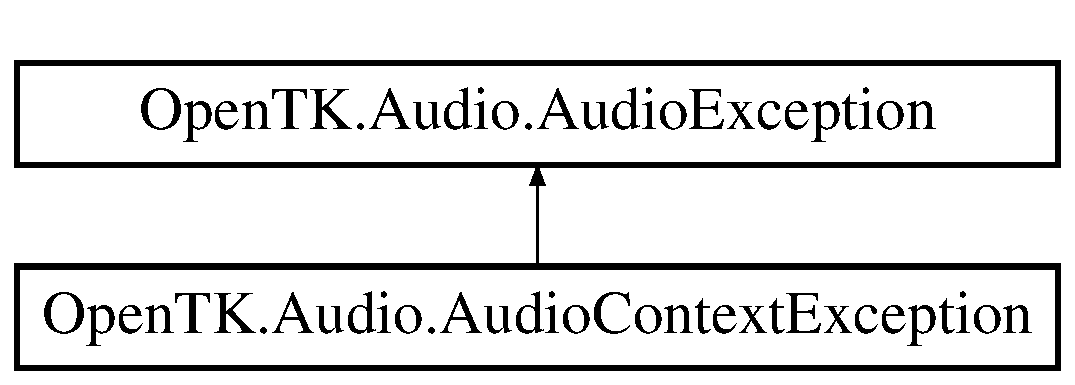
\includegraphics[height=2.000000cm]{class_open_t_k_1_1_audio_1_1_audio_context_exception}
\end{center}
\end{figure}
\subsection*{Public Member Functions}
\begin{DoxyCompactItemize}
\item 
\hyperlink{class_open_t_k_1_1_audio_1_1_audio_context_exception_a2d627aeabe43c853216f60d6c34fab22}{Audio\-Context\-Exception} ()
\begin{DoxyCompactList}\small\item\em Constructs a new \hyperlink{class_open_t_k_1_1_audio_1_1_audio_context_exception}{Audio\-Context\-Exception}.\end{DoxyCompactList}\item 
\hyperlink{class_open_t_k_1_1_audio_1_1_audio_context_exception_ac11738a462838289368ffecb977b978a}{Audio\-Context\-Exception} (string message)
\begin{DoxyCompactList}\small\item\em Constructs a new \hyperlink{class_open_t_k_1_1_audio_1_1_audio_context_exception}{Audio\-Context\-Exception} with the specified error message.\end{DoxyCompactList}\end{DoxyCompactItemize}


\subsection{Detailed Description}
Represents exceptions related to an \hyperlink{class_open_t_k_1_1_audio_1_1_audio_context}{Open\-T\-K.\-Audio.\-Audio\-Context}.



\subsection{Constructor \& Destructor Documentation}
\hypertarget{class_open_t_k_1_1_audio_1_1_audio_context_exception_a2d627aeabe43c853216f60d6c34fab22}{\index{Open\-T\-K\-::\-Audio\-::\-Audio\-Context\-Exception@{Open\-T\-K\-::\-Audio\-::\-Audio\-Context\-Exception}!Audio\-Context\-Exception@{Audio\-Context\-Exception}}
\index{Audio\-Context\-Exception@{Audio\-Context\-Exception}!OpenTK::Audio::AudioContextException@{Open\-T\-K\-::\-Audio\-::\-Audio\-Context\-Exception}}
\subsubsection[{Audio\-Context\-Exception}]{\setlength{\rightskip}{0pt plus 5cm}Open\-T\-K.\-Audio.\-Audio\-Context\-Exception.\-Audio\-Context\-Exception (
\begin{DoxyParamCaption}
{}
\end{DoxyParamCaption}
)}}\label{class_open_t_k_1_1_audio_1_1_audio_context_exception_a2d627aeabe43c853216f60d6c34fab22}


Constructs a new \hyperlink{class_open_t_k_1_1_audio_1_1_audio_context_exception}{Audio\-Context\-Exception}.

\hypertarget{class_open_t_k_1_1_audio_1_1_audio_context_exception_ac11738a462838289368ffecb977b978a}{\index{Open\-T\-K\-::\-Audio\-::\-Audio\-Context\-Exception@{Open\-T\-K\-::\-Audio\-::\-Audio\-Context\-Exception}!Audio\-Context\-Exception@{Audio\-Context\-Exception}}
\index{Audio\-Context\-Exception@{Audio\-Context\-Exception}!OpenTK::Audio::AudioContextException@{Open\-T\-K\-::\-Audio\-::\-Audio\-Context\-Exception}}
\subsubsection[{Audio\-Context\-Exception}]{\setlength{\rightskip}{0pt plus 5cm}Open\-T\-K.\-Audio.\-Audio\-Context\-Exception.\-Audio\-Context\-Exception (
\begin{DoxyParamCaption}
\item[{string}]{message}
\end{DoxyParamCaption}
)}}\label{class_open_t_k_1_1_audio_1_1_audio_context_exception_ac11738a462838289368ffecb977b978a}


Constructs a new \hyperlink{class_open_t_k_1_1_audio_1_1_audio_context_exception}{Audio\-Context\-Exception} with the specified error message.


\begin{DoxyParams}{Parameters}
{\em message} & The error message of the \hyperlink{class_open_t_k_1_1_audio_1_1_audio_context_exception}{Audio\-Context\-Exception}.\\
\hline
\end{DoxyParams}

\hypertarget{class_open_t_k_1_1_audio_1_1_audio_device_exception}{\section{Open\-T\-K.\-Audio.\-Audio\-Device\-Exception Class Reference}
\label{class_open_t_k_1_1_audio_1_1_audio_device_exception}\index{Open\-T\-K.\-Audio.\-Audio\-Device\-Exception@{Open\-T\-K.\-Audio.\-Audio\-Device\-Exception}}
}


Represents exceptions related to an \hyperlink{namespace_open_t_k_1_1_audio}{Open\-T\-K.\-Audio} device. 


Inheritance diagram for Open\-T\-K.\-Audio.\-Audio\-Device\-Exception\-:\begin{figure}[H]
\begin{center}
\leavevmode
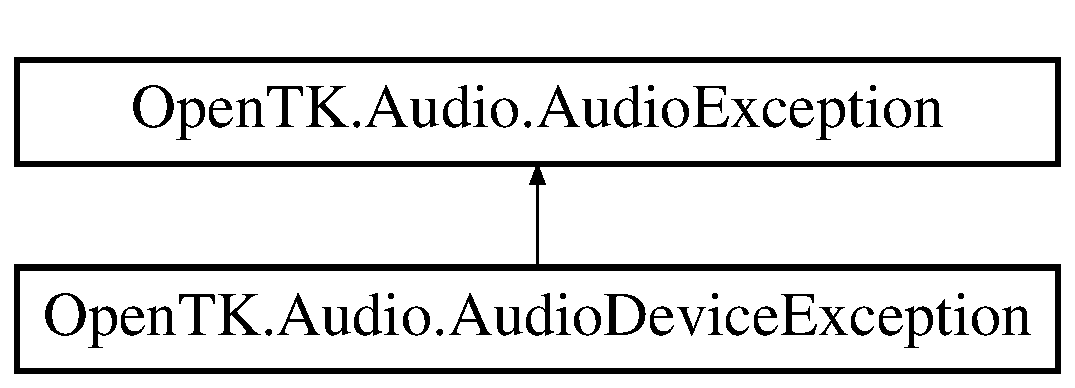
\includegraphics[height=2.000000cm]{class_open_t_k_1_1_audio_1_1_audio_device_exception}
\end{center}
\end{figure}
\subsection*{Public Member Functions}
\begin{DoxyCompactItemize}
\item 
\hyperlink{class_open_t_k_1_1_audio_1_1_audio_device_exception_a3108f56a974a448d2a45f494779aacd3}{Audio\-Device\-Exception} ()
\begin{DoxyCompactList}\small\item\em Constructs a new \hyperlink{class_open_t_k_1_1_audio_1_1_audio_device_exception}{Audio\-Device\-Exception}.\end{DoxyCompactList}\item 
\hyperlink{class_open_t_k_1_1_audio_1_1_audio_device_exception_a0ed11f11c381525471d1f5b4e93fab74}{Audio\-Device\-Exception} (string message)
\begin{DoxyCompactList}\small\item\em Constructs a new \hyperlink{class_open_t_k_1_1_audio_1_1_audio_device_exception}{Audio\-Device\-Exception} with the specified error message.\end{DoxyCompactList}\end{DoxyCompactItemize}


\subsection{Detailed Description}
Represents exceptions related to an \hyperlink{namespace_open_t_k_1_1_audio}{Open\-T\-K.\-Audio} device.



\subsection{Constructor \& Destructor Documentation}
\hypertarget{class_open_t_k_1_1_audio_1_1_audio_device_exception_a3108f56a974a448d2a45f494779aacd3}{\index{Open\-T\-K\-::\-Audio\-::\-Audio\-Device\-Exception@{Open\-T\-K\-::\-Audio\-::\-Audio\-Device\-Exception}!Audio\-Device\-Exception@{Audio\-Device\-Exception}}
\index{Audio\-Device\-Exception@{Audio\-Device\-Exception}!OpenTK::Audio::AudioDeviceException@{Open\-T\-K\-::\-Audio\-::\-Audio\-Device\-Exception}}
\subsubsection[{Audio\-Device\-Exception}]{\setlength{\rightskip}{0pt plus 5cm}Open\-T\-K.\-Audio.\-Audio\-Device\-Exception.\-Audio\-Device\-Exception (
\begin{DoxyParamCaption}
{}
\end{DoxyParamCaption}
)}}\label{class_open_t_k_1_1_audio_1_1_audio_device_exception_a3108f56a974a448d2a45f494779aacd3}


Constructs a new \hyperlink{class_open_t_k_1_1_audio_1_1_audio_device_exception}{Audio\-Device\-Exception}.

\hypertarget{class_open_t_k_1_1_audio_1_1_audio_device_exception_a0ed11f11c381525471d1f5b4e93fab74}{\index{Open\-T\-K\-::\-Audio\-::\-Audio\-Device\-Exception@{Open\-T\-K\-::\-Audio\-::\-Audio\-Device\-Exception}!Audio\-Device\-Exception@{Audio\-Device\-Exception}}
\index{Audio\-Device\-Exception@{Audio\-Device\-Exception}!OpenTK::Audio::AudioDeviceException@{Open\-T\-K\-::\-Audio\-::\-Audio\-Device\-Exception}}
\subsubsection[{Audio\-Device\-Exception}]{\setlength{\rightskip}{0pt plus 5cm}Open\-T\-K.\-Audio.\-Audio\-Device\-Exception.\-Audio\-Device\-Exception (
\begin{DoxyParamCaption}
\item[{string}]{message}
\end{DoxyParamCaption}
)}}\label{class_open_t_k_1_1_audio_1_1_audio_device_exception_a0ed11f11c381525471d1f5b4e93fab74}


Constructs a new \hyperlink{class_open_t_k_1_1_audio_1_1_audio_device_exception}{Audio\-Device\-Exception} with the specified error message.


\begin{DoxyParams}{Parameters}
{\em message} & The error message of the \hyperlink{class_open_t_k_1_1_audio_1_1_audio_device_exception}{Audio\-Device\-Exception}.\\
\hline
\end{DoxyParams}

\hypertarget{class_open_t_k_1_1_audio_1_1_audio_exception}{\section{Open\-T\-K.\-Audio.\-Audio\-Exception Class Reference}
\label{class_open_t_k_1_1_audio_1_1_audio_exception}\index{Open\-T\-K.\-Audio.\-Audio\-Exception@{Open\-T\-K.\-Audio.\-Audio\-Exception}}
}


Represents exceptions related to the \hyperlink{namespace_open_t_k_1_1_audio}{Open\-T\-K.\-Audio} subsystem. 


Inheritance diagram for Open\-T\-K.\-Audio.\-Audio\-Exception\-:\begin{figure}[H]
\begin{center}
\leavevmode
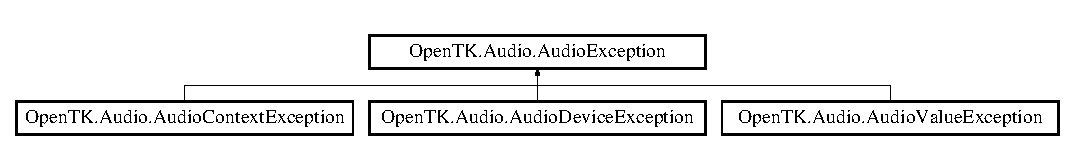
\includegraphics[height=1.575246cm]{class_open_t_k_1_1_audio_1_1_audio_exception}
\end{center}
\end{figure}
\subsection*{Public Member Functions}
\begin{DoxyCompactItemize}
\item 
\hyperlink{class_open_t_k_1_1_audio_1_1_audio_exception_a99d7015c904d6a3804df20a59b9c9212}{Audio\-Exception} ()
\begin{DoxyCompactList}\small\item\em Constructs a new \hyperlink{class_open_t_k_1_1_audio_1_1_audio_exception}{Audio\-Exception}.\end{DoxyCompactList}\item 
\hyperlink{class_open_t_k_1_1_audio_1_1_audio_exception_addad14cecea438cb905aa57736dd24ee}{Audio\-Exception} (string message)
\begin{DoxyCompactList}\small\item\em Constructs a new \hyperlink{class_open_t_k_1_1_audio_1_1_audio_exception}{Audio\-Exception} with the specified error message.\end{DoxyCompactList}\end{DoxyCompactItemize}


\subsection{Detailed Description}
Represents exceptions related to the \hyperlink{namespace_open_t_k_1_1_audio}{Open\-T\-K.\-Audio} subsystem.



\subsection{Constructor \& Destructor Documentation}
\hypertarget{class_open_t_k_1_1_audio_1_1_audio_exception_a99d7015c904d6a3804df20a59b9c9212}{\index{Open\-T\-K\-::\-Audio\-::\-Audio\-Exception@{Open\-T\-K\-::\-Audio\-::\-Audio\-Exception}!Audio\-Exception@{Audio\-Exception}}
\index{Audio\-Exception@{Audio\-Exception}!OpenTK::Audio::AudioException@{Open\-T\-K\-::\-Audio\-::\-Audio\-Exception}}
\subsubsection[{Audio\-Exception}]{\setlength{\rightskip}{0pt plus 5cm}Open\-T\-K.\-Audio.\-Audio\-Exception.\-Audio\-Exception (
\begin{DoxyParamCaption}
{}
\end{DoxyParamCaption}
)}}\label{class_open_t_k_1_1_audio_1_1_audio_exception_a99d7015c904d6a3804df20a59b9c9212}


Constructs a new \hyperlink{class_open_t_k_1_1_audio_1_1_audio_exception}{Audio\-Exception}.

\hypertarget{class_open_t_k_1_1_audio_1_1_audio_exception_addad14cecea438cb905aa57736dd24ee}{\index{Open\-T\-K\-::\-Audio\-::\-Audio\-Exception@{Open\-T\-K\-::\-Audio\-::\-Audio\-Exception}!Audio\-Exception@{Audio\-Exception}}
\index{Audio\-Exception@{Audio\-Exception}!OpenTK::Audio::AudioException@{Open\-T\-K\-::\-Audio\-::\-Audio\-Exception}}
\subsubsection[{Audio\-Exception}]{\setlength{\rightskip}{0pt plus 5cm}Open\-T\-K.\-Audio.\-Audio\-Exception.\-Audio\-Exception (
\begin{DoxyParamCaption}
\item[{string}]{message}
\end{DoxyParamCaption}
)}}\label{class_open_t_k_1_1_audio_1_1_audio_exception_addad14cecea438cb905aa57736dd24ee}


Constructs a new \hyperlink{class_open_t_k_1_1_audio_1_1_audio_exception}{Audio\-Exception} with the specified error message.


\begin{DoxyParams}{Parameters}
{\em message} & The error message of the \hyperlink{class_open_t_k_1_1_audio_1_1_audio_exception}{Audio\-Exception}.\\
\hline
\end{DoxyParams}

\hypertarget{class_open_t_k_1_1_audio_1_1_audio_value_exception}{\section{Open\-T\-K.\-Audio.\-Audio\-Value\-Exception Class Reference}
\label{class_open_t_k_1_1_audio_1_1_audio_value_exception}\index{Open\-T\-K.\-Audio.\-Audio\-Value\-Exception@{Open\-T\-K.\-Audio.\-Audio\-Value\-Exception}}
}


Represents exceptions related to invalid values. 


Inheritance diagram for Open\-T\-K.\-Audio.\-Audio\-Value\-Exception\-:\begin{figure}[H]
\begin{center}
\leavevmode
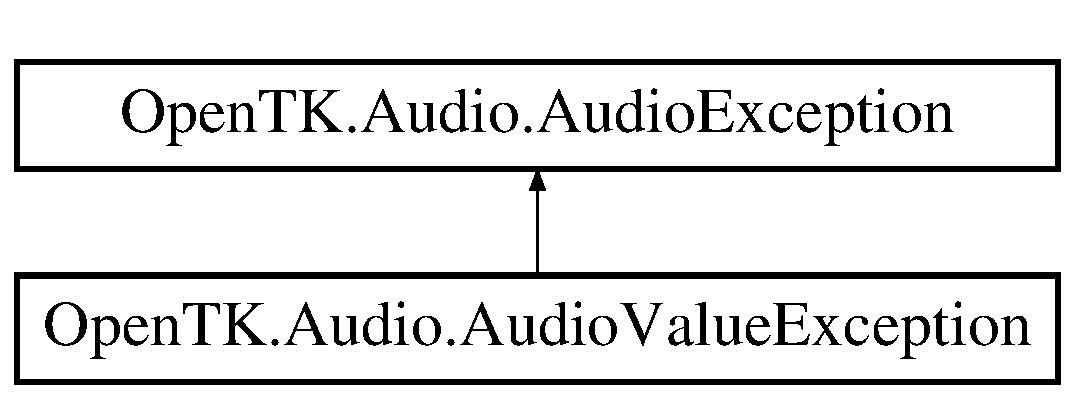
\includegraphics[height=2.000000cm]{class_open_t_k_1_1_audio_1_1_audio_value_exception}
\end{center}
\end{figure}
\subsection*{Public Member Functions}
\begin{DoxyCompactItemize}
\item 
\hyperlink{class_open_t_k_1_1_audio_1_1_audio_value_exception_a2d22569f928830f426f9bbefcc2def52}{Audio\-Value\-Exception} ()
\begin{DoxyCompactList}\small\item\em Constructs a new instance.\end{DoxyCompactList}\item 
\hyperlink{class_open_t_k_1_1_audio_1_1_audio_value_exception_a7543860824e3b373407dc85628184c37}{Audio\-Value\-Exception} (string message)
\begin{DoxyCompactList}\small\item\em Constructs a new instance with the specified error message.\end{DoxyCompactList}\end{DoxyCompactItemize}


\subsection{Detailed Description}
Represents exceptions related to invalid values.



\subsection{Constructor \& Destructor Documentation}
\hypertarget{class_open_t_k_1_1_audio_1_1_audio_value_exception_a2d22569f928830f426f9bbefcc2def52}{\index{Open\-T\-K\-::\-Audio\-::\-Audio\-Value\-Exception@{Open\-T\-K\-::\-Audio\-::\-Audio\-Value\-Exception}!Audio\-Value\-Exception@{Audio\-Value\-Exception}}
\index{Audio\-Value\-Exception@{Audio\-Value\-Exception}!OpenTK::Audio::AudioValueException@{Open\-T\-K\-::\-Audio\-::\-Audio\-Value\-Exception}}
\subsubsection[{Audio\-Value\-Exception}]{\setlength{\rightskip}{0pt plus 5cm}Open\-T\-K.\-Audio.\-Audio\-Value\-Exception.\-Audio\-Value\-Exception (
\begin{DoxyParamCaption}
{}
\end{DoxyParamCaption}
)}}\label{class_open_t_k_1_1_audio_1_1_audio_value_exception_a2d22569f928830f426f9bbefcc2def52}


Constructs a new instance.

\hypertarget{class_open_t_k_1_1_audio_1_1_audio_value_exception_a7543860824e3b373407dc85628184c37}{\index{Open\-T\-K\-::\-Audio\-::\-Audio\-Value\-Exception@{Open\-T\-K\-::\-Audio\-::\-Audio\-Value\-Exception}!Audio\-Value\-Exception@{Audio\-Value\-Exception}}
\index{Audio\-Value\-Exception@{Audio\-Value\-Exception}!OpenTK::Audio::AudioValueException@{Open\-T\-K\-::\-Audio\-::\-Audio\-Value\-Exception}}
\subsubsection[{Audio\-Value\-Exception}]{\setlength{\rightskip}{0pt plus 5cm}Open\-T\-K.\-Audio.\-Audio\-Value\-Exception.\-Audio\-Value\-Exception (
\begin{DoxyParamCaption}
\item[{string}]{message}
\end{DoxyParamCaption}
)}}\label{class_open_t_k_1_1_audio_1_1_audio_value_exception_a7543860824e3b373407dc85628184c37}


Constructs a new instance with the specified error message.


\begin{DoxyParams}{Parameters}
{\em message} & The error message of the \hyperlink{class_open_t_k_1_1_audio_1_1_audio_context_exception}{Audio\-Context\-Exception}.\\
\hline
\end{DoxyParams}

\hypertarget{class_open_t_k_1_1_audio_1_1_open_a_l_1_1_effects_extension}{\section{Open\-T\-K.\-Audio.\-Open\-A\-L.\-Effects\-Extension Class Reference}
\label{class_open_t_k_1_1_audio_1_1_open_a_l_1_1_effects_extension}\index{Open\-T\-K.\-Audio.\-Open\-A\-L.\-Effects\-Extension@{Open\-T\-K.\-Audio.\-Open\-A\-L.\-Effects\-Extension}}
}


Provides access to the \hyperlink{namespace_open_t_k_1_1_audio_1_1_open_a_l}{Open\-A\-L} effects extension.  


\subsection*{Public Member Functions}
\begin{DoxyCompactItemize}
\item 
void \hyperlink{class_open_t_k_1_1_audio_1_1_open_a_l_1_1_effects_extension_a51dbc9c91c556f374c9760c29675aff9}{Bind\-Effect} (uint eid, \hyperlink{namespace_open_t_k_1_1_audio_1_1_open_a_l_a224be2a7f650eba92828d53342bfbc30}{Efx\-Effect\-Type} type)
\begin{DoxyCompactList}\small\item\em (Helper) Selects the Effect type used by this Effect handle.\end{DoxyCompactList}\item 
void \hyperlink{class_open_t_k_1_1_audio_1_1_open_a_l_1_1_effects_extension_a60c86618c3c17d8e6363c791ff141e3e}{Bind\-Effect} (int eid, \hyperlink{namespace_open_t_k_1_1_audio_1_1_open_a_l_a224be2a7f650eba92828d53342bfbc30}{Efx\-Effect\-Type} type)
\begin{DoxyCompactList}\small\item\em (Helper) Selects the Effect type used by this Effect handle.\end{DoxyCompactList}\item 
void \hyperlink{class_open_t_k_1_1_audio_1_1_open_a_l_1_1_effects_extension_acea6e441f40da3cae17f60968cfb2640}{Bind\-Filter\-To\-Source} (uint source, uint filter)
\begin{DoxyCompactList}\small\item\em (Helper) reroutes the output of a Source through a Filter.\end{DoxyCompactList}\item 
void \hyperlink{class_open_t_k_1_1_audio_1_1_open_a_l_1_1_effects_extension_acceb9bfc2ded3608543a0e438cacd602}{Bind\-Filter\-To\-Source} (int source, int filter)
\begin{DoxyCompactList}\small\item\em (Helper) reroutes the output of a Source through a Filter.\end{DoxyCompactList}\item 
void \hyperlink{class_open_t_k_1_1_audio_1_1_open_a_l_1_1_effects_extension_a13cde333c8c4dc323cfaeaee3313f595}{Bind\-Effect\-To\-Auxiliary\-Slot} (uint auxiliaryeffectslot, uint effect)
\begin{DoxyCompactList}\small\item\em (Helper) Attaches an Effect to an Auxiliary Effect Slot.\end{DoxyCompactList}\item 
void \hyperlink{class_open_t_k_1_1_audio_1_1_open_a_l_1_1_effects_extension_ac14c1c8b6abfebe99d2a32f88c584c85}{Bind\-Effect\-To\-Auxiliary\-Slot} (int auxiliaryeffectslot, int effect)
\begin{DoxyCompactList}\small\item\em (Helper) Attaches an Effect to an Auxiliary Effect Slot.\end{DoxyCompactList}\item 
void \hyperlink{class_open_t_k_1_1_audio_1_1_open_a_l_1_1_effects_extension_a79643a7458e25042d781e8e31097312e}{Bind\-Source\-To\-Auxiliary\-Slot} (uint source, uint slot, int slotnumber, uint filter)
\begin{DoxyCompactList}\small\item\em (Helper) Reroutes a Source's output into an Auxiliary Effect Slot.\end{DoxyCompactList}\item 
void \hyperlink{class_open_t_k_1_1_audio_1_1_open_a_l_1_1_effects_extension_ad17503fb7238b5867fdd913f31656bc1}{Bind\-Source\-To\-Auxiliary\-Slot} (int source, int slot, int slotnumber, int filter)
\begin{DoxyCompactList}\small\item\em (Helper) Reroutes a Source's output into an Auxiliary Effect Slot.\end{DoxyCompactList}\item 
void \hyperlink{class_open_t_k_1_1_audio_1_1_open_a_l_1_1_effects_extension_a7b17c0ab357339d205be9f83e3840f31}{Gen\-Effects} (int n, out uint effects)
\begin{DoxyCompactList}\small\item\em The Gen\-Effects function is used to create one or more Effect objects. An Effect object stores an effect type and a set of parameter values to control that Effect. In order to use an Effect it must be attached to an Auxiliary Effect Slot object\end{DoxyCompactList}\item 
void \hyperlink{class_open_t_k_1_1_audio_1_1_open_a_l_1_1_effects_extension_aafb8f1e869a412b6bc8607d08f62fa8b}{Gen\-Effects} (int n, out int effects)
\begin{DoxyCompactList}\small\item\em The Gen\-Effects function is used to create one or more Effect objects. An Effect object stores an effect type and a set of parameter values to control that Effect. In order to use an Effect it must be attached to an Auxiliary Effect Slot object\end{DoxyCompactList}\item 
int\mbox{[}$\,$\mbox{]} \hyperlink{class_open_t_k_1_1_audio_1_1_open_a_l_1_1_effects_extension_a746c3add93703b718721d4ecb210c80a}{Gen\-Effects} (int n)
\begin{DoxyCompactList}\small\item\em Generates one or more effect objects.\end{DoxyCompactList}\item 
int \hyperlink{class_open_t_k_1_1_audio_1_1_open_a_l_1_1_effects_extension_aba577b14af247d69f95f6c859511549e}{Gen\-Effect} ()
\begin{DoxyCompactList}\small\item\em Generates a single effect object.\end{DoxyCompactList}\item 
void \hyperlink{class_open_t_k_1_1_audio_1_1_open_a_l_1_1_effects_extension_a48080e822c0b3d2e41c524d4535b22dd}{Gen\-Effect} (out uint effect)
\begin{DoxyCompactList}\small\item\em Generates a single effect object.\end{DoxyCompactList}\item 
void \hyperlink{class_open_t_k_1_1_audio_1_1_open_a_l_1_1_effects_extension_a25d3d56982cbd0fcab35dede97a6503f}{Delete\-Effects} (int n, ref uint effects)
\begin{DoxyCompactList}\small\item\em The Delete\-Effects function is used to delete and free resources for Effect objects previously created with Gen\-Effects.\end{DoxyCompactList}\item 
void \hyperlink{class_open_t_k_1_1_audio_1_1_open_a_l_1_1_effects_extension_a19699b0a2538db96da21ed41e160966a}{Delete\-Effects} (int n, ref int effects)
\begin{DoxyCompactList}\small\item\em The Delete\-Effects function is used to delete and free resources for Effect objects previously created with Gen\-Effects.\end{DoxyCompactList}\item 
void \hyperlink{class_open_t_k_1_1_audio_1_1_open_a_l_1_1_effects_extension_a9be846087b2d226614b94c10f41d021e}{Delete\-Effects} (int\mbox{[}$\,$\mbox{]} effects)
\begin{DoxyCompactList}\small\item\em The Delete\-Effects function is used to delete and free resources for Effect objects previously created with Gen\-Effects.\end{DoxyCompactList}\item 
void \hyperlink{class_open_t_k_1_1_audio_1_1_open_a_l_1_1_effects_extension_a26ae8a2e06f73c1d16c42db9aadb8b9a}{Delete\-Effects} (uint\mbox{[}$\,$\mbox{]} effects)
\begin{DoxyCompactList}\small\item\em The Delete\-Effects function is used to delete and free resources for Effect objects previously created with Gen\-Effects.\end{DoxyCompactList}\item 
void \hyperlink{class_open_t_k_1_1_audio_1_1_open_a_l_1_1_effects_extension_a5e73e7637657e34ad587b5a4421406a1}{Delete\-Effect} (int effect)
\begin{DoxyCompactList}\small\item\em This function deletes one Effect only.\end{DoxyCompactList}\item 
void \hyperlink{class_open_t_k_1_1_audio_1_1_open_a_l_1_1_effects_extension_a2e9b431a6a8ee248f15b8d5f91819612}{Delete\-Effect} (ref uint effect)
\begin{DoxyCompactList}\small\item\em This function deletes one Effect only.\end{DoxyCompactList}\item 
bool \hyperlink{class_open_t_k_1_1_audio_1_1_open_a_l_1_1_effects_extension_ab54a3c1793c8e9ae1950f25fa3bb9091}{Is\-Effect} (uint eid)
\begin{DoxyCompactList}\small\item\em The Is\-Effect function is used to determine if an object identifier is a valid Effect object.\end{DoxyCompactList}\item 
bool \hyperlink{class_open_t_k_1_1_audio_1_1_open_a_l_1_1_effects_extension_a05a58048724fb4aef1583123c82e8bdc}{Is\-Effect} (int eid)
\begin{DoxyCompactList}\small\item\em The Is\-Effect function is used to determine if an object identifier is a valid Effect object.\end{DoxyCompactList}\item 
void \hyperlink{class_open_t_k_1_1_audio_1_1_open_a_l_1_1_effects_extension_a8e948592b6a210d3d1fa94c05bc40def}{Effect} (uint eid, \hyperlink{namespace_open_t_k_1_1_audio_1_1_open_a_l_a49039c1ddcb53675576ad2780fc50315}{Efx\-Effecti} param, int value)
\begin{DoxyCompactList}\small\item\em This function is used to set integer properties on Effect objects.\end{DoxyCompactList}\item 
void \hyperlink{class_open_t_k_1_1_audio_1_1_open_a_l_1_1_effects_extension_abdafac8cff4580029c966016d961fc78}{Effect} (int eid, \hyperlink{namespace_open_t_k_1_1_audio_1_1_open_a_l_a49039c1ddcb53675576ad2780fc50315}{Efx\-Effecti} param, int value)
\begin{DoxyCompactList}\small\item\em This function is used to set integer properties on Effect objects.\end{DoxyCompactList}\item 
void \hyperlink{class_open_t_k_1_1_audio_1_1_open_a_l_1_1_effects_extension_a977a21cccce0607687124183aae8df37}{Effect} (uint eid, \hyperlink{namespace_open_t_k_1_1_audio_1_1_open_a_l_aa0356299908369b4365d28572c0ec20b}{Efx\-Effectf} param, float value)
\begin{DoxyCompactList}\small\item\em This function is used to set floating-\/point properties on Effect objects.\end{DoxyCompactList}\item 
void \hyperlink{class_open_t_k_1_1_audio_1_1_open_a_l_1_1_effects_extension_a87d6e1b2768acd65344d00b77c388b0c}{Effect} (int eid, \hyperlink{namespace_open_t_k_1_1_audio_1_1_open_a_l_aa0356299908369b4365d28572c0ec20b}{Efx\-Effectf} param, float value)
\begin{DoxyCompactList}\small\item\em This function is used to set floating-\/point properties on Effect objects.\end{DoxyCompactList}\item 
void \hyperlink{class_open_t_k_1_1_audio_1_1_open_a_l_1_1_effects_extension_ac876b068080042c1211133eddf148705}{Effect} (uint eid, \hyperlink{namespace_open_t_k_1_1_audio_1_1_open_a_l_a1c69083823578d237ab570da681a5cfa}{Efx\-Effect3f} param, ref \hyperlink{struct_open_t_k_1_1_vector3}{Vector3} values)
\begin{DoxyCompactList}\small\item\em This function is used to set 3 floating-\/point properties on Effect objects.\end{DoxyCompactList}\item 
void \hyperlink{class_open_t_k_1_1_audio_1_1_open_a_l_1_1_effects_extension_a8f3d27c67dbb8a6963c28024b05707ea}{Effect} (int eid, \hyperlink{namespace_open_t_k_1_1_audio_1_1_open_a_l_a1c69083823578d237ab570da681a5cfa}{Efx\-Effect3f} param, ref \hyperlink{struct_open_t_k_1_1_vector3}{Vector3} values)
\begin{DoxyCompactList}\small\item\em This function is used to set 3 floating-\/point properties on Effect objects.\end{DoxyCompactList}\item 
void \hyperlink{class_open_t_k_1_1_audio_1_1_open_a_l_1_1_effects_extension_a9d0473c4cd888a3343093ae5e1f56add}{Get\-Effect} (uint eid, \hyperlink{namespace_open_t_k_1_1_audio_1_1_open_a_l_a49039c1ddcb53675576ad2780fc50315}{Efx\-Effecti} pname, out int value)
\begin{DoxyCompactList}\small\item\em This function is used to retrieve integer properties from Effect objects.\end{DoxyCompactList}\item 
void \hyperlink{class_open_t_k_1_1_audio_1_1_open_a_l_1_1_effects_extension_a487bd82b5def2d9e0d5810c8fa30f679}{Get\-Effect} (int eid, \hyperlink{namespace_open_t_k_1_1_audio_1_1_open_a_l_a49039c1ddcb53675576ad2780fc50315}{Efx\-Effecti} pname, out int value)
\begin{DoxyCompactList}\small\item\em This function is used to retrieve integer properties from Effect objects.\end{DoxyCompactList}\item 
void \hyperlink{class_open_t_k_1_1_audio_1_1_open_a_l_1_1_effects_extension_ac845a4e2f1dc6d042257de118cc0097a}{Get\-Effect} (uint eid, \hyperlink{namespace_open_t_k_1_1_audio_1_1_open_a_l_aa0356299908369b4365d28572c0ec20b}{Efx\-Effectf} pname, out float value)
\begin{DoxyCompactList}\small\item\em This function is used to retrieve floating-\/point properties from Effect objects.\end{DoxyCompactList}\item 
void \hyperlink{class_open_t_k_1_1_audio_1_1_open_a_l_1_1_effects_extension_a0536002e3d38c36910e3a54a21eece9d}{Get\-Effect} (int eid, \hyperlink{namespace_open_t_k_1_1_audio_1_1_open_a_l_aa0356299908369b4365d28572c0ec20b}{Efx\-Effectf} pname, out float value)
\begin{DoxyCompactList}\small\item\em This function is used to retrieve floating-\/point properties from Effect objects.\end{DoxyCompactList}\item 
void \hyperlink{class_open_t_k_1_1_audio_1_1_open_a_l_1_1_effects_extension_a7ad13f496f7ad1cd9cb18d2eef43dcc2}{Get\-Effect} (uint eid, \hyperlink{namespace_open_t_k_1_1_audio_1_1_open_a_l_a1c69083823578d237ab570da681a5cfa}{Efx\-Effect3f} param, out \hyperlink{struct_open_t_k_1_1_vector3}{Vector3} values)
\begin{DoxyCompactList}\small\item\em This function is used to retrieve 3 floating-\/point properties from Effect objects.\end{DoxyCompactList}\item 
void \hyperlink{class_open_t_k_1_1_audio_1_1_open_a_l_1_1_effects_extension_af7fb4cfff41744c887c8d51e54a67701}{Get\-Effect} (int eid, \hyperlink{namespace_open_t_k_1_1_audio_1_1_open_a_l_a1c69083823578d237ab570da681a5cfa}{Efx\-Effect3f} param, out \hyperlink{struct_open_t_k_1_1_vector3}{Vector3} values)
\begin{DoxyCompactList}\small\item\em This function is used to retrieve 3 floating-\/point properties from Effect objects.\end{DoxyCompactList}\item 
void \hyperlink{class_open_t_k_1_1_audio_1_1_open_a_l_1_1_effects_extension_a8832b714b9376a7fe999a8afc589da40}{Gen\-Filters} (int n, out uint filters)
\begin{DoxyCompactList}\small\item\em The Gen\-Filters function is used to create one or more Filter objects. A Filter object stores a filter type and a set of parameter values to control that Filter. Filter objects can be attached to Sources as Direct Filters or Auxiliary Send Filters.\end{DoxyCompactList}\item 
void \hyperlink{class_open_t_k_1_1_audio_1_1_open_a_l_1_1_effects_extension_aded82d26f8ff57e712c6b7b068ae1e4f}{Gen\-Filters} (int n, out int filters)
\begin{DoxyCompactList}\small\item\em The Gen\-Filters function is used to create one or more Filter objects. A Filter object stores a filter type and a set of parameter values to control that Filter. Filter objects can be attached to Sources as Direct Filters or Auxiliary Send Filters.\end{DoxyCompactList}\item 
int\mbox{[}$\,$\mbox{]} \hyperlink{class_open_t_k_1_1_audio_1_1_open_a_l_1_1_effects_extension_a2b3c9e2f60f937096dc8c85d4e6e5e43}{Gen\-Filters} (int n)
\begin{DoxyCompactList}\small\item\em The Gen\-Filters function is used to create one or more Filter objects. A Filter object stores a filter type and a set of parameter values to control that Filter. Filter objects can be attached to Sources as Direct Filters or Auxiliary Send Filters.\end{DoxyCompactList}\item 
int \hyperlink{class_open_t_k_1_1_audio_1_1_open_a_l_1_1_effects_extension_a5c3fc6ea5916498d8590a5db9f3f85d9}{Gen\-Filter} ()
\begin{DoxyCompactList}\small\item\em This function generates only one Filter.\end{DoxyCompactList}\item 
unsafe void \hyperlink{class_open_t_k_1_1_audio_1_1_open_a_l_1_1_effects_extension_a82b70f934c938398c417419b9982fe7b}{Gen\-Filter} (out uint filter)
\begin{DoxyCompactList}\small\item\em This function generates only one Filter.\end{DoxyCompactList}\item 
void \hyperlink{class_open_t_k_1_1_audio_1_1_open_a_l_1_1_effects_extension_ad4e48a24fe5c4f31895114bb04dd5d0b}{Delete\-Filters} (int n, ref uint filters)
\begin{DoxyCompactList}\small\item\em The Delete\-Filters function is used to delete and free resources for Filter objects previously created with Gen\-Filters.\end{DoxyCompactList}\item 
void \hyperlink{class_open_t_k_1_1_audio_1_1_open_a_l_1_1_effects_extension_a24505350970276bc214dfc089ca6b7d3}{Delete\-Filters} (int n, ref int filters)
\begin{DoxyCompactList}\small\item\em The Delete\-Filters function is used to delete and free resources for Filter objects previously created with Gen\-Filters.\end{DoxyCompactList}\item 
void \hyperlink{class_open_t_k_1_1_audio_1_1_open_a_l_1_1_effects_extension_a60a4a879c356dab286f6325dc2084729}{Delete\-Filters} (uint\mbox{[}$\,$\mbox{]} filters)
\begin{DoxyCompactList}\small\item\em This function deletes one Filter only.\end{DoxyCompactList}\item 
void \hyperlink{class_open_t_k_1_1_audio_1_1_open_a_l_1_1_effects_extension_a6e64ebb2c6fd75b4acfde4653ea9528b}{Delete\-Filters} (int\mbox{[}$\,$\mbox{]} filters)
\begin{DoxyCompactList}\small\item\em This function deletes one Filter only.\end{DoxyCompactList}\item 
void \hyperlink{class_open_t_k_1_1_audio_1_1_open_a_l_1_1_effects_extension_afcbbe986b53d7b60fe2c7815dd0d1797}{Delete\-Filter} (int filter)
\begin{DoxyCompactList}\small\item\em This function deletes one Filter only.\end{DoxyCompactList}\item 
void \hyperlink{class_open_t_k_1_1_audio_1_1_open_a_l_1_1_effects_extension_adcfd0f6ed1749a83543a067510dd3b7f}{Delete\-Filter} (ref uint filter)
\begin{DoxyCompactList}\small\item\em This function deletes one Filter only.\end{DoxyCompactList}\item 
bool \hyperlink{class_open_t_k_1_1_audio_1_1_open_a_l_1_1_effects_extension_a5e672010e215b7cef6ccf2a23a3d51a6}{Is\-Filter} (uint fid)
\begin{DoxyCompactList}\small\item\em The Is\-Filter function is used to determine if an object identifier is a valid Filter object.\end{DoxyCompactList}\item 
bool \hyperlink{class_open_t_k_1_1_audio_1_1_open_a_l_1_1_effects_extension_a0e7a55945fd9094fc149d73100ff46bb}{Is\-Filter} (int fid)
\begin{DoxyCompactList}\small\item\em The Is\-Filter function is used to determine if an object identifier is a valid Filter object.\end{DoxyCompactList}\item 
void \hyperlink{class_open_t_k_1_1_audio_1_1_open_a_l_1_1_effects_extension_a7b6cd1c3578195469ec829566afc104f}{Filter} (uint fid, \hyperlink{namespace_open_t_k_1_1_audio_1_1_open_a_l_a071c0527689a9645ced24caee8e0f542}{Efx\-Filteri} param, int value)
\begin{DoxyCompactList}\small\item\em This function is used to set integer properties on Filter objects.\end{DoxyCompactList}\item 
void \hyperlink{class_open_t_k_1_1_audio_1_1_open_a_l_1_1_effects_extension_a399ccfd829426685d54adfe12a2e1def}{Filter} (int fid, \hyperlink{namespace_open_t_k_1_1_audio_1_1_open_a_l_a071c0527689a9645ced24caee8e0f542}{Efx\-Filteri} param, int value)
\begin{DoxyCompactList}\small\item\em This function is used to set integer properties on Filter objects.\end{DoxyCompactList}\item 
void \hyperlink{class_open_t_k_1_1_audio_1_1_open_a_l_1_1_effects_extension_ac925fabeba566c7497ba28b8db5c86ac}{Filter} (uint fid, \hyperlink{namespace_open_t_k_1_1_audio_1_1_open_a_l_a6a389aa5e465025fe4eb3fba1603fd6b}{Efx\-Filterf} param, float value)
\begin{DoxyCompactList}\small\item\em This function is used to set floating-\/point properties on Filter objects.\end{DoxyCompactList}\item 
void \hyperlink{class_open_t_k_1_1_audio_1_1_open_a_l_1_1_effects_extension_ad3386bcd4e31173f058b44c73a08ae99}{Filter} (int fid, \hyperlink{namespace_open_t_k_1_1_audio_1_1_open_a_l_a6a389aa5e465025fe4eb3fba1603fd6b}{Efx\-Filterf} param, float value)
\begin{DoxyCompactList}\small\item\em This function is used to set floating-\/point properties on Filter objects.\end{DoxyCompactList}\item 
void \hyperlink{class_open_t_k_1_1_audio_1_1_open_a_l_1_1_effects_extension_a35d8cc9ccd8b34f5cf52a74203456fdb}{Get\-Filter} (uint fid, \hyperlink{namespace_open_t_k_1_1_audio_1_1_open_a_l_a071c0527689a9645ced24caee8e0f542}{Efx\-Filteri} pname, out int value)
\begin{DoxyCompactList}\small\item\em This function is used to retrieve integer properties from Filter objects.\end{DoxyCompactList}\item 
void \hyperlink{class_open_t_k_1_1_audio_1_1_open_a_l_1_1_effects_extension_a5a91a48507abf811dcf3b3c8ce7b45bc}{Get\-Filter} (int fid, \hyperlink{namespace_open_t_k_1_1_audio_1_1_open_a_l_a071c0527689a9645ced24caee8e0f542}{Efx\-Filteri} pname, out int value)
\begin{DoxyCompactList}\small\item\em This function is used to retrieve integer properties from Filter objects.\end{DoxyCompactList}\item 
void \hyperlink{class_open_t_k_1_1_audio_1_1_open_a_l_1_1_effects_extension_af07e454cc706218448e219c90529b659}{Get\-Filter} (uint fid, \hyperlink{namespace_open_t_k_1_1_audio_1_1_open_a_l_a6a389aa5e465025fe4eb3fba1603fd6b}{Efx\-Filterf} pname, out float value)
\begin{DoxyCompactList}\small\item\em This function is used to retrieve floating-\/point properties from Filter objects.\end{DoxyCompactList}\item 
void \hyperlink{class_open_t_k_1_1_audio_1_1_open_a_l_1_1_effects_extension_a5ef9cded2ef47728599dd2e748a81c67}{Get\-Filter} (int fid, \hyperlink{namespace_open_t_k_1_1_audio_1_1_open_a_l_a6a389aa5e465025fe4eb3fba1603fd6b}{Efx\-Filterf} pname, out float value)
\begin{DoxyCompactList}\small\item\em This function is used to retrieve floating-\/point properties from Filter objects.\end{DoxyCompactList}\item 
void \hyperlink{class_open_t_k_1_1_audio_1_1_open_a_l_1_1_effects_extension_af443312a2d154ede7f865e8cd765d797}{Gen\-Auxiliary\-Effect\-Slots} (int n, out uint slots)
\begin{DoxyCompactList}\small\item\em The Gen\-Auxiliary\-Effect\-Slots function is used to create one or more Auxiliary Effect Slots. The number of slots that can be created will be dependant upon the Open A\-L device used.\end{DoxyCompactList}\item 
void \hyperlink{class_open_t_k_1_1_audio_1_1_open_a_l_1_1_effects_extension_a5d2ee7f74d4228bbf10c92f61c97f869}{Gen\-Auxiliary\-Effect\-Slots} (int n, out int slots)
\begin{DoxyCompactList}\small\item\em The Gen\-Auxiliary\-Effect\-Slots function is used to create one or more Auxiliary Effect Slots. The number of slots that can be created will be dependant upon the Open A\-L device used.\end{DoxyCompactList}\item 
int\mbox{[}$\,$\mbox{]} \hyperlink{class_open_t_k_1_1_audio_1_1_open_a_l_1_1_effects_extension_a0ec3a249a109ba80461d8fb71072de71}{Gen\-Auxiliary\-Effect\-Slots} (int n)
\begin{DoxyCompactList}\small\item\em The Gen\-Auxiliary\-Effect\-Slots function is used to create one or more Auxiliary Effect Slots. The number of slots that can be created will be dependant upon the Open A\-L device used.\end{DoxyCompactList}\item 
int \hyperlink{class_open_t_k_1_1_audio_1_1_open_a_l_1_1_effects_extension_afbbb3f2126518c17bc067ee922021245}{Gen\-Auxiliary\-Effect\-Slot} ()
\begin{DoxyCompactList}\small\item\em This function generates only one Auxiliary Effect Slot.\end{DoxyCompactList}\item 
void \hyperlink{class_open_t_k_1_1_audio_1_1_open_a_l_1_1_effects_extension_a24c835355ade23ba84783d3635692657}{Gen\-Auxiliary\-Effect\-Slot} (out uint slot)
\begin{DoxyCompactList}\small\item\em This function generates only one Auxiliary Effect Slot.\end{DoxyCompactList}\item 
void \hyperlink{class_open_t_k_1_1_audio_1_1_open_a_l_1_1_effects_extension_a0d1cd18f9849786ed616c1e5d6b5f9d1}{Delete\-Auxiliary\-Effect\-Slots} (int n, ref uint slots)
\begin{DoxyCompactList}\small\item\em The Delete\-Auxiliary\-Effect\-Slots function is used to delete and free resources for Auxiliary Effect Slots previously created with Gen\-Auxiliary\-Effect\-Slots.\end{DoxyCompactList}\item 
void \hyperlink{class_open_t_k_1_1_audio_1_1_open_a_l_1_1_effects_extension_a95e2e236996c0bba5ec3ba121a86fb96}{Delete\-Auxiliary\-Effect\-Slots} (int n, ref int slots)
\begin{DoxyCompactList}\small\item\em The Delete\-Auxiliary\-Effect\-Slots function is used to delete and free resources for Auxiliary Effect Slots previously created with Gen\-Auxiliary\-Effect\-Slots.\end{DoxyCompactList}\item 
void \hyperlink{class_open_t_k_1_1_audio_1_1_open_a_l_1_1_effects_extension_a3e5c95d28a8e1b9d6f41e7338a9d9c20}{Delete\-Auxiliary\-Effect\-Slots} (int\mbox{[}$\,$\mbox{]} slots)
\begin{DoxyCompactList}\small\item\em The Delete\-Auxiliary\-Effect\-Slots function is used to delete and free resources for Auxiliary Effect Slots previously created with Gen\-Auxiliary\-Effect\-Slots.\end{DoxyCompactList}\item 
void \hyperlink{class_open_t_k_1_1_audio_1_1_open_a_l_1_1_effects_extension_a32eada847b7327635c6811f398550678}{Delete\-Auxiliary\-Effect\-Slots} (uint\mbox{[}$\,$\mbox{]} slots)
\begin{DoxyCompactList}\small\item\em This function deletes one Auxiliary\-Effect\-Slot only.\end{DoxyCompactList}\item 
void \hyperlink{class_open_t_k_1_1_audio_1_1_open_a_l_1_1_effects_extension_a186a9280ce62e17b093268c3ee63553d}{Delete\-Auxiliary\-Effect\-Slot} (int slot)
\begin{DoxyCompactList}\small\item\em This function deletes one Auxiliary\-Effect\-Slot only.\end{DoxyCompactList}\item 
void \hyperlink{class_open_t_k_1_1_audio_1_1_open_a_l_1_1_effects_extension_a5abbcc03f381d5af6d8c0efc0eaec7d7}{Delete\-Auxiliary\-Effect\-Slot} (ref uint slot)
\begin{DoxyCompactList}\small\item\em This function deletes one Auxiliary\-Effect\-Slot only.\end{DoxyCompactList}\item 
bool \hyperlink{class_open_t_k_1_1_audio_1_1_open_a_l_1_1_effects_extension_a8682814f4f44ada674cb33a708a7020b}{Is\-Auxiliary\-Effect\-Slot} (uint slot)
\begin{DoxyCompactList}\small\item\em The Is\-Auxiliary\-Effect\-Slot function is used to determine if an object identifier is a valid Auxiliary Effect Slot object.\end{DoxyCompactList}\item 
bool \hyperlink{class_open_t_k_1_1_audio_1_1_open_a_l_1_1_effects_extension_ab15f348b6c2d0b171608a43849dddc24}{Is\-Auxiliary\-Effect\-Slot} (int slot)
\begin{DoxyCompactList}\small\item\em The Is\-Auxiliary\-Effect\-Slot function is used to determine if an object identifier is a valid Auxiliary Effect Slot object.\end{DoxyCompactList}\item 
void \hyperlink{class_open_t_k_1_1_audio_1_1_open_a_l_1_1_effects_extension_a3776963058c5c8e9dbaf29a7ded228ac}{Auxiliary\-Effect\-Slot} (uint asid, \hyperlink{namespace_open_t_k_1_1_audio_1_1_open_a_l_a94243a598006983d92449b374a5b60cc}{Efx\-Auxiliaryi} param, int value)
\begin{DoxyCompactList}\small\item\em This function is used to set integer properties on Auxiliary Effect Slot objects.\end{DoxyCompactList}\item 
void \hyperlink{class_open_t_k_1_1_audio_1_1_open_a_l_1_1_effects_extension_a02f757a149bd9e8ee56087ad884d2b12}{Auxiliary\-Effect\-Slot} (int asid, \hyperlink{namespace_open_t_k_1_1_audio_1_1_open_a_l_a94243a598006983d92449b374a5b60cc}{Efx\-Auxiliaryi} param, int value)
\begin{DoxyCompactList}\small\item\em This function is used to set integer properties on Auxiliary Effect Slot objects.\end{DoxyCompactList}\item 
void \hyperlink{class_open_t_k_1_1_audio_1_1_open_a_l_1_1_effects_extension_acb92406a943db3db93148e5473838d1c}{Auxiliary\-Effect\-Slot} (uint asid, \hyperlink{namespace_open_t_k_1_1_audio_1_1_open_a_l_ad4eb76e6214aa11619cd342b8ab6acbd}{Efx\-Auxiliaryf} param, float value)
\begin{DoxyCompactList}\small\item\em This function is used to set floating-\/point properties on Auxiliary Effect Slot objects.\end{DoxyCompactList}\item 
void \hyperlink{class_open_t_k_1_1_audio_1_1_open_a_l_1_1_effects_extension_ad5a5e5a6157209de8bed4682de7fd9a2}{Auxiliary\-Effect\-Slot} (int asid, \hyperlink{namespace_open_t_k_1_1_audio_1_1_open_a_l_ad4eb76e6214aa11619cd342b8ab6acbd}{Efx\-Auxiliaryf} param, float value)
\begin{DoxyCompactList}\small\item\em This function is used to set floating-\/point properties on Auxiliary Effect Slot objects.\end{DoxyCompactList}\item 
void \hyperlink{class_open_t_k_1_1_audio_1_1_open_a_l_1_1_effects_extension_ab2a55e2efd22acdee604fdc52fc36ff9}{Get\-Auxiliary\-Effect\-Slot} (uint asid, \hyperlink{namespace_open_t_k_1_1_audio_1_1_open_a_l_a94243a598006983d92449b374a5b60cc}{Efx\-Auxiliaryi} pname, out int value)
\begin{DoxyCompactList}\small\item\em This function is used to retrieve integer properties on Auxiliary Effect Slot objects.\end{DoxyCompactList}\item 
void \hyperlink{class_open_t_k_1_1_audio_1_1_open_a_l_1_1_effects_extension_a0689a310d5097e82e4cb368c73d255e3}{Get\-Auxiliary\-Effect\-Slot} (int asid, \hyperlink{namespace_open_t_k_1_1_audio_1_1_open_a_l_a94243a598006983d92449b374a5b60cc}{Efx\-Auxiliaryi} pname, out int value)
\begin{DoxyCompactList}\small\item\em This function is used to retrieve integer properties on Auxiliary Effect Slot objects.\end{DoxyCompactList}\item 
void \hyperlink{class_open_t_k_1_1_audio_1_1_open_a_l_1_1_effects_extension_a79da0470f0f7b2bf6eaaea3619c0f41c}{Get\-Auxiliary\-Effect\-Slot} (uint asid, \hyperlink{namespace_open_t_k_1_1_audio_1_1_open_a_l_ad4eb76e6214aa11619cd342b8ab6acbd}{Efx\-Auxiliaryf} pname, out float value)
\begin{DoxyCompactList}\small\item\em This function is used to retrieve floating properties on Auxiliary Effect Slot objects.\end{DoxyCompactList}\item 
void \hyperlink{class_open_t_k_1_1_audio_1_1_open_a_l_1_1_effects_extension_a5f6f92274a592df0ea8ab4dfd3780c37}{Get\-Auxiliary\-Effect\-Slot} (int asid, \hyperlink{namespace_open_t_k_1_1_audio_1_1_open_a_l_ad4eb76e6214aa11619cd342b8ab6acbd}{Efx\-Auxiliaryf} pname, out float value)
\begin{DoxyCompactList}\small\item\em This function is used to retrieve floating properties on Auxiliary Effect Slot objects.\end{DoxyCompactList}\item 
\hyperlink{class_open_t_k_1_1_audio_1_1_open_a_l_1_1_effects_extension_a1923f40f555058b0e102711601559731}{Effects\-Extension} ()
\begin{DoxyCompactList}\small\item\em Constructs a new \hyperlink{class_open_t_k_1_1_audio_1_1_open_a_l_1_1_effects_extension}{Effects\-Extension} instance. \end{DoxyCompactList}\end{DoxyCompactItemize}
\subsection*{Static Public Member Functions}
\begin{DoxyCompactItemize}
\item 
\hypertarget{class_open_t_k_1_1_audio_1_1_open_a_l_1_1_effects_extension_a0b335b4f0da12f920bf9cdd6f17a3df5}{static void {\bfseries Get\-Eax\-From\-Efx\-Eax} (ref Eax\-Reverb input, out Efx\-Eax\-Reverb output)}\label{class_open_t_k_1_1_audio_1_1_open_a_l_1_1_effects_extension_a0b335b4f0da12f920bf9cdd6f17a3df5}

\end{DoxyCompactItemize}
\subsection*{Properties}
\begin{DoxyCompactItemize}
\item 
bool \hyperlink{class_open_t_k_1_1_audio_1_1_open_a_l_1_1_effects_extension_a760975f853f917b2e4bcec05ffa73cca}{Is\-Initialized}\hspace{0.3cm}{\ttfamily  \mbox{[}get\mbox{]}}
\begin{DoxyCompactList}\small\item\em Returns True if the E\-F\-X Extension has been found and could be initialized.\end{DoxyCompactList}\end{DoxyCompactItemize}


\subsection{Detailed Description}
Provides access to the \hyperlink{namespace_open_t_k_1_1_audio_1_1_open_a_l}{Open\-A\-L} effects extension. 



\subsection{Constructor \& Destructor Documentation}
\hypertarget{class_open_t_k_1_1_audio_1_1_open_a_l_1_1_effects_extension_a1923f40f555058b0e102711601559731}{\index{Open\-T\-K\-::\-Audio\-::\-Open\-A\-L\-::\-Effects\-Extension@{Open\-T\-K\-::\-Audio\-::\-Open\-A\-L\-::\-Effects\-Extension}!Effects\-Extension@{Effects\-Extension}}
\index{Effects\-Extension@{Effects\-Extension}!OpenTK::Audio::OpenAL::EffectsExtension@{Open\-T\-K\-::\-Audio\-::\-Open\-A\-L\-::\-Effects\-Extension}}
\subsubsection[{Effects\-Extension}]{\setlength{\rightskip}{0pt plus 5cm}Open\-T\-K.\-Audio.\-Open\-A\-L.\-Effects\-Extension.\-Effects\-Extension (
\begin{DoxyParamCaption}
{}
\end{DoxyParamCaption}
)}}\label{class_open_t_k_1_1_audio_1_1_open_a_l_1_1_effects_extension_a1923f40f555058b0e102711601559731}


Constructs a new \hyperlink{class_open_t_k_1_1_audio_1_1_open_a_l_1_1_effects_extension}{Effects\-Extension} instance. 



\subsection{Member Function Documentation}
\hypertarget{class_open_t_k_1_1_audio_1_1_open_a_l_1_1_effects_extension_a3776963058c5c8e9dbaf29a7ded228ac}{\index{Open\-T\-K\-::\-Audio\-::\-Open\-A\-L\-::\-Effects\-Extension@{Open\-T\-K\-::\-Audio\-::\-Open\-A\-L\-::\-Effects\-Extension}!Auxiliary\-Effect\-Slot@{Auxiliary\-Effect\-Slot}}
\index{Auxiliary\-Effect\-Slot@{Auxiliary\-Effect\-Slot}!OpenTK::Audio::OpenAL::EffectsExtension@{Open\-T\-K\-::\-Audio\-::\-Open\-A\-L\-::\-Effects\-Extension}}
\subsubsection[{Auxiliary\-Effect\-Slot}]{\setlength{\rightskip}{0pt plus 5cm}void Open\-T\-K.\-Audio.\-Open\-A\-L.\-Effects\-Extension.\-Auxiliary\-Effect\-Slot (
\begin{DoxyParamCaption}
\item[{uint}]{asid, }
\item[{{\bf Efx\-Auxiliaryi}}]{param, }
\item[{int}]{value}
\end{DoxyParamCaption}
)}}\label{class_open_t_k_1_1_audio_1_1_open_a_l_1_1_effects_extension_a3776963058c5c8e9dbaf29a7ded228ac}


This function is used to set integer properties on Auxiliary Effect Slot objects.


\begin{DoxyParams}{Parameters}
{\em asid} & Auxiliary Effect Slot object identifier.\\
\hline
{\em param} & Auxiliary Effect Slot property to set.\\
\hline
{\em value} & Integer value.\\
\hline
\end{DoxyParams}
\hypertarget{class_open_t_k_1_1_audio_1_1_open_a_l_1_1_effects_extension_a02f757a149bd9e8ee56087ad884d2b12}{\index{Open\-T\-K\-::\-Audio\-::\-Open\-A\-L\-::\-Effects\-Extension@{Open\-T\-K\-::\-Audio\-::\-Open\-A\-L\-::\-Effects\-Extension}!Auxiliary\-Effect\-Slot@{Auxiliary\-Effect\-Slot}}
\index{Auxiliary\-Effect\-Slot@{Auxiliary\-Effect\-Slot}!OpenTK::Audio::OpenAL::EffectsExtension@{Open\-T\-K\-::\-Audio\-::\-Open\-A\-L\-::\-Effects\-Extension}}
\subsubsection[{Auxiliary\-Effect\-Slot}]{\setlength{\rightskip}{0pt plus 5cm}void Open\-T\-K.\-Audio.\-Open\-A\-L.\-Effects\-Extension.\-Auxiliary\-Effect\-Slot (
\begin{DoxyParamCaption}
\item[{int}]{asid, }
\item[{{\bf Efx\-Auxiliaryi}}]{param, }
\item[{int}]{value}
\end{DoxyParamCaption}
)}}\label{class_open_t_k_1_1_audio_1_1_open_a_l_1_1_effects_extension_a02f757a149bd9e8ee56087ad884d2b12}


This function is used to set integer properties on Auxiliary Effect Slot objects.


\begin{DoxyParams}{Parameters}
{\em asid} & Auxiliary Effect Slot object identifier.\\
\hline
{\em param} & Auxiliary Effect Slot property to set.\\
\hline
{\em value} & Integer value.\\
\hline
\end{DoxyParams}
\hypertarget{class_open_t_k_1_1_audio_1_1_open_a_l_1_1_effects_extension_acb92406a943db3db93148e5473838d1c}{\index{Open\-T\-K\-::\-Audio\-::\-Open\-A\-L\-::\-Effects\-Extension@{Open\-T\-K\-::\-Audio\-::\-Open\-A\-L\-::\-Effects\-Extension}!Auxiliary\-Effect\-Slot@{Auxiliary\-Effect\-Slot}}
\index{Auxiliary\-Effect\-Slot@{Auxiliary\-Effect\-Slot}!OpenTK::Audio::OpenAL::EffectsExtension@{Open\-T\-K\-::\-Audio\-::\-Open\-A\-L\-::\-Effects\-Extension}}
\subsubsection[{Auxiliary\-Effect\-Slot}]{\setlength{\rightskip}{0pt plus 5cm}void Open\-T\-K.\-Audio.\-Open\-A\-L.\-Effects\-Extension.\-Auxiliary\-Effect\-Slot (
\begin{DoxyParamCaption}
\item[{uint}]{asid, }
\item[{{\bf Efx\-Auxiliaryf}}]{param, }
\item[{float}]{value}
\end{DoxyParamCaption}
)}}\label{class_open_t_k_1_1_audio_1_1_open_a_l_1_1_effects_extension_acb92406a943db3db93148e5473838d1c}


This function is used to set floating-\/point properties on Auxiliary Effect Slot objects.


\begin{DoxyParams}{Parameters}
{\em asid} & Auxiliary Effect Slot object identifier.\\
\hline
{\em param} & Auxiliary Effect Slot property to set.\\
\hline
{\em value} & Floating-\/point value.\\
\hline
\end{DoxyParams}
\hypertarget{class_open_t_k_1_1_audio_1_1_open_a_l_1_1_effects_extension_ad5a5e5a6157209de8bed4682de7fd9a2}{\index{Open\-T\-K\-::\-Audio\-::\-Open\-A\-L\-::\-Effects\-Extension@{Open\-T\-K\-::\-Audio\-::\-Open\-A\-L\-::\-Effects\-Extension}!Auxiliary\-Effect\-Slot@{Auxiliary\-Effect\-Slot}}
\index{Auxiliary\-Effect\-Slot@{Auxiliary\-Effect\-Slot}!OpenTK::Audio::OpenAL::EffectsExtension@{Open\-T\-K\-::\-Audio\-::\-Open\-A\-L\-::\-Effects\-Extension}}
\subsubsection[{Auxiliary\-Effect\-Slot}]{\setlength{\rightskip}{0pt plus 5cm}void Open\-T\-K.\-Audio.\-Open\-A\-L.\-Effects\-Extension.\-Auxiliary\-Effect\-Slot (
\begin{DoxyParamCaption}
\item[{int}]{asid, }
\item[{{\bf Efx\-Auxiliaryf}}]{param, }
\item[{float}]{value}
\end{DoxyParamCaption}
)}}\label{class_open_t_k_1_1_audio_1_1_open_a_l_1_1_effects_extension_ad5a5e5a6157209de8bed4682de7fd9a2}


This function is used to set floating-\/point properties on Auxiliary Effect Slot objects.


\begin{DoxyParams}{Parameters}
{\em asid} & Auxiliary Effect Slot object identifier.\\
\hline
{\em param} & Auxiliary Effect Slot property to set.\\
\hline
{\em value} & Floating-\/point value.\\
\hline
\end{DoxyParams}
\hypertarget{class_open_t_k_1_1_audio_1_1_open_a_l_1_1_effects_extension_a51dbc9c91c556f374c9760c29675aff9}{\index{Open\-T\-K\-::\-Audio\-::\-Open\-A\-L\-::\-Effects\-Extension@{Open\-T\-K\-::\-Audio\-::\-Open\-A\-L\-::\-Effects\-Extension}!Bind\-Effect@{Bind\-Effect}}
\index{Bind\-Effect@{Bind\-Effect}!OpenTK::Audio::OpenAL::EffectsExtension@{Open\-T\-K\-::\-Audio\-::\-Open\-A\-L\-::\-Effects\-Extension}}
\subsubsection[{Bind\-Effect}]{\setlength{\rightskip}{0pt plus 5cm}void Open\-T\-K.\-Audio.\-Open\-A\-L.\-Effects\-Extension.\-Bind\-Effect (
\begin{DoxyParamCaption}
\item[{uint}]{eid, }
\item[{{\bf Efx\-Effect\-Type}}]{type}
\end{DoxyParamCaption}
)}}\label{class_open_t_k_1_1_audio_1_1_open_a_l_1_1_effects_extension_a51dbc9c91c556f374c9760c29675aff9}


(Helper) Selects the Effect type used by this Effect handle.


\begin{DoxyParams}{Parameters}
{\em eid} & Effect id returned from a successful call to Gen\-Effects.\\
\hline
{\em type} & Effect type.\\
\hline
\end{DoxyParams}
\hypertarget{class_open_t_k_1_1_audio_1_1_open_a_l_1_1_effects_extension_a60c86618c3c17d8e6363c791ff141e3e}{\index{Open\-T\-K\-::\-Audio\-::\-Open\-A\-L\-::\-Effects\-Extension@{Open\-T\-K\-::\-Audio\-::\-Open\-A\-L\-::\-Effects\-Extension}!Bind\-Effect@{Bind\-Effect}}
\index{Bind\-Effect@{Bind\-Effect}!OpenTK::Audio::OpenAL::EffectsExtension@{Open\-T\-K\-::\-Audio\-::\-Open\-A\-L\-::\-Effects\-Extension}}
\subsubsection[{Bind\-Effect}]{\setlength{\rightskip}{0pt plus 5cm}void Open\-T\-K.\-Audio.\-Open\-A\-L.\-Effects\-Extension.\-Bind\-Effect (
\begin{DoxyParamCaption}
\item[{int}]{eid, }
\item[{{\bf Efx\-Effect\-Type}}]{type}
\end{DoxyParamCaption}
)}}\label{class_open_t_k_1_1_audio_1_1_open_a_l_1_1_effects_extension_a60c86618c3c17d8e6363c791ff141e3e}


(Helper) Selects the Effect type used by this Effect handle.


\begin{DoxyParams}{Parameters}
{\em eid} & Effect id returned from a successful call to Gen\-Effects.\\
\hline
{\em type} & Effect type.\\
\hline
\end{DoxyParams}
\hypertarget{class_open_t_k_1_1_audio_1_1_open_a_l_1_1_effects_extension_a13cde333c8c4dc323cfaeaee3313f595}{\index{Open\-T\-K\-::\-Audio\-::\-Open\-A\-L\-::\-Effects\-Extension@{Open\-T\-K\-::\-Audio\-::\-Open\-A\-L\-::\-Effects\-Extension}!Bind\-Effect\-To\-Auxiliary\-Slot@{Bind\-Effect\-To\-Auxiliary\-Slot}}
\index{Bind\-Effect\-To\-Auxiliary\-Slot@{Bind\-Effect\-To\-Auxiliary\-Slot}!OpenTK::Audio::OpenAL::EffectsExtension@{Open\-T\-K\-::\-Audio\-::\-Open\-A\-L\-::\-Effects\-Extension}}
\subsubsection[{Bind\-Effect\-To\-Auxiliary\-Slot}]{\setlength{\rightskip}{0pt plus 5cm}void Open\-T\-K.\-Audio.\-Open\-A\-L.\-Effects\-Extension.\-Bind\-Effect\-To\-Auxiliary\-Slot (
\begin{DoxyParamCaption}
\item[{uint}]{auxiliaryeffectslot, }
\item[{uint}]{effect}
\end{DoxyParamCaption}
)}}\label{class_open_t_k_1_1_audio_1_1_open_a_l_1_1_effects_extension_a13cde333c8c4dc323cfaeaee3313f595}


(Helper) Attaches an Effect to an Auxiliary Effect Slot.


\begin{DoxyParams}{Parameters}
{\em auxiliaryeffectslot} & The slot handle to attach the Effect to.\\
\hline
{\em effect} & The Effect handle that is being attached.\\
\hline
\end{DoxyParams}
\hypertarget{class_open_t_k_1_1_audio_1_1_open_a_l_1_1_effects_extension_ac14c1c8b6abfebe99d2a32f88c584c85}{\index{Open\-T\-K\-::\-Audio\-::\-Open\-A\-L\-::\-Effects\-Extension@{Open\-T\-K\-::\-Audio\-::\-Open\-A\-L\-::\-Effects\-Extension}!Bind\-Effect\-To\-Auxiliary\-Slot@{Bind\-Effect\-To\-Auxiliary\-Slot}}
\index{Bind\-Effect\-To\-Auxiliary\-Slot@{Bind\-Effect\-To\-Auxiliary\-Slot}!OpenTK::Audio::OpenAL::EffectsExtension@{Open\-T\-K\-::\-Audio\-::\-Open\-A\-L\-::\-Effects\-Extension}}
\subsubsection[{Bind\-Effect\-To\-Auxiliary\-Slot}]{\setlength{\rightskip}{0pt plus 5cm}void Open\-T\-K.\-Audio.\-Open\-A\-L.\-Effects\-Extension.\-Bind\-Effect\-To\-Auxiliary\-Slot (
\begin{DoxyParamCaption}
\item[{int}]{auxiliaryeffectslot, }
\item[{int}]{effect}
\end{DoxyParamCaption}
)}}\label{class_open_t_k_1_1_audio_1_1_open_a_l_1_1_effects_extension_ac14c1c8b6abfebe99d2a32f88c584c85}


(Helper) Attaches an Effect to an Auxiliary Effect Slot.


\begin{DoxyParams}{Parameters}
{\em auxiliaryeffectslot} & The slot handle to attach the Effect to.\\
\hline
{\em effect} & The Effect handle that is being attached.\\
\hline
\end{DoxyParams}
\hypertarget{class_open_t_k_1_1_audio_1_1_open_a_l_1_1_effects_extension_acea6e441f40da3cae17f60968cfb2640}{\index{Open\-T\-K\-::\-Audio\-::\-Open\-A\-L\-::\-Effects\-Extension@{Open\-T\-K\-::\-Audio\-::\-Open\-A\-L\-::\-Effects\-Extension}!Bind\-Filter\-To\-Source@{Bind\-Filter\-To\-Source}}
\index{Bind\-Filter\-To\-Source@{Bind\-Filter\-To\-Source}!OpenTK::Audio::OpenAL::EffectsExtension@{Open\-T\-K\-::\-Audio\-::\-Open\-A\-L\-::\-Effects\-Extension}}
\subsubsection[{Bind\-Filter\-To\-Source}]{\setlength{\rightskip}{0pt plus 5cm}void Open\-T\-K.\-Audio.\-Open\-A\-L.\-Effects\-Extension.\-Bind\-Filter\-To\-Source (
\begin{DoxyParamCaption}
\item[{uint}]{source, }
\item[{uint}]{filter}
\end{DoxyParamCaption}
)}}\label{class_open_t_k_1_1_audio_1_1_open_a_l_1_1_effects_extension_acea6e441f40da3cae17f60968cfb2640}


(Helper) reroutes the output of a Source through a Filter.


\begin{DoxyParams}{Parameters}
{\em source} & A valid Source handle.\\
\hline
{\em filter} & A valid Filter handle.\\
\hline
\end{DoxyParams}
\hypertarget{class_open_t_k_1_1_audio_1_1_open_a_l_1_1_effects_extension_acceb9bfc2ded3608543a0e438cacd602}{\index{Open\-T\-K\-::\-Audio\-::\-Open\-A\-L\-::\-Effects\-Extension@{Open\-T\-K\-::\-Audio\-::\-Open\-A\-L\-::\-Effects\-Extension}!Bind\-Filter\-To\-Source@{Bind\-Filter\-To\-Source}}
\index{Bind\-Filter\-To\-Source@{Bind\-Filter\-To\-Source}!OpenTK::Audio::OpenAL::EffectsExtension@{Open\-T\-K\-::\-Audio\-::\-Open\-A\-L\-::\-Effects\-Extension}}
\subsubsection[{Bind\-Filter\-To\-Source}]{\setlength{\rightskip}{0pt plus 5cm}void Open\-T\-K.\-Audio.\-Open\-A\-L.\-Effects\-Extension.\-Bind\-Filter\-To\-Source (
\begin{DoxyParamCaption}
\item[{int}]{source, }
\item[{int}]{filter}
\end{DoxyParamCaption}
)}}\label{class_open_t_k_1_1_audio_1_1_open_a_l_1_1_effects_extension_acceb9bfc2ded3608543a0e438cacd602}


(Helper) reroutes the output of a Source through a Filter.


\begin{DoxyParams}{Parameters}
{\em source} & A valid Source handle.\\
\hline
{\em filter} & A valid Filter handle.\\
\hline
\end{DoxyParams}
\hypertarget{class_open_t_k_1_1_audio_1_1_open_a_l_1_1_effects_extension_a79643a7458e25042d781e8e31097312e}{\index{Open\-T\-K\-::\-Audio\-::\-Open\-A\-L\-::\-Effects\-Extension@{Open\-T\-K\-::\-Audio\-::\-Open\-A\-L\-::\-Effects\-Extension}!Bind\-Source\-To\-Auxiliary\-Slot@{Bind\-Source\-To\-Auxiliary\-Slot}}
\index{Bind\-Source\-To\-Auxiliary\-Slot@{Bind\-Source\-To\-Auxiliary\-Slot}!OpenTK::Audio::OpenAL::EffectsExtension@{Open\-T\-K\-::\-Audio\-::\-Open\-A\-L\-::\-Effects\-Extension}}
\subsubsection[{Bind\-Source\-To\-Auxiliary\-Slot}]{\setlength{\rightskip}{0pt plus 5cm}void Open\-T\-K.\-Audio.\-Open\-A\-L.\-Effects\-Extension.\-Bind\-Source\-To\-Auxiliary\-Slot (
\begin{DoxyParamCaption}
\item[{uint}]{source, }
\item[{uint}]{slot, }
\item[{int}]{slotnumber, }
\item[{uint}]{filter}
\end{DoxyParamCaption}
)}}\label{class_open_t_k_1_1_audio_1_1_open_a_l_1_1_effects_extension_a79643a7458e25042d781e8e31097312e}


(Helper) Reroutes a Source's output into an Auxiliary Effect Slot.


\begin{DoxyParams}{Parameters}
{\em source} & The Source handle who's output is forwarded.\\
\hline
{\em slot} & The Auxiliary Effect Slot handle that receives input from the Source.\\
\hline
{\em slotnumber} & Every Source has only a limited number of slots it can feed buffer to. The number must stay below Alc\-Context\-Attributes.\-Efx\-Max\-Auxiliary\-Sends\\
\hline
{\em filter} & Filter handle to be attached between Source ouput and Auxiliary Slot input. Use 0 or Efx\-Filter\-Type.\-Filter\-Null for no filter. \\
\hline
\end{DoxyParams}
\hypertarget{class_open_t_k_1_1_audio_1_1_open_a_l_1_1_effects_extension_ad17503fb7238b5867fdd913f31656bc1}{\index{Open\-T\-K\-::\-Audio\-::\-Open\-A\-L\-::\-Effects\-Extension@{Open\-T\-K\-::\-Audio\-::\-Open\-A\-L\-::\-Effects\-Extension}!Bind\-Source\-To\-Auxiliary\-Slot@{Bind\-Source\-To\-Auxiliary\-Slot}}
\index{Bind\-Source\-To\-Auxiliary\-Slot@{Bind\-Source\-To\-Auxiliary\-Slot}!OpenTK::Audio::OpenAL::EffectsExtension@{Open\-T\-K\-::\-Audio\-::\-Open\-A\-L\-::\-Effects\-Extension}}
\subsubsection[{Bind\-Source\-To\-Auxiliary\-Slot}]{\setlength{\rightskip}{0pt plus 5cm}void Open\-T\-K.\-Audio.\-Open\-A\-L.\-Effects\-Extension.\-Bind\-Source\-To\-Auxiliary\-Slot (
\begin{DoxyParamCaption}
\item[{int}]{source, }
\item[{int}]{slot, }
\item[{int}]{slotnumber, }
\item[{int}]{filter}
\end{DoxyParamCaption}
)}}\label{class_open_t_k_1_1_audio_1_1_open_a_l_1_1_effects_extension_ad17503fb7238b5867fdd913f31656bc1}


(Helper) Reroutes a Source's output into an Auxiliary Effect Slot.


\begin{DoxyParams}{Parameters}
{\em source} & The Source handle who's output is forwarded.\\
\hline
{\em slot} & The Auxiliary Effect Slot handle that receives input from the Source.\\
\hline
{\em slotnumber} & Every Source has only a limited number of slots it can feed buffer to. The number must stay below Alc\-Context\-Attributes.\-Efx\-Max\-Auxiliary\-Sends\\
\hline
{\em filter} & Filter handle to be attached between Source ouput and Auxiliary Slot input. Use 0 or Efx\-Filter\-Type.\-Filter\-Null for no filter. \\
\hline
\end{DoxyParams}
\hypertarget{class_open_t_k_1_1_audio_1_1_open_a_l_1_1_effects_extension_a186a9280ce62e17b093268c3ee63553d}{\index{Open\-T\-K\-::\-Audio\-::\-Open\-A\-L\-::\-Effects\-Extension@{Open\-T\-K\-::\-Audio\-::\-Open\-A\-L\-::\-Effects\-Extension}!Delete\-Auxiliary\-Effect\-Slot@{Delete\-Auxiliary\-Effect\-Slot}}
\index{Delete\-Auxiliary\-Effect\-Slot@{Delete\-Auxiliary\-Effect\-Slot}!OpenTK::Audio::OpenAL::EffectsExtension@{Open\-T\-K\-::\-Audio\-::\-Open\-A\-L\-::\-Effects\-Extension}}
\subsubsection[{Delete\-Auxiliary\-Effect\-Slot}]{\setlength{\rightskip}{0pt plus 5cm}void Open\-T\-K.\-Audio.\-Open\-A\-L.\-Effects\-Extension.\-Delete\-Auxiliary\-Effect\-Slot (
\begin{DoxyParamCaption}
\item[{int}]{slot}
\end{DoxyParamCaption}
)}}\label{class_open_t_k_1_1_audio_1_1_open_a_l_1_1_effects_extension_a186a9280ce62e17b093268c3ee63553d}


This function deletes one Auxiliary\-Effect\-Slot only.


\begin{DoxyParams}{Parameters}
{\em slot} & Pointer to an auxiliary effect slot name/handle identifying the Auxiliary Effect Slot Object to be deleted.\\
\hline
\end{DoxyParams}
\hypertarget{class_open_t_k_1_1_audio_1_1_open_a_l_1_1_effects_extension_a5abbcc03f381d5af6d8c0efc0eaec7d7}{\index{Open\-T\-K\-::\-Audio\-::\-Open\-A\-L\-::\-Effects\-Extension@{Open\-T\-K\-::\-Audio\-::\-Open\-A\-L\-::\-Effects\-Extension}!Delete\-Auxiliary\-Effect\-Slot@{Delete\-Auxiliary\-Effect\-Slot}}
\index{Delete\-Auxiliary\-Effect\-Slot@{Delete\-Auxiliary\-Effect\-Slot}!OpenTK::Audio::OpenAL::EffectsExtension@{Open\-T\-K\-::\-Audio\-::\-Open\-A\-L\-::\-Effects\-Extension}}
\subsubsection[{Delete\-Auxiliary\-Effect\-Slot}]{\setlength{\rightskip}{0pt plus 5cm}void Open\-T\-K.\-Audio.\-Open\-A\-L.\-Effects\-Extension.\-Delete\-Auxiliary\-Effect\-Slot (
\begin{DoxyParamCaption}
\item[{ref uint}]{slot}
\end{DoxyParamCaption}
)}}\label{class_open_t_k_1_1_audio_1_1_open_a_l_1_1_effects_extension_a5abbcc03f381d5af6d8c0efc0eaec7d7}


This function deletes one Auxiliary\-Effect\-Slot only.


\begin{DoxyParams}{Parameters}
{\em slot} & Pointer to an auxiliary effect slot name/handle identifying the Auxiliary Effect Slot Object to be deleted.\\
\hline
\end{DoxyParams}
\hypertarget{class_open_t_k_1_1_audio_1_1_open_a_l_1_1_effects_extension_a0d1cd18f9849786ed616c1e5d6b5f9d1}{\index{Open\-T\-K\-::\-Audio\-::\-Open\-A\-L\-::\-Effects\-Extension@{Open\-T\-K\-::\-Audio\-::\-Open\-A\-L\-::\-Effects\-Extension}!Delete\-Auxiliary\-Effect\-Slots@{Delete\-Auxiliary\-Effect\-Slots}}
\index{Delete\-Auxiliary\-Effect\-Slots@{Delete\-Auxiliary\-Effect\-Slots}!OpenTK::Audio::OpenAL::EffectsExtension@{Open\-T\-K\-::\-Audio\-::\-Open\-A\-L\-::\-Effects\-Extension}}
\subsubsection[{Delete\-Auxiliary\-Effect\-Slots}]{\setlength{\rightskip}{0pt plus 5cm}void Open\-T\-K.\-Audio.\-Open\-A\-L.\-Effects\-Extension.\-Delete\-Auxiliary\-Effect\-Slots (
\begin{DoxyParamCaption}
\item[{int}]{n, }
\item[{ref uint}]{slots}
\end{DoxyParamCaption}
)}}\label{class_open_t_k_1_1_audio_1_1_open_a_l_1_1_effects_extension_a0d1cd18f9849786ed616c1e5d6b5f9d1}


The Delete\-Auxiliary\-Effect\-Slots function is used to delete and free resources for Auxiliary Effect Slots previously created with Gen\-Auxiliary\-Effect\-Slots.


\begin{DoxyParams}{Parameters}
{\em n} & Number of Auxiliary Effect Slots to be deleted.\\
\hline
{\em slots} & Pointer to n Effect Slot object identifiers.\\
\hline
\end{DoxyParams}
\hypertarget{class_open_t_k_1_1_audio_1_1_open_a_l_1_1_effects_extension_a95e2e236996c0bba5ec3ba121a86fb96}{\index{Open\-T\-K\-::\-Audio\-::\-Open\-A\-L\-::\-Effects\-Extension@{Open\-T\-K\-::\-Audio\-::\-Open\-A\-L\-::\-Effects\-Extension}!Delete\-Auxiliary\-Effect\-Slots@{Delete\-Auxiliary\-Effect\-Slots}}
\index{Delete\-Auxiliary\-Effect\-Slots@{Delete\-Auxiliary\-Effect\-Slots}!OpenTK::Audio::OpenAL::EffectsExtension@{Open\-T\-K\-::\-Audio\-::\-Open\-A\-L\-::\-Effects\-Extension}}
\subsubsection[{Delete\-Auxiliary\-Effect\-Slots}]{\setlength{\rightskip}{0pt plus 5cm}void Open\-T\-K.\-Audio.\-Open\-A\-L.\-Effects\-Extension.\-Delete\-Auxiliary\-Effect\-Slots (
\begin{DoxyParamCaption}
\item[{int}]{n, }
\item[{ref int}]{slots}
\end{DoxyParamCaption}
)}}\label{class_open_t_k_1_1_audio_1_1_open_a_l_1_1_effects_extension_a95e2e236996c0bba5ec3ba121a86fb96}


The Delete\-Auxiliary\-Effect\-Slots function is used to delete and free resources for Auxiliary Effect Slots previously created with Gen\-Auxiliary\-Effect\-Slots.


\begin{DoxyParams}{Parameters}
{\em n} & Number of Auxiliary Effect Slots to be deleted.\\
\hline
{\em slots} & Pointer to n Effect Slot object identifiers.\\
\hline
\end{DoxyParams}
\hypertarget{class_open_t_k_1_1_audio_1_1_open_a_l_1_1_effects_extension_a3e5c95d28a8e1b9d6f41e7338a9d9c20}{\index{Open\-T\-K\-::\-Audio\-::\-Open\-A\-L\-::\-Effects\-Extension@{Open\-T\-K\-::\-Audio\-::\-Open\-A\-L\-::\-Effects\-Extension}!Delete\-Auxiliary\-Effect\-Slots@{Delete\-Auxiliary\-Effect\-Slots}}
\index{Delete\-Auxiliary\-Effect\-Slots@{Delete\-Auxiliary\-Effect\-Slots}!OpenTK::Audio::OpenAL::EffectsExtension@{Open\-T\-K\-::\-Audio\-::\-Open\-A\-L\-::\-Effects\-Extension}}
\subsubsection[{Delete\-Auxiliary\-Effect\-Slots}]{\setlength{\rightskip}{0pt plus 5cm}void Open\-T\-K.\-Audio.\-Open\-A\-L.\-Effects\-Extension.\-Delete\-Auxiliary\-Effect\-Slots (
\begin{DoxyParamCaption}
\item[{int\mbox{[}$\,$\mbox{]}}]{slots}
\end{DoxyParamCaption}
)}}\label{class_open_t_k_1_1_audio_1_1_open_a_l_1_1_effects_extension_a3e5c95d28a8e1b9d6f41e7338a9d9c20}


The Delete\-Auxiliary\-Effect\-Slots function is used to delete and free resources for Auxiliary Effect Slots previously created with Gen\-Auxiliary\-Effect\-Slots.


\begin{DoxyParams}{Parameters}
{\em slots} & Pointer to n Effect Slot object identifiers.\\
\hline
\end{DoxyParams}
\hypertarget{class_open_t_k_1_1_audio_1_1_open_a_l_1_1_effects_extension_a32eada847b7327635c6811f398550678}{\index{Open\-T\-K\-::\-Audio\-::\-Open\-A\-L\-::\-Effects\-Extension@{Open\-T\-K\-::\-Audio\-::\-Open\-A\-L\-::\-Effects\-Extension}!Delete\-Auxiliary\-Effect\-Slots@{Delete\-Auxiliary\-Effect\-Slots}}
\index{Delete\-Auxiliary\-Effect\-Slots@{Delete\-Auxiliary\-Effect\-Slots}!OpenTK::Audio::OpenAL::EffectsExtension@{Open\-T\-K\-::\-Audio\-::\-Open\-A\-L\-::\-Effects\-Extension}}
\subsubsection[{Delete\-Auxiliary\-Effect\-Slots}]{\setlength{\rightskip}{0pt plus 5cm}void Open\-T\-K.\-Audio.\-Open\-A\-L.\-Effects\-Extension.\-Delete\-Auxiliary\-Effect\-Slots (
\begin{DoxyParamCaption}
\item[{uint\mbox{[}$\,$\mbox{]}}]{slots}
\end{DoxyParamCaption}
)}}\label{class_open_t_k_1_1_audio_1_1_open_a_l_1_1_effects_extension_a32eada847b7327635c6811f398550678}


This function deletes one Auxiliary\-Effect\-Slot only.


\begin{DoxyParams}{Parameters}
{\em slots} & Pointer to an auxiliary effect slot name/handle identifying the Auxiliary Effect Slot Object to be deleted.\\
\hline
\end{DoxyParams}
\hypertarget{class_open_t_k_1_1_audio_1_1_open_a_l_1_1_effects_extension_a5e73e7637657e34ad587b5a4421406a1}{\index{Open\-T\-K\-::\-Audio\-::\-Open\-A\-L\-::\-Effects\-Extension@{Open\-T\-K\-::\-Audio\-::\-Open\-A\-L\-::\-Effects\-Extension}!Delete\-Effect@{Delete\-Effect}}
\index{Delete\-Effect@{Delete\-Effect}!OpenTK::Audio::OpenAL::EffectsExtension@{Open\-T\-K\-::\-Audio\-::\-Open\-A\-L\-::\-Effects\-Extension}}
\subsubsection[{Delete\-Effect}]{\setlength{\rightskip}{0pt plus 5cm}void Open\-T\-K.\-Audio.\-Open\-A\-L.\-Effects\-Extension.\-Delete\-Effect (
\begin{DoxyParamCaption}
\item[{int}]{effect}
\end{DoxyParamCaption}
)}}\label{class_open_t_k_1_1_audio_1_1_open_a_l_1_1_effects_extension_a5e73e7637657e34ad587b5a4421406a1}


This function deletes one Effect only.


\begin{DoxyParams}{Parameters}
{\em effect} & Pointer to an effect name/handle identifying the Effect Object to be deleted.\\
\hline
\end{DoxyParams}
\hypertarget{class_open_t_k_1_1_audio_1_1_open_a_l_1_1_effects_extension_a2e9b431a6a8ee248f15b8d5f91819612}{\index{Open\-T\-K\-::\-Audio\-::\-Open\-A\-L\-::\-Effects\-Extension@{Open\-T\-K\-::\-Audio\-::\-Open\-A\-L\-::\-Effects\-Extension}!Delete\-Effect@{Delete\-Effect}}
\index{Delete\-Effect@{Delete\-Effect}!OpenTK::Audio::OpenAL::EffectsExtension@{Open\-T\-K\-::\-Audio\-::\-Open\-A\-L\-::\-Effects\-Extension}}
\subsubsection[{Delete\-Effect}]{\setlength{\rightskip}{0pt plus 5cm}void Open\-T\-K.\-Audio.\-Open\-A\-L.\-Effects\-Extension.\-Delete\-Effect (
\begin{DoxyParamCaption}
\item[{ref uint}]{effect}
\end{DoxyParamCaption}
)}}\label{class_open_t_k_1_1_audio_1_1_open_a_l_1_1_effects_extension_a2e9b431a6a8ee248f15b8d5f91819612}


This function deletes one Effect only.


\begin{DoxyParams}{Parameters}
{\em effect} & Pointer to an effect name/handle identifying the Effect Object to be deleted.\\
\hline
\end{DoxyParams}
\hypertarget{class_open_t_k_1_1_audio_1_1_open_a_l_1_1_effects_extension_a25d3d56982cbd0fcab35dede97a6503f}{\index{Open\-T\-K\-::\-Audio\-::\-Open\-A\-L\-::\-Effects\-Extension@{Open\-T\-K\-::\-Audio\-::\-Open\-A\-L\-::\-Effects\-Extension}!Delete\-Effects@{Delete\-Effects}}
\index{Delete\-Effects@{Delete\-Effects}!OpenTK::Audio::OpenAL::EffectsExtension@{Open\-T\-K\-::\-Audio\-::\-Open\-A\-L\-::\-Effects\-Extension}}
\subsubsection[{Delete\-Effects}]{\setlength{\rightskip}{0pt plus 5cm}void Open\-T\-K.\-Audio.\-Open\-A\-L.\-Effects\-Extension.\-Delete\-Effects (
\begin{DoxyParamCaption}
\item[{int}]{n, }
\item[{ref uint}]{effects}
\end{DoxyParamCaption}
)}}\label{class_open_t_k_1_1_audio_1_1_open_a_l_1_1_effects_extension_a25d3d56982cbd0fcab35dede97a6503f}


The Delete\-Effects function is used to delete and free resources for Effect objects previously created with Gen\-Effects.


\begin{DoxyParams}{Parameters}
{\em n} & Number of Effects to be deleted.\\
\hline
{\em effects} & Pointer to n Effect object identifiers.\\
\hline
\end{DoxyParams}
\hypertarget{class_open_t_k_1_1_audio_1_1_open_a_l_1_1_effects_extension_a19699b0a2538db96da21ed41e160966a}{\index{Open\-T\-K\-::\-Audio\-::\-Open\-A\-L\-::\-Effects\-Extension@{Open\-T\-K\-::\-Audio\-::\-Open\-A\-L\-::\-Effects\-Extension}!Delete\-Effects@{Delete\-Effects}}
\index{Delete\-Effects@{Delete\-Effects}!OpenTK::Audio::OpenAL::EffectsExtension@{Open\-T\-K\-::\-Audio\-::\-Open\-A\-L\-::\-Effects\-Extension}}
\subsubsection[{Delete\-Effects}]{\setlength{\rightskip}{0pt plus 5cm}void Open\-T\-K.\-Audio.\-Open\-A\-L.\-Effects\-Extension.\-Delete\-Effects (
\begin{DoxyParamCaption}
\item[{int}]{n, }
\item[{ref int}]{effects}
\end{DoxyParamCaption}
)}}\label{class_open_t_k_1_1_audio_1_1_open_a_l_1_1_effects_extension_a19699b0a2538db96da21ed41e160966a}


The Delete\-Effects function is used to delete and free resources for Effect objects previously created with Gen\-Effects.


\begin{DoxyParams}{Parameters}
{\em n} & Number of Effects to be deleted.\\
\hline
{\em effects} & Pointer to n Effect object identifiers.\\
\hline
\end{DoxyParams}
\hypertarget{class_open_t_k_1_1_audio_1_1_open_a_l_1_1_effects_extension_a9be846087b2d226614b94c10f41d021e}{\index{Open\-T\-K\-::\-Audio\-::\-Open\-A\-L\-::\-Effects\-Extension@{Open\-T\-K\-::\-Audio\-::\-Open\-A\-L\-::\-Effects\-Extension}!Delete\-Effects@{Delete\-Effects}}
\index{Delete\-Effects@{Delete\-Effects}!OpenTK::Audio::OpenAL::EffectsExtension@{Open\-T\-K\-::\-Audio\-::\-Open\-A\-L\-::\-Effects\-Extension}}
\subsubsection[{Delete\-Effects}]{\setlength{\rightskip}{0pt plus 5cm}void Open\-T\-K.\-Audio.\-Open\-A\-L.\-Effects\-Extension.\-Delete\-Effects (
\begin{DoxyParamCaption}
\item[{int\mbox{[}$\,$\mbox{]}}]{effects}
\end{DoxyParamCaption}
)}}\label{class_open_t_k_1_1_audio_1_1_open_a_l_1_1_effects_extension_a9be846087b2d226614b94c10f41d021e}


The Delete\-Effects function is used to delete and free resources for Effect objects previously created with Gen\-Effects.


\begin{DoxyParams}{Parameters}
{\em effects} & Pointer to n Effect object identifiers.\\
\hline
\end{DoxyParams}
\hypertarget{class_open_t_k_1_1_audio_1_1_open_a_l_1_1_effects_extension_a26ae8a2e06f73c1d16c42db9aadb8b9a}{\index{Open\-T\-K\-::\-Audio\-::\-Open\-A\-L\-::\-Effects\-Extension@{Open\-T\-K\-::\-Audio\-::\-Open\-A\-L\-::\-Effects\-Extension}!Delete\-Effects@{Delete\-Effects}}
\index{Delete\-Effects@{Delete\-Effects}!OpenTK::Audio::OpenAL::EffectsExtension@{Open\-T\-K\-::\-Audio\-::\-Open\-A\-L\-::\-Effects\-Extension}}
\subsubsection[{Delete\-Effects}]{\setlength{\rightskip}{0pt plus 5cm}void Open\-T\-K.\-Audio.\-Open\-A\-L.\-Effects\-Extension.\-Delete\-Effects (
\begin{DoxyParamCaption}
\item[{uint\mbox{[}$\,$\mbox{]}}]{effects}
\end{DoxyParamCaption}
)}}\label{class_open_t_k_1_1_audio_1_1_open_a_l_1_1_effects_extension_a26ae8a2e06f73c1d16c42db9aadb8b9a}


The Delete\-Effects function is used to delete and free resources for Effect objects previously created with Gen\-Effects.


\begin{DoxyParams}{Parameters}
{\em effects} & Pointer to n Effect object identifiers.\\
\hline
\end{DoxyParams}
\hypertarget{class_open_t_k_1_1_audio_1_1_open_a_l_1_1_effects_extension_afcbbe986b53d7b60fe2c7815dd0d1797}{\index{Open\-T\-K\-::\-Audio\-::\-Open\-A\-L\-::\-Effects\-Extension@{Open\-T\-K\-::\-Audio\-::\-Open\-A\-L\-::\-Effects\-Extension}!Delete\-Filter@{Delete\-Filter}}
\index{Delete\-Filter@{Delete\-Filter}!OpenTK::Audio::OpenAL::EffectsExtension@{Open\-T\-K\-::\-Audio\-::\-Open\-A\-L\-::\-Effects\-Extension}}
\subsubsection[{Delete\-Filter}]{\setlength{\rightskip}{0pt plus 5cm}void Open\-T\-K.\-Audio.\-Open\-A\-L.\-Effects\-Extension.\-Delete\-Filter (
\begin{DoxyParamCaption}
\item[{int}]{filter}
\end{DoxyParamCaption}
)}}\label{class_open_t_k_1_1_audio_1_1_open_a_l_1_1_effects_extension_afcbbe986b53d7b60fe2c7815dd0d1797}


This function deletes one Filter only.


\begin{DoxyParams}{Parameters}
{\em filter} & Pointer to an filter name/handle identifying the Filter Object to be deleted.\\
\hline
\end{DoxyParams}
\hypertarget{class_open_t_k_1_1_audio_1_1_open_a_l_1_1_effects_extension_adcfd0f6ed1749a83543a067510dd3b7f}{\index{Open\-T\-K\-::\-Audio\-::\-Open\-A\-L\-::\-Effects\-Extension@{Open\-T\-K\-::\-Audio\-::\-Open\-A\-L\-::\-Effects\-Extension}!Delete\-Filter@{Delete\-Filter}}
\index{Delete\-Filter@{Delete\-Filter}!OpenTK::Audio::OpenAL::EffectsExtension@{Open\-T\-K\-::\-Audio\-::\-Open\-A\-L\-::\-Effects\-Extension}}
\subsubsection[{Delete\-Filter}]{\setlength{\rightskip}{0pt plus 5cm}void Open\-T\-K.\-Audio.\-Open\-A\-L.\-Effects\-Extension.\-Delete\-Filter (
\begin{DoxyParamCaption}
\item[{ref uint}]{filter}
\end{DoxyParamCaption}
)}}\label{class_open_t_k_1_1_audio_1_1_open_a_l_1_1_effects_extension_adcfd0f6ed1749a83543a067510dd3b7f}


This function deletes one Filter only.


\begin{DoxyParams}{Parameters}
{\em filter} & Pointer to an filter name/handle identifying the Filter Object to be deleted.\\
\hline
\end{DoxyParams}
\hypertarget{class_open_t_k_1_1_audio_1_1_open_a_l_1_1_effects_extension_ad4e48a24fe5c4f31895114bb04dd5d0b}{\index{Open\-T\-K\-::\-Audio\-::\-Open\-A\-L\-::\-Effects\-Extension@{Open\-T\-K\-::\-Audio\-::\-Open\-A\-L\-::\-Effects\-Extension}!Delete\-Filters@{Delete\-Filters}}
\index{Delete\-Filters@{Delete\-Filters}!OpenTK::Audio::OpenAL::EffectsExtension@{Open\-T\-K\-::\-Audio\-::\-Open\-A\-L\-::\-Effects\-Extension}}
\subsubsection[{Delete\-Filters}]{\setlength{\rightskip}{0pt plus 5cm}void Open\-T\-K.\-Audio.\-Open\-A\-L.\-Effects\-Extension.\-Delete\-Filters (
\begin{DoxyParamCaption}
\item[{int}]{n, }
\item[{ref uint}]{filters}
\end{DoxyParamCaption}
)}}\label{class_open_t_k_1_1_audio_1_1_open_a_l_1_1_effects_extension_ad4e48a24fe5c4f31895114bb04dd5d0b}


The Delete\-Filters function is used to delete and free resources for Filter objects previously created with Gen\-Filters.


\begin{DoxyParams}{Parameters}
{\em n} & Number of Filters to be deleted.\\
\hline
{\em filters} & Pointer to n Filter object identifiers.\\
\hline
\end{DoxyParams}
\hypertarget{class_open_t_k_1_1_audio_1_1_open_a_l_1_1_effects_extension_a24505350970276bc214dfc089ca6b7d3}{\index{Open\-T\-K\-::\-Audio\-::\-Open\-A\-L\-::\-Effects\-Extension@{Open\-T\-K\-::\-Audio\-::\-Open\-A\-L\-::\-Effects\-Extension}!Delete\-Filters@{Delete\-Filters}}
\index{Delete\-Filters@{Delete\-Filters}!OpenTK::Audio::OpenAL::EffectsExtension@{Open\-T\-K\-::\-Audio\-::\-Open\-A\-L\-::\-Effects\-Extension}}
\subsubsection[{Delete\-Filters}]{\setlength{\rightskip}{0pt plus 5cm}void Open\-T\-K.\-Audio.\-Open\-A\-L.\-Effects\-Extension.\-Delete\-Filters (
\begin{DoxyParamCaption}
\item[{int}]{n, }
\item[{ref int}]{filters}
\end{DoxyParamCaption}
)}}\label{class_open_t_k_1_1_audio_1_1_open_a_l_1_1_effects_extension_a24505350970276bc214dfc089ca6b7d3}


The Delete\-Filters function is used to delete and free resources for Filter objects previously created with Gen\-Filters.


\begin{DoxyParams}{Parameters}
{\em n} & Number of Filters to be deleted.\\
\hline
{\em filters} & Pointer to n Filter object identifiers.\\
\hline
\end{DoxyParams}
\hypertarget{class_open_t_k_1_1_audio_1_1_open_a_l_1_1_effects_extension_a60a4a879c356dab286f6325dc2084729}{\index{Open\-T\-K\-::\-Audio\-::\-Open\-A\-L\-::\-Effects\-Extension@{Open\-T\-K\-::\-Audio\-::\-Open\-A\-L\-::\-Effects\-Extension}!Delete\-Filters@{Delete\-Filters}}
\index{Delete\-Filters@{Delete\-Filters}!OpenTK::Audio::OpenAL::EffectsExtension@{Open\-T\-K\-::\-Audio\-::\-Open\-A\-L\-::\-Effects\-Extension}}
\subsubsection[{Delete\-Filters}]{\setlength{\rightskip}{0pt plus 5cm}void Open\-T\-K.\-Audio.\-Open\-A\-L.\-Effects\-Extension.\-Delete\-Filters (
\begin{DoxyParamCaption}
\item[{uint\mbox{[}$\,$\mbox{]}}]{filters}
\end{DoxyParamCaption}
)}}\label{class_open_t_k_1_1_audio_1_1_open_a_l_1_1_effects_extension_a60a4a879c356dab286f6325dc2084729}


This function deletes one Filter only.


\begin{DoxyParams}{Parameters}
{\em filters} & Pointer to an filter name/handle identifying the Filter Object to be deleted.\\
\hline
\end{DoxyParams}
\hypertarget{class_open_t_k_1_1_audio_1_1_open_a_l_1_1_effects_extension_a6e64ebb2c6fd75b4acfde4653ea9528b}{\index{Open\-T\-K\-::\-Audio\-::\-Open\-A\-L\-::\-Effects\-Extension@{Open\-T\-K\-::\-Audio\-::\-Open\-A\-L\-::\-Effects\-Extension}!Delete\-Filters@{Delete\-Filters}}
\index{Delete\-Filters@{Delete\-Filters}!OpenTK::Audio::OpenAL::EffectsExtension@{Open\-T\-K\-::\-Audio\-::\-Open\-A\-L\-::\-Effects\-Extension}}
\subsubsection[{Delete\-Filters}]{\setlength{\rightskip}{0pt plus 5cm}void Open\-T\-K.\-Audio.\-Open\-A\-L.\-Effects\-Extension.\-Delete\-Filters (
\begin{DoxyParamCaption}
\item[{int\mbox{[}$\,$\mbox{]}}]{filters}
\end{DoxyParamCaption}
)}}\label{class_open_t_k_1_1_audio_1_1_open_a_l_1_1_effects_extension_a6e64ebb2c6fd75b4acfde4653ea9528b}


This function deletes one Filter only.


\begin{DoxyParams}{Parameters}
{\em filters} & Pointer to an filter name/handle identifying the Filter Object to be deleted.\\
\hline
\end{DoxyParams}
\hypertarget{class_open_t_k_1_1_audio_1_1_open_a_l_1_1_effects_extension_a8e948592b6a210d3d1fa94c05bc40def}{\index{Open\-T\-K\-::\-Audio\-::\-Open\-A\-L\-::\-Effects\-Extension@{Open\-T\-K\-::\-Audio\-::\-Open\-A\-L\-::\-Effects\-Extension}!Effect@{Effect}}
\index{Effect@{Effect}!OpenTK::Audio::OpenAL::EffectsExtension@{Open\-T\-K\-::\-Audio\-::\-Open\-A\-L\-::\-Effects\-Extension}}
\subsubsection[{Effect}]{\setlength{\rightskip}{0pt plus 5cm}void Open\-T\-K.\-Audio.\-Open\-A\-L.\-Effects\-Extension.\-Effect (
\begin{DoxyParamCaption}
\item[{uint}]{eid, }
\item[{{\bf Efx\-Effecti}}]{param, }
\item[{int}]{value}
\end{DoxyParamCaption}
)}}\label{class_open_t_k_1_1_audio_1_1_open_a_l_1_1_effects_extension_a8e948592b6a210d3d1fa94c05bc40def}


This function is used to set integer properties on Effect objects.


\begin{DoxyParams}{Parameters}
{\em eid} & Effect object identifier.\\
\hline
{\em param} & Effect property to set.\\
\hline
{\em value} & Integer value.\\
\hline
\end{DoxyParams}
\hypertarget{class_open_t_k_1_1_audio_1_1_open_a_l_1_1_effects_extension_abdafac8cff4580029c966016d961fc78}{\index{Open\-T\-K\-::\-Audio\-::\-Open\-A\-L\-::\-Effects\-Extension@{Open\-T\-K\-::\-Audio\-::\-Open\-A\-L\-::\-Effects\-Extension}!Effect@{Effect}}
\index{Effect@{Effect}!OpenTK::Audio::OpenAL::EffectsExtension@{Open\-T\-K\-::\-Audio\-::\-Open\-A\-L\-::\-Effects\-Extension}}
\subsubsection[{Effect}]{\setlength{\rightskip}{0pt plus 5cm}void Open\-T\-K.\-Audio.\-Open\-A\-L.\-Effects\-Extension.\-Effect (
\begin{DoxyParamCaption}
\item[{int}]{eid, }
\item[{{\bf Efx\-Effecti}}]{param, }
\item[{int}]{value}
\end{DoxyParamCaption}
)}}\label{class_open_t_k_1_1_audio_1_1_open_a_l_1_1_effects_extension_abdafac8cff4580029c966016d961fc78}


This function is used to set integer properties on Effect objects.


\begin{DoxyParams}{Parameters}
{\em eid} & Effect object identifier.\\
\hline
{\em param} & Effect property to set.\\
\hline
{\em value} & Integer value.\\
\hline
\end{DoxyParams}
\hypertarget{class_open_t_k_1_1_audio_1_1_open_a_l_1_1_effects_extension_a977a21cccce0607687124183aae8df37}{\index{Open\-T\-K\-::\-Audio\-::\-Open\-A\-L\-::\-Effects\-Extension@{Open\-T\-K\-::\-Audio\-::\-Open\-A\-L\-::\-Effects\-Extension}!Effect@{Effect}}
\index{Effect@{Effect}!OpenTK::Audio::OpenAL::EffectsExtension@{Open\-T\-K\-::\-Audio\-::\-Open\-A\-L\-::\-Effects\-Extension}}
\subsubsection[{Effect}]{\setlength{\rightskip}{0pt plus 5cm}void Open\-T\-K.\-Audio.\-Open\-A\-L.\-Effects\-Extension.\-Effect (
\begin{DoxyParamCaption}
\item[{uint}]{eid, }
\item[{{\bf Efx\-Effectf}}]{param, }
\item[{float}]{value}
\end{DoxyParamCaption}
)}}\label{class_open_t_k_1_1_audio_1_1_open_a_l_1_1_effects_extension_a977a21cccce0607687124183aae8df37}


This function is used to set floating-\/point properties on Effect objects.


\begin{DoxyParams}{Parameters}
{\em eid} & Effect object identifier.\\
\hline
{\em param} & Effect property to set.\\
\hline
{\em value} & Floating-\/point value.\\
\hline
\end{DoxyParams}
\hypertarget{class_open_t_k_1_1_audio_1_1_open_a_l_1_1_effects_extension_a87d6e1b2768acd65344d00b77c388b0c}{\index{Open\-T\-K\-::\-Audio\-::\-Open\-A\-L\-::\-Effects\-Extension@{Open\-T\-K\-::\-Audio\-::\-Open\-A\-L\-::\-Effects\-Extension}!Effect@{Effect}}
\index{Effect@{Effect}!OpenTK::Audio::OpenAL::EffectsExtension@{Open\-T\-K\-::\-Audio\-::\-Open\-A\-L\-::\-Effects\-Extension}}
\subsubsection[{Effect}]{\setlength{\rightskip}{0pt plus 5cm}void Open\-T\-K.\-Audio.\-Open\-A\-L.\-Effects\-Extension.\-Effect (
\begin{DoxyParamCaption}
\item[{int}]{eid, }
\item[{{\bf Efx\-Effectf}}]{param, }
\item[{float}]{value}
\end{DoxyParamCaption}
)}}\label{class_open_t_k_1_1_audio_1_1_open_a_l_1_1_effects_extension_a87d6e1b2768acd65344d00b77c388b0c}


This function is used to set floating-\/point properties on Effect objects.


\begin{DoxyParams}{Parameters}
{\em eid} & Effect object identifier.\\
\hline
{\em param} & Effect property to set.\\
\hline
{\em value} & Floating-\/point value.\\
\hline
\end{DoxyParams}
\hypertarget{class_open_t_k_1_1_audio_1_1_open_a_l_1_1_effects_extension_ac876b068080042c1211133eddf148705}{\index{Open\-T\-K\-::\-Audio\-::\-Open\-A\-L\-::\-Effects\-Extension@{Open\-T\-K\-::\-Audio\-::\-Open\-A\-L\-::\-Effects\-Extension}!Effect@{Effect}}
\index{Effect@{Effect}!OpenTK::Audio::OpenAL::EffectsExtension@{Open\-T\-K\-::\-Audio\-::\-Open\-A\-L\-::\-Effects\-Extension}}
\subsubsection[{Effect}]{\setlength{\rightskip}{0pt plus 5cm}void Open\-T\-K.\-Audio.\-Open\-A\-L.\-Effects\-Extension.\-Effect (
\begin{DoxyParamCaption}
\item[{uint}]{eid, }
\item[{{\bf Efx\-Effect3f}}]{param, }
\item[{ref {\bf Vector3}}]{values}
\end{DoxyParamCaption}
)}}\label{class_open_t_k_1_1_audio_1_1_open_a_l_1_1_effects_extension_ac876b068080042c1211133eddf148705}


This function is used to set 3 floating-\/point properties on Effect objects.


\begin{DoxyParams}{Parameters}
{\em eid} & Effect object identifier.\\
\hline
{\em param} & Effect property to set.\\
\hline
{\em values} & Pointer to Math.\-Vector3.\\
\hline
\end{DoxyParams}
\hypertarget{class_open_t_k_1_1_audio_1_1_open_a_l_1_1_effects_extension_a8f3d27c67dbb8a6963c28024b05707ea}{\index{Open\-T\-K\-::\-Audio\-::\-Open\-A\-L\-::\-Effects\-Extension@{Open\-T\-K\-::\-Audio\-::\-Open\-A\-L\-::\-Effects\-Extension}!Effect@{Effect}}
\index{Effect@{Effect}!OpenTK::Audio::OpenAL::EffectsExtension@{Open\-T\-K\-::\-Audio\-::\-Open\-A\-L\-::\-Effects\-Extension}}
\subsubsection[{Effect}]{\setlength{\rightskip}{0pt plus 5cm}void Open\-T\-K.\-Audio.\-Open\-A\-L.\-Effects\-Extension.\-Effect (
\begin{DoxyParamCaption}
\item[{int}]{eid, }
\item[{{\bf Efx\-Effect3f}}]{param, }
\item[{ref {\bf Vector3}}]{values}
\end{DoxyParamCaption}
)}}\label{class_open_t_k_1_1_audio_1_1_open_a_l_1_1_effects_extension_a8f3d27c67dbb8a6963c28024b05707ea}


This function is used to set 3 floating-\/point properties on Effect objects.


\begin{DoxyParams}{Parameters}
{\em eid} & Effect object identifier.\\
\hline
{\em param} & Effect property to set.\\
\hline
{\em values} & Pointer to Math.\-Vector3.\\
\hline
\end{DoxyParams}
\hypertarget{class_open_t_k_1_1_audio_1_1_open_a_l_1_1_effects_extension_a7b6cd1c3578195469ec829566afc104f}{\index{Open\-T\-K\-::\-Audio\-::\-Open\-A\-L\-::\-Effects\-Extension@{Open\-T\-K\-::\-Audio\-::\-Open\-A\-L\-::\-Effects\-Extension}!Filter@{Filter}}
\index{Filter@{Filter}!OpenTK::Audio::OpenAL::EffectsExtension@{Open\-T\-K\-::\-Audio\-::\-Open\-A\-L\-::\-Effects\-Extension}}
\subsubsection[{Filter}]{\setlength{\rightskip}{0pt plus 5cm}void Open\-T\-K.\-Audio.\-Open\-A\-L.\-Effects\-Extension.\-Filter (
\begin{DoxyParamCaption}
\item[{uint}]{fid, }
\item[{{\bf Efx\-Filteri}}]{param, }
\item[{int}]{value}
\end{DoxyParamCaption}
)}}\label{class_open_t_k_1_1_audio_1_1_open_a_l_1_1_effects_extension_a7b6cd1c3578195469ec829566afc104f}


This function is used to set integer properties on Filter objects.


\begin{DoxyParams}{Parameters}
{\em fid} & Filter object identifier.\\
\hline
{\em param} & Effect property to set.\\
\hline
{\em value} & Integer value.\\
\hline
\end{DoxyParams}
\hypertarget{class_open_t_k_1_1_audio_1_1_open_a_l_1_1_effects_extension_a399ccfd829426685d54adfe12a2e1def}{\index{Open\-T\-K\-::\-Audio\-::\-Open\-A\-L\-::\-Effects\-Extension@{Open\-T\-K\-::\-Audio\-::\-Open\-A\-L\-::\-Effects\-Extension}!Filter@{Filter}}
\index{Filter@{Filter}!OpenTK::Audio::OpenAL::EffectsExtension@{Open\-T\-K\-::\-Audio\-::\-Open\-A\-L\-::\-Effects\-Extension}}
\subsubsection[{Filter}]{\setlength{\rightskip}{0pt plus 5cm}void Open\-T\-K.\-Audio.\-Open\-A\-L.\-Effects\-Extension.\-Filter (
\begin{DoxyParamCaption}
\item[{int}]{fid, }
\item[{{\bf Efx\-Filteri}}]{param, }
\item[{int}]{value}
\end{DoxyParamCaption}
)}}\label{class_open_t_k_1_1_audio_1_1_open_a_l_1_1_effects_extension_a399ccfd829426685d54adfe12a2e1def}


This function is used to set integer properties on Filter objects.


\begin{DoxyParams}{Parameters}
{\em fid} & Filter object identifier.\\
\hline
{\em param} & Effect property to set.\\
\hline
{\em value} & Integer value.\\
\hline
\end{DoxyParams}
\hypertarget{class_open_t_k_1_1_audio_1_1_open_a_l_1_1_effects_extension_ac925fabeba566c7497ba28b8db5c86ac}{\index{Open\-T\-K\-::\-Audio\-::\-Open\-A\-L\-::\-Effects\-Extension@{Open\-T\-K\-::\-Audio\-::\-Open\-A\-L\-::\-Effects\-Extension}!Filter@{Filter}}
\index{Filter@{Filter}!OpenTK::Audio::OpenAL::EffectsExtension@{Open\-T\-K\-::\-Audio\-::\-Open\-A\-L\-::\-Effects\-Extension}}
\subsubsection[{Filter}]{\setlength{\rightskip}{0pt plus 5cm}void Open\-T\-K.\-Audio.\-Open\-A\-L.\-Effects\-Extension.\-Filter (
\begin{DoxyParamCaption}
\item[{uint}]{fid, }
\item[{{\bf Efx\-Filterf}}]{param, }
\item[{float}]{value}
\end{DoxyParamCaption}
)}}\label{class_open_t_k_1_1_audio_1_1_open_a_l_1_1_effects_extension_ac925fabeba566c7497ba28b8db5c86ac}


This function is used to set floating-\/point properties on Filter objects.


\begin{DoxyParams}{Parameters}
{\em fid} & Filter object identifier.\\
\hline
{\em param} & Effect property to set.\\
\hline
{\em value} & Floating-\/point value.\\
\hline
\end{DoxyParams}
\hypertarget{class_open_t_k_1_1_audio_1_1_open_a_l_1_1_effects_extension_ad3386bcd4e31173f058b44c73a08ae99}{\index{Open\-T\-K\-::\-Audio\-::\-Open\-A\-L\-::\-Effects\-Extension@{Open\-T\-K\-::\-Audio\-::\-Open\-A\-L\-::\-Effects\-Extension}!Filter@{Filter}}
\index{Filter@{Filter}!OpenTK::Audio::OpenAL::EffectsExtension@{Open\-T\-K\-::\-Audio\-::\-Open\-A\-L\-::\-Effects\-Extension}}
\subsubsection[{Filter}]{\setlength{\rightskip}{0pt plus 5cm}void Open\-T\-K.\-Audio.\-Open\-A\-L.\-Effects\-Extension.\-Filter (
\begin{DoxyParamCaption}
\item[{int}]{fid, }
\item[{{\bf Efx\-Filterf}}]{param, }
\item[{float}]{value}
\end{DoxyParamCaption}
)}}\label{class_open_t_k_1_1_audio_1_1_open_a_l_1_1_effects_extension_ad3386bcd4e31173f058b44c73a08ae99}


This function is used to set floating-\/point properties on Filter objects.


\begin{DoxyParams}{Parameters}
{\em fid} & Filter object identifier.\\
\hline
{\em param} & Effect property to set.\\
\hline
{\em value} & Floating-\/point value.\\
\hline
\end{DoxyParams}
\hypertarget{class_open_t_k_1_1_audio_1_1_open_a_l_1_1_effects_extension_afbbb3f2126518c17bc067ee922021245}{\index{Open\-T\-K\-::\-Audio\-::\-Open\-A\-L\-::\-Effects\-Extension@{Open\-T\-K\-::\-Audio\-::\-Open\-A\-L\-::\-Effects\-Extension}!Gen\-Auxiliary\-Effect\-Slot@{Gen\-Auxiliary\-Effect\-Slot}}
\index{Gen\-Auxiliary\-Effect\-Slot@{Gen\-Auxiliary\-Effect\-Slot}!OpenTK::Audio::OpenAL::EffectsExtension@{Open\-T\-K\-::\-Audio\-::\-Open\-A\-L\-::\-Effects\-Extension}}
\subsubsection[{Gen\-Auxiliary\-Effect\-Slot}]{\setlength{\rightskip}{0pt plus 5cm}int Open\-T\-K.\-Audio.\-Open\-A\-L.\-Effects\-Extension.\-Gen\-Auxiliary\-Effect\-Slot (
\begin{DoxyParamCaption}
{}
\end{DoxyParamCaption}
)}}\label{class_open_t_k_1_1_audio_1_1_open_a_l_1_1_effects_extension_afbbb3f2126518c17bc067ee922021245}


This function generates only one Auxiliary Effect Slot.

\begin{DoxyReturn}{Returns}
Storage Int32 for the new auxiliary effect slot name/handle.
\end{DoxyReturn}
\hypertarget{class_open_t_k_1_1_audio_1_1_open_a_l_1_1_effects_extension_a24c835355ade23ba84783d3635692657}{\index{Open\-T\-K\-::\-Audio\-::\-Open\-A\-L\-::\-Effects\-Extension@{Open\-T\-K\-::\-Audio\-::\-Open\-A\-L\-::\-Effects\-Extension}!Gen\-Auxiliary\-Effect\-Slot@{Gen\-Auxiliary\-Effect\-Slot}}
\index{Gen\-Auxiliary\-Effect\-Slot@{Gen\-Auxiliary\-Effect\-Slot}!OpenTK::Audio::OpenAL::EffectsExtension@{Open\-T\-K\-::\-Audio\-::\-Open\-A\-L\-::\-Effects\-Extension}}
\subsubsection[{Gen\-Auxiliary\-Effect\-Slot}]{\setlength{\rightskip}{0pt plus 5cm}void Open\-T\-K.\-Audio.\-Open\-A\-L.\-Effects\-Extension.\-Gen\-Auxiliary\-Effect\-Slot (
\begin{DoxyParamCaption}
\item[{out uint}]{slot}
\end{DoxyParamCaption}
)}}\label{class_open_t_k_1_1_audio_1_1_open_a_l_1_1_effects_extension_a24c835355ade23ba84783d3635692657}


This function generates only one Auxiliary Effect Slot.

\begin{DoxyReturn}{Returns}
Storage U\-Int32 for the new auxiliary effect slot name/handle.
\end{DoxyReturn}
\hypertarget{class_open_t_k_1_1_audio_1_1_open_a_l_1_1_effects_extension_af443312a2d154ede7f865e8cd765d797}{\index{Open\-T\-K\-::\-Audio\-::\-Open\-A\-L\-::\-Effects\-Extension@{Open\-T\-K\-::\-Audio\-::\-Open\-A\-L\-::\-Effects\-Extension}!Gen\-Auxiliary\-Effect\-Slots@{Gen\-Auxiliary\-Effect\-Slots}}
\index{Gen\-Auxiliary\-Effect\-Slots@{Gen\-Auxiliary\-Effect\-Slots}!OpenTK::Audio::OpenAL::EffectsExtension@{Open\-T\-K\-::\-Audio\-::\-Open\-A\-L\-::\-Effects\-Extension}}
\subsubsection[{Gen\-Auxiliary\-Effect\-Slots}]{\setlength{\rightskip}{0pt plus 5cm}void Open\-T\-K.\-Audio.\-Open\-A\-L.\-Effects\-Extension.\-Gen\-Auxiliary\-Effect\-Slots (
\begin{DoxyParamCaption}
\item[{int}]{n, }
\item[{out uint}]{slots}
\end{DoxyParamCaption}
)}}\label{class_open_t_k_1_1_audio_1_1_open_a_l_1_1_effects_extension_af443312a2d154ede7f865e8cd765d797}


The Gen\-Auxiliary\-Effect\-Slots function is used to create one or more Auxiliary Effect Slots. The number of slots that can be created will be dependant upon the Open A\-L device used.

An application should check the \hyperlink{namespace_open_t_k_1_1_audio_1_1_open_a_l}{Open\-A\-L} error state after making this call to determine if the Effect Slot was successfully created. If the function call fails then none of the requested Effect Slots are created. A good strategy for creating any \hyperlink{namespace_open_t_k_1_1_audio_1_1_open_a_l}{Open\-A\-L} object is to use a for-\/loop and generate one object each loop iteration and then check for an error condition. If an error is set then the loop can be broken and the application can determine if sufficient resources are available.


\begin{DoxyParams}{Parameters}
{\em n} & Number of Auxiliary Effect Slots to be created.\\
\hline
{\em slots} & Pointer addressing sufficient memory to store n Effect Slot object identifiers.\\
\hline
\end{DoxyParams}
\hypertarget{class_open_t_k_1_1_audio_1_1_open_a_l_1_1_effects_extension_a5d2ee7f74d4228bbf10c92f61c97f869}{\index{Open\-T\-K\-::\-Audio\-::\-Open\-A\-L\-::\-Effects\-Extension@{Open\-T\-K\-::\-Audio\-::\-Open\-A\-L\-::\-Effects\-Extension}!Gen\-Auxiliary\-Effect\-Slots@{Gen\-Auxiliary\-Effect\-Slots}}
\index{Gen\-Auxiliary\-Effect\-Slots@{Gen\-Auxiliary\-Effect\-Slots}!OpenTK::Audio::OpenAL::EffectsExtension@{Open\-T\-K\-::\-Audio\-::\-Open\-A\-L\-::\-Effects\-Extension}}
\subsubsection[{Gen\-Auxiliary\-Effect\-Slots}]{\setlength{\rightskip}{0pt plus 5cm}void Open\-T\-K.\-Audio.\-Open\-A\-L.\-Effects\-Extension.\-Gen\-Auxiliary\-Effect\-Slots (
\begin{DoxyParamCaption}
\item[{int}]{n, }
\item[{out int}]{slots}
\end{DoxyParamCaption}
)}}\label{class_open_t_k_1_1_audio_1_1_open_a_l_1_1_effects_extension_a5d2ee7f74d4228bbf10c92f61c97f869}


The Gen\-Auxiliary\-Effect\-Slots function is used to create one or more Auxiliary Effect Slots. The number of slots that can be created will be dependant upon the Open A\-L device used.

An application should check the \hyperlink{namespace_open_t_k_1_1_audio_1_1_open_a_l}{Open\-A\-L} error state after making this call to determine if the Effect Slot was successfully created. If the function call fails then none of the requested Effect Slots are created. A good strategy for creating any \hyperlink{namespace_open_t_k_1_1_audio_1_1_open_a_l}{Open\-A\-L} object is to use a for-\/loop and generate one object each loop iteration and then check for an error condition. If an error is set then the loop can be broken and the application can determine if sufficient resources are available.


\begin{DoxyParams}{Parameters}
{\em n} & Number of Auxiliary Effect Slots to be created.\\
\hline
{\em slots} & Pointer addressing sufficient memory to store n Effect Slot object identifiers.\\
\hline
\end{DoxyParams}
\hypertarget{class_open_t_k_1_1_audio_1_1_open_a_l_1_1_effects_extension_a0ec3a249a109ba80461d8fb71072de71}{\index{Open\-T\-K\-::\-Audio\-::\-Open\-A\-L\-::\-Effects\-Extension@{Open\-T\-K\-::\-Audio\-::\-Open\-A\-L\-::\-Effects\-Extension}!Gen\-Auxiliary\-Effect\-Slots@{Gen\-Auxiliary\-Effect\-Slots}}
\index{Gen\-Auxiliary\-Effect\-Slots@{Gen\-Auxiliary\-Effect\-Slots}!OpenTK::Audio::OpenAL::EffectsExtension@{Open\-T\-K\-::\-Audio\-::\-Open\-A\-L\-::\-Effects\-Extension}}
\subsubsection[{Gen\-Auxiliary\-Effect\-Slots}]{\setlength{\rightskip}{0pt plus 5cm}int \mbox{[}$\,$\mbox{]} Open\-T\-K.\-Audio.\-Open\-A\-L.\-Effects\-Extension.\-Gen\-Auxiliary\-Effect\-Slots (
\begin{DoxyParamCaption}
\item[{int}]{n}
\end{DoxyParamCaption}
)}}\label{class_open_t_k_1_1_audio_1_1_open_a_l_1_1_effects_extension_a0ec3a249a109ba80461d8fb71072de71}


The Gen\-Auxiliary\-Effect\-Slots function is used to create one or more Auxiliary Effect Slots. The number of slots that can be created will be dependant upon the Open A\-L device used.

An application should check the \hyperlink{namespace_open_t_k_1_1_audio_1_1_open_a_l}{Open\-A\-L} error state after making this call to determine if the Effect Slot was successfully created. If the function call fails then none of the requested Effect Slots are created. A good strategy for creating any \hyperlink{namespace_open_t_k_1_1_audio_1_1_open_a_l}{Open\-A\-L} object is to use a for-\/loop and generate one object each loop iteration and then check for an error condition. If an error is set then the loop can be broken and the application can determine if sufficient resources are available.


\begin{DoxyParams}{Parameters}
{\em n} & Number of Auxiliary Effect Slots to be created.\\
\hline
\end{DoxyParams}
\begin{DoxyReturn}{Returns}
Pointer addressing sufficient memory to store n Effect Slot object identifiers.
\end{DoxyReturn}
\hypertarget{class_open_t_k_1_1_audio_1_1_open_a_l_1_1_effects_extension_aba577b14af247d69f95f6c859511549e}{\index{Open\-T\-K\-::\-Audio\-::\-Open\-A\-L\-::\-Effects\-Extension@{Open\-T\-K\-::\-Audio\-::\-Open\-A\-L\-::\-Effects\-Extension}!Gen\-Effect@{Gen\-Effect}}
\index{Gen\-Effect@{Gen\-Effect}!OpenTK::Audio::OpenAL::EffectsExtension@{Open\-T\-K\-::\-Audio\-::\-Open\-A\-L\-::\-Effects\-Extension}}
\subsubsection[{Gen\-Effect}]{\setlength{\rightskip}{0pt plus 5cm}int Open\-T\-K.\-Audio.\-Open\-A\-L.\-Effects\-Extension.\-Gen\-Effect (
\begin{DoxyParamCaption}
{}
\end{DoxyParamCaption}
)}}\label{class_open_t_k_1_1_audio_1_1_open_a_l_1_1_effects_extension_aba577b14af247d69f95f6c859511549e}


Generates a single effect object.

\begin{DoxyReturn}{Returns}
A handle to the generated effect object.
\end{DoxyReturn}


The Gen\-Effects function is used to create one or more Effect objects. An Effect object stores an effect type and a set of parameter values to control that Effect. In order to use an Effect it must be attached to an Auxiliary Effect Slot object.

After creation an Effect has no type (Efx\-Effect\-Type.\-Null), so before it can be used to store a set of parameters, the application must specify what type of effect should be stored in the object, using \hyperlink{class_open_t_k_1_1_audio_1_1_open_a_l_1_1_effects_extension_a8e948592b6a210d3d1fa94c05bc40def}{Effect()} with Efx\-Effecti.\hypertarget{class_open_t_k_1_1_audio_1_1_open_a_l_1_1_effects_extension_a48080e822c0b3d2e41c524d4535b22dd}{\index{Open\-T\-K\-::\-Audio\-::\-Open\-A\-L\-::\-Effects\-Extension@{Open\-T\-K\-::\-Audio\-::\-Open\-A\-L\-::\-Effects\-Extension}!Gen\-Effect@{Gen\-Effect}}
\index{Gen\-Effect@{Gen\-Effect}!OpenTK::Audio::OpenAL::EffectsExtension@{Open\-T\-K\-::\-Audio\-::\-Open\-A\-L\-::\-Effects\-Extension}}
\subsubsection[{Gen\-Effect}]{\setlength{\rightskip}{0pt plus 5cm}void Open\-T\-K.\-Audio.\-Open\-A\-L.\-Effects\-Extension.\-Gen\-Effect (
\begin{DoxyParamCaption}
\item[{out uint}]{effect}
\end{DoxyParamCaption}
)}}\label{class_open_t_k_1_1_audio_1_1_open_a_l_1_1_effects_extension_a48080e822c0b3d2e41c524d4535b22dd}


Generates a single effect object.


\begin{DoxyParams}{Parameters}
{\em effect} & A handle to the generated effect object.\\
\hline
\end{DoxyParams}
\hypertarget{class_open_t_k_1_1_audio_1_1_open_a_l_1_1_effects_extension_a7b17c0ab357339d205be9f83e3840f31}{\index{Open\-T\-K\-::\-Audio\-::\-Open\-A\-L\-::\-Effects\-Extension@{Open\-T\-K\-::\-Audio\-::\-Open\-A\-L\-::\-Effects\-Extension}!Gen\-Effects@{Gen\-Effects}}
\index{Gen\-Effects@{Gen\-Effects}!OpenTK::Audio::OpenAL::EffectsExtension@{Open\-T\-K\-::\-Audio\-::\-Open\-A\-L\-::\-Effects\-Extension}}
\subsubsection[{Gen\-Effects}]{\setlength{\rightskip}{0pt plus 5cm}void Open\-T\-K.\-Audio.\-Open\-A\-L.\-Effects\-Extension.\-Gen\-Effects (
\begin{DoxyParamCaption}
\item[{int}]{n, }
\item[{out uint}]{effects}
\end{DoxyParamCaption}
)}}\label{class_open_t_k_1_1_audio_1_1_open_a_l_1_1_effects_extension_a7b17c0ab357339d205be9f83e3840f31}


The Gen\-Effects function is used to create one or more Effect objects. An Effect object stores an effect type and a set of parameter values to control that Effect. In order to use an Effect it must be attached to an Auxiliary Effect Slot object

After creation an Effect has no type (Efx\-Effect\-Type.\-Null), so before it can be used to store a set of parameters, the application must specify what type of effect should be stored in the object, using \hyperlink{class_open_t_k_1_1_audio_1_1_open_a_l_1_1_effects_extension_a8e948592b6a210d3d1fa94c05bc40def}{Effect()} with Efx\-Effecti.


\begin{DoxyParams}{Parameters}
{\em n} & Number of Effects to be created.\\
\hline
{\em effects} & Pointer addressing sufficient memory to store n Effect object identifiers.\\
\hline
\end{DoxyParams}
\hypertarget{class_open_t_k_1_1_audio_1_1_open_a_l_1_1_effects_extension_aafb8f1e869a412b6bc8607d08f62fa8b}{\index{Open\-T\-K\-::\-Audio\-::\-Open\-A\-L\-::\-Effects\-Extension@{Open\-T\-K\-::\-Audio\-::\-Open\-A\-L\-::\-Effects\-Extension}!Gen\-Effects@{Gen\-Effects}}
\index{Gen\-Effects@{Gen\-Effects}!OpenTK::Audio::OpenAL::EffectsExtension@{Open\-T\-K\-::\-Audio\-::\-Open\-A\-L\-::\-Effects\-Extension}}
\subsubsection[{Gen\-Effects}]{\setlength{\rightskip}{0pt plus 5cm}void Open\-T\-K.\-Audio.\-Open\-A\-L.\-Effects\-Extension.\-Gen\-Effects (
\begin{DoxyParamCaption}
\item[{int}]{n, }
\item[{out int}]{effects}
\end{DoxyParamCaption}
)}}\label{class_open_t_k_1_1_audio_1_1_open_a_l_1_1_effects_extension_aafb8f1e869a412b6bc8607d08f62fa8b}


The Gen\-Effects function is used to create one or more Effect objects. An Effect object stores an effect type and a set of parameter values to control that Effect. In order to use an Effect it must be attached to an Auxiliary Effect Slot object

After creation an Effect has no type (Efx\-Effect\-Type.\-Null), so before it can be used to store a set of parameters, the application must specify what type of effect should be stored in the object, using \hyperlink{class_open_t_k_1_1_audio_1_1_open_a_l_1_1_effects_extension_a8e948592b6a210d3d1fa94c05bc40def}{Effect()} with Efx\-Effecti.


\begin{DoxyParams}{Parameters}
{\em n} & Number of Effects to be created.\\
\hline
{\em effects} & Pointer addressing sufficient memory to store n Effect object identifiers.\\
\hline
\end{DoxyParams}
\hypertarget{class_open_t_k_1_1_audio_1_1_open_a_l_1_1_effects_extension_a746c3add93703b718721d4ecb210c80a}{\index{Open\-T\-K\-::\-Audio\-::\-Open\-A\-L\-::\-Effects\-Extension@{Open\-T\-K\-::\-Audio\-::\-Open\-A\-L\-::\-Effects\-Extension}!Gen\-Effects@{Gen\-Effects}}
\index{Gen\-Effects@{Gen\-Effects}!OpenTK::Audio::OpenAL::EffectsExtension@{Open\-T\-K\-::\-Audio\-::\-Open\-A\-L\-::\-Effects\-Extension}}
\subsubsection[{Gen\-Effects}]{\setlength{\rightskip}{0pt plus 5cm}int \mbox{[}$\,$\mbox{]} Open\-T\-K.\-Audio.\-Open\-A\-L.\-Effects\-Extension.\-Gen\-Effects (
\begin{DoxyParamCaption}
\item[{int}]{n}
\end{DoxyParamCaption}
)}}\label{class_open_t_k_1_1_audio_1_1_open_a_l_1_1_effects_extension_a746c3add93703b718721d4ecb210c80a}


Generates one or more effect objects.


\begin{DoxyParams}{Parameters}
{\em n} & Number of Effect object identifiers to generate.\\
\hline
\end{DoxyParams}


The Gen\-Effects function is used to create one or more Effect objects. An Effect object stores an effect type and a set of parameter values to control that Effect. In order to use an Effect it must be attached to an Auxiliary Effect Slot object.

After creation an Effect has no type (Efx\-Effect\-Type.\-Null), so before it can be used to store a set of parameters, the application must specify what type of effect should be stored in the object, using \hyperlink{class_open_t_k_1_1_audio_1_1_open_a_l_1_1_effects_extension_a8e948592b6a210d3d1fa94c05bc40def}{Effect()} with Efx\-Effecti.\hypertarget{class_open_t_k_1_1_audio_1_1_open_a_l_1_1_effects_extension_a5c3fc6ea5916498d8590a5db9f3f85d9}{\index{Open\-T\-K\-::\-Audio\-::\-Open\-A\-L\-::\-Effects\-Extension@{Open\-T\-K\-::\-Audio\-::\-Open\-A\-L\-::\-Effects\-Extension}!Gen\-Filter@{Gen\-Filter}}
\index{Gen\-Filter@{Gen\-Filter}!OpenTK::Audio::OpenAL::EffectsExtension@{Open\-T\-K\-::\-Audio\-::\-Open\-A\-L\-::\-Effects\-Extension}}
\subsubsection[{Gen\-Filter}]{\setlength{\rightskip}{0pt plus 5cm}int Open\-T\-K.\-Audio.\-Open\-A\-L.\-Effects\-Extension.\-Gen\-Filter (
\begin{DoxyParamCaption}
{}
\end{DoxyParamCaption}
)}}\label{class_open_t_k_1_1_audio_1_1_open_a_l_1_1_effects_extension_a5c3fc6ea5916498d8590a5db9f3f85d9}


This function generates only one Filter.

\begin{DoxyReturn}{Returns}
Storage Int32 for the new filter name/handle.
\end{DoxyReturn}
\hypertarget{class_open_t_k_1_1_audio_1_1_open_a_l_1_1_effects_extension_a82b70f934c938398c417419b9982fe7b}{\index{Open\-T\-K\-::\-Audio\-::\-Open\-A\-L\-::\-Effects\-Extension@{Open\-T\-K\-::\-Audio\-::\-Open\-A\-L\-::\-Effects\-Extension}!Gen\-Filter@{Gen\-Filter}}
\index{Gen\-Filter@{Gen\-Filter}!OpenTK::Audio::OpenAL::EffectsExtension@{Open\-T\-K\-::\-Audio\-::\-Open\-A\-L\-::\-Effects\-Extension}}
\subsubsection[{Gen\-Filter}]{\setlength{\rightskip}{0pt plus 5cm}unsafe void Open\-T\-K.\-Audio.\-Open\-A\-L.\-Effects\-Extension.\-Gen\-Filter (
\begin{DoxyParamCaption}
\item[{out uint}]{filter}
\end{DoxyParamCaption}
)}}\label{class_open_t_k_1_1_audio_1_1_open_a_l_1_1_effects_extension_a82b70f934c938398c417419b9982fe7b}


This function generates only one Filter.


\begin{DoxyParams}{Parameters}
{\em filter} & Storage U\-Int32 for the new filter name/handle.\\
\hline
\end{DoxyParams}
\hypertarget{class_open_t_k_1_1_audio_1_1_open_a_l_1_1_effects_extension_a8832b714b9376a7fe999a8afc589da40}{\index{Open\-T\-K\-::\-Audio\-::\-Open\-A\-L\-::\-Effects\-Extension@{Open\-T\-K\-::\-Audio\-::\-Open\-A\-L\-::\-Effects\-Extension}!Gen\-Filters@{Gen\-Filters}}
\index{Gen\-Filters@{Gen\-Filters}!OpenTK::Audio::OpenAL::EffectsExtension@{Open\-T\-K\-::\-Audio\-::\-Open\-A\-L\-::\-Effects\-Extension}}
\subsubsection[{Gen\-Filters}]{\setlength{\rightskip}{0pt plus 5cm}void Open\-T\-K.\-Audio.\-Open\-A\-L.\-Effects\-Extension.\-Gen\-Filters (
\begin{DoxyParamCaption}
\item[{int}]{n, }
\item[{out uint}]{filters}
\end{DoxyParamCaption}
)}}\label{class_open_t_k_1_1_audio_1_1_open_a_l_1_1_effects_extension_a8832b714b9376a7fe999a8afc589da40}


The Gen\-Filters function is used to create one or more Filter objects. A Filter object stores a filter type and a set of parameter values to control that Filter. Filter objects can be attached to Sources as Direct Filters or Auxiliary Send Filters.

After creation a Filter has no type (Efx\-Filter\-Type.\-Null), so before it can be used to store a set of parameters, the application must specify what type of filter should be stored in the object, using \hyperlink{class_open_t_k_1_1_audio_1_1_open_a_l_1_1_effects_extension_a7b6cd1c3578195469ec829566afc104f}{Filter()} with Efx\-Filteri.


\begin{DoxyParams}{Parameters}
{\em n} & Number of Filters to be created.\\
\hline
{\em filters} & Pointer addressing sufficient memory to store n Filter object identifiers.\\
\hline
\end{DoxyParams}
\hypertarget{class_open_t_k_1_1_audio_1_1_open_a_l_1_1_effects_extension_aded82d26f8ff57e712c6b7b068ae1e4f}{\index{Open\-T\-K\-::\-Audio\-::\-Open\-A\-L\-::\-Effects\-Extension@{Open\-T\-K\-::\-Audio\-::\-Open\-A\-L\-::\-Effects\-Extension}!Gen\-Filters@{Gen\-Filters}}
\index{Gen\-Filters@{Gen\-Filters}!OpenTK::Audio::OpenAL::EffectsExtension@{Open\-T\-K\-::\-Audio\-::\-Open\-A\-L\-::\-Effects\-Extension}}
\subsubsection[{Gen\-Filters}]{\setlength{\rightskip}{0pt plus 5cm}void Open\-T\-K.\-Audio.\-Open\-A\-L.\-Effects\-Extension.\-Gen\-Filters (
\begin{DoxyParamCaption}
\item[{int}]{n, }
\item[{out int}]{filters}
\end{DoxyParamCaption}
)}}\label{class_open_t_k_1_1_audio_1_1_open_a_l_1_1_effects_extension_aded82d26f8ff57e712c6b7b068ae1e4f}


The Gen\-Filters function is used to create one or more Filter objects. A Filter object stores a filter type and a set of parameter values to control that Filter. Filter objects can be attached to Sources as Direct Filters or Auxiliary Send Filters.

After creation a Filter has no type (Efx\-Filter\-Type.\-Null), so before it can be used to store a set of parameters, the application must specify what type of filter should be stored in the object, using \hyperlink{class_open_t_k_1_1_audio_1_1_open_a_l_1_1_effects_extension_a7b6cd1c3578195469ec829566afc104f}{Filter()} with Efx\-Filteri.


\begin{DoxyParams}{Parameters}
{\em n} & Number of Filters to be created.\\
\hline
{\em filters} & Pointer addressing sufficient memory to store n Filter object identifiers.\\
\hline
\end{DoxyParams}
\hypertarget{class_open_t_k_1_1_audio_1_1_open_a_l_1_1_effects_extension_a2b3c9e2f60f937096dc8c85d4e6e5e43}{\index{Open\-T\-K\-::\-Audio\-::\-Open\-A\-L\-::\-Effects\-Extension@{Open\-T\-K\-::\-Audio\-::\-Open\-A\-L\-::\-Effects\-Extension}!Gen\-Filters@{Gen\-Filters}}
\index{Gen\-Filters@{Gen\-Filters}!OpenTK::Audio::OpenAL::EffectsExtension@{Open\-T\-K\-::\-Audio\-::\-Open\-A\-L\-::\-Effects\-Extension}}
\subsubsection[{Gen\-Filters}]{\setlength{\rightskip}{0pt plus 5cm}int \mbox{[}$\,$\mbox{]} Open\-T\-K.\-Audio.\-Open\-A\-L.\-Effects\-Extension.\-Gen\-Filters (
\begin{DoxyParamCaption}
\item[{int}]{n}
\end{DoxyParamCaption}
)}}\label{class_open_t_k_1_1_audio_1_1_open_a_l_1_1_effects_extension_a2b3c9e2f60f937096dc8c85d4e6e5e43}


The Gen\-Filters function is used to create one or more Filter objects. A Filter object stores a filter type and a set of parameter values to control that Filter. Filter objects can be attached to Sources as Direct Filters or Auxiliary Send Filters.

After creation a Filter has no type (Efx\-Filter\-Type.\-Null), so before it can be used to store a set of parameters, the application must specify what type of filter should be stored in the object, using \hyperlink{class_open_t_k_1_1_audio_1_1_open_a_l_1_1_effects_extension_a7b6cd1c3578195469ec829566afc104f}{Filter()} with Efx\-Filteri.


\begin{DoxyParams}{Parameters}
{\em n} & Number of Filters to be created.\\
\hline
\end{DoxyParams}
\begin{DoxyReturn}{Returns}
Pointer addressing sufficient memory to store n Filter object identifiers.
\end{DoxyReturn}
\hypertarget{class_open_t_k_1_1_audio_1_1_open_a_l_1_1_effects_extension_ab2a55e2efd22acdee604fdc52fc36ff9}{\index{Open\-T\-K\-::\-Audio\-::\-Open\-A\-L\-::\-Effects\-Extension@{Open\-T\-K\-::\-Audio\-::\-Open\-A\-L\-::\-Effects\-Extension}!Get\-Auxiliary\-Effect\-Slot@{Get\-Auxiliary\-Effect\-Slot}}
\index{Get\-Auxiliary\-Effect\-Slot@{Get\-Auxiliary\-Effect\-Slot}!OpenTK::Audio::OpenAL::EffectsExtension@{Open\-T\-K\-::\-Audio\-::\-Open\-A\-L\-::\-Effects\-Extension}}
\subsubsection[{Get\-Auxiliary\-Effect\-Slot}]{\setlength{\rightskip}{0pt plus 5cm}void Open\-T\-K.\-Audio.\-Open\-A\-L.\-Effects\-Extension.\-Get\-Auxiliary\-Effect\-Slot (
\begin{DoxyParamCaption}
\item[{uint}]{asid, }
\item[{{\bf Efx\-Auxiliaryi}}]{pname, }
\item[{out int}]{value}
\end{DoxyParamCaption}
)}}\label{class_open_t_k_1_1_audio_1_1_open_a_l_1_1_effects_extension_ab2a55e2efd22acdee604fdc52fc36ff9}


This function is used to retrieve integer properties on Auxiliary Effect Slot objects.


\begin{DoxyParams}{Parameters}
{\em asid} & Auxiliary Effect Slot object identifier.\\
\hline
{\em pname} & Auxiliary Effect Slot property to retrieve.\\
\hline
{\em value} & Address where integer value will be stored.\\
\hline
\end{DoxyParams}
\hypertarget{class_open_t_k_1_1_audio_1_1_open_a_l_1_1_effects_extension_a0689a310d5097e82e4cb368c73d255e3}{\index{Open\-T\-K\-::\-Audio\-::\-Open\-A\-L\-::\-Effects\-Extension@{Open\-T\-K\-::\-Audio\-::\-Open\-A\-L\-::\-Effects\-Extension}!Get\-Auxiliary\-Effect\-Slot@{Get\-Auxiliary\-Effect\-Slot}}
\index{Get\-Auxiliary\-Effect\-Slot@{Get\-Auxiliary\-Effect\-Slot}!OpenTK::Audio::OpenAL::EffectsExtension@{Open\-T\-K\-::\-Audio\-::\-Open\-A\-L\-::\-Effects\-Extension}}
\subsubsection[{Get\-Auxiliary\-Effect\-Slot}]{\setlength{\rightskip}{0pt plus 5cm}void Open\-T\-K.\-Audio.\-Open\-A\-L.\-Effects\-Extension.\-Get\-Auxiliary\-Effect\-Slot (
\begin{DoxyParamCaption}
\item[{int}]{asid, }
\item[{{\bf Efx\-Auxiliaryi}}]{pname, }
\item[{out int}]{value}
\end{DoxyParamCaption}
)}}\label{class_open_t_k_1_1_audio_1_1_open_a_l_1_1_effects_extension_a0689a310d5097e82e4cb368c73d255e3}


This function is used to retrieve integer properties on Auxiliary Effect Slot objects.


\begin{DoxyParams}{Parameters}
{\em asid} & Auxiliary Effect Slot object identifier.\\
\hline
{\em pname} & Auxiliary Effect Slot property to retrieve.\\
\hline
{\em value} & Address where integer value will be stored.\\
\hline
\end{DoxyParams}
\hypertarget{class_open_t_k_1_1_audio_1_1_open_a_l_1_1_effects_extension_a79da0470f0f7b2bf6eaaea3619c0f41c}{\index{Open\-T\-K\-::\-Audio\-::\-Open\-A\-L\-::\-Effects\-Extension@{Open\-T\-K\-::\-Audio\-::\-Open\-A\-L\-::\-Effects\-Extension}!Get\-Auxiliary\-Effect\-Slot@{Get\-Auxiliary\-Effect\-Slot}}
\index{Get\-Auxiliary\-Effect\-Slot@{Get\-Auxiliary\-Effect\-Slot}!OpenTK::Audio::OpenAL::EffectsExtension@{Open\-T\-K\-::\-Audio\-::\-Open\-A\-L\-::\-Effects\-Extension}}
\subsubsection[{Get\-Auxiliary\-Effect\-Slot}]{\setlength{\rightskip}{0pt plus 5cm}void Open\-T\-K.\-Audio.\-Open\-A\-L.\-Effects\-Extension.\-Get\-Auxiliary\-Effect\-Slot (
\begin{DoxyParamCaption}
\item[{uint}]{asid, }
\item[{{\bf Efx\-Auxiliaryf}}]{pname, }
\item[{out float}]{value}
\end{DoxyParamCaption}
)}}\label{class_open_t_k_1_1_audio_1_1_open_a_l_1_1_effects_extension_a79da0470f0f7b2bf6eaaea3619c0f41c}


This function is used to retrieve floating properties on Auxiliary Effect Slot objects.


\begin{DoxyParams}{Parameters}
{\em asid} & Auxiliary Effect Slot object identifier.\\
\hline
{\em pname} & Auxiliary Effect Slot property to retrieve.\\
\hline
{\em value} & Address where floating-\/point value will be stored.\\
\hline
\end{DoxyParams}
\hypertarget{class_open_t_k_1_1_audio_1_1_open_a_l_1_1_effects_extension_a5f6f92274a592df0ea8ab4dfd3780c37}{\index{Open\-T\-K\-::\-Audio\-::\-Open\-A\-L\-::\-Effects\-Extension@{Open\-T\-K\-::\-Audio\-::\-Open\-A\-L\-::\-Effects\-Extension}!Get\-Auxiliary\-Effect\-Slot@{Get\-Auxiliary\-Effect\-Slot}}
\index{Get\-Auxiliary\-Effect\-Slot@{Get\-Auxiliary\-Effect\-Slot}!OpenTK::Audio::OpenAL::EffectsExtension@{Open\-T\-K\-::\-Audio\-::\-Open\-A\-L\-::\-Effects\-Extension}}
\subsubsection[{Get\-Auxiliary\-Effect\-Slot}]{\setlength{\rightskip}{0pt plus 5cm}void Open\-T\-K.\-Audio.\-Open\-A\-L.\-Effects\-Extension.\-Get\-Auxiliary\-Effect\-Slot (
\begin{DoxyParamCaption}
\item[{int}]{asid, }
\item[{{\bf Efx\-Auxiliaryf}}]{pname, }
\item[{out float}]{value}
\end{DoxyParamCaption}
)}}\label{class_open_t_k_1_1_audio_1_1_open_a_l_1_1_effects_extension_a5f6f92274a592df0ea8ab4dfd3780c37}


This function is used to retrieve floating properties on Auxiliary Effect Slot objects.


\begin{DoxyParams}{Parameters}
{\em asid} & Auxiliary Effect Slot object identifier.\\
\hline
{\em pname} & Auxiliary Effect Slot property to retrieve.\\
\hline
{\em value} & Address where floating-\/point value will be stored.\\
\hline
\end{DoxyParams}
\hypertarget{class_open_t_k_1_1_audio_1_1_open_a_l_1_1_effects_extension_a9d0473c4cd888a3343093ae5e1f56add}{\index{Open\-T\-K\-::\-Audio\-::\-Open\-A\-L\-::\-Effects\-Extension@{Open\-T\-K\-::\-Audio\-::\-Open\-A\-L\-::\-Effects\-Extension}!Get\-Effect@{Get\-Effect}}
\index{Get\-Effect@{Get\-Effect}!OpenTK::Audio::OpenAL::EffectsExtension@{Open\-T\-K\-::\-Audio\-::\-Open\-A\-L\-::\-Effects\-Extension}}
\subsubsection[{Get\-Effect}]{\setlength{\rightskip}{0pt plus 5cm}void Open\-T\-K.\-Audio.\-Open\-A\-L.\-Effects\-Extension.\-Get\-Effect (
\begin{DoxyParamCaption}
\item[{uint}]{eid, }
\item[{{\bf Efx\-Effecti}}]{pname, }
\item[{out int}]{value}
\end{DoxyParamCaption}
)}}\label{class_open_t_k_1_1_audio_1_1_open_a_l_1_1_effects_extension_a9d0473c4cd888a3343093ae5e1f56add}


This function is used to retrieve integer properties from Effect objects.


\begin{DoxyParams}{Parameters}
{\em eid} & Effect object identifier.\\
\hline
{\em pname} & Effect property to retrieve.\\
\hline
{\em value} & Address where integer value will be stored.\\
\hline
\end{DoxyParams}
\hypertarget{class_open_t_k_1_1_audio_1_1_open_a_l_1_1_effects_extension_a487bd82b5def2d9e0d5810c8fa30f679}{\index{Open\-T\-K\-::\-Audio\-::\-Open\-A\-L\-::\-Effects\-Extension@{Open\-T\-K\-::\-Audio\-::\-Open\-A\-L\-::\-Effects\-Extension}!Get\-Effect@{Get\-Effect}}
\index{Get\-Effect@{Get\-Effect}!OpenTK::Audio::OpenAL::EffectsExtension@{Open\-T\-K\-::\-Audio\-::\-Open\-A\-L\-::\-Effects\-Extension}}
\subsubsection[{Get\-Effect}]{\setlength{\rightskip}{0pt plus 5cm}void Open\-T\-K.\-Audio.\-Open\-A\-L.\-Effects\-Extension.\-Get\-Effect (
\begin{DoxyParamCaption}
\item[{int}]{eid, }
\item[{{\bf Efx\-Effecti}}]{pname, }
\item[{out int}]{value}
\end{DoxyParamCaption}
)}}\label{class_open_t_k_1_1_audio_1_1_open_a_l_1_1_effects_extension_a487bd82b5def2d9e0d5810c8fa30f679}


This function is used to retrieve integer properties from Effect objects.


\begin{DoxyParams}{Parameters}
{\em eid} & Effect object identifier.\\
\hline
{\em pname} & Effect property to retrieve.\\
\hline
{\em value} & Address where integer value will be stored.\\
\hline
\end{DoxyParams}
\hypertarget{class_open_t_k_1_1_audio_1_1_open_a_l_1_1_effects_extension_ac845a4e2f1dc6d042257de118cc0097a}{\index{Open\-T\-K\-::\-Audio\-::\-Open\-A\-L\-::\-Effects\-Extension@{Open\-T\-K\-::\-Audio\-::\-Open\-A\-L\-::\-Effects\-Extension}!Get\-Effect@{Get\-Effect}}
\index{Get\-Effect@{Get\-Effect}!OpenTK::Audio::OpenAL::EffectsExtension@{Open\-T\-K\-::\-Audio\-::\-Open\-A\-L\-::\-Effects\-Extension}}
\subsubsection[{Get\-Effect}]{\setlength{\rightskip}{0pt plus 5cm}void Open\-T\-K.\-Audio.\-Open\-A\-L.\-Effects\-Extension.\-Get\-Effect (
\begin{DoxyParamCaption}
\item[{uint}]{eid, }
\item[{{\bf Efx\-Effectf}}]{pname, }
\item[{out float}]{value}
\end{DoxyParamCaption}
)}}\label{class_open_t_k_1_1_audio_1_1_open_a_l_1_1_effects_extension_ac845a4e2f1dc6d042257de118cc0097a}


This function is used to retrieve floating-\/point properties from Effect objects.


\begin{DoxyParams}{Parameters}
{\em eid} & Effect object identifier.\\
\hline
{\em pname} & Effect property to retrieve.\\
\hline
{\em value} & Address where floating-\/point value will be stored.\\
\hline
\end{DoxyParams}
\hypertarget{class_open_t_k_1_1_audio_1_1_open_a_l_1_1_effects_extension_a0536002e3d38c36910e3a54a21eece9d}{\index{Open\-T\-K\-::\-Audio\-::\-Open\-A\-L\-::\-Effects\-Extension@{Open\-T\-K\-::\-Audio\-::\-Open\-A\-L\-::\-Effects\-Extension}!Get\-Effect@{Get\-Effect}}
\index{Get\-Effect@{Get\-Effect}!OpenTK::Audio::OpenAL::EffectsExtension@{Open\-T\-K\-::\-Audio\-::\-Open\-A\-L\-::\-Effects\-Extension}}
\subsubsection[{Get\-Effect}]{\setlength{\rightskip}{0pt plus 5cm}void Open\-T\-K.\-Audio.\-Open\-A\-L.\-Effects\-Extension.\-Get\-Effect (
\begin{DoxyParamCaption}
\item[{int}]{eid, }
\item[{{\bf Efx\-Effectf}}]{pname, }
\item[{out float}]{value}
\end{DoxyParamCaption}
)}}\label{class_open_t_k_1_1_audio_1_1_open_a_l_1_1_effects_extension_a0536002e3d38c36910e3a54a21eece9d}


This function is used to retrieve floating-\/point properties from Effect objects.


\begin{DoxyParams}{Parameters}
{\em eid} & Effect object identifier.\\
\hline
{\em pname} & Effect property to retrieve.\\
\hline
{\em value} & Address where floating-\/point value will be stored.\\
\hline
\end{DoxyParams}
\hypertarget{class_open_t_k_1_1_audio_1_1_open_a_l_1_1_effects_extension_a7ad13f496f7ad1cd9cb18d2eef43dcc2}{\index{Open\-T\-K\-::\-Audio\-::\-Open\-A\-L\-::\-Effects\-Extension@{Open\-T\-K\-::\-Audio\-::\-Open\-A\-L\-::\-Effects\-Extension}!Get\-Effect@{Get\-Effect}}
\index{Get\-Effect@{Get\-Effect}!OpenTK::Audio::OpenAL::EffectsExtension@{Open\-T\-K\-::\-Audio\-::\-Open\-A\-L\-::\-Effects\-Extension}}
\subsubsection[{Get\-Effect}]{\setlength{\rightskip}{0pt plus 5cm}void Open\-T\-K.\-Audio.\-Open\-A\-L.\-Effects\-Extension.\-Get\-Effect (
\begin{DoxyParamCaption}
\item[{uint}]{eid, }
\item[{{\bf Efx\-Effect3f}}]{param, }
\item[{out {\bf Vector3}}]{values}
\end{DoxyParamCaption}
)}}\label{class_open_t_k_1_1_audio_1_1_open_a_l_1_1_effects_extension_a7ad13f496f7ad1cd9cb18d2eef43dcc2}


This function is used to retrieve 3 floating-\/point properties from Effect objects.


\begin{DoxyParams}{Parameters}
{\em eid} & Effect object identifier.\\
\hline
{\em param} & Effect property to retrieve.\\
\hline
{\em values} & A Math.\-Vector3 to hold the values.\\
\hline
\end{DoxyParams}
\hypertarget{class_open_t_k_1_1_audio_1_1_open_a_l_1_1_effects_extension_af7fb4cfff41744c887c8d51e54a67701}{\index{Open\-T\-K\-::\-Audio\-::\-Open\-A\-L\-::\-Effects\-Extension@{Open\-T\-K\-::\-Audio\-::\-Open\-A\-L\-::\-Effects\-Extension}!Get\-Effect@{Get\-Effect}}
\index{Get\-Effect@{Get\-Effect}!OpenTK::Audio::OpenAL::EffectsExtension@{Open\-T\-K\-::\-Audio\-::\-Open\-A\-L\-::\-Effects\-Extension}}
\subsubsection[{Get\-Effect}]{\setlength{\rightskip}{0pt plus 5cm}void Open\-T\-K.\-Audio.\-Open\-A\-L.\-Effects\-Extension.\-Get\-Effect (
\begin{DoxyParamCaption}
\item[{int}]{eid, }
\item[{{\bf Efx\-Effect3f}}]{param, }
\item[{out {\bf Vector3}}]{values}
\end{DoxyParamCaption}
)}}\label{class_open_t_k_1_1_audio_1_1_open_a_l_1_1_effects_extension_af7fb4cfff41744c887c8d51e54a67701}


This function is used to retrieve 3 floating-\/point properties from Effect objects.


\begin{DoxyParams}{Parameters}
{\em eid} & Effect object identifier.\\
\hline
{\em param} & Effect property to retrieve.\\
\hline
{\em values} & A Math.\-Vector3 to hold the values.\\
\hline
\end{DoxyParams}
\hypertarget{class_open_t_k_1_1_audio_1_1_open_a_l_1_1_effects_extension_a35d8cc9ccd8b34f5cf52a74203456fdb}{\index{Open\-T\-K\-::\-Audio\-::\-Open\-A\-L\-::\-Effects\-Extension@{Open\-T\-K\-::\-Audio\-::\-Open\-A\-L\-::\-Effects\-Extension}!Get\-Filter@{Get\-Filter}}
\index{Get\-Filter@{Get\-Filter}!OpenTK::Audio::OpenAL::EffectsExtension@{Open\-T\-K\-::\-Audio\-::\-Open\-A\-L\-::\-Effects\-Extension}}
\subsubsection[{Get\-Filter}]{\setlength{\rightskip}{0pt plus 5cm}void Open\-T\-K.\-Audio.\-Open\-A\-L.\-Effects\-Extension.\-Get\-Filter (
\begin{DoxyParamCaption}
\item[{uint}]{fid, }
\item[{{\bf Efx\-Filteri}}]{pname, }
\item[{out int}]{value}
\end{DoxyParamCaption}
)}}\label{class_open_t_k_1_1_audio_1_1_open_a_l_1_1_effects_extension_a35d8cc9ccd8b34f5cf52a74203456fdb}


This function is used to retrieve integer properties from Filter objects.


\begin{DoxyParams}{Parameters}
{\em fid} & Filter object identifier.\\
\hline
{\em pname} & Effect property to retrieve.\\
\hline
{\em value} & Address where integer value will be stored.\\
\hline
\end{DoxyParams}
\hypertarget{class_open_t_k_1_1_audio_1_1_open_a_l_1_1_effects_extension_a5a91a48507abf811dcf3b3c8ce7b45bc}{\index{Open\-T\-K\-::\-Audio\-::\-Open\-A\-L\-::\-Effects\-Extension@{Open\-T\-K\-::\-Audio\-::\-Open\-A\-L\-::\-Effects\-Extension}!Get\-Filter@{Get\-Filter}}
\index{Get\-Filter@{Get\-Filter}!OpenTK::Audio::OpenAL::EffectsExtension@{Open\-T\-K\-::\-Audio\-::\-Open\-A\-L\-::\-Effects\-Extension}}
\subsubsection[{Get\-Filter}]{\setlength{\rightskip}{0pt plus 5cm}void Open\-T\-K.\-Audio.\-Open\-A\-L.\-Effects\-Extension.\-Get\-Filter (
\begin{DoxyParamCaption}
\item[{int}]{fid, }
\item[{{\bf Efx\-Filteri}}]{pname, }
\item[{out int}]{value}
\end{DoxyParamCaption}
)}}\label{class_open_t_k_1_1_audio_1_1_open_a_l_1_1_effects_extension_a5a91a48507abf811dcf3b3c8ce7b45bc}


This function is used to retrieve integer properties from Filter objects.


\begin{DoxyParams}{Parameters}
{\em fid} & Filter object identifier.\\
\hline
{\em pname} & Effect property to retrieve.\\
\hline
{\em value} & Address where integer value will be stored.\\
\hline
\end{DoxyParams}
\hypertarget{class_open_t_k_1_1_audio_1_1_open_a_l_1_1_effects_extension_af07e454cc706218448e219c90529b659}{\index{Open\-T\-K\-::\-Audio\-::\-Open\-A\-L\-::\-Effects\-Extension@{Open\-T\-K\-::\-Audio\-::\-Open\-A\-L\-::\-Effects\-Extension}!Get\-Filter@{Get\-Filter}}
\index{Get\-Filter@{Get\-Filter}!OpenTK::Audio::OpenAL::EffectsExtension@{Open\-T\-K\-::\-Audio\-::\-Open\-A\-L\-::\-Effects\-Extension}}
\subsubsection[{Get\-Filter}]{\setlength{\rightskip}{0pt plus 5cm}void Open\-T\-K.\-Audio.\-Open\-A\-L.\-Effects\-Extension.\-Get\-Filter (
\begin{DoxyParamCaption}
\item[{uint}]{fid, }
\item[{{\bf Efx\-Filterf}}]{pname, }
\item[{out float}]{value}
\end{DoxyParamCaption}
)}}\label{class_open_t_k_1_1_audio_1_1_open_a_l_1_1_effects_extension_af07e454cc706218448e219c90529b659}


This function is used to retrieve floating-\/point properties from Filter objects.


\begin{DoxyParams}{Parameters}
{\em fid} & Filter object identifier.\\
\hline
{\em pname} & Effect property to retrieve.\\
\hline
{\em value} & Address where floating-\/point value will be stored.\\
\hline
\end{DoxyParams}
\hypertarget{class_open_t_k_1_1_audio_1_1_open_a_l_1_1_effects_extension_a5ef9cded2ef47728599dd2e748a81c67}{\index{Open\-T\-K\-::\-Audio\-::\-Open\-A\-L\-::\-Effects\-Extension@{Open\-T\-K\-::\-Audio\-::\-Open\-A\-L\-::\-Effects\-Extension}!Get\-Filter@{Get\-Filter}}
\index{Get\-Filter@{Get\-Filter}!OpenTK::Audio::OpenAL::EffectsExtension@{Open\-T\-K\-::\-Audio\-::\-Open\-A\-L\-::\-Effects\-Extension}}
\subsubsection[{Get\-Filter}]{\setlength{\rightskip}{0pt plus 5cm}void Open\-T\-K.\-Audio.\-Open\-A\-L.\-Effects\-Extension.\-Get\-Filter (
\begin{DoxyParamCaption}
\item[{int}]{fid, }
\item[{{\bf Efx\-Filterf}}]{pname, }
\item[{out float}]{value}
\end{DoxyParamCaption}
)}}\label{class_open_t_k_1_1_audio_1_1_open_a_l_1_1_effects_extension_a5ef9cded2ef47728599dd2e748a81c67}


This function is used to retrieve floating-\/point properties from Filter objects.


\begin{DoxyParams}{Parameters}
{\em fid} & Filter object identifier.\\
\hline
{\em pname} & Effect property to retrieve.\\
\hline
{\em value} & Address where floating-\/point value will be stored.\\
\hline
\end{DoxyParams}
\hypertarget{class_open_t_k_1_1_audio_1_1_open_a_l_1_1_effects_extension_a8682814f4f44ada674cb33a708a7020b}{\index{Open\-T\-K\-::\-Audio\-::\-Open\-A\-L\-::\-Effects\-Extension@{Open\-T\-K\-::\-Audio\-::\-Open\-A\-L\-::\-Effects\-Extension}!Is\-Auxiliary\-Effect\-Slot@{Is\-Auxiliary\-Effect\-Slot}}
\index{Is\-Auxiliary\-Effect\-Slot@{Is\-Auxiliary\-Effect\-Slot}!OpenTK::Audio::OpenAL::EffectsExtension@{Open\-T\-K\-::\-Audio\-::\-Open\-A\-L\-::\-Effects\-Extension}}
\subsubsection[{Is\-Auxiliary\-Effect\-Slot}]{\setlength{\rightskip}{0pt plus 5cm}bool Open\-T\-K.\-Audio.\-Open\-A\-L.\-Effects\-Extension.\-Is\-Auxiliary\-Effect\-Slot (
\begin{DoxyParamCaption}
\item[{uint}]{slot}
\end{DoxyParamCaption}
)}}\label{class_open_t_k_1_1_audio_1_1_open_a_l_1_1_effects_extension_a8682814f4f44ada674cb33a708a7020b}


The Is\-Auxiliary\-Effect\-Slot function is used to determine if an object identifier is a valid Auxiliary Effect Slot object.


\begin{DoxyParams}{Parameters}
{\em slot} & Effect Slot object identifier to validate.\\
\hline
\end{DoxyParams}
\begin{DoxyReturn}{Returns}
True if the identifier is a valid Auxiliary Effect Slot, False otherwise.
\end{DoxyReturn}
\hypertarget{class_open_t_k_1_1_audio_1_1_open_a_l_1_1_effects_extension_ab15f348b6c2d0b171608a43849dddc24}{\index{Open\-T\-K\-::\-Audio\-::\-Open\-A\-L\-::\-Effects\-Extension@{Open\-T\-K\-::\-Audio\-::\-Open\-A\-L\-::\-Effects\-Extension}!Is\-Auxiliary\-Effect\-Slot@{Is\-Auxiliary\-Effect\-Slot}}
\index{Is\-Auxiliary\-Effect\-Slot@{Is\-Auxiliary\-Effect\-Slot}!OpenTK::Audio::OpenAL::EffectsExtension@{Open\-T\-K\-::\-Audio\-::\-Open\-A\-L\-::\-Effects\-Extension}}
\subsubsection[{Is\-Auxiliary\-Effect\-Slot}]{\setlength{\rightskip}{0pt plus 5cm}bool Open\-T\-K.\-Audio.\-Open\-A\-L.\-Effects\-Extension.\-Is\-Auxiliary\-Effect\-Slot (
\begin{DoxyParamCaption}
\item[{int}]{slot}
\end{DoxyParamCaption}
)}}\label{class_open_t_k_1_1_audio_1_1_open_a_l_1_1_effects_extension_ab15f348b6c2d0b171608a43849dddc24}


The Is\-Auxiliary\-Effect\-Slot function is used to determine if an object identifier is a valid Auxiliary Effect Slot object.


\begin{DoxyParams}{Parameters}
{\em slot} & Effect Slot object identifier to validate.\\
\hline
\end{DoxyParams}
\begin{DoxyReturn}{Returns}
True if the identifier is a valid Auxiliary Effect Slot, False otherwise.
\end{DoxyReturn}
\hypertarget{class_open_t_k_1_1_audio_1_1_open_a_l_1_1_effects_extension_ab54a3c1793c8e9ae1950f25fa3bb9091}{\index{Open\-T\-K\-::\-Audio\-::\-Open\-A\-L\-::\-Effects\-Extension@{Open\-T\-K\-::\-Audio\-::\-Open\-A\-L\-::\-Effects\-Extension}!Is\-Effect@{Is\-Effect}}
\index{Is\-Effect@{Is\-Effect}!OpenTK::Audio::OpenAL::EffectsExtension@{Open\-T\-K\-::\-Audio\-::\-Open\-A\-L\-::\-Effects\-Extension}}
\subsubsection[{Is\-Effect}]{\setlength{\rightskip}{0pt plus 5cm}bool Open\-T\-K.\-Audio.\-Open\-A\-L.\-Effects\-Extension.\-Is\-Effect (
\begin{DoxyParamCaption}
\item[{uint}]{eid}
\end{DoxyParamCaption}
)}}\label{class_open_t_k_1_1_audio_1_1_open_a_l_1_1_effects_extension_ab54a3c1793c8e9ae1950f25fa3bb9091}


The Is\-Effect function is used to determine if an object identifier is a valid Effect object.


\begin{DoxyParams}{Parameters}
{\em eid} & Effect identifier to validate.\\
\hline
\end{DoxyParams}
\begin{DoxyReturn}{Returns}
True if the identifier is a valid Effect, False otherwise.
\end{DoxyReturn}
\hypertarget{class_open_t_k_1_1_audio_1_1_open_a_l_1_1_effects_extension_a05a58048724fb4aef1583123c82e8bdc}{\index{Open\-T\-K\-::\-Audio\-::\-Open\-A\-L\-::\-Effects\-Extension@{Open\-T\-K\-::\-Audio\-::\-Open\-A\-L\-::\-Effects\-Extension}!Is\-Effect@{Is\-Effect}}
\index{Is\-Effect@{Is\-Effect}!OpenTK::Audio::OpenAL::EffectsExtension@{Open\-T\-K\-::\-Audio\-::\-Open\-A\-L\-::\-Effects\-Extension}}
\subsubsection[{Is\-Effect}]{\setlength{\rightskip}{0pt plus 5cm}bool Open\-T\-K.\-Audio.\-Open\-A\-L.\-Effects\-Extension.\-Is\-Effect (
\begin{DoxyParamCaption}
\item[{int}]{eid}
\end{DoxyParamCaption}
)}}\label{class_open_t_k_1_1_audio_1_1_open_a_l_1_1_effects_extension_a05a58048724fb4aef1583123c82e8bdc}


The Is\-Effect function is used to determine if an object identifier is a valid Effect object.


\begin{DoxyParams}{Parameters}
{\em eid} & Effect identifier to validate.\\
\hline
\end{DoxyParams}
\begin{DoxyReturn}{Returns}
True if the identifier is a valid Effect, False otherwise.
\end{DoxyReturn}
\hypertarget{class_open_t_k_1_1_audio_1_1_open_a_l_1_1_effects_extension_a5e672010e215b7cef6ccf2a23a3d51a6}{\index{Open\-T\-K\-::\-Audio\-::\-Open\-A\-L\-::\-Effects\-Extension@{Open\-T\-K\-::\-Audio\-::\-Open\-A\-L\-::\-Effects\-Extension}!Is\-Filter@{Is\-Filter}}
\index{Is\-Filter@{Is\-Filter}!OpenTK::Audio::OpenAL::EffectsExtension@{Open\-T\-K\-::\-Audio\-::\-Open\-A\-L\-::\-Effects\-Extension}}
\subsubsection[{Is\-Filter}]{\setlength{\rightskip}{0pt plus 5cm}bool Open\-T\-K.\-Audio.\-Open\-A\-L.\-Effects\-Extension.\-Is\-Filter (
\begin{DoxyParamCaption}
\item[{uint}]{fid}
\end{DoxyParamCaption}
)}}\label{class_open_t_k_1_1_audio_1_1_open_a_l_1_1_effects_extension_a5e672010e215b7cef6ccf2a23a3d51a6}


The Is\-Filter function is used to determine if an object identifier is a valid Filter object.


\begin{DoxyParams}{Parameters}
{\em fid} & Effect identifier to validate.\\
\hline
\end{DoxyParams}
\begin{DoxyReturn}{Returns}
True if the identifier is a valid Filter, False otherwise.
\end{DoxyReturn}
\hypertarget{class_open_t_k_1_1_audio_1_1_open_a_l_1_1_effects_extension_a0e7a55945fd9094fc149d73100ff46bb}{\index{Open\-T\-K\-::\-Audio\-::\-Open\-A\-L\-::\-Effects\-Extension@{Open\-T\-K\-::\-Audio\-::\-Open\-A\-L\-::\-Effects\-Extension}!Is\-Filter@{Is\-Filter}}
\index{Is\-Filter@{Is\-Filter}!OpenTK::Audio::OpenAL::EffectsExtension@{Open\-T\-K\-::\-Audio\-::\-Open\-A\-L\-::\-Effects\-Extension}}
\subsubsection[{Is\-Filter}]{\setlength{\rightskip}{0pt plus 5cm}bool Open\-T\-K.\-Audio.\-Open\-A\-L.\-Effects\-Extension.\-Is\-Filter (
\begin{DoxyParamCaption}
\item[{int}]{fid}
\end{DoxyParamCaption}
)}}\label{class_open_t_k_1_1_audio_1_1_open_a_l_1_1_effects_extension_a0e7a55945fd9094fc149d73100ff46bb}


The Is\-Filter function is used to determine if an object identifier is a valid Filter object.


\begin{DoxyParams}{Parameters}
{\em fid} & Effect identifier to validate.\\
\hline
\end{DoxyParams}
\begin{DoxyReturn}{Returns}
True if the identifier is a valid Filter, False otherwise.
\end{DoxyReturn}


\subsection{Property Documentation}
\hypertarget{class_open_t_k_1_1_audio_1_1_open_a_l_1_1_effects_extension_a760975f853f917b2e4bcec05ffa73cca}{\index{Open\-T\-K\-::\-Audio\-::\-Open\-A\-L\-::\-Effects\-Extension@{Open\-T\-K\-::\-Audio\-::\-Open\-A\-L\-::\-Effects\-Extension}!Is\-Initialized@{Is\-Initialized}}
\index{Is\-Initialized@{Is\-Initialized}!OpenTK::Audio::OpenAL::EffectsExtension@{Open\-T\-K\-::\-Audio\-::\-Open\-A\-L\-::\-Effects\-Extension}}
\subsubsection[{Is\-Initialized}]{\setlength{\rightskip}{0pt plus 5cm}bool Open\-T\-K.\-Audio.\-Open\-A\-L.\-Effects\-Extension.\-Is\-Initialized\hspace{0.3cm}{\ttfamily [get]}}}\label{class_open_t_k_1_1_audio_1_1_open_a_l_1_1_effects_extension_a760975f853f917b2e4bcec05ffa73cca}


Returns True if the E\-F\-X Extension has been found and could be initialized.


\hypertarget{class_open_t_k_1_1_audio_1_1_open_a_l_1_1_x_ram_extension}{\section{Open\-T\-K.\-Audio.\-Open\-A\-L.\-X\-Ram\-Extension Class Reference}
\label{class_open_t_k_1_1_audio_1_1_open_a_l_1_1_x_ram_extension}\index{Open\-T\-K.\-Audio.\-Open\-A\-L.\-X\-Ram\-Extension@{Open\-T\-K.\-Audio.\-Open\-A\-L.\-X\-Ram\-Extension}}
}


The X-\/\-Ram Extension is provided on the top-\/end Sound Blaster X-\/\-Fi solutions (Sound Blaster X-\/\-Fi Fatal1ty, Sound Blaster X-\/\-Fi Elite Pro, or later). These products feature 64\-M\-B of X-\/\-Ram that can only be used for audio purposes, which can be controlled by this Extension. /summary$>$  


\subsection*{Public Types}
\begin{DoxyCompactItemize}
\item 
enum \hyperlink{class_open_t_k_1_1_audio_1_1_open_a_l_1_1_x_ram_extension_a3803535777a75c990d24d61ac1acfd3f}{X\-Ram\-Storage} \-: byte \{ \hyperlink{class_open_t_k_1_1_audio_1_1_open_a_l_1_1_x_ram_extension_a3803535777a75c990d24d61ac1acfd3fa086247a9b57fde6eefee2a0c4752242d}{X\-Ram\-Storage.\-Automatic} = 0, 
\hyperlink{class_open_t_k_1_1_audio_1_1_open_a_l_1_1_x_ram_extension_a3803535777a75c990d24d61ac1acfd3fa3c02a379965ab0dfcd77b1c484450433}{X\-Ram\-Storage.\-Hardware} = 1, 
\hyperlink{class_open_t_k_1_1_audio_1_1_open_a_l_1_1_x_ram_extension_a3803535777a75c990d24d61ac1acfd3fab003b8bdb02a559a786c7b2c0eacde0b}{X\-Ram\-Storage.\-Accessible} = 2
 \}
\begin{DoxyCompactList}\small\item\em This enum is used to abstract the need of using A\-L.\-Get\-Enum\-Value() with the Extension. The values do N\-O\-T correspond to A\-L\-\_\-\-S\-T\-O\-R\-A\-G\-E\-\_\-$\ast$ tokens!\end{DoxyCompactList}\end{DoxyCompactItemize}
\subsection*{Public Member Functions}
\begin{DoxyCompactItemize}
\item 
\hyperlink{class_open_t_k_1_1_audio_1_1_open_a_l_1_1_x_ram_extension_a5bbdd3c65e96f12dbc05c41258505438}{X\-Ram\-Extension} ()
\begin{DoxyCompactList}\small\item\em Constructs a new \hyperlink{class_open_t_k_1_1_audio_1_1_open_a_l_1_1_x_ram_extension}{X\-Ram\-Extension} instance. \end{DoxyCompactList}\item 
bool \hyperlink{class_open_t_k_1_1_audio_1_1_open_a_l_1_1_x_ram_extension_afb7db35bd51bbeaa515ca62246a69feb}{Set\-Buffer\-Mode} (int n, ref uint buffer, \hyperlink{class_open_t_k_1_1_audio_1_1_open_a_l_1_1_x_ram_extension_a3803535777a75c990d24d61ac1acfd3f}{X\-Ram\-Storage} mode)
\begin{DoxyCompactList}\small\item\em This function is used to set the storage Mode of an array of \hyperlink{namespace_open_t_k_1_1_audio_1_1_open_a_l}{Open\-A\-L} Buffers.\end{DoxyCompactList}\item 
bool \hyperlink{class_open_t_k_1_1_audio_1_1_open_a_l_1_1_x_ram_extension_a07697ac8d3690dc730dc6d104e3487cb}{Set\-Buffer\-Mode} (int n, ref int buffer, \hyperlink{class_open_t_k_1_1_audio_1_1_open_a_l_1_1_x_ram_extension_a3803535777a75c990d24d61ac1acfd3f}{X\-Ram\-Storage} mode)
\begin{DoxyCompactList}\small\item\em This function is used to set the storage Mode of an array of \hyperlink{namespace_open_t_k_1_1_audio_1_1_open_a_l}{Open\-A\-L} Buffers.\end{DoxyCompactList}\item 
\hyperlink{class_open_t_k_1_1_audio_1_1_open_a_l_1_1_x_ram_extension_a3803535777a75c990d24d61ac1acfd3f}{X\-Ram\-Storage} \hyperlink{class_open_t_k_1_1_audio_1_1_open_a_l_1_1_x_ram_extension_a01383d8e9a8622ce4db20d70cb345847}{Get\-Buffer\-Mode} (ref uint buffer)
\begin{DoxyCompactList}\small\item\em This function is used to retrieve the storage Mode of a single \hyperlink{namespace_open_t_k_1_1_audio_1_1_open_a_l}{Open\-A\-L} Buffer.\end{DoxyCompactList}\item 
\hyperlink{class_open_t_k_1_1_audio_1_1_open_a_l_1_1_x_ram_extension_a3803535777a75c990d24d61ac1acfd3f}{X\-Ram\-Storage} \hyperlink{class_open_t_k_1_1_audio_1_1_open_a_l_1_1_x_ram_extension_abfcce8897017cfeda943cfb1bcbc27e4}{Get\-Buffer\-Mode} (ref int buffer)
\begin{DoxyCompactList}\small\item\em This function is used to retrieve the storage Mode of a single \hyperlink{namespace_open_t_k_1_1_audio_1_1_open_a_l}{Open\-A\-L} Buffer.\end{DoxyCompactList}\end{DoxyCompactItemize}
\subsection*{Properties}
\begin{DoxyCompactItemize}
\item 
bool \hyperlink{class_open_t_k_1_1_audio_1_1_open_a_l_1_1_x_ram_extension_ad20a93cf7373b02fa38cfe469706113c}{Is\-Initialized}\hspace{0.3cm}{\ttfamily  \mbox{[}get\mbox{]}}
\begin{DoxyCompactList}\small\item\em Returns True if the X-\/\-Ram Extension has been found and could be initialized.\end{DoxyCompactList}\item 
int \hyperlink{class_open_t_k_1_1_audio_1_1_open_a_l_1_1_x_ram_extension_a6e8366ca9f296a39641b08b65844b212}{Get\-Ram\-Size}\hspace{0.3cm}{\ttfamily  \mbox{[}get\mbox{]}}
\begin{DoxyCompactList}\small\item\em Query total amount of X-\/\-R\-A\-M in bytes.\end{DoxyCompactList}\item 
int \hyperlink{class_open_t_k_1_1_audio_1_1_open_a_l_1_1_x_ram_extension_afc089bafb3c8e9e3228d5d9fcb65796e}{Get\-Ram\-Free}\hspace{0.3cm}{\ttfamily  \mbox{[}get\mbox{]}}
\begin{DoxyCompactList}\small\item\em Query free X-\/\-R\-A\-M available in bytes.\end{DoxyCompactList}\end{DoxyCompactItemize}


\subsection{Detailed Description}
The X-\/\-Ram Extension is provided on the top-\/end Sound Blaster X-\/\-Fi solutions (Sound Blaster X-\/\-Fi Fatal1ty, Sound Blaster X-\/\-Fi Elite Pro, or later). These products feature 64\-M\-B of X-\/\-Ram that can only be used for audio purposes, which can be controlled by this Extension. /summary$>$ 

\subsection{Member Enumeration Documentation}
\hypertarget{class_open_t_k_1_1_audio_1_1_open_a_l_1_1_x_ram_extension_a3803535777a75c990d24d61ac1acfd3f}{\index{Open\-T\-K\-::\-Audio\-::\-Open\-A\-L\-::\-X\-Ram\-Extension@{Open\-T\-K\-::\-Audio\-::\-Open\-A\-L\-::\-X\-Ram\-Extension}!X\-Ram\-Storage@{X\-Ram\-Storage}}
\index{X\-Ram\-Storage@{X\-Ram\-Storage}!OpenTK::Audio::OpenAL::XRamExtension@{Open\-T\-K\-::\-Audio\-::\-Open\-A\-L\-::\-X\-Ram\-Extension}}
\subsubsection[{X\-Ram\-Storage}]{\setlength{\rightskip}{0pt plus 5cm}enum {\bf Open\-T\-K.\-Audio.\-Open\-A\-L.\-X\-Ram\-Extension.\-X\-Ram\-Storage} \-: byte}}\label{class_open_t_k_1_1_audio_1_1_open_a_l_1_1_x_ram_extension_a3803535777a75c990d24d61ac1acfd3f}


This enum is used to abstract the need of using A\-L.\-Get\-Enum\-Value() with the Extension. The values do N\-O\-T correspond to A\-L\-\_\-\-S\-T\-O\-R\-A\-G\-E\-\_\-$\ast$ tokens!

\begin{Desc}
\item[Enumerator]\par
\begin{description}
\index{Automatic@{Automatic}!Open\-T\-K\-::\-Audio\-::\-Open\-A\-L\-::\-X\-Ram\-Extension@{Open\-T\-K\-::\-Audio\-::\-Open\-A\-L\-::\-X\-Ram\-Extension}}\index{Open\-T\-K\-::\-Audio\-::\-Open\-A\-L\-::\-X\-Ram\-Extension@{Open\-T\-K\-::\-Audio\-::\-Open\-A\-L\-::\-X\-Ram\-Extension}!Automatic@{Automatic}}\item[{\em 
\hypertarget{class_open_t_k_1_1_audio_1_1_open_a_l_1_1_x_ram_extension_a3803535777a75c990d24d61ac1acfd3fa086247a9b57fde6eefee2a0c4752242d}{Automatic}\label{class_open_t_k_1_1_audio_1_1_open_a_l_1_1_x_ram_extension_a3803535777a75c990d24d61ac1acfd3fa086247a9b57fde6eefee2a0c4752242d}
}]Put an Open A\-L Buffer into X-\/\-R\-A\-M if memory is available, otherwise use host R\-A\-M. This is the default mode.\index{Hardware@{Hardware}!Open\-T\-K\-::\-Audio\-::\-Open\-A\-L\-::\-X\-Ram\-Extension@{Open\-T\-K\-::\-Audio\-::\-Open\-A\-L\-::\-X\-Ram\-Extension}}\index{Open\-T\-K\-::\-Audio\-::\-Open\-A\-L\-::\-X\-Ram\-Extension@{Open\-T\-K\-::\-Audio\-::\-Open\-A\-L\-::\-X\-Ram\-Extension}!Hardware@{Hardware}}\item[{\em 
\hypertarget{class_open_t_k_1_1_audio_1_1_open_a_l_1_1_x_ram_extension_a3803535777a75c990d24d61ac1acfd3fa3c02a379965ab0dfcd77b1c484450433}{Hardware}\label{class_open_t_k_1_1_audio_1_1_open_a_l_1_1_x_ram_extension_a3803535777a75c990d24d61ac1acfd3fa3c02a379965ab0dfcd77b1c484450433}
}]Force an Open A\-L Buffer into X-\/\-R\-A\-M, good for non-\/streaming buffers.\index{Accessible@{Accessible}!Open\-T\-K\-::\-Audio\-::\-Open\-A\-L\-::\-X\-Ram\-Extension@{Open\-T\-K\-::\-Audio\-::\-Open\-A\-L\-::\-X\-Ram\-Extension}}\index{Open\-T\-K\-::\-Audio\-::\-Open\-A\-L\-::\-X\-Ram\-Extension@{Open\-T\-K\-::\-Audio\-::\-Open\-A\-L\-::\-X\-Ram\-Extension}!Accessible@{Accessible}}\item[{\em 
\hypertarget{class_open_t_k_1_1_audio_1_1_open_a_l_1_1_x_ram_extension_a3803535777a75c990d24d61ac1acfd3fab003b8bdb02a559a786c7b2c0eacde0b}{Accessible}\label{class_open_t_k_1_1_audio_1_1_open_a_l_1_1_x_ram_extension_a3803535777a75c990d24d61ac1acfd3fab003b8bdb02a559a786c7b2c0eacde0b}
}]Force an Open A\-L Buffer into 'accessible' (currently host) R\-A\-M, good for streaming buffers.\end{description}
\end{Desc}


\subsection{Constructor \& Destructor Documentation}
\hypertarget{class_open_t_k_1_1_audio_1_1_open_a_l_1_1_x_ram_extension_a5bbdd3c65e96f12dbc05c41258505438}{\index{Open\-T\-K\-::\-Audio\-::\-Open\-A\-L\-::\-X\-Ram\-Extension@{Open\-T\-K\-::\-Audio\-::\-Open\-A\-L\-::\-X\-Ram\-Extension}!X\-Ram\-Extension@{X\-Ram\-Extension}}
\index{X\-Ram\-Extension@{X\-Ram\-Extension}!OpenTK::Audio::OpenAL::XRamExtension@{Open\-T\-K\-::\-Audio\-::\-Open\-A\-L\-::\-X\-Ram\-Extension}}
\subsubsection[{X\-Ram\-Extension}]{\setlength{\rightskip}{0pt plus 5cm}Open\-T\-K.\-Audio.\-Open\-A\-L.\-X\-Ram\-Extension.\-X\-Ram\-Extension (
\begin{DoxyParamCaption}
{}
\end{DoxyParamCaption}
)}}\label{class_open_t_k_1_1_audio_1_1_open_a_l_1_1_x_ram_extension_a5bbdd3c65e96f12dbc05c41258505438}


Constructs a new \hyperlink{class_open_t_k_1_1_audio_1_1_open_a_l_1_1_x_ram_extension}{X\-Ram\-Extension} instance. 



\subsection{Member Function Documentation}
\hypertarget{class_open_t_k_1_1_audio_1_1_open_a_l_1_1_x_ram_extension_a01383d8e9a8622ce4db20d70cb345847}{\index{Open\-T\-K\-::\-Audio\-::\-Open\-A\-L\-::\-X\-Ram\-Extension@{Open\-T\-K\-::\-Audio\-::\-Open\-A\-L\-::\-X\-Ram\-Extension}!Get\-Buffer\-Mode@{Get\-Buffer\-Mode}}
\index{Get\-Buffer\-Mode@{Get\-Buffer\-Mode}!OpenTK::Audio::OpenAL::XRamExtension@{Open\-T\-K\-::\-Audio\-::\-Open\-A\-L\-::\-X\-Ram\-Extension}}
\subsubsection[{Get\-Buffer\-Mode}]{\setlength{\rightskip}{0pt plus 5cm}{\bf X\-Ram\-Storage} Open\-T\-K.\-Audio.\-Open\-A\-L.\-X\-Ram\-Extension.\-Get\-Buffer\-Mode (
\begin{DoxyParamCaption}
\item[{ref uint}]{buffer}
\end{DoxyParamCaption}
)}}\label{class_open_t_k_1_1_audio_1_1_open_a_l_1_1_x_ram_extension_a01383d8e9a8622ce4db20d70cb345847}


This function is used to retrieve the storage Mode of a single \hyperlink{namespace_open_t_k_1_1_audio_1_1_open_a_l}{Open\-A\-L} Buffer.


\begin{DoxyParams}{Parameters}
{\em buffer} & The handle of an \hyperlink{namespace_open_t_k_1_1_audio_1_1_open_a_l}{Open\-A\-L} Buffer.\\
\hline
\end{DoxyParams}
\begin{DoxyReturn}{Returns}
The current Mode of the Buffer.
\end{DoxyReturn}
\hypertarget{class_open_t_k_1_1_audio_1_1_open_a_l_1_1_x_ram_extension_abfcce8897017cfeda943cfb1bcbc27e4}{\index{Open\-T\-K\-::\-Audio\-::\-Open\-A\-L\-::\-X\-Ram\-Extension@{Open\-T\-K\-::\-Audio\-::\-Open\-A\-L\-::\-X\-Ram\-Extension}!Get\-Buffer\-Mode@{Get\-Buffer\-Mode}}
\index{Get\-Buffer\-Mode@{Get\-Buffer\-Mode}!OpenTK::Audio::OpenAL::XRamExtension@{Open\-T\-K\-::\-Audio\-::\-Open\-A\-L\-::\-X\-Ram\-Extension}}
\subsubsection[{Get\-Buffer\-Mode}]{\setlength{\rightskip}{0pt plus 5cm}{\bf X\-Ram\-Storage} Open\-T\-K.\-Audio.\-Open\-A\-L.\-X\-Ram\-Extension.\-Get\-Buffer\-Mode (
\begin{DoxyParamCaption}
\item[{ref int}]{buffer}
\end{DoxyParamCaption}
)}}\label{class_open_t_k_1_1_audio_1_1_open_a_l_1_1_x_ram_extension_abfcce8897017cfeda943cfb1bcbc27e4}


This function is used to retrieve the storage Mode of a single \hyperlink{namespace_open_t_k_1_1_audio_1_1_open_a_l}{Open\-A\-L} Buffer.


\begin{DoxyParams}{Parameters}
{\em buffer} & The handle of an \hyperlink{namespace_open_t_k_1_1_audio_1_1_open_a_l}{Open\-A\-L} Buffer.\\
\hline
\end{DoxyParams}
\begin{DoxyReturn}{Returns}
The current Mode of the Buffer.
\end{DoxyReturn}
\hypertarget{class_open_t_k_1_1_audio_1_1_open_a_l_1_1_x_ram_extension_afb7db35bd51bbeaa515ca62246a69feb}{\index{Open\-T\-K\-::\-Audio\-::\-Open\-A\-L\-::\-X\-Ram\-Extension@{Open\-T\-K\-::\-Audio\-::\-Open\-A\-L\-::\-X\-Ram\-Extension}!Set\-Buffer\-Mode@{Set\-Buffer\-Mode}}
\index{Set\-Buffer\-Mode@{Set\-Buffer\-Mode}!OpenTK::Audio::OpenAL::XRamExtension@{Open\-T\-K\-::\-Audio\-::\-Open\-A\-L\-::\-X\-Ram\-Extension}}
\subsubsection[{Set\-Buffer\-Mode}]{\setlength{\rightskip}{0pt plus 5cm}bool Open\-T\-K.\-Audio.\-Open\-A\-L.\-X\-Ram\-Extension.\-Set\-Buffer\-Mode (
\begin{DoxyParamCaption}
\item[{int}]{n, }
\item[{ref uint}]{buffer, }
\item[{{\bf X\-Ram\-Storage}}]{mode}
\end{DoxyParamCaption}
)}}\label{class_open_t_k_1_1_audio_1_1_open_a_l_1_1_x_ram_extension_afb7db35bd51bbeaa515ca62246a69feb}


This function is used to set the storage Mode of an array of \hyperlink{namespace_open_t_k_1_1_audio_1_1_open_a_l}{Open\-A\-L} Buffers.


\begin{DoxyParams}{Parameters}
{\em n} & The number of \hyperlink{namespace_open_t_k_1_1_audio_1_1_open_a_l}{Open\-A\-L} Buffers pointed to by buffer.\\
\hline
{\em buffer} & An array of \hyperlink{namespace_open_t_k_1_1_audio_1_1_open_a_l}{Open\-A\-L} Buffer handles.\\
\hline
{\em mode} & The storage mode that should be used for all the given buffers. Should be the value of one of the following enum names\-: X\-Ram\-Storage.\-Automatic, X\-Ram\-Storage.\-Hardware, X\-Ram\-Storage.\-Accessible\\
\hline
\end{DoxyParams}
\begin{DoxyReturn}{Returns}
True if all the Buffers were successfully set to the requested storage mode, False otherwise.
\end{DoxyReturn}
\hypertarget{class_open_t_k_1_1_audio_1_1_open_a_l_1_1_x_ram_extension_a07697ac8d3690dc730dc6d104e3487cb}{\index{Open\-T\-K\-::\-Audio\-::\-Open\-A\-L\-::\-X\-Ram\-Extension@{Open\-T\-K\-::\-Audio\-::\-Open\-A\-L\-::\-X\-Ram\-Extension}!Set\-Buffer\-Mode@{Set\-Buffer\-Mode}}
\index{Set\-Buffer\-Mode@{Set\-Buffer\-Mode}!OpenTK::Audio::OpenAL::XRamExtension@{Open\-T\-K\-::\-Audio\-::\-Open\-A\-L\-::\-X\-Ram\-Extension}}
\subsubsection[{Set\-Buffer\-Mode}]{\setlength{\rightskip}{0pt plus 5cm}bool Open\-T\-K.\-Audio.\-Open\-A\-L.\-X\-Ram\-Extension.\-Set\-Buffer\-Mode (
\begin{DoxyParamCaption}
\item[{int}]{n, }
\item[{ref int}]{buffer, }
\item[{{\bf X\-Ram\-Storage}}]{mode}
\end{DoxyParamCaption}
)}}\label{class_open_t_k_1_1_audio_1_1_open_a_l_1_1_x_ram_extension_a07697ac8d3690dc730dc6d104e3487cb}


This function is used to set the storage Mode of an array of \hyperlink{namespace_open_t_k_1_1_audio_1_1_open_a_l}{Open\-A\-L} Buffers.


\begin{DoxyParams}{Parameters}
{\em n} & The number of \hyperlink{namespace_open_t_k_1_1_audio_1_1_open_a_l}{Open\-A\-L} Buffers pointed to by buffer.\\
\hline
{\em buffer} & An array of \hyperlink{namespace_open_t_k_1_1_audio_1_1_open_a_l}{Open\-A\-L} Buffer handles.\\
\hline
{\em mode} & The storage mode that should be used for all the given buffers. Should be the value of one of the following enum names\-: X\-Ram\-Storage.\-Automatic, X\-Ram\-Storage.\-Hardware, X\-Ram\-Storage.\-Accessible\\
\hline
\end{DoxyParams}
\begin{DoxyReturn}{Returns}
True if all the Buffers were successfully set to the requested storage mode, False otherwise.
\end{DoxyReturn}


\subsection{Property Documentation}
\hypertarget{class_open_t_k_1_1_audio_1_1_open_a_l_1_1_x_ram_extension_afc089bafb3c8e9e3228d5d9fcb65796e}{\index{Open\-T\-K\-::\-Audio\-::\-Open\-A\-L\-::\-X\-Ram\-Extension@{Open\-T\-K\-::\-Audio\-::\-Open\-A\-L\-::\-X\-Ram\-Extension}!Get\-Ram\-Free@{Get\-Ram\-Free}}
\index{Get\-Ram\-Free@{Get\-Ram\-Free}!OpenTK::Audio::OpenAL::XRamExtension@{Open\-T\-K\-::\-Audio\-::\-Open\-A\-L\-::\-X\-Ram\-Extension}}
\subsubsection[{Get\-Ram\-Free}]{\setlength{\rightskip}{0pt plus 5cm}int Open\-T\-K.\-Audio.\-Open\-A\-L.\-X\-Ram\-Extension.\-Get\-Ram\-Free\hspace{0.3cm}{\ttfamily [get]}}}\label{class_open_t_k_1_1_audio_1_1_open_a_l_1_1_x_ram_extension_afc089bafb3c8e9e3228d5d9fcb65796e}


Query free X-\/\-R\-A\-M available in bytes.

\hypertarget{class_open_t_k_1_1_audio_1_1_open_a_l_1_1_x_ram_extension_a6e8366ca9f296a39641b08b65844b212}{\index{Open\-T\-K\-::\-Audio\-::\-Open\-A\-L\-::\-X\-Ram\-Extension@{Open\-T\-K\-::\-Audio\-::\-Open\-A\-L\-::\-X\-Ram\-Extension}!Get\-Ram\-Size@{Get\-Ram\-Size}}
\index{Get\-Ram\-Size@{Get\-Ram\-Size}!OpenTK::Audio::OpenAL::XRamExtension@{Open\-T\-K\-::\-Audio\-::\-Open\-A\-L\-::\-X\-Ram\-Extension}}
\subsubsection[{Get\-Ram\-Size}]{\setlength{\rightskip}{0pt plus 5cm}int Open\-T\-K.\-Audio.\-Open\-A\-L.\-X\-Ram\-Extension.\-Get\-Ram\-Size\hspace{0.3cm}{\ttfamily [get]}}}\label{class_open_t_k_1_1_audio_1_1_open_a_l_1_1_x_ram_extension_a6e8366ca9f296a39641b08b65844b212}


Query total amount of X-\/\-R\-A\-M in bytes.

\hypertarget{class_open_t_k_1_1_audio_1_1_open_a_l_1_1_x_ram_extension_ad20a93cf7373b02fa38cfe469706113c}{\index{Open\-T\-K\-::\-Audio\-::\-Open\-A\-L\-::\-X\-Ram\-Extension@{Open\-T\-K\-::\-Audio\-::\-Open\-A\-L\-::\-X\-Ram\-Extension}!Is\-Initialized@{Is\-Initialized}}
\index{Is\-Initialized@{Is\-Initialized}!OpenTK::Audio::OpenAL::XRamExtension@{Open\-T\-K\-::\-Audio\-::\-Open\-A\-L\-::\-X\-Ram\-Extension}}
\subsubsection[{Is\-Initialized}]{\setlength{\rightskip}{0pt plus 5cm}bool Open\-T\-K.\-Audio.\-Open\-A\-L.\-X\-Ram\-Extension.\-Is\-Initialized\hspace{0.3cm}{\ttfamily [get]}}}\label{class_open_t_k_1_1_audio_1_1_open_a_l_1_1_x_ram_extension_ad20a93cf7373b02fa38cfe469706113c}


Returns True if the X-\/\-Ram Extension has been found and could be initialized.


\hypertarget{class_open_t_k_1_1_auto_generated_attribute}{\section{Open\-T\-K.\-Auto\-Generated\-Attribute Class Reference}
\label{class_open_t_k_1_1_auto_generated_attribute}\index{Open\-T\-K.\-Auto\-Generated\-Attribute@{Open\-T\-K.\-Auto\-Generated\-Attribute}}
}


Indicates that this function is generated automatically by a tool.  




Inherits Attribute.

\subsection*{Public Member Functions}
\begin{DoxyCompactItemize}
\item 
\hyperlink{class_open_t_k_1_1_auto_generated_attribute_a9f3ae68e469434d2631d4292095ef141}{Auto\-Generated\-Attribute} ()
\begin{DoxyCompactList}\small\item\em Constructs a new \hyperlink{class_open_t_k_1_1_auto_generated_attribute}{Auto\-Generated\-Attribute} instance. \end{DoxyCompactList}\end{DoxyCompactItemize}
\subsection*{Public Attributes}
\begin{DoxyCompactItemize}
\item 
string \hyperlink{class_open_t_k_1_1_auto_generated_attribute_a679d0697572407f2883d89d3ea5de1af}{Category}
\begin{DoxyCompactList}\small\item\em Specifies the category of this Open\-G\-L function. \end{DoxyCompactList}\item 
string \hyperlink{class_open_t_k_1_1_auto_generated_attribute_a4def6ef24fb3d01fbde483d81d57edc9}{Version}
\begin{DoxyCompactList}\small\item\em Specifies the version of this Open\-G\-L function. \end{DoxyCompactList}\item 
string \hyperlink{class_open_t_k_1_1_auto_generated_attribute_ac30396fa02f88714f2d7b343e9d965c3}{Entry\-Point}
\begin{DoxyCompactList}\small\item\em Specifies the entry point of the Open\-G\-L function. \end{DoxyCompactList}\end{DoxyCompactItemize}


\subsection{Detailed Description}
Indicates that this function is generated automatically by a tool. 



\subsection{Constructor \& Destructor Documentation}
\hypertarget{class_open_t_k_1_1_auto_generated_attribute_a9f3ae68e469434d2631d4292095ef141}{\index{Open\-T\-K\-::\-Auto\-Generated\-Attribute@{Open\-T\-K\-::\-Auto\-Generated\-Attribute}!Auto\-Generated\-Attribute@{Auto\-Generated\-Attribute}}
\index{Auto\-Generated\-Attribute@{Auto\-Generated\-Attribute}!OpenTK::AutoGeneratedAttribute@{Open\-T\-K\-::\-Auto\-Generated\-Attribute}}
\subsubsection[{Auto\-Generated\-Attribute}]{\setlength{\rightskip}{0pt plus 5cm}Open\-T\-K.\-Auto\-Generated\-Attribute.\-Auto\-Generated\-Attribute (
\begin{DoxyParamCaption}
{}
\end{DoxyParamCaption}
)}}\label{class_open_t_k_1_1_auto_generated_attribute_a9f3ae68e469434d2631d4292095ef141}


Constructs a new \hyperlink{class_open_t_k_1_1_auto_generated_attribute}{Auto\-Generated\-Attribute} instance. 



\subsection{Member Data Documentation}
\hypertarget{class_open_t_k_1_1_auto_generated_attribute_a679d0697572407f2883d89d3ea5de1af}{\index{Open\-T\-K\-::\-Auto\-Generated\-Attribute@{Open\-T\-K\-::\-Auto\-Generated\-Attribute}!Category@{Category}}
\index{Category@{Category}!OpenTK::AutoGeneratedAttribute@{Open\-T\-K\-::\-Auto\-Generated\-Attribute}}
\subsubsection[{Category}]{\setlength{\rightskip}{0pt plus 5cm}string Open\-T\-K.\-Auto\-Generated\-Attribute.\-Category}}\label{class_open_t_k_1_1_auto_generated_attribute_a679d0697572407f2883d89d3ea5de1af}


Specifies the category of this Open\-G\-L function. 

\hypertarget{class_open_t_k_1_1_auto_generated_attribute_ac30396fa02f88714f2d7b343e9d965c3}{\index{Open\-T\-K\-::\-Auto\-Generated\-Attribute@{Open\-T\-K\-::\-Auto\-Generated\-Attribute}!Entry\-Point@{Entry\-Point}}
\index{Entry\-Point@{Entry\-Point}!OpenTK::AutoGeneratedAttribute@{Open\-T\-K\-::\-Auto\-Generated\-Attribute}}
\subsubsection[{Entry\-Point}]{\setlength{\rightskip}{0pt plus 5cm}string Open\-T\-K.\-Auto\-Generated\-Attribute.\-Entry\-Point}}\label{class_open_t_k_1_1_auto_generated_attribute_ac30396fa02f88714f2d7b343e9d965c3}


Specifies the entry point of the Open\-G\-L function. 

\hypertarget{class_open_t_k_1_1_auto_generated_attribute_a4def6ef24fb3d01fbde483d81d57edc9}{\index{Open\-T\-K\-::\-Auto\-Generated\-Attribute@{Open\-T\-K\-::\-Auto\-Generated\-Attribute}!Version@{Version}}
\index{Version@{Version}!OpenTK::AutoGeneratedAttribute@{Open\-T\-K\-::\-Auto\-Generated\-Attribute}}
\subsubsection[{Version}]{\setlength{\rightskip}{0pt plus 5cm}string Open\-T\-K.\-Auto\-Generated\-Attribute.\-Version}}\label{class_open_t_k_1_1_auto_generated_attribute_a4def6ef24fb3d01fbde483d81d57edc9}


Specifies the version of this Open\-G\-L function. 


\hypertarget{struct_open_t_k_1_1_bezier_curve}{\section{Open\-T\-K.\-Bezier\-Curve Struct Reference}
\label{struct_open_t_k_1_1_bezier_curve}\index{Open\-T\-K.\-Bezier\-Curve@{Open\-T\-K.\-Bezier\-Curve}}
}


Represents a bezier curve with as many points as you want.  


\subsection*{Public Member Functions}
\begin{DoxyCompactItemize}
\item 
\hyperlink{struct_open_t_k_1_1_bezier_curve_a9e392c383d9dadf9623ef006448ffcc7}{Bezier\-Curve} (I\-Enumerable$<$ \hyperlink{struct_open_t_k_1_1_vector2}{Vector2} $>$ points)
\begin{DoxyCompactList}\small\item\em Constructs a new \hyperlink{struct_open_t_k_1_1_bezier_curve}{Bezier\-Curve}. \end{DoxyCompactList}\item 
\hyperlink{struct_open_t_k_1_1_bezier_curve_a2b36fa455380baef82dca2391b5a6b5e}{Bezier\-Curve} (params \hyperlink{struct_open_t_k_1_1_vector2}{Vector2}\mbox{[}$\,$\mbox{]} points)
\begin{DoxyCompactList}\small\item\em Constructs a new \hyperlink{struct_open_t_k_1_1_bezier_curve}{Bezier\-Curve}. \end{DoxyCompactList}\item 
\hyperlink{struct_open_t_k_1_1_bezier_curve_a9d2e84ce4f74629ed718a60325c3fb7c}{Bezier\-Curve} (float parallel, params \hyperlink{struct_open_t_k_1_1_vector2}{Vector2}\mbox{[}$\,$\mbox{]} points)
\begin{DoxyCompactList}\small\item\em Constructs a new \hyperlink{struct_open_t_k_1_1_bezier_curve}{Bezier\-Curve}. \end{DoxyCompactList}\item 
\hyperlink{struct_open_t_k_1_1_bezier_curve_a1d48c667b91891dee4d437df35302b6a}{Bezier\-Curve} (float parallel, I\-Enumerable$<$ \hyperlink{struct_open_t_k_1_1_vector2}{Vector2} $>$ points)
\begin{DoxyCompactList}\small\item\em Constructs a new \hyperlink{struct_open_t_k_1_1_bezier_curve}{Bezier\-Curve}. \end{DoxyCompactList}\item 
\hyperlink{struct_open_t_k_1_1_vector2}{Vector2} \hyperlink{struct_open_t_k_1_1_bezier_curve_a51852f049183eed482ccfcb5f3917ff3}{Calculate\-Point} (float t)
\begin{DoxyCompactList}\small\item\em Calculates the point with the specified t. \end{DoxyCompactList}\item 
float \hyperlink{struct_open_t_k_1_1_bezier_curve_afc6f7476067b003e8242af3212c093bf}{Calculate\-Length} (float precision)
\begin{DoxyCompactList}\small\item\em Calculates the length of this bezier curve. \end{DoxyCompactList}\end{DoxyCompactItemize}
\subsection*{Static Public Member Functions}
\begin{DoxyCompactItemize}
\item 
static float \hyperlink{struct_open_t_k_1_1_bezier_curve_adb71bfc6a400e1c53e7ca0e05f21c676}{Calculate\-Length} (I\-List$<$ \hyperlink{struct_open_t_k_1_1_vector2}{Vector2} $>$ points, float precision)
\begin{DoxyCompactList}\small\item\em Calculates the length of the specified bezier curve. \end{DoxyCompactList}\item 
static float \hyperlink{struct_open_t_k_1_1_bezier_curve_a5dd57c1cf86e69ceaf56d12ae78b2a8a}{Calculate\-Length} (I\-List$<$ \hyperlink{struct_open_t_k_1_1_vector2}{Vector2} $>$ points, float precision, float parallel)
\begin{DoxyCompactList}\small\item\em Calculates the length of the specified bezier curve. \end{DoxyCompactList}\item 
static \hyperlink{struct_open_t_k_1_1_vector2}{Vector2} \hyperlink{struct_open_t_k_1_1_bezier_curve_a5fa54fd9e50e73c3669a023d4eceeeaf}{Calculate\-Point} (I\-List$<$ \hyperlink{struct_open_t_k_1_1_vector2}{Vector2} $>$ points, float t)
\begin{DoxyCompactList}\small\item\em Calculates the point on the given bezier curve with the specified t parameter. \end{DoxyCompactList}\item 
static \hyperlink{struct_open_t_k_1_1_vector2}{Vector2} \hyperlink{struct_open_t_k_1_1_bezier_curve_af4188ece61199d02a08d15898a3ff694}{Calculate\-Point} (I\-List$<$ \hyperlink{struct_open_t_k_1_1_vector2}{Vector2} $>$ points, float t, float parallel)
\begin{DoxyCompactList}\small\item\em Calculates the point on the given bezier curve with the specified t parameter. \end{DoxyCompactList}\end{DoxyCompactItemize}
\subsection*{Public Attributes}
\begin{DoxyCompactItemize}
\item 
float \hyperlink{struct_open_t_k_1_1_bezier_curve_a75d1e8dd00168cd35721f646f7e8ff50}{Parallel}
\begin{DoxyCompactList}\small\item\em The parallel value. \end{DoxyCompactList}\end{DoxyCompactItemize}
\subsection*{Properties}
\begin{DoxyCompactItemize}
\item 
I\-List$<$ \hyperlink{struct_open_t_k_1_1_vector2}{Vector2} $>$ \hyperlink{struct_open_t_k_1_1_bezier_curve_a74bf686a5d1d90a1881fcbf0ffcb46e2}{Points}\hspace{0.3cm}{\ttfamily  \mbox{[}get\mbox{]}}
\begin{DoxyCompactList}\small\item\em Gets the points of this curve. \end{DoxyCompactList}\end{DoxyCompactItemize}


\subsection{Detailed Description}
Represents a bezier curve with as many points as you want. 



\subsection{Constructor \& Destructor Documentation}
\hypertarget{struct_open_t_k_1_1_bezier_curve_a9e392c383d9dadf9623ef006448ffcc7}{\index{Open\-T\-K\-::\-Bezier\-Curve@{Open\-T\-K\-::\-Bezier\-Curve}!Bezier\-Curve@{Bezier\-Curve}}
\index{Bezier\-Curve@{Bezier\-Curve}!OpenTK::BezierCurve@{Open\-T\-K\-::\-Bezier\-Curve}}
\subsubsection[{Bezier\-Curve}]{\setlength{\rightskip}{0pt plus 5cm}Open\-T\-K.\-Bezier\-Curve.\-Bezier\-Curve (
\begin{DoxyParamCaption}
\item[{I\-Enumerable$<$ {\bf Vector2} $>$}]{points}
\end{DoxyParamCaption}
)}}\label{struct_open_t_k_1_1_bezier_curve_a9e392c383d9dadf9623ef006448ffcc7}


Constructs a new \hyperlink{struct_open_t_k_1_1_bezier_curve}{Bezier\-Curve}. 


\begin{DoxyParams}{Parameters}
{\em points} & The points.\\
\hline
\end{DoxyParams}
\hypertarget{struct_open_t_k_1_1_bezier_curve_a2b36fa455380baef82dca2391b5a6b5e}{\index{Open\-T\-K\-::\-Bezier\-Curve@{Open\-T\-K\-::\-Bezier\-Curve}!Bezier\-Curve@{Bezier\-Curve}}
\index{Bezier\-Curve@{Bezier\-Curve}!OpenTK::BezierCurve@{Open\-T\-K\-::\-Bezier\-Curve}}
\subsubsection[{Bezier\-Curve}]{\setlength{\rightskip}{0pt plus 5cm}Open\-T\-K.\-Bezier\-Curve.\-Bezier\-Curve (
\begin{DoxyParamCaption}
\item[{params {\bf Vector2}\mbox{[}$\,$\mbox{]}}]{points}
\end{DoxyParamCaption}
)}}\label{struct_open_t_k_1_1_bezier_curve_a2b36fa455380baef82dca2391b5a6b5e}


Constructs a new \hyperlink{struct_open_t_k_1_1_bezier_curve}{Bezier\-Curve}. 


\begin{DoxyParams}{Parameters}
{\em points} & The points.\\
\hline
\end{DoxyParams}
\hypertarget{struct_open_t_k_1_1_bezier_curve_a9d2e84ce4f74629ed718a60325c3fb7c}{\index{Open\-T\-K\-::\-Bezier\-Curve@{Open\-T\-K\-::\-Bezier\-Curve}!Bezier\-Curve@{Bezier\-Curve}}
\index{Bezier\-Curve@{Bezier\-Curve}!OpenTK::BezierCurve@{Open\-T\-K\-::\-Bezier\-Curve}}
\subsubsection[{Bezier\-Curve}]{\setlength{\rightskip}{0pt plus 5cm}Open\-T\-K.\-Bezier\-Curve.\-Bezier\-Curve (
\begin{DoxyParamCaption}
\item[{float}]{parallel, }
\item[{params {\bf Vector2}\mbox{[}$\,$\mbox{]}}]{points}
\end{DoxyParamCaption}
)}}\label{struct_open_t_k_1_1_bezier_curve_a9d2e84ce4f74629ed718a60325c3fb7c}


Constructs a new \hyperlink{struct_open_t_k_1_1_bezier_curve}{Bezier\-Curve}. 


\begin{DoxyParams}{Parameters}
{\em parallel} & The parallel value.\\
\hline
{\em points} & The points.\\
\hline
\end{DoxyParams}
\hypertarget{struct_open_t_k_1_1_bezier_curve_a1d48c667b91891dee4d437df35302b6a}{\index{Open\-T\-K\-::\-Bezier\-Curve@{Open\-T\-K\-::\-Bezier\-Curve}!Bezier\-Curve@{Bezier\-Curve}}
\index{Bezier\-Curve@{Bezier\-Curve}!OpenTK::BezierCurve@{Open\-T\-K\-::\-Bezier\-Curve}}
\subsubsection[{Bezier\-Curve}]{\setlength{\rightskip}{0pt plus 5cm}Open\-T\-K.\-Bezier\-Curve.\-Bezier\-Curve (
\begin{DoxyParamCaption}
\item[{float}]{parallel, }
\item[{I\-Enumerable$<$ {\bf Vector2} $>$}]{points}
\end{DoxyParamCaption}
)}}\label{struct_open_t_k_1_1_bezier_curve_a1d48c667b91891dee4d437df35302b6a}


Constructs a new \hyperlink{struct_open_t_k_1_1_bezier_curve}{Bezier\-Curve}. 


\begin{DoxyParams}{Parameters}
{\em parallel} & The parallel value.\\
\hline
{\em points} & The points.\\
\hline
\end{DoxyParams}


\subsection{Member Function Documentation}
\hypertarget{struct_open_t_k_1_1_bezier_curve_afc6f7476067b003e8242af3212c093bf}{\index{Open\-T\-K\-::\-Bezier\-Curve@{Open\-T\-K\-::\-Bezier\-Curve}!Calculate\-Length@{Calculate\-Length}}
\index{Calculate\-Length@{Calculate\-Length}!OpenTK::BezierCurve@{Open\-T\-K\-::\-Bezier\-Curve}}
\subsubsection[{Calculate\-Length}]{\setlength{\rightskip}{0pt plus 5cm}float Open\-T\-K.\-Bezier\-Curve.\-Calculate\-Length (
\begin{DoxyParamCaption}
\item[{float}]{precision}
\end{DoxyParamCaption}
)}}\label{struct_open_t_k_1_1_bezier_curve_afc6f7476067b003e8242af3212c093bf}


Calculates the length of this bezier curve. 


\begin{DoxyParams}{Parameters}
{\em precision} & The precision.\\
\hline
\end{DoxyParams}
\begin{DoxyReturn}{Returns}
Length of curve.
\end{DoxyReturn}


The precision gets better as the {\itshape precision}  value gets smaller.\hypertarget{struct_open_t_k_1_1_bezier_curve_adb71bfc6a400e1c53e7ca0e05f21c676}{\index{Open\-T\-K\-::\-Bezier\-Curve@{Open\-T\-K\-::\-Bezier\-Curve}!Calculate\-Length@{Calculate\-Length}}
\index{Calculate\-Length@{Calculate\-Length}!OpenTK::BezierCurve@{Open\-T\-K\-::\-Bezier\-Curve}}
\subsubsection[{Calculate\-Length}]{\setlength{\rightskip}{0pt plus 5cm}static float Open\-T\-K.\-Bezier\-Curve.\-Calculate\-Length (
\begin{DoxyParamCaption}
\item[{I\-List$<$ {\bf Vector2} $>$}]{points, }
\item[{float}]{precision}
\end{DoxyParamCaption}
)\hspace{0.3cm}{\ttfamily [static]}}}\label{struct_open_t_k_1_1_bezier_curve_adb71bfc6a400e1c53e7ca0e05f21c676}


Calculates the length of the specified bezier curve. 


\begin{DoxyParams}{Parameters}
{\em points} & The points.\\
\hline
{\em precision} & The precision value.\\
\hline
\end{DoxyParams}
\begin{DoxyReturn}{Returns}
The precision gets better as the {\itshape precision}  value gets smaller.
\end{DoxyReturn}
\hypertarget{struct_open_t_k_1_1_bezier_curve_a5dd57c1cf86e69ceaf56d12ae78b2a8a}{\index{Open\-T\-K\-::\-Bezier\-Curve@{Open\-T\-K\-::\-Bezier\-Curve}!Calculate\-Length@{Calculate\-Length}}
\index{Calculate\-Length@{Calculate\-Length}!OpenTK::BezierCurve@{Open\-T\-K\-::\-Bezier\-Curve}}
\subsubsection[{Calculate\-Length}]{\setlength{\rightskip}{0pt plus 5cm}static float Open\-T\-K.\-Bezier\-Curve.\-Calculate\-Length (
\begin{DoxyParamCaption}
\item[{I\-List$<$ {\bf Vector2} $>$}]{points, }
\item[{float}]{precision, }
\item[{float}]{parallel}
\end{DoxyParamCaption}
)\hspace{0.3cm}{\ttfamily [static]}}}\label{struct_open_t_k_1_1_bezier_curve_a5dd57c1cf86e69ceaf56d12ae78b2a8a}


Calculates the length of the specified bezier curve. 


\begin{DoxyParams}{Parameters}
{\em points} & The points.\\
\hline
{\em precision} & The precision value.\\
\hline
{\em parallel} & The parallel value.\\
\hline
\end{DoxyParams}
\begin{DoxyReturn}{Returns}
Length of curve.
\end{DoxyReturn}


The precision gets better as the {\itshape precision}  value gets smaller.

The {\itshape parallel}  parameter defines whether the curve should be calculated as a parallel curve to the original bezier curve. A value of 0.\-0f represents the original curve, 5.\-0f represents a curve that has always a distance of 5.\-0f to the orignal curve.\hypertarget{struct_open_t_k_1_1_bezier_curve_a51852f049183eed482ccfcb5f3917ff3}{\index{Open\-T\-K\-::\-Bezier\-Curve@{Open\-T\-K\-::\-Bezier\-Curve}!Calculate\-Point@{Calculate\-Point}}
\index{Calculate\-Point@{Calculate\-Point}!OpenTK::BezierCurve@{Open\-T\-K\-::\-Bezier\-Curve}}
\subsubsection[{Calculate\-Point}]{\setlength{\rightskip}{0pt plus 5cm}{\bf Vector2} Open\-T\-K.\-Bezier\-Curve.\-Calculate\-Point (
\begin{DoxyParamCaption}
\item[{float}]{t}
\end{DoxyParamCaption}
)}}\label{struct_open_t_k_1_1_bezier_curve_a51852f049183eed482ccfcb5f3917ff3}


Calculates the point with the specified t. 


\begin{DoxyParams}{Parameters}
{\em t} & The t value, between 0.\-0f and 1.\-0f.\\
\hline
\end{DoxyParams}
\begin{DoxyReturn}{Returns}
Resulting point.
\end{DoxyReturn}
\hypertarget{struct_open_t_k_1_1_bezier_curve_a5fa54fd9e50e73c3669a023d4eceeeaf}{\index{Open\-T\-K\-::\-Bezier\-Curve@{Open\-T\-K\-::\-Bezier\-Curve}!Calculate\-Point@{Calculate\-Point}}
\index{Calculate\-Point@{Calculate\-Point}!OpenTK::BezierCurve@{Open\-T\-K\-::\-Bezier\-Curve}}
\subsubsection[{Calculate\-Point}]{\setlength{\rightskip}{0pt plus 5cm}static {\bf Vector2} Open\-T\-K.\-Bezier\-Curve.\-Calculate\-Point (
\begin{DoxyParamCaption}
\item[{I\-List$<$ {\bf Vector2} $>$}]{points, }
\item[{float}]{t}
\end{DoxyParamCaption}
)\hspace{0.3cm}{\ttfamily [static]}}}\label{struct_open_t_k_1_1_bezier_curve_a5fa54fd9e50e73c3669a023d4eceeeaf}


Calculates the point on the given bezier curve with the specified t parameter. 


\begin{DoxyParams}{Parameters}
{\em points} & The points.\\
\hline
{\em t} & The t parameter, a value between 0.\-0f and 1.\-0f.\\
\hline
\end{DoxyParams}
\begin{DoxyReturn}{Returns}
Resulting point.
\end{DoxyReturn}
\hypertarget{struct_open_t_k_1_1_bezier_curve_af4188ece61199d02a08d15898a3ff694}{\index{Open\-T\-K\-::\-Bezier\-Curve@{Open\-T\-K\-::\-Bezier\-Curve}!Calculate\-Point@{Calculate\-Point}}
\index{Calculate\-Point@{Calculate\-Point}!OpenTK::BezierCurve@{Open\-T\-K\-::\-Bezier\-Curve}}
\subsubsection[{Calculate\-Point}]{\setlength{\rightskip}{0pt plus 5cm}static {\bf Vector2} Open\-T\-K.\-Bezier\-Curve.\-Calculate\-Point (
\begin{DoxyParamCaption}
\item[{I\-List$<$ {\bf Vector2} $>$}]{points, }
\item[{float}]{t, }
\item[{float}]{parallel}
\end{DoxyParamCaption}
)\hspace{0.3cm}{\ttfamily [static]}}}\label{struct_open_t_k_1_1_bezier_curve_af4188ece61199d02a08d15898a3ff694}


Calculates the point on the given bezier curve with the specified t parameter. 


\begin{DoxyParams}{Parameters}
{\em points} & The points.\\
\hline
{\em t} & The t parameter, a value between 0.\-0f and 1.\-0f.\\
\hline
{\em parallel} & The parallel value.\\
\hline
\end{DoxyParams}
\begin{DoxyReturn}{Returns}
Resulting point.
\end{DoxyReturn}


The {\itshape parallel}  parameter defines whether the curve should be calculated as a parallel curve to the original bezier curve. A value of 0.\-0f represents the original curve, 5.\-0f represents a curve that has always a distance of 5.\-0f to the orignal curve.

\subsection{Member Data Documentation}
\hypertarget{struct_open_t_k_1_1_bezier_curve_a75d1e8dd00168cd35721f646f7e8ff50}{\index{Open\-T\-K\-::\-Bezier\-Curve@{Open\-T\-K\-::\-Bezier\-Curve}!Parallel@{Parallel}}
\index{Parallel@{Parallel}!OpenTK::BezierCurve@{Open\-T\-K\-::\-Bezier\-Curve}}
\subsubsection[{Parallel}]{\setlength{\rightskip}{0pt plus 5cm}float Open\-T\-K.\-Bezier\-Curve.\-Parallel}}\label{struct_open_t_k_1_1_bezier_curve_a75d1e8dd00168cd35721f646f7e8ff50}


The parallel value. 

This value defines whether the curve should be calculated as a parallel curve to the original bezier curve. A value of 0.\-0f represents the original curve, 5.\-0f i.\-e. stands for a curve that has always a distance of 5.\-0f to the orignal curve at any point.

\subsection{Property Documentation}
\hypertarget{struct_open_t_k_1_1_bezier_curve_a74bf686a5d1d90a1881fcbf0ffcb46e2}{\index{Open\-T\-K\-::\-Bezier\-Curve@{Open\-T\-K\-::\-Bezier\-Curve}!Points@{Points}}
\index{Points@{Points}!OpenTK::BezierCurve@{Open\-T\-K\-::\-Bezier\-Curve}}
\subsubsection[{Points}]{\setlength{\rightskip}{0pt plus 5cm}I\-List$<${\bf Vector2}$>$ Open\-T\-K.\-Bezier\-Curve.\-Points\hspace{0.3cm}{\ttfamily [get]}}}\label{struct_open_t_k_1_1_bezier_curve_a74bf686a5d1d90a1881fcbf0ffcb46e2}


Gets the points of this curve. 

The first point and the last points represent the anchor points.
\hypertarget{struct_open_t_k_1_1_bezier_curve_cubic}{\section{Open\-T\-K.\-Bezier\-Curve\-Cubic Struct Reference}
\label{struct_open_t_k_1_1_bezier_curve_cubic}\index{Open\-T\-K.\-Bezier\-Curve\-Cubic@{Open\-T\-K.\-Bezier\-Curve\-Cubic}}
}


Represents a cubic bezier curve with two anchor and two control points.  


\subsection*{Public Member Functions}
\begin{DoxyCompactItemize}
\item 
\hyperlink{struct_open_t_k_1_1_bezier_curve_cubic_a12915e85a0b2b00607c763120fb1c7a4}{Bezier\-Curve\-Cubic} (\hyperlink{struct_open_t_k_1_1_vector2}{Vector2} start\-Anchor, \hyperlink{struct_open_t_k_1_1_vector2}{Vector2} end\-Anchor, \hyperlink{struct_open_t_k_1_1_vector2}{Vector2} first\-Control\-Point, \hyperlink{struct_open_t_k_1_1_vector2}{Vector2} second\-Control\-Point)
\begin{DoxyCompactList}\small\item\em Constructs a new \hyperlink{struct_open_t_k_1_1_bezier_curve_cubic}{Bezier\-Curve\-Cubic}. \end{DoxyCompactList}\item 
\hyperlink{struct_open_t_k_1_1_bezier_curve_cubic_ab57d55cfffe00a55fabd06f9580cda01}{Bezier\-Curve\-Cubic} (float parallel, \hyperlink{struct_open_t_k_1_1_vector2}{Vector2} start\-Anchor, \hyperlink{struct_open_t_k_1_1_vector2}{Vector2} end\-Anchor, \hyperlink{struct_open_t_k_1_1_vector2}{Vector2} first\-Control\-Point, \hyperlink{struct_open_t_k_1_1_vector2}{Vector2} second\-Control\-Point)
\begin{DoxyCompactList}\small\item\em Constructs a new \hyperlink{struct_open_t_k_1_1_bezier_curve_cubic}{Bezier\-Curve\-Cubic}. \end{DoxyCompactList}\item 
\hyperlink{struct_open_t_k_1_1_vector2}{Vector2} \hyperlink{struct_open_t_k_1_1_bezier_curve_cubic_a1677b71f53c424532c4e08b3bf21b732}{Calculate\-Point} (float t)
\begin{DoxyCompactList}\small\item\em Calculates the point with the specified t. \end{DoxyCompactList}\item 
float \hyperlink{struct_open_t_k_1_1_bezier_curve_cubic_a37f531f056bb9960c4bdf68cca8d9dcb}{Calculate\-Length} (float precision)
\begin{DoxyCompactList}\small\item\em Calculates the length of this bezier curve. \end{DoxyCompactList}\end{DoxyCompactItemize}
\subsection*{Public Attributes}
\begin{DoxyCompactItemize}
\item 
\hyperlink{struct_open_t_k_1_1_vector2}{Vector2} \hyperlink{struct_open_t_k_1_1_bezier_curve_cubic_aa122836d3a523f8ad11ea8280f27d428}{Start\-Anchor}
\begin{DoxyCompactList}\small\item\em Start anchor point. \end{DoxyCompactList}\item 
\hyperlink{struct_open_t_k_1_1_vector2}{Vector2} \hyperlink{struct_open_t_k_1_1_bezier_curve_cubic_a8f31d2c4462dd02e5482de3ad157614d}{End\-Anchor}
\begin{DoxyCompactList}\small\item\em End anchor point. \end{DoxyCompactList}\item 
\hyperlink{struct_open_t_k_1_1_vector2}{Vector2} \hyperlink{struct_open_t_k_1_1_bezier_curve_cubic_ad55e000d61da79664cb352672d5ed4b0}{First\-Control\-Point}
\begin{DoxyCompactList}\small\item\em First control point, controls the direction of the curve start. \end{DoxyCompactList}\item 
\hyperlink{struct_open_t_k_1_1_vector2}{Vector2} \hyperlink{struct_open_t_k_1_1_bezier_curve_cubic_a1c0ba9edf4e147f97a4a15aff048ed73}{Second\-Control\-Point}
\begin{DoxyCompactList}\small\item\em Second control point, controls the direction of the curve end. \end{DoxyCompactList}\item 
float \hyperlink{struct_open_t_k_1_1_bezier_curve_cubic_ab908cd04927982b845885e24587f19c8}{Parallel}
\begin{DoxyCompactList}\small\item\em Gets or sets the parallel value. \end{DoxyCompactList}\end{DoxyCompactItemize}


\subsection{Detailed Description}
Represents a cubic bezier curve with two anchor and two control points. 



\subsection{Constructor \& Destructor Documentation}
\hypertarget{struct_open_t_k_1_1_bezier_curve_cubic_a12915e85a0b2b00607c763120fb1c7a4}{\index{Open\-T\-K\-::\-Bezier\-Curve\-Cubic@{Open\-T\-K\-::\-Bezier\-Curve\-Cubic}!Bezier\-Curve\-Cubic@{Bezier\-Curve\-Cubic}}
\index{Bezier\-Curve\-Cubic@{Bezier\-Curve\-Cubic}!OpenTK::BezierCurveCubic@{Open\-T\-K\-::\-Bezier\-Curve\-Cubic}}
\subsubsection[{Bezier\-Curve\-Cubic}]{\setlength{\rightskip}{0pt plus 5cm}Open\-T\-K.\-Bezier\-Curve\-Cubic.\-Bezier\-Curve\-Cubic (
\begin{DoxyParamCaption}
\item[{{\bf Vector2}}]{start\-Anchor, }
\item[{{\bf Vector2}}]{end\-Anchor, }
\item[{{\bf Vector2}}]{first\-Control\-Point, }
\item[{{\bf Vector2}}]{second\-Control\-Point}
\end{DoxyParamCaption}
)}}\label{struct_open_t_k_1_1_bezier_curve_cubic_a12915e85a0b2b00607c763120fb1c7a4}


Constructs a new \hyperlink{struct_open_t_k_1_1_bezier_curve_cubic}{Bezier\-Curve\-Cubic}. 


\begin{DoxyParams}{Parameters}
{\em start\-Anchor} & The start anchor point.\\
\hline
{\em end\-Anchor} & The end anchor point.\\
\hline
{\em first\-Control\-Point} & The first control point.\\
\hline
{\em second\-Control\-Point} & The second control point.\\
\hline
\end{DoxyParams}
\hypertarget{struct_open_t_k_1_1_bezier_curve_cubic_ab57d55cfffe00a55fabd06f9580cda01}{\index{Open\-T\-K\-::\-Bezier\-Curve\-Cubic@{Open\-T\-K\-::\-Bezier\-Curve\-Cubic}!Bezier\-Curve\-Cubic@{Bezier\-Curve\-Cubic}}
\index{Bezier\-Curve\-Cubic@{Bezier\-Curve\-Cubic}!OpenTK::BezierCurveCubic@{Open\-T\-K\-::\-Bezier\-Curve\-Cubic}}
\subsubsection[{Bezier\-Curve\-Cubic}]{\setlength{\rightskip}{0pt plus 5cm}Open\-T\-K.\-Bezier\-Curve\-Cubic.\-Bezier\-Curve\-Cubic (
\begin{DoxyParamCaption}
\item[{float}]{parallel, }
\item[{{\bf Vector2}}]{start\-Anchor, }
\item[{{\bf Vector2}}]{end\-Anchor, }
\item[{{\bf Vector2}}]{first\-Control\-Point, }
\item[{{\bf Vector2}}]{second\-Control\-Point}
\end{DoxyParamCaption}
)}}\label{struct_open_t_k_1_1_bezier_curve_cubic_ab57d55cfffe00a55fabd06f9580cda01}


Constructs a new \hyperlink{struct_open_t_k_1_1_bezier_curve_cubic}{Bezier\-Curve\-Cubic}. 


\begin{DoxyParams}{Parameters}
{\em parallel} & The parallel value.\\
\hline
{\em start\-Anchor} & The start anchor point.\\
\hline
{\em end\-Anchor} & The end anchor point.\\
\hline
{\em first\-Control\-Point} & The first control point.\\
\hline
{\em second\-Control\-Point} & The second control point.\\
\hline
\end{DoxyParams}


\subsection{Member Function Documentation}
\hypertarget{struct_open_t_k_1_1_bezier_curve_cubic_a37f531f056bb9960c4bdf68cca8d9dcb}{\index{Open\-T\-K\-::\-Bezier\-Curve\-Cubic@{Open\-T\-K\-::\-Bezier\-Curve\-Cubic}!Calculate\-Length@{Calculate\-Length}}
\index{Calculate\-Length@{Calculate\-Length}!OpenTK::BezierCurveCubic@{Open\-T\-K\-::\-Bezier\-Curve\-Cubic}}
\subsubsection[{Calculate\-Length}]{\setlength{\rightskip}{0pt plus 5cm}float Open\-T\-K.\-Bezier\-Curve\-Cubic.\-Calculate\-Length (
\begin{DoxyParamCaption}
\item[{float}]{precision}
\end{DoxyParamCaption}
)}}\label{struct_open_t_k_1_1_bezier_curve_cubic_a37f531f056bb9960c4bdf68cca8d9dcb}


Calculates the length of this bezier curve. 


\begin{DoxyParams}{Parameters}
{\em precision} & The precision.\\
\hline
\end{DoxyParams}
\begin{DoxyReturn}{Returns}
Length of the curve.
\end{DoxyReturn}


The precision gets better when the {\itshape precision}  value gets smaller.\hypertarget{struct_open_t_k_1_1_bezier_curve_cubic_a1677b71f53c424532c4e08b3bf21b732}{\index{Open\-T\-K\-::\-Bezier\-Curve\-Cubic@{Open\-T\-K\-::\-Bezier\-Curve\-Cubic}!Calculate\-Point@{Calculate\-Point}}
\index{Calculate\-Point@{Calculate\-Point}!OpenTK::BezierCurveCubic@{Open\-T\-K\-::\-Bezier\-Curve\-Cubic}}
\subsubsection[{Calculate\-Point}]{\setlength{\rightskip}{0pt plus 5cm}{\bf Vector2} Open\-T\-K.\-Bezier\-Curve\-Cubic.\-Calculate\-Point (
\begin{DoxyParamCaption}
\item[{float}]{t}
\end{DoxyParamCaption}
)}}\label{struct_open_t_k_1_1_bezier_curve_cubic_a1677b71f53c424532c4e08b3bf21b732}


Calculates the point with the specified t. 


\begin{DoxyParams}{Parameters}
{\em t} & The t value, between 0.\-0f and 1.\-0f.\\
\hline
\end{DoxyParams}
\begin{DoxyReturn}{Returns}
Resulting point.
\end{DoxyReturn}


\subsection{Member Data Documentation}
\hypertarget{struct_open_t_k_1_1_bezier_curve_cubic_a8f31d2c4462dd02e5482de3ad157614d}{\index{Open\-T\-K\-::\-Bezier\-Curve\-Cubic@{Open\-T\-K\-::\-Bezier\-Curve\-Cubic}!End\-Anchor@{End\-Anchor}}
\index{End\-Anchor@{End\-Anchor}!OpenTK::BezierCurveCubic@{Open\-T\-K\-::\-Bezier\-Curve\-Cubic}}
\subsubsection[{End\-Anchor}]{\setlength{\rightskip}{0pt plus 5cm}{\bf Vector2} Open\-T\-K.\-Bezier\-Curve\-Cubic.\-End\-Anchor}}\label{struct_open_t_k_1_1_bezier_curve_cubic_a8f31d2c4462dd02e5482de3ad157614d}


End anchor point. 

\hypertarget{struct_open_t_k_1_1_bezier_curve_cubic_ad55e000d61da79664cb352672d5ed4b0}{\index{Open\-T\-K\-::\-Bezier\-Curve\-Cubic@{Open\-T\-K\-::\-Bezier\-Curve\-Cubic}!First\-Control\-Point@{First\-Control\-Point}}
\index{First\-Control\-Point@{First\-Control\-Point}!OpenTK::BezierCurveCubic@{Open\-T\-K\-::\-Bezier\-Curve\-Cubic}}
\subsubsection[{First\-Control\-Point}]{\setlength{\rightskip}{0pt plus 5cm}{\bf Vector2} Open\-T\-K.\-Bezier\-Curve\-Cubic.\-First\-Control\-Point}}\label{struct_open_t_k_1_1_bezier_curve_cubic_ad55e000d61da79664cb352672d5ed4b0}


First control point, controls the direction of the curve start. 

\hypertarget{struct_open_t_k_1_1_bezier_curve_cubic_ab908cd04927982b845885e24587f19c8}{\index{Open\-T\-K\-::\-Bezier\-Curve\-Cubic@{Open\-T\-K\-::\-Bezier\-Curve\-Cubic}!Parallel@{Parallel}}
\index{Parallel@{Parallel}!OpenTK::BezierCurveCubic@{Open\-T\-K\-::\-Bezier\-Curve\-Cubic}}
\subsubsection[{Parallel}]{\setlength{\rightskip}{0pt plus 5cm}float Open\-T\-K.\-Bezier\-Curve\-Cubic.\-Parallel}}\label{struct_open_t_k_1_1_bezier_curve_cubic_ab908cd04927982b845885e24587f19c8}


Gets or sets the parallel value. 

This value defines whether the curve should be calculated as a parallel curve to the original bezier curve. A value of 0.\-0f represents the original curve, 5.\-0f i.\-e. stands for a curve that has always a distance of 5.\-f to the orignal curve at any point.\hypertarget{struct_open_t_k_1_1_bezier_curve_cubic_a1c0ba9edf4e147f97a4a15aff048ed73}{\index{Open\-T\-K\-::\-Bezier\-Curve\-Cubic@{Open\-T\-K\-::\-Bezier\-Curve\-Cubic}!Second\-Control\-Point@{Second\-Control\-Point}}
\index{Second\-Control\-Point@{Second\-Control\-Point}!OpenTK::BezierCurveCubic@{Open\-T\-K\-::\-Bezier\-Curve\-Cubic}}
\subsubsection[{Second\-Control\-Point}]{\setlength{\rightskip}{0pt plus 5cm}{\bf Vector2} Open\-T\-K.\-Bezier\-Curve\-Cubic.\-Second\-Control\-Point}}\label{struct_open_t_k_1_1_bezier_curve_cubic_a1c0ba9edf4e147f97a4a15aff048ed73}


Second control point, controls the direction of the curve end. 

\hypertarget{struct_open_t_k_1_1_bezier_curve_cubic_aa122836d3a523f8ad11ea8280f27d428}{\index{Open\-T\-K\-::\-Bezier\-Curve\-Cubic@{Open\-T\-K\-::\-Bezier\-Curve\-Cubic}!Start\-Anchor@{Start\-Anchor}}
\index{Start\-Anchor@{Start\-Anchor}!OpenTK::BezierCurveCubic@{Open\-T\-K\-::\-Bezier\-Curve\-Cubic}}
\subsubsection[{Start\-Anchor}]{\setlength{\rightskip}{0pt plus 5cm}{\bf Vector2} Open\-T\-K.\-Bezier\-Curve\-Cubic.\-Start\-Anchor}}\label{struct_open_t_k_1_1_bezier_curve_cubic_aa122836d3a523f8ad11ea8280f27d428}


Start anchor point. 


\hypertarget{struct_open_t_k_1_1_bezier_curve_quadric}{\section{Open\-T\-K.\-Bezier\-Curve\-Quadric Struct Reference}
\label{struct_open_t_k_1_1_bezier_curve_quadric}\index{Open\-T\-K.\-Bezier\-Curve\-Quadric@{Open\-T\-K.\-Bezier\-Curve\-Quadric}}
}


Represents a quadric bezier curve with two anchor and one control point.  


\subsection*{Public Member Functions}
\begin{DoxyCompactItemize}
\item 
\hyperlink{struct_open_t_k_1_1_bezier_curve_quadric_a51b829efca523f900c2774c63b3b27e9}{Bezier\-Curve\-Quadric} (\hyperlink{struct_open_t_k_1_1_vector2}{Vector2} start\-Anchor, \hyperlink{struct_open_t_k_1_1_vector2}{Vector2} end\-Anchor, \hyperlink{struct_open_t_k_1_1_vector2}{Vector2} control\-Point)
\begin{DoxyCompactList}\small\item\em Constructs a new \hyperlink{struct_open_t_k_1_1_bezier_curve_quadric}{Bezier\-Curve\-Quadric}. \end{DoxyCompactList}\item 
\hyperlink{struct_open_t_k_1_1_bezier_curve_quadric_a43d406a48ec977a62298d41fdf6d7c69}{Bezier\-Curve\-Quadric} (float parallel, \hyperlink{struct_open_t_k_1_1_vector2}{Vector2} start\-Anchor, \hyperlink{struct_open_t_k_1_1_vector2}{Vector2} end\-Anchor, \hyperlink{struct_open_t_k_1_1_vector2}{Vector2} control\-Point)
\begin{DoxyCompactList}\small\item\em Constructs a new \hyperlink{struct_open_t_k_1_1_bezier_curve_quadric}{Bezier\-Curve\-Quadric}. \end{DoxyCompactList}\item 
\hyperlink{struct_open_t_k_1_1_vector2}{Vector2} \hyperlink{struct_open_t_k_1_1_bezier_curve_quadric_a410f985157c2b164fca59516219be22c}{Calculate\-Point} (float t)
\begin{DoxyCompactList}\small\item\em Calculates the point with the specified t. \end{DoxyCompactList}\item 
float \hyperlink{struct_open_t_k_1_1_bezier_curve_quadric_a37d7348ed8738d4804fa99b7dfeb371b}{Calculate\-Length} (float precision)
\begin{DoxyCompactList}\small\item\em Calculates the length of this bezier curve. \end{DoxyCompactList}\end{DoxyCompactItemize}
\subsection*{Public Attributes}
\begin{DoxyCompactItemize}
\item 
\hyperlink{struct_open_t_k_1_1_vector2}{Vector2} \hyperlink{struct_open_t_k_1_1_bezier_curve_quadric_a6def7a3c3025026c39422238b0f3b721}{Start\-Anchor}
\begin{DoxyCompactList}\small\item\em Start anchor point. \end{DoxyCompactList}\item 
\hyperlink{struct_open_t_k_1_1_vector2}{Vector2} \hyperlink{struct_open_t_k_1_1_bezier_curve_quadric_a176ff3e32ed4a3551ffdefdfce284cd2}{End\-Anchor}
\begin{DoxyCompactList}\small\item\em End anchor point. \end{DoxyCompactList}\item 
\hyperlink{struct_open_t_k_1_1_vector2}{Vector2} \hyperlink{struct_open_t_k_1_1_bezier_curve_quadric_acf1d9d62b041dadefa2665f076165be9}{Control\-Point}
\begin{DoxyCompactList}\small\item\em Control point, controls the direction of both endings of the curve. \end{DoxyCompactList}\item 
float \hyperlink{struct_open_t_k_1_1_bezier_curve_quadric_af8a445547da095c74c25ac8c393eccfd}{Parallel}
\begin{DoxyCompactList}\small\item\em The parallel value. \end{DoxyCompactList}\end{DoxyCompactItemize}


\subsection{Detailed Description}
Represents a quadric bezier curve with two anchor and one control point. 



\subsection{Constructor \& Destructor Documentation}
\hypertarget{struct_open_t_k_1_1_bezier_curve_quadric_a51b829efca523f900c2774c63b3b27e9}{\index{Open\-T\-K\-::\-Bezier\-Curve\-Quadric@{Open\-T\-K\-::\-Bezier\-Curve\-Quadric}!Bezier\-Curve\-Quadric@{Bezier\-Curve\-Quadric}}
\index{Bezier\-Curve\-Quadric@{Bezier\-Curve\-Quadric}!OpenTK::BezierCurveQuadric@{Open\-T\-K\-::\-Bezier\-Curve\-Quadric}}
\subsubsection[{Bezier\-Curve\-Quadric}]{\setlength{\rightskip}{0pt plus 5cm}Open\-T\-K.\-Bezier\-Curve\-Quadric.\-Bezier\-Curve\-Quadric (
\begin{DoxyParamCaption}
\item[{{\bf Vector2}}]{start\-Anchor, }
\item[{{\bf Vector2}}]{end\-Anchor, }
\item[{{\bf Vector2}}]{control\-Point}
\end{DoxyParamCaption}
)}}\label{struct_open_t_k_1_1_bezier_curve_quadric_a51b829efca523f900c2774c63b3b27e9}


Constructs a new \hyperlink{struct_open_t_k_1_1_bezier_curve_quadric}{Bezier\-Curve\-Quadric}. 


\begin{DoxyParams}{Parameters}
{\em start\-Anchor} & The start anchor.\\
\hline
{\em end\-Anchor} & The end anchor.\\
\hline
{\em control\-Point} & The control point.\\
\hline
\end{DoxyParams}
\hypertarget{struct_open_t_k_1_1_bezier_curve_quadric_a43d406a48ec977a62298d41fdf6d7c69}{\index{Open\-T\-K\-::\-Bezier\-Curve\-Quadric@{Open\-T\-K\-::\-Bezier\-Curve\-Quadric}!Bezier\-Curve\-Quadric@{Bezier\-Curve\-Quadric}}
\index{Bezier\-Curve\-Quadric@{Bezier\-Curve\-Quadric}!OpenTK::BezierCurveQuadric@{Open\-T\-K\-::\-Bezier\-Curve\-Quadric}}
\subsubsection[{Bezier\-Curve\-Quadric}]{\setlength{\rightskip}{0pt plus 5cm}Open\-T\-K.\-Bezier\-Curve\-Quadric.\-Bezier\-Curve\-Quadric (
\begin{DoxyParamCaption}
\item[{float}]{parallel, }
\item[{{\bf Vector2}}]{start\-Anchor, }
\item[{{\bf Vector2}}]{end\-Anchor, }
\item[{{\bf Vector2}}]{control\-Point}
\end{DoxyParamCaption}
)}}\label{struct_open_t_k_1_1_bezier_curve_quadric_a43d406a48ec977a62298d41fdf6d7c69}


Constructs a new \hyperlink{struct_open_t_k_1_1_bezier_curve_quadric}{Bezier\-Curve\-Quadric}. 


\begin{DoxyParams}{Parameters}
{\em parallel} & The parallel value.\\
\hline
{\em start\-Anchor} & The start anchor.\\
\hline
{\em end\-Anchor} & The end anchor.\\
\hline
{\em control\-Point} & The control point.\\
\hline
\end{DoxyParams}


\subsection{Member Function Documentation}
\hypertarget{struct_open_t_k_1_1_bezier_curve_quadric_a37d7348ed8738d4804fa99b7dfeb371b}{\index{Open\-T\-K\-::\-Bezier\-Curve\-Quadric@{Open\-T\-K\-::\-Bezier\-Curve\-Quadric}!Calculate\-Length@{Calculate\-Length}}
\index{Calculate\-Length@{Calculate\-Length}!OpenTK::BezierCurveQuadric@{Open\-T\-K\-::\-Bezier\-Curve\-Quadric}}
\subsubsection[{Calculate\-Length}]{\setlength{\rightskip}{0pt plus 5cm}float Open\-T\-K.\-Bezier\-Curve\-Quadric.\-Calculate\-Length (
\begin{DoxyParamCaption}
\item[{float}]{precision}
\end{DoxyParamCaption}
)}}\label{struct_open_t_k_1_1_bezier_curve_quadric_a37d7348ed8738d4804fa99b7dfeb371b}


Calculates the length of this bezier curve. 


\begin{DoxyParams}{Parameters}
{\em precision} & The precision.\\
\hline
\end{DoxyParams}
\begin{DoxyReturn}{Returns}
Length of curve.
\end{DoxyReturn}


The precision gets better when the {\itshape precision}  value gets smaller.\hypertarget{struct_open_t_k_1_1_bezier_curve_quadric_a410f985157c2b164fca59516219be22c}{\index{Open\-T\-K\-::\-Bezier\-Curve\-Quadric@{Open\-T\-K\-::\-Bezier\-Curve\-Quadric}!Calculate\-Point@{Calculate\-Point}}
\index{Calculate\-Point@{Calculate\-Point}!OpenTK::BezierCurveQuadric@{Open\-T\-K\-::\-Bezier\-Curve\-Quadric}}
\subsubsection[{Calculate\-Point}]{\setlength{\rightskip}{0pt plus 5cm}{\bf Vector2} Open\-T\-K.\-Bezier\-Curve\-Quadric.\-Calculate\-Point (
\begin{DoxyParamCaption}
\item[{float}]{t}
\end{DoxyParamCaption}
)}}\label{struct_open_t_k_1_1_bezier_curve_quadric_a410f985157c2b164fca59516219be22c}


Calculates the point with the specified t. 


\begin{DoxyParams}{Parameters}
{\em t} & The t value, between 0.\-0f and 1.\-0f.\\
\hline
\end{DoxyParams}
\begin{DoxyReturn}{Returns}
Resulting point.
\end{DoxyReturn}


\subsection{Member Data Documentation}
\hypertarget{struct_open_t_k_1_1_bezier_curve_quadric_acf1d9d62b041dadefa2665f076165be9}{\index{Open\-T\-K\-::\-Bezier\-Curve\-Quadric@{Open\-T\-K\-::\-Bezier\-Curve\-Quadric}!Control\-Point@{Control\-Point}}
\index{Control\-Point@{Control\-Point}!OpenTK::BezierCurveQuadric@{Open\-T\-K\-::\-Bezier\-Curve\-Quadric}}
\subsubsection[{Control\-Point}]{\setlength{\rightskip}{0pt plus 5cm}{\bf Vector2} Open\-T\-K.\-Bezier\-Curve\-Quadric.\-Control\-Point}}\label{struct_open_t_k_1_1_bezier_curve_quadric_acf1d9d62b041dadefa2665f076165be9}


Control point, controls the direction of both endings of the curve. 

\hypertarget{struct_open_t_k_1_1_bezier_curve_quadric_a176ff3e32ed4a3551ffdefdfce284cd2}{\index{Open\-T\-K\-::\-Bezier\-Curve\-Quadric@{Open\-T\-K\-::\-Bezier\-Curve\-Quadric}!End\-Anchor@{End\-Anchor}}
\index{End\-Anchor@{End\-Anchor}!OpenTK::BezierCurveQuadric@{Open\-T\-K\-::\-Bezier\-Curve\-Quadric}}
\subsubsection[{End\-Anchor}]{\setlength{\rightskip}{0pt plus 5cm}{\bf Vector2} Open\-T\-K.\-Bezier\-Curve\-Quadric.\-End\-Anchor}}\label{struct_open_t_k_1_1_bezier_curve_quadric_a176ff3e32ed4a3551ffdefdfce284cd2}


End anchor point. 

\hypertarget{struct_open_t_k_1_1_bezier_curve_quadric_af8a445547da095c74c25ac8c393eccfd}{\index{Open\-T\-K\-::\-Bezier\-Curve\-Quadric@{Open\-T\-K\-::\-Bezier\-Curve\-Quadric}!Parallel@{Parallel}}
\index{Parallel@{Parallel}!OpenTK::BezierCurveQuadric@{Open\-T\-K\-::\-Bezier\-Curve\-Quadric}}
\subsubsection[{Parallel}]{\setlength{\rightskip}{0pt plus 5cm}float Open\-T\-K.\-Bezier\-Curve\-Quadric.\-Parallel}}\label{struct_open_t_k_1_1_bezier_curve_quadric_af8a445547da095c74c25ac8c393eccfd}


The parallel value. 

This value defines whether the curve should be calculated as a parallel curve to the original bezier curve. A value of 0.\-0f represents the original curve, 5.\-0f i.\-e. stands for a curve that has always a distance of 5.\-f to the orignal curve at any point.\hypertarget{struct_open_t_k_1_1_bezier_curve_quadric_a6def7a3c3025026c39422238b0f3b721}{\index{Open\-T\-K\-::\-Bezier\-Curve\-Quadric@{Open\-T\-K\-::\-Bezier\-Curve\-Quadric}!Start\-Anchor@{Start\-Anchor}}
\index{Start\-Anchor@{Start\-Anchor}!OpenTK::BezierCurveQuadric@{Open\-T\-K\-::\-Bezier\-Curve\-Quadric}}
\subsubsection[{Start\-Anchor}]{\setlength{\rightskip}{0pt plus 5cm}{\bf Vector2} Open\-T\-K.\-Bezier\-Curve\-Quadric.\-Start\-Anchor}}\label{struct_open_t_k_1_1_bezier_curve_quadric_a6def7a3c3025026c39422238b0f3b721}


Start anchor point. 


\hypertarget{class_open_t_k_1_1_bindings_base}{\section{Open\-T\-K.\-Bindings\-Base Class Reference}
\label{class_open_t_k_1_1_bindings_base}\index{Open\-T\-K.\-Bindings\-Base@{Open\-T\-K.\-Bindings\-Base}}
}


Provides a common foundation for all flat A\-P\-I bindings and implements the extension loading interface.  


Inheritance diagram for Open\-T\-K.\-Bindings\-Base\-:\begin{figure}[H]
\begin{center}
\leavevmode
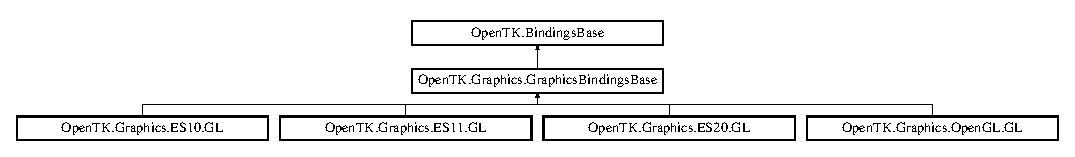
\includegraphics[height=1.666667cm]{class_open_t_k_1_1_bindings_base}
\end{center}
\end{figure}
\subsection*{Public Member Functions}
\begin{DoxyCompactItemize}
\item 
\hyperlink{class_open_t_k_1_1_bindings_base_afb1707c7e4ecb51abcebf7623e783da3}{Bindings\-Base} ()
\begin{DoxyCompactList}\small\item\em Constructs a new \hyperlink{class_open_t_k_1_1_bindings_base}{Bindings\-Base} instance. \end{DoxyCompactList}\end{DoxyCompactItemize}
\subsection*{Protected Member Functions}
\begin{DoxyCompactItemize}
\item 
abstract Int\-Ptr \hyperlink{class_open_t_k_1_1_bindings_base_a1eaa8a8b7a6a86051468535d38fca81c}{Get\-Address} (string funcname)
\begin{DoxyCompactList}\small\item\em Retrieves an unmanaged function pointer to the specified function. \end{DoxyCompactList}\end{DoxyCompactItemize}
\subsection*{Protected Attributes}
\begin{DoxyCompactItemize}
\item 
readonly Type \hyperlink{class_open_t_k_1_1_bindings_base_af8e7fd368c9a04ee49117cf9645f513b}{Delegates\-Class}
\begin{DoxyCompactList}\small\item\em A reflection handle to the nested type that contains the function delegates. \end{DoxyCompactList}\item 
readonly Type \hyperlink{class_open_t_k_1_1_bindings_base_a71af741beec4ce41b8c22d80419c7172}{Core\-Class}
\begin{DoxyCompactList}\small\item\em A refection handle to the nested type that contains core functions (i.\-e. not extensions). \end{DoxyCompactList}\item 
readonly Sorted\-List$<$ string, \\*
Method\-Info $>$ \hyperlink{class_open_t_k_1_1_bindings_base_a46c7960da59274e230c8651a13b10a62}{Core\-Function\-Map} = new Sorted\-List$<$string, Method\-Info$>$()
\begin{DoxyCompactList}\small\item\em A mapping of core function names to Method\-Info handles. \end{DoxyCompactList}\end{DoxyCompactItemize}
\subsection*{Properties}
\begin{DoxyCompactItemize}
\item 
bool \hyperlink{class_open_t_k_1_1_bindings_base_afb1af0b310e3cdcf1cb0302b9f5d283d}{Rebuild\-Extension\-List}\hspace{0.3cm}{\ttfamily  \mbox{[}get, set\mbox{]}}
\begin{DoxyCompactList}\small\item\em Gets or sets a System.\-Boolean that indicates whether the list of supported extensions may have changed. \end{DoxyCompactList}\item 
abstract object \hyperlink{class_open_t_k_1_1_bindings_base_a0063e041acf286bac5b0518ae2c93bda}{Sync\-Root}\hspace{0.3cm}{\ttfamily  \mbox{[}get\mbox{]}}
\begin{DoxyCompactList}\small\item\em Gets an object that can be used to synchronize access to the bindings implementation. \end{DoxyCompactList}\end{DoxyCompactItemize}


\subsection{Detailed Description}
Provides a common foundation for all flat A\-P\-I bindings and implements the extension loading interface. 



\subsection{Constructor \& Destructor Documentation}
\hypertarget{class_open_t_k_1_1_bindings_base_afb1707c7e4ecb51abcebf7623e783da3}{\index{Open\-T\-K\-::\-Bindings\-Base@{Open\-T\-K\-::\-Bindings\-Base}!Bindings\-Base@{Bindings\-Base}}
\index{Bindings\-Base@{Bindings\-Base}!OpenTK::BindingsBase@{Open\-T\-K\-::\-Bindings\-Base}}
\subsubsection[{Bindings\-Base}]{\setlength{\rightskip}{0pt plus 5cm}Open\-T\-K.\-Bindings\-Base.\-Bindings\-Base (
\begin{DoxyParamCaption}
{}
\end{DoxyParamCaption}
)}}\label{class_open_t_k_1_1_bindings_base_afb1707c7e4ecb51abcebf7623e783da3}


Constructs a new \hyperlink{class_open_t_k_1_1_bindings_base}{Bindings\-Base} instance. 



\subsection{Member Function Documentation}
\hypertarget{class_open_t_k_1_1_bindings_base_a1eaa8a8b7a6a86051468535d38fca81c}{\index{Open\-T\-K\-::\-Bindings\-Base@{Open\-T\-K\-::\-Bindings\-Base}!Get\-Address@{Get\-Address}}
\index{Get\-Address@{Get\-Address}!OpenTK::BindingsBase@{Open\-T\-K\-::\-Bindings\-Base}}
\subsubsection[{Get\-Address}]{\setlength{\rightskip}{0pt plus 5cm}abstract Int\-Ptr Open\-T\-K.\-Bindings\-Base.\-Get\-Address (
\begin{DoxyParamCaption}
\item[{string}]{funcname}
\end{DoxyParamCaption}
)\hspace{0.3cm}{\ttfamily [protected]}, {\ttfamily [pure virtual]}}}\label{class_open_t_k_1_1_bindings_base_a1eaa8a8b7a6a86051468535d38fca81c}


Retrieves an unmanaged function pointer to the specified function. 


\begin{DoxyParams}{Parameters}
{\em funcname} & A System.\-String that defines the name of the function. \\
\hline
\end{DoxyParams}
\begin{DoxyReturn}{Returns}
A Int\-Ptr that contains the address of funcname or Int\-Ptr.\-Zero, if the function is not supported by the drivers. 
\end{DoxyReturn}


Note\-: some drivers are known to return non-\/zero values for unsupported functions. Typical values include 1 and 2 -\/ inheritors are advised to check for and ignore these values. 

Implemented in \hyperlink{class_open_t_k_1_1_graphics_1_1_graphics_bindings_base_aeb37d851aee841ad85ef90242456d652}{Open\-T\-K.\-Graphics.\-Graphics\-Bindings\-Base}.



\subsection{Member Data Documentation}
\hypertarget{class_open_t_k_1_1_bindings_base_a71af741beec4ce41b8c22d80419c7172}{\index{Open\-T\-K\-::\-Bindings\-Base@{Open\-T\-K\-::\-Bindings\-Base}!Core\-Class@{Core\-Class}}
\index{Core\-Class@{Core\-Class}!OpenTK::BindingsBase@{Open\-T\-K\-::\-Bindings\-Base}}
\subsubsection[{Core\-Class}]{\setlength{\rightskip}{0pt plus 5cm}readonly Type Open\-T\-K.\-Bindings\-Base.\-Core\-Class\hspace{0.3cm}{\ttfamily [protected]}}}\label{class_open_t_k_1_1_bindings_base_a71af741beec4ce41b8c22d80419c7172}


A refection handle to the nested type that contains core functions (i.\-e. not extensions). 

\hypertarget{class_open_t_k_1_1_bindings_base_a46c7960da59274e230c8651a13b10a62}{\index{Open\-T\-K\-::\-Bindings\-Base@{Open\-T\-K\-::\-Bindings\-Base}!Core\-Function\-Map@{Core\-Function\-Map}}
\index{Core\-Function\-Map@{Core\-Function\-Map}!OpenTK::BindingsBase@{Open\-T\-K\-::\-Bindings\-Base}}
\subsubsection[{Core\-Function\-Map}]{\setlength{\rightskip}{0pt plus 5cm}readonly Sorted\-List$<$string, Method\-Info$>$ Open\-T\-K.\-Bindings\-Base.\-Core\-Function\-Map = new Sorted\-List$<$string, Method\-Info$>$()\hspace{0.3cm}{\ttfamily [protected]}}}\label{class_open_t_k_1_1_bindings_base_a46c7960da59274e230c8651a13b10a62}


A mapping of core function names to Method\-Info handles. 

\hypertarget{class_open_t_k_1_1_bindings_base_af8e7fd368c9a04ee49117cf9645f513b}{\index{Open\-T\-K\-::\-Bindings\-Base@{Open\-T\-K\-::\-Bindings\-Base}!Delegates\-Class@{Delegates\-Class}}
\index{Delegates\-Class@{Delegates\-Class}!OpenTK::BindingsBase@{Open\-T\-K\-::\-Bindings\-Base}}
\subsubsection[{Delegates\-Class}]{\setlength{\rightskip}{0pt plus 5cm}readonly Type Open\-T\-K.\-Bindings\-Base.\-Delegates\-Class\hspace{0.3cm}{\ttfamily [protected]}}}\label{class_open_t_k_1_1_bindings_base_af8e7fd368c9a04ee49117cf9645f513b}


A reflection handle to the nested type that contains the function delegates. 



\subsection{Property Documentation}
\hypertarget{class_open_t_k_1_1_bindings_base_afb1af0b310e3cdcf1cb0302b9f5d283d}{\index{Open\-T\-K\-::\-Bindings\-Base@{Open\-T\-K\-::\-Bindings\-Base}!Rebuild\-Extension\-List@{Rebuild\-Extension\-List}}
\index{Rebuild\-Extension\-List@{Rebuild\-Extension\-List}!OpenTK::BindingsBase@{Open\-T\-K\-::\-Bindings\-Base}}
\subsubsection[{Rebuild\-Extension\-List}]{\setlength{\rightskip}{0pt plus 5cm}bool Open\-T\-K.\-Bindings\-Base.\-Rebuild\-Extension\-List\hspace{0.3cm}{\ttfamily [get]}, {\ttfamily [set]}, {\ttfamily [protected]}}}\label{class_open_t_k_1_1_bindings_base_afb1af0b310e3cdcf1cb0302b9f5d283d}


Gets or sets a System.\-Boolean that indicates whether the list of supported extensions may have changed. 

\hypertarget{class_open_t_k_1_1_bindings_base_a0063e041acf286bac5b0518ae2c93bda}{\index{Open\-T\-K\-::\-Bindings\-Base@{Open\-T\-K\-::\-Bindings\-Base}!Sync\-Root@{Sync\-Root}}
\index{Sync\-Root@{Sync\-Root}!OpenTK::BindingsBase@{Open\-T\-K\-::\-Bindings\-Base}}
\subsubsection[{Sync\-Root}]{\setlength{\rightskip}{0pt plus 5cm}abstract object Open\-T\-K.\-Bindings\-Base.\-Sync\-Root\hspace{0.3cm}{\ttfamily [get]}, {\ttfamily [protected]}}}\label{class_open_t_k_1_1_bindings_base_a0063e041acf286bac5b0518ae2c93bda}


Gets an object that can be used to synchronize access to the bindings implementation. 

This object should be unique across bindings but consistent between bindings of the same type. For example, E\-S10.\-G\-L, Open\-G\-L.\-G\-L and C\-L10.\-C\-L should all return unique objects, but all instances of E\-S10.\-G\-L should return the same object.
\hypertarget{struct_open_t_k_1_1_box2}{\section{Open\-T\-K.\-Box2 Struct Reference}
\label{struct_open_t_k_1_1_box2}\index{Open\-T\-K.\-Box2@{Open\-T\-K.\-Box2}}
}


Defines a 2d box (rectangle).  


\subsection*{Public Member Functions}
\begin{DoxyCompactItemize}
\item 
\hyperlink{struct_open_t_k_1_1_box2_aba639284289656d3c03942468db21edf}{Box2} (\hyperlink{struct_open_t_k_1_1_vector2}{Vector2} top\-Left, \hyperlink{struct_open_t_k_1_1_vector2}{Vector2} bottom\-Right)
\begin{DoxyCompactList}\small\item\em Constructs a new \hyperlink{struct_open_t_k_1_1_box2}{Box2} with the specified dimensions. \end{DoxyCompactList}\item 
\hyperlink{struct_open_t_k_1_1_box2_aa1ae0521844ef0da963bdb6ce747ea23}{Box2} (float left, float top, float right, float bottom)
\begin{DoxyCompactList}\small\item\em Constructs a new \hyperlink{struct_open_t_k_1_1_box2}{Box2} with the specified dimensions. \end{DoxyCompactList}\item 
override string \hyperlink{struct_open_t_k_1_1_box2_a5c2a2a197651d7b7ab41e97d624d11cd}{To\-String} ()
\begin{DoxyCompactList}\small\item\em Returns a System.\-String describing the current instance. \end{DoxyCompactList}\end{DoxyCompactItemize}
\subsection*{Static Public Member Functions}
\begin{DoxyCompactItemize}
\item 
static \hyperlink{struct_open_t_k_1_1_box2}{Box2} \hyperlink{struct_open_t_k_1_1_box2_af0fcbae75b8333641ac24493be1763c7}{From\-T\-L\-R\-B} (float top, float left, float right, float bottom)
\begin{DoxyCompactList}\small\item\em Creates a new \hyperlink{struct_open_t_k_1_1_box2}{Box2} with the specified dimensions. \end{DoxyCompactList}\end{DoxyCompactItemize}
\subsection*{Public Attributes}
\begin{DoxyCompactItemize}
\item 
float \hyperlink{struct_open_t_k_1_1_box2_a51cc4c52d76b880d9671100b313695e9}{Left}
\begin{DoxyCompactList}\small\item\em The left boundary of the structure. \end{DoxyCompactList}\item 
float \hyperlink{struct_open_t_k_1_1_box2_a74433a0faff0a2e3cfc378b9e38baf0f}{Right}
\begin{DoxyCompactList}\small\item\em The right boundary of the structure. \end{DoxyCompactList}\item 
float \hyperlink{struct_open_t_k_1_1_box2_a1199b632ff542a034839df4033c6e91d}{Top}
\begin{DoxyCompactList}\small\item\em The top boundary of the structure. \end{DoxyCompactList}\item 
float \hyperlink{struct_open_t_k_1_1_box2_a2402181128d362b332ab28327073eaee}{Bottom}
\begin{DoxyCompactList}\small\item\em The bottom boundary of the structure. \end{DoxyCompactList}\end{DoxyCompactItemize}
\subsection*{Properties}
\begin{DoxyCompactItemize}
\item 
float \hyperlink{struct_open_t_k_1_1_box2_a29d85bf58aacaa02bb3869d1b6f0d6a0}{Width}\hspace{0.3cm}{\ttfamily  \mbox{[}get\mbox{]}}
\begin{DoxyCompactList}\small\item\em Gets a float describing the width of the \hyperlink{struct_open_t_k_1_1_box2}{Box2} structure. \end{DoxyCompactList}\item 
float \hyperlink{struct_open_t_k_1_1_box2_a2b86d70da5b355bcd176649e325a535f}{Height}\hspace{0.3cm}{\ttfamily  \mbox{[}get\mbox{]}}
\begin{DoxyCompactList}\small\item\em Gets a float describing the height of the \hyperlink{struct_open_t_k_1_1_box2}{Box2} structure. \end{DoxyCompactList}\end{DoxyCompactItemize}


\subsection{Detailed Description}
Defines a 2d box (rectangle). 



\subsection{Constructor \& Destructor Documentation}
\hypertarget{struct_open_t_k_1_1_box2_aba639284289656d3c03942468db21edf}{\index{Open\-T\-K\-::\-Box2@{Open\-T\-K\-::\-Box2}!Box2@{Box2}}
\index{Box2@{Box2}!OpenTK::Box2@{Open\-T\-K\-::\-Box2}}
\subsubsection[{Box2}]{\setlength{\rightskip}{0pt plus 5cm}Open\-T\-K.\-Box2.\-Box2 (
\begin{DoxyParamCaption}
\item[{{\bf Vector2}}]{top\-Left, }
\item[{{\bf Vector2}}]{bottom\-Right}
\end{DoxyParamCaption}
)}}\label{struct_open_t_k_1_1_box2_aba639284289656d3c03942468db21edf}


Constructs a new \hyperlink{struct_open_t_k_1_1_box2}{Box2} with the specified dimensions. 


\begin{DoxyParams}{Parameters}
{\em top\-Left} & An\-Open\-T\-K.\-Vector2 describing the top-\/left corner of the \hyperlink{struct_open_t_k_1_1_box2}{Box2}.\\
\hline
{\em bottom\-Right} & An \hyperlink{struct_open_t_k_1_1_vector2}{Open\-T\-K.\-Vector2} describing the bottom-\/right corner of the \hyperlink{struct_open_t_k_1_1_box2}{Box2}.\\
\hline
\end{DoxyParams}
\hypertarget{struct_open_t_k_1_1_box2_aa1ae0521844ef0da963bdb6ce747ea23}{\index{Open\-T\-K\-::\-Box2@{Open\-T\-K\-::\-Box2}!Box2@{Box2}}
\index{Box2@{Box2}!OpenTK::Box2@{Open\-T\-K\-::\-Box2}}
\subsubsection[{Box2}]{\setlength{\rightskip}{0pt plus 5cm}Open\-T\-K.\-Box2.\-Box2 (
\begin{DoxyParamCaption}
\item[{float}]{left, }
\item[{float}]{top, }
\item[{float}]{right, }
\item[{float}]{bottom}
\end{DoxyParamCaption}
)}}\label{struct_open_t_k_1_1_box2_aa1ae0521844ef0da963bdb6ce747ea23}


Constructs a new \hyperlink{struct_open_t_k_1_1_box2}{Box2} with the specified dimensions. 


\begin{DoxyParams}{Parameters}
{\em left} & The position of the left boundary.\\
\hline
{\em top} & The position of the top boundary.\\
\hline
{\em right} & The position of the right boundary.\\
\hline
{\em bottom} & The position of the bottom boundary.\\
\hline
\end{DoxyParams}


\subsection{Member Function Documentation}
\hypertarget{struct_open_t_k_1_1_box2_af0fcbae75b8333641ac24493be1763c7}{\index{Open\-T\-K\-::\-Box2@{Open\-T\-K\-::\-Box2}!From\-T\-L\-R\-B@{From\-T\-L\-R\-B}}
\index{From\-T\-L\-R\-B@{From\-T\-L\-R\-B}!OpenTK::Box2@{Open\-T\-K\-::\-Box2}}
\subsubsection[{From\-T\-L\-R\-B}]{\setlength{\rightskip}{0pt plus 5cm}static {\bf Box2} Open\-T\-K.\-Box2.\-From\-T\-L\-R\-B (
\begin{DoxyParamCaption}
\item[{float}]{top, }
\item[{float}]{left, }
\item[{float}]{right, }
\item[{float}]{bottom}
\end{DoxyParamCaption}
)\hspace{0.3cm}{\ttfamily [static]}}}\label{struct_open_t_k_1_1_box2_af0fcbae75b8333641ac24493be1763c7}


Creates a new \hyperlink{struct_open_t_k_1_1_box2}{Box2} with the specified dimensions. 


\begin{DoxyParams}{Parameters}
{\em top} & The position of the top boundary.\\
\hline
{\em left} & The position of the left boundary.\\
\hline
{\em right} & The position of the right boundary.\\
\hline
{\em bottom} & The position of the bottom boundary.\\
\hline
\end{DoxyParams}
\begin{DoxyReturn}{Returns}
A new \hyperlink{struct_open_t_k_1_1_box2}{Open\-T\-K.\-Box2} with the specfied dimensions.
\end{DoxyReturn}
\hypertarget{struct_open_t_k_1_1_box2_a5c2a2a197651d7b7ab41e97d624d11cd}{\index{Open\-T\-K\-::\-Box2@{Open\-T\-K\-::\-Box2}!To\-String@{To\-String}}
\index{To\-String@{To\-String}!OpenTK::Box2@{Open\-T\-K\-::\-Box2}}
\subsubsection[{To\-String}]{\setlength{\rightskip}{0pt plus 5cm}override string Open\-T\-K.\-Box2.\-To\-String (
\begin{DoxyParamCaption}
{}
\end{DoxyParamCaption}
)}}\label{struct_open_t_k_1_1_box2_a5c2a2a197651d7b7ab41e97d624d11cd}


Returns a System.\-String describing the current instance. 

\begin{DoxyReturn}{Returns}

\end{DoxyReturn}


\subsection{Member Data Documentation}
\hypertarget{struct_open_t_k_1_1_box2_a2402181128d362b332ab28327073eaee}{\index{Open\-T\-K\-::\-Box2@{Open\-T\-K\-::\-Box2}!Bottom@{Bottom}}
\index{Bottom@{Bottom}!OpenTK::Box2@{Open\-T\-K\-::\-Box2}}
\subsubsection[{Bottom}]{\setlength{\rightskip}{0pt plus 5cm}float Open\-T\-K.\-Box2.\-Bottom}}\label{struct_open_t_k_1_1_box2_a2402181128d362b332ab28327073eaee}


The bottom boundary of the structure. 

\hypertarget{struct_open_t_k_1_1_box2_a51cc4c52d76b880d9671100b313695e9}{\index{Open\-T\-K\-::\-Box2@{Open\-T\-K\-::\-Box2}!Left@{Left}}
\index{Left@{Left}!OpenTK::Box2@{Open\-T\-K\-::\-Box2}}
\subsubsection[{Left}]{\setlength{\rightskip}{0pt plus 5cm}float Open\-T\-K.\-Box2.\-Left}}\label{struct_open_t_k_1_1_box2_a51cc4c52d76b880d9671100b313695e9}


The left boundary of the structure. 

\hypertarget{struct_open_t_k_1_1_box2_a74433a0faff0a2e3cfc378b9e38baf0f}{\index{Open\-T\-K\-::\-Box2@{Open\-T\-K\-::\-Box2}!Right@{Right}}
\index{Right@{Right}!OpenTK::Box2@{Open\-T\-K\-::\-Box2}}
\subsubsection[{Right}]{\setlength{\rightskip}{0pt plus 5cm}float Open\-T\-K.\-Box2.\-Right}}\label{struct_open_t_k_1_1_box2_a74433a0faff0a2e3cfc378b9e38baf0f}


The right boundary of the structure. 

\hypertarget{struct_open_t_k_1_1_box2_a1199b632ff542a034839df4033c6e91d}{\index{Open\-T\-K\-::\-Box2@{Open\-T\-K\-::\-Box2}!Top@{Top}}
\index{Top@{Top}!OpenTK::Box2@{Open\-T\-K\-::\-Box2}}
\subsubsection[{Top}]{\setlength{\rightskip}{0pt plus 5cm}float Open\-T\-K.\-Box2.\-Top}}\label{struct_open_t_k_1_1_box2_a1199b632ff542a034839df4033c6e91d}


The top boundary of the structure. 



\subsection{Property Documentation}
\hypertarget{struct_open_t_k_1_1_box2_a2b86d70da5b355bcd176649e325a535f}{\index{Open\-T\-K\-::\-Box2@{Open\-T\-K\-::\-Box2}!Height@{Height}}
\index{Height@{Height}!OpenTK::Box2@{Open\-T\-K\-::\-Box2}}
\subsubsection[{Height}]{\setlength{\rightskip}{0pt plus 5cm}float Open\-T\-K.\-Box2.\-Height\hspace{0.3cm}{\ttfamily [get]}}}\label{struct_open_t_k_1_1_box2_a2b86d70da5b355bcd176649e325a535f}


Gets a float describing the height of the \hyperlink{struct_open_t_k_1_1_box2}{Box2} structure. 

\hypertarget{struct_open_t_k_1_1_box2_a29d85bf58aacaa02bb3869d1b6f0d6a0}{\index{Open\-T\-K\-::\-Box2@{Open\-T\-K\-::\-Box2}!Width@{Width}}
\index{Width@{Width}!OpenTK::Box2@{Open\-T\-K\-::\-Box2}}
\subsubsection[{Width}]{\setlength{\rightskip}{0pt plus 5cm}float Open\-T\-K.\-Box2.\-Width\hspace{0.3cm}{\ttfamily [get]}}}\label{struct_open_t_k_1_1_box2_a29d85bf58aacaa02bb3869d1b6f0d6a0}


Gets a float describing the width of the \hyperlink{struct_open_t_k_1_1_box2}{Box2} structure. 


\hypertarget{class_open_t_k_1_1_context_exists_exception}{\section{Open\-T\-K.\-Context\-Exists\-Exception Class Reference}
\label{class_open_t_k_1_1_context_exists_exception}\index{Open\-T\-K.\-Context\-Exists\-Exception@{Open\-T\-K.\-Context\-Exists\-Exception}}
}


This exception is thrown when a Graphics\-Context property cannot be changed after creation.  




Inherits Application\-Exception.

\subsection*{Public Member Functions}
\begin{DoxyCompactItemize}
\item 
\hyperlink{class_open_t_k_1_1_context_exists_exception_af20ea50e3acd2e31acd3681160583ed4}{Context\-Exists\-Exception} (string message)
\begin{DoxyCompactList}\small\item\em Constructs a new \hyperlink{class_open_t_k_1_1_context_exists_exception}{Context\-Exists\-Exception} instance. \end{DoxyCompactList}\end{DoxyCompactItemize}
\subsection*{Properties}
\begin{DoxyCompactItemize}
\item 
override string \hyperlink{class_open_t_k_1_1_context_exists_exception_aab5a98f8c4225581129087027960bda6}{Message}\hspace{0.3cm}{\ttfamily  \mbox{[}get\mbox{]}}
\begin{DoxyCompactList}\small\item\em Gets a System.\-String explaining the cause of this exception. \end{DoxyCompactList}\end{DoxyCompactItemize}


\subsection{Detailed Description}
This exception is thrown when a Graphics\-Context property cannot be changed after creation. 



\subsection{Constructor \& Destructor Documentation}
\hypertarget{class_open_t_k_1_1_context_exists_exception_af20ea50e3acd2e31acd3681160583ed4}{\index{Open\-T\-K\-::\-Context\-Exists\-Exception@{Open\-T\-K\-::\-Context\-Exists\-Exception}!Context\-Exists\-Exception@{Context\-Exists\-Exception}}
\index{Context\-Exists\-Exception@{Context\-Exists\-Exception}!OpenTK::ContextExistsException@{Open\-T\-K\-::\-Context\-Exists\-Exception}}
\subsubsection[{Context\-Exists\-Exception}]{\setlength{\rightskip}{0pt plus 5cm}Open\-T\-K.\-Context\-Exists\-Exception.\-Context\-Exists\-Exception (
\begin{DoxyParamCaption}
\item[{string}]{message}
\end{DoxyParamCaption}
)}}\label{class_open_t_k_1_1_context_exists_exception_af20ea50e3acd2e31acd3681160583ed4}


Constructs a new \hyperlink{class_open_t_k_1_1_context_exists_exception}{Context\-Exists\-Exception} instance. 


\begin{DoxyParams}{Parameters}
{\em message} & A System.\-String explaining the cause of this exception.\\
\hline
\end{DoxyParams}


\subsection{Property Documentation}
\hypertarget{class_open_t_k_1_1_context_exists_exception_aab5a98f8c4225581129087027960bda6}{\index{Open\-T\-K\-::\-Context\-Exists\-Exception@{Open\-T\-K\-::\-Context\-Exists\-Exception}!Message@{Message}}
\index{Message@{Message}!OpenTK::ContextExistsException@{Open\-T\-K\-::\-Context\-Exists\-Exception}}
\subsubsection[{Message}]{\setlength{\rightskip}{0pt plus 5cm}override string Open\-T\-K.\-Context\-Exists\-Exception.\-Message\hspace{0.3cm}{\ttfamily [get]}}}\label{class_open_t_k_1_1_context_exists_exception_aab5a98f8c4225581129087027960bda6}


Gets a System.\-String explaining the cause of this exception. 


\hypertarget{struct_open_t_k_1_1_context_handle}{\section{Open\-T\-K.\-Context\-Handle Struct Reference}
\label{struct_open_t_k_1_1_context_handle}\index{Open\-T\-K.\-Context\-Handle@{Open\-T\-K.\-Context\-Handle}}
}


Represents a handle to an Open\-G\-L or Open\-A\-L context.  




Inherits I\-Comparable$<$ Context\-Handle $>$, and I\-Equatable$<$ Context\-Handle $>$.

\subsection*{Public Member Functions}
\begin{DoxyCompactItemize}
\item 
\hyperlink{struct_open_t_k_1_1_context_handle_a9f28d608f392e028316170761d838579}{Context\-Handle} (Int\-Ptr h)
\begin{DoxyCompactList}\small\item\em Constructs a new instance with the specified handle. \end{DoxyCompactList}\item 
override string \hyperlink{struct_open_t_k_1_1_context_handle_a20cadbf82331ed88599b86cd2129aec2}{To\-String} ()
\begin{DoxyCompactList}\small\item\em Converts this instance to its equivalent string representation. \end{DoxyCompactList}\item 
override bool \hyperlink{struct_open_t_k_1_1_context_handle_ad0c7d1aaa648f1c891b0928f00ca9b9c}{Equals} (object obj)
\begin{DoxyCompactList}\small\item\em Compares this instance to the specified object. \end{DoxyCompactList}\item 
override int \hyperlink{struct_open_t_k_1_1_context_handle_abd04bc3828451409789d7296d9e2122e}{Get\-Hash\-Code} ()
\begin{DoxyCompactList}\small\item\em Returns the hash code for this instance. \end{DoxyCompactList}\item 
int \hyperlink{struct_open_t_k_1_1_context_handle_a179bf07f12867e4ab9c8dc52becea6b3}{Compare\-To} (\hyperlink{struct_open_t_k_1_1_context_handle}{Context\-Handle} other)
\begin{DoxyCompactList}\small\item\em Compares the numerical value of this instance to the specified \hyperlink{struct_open_t_k_1_1_context_handle}{Context\-Handle} and returns a value indicating their relative order. \end{DoxyCompactList}\item 
bool \hyperlink{struct_open_t_k_1_1_context_handle_aa086559f49576c119614c41698d05ca8}{Equals} (\hyperlink{struct_open_t_k_1_1_context_handle}{Context\-Handle} other)
\begin{DoxyCompactList}\small\item\em Compares this instance to the specified \hyperlink{struct_open_t_k_1_1_context_handle}{Context\-Handle} for equality. \end{DoxyCompactList}\end{DoxyCompactItemize}
\subsection*{Static Public Member Functions}
\begin{DoxyCompactItemize}
\item 
static \hyperlink{struct_open_t_k_1_1_context_handle_afe60b9eefe44b6b1bc9dca2e8241f7d7}{operator Int\-Ptr} (\hyperlink{struct_open_t_k_1_1_context_handle}{Context\-Handle} c)
\begin{DoxyCompactList}\small\item\em Converts the specified \hyperlink{struct_open_t_k_1_1_context_handle}{Context\-Handle} to the equivalent Int\-Ptr. \end{DoxyCompactList}\item 
static \hyperlink{struct_open_t_k_1_1_context_handle_ae5a727d7e97ecf5a9b19aaae0c393ecc}{operator Context\-Handle} (Int\-Ptr p)
\begin{DoxyCompactList}\small\item\em Converts the specified Int\-Ptr to the equivalent \hyperlink{struct_open_t_k_1_1_context_handle}{Context\-Handle}. \end{DoxyCompactList}\item 
static bool \hyperlink{struct_open_t_k_1_1_context_handle_a18ab9a9c5a6b948f94704b38c8e48727}{operator==} (\hyperlink{struct_open_t_k_1_1_context_handle}{Context\-Handle} left, \hyperlink{struct_open_t_k_1_1_context_handle}{Context\-Handle} right)
\begin{DoxyCompactList}\small\item\em Compares two Context\-Handles for equality. \end{DoxyCompactList}\item 
static bool \hyperlink{struct_open_t_k_1_1_context_handle_acfb221980963d886bb4a8b65397b1c9c}{operator!=} (\hyperlink{struct_open_t_k_1_1_context_handle}{Context\-Handle} left, \hyperlink{struct_open_t_k_1_1_context_handle}{Context\-Handle} right)
\begin{DoxyCompactList}\small\item\em Compares two Context\-Handles for inequality. \end{DoxyCompactList}\end{DoxyCompactItemize}
\subsection*{Public Attributes}
\begin{DoxyCompactItemize}
\item 
\hypertarget{struct_open_t_k_1_1_context_handle_adf7043e0734eaf9f7d3cad9420ec7d29}{Int\-Ptr {\bfseries handle}}\label{struct_open_t_k_1_1_context_handle_adf7043e0734eaf9f7d3cad9420ec7d29}

\end{DoxyCompactItemize}
\subsection*{Static Public Attributes}
\begin{DoxyCompactItemize}
\item 
static readonly \hyperlink{struct_open_t_k_1_1_context_handle}{Context\-Handle} \hyperlink{struct_open_t_k_1_1_context_handle_a2f93cb64d85fc3c2669d4726488a8c00}{Zero} = new \hyperlink{struct_open_t_k_1_1_context_handle}{Context\-Handle}(Int\-Ptr.\-Zero)
\begin{DoxyCompactList}\small\item\em A read-\/only field that represents a handle that has been initialized to zero.\end{DoxyCompactList}\end{DoxyCompactItemize}
\subsection*{Properties}
\begin{DoxyCompactItemize}
\item 
Int\-Ptr \hyperlink{struct_open_t_k_1_1_context_handle_aa0cad213b26464434068e1006d587ae7}{Handle}\hspace{0.3cm}{\ttfamily  \mbox{[}get\mbox{]}}
\begin{DoxyCompactList}\small\item\em Gets a System.\-Int\-Ptr that represents the handle of this \hyperlink{struct_open_t_k_1_1_context_handle}{Context\-Handle}. \end{DoxyCompactList}\end{DoxyCompactItemize}


\subsection{Detailed Description}
Represents a handle to an Open\-G\-L or Open\-A\-L context. 



\subsection{Constructor \& Destructor Documentation}
\hypertarget{struct_open_t_k_1_1_context_handle_a9f28d608f392e028316170761d838579}{\index{Open\-T\-K\-::\-Context\-Handle@{Open\-T\-K\-::\-Context\-Handle}!Context\-Handle@{Context\-Handle}}
\index{Context\-Handle@{Context\-Handle}!OpenTK::ContextHandle@{Open\-T\-K\-::\-Context\-Handle}}
\subsubsection[{Context\-Handle}]{\setlength{\rightskip}{0pt plus 5cm}Open\-T\-K.\-Context\-Handle.\-Context\-Handle (
\begin{DoxyParamCaption}
\item[{Int\-Ptr}]{h}
\end{DoxyParamCaption}
)}}\label{struct_open_t_k_1_1_context_handle_a9f28d608f392e028316170761d838579}


Constructs a new instance with the specified handle. 


\begin{DoxyParams}{Parameters}
{\em h} & A System.\-Int\-Ptr containing the value for this instance.\\
\hline
\end{DoxyParams}


\subsection{Member Function Documentation}
\hypertarget{struct_open_t_k_1_1_context_handle_a179bf07f12867e4ab9c8dc52becea6b3}{\index{Open\-T\-K\-::\-Context\-Handle@{Open\-T\-K\-::\-Context\-Handle}!Compare\-To@{Compare\-To}}
\index{Compare\-To@{Compare\-To}!OpenTK::ContextHandle@{Open\-T\-K\-::\-Context\-Handle}}
\subsubsection[{Compare\-To}]{\setlength{\rightskip}{0pt plus 5cm}int Open\-T\-K.\-Context\-Handle.\-Compare\-To (
\begin{DoxyParamCaption}
\item[{{\bf Context\-Handle}}]{other}
\end{DoxyParamCaption}
)}}\label{struct_open_t_k_1_1_context_handle_a179bf07f12867e4ab9c8dc52becea6b3}


Compares the numerical value of this instance to the specified \hyperlink{struct_open_t_k_1_1_context_handle}{Context\-Handle} and returns a value indicating their relative order. 


\begin{DoxyParams}{Parameters}
{\em other} & The \hyperlink{struct_open_t_k_1_1_context_handle}{Context\-Handle} to compare to.\\
\hline
\end{DoxyParams}
\begin{DoxyReturn}{Returns}
Less than 0, if this instance is less than other; 0 if both are equal; Greater than 0 if other is greater than this instance.
\end{DoxyReturn}
\hypertarget{struct_open_t_k_1_1_context_handle_ad0c7d1aaa648f1c891b0928f00ca9b9c}{\index{Open\-T\-K\-::\-Context\-Handle@{Open\-T\-K\-::\-Context\-Handle}!Equals@{Equals}}
\index{Equals@{Equals}!OpenTK::ContextHandle@{Open\-T\-K\-::\-Context\-Handle}}
\subsubsection[{Equals}]{\setlength{\rightskip}{0pt plus 5cm}override bool Open\-T\-K.\-Context\-Handle.\-Equals (
\begin{DoxyParamCaption}
\item[{object}]{obj}
\end{DoxyParamCaption}
)}}\label{struct_open_t_k_1_1_context_handle_ad0c7d1aaa648f1c891b0928f00ca9b9c}


Compares this instance to the specified object. 


\begin{DoxyParams}{Parameters}
{\em obj} & The System.\-Object to compare to.\\
\hline
\end{DoxyParams}
\begin{DoxyReturn}{Returns}
True if obj is a \hyperlink{struct_open_t_k_1_1_context_handle}{Context\-Handle} that is equal to this instance; false otherwise.
\end{DoxyReturn}
\hypertarget{struct_open_t_k_1_1_context_handle_aa086559f49576c119614c41698d05ca8}{\index{Open\-T\-K\-::\-Context\-Handle@{Open\-T\-K\-::\-Context\-Handle}!Equals@{Equals}}
\index{Equals@{Equals}!OpenTK::ContextHandle@{Open\-T\-K\-::\-Context\-Handle}}
\subsubsection[{Equals}]{\setlength{\rightskip}{0pt plus 5cm}bool Open\-T\-K.\-Context\-Handle.\-Equals (
\begin{DoxyParamCaption}
\item[{{\bf Context\-Handle}}]{other}
\end{DoxyParamCaption}
)}}\label{struct_open_t_k_1_1_context_handle_aa086559f49576c119614c41698d05ca8}


Compares this instance to the specified \hyperlink{struct_open_t_k_1_1_context_handle}{Context\-Handle} for equality. 


\begin{DoxyParams}{Parameters}
{\em other} & The \hyperlink{struct_open_t_k_1_1_context_handle}{Context\-Handle} to compare to.\\
\hline
\end{DoxyParams}
\begin{DoxyReturn}{Returns}
True if this instance is equal to other; false otherwise.
\end{DoxyReturn}
\hypertarget{struct_open_t_k_1_1_context_handle_abd04bc3828451409789d7296d9e2122e}{\index{Open\-T\-K\-::\-Context\-Handle@{Open\-T\-K\-::\-Context\-Handle}!Get\-Hash\-Code@{Get\-Hash\-Code}}
\index{Get\-Hash\-Code@{Get\-Hash\-Code}!OpenTK::ContextHandle@{Open\-T\-K\-::\-Context\-Handle}}
\subsubsection[{Get\-Hash\-Code}]{\setlength{\rightskip}{0pt plus 5cm}override int Open\-T\-K.\-Context\-Handle.\-Get\-Hash\-Code (
\begin{DoxyParamCaption}
{}
\end{DoxyParamCaption}
)}}\label{struct_open_t_k_1_1_context_handle_abd04bc3828451409789d7296d9e2122e}


Returns the hash code for this instance. 

\begin{DoxyReturn}{Returns}
A System.\-Int32 with the hash code of this instance.
\end{DoxyReturn}
\hypertarget{struct_open_t_k_1_1_context_handle_ae5a727d7e97ecf5a9b19aaae0c393ecc}{\index{Open\-T\-K\-::\-Context\-Handle@{Open\-T\-K\-::\-Context\-Handle}!operator Context\-Handle@{operator Context\-Handle}}
\index{operator Context\-Handle@{operator Context\-Handle}!OpenTK::ContextHandle@{Open\-T\-K\-::\-Context\-Handle}}
\subsubsection[{operator Context\-Handle}]{\setlength{\rightskip}{0pt plus 5cm}static Open\-T\-K.\-Context\-Handle.\-operator {\bf Context\-Handle} (
\begin{DoxyParamCaption}
\item[{Int\-Ptr}]{p}
\end{DoxyParamCaption}
)\hspace{0.3cm}{\ttfamily [explicit]}, {\ttfamily [static]}}}\label{struct_open_t_k_1_1_context_handle_ae5a727d7e97ecf5a9b19aaae0c393ecc}


Converts the specified Int\-Ptr to the equivalent \hyperlink{struct_open_t_k_1_1_context_handle}{Context\-Handle}. 


\begin{DoxyParams}{Parameters}
{\em p} & The System.\-Int\-Ptr to convert.\\
\hline
\end{DoxyParams}
\begin{DoxyReturn}{Returns}
A \hyperlink{struct_open_t_k_1_1_context_handle}{Context\-Handle} equivalent to the specified Int\-Ptr.
\end{DoxyReturn}
\hypertarget{struct_open_t_k_1_1_context_handle_afe60b9eefe44b6b1bc9dca2e8241f7d7}{\index{Open\-T\-K\-::\-Context\-Handle@{Open\-T\-K\-::\-Context\-Handle}!operator Int\-Ptr@{operator Int\-Ptr}}
\index{operator Int\-Ptr@{operator Int\-Ptr}!OpenTK::ContextHandle@{Open\-T\-K\-::\-Context\-Handle}}
\subsubsection[{operator Int\-Ptr}]{\setlength{\rightskip}{0pt plus 5cm}static Open\-T\-K.\-Context\-Handle.\-operator Int\-Ptr (
\begin{DoxyParamCaption}
\item[{{\bf Context\-Handle}}]{c}
\end{DoxyParamCaption}
)\hspace{0.3cm}{\ttfamily [explicit]}, {\ttfamily [static]}}}\label{struct_open_t_k_1_1_context_handle_afe60b9eefe44b6b1bc9dca2e8241f7d7}


Converts the specified \hyperlink{struct_open_t_k_1_1_context_handle}{Context\-Handle} to the equivalent Int\-Ptr. 


\begin{DoxyParams}{Parameters}
{\em c} & The \hyperlink{struct_open_t_k_1_1_context_handle}{Context\-Handle} to convert.\\
\hline
\end{DoxyParams}
\begin{DoxyReturn}{Returns}
A System.\-Int\-Ptr equivalent to the specified \hyperlink{struct_open_t_k_1_1_context_handle}{Context\-Handle}.
\end{DoxyReturn}
\hypertarget{struct_open_t_k_1_1_context_handle_acfb221980963d886bb4a8b65397b1c9c}{\index{Open\-T\-K\-::\-Context\-Handle@{Open\-T\-K\-::\-Context\-Handle}!operator!=@{operator!=}}
\index{operator!=@{operator!=}!OpenTK::ContextHandle@{Open\-T\-K\-::\-Context\-Handle}}
\subsubsection[{operator!=}]{\setlength{\rightskip}{0pt plus 5cm}static bool Open\-T\-K.\-Context\-Handle.\-operator!= (
\begin{DoxyParamCaption}
\item[{{\bf Context\-Handle}}]{left, }
\item[{{\bf Context\-Handle}}]{right}
\end{DoxyParamCaption}
)\hspace{0.3cm}{\ttfamily [static]}}}\label{struct_open_t_k_1_1_context_handle_acfb221980963d886bb4a8b65397b1c9c}


Compares two Context\-Handles for inequality. 


\begin{DoxyParams}{Parameters}
{\em left} & The \hyperlink{struct_open_t_k_1_1_context_handle}{Context\-Handle} to compare.\\
\hline
{\em right} & The \hyperlink{struct_open_t_k_1_1_context_handle}{Context\-Handle} to compare to.\\
\hline
\end{DoxyParams}
\begin{DoxyReturn}{Returns}
True if left is not equal to right; false otherwise.
\end{DoxyReturn}
\hypertarget{struct_open_t_k_1_1_context_handle_a18ab9a9c5a6b948f94704b38c8e48727}{\index{Open\-T\-K\-::\-Context\-Handle@{Open\-T\-K\-::\-Context\-Handle}!operator==@{operator==}}
\index{operator==@{operator==}!OpenTK::ContextHandle@{Open\-T\-K\-::\-Context\-Handle}}
\subsubsection[{operator==}]{\setlength{\rightskip}{0pt plus 5cm}static bool Open\-T\-K.\-Context\-Handle.\-operator== (
\begin{DoxyParamCaption}
\item[{{\bf Context\-Handle}}]{left, }
\item[{{\bf Context\-Handle}}]{right}
\end{DoxyParamCaption}
)\hspace{0.3cm}{\ttfamily [static]}}}\label{struct_open_t_k_1_1_context_handle_a18ab9a9c5a6b948f94704b38c8e48727}


Compares two Context\-Handles for equality. 


\begin{DoxyParams}{Parameters}
{\em left} & The \hyperlink{struct_open_t_k_1_1_context_handle}{Context\-Handle} to compare.\\
\hline
{\em right} & The \hyperlink{struct_open_t_k_1_1_context_handle}{Context\-Handle} to compare to.\\
\hline
\end{DoxyParams}
\begin{DoxyReturn}{Returns}
True if left is equal to right; false otherwise.
\end{DoxyReturn}
\hypertarget{struct_open_t_k_1_1_context_handle_a20cadbf82331ed88599b86cd2129aec2}{\index{Open\-T\-K\-::\-Context\-Handle@{Open\-T\-K\-::\-Context\-Handle}!To\-String@{To\-String}}
\index{To\-String@{To\-String}!OpenTK::ContextHandle@{Open\-T\-K\-::\-Context\-Handle}}
\subsubsection[{To\-String}]{\setlength{\rightskip}{0pt plus 5cm}override string Open\-T\-K.\-Context\-Handle.\-To\-String (
\begin{DoxyParamCaption}
{}
\end{DoxyParamCaption}
)}}\label{struct_open_t_k_1_1_context_handle_a20cadbf82331ed88599b86cd2129aec2}


Converts this instance to its equivalent string representation. 

\begin{DoxyReturn}{Returns}
A System.\-String that contains the string representation of this instance.
\end{DoxyReturn}


\subsection{Member Data Documentation}
\hypertarget{struct_open_t_k_1_1_context_handle_a2f93cb64d85fc3c2669d4726488a8c00}{\index{Open\-T\-K\-::\-Context\-Handle@{Open\-T\-K\-::\-Context\-Handle}!Zero@{Zero}}
\index{Zero@{Zero}!OpenTK::ContextHandle@{Open\-T\-K\-::\-Context\-Handle}}
\subsubsection[{Zero}]{\setlength{\rightskip}{0pt plus 5cm}readonly {\bf Context\-Handle} Open\-T\-K.\-Context\-Handle.\-Zero = new {\bf Context\-Handle}(Int\-Ptr.\-Zero)\hspace{0.3cm}{\ttfamily [static]}}}\label{struct_open_t_k_1_1_context_handle_a2f93cb64d85fc3c2669d4726488a8c00}


A read-\/only field that represents a handle that has been initialized to zero.



\subsection{Property Documentation}
\hypertarget{struct_open_t_k_1_1_context_handle_aa0cad213b26464434068e1006d587ae7}{\index{Open\-T\-K\-::\-Context\-Handle@{Open\-T\-K\-::\-Context\-Handle}!Handle@{Handle}}
\index{Handle@{Handle}!OpenTK::ContextHandle@{Open\-T\-K\-::\-Context\-Handle}}
\subsubsection[{Handle}]{\setlength{\rightskip}{0pt plus 5cm}Int\-Ptr Open\-T\-K.\-Context\-Handle.\-Handle\hspace{0.3cm}{\ttfamily [get]}}}\label{struct_open_t_k_1_1_context_handle_aa0cad213b26464434068e1006d587ae7}


Gets a System.\-Int\-Ptr that represents the handle of this \hyperlink{struct_open_t_k_1_1_context_handle}{Context\-Handle}. 


\hypertarget{class_open_t_k_1_1_display_device}{\section{Open\-T\-K.\-Display\-Device Class Reference}
\label{class_open_t_k_1_1_display_device}\index{Open\-T\-K.\-Display\-Device@{Open\-T\-K.\-Display\-Device}}
}


Defines a display device on the underlying system, and provides methods to query and change its display parameters.  


\subsection*{Public Member Functions}
\begin{DoxyCompactItemize}
\item 
\hyperlink{class_open_t_k_1_1_display_resolution}{Display\-Resolution} \hyperlink{class_open_t_k_1_1_display_device_ad2882c9f3dc2236e2ada0ef2c4df11d2}{Select\-Resolution} (int width, int height, int bits\-Per\-Pixel, float refresh\-Rate)
\begin{DoxyCompactList}\small\item\em Selects an available resolution that matches the specified parameters. \end{DoxyCompactList}\item 
void \hyperlink{class_open_t_k_1_1_display_device_ac993a7370baae2f590e71abe57c5b3b8}{Change\-Resolution} (\hyperlink{class_open_t_k_1_1_display_resolution}{Display\-Resolution} resolution)
\begin{DoxyCompactList}\small\item\em Changes the resolution of the \hyperlink{class_open_t_k_1_1_display_device}{Display\-Device}.\end{DoxyCompactList}\item 
void \hyperlink{class_open_t_k_1_1_display_device_a0accb55553a4d11804954b9675007404}{Change\-Resolution} (int width, int height, int bits\-Per\-Pixel, float refresh\-Rate)
\begin{DoxyCompactList}\small\item\em Changes the resolution of the \hyperlink{class_open_t_k_1_1_display_device}{Display\-Device}.\end{DoxyCompactList}\item 
void \hyperlink{class_open_t_k_1_1_display_device_afec8cf22992c7c17ce1c6921f651378f}{Restore\-Resolution} ()
\begin{DoxyCompactList}\small\item\em Restores the original resolution of the \hyperlink{class_open_t_k_1_1_display_device}{Display\-Device}.\end{DoxyCompactList}\item 
override string \hyperlink{class_open_t_k_1_1_display_device_a96b1b8d8248b8e524e45eba59b2ab00f}{To\-String} ()
\begin{DoxyCompactList}\small\item\em Returns a System.\-String representing this \hyperlink{class_open_t_k_1_1_display_device}{Display\-Device}. \end{DoxyCompactList}\end{DoxyCompactItemize}
\subsection*{Static Public Member Functions}
\begin{DoxyCompactItemize}
\item 
static \hyperlink{class_open_t_k_1_1_display_device}{Display\-Device} \hyperlink{class_open_t_k_1_1_display_device_afed73feb8e68d477cf314b33c351e661}{Get\-Display} (\hyperlink{namespace_open_t_k_a2869ea59bcff91cc6cc331f36c616389}{Display\-Index} index)
\begin{DoxyCompactList}\small\item\em Gets the \hyperlink{class_open_t_k_1_1_display_device}{Display\-Device} for the specified \hyperlink{namespace_open_t_k_a2869ea59bcff91cc6cc331f36c616389}{Display\-Index}. \end{DoxyCompactList}\end{DoxyCompactItemize}
\subsection*{Properties}
\begin{DoxyCompactItemize}
\item 
Rectangle \hyperlink{class_open_t_k_1_1_display_device_a8bd53ee06b975cd39ae8c296f42c72ab}{Bounds}\hspace{0.3cm}{\ttfamily  \mbox{[}get, set\mbox{]}}
\begin{DoxyCompactList}\small\item\em Gets the bounds of this instance in pixel coordinates.. \end{DoxyCompactList}\item 
int \hyperlink{class_open_t_k_1_1_display_device_a43b8973ddea03c873aa0006785d7da4d}{Width}\hspace{0.3cm}{\ttfamily  \mbox{[}get\mbox{]}}
\begin{DoxyCompactList}\small\item\em Gets a System.\-Int32 that contains the width of this display in pixels.\end{DoxyCompactList}\item 
int \hyperlink{class_open_t_k_1_1_display_device_aa5120fc7bcbcfad2ab9178762b248a8b}{Height}\hspace{0.3cm}{\ttfamily  \mbox{[}get\mbox{]}}
\begin{DoxyCompactList}\small\item\em Gets a System.\-Int32 that contains the height of this display in pixels.\end{DoxyCompactList}\item 
int \hyperlink{class_open_t_k_1_1_display_device_af22b160771cce81304e997ea883efcb0}{Bits\-Per\-Pixel}\hspace{0.3cm}{\ttfamily  \mbox{[}get, set\mbox{]}}
\begin{DoxyCompactList}\small\item\em Gets a System.\-Int32 that contains number of bits per pixel of this display. Typical values include 8, 16, 24 and 32.\end{DoxyCompactList}\item 
float \hyperlink{class_open_t_k_1_1_display_device_aeafbdb3c00fd95587654742b62ff7145}{Refresh\-Rate}\hspace{0.3cm}{\ttfamily  \mbox{[}get, set\mbox{]}}
\begin{DoxyCompactList}\small\item\em Gets a System.\-Single representing the vertical refresh rate of this display. \end{DoxyCompactList}\item 
bool \hyperlink{class_open_t_k_1_1_display_device_a45910e472c9487f77a80d2eaf699b0cf}{Is\-Primary}\hspace{0.3cm}{\ttfamily  \mbox{[}get, set\mbox{]}}
\begin{DoxyCompactList}\small\item\em Gets a System.\-Boolean that indicates whether this Display is the primary Display in systems with multiple Displays.\end{DoxyCompactList}\item 
I\-List$<$ \hyperlink{class_open_t_k_1_1_display_resolution}{Display\-Resolution} $>$ \hyperlink{class_open_t_k_1_1_display_device_a804b7e126c368b782811bc458019a7cd}{Available\-Resolutions}\hspace{0.3cm}{\ttfamily  \mbox{[}get, set\mbox{]}}
\begin{DoxyCompactList}\small\item\em Gets the list of \hyperlink{class_open_t_k_1_1_display_resolution}{Display\-Resolution} objects available on this device. \end{DoxyCompactList}\item 
static I\-List$<$ \hyperlink{class_open_t_k_1_1_display_device}{Display\-Device} $>$ \hyperlink{class_open_t_k_1_1_display_device_afd22a63fc37c530c7fd19886d439d04c}{Available\-Displays}\hspace{0.3cm}{\ttfamily  \mbox{[}get\mbox{]}}
\begin{DoxyCompactList}\small\item\em Gets the list of available \hyperlink{class_open_t_k_1_1_display_device}{Display\-Device} objects. This function allocates memory. \end{DoxyCompactList}\item 
static \hyperlink{class_open_t_k_1_1_display_device}{Display\-Device} \hyperlink{class_open_t_k_1_1_display_device_a2148505e367fc6d6d66ebfd80a9e91e5}{Default}\hspace{0.3cm}{\ttfamily  \mbox{[}get\mbox{]}}
\begin{DoxyCompactList}\small\item\em Gets the default (primary) display of this system.\end{DoxyCompactList}\end{DoxyCompactItemize}


\subsection{Detailed Description}
Defines a display device on the underlying system, and provides methods to query and change its display parameters. 



\subsection{Member Function Documentation}
\hypertarget{class_open_t_k_1_1_display_device_ac993a7370baae2f590e71abe57c5b3b8}{\index{Open\-T\-K\-::\-Display\-Device@{Open\-T\-K\-::\-Display\-Device}!Change\-Resolution@{Change\-Resolution}}
\index{Change\-Resolution@{Change\-Resolution}!OpenTK::DisplayDevice@{Open\-T\-K\-::\-Display\-Device}}
\subsubsection[{Change\-Resolution}]{\setlength{\rightskip}{0pt plus 5cm}void Open\-T\-K.\-Display\-Device.\-Change\-Resolution (
\begin{DoxyParamCaption}
\item[{{\bf Display\-Resolution}}]{resolution}
\end{DoxyParamCaption}
)}}\label{class_open_t_k_1_1_display_device_ac993a7370baae2f590e71abe57c5b3b8}


Changes the resolution of the \hyperlink{class_open_t_k_1_1_display_device}{Display\-Device}.


\begin{DoxyParams}{Parameters}
{\em resolution} & The resolution to set. \hyperlink{class_open_t_k_1_1_display_device_ad2882c9f3dc2236e2ada0ef2c4df11d2}{Display\-Device.\-Select\-Resolution}\\
\hline
\end{DoxyParams}

\begin{DoxyExceptions}{Exceptions}
{\em \hyperlink{class_open_t_k_1_1_graphics_1_1_graphics_mode_exception}{Graphics.\-Graphics\-Mode\-Exception}} & Thrown if the requested resolution could not be set.\\
\hline
\end{DoxyExceptions}


If the specified resolution is null, this function will restore the original \hyperlink{class_open_t_k_1_1_display_resolution}{Display\-Resolution}.\hypertarget{class_open_t_k_1_1_display_device_a0accb55553a4d11804954b9675007404}{\index{Open\-T\-K\-::\-Display\-Device@{Open\-T\-K\-::\-Display\-Device}!Change\-Resolution@{Change\-Resolution}}
\index{Change\-Resolution@{Change\-Resolution}!OpenTK::DisplayDevice@{Open\-T\-K\-::\-Display\-Device}}
\subsubsection[{Change\-Resolution}]{\setlength{\rightskip}{0pt plus 5cm}void Open\-T\-K.\-Display\-Device.\-Change\-Resolution (
\begin{DoxyParamCaption}
\item[{int}]{width, }
\item[{int}]{height, }
\item[{int}]{bits\-Per\-Pixel, }
\item[{float}]{refresh\-Rate}
\end{DoxyParamCaption}
)}}\label{class_open_t_k_1_1_display_device_a0accb55553a4d11804954b9675007404}


Changes the resolution of the \hyperlink{class_open_t_k_1_1_display_device}{Display\-Device}.


\begin{DoxyParams}{Parameters}
{\em width} & The new width of the \hyperlink{class_open_t_k_1_1_display_device}{Display\-Device}.\\
\hline
{\em height} & The new height of the \hyperlink{class_open_t_k_1_1_display_device}{Display\-Device}.\\
\hline
{\em bits\-Per\-Pixel} & The new bits per pixel of the \hyperlink{class_open_t_k_1_1_display_device}{Display\-Device}.\\
\hline
{\em refresh\-Rate} & The new refresh rate of the \hyperlink{class_open_t_k_1_1_display_device}{Display\-Device}.\\
\hline
\end{DoxyParams}

\begin{DoxyExceptions}{Exceptions}
{\em \hyperlink{class_open_t_k_1_1_graphics_1_1_graphics_mode_exception}{Graphics.\-Graphics\-Mode\-Exception}} & Thrown if the requested resolution could not be set.\\
\hline
\end{DoxyExceptions}
\hypertarget{class_open_t_k_1_1_display_device_afed73feb8e68d477cf314b33c351e661}{\index{Open\-T\-K\-::\-Display\-Device@{Open\-T\-K\-::\-Display\-Device}!Get\-Display@{Get\-Display}}
\index{Get\-Display@{Get\-Display}!OpenTK::DisplayDevice@{Open\-T\-K\-::\-Display\-Device}}
\subsubsection[{Get\-Display}]{\setlength{\rightskip}{0pt plus 5cm}static {\bf Display\-Device} Open\-T\-K.\-Display\-Device.\-Get\-Display (
\begin{DoxyParamCaption}
\item[{{\bf Display\-Index}}]{index}
\end{DoxyParamCaption}
)\hspace{0.3cm}{\ttfamily [static]}}}\label{class_open_t_k_1_1_display_device_afed73feb8e68d477cf314b33c351e661}


Gets the \hyperlink{class_open_t_k_1_1_display_device}{Display\-Device} for the specified \hyperlink{namespace_open_t_k_a2869ea59bcff91cc6cc331f36c616389}{Display\-Index}. 


\begin{DoxyParams}{Parameters}
{\em index} & The \hyperlink{namespace_open_t_k_a2869ea59bcff91cc6cc331f36c616389}{Display\-Index} that defines the desired display.\\
\hline
\end{DoxyParams}
\begin{DoxyReturn}{Returns}
A \hyperlink{class_open_t_k_1_1_display_device}{Display\-Device} or null, if no device corresponds to the specified index.
\end{DoxyReturn}
\hypertarget{class_open_t_k_1_1_display_device_afec8cf22992c7c17ce1c6921f651378f}{\index{Open\-T\-K\-::\-Display\-Device@{Open\-T\-K\-::\-Display\-Device}!Restore\-Resolution@{Restore\-Resolution}}
\index{Restore\-Resolution@{Restore\-Resolution}!OpenTK::DisplayDevice@{Open\-T\-K\-::\-Display\-Device}}
\subsubsection[{Restore\-Resolution}]{\setlength{\rightskip}{0pt plus 5cm}void Open\-T\-K.\-Display\-Device.\-Restore\-Resolution (
\begin{DoxyParamCaption}
{}
\end{DoxyParamCaption}
)}}\label{class_open_t_k_1_1_display_device_afec8cf22992c7c17ce1c6921f651378f}


Restores the original resolution of the \hyperlink{class_open_t_k_1_1_display_device}{Display\-Device}.


\begin{DoxyExceptions}{Exceptions}
{\em \hyperlink{class_open_t_k_1_1_graphics_1_1_graphics_mode_exception}{Graphics.\-Graphics\-Mode\-Exception}} & Thrown if the original resolution could not be restored.\\
\hline
\end{DoxyExceptions}
\hypertarget{class_open_t_k_1_1_display_device_ad2882c9f3dc2236e2ada0ef2c4df11d2}{\index{Open\-T\-K\-::\-Display\-Device@{Open\-T\-K\-::\-Display\-Device}!Select\-Resolution@{Select\-Resolution}}
\index{Select\-Resolution@{Select\-Resolution}!OpenTK::DisplayDevice@{Open\-T\-K\-::\-Display\-Device}}
\subsubsection[{Select\-Resolution}]{\setlength{\rightskip}{0pt plus 5cm}{\bf Display\-Resolution} Open\-T\-K.\-Display\-Device.\-Select\-Resolution (
\begin{DoxyParamCaption}
\item[{int}]{width, }
\item[{int}]{height, }
\item[{int}]{bits\-Per\-Pixel, }
\item[{float}]{refresh\-Rate}
\end{DoxyParamCaption}
)}}\label{class_open_t_k_1_1_display_device_ad2882c9f3dc2236e2ada0ef2c4df11d2}


Selects an available resolution that matches the specified parameters. 


\begin{DoxyParams}{Parameters}
{\em width} & The width of the requested resolution in pixels.\\
\hline
{\em height} & The height of the requested resolution in pixels.\\
\hline
{\em bits\-Per\-Pixel} & The bits per pixel of the requested resolution.\\
\hline
{\em refresh\-Rate} & The refresh rate of the requested resolution in hertz.\\
\hline
\end{DoxyParams}
\begin{DoxyReturn}{Returns}
The requested \hyperlink{class_open_t_k_1_1_display_resolution}{Display\-Resolution} or null if the parameters cannot be met.
\end{DoxyReturn}


If a matching resolution is not found, this function will retry ignoring the specified refresh rate, bits per pixel and resolution, in this order. If a matching resolution still doesn't exist, this function will return the current resolution.

A parameter set to 0 or negative numbers will not be used in the search (e.\-g. if refresh\-Rate is 0, any refresh rate will be considered valid).

This function allocates memory.\hypertarget{class_open_t_k_1_1_display_device_a96b1b8d8248b8e524e45eba59b2ab00f}{\index{Open\-T\-K\-::\-Display\-Device@{Open\-T\-K\-::\-Display\-Device}!To\-String@{To\-String}}
\index{To\-String@{To\-String}!OpenTK::DisplayDevice@{Open\-T\-K\-::\-Display\-Device}}
\subsubsection[{To\-String}]{\setlength{\rightskip}{0pt plus 5cm}override string Open\-T\-K.\-Display\-Device.\-To\-String (
\begin{DoxyParamCaption}
{}
\end{DoxyParamCaption}
)}}\label{class_open_t_k_1_1_display_device_a96b1b8d8248b8e524e45eba59b2ab00f}


Returns a System.\-String representing this \hyperlink{class_open_t_k_1_1_display_device}{Display\-Device}. 

\begin{DoxyReturn}{Returns}
A System.\-String representing this \hyperlink{class_open_t_k_1_1_display_device}{Display\-Device}.
\end{DoxyReturn}


\subsection{Property Documentation}
\hypertarget{class_open_t_k_1_1_display_device_afd22a63fc37c530c7fd19886d439d04c}{\index{Open\-T\-K\-::\-Display\-Device@{Open\-T\-K\-::\-Display\-Device}!Available\-Displays@{Available\-Displays}}
\index{Available\-Displays@{Available\-Displays}!OpenTK::DisplayDevice@{Open\-T\-K\-::\-Display\-Device}}
\subsubsection[{Available\-Displays}]{\setlength{\rightskip}{0pt plus 5cm}I\-List$<${\bf Display\-Device}$>$ Open\-T\-K.\-Display\-Device.\-Available\-Displays\hspace{0.3cm}{\ttfamily [static]}, {\ttfamily [get]}}}\label{class_open_t_k_1_1_display_device_afd22a63fc37c530c7fd19886d439d04c}


Gets the list of available \hyperlink{class_open_t_k_1_1_display_device}{Display\-Device} objects. This function allocates memory. 

\hypertarget{class_open_t_k_1_1_display_device_a804b7e126c368b782811bc458019a7cd}{\index{Open\-T\-K\-::\-Display\-Device@{Open\-T\-K\-::\-Display\-Device}!Available\-Resolutions@{Available\-Resolutions}}
\index{Available\-Resolutions@{Available\-Resolutions}!OpenTK::DisplayDevice@{Open\-T\-K\-::\-Display\-Device}}
\subsubsection[{Available\-Resolutions}]{\setlength{\rightskip}{0pt plus 5cm}I\-List$<${\bf Display\-Resolution}$>$ Open\-T\-K.\-Display\-Device.\-Available\-Resolutions\hspace{0.3cm}{\ttfamily [get]}, {\ttfamily [set]}}}\label{class_open_t_k_1_1_display_device_a804b7e126c368b782811bc458019a7cd}


Gets the list of \hyperlink{class_open_t_k_1_1_display_resolution}{Display\-Resolution} objects available on this device. 

\hypertarget{class_open_t_k_1_1_display_device_af22b160771cce81304e997ea883efcb0}{\index{Open\-T\-K\-::\-Display\-Device@{Open\-T\-K\-::\-Display\-Device}!Bits\-Per\-Pixel@{Bits\-Per\-Pixel}}
\index{Bits\-Per\-Pixel@{Bits\-Per\-Pixel}!OpenTK::DisplayDevice@{Open\-T\-K\-::\-Display\-Device}}
\subsubsection[{Bits\-Per\-Pixel}]{\setlength{\rightskip}{0pt plus 5cm}int Open\-T\-K.\-Display\-Device.\-Bits\-Per\-Pixel\hspace{0.3cm}{\ttfamily [get]}, {\ttfamily [set]}}}\label{class_open_t_k_1_1_display_device_af22b160771cce81304e997ea883efcb0}


Gets a System.\-Int32 that contains number of bits per pixel of this display. Typical values include 8, 16, 24 and 32.

\hypertarget{class_open_t_k_1_1_display_device_a8bd53ee06b975cd39ae8c296f42c72ab}{\index{Open\-T\-K\-::\-Display\-Device@{Open\-T\-K\-::\-Display\-Device}!Bounds@{Bounds}}
\index{Bounds@{Bounds}!OpenTK::DisplayDevice@{Open\-T\-K\-::\-Display\-Device}}
\subsubsection[{Bounds}]{\setlength{\rightskip}{0pt plus 5cm}Rectangle Open\-T\-K.\-Display\-Device.\-Bounds\hspace{0.3cm}{\ttfamily [get]}, {\ttfamily [set]}}}\label{class_open_t_k_1_1_display_device_a8bd53ee06b975cd39ae8c296f42c72ab}


Gets the bounds of this instance in pixel coordinates.. 

\hypertarget{class_open_t_k_1_1_display_device_a2148505e367fc6d6d66ebfd80a9e91e5}{\index{Open\-T\-K\-::\-Display\-Device@{Open\-T\-K\-::\-Display\-Device}!Default@{Default}}
\index{Default@{Default}!OpenTK::DisplayDevice@{Open\-T\-K\-::\-Display\-Device}}
\subsubsection[{Default}]{\setlength{\rightskip}{0pt plus 5cm}{\bf Display\-Device} Open\-T\-K.\-Display\-Device.\-Default\hspace{0.3cm}{\ttfamily [static]}, {\ttfamily [get]}}}\label{class_open_t_k_1_1_display_device_a2148505e367fc6d6d66ebfd80a9e91e5}


Gets the default (primary) display of this system.

\hypertarget{class_open_t_k_1_1_display_device_aa5120fc7bcbcfad2ab9178762b248a8b}{\index{Open\-T\-K\-::\-Display\-Device@{Open\-T\-K\-::\-Display\-Device}!Height@{Height}}
\index{Height@{Height}!OpenTK::DisplayDevice@{Open\-T\-K\-::\-Display\-Device}}
\subsubsection[{Height}]{\setlength{\rightskip}{0pt plus 5cm}int Open\-T\-K.\-Display\-Device.\-Height\hspace{0.3cm}{\ttfamily [get]}}}\label{class_open_t_k_1_1_display_device_aa5120fc7bcbcfad2ab9178762b248a8b}


Gets a System.\-Int32 that contains the height of this display in pixels.

\hypertarget{class_open_t_k_1_1_display_device_a45910e472c9487f77a80d2eaf699b0cf}{\index{Open\-T\-K\-::\-Display\-Device@{Open\-T\-K\-::\-Display\-Device}!Is\-Primary@{Is\-Primary}}
\index{Is\-Primary@{Is\-Primary}!OpenTK::DisplayDevice@{Open\-T\-K\-::\-Display\-Device}}
\subsubsection[{Is\-Primary}]{\setlength{\rightskip}{0pt plus 5cm}bool Open\-T\-K.\-Display\-Device.\-Is\-Primary\hspace{0.3cm}{\ttfamily [get]}, {\ttfamily [set]}}}\label{class_open_t_k_1_1_display_device_a45910e472c9487f77a80d2eaf699b0cf}


Gets a System.\-Boolean that indicates whether this Display is the primary Display in systems with multiple Displays.

\hypertarget{class_open_t_k_1_1_display_device_aeafbdb3c00fd95587654742b62ff7145}{\index{Open\-T\-K\-::\-Display\-Device@{Open\-T\-K\-::\-Display\-Device}!Refresh\-Rate@{Refresh\-Rate}}
\index{Refresh\-Rate@{Refresh\-Rate}!OpenTK::DisplayDevice@{Open\-T\-K\-::\-Display\-Device}}
\subsubsection[{Refresh\-Rate}]{\setlength{\rightskip}{0pt plus 5cm}float Open\-T\-K.\-Display\-Device.\-Refresh\-Rate\hspace{0.3cm}{\ttfamily [get]}, {\ttfamily [set]}}}\label{class_open_t_k_1_1_display_device_aeafbdb3c00fd95587654742b62ff7145}


Gets a System.\-Single representing the vertical refresh rate of this display. 

\hypertarget{class_open_t_k_1_1_display_device_a43b8973ddea03c873aa0006785d7da4d}{\index{Open\-T\-K\-::\-Display\-Device@{Open\-T\-K\-::\-Display\-Device}!Width@{Width}}
\index{Width@{Width}!OpenTK::DisplayDevice@{Open\-T\-K\-::\-Display\-Device}}
\subsubsection[{Width}]{\setlength{\rightskip}{0pt plus 5cm}int Open\-T\-K.\-Display\-Device.\-Width\hspace{0.3cm}{\ttfamily [get]}}}\label{class_open_t_k_1_1_display_device_a43b8973ddea03c873aa0006785d7da4d}


Gets a System.\-Int32 that contains the width of this display in pixels.


\hypertarget{class_open_t_k_1_1_display_resolution}{\section{Open\-T\-K.\-Display\-Resolution Class Reference}
\label{class_open_t_k_1_1_display_resolution}\index{Open\-T\-K.\-Display\-Resolution@{Open\-T\-K.\-Display\-Resolution}}
}


Contains information regarding a monitor's display resolution. 


\subsection*{Public Member Functions}
\begin{DoxyCompactItemize}
\item 
override string \hyperlink{class_open_t_k_1_1_display_resolution_a3d5a5df2af4538eda19a1a27bcfb55d4}{To\-String} ()
\begin{DoxyCompactList}\small\item\em Returns a System.\-String representing this \hyperlink{class_open_t_k_1_1_display_resolution}{Display\-Resolution}. \end{DoxyCompactList}\item 
override bool \hyperlink{class_open_t_k_1_1_display_resolution_ad791a6f6a590edffd568c489d4ec088a}{Equals} (object obj)
\begin{DoxyCompactList}\small\item\em Determines whether the specified resolutions are equal.\end{DoxyCompactList}\item 
override int \hyperlink{class_open_t_k_1_1_display_resolution_a03f663bb26b1a67265036ce8f563d9f7}{Get\-Hash\-Code} ()
\begin{DoxyCompactList}\small\item\em Returns a unique hash representing this resolution.\end{DoxyCompactList}\end{DoxyCompactItemize}
\subsection*{Static Public Member Functions}
\begin{DoxyCompactItemize}
\item 
static bool \hyperlink{class_open_t_k_1_1_display_resolution_a990567856cafc1b26c90fd0278f609c9}{operator==} (\hyperlink{class_open_t_k_1_1_display_resolution}{Display\-Resolution} left, \hyperlink{class_open_t_k_1_1_display_resolution}{Display\-Resolution} right)
\begin{DoxyCompactList}\small\item\em Compares two instances for equality. \end{DoxyCompactList}\item 
static bool \hyperlink{class_open_t_k_1_1_display_resolution_a2217e412c56ba046f24ca7d221a438e3}{operator!=} (\hyperlink{class_open_t_k_1_1_display_resolution}{Display\-Resolution} left, \hyperlink{class_open_t_k_1_1_display_resolution}{Display\-Resolution} right)
\begin{DoxyCompactList}\small\item\em Compares two instances for inequality. \end{DoxyCompactList}\end{DoxyCompactItemize}
\subsection*{Properties}
\begin{DoxyCompactItemize}
\item 
Rectangle \hyperlink{class_open_t_k_1_1_display_resolution_aa413eee2359d6426fbcec8280fce9c29}{Bounds}\hspace{0.3cm}{\ttfamily  \mbox{[}get\mbox{]}}
\begin{DoxyCompactList}\small\item\em Gets a System.\-Drawing.\-Rectangle that contains the bounds of this display device. \end{DoxyCompactList}\item 
int \hyperlink{class_open_t_k_1_1_display_resolution_ae2f5a42e23f49e4c1fd3c67714b9a259}{Width}\hspace{0.3cm}{\ttfamily  \mbox{[}get, set\mbox{]}}
\begin{DoxyCompactList}\small\item\em Gets a System.\-Int32 that contains the width of this display in pixels.\end{DoxyCompactList}\item 
int \hyperlink{class_open_t_k_1_1_display_resolution_a2a507b345a19dec923c9e14f6b003bd5}{Height}\hspace{0.3cm}{\ttfamily  \mbox{[}get, set\mbox{]}}
\begin{DoxyCompactList}\small\item\em Gets a System.\-Int32 that contains the height of this display in pixels.\end{DoxyCompactList}\item 
int \hyperlink{class_open_t_k_1_1_display_resolution_a7f719af2b3dc6db3533ccd335235c7b1}{Bits\-Per\-Pixel}\hspace{0.3cm}{\ttfamily  \mbox{[}get, set\mbox{]}}
\begin{DoxyCompactList}\small\item\em Gets a System.\-Int32 that contains number of bits per pixel of this display. Typical values include 8, 16, 24 and 32.\end{DoxyCompactList}\item 
float \hyperlink{class_open_t_k_1_1_display_resolution_a5d661a58b45850d6f55dbda121598b89}{Refresh\-Rate}\hspace{0.3cm}{\ttfamily  \mbox{[}get, set\mbox{]}}
\begin{DoxyCompactList}\small\item\em Gets a System.\-Single representing the vertical refresh rate of this display. \end{DoxyCompactList}\end{DoxyCompactItemize}


\subsection{Detailed Description}
Contains information regarding a monitor's display resolution.



\subsection{Member Function Documentation}
\hypertarget{class_open_t_k_1_1_display_resolution_ad791a6f6a590edffd568c489d4ec088a}{\index{Open\-T\-K\-::\-Display\-Resolution@{Open\-T\-K\-::\-Display\-Resolution}!Equals@{Equals}}
\index{Equals@{Equals}!OpenTK::DisplayResolution@{Open\-T\-K\-::\-Display\-Resolution}}
\subsubsection[{Equals}]{\setlength{\rightskip}{0pt plus 5cm}override bool Open\-T\-K.\-Display\-Resolution.\-Equals (
\begin{DoxyParamCaption}
\item[{object}]{obj}
\end{DoxyParamCaption}
)}}\label{class_open_t_k_1_1_display_resolution_ad791a6f6a590edffd568c489d4ec088a}


Determines whether the specified resolutions are equal.


\begin{DoxyParams}{Parameters}
{\em obj} & The System.\-Object to check against.\\
\hline
\end{DoxyParams}
\begin{DoxyReturn}{Returns}
True if the System.\-Object is an equal \hyperlink{class_open_t_k_1_1_display_resolution}{Display\-Resolution}; false otherwise.
\end{DoxyReturn}
\hypertarget{class_open_t_k_1_1_display_resolution_a03f663bb26b1a67265036ce8f563d9f7}{\index{Open\-T\-K\-::\-Display\-Resolution@{Open\-T\-K\-::\-Display\-Resolution}!Get\-Hash\-Code@{Get\-Hash\-Code}}
\index{Get\-Hash\-Code@{Get\-Hash\-Code}!OpenTK::DisplayResolution@{Open\-T\-K\-::\-Display\-Resolution}}
\subsubsection[{Get\-Hash\-Code}]{\setlength{\rightskip}{0pt plus 5cm}override int Open\-T\-K.\-Display\-Resolution.\-Get\-Hash\-Code (
\begin{DoxyParamCaption}
{}
\end{DoxyParamCaption}
)}}\label{class_open_t_k_1_1_display_resolution_a03f663bb26b1a67265036ce8f563d9f7}


Returns a unique hash representing this resolution.

\begin{DoxyReturn}{Returns}
A System.\-Int32 that may serve as a hash code for this resolution.
\end{DoxyReturn}
\hypertarget{class_open_t_k_1_1_display_resolution_a2217e412c56ba046f24ca7d221a438e3}{\index{Open\-T\-K\-::\-Display\-Resolution@{Open\-T\-K\-::\-Display\-Resolution}!operator!=@{operator!=}}
\index{operator!=@{operator!=}!OpenTK::DisplayResolution@{Open\-T\-K\-::\-Display\-Resolution}}
\subsubsection[{operator!=}]{\setlength{\rightskip}{0pt plus 5cm}static bool Open\-T\-K.\-Display\-Resolution.\-operator!= (
\begin{DoxyParamCaption}
\item[{{\bf Display\-Resolution}}]{left, }
\item[{{\bf Display\-Resolution}}]{right}
\end{DoxyParamCaption}
)\hspace{0.3cm}{\ttfamily [static]}}}\label{class_open_t_k_1_1_display_resolution_a2217e412c56ba046f24ca7d221a438e3}


Compares two instances for inequality. 


\begin{DoxyParams}{Parameters}
{\em left} & The first instance.\\
\hline
{\em right} & The second instance.\\
\hline
\end{DoxyParams}
\begin{DoxyReturn}{Returns}
True, if left does not equal right; false otherwise.
\end{DoxyReturn}
\hypertarget{class_open_t_k_1_1_display_resolution_a990567856cafc1b26c90fd0278f609c9}{\index{Open\-T\-K\-::\-Display\-Resolution@{Open\-T\-K\-::\-Display\-Resolution}!operator==@{operator==}}
\index{operator==@{operator==}!OpenTK::DisplayResolution@{Open\-T\-K\-::\-Display\-Resolution}}
\subsubsection[{operator==}]{\setlength{\rightskip}{0pt plus 5cm}static bool Open\-T\-K.\-Display\-Resolution.\-operator== (
\begin{DoxyParamCaption}
\item[{{\bf Display\-Resolution}}]{left, }
\item[{{\bf Display\-Resolution}}]{right}
\end{DoxyParamCaption}
)\hspace{0.3cm}{\ttfamily [static]}}}\label{class_open_t_k_1_1_display_resolution_a990567856cafc1b26c90fd0278f609c9}


Compares two instances for equality. 


\begin{DoxyParams}{Parameters}
{\em left} & The first instance.\\
\hline
{\em right} & The second instance.\\
\hline
\end{DoxyParams}
\begin{DoxyReturn}{Returns}
True, if left equals right; false otherwise.
\end{DoxyReturn}
\hypertarget{class_open_t_k_1_1_display_resolution_a3d5a5df2af4538eda19a1a27bcfb55d4}{\index{Open\-T\-K\-::\-Display\-Resolution@{Open\-T\-K\-::\-Display\-Resolution}!To\-String@{To\-String}}
\index{To\-String@{To\-String}!OpenTK::DisplayResolution@{Open\-T\-K\-::\-Display\-Resolution}}
\subsubsection[{To\-String}]{\setlength{\rightskip}{0pt plus 5cm}override string Open\-T\-K.\-Display\-Resolution.\-To\-String (
\begin{DoxyParamCaption}
{}
\end{DoxyParamCaption}
)}}\label{class_open_t_k_1_1_display_resolution_a3d5a5df2af4538eda19a1a27bcfb55d4}


Returns a System.\-String representing this \hyperlink{class_open_t_k_1_1_display_resolution}{Display\-Resolution}. 

\begin{DoxyReturn}{Returns}
A System.\-String representing this \hyperlink{class_open_t_k_1_1_display_resolution}{Display\-Resolution}.
\end{DoxyReturn}


\subsection{Property Documentation}
\hypertarget{class_open_t_k_1_1_display_resolution_a7f719af2b3dc6db3533ccd335235c7b1}{\index{Open\-T\-K\-::\-Display\-Resolution@{Open\-T\-K\-::\-Display\-Resolution}!Bits\-Per\-Pixel@{Bits\-Per\-Pixel}}
\index{Bits\-Per\-Pixel@{Bits\-Per\-Pixel}!OpenTK::DisplayResolution@{Open\-T\-K\-::\-Display\-Resolution}}
\subsubsection[{Bits\-Per\-Pixel}]{\setlength{\rightskip}{0pt plus 5cm}int Open\-T\-K.\-Display\-Resolution.\-Bits\-Per\-Pixel\hspace{0.3cm}{\ttfamily [get]}, {\ttfamily [set]}}}\label{class_open_t_k_1_1_display_resolution_a7f719af2b3dc6db3533ccd335235c7b1}


Gets a System.\-Int32 that contains number of bits per pixel of this display. Typical values include 8, 16, 24 and 32.

\hypertarget{class_open_t_k_1_1_display_resolution_aa413eee2359d6426fbcec8280fce9c29}{\index{Open\-T\-K\-::\-Display\-Resolution@{Open\-T\-K\-::\-Display\-Resolution}!Bounds@{Bounds}}
\index{Bounds@{Bounds}!OpenTK::DisplayResolution@{Open\-T\-K\-::\-Display\-Resolution}}
\subsubsection[{Bounds}]{\setlength{\rightskip}{0pt plus 5cm}Rectangle Open\-T\-K.\-Display\-Resolution.\-Bounds\hspace{0.3cm}{\ttfamily [get]}}}\label{class_open_t_k_1_1_display_resolution_aa413eee2359d6426fbcec8280fce9c29}


Gets a System.\-Drawing.\-Rectangle that contains the bounds of this display device. 

\hypertarget{class_open_t_k_1_1_display_resolution_a2a507b345a19dec923c9e14f6b003bd5}{\index{Open\-T\-K\-::\-Display\-Resolution@{Open\-T\-K\-::\-Display\-Resolution}!Height@{Height}}
\index{Height@{Height}!OpenTK::DisplayResolution@{Open\-T\-K\-::\-Display\-Resolution}}
\subsubsection[{Height}]{\setlength{\rightskip}{0pt plus 5cm}int Open\-T\-K.\-Display\-Resolution.\-Height\hspace{0.3cm}{\ttfamily [get]}, {\ttfamily [set]}}}\label{class_open_t_k_1_1_display_resolution_a2a507b345a19dec923c9e14f6b003bd5}


Gets a System.\-Int32 that contains the height of this display in pixels.

\hypertarget{class_open_t_k_1_1_display_resolution_a5d661a58b45850d6f55dbda121598b89}{\index{Open\-T\-K\-::\-Display\-Resolution@{Open\-T\-K\-::\-Display\-Resolution}!Refresh\-Rate@{Refresh\-Rate}}
\index{Refresh\-Rate@{Refresh\-Rate}!OpenTK::DisplayResolution@{Open\-T\-K\-::\-Display\-Resolution}}
\subsubsection[{Refresh\-Rate}]{\setlength{\rightskip}{0pt plus 5cm}float Open\-T\-K.\-Display\-Resolution.\-Refresh\-Rate\hspace{0.3cm}{\ttfamily [get]}, {\ttfamily [set]}}}\label{class_open_t_k_1_1_display_resolution_a5d661a58b45850d6f55dbda121598b89}


Gets a System.\-Single representing the vertical refresh rate of this display. 

\hypertarget{class_open_t_k_1_1_display_resolution_ae2f5a42e23f49e4c1fd3c67714b9a259}{\index{Open\-T\-K\-::\-Display\-Resolution@{Open\-T\-K\-::\-Display\-Resolution}!Width@{Width}}
\index{Width@{Width}!OpenTK::DisplayResolution@{Open\-T\-K\-::\-Display\-Resolution}}
\subsubsection[{Width}]{\setlength{\rightskip}{0pt plus 5cm}int Open\-T\-K.\-Display\-Resolution.\-Width\hspace{0.3cm}{\ttfamily [get]}, {\ttfamily [set]}}}\label{class_open_t_k_1_1_display_resolution_ae2f5a42e23f49e4c1fd3c67714b9a259}


Gets a System.\-Int32 that contains the width of this display in pixels.


\hypertarget{class_open_t_k_1_1_frame_event_args}{\section{Open\-T\-K.\-Frame\-Event\-Args Class Reference}
\label{class_open_t_k_1_1_frame_event_args}\index{Open\-T\-K.\-Frame\-Event\-Args@{Open\-T\-K.\-Frame\-Event\-Args}}
}


Defines the arguments for frame events. A \hyperlink{class_open_t_k_1_1_frame_event_args}{Frame\-Event\-Args} instance is only valid for the duration of the relevant event; do not store references to \hyperlink{class_open_t_k_1_1_frame_event_args}{Frame\-Event\-Args} outside this event.  




Inherits Event\-Args.

\subsection*{Public Member Functions}
\begin{DoxyCompactItemize}
\item 
\hyperlink{class_open_t_k_1_1_frame_event_args_a9d439a35fcccc0e499a0e79c31db0d76}{Frame\-Event\-Args} ()
\begin{DoxyCompactList}\small\item\em Constructs a new \hyperlink{class_open_t_k_1_1_frame_event_args}{Frame\-Event\-Args} instance. \end{DoxyCompactList}\item 
\hyperlink{class_open_t_k_1_1_frame_event_args_aca23078ed1cdd7c0de8a62cdf0ad68f6}{Frame\-Event\-Args} (double elapsed)
\begin{DoxyCompactList}\small\item\em Constructs a new \hyperlink{class_open_t_k_1_1_frame_event_args}{Frame\-Event\-Args} instance. \end{DoxyCompactList}\end{DoxyCompactItemize}
\subsection*{Properties}
\begin{DoxyCompactItemize}
\item 
double \hyperlink{class_open_t_k_1_1_frame_event_args_aee05f4349255e7798599c301759d6211}{Time}\hspace{0.3cm}{\ttfamily  \mbox{[}get, set\mbox{]}}
\begin{DoxyCompactList}\small\item\em Gets a System.\-Double that indicates how many seconds of time elapsed since the previous event. \end{DoxyCompactList}\end{DoxyCompactItemize}


\subsection{Detailed Description}
Defines the arguments for frame events. A \hyperlink{class_open_t_k_1_1_frame_event_args}{Frame\-Event\-Args} instance is only valid for the duration of the relevant event; do not store references to \hyperlink{class_open_t_k_1_1_frame_event_args}{Frame\-Event\-Args} outside this event. 



\subsection{Constructor \& Destructor Documentation}
\hypertarget{class_open_t_k_1_1_frame_event_args_a9d439a35fcccc0e499a0e79c31db0d76}{\index{Open\-T\-K\-::\-Frame\-Event\-Args@{Open\-T\-K\-::\-Frame\-Event\-Args}!Frame\-Event\-Args@{Frame\-Event\-Args}}
\index{Frame\-Event\-Args@{Frame\-Event\-Args}!OpenTK::FrameEventArgs@{Open\-T\-K\-::\-Frame\-Event\-Args}}
\subsubsection[{Frame\-Event\-Args}]{\setlength{\rightskip}{0pt plus 5cm}Open\-T\-K.\-Frame\-Event\-Args.\-Frame\-Event\-Args (
\begin{DoxyParamCaption}
{}
\end{DoxyParamCaption}
)}}\label{class_open_t_k_1_1_frame_event_args_a9d439a35fcccc0e499a0e79c31db0d76}


Constructs a new \hyperlink{class_open_t_k_1_1_frame_event_args}{Frame\-Event\-Args} instance. 

\hypertarget{class_open_t_k_1_1_frame_event_args_aca23078ed1cdd7c0de8a62cdf0ad68f6}{\index{Open\-T\-K\-::\-Frame\-Event\-Args@{Open\-T\-K\-::\-Frame\-Event\-Args}!Frame\-Event\-Args@{Frame\-Event\-Args}}
\index{Frame\-Event\-Args@{Frame\-Event\-Args}!OpenTK::FrameEventArgs@{Open\-T\-K\-::\-Frame\-Event\-Args}}
\subsubsection[{Frame\-Event\-Args}]{\setlength{\rightskip}{0pt plus 5cm}Open\-T\-K.\-Frame\-Event\-Args.\-Frame\-Event\-Args (
\begin{DoxyParamCaption}
\item[{double}]{elapsed}
\end{DoxyParamCaption}
)}}\label{class_open_t_k_1_1_frame_event_args_aca23078ed1cdd7c0de8a62cdf0ad68f6}


Constructs a new \hyperlink{class_open_t_k_1_1_frame_event_args}{Frame\-Event\-Args} instance. 


\begin{DoxyParams}{Parameters}
{\em elapsed} & The amount of time that has elapsed since the previous event, in seconds.\\
\hline
\end{DoxyParams}


\subsection{Property Documentation}
\hypertarget{class_open_t_k_1_1_frame_event_args_aee05f4349255e7798599c301759d6211}{\index{Open\-T\-K\-::\-Frame\-Event\-Args@{Open\-T\-K\-::\-Frame\-Event\-Args}!Time@{Time}}
\index{Time@{Time}!OpenTK::FrameEventArgs@{Open\-T\-K\-::\-Frame\-Event\-Args}}
\subsubsection[{Time}]{\setlength{\rightskip}{0pt plus 5cm}double Open\-T\-K.\-Frame\-Event\-Args.\-Time\hspace{0.3cm}{\ttfamily [get]}, {\ttfamily [set]}}}\label{class_open_t_k_1_1_frame_event_args_aee05f4349255e7798599c301759d6211}


Gets a System.\-Double that indicates how many seconds of time elapsed since the previous event. 


\hypertarget{class_open_t_k_1_1_game_window}{\section{Open\-T\-K.\-Game\-Window Class Reference}
\label{class_open_t_k_1_1_game_window}\index{Open\-T\-K.\-Game\-Window@{Open\-T\-K.\-Game\-Window}}
}


The \hyperlink{class_open_t_k_1_1_game_window}{Game\-Window} class contains cross-\/platform methods to create and render on an Open\-G\-L window, handle input and load resources.  


Inheritance diagram for Open\-T\-K.\-Game\-Window\-:\begin{figure}[H]
\begin{center}
\leavevmode
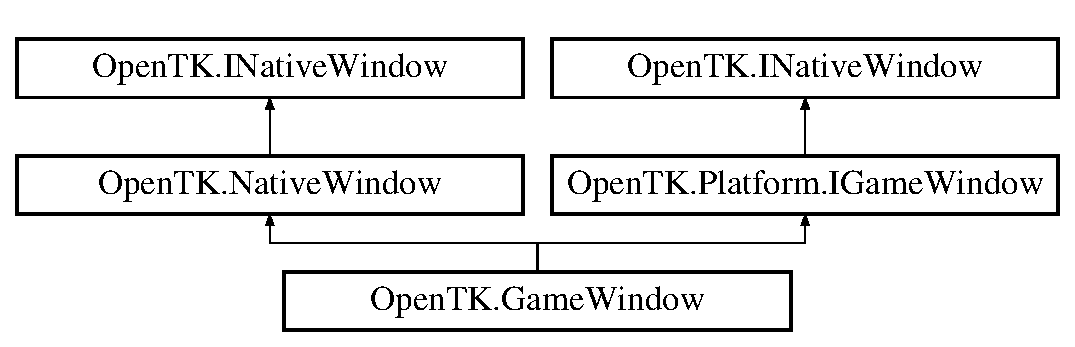
\includegraphics[height=3.000000cm]{class_open_t_k_1_1_game_window}
\end{center}
\end{figure}
\subsection*{Public Member Functions}
\begin{DoxyCompactItemize}
\item 
\hyperlink{class_open_t_k_1_1_game_window_a03787ebe6e9bbc2cf29b17d77e757c47}{Game\-Window} ()
\begin{DoxyCompactList}\small\item\em Constructs a new \hyperlink{class_open_t_k_1_1_game_window}{Game\-Window} with sensible default attributes.\end{DoxyCompactList}\item 
\hyperlink{class_open_t_k_1_1_game_window_a6c4be0e7db916803eef71918b388f65c}{Game\-Window} (int width, int height)
\begin{DoxyCompactList}\small\item\em Constructs a new \hyperlink{class_open_t_k_1_1_game_window}{Game\-Window} with the specified attributes.\end{DoxyCompactList}\item 
\hyperlink{class_open_t_k_1_1_game_window_af7e0cb6ae69630e600844b85e1272212}{Game\-Window} (int width, int height, \hyperlink{class_open_t_k_1_1_graphics_1_1_graphics_mode}{Graphics\-Mode} mode)
\begin{DoxyCompactList}\small\item\em Constructs a new \hyperlink{class_open_t_k_1_1_game_window}{Game\-Window} with the specified attributes.\end{DoxyCompactList}\item 
\hyperlink{class_open_t_k_1_1_game_window_a2b0edf27b00276920abcc97b7b05218b}{Game\-Window} (int width, int height, \hyperlink{class_open_t_k_1_1_graphics_1_1_graphics_mode}{Graphics\-Mode} mode, string title)
\begin{DoxyCompactList}\small\item\em Constructs a new \hyperlink{class_open_t_k_1_1_game_window}{Game\-Window} with the specified attributes.\end{DoxyCompactList}\item 
\hyperlink{class_open_t_k_1_1_game_window_a7de515a0cdf71925d6d12b5803e9c513}{Game\-Window} (int width, int height, \hyperlink{class_open_t_k_1_1_graphics_1_1_graphics_mode}{Graphics\-Mode} mode, string title, \hyperlink{namespace_open_t_k_af73dc15fc9d5b87827c81fa11b3ec6f0}{Game\-Window\-Flags} options)
\begin{DoxyCompactList}\small\item\em Constructs a new \hyperlink{class_open_t_k_1_1_game_window}{Game\-Window} with the specified attributes.\end{DoxyCompactList}\item 
\hyperlink{class_open_t_k_1_1_game_window_a90aa895bd34e5d602dd84aacc1a25b16}{Game\-Window} (int width, int height, \hyperlink{class_open_t_k_1_1_graphics_1_1_graphics_mode}{Graphics\-Mode} mode, string title, \hyperlink{namespace_open_t_k_af73dc15fc9d5b87827c81fa11b3ec6f0}{Game\-Window\-Flags} options, \hyperlink{class_open_t_k_1_1_display_device}{Display\-Device} device)
\begin{DoxyCompactList}\small\item\em Constructs a new \hyperlink{class_open_t_k_1_1_game_window}{Game\-Window} with the specified attributes.\end{DoxyCompactList}\item 
\hyperlink{class_open_t_k_1_1_game_window_a58bde9e41f887e4c1e8b46b409bdcb8e}{Game\-Window} (int width, int height, \hyperlink{class_open_t_k_1_1_graphics_1_1_graphics_mode}{Graphics\-Mode} mode, string title, \hyperlink{namespace_open_t_k_af73dc15fc9d5b87827c81fa11b3ec6f0}{Game\-Window\-Flags} options, \hyperlink{class_open_t_k_1_1_display_device}{Display\-Device} device, int major, int minor, \hyperlink{namespace_open_t_k_1_1_graphics_a518f77952bc406a013160356981ea8ab}{Graphics\-Context\-Flags} flags)
\begin{DoxyCompactList}\small\item\em Constructs a new \hyperlink{class_open_t_k_1_1_game_window}{Game\-Window} with the specified attributes.\end{DoxyCompactList}\item 
\hyperlink{class_open_t_k_1_1_game_window_a3d7f0ea4fc9284bc967f0a42d5b084e4}{Game\-Window} (int width, int height, \hyperlink{class_open_t_k_1_1_graphics_1_1_graphics_mode}{Graphics\-Mode} mode, string title, \hyperlink{namespace_open_t_k_af73dc15fc9d5b87827c81fa11b3ec6f0}{Game\-Window\-Flags} options, \hyperlink{class_open_t_k_1_1_display_device}{Display\-Device} device, int major, int minor, \hyperlink{namespace_open_t_k_1_1_graphics_a518f77952bc406a013160356981ea8ab}{Graphics\-Context\-Flags} flags, \hyperlink{interface_open_t_k_1_1_graphics_1_1_i_graphics_context}{I\-Graphics\-Context} shared\-Context)
\begin{DoxyCompactList}\small\item\em Constructs a new \hyperlink{class_open_t_k_1_1_game_window}{Game\-Window} with the specified attributes.\end{DoxyCompactList}\item 
override void \hyperlink{class_open_t_k_1_1_game_window_acfd19fafb5563df42e2104ea38c2889a}{Dispose} ()
\begin{DoxyCompactList}\small\item\em Disposes of the \hyperlink{class_open_t_k_1_1_game_window}{Game\-Window}, releasing all resources consumed by it. \end{DoxyCompactList}\item 
virtual void \hyperlink{class_open_t_k_1_1_game_window_a67c26214c431300b56b0f4a88bbbd244}{Exit} ()
\begin{DoxyCompactList}\small\item\em Closes the \hyperlink{class_open_t_k_1_1_game_window}{Game\-Window}. Equivalent to \hyperlink{class_open_t_k_1_1_native_window_ae7dae9eca1c2298dbcdbc34a81304a61}{Native\-Window.\-Close} method. \end{DoxyCompactList}\item 
void \hyperlink{class_open_t_k_1_1_game_window_a84d84a7173903a8d991e6ca3d40a7a4b}{Make\-Current} ()
\begin{DoxyCompactList}\small\item\em Makes the Graphics\-Context current on the calling thread. \end{DoxyCompactList}\item 
void \hyperlink{class_open_t_k_1_1_game_window_a2ead9bd94f36e26e86da79ef548e7d6b}{Run} ()
\begin{DoxyCompactList}\small\item\em Enters the game loop of the \hyperlink{class_open_t_k_1_1_game_window}{Game\-Window} using the maximum update rate. \end{DoxyCompactList}\item 
void \hyperlink{class_open_t_k_1_1_game_window_a0c9d2a547ee1dc8f59ad0e70c2552730}{Run} (double update\-Rate)
\begin{DoxyCompactList}\small\item\em Enters the game loop of the \hyperlink{class_open_t_k_1_1_game_window}{Game\-Window} using the specified update rate. maximum possible render frequency. \end{DoxyCompactList}\item 
void \hyperlink{class_open_t_k_1_1_game_window_aff16d3a5aeb78782c4a9f8e74c8d0e89}{Run} (double updates\-\_\-per\-\_\-second, double frames\-\_\-per\-\_\-second)
\begin{DoxyCompactList}\small\item\em Enters the game loop of the \hyperlink{class_open_t_k_1_1_game_window}{Game\-Window} updating and rendering at the specified frequency. \end{DoxyCompactList}\item 
void \hyperlink{class_open_t_k_1_1_game_window_adeaeff9283d467a5cda90e6b8579543a}{Swap\-Buffers} ()
\begin{DoxyCompactList}\small\item\em Swaps the front and back buffer, presenting the rendered scene to the user. \end{DoxyCompactList}\end{DoxyCompactItemize}
\subsection*{Protected Member Functions}
\begin{DoxyCompactItemize}
\item 
override void \hyperlink{class_open_t_k_1_1_game_window_ac2bfae65b7874a59517461c72ce66663}{On\-Closing} (System.\-Component\-Model.\-Cancel\-Event\-Args e)
\begin{DoxyCompactList}\small\item\em Called when the \hyperlink{class_open_t_k_1_1_native_window}{Native\-Window} is about to close. \end{DoxyCompactList}\item 
virtual void \hyperlink{class_open_t_k_1_1_game_window_ae4e7becd70baac5336bdc9b67f11bfec}{On\-Load} (Event\-Args e)
\begin{DoxyCompactList}\small\item\em Called after an Open\-G\-L context has been established, but before entering the main loop. \end{DoxyCompactList}\item 
virtual void \hyperlink{class_open_t_k_1_1_game_window_ad993aec512d39466135f8db9185d3588}{On\-Unload} (Event\-Args e)
\begin{DoxyCompactList}\small\item\em Called after \hyperlink{class_open_t_k_1_1_game_window_a67c26214c431300b56b0f4a88bbbd244}{Game\-Window.\-Exit} was called, but before destroying the Open\-G\-L context. \end{DoxyCompactList}\item 
virtual void \hyperlink{class_open_t_k_1_1_game_window_a7dd618cf51ddede98772041ddaa729db}{Dispose} (bool manual)
\begin{DoxyCompactList}\small\item\em Override to add custom cleanup logic. \end{DoxyCompactList}\item 
virtual void \hyperlink{class_open_t_k_1_1_game_window_abc3e3a8c21a36d226c9d899f094152a4}{On\-Render\-Frame} (\hyperlink{class_open_t_k_1_1_frame_event_args}{Frame\-Event\-Args} e)
\begin{DoxyCompactList}\small\item\em Called when the frame is rendered. \end{DoxyCompactList}\item 
virtual void \hyperlink{class_open_t_k_1_1_game_window_a081795ead94557090f58e83d471b0d05}{On\-Update\-Frame} (\hyperlink{class_open_t_k_1_1_frame_event_args}{Frame\-Event\-Args} e)
\begin{DoxyCompactList}\small\item\em Called when the frame is updated. \end{DoxyCompactList}\item 
virtual void \hyperlink{class_open_t_k_1_1_game_window_a1b6723c6415c35586b23eabf5a9e51ca}{On\-Window\-Info\-Changed} (Event\-Args e)
\begin{DoxyCompactList}\small\item\em Called when the Window\-Info for this \hyperlink{class_open_t_k_1_1_game_window}{Game\-Window} has changed. \end{DoxyCompactList}\item 
override void \hyperlink{class_open_t_k_1_1_game_window_a730fe82126e7616bccba531bb2abc770}{On\-Resize} (Event\-Args e)
\begin{DoxyCompactList}\small\item\em Called when this window is resized. \end{DoxyCompactList}\end{DoxyCompactItemize}
\subsection*{Properties}
\begin{DoxyCompactItemize}
\item 
\hyperlink{interface_open_t_k_1_1_graphics_1_1_i_graphics_context}{I\-Graphics\-Context} \hyperlink{class_open_t_k_1_1_game_window_a5c17f9c8850e2c20c23bf855bb303cb1}{Context}\hspace{0.3cm}{\ttfamily  \mbox{[}get\mbox{]}}
\begin{DoxyCompactList}\small\item\em Returns the opengl I\-Graphics\-Context associated with the current \hyperlink{class_open_t_k_1_1_game_window}{Game\-Window}. \end{DoxyCompactList}\item 
bool \hyperlink{class_open_t_k_1_1_game_window_a0ec80251b70858617ce91d3aa65a8174}{Is\-Exiting}\hspace{0.3cm}{\ttfamily  \mbox{[}get\mbox{]}}
\begin{DoxyCompactList}\small\item\em Gets a value indicating whether the shutdown sequence has been initiated for this window, by calling \hyperlink{class_open_t_k_1_1_game_window_a67c26214c431300b56b0f4a88bbbd244}{Game\-Window.\-Exit()} or hitting the 'close' button. If this property is true, it is no longer safe to use any \hyperlink{namespace_open_t_k_1_1_input}{Open\-T\-K.\-Input} or \hyperlink{namespace_open_t_k_1_1_graphics_1_1_open_g_l}{Open\-T\-K.\-Graphics.\-Open\-G\-L} functions or properties. \end{DoxyCompactList}\item 
I\-List$<$ \hyperlink{class_open_t_k_1_1_input_1_1_joystick_device}{Joystick\-Device} $>$ \hyperlink{class_open_t_k_1_1_game_window_a97fe86dfe28cd8c059e53dc22a20458a}{Joysticks}\hspace{0.3cm}{\ttfamily  \mbox{[}get\mbox{]}}
\begin{DoxyCompactList}\small\item\em Gets a readonly I\-List containing all available Open\-T\-K.\-Input.\-Joystick\-Devices. \end{DoxyCompactList}\item 
\hyperlink{class_open_t_k_1_1_input_1_1_keyboard_device}{Keyboard\-Device} \hyperlink{class_open_t_k_1_1_game_window_a1d5ef67f9be67c7355cacbde9872e09e}{Keyboard}\hspace{0.3cm}{\ttfamily  \mbox{[}get\mbox{]}}
\begin{DoxyCompactList}\small\item\em Gets the primary Keyboard device, or null if no Keyboard exists. \end{DoxyCompactList}\item 
\hyperlink{class_open_t_k_1_1_input_1_1_mouse_device}{Mouse\-Device} \hyperlink{class_open_t_k_1_1_game_window_acdb499cde709b6a6b8630613954094f9}{Mouse}\hspace{0.3cm}{\ttfamily  \mbox{[}get\mbox{]}}
\begin{DoxyCompactList}\small\item\em Gets the primary Mouse device, or null if no Mouse exists. \end{DoxyCompactList}\item 
double \hyperlink{class_open_t_k_1_1_game_window_a6657b7cd7da85b770580c840a197f30b}{Render\-Frequency}\hspace{0.3cm}{\ttfamily  \mbox{[}get\mbox{]}}
\begin{DoxyCompactList}\small\item\em Gets a double representing the actual frequency of Render\-Frame events, in hertz (i.\-e. fps or frames per second). \end{DoxyCompactList}\item 
double \hyperlink{class_open_t_k_1_1_game_window_aad1395cb550c3eea673b447c84990c2c}{Render\-Period}\hspace{0.3cm}{\ttfamily  \mbox{[}get\mbox{]}}
\begin{DoxyCompactList}\small\item\em Gets a double representing the period of Render\-Frame events, in seconds. \end{DoxyCompactList}\item 
double \hyperlink{class_open_t_k_1_1_game_window_a1462d45526351e92b948f0b329c77d56}{Render\-Time}\hspace{0.3cm}{\ttfamily  \mbox{[}get, set\mbox{]}}
\begin{DoxyCompactList}\small\item\em Gets a double representing the time spent in the Render\-Frame function, in seconds. \end{DoxyCompactList}\item 
double \hyperlink{class_open_t_k_1_1_game_window_ae604e886eca5028a0d2252bf6d52434a}{Target\-Render\-Frequency}\hspace{0.3cm}{\ttfamily  \mbox{[}get, set\mbox{]}}
\begin{DoxyCompactList}\small\item\em Gets or sets a double representing the target render frequency, in hertz. \end{DoxyCompactList}\item 
double \hyperlink{class_open_t_k_1_1_game_window_a2233cfb62a42200251dcdb1dab643a36}{Target\-Render\-Period}\hspace{0.3cm}{\ttfamily  \mbox{[}get, set\mbox{]}}
\begin{DoxyCompactList}\small\item\em Gets or sets a double representing the target render period, in seconds. \end{DoxyCompactList}\item 
double \hyperlink{class_open_t_k_1_1_game_window_acf250353ae71ed429642335d614da7c5}{Target\-Update\-Frequency}\hspace{0.3cm}{\ttfamily  \mbox{[}get, set\mbox{]}}
\begin{DoxyCompactList}\small\item\em Gets or sets a double representing the target update frequency, in hertz. \end{DoxyCompactList}\item 
double \hyperlink{class_open_t_k_1_1_game_window_a3fb751962cfcd5c95ad4b9fb84f40dbb}{Target\-Update\-Period}\hspace{0.3cm}{\ttfamily  \mbox{[}get, set\mbox{]}}
\begin{DoxyCompactList}\small\item\em Gets or sets a double representing the target update period, in seconds. \end{DoxyCompactList}\item 
double \hyperlink{class_open_t_k_1_1_game_window_aeee75eb97d0c305788b802a09fac3540}{Update\-Frequency}\hspace{0.3cm}{\ttfamily  \mbox{[}get\mbox{]}}
\begin{DoxyCompactList}\small\item\em Gets a double representing the frequency of Update\-Frame events, in hertz. \end{DoxyCompactList}\item 
double \hyperlink{class_open_t_k_1_1_game_window_a1a44982a760d216e014c79dbf472f779}{Update\-Period}\hspace{0.3cm}{\ttfamily  \mbox{[}get\mbox{]}}
\begin{DoxyCompactList}\small\item\em Gets a double representing the period of Update\-Frame events, in seconds. \end{DoxyCompactList}\item 
double \hyperlink{class_open_t_k_1_1_game_window_a324f362ab849612bb7a82ac84de92be0}{Update\-Time}\hspace{0.3cm}{\ttfamily  \mbox{[}get\mbox{]}}
\begin{DoxyCompactList}\small\item\em Gets a double representing the time spent in the Update\-Frame function, in seconds. \end{DoxyCompactList}\item 
\hyperlink{namespace_open_t_k_a1c0421cc4ecbb6d5e57317906fe8b8d3}{V\-Sync\-Mode} \hyperlink{class_open_t_k_1_1_game_window_a13246c847d807cc510fd0fa8a58ae24b}{V\-Sync}\hspace{0.3cm}{\ttfamily  \mbox{[}get, set\mbox{]}}
\begin{DoxyCompactList}\small\item\em Gets or sets the V\-Sync\-Mode. \end{DoxyCompactList}\item 
override \hyperlink{namespace_open_t_k_ace9268dc87bd36f48c9d9d8b939559b4}{Window\-State} \hyperlink{class_open_t_k_1_1_game_window_a2645b832f9583c904a9e0c83951ed9d4}{Window\-State}\hspace{0.3cm}{\ttfamily  \mbox{[}get, set\mbox{]}}
\begin{DoxyCompactList}\small\item\em Gets or states the state of the \hyperlink{class_open_t_k_1_1_native_window}{Native\-Window}. \end{DoxyCompactList}\end{DoxyCompactItemize}
\subsection*{Events}
\begin{DoxyCompactItemize}
\item 
Event\-Handler$<$ Event\-Args $>$ \hyperlink{class_open_t_k_1_1_game_window_a5d449a387cf4600251fc534fd49bdbc3}{Load} = delegate \{ \}
\begin{DoxyCompactList}\small\item\em Occurs before the window is displayed for the first time. \end{DoxyCompactList}\item 
Event\-Handler$<$ \hyperlink{class_open_t_k_1_1_frame_event_args}{Frame\-Event\-Args} $>$ \hyperlink{class_open_t_k_1_1_game_window_a299211a98496fdac0a526a353dd5f25a}{Render\-Frame} = delegate \{ \}
\begin{DoxyCompactList}\small\item\em Occurs when it is time to render a frame. \end{DoxyCompactList}\item 
Event\-Handler$<$ Event\-Args $>$ \hyperlink{class_open_t_k_1_1_game_window_a039f40ed67b4d0c64e292c7e9e77e80b}{Unload} = delegate \{ \}
\begin{DoxyCompactList}\small\item\em Occurs before the window is destroyed. \end{DoxyCompactList}\item 
Event\-Handler$<$ \hyperlink{class_open_t_k_1_1_frame_event_args}{Frame\-Event\-Args} $>$ \hyperlink{class_open_t_k_1_1_game_window_af3c171dd667a38eb461df532ff6cc016}{Update\-Frame} = delegate \{ \}
\begin{DoxyCompactList}\small\item\em Occurs when it is time to update a frame. \end{DoxyCompactList}\end{DoxyCompactItemize}


\subsection{Detailed Description}
The \hyperlink{class_open_t_k_1_1_game_window}{Game\-Window} class contains cross-\/platform methods to create and render on an Open\-G\-L window, handle input and load resources. 

\hyperlink{class_open_t_k_1_1_game_window}{Game\-Window} contains several events you can hook or override to add your custom logic\-: 
\begin{DoxyItemize}
\item On\-Load\-: Occurs after creating the Open\-G\-L context, but before entering the main loop. Override to load resources.  
\item On\-Unload\-: Occurs after exiting the main loop, but before deleting the Open\-G\-L context. Override to unload resources.  
\item On\-Resize\-: Occurs whenever \hyperlink{class_open_t_k_1_1_game_window}{Game\-Window} is resized. You should update the Open\-G\-L Viewport and Projection Matrix here.  
\item On\-Update\-Frame\-: Occurs at the specified logic update rate. Override to add your game logic.  
\item On\-Render\-Frame\-: Occurs at the specified frame render rate. Override to add your rendering code.  
\end{DoxyItemize}Call the \hyperlink{class_open_t_k_1_1_game_window_a2ead9bd94f36e26e86da79ef548e7d6b}{Run()} method to start the application's main loop. \hyperlink{class_open_t_k_1_1_game_window_aff16d3a5aeb78782c4a9f8e74c8d0e89}{Run(double, double)} takes two parameters that specify the logic update rate, and the render update rate. 

\subsection{Constructor \& Destructor Documentation}
\hypertarget{class_open_t_k_1_1_game_window_a03787ebe6e9bbc2cf29b17d77e757c47}{\index{Open\-T\-K\-::\-Game\-Window@{Open\-T\-K\-::\-Game\-Window}!Game\-Window@{Game\-Window}}
\index{Game\-Window@{Game\-Window}!OpenTK::GameWindow@{Open\-T\-K\-::\-Game\-Window}}
\subsubsection[{Game\-Window}]{\setlength{\rightskip}{0pt plus 5cm}Open\-T\-K.\-Game\-Window.\-Game\-Window (
\begin{DoxyParamCaption}
{}
\end{DoxyParamCaption}
)}}\label{class_open_t_k_1_1_game_window_a03787ebe6e9bbc2cf29b17d77e757c47}


Constructs a new \hyperlink{class_open_t_k_1_1_game_window}{Game\-Window} with sensible default attributes.

\hypertarget{class_open_t_k_1_1_game_window_a6c4be0e7db916803eef71918b388f65c}{\index{Open\-T\-K\-::\-Game\-Window@{Open\-T\-K\-::\-Game\-Window}!Game\-Window@{Game\-Window}}
\index{Game\-Window@{Game\-Window}!OpenTK::GameWindow@{Open\-T\-K\-::\-Game\-Window}}
\subsubsection[{Game\-Window}]{\setlength{\rightskip}{0pt plus 5cm}Open\-T\-K.\-Game\-Window.\-Game\-Window (
\begin{DoxyParamCaption}
\item[{int}]{width, }
\item[{int}]{height}
\end{DoxyParamCaption}
)}}\label{class_open_t_k_1_1_game_window_a6c4be0e7db916803eef71918b388f65c}


Constructs a new \hyperlink{class_open_t_k_1_1_game_window}{Game\-Window} with the specified attributes.


\begin{DoxyParams}{Parameters}
{\em width} & The width of the \hyperlink{class_open_t_k_1_1_game_window}{Game\-Window} in pixels.\\
\hline
{\em height} & The height of the \hyperlink{class_open_t_k_1_1_game_window}{Game\-Window} in pixels.\\
\hline
\end{DoxyParams}
\hypertarget{class_open_t_k_1_1_game_window_af7e0cb6ae69630e600844b85e1272212}{\index{Open\-T\-K\-::\-Game\-Window@{Open\-T\-K\-::\-Game\-Window}!Game\-Window@{Game\-Window}}
\index{Game\-Window@{Game\-Window}!OpenTK::GameWindow@{Open\-T\-K\-::\-Game\-Window}}
\subsubsection[{Game\-Window}]{\setlength{\rightskip}{0pt plus 5cm}Open\-T\-K.\-Game\-Window.\-Game\-Window (
\begin{DoxyParamCaption}
\item[{int}]{width, }
\item[{int}]{height, }
\item[{{\bf Graphics\-Mode}}]{mode}
\end{DoxyParamCaption}
)}}\label{class_open_t_k_1_1_game_window_af7e0cb6ae69630e600844b85e1272212}


Constructs a new \hyperlink{class_open_t_k_1_1_game_window}{Game\-Window} with the specified attributes.


\begin{DoxyParams}{Parameters}
{\em width} & The width of the \hyperlink{class_open_t_k_1_1_game_window}{Game\-Window} in pixels.\\
\hline
{\em height} & The height of the \hyperlink{class_open_t_k_1_1_game_window}{Game\-Window} in pixels.\\
\hline
{\em mode} & The \hyperlink{class_open_t_k_1_1_graphics_1_1_graphics_mode}{Open\-T\-K.\-Graphics.\-Graphics\-Mode} of the \hyperlink{class_open_t_k_1_1_game_window}{Game\-Window}.\\
\hline
\end{DoxyParams}
\hypertarget{class_open_t_k_1_1_game_window_a2b0edf27b00276920abcc97b7b05218b}{\index{Open\-T\-K\-::\-Game\-Window@{Open\-T\-K\-::\-Game\-Window}!Game\-Window@{Game\-Window}}
\index{Game\-Window@{Game\-Window}!OpenTK::GameWindow@{Open\-T\-K\-::\-Game\-Window}}
\subsubsection[{Game\-Window}]{\setlength{\rightskip}{0pt plus 5cm}Open\-T\-K.\-Game\-Window.\-Game\-Window (
\begin{DoxyParamCaption}
\item[{int}]{width, }
\item[{int}]{height, }
\item[{{\bf Graphics\-Mode}}]{mode, }
\item[{string}]{title}
\end{DoxyParamCaption}
)}}\label{class_open_t_k_1_1_game_window_a2b0edf27b00276920abcc97b7b05218b}


Constructs a new \hyperlink{class_open_t_k_1_1_game_window}{Game\-Window} with the specified attributes.


\begin{DoxyParams}{Parameters}
{\em width} & The width of the \hyperlink{class_open_t_k_1_1_game_window}{Game\-Window} in pixels.\\
\hline
{\em height} & The height of the \hyperlink{class_open_t_k_1_1_game_window}{Game\-Window} in pixels.\\
\hline
{\em mode} & The \hyperlink{class_open_t_k_1_1_graphics_1_1_graphics_mode}{Open\-T\-K.\-Graphics.\-Graphics\-Mode} of the \hyperlink{class_open_t_k_1_1_game_window}{Game\-Window}.\\
\hline
{\em title} & The title of the \hyperlink{class_open_t_k_1_1_game_window}{Game\-Window}.\\
\hline
\end{DoxyParams}
\hypertarget{class_open_t_k_1_1_game_window_a7de515a0cdf71925d6d12b5803e9c513}{\index{Open\-T\-K\-::\-Game\-Window@{Open\-T\-K\-::\-Game\-Window}!Game\-Window@{Game\-Window}}
\index{Game\-Window@{Game\-Window}!OpenTK::GameWindow@{Open\-T\-K\-::\-Game\-Window}}
\subsubsection[{Game\-Window}]{\setlength{\rightskip}{0pt plus 5cm}Open\-T\-K.\-Game\-Window.\-Game\-Window (
\begin{DoxyParamCaption}
\item[{int}]{width, }
\item[{int}]{height, }
\item[{{\bf Graphics\-Mode}}]{mode, }
\item[{string}]{title, }
\item[{{\bf Game\-Window\-Flags}}]{options}
\end{DoxyParamCaption}
)}}\label{class_open_t_k_1_1_game_window_a7de515a0cdf71925d6d12b5803e9c513}


Constructs a new \hyperlink{class_open_t_k_1_1_game_window}{Game\-Window} with the specified attributes.


\begin{DoxyParams}{Parameters}
{\em width} & The width of the \hyperlink{class_open_t_k_1_1_game_window}{Game\-Window} in pixels.\\
\hline
{\em height} & The height of the \hyperlink{class_open_t_k_1_1_game_window}{Game\-Window} in pixels.\\
\hline
{\em mode} & The \hyperlink{class_open_t_k_1_1_graphics_1_1_graphics_mode}{Open\-T\-K.\-Graphics.\-Graphics\-Mode} of the \hyperlink{class_open_t_k_1_1_game_window}{Game\-Window}.\\
\hline
{\em title} & The title of the \hyperlink{class_open_t_k_1_1_game_window}{Game\-Window}.\\
\hline
{\em options} & \hyperlink{class_open_t_k_1_1_game_window}{Game\-Window} options regarding window appearance and behavior.\\
\hline
\end{DoxyParams}
\hypertarget{class_open_t_k_1_1_game_window_a90aa895bd34e5d602dd84aacc1a25b16}{\index{Open\-T\-K\-::\-Game\-Window@{Open\-T\-K\-::\-Game\-Window}!Game\-Window@{Game\-Window}}
\index{Game\-Window@{Game\-Window}!OpenTK::GameWindow@{Open\-T\-K\-::\-Game\-Window}}
\subsubsection[{Game\-Window}]{\setlength{\rightskip}{0pt plus 5cm}Open\-T\-K.\-Game\-Window.\-Game\-Window (
\begin{DoxyParamCaption}
\item[{int}]{width, }
\item[{int}]{height, }
\item[{{\bf Graphics\-Mode}}]{mode, }
\item[{string}]{title, }
\item[{{\bf Game\-Window\-Flags}}]{options, }
\item[{{\bf Display\-Device}}]{device}
\end{DoxyParamCaption}
)}}\label{class_open_t_k_1_1_game_window_a90aa895bd34e5d602dd84aacc1a25b16}


Constructs a new \hyperlink{class_open_t_k_1_1_game_window}{Game\-Window} with the specified attributes.


\begin{DoxyParams}{Parameters}
{\em width} & The width of the \hyperlink{class_open_t_k_1_1_game_window}{Game\-Window} in pixels.\\
\hline
{\em height} & The height of the \hyperlink{class_open_t_k_1_1_game_window}{Game\-Window} in pixels.\\
\hline
{\em mode} & The \hyperlink{class_open_t_k_1_1_graphics_1_1_graphics_mode}{Open\-T\-K.\-Graphics.\-Graphics\-Mode} of the \hyperlink{class_open_t_k_1_1_game_window}{Game\-Window}.\\
\hline
{\em title} & The title of the \hyperlink{class_open_t_k_1_1_game_window}{Game\-Window}.\\
\hline
{\em options} & \hyperlink{class_open_t_k_1_1_game_window}{Game\-Window} options regarding window appearance and behavior.\\
\hline
{\em device} & The Open\-T\-K.\-Graphics.\-Display\-Device to construct the \hyperlink{class_open_t_k_1_1_game_window}{Game\-Window} in.\\
\hline
\end{DoxyParams}
\hypertarget{class_open_t_k_1_1_game_window_a58bde9e41f887e4c1e8b46b409bdcb8e}{\index{Open\-T\-K\-::\-Game\-Window@{Open\-T\-K\-::\-Game\-Window}!Game\-Window@{Game\-Window}}
\index{Game\-Window@{Game\-Window}!OpenTK::GameWindow@{Open\-T\-K\-::\-Game\-Window}}
\subsubsection[{Game\-Window}]{\setlength{\rightskip}{0pt plus 5cm}Open\-T\-K.\-Game\-Window.\-Game\-Window (
\begin{DoxyParamCaption}
\item[{int}]{width, }
\item[{int}]{height, }
\item[{{\bf Graphics\-Mode}}]{mode, }
\item[{string}]{title, }
\item[{{\bf Game\-Window\-Flags}}]{options, }
\item[{{\bf Display\-Device}}]{device, }
\item[{int}]{major, }
\item[{int}]{minor, }
\item[{{\bf Graphics\-Context\-Flags}}]{flags}
\end{DoxyParamCaption}
)}}\label{class_open_t_k_1_1_game_window_a58bde9e41f887e4c1e8b46b409bdcb8e}


Constructs a new \hyperlink{class_open_t_k_1_1_game_window}{Game\-Window} with the specified attributes.


\begin{DoxyParams}{Parameters}
{\em width} & The width of the \hyperlink{class_open_t_k_1_1_game_window}{Game\-Window} in pixels.\\
\hline
{\em height} & The height of the \hyperlink{class_open_t_k_1_1_game_window}{Game\-Window} in pixels.\\
\hline
{\em mode} & The \hyperlink{class_open_t_k_1_1_graphics_1_1_graphics_mode}{Open\-T\-K.\-Graphics.\-Graphics\-Mode} of the \hyperlink{class_open_t_k_1_1_game_window}{Game\-Window}.\\
\hline
{\em title} & The title of the \hyperlink{class_open_t_k_1_1_game_window}{Game\-Window}.\\
\hline
{\em options} & \hyperlink{class_open_t_k_1_1_game_window}{Game\-Window} options regarding window appearance and behavior.\\
\hline
{\em device} & The Open\-T\-K.\-Graphics.\-Display\-Device to construct the \hyperlink{class_open_t_k_1_1_game_window}{Game\-Window} in.\\
\hline
{\em major} & The major version for the Open\-G\-L Graphics\-Context.\\
\hline
{\em minor} & The minor version for the Open\-G\-L Graphics\-Context.\\
\hline
{\em flags} & The Graphics\-Context\-Flags version for the Open\-G\-L Graphics\-Context.\\
\hline
\end{DoxyParams}
\hypertarget{class_open_t_k_1_1_game_window_a3d7f0ea4fc9284bc967f0a42d5b084e4}{\index{Open\-T\-K\-::\-Game\-Window@{Open\-T\-K\-::\-Game\-Window}!Game\-Window@{Game\-Window}}
\index{Game\-Window@{Game\-Window}!OpenTK::GameWindow@{Open\-T\-K\-::\-Game\-Window}}
\subsubsection[{Game\-Window}]{\setlength{\rightskip}{0pt plus 5cm}Open\-T\-K.\-Game\-Window.\-Game\-Window (
\begin{DoxyParamCaption}
\item[{int}]{width, }
\item[{int}]{height, }
\item[{{\bf Graphics\-Mode}}]{mode, }
\item[{string}]{title, }
\item[{{\bf Game\-Window\-Flags}}]{options, }
\item[{{\bf Display\-Device}}]{device, }
\item[{int}]{major, }
\item[{int}]{minor, }
\item[{{\bf Graphics\-Context\-Flags}}]{flags, }
\item[{{\bf I\-Graphics\-Context}}]{shared\-Context}
\end{DoxyParamCaption}
)}}\label{class_open_t_k_1_1_game_window_a3d7f0ea4fc9284bc967f0a42d5b084e4}


Constructs a new \hyperlink{class_open_t_k_1_1_game_window}{Game\-Window} with the specified attributes.


\begin{DoxyParams}{Parameters}
{\em width} & The width of the \hyperlink{class_open_t_k_1_1_game_window}{Game\-Window} in pixels.\\
\hline
{\em height} & The height of the \hyperlink{class_open_t_k_1_1_game_window}{Game\-Window} in pixels.\\
\hline
{\em mode} & The \hyperlink{class_open_t_k_1_1_graphics_1_1_graphics_mode}{Open\-T\-K.\-Graphics.\-Graphics\-Mode} of the \hyperlink{class_open_t_k_1_1_game_window}{Game\-Window}.\\
\hline
{\em title} & The title of the \hyperlink{class_open_t_k_1_1_game_window}{Game\-Window}.\\
\hline
{\em options} & \hyperlink{class_open_t_k_1_1_game_window}{Game\-Window} options regarding window appearance and behavior.\\
\hline
{\em device} & The Open\-T\-K.\-Graphics.\-Display\-Device to construct the \hyperlink{class_open_t_k_1_1_game_window}{Game\-Window} in.\\
\hline
{\em major} & The major version for the Open\-G\-L Graphics\-Context.\\
\hline
{\em minor} & The minor version for the Open\-G\-L Graphics\-Context.\\
\hline
{\em flags} & The Graphics\-Context\-Flags version for the Open\-G\-L Graphics\-Context.\\
\hline
{\em shared\-Context} & An I\-Graphics\-Context to share resources with.\\
\hline
\end{DoxyParams}


\subsection{Member Function Documentation}
\hypertarget{class_open_t_k_1_1_game_window_acfd19fafb5563df42e2104ea38c2889a}{\index{Open\-T\-K\-::\-Game\-Window@{Open\-T\-K\-::\-Game\-Window}!Dispose@{Dispose}}
\index{Dispose@{Dispose}!OpenTK::GameWindow@{Open\-T\-K\-::\-Game\-Window}}
\subsubsection[{Dispose}]{\setlength{\rightskip}{0pt plus 5cm}override void Open\-T\-K.\-Game\-Window.\-Dispose (
\begin{DoxyParamCaption}
{}
\end{DoxyParamCaption}
)\hspace{0.3cm}{\ttfamily [virtual]}}}\label{class_open_t_k_1_1_game_window_acfd19fafb5563df42e2104ea38c2889a}


Disposes of the \hyperlink{class_open_t_k_1_1_game_window}{Game\-Window}, releasing all resources consumed by it. 



Reimplemented from \hyperlink{class_open_t_k_1_1_native_window_a1cc77f20d1c61f32d62e03896e358d20}{Open\-T\-K.\-Native\-Window}.

\hypertarget{class_open_t_k_1_1_game_window_a7dd618cf51ddede98772041ddaa729db}{\index{Open\-T\-K\-::\-Game\-Window@{Open\-T\-K\-::\-Game\-Window}!Dispose@{Dispose}}
\index{Dispose@{Dispose}!OpenTK::GameWindow@{Open\-T\-K\-::\-Game\-Window}}
\subsubsection[{Dispose}]{\setlength{\rightskip}{0pt plus 5cm}virtual void Open\-T\-K.\-Game\-Window.\-Dispose (
\begin{DoxyParamCaption}
\item[{bool}]{manual}
\end{DoxyParamCaption}
)\hspace{0.3cm}{\ttfamily [protected]}, {\ttfamily [virtual]}}}\label{class_open_t_k_1_1_game_window_a7dd618cf51ddede98772041ddaa729db}


Override to add custom cleanup logic. 


\begin{DoxyParams}{Parameters}
{\em manual} & True, if this method was called by the application; false if this was called by the finalizer thread.\\
\hline
\end{DoxyParams}
\hypertarget{class_open_t_k_1_1_game_window_a67c26214c431300b56b0f4a88bbbd244}{\index{Open\-T\-K\-::\-Game\-Window@{Open\-T\-K\-::\-Game\-Window}!Exit@{Exit}}
\index{Exit@{Exit}!OpenTK::GameWindow@{Open\-T\-K\-::\-Game\-Window}}
\subsubsection[{Exit}]{\setlength{\rightskip}{0pt plus 5cm}virtual void Open\-T\-K.\-Game\-Window.\-Exit (
\begin{DoxyParamCaption}
{}
\end{DoxyParamCaption}
)\hspace{0.3cm}{\ttfamily [virtual]}}}\label{class_open_t_k_1_1_game_window_a67c26214c431300b56b0f4a88bbbd244}


Closes the \hyperlink{class_open_t_k_1_1_game_window}{Game\-Window}. Equivalent to \hyperlink{class_open_t_k_1_1_native_window_ae7dae9eca1c2298dbcdbc34a81304a61}{Native\-Window.\-Close} method. 

Override if you are not using \hyperlink{class_open_t_k_1_1_game_window_a2ead9bd94f36e26e86da79ef548e7d6b}{Game\-Window.\-Run()}.

If you override this method, place a call to base.\-Exit(), to ensure proper \hyperlink{namespace_open_t_k}{Open\-T\-K} shutdown.\hypertarget{class_open_t_k_1_1_game_window_a84d84a7173903a8d991e6ca3d40a7a4b}{\index{Open\-T\-K\-::\-Game\-Window@{Open\-T\-K\-::\-Game\-Window}!Make\-Current@{Make\-Current}}
\index{Make\-Current@{Make\-Current}!OpenTK::GameWindow@{Open\-T\-K\-::\-Game\-Window}}
\subsubsection[{Make\-Current}]{\setlength{\rightskip}{0pt plus 5cm}void Open\-T\-K.\-Game\-Window.\-Make\-Current (
\begin{DoxyParamCaption}
{}
\end{DoxyParamCaption}
)}}\label{class_open_t_k_1_1_game_window_a84d84a7173903a8d991e6ca3d40a7a4b}


Makes the Graphics\-Context current on the calling thread. 



Implements \hyperlink{interface_open_t_k_1_1_platform_1_1_i_game_window_a82429a99533b04e178b4e6b7893efb17}{Open\-T\-K.\-Platform.\-I\-Game\-Window}.

\hypertarget{class_open_t_k_1_1_game_window_ac2bfae65b7874a59517461c72ce66663}{\index{Open\-T\-K\-::\-Game\-Window@{Open\-T\-K\-::\-Game\-Window}!On\-Closing@{On\-Closing}}
\index{On\-Closing@{On\-Closing}!OpenTK::GameWindow@{Open\-T\-K\-::\-Game\-Window}}
\subsubsection[{On\-Closing}]{\setlength{\rightskip}{0pt plus 5cm}override void Open\-T\-K.\-Game\-Window.\-On\-Closing (
\begin{DoxyParamCaption}
\item[{System.\-Component\-Model.\-Cancel\-Event\-Args}]{e}
\end{DoxyParamCaption}
)\hspace{0.3cm}{\ttfamily [protected]}}}\label{class_open_t_k_1_1_game_window_ac2bfae65b7874a59517461c72ce66663}


Called when the \hyperlink{class_open_t_k_1_1_native_window}{Native\-Window} is about to close. 


\begin{DoxyParams}{Parameters}
{\em e} & The System.\-Component\-Model.\-Cancel\-Event\-Args for this event. Set e.\-Cancel to true in order to stop the \hyperlink{class_open_t_k_1_1_game_window}{Game\-Window} from closing.\\
\hline
\end{DoxyParams}
\hypertarget{class_open_t_k_1_1_game_window_ae4e7becd70baac5336bdc9b67f11bfec}{\index{Open\-T\-K\-::\-Game\-Window@{Open\-T\-K\-::\-Game\-Window}!On\-Load@{On\-Load}}
\index{On\-Load@{On\-Load}!OpenTK::GameWindow@{Open\-T\-K\-::\-Game\-Window}}
\subsubsection[{On\-Load}]{\setlength{\rightskip}{0pt plus 5cm}virtual void Open\-T\-K.\-Game\-Window.\-On\-Load (
\begin{DoxyParamCaption}
\item[{Event\-Args}]{e}
\end{DoxyParamCaption}
)\hspace{0.3cm}{\ttfamily [protected]}, {\ttfamily [virtual]}}}\label{class_open_t_k_1_1_game_window_ae4e7becd70baac5336bdc9b67f11bfec}


Called after an Open\-G\-L context has been established, but before entering the main loop. 


\begin{DoxyParams}{Parameters}
{\em e} & Not used.\\
\hline
\end{DoxyParams}
\hypertarget{class_open_t_k_1_1_game_window_abc3e3a8c21a36d226c9d899f094152a4}{\index{Open\-T\-K\-::\-Game\-Window@{Open\-T\-K\-::\-Game\-Window}!On\-Render\-Frame@{On\-Render\-Frame}}
\index{On\-Render\-Frame@{On\-Render\-Frame}!OpenTK::GameWindow@{Open\-T\-K\-::\-Game\-Window}}
\subsubsection[{On\-Render\-Frame}]{\setlength{\rightskip}{0pt plus 5cm}virtual void Open\-T\-K.\-Game\-Window.\-On\-Render\-Frame (
\begin{DoxyParamCaption}
\item[{{\bf Frame\-Event\-Args}}]{e}
\end{DoxyParamCaption}
)\hspace{0.3cm}{\ttfamily [protected]}, {\ttfamily [virtual]}}}\label{class_open_t_k_1_1_game_window_abc3e3a8c21a36d226c9d899f094152a4}


Called when the frame is rendered. 


\begin{DoxyParams}{Parameters}
{\em e} & Contains information necessary for frame rendering.\\
\hline
\end{DoxyParams}


Subscribe to the \hyperlink{class_open_t_k_1_1_game_window_a299211a98496fdac0a526a353dd5f25a}{Render\-Frame} event instead of overriding this method. \hypertarget{class_open_t_k_1_1_game_window_a730fe82126e7616bccba531bb2abc770}{\index{Open\-T\-K\-::\-Game\-Window@{Open\-T\-K\-::\-Game\-Window}!On\-Resize@{On\-Resize}}
\index{On\-Resize@{On\-Resize}!OpenTK::GameWindow@{Open\-T\-K\-::\-Game\-Window}}
\subsubsection[{On\-Resize}]{\setlength{\rightskip}{0pt plus 5cm}override void Open\-T\-K.\-Game\-Window.\-On\-Resize (
\begin{DoxyParamCaption}
\item[{Event\-Args}]{e}
\end{DoxyParamCaption}
)\hspace{0.3cm}{\ttfamily [protected]}, {\ttfamily [virtual]}}}\label{class_open_t_k_1_1_game_window_a730fe82126e7616bccba531bb2abc770}


Called when this window is resized. 


\begin{DoxyParams}{Parameters}
{\em e} & Not used.\\
\hline
\end{DoxyParams}


You will typically wish to update your viewport whenever the window is resized. See the Open\-T\-K.\-Graphics.\-Open\-G\-L.\-G\-L.\-Viewport(int, int, int, int) method. 

Reimplemented from \hyperlink{class_open_t_k_1_1_native_window_a647ac43f6e6844ce93c1182579c0dbe4}{Open\-T\-K.\-Native\-Window}.

\hypertarget{class_open_t_k_1_1_game_window_ad993aec512d39466135f8db9185d3588}{\index{Open\-T\-K\-::\-Game\-Window@{Open\-T\-K\-::\-Game\-Window}!On\-Unload@{On\-Unload}}
\index{On\-Unload@{On\-Unload}!OpenTK::GameWindow@{Open\-T\-K\-::\-Game\-Window}}
\subsubsection[{On\-Unload}]{\setlength{\rightskip}{0pt plus 5cm}virtual void Open\-T\-K.\-Game\-Window.\-On\-Unload (
\begin{DoxyParamCaption}
\item[{Event\-Args}]{e}
\end{DoxyParamCaption}
)\hspace{0.3cm}{\ttfamily [protected]}, {\ttfamily [virtual]}}}\label{class_open_t_k_1_1_game_window_ad993aec512d39466135f8db9185d3588}


Called after \hyperlink{class_open_t_k_1_1_game_window_a67c26214c431300b56b0f4a88bbbd244}{Game\-Window.\-Exit} was called, but before destroying the Open\-G\-L context. 


\begin{DoxyParams}{Parameters}
{\em e} & Not used.\\
\hline
\end{DoxyParams}
\hypertarget{class_open_t_k_1_1_game_window_a081795ead94557090f58e83d471b0d05}{\index{Open\-T\-K\-::\-Game\-Window@{Open\-T\-K\-::\-Game\-Window}!On\-Update\-Frame@{On\-Update\-Frame}}
\index{On\-Update\-Frame@{On\-Update\-Frame}!OpenTK::GameWindow@{Open\-T\-K\-::\-Game\-Window}}
\subsubsection[{On\-Update\-Frame}]{\setlength{\rightskip}{0pt plus 5cm}virtual void Open\-T\-K.\-Game\-Window.\-On\-Update\-Frame (
\begin{DoxyParamCaption}
\item[{{\bf Frame\-Event\-Args}}]{e}
\end{DoxyParamCaption}
)\hspace{0.3cm}{\ttfamily [protected]}, {\ttfamily [virtual]}}}\label{class_open_t_k_1_1_game_window_a081795ead94557090f58e83d471b0d05}


Called when the frame is updated. 


\begin{DoxyParams}{Parameters}
{\em e} & Contains information necessary for frame updating.\\
\hline
\end{DoxyParams}


Subscribe to the \hyperlink{class_open_t_k_1_1_game_window_af3c171dd667a38eb461df532ff6cc016}{Update\-Frame} event instead of overriding this method. \hypertarget{class_open_t_k_1_1_game_window_a1b6723c6415c35586b23eabf5a9e51ca}{\index{Open\-T\-K\-::\-Game\-Window@{Open\-T\-K\-::\-Game\-Window}!On\-Window\-Info\-Changed@{On\-Window\-Info\-Changed}}
\index{On\-Window\-Info\-Changed@{On\-Window\-Info\-Changed}!OpenTK::GameWindow@{Open\-T\-K\-::\-Game\-Window}}
\subsubsection[{On\-Window\-Info\-Changed}]{\setlength{\rightskip}{0pt plus 5cm}virtual void Open\-T\-K.\-Game\-Window.\-On\-Window\-Info\-Changed (
\begin{DoxyParamCaption}
\item[{Event\-Args}]{e}
\end{DoxyParamCaption}
)\hspace{0.3cm}{\ttfamily [protected]}, {\ttfamily [virtual]}}}\label{class_open_t_k_1_1_game_window_a1b6723c6415c35586b23eabf5a9e51ca}


Called when the Window\-Info for this \hyperlink{class_open_t_k_1_1_game_window}{Game\-Window} has changed. 


\begin{DoxyParams}{Parameters}
{\em e} & Not used.\\
\hline
\end{DoxyParams}
\hypertarget{class_open_t_k_1_1_game_window_a2ead9bd94f36e26e86da79ef548e7d6b}{\index{Open\-T\-K\-::\-Game\-Window@{Open\-T\-K\-::\-Game\-Window}!Run@{Run}}
\index{Run@{Run}!OpenTK::GameWindow@{Open\-T\-K\-::\-Game\-Window}}
\subsubsection[{Run}]{\setlength{\rightskip}{0pt plus 5cm}void Open\-T\-K.\-Game\-Window.\-Run (
\begin{DoxyParamCaption}
{}
\end{DoxyParamCaption}
)}}\label{class_open_t_k_1_1_game_window_a2ead9bd94f36e26e86da79ef548e7d6b}


Enters the game loop of the \hyperlink{class_open_t_k_1_1_game_window}{Game\-Window} using the maximum update rate. 

\begin{DoxySeeAlso}{See Also}
\hyperlink{class_open_t_k_1_1_game_window_a0c9d2a547ee1dc8f59ad0e70c2552730}{Run(double)}


\end{DoxySeeAlso}


Implements \hyperlink{interface_open_t_k_1_1_platform_1_1_i_game_window_a07597d249869f2da75e650caafb72f94}{Open\-T\-K.\-Platform.\-I\-Game\-Window}.

\hypertarget{class_open_t_k_1_1_game_window_a0c9d2a547ee1dc8f59ad0e70c2552730}{\index{Open\-T\-K\-::\-Game\-Window@{Open\-T\-K\-::\-Game\-Window}!Run@{Run}}
\index{Run@{Run}!OpenTK::GameWindow@{Open\-T\-K\-::\-Game\-Window}}
\subsubsection[{Run}]{\setlength{\rightskip}{0pt plus 5cm}void Open\-T\-K.\-Game\-Window.\-Run (
\begin{DoxyParamCaption}
\item[{double}]{update\-Rate}
\end{DoxyParamCaption}
)}}\label{class_open_t_k_1_1_game_window_a0c9d2a547ee1dc8f59ad0e70c2552730}


Enters the game loop of the \hyperlink{class_open_t_k_1_1_game_window}{Game\-Window} using the specified update rate. maximum possible render frequency. 



Implements \hyperlink{interface_open_t_k_1_1_platform_1_1_i_game_window_a60761d038847624f5d1a8beb0b1a6ec2}{Open\-T\-K.\-Platform.\-I\-Game\-Window}.

\hypertarget{class_open_t_k_1_1_game_window_aff16d3a5aeb78782c4a9f8e74c8d0e89}{\index{Open\-T\-K\-::\-Game\-Window@{Open\-T\-K\-::\-Game\-Window}!Run@{Run}}
\index{Run@{Run}!OpenTK::GameWindow@{Open\-T\-K\-::\-Game\-Window}}
\subsubsection[{Run}]{\setlength{\rightskip}{0pt plus 5cm}void Open\-T\-K.\-Game\-Window.\-Run (
\begin{DoxyParamCaption}
\item[{double}]{updates\-\_\-per\-\_\-second, }
\item[{double}]{frames\-\_\-per\-\_\-second}
\end{DoxyParamCaption}
)}}\label{class_open_t_k_1_1_game_window_aff16d3a5aeb78782c4a9f8e74c8d0e89}


Enters the game loop of the \hyperlink{class_open_t_k_1_1_game_window}{Game\-Window} updating and rendering at the specified frequency. 

When overriding the default game loop you should call \hyperlink{class_open_t_k_1_1_native_window_a8150f2aa496459e492965c4577ec0dc9}{Process\-Events()} to ensure that your \hyperlink{class_open_t_k_1_1_game_window}{Game\-Window} responds to operating system events. 

Once \hyperlink{class_open_t_k_1_1_native_window_a8150f2aa496459e492965c4577ec0dc9}{Process\-Events()} returns, it is time to call update and render the next frame. 


\begin{DoxyParams}{Parameters}
{\em updates\-\_\-per\-\_\-second} & The frequency of Update\-Frame events.\\
\hline
{\em frames\-\_\-per\-\_\-second} & The frequency of Render\-Frame events.\\
\hline
\end{DoxyParams}
\hypertarget{class_open_t_k_1_1_game_window_adeaeff9283d467a5cda90e6b8579543a}{\index{Open\-T\-K\-::\-Game\-Window@{Open\-T\-K\-::\-Game\-Window}!Swap\-Buffers@{Swap\-Buffers}}
\index{Swap\-Buffers@{Swap\-Buffers}!OpenTK::GameWindow@{Open\-T\-K\-::\-Game\-Window}}
\subsubsection[{Swap\-Buffers}]{\setlength{\rightskip}{0pt plus 5cm}void Open\-T\-K.\-Game\-Window.\-Swap\-Buffers (
\begin{DoxyParamCaption}
{}
\end{DoxyParamCaption}
)}}\label{class_open_t_k_1_1_game_window_adeaeff9283d467a5cda90e6b8579543a}


Swaps the front and back buffer, presenting the rendered scene to the user. 



Implements \hyperlink{interface_open_t_k_1_1_platform_1_1_i_game_window_a1a426b9c39d98f557b702fe4ef91c007}{Open\-T\-K.\-Platform.\-I\-Game\-Window}.



\subsection{Property Documentation}
\hypertarget{class_open_t_k_1_1_game_window_a5c17f9c8850e2c20c23bf855bb303cb1}{\index{Open\-T\-K\-::\-Game\-Window@{Open\-T\-K\-::\-Game\-Window}!Context@{Context}}
\index{Context@{Context}!OpenTK::GameWindow@{Open\-T\-K\-::\-Game\-Window}}
\subsubsection[{Context}]{\setlength{\rightskip}{0pt plus 5cm}{\bf I\-Graphics\-Context} Open\-T\-K.\-Game\-Window.\-Context\hspace{0.3cm}{\ttfamily [get]}}}\label{class_open_t_k_1_1_game_window_a5c17f9c8850e2c20c23bf855bb303cb1}


Returns the opengl I\-Graphics\-Context associated with the current \hyperlink{class_open_t_k_1_1_game_window}{Game\-Window}. 

\hypertarget{class_open_t_k_1_1_game_window_a0ec80251b70858617ce91d3aa65a8174}{\index{Open\-T\-K\-::\-Game\-Window@{Open\-T\-K\-::\-Game\-Window}!Is\-Exiting@{Is\-Exiting}}
\index{Is\-Exiting@{Is\-Exiting}!OpenTK::GameWindow@{Open\-T\-K\-::\-Game\-Window}}
\subsubsection[{Is\-Exiting}]{\setlength{\rightskip}{0pt plus 5cm}bool Open\-T\-K.\-Game\-Window.\-Is\-Exiting\hspace{0.3cm}{\ttfamily [get]}}}\label{class_open_t_k_1_1_game_window_a0ec80251b70858617ce91d3aa65a8174}


Gets a value indicating whether the shutdown sequence has been initiated for this window, by calling \hyperlink{class_open_t_k_1_1_game_window_a67c26214c431300b56b0f4a88bbbd244}{Game\-Window.\-Exit()} or hitting the 'close' button. If this property is true, it is no longer safe to use any \hyperlink{namespace_open_t_k_1_1_input}{Open\-T\-K.\-Input} or \hyperlink{namespace_open_t_k_1_1_graphics_1_1_open_g_l}{Open\-T\-K.\-Graphics.\-Open\-G\-L} functions or properties. 

\hypertarget{class_open_t_k_1_1_game_window_a97fe86dfe28cd8c059e53dc22a20458a}{\index{Open\-T\-K\-::\-Game\-Window@{Open\-T\-K\-::\-Game\-Window}!Joysticks@{Joysticks}}
\index{Joysticks@{Joysticks}!OpenTK::GameWindow@{Open\-T\-K\-::\-Game\-Window}}
\subsubsection[{Joysticks}]{\setlength{\rightskip}{0pt plus 5cm}I\-List$<${\bf Joystick\-Device}$>$ Open\-T\-K.\-Game\-Window.\-Joysticks\hspace{0.3cm}{\ttfamily [get]}}}\label{class_open_t_k_1_1_game_window_a97fe86dfe28cd8c059e53dc22a20458a}


Gets a readonly I\-List containing all available Open\-T\-K.\-Input.\-Joystick\-Devices. 

\hypertarget{class_open_t_k_1_1_game_window_a1d5ef67f9be67c7355cacbde9872e09e}{\index{Open\-T\-K\-::\-Game\-Window@{Open\-T\-K\-::\-Game\-Window}!Keyboard@{Keyboard}}
\index{Keyboard@{Keyboard}!OpenTK::GameWindow@{Open\-T\-K\-::\-Game\-Window}}
\subsubsection[{Keyboard}]{\setlength{\rightskip}{0pt plus 5cm}{\bf Keyboard\-Device} Open\-T\-K.\-Game\-Window.\-Keyboard\hspace{0.3cm}{\ttfamily [get]}}}\label{class_open_t_k_1_1_game_window_a1d5ef67f9be67c7355cacbde9872e09e}


Gets the primary Keyboard device, or null if no Keyboard exists. 

\hypertarget{class_open_t_k_1_1_game_window_acdb499cde709b6a6b8630613954094f9}{\index{Open\-T\-K\-::\-Game\-Window@{Open\-T\-K\-::\-Game\-Window}!Mouse@{Mouse}}
\index{Mouse@{Mouse}!OpenTK::GameWindow@{Open\-T\-K\-::\-Game\-Window}}
\subsubsection[{Mouse}]{\setlength{\rightskip}{0pt plus 5cm}{\bf Mouse\-Device} Open\-T\-K.\-Game\-Window.\-Mouse\hspace{0.3cm}{\ttfamily [get]}}}\label{class_open_t_k_1_1_game_window_acdb499cde709b6a6b8630613954094f9}


Gets the primary Mouse device, or null if no Mouse exists. 

\hypertarget{class_open_t_k_1_1_game_window_a6657b7cd7da85b770580c840a197f30b}{\index{Open\-T\-K\-::\-Game\-Window@{Open\-T\-K\-::\-Game\-Window}!Render\-Frequency@{Render\-Frequency}}
\index{Render\-Frequency@{Render\-Frequency}!OpenTK::GameWindow@{Open\-T\-K\-::\-Game\-Window}}
\subsubsection[{Render\-Frequency}]{\setlength{\rightskip}{0pt plus 5cm}double Open\-T\-K.\-Game\-Window.\-Render\-Frequency\hspace{0.3cm}{\ttfamily [get]}}}\label{class_open_t_k_1_1_game_window_a6657b7cd7da85b770580c840a197f30b}


Gets a double representing the actual frequency of Render\-Frame events, in hertz (i.\-e. fps or frames per second). 

\hypertarget{class_open_t_k_1_1_game_window_aad1395cb550c3eea673b447c84990c2c}{\index{Open\-T\-K\-::\-Game\-Window@{Open\-T\-K\-::\-Game\-Window}!Render\-Period@{Render\-Period}}
\index{Render\-Period@{Render\-Period}!OpenTK::GameWindow@{Open\-T\-K\-::\-Game\-Window}}
\subsubsection[{Render\-Period}]{\setlength{\rightskip}{0pt plus 5cm}double Open\-T\-K.\-Game\-Window.\-Render\-Period\hspace{0.3cm}{\ttfamily [get]}}}\label{class_open_t_k_1_1_game_window_aad1395cb550c3eea673b447c84990c2c}


Gets a double representing the period of Render\-Frame events, in seconds. 

\hypertarget{class_open_t_k_1_1_game_window_a1462d45526351e92b948f0b329c77d56}{\index{Open\-T\-K\-::\-Game\-Window@{Open\-T\-K\-::\-Game\-Window}!Render\-Time@{Render\-Time}}
\index{Render\-Time@{Render\-Time}!OpenTK::GameWindow@{Open\-T\-K\-::\-Game\-Window}}
\subsubsection[{Render\-Time}]{\setlength{\rightskip}{0pt plus 5cm}double Open\-T\-K.\-Game\-Window.\-Render\-Time\hspace{0.3cm}{\ttfamily [get]}, {\ttfamily [set]}}}\label{class_open_t_k_1_1_game_window_a1462d45526351e92b948f0b329c77d56}


Gets a double representing the time spent in the Render\-Frame function, in seconds. 

\hypertarget{class_open_t_k_1_1_game_window_ae604e886eca5028a0d2252bf6d52434a}{\index{Open\-T\-K\-::\-Game\-Window@{Open\-T\-K\-::\-Game\-Window}!Target\-Render\-Frequency@{Target\-Render\-Frequency}}
\index{Target\-Render\-Frequency@{Target\-Render\-Frequency}!OpenTK::GameWindow@{Open\-T\-K\-::\-Game\-Window}}
\subsubsection[{Target\-Render\-Frequency}]{\setlength{\rightskip}{0pt plus 5cm}double Open\-T\-K.\-Game\-Window.\-Target\-Render\-Frequency\hspace{0.3cm}{\ttfamily [get]}, {\ttfamily [set]}}}\label{class_open_t_k_1_1_game_window_ae604e886eca5028a0d2252bf6d52434a}


Gets or sets a double representing the target render frequency, in hertz. 

A value of 0.\-0 indicates that Render\-Frame events are generated at the maximum possible frequency (i.\-e. only limited by the hardware's capabilities).

Values lower than 1.\-0\-Hz are clamped to 1.\-0\-Hz. Values higher than 200.\-0\-Hz are clamped to 200.\-0\-Hz.\hypertarget{class_open_t_k_1_1_game_window_a2233cfb62a42200251dcdb1dab643a36}{\index{Open\-T\-K\-::\-Game\-Window@{Open\-T\-K\-::\-Game\-Window}!Target\-Render\-Period@{Target\-Render\-Period}}
\index{Target\-Render\-Period@{Target\-Render\-Period}!OpenTK::GameWindow@{Open\-T\-K\-::\-Game\-Window}}
\subsubsection[{Target\-Render\-Period}]{\setlength{\rightskip}{0pt plus 5cm}double Open\-T\-K.\-Game\-Window.\-Target\-Render\-Period\hspace{0.3cm}{\ttfamily [get]}, {\ttfamily [set]}}}\label{class_open_t_k_1_1_game_window_a2233cfb62a42200251dcdb1dab643a36}


Gets or sets a double representing the target render period, in seconds. 

A value of 0.\-0 indicates that Render\-Frame events are generated at the maximum possible frequency (i.\-e. only limited by the hardware's capabilities).

Values lower than 0.\-005 seconds (200\-Hz) are clamped to 0.\-0. Values higher than 1.\-0 seconds (1\-Hz) are clamped to 1.\-0.\hypertarget{class_open_t_k_1_1_game_window_acf250353ae71ed429642335d614da7c5}{\index{Open\-T\-K\-::\-Game\-Window@{Open\-T\-K\-::\-Game\-Window}!Target\-Update\-Frequency@{Target\-Update\-Frequency}}
\index{Target\-Update\-Frequency@{Target\-Update\-Frequency}!OpenTK::GameWindow@{Open\-T\-K\-::\-Game\-Window}}
\subsubsection[{Target\-Update\-Frequency}]{\setlength{\rightskip}{0pt plus 5cm}double Open\-T\-K.\-Game\-Window.\-Target\-Update\-Frequency\hspace{0.3cm}{\ttfamily [get]}, {\ttfamily [set]}}}\label{class_open_t_k_1_1_game_window_acf250353ae71ed429642335d614da7c5}


Gets or sets a double representing the target update frequency, in hertz. 

A value of 0.\-0 indicates that Update\-Frame events are generated at the maximum possible frequency (i.\-e. only limited by the hardware's capabilities).

Values lower than 1.\-0\-Hz are clamped to 1.\-0\-Hz. Values higher than 200.\-0\-Hz are clamped to 200.\-0\-Hz.\hypertarget{class_open_t_k_1_1_game_window_a3fb751962cfcd5c95ad4b9fb84f40dbb}{\index{Open\-T\-K\-::\-Game\-Window@{Open\-T\-K\-::\-Game\-Window}!Target\-Update\-Period@{Target\-Update\-Period}}
\index{Target\-Update\-Period@{Target\-Update\-Period}!OpenTK::GameWindow@{Open\-T\-K\-::\-Game\-Window}}
\subsubsection[{Target\-Update\-Period}]{\setlength{\rightskip}{0pt plus 5cm}double Open\-T\-K.\-Game\-Window.\-Target\-Update\-Period\hspace{0.3cm}{\ttfamily [get]}, {\ttfamily [set]}}}\label{class_open_t_k_1_1_game_window_a3fb751962cfcd5c95ad4b9fb84f40dbb}


Gets or sets a double representing the target update period, in seconds. 

A value of 0.\-0 indicates that Update\-Frame events are generated at the maximum possible frequency (i.\-e. only limited by the hardware's capabilities).

Values lower than 0.\-005 seconds (200\-Hz) are clamped to 0.\-0. Values higher than 1.\-0 seconds (1\-Hz) are clamped to 1.\-0.\hypertarget{class_open_t_k_1_1_game_window_aeee75eb97d0c305788b802a09fac3540}{\index{Open\-T\-K\-::\-Game\-Window@{Open\-T\-K\-::\-Game\-Window}!Update\-Frequency@{Update\-Frequency}}
\index{Update\-Frequency@{Update\-Frequency}!OpenTK::GameWindow@{Open\-T\-K\-::\-Game\-Window}}
\subsubsection[{Update\-Frequency}]{\setlength{\rightskip}{0pt plus 5cm}double Open\-T\-K.\-Game\-Window.\-Update\-Frequency\hspace{0.3cm}{\ttfamily [get]}}}\label{class_open_t_k_1_1_game_window_aeee75eb97d0c305788b802a09fac3540}


Gets a double representing the frequency of Update\-Frame events, in hertz. 

\hypertarget{class_open_t_k_1_1_game_window_a1a44982a760d216e014c79dbf472f779}{\index{Open\-T\-K\-::\-Game\-Window@{Open\-T\-K\-::\-Game\-Window}!Update\-Period@{Update\-Period}}
\index{Update\-Period@{Update\-Period}!OpenTK::GameWindow@{Open\-T\-K\-::\-Game\-Window}}
\subsubsection[{Update\-Period}]{\setlength{\rightskip}{0pt plus 5cm}double Open\-T\-K.\-Game\-Window.\-Update\-Period\hspace{0.3cm}{\ttfamily [get]}}}\label{class_open_t_k_1_1_game_window_a1a44982a760d216e014c79dbf472f779}


Gets a double representing the period of Update\-Frame events, in seconds. 

\hypertarget{class_open_t_k_1_1_game_window_a324f362ab849612bb7a82ac84de92be0}{\index{Open\-T\-K\-::\-Game\-Window@{Open\-T\-K\-::\-Game\-Window}!Update\-Time@{Update\-Time}}
\index{Update\-Time@{Update\-Time}!OpenTK::GameWindow@{Open\-T\-K\-::\-Game\-Window}}
\subsubsection[{Update\-Time}]{\setlength{\rightskip}{0pt plus 5cm}double Open\-T\-K.\-Game\-Window.\-Update\-Time\hspace{0.3cm}{\ttfamily [get]}}}\label{class_open_t_k_1_1_game_window_a324f362ab849612bb7a82ac84de92be0}


Gets a double representing the time spent in the Update\-Frame function, in seconds. 

\hypertarget{class_open_t_k_1_1_game_window_a13246c847d807cc510fd0fa8a58ae24b}{\index{Open\-T\-K\-::\-Game\-Window@{Open\-T\-K\-::\-Game\-Window}!V\-Sync@{V\-Sync}}
\index{V\-Sync@{V\-Sync}!OpenTK::GameWindow@{Open\-T\-K\-::\-Game\-Window}}
\subsubsection[{V\-Sync}]{\setlength{\rightskip}{0pt plus 5cm}{\bf V\-Sync\-Mode} Open\-T\-K.\-Game\-Window.\-V\-Sync\hspace{0.3cm}{\ttfamily [get]}, {\ttfamily [set]}}}\label{class_open_t_k_1_1_game_window_a13246c847d807cc510fd0fa8a58ae24b}


Gets or sets the V\-Sync\-Mode. 

\hypertarget{class_open_t_k_1_1_game_window_a2645b832f9583c904a9e0c83951ed9d4}{\index{Open\-T\-K\-::\-Game\-Window@{Open\-T\-K\-::\-Game\-Window}!Window\-State@{Window\-State}}
\index{Window\-State@{Window\-State}!OpenTK::GameWindow@{Open\-T\-K\-::\-Game\-Window}}
\subsubsection[{Window\-State}]{\setlength{\rightskip}{0pt plus 5cm}override {\bf Window\-State} Open\-T\-K.\-Game\-Window.\-Window\-State\hspace{0.3cm}{\ttfamily [get]}, {\ttfamily [set]}}}\label{class_open_t_k_1_1_game_window_a2645b832f9583c904a9e0c83951ed9d4}


Gets or states the state of the \hyperlink{class_open_t_k_1_1_native_window}{Native\-Window}. 



\subsection{Event Documentation}
\hypertarget{class_open_t_k_1_1_game_window_a5d449a387cf4600251fc534fd49bdbc3}{\index{Open\-T\-K\-::\-Game\-Window@{Open\-T\-K\-::\-Game\-Window}!Load@{Load}}
\index{Load@{Load}!OpenTK::GameWindow@{Open\-T\-K\-::\-Game\-Window}}
\subsubsection[{Load}]{\setlength{\rightskip}{0pt plus 5cm}Event\-Handler$<$Event\-Args$>$ Open\-T\-K.\-Game\-Window.\-Load = delegate \{ \}}}\label{class_open_t_k_1_1_game_window_a5d449a387cf4600251fc534fd49bdbc3}


Occurs before the window is displayed for the first time. 

\hypertarget{class_open_t_k_1_1_game_window_a299211a98496fdac0a526a353dd5f25a}{\index{Open\-T\-K\-::\-Game\-Window@{Open\-T\-K\-::\-Game\-Window}!Render\-Frame@{Render\-Frame}}
\index{Render\-Frame@{Render\-Frame}!OpenTK::GameWindow@{Open\-T\-K\-::\-Game\-Window}}
\subsubsection[{Render\-Frame}]{\setlength{\rightskip}{0pt plus 5cm}Event\-Handler$<${\bf Frame\-Event\-Args}$>$ Open\-T\-K.\-Game\-Window.\-Render\-Frame = delegate \{ \}}}\label{class_open_t_k_1_1_game_window_a299211a98496fdac0a526a353dd5f25a}


Occurs when it is time to render a frame. 

\hypertarget{class_open_t_k_1_1_game_window_a039f40ed67b4d0c64e292c7e9e77e80b}{\index{Open\-T\-K\-::\-Game\-Window@{Open\-T\-K\-::\-Game\-Window}!Unload@{Unload}}
\index{Unload@{Unload}!OpenTK::GameWindow@{Open\-T\-K\-::\-Game\-Window}}
\subsubsection[{Unload}]{\setlength{\rightskip}{0pt plus 5cm}Event\-Handler$<$Event\-Args$>$ Open\-T\-K.\-Game\-Window.\-Unload = delegate \{ \}}}\label{class_open_t_k_1_1_game_window_a039f40ed67b4d0c64e292c7e9e77e80b}


Occurs before the window is destroyed. 

\hypertarget{class_open_t_k_1_1_game_window_af3c171dd667a38eb461df532ff6cc016}{\index{Open\-T\-K\-::\-Game\-Window@{Open\-T\-K\-::\-Game\-Window}!Update\-Frame@{Update\-Frame}}
\index{Update\-Frame@{Update\-Frame}!OpenTK::GameWindow@{Open\-T\-K\-::\-Game\-Window}}
\subsubsection[{Update\-Frame}]{\setlength{\rightskip}{0pt plus 5cm}Event\-Handler$<${\bf Frame\-Event\-Args}$>$ Open\-T\-K.\-Game\-Window.\-Update\-Frame = delegate \{ \}}}\label{class_open_t_k_1_1_game_window_af3c171dd667a38eb461df532ff6cc016}


Occurs when it is time to update a frame. 


\hypertarget{class_open_t_k_1_1_g_l_control}{\section{Open\-T\-K.\-G\-L\-Control Class Reference}
\label{class_open_t_k_1_1_g_l_control}\index{Open\-T\-K.\-G\-L\-Control@{Open\-T\-K.\-G\-L\-Control}}
}


Open\-G\-L-\/aware Win\-Forms control. The Win\-Forms designer will always call the default constructor. Inherit from this class and call one of its specialized constructors to enable antialiasing or custom \hyperlink{class_open_t_k_1_1_g_l_control_a09e08e21b3fd710f8b2b310441e414d4}{Graphics\-Mode}s.  




Inherits User\-Control.

\subsection*{Public Member Functions}
\begin{DoxyCompactItemize}
\item 
\hyperlink{class_open_t_k_1_1_g_l_control_a3c8a3c8ce52ed0ba89d0dc3daea3f383}{G\-L\-Control} ()
\begin{DoxyCompactList}\small\item\em Constructs a new instance. \end{DoxyCompactList}\item 
\hyperlink{class_open_t_k_1_1_g_l_control_a2382a1304dc1971b3570eb88bbb8ac5c}{G\-L\-Control} (\hyperlink{class_open_t_k_1_1_graphics_1_1_graphics_mode}{Graphics\-Mode} mode)
\begin{DoxyCompactList}\small\item\em Constructs a new instance with the specified Graphics\-Mode. \end{DoxyCompactList}\item 
\hyperlink{class_open_t_k_1_1_g_l_control_a42d57de7e13a9555885988bd6c03fdc5}{G\-L\-Control} (\hyperlink{class_open_t_k_1_1_graphics_1_1_graphics_mode}{Graphics\-Mode} mode, int major, int minor, \hyperlink{namespace_open_t_k_1_1_graphics_a518f77952bc406a013160356981ea8ab}{Graphics\-Context\-Flags} flags)
\begin{DoxyCompactList}\small\item\em Constructs a new instance with the specified Graphics\-Mode. \end{DoxyCompactList}\item 
void \hyperlink{class_open_t_k_1_1_g_l_control_a81c23208d1aad50a1a2dc802ac2994e7}{Swap\-Buffers} ()
\begin{DoxyCompactList}\small\item\em Swaps the front and back buffers, presenting the rendered scene to the screen. \end{DoxyCompactList}\item 
void \hyperlink{class_open_t_k_1_1_g_l_control_a1dfec39a3af930c07d2096ad44e3981b}{Make\-Current} ()
\begin{DoxyCompactList}\small\item\em Makes the underlying this \hyperlink{class_open_t_k_1_1_g_l_control}{G\-L\-Control} current in the calling thread. All Open\-G\-L commands issued are hereafter interpreted by this \hyperlink{class_open_t_k_1_1_g_l_control}{G\-L\-Control}. \end{DoxyCompactList}\item 
Bitmap \hyperlink{class_open_t_k_1_1_g_l_control_a30a284cdfb9157eafb3dad53809f4121}{Grab\-Screenshot} ()
\begin{DoxyCompactList}\small\item\em Grabs a screenshot of the frontbuffer contents.\end{DoxyCompactList}\end{DoxyCompactItemize}
\subsection*{Protected Member Functions}
\begin{DoxyCompactItemize}
\item 
override void \hyperlink{class_open_t_k_1_1_g_l_control_ac30882f431ab6a71aeacf518af9d1bf2}{On\-Handle\-Created} (Event\-Args e)
\begin{DoxyCompactList}\small\item\em Raises the Handle\-Created event.\end{DoxyCompactList}\item 
override void \hyperlink{class_open_t_k_1_1_g_l_control_a6cd12f797a002754dcf4b499fc5d815c}{On\-Handle\-Destroyed} (Event\-Args e)
\begin{DoxyCompactList}\small\item\em Raises the Handle\-Destroyed event.\end{DoxyCompactList}\item 
override void \hyperlink{class_open_t_k_1_1_g_l_control_af06219a3bad044edb6a2727bde3d68bd}{On\-Paint} (Paint\-Event\-Args e)
\begin{DoxyCompactList}\small\item\em Raises the System.\-Windows.\-Forms.\-Control.\-Paint event. \end{DoxyCompactList}\item 
override void \hyperlink{class_open_t_k_1_1_g_l_control_a388a7837200e75a11d014870e279b9f7}{On\-Resize} (Event\-Args e)
\begin{DoxyCompactList}\small\item\em Raises the Resize event. Note\-: this method may be called before the Open\-G\-L context is ready. Check that Is\-Handle\-Created is true before using any Open\-G\-L methods. \end{DoxyCompactList}\item 
override void \hyperlink{class_open_t_k_1_1_g_l_control_a264f947e2033bb0cc8cb16a91678f1ff}{On\-Parent\-Changed} (Event\-Args e)
\begin{DoxyCompactList}\small\item\em Raises the Parent\-Changed event. \end{DoxyCompactList}\item 
override void \hyperlink{class_open_t_k_1_1_g_l_control_aaf00c16561f4de2544c8c53a837e16f0}{Dispose} (bool disposing)
\begin{DoxyCompactList}\small\item\em Clean up any resources being used. \end{DoxyCompactList}\end{DoxyCompactItemize}
\subsection*{Properties}
\begin{DoxyCompactItemize}
\item 
bool \hyperlink{class_open_t_k_1_1_g_l_control_a2d5bb8757e5df92cdd364693b0cc98bc}{Is\-Idle}\hspace{0.3cm}{\ttfamily  \mbox{[}get\mbox{]}}
\begin{DoxyCompactList}\small\item\em Gets a value indicating whether the current thread contains pending system messages. \end{DoxyCompactList}\item 
\hyperlink{interface_open_t_k_1_1_graphics_1_1_i_graphics_context}{I\-Graphics\-Context} \hyperlink{class_open_t_k_1_1_g_l_control_acae65017a5c203cbdc90a65e6ffb2a48}{Context}\hspace{0.3cm}{\ttfamily  \mbox{[}get, set\mbox{]}}
\begin{DoxyCompactList}\small\item\em Gets an interface to the underlying Graphics\-Context used by this \hyperlink{class_open_t_k_1_1_g_l_control}{G\-L\-Control}. \end{DoxyCompactList}\item 
float \hyperlink{class_open_t_k_1_1_g_l_control_a1218e6bc4761c69fb2ebf9519830160f}{Aspect\-Ratio}\hspace{0.3cm}{\ttfamily  \mbox{[}get\mbox{]}}
\begin{DoxyCompactList}\small\item\em Gets the aspect ratio of this \hyperlink{class_open_t_k_1_1_g_l_control}{G\-L\-Control}. \end{DoxyCompactList}\item 
bool \hyperlink{class_open_t_k_1_1_g_l_control_a3dfbcb3e59d3644025432a73ee11f204}{V\-Sync}\hspace{0.3cm}{\ttfamily  \mbox{[}get, set\mbox{]}}
\begin{DoxyCompactList}\small\item\em Gets or sets a value indicating whether vsync is active for this \hyperlink{class_open_t_k_1_1_g_l_control}{G\-L\-Control}. \end{DoxyCompactList}\item 
\hyperlink{class_open_t_k_1_1_graphics_1_1_graphics_mode}{Graphics\-Mode} \hyperlink{class_open_t_k_1_1_g_l_control_a09e08e21b3fd710f8b2b310441e414d4}{Graphics\-Mode}\hspace{0.3cm}{\ttfamily  \mbox{[}get\mbox{]}}
\begin{DoxyCompactList}\small\item\em Gets the Graphics\-Mode of the Graphics\-Context attached to this \hyperlink{class_open_t_k_1_1_g_l_control}{G\-L\-Control}. \end{DoxyCompactList}\item 
\hyperlink{interface_open_t_k_1_1_platform_1_1_i_window_info}{I\-Window\-Info} \hyperlink{class_open_t_k_1_1_g_l_control_afe6750096b5f441f8a6453dbcfccab9b}{Window\-Info}\hspace{0.3cm}{\ttfamily  \mbox{[}get\mbox{]}}
\begin{DoxyCompactList}\small\item\em Gets the \hyperlink{interface_open_t_k_1_1_platform_1_1_i_window_info}{Open\-T\-K.\-Platform.\-I\-Window\-Info} for this instance. \end{DoxyCompactList}\end{DoxyCompactItemize}


\subsection{Detailed Description}
Open\-G\-L-\/aware Win\-Forms control. The Win\-Forms designer will always call the default constructor. Inherit from this class and call one of its specialized constructors to enable antialiasing or custom \hyperlink{class_open_t_k_1_1_g_l_control_a09e08e21b3fd710f8b2b310441e414d4}{Graphics\-Mode}s. 



\subsection{Constructor \& Destructor Documentation}
\hypertarget{class_open_t_k_1_1_g_l_control_a3c8a3c8ce52ed0ba89d0dc3daea3f383}{\index{Open\-T\-K\-::\-G\-L\-Control@{Open\-T\-K\-::\-G\-L\-Control}!G\-L\-Control@{G\-L\-Control}}
\index{G\-L\-Control@{G\-L\-Control}!OpenTK::GLControl@{Open\-T\-K\-::\-G\-L\-Control}}
\subsubsection[{G\-L\-Control}]{\setlength{\rightskip}{0pt plus 5cm}Open\-T\-K.\-G\-L\-Control.\-G\-L\-Control (
\begin{DoxyParamCaption}
{}
\end{DoxyParamCaption}
)}}\label{class_open_t_k_1_1_g_l_control_a3c8a3c8ce52ed0ba89d0dc3daea3f383}


Constructs a new instance. 

\hypertarget{class_open_t_k_1_1_g_l_control_a2382a1304dc1971b3570eb88bbb8ac5c}{\index{Open\-T\-K\-::\-G\-L\-Control@{Open\-T\-K\-::\-G\-L\-Control}!G\-L\-Control@{G\-L\-Control}}
\index{G\-L\-Control@{G\-L\-Control}!OpenTK::GLControl@{Open\-T\-K\-::\-G\-L\-Control}}
\subsubsection[{G\-L\-Control}]{\setlength{\rightskip}{0pt plus 5cm}Open\-T\-K.\-G\-L\-Control.\-G\-L\-Control (
\begin{DoxyParamCaption}
\item[{{\bf Graphics\-Mode}}]{mode}
\end{DoxyParamCaption}
)}}\label{class_open_t_k_1_1_g_l_control_a2382a1304dc1971b3570eb88bbb8ac5c}


Constructs a new instance with the specified Graphics\-Mode. 


\begin{DoxyParams}{Parameters}
{\em mode} & The \hyperlink{class_open_t_k_1_1_graphics_1_1_graphics_mode}{Open\-T\-K.\-Graphics.\-Graphics\-Mode} of the control.\\
\hline
\end{DoxyParams}
\hypertarget{class_open_t_k_1_1_g_l_control_a42d57de7e13a9555885988bd6c03fdc5}{\index{Open\-T\-K\-::\-G\-L\-Control@{Open\-T\-K\-::\-G\-L\-Control}!G\-L\-Control@{G\-L\-Control}}
\index{G\-L\-Control@{G\-L\-Control}!OpenTK::GLControl@{Open\-T\-K\-::\-G\-L\-Control}}
\subsubsection[{G\-L\-Control}]{\setlength{\rightskip}{0pt plus 5cm}Open\-T\-K.\-G\-L\-Control.\-G\-L\-Control (
\begin{DoxyParamCaption}
\item[{{\bf Graphics\-Mode}}]{mode, }
\item[{int}]{major, }
\item[{int}]{minor, }
\item[{{\bf Graphics\-Context\-Flags}}]{flags}
\end{DoxyParamCaption}
)}}\label{class_open_t_k_1_1_g_l_control_a42d57de7e13a9555885988bd6c03fdc5}


Constructs a new instance with the specified Graphics\-Mode. 


\begin{DoxyParams}{Parameters}
{\em mode} & The \hyperlink{class_open_t_k_1_1_graphics_1_1_graphics_mode}{Open\-T\-K.\-Graphics.\-Graphics\-Mode} of the control.\\
\hline
{\em major} & The major version for the Open\-G\-L Graphics\-Context.\\
\hline
{\em minor} & The minor version for the Open\-G\-L Graphics\-Context.\\
\hline
{\em flags} & The Graphics\-Context\-Flags for the Open\-G\-L Graphics\-Context.\\
\hline
\end{DoxyParams}


\subsection{Member Function Documentation}
\hypertarget{class_open_t_k_1_1_g_l_control_aaf00c16561f4de2544c8c53a837e16f0}{\index{Open\-T\-K\-::\-G\-L\-Control@{Open\-T\-K\-::\-G\-L\-Control}!Dispose@{Dispose}}
\index{Dispose@{Dispose}!OpenTK::GLControl@{Open\-T\-K\-::\-G\-L\-Control}}
\subsubsection[{Dispose}]{\setlength{\rightskip}{0pt plus 5cm}override void Open\-T\-K.\-G\-L\-Control.\-Dispose (
\begin{DoxyParamCaption}
\item[{bool}]{disposing}
\end{DoxyParamCaption}
)\hspace{0.3cm}{\ttfamily [protected]}}}\label{class_open_t_k_1_1_g_l_control_aaf00c16561f4de2544c8c53a837e16f0}


Clean up any resources being used. 


\begin{DoxyParams}{Parameters}
{\em disposing} & true if managed resources should be disposed; otherwise, false.\\
\hline
\end{DoxyParams}
\hypertarget{class_open_t_k_1_1_g_l_control_a30a284cdfb9157eafb3dad53809f4121}{\index{Open\-T\-K\-::\-G\-L\-Control@{Open\-T\-K\-::\-G\-L\-Control}!Grab\-Screenshot@{Grab\-Screenshot}}
\index{Grab\-Screenshot@{Grab\-Screenshot}!OpenTK::GLControl@{Open\-T\-K\-::\-G\-L\-Control}}
\subsubsection[{Grab\-Screenshot}]{\setlength{\rightskip}{0pt plus 5cm}Bitmap Open\-T\-K.\-G\-L\-Control.\-Grab\-Screenshot (
\begin{DoxyParamCaption}
{}
\end{DoxyParamCaption}
)}}\label{class_open_t_k_1_1_g_l_control_a30a284cdfb9157eafb3dad53809f4121}


Grabs a screenshot of the frontbuffer contents.

\begin{DoxyReturn}{Returns}
A System.\-Drawing.\-Bitmap, containing the contents of the frontbuffer.
\end{DoxyReturn}

\begin{DoxyExceptions}{Exceptions}
{\em \hyperlink{class_open_t_k_1_1_graphics_1_1_graphics_context_exception}{Open\-T\-K.\-Graphics.\-Graphics\-Context\-Exception}} & Occurs when no \hyperlink{class_open_t_k_1_1_graphics_1_1_graphics_context}{Open\-T\-K.\-Graphics.\-Graphics\-Context} is current in the calling thread. \\
\hline
\end{DoxyExceptions}
\hypertarget{class_open_t_k_1_1_g_l_control_a1dfec39a3af930c07d2096ad44e3981b}{\index{Open\-T\-K\-::\-G\-L\-Control@{Open\-T\-K\-::\-G\-L\-Control}!Make\-Current@{Make\-Current}}
\index{Make\-Current@{Make\-Current}!OpenTK::GLControl@{Open\-T\-K\-::\-G\-L\-Control}}
\subsubsection[{Make\-Current}]{\setlength{\rightskip}{0pt plus 5cm}void Open\-T\-K.\-G\-L\-Control.\-Make\-Current (
\begin{DoxyParamCaption}
{}
\end{DoxyParamCaption}
)}}\label{class_open_t_k_1_1_g_l_control_a1dfec39a3af930c07d2096ad44e3981b}


Makes the underlying this \hyperlink{class_open_t_k_1_1_g_l_control}{G\-L\-Control} current in the calling thread. All Open\-G\-L commands issued are hereafter interpreted by this \hyperlink{class_open_t_k_1_1_g_l_control}{G\-L\-Control}. 

\hypertarget{class_open_t_k_1_1_g_l_control_ac30882f431ab6a71aeacf518af9d1bf2}{\index{Open\-T\-K\-::\-G\-L\-Control@{Open\-T\-K\-::\-G\-L\-Control}!On\-Handle\-Created@{On\-Handle\-Created}}
\index{On\-Handle\-Created@{On\-Handle\-Created}!OpenTK::GLControl@{Open\-T\-K\-::\-G\-L\-Control}}
\subsubsection[{On\-Handle\-Created}]{\setlength{\rightskip}{0pt plus 5cm}override void Open\-T\-K.\-G\-L\-Control.\-On\-Handle\-Created (
\begin{DoxyParamCaption}
\item[{Event\-Args}]{e}
\end{DoxyParamCaption}
)\hspace{0.3cm}{\ttfamily [protected]}}}\label{class_open_t_k_1_1_g_l_control_ac30882f431ab6a71aeacf518af9d1bf2}


Raises the Handle\-Created event.


\begin{DoxyParams}{Parameters}
{\em e} & Not used.\\
\hline
\end{DoxyParams}
\hypertarget{class_open_t_k_1_1_g_l_control_a6cd12f797a002754dcf4b499fc5d815c}{\index{Open\-T\-K\-::\-G\-L\-Control@{Open\-T\-K\-::\-G\-L\-Control}!On\-Handle\-Destroyed@{On\-Handle\-Destroyed}}
\index{On\-Handle\-Destroyed@{On\-Handle\-Destroyed}!OpenTK::GLControl@{Open\-T\-K\-::\-G\-L\-Control}}
\subsubsection[{On\-Handle\-Destroyed}]{\setlength{\rightskip}{0pt plus 5cm}override void Open\-T\-K.\-G\-L\-Control.\-On\-Handle\-Destroyed (
\begin{DoxyParamCaption}
\item[{Event\-Args}]{e}
\end{DoxyParamCaption}
)\hspace{0.3cm}{\ttfamily [protected]}}}\label{class_open_t_k_1_1_g_l_control_a6cd12f797a002754dcf4b499fc5d815c}


Raises the Handle\-Destroyed event.


\begin{DoxyParams}{Parameters}
{\em e} & Not used.\\
\hline
\end{DoxyParams}
\hypertarget{class_open_t_k_1_1_g_l_control_af06219a3bad044edb6a2727bde3d68bd}{\index{Open\-T\-K\-::\-G\-L\-Control@{Open\-T\-K\-::\-G\-L\-Control}!On\-Paint@{On\-Paint}}
\index{On\-Paint@{On\-Paint}!OpenTK::GLControl@{Open\-T\-K\-::\-G\-L\-Control}}
\subsubsection[{On\-Paint}]{\setlength{\rightskip}{0pt plus 5cm}override void Open\-T\-K.\-G\-L\-Control.\-On\-Paint (
\begin{DoxyParamCaption}
\item[{Paint\-Event\-Args}]{e}
\end{DoxyParamCaption}
)\hspace{0.3cm}{\ttfamily [protected]}}}\label{class_open_t_k_1_1_g_l_control_af06219a3bad044edb6a2727bde3d68bd}


Raises the System.\-Windows.\-Forms.\-Control.\-Paint event. 


\begin{DoxyParams}{Parameters}
{\em e} & A System.\-Windows.\-Forms.\-Paint\-Event\-Args that contains the event data.\\
\hline
\end{DoxyParams}
\hypertarget{class_open_t_k_1_1_g_l_control_a264f947e2033bb0cc8cb16a91678f1ff}{\index{Open\-T\-K\-::\-G\-L\-Control@{Open\-T\-K\-::\-G\-L\-Control}!On\-Parent\-Changed@{On\-Parent\-Changed}}
\index{On\-Parent\-Changed@{On\-Parent\-Changed}!OpenTK::GLControl@{Open\-T\-K\-::\-G\-L\-Control}}
\subsubsection[{On\-Parent\-Changed}]{\setlength{\rightskip}{0pt plus 5cm}override void Open\-T\-K.\-G\-L\-Control.\-On\-Parent\-Changed (
\begin{DoxyParamCaption}
\item[{Event\-Args}]{e}
\end{DoxyParamCaption}
)\hspace{0.3cm}{\ttfamily [protected]}}}\label{class_open_t_k_1_1_g_l_control_a264f947e2033bb0cc8cb16a91678f1ff}


Raises the Parent\-Changed event. 


\begin{DoxyParams}{Parameters}
{\em e} & A System.\-Event\-Args that contains the event data.\\
\hline
\end{DoxyParams}
\hypertarget{class_open_t_k_1_1_g_l_control_a388a7837200e75a11d014870e279b9f7}{\index{Open\-T\-K\-::\-G\-L\-Control@{Open\-T\-K\-::\-G\-L\-Control}!On\-Resize@{On\-Resize}}
\index{On\-Resize@{On\-Resize}!OpenTK::GLControl@{Open\-T\-K\-::\-G\-L\-Control}}
\subsubsection[{On\-Resize}]{\setlength{\rightskip}{0pt plus 5cm}override void Open\-T\-K.\-G\-L\-Control.\-On\-Resize (
\begin{DoxyParamCaption}
\item[{Event\-Args}]{e}
\end{DoxyParamCaption}
)\hspace{0.3cm}{\ttfamily [protected]}}}\label{class_open_t_k_1_1_g_l_control_a388a7837200e75a11d014870e279b9f7}


Raises the Resize event. Note\-: this method may be called before the Open\-G\-L context is ready. Check that Is\-Handle\-Created is true before using any Open\-G\-L methods. 


\begin{DoxyParams}{Parameters}
{\em e} & A System.\-Event\-Args that contains the event data.\\
\hline
\end{DoxyParams}
\hypertarget{class_open_t_k_1_1_g_l_control_a81c23208d1aad50a1a2dc802ac2994e7}{\index{Open\-T\-K\-::\-G\-L\-Control@{Open\-T\-K\-::\-G\-L\-Control}!Swap\-Buffers@{Swap\-Buffers}}
\index{Swap\-Buffers@{Swap\-Buffers}!OpenTK::GLControl@{Open\-T\-K\-::\-G\-L\-Control}}
\subsubsection[{Swap\-Buffers}]{\setlength{\rightskip}{0pt plus 5cm}void Open\-T\-K.\-G\-L\-Control.\-Swap\-Buffers (
\begin{DoxyParamCaption}
{}
\end{DoxyParamCaption}
)}}\label{class_open_t_k_1_1_g_l_control_a81c23208d1aad50a1a2dc802ac2994e7}


Swaps the front and back buffers, presenting the rendered scene to the screen. 



\subsection{Property Documentation}
\hypertarget{class_open_t_k_1_1_g_l_control_a1218e6bc4761c69fb2ebf9519830160f}{\index{Open\-T\-K\-::\-G\-L\-Control@{Open\-T\-K\-::\-G\-L\-Control}!Aspect\-Ratio@{Aspect\-Ratio}}
\index{Aspect\-Ratio@{Aspect\-Ratio}!OpenTK::GLControl@{Open\-T\-K\-::\-G\-L\-Control}}
\subsubsection[{Aspect\-Ratio}]{\setlength{\rightskip}{0pt plus 5cm}float Open\-T\-K.\-G\-L\-Control.\-Aspect\-Ratio\hspace{0.3cm}{\ttfamily [get]}}}\label{class_open_t_k_1_1_g_l_control_a1218e6bc4761c69fb2ebf9519830160f}


Gets the aspect ratio of this \hyperlink{class_open_t_k_1_1_g_l_control}{G\-L\-Control}. 

\hypertarget{class_open_t_k_1_1_g_l_control_acae65017a5c203cbdc90a65e6ffb2a48}{\index{Open\-T\-K\-::\-G\-L\-Control@{Open\-T\-K\-::\-G\-L\-Control}!Context@{Context}}
\index{Context@{Context}!OpenTK::GLControl@{Open\-T\-K\-::\-G\-L\-Control}}
\subsubsection[{Context}]{\setlength{\rightskip}{0pt plus 5cm}{\bf I\-Graphics\-Context} Open\-T\-K.\-G\-L\-Control.\-Context\hspace{0.3cm}{\ttfamily [get]}, {\ttfamily [set]}}}\label{class_open_t_k_1_1_g_l_control_acae65017a5c203cbdc90a65e6ffb2a48}


Gets an interface to the underlying Graphics\-Context used by this \hyperlink{class_open_t_k_1_1_g_l_control}{G\-L\-Control}. 

\hypertarget{class_open_t_k_1_1_g_l_control_a09e08e21b3fd710f8b2b310441e414d4}{\index{Open\-T\-K\-::\-G\-L\-Control@{Open\-T\-K\-::\-G\-L\-Control}!Graphics\-Mode@{Graphics\-Mode}}
\index{Graphics\-Mode@{Graphics\-Mode}!OpenTK::GLControl@{Open\-T\-K\-::\-G\-L\-Control}}
\subsubsection[{Graphics\-Mode}]{\setlength{\rightskip}{0pt plus 5cm}{\bf Graphics\-Mode} Open\-T\-K.\-G\-L\-Control.\-Graphics\-Mode\hspace{0.3cm}{\ttfamily [get]}}}\label{class_open_t_k_1_1_g_l_control_a09e08e21b3fd710f8b2b310441e414d4}


Gets the Graphics\-Mode of the Graphics\-Context attached to this \hyperlink{class_open_t_k_1_1_g_l_control}{G\-L\-Control}. 

To change the Graphics\-Mode, you must destroy and recreate the \hyperlink{class_open_t_k_1_1_g_l_control}{G\-L\-Control}. \hypertarget{class_open_t_k_1_1_g_l_control_a2d5bb8757e5df92cdd364693b0cc98bc}{\index{Open\-T\-K\-::\-G\-L\-Control@{Open\-T\-K\-::\-G\-L\-Control}!Is\-Idle@{Is\-Idle}}
\index{Is\-Idle@{Is\-Idle}!OpenTK::GLControl@{Open\-T\-K\-::\-G\-L\-Control}}
\subsubsection[{Is\-Idle}]{\setlength{\rightskip}{0pt plus 5cm}bool Open\-T\-K.\-G\-L\-Control.\-Is\-Idle\hspace{0.3cm}{\ttfamily [get]}}}\label{class_open_t_k_1_1_g_l_control_a2d5bb8757e5df92cdd364693b0cc98bc}


Gets a value indicating whether the current thread contains pending system messages. 

\hypertarget{class_open_t_k_1_1_g_l_control_a3dfbcb3e59d3644025432a73ee11f204}{\index{Open\-T\-K\-::\-G\-L\-Control@{Open\-T\-K\-::\-G\-L\-Control}!V\-Sync@{V\-Sync}}
\index{V\-Sync@{V\-Sync}!OpenTK::GLControl@{Open\-T\-K\-::\-G\-L\-Control}}
\subsubsection[{V\-Sync}]{\setlength{\rightskip}{0pt plus 5cm}bool Open\-T\-K.\-G\-L\-Control.\-V\-Sync\hspace{0.3cm}{\ttfamily [get]}, {\ttfamily [set]}}}\label{class_open_t_k_1_1_g_l_control_a3dfbcb3e59d3644025432a73ee11f204}


Gets or sets a value indicating whether vsync is active for this \hyperlink{class_open_t_k_1_1_g_l_control}{G\-L\-Control}. 

\hypertarget{class_open_t_k_1_1_g_l_control_afe6750096b5f441f8a6453dbcfccab9b}{\index{Open\-T\-K\-::\-G\-L\-Control@{Open\-T\-K\-::\-G\-L\-Control}!Window\-Info@{Window\-Info}}
\index{Window\-Info@{Window\-Info}!OpenTK::GLControl@{Open\-T\-K\-::\-G\-L\-Control}}
\subsubsection[{Window\-Info}]{\setlength{\rightskip}{0pt plus 5cm}{\bf I\-Window\-Info} Open\-T\-K.\-G\-L\-Control.\-Window\-Info\hspace{0.3cm}{\ttfamily [get]}}}\label{class_open_t_k_1_1_g_l_control_afe6750096b5f441f8a6453dbcfccab9b}


Gets the \hyperlink{interface_open_t_k_1_1_platform_1_1_i_window_info}{Open\-T\-K.\-Platform.\-I\-Window\-Info} for this instance. 


\hypertarget{struct_open_t_k_1_1_graphics_1_1_color4}{\section{Open\-T\-K.\-Graphics.\-Color4 Struct Reference}
\label{struct_open_t_k_1_1_graphics_1_1_color4}\index{Open\-T\-K.\-Graphics.\-Color4@{Open\-T\-K.\-Graphics.\-Color4}}
}


Represents a color with 4 floating-\/point components (R, G, B, A).  




Inherits I\-Equatable$<$ Color4 $>$.

\subsection*{Public Member Functions}
\begin{DoxyCompactItemize}
\item 
\hyperlink{struct_open_t_k_1_1_graphics_1_1_color4_a191ed2f3d886b678e77c362291e81d8b}{Color4} (float r, float g, float b, float a)
\begin{DoxyCompactList}\small\item\em Constructs a new \hyperlink{struct_open_t_k_1_1_graphics_1_1_color4}{Color4} structure from the specified components. \end{DoxyCompactList}\item 
\hyperlink{struct_open_t_k_1_1_graphics_1_1_color4_aacdb36aedfa8a51a6fa171866530332c}{Color4} (byte r, byte g, byte b, byte a)
\begin{DoxyCompactList}\small\item\em Constructs a new \hyperlink{struct_open_t_k_1_1_graphics_1_1_color4}{Color4} structure from the specified components. \end{DoxyCompactList}\item 
\hyperlink{struct_open_t_k_1_1_graphics_1_1_color4_ab0e1a4fce27877403bdbbbb57c9e24f5}{Color4} (Color color)
\begin{DoxyCompactList}\small\item\em Constructs a new \hyperlink{struct_open_t_k_1_1_graphics_1_1_color4}{Color4} structure from the specified System.\-Drawing.\-Color. \end{DoxyCompactList}\item 
int \hyperlink{struct_open_t_k_1_1_graphics_1_1_color4_a00b9aec9bdaeba8f3d3d52d638bafb03}{To\-Argb} ()
\begin{DoxyCompactList}\small\item\em Converts this color to an integer representation with 8 bits per channel. \end{DoxyCompactList}\item 
override bool \hyperlink{struct_open_t_k_1_1_graphics_1_1_color4_a706766e25cdc1c645130eaedb0c433cd}{Equals} (object obj)
\begin{DoxyCompactList}\small\item\em Compares whether this \hyperlink{struct_open_t_k_1_1_graphics_1_1_color4}{Color4} structure is equal to the specified object. \end{DoxyCompactList}\item 
override int \hyperlink{struct_open_t_k_1_1_graphics_1_1_color4_a19eb954aa74807c617eb41e6e1f179de}{Get\-Hash\-Code} ()
\begin{DoxyCompactList}\small\item\em Calculates the hash code for this \hyperlink{struct_open_t_k_1_1_graphics_1_1_color4}{Color4} structure. \end{DoxyCompactList}\item 
override string \hyperlink{struct_open_t_k_1_1_graphics_1_1_color4_a51959b501a1b349485136b522e5984ce}{To\-String} ()
\begin{DoxyCompactList}\small\item\em Creates a System.\-String that describes this \hyperlink{struct_open_t_k_1_1_graphics_1_1_color4}{Color4} structure. \end{DoxyCompactList}\item 
bool \hyperlink{struct_open_t_k_1_1_graphics_1_1_color4_a23324f0beabfe224bdc2d0143adc90a1}{Equals} (\hyperlink{struct_open_t_k_1_1_graphics_1_1_color4}{Color4} other)
\begin{DoxyCompactList}\small\item\em Compares whether this \hyperlink{struct_open_t_k_1_1_graphics_1_1_color4}{Color4} structure is equal to the specified \hyperlink{struct_open_t_k_1_1_graphics_1_1_color4}{Color4}. \end{DoxyCompactList}\end{DoxyCompactItemize}
\subsection*{Static Public Member Functions}
\begin{DoxyCompactItemize}
\item 
static bool \hyperlink{struct_open_t_k_1_1_graphics_1_1_color4_afb453f1695be56179a812ba12e5be4cd}{operator==} (\hyperlink{struct_open_t_k_1_1_graphics_1_1_color4}{Color4} left, \hyperlink{struct_open_t_k_1_1_graphics_1_1_color4}{Color4} right)
\begin{DoxyCompactList}\small\item\em Compares the specified \hyperlink{struct_open_t_k_1_1_graphics_1_1_color4}{Color4} structures for equality. \end{DoxyCompactList}\item 
static bool \hyperlink{struct_open_t_k_1_1_graphics_1_1_color4_a99ee5e1952d8b2c0cbfdd4dd3e984c3b}{operator!=} (\hyperlink{struct_open_t_k_1_1_graphics_1_1_color4}{Color4} left, \hyperlink{struct_open_t_k_1_1_graphics_1_1_color4}{Color4} right)
\begin{DoxyCompactList}\small\item\em Compares the specified \hyperlink{struct_open_t_k_1_1_graphics_1_1_color4}{Color4} structures for inequality. \end{DoxyCompactList}\item 
static implicit \hyperlink{struct_open_t_k_1_1_graphics_1_1_color4_af12f36079bc929a24e98064265229d2b}{operator Color4} (Color color)
\begin{DoxyCompactList}\small\item\em Converts the specified System.\-Drawing.\-Color to a \hyperlink{struct_open_t_k_1_1_graphics_1_1_color4}{Color4} structure. \end{DoxyCompactList}\item 
static \hyperlink{struct_open_t_k_1_1_graphics_1_1_color4_ad8da5becba7c8b00f42260ee5d227e9a}{operator Color} (\hyperlink{struct_open_t_k_1_1_graphics_1_1_color4}{Color4} color)
\begin{DoxyCompactList}\small\item\em Converts the specified \hyperlink{struct_open_t_k_1_1_graphics_1_1_color4}{Color4} to a System.\-Drawing.\-Color structure. \end{DoxyCompactList}\end{DoxyCompactItemize}
\subsection*{Public Attributes}
\begin{DoxyCompactItemize}
\item 
float \hyperlink{struct_open_t_k_1_1_graphics_1_1_color4_a5c6bb945ffd883234ed9cea93947b8c4}{R}
\begin{DoxyCompactList}\small\item\em The red component of this \hyperlink{struct_open_t_k_1_1_graphics_1_1_color4}{Color4} structure. \end{DoxyCompactList}\item 
float \hyperlink{struct_open_t_k_1_1_graphics_1_1_color4_a3b12c36dbeeef92ea80dba5dab716d6a}{G}
\begin{DoxyCompactList}\small\item\em The green component of this \hyperlink{struct_open_t_k_1_1_graphics_1_1_color4}{Color4} structure. \end{DoxyCompactList}\item 
float \hyperlink{struct_open_t_k_1_1_graphics_1_1_color4_a6c305a3340d060eb289f016ec92381c7}{B}
\begin{DoxyCompactList}\small\item\em The blue component of this \hyperlink{struct_open_t_k_1_1_graphics_1_1_color4}{Color4} structure. \end{DoxyCompactList}\item 
float \hyperlink{struct_open_t_k_1_1_graphics_1_1_color4_aab0da6a29661ca8b86a2325024cb4d6d}{A}
\begin{DoxyCompactList}\small\item\em The alpha component of this \hyperlink{struct_open_t_k_1_1_graphics_1_1_color4}{Color4} structure. \end{DoxyCompactList}\end{DoxyCompactItemize}
\subsection*{Properties}
\begin{DoxyCompactItemize}
\item 
static \hyperlink{struct_open_t_k_1_1_graphics_1_1_color4}{Color4} \hyperlink{struct_open_t_k_1_1_graphics_1_1_color4_aff989d1d2edd28e0e3f8f664fbc380bd}{Transparent}\hspace{0.3cm}{\ttfamily  \mbox{[}get\mbox{]}}
\begin{DoxyCompactList}\small\item\em Gets the system color with (R, G, B, A) = (255, 255, 255, 0). \end{DoxyCompactList}\item 
static \hyperlink{struct_open_t_k_1_1_graphics_1_1_color4}{Color4} \hyperlink{struct_open_t_k_1_1_graphics_1_1_color4_a0256eea660be36faebb89f2c1a67cbb9}{Alice\-Blue}\hspace{0.3cm}{\ttfamily  \mbox{[}get\mbox{]}}
\begin{DoxyCompactList}\small\item\em Gets the system color with (R, G, B, A) = (240, 248, 255, 255). \end{DoxyCompactList}\item 
static \hyperlink{struct_open_t_k_1_1_graphics_1_1_color4}{Color4} \hyperlink{struct_open_t_k_1_1_graphics_1_1_color4_a77b9e67d5656ff850cf4379674bc04c2}{Antique\-White}\hspace{0.3cm}{\ttfamily  \mbox{[}get\mbox{]}}
\begin{DoxyCompactList}\small\item\em Gets the system color with (R, G, B, A) = (250, 235, 215, 255). \end{DoxyCompactList}\item 
static \hyperlink{struct_open_t_k_1_1_graphics_1_1_color4}{Color4} \hyperlink{struct_open_t_k_1_1_graphics_1_1_color4_a8e51eee5fbb7ec761d97489cdbf2e665}{Aqua}\hspace{0.3cm}{\ttfamily  \mbox{[}get\mbox{]}}
\begin{DoxyCompactList}\small\item\em Gets the system color with (R, G, B, A) = (0, 255, 255, 255). \end{DoxyCompactList}\item 
static \hyperlink{struct_open_t_k_1_1_graphics_1_1_color4}{Color4} \hyperlink{struct_open_t_k_1_1_graphics_1_1_color4_a30856b5a2ea4119c5161f84c4a01f363}{Aquamarine}\hspace{0.3cm}{\ttfamily  \mbox{[}get\mbox{]}}
\begin{DoxyCompactList}\small\item\em Gets the system color with (R, G, B, A) = (127, 255, 212, 255). \end{DoxyCompactList}\item 
static \hyperlink{struct_open_t_k_1_1_graphics_1_1_color4}{Color4} \hyperlink{struct_open_t_k_1_1_graphics_1_1_color4_ad21feb20ee214cb7a6368eafe6ca35f9}{Azure}\hspace{0.3cm}{\ttfamily  \mbox{[}get\mbox{]}}
\begin{DoxyCompactList}\small\item\em Gets the system color with (R, G, B, A) = (240, 255, 255, 255). \end{DoxyCompactList}\item 
static \hyperlink{struct_open_t_k_1_1_graphics_1_1_color4}{Color4} \hyperlink{struct_open_t_k_1_1_graphics_1_1_color4_a60ff8610cd6eb9ff5782d054342bed5e}{Beige}\hspace{0.3cm}{\ttfamily  \mbox{[}get\mbox{]}}
\begin{DoxyCompactList}\small\item\em Gets the system color with (R, G, B, A) = (245, 245, 220, 255). \end{DoxyCompactList}\item 
static \hyperlink{struct_open_t_k_1_1_graphics_1_1_color4}{Color4} \hyperlink{struct_open_t_k_1_1_graphics_1_1_color4_ac72ef1694a5b0128c2acdda2b92d3022}{Bisque}\hspace{0.3cm}{\ttfamily  \mbox{[}get\mbox{]}}
\begin{DoxyCompactList}\small\item\em Gets the system color with (R, G, B, A) = (255, 228, 196, 255). \end{DoxyCompactList}\item 
static \hyperlink{struct_open_t_k_1_1_graphics_1_1_color4}{Color4} \hyperlink{struct_open_t_k_1_1_graphics_1_1_color4_a48fb74ebc3e66a4b6017f200f62b01a9}{Black}\hspace{0.3cm}{\ttfamily  \mbox{[}get\mbox{]}}
\begin{DoxyCompactList}\small\item\em Gets the system color with (R, G, B, A) = (0, 0, 0, 255). \end{DoxyCompactList}\item 
static \hyperlink{struct_open_t_k_1_1_graphics_1_1_color4}{Color4} \hyperlink{struct_open_t_k_1_1_graphics_1_1_color4_aeaacaa1714eebce3bd224e2fb4f6e040}{Blanched\-Almond}\hspace{0.3cm}{\ttfamily  \mbox{[}get\mbox{]}}
\begin{DoxyCompactList}\small\item\em Gets the system color with (R, G, B, A) = (255, 235, 205, 255). \end{DoxyCompactList}\item 
static \hyperlink{struct_open_t_k_1_1_graphics_1_1_color4}{Color4} \hyperlink{struct_open_t_k_1_1_graphics_1_1_color4_ab796fa9830cd7593fbe9c13146d2aac2}{Blue}\hspace{0.3cm}{\ttfamily  \mbox{[}get\mbox{]}}
\begin{DoxyCompactList}\small\item\em Gets the system color with (R, G, B, A) = (0, 0, 255, 255). \end{DoxyCompactList}\item 
static \hyperlink{struct_open_t_k_1_1_graphics_1_1_color4}{Color4} \hyperlink{struct_open_t_k_1_1_graphics_1_1_color4_adcd73651a42a8f1fc4c2e9559a375a96}{Blue\-Violet}\hspace{0.3cm}{\ttfamily  \mbox{[}get\mbox{]}}
\begin{DoxyCompactList}\small\item\em Gets the system color with (R, G, B, A) = (138, 43, 226, 255). \end{DoxyCompactList}\item 
static \hyperlink{struct_open_t_k_1_1_graphics_1_1_color4}{Color4} \hyperlink{struct_open_t_k_1_1_graphics_1_1_color4_a5648e4713f111695c7b6528e55178d08}{Brown}\hspace{0.3cm}{\ttfamily  \mbox{[}get\mbox{]}}
\begin{DoxyCompactList}\small\item\em Gets the system color with (R, G, B, A) = (165, 42, 42, 255). \end{DoxyCompactList}\item 
static \hyperlink{struct_open_t_k_1_1_graphics_1_1_color4}{Color4} \hyperlink{struct_open_t_k_1_1_graphics_1_1_color4_af9877e482b09f11c6dd853cf52e2fb30}{Burly\-Wood}\hspace{0.3cm}{\ttfamily  \mbox{[}get\mbox{]}}
\begin{DoxyCompactList}\small\item\em Gets the system color with (R, G, B, A) = (222, 184, 135, 255). \end{DoxyCompactList}\item 
static \hyperlink{struct_open_t_k_1_1_graphics_1_1_color4}{Color4} \hyperlink{struct_open_t_k_1_1_graphics_1_1_color4_a9f94587869d7ce96b37667b6284a45e8}{Cadet\-Blue}\hspace{0.3cm}{\ttfamily  \mbox{[}get\mbox{]}}
\begin{DoxyCompactList}\small\item\em Gets the system color with (R, G, B, A) = (95, 158, 160, 255). \end{DoxyCompactList}\item 
static \hyperlink{struct_open_t_k_1_1_graphics_1_1_color4}{Color4} \hyperlink{struct_open_t_k_1_1_graphics_1_1_color4_ab76f4b6bd15a9328cbedcf0360746db9}{Chartreuse}\hspace{0.3cm}{\ttfamily  \mbox{[}get\mbox{]}}
\begin{DoxyCompactList}\small\item\em Gets the system color with (R, G, B, A) = (127, 255, 0, 255). \end{DoxyCompactList}\item 
static \hyperlink{struct_open_t_k_1_1_graphics_1_1_color4}{Color4} \hyperlink{struct_open_t_k_1_1_graphics_1_1_color4_aabddfbef7fe16697458868539d7853c2}{Chocolate}\hspace{0.3cm}{\ttfamily  \mbox{[}get\mbox{]}}
\begin{DoxyCompactList}\small\item\em Gets the system color with (R, G, B, A) = (210, 105, 30, 255). \end{DoxyCompactList}\item 
static \hyperlink{struct_open_t_k_1_1_graphics_1_1_color4}{Color4} \hyperlink{struct_open_t_k_1_1_graphics_1_1_color4_abdefbbeb00a3e635c5e74646d3253e83}{Coral}\hspace{0.3cm}{\ttfamily  \mbox{[}get\mbox{]}}
\begin{DoxyCompactList}\small\item\em Gets the system color with (R, G, B, A) = (255, 127, 80, 255). \end{DoxyCompactList}\item 
static \hyperlink{struct_open_t_k_1_1_graphics_1_1_color4}{Color4} \hyperlink{struct_open_t_k_1_1_graphics_1_1_color4_ab288312edaec7b58164aa0a4631aa777}{Cornflower\-Blue}\hspace{0.3cm}{\ttfamily  \mbox{[}get\mbox{]}}
\begin{DoxyCompactList}\small\item\em Gets the system color with (R, G, B, A) = (100, 149, 237, 255). \end{DoxyCompactList}\item 
static \hyperlink{struct_open_t_k_1_1_graphics_1_1_color4}{Color4} \hyperlink{struct_open_t_k_1_1_graphics_1_1_color4_a09fdbf67e7e0b5566a49fc6e82082d16}{Cornsilk}\hspace{0.3cm}{\ttfamily  \mbox{[}get\mbox{]}}
\begin{DoxyCompactList}\small\item\em Gets the system color with (R, G, B, A) = (255, 248, 220, 255). \end{DoxyCompactList}\item 
static \hyperlink{struct_open_t_k_1_1_graphics_1_1_color4}{Color4} \hyperlink{struct_open_t_k_1_1_graphics_1_1_color4_acd4f65cfa6603eebfebf2cf170766608}{Crimson}\hspace{0.3cm}{\ttfamily  \mbox{[}get\mbox{]}}
\begin{DoxyCompactList}\small\item\em Gets the system color with (R, G, B, A) = (220, 20, 60, 255). \end{DoxyCompactList}\item 
static \hyperlink{struct_open_t_k_1_1_graphics_1_1_color4}{Color4} \hyperlink{struct_open_t_k_1_1_graphics_1_1_color4_a003302558baa2446439a9379d58d44ad}{Cyan}\hspace{0.3cm}{\ttfamily  \mbox{[}get\mbox{]}}
\begin{DoxyCompactList}\small\item\em Gets the system color with (R, G, B, A) = (0, 255, 255, 255). \end{DoxyCompactList}\item 
static \hyperlink{struct_open_t_k_1_1_graphics_1_1_color4}{Color4} \hyperlink{struct_open_t_k_1_1_graphics_1_1_color4_a86f850249f7ef3df8168152f862bb461}{Dark\-Blue}\hspace{0.3cm}{\ttfamily  \mbox{[}get\mbox{]}}
\begin{DoxyCompactList}\small\item\em Gets the system color with (R, G, B, A) = (0, 0, 139, 255). \end{DoxyCompactList}\item 
static \hyperlink{struct_open_t_k_1_1_graphics_1_1_color4}{Color4} \hyperlink{struct_open_t_k_1_1_graphics_1_1_color4_a1f5edb879622eb928c1fa715887e4498}{Dark\-Cyan}\hspace{0.3cm}{\ttfamily  \mbox{[}get\mbox{]}}
\begin{DoxyCompactList}\small\item\em Gets the system color with (R, G, B, A) = (0, 139, 139, 255). \end{DoxyCompactList}\item 
static \hyperlink{struct_open_t_k_1_1_graphics_1_1_color4}{Color4} \hyperlink{struct_open_t_k_1_1_graphics_1_1_color4_aac47950953635b78230a46521766ce83}{Dark\-Goldenrod}\hspace{0.3cm}{\ttfamily  \mbox{[}get\mbox{]}}
\begin{DoxyCompactList}\small\item\em Gets the system color with (R, G, B, A) = (184, 134, 11, 255). \end{DoxyCompactList}\item 
static \hyperlink{struct_open_t_k_1_1_graphics_1_1_color4}{Color4} \hyperlink{struct_open_t_k_1_1_graphics_1_1_color4_a19d89bee4a7cdb5113c5d82a578f82b9}{Dark\-Gray}\hspace{0.3cm}{\ttfamily  \mbox{[}get\mbox{]}}
\begin{DoxyCompactList}\small\item\em Gets the system color with (R, G, B, A) = (169, 169, 169, 255). \end{DoxyCompactList}\item 
static \hyperlink{struct_open_t_k_1_1_graphics_1_1_color4}{Color4} \hyperlink{struct_open_t_k_1_1_graphics_1_1_color4_aadb9a7f4e36747693597d4c160b8e19a}{Dark\-Green}\hspace{0.3cm}{\ttfamily  \mbox{[}get\mbox{]}}
\begin{DoxyCompactList}\small\item\em Gets the system color with (R, G, B, A) = (0, 100, 0, 255). \end{DoxyCompactList}\item 
static \hyperlink{struct_open_t_k_1_1_graphics_1_1_color4}{Color4} \hyperlink{struct_open_t_k_1_1_graphics_1_1_color4_ab891fb5db04cbf696746708a96574d85}{Dark\-Khaki}\hspace{0.3cm}{\ttfamily  \mbox{[}get\mbox{]}}
\begin{DoxyCompactList}\small\item\em Gets the system color with (R, G, B, A) = (189, 183, 107, 255). \end{DoxyCompactList}\item 
static \hyperlink{struct_open_t_k_1_1_graphics_1_1_color4}{Color4} \hyperlink{struct_open_t_k_1_1_graphics_1_1_color4_a0a8a6e5ded40bb62218118e2cea7712a}{Dark\-Magenta}\hspace{0.3cm}{\ttfamily  \mbox{[}get\mbox{]}}
\begin{DoxyCompactList}\small\item\em Gets the system color with (R, G, B, A) = (139, 0, 139, 255). \end{DoxyCompactList}\item 
static \hyperlink{struct_open_t_k_1_1_graphics_1_1_color4}{Color4} \hyperlink{struct_open_t_k_1_1_graphics_1_1_color4_a27752debe35812e0f48843d273b54764}{Dark\-Olive\-Green}\hspace{0.3cm}{\ttfamily  \mbox{[}get\mbox{]}}
\begin{DoxyCompactList}\small\item\em Gets the system color with (R, G, B, A) = (85, 107, 47, 255). \end{DoxyCompactList}\item 
static \hyperlink{struct_open_t_k_1_1_graphics_1_1_color4}{Color4} \hyperlink{struct_open_t_k_1_1_graphics_1_1_color4_ac69a43daa561d7ed112dc5ec042bc72d}{Dark\-Orange}\hspace{0.3cm}{\ttfamily  \mbox{[}get\mbox{]}}
\begin{DoxyCompactList}\small\item\em Gets the system color with (R, G, B, A) = (255, 140, 0, 255). \end{DoxyCompactList}\item 
static \hyperlink{struct_open_t_k_1_1_graphics_1_1_color4}{Color4} \hyperlink{struct_open_t_k_1_1_graphics_1_1_color4_a8a1348cee63a98936328160d9c38e74d}{Dark\-Orchid}\hspace{0.3cm}{\ttfamily  \mbox{[}get\mbox{]}}
\begin{DoxyCompactList}\small\item\em Gets the system color with (R, G, B, A) = (153, 50, 204, 255). \end{DoxyCompactList}\item 
static \hyperlink{struct_open_t_k_1_1_graphics_1_1_color4}{Color4} \hyperlink{struct_open_t_k_1_1_graphics_1_1_color4_a3c1436f18ff409a9d11a7bbf822847bb}{Dark\-Red}\hspace{0.3cm}{\ttfamily  \mbox{[}get\mbox{]}}
\begin{DoxyCompactList}\small\item\em Gets the system color with (R, G, B, A) = (139, 0, 0, 255). \end{DoxyCompactList}\item 
static \hyperlink{struct_open_t_k_1_1_graphics_1_1_color4}{Color4} \hyperlink{struct_open_t_k_1_1_graphics_1_1_color4_aa3ad4d1615215571d596087aa4c0fb01}{Dark\-Salmon}\hspace{0.3cm}{\ttfamily  \mbox{[}get\mbox{]}}
\begin{DoxyCompactList}\small\item\em Gets the system color with (R, G, B, A) = (233, 150, 122, 255). \end{DoxyCompactList}\item 
static \hyperlink{struct_open_t_k_1_1_graphics_1_1_color4}{Color4} \hyperlink{struct_open_t_k_1_1_graphics_1_1_color4_afadd45aa9fbfd0f1c18c948b248c44b0}{Dark\-Sea\-Green}\hspace{0.3cm}{\ttfamily  \mbox{[}get\mbox{]}}
\begin{DoxyCompactList}\small\item\em Gets the system color with (R, G, B, A) = (143, 188, 139, 255). \end{DoxyCompactList}\item 
static \hyperlink{struct_open_t_k_1_1_graphics_1_1_color4}{Color4} \hyperlink{struct_open_t_k_1_1_graphics_1_1_color4_adf181fb3690e35eb5c01c7bf8c5879eb}{Dark\-Slate\-Blue}\hspace{0.3cm}{\ttfamily  \mbox{[}get\mbox{]}}
\begin{DoxyCompactList}\small\item\em Gets the system color with (R, G, B, A) = (72, 61, 139, 255). \end{DoxyCompactList}\item 
static \hyperlink{struct_open_t_k_1_1_graphics_1_1_color4}{Color4} \hyperlink{struct_open_t_k_1_1_graphics_1_1_color4_aaf1b688f02b4a3f323210c986cd86c09}{Dark\-Slate\-Gray}\hspace{0.3cm}{\ttfamily  \mbox{[}get\mbox{]}}
\begin{DoxyCompactList}\small\item\em Gets the system color with (R, G, B, A) = (47, 79, 79, 255). \end{DoxyCompactList}\item 
static \hyperlink{struct_open_t_k_1_1_graphics_1_1_color4}{Color4} \hyperlink{struct_open_t_k_1_1_graphics_1_1_color4_a8e6f6bf1c4c1b2f2f2cfd9a6796e6491}{Dark\-Turquoise}\hspace{0.3cm}{\ttfamily  \mbox{[}get\mbox{]}}
\begin{DoxyCompactList}\small\item\em Gets the system color with (R, G, B, A) = (0, 206, 209, 255). \end{DoxyCompactList}\item 
static \hyperlink{struct_open_t_k_1_1_graphics_1_1_color4}{Color4} \hyperlink{struct_open_t_k_1_1_graphics_1_1_color4_a9cf40745b8ea6323f2cf317d0046e1a5}{Dark\-Violet}\hspace{0.3cm}{\ttfamily  \mbox{[}get\mbox{]}}
\begin{DoxyCompactList}\small\item\em Gets the system color with (R, G, B, A) = (148, 0, 211, 255). \end{DoxyCompactList}\item 
static \hyperlink{struct_open_t_k_1_1_graphics_1_1_color4}{Color4} \hyperlink{struct_open_t_k_1_1_graphics_1_1_color4_a4d44a932f5fcdcc9912a70656123a470}{Deep\-Pink}\hspace{0.3cm}{\ttfamily  \mbox{[}get\mbox{]}}
\begin{DoxyCompactList}\small\item\em Gets the system color with (R, G, B, A) = (255, 20, 147, 255). \end{DoxyCompactList}\item 
static \hyperlink{struct_open_t_k_1_1_graphics_1_1_color4}{Color4} \hyperlink{struct_open_t_k_1_1_graphics_1_1_color4_a4b81999d278d3eed290ef9a4675261c4}{Deep\-Sky\-Blue}\hspace{0.3cm}{\ttfamily  \mbox{[}get\mbox{]}}
\begin{DoxyCompactList}\small\item\em Gets the system color with (R, G, B, A) = (0, 191, 255, 255). \end{DoxyCompactList}\item 
static \hyperlink{struct_open_t_k_1_1_graphics_1_1_color4}{Color4} \hyperlink{struct_open_t_k_1_1_graphics_1_1_color4_ac552cb0ae33bd3b1e4cbc0412f840754}{Dim\-Gray}\hspace{0.3cm}{\ttfamily  \mbox{[}get\mbox{]}}
\begin{DoxyCompactList}\small\item\em Gets the system color with (R, G, B, A) = (105, 105, 105, 255). \end{DoxyCompactList}\item 
static \hyperlink{struct_open_t_k_1_1_graphics_1_1_color4}{Color4} \hyperlink{struct_open_t_k_1_1_graphics_1_1_color4_abc1d257e86234a6c16b8c4c13c7dfda9}{Dodger\-Blue}\hspace{0.3cm}{\ttfamily  \mbox{[}get\mbox{]}}
\begin{DoxyCompactList}\small\item\em Gets the system color with (R, G, B, A) = (30, 144, 255, 255). \end{DoxyCompactList}\item 
static \hyperlink{struct_open_t_k_1_1_graphics_1_1_color4}{Color4} \hyperlink{struct_open_t_k_1_1_graphics_1_1_color4_a47917d436fb1cb3d26ccbf4946bfba26}{Firebrick}\hspace{0.3cm}{\ttfamily  \mbox{[}get\mbox{]}}
\begin{DoxyCompactList}\small\item\em Gets the system color with (R, G, B, A) = (178, 34, 34, 255). \end{DoxyCompactList}\item 
static \hyperlink{struct_open_t_k_1_1_graphics_1_1_color4}{Color4} \hyperlink{struct_open_t_k_1_1_graphics_1_1_color4_a2ca0f95c8487831833e2785edbe1a379}{Floral\-White}\hspace{0.3cm}{\ttfamily  \mbox{[}get\mbox{]}}
\begin{DoxyCompactList}\small\item\em Gets the system color with (R, G, B, A) = (255, 250, 240, 255). \end{DoxyCompactList}\item 
static \hyperlink{struct_open_t_k_1_1_graphics_1_1_color4}{Color4} \hyperlink{struct_open_t_k_1_1_graphics_1_1_color4_a6006dd8d72d9fb266105d13df1f194bd}{Forest\-Green}\hspace{0.3cm}{\ttfamily  \mbox{[}get\mbox{]}}
\begin{DoxyCompactList}\small\item\em Gets the system color with (R, G, B, A) = (34, 139, 34, 255). \end{DoxyCompactList}\item 
static \hyperlink{struct_open_t_k_1_1_graphics_1_1_color4}{Color4} \hyperlink{struct_open_t_k_1_1_graphics_1_1_color4_a557f6e1a943dc109404a56e67724e34d}{Fuchsia}\hspace{0.3cm}{\ttfamily  \mbox{[}get\mbox{]}}
\begin{DoxyCompactList}\small\item\em Gets the system color with (R, G, B, A) = (255, 0, 255, 255). \end{DoxyCompactList}\item 
static \hyperlink{struct_open_t_k_1_1_graphics_1_1_color4}{Color4} \hyperlink{struct_open_t_k_1_1_graphics_1_1_color4_ae64cbff19f726db10e65784bfa7acdd9}{Gainsboro}\hspace{0.3cm}{\ttfamily  \mbox{[}get\mbox{]}}
\begin{DoxyCompactList}\small\item\em Gets the system color with (R, G, B, A) = (220, 220, 220, 255). \end{DoxyCompactList}\item 
static \hyperlink{struct_open_t_k_1_1_graphics_1_1_color4}{Color4} \hyperlink{struct_open_t_k_1_1_graphics_1_1_color4_ae35519e478d170106a9c47861472833f}{Ghost\-White}\hspace{0.3cm}{\ttfamily  \mbox{[}get\mbox{]}}
\begin{DoxyCompactList}\small\item\em Gets the system color with (R, G, B, A) = (248, 248, 255, 255). \end{DoxyCompactList}\item 
static \hyperlink{struct_open_t_k_1_1_graphics_1_1_color4}{Color4} \hyperlink{struct_open_t_k_1_1_graphics_1_1_color4_a24bf2835cecd41b83e0cdcaf1adb2338}{Gold}\hspace{0.3cm}{\ttfamily  \mbox{[}get\mbox{]}}
\begin{DoxyCompactList}\small\item\em Gets the system color with (R, G, B, A) = (255, 215, 0, 255). \end{DoxyCompactList}\item 
static \hyperlink{struct_open_t_k_1_1_graphics_1_1_color4}{Color4} \hyperlink{struct_open_t_k_1_1_graphics_1_1_color4_a2fd0f77585749040dc451eb909ecce05}{Goldenrod}\hspace{0.3cm}{\ttfamily  \mbox{[}get\mbox{]}}
\begin{DoxyCompactList}\small\item\em Gets the system color with (R, G, B, A) = (218, 165, 32, 255). \end{DoxyCompactList}\item 
static \hyperlink{struct_open_t_k_1_1_graphics_1_1_color4}{Color4} \hyperlink{struct_open_t_k_1_1_graphics_1_1_color4_ad926ba5fd3c7a1ba9af136499b06fce7}{Gray}\hspace{0.3cm}{\ttfamily  \mbox{[}get\mbox{]}}
\begin{DoxyCompactList}\small\item\em Gets the system color with (R, G, B, A) = (128, 128, 128, 255). \end{DoxyCompactList}\item 
static \hyperlink{struct_open_t_k_1_1_graphics_1_1_color4}{Color4} \hyperlink{struct_open_t_k_1_1_graphics_1_1_color4_a6218d5e5a075de66b52fc35b7fb6a752}{Green}\hspace{0.3cm}{\ttfamily  \mbox{[}get\mbox{]}}
\begin{DoxyCompactList}\small\item\em Gets the system color with (R, G, B, A) = (0, 128, 0, 255). \end{DoxyCompactList}\item 
static \hyperlink{struct_open_t_k_1_1_graphics_1_1_color4}{Color4} \hyperlink{struct_open_t_k_1_1_graphics_1_1_color4_a8ddea870315c44c91a088b15783591d8}{Green\-Yellow}\hspace{0.3cm}{\ttfamily  \mbox{[}get\mbox{]}}
\begin{DoxyCompactList}\small\item\em Gets the system color with (R, G, B, A) = (173, 255, 47, 255). \end{DoxyCompactList}\item 
static \hyperlink{struct_open_t_k_1_1_graphics_1_1_color4}{Color4} \hyperlink{struct_open_t_k_1_1_graphics_1_1_color4_a97b0fc5cc68c8dd25e0939e6a3cacd88}{Honeydew}\hspace{0.3cm}{\ttfamily  \mbox{[}get\mbox{]}}
\begin{DoxyCompactList}\small\item\em Gets the system color with (R, G, B, A) = (240, 255, 240, 255). \end{DoxyCompactList}\item 
static \hyperlink{struct_open_t_k_1_1_graphics_1_1_color4}{Color4} \hyperlink{struct_open_t_k_1_1_graphics_1_1_color4_a19466282837abebb6fdf0c01935cf34a}{Hot\-Pink}\hspace{0.3cm}{\ttfamily  \mbox{[}get\mbox{]}}
\begin{DoxyCompactList}\small\item\em Gets the system color with (R, G, B, A) = (255, 105, 180, 255). \end{DoxyCompactList}\item 
static \hyperlink{struct_open_t_k_1_1_graphics_1_1_color4}{Color4} \hyperlink{struct_open_t_k_1_1_graphics_1_1_color4_ad01acd99183b4f512489304859408528}{Indian\-Red}\hspace{0.3cm}{\ttfamily  \mbox{[}get\mbox{]}}
\begin{DoxyCompactList}\small\item\em Gets the system color with (R, G, B, A) = (205, 92, 92, 255). \end{DoxyCompactList}\item 
static \hyperlink{struct_open_t_k_1_1_graphics_1_1_color4}{Color4} \hyperlink{struct_open_t_k_1_1_graphics_1_1_color4_adcc36ceca745a7c2fe795e3e8e894ca6}{Indigo}\hspace{0.3cm}{\ttfamily  \mbox{[}get\mbox{]}}
\begin{DoxyCompactList}\small\item\em Gets the system color with (R, G, B, A) = (75, 0, 130, 255). \end{DoxyCompactList}\item 
static \hyperlink{struct_open_t_k_1_1_graphics_1_1_color4}{Color4} \hyperlink{struct_open_t_k_1_1_graphics_1_1_color4_acca0dbc308fc42fc08d40b0593f0df2c}{Ivory}\hspace{0.3cm}{\ttfamily  \mbox{[}get\mbox{]}}
\begin{DoxyCompactList}\small\item\em Gets the system color with (R, G, B, A) = (255, 255, 240, 255). \end{DoxyCompactList}\item 
static \hyperlink{struct_open_t_k_1_1_graphics_1_1_color4}{Color4} \hyperlink{struct_open_t_k_1_1_graphics_1_1_color4_a22317d6aa03234992d80a41cf9bc99d3}{Khaki}\hspace{0.3cm}{\ttfamily  \mbox{[}get\mbox{]}}
\begin{DoxyCompactList}\small\item\em Gets the system color with (R, G, B, A) = (240, 230, 140, 255). \end{DoxyCompactList}\item 
static \hyperlink{struct_open_t_k_1_1_graphics_1_1_color4}{Color4} \hyperlink{struct_open_t_k_1_1_graphics_1_1_color4_ac68cc54c5a047d57d9f1da5ead050a54}{Lavender}\hspace{0.3cm}{\ttfamily  \mbox{[}get\mbox{]}}
\begin{DoxyCompactList}\small\item\em Gets the system color with (R, G, B, A) = (230, 230, 250, 255). \end{DoxyCompactList}\item 
static \hyperlink{struct_open_t_k_1_1_graphics_1_1_color4}{Color4} \hyperlink{struct_open_t_k_1_1_graphics_1_1_color4_af4e24d824eebc33012123704043b4d48}{Lavender\-Blush}\hspace{0.3cm}{\ttfamily  \mbox{[}get\mbox{]}}
\begin{DoxyCompactList}\small\item\em Gets the system color with (R, G, B, A) = (255, 240, 245, 255). \end{DoxyCompactList}\item 
static \hyperlink{struct_open_t_k_1_1_graphics_1_1_color4}{Color4} \hyperlink{struct_open_t_k_1_1_graphics_1_1_color4_a437c95c699bfdbb192b91ce31f04a01c}{Lawn\-Green}\hspace{0.3cm}{\ttfamily  \mbox{[}get\mbox{]}}
\begin{DoxyCompactList}\small\item\em Gets the system color with (R, G, B, A) = (124, 252, 0, 255). \end{DoxyCompactList}\item 
static \hyperlink{struct_open_t_k_1_1_graphics_1_1_color4}{Color4} \hyperlink{struct_open_t_k_1_1_graphics_1_1_color4_ab7c02e7e9f45bdecb19a14715c92ae61}{Lemon\-Chiffon}\hspace{0.3cm}{\ttfamily  \mbox{[}get\mbox{]}}
\begin{DoxyCompactList}\small\item\em Gets the system color with (R, G, B, A) = (255, 250, 205, 255). \end{DoxyCompactList}\item 
static \hyperlink{struct_open_t_k_1_1_graphics_1_1_color4}{Color4} \hyperlink{struct_open_t_k_1_1_graphics_1_1_color4_abcb61e9015feb7abd0b61e054d037f07}{Light\-Blue}\hspace{0.3cm}{\ttfamily  \mbox{[}get\mbox{]}}
\begin{DoxyCompactList}\small\item\em Gets the system color with (R, G, B, A) = (173, 216, 230, 255). \end{DoxyCompactList}\item 
static \hyperlink{struct_open_t_k_1_1_graphics_1_1_color4}{Color4} \hyperlink{struct_open_t_k_1_1_graphics_1_1_color4_a3cea5d4c348f9f95f4460590aff13f4f}{Light\-Coral}\hspace{0.3cm}{\ttfamily  \mbox{[}get\mbox{]}}
\begin{DoxyCompactList}\small\item\em Gets the system color with (R, G, B, A) = (240, 128, 128, 255). \end{DoxyCompactList}\item 
static \hyperlink{struct_open_t_k_1_1_graphics_1_1_color4}{Color4} \hyperlink{struct_open_t_k_1_1_graphics_1_1_color4_a03338920bc9c62cf4de8ae9d30aa20bf}{Light\-Cyan}\hspace{0.3cm}{\ttfamily  \mbox{[}get\mbox{]}}
\begin{DoxyCompactList}\small\item\em Gets the system color with (R, G, B, A) = (224, 255, 255, 255). \end{DoxyCompactList}\item 
static \hyperlink{struct_open_t_k_1_1_graphics_1_1_color4}{Color4} \hyperlink{struct_open_t_k_1_1_graphics_1_1_color4_a882b74746f33c19061ecc7ed2a433362}{Light\-Goldenrod\-Yellow}\hspace{0.3cm}{\ttfamily  \mbox{[}get\mbox{]}}
\begin{DoxyCompactList}\small\item\em Gets the system color with (R, G, B, A) = (250, 250, 210, 255). \end{DoxyCompactList}\item 
static \hyperlink{struct_open_t_k_1_1_graphics_1_1_color4}{Color4} \hyperlink{struct_open_t_k_1_1_graphics_1_1_color4_aa5b7c9b6b9f108a40c8adebdfa13af06}{Light\-Green}\hspace{0.3cm}{\ttfamily  \mbox{[}get\mbox{]}}
\begin{DoxyCompactList}\small\item\em Gets the system color with (R, G, B, A) = (144, 238, 144, 255). \end{DoxyCompactList}\item 
static \hyperlink{struct_open_t_k_1_1_graphics_1_1_color4}{Color4} \hyperlink{struct_open_t_k_1_1_graphics_1_1_color4_a6bc33cff75dbed4d40a4ce28caa85c4b}{Light\-Gray}\hspace{0.3cm}{\ttfamily  \mbox{[}get\mbox{]}}
\begin{DoxyCompactList}\small\item\em Gets the system color with (R, G, B, A) = (211, 211, 211, 255). \end{DoxyCompactList}\item 
static \hyperlink{struct_open_t_k_1_1_graphics_1_1_color4}{Color4} \hyperlink{struct_open_t_k_1_1_graphics_1_1_color4_a4f44dbcb3460b09022d7278d17a393cd}{Light\-Pink}\hspace{0.3cm}{\ttfamily  \mbox{[}get\mbox{]}}
\begin{DoxyCompactList}\small\item\em Gets the system color with (R, G, B, A) = (255, 182, 193, 255). \end{DoxyCompactList}\item 
static \hyperlink{struct_open_t_k_1_1_graphics_1_1_color4}{Color4} \hyperlink{struct_open_t_k_1_1_graphics_1_1_color4_ac9fdf1a6201c2a7a35423fdf70362138}{Light\-Salmon}\hspace{0.3cm}{\ttfamily  \mbox{[}get\mbox{]}}
\begin{DoxyCompactList}\small\item\em Gets the system color with (R, G, B, A) = (255, 160, 122, 255). \end{DoxyCompactList}\item 
static \hyperlink{struct_open_t_k_1_1_graphics_1_1_color4}{Color4} \hyperlink{struct_open_t_k_1_1_graphics_1_1_color4_a658732da3f382d4d12b82b88a3e5a67b}{Light\-Sea\-Green}\hspace{0.3cm}{\ttfamily  \mbox{[}get\mbox{]}}
\begin{DoxyCompactList}\small\item\em Gets the system color with (R, G, B, A) = (32, 178, 170, 255). \end{DoxyCompactList}\item 
static \hyperlink{struct_open_t_k_1_1_graphics_1_1_color4}{Color4} \hyperlink{struct_open_t_k_1_1_graphics_1_1_color4_a0d24ea7e63f0cfecf17110f99d7e852a}{Light\-Sky\-Blue}\hspace{0.3cm}{\ttfamily  \mbox{[}get\mbox{]}}
\begin{DoxyCompactList}\small\item\em Gets the system color with (R, G, B, A) = (135, 206, 250, 255). \end{DoxyCompactList}\item 
static \hyperlink{struct_open_t_k_1_1_graphics_1_1_color4}{Color4} \hyperlink{struct_open_t_k_1_1_graphics_1_1_color4_ac7b3d7238740f59af4d7d2d45ae13517}{Light\-Slate\-Gray}\hspace{0.3cm}{\ttfamily  \mbox{[}get\mbox{]}}
\begin{DoxyCompactList}\small\item\em Gets the system color with (R, G, B, A) = (119, 136, 153, 255). \end{DoxyCompactList}\item 
static \hyperlink{struct_open_t_k_1_1_graphics_1_1_color4}{Color4} \hyperlink{struct_open_t_k_1_1_graphics_1_1_color4_a978f25c8c929db4842c6ee03f8fd26cc}{Light\-Steel\-Blue}\hspace{0.3cm}{\ttfamily  \mbox{[}get\mbox{]}}
\begin{DoxyCompactList}\small\item\em Gets the system color with (R, G, B, A) = (176, 196, 222, 255). \end{DoxyCompactList}\item 
static \hyperlink{struct_open_t_k_1_1_graphics_1_1_color4}{Color4} \hyperlink{struct_open_t_k_1_1_graphics_1_1_color4_a900d25354bc09966822fb83d3f7af327}{Light\-Yellow}\hspace{0.3cm}{\ttfamily  \mbox{[}get\mbox{]}}
\begin{DoxyCompactList}\small\item\em Gets the system color with (R, G, B, A) = (255, 255, 224, 255). \end{DoxyCompactList}\item 
static \hyperlink{struct_open_t_k_1_1_graphics_1_1_color4}{Color4} \hyperlink{struct_open_t_k_1_1_graphics_1_1_color4_a7fb0b01fe855adff40c03530f20b2219}{Lime}\hspace{0.3cm}{\ttfamily  \mbox{[}get\mbox{]}}
\begin{DoxyCompactList}\small\item\em Gets the system color with (R, G, B, A) = (0, 255, 0, 255). \end{DoxyCompactList}\item 
static \hyperlink{struct_open_t_k_1_1_graphics_1_1_color4}{Color4} \hyperlink{struct_open_t_k_1_1_graphics_1_1_color4_aacd3eebc4269093bec58799f12449f67}{Lime\-Green}\hspace{0.3cm}{\ttfamily  \mbox{[}get\mbox{]}}
\begin{DoxyCompactList}\small\item\em Gets the system color with (R, G, B, A) = (50, 205, 50, 255). \end{DoxyCompactList}\item 
static \hyperlink{struct_open_t_k_1_1_graphics_1_1_color4}{Color4} \hyperlink{struct_open_t_k_1_1_graphics_1_1_color4_a3f0c477d7d0344acead8948b4e10861a}{Linen}\hspace{0.3cm}{\ttfamily  \mbox{[}get\mbox{]}}
\begin{DoxyCompactList}\small\item\em Gets the system color with (R, G, B, A) = (250, 240, 230, 255). \end{DoxyCompactList}\item 
static \hyperlink{struct_open_t_k_1_1_graphics_1_1_color4}{Color4} \hyperlink{struct_open_t_k_1_1_graphics_1_1_color4_aa88faac292b11b7bec104d892b8055a8}{Magenta}\hspace{0.3cm}{\ttfamily  \mbox{[}get\mbox{]}}
\begin{DoxyCompactList}\small\item\em Gets the system color with (R, G, B, A) = (255, 0, 255, 255). \end{DoxyCompactList}\item 
static \hyperlink{struct_open_t_k_1_1_graphics_1_1_color4}{Color4} \hyperlink{struct_open_t_k_1_1_graphics_1_1_color4_a1858aa9fa61434b7cc548a8a7c2e674b}{Maroon}\hspace{0.3cm}{\ttfamily  \mbox{[}get\mbox{]}}
\begin{DoxyCompactList}\small\item\em Gets the system color with (R, G, B, A) = (128, 0, 0, 255). \end{DoxyCompactList}\item 
static \hyperlink{struct_open_t_k_1_1_graphics_1_1_color4}{Color4} \hyperlink{struct_open_t_k_1_1_graphics_1_1_color4_a7b2c3014e316cf99c819e2c8cc85e6da}{Medium\-Aquamarine}\hspace{0.3cm}{\ttfamily  \mbox{[}get\mbox{]}}
\begin{DoxyCompactList}\small\item\em Gets the system color with (R, G, B, A) = (102, 205, 170, 255). \end{DoxyCompactList}\item 
static \hyperlink{struct_open_t_k_1_1_graphics_1_1_color4}{Color4} \hyperlink{struct_open_t_k_1_1_graphics_1_1_color4_a849a225a4fb22bc38284909553a07ab1}{Medium\-Blue}\hspace{0.3cm}{\ttfamily  \mbox{[}get\mbox{]}}
\begin{DoxyCompactList}\small\item\em Gets the system color with (R, G, B, A) = (0, 0, 205, 255). \end{DoxyCompactList}\item 
static \hyperlink{struct_open_t_k_1_1_graphics_1_1_color4}{Color4} \hyperlink{struct_open_t_k_1_1_graphics_1_1_color4_abd2e52c22e3b9a0261a6174daebad7c1}{Medium\-Orchid}\hspace{0.3cm}{\ttfamily  \mbox{[}get\mbox{]}}
\begin{DoxyCompactList}\small\item\em Gets the system color with (R, G, B, A) = (186, 85, 211, 255). \end{DoxyCompactList}\item 
static \hyperlink{struct_open_t_k_1_1_graphics_1_1_color4}{Color4} \hyperlink{struct_open_t_k_1_1_graphics_1_1_color4_a148f0ba059a13682505742c46276b32e}{Medium\-Purple}\hspace{0.3cm}{\ttfamily  \mbox{[}get\mbox{]}}
\begin{DoxyCompactList}\small\item\em Gets the system color with (R, G, B, A) = (147, 112, 219, 255). \end{DoxyCompactList}\item 
static \hyperlink{struct_open_t_k_1_1_graphics_1_1_color4}{Color4} \hyperlink{struct_open_t_k_1_1_graphics_1_1_color4_af65f53c816790bf1b9b53b4145239b1c}{Medium\-Sea\-Green}\hspace{0.3cm}{\ttfamily  \mbox{[}get\mbox{]}}
\begin{DoxyCompactList}\small\item\em Gets the system color with (R, G, B, A) = (60, 179, 113, 255). \end{DoxyCompactList}\item 
static \hyperlink{struct_open_t_k_1_1_graphics_1_1_color4}{Color4} \hyperlink{struct_open_t_k_1_1_graphics_1_1_color4_a547d68264734d595876c21e57d8a45c8}{Medium\-Slate\-Blue}\hspace{0.3cm}{\ttfamily  \mbox{[}get\mbox{]}}
\begin{DoxyCompactList}\small\item\em Gets the system color with (R, G, B, A) = (123, 104, 238, 255). \end{DoxyCompactList}\item 
static \hyperlink{struct_open_t_k_1_1_graphics_1_1_color4}{Color4} \hyperlink{struct_open_t_k_1_1_graphics_1_1_color4_ab6cfad7ee802bbfe7429fae24bb2a818}{Medium\-Spring\-Green}\hspace{0.3cm}{\ttfamily  \mbox{[}get\mbox{]}}
\begin{DoxyCompactList}\small\item\em Gets the system color with (R, G, B, A) = (0, 250, 154, 255). \end{DoxyCompactList}\item 
static \hyperlink{struct_open_t_k_1_1_graphics_1_1_color4}{Color4} \hyperlink{struct_open_t_k_1_1_graphics_1_1_color4_a47f08c8dc1f88e4edde82a27957427b7}{Medium\-Turquoise}\hspace{0.3cm}{\ttfamily  \mbox{[}get\mbox{]}}
\begin{DoxyCompactList}\small\item\em Gets the system color with (R, G, B, A) = (72, 209, 204, 255). \end{DoxyCompactList}\item 
static \hyperlink{struct_open_t_k_1_1_graphics_1_1_color4}{Color4} \hyperlink{struct_open_t_k_1_1_graphics_1_1_color4_a94934083e6150219fe0b91868ec0f837}{Medium\-Violet\-Red}\hspace{0.3cm}{\ttfamily  \mbox{[}get\mbox{]}}
\begin{DoxyCompactList}\small\item\em Gets the system color with (R, G, B, A) = (199, 21, 133, 255). \end{DoxyCompactList}\item 
static \hyperlink{struct_open_t_k_1_1_graphics_1_1_color4}{Color4} \hyperlink{struct_open_t_k_1_1_graphics_1_1_color4_a131e8551c951f5304e2d4c30e7b8ddcc}{Midnight\-Blue}\hspace{0.3cm}{\ttfamily  \mbox{[}get\mbox{]}}
\begin{DoxyCompactList}\small\item\em Gets the system color with (R, G, B, A) = (25, 25, 112, 255). \end{DoxyCompactList}\item 
static \hyperlink{struct_open_t_k_1_1_graphics_1_1_color4}{Color4} \hyperlink{struct_open_t_k_1_1_graphics_1_1_color4_a28f6f1f7352e1da02a45f83a77506569}{Mint\-Cream}\hspace{0.3cm}{\ttfamily  \mbox{[}get\mbox{]}}
\begin{DoxyCompactList}\small\item\em Gets the system color with (R, G, B, A) = (245, 255, 250, 255). \end{DoxyCompactList}\item 
static \hyperlink{struct_open_t_k_1_1_graphics_1_1_color4}{Color4} \hyperlink{struct_open_t_k_1_1_graphics_1_1_color4_a0095673ded7895355a8d415f541d152a}{Misty\-Rose}\hspace{0.3cm}{\ttfamily  \mbox{[}get\mbox{]}}
\begin{DoxyCompactList}\small\item\em Gets the system color with (R, G, B, A) = (255, 228, 225, 255). \end{DoxyCompactList}\item 
static \hyperlink{struct_open_t_k_1_1_graphics_1_1_color4}{Color4} \hyperlink{struct_open_t_k_1_1_graphics_1_1_color4_a93f2d6855f5eaa3c374f5e8ba58bd60d}{Moccasin}\hspace{0.3cm}{\ttfamily  \mbox{[}get\mbox{]}}
\begin{DoxyCompactList}\small\item\em Gets the system color with (R, G, B, A) = (255, 228, 181, 255). \end{DoxyCompactList}\item 
static \hyperlink{struct_open_t_k_1_1_graphics_1_1_color4}{Color4} \hyperlink{struct_open_t_k_1_1_graphics_1_1_color4_a6ef8118bc99d036220f915f9de87deca}{Navajo\-White}\hspace{0.3cm}{\ttfamily  \mbox{[}get\mbox{]}}
\begin{DoxyCompactList}\small\item\em Gets the system color with (R, G, B, A) = (255, 222, 173, 255). \end{DoxyCompactList}\item 
static \hyperlink{struct_open_t_k_1_1_graphics_1_1_color4}{Color4} \hyperlink{struct_open_t_k_1_1_graphics_1_1_color4_addd7ea5390247d395007bced2dbbd70f}{Navy}\hspace{0.3cm}{\ttfamily  \mbox{[}get\mbox{]}}
\begin{DoxyCompactList}\small\item\em Gets the system color with (R, G, B, A) = (0, 0, 128, 255). \end{DoxyCompactList}\item 
static \hyperlink{struct_open_t_k_1_1_graphics_1_1_color4}{Color4} \hyperlink{struct_open_t_k_1_1_graphics_1_1_color4_a6efe7d2cfe56be58b481a5981cd69d92}{Old\-Lace}\hspace{0.3cm}{\ttfamily  \mbox{[}get\mbox{]}}
\begin{DoxyCompactList}\small\item\em Gets the system color with (R, G, B, A) = (253, 245, 230, 255). \end{DoxyCompactList}\item 
static \hyperlink{struct_open_t_k_1_1_graphics_1_1_color4}{Color4} \hyperlink{struct_open_t_k_1_1_graphics_1_1_color4_ab3ed93f84edd164db94b884d602fa140}{Olive}\hspace{0.3cm}{\ttfamily  \mbox{[}get\mbox{]}}
\begin{DoxyCompactList}\small\item\em Gets the system color with (R, G, B, A) = (128, 128, 0, 255). \end{DoxyCompactList}\item 
static \hyperlink{struct_open_t_k_1_1_graphics_1_1_color4}{Color4} \hyperlink{struct_open_t_k_1_1_graphics_1_1_color4_a72ea3d25e2ba4f10075ba3a55b550db2}{Olive\-Drab}\hspace{0.3cm}{\ttfamily  \mbox{[}get\mbox{]}}
\begin{DoxyCompactList}\small\item\em Gets the system color with (R, G, B, A) = (107, 142, 35, 255). \end{DoxyCompactList}\item 
static \hyperlink{struct_open_t_k_1_1_graphics_1_1_color4}{Color4} \hyperlink{struct_open_t_k_1_1_graphics_1_1_color4_a0500d32ad9ec576ab7d4c48860851650}{Orange}\hspace{0.3cm}{\ttfamily  \mbox{[}get\mbox{]}}
\begin{DoxyCompactList}\small\item\em Gets the system color with (R, G, B, A) = (255, 165, 0, 255). \end{DoxyCompactList}\item 
static \hyperlink{struct_open_t_k_1_1_graphics_1_1_color4}{Color4} \hyperlink{struct_open_t_k_1_1_graphics_1_1_color4_afc067480eff6b4b770c1415dfb5122d6}{Orange\-Red}\hspace{0.3cm}{\ttfamily  \mbox{[}get\mbox{]}}
\begin{DoxyCompactList}\small\item\em Gets the system color with (R, G, B, A) = (255, 69, 0, 255). \end{DoxyCompactList}\item 
static \hyperlink{struct_open_t_k_1_1_graphics_1_1_color4}{Color4} \hyperlink{struct_open_t_k_1_1_graphics_1_1_color4_a2293a6b66b9236e63174f13343a32787}{Orchid}\hspace{0.3cm}{\ttfamily  \mbox{[}get\mbox{]}}
\begin{DoxyCompactList}\small\item\em Gets the system color with (R, G, B, A) = (218, 112, 214, 255). \end{DoxyCompactList}\item 
static \hyperlink{struct_open_t_k_1_1_graphics_1_1_color4}{Color4} \hyperlink{struct_open_t_k_1_1_graphics_1_1_color4_a6862037b256b45b818443769578dd941}{Pale\-Goldenrod}\hspace{0.3cm}{\ttfamily  \mbox{[}get\mbox{]}}
\begin{DoxyCompactList}\small\item\em Gets the system color with (R, G, B, A) = (238, 232, 170, 255). \end{DoxyCompactList}\item 
static \hyperlink{struct_open_t_k_1_1_graphics_1_1_color4}{Color4} \hyperlink{struct_open_t_k_1_1_graphics_1_1_color4_a942e28da2ed49feea8d2b034d76d8f84}{Pale\-Green}\hspace{0.3cm}{\ttfamily  \mbox{[}get\mbox{]}}
\begin{DoxyCompactList}\small\item\em Gets the system color with (R, G, B, A) = (152, 251, 152, 255). \end{DoxyCompactList}\item 
static \hyperlink{struct_open_t_k_1_1_graphics_1_1_color4}{Color4} \hyperlink{struct_open_t_k_1_1_graphics_1_1_color4_abbea7a75f1474260274ede8e11fe15c6}{Pale\-Turquoise}\hspace{0.3cm}{\ttfamily  \mbox{[}get\mbox{]}}
\begin{DoxyCompactList}\small\item\em Gets the system color with (R, G, B, A) = (175, 238, 238, 255). \end{DoxyCompactList}\item 
static \hyperlink{struct_open_t_k_1_1_graphics_1_1_color4}{Color4} \hyperlink{struct_open_t_k_1_1_graphics_1_1_color4_a7887d0bfdd73e5f14be9484169bd89a9}{Pale\-Violet\-Red}\hspace{0.3cm}{\ttfamily  \mbox{[}get\mbox{]}}
\begin{DoxyCompactList}\small\item\em Gets the system color with (R, G, B, A) = (219, 112, 147, 255). \end{DoxyCompactList}\item 
static \hyperlink{struct_open_t_k_1_1_graphics_1_1_color4}{Color4} \hyperlink{struct_open_t_k_1_1_graphics_1_1_color4_a5fdcc205c4a91df03ab63f2b00f310bd}{Papaya\-Whip}\hspace{0.3cm}{\ttfamily  \mbox{[}get\mbox{]}}
\begin{DoxyCompactList}\small\item\em Gets the system color with (R, G, B, A) = (255, 239, 213, 255). \end{DoxyCompactList}\item 
static \hyperlink{struct_open_t_k_1_1_graphics_1_1_color4}{Color4} \hyperlink{struct_open_t_k_1_1_graphics_1_1_color4_a6dcf319fd510a7e1271ffa06598ef96c}{Peach\-Puff}\hspace{0.3cm}{\ttfamily  \mbox{[}get\mbox{]}}
\begin{DoxyCompactList}\small\item\em Gets the system color with (R, G, B, A) = (255, 218, 185, 255). \end{DoxyCompactList}\item 
static \hyperlink{struct_open_t_k_1_1_graphics_1_1_color4}{Color4} \hyperlink{struct_open_t_k_1_1_graphics_1_1_color4_a365d1c5aa547d95a11d06fe1e89bada6}{Peru}\hspace{0.3cm}{\ttfamily  \mbox{[}get\mbox{]}}
\begin{DoxyCompactList}\small\item\em Gets the system color with (R, G, B, A) = (205, 133, 63, 255). \end{DoxyCompactList}\item 
static \hyperlink{struct_open_t_k_1_1_graphics_1_1_color4}{Color4} \hyperlink{struct_open_t_k_1_1_graphics_1_1_color4_a6b5216060e0e0dd29e47f8f7048b2bd1}{Pink}\hspace{0.3cm}{\ttfamily  \mbox{[}get\mbox{]}}
\begin{DoxyCompactList}\small\item\em Gets the system color with (R, G, B, A) = (255, 192, 203, 255). \end{DoxyCompactList}\item 
static \hyperlink{struct_open_t_k_1_1_graphics_1_1_color4}{Color4} \hyperlink{struct_open_t_k_1_1_graphics_1_1_color4_a13aef494832fbf06bf62d6284bfe9915}{Plum}\hspace{0.3cm}{\ttfamily  \mbox{[}get\mbox{]}}
\begin{DoxyCompactList}\small\item\em Gets the system color with (R, G, B, A) = (221, 160, 221, 255). \end{DoxyCompactList}\item 
static \hyperlink{struct_open_t_k_1_1_graphics_1_1_color4}{Color4} \hyperlink{struct_open_t_k_1_1_graphics_1_1_color4_a99b287016313e04c70b23061f671a635}{Powder\-Blue}\hspace{0.3cm}{\ttfamily  \mbox{[}get\mbox{]}}
\begin{DoxyCompactList}\small\item\em Gets the system color with (R, G, B, A) = (176, 224, 230, 255). \end{DoxyCompactList}\item 
static \hyperlink{struct_open_t_k_1_1_graphics_1_1_color4}{Color4} \hyperlink{struct_open_t_k_1_1_graphics_1_1_color4_a155922c0ef7636809a293277b0ea76cf}{Purple}\hspace{0.3cm}{\ttfamily  \mbox{[}get\mbox{]}}
\begin{DoxyCompactList}\small\item\em Gets the system color with (R, G, B, A) = (128, 0, 128, 255). \end{DoxyCompactList}\item 
static \hyperlink{struct_open_t_k_1_1_graphics_1_1_color4}{Color4} \hyperlink{struct_open_t_k_1_1_graphics_1_1_color4_a5dfbf9562182d6f453cbff687ddcada7}{Red}\hspace{0.3cm}{\ttfamily  \mbox{[}get\mbox{]}}
\begin{DoxyCompactList}\small\item\em Gets the system color with (R, G, B, A) = (255, 0, 0, 255). \end{DoxyCompactList}\item 
static \hyperlink{struct_open_t_k_1_1_graphics_1_1_color4}{Color4} \hyperlink{struct_open_t_k_1_1_graphics_1_1_color4_a9e54c1a9710e6b60ae70a6556b5ddbf6}{Rosy\-Brown}\hspace{0.3cm}{\ttfamily  \mbox{[}get\mbox{]}}
\begin{DoxyCompactList}\small\item\em Gets the system color with (R, G, B, A) = (188, 143, 143, 255). \end{DoxyCompactList}\item 
static \hyperlink{struct_open_t_k_1_1_graphics_1_1_color4}{Color4} \hyperlink{struct_open_t_k_1_1_graphics_1_1_color4_a999d1be63fb1025ffb95d4caff23125f}{Royal\-Blue}\hspace{0.3cm}{\ttfamily  \mbox{[}get\mbox{]}}
\begin{DoxyCompactList}\small\item\em Gets the system color with (R, G, B, A) = (65, 105, 225, 255). \end{DoxyCompactList}\item 
static \hyperlink{struct_open_t_k_1_1_graphics_1_1_color4}{Color4} \hyperlink{struct_open_t_k_1_1_graphics_1_1_color4_a33687f7cc71c2a6f4e2b40cdad224f58}{Saddle\-Brown}\hspace{0.3cm}{\ttfamily  \mbox{[}get\mbox{]}}
\begin{DoxyCompactList}\small\item\em Gets the system color with (R, G, B, A) = (139, 69, 19, 255). \end{DoxyCompactList}\item 
static \hyperlink{struct_open_t_k_1_1_graphics_1_1_color4}{Color4} \hyperlink{struct_open_t_k_1_1_graphics_1_1_color4_a1bf4bea58618a3839a457cf15c4c5856}{Salmon}\hspace{0.3cm}{\ttfamily  \mbox{[}get\mbox{]}}
\begin{DoxyCompactList}\small\item\em Gets the system color with (R, G, B, A) = (250, 128, 114, 255). \end{DoxyCompactList}\item 
static \hyperlink{struct_open_t_k_1_1_graphics_1_1_color4}{Color4} \hyperlink{struct_open_t_k_1_1_graphics_1_1_color4_a9d74b6be14388c375a57e2c7af55b016}{Sandy\-Brown}\hspace{0.3cm}{\ttfamily  \mbox{[}get\mbox{]}}
\begin{DoxyCompactList}\small\item\em Gets the system color with (R, G, B, A) = (244, 164, 96, 255). \end{DoxyCompactList}\item 
static \hyperlink{struct_open_t_k_1_1_graphics_1_1_color4}{Color4} \hyperlink{struct_open_t_k_1_1_graphics_1_1_color4_a325f9f125ad6b954aa03a3d828d3ec34}{Sea\-Green}\hspace{0.3cm}{\ttfamily  \mbox{[}get\mbox{]}}
\begin{DoxyCompactList}\small\item\em Gets the system color with (R, G, B, A) = (46, 139, 87, 255). \end{DoxyCompactList}\item 
static \hyperlink{struct_open_t_k_1_1_graphics_1_1_color4}{Color4} \hyperlink{struct_open_t_k_1_1_graphics_1_1_color4_a379276906d30abe656c1b68679fbe7ef}{Sea\-Shell}\hspace{0.3cm}{\ttfamily  \mbox{[}get\mbox{]}}
\begin{DoxyCompactList}\small\item\em Gets the system color with (R, G, B, A) = (255, 245, 238, 255). \end{DoxyCompactList}\item 
static \hyperlink{struct_open_t_k_1_1_graphics_1_1_color4}{Color4} \hyperlink{struct_open_t_k_1_1_graphics_1_1_color4_a9824cec7208b40f90c8e9826bef33c32}{Sienna}\hspace{0.3cm}{\ttfamily  \mbox{[}get\mbox{]}}
\begin{DoxyCompactList}\small\item\em Gets the system color with (R, G, B, A) = (160, 82, 45, 255). \end{DoxyCompactList}\item 
static \hyperlink{struct_open_t_k_1_1_graphics_1_1_color4}{Color4} \hyperlink{struct_open_t_k_1_1_graphics_1_1_color4_a5d234ac7486cf582beba1c0dc06b7655}{Silver}\hspace{0.3cm}{\ttfamily  \mbox{[}get\mbox{]}}
\begin{DoxyCompactList}\small\item\em Gets the system color with (R, G, B, A) = (192, 192, 192, 255). \end{DoxyCompactList}\item 
static \hyperlink{struct_open_t_k_1_1_graphics_1_1_color4}{Color4} \hyperlink{struct_open_t_k_1_1_graphics_1_1_color4_a28948dcbffbf068441050a57616a9ef3}{Sky\-Blue}\hspace{0.3cm}{\ttfamily  \mbox{[}get\mbox{]}}
\begin{DoxyCompactList}\small\item\em Gets the system color with (R, G, B, A) = (135, 206, 235, 255). \end{DoxyCompactList}\item 
static \hyperlink{struct_open_t_k_1_1_graphics_1_1_color4}{Color4} \hyperlink{struct_open_t_k_1_1_graphics_1_1_color4_a7960df3427d00c48be53d56356da9e40}{Slate\-Blue}\hspace{0.3cm}{\ttfamily  \mbox{[}get\mbox{]}}
\begin{DoxyCompactList}\small\item\em Gets the system color with (R, G, B, A) = (106, 90, 205, 255). \end{DoxyCompactList}\item 
static \hyperlink{struct_open_t_k_1_1_graphics_1_1_color4}{Color4} \hyperlink{struct_open_t_k_1_1_graphics_1_1_color4_ad1e3354b2aed0e0a3f44b18f1d60166e}{Slate\-Gray}\hspace{0.3cm}{\ttfamily  \mbox{[}get\mbox{]}}
\begin{DoxyCompactList}\small\item\em Gets the system color with (R, G, B, A) = (112, 128, 144, 255). \end{DoxyCompactList}\item 
static \hyperlink{struct_open_t_k_1_1_graphics_1_1_color4}{Color4} \hyperlink{struct_open_t_k_1_1_graphics_1_1_color4_a17de74a9267edab7002c95990e572d38}{Snow}\hspace{0.3cm}{\ttfamily  \mbox{[}get\mbox{]}}
\begin{DoxyCompactList}\small\item\em Gets the system color with (R, G, B, A) = (255, 250, 250, 255). \end{DoxyCompactList}\item 
static \hyperlink{struct_open_t_k_1_1_graphics_1_1_color4}{Color4} \hyperlink{struct_open_t_k_1_1_graphics_1_1_color4_a7b799bd01f53756825dde720d0169bdf}{Spring\-Green}\hspace{0.3cm}{\ttfamily  \mbox{[}get\mbox{]}}
\begin{DoxyCompactList}\small\item\em Gets the system color with (R, G, B, A) = (0, 255, 127, 255). \end{DoxyCompactList}\item 
static \hyperlink{struct_open_t_k_1_1_graphics_1_1_color4}{Color4} \hyperlink{struct_open_t_k_1_1_graphics_1_1_color4_a7caf84fc357707b6d4ef01f5f79b1add}{Steel\-Blue}\hspace{0.3cm}{\ttfamily  \mbox{[}get\mbox{]}}
\begin{DoxyCompactList}\small\item\em Gets the system color with (R, G, B, A) = (70, 130, 180, 255). \end{DoxyCompactList}\item 
static \hyperlink{struct_open_t_k_1_1_graphics_1_1_color4}{Color4} \hyperlink{struct_open_t_k_1_1_graphics_1_1_color4_a4b6af7db20547e600f27fdf4ab0960bc}{Tan}\hspace{0.3cm}{\ttfamily  \mbox{[}get\mbox{]}}
\begin{DoxyCompactList}\small\item\em Gets the system color with (R, G, B, A) = (210, 180, 140, 255). \end{DoxyCompactList}\item 
static \hyperlink{struct_open_t_k_1_1_graphics_1_1_color4}{Color4} \hyperlink{struct_open_t_k_1_1_graphics_1_1_color4_a26f93d61d0f68ebcaf2e0750f3d0b4bc}{Teal}\hspace{0.3cm}{\ttfamily  \mbox{[}get\mbox{]}}
\begin{DoxyCompactList}\small\item\em Gets the system color with (R, G, B, A) = (0, 128, 128, 255). \end{DoxyCompactList}\item 
static \hyperlink{struct_open_t_k_1_1_graphics_1_1_color4}{Color4} \hyperlink{struct_open_t_k_1_1_graphics_1_1_color4_ae84594b22b179dc42eb69d0252140af1}{Thistle}\hspace{0.3cm}{\ttfamily  \mbox{[}get\mbox{]}}
\begin{DoxyCompactList}\small\item\em Gets the system color with (R, G, B, A) = (216, 191, 216, 255). \end{DoxyCompactList}\item 
static \hyperlink{struct_open_t_k_1_1_graphics_1_1_color4}{Color4} \hyperlink{struct_open_t_k_1_1_graphics_1_1_color4_a9c6426056debdfcf60226adddbe8d747}{Tomato}\hspace{0.3cm}{\ttfamily  \mbox{[}get\mbox{]}}
\begin{DoxyCompactList}\small\item\em Gets the system color with (R, G, B, A) = (255, 99, 71, 255). \end{DoxyCompactList}\item 
static \hyperlink{struct_open_t_k_1_1_graphics_1_1_color4}{Color4} \hyperlink{struct_open_t_k_1_1_graphics_1_1_color4_a335ae3c1d6492511ac5192c53ef2bf17}{Turquoise}\hspace{0.3cm}{\ttfamily  \mbox{[}get\mbox{]}}
\begin{DoxyCompactList}\small\item\em Gets the system color with (R, G, B, A) = (64, 224, 208, 255). \end{DoxyCompactList}\item 
static \hyperlink{struct_open_t_k_1_1_graphics_1_1_color4}{Color4} \hyperlink{struct_open_t_k_1_1_graphics_1_1_color4_a1fc602d69809ebd703b7ec19d6f580f1}{Violet}\hspace{0.3cm}{\ttfamily  \mbox{[}get\mbox{]}}
\begin{DoxyCompactList}\small\item\em Gets the system color with (R, G, B, A) = (238, 130, 238, 255). \end{DoxyCompactList}\item 
static \hyperlink{struct_open_t_k_1_1_graphics_1_1_color4}{Color4} \hyperlink{struct_open_t_k_1_1_graphics_1_1_color4_a756b4cfcc381987c83f12fc5e937e7d2}{Wheat}\hspace{0.3cm}{\ttfamily  \mbox{[}get\mbox{]}}
\begin{DoxyCompactList}\small\item\em Gets the system color with (R, G, B, A) = (245, 222, 179, 255). \end{DoxyCompactList}\item 
static \hyperlink{struct_open_t_k_1_1_graphics_1_1_color4}{Color4} \hyperlink{struct_open_t_k_1_1_graphics_1_1_color4_a3a5f6333012a2b9aeef979515b512a83}{White}\hspace{0.3cm}{\ttfamily  \mbox{[}get\mbox{]}}
\begin{DoxyCompactList}\small\item\em Gets the system color with (R, G, B, A) = (255, 255, 255, 255). \end{DoxyCompactList}\item 
static \hyperlink{struct_open_t_k_1_1_graphics_1_1_color4}{Color4} \hyperlink{struct_open_t_k_1_1_graphics_1_1_color4_a4bff083cb6b57cab59b9810a1b208aca}{White\-Smoke}\hspace{0.3cm}{\ttfamily  \mbox{[}get\mbox{]}}
\begin{DoxyCompactList}\small\item\em Gets the system color with (R, G, B, A) = (245, 245, 245, 255). \end{DoxyCompactList}\item 
static \hyperlink{struct_open_t_k_1_1_graphics_1_1_color4}{Color4} \hyperlink{struct_open_t_k_1_1_graphics_1_1_color4_a6e91164b460de05342c71c1fa5a2249e}{Yellow}\hspace{0.3cm}{\ttfamily  \mbox{[}get\mbox{]}}
\begin{DoxyCompactList}\small\item\em Gets the system color with (R, G, B, A) = (255, 255, 0, 255). \end{DoxyCompactList}\item 
static \hyperlink{struct_open_t_k_1_1_graphics_1_1_color4}{Color4} \hyperlink{struct_open_t_k_1_1_graphics_1_1_color4_ab1492df21efd225dbaa03f1dfed89d39}{Yellow\-Green}\hspace{0.3cm}{\ttfamily  \mbox{[}get\mbox{]}}
\begin{DoxyCompactList}\small\item\em Gets the system color with (R, G, B, A) = (154, 205, 50, 255). \end{DoxyCompactList}\end{DoxyCompactItemize}


\subsection{Detailed Description}
Represents a color with 4 floating-\/point components (R, G, B, A). 



\subsection{Constructor \& Destructor Documentation}
\hypertarget{struct_open_t_k_1_1_graphics_1_1_color4_a191ed2f3d886b678e77c362291e81d8b}{\index{Open\-T\-K\-::\-Graphics\-::\-Color4@{Open\-T\-K\-::\-Graphics\-::\-Color4}!Color4@{Color4}}
\index{Color4@{Color4}!OpenTK::Graphics::Color4@{Open\-T\-K\-::\-Graphics\-::\-Color4}}
\subsubsection[{Color4}]{\setlength{\rightskip}{0pt plus 5cm}Open\-T\-K.\-Graphics.\-Color4.\-Color4 (
\begin{DoxyParamCaption}
\item[{float}]{r, }
\item[{float}]{g, }
\item[{float}]{b, }
\item[{float}]{a}
\end{DoxyParamCaption}
)}}\label{struct_open_t_k_1_1_graphics_1_1_color4_a191ed2f3d886b678e77c362291e81d8b}


Constructs a new \hyperlink{struct_open_t_k_1_1_graphics_1_1_color4}{Color4} structure from the specified components. 


\begin{DoxyParams}{Parameters}
{\em r} & The red component of the new \hyperlink{struct_open_t_k_1_1_graphics_1_1_color4}{Color4} structure.\\
\hline
{\em g} & The green component of the new \hyperlink{struct_open_t_k_1_1_graphics_1_1_color4}{Color4} structure.\\
\hline
{\em b} & The blue component of the new \hyperlink{struct_open_t_k_1_1_graphics_1_1_color4}{Color4} structure.\\
\hline
{\em a} & The alpha component of the new \hyperlink{struct_open_t_k_1_1_graphics_1_1_color4}{Color4} structure.\\
\hline
\end{DoxyParams}
\hypertarget{struct_open_t_k_1_1_graphics_1_1_color4_aacdb36aedfa8a51a6fa171866530332c}{\index{Open\-T\-K\-::\-Graphics\-::\-Color4@{Open\-T\-K\-::\-Graphics\-::\-Color4}!Color4@{Color4}}
\index{Color4@{Color4}!OpenTK::Graphics::Color4@{Open\-T\-K\-::\-Graphics\-::\-Color4}}
\subsubsection[{Color4}]{\setlength{\rightskip}{0pt plus 5cm}Open\-T\-K.\-Graphics.\-Color4.\-Color4 (
\begin{DoxyParamCaption}
\item[{byte}]{r, }
\item[{byte}]{g, }
\item[{byte}]{b, }
\item[{byte}]{a}
\end{DoxyParamCaption}
)}}\label{struct_open_t_k_1_1_graphics_1_1_color4_aacdb36aedfa8a51a6fa171866530332c}


Constructs a new \hyperlink{struct_open_t_k_1_1_graphics_1_1_color4}{Color4} structure from the specified components. 


\begin{DoxyParams}{Parameters}
{\em r} & The red component of the new \hyperlink{struct_open_t_k_1_1_graphics_1_1_color4}{Color4} structure.\\
\hline
{\em g} & The green component of the new \hyperlink{struct_open_t_k_1_1_graphics_1_1_color4}{Color4} structure.\\
\hline
{\em b} & The blue component of the new \hyperlink{struct_open_t_k_1_1_graphics_1_1_color4}{Color4} structure.\\
\hline
{\em a} & The alpha component of the new \hyperlink{struct_open_t_k_1_1_graphics_1_1_color4}{Color4} structure.\\
\hline
\end{DoxyParams}
\hypertarget{struct_open_t_k_1_1_graphics_1_1_color4_ab0e1a4fce27877403bdbbbb57c9e24f5}{\index{Open\-T\-K\-::\-Graphics\-::\-Color4@{Open\-T\-K\-::\-Graphics\-::\-Color4}!Color4@{Color4}}
\index{Color4@{Color4}!OpenTK::Graphics::Color4@{Open\-T\-K\-::\-Graphics\-::\-Color4}}
\subsubsection[{Color4}]{\setlength{\rightskip}{0pt plus 5cm}Open\-T\-K.\-Graphics.\-Color4.\-Color4 (
\begin{DoxyParamCaption}
\item[{Color}]{color}
\end{DoxyParamCaption}
)}}\label{struct_open_t_k_1_1_graphics_1_1_color4_ab0e1a4fce27877403bdbbbb57c9e24f5}


Constructs a new \hyperlink{struct_open_t_k_1_1_graphics_1_1_color4}{Color4} structure from the specified System.\-Drawing.\-Color. 


\begin{DoxyParams}{Parameters}
{\em color} & The System.\-Drawing.\-Color containing the component values.\\
\hline
\end{DoxyParams}


\subsection{Member Function Documentation}
\hypertarget{struct_open_t_k_1_1_graphics_1_1_color4_a706766e25cdc1c645130eaedb0c433cd}{\index{Open\-T\-K\-::\-Graphics\-::\-Color4@{Open\-T\-K\-::\-Graphics\-::\-Color4}!Equals@{Equals}}
\index{Equals@{Equals}!OpenTK::Graphics::Color4@{Open\-T\-K\-::\-Graphics\-::\-Color4}}
\subsubsection[{Equals}]{\setlength{\rightskip}{0pt plus 5cm}override bool Open\-T\-K.\-Graphics.\-Color4.\-Equals (
\begin{DoxyParamCaption}
\item[{object}]{obj}
\end{DoxyParamCaption}
)}}\label{struct_open_t_k_1_1_graphics_1_1_color4_a706766e25cdc1c645130eaedb0c433cd}


Compares whether this \hyperlink{struct_open_t_k_1_1_graphics_1_1_color4}{Color4} structure is equal to the specified object. 


\begin{DoxyParams}{Parameters}
{\em obj} & An object to compare to.\\
\hline
\end{DoxyParams}
\begin{DoxyReturn}{Returns}
True obj is a \hyperlink{struct_open_t_k_1_1_graphics_1_1_color4}{Color4} structure with the same components as this \hyperlink{struct_open_t_k_1_1_graphics_1_1_color4}{Color4}; false otherwise.
\end{DoxyReturn}
\hypertarget{struct_open_t_k_1_1_graphics_1_1_color4_a23324f0beabfe224bdc2d0143adc90a1}{\index{Open\-T\-K\-::\-Graphics\-::\-Color4@{Open\-T\-K\-::\-Graphics\-::\-Color4}!Equals@{Equals}}
\index{Equals@{Equals}!OpenTK::Graphics::Color4@{Open\-T\-K\-::\-Graphics\-::\-Color4}}
\subsubsection[{Equals}]{\setlength{\rightskip}{0pt plus 5cm}bool Open\-T\-K.\-Graphics.\-Color4.\-Equals (
\begin{DoxyParamCaption}
\item[{{\bf Color4}}]{other}
\end{DoxyParamCaption}
)}}\label{struct_open_t_k_1_1_graphics_1_1_color4_a23324f0beabfe224bdc2d0143adc90a1}


Compares whether this \hyperlink{struct_open_t_k_1_1_graphics_1_1_color4}{Color4} structure is equal to the specified \hyperlink{struct_open_t_k_1_1_graphics_1_1_color4}{Color4}. 


\begin{DoxyParams}{Parameters}
{\em other} & The \hyperlink{struct_open_t_k_1_1_graphics_1_1_color4}{Color4} structure to compare to.\\
\hline
\end{DoxyParams}
\begin{DoxyReturn}{Returns}
True if both \hyperlink{struct_open_t_k_1_1_graphics_1_1_color4}{Color4} structures contain the same components; false otherwise.
\end{DoxyReturn}
\hypertarget{struct_open_t_k_1_1_graphics_1_1_color4_a19eb954aa74807c617eb41e6e1f179de}{\index{Open\-T\-K\-::\-Graphics\-::\-Color4@{Open\-T\-K\-::\-Graphics\-::\-Color4}!Get\-Hash\-Code@{Get\-Hash\-Code}}
\index{Get\-Hash\-Code@{Get\-Hash\-Code}!OpenTK::Graphics::Color4@{Open\-T\-K\-::\-Graphics\-::\-Color4}}
\subsubsection[{Get\-Hash\-Code}]{\setlength{\rightskip}{0pt plus 5cm}override int Open\-T\-K.\-Graphics.\-Color4.\-Get\-Hash\-Code (
\begin{DoxyParamCaption}
{}
\end{DoxyParamCaption}
)}}\label{struct_open_t_k_1_1_graphics_1_1_color4_a19eb954aa74807c617eb41e6e1f179de}


Calculates the hash code for this \hyperlink{struct_open_t_k_1_1_graphics_1_1_color4}{Color4} structure. 

\begin{DoxyReturn}{Returns}
A System.\-Int32 containing the hashcode of this \hyperlink{struct_open_t_k_1_1_graphics_1_1_color4}{Color4} structure.
\end{DoxyReturn}
\hypertarget{struct_open_t_k_1_1_graphics_1_1_color4_ad8da5becba7c8b00f42260ee5d227e9a}{\index{Open\-T\-K\-::\-Graphics\-::\-Color4@{Open\-T\-K\-::\-Graphics\-::\-Color4}!operator Color@{operator Color}}
\index{operator Color@{operator Color}!OpenTK::Graphics::Color4@{Open\-T\-K\-::\-Graphics\-::\-Color4}}
\subsubsection[{operator Color}]{\setlength{\rightskip}{0pt plus 5cm}static Open\-T\-K.\-Graphics.\-Color4.\-operator Color (
\begin{DoxyParamCaption}
\item[{{\bf Color4}}]{color}
\end{DoxyParamCaption}
)\hspace{0.3cm}{\ttfamily [explicit]}, {\ttfamily [static]}}}\label{struct_open_t_k_1_1_graphics_1_1_color4_ad8da5becba7c8b00f42260ee5d227e9a}


Converts the specified \hyperlink{struct_open_t_k_1_1_graphics_1_1_color4}{Color4} to a System.\-Drawing.\-Color structure. 


\begin{DoxyParams}{Parameters}
{\em color} & The \hyperlink{struct_open_t_k_1_1_graphics_1_1_color4}{Color4} to convert.\\
\hline
\end{DoxyParams}
\begin{DoxyReturn}{Returns}
A new System.\-Drawing.\-Color structure containing the converted components.
\end{DoxyReturn}
\hypertarget{struct_open_t_k_1_1_graphics_1_1_color4_af12f36079bc929a24e98064265229d2b}{\index{Open\-T\-K\-::\-Graphics\-::\-Color4@{Open\-T\-K\-::\-Graphics\-::\-Color4}!operator Color4@{operator Color4}}
\index{operator Color4@{operator Color4}!OpenTK::Graphics::Color4@{Open\-T\-K\-::\-Graphics\-::\-Color4}}
\subsubsection[{operator Color4}]{\setlength{\rightskip}{0pt plus 5cm}static implicit Open\-T\-K.\-Graphics.\-Color4.\-operator {\bf Color4} (
\begin{DoxyParamCaption}
\item[{Color}]{color}
\end{DoxyParamCaption}
)\hspace{0.3cm}{\ttfamily [static]}}}\label{struct_open_t_k_1_1_graphics_1_1_color4_af12f36079bc929a24e98064265229d2b}


Converts the specified System.\-Drawing.\-Color to a \hyperlink{struct_open_t_k_1_1_graphics_1_1_color4}{Color4} structure. 


\begin{DoxyParams}{Parameters}
{\em color} & The System.\-Drawing.\-Color to convert.\\
\hline
\end{DoxyParams}
\begin{DoxyReturn}{Returns}
A new \hyperlink{struct_open_t_k_1_1_graphics_1_1_color4}{Color4} structure containing the converted components.
\end{DoxyReturn}
\hypertarget{struct_open_t_k_1_1_graphics_1_1_color4_a99ee5e1952d8b2c0cbfdd4dd3e984c3b}{\index{Open\-T\-K\-::\-Graphics\-::\-Color4@{Open\-T\-K\-::\-Graphics\-::\-Color4}!operator!=@{operator!=}}
\index{operator!=@{operator!=}!OpenTK::Graphics::Color4@{Open\-T\-K\-::\-Graphics\-::\-Color4}}
\subsubsection[{operator!=}]{\setlength{\rightskip}{0pt plus 5cm}static bool Open\-T\-K.\-Graphics.\-Color4.\-operator!= (
\begin{DoxyParamCaption}
\item[{{\bf Color4}}]{left, }
\item[{{\bf Color4}}]{right}
\end{DoxyParamCaption}
)\hspace{0.3cm}{\ttfamily [static]}}}\label{struct_open_t_k_1_1_graphics_1_1_color4_a99ee5e1952d8b2c0cbfdd4dd3e984c3b}


Compares the specified \hyperlink{struct_open_t_k_1_1_graphics_1_1_color4}{Color4} structures for inequality. 


\begin{DoxyParams}{Parameters}
{\em left} & The left-\/hand side of the comparison.\\
\hline
{\em right} & The right-\/hand side of the comparison.\\
\hline
\end{DoxyParams}
\begin{DoxyReturn}{Returns}
True if left is not equal to right; false otherwise.
\end{DoxyReturn}
\hypertarget{struct_open_t_k_1_1_graphics_1_1_color4_afb453f1695be56179a812ba12e5be4cd}{\index{Open\-T\-K\-::\-Graphics\-::\-Color4@{Open\-T\-K\-::\-Graphics\-::\-Color4}!operator==@{operator==}}
\index{operator==@{operator==}!OpenTK::Graphics::Color4@{Open\-T\-K\-::\-Graphics\-::\-Color4}}
\subsubsection[{operator==}]{\setlength{\rightskip}{0pt plus 5cm}static bool Open\-T\-K.\-Graphics.\-Color4.\-operator== (
\begin{DoxyParamCaption}
\item[{{\bf Color4}}]{left, }
\item[{{\bf Color4}}]{right}
\end{DoxyParamCaption}
)\hspace{0.3cm}{\ttfamily [static]}}}\label{struct_open_t_k_1_1_graphics_1_1_color4_afb453f1695be56179a812ba12e5be4cd}


Compares the specified \hyperlink{struct_open_t_k_1_1_graphics_1_1_color4}{Color4} structures for equality. 


\begin{DoxyParams}{Parameters}
{\em left} & The left-\/hand side of the comparison.\\
\hline
{\em right} & The right-\/hand side of the comparison.\\
\hline
\end{DoxyParams}
\begin{DoxyReturn}{Returns}
True if left is equal to right; false otherwise.
\end{DoxyReturn}
\hypertarget{struct_open_t_k_1_1_graphics_1_1_color4_a00b9aec9bdaeba8f3d3d52d638bafb03}{\index{Open\-T\-K\-::\-Graphics\-::\-Color4@{Open\-T\-K\-::\-Graphics\-::\-Color4}!To\-Argb@{To\-Argb}}
\index{To\-Argb@{To\-Argb}!OpenTK::Graphics::Color4@{Open\-T\-K\-::\-Graphics\-::\-Color4}}
\subsubsection[{To\-Argb}]{\setlength{\rightskip}{0pt plus 5cm}int Open\-T\-K.\-Graphics.\-Color4.\-To\-Argb (
\begin{DoxyParamCaption}
{}
\end{DoxyParamCaption}
)}}\label{struct_open_t_k_1_1_graphics_1_1_color4_a00b9aec9bdaeba8f3d3d52d638bafb03}


Converts this color to an integer representation with 8 bits per channel. 

\begin{DoxyReturn}{Returns}
A System.\-Int32 that represents this instance.
\end{DoxyReturn}


This method is intended only for compatibility with System.\-Drawing. It compresses the color into 8 bits per channel, which means color information is lost.\hypertarget{struct_open_t_k_1_1_graphics_1_1_color4_a51959b501a1b349485136b522e5984ce}{\index{Open\-T\-K\-::\-Graphics\-::\-Color4@{Open\-T\-K\-::\-Graphics\-::\-Color4}!To\-String@{To\-String}}
\index{To\-String@{To\-String}!OpenTK::Graphics::Color4@{Open\-T\-K\-::\-Graphics\-::\-Color4}}
\subsubsection[{To\-String}]{\setlength{\rightskip}{0pt plus 5cm}override string Open\-T\-K.\-Graphics.\-Color4.\-To\-String (
\begin{DoxyParamCaption}
{}
\end{DoxyParamCaption}
)}}\label{struct_open_t_k_1_1_graphics_1_1_color4_a51959b501a1b349485136b522e5984ce}


Creates a System.\-String that describes this \hyperlink{struct_open_t_k_1_1_graphics_1_1_color4}{Color4} structure. 

\begin{DoxyReturn}{Returns}
A System.\-String that describes this \hyperlink{struct_open_t_k_1_1_graphics_1_1_color4}{Color4} structure.
\end{DoxyReturn}


\subsection{Member Data Documentation}
\hypertarget{struct_open_t_k_1_1_graphics_1_1_color4_aab0da6a29661ca8b86a2325024cb4d6d}{\index{Open\-T\-K\-::\-Graphics\-::\-Color4@{Open\-T\-K\-::\-Graphics\-::\-Color4}!A@{A}}
\index{A@{A}!OpenTK::Graphics::Color4@{Open\-T\-K\-::\-Graphics\-::\-Color4}}
\subsubsection[{A}]{\setlength{\rightskip}{0pt plus 5cm}float Open\-T\-K.\-Graphics.\-Color4.\-A}}\label{struct_open_t_k_1_1_graphics_1_1_color4_aab0da6a29661ca8b86a2325024cb4d6d}


The alpha component of this \hyperlink{struct_open_t_k_1_1_graphics_1_1_color4}{Color4} structure. 

\hypertarget{struct_open_t_k_1_1_graphics_1_1_color4_a6c305a3340d060eb289f016ec92381c7}{\index{Open\-T\-K\-::\-Graphics\-::\-Color4@{Open\-T\-K\-::\-Graphics\-::\-Color4}!B@{B}}
\index{B@{B}!OpenTK::Graphics::Color4@{Open\-T\-K\-::\-Graphics\-::\-Color4}}
\subsubsection[{B}]{\setlength{\rightskip}{0pt plus 5cm}float Open\-T\-K.\-Graphics.\-Color4.\-B}}\label{struct_open_t_k_1_1_graphics_1_1_color4_a6c305a3340d060eb289f016ec92381c7}


The blue component of this \hyperlink{struct_open_t_k_1_1_graphics_1_1_color4}{Color4} structure. 

\hypertarget{struct_open_t_k_1_1_graphics_1_1_color4_a3b12c36dbeeef92ea80dba5dab716d6a}{\index{Open\-T\-K\-::\-Graphics\-::\-Color4@{Open\-T\-K\-::\-Graphics\-::\-Color4}!G@{G}}
\index{G@{G}!OpenTK::Graphics::Color4@{Open\-T\-K\-::\-Graphics\-::\-Color4}}
\subsubsection[{G}]{\setlength{\rightskip}{0pt plus 5cm}float Open\-T\-K.\-Graphics.\-Color4.\-G}}\label{struct_open_t_k_1_1_graphics_1_1_color4_a3b12c36dbeeef92ea80dba5dab716d6a}


The green component of this \hyperlink{struct_open_t_k_1_1_graphics_1_1_color4}{Color4} structure. 

\hypertarget{struct_open_t_k_1_1_graphics_1_1_color4_a5c6bb945ffd883234ed9cea93947b8c4}{\index{Open\-T\-K\-::\-Graphics\-::\-Color4@{Open\-T\-K\-::\-Graphics\-::\-Color4}!R@{R}}
\index{R@{R}!OpenTK::Graphics::Color4@{Open\-T\-K\-::\-Graphics\-::\-Color4}}
\subsubsection[{R}]{\setlength{\rightskip}{0pt plus 5cm}float Open\-T\-K.\-Graphics.\-Color4.\-R}}\label{struct_open_t_k_1_1_graphics_1_1_color4_a5c6bb945ffd883234ed9cea93947b8c4}


The red component of this \hyperlink{struct_open_t_k_1_1_graphics_1_1_color4}{Color4} structure. 



\subsection{Property Documentation}
\hypertarget{struct_open_t_k_1_1_graphics_1_1_color4_a0256eea660be36faebb89f2c1a67cbb9}{\index{Open\-T\-K\-::\-Graphics\-::\-Color4@{Open\-T\-K\-::\-Graphics\-::\-Color4}!Alice\-Blue@{Alice\-Blue}}
\index{Alice\-Blue@{Alice\-Blue}!OpenTK::Graphics::Color4@{Open\-T\-K\-::\-Graphics\-::\-Color4}}
\subsubsection[{Alice\-Blue}]{\setlength{\rightskip}{0pt plus 5cm}{\bf Color4} Open\-T\-K.\-Graphics.\-Color4.\-Alice\-Blue\hspace{0.3cm}{\ttfamily [static]}, {\ttfamily [get]}}}\label{struct_open_t_k_1_1_graphics_1_1_color4_a0256eea660be36faebb89f2c1a67cbb9}


Gets the system color with (R, G, B, A) = (240, 248, 255, 255). 

\hypertarget{struct_open_t_k_1_1_graphics_1_1_color4_a77b9e67d5656ff850cf4379674bc04c2}{\index{Open\-T\-K\-::\-Graphics\-::\-Color4@{Open\-T\-K\-::\-Graphics\-::\-Color4}!Antique\-White@{Antique\-White}}
\index{Antique\-White@{Antique\-White}!OpenTK::Graphics::Color4@{Open\-T\-K\-::\-Graphics\-::\-Color4}}
\subsubsection[{Antique\-White}]{\setlength{\rightskip}{0pt plus 5cm}{\bf Color4} Open\-T\-K.\-Graphics.\-Color4.\-Antique\-White\hspace{0.3cm}{\ttfamily [static]}, {\ttfamily [get]}}}\label{struct_open_t_k_1_1_graphics_1_1_color4_a77b9e67d5656ff850cf4379674bc04c2}


Gets the system color with (R, G, B, A) = (250, 235, 215, 255). 

\hypertarget{struct_open_t_k_1_1_graphics_1_1_color4_a8e51eee5fbb7ec761d97489cdbf2e665}{\index{Open\-T\-K\-::\-Graphics\-::\-Color4@{Open\-T\-K\-::\-Graphics\-::\-Color4}!Aqua@{Aqua}}
\index{Aqua@{Aqua}!OpenTK::Graphics::Color4@{Open\-T\-K\-::\-Graphics\-::\-Color4}}
\subsubsection[{Aqua}]{\setlength{\rightskip}{0pt plus 5cm}{\bf Color4} Open\-T\-K.\-Graphics.\-Color4.\-Aqua\hspace{0.3cm}{\ttfamily [static]}, {\ttfamily [get]}}}\label{struct_open_t_k_1_1_graphics_1_1_color4_a8e51eee5fbb7ec761d97489cdbf2e665}


Gets the system color with (R, G, B, A) = (0, 255, 255, 255). 

\hypertarget{struct_open_t_k_1_1_graphics_1_1_color4_a30856b5a2ea4119c5161f84c4a01f363}{\index{Open\-T\-K\-::\-Graphics\-::\-Color4@{Open\-T\-K\-::\-Graphics\-::\-Color4}!Aquamarine@{Aquamarine}}
\index{Aquamarine@{Aquamarine}!OpenTK::Graphics::Color4@{Open\-T\-K\-::\-Graphics\-::\-Color4}}
\subsubsection[{Aquamarine}]{\setlength{\rightskip}{0pt plus 5cm}{\bf Color4} Open\-T\-K.\-Graphics.\-Color4.\-Aquamarine\hspace{0.3cm}{\ttfamily [static]}, {\ttfamily [get]}}}\label{struct_open_t_k_1_1_graphics_1_1_color4_a30856b5a2ea4119c5161f84c4a01f363}


Gets the system color with (R, G, B, A) = (127, 255, 212, 255). 

\hypertarget{struct_open_t_k_1_1_graphics_1_1_color4_ad21feb20ee214cb7a6368eafe6ca35f9}{\index{Open\-T\-K\-::\-Graphics\-::\-Color4@{Open\-T\-K\-::\-Graphics\-::\-Color4}!Azure@{Azure}}
\index{Azure@{Azure}!OpenTK::Graphics::Color4@{Open\-T\-K\-::\-Graphics\-::\-Color4}}
\subsubsection[{Azure}]{\setlength{\rightskip}{0pt plus 5cm}{\bf Color4} Open\-T\-K.\-Graphics.\-Color4.\-Azure\hspace{0.3cm}{\ttfamily [static]}, {\ttfamily [get]}}}\label{struct_open_t_k_1_1_graphics_1_1_color4_ad21feb20ee214cb7a6368eafe6ca35f9}


Gets the system color with (R, G, B, A) = (240, 255, 255, 255). 

\hypertarget{struct_open_t_k_1_1_graphics_1_1_color4_a60ff8610cd6eb9ff5782d054342bed5e}{\index{Open\-T\-K\-::\-Graphics\-::\-Color4@{Open\-T\-K\-::\-Graphics\-::\-Color4}!Beige@{Beige}}
\index{Beige@{Beige}!OpenTK::Graphics::Color4@{Open\-T\-K\-::\-Graphics\-::\-Color4}}
\subsubsection[{Beige}]{\setlength{\rightskip}{0pt plus 5cm}{\bf Color4} Open\-T\-K.\-Graphics.\-Color4.\-Beige\hspace{0.3cm}{\ttfamily [static]}, {\ttfamily [get]}}}\label{struct_open_t_k_1_1_graphics_1_1_color4_a60ff8610cd6eb9ff5782d054342bed5e}


Gets the system color with (R, G, B, A) = (245, 245, 220, 255). 

\hypertarget{struct_open_t_k_1_1_graphics_1_1_color4_ac72ef1694a5b0128c2acdda2b92d3022}{\index{Open\-T\-K\-::\-Graphics\-::\-Color4@{Open\-T\-K\-::\-Graphics\-::\-Color4}!Bisque@{Bisque}}
\index{Bisque@{Bisque}!OpenTK::Graphics::Color4@{Open\-T\-K\-::\-Graphics\-::\-Color4}}
\subsubsection[{Bisque}]{\setlength{\rightskip}{0pt plus 5cm}{\bf Color4} Open\-T\-K.\-Graphics.\-Color4.\-Bisque\hspace{0.3cm}{\ttfamily [static]}, {\ttfamily [get]}}}\label{struct_open_t_k_1_1_graphics_1_1_color4_ac72ef1694a5b0128c2acdda2b92d3022}


Gets the system color with (R, G, B, A) = (255, 228, 196, 255). 

\hypertarget{struct_open_t_k_1_1_graphics_1_1_color4_a48fb74ebc3e66a4b6017f200f62b01a9}{\index{Open\-T\-K\-::\-Graphics\-::\-Color4@{Open\-T\-K\-::\-Graphics\-::\-Color4}!Black@{Black}}
\index{Black@{Black}!OpenTK::Graphics::Color4@{Open\-T\-K\-::\-Graphics\-::\-Color4}}
\subsubsection[{Black}]{\setlength{\rightskip}{0pt plus 5cm}{\bf Color4} Open\-T\-K.\-Graphics.\-Color4.\-Black\hspace{0.3cm}{\ttfamily [static]}, {\ttfamily [get]}}}\label{struct_open_t_k_1_1_graphics_1_1_color4_a48fb74ebc3e66a4b6017f200f62b01a9}


Gets the system color with (R, G, B, A) = (0, 0, 0, 255). 

\hypertarget{struct_open_t_k_1_1_graphics_1_1_color4_aeaacaa1714eebce3bd224e2fb4f6e040}{\index{Open\-T\-K\-::\-Graphics\-::\-Color4@{Open\-T\-K\-::\-Graphics\-::\-Color4}!Blanched\-Almond@{Blanched\-Almond}}
\index{Blanched\-Almond@{Blanched\-Almond}!OpenTK::Graphics::Color4@{Open\-T\-K\-::\-Graphics\-::\-Color4}}
\subsubsection[{Blanched\-Almond}]{\setlength{\rightskip}{0pt plus 5cm}{\bf Color4} Open\-T\-K.\-Graphics.\-Color4.\-Blanched\-Almond\hspace{0.3cm}{\ttfamily [static]}, {\ttfamily [get]}}}\label{struct_open_t_k_1_1_graphics_1_1_color4_aeaacaa1714eebce3bd224e2fb4f6e040}


Gets the system color with (R, G, B, A) = (255, 235, 205, 255). 

\hypertarget{struct_open_t_k_1_1_graphics_1_1_color4_ab796fa9830cd7593fbe9c13146d2aac2}{\index{Open\-T\-K\-::\-Graphics\-::\-Color4@{Open\-T\-K\-::\-Graphics\-::\-Color4}!Blue@{Blue}}
\index{Blue@{Blue}!OpenTK::Graphics::Color4@{Open\-T\-K\-::\-Graphics\-::\-Color4}}
\subsubsection[{Blue}]{\setlength{\rightskip}{0pt plus 5cm}{\bf Color4} Open\-T\-K.\-Graphics.\-Color4.\-Blue\hspace{0.3cm}{\ttfamily [static]}, {\ttfamily [get]}}}\label{struct_open_t_k_1_1_graphics_1_1_color4_ab796fa9830cd7593fbe9c13146d2aac2}


Gets the system color with (R, G, B, A) = (0, 0, 255, 255). 

\hypertarget{struct_open_t_k_1_1_graphics_1_1_color4_adcd73651a42a8f1fc4c2e9559a375a96}{\index{Open\-T\-K\-::\-Graphics\-::\-Color4@{Open\-T\-K\-::\-Graphics\-::\-Color4}!Blue\-Violet@{Blue\-Violet}}
\index{Blue\-Violet@{Blue\-Violet}!OpenTK::Graphics::Color4@{Open\-T\-K\-::\-Graphics\-::\-Color4}}
\subsubsection[{Blue\-Violet}]{\setlength{\rightskip}{0pt plus 5cm}{\bf Color4} Open\-T\-K.\-Graphics.\-Color4.\-Blue\-Violet\hspace{0.3cm}{\ttfamily [static]}, {\ttfamily [get]}}}\label{struct_open_t_k_1_1_graphics_1_1_color4_adcd73651a42a8f1fc4c2e9559a375a96}


Gets the system color with (R, G, B, A) = (138, 43, 226, 255). 

\hypertarget{struct_open_t_k_1_1_graphics_1_1_color4_a5648e4713f111695c7b6528e55178d08}{\index{Open\-T\-K\-::\-Graphics\-::\-Color4@{Open\-T\-K\-::\-Graphics\-::\-Color4}!Brown@{Brown}}
\index{Brown@{Brown}!OpenTK::Graphics::Color4@{Open\-T\-K\-::\-Graphics\-::\-Color4}}
\subsubsection[{Brown}]{\setlength{\rightskip}{0pt plus 5cm}{\bf Color4} Open\-T\-K.\-Graphics.\-Color4.\-Brown\hspace{0.3cm}{\ttfamily [static]}, {\ttfamily [get]}}}\label{struct_open_t_k_1_1_graphics_1_1_color4_a5648e4713f111695c7b6528e55178d08}


Gets the system color with (R, G, B, A) = (165, 42, 42, 255). 

\hypertarget{struct_open_t_k_1_1_graphics_1_1_color4_af9877e482b09f11c6dd853cf52e2fb30}{\index{Open\-T\-K\-::\-Graphics\-::\-Color4@{Open\-T\-K\-::\-Graphics\-::\-Color4}!Burly\-Wood@{Burly\-Wood}}
\index{Burly\-Wood@{Burly\-Wood}!OpenTK::Graphics::Color4@{Open\-T\-K\-::\-Graphics\-::\-Color4}}
\subsubsection[{Burly\-Wood}]{\setlength{\rightskip}{0pt plus 5cm}{\bf Color4} Open\-T\-K.\-Graphics.\-Color4.\-Burly\-Wood\hspace{0.3cm}{\ttfamily [static]}, {\ttfamily [get]}}}\label{struct_open_t_k_1_1_graphics_1_1_color4_af9877e482b09f11c6dd853cf52e2fb30}


Gets the system color with (R, G, B, A) = (222, 184, 135, 255). 

\hypertarget{struct_open_t_k_1_1_graphics_1_1_color4_a9f94587869d7ce96b37667b6284a45e8}{\index{Open\-T\-K\-::\-Graphics\-::\-Color4@{Open\-T\-K\-::\-Graphics\-::\-Color4}!Cadet\-Blue@{Cadet\-Blue}}
\index{Cadet\-Blue@{Cadet\-Blue}!OpenTK::Graphics::Color4@{Open\-T\-K\-::\-Graphics\-::\-Color4}}
\subsubsection[{Cadet\-Blue}]{\setlength{\rightskip}{0pt plus 5cm}{\bf Color4} Open\-T\-K.\-Graphics.\-Color4.\-Cadet\-Blue\hspace{0.3cm}{\ttfamily [static]}, {\ttfamily [get]}}}\label{struct_open_t_k_1_1_graphics_1_1_color4_a9f94587869d7ce96b37667b6284a45e8}


Gets the system color with (R, G, B, A) = (95, 158, 160, 255). 

\hypertarget{struct_open_t_k_1_1_graphics_1_1_color4_ab76f4b6bd15a9328cbedcf0360746db9}{\index{Open\-T\-K\-::\-Graphics\-::\-Color4@{Open\-T\-K\-::\-Graphics\-::\-Color4}!Chartreuse@{Chartreuse}}
\index{Chartreuse@{Chartreuse}!OpenTK::Graphics::Color4@{Open\-T\-K\-::\-Graphics\-::\-Color4}}
\subsubsection[{Chartreuse}]{\setlength{\rightskip}{0pt plus 5cm}{\bf Color4} Open\-T\-K.\-Graphics.\-Color4.\-Chartreuse\hspace{0.3cm}{\ttfamily [static]}, {\ttfamily [get]}}}\label{struct_open_t_k_1_1_graphics_1_1_color4_ab76f4b6bd15a9328cbedcf0360746db9}


Gets the system color with (R, G, B, A) = (127, 255, 0, 255). 

\hypertarget{struct_open_t_k_1_1_graphics_1_1_color4_aabddfbef7fe16697458868539d7853c2}{\index{Open\-T\-K\-::\-Graphics\-::\-Color4@{Open\-T\-K\-::\-Graphics\-::\-Color4}!Chocolate@{Chocolate}}
\index{Chocolate@{Chocolate}!OpenTK::Graphics::Color4@{Open\-T\-K\-::\-Graphics\-::\-Color4}}
\subsubsection[{Chocolate}]{\setlength{\rightskip}{0pt plus 5cm}{\bf Color4} Open\-T\-K.\-Graphics.\-Color4.\-Chocolate\hspace{0.3cm}{\ttfamily [static]}, {\ttfamily [get]}}}\label{struct_open_t_k_1_1_graphics_1_1_color4_aabddfbef7fe16697458868539d7853c2}


Gets the system color with (R, G, B, A) = (210, 105, 30, 255). 

\hypertarget{struct_open_t_k_1_1_graphics_1_1_color4_abdefbbeb00a3e635c5e74646d3253e83}{\index{Open\-T\-K\-::\-Graphics\-::\-Color4@{Open\-T\-K\-::\-Graphics\-::\-Color4}!Coral@{Coral}}
\index{Coral@{Coral}!OpenTK::Graphics::Color4@{Open\-T\-K\-::\-Graphics\-::\-Color4}}
\subsubsection[{Coral}]{\setlength{\rightskip}{0pt plus 5cm}{\bf Color4} Open\-T\-K.\-Graphics.\-Color4.\-Coral\hspace{0.3cm}{\ttfamily [static]}, {\ttfamily [get]}}}\label{struct_open_t_k_1_1_graphics_1_1_color4_abdefbbeb00a3e635c5e74646d3253e83}


Gets the system color with (R, G, B, A) = (255, 127, 80, 255). 

\hypertarget{struct_open_t_k_1_1_graphics_1_1_color4_ab288312edaec7b58164aa0a4631aa777}{\index{Open\-T\-K\-::\-Graphics\-::\-Color4@{Open\-T\-K\-::\-Graphics\-::\-Color4}!Cornflower\-Blue@{Cornflower\-Blue}}
\index{Cornflower\-Blue@{Cornflower\-Blue}!OpenTK::Graphics::Color4@{Open\-T\-K\-::\-Graphics\-::\-Color4}}
\subsubsection[{Cornflower\-Blue}]{\setlength{\rightskip}{0pt plus 5cm}{\bf Color4} Open\-T\-K.\-Graphics.\-Color4.\-Cornflower\-Blue\hspace{0.3cm}{\ttfamily [static]}, {\ttfamily [get]}}}\label{struct_open_t_k_1_1_graphics_1_1_color4_ab288312edaec7b58164aa0a4631aa777}


Gets the system color with (R, G, B, A) = (100, 149, 237, 255). 

\hypertarget{struct_open_t_k_1_1_graphics_1_1_color4_a09fdbf67e7e0b5566a49fc6e82082d16}{\index{Open\-T\-K\-::\-Graphics\-::\-Color4@{Open\-T\-K\-::\-Graphics\-::\-Color4}!Cornsilk@{Cornsilk}}
\index{Cornsilk@{Cornsilk}!OpenTK::Graphics::Color4@{Open\-T\-K\-::\-Graphics\-::\-Color4}}
\subsubsection[{Cornsilk}]{\setlength{\rightskip}{0pt plus 5cm}{\bf Color4} Open\-T\-K.\-Graphics.\-Color4.\-Cornsilk\hspace{0.3cm}{\ttfamily [static]}, {\ttfamily [get]}}}\label{struct_open_t_k_1_1_graphics_1_1_color4_a09fdbf67e7e0b5566a49fc6e82082d16}


Gets the system color with (R, G, B, A) = (255, 248, 220, 255). 

\hypertarget{struct_open_t_k_1_1_graphics_1_1_color4_acd4f65cfa6603eebfebf2cf170766608}{\index{Open\-T\-K\-::\-Graphics\-::\-Color4@{Open\-T\-K\-::\-Graphics\-::\-Color4}!Crimson@{Crimson}}
\index{Crimson@{Crimson}!OpenTK::Graphics::Color4@{Open\-T\-K\-::\-Graphics\-::\-Color4}}
\subsubsection[{Crimson}]{\setlength{\rightskip}{0pt plus 5cm}{\bf Color4} Open\-T\-K.\-Graphics.\-Color4.\-Crimson\hspace{0.3cm}{\ttfamily [static]}, {\ttfamily [get]}}}\label{struct_open_t_k_1_1_graphics_1_1_color4_acd4f65cfa6603eebfebf2cf170766608}


Gets the system color with (R, G, B, A) = (220, 20, 60, 255). 

\hypertarget{struct_open_t_k_1_1_graphics_1_1_color4_a003302558baa2446439a9379d58d44ad}{\index{Open\-T\-K\-::\-Graphics\-::\-Color4@{Open\-T\-K\-::\-Graphics\-::\-Color4}!Cyan@{Cyan}}
\index{Cyan@{Cyan}!OpenTK::Graphics::Color4@{Open\-T\-K\-::\-Graphics\-::\-Color4}}
\subsubsection[{Cyan}]{\setlength{\rightskip}{0pt plus 5cm}{\bf Color4} Open\-T\-K.\-Graphics.\-Color4.\-Cyan\hspace{0.3cm}{\ttfamily [static]}, {\ttfamily [get]}}}\label{struct_open_t_k_1_1_graphics_1_1_color4_a003302558baa2446439a9379d58d44ad}


Gets the system color with (R, G, B, A) = (0, 255, 255, 255). 

\hypertarget{struct_open_t_k_1_1_graphics_1_1_color4_a86f850249f7ef3df8168152f862bb461}{\index{Open\-T\-K\-::\-Graphics\-::\-Color4@{Open\-T\-K\-::\-Graphics\-::\-Color4}!Dark\-Blue@{Dark\-Blue}}
\index{Dark\-Blue@{Dark\-Blue}!OpenTK::Graphics::Color4@{Open\-T\-K\-::\-Graphics\-::\-Color4}}
\subsubsection[{Dark\-Blue}]{\setlength{\rightskip}{0pt plus 5cm}{\bf Color4} Open\-T\-K.\-Graphics.\-Color4.\-Dark\-Blue\hspace{0.3cm}{\ttfamily [static]}, {\ttfamily [get]}}}\label{struct_open_t_k_1_1_graphics_1_1_color4_a86f850249f7ef3df8168152f862bb461}


Gets the system color with (R, G, B, A) = (0, 0, 139, 255). 

\hypertarget{struct_open_t_k_1_1_graphics_1_1_color4_a1f5edb879622eb928c1fa715887e4498}{\index{Open\-T\-K\-::\-Graphics\-::\-Color4@{Open\-T\-K\-::\-Graphics\-::\-Color4}!Dark\-Cyan@{Dark\-Cyan}}
\index{Dark\-Cyan@{Dark\-Cyan}!OpenTK::Graphics::Color4@{Open\-T\-K\-::\-Graphics\-::\-Color4}}
\subsubsection[{Dark\-Cyan}]{\setlength{\rightskip}{0pt plus 5cm}{\bf Color4} Open\-T\-K.\-Graphics.\-Color4.\-Dark\-Cyan\hspace{0.3cm}{\ttfamily [static]}, {\ttfamily [get]}}}\label{struct_open_t_k_1_1_graphics_1_1_color4_a1f5edb879622eb928c1fa715887e4498}


Gets the system color with (R, G, B, A) = (0, 139, 139, 255). 

\hypertarget{struct_open_t_k_1_1_graphics_1_1_color4_aac47950953635b78230a46521766ce83}{\index{Open\-T\-K\-::\-Graphics\-::\-Color4@{Open\-T\-K\-::\-Graphics\-::\-Color4}!Dark\-Goldenrod@{Dark\-Goldenrod}}
\index{Dark\-Goldenrod@{Dark\-Goldenrod}!OpenTK::Graphics::Color4@{Open\-T\-K\-::\-Graphics\-::\-Color4}}
\subsubsection[{Dark\-Goldenrod}]{\setlength{\rightskip}{0pt plus 5cm}{\bf Color4} Open\-T\-K.\-Graphics.\-Color4.\-Dark\-Goldenrod\hspace{0.3cm}{\ttfamily [static]}, {\ttfamily [get]}}}\label{struct_open_t_k_1_1_graphics_1_1_color4_aac47950953635b78230a46521766ce83}


Gets the system color with (R, G, B, A) = (184, 134, 11, 255). 

\hypertarget{struct_open_t_k_1_1_graphics_1_1_color4_a19d89bee4a7cdb5113c5d82a578f82b9}{\index{Open\-T\-K\-::\-Graphics\-::\-Color4@{Open\-T\-K\-::\-Graphics\-::\-Color4}!Dark\-Gray@{Dark\-Gray}}
\index{Dark\-Gray@{Dark\-Gray}!OpenTK::Graphics::Color4@{Open\-T\-K\-::\-Graphics\-::\-Color4}}
\subsubsection[{Dark\-Gray}]{\setlength{\rightskip}{0pt plus 5cm}{\bf Color4} Open\-T\-K.\-Graphics.\-Color4.\-Dark\-Gray\hspace{0.3cm}{\ttfamily [static]}, {\ttfamily [get]}}}\label{struct_open_t_k_1_1_graphics_1_1_color4_a19d89bee4a7cdb5113c5d82a578f82b9}


Gets the system color with (R, G, B, A) = (169, 169, 169, 255). 

\hypertarget{struct_open_t_k_1_1_graphics_1_1_color4_aadb9a7f4e36747693597d4c160b8e19a}{\index{Open\-T\-K\-::\-Graphics\-::\-Color4@{Open\-T\-K\-::\-Graphics\-::\-Color4}!Dark\-Green@{Dark\-Green}}
\index{Dark\-Green@{Dark\-Green}!OpenTK::Graphics::Color4@{Open\-T\-K\-::\-Graphics\-::\-Color4}}
\subsubsection[{Dark\-Green}]{\setlength{\rightskip}{0pt plus 5cm}{\bf Color4} Open\-T\-K.\-Graphics.\-Color4.\-Dark\-Green\hspace{0.3cm}{\ttfamily [static]}, {\ttfamily [get]}}}\label{struct_open_t_k_1_1_graphics_1_1_color4_aadb9a7f4e36747693597d4c160b8e19a}


Gets the system color with (R, G, B, A) = (0, 100, 0, 255). 

\hypertarget{struct_open_t_k_1_1_graphics_1_1_color4_ab891fb5db04cbf696746708a96574d85}{\index{Open\-T\-K\-::\-Graphics\-::\-Color4@{Open\-T\-K\-::\-Graphics\-::\-Color4}!Dark\-Khaki@{Dark\-Khaki}}
\index{Dark\-Khaki@{Dark\-Khaki}!OpenTK::Graphics::Color4@{Open\-T\-K\-::\-Graphics\-::\-Color4}}
\subsubsection[{Dark\-Khaki}]{\setlength{\rightskip}{0pt plus 5cm}{\bf Color4} Open\-T\-K.\-Graphics.\-Color4.\-Dark\-Khaki\hspace{0.3cm}{\ttfamily [static]}, {\ttfamily [get]}}}\label{struct_open_t_k_1_1_graphics_1_1_color4_ab891fb5db04cbf696746708a96574d85}


Gets the system color with (R, G, B, A) = (189, 183, 107, 255). 

\hypertarget{struct_open_t_k_1_1_graphics_1_1_color4_a0a8a6e5ded40bb62218118e2cea7712a}{\index{Open\-T\-K\-::\-Graphics\-::\-Color4@{Open\-T\-K\-::\-Graphics\-::\-Color4}!Dark\-Magenta@{Dark\-Magenta}}
\index{Dark\-Magenta@{Dark\-Magenta}!OpenTK::Graphics::Color4@{Open\-T\-K\-::\-Graphics\-::\-Color4}}
\subsubsection[{Dark\-Magenta}]{\setlength{\rightskip}{0pt plus 5cm}{\bf Color4} Open\-T\-K.\-Graphics.\-Color4.\-Dark\-Magenta\hspace{0.3cm}{\ttfamily [static]}, {\ttfamily [get]}}}\label{struct_open_t_k_1_1_graphics_1_1_color4_a0a8a6e5ded40bb62218118e2cea7712a}


Gets the system color with (R, G, B, A) = (139, 0, 139, 255). 

\hypertarget{struct_open_t_k_1_1_graphics_1_1_color4_a27752debe35812e0f48843d273b54764}{\index{Open\-T\-K\-::\-Graphics\-::\-Color4@{Open\-T\-K\-::\-Graphics\-::\-Color4}!Dark\-Olive\-Green@{Dark\-Olive\-Green}}
\index{Dark\-Olive\-Green@{Dark\-Olive\-Green}!OpenTK::Graphics::Color4@{Open\-T\-K\-::\-Graphics\-::\-Color4}}
\subsubsection[{Dark\-Olive\-Green}]{\setlength{\rightskip}{0pt plus 5cm}{\bf Color4} Open\-T\-K.\-Graphics.\-Color4.\-Dark\-Olive\-Green\hspace{0.3cm}{\ttfamily [static]}, {\ttfamily [get]}}}\label{struct_open_t_k_1_1_graphics_1_1_color4_a27752debe35812e0f48843d273b54764}


Gets the system color with (R, G, B, A) = (85, 107, 47, 255). 

\hypertarget{struct_open_t_k_1_1_graphics_1_1_color4_ac69a43daa561d7ed112dc5ec042bc72d}{\index{Open\-T\-K\-::\-Graphics\-::\-Color4@{Open\-T\-K\-::\-Graphics\-::\-Color4}!Dark\-Orange@{Dark\-Orange}}
\index{Dark\-Orange@{Dark\-Orange}!OpenTK::Graphics::Color4@{Open\-T\-K\-::\-Graphics\-::\-Color4}}
\subsubsection[{Dark\-Orange}]{\setlength{\rightskip}{0pt plus 5cm}{\bf Color4} Open\-T\-K.\-Graphics.\-Color4.\-Dark\-Orange\hspace{0.3cm}{\ttfamily [static]}, {\ttfamily [get]}}}\label{struct_open_t_k_1_1_graphics_1_1_color4_ac69a43daa561d7ed112dc5ec042bc72d}


Gets the system color with (R, G, B, A) = (255, 140, 0, 255). 

\hypertarget{struct_open_t_k_1_1_graphics_1_1_color4_a8a1348cee63a98936328160d9c38e74d}{\index{Open\-T\-K\-::\-Graphics\-::\-Color4@{Open\-T\-K\-::\-Graphics\-::\-Color4}!Dark\-Orchid@{Dark\-Orchid}}
\index{Dark\-Orchid@{Dark\-Orchid}!OpenTK::Graphics::Color4@{Open\-T\-K\-::\-Graphics\-::\-Color4}}
\subsubsection[{Dark\-Orchid}]{\setlength{\rightskip}{0pt plus 5cm}{\bf Color4} Open\-T\-K.\-Graphics.\-Color4.\-Dark\-Orchid\hspace{0.3cm}{\ttfamily [static]}, {\ttfamily [get]}}}\label{struct_open_t_k_1_1_graphics_1_1_color4_a8a1348cee63a98936328160d9c38e74d}


Gets the system color with (R, G, B, A) = (153, 50, 204, 255). 

\hypertarget{struct_open_t_k_1_1_graphics_1_1_color4_a3c1436f18ff409a9d11a7bbf822847bb}{\index{Open\-T\-K\-::\-Graphics\-::\-Color4@{Open\-T\-K\-::\-Graphics\-::\-Color4}!Dark\-Red@{Dark\-Red}}
\index{Dark\-Red@{Dark\-Red}!OpenTK::Graphics::Color4@{Open\-T\-K\-::\-Graphics\-::\-Color4}}
\subsubsection[{Dark\-Red}]{\setlength{\rightskip}{0pt plus 5cm}{\bf Color4} Open\-T\-K.\-Graphics.\-Color4.\-Dark\-Red\hspace{0.3cm}{\ttfamily [static]}, {\ttfamily [get]}}}\label{struct_open_t_k_1_1_graphics_1_1_color4_a3c1436f18ff409a9d11a7bbf822847bb}


Gets the system color with (R, G, B, A) = (139, 0, 0, 255). 

\hypertarget{struct_open_t_k_1_1_graphics_1_1_color4_aa3ad4d1615215571d596087aa4c0fb01}{\index{Open\-T\-K\-::\-Graphics\-::\-Color4@{Open\-T\-K\-::\-Graphics\-::\-Color4}!Dark\-Salmon@{Dark\-Salmon}}
\index{Dark\-Salmon@{Dark\-Salmon}!OpenTK::Graphics::Color4@{Open\-T\-K\-::\-Graphics\-::\-Color4}}
\subsubsection[{Dark\-Salmon}]{\setlength{\rightskip}{0pt plus 5cm}{\bf Color4} Open\-T\-K.\-Graphics.\-Color4.\-Dark\-Salmon\hspace{0.3cm}{\ttfamily [static]}, {\ttfamily [get]}}}\label{struct_open_t_k_1_1_graphics_1_1_color4_aa3ad4d1615215571d596087aa4c0fb01}


Gets the system color with (R, G, B, A) = (233, 150, 122, 255). 

\hypertarget{struct_open_t_k_1_1_graphics_1_1_color4_afadd45aa9fbfd0f1c18c948b248c44b0}{\index{Open\-T\-K\-::\-Graphics\-::\-Color4@{Open\-T\-K\-::\-Graphics\-::\-Color4}!Dark\-Sea\-Green@{Dark\-Sea\-Green}}
\index{Dark\-Sea\-Green@{Dark\-Sea\-Green}!OpenTK::Graphics::Color4@{Open\-T\-K\-::\-Graphics\-::\-Color4}}
\subsubsection[{Dark\-Sea\-Green}]{\setlength{\rightskip}{0pt plus 5cm}{\bf Color4} Open\-T\-K.\-Graphics.\-Color4.\-Dark\-Sea\-Green\hspace{0.3cm}{\ttfamily [static]}, {\ttfamily [get]}}}\label{struct_open_t_k_1_1_graphics_1_1_color4_afadd45aa9fbfd0f1c18c948b248c44b0}


Gets the system color with (R, G, B, A) = (143, 188, 139, 255). 

\hypertarget{struct_open_t_k_1_1_graphics_1_1_color4_adf181fb3690e35eb5c01c7bf8c5879eb}{\index{Open\-T\-K\-::\-Graphics\-::\-Color4@{Open\-T\-K\-::\-Graphics\-::\-Color4}!Dark\-Slate\-Blue@{Dark\-Slate\-Blue}}
\index{Dark\-Slate\-Blue@{Dark\-Slate\-Blue}!OpenTK::Graphics::Color4@{Open\-T\-K\-::\-Graphics\-::\-Color4}}
\subsubsection[{Dark\-Slate\-Blue}]{\setlength{\rightskip}{0pt plus 5cm}{\bf Color4} Open\-T\-K.\-Graphics.\-Color4.\-Dark\-Slate\-Blue\hspace{0.3cm}{\ttfamily [static]}, {\ttfamily [get]}}}\label{struct_open_t_k_1_1_graphics_1_1_color4_adf181fb3690e35eb5c01c7bf8c5879eb}


Gets the system color with (R, G, B, A) = (72, 61, 139, 255). 

\hypertarget{struct_open_t_k_1_1_graphics_1_1_color4_aaf1b688f02b4a3f323210c986cd86c09}{\index{Open\-T\-K\-::\-Graphics\-::\-Color4@{Open\-T\-K\-::\-Graphics\-::\-Color4}!Dark\-Slate\-Gray@{Dark\-Slate\-Gray}}
\index{Dark\-Slate\-Gray@{Dark\-Slate\-Gray}!OpenTK::Graphics::Color4@{Open\-T\-K\-::\-Graphics\-::\-Color4}}
\subsubsection[{Dark\-Slate\-Gray}]{\setlength{\rightskip}{0pt plus 5cm}{\bf Color4} Open\-T\-K.\-Graphics.\-Color4.\-Dark\-Slate\-Gray\hspace{0.3cm}{\ttfamily [static]}, {\ttfamily [get]}}}\label{struct_open_t_k_1_1_graphics_1_1_color4_aaf1b688f02b4a3f323210c986cd86c09}


Gets the system color with (R, G, B, A) = (47, 79, 79, 255). 

\hypertarget{struct_open_t_k_1_1_graphics_1_1_color4_a8e6f6bf1c4c1b2f2f2cfd9a6796e6491}{\index{Open\-T\-K\-::\-Graphics\-::\-Color4@{Open\-T\-K\-::\-Graphics\-::\-Color4}!Dark\-Turquoise@{Dark\-Turquoise}}
\index{Dark\-Turquoise@{Dark\-Turquoise}!OpenTK::Graphics::Color4@{Open\-T\-K\-::\-Graphics\-::\-Color4}}
\subsubsection[{Dark\-Turquoise}]{\setlength{\rightskip}{0pt plus 5cm}{\bf Color4} Open\-T\-K.\-Graphics.\-Color4.\-Dark\-Turquoise\hspace{0.3cm}{\ttfamily [static]}, {\ttfamily [get]}}}\label{struct_open_t_k_1_1_graphics_1_1_color4_a8e6f6bf1c4c1b2f2f2cfd9a6796e6491}


Gets the system color with (R, G, B, A) = (0, 206, 209, 255). 

\hypertarget{struct_open_t_k_1_1_graphics_1_1_color4_a9cf40745b8ea6323f2cf317d0046e1a5}{\index{Open\-T\-K\-::\-Graphics\-::\-Color4@{Open\-T\-K\-::\-Graphics\-::\-Color4}!Dark\-Violet@{Dark\-Violet}}
\index{Dark\-Violet@{Dark\-Violet}!OpenTK::Graphics::Color4@{Open\-T\-K\-::\-Graphics\-::\-Color4}}
\subsubsection[{Dark\-Violet}]{\setlength{\rightskip}{0pt plus 5cm}{\bf Color4} Open\-T\-K.\-Graphics.\-Color4.\-Dark\-Violet\hspace{0.3cm}{\ttfamily [static]}, {\ttfamily [get]}}}\label{struct_open_t_k_1_1_graphics_1_1_color4_a9cf40745b8ea6323f2cf317d0046e1a5}


Gets the system color with (R, G, B, A) = (148, 0, 211, 255). 

\hypertarget{struct_open_t_k_1_1_graphics_1_1_color4_a4d44a932f5fcdcc9912a70656123a470}{\index{Open\-T\-K\-::\-Graphics\-::\-Color4@{Open\-T\-K\-::\-Graphics\-::\-Color4}!Deep\-Pink@{Deep\-Pink}}
\index{Deep\-Pink@{Deep\-Pink}!OpenTK::Graphics::Color4@{Open\-T\-K\-::\-Graphics\-::\-Color4}}
\subsubsection[{Deep\-Pink}]{\setlength{\rightskip}{0pt plus 5cm}{\bf Color4} Open\-T\-K.\-Graphics.\-Color4.\-Deep\-Pink\hspace{0.3cm}{\ttfamily [static]}, {\ttfamily [get]}}}\label{struct_open_t_k_1_1_graphics_1_1_color4_a4d44a932f5fcdcc9912a70656123a470}


Gets the system color with (R, G, B, A) = (255, 20, 147, 255). 

\hypertarget{struct_open_t_k_1_1_graphics_1_1_color4_a4b81999d278d3eed290ef9a4675261c4}{\index{Open\-T\-K\-::\-Graphics\-::\-Color4@{Open\-T\-K\-::\-Graphics\-::\-Color4}!Deep\-Sky\-Blue@{Deep\-Sky\-Blue}}
\index{Deep\-Sky\-Blue@{Deep\-Sky\-Blue}!OpenTK::Graphics::Color4@{Open\-T\-K\-::\-Graphics\-::\-Color4}}
\subsubsection[{Deep\-Sky\-Blue}]{\setlength{\rightskip}{0pt plus 5cm}{\bf Color4} Open\-T\-K.\-Graphics.\-Color4.\-Deep\-Sky\-Blue\hspace{0.3cm}{\ttfamily [static]}, {\ttfamily [get]}}}\label{struct_open_t_k_1_1_graphics_1_1_color4_a4b81999d278d3eed290ef9a4675261c4}


Gets the system color with (R, G, B, A) = (0, 191, 255, 255). 

\hypertarget{struct_open_t_k_1_1_graphics_1_1_color4_ac552cb0ae33bd3b1e4cbc0412f840754}{\index{Open\-T\-K\-::\-Graphics\-::\-Color4@{Open\-T\-K\-::\-Graphics\-::\-Color4}!Dim\-Gray@{Dim\-Gray}}
\index{Dim\-Gray@{Dim\-Gray}!OpenTK::Graphics::Color4@{Open\-T\-K\-::\-Graphics\-::\-Color4}}
\subsubsection[{Dim\-Gray}]{\setlength{\rightskip}{0pt plus 5cm}{\bf Color4} Open\-T\-K.\-Graphics.\-Color4.\-Dim\-Gray\hspace{0.3cm}{\ttfamily [static]}, {\ttfamily [get]}}}\label{struct_open_t_k_1_1_graphics_1_1_color4_ac552cb0ae33bd3b1e4cbc0412f840754}


Gets the system color with (R, G, B, A) = (105, 105, 105, 255). 

\hypertarget{struct_open_t_k_1_1_graphics_1_1_color4_abc1d257e86234a6c16b8c4c13c7dfda9}{\index{Open\-T\-K\-::\-Graphics\-::\-Color4@{Open\-T\-K\-::\-Graphics\-::\-Color4}!Dodger\-Blue@{Dodger\-Blue}}
\index{Dodger\-Blue@{Dodger\-Blue}!OpenTK::Graphics::Color4@{Open\-T\-K\-::\-Graphics\-::\-Color4}}
\subsubsection[{Dodger\-Blue}]{\setlength{\rightskip}{0pt plus 5cm}{\bf Color4} Open\-T\-K.\-Graphics.\-Color4.\-Dodger\-Blue\hspace{0.3cm}{\ttfamily [static]}, {\ttfamily [get]}}}\label{struct_open_t_k_1_1_graphics_1_1_color4_abc1d257e86234a6c16b8c4c13c7dfda9}


Gets the system color with (R, G, B, A) = (30, 144, 255, 255). 

\hypertarget{struct_open_t_k_1_1_graphics_1_1_color4_a47917d436fb1cb3d26ccbf4946bfba26}{\index{Open\-T\-K\-::\-Graphics\-::\-Color4@{Open\-T\-K\-::\-Graphics\-::\-Color4}!Firebrick@{Firebrick}}
\index{Firebrick@{Firebrick}!OpenTK::Graphics::Color4@{Open\-T\-K\-::\-Graphics\-::\-Color4}}
\subsubsection[{Firebrick}]{\setlength{\rightskip}{0pt plus 5cm}{\bf Color4} Open\-T\-K.\-Graphics.\-Color4.\-Firebrick\hspace{0.3cm}{\ttfamily [static]}, {\ttfamily [get]}}}\label{struct_open_t_k_1_1_graphics_1_1_color4_a47917d436fb1cb3d26ccbf4946bfba26}


Gets the system color with (R, G, B, A) = (178, 34, 34, 255). 

\hypertarget{struct_open_t_k_1_1_graphics_1_1_color4_a2ca0f95c8487831833e2785edbe1a379}{\index{Open\-T\-K\-::\-Graphics\-::\-Color4@{Open\-T\-K\-::\-Graphics\-::\-Color4}!Floral\-White@{Floral\-White}}
\index{Floral\-White@{Floral\-White}!OpenTK::Graphics::Color4@{Open\-T\-K\-::\-Graphics\-::\-Color4}}
\subsubsection[{Floral\-White}]{\setlength{\rightskip}{0pt plus 5cm}{\bf Color4} Open\-T\-K.\-Graphics.\-Color4.\-Floral\-White\hspace{0.3cm}{\ttfamily [static]}, {\ttfamily [get]}}}\label{struct_open_t_k_1_1_graphics_1_1_color4_a2ca0f95c8487831833e2785edbe1a379}


Gets the system color with (R, G, B, A) = (255, 250, 240, 255). 

\hypertarget{struct_open_t_k_1_1_graphics_1_1_color4_a6006dd8d72d9fb266105d13df1f194bd}{\index{Open\-T\-K\-::\-Graphics\-::\-Color4@{Open\-T\-K\-::\-Graphics\-::\-Color4}!Forest\-Green@{Forest\-Green}}
\index{Forest\-Green@{Forest\-Green}!OpenTK::Graphics::Color4@{Open\-T\-K\-::\-Graphics\-::\-Color4}}
\subsubsection[{Forest\-Green}]{\setlength{\rightskip}{0pt plus 5cm}{\bf Color4} Open\-T\-K.\-Graphics.\-Color4.\-Forest\-Green\hspace{0.3cm}{\ttfamily [static]}, {\ttfamily [get]}}}\label{struct_open_t_k_1_1_graphics_1_1_color4_a6006dd8d72d9fb266105d13df1f194bd}


Gets the system color with (R, G, B, A) = (34, 139, 34, 255). 

\hypertarget{struct_open_t_k_1_1_graphics_1_1_color4_a557f6e1a943dc109404a56e67724e34d}{\index{Open\-T\-K\-::\-Graphics\-::\-Color4@{Open\-T\-K\-::\-Graphics\-::\-Color4}!Fuchsia@{Fuchsia}}
\index{Fuchsia@{Fuchsia}!OpenTK::Graphics::Color4@{Open\-T\-K\-::\-Graphics\-::\-Color4}}
\subsubsection[{Fuchsia}]{\setlength{\rightskip}{0pt plus 5cm}{\bf Color4} Open\-T\-K.\-Graphics.\-Color4.\-Fuchsia\hspace{0.3cm}{\ttfamily [static]}, {\ttfamily [get]}}}\label{struct_open_t_k_1_1_graphics_1_1_color4_a557f6e1a943dc109404a56e67724e34d}


Gets the system color with (R, G, B, A) = (255, 0, 255, 255). 

\hypertarget{struct_open_t_k_1_1_graphics_1_1_color4_ae64cbff19f726db10e65784bfa7acdd9}{\index{Open\-T\-K\-::\-Graphics\-::\-Color4@{Open\-T\-K\-::\-Graphics\-::\-Color4}!Gainsboro@{Gainsboro}}
\index{Gainsboro@{Gainsboro}!OpenTK::Graphics::Color4@{Open\-T\-K\-::\-Graphics\-::\-Color4}}
\subsubsection[{Gainsboro}]{\setlength{\rightskip}{0pt plus 5cm}{\bf Color4} Open\-T\-K.\-Graphics.\-Color4.\-Gainsboro\hspace{0.3cm}{\ttfamily [static]}, {\ttfamily [get]}}}\label{struct_open_t_k_1_1_graphics_1_1_color4_ae64cbff19f726db10e65784bfa7acdd9}


Gets the system color with (R, G, B, A) = (220, 220, 220, 255). 

\hypertarget{struct_open_t_k_1_1_graphics_1_1_color4_ae35519e478d170106a9c47861472833f}{\index{Open\-T\-K\-::\-Graphics\-::\-Color4@{Open\-T\-K\-::\-Graphics\-::\-Color4}!Ghost\-White@{Ghost\-White}}
\index{Ghost\-White@{Ghost\-White}!OpenTK::Graphics::Color4@{Open\-T\-K\-::\-Graphics\-::\-Color4}}
\subsubsection[{Ghost\-White}]{\setlength{\rightskip}{0pt plus 5cm}{\bf Color4} Open\-T\-K.\-Graphics.\-Color4.\-Ghost\-White\hspace{0.3cm}{\ttfamily [static]}, {\ttfamily [get]}}}\label{struct_open_t_k_1_1_graphics_1_1_color4_ae35519e478d170106a9c47861472833f}


Gets the system color with (R, G, B, A) = (248, 248, 255, 255). 

\hypertarget{struct_open_t_k_1_1_graphics_1_1_color4_a24bf2835cecd41b83e0cdcaf1adb2338}{\index{Open\-T\-K\-::\-Graphics\-::\-Color4@{Open\-T\-K\-::\-Graphics\-::\-Color4}!Gold@{Gold}}
\index{Gold@{Gold}!OpenTK::Graphics::Color4@{Open\-T\-K\-::\-Graphics\-::\-Color4}}
\subsubsection[{Gold}]{\setlength{\rightskip}{0pt plus 5cm}{\bf Color4} Open\-T\-K.\-Graphics.\-Color4.\-Gold\hspace{0.3cm}{\ttfamily [static]}, {\ttfamily [get]}}}\label{struct_open_t_k_1_1_graphics_1_1_color4_a24bf2835cecd41b83e0cdcaf1adb2338}


Gets the system color with (R, G, B, A) = (255, 215, 0, 255). 

\hypertarget{struct_open_t_k_1_1_graphics_1_1_color4_a2fd0f77585749040dc451eb909ecce05}{\index{Open\-T\-K\-::\-Graphics\-::\-Color4@{Open\-T\-K\-::\-Graphics\-::\-Color4}!Goldenrod@{Goldenrod}}
\index{Goldenrod@{Goldenrod}!OpenTK::Graphics::Color4@{Open\-T\-K\-::\-Graphics\-::\-Color4}}
\subsubsection[{Goldenrod}]{\setlength{\rightskip}{0pt plus 5cm}{\bf Color4} Open\-T\-K.\-Graphics.\-Color4.\-Goldenrod\hspace{0.3cm}{\ttfamily [static]}, {\ttfamily [get]}}}\label{struct_open_t_k_1_1_graphics_1_1_color4_a2fd0f77585749040dc451eb909ecce05}


Gets the system color with (R, G, B, A) = (218, 165, 32, 255). 

\hypertarget{struct_open_t_k_1_1_graphics_1_1_color4_ad926ba5fd3c7a1ba9af136499b06fce7}{\index{Open\-T\-K\-::\-Graphics\-::\-Color4@{Open\-T\-K\-::\-Graphics\-::\-Color4}!Gray@{Gray}}
\index{Gray@{Gray}!OpenTK::Graphics::Color4@{Open\-T\-K\-::\-Graphics\-::\-Color4}}
\subsubsection[{Gray}]{\setlength{\rightskip}{0pt plus 5cm}{\bf Color4} Open\-T\-K.\-Graphics.\-Color4.\-Gray\hspace{0.3cm}{\ttfamily [static]}, {\ttfamily [get]}}}\label{struct_open_t_k_1_1_graphics_1_1_color4_ad926ba5fd3c7a1ba9af136499b06fce7}


Gets the system color with (R, G, B, A) = (128, 128, 128, 255). 

\hypertarget{struct_open_t_k_1_1_graphics_1_1_color4_a6218d5e5a075de66b52fc35b7fb6a752}{\index{Open\-T\-K\-::\-Graphics\-::\-Color4@{Open\-T\-K\-::\-Graphics\-::\-Color4}!Green@{Green}}
\index{Green@{Green}!OpenTK::Graphics::Color4@{Open\-T\-K\-::\-Graphics\-::\-Color4}}
\subsubsection[{Green}]{\setlength{\rightskip}{0pt plus 5cm}{\bf Color4} Open\-T\-K.\-Graphics.\-Color4.\-Green\hspace{0.3cm}{\ttfamily [static]}, {\ttfamily [get]}}}\label{struct_open_t_k_1_1_graphics_1_1_color4_a6218d5e5a075de66b52fc35b7fb6a752}


Gets the system color with (R, G, B, A) = (0, 128, 0, 255). 

\hypertarget{struct_open_t_k_1_1_graphics_1_1_color4_a8ddea870315c44c91a088b15783591d8}{\index{Open\-T\-K\-::\-Graphics\-::\-Color4@{Open\-T\-K\-::\-Graphics\-::\-Color4}!Green\-Yellow@{Green\-Yellow}}
\index{Green\-Yellow@{Green\-Yellow}!OpenTK::Graphics::Color4@{Open\-T\-K\-::\-Graphics\-::\-Color4}}
\subsubsection[{Green\-Yellow}]{\setlength{\rightskip}{0pt plus 5cm}{\bf Color4} Open\-T\-K.\-Graphics.\-Color4.\-Green\-Yellow\hspace{0.3cm}{\ttfamily [static]}, {\ttfamily [get]}}}\label{struct_open_t_k_1_1_graphics_1_1_color4_a8ddea870315c44c91a088b15783591d8}


Gets the system color with (R, G, B, A) = (173, 255, 47, 255). 

\hypertarget{struct_open_t_k_1_1_graphics_1_1_color4_a97b0fc5cc68c8dd25e0939e6a3cacd88}{\index{Open\-T\-K\-::\-Graphics\-::\-Color4@{Open\-T\-K\-::\-Graphics\-::\-Color4}!Honeydew@{Honeydew}}
\index{Honeydew@{Honeydew}!OpenTK::Graphics::Color4@{Open\-T\-K\-::\-Graphics\-::\-Color4}}
\subsubsection[{Honeydew}]{\setlength{\rightskip}{0pt plus 5cm}{\bf Color4} Open\-T\-K.\-Graphics.\-Color4.\-Honeydew\hspace{0.3cm}{\ttfamily [static]}, {\ttfamily [get]}}}\label{struct_open_t_k_1_1_graphics_1_1_color4_a97b0fc5cc68c8dd25e0939e6a3cacd88}


Gets the system color with (R, G, B, A) = (240, 255, 240, 255). 

\hypertarget{struct_open_t_k_1_1_graphics_1_1_color4_a19466282837abebb6fdf0c01935cf34a}{\index{Open\-T\-K\-::\-Graphics\-::\-Color4@{Open\-T\-K\-::\-Graphics\-::\-Color4}!Hot\-Pink@{Hot\-Pink}}
\index{Hot\-Pink@{Hot\-Pink}!OpenTK::Graphics::Color4@{Open\-T\-K\-::\-Graphics\-::\-Color4}}
\subsubsection[{Hot\-Pink}]{\setlength{\rightskip}{0pt plus 5cm}{\bf Color4} Open\-T\-K.\-Graphics.\-Color4.\-Hot\-Pink\hspace{0.3cm}{\ttfamily [static]}, {\ttfamily [get]}}}\label{struct_open_t_k_1_1_graphics_1_1_color4_a19466282837abebb6fdf0c01935cf34a}


Gets the system color with (R, G, B, A) = (255, 105, 180, 255). 

\hypertarget{struct_open_t_k_1_1_graphics_1_1_color4_ad01acd99183b4f512489304859408528}{\index{Open\-T\-K\-::\-Graphics\-::\-Color4@{Open\-T\-K\-::\-Graphics\-::\-Color4}!Indian\-Red@{Indian\-Red}}
\index{Indian\-Red@{Indian\-Red}!OpenTK::Graphics::Color4@{Open\-T\-K\-::\-Graphics\-::\-Color4}}
\subsubsection[{Indian\-Red}]{\setlength{\rightskip}{0pt plus 5cm}{\bf Color4} Open\-T\-K.\-Graphics.\-Color4.\-Indian\-Red\hspace{0.3cm}{\ttfamily [static]}, {\ttfamily [get]}}}\label{struct_open_t_k_1_1_graphics_1_1_color4_ad01acd99183b4f512489304859408528}


Gets the system color with (R, G, B, A) = (205, 92, 92, 255). 

\hypertarget{struct_open_t_k_1_1_graphics_1_1_color4_adcc36ceca745a7c2fe795e3e8e894ca6}{\index{Open\-T\-K\-::\-Graphics\-::\-Color4@{Open\-T\-K\-::\-Graphics\-::\-Color4}!Indigo@{Indigo}}
\index{Indigo@{Indigo}!OpenTK::Graphics::Color4@{Open\-T\-K\-::\-Graphics\-::\-Color4}}
\subsubsection[{Indigo}]{\setlength{\rightskip}{0pt plus 5cm}{\bf Color4} Open\-T\-K.\-Graphics.\-Color4.\-Indigo\hspace{0.3cm}{\ttfamily [static]}, {\ttfamily [get]}}}\label{struct_open_t_k_1_1_graphics_1_1_color4_adcc36ceca745a7c2fe795e3e8e894ca6}


Gets the system color with (R, G, B, A) = (75, 0, 130, 255). 

\hypertarget{struct_open_t_k_1_1_graphics_1_1_color4_acca0dbc308fc42fc08d40b0593f0df2c}{\index{Open\-T\-K\-::\-Graphics\-::\-Color4@{Open\-T\-K\-::\-Graphics\-::\-Color4}!Ivory@{Ivory}}
\index{Ivory@{Ivory}!OpenTK::Graphics::Color4@{Open\-T\-K\-::\-Graphics\-::\-Color4}}
\subsubsection[{Ivory}]{\setlength{\rightskip}{0pt plus 5cm}{\bf Color4} Open\-T\-K.\-Graphics.\-Color4.\-Ivory\hspace{0.3cm}{\ttfamily [static]}, {\ttfamily [get]}}}\label{struct_open_t_k_1_1_graphics_1_1_color4_acca0dbc308fc42fc08d40b0593f0df2c}


Gets the system color with (R, G, B, A) = (255, 255, 240, 255). 

\hypertarget{struct_open_t_k_1_1_graphics_1_1_color4_a22317d6aa03234992d80a41cf9bc99d3}{\index{Open\-T\-K\-::\-Graphics\-::\-Color4@{Open\-T\-K\-::\-Graphics\-::\-Color4}!Khaki@{Khaki}}
\index{Khaki@{Khaki}!OpenTK::Graphics::Color4@{Open\-T\-K\-::\-Graphics\-::\-Color4}}
\subsubsection[{Khaki}]{\setlength{\rightskip}{0pt plus 5cm}{\bf Color4} Open\-T\-K.\-Graphics.\-Color4.\-Khaki\hspace{0.3cm}{\ttfamily [static]}, {\ttfamily [get]}}}\label{struct_open_t_k_1_1_graphics_1_1_color4_a22317d6aa03234992d80a41cf9bc99d3}


Gets the system color with (R, G, B, A) = (240, 230, 140, 255). 

\hypertarget{struct_open_t_k_1_1_graphics_1_1_color4_ac68cc54c5a047d57d9f1da5ead050a54}{\index{Open\-T\-K\-::\-Graphics\-::\-Color4@{Open\-T\-K\-::\-Graphics\-::\-Color4}!Lavender@{Lavender}}
\index{Lavender@{Lavender}!OpenTK::Graphics::Color4@{Open\-T\-K\-::\-Graphics\-::\-Color4}}
\subsubsection[{Lavender}]{\setlength{\rightskip}{0pt plus 5cm}{\bf Color4} Open\-T\-K.\-Graphics.\-Color4.\-Lavender\hspace{0.3cm}{\ttfamily [static]}, {\ttfamily [get]}}}\label{struct_open_t_k_1_1_graphics_1_1_color4_ac68cc54c5a047d57d9f1da5ead050a54}


Gets the system color with (R, G, B, A) = (230, 230, 250, 255). 

\hypertarget{struct_open_t_k_1_1_graphics_1_1_color4_af4e24d824eebc33012123704043b4d48}{\index{Open\-T\-K\-::\-Graphics\-::\-Color4@{Open\-T\-K\-::\-Graphics\-::\-Color4}!Lavender\-Blush@{Lavender\-Blush}}
\index{Lavender\-Blush@{Lavender\-Blush}!OpenTK::Graphics::Color4@{Open\-T\-K\-::\-Graphics\-::\-Color4}}
\subsubsection[{Lavender\-Blush}]{\setlength{\rightskip}{0pt plus 5cm}{\bf Color4} Open\-T\-K.\-Graphics.\-Color4.\-Lavender\-Blush\hspace{0.3cm}{\ttfamily [static]}, {\ttfamily [get]}}}\label{struct_open_t_k_1_1_graphics_1_1_color4_af4e24d824eebc33012123704043b4d48}


Gets the system color with (R, G, B, A) = (255, 240, 245, 255). 

\hypertarget{struct_open_t_k_1_1_graphics_1_1_color4_a437c95c699bfdbb192b91ce31f04a01c}{\index{Open\-T\-K\-::\-Graphics\-::\-Color4@{Open\-T\-K\-::\-Graphics\-::\-Color4}!Lawn\-Green@{Lawn\-Green}}
\index{Lawn\-Green@{Lawn\-Green}!OpenTK::Graphics::Color4@{Open\-T\-K\-::\-Graphics\-::\-Color4}}
\subsubsection[{Lawn\-Green}]{\setlength{\rightskip}{0pt plus 5cm}{\bf Color4} Open\-T\-K.\-Graphics.\-Color4.\-Lawn\-Green\hspace{0.3cm}{\ttfamily [static]}, {\ttfamily [get]}}}\label{struct_open_t_k_1_1_graphics_1_1_color4_a437c95c699bfdbb192b91ce31f04a01c}


Gets the system color with (R, G, B, A) = (124, 252, 0, 255). 

\hypertarget{struct_open_t_k_1_1_graphics_1_1_color4_ab7c02e7e9f45bdecb19a14715c92ae61}{\index{Open\-T\-K\-::\-Graphics\-::\-Color4@{Open\-T\-K\-::\-Graphics\-::\-Color4}!Lemon\-Chiffon@{Lemon\-Chiffon}}
\index{Lemon\-Chiffon@{Lemon\-Chiffon}!OpenTK::Graphics::Color4@{Open\-T\-K\-::\-Graphics\-::\-Color4}}
\subsubsection[{Lemon\-Chiffon}]{\setlength{\rightskip}{0pt plus 5cm}{\bf Color4} Open\-T\-K.\-Graphics.\-Color4.\-Lemon\-Chiffon\hspace{0.3cm}{\ttfamily [static]}, {\ttfamily [get]}}}\label{struct_open_t_k_1_1_graphics_1_1_color4_ab7c02e7e9f45bdecb19a14715c92ae61}


Gets the system color with (R, G, B, A) = (255, 250, 205, 255). 

\hypertarget{struct_open_t_k_1_1_graphics_1_1_color4_abcb61e9015feb7abd0b61e054d037f07}{\index{Open\-T\-K\-::\-Graphics\-::\-Color4@{Open\-T\-K\-::\-Graphics\-::\-Color4}!Light\-Blue@{Light\-Blue}}
\index{Light\-Blue@{Light\-Blue}!OpenTK::Graphics::Color4@{Open\-T\-K\-::\-Graphics\-::\-Color4}}
\subsubsection[{Light\-Blue}]{\setlength{\rightskip}{0pt plus 5cm}{\bf Color4} Open\-T\-K.\-Graphics.\-Color4.\-Light\-Blue\hspace{0.3cm}{\ttfamily [static]}, {\ttfamily [get]}}}\label{struct_open_t_k_1_1_graphics_1_1_color4_abcb61e9015feb7abd0b61e054d037f07}


Gets the system color with (R, G, B, A) = (173, 216, 230, 255). 

\hypertarget{struct_open_t_k_1_1_graphics_1_1_color4_a3cea5d4c348f9f95f4460590aff13f4f}{\index{Open\-T\-K\-::\-Graphics\-::\-Color4@{Open\-T\-K\-::\-Graphics\-::\-Color4}!Light\-Coral@{Light\-Coral}}
\index{Light\-Coral@{Light\-Coral}!OpenTK::Graphics::Color4@{Open\-T\-K\-::\-Graphics\-::\-Color4}}
\subsubsection[{Light\-Coral}]{\setlength{\rightskip}{0pt plus 5cm}{\bf Color4} Open\-T\-K.\-Graphics.\-Color4.\-Light\-Coral\hspace{0.3cm}{\ttfamily [static]}, {\ttfamily [get]}}}\label{struct_open_t_k_1_1_graphics_1_1_color4_a3cea5d4c348f9f95f4460590aff13f4f}


Gets the system color with (R, G, B, A) = (240, 128, 128, 255). 

\hypertarget{struct_open_t_k_1_1_graphics_1_1_color4_a03338920bc9c62cf4de8ae9d30aa20bf}{\index{Open\-T\-K\-::\-Graphics\-::\-Color4@{Open\-T\-K\-::\-Graphics\-::\-Color4}!Light\-Cyan@{Light\-Cyan}}
\index{Light\-Cyan@{Light\-Cyan}!OpenTK::Graphics::Color4@{Open\-T\-K\-::\-Graphics\-::\-Color4}}
\subsubsection[{Light\-Cyan}]{\setlength{\rightskip}{0pt plus 5cm}{\bf Color4} Open\-T\-K.\-Graphics.\-Color4.\-Light\-Cyan\hspace{0.3cm}{\ttfamily [static]}, {\ttfamily [get]}}}\label{struct_open_t_k_1_1_graphics_1_1_color4_a03338920bc9c62cf4de8ae9d30aa20bf}


Gets the system color with (R, G, B, A) = (224, 255, 255, 255). 

\hypertarget{struct_open_t_k_1_1_graphics_1_1_color4_a882b74746f33c19061ecc7ed2a433362}{\index{Open\-T\-K\-::\-Graphics\-::\-Color4@{Open\-T\-K\-::\-Graphics\-::\-Color4}!Light\-Goldenrod\-Yellow@{Light\-Goldenrod\-Yellow}}
\index{Light\-Goldenrod\-Yellow@{Light\-Goldenrod\-Yellow}!OpenTK::Graphics::Color4@{Open\-T\-K\-::\-Graphics\-::\-Color4}}
\subsubsection[{Light\-Goldenrod\-Yellow}]{\setlength{\rightskip}{0pt plus 5cm}{\bf Color4} Open\-T\-K.\-Graphics.\-Color4.\-Light\-Goldenrod\-Yellow\hspace{0.3cm}{\ttfamily [static]}, {\ttfamily [get]}}}\label{struct_open_t_k_1_1_graphics_1_1_color4_a882b74746f33c19061ecc7ed2a433362}


Gets the system color with (R, G, B, A) = (250, 250, 210, 255). 

\hypertarget{struct_open_t_k_1_1_graphics_1_1_color4_a6bc33cff75dbed4d40a4ce28caa85c4b}{\index{Open\-T\-K\-::\-Graphics\-::\-Color4@{Open\-T\-K\-::\-Graphics\-::\-Color4}!Light\-Gray@{Light\-Gray}}
\index{Light\-Gray@{Light\-Gray}!OpenTK::Graphics::Color4@{Open\-T\-K\-::\-Graphics\-::\-Color4}}
\subsubsection[{Light\-Gray}]{\setlength{\rightskip}{0pt plus 5cm}{\bf Color4} Open\-T\-K.\-Graphics.\-Color4.\-Light\-Gray\hspace{0.3cm}{\ttfamily [static]}, {\ttfamily [get]}}}\label{struct_open_t_k_1_1_graphics_1_1_color4_a6bc33cff75dbed4d40a4ce28caa85c4b}


Gets the system color with (R, G, B, A) = (211, 211, 211, 255). 

\hypertarget{struct_open_t_k_1_1_graphics_1_1_color4_aa5b7c9b6b9f108a40c8adebdfa13af06}{\index{Open\-T\-K\-::\-Graphics\-::\-Color4@{Open\-T\-K\-::\-Graphics\-::\-Color4}!Light\-Green@{Light\-Green}}
\index{Light\-Green@{Light\-Green}!OpenTK::Graphics::Color4@{Open\-T\-K\-::\-Graphics\-::\-Color4}}
\subsubsection[{Light\-Green}]{\setlength{\rightskip}{0pt plus 5cm}{\bf Color4} Open\-T\-K.\-Graphics.\-Color4.\-Light\-Green\hspace{0.3cm}{\ttfamily [static]}, {\ttfamily [get]}}}\label{struct_open_t_k_1_1_graphics_1_1_color4_aa5b7c9b6b9f108a40c8adebdfa13af06}


Gets the system color with (R, G, B, A) = (144, 238, 144, 255). 

\hypertarget{struct_open_t_k_1_1_graphics_1_1_color4_a4f44dbcb3460b09022d7278d17a393cd}{\index{Open\-T\-K\-::\-Graphics\-::\-Color4@{Open\-T\-K\-::\-Graphics\-::\-Color4}!Light\-Pink@{Light\-Pink}}
\index{Light\-Pink@{Light\-Pink}!OpenTK::Graphics::Color4@{Open\-T\-K\-::\-Graphics\-::\-Color4}}
\subsubsection[{Light\-Pink}]{\setlength{\rightskip}{0pt plus 5cm}{\bf Color4} Open\-T\-K.\-Graphics.\-Color4.\-Light\-Pink\hspace{0.3cm}{\ttfamily [static]}, {\ttfamily [get]}}}\label{struct_open_t_k_1_1_graphics_1_1_color4_a4f44dbcb3460b09022d7278d17a393cd}


Gets the system color with (R, G, B, A) = (255, 182, 193, 255). 

\hypertarget{struct_open_t_k_1_1_graphics_1_1_color4_ac9fdf1a6201c2a7a35423fdf70362138}{\index{Open\-T\-K\-::\-Graphics\-::\-Color4@{Open\-T\-K\-::\-Graphics\-::\-Color4}!Light\-Salmon@{Light\-Salmon}}
\index{Light\-Salmon@{Light\-Salmon}!OpenTK::Graphics::Color4@{Open\-T\-K\-::\-Graphics\-::\-Color4}}
\subsubsection[{Light\-Salmon}]{\setlength{\rightskip}{0pt plus 5cm}{\bf Color4} Open\-T\-K.\-Graphics.\-Color4.\-Light\-Salmon\hspace{0.3cm}{\ttfamily [static]}, {\ttfamily [get]}}}\label{struct_open_t_k_1_1_graphics_1_1_color4_ac9fdf1a6201c2a7a35423fdf70362138}


Gets the system color with (R, G, B, A) = (255, 160, 122, 255). 

\hypertarget{struct_open_t_k_1_1_graphics_1_1_color4_a658732da3f382d4d12b82b88a3e5a67b}{\index{Open\-T\-K\-::\-Graphics\-::\-Color4@{Open\-T\-K\-::\-Graphics\-::\-Color4}!Light\-Sea\-Green@{Light\-Sea\-Green}}
\index{Light\-Sea\-Green@{Light\-Sea\-Green}!OpenTK::Graphics::Color4@{Open\-T\-K\-::\-Graphics\-::\-Color4}}
\subsubsection[{Light\-Sea\-Green}]{\setlength{\rightskip}{0pt plus 5cm}{\bf Color4} Open\-T\-K.\-Graphics.\-Color4.\-Light\-Sea\-Green\hspace{0.3cm}{\ttfamily [static]}, {\ttfamily [get]}}}\label{struct_open_t_k_1_1_graphics_1_1_color4_a658732da3f382d4d12b82b88a3e5a67b}


Gets the system color with (R, G, B, A) = (32, 178, 170, 255). 

\hypertarget{struct_open_t_k_1_1_graphics_1_1_color4_a0d24ea7e63f0cfecf17110f99d7e852a}{\index{Open\-T\-K\-::\-Graphics\-::\-Color4@{Open\-T\-K\-::\-Graphics\-::\-Color4}!Light\-Sky\-Blue@{Light\-Sky\-Blue}}
\index{Light\-Sky\-Blue@{Light\-Sky\-Blue}!OpenTK::Graphics::Color4@{Open\-T\-K\-::\-Graphics\-::\-Color4}}
\subsubsection[{Light\-Sky\-Blue}]{\setlength{\rightskip}{0pt plus 5cm}{\bf Color4} Open\-T\-K.\-Graphics.\-Color4.\-Light\-Sky\-Blue\hspace{0.3cm}{\ttfamily [static]}, {\ttfamily [get]}}}\label{struct_open_t_k_1_1_graphics_1_1_color4_a0d24ea7e63f0cfecf17110f99d7e852a}


Gets the system color with (R, G, B, A) = (135, 206, 250, 255). 

\hypertarget{struct_open_t_k_1_1_graphics_1_1_color4_ac7b3d7238740f59af4d7d2d45ae13517}{\index{Open\-T\-K\-::\-Graphics\-::\-Color4@{Open\-T\-K\-::\-Graphics\-::\-Color4}!Light\-Slate\-Gray@{Light\-Slate\-Gray}}
\index{Light\-Slate\-Gray@{Light\-Slate\-Gray}!OpenTK::Graphics::Color4@{Open\-T\-K\-::\-Graphics\-::\-Color4}}
\subsubsection[{Light\-Slate\-Gray}]{\setlength{\rightskip}{0pt plus 5cm}{\bf Color4} Open\-T\-K.\-Graphics.\-Color4.\-Light\-Slate\-Gray\hspace{0.3cm}{\ttfamily [static]}, {\ttfamily [get]}}}\label{struct_open_t_k_1_1_graphics_1_1_color4_ac7b3d7238740f59af4d7d2d45ae13517}


Gets the system color with (R, G, B, A) = (119, 136, 153, 255). 

\hypertarget{struct_open_t_k_1_1_graphics_1_1_color4_a978f25c8c929db4842c6ee03f8fd26cc}{\index{Open\-T\-K\-::\-Graphics\-::\-Color4@{Open\-T\-K\-::\-Graphics\-::\-Color4}!Light\-Steel\-Blue@{Light\-Steel\-Blue}}
\index{Light\-Steel\-Blue@{Light\-Steel\-Blue}!OpenTK::Graphics::Color4@{Open\-T\-K\-::\-Graphics\-::\-Color4}}
\subsubsection[{Light\-Steel\-Blue}]{\setlength{\rightskip}{0pt plus 5cm}{\bf Color4} Open\-T\-K.\-Graphics.\-Color4.\-Light\-Steel\-Blue\hspace{0.3cm}{\ttfamily [static]}, {\ttfamily [get]}}}\label{struct_open_t_k_1_1_graphics_1_1_color4_a978f25c8c929db4842c6ee03f8fd26cc}


Gets the system color with (R, G, B, A) = (176, 196, 222, 255). 

\hypertarget{struct_open_t_k_1_1_graphics_1_1_color4_a900d25354bc09966822fb83d3f7af327}{\index{Open\-T\-K\-::\-Graphics\-::\-Color4@{Open\-T\-K\-::\-Graphics\-::\-Color4}!Light\-Yellow@{Light\-Yellow}}
\index{Light\-Yellow@{Light\-Yellow}!OpenTK::Graphics::Color4@{Open\-T\-K\-::\-Graphics\-::\-Color4}}
\subsubsection[{Light\-Yellow}]{\setlength{\rightskip}{0pt plus 5cm}{\bf Color4} Open\-T\-K.\-Graphics.\-Color4.\-Light\-Yellow\hspace{0.3cm}{\ttfamily [static]}, {\ttfamily [get]}}}\label{struct_open_t_k_1_1_graphics_1_1_color4_a900d25354bc09966822fb83d3f7af327}


Gets the system color with (R, G, B, A) = (255, 255, 224, 255). 

\hypertarget{struct_open_t_k_1_1_graphics_1_1_color4_a7fb0b01fe855adff40c03530f20b2219}{\index{Open\-T\-K\-::\-Graphics\-::\-Color4@{Open\-T\-K\-::\-Graphics\-::\-Color4}!Lime@{Lime}}
\index{Lime@{Lime}!OpenTK::Graphics::Color4@{Open\-T\-K\-::\-Graphics\-::\-Color4}}
\subsubsection[{Lime}]{\setlength{\rightskip}{0pt plus 5cm}{\bf Color4} Open\-T\-K.\-Graphics.\-Color4.\-Lime\hspace{0.3cm}{\ttfamily [static]}, {\ttfamily [get]}}}\label{struct_open_t_k_1_1_graphics_1_1_color4_a7fb0b01fe855adff40c03530f20b2219}


Gets the system color with (R, G, B, A) = (0, 255, 0, 255). 

\hypertarget{struct_open_t_k_1_1_graphics_1_1_color4_aacd3eebc4269093bec58799f12449f67}{\index{Open\-T\-K\-::\-Graphics\-::\-Color4@{Open\-T\-K\-::\-Graphics\-::\-Color4}!Lime\-Green@{Lime\-Green}}
\index{Lime\-Green@{Lime\-Green}!OpenTK::Graphics::Color4@{Open\-T\-K\-::\-Graphics\-::\-Color4}}
\subsubsection[{Lime\-Green}]{\setlength{\rightskip}{0pt plus 5cm}{\bf Color4} Open\-T\-K.\-Graphics.\-Color4.\-Lime\-Green\hspace{0.3cm}{\ttfamily [static]}, {\ttfamily [get]}}}\label{struct_open_t_k_1_1_graphics_1_1_color4_aacd3eebc4269093bec58799f12449f67}


Gets the system color with (R, G, B, A) = (50, 205, 50, 255). 

\hypertarget{struct_open_t_k_1_1_graphics_1_1_color4_a3f0c477d7d0344acead8948b4e10861a}{\index{Open\-T\-K\-::\-Graphics\-::\-Color4@{Open\-T\-K\-::\-Graphics\-::\-Color4}!Linen@{Linen}}
\index{Linen@{Linen}!OpenTK::Graphics::Color4@{Open\-T\-K\-::\-Graphics\-::\-Color4}}
\subsubsection[{Linen}]{\setlength{\rightskip}{0pt plus 5cm}{\bf Color4} Open\-T\-K.\-Graphics.\-Color4.\-Linen\hspace{0.3cm}{\ttfamily [static]}, {\ttfamily [get]}}}\label{struct_open_t_k_1_1_graphics_1_1_color4_a3f0c477d7d0344acead8948b4e10861a}


Gets the system color with (R, G, B, A) = (250, 240, 230, 255). 

\hypertarget{struct_open_t_k_1_1_graphics_1_1_color4_aa88faac292b11b7bec104d892b8055a8}{\index{Open\-T\-K\-::\-Graphics\-::\-Color4@{Open\-T\-K\-::\-Graphics\-::\-Color4}!Magenta@{Magenta}}
\index{Magenta@{Magenta}!OpenTK::Graphics::Color4@{Open\-T\-K\-::\-Graphics\-::\-Color4}}
\subsubsection[{Magenta}]{\setlength{\rightskip}{0pt plus 5cm}{\bf Color4} Open\-T\-K.\-Graphics.\-Color4.\-Magenta\hspace{0.3cm}{\ttfamily [static]}, {\ttfamily [get]}}}\label{struct_open_t_k_1_1_graphics_1_1_color4_aa88faac292b11b7bec104d892b8055a8}


Gets the system color with (R, G, B, A) = (255, 0, 255, 255). 

\hypertarget{struct_open_t_k_1_1_graphics_1_1_color4_a1858aa9fa61434b7cc548a8a7c2e674b}{\index{Open\-T\-K\-::\-Graphics\-::\-Color4@{Open\-T\-K\-::\-Graphics\-::\-Color4}!Maroon@{Maroon}}
\index{Maroon@{Maroon}!OpenTK::Graphics::Color4@{Open\-T\-K\-::\-Graphics\-::\-Color4}}
\subsubsection[{Maroon}]{\setlength{\rightskip}{0pt plus 5cm}{\bf Color4} Open\-T\-K.\-Graphics.\-Color4.\-Maroon\hspace{0.3cm}{\ttfamily [static]}, {\ttfamily [get]}}}\label{struct_open_t_k_1_1_graphics_1_1_color4_a1858aa9fa61434b7cc548a8a7c2e674b}


Gets the system color with (R, G, B, A) = (128, 0, 0, 255). 

\hypertarget{struct_open_t_k_1_1_graphics_1_1_color4_a7b2c3014e316cf99c819e2c8cc85e6da}{\index{Open\-T\-K\-::\-Graphics\-::\-Color4@{Open\-T\-K\-::\-Graphics\-::\-Color4}!Medium\-Aquamarine@{Medium\-Aquamarine}}
\index{Medium\-Aquamarine@{Medium\-Aquamarine}!OpenTK::Graphics::Color4@{Open\-T\-K\-::\-Graphics\-::\-Color4}}
\subsubsection[{Medium\-Aquamarine}]{\setlength{\rightskip}{0pt plus 5cm}{\bf Color4} Open\-T\-K.\-Graphics.\-Color4.\-Medium\-Aquamarine\hspace{0.3cm}{\ttfamily [static]}, {\ttfamily [get]}}}\label{struct_open_t_k_1_1_graphics_1_1_color4_a7b2c3014e316cf99c819e2c8cc85e6da}


Gets the system color with (R, G, B, A) = (102, 205, 170, 255). 

\hypertarget{struct_open_t_k_1_1_graphics_1_1_color4_a849a225a4fb22bc38284909553a07ab1}{\index{Open\-T\-K\-::\-Graphics\-::\-Color4@{Open\-T\-K\-::\-Graphics\-::\-Color4}!Medium\-Blue@{Medium\-Blue}}
\index{Medium\-Blue@{Medium\-Blue}!OpenTK::Graphics::Color4@{Open\-T\-K\-::\-Graphics\-::\-Color4}}
\subsubsection[{Medium\-Blue}]{\setlength{\rightskip}{0pt plus 5cm}{\bf Color4} Open\-T\-K.\-Graphics.\-Color4.\-Medium\-Blue\hspace{0.3cm}{\ttfamily [static]}, {\ttfamily [get]}}}\label{struct_open_t_k_1_1_graphics_1_1_color4_a849a225a4fb22bc38284909553a07ab1}


Gets the system color with (R, G, B, A) = (0, 0, 205, 255). 

\hypertarget{struct_open_t_k_1_1_graphics_1_1_color4_abd2e52c22e3b9a0261a6174daebad7c1}{\index{Open\-T\-K\-::\-Graphics\-::\-Color4@{Open\-T\-K\-::\-Graphics\-::\-Color4}!Medium\-Orchid@{Medium\-Orchid}}
\index{Medium\-Orchid@{Medium\-Orchid}!OpenTK::Graphics::Color4@{Open\-T\-K\-::\-Graphics\-::\-Color4}}
\subsubsection[{Medium\-Orchid}]{\setlength{\rightskip}{0pt plus 5cm}{\bf Color4} Open\-T\-K.\-Graphics.\-Color4.\-Medium\-Orchid\hspace{0.3cm}{\ttfamily [static]}, {\ttfamily [get]}}}\label{struct_open_t_k_1_1_graphics_1_1_color4_abd2e52c22e3b9a0261a6174daebad7c1}


Gets the system color with (R, G, B, A) = (186, 85, 211, 255). 

\hypertarget{struct_open_t_k_1_1_graphics_1_1_color4_a148f0ba059a13682505742c46276b32e}{\index{Open\-T\-K\-::\-Graphics\-::\-Color4@{Open\-T\-K\-::\-Graphics\-::\-Color4}!Medium\-Purple@{Medium\-Purple}}
\index{Medium\-Purple@{Medium\-Purple}!OpenTK::Graphics::Color4@{Open\-T\-K\-::\-Graphics\-::\-Color4}}
\subsubsection[{Medium\-Purple}]{\setlength{\rightskip}{0pt plus 5cm}{\bf Color4} Open\-T\-K.\-Graphics.\-Color4.\-Medium\-Purple\hspace{0.3cm}{\ttfamily [static]}, {\ttfamily [get]}}}\label{struct_open_t_k_1_1_graphics_1_1_color4_a148f0ba059a13682505742c46276b32e}


Gets the system color with (R, G, B, A) = (147, 112, 219, 255). 

\hypertarget{struct_open_t_k_1_1_graphics_1_1_color4_af65f53c816790bf1b9b53b4145239b1c}{\index{Open\-T\-K\-::\-Graphics\-::\-Color4@{Open\-T\-K\-::\-Graphics\-::\-Color4}!Medium\-Sea\-Green@{Medium\-Sea\-Green}}
\index{Medium\-Sea\-Green@{Medium\-Sea\-Green}!OpenTK::Graphics::Color4@{Open\-T\-K\-::\-Graphics\-::\-Color4}}
\subsubsection[{Medium\-Sea\-Green}]{\setlength{\rightskip}{0pt plus 5cm}{\bf Color4} Open\-T\-K.\-Graphics.\-Color4.\-Medium\-Sea\-Green\hspace{0.3cm}{\ttfamily [static]}, {\ttfamily [get]}}}\label{struct_open_t_k_1_1_graphics_1_1_color4_af65f53c816790bf1b9b53b4145239b1c}


Gets the system color with (R, G, B, A) = (60, 179, 113, 255). 

\hypertarget{struct_open_t_k_1_1_graphics_1_1_color4_a547d68264734d595876c21e57d8a45c8}{\index{Open\-T\-K\-::\-Graphics\-::\-Color4@{Open\-T\-K\-::\-Graphics\-::\-Color4}!Medium\-Slate\-Blue@{Medium\-Slate\-Blue}}
\index{Medium\-Slate\-Blue@{Medium\-Slate\-Blue}!OpenTK::Graphics::Color4@{Open\-T\-K\-::\-Graphics\-::\-Color4}}
\subsubsection[{Medium\-Slate\-Blue}]{\setlength{\rightskip}{0pt plus 5cm}{\bf Color4} Open\-T\-K.\-Graphics.\-Color4.\-Medium\-Slate\-Blue\hspace{0.3cm}{\ttfamily [static]}, {\ttfamily [get]}}}\label{struct_open_t_k_1_1_graphics_1_1_color4_a547d68264734d595876c21e57d8a45c8}


Gets the system color with (R, G, B, A) = (123, 104, 238, 255). 

\hypertarget{struct_open_t_k_1_1_graphics_1_1_color4_ab6cfad7ee802bbfe7429fae24bb2a818}{\index{Open\-T\-K\-::\-Graphics\-::\-Color4@{Open\-T\-K\-::\-Graphics\-::\-Color4}!Medium\-Spring\-Green@{Medium\-Spring\-Green}}
\index{Medium\-Spring\-Green@{Medium\-Spring\-Green}!OpenTK::Graphics::Color4@{Open\-T\-K\-::\-Graphics\-::\-Color4}}
\subsubsection[{Medium\-Spring\-Green}]{\setlength{\rightskip}{0pt plus 5cm}{\bf Color4} Open\-T\-K.\-Graphics.\-Color4.\-Medium\-Spring\-Green\hspace{0.3cm}{\ttfamily [static]}, {\ttfamily [get]}}}\label{struct_open_t_k_1_1_graphics_1_1_color4_ab6cfad7ee802bbfe7429fae24bb2a818}


Gets the system color with (R, G, B, A) = (0, 250, 154, 255). 

\hypertarget{struct_open_t_k_1_1_graphics_1_1_color4_a47f08c8dc1f88e4edde82a27957427b7}{\index{Open\-T\-K\-::\-Graphics\-::\-Color4@{Open\-T\-K\-::\-Graphics\-::\-Color4}!Medium\-Turquoise@{Medium\-Turquoise}}
\index{Medium\-Turquoise@{Medium\-Turquoise}!OpenTK::Graphics::Color4@{Open\-T\-K\-::\-Graphics\-::\-Color4}}
\subsubsection[{Medium\-Turquoise}]{\setlength{\rightskip}{0pt plus 5cm}{\bf Color4} Open\-T\-K.\-Graphics.\-Color4.\-Medium\-Turquoise\hspace{0.3cm}{\ttfamily [static]}, {\ttfamily [get]}}}\label{struct_open_t_k_1_1_graphics_1_1_color4_a47f08c8dc1f88e4edde82a27957427b7}


Gets the system color with (R, G, B, A) = (72, 209, 204, 255). 

\hypertarget{struct_open_t_k_1_1_graphics_1_1_color4_a94934083e6150219fe0b91868ec0f837}{\index{Open\-T\-K\-::\-Graphics\-::\-Color4@{Open\-T\-K\-::\-Graphics\-::\-Color4}!Medium\-Violet\-Red@{Medium\-Violet\-Red}}
\index{Medium\-Violet\-Red@{Medium\-Violet\-Red}!OpenTK::Graphics::Color4@{Open\-T\-K\-::\-Graphics\-::\-Color4}}
\subsubsection[{Medium\-Violet\-Red}]{\setlength{\rightskip}{0pt plus 5cm}{\bf Color4} Open\-T\-K.\-Graphics.\-Color4.\-Medium\-Violet\-Red\hspace{0.3cm}{\ttfamily [static]}, {\ttfamily [get]}}}\label{struct_open_t_k_1_1_graphics_1_1_color4_a94934083e6150219fe0b91868ec0f837}


Gets the system color with (R, G, B, A) = (199, 21, 133, 255). 

\hypertarget{struct_open_t_k_1_1_graphics_1_1_color4_a131e8551c951f5304e2d4c30e7b8ddcc}{\index{Open\-T\-K\-::\-Graphics\-::\-Color4@{Open\-T\-K\-::\-Graphics\-::\-Color4}!Midnight\-Blue@{Midnight\-Blue}}
\index{Midnight\-Blue@{Midnight\-Blue}!OpenTK::Graphics::Color4@{Open\-T\-K\-::\-Graphics\-::\-Color4}}
\subsubsection[{Midnight\-Blue}]{\setlength{\rightskip}{0pt plus 5cm}{\bf Color4} Open\-T\-K.\-Graphics.\-Color4.\-Midnight\-Blue\hspace{0.3cm}{\ttfamily [static]}, {\ttfamily [get]}}}\label{struct_open_t_k_1_1_graphics_1_1_color4_a131e8551c951f5304e2d4c30e7b8ddcc}


Gets the system color with (R, G, B, A) = (25, 25, 112, 255). 

\hypertarget{struct_open_t_k_1_1_graphics_1_1_color4_a28f6f1f7352e1da02a45f83a77506569}{\index{Open\-T\-K\-::\-Graphics\-::\-Color4@{Open\-T\-K\-::\-Graphics\-::\-Color4}!Mint\-Cream@{Mint\-Cream}}
\index{Mint\-Cream@{Mint\-Cream}!OpenTK::Graphics::Color4@{Open\-T\-K\-::\-Graphics\-::\-Color4}}
\subsubsection[{Mint\-Cream}]{\setlength{\rightskip}{0pt plus 5cm}{\bf Color4} Open\-T\-K.\-Graphics.\-Color4.\-Mint\-Cream\hspace{0.3cm}{\ttfamily [static]}, {\ttfamily [get]}}}\label{struct_open_t_k_1_1_graphics_1_1_color4_a28f6f1f7352e1da02a45f83a77506569}


Gets the system color with (R, G, B, A) = (245, 255, 250, 255). 

\hypertarget{struct_open_t_k_1_1_graphics_1_1_color4_a0095673ded7895355a8d415f541d152a}{\index{Open\-T\-K\-::\-Graphics\-::\-Color4@{Open\-T\-K\-::\-Graphics\-::\-Color4}!Misty\-Rose@{Misty\-Rose}}
\index{Misty\-Rose@{Misty\-Rose}!OpenTK::Graphics::Color4@{Open\-T\-K\-::\-Graphics\-::\-Color4}}
\subsubsection[{Misty\-Rose}]{\setlength{\rightskip}{0pt plus 5cm}{\bf Color4} Open\-T\-K.\-Graphics.\-Color4.\-Misty\-Rose\hspace{0.3cm}{\ttfamily [static]}, {\ttfamily [get]}}}\label{struct_open_t_k_1_1_graphics_1_1_color4_a0095673ded7895355a8d415f541d152a}


Gets the system color with (R, G, B, A) = (255, 228, 225, 255). 

\hypertarget{struct_open_t_k_1_1_graphics_1_1_color4_a93f2d6855f5eaa3c374f5e8ba58bd60d}{\index{Open\-T\-K\-::\-Graphics\-::\-Color4@{Open\-T\-K\-::\-Graphics\-::\-Color4}!Moccasin@{Moccasin}}
\index{Moccasin@{Moccasin}!OpenTK::Graphics::Color4@{Open\-T\-K\-::\-Graphics\-::\-Color4}}
\subsubsection[{Moccasin}]{\setlength{\rightskip}{0pt plus 5cm}{\bf Color4} Open\-T\-K.\-Graphics.\-Color4.\-Moccasin\hspace{0.3cm}{\ttfamily [static]}, {\ttfamily [get]}}}\label{struct_open_t_k_1_1_graphics_1_1_color4_a93f2d6855f5eaa3c374f5e8ba58bd60d}


Gets the system color with (R, G, B, A) = (255, 228, 181, 255). 

\hypertarget{struct_open_t_k_1_1_graphics_1_1_color4_a6ef8118bc99d036220f915f9de87deca}{\index{Open\-T\-K\-::\-Graphics\-::\-Color4@{Open\-T\-K\-::\-Graphics\-::\-Color4}!Navajo\-White@{Navajo\-White}}
\index{Navajo\-White@{Navajo\-White}!OpenTK::Graphics::Color4@{Open\-T\-K\-::\-Graphics\-::\-Color4}}
\subsubsection[{Navajo\-White}]{\setlength{\rightskip}{0pt plus 5cm}{\bf Color4} Open\-T\-K.\-Graphics.\-Color4.\-Navajo\-White\hspace{0.3cm}{\ttfamily [static]}, {\ttfamily [get]}}}\label{struct_open_t_k_1_1_graphics_1_1_color4_a6ef8118bc99d036220f915f9de87deca}


Gets the system color with (R, G, B, A) = (255, 222, 173, 255). 

\hypertarget{struct_open_t_k_1_1_graphics_1_1_color4_addd7ea5390247d395007bced2dbbd70f}{\index{Open\-T\-K\-::\-Graphics\-::\-Color4@{Open\-T\-K\-::\-Graphics\-::\-Color4}!Navy@{Navy}}
\index{Navy@{Navy}!OpenTK::Graphics::Color4@{Open\-T\-K\-::\-Graphics\-::\-Color4}}
\subsubsection[{Navy}]{\setlength{\rightskip}{0pt plus 5cm}{\bf Color4} Open\-T\-K.\-Graphics.\-Color4.\-Navy\hspace{0.3cm}{\ttfamily [static]}, {\ttfamily [get]}}}\label{struct_open_t_k_1_1_graphics_1_1_color4_addd7ea5390247d395007bced2dbbd70f}


Gets the system color with (R, G, B, A) = (0, 0, 128, 255). 

\hypertarget{struct_open_t_k_1_1_graphics_1_1_color4_a6efe7d2cfe56be58b481a5981cd69d92}{\index{Open\-T\-K\-::\-Graphics\-::\-Color4@{Open\-T\-K\-::\-Graphics\-::\-Color4}!Old\-Lace@{Old\-Lace}}
\index{Old\-Lace@{Old\-Lace}!OpenTK::Graphics::Color4@{Open\-T\-K\-::\-Graphics\-::\-Color4}}
\subsubsection[{Old\-Lace}]{\setlength{\rightskip}{0pt plus 5cm}{\bf Color4} Open\-T\-K.\-Graphics.\-Color4.\-Old\-Lace\hspace{0.3cm}{\ttfamily [static]}, {\ttfamily [get]}}}\label{struct_open_t_k_1_1_graphics_1_1_color4_a6efe7d2cfe56be58b481a5981cd69d92}


Gets the system color with (R, G, B, A) = (253, 245, 230, 255). 

\hypertarget{struct_open_t_k_1_1_graphics_1_1_color4_ab3ed93f84edd164db94b884d602fa140}{\index{Open\-T\-K\-::\-Graphics\-::\-Color4@{Open\-T\-K\-::\-Graphics\-::\-Color4}!Olive@{Olive}}
\index{Olive@{Olive}!OpenTK::Graphics::Color4@{Open\-T\-K\-::\-Graphics\-::\-Color4}}
\subsubsection[{Olive}]{\setlength{\rightskip}{0pt plus 5cm}{\bf Color4} Open\-T\-K.\-Graphics.\-Color4.\-Olive\hspace{0.3cm}{\ttfamily [static]}, {\ttfamily [get]}}}\label{struct_open_t_k_1_1_graphics_1_1_color4_ab3ed93f84edd164db94b884d602fa140}


Gets the system color with (R, G, B, A) = (128, 128, 0, 255). 

\hypertarget{struct_open_t_k_1_1_graphics_1_1_color4_a72ea3d25e2ba4f10075ba3a55b550db2}{\index{Open\-T\-K\-::\-Graphics\-::\-Color4@{Open\-T\-K\-::\-Graphics\-::\-Color4}!Olive\-Drab@{Olive\-Drab}}
\index{Olive\-Drab@{Olive\-Drab}!OpenTK::Graphics::Color4@{Open\-T\-K\-::\-Graphics\-::\-Color4}}
\subsubsection[{Olive\-Drab}]{\setlength{\rightskip}{0pt plus 5cm}{\bf Color4} Open\-T\-K.\-Graphics.\-Color4.\-Olive\-Drab\hspace{0.3cm}{\ttfamily [static]}, {\ttfamily [get]}}}\label{struct_open_t_k_1_1_graphics_1_1_color4_a72ea3d25e2ba4f10075ba3a55b550db2}


Gets the system color with (R, G, B, A) = (107, 142, 35, 255). 

\hypertarget{struct_open_t_k_1_1_graphics_1_1_color4_a0500d32ad9ec576ab7d4c48860851650}{\index{Open\-T\-K\-::\-Graphics\-::\-Color4@{Open\-T\-K\-::\-Graphics\-::\-Color4}!Orange@{Orange}}
\index{Orange@{Orange}!OpenTK::Graphics::Color4@{Open\-T\-K\-::\-Graphics\-::\-Color4}}
\subsubsection[{Orange}]{\setlength{\rightskip}{0pt plus 5cm}{\bf Color4} Open\-T\-K.\-Graphics.\-Color4.\-Orange\hspace{0.3cm}{\ttfamily [static]}, {\ttfamily [get]}}}\label{struct_open_t_k_1_1_graphics_1_1_color4_a0500d32ad9ec576ab7d4c48860851650}


Gets the system color with (R, G, B, A) = (255, 165, 0, 255). 

\hypertarget{struct_open_t_k_1_1_graphics_1_1_color4_afc067480eff6b4b770c1415dfb5122d6}{\index{Open\-T\-K\-::\-Graphics\-::\-Color4@{Open\-T\-K\-::\-Graphics\-::\-Color4}!Orange\-Red@{Orange\-Red}}
\index{Orange\-Red@{Orange\-Red}!OpenTK::Graphics::Color4@{Open\-T\-K\-::\-Graphics\-::\-Color4}}
\subsubsection[{Orange\-Red}]{\setlength{\rightskip}{0pt plus 5cm}{\bf Color4} Open\-T\-K.\-Graphics.\-Color4.\-Orange\-Red\hspace{0.3cm}{\ttfamily [static]}, {\ttfamily [get]}}}\label{struct_open_t_k_1_1_graphics_1_1_color4_afc067480eff6b4b770c1415dfb5122d6}


Gets the system color with (R, G, B, A) = (255, 69, 0, 255). 

\hypertarget{struct_open_t_k_1_1_graphics_1_1_color4_a2293a6b66b9236e63174f13343a32787}{\index{Open\-T\-K\-::\-Graphics\-::\-Color4@{Open\-T\-K\-::\-Graphics\-::\-Color4}!Orchid@{Orchid}}
\index{Orchid@{Orchid}!OpenTK::Graphics::Color4@{Open\-T\-K\-::\-Graphics\-::\-Color4}}
\subsubsection[{Orchid}]{\setlength{\rightskip}{0pt plus 5cm}{\bf Color4} Open\-T\-K.\-Graphics.\-Color4.\-Orchid\hspace{0.3cm}{\ttfamily [static]}, {\ttfamily [get]}}}\label{struct_open_t_k_1_1_graphics_1_1_color4_a2293a6b66b9236e63174f13343a32787}


Gets the system color with (R, G, B, A) = (218, 112, 214, 255). 

\hypertarget{struct_open_t_k_1_1_graphics_1_1_color4_a6862037b256b45b818443769578dd941}{\index{Open\-T\-K\-::\-Graphics\-::\-Color4@{Open\-T\-K\-::\-Graphics\-::\-Color4}!Pale\-Goldenrod@{Pale\-Goldenrod}}
\index{Pale\-Goldenrod@{Pale\-Goldenrod}!OpenTK::Graphics::Color4@{Open\-T\-K\-::\-Graphics\-::\-Color4}}
\subsubsection[{Pale\-Goldenrod}]{\setlength{\rightskip}{0pt plus 5cm}{\bf Color4} Open\-T\-K.\-Graphics.\-Color4.\-Pale\-Goldenrod\hspace{0.3cm}{\ttfamily [static]}, {\ttfamily [get]}}}\label{struct_open_t_k_1_1_graphics_1_1_color4_a6862037b256b45b818443769578dd941}


Gets the system color with (R, G, B, A) = (238, 232, 170, 255). 

\hypertarget{struct_open_t_k_1_1_graphics_1_1_color4_a942e28da2ed49feea8d2b034d76d8f84}{\index{Open\-T\-K\-::\-Graphics\-::\-Color4@{Open\-T\-K\-::\-Graphics\-::\-Color4}!Pale\-Green@{Pale\-Green}}
\index{Pale\-Green@{Pale\-Green}!OpenTK::Graphics::Color4@{Open\-T\-K\-::\-Graphics\-::\-Color4}}
\subsubsection[{Pale\-Green}]{\setlength{\rightskip}{0pt plus 5cm}{\bf Color4} Open\-T\-K.\-Graphics.\-Color4.\-Pale\-Green\hspace{0.3cm}{\ttfamily [static]}, {\ttfamily [get]}}}\label{struct_open_t_k_1_1_graphics_1_1_color4_a942e28da2ed49feea8d2b034d76d8f84}


Gets the system color with (R, G, B, A) = (152, 251, 152, 255). 

\hypertarget{struct_open_t_k_1_1_graphics_1_1_color4_abbea7a75f1474260274ede8e11fe15c6}{\index{Open\-T\-K\-::\-Graphics\-::\-Color4@{Open\-T\-K\-::\-Graphics\-::\-Color4}!Pale\-Turquoise@{Pale\-Turquoise}}
\index{Pale\-Turquoise@{Pale\-Turquoise}!OpenTK::Graphics::Color4@{Open\-T\-K\-::\-Graphics\-::\-Color4}}
\subsubsection[{Pale\-Turquoise}]{\setlength{\rightskip}{0pt plus 5cm}{\bf Color4} Open\-T\-K.\-Graphics.\-Color4.\-Pale\-Turquoise\hspace{0.3cm}{\ttfamily [static]}, {\ttfamily [get]}}}\label{struct_open_t_k_1_1_graphics_1_1_color4_abbea7a75f1474260274ede8e11fe15c6}


Gets the system color with (R, G, B, A) = (175, 238, 238, 255). 

\hypertarget{struct_open_t_k_1_1_graphics_1_1_color4_a7887d0bfdd73e5f14be9484169bd89a9}{\index{Open\-T\-K\-::\-Graphics\-::\-Color4@{Open\-T\-K\-::\-Graphics\-::\-Color4}!Pale\-Violet\-Red@{Pale\-Violet\-Red}}
\index{Pale\-Violet\-Red@{Pale\-Violet\-Red}!OpenTK::Graphics::Color4@{Open\-T\-K\-::\-Graphics\-::\-Color4}}
\subsubsection[{Pale\-Violet\-Red}]{\setlength{\rightskip}{0pt plus 5cm}{\bf Color4} Open\-T\-K.\-Graphics.\-Color4.\-Pale\-Violet\-Red\hspace{0.3cm}{\ttfamily [static]}, {\ttfamily [get]}}}\label{struct_open_t_k_1_1_graphics_1_1_color4_a7887d0bfdd73e5f14be9484169bd89a9}


Gets the system color with (R, G, B, A) = (219, 112, 147, 255). 

\hypertarget{struct_open_t_k_1_1_graphics_1_1_color4_a5fdcc205c4a91df03ab63f2b00f310bd}{\index{Open\-T\-K\-::\-Graphics\-::\-Color4@{Open\-T\-K\-::\-Graphics\-::\-Color4}!Papaya\-Whip@{Papaya\-Whip}}
\index{Papaya\-Whip@{Papaya\-Whip}!OpenTK::Graphics::Color4@{Open\-T\-K\-::\-Graphics\-::\-Color4}}
\subsubsection[{Papaya\-Whip}]{\setlength{\rightskip}{0pt plus 5cm}{\bf Color4} Open\-T\-K.\-Graphics.\-Color4.\-Papaya\-Whip\hspace{0.3cm}{\ttfamily [static]}, {\ttfamily [get]}}}\label{struct_open_t_k_1_1_graphics_1_1_color4_a5fdcc205c4a91df03ab63f2b00f310bd}


Gets the system color with (R, G, B, A) = (255, 239, 213, 255). 

\hypertarget{struct_open_t_k_1_1_graphics_1_1_color4_a6dcf319fd510a7e1271ffa06598ef96c}{\index{Open\-T\-K\-::\-Graphics\-::\-Color4@{Open\-T\-K\-::\-Graphics\-::\-Color4}!Peach\-Puff@{Peach\-Puff}}
\index{Peach\-Puff@{Peach\-Puff}!OpenTK::Graphics::Color4@{Open\-T\-K\-::\-Graphics\-::\-Color4}}
\subsubsection[{Peach\-Puff}]{\setlength{\rightskip}{0pt plus 5cm}{\bf Color4} Open\-T\-K.\-Graphics.\-Color4.\-Peach\-Puff\hspace{0.3cm}{\ttfamily [static]}, {\ttfamily [get]}}}\label{struct_open_t_k_1_1_graphics_1_1_color4_a6dcf319fd510a7e1271ffa06598ef96c}


Gets the system color with (R, G, B, A) = (255, 218, 185, 255). 

\hypertarget{struct_open_t_k_1_1_graphics_1_1_color4_a365d1c5aa547d95a11d06fe1e89bada6}{\index{Open\-T\-K\-::\-Graphics\-::\-Color4@{Open\-T\-K\-::\-Graphics\-::\-Color4}!Peru@{Peru}}
\index{Peru@{Peru}!OpenTK::Graphics::Color4@{Open\-T\-K\-::\-Graphics\-::\-Color4}}
\subsubsection[{Peru}]{\setlength{\rightskip}{0pt plus 5cm}{\bf Color4} Open\-T\-K.\-Graphics.\-Color4.\-Peru\hspace{0.3cm}{\ttfamily [static]}, {\ttfamily [get]}}}\label{struct_open_t_k_1_1_graphics_1_1_color4_a365d1c5aa547d95a11d06fe1e89bada6}


Gets the system color with (R, G, B, A) = (205, 133, 63, 255). 

\hypertarget{struct_open_t_k_1_1_graphics_1_1_color4_a6b5216060e0e0dd29e47f8f7048b2bd1}{\index{Open\-T\-K\-::\-Graphics\-::\-Color4@{Open\-T\-K\-::\-Graphics\-::\-Color4}!Pink@{Pink}}
\index{Pink@{Pink}!OpenTK::Graphics::Color4@{Open\-T\-K\-::\-Graphics\-::\-Color4}}
\subsubsection[{Pink}]{\setlength{\rightskip}{0pt plus 5cm}{\bf Color4} Open\-T\-K.\-Graphics.\-Color4.\-Pink\hspace{0.3cm}{\ttfamily [static]}, {\ttfamily [get]}}}\label{struct_open_t_k_1_1_graphics_1_1_color4_a6b5216060e0e0dd29e47f8f7048b2bd1}


Gets the system color with (R, G, B, A) = (255, 192, 203, 255). 

\hypertarget{struct_open_t_k_1_1_graphics_1_1_color4_a13aef494832fbf06bf62d6284bfe9915}{\index{Open\-T\-K\-::\-Graphics\-::\-Color4@{Open\-T\-K\-::\-Graphics\-::\-Color4}!Plum@{Plum}}
\index{Plum@{Plum}!OpenTK::Graphics::Color4@{Open\-T\-K\-::\-Graphics\-::\-Color4}}
\subsubsection[{Plum}]{\setlength{\rightskip}{0pt plus 5cm}{\bf Color4} Open\-T\-K.\-Graphics.\-Color4.\-Plum\hspace{0.3cm}{\ttfamily [static]}, {\ttfamily [get]}}}\label{struct_open_t_k_1_1_graphics_1_1_color4_a13aef494832fbf06bf62d6284bfe9915}


Gets the system color with (R, G, B, A) = (221, 160, 221, 255). 

\hypertarget{struct_open_t_k_1_1_graphics_1_1_color4_a99b287016313e04c70b23061f671a635}{\index{Open\-T\-K\-::\-Graphics\-::\-Color4@{Open\-T\-K\-::\-Graphics\-::\-Color4}!Powder\-Blue@{Powder\-Blue}}
\index{Powder\-Blue@{Powder\-Blue}!OpenTK::Graphics::Color4@{Open\-T\-K\-::\-Graphics\-::\-Color4}}
\subsubsection[{Powder\-Blue}]{\setlength{\rightskip}{0pt plus 5cm}{\bf Color4} Open\-T\-K.\-Graphics.\-Color4.\-Powder\-Blue\hspace{0.3cm}{\ttfamily [static]}, {\ttfamily [get]}}}\label{struct_open_t_k_1_1_graphics_1_1_color4_a99b287016313e04c70b23061f671a635}


Gets the system color with (R, G, B, A) = (176, 224, 230, 255). 

\hypertarget{struct_open_t_k_1_1_graphics_1_1_color4_a155922c0ef7636809a293277b0ea76cf}{\index{Open\-T\-K\-::\-Graphics\-::\-Color4@{Open\-T\-K\-::\-Graphics\-::\-Color4}!Purple@{Purple}}
\index{Purple@{Purple}!OpenTK::Graphics::Color4@{Open\-T\-K\-::\-Graphics\-::\-Color4}}
\subsubsection[{Purple}]{\setlength{\rightskip}{0pt plus 5cm}{\bf Color4} Open\-T\-K.\-Graphics.\-Color4.\-Purple\hspace{0.3cm}{\ttfamily [static]}, {\ttfamily [get]}}}\label{struct_open_t_k_1_1_graphics_1_1_color4_a155922c0ef7636809a293277b0ea76cf}


Gets the system color with (R, G, B, A) = (128, 0, 128, 255). 

\hypertarget{struct_open_t_k_1_1_graphics_1_1_color4_a5dfbf9562182d6f453cbff687ddcada7}{\index{Open\-T\-K\-::\-Graphics\-::\-Color4@{Open\-T\-K\-::\-Graphics\-::\-Color4}!Red@{Red}}
\index{Red@{Red}!OpenTK::Graphics::Color4@{Open\-T\-K\-::\-Graphics\-::\-Color4}}
\subsubsection[{Red}]{\setlength{\rightskip}{0pt plus 5cm}{\bf Color4} Open\-T\-K.\-Graphics.\-Color4.\-Red\hspace{0.3cm}{\ttfamily [static]}, {\ttfamily [get]}}}\label{struct_open_t_k_1_1_graphics_1_1_color4_a5dfbf9562182d6f453cbff687ddcada7}


Gets the system color with (R, G, B, A) = (255, 0, 0, 255). 

\hypertarget{struct_open_t_k_1_1_graphics_1_1_color4_a9e54c1a9710e6b60ae70a6556b5ddbf6}{\index{Open\-T\-K\-::\-Graphics\-::\-Color4@{Open\-T\-K\-::\-Graphics\-::\-Color4}!Rosy\-Brown@{Rosy\-Brown}}
\index{Rosy\-Brown@{Rosy\-Brown}!OpenTK::Graphics::Color4@{Open\-T\-K\-::\-Graphics\-::\-Color4}}
\subsubsection[{Rosy\-Brown}]{\setlength{\rightskip}{0pt plus 5cm}{\bf Color4} Open\-T\-K.\-Graphics.\-Color4.\-Rosy\-Brown\hspace{0.3cm}{\ttfamily [static]}, {\ttfamily [get]}}}\label{struct_open_t_k_1_1_graphics_1_1_color4_a9e54c1a9710e6b60ae70a6556b5ddbf6}


Gets the system color with (R, G, B, A) = (188, 143, 143, 255). 

\hypertarget{struct_open_t_k_1_1_graphics_1_1_color4_a999d1be63fb1025ffb95d4caff23125f}{\index{Open\-T\-K\-::\-Graphics\-::\-Color4@{Open\-T\-K\-::\-Graphics\-::\-Color4}!Royal\-Blue@{Royal\-Blue}}
\index{Royal\-Blue@{Royal\-Blue}!OpenTK::Graphics::Color4@{Open\-T\-K\-::\-Graphics\-::\-Color4}}
\subsubsection[{Royal\-Blue}]{\setlength{\rightskip}{0pt plus 5cm}{\bf Color4} Open\-T\-K.\-Graphics.\-Color4.\-Royal\-Blue\hspace{0.3cm}{\ttfamily [static]}, {\ttfamily [get]}}}\label{struct_open_t_k_1_1_graphics_1_1_color4_a999d1be63fb1025ffb95d4caff23125f}


Gets the system color with (R, G, B, A) = (65, 105, 225, 255). 

\hypertarget{struct_open_t_k_1_1_graphics_1_1_color4_a33687f7cc71c2a6f4e2b40cdad224f58}{\index{Open\-T\-K\-::\-Graphics\-::\-Color4@{Open\-T\-K\-::\-Graphics\-::\-Color4}!Saddle\-Brown@{Saddle\-Brown}}
\index{Saddle\-Brown@{Saddle\-Brown}!OpenTK::Graphics::Color4@{Open\-T\-K\-::\-Graphics\-::\-Color4}}
\subsubsection[{Saddle\-Brown}]{\setlength{\rightskip}{0pt plus 5cm}{\bf Color4} Open\-T\-K.\-Graphics.\-Color4.\-Saddle\-Brown\hspace{0.3cm}{\ttfamily [static]}, {\ttfamily [get]}}}\label{struct_open_t_k_1_1_graphics_1_1_color4_a33687f7cc71c2a6f4e2b40cdad224f58}


Gets the system color with (R, G, B, A) = (139, 69, 19, 255). 

\hypertarget{struct_open_t_k_1_1_graphics_1_1_color4_a1bf4bea58618a3839a457cf15c4c5856}{\index{Open\-T\-K\-::\-Graphics\-::\-Color4@{Open\-T\-K\-::\-Graphics\-::\-Color4}!Salmon@{Salmon}}
\index{Salmon@{Salmon}!OpenTK::Graphics::Color4@{Open\-T\-K\-::\-Graphics\-::\-Color4}}
\subsubsection[{Salmon}]{\setlength{\rightskip}{0pt plus 5cm}{\bf Color4} Open\-T\-K.\-Graphics.\-Color4.\-Salmon\hspace{0.3cm}{\ttfamily [static]}, {\ttfamily [get]}}}\label{struct_open_t_k_1_1_graphics_1_1_color4_a1bf4bea58618a3839a457cf15c4c5856}


Gets the system color with (R, G, B, A) = (250, 128, 114, 255). 

\hypertarget{struct_open_t_k_1_1_graphics_1_1_color4_a9d74b6be14388c375a57e2c7af55b016}{\index{Open\-T\-K\-::\-Graphics\-::\-Color4@{Open\-T\-K\-::\-Graphics\-::\-Color4}!Sandy\-Brown@{Sandy\-Brown}}
\index{Sandy\-Brown@{Sandy\-Brown}!OpenTK::Graphics::Color4@{Open\-T\-K\-::\-Graphics\-::\-Color4}}
\subsubsection[{Sandy\-Brown}]{\setlength{\rightskip}{0pt plus 5cm}{\bf Color4} Open\-T\-K.\-Graphics.\-Color4.\-Sandy\-Brown\hspace{0.3cm}{\ttfamily [static]}, {\ttfamily [get]}}}\label{struct_open_t_k_1_1_graphics_1_1_color4_a9d74b6be14388c375a57e2c7af55b016}


Gets the system color with (R, G, B, A) = (244, 164, 96, 255). 

\hypertarget{struct_open_t_k_1_1_graphics_1_1_color4_a325f9f125ad6b954aa03a3d828d3ec34}{\index{Open\-T\-K\-::\-Graphics\-::\-Color4@{Open\-T\-K\-::\-Graphics\-::\-Color4}!Sea\-Green@{Sea\-Green}}
\index{Sea\-Green@{Sea\-Green}!OpenTK::Graphics::Color4@{Open\-T\-K\-::\-Graphics\-::\-Color4}}
\subsubsection[{Sea\-Green}]{\setlength{\rightskip}{0pt plus 5cm}{\bf Color4} Open\-T\-K.\-Graphics.\-Color4.\-Sea\-Green\hspace{0.3cm}{\ttfamily [static]}, {\ttfamily [get]}}}\label{struct_open_t_k_1_1_graphics_1_1_color4_a325f9f125ad6b954aa03a3d828d3ec34}


Gets the system color with (R, G, B, A) = (46, 139, 87, 255). 

\hypertarget{struct_open_t_k_1_1_graphics_1_1_color4_a379276906d30abe656c1b68679fbe7ef}{\index{Open\-T\-K\-::\-Graphics\-::\-Color4@{Open\-T\-K\-::\-Graphics\-::\-Color4}!Sea\-Shell@{Sea\-Shell}}
\index{Sea\-Shell@{Sea\-Shell}!OpenTK::Graphics::Color4@{Open\-T\-K\-::\-Graphics\-::\-Color4}}
\subsubsection[{Sea\-Shell}]{\setlength{\rightskip}{0pt plus 5cm}{\bf Color4} Open\-T\-K.\-Graphics.\-Color4.\-Sea\-Shell\hspace{0.3cm}{\ttfamily [static]}, {\ttfamily [get]}}}\label{struct_open_t_k_1_1_graphics_1_1_color4_a379276906d30abe656c1b68679fbe7ef}


Gets the system color with (R, G, B, A) = (255, 245, 238, 255). 

\hypertarget{struct_open_t_k_1_1_graphics_1_1_color4_a9824cec7208b40f90c8e9826bef33c32}{\index{Open\-T\-K\-::\-Graphics\-::\-Color4@{Open\-T\-K\-::\-Graphics\-::\-Color4}!Sienna@{Sienna}}
\index{Sienna@{Sienna}!OpenTK::Graphics::Color4@{Open\-T\-K\-::\-Graphics\-::\-Color4}}
\subsubsection[{Sienna}]{\setlength{\rightskip}{0pt plus 5cm}{\bf Color4} Open\-T\-K.\-Graphics.\-Color4.\-Sienna\hspace{0.3cm}{\ttfamily [static]}, {\ttfamily [get]}}}\label{struct_open_t_k_1_1_graphics_1_1_color4_a9824cec7208b40f90c8e9826bef33c32}


Gets the system color with (R, G, B, A) = (160, 82, 45, 255). 

\hypertarget{struct_open_t_k_1_1_graphics_1_1_color4_a5d234ac7486cf582beba1c0dc06b7655}{\index{Open\-T\-K\-::\-Graphics\-::\-Color4@{Open\-T\-K\-::\-Graphics\-::\-Color4}!Silver@{Silver}}
\index{Silver@{Silver}!OpenTK::Graphics::Color4@{Open\-T\-K\-::\-Graphics\-::\-Color4}}
\subsubsection[{Silver}]{\setlength{\rightskip}{0pt plus 5cm}{\bf Color4} Open\-T\-K.\-Graphics.\-Color4.\-Silver\hspace{0.3cm}{\ttfamily [static]}, {\ttfamily [get]}}}\label{struct_open_t_k_1_1_graphics_1_1_color4_a5d234ac7486cf582beba1c0dc06b7655}


Gets the system color with (R, G, B, A) = (192, 192, 192, 255). 

\hypertarget{struct_open_t_k_1_1_graphics_1_1_color4_a28948dcbffbf068441050a57616a9ef3}{\index{Open\-T\-K\-::\-Graphics\-::\-Color4@{Open\-T\-K\-::\-Graphics\-::\-Color4}!Sky\-Blue@{Sky\-Blue}}
\index{Sky\-Blue@{Sky\-Blue}!OpenTK::Graphics::Color4@{Open\-T\-K\-::\-Graphics\-::\-Color4}}
\subsubsection[{Sky\-Blue}]{\setlength{\rightskip}{0pt plus 5cm}{\bf Color4} Open\-T\-K.\-Graphics.\-Color4.\-Sky\-Blue\hspace{0.3cm}{\ttfamily [static]}, {\ttfamily [get]}}}\label{struct_open_t_k_1_1_graphics_1_1_color4_a28948dcbffbf068441050a57616a9ef3}


Gets the system color with (R, G, B, A) = (135, 206, 235, 255). 

\hypertarget{struct_open_t_k_1_1_graphics_1_1_color4_a7960df3427d00c48be53d56356da9e40}{\index{Open\-T\-K\-::\-Graphics\-::\-Color4@{Open\-T\-K\-::\-Graphics\-::\-Color4}!Slate\-Blue@{Slate\-Blue}}
\index{Slate\-Blue@{Slate\-Blue}!OpenTK::Graphics::Color4@{Open\-T\-K\-::\-Graphics\-::\-Color4}}
\subsubsection[{Slate\-Blue}]{\setlength{\rightskip}{0pt plus 5cm}{\bf Color4} Open\-T\-K.\-Graphics.\-Color4.\-Slate\-Blue\hspace{0.3cm}{\ttfamily [static]}, {\ttfamily [get]}}}\label{struct_open_t_k_1_1_graphics_1_1_color4_a7960df3427d00c48be53d56356da9e40}


Gets the system color with (R, G, B, A) = (106, 90, 205, 255). 

\hypertarget{struct_open_t_k_1_1_graphics_1_1_color4_ad1e3354b2aed0e0a3f44b18f1d60166e}{\index{Open\-T\-K\-::\-Graphics\-::\-Color4@{Open\-T\-K\-::\-Graphics\-::\-Color4}!Slate\-Gray@{Slate\-Gray}}
\index{Slate\-Gray@{Slate\-Gray}!OpenTK::Graphics::Color4@{Open\-T\-K\-::\-Graphics\-::\-Color4}}
\subsubsection[{Slate\-Gray}]{\setlength{\rightskip}{0pt plus 5cm}{\bf Color4} Open\-T\-K.\-Graphics.\-Color4.\-Slate\-Gray\hspace{0.3cm}{\ttfamily [static]}, {\ttfamily [get]}}}\label{struct_open_t_k_1_1_graphics_1_1_color4_ad1e3354b2aed0e0a3f44b18f1d60166e}


Gets the system color with (R, G, B, A) = (112, 128, 144, 255). 

\hypertarget{struct_open_t_k_1_1_graphics_1_1_color4_a17de74a9267edab7002c95990e572d38}{\index{Open\-T\-K\-::\-Graphics\-::\-Color4@{Open\-T\-K\-::\-Graphics\-::\-Color4}!Snow@{Snow}}
\index{Snow@{Snow}!OpenTK::Graphics::Color4@{Open\-T\-K\-::\-Graphics\-::\-Color4}}
\subsubsection[{Snow}]{\setlength{\rightskip}{0pt plus 5cm}{\bf Color4} Open\-T\-K.\-Graphics.\-Color4.\-Snow\hspace{0.3cm}{\ttfamily [static]}, {\ttfamily [get]}}}\label{struct_open_t_k_1_1_graphics_1_1_color4_a17de74a9267edab7002c95990e572d38}


Gets the system color with (R, G, B, A) = (255, 250, 250, 255). 

\hypertarget{struct_open_t_k_1_1_graphics_1_1_color4_a7b799bd01f53756825dde720d0169bdf}{\index{Open\-T\-K\-::\-Graphics\-::\-Color4@{Open\-T\-K\-::\-Graphics\-::\-Color4}!Spring\-Green@{Spring\-Green}}
\index{Spring\-Green@{Spring\-Green}!OpenTK::Graphics::Color4@{Open\-T\-K\-::\-Graphics\-::\-Color4}}
\subsubsection[{Spring\-Green}]{\setlength{\rightskip}{0pt plus 5cm}{\bf Color4} Open\-T\-K.\-Graphics.\-Color4.\-Spring\-Green\hspace{0.3cm}{\ttfamily [static]}, {\ttfamily [get]}}}\label{struct_open_t_k_1_1_graphics_1_1_color4_a7b799bd01f53756825dde720d0169bdf}


Gets the system color with (R, G, B, A) = (0, 255, 127, 255). 

\hypertarget{struct_open_t_k_1_1_graphics_1_1_color4_a7caf84fc357707b6d4ef01f5f79b1add}{\index{Open\-T\-K\-::\-Graphics\-::\-Color4@{Open\-T\-K\-::\-Graphics\-::\-Color4}!Steel\-Blue@{Steel\-Blue}}
\index{Steel\-Blue@{Steel\-Blue}!OpenTK::Graphics::Color4@{Open\-T\-K\-::\-Graphics\-::\-Color4}}
\subsubsection[{Steel\-Blue}]{\setlength{\rightskip}{0pt plus 5cm}{\bf Color4} Open\-T\-K.\-Graphics.\-Color4.\-Steel\-Blue\hspace{0.3cm}{\ttfamily [static]}, {\ttfamily [get]}}}\label{struct_open_t_k_1_1_graphics_1_1_color4_a7caf84fc357707b6d4ef01f5f79b1add}


Gets the system color with (R, G, B, A) = (70, 130, 180, 255). 

\hypertarget{struct_open_t_k_1_1_graphics_1_1_color4_a4b6af7db20547e600f27fdf4ab0960bc}{\index{Open\-T\-K\-::\-Graphics\-::\-Color4@{Open\-T\-K\-::\-Graphics\-::\-Color4}!Tan@{Tan}}
\index{Tan@{Tan}!OpenTK::Graphics::Color4@{Open\-T\-K\-::\-Graphics\-::\-Color4}}
\subsubsection[{Tan}]{\setlength{\rightskip}{0pt plus 5cm}{\bf Color4} Open\-T\-K.\-Graphics.\-Color4.\-Tan\hspace{0.3cm}{\ttfamily [static]}, {\ttfamily [get]}}}\label{struct_open_t_k_1_1_graphics_1_1_color4_a4b6af7db20547e600f27fdf4ab0960bc}


Gets the system color with (R, G, B, A) = (210, 180, 140, 255). 

\hypertarget{struct_open_t_k_1_1_graphics_1_1_color4_a26f93d61d0f68ebcaf2e0750f3d0b4bc}{\index{Open\-T\-K\-::\-Graphics\-::\-Color4@{Open\-T\-K\-::\-Graphics\-::\-Color4}!Teal@{Teal}}
\index{Teal@{Teal}!OpenTK::Graphics::Color4@{Open\-T\-K\-::\-Graphics\-::\-Color4}}
\subsubsection[{Teal}]{\setlength{\rightskip}{0pt plus 5cm}{\bf Color4} Open\-T\-K.\-Graphics.\-Color4.\-Teal\hspace{0.3cm}{\ttfamily [static]}, {\ttfamily [get]}}}\label{struct_open_t_k_1_1_graphics_1_1_color4_a26f93d61d0f68ebcaf2e0750f3d0b4bc}


Gets the system color with (R, G, B, A) = (0, 128, 128, 255). 

\hypertarget{struct_open_t_k_1_1_graphics_1_1_color4_ae84594b22b179dc42eb69d0252140af1}{\index{Open\-T\-K\-::\-Graphics\-::\-Color4@{Open\-T\-K\-::\-Graphics\-::\-Color4}!Thistle@{Thistle}}
\index{Thistle@{Thistle}!OpenTK::Graphics::Color4@{Open\-T\-K\-::\-Graphics\-::\-Color4}}
\subsubsection[{Thistle}]{\setlength{\rightskip}{0pt plus 5cm}{\bf Color4} Open\-T\-K.\-Graphics.\-Color4.\-Thistle\hspace{0.3cm}{\ttfamily [static]}, {\ttfamily [get]}}}\label{struct_open_t_k_1_1_graphics_1_1_color4_ae84594b22b179dc42eb69d0252140af1}


Gets the system color with (R, G, B, A) = (216, 191, 216, 255). 

\hypertarget{struct_open_t_k_1_1_graphics_1_1_color4_a9c6426056debdfcf60226adddbe8d747}{\index{Open\-T\-K\-::\-Graphics\-::\-Color4@{Open\-T\-K\-::\-Graphics\-::\-Color4}!Tomato@{Tomato}}
\index{Tomato@{Tomato}!OpenTK::Graphics::Color4@{Open\-T\-K\-::\-Graphics\-::\-Color4}}
\subsubsection[{Tomato}]{\setlength{\rightskip}{0pt plus 5cm}{\bf Color4} Open\-T\-K.\-Graphics.\-Color4.\-Tomato\hspace{0.3cm}{\ttfamily [static]}, {\ttfamily [get]}}}\label{struct_open_t_k_1_1_graphics_1_1_color4_a9c6426056debdfcf60226adddbe8d747}


Gets the system color with (R, G, B, A) = (255, 99, 71, 255). 

\hypertarget{struct_open_t_k_1_1_graphics_1_1_color4_aff989d1d2edd28e0e3f8f664fbc380bd}{\index{Open\-T\-K\-::\-Graphics\-::\-Color4@{Open\-T\-K\-::\-Graphics\-::\-Color4}!Transparent@{Transparent}}
\index{Transparent@{Transparent}!OpenTK::Graphics::Color4@{Open\-T\-K\-::\-Graphics\-::\-Color4}}
\subsubsection[{Transparent}]{\setlength{\rightskip}{0pt plus 5cm}{\bf Color4} Open\-T\-K.\-Graphics.\-Color4.\-Transparent\hspace{0.3cm}{\ttfamily [static]}, {\ttfamily [get]}}}\label{struct_open_t_k_1_1_graphics_1_1_color4_aff989d1d2edd28e0e3f8f664fbc380bd}


Gets the system color with (R, G, B, A) = (255, 255, 255, 0). 

\hypertarget{struct_open_t_k_1_1_graphics_1_1_color4_a335ae3c1d6492511ac5192c53ef2bf17}{\index{Open\-T\-K\-::\-Graphics\-::\-Color4@{Open\-T\-K\-::\-Graphics\-::\-Color4}!Turquoise@{Turquoise}}
\index{Turquoise@{Turquoise}!OpenTK::Graphics::Color4@{Open\-T\-K\-::\-Graphics\-::\-Color4}}
\subsubsection[{Turquoise}]{\setlength{\rightskip}{0pt plus 5cm}{\bf Color4} Open\-T\-K.\-Graphics.\-Color4.\-Turquoise\hspace{0.3cm}{\ttfamily [static]}, {\ttfamily [get]}}}\label{struct_open_t_k_1_1_graphics_1_1_color4_a335ae3c1d6492511ac5192c53ef2bf17}


Gets the system color with (R, G, B, A) = (64, 224, 208, 255). 

\hypertarget{struct_open_t_k_1_1_graphics_1_1_color4_a1fc602d69809ebd703b7ec19d6f580f1}{\index{Open\-T\-K\-::\-Graphics\-::\-Color4@{Open\-T\-K\-::\-Graphics\-::\-Color4}!Violet@{Violet}}
\index{Violet@{Violet}!OpenTK::Graphics::Color4@{Open\-T\-K\-::\-Graphics\-::\-Color4}}
\subsubsection[{Violet}]{\setlength{\rightskip}{0pt plus 5cm}{\bf Color4} Open\-T\-K.\-Graphics.\-Color4.\-Violet\hspace{0.3cm}{\ttfamily [static]}, {\ttfamily [get]}}}\label{struct_open_t_k_1_1_graphics_1_1_color4_a1fc602d69809ebd703b7ec19d6f580f1}


Gets the system color with (R, G, B, A) = (238, 130, 238, 255). 

\hypertarget{struct_open_t_k_1_1_graphics_1_1_color4_a756b4cfcc381987c83f12fc5e937e7d2}{\index{Open\-T\-K\-::\-Graphics\-::\-Color4@{Open\-T\-K\-::\-Graphics\-::\-Color4}!Wheat@{Wheat}}
\index{Wheat@{Wheat}!OpenTK::Graphics::Color4@{Open\-T\-K\-::\-Graphics\-::\-Color4}}
\subsubsection[{Wheat}]{\setlength{\rightskip}{0pt plus 5cm}{\bf Color4} Open\-T\-K.\-Graphics.\-Color4.\-Wheat\hspace{0.3cm}{\ttfamily [static]}, {\ttfamily [get]}}}\label{struct_open_t_k_1_1_graphics_1_1_color4_a756b4cfcc381987c83f12fc5e937e7d2}


Gets the system color with (R, G, B, A) = (245, 222, 179, 255). 

\hypertarget{struct_open_t_k_1_1_graphics_1_1_color4_a3a5f6333012a2b9aeef979515b512a83}{\index{Open\-T\-K\-::\-Graphics\-::\-Color4@{Open\-T\-K\-::\-Graphics\-::\-Color4}!White@{White}}
\index{White@{White}!OpenTK::Graphics::Color4@{Open\-T\-K\-::\-Graphics\-::\-Color4}}
\subsubsection[{White}]{\setlength{\rightskip}{0pt plus 5cm}{\bf Color4} Open\-T\-K.\-Graphics.\-Color4.\-White\hspace{0.3cm}{\ttfamily [static]}, {\ttfamily [get]}}}\label{struct_open_t_k_1_1_graphics_1_1_color4_a3a5f6333012a2b9aeef979515b512a83}


Gets the system color with (R, G, B, A) = (255, 255, 255, 255). 

\hypertarget{struct_open_t_k_1_1_graphics_1_1_color4_a4bff083cb6b57cab59b9810a1b208aca}{\index{Open\-T\-K\-::\-Graphics\-::\-Color4@{Open\-T\-K\-::\-Graphics\-::\-Color4}!White\-Smoke@{White\-Smoke}}
\index{White\-Smoke@{White\-Smoke}!OpenTK::Graphics::Color4@{Open\-T\-K\-::\-Graphics\-::\-Color4}}
\subsubsection[{White\-Smoke}]{\setlength{\rightskip}{0pt plus 5cm}{\bf Color4} Open\-T\-K.\-Graphics.\-Color4.\-White\-Smoke\hspace{0.3cm}{\ttfamily [static]}, {\ttfamily [get]}}}\label{struct_open_t_k_1_1_graphics_1_1_color4_a4bff083cb6b57cab59b9810a1b208aca}


Gets the system color with (R, G, B, A) = (245, 245, 245, 255). 

\hypertarget{struct_open_t_k_1_1_graphics_1_1_color4_a6e91164b460de05342c71c1fa5a2249e}{\index{Open\-T\-K\-::\-Graphics\-::\-Color4@{Open\-T\-K\-::\-Graphics\-::\-Color4}!Yellow@{Yellow}}
\index{Yellow@{Yellow}!OpenTK::Graphics::Color4@{Open\-T\-K\-::\-Graphics\-::\-Color4}}
\subsubsection[{Yellow}]{\setlength{\rightskip}{0pt plus 5cm}{\bf Color4} Open\-T\-K.\-Graphics.\-Color4.\-Yellow\hspace{0.3cm}{\ttfamily [static]}, {\ttfamily [get]}}}\label{struct_open_t_k_1_1_graphics_1_1_color4_a6e91164b460de05342c71c1fa5a2249e}


Gets the system color with (R, G, B, A) = (255, 255, 0, 255). 

\hypertarget{struct_open_t_k_1_1_graphics_1_1_color4_ab1492df21efd225dbaa03f1dfed89d39}{\index{Open\-T\-K\-::\-Graphics\-::\-Color4@{Open\-T\-K\-::\-Graphics\-::\-Color4}!Yellow\-Green@{Yellow\-Green}}
\index{Yellow\-Green@{Yellow\-Green}!OpenTK::Graphics::Color4@{Open\-T\-K\-::\-Graphics\-::\-Color4}}
\subsubsection[{Yellow\-Green}]{\setlength{\rightskip}{0pt plus 5cm}{\bf Color4} Open\-T\-K.\-Graphics.\-Color4.\-Yellow\-Green\hspace{0.3cm}{\ttfamily [static]}, {\ttfamily [get]}}}\label{struct_open_t_k_1_1_graphics_1_1_color4_ab1492df21efd225dbaa03f1dfed89d39}


Gets the system color with (R, G, B, A) = (154, 205, 50, 255). 


\hypertarget{struct_open_t_k_1_1_graphics_1_1_color_format}{\section{Open\-T\-K.\-Graphics.\-Color\-Format Struct Reference}
\label{struct_open_t_k_1_1_graphics_1_1_color_format}\index{Open\-T\-K.\-Graphics.\-Color\-Format@{Open\-T\-K.\-Graphics.\-Color\-Format}}
}


Defines the \hyperlink{struct_open_t_k_1_1_graphics_1_1_color_format}{Color\-Format} component of a \hyperlink{class_open_t_k_1_1_graphics_1_1_graphics_mode}{Graphics\-Mode}. 




Inherits I\-Comparable$<$ Color\-Format $>$.

\subsection*{Public Member Functions}
\begin{DoxyCompactItemize}
\item 
\hyperlink{struct_open_t_k_1_1_graphics_1_1_color_format_a262534ad50bf741194bff39dbcfcb950}{Color\-Format} (int bpp)
\begin{DoxyCompactList}\small\item\em Constructs a new \hyperlink{struct_open_t_k_1_1_graphics_1_1_color_format}{Color\-Format} with the specified aggregate bits per pixel. \end{DoxyCompactList}\item 
\hyperlink{struct_open_t_k_1_1_graphics_1_1_color_format_a9cdfebc1a1e1aba0e081583f986eb6e5}{Color\-Format} (int red, int green, int blue, int alpha)
\begin{DoxyCompactList}\small\item\em Constructs a new \hyperlink{struct_open_t_k_1_1_graphics_1_1_color_format}{Color\-Format} with the specified bits per pixel for the Red, Green, Blue and Alpha color channels. \end{DoxyCompactList}\item 
int \hyperlink{struct_open_t_k_1_1_graphics_1_1_color_format_a2e4e82cbfde750750c6748592170832b}{Compare\-To} (\hyperlink{struct_open_t_k_1_1_graphics_1_1_color_format}{Color\-Format} other)
\begin{DoxyCompactList}\small\item\em Compares two instances. \end{DoxyCompactList}\item 
override bool \hyperlink{struct_open_t_k_1_1_graphics_1_1_color_format_a5ff31074a27d6ade88db72509250a898}{Equals} (object obj)
\begin{DoxyCompactList}\small\item\em Indicates whether this instance and a specified object are equal. \end{DoxyCompactList}\item 
override int \hyperlink{struct_open_t_k_1_1_graphics_1_1_color_format_a005691420c2f78e61862a136d862f72a}{Get\-Hash\-Code} ()
\begin{DoxyCompactList}\small\item\em Returns the hash code for this instance. \end{DoxyCompactList}\item 
override string \hyperlink{struct_open_t_k_1_1_graphics_1_1_color_format_a37a2680f45d79afdf6e057c1dec4ec17}{To\-String} ()
\begin{DoxyCompactList}\small\item\em Returns a System.\-String that describes this instance. \end{DoxyCompactList}\end{DoxyCompactItemize}
\subsection*{Static Public Member Functions}
\begin{DoxyCompactItemize}
\item 
static implicit \hyperlink{struct_open_t_k_1_1_graphics_1_1_color_format_a7a0e264a4796131d0d0da929ec4b2691}{operator Color\-Format} (int bpp)
\begin{DoxyCompactList}\small\item\em Converts the specified bpp into a new \hyperlink{struct_open_t_k_1_1_graphics_1_1_color_format}{Color\-Format}. \end{DoxyCompactList}\item 
static bool \hyperlink{struct_open_t_k_1_1_graphics_1_1_color_format_afb84a542903758706e5dfb822f2f43d1}{operator==} (\hyperlink{struct_open_t_k_1_1_graphics_1_1_color_format}{Color\-Format} left, \hyperlink{struct_open_t_k_1_1_graphics_1_1_color_format}{Color\-Format} right)
\begin{DoxyCompactList}\small\item\em Compares two instances for equality. \end{DoxyCompactList}\item 
static bool \hyperlink{struct_open_t_k_1_1_graphics_1_1_color_format_a97942aad0109ade04ff82fd762fe60f3}{operator!=} (\hyperlink{struct_open_t_k_1_1_graphics_1_1_color_format}{Color\-Format} left, \hyperlink{struct_open_t_k_1_1_graphics_1_1_color_format}{Color\-Format} right)
\begin{DoxyCompactList}\small\item\em Compares two instances for inequality. \end{DoxyCompactList}\item 
static bool \hyperlink{struct_open_t_k_1_1_graphics_1_1_color_format_adf4db5ba1534765fb9184d79d0aa0132}{operator$>$} (\hyperlink{struct_open_t_k_1_1_graphics_1_1_color_format}{Color\-Format} left, \hyperlink{struct_open_t_k_1_1_graphics_1_1_color_format}{Color\-Format} right)
\begin{DoxyCompactList}\small\item\em Compares two instances for inequality. \end{DoxyCompactList}\item 
static bool \hyperlink{struct_open_t_k_1_1_graphics_1_1_color_format_a46866fe4f602de415f8650574df42a6f}{operator$>$=} (\hyperlink{struct_open_t_k_1_1_graphics_1_1_color_format}{Color\-Format} left, \hyperlink{struct_open_t_k_1_1_graphics_1_1_color_format}{Color\-Format} right)
\begin{DoxyCompactList}\small\item\em Compares two instances for inequality. \end{DoxyCompactList}\item 
static bool \hyperlink{struct_open_t_k_1_1_graphics_1_1_color_format_a76aeca2091f48a550da58a9e96e0301e}{operator$<$} (\hyperlink{struct_open_t_k_1_1_graphics_1_1_color_format}{Color\-Format} left, \hyperlink{struct_open_t_k_1_1_graphics_1_1_color_format}{Color\-Format} right)
\begin{DoxyCompactList}\small\item\em Compares two instances for inequality. \end{DoxyCompactList}\item 
static bool \hyperlink{struct_open_t_k_1_1_graphics_1_1_color_format_aa169062442d92305de0f6c453232049e}{operator$<$=} (\hyperlink{struct_open_t_k_1_1_graphics_1_1_color_format}{Color\-Format} left, \hyperlink{struct_open_t_k_1_1_graphics_1_1_color_format}{Color\-Format} right)
\begin{DoxyCompactList}\small\item\em Compares two instances for inequality. \end{DoxyCompactList}\end{DoxyCompactItemize}
\subsection*{Public Attributes}
\begin{DoxyCompactItemize}
\item 
\hypertarget{struct_open_t_k_1_1_graphics_1_1_color_format_ad3e78b90f3f3596210b0005f7a96369a}{byte {\bfseries red}}\label{struct_open_t_k_1_1_graphics_1_1_color_format_ad3e78b90f3f3596210b0005f7a96369a}

\item 
\hypertarget{struct_open_t_k_1_1_graphics_1_1_color_format_a64282391d284be98fac4d45be11171b8}{byte {\bfseries green}}\label{struct_open_t_k_1_1_graphics_1_1_color_format_a64282391d284be98fac4d45be11171b8}

\item 
\hypertarget{struct_open_t_k_1_1_graphics_1_1_color_format_a68a207fce6379eabdb13664605ab852f}{byte {\bfseries blue}}\label{struct_open_t_k_1_1_graphics_1_1_color_format_a68a207fce6379eabdb13664605ab852f}

\item 
\hypertarget{struct_open_t_k_1_1_graphics_1_1_color_format_a106ae6f5a307d9209c6fbdda0d32d25b}{byte {\bfseries alpha}}\label{struct_open_t_k_1_1_graphics_1_1_color_format_a106ae6f5a307d9209c6fbdda0d32d25b}

\item 
\hypertarget{struct_open_t_k_1_1_graphics_1_1_color_format_abf9d34bd451ac9127ed86b914bfed570}{bool {\bfseries is\-Indexed}}\label{struct_open_t_k_1_1_graphics_1_1_color_format_abf9d34bd451ac9127ed86b914bfed570}

\item 
\hypertarget{struct_open_t_k_1_1_graphics_1_1_color_format_a2542d6f29f9bd048d951666a4622e62a}{int {\bfseries bits\-Per\-Pixel}}\label{struct_open_t_k_1_1_graphics_1_1_color_format_a2542d6f29f9bd048d951666a4622e62a}

\end{DoxyCompactItemize}
\subsection*{Static Public Attributes}
\begin{DoxyCompactItemize}
\item 
\hypertarget{struct_open_t_k_1_1_graphics_1_1_color_format_a567ba4b493c591b6db2a25a9a6f7d2b7}{static readonly \hyperlink{struct_open_t_k_1_1_graphics_1_1_color_format}{Color\-Format} {\bfseries Empty} = new \hyperlink{struct_open_t_k_1_1_graphics_1_1_color_format}{Color\-Format}(0)}\label{struct_open_t_k_1_1_graphics_1_1_color_format_a567ba4b493c591b6db2a25a9a6f7d2b7}

\end{DoxyCompactItemize}
\subsection*{Properties}
\begin{DoxyCompactItemize}
\item 
int \hyperlink{struct_open_t_k_1_1_graphics_1_1_color_format_a22906f49d73faf746e644ff2adfd06ae}{Red}\hspace{0.3cm}{\ttfamily  \mbox{[}get, set\mbox{]}}
\begin{DoxyCompactList}\small\item\em Gets the bits per pixel for the Red channel.\end{DoxyCompactList}\item 
int \hyperlink{struct_open_t_k_1_1_graphics_1_1_color_format_a0f17008f6787a52dd9de950bb23919e1}{Green}\hspace{0.3cm}{\ttfamily  \mbox{[}get, set\mbox{]}}
\begin{DoxyCompactList}\small\item\em Gets the bits per pixel for the Green channel.\end{DoxyCompactList}\item 
int \hyperlink{struct_open_t_k_1_1_graphics_1_1_color_format_add160b210eeea02a6d3f476b87685fc5}{Blue}\hspace{0.3cm}{\ttfamily  \mbox{[}get, set\mbox{]}}
\begin{DoxyCompactList}\small\item\em Gets the bits per pixel for the Blue channel.\end{DoxyCompactList}\item 
int \hyperlink{struct_open_t_k_1_1_graphics_1_1_color_format_a62139f7562786b8d8e4c1bc44d6f4ecc}{Alpha}\hspace{0.3cm}{\ttfamily  \mbox{[}get, set\mbox{]}}
\begin{DoxyCompactList}\small\item\em Gets the bits per pixel for the Alpha channel.\end{DoxyCompactList}\item 
bool \hyperlink{struct_open_t_k_1_1_graphics_1_1_color_format_ad637b57bedf797f4996b698adb0e5383}{Is\-Indexed}\hspace{0.3cm}{\ttfamily  \mbox{[}get, set\mbox{]}}
\begin{DoxyCompactList}\small\item\em Gets a System.\-Boolean indicating whether this \hyperlink{struct_open_t_k_1_1_graphics_1_1_color_format}{Color\-Format} is indexed.\end{DoxyCompactList}\item 
int \hyperlink{struct_open_t_k_1_1_graphics_1_1_color_format_a0e7b8a35d1e3504751ffcd000ec3e2ff}{Bits\-Per\-Pixel}\hspace{0.3cm}{\ttfamily  \mbox{[}get, set\mbox{]}}
\begin{DoxyCompactList}\small\item\em Gets the sum of Red, Green, Blue and Alpha bits per pixel.\end{DoxyCompactList}\end{DoxyCompactItemize}


\subsection{Detailed Description}
Defines the \hyperlink{struct_open_t_k_1_1_graphics_1_1_color_format}{Color\-Format} component of a \hyperlink{class_open_t_k_1_1_graphics_1_1_graphics_mode}{Graphics\-Mode}.

A \hyperlink{struct_open_t_k_1_1_graphics_1_1_color_format}{Color\-Format} contains Red, Green, Blue and Alpha components that descibe the allocated bits per pixel for the corresponding color.

\subsection{Constructor \& Destructor Documentation}
\hypertarget{struct_open_t_k_1_1_graphics_1_1_color_format_a262534ad50bf741194bff39dbcfcb950}{\index{Open\-T\-K\-::\-Graphics\-::\-Color\-Format@{Open\-T\-K\-::\-Graphics\-::\-Color\-Format}!Color\-Format@{Color\-Format}}
\index{Color\-Format@{Color\-Format}!OpenTK::Graphics::ColorFormat@{Open\-T\-K\-::\-Graphics\-::\-Color\-Format}}
\subsubsection[{Color\-Format}]{\setlength{\rightskip}{0pt plus 5cm}Open\-T\-K.\-Graphics.\-Color\-Format.\-Color\-Format (
\begin{DoxyParamCaption}
\item[{int}]{bpp}
\end{DoxyParamCaption}
)}}\label{struct_open_t_k_1_1_graphics_1_1_color_format_a262534ad50bf741194bff39dbcfcb950}


Constructs a new \hyperlink{struct_open_t_k_1_1_graphics_1_1_color_format}{Color\-Format} with the specified aggregate bits per pixel. 


\begin{DoxyParams}{Parameters}
{\em bpp} & The bits per pixel sum for the Red, Green, Blue and Alpha color channels.\\
\hline
\end{DoxyParams}
\hypertarget{struct_open_t_k_1_1_graphics_1_1_color_format_a9cdfebc1a1e1aba0e081583f986eb6e5}{\index{Open\-T\-K\-::\-Graphics\-::\-Color\-Format@{Open\-T\-K\-::\-Graphics\-::\-Color\-Format}!Color\-Format@{Color\-Format}}
\index{Color\-Format@{Color\-Format}!OpenTK::Graphics::ColorFormat@{Open\-T\-K\-::\-Graphics\-::\-Color\-Format}}
\subsubsection[{Color\-Format}]{\setlength{\rightskip}{0pt plus 5cm}Open\-T\-K.\-Graphics.\-Color\-Format.\-Color\-Format (
\begin{DoxyParamCaption}
\item[{int}]{red, }
\item[{int}]{green, }
\item[{int}]{blue, }
\item[{int}]{alpha}
\end{DoxyParamCaption}
)}}\label{struct_open_t_k_1_1_graphics_1_1_color_format_a9cdfebc1a1e1aba0e081583f986eb6e5}


Constructs a new \hyperlink{struct_open_t_k_1_1_graphics_1_1_color_format}{Color\-Format} with the specified bits per pixel for the Red, Green, Blue and Alpha color channels. 


\begin{DoxyParams}{Parameters}
{\em red} & Bits per pixel for the Red color channel.\\
\hline
{\em green} & Bits per pixel for the Green color channel.\\
\hline
{\em blue} & Bits per pixel for the Blue color channel.\\
\hline
{\em alpha} & Bits per pixel for the Alpha color channel.\\
\hline
\end{DoxyParams}


\subsection{Member Function Documentation}
\hypertarget{struct_open_t_k_1_1_graphics_1_1_color_format_a2e4e82cbfde750750c6748592170832b}{\index{Open\-T\-K\-::\-Graphics\-::\-Color\-Format@{Open\-T\-K\-::\-Graphics\-::\-Color\-Format}!Compare\-To@{Compare\-To}}
\index{Compare\-To@{Compare\-To}!OpenTK::Graphics::ColorFormat@{Open\-T\-K\-::\-Graphics\-::\-Color\-Format}}
\subsubsection[{Compare\-To}]{\setlength{\rightskip}{0pt plus 5cm}int Open\-T\-K.\-Graphics.\-Color\-Format.\-Compare\-To (
\begin{DoxyParamCaption}
\item[{{\bf Color\-Format}}]{other}
\end{DoxyParamCaption}
)}}\label{struct_open_t_k_1_1_graphics_1_1_color_format_a2e4e82cbfde750750c6748592170832b}


Compares two instances. 


\begin{DoxyParams}{Parameters}
{\em other} & The other instance.\\
\hline
\end{DoxyParams}
\begin{DoxyReturn}{Returns}
Zero if this instance is equal to other; a positive value if this instance is greater than other; a negative value otherwise. 
\end{DoxyReturn}
\hypertarget{struct_open_t_k_1_1_graphics_1_1_color_format_a5ff31074a27d6ade88db72509250a898}{\index{Open\-T\-K\-::\-Graphics\-::\-Color\-Format@{Open\-T\-K\-::\-Graphics\-::\-Color\-Format}!Equals@{Equals}}
\index{Equals@{Equals}!OpenTK::Graphics::ColorFormat@{Open\-T\-K\-::\-Graphics\-::\-Color\-Format}}
\subsubsection[{Equals}]{\setlength{\rightskip}{0pt plus 5cm}override bool Open\-T\-K.\-Graphics.\-Color\-Format.\-Equals (
\begin{DoxyParamCaption}
\item[{object}]{obj}
\end{DoxyParamCaption}
)}}\label{struct_open_t_k_1_1_graphics_1_1_color_format_a5ff31074a27d6ade88db72509250a898}


Indicates whether this instance and a specified object are equal. 


\begin{DoxyParams}{Parameters}
{\em obj} & Another object to compare to.\\
\hline
\end{DoxyParams}
\begin{DoxyReturn}{Returns}
True if this instance is equal to obj; false otherwise.
\end{DoxyReturn}
\hypertarget{struct_open_t_k_1_1_graphics_1_1_color_format_a005691420c2f78e61862a136d862f72a}{\index{Open\-T\-K\-::\-Graphics\-::\-Color\-Format@{Open\-T\-K\-::\-Graphics\-::\-Color\-Format}!Get\-Hash\-Code@{Get\-Hash\-Code}}
\index{Get\-Hash\-Code@{Get\-Hash\-Code}!OpenTK::Graphics::ColorFormat@{Open\-T\-K\-::\-Graphics\-::\-Color\-Format}}
\subsubsection[{Get\-Hash\-Code}]{\setlength{\rightskip}{0pt plus 5cm}override int Open\-T\-K.\-Graphics.\-Color\-Format.\-Get\-Hash\-Code (
\begin{DoxyParamCaption}
{}
\end{DoxyParamCaption}
)}}\label{struct_open_t_k_1_1_graphics_1_1_color_format_a005691420c2f78e61862a136d862f72a}


Returns the hash code for this instance. 

\begin{DoxyReturn}{Returns}
A System.\-Int32 with the hash code of this instance.
\end{DoxyReturn}
\hypertarget{struct_open_t_k_1_1_graphics_1_1_color_format_a7a0e264a4796131d0d0da929ec4b2691}{\index{Open\-T\-K\-::\-Graphics\-::\-Color\-Format@{Open\-T\-K\-::\-Graphics\-::\-Color\-Format}!operator Color\-Format@{operator Color\-Format}}
\index{operator Color\-Format@{operator Color\-Format}!OpenTK::Graphics::ColorFormat@{Open\-T\-K\-::\-Graphics\-::\-Color\-Format}}
\subsubsection[{operator Color\-Format}]{\setlength{\rightskip}{0pt plus 5cm}static implicit Open\-T\-K.\-Graphics.\-Color\-Format.\-operator {\bf Color\-Format} (
\begin{DoxyParamCaption}
\item[{int}]{bpp}
\end{DoxyParamCaption}
)\hspace{0.3cm}{\ttfamily [static]}}}\label{struct_open_t_k_1_1_graphics_1_1_color_format_a7a0e264a4796131d0d0da929ec4b2691}


Converts the specified bpp into a new \hyperlink{struct_open_t_k_1_1_graphics_1_1_color_format}{Color\-Format}. 


\begin{DoxyParams}{Parameters}
{\em bpp} & The bits per pixel to convert.\\
\hline
\end{DoxyParams}
\begin{DoxyReturn}{Returns}
A \hyperlink{struct_open_t_k_1_1_graphics_1_1_color_format}{Color\-Format} with the specified bits per pixel.
\end{DoxyReturn}
\hypertarget{struct_open_t_k_1_1_graphics_1_1_color_format_a97942aad0109ade04ff82fd762fe60f3}{\index{Open\-T\-K\-::\-Graphics\-::\-Color\-Format@{Open\-T\-K\-::\-Graphics\-::\-Color\-Format}!operator!=@{operator!=}}
\index{operator!=@{operator!=}!OpenTK::Graphics::ColorFormat@{Open\-T\-K\-::\-Graphics\-::\-Color\-Format}}
\subsubsection[{operator!=}]{\setlength{\rightskip}{0pt plus 5cm}static bool Open\-T\-K.\-Graphics.\-Color\-Format.\-operator!= (
\begin{DoxyParamCaption}
\item[{{\bf Color\-Format}}]{left, }
\item[{{\bf Color\-Format}}]{right}
\end{DoxyParamCaption}
)\hspace{0.3cm}{\ttfamily [static]}}}\label{struct_open_t_k_1_1_graphics_1_1_color_format_a97942aad0109ade04ff82fd762fe60f3}


Compares two instances for inequality. 


\begin{DoxyParams}{Parameters}
{\em left} & The left operand.\\
\hline
{\em right} & The right operand.\\
\hline
\end{DoxyParams}
\begin{DoxyReturn}{Returns}
True if both instances are not equal; false otherwise.
\end{DoxyReturn}
\hypertarget{struct_open_t_k_1_1_graphics_1_1_color_format_a76aeca2091f48a550da58a9e96e0301e}{\index{Open\-T\-K\-::\-Graphics\-::\-Color\-Format@{Open\-T\-K\-::\-Graphics\-::\-Color\-Format}!operator$<$@{operator$<$}}
\index{operator$<$@{operator$<$}!OpenTK::Graphics::ColorFormat@{Open\-T\-K\-::\-Graphics\-::\-Color\-Format}}
\subsubsection[{operator$<$}]{\setlength{\rightskip}{0pt plus 5cm}static bool Open\-T\-K.\-Graphics.\-Color\-Format.\-operator$<$ (
\begin{DoxyParamCaption}
\item[{{\bf Color\-Format}}]{left, }
\item[{{\bf Color\-Format}}]{right}
\end{DoxyParamCaption}
)\hspace{0.3cm}{\ttfamily [static]}}}\label{struct_open_t_k_1_1_graphics_1_1_color_format_a76aeca2091f48a550da58a9e96e0301e}


Compares two instances for inequality. 


\begin{DoxyParams}{Parameters}
{\em left} & The left operand.\\
\hline
{\em right} & The right operand.\\
\hline
\end{DoxyParams}
\begin{DoxyReturn}{Returns}
True if left is less than right; false otherwise.
\end{DoxyReturn}
\hypertarget{struct_open_t_k_1_1_graphics_1_1_color_format_aa169062442d92305de0f6c453232049e}{\index{Open\-T\-K\-::\-Graphics\-::\-Color\-Format@{Open\-T\-K\-::\-Graphics\-::\-Color\-Format}!operator$<$=@{operator$<$=}}
\index{operator$<$=@{operator$<$=}!OpenTK::Graphics::ColorFormat@{Open\-T\-K\-::\-Graphics\-::\-Color\-Format}}
\subsubsection[{operator$<$=}]{\setlength{\rightskip}{0pt plus 5cm}static bool Open\-T\-K.\-Graphics.\-Color\-Format.\-operator$<$= (
\begin{DoxyParamCaption}
\item[{{\bf Color\-Format}}]{left, }
\item[{{\bf Color\-Format}}]{right}
\end{DoxyParamCaption}
)\hspace{0.3cm}{\ttfamily [static]}}}\label{struct_open_t_k_1_1_graphics_1_1_color_format_aa169062442d92305de0f6c453232049e}


Compares two instances for inequality. 


\begin{DoxyParams}{Parameters}
{\em left} & The left operand.\\
\hline
{\em right} & The right operand.\\
\hline
\end{DoxyParams}
\begin{DoxyReturn}{Returns}
True if left is less than or equal to right; false otherwise.
\end{DoxyReturn}
\hypertarget{struct_open_t_k_1_1_graphics_1_1_color_format_afb84a542903758706e5dfb822f2f43d1}{\index{Open\-T\-K\-::\-Graphics\-::\-Color\-Format@{Open\-T\-K\-::\-Graphics\-::\-Color\-Format}!operator==@{operator==}}
\index{operator==@{operator==}!OpenTK::Graphics::ColorFormat@{Open\-T\-K\-::\-Graphics\-::\-Color\-Format}}
\subsubsection[{operator==}]{\setlength{\rightskip}{0pt plus 5cm}static bool Open\-T\-K.\-Graphics.\-Color\-Format.\-operator== (
\begin{DoxyParamCaption}
\item[{{\bf Color\-Format}}]{left, }
\item[{{\bf Color\-Format}}]{right}
\end{DoxyParamCaption}
)\hspace{0.3cm}{\ttfamily [static]}}}\label{struct_open_t_k_1_1_graphics_1_1_color_format_afb84a542903758706e5dfb822f2f43d1}


Compares two instances for equality. 


\begin{DoxyParams}{Parameters}
{\em left} & The left operand.\\
\hline
{\em right} & The right operand.\\
\hline
\end{DoxyParams}
\begin{DoxyReturn}{Returns}
True if both instances are equal; false otherwise.
\end{DoxyReturn}
\hypertarget{struct_open_t_k_1_1_graphics_1_1_color_format_adf4db5ba1534765fb9184d79d0aa0132}{\index{Open\-T\-K\-::\-Graphics\-::\-Color\-Format@{Open\-T\-K\-::\-Graphics\-::\-Color\-Format}!operator$>$@{operator$>$}}
\index{operator$>$@{operator$>$}!OpenTK::Graphics::ColorFormat@{Open\-T\-K\-::\-Graphics\-::\-Color\-Format}}
\subsubsection[{operator$>$}]{\setlength{\rightskip}{0pt plus 5cm}static bool Open\-T\-K.\-Graphics.\-Color\-Format.\-operator$>$ (
\begin{DoxyParamCaption}
\item[{{\bf Color\-Format}}]{left, }
\item[{{\bf Color\-Format}}]{right}
\end{DoxyParamCaption}
)\hspace{0.3cm}{\ttfamily [static]}}}\label{struct_open_t_k_1_1_graphics_1_1_color_format_adf4db5ba1534765fb9184d79d0aa0132}


Compares two instances for inequality. 


\begin{DoxyParams}{Parameters}
{\em left} & The left operand.\\
\hline
{\em right} & The right operand.\\
\hline
\end{DoxyParams}
\begin{DoxyReturn}{Returns}
True if left is greater than right; false otherwise.
\end{DoxyReturn}
\hypertarget{struct_open_t_k_1_1_graphics_1_1_color_format_a46866fe4f602de415f8650574df42a6f}{\index{Open\-T\-K\-::\-Graphics\-::\-Color\-Format@{Open\-T\-K\-::\-Graphics\-::\-Color\-Format}!operator$>$=@{operator$>$=}}
\index{operator$>$=@{operator$>$=}!OpenTK::Graphics::ColorFormat@{Open\-T\-K\-::\-Graphics\-::\-Color\-Format}}
\subsubsection[{operator$>$=}]{\setlength{\rightskip}{0pt plus 5cm}static bool Open\-T\-K.\-Graphics.\-Color\-Format.\-operator$>$= (
\begin{DoxyParamCaption}
\item[{{\bf Color\-Format}}]{left, }
\item[{{\bf Color\-Format}}]{right}
\end{DoxyParamCaption}
)\hspace{0.3cm}{\ttfamily [static]}}}\label{struct_open_t_k_1_1_graphics_1_1_color_format_a46866fe4f602de415f8650574df42a6f}


Compares two instances for inequality. 


\begin{DoxyParams}{Parameters}
{\em left} & The left operand.\\
\hline
{\em right} & The right operand.\\
\hline
\end{DoxyParams}
\begin{DoxyReturn}{Returns}
True if left is greater than or equal to right; false otherwise.
\end{DoxyReturn}
\hypertarget{struct_open_t_k_1_1_graphics_1_1_color_format_a37a2680f45d79afdf6e057c1dec4ec17}{\index{Open\-T\-K\-::\-Graphics\-::\-Color\-Format@{Open\-T\-K\-::\-Graphics\-::\-Color\-Format}!To\-String@{To\-String}}
\index{To\-String@{To\-String}!OpenTK::Graphics::ColorFormat@{Open\-T\-K\-::\-Graphics\-::\-Color\-Format}}
\subsubsection[{To\-String}]{\setlength{\rightskip}{0pt plus 5cm}override string Open\-T\-K.\-Graphics.\-Color\-Format.\-To\-String (
\begin{DoxyParamCaption}
{}
\end{DoxyParamCaption}
)}}\label{struct_open_t_k_1_1_graphics_1_1_color_format_a37a2680f45d79afdf6e057c1dec4ec17}


Returns a System.\-String that describes this instance. 

\begin{DoxyReturn}{Returns}
A System.\-String that describes this instance.
\end{DoxyReturn}


\subsection{Property Documentation}
\hypertarget{struct_open_t_k_1_1_graphics_1_1_color_format_a62139f7562786b8d8e4c1bc44d6f4ecc}{\index{Open\-T\-K\-::\-Graphics\-::\-Color\-Format@{Open\-T\-K\-::\-Graphics\-::\-Color\-Format}!Alpha@{Alpha}}
\index{Alpha@{Alpha}!OpenTK::Graphics::ColorFormat@{Open\-T\-K\-::\-Graphics\-::\-Color\-Format}}
\subsubsection[{Alpha}]{\setlength{\rightskip}{0pt plus 5cm}int Open\-T\-K.\-Graphics.\-Color\-Format.\-Alpha\hspace{0.3cm}{\ttfamily [get]}, {\ttfamily [set]}}}\label{struct_open_t_k_1_1_graphics_1_1_color_format_a62139f7562786b8d8e4c1bc44d6f4ecc}


Gets the bits per pixel for the Alpha channel.

\hypertarget{struct_open_t_k_1_1_graphics_1_1_color_format_a0e7b8a35d1e3504751ffcd000ec3e2ff}{\index{Open\-T\-K\-::\-Graphics\-::\-Color\-Format@{Open\-T\-K\-::\-Graphics\-::\-Color\-Format}!Bits\-Per\-Pixel@{Bits\-Per\-Pixel}}
\index{Bits\-Per\-Pixel@{Bits\-Per\-Pixel}!OpenTK::Graphics::ColorFormat@{Open\-T\-K\-::\-Graphics\-::\-Color\-Format}}
\subsubsection[{Bits\-Per\-Pixel}]{\setlength{\rightskip}{0pt plus 5cm}int Open\-T\-K.\-Graphics.\-Color\-Format.\-Bits\-Per\-Pixel\hspace{0.3cm}{\ttfamily [get]}, {\ttfamily [set]}}}\label{struct_open_t_k_1_1_graphics_1_1_color_format_a0e7b8a35d1e3504751ffcd000ec3e2ff}


Gets the sum of Red, Green, Blue and Alpha bits per pixel.

\hypertarget{struct_open_t_k_1_1_graphics_1_1_color_format_add160b210eeea02a6d3f476b87685fc5}{\index{Open\-T\-K\-::\-Graphics\-::\-Color\-Format@{Open\-T\-K\-::\-Graphics\-::\-Color\-Format}!Blue@{Blue}}
\index{Blue@{Blue}!OpenTK::Graphics::ColorFormat@{Open\-T\-K\-::\-Graphics\-::\-Color\-Format}}
\subsubsection[{Blue}]{\setlength{\rightskip}{0pt plus 5cm}int Open\-T\-K.\-Graphics.\-Color\-Format.\-Blue\hspace{0.3cm}{\ttfamily [get]}, {\ttfamily [set]}}}\label{struct_open_t_k_1_1_graphics_1_1_color_format_add160b210eeea02a6d3f476b87685fc5}


Gets the bits per pixel for the Blue channel.

\hypertarget{struct_open_t_k_1_1_graphics_1_1_color_format_a0f17008f6787a52dd9de950bb23919e1}{\index{Open\-T\-K\-::\-Graphics\-::\-Color\-Format@{Open\-T\-K\-::\-Graphics\-::\-Color\-Format}!Green@{Green}}
\index{Green@{Green}!OpenTK::Graphics::ColorFormat@{Open\-T\-K\-::\-Graphics\-::\-Color\-Format}}
\subsubsection[{Green}]{\setlength{\rightskip}{0pt plus 5cm}int Open\-T\-K.\-Graphics.\-Color\-Format.\-Green\hspace{0.3cm}{\ttfamily [get]}, {\ttfamily [set]}}}\label{struct_open_t_k_1_1_graphics_1_1_color_format_a0f17008f6787a52dd9de950bb23919e1}


Gets the bits per pixel for the Green channel.

\hypertarget{struct_open_t_k_1_1_graphics_1_1_color_format_ad637b57bedf797f4996b698adb0e5383}{\index{Open\-T\-K\-::\-Graphics\-::\-Color\-Format@{Open\-T\-K\-::\-Graphics\-::\-Color\-Format}!Is\-Indexed@{Is\-Indexed}}
\index{Is\-Indexed@{Is\-Indexed}!OpenTK::Graphics::ColorFormat@{Open\-T\-K\-::\-Graphics\-::\-Color\-Format}}
\subsubsection[{Is\-Indexed}]{\setlength{\rightskip}{0pt plus 5cm}bool Open\-T\-K.\-Graphics.\-Color\-Format.\-Is\-Indexed\hspace{0.3cm}{\ttfamily [get]}, {\ttfamily [set]}}}\label{struct_open_t_k_1_1_graphics_1_1_color_format_ad637b57bedf797f4996b698adb0e5383}


Gets a System.\-Boolean indicating whether this \hyperlink{struct_open_t_k_1_1_graphics_1_1_color_format}{Color\-Format} is indexed.

\hypertarget{struct_open_t_k_1_1_graphics_1_1_color_format_a22906f49d73faf746e644ff2adfd06ae}{\index{Open\-T\-K\-::\-Graphics\-::\-Color\-Format@{Open\-T\-K\-::\-Graphics\-::\-Color\-Format}!Red@{Red}}
\index{Red@{Red}!OpenTK::Graphics::ColorFormat@{Open\-T\-K\-::\-Graphics\-::\-Color\-Format}}
\subsubsection[{Red}]{\setlength{\rightskip}{0pt plus 5cm}int Open\-T\-K.\-Graphics.\-Color\-Format.\-Red\hspace{0.3cm}{\ttfamily [get]}, {\ttfamily [set]}}}\label{struct_open_t_k_1_1_graphics_1_1_color_format_a22906f49d73faf746e644ff2adfd06ae}


Gets the bits per pixel for the Red channel.


\hypertarget{class_open_t_k_1_1_graphics_1_1_e_s10_1_1_g_l}{\section{Open\-T\-K.\-Graphics.\-E\-S10.\-G\-L Class Reference}
\label{class_open_t_k_1_1_graphics_1_1_e_s10_1_1_g_l}\index{Open\-T\-K.\-Graphics.\-E\-S10.\-G\-L@{Open\-T\-K.\-Graphics.\-E\-S10.\-G\-L}}
}


Provides access to \hyperlink{namespace_open_t_k_1_1_graphics_1_1_open_g_l}{Open\-G\-L} E\-S 1.\-0 methods.  


Inheritance diagram for Open\-T\-K.\-Graphics.\-E\-S10.\-G\-L\-:\begin{figure}[H]
\begin{center}
\leavevmode
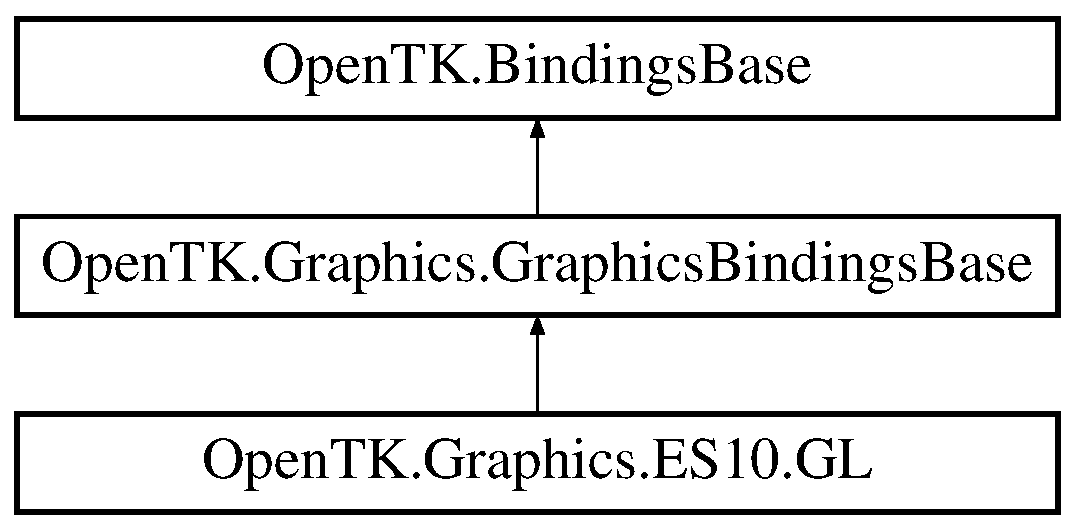
\includegraphics[height=3.000000cm]{class_open_t_k_1_1_graphics_1_1_e_s10_1_1_g_l}
\end{center}
\end{figure}
\subsection*{Static Public Member Functions}
\begin{DoxyCompactItemize}
\item 
static void \hyperlink{class_open_t_k_1_1_graphics_1_1_e_s10_1_1_g_l_af877d36133b72c1317200aceaca0f2ff}{Active\-Texture} (Open\-T\-K.\-Graphics.\-E\-S10.\-All texture)
\begin{DoxyCompactList}\small\item\em \mbox{[}requires\-: v1.\-0 and 1.\-0\mbox{]} Select active texture unit \end{DoxyCompactList}\item 
static void \hyperlink{class_open_t_k_1_1_graphics_1_1_e_s10_1_1_g_l_a9297ccb5a5c807f4618fb57a8069d884}{Alpha\-Func} (Open\-T\-K.\-Graphics.\-E\-S10.\-All func, Single @ref)
\begin{DoxyCompactList}\small\item\em \mbox{[}requires\-: v1.\-0 and 1.\-0\mbox{]} Specify the alpha test function \end{DoxyCompactList}\item 
static void \hyperlink{class_open_t_k_1_1_graphics_1_1_e_s10_1_1_g_l_afdef691f4106bd823da7fa8c0eab7ee3}{Alpha\-Funcx} (Open\-T\-K.\-Graphics.\-E\-S10.\-All func, int @ref)
\begin{DoxyCompactList}\small\item\em \mbox{[}requires\-: v1.\-0 and 1.\-0\mbox{]}\end{DoxyCompactList}\item 
static void \hyperlink{class_open_t_k_1_1_graphics_1_1_e_s10_1_1_g_l_a0315823b1e496999d48d9362c13bcee8}{Bind\-Texture} (Open\-T\-K.\-Graphics.\-E\-S10.\-All target, Int32 texture)
\begin{DoxyCompactList}\small\item\em \mbox{[}requires\-: v1.\-0 and 1.\-0\mbox{]} Bind a named texture to a texturing target \end{DoxyCompactList}\item 
static void \hyperlink{class_open_t_k_1_1_graphics_1_1_e_s10_1_1_g_l_af0f9ba9d83688f66524fe5db5486942f}{Bind\-Texture} (Open\-T\-K.\-Graphics.\-E\-S10.\-All target, U\-Int32 texture)
\begin{DoxyCompactList}\small\item\em \mbox{[}requires\-: v1.\-0 and 1.\-0\mbox{]} Bind a named texture to a texturing target \end{DoxyCompactList}\item 
static void \hyperlink{class_open_t_k_1_1_graphics_1_1_e_s10_1_1_g_l_abc8f0073848eb5bd1894d87dbcafe77c}{Blend\-Func} (Open\-T\-K.\-Graphics.\-E\-S10.\-All sfactor, Open\-T\-K.\-Graphics.\-E\-S10.\-All dfactor)
\begin{DoxyCompactList}\small\item\em \mbox{[}requires\-: v1.\-0 and 1.\-0\mbox{]} Specify pixel arithmetic \end{DoxyCompactList}\item 
static void \hyperlink{class_open_t_k_1_1_graphics_1_1_e_s10_1_1_g_l_a8e85f847e4edd7078fbc0ca6410c6f6f}{Clear} (Int32 mask)
\begin{DoxyCompactList}\small\item\em \mbox{[}requires\-: v1.\-0 and 1.\-0\mbox{]} Clear buffers to preset values \end{DoxyCompactList}\item 
static void \hyperlink{class_open_t_k_1_1_graphics_1_1_e_s10_1_1_g_l_a768065d3b15ad5fd6d6d7d9a40af7439}{Clear} (U\-Int32 mask)
\begin{DoxyCompactList}\small\item\em \mbox{[}requires\-: v1.\-0 and 1.\-0\mbox{]} Clear buffers to preset values \end{DoxyCompactList}\item 
static void \hyperlink{class_open_t_k_1_1_graphics_1_1_e_s10_1_1_g_l_a56d96591a79d2ea2bdffc1f548f61a2e}{Clear\-Color} (Single red, Single green, Single blue, Single alpha)
\begin{DoxyCompactList}\small\item\em \mbox{[}requires\-: v1.\-0 and 1.\-0\mbox{]} Specify clear values for the color buffers \end{DoxyCompactList}\item 
static void \hyperlink{class_open_t_k_1_1_graphics_1_1_e_s10_1_1_g_l_a5f44e6cbbba6583d06509d48636b7d74}{Clear\-Colorx} (int red, int green, int blue, int alpha)
\begin{DoxyCompactList}\small\item\em \mbox{[}requires\-: v1.\-0 and 1.\-0\mbox{]}\end{DoxyCompactList}\item 
static void \hyperlink{class_open_t_k_1_1_graphics_1_1_e_s10_1_1_g_l_a139d53ccea5dc994f3f974008b983a2e}{Clear\-Depth} (Single depth)
\begin{DoxyCompactList}\small\item\em \mbox{[}requires\-: v1.\-0 and 1.\-0\mbox{]} Specify the clear value for the depth buffer \end{DoxyCompactList}\item 
static void \hyperlink{class_open_t_k_1_1_graphics_1_1_e_s10_1_1_g_l_a44cbad14f393e9d4e068f99aa408f10d}{Clear\-Depthx} (int depth)
\begin{DoxyCompactList}\small\item\em \mbox{[}requires\-: v1.\-0 and 1.\-0\mbox{]}\end{DoxyCompactList}\item 
static void \hyperlink{class_open_t_k_1_1_graphics_1_1_e_s10_1_1_g_l_a1c66c99b6e3036405e44498cb5cece4e}{Clear\-Stencil} (Int32 s)
\begin{DoxyCompactList}\small\item\em \mbox{[}requires\-: v1.\-0 and 1.\-0\mbox{]} Specify the clear value for the stencil buffer \end{DoxyCompactList}\item 
static void \hyperlink{class_open_t_k_1_1_graphics_1_1_e_s10_1_1_g_l_afdf93e53725eea497e8a3f6e8981fba0}{Client\-Active\-Texture} (Open\-T\-K.\-Graphics.\-E\-S10.\-All texture)
\begin{DoxyCompactList}\small\item\em \mbox{[}requires\-: v1.\-0 and 1.\-0\mbox{]} Select active texture unit \end{DoxyCompactList}\item 
static void \hyperlink{class_open_t_k_1_1_graphics_1_1_e_s10_1_1_g_l_a8a177c349ee72aeef8d0817f3db14a9f}{Color4} (Single red, Single green, Single blue, Single alpha)
\begin{DoxyCompactList}\small\item\em \mbox{[}requires\-: v1.\-0 and 1.\-0\mbox{]} Set the current color \end{DoxyCompactList}\item 
static void \hyperlink{class_open_t_k_1_1_graphics_1_1_e_s10_1_1_g_l_a826ddb9f3abd2b5c9110e6ead1de2d3b}{Color4x} (int red, int green, int blue, int alpha)
\begin{DoxyCompactList}\small\item\em \mbox{[}requires\-: v1.\-0 and 1.\-0\mbox{]}\end{DoxyCompactList}\item 
static void \hyperlink{class_open_t_k_1_1_graphics_1_1_e_s10_1_1_g_l_a565579a0da6e5c2ebe22fc794f0b0776}{Color\-Mask} (bool red, bool green, bool blue, bool alpha)
\begin{DoxyCompactList}\small\item\em \mbox{[}requires\-: v1.\-0 and 1.\-0\mbox{]} Enable and disable writing of frame buffer color components \end{DoxyCompactList}\item 
static void \hyperlink{class_open_t_k_1_1_graphics_1_1_e_s10_1_1_g_l_abac3c20f0648c3d39c9cbba75d6026bd}{Color\-Pointer} (Int32 size, Open\-T\-K.\-Graphics.\-E\-S10.\-All type, Int32 stride, Int\-Ptr pointer)
\begin{DoxyCompactList}\small\item\em \mbox{[}requires\-: v1.\-0 and 1.\-0\mbox{]} Define an array of colors \end{DoxyCompactList}\item 
static void \hyperlink{class_open_t_k_1_1_graphics_1_1_e_s10_1_1_g_l_aad342f266faf0b780c480c42ed542d4b}{Color\-Pointer$<$ T3 $>$} (Int32 size, Open\-T\-K.\-Graphics.\-E\-S10.\-All type, Int32 stride, \mbox{[}In\-Attribute, Out\-Attribute\mbox{]} T3\mbox{[}$\,$\mbox{]} pointer)
\begin{DoxyCompactList}\small\item\em \mbox{[}requires\-: v1.\-0 and 1.\-0\mbox{]} Define an array of colors \end{DoxyCompactList}\item 
static void \hyperlink{class_open_t_k_1_1_graphics_1_1_e_s10_1_1_g_l_a59263c332720b6f06bc747a409b9b29e}{Color\-Pointer$<$ T3 $>$} (Int32 size, Open\-T\-K.\-Graphics.\-E\-S10.\-All type, Int32 stride, \mbox{[}In\-Attribute, Out\-Attribute\mbox{]} T3\mbox{[},\mbox{]} pointer)
\begin{DoxyCompactList}\small\item\em \mbox{[}requires\-: v1.\-0 and 1.\-0\mbox{]} Define an array of colors \end{DoxyCompactList}\item 
static void \hyperlink{class_open_t_k_1_1_graphics_1_1_e_s10_1_1_g_l_a46a37435ca6ef049d44de3ad162cf76a}{Color\-Pointer$<$ T3 $>$} (Int32 size, Open\-T\-K.\-Graphics.\-E\-S10.\-All type, Int32 stride, \mbox{[}In\-Attribute, Out\-Attribute\mbox{]} T3\mbox{[},,\mbox{]} pointer)
\begin{DoxyCompactList}\small\item\em \mbox{[}requires\-: v1.\-0 and 1.\-0\mbox{]} Define an array of colors \end{DoxyCompactList}\item 
static void \hyperlink{class_open_t_k_1_1_graphics_1_1_e_s10_1_1_g_l_a42a2b0a2ac86cab444eaa8cb04e92316}{Color\-Pointer$<$ T3 $>$} (Int32 size, Open\-T\-K.\-Graphics.\-E\-S10.\-All type, Int32 stride, \mbox{[}In\-Attribute, Out\-Attribute\mbox{]} ref T3 pointer)
\begin{DoxyCompactList}\small\item\em \mbox{[}requires\-: v1.\-0 and 1.\-0\mbox{]} Define an array of colors \end{DoxyCompactList}\item 
static void \hyperlink{class_open_t_k_1_1_graphics_1_1_e_s10_1_1_g_l_a8f8fc5fbdf1e4ea8859f9f76dfc234ad}{Compressed\-Tex\-Image2\-D} (Open\-T\-K.\-Graphics.\-E\-S10.\-All target, Int32 level, Open\-T\-K.\-Graphics.\-E\-S10.\-All internalformat, Int32 width, Int32 height, Int32 border, Int32 image\-Size, Int\-Ptr data)
\begin{DoxyCompactList}\small\item\em \mbox{[}requires\-: v1.\-0 and 1.\-0\mbox{]} Specify a two-\/dimensional texture image in a compressed format \end{DoxyCompactList}\item 
static void \hyperlink{class_open_t_k_1_1_graphics_1_1_e_s10_1_1_g_l_aa73463933008efe5a295040d9f311bd6}{Compressed\-Tex\-Image2\-D$<$ T7 $>$} (Open\-T\-K.\-Graphics.\-E\-S10.\-All target, Int32 level, Open\-T\-K.\-Graphics.\-E\-S10.\-All internalformat, Int32 width, Int32 height, Int32 border, Int32 image\-Size, \mbox{[}In\-Attribute, Out\-Attribute\mbox{]} T7\mbox{[}$\,$\mbox{]} data)
\begin{DoxyCompactList}\small\item\em \mbox{[}requires\-: v1.\-0 and 1.\-0\mbox{]} Specify a two-\/dimensional texture image in a compressed format \end{DoxyCompactList}\item 
static void \hyperlink{class_open_t_k_1_1_graphics_1_1_e_s10_1_1_g_l_a410379bfd5d54c8f18a7ce539a6a9959}{Compressed\-Tex\-Image2\-D$<$ T7 $>$} (Open\-T\-K.\-Graphics.\-E\-S10.\-All target, Int32 level, Open\-T\-K.\-Graphics.\-E\-S10.\-All internalformat, Int32 width, Int32 height, Int32 border, Int32 image\-Size, \mbox{[}In\-Attribute, Out\-Attribute\mbox{]} T7\mbox{[},\mbox{]} data)
\begin{DoxyCompactList}\small\item\em \mbox{[}requires\-: v1.\-0 and 1.\-0\mbox{]} Specify a two-\/dimensional texture image in a compressed format \end{DoxyCompactList}\item 
static void \hyperlink{class_open_t_k_1_1_graphics_1_1_e_s10_1_1_g_l_a5a8e94cfb35ef553fde27535124682f7}{Compressed\-Tex\-Image2\-D$<$ T7 $>$} (Open\-T\-K.\-Graphics.\-E\-S10.\-All target, Int32 level, Open\-T\-K.\-Graphics.\-E\-S10.\-All internalformat, Int32 width, Int32 height, Int32 border, Int32 image\-Size, \mbox{[}In\-Attribute, Out\-Attribute\mbox{]} T7\mbox{[},,\mbox{]} data)
\begin{DoxyCompactList}\small\item\em \mbox{[}requires\-: v1.\-0 and 1.\-0\mbox{]} Specify a two-\/dimensional texture image in a compressed format \end{DoxyCompactList}\item 
static void \hyperlink{class_open_t_k_1_1_graphics_1_1_e_s10_1_1_g_l_a873653c4303a2e8691415dec0924b31b}{Compressed\-Tex\-Image2\-D$<$ T7 $>$} (Open\-T\-K.\-Graphics.\-E\-S10.\-All target, Int32 level, Open\-T\-K.\-Graphics.\-E\-S10.\-All internalformat, Int32 width, Int32 height, Int32 border, Int32 image\-Size, \mbox{[}In\-Attribute, Out\-Attribute\mbox{]} ref T7 data)
\begin{DoxyCompactList}\small\item\em \mbox{[}requires\-: v1.\-0 and 1.\-0\mbox{]} Specify a two-\/dimensional texture image in a compressed format \end{DoxyCompactList}\item 
static void \hyperlink{class_open_t_k_1_1_graphics_1_1_e_s10_1_1_g_l_a578dac0241e5cf0d1f3451d9b41cb5f4}{Compressed\-Tex\-Sub\-Image2\-D} (Open\-T\-K.\-Graphics.\-E\-S10.\-All target, Int32 level, Int32 xoffset, Int32 yoffset, Int32 width, Int32 height, Open\-T\-K.\-Graphics.\-E\-S10.\-All format, Int32 image\-Size, Int\-Ptr data)
\begin{DoxyCompactList}\small\item\em \mbox{[}requires\-: v1.\-0 and 1.\-0\mbox{]} Specify a two-\/dimensional texture subimage in a compressed format \end{DoxyCompactList}\item 
static void \hyperlink{class_open_t_k_1_1_graphics_1_1_e_s10_1_1_g_l_a5abb84d021f97e9f375fc81e69311dd8}{Compressed\-Tex\-Sub\-Image2\-D$<$ T8 $>$} (Open\-T\-K.\-Graphics.\-E\-S10.\-All target, Int32 level, Int32 xoffset, Int32 yoffset, Int32 width, Int32 height, Open\-T\-K.\-Graphics.\-E\-S10.\-All format, Int32 image\-Size, \mbox{[}In\-Attribute, Out\-Attribute\mbox{]} T8\mbox{[}$\,$\mbox{]} data)
\begin{DoxyCompactList}\small\item\em \mbox{[}requires\-: v1.\-0 and 1.\-0\mbox{]} Specify a two-\/dimensional texture subimage in a compressed format \end{DoxyCompactList}\item 
static void \hyperlink{class_open_t_k_1_1_graphics_1_1_e_s10_1_1_g_l_a8bd1f6b8b16d395f8d4b5883640dfc61}{Compressed\-Tex\-Sub\-Image2\-D$<$ T8 $>$} (Open\-T\-K.\-Graphics.\-E\-S10.\-All target, Int32 level, Int32 xoffset, Int32 yoffset, Int32 width, Int32 height, Open\-T\-K.\-Graphics.\-E\-S10.\-All format, Int32 image\-Size, \mbox{[}In\-Attribute, Out\-Attribute\mbox{]} T8\mbox{[},\mbox{]} data)
\begin{DoxyCompactList}\small\item\em \mbox{[}requires\-: v1.\-0 and 1.\-0\mbox{]} Specify a two-\/dimensional texture subimage in a compressed format \end{DoxyCompactList}\item 
static void \hyperlink{class_open_t_k_1_1_graphics_1_1_e_s10_1_1_g_l_ad5d51cd32ee94282e33250f4af2bd974}{Compressed\-Tex\-Sub\-Image2\-D$<$ T8 $>$} (Open\-T\-K.\-Graphics.\-E\-S10.\-All target, Int32 level, Int32 xoffset, Int32 yoffset, Int32 width, Int32 height, Open\-T\-K.\-Graphics.\-E\-S10.\-All format, Int32 image\-Size, \mbox{[}In\-Attribute, Out\-Attribute\mbox{]} T8\mbox{[},,\mbox{]} data)
\begin{DoxyCompactList}\small\item\em \mbox{[}requires\-: v1.\-0 and 1.\-0\mbox{]} Specify a two-\/dimensional texture subimage in a compressed format \end{DoxyCompactList}\item 
static void \hyperlink{class_open_t_k_1_1_graphics_1_1_e_s10_1_1_g_l_aba823d2aca18dcc4fc7dff618af1efea}{Compressed\-Tex\-Sub\-Image2\-D$<$ T8 $>$} (Open\-T\-K.\-Graphics.\-E\-S10.\-All target, Int32 level, Int32 xoffset, Int32 yoffset, Int32 width, Int32 height, Open\-T\-K.\-Graphics.\-E\-S10.\-All format, Int32 image\-Size, \mbox{[}In\-Attribute, Out\-Attribute\mbox{]} ref T8 data)
\begin{DoxyCompactList}\small\item\em \mbox{[}requires\-: v1.\-0 and 1.\-0\mbox{]} Specify a two-\/dimensional texture subimage in a compressed format \end{DoxyCompactList}\item 
static void \hyperlink{class_open_t_k_1_1_graphics_1_1_e_s10_1_1_g_l_a3811ae0fd1303feff2f1e4359d52b6f3}{Copy\-Tex\-Image2\-D} (Open\-T\-K.\-Graphics.\-E\-S10.\-All target, Int32 level, Open\-T\-K.\-Graphics.\-E\-S10.\-All internalformat, Int32 x, Int32 y, Int32 width, Int32 height, Int32 border)
\begin{DoxyCompactList}\small\item\em \mbox{[}requires\-: v1.\-0 and 1.\-0\mbox{]} Copy pixels into a 2\-D texture image \end{DoxyCompactList}\item 
static void \hyperlink{class_open_t_k_1_1_graphics_1_1_e_s10_1_1_g_l_a41d89fb93ad1d93d864ae3761355c18a}{Copy\-Tex\-Sub\-Image2\-D} (Open\-T\-K.\-Graphics.\-E\-S10.\-All target, Int32 level, Int32 xoffset, Int32 yoffset, Int32 x, Int32 y, Int32 width, Int32 height)
\begin{DoxyCompactList}\small\item\em \mbox{[}requires\-: v1.\-0 and 1.\-0\mbox{]} Copy a two-\/dimensional texture subimage \end{DoxyCompactList}\item 
static void \hyperlink{class_open_t_k_1_1_graphics_1_1_e_s10_1_1_g_l_a187d3e102d7150178cd201eb149de84e}{Cull\-Face} (Open\-T\-K.\-Graphics.\-E\-S10.\-All mode)
\begin{DoxyCompactList}\small\item\em \mbox{[}requires\-: v1.\-0 and 1.\-0\mbox{]} Specify whether front-\/ or back-\/facing facets can be culled \end{DoxyCompactList}\item 
static void \hyperlink{class_open_t_k_1_1_graphics_1_1_e_s10_1_1_g_l_afca0c3be15ff6fddd3f25d54469818d6}{Delete\-Textures} (Int32 n, Int32\mbox{[}$\,$\mbox{]} textures)
\begin{DoxyCompactList}\small\item\em \mbox{[}requires\-: v1.\-0 and 1.\-0\mbox{]} Delete named textures \end{DoxyCompactList}\item 
static void \hyperlink{class_open_t_k_1_1_graphics_1_1_e_s10_1_1_g_l_a459ccd31a866586932a392450c4c112b}{Delete\-Textures} (Int32 n, ref Int32 textures)
\begin{DoxyCompactList}\small\item\em \mbox{[}requires\-: v1.\-0 and 1.\-0\mbox{]} Delete named textures \end{DoxyCompactList}\item 
static unsafe void \hyperlink{class_open_t_k_1_1_graphics_1_1_e_s10_1_1_g_l_a854387c0860c6e72e5be7e354c33910e}{Delete\-Textures} (Int32 n, Int32 $\ast$textures)
\begin{DoxyCompactList}\small\item\em \mbox{[}requires\-: v1.\-0 and 1.\-0\mbox{]} Delete named textures \end{DoxyCompactList}\item 
static void \hyperlink{class_open_t_k_1_1_graphics_1_1_e_s10_1_1_g_l_a048cd4cadcbc47a1fa1718f9f116f4f3}{Delete\-Textures} (Int32 n, U\-Int32\mbox{[}$\,$\mbox{]} textures)
\begin{DoxyCompactList}\small\item\em \mbox{[}requires\-: v1.\-0 and 1.\-0\mbox{]} Delete named textures \end{DoxyCompactList}\item 
static void \hyperlink{class_open_t_k_1_1_graphics_1_1_e_s10_1_1_g_l_adde3725234e3a69533bde6bb5dbee384}{Delete\-Textures} (Int32 n, ref U\-Int32 textures)
\begin{DoxyCompactList}\small\item\em \mbox{[}requires\-: v1.\-0 and 1.\-0\mbox{]} Delete named textures \end{DoxyCompactList}\item 
static unsafe void \hyperlink{class_open_t_k_1_1_graphics_1_1_e_s10_1_1_g_l_a7172582798966ade408151b2d41f059e}{Delete\-Textures} (Int32 n, U\-Int32 $\ast$textures)
\begin{DoxyCompactList}\small\item\em \mbox{[}requires\-: v1.\-0 and 1.\-0\mbox{]} Delete named textures \end{DoxyCompactList}\item 
static void \hyperlink{class_open_t_k_1_1_graphics_1_1_e_s10_1_1_g_l_a5fa26c4dab4688e7ba04188456d24dfc}{Depth\-Func} (Open\-T\-K.\-Graphics.\-E\-S10.\-All func)
\begin{DoxyCompactList}\small\item\em \mbox{[}requires\-: v1.\-0 and 1.\-0\mbox{]} Specify the value used for depth buffer comparisons \end{DoxyCompactList}\item 
static void \hyperlink{class_open_t_k_1_1_graphics_1_1_e_s10_1_1_g_l_a3c23130545670e7aca25ad82e2eac0b3}{Depth\-Mask} (bool flag)
\begin{DoxyCompactList}\small\item\em \mbox{[}requires\-: v1.\-0 and 1.\-0\mbox{]} Enable or disable writing into the depth buffer \end{DoxyCompactList}\item 
static void \hyperlink{class_open_t_k_1_1_graphics_1_1_e_s10_1_1_g_l_a1a2bd55d4fefcffdfb26551c9edc807f}{Depth\-Range} (Single z\-Near, Single z\-Far)
\begin{DoxyCompactList}\small\item\em \mbox{[}requires\-: v1.\-0 and 1.\-0\mbox{]} Specify mapping of depth values from normalized device coordinates to window coordinates \end{DoxyCompactList}\item 
static void \hyperlink{class_open_t_k_1_1_graphics_1_1_e_s10_1_1_g_l_a3b4e3a115259fc7bae858589d8727e4e}{Depth\-Rangex} (int z\-Near, int z\-Far)
\begin{DoxyCompactList}\small\item\em \mbox{[}requires\-: v1.\-0 and 1.\-0\mbox{]}\end{DoxyCompactList}\item 
static void \hyperlink{class_open_t_k_1_1_graphics_1_1_e_s10_1_1_g_l_a73fb4d4b6e535f6336efe1495a94ffb5}{Disable} (Open\-T\-K.\-Graphics.\-E\-S10.\-All cap)
\begin{DoxyCompactList}\small\item\em \mbox{[}requires\-: v1.\-0 and 1.\-0\mbox{]}\end{DoxyCompactList}\item 
static void \hyperlink{class_open_t_k_1_1_graphics_1_1_e_s10_1_1_g_l_a5a4283e0e5ad5e687b4a8eac744ae55a}{Disable\-Client\-State} (Open\-T\-K.\-Graphics.\-E\-S10.\-All array)
\begin{DoxyCompactList}\small\item\em \mbox{[}requires\-: v1.\-0 and 1.\-0\mbox{]}\end{DoxyCompactList}\item 
static void \hyperlink{class_open_t_k_1_1_graphics_1_1_e_s10_1_1_g_l_a3d6abebcca2a2fdbfebac04294b204a8}{Draw\-Arrays} (Open\-T\-K.\-Graphics.\-E\-S10.\-All mode, Int32 first, Int32 count)
\begin{DoxyCompactList}\small\item\em \mbox{[}requires\-: v1.\-0 and 1.\-0\mbox{]} Render primitives from array data \end{DoxyCompactList}\item 
static void \hyperlink{class_open_t_k_1_1_graphics_1_1_e_s10_1_1_g_l_a3bbaeb44677eecaaf5a700b5c0de02b0}{Draw\-Elements} (Open\-T\-K.\-Graphics.\-E\-S10.\-All mode, Int32 count, Open\-T\-K.\-Graphics.\-E\-S10.\-All type, Int\-Ptr indices)
\begin{DoxyCompactList}\small\item\em \mbox{[}requires\-: v1.\-0 and 1.\-0\mbox{]} Render primitives from array data \end{DoxyCompactList}\item 
static void \hyperlink{class_open_t_k_1_1_graphics_1_1_e_s10_1_1_g_l_ac6cfdba2bf5d31d2241fb0b75cca79d4}{Draw\-Elements$<$ T3 $>$} (Open\-T\-K.\-Graphics.\-E\-S10.\-All mode, Int32 count, Open\-T\-K.\-Graphics.\-E\-S10.\-All type, \mbox{[}In\-Attribute, Out\-Attribute\mbox{]} T3\mbox{[}$\,$\mbox{]} indices)
\begin{DoxyCompactList}\small\item\em \mbox{[}requires\-: v1.\-0 and 1.\-0\mbox{]} Render primitives from array data \end{DoxyCompactList}\item 
static void \hyperlink{class_open_t_k_1_1_graphics_1_1_e_s10_1_1_g_l_a89293a61c9711b0f80c3e7c8e66b5be8}{Draw\-Elements$<$ T3 $>$} (Open\-T\-K.\-Graphics.\-E\-S10.\-All mode, Int32 count, Open\-T\-K.\-Graphics.\-E\-S10.\-All type, \mbox{[}In\-Attribute, Out\-Attribute\mbox{]} T3\mbox{[},\mbox{]} indices)
\begin{DoxyCompactList}\small\item\em \mbox{[}requires\-: v1.\-0 and 1.\-0\mbox{]} Render primitives from array data \end{DoxyCompactList}\item 
static void \hyperlink{class_open_t_k_1_1_graphics_1_1_e_s10_1_1_g_l_a72f11b5ed2fe52e4fba3a92988286c5b}{Draw\-Elements$<$ T3 $>$} (Open\-T\-K.\-Graphics.\-E\-S10.\-All mode, Int32 count, Open\-T\-K.\-Graphics.\-E\-S10.\-All type, \mbox{[}In\-Attribute, Out\-Attribute\mbox{]} T3\mbox{[},,\mbox{]} indices)
\begin{DoxyCompactList}\small\item\em \mbox{[}requires\-: v1.\-0 and 1.\-0\mbox{]} Render primitives from array data \end{DoxyCompactList}\item 
static void \hyperlink{class_open_t_k_1_1_graphics_1_1_e_s10_1_1_g_l_a26c91f36f3a4b816b059e26b80584d48}{Draw\-Elements$<$ T3 $>$} (Open\-T\-K.\-Graphics.\-E\-S10.\-All mode, Int32 count, Open\-T\-K.\-Graphics.\-E\-S10.\-All type, \mbox{[}In\-Attribute, Out\-Attribute\mbox{]} ref T3 indices)
\begin{DoxyCompactList}\small\item\em \mbox{[}requires\-: v1.\-0 and 1.\-0\mbox{]} Render primitives from array data \end{DoxyCompactList}\item 
static void \hyperlink{class_open_t_k_1_1_graphics_1_1_e_s10_1_1_g_l_a1d90f0cf2c034a8195abdc1eeecc48bb}{Enable} (Open\-T\-K.\-Graphics.\-E\-S10.\-All cap)
\begin{DoxyCompactList}\small\item\em \mbox{[}requires\-: v1.\-0 and 1.\-0\mbox{]} Enable or disable server-\/side \hyperlink{class_open_t_k_1_1_graphics_1_1_e_s10_1_1_g_l}{G\-L} capabilities \end{DoxyCompactList}\item 
static void \hyperlink{class_open_t_k_1_1_graphics_1_1_e_s10_1_1_g_l_ab9f4e2b75f016bdcd7eba21eecec2dd3}{Enable\-Client\-State} (Open\-T\-K.\-Graphics.\-E\-S10.\-All array)
\begin{DoxyCompactList}\small\item\em \mbox{[}requires\-: v1.\-0 and 1.\-0\mbox{]} Enable or disable client-\/side capability \end{DoxyCompactList}\item 
static void \hyperlink{class_open_t_k_1_1_graphics_1_1_e_s10_1_1_g_l_a2bbb42830e56e881c2d64e60ded44fc8}{Finish} ()
\begin{DoxyCompactList}\small\item\em \mbox{[}requires\-: v1.\-0 and 1.\-0\mbox{]} Block until all \hyperlink{class_open_t_k_1_1_graphics_1_1_e_s10_1_1_g_l}{G\-L} execution is complete \end{DoxyCompactList}\item 
static void \hyperlink{class_open_t_k_1_1_graphics_1_1_e_s10_1_1_g_l_a3ba85aeb0b60459ec3a976668921d720}{Flush} ()
\begin{DoxyCompactList}\small\item\em \mbox{[}requires\-: v1.\-0 and 1.\-0\mbox{]} Force execution of \hyperlink{class_open_t_k_1_1_graphics_1_1_e_s10_1_1_g_l}{G\-L} commands in finite time \end{DoxyCompactList}\item 
static void \hyperlink{class_open_t_k_1_1_graphics_1_1_e_s10_1_1_g_l_ad582007d6bd5f4c3835041f6fee28269}{Fog} (Open\-T\-K.\-Graphics.\-E\-S10.\-All pname, Single param)
\begin{DoxyCompactList}\small\item\em \mbox{[}requires\-: v1.\-0 and 1.\-0\mbox{]} Specify fog parameters \end{DoxyCompactList}\item 
static void \hyperlink{class_open_t_k_1_1_graphics_1_1_e_s10_1_1_g_l_aa4ad34189ec29c2654ae7b334144d5b2}{Fog} (Open\-T\-K.\-Graphics.\-E\-S10.\-All pname, Single\mbox{[}$\,$\mbox{]}@params)
\begin{DoxyCompactList}\small\item\em \mbox{[}requires\-: v1.\-0 and 1.\-0\mbox{]} Specify fog parameters \end{DoxyCompactList}\item 
static unsafe void \hyperlink{class_open_t_k_1_1_graphics_1_1_e_s10_1_1_g_l_a373a9f40afcf59ab61ef62a7129e9bdb}{Fog} (Open\-T\-K.\-Graphics.\-E\-S10.\-All pname, Single $\ast$@params)
\begin{DoxyCompactList}\small\item\em \mbox{[}requires\-: v1.\-0 and 1.\-0\mbox{]} Specify fog parameters \end{DoxyCompactList}\item 
static void \hyperlink{class_open_t_k_1_1_graphics_1_1_e_s10_1_1_g_l_a2bc91bc9047e98bee0e696e53d4362f8}{Fogx} (Open\-T\-K.\-Graphics.\-E\-S10.\-All pname, int param)
\begin{DoxyCompactList}\small\item\em \mbox{[}requires\-: v1.\-0 and 1.\-0\mbox{]}\end{DoxyCompactList}\item 
static void \hyperlink{class_open_t_k_1_1_graphics_1_1_e_s10_1_1_g_l_a4636e7ddb1567d30816657fbd1797ae8}{Fogx} (Open\-T\-K.\-Graphics.\-E\-S10.\-All pname, int\mbox{[}$\,$\mbox{]}@params)
\begin{DoxyCompactList}\small\item\em \mbox{[}requires\-: v1.\-0 and 1.\-0\mbox{]}\end{DoxyCompactList}\item 
static unsafe void \hyperlink{class_open_t_k_1_1_graphics_1_1_e_s10_1_1_g_l_ae583e29626921552e4cc2b427da995cf}{Fogx} (Open\-T\-K.\-Graphics.\-E\-S10.\-All pname, int $\ast$@params)
\begin{DoxyCompactList}\small\item\em \mbox{[}requires\-: v1.\-0 and 1.\-0\mbox{]}\end{DoxyCompactList}\item 
static void \hyperlink{class_open_t_k_1_1_graphics_1_1_e_s10_1_1_g_l_ada29d797b3928c5ec2d75445daf1fc90}{Front\-Face} (Open\-T\-K.\-Graphics.\-E\-S10.\-All mode)
\begin{DoxyCompactList}\small\item\em \mbox{[}requires\-: v1.\-0 and 1.\-0\mbox{]} Define front-\/ and back-\/facing polygons \end{DoxyCompactList}\item 
static void \hyperlink{class_open_t_k_1_1_graphics_1_1_e_s10_1_1_g_l_a2e5ff2b4f3d05387f52712272c0e6061}{Frustum} (Single left, Single right, Single bottom, Single top, Single z\-Near, Single z\-Far)
\begin{DoxyCompactList}\small\item\em \mbox{[}requires\-: v1.\-0 and 1.\-0\mbox{]} Multiply the current matrix by a perspective matrix \end{DoxyCompactList}\item 
static void \hyperlink{class_open_t_k_1_1_graphics_1_1_e_s10_1_1_g_l_ad83d9d65e2dcc2f149fae2eb5d666f88}{Frustumx} (int left, int right, int bottom, int top, int z\-Near, int z\-Far)
\begin{DoxyCompactList}\small\item\em \mbox{[}requires\-: v1.\-0 and 1.\-0\mbox{]}\end{DoxyCompactList}\item 
static void \hyperlink{class_open_t_k_1_1_graphics_1_1_e_s10_1_1_g_l_a53e211214354e321dc937adb37e5d7dd}{Gen\-Textures} (Int32 n, Int32\mbox{[}$\,$\mbox{]} textures)
\begin{DoxyCompactList}\small\item\em \mbox{[}requires\-: v1.\-0 and 1.\-0\mbox{]} Generate texture names \end{DoxyCompactList}\item 
static void \hyperlink{class_open_t_k_1_1_graphics_1_1_e_s10_1_1_g_l_a991ded181b52fccb7e7e40e2363f1a73}{Gen\-Textures} (Int32 n, ref Int32 textures)
\begin{DoxyCompactList}\small\item\em \mbox{[}requires\-: v1.\-0 and 1.\-0\mbox{]} Generate texture names \end{DoxyCompactList}\item 
static unsafe void \hyperlink{class_open_t_k_1_1_graphics_1_1_e_s10_1_1_g_l_a5fc4a70a23938df34962b167c4932fa6}{Gen\-Textures} (Int32 n, Int32 $\ast$textures)
\begin{DoxyCompactList}\small\item\em \mbox{[}requires\-: v1.\-0 and 1.\-0\mbox{]} Generate texture names \end{DoxyCompactList}\item 
static void \hyperlink{class_open_t_k_1_1_graphics_1_1_e_s10_1_1_g_l_aa28e04fa6c9d5b598f1f174808a19c81}{Gen\-Textures} (Int32 n, U\-Int32\mbox{[}$\,$\mbox{]} textures)
\begin{DoxyCompactList}\small\item\em \mbox{[}requires\-: v1.\-0 and 1.\-0\mbox{]} Generate texture names \end{DoxyCompactList}\item 
static void \hyperlink{class_open_t_k_1_1_graphics_1_1_e_s10_1_1_g_l_afb78205cee1e3945ddb74d53f9200aca}{Gen\-Textures} (Int32 n, ref U\-Int32 textures)
\begin{DoxyCompactList}\small\item\em \mbox{[}requires\-: v1.\-0 and 1.\-0\mbox{]} Generate texture names \end{DoxyCompactList}\item 
static unsafe void \hyperlink{class_open_t_k_1_1_graphics_1_1_e_s10_1_1_g_l_a155c0b2ab7dfc4d065fb0ab7d43e8e85}{Gen\-Textures} (Int32 n, U\-Int32 $\ast$textures)
\begin{DoxyCompactList}\small\item\em \mbox{[}requires\-: v1.\-0 and 1.\-0\mbox{]} Generate texture names \end{DoxyCompactList}\item 
static Open\-T\-K.\-Graphics.\-E\-S10.\-All \hyperlink{class_open_t_k_1_1_graphics_1_1_e_s10_1_1_g_l_acd1cbb598c28eff3b661fe0dd7dbfad8}{Get\-Error} ()
\begin{DoxyCompactList}\small\item\em \mbox{[}requires\-: v1.\-0 and 1.\-0\mbox{]} Return error information \end{DoxyCompactList}\item 
static void \hyperlink{class_open_t_k_1_1_graphics_1_1_e_s10_1_1_g_l_a5c0b1778c16bb4c6288227c19870e6a1}{Get\-Integer} (Open\-T\-K.\-Graphics.\-E\-S10.\-All pname, Int32\mbox{[}$\,$\mbox{]}@params)
\begin{DoxyCompactList}\small\item\em \mbox{[}requires\-: v1.\-0 and 1.\-0\mbox{]}\end{DoxyCompactList}\item 
static void \hyperlink{class_open_t_k_1_1_graphics_1_1_e_s10_1_1_g_l_af1a943d8a2071cbda03a5bd4606c6f35}{Get\-Integer} (Open\-T\-K.\-Graphics.\-E\-S10.\-All pname, ref Int32 @params)
\begin{DoxyCompactList}\small\item\em \mbox{[}requires\-: v1.\-0 and 1.\-0\mbox{]}\end{DoxyCompactList}\item 
static unsafe void \hyperlink{class_open_t_k_1_1_graphics_1_1_e_s10_1_1_g_l_af18db67363f55007eea0ae45e7a11940}{Get\-Integer} (Open\-T\-K.\-Graphics.\-E\-S10.\-All pname, Int32 $\ast$@params)
\begin{DoxyCompactList}\small\item\em \mbox{[}requires\-: v1.\-0 and 1.\-0\mbox{]}\end{DoxyCompactList}\item 
static unsafe System.\-String \hyperlink{class_open_t_k_1_1_graphics_1_1_e_s10_1_1_g_l_abfc1da2f0e2cd7d6ae28945389b707f3}{Get\-String} (Open\-T\-K.\-Graphics.\-E\-S10.\-All name)
\begin{DoxyCompactList}\small\item\em \mbox{[}requires\-: v1.\-0 and 1.\-0\mbox{]} Return a string describing the current \hyperlink{class_open_t_k_1_1_graphics_1_1_e_s10_1_1_g_l}{G\-L} connection \end{DoxyCompactList}\item 
static void \hyperlink{class_open_t_k_1_1_graphics_1_1_e_s10_1_1_g_l_ab946cf410853955fbd51447c7e95241e}{Hint} (Open\-T\-K.\-Graphics.\-E\-S10.\-All target, Open\-T\-K.\-Graphics.\-E\-S10.\-All mode)
\begin{DoxyCompactList}\small\item\em \mbox{[}requires\-: v1.\-0 and 1.\-0\mbox{]} Specify implementation-\/specific hints \end{DoxyCompactList}\item 
static void \hyperlink{class_open_t_k_1_1_graphics_1_1_e_s10_1_1_g_l_a6ed5740981c5ec41dc0a1f8b3951ece1}{Light} (Open\-T\-K.\-Graphics.\-E\-S10.\-All light, Open\-T\-K.\-Graphics.\-E\-S10.\-All pname, Single param)
\begin{DoxyCompactList}\small\item\em \mbox{[}requires\-: v1.\-0 and 1.\-0\mbox{]} Set light source parameters \end{DoxyCompactList}\item 
static void \hyperlink{class_open_t_k_1_1_graphics_1_1_e_s10_1_1_g_l_a92bcb80a607e327be50e16645cd856c1}{Light} (Open\-T\-K.\-Graphics.\-E\-S10.\-All light, Open\-T\-K.\-Graphics.\-E\-S10.\-All pname, Single\mbox{[}$\,$\mbox{]}@params)
\begin{DoxyCompactList}\small\item\em \mbox{[}requires\-: v1.\-0 and 1.\-0\mbox{]} Set light source parameters \end{DoxyCompactList}\item 
static unsafe void \hyperlink{class_open_t_k_1_1_graphics_1_1_e_s10_1_1_g_l_ad85f879082921edf5bf8985c4e6f202d}{Light} (Open\-T\-K.\-Graphics.\-E\-S10.\-All light, Open\-T\-K.\-Graphics.\-E\-S10.\-All pname, Single $\ast$@params)
\begin{DoxyCompactList}\small\item\em \mbox{[}requires\-: v1.\-0 and 1.\-0\mbox{]} Set light source parameters \end{DoxyCompactList}\item 
static void \hyperlink{class_open_t_k_1_1_graphics_1_1_e_s10_1_1_g_l_a5cfe02bbf80647a2fa811a5997d56461}{Light\-Model} (Open\-T\-K.\-Graphics.\-E\-S10.\-All pname, Single param)
\begin{DoxyCompactList}\small\item\em \mbox{[}requires\-: v1.\-0 and 1.\-0\mbox{]} Set the lighting model parameters \end{DoxyCompactList}\item 
static void \hyperlink{class_open_t_k_1_1_graphics_1_1_e_s10_1_1_g_l_a9c073a31674392e3aec39e797a76d2e9}{Light\-Model} (Open\-T\-K.\-Graphics.\-E\-S10.\-All pname, Single\mbox{[}$\,$\mbox{]}@params)
\begin{DoxyCompactList}\small\item\em \mbox{[}requires\-: v1.\-0 and 1.\-0\mbox{]} Set the lighting model parameters \end{DoxyCompactList}\item 
static unsafe void \hyperlink{class_open_t_k_1_1_graphics_1_1_e_s10_1_1_g_l_a4ee661b6fd9ce7304459920a901c6135}{Light\-Model} (Open\-T\-K.\-Graphics.\-E\-S10.\-All pname, Single $\ast$@params)
\begin{DoxyCompactList}\small\item\em \mbox{[}requires\-: v1.\-0 and 1.\-0\mbox{]} Set the lighting model parameters \end{DoxyCompactList}\item 
static void \hyperlink{class_open_t_k_1_1_graphics_1_1_e_s10_1_1_g_l_afbdd374d422be37761f9afe53dbefc3c}{Light\-Modelx} (Open\-T\-K.\-Graphics.\-E\-S10.\-All pname, int param)
\begin{DoxyCompactList}\small\item\em \mbox{[}requires\-: v1.\-0 and 1.\-0\mbox{]}\end{DoxyCompactList}\item 
static void \hyperlink{class_open_t_k_1_1_graphics_1_1_e_s10_1_1_g_l_a72c94659b53985f3b9624b407dd4e70f}{Light\-Modelx} (Open\-T\-K.\-Graphics.\-E\-S10.\-All pname, int\mbox{[}$\,$\mbox{]}@params)
\begin{DoxyCompactList}\small\item\em \mbox{[}requires\-: v1.\-0 and 1.\-0\mbox{]}\end{DoxyCompactList}\item 
static unsafe void \hyperlink{class_open_t_k_1_1_graphics_1_1_e_s10_1_1_g_l_a6ef12bb29d215caad8f5d9890b2f4bf8}{Light\-Modelx} (Open\-T\-K.\-Graphics.\-E\-S10.\-All pname, int $\ast$@params)
\begin{DoxyCompactList}\small\item\em \mbox{[}requires\-: v1.\-0 and 1.\-0\mbox{]}\end{DoxyCompactList}\item 
static void \hyperlink{class_open_t_k_1_1_graphics_1_1_e_s10_1_1_g_l_a755437bd6ad4c2c668e50878b6be8a47}{Lightx} (Open\-T\-K.\-Graphics.\-E\-S10.\-All light, Open\-T\-K.\-Graphics.\-E\-S10.\-All pname, int param)
\begin{DoxyCompactList}\small\item\em \mbox{[}requires\-: v1.\-0 and 1.\-0\mbox{]}\end{DoxyCompactList}\item 
static void \hyperlink{class_open_t_k_1_1_graphics_1_1_e_s10_1_1_g_l_adf625698407716b800c7ee4ea6a0dd7f}{Lightx} (Open\-T\-K.\-Graphics.\-E\-S10.\-All light, Open\-T\-K.\-Graphics.\-E\-S10.\-All pname, int\mbox{[}$\,$\mbox{]}@params)
\begin{DoxyCompactList}\small\item\em \mbox{[}requires\-: v1.\-0 and 1.\-0\mbox{]}\end{DoxyCompactList}\item 
static unsafe void \hyperlink{class_open_t_k_1_1_graphics_1_1_e_s10_1_1_g_l_acb5b5dd077819818fea7b66641d1d364}{Lightx} (Open\-T\-K.\-Graphics.\-E\-S10.\-All light, Open\-T\-K.\-Graphics.\-E\-S10.\-All pname, int $\ast$@params)
\begin{DoxyCompactList}\small\item\em \mbox{[}requires\-: v1.\-0 and 1.\-0\mbox{]}\end{DoxyCompactList}\item 
static void \hyperlink{class_open_t_k_1_1_graphics_1_1_e_s10_1_1_g_l_a8237894e60ca230b9cd95df20f2bf3a7}{Line\-Width} (Single width)
\begin{DoxyCompactList}\small\item\em \mbox{[}requires\-: v1.\-0 and 1.\-0\mbox{]} Specify the width of rasterized lines \end{DoxyCompactList}\item 
static void \hyperlink{class_open_t_k_1_1_graphics_1_1_e_s10_1_1_g_l_a0c7da29ac4828bd4a004def1d8eb4936}{Line\-Widthx} (int width)
\begin{DoxyCompactList}\small\item\em \mbox{[}requires\-: v1.\-0 and 1.\-0\mbox{]}\end{DoxyCompactList}\item 
static void \hyperlink{class_open_t_k_1_1_graphics_1_1_e_s10_1_1_g_l_a08fd3426b0c8e96b8eb5d102a3dbce86}{Load\-Identity} ()
\begin{DoxyCompactList}\small\item\em \mbox{[}requires\-: v1.\-0 and 1.\-0\mbox{]} Replace the current matrix with the identity matrix \end{DoxyCompactList}\item 
static void \hyperlink{class_open_t_k_1_1_graphics_1_1_e_s10_1_1_g_l_a146723b4f0b5fd145249072c832bac3d}{Load\-Matrix} (Single\mbox{[}$\,$\mbox{]} m)
\begin{DoxyCompactList}\small\item\em \mbox{[}requires\-: v1.\-0 and 1.\-0\mbox{]} Replace the current matrix with the specified matrix \end{DoxyCompactList}\item 
static void \hyperlink{class_open_t_k_1_1_graphics_1_1_e_s10_1_1_g_l_a3a7e32985a5bb8608b206ae763c2528a}{Load\-Matrix} (ref Single m)
\begin{DoxyCompactList}\small\item\em \mbox{[}requires\-: v1.\-0 and 1.\-0\mbox{]} Replace the current matrix with the specified matrix \end{DoxyCompactList}\item 
static unsafe void \hyperlink{class_open_t_k_1_1_graphics_1_1_e_s10_1_1_g_l_a55d751806603c4e2c44ebbb4fe3a80aa}{Load\-Matrix} (Single $\ast$m)
\begin{DoxyCompactList}\small\item\em \mbox{[}requires\-: v1.\-0 and 1.\-0\mbox{]} Replace the current matrix with the specified matrix \end{DoxyCompactList}\item 
static void \hyperlink{class_open_t_k_1_1_graphics_1_1_e_s10_1_1_g_l_a348db5d1f1d9a38b55b6f2e444bfd798}{Load\-Matrixx} (int\mbox{[}$\,$\mbox{]} m)
\begin{DoxyCompactList}\small\item\em \mbox{[}requires\-: v1.\-0 and 1.\-0\mbox{]}\end{DoxyCompactList}\item 
static void \hyperlink{class_open_t_k_1_1_graphics_1_1_e_s10_1_1_g_l_a42f20fd92ee8b9a5899b6958e6bd3343}{Load\-Matrixx} (ref int m)
\begin{DoxyCompactList}\small\item\em \mbox{[}requires\-: v1.\-0 and 1.\-0\mbox{]}\end{DoxyCompactList}\item 
static unsafe void \hyperlink{class_open_t_k_1_1_graphics_1_1_e_s10_1_1_g_l_ac33d2922d627c62a1fe3703b90aeadd6}{Load\-Matrixx} (int $\ast$m)
\begin{DoxyCompactList}\small\item\em \mbox{[}requires\-: v1.\-0 and 1.\-0\mbox{]}\end{DoxyCompactList}\item 
static void \hyperlink{class_open_t_k_1_1_graphics_1_1_e_s10_1_1_g_l_a9350fa20870809ed1047e4903344e7e9}{Logic\-Op} (Open\-T\-K.\-Graphics.\-E\-S10.\-All opcode)
\begin{DoxyCompactList}\small\item\em \mbox{[}requires\-: v1.\-0 and 1.\-0\mbox{]} Specify a logical pixel operation for rendering \end{DoxyCompactList}\item 
static void \hyperlink{class_open_t_k_1_1_graphics_1_1_e_s10_1_1_g_l_a09806de518e505fcc8ccf433efe89b62}{Material} (Open\-T\-K.\-Graphics.\-E\-S10.\-All face, Open\-T\-K.\-Graphics.\-E\-S10.\-All pname, Single param)
\begin{DoxyCompactList}\small\item\em \mbox{[}requires\-: v1.\-0 and 1.\-0\mbox{]} Specify material parameters for the lighting model \end{DoxyCompactList}\item 
static void \hyperlink{class_open_t_k_1_1_graphics_1_1_e_s10_1_1_g_l_a6872441724df3cbaed4d77f3cde94456}{Material} (Open\-T\-K.\-Graphics.\-E\-S10.\-All face, Open\-T\-K.\-Graphics.\-E\-S10.\-All pname, Single\mbox{[}$\,$\mbox{]}@params)
\begin{DoxyCompactList}\small\item\em \mbox{[}requires\-: v1.\-0 and 1.\-0\mbox{]} Specify material parameters for the lighting model \end{DoxyCompactList}\item 
static unsafe void \hyperlink{class_open_t_k_1_1_graphics_1_1_e_s10_1_1_g_l_a8bd5d8480ceead212ef4c2c793c48c84}{Material} (Open\-T\-K.\-Graphics.\-E\-S10.\-All face, Open\-T\-K.\-Graphics.\-E\-S10.\-All pname, Single $\ast$@params)
\begin{DoxyCompactList}\small\item\em \mbox{[}requires\-: v1.\-0 and 1.\-0\mbox{]} Specify material parameters for the lighting model \end{DoxyCompactList}\item 
static void \hyperlink{class_open_t_k_1_1_graphics_1_1_e_s10_1_1_g_l_af8028b900a7d9bda60c62720a0cb56dc}{Materialx} (Open\-T\-K.\-Graphics.\-E\-S10.\-All face, Open\-T\-K.\-Graphics.\-E\-S10.\-All pname, int param)
\begin{DoxyCompactList}\small\item\em \mbox{[}requires\-: v1.\-0 and 1.\-0\mbox{]}\end{DoxyCompactList}\item 
static void \hyperlink{class_open_t_k_1_1_graphics_1_1_e_s10_1_1_g_l_a79904408b7b6b47837cb3585233fa12c}{Materialx} (Open\-T\-K.\-Graphics.\-E\-S10.\-All face, Open\-T\-K.\-Graphics.\-E\-S10.\-All pname, int\mbox{[}$\,$\mbox{]}@params)
\begin{DoxyCompactList}\small\item\em \mbox{[}requires\-: v1.\-0 and 1.\-0\mbox{]}\end{DoxyCompactList}\item 
static unsafe void \hyperlink{class_open_t_k_1_1_graphics_1_1_e_s10_1_1_g_l_aca7db4556498f3975489101471654bd2}{Materialx} (Open\-T\-K.\-Graphics.\-E\-S10.\-All face, Open\-T\-K.\-Graphics.\-E\-S10.\-All pname, int $\ast$@params)
\begin{DoxyCompactList}\small\item\em \mbox{[}requires\-: v1.\-0 and 1.\-0\mbox{]}\end{DoxyCompactList}\item 
static void \hyperlink{class_open_t_k_1_1_graphics_1_1_e_s10_1_1_g_l_af2cbd9d200eab1dd49e519294fafe9fa}{Matrix\-Mode} (Open\-T\-K.\-Graphics.\-E\-S10.\-All mode)
\begin{DoxyCompactList}\small\item\em \mbox{[}requires\-: v1.\-0 and 1.\-0\mbox{]} Specify which matrix is the current matrix \end{DoxyCompactList}\item 
static void \hyperlink{class_open_t_k_1_1_graphics_1_1_e_s10_1_1_g_l_a14cfa1820db4ac51cc5cae18a7515a2a}{Multi\-Tex\-Coord4} (Open\-T\-K.\-Graphics.\-E\-S10.\-All target, Single s, Single t, Single r, Single q)
\begin{DoxyCompactList}\small\item\em \mbox{[}requires\-: v1.\-0 and 1.\-0\mbox{]} Set the current texture coordinates \end{DoxyCompactList}\item 
static void \hyperlink{class_open_t_k_1_1_graphics_1_1_e_s10_1_1_g_l_a35e03b817db1fd28c555d1071fd54d67}{Multi\-Tex\-Coord4x} (Open\-T\-K.\-Graphics.\-E\-S10.\-All target, int s, int t, int r, int q)
\begin{DoxyCompactList}\small\item\em \mbox{[}requires\-: v1.\-0 and 1.\-0\mbox{]}\end{DoxyCompactList}\item 
static void \hyperlink{class_open_t_k_1_1_graphics_1_1_e_s10_1_1_g_l_a6859b5de9f4b407ebd48f65bac00230e}{Mult\-Matrix} (Single\mbox{[}$\,$\mbox{]} m)
\begin{DoxyCompactList}\small\item\em \mbox{[}requires\-: v1.\-0 and 1.\-0\mbox{]} Multiply the current matrix with the specified matrix \end{DoxyCompactList}\item 
static void \hyperlink{class_open_t_k_1_1_graphics_1_1_e_s10_1_1_g_l_ad0af3720e2c7b94740daefb869e3969e}{Mult\-Matrix} (ref Single m)
\begin{DoxyCompactList}\small\item\em \mbox{[}requires\-: v1.\-0 and 1.\-0\mbox{]} Multiply the current matrix with the specified matrix \end{DoxyCompactList}\item 
static unsafe void \hyperlink{class_open_t_k_1_1_graphics_1_1_e_s10_1_1_g_l_ad6a960a34bb3a36a7677f4f6d3ffa633}{Mult\-Matrix} (Single $\ast$m)
\begin{DoxyCompactList}\small\item\em \mbox{[}requires\-: v1.\-0 and 1.\-0\mbox{]} Multiply the current matrix with the specified matrix \end{DoxyCompactList}\item 
static void \hyperlink{class_open_t_k_1_1_graphics_1_1_e_s10_1_1_g_l_a2baf49fc850597d041a2bfbe128b5c34}{Mult\-Matrixx} (int\mbox{[}$\,$\mbox{]} m)
\begin{DoxyCompactList}\small\item\em \mbox{[}requires\-: v1.\-0 and 1.\-0\mbox{]}\end{DoxyCompactList}\item 
static void \hyperlink{class_open_t_k_1_1_graphics_1_1_e_s10_1_1_g_l_a06e6e146fe3e60b4b084c6b9270171b2}{Mult\-Matrixx} (ref int m)
\begin{DoxyCompactList}\small\item\em \mbox{[}requires\-: v1.\-0 and 1.\-0\mbox{]}\end{DoxyCompactList}\item 
static unsafe void \hyperlink{class_open_t_k_1_1_graphics_1_1_e_s10_1_1_g_l_a4f339476e10f7ce99cac836fd61844af}{Mult\-Matrixx} (int $\ast$m)
\begin{DoxyCompactList}\small\item\em \mbox{[}requires\-: v1.\-0 and 1.\-0\mbox{]}\end{DoxyCompactList}\item 
static void \hyperlink{class_open_t_k_1_1_graphics_1_1_e_s10_1_1_g_l_a5a78199f22585c18d569a91acdfc706e}{Normal3} (Single nx, Single ny, Single nz)
\begin{DoxyCompactList}\small\item\em \mbox{[}requires\-: v1.\-0 and 1.\-0\mbox{]} Set the current normal vector \end{DoxyCompactList}\item 
static void \hyperlink{class_open_t_k_1_1_graphics_1_1_e_s10_1_1_g_l_a41e7d3cfdbd7c7cdd7314d15d496d52f}{Normal3x} (int nx, int ny, int nz)
\begin{DoxyCompactList}\small\item\em \mbox{[}requires\-: v1.\-0 and 1.\-0\mbox{]}\end{DoxyCompactList}\item 
static void \hyperlink{class_open_t_k_1_1_graphics_1_1_e_s10_1_1_g_l_a0d7c96e919dae4ef3f15a1aa30fbf9f5}{Normal\-Pointer} (Open\-T\-K.\-Graphics.\-E\-S10.\-All type, Int32 stride, Int\-Ptr pointer)
\begin{DoxyCompactList}\small\item\em \mbox{[}requires\-: v1.\-0 and 1.\-0\mbox{]} Define an array of normals \end{DoxyCompactList}\item 
static void \hyperlink{class_open_t_k_1_1_graphics_1_1_e_s10_1_1_g_l_a0411a9c673884cf2d4aa166bbe03b380}{Normal\-Pointer$<$ T2 $>$} (Open\-T\-K.\-Graphics.\-E\-S10.\-All type, Int32 stride, \mbox{[}In\-Attribute, Out\-Attribute\mbox{]} T2\mbox{[}$\,$\mbox{]} pointer)
\begin{DoxyCompactList}\small\item\em \mbox{[}requires\-: v1.\-0 and 1.\-0\mbox{]} Define an array of normals \end{DoxyCompactList}\item 
static void \hyperlink{class_open_t_k_1_1_graphics_1_1_e_s10_1_1_g_l_a5e49605d1063900b80b7b3015bd17713}{Normal\-Pointer$<$ T2 $>$} (Open\-T\-K.\-Graphics.\-E\-S10.\-All type, Int32 stride, \mbox{[}In\-Attribute, Out\-Attribute\mbox{]} T2\mbox{[},\mbox{]} pointer)
\begin{DoxyCompactList}\small\item\em \mbox{[}requires\-: v1.\-0 and 1.\-0\mbox{]} Define an array of normals \end{DoxyCompactList}\item 
static void \hyperlink{class_open_t_k_1_1_graphics_1_1_e_s10_1_1_g_l_a71634158225645ecac1e2bf6acc45842}{Normal\-Pointer$<$ T2 $>$} (Open\-T\-K.\-Graphics.\-E\-S10.\-All type, Int32 stride, \mbox{[}In\-Attribute, Out\-Attribute\mbox{]} T2\mbox{[},,\mbox{]} pointer)
\begin{DoxyCompactList}\small\item\em \mbox{[}requires\-: v1.\-0 and 1.\-0\mbox{]} Define an array of normals \end{DoxyCompactList}\item 
static void \hyperlink{class_open_t_k_1_1_graphics_1_1_e_s10_1_1_g_l_a9f5cbd3c0e9e76bed4436855d0d6f449}{Normal\-Pointer$<$ T2 $>$} (Open\-T\-K.\-Graphics.\-E\-S10.\-All type, Int32 stride, \mbox{[}In\-Attribute, Out\-Attribute\mbox{]} ref T2 pointer)
\begin{DoxyCompactList}\small\item\em \mbox{[}requires\-: v1.\-0 and 1.\-0\mbox{]} Define an array of normals \end{DoxyCompactList}\item 
static void \hyperlink{class_open_t_k_1_1_graphics_1_1_e_s10_1_1_g_l_a077a9c0bfded17b5d7372eef8bf08cfd}{Ortho} (Single left, Single right, Single bottom, Single top, Single z\-Near, Single z\-Far)
\begin{DoxyCompactList}\small\item\em \mbox{[}requires\-: v1.\-0 and 1.\-0\mbox{]} Multiply the current matrix with an orthographic matrix \end{DoxyCompactList}\item 
static void \hyperlink{class_open_t_k_1_1_graphics_1_1_e_s10_1_1_g_l_a4b41a7e6a709b314bd99f08999e16c04}{Orthox} (int left, int right, int bottom, int top, int z\-Near, int z\-Far)
\begin{DoxyCompactList}\small\item\em \mbox{[}requires\-: v1.\-0 and 1.\-0\mbox{]}\end{DoxyCompactList}\item 
static void \hyperlink{class_open_t_k_1_1_graphics_1_1_e_s10_1_1_g_l_aa0b8b5718e31fc8b490712ee282a4b61}{Pixel\-Store} (Open\-T\-K.\-Graphics.\-E\-S10.\-All pname, Int32 param)
\begin{DoxyCompactList}\small\item\em \mbox{[}requires\-: v1.\-0 and 1.\-0\mbox{]} Set pixel storage modes \end{DoxyCompactList}\item 
static void \hyperlink{class_open_t_k_1_1_graphics_1_1_e_s10_1_1_g_l_a49a21287b5ce9bbaff6f8d28aa927d6a}{Point\-Size} (Single size)
\begin{DoxyCompactList}\small\item\em \mbox{[}requires\-: v1.\-0 and 1.\-0\mbox{]} Specify the diameter of rasterized points \end{DoxyCompactList}\item 
static void \hyperlink{class_open_t_k_1_1_graphics_1_1_e_s10_1_1_g_l_a47bf15f1e18d14120a4672a81415a587}{Point\-Sizex} (int size)
\begin{DoxyCompactList}\small\item\em \mbox{[}requires\-: v1.\-0 and 1.\-0\mbox{]}\end{DoxyCompactList}\item 
static void \hyperlink{class_open_t_k_1_1_graphics_1_1_e_s10_1_1_g_l_a03a9da237b122ce181f3382b092a8604}{Polygon\-Offset} (Single factor, Single units)
\begin{DoxyCompactList}\small\item\em \mbox{[}requires\-: v1.\-0 and 1.\-0\mbox{]} Set the scale and units used to calculate depth values \end{DoxyCompactList}\item 
static void \hyperlink{class_open_t_k_1_1_graphics_1_1_e_s10_1_1_g_l_a0b6fc83b6961d6a420945f147aeb6fa3}{Polygon\-Offsetx} (int factor, int units)
\begin{DoxyCompactList}\small\item\em \mbox{[}requires\-: v1.\-0 and 1.\-0\mbox{]}\end{DoxyCompactList}\item 
static void \hyperlink{class_open_t_k_1_1_graphics_1_1_e_s10_1_1_g_l_a47b7c5e84b702299f631fbf363022823}{Pop\-Matrix} ()
\begin{DoxyCompactList}\small\item\em \mbox{[}requires\-: v1.\-0 and 1.\-0\mbox{]}\end{DoxyCompactList}\item 
static void \hyperlink{class_open_t_k_1_1_graphics_1_1_e_s10_1_1_g_l_a74bdea77dcaf2841137669372a45a5fc}{Push\-Matrix} ()
\begin{DoxyCompactList}\small\item\em \mbox{[}requires\-: v1.\-0 and 1.\-0\mbox{]} Push and pop the current matrix stack \end{DoxyCompactList}\item 
static void \hyperlink{class_open_t_k_1_1_graphics_1_1_e_s10_1_1_g_l_a5072fafff4757be4ebbed1894a250303}{Read\-Pixels} (Int32 x, Int32 y, Int32 width, Int32 height, Open\-T\-K.\-Graphics.\-E\-S10.\-All format, Open\-T\-K.\-Graphics.\-E\-S10.\-All type, Int\-Ptr pixels)
\begin{DoxyCompactList}\small\item\em \mbox{[}requires\-: v1.\-0 and 1.\-0\mbox{]} Read a block of pixels from the frame buffer \end{DoxyCompactList}\item 
static void \hyperlink{class_open_t_k_1_1_graphics_1_1_e_s10_1_1_g_l_af1802def8d2c69e5758b3a4bf9506615}{Read\-Pixels$<$ T6 $>$} (Int32 x, Int32 y, Int32 width, Int32 height, Open\-T\-K.\-Graphics.\-E\-S10.\-All format, Open\-T\-K.\-Graphics.\-E\-S10.\-All type, \mbox{[}In\-Attribute, Out\-Attribute\mbox{]} T6\mbox{[}$\,$\mbox{]} pixels)
\begin{DoxyCompactList}\small\item\em \mbox{[}requires\-: v1.\-0 and 1.\-0\mbox{]} Read a block of pixels from the frame buffer \end{DoxyCompactList}\item 
static void \hyperlink{class_open_t_k_1_1_graphics_1_1_e_s10_1_1_g_l_a45415c2a39107298f9a53117b0815bfe}{Read\-Pixels$<$ T6 $>$} (Int32 x, Int32 y, Int32 width, Int32 height, Open\-T\-K.\-Graphics.\-E\-S10.\-All format, Open\-T\-K.\-Graphics.\-E\-S10.\-All type, \mbox{[}In\-Attribute, Out\-Attribute\mbox{]} T6\mbox{[},\mbox{]} pixels)
\begin{DoxyCompactList}\small\item\em \mbox{[}requires\-: v1.\-0 and 1.\-0\mbox{]} Read a block of pixels from the frame buffer \end{DoxyCompactList}\item 
static void \hyperlink{class_open_t_k_1_1_graphics_1_1_e_s10_1_1_g_l_a78223744ecfd20e8bc2e9414d0a8ec31}{Read\-Pixels$<$ T6 $>$} (Int32 x, Int32 y, Int32 width, Int32 height, Open\-T\-K.\-Graphics.\-E\-S10.\-All format, Open\-T\-K.\-Graphics.\-E\-S10.\-All type, \mbox{[}In\-Attribute, Out\-Attribute\mbox{]} T6\mbox{[},,\mbox{]} pixels)
\begin{DoxyCompactList}\small\item\em \mbox{[}requires\-: v1.\-0 and 1.\-0\mbox{]} Read a block of pixels from the frame buffer \end{DoxyCompactList}\item 
static void \hyperlink{class_open_t_k_1_1_graphics_1_1_e_s10_1_1_g_l_a6849ac46abba31a4bde6db4add80b32f}{Read\-Pixels$<$ T6 $>$} (Int32 x, Int32 y, Int32 width, Int32 height, Open\-T\-K.\-Graphics.\-E\-S10.\-All format, Open\-T\-K.\-Graphics.\-E\-S10.\-All type, \mbox{[}In\-Attribute, Out\-Attribute\mbox{]} ref T6 pixels)
\begin{DoxyCompactList}\small\item\em \mbox{[}requires\-: v1.\-0 and 1.\-0\mbox{]} Read a block of pixels from the frame buffer \end{DoxyCompactList}\item 
static void \hyperlink{class_open_t_k_1_1_graphics_1_1_e_s10_1_1_g_l_a83f3e0d2f151083df3faae4f6f757728}{Rotate} (Single angle, Single x, Single y, Single z)
\begin{DoxyCompactList}\small\item\em \mbox{[}requires\-: v1.\-0 and 1.\-0\mbox{]} Multiply the current matrix by a rotation matrix \end{DoxyCompactList}\item 
static void \hyperlink{class_open_t_k_1_1_graphics_1_1_e_s10_1_1_g_l_a719f5b136ac81a9bafaa02632d2fdfb3}{Rotatex} (int angle, int x, int y, int z)
\begin{DoxyCompactList}\small\item\em \mbox{[}requires\-: v1.\-0 and 1.\-0\mbox{]}\end{DoxyCompactList}\item 
static void \hyperlink{class_open_t_k_1_1_graphics_1_1_e_s10_1_1_g_l_a02ed0f01033668449f7937387828070c}{Sample\-Coverage} (Single value, bool invert)
\begin{DoxyCompactList}\small\item\em \mbox{[}requires\-: v1.\-0 and 1.\-0\mbox{]} Specify multisample coverage parameters \end{DoxyCompactList}\item 
static void \hyperlink{class_open_t_k_1_1_graphics_1_1_e_s10_1_1_g_l_ade52203b8228bc61acdeddd72584bd79}{Sample\-Coveragex} (int value, bool invert)
\begin{DoxyCompactList}\small\item\em \mbox{[}requires\-: v1.\-0 and 1.\-0\mbox{]}\end{DoxyCompactList}\item 
static void \hyperlink{class_open_t_k_1_1_graphics_1_1_e_s10_1_1_g_l_a22fd962bf6b401c51ced1b07d57ed5a3}{Scale} (Single x, Single y, Single z)
\begin{DoxyCompactList}\small\item\em \mbox{[}requires\-: v1.\-0 and 1.\-0\mbox{]} Multiply the current matrix by a general scaling matrix \end{DoxyCompactList}\item 
static void \hyperlink{class_open_t_k_1_1_graphics_1_1_e_s10_1_1_g_l_a7b01e912524ba825a34894d3c34ac6aa}{Scalex} (int x, int y, int z)
\begin{DoxyCompactList}\small\item\em \mbox{[}requires\-: v1.\-0 and 1.\-0\mbox{]}\end{DoxyCompactList}\item 
static void \hyperlink{class_open_t_k_1_1_graphics_1_1_e_s10_1_1_g_l_af103bd911e1b87c05d33423bddc5f544}{Scissor} (Int32 x, Int32 y, Int32 width, Int32 height)
\begin{DoxyCompactList}\small\item\em \mbox{[}requires\-: v1.\-0 and 1.\-0\mbox{]} Define the scissor box \end{DoxyCompactList}\item 
static void \hyperlink{class_open_t_k_1_1_graphics_1_1_e_s10_1_1_g_l_ab8bf0c2ddf0bf6e08d440b7641d9433e}{Shade\-Model} (Open\-T\-K.\-Graphics.\-E\-S10.\-All mode)
\begin{DoxyCompactList}\small\item\em \mbox{[}requires\-: v1.\-0 and 1.\-0\mbox{]} Select flat or smooth shading \end{DoxyCompactList}\item 
static void \hyperlink{class_open_t_k_1_1_graphics_1_1_e_s10_1_1_g_l_aecaf3b4df24b0290d45b81aef70cbd7f}{Stencil\-Func} (Open\-T\-K.\-Graphics.\-E\-S10.\-All func, Int32 @ref, Int32 mask)
\begin{DoxyCompactList}\small\item\em \mbox{[}requires\-: v1.\-0 and 1.\-0\mbox{]} Set front and back function and reference value for stencil testing \end{DoxyCompactList}\item 
static void \hyperlink{class_open_t_k_1_1_graphics_1_1_e_s10_1_1_g_l_a2d52978e9cf023d9b853007682319d83}{Stencil\-Func} (Open\-T\-K.\-Graphics.\-E\-S10.\-All func, Int32 @ref, U\-Int32 mask)
\begin{DoxyCompactList}\small\item\em \mbox{[}requires\-: v1.\-0 and 1.\-0\mbox{]} Set front and back function and reference value for stencil testing \end{DoxyCompactList}\item 
static void \hyperlink{class_open_t_k_1_1_graphics_1_1_e_s10_1_1_g_l_a4d949ed293e7c46d7b608e0895c2728a}{Stencil\-Mask} (Int32 mask)
\begin{DoxyCompactList}\small\item\em \mbox{[}requires\-: v1.\-0 and 1.\-0\mbox{]} Control the front and back writing of individual bits in the stencil planes \end{DoxyCompactList}\item 
static void \hyperlink{class_open_t_k_1_1_graphics_1_1_e_s10_1_1_g_l_af46b83f114bc1329d1017604ccd26c7b}{Stencil\-Mask} (U\-Int32 mask)
\begin{DoxyCompactList}\small\item\em \mbox{[}requires\-: v1.\-0 and 1.\-0\mbox{]} Control the front and back writing of individual bits in the stencil planes \end{DoxyCompactList}\item 
static void \hyperlink{class_open_t_k_1_1_graphics_1_1_e_s10_1_1_g_l_a9f64346c0b8d06a7acaf087c6f719604}{Stencil\-Op} (Open\-T\-K.\-Graphics.\-E\-S10.\-All fail, Open\-T\-K.\-Graphics.\-E\-S10.\-All zfail, Open\-T\-K.\-Graphics.\-E\-S10.\-All zpass)
\begin{DoxyCompactList}\small\item\em \mbox{[}requires\-: v1.\-0 and 1.\-0\mbox{]} Set front and back stencil test actions \end{DoxyCompactList}\item 
static void \hyperlink{class_open_t_k_1_1_graphics_1_1_e_s10_1_1_g_l_ac1b9ade1ae9dc84d93cb2a062773d45f}{Tex\-Coord\-Pointer} (Int32 size, Open\-T\-K.\-Graphics.\-E\-S10.\-All type, Int32 stride, Int\-Ptr pointer)
\begin{DoxyCompactList}\small\item\em \mbox{[}requires\-: v1.\-0 and 1.\-0\mbox{]} Define an array of texture coordinates \end{DoxyCompactList}\item 
static void \hyperlink{class_open_t_k_1_1_graphics_1_1_e_s10_1_1_g_l_a77b4f31ffbebd9efdb04d5d28df661fc}{Tex\-Coord\-Pointer$<$ T3 $>$} (Int32 size, Open\-T\-K.\-Graphics.\-E\-S10.\-All type, Int32 stride, \mbox{[}In\-Attribute, Out\-Attribute\mbox{]} T3\mbox{[}$\,$\mbox{]} pointer)
\begin{DoxyCompactList}\small\item\em \mbox{[}requires\-: v1.\-0 and 1.\-0\mbox{]} Define an array of texture coordinates \end{DoxyCompactList}\item 
static void \hyperlink{class_open_t_k_1_1_graphics_1_1_e_s10_1_1_g_l_a24bbbeff904bc4d184cf97f334cd7a25}{Tex\-Coord\-Pointer$<$ T3 $>$} (Int32 size, Open\-T\-K.\-Graphics.\-E\-S10.\-All type, Int32 stride, \mbox{[}In\-Attribute, Out\-Attribute\mbox{]} T3\mbox{[},\mbox{]} pointer)
\begin{DoxyCompactList}\small\item\em \mbox{[}requires\-: v1.\-0 and 1.\-0\mbox{]} Define an array of texture coordinates \end{DoxyCompactList}\item 
static void \hyperlink{class_open_t_k_1_1_graphics_1_1_e_s10_1_1_g_l_a830b946f4fa83bce61cdf46b0968c28f}{Tex\-Coord\-Pointer$<$ T3 $>$} (Int32 size, Open\-T\-K.\-Graphics.\-E\-S10.\-All type, Int32 stride, \mbox{[}In\-Attribute, Out\-Attribute\mbox{]} T3\mbox{[},,\mbox{]} pointer)
\begin{DoxyCompactList}\small\item\em \mbox{[}requires\-: v1.\-0 and 1.\-0\mbox{]} Define an array of texture coordinates \end{DoxyCompactList}\item 
static void \hyperlink{class_open_t_k_1_1_graphics_1_1_e_s10_1_1_g_l_a73bab9720a6c7e2fbeff17cfaa1b4dcd}{Tex\-Coord\-Pointer$<$ T3 $>$} (Int32 size, Open\-T\-K.\-Graphics.\-E\-S10.\-All type, Int32 stride, \mbox{[}In\-Attribute, Out\-Attribute\mbox{]} ref T3 pointer)
\begin{DoxyCompactList}\small\item\em \mbox{[}requires\-: v1.\-0 and 1.\-0\mbox{]} Define an array of texture coordinates \end{DoxyCompactList}\item 
static void \hyperlink{class_open_t_k_1_1_graphics_1_1_e_s10_1_1_g_l_af9ffebfd64521b19bf7c6420694a81b4}{Tex\-Env} (Open\-T\-K.\-Graphics.\-E\-S10.\-All target, Open\-T\-K.\-Graphics.\-E\-S10.\-All pname, Single param)
\begin{DoxyCompactList}\small\item\em \mbox{[}requires\-: v1.\-0 and 1.\-0\mbox{]} Set texture environment parameters \end{DoxyCompactList}\item 
static void \hyperlink{class_open_t_k_1_1_graphics_1_1_e_s10_1_1_g_l_af3964462a5e461946cc0815615f105ff}{Tex\-Env} (Open\-T\-K.\-Graphics.\-E\-S10.\-All target, Open\-T\-K.\-Graphics.\-E\-S10.\-All pname, Single\mbox{[}$\,$\mbox{]}@params)
\begin{DoxyCompactList}\small\item\em \mbox{[}requires\-: v1.\-0 and 1.\-0\mbox{]} Set texture environment parameters \end{DoxyCompactList}\item 
static unsafe void \hyperlink{class_open_t_k_1_1_graphics_1_1_e_s10_1_1_g_l_a49f08b09657602619c29e2ada2f868c3}{Tex\-Env} (Open\-T\-K.\-Graphics.\-E\-S10.\-All target, Open\-T\-K.\-Graphics.\-E\-S10.\-All pname, Single $\ast$@params)
\begin{DoxyCompactList}\small\item\em \mbox{[}requires\-: v1.\-0 and 1.\-0\mbox{]} Set texture environment parameters \end{DoxyCompactList}\item 
static void \hyperlink{class_open_t_k_1_1_graphics_1_1_e_s10_1_1_g_l_a0f408b11e4e42ba28acc0f58f53ca6a8}{Tex\-Envx} (Open\-T\-K.\-Graphics.\-E\-S10.\-All target, Open\-T\-K.\-Graphics.\-E\-S10.\-All pname, int param)
\begin{DoxyCompactList}\small\item\em \mbox{[}requires\-: v1.\-0 and 1.\-0\mbox{]}\end{DoxyCompactList}\item 
static void \hyperlink{class_open_t_k_1_1_graphics_1_1_e_s10_1_1_g_l_ac4d6b9ac52e55c855f715b4b7ab1b060}{Tex\-Envx} (Open\-T\-K.\-Graphics.\-E\-S10.\-All target, Open\-T\-K.\-Graphics.\-E\-S10.\-All pname, int\mbox{[}$\,$\mbox{]}@params)
\begin{DoxyCompactList}\small\item\em \mbox{[}requires\-: v1.\-0 and 1.\-0\mbox{]}\end{DoxyCompactList}\item 
static unsafe void \hyperlink{class_open_t_k_1_1_graphics_1_1_e_s10_1_1_g_l_a58ffa84569f4800f989b8899107798f9}{Tex\-Envx} (Open\-T\-K.\-Graphics.\-E\-S10.\-All target, Open\-T\-K.\-Graphics.\-E\-S10.\-All pname, int $\ast$@params)
\begin{DoxyCompactList}\small\item\em \mbox{[}requires\-: v1.\-0 and 1.\-0\mbox{]}\end{DoxyCompactList}\item 
static void \hyperlink{class_open_t_k_1_1_graphics_1_1_e_s10_1_1_g_l_ac867d2e23d7d65da73d796e60e47c552}{Tex\-Image2\-D} (Open\-T\-K.\-Graphics.\-E\-S10.\-All target, Int32 level, Int32 internalformat, Int32 width, Int32 height, Int32 border, Open\-T\-K.\-Graphics.\-E\-S10.\-All format, Open\-T\-K.\-Graphics.\-E\-S10.\-All type, Int\-Ptr pixels)
\begin{DoxyCompactList}\small\item\em \mbox{[}requires\-: v1.\-0 and 1.\-0\mbox{]} Specify a two-\/dimensional texture image \end{DoxyCompactList}\item 
static void \hyperlink{class_open_t_k_1_1_graphics_1_1_e_s10_1_1_g_l_ae4f08e77ade212f674d843e7507a8fb5}{Tex\-Image2\-D$<$ T8 $>$} (Open\-T\-K.\-Graphics.\-E\-S10.\-All target, Int32 level, Int32 internalformat, Int32 width, Int32 height, Int32 border, Open\-T\-K.\-Graphics.\-E\-S10.\-All format, Open\-T\-K.\-Graphics.\-E\-S10.\-All type, \mbox{[}In\-Attribute, Out\-Attribute\mbox{]} T8\mbox{[}$\,$\mbox{]} pixels)
\begin{DoxyCompactList}\small\item\em \mbox{[}requires\-: v1.\-0 and 1.\-0\mbox{]} Specify a two-\/dimensional texture image \end{DoxyCompactList}\item 
static void \hyperlink{class_open_t_k_1_1_graphics_1_1_e_s10_1_1_g_l_afd52e869505786ac00fdb3ae9df05033}{Tex\-Image2\-D$<$ T8 $>$} (Open\-T\-K.\-Graphics.\-E\-S10.\-All target, Int32 level, Int32 internalformat, Int32 width, Int32 height, Int32 border, Open\-T\-K.\-Graphics.\-E\-S10.\-All format, Open\-T\-K.\-Graphics.\-E\-S10.\-All type, \mbox{[}In\-Attribute, Out\-Attribute\mbox{]} T8\mbox{[},\mbox{]} pixels)
\begin{DoxyCompactList}\small\item\em \mbox{[}requires\-: v1.\-0 and 1.\-0\mbox{]} Specify a two-\/dimensional texture image \end{DoxyCompactList}\item 
static void \hyperlink{class_open_t_k_1_1_graphics_1_1_e_s10_1_1_g_l_a6d37753875645e4e09ba4f501bf42c34}{Tex\-Image2\-D$<$ T8 $>$} (Open\-T\-K.\-Graphics.\-E\-S10.\-All target, Int32 level, Int32 internalformat, Int32 width, Int32 height, Int32 border, Open\-T\-K.\-Graphics.\-E\-S10.\-All format, Open\-T\-K.\-Graphics.\-E\-S10.\-All type, \mbox{[}In\-Attribute, Out\-Attribute\mbox{]} T8\mbox{[},,\mbox{]} pixels)
\begin{DoxyCompactList}\small\item\em \mbox{[}requires\-: v1.\-0 and 1.\-0\mbox{]} Specify a two-\/dimensional texture image \end{DoxyCompactList}\item 
static void \hyperlink{class_open_t_k_1_1_graphics_1_1_e_s10_1_1_g_l_a7f92a397350cb5b0d1e4609c611bcb67}{Tex\-Image2\-D$<$ T8 $>$} (Open\-T\-K.\-Graphics.\-E\-S10.\-All target, Int32 level, Int32 internalformat, Int32 width, Int32 height, Int32 border, Open\-T\-K.\-Graphics.\-E\-S10.\-All format, Open\-T\-K.\-Graphics.\-E\-S10.\-All type, \mbox{[}In\-Attribute, Out\-Attribute\mbox{]} ref T8 pixels)
\begin{DoxyCompactList}\small\item\em \mbox{[}requires\-: v1.\-0 and 1.\-0\mbox{]} Specify a two-\/dimensional texture image \end{DoxyCompactList}\item 
static void \hyperlink{class_open_t_k_1_1_graphics_1_1_e_s10_1_1_g_l_af3a4f640ef80418ec5e439350494a5c3}{Tex\-Parameter} (Open\-T\-K.\-Graphics.\-E\-S10.\-All target, Open\-T\-K.\-Graphics.\-E\-S10.\-All pname, Single param)
\begin{DoxyCompactList}\small\item\em \mbox{[}requires\-: v1.\-0 and 1.\-0\mbox{]} Set texture parameters \end{DoxyCompactList}\item 
static void \hyperlink{class_open_t_k_1_1_graphics_1_1_e_s10_1_1_g_l_abbbbc19f8e8e4f22420e1ce521eaa1ee}{Tex\-Parameterx} (Open\-T\-K.\-Graphics.\-E\-S10.\-All target, Open\-T\-K.\-Graphics.\-E\-S10.\-All pname, int param)
\begin{DoxyCompactList}\small\item\em \mbox{[}requires\-: v1.\-0 and 1.\-0\mbox{]}\end{DoxyCompactList}\item 
static void \hyperlink{class_open_t_k_1_1_graphics_1_1_e_s10_1_1_g_l_a05689d85c105831aad0c3d7ff3e7991e}{Tex\-Sub\-Image2\-D} (Open\-T\-K.\-Graphics.\-E\-S10.\-All target, Int32 level, Int32 xoffset, Int32 yoffset, Int32 width, Int32 height, Open\-T\-K.\-Graphics.\-E\-S10.\-All format, Open\-T\-K.\-Graphics.\-E\-S10.\-All type, Int\-Ptr pixels)
\begin{DoxyCompactList}\small\item\em \mbox{[}requires\-: v1.\-0 and 1.\-0\mbox{]} Specify a two-\/dimensional texture subimage \end{DoxyCompactList}\item 
static void \hyperlink{class_open_t_k_1_1_graphics_1_1_e_s10_1_1_g_l_a4c6ec89f2254cf080256367e4bd50672}{Tex\-Sub\-Image2\-D$<$ T8 $>$} (Open\-T\-K.\-Graphics.\-E\-S10.\-All target, Int32 level, Int32 xoffset, Int32 yoffset, Int32 width, Int32 height, Open\-T\-K.\-Graphics.\-E\-S10.\-All format, Open\-T\-K.\-Graphics.\-E\-S10.\-All type, \mbox{[}In\-Attribute, Out\-Attribute\mbox{]} T8\mbox{[}$\,$\mbox{]} pixels)
\begin{DoxyCompactList}\small\item\em \mbox{[}requires\-: v1.\-0 and 1.\-0\mbox{]} Specify a two-\/dimensional texture subimage \end{DoxyCompactList}\item 
static void \hyperlink{class_open_t_k_1_1_graphics_1_1_e_s10_1_1_g_l_a1f62f9eab51c16b34c386b728bba3748}{Tex\-Sub\-Image2\-D$<$ T8 $>$} (Open\-T\-K.\-Graphics.\-E\-S10.\-All target, Int32 level, Int32 xoffset, Int32 yoffset, Int32 width, Int32 height, Open\-T\-K.\-Graphics.\-E\-S10.\-All format, Open\-T\-K.\-Graphics.\-E\-S10.\-All type, \mbox{[}In\-Attribute, Out\-Attribute\mbox{]} T8\mbox{[},\mbox{]} pixels)
\begin{DoxyCompactList}\small\item\em \mbox{[}requires\-: v1.\-0 and 1.\-0\mbox{]} Specify a two-\/dimensional texture subimage \end{DoxyCompactList}\item 
static void \hyperlink{class_open_t_k_1_1_graphics_1_1_e_s10_1_1_g_l_a0a9b5d98cabaa41b73b2bbb7d228d8f6}{Tex\-Sub\-Image2\-D$<$ T8 $>$} (Open\-T\-K.\-Graphics.\-E\-S10.\-All target, Int32 level, Int32 xoffset, Int32 yoffset, Int32 width, Int32 height, Open\-T\-K.\-Graphics.\-E\-S10.\-All format, Open\-T\-K.\-Graphics.\-E\-S10.\-All type, \mbox{[}In\-Attribute, Out\-Attribute\mbox{]} T8\mbox{[},,\mbox{]} pixels)
\begin{DoxyCompactList}\small\item\em \mbox{[}requires\-: v1.\-0 and 1.\-0\mbox{]} Specify a two-\/dimensional texture subimage \end{DoxyCompactList}\item 
static void \hyperlink{class_open_t_k_1_1_graphics_1_1_e_s10_1_1_g_l_a444f65140e204990399aab9eff034486}{Tex\-Sub\-Image2\-D$<$ T8 $>$} (Open\-T\-K.\-Graphics.\-E\-S10.\-All target, Int32 level, Int32 xoffset, Int32 yoffset, Int32 width, Int32 height, Open\-T\-K.\-Graphics.\-E\-S10.\-All format, Open\-T\-K.\-Graphics.\-E\-S10.\-All type, \mbox{[}In\-Attribute, Out\-Attribute\mbox{]} ref T8 pixels)
\begin{DoxyCompactList}\small\item\em \mbox{[}requires\-: v1.\-0 and 1.\-0\mbox{]} Specify a two-\/dimensional texture subimage \end{DoxyCompactList}\item 
static void \hyperlink{class_open_t_k_1_1_graphics_1_1_e_s10_1_1_g_l_a11d8e3265a9b0335314f22ae83245a84}{Translate} (Single x, Single y, Single z)
\begin{DoxyCompactList}\small\item\em \mbox{[}requires\-: v1.\-0 and 1.\-0\mbox{]} Multiply the current matrix by a translation matrix \end{DoxyCompactList}\item 
static void \hyperlink{class_open_t_k_1_1_graphics_1_1_e_s10_1_1_g_l_adb0a61145bd0441be800712364a9a890}{Translatex} (int x, int y, int z)
\begin{DoxyCompactList}\small\item\em \mbox{[}requires\-: v1.\-0 and 1.\-0\mbox{]}\end{DoxyCompactList}\item 
static void \hyperlink{class_open_t_k_1_1_graphics_1_1_e_s10_1_1_g_l_a104dcc16747eef9d0e41468905287c95}{Vertex\-Pointer} (Int32 size, Open\-T\-K.\-Graphics.\-E\-S10.\-All type, Int32 stride, Int\-Ptr pointer)
\begin{DoxyCompactList}\small\item\em \mbox{[}requires\-: v1.\-0 and 1.\-0\mbox{]} Define an array of vertex data \end{DoxyCompactList}\item 
static void \hyperlink{class_open_t_k_1_1_graphics_1_1_e_s10_1_1_g_l_a610638d7045d41af92eff1d866edc6c0}{Vertex\-Pointer$<$ T3 $>$} (Int32 size, Open\-T\-K.\-Graphics.\-E\-S10.\-All type, Int32 stride, \mbox{[}In\-Attribute, Out\-Attribute\mbox{]} T3\mbox{[}$\,$\mbox{]} pointer)
\begin{DoxyCompactList}\small\item\em \mbox{[}requires\-: v1.\-0 and 1.\-0\mbox{]} Define an array of vertex data \end{DoxyCompactList}\item 
static void \hyperlink{class_open_t_k_1_1_graphics_1_1_e_s10_1_1_g_l_a09e8548091dfe01367564ab87025d168}{Vertex\-Pointer$<$ T3 $>$} (Int32 size, Open\-T\-K.\-Graphics.\-E\-S10.\-All type, Int32 stride, \mbox{[}In\-Attribute, Out\-Attribute\mbox{]} T3\mbox{[},\mbox{]} pointer)
\begin{DoxyCompactList}\small\item\em \mbox{[}requires\-: v1.\-0 and 1.\-0\mbox{]} Define an array of vertex data \end{DoxyCompactList}\item 
static void \hyperlink{class_open_t_k_1_1_graphics_1_1_e_s10_1_1_g_l_afe57c764a1b93c0355347fac3a475177}{Vertex\-Pointer$<$ T3 $>$} (Int32 size, Open\-T\-K.\-Graphics.\-E\-S10.\-All type, Int32 stride, \mbox{[}In\-Attribute, Out\-Attribute\mbox{]} T3\mbox{[},,\mbox{]} pointer)
\begin{DoxyCompactList}\small\item\em \mbox{[}requires\-: v1.\-0 and 1.\-0\mbox{]} Define an array of vertex data \end{DoxyCompactList}\item 
static void \hyperlink{class_open_t_k_1_1_graphics_1_1_e_s10_1_1_g_l_a30b7dda43f10eb2dff4dbb1cebb63d20}{Vertex\-Pointer$<$ T3 $>$} (Int32 size, Open\-T\-K.\-Graphics.\-E\-S10.\-All type, Int32 stride, \mbox{[}In\-Attribute, Out\-Attribute\mbox{]} ref T3 pointer)
\begin{DoxyCompactList}\small\item\em \mbox{[}requires\-: v1.\-0 and 1.\-0\mbox{]} Define an array of vertex data \end{DoxyCompactList}\item 
static void \hyperlink{class_open_t_k_1_1_graphics_1_1_e_s10_1_1_g_l_a1eea729a878f1a18a146b1bfc5ebe4e1}{Viewport} (Int32 x, Int32 y, Int32 width, Int32 height)
\begin{DoxyCompactList}\small\item\em \mbox{[}requires\-: v1.\-0 and 1.\-0\mbox{]} Set the viewport \end{DoxyCompactList}\end{DoxyCompactItemize}
\subsection*{Properties}
\begin{DoxyCompactItemize}
\item 
override object \hyperlink{class_open_t_k_1_1_graphics_1_1_e_s10_1_1_g_l_a96a1a2fa150951082651b492c29e5aba}{Sync\-Root}\hspace{0.3cm}{\ttfamily  \mbox{[}get\mbox{]}}
\begin{DoxyCompactList}\small\item\em Returns a synchronization token unique for the \hyperlink{class_open_t_k_1_1_graphics_1_1_e_s10_1_1_g_l}{G\-L} class. \end{DoxyCompactList}\end{DoxyCompactItemize}
\subsection*{Additional Inherited Members}


\subsection{Detailed Description}
Provides access to \hyperlink{namespace_open_t_k_1_1_graphics_1_1_open_g_l}{Open\-G\-L} E\-S 1.\-0 methods. 



\subsection{Member Function Documentation}
\hypertarget{class_open_t_k_1_1_graphics_1_1_e_s10_1_1_g_l_af877d36133b72c1317200aceaca0f2ff}{\index{Open\-T\-K\-::\-Graphics\-::\-E\-S10\-::\-G\-L@{Open\-T\-K\-::\-Graphics\-::\-E\-S10\-::\-G\-L}!Active\-Texture@{Active\-Texture}}
\index{Active\-Texture@{Active\-Texture}!OpenTK::Graphics::ES10::GL@{Open\-T\-K\-::\-Graphics\-::\-E\-S10\-::\-G\-L}}
\subsubsection[{Active\-Texture}]{\setlength{\rightskip}{0pt plus 5cm}static void Open\-T\-K.\-Graphics.\-E\-S10.\-G\-L.\-Active\-Texture (
\begin{DoxyParamCaption}
\item[{Open\-T\-K.\-Graphics.\-E\-S10.\-All}]{texture}
\end{DoxyParamCaption}
)\hspace{0.3cm}{\ttfamily [static]}}}\label{class_open_t_k_1_1_graphics_1_1_e_s10_1_1_g_l_af877d36133b72c1317200aceaca0f2ff}


\mbox{[}requires\-: v1.\-0 and 1.\-0\mbox{]} Select active texture unit 


\begin{DoxyParams}{Parameters}
{\em texture} & Specifies which texture unit to make active. The number of texture units is implementation dependent, but must be at least two. texture must be one of G\-L\-\_\-\-T\-E\-X\-T\-U\-R\-Ei, where i ranges from 0 (G\-L\-\_\-\-M\-A\-X\-\_\-\-C\-O\-M\-B\-I\-N\-E\-D\-\_\-\-T\-E\-X\-T\-U\-R\-E\-\_\-\-I\-M\-A\-G\-E\-\_\-\-U\-N\-I\-T\-S -\/ 1). The initial value is G\-L\-\_\-\-T\-E\-X\-T\-U\-R\-E0. \\
\hline
\end{DoxyParams}
\hypertarget{class_open_t_k_1_1_graphics_1_1_e_s10_1_1_g_l_a9297ccb5a5c807f4618fb57a8069d884}{\index{Open\-T\-K\-::\-Graphics\-::\-E\-S10\-::\-G\-L@{Open\-T\-K\-::\-Graphics\-::\-E\-S10\-::\-G\-L}!Alpha\-Func@{Alpha\-Func}}
\index{Alpha\-Func@{Alpha\-Func}!OpenTK::Graphics::ES10::GL@{Open\-T\-K\-::\-Graphics\-::\-E\-S10\-::\-G\-L}}
\subsubsection[{Alpha\-Func}]{\setlength{\rightskip}{0pt plus 5cm}static void Open\-T\-K.\-Graphics.\-E\-S10.\-G\-L.\-Alpha\-Func (
\begin{DoxyParamCaption}
\item[{Open\-T\-K.\-Graphics.\-E\-S10.\-All}]{func, }
\item[{Single @}]{ref}
\end{DoxyParamCaption}
)\hspace{0.3cm}{\ttfamily [static]}}}\label{class_open_t_k_1_1_graphics_1_1_e_s10_1_1_g_l_a9297ccb5a5c807f4618fb57a8069d884}


\mbox{[}requires\-: v1.\-0 and 1.\-0\mbox{]} Specify the alpha test function 


\begin{DoxyParams}{Parameters}
{\em func} & Specifies the alpha comparison function. Symbolic constants G\-L\-\_\-\-N\-E\-V\-E\-R, G\-L\-\_\-\-L\-E\-S\-S, G\-L\-\_\-\-E\-Q\-U\-A\-L, G\-L\-\_\-\-L\-E\-Q\-U\-A\-L, G\-L\-\_\-\-G\-R\-E\-A\-T\-E\-R, G\-L\-\_\-\-N\-O\-T\-E\-Q\-U\-A\-L, G\-L\-\_\-\-G\-E\-Q\-U\-A\-L, and G\-L\-\_\-\-A\-L\-W\-A\-Y\-S are accepted. The initial value is G\-L\-\_\-\-A\-L\-W\-A\-Y\-S. \\
\hline
{\em ref} & Specifies the reference value that incoming alpha values are compared to. This value is clamped to the range \mbox{[}0,1\mbox{]}, where 0 represents the lowest possible alpha value and 1 the highest possible value. The initial reference value is 0. \\
\hline
\end{DoxyParams}
\hypertarget{class_open_t_k_1_1_graphics_1_1_e_s10_1_1_g_l_afdef691f4106bd823da7fa8c0eab7ee3}{\index{Open\-T\-K\-::\-Graphics\-::\-E\-S10\-::\-G\-L@{Open\-T\-K\-::\-Graphics\-::\-E\-S10\-::\-G\-L}!Alpha\-Funcx@{Alpha\-Funcx}}
\index{Alpha\-Funcx@{Alpha\-Funcx}!OpenTK::Graphics::ES10::GL@{Open\-T\-K\-::\-Graphics\-::\-E\-S10\-::\-G\-L}}
\subsubsection[{Alpha\-Funcx}]{\setlength{\rightskip}{0pt plus 5cm}static void Open\-T\-K.\-Graphics.\-E\-S10.\-G\-L.\-Alpha\-Funcx (
\begin{DoxyParamCaption}
\item[{Open\-T\-K.\-Graphics.\-E\-S10.\-All}]{func, }
\item[{int @}]{ref}
\end{DoxyParamCaption}
)\hspace{0.3cm}{\ttfamily [static]}}}\label{class_open_t_k_1_1_graphics_1_1_e_s10_1_1_g_l_afdef691f4106bd823da7fa8c0eab7ee3}


\mbox{[}requires\-: v1.\-0 and 1.\-0\mbox{]}

\hypertarget{class_open_t_k_1_1_graphics_1_1_e_s10_1_1_g_l_a0315823b1e496999d48d9362c13bcee8}{\index{Open\-T\-K\-::\-Graphics\-::\-E\-S10\-::\-G\-L@{Open\-T\-K\-::\-Graphics\-::\-E\-S10\-::\-G\-L}!Bind\-Texture@{Bind\-Texture}}
\index{Bind\-Texture@{Bind\-Texture}!OpenTK::Graphics::ES10::GL@{Open\-T\-K\-::\-Graphics\-::\-E\-S10\-::\-G\-L}}
\subsubsection[{Bind\-Texture}]{\setlength{\rightskip}{0pt plus 5cm}static void Open\-T\-K.\-Graphics.\-E\-S10.\-G\-L.\-Bind\-Texture (
\begin{DoxyParamCaption}
\item[{Open\-T\-K.\-Graphics.\-E\-S10.\-All}]{target, }
\item[{Int32}]{texture}
\end{DoxyParamCaption}
)\hspace{0.3cm}{\ttfamily [static]}}}\label{class_open_t_k_1_1_graphics_1_1_e_s10_1_1_g_l_a0315823b1e496999d48d9362c13bcee8}


\mbox{[}requires\-: v1.\-0 and 1.\-0\mbox{]} Bind a named texture to a texturing target 


\begin{DoxyParams}{Parameters}
{\em target} & Specifies the target to which the texture is bound. Must be either G\-L\-\_\-\-T\-E\-X\-T\-U\-R\-E\-\_\-1\-D, G\-L\-\_\-\-T\-E\-X\-T\-U\-R\-E\-\_\-2\-D, G\-L\-\_\-\-T\-E\-X\-T\-U\-R\-E\-\_\-3\-D, or G\-L\-\_\-\-T\-E\-X\-T\-U\-R\-E\-\_\-1\-D\-\_\-\-A\-R\-R\-A\-Y, G\-L\-\_\-\-T\-E\-X\-T\-U\-R\-E\-\_\-2\-D\-\_\-\-A\-R\-R\-A\-Y, G\-L\-\_\-\-T\-E\-X\-T\-U\-R\-E\-\_\-\-R\-E\-C\-T\-A\-N\-G\-L\-E, G\-L\-\_\-\-T\-E\-X\-T\-U\-R\-E\-\_\-\-C\-U\-B\-E\-\_\-\-M\-A\-P, G\-L\-\_\-\-T\-E\-X\-T\-U\-R\-E\-\_\-2\-D\-\_\-\-M\-U\-L\-T\-I\-S\-A\-M\-P\-L\-E or G\-L\-\_\-\-T\-E\-X\-T\-U\-R\-E\-\_\-2\-D\-\_\-\-M\-U\-L\-T\-I\-S\-A\-M\-P\-L\-E\-\_\-\-A\-R\-R\-A\-Y. \\
\hline
{\em texture} & Specifies the name of a texture. \\
\hline
\end{DoxyParams}
\hypertarget{class_open_t_k_1_1_graphics_1_1_e_s10_1_1_g_l_af0f9ba9d83688f66524fe5db5486942f}{\index{Open\-T\-K\-::\-Graphics\-::\-E\-S10\-::\-G\-L@{Open\-T\-K\-::\-Graphics\-::\-E\-S10\-::\-G\-L}!Bind\-Texture@{Bind\-Texture}}
\index{Bind\-Texture@{Bind\-Texture}!OpenTK::Graphics::ES10::GL@{Open\-T\-K\-::\-Graphics\-::\-E\-S10\-::\-G\-L}}
\subsubsection[{Bind\-Texture}]{\setlength{\rightskip}{0pt plus 5cm}static void Open\-T\-K.\-Graphics.\-E\-S10.\-G\-L.\-Bind\-Texture (
\begin{DoxyParamCaption}
\item[{Open\-T\-K.\-Graphics.\-E\-S10.\-All}]{target, }
\item[{U\-Int32}]{texture}
\end{DoxyParamCaption}
)\hspace{0.3cm}{\ttfamily [static]}}}\label{class_open_t_k_1_1_graphics_1_1_e_s10_1_1_g_l_af0f9ba9d83688f66524fe5db5486942f}


\mbox{[}requires\-: v1.\-0 and 1.\-0\mbox{]} Bind a named texture to a texturing target 


\begin{DoxyParams}{Parameters}
{\em target} & Specifies the target to which the texture is bound. Must be either G\-L\-\_\-\-T\-E\-X\-T\-U\-R\-E\-\_\-1\-D, G\-L\-\_\-\-T\-E\-X\-T\-U\-R\-E\-\_\-2\-D, G\-L\-\_\-\-T\-E\-X\-T\-U\-R\-E\-\_\-3\-D, or G\-L\-\_\-\-T\-E\-X\-T\-U\-R\-E\-\_\-1\-D\-\_\-\-A\-R\-R\-A\-Y, G\-L\-\_\-\-T\-E\-X\-T\-U\-R\-E\-\_\-2\-D\-\_\-\-A\-R\-R\-A\-Y, G\-L\-\_\-\-T\-E\-X\-T\-U\-R\-E\-\_\-\-R\-E\-C\-T\-A\-N\-G\-L\-E, G\-L\-\_\-\-T\-E\-X\-T\-U\-R\-E\-\_\-\-C\-U\-B\-E\-\_\-\-M\-A\-P, G\-L\-\_\-\-T\-E\-X\-T\-U\-R\-E\-\_\-2\-D\-\_\-\-M\-U\-L\-T\-I\-S\-A\-M\-P\-L\-E or G\-L\-\_\-\-T\-E\-X\-T\-U\-R\-E\-\_\-2\-D\-\_\-\-M\-U\-L\-T\-I\-S\-A\-M\-P\-L\-E\-\_\-\-A\-R\-R\-A\-Y. \\
\hline
{\em texture} & Specifies the name of a texture. \\
\hline
\end{DoxyParams}
\hypertarget{class_open_t_k_1_1_graphics_1_1_e_s10_1_1_g_l_abc8f0073848eb5bd1894d87dbcafe77c}{\index{Open\-T\-K\-::\-Graphics\-::\-E\-S10\-::\-G\-L@{Open\-T\-K\-::\-Graphics\-::\-E\-S10\-::\-G\-L}!Blend\-Func@{Blend\-Func}}
\index{Blend\-Func@{Blend\-Func}!OpenTK::Graphics::ES10::GL@{Open\-T\-K\-::\-Graphics\-::\-E\-S10\-::\-G\-L}}
\subsubsection[{Blend\-Func}]{\setlength{\rightskip}{0pt plus 5cm}static void Open\-T\-K.\-Graphics.\-E\-S10.\-G\-L.\-Blend\-Func (
\begin{DoxyParamCaption}
\item[{Open\-T\-K.\-Graphics.\-E\-S10.\-All}]{sfactor, }
\item[{Open\-T\-K.\-Graphics.\-E\-S10.\-All}]{dfactor}
\end{DoxyParamCaption}
)\hspace{0.3cm}{\ttfamily [static]}}}\label{class_open_t_k_1_1_graphics_1_1_e_s10_1_1_g_l_abc8f0073848eb5bd1894d87dbcafe77c}


\mbox{[}requires\-: v1.\-0 and 1.\-0\mbox{]} Specify pixel arithmetic 


\begin{DoxyParams}{Parameters}
{\em sfactor} & Specifies how the red, green, blue, and alpha source blending factors are computed. The initial value is G\-L\-\_\-\-O\-N\-E. \\
\hline
{\em dfactor} & Specifies how the red, green, blue, and alpha destination blending factors are computed. The following symbolic constants are accepted\-: G\-L\-\_\-\-Z\-E\-R\-O, G\-L\-\_\-\-O\-N\-E, G\-L\-\_\-\-S\-R\-C\-\_\-\-C\-O\-L\-O\-R, G\-L\-\_\-\-O\-N\-E\-\_\-\-M\-I\-N\-U\-S\-\_\-\-S\-R\-C\-\_\-\-C\-O\-L\-O\-R, G\-L\-\_\-\-D\-S\-T\-\_\-\-C\-O\-L\-O\-R, G\-L\-\_\-\-O\-N\-E\-\_\-\-M\-I\-N\-U\-S\-\_\-\-D\-S\-T\-\_\-\-C\-O\-L\-O\-R, G\-L\-\_\-\-S\-R\-C\-\_\-\-A\-L\-P\-H\-A, G\-L\-\_\-\-O\-N\-E\-\_\-\-M\-I\-N\-U\-S\-\_\-\-S\-R\-C\-\_\-\-A\-L\-P\-H\-A, G\-L\-\_\-\-D\-S\-T\-\_\-\-A\-L\-P\-H\-A, G\-L\-\_\-\-O\-N\-E\-\_\-\-M\-I\-N\-U\-S\-\_\-\-D\-S\-T\-\_\-\-A\-L\-P\-H\-A. G\-L\-\_\-\-C\-O\-N\-S\-T\-A\-N\-T\-\_\-\-C\-O\-L\-O\-R, G\-L\-\_\-\-O\-N\-E\-\_\-\-M\-I\-N\-U\-S\-\_\-\-C\-O\-N\-S\-T\-A\-N\-T\-\_\-\-C\-O\-L\-O\-R, G\-L\-\_\-\-C\-O\-N\-S\-T\-A\-N\-T\-\_\-\-A\-L\-P\-H\-A, and G\-L\-\_\-\-O\-N\-E\-\_\-\-M\-I\-N\-U\-S\-\_\-\-C\-O\-N\-S\-T\-A\-N\-T\-\_\-\-A\-L\-P\-H\-A. The initial value is G\-L\-\_\-\-Z\-E\-R\-O. \\
\hline
\end{DoxyParams}
\hypertarget{class_open_t_k_1_1_graphics_1_1_e_s10_1_1_g_l_a8e85f847e4edd7078fbc0ca6410c6f6f}{\index{Open\-T\-K\-::\-Graphics\-::\-E\-S10\-::\-G\-L@{Open\-T\-K\-::\-Graphics\-::\-E\-S10\-::\-G\-L}!Clear@{Clear}}
\index{Clear@{Clear}!OpenTK::Graphics::ES10::GL@{Open\-T\-K\-::\-Graphics\-::\-E\-S10\-::\-G\-L}}
\subsubsection[{Clear}]{\setlength{\rightskip}{0pt plus 5cm}static void Open\-T\-K.\-Graphics.\-E\-S10.\-G\-L.\-Clear (
\begin{DoxyParamCaption}
\item[{Int32}]{mask}
\end{DoxyParamCaption}
)\hspace{0.3cm}{\ttfamily [static]}}}\label{class_open_t_k_1_1_graphics_1_1_e_s10_1_1_g_l_a8e85f847e4edd7078fbc0ca6410c6f6f}


\mbox{[}requires\-: v1.\-0 and 1.\-0\mbox{]} Clear buffers to preset values 


\begin{DoxyParams}{Parameters}
{\em mask} & Bitwise O\-R of masks that indicate the buffers to be cleared. The three masks are G\-L\-\_\-\-C\-O\-L\-O\-R\-\_\-\-B\-U\-F\-F\-E\-R\-\_\-\-B\-I\-T, G\-L\-\_\-\-D\-E\-P\-T\-H\-\_\-\-B\-U\-F\-F\-E\-R\-\_\-\-B\-I\-T, and G\-L\-\_\-\-S\-T\-E\-N\-C\-I\-L\-\_\-\-B\-U\-F\-F\-E\-R\-\_\-\-B\-I\-T. \\
\hline
\end{DoxyParams}
\hypertarget{class_open_t_k_1_1_graphics_1_1_e_s10_1_1_g_l_a768065d3b15ad5fd6d6d7d9a40af7439}{\index{Open\-T\-K\-::\-Graphics\-::\-E\-S10\-::\-G\-L@{Open\-T\-K\-::\-Graphics\-::\-E\-S10\-::\-G\-L}!Clear@{Clear}}
\index{Clear@{Clear}!OpenTK::Graphics::ES10::GL@{Open\-T\-K\-::\-Graphics\-::\-E\-S10\-::\-G\-L}}
\subsubsection[{Clear}]{\setlength{\rightskip}{0pt plus 5cm}static void Open\-T\-K.\-Graphics.\-E\-S10.\-G\-L.\-Clear (
\begin{DoxyParamCaption}
\item[{U\-Int32}]{mask}
\end{DoxyParamCaption}
)\hspace{0.3cm}{\ttfamily [static]}}}\label{class_open_t_k_1_1_graphics_1_1_e_s10_1_1_g_l_a768065d3b15ad5fd6d6d7d9a40af7439}


\mbox{[}requires\-: v1.\-0 and 1.\-0\mbox{]} Clear buffers to preset values 


\begin{DoxyParams}{Parameters}
{\em mask} & Bitwise O\-R of masks that indicate the buffers to be cleared. The three masks are G\-L\-\_\-\-C\-O\-L\-O\-R\-\_\-\-B\-U\-F\-F\-E\-R\-\_\-\-B\-I\-T, G\-L\-\_\-\-D\-E\-P\-T\-H\-\_\-\-B\-U\-F\-F\-E\-R\-\_\-\-B\-I\-T, and G\-L\-\_\-\-S\-T\-E\-N\-C\-I\-L\-\_\-\-B\-U\-F\-F\-E\-R\-\_\-\-B\-I\-T. \\
\hline
\end{DoxyParams}
\hypertarget{class_open_t_k_1_1_graphics_1_1_e_s10_1_1_g_l_a56d96591a79d2ea2bdffc1f548f61a2e}{\index{Open\-T\-K\-::\-Graphics\-::\-E\-S10\-::\-G\-L@{Open\-T\-K\-::\-Graphics\-::\-E\-S10\-::\-G\-L}!Clear\-Color@{Clear\-Color}}
\index{Clear\-Color@{Clear\-Color}!OpenTK::Graphics::ES10::GL@{Open\-T\-K\-::\-Graphics\-::\-E\-S10\-::\-G\-L}}
\subsubsection[{Clear\-Color}]{\setlength{\rightskip}{0pt plus 5cm}static void Open\-T\-K.\-Graphics.\-E\-S10.\-G\-L.\-Clear\-Color (
\begin{DoxyParamCaption}
\item[{Single}]{red, }
\item[{Single}]{green, }
\item[{Single}]{blue, }
\item[{Single}]{alpha}
\end{DoxyParamCaption}
)\hspace{0.3cm}{\ttfamily [static]}}}\label{class_open_t_k_1_1_graphics_1_1_e_s10_1_1_g_l_a56d96591a79d2ea2bdffc1f548f61a2e}


\mbox{[}requires\-: v1.\-0 and 1.\-0\mbox{]} Specify clear values for the color buffers 


\begin{DoxyParams}{Parameters}
{\em red} & Specify the red, green, blue, and alpha values used when the color buffers are cleared. The initial values are all 0. \\
\hline
\end{DoxyParams}
\hypertarget{class_open_t_k_1_1_graphics_1_1_e_s10_1_1_g_l_a5f44e6cbbba6583d06509d48636b7d74}{\index{Open\-T\-K\-::\-Graphics\-::\-E\-S10\-::\-G\-L@{Open\-T\-K\-::\-Graphics\-::\-E\-S10\-::\-G\-L}!Clear\-Colorx@{Clear\-Colorx}}
\index{Clear\-Colorx@{Clear\-Colorx}!OpenTK::Graphics::ES10::GL@{Open\-T\-K\-::\-Graphics\-::\-E\-S10\-::\-G\-L}}
\subsubsection[{Clear\-Colorx}]{\setlength{\rightskip}{0pt plus 5cm}static void Open\-T\-K.\-Graphics.\-E\-S10.\-G\-L.\-Clear\-Colorx (
\begin{DoxyParamCaption}
\item[{int}]{red, }
\item[{int}]{green, }
\item[{int}]{blue, }
\item[{int}]{alpha}
\end{DoxyParamCaption}
)\hspace{0.3cm}{\ttfamily [static]}}}\label{class_open_t_k_1_1_graphics_1_1_e_s10_1_1_g_l_a5f44e6cbbba6583d06509d48636b7d74}


\mbox{[}requires\-: v1.\-0 and 1.\-0\mbox{]}

\hypertarget{class_open_t_k_1_1_graphics_1_1_e_s10_1_1_g_l_a139d53ccea5dc994f3f974008b983a2e}{\index{Open\-T\-K\-::\-Graphics\-::\-E\-S10\-::\-G\-L@{Open\-T\-K\-::\-Graphics\-::\-E\-S10\-::\-G\-L}!Clear\-Depth@{Clear\-Depth}}
\index{Clear\-Depth@{Clear\-Depth}!OpenTK::Graphics::ES10::GL@{Open\-T\-K\-::\-Graphics\-::\-E\-S10\-::\-G\-L}}
\subsubsection[{Clear\-Depth}]{\setlength{\rightskip}{0pt plus 5cm}static void Open\-T\-K.\-Graphics.\-E\-S10.\-G\-L.\-Clear\-Depth (
\begin{DoxyParamCaption}
\item[{Single}]{depth}
\end{DoxyParamCaption}
)\hspace{0.3cm}{\ttfamily [static]}}}\label{class_open_t_k_1_1_graphics_1_1_e_s10_1_1_g_l_a139d53ccea5dc994f3f974008b983a2e}


\mbox{[}requires\-: v1.\-0 and 1.\-0\mbox{]} Specify the clear value for the depth buffer 


\begin{DoxyParams}{Parameters}
{\em depth} & Specifies the depth value used when the depth buffer is cleared. The initial value is 1. \\
\hline
\end{DoxyParams}
\hypertarget{class_open_t_k_1_1_graphics_1_1_e_s10_1_1_g_l_a44cbad14f393e9d4e068f99aa408f10d}{\index{Open\-T\-K\-::\-Graphics\-::\-E\-S10\-::\-G\-L@{Open\-T\-K\-::\-Graphics\-::\-E\-S10\-::\-G\-L}!Clear\-Depthx@{Clear\-Depthx}}
\index{Clear\-Depthx@{Clear\-Depthx}!OpenTK::Graphics::ES10::GL@{Open\-T\-K\-::\-Graphics\-::\-E\-S10\-::\-G\-L}}
\subsubsection[{Clear\-Depthx}]{\setlength{\rightskip}{0pt plus 5cm}static void Open\-T\-K.\-Graphics.\-E\-S10.\-G\-L.\-Clear\-Depthx (
\begin{DoxyParamCaption}
\item[{int}]{depth}
\end{DoxyParamCaption}
)\hspace{0.3cm}{\ttfamily [static]}}}\label{class_open_t_k_1_1_graphics_1_1_e_s10_1_1_g_l_a44cbad14f393e9d4e068f99aa408f10d}


\mbox{[}requires\-: v1.\-0 and 1.\-0\mbox{]}

\hypertarget{class_open_t_k_1_1_graphics_1_1_e_s10_1_1_g_l_a1c66c99b6e3036405e44498cb5cece4e}{\index{Open\-T\-K\-::\-Graphics\-::\-E\-S10\-::\-G\-L@{Open\-T\-K\-::\-Graphics\-::\-E\-S10\-::\-G\-L}!Clear\-Stencil@{Clear\-Stencil}}
\index{Clear\-Stencil@{Clear\-Stencil}!OpenTK::Graphics::ES10::GL@{Open\-T\-K\-::\-Graphics\-::\-E\-S10\-::\-G\-L}}
\subsubsection[{Clear\-Stencil}]{\setlength{\rightskip}{0pt plus 5cm}static void Open\-T\-K.\-Graphics.\-E\-S10.\-G\-L.\-Clear\-Stencil (
\begin{DoxyParamCaption}
\item[{Int32}]{s}
\end{DoxyParamCaption}
)\hspace{0.3cm}{\ttfamily [static]}}}\label{class_open_t_k_1_1_graphics_1_1_e_s10_1_1_g_l_a1c66c99b6e3036405e44498cb5cece4e}


\mbox{[}requires\-: v1.\-0 and 1.\-0\mbox{]} Specify the clear value for the stencil buffer 


\begin{DoxyParams}{Parameters}
{\em s} & Specifies the index used when the stencil buffer is cleared. The initial value is 0. \\
\hline
\end{DoxyParams}
\hypertarget{class_open_t_k_1_1_graphics_1_1_e_s10_1_1_g_l_afdf93e53725eea497e8a3f6e8981fba0}{\index{Open\-T\-K\-::\-Graphics\-::\-E\-S10\-::\-G\-L@{Open\-T\-K\-::\-Graphics\-::\-E\-S10\-::\-G\-L}!Client\-Active\-Texture@{Client\-Active\-Texture}}
\index{Client\-Active\-Texture@{Client\-Active\-Texture}!OpenTK::Graphics::ES10::GL@{Open\-T\-K\-::\-Graphics\-::\-E\-S10\-::\-G\-L}}
\subsubsection[{Client\-Active\-Texture}]{\setlength{\rightskip}{0pt plus 5cm}static void Open\-T\-K.\-Graphics.\-E\-S10.\-G\-L.\-Client\-Active\-Texture (
\begin{DoxyParamCaption}
\item[{Open\-T\-K.\-Graphics.\-E\-S10.\-All}]{texture}
\end{DoxyParamCaption}
)\hspace{0.3cm}{\ttfamily [static]}}}\label{class_open_t_k_1_1_graphics_1_1_e_s10_1_1_g_l_afdf93e53725eea497e8a3f6e8981fba0}


\mbox{[}requires\-: v1.\-0 and 1.\-0\mbox{]} Select active texture unit 


\begin{DoxyParams}{Parameters}
{\em texture} & Specifies which texture unit to make active. The number of texture units is implementation dependent, but must be at least two. texture must be one of G\-L\-\_\-\-T\-E\-X\-T\-U\-R\-E, where i ranges from 0 to the value of G\-L\-\_\-\-M\-A\-X\-\_\-\-T\-E\-X\-T\-U\-R\-E\-\_\-\-C\-O\-O\-R\-D\-S -\/ 1, which is an implementation-\/dependent value. The initial value is G\-L\-\_\-\-T\-E\-X\-T\-U\-R\-E0. \\
\hline
\end{DoxyParams}
\hypertarget{class_open_t_k_1_1_graphics_1_1_e_s10_1_1_g_l_a8a177c349ee72aeef8d0817f3db14a9f}{\index{Open\-T\-K\-::\-Graphics\-::\-E\-S10\-::\-G\-L@{Open\-T\-K\-::\-Graphics\-::\-E\-S10\-::\-G\-L}!Color4@{Color4}}
\index{Color4@{Color4}!OpenTK::Graphics::ES10::GL@{Open\-T\-K\-::\-Graphics\-::\-E\-S10\-::\-G\-L}}
\subsubsection[{Color4}]{\setlength{\rightskip}{0pt plus 5cm}static void Open\-T\-K.\-Graphics.\-E\-S10.\-G\-L.\-Color4 (
\begin{DoxyParamCaption}
\item[{Single}]{red, }
\item[{Single}]{green, }
\item[{Single}]{blue, }
\item[{Single}]{alpha}
\end{DoxyParamCaption}
)\hspace{0.3cm}{\ttfamily [static]}}}\label{class_open_t_k_1_1_graphics_1_1_e_s10_1_1_g_l_a8a177c349ee72aeef8d0817f3db14a9f}


\mbox{[}requires\-: v1.\-0 and 1.\-0\mbox{]} Set the current color 


\begin{DoxyParams}{Parameters}
{\em red} & Specify new red, green, and blue values for the current color. \\
\hline
{\em alpha} & Specifies a new alpha value for the current color. Included only in the four-\/argument gl\-Color4 commands. \\
\hline
\end{DoxyParams}
\hypertarget{class_open_t_k_1_1_graphics_1_1_e_s10_1_1_g_l_a826ddb9f3abd2b5c9110e6ead1de2d3b}{\index{Open\-T\-K\-::\-Graphics\-::\-E\-S10\-::\-G\-L@{Open\-T\-K\-::\-Graphics\-::\-E\-S10\-::\-G\-L}!Color4x@{Color4x}}
\index{Color4x@{Color4x}!OpenTK::Graphics::ES10::GL@{Open\-T\-K\-::\-Graphics\-::\-E\-S10\-::\-G\-L}}
\subsubsection[{Color4x}]{\setlength{\rightskip}{0pt plus 5cm}static void Open\-T\-K.\-Graphics.\-E\-S10.\-G\-L.\-Color4x (
\begin{DoxyParamCaption}
\item[{int}]{red, }
\item[{int}]{green, }
\item[{int}]{blue, }
\item[{int}]{alpha}
\end{DoxyParamCaption}
)\hspace{0.3cm}{\ttfamily [static]}}}\label{class_open_t_k_1_1_graphics_1_1_e_s10_1_1_g_l_a826ddb9f3abd2b5c9110e6ead1de2d3b}


\mbox{[}requires\-: v1.\-0 and 1.\-0\mbox{]}

\hypertarget{class_open_t_k_1_1_graphics_1_1_e_s10_1_1_g_l_a565579a0da6e5c2ebe22fc794f0b0776}{\index{Open\-T\-K\-::\-Graphics\-::\-E\-S10\-::\-G\-L@{Open\-T\-K\-::\-Graphics\-::\-E\-S10\-::\-G\-L}!Color\-Mask@{Color\-Mask}}
\index{Color\-Mask@{Color\-Mask}!OpenTK::Graphics::ES10::GL@{Open\-T\-K\-::\-Graphics\-::\-E\-S10\-::\-G\-L}}
\subsubsection[{Color\-Mask}]{\setlength{\rightskip}{0pt plus 5cm}static void Open\-T\-K.\-Graphics.\-E\-S10.\-G\-L.\-Color\-Mask (
\begin{DoxyParamCaption}
\item[{bool}]{red, }
\item[{bool}]{green, }
\item[{bool}]{blue, }
\item[{bool}]{alpha}
\end{DoxyParamCaption}
)\hspace{0.3cm}{\ttfamily [static]}}}\label{class_open_t_k_1_1_graphics_1_1_e_s10_1_1_g_l_a565579a0da6e5c2ebe22fc794f0b0776}


\mbox{[}requires\-: v1.\-0 and 1.\-0\mbox{]} Enable and disable writing of frame buffer color components 


\begin{DoxyParams}{Parameters}
{\em red} & Specify whether red, green, blue, and alpha can or cannot be written into the frame buffer. The initial values are all G\-L\-\_\-\-T\-R\-U\-E, indicating that the color components can be written. \\
\hline
\end{DoxyParams}
\hypertarget{class_open_t_k_1_1_graphics_1_1_e_s10_1_1_g_l_abac3c20f0648c3d39c9cbba75d6026bd}{\index{Open\-T\-K\-::\-Graphics\-::\-E\-S10\-::\-G\-L@{Open\-T\-K\-::\-Graphics\-::\-E\-S10\-::\-G\-L}!Color\-Pointer@{Color\-Pointer}}
\index{Color\-Pointer@{Color\-Pointer}!OpenTK::Graphics::ES10::GL@{Open\-T\-K\-::\-Graphics\-::\-E\-S10\-::\-G\-L}}
\subsubsection[{Color\-Pointer}]{\setlength{\rightskip}{0pt plus 5cm}static void Open\-T\-K.\-Graphics.\-E\-S10.\-G\-L.\-Color\-Pointer (
\begin{DoxyParamCaption}
\item[{Int32}]{size, }
\item[{Open\-T\-K.\-Graphics.\-E\-S10.\-All}]{type, }
\item[{Int32}]{stride, }
\item[{Int\-Ptr}]{pointer}
\end{DoxyParamCaption}
)\hspace{0.3cm}{\ttfamily [static]}}}\label{class_open_t_k_1_1_graphics_1_1_e_s10_1_1_g_l_abac3c20f0648c3d39c9cbba75d6026bd}


\mbox{[}requires\-: v1.\-0 and 1.\-0\mbox{]} Define an array of colors 


\begin{DoxyParams}{Parameters}
{\em size} & Specifies the number of components per color. Must be 3 or 4. The initial value is 4. \\
\hline
{\em type} & Specifies the data type of each color component in the array. Symbolic constants G\-L\-\_\-\-B\-Y\-T\-E, G\-L\-\_\-\-U\-N\-S\-I\-G\-N\-E\-D\-\_\-\-B\-Y\-T\-E, G\-L\-\_\-\-S\-H\-O\-R\-T, G\-L\-\_\-\-U\-N\-S\-I\-G\-N\-E\-D\-\_\-\-S\-H\-O\-R\-T, G\-L\-\_\-\-I\-N\-T, G\-L\-\_\-\-U\-N\-S\-I\-G\-N\-E\-D\-\_\-\-I\-N\-T, G\-L\-\_\-\-F\-L\-O\-A\-T, and G\-L\-\_\-\-D\-O\-U\-B\-L\-E are accepted. The initial value is G\-L\-\_\-\-F\-L\-O\-A\-T. \\
\hline
{\em stride} & Specifies the byte offset between consecutive colors. If stride is 0, the colors are understood to be tightly packed in the array. The initial value is 0. \\
\hline
{\em pointer} & Specifies a pointer to the first component of the first color element in the array. The initial value is 0. \\
\hline
\end{DoxyParams}
\hypertarget{class_open_t_k_1_1_graphics_1_1_e_s10_1_1_g_l_aad342f266faf0b780c480c42ed542d4b}{\index{Open\-T\-K\-::\-Graphics\-::\-E\-S10\-::\-G\-L@{Open\-T\-K\-::\-Graphics\-::\-E\-S10\-::\-G\-L}!Color\-Pointer$<$ T3 $>$@{Color\-Pointer$<$ T3 $>$}}
\index{Color\-Pointer$<$ T3 $>$@{Color\-Pointer$<$ T3 $>$}!OpenTK::Graphics::ES10::GL@{Open\-T\-K\-::\-Graphics\-::\-E\-S10\-::\-G\-L}}
\subsubsection[{Color\-Pointer$<$ T3 $>$}]{\setlength{\rightskip}{0pt plus 5cm}static void {\bf Open\-T\-K.\-Graphics.\-E\-S10.\-G\-L.\-Color\-Pointer}$<$ T3 $>$ (
\begin{DoxyParamCaption}
\item[{Int32}]{size, }
\item[{Open\-T\-K.\-Graphics.\-E\-S10.\-All}]{type, }
\item[{Int32}]{stride, }
\item[{\mbox{[}\-In\-Attribute, Out\-Attribute\mbox{]} T3\mbox{[}$\,$\mbox{]}}]{pointer}
\end{DoxyParamCaption}
)\hspace{0.3cm}{\ttfamily [static]}}}\label{class_open_t_k_1_1_graphics_1_1_e_s10_1_1_g_l_aad342f266faf0b780c480c42ed542d4b}


\mbox{[}requires\-: v1.\-0 and 1.\-0\mbox{]} Define an array of colors 


\begin{DoxyParams}{Parameters}
{\em size} & Specifies the number of components per color. Must be 3 or 4. The initial value is 4. \\
\hline
{\em type} & Specifies the data type of each color component in the array. Symbolic constants G\-L\-\_\-\-B\-Y\-T\-E, G\-L\-\_\-\-U\-N\-S\-I\-G\-N\-E\-D\-\_\-\-B\-Y\-T\-E, G\-L\-\_\-\-S\-H\-O\-R\-T, G\-L\-\_\-\-U\-N\-S\-I\-G\-N\-E\-D\-\_\-\-S\-H\-O\-R\-T, G\-L\-\_\-\-I\-N\-T, G\-L\-\_\-\-U\-N\-S\-I\-G\-N\-E\-D\-\_\-\-I\-N\-T, G\-L\-\_\-\-F\-L\-O\-A\-T, and G\-L\-\_\-\-D\-O\-U\-B\-L\-E are accepted. The initial value is G\-L\-\_\-\-F\-L\-O\-A\-T. \\
\hline
{\em stride} & Specifies the byte offset between consecutive colors. If stride is 0, the colors are understood to be tightly packed in the array. The initial value is 0. \\
\hline
{\em pointer} & Specifies a pointer to the first component of the first color element in the array. The initial value is 0. \\
\hline
\end{DoxyParams}
\begin{Desc}
\item[Type Constraints]\begin{description}
\item[{\em T3} : {\em struct}]\end{description}
\end{Desc}
\hypertarget{class_open_t_k_1_1_graphics_1_1_e_s10_1_1_g_l_a59263c332720b6f06bc747a409b9b29e}{\index{Open\-T\-K\-::\-Graphics\-::\-E\-S10\-::\-G\-L@{Open\-T\-K\-::\-Graphics\-::\-E\-S10\-::\-G\-L}!Color\-Pointer$<$ T3 $>$@{Color\-Pointer$<$ T3 $>$}}
\index{Color\-Pointer$<$ T3 $>$@{Color\-Pointer$<$ T3 $>$}!OpenTK::Graphics::ES10::GL@{Open\-T\-K\-::\-Graphics\-::\-E\-S10\-::\-G\-L}}
\subsubsection[{Color\-Pointer$<$ T3 $>$}]{\setlength{\rightskip}{0pt plus 5cm}static void {\bf Open\-T\-K.\-Graphics.\-E\-S10.\-G\-L.\-Color\-Pointer}$<$ T3 $>$ (
\begin{DoxyParamCaption}
\item[{Int32}]{size, }
\item[{Open\-T\-K.\-Graphics.\-E\-S10.\-All}]{type, }
\item[{Int32}]{stride, }
\item[{\mbox{[}\-In\-Attribute, Out\-Attribute\mbox{]} T3}]{pointer\mbox{[},\mbox{]}}
\end{DoxyParamCaption}
)\hspace{0.3cm}{\ttfamily [static]}}}\label{class_open_t_k_1_1_graphics_1_1_e_s10_1_1_g_l_a59263c332720b6f06bc747a409b9b29e}


\mbox{[}requires\-: v1.\-0 and 1.\-0\mbox{]} Define an array of colors 


\begin{DoxyParams}{Parameters}
{\em size} & Specifies the number of components per color. Must be 3 or 4. The initial value is 4. \\
\hline
{\em type} & Specifies the data type of each color component in the array. Symbolic constants G\-L\-\_\-\-B\-Y\-T\-E, G\-L\-\_\-\-U\-N\-S\-I\-G\-N\-E\-D\-\_\-\-B\-Y\-T\-E, G\-L\-\_\-\-S\-H\-O\-R\-T, G\-L\-\_\-\-U\-N\-S\-I\-G\-N\-E\-D\-\_\-\-S\-H\-O\-R\-T, G\-L\-\_\-\-I\-N\-T, G\-L\-\_\-\-U\-N\-S\-I\-G\-N\-E\-D\-\_\-\-I\-N\-T, G\-L\-\_\-\-F\-L\-O\-A\-T, and G\-L\-\_\-\-D\-O\-U\-B\-L\-E are accepted. The initial value is G\-L\-\_\-\-F\-L\-O\-A\-T. \\
\hline
{\em stride} & Specifies the byte offset between consecutive colors. If stride is 0, the colors are understood to be tightly packed in the array. The initial value is 0. \\
\hline
{\em pointer} & Specifies a pointer to the first component of the first color element in the array. The initial value is 0. \\
\hline
\end{DoxyParams}
\begin{Desc}
\item[Type Constraints]\begin{description}
\item[{\em T3} : {\em struct}]\end{description}
\end{Desc}
\hypertarget{class_open_t_k_1_1_graphics_1_1_e_s10_1_1_g_l_a46a37435ca6ef049d44de3ad162cf76a}{\index{Open\-T\-K\-::\-Graphics\-::\-E\-S10\-::\-G\-L@{Open\-T\-K\-::\-Graphics\-::\-E\-S10\-::\-G\-L}!Color\-Pointer$<$ T3 $>$@{Color\-Pointer$<$ T3 $>$}}
\index{Color\-Pointer$<$ T3 $>$@{Color\-Pointer$<$ T3 $>$}!OpenTK::Graphics::ES10::GL@{Open\-T\-K\-::\-Graphics\-::\-E\-S10\-::\-G\-L}}
\subsubsection[{Color\-Pointer$<$ T3 $>$}]{\setlength{\rightskip}{0pt plus 5cm}static void {\bf Open\-T\-K.\-Graphics.\-E\-S10.\-G\-L.\-Color\-Pointer}$<$ T3 $>$ (
\begin{DoxyParamCaption}
\item[{Int32}]{size, }
\item[{Open\-T\-K.\-Graphics.\-E\-S10.\-All}]{type, }
\item[{Int32}]{stride, }
\item[{\mbox{[}\-In\-Attribute, Out\-Attribute\mbox{]} T3}]{pointer\mbox{[},,\mbox{]}}
\end{DoxyParamCaption}
)\hspace{0.3cm}{\ttfamily [static]}}}\label{class_open_t_k_1_1_graphics_1_1_e_s10_1_1_g_l_a46a37435ca6ef049d44de3ad162cf76a}


\mbox{[}requires\-: v1.\-0 and 1.\-0\mbox{]} Define an array of colors 


\begin{DoxyParams}{Parameters}
{\em size} & Specifies the number of components per color. Must be 3 or 4. The initial value is 4. \\
\hline
{\em type} & Specifies the data type of each color component in the array. Symbolic constants G\-L\-\_\-\-B\-Y\-T\-E, G\-L\-\_\-\-U\-N\-S\-I\-G\-N\-E\-D\-\_\-\-B\-Y\-T\-E, G\-L\-\_\-\-S\-H\-O\-R\-T, G\-L\-\_\-\-U\-N\-S\-I\-G\-N\-E\-D\-\_\-\-S\-H\-O\-R\-T, G\-L\-\_\-\-I\-N\-T, G\-L\-\_\-\-U\-N\-S\-I\-G\-N\-E\-D\-\_\-\-I\-N\-T, G\-L\-\_\-\-F\-L\-O\-A\-T, and G\-L\-\_\-\-D\-O\-U\-B\-L\-E are accepted. The initial value is G\-L\-\_\-\-F\-L\-O\-A\-T. \\
\hline
{\em stride} & Specifies the byte offset between consecutive colors. If stride is 0, the colors are understood to be tightly packed in the array. The initial value is 0. \\
\hline
{\em pointer} & Specifies a pointer to the first component of the first color element in the array. The initial value is 0. \\
\hline
\end{DoxyParams}
\begin{Desc}
\item[Type Constraints]\begin{description}
\item[{\em T3} : {\em struct}]\end{description}
\end{Desc}
\hypertarget{class_open_t_k_1_1_graphics_1_1_e_s10_1_1_g_l_a42a2b0a2ac86cab444eaa8cb04e92316}{\index{Open\-T\-K\-::\-Graphics\-::\-E\-S10\-::\-G\-L@{Open\-T\-K\-::\-Graphics\-::\-E\-S10\-::\-G\-L}!Color\-Pointer$<$ T3 $>$@{Color\-Pointer$<$ T3 $>$}}
\index{Color\-Pointer$<$ T3 $>$@{Color\-Pointer$<$ T3 $>$}!OpenTK::Graphics::ES10::GL@{Open\-T\-K\-::\-Graphics\-::\-E\-S10\-::\-G\-L}}
\subsubsection[{Color\-Pointer$<$ T3 $>$}]{\setlength{\rightskip}{0pt plus 5cm}static void {\bf Open\-T\-K.\-Graphics.\-E\-S10.\-G\-L.\-Color\-Pointer}$<$ T3 $>$ (
\begin{DoxyParamCaption}
\item[{Int32}]{size, }
\item[{Open\-T\-K.\-Graphics.\-E\-S10.\-All}]{type, }
\item[{Int32}]{stride, }
\item[{\mbox{[}\-In\-Attribute, Out\-Attribute\mbox{]} ref T3}]{pointer}
\end{DoxyParamCaption}
)\hspace{0.3cm}{\ttfamily [static]}}}\label{class_open_t_k_1_1_graphics_1_1_e_s10_1_1_g_l_a42a2b0a2ac86cab444eaa8cb04e92316}


\mbox{[}requires\-: v1.\-0 and 1.\-0\mbox{]} Define an array of colors 


\begin{DoxyParams}{Parameters}
{\em size} & Specifies the number of components per color. Must be 3 or 4. The initial value is 4. \\
\hline
{\em type} & Specifies the data type of each color component in the array. Symbolic constants G\-L\-\_\-\-B\-Y\-T\-E, G\-L\-\_\-\-U\-N\-S\-I\-G\-N\-E\-D\-\_\-\-B\-Y\-T\-E, G\-L\-\_\-\-S\-H\-O\-R\-T, G\-L\-\_\-\-U\-N\-S\-I\-G\-N\-E\-D\-\_\-\-S\-H\-O\-R\-T, G\-L\-\_\-\-I\-N\-T, G\-L\-\_\-\-U\-N\-S\-I\-G\-N\-E\-D\-\_\-\-I\-N\-T, G\-L\-\_\-\-F\-L\-O\-A\-T, and G\-L\-\_\-\-D\-O\-U\-B\-L\-E are accepted. The initial value is G\-L\-\_\-\-F\-L\-O\-A\-T. \\
\hline
{\em stride} & Specifies the byte offset between consecutive colors. If stride is 0, the colors are understood to be tightly packed in the array. The initial value is 0. \\
\hline
{\em pointer} & Specifies a pointer to the first component of the first color element in the array. The initial value is 0. \\
\hline
\end{DoxyParams}
\begin{Desc}
\item[Type Constraints]\begin{description}
\item[{\em T3} : {\em struct}]\end{description}
\end{Desc}
\hypertarget{class_open_t_k_1_1_graphics_1_1_e_s10_1_1_g_l_a8f8fc5fbdf1e4ea8859f9f76dfc234ad}{\index{Open\-T\-K\-::\-Graphics\-::\-E\-S10\-::\-G\-L@{Open\-T\-K\-::\-Graphics\-::\-E\-S10\-::\-G\-L}!Compressed\-Tex\-Image2\-D@{Compressed\-Tex\-Image2\-D}}
\index{Compressed\-Tex\-Image2\-D@{Compressed\-Tex\-Image2\-D}!OpenTK::Graphics::ES10::GL@{Open\-T\-K\-::\-Graphics\-::\-E\-S10\-::\-G\-L}}
\subsubsection[{Compressed\-Tex\-Image2\-D}]{\setlength{\rightskip}{0pt plus 5cm}static void Open\-T\-K.\-Graphics.\-E\-S10.\-G\-L.\-Compressed\-Tex\-Image2\-D (
\begin{DoxyParamCaption}
\item[{Open\-T\-K.\-Graphics.\-E\-S10.\-All}]{target, }
\item[{Int32}]{level, }
\item[{Open\-T\-K.\-Graphics.\-E\-S10.\-All}]{internalformat, }
\item[{Int32}]{width, }
\item[{Int32}]{height, }
\item[{Int32}]{border, }
\item[{Int32}]{image\-Size, }
\item[{Int\-Ptr}]{data}
\end{DoxyParamCaption}
)\hspace{0.3cm}{\ttfamily [static]}}}\label{class_open_t_k_1_1_graphics_1_1_e_s10_1_1_g_l_a8f8fc5fbdf1e4ea8859f9f76dfc234ad}


\mbox{[}requires\-: v1.\-0 and 1.\-0\mbox{]} Specify a two-\/dimensional texture image in a compressed format 


\begin{DoxyParams}{Parameters}
{\em target} & Specifies the target texture. Must be G\-L\-\_\-\-T\-E\-X\-T\-U\-R\-E\-\_\-2\-D, G\-L\-\_\-\-P\-R\-O\-X\-Y\-\_\-\-T\-E\-X\-T\-U\-R\-E\-\_\-2\-D, G\-L\-\_\-\-T\-E\-X\-T\-U\-R\-E\-\_\-1\-D\-\_\-\-A\-R\-R\-A\-Y, G\-L\-\_\-\-P\-R\-O\-X\-Y\-\_\-\-T\-E\-X\-T\-U\-R\-E\-\_\-1\-D\-\_\-\-A\-R\-R\-A\-Y, G\-L\-\_\-\-T\-E\-X\-T\-U\-R\-E\-\_\-\-C\-U\-B\-E\-\_\-\-M\-A\-P\-\_\-\-P\-O\-S\-I\-T\-I\-V\-E\-\_\-\-X, G\-L\-\_\-\-T\-E\-X\-T\-U\-R\-E\-\_\-\-C\-U\-B\-E\-\_\-\-M\-A\-P\-\_\-\-N\-E\-G\-A\-T\-I\-V\-E\-\_\-\-X, G\-L\-\_\-\-T\-E\-X\-T\-U\-R\-E\-\_\-\-C\-U\-B\-E\-\_\-\-M\-A\-P\-\_\-\-P\-O\-S\-I\-T\-I\-V\-E\-\_\-\-Y, G\-L\-\_\-\-T\-E\-X\-T\-U\-R\-E\-\_\-\-C\-U\-B\-E\-\_\-\-M\-A\-P\-\_\-\-N\-E\-G\-A\-T\-I\-V\-E\-\_\-\-Y, G\-L\-\_\-\-T\-E\-X\-T\-U\-R\-E\-\_\-\-C\-U\-B\-E\-\_\-\-M\-A\-P\-\_\-\-P\-O\-S\-I\-T\-I\-V\-E\-\_\-\-Z, G\-L\-\_\-\-T\-E\-X\-T\-U\-R\-E\-\_\-\-C\-U\-B\-E\-\_\-\-M\-A\-P\-\_\-\-N\-E\-G\-A\-T\-I\-V\-E\-\_\-\-Z, or G\-L\-\_\-\-P\-R\-O\-X\-Y\-\_\-\-T\-E\-X\-T\-U\-R\-E\-\_\-\-C\-U\-B\-E\-\_\-\-M\-A\-P. \\
\hline
{\em level} & Specifies the level-\/of-\/detail number. Level 0 is the base image level. Level n is the nth mipmap reduction image. \\
\hline
{\em internalformat} & Specifies the format of the compressed image data stored at address data. \\
\hline
{\em width} & Specifies the width of the texture image. All implementations support 2\-D texture images that are at least 64 texels wide and cube-\/mapped texture images that are at least 16 texels wide. \\
\hline
{\em height} & Specifies the height of the texture image. All implementations support 2\-D texture images that are at least 64 texels high and cube-\/mapped texture images that are at least 16 texels high. \\
\hline
{\em border} & This value must be 0. \\
\hline
{\em image\-Size} & Specifies the number of unsigned bytes of image data starting at the address specified by data. \\
\hline
{\em data} & Specifies a pointer to the compressed image data in memory. \\
\hline
\end{DoxyParams}
\hypertarget{class_open_t_k_1_1_graphics_1_1_e_s10_1_1_g_l_aa73463933008efe5a295040d9f311bd6}{\index{Open\-T\-K\-::\-Graphics\-::\-E\-S10\-::\-G\-L@{Open\-T\-K\-::\-Graphics\-::\-E\-S10\-::\-G\-L}!Compressed\-Tex\-Image2\-D$<$ T7 $>$@{Compressed\-Tex\-Image2\-D$<$ T7 $>$}}
\index{Compressed\-Tex\-Image2\-D$<$ T7 $>$@{Compressed\-Tex\-Image2\-D$<$ T7 $>$}!OpenTK::Graphics::ES10::GL@{Open\-T\-K\-::\-Graphics\-::\-E\-S10\-::\-G\-L}}
\subsubsection[{Compressed\-Tex\-Image2\-D$<$ T7 $>$}]{\setlength{\rightskip}{0pt plus 5cm}static void {\bf Open\-T\-K.\-Graphics.\-E\-S10.\-G\-L.\-Compressed\-Tex\-Image2\-D}$<$ T7 $>$ (
\begin{DoxyParamCaption}
\item[{Open\-T\-K.\-Graphics.\-E\-S10.\-All}]{target, }
\item[{Int32}]{level, }
\item[{Open\-T\-K.\-Graphics.\-E\-S10.\-All}]{internalformat, }
\item[{Int32}]{width, }
\item[{Int32}]{height, }
\item[{Int32}]{border, }
\item[{Int32}]{image\-Size, }
\item[{\mbox{[}\-In\-Attribute, Out\-Attribute\mbox{]} T7\mbox{[}$\,$\mbox{]}}]{data}
\end{DoxyParamCaption}
)\hspace{0.3cm}{\ttfamily [static]}}}\label{class_open_t_k_1_1_graphics_1_1_e_s10_1_1_g_l_aa73463933008efe5a295040d9f311bd6}


\mbox{[}requires\-: v1.\-0 and 1.\-0\mbox{]} Specify a two-\/dimensional texture image in a compressed format 


\begin{DoxyParams}{Parameters}
{\em target} & Specifies the target texture. Must be G\-L\-\_\-\-T\-E\-X\-T\-U\-R\-E\-\_\-2\-D, G\-L\-\_\-\-P\-R\-O\-X\-Y\-\_\-\-T\-E\-X\-T\-U\-R\-E\-\_\-2\-D, G\-L\-\_\-\-T\-E\-X\-T\-U\-R\-E\-\_\-1\-D\-\_\-\-A\-R\-R\-A\-Y, G\-L\-\_\-\-P\-R\-O\-X\-Y\-\_\-\-T\-E\-X\-T\-U\-R\-E\-\_\-1\-D\-\_\-\-A\-R\-R\-A\-Y, G\-L\-\_\-\-T\-E\-X\-T\-U\-R\-E\-\_\-\-C\-U\-B\-E\-\_\-\-M\-A\-P\-\_\-\-P\-O\-S\-I\-T\-I\-V\-E\-\_\-\-X, G\-L\-\_\-\-T\-E\-X\-T\-U\-R\-E\-\_\-\-C\-U\-B\-E\-\_\-\-M\-A\-P\-\_\-\-N\-E\-G\-A\-T\-I\-V\-E\-\_\-\-X, G\-L\-\_\-\-T\-E\-X\-T\-U\-R\-E\-\_\-\-C\-U\-B\-E\-\_\-\-M\-A\-P\-\_\-\-P\-O\-S\-I\-T\-I\-V\-E\-\_\-\-Y, G\-L\-\_\-\-T\-E\-X\-T\-U\-R\-E\-\_\-\-C\-U\-B\-E\-\_\-\-M\-A\-P\-\_\-\-N\-E\-G\-A\-T\-I\-V\-E\-\_\-\-Y, G\-L\-\_\-\-T\-E\-X\-T\-U\-R\-E\-\_\-\-C\-U\-B\-E\-\_\-\-M\-A\-P\-\_\-\-P\-O\-S\-I\-T\-I\-V\-E\-\_\-\-Z, G\-L\-\_\-\-T\-E\-X\-T\-U\-R\-E\-\_\-\-C\-U\-B\-E\-\_\-\-M\-A\-P\-\_\-\-N\-E\-G\-A\-T\-I\-V\-E\-\_\-\-Z, or G\-L\-\_\-\-P\-R\-O\-X\-Y\-\_\-\-T\-E\-X\-T\-U\-R\-E\-\_\-\-C\-U\-B\-E\-\_\-\-M\-A\-P. \\
\hline
{\em level} & Specifies the level-\/of-\/detail number. Level 0 is the base image level. Level n is the nth mipmap reduction image. \\
\hline
{\em internalformat} & Specifies the format of the compressed image data stored at address data. \\
\hline
{\em width} & Specifies the width of the texture image. All implementations support 2\-D texture images that are at least 64 texels wide and cube-\/mapped texture images that are at least 16 texels wide. \\
\hline
{\em height} & Specifies the height of the texture image. All implementations support 2\-D texture images that are at least 64 texels high and cube-\/mapped texture images that are at least 16 texels high. \\
\hline
{\em border} & This value must be 0. \\
\hline
{\em image\-Size} & Specifies the number of unsigned bytes of image data starting at the address specified by data. \\
\hline
{\em data} & Specifies a pointer to the compressed image data in memory. \\
\hline
\end{DoxyParams}
\begin{Desc}
\item[Type Constraints]\begin{description}
\item[{\em T7} : {\em struct}]\end{description}
\end{Desc}
\hypertarget{class_open_t_k_1_1_graphics_1_1_e_s10_1_1_g_l_a410379bfd5d54c8f18a7ce539a6a9959}{\index{Open\-T\-K\-::\-Graphics\-::\-E\-S10\-::\-G\-L@{Open\-T\-K\-::\-Graphics\-::\-E\-S10\-::\-G\-L}!Compressed\-Tex\-Image2\-D$<$ T7 $>$@{Compressed\-Tex\-Image2\-D$<$ T7 $>$}}
\index{Compressed\-Tex\-Image2\-D$<$ T7 $>$@{Compressed\-Tex\-Image2\-D$<$ T7 $>$}!OpenTK::Graphics::ES10::GL@{Open\-T\-K\-::\-Graphics\-::\-E\-S10\-::\-G\-L}}
\subsubsection[{Compressed\-Tex\-Image2\-D$<$ T7 $>$}]{\setlength{\rightskip}{0pt plus 5cm}static void {\bf Open\-T\-K.\-Graphics.\-E\-S10.\-G\-L.\-Compressed\-Tex\-Image2\-D}$<$ T7 $>$ (
\begin{DoxyParamCaption}
\item[{Open\-T\-K.\-Graphics.\-E\-S10.\-All}]{target, }
\item[{Int32}]{level, }
\item[{Open\-T\-K.\-Graphics.\-E\-S10.\-All}]{internalformat, }
\item[{Int32}]{width, }
\item[{Int32}]{height, }
\item[{Int32}]{border, }
\item[{Int32}]{image\-Size, }
\item[{\mbox{[}\-In\-Attribute, Out\-Attribute\mbox{]} T7}]{data\mbox{[},\mbox{]}}
\end{DoxyParamCaption}
)\hspace{0.3cm}{\ttfamily [static]}}}\label{class_open_t_k_1_1_graphics_1_1_e_s10_1_1_g_l_a410379bfd5d54c8f18a7ce539a6a9959}


\mbox{[}requires\-: v1.\-0 and 1.\-0\mbox{]} Specify a two-\/dimensional texture image in a compressed format 


\begin{DoxyParams}{Parameters}
{\em target} & Specifies the target texture. Must be G\-L\-\_\-\-T\-E\-X\-T\-U\-R\-E\-\_\-2\-D, G\-L\-\_\-\-P\-R\-O\-X\-Y\-\_\-\-T\-E\-X\-T\-U\-R\-E\-\_\-2\-D, G\-L\-\_\-\-T\-E\-X\-T\-U\-R\-E\-\_\-1\-D\-\_\-\-A\-R\-R\-A\-Y, G\-L\-\_\-\-P\-R\-O\-X\-Y\-\_\-\-T\-E\-X\-T\-U\-R\-E\-\_\-1\-D\-\_\-\-A\-R\-R\-A\-Y, G\-L\-\_\-\-T\-E\-X\-T\-U\-R\-E\-\_\-\-C\-U\-B\-E\-\_\-\-M\-A\-P\-\_\-\-P\-O\-S\-I\-T\-I\-V\-E\-\_\-\-X, G\-L\-\_\-\-T\-E\-X\-T\-U\-R\-E\-\_\-\-C\-U\-B\-E\-\_\-\-M\-A\-P\-\_\-\-N\-E\-G\-A\-T\-I\-V\-E\-\_\-\-X, G\-L\-\_\-\-T\-E\-X\-T\-U\-R\-E\-\_\-\-C\-U\-B\-E\-\_\-\-M\-A\-P\-\_\-\-P\-O\-S\-I\-T\-I\-V\-E\-\_\-\-Y, G\-L\-\_\-\-T\-E\-X\-T\-U\-R\-E\-\_\-\-C\-U\-B\-E\-\_\-\-M\-A\-P\-\_\-\-N\-E\-G\-A\-T\-I\-V\-E\-\_\-\-Y, G\-L\-\_\-\-T\-E\-X\-T\-U\-R\-E\-\_\-\-C\-U\-B\-E\-\_\-\-M\-A\-P\-\_\-\-P\-O\-S\-I\-T\-I\-V\-E\-\_\-\-Z, G\-L\-\_\-\-T\-E\-X\-T\-U\-R\-E\-\_\-\-C\-U\-B\-E\-\_\-\-M\-A\-P\-\_\-\-N\-E\-G\-A\-T\-I\-V\-E\-\_\-\-Z, or G\-L\-\_\-\-P\-R\-O\-X\-Y\-\_\-\-T\-E\-X\-T\-U\-R\-E\-\_\-\-C\-U\-B\-E\-\_\-\-M\-A\-P. \\
\hline
{\em level} & Specifies the level-\/of-\/detail number. Level 0 is the base image level. Level n is the nth mipmap reduction image. \\
\hline
{\em internalformat} & Specifies the format of the compressed image data stored at address data. \\
\hline
{\em width} & Specifies the width of the texture image. All implementations support 2\-D texture images that are at least 64 texels wide and cube-\/mapped texture images that are at least 16 texels wide. \\
\hline
{\em height} & Specifies the height of the texture image. All implementations support 2\-D texture images that are at least 64 texels high and cube-\/mapped texture images that are at least 16 texels high. \\
\hline
{\em border} & This value must be 0. \\
\hline
{\em image\-Size} & Specifies the number of unsigned bytes of image data starting at the address specified by data. \\
\hline
{\em data} & Specifies a pointer to the compressed image data in memory. \\
\hline
\end{DoxyParams}
\begin{Desc}
\item[Type Constraints]\begin{description}
\item[{\em T7} : {\em struct}]\end{description}
\end{Desc}
\hypertarget{class_open_t_k_1_1_graphics_1_1_e_s10_1_1_g_l_a5a8e94cfb35ef553fde27535124682f7}{\index{Open\-T\-K\-::\-Graphics\-::\-E\-S10\-::\-G\-L@{Open\-T\-K\-::\-Graphics\-::\-E\-S10\-::\-G\-L}!Compressed\-Tex\-Image2\-D$<$ T7 $>$@{Compressed\-Tex\-Image2\-D$<$ T7 $>$}}
\index{Compressed\-Tex\-Image2\-D$<$ T7 $>$@{Compressed\-Tex\-Image2\-D$<$ T7 $>$}!OpenTK::Graphics::ES10::GL@{Open\-T\-K\-::\-Graphics\-::\-E\-S10\-::\-G\-L}}
\subsubsection[{Compressed\-Tex\-Image2\-D$<$ T7 $>$}]{\setlength{\rightskip}{0pt plus 5cm}static void {\bf Open\-T\-K.\-Graphics.\-E\-S10.\-G\-L.\-Compressed\-Tex\-Image2\-D}$<$ T7 $>$ (
\begin{DoxyParamCaption}
\item[{Open\-T\-K.\-Graphics.\-E\-S10.\-All}]{target, }
\item[{Int32}]{level, }
\item[{Open\-T\-K.\-Graphics.\-E\-S10.\-All}]{internalformat, }
\item[{Int32}]{width, }
\item[{Int32}]{height, }
\item[{Int32}]{border, }
\item[{Int32}]{image\-Size, }
\item[{\mbox{[}\-In\-Attribute, Out\-Attribute\mbox{]} T7}]{data\mbox{[},,\mbox{]}}
\end{DoxyParamCaption}
)\hspace{0.3cm}{\ttfamily [static]}}}\label{class_open_t_k_1_1_graphics_1_1_e_s10_1_1_g_l_a5a8e94cfb35ef553fde27535124682f7}


\mbox{[}requires\-: v1.\-0 and 1.\-0\mbox{]} Specify a two-\/dimensional texture image in a compressed format 


\begin{DoxyParams}{Parameters}
{\em target} & Specifies the target texture. Must be G\-L\-\_\-\-T\-E\-X\-T\-U\-R\-E\-\_\-2\-D, G\-L\-\_\-\-P\-R\-O\-X\-Y\-\_\-\-T\-E\-X\-T\-U\-R\-E\-\_\-2\-D, G\-L\-\_\-\-T\-E\-X\-T\-U\-R\-E\-\_\-1\-D\-\_\-\-A\-R\-R\-A\-Y, G\-L\-\_\-\-P\-R\-O\-X\-Y\-\_\-\-T\-E\-X\-T\-U\-R\-E\-\_\-1\-D\-\_\-\-A\-R\-R\-A\-Y, G\-L\-\_\-\-T\-E\-X\-T\-U\-R\-E\-\_\-\-C\-U\-B\-E\-\_\-\-M\-A\-P\-\_\-\-P\-O\-S\-I\-T\-I\-V\-E\-\_\-\-X, G\-L\-\_\-\-T\-E\-X\-T\-U\-R\-E\-\_\-\-C\-U\-B\-E\-\_\-\-M\-A\-P\-\_\-\-N\-E\-G\-A\-T\-I\-V\-E\-\_\-\-X, G\-L\-\_\-\-T\-E\-X\-T\-U\-R\-E\-\_\-\-C\-U\-B\-E\-\_\-\-M\-A\-P\-\_\-\-P\-O\-S\-I\-T\-I\-V\-E\-\_\-\-Y, G\-L\-\_\-\-T\-E\-X\-T\-U\-R\-E\-\_\-\-C\-U\-B\-E\-\_\-\-M\-A\-P\-\_\-\-N\-E\-G\-A\-T\-I\-V\-E\-\_\-\-Y, G\-L\-\_\-\-T\-E\-X\-T\-U\-R\-E\-\_\-\-C\-U\-B\-E\-\_\-\-M\-A\-P\-\_\-\-P\-O\-S\-I\-T\-I\-V\-E\-\_\-\-Z, G\-L\-\_\-\-T\-E\-X\-T\-U\-R\-E\-\_\-\-C\-U\-B\-E\-\_\-\-M\-A\-P\-\_\-\-N\-E\-G\-A\-T\-I\-V\-E\-\_\-\-Z, or G\-L\-\_\-\-P\-R\-O\-X\-Y\-\_\-\-T\-E\-X\-T\-U\-R\-E\-\_\-\-C\-U\-B\-E\-\_\-\-M\-A\-P. \\
\hline
{\em level} & Specifies the level-\/of-\/detail number. Level 0 is the base image level. Level n is the nth mipmap reduction image. \\
\hline
{\em internalformat} & Specifies the format of the compressed image data stored at address data. \\
\hline
{\em width} & Specifies the width of the texture image. All implementations support 2\-D texture images that are at least 64 texels wide and cube-\/mapped texture images that are at least 16 texels wide. \\
\hline
{\em height} & Specifies the height of the texture image. All implementations support 2\-D texture images that are at least 64 texels high and cube-\/mapped texture images that are at least 16 texels high. \\
\hline
{\em border} & This value must be 0. \\
\hline
{\em image\-Size} & Specifies the number of unsigned bytes of image data starting at the address specified by data. \\
\hline
{\em data} & Specifies a pointer to the compressed image data in memory. \\
\hline
\end{DoxyParams}
\begin{Desc}
\item[Type Constraints]\begin{description}
\item[{\em T7} : {\em struct}]\end{description}
\end{Desc}
\hypertarget{class_open_t_k_1_1_graphics_1_1_e_s10_1_1_g_l_a873653c4303a2e8691415dec0924b31b}{\index{Open\-T\-K\-::\-Graphics\-::\-E\-S10\-::\-G\-L@{Open\-T\-K\-::\-Graphics\-::\-E\-S10\-::\-G\-L}!Compressed\-Tex\-Image2\-D$<$ T7 $>$@{Compressed\-Tex\-Image2\-D$<$ T7 $>$}}
\index{Compressed\-Tex\-Image2\-D$<$ T7 $>$@{Compressed\-Tex\-Image2\-D$<$ T7 $>$}!OpenTK::Graphics::ES10::GL@{Open\-T\-K\-::\-Graphics\-::\-E\-S10\-::\-G\-L}}
\subsubsection[{Compressed\-Tex\-Image2\-D$<$ T7 $>$}]{\setlength{\rightskip}{0pt plus 5cm}static void {\bf Open\-T\-K.\-Graphics.\-E\-S10.\-G\-L.\-Compressed\-Tex\-Image2\-D}$<$ T7 $>$ (
\begin{DoxyParamCaption}
\item[{Open\-T\-K.\-Graphics.\-E\-S10.\-All}]{target, }
\item[{Int32}]{level, }
\item[{Open\-T\-K.\-Graphics.\-E\-S10.\-All}]{internalformat, }
\item[{Int32}]{width, }
\item[{Int32}]{height, }
\item[{Int32}]{border, }
\item[{Int32}]{image\-Size, }
\item[{\mbox{[}\-In\-Attribute, Out\-Attribute\mbox{]} ref T7}]{data}
\end{DoxyParamCaption}
)\hspace{0.3cm}{\ttfamily [static]}}}\label{class_open_t_k_1_1_graphics_1_1_e_s10_1_1_g_l_a873653c4303a2e8691415dec0924b31b}


\mbox{[}requires\-: v1.\-0 and 1.\-0\mbox{]} Specify a two-\/dimensional texture image in a compressed format 


\begin{DoxyParams}{Parameters}
{\em target} & Specifies the target texture. Must be G\-L\-\_\-\-T\-E\-X\-T\-U\-R\-E\-\_\-2\-D, G\-L\-\_\-\-P\-R\-O\-X\-Y\-\_\-\-T\-E\-X\-T\-U\-R\-E\-\_\-2\-D, G\-L\-\_\-\-T\-E\-X\-T\-U\-R\-E\-\_\-1\-D\-\_\-\-A\-R\-R\-A\-Y, G\-L\-\_\-\-P\-R\-O\-X\-Y\-\_\-\-T\-E\-X\-T\-U\-R\-E\-\_\-1\-D\-\_\-\-A\-R\-R\-A\-Y, G\-L\-\_\-\-T\-E\-X\-T\-U\-R\-E\-\_\-\-C\-U\-B\-E\-\_\-\-M\-A\-P\-\_\-\-P\-O\-S\-I\-T\-I\-V\-E\-\_\-\-X, G\-L\-\_\-\-T\-E\-X\-T\-U\-R\-E\-\_\-\-C\-U\-B\-E\-\_\-\-M\-A\-P\-\_\-\-N\-E\-G\-A\-T\-I\-V\-E\-\_\-\-X, G\-L\-\_\-\-T\-E\-X\-T\-U\-R\-E\-\_\-\-C\-U\-B\-E\-\_\-\-M\-A\-P\-\_\-\-P\-O\-S\-I\-T\-I\-V\-E\-\_\-\-Y, G\-L\-\_\-\-T\-E\-X\-T\-U\-R\-E\-\_\-\-C\-U\-B\-E\-\_\-\-M\-A\-P\-\_\-\-N\-E\-G\-A\-T\-I\-V\-E\-\_\-\-Y, G\-L\-\_\-\-T\-E\-X\-T\-U\-R\-E\-\_\-\-C\-U\-B\-E\-\_\-\-M\-A\-P\-\_\-\-P\-O\-S\-I\-T\-I\-V\-E\-\_\-\-Z, G\-L\-\_\-\-T\-E\-X\-T\-U\-R\-E\-\_\-\-C\-U\-B\-E\-\_\-\-M\-A\-P\-\_\-\-N\-E\-G\-A\-T\-I\-V\-E\-\_\-\-Z, or G\-L\-\_\-\-P\-R\-O\-X\-Y\-\_\-\-T\-E\-X\-T\-U\-R\-E\-\_\-\-C\-U\-B\-E\-\_\-\-M\-A\-P. \\
\hline
{\em level} & Specifies the level-\/of-\/detail number. Level 0 is the base image level. Level n is the nth mipmap reduction image. \\
\hline
{\em internalformat} & Specifies the format of the compressed image data stored at address data. \\
\hline
{\em width} & Specifies the width of the texture image. All implementations support 2\-D texture images that are at least 64 texels wide and cube-\/mapped texture images that are at least 16 texels wide. \\
\hline
{\em height} & Specifies the height of the texture image. All implementations support 2\-D texture images that are at least 64 texels high and cube-\/mapped texture images that are at least 16 texels high. \\
\hline
{\em border} & This value must be 0. \\
\hline
{\em image\-Size} & Specifies the number of unsigned bytes of image data starting at the address specified by data. \\
\hline
{\em data} & Specifies a pointer to the compressed image data in memory. \\
\hline
\end{DoxyParams}
\begin{Desc}
\item[Type Constraints]\begin{description}
\item[{\em T7} : {\em struct}]\end{description}
\end{Desc}
\hypertarget{class_open_t_k_1_1_graphics_1_1_e_s10_1_1_g_l_a578dac0241e5cf0d1f3451d9b41cb5f4}{\index{Open\-T\-K\-::\-Graphics\-::\-E\-S10\-::\-G\-L@{Open\-T\-K\-::\-Graphics\-::\-E\-S10\-::\-G\-L}!Compressed\-Tex\-Sub\-Image2\-D@{Compressed\-Tex\-Sub\-Image2\-D}}
\index{Compressed\-Tex\-Sub\-Image2\-D@{Compressed\-Tex\-Sub\-Image2\-D}!OpenTK::Graphics::ES10::GL@{Open\-T\-K\-::\-Graphics\-::\-E\-S10\-::\-G\-L}}
\subsubsection[{Compressed\-Tex\-Sub\-Image2\-D}]{\setlength{\rightskip}{0pt plus 5cm}static void Open\-T\-K.\-Graphics.\-E\-S10.\-G\-L.\-Compressed\-Tex\-Sub\-Image2\-D (
\begin{DoxyParamCaption}
\item[{Open\-T\-K.\-Graphics.\-E\-S10.\-All}]{target, }
\item[{Int32}]{level, }
\item[{Int32}]{xoffset, }
\item[{Int32}]{yoffset, }
\item[{Int32}]{width, }
\item[{Int32}]{height, }
\item[{Open\-T\-K.\-Graphics.\-E\-S10.\-All}]{format, }
\item[{Int32}]{image\-Size, }
\item[{Int\-Ptr}]{data}
\end{DoxyParamCaption}
)\hspace{0.3cm}{\ttfamily [static]}}}\label{class_open_t_k_1_1_graphics_1_1_e_s10_1_1_g_l_a578dac0241e5cf0d1f3451d9b41cb5f4}


\mbox{[}requires\-: v1.\-0 and 1.\-0\mbox{]} Specify a two-\/dimensional texture subimage in a compressed format 


\begin{DoxyParams}{Parameters}
{\em target} & Specifies the target texture. Must be G\-L\-\_\-\-T\-E\-X\-T\-U\-R\-E\-\_\-2\-D, G\-L\-\_\-\-T\-E\-X\-T\-U\-R\-E\-\_\-\-C\-U\-B\-E\-\_\-\-M\-A\-P\-\_\-\-P\-O\-S\-I\-T\-I\-V\-E\-\_\-\-X, G\-L\-\_\-\-T\-E\-X\-T\-U\-R\-E\-\_\-\-C\-U\-B\-E\-\_\-\-M\-A\-P\-\_\-\-N\-E\-G\-A\-T\-I\-V\-E\-\_\-\-X, G\-L\-\_\-\-T\-E\-X\-T\-U\-R\-E\-\_\-\-C\-U\-B\-E\-\_\-\-M\-A\-P\-\_\-\-P\-O\-S\-I\-T\-I\-V\-E\-\_\-\-Y, G\-L\-\_\-\-T\-E\-X\-T\-U\-R\-E\-\_\-\-C\-U\-B\-E\-\_\-\-M\-A\-P\-\_\-\-N\-E\-G\-A\-T\-I\-V\-E\-\_\-\-Y, G\-L\-\_\-\-T\-E\-X\-T\-U\-R\-E\-\_\-\-C\-U\-B\-E\-\_\-\-M\-A\-P\-\_\-\-P\-O\-S\-I\-T\-I\-V\-E\-\_\-\-Z, or G\-L\-\_\-\-T\-E\-X\-T\-U\-R\-E\-\_\-\-C\-U\-B\-E\-\_\-\-M\-A\-P\-\_\-\-N\-E\-G\-A\-T\-I\-V\-E\-\_\-\-Z. \\
\hline
{\em level} & Specifies the level-\/of-\/detail number. Level 0 is the base image level. Level n is the nth mipmap reduction image. \\
\hline
{\em xoffset} & Specifies a texel offset in the x direction within the texture array. \\
\hline
{\em yoffset} & Specifies a texel offset in the y direction within the texture array. \\
\hline
{\em width} & Specifies the width of the texture subimage. \\
\hline
{\em height} & Specifies the height of the texture subimage. \\
\hline
{\em format} & Specifies the format of the compressed image data stored at address data. \\
\hline
{\em image\-Size} & Specifies the number of unsigned bytes of image data starting at the address specified by data. \\
\hline
{\em data} & Specifies a pointer to the compressed image data in memory. \\
\hline
\end{DoxyParams}
\hypertarget{class_open_t_k_1_1_graphics_1_1_e_s10_1_1_g_l_a5abb84d021f97e9f375fc81e69311dd8}{\index{Open\-T\-K\-::\-Graphics\-::\-E\-S10\-::\-G\-L@{Open\-T\-K\-::\-Graphics\-::\-E\-S10\-::\-G\-L}!Compressed\-Tex\-Sub\-Image2\-D$<$ T8 $>$@{Compressed\-Tex\-Sub\-Image2\-D$<$ T8 $>$}}
\index{Compressed\-Tex\-Sub\-Image2\-D$<$ T8 $>$@{Compressed\-Tex\-Sub\-Image2\-D$<$ T8 $>$}!OpenTK::Graphics::ES10::GL@{Open\-T\-K\-::\-Graphics\-::\-E\-S10\-::\-G\-L}}
\subsubsection[{Compressed\-Tex\-Sub\-Image2\-D$<$ T8 $>$}]{\setlength{\rightskip}{0pt plus 5cm}static void {\bf Open\-T\-K.\-Graphics.\-E\-S10.\-G\-L.\-Compressed\-Tex\-Sub\-Image2\-D}$<$ T8 $>$ (
\begin{DoxyParamCaption}
\item[{Open\-T\-K.\-Graphics.\-E\-S10.\-All}]{target, }
\item[{Int32}]{level, }
\item[{Int32}]{xoffset, }
\item[{Int32}]{yoffset, }
\item[{Int32}]{width, }
\item[{Int32}]{height, }
\item[{Open\-T\-K.\-Graphics.\-E\-S10.\-All}]{format, }
\item[{Int32}]{image\-Size, }
\item[{\mbox{[}\-In\-Attribute, Out\-Attribute\mbox{]} T8\mbox{[}$\,$\mbox{]}}]{data}
\end{DoxyParamCaption}
)\hspace{0.3cm}{\ttfamily [static]}}}\label{class_open_t_k_1_1_graphics_1_1_e_s10_1_1_g_l_a5abb84d021f97e9f375fc81e69311dd8}


\mbox{[}requires\-: v1.\-0 and 1.\-0\mbox{]} Specify a two-\/dimensional texture subimage in a compressed format 


\begin{DoxyParams}{Parameters}
{\em target} & Specifies the target texture. Must be G\-L\-\_\-\-T\-E\-X\-T\-U\-R\-E\-\_\-2\-D, G\-L\-\_\-\-T\-E\-X\-T\-U\-R\-E\-\_\-\-C\-U\-B\-E\-\_\-\-M\-A\-P\-\_\-\-P\-O\-S\-I\-T\-I\-V\-E\-\_\-\-X, G\-L\-\_\-\-T\-E\-X\-T\-U\-R\-E\-\_\-\-C\-U\-B\-E\-\_\-\-M\-A\-P\-\_\-\-N\-E\-G\-A\-T\-I\-V\-E\-\_\-\-X, G\-L\-\_\-\-T\-E\-X\-T\-U\-R\-E\-\_\-\-C\-U\-B\-E\-\_\-\-M\-A\-P\-\_\-\-P\-O\-S\-I\-T\-I\-V\-E\-\_\-\-Y, G\-L\-\_\-\-T\-E\-X\-T\-U\-R\-E\-\_\-\-C\-U\-B\-E\-\_\-\-M\-A\-P\-\_\-\-N\-E\-G\-A\-T\-I\-V\-E\-\_\-\-Y, G\-L\-\_\-\-T\-E\-X\-T\-U\-R\-E\-\_\-\-C\-U\-B\-E\-\_\-\-M\-A\-P\-\_\-\-P\-O\-S\-I\-T\-I\-V\-E\-\_\-\-Z, or G\-L\-\_\-\-T\-E\-X\-T\-U\-R\-E\-\_\-\-C\-U\-B\-E\-\_\-\-M\-A\-P\-\_\-\-N\-E\-G\-A\-T\-I\-V\-E\-\_\-\-Z. \\
\hline
{\em level} & Specifies the level-\/of-\/detail number. Level 0 is the base image level. Level n is the nth mipmap reduction image. \\
\hline
{\em xoffset} & Specifies a texel offset in the x direction within the texture array. \\
\hline
{\em yoffset} & Specifies a texel offset in the y direction within the texture array. \\
\hline
{\em width} & Specifies the width of the texture subimage. \\
\hline
{\em height} & Specifies the height of the texture subimage. \\
\hline
{\em format} & Specifies the format of the compressed image data stored at address data. \\
\hline
{\em image\-Size} & Specifies the number of unsigned bytes of image data starting at the address specified by data. \\
\hline
{\em data} & Specifies a pointer to the compressed image data in memory. \\
\hline
\end{DoxyParams}
\begin{Desc}
\item[Type Constraints]\begin{description}
\item[{\em T8} : {\em struct}]\end{description}
\end{Desc}
\hypertarget{class_open_t_k_1_1_graphics_1_1_e_s10_1_1_g_l_a8bd1f6b8b16d395f8d4b5883640dfc61}{\index{Open\-T\-K\-::\-Graphics\-::\-E\-S10\-::\-G\-L@{Open\-T\-K\-::\-Graphics\-::\-E\-S10\-::\-G\-L}!Compressed\-Tex\-Sub\-Image2\-D$<$ T8 $>$@{Compressed\-Tex\-Sub\-Image2\-D$<$ T8 $>$}}
\index{Compressed\-Tex\-Sub\-Image2\-D$<$ T8 $>$@{Compressed\-Tex\-Sub\-Image2\-D$<$ T8 $>$}!OpenTK::Graphics::ES10::GL@{Open\-T\-K\-::\-Graphics\-::\-E\-S10\-::\-G\-L}}
\subsubsection[{Compressed\-Tex\-Sub\-Image2\-D$<$ T8 $>$}]{\setlength{\rightskip}{0pt plus 5cm}static void {\bf Open\-T\-K.\-Graphics.\-E\-S10.\-G\-L.\-Compressed\-Tex\-Sub\-Image2\-D}$<$ T8 $>$ (
\begin{DoxyParamCaption}
\item[{Open\-T\-K.\-Graphics.\-E\-S10.\-All}]{target, }
\item[{Int32}]{level, }
\item[{Int32}]{xoffset, }
\item[{Int32}]{yoffset, }
\item[{Int32}]{width, }
\item[{Int32}]{height, }
\item[{Open\-T\-K.\-Graphics.\-E\-S10.\-All}]{format, }
\item[{Int32}]{image\-Size, }
\item[{\mbox{[}\-In\-Attribute, Out\-Attribute\mbox{]} T8}]{data\mbox{[},\mbox{]}}
\end{DoxyParamCaption}
)\hspace{0.3cm}{\ttfamily [static]}}}\label{class_open_t_k_1_1_graphics_1_1_e_s10_1_1_g_l_a8bd1f6b8b16d395f8d4b5883640dfc61}


\mbox{[}requires\-: v1.\-0 and 1.\-0\mbox{]} Specify a two-\/dimensional texture subimage in a compressed format 


\begin{DoxyParams}{Parameters}
{\em target} & Specifies the target texture. Must be G\-L\-\_\-\-T\-E\-X\-T\-U\-R\-E\-\_\-2\-D, G\-L\-\_\-\-T\-E\-X\-T\-U\-R\-E\-\_\-\-C\-U\-B\-E\-\_\-\-M\-A\-P\-\_\-\-P\-O\-S\-I\-T\-I\-V\-E\-\_\-\-X, G\-L\-\_\-\-T\-E\-X\-T\-U\-R\-E\-\_\-\-C\-U\-B\-E\-\_\-\-M\-A\-P\-\_\-\-N\-E\-G\-A\-T\-I\-V\-E\-\_\-\-X, G\-L\-\_\-\-T\-E\-X\-T\-U\-R\-E\-\_\-\-C\-U\-B\-E\-\_\-\-M\-A\-P\-\_\-\-P\-O\-S\-I\-T\-I\-V\-E\-\_\-\-Y, G\-L\-\_\-\-T\-E\-X\-T\-U\-R\-E\-\_\-\-C\-U\-B\-E\-\_\-\-M\-A\-P\-\_\-\-N\-E\-G\-A\-T\-I\-V\-E\-\_\-\-Y, G\-L\-\_\-\-T\-E\-X\-T\-U\-R\-E\-\_\-\-C\-U\-B\-E\-\_\-\-M\-A\-P\-\_\-\-P\-O\-S\-I\-T\-I\-V\-E\-\_\-\-Z, or G\-L\-\_\-\-T\-E\-X\-T\-U\-R\-E\-\_\-\-C\-U\-B\-E\-\_\-\-M\-A\-P\-\_\-\-N\-E\-G\-A\-T\-I\-V\-E\-\_\-\-Z. \\
\hline
{\em level} & Specifies the level-\/of-\/detail number. Level 0 is the base image level. Level n is the nth mipmap reduction image. \\
\hline
{\em xoffset} & Specifies a texel offset in the x direction within the texture array. \\
\hline
{\em yoffset} & Specifies a texel offset in the y direction within the texture array. \\
\hline
{\em width} & Specifies the width of the texture subimage. \\
\hline
{\em height} & Specifies the height of the texture subimage. \\
\hline
{\em format} & Specifies the format of the compressed image data stored at address data. \\
\hline
{\em image\-Size} & Specifies the number of unsigned bytes of image data starting at the address specified by data. \\
\hline
{\em data} & Specifies a pointer to the compressed image data in memory. \\
\hline
\end{DoxyParams}
\begin{Desc}
\item[Type Constraints]\begin{description}
\item[{\em T8} : {\em struct}]\end{description}
\end{Desc}
\hypertarget{class_open_t_k_1_1_graphics_1_1_e_s10_1_1_g_l_ad5d51cd32ee94282e33250f4af2bd974}{\index{Open\-T\-K\-::\-Graphics\-::\-E\-S10\-::\-G\-L@{Open\-T\-K\-::\-Graphics\-::\-E\-S10\-::\-G\-L}!Compressed\-Tex\-Sub\-Image2\-D$<$ T8 $>$@{Compressed\-Tex\-Sub\-Image2\-D$<$ T8 $>$}}
\index{Compressed\-Tex\-Sub\-Image2\-D$<$ T8 $>$@{Compressed\-Tex\-Sub\-Image2\-D$<$ T8 $>$}!OpenTK::Graphics::ES10::GL@{Open\-T\-K\-::\-Graphics\-::\-E\-S10\-::\-G\-L}}
\subsubsection[{Compressed\-Tex\-Sub\-Image2\-D$<$ T8 $>$}]{\setlength{\rightskip}{0pt plus 5cm}static void {\bf Open\-T\-K.\-Graphics.\-E\-S10.\-G\-L.\-Compressed\-Tex\-Sub\-Image2\-D}$<$ T8 $>$ (
\begin{DoxyParamCaption}
\item[{Open\-T\-K.\-Graphics.\-E\-S10.\-All}]{target, }
\item[{Int32}]{level, }
\item[{Int32}]{xoffset, }
\item[{Int32}]{yoffset, }
\item[{Int32}]{width, }
\item[{Int32}]{height, }
\item[{Open\-T\-K.\-Graphics.\-E\-S10.\-All}]{format, }
\item[{Int32}]{image\-Size, }
\item[{\mbox{[}\-In\-Attribute, Out\-Attribute\mbox{]} T8}]{data\mbox{[},,\mbox{]}}
\end{DoxyParamCaption}
)\hspace{0.3cm}{\ttfamily [static]}}}\label{class_open_t_k_1_1_graphics_1_1_e_s10_1_1_g_l_ad5d51cd32ee94282e33250f4af2bd974}


\mbox{[}requires\-: v1.\-0 and 1.\-0\mbox{]} Specify a two-\/dimensional texture subimage in a compressed format 


\begin{DoxyParams}{Parameters}
{\em target} & Specifies the target texture. Must be G\-L\-\_\-\-T\-E\-X\-T\-U\-R\-E\-\_\-2\-D, G\-L\-\_\-\-T\-E\-X\-T\-U\-R\-E\-\_\-\-C\-U\-B\-E\-\_\-\-M\-A\-P\-\_\-\-P\-O\-S\-I\-T\-I\-V\-E\-\_\-\-X, G\-L\-\_\-\-T\-E\-X\-T\-U\-R\-E\-\_\-\-C\-U\-B\-E\-\_\-\-M\-A\-P\-\_\-\-N\-E\-G\-A\-T\-I\-V\-E\-\_\-\-X, G\-L\-\_\-\-T\-E\-X\-T\-U\-R\-E\-\_\-\-C\-U\-B\-E\-\_\-\-M\-A\-P\-\_\-\-P\-O\-S\-I\-T\-I\-V\-E\-\_\-\-Y, G\-L\-\_\-\-T\-E\-X\-T\-U\-R\-E\-\_\-\-C\-U\-B\-E\-\_\-\-M\-A\-P\-\_\-\-N\-E\-G\-A\-T\-I\-V\-E\-\_\-\-Y, G\-L\-\_\-\-T\-E\-X\-T\-U\-R\-E\-\_\-\-C\-U\-B\-E\-\_\-\-M\-A\-P\-\_\-\-P\-O\-S\-I\-T\-I\-V\-E\-\_\-\-Z, or G\-L\-\_\-\-T\-E\-X\-T\-U\-R\-E\-\_\-\-C\-U\-B\-E\-\_\-\-M\-A\-P\-\_\-\-N\-E\-G\-A\-T\-I\-V\-E\-\_\-\-Z. \\
\hline
{\em level} & Specifies the level-\/of-\/detail number. Level 0 is the base image level. Level n is the nth mipmap reduction image. \\
\hline
{\em xoffset} & Specifies a texel offset in the x direction within the texture array. \\
\hline
{\em yoffset} & Specifies a texel offset in the y direction within the texture array. \\
\hline
{\em width} & Specifies the width of the texture subimage. \\
\hline
{\em height} & Specifies the height of the texture subimage. \\
\hline
{\em format} & Specifies the format of the compressed image data stored at address data. \\
\hline
{\em image\-Size} & Specifies the number of unsigned bytes of image data starting at the address specified by data. \\
\hline
{\em data} & Specifies a pointer to the compressed image data in memory. \\
\hline
\end{DoxyParams}
\begin{Desc}
\item[Type Constraints]\begin{description}
\item[{\em T8} : {\em struct}]\end{description}
\end{Desc}
\hypertarget{class_open_t_k_1_1_graphics_1_1_e_s10_1_1_g_l_aba823d2aca18dcc4fc7dff618af1efea}{\index{Open\-T\-K\-::\-Graphics\-::\-E\-S10\-::\-G\-L@{Open\-T\-K\-::\-Graphics\-::\-E\-S10\-::\-G\-L}!Compressed\-Tex\-Sub\-Image2\-D$<$ T8 $>$@{Compressed\-Tex\-Sub\-Image2\-D$<$ T8 $>$}}
\index{Compressed\-Tex\-Sub\-Image2\-D$<$ T8 $>$@{Compressed\-Tex\-Sub\-Image2\-D$<$ T8 $>$}!OpenTK::Graphics::ES10::GL@{Open\-T\-K\-::\-Graphics\-::\-E\-S10\-::\-G\-L}}
\subsubsection[{Compressed\-Tex\-Sub\-Image2\-D$<$ T8 $>$}]{\setlength{\rightskip}{0pt plus 5cm}static void {\bf Open\-T\-K.\-Graphics.\-E\-S10.\-G\-L.\-Compressed\-Tex\-Sub\-Image2\-D}$<$ T8 $>$ (
\begin{DoxyParamCaption}
\item[{Open\-T\-K.\-Graphics.\-E\-S10.\-All}]{target, }
\item[{Int32}]{level, }
\item[{Int32}]{xoffset, }
\item[{Int32}]{yoffset, }
\item[{Int32}]{width, }
\item[{Int32}]{height, }
\item[{Open\-T\-K.\-Graphics.\-E\-S10.\-All}]{format, }
\item[{Int32}]{image\-Size, }
\item[{\mbox{[}\-In\-Attribute, Out\-Attribute\mbox{]} ref T8}]{data}
\end{DoxyParamCaption}
)\hspace{0.3cm}{\ttfamily [static]}}}\label{class_open_t_k_1_1_graphics_1_1_e_s10_1_1_g_l_aba823d2aca18dcc4fc7dff618af1efea}


\mbox{[}requires\-: v1.\-0 and 1.\-0\mbox{]} Specify a two-\/dimensional texture subimage in a compressed format 


\begin{DoxyParams}{Parameters}
{\em target} & Specifies the target texture. Must be G\-L\-\_\-\-T\-E\-X\-T\-U\-R\-E\-\_\-2\-D, G\-L\-\_\-\-T\-E\-X\-T\-U\-R\-E\-\_\-\-C\-U\-B\-E\-\_\-\-M\-A\-P\-\_\-\-P\-O\-S\-I\-T\-I\-V\-E\-\_\-\-X, G\-L\-\_\-\-T\-E\-X\-T\-U\-R\-E\-\_\-\-C\-U\-B\-E\-\_\-\-M\-A\-P\-\_\-\-N\-E\-G\-A\-T\-I\-V\-E\-\_\-\-X, G\-L\-\_\-\-T\-E\-X\-T\-U\-R\-E\-\_\-\-C\-U\-B\-E\-\_\-\-M\-A\-P\-\_\-\-P\-O\-S\-I\-T\-I\-V\-E\-\_\-\-Y, G\-L\-\_\-\-T\-E\-X\-T\-U\-R\-E\-\_\-\-C\-U\-B\-E\-\_\-\-M\-A\-P\-\_\-\-N\-E\-G\-A\-T\-I\-V\-E\-\_\-\-Y, G\-L\-\_\-\-T\-E\-X\-T\-U\-R\-E\-\_\-\-C\-U\-B\-E\-\_\-\-M\-A\-P\-\_\-\-P\-O\-S\-I\-T\-I\-V\-E\-\_\-\-Z, or G\-L\-\_\-\-T\-E\-X\-T\-U\-R\-E\-\_\-\-C\-U\-B\-E\-\_\-\-M\-A\-P\-\_\-\-N\-E\-G\-A\-T\-I\-V\-E\-\_\-\-Z. \\
\hline
{\em level} & Specifies the level-\/of-\/detail number. Level 0 is the base image level. Level n is the nth mipmap reduction image. \\
\hline
{\em xoffset} & Specifies a texel offset in the x direction within the texture array. \\
\hline
{\em yoffset} & Specifies a texel offset in the y direction within the texture array. \\
\hline
{\em width} & Specifies the width of the texture subimage. \\
\hline
{\em height} & Specifies the height of the texture subimage. \\
\hline
{\em format} & Specifies the format of the compressed image data stored at address data. \\
\hline
{\em image\-Size} & Specifies the number of unsigned bytes of image data starting at the address specified by data. \\
\hline
{\em data} & Specifies a pointer to the compressed image data in memory. \\
\hline
\end{DoxyParams}
\begin{Desc}
\item[Type Constraints]\begin{description}
\item[{\em T8} : {\em struct}]\end{description}
\end{Desc}
\hypertarget{class_open_t_k_1_1_graphics_1_1_e_s10_1_1_g_l_a3811ae0fd1303feff2f1e4359d52b6f3}{\index{Open\-T\-K\-::\-Graphics\-::\-E\-S10\-::\-G\-L@{Open\-T\-K\-::\-Graphics\-::\-E\-S10\-::\-G\-L}!Copy\-Tex\-Image2\-D@{Copy\-Tex\-Image2\-D}}
\index{Copy\-Tex\-Image2\-D@{Copy\-Tex\-Image2\-D}!OpenTK::Graphics::ES10::GL@{Open\-T\-K\-::\-Graphics\-::\-E\-S10\-::\-G\-L}}
\subsubsection[{Copy\-Tex\-Image2\-D}]{\setlength{\rightskip}{0pt plus 5cm}static void Open\-T\-K.\-Graphics.\-E\-S10.\-G\-L.\-Copy\-Tex\-Image2\-D (
\begin{DoxyParamCaption}
\item[{Open\-T\-K.\-Graphics.\-E\-S10.\-All}]{target, }
\item[{Int32}]{level, }
\item[{Open\-T\-K.\-Graphics.\-E\-S10.\-All}]{internalformat, }
\item[{Int32}]{x, }
\item[{Int32}]{y, }
\item[{Int32}]{width, }
\item[{Int32}]{height, }
\item[{Int32}]{border}
\end{DoxyParamCaption}
)\hspace{0.3cm}{\ttfamily [static]}}}\label{class_open_t_k_1_1_graphics_1_1_e_s10_1_1_g_l_a3811ae0fd1303feff2f1e4359d52b6f3}


\mbox{[}requires\-: v1.\-0 and 1.\-0\mbox{]} Copy pixels into a 2\-D texture image 


\begin{DoxyParams}{Parameters}
{\em target} & Specifies the target texture. Must be G\-L\-\_\-\-T\-E\-X\-T\-U\-R\-E\-\_\-2\-D, G\-L\-\_\-\-T\-E\-X\-T\-U\-R\-E\-\_\-\-C\-U\-B\-E\-\_\-\-M\-A\-P\-\_\-\-P\-O\-S\-I\-T\-I\-V\-E\-\_\-\-X, G\-L\-\_\-\-T\-E\-X\-T\-U\-R\-E\-\_\-\-C\-U\-B\-E\-\_\-\-M\-A\-P\-\_\-\-N\-E\-G\-A\-T\-I\-V\-E\-\_\-\-X, G\-L\-\_\-\-T\-E\-X\-T\-U\-R\-E\-\_\-\-C\-U\-B\-E\-\_\-\-M\-A\-P\-\_\-\-P\-O\-S\-I\-T\-I\-V\-E\-\_\-\-Y, G\-L\-\_\-\-T\-E\-X\-T\-U\-R\-E\-\_\-\-C\-U\-B\-E\-\_\-\-M\-A\-P\-\_\-\-N\-E\-G\-A\-T\-I\-V\-E\-\_\-\-Y, G\-L\-\_\-\-T\-E\-X\-T\-U\-R\-E\-\_\-\-C\-U\-B\-E\-\_\-\-M\-A\-P\-\_\-\-P\-O\-S\-I\-T\-I\-V\-E\-\_\-\-Z, or G\-L\-\_\-\-T\-E\-X\-T\-U\-R\-E\-\_\-\-C\-U\-B\-E\-\_\-\-M\-A\-P\-\_\-\-N\-E\-G\-A\-T\-I\-V\-E\-\_\-\-Z. \\
\hline
{\em level} & Specifies the level-\/of-\/detail number. Level 0 is the base image level. Level n is the nth mipmap reduction image. \\
\hline
{\em internalformat} & Specifies the internal format of the texture. Must be one of the following symbolic constants\-: G\-L\-\_\-\-C\-O\-M\-P\-R\-E\-S\-S\-E\-D\-\_\-\-R\-E\-D, G\-L\-\_\-\-C\-O\-M\-P\-R\-E\-S\-S\-E\-D\-\_\-\-R\-G, G\-L\-\_\-\-C\-O\-M\-P\-R\-E\-S\-S\-E\-D\-\_\-\-R\-G\-B, G\-L\-\_\-\-C\-O\-M\-P\-R\-E\-S\-S\-E\-D\-\_\-\-R\-G\-B\-A. G\-L\-\_\-\-C\-O\-M\-P\-R\-E\-S\-S\-E\-D\-\_\-\-S\-R\-G\-B, G\-L\-\_\-\-C\-O\-M\-P\-R\-E\-S\-S\-E\-D\-\_\-\-S\-R\-G\-B\-\_\-\-A\-L\-P\-H\-A. G\-L\-\_\-\-D\-E\-P\-T\-H\-\_\-\-C\-O\-M\-P\-O\-N\-E\-N\-T, G\-L\-\_\-\-D\-E\-P\-T\-H\-\_\-\-C\-O\-M\-P\-O\-N\-E\-N\-T16, G\-L\-\_\-\-D\-E\-P\-T\-H\-\_\-\-C\-O\-M\-P\-O\-N\-E\-N\-T24, G\-L\-\_\-\-D\-E\-P\-T\-H\-\_\-\-C\-O\-M\-P\-O\-N\-E\-N\-T32, G\-L\-\_\-\-R\-E\-D, G\-L\-\_\-\-R\-G, G\-L\-\_\-\-R\-G\-B, G\-L\-\_\-\-R3\-\_\-\-G3\-\_\-\-B2, G\-L\-\_\-\-R\-G\-B4, G\-L\-\_\-\-R\-G\-B5, G\-L\-\_\-\-R\-G\-B8, G\-L\-\_\-\-R\-G\-B10, G\-L\-\_\-\-R\-G\-B12, G\-L\-\_\-\-R\-G\-B16, G\-L\-\_\-\-R\-G\-B\-A, G\-L\-\_\-\-R\-G\-B\-A2, G\-L\-\_\-\-R\-G\-B\-A4, G\-L\-\_\-\-R\-G\-B5\-\_\-\-A1, G\-L\-\_\-\-R\-G\-B\-A8, G\-L\-\_\-\-R\-G\-B10\-\_\-\-A2, G\-L\-\_\-\-R\-G\-B\-A12, G\-L\-\_\-\-R\-G\-B\-A16, G\-L\-\_\-\-S\-R\-G\-B, G\-L\-\_\-\-S\-R\-G\-B8, G\-L\-\_\-\-S\-R\-G\-B\-\_\-\-A\-L\-P\-H\-A, or G\-L\-\_\-\-S\-R\-G\-B8\-\_\-\-A\-L\-P\-H\-A8. \\
\hline
{\em x} & Specify the window coordinates of the lower left corner of the rectangular region of pixels to be copied. \\
\hline
{\em width} & Specifies the width of the texture image. Must be 0 or 2 sup n + 2 ( border ) for some integer . \\
\hline
{\em height} & Specifies the height of the texture image. Must be 0 or 2 sup m + 2 ( border ) for some integer . \\
\hline
{\em border} & Specifies the width of the border. Must be either 0 or 1. \\
\hline
\end{DoxyParams}
\hypertarget{class_open_t_k_1_1_graphics_1_1_e_s10_1_1_g_l_a41d89fb93ad1d93d864ae3761355c18a}{\index{Open\-T\-K\-::\-Graphics\-::\-E\-S10\-::\-G\-L@{Open\-T\-K\-::\-Graphics\-::\-E\-S10\-::\-G\-L}!Copy\-Tex\-Sub\-Image2\-D@{Copy\-Tex\-Sub\-Image2\-D}}
\index{Copy\-Tex\-Sub\-Image2\-D@{Copy\-Tex\-Sub\-Image2\-D}!OpenTK::Graphics::ES10::GL@{Open\-T\-K\-::\-Graphics\-::\-E\-S10\-::\-G\-L}}
\subsubsection[{Copy\-Tex\-Sub\-Image2\-D}]{\setlength{\rightskip}{0pt plus 5cm}static void Open\-T\-K.\-Graphics.\-E\-S10.\-G\-L.\-Copy\-Tex\-Sub\-Image2\-D (
\begin{DoxyParamCaption}
\item[{Open\-T\-K.\-Graphics.\-E\-S10.\-All}]{target, }
\item[{Int32}]{level, }
\item[{Int32}]{xoffset, }
\item[{Int32}]{yoffset, }
\item[{Int32}]{x, }
\item[{Int32}]{y, }
\item[{Int32}]{width, }
\item[{Int32}]{height}
\end{DoxyParamCaption}
)\hspace{0.3cm}{\ttfamily [static]}}}\label{class_open_t_k_1_1_graphics_1_1_e_s10_1_1_g_l_a41d89fb93ad1d93d864ae3761355c18a}


\mbox{[}requires\-: v1.\-0 and 1.\-0\mbox{]} Copy a two-\/dimensional texture subimage 


\begin{DoxyParams}{Parameters}
{\em target} & Specifies the target texture. Must be G\-L\-\_\-\-T\-E\-X\-T\-U\-R\-E\-\_\-2\-D, G\-L\-\_\-\-T\-E\-X\-T\-U\-R\-E\-\_\-\-C\-U\-B\-E\-\_\-\-M\-A\-P\-\_\-\-P\-O\-S\-I\-T\-I\-V\-E\-\_\-\-X, G\-L\-\_\-\-T\-E\-X\-T\-U\-R\-E\-\_\-\-C\-U\-B\-E\-\_\-\-M\-A\-P\-\_\-\-N\-E\-G\-A\-T\-I\-V\-E\-\_\-\-X, G\-L\-\_\-\-T\-E\-X\-T\-U\-R\-E\-\_\-\-C\-U\-B\-E\-\_\-\-M\-A\-P\-\_\-\-P\-O\-S\-I\-T\-I\-V\-E\-\_\-\-Y, G\-L\-\_\-\-T\-E\-X\-T\-U\-R\-E\-\_\-\-C\-U\-B\-E\-\_\-\-M\-A\-P\-\_\-\-N\-E\-G\-A\-T\-I\-V\-E\-\_\-\-Y, G\-L\-\_\-\-T\-E\-X\-T\-U\-R\-E\-\_\-\-C\-U\-B\-E\-\_\-\-M\-A\-P\-\_\-\-P\-O\-S\-I\-T\-I\-V\-E\-\_\-\-Z, or G\-L\-\_\-\-T\-E\-X\-T\-U\-R\-E\-\_\-\-C\-U\-B\-E\-\_\-\-M\-A\-P\-\_\-\-N\-E\-G\-A\-T\-I\-V\-E\-\_\-\-Z. \\
\hline
{\em level} & Specifies the level-\/of-\/detail number. Level 0 is the base image level. Level n is the nth mipmap reduction image. \\
\hline
{\em xoffset} & Specifies a texel offset in the x direction within the texture array. \\
\hline
{\em yoffset} & Specifies a texel offset in the y direction within the texture array. \\
\hline
{\em x} & Specify the window coordinates of the lower left corner of the rectangular region of pixels to be copied. \\
\hline
{\em width} & Specifies the width of the texture subimage. \\
\hline
{\em height} & Specifies the height of the texture subimage. \\
\hline
\end{DoxyParams}
\hypertarget{class_open_t_k_1_1_graphics_1_1_e_s10_1_1_g_l_a187d3e102d7150178cd201eb149de84e}{\index{Open\-T\-K\-::\-Graphics\-::\-E\-S10\-::\-G\-L@{Open\-T\-K\-::\-Graphics\-::\-E\-S10\-::\-G\-L}!Cull\-Face@{Cull\-Face}}
\index{Cull\-Face@{Cull\-Face}!OpenTK::Graphics::ES10::GL@{Open\-T\-K\-::\-Graphics\-::\-E\-S10\-::\-G\-L}}
\subsubsection[{Cull\-Face}]{\setlength{\rightskip}{0pt plus 5cm}static void Open\-T\-K.\-Graphics.\-E\-S10.\-G\-L.\-Cull\-Face (
\begin{DoxyParamCaption}
\item[{Open\-T\-K.\-Graphics.\-E\-S10.\-All}]{mode}
\end{DoxyParamCaption}
)\hspace{0.3cm}{\ttfamily [static]}}}\label{class_open_t_k_1_1_graphics_1_1_e_s10_1_1_g_l_a187d3e102d7150178cd201eb149de84e}


\mbox{[}requires\-: v1.\-0 and 1.\-0\mbox{]} Specify whether front-\/ or back-\/facing facets can be culled 


\begin{DoxyParams}{Parameters}
{\em mode} & Specifies whether front-\/ or back-\/facing facets are candidates for culling. Symbolic constants G\-L\-\_\-\-F\-R\-O\-N\-T, G\-L\-\_\-\-B\-A\-C\-K, and G\-L\-\_\-\-F\-R\-O\-N\-T\-\_\-\-A\-N\-D\-\_\-\-B\-A\-C\-K are accepted. The initial value is G\-L\-\_\-\-B\-A\-C\-K. \\
\hline
\end{DoxyParams}
\hypertarget{class_open_t_k_1_1_graphics_1_1_e_s10_1_1_g_l_afca0c3be15ff6fddd3f25d54469818d6}{\index{Open\-T\-K\-::\-Graphics\-::\-E\-S10\-::\-G\-L@{Open\-T\-K\-::\-Graphics\-::\-E\-S10\-::\-G\-L}!Delete\-Textures@{Delete\-Textures}}
\index{Delete\-Textures@{Delete\-Textures}!OpenTK::Graphics::ES10::GL@{Open\-T\-K\-::\-Graphics\-::\-E\-S10\-::\-G\-L}}
\subsubsection[{Delete\-Textures}]{\setlength{\rightskip}{0pt plus 5cm}static void Open\-T\-K.\-Graphics.\-E\-S10.\-G\-L.\-Delete\-Textures (
\begin{DoxyParamCaption}
\item[{Int32}]{n, }
\item[{Int32\mbox{[}$\,$\mbox{]}}]{textures}
\end{DoxyParamCaption}
)\hspace{0.3cm}{\ttfamily [static]}}}\label{class_open_t_k_1_1_graphics_1_1_e_s10_1_1_g_l_afca0c3be15ff6fddd3f25d54469818d6}


\mbox{[}requires\-: v1.\-0 and 1.\-0\mbox{]} Delete named textures 


\begin{DoxyParams}{Parameters}
{\em n} & Specifies the number of textures to be deleted. \\
\hline
{\em textures} & Specifies an array of textures to be deleted. \\
\hline
\end{DoxyParams}
\hypertarget{class_open_t_k_1_1_graphics_1_1_e_s10_1_1_g_l_a459ccd31a866586932a392450c4c112b}{\index{Open\-T\-K\-::\-Graphics\-::\-E\-S10\-::\-G\-L@{Open\-T\-K\-::\-Graphics\-::\-E\-S10\-::\-G\-L}!Delete\-Textures@{Delete\-Textures}}
\index{Delete\-Textures@{Delete\-Textures}!OpenTK::Graphics::ES10::GL@{Open\-T\-K\-::\-Graphics\-::\-E\-S10\-::\-G\-L}}
\subsubsection[{Delete\-Textures}]{\setlength{\rightskip}{0pt plus 5cm}static void Open\-T\-K.\-Graphics.\-E\-S10.\-G\-L.\-Delete\-Textures (
\begin{DoxyParamCaption}
\item[{Int32}]{n, }
\item[{ref Int32}]{textures}
\end{DoxyParamCaption}
)\hspace{0.3cm}{\ttfamily [static]}}}\label{class_open_t_k_1_1_graphics_1_1_e_s10_1_1_g_l_a459ccd31a866586932a392450c4c112b}


\mbox{[}requires\-: v1.\-0 and 1.\-0\mbox{]} Delete named textures 


\begin{DoxyParams}{Parameters}
{\em n} & Specifies the number of textures to be deleted. \\
\hline
{\em textures} & Specifies an array of textures to be deleted. \\
\hline
\end{DoxyParams}
\hypertarget{class_open_t_k_1_1_graphics_1_1_e_s10_1_1_g_l_a854387c0860c6e72e5be7e354c33910e}{\index{Open\-T\-K\-::\-Graphics\-::\-E\-S10\-::\-G\-L@{Open\-T\-K\-::\-Graphics\-::\-E\-S10\-::\-G\-L}!Delete\-Textures@{Delete\-Textures}}
\index{Delete\-Textures@{Delete\-Textures}!OpenTK::Graphics::ES10::GL@{Open\-T\-K\-::\-Graphics\-::\-E\-S10\-::\-G\-L}}
\subsubsection[{Delete\-Textures}]{\setlength{\rightskip}{0pt plus 5cm}static unsafe void Open\-T\-K.\-Graphics.\-E\-S10.\-G\-L.\-Delete\-Textures (
\begin{DoxyParamCaption}
\item[{Int32}]{n, }
\item[{Int32 $\ast$}]{textures}
\end{DoxyParamCaption}
)\hspace{0.3cm}{\ttfamily [static]}}}\label{class_open_t_k_1_1_graphics_1_1_e_s10_1_1_g_l_a854387c0860c6e72e5be7e354c33910e}


\mbox{[}requires\-: v1.\-0 and 1.\-0\mbox{]} Delete named textures 


\begin{DoxyParams}{Parameters}
{\em n} & Specifies the number of textures to be deleted. \\
\hline
{\em textures} & Specifies an array of textures to be deleted. \\
\hline
\end{DoxyParams}
\hypertarget{class_open_t_k_1_1_graphics_1_1_e_s10_1_1_g_l_a048cd4cadcbc47a1fa1718f9f116f4f3}{\index{Open\-T\-K\-::\-Graphics\-::\-E\-S10\-::\-G\-L@{Open\-T\-K\-::\-Graphics\-::\-E\-S10\-::\-G\-L}!Delete\-Textures@{Delete\-Textures}}
\index{Delete\-Textures@{Delete\-Textures}!OpenTK::Graphics::ES10::GL@{Open\-T\-K\-::\-Graphics\-::\-E\-S10\-::\-G\-L}}
\subsubsection[{Delete\-Textures}]{\setlength{\rightskip}{0pt plus 5cm}static void Open\-T\-K.\-Graphics.\-E\-S10.\-G\-L.\-Delete\-Textures (
\begin{DoxyParamCaption}
\item[{Int32}]{n, }
\item[{U\-Int32\mbox{[}$\,$\mbox{]}}]{textures}
\end{DoxyParamCaption}
)\hspace{0.3cm}{\ttfamily [static]}}}\label{class_open_t_k_1_1_graphics_1_1_e_s10_1_1_g_l_a048cd4cadcbc47a1fa1718f9f116f4f3}


\mbox{[}requires\-: v1.\-0 and 1.\-0\mbox{]} Delete named textures 


\begin{DoxyParams}{Parameters}
{\em n} & Specifies the number of textures to be deleted. \\
\hline
{\em textures} & Specifies an array of textures to be deleted. \\
\hline
\end{DoxyParams}
\hypertarget{class_open_t_k_1_1_graphics_1_1_e_s10_1_1_g_l_adde3725234e3a69533bde6bb5dbee384}{\index{Open\-T\-K\-::\-Graphics\-::\-E\-S10\-::\-G\-L@{Open\-T\-K\-::\-Graphics\-::\-E\-S10\-::\-G\-L}!Delete\-Textures@{Delete\-Textures}}
\index{Delete\-Textures@{Delete\-Textures}!OpenTK::Graphics::ES10::GL@{Open\-T\-K\-::\-Graphics\-::\-E\-S10\-::\-G\-L}}
\subsubsection[{Delete\-Textures}]{\setlength{\rightskip}{0pt plus 5cm}static void Open\-T\-K.\-Graphics.\-E\-S10.\-G\-L.\-Delete\-Textures (
\begin{DoxyParamCaption}
\item[{Int32}]{n, }
\item[{ref U\-Int32}]{textures}
\end{DoxyParamCaption}
)\hspace{0.3cm}{\ttfamily [static]}}}\label{class_open_t_k_1_1_graphics_1_1_e_s10_1_1_g_l_adde3725234e3a69533bde6bb5dbee384}


\mbox{[}requires\-: v1.\-0 and 1.\-0\mbox{]} Delete named textures 


\begin{DoxyParams}{Parameters}
{\em n} & Specifies the number of textures to be deleted. \\
\hline
{\em textures} & Specifies an array of textures to be deleted. \\
\hline
\end{DoxyParams}
\hypertarget{class_open_t_k_1_1_graphics_1_1_e_s10_1_1_g_l_a7172582798966ade408151b2d41f059e}{\index{Open\-T\-K\-::\-Graphics\-::\-E\-S10\-::\-G\-L@{Open\-T\-K\-::\-Graphics\-::\-E\-S10\-::\-G\-L}!Delete\-Textures@{Delete\-Textures}}
\index{Delete\-Textures@{Delete\-Textures}!OpenTK::Graphics::ES10::GL@{Open\-T\-K\-::\-Graphics\-::\-E\-S10\-::\-G\-L}}
\subsubsection[{Delete\-Textures}]{\setlength{\rightskip}{0pt plus 5cm}static unsafe void Open\-T\-K.\-Graphics.\-E\-S10.\-G\-L.\-Delete\-Textures (
\begin{DoxyParamCaption}
\item[{Int32}]{n, }
\item[{U\-Int32 $\ast$}]{textures}
\end{DoxyParamCaption}
)\hspace{0.3cm}{\ttfamily [static]}}}\label{class_open_t_k_1_1_graphics_1_1_e_s10_1_1_g_l_a7172582798966ade408151b2d41f059e}


\mbox{[}requires\-: v1.\-0 and 1.\-0\mbox{]} Delete named textures 


\begin{DoxyParams}{Parameters}
{\em n} & Specifies the number of textures to be deleted. \\
\hline
{\em textures} & Specifies an array of textures to be deleted. \\
\hline
\end{DoxyParams}
\hypertarget{class_open_t_k_1_1_graphics_1_1_e_s10_1_1_g_l_a5fa26c4dab4688e7ba04188456d24dfc}{\index{Open\-T\-K\-::\-Graphics\-::\-E\-S10\-::\-G\-L@{Open\-T\-K\-::\-Graphics\-::\-E\-S10\-::\-G\-L}!Depth\-Func@{Depth\-Func}}
\index{Depth\-Func@{Depth\-Func}!OpenTK::Graphics::ES10::GL@{Open\-T\-K\-::\-Graphics\-::\-E\-S10\-::\-G\-L}}
\subsubsection[{Depth\-Func}]{\setlength{\rightskip}{0pt plus 5cm}static void Open\-T\-K.\-Graphics.\-E\-S10.\-G\-L.\-Depth\-Func (
\begin{DoxyParamCaption}
\item[{Open\-T\-K.\-Graphics.\-E\-S10.\-All}]{func}
\end{DoxyParamCaption}
)\hspace{0.3cm}{\ttfamily [static]}}}\label{class_open_t_k_1_1_graphics_1_1_e_s10_1_1_g_l_a5fa26c4dab4688e7ba04188456d24dfc}


\mbox{[}requires\-: v1.\-0 and 1.\-0\mbox{]} Specify the value used for depth buffer comparisons 


\begin{DoxyParams}{Parameters}
{\em func} & Specifies the depth comparison function. Symbolic constants G\-L\-\_\-\-N\-E\-V\-E\-R, G\-L\-\_\-\-L\-E\-S\-S, G\-L\-\_\-\-E\-Q\-U\-A\-L, G\-L\-\_\-\-L\-E\-Q\-U\-A\-L, G\-L\-\_\-\-G\-R\-E\-A\-T\-E\-R, G\-L\-\_\-\-N\-O\-T\-E\-Q\-U\-A\-L, G\-L\-\_\-\-G\-E\-Q\-U\-A\-L, and G\-L\-\_\-\-A\-L\-W\-A\-Y\-S are accepted. The initial value is G\-L\-\_\-\-L\-E\-S\-S. \\
\hline
\end{DoxyParams}
\hypertarget{class_open_t_k_1_1_graphics_1_1_e_s10_1_1_g_l_a3c23130545670e7aca25ad82e2eac0b3}{\index{Open\-T\-K\-::\-Graphics\-::\-E\-S10\-::\-G\-L@{Open\-T\-K\-::\-Graphics\-::\-E\-S10\-::\-G\-L}!Depth\-Mask@{Depth\-Mask}}
\index{Depth\-Mask@{Depth\-Mask}!OpenTK::Graphics::ES10::GL@{Open\-T\-K\-::\-Graphics\-::\-E\-S10\-::\-G\-L}}
\subsubsection[{Depth\-Mask}]{\setlength{\rightskip}{0pt plus 5cm}static void Open\-T\-K.\-Graphics.\-E\-S10.\-G\-L.\-Depth\-Mask (
\begin{DoxyParamCaption}
\item[{bool}]{flag}
\end{DoxyParamCaption}
)\hspace{0.3cm}{\ttfamily [static]}}}\label{class_open_t_k_1_1_graphics_1_1_e_s10_1_1_g_l_a3c23130545670e7aca25ad82e2eac0b3}


\mbox{[}requires\-: v1.\-0 and 1.\-0\mbox{]} Enable or disable writing into the depth buffer 


\begin{DoxyParams}{Parameters}
{\em flag} & Specifies whether the depth buffer is enabled for writing. If flag is G\-L\-\_\-\-F\-A\-L\-S\-E, depth buffer writing is disabled. Otherwise, it is enabled. Initially, depth buffer writing is enabled. \\
\hline
\end{DoxyParams}
\hypertarget{class_open_t_k_1_1_graphics_1_1_e_s10_1_1_g_l_a1a2bd55d4fefcffdfb26551c9edc807f}{\index{Open\-T\-K\-::\-Graphics\-::\-E\-S10\-::\-G\-L@{Open\-T\-K\-::\-Graphics\-::\-E\-S10\-::\-G\-L}!Depth\-Range@{Depth\-Range}}
\index{Depth\-Range@{Depth\-Range}!OpenTK::Graphics::ES10::GL@{Open\-T\-K\-::\-Graphics\-::\-E\-S10\-::\-G\-L}}
\subsubsection[{Depth\-Range}]{\setlength{\rightskip}{0pt plus 5cm}static void Open\-T\-K.\-Graphics.\-E\-S10.\-G\-L.\-Depth\-Range (
\begin{DoxyParamCaption}
\item[{Single}]{z\-Near, }
\item[{Single}]{z\-Far}
\end{DoxyParamCaption}
)\hspace{0.3cm}{\ttfamily [static]}}}\label{class_open_t_k_1_1_graphics_1_1_e_s10_1_1_g_l_a1a2bd55d4fefcffdfb26551c9edc807f}


\mbox{[}requires\-: v1.\-0 and 1.\-0\mbox{]} Specify mapping of depth values from normalized device coordinates to window coordinates 


\begin{DoxyParams}{Parameters}
{\em near\-Val} & Specifies the mapping of the near clipping plane to window coordinates. The initial value is 0. \\
\hline
{\em far\-Val} & Specifies the mapping of the far clipping plane to window coordinates. The initial value is 1. \\
\hline
\end{DoxyParams}
\hypertarget{class_open_t_k_1_1_graphics_1_1_e_s10_1_1_g_l_a3b4e3a115259fc7bae858589d8727e4e}{\index{Open\-T\-K\-::\-Graphics\-::\-E\-S10\-::\-G\-L@{Open\-T\-K\-::\-Graphics\-::\-E\-S10\-::\-G\-L}!Depth\-Rangex@{Depth\-Rangex}}
\index{Depth\-Rangex@{Depth\-Rangex}!OpenTK::Graphics::ES10::GL@{Open\-T\-K\-::\-Graphics\-::\-E\-S10\-::\-G\-L}}
\subsubsection[{Depth\-Rangex}]{\setlength{\rightskip}{0pt plus 5cm}static void Open\-T\-K.\-Graphics.\-E\-S10.\-G\-L.\-Depth\-Rangex (
\begin{DoxyParamCaption}
\item[{int}]{z\-Near, }
\item[{int}]{z\-Far}
\end{DoxyParamCaption}
)\hspace{0.3cm}{\ttfamily [static]}}}\label{class_open_t_k_1_1_graphics_1_1_e_s10_1_1_g_l_a3b4e3a115259fc7bae858589d8727e4e}


\mbox{[}requires\-: v1.\-0 and 1.\-0\mbox{]}

\hypertarget{class_open_t_k_1_1_graphics_1_1_e_s10_1_1_g_l_a73fb4d4b6e535f6336efe1495a94ffb5}{\index{Open\-T\-K\-::\-Graphics\-::\-E\-S10\-::\-G\-L@{Open\-T\-K\-::\-Graphics\-::\-E\-S10\-::\-G\-L}!Disable@{Disable}}
\index{Disable@{Disable}!OpenTK::Graphics::ES10::GL@{Open\-T\-K\-::\-Graphics\-::\-E\-S10\-::\-G\-L}}
\subsubsection[{Disable}]{\setlength{\rightskip}{0pt plus 5cm}static void Open\-T\-K.\-Graphics.\-E\-S10.\-G\-L.\-Disable (
\begin{DoxyParamCaption}
\item[{Open\-T\-K.\-Graphics.\-E\-S10.\-All}]{cap}
\end{DoxyParamCaption}
)\hspace{0.3cm}{\ttfamily [static]}}}\label{class_open_t_k_1_1_graphics_1_1_e_s10_1_1_g_l_a73fb4d4b6e535f6336efe1495a94ffb5}


\mbox{[}requires\-: v1.\-0 and 1.\-0\mbox{]}

\hypertarget{class_open_t_k_1_1_graphics_1_1_e_s10_1_1_g_l_a5a4283e0e5ad5e687b4a8eac744ae55a}{\index{Open\-T\-K\-::\-Graphics\-::\-E\-S10\-::\-G\-L@{Open\-T\-K\-::\-Graphics\-::\-E\-S10\-::\-G\-L}!Disable\-Client\-State@{Disable\-Client\-State}}
\index{Disable\-Client\-State@{Disable\-Client\-State}!OpenTK::Graphics::ES10::GL@{Open\-T\-K\-::\-Graphics\-::\-E\-S10\-::\-G\-L}}
\subsubsection[{Disable\-Client\-State}]{\setlength{\rightskip}{0pt plus 5cm}static void Open\-T\-K.\-Graphics.\-E\-S10.\-G\-L.\-Disable\-Client\-State (
\begin{DoxyParamCaption}
\item[{Open\-T\-K.\-Graphics.\-E\-S10.\-All}]{array}
\end{DoxyParamCaption}
)\hspace{0.3cm}{\ttfamily [static]}}}\label{class_open_t_k_1_1_graphics_1_1_e_s10_1_1_g_l_a5a4283e0e5ad5e687b4a8eac744ae55a}


\mbox{[}requires\-: v1.\-0 and 1.\-0\mbox{]}

\hypertarget{class_open_t_k_1_1_graphics_1_1_e_s10_1_1_g_l_a3d6abebcca2a2fdbfebac04294b204a8}{\index{Open\-T\-K\-::\-Graphics\-::\-E\-S10\-::\-G\-L@{Open\-T\-K\-::\-Graphics\-::\-E\-S10\-::\-G\-L}!Draw\-Arrays@{Draw\-Arrays}}
\index{Draw\-Arrays@{Draw\-Arrays}!OpenTK::Graphics::ES10::GL@{Open\-T\-K\-::\-Graphics\-::\-E\-S10\-::\-G\-L}}
\subsubsection[{Draw\-Arrays}]{\setlength{\rightskip}{0pt plus 5cm}static void Open\-T\-K.\-Graphics.\-E\-S10.\-G\-L.\-Draw\-Arrays (
\begin{DoxyParamCaption}
\item[{Open\-T\-K.\-Graphics.\-E\-S10.\-All}]{mode, }
\item[{Int32}]{first, }
\item[{Int32}]{count}
\end{DoxyParamCaption}
)\hspace{0.3cm}{\ttfamily [static]}}}\label{class_open_t_k_1_1_graphics_1_1_e_s10_1_1_g_l_a3d6abebcca2a2fdbfebac04294b204a8}


\mbox{[}requires\-: v1.\-0 and 1.\-0\mbox{]} Render primitives from array data 


\begin{DoxyParams}{Parameters}
{\em mode} & Specifies what kind of primitives to render. Symbolic constants G\-L\-\_\-\-P\-O\-I\-N\-T\-S, G\-L\-\_\-\-L\-I\-N\-E\-\_\-\-S\-T\-R\-I\-P, G\-L\-\_\-\-L\-I\-N\-E\-\_\-\-L\-O\-O\-P, G\-L\-\_\-\-L\-I\-N\-E\-S, G\-L\-\_\-\-L\-I\-N\-E\-\_\-\-S\-T\-R\-I\-P\-\_\-\-A\-D\-J\-A\-C\-E\-N\-C\-Y, G\-L\-\_\-\-L\-I\-N\-E\-S\-\_\-\-A\-D\-J\-A\-C\-E\-N\-C\-Y, G\-L\-\_\-\-T\-R\-I\-A\-N\-G\-L\-E\-\_\-\-S\-T\-R\-I\-P, G\-L\-\_\-\-T\-R\-I\-A\-N\-G\-L\-E\-\_\-\-F\-A\-N, G\-L\-\_\-\-T\-R\-I\-A\-N\-G\-L\-E\-S, G\-L\-\_\-\-T\-R\-I\-A\-N\-G\-L\-E\-\_\-\-S\-T\-R\-I\-P\-\_\-\-A\-D\-J\-A\-C\-E\-N\-C\-Y, G\-L\-\_\-\-T\-R\-I\-A\-N\-G\-L\-E\-S\-\_\-\-A\-D\-J\-A\-C\-E\-N\-C\-Y and G\-L\-\_\-\-P\-A\-T\-C\-H\-E\-S are accepted. \\
\hline
{\em first} & Specifies the starting index in the enabled arrays. \\
\hline
{\em count} & Specifies the number of indices to be rendered. \\
\hline
\end{DoxyParams}
\hypertarget{class_open_t_k_1_1_graphics_1_1_e_s10_1_1_g_l_a3bbaeb44677eecaaf5a700b5c0de02b0}{\index{Open\-T\-K\-::\-Graphics\-::\-E\-S10\-::\-G\-L@{Open\-T\-K\-::\-Graphics\-::\-E\-S10\-::\-G\-L}!Draw\-Elements@{Draw\-Elements}}
\index{Draw\-Elements@{Draw\-Elements}!OpenTK::Graphics::ES10::GL@{Open\-T\-K\-::\-Graphics\-::\-E\-S10\-::\-G\-L}}
\subsubsection[{Draw\-Elements}]{\setlength{\rightskip}{0pt plus 5cm}static void Open\-T\-K.\-Graphics.\-E\-S10.\-G\-L.\-Draw\-Elements (
\begin{DoxyParamCaption}
\item[{Open\-T\-K.\-Graphics.\-E\-S10.\-All}]{mode, }
\item[{Int32}]{count, }
\item[{Open\-T\-K.\-Graphics.\-E\-S10.\-All}]{type, }
\item[{Int\-Ptr}]{indices}
\end{DoxyParamCaption}
)\hspace{0.3cm}{\ttfamily [static]}}}\label{class_open_t_k_1_1_graphics_1_1_e_s10_1_1_g_l_a3bbaeb44677eecaaf5a700b5c0de02b0}


\mbox{[}requires\-: v1.\-0 and 1.\-0\mbox{]} Render primitives from array data 


\begin{DoxyParams}{Parameters}
{\em mode} & Specifies what kind of primitives to render. Symbolic constants G\-L\-\_\-\-P\-O\-I\-N\-T\-S, G\-L\-\_\-\-L\-I\-N\-E\-\_\-\-S\-T\-R\-I\-P, G\-L\-\_\-\-L\-I\-N\-E\-\_\-\-L\-O\-O\-P, G\-L\-\_\-\-L\-I\-N\-E\-S, G\-L\-\_\-\-L\-I\-N\-E\-\_\-\-S\-T\-R\-I\-P\-\_\-\-A\-D\-J\-A\-C\-E\-N\-C\-Y, G\-L\-\_\-\-L\-I\-N\-E\-S\-\_\-\-A\-D\-J\-A\-C\-E\-N\-C\-Y, G\-L\-\_\-\-T\-R\-I\-A\-N\-G\-L\-E\-\_\-\-S\-T\-R\-I\-P, G\-L\-\_\-\-T\-R\-I\-A\-N\-G\-L\-E\-\_\-\-F\-A\-N, G\-L\-\_\-\-T\-R\-I\-A\-N\-G\-L\-E\-S, G\-L\-\_\-\-T\-R\-I\-A\-N\-G\-L\-E\-\_\-\-S\-T\-R\-I\-P\-\_\-\-A\-D\-J\-A\-C\-E\-N\-C\-Y, G\-L\-\_\-\-T\-R\-I\-A\-N\-G\-L\-E\-S\-\_\-\-A\-D\-J\-A\-C\-E\-N\-C\-Y and G\-L\-\_\-\-P\-A\-T\-C\-H\-E\-S are accepted. \\
\hline
{\em count} & Specifies the number of elements to be rendered. \\
\hline
{\em type} & Specifies the type of the values in indices. Must be one of G\-L\-\_\-\-U\-N\-S\-I\-G\-N\-E\-D\-\_\-\-B\-Y\-T\-E, G\-L\-\_\-\-U\-N\-S\-I\-G\-N\-E\-D\-\_\-\-S\-H\-O\-R\-T, or G\-L\-\_\-\-U\-N\-S\-I\-G\-N\-E\-D\-\_\-\-I\-N\-T. \\
\hline
{\em indices} & Specifies a pointer to the location where the indices are stored. \\
\hline
\end{DoxyParams}
\hypertarget{class_open_t_k_1_1_graphics_1_1_e_s10_1_1_g_l_ac6cfdba2bf5d31d2241fb0b75cca79d4}{\index{Open\-T\-K\-::\-Graphics\-::\-E\-S10\-::\-G\-L@{Open\-T\-K\-::\-Graphics\-::\-E\-S10\-::\-G\-L}!Draw\-Elements$<$ T3 $>$@{Draw\-Elements$<$ T3 $>$}}
\index{Draw\-Elements$<$ T3 $>$@{Draw\-Elements$<$ T3 $>$}!OpenTK::Graphics::ES10::GL@{Open\-T\-K\-::\-Graphics\-::\-E\-S10\-::\-G\-L}}
\subsubsection[{Draw\-Elements$<$ T3 $>$}]{\setlength{\rightskip}{0pt plus 5cm}static void {\bf Open\-T\-K.\-Graphics.\-E\-S10.\-G\-L.\-Draw\-Elements}$<$ T3 $>$ (
\begin{DoxyParamCaption}
\item[{Open\-T\-K.\-Graphics.\-E\-S10.\-All}]{mode, }
\item[{Int32}]{count, }
\item[{Open\-T\-K.\-Graphics.\-E\-S10.\-All}]{type, }
\item[{\mbox{[}\-In\-Attribute, Out\-Attribute\mbox{]} T3\mbox{[}$\,$\mbox{]}}]{indices}
\end{DoxyParamCaption}
)\hspace{0.3cm}{\ttfamily [static]}}}\label{class_open_t_k_1_1_graphics_1_1_e_s10_1_1_g_l_ac6cfdba2bf5d31d2241fb0b75cca79d4}


\mbox{[}requires\-: v1.\-0 and 1.\-0\mbox{]} Render primitives from array data 


\begin{DoxyParams}{Parameters}
{\em mode} & Specifies what kind of primitives to render. Symbolic constants G\-L\-\_\-\-P\-O\-I\-N\-T\-S, G\-L\-\_\-\-L\-I\-N\-E\-\_\-\-S\-T\-R\-I\-P, G\-L\-\_\-\-L\-I\-N\-E\-\_\-\-L\-O\-O\-P, G\-L\-\_\-\-L\-I\-N\-E\-S, G\-L\-\_\-\-L\-I\-N\-E\-\_\-\-S\-T\-R\-I\-P\-\_\-\-A\-D\-J\-A\-C\-E\-N\-C\-Y, G\-L\-\_\-\-L\-I\-N\-E\-S\-\_\-\-A\-D\-J\-A\-C\-E\-N\-C\-Y, G\-L\-\_\-\-T\-R\-I\-A\-N\-G\-L\-E\-\_\-\-S\-T\-R\-I\-P, G\-L\-\_\-\-T\-R\-I\-A\-N\-G\-L\-E\-\_\-\-F\-A\-N, G\-L\-\_\-\-T\-R\-I\-A\-N\-G\-L\-E\-S, G\-L\-\_\-\-T\-R\-I\-A\-N\-G\-L\-E\-\_\-\-S\-T\-R\-I\-P\-\_\-\-A\-D\-J\-A\-C\-E\-N\-C\-Y, G\-L\-\_\-\-T\-R\-I\-A\-N\-G\-L\-E\-S\-\_\-\-A\-D\-J\-A\-C\-E\-N\-C\-Y and G\-L\-\_\-\-P\-A\-T\-C\-H\-E\-S are accepted. \\
\hline
{\em count} & Specifies the number of elements to be rendered. \\
\hline
{\em type} & Specifies the type of the values in indices. Must be one of G\-L\-\_\-\-U\-N\-S\-I\-G\-N\-E\-D\-\_\-\-B\-Y\-T\-E, G\-L\-\_\-\-U\-N\-S\-I\-G\-N\-E\-D\-\_\-\-S\-H\-O\-R\-T, or G\-L\-\_\-\-U\-N\-S\-I\-G\-N\-E\-D\-\_\-\-I\-N\-T. \\
\hline
{\em indices} & Specifies a pointer to the location where the indices are stored. \\
\hline
\end{DoxyParams}
\begin{Desc}
\item[Type Constraints]\begin{description}
\item[{\em T3} : {\em struct}]\end{description}
\end{Desc}
\hypertarget{class_open_t_k_1_1_graphics_1_1_e_s10_1_1_g_l_a89293a61c9711b0f80c3e7c8e66b5be8}{\index{Open\-T\-K\-::\-Graphics\-::\-E\-S10\-::\-G\-L@{Open\-T\-K\-::\-Graphics\-::\-E\-S10\-::\-G\-L}!Draw\-Elements$<$ T3 $>$@{Draw\-Elements$<$ T3 $>$}}
\index{Draw\-Elements$<$ T3 $>$@{Draw\-Elements$<$ T3 $>$}!OpenTK::Graphics::ES10::GL@{Open\-T\-K\-::\-Graphics\-::\-E\-S10\-::\-G\-L}}
\subsubsection[{Draw\-Elements$<$ T3 $>$}]{\setlength{\rightskip}{0pt plus 5cm}static void {\bf Open\-T\-K.\-Graphics.\-E\-S10.\-G\-L.\-Draw\-Elements}$<$ T3 $>$ (
\begin{DoxyParamCaption}
\item[{Open\-T\-K.\-Graphics.\-E\-S10.\-All}]{mode, }
\item[{Int32}]{count, }
\item[{Open\-T\-K.\-Graphics.\-E\-S10.\-All}]{type, }
\item[{\mbox{[}\-In\-Attribute, Out\-Attribute\mbox{]} T3}]{indices\mbox{[},\mbox{]}}
\end{DoxyParamCaption}
)\hspace{0.3cm}{\ttfamily [static]}}}\label{class_open_t_k_1_1_graphics_1_1_e_s10_1_1_g_l_a89293a61c9711b0f80c3e7c8e66b5be8}


\mbox{[}requires\-: v1.\-0 and 1.\-0\mbox{]} Render primitives from array data 


\begin{DoxyParams}{Parameters}
{\em mode} & Specifies what kind of primitives to render. Symbolic constants G\-L\-\_\-\-P\-O\-I\-N\-T\-S, G\-L\-\_\-\-L\-I\-N\-E\-\_\-\-S\-T\-R\-I\-P, G\-L\-\_\-\-L\-I\-N\-E\-\_\-\-L\-O\-O\-P, G\-L\-\_\-\-L\-I\-N\-E\-S, G\-L\-\_\-\-L\-I\-N\-E\-\_\-\-S\-T\-R\-I\-P\-\_\-\-A\-D\-J\-A\-C\-E\-N\-C\-Y, G\-L\-\_\-\-L\-I\-N\-E\-S\-\_\-\-A\-D\-J\-A\-C\-E\-N\-C\-Y, G\-L\-\_\-\-T\-R\-I\-A\-N\-G\-L\-E\-\_\-\-S\-T\-R\-I\-P, G\-L\-\_\-\-T\-R\-I\-A\-N\-G\-L\-E\-\_\-\-F\-A\-N, G\-L\-\_\-\-T\-R\-I\-A\-N\-G\-L\-E\-S, G\-L\-\_\-\-T\-R\-I\-A\-N\-G\-L\-E\-\_\-\-S\-T\-R\-I\-P\-\_\-\-A\-D\-J\-A\-C\-E\-N\-C\-Y, G\-L\-\_\-\-T\-R\-I\-A\-N\-G\-L\-E\-S\-\_\-\-A\-D\-J\-A\-C\-E\-N\-C\-Y and G\-L\-\_\-\-P\-A\-T\-C\-H\-E\-S are accepted. \\
\hline
{\em count} & Specifies the number of elements to be rendered. \\
\hline
{\em type} & Specifies the type of the values in indices. Must be one of G\-L\-\_\-\-U\-N\-S\-I\-G\-N\-E\-D\-\_\-\-B\-Y\-T\-E, G\-L\-\_\-\-U\-N\-S\-I\-G\-N\-E\-D\-\_\-\-S\-H\-O\-R\-T, or G\-L\-\_\-\-U\-N\-S\-I\-G\-N\-E\-D\-\_\-\-I\-N\-T. \\
\hline
{\em indices} & Specifies a pointer to the location where the indices are stored. \\
\hline
\end{DoxyParams}
\begin{Desc}
\item[Type Constraints]\begin{description}
\item[{\em T3} : {\em struct}]\end{description}
\end{Desc}
\hypertarget{class_open_t_k_1_1_graphics_1_1_e_s10_1_1_g_l_a72f11b5ed2fe52e4fba3a92988286c5b}{\index{Open\-T\-K\-::\-Graphics\-::\-E\-S10\-::\-G\-L@{Open\-T\-K\-::\-Graphics\-::\-E\-S10\-::\-G\-L}!Draw\-Elements$<$ T3 $>$@{Draw\-Elements$<$ T3 $>$}}
\index{Draw\-Elements$<$ T3 $>$@{Draw\-Elements$<$ T3 $>$}!OpenTK::Graphics::ES10::GL@{Open\-T\-K\-::\-Graphics\-::\-E\-S10\-::\-G\-L}}
\subsubsection[{Draw\-Elements$<$ T3 $>$}]{\setlength{\rightskip}{0pt plus 5cm}static void {\bf Open\-T\-K.\-Graphics.\-E\-S10.\-G\-L.\-Draw\-Elements}$<$ T3 $>$ (
\begin{DoxyParamCaption}
\item[{Open\-T\-K.\-Graphics.\-E\-S10.\-All}]{mode, }
\item[{Int32}]{count, }
\item[{Open\-T\-K.\-Graphics.\-E\-S10.\-All}]{type, }
\item[{\mbox{[}\-In\-Attribute, Out\-Attribute\mbox{]} T3}]{indices\mbox{[},,\mbox{]}}
\end{DoxyParamCaption}
)\hspace{0.3cm}{\ttfamily [static]}}}\label{class_open_t_k_1_1_graphics_1_1_e_s10_1_1_g_l_a72f11b5ed2fe52e4fba3a92988286c5b}


\mbox{[}requires\-: v1.\-0 and 1.\-0\mbox{]} Render primitives from array data 


\begin{DoxyParams}{Parameters}
{\em mode} & Specifies what kind of primitives to render. Symbolic constants G\-L\-\_\-\-P\-O\-I\-N\-T\-S, G\-L\-\_\-\-L\-I\-N\-E\-\_\-\-S\-T\-R\-I\-P, G\-L\-\_\-\-L\-I\-N\-E\-\_\-\-L\-O\-O\-P, G\-L\-\_\-\-L\-I\-N\-E\-S, G\-L\-\_\-\-L\-I\-N\-E\-\_\-\-S\-T\-R\-I\-P\-\_\-\-A\-D\-J\-A\-C\-E\-N\-C\-Y, G\-L\-\_\-\-L\-I\-N\-E\-S\-\_\-\-A\-D\-J\-A\-C\-E\-N\-C\-Y, G\-L\-\_\-\-T\-R\-I\-A\-N\-G\-L\-E\-\_\-\-S\-T\-R\-I\-P, G\-L\-\_\-\-T\-R\-I\-A\-N\-G\-L\-E\-\_\-\-F\-A\-N, G\-L\-\_\-\-T\-R\-I\-A\-N\-G\-L\-E\-S, G\-L\-\_\-\-T\-R\-I\-A\-N\-G\-L\-E\-\_\-\-S\-T\-R\-I\-P\-\_\-\-A\-D\-J\-A\-C\-E\-N\-C\-Y, G\-L\-\_\-\-T\-R\-I\-A\-N\-G\-L\-E\-S\-\_\-\-A\-D\-J\-A\-C\-E\-N\-C\-Y and G\-L\-\_\-\-P\-A\-T\-C\-H\-E\-S are accepted. \\
\hline
{\em count} & Specifies the number of elements to be rendered. \\
\hline
{\em type} & Specifies the type of the values in indices. Must be one of G\-L\-\_\-\-U\-N\-S\-I\-G\-N\-E\-D\-\_\-\-B\-Y\-T\-E, G\-L\-\_\-\-U\-N\-S\-I\-G\-N\-E\-D\-\_\-\-S\-H\-O\-R\-T, or G\-L\-\_\-\-U\-N\-S\-I\-G\-N\-E\-D\-\_\-\-I\-N\-T. \\
\hline
{\em indices} & Specifies a pointer to the location where the indices are stored. \\
\hline
\end{DoxyParams}
\begin{Desc}
\item[Type Constraints]\begin{description}
\item[{\em T3} : {\em struct}]\end{description}
\end{Desc}
\hypertarget{class_open_t_k_1_1_graphics_1_1_e_s10_1_1_g_l_a26c91f36f3a4b816b059e26b80584d48}{\index{Open\-T\-K\-::\-Graphics\-::\-E\-S10\-::\-G\-L@{Open\-T\-K\-::\-Graphics\-::\-E\-S10\-::\-G\-L}!Draw\-Elements$<$ T3 $>$@{Draw\-Elements$<$ T3 $>$}}
\index{Draw\-Elements$<$ T3 $>$@{Draw\-Elements$<$ T3 $>$}!OpenTK::Graphics::ES10::GL@{Open\-T\-K\-::\-Graphics\-::\-E\-S10\-::\-G\-L}}
\subsubsection[{Draw\-Elements$<$ T3 $>$}]{\setlength{\rightskip}{0pt plus 5cm}static void {\bf Open\-T\-K.\-Graphics.\-E\-S10.\-G\-L.\-Draw\-Elements}$<$ T3 $>$ (
\begin{DoxyParamCaption}
\item[{Open\-T\-K.\-Graphics.\-E\-S10.\-All}]{mode, }
\item[{Int32}]{count, }
\item[{Open\-T\-K.\-Graphics.\-E\-S10.\-All}]{type, }
\item[{\mbox{[}\-In\-Attribute, Out\-Attribute\mbox{]} ref T3}]{indices}
\end{DoxyParamCaption}
)\hspace{0.3cm}{\ttfamily [static]}}}\label{class_open_t_k_1_1_graphics_1_1_e_s10_1_1_g_l_a26c91f36f3a4b816b059e26b80584d48}


\mbox{[}requires\-: v1.\-0 and 1.\-0\mbox{]} Render primitives from array data 


\begin{DoxyParams}{Parameters}
{\em mode} & Specifies what kind of primitives to render. Symbolic constants G\-L\-\_\-\-P\-O\-I\-N\-T\-S, G\-L\-\_\-\-L\-I\-N\-E\-\_\-\-S\-T\-R\-I\-P, G\-L\-\_\-\-L\-I\-N\-E\-\_\-\-L\-O\-O\-P, G\-L\-\_\-\-L\-I\-N\-E\-S, G\-L\-\_\-\-L\-I\-N\-E\-\_\-\-S\-T\-R\-I\-P\-\_\-\-A\-D\-J\-A\-C\-E\-N\-C\-Y, G\-L\-\_\-\-L\-I\-N\-E\-S\-\_\-\-A\-D\-J\-A\-C\-E\-N\-C\-Y, G\-L\-\_\-\-T\-R\-I\-A\-N\-G\-L\-E\-\_\-\-S\-T\-R\-I\-P, G\-L\-\_\-\-T\-R\-I\-A\-N\-G\-L\-E\-\_\-\-F\-A\-N, G\-L\-\_\-\-T\-R\-I\-A\-N\-G\-L\-E\-S, G\-L\-\_\-\-T\-R\-I\-A\-N\-G\-L\-E\-\_\-\-S\-T\-R\-I\-P\-\_\-\-A\-D\-J\-A\-C\-E\-N\-C\-Y, G\-L\-\_\-\-T\-R\-I\-A\-N\-G\-L\-E\-S\-\_\-\-A\-D\-J\-A\-C\-E\-N\-C\-Y and G\-L\-\_\-\-P\-A\-T\-C\-H\-E\-S are accepted. \\
\hline
{\em count} & Specifies the number of elements to be rendered. \\
\hline
{\em type} & Specifies the type of the values in indices. Must be one of G\-L\-\_\-\-U\-N\-S\-I\-G\-N\-E\-D\-\_\-\-B\-Y\-T\-E, G\-L\-\_\-\-U\-N\-S\-I\-G\-N\-E\-D\-\_\-\-S\-H\-O\-R\-T, or G\-L\-\_\-\-U\-N\-S\-I\-G\-N\-E\-D\-\_\-\-I\-N\-T. \\
\hline
{\em indices} & Specifies a pointer to the location where the indices are stored. \\
\hline
\end{DoxyParams}
\begin{Desc}
\item[Type Constraints]\begin{description}
\item[{\em T3} : {\em struct}]\end{description}
\end{Desc}
\hypertarget{class_open_t_k_1_1_graphics_1_1_e_s10_1_1_g_l_a1d90f0cf2c034a8195abdc1eeecc48bb}{\index{Open\-T\-K\-::\-Graphics\-::\-E\-S10\-::\-G\-L@{Open\-T\-K\-::\-Graphics\-::\-E\-S10\-::\-G\-L}!Enable@{Enable}}
\index{Enable@{Enable}!OpenTK::Graphics::ES10::GL@{Open\-T\-K\-::\-Graphics\-::\-E\-S10\-::\-G\-L}}
\subsubsection[{Enable}]{\setlength{\rightskip}{0pt plus 5cm}static void Open\-T\-K.\-Graphics.\-E\-S10.\-G\-L.\-Enable (
\begin{DoxyParamCaption}
\item[{Open\-T\-K.\-Graphics.\-E\-S10.\-All}]{cap}
\end{DoxyParamCaption}
)\hspace{0.3cm}{\ttfamily [static]}}}\label{class_open_t_k_1_1_graphics_1_1_e_s10_1_1_g_l_a1d90f0cf2c034a8195abdc1eeecc48bb}


\mbox{[}requires\-: v1.\-0 and 1.\-0\mbox{]} Enable or disable server-\/side \hyperlink{class_open_t_k_1_1_graphics_1_1_e_s10_1_1_g_l}{G\-L} capabilities 


\begin{DoxyParams}{Parameters}
{\em cap} & Specifies a symbolic constant indicating a \hyperlink{class_open_t_k_1_1_graphics_1_1_e_s10_1_1_g_l}{G\-L} capability. \\
\hline
\end{DoxyParams}
\hypertarget{class_open_t_k_1_1_graphics_1_1_e_s10_1_1_g_l_ab9f4e2b75f016bdcd7eba21eecec2dd3}{\index{Open\-T\-K\-::\-Graphics\-::\-E\-S10\-::\-G\-L@{Open\-T\-K\-::\-Graphics\-::\-E\-S10\-::\-G\-L}!Enable\-Client\-State@{Enable\-Client\-State}}
\index{Enable\-Client\-State@{Enable\-Client\-State}!OpenTK::Graphics::ES10::GL@{Open\-T\-K\-::\-Graphics\-::\-E\-S10\-::\-G\-L}}
\subsubsection[{Enable\-Client\-State}]{\setlength{\rightskip}{0pt plus 5cm}static void Open\-T\-K.\-Graphics.\-E\-S10.\-G\-L.\-Enable\-Client\-State (
\begin{DoxyParamCaption}
\item[{Open\-T\-K.\-Graphics.\-E\-S10.\-All}]{array}
\end{DoxyParamCaption}
)\hspace{0.3cm}{\ttfamily [static]}}}\label{class_open_t_k_1_1_graphics_1_1_e_s10_1_1_g_l_ab9f4e2b75f016bdcd7eba21eecec2dd3}


\mbox{[}requires\-: v1.\-0 and 1.\-0\mbox{]} Enable or disable client-\/side capability 


\begin{DoxyParams}{Parameters}
{\em cap} & Specifies the capability to enable. Symbolic constants G\-L\-\_\-\-C\-O\-L\-O\-R\-\_\-\-A\-R\-R\-A\-Y, G\-L\-\_\-\-E\-D\-G\-E\-\_\-\-F\-L\-A\-G\-\_\-\-A\-R\-R\-A\-Y, G\-L\-\_\-\-F\-O\-G\-\_\-\-C\-O\-O\-R\-D\-\_\-\-A\-R\-R\-A\-Y, G\-L\-\_\-\-I\-N\-D\-E\-X\-\_\-\-A\-R\-R\-A\-Y, G\-L\-\_\-\-N\-O\-R\-M\-A\-L\-\_\-\-A\-R\-R\-A\-Y, G\-L\-\_\-\-S\-E\-C\-O\-N\-D\-A\-R\-Y\-\_\-\-C\-O\-L\-O\-R\-\_\-\-A\-R\-R\-A\-Y, G\-L\-\_\-\-T\-E\-X\-T\-U\-R\-E\-\_\-\-C\-O\-O\-R\-D\-\_\-\-A\-R\-R\-A\-Y, and G\-L\-\_\-\-V\-E\-R\-T\-E\-X\-\_\-\-A\-R\-R\-A\-Y are accepted. \\
\hline
\end{DoxyParams}
\hypertarget{class_open_t_k_1_1_graphics_1_1_e_s10_1_1_g_l_a2bbb42830e56e881c2d64e60ded44fc8}{\index{Open\-T\-K\-::\-Graphics\-::\-E\-S10\-::\-G\-L@{Open\-T\-K\-::\-Graphics\-::\-E\-S10\-::\-G\-L}!Finish@{Finish}}
\index{Finish@{Finish}!OpenTK::Graphics::ES10::GL@{Open\-T\-K\-::\-Graphics\-::\-E\-S10\-::\-G\-L}}
\subsubsection[{Finish}]{\setlength{\rightskip}{0pt plus 5cm}static void Open\-T\-K.\-Graphics.\-E\-S10.\-G\-L.\-Finish (
\begin{DoxyParamCaption}
{}
\end{DoxyParamCaption}
)\hspace{0.3cm}{\ttfamily [static]}}}\label{class_open_t_k_1_1_graphics_1_1_e_s10_1_1_g_l_a2bbb42830e56e881c2d64e60ded44fc8}


\mbox{[}requires\-: v1.\-0 and 1.\-0\mbox{]} Block until all \hyperlink{class_open_t_k_1_1_graphics_1_1_e_s10_1_1_g_l}{G\-L} execution is complete 

\hypertarget{class_open_t_k_1_1_graphics_1_1_e_s10_1_1_g_l_a3ba85aeb0b60459ec3a976668921d720}{\index{Open\-T\-K\-::\-Graphics\-::\-E\-S10\-::\-G\-L@{Open\-T\-K\-::\-Graphics\-::\-E\-S10\-::\-G\-L}!Flush@{Flush}}
\index{Flush@{Flush}!OpenTK::Graphics::ES10::GL@{Open\-T\-K\-::\-Graphics\-::\-E\-S10\-::\-G\-L}}
\subsubsection[{Flush}]{\setlength{\rightskip}{0pt plus 5cm}static void Open\-T\-K.\-Graphics.\-E\-S10.\-G\-L.\-Flush (
\begin{DoxyParamCaption}
{}
\end{DoxyParamCaption}
)\hspace{0.3cm}{\ttfamily [static]}}}\label{class_open_t_k_1_1_graphics_1_1_e_s10_1_1_g_l_a3ba85aeb0b60459ec3a976668921d720}


\mbox{[}requires\-: v1.\-0 and 1.\-0\mbox{]} Force execution of \hyperlink{class_open_t_k_1_1_graphics_1_1_e_s10_1_1_g_l}{G\-L} commands in finite time 

\hypertarget{class_open_t_k_1_1_graphics_1_1_e_s10_1_1_g_l_ad582007d6bd5f4c3835041f6fee28269}{\index{Open\-T\-K\-::\-Graphics\-::\-E\-S10\-::\-G\-L@{Open\-T\-K\-::\-Graphics\-::\-E\-S10\-::\-G\-L}!Fog@{Fog}}
\index{Fog@{Fog}!OpenTK::Graphics::ES10::GL@{Open\-T\-K\-::\-Graphics\-::\-E\-S10\-::\-G\-L}}
\subsubsection[{Fog}]{\setlength{\rightskip}{0pt plus 5cm}static void Open\-T\-K.\-Graphics.\-E\-S10.\-G\-L.\-Fog (
\begin{DoxyParamCaption}
\item[{Open\-T\-K.\-Graphics.\-E\-S10.\-All}]{pname, }
\item[{Single}]{param}
\end{DoxyParamCaption}
)\hspace{0.3cm}{\ttfamily [static]}}}\label{class_open_t_k_1_1_graphics_1_1_e_s10_1_1_g_l_ad582007d6bd5f4c3835041f6fee28269}


\mbox{[}requires\-: v1.\-0 and 1.\-0\mbox{]} Specify fog parameters 


\begin{DoxyParams}{Parameters}
{\em pname} & Specifies a single-\/valued fog parameter. G\-L\-\_\-\-F\-O\-G\-\_\-\-M\-O\-D\-E, G\-L\-\_\-\-F\-O\-G\-\_\-\-D\-E\-N\-S\-I\-T\-Y, G\-L\-\_\-\-F\-O\-G\-\_\-\-S\-T\-A\-R\-T, G\-L\-\_\-\-F\-O\-G\-\_\-\-E\-N\-D, G\-L\-\_\-\-F\-O\-G\-\_\-\-I\-N\-D\-E\-X, and G\-L\-\_\-\-F\-O\-G\-\_\-\-C\-O\-O\-R\-D\-\_\-\-S\-R\-C are accepted. \\
\hline
{\em param} & Specifies the value that pname will be set to. \\
\hline
\end{DoxyParams}
\hypertarget{class_open_t_k_1_1_graphics_1_1_e_s10_1_1_g_l_aa4ad34189ec29c2654ae7b334144d5b2}{\index{Open\-T\-K\-::\-Graphics\-::\-E\-S10\-::\-G\-L@{Open\-T\-K\-::\-Graphics\-::\-E\-S10\-::\-G\-L}!Fog@{Fog}}
\index{Fog@{Fog}!OpenTK::Graphics::ES10::GL@{Open\-T\-K\-::\-Graphics\-::\-E\-S10\-::\-G\-L}}
\subsubsection[{Fog}]{\setlength{\rightskip}{0pt plus 5cm}static void Open\-T\-K.\-Graphics.\-E\-S10.\-G\-L.\-Fog (
\begin{DoxyParamCaption}
\item[{Open\-T\-K.\-Graphics.\-E\-S10.\-All}]{pname, }
\item[{Single @\mbox{[}$\,$\mbox{]}}]{params}
\end{DoxyParamCaption}
)\hspace{0.3cm}{\ttfamily [static]}}}\label{class_open_t_k_1_1_graphics_1_1_e_s10_1_1_g_l_aa4ad34189ec29c2654ae7b334144d5b2}


\mbox{[}requires\-: v1.\-0 and 1.\-0\mbox{]} Specify fog parameters 


\begin{DoxyParams}{Parameters}
{\em pname} & Specifies a single-\/valued fog parameter. G\-L\-\_\-\-F\-O\-G\-\_\-\-M\-O\-D\-E, G\-L\-\_\-\-F\-O\-G\-\_\-\-D\-E\-N\-S\-I\-T\-Y, G\-L\-\_\-\-F\-O\-G\-\_\-\-S\-T\-A\-R\-T, G\-L\-\_\-\-F\-O\-G\-\_\-\-E\-N\-D, G\-L\-\_\-\-F\-O\-G\-\_\-\-I\-N\-D\-E\-X, and G\-L\-\_\-\-F\-O\-G\-\_\-\-C\-O\-O\-R\-D\-\_\-\-S\-R\-C are accepted. \\
\hline
{\em param} & Specifies the value that pname will be set to. \\
\hline
\end{DoxyParams}
\hypertarget{class_open_t_k_1_1_graphics_1_1_e_s10_1_1_g_l_a373a9f40afcf59ab61ef62a7129e9bdb}{\index{Open\-T\-K\-::\-Graphics\-::\-E\-S10\-::\-G\-L@{Open\-T\-K\-::\-Graphics\-::\-E\-S10\-::\-G\-L}!Fog@{Fog}}
\index{Fog@{Fog}!OpenTK::Graphics::ES10::GL@{Open\-T\-K\-::\-Graphics\-::\-E\-S10\-::\-G\-L}}
\subsubsection[{Fog}]{\setlength{\rightskip}{0pt plus 5cm}static unsafe void Open\-T\-K.\-Graphics.\-E\-S10.\-G\-L.\-Fog (
\begin{DoxyParamCaption}
\item[{Open\-T\-K.\-Graphics.\-E\-S10.\-All}]{pname, }
\item[{Single $\ast$@}]{params}
\end{DoxyParamCaption}
)\hspace{0.3cm}{\ttfamily [static]}}}\label{class_open_t_k_1_1_graphics_1_1_e_s10_1_1_g_l_a373a9f40afcf59ab61ef62a7129e9bdb}


\mbox{[}requires\-: v1.\-0 and 1.\-0\mbox{]} Specify fog parameters 


\begin{DoxyParams}{Parameters}
{\em pname} & Specifies a single-\/valued fog parameter. G\-L\-\_\-\-F\-O\-G\-\_\-\-M\-O\-D\-E, G\-L\-\_\-\-F\-O\-G\-\_\-\-D\-E\-N\-S\-I\-T\-Y, G\-L\-\_\-\-F\-O\-G\-\_\-\-S\-T\-A\-R\-T, G\-L\-\_\-\-F\-O\-G\-\_\-\-E\-N\-D, G\-L\-\_\-\-F\-O\-G\-\_\-\-I\-N\-D\-E\-X, and G\-L\-\_\-\-F\-O\-G\-\_\-\-C\-O\-O\-R\-D\-\_\-\-S\-R\-C are accepted. \\
\hline
{\em param} & Specifies the value that pname will be set to. \\
\hline
\end{DoxyParams}
\hypertarget{class_open_t_k_1_1_graphics_1_1_e_s10_1_1_g_l_a2bc91bc9047e98bee0e696e53d4362f8}{\index{Open\-T\-K\-::\-Graphics\-::\-E\-S10\-::\-G\-L@{Open\-T\-K\-::\-Graphics\-::\-E\-S10\-::\-G\-L}!Fogx@{Fogx}}
\index{Fogx@{Fogx}!OpenTK::Graphics::ES10::GL@{Open\-T\-K\-::\-Graphics\-::\-E\-S10\-::\-G\-L}}
\subsubsection[{Fogx}]{\setlength{\rightskip}{0pt plus 5cm}static void Open\-T\-K.\-Graphics.\-E\-S10.\-G\-L.\-Fogx (
\begin{DoxyParamCaption}
\item[{Open\-T\-K.\-Graphics.\-E\-S10.\-All}]{pname, }
\item[{int}]{param}
\end{DoxyParamCaption}
)\hspace{0.3cm}{\ttfamily [static]}}}\label{class_open_t_k_1_1_graphics_1_1_e_s10_1_1_g_l_a2bc91bc9047e98bee0e696e53d4362f8}


\mbox{[}requires\-: v1.\-0 and 1.\-0\mbox{]}

\hypertarget{class_open_t_k_1_1_graphics_1_1_e_s10_1_1_g_l_a4636e7ddb1567d30816657fbd1797ae8}{\index{Open\-T\-K\-::\-Graphics\-::\-E\-S10\-::\-G\-L@{Open\-T\-K\-::\-Graphics\-::\-E\-S10\-::\-G\-L}!Fogx@{Fogx}}
\index{Fogx@{Fogx}!OpenTK::Graphics::ES10::GL@{Open\-T\-K\-::\-Graphics\-::\-E\-S10\-::\-G\-L}}
\subsubsection[{Fogx}]{\setlength{\rightskip}{0pt plus 5cm}static void Open\-T\-K.\-Graphics.\-E\-S10.\-G\-L.\-Fogx (
\begin{DoxyParamCaption}
\item[{Open\-T\-K.\-Graphics.\-E\-S10.\-All}]{pname, }
\item[{int @\mbox{[}$\,$\mbox{]}}]{params}
\end{DoxyParamCaption}
)\hspace{0.3cm}{\ttfamily [static]}}}\label{class_open_t_k_1_1_graphics_1_1_e_s10_1_1_g_l_a4636e7ddb1567d30816657fbd1797ae8}


\mbox{[}requires\-: v1.\-0 and 1.\-0\mbox{]}

\hypertarget{class_open_t_k_1_1_graphics_1_1_e_s10_1_1_g_l_ae583e29626921552e4cc2b427da995cf}{\index{Open\-T\-K\-::\-Graphics\-::\-E\-S10\-::\-G\-L@{Open\-T\-K\-::\-Graphics\-::\-E\-S10\-::\-G\-L}!Fogx@{Fogx}}
\index{Fogx@{Fogx}!OpenTK::Graphics::ES10::GL@{Open\-T\-K\-::\-Graphics\-::\-E\-S10\-::\-G\-L}}
\subsubsection[{Fogx}]{\setlength{\rightskip}{0pt plus 5cm}static unsafe void Open\-T\-K.\-Graphics.\-E\-S10.\-G\-L.\-Fogx (
\begin{DoxyParamCaption}
\item[{Open\-T\-K.\-Graphics.\-E\-S10.\-All}]{pname, }
\item[{int $\ast$@}]{params}
\end{DoxyParamCaption}
)\hspace{0.3cm}{\ttfamily [static]}}}\label{class_open_t_k_1_1_graphics_1_1_e_s10_1_1_g_l_ae583e29626921552e4cc2b427da995cf}


\mbox{[}requires\-: v1.\-0 and 1.\-0\mbox{]}

\hypertarget{class_open_t_k_1_1_graphics_1_1_e_s10_1_1_g_l_ada29d797b3928c5ec2d75445daf1fc90}{\index{Open\-T\-K\-::\-Graphics\-::\-E\-S10\-::\-G\-L@{Open\-T\-K\-::\-Graphics\-::\-E\-S10\-::\-G\-L}!Front\-Face@{Front\-Face}}
\index{Front\-Face@{Front\-Face}!OpenTK::Graphics::ES10::GL@{Open\-T\-K\-::\-Graphics\-::\-E\-S10\-::\-G\-L}}
\subsubsection[{Front\-Face}]{\setlength{\rightskip}{0pt plus 5cm}static void Open\-T\-K.\-Graphics.\-E\-S10.\-G\-L.\-Front\-Face (
\begin{DoxyParamCaption}
\item[{Open\-T\-K.\-Graphics.\-E\-S10.\-All}]{mode}
\end{DoxyParamCaption}
)\hspace{0.3cm}{\ttfamily [static]}}}\label{class_open_t_k_1_1_graphics_1_1_e_s10_1_1_g_l_ada29d797b3928c5ec2d75445daf1fc90}


\mbox{[}requires\-: v1.\-0 and 1.\-0\mbox{]} Define front-\/ and back-\/facing polygons 


\begin{DoxyParams}{Parameters}
{\em mode} & Specifies the orientation of front-\/facing polygons. G\-L\-\_\-\-C\-W and G\-L\-\_\-\-C\-C\-W are accepted. The initial value is G\-L\-\_\-\-C\-C\-W. \\
\hline
\end{DoxyParams}
\hypertarget{class_open_t_k_1_1_graphics_1_1_e_s10_1_1_g_l_a2e5ff2b4f3d05387f52712272c0e6061}{\index{Open\-T\-K\-::\-Graphics\-::\-E\-S10\-::\-G\-L@{Open\-T\-K\-::\-Graphics\-::\-E\-S10\-::\-G\-L}!Frustum@{Frustum}}
\index{Frustum@{Frustum}!OpenTK::Graphics::ES10::GL@{Open\-T\-K\-::\-Graphics\-::\-E\-S10\-::\-G\-L}}
\subsubsection[{Frustum}]{\setlength{\rightskip}{0pt plus 5cm}static void Open\-T\-K.\-Graphics.\-E\-S10.\-G\-L.\-Frustum (
\begin{DoxyParamCaption}
\item[{Single}]{left, }
\item[{Single}]{right, }
\item[{Single}]{bottom, }
\item[{Single}]{top, }
\item[{Single}]{z\-Near, }
\item[{Single}]{z\-Far}
\end{DoxyParamCaption}
)\hspace{0.3cm}{\ttfamily [static]}}}\label{class_open_t_k_1_1_graphics_1_1_e_s10_1_1_g_l_a2e5ff2b4f3d05387f52712272c0e6061}


\mbox{[}requires\-: v1.\-0 and 1.\-0\mbox{]} Multiply the current matrix by a perspective matrix 


\begin{DoxyParams}{Parameters}
{\em left} & Specify the coordinates for the left and right vertical clipping planes. \\
\hline
{\em bottom} & Specify the coordinates for the bottom and top horizontal clipping planes. \\
\hline
{\em near\-Val} & Specify the distances to the near and far depth clipping planes. Both distances must be positive. \\
\hline
\end{DoxyParams}
\hypertarget{class_open_t_k_1_1_graphics_1_1_e_s10_1_1_g_l_ad83d9d65e2dcc2f149fae2eb5d666f88}{\index{Open\-T\-K\-::\-Graphics\-::\-E\-S10\-::\-G\-L@{Open\-T\-K\-::\-Graphics\-::\-E\-S10\-::\-G\-L}!Frustumx@{Frustumx}}
\index{Frustumx@{Frustumx}!OpenTK::Graphics::ES10::GL@{Open\-T\-K\-::\-Graphics\-::\-E\-S10\-::\-G\-L}}
\subsubsection[{Frustumx}]{\setlength{\rightskip}{0pt plus 5cm}static void Open\-T\-K.\-Graphics.\-E\-S10.\-G\-L.\-Frustumx (
\begin{DoxyParamCaption}
\item[{int}]{left, }
\item[{int}]{right, }
\item[{int}]{bottom, }
\item[{int}]{top, }
\item[{int}]{z\-Near, }
\item[{int}]{z\-Far}
\end{DoxyParamCaption}
)\hspace{0.3cm}{\ttfamily [static]}}}\label{class_open_t_k_1_1_graphics_1_1_e_s10_1_1_g_l_ad83d9d65e2dcc2f149fae2eb5d666f88}


\mbox{[}requires\-: v1.\-0 and 1.\-0\mbox{]}

\hypertarget{class_open_t_k_1_1_graphics_1_1_e_s10_1_1_g_l_a53e211214354e321dc937adb37e5d7dd}{\index{Open\-T\-K\-::\-Graphics\-::\-E\-S10\-::\-G\-L@{Open\-T\-K\-::\-Graphics\-::\-E\-S10\-::\-G\-L}!Gen\-Textures@{Gen\-Textures}}
\index{Gen\-Textures@{Gen\-Textures}!OpenTK::Graphics::ES10::GL@{Open\-T\-K\-::\-Graphics\-::\-E\-S10\-::\-G\-L}}
\subsubsection[{Gen\-Textures}]{\setlength{\rightskip}{0pt plus 5cm}static void Open\-T\-K.\-Graphics.\-E\-S10.\-G\-L.\-Gen\-Textures (
\begin{DoxyParamCaption}
\item[{Int32}]{n, }
\item[{Int32\mbox{[}$\,$\mbox{]}}]{textures}
\end{DoxyParamCaption}
)\hspace{0.3cm}{\ttfamily [static]}}}\label{class_open_t_k_1_1_graphics_1_1_e_s10_1_1_g_l_a53e211214354e321dc937adb37e5d7dd}


\mbox{[}requires\-: v1.\-0 and 1.\-0\mbox{]} Generate texture names 


\begin{DoxyParams}{Parameters}
{\em n} & Specifies the number of texture names to be generated. \\
\hline
{\em textures} & Specifies an array in which the generated texture names are stored. \\
\hline
\end{DoxyParams}
\hypertarget{class_open_t_k_1_1_graphics_1_1_e_s10_1_1_g_l_a991ded181b52fccb7e7e40e2363f1a73}{\index{Open\-T\-K\-::\-Graphics\-::\-E\-S10\-::\-G\-L@{Open\-T\-K\-::\-Graphics\-::\-E\-S10\-::\-G\-L}!Gen\-Textures@{Gen\-Textures}}
\index{Gen\-Textures@{Gen\-Textures}!OpenTK::Graphics::ES10::GL@{Open\-T\-K\-::\-Graphics\-::\-E\-S10\-::\-G\-L}}
\subsubsection[{Gen\-Textures}]{\setlength{\rightskip}{0pt plus 5cm}static void Open\-T\-K.\-Graphics.\-E\-S10.\-G\-L.\-Gen\-Textures (
\begin{DoxyParamCaption}
\item[{Int32}]{n, }
\item[{ref Int32}]{textures}
\end{DoxyParamCaption}
)\hspace{0.3cm}{\ttfamily [static]}}}\label{class_open_t_k_1_1_graphics_1_1_e_s10_1_1_g_l_a991ded181b52fccb7e7e40e2363f1a73}


\mbox{[}requires\-: v1.\-0 and 1.\-0\mbox{]} Generate texture names 


\begin{DoxyParams}{Parameters}
{\em n} & Specifies the number of texture names to be generated. \\
\hline
{\em textures} & Specifies an array in which the generated texture names are stored. \\
\hline
\end{DoxyParams}
\hypertarget{class_open_t_k_1_1_graphics_1_1_e_s10_1_1_g_l_a5fc4a70a23938df34962b167c4932fa6}{\index{Open\-T\-K\-::\-Graphics\-::\-E\-S10\-::\-G\-L@{Open\-T\-K\-::\-Graphics\-::\-E\-S10\-::\-G\-L}!Gen\-Textures@{Gen\-Textures}}
\index{Gen\-Textures@{Gen\-Textures}!OpenTK::Graphics::ES10::GL@{Open\-T\-K\-::\-Graphics\-::\-E\-S10\-::\-G\-L}}
\subsubsection[{Gen\-Textures}]{\setlength{\rightskip}{0pt plus 5cm}static unsafe void Open\-T\-K.\-Graphics.\-E\-S10.\-G\-L.\-Gen\-Textures (
\begin{DoxyParamCaption}
\item[{Int32}]{n, }
\item[{Int32 $\ast$}]{textures}
\end{DoxyParamCaption}
)\hspace{0.3cm}{\ttfamily [static]}}}\label{class_open_t_k_1_1_graphics_1_1_e_s10_1_1_g_l_a5fc4a70a23938df34962b167c4932fa6}


\mbox{[}requires\-: v1.\-0 and 1.\-0\mbox{]} Generate texture names 


\begin{DoxyParams}{Parameters}
{\em n} & Specifies the number of texture names to be generated. \\
\hline
{\em textures} & Specifies an array in which the generated texture names are stored. \\
\hline
\end{DoxyParams}
\hypertarget{class_open_t_k_1_1_graphics_1_1_e_s10_1_1_g_l_aa28e04fa6c9d5b598f1f174808a19c81}{\index{Open\-T\-K\-::\-Graphics\-::\-E\-S10\-::\-G\-L@{Open\-T\-K\-::\-Graphics\-::\-E\-S10\-::\-G\-L}!Gen\-Textures@{Gen\-Textures}}
\index{Gen\-Textures@{Gen\-Textures}!OpenTK::Graphics::ES10::GL@{Open\-T\-K\-::\-Graphics\-::\-E\-S10\-::\-G\-L}}
\subsubsection[{Gen\-Textures}]{\setlength{\rightskip}{0pt plus 5cm}static void Open\-T\-K.\-Graphics.\-E\-S10.\-G\-L.\-Gen\-Textures (
\begin{DoxyParamCaption}
\item[{Int32}]{n, }
\item[{U\-Int32\mbox{[}$\,$\mbox{]}}]{textures}
\end{DoxyParamCaption}
)\hspace{0.3cm}{\ttfamily [static]}}}\label{class_open_t_k_1_1_graphics_1_1_e_s10_1_1_g_l_aa28e04fa6c9d5b598f1f174808a19c81}


\mbox{[}requires\-: v1.\-0 and 1.\-0\mbox{]} Generate texture names 


\begin{DoxyParams}{Parameters}
{\em n} & Specifies the number of texture names to be generated. \\
\hline
{\em textures} & Specifies an array in which the generated texture names are stored. \\
\hline
\end{DoxyParams}
\hypertarget{class_open_t_k_1_1_graphics_1_1_e_s10_1_1_g_l_afb78205cee1e3945ddb74d53f9200aca}{\index{Open\-T\-K\-::\-Graphics\-::\-E\-S10\-::\-G\-L@{Open\-T\-K\-::\-Graphics\-::\-E\-S10\-::\-G\-L}!Gen\-Textures@{Gen\-Textures}}
\index{Gen\-Textures@{Gen\-Textures}!OpenTK::Graphics::ES10::GL@{Open\-T\-K\-::\-Graphics\-::\-E\-S10\-::\-G\-L}}
\subsubsection[{Gen\-Textures}]{\setlength{\rightskip}{0pt plus 5cm}static void Open\-T\-K.\-Graphics.\-E\-S10.\-G\-L.\-Gen\-Textures (
\begin{DoxyParamCaption}
\item[{Int32}]{n, }
\item[{ref U\-Int32}]{textures}
\end{DoxyParamCaption}
)\hspace{0.3cm}{\ttfamily [static]}}}\label{class_open_t_k_1_1_graphics_1_1_e_s10_1_1_g_l_afb78205cee1e3945ddb74d53f9200aca}


\mbox{[}requires\-: v1.\-0 and 1.\-0\mbox{]} Generate texture names 


\begin{DoxyParams}{Parameters}
{\em n} & Specifies the number of texture names to be generated. \\
\hline
{\em textures} & Specifies an array in which the generated texture names are stored. \\
\hline
\end{DoxyParams}
\hypertarget{class_open_t_k_1_1_graphics_1_1_e_s10_1_1_g_l_a155c0b2ab7dfc4d065fb0ab7d43e8e85}{\index{Open\-T\-K\-::\-Graphics\-::\-E\-S10\-::\-G\-L@{Open\-T\-K\-::\-Graphics\-::\-E\-S10\-::\-G\-L}!Gen\-Textures@{Gen\-Textures}}
\index{Gen\-Textures@{Gen\-Textures}!OpenTK::Graphics::ES10::GL@{Open\-T\-K\-::\-Graphics\-::\-E\-S10\-::\-G\-L}}
\subsubsection[{Gen\-Textures}]{\setlength{\rightskip}{0pt plus 5cm}static unsafe void Open\-T\-K.\-Graphics.\-E\-S10.\-G\-L.\-Gen\-Textures (
\begin{DoxyParamCaption}
\item[{Int32}]{n, }
\item[{U\-Int32 $\ast$}]{textures}
\end{DoxyParamCaption}
)\hspace{0.3cm}{\ttfamily [static]}}}\label{class_open_t_k_1_1_graphics_1_1_e_s10_1_1_g_l_a155c0b2ab7dfc4d065fb0ab7d43e8e85}


\mbox{[}requires\-: v1.\-0 and 1.\-0\mbox{]} Generate texture names 


\begin{DoxyParams}{Parameters}
{\em n} & Specifies the number of texture names to be generated. \\
\hline
{\em textures} & Specifies an array in which the generated texture names are stored. \\
\hline
\end{DoxyParams}
\hypertarget{class_open_t_k_1_1_graphics_1_1_e_s10_1_1_g_l_acd1cbb598c28eff3b661fe0dd7dbfad8}{\index{Open\-T\-K\-::\-Graphics\-::\-E\-S10\-::\-G\-L@{Open\-T\-K\-::\-Graphics\-::\-E\-S10\-::\-G\-L}!Get\-Error@{Get\-Error}}
\index{Get\-Error@{Get\-Error}!OpenTK::Graphics::ES10::GL@{Open\-T\-K\-::\-Graphics\-::\-E\-S10\-::\-G\-L}}
\subsubsection[{Get\-Error}]{\setlength{\rightskip}{0pt plus 5cm}static Open\-T\-K.\-Graphics.\-E\-S10.\-All Open\-T\-K.\-Graphics.\-E\-S10.\-G\-L.\-Get\-Error (
\begin{DoxyParamCaption}
{}
\end{DoxyParamCaption}
)\hspace{0.3cm}{\ttfamily [static]}}}\label{class_open_t_k_1_1_graphics_1_1_e_s10_1_1_g_l_acd1cbb598c28eff3b661fe0dd7dbfad8}


\mbox{[}requires\-: v1.\-0 and 1.\-0\mbox{]} Return error information 

\hypertarget{class_open_t_k_1_1_graphics_1_1_e_s10_1_1_g_l_a5c0b1778c16bb4c6288227c19870e6a1}{\index{Open\-T\-K\-::\-Graphics\-::\-E\-S10\-::\-G\-L@{Open\-T\-K\-::\-Graphics\-::\-E\-S10\-::\-G\-L}!Get\-Integer@{Get\-Integer}}
\index{Get\-Integer@{Get\-Integer}!OpenTK::Graphics::ES10::GL@{Open\-T\-K\-::\-Graphics\-::\-E\-S10\-::\-G\-L}}
\subsubsection[{Get\-Integer}]{\setlength{\rightskip}{0pt plus 5cm}static void Open\-T\-K.\-Graphics.\-E\-S10.\-G\-L.\-Get\-Integer (
\begin{DoxyParamCaption}
\item[{Open\-T\-K.\-Graphics.\-E\-S10.\-All}]{pname, }
\item[{Int32 @\mbox{[}$\,$\mbox{]}}]{params}
\end{DoxyParamCaption}
)\hspace{0.3cm}{\ttfamily [static]}}}\label{class_open_t_k_1_1_graphics_1_1_e_s10_1_1_g_l_a5c0b1778c16bb4c6288227c19870e6a1}


\mbox{[}requires\-: v1.\-0 and 1.\-0\mbox{]}

\hypertarget{class_open_t_k_1_1_graphics_1_1_e_s10_1_1_g_l_af1a943d8a2071cbda03a5bd4606c6f35}{\index{Open\-T\-K\-::\-Graphics\-::\-E\-S10\-::\-G\-L@{Open\-T\-K\-::\-Graphics\-::\-E\-S10\-::\-G\-L}!Get\-Integer@{Get\-Integer}}
\index{Get\-Integer@{Get\-Integer}!OpenTK::Graphics::ES10::GL@{Open\-T\-K\-::\-Graphics\-::\-E\-S10\-::\-G\-L}}
\subsubsection[{Get\-Integer}]{\setlength{\rightskip}{0pt plus 5cm}static void Open\-T\-K.\-Graphics.\-E\-S10.\-G\-L.\-Get\-Integer (
\begin{DoxyParamCaption}
\item[{Open\-T\-K.\-Graphics.\-E\-S10.\-All}]{pname, }
\item[{ref Int32 @}]{params}
\end{DoxyParamCaption}
)\hspace{0.3cm}{\ttfamily [static]}}}\label{class_open_t_k_1_1_graphics_1_1_e_s10_1_1_g_l_af1a943d8a2071cbda03a5bd4606c6f35}


\mbox{[}requires\-: v1.\-0 and 1.\-0\mbox{]}

\hypertarget{class_open_t_k_1_1_graphics_1_1_e_s10_1_1_g_l_af18db67363f55007eea0ae45e7a11940}{\index{Open\-T\-K\-::\-Graphics\-::\-E\-S10\-::\-G\-L@{Open\-T\-K\-::\-Graphics\-::\-E\-S10\-::\-G\-L}!Get\-Integer@{Get\-Integer}}
\index{Get\-Integer@{Get\-Integer}!OpenTK::Graphics::ES10::GL@{Open\-T\-K\-::\-Graphics\-::\-E\-S10\-::\-G\-L}}
\subsubsection[{Get\-Integer}]{\setlength{\rightskip}{0pt plus 5cm}static unsafe void Open\-T\-K.\-Graphics.\-E\-S10.\-G\-L.\-Get\-Integer (
\begin{DoxyParamCaption}
\item[{Open\-T\-K.\-Graphics.\-E\-S10.\-All}]{pname, }
\item[{Int32 $\ast$@}]{params}
\end{DoxyParamCaption}
)\hspace{0.3cm}{\ttfamily [static]}}}\label{class_open_t_k_1_1_graphics_1_1_e_s10_1_1_g_l_af18db67363f55007eea0ae45e7a11940}


\mbox{[}requires\-: v1.\-0 and 1.\-0\mbox{]}

\hypertarget{class_open_t_k_1_1_graphics_1_1_e_s10_1_1_g_l_abfc1da2f0e2cd7d6ae28945389b707f3}{\index{Open\-T\-K\-::\-Graphics\-::\-E\-S10\-::\-G\-L@{Open\-T\-K\-::\-Graphics\-::\-E\-S10\-::\-G\-L}!Get\-String@{Get\-String}}
\index{Get\-String@{Get\-String}!OpenTK::Graphics::ES10::GL@{Open\-T\-K\-::\-Graphics\-::\-E\-S10\-::\-G\-L}}
\subsubsection[{Get\-String}]{\setlength{\rightskip}{0pt plus 5cm}static unsafe System.\-String Open\-T\-K.\-Graphics.\-E\-S10.\-G\-L.\-Get\-String (
\begin{DoxyParamCaption}
\item[{Open\-T\-K.\-Graphics.\-E\-S10.\-All}]{name}
\end{DoxyParamCaption}
)\hspace{0.3cm}{\ttfamily [static]}}}\label{class_open_t_k_1_1_graphics_1_1_e_s10_1_1_g_l_abfc1da2f0e2cd7d6ae28945389b707f3}


\mbox{[}requires\-: v1.\-0 and 1.\-0\mbox{]} Return a string describing the current \hyperlink{class_open_t_k_1_1_graphics_1_1_e_s10_1_1_g_l}{G\-L} connection 


\begin{DoxyParams}{Parameters}
{\em name} & Specifies a symbolic constant, one of G\-L\-\_\-\-V\-E\-N\-D\-O\-R, G\-L\-\_\-\-R\-E\-N\-D\-E\-R\-E\-R, G\-L\-\_\-\-V\-E\-R\-S\-I\-O\-N, or G\-L\-\_\-\-S\-H\-A\-D\-I\-N\-G\-\_\-\-L\-A\-N\-G\-U\-A\-G\-E\-\_\-\-V\-E\-R\-S\-I\-O\-N. Additionally, gl\-Get\-Stringi accepts the G\-L\-\_\-\-E\-X\-T\-E\-N\-S\-I\-O\-N\-S token. \\
\hline
{\em index} & For gl\-Get\-Stringi, specifies the index of the string to return. \\
\hline
\end{DoxyParams}
\hypertarget{class_open_t_k_1_1_graphics_1_1_e_s10_1_1_g_l_ab946cf410853955fbd51447c7e95241e}{\index{Open\-T\-K\-::\-Graphics\-::\-E\-S10\-::\-G\-L@{Open\-T\-K\-::\-Graphics\-::\-E\-S10\-::\-G\-L}!Hint@{Hint}}
\index{Hint@{Hint}!OpenTK::Graphics::ES10::GL@{Open\-T\-K\-::\-Graphics\-::\-E\-S10\-::\-G\-L}}
\subsubsection[{Hint}]{\setlength{\rightskip}{0pt plus 5cm}static void Open\-T\-K.\-Graphics.\-E\-S10.\-G\-L.\-Hint (
\begin{DoxyParamCaption}
\item[{Open\-T\-K.\-Graphics.\-E\-S10.\-All}]{target, }
\item[{Open\-T\-K.\-Graphics.\-E\-S10.\-All}]{mode}
\end{DoxyParamCaption}
)\hspace{0.3cm}{\ttfamily [static]}}}\label{class_open_t_k_1_1_graphics_1_1_e_s10_1_1_g_l_ab946cf410853955fbd51447c7e95241e}


\mbox{[}requires\-: v1.\-0 and 1.\-0\mbox{]} Specify implementation-\/specific hints 


\begin{DoxyParams}{Parameters}
{\em target} & Specifies a symbolic constant indicating the behavior to be controlled. G\-L\-\_\-\-L\-I\-N\-E\-\_\-\-S\-M\-O\-O\-T\-H\-\_\-\-H\-I\-N\-T, G\-L\-\_\-\-P\-O\-L\-Y\-G\-O\-N\-\_\-\-S\-M\-O\-O\-T\-H\-\_\-\-H\-I\-N\-T, G\-L\-\_\-\-T\-E\-X\-T\-U\-R\-E\-\_\-\-C\-O\-M\-P\-R\-E\-S\-S\-I\-O\-N\-\_\-\-H\-I\-N\-T, and G\-L\-\_\-\-F\-R\-A\-G\-M\-E\-N\-T\-\_\-\-S\-H\-A\-D\-E\-R\-\_\-\-D\-E\-R\-I\-V\-A\-T\-I\-V\-E\-\_\-\-H\-I\-N\-T are accepted. \\
\hline
{\em mode} & Specifies a symbolic constant indicating the desired behavior. G\-L\-\_\-\-F\-A\-S\-T\-E\-S\-T, G\-L\-\_\-\-N\-I\-C\-E\-S\-T, and G\-L\-\_\-\-D\-O\-N\-T\-\_\-\-C\-A\-R\-E are accepted. \\
\hline
\end{DoxyParams}
\hypertarget{class_open_t_k_1_1_graphics_1_1_e_s10_1_1_g_l_a6ed5740981c5ec41dc0a1f8b3951ece1}{\index{Open\-T\-K\-::\-Graphics\-::\-E\-S10\-::\-G\-L@{Open\-T\-K\-::\-Graphics\-::\-E\-S10\-::\-G\-L}!Light@{Light}}
\index{Light@{Light}!OpenTK::Graphics::ES10::GL@{Open\-T\-K\-::\-Graphics\-::\-E\-S10\-::\-G\-L}}
\subsubsection[{Light}]{\setlength{\rightskip}{0pt plus 5cm}static void Open\-T\-K.\-Graphics.\-E\-S10.\-G\-L.\-Light (
\begin{DoxyParamCaption}
\item[{Open\-T\-K.\-Graphics.\-E\-S10.\-All}]{light, }
\item[{Open\-T\-K.\-Graphics.\-E\-S10.\-All}]{pname, }
\item[{Single}]{param}
\end{DoxyParamCaption}
)\hspace{0.3cm}{\ttfamily [static]}}}\label{class_open_t_k_1_1_graphics_1_1_e_s10_1_1_g_l_a6ed5740981c5ec41dc0a1f8b3951ece1}


\mbox{[}requires\-: v1.\-0 and 1.\-0\mbox{]} Set light source parameters 


\begin{DoxyParams}{Parameters}
{\em light} & Specifies a light. The number of lights depends on the implementation, but at least eight lights are supported. They are identified by symbolic names of the form G\-L\-\_\-\-L\-I\-G\-H\-T , where i ranges from 0 to the value of G\-L\-\_\-\-M\-A\-X\-\_\-\-L\-I\-G\-H\-T\-S -\/ 1. \\
\hline
{\em pname} & Specifies a single-\/valued light source parameter for light. G\-L\-\_\-\-S\-P\-O\-T\-\_\-\-E\-X\-P\-O\-N\-E\-N\-T, G\-L\-\_\-\-S\-P\-O\-T\-\_\-\-C\-U\-T\-O\-F\-F, G\-L\-\_\-\-C\-O\-N\-S\-T\-A\-N\-T\-\_\-\-A\-T\-T\-E\-N\-U\-A\-T\-I\-O\-N, G\-L\-\_\-\-L\-I\-N\-E\-A\-R\-\_\-\-A\-T\-T\-E\-N\-U\-A\-T\-I\-O\-N, and G\-L\-\_\-\-Q\-U\-A\-D\-R\-A\-T\-I\-C\-\_\-\-A\-T\-T\-E\-N\-U\-A\-T\-I\-O\-N are accepted. \\
\hline
{\em param} & Specifies the value that parameter pname of light source light will be set to. \\
\hline
\end{DoxyParams}
\hypertarget{class_open_t_k_1_1_graphics_1_1_e_s10_1_1_g_l_a92bcb80a607e327be50e16645cd856c1}{\index{Open\-T\-K\-::\-Graphics\-::\-E\-S10\-::\-G\-L@{Open\-T\-K\-::\-Graphics\-::\-E\-S10\-::\-G\-L}!Light@{Light}}
\index{Light@{Light}!OpenTK::Graphics::ES10::GL@{Open\-T\-K\-::\-Graphics\-::\-E\-S10\-::\-G\-L}}
\subsubsection[{Light}]{\setlength{\rightskip}{0pt plus 5cm}static void Open\-T\-K.\-Graphics.\-E\-S10.\-G\-L.\-Light (
\begin{DoxyParamCaption}
\item[{Open\-T\-K.\-Graphics.\-E\-S10.\-All}]{light, }
\item[{Open\-T\-K.\-Graphics.\-E\-S10.\-All}]{pname, }
\item[{Single @\mbox{[}$\,$\mbox{]}}]{params}
\end{DoxyParamCaption}
)\hspace{0.3cm}{\ttfamily [static]}}}\label{class_open_t_k_1_1_graphics_1_1_e_s10_1_1_g_l_a92bcb80a607e327be50e16645cd856c1}


\mbox{[}requires\-: v1.\-0 and 1.\-0\mbox{]} Set light source parameters 


\begin{DoxyParams}{Parameters}
{\em light} & Specifies a light. The number of lights depends on the implementation, but at least eight lights are supported. They are identified by symbolic names of the form G\-L\-\_\-\-L\-I\-G\-H\-T , where i ranges from 0 to the value of G\-L\-\_\-\-M\-A\-X\-\_\-\-L\-I\-G\-H\-T\-S -\/ 1. \\
\hline
{\em pname} & Specifies a single-\/valued light source parameter for light. G\-L\-\_\-\-S\-P\-O\-T\-\_\-\-E\-X\-P\-O\-N\-E\-N\-T, G\-L\-\_\-\-S\-P\-O\-T\-\_\-\-C\-U\-T\-O\-F\-F, G\-L\-\_\-\-C\-O\-N\-S\-T\-A\-N\-T\-\_\-\-A\-T\-T\-E\-N\-U\-A\-T\-I\-O\-N, G\-L\-\_\-\-L\-I\-N\-E\-A\-R\-\_\-\-A\-T\-T\-E\-N\-U\-A\-T\-I\-O\-N, and G\-L\-\_\-\-Q\-U\-A\-D\-R\-A\-T\-I\-C\-\_\-\-A\-T\-T\-E\-N\-U\-A\-T\-I\-O\-N are accepted. \\
\hline
{\em param} & Specifies the value that parameter pname of light source light will be set to. \\
\hline
\end{DoxyParams}
\hypertarget{class_open_t_k_1_1_graphics_1_1_e_s10_1_1_g_l_ad85f879082921edf5bf8985c4e6f202d}{\index{Open\-T\-K\-::\-Graphics\-::\-E\-S10\-::\-G\-L@{Open\-T\-K\-::\-Graphics\-::\-E\-S10\-::\-G\-L}!Light@{Light}}
\index{Light@{Light}!OpenTK::Graphics::ES10::GL@{Open\-T\-K\-::\-Graphics\-::\-E\-S10\-::\-G\-L}}
\subsubsection[{Light}]{\setlength{\rightskip}{0pt plus 5cm}static unsafe void Open\-T\-K.\-Graphics.\-E\-S10.\-G\-L.\-Light (
\begin{DoxyParamCaption}
\item[{Open\-T\-K.\-Graphics.\-E\-S10.\-All}]{light, }
\item[{Open\-T\-K.\-Graphics.\-E\-S10.\-All}]{pname, }
\item[{Single $\ast$@}]{params}
\end{DoxyParamCaption}
)\hspace{0.3cm}{\ttfamily [static]}}}\label{class_open_t_k_1_1_graphics_1_1_e_s10_1_1_g_l_ad85f879082921edf5bf8985c4e6f202d}


\mbox{[}requires\-: v1.\-0 and 1.\-0\mbox{]} Set light source parameters 


\begin{DoxyParams}{Parameters}
{\em light} & Specifies a light. The number of lights depends on the implementation, but at least eight lights are supported. They are identified by symbolic names of the form G\-L\-\_\-\-L\-I\-G\-H\-T , where i ranges from 0 to the value of G\-L\-\_\-\-M\-A\-X\-\_\-\-L\-I\-G\-H\-T\-S -\/ 1. \\
\hline
{\em pname} & Specifies a single-\/valued light source parameter for light. G\-L\-\_\-\-S\-P\-O\-T\-\_\-\-E\-X\-P\-O\-N\-E\-N\-T, G\-L\-\_\-\-S\-P\-O\-T\-\_\-\-C\-U\-T\-O\-F\-F, G\-L\-\_\-\-C\-O\-N\-S\-T\-A\-N\-T\-\_\-\-A\-T\-T\-E\-N\-U\-A\-T\-I\-O\-N, G\-L\-\_\-\-L\-I\-N\-E\-A\-R\-\_\-\-A\-T\-T\-E\-N\-U\-A\-T\-I\-O\-N, and G\-L\-\_\-\-Q\-U\-A\-D\-R\-A\-T\-I\-C\-\_\-\-A\-T\-T\-E\-N\-U\-A\-T\-I\-O\-N are accepted. \\
\hline
{\em param} & Specifies the value that parameter pname of light source light will be set to. \\
\hline
\end{DoxyParams}
\hypertarget{class_open_t_k_1_1_graphics_1_1_e_s10_1_1_g_l_a5cfe02bbf80647a2fa811a5997d56461}{\index{Open\-T\-K\-::\-Graphics\-::\-E\-S10\-::\-G\-L@{Open\-T\-K\-::\-Graphics\-::\-E\-S10\-::\-G\-L}!Light\-Model@{Light\-Model}}
\index{Light\-Model@{Light\-Model}!OpenTK::Graphics::ES10::GL@{Open\-T\-K\-::\-Graphics\-::\-E\-S10\-::\-G\-L}}
\subsubsection[{Light\-Model}]{\setlength{\rightskip}{0pt plus 5cm}static void Open\-T\-K.\-Graphics.\-E\-S10.\-G\-L.\-Light\-Model (
\begin{DoxyParamCaption}
\item[{Open\-T\-K.\-Graphics.\-E\-S10.\-All}]{pname, }
\item[{Single}]{param}
\end{DoxyParamCaption}
)\hspace{0.3cm}{\ttfamily [static]}}}\label{class_open_t_k_1_1_graphics_1_1_e_s10_1_1_g_l_a5cfe02bbf80647a2fa811a5997d56461}


\mbox{[}requires\-: v1.\-0 and 1.\-0\mbox{]} Set the lighting model parameters 


\begin{DoxyParams}{Parameters}
{\em pname} & Specifies a single-\/valued lighting model parameter. G\-L\-\_\-\-L\-I\-G\-H\-T\-\_\-\-M\-O\-D\-E\-L\-\_\-\-L\-O\-C\-A\-L\-\_\-\-V\-I\-E\-W\-E\-R, G\-L\-\_\-\-L\-I\-G\-H\-T\-\_\-\-M\-O\-D\-E\-L\-\_\-\-C\-O\-L\-O\-R\-\_\-\-C\-O\-N\-T\-R\-O\-L, and G\-L\-\_\-\-L\-I\-G\-H\-T\-\_\-\-M\-O\-D\-E\-L\-\_\-\-T\-W\-O\-\_\-\-S\-I\-D\-E are accepted. \\
\hline
{\em param} & Specifies the value that param will be set to. \\
\hline
\end{DoxyParams}
\hypertarget{class_open_t_k_1_1_graphics_1_1_e_s10_1_1_g_l_a9c073a31674392e3aec39e797a76d2e9}{\index{Open\-T\-K\-::\-Graphics\-::\-E\-S10\-::\-G\-L@{Open\-T\-K\-::\-Graphics\-::\-E\-S10\-::\-G\-L}!Light\-Model@{Light\-Model}}
\index{Light\-Model@{Light\-Model}!OpenTK::Graphics::ES10::GL@{Open\-T\-K\-::\-Graphics\-::\-E\-S10\-::\-G\-L}}
\subsubsection[{Light\-Model}]{\setlength{\rightskip}{0pt plus 5cm}static void Open\-T\-K.\-Graphics.\-E\-S10.\-G\-L.\-Light\-Model (
\begin{DoxyParamCaption}
\item[{Open\-T\-K.\-Graphics.\-E\-S10.\-All}]{pname, }
\item[{Single @\mbox{[}$\,$\mbox{]}}]{params}
\end{DoxyParamCaption}
)\hspace{0.3cm}{\ttfamily [static]}}}\label{class_open_t_k_1_1_graphics_1_1_e_s10_1_1_g_l_a9c073a31674392e3aec39e797a76d2e9}


\mbox{[}requires\-: v1.\-0 and 1.\-0\mbox{]} Set the lighting model parameters 


\begin{DoxyParams}{Parameters}
{\em pname} & Specifies a single-\/valued lighting model parameter. G\-L\-\_\-\-L\-I\-G\-H\-T\-\_\-\-M\-O\-D\-E\-L\-\_\-\-L\-O\-C\-A\-L\-\_\-\-V\-I\-E\-W\-E\-R, G\-L\-\_\-\-L\-I\-G\-H\-T\-\_\-\-M\-O\-D\-E\-L\-\_\-\-C\-O\-L\-O\-R\-\_\-\-C\-O\-N\-T\-R\-O\-L, and G\-L\-\_\-\-L\-I\-G\-H\-T\-\_\-\-M\-O\-D\-E\-L\-\_\-\-T\-W\-O\-\_\-\-S\-I\-D\-E are accepted. \\
\hline
{\em param} & Specifies the value that param will be set to. \\
\hline
\end{DoxyParams}
\hypertarget{class_open_t_k_1_1_graphics_1_1_e_s10_1_1_g_l_a4ee661b6fd9ce7304459920a901c6135}{\index{Open\-T\-K\-::\-Graphics\-::\-E\-S10\-::\-G\-L@{Open\-T\-K\-::\-Graphics\-::\-E\-S10\-::\-G\-L}!Light\-Model@{Light\-Model}}
\index{Light\-Model@{Light\-Model}!OpenTK::Graphics::ES10::GL@{Open\-T\-K\-::\-Graphics\-::\-E\-S10\-::\-G\-L}}
\subsubsection[{Light\-Model}]{\setlength{\rightskip}{0pt plus 5cm}static unsafe void Open\-T\-K.\-Graphics.\-E\-S10.\-G\-L.\-Light\-Model (
\begin{DoxyParamCaption}
\item[{Open\-T\-K.\-Graphics.\-E\-S10.\-All}]{pname, }
\item[{Single $\ast$@}]{params}
\end{DoxyParamCaption}
)\hspace{0.3cm}{\ttfamily [static]}}}\label{class_open_t_k_1_1_graphics_1_1_e_s10_1_1_g_l_a4ee661b6fd9ce7304459920a901c6135}


\mbox{[}requires\-: v1.\-0 and 1.\-0\mbox{]} Set the lighting model parameters 


\begin{DoxyParams}{Parameters}
{\em pname} & Specifies a single-\/valued lighting model parameter. G\-L\-\_\-\-L\-I\-G\-H\-T\-\_\-\-M\-O\-D\-E\-L\-\_\-\-L\-O\-C\-A\-L\-\_\-\-V\-I\-E\-W\-E\-R, G\-L\-\_\-\-L\-I\-G\-H\-T\-\_\-\-M\-O\-D\-E\-L\-\_\-\-C\-O\-L\-O\-R\-\_\-\-C\-O\-N\-T\-R\-O\-L, and G\-L\-\_\-\-L\-I\-G\-H\-T\-\_\-\-M\-O\-D\-E\-L\-\_\-\-T\-W\-O\-\_\-\-S\-I\-D\-E are accepted. \\
\hline
{\em param} & Specifies the value that param will be set to. \\
\hline
\end{DoxyParams}
\hypertarget{class_open_t_k_1_1_graphics_1_1_e_s10_1_1_g_l_afbdd374d422be37761f9afe53dbefc3c}{\index{Open\-T\-K\-::\-Graphics\-::\-E\-S10\-::\-G\-L@{Open\-T\-K\-::\-Graphics\-::\-E\-S10\-::\-G\-L}!Light\-Modelx@{Light\-Modelx}}
\index{Light\-Modelx@{Light\-Modelx}!OpenTK::Graphics::ES10::GL@{Open\-T\-K\-::\-Graphics\-::\-E\-S10\-::\-G\-L}}
\subsubsection[{Light\-Modelx}]{\setlength{\rightskip}{0pt plus 5cm}static void Open\-T\-K.\-Graphics.\-E\-S10.\-G\-L.\-Light\-Modelx (
\begin{DoxyParamCaption}
\item[{Open\-T\-K.\-Graphics.\-E\-S10.\-All}]{pname, }
\item[{int}]{param}
\end{DoxyParamCaption}
)\hspace{0.3cm}{\ttfamily [static]}}}\label{class_open_t_k_1_1_graphics_1_1_e_s10_1_1_g_l_afbdd374d422be37761f9afe53dbefc3c}


\mbox{[}requires\-: v1.\-0 and 1.\-0\mbox{]}

\hypertarget{class_open_t_k_1_1_graphics_1_1_e_s10_1_1_g_l_a72c94659b53985f3b9624b407dd4e70f}{\index{Open\-T\-K\-::\-Graphics\-::\-E\-S10\-::\-G\-L@{Open\-T\-K\-::\-Graphics\-::\-E\-S10\-::\-G\-L}!Light\-Modelx@{Light\-Modelx}}
\index{Light\-Modelx@{Light\-Modelx}!OpenTK::Graphics::ES10::GL@{Open\-T\-K\-::\-Graphics\-::\-E\-S10\-::\-G\-L}}
\subsubsection[{Light\-Modelx}]{\setlength{\rightskip}{0pt plus 5cm}static void Open\-T\-K.\-Graphics.\-E\-S10.\-G\-L.\-Light\-Modelx (
\begin{DoxyParamCaption}
\item[{Open\-T\-K.\-Graphics.\-E\-S10.\-All}]{pname, }
\item[{int @\mbox{[}$\,$\mbox{]}}]{params}
\end{DoxyParamCaption}
)\hspace{0.3cm}{\ttfamily [static]}}}\label{class_open_t_k_1_1_graphics_1_1_e_s10_1_1_g_l_a72c94659b53985f3b9624b407dd4e70f}


\mbox{[}requires\-: v1.\-0 and 1.\-0\mbox{]}

\hypertarget{class_open_t_k_1_1_graphics_1_1_e_s10_1_1_g_l_a6ef12bb29d215caad8f5d9890b2f4bf8}{\index{Open\-T\-K\-::\-Graphics\-::\-E\-S10\-::\-G\-L@{Open\-T\-K\-::\-Graphics\-::\-E\-S10\-::\-G\-L}!Light\-Modelx@{Light\-Modelx}}
\index{Light\-Modelx@{Light\-Modelx}!OpenTK::Graphics::ES10::GL@{Open\-T\-K\-::\-Graphics\-::\-E\-S10\-::\-G\-L}}
\subsubsection[{Light\-Modelx}]{\setlength{\rightskip}{0pt plus 5cm}static unsafe void Open\-T\-K.\-Graphics.\-E\-S10.\-G\-L.\-Light\-Modelx (
\begin{DoxyParamCaption}
\item[{Open\-T\-K.\-Graphics.\-E\-S10.\-All}]{pname, }
\item[{int $\ast$@}]{params}
\end{DoxyParamCaption}
)\hspace{0.3cm}{\ttfamily [static]}}}\label{class_open_t_k_1_1_graphics_1_1_e_s10_1_1_g_l_a6ef12bb29d215caad8f5d9890b2f4bf8}


\mbox{[}requires\-: v1.\-0 and 1.\-0\mbox{]}

\hypertarget{class_open_t_k_1_1_graphics_1_1_e_s10_1_1_g_l_a755437bd6ad4c2c668e50878b6be8a47}{\index{Open\-T\-K\-::\-Graphics\-::\-E\-S10\-::\-G\-L@{Open\-T\-K\-::\-Graphics\-::\-E\-S10\-::\-G\-L}!Lightx@{Lightx}}
\index{Lightx@{Lightx}!OpenTK::Graphics::ES10::GL@{Open\-T\-K\-::\-Graphics\-::\-E\-S10\-::\-G\-L}}
\subsubsection[{Lightx}]{\setlength{\rightskip}{0pt plus 5cm}static void Open\-T\-K.\-Graphics.\-E\-S10.\-G\-L.\-Lightx (
\begin{DoxyParamCaption}
\item[{Open\-T\-K.\-Graphics.\-E\-S10.\-All}]{light, }
\item[{Open\-T\-K.\-Graphics.\-E\-S10.\-All}]{pname, }
\item[{int}]{param}
\end{DoxyParamCaption}
)\hspace{0.3cm}{\ttfamily [static]}}}\label{class_open_t_k_1_1_graphics_1_1_e_s10_1_1_g_l_a755437bd6ad4c2c668e50878b6be8a47}


\mbox{[}requires\-: v1.\-0 and 1.\-0\mbox{]}

\hypertarget{class_open_t_k_1_1_graphics_1_1_e_s10_1_1_g_l_adf625698407716b800c7ee4ea6a0dd7f}{\index{Open\-T\-K\-::\-Graphics\-::\-E\-S10\-::\-G\-L@{Open\-T\-K\-::\-Graphics\-::\-E\-S10\-::\-G\-L}!Lightx@{Lightx}}
\index{Lightx@{Lightx}!OpenTK::Graphics::ES10::GL@{Open\-T\-K\-::\-Graphics\-::\-E\-S10\-::\-G\-L}}
\subsubsection[{Lightx}]{\setlength{\rightskip}{0pt plus 5cm}static void Open\-T\-K.\-Graphics.\-E\-S10.\-G\-L.\-Lightx (
\begin{DoxyParamCaption}
\item[{Open\-T\-K.\-Graphics.\-E\-S10.\-All}]{light, }
\item[{Open\-T\-K.\-Graphics.\-E\-S10.\-All}]{pname, }
\item[{int @\mbox{[}$\,$\mbox{]}}]{params}
\end{DoxyParamCaption}
)\hspace{0.3cm}{\ttfamily [static]}}}\label{class_open_t_k_1_1_graphics_1_1_e_s10_1_1_g_l_adf625698407716b800c7ee4ea6a0dd7f}


\mbox{[}requires\-: v1.\-0 and 1.\-0\mbox{]}

\hypertarget{class_open_t_k_1_1_graphics_1_1_e_s10_1_1_g_l_acb5b5dd077819818fea7b66641d1d364}{\index{Open\-T\-K\-::\-Graphics\-::\-E\-S10\-::\-G\-L@{Open\-T\-K\-::\-Graphics\-::\-E\-S10\-::\-G\-L}!Lightx@{Lightx}}
\index{Lightx@{Lightx}!OpenTK::Graphics::ES10::GL@{Open\-T\-K\-::\-Graphics\-::\-E\-S10\-::\-G\-L}}
\subsubsection[{Lightx}]{\setlength{\rightskip}{0pt plus 5cm}static unsafe void Open\-T\-K.\-Graphics.\-E\-S10.\-G\-L.\-Lightx (
\begin{DoxyParamCaption}
\item[{Open\-T\-K.\-Graphics.\-E\-S10.\-All}]{light, }
\item[{Open\-T\-K.\-Graphics.\-E\-S10.\-All}]{pname, }
\item[{int $\ast$@}]{params}
\end{DoxyParamCaption}
)\hspace{0.3cm}{\ttfamily [static]}}}\label{class_open_t_k_1_1_graphics_1_1_e_s10_1_1_g_l_acb5b5dd077819818fea7b66641d1d364}


\mbox{[}requires\-: v1.\-0 and 1.\-0\mbox{]}

\hypertarget{class_open_t_k_1_1_graphics_1_1_e_s10_1_1_g_l_a8237894e60ca230b9cd95df20f2bf3a7}{\index{Open\-T\-K\-::\-Graphics\-::\-E\-S10\-::\-G\-L@{Open\-T\-K\-::\-Graphics\-::\-E\-S10\-::\-G\-L}!Line\-Width@{Line\-Width}}
\index{Line\-Width@{Line\-Width}!OpenTK::Graphics::ES10::GL@{Open\-T\-K\-::\-Graphics\-::\-E\-S10\-::\-G\-L}}
\subsubsection[{Line\-Width}]{\setlength{\rightskip}{0pt plus 5cm}static void Open\-T\-K.\-Graphics.\-E\-S10.\-G\-L.\-Line\-Width (
\begin{DoxyParamCaption}
\item[{Single}]{width}
\end{DoxyParamCaption}
)\hspace{0.3cm}{\ttfamily [static]}}}\label{class_open_t_k_1_1_graphics_1_1_e_s10_1_1_g_l_a8237894e60ca230b9cd95df20f2bf3a7}


\mbox{[}requires\-: v1.\-0 and 1.\-0\mbox{]} Specify the width of rasterized lines 


\begin{DoxyParams}{Parameters}
{\em width} & Specifies the width of rasterized lines. The initial value is 1. \\
\hline
\end{DoxyParams}
\hypertarget{class_open_t_k_1_1_graphics_1_1_e_s10_1_1_g_l_a0c7da29ac4828bd4a004def1d8eb4936}{\index{Open\-T\-K\-::\-Graphics\-::\-E\-S10\-::\-G\-L@{Open\-T\-K\-::\-Graphics\-::\-E\-S10\-::\-G\-L}!Line\-Widthx@{Line\-Widthx}}
\index{Line\-Widthx@{Line\-Widthx}!OpenTK::Graphics::ES10::GL@{Open\-T\-K\-::\-Graphics\-::\-E\-S10\-::\-G\-L}}
\subsubsection[{Line\-Widthx}]{\setlength{\rightskip}{0pt plus 5cm}static void Open\-T\-K.\-Graphics.\-E\-S10.\-G\-L.\-Line\-Widthx (
\begin{DoxyParamCaption}
\item[{int}]{width}
\end{DoxyParamCaption}
)\hspace{0.3cm}{\ttfamily [static]}}}\label{class_open_t_k_1_1_graphics_1_1_e_s10_1_1_g_l_a0c7da29ac4828bd4a004def1d8eb4936}


\mbox{[}requires\-: v1.\-0 and 1.\-0\mbox{]}

\hypertarget{class_open_t_k_1_1_graphics_1_1_e_s10_1_1_g_l_a08fd3426b0c8e96b8eb5d102a3dbce86}{\index{Open\-T\-K\-::\-Graphics\-::\-E\-S10\-::\-G\-L@{Open\-T\-K\-::\-Graphics\-::\-E\-S10\-::\-G\-L}!Load\-Identity@{Load\-Identity}}
\index{Load\-Identity@{Load\-Identity}!OpenTK::Graphics::ES10::GL@{Open\-T\-K\-::\-Graphics\-::\-E\-S10\-::\-G\-L}}
\subsubsection[{Load\-Identity}]{\setlength{\rightskip}{0pt plus 5cm}static void Open\-T\-K.\-Graphics.\-E\-S10.\-G\-L.\-Load\-Identity (
\begin{DoxyParamCaption}
{}
\end{DoxyParamCaption}
)\hspace{0.3cm}{\ttfamily [static]}}}\label{class_open_t_k_1_1_graphics_1_1_e_s10_1_1_g_l_a08fd3426b0c8e96b8eb5d102a3dbce86}


\mbox{[}requires\-: v1.\-0 and 1.\-0\mbox{]} Replace the current matrix with the identity matrix 

\hypertarget{class_open_t_k_1_1_graphics_1_1_e_s10_1_1_g_l_a146723b4f0b5fd145249072c832bac3d}{\index{Open\-T\-K\-::\-Graphics\-::\-E\-S10\-::\-G\-L@{Open\-T\-K\-::\-Graphics\-::\-E\-S10\-::\-G\-L}!Load\-Matrix@{Load\-Matrix}}
\index{Load\-Matrix@{Load\-Matrix}!OpenTK::Graphics::ES10::GL@{Open\-T\-K\-::\-Graphics\-::\-E\-S10\-::\-G\-L}}
\subsubsection[{Load\-Matrix}]{\setlength{\rightskip}{0pt plus 5cm}static void Open\-T\-K.\-Graphics.\-E\-S10.\-G\-L.\-Load\-Matrix (
\begin{DoxyParamCaption}
\item[{Single\mbox{[}$\,$\mbox{]}}]{m}
\end{DoxyParamCaption}
)\hspace{0.3cm}{\ttfamily [static]}}}\label{class_open_t_k_1_1_graphics_1_1_e_s10_1_1_g_l_a146723b4f0b5fd145249072c832bac3d}


\mbox{[}requires\-: v1.\-0 and 1.\-0\mbox{]} Replace the current matrix with the specified matrix 


\begin{DoxyParams}{Parameters}
{\em m} & Specifies a pointer to 16 consecutive values, which are used as the elements of a 4 times 4 column-\/major matrix. \\
\hline
\end{DoxyParams}
\hypertarget{class_open_t_k_1_1_graphics_1_1_e_s10_1_1_g_l_a3a7e32985a5bb8608b206ae763c2528a}{\index{Open\-T\-K\-::\-Graphics\-::\-E\-S10\-::\-G\-L@{Open\-T\-K\-::\-Graphics\-::\-E\-S10\-::\-G\-L}!Load\-Matrix@{Load\-Matrix}}
\index{Load\-Matrix@{Load\-Matrix}!OpenTK::Graphics::ES10::GL@{Open\-T\-K\-::\-Graphics\-::\-E\-S10\-::\-G\-L}}
\subsubsection[{Load\-Matrix}]{\setlength{\rightskip}{0pt plus 5cm}static void Open\-T\-K.\-Graphics.\-E\-S10.\-G\-L.\-Load\-Matrix (
\begin{DoxyParamCaption}
\item[{ref Single}]{m}
\end{DoxyParamCaption}
)\hspace{0.3cm}{\ttfamily [static]}}}\label{class_open_t_k_1_1_graphics_1_1_e_s10_1_1_g_l_a3a7e32985a5bb8608b206ae763c2528a}


\mbox{[}requires\-: v1.\-0 and 1.\-0\mbox{]} Replace the current matrix with the specified matrix 


\begin{DoxyParams}{Parameters}
{\em m} & Specifies a pointer to 16 consecutive values, which are used as the elements of a 4 times 4 column-\/major matrix. \\
\hline
\end{DoxyParams}
\hypertarget{class_open_t_k_1_1_graphics_1_1_e_s10_1_1_g_l_a55d751806603c4e2c44ebbb4fe3a80aa}{\index{Open\-T\-K\-::\-Graphics\-::\-E\-S10\-::\-G\-L@{Open\-T\-K\-::\-Graphics\-::\-E\-S10\-::\-G\-L}!Load\-Matrix@{Load\-Matrix}}
\index{Load\-Matrix@{Load\-Matrix}!OpenTK::Graphics::ES10::GL@{Open\-T\-K\-::\-Graphics\-::\-E\-S10\-::\-G\-L}}
\subsubsection[{Load\-Matrix}]{\setlength{\rightskip}{0pt plus 5cm}static unsafe void Open\-T\-K.\-Graphics.\-E\-S10.\-G\-L.\-Load\-Matrix (
\begin{DoxyParamCaption}
\item[{Single $\ast$}]{m}
\end{DoxyParamCaption}
)\hspace{0.3cm}{\ttfamily [static]}}}\label{class_open_t_k_1_1_graphics_1_1_e_s10_1_1_g_l_a55d751806603c4e2c44ebbb4fe3a80aa}


\mbox{[}requires\-: v1.\-0 and 1.\-0\mbox{]} Replace the current matrix with the specified matrix 


\begin{DoxyParams}{Parameters}
{\em m} & Specifies a pointer to 16 consecutive values, which are used as the elements of a 4 times 4 column-\/major matrix. \\
\hline
\end{DoxyParams}
\hypertarget{class_open_t_k_1_1_graphics_1_1_e_s10_1_1_g_l_a348db5d1f1d9a38b55b6f2e444bfd798}{\index{Open\-T\-K\-::\-Graphics\-::\-E\-S10\-::\-G\-L@{Open\-T\-K\-::\-Graphics\-::\-E\-S10\-::\-G\-L}!Load\-Matrixx@{Load\-Matrixx}}
\index{Load\-Matrixx@{Load\-Matrixx}!OpenTK::Graphics::ES10::GL@{Open\-T\-K\-::\-Graphics\-::\-E\-S10\-::\-G\-L}}
\subsubsection[{Load\-Matrixx}]{\setlength{\rightskip}{0pt plus 5cm}static void Open\-T\-K.\-Graphics.\-E\-S10.\-G\-L.\-Load\-Matrixx (
\begin{DoxyParamCaption}
\item[{int\mbox{[}$\,$\mbox{]}}]{m}
\end{DoxyParamCaption}
)\hspace{0.3cm}{\ttfamily [static]}}}\label{class_open_t_k_1_1_graphics_1_1_e_s10_1_1_g_l_a348db5d1f1d9a38b55b6f2e444bfd798}


\mbox{[}requires\-: v1.\-0 and 1.\-0\mbox{]}

\hypertarget{class_open_t_k_1_1_graphics_1_1_e_s10_1_1_g_l_a42f20fd92ee8b9a5899b6958e6bd3343}{\index{Open\-T\-K\-::\-Graphics\-::\-E\-S10\-::\-G\-L@{Open\-T\-K\-::\-Graphics\-::\-E\-S10\-::\-G\-L}!Load\-Matrixx@{Load\-Matrixx}}
\index{Load\-Matrixx@{Load\-Matrixx}!OpenTK::Graphics::ES10::GL@{Open\-T\-K\-::\-Graphics\-::\-E\-S10\-::\-G\-L}}
\subsubsection[{Load\-Matrixx}]{\setlength{\rightskip}{0pt plus 5cm}static void Open\-T\-K.\-Graphics.\-E\-S10.\-G\-L.\-Load\-Matrixx (
\begin{DoxyParamCaption}
\item[{ref int}]{m}
\end{DoxyParamCaption}
)\hspace{0.3cm}{\ttfamily [static]}}}\label{class_open_t_k_1_1_graphics_1_1_e_s10_1_1_g_l_a42f20fd92ee8b9a5899b6958e6bd3343}


\mbox{[}requires\-: v1.\-0 and 1.\-0\mbox{]}

\hypertarget{class_open_t_k_1_1_graphics_1_1_e_s10_1_1_g_l_ac33d2922d627c62a1fe3703b90aeadd6}{\index{Open\-T\-K\-::\-Graphics\-::\-E\-S10\-::\-G\-L@{Open\-T\-K\-::\-Graphics\-::\-E\-S10\-::\-G\-L}!Load\-Matrixx@{Load\-Matrixx}}
\index{Load\-Matrixx@{Load\-Matrixx}!OpenTK::Graphics::ES10::GL@{Open\-T\-K\-::\-Graphics\-::\-E\-S10\-::\-G\-L}}
\subsubsection[{Load\-Matrixx}]{\setlength{\rightskip}{0pt plus 5cm}static unsafe void Open\-T\-K.\-Graphics.\-E\-S10.\-G\-L.\-Load\-Matrixx (
\begin{DoxyParamCaption}
\item[{int $\ast$}]{m}
\end{DoxyParamCaption}
)\hspace{0.3cm}{\ttfamily [static]}}}\label{class_open_t_k_1_1_graphics_1_1_e_s10_1_1_g_l_ac33d2922d627c62a1fe3703b90aeadd6}


\mbox{[}requires\-: v1.\-0 and 1.\-0\mbox{]}

\hypertarget{class_open_t_k_1_1_graphics_1_1_e_s10_1_1_g_l_a9350fa20870809ed1047e4903344e7e9}{\index{Open\-T\-K\-::\-Graphics\-::\-E\-S10\-::\-G\-L@{Open\-T\-K\-::\-Graphics\-::\-E\-S10\-::\-G\-L}!Logic\-Op@{Logic\-Op}}
\index{Logic\-Op@{Logic\-Op}!OpenTK::Graphics::ES10::GL@{Open\-T\-K\-::\-Graphics\-::\-E\-S10\-::\-G\-L}}
\subsubsection[{Logic\-Op}]{\setlength{\rightskip}{0pt plus 5cm}static void Open\-T\-K.\-Graphics.\-E\-S10.\-G\-L.\-Logic\-Op (
\begin{DoxyParamCaption}
\item[{Open\-T\-K.\-Graphics.\-E\-S10.\-All}]{opcode}
\end{DoxyParamCaption}
)\hspace{0.3cm}{\ttfamily [static]}}}\label{class_open_t_k_1_1_graphics_1_1_e_s10_1_1_g_l_a9350fa20870809ed1047e4903344e7e9}


\mbox{[}requires\-: v1.\-0 and 1.\-0\mbox{]} Specify a logical pixel operation for rendering 


\begin{DoxyParams}{Parameters}
{\em opcode} & Specifies a symbolic constant that selects a logical operation. The following symbols are accepted\-: G\-L\-\_\-\-C\-L\-E\-A\-R, G\-L\-\_\-\-S\-E\-T, G\-L\-\_\-\-C\-O\-P\-Y, G\-L\-\_\-\-C\-O\-P\-Y\-\_\-\-I\-N\-V\-E\-R\-T\-E\-D, G\-L\-\_\-\-N\-O\-O\-P, G\-L\-\_\-\-I\-N\-V\-E\-R\-T, G\-L\-\_\-\-A\-N\-D, G\-L\-\_\-\-N\-A\-N\-D, G\-L\-\_\-\-O\-R, G\-L\-\_\-\-N\-O\-R, G\-L\-\_\-\-X\-O\-R, G\-L\-\_\-\-E\-Q\-U\-I\-V, G\-L\-\_\-\-A\-N\-D\-\_\-\-R\-E\-V\-E\-R\-S\-E, G\-L\-\_\-\-A\-N\-D\-\_\-\-I\-N\-V\-E\-R\-T\-E\-D, G\-L\-\_\-\-O\-R\-\_\-\-R\-E\-V\-E\-R\-S\-E, and G\-L\-\_\-\-O\-R\-\_\-\-I\-N\-V\-E\-R\-T\-E\-D. The initial value is G\-L\-\_\-\-C\-O\-P\-Y. \\
\hline
\end{DoxyParams}
\hypertarget{class_open_t_k_1_1_graphics_1_1_e_s10_1_1_g_l_a09806de518e505fcc8ccf433efe89b62}{\index{Open\-T\-K\-::\-Graphics\-::\-E\-S10\-::\-G\-L@{Open\-T\-K\-::\-Graphics\-::\-E\-S10\-::\-G\-L}!Material@{Material}}
\index{Material@{Material}!OpenTK::Graphics::ES10::GL@{Open\-T\-K\-::\-Graphics\-::\-E\-S10\-::\-G\-L}}
\subsubsection[{Material}]{\setlength{\rightskip}{0pt plus 5cm}static void Open\-T\-K.\-Graphics.\-E\-S10.\-G\-L.\-Material (
\begin{DoxyParamCaption}
\item[{Open\-T\-K.\-Graphics.\-E\-S10.\-All}]{face, }
\item[{Open\-T\-K.\-Graphics.\-E\-S10.\-All}]{pname, }
\item[{Single}]{param}
\end{DoxyParamCaption}
)\hspace{0.3cm}{\ttfamily [static]}}}\label{class_open_t_k_1_1_graphics_1_1_e_s10_1_1_g_l_a09806de518e505fcc8ccf433efe89b62}


\mbox{[}requires\-: v1.\-0 and 1.\-0\mbox{]} Specify material parameters for the lighting model 


\begin{DoxyParams}{Parameters}
{\em face} & Specifies which face or faces are being updated. Must be one of G\-L\-\_\-\-F\-R\-O\-N\-T, G\-L\-\_\-\-B\-A\-C\-K, or G\-L\-\_\-\-F\-R\-O\-N\-T\-\_\-\-A\-N\-D\-\_\-\-B\-A\-C\-K. \\
\hline
{\em pname} & Specifies the single-\/valued material parameter of the face or faces that is being updated. Must be G\-L\-\_\-\-S\-H\-I\-N\-I\-N\-E\-S\-S. \\
\hline
{\em param} & Specifies the value that parameter G\-L\-\_\-\-S\-H\-I\-N\-I\-N\-E\-S\-S will be set to. \\
\hline
\end{DoxyParams}
\hypertarget{class_open_t_k_1_1_graphics_1_1_e_s10_1_1_g_l_a6872441724df3cbaed4d77f3cde94456}{\index{Open\-T\-K\-::\-Graphics\-::\-E\-S10\-::\-G\-L@{Open\-T\-K\-::\-Graphics\-::\-E\-S10\-::\-G\-L}!Material@{Material}}
\index{Material@{Material}!OpenTK::Graphics::ES10::GL@{Open\-T\-K\-::\-Graphics\-::\-E\-S10\-::\-G\-L}}
\subsubsection[{Material}]{\setlength{\rightskip}{0pt plus 5cm}static void Open\-T\-K.\-Graphics.\-E\-S10.\-G\-L.\-Material (
\begin{DoxyParamCaption}
\item[{Open\-T\-K.\-Graphics.\-E\-S10.\-All}]{face, }
\item[{Open\-T\-K.\-Graphics.\-E\-S10.\-All}]{pname, }
\item[{Single @\mbox{[}$\,$\mbox{]}}]{params}
\end{DoxyParamCaption}
)\hspace{0.3cm}{\ttfamily [static]}}}\label{class_open_t_k_1_1_graphics_1_1_e_s10_1_1_g_l_a6872441724df3cbaed4d77f3cde94456}


\mbox{[}requires\-: v1.\-0 and 1.\-0\mbox{]} Specify material parameters for the lighting model 


\begin{DoxyParams}{Parameters}
{\em face} & Specifies which face or faces are being updated. Must be one of G\-L\-\_\-\-F\-R\-O\-N\-T, G\-L\-\_\-\-B\-A\-C\-K, or G\-L\-\_\-\-F\-R\-O\-N\-T\-\_\-\-A\-N\-D\-\_\-\-B\-A\-C\-K. \\
\hline
{\em pname} & Specifies the single-\/valued material parameter of the face or faces that is being updated. Must be G\-L\-\_\-\-S\-H\-I\-N\-I\-N\-E\-S\-S. \\
\hline
{\em param} & Specifies the value that parameter G\-L\-\_\-\-S\-H\-I\-N\-I\-N\-E\-S\-S will be set to. \\
\hline
\end{DoxyParams}
\hypertarget{class_open_t_k_1_1_graphics_1_1_e_s10_1_1_g_l_a8bd5d8480ceead212ef4c2c793c48c84}{\index{Open\-T\-K\-::\-Graphics\-::\-E\-S10\-::\-G\-L@{Open\-T\-K\-::\-Graphics\-::\-E\-S10\-::\-G\-L}!Material@{Material}}
\index{Material@{Material}!OpenTK::Graphics::ES10::GL@{Open\-T\-K\-::\-Graphics\-::\-E\-S10\-::\-G\-L}}
\subsubsection[{Material}]{\setlength{\rightskip}{0pt plus 5cm}static unsafe void Open\-T\-K.\-Graphics.\-E\-S10.\-G\-L.\-Material (
\begin{DoxyParamCaption}
\item[{Open\-T\-K.\-Graphics.\-E\-S10.\-All}]{face, }
\item[{Open\-T\-K.\-Graphics.\-E\-S10.\-All}]{pname, }
\item[{Single $\ast$@}]{params}
\end{DoxyParamCaption}
)\hspace{0.3cm}{\ttfamily [static]}}}\label{class_open_t_k_1_1_graphics_1_1_e_s10_1_1_g_l_a8bd5d8480ceead212ef4c2c793c48c84}


\mbox{[}requires\-: v1.\-0 and 1.\-0\mbox{]} Specify material parameters for the lighting model 


\begin{DoxyParams}{Parameters}
{\em face} & Specifies which face or faces are being updated. Must be one of G\-L\-\_\-\-F\-R\-O\-N\-T, G\-L\-\_\-\-B\-A\-C\-K, or G\-L\-\_\-\-F\-R\-O\-N\-T\-\_\-\-A\-N\-D\-\_\-\-B\-A\-C\-K. \\
\hline
{\em pname} & Specifies the single-\/valued material parameter of the face or faces that is being updated. Must be G\-L\-\_\-\-S\-H\-I\-N\-I\-N\-E\-S\-S. \\
\hline
{\em param} & Specifies the value that parameter G\-L\-\_\-\-S\-H\-I\-N\-I\-N\-E\-S\-S will be set to. \\
\hline
\end{DoxyParams}
\hypertarget{class_open_t_k_1_1_graphics_1_1_e_s10_1_1_g_l_af8028b900a7d9bda60c62720a0cb56dc}{\index{Open\-T\-K\-::\-Graphics\-::\-E\-S10\-::\-G\-L@{Open\-T\-K\-::\-Graphics\-::\-E\-S10\-::\-G\-L}!Materialx@{Materialx}}
\index{Materialx@{Materialx}!OpenTK::Graphics::ES10::GL@{Open\-T\-K\-::\-Graphics\-::\-E\-S10\-::\-G\-L}}
\subsubsection[{Materialx}]{\setlength{\rightskip}{0pt plus 5cm}static void Open\-T\-K.\-Graphics.\-E\-S10.\-G\-L.\-Materialx (
\begin{DoxyParamCaption}
\item[{Open\-T\-K.\-Graphics.\-E\-S10.\-All}]{face, }
\item[{Open\-T\-K.\-Graphics.\-E\-S10.\-All}]{pname, }
\item[{int}]{param}
\end{DoxyParamCaption}
)\hspace{0.3cm}{\ttfamily [static]}}}\label{class_open_t_k_1_1_graphics_1_1_e_s10_1_1_g_l_af8028b900a7d9bda60c62720a0cb56dc}


\mbox{[}requires\-: v1.\-0 and 1.\-0\mbox{]}

\hypertarget{class_open_t_k_1_1_graphics_1_1_e_s10_1_1_g_l_a79904408b7b6b47837cb3585233fa12c}{\index{Open\-T\-K\-::\-Graphics\-::\-E\-S10\-::\-G\-L@{Open\-T\-K\-::\-Graphics\-::\-E\-S10\-::\-G\-L}!Materialx@{Materialx}}
\index{Materialx@{Materialx}!OpenTK::Graphics::ES10::GL@{Open\-T\-K\-::\-Graphics\-::\-E\-S10\-::\-G\-L}}
\subsubsection[{Materialx}]{\setlength{\rightskip}{0pt plus 5cm}static void Open\-T\-K.\-Graphics.\-E\-S10.\-G\-L.\-Materialx (
\begin{DoxyParamCaption}
\item[{Open\-T\-K.\-Graphics.\-E\-S10.\-All}]{face, }
\item[{Open\-T\-K.\-Graphics.\-E\-S10.\-All}]{pname, }
\item[{int @\mbox{[}$\,$\mbox{]}}]{params}
\end{DoxyParamCaption}
)\hspace{0.3cm}{\ttfamily [static]}}}\label{class_open_t_k_1_1_graphics_1_1_e_s10_1_1_g_l_a79904408b7b6b47837cb3585233fa12c}


\mbox{[}requires\-: v1.\-0 and 1.\-0\mbox{]}

\hypertarget{class_open_t_k_1_1_graphics_1_1_e_s10_1_1_g_l_aca7db4556498f3975489101471654bd2}{\index{Open\-T\-K\-::\-Graphics\-::\-E\-S10\-::\-G\-L@{Open\-T\-K\-::\-Graphics\-::\-E\-S10\-::\-G\-L}!Materialx@{Materialx}}
\index{Materialx@{Materialx}!OpenTK::Graphics::ES10::GL@{Open\-T\-K\-::\-Graphics\-::\-E\-S10\-::\-G\-L}}
\subsubsection[{Materialx}]{\setlength{\rightskip}{0pt plus 5cm}static unsafe void Open\-T\-K.\-Graphics.\-E\-S10.\-G\-L.\-Materialx (
\begin{DoxyParamCaption}
\item[{Open\-T\-K.\-Graphics.\-E\-S10.\-All}]{face, }
\item[{Open\-T\-K.\-Graphics.\-E\-S10.\-All}]{pname, }
\item[{int $\ast$@}]{params}
\end{DoxyParamCaption}
)\hspace{0.3cm}{\ttfamily [static]}}}\label{class_open_t_k_1_1_graphics_1_1_e_s10_1_1_g_l_aca7db4556498f3975489101471654bd2}


\mbox{[}requires\-: v1.\-0 and 1.\-0\mbox{]}

\hypertarget{class_open_t_k_1_1_graphics_1_1_e_s10_1_1_g_l_af2cbd9d200eab1dd49e519294fafe9fa}{\index{Open\-T\-K\-::\-Graphics\-::\-E\-S10\-::\-G\-L@{Open\-T\-K\-::\-Graphics\-::\-E\-S10\-::\-G\-L}!Matrix\-Mode@{Matrix\-Mode}}
\index{Matrix\-Mode@{Matrix\-Mode}!OpenTK::Graphics::ES10::GL@{Open\-T\-K\-::\-Graphics\-::\-E\-S10\-::\-G\-L}}
\subsubsection[{Matrix\-Mode}]{\setlength{\rightskip}{0pt plus 5cm}static void Open\-T\-K.\-Graphics.\-E\-S10.\-G\-L.\-Matrix\-Mode (
\begin{DoxyParamCaption}
\item[{Open\-T\-K.\-Graphics.\-E\-S10.\-All}]{mode}
\end{DoxyParamCaption}
)\hspace{0.3cm}{\ttfamily [static]}}}\label{class_open_t_k_1_1_graphics_1_1_e_s10_1_1_g_l_af2cbd9d200eab1dd49e519294fafe9fa}


\mbox{[}requires\-: v1.\-0 and 1.\-0\mbox{]} Specify which matrix is the current matrix 


\begin{DoxyParams}{Parameters}
{\em mode} & Specifies which matrix stack is the target for subsequent matrix operations. Three values are accepted\-: G\-L\-\_\-\-M\-O\-D\-E\-L\-V\-I\-E\-W, G\-L\-\_\-\-P\-R\-O\-J\-E\-C\-T\-I\-O\-N, and G\-L\-\_\-\-T\-E\-X\-T\-U\-R\-E. The initial value is G\-L\-\_\-\-M\-O\-D\-E\-L\-V\-I\-E\-W. Additionally, if the A\-R\-B\-\_\-imaging extension is supported, G\-L\-\_\-\-C\-O\-L\-O\-R is also accepted. \\
\hline
\end{DoxyParams}
\hypertarget{class_open_t_k_1_1_graphics_1_1_e_s10_1_1_g_l_a14cfa1820db4ac51cc5cae18a7515a2a}{\index{Open\-T\-K\-::\-Graphics\-::\-E\-S10\-::\-G\-L@{Open\-T\-K\-::\-Graphics\-::\-E\-S10\-::\-G\-L}!Multi\-Tex\-Coord4@{Multi\-Tex\-Coord4}}
\index{Multi\-Tex\-Coord4@{Multi\-Tex\-Coord4}!OpenTK::Graphics::ES10::GL@{Open\-T\-K\-::\-Graphics\-::\-E\-S10\-::\-G\-L}}
\subsubsection[{Multi\-Tex\-Coord4}]{\setlength{\rightskip}{0pt plus 5cm}static void Open\-T\-K.\-Graphics.\-E\-S10.\-G\-L.\-Multi\-Tex\-Coord4 (
\begin{DoxyParamCaption}
\item[{Open\-T\-K.\-Graphics.\-E\-S10.\-All}]{target, }
\item[{Single}]{s, }
\item[{Single}]{t, }
\item[{Single}]{r, }
\item[{Single}]{q}
\end{DoxyParamCaption}
)\hspace{0.3cm}{\ttfamily [static]}}}\label{class_open_t_k_1_1_graphics_1_1_e_s10_1_1_g_l_a14cfa1820db4ac51cc5cae18a7515a2a}


\mbox{[}requires\-: v1.\-0 and 1.\-0\mbox{]} Set the current texture coordinates 


\begin{DoxyParams}{Parameters}
{\em target} & Specifies the texture unit whose coordinates should be modified. The number of texture units is implementation dependent, but must be at least two. Symbolic constant must be one of G\-L\-\_\-\-T\-E\-X\-T\-U\-R\-E, where i ranges from 0 to G\-L\-\_\-\-M\-A\-X\-\_\-\-T\-E\-X\-T\-U\-R\-E\-\_\-\-C\-O\-O\-R\-D\-S -\/ 1, which is an implementation-\/dependent value. \\
\hline
{\em s} & Specify s, t, r, and q texture coordinates for target texture unit. Not all parameters are present in all forms of the command. \\
\hline
\end{DoxyParams}
\hypertarget{class_open_t_k_1_1_graphics_1_1_e_s10_1_1_g_l_a35e03b817db1fd28c555d1071fd54d67}{\index{Open\-T\-K\-::\-Graphics\-::\-E\-S10\-::\-G\-L@{Open\-T\-K\-::\-Graphics\-::\-E\-S10\-::\-G\-L}!Multi\-Tex\-Coord4x@{Multi\-Tex\-Coord4x}}
\index{Multi\-Tex\-Coord4x@{Multi\-Tex\-Coord4x}!OpenTK::Graphics::ES10::GL@{Open\-T\-K\-::\-Graphics\-::\-E\-S10\-::\-G\-L}}
\subsubsection[{Multi\-Tex\-Coord4x}]{\setlength{\rightskip}{0pt plus 5cm}static void Open\-T\-K.\-Graphics.\-E\-S10.\-G\-L.\-Multi\-Tex\-Coord4x (
\begin{DoxyParamCaption}
\item[{Open\-T\-K.\-Graphics.\-E\-S10.\-All}]{target, }
\item[{int}]{s, }
\item[{int}]{t, }
\item[{int}]{r, }
\item[{int}]{q}
\end{DoxyParamCaption}
)\hspace{0.3cm}{\ttfamily [static]}}}\label{class_open_t_k_1_1_graphics_1_1_e_s10_1_1_g_l_a35e03b817db1fd28c555d1071fd54d67}


\mbox{[}requires\-: v1.\-0 and 1.\-0\mbox{]}

\hypertarget{class_open_t_k_1_1_graphics_1_1_e_s10_1_1_g_l_a6859b5de9f4b407ebd48f65bac00230e}{\index{Open\-T\-K\-::\-Graphics\-::\-E\-S10\-::\-G\-L@{Open\-T\-K\-::\-Graphics\-::\-E\-S10\-::\-G\-L}!Mult\-Matrix@{Mult\-Matrix}}
\index{Mult\-Matrix@{Mult\-Matrix}!OpenTK::Graphics::ES10::GL@{Open\-T\-K\-::\-Graphics\-::\-E\-S10\-::\-G\-L}}
\subsubsection[{Mult\-Matrix}]{\setlength{\rightskip}{0pt plus 5cm}static void Open\-T\-K.\-Graphics.\-E\-S10.\-G\-L.\-Mult\-Matrix (
\begin{DoxyParamCaption}
\item[{Single\mbox{[}$\,$\mbox{]}}]{m}
\end{DoxyParamCaption}
)\hspace{0.3cm}{\ttfamily [static]}}}\label{class_open_t_k_1_1_graphics_1_1_e_s10_1_1_g_l_a6859b5de9f4b407ebd48f65bac00230e}


\mbox{[}requires\-: v1.\-0 and 1.\-0\mbox{]} Multiply the current matrix with the specified matrix 


\begin{DoxyParams}{Parameters}
{\em m} & Points to 16 consecutive values that are used as the elements of a 4 times 4 column-\/major matrix. \\
\hline
\end{DoxyParams}
\hypertarget{class_open_t_k_1_1_graphics_1_1_e_s10_1_1_g_l_ad0af3720e2c7b94740daefb869e3969e}{\index{Open\-T\-K\-::\-Graphics\-::\-E\-S10\-::\-G\-L@{Open\-T\-K\-::\-Graphics\-::\-E\-S10\-::\-G\-L}!Mult\-Matrix@{Mult\-Matrix}}
\index{Mult\-Matrix@{Mult\-Matrix}!OpenTK::Graphics::ES10::GL@{Open\-T\-K\-::\-Graphics\-::\-E\-S10\-::\-G\-L}}
\subsubsection[{Mult\-Matrix}]{\setlength{\rightskip}{0pt plus 5cm}static void Open\-T\-K.\-Graphics.\-E\-S10.\-G\-L.\-Mult\-Matrix (
\begin{DoxyParamCaption}
\item[{ref Single}]{m}
\end{DoxyParamCaption}
)\hspace{0.3cm}{\ttfamily [static]}}}\label{class_open_t_k_1_1_graphics_1_1_e_s10_1_1_g_l_ad0af3720e2c7b94740daefb869e3969e}


\mbox{[}requires\-: v1.\-0 and 1.\-0\mbox{]} Multiply the current matrix with the specified matrix 


\begin{DoxyParams}{Parameters}
{\em m} & Points to 16 consecutive values that are used as the elements of a 4 times 4 column-\/major matrix. \\
\hline
\end{DoxyParams}
\hypertarget{class_open_t_k_1_1_graphics_1_1_e_s10_1_1_g_l_ad6a960a34bb3a36a7677f4f6d3ffa633}{\index{Open\-T\-K\-::\-Graphics\-::\-E\-S10\-::\-G\-L@{Open\-T\-K\-::\-Graphics\-::\-E\-S10\-::\-G\-L}!Mult\-Matrix@{Mult\-Matrix}}
\index{Mult\-Matrix@{Mult\-Matrix}!OpenTK::Graphics::ES10::GL@{Open\-T\-K\-::\-Graphics\-::\-E\-S10\-::\-G\-L}}
\subsubsection[{Mult\-Matrix}]{\setlength{\rightskip}{0pt plus 5cm}static unsafe void Open\-T\-K.\-Graphics.\-E\-S10.\-G\-L.\-Mult\-Matrix (
\begin{DoxyParamCaption}
\item[{Single $\ast$}]{m}
\end{DoxyParamCaption}
)\hspace{0.3cm}{\ttfamily [static]}}}\label{class_open_t_k_1_1_graphics_1_1_e_s10_1_1_g_l_ad6a960a34bb3a36a7677f4f6d3ffa633}


\mbox{[}requires\-: v1.\-0 and 1.\-0\mbox{]} Multiply the current matrix with the specified matrix 


\begin{DoxyParams}{Parameters}
{\em m} & Points to 16 consecutive values that are used as the elements of a 4 times 4 column-\/major matrix. \\
\hline
\end{DoxyParams}
\hypertarget{class_open_t_k_1_1_graphics_1_1_e_s10_1_1_g_l_a2baf49fc850597d041a2bfbe128b5c34}{\index{Open\-T\-K\-::\-Graphics\-::\-E\-S10\-::\-G\-L@{Open\-T\-K\-::\-Graphics\-::\-E\-S10\-::\-G\-L}!Mult\-Matrixx@{Mult\-Matrixx}}
\index{Mult\-Matrixx@{Mult\-Matrixx}!OpenTK::Graphics::ES10::GL@{Open\-T\-K\-::\-Graphics\-::\-E\-S10\-::\-G\-L}}
\subsubsection[{Mult\-Matrixx}]{\setlength{\rightskip}{0pt plus 5cm}static void Open\-T\-K.\-Graphics.\-E\-S10.\-G\-L.\-Mult\-Matrixx (
\begin{DoxyParamCaption}
\item[{int\mbox{[}$\,$\mbox{]}}]{m}
\end{DoxyParamCaption}
)\hspace{0.3cm}{\ttfamily [static]}}}\label{class_open_t_k_1_1_graphics_1_1_e_s10_1_1_g_l_a2baf49fc850597d041a2bfbe128b5c34}


\mbox{[}requires\-: v1.\-0 and 1.\-0\mbox{]}

\hypertarget{class_open_t_k_1_1_graphics_1_1_e_s10_1_1_g_l_a06e6e146fe3e60b4b084c6b9270171b2}{\index{Open\-T\-K\-::\-Graphics\-::\-E\-S10\-::\-G\-L@{Open\-T\-K\-::\-Graphics\-::\-E\-S10\-::\-G\-L}!Mult\-Matrixx@{Mult\-Matrixx}}
\index{Mult\-Matrixx@{Mult\-Matrixx}!OpenTK::Graphics::ES10::GL@{Open\-T\-K\-::\-Graphics\-::\-E\-S10\-::\-G\-L}}
\subsubsection[{Mult\-Matrixx}]{\setlength{\rightskip}{0pt plus 5cm}static void Open\-T\-K.\-Graphics.\-E\-S10.\-G\-L.\-Mult\-Matrixx (
\begin{DoxyParamCaption}
\item[{ref int}]{m}
\end{DoxyParamCaption}
)\hspace{0.3cm}{\ttfamily [static]}}}\label{class_open_t_k_1_1_graphics_1_1_e_s10_1_1_g_l_a06e6e146fe3e60b4b084c6b9270171b2}


\mbox{[}requires\-: v1.\-0 and 1.\-0\mbox{]}

\hypertarget{class_open_t_k_1_1_graphics_1_1_e_s10_1_1_g_l_a4f339476e10f7ce99cac836fd61844af}{\index{Open\-T\-K\-::\-Graphics\-::\-E\-S10\-::\-G\-L@{Open\-T\-K\-::\-Graphics\-::\-E\-S10\-::\-G\-L}!Mult\-Matrixx@{Mult\-Matrixx}}
\index{Mult\-Matrixx@{Mult\-Matrixx}!OpenTK::Graphics::ES10::GL@{Open\-T\-K\-::\-Graphics\-::\-E\-S10\-::\-G\-L}}
\subsubsection[{Mult\-Matrixx}]{\setlength{\rightskip}{0pt plus 5cm}static unsafe void Open\-T\-K.\-Graphics.\-E\-S10.\-G\-L.\-Mult\-Matrixx (
\begin{DoxyParamCaption}
\item[{int $\ast$}]{m}
\end{DoxyParamCaption}
)\hspace{0.3cm}{\ttfamily [static]}}}\label{class_open_t_k_1_1_graphics_1_1_e_s10_1_1_g_l_a4f339476e10f7ce99cac836fd61844af}


\mbox{[}requires\-: v1.\-0 and 1.\-0\mbox{]}

\hypertarget{class_open_t_k_1_1_graphics_1_1_e_s10_1_1_g_l_a5a78199f22585c18d569a91acdfc706e}{\index{Open\-T\-K\-::\-Graphics\-::\-E\-S10\-::\-G\-L@{Open\-T\-K\-::\-Graphics\-::\-E\-S10\-::\-G\-L}!Normal3@{Normal3}}
\index{Normal3@{Normal3}!OpenTK::Graphics::ES10::GL@{Open\-T\-K\-::\-Graphics\-::\-E\-S10\-::\-G\-L}}
\subsubsection[{Normal3}]{\setlength{\rightskip}{0pt plus 5cm}static void Open\-T\-K.\-Graphics.\-E\-S10.\-G\-L.\-Normal3 (
\begin{DoxyParamCaption}
\item[{Single}]{nx, }
\item[{Single}]{ny, }
\item[{Single}]{nz}
\end{DoxyParamCaption}
)\hspace{0.3cm}{\ttfamily [static]}}}\label{class_open_t_k_1_1_graphics_1_1_e_s10_1_1_g_l_a5a78199f22585c18d569a91acdfc706e}


\mbox{[}requires\-: v1.\-0 and 1.\-0\mbox{]} Set the current normal vector 


\begin{DoxyParams}{Parameters}
{\em nx} & Specify the , , and coordinates of the new current normal. The initial value of the current normal is the unit vector, (0, 0, 1). \\
\hline
\end{DoxyParams}
\hypertarget{class_open_t_k_1_1_graphics_1_1_e_s10_1_1_g_l_a41e7d3cfdbd7c7cdd7314d15d496d52f}{\index{Open\-T\-K\-::\-Graphics\-::\-E\-S10\-::\-G\-L@{Open\-T\-K\-::\-Graphics\-::\-E\-S10\-::\-G\-L}!Normal3x@{Normal3x}}
\index{Normal3x@{Normal3x}!OpenTK::Graphics::ES10::GL@{Open\-T\-K\-::\-Graphics\-::\-E\-S10\-::\-G\-L}}
\subsubsection[{Normal3x}]{\setlength{\rightskip}{0pt plus 5cm}static void Open\-T\-K.\-Graphics.\-E\-S10.\-G\-L.\-Normal3x (
\begin{DoxyParamCaption}
\item[{int}]{nx, }
\item[{int}]{ny, }
\item[{int}]{nz}
\end{DoxyParamCaption}
)\hspace{0.3cm}{\ttfamily [static]}}}\label{class_open_t_k_1_1_graphics_1_1_e_s10_1_1_g_l_a41e7d3cfdbd7c7cdd7314d15d496d52f}


\mbox{[}requires\-: v1.\-0 and 1.\-0\mbox{]}

\hypertarget{class_open_t_k_1_1_graphics_1_1_e_s10_1_1_g_l_a0d7c96e919dae4ef3f15a1aa30fbf9f5}{\index{Open\-T\-K\-::\-Graphics\-::\-E\-S10\-::\-G\-L@{Open\-T\-K\-::\-Graphics\-::\-E\-S10\-::\-G\-L}!Normal\-Pointer@{Normal\-Pointer}}
\index{Normal\-Pointer@{Normal\-Pointer}!OpenTK::Graphics::ES10::GL@{Open\-T\-K\-::\-Graphics\-::\-E\-S10\-::\-G\-L}}
\subsubsection[{Normal\-Pointer}]{\setlength{\rightskip}{0pt plus 5cm}static void Open\-T\-K.\-Graphics.\-E\-S10.\-G\-L.\-Normal\-Pointer (
\begin{DoxyParamCaption}
\item[{Open\-T\-K.\-Graphics.\-E\-S10.\-All}]{type, }
\item[{Int32}]{stride, }
\item[{Int\-Ptr}]{pointer}
\end{DoxyParamCaption}
)\hspace{0.3cm}{\ttfamily [static]}}}\label{class_open_t_k_1_1_graphics_1_1_e_s10_1_1_g_l_a0d7c96e919dae4ef3f15a1aa30fbf9f5}


\mbox{[}requires\-: v1.\-0 and 1.\-0\mbox{]} Define an array of normals 


\begin{DoxyParams}{Parameters}
{\em type} & Specifies the data type of each coordinate in the array. Symbolic constants G\-L\-\_\-\-B\-Y\-T\-E, G\-L\-\_\-\-S\-H\-O\-R\-T, G\-L\-\_\-\-I\-N\-T, G\-L\-\_\-\-F\-L\-O\-A\-T, and G\-L\-\_\-\-D\-O\-U\-B\-L\-E are accepted. The initial value is G\-L\-\_\-\-F\-L\-O\-A\-T. \\
\hline
{\em stride} & Specifies the byte offset between consecutive normals. If stride is 0, the normals are understood to be tightly packed in the array. The initial value is 0. \\
\hline
{\em pointer} & Specifies a pointer to the first coordinate of the first normal in the array. The initial value is 0. \\
\hline
\end{DoxyParams}
\hypertarget{class_open_t_k_1_1_graphics_1_1_e_s10_1_1_g_l_a0411a9c673884cf2d4aa166bbe03b380}{\index{Open\-T\-K\-::\-Graphics\-::\-E\-S10\-::\-G\-L@{Open\-T\-K\-::\-Graphics\-::\-E\-S10\-::\-G\-L}!Normal\-Pointer$<$ T2 $>$@{Normal\-Pointer$<$ T2 $>$}}
\index{Normal\-Pointer$<$ T2 $>$@{Normal\-Pointer$<$ T2 $>$}!OpenTK::Graphics::ES10::GL@{Open\-T\-K\-::\-Graphics\-::\-E\-S10\-::\-G\-L}}
\subsubsection[{Normal\-Pointer$<$ T2 $>$}]{\setlength{\rightskip}{0pt plus 5cm}static void {\bf Open\-T\-K.\-Graphics.\-E\-S10.\-G\-L.\-Normal\-Pointer}$<$ T2 $>$ (
\begin{DoxyParamCaption}
\item[{Open\-T\-K.\-Graphics.\-E\-S10.\-All}]{type, }
\item[{Int32}]{stride, }
\item[{\mbox{[}\-In\-Attribute, Out\-Attribute\mbox{]} T2\mbox{[}$\,$\mbox{]}}]{pointer}
\end{DoxyParamCaption}
)\hspace{0.3cm}{\ttfamily [static]}}}\label{class_open_t_k_1_1_graphics_1_1_e_s10_1_1_g_l_a0411a9c673884cf2d4aa166bbe03b380}


\mbox{[}requires\-: v1.\-0 and 1.\-0\mbox{]} Define an array of normals 


\begin{DoxyParams}{Parameters}
{\em type} & Specifies the data type of each coordinate in the array. Symbolic constants G\-L\-\_\-\-B\-Y\-T\-E, G\-L\-\_\-\-S\-H\-O\-R\-T, G\-L\-\_\-\-I\-N\-T, G\-L\-\_\-\-F\-L\-O\-A\-T, and G\-L\-\_\-\-D\-O\-U\-B\-L\-E are accepted. The initial value is G\-L\-\_\-\-F\-L\-O\-A\-T. \\
\hline
{\em stride} & Specifies the byte offset between consecutive normals. If stride is 0, the normals are understood to be tightly packed in the array. The initial value is 0. \\
\hline
{\em pointer} & Specifies a pointer to the first coordinate of the first normal in the array. The initial value is 0. \\
\hline
\end{DoxyParams}
\begin{Desc}
\item[Type Constraints]\begin{description}
\item[{\em T2} : {\em struct}]\end{description}
\end{Desc}
\hypertarget{class_open_t_k_1_1_graphics_1_1_e_s10_1_1_g_l_a5e49605d1063900b80b7b3015bd17713}{\index{Open\-T\-K\-::\-Graphics\-::\-E\-S10\-::\-G\-L@{Open\-T\-K\-::\-Graphics\-::\-E\-S10\-::\-G\-L}!Normal\-Pointer$<$ T2 $>$@{Normal\-Pointer$<$ T2 $>$}}
\index{Normal\-Pointer$<$ T2 $>$@{Normal\-Pointer$<$ T2 $>$}!OpenTK::Graphics::ES10::GL@{Open\-T\-K\-::\-Graphics\-::\-E\-S10\-::\-G\-L}}
\subsubsection[{Normal\-Pointer$<$ T2 $>$}]{\setlength{\rightskip}{0pt plus 5cm}static void {\bf Open\-T\-K.\-Graphics.\-E\-S10.\-G\-L.\-Normal\-Pointer}$<$ T2 $>$ (
\begin{DoxyParamCaption}
\item[{Open\-T\-K.\-Graphics.\-E\-S10.\-All}]{type, }
\item[{Int32}]{stride, }
\item[{\mbox{[}\-In\-Attribute, Out\-Attribute\mbox{]} T2}]{pointer\mbox{[},\mbox{]}}
\end{DoxyParamCaption}
)\hspace{0.3cm}{\ttfamily [static]}}}\label{class_open_t_k_1_1_graphics_1_1_e_s10_1_1_g_l_a5e49605d1063900b80b7b3015bd17713}


\mbox{[}requires\-: v1.\-0 and 1.\-0\mbox{]} Define an array of normals 


\begin{DoxyParams}{Parameters}
{\em type} & Specifies the data type of each coordinate in the array. Symbolic constants G\-L\-\_\-\-B\-Y\-T\-E, G\-L\-\_\-\-S\-H\-O\-R\-T, G\-L\-\_\-\-I\-N\-T, G\-L\-\_\-\-F\-L\-O\-A\-T, and G\-L\-\_\-\-D\-O\-U\-B\-L\-E are accepted. The initial value is G\-L\-\_\-\-F\-L\-O\-A\-T. \\
\hline
{\em stride} & Specifies the byte offset between consecutive normals. If stride is 0, the normals are understood to be tightly packed in the array. The initial value is 0. \\
\hline
{\em pointer} & Specifies a pointer to the first coordinate of the first normal in the array. The initial value is 0. \\
\hline
\end{DoxyParams}
\begin{Desc}
\item[Type Constraints]\begin{description}
\item[{\em T2} : {\em struct}]\end{description}
\end{Desc}
\hypertarget{class_open_t_k_1_1_graphics_1_1_e_s10_1_1_g_l_a71634158225645ecac1e2bf6acc45842}{\index{Open\-T\-K\-::\-Graphics\-::\-E\-S10\-::\-G\-L@{Open\-T\-K\-::\-Graphics\-::\-E\-S10\-::\-G\-L}!Normal\-Pointer$<$ T2 $>$@{Normal\-Pointer$<$ T2 $>$}}
\index{Normal\-Pointer$<$ T2 $>$@{Normal\-Pointer$<$ T2 $>$}!OpenTK::Graphics::ES10::GL@{Open\-T\-K\-::\-Graphics\-::\-E\-S10\-::\-G\-L}}
\subsubsection[{Normal\-Pointer$<$ T2 $>$}]{\setlength{\rightskip}{0pt plus 5cm}static void {\bf Open\-T\-K.\-Graphics.\-E\-S10.\-G\-L.\-Normal\-Pointer}$<$ T2 $>$ (
\begin{DoxyParamCaption}
\item[{Open\-T\-K.\-Graphics.\-E\-S10.\-All}]{type, }
\item[{Int32}]{stride, }
\item[{\mbox{[}\-In\-Attribute, Out\-Attribute\mbox{]} T2}]{pointer\mbox{[},,\mbox{]}}
\end{DoxyParamCaption}
)\hspace{0.3cm}{\ttfamily [static]}}}\label{class_open_t_k_1_1_graphics_1_1_e_s10_1_1_g_l_a71634158225645ecac1e2bf6acc45842}


\mbox{[}requires\-: v1.\-0 and 1.\-0\mbox{]} Define an array of normals 


\begin{DoxyParams}{Parameters}
{\em type} & Specifies the data type of each coordinate in the array. Symbolic constants G\-L\-\_\-\-B\-Y\-T\-E, G\-L\-\_\-\-S\-H\-O\-R\-T, G\-L\-\_\-\-I\-N\-T, G\-L\-\_\-\-F\-L\-O\-A\-T, and G\-L\-\_\-\-D\-O\-U\-B\-L\-E are accepted. The initial value is G\-L\-\_\-\-F\-L\-O\-A\-T. \\
\hline
{\em stride} & Specifies the byte offset between consecutive normals. If stride is 0, the normals are understood to be tightly packed in the array. The initial value is 0. \\
\hline
{\em pointer} & Specifies a pointer to the first coordinate of the first normal in the array. The initial value is 0. \\
\hline
\end{DoxyParams}
\begin{Desc}
\item[Type Constraints]\begin{description}
\item[{\em T2} : {\em struct}]\end{description}
\end{Desc}
\hypertarget{class_open_t_k_1_1_graphics_1_1_e_s10_1_1_g_l_a9f5cbd3c0e9e76bed4436855d0d6f449}{\index{Open\-T\-K\-::\-Graphics\-::\-E\-S10\-::\-G\-L@{Open\-T\-K\-::\-Graphics\-::\-E\-S10\-::\-G\-L}!Normal\-Pointer$<$ T2 $>$@{Normal\-Pointer$<$ T2 $>$}}
\index{Normal\-Pointer$<$ T2 $>$@{Normal\-Pointer$<$ T2 $>$}!OpenTK::Graphics::ES10::GL@{Open\-T\-K\-::\-Graphics\-::\-E\-S10\-::\-G\-L}}
\subsubsection[{Normal\-Pointer$<$ T2 $>$}]{\setlength{\rightskip}{0pt plus 5cm}static void {\bf Open\-T\-K.\-Graphics.\-E\-S10.\-G\-L.\-Normal\-Pointer}$<$ T2 $>$ (
\begin{DoxyParamCaption}
\item[{Open\-T\-K.\-Graphics.\-E\-S10.\-All}]{type, }
\item[{Int32}]{stride, }
\item[{\mbox{[}\-In\-Attribute, Out\-Attribute\mbox{]} ref T2}]{pointer}
\end{DoxyParamCaption}
)\hspace{0.3cm}{\ttfamily [static]}}}\label{class_open_t_k_1_1_graphics_1_1_e_s10_1_1_g_l_a9f5cbd3c0e9e76bed4436855d0d6f449}


\mbox{[}requires\-: v1.\-0 and 1.\-0\mbox{]} Define an array of normals 


\begin{DoxyParams}{Parameters}
{\em type} & Specifies the data type of each coordinate in the array. Symbolic constants G\-L\-\_\-\-B\-Y\-T\-E, G\-L\-\_\-\-S\-H\-O\-R\-T, G\-L\-\_\-\-I\-N\-T, G\-L\-\_\-\-F\-L\-O\-A\-T, and G\-L\-\_\-\-D\-O\-U\-B\-L\-E are accepted. The initial value is G\-L\-\_\-\-F\-L\-O\-A\-T. \\
\hline
{\em stride} & Specifies the byte offset between consecutive normals. If stride is 0, the normals are understood to be tightly packed in the array. The initial value is 0. \\
\hline
{\em pointer} & Specifies a pointer to the first coordinate of the first normal in the array. The initial value is 0. \\
\hline
\end{DoxyParams}
\begin{Desc}
\item[Type Constraints]\begin{description}
\item[{\em T2} : {\em struct}]\end{description}
\end{Desc}
\hypertarget{class_open_t_k_1_1_graphics_1_1_e_s10_1_1_g_l_a077a9c0bfded17b5d7372eef8bf08cfd}{\index{Open\-T\-K\-::\-Graphics\-::\-E\-S10\-::\-G\-L@{Open\-T\-K\-::\-Graphics\-::\-E\-S10\-::\-G\-L}!Ortho@{Ortho}}
\index{Ortho@{Ortho}!OpenTK::Graphics::ES10::GL@{Open\-T\-K\-::\-Graphics\-::\-E\-S10\-::\-G\-L}}
\subsubsection[{Ortho}]{\setlength{\rightskip}{0pt plus 5cm}static void Open\-T\-K.\-Graphics.\-E\-S10.\-G\-L.\-Ortho (
\begin{DoxyParamCaption}
\item[{Single}]{left, }
\item[{Single}]{right, }
\item[{Single}]{bottom, }
\item[{Single}]{top, }
\item[{Single}]{z\-Near, }
\item[{Single}]{z\-Far}
\end{DoxyParamCaption}
)\hspace{0.3cm}{\ttfamily [static]}}}\label{class_open_t_k_1_1_graphics_1_1_e_s10_1_1_g_l_a077a9c0bfded17b5d7372eef8bf08cfd}


\mbox{[}requires\-: v1.\-0 and 1.\-0\mbox{]} Multiply the current matrix with an orthographic matrix 


\begin{DoxyParams}{Parameters}
{\em left} & Specify the coordinates for the left and right vertical clipping planes. \\
\hline
{\em bottom} & Specify the coordinates for the bottom and top horizontal clipping planes. \\
\hline
{\em near\-Val} & Specify the distances to the nearer and farther depth clipping planes. These values are negative if the plane is to be behind the viewer. \\
\hline
\end{DoxyParams}
\hypertarget{class_open_t_k_1_1_graphics_1_1_e_s10_1_1_g_l_a4b41a7e6a709b314bd99f08999e16c04}{\index{Open\-T\-K\-::\-Graphics\-::\-E\-S10\-::\-G\-L@{Open\-T\-K\-::\-Graphics\-::\-E\-S10\-::\-G\-L}!Orthox@{Orthox}}
\index{Orthox@{Orthox}!OpenTK::Graphics::ES10::GL@{Open\-T\-K\-::\-Graphics\-::\-E\-S10\-::\-G\-L}}
\subsubsection[{Orthox}]{\setlength{\rightskip}{0pt plus 5cm}static void Open\-T\-K.\-Graphics.\-E\-S10.\-G\-L.\-Orthox (
\begin{DoxyParamCaption}
\item[{int}]{left, }
\item[{int}]{right, }
\item[{int}]{bottom, }
\item[{int}]{top, }
\item[{int}]{z\-Near, }
\item[{int}]{z\-Far}
\end{DoxyParamCaption}
)\hspace{0.3cm}{\ttfamily [static]}}}\label{class_open_t_k_1_1_graphics_1_1_e_s10_1_1_g_l_a4b41a7e6a709b314bd99f08999e16c04}


\mbox{[}requires\-: v1.\-0 and 1.\-0\mbox{]}

\hypertarget{class_open_t_k_1_1_graphics_1_1_e_s10_1_1_g_l_aa0b8b5718e31fc8b490712ee282a4b61}{\index{Open\-T\-K\-::\-Graphics\-::\-E\-S10\-::\-G\-L@{Open\-T\-K\-::\-Graphics\-::\-E\-S10\-::\-G\-L}!Pixel\-Store@{Pixel\-Store}}
\index{Pixel\-Store@{Pixel\-Store}!OpenTK::Graphics::ES10::GL@{Open\-T\-K\-::\-Graphics\-::\-E\-S10\-::\-G\-L}}
\subsubsection[{Pixel\-Store}]{\setlength{\rightskip}{0pt plus 5cm}static void Open\-T\-K.\-Graphics.\-E\-S10.\-G\-L.\-Pixel\-Store (
\begin{DoxyParamCaption}
\item[{Open\-T\-K.\-Graphics.\-E\-S10.\-All}]{pname, }
\item[{Int32}]{param}
\end{DoxyParamCaption}
)\hspace{0.3cm}{\ttfamily [static]}}}\label{class_open_t_k_1_1_graphics_1_1_e_s10_1_1_g_l_aa0b8b5718e31fc8b490712ee282a4b61}


\mbox{[}requires\-: v1.\-0 and 1.\-0\mbox{]} Set pixel storage modes 


\begin{DoxyParams}{Parameters}
{\em pname} & Specifies the symbolic name of the parameter to be set. Six values affect the packing of pixel data into memory\-: G\-L\-\_\-\-P\-A\-C\-K\-\_\-\-S\-W\-A\-P\-\_\-\-B\-Y\-T\-E\-S, G\-L\-\_\-\-P\-A\-C\-K\-\_\-\-L\-S\-B\-\_\-\-F\-I\-R\-S\-T, G\-L\-\_\-\-P\-A\-C\-K\-\_\-\-R\-O\-W\-\_\-\-L\-E\-N\-G\-T\-H, G\-L\-\_\-\-P\-A\-C\-K\-\_\-\-I\-M\-A\-G\-E\-\_\-\-H\-E\-I\-G\-H\-T, G\-L\-\_\-\-P\-A\-C\-K\-\_\-\-S\-K\-I\-P\-\_\-\-P\-I\-X\-E\-L\-S, G\-L\-\_\-\-P\-A\-C\-K\-\_\-\-S\-K\-I\-P\-\_\-\-R\-O\-W\-S, G\-L\-\_\-\-P\-A\-C\-K\-\_\-\-S\-K\-I\-P\-\_\-\-I\-M\-A\-G\-E\-S, and G\-L\-\_\-\-P\-A\-C\-K\-\_\-\-A\-L\-I\-G\-N\-M\-E\-N\-T. Six more affect the unpacking of pixel data from memory\-: G\-L\-\_\-\-U\-N\-P\-A\-C\-K\-\_\-\-S\-W\-A\-P\-\_\-\-B\-Y\-T\-E\-S, G\-L\-\_\-\-U\-N\-P\-A\-C\-K\-\_\-\-L\-S\-B\-\_\-\-F\-I\-R\-S\-T, G\-L\-\_\-\-U\-N\-P\-A\-C\-K\-\_\-\-R\-O\-W\-\_\-\-L\-E\-N\-G\-T\-H, G\-L\-\_\-\-U\-N\-P\-A\-C\-K\-\_\-\-I\-M\-A\-G\-E\-\_\-\-H\-E\-I\-G\-H\-T, G\-L\-\_\-\-U\-N\-P\-A\-C\-K\-\_\-\-S\-K\-I\-P\-\_\-\-P\-I\-X\-E\-L\-S, G\-L\-\_\-\-U\-N\-P\-A\-C\-K\-\_\-\-S\-K\-I\-P\-\_\-\-R\-O\-W\-S, G\-L\-\_\-\-U\-N\-P\-A\-C\-K\-\_\-\-S\-K\-I\-P\-\_\-\-I\-M\-A\-G\-E\-S, and G\-L\-\_\-\-U\-N\-P\-A\-C\-K\-\_\-\-A\-L\-I\-G\-N\-M\-E\-N\-T. \\
\hline
{\em param} & Specifies the value that pname is set to. \\
\hline
\end{DoxyParams}
\hypertarget{class_open_t_k_1_1_graphics_1_1_e_s10_1_1_g_l_a49a21287b5ce9bbaff6f8d28aa927d6a}{\index{Open\-T\-K\-::\-Graphics\-::\-E\-S10\-::\-G\-L@{Open\-T\-K\-::\-Graphics\-::\-E\-S10\-::\-G\-L}!Point\-Size@{Point\-Size}}
\index{Point\-Size@{Point\-Size}!OpenTK::Graphics::ES10::GL@{Open\-T\-K\-::\-Graphics\-::\-E\-S10\-::\-G\-L}}
\subsubsection[{Point\-Size}]{\setlength{\rightskip}{0pt plus 5cm}static void Open\-T\-K.\-Graphics.\-E\-S10.\-G\-L.\-Point\-Size (
\begin{DoxyParamCaption}
\item[{Single}]{size}
\end{DoxyParamCaption}
)\hspace{0.3cm}{\ttfamily [static]}}}\label{class_open_t_k_1_1_graphics_1_1_e_s10_1_1_g_l_a49a21287b5ce9bbaff6f8d28aa927d6a}


\mbox{[}requires\-: v1.\-0 and 1.\-0\mbox{]} Specify the diameter of rasterized points 


\begin{DoxyParams}{Parameters}
{\em size} & Specifies the diameter of rasterized points. The initial value is 1. \\
\hline
\end{DoxyParams}
\hypertarget{class_open_t_k_1_1_graphics_1_1_e_s10_1_1_g_l_a47bf15f1e18d14120a4672a81415a587}{\index{Open\-T\-K\-::\-Graphics\-::\-E\-S10\-::\-G\-L@{Open\-T\-K\-::\-Graphics\-::\-E\-S10\-::\-G\-L}!Point\-Sizex@{Point\-Sizex}}
\index{Point\-Sizex@{Point\-Sizex}!OpenTK::Graphics::ES10::GL@{Open\-T\-K\-::\-Graphics\-::\-E\-S10\-::\-G\-L}}
\subsubsection[{Point\-Sizex}]{\setlength{\rightskip}{0pt plus 5cm}static void Open\-T\-K.\-Graphics.\-E\-S10.\-G\-L.\-Point\-Sizex (
\begin{DoxyParamCaption}
\item[{int}]{size}
\end{DoxyParamCaption}
)\hspace{0.3cm}{\ttfamily [static]}}}\label{class_open_t_k_1_1_graphics_1_1_e_s10_1_1_g_l_a47bf15f1e18d14120a4672a81415a587}


\mbox{[}requires\-: v1.\-0 and 1.\-0\mbox{]}

\hypertarget{class_open_t_k_1_1_graphics_1_1_e_s10_1_1_g_l_a03a9da237b122ce181f3382b092a8604}{\index{Open\-T\-K\-::\-Graphics\-::\-E\-S10\-::\-G\-L@{Open\-T\-K\-::\-Graphics\-::\-E\-S10\-::\-G\-L}!Polygon\-Offset@{Polygon\-Offset}}
\index{Polygon\-Offset@{Polygon\-Offset}!OpenTK::Graphics::ES10::GL@{Open\-T\-K\-::\-Graphics\-::\-E\-S10\-::\-G\-L}}
\subsubsection[{Polygon\-Offset}]{\setlength{\rightskip}{0pt plus 5cm}static void Open\-T\-K.\-Graphics.\-E\-S10.\-G\-L.\-Polygon\-Offset (
\begin{DoxyParamCaption}
\item[{Single}]{factor, }
\item[{Single}]{units}
\end{DoxyParamCaption}
)\hspace{0.3cm}{\ttfamily [static]}}}\label{class_open_t_k_1_1_graphics_1_1_e_s10_1_1_g_l_a03a9da237b122ce181f3382b092a8604}


\mbox{[}requires\-: v1.\-0 and 1.\-0\mbox{]} Set the scale and units used to calculate depth values 


\begin{DoxyParams}{Parameters}
{\em factor} & Specifies a scale factor that is used to create a variable depth offset for each polygon. The initial value is 0. \\
\hline
{\em units} & Is multiplied by an implementation-\/specific value to create a constant depth offset. The initial value is 0. \\
\hline
\end{DoxyParams}
\hypertarget{class_open_t_k_1_1_graphics_1_1_e_s10_1_1_g_l_a0b6fc83b6961d6a420945f147aeb6fa3}{\index{Open\-T\-K\-::\-Graphics\-::\-E\-S10\-::\-G\-L@{Open\-T\-K\-::\-Graphics\-::\-E\-S10\-::\-G\-L}!Polygon\-Offsetx@{Polygon\-Offsetx}}
\index{Polygon\-Offsetx@{Polygon\-Offsetx}!OpenTK::Graphics::ES10::GL@{Open\-T\-K\-::\-Graphics\-::\-E\-S10\-::\-G\-L}}
\subsubsection[{Polygon\-Offsetx}]{\setlength{\rightskip}{0pt plus 5cm}static void Open\-T\-K.\-Graphics.\-E\-S10.\-G\-L.\-Polygon\-Offsetx (
\begin{DoxyParamCaption}
\item[{int}]{factor, }
\item[{int}]{units}
\end{DoxyParamCaption}
)\hspace{0.3cm}{\ttfamily [static]}}}\label{class_open_t_k_1_1_graphics_1_1_e_s10_1_1_g_l_a0b6fc83b6961d6a420945f147aeb6fa3}


\mbox{[}requires\-: v1.\-0 and 1.\-0\mbox{]}

\hypertarget{class_open_t_k_1_1_graphics_1_1_e_s10_1_1_g_l_a47b7c5e84b702299f631fbf363022823}{\index{Open\-T\-K\-::\-Graphics\-::\-E\-S10\-::\-G\-L@{Open\-T\-K\-::\-Graphics\-::\-E\-S10\-::\-G\-L}!Pop\-Matrix@{Pop\-Matrix}}
\index{Pop\-Matrix@{Pop\-Matrix}!OpenTK::Graphics::ES10::GL@{Open\-T\-K\-::\-Graphics\-::\-E\-S10\-::\-G\-L}}
\subsubsection[{Pop\-Matrix}]{\setlength{\rightskip}{0pt plus 5cm}static void Open\-T\-K.\-Graphics.\-E\-S10.\-G\-L.\-Pop\-Matrix (
\begin{DoxyParamCaption}
{}
\end{DoxyParamCaption}
)\hspace{0.3cm}{\ttfamily [static]}}}\label{class_open_t_k_1_1_graphics_1_1_e_s10_1_1_g_l_a47b7c5e84b702299f631fbf363022823}


\mbox{[}requires\-: v1.\-0 and 1.\-0\mbox{]}

\hypertarget{class_open_t_k_1_1_graphics_1_1_e_s10_1_1_g_l_a74bdea77dcaf2841137669372a45a5fc}{\index{Open\-T\-K\-::\-Graphics\-::\-E\-S10\-::\-G\-L@{Open\-T\-K\-::\-Graphics\-::\-E\-S10\-::\-G\-L}!Push\-Matrix@{Push\-Matrix}}
\index{Push\-Matrix@{Push\-Matrix}!OpenTK::Graphics::ES10::GL@{Open\-T\-K\-::\-Graphics\-::\-E\-S10\-::\-G\-L}}
\subsubsection[{Push\-Matrix}]{\setlength{\rightskip}{0pt plus 5cm}static void Open\-T\-K.\-Graphics.\-E\-S10.\-G\-L.\-Push\-Matrix (
\begin{DoxyParamCaption}
{}
\end{DoxyParamCaption}
)\hspace{0.3cm}{\ttfamily [static]}}}\label{class_open_t_k_1_1_graphics_1_1_e_s10_1_1_g_l_a74bdea77dcaf2841137669372a45a5fc}


\mbox{[}requires\-: v1.\-0 and 1.\-0\mbox{]} Push and pop the current matrix stack 

\hypertarget{class_open_t_k_1_1_graphics_1_1_e_s10_1_1_g_l_a5072fafff4757be4ebbed1894a250303}{\index{Open\-T\-K\-::\-Graphics\-::\-E\-S10\-::\-G\-L@{Open\-T\-K\-::\-Graphics\-::\-E\-S10\-::\-G\-L}!Read\-Pixels@{Read\-Pixels}}
\index{Read\-Pixels@{Read\-Pixels}!OpenTK::Graphics::ES10::GL@{Open\-T\-K\-::\-Graphics\-::\-E\-S10\-::\-G\-L}}
\subsubsection[{Read\-Pixels}]{\setlength{\rightskip}{0pt plus 5cm}static void Open\-T\-K.\-Graphics.\-E\-S10.\-G\-L.\-Read\-Pixels (
\begin{DoxyParamCaption}
\item[{Int32}]{x, }
\item[{Int32}]{y, }
\item[{Int32}]{width, }
\item[{Int32}]{height, }
\item[{Open\-T\-K.\-Graphics.\-E\-S10.\-All}]{format, }
\item[{Open\-T\-K.\-Graphics.\-E\-S10.\-All}]{type, }
\item[{Int\-Ptr}]{pixels}
\end{DoxyParamCaption}
)\hspace{0.3cm}{\ttfamily [static]}}}\label{class_open_t_k_1_1_graphics_1_1_e_s10_1_1_g_l_a5072fafff4757be4ebbed1894a250303}


\mbox{[}requires\-: v1.\-0 and 1.\-0\mbox{]} Read a block of pixels from the frame buffer 


\begin{DoxyParams}{Parameters}
{\em x} & Specify the window coordinates of the first pixel that is read from the frame buffer. This location is the lower left corner of a rectangular block of pixels. \\
\hline
{\em width} & Specify the dimensions of the pixel rectangle. width and height of one correspond to a single pixel. \\
\hline
{\em format} & Specifies the format of the pixel data. The following symbolic values are accepted\-: G\-L\-\_\-\-S\-T\-E\-N\-C\-I\-L\-\_\-\-I\-N\-D\-E\-X, G\-L\-\_\-\-D\-E\-P\-T\-H\-\_\-\-C\-O\-M\-P\-O\-N\-E\-N\-T, G\-L\-\_\-\-D\-E\-P\-T\-H\-\_\-\-S\-T\-E\-N\-C\-I\-L, G\-L\-\_\-\-R\-E\-D, G\-L\-\_\-\-G\-R\-E\-E\-N, G\-L\-\_\-\-B\-L\-U\-E, G\-L\-\_\-\-R\-G\-B, G\-L\-\_\-\-B\-G\-R, G\-L\-\_\-\-R\-G\-B\-A, and G\-L\-\_\-\-B\-G\-R\-A. \\
\hline
{\em type} & Specifies the data type of the pixel data. Must be one of G\-L\-\_\-\-U\-N\-S\-I\-G\-N\-E\-D\-\_\-\-B\-Y\-T\-E, G\-L\-\_\-\-B\-Y\-T\-E, G\-L\-\_\-\-U\-N\-S\-I\-G\-N\-E\-D\-\_\-\-S\-H\-O\-R\-T, G\-L\-\_\-\-S\-H\-O\-R\-T, G\-L\-\_\-\-U\-N\-S\-I\-G\-N\-E\-D\-\_\-\-I\-N\-T, G\-L\-\_\-\-I\-N\-T, G\-L\-\_\-\-H\-A\-L\-F\-\_\-\-F\-L\-O\-A\-T, G\-L\-\_\-\-F\-L\-O\-A\-T, G\-L\-\_\-\-U\-N\-S\-I\-G\-N\-E\-D\-\_\-\-B\-Y\-T\-E\-\_\-3\-\_\-3\-\_\-2, G\-L\-\_\-\-U\-N\-S\-I\-G\-N\-E\-D\-\_\-\-B\-Y\-T\-E\-\_\-2\-\_\-3\-\_\-3\-\_\-\-R\-E\-V, G\-L\-\_\-\-U\-N\-S\-I\-G\-N\-E\-D\-\_\-\-S\-H\-O\-R\-T\-\_\-5\-\_\-6\-\_\-5, G\-L\-\_\-\-U\-N\-S\-I\-G\-N\-E\-D\-\_\-\-S\-H\-O\-R\-T\-\_\-5\-\_\-6\-\_\-5\-\_\-\-R\-E\-V, G\-L\-\_\-\-U\-N\-S\-I\-G\-N\-E\-D\-\_\-\-S\-H\-O\-R\-T\-\_\-4\-\_\-4\-\_\-4\-\_\-4, G\-L\-\_\-\-U\-N\-S\-I\-G\-N\-E\-D\-\_\-\-S\-H\-O\-R\-T\-\_\-4\-\_\-4\-\_\-4\-\_\-4\-\_\-\-R\-E\-V, G\-L\-\_\-\-U\-N\-S\-I\-G\-N\-E\-D\-\_\-\-S\-H\-O\-R\-T\-\_\-5\-\_\-5\-\_\-5\-\_\-1, G\-L\-\_\-\-U\-N\-S\-I\-G\-N\-E\-D\-\_\-\-S\-H\-O\-R\-T\-\_\-1\-\_\-5\-\_\-5\-\_\-5\-\_\-\-R\-E\-V, G\-L\-\_\-\-U\-N\-S\-I\-G\-N\-E\-D\-\_\-\-I\-N\-T\-\_\-8\-\_\-8\-\_\-8\-\_\-8, G\-L\-\_\-\-U\-N\-S\-I\-G\-N\-E\-D\-\_\-\-I\-N\-T\-\_\-8\-\_\-8\-\_\-8\-\_\-8\-\_\-\-R\-E\-V, G\-L\-\_\-\-U\-N\-S\-I\-G\-N\-E\-D\-\_\-\-I\-N\-T\-\_\-10\-\_\-10\-\_\-10\-\_\-2, G\-L\-\_\-\-U\-N\-S\-I\-G\-N\-E\-D\-\_\-\-I\-N\-T\-\_\-2\-\_\-10\-\_\-10\-\_\-10\-\_\-\-R\-E\-V, G\-L\-\_\-\-U\-N\-S\-I\-G\-N\-E\-D\-\_\-\-I\-N\-T\-\_\-24\-\_\-8, G\-L\-\_\-\-U\-N\-S\-I\-G\-N\-E\-D\-\_\-\-I\-N\-T\-\_\-10\-F\-\_\-11\-F\-\_\-11\-F\-\_\-\-R\-E\-V, G\-L\-\_\-\-U\-N\-S\-I\-G\-N\-E\-D\-\_\-\-I\-N\-T\-\_\-5\-\_\-9\-\_\-9\-\_\-9\-\_\-\-R\-E\-V, or G\-L\-\_\-\-F\-L\-O\-A\-T\-\_\-32\-\_\-\-U\-N\-S\-I\-G\-N\-E\-D\-\_\-\-I\-N\-T\-\_\-24\-\_\-8\-\_\-\-R\-E\-V. \\
\hline
{\em data} & Returns the pixel data. \\
\hline
\end{DoxyParams}
\hypertarget{class_open_t_k_1_1_graphics_1_1_e_s10_1_1_g_l_af1802def8d2c69e5758b3a4bf9506615}{\index{Open\-T\-K\-::\-Graphics\-::\-E\-S10\-::\-G\-L@{Open\-T\-K\-::\-Graphics\-::\-E\-S10\-::\-G\-L}!Read\-Pixels$<$ T6 $>$@{Read\-Pixels$<$ T6 $>$}}
\index{Read\-Pixels$<$ T6 $>$@{Read\-Pixels$<$ T6 $>$}!OpenTK::Graphics::ES10::GL@{Open\-T\-K\-::\-Graphics\-::\-E\-S10\-::\-G\-L}}
\subsubsection[{Read\-Pixels$<$ T6 $>$}]{\setlength{\rightskip}{0pt plus 5cm}static void {\bf Open\-T\-K.\-Graphics.\-E\-S10.\-G\-L.\-Read\-Pixels}$<$ T6 $>$ (
\begin{DoxyParamCaption}
\item[{Int32}]{x, }
\item[{Int32}]{y, }
\item[{Int32}]{width, }
\item[{Int32}]{height, }
\item[{Open\-T\-K.\-Graphics.\-E\-S10.\-All}]{format, }
\item[{Open\-T\-K.\-Graphics.\-E\-S10.\-All}]{type, }
\item[{\mbox{[}\-In\-Attribute, Out\-Attribute\mbox{]} T6\mbox{[}$\,$\mbox{]}}]{pixels}
\end{DoxyParamCaption}
)\hspace{0.3cm}{\ttfamily [static]}}}\label{class_open_t_k_1_1_graphics_1_1_e_s10_1_1_g_l_af1802def8d2c69e5758b3a4bf9506615}


\mbox{[}requires\-: v1.\-0 and 1.\-0\mbox{]} Read a block of pixels from the frame buffer 


\begin{DoxyParams}{Parameters}
{\em x} & Specify the window coordinates of the first pixel that is read from the frame buffer. This location is the lower left corner of a rectangular block of pixels. \\
\hline
{\em width} & Specify the dimensions of the pixel rectangle. width and height of one correspond to a single pixel. \\
\hline
{\em format} & Specifies the format of the pixel data. The following symbolic values are accepted\-: G\-L\-\_\-\-S\-T\-E\-N\-C\-I\-L\-\_\-\-I\-N\-D\-E\-X, G\-L\-\_\-\-D\-E\-P\-T\-H\-\_\-\-C\-O\-M\-P\-O\-N\-E\-N\-T, G\-L\-\_\-\-D\-E\-P\-T\-H\-\_\-\-S\-T\-E\-N\-C\-I\-L, G\-L\-\_\-\-R\-E\-D, G\-L\-\_\-\-G\-R\-E\-E\-N, G\-L\-\_\-\-B\-L\-U\-E, G\-L\-\_\-\-R\-G\-B, G\-L\-\_\-\-B\-G\-R, G\-L\-\_\-\-R\-G\-B\-A, and G\-L\-\_\-\-B\-G\-R\-A. \\
\hline
{\em type} & Specifies the data type of the pixel data. Must be one of G\-L\-\_\-\-U\-N\-S\-I\-G\-N\-E\-D\-\_\-\-B\-Y\-T\-E, G\-L\-\_\-\-B\-Y\-T\-E, G\-L\-\_\-\-U\-N\-S\-I\-G\-N\-E\-D\-\_\-\-S\-H\-O\-R\-T, G\-L\-\_\-\-S\-H\-O\-R\-T, G\-L\-\_\-\-U\-N\-S\-I\-G\-N\-E\-D\-\_\-\-I\-N\-T, G\-L\-\_\-\-I\-N\-T, G\-L\-\_\-\-H\-A\-L\-F\-\_\-\-F\-L\-O\-A\-T, G\-L\-\_\-\-F\-L\-O\-A\-T, G\-L\-\_\-\-U\-N\-S\-I\-G\-N\-E\-D\-\_\-\-B\-Y\-T\-E\-\_\-3\-\_\-3\-\_\-2, G\-L\-\_\-\-U\-N\-S\-I\-G\-N\-E\-D\-\_\-\-B\-Y\-T\-E\-\_\-2\-\_\-3\-\_\-3\-\_\-\-R\-E\-V, G\-L\-\_\-\-U\-N\-S\-I\-G\-N\-E\-D\-\_\-\-S\-H\-O\-R\-T\-\_\-5\-\_\-6\-\_\-5, G\-L\-\_\-\-U\-N\-S\-I\-G\-N\-E\-D\-\_\-\-S\-H\-O\-R\-T\-\_\-5\-\_\-6\-\_\-5\-\_\-\-R\-E\-V, G\-L\-\_\-\-U\-N\-S\-I\-G\-N\-E\-D\-\_\-\-S\-H\-O\-R\-T\-\_\-4\-\_\-4\-\_\-4\-\_\-4, G\-L\-\_\-\-U\-N\-S\-I\-G\-N\-E\-D\-\_\-\-S\-H\-O\-R\-T\-\_\-4\-\_\-4\-\_\-4\-\_\-4\-\_\-\-R\-E\-V, G\-L\-\_\-\-U\-N\-S\-I\-G\-N\-E\-D\-\_\-\-S\-H\-O\-R\-T\-\_\-5\-\_\-5\-\_\-5\-\_\-1, G\-L\-\_\-\-U\-N\-S\-I\-G\-N\-E\-D\-\_\-\-S\-H\-O\-R\-T\-\_\-1\-\_\-5\-\_\-5\-\_\-5\-\_\-\-R\-E\-V, G\-L\-\_\-\-U\-N\-S\-I\-G\-N\-E\-D\-\_\-\-I\-N\-T\-\_\-8\-\_\-8\-\_\-8\-\_\-8, G\-L\-\_\-\-U\-N\-S\-I\-G\-N\-E\-D\-\_\-\-I\-N\-T\-\_\-8\-\_\-8\-\_\-8\-\_\-8\-\_\-\-R\-E\-V, G\-L\-\_\-\-U\-N\-S\-I\-G\-N\-E\-D\-\_\-\-I\-N\-T\-\_\-10\-\_\-10\-\_\-10\-\_\-2, G\-L\-\_\-\-U\-N\-S\-I\-G\-N\-E\-D\-\_\-\-I\-N\-T\-\_\-2\-\_\-10\-\_\-10\-\_\-10\-\_\-\-R\-E\-V, G\-L\-\_\-\-U\-N\-S\-I\-G\-N\-E\-D\-\_\-\-I\-N\-T\-\_\-24\-\_\-8, G\-L\-\_\-\-U\-N\-S\-I\-G\-N\-E\-D\-\_\-\-I\-N\-T\-\_\-10\-F\-\_\-11\-F\-\_\-11\-F\-\_\-\-R\-E\-V, G\-L\-\_\-\-U\-N\-S\-I\-G\-N\-E\-D\-\_\-\-I\-N\-T\-\_\-5\-\_\-9\-\_\-9\-\_\-9\-\_\-\-R\-E\-V, or G\-L\-\_\-\-F\-L\-O\-A\-T\-\_\-32\-\_\-\-U\-N\-S\-I\-G\-N\-E\-D\-\_\-\-I\-N\-T\-\_\-24\-\_\-8\-\_\-\-R\-E\-V. \\
\hline
{\em data} & Returns the pixel data. \\
\hline
\end{DoxyParams}
\begin{Desc}
\item[Type Constraints]\begin{description}
\item[{\em T6} : {\em struct}]\end{description}
\end{Desc}
\hypertarget{class_open_t_k_1_1_graphics_1_1_e_s10_1_1_g_l_a45415c2a39107298f9a53117b0815bfe}{\index{Open\-T\-K\-::\-Graphics\-::\-E\-S10\-::\-G\-L@{Open\-T\-K\-::\-Graphics\-::\-E\-S10\-::\-G\-L}!Read\-Pixels$<$ T6 $>$@{Read\-Pixels$<$ T6 $>$}}
\index{Read\-Pixels$<$ T6 $>$@{Read\-Pixels$<$ T6 $>$}!OpenTK::Graphics::ES10::GL@{Open\-T\-K\-::\-Graphics\-::\-E\-S10\-::\-G\-L}}
\subsubsection[{Read\-Pixels$<$ T6 $>$}]{\setlength{\rightskip}{0pt plus 5cm}static void {\bf Open\-T\-K.\-Graphics.\-E\-S10.\-G\-L.\-Read\-Pixels}$<$ T6 $>$ (
\begin{DoxyParamCaption}
\item[{Int32}]{x, }
\item[{Int32}]{y, }
\item[{Int32}]{width, }
\item[{Int32}]{height, }
\item[{Open\-T\-K.\-Graphics.\-E\-S10.\-All}]{format, }
\item[{Open\-T\-K.\-Graphics.\-E\-S10.\-All}]{type, }
\item[{\mbox{[}\-In\-Attribute, Out\-Attribute\mbox{]} T6}]{pixels\mbox{[},\mbox{]}}
\end{DoxyParamCaption}
)\hspace{0.3cm}{\ttfamily [static]}}}\label{class_open_t_k_1_1_graphics_1_1_e_s10_1_1_g_l_a45415c2a39107298f9a53117b0815bfe}


\mbox{[}requires\-: v1.\-0 and 1.\-0\mbox{]} Read a block of pixels from the frame buffer 


\begin{DoxyParams}{Parameters}
{\em x} & Specify the window coordinates of the first pixel that is read from the frame buffer. This location is the lower left corner of a rectangular block of pixels. \\
\hline
{\em width} & Specify the dimensions of the pixel rectangle. width and height of one correspond to a single pixel. \\
\hline
{\em format} & Specifies the format of the pixel data. The following symbolic values are accepted\-: G\-L\-\_\-\-S\-T\-E\-N\-C\-I\-L\-\_\-\-I\-N\-D\-E\-X, G\-L\-\_\-\-D\-E\-P\-T\-H\-\_\-\-C\-O\-M\-P\-O\-N\-E\-N\-T, G\-L\-\_\-\-D\-E\-P\-T\-H\-\_\-\-S\-T\-E\-N\-C\-I\-L, G\-L\-\_\-\-R\-E\-D, G\-L\-\_\-\-G\-R\-E\-E\-N, G\-L\-\_\-\-B\-L\-U\-E, G\-L\-\_\-\-R\-G\-B, G\-L\-\_\-\-B\-G\-R, G\-L\-\_\-\-R\-G\-B\-A, and G\-L\-\_\-\-B\-G\-R\-A. \\
\hline
{\em type} & Specifies the data type of the pixel data. Must be one of G\-L\-\_\-\-U\-N\-S\-I\-G\-N\-E\-D\-\_\-\-B\-Y\-T\-E, G\-L\-\_\-\-B\-Y\-T\-E, G\-L\-\_\-\-U\-N\-S\-I\-G\-N\-E\-D\-\_\-\-S\-H\-O\-R\-T, G\-L\-\_\-\-S\-H\-O\-R\-T, G\-L\-\_\-\-U\-N\-S\-I\-G\-N\-E\-D\-\_\-\-I\-N\-T, G\-L\-\_\-\-I\-N\-T, G\-L\-\_\-\-H\-A\-L\-F\-\_\-\-F\-L\-O\-A\-T, G\-L\-\_\-\-F\-L\-O\-A\-T, G\-L\-\_\-\-U\-N\-S\-I\-G\-N\-E\-D\-\_\-\-B\-Y\-T\-E\-\_\-3\-\_\-3\-\_\-2, G\-L\-\_\-\-U\-N\-S\-I\-G\-N\-E\-D\-\_\-\-B\-Y\-T\-E\-\_\-2\-\_\-3\-\_\-3\-\_\-\-R\-E\-V, G\-L\-\_\-\-U\-N\-S\-I\-G\-N\-E\-D\-\_\-\-S\-H\-O\-R\-T\-\_\-5\-\_\-6\-\_\-5, G\-L\-\_\-\-U\-N\-S\-I\-G\-N\-E\-D\-\_\-\-S\-H\-O\-R\-T\-\_\-5\-\_\-6\-\_\-5\-\_\-\-R\-E\-V, G\-L\-\_\-\-U\-N\-S\-I\-G\-N\-E\-D\-\_\-\-S\-H\-O\-R\-T\-\_\-4\-\_\-4\-\_\-4\-\_\-4, G\-L\-\_\-\-U\-N\-S\-I\-G\-N\-E\-D\-\_\-\-S\-H\-O\-R\-T\-\_\-4\-\_\-4\-\_\-4\-\_\-4\-\_\-\-R\-E\-V, G\-L\-\_\-\-U\-N\-S\-I\-G\-N\-E\-D\-\_\-\-S\-H\-O\-R\-T\-\_\-5\-\_\-5\-\_\-5\-\_\-1, G\-L\-\_\-\-U\-N\-S\-I\-G\-N\-E\-D\-\_\-\-S\-H\-O\-R\-T\-\_\-1\-\_\-5\-\_\-5\-\_\-5\-\_\-\-R\-E\-V, G\-L\-\_\-\-U\-N\-S\-I\-G\-N\-E\-D\-\_\-\-I\-N\-T\-\_\-8\-\_\-8\-\_\-8\-\_\-8, G\-L\-\_\-\-U\-N\-S\-I\-G\-N\-E\-D\-\_\-\-I\-N\-T\-\_\-8\-\_\-8\-\_\-8\-\_\-8\-\_\-\-R\-E\-V, G\-L\-\_\-\-U\-N\-S\-I\-G\-N\-E\-D\-\_\-\-I\-N\-T\-\_\-10\-\_\-10\-\_\-10\-\_\-2, G\-L\-\_\-\-U\-N\-S\-I\-G\-N\-E\-D\-\_\-\-I\-N\-T\-\_\-2\-\_\-10\-\_\-10\-\_\-10\-\_\-\-R\-E\-V, G\-L\-\_\-\-U\-N\-S\-I\-G\-N\-E\-D\-\_\-\-I\-N\-T\-\_\-24\-\_\-8, G\-L\-\_\-\-U\-N\-S\-I\-G\-N\-E\-D\-\_\-\-I\-N\-T\-\_\-10\-F\-\_\-11\-F\-\_\-11\-F\-\_\-\-R\-E\-V, G\-L\-\_\-\-U\-N\-S\-I\-G\-N\-E\-D\-\_\-\-I\-N\-T\-\_\-5\-\_\-9\-\_\-9\-\_\-9\-\_\-\-R\-E\-V, or G\-L\-\_\-\-F\-L\-O\-A\-T\-\_\-32\-\_\-\-U\-N\-S\-I\-G\-N\-E\-D\-\_\-\-I\-N\-T\-\_\-24\-\_\-8\-\_\-\-R\-E\-V. \\
\hline
{\em data} & Returns the pixel data. \\
\hline
\end{DoxyParams}
\begin{Desc}
\item[Type Constraints]\begin{description}
\item[{\em T6} : {\em struct}]\end{description}
\end{Desc}
\hypertarget{class_open_t_k_1_1_graphics_1_1_e_s10_1_1_g_l_a78223744ecfd20e8bc2e9414d0a8ec31}{\index{Open\-T\-K\-::\-Graphics\-::\-E\-S10\-::\-G\-L@{Open\-T\-K\-::\-Graphics\-::\-E\-S10\-::\-G\-L}!Read\-Pixels$<$ T6 $>$@{Read\-Pixels$<$ T6 $>$}}
\index{Read\-Pixels$<$ T6 $>$@{Read\-Pixels$<$ T6 $>$}!OpenTK::Graphics::ES10::GL@{Open\-T\-K\-::\-Graphics\-::\-E\-S10\-::\-G\-L}}
\subsubsection[{Read\-Pixels$<$ T6 $>$}]{\setlength{\rightskip}{0pt plus 5cm}static void {\bf Open\-T\-K.\-Graphics.\-E\-S10.\-G\-L.\-Read\-Pixels}$<$ T6 $>$ (
\begin{DoxyParamCaption}
\item[{Int32}]{x, }
\item[{Int32}]{y, }
\item[{Int32}]{width, }
\item[{Int32}]{height, }
\item[{Open\-T\-K.\-Graphics.\-E\-S10.\-All}]{format, }
\item[{Open\-T\-K.\-Graphics.\-E\-S10.\-All}]{type, }
\item[{\mbox{[}\-In\-Attribute, Out\-Attribute\mbox{]} T6}]{pixels\mbox{[},,\mbox{]}}
\end{DoxyParamCaption}
)\hspace{0.3cm}{\ttfamily [static]}}}\label{class_open_t_k_1_1_graphics_1_1_e_s10_1_1_g_l_a78223744ecfd20e8bc2e9414d0a8ec31}


\mbox{[}requires\-: v1.\-0 and 1.\-0\mbox{]} Read a block of pixels from the frame buffer 


\begin{DoxyParams}{Parameters}
{\em x} & Specify the window coordinates of the first pixel that is read from the frame buffer. This location is the lower left corner of a rectangular block of pixels. \\
\hline
{\em width} & Specify the dimensions of the pixel rectangle. width and height of one correspond to a single pixel. \\
\hline
{\em format} & Specifies the format of the pixel data. The following symbolic values are accepted\-: G\-L\-\_\-\-S\-T\-E\-N\-C\-I\-L\-\_\-\-I\-N\-D\-E\-X, G\-L\-\_\-\-D\-E\-P\-T\-H\-\_\-\-C\-O\-M\-P\-O\-N\-E\-N\-T, G\-L\-\_\-\-D\-E\-P\-T\-H\-\_\-\-S\-T\-E\-N\-C\-I\-L, G\-L\-\_\-\-R\-E\-D, G\-L\-\_\-\-G\-R\-E\-E\-N, G\-L\-\_\-\-B\-L\-U\-E, G\-L\-\_\-\-R\-G\-B, G\-L\-\_\-\-B\-G\-R, G\-L\-\_\-\-R\-G\-B\-A, and G\-L\-\_\-\-B\-G\-R\-A. \\
\hline
{\em type} & Specifies the data type of the pixel data. Must be one of G\-L\-\_\-\-U\-N\-S\-I\-G\-N\-E\-D\-\_\-\-B\-Y\-T\-E, G\-L\-\_\-\-B\-Y\-T\-E, G\-L\-\_\-\-U\-N\-S\-I\-G\-N\-E\-D\-\_\-\-S\-H\-O\-R\-T, G\-L\-\_\-\-S\-H\-O\-R\-T, G\-L\-\_\-\-U\-N\-S\-I\-G\-N\-E\-D\-\_\-\-I\-N\-T, G\-L\-\_\-\-I\-N\-T, G\-L\-\_\-\-H\-A\-L\-F\-\_\-\-F\-L\-O\-A\-T, G\-L\-\_\-\-F\-L\-O\-A\-T, G\-L\-\_\-\-U\-N\-S\-I\-G\-N\-E\-D\-\_\-\-B\-Y\-T\-E\-\_\-3\-\_\-3\-\_\-2, G\-L\-\_\-\-U\-N\-S\-I\-G\-N\-E\-D\-\_\-\-B\-Y\-T\-E\-\_\-2\-\_\-3\-\_\-3\-\_\-\-R\-E\-V, G\-L\-\_\-\-U\-N\-S\-I\-G\-N\-E\-D\-\_\-\-S\-H\-O\-R\-T\-\_\-5\-\_\-6\-\_\-5, G\-L\-\_\-\-U\-N\-S\-I\-G\-N\-E\-D\-\_\-\-S\-H\-O\-R\-T\-\_\-5\-\_\-6\-\_\-5\-\_\-\-R\-E\-V, G\-L\-\_\-\-U\-N\-S\-I\-G\-N\-E\-D\-\_\-\-S\-H\-O\-R\-T\-\_\-4\-\_\-4\-\_\-4\-\_\-4, G\-L\-\_\-\-U\-N\-S\-I\-G\-N\-E\-D\-\_\-\-S\-H\-O\-R\-T\-\_\-4\-\_\-4\-\_\-4\-\_\-4\-\_\-\-R\-E\-V, G\-L\-\_\-\-U\-N\-S\-I\-G\-N\-E\-D\-\_\-\-S\-H\-O\-R\-T\-\_\-5\-\_\-5\-\_\-5\-\_\-1, G\-L\-\_\-\-U\-N\-S\-I\-G\-N\-E\-D\-\_\-\-S\-H\-O\-R\-T\-\_\-1\-\_\-5\-\_\-5\-\_\-5\-\_\-\-R\-E\-V, G\-L\-\_\-\-U\-N\-S\-I\-G\-N\-E\-D\-\_\-\-I\-N\-T\-\_\-8\-\_\-8\-\_\-8\-\_\-8, G\-L\-\_\-\-U\-N\-S\-I\-G\-N\-E\-D\-\_\-\-I\-N\-T\-\_\-8\-\_\-8\-\_\-8\-\_\-8\-\_\-\-R\-E\-V, G\-L\-\_\-\-U\-N\-S\-I\-G\-N\-E\-D\-\_\-\-I\-N\-T\-\_\-10\-\_\-10\-\_\-10\-\_\-2, G\-L\-\_\-\-U\-N\-S\-I\-G\-N\-E\-D\-\_\-\-I\-N\-T\-\_\-2\-\_\-10\-\_\-10\-\_\-10\-\_\-\-R\-E\-V, G\-L\-\_\-\-U\-N\-S\-I\-G\-N\-E\-D\-\_\-\-I\-N\-T\-\_\-24\-\_\-8, G\-L\-\_\-\-U\-N\-S\-I\-G\-N\-E\-D\-\_\-\-I\-N\-T\-\_\-10\-F\-\_\-11\-F\-\_\-11\-F\-\_\-\-R\-E\-V, G\-L\-\_\-\-U\-N\-S\-I\-G\-N\-E\-D\-\_\-\-I\-N\-T\-\_\-5\-\_\-9\-\_\-9\-\_\-9\-\_\-\-R\-E\-V, or G\-L\-\_\-\-F\-L\-O\-A\-T\-\_\-32\-\_\-\-U\-N\-S\-I\-G\-N\-E\-D\-\_\-\-I\-N\-T\-\_\-24\-\_\-8\-\_\-\-R\-E\-V. \\
\hline
{\em data} & Returns the pixel data. \\
\hline
\end{DoxyParams}
\begin{Desc}
\item[Type Constraints]\begin{description}
\item[{\em T6} : {\em struct}]\end{description}
\end{Desc}
\hypertarget{class_open_t_k_1_1_graphics_1_1_e_s10_1_1_g_l_a6849ac46abba31a4bde6db4add80b32f}{\index{Open\-T\-K\-::\-Graphics\-::\-E\-S10\-::\-G\-L@{Open\-T\-K\-::\-Graphics\-::\-E\-S10\-::\-G\-L}!Read\-Pixels$<$ T6 $>$@{Read\-Pixels$<$ T6 $>$}}
\index{Read\-Pixels$<$ T6 $>$@{Read\-Pixels$<$ T6 $>$}!OpenTK::Graphics::ES10::GL@{Open\-T\-K\-::\-Graphics\-::\-E\-S10\-::\-G\-L}}
\subsubsection[{Read\-Pixels$<$ T6 $>$}]{\setlength{\rightskip}{0pt plus 5cm}static void {\bf Open\-T\-K.\-Graphics.\-E\-S10.\-G\-L.\-Read\-Pixels}$<$ T6 $>$ (
\begin{DoxyParamCaption}
\item[{Int32}]{x, }
\item[{Int32}]{y, }
\item[{Int32}]{width, }
\item[{Int32}]{height, }
\item[{Open\-T\-K.\-Graphics.\-E\-S10.\-All}]{format, }
\item[{Open\-T\-K.\-Graphics.\-E\-S10.\-All}]{type, }
\item[{\mbox{[}\-In\-Attribute, Out\-Attribute\mbox{]} ref T6}]{pixels}
\end{DoxyParamCaption}
)\hspace{0.3cm}{\ttfamily [static]}}}\label{class_open_t_k_1_1_graphics_1_1_e_s10_1_1_g_l_a6849ac46abba31a4bde6db4add80b32f}


\mbox{[}requires\-: v1.\-0 and 1.\-0\mbox{]} Read a block of pixels from the frame buffer 


\begin{DoxyParams}{Parameters}
{\em x} & Specify the window coordinates of the first pixel that is read from the frame buffer. This location is the lower left corner of a rectangular block of pixels. \\
\hline
{\em width} & Specify the dimensions of the pixel rectangle. width and height of one correspond to a single pixel. \\
\hline
{\em format} & Specifies the format of the pixel data. The following symbolic values are accepted\-: G\-L\-\_\-\-S\-T\-E\-N\-C\-I\-L\-\_\-\-I\-N\-D\-E\-X, G\-L\-\_\-\-D\-E\-P\-T\-H\-\_\-\-C\-O\-M\-P\-O\-N\-E\-N\-T, G\-L\-\_\-\-D\-E\-P\-T\-H\-\_\-\-S\-T\-E\-N\-C\-I\-L, G\-L\-\_\-\-R\-E\-D, G\-L\-\_\-\-G\-R\-E\-E\-N, G\-L\-\_\-\-B\-L\-U\-E, G\-L\-\_\-\-R\-G\-B, G\-L\-\_\-\-B\-G\-R, G\-L\-\_\-\-R\-G\-B\-A, and G\-L\-\_\-\-B\-G\-R\-A. \\
\hline
{\em type} & Specifies the data type of the pixel data. Must be one of G\-L\-\_\-\-U\-N\-S\-I\-G\-N\-E\-D\-\_\-\-B\-Y\-T\-E, G\-L\-\_\-\-B\-Y\-T\-E, G\-L\-\_\-\-U\-N\-S\-I\-G\-N\-E\-D\-\_\-\-S\-H\-O\-R\-T, G\-L\-\_\-\-S\-H\-O\-R\-T, G\-L\-\_\-\-U\-N\-S\-I\-G\-N\-E\-D\-\_\-\-I\-N\-T, G\-L\-\_\-\-I\-N\-T, G\-L\-\_\-\-H\-A\-L\-F\-\_\-\-F\-L\-O\-A\-T, G\-L\-\_\-\-F\-L\-O\-A\-T, G\-L\-\_\-\-U\-N\-S\-I\-G\-N\-E\-D\-\_\-\-B\-Y\-T\-E\-\_\-3\-\_\-3\-\_\-2, G\-L\-\_\-\-U\-N\-S\-I\-G\-N\-E\-D\-\_\-\-B\-Y\-T\-E\-\_\-2\-\_\-3\-\_\-3\-\_\-\-R\-E\-V, G\-L\-\_\-\-U\-N\-S\-I\-G\-N\-E\-D\-\_\-\-S\-H\-O\-R\-T\-\_\-5\-\_\-6\-\_\-5, G\-L\-\_\-\-U\-N\-S\-I\-G\-N\-E\-D\-\_\-\-S\-H\-O\-R\-T\-\_\-5\-\_\-6\-\_\-5\-\_\-\-R\-E\-V, G\-L\-\_\-\-U\-N\-S\-I\-G\-N\-E\-D\-\_\-\-S\-H\-O\-R\-T\-\_\-4\-\_\-4\-\_\-4\-\_\-4, G\-L\-\_\-\-U\-N\-S\-I\-G\-N\-E\-D\-\_\-\-S\-H\-O\-R\-T\-\_\-4\-\_\-4\-\_\-4\-\_\-4\-\_\-\-R\-E\-V, G\-L\-\_\-\-U\-N\-S\-I\-G\-N\-E\-D\-\_\-\-S\-H\-O\-R\-T\-\_\-5\-\_\-5\-\_\-5\-\_\-1, G\-L\-\_\-\-U\-N\-S\-I\-G\-N\-E\-D\-\_\-\-S\-H\-O\-R\-T\-\_\-1\-\_\-5\-\_\-5\-\_\-5\-\_\-\-R\-E\-V, G\-L\-\_\-\-U\-N\-S\-I\-G\-N\-E\-D\-\_\-\-I\-N\-T\-\_\-8\-\_\-8\-\_\-8\-\_\-8, G\-L\-\_\-\-U\-N\-S\-I\-G\-N\-E\-D\-\_\-\-I\-N\-T\-\_\-8\-\_\-8\-\_\-8\-\_\-8\-\_\-\-R\-E\-V, G\-L\-\_\-\-U\-N\-S\-I\-G\-N\-E\-D\-\_\-\-I\-N\-T\-\_\-10\-\_\-10\-\_\-10\-\_\-2, G\-L\-\_\-\-U\-N\-S\-I\-G\-N\-E\-D\-\_\-\-I\-N\-T\-\_\-2\-\_\-10\-\_\-10\-\_\-10\-\_\-\-R\-E\-V, G\-L\-\_\-\-U\-N\-S\-I\-G\-N\-E\-D\-\_\-\-I\-N\-T\-\_\-24\-\_\-8, G\-L\-\_\-\-U\-N\-S\-I\-G\-N\-E\-D\-\_\-\-I\-N\-T\-\_\-10\-F\-\_\-11\-F\-\_\-11\-F\-\_\-\-R\-E\-V, G\-L\-\_\-\-U\-N\-S\-I\-G\-N\-E\-D\-\_\-\-I\-N\-T\-\_\-5\-\_\-9\-\_\-9\-\_\-9\-\_\-\-R\-E\-V, or G\-L\-\_\-\-F\-L\-O\-A\-T\-\_\-32\-\_\-\-U\-N\-S\-I\-G\-N\-E\-D\-\_\-\-I\-N\-T\-\_\-24\-\_\-8\-\_\-\-R\-E\-V. \\
\hline
{\em data} & Returns the pixel data. \\
\hline
\end{DoxyParams}
\begin{Desc}
\item[Type Constraints]\begin{description}
\item[{\em T6} : {\em struct}]\end{description}
\end{Desc}
\hypertarget{class_open_t_k_1_1_graphics_1_1_e_s10_1_1_g_l_a83f3e0d2f151083df3faae4f6f757728}{\index{Open\-T\-K\-::\-Graphics\-::\-E\-S10\-::\-G\-L@{Open\-T\-K\-::\-Graphics\-::\-E\-S10\-::\-G\-L}!Rotate@{Rotate}}
\index{Rotate@{Rotate}!OpenTK::Graphics::ES10::GL@{Open\-T\-K\-::\-Graphics\-::\-E\-S10\-::\-G\-L}}
\subsubsection[{Rotate}]{\setlength{\rightskip}{0pt plus 5cm}static void Open\-T\-K.\-Graphics.\-E\-S10.\-G\-L.\-Rotate (
\begin{DoxyParamCaption}
\item[{Single}]{angle, }
\item[{Single}]{x, }
\item[{Single}]{y, }
\item[{Single}]{z}
\end{DoxyParamCaption}
)\hspace{0.3cm}{\ttfamily [static]}}}\label{class_open_t_k_1_1_graphics_1_1_e_s10_1_1_g_l_a83f3e0d2f151083df3faae4f6f757728}


\mbox{[}requires\-: v1.\-0 and 1.\-0\mbox{]} Multiply the current matrix by a rotation matrix 


\begin{DoxyParams}{Parameters}
{\em angle} & Specifies the angle of rotation, in degrees. \\
\hline
{\em x} & Specify the x, y, and z coordinates of a vector, respectively. \\
\hline
\end{DoxyParams}
\hypertarget{class_open_t_k_1_1_graphics_1_1_e_s10_1_1_g_l_a719f5b136ac81a9bafaa02632d2fdfb3}{\index{Open\-T\-K\-::\-Graphics\-::\-E\-S10\-::\-G\-L@{Open\-T\-K\-::\-Graphics\-::\-E\-S10\-::\-G\-L}!Rotatex@{Rotatex}}
\index{Rotatex@{Rotatex}!OpenTK::Graphics::ES10::GL@{Open\-T\-K\-::\-Graphics\-::\-E\-S10\-::\-G\-L}}
\subsubsection[{Rotatex}]{\setlength{\rightskip}{0pt plus 5cm}static void Open\-T\-K.\-Graphics.\-E\-S10.\-G\-L.\-Rotatex (
\begin{DoxyParamCaption}
\item[{int}]{angle, }
\item[{int}]{x, }
\item[{int}]{y, }
\item[{int}]{z}
\end{DoxyParamCaption}
)\hspace{0.3cm}{\ttfamily [static]}}}\label{class_open_t_k_1_1_graphics_1_1_e_s10_1_1_g_l_a719f5b136ac81a9bafaa02632d2fdfb3}


\mbox{[}requires\-: v1.\-0 and 1.\-0\mbox{]}

\hypertarget{class_open_t_k_1_1_graphics_1_1_e_s10_1_1_g_l_a02ed0f01033668449f7937387828070c}{\index{Open\-T\-K\-::\-Graphics\-::\-E\-S10\-::\-G\-L@{Open\-T\-K\-::\-Graphics\-::\-E\-S10\-::\-G\-L}!Sample\-Coverage@{Sample\-Coverage}}
\index{Sample\-Coverage@{Sample\-Coverage}!OpenTK::Graphics::ES10::GL@{Open\-T\-K\-::\-Graphics\-::\-E\-S10\-::\-G\-L}}
\subsubsection[{Sample\-Coverage}]{\setlength{\rightskip}{0pt plus 5cm}static void Open\-T\-K.\-Graphics.\-E\-S10.\-G\-L.\-Sample\-Coverage (
\begin{DoxyParamCaption}
\item[{Single}]{value, }
\item[{bool}]{invert}
\end{DoxyParamCaption}
)\hspace{0.3cm}{\ttfamily [static]}}}\label{class_open_t_k_1_1_graphics_1_1_e_s10_1_1_g_l_a02ed0f01033668449f7937387828070c}


\mbox{[}requires\-: v1.\-0 and 1.\-0\mbox{]} Specify multisample coverage parameters 


\begin{DoxyParams}{Parameters}
{\em value} & Specify a single floating-\/point sample coverage value. The value is clamped to the range \mbox{[}0 ,1\mbox{]}. The initial value is 1.\-0. \\
\hline
{\em invert} & Specify a single boolean value representing if the coverage masks should be inverted. G\-L\-\_\-\-T\-R\-U\-E and G\-L\-\_\-\-F\-A\-L\-S\-E are accepted. The initial value is G\-L\-\_\-\-F\-A\-L\-S\-E. \\
\hline
\end{DoxyParams}
\hypertarget{class_open_t_k_1_1_graphics_1_1_e_s10_1_1_g_l_ade52203b8228bc61acdeddd72584bd79}{\index{Open\-T\-K\-::\-Graphics\-::\-E\-S10\-::\-G\-L@{Open\-T\-K\-::\-Graphics\-::\-E\-S10\-::\-G\-L}!Sample\-Coveragex@{Sample\-Coveragex}}
\index{Sample\-Coveragex@{Sample\-Coveragex}!OpenTK::Graphics::ES10::GL@{Open\-T\-K\-::\-Graphics\-::\-E\-S10\-::\-G\-L}}
\subsubsection[{Sample\-Coveragex}]{\setlength{\rightskip}{0pt plus 5cm}static void Open\-T\-K.\-Graphics.\-E\-S10.\-G\-L.\-Sample\-Coveragex (
\begin{DoxyParamCaption}
\item[{int}]{value, }
\item[{bool}]{invert}
\end{DoxyParamCaption}
)\hspace{0.3cm}{\ttfamily [static]}}}\label{class_open_t_k_1_1_graphics_1_1_e_s10_1_1_g_l_ade52203b8228bc61acdeddd72584bd79}


\mbox{[}requires\-: v1.\-0 and 1.\-0\mbox{]}

\hypertarget{class_open_t_k_1_1_graphics_1_1_e_s10_1_1_g_l_a22fd962bf6b401c51ced1b07d57ed5a3}{\index{Open\-T\-K\-::\-Graphics\-::\-E\-S10\-::\-G\-L@{Open\-T\-K\-::\-Graphics\-::\-E\-S10\-::\-G\-L}!Scale@{Scale}}
\index{Scale@{Scale}!OpenTK::Graphics::ES10::GL@{Open\-T\-K\-::\-Graphics\-::\-E\-S10\-::\-G\-L}}
\subsubsection[{Scale}]{\setlength{\rightskip}{0pt plus 5cm}static void Open\-T\-K.\-Graphics.\-E\-S10.\-G\-L.\-Scale (
\begin{DoxyParamCaption}
\item[{Single}]{x, }
\item[{Single}]{y, }
\item[{Single}]{z}
\end{DoxyParamCaption}
)\hspace{0.3cm}{\ttfamily [static]}}}\label{class_open_t_k_1_1_graphics_1_1_e_s10_1_1_g_l_a22fd962bf6b401c51ced1b07d57ed5a3}


\mbox{[}requires\-: v1.\-0 and 1.\-0\mbox{]} Multiply the current matrix by a general scaling matrix 


\begin{DoxyParams}{Parameters}
{\em x} & Specify scale factors along the x, y, and z axes, respectively. \\
\hline
\end{DoxyParams}
\hypertarget{class_open_t_k_1_1_graphics_1_1_e_s10_1_1_g_l_a7b01e912524ba825a34894d3c34ac6aa}{\index{Open\-T\-K\-::\-Graphics\-::\-E\-S10\-::\-G\-L@{Open\-T\-K\-::\-Graphics\-::\-E\-S10\-::\-G\-L}!Scalex@{Scalex}}
\index{Scalex@{Scalex}!OpenTK::Graphics::ES10::GL@{Open\-T\-K\-::\-Graphics\-::\-E\-S10\-::\-G\-L}}
\subsubsection[{Scalex}]{\setlength{\rightskip}{0pt plus 5cm}static void Open\-T\-K.\-Graphics.\-E\-S10.\-G\-L.\-Scalex (
\begin{DoxyParamCaption}
\item[{int}]{x, }
\item[{int}]{y, }
\item[{int}]{z}
\end{DoxyParamCaption}
)\hspace{0.3cm}{\ttfamily [static]}}}\label{class_open_t_k_1_1_graphics_1_1_e_s10_1_1_g_l_a7b01e912524ba825a34894d3c34ac6aa}


\mbox{[}requires\-: v1.\-0 and 1.\-0\mbox{]}

\hypertarget{class_open_t_k_1_1_graphics_1_1_e_s10_1_1_g_l_af103bd911e1b87c05d33423bddc5f544}{\index{Open\-T\-K\-::\-Graphics\-::\-E\-S10\-::\-G\-L@{Open\-T\-K\-::\-Graphics\-::\-E\-S10\-::\-G\-L}!Scissor@{Scissor}}
\index{Scissor@{Scissor}!OpenTK::Graphics::ES10::GL@{Open\-T\-K\-::\-Graphics\-::\-E\-S10\-::\-G\-L}}
\subsubsection[{Scissor}]{\setlength{\rightskip}{0pt plus 5cm}static void Open\-T\-K.\-Graphics.\-E\-S10.\-G\-L.\-Scissor (
\begin{DoxyParamCaption}
\item[{Int32}]{x, }
\item[{Int32}]{y, }
\item[{Int32}]{width, }
\item[{Int32}]{height}
\end{DoxyParamCaption}
)\hspace{0.3cm}{\ttfamily [static]}}}\label{class_open_t_k_1_1_graphics_1_1_e_s10_1_1_g_l_af103bd911e1b87c05d33423bddc5f544}


\mbox{[}requires\-: v1.\-0 and 1.\-0\mbox{]} Define the scissor box 


\begin{DoxyParams}{Parameters}
{\em x} & Specify the lower left corner of the scissor box. Initially (0, 0). \\
\hline
{\em width} & Specify the width and height of the scissor box. When a \hyperlink{class_open_t_k_1_1_graphics_1_1_e_s10_1_1_g_l}{G\-L} context is first attached to a window, width and height are set to the dimensions of that window. \\
\hline
\end{DoxyParams}
\hypertarget{class_open_t_k_1_1_graphics_1_1_e_s10_1_1_g_l_ab8bf0c2ddf0bf6e08d440b7641d9433e}{\index{Open\-T\-K\-::\-Graphics\-::\-E\-S10\-::\-G\-L@{Open\-T\-K\-::\-Graphics\-::\-E\-S10\-::\-G\-L}!Shade\-Model@{Shade\-Model}}
\index{Shade\-Model@{Shade\-Model}!OpenTK::Graphics::ES10::GL@{Open\-T\-K\-::\-Graphics\-::\-E\-S10\-::\-G\-L}}
\subsubsection[{Shade\-Model}]{\setlength{\rightskip}{0pt plus 5cm}static void Open\-T\-K.\-Graphics.\-E\-S10.\-G\-L.\-Shade\-Model (
\begin{DoxyParamCaption}
\item[{Open\-T\-K.\-Graphics.\-E\-S10.\-All}]{mode}
\end{DoxyParamCaption}
)\hspace{0.3cm}{\ttfamily [static]}}}\label{class_open_t_k_1_1_graphics_1_1_e_s10_1_1_g_l_ab8bf0c2ddf0bf6e08d440b7641d9433e}


\mbox{[}requires\-: v1.\-0 and 1.\-0\mbox{]} Select flat or smooth shading 


\begin{DoxyParams}{Parameters}
{\em mode} & Specifies a symbolic value representing a shading technique. Accepted values are G\-L\-\_\-\-F\-L\-A\-T and G\-L\-\_\-\-S\-M\-O\-O\-T\-H. The initial value is G\-L\-\_\-\-S\-M\-O\-O\-T\-H. \\
\hline
\end{DoxyParams}
\hypertarget{class_open_t_k_1_1_graphics_1_1_e_s10_1_1_g_l_aecaf3b4df24b0290d45b81aef70cbd7f}{\index{Open\-T\-K\-::\-Graphics\-::\-E\-S10\-::\-G\-L@{Open\-T\-K\-::\-Graphics\-::\-E\-S10\-::\-G\-L}!Stencil\-Func@{Stencil\-Func}}
\index{Stencil\-Func@{Stencil\-Func}!OpenTK::Graphics::ES10::GL@{Open\-T\-K\-::\-Graphics\-::\-E\-S10\-::\-G\-L}}
\subsubsection[{Stencil\-Func}]{\setlength{\rightskip}{0pt plus 5cm}static void Open\-T\-K.\-Graphics.\-E\-S10.\-G\-L.\-Stencil\-Func (
\begin{DoxyParamCaption}
\item[{Open\-T\-K.\-Graphics.\-E\-S10.\-All}]{func, }
\item[{Int32 @}]{ref, }
\item[{Int32}]{mask}
\end{DoxyParamCaption}
)\hspace{0.3cm}{\ttfamily [static]}}}\label{class_open_t_k_1_1_graphics_1_1_e_s10_1_1_g_l_aecaf3b4df24b0290d45b81aef70cbd7f}


\mbox{[}requires\-: v1.\-0 and 1.\-0\mbox{]} Set front and back function and reference value for stencil testing 


\begin{DoxyParams}{Parameters}
{\em func} & Specifies the test function. Eight symbolic constants are valid\-: G\-L\-\_\-\-N\-E\-V\-E\-R, G\-L\-\_\-\-L\-E\-S\-S, G\-L\-\_\-\-L\-E\-Q\-U\-A\-L, G\-L\-\_\-\-G\-R\-E\-A\-T\-E\-R, G\-L\-\_\-\-G\-E\-Q\-U\-A\-L, G\-L\-\_\-\-E\-Q\-U\-A\-L, G\-L\-\_\-\-N\-O\-T\-E\-Q\-U\-A\-L, and G\-L\-\_\-\-A\-L\-W\-A\-Y\-S. The initial value is G\-L\-\_\-\-A\-L\-W\-A\-Y\-S. \\
\hline
{\em ref} & Specifies the reference value for the stencil test. ref is clamped to the range \mbox{[}0, 2 sup n -\/ 1\mbox{]}, where is the number of bitplanes in the stencil buffer. The initial value is 0. \\
\hline
{\em mask} & Specifies a mask that is A\-N\-Ded with both the reference value and the stored stencil value when the test is done. The initial value is all 1's. \\
\hline
\end{DoxyParams}
\hypertarget{class_open_t_k_1_1_graphics_1_1_e_s10_1_1_g_l_a2d52978e9cf023d9b853007682319d83}{\index{Open\-T\-K\-::\-Graphics\-::\-E\-S10\-::\-G\-L@{Open\-T\-K\-::\-Graphics\-::\-E\-S10\-::\-G\-L}!Stencil\-Func@{Stencil\-Func}}
\index{Stencil\-Func@{Stencil\-Func}!OpenTK::Graphics::ES10::GL@{Open\-T\-K\-::\-Graphics\-::\-E\-S10\-::\-G\-L}}
\subsubsection[{Stencil\-Func}]{\setlength{\rightskip}{0pt plus 5cm}static void Open\-T\-K.\-Graphics.\-E\-S10.\-G\-L.\-Stencil\-Func (
\begin{DoxyParamCaption}
\item[{Open\-T\-K.\-Graphics.\-E\-S10.\-All}]{func, }
\item[{Int32 @}]{ref, }
\item[{U\-Int32}]{mask}
\end{DoxyParamCaption}
)\hspace{0.3cm}{\ttfamily [static]}}}\label{class_open_t_k_1_1_graphics_1_1_e_s10_1_1_g_l_a2d52978e9cf023d9b853007682319d83}


\mbox{[}requires\-: v1.\-0 and 1.\-0\mbox{]} Set front and back function and reference value for stencil testing 


\begin{DoxyParams}{Parameters}
{\em func} & Specifies the test function. Eight symbolic constants are valid\-: G\-L\-\_\-\-N\-E\-V\-E\-R, G\-L\-\_\-\-L\-E\-S\-S, G\-L\-\_\-\-L\-E\-Q\-U\-A\-L, G\-L\-\_\-\-G\-R\-E\-A\-T\-E\-R, G\-L\-\_\-\-G\-E\-Q\-U\-A\-L, G\-L\-\_\-\-E\-Q\-U\-A\-L, G\-L\-\_\-\-N\-O\-T\-E\-Q\-U\-A\-L, and G\-L\-\_\-\-A\-L\-W\-A\-Y\-S. The initial value is G\-L\-\_\-\-A\-L\-W\-A\-Y\-S. \\
\hline
{\em ref} & Specifies the reference value for the stencil test. ref is clamped to the range \mbox{[}0, 2 sup n -\/ 1\mbox{]}, where is the number of bitplanes in the stencil buffer. The initial value is 0. \\
\hline
{\em mask} & Specifies a mask that is A\-N\-Ded with both the reference value and the stored stencil value when the test is done. The initial value is all 1's. \\
\hline
\end{DoxyParams}
\hypertarget{class_open_t_k_1_1_graphics_1_1_e_s10_1_1_g_l_a4d949ed293e7c46d7b608e0895c2728a}{\index{Open\-T\-K\-::\-Graphics\-::\-E\-S10\-::\-G\-L@{Open\-T\-K\-::\-Graphics\-::\-E\-S10\-::\-G\-L}!Stencil\-Mask@{Stencil\-Mask}}
\index{Stencil\-Mask@{Stencil\-Mask}!OpenTK::Graphics::ES10::GL@{Open\-T\-K\-::\-Graphics\-::\-E\-S10\-::\-G\-L}}
\subsubsection[{Stencil\-Mask}]{\setlength{\rightskip}{0pt plus 5cm}static void Open\-T\-K.\-Graphics.\-E\-S10.\-G\-L.\-Stencil\-Mask (
\begin{DoxyParamCaption}
\item[{Int32}]{mask}
\end{DoxyParamCaption}
)\hspace{0.3cm}{\ttfamily [static]}}}\label{class_open_t_k_1_1_graphics_1_1_e_s10_1_1_g_l_a4d949ed293e7c46d7b608e0895c2728a}


\mbox{[}requires\-: v1.\-0 and 1.\-0\mbox{]} Control the front and back writing of individual bits in the stencil planes 


\begin{DoxyParams}{Parameters}
{\em mask} & Specifies a bit mask to enable and disable writing of individual bits in the stencil planes. Initially, the mask is all 1's. \\
\hline
\end{DoxyParams}
\hypertarget{class_open_t_k_1_1_graphics_1_1_e_s10_1_1_g_l_af46b83f114bc1329d1017604ccd26c7b}{\index{Open\-T\-K\-::\-Graphics\-::\-E\-S10\-::\-G\-L@{Open\-T\-K\-::\-Graphics\-::\-E\-S10\-::\-G\-L}!Stencil\-Mask@{Stencil\-Mask}}
\index{Stencil\-Mask@{Stencil\-Mask}!OpenTK::Graphics::ES10::GL@{Open\-T\-K\-::\-Graphics\-::\-E\-S10\-::\-G\-L}}
\subsubsection[{Stencil\-Mask}]{\setlength{\rightskip}{0pt plus 5cm}static void Open\-T\-K.\-Graphics.\-E\-S10.\-G\-L.\-Stencil\-Mask (
\begin{DoxyParamCaption}
\item[{U\-Int32}]{mask}
\end{DoxyParamCaption}
)\hspace{0.3cm}{\ttfamily [static]}}}\label{class_open_t_k_1_1_graphics_1_1_e_s10_1_1_g_l_af46b83f114bc1329d1017604ccd26c7b}


\mbox{[}requires\-: v1.\-0 and 1.\-0\mbox{]} Control the front and back writing of individual bits in the stencil planes 


\begin{DoxyParams}{Parameters}
{\em mask} & Specifies a bit mask to enable and disable writing of individual bits in the stencil planes. Initially, the mask is all 1's. \\
\hline
\end{DoxyParams}
\hypertarget{class_open_t_k_1_1_graphics_1_1_e_s10_1_1_g_l_a9f64346c0b8d06a7acaf087c6f719604}{\index{Open\-T\-K\-::\-Graphics\-::\-E\-S10\-::\-G\-L@{Open\-T\-K\-::\-Graphics\-::\-E\-S10\-::\-G\-L}!Stencil\-Op@{Stencil\-Op}}
\index{Stencil\-Op@{Stencil\-Op}!OpenTK::Graphics::ES10::GL@{Open\-T\-K\-::\-Graphics\-::\-E\-S10\-::\-G\-L}}
\subsubsection[{Stencil\-Op}]{\setlength{\rightskip}{0pt plus 5cm}static void Open\-T\-K.\-Graphics.\-E\-S10.\-G\-L.\-Stencil\-Op (
\begin{DoxyParamCaption}
\item[{Open\-T\-K.\-Graphics.\-E\-S10.\-All}]{fail, }
\item[{Open\-T\-K.\-Graphics.\-E\-S10.\-All}]{zfail, }
\item[{Open\-T\-K.\-Graphics.\-E\-S10.\-All}]{zpass}
\end{DoxyParamCaption}
)\hspace{0.3cm}{\ttfamily [static]}}}\label{class_open_t_k_1_1_graphics_1_1_e_s10_1_1_g_l_a9f64346c0b8d06a7acaf087c6f719604}


\mbox{[}requires\-: v1.\-0 and 1.\-0\mbox{]} Set front and back stencil test actions 


\begin{DoxyParams}{Parameters}
{\em sfail} & Specifies the action to take when the stencil test fails. Eight symbolic constants are accepted\-: G\-L\-\_\-\-K\-E\-E\-P, G\-L\-\_\-\-Z\-E\-R\-O, G\-L\-\_\-\-R\-E\-P\-L\-A\-C\-E, G\-L\-\_\-\-I\-N\-C\-R, G\-L\-\_\-\-I\-N\-C\-R\-\_\-\-W\-R\-A\-P, G\-L\-\_\-\-D\-E\-C\-R, G\-L\-\_\-\-D\-E\-C\-R\-\_\-\-W\-R\-A\-P, and G\-L\-\_\-\-I\-N\-V\-E\-R\-T. The initial value is G\-L\-\_\-\-K\-E\-E\-P. \\
\hline
{\em dpfail} & Specifies the stencil action when the stencil test passes, but the depth test fails. dpfail accepts the same symbolic constants as sfail. The initial value is G\-L\-\_\-\-K\-E\-E\-P. \\
\hline
{\em dppass} & Specifies the stencil action when both the stencil test and the depth test pass, or when the stencil test passes and either there is no depth buffer or depth testing is not enabled. dppass accepts the same symbolic constants as sfail. The initial value is G\-L\-\_\-\-K\-E\-E\-P. \\
\hline
\end{DoxyParams}
\hypertarget{class_open_t_k_1_1_graphics_1_1_e_s10_1_1_g_l_ac1b9ade1ae9dc84d93cb2a062773d45f}{\index{Open\-T\-K\-::\-Graphics\-::\-E\-S10\-::\-G\-L@{Open\-T\-K\-::\-Graphics\-::\-E\-S10\-::\-G\-L}!Tex\-Coord\-Pointer@{Tex\-Coord\-Pointer}}
\index{Tex\-Coord\-Pointer@{Tex\-Coord\-Pointer}!OpenTK::Graphics::ES10::GL@{Open\-T\-K\-::\-Graphics\-::\-E\-S10\-::\-G\-L}}
\subsubsection[{Tex\-Coord\-Pointer}]{\setlength{\rightskip}{0pt plus 5cm}static void Open\-T\-K.\-Graphics.\-E\-S10.\-G\-L.\-Tex\-Coord\-Pointer (
\begin{DoxyParamCaption}
\item[{Int32}]{size, }
\item[{Open\-T\-K.\-Graphics.\-E\-S10.\-All}]{type, }
\item[{Int32}]{stride, }
\item[{Int\-Ptr}]{pointer}
\end{DoxyParamCaption}
)\hspace{0.3cm}{\ttfamily [static]}}}\label{class_open_t_k_1_1_graphics_1_1_e_s10_1_1_g_l_ac1b9ade1ae9dc84d93cb2a062773d45f}


\mbox{[}requires\-: v1.\-0 and 1.\-0\mbox{]} Define an array of texture coordinates 


\begin{DoxyParams}{Parameters}
{\em size} & Specifies the number of coordinates per array element. Must be 1, 2, 3, or 4. The initial value is 4. \\
\hline
{\em type} & Specifies the data type of each texture coordinate. Symbolic constants G\-L\-\_\-\-S\-H\-O\-R\-T, G\-L\-\_\-\-I\-N\-T, G\-L\-\_\-\-F\-L\-O\-A\-T, or G\-L\-\_\-\-D\-O\-U\-B\-L\-E are accepted. The initial value is G\-L\-\_\-\-F\-L\-O\-A\-T. \\
\hline
{\em stride} & Specifies the byte offset between consecutive texture coordinate sets. If stride is 0, the array elements are understood to be tightly packed. The initial value is 0. \\
\hline
{\em pointer} & Specifies a pointer to the first coordinate of the first texture coordinate set in the array. The initial value is 0. \\
\hline
\end{DoxyParams}
\hypertarget{class_open_t_k_1_1_graphics_1_1_e_s10_1_1_g_l_a77b4f31ffbebd9efdb04d5d28df661fc}{\index{Open\-T\-K\-::\-Graphics\-::\-E\-S10\-::\-G\-L@{Open\-T\-K\-::\-Graphics\-::\-E\-S10\-::\-G\-L}!Tex\-Coord\-Pointer$<$ T3 $>$@{Tex\-Coord\-Pointer$<$ T3 $>$}}
\index{Tex\-Coord\-Pointer$<$ T3 $>$@{Tex\-Coord\-Pointer$<$ T3 $>$}!OpenTK::Graphics::ES10::GL@{Open\-T\-K\-::\-Graphics\-::\-E\-S10\-::\-G\-L}}
\subsubsection[{Tex\-Coord\-Pointer$<$ T3 $>$}]{\setlength{\rightskip}{0pt plus 5cm}static void {\bf Open\-T\-K.\-Graphics.\-E\-S10.\-G\-L.\-Tex\-Coord\-Pointer}$<$ T3 $>$ (
\begin{DoxyParamCaption}
\item[{Int32}]{size, }
\item[{Open\-T\-K.\-Graphics.\-E\-S10.\-All}]{type, }
\item[{Int32}]{stride, }
\item[{\mbox{[}\-In\-Attribute, Out\-Attribute\mbox{]} T3\mbox{[}$\,$\mbox{]}}]{pointer}
\end{DoxyParamCaption}
)\hspace{0.3cm}{\ttfamily [static]}}}\label{class_open_t_k_1_1_graphics_1_1_e_s10_1_1_g_l_a77b4f31ffbebd9efdb04d5d28df661fc}


\mbox{[}requires\-: v1.\-0 and 1.\-0\mbox{]} Define an array of texture coordinates 


\begin{DoxyParams}{Parameters}
{\em size} & Specifies the number of coordinates per array element. Must be 1, 2, 3, or 4. The initial value is 4. \\
\hline
{\em type} & Specifies the data type of each texture coordinate. Symbolic constants G\-L\-\_\-\-S\-H\-O\-R\-T, G\-L\-\_\-\-I\-N\-T, G\-L\-\_\-\-F\-L\-O\-A\-T, or G\-L\-\_\-\-D\-O\-U\-B\-L\-E are accepted. The initial value is G\-L\-\_\-\-F\-L\-O\-A\-T. \\
\hline
{\em stride} & Specifies the byte offset between consecutive texture coordinate sets. If stride is 0, the array elements are understood to be tightly packed. The initial value is 0. \\
\hline
{\em pointer} & Specifies a pointer to the first coordinate of the first texture coordinate set in the array. The initial value is 0. \\
\hline
\end{DoxyParams}
\begin{Desc}
\item[Type Constraints]\begin{description}
\item[{\em T3} : {\em struct}]\end{description}
\end{Desc}
\hypertarget{class_open_t_k_1_1_graphics_1_1_e_s10_1_1_g_l_a24bbbeff904bc4d184cf97f334cd7a25}{\index{Open\-T\-K\-::\-Graphics\-::\-E\-S10\-::\-G\-L@{Open\-T\-K\-::\-Graphics\-::\-E\-S10\-::\-G\-L}!Tex\-Coord\-Pointer$<$ T3 $>$@{Tex\-Coord\-Pointer$<$ T3 $>$}}
\index{Tex\-Coord\-Pointer$<$ T3 $>$@{Tex\-Coord\-Pointer$<$ T3 $>$}!OpenTK::Graphics::ES10::GL@{Open\-T\-K\-::\-Graphics\-::\-E\-S10\-::\-G\-L}}
\subsubsection[{Tex\-Coord\-Pointer$<$ T3 $>$}]{\setlength{\rightskip}{0pt plus 5cm}static void {\bf Open\-T\-K.\-Graphics.\-E\-S10.\-G\-L.\-Tex\-Coord\-Pointer}$<$ T3 $>$ (
\begin{DoxyParamCaption}
\item[{Int32}]{size, }
\item[{Open\-T\-K.\-Graphics.\-E\-S10.\-All}]{type, }
\item[{Int32}]{stride, }
\item[{\mbox{[}\-In\-Attribute, Out\-Attribute\mbox{]} T3}]{pointer\mbox{[},\mbox{]}}
\end{DoxyParamCaption}
)\hspace{0.3cm}{\ttfamily [static]}}}\label{class_open_t_k_1_1_graphics_1_1_e_s10_1_1_g_l_a24bbbeff904bc4d184cf97f334cd7a25}


\mbox{[}requires\-: v1.\-0 and 1.\-0\mbox{]} Define an array of texture coordinates 


\begin{DoxyParams}{Parameters}
{\em size} & Specifies the number of coordinates per array element. Must be 1, 2, 3, or 4. The initial value is 4. \\
\hline
{\em type} & Specifies the data type of each texture coordinate. Symbolic constants G\-L\-\_\-\-S\-H\-O\-R\-T, G\-L\-\_\-\-I\-N\-T, G\-L\-\_\-\-F\-L\-O\-A\-T, or G\-L\-\_\-\-D\-O\-U\-B\-L\-E are accepted. The initial value is G\-L\-\_\-\-F\-L\-O\-A\-T. \\
\hline
{\em stride} & Specifies the byte offset between consecutive texture coordinate sets. If stride is 0, the array elements are understood to be tightly packed. The initial value is 0. \\
\hline
{\em pointer} & Specifies a pointer to the first coordinate of the first texture coordinate set in the array. The initial value is 0. \\
\hline
\end{DoxyParams}
\begin{Desc}
\item[Type Constraints]\begin{description}
\item[{\em T3} : {\em struct}]\end{description}
\end{Desc}
\hypertarget{class_open_t_k_1_1_graphics_1_1_e_s10_1_1_g_l_a830b946f4fa83bce61cdf46b0968c28f}{\index{Open\-T\-K\-::\-Graphics\-::\-E\-S10\-::\-G\-L@{Open\-T\-K\-::\-Graphics\-::\-E\-S10\-::\-G\-L}!Tex\-Coord\-Pointer$<$ T3 $>$@{Tex\-Coord\-Pointer$<$ T3 $>$}}
\index{Tex\-Coord\-Pointer$<$ T3 $>$@{Tex\-Coord\-Pointer$<$ T3 $>$}!OpenTK::Graphics::ES10::GL@{Open\-T\-K\-::\-Graphics\-::\-E\-S10\-::\-G\-L}}
\subsubsection[{Tex\-Coord\-Pointer$<$ T3 $>$}]{\setlength{\rightskip}{0pt plus 5cm}static void {\bf Open\-T\-K.\-Graphics.\-E\-S10.\-G\-L.\-Tex\-Coord\-Pointer}$<$ T3 $>$ (
\begin{DoxyParamCaption}
\item[{Int32}]{size, }
\item[{Open\-T\-K.\-Graphics.\-E\-S10.\-All}]{type, }
\item[{Int32}]{stride, }
\item[{\mbox{[}\-In\-Attribute, Out\-Attribute\mbox{]} T3}]{pointer\mbox{[},,\mbox{]}}
\end{DoxyParamCaption}
)\hspace{0.3cm}{\ttfamily [static]}}}\label{class_open_t_k_1_1_graphics_1_1_e_s10_1_1_g_l_a830b946f4fa83bce61cdf46b0968c28f}


\mbox{[}requires\-: v1.\-0 and 1.\-0\mbox{]} Define an array of texture coordinates 


\begin{DoxyParams}{Parameters}
{\em size} & Specifies the number of coordinates per array element. Must be 1, 2, 3, or 4. The initial value is 4. \\
\hline
{\em type} & Specifies the data type of each texture coordinate. Symbolic constants G\-L\-\_\-\-S\-H\-O\-R\-T, G\-L\-\_\-\-I\-N\-T, G\-L\-\_\-\-F\-L\-O\-A\-T, or G\-L\-\_\-\-D\-O\-U\-B\-L\-E are accepted. The initial value is G\-L\-\_\-\-F\-L\-O\-A\-T. \\
\hline
{\em stride} & Specifies the byte offset between consecutive texture coordinate sets. If stride is 0, the array elements are understood to be tightly packed. The initial value is 0. \\
\hline
{\em pointer} & Specifies a pointer to the first coordinate of the first texture coordinate set in the array. The initial value is 0. \\
\hline
\end{DoxyParams}
\begin{Desc}
\item[Type Constraints]\begin{description}
\item[{\em T3} : {\em struct}]\end{description}
\end{Desc}
\hypertarget{class_open_t_k_1_1_graphics_1_1_e_s10_1_1_g_l_a73bab9720a6c7e2fbeff17cfaa1b4dcd}{\index{Open\-T\-K\-::\-Graphics\-::\-E\-S10\-::\-G\-L@{Open\-T\-K\-::\-Graphics\-::\-E\-S10\-::\-G\-L}!Tex\-Coord\-Pointer$<$ T3 $>$@{Tex\-Coord\-Pointer$<$ T3 $>$}}
\index{Tex\-Coord\-Pointer$<$ T3 $>$@{Tex\-Coord\-Pointer$<$ T3 $>$}!OpenTK::Graphics::ES10::GL@{Open\-T\-K\-::\-Graphics\-::\-E\-S10\-::\-G\-L}}
\subsubsection[{Tex\-Coord\-Pointer$<$ T3 $>$}]{\setlength{\rightskip}{0pt plus 5cm}static void {\bf Open\-T\-K.\-Graphics.\-E\-S10.\-G\-L.\-Tex\-Coord\-Pointer}$<$ T3 $>$ (
\begin{DoxyParamCaption}
\item[{Int32}]{size, }
\item[{Open\-T\-K.\-Graphics.\-E\-S10.\-All}]{type, }
\item[{Int32}]{stride, }
\item[{\mbox{[}\-In\-Attribute, Out\-Attribute\mbox{]} ref T3}]{pointer}
\end{DoxyParamCaption}
)\hspace{0.3cm}{\ttfamily [static]}}}\label{class_open_t_k_1_1_graphics_1_1_e_s10_1_1_g_l_a73bab9720a6c7e2fbeff17cfaa1b4dcd}


\mbox{[}requires\-: v1.\-0 and 1.\-0\mbox{]} Define an array of texture coordinates 


\begin{DoxyParams}{Parameters}
{\em size} & Specifies the number of coordinates per array element. Must be 1, 2, 3, or 4. The initial value is 4. \\
\hline
{\em type} & Specifies the data type of each texture coordinate. Symbolic constants G\-L\-\_\-\-S\-H\-O\-R\-T, G\-L\-\_\-\-I\-N\-T, G\-L\-\_\-\-F\-L\-O\-A\-T, or G\-L\-\_\-\-D\-O\-U\-B\-L\-E are accepted. The initial value is G\-L\-\_\-\-F\-L\-O\-A\-T. \\
\hline
{\em stride} & Specifies the byte offset between consecutive texture coordinate sets. If stride is 0, the array elements are understood to be tightly packed. The initial value is 0. \\
\hline
{\em pointer} & Specifies a pointer to the first coordinate of the first texture coordinate set in the array. The initial value is 0. \\
\hline
\end{DoxyParams}
\begin{Desc}
\item[Type Constraints]\begin{description}
\item[{\em T3} : {\em struct}]\end{description}
\end{Desc}
\hypertarget{class_open_t_k_1_1_graphics_1_1_e_s10_1_1_g_l_af9ffebfd64521b19bf7c6420694a81b4}{\index{Open\-T\-K\-::\-Graphics\-::\-E\-S10\-::\-G\-L@{Open\-T\-K\-::\-Graphics\-::\-E\-S10\-::\-G\-L}!Tex\-Env@{Tex\-Env}}
\index{Tex\-Env@{Tex\-Env}!OpenTK::Graphics::ES10::GL@{Open\-T\-K\-::\-Graphics\-::\-E\-S10\-::\-G\-L}}
\subsubsection[{Tex\-Env}]{\setlength{\rightskip}{0pt plus 5cm}static void Open\-T\-K.\-Graphics.\-E\-S10.\-G\-L.\-Tex\-Env (
\begin{DoxyParamCaption}
\item[{Open\-T\-K.\-Graphics.\-E\-S10.\-All}]{target, }
\item[{Open\-T\-K.\-Graphics.\-E\-S10.\-All}]{pname, }
\item[{Single}]{param}
\end{DoxyParamCaption}
)\hspace{0.3cm}{\ttfamily [static]}}}\label{class_open_t_k_1_1_graphics_1_1_e_s10_1_1_g_l_af9ffebfd64521b19bf7c6420694a81b4}


\mbox{[}requires\-: v1.\-0 and 1.\-0\mbox{]} Set texture environment parameters 


\begin{DoxyParams}{Parameters}
{\em target} & Specifies a texture environment. May be G\-L\-\_\-\-T\-E\-X\-T\-U\-R\-E\-\_\-\-E\-N\-V, G\-L\-\_\-\-T\-E\-X\-T\-U\-R\-E\-\_\-\-F\-I\-L\-T\-E\-R\-\_\-\-C\-O\-N\-T\-R\-O\-L or G\-L\-\_\-\-P\-O\-I\-N\-T\-\_\-\-S\-P\-R\-I\-T\-E. \\
\hline
{\em pname} & Specifies the symbolic name of a single-\/valued texture environment parameter. May be either G\-L\-\_\-\-T\-E\-X\-T\-U\-R\-E\-\_\-\-E\-N\-V\-\_\-\-M\-O\-D\-E, G\-L\-\_\-\-T\-E\-X\-T\-U\-R\-E\-\_\-\-L\-O\-D\-\_\-\-B\-I\-A\-S, G\-L\-\_\-\-C\-O\-M\-B\-I\-N\-E\-\_\-\-R\-G\-B, G\-L\-\_\-\-C\-O\-M\-B\-I\-N\-E\-\_\-\-A\-L\-P\-H\-A, G\-L\-\_\-\-S\-R\-C0\-\_\-\-R\-G\-B, G\-L\-\_\-\-S\-R\-C1\-\_\-\-R\-G\-B, G\-L\-\_\-\-S\-R\-C2\-\_\-\-R\-G\-B, G\-L\-\_\-\-S\-R\-C0\-\_\-\-A\-L\-P\-H\-A, G\-L\-\_\-\-S\-R\-C1\-\_\-\-A\-L\-P\-H\-A, G\-L\-\_\-\-S\-R\-C2\-\_\-\-A\-L\-P\-H\-A, G\-L\-\_\-\-O\-P\-E\-R\-A\-N\-D0\-\_\-\-R\-G\-B, G\-L\-\_\-\-O\-P\-E\-R\-A\-N\-D1\-\_\-\-R\-G\-B, G\-L\-\_\-\-O\-P\-E\-R\-A\-N\-D2\-\_\-\-R\-G\-B, G\-L\-\_\-\-O\-P\-E\-R\-A\-N\-D0\-\_\-\-A\-L\-P\-H\-A, G\-L\-\_\-\-O\-P\-E\-R\-A\-N\-D1\-\_\-\-A\-L\-P\-H\-A, G\-L\-\_\-\-O\-P\-E\-R\-A\-N\-D2\-\_\-\-A\-L\-P\-H\-A, G\-L\-\_\-\-R\-G\-B\-\_\-\-S\-C\-A\-L\-E, G\-L\-\_\-\-A\-L\-P\-H\-A\-\_\-\-S\-C\-A\-L\-E, or G\-L\-\_\-\-C\-O\-O\-R\-D\-\_\-\-R\-E\-P\-L\-A\-C\-E. \\
\hline
{\em param} & Specifies a single symbolic constant, one of G\-L\-\_\-\-A\-D\-D, G\-L\-\_\-\-A\-D\-D\-\_\-\-S\-I\-G\-N\-E\-D, G\-L\-\_\-\-I\-N\-T\-E\-R\-P\-O\-L\-A\-T\-E, G\-L\-\_\-\-M\-O\-D\-U\-L\-A\-T\-E, G\-L\-\_\-\-D\-E\-C\-A\-L, G\-L\-\_\-\-B\-L\-E\-N\-D, G\-L\-\_\-\-R\-E\-P\-L\-A\-C\-E, G\-L\-\_\-\-S\-U\-B\-T\-R\-A\-C\-T, G\-L\-\_\-\-C\-O\-M\-B\-I\-N\-E, G\-L\-\_\-\-T\-E\-X\-T\-U\-R\-E, G\-L\-\_\-\-C\-O\-N\-S\-T\-A\-N\-T, G\-L\-\_\-\-P\-R\-I\-M\-A\-R\-Y\-\_\-\-C\-O\-L\-O\-R, G\-L\-\_\-\-P\-R\-E\-V\-I\-O\-U\-S, G\-L\-\_\-\-S\-R\-C\-\_\-\-C\-O\-L\-O\-R, G\-L\-\_\-\-O\-N\-E\-\_\-\-M\-I\-N\-U\-S\-\_\-\-S\-R\-C\-\_\-\-C\-O\-L\-O\-R, G\-L\-\_\-\-S\-R\-C\-\_\-\-A\-L\-P\-H\-A, G\-L\-\_\-\-O\-N\-E\-\_\-\-M\-I\-N\-U\-S\-\_\-\-S\-R\-C\-\_\-\-A\-L\-P\-H\-A, a single boolean value for the point sprite texture coordinate replacement, a single floating-\/point value for the texture level-\/of-\/detail bias, or 1.\-0, 2.\-0, or 4.\-0 when specifying the G\-L\-\_\-\-R\-G\-B\-\_\-\-S\-C\-A\-L\-E or G\-L\-\_\-\-A\-L\-P\-H\-A\-\_\-\-S\-C\-A\-L\-E. \\
\hline
\end{DoxyParams}
\hypertarget{class_open_t_k_1_1_graphics_1_1_e_s10_1_1_g_l_af3964462a5e461946cc0815615f105ff}{\index{Open\-T\-K\-::\-Graphics\-::\-E\-S10\-::\-G\-L@{Open\-T\-K\-::\-Graphics\-::\-E\-S10\-::\-G\-L}!Tex\-Env@{Tex\-Env}}
\index{Tex\-Env@{Tex\-Env}!OpenTK::Graphics::ES10::GL@{Open\-T\-K\-::\-Graphics\-::\-E\-S10\-::\-G\-L}}
\subsubsection[{Tex\-Env}]{\setlength{\rightskip}{0pt plus 5cm}static void Open\-T\-K.\-Graphics.\-E\-S10.\-G\-L.\-Tex\-Env (
\begin{DoxyParamCaption}
\item[{Open\-T\-K.\-Graphics.\-E\-S10.\-All}]{target, }
\item[{Open\-T\-K.\-Graphics.\-E\-S10.\-All}]{pname, }
\item[{Single @\mbox{[}$\,$\mbox{]}}]{params}
\end{DoxyParamCaption}
)\hspace{0.3cm}{\ttfamily [static]}}}\label{class_open_t_k_1_1_graphics_1_1_e_s10_1_1_g_l_af3964462a5e461946cc0815615f105ff}


\mbox{[}requires\-: v1.\-0 and 1.\-0\mbox{]} Set texture environment parameters 


\begin{DoxyParams}{Parameters}
{\em target} & Specifies a texture environment. May be G\-L\-\_\-\-T\-E\-X\-T\-U\-R\-E\-\_\-\-E\-N\-V, G\-L\-\_\-\-T\-E\-X\-T\-U\-R\-E\-\_\-\-F\-I\-L\-T\-E\-R\-\_\-\-C\-O\-N\-T\-R\-O\-L or G\-L\-\_\-\-P\-O\-I\-N\-T\-\_\-\-S\-P\-R\-I\-T\-E. \\
\hline
{\em pname} & Specifies the symbolic name of a single-\/valued texture environment parameter. May be either G\-L\-\_\-\-T\-E\-X\-T\-U\-R\-E\-\_\-\-E\-N\-V\-\_\-\-M\-O\-D\-E, G\-L\-\_\-\-T\-E\-X\-T\-U\-R\-E\-\_\-\-L\-O\-D\-\_\-\-B\-I\-A\-S, G\-L\-\_\-\-C\-O\-M\-B\-I\-N\-E\-\_\-\-R\-G\-B, G\-L\-\_\-\-C\-O\-M\-B\-I\-N\-E\-\_\-\-A\-L\-P\-H\-A, G\-L\-\_\-\-S\-R\-C0\-\_\-\-R\-G\-B, G\-L\-\_\-\-S\-R\-C1\-\_\-\-R\-G\-B, G\-L\-\_\-\-S\-R\-C2\-\_\-\-R\-G\-B, G\-L\-\_\-\-S\-R\-C0\-\_\-\-A\-L\-P\-H\-A, G\-L\-\_\-\-S\-R\-C1\-\_\-\-A\-L\-P\-H\-A, G\-L\-\_\-\-S\-R\-C2\-\_\-\-A\-L\-P\-H\-A, G\-L\-\_\-\-O\-P\-E\-R\-A\-N\-D0\-\_\-\-R\-G\-B, G\-L\-\_\-\-O\-P\-E\-R\-A\-N\-D1\-\_\-\-R\-G\-B, G\-L\-\_\-\-O\-P\-E\-R\-A\-N\-D2\-\_\-\-R\-G\-B, G\-L\-\_\-\-O\-P\-E\-R\-A\-N\-D0\-\_\-\-A\-L\-P\-H\-A, G\-L\-\_\-\-O\-P\-E\-R\-A\-N\-D1\-\_\-\-A\-L\-P\-H\-A, G\-L\-\_\-\-O\-P\-E\-R\-A\-N\-D2\-\_\-\-A\-L\-P\-H\-A, G\-L\-\_\-\-R\-G\-B\-\_\-\-S\-C\-A\-L\-E, G\-L\-\_\-\-A\-L\-P\-H\-A\-\_\-\-S\-C\-A\-L\-E, or G\-L\-\_\-\-C\-O\-O\-R\-D\-\_\-\-R\-E\-P\-L\-A\-C\-E. \\
\hline
{\em param} & Specifies a single symbolic constant, one of G\-L\-\_\-\-A\-D\-D, G\-L\-\_\-\-A\-D\-D\-\_\-\-S\-I\-G\-N\-E\-D, G\-L\-\_\-\-I\-N\-T\-E\-R\-P\-O\-L\-A\-T\-E, G\-L\-\_\-\-M\-O\-D\-U\-L\-A\-T\-E, G\-L\-\_\-\-D\-E\-C\-A\-L, G\-L\-\_\-\-B\-L\-E\-N\-D, G\-L\-\_\-\-R\-E\-P\-L\-A\-C\-E, G\-L\-\_\-\-S\-U\-B\-T\-R\-A\-C\-T, G\-L\-\_\-\-C\-O\-M\-B\-I\-N\-E, G\-L\-\_\-\-T\-E\-X\-T\-U\-R\-E, G\-L\-\_\-\-C\-O\-N\-S\-T\-A\-N\-T, G\-L\-\_\-\-P\-R\-I\-M\-A\-R\-Y\-\_\-\-C\-O\-L\-O\-R, G\-L\-\_\-\-P\-R\-E\-V\-I\-O\-U\-S, G\-L\-\_\-\-S\-R\-C\-\_\-\-C\-O\-L\-O\-R, G\-L\-\_\-\-O\-N\-E\-\_\-\-M\-I\-N\-U\-S\-\_\-\-S\-R\-C\-\_\-\-C\-O\-L\-O\-R, G\-L\-\_\-\-S\-R\-C\-\_\-\-A\-L\-P\-H\-A, G\-L\-\_\-\-O\-N\-E\-\_\-\-M\-I\-N\-U\-S\-\_\-\-S\-R\-C\-\_\-\-A\-L\-P\-H\-A, a single boolean value for the point sprite texture coordinate replacement, a single floating-\/point value for the texture level-\/of-\/detail bias, or 1.\-0, 2.\-0, or 4.\-0 when specifying the G\-L\-\_\-\-R\-G\-B\-\_\-\-S\-C\-A\-L\-E or G\-L\-\_\-\-A\-L\-P\-H\-A\-\_\-\-S\-C\-A\-L\-E. \\
\hline
\end{DoxyParams}
\hypertarget{class_open_t_k_1_1_graphics_1_1_e_s10_1_1_g_l_a49f08b09657602619c29e2ada2f868c3}{\index{Open\-T\-K\-::\-Graphics\-::\-E\-S10\-::\-G\-L@{Open\-T\-K\-::\-Graphics\-::\-E\-S10\-::\-G\-L}!Tex\-Env@{Tex\-Env}}
\index{Tex\-Env@{Tex\-Env}!OpenTK::Graphics::ES10::GL@{Open\-T\-K\-::\-Graphics\-::\-E\-S10\-::\-G\-L}}
\subsubsection[{Tex\-Env}]{\setlength{\rightskip}{0pt plus 5cm}static unsafe void Open\-T\-K.\-Graphics.\-E\-S10.\-G\-L.\-Tex\-Env (
\begin{DoxyParamCaption}
\item[{Open\-T\-K.\-Graphics.\-E\-S10.\-All}]{target, }
\item[{Open\-T\-K.\-Graphics.\-E\-S10.\-All}]{pname, }
\item[{Single $\ast$@}]{params}
\end{DoxyParamCaption}
)\hspace{0.3cm}{\ttfamily [static]}}}\label{class_open_t_k_1_1_graphics_1_1_e_s10_1_1_g_l_a49f08b09657602619c29e2ada2f868c3}


\mbox{[}requires\-: v1.\-0 and 1.\-0\mbox{]} Set texture environment parameters 


\begin{DoxyParams}{Parameters}
{\em target} & Specifies a texture environment. May be G\-L\-\_\-\-T\-E\-X\-T\-U\-R\-E\-\_\-\-E\-N\-V, G\-L\-\_\-\-T\-E\-X\-T\-U\-R\-E\-\_\-\-F\-I\-L\-T\-E\-R\-\_\-\-C\-O\-N\-T\-R\-O\-L or G\-L\-\_\-\-P\-O\-I\-N\-T\-\_\-\-S\-P\-R\-I\-T\-E. \\
\hline
{\em pname} & Specifies the symbolic name of a single-\/valued texture environment parameter. May be either G\-L\-\_\-\-T\-E\-X\-T\-U\-R\-E\-\_\-\-E\-N\-V\-\_\-\-M\-O\-D\-E, G\-L\-\_\-\-T\-E\-X\-T\-U\-R\-E\-\_\-\-L\-O\-D\-\_\-\-B\-I\-A\-S, G\-L\-\_\-\-C\-O\-M\-B\-I\-N\-E\-\_\-\-R\-G\-B, G\-L\-\_\-\-C\-O\-M\-B\-I\-N\-E\-\_\-\-A\-L\-P\-H\-A, G\-L\-\_\-\-S\-R\-C0\-\_\-\-R\-G\-B, G\-L\-\_\-\-S\-R\-C1\-\_\-\-R\-G\-B, G\-L\-\_\-\-S\-R\-C2\-\_\-\-R\-G\-B, G\-L\-\_\-\-S\-R\-C0\-\_\-\-A\-L\-P\-H\-A, G\-L\-\_\-\-S\-R\-C1\-\_\-\-A\-L\-P\-H\-A, G\-L\-\_\-\-S\-R\-C2\-\_\-\-A\-L\-P\-H\-A, G\-L\-\_\-\-O\-P\-E\-R\-A\-N\-D0\-\_\-\-R\-G\-B, G\-L\-\_\-\-O\-P\-E\-R\-A\-N\-D1\-\_\-\-R\-G\-B, G\-L\-\_\-\-O\-P\-E\-R\-A\-N\-D2\-\_\-\-R\-G\-B, G\-L\-\_\-\-O\-P\-E\-R\-A\-N\-D0\-\_\-\-A\-L\-P\-H\-A, G\-L\-\_\-\-O\-P\-E\-R\-A\-N\-D1\-\_\-\-A\-L\-P\-H\-A, G\-L\-\_\-\-O\-P\-E\-R\-A\-N\-D2\-\_\-\-A\-L\-P\-H\-A, G\-L\-\_\-\-R\-G\-B\-\_\-\-S\-C\-A\-L\-E, G\-L\-\_\-\-A\-L\-P\-H\-A\-\_\-\-S\-C\-A\-L\-E, or G\-L\-\_\-\-C\-O\-O\-R\-D\-\_\-\-R\-E\-P\-L\-A\-C\-E. \\
\hline
{\em param} & Specifies a single symbolic constant, one of G\-L\-\_\-\-A\-D\-D, G\-L\-\_\-\-A\-D\-D\-\_\-\-S\-I\-G\-N\-E\-D, G\-L\-\_\-\-I\-N\-T\-E\-R\-P\-O\-L\-A\-T\-E, G\-L\-\_\-\-M\-O\-D\-U\-L\-A\-T\-E, G\-L\-\_\-\-D\-E\-C\-A\-L, G\-L\-\_\-\-B\-L\-E\-N\-D, G\-L\-\_\-\-R\-E\-P\-L\-A\-C\-E, G\-L\-\_\-\-S\-U\-B\-T\-R\-A\-C\-T, G\-L\-\_\-\-C\-O\-M\-B\-I\-N\-E, G\-L\-\_\-\-T\-E\-X\-T\-U\-R\-E, G\-L\-\_\-\-C\-O\-N\-S\-T\-A\-N\-T, G\-L\-\_\-\-P\-R\-I\-M\-A\-R\-Y\-\_\-\-C\-O\-L\-O\-R, G\-L\-\_\-\-P\-R\-E\-V\-I\-O\-U\-S, G\-L\-\_\-\-S\-R\-C\-\_\-\-C\-O\-L\-O\-R, G\-L\-\_\-\-O\-N\-E\-\_\-\-M\-I\-N\-U\-S\-\_\-\-S\-R\-C\-\_\-\-C\-O\-L\-O\-R, G\-L\-\_\-\-S\-R\-C\-\_\-\-A\-L\-P\-H\-A, G\-L\-\_\-\-O\-N\-E\-\_\-\-M\-I\-N\-U\-S\-\_\-\-S\-R\-C\-\_\-\-A\-L\-P\-H\-A, a single boolean value for the point sprite texture coordinate replacement, a single floating-\/point value for the texture level-\/of-\/detail bias, or 1.\-0, 2.\-0, or 4.\-0 when specifying the G\-L\-\_\-\-R\-G\-B\-\_\-\-S\-C\-A\-L\-E or G\-L\-\_\-\-A\-L\-P\-H\-A\-\_\-\-S\-C\-A\-L\-E. \\
\hline
\end{DoxyParams}
\hypertarget{class_open_t_k_1_1_graphics_1_1_e_s10_1_1_g_l_a0f408b11e4e42ba28acc0f58f53ca6a8}{\index{Open\-T\-K\-::\-Graphics\-::\-E\-S10\-::\-G\-L@{Open\-T\-K\-::\-Graphics\-::\-E\-S10\-::\-G\-L}!Tex\-Envx@{Tex\-Envx}}
\index{Tex\-Envx@{Tex\-Envx}!OpenTK::Graphics::ES10::GL@{Open\-T\-K\-::\-Graphics\-::\-E\-S10\-::\-G\-L}}
\subsubsection[{Tex\-Envx}]{\setlength{\rightskip}{0pt plus 5cm}static void Open\-T\-K.\-Graphics.\-E\-S10.\-G\-L.\-Tex\-Envx (
\begin{DoxyParamCaption}
\item[{Open\-T\-K.\-Graphics.\-E\-S10.\-All}]{target, }
\item[{Open\-T\-K.\-Graphics.\-E\-S10.\-All}]{pname, }
\item[{int}]{param}
\end{DoxyParamCaption}
)\hspace{0.3cm}{\ttfamily [static]}}}\label{class_open_t_k_1_1_graphics_1_1_e_s10_1_1_g_l_a0f408b11e4e42ba28acc0f58f53ca6a8}


\mbox{[}requires\-: v1.\-0 and 1.\-0\mbox{]}

\hypertarget{class_open_t_k_1_1_graphics_1_1_e_s10_1_1_g_l_ac4d6b9ac52e55c855f715b4b7ab1b060}{\index{Open\-T\-K\-::\-Graphics\-::\-E\-S10\-::\-G\-L@{Open\-T\-K\-::\-Graphics\-::\-E\-S10\-::\-G\-L}!Tex\-Envx@{Tex\-Envx}}
\index{Tex\-Envx@{Tex\-Envx}!OpenTK::Graphics::ES10::GL@{Open\-T\-K\-::\-Graphics\-::\-E\-S10\-::\-G\-L}}
\subsubsection[{Tex\-Envx}]{\setlength{\rightskip}{0pt plus 5cm}static void Open\-T\-K.\-Graphics.\-E\-S10.\-G\-L.\-Tex\-Envx (
\begin{DoxyParamCaption}
\item[{Open\-T\-K.\-Graphics.\-E\-S10.\-All}]{target, }
\item[{Open\-T\-K.\-Graphics.\-E\-S10.\-All}]{pname, }
\item[{int @\mbox{[}$\,$\mbox{]}}]{params}
\end{DoxyParamCaption}
)\hspace{0.3cm}{\ttfamily [static]}}}\label{class_open_t_k_1_1_graphics_1_1_e_s10_1_1_g_l_ac4d6b9ac52e55c855f715b4b7ab1b060}


\mbox{[}requires\-: v1.\-0 and 1.\-0\mbox{]}

\hypertarget{class_open_t_k_1_1_graphics_1_1_e_s10_1_1_g_l_a58ffa84569f4800f989b8899107798f9}{\index{Open\-T\-K\-::\-Graphics\-::\-E\-S10\-::\-G\-L@{Open\-T\-K\-::\-Graphics\-::\-E\-S10\-::\-G\-L}!Tex\-Envx@{Tex\-Envx}}
\index{Tex\-Envx@{Tex\-Envx}!OpenTK::Graphics::ES10::GL@{Open\-T\-K\-::\-Graphics\-::\-E\-S10\-::\-G\-L}}
\subsubsection[{Tex\-Envx}]{\setlength{\rightskip}{0pt plus 5cm}static unsafe void Open\-T\-K.\-Graphics.\-E\-S10.\-G\-L.\-Tex\-Envx (
\begin{DoxyParamCaption}
\item[{Open\-T\-K.\-Graphics.\-E\-S10.\-All}]{target, }
\item[{Open\-T\-K.\-Graphics.\-E\-S10.\-All}]{pname, }
\item[{int $\ast$@}]{params}
\end{DoxyParamCaption}
)\hspace{0.3cm}{\ttfamily [static]}}}\label{class_open_t_k_1_1_graphics_1_1_e_s10_1_1_g_l_a58ffa84569f4800f989b8899107798f9}


\mbox{[}requires\-: v1.\-0 and 1.\-0\mbox{]}

\hypertarget{class_open_t_k_1_1_graphics_1_1_e_s10_1_1_g_l_ac867d2e23d7d65da73d796e60e47c552}{\index{Open\-T\-K\-::\-Graphics\-::\-E\-S10\-::\-G\-L@{Open\-T\-K\-::\-Graphics\-::\-E\-S10\-::\-G\-L}!Tex\-Image2\-D@{Tex\-Image2\-D}}
\index{Tex\-Image2\-D@{Tex\-Image2\-D}!OpenTK::Graphics::ES10::GL@{Open\-T\-K\-::\-Graphics\-::\-E\-S10\-::\-G\-L}}
\subsubsection[{Tex\-Image2\-D}]{\setlength{\rightskip}{0pt plus 5cm}static void Open\-T\-K.\-Graphics.\-E\-S10.\-G\-L.\-Tex\-Image2\-D (
\begin{DoxyParamCaption}
\item[{Open\-T\-K.\-Graphics.\-E\-S10.\-All}]{target, }
\item[{Int32}]{level, }
\item[{Int32}]{internalformat, }
\item[{Int32}]{width, }
\item[{Int32}]{height, }
\item[{Int32}]{border, }
\item[{Open\-T\-K.\-Graphics.\-E\-S10.\-All}]{format, }
\item[{Open\-T\-K.\-Graphics.\-E\-S10.\-All}]{type, }
\item[{Int\-Ptr}]{pixels}
\end{DoxyParamCaption}
)\hspace{0.3cm}{\ttfamily [static]}}}\label{class_open_t_k_1_1_graphics_1_1_e_s10_1_1_g_l_ac867d2e23d7d65da73d796e60e47c552}


\mbox{[}requires\-: v1.\-0 and 1.\-0\mbox{]} Specify a two-\/dimensional texture image 


\begin{DoxyParams}{Parameters}
{\em target} & Specifies the target texture. Must be G\-L\-\_\-\-T\-E\-X\-T\-U\-R\-E\-\_\-2\-D, G\-L\-\_\-\-P\-R\-O\-X\-Y\-\_\-\-T\-E\-X\-T\-U\-R\-E\-\_\-2\-D, G\-L\-\_\-\-T\-E\-X\-T\-U\-R\-E\-\_\-1\-D\-\_\-\-A\-R\-R\-A\-Y, G\-L\-\_\-\-P\-R\-O\-X\-Y\-\_\-\-T\-E\-X\-T\-U\-R\-E\-\_\-1\-D\-\_\-\-A\-R\-R\-A\-Y, G\-L\-\_\-\-T\-E\-X\-T\-U\-R\-E\-\_\-\-R\-E\-C\-T\-A\-N\-G\-L\-E, G\-L\-\_\-\-P\-R\-O\-X\-Y\-\_\-\-T\-E\-X\-T\-U\-R\-E\-\_\-\-R\-E\-C\-T\-A\-N\-G\-L\-E, G\-L\-\_\-\-T\-E\-X\-T\-U\-R\-E\-\_\-\-C\-U\-B\-E\-\_\-\-M\-A\-P\-\_\-\-P\-O\-S\-I\-T\-I\-V\-E\-\_\-\-X, G\-L\-\_\-\-T\-E\-X\-T\-U\-R\-E\-\_\-\-C\-U\-B\-E\-\_\-\-M\-A\-P\-\_\-\-N\-E\-G\-A\-T\-I\-V\-E\-\_\-\-X, G\-L\-\_\-\-T\-E\-X\-T\-U\-R\-E\-\_\-\-C\-U\-B\-E\-\_\-\-M\-A\-P\-\_\-\-P\-O\-S\-I\-T\-I\-V\-E\-\_\-\-Y, G\-L\-\_\-\-T\-E\-X\-T\-U\-R\-E\-\_\-\-C\-U\-B\-E\-\_\-\-M\-A\-P\-\_\-\-N\-E\-G\-A\-T\-I\-V\-E\-\_\-\-Y, G\-L\-\_\-\-T\-E\-X\-T\-U\-R\-E\-\_\-\-C\-U\-B\-E\-\_\-\-M\-A\-P\-\_\-\-P\-O\-S\-I\-T\-I\-V\-E\-\_\-\-Z, G\-L\-\_\-\-T\-E\-X\-T\-U\-R\-E\-\_\-\-C\-U\-B\-E\-\_\-\-M\-A\-P\-\_\-\-N\-E\-G\-A\-T\-I\-V\-E\-\_\-\-Z, or G\-L\-\_\-\-P\-R\-O\-X\-Y\-\_\-\-T\-E\-X\-T\-U\-R\-E\-\_\-\-C\-U\-B\-E\-\_\-\-M\-A\-P. \\
\hline
{\em level} & Specifies the level-\/of-\/detail number. Level 0 is the base image level. Level n is the nth mipmap reduction image. If target is G\-L\-\_\-\-T\-E\-X\-T\-U\-R\-E\-\_\-\-R\-E\-C\-T\-A\-N\-G\-L\-E or G\-L\-\_\-\-P\-R\-O\-X\-Y\-\_\-\-T\-E\-X\-T\-U\-R\-E\-\_\-\-R\-E\-C\-T\-A\-N\-G\-L\-E, level must be 0. \\
\hline
{\em internal\-Format} & Specifies the number of color components in the texture. Must be one of the following symbolic constants\-: G\-L\-\_\-\-C\-O\-M\-P\-R\-E\-S\-S\-E\-D\-\_\-\-R\-E\-D, G\-L\-\_\-\-C\-O\-M\-P\-R\-E\-S\-S\-E\-D\-\_\-\-R\-G, G\-L\-\_\-\-C\-O\-M\-P\-R\-E\-S\-S\-E\-D\-\_\-\-R\-G\-B, G\-L\-\_\-\-C\-O\-M\-P\-R\-E\-S\-S\-E\-D\-\_\-\-R\-G\-B\-A, G\-L\-\_\-\-C\-O\-M\-P\-R\-E\-S\-S\-E\-D\-\_\-\-S\-R\-G\-B, G\-L\-\_\-\-C\-O\-M\-P\-R\-E\-S\-S\-E\-D\-\_\-\-S\-R\-G\-B\-\_\-\-A\-L\-P\-H\-A, G\-L\-\_\-\-D\-E\-P\-T\-H\-\_\-\-C\-O\-M\-P\-O\-N\-E\-N\-T, G\-L\-\_\-\-D\-E\-P\-T\-H\-\_\-\-C\-O\-M\-P\-O\-N\-E\-N\-T16, G\-L\-\_\-\-D\-E\-P\-T\-H\-\_\-\-C\-O\-M\-P\-O\-N\-E\-N\-T24, G\-L\-\_\-\-D\-E\-P\-T\-H\-\_\-\-C\-O\-M\-P\-O\-N\-E\-N\-T32, G\-L\-\_\-\-R3\-\_\-\-G3\-\_\-\-B2, G\-L\-\_\-\-R\-E\-D, G\-L\-\_\-\-R\-G, G\-L\-\_\-\-R\-G\-B, G\-L\-\_\-\-R\-G\-B4, G\-L\-\_\-\-R\-G\-B5, G\-L\-\_\-\-R\-G\-B8, G\-L\-\_\-\-R\-G\-B10, G\-L\-\_\-\-R\-G\-B12, G\-L\-\_\-\-R\-G\-B16, G\-L\-\_\-\-R\-G\-B\-A, G\-L\-\_\-\-R\-G\-B\-A2, G\-L\-\_\-\-R\-G\-B\-A4, G\-L\-\_\-\-R\-G\-B5\-\_\-\-A1, G\-L\-\_\-\-R\-G\-B\-A8, G\-L\-\_\-\-R\-G\-B10\-\_\-\-A2, G\-L\-\_\-\-R\-G\-B\-A12, G\-L\-\_\-\-R\-G\-B\-A16, G\-L\-\_\-\-S\-R\-G\-B, G\-L\-\_\-\-S\-R\-G\-B8, G\-L\-\_\-\-S\-R\-G\-B\-\_\-\-A\-L\-P\-H\-A, or G\-L\-\_\-\-S\-R\-G\-B8\-\_\-\-A\-L\-P\-H\-A8. \\
\hline
{\em width} & Specifies the width of the texture image. All implementations support texture images that are at least 1024 texels wide. \\
\hline
{\em height} & Specifies the height of the texture image, or the number of layers in a texture array, in the case of the G\-L\-\_\-\-T\-E\-X\-T\-U\-R\-E\-\_\-1\-D\-\_\-\-A\-R\-R\-A\-Y and G\-L\-\_\-\-P\-R\-O\-X\-Y\-\_\-\-T\-E\-X\-T\-U\-R\-E\-\_\-1\-D\-\_\-\-A\-R\-R\-A\-Y targets. All implementations support 2\-D texture images that are at least 1024 texels high, and texture arrays that are at least 256 layers deep. \\
\hline
{\em border} & This value must be 0. \\
\hline
{\em format} & Specifies the format of the pixel data. The following symbolic values are accepted\-: G\-L\-\_\-\-R\-E\-D, G\-L\-\_\-\-R\-G, G\-L\-\_\-\-R\-G\-B, G\-L\-\_\-\-B\-G\-R, G\-L\-\_\-\-R\-G\-B\-A, and G\-L\-\_\-\-B\-G\-R\-A. \\
\hline
{\em type} & Specifies the data type of the pixel data. The following symbolic values are accepted\-: G\-L\-\_\-\-U\-N\-S\-I\-G\-N\-E\-D\-\_\-\-B\-Y\-T\-E, G\-L\-\_\-\-B\-Y\-T\-E, G\-L\-\_\-\-U\-N\-S\-I\-G\-N\-E\-D\-\_\-\-S\-H\-O\-R\-T, G\-L\-\_\-\-S\-H\-O\-R\-T, G\-L\-\_\-\-U\-N\-S\-I\-G\-N\-E\-D\-\_\-\-I\-N\-T, G\-L\-\_\-\-I\-N\-T, G\-L\-\_\-\-F\-L\-O\-A\-T, G\-L\-\_\-\-U\-N\-S\-I\-G\-N\-E\-D\-\_\-\-B\-Y\-T\-E\-\_\-3\-\_\-3\-\_\-2, G\-L\-\_\-\-U\-N\-S\-I\-G\-N\-E\-D\-\_\-\-B\-Y\-T\-E\-\_\-2\-\_\-3\-\_\-3\-\_\-\-R\-E\-V, G\-L\-\_\-\-U\-N\-S\-I\-G\-N\-E\-D\-\_\-\-S\-H\-O\-R\-T\-\_\-5\-\_\-6\-\_\-5, G\-L\-\_\-\-U\-N\-S\-I\-G\-N\-E\-D\-\_\-\-S\-H\-O\-R\-T\-\_\-5\-\_\-6\-\_\-5\-\_\-\-R\-E\-V, G\-L\-\_\-\-U\-N\-S\-I\-G\-N\-E\-D\-\_\-\-S\-H\-O\-R\-T\-\_\-4\-\_\-4\-\_\-4\-\_\-4, G\-L\-\_\-\-U\-N\-S\-I\-G\-N\-E\-D\-\_\-\-S\-H\-O\-R\-T\-\_\-4\-\_\-4\-\_\-4\-\_\-4\-\_\-\-R\-E\-V, G\-L\-\_\-\-U\-N\-S\-I\-G\-N\-E\-D\-\_\-\-S\-H\-O\-R\-T\-\_\-5\-\_\-5\-\_\-5\-\_\-1, G\-L\-\_\-\-U\-N\-S\-I\-G\-N\-E\-D\-\_\-\-S\-H\-O\-R\-T\-\_\-1\-\_\-5\-\_\-5\-\_\-5\-\_\-\-R\-E\-V, G\-L\-\_\-\-U\-N\-S\-I\-G\-N\-E\-D\-\_\-\-I\-N\-T\-\_\-8\-\_\-8\-\_\-8\-\_\-8, G\-L\-\_\-\-U\-N\-S\-I\-G\-N\-E\-D\-\_\-\-I\-N\-T\-\_\-8\-\_\-8\-\_\-8\-\_\-8\-\_\-\-R\-E\-V, G\-L\-\_\-\-U\-N\-S\-I\-G\-N\-E\-D\-\_\-\-I\-N\-T\-\_\-10\-\_\-10\-\_\-10\-\_\-2, and G\-L\-\_\-\-U\-N\-S\-I\-G\-N\-E\-D\-\_\-\-I\-N\-T\-\_\-2\-\_\-10\-\_\-10\-\_\-10\-\_\-\-R\-E\-V. \\
\hline
{\em data} & Specifies a pointer to the image data in memory. \\
\hline
\end{DoxyParams}
\hypertarget{class_open_t_k_1_1_graphics_1_1_e_s10_1_1_g_l_ae4f08e77ade212f674d843e7507a8fb5}{\index{Open\-T\-K\-::\-Graphics\-::\-E\-S10\-::\-G\-L@{Open\-T\-K\-::\-Graphics\-::\-E\-S10\-::\-G\-L}!Tex\-Image2\-D$<$ T8 $>$@{Tex\-Image2\-D$<$ T8 $>$}}
\index{Tex\-Image2\-D$<$ T8 $>$@{Tex\-Image2\-D$<$ T8 $>$}!OpenTK::Graphics::ES10::GL@{Open\-T\-K\-::\-Graphics\-::\-E\-S10\-::\-G\-L}}
\subsubsection[{Tex\-Image2\-D$<$ T8 $>$}]{\setlength{\rightskip}{0pt plus 5cm}static void {\bf Open\-T\-K.\-Graphics.\-E\-S10.\-G\-L.\-Tex\-Image2\-D}$<$ T8 $>$ (
\begin{DoxyParamCaption}
\item[{Open\-T\-K.\-Graphics.\-E\-S10.\-All}]{target, }
\item[{Int32}]{level, }
\item[{Int32}]{internalformat, }
\item[{Int32}]{width, }
\item[{Int32}]{height, }
\item[{Int32}]{border, }
\item[{Open\-T\-K.\-Graphics.\-E\-S10.\-All}]{format, }
\item[{Open\-T\-K.\-Graphics.\-E\-S10.\-All}]{type, }
\item[{\mbox{[}\-In\-Attribute, Out\-Attribute\mbox{]} T8\mbox{[}$\,$\mbox{]}}]{pixels}
\end{DoxyParamCaption}
)\hspace{0.3cm}{\ttfamily [static]}}}\label{class_open_t_k_1_1_graphics_1_1_e_s10_1_1_g_l_ae4f08e77ade212f674d843e7507a8fb5}


\mbox{[}requires\-: v1.\-0 and 1.\-0\mbox{]} Specify a two-\/dimensional texture image 


\begin{DoxyParams}{Parameters}
{\em target} & Specifies the target texture. Must be G\-L\-\_\-\-T\-E\-X\-T\-U\-R\-E\-\_\-2\-D, G\-L\-\_\-\-P\-R\-O\-X\-Y\-\_\-\-T\-E\-X\-T\-U\-R\-E\-\_\-2\-D, G\-L\-\_\-\-T\-E\-X\-T\-U\-R\-E\-\_\-1\-D\-\_\-\-A\-R\-R\-A\-Y, G\-L\-\_\-\-P\-R\-O\-X\-Y\-\_\-\-T\-E\-X\-T\-U\-R\-E\-\_\-1\-D\-\_\-\-A\-R\-R\-A\-Y, G\-L\-\_\-\-T\-E\-X\-T\-U\-R\-E\-\_\-\-R\-E\-C\-T\-A\-N\-G\-L\-E, G\-L\-\_\-\-P\-R\-O\-X\-Y\-\_\-\-T\-E\-X\-T\-U\-R\-E\-\_\-\-R\-E\-C\-T\-A\-N\-G\-L\-E, G\-L\-\_\-\-T\-E\-X\-T\-U\-R\-E\-\_\-\-C\-U\-B\-E\-\_\-\-M\-A\-P\-\_\-\-P\-O\-S\-I\-T\-I\-V\-E\-\_\-\-X, G\-L\-\_\-\-T\-E\-X\-T\-U\-R\-E\-\_\-\-C\-U\-B\-E\-\_\-\-M\-A\-P\-\_\-\-N\-E\-G\-A\-T\-I\-V\-E\-\_\-\-X, G\-L\-\_\-\-T\-E\-X\-T\-U\-R\-E\-\_\-\-C\-U\-B\-E\-\_\-\-M\-A\-P\-\_\-\-P\-O\-S\-I\-T\-I\-V\-E\-\_\-\-Y, G\-L\-\_\-\-T\-E\-X\-T\-U\-R\-E\-\_\-\-C\-U\-B\-E\-\_\-\-M\-A\-P\-\_\-\-N\-E\-G\-A\-T\-I\-V\-E\-\_\-\-Y, G\-L\-\_\-\-T\-E\-X\-T\-U\-R\-E\-\_\-\-C\-U\-B\-E\-\_\-\-M\-A\-P\-\_\-\-P\-O\-S\-I\-T\-I\-V\-E\-\_\-\-Z, G\-L\-\_\-\-T\-E\-X\-T\-U\-R\-E\-\_\-\-C\-U\-B\-E\-\_\-\-M\-A\-P\-\_\-\-N\-E\-G\-A\-T\-I\-V\-E\-\_\-\-Z, or G\-L\-\_\-\-P\-R\-O\-X\-Y\-\_\-\-T\-E\-X\-T\-U\-R\-E\-\_\-\-C\-U\-B\-E\-\_\-\-M\-A\-P. \\
\hline
{\em level} & Specifies the level-\/of-\/detail number. Level 0 is the base image level. Level n is the nth mipmap reduction image. If target is G\-L\-\_\-\-T\-E\-X\-T\-U\-R\-E\-\_\-\-R\-E\-C\-T\-A\-N\-G\-L\-E or G\-L\-\_\-\-P\-R\-O\-X\-Y\-\_\-\-T\-E\-X\-T\-U\-R\-E\-\_\-\-R\-E\-C\-T\-A\-N\-G\-L\-E, level must be 0. \\
\hline
{\em internal\-Format} & Specifies the number of color components in the texture. Must be one of the following symbolic constants\-: G\-L\-\_\-\-C\-O\-M\-P\-R\-E\-S\-S\-E\-D\-\_\-\-R\-E\-D, G\-L\-\_\-\-C\-O\-M\-P\-R\-E\-S\-S\-E\-D\-\_\-\-R\-G, G\-L\-\_\-\-C\-O\-M\-P\-R\-E\-S\-S\-E\-D\-\_\-\-R\-G\-B, G\-L\-\_\-\-C\-O\-M\-P\-R\-E\-S\-S\-E\-D\-\_\-\-R\-G\-B\-A, G\-L\-\_\-\-C\-O\-M\-P\-R\-E\-S\-S\-E\-D\-\_\-\-S\-R\-G\-B, G\-L\-\_\-\-C\-O\-M\-P\-R\-E\-S\-S\-E\-D\-\_\-\-S\-R\-G\-B\-\_\-\-A\-L\-P\-H\-A, G\-L\-\_\-\-D\-E\-P\-T\-H\-\_\-\-C\-O\-M\-P\-O\-N\-E\-N\-T, G\-L\-\_\-\-D\-E\-P\-T\-H\-\_\-\-C\-O\-M\-P\-O\-N\-E\-N\-T16, G\-L\-\_\-\-D\-E\-P\-T\-H\-\_\-\-C\-O\-M\-P\-O\-N\-E\-N\-T24, G\-L\-\_\-\-D\-E\-P\-T\-H\-\_\-\-C\-O\-M\-P\-O\-N\-E\-N\-T32, G\-L\-\_\-\-R3\-\_\-\-G3\-\_\-\-B2, G\-L\-\_\-\-R\-E\-D, G\-L\-\_\-\-R\-G, G\-L\-\_\-\-R\-G\-B, G\-L\-\_\-\-R\-G\-B4, G\-L\-\_\-\-R\-G\-B5, G\-L\-\_\-\-R\-G\-B8, G\-L\-\_\-\-R\-G\-B10, G\-L\-\_\-\-R\-G\-B12, G\-L\-\_\-\-R\-G\-B16, G\-L\-\_\-\-R\-G\-B\-A, G\-L\-\_\-\-R\-G\-B\-A2, G\-L\-\_\-\-R\-G\-B\-A4, G\-L\-\_\-\-R\-G\-B5\-\_\-\-A1, G\-L\-\_\-\-R\-G\-B\-A8, G\-L\-\_\-\-R\-G\-B10\-\_\-\-A2, G\-L\-\_\-\-R\-G\-B\-A12, G\-L\-\_\-\-R\-G\-B\-A16, G\-L\-\_\-\-S\-R\-G\-B, G\-L\-\_\-\-S\-R\-G\-B8, G\-L\-\_\-\-S\-R\-G\-B\-\_\-\-A\-L\-P\-H\-A, or G\-L\-\_\-\-S\-R\-G\-B8\-\_\-\-A\-L\-P\-H\-A8. \\
\hline
{\em width} & Specifies the width of the texture image. All implementations support texture images that are at least 1024 texels wide. \\
\hline
{\em height} & Specifies the height of the texture image, or the number of layers in a texture array, in the case of the G\-L\-\_\-\-T\-E\-X\-T\-U\-R\-E\-\_\-1\-D\-\_\-\-A\-R\-R\-A\-Y and G\-L\-\_\-\-P\-R\-O\-X\-Y\-\_\-\-T\-E\-X\-T\-U\-R\-E\-\_\-1\-D\-\_\-\-A\-R\-R\-A\-Y targets. All implementations support 2\-D texture images that are at least 1024 texels high, and texture arrays that are at least 256 layers deep. \\
\hline
{\em border} & This value must be 0. \\
\hline
{\em format} & Specifies the format of the pixel data. The following symbolic values are accepted\-: G\-L\-\_\-\-R\-E\-D, G\-L\-\_\-\-R\-G, G\-L\-\_\-\-R\-G\-B, G\-L\-\_\-\-B\-G\-R, G\-L\-\_\-\-R\-G\-B\-A, and G\-L\-\_\-\-B\-G\-R\-A. \\
\hline
{\em type} & Specifies the data type of the pixel data. The following symbolic values are accepted\-: G\-L\-\_\-\-U\-N\-S\-I\-G\-N\-E\-D\-\_\-\-B\-Y\-T\-E, G\-L\-\_\-\-B\-Y\-T\-E, G\-L\-\_\-\-U\-N\-S\-I\-G\-N\-E\-D\-\_\-\-S\-H\-O\-R\-T, G\-L\-\_\-\-S\-H\-O\-R\-T, G\-L\-\_\-\-U\-N\-S\-I\-G\-N\-E\-D\-\_\-\-I\-N\-T, G\-L\-\_\-\-I\-N\-T, G\-L\-\_\-\-F\-L\-O\-A\-T, G\-L\-\_\-\-U\-N\-S\-I\-G\-N\-E\-D\-\_\-\-B\-Y\-T\-E\-\_\-3\-\_\-3\-\_\-2, G\-L\-\_\-\-U\-N\-S\-I\-G\-N\-E\-D\-\_\-\-B\-Y\-T\-E\-\_\-2\-\_\-3\-\_\-3\-\_\-\-R\-E\-V, G\-L\-\_\-\-U\-N\-S\-I\-G\-N\-E\-D\-\_\-\-S\-H\-O\-R\-T\-\_\-5\-\_\-6\-\_\-5, G\-L\-\_\-\-U\-N\-S\-I\-G\-N\-E\-D\-\_\-\-S\-H\-O\-R\-T\-\_\-5\-\_\-6\-\_\-5\-\_\-\-R\-E\-V, G\-L\-\_\-\-U\-N\-S\-I\-G\-N\-E\-D\-\_\-\-S\-H\-O\-R\-T\-\_\-4\-\_\-4\-\_\-4\-\_\-4, G\-L\-\_\-\-U\-N\-S\-I\-G\-N\-E\-D\-\_\-\-S\-H\-O\-R\-T\-\_\-4\-\_\-4\-\_\-4\-\_\-4\-\_\-\-R\-E\-V, G\-L\-\_\-\-U\-N\-S\-I\-G\-N\-E\-D\-\_\-\-S\-H\-O\-R\-T\-\_\-5\-\_\-5\-\_\-5\-\_\-1, G\-L\-\_\-\-U\-N\-S\-I\-G\-N\-E\-D\-\_\-\-S\-H\-O\-R\-T\-\_\-1\-\_\-5\-\_\-5\-\_\-5\-\_\-\-R\-E\-V, G\-L\-\_\-\-U\-N\-S\-I\-G\-N\-E\-D\-\_\-\-I\-N\-T\-\_\-8\-\_\-8\-\_\-8\-\_\-8, G\-L\-\_\-\-U\-N\-S\-I\-G\-N\-E\-D\-\_\-\-I\-N\-T\-\_\-8\-\_\-8\-\_\-8\-\_\-8\-\_\-\-R\-E\-V, G\-L\-\_\-\-U\-N\-S\-I\-G\-N\-E\-D\-\_\-\-I\-N\-T\-\_\-10\-\_\-10\-\_\-10\-\_\-2, and G\-L\-\_\-\-U\-N\-S\-I\-G\-N\-E\-D\-\_\-\-I\-N\-T\-\_\-2\-\_\-10\-\_\-10\-\_\-10\-\_\-\-R\-E\-V. \\
\hline
{\em data} & Specifies a pointer to the image data in memory. \\
\hline
\end{DoxyParams}
\begin{Desc}
\item[Type Constraints]\begin{description}
\item[{\em T8} : {\em struct}]\end{description}
\end{Desc}
\hypertarget{class_open_t_k_1_1_graphics_1_1_e_s10_1_1_g_l_afd52e869505786ac00fdb3ae9df05033}{\index{Open\-T\-K\-::\-Graphics\-::\-E\-S10\-::\-G\-L@{Open\-T\-K\-::\-Graphics\-::\-E\-S10\-::\-G\-L}!Tex\-Image2\-D$<$ T8 $>$@{Tex\-Image2\-D$<$ T8 $>$}}
\index{Tex\-Image2\-D$<$ T8 $>$@{Tex\-Image2\-D$<$ T8 $>$}!OpenTK::Graphics::ES10::GL@{Open\-T\-K\-::\-Graphics\-::\-E\-S10\-::\-G\-L}}
\subsubsection[{Tex\-Image2\-D$<$ T8 $>$}]{\setlength{\rightskip}{0pt plus 5cm}static void {\bf Open\-T\-K.\-Graphics.\-E\-S10.\-G\-L.\-Tex\-Image2\-D}$<$ T8 $>$ (
\begin{DoxyParamCaption}
\item[{Open\-T\-K.\-Graphics.\-E\-S10.\-All}]{target, }
\item[{Int32}]{level, }
\item[{Int32}]{internalformat, }
\item[{Int32}]{width, }
\item[{Int32}]{height, }
\item[{Int32}]{border, }
\item[{Open\-T\-K.\-Graphics.\-E\-S10.\-All}]{format, }
\item[{Open\-T\-K.\-Graphics.\-E\-S10.\-All}]{type, }
\item[{\mbox{[}\-In\-Attribute, Out\-Attribute\mbox{]} T8}]{pixels\mbox{[},\mbox{]}}
\end{DoxyParamCaption}
)\hspace{0.3cm}{\ttfamily [static]}}}\label{class_open_t_k_1_1_graphics_1_1_e_s10_1_1_g_l_afd52e869505786ac00fdb3ae9df05033}


\mbox{[}requires\-: v1.\-0 and 1.\-0\mbox{]} Specify a two-\/dimensional texture image 


\begin{DoxyParams}{Parameters}
{\em target} & Specifies the target texture. Must be G\-L\-\_\-\-T\-E\-X\-T\-U\-R\-E\-\_\-2\-D, G\-L\-\_\-\-P\-R\-O\-X\-Y\-\_\-\-T\-E\-X\-T\-U\-R\-E\-\_\-2\-D, G\-L\-\_\-\-T\-E\-X\-T\-U\-R\-E\-\_\-1\-D\-\_\-\-A\-R\-R\-A\-Y, G\-L\-\_\-\-P\-R\-O\-X\-Y\-\_\-\-T\-E\-X\-T\-U\-R\-E\-\_\-1\-D\-\_\-\-A\-R\-R\-A\-Y, G\-L\-\_\-\-T\-E\-X\-T\-U\-R\-E\-\_\-\-R\-E\-C\-T\-A\-N\-G\-L\-E, G\-L\-\_\-\-P\-R\-O\-X\-Y\-\_\-\-T\-E\-X\-T\-U\-R\-E\-\_\-\-R\-E\-C\-T\-A\-N\-G\-L\-E, G\-L\-\_\-\-T\-E\-X\-T\-U\-R\-E\-\_\-\-C\-U\-B\-E\-\_\-\-M\-A\-P\-\_\-\-P\-O\-S\-I\-T\-I\-V\-E\-\_\-\-X, G\-L\-\_\-\-T\-E\-X\-T\-U\-R\-E\-\_\-\-C\-U\-B\-E\-\_\-\-M\-A\-P\-\_\-\-N\-E\-G\-A\-T\-I\-V\-E\-\_\-\-X, G\-L\-\_\-\-T\-E\-X\-T\-U\-R\-E\-\_\-\-C\-U\-B\-E\-\_\-\-M\-A\-P\-\_\-\-P\-O\-S\-I\-T\-I\-V\-E\-\_\-\-Y, G\-L\-\_\-\-T\-E\-X\-T\-U\-R\-E\-\_\-\-C\-U\-B\-E\-\_\-\-M\-A\-P\-\_\-\-N\-E\-G\-A\-T\-I\-V\-E\-\_\-\-Y, G\-L\-\_\-\-T\-E\-X\-T\-U\-R\-E\-\_\-\-C\-U\-B\-E\-\_\-\-M\-A\-P\-\_\-\-P\-O\-S\-I\-T\-I\-V\-E\-\_\-\-Z, G\-L\-\_\-\-T\-E\-X\-T\-U\-R\-E\-\_\-\-C\-U\-B\-E\-\_\-\-M\-A\-P\-\_\-\-N\-E\-G\-A\-T\-I\-V\-E\-\_\-\-Z, or G\-L\-\_\-\-P\-R\-O\-X\-Y\-\_\-\-T\-E\-X\-T\-U\-R\-E\-\_\-\-C\-U\-B\-E\-\_\-\-M\-A\-P. \\
\hline
{\em level} & Specifies the level-\/of-\/detail number. Level 0 is the base image level. Level n is the nth mipmap reduction image. If target is G\-L\-\_\-\-T\-E\-X\-T\-U\-R\-E\-\_\-\-R\-E\-C\-T\-A\-N\-G\-L\-E or G\-L\-\_\-\-P\-R\-O\-X\-Y\-\_\-\-T\-E\-X\-T\-U\-R\-E\-\_\-\-R\-E\-C\-T\-A\-N\-G\-L\-E, level must be 0. \\
\hline
{\em internal\-Format} & Specifies the number of color components in the texture. Must be one of the following symbolic constants\-: G\-L\-\_\-\-C\-O\-M\-P\-R\-E\-S\-S\-E\-D\-\_\-\-R\-E\-D, G\-L\-\_\-\-C\-O\-M\-P\-R\-E\-S\-S\-E\-D\-\_\-\-R\-G, G\-L\-\_\-\-C\-O\-M\-P\-R\-E\-S\-S\-E\-D\-\_\-\-R\-G\-B, G\-L\-\_\-\-C\-O\-M\-P\-R\-E\-S\-S\-E\-D\-\_\-\-R\-G\-B\-A, G\-L\-\_\-\-C\-O\-M\-P\-R\-E\-S\-S\-E\-D\-\_\-\-S\-R\-G\-B, G\-L\-\_\-\-C\-O\-M\-P\-R\-E\-S\-S\-E\-D\-\_\-\-S\-R\-G\-B\-\_\-\-A\-L\-P\-H\-A, G\-L\-\_\-\-D\-E\-P\-T\-H\-\_\-\-C\-O\-M\-P\-O\-N\-E\-N\-T, G\-L\-\_\-\-D\-E\-P\-T\-H\-\_\-\-C\-O\-M\-P\-O\-N\-E\-N\-T16, G\-L\-\_\-\-D\-E\-P\-T\-H\-\_\-\-C\-O\-M\-P\-O\-N\-E\-N\-T24, G\-L\-\_\-\-D\-E\-P\-T\-H\-\_\-\-C\-O\-M\-P\-O\-N\-E\-N\-T32, G\-L\-\_\-\-R3\-\_\-\-G3\-\_\-\-B2, G\-L\-\_\-\-R\-E\-D, G\-L\-\_\-\-R\-G, G\-L\-\_\-\-R\-G\-B, G\-L\-\_\-\-R\-G\-B4, G\-L\-\_\-\-R\-G\-B5, G\-L\-\_\-\-R\-G\-B8, G\-L\-\_\-\-R\-G\-B10, G\-L\-\_\-\-R\-G\-B12, G\-L\-\_\-\-R\-G\-B16, G\-L\-\_\-\-R\-G\-B\-A, G\-L\-\_\-\-R\-G\-B\-A2, G\-L\-\_\-\-R\-G\-B\-A4, G\-L\-\_\-\-R\-G\-B5\-\_\-\-A1, G\-L\-\_\-\-R\-G\-B\-A8, G\-L\-\_\-\-R\-G\-B10\-\_\-\-A2, G\-L\-\_\-\-R\-G\-B\-A12, G\-L\-\_\-\-R\-G\-B\-A16, G\-L\-\_\-\-S\-R\-G\-B, G\-L\-\_\-\-S\-R\-G\-B8, G\-L\-\_\-\-S\-R\-G\-B\-\_\-\-A\-L\-P\-H\-A, or G\-L\-\_\-\-S\-R\-G\-B8\-\_\-\-A\-L\-P\-H\-A8. \\
\hline
{\em width} & Specifies the width of the texture image. All implementations support texture images that are at least 1024 texels wide. \\
\hline
{\em height} & Specifies the height of the texture image, or the number of layers in a texture array, in the case of the G\-L\-\_\-\-T\-E\-X\-T\-U\-R\-E\-\_\-1\-D\-\_\-\-A\-R\-R\-A\-Y and G\-L\-\_\-\-P\-R\-O\-X\-Y\-\_\-\-T\-E\-X\-T\-U\-R\-E\-\_\-1\-D\-\_\-\-A\-R\-R\-A\-Y targets. All implementations support 2\-D texture images that are at least 1024 texels high, and texture arrays that are at least 256 layers deep. \\
\hline
{\em border} & This value must be 0. \\
\hline
{\em format} & Specifies the format of the pixel data. The following symbolic values are accepted\-: G\-L\-\_\-\-R\-E\-D, G\-L\-\_\-\-R\-G, G\-L\-\_\-\-R\-G\-B, G\-L\-\_\-\-B\-G\-R, G\-L\-\_\-\-R\-G\-B\-A, and G\-L\-\_\-\-B\-G\-R\-A. \\
\hline
{\em type} & Specifies the data type of the pixel data. The following symbolic values are accepted\-: G\-L\-\_\-\-U\-N\-S\-I\-G\-N\-E\-D\-\_\-\-B\-Y\-T\-E, G\-L\-\_\-\-B\-Y\-T\-E, G\-L\-\_\-\-U\-N\-S\-I\-G\-N\-E\-D\-\_\-\-S\-H\-O\-R\-T, G\-L\-\_\-\-S\-H\-O\-R\-T, G\-L\-\_\-\-U\-N\-S\-I\-G\-N\-E\-D\-\_\-\-I\-N\-T, G\-L\-\_\-\-I\-N\-T, G\-L\-\_\-\-F\-L\-O\-A\-T, G\-L\-\_\-\-U\-N\-S\-I\-G\-N\-E\-D\-\_\-\-B\-Y\-T\-E\-\_\-3\-\_\-3\-\_\-2, G\-L\-\_\-\-U\-N\-S\-I\-G\-N\-E\-D\-\_\-\-B\-Y\-T\-E\-\_\-2\-\_\-3\-\_\-3\-\_\-\-R\-E\-V, G\-L\-\_\-\-U\-N\-S\-I\-G\-N\-E\-D\-\_\-\-S\-H\-O\-R\-T\-\_\-5\-\_\-6\-\_\-5, G\-L\-\_\-\-U\-N\-S\-I\-G\-N\-E\-D\-\_\-\-S\-H\-O\-R\-T\-\_\-5\-\_\-6\-\_\-5\-\_\-\-R\-E\-V, G\-L\-\_\-\-U\-N\-S\-I\-G\-N\-E\-D\-\_\-\-S\-H\-O\-R\-T\-\_\-4\-\_\-4\-\_\-4\-\_\-4, G\-L\-\_\-\-U\-N\-S\-I\-G\-N\-E\-D\-\_\-\-S\-H\-O\-R\-T\-\_\-4\-\_\-4\-\_\-4\-\_\-4\-\_\-\-R\-E\-V, G\-L\-\_\-\-U\-N\-S\-I\-G\-N\-E\-D\-\_\-\-S\-H\-O\-R\-T\-\_\-5\-\_\-5\-\_\-5\-\_\-1, G\-L\-\_\-\-U\-N\-S\-I\-G\-N\-E\-D\-\_\-\-S\-H\-O\-R\-T\-\_\-1\-\_\-5\-\_\-5\-\_\-5\-\_\-\-R\-E\-V, G\-L\-\_\-\-U\-N\-S\-I\-G\-N\-E\-D\-\_\-\-I\-N\-T\-\_\-8\-\_\-8\-\_\-8\-\_\-8, G\-L\-\_\-\-U\-N\-S\-I\-G\-N\-E\-D\-\_\-\-I\-N\-T\-\_\-8\-\_\-8\-\_\-8\-\_\-8\-\_\-\-R\-E\-V, G\-L\-\_\-\-U\-N\-S\-I\-G\-N\-E\-D\-\_\-\-I\-N\-T\-\_\-10\-\_\-10\-\_\-10\-\_\-2, and G\-L\-\_\-\-U\-N\-S\-I\-G\-N\-E\-D\-\_\-\-I\-N\-T\-\_\-2\-\_\-10\-\_\-10\-\_\-10\-\_\-\-R\-E\-V. \\
\hline
{\em data} & Specifies a pointer to the image data in memory. \\
\hline
\end{DoxyParams}
\begin{Desc}
\item[Type Constraints]\begin{description}
\item[{\em T8} : {\em struct}]\end{description}
\end{Desc}
\hypertarget{class_open_t_k_1_1_graphics_1_1_e_s10_1_1_g_l_a6d37753875645e4e09ba4f501bf42c34}{\index{Open\-T\-K\-::\-Graphics\-::\-E\-S10\-::\-G\-L@{Open\-T\-K\-::\-Graphics\-::\-E\-S10\-::\-G\-L}!Tex\-Image2\-D$<$ T8 $>$@{Tex\-Image2\-D$<$ T8 $>$}}
\index{Tex\-Image2\-D$<$ T8 $>$@{Tex\-Image2\-D$<$ T8 $>$}!OpenTK::Graphics::ES10::GL@{Open\-T\-K\-::\-Graphics\-::\-E\-S10\-::\-G\-L}}
\subsubsection[{Tex\-Image2\-D$<$ T8 $>$}]{\setlength{\rightskip}{0pt plus 5cm}static void {\bf Open\-T\-K.\-Graphics.\-E\-S10.\-G\-L.\-Tex\-Image2\-D}$<$ T8 $>$ (
\begin{DoxyParamCaption}
\item[{Open\-T\-K.\-Graphics.\-E\-S10.\-All}]{target, }
\item[{Int32}]{level, }
\item[{Int32}]{internalformat, }
\item[{Int32}]{width, }
\item[{Int32}]{height, }
\item[{Int32}]{border, }
\item[{Open\-T\-K.\-Graphics.\-E\-S10.\-All}]{format, }
\item[{Open\-T\-K.\-Graphics.\-E\-S10.\-All}]{type, }
\item[{\mbox{[}\-In\-Attribute, Out\-Attribute\mbox{]} T8}]{pixels\mbox{[},,\mbox{]}}
\end{DoxyParamCaption}
)\hspace{0.3cm}{\ttfamily [static]}}}\label{class_open_t_k_1_1_graphics_1_1_e_s10_1_1_g_l_a6d37753875645e4e09ba4f501bf42c34}


\mbox{[}requires\-: v1.\-0 and 1.\-0\mbox{]} Specify a two-\/dimensional texture image 


\begin{DoxyParams}{Parameters}
{\em target} & Specifies the target texture. Must be G\-L\-\_\-\-T\-E\-X\-T\-U\-R\-E\-\_\-2\-D, G\-L\-\_\-\-P\-R\-O\-X\-Y\-\_\-\-T\-E\-X\-T\-U\-R\-E\-\_\-2\-D, G\-L\-\_\-\-T\-E\-X\-T\-U\-R\-E\-\_\-1\-D\-\_\-\-A\-R\-R\-A\-Y, G\-L\-\_\-\-P\-R\-O\-X\-Y\-\_\-\-T\-E\-X\-T\-U\-R\-E\-\_\-1\-D\-\_\-\-A\-R\-R\-A\-Y, G\-L\-\_\-\-T\-E\-X\-T\-U\-R\-E\-\_\-\-R\-E\-C\-T\-A\-N\-G\-L\-E, G\-L\-\_\-\-P\-R\-O\-X\-Y\-\_\-\-T\-E\-X\-T\-U\-R\-E\-\_\-\-R\-E\-C\-T\-A\-N\-G\-L\-E, G\-L\-\_\-\-T\-E\-X\-T\-U\-R\-E\-\_\-\-C\-U\-B\-E\-\_\-\-M\-A\-P\-\_\-\-P\-O\-S\-I\-T\-I\-V\-E\-\_\-\-X, G\-L\-\_\-\-T\-E\-X\-T\-U\-R\-E\-\_\-\-C\-U\-B\-E\-\_\-\-M\-A\-P\-\_\-\-N\-E\-G\-A\-T\-I\-V\-E\-\_\-\-X, G\-L\-\_\-\-T\-E\-X\-T\-U\-R\-E\-\_\-\-C\-U\-B\-E\-\_\-\-M\-A\-P\-\_\-\-P\-O\-S\-I\-T\-I\-V\-E\-\_\-\-Y, G\-L\-\_\-\-T\-E\-X\-T\-U\-R\-E\-\_\-\-C\-U\-B\-E\-\_\-\-M\-A\-P\-\_\-\-N\-E\-G\-A\-T\-I\-V\-E\-\_\-\-Y, G\-L\-\_\-\-T\-E\-X\-T\-U\-R\-E\-\_\-\-C\-U\-B\-E\-\_\-\-M\-A\-P\-\_\-\-P\-O\-S\-I\-T\-I\-V\-E\-\_\-\-Z, G\-L\-\_\-\-T\-E\-X\-T\-U\-R\-E\-\_\-\-C\-U\-B\-E\-\_\-\-M\-A\-P\-\_\-\-N\-E\-G\-A\-T\-I\-V\-E\-\_\-\-Z, or G\-L\-\_\-\-P\-R\-O\-X\-Y\-\_\-\-T\-E\-X\-T\-U\-R\-E\-\_\-\-C\-U\-B\-E\-\_\-\-M\-A\-P. \\
\hline
{\em level} & Specifies the level-\/of-\/detail number. Level 0 is the base image level. Level n is the nth mipmap reduction image. If target is G\-L\-\_\-\-T\-E\-X\-T\-U\-R\-E\-\_\-\-R\-E\-C\-T\-A\-N\-G\-L\-E or G\-L\-\_\-\-P\-R\-O\-X\-Y\-\_\-\-T\-E\-X\-T\-U\-R\-E\-\_\-\-R\-E\-C\-T\-A\-N\-G\-L\-E, level must be 0. \\
\hline
{\em internal\-Format} & Specifies the number of color components in the texture. Must be one of the following symbolic constants\-: G\-L\-\_\-\-C\-O\-M\-P\-R\-E\-S\-S\-E\-D\-\_\-\-R\-E\-D, G\-L\-\_\-\-C\-O\-M\-P\-R\-E\-S\-S\-E\-D\-\_\-\-R\-G, G\-L\-\_\-\-C\-O\-M\-P\-R\-E\-S\-S\-E\-D\-\_\-\-R\-G\-B, G\-L\-\_\-\-C\-O\-M\-P\-R\-E\-S\-S\-E\-D\-\_\-\-R\-G\-B\-A, G\-L\-\_\-\-C\-O\-M\-P\-R\-E\-S\-S\-E\-D\-\_\-\-S\-R\-G\-B, G\-L\-\_\-\-C\-O\-M\-P\-R\-E\-S\-S\-E\-D\-\_\-\-S\-R\-G\-B\-\_\-\-A\-L\-P\-H\-A, G\-L\-\_\-\-D\-E\-P\-T\-H\-\_\-\-C\-O\-M\-P\-O\-N\-E\-N\-T, G\-L\-\_\-\-D\-E\-P\-T\-H\-\_\-\-C\-O\-M\-P\-O\-N\-E\-N\-T16, G\-L\-\_\-\-D\-E\-P\-T\-H\-\_\-\-C\-O\-M\-P\-O\-N\-E\-N\-T24, G\-L\-\_\-\-D\-E\-P\-T\-H\-\_\-\-C\-O\-M\-P\-O\-N\-E\-N\-T32, G\-L\-\_\-\-R3\-\_\-\-G3\-\_\-\-B2, G\-L\-\_\-\-R\-E\-D, G\-L\-\_\-\-R\-G, G\-L\-\_\-\-R\-G\-B, G\-L\-\_\-\-R\-G\-B4, G\-L\-\_\-\-R\-G\-B5, G\-L\-\_\-\-R\-G\-B8, G\-L\-\_\-\-R\-G\-B10, G\-L\-\_\-\-R\-G\-B12, G\-L\-\_\-\-R\-G\-B16, G\-L\-\_\-\-R\-G\-B\-A, G\-L\-\_\-\-R\-G\-B\-A2, G\-L\-\_\-\-R\-G\-B\-A4, G\-L\-\_\-\-R\-G\-B5\-\_\-\-A1, G\-L\-\_\-\-R\-G\-B\-A8, G\-L\-\_\-\-R\-G\-B10\-\_\-\-A2, G\-L\-\_\-\-R\-G\-B\-A12, G\-L\-\_\-\-R\-G\-B\-A16, G\-L\-\_\-\-S\-R\-G\-B, G\-L\-\_\-\-S\-R\-G\-B8, G\-L\-\_\-\-S\-R\-G\-B\-\_\-\-A\-L\-P\-H\-A, or G\-L\-\_\-\-S\-R\-G\-B8\-\_\-\-A\-L\-P\-H\-A8. \\
\hline
{\em width} & Specifies the width of the texture image. All implementations support texture images that are at least 1024 texels wide. \\
\hline
{\em height} & Specifies the height of the texture image, or the number of layers in a texture array, in the case of the G\-L\-\_\-\-T\-E\-X\-T\-U\-R\-E\-\_\-1\-D\-\_\-\-A\-R\-R\-A\-Y and G\-L\-\_\-\-P\-R\-O\-X\-Y\-\_\-\-T\-E\-X\-T\-U\-R\-E\-\_\-1\-D\-\_\-\-A\-R\-R\-A\-Y targets. All implementations support 2\-D texture images that are at least 1024 texels high, and texture arrays that are at least 256 layers deep. \\
\hline
{\em border} & This value must be 0. \\
\hline
{\em format} & Specifies the format of the pixel data. The following symbolic values are accepted\-: G\-L\-\_\-\-R\-E\-D, G\-L\-\_\-\-R\-G, G\-L\-\_\-\-R\-G\-B, G\-L\-\_\-\-B\-G\-R, G\-L\-\_\-\-R\-G\-B\-A, and G\-L\-\_\-\-B\-G\-R\-A. \\
\hline
{\em type} & Specifies the data type of the pixel data. The following symbolic values are accepted\-: G\-L\-\_\-\-U\-N\-S\-I\-G\-N\-E\-D\-\_\-\-B\-Y\-T\-E, G\-L\-\_\-\-B\-Y\-T\-E, G\-L\-\_\-\-U\-N\-S\-I\-G\-N\-E\-D\-\_\-\-S\-H\-O\-R\-T, G\-L\-\_\-\-S\-H\-O\-R\-T, G\-L\-\_\-\-U\-N\-S\-I\-G\-N\-E\-D\-\_\-\-I\-N\-T, G\-L\-\_\-\-I\-N\-T, G\-L\-\_\-\-F\-L\-O\-A\-T, G\-L\-\_\-\-U\-N\-S\-I\-G\-N\-E\-D\-\_\-\-B\-Y\-T\-E\-\_\-3\-\_\-3\-\_\-2, G\-L\-\_\-\-U\-N\-S\-I\-G\-N\-E\-D\-\_\-\-B\-Y\-T\-E\-\_\-2\-\_\-3\-\_\-3\-\_\-\-R\-E\-V, G\-L\-\_\-\-U\-N\-S\-I\-G\-N\-E\-D\-\_\-\-S\-H\-O\-R\-T\-\_\-5\-\_\-6\-\_\-5, G\-L\-\_\-\-U\-N\-S\-I\-G\-N\-E\-D\-\_\-\-S\-H\-O\-R\-T\-\_\-5\-\_\-6\-\_\-5\-\_\-\-R\-E\-V, G\-L\-\_\-\-U\-N\-S\-I\-G\-N\-E\-D\-\_\-\-S\-H\-O\-R\-T\-\_\-4\-\_\-4\-\_\-4\-\_\-4, G\-L\-\_\-\-U\-N\-S\-I\-G\-N\-E\-D\-\_\-\-S\-H\-O\-R\-T\-\_\-4\-\_\-4\-\_\-4\-\_\-4\-\_\-\-R\-E\-V, G\-L\-\_\-\-U\-N\-S\-I\-G\-N\-E\-D\-\_\-\-S\-H\-O\-R\-T\-\_\-5\-\_\-5\-\_\-5\-\_\-1, G\-L\-\_\-\-U\-N\-S\-I\-G\-N\-E\-D\-\_\-\-S\-H\-O\-R\-T\-\_\-1\-\_\-5\-\_\-5\-\_\-5\-\_\-\-R\-E\-V, G\-L\-\_\-\-U\-N\-S\-I\-G\-N\-E\-D\-\_\-\-I\-N\-T\-\_\-8\-\_\-8\-\_\-8\-\_\-8, G\-L\-\_\-\-U\-N\-S\-I\-G\-N\-E\-D\-\_\-\-I\-N\-T\-\_\-8\-\_\-8\-\_\-8\-\_\-8\-\_\-\-R\-E\-V, G\-L\-\_\-\-U\-N\-S\-I\-G\-N\-E\-D\-\_\-\-I\-N\-T\-\_\-10\-\_\-10\-\_\-10\-\_\-2, and G\-L\-\_\-\-U\-N\-S\-I\-G\-N\-E\-D\-\_\-\-I\-N\-T\-\_\-2\-\_\-10\-\_\-10\-\_\-10\-\_\-\-R\-E\-V. \\
\hline
{\em data} & Specifies a pointer to the image data in memory. \\
\hline
\end{DoxyParams}
\begin{Desc}
\item[Type Constraints]\begin{description}
\item[{\em T8} : {\em struct}]\end{description}
\end{Desc}
\hypertarget{class_open_t_k_1_1_graphics_1_1_e_s10_1_1_g_l_a7f92a397350cb5b0d1e4609c611bcb67}{\index{Open\-T\-K\-::\-Graphics\-::\-E\-S10\-::\-G\-L@{Open\-T\-K\-::\-Graphics\-::\-E\-S10\-::\-G\-L}!Tex\-Image2\-D$<$ T8 $>$@{Tex\-Image2\-D$<$ T8 $>$}}
\index{Tex\-Image2\-D$<$ T8 $>$@{Tex\-Image2\-D$<$ T8 $>$}!OpenTK::Graphics::ES10::GL@{Open\-T\-K\-::\-Graphics\-::\-E\-S10\-::\-G\-L}}
\subsubsection[{Tex\-Image2\-D$<$ T8 $>$}]{\setlength{\rightskip}{0pt plus 5cm}static void {\bf Open\-T\-K.\-Graphics.\-E\-S10.\-G\-L.\-Tex\-Image2\-D}$<$ T8 $>$ (
\begin{DoxyParamCaption}
\item[{Open\-T\-K.\-Graphics.\-E\-S10.\-All}]{target, }
\item[{Int32}]{level, }
\item[{Int32}]{internalformat, }
\item[{Int32}]{width, }
\item[{Int32}]{height, }
\item[{Int32}]{border, }
\item[{Open\-T\-K.\-Graphics.\-E\-S10.\-All}]{format, }
\item[{Open\-T\-K.\-Graphics.\-E\-S10.\-All}]{type, }
\item[{\mbox{[}\-In\-Attribute, Out\-Attribute\mbox{]} ref T8}]{pixels}
\end{DoxyParamCaption}
)\hspace{0.3cm}{\ttfamily [static]}}}\label{class_open_t_k_1_1_graphics_1_1_e_s10_1_1_g_l_a7f92a397350cb5b0d1e4609c611bcb67}


\mbox{[}requires\-: v1.\-0 and 1.\-0\mbox{]} Specify a two-\/dimensional texture image 


\begin{DoxyParams}{Parameters}
{\em target} & Specifies the target texture. Must be G\-L\-\_\-\-T\-E\-X\-T\-U\-R\-E\-\_\-2\-D, G\-L\-\_\-\-P\-R\-O\-X\-Y\-\_\-\-T\-E\-X\-T\-U\-R\-E\-\_\-2\-D, G\-L\-\_\-\-T\-E\-X\-T\-U\-R\-E\-\_\-1\-D\-\_\-\-A\-R\-R\-A\-Y, G\-L\-\_\-\-P\-R\-O\-X\-Y\-\_\-\-T\-E\-X\-T\-U\-R\-E\-\_\-1\-D\-\_\-\-A\-R\-R\-A\-Y, G\-L\-\_\-\-T\-E\-X\-T\-U\-R\-E\-\_\-\-R\-E\-C\-T\-A\-N\-G\-L\-E, G\-L\-\_\-\-P\-R\-O\-X\-Y\-\_\-\-T\-E\-X\-T\-U\-R\-E\-\_\-\-R\-E\-C\-T\-A\-N\-G\-L\-E, G\-L\-\_\-\-T\-E\-X\-T\-U\-R\-E\-\_\-\-C\-U\-B\-E\-\_\-\-M\-A\-P\-\_\-\-P\-O\-S\-I\-T\-I\-V\-E\-\_\-\-X, G\-L\-\_\-\-T\-E\-X\-T\-U\-R\-E\-\_\-\-C\-U\-B\-E\-\_\-\-M\-A\-P\-\_\-\-N\-E\-G\-A\-T\-I\-V\-E\-\_\-\-X, G\-L\-\_\-\-T\-E\-X\-T\-U\-R\-E\-\_\-\-C\-U\-B\-E\-\_\-\-M\-A\-P\-\_\-\-P\-O\-S\-I\-T\-I\-V\-E\-\_\-\-Y, G\-L\-\_\-\-T\-E\-X\-T\-U\-R\-E\-\_\-\-C\-U\-B\-E\-\_\-\-M\-A\-P\-\_\-\-N\-E\-G\-A\-T\-I\-V\-E\-\_\-\-Y, G\-L\-\_\-\-T\-E\-X\-T\-U\-R\-E\-\_\-\-C\-U\-B\-E\-\_\-\-M\-A\-P\-\_\-\-P\-O\-S\-I\-T\-I\-V\-E\-\_\-\-Z, G\-L\-\_\-\-T\-E\-X\-T\-U\-R\-E\-\_\-\-C\-U\-B\-E\-\_\-\-M\-A\-P\-\_\-\-N\-E\-G\-A\-T\-I\-V\-E\-\_\-\-Z, or G\-L\-\_\-\-P\-R\-O\-X\-Y\-\_\-\-T\-E\-X\-T\-U\-R\-E\-\_\-\-C\-U\-B\-E\-\_\-\-M\-A\-P. \\
\hline
{\em level} & Specifies the level-\/of-\/detail number. Level 0 is the base image level. Level n is the nth mipmap reduction image. If target is G\-L\-\_\-\-T\-E\-X\-T\-U\-R\-E\-\_\-\-R\-E\-C\-T\-A\-N\-G\-L\-E or G\-L\-\_\-\-P\-R\-O\-X\-Y\-\_\-\-T\-E\-X\-T\-U\-R\-E\-\_\-\-R\-E\-C\-T\-A\-N\-G\-L\-E, level must be 0. \\
\hline
{\em internal\-Format} & Specifies the number of color components in the texture. Must be one of the following symbolic constants\-: G\-L\-\_\-\-C\-O\-M\-P\-R\-E\-S\-S\-E\-D\-\_\-\-R\-E\-D, G\-L\-\_\-\-C\-O\-M\-P\-R\-E\-S\-S\-E\-D\-\_\-\-R\-G, G\-L\-\_\-\-C\-O\-M\-P\-R\-E\-S\-S\-E\-D\-\_\-\-R\-G\-B, G\-L\-\_\-\-C\-O\-M\-P\-R\-E\-S\-S\-E\-D\-\_\-\-R\-G\-B\-A, G\-L\-\_\-\-C\-O\-M\-P\-R\-E\-S\-S\-E\-D\-\_\-\-S\-R\-G\-B, G\-L\-\_\-\-C\-O\-M\-P\-R\-E\-S\-S\-E\-D\-\_\-\-S\-R\-G\-B\-\_\-\-A\-L\-P\-H\-A, G\-L\-\_\-\-D\-E\-P\-T\-H\-\_\-\-C\-O\-M\-P\-O\-N\-E\-N\-T, G\-L\-\_\-\-D\-E\-P\-T\-H\-\_\-\-C\-O\-M\-P\-O\-N\-E\-N\-T16, G\-L\-\_\-\-D\-E\-P\-T\-H\-\_\-\-C\-O\-M\-P\-O\-N\-E\-N\-T24, G\-L\-\_\-\-D\-E\-P\-T\-H\-\_\-\-C\-O\-M\-P\-O\-N\-E\-N\-T32, G\-L\-\_\-\-R3\-\_\-\-G3\-\_\-\-B2, G\-L\-\_\-\-R\-E\-D, G\-L\-\_\-\-R\-G, G\-L\-\_\-\-R\-G\-B, G\-L\-\_\-\-R\-G\-B4, G\-L\-\_\-\-R\-G\-B5, G\-L\-\_\-\-R\-G\-B8, G\-L\-\_\-\-R\-G\-B10, G\-L\-\_\-\-R\-G\-B12, G\-L\-\_\-\-R\-G\-B16, G\-L\-\_\-\-R\-G\-B\-A, G\-L\-\_\-\-R\-G\-B\-A2, G\-L\-\_\-\-R\-G\-B\-A4, G\-L\-\_\-\-R\-G\-B5\-\_\-\-A1, G\-L\-\_\-\-R\-G\-B\-A8, G\-L\-\_\-\-R\-G\-B10\-\_\-\-A2, G\-L\-\_\-\-R\-G\-B\-A12, G\-L\-\_\-\-R\-G\-B\-A16, G\-L\-\_\-\-S\-R\-G\-B, G\-L\-\_\-\-S\-R\-G\-B8, G\-L\-\_\-\-S\-R\-G\-B\-\_\-\-A\-L\-P\-H\-A, or G\-L\-\_\-\-S\-R\-G\-B8\-\_\-\-A\-L\-P\-H\-A8. \\
\hline
{\em width} & Specifies the width of the texture image. All implementations support texture images that are at least 1024 texels wide. \\
\hline
{\em height} & Specifies the height of the texture image, or the number of layers in a texture array, in the case of the G\-L\-\_\-\-T\-E\-X\-T\-U\-R\-E\-\_\-1\-D\-\_\-\-A\-R\-R\-A\-Y and G\-L\-\_\-\-P\-R\-O\-X\-Y\-\_\-\-T\-E\-X\-T\-U\-R\-E\-\_\-1\-D\-\_\-\-A\-R\-R\-A\-Y targets. All implementations support 2\-D texture images that are at least 1024 texels high, and texture arrays that are at least 256 layers deep. \\
\hline
{\em border} & This value must be 0. \\
\hline
{\em format} & Specifies the format of the pixel data. The following symbolic values are accepted\-: G\-L\-\_\-\-R\-E\-D, G\-L\-\_\-\-R\-G, G\-L\-\_\-\-R\-G\-B, G\-L\-\_\-\-B\-G\-R, G\-L\-\_\-\-R\-G\-B\-A, and G\-L\-\_\-\-B\-G\-R\-A. \\
\hline
{\em type} & Specifies the data type of the pixel data. The following symbolic values are accepted\-: G\-L\-\_\-\-U\-N\-S\-I\-G\-N\-E\-D\-\_\-\-B\-Y\-T\-E, G\-L\-\_\-\-B\-Y\-T\-E, G\-L\-\_\-\-U\-N\-S\-I\-G\-N\-E\-D\-\_\-\-S\-H\-O\-R\-T, G\-L\-\_\-\-S\-H\-O\-R\-T, G\-L\-\_\-\-U\-N\-S\-I\-G\-N\-E\-D\-\_\-\-I\-N\-T, G\-L\-\_\-\-I\-N\-T, G\-L\-\_\-\-F\-L\-O\-A\-T, G\-L\-\_\-\-U\-N\-S\-I\-G\-N\-E\-D\-\_\-\-B\-Y\-T\-E\-\_\-3\-\_\-3\-\_\-2, G\-L\-\_\-\-U\-N\-S\-I\-G\-N\-E\-D\-\_\-\-B\-Y\-T\-E\-\_\-2\-\_\-3\-\_\-3\-\_\-\-R\-E\-V, G\-L\-\_\-\-U\-N\-S\-I\-G\-N\-E\-D\-\_\-\-S\-H\-O\-R\-T\-\_\-5\-\_\-6\-\_\-5, G\-L\-\_\-\-U\-N\-S\-I\-G\-N\-E\-D\-\_\-\-S\-H\-O\-R\-T\-\_\-5\-\_\-6\-\_\-5\-\_\-\-R\-E\-V, G\-L\-\_\-\-U\-N\-S\-I\-G\-N\-E\-D\-\_\-\-S\-H\-O\-R\-T\-\_\-4\-\_\-4\-\_\-4\-\_\-4, G\-L\-\_\-\-U\-N\-S\-I\-G\-N\-E\-D\-\_\-\-S\-H\-O\-R\-T\-\_\-4\-\_\-4\-\_\-4\-\_\-4\-\_\-\-R\-E\-V, G\-L\-\_\-\-U\-N\-S\-I\-G\-N\-E\-D\-\_\-\-S\-H\-O\-R\-T\-\_\-5\-\_\-5\-\_\-5\-\_\-1, G\-L\-\_\-\-U\-N\-S\-I\-G\-N\-E\-D\-\_\-\-S\-H\-O\-R\-T\-\_\-1\-\_\-5\-\_\-5\-\_\-5\-\_\-\-R\-E\-V, G\-L\-\_\-\-U\-N\-S\-I\-G\-N\-E\-D\-\_\-\-I\-N\-T\-\_\-8\-\_\-8\-\_\-8\-\_\-8, G\-L\-\_\-\-U\-N\-S\-I\-G\-N\-E\-D\-\_\-\-I\-N\-T\-\_\-8\-\_\-8\-\_\-8\-\_\-8\-\_\-\-R\-E\-V, G\-L\-\_\-\-U\-N\-S\-I\-G\-N\-E\-D\-\_\-\-I\-N\-T\-\_\-10\-\_\-10\-\_\-10\-\_\-2, and G\-L\-\_\-\-U\-N\-S\-I\-G\-N\-E\-D\-\_\-\-I\-N\-T\-\_\-2\-\_\-10\-\_\-10\-\_\-10\-\_\-\-R\-E\-V. \\
\hline
{\em data} & Specifies a pointer to the image data in memory. \\
\hline
\end{DoxyParams}
\begin{Desc}
\item[Type Constraints]\begin{description}
\item[{\em T8} : {\em struct}]\end{description}
\end{Desc}
\hypertarget{class_open_t_k_1_1_graphics_1_1_e_s10_1_1_g_l_af3a4f640ef80418ec5e439350494a5c3}{\index{Open\-T\-K\-::\-Graphics\-::\-E\-S10\-::\-G\-L@{Open\-T\-K\-::\-Graphics\-::\-E\-S10\-::\-G\-L}!Tex\-Parameter@{Tex\-Parameter}}
\index{Tex\-Parameter@{Tex\-Parameter}!OpenTK::Graphics::ES10::GL@{Open\-T\-K\-::\-Graphics\-::\-E\-S10\-::\-G\-L}}
\subsubsection[{Tex\-Parameter}]{\setlength{\rightskip}{0pt plus 5cm}static void Open\-T\-K.\-Graphics.\-E\-S10.\-G\-L.\-Tex\-Parameter (
\begin{DoxyParamCaption}
\item[{Open\-T\-K.\-Graphics.\-E\-S10.\-All}]{target, }
\item[{Open\-T\-K.\-Graphics.\-E\-S10.\-All}]{pname, }
\item[{Single}]{param}
\end{DoxyParamCaption}
)\hspace{0.3cm}{\ttfamily [static]}}}\label{class_open_t_k_1_1_graphics_1_1_e_s10_1_1_g_l_af3a4f640ef80418ec5e439350494a5c3}


\mbox{[}requires\-: v1.\-0 and 1.\-0\mbox{]} Set texture parameters 


\begin{DoxyParams}{Parameters}
{\em target} & Specifies the target texture, which must be either G\-L\-\_\-\-T\-E\-X\-T\-U\-R\-E\-\_\-1\-D, G\-L\-\_\-\-T\-E\-X\-T\-U\-R\-E\-\_\-2\-D, G\-L\-\_\-\-T\-E\-X\-T\-U\-R\-E\-\_\-3\-D, G\-L\-\_\-\-T\-E\-X\-T\-U\-R\-E\-\_\-1\-D\-\_\-\-A\-R\-R\-A\-Y, G\-L\-\_\-\-T\-E\-X\-T\-U\-R\-E\-\_\-2\-D\-\_\-\-A\-R\-R\-A\-Y, G\-L\-\_\-\-T\-E\-X\-T\-U\-R\-E\-\_\-\-R\-E\-C\-T\-A\-N\-G\-L\-E, or G\-L\-\_\-\-T\-E\-X\-T\-U\-R\-E\-\_\-\-C\-U\-B\-E\-\_\-\-M\-A\-P. \\
\hline
{\em pname} & Specifies the symbolic name of a single-\/valued texture parameter. pname can be one of the following\-: G\-L\-\_\-\-T\-E\-X\-T\-U\-R\-E\-\_\-\-B\-A\-S\-E\-\_\-\-L\-E\-V\-E\-L, G\-L\-\_\-\-T\-E\-X\-T\-U\-R\-E\-\_\-\-C\-O\-M\-P\-A\-R\-E\-\_\-\-F\-U\-N\-C, G\-L\-\_\-\-T\-E\-X\-T\-U\-R\-E\-\_\-\-C\-O\-M\-P\-A\-R\-E\-\_\-\-M\-O\-D\-E, G\-L\-\_\-\-T\-E\-X\-T\-U\-R\-E\-\_\-\-L\-O\-D\-\_\-\-B\-I\-A\-S, G\-L\-\_\-\-T\-E\-X\-T\-U\-R\-E\-\_\-\-M\-I\-N\-\_\-\-F\-I\-L\-T\-E\-R, G\-L\-\_\-\-T\-E\-X\-T\-U\-R\-E\-\_\-\-M\-A\-G\-\_\-\-F\-I\-L\-T\-E\-R, G\-L\-\_\-\-T\-E\-X\-T\-U\-R\-E\-\_\-\-M\-I\-N\-\_\-\-L\-O\-D, G\-L\-\_\-\-T\-E\-X\-T\-U\-R\-E\-\_\-\-M\-A\-X\-\_\-\-L\-O\-D, G\-L\-\_\-\-T\-E\-X\-T\-U\-R\-E\-\_\-\-M\-A\-X\-\_\-\-L\-E\-V\-E\-L, G\-L\-\_\-\-T\-E\-X\-T\-U\-R\-E\-\_\-\-S\-W\-I\-Z\-Z\-L\-E\-\_\-\-R, G\-L\-\_\-\-T\-E\-X\-T\-U\-R\-E\-\_\-\-S\-W\-I\-Z\-Z\-L\-E\-\_\-\-G, G\-L\-\_\-\-T\-E\-X\-T\-U\-R\-E\-\_\-\-S\-W\-I\-Z\-Z\-L\-E\-\_\-\-B, G\-L\-\_\-\-T\-E\-X\-T\-U\-R\-E\-\_\-\-S\-W\-I\-Z\-Z\-L\-E\-\_\-\-A, G\-L\-\_\-\-T\-E\-X\-T\-U\-R\-E\-\_\-\-W\-R\-A\-P\-\_\-\-S, G\-L\-\_\-\-T\-E\-X\-T\-U\-R\-E\-\_\-\-W\-R\-A\-P\-\_\-\-T, or G\-L\-\_\-\-T\-E\-X\-T\-U\-R\-E\-\_\-\-W\-R\-A\-P\-\_\-\-R. \\
\hline
{\em param} & Specifies the value of pname. \\
\hline
\end{DoxyParams}
\hypertarget{class_open_t_k_1_1_graphics_1_1_e_s10_1_1_g_l_abbbbc19f8e8e4f22420e1ce521eaa1ee}{\index{Open\-T\-K\-::\-Graphics\-::\-E\-S10\-::\-G\-L@{Open\-T\-K\-::\-Graphics\-::\-E\-S10\-::\-G\-L}!Tex\-Parameterx@{Tex\-Parameterx}}
\index{Tex\-Parameterx@{Tex\-Parameterx}!OpenTK::Graphics::ES10::GL@{Open\-T\-K\-::\-Graphics\-::\-E\-S10\-::\-G\-L}}
\subsubsection[{Tex\-Parameterx}]{\setlength{\rightskip}{0pt plus 5cm}static void Open\-T\-K.\-Graphics.\-E\-S10.\-G\-L.\-Tex\-Parameterx (
\begin{DoxyParamCaption}
\item[{Open\-T\-K.\-Graphics.\-E\-S10.\-All}]{target, }
\item[{Open\-T\-K.\-Graphics.\-E\-S10.\-All}]{pname, }
\item[{int}]{param}
\end{DoxyParamCaption}
)\hspace{0.3cm}{\ttfamily [static]}}}\label{class_open_t_k_1_1_graphics_1_1_e_s10_1_1_g_l_abbbbc19f8e8e4f22420e1ce521eaa1ee}


\mbox{[}requires\-: v1.\-0 and 1.\-0\mbox{]}

\hypertarget{class_open_t_k_1_1_graphics_1_1_e_s10_1_1_g_l_a05689d85c105831aad0c3d7ff3e7991e}{\index{Open\-T\-K\-::\-Graphics\-::\-E\-S10\-::\-G\-L@{Open\-T\-K\-::\-Graphics\-::\-E\-S10\-::\-G\-L}!Tex\-Sub\-Image2\-D@{Tex\-Sub\-Image2\-D}}
\index{Tex\-Sub\-Image2\-D@{Tex\-Sub\-Image2\-D}!OpenTK::Graphics::ES10::GL@{Open\-T\-K\-::\-Graphics\-::\-E\-S10\-::\-G\-L}}
\subsubsection[{Tex\-Sub\-Image2\-D}]{\setlength{\rightskip}{0pt plus 5cm}static void Open\-T\-K.\-Graphics.\-E\-S10.\-G\-L.\-Tex\-Sub\-Image2\-D (
\begin{DoxyParamCaption}
\item[{Open\-T\-K.\-Graphics.\-E\-S10.\-All}]{target, }
\item[{Int32}]{level, }
\item[{Int32}]{xoffset, }
\item[{Int32}]{yoffset, }
\item[{Int32}]{width, }
\item[{Int32}]{height, }
\item[{Open\-T\-K.\-Graphics.\-E\-S10.\-All}]{format, }
\item[{Open\-T\-K.\-Graphics.\-E\-S10.\-All}]{type, }
\item[{Int\-Ptr}]{pixels}
\end{DoxyParamCaption}
)\hspace{0.3cm}{\ttfamily [static]}}}\label{class_open_t_k_1_1_graphics_1_1_e_s10_1_1_g_l_a05689d85c105831aad0c3d7ff3e7991e}


\mbox{[}requires\-: v1.\-0 and 1.\-0\mbox{]} Specify a two-\/dimensional texture subimage 


\begin{DoxyParams}{Parameters}
{\em target} & Specifies the target texture. Must be G\-L\-\_\-\-T\-E\-X\-T\-U\-R\-E\-\_\-2\-D, G\-L\-\_\-\-T\-E\-X\-T\-U\-R\-E\-\_\-\-C\-U\-B\-E\-\_\-\-M\-A\-P\-\_\-\-P\-O\-S\-I\-T\-I\-V\-E\-\_\-\-X, G\-L\-\_\-\-T\-E\-X\-T\-U\-R\-E\-\_\-\-C\-U\-B\-E\-\_\-\-M\-A\-P\-\_\-\-N\-E\-G\-A\-T\-I\-V\-E\-\_\-\-X, G\-L\-\_\-\-T\-E\-X\-T\-U\-R\-E\-\_\-\-C\-U\-B\-E\-\_\-\-M\-A\-P\-\_\-\-P\-O\-S\-I\-T\-I\-V\-E\-\_\-\-Y, G\-L\-\_\-\-T\-E\-X\-T\-U\-R\-E\-\_\-\-C\-U\-B\-E\-\_\-\-M\-A\-P\-\_\-\-N\-E\-G\-A\-T\-I\-V\-E\-\_\-\-Y, G\-L\-\_\-\-T\-E\-X\-T\-U\-R\-E\-\_\-\-C\-U\-B\-E\-\_\-\-M\-A\-P\-\_\-\-P\-O\-S\-I\-T\-I\-V\-E\-\_\-\-Z, or G\-L\-\_\-\-T\-E\-X\-T\-U\-R\-E\-\_\-\-C\-U\-B\-E\-\_\-\-M\-A\-P\-\_\-\-N\-E\-G\-A\-T\-I\-V\-E\-\_\-\-Z. \\
\hline
{\em level} & Specifies the level-\/of-\/detail number. Level 0 is the base image level. Level n is the nth mipmap reduction image. \\
\hline
{\em xoffset} & Specifies a texel offset in the x direction within the texture array. \\
\hline
{\em yoffset} & Specifies a texel offset in the y direction within the texture array. \\
\hline
{\em width} & Specifies the width of the texture subimage. \\
\hline
{\em height} & Specifies the height of the texture subimage. \\
\hline
{\em format} & Specifies the format of the pixel data. The following symbolic values are accepted\-: G\-L\-\_\-\-R\-E\-D, G\-L\-\_\-\-R\-G, G\-L\-\_\-\-R\-G\-B, G\-L\-\_\-\-B\-G\-R, G\-L\-\_\-\-R\-G\-B\-A, and G\-L\-\_\-\-B\-G\-R\-A. \\
\hline
{\em type} & Specifies the data type of the pixel data. The following symbolic values are accepted\-: G\-L\-\_\-\-U\-N\-S\-I\-G\-N\-E\-D\-\_\-\-B\-Y\-T\-E, G\-L\-\_\-\-B\-Y\-T\-E, G\-L\-\_\-\-U\-N\-S\-I\-G\-N\-E\-D\-\_\-\-S\-H\-O\-R\-T, G\-L\-\_\-\-S\-H\-O\-R\-T, G\-L\-\_\-\-U\-N\-S\-I\-G\-N\-E\-D\-\_\-\-I\-N\-T, G\-L\-\_\-\-I\-N\-T, G\-L\-\_\-\-F\-L\-O\-A\-T, G\-L\-\_\-\-U\-N\-S\-I\-G\-N\-E\-D\-\_\-\-B\-Y\-T\-E\-\_\-3\-\_\-3\-\_\-2, G\-L\-\_\-\-U\-N\-S\-I\-G\-N\-E\-D\-\_\-\-B\-Y\-T\-E\-\_\-2\-\_\-3\-\_\-3\-\_\-\-R\-E\-V, G\-L\-\_\-\-U\-N\-S\-I\-G\-N\-E\-D\-\_\-\-S\-H\-O\-R\-T\-\_\-5\-\_\-6\-\_\-5, G\-L\-\_\-\-U\-N\-S\-I\-G\-N\-E\-D\-\_\-\-S\-H\-O\-R\-T\-\_\-5\-\_\-6\-\_\-5\-\_\-\-R\-E\-V, G\-L\-\_\-\-U\-N\-S\-I\-G\-N\-E\-D\-\_\-\-S\-H\-O\-R\-T\-\_\-4\-\_\-4\-\_\-4\-\_\-4, G\-L\-\_\-\-U\-N\-S\-I\-G\-N\-E\-D\-\_\-\-S\-H\-O\-R\-T\-\_\-4\-\_\-4\-\_\-4\-\_\-4\-\_\-\-R\-E\-V, G\-L\-\_\-\-U\-N\-S\-I\-G\-N\-E\-D\-\_\-\-S\-H\-O\-R\-T\-\_\-5\-\_\-5\-\_\-5\-\_\-1, G\-L\-\_\-\-U\-N\-S\-I\-G\-N\-E\-D\-\_\-\-S\-H\-O\-R\-T\-\_\-1\-\_\-5\-\_\-5\-\_\-5\-\_\-\-R\-E\-V, G\-L\-\_\-\-U\-N\-S\-I\-G\-N\-E\-D\-\_\-\-I\-N\-T\-\_\-8\-\_\-8\-\_\-8\-\_\-8, G\-L\-\_\-\-U\-N\-S\-I\-G\-N\-E\-D\-\_\-\-I\-N\-T\-\_\-8\-\_\-8\-\_\-8\-\_\-8\-\_\-\-R\-E\-V, G\-L\-\_\-\-U\-N\-S\-I\-G\-N\-E\-D\-\_\-\-I\-N\-T\-\_\-10\-\_\-10\-\_\-10\-\_\-2, and G\-L\-\_\-\-U\-N\-S\-I\-G\-N\-E\-D\-\_\-\-I\-N\-T\-\_\-2\-\_\-10\-\_\-10\-\_\-10\-\_\-\-R\-E\-V. \\
\hline
{\em data} & Specifies a pointer to the image data in memory. \\
\hline
\end{DoxyParams}
\hypertarget{class_open_t_k_1_1_graphics_1_1_e_s10_1_1_g_l_a4c6ec89f2254cf080256367e4bd50672}{\index{Open\-T\-K\-::\-Graphics\-::\-E\-S10\-::\-G\-L@{Open\-T\-K\-::\-Graphics\-::\-E\-S10\-::\-G\-L}!Tex\-Sub\-Image2\-D$<$ T8 $>$@{Tex\-Sub\-Image2\-D$<$ T8 $>$}}
\index{Tex\-Sub\-Image2\-D$<$ T8 $>$@{Tex\-Sub\-Image2\-D$<$ T8 $>$}!OpenTK::Graphics::ES10::GL@{Open\-T\-K\-::\-Graphics\-::\-E\-S10\-::\-G\-L}}
\subsubsection[{Tex\-Sub\-Image2\-D$<$ T8 $>$}]{\setlength{\rightskip}{0pt plus 5cm}static void {\bf Open\-T\-K.\-Graphics.\-E\-S10.\-G\-L.\-Tex\-Sub\-Image2\-D}$<$ T8 $>$ (
\begin{DoxyParamCaption}
\item[{Open\-T\-K.\-Graphics.\-E\-S10.\-All}]{target, }
\item[{Int32}]{level, }
\item[{Int32}]{xoffset, }
\item[{Int32}]{yoffset, }
\item[{Int32}]{width, }
\item[{Int32}]{height, }
\item[{Open\-T\-K.\-Graphics.\-E\-S10.\-All}]{format, }
\item[{Open\-T\-K.\-Graphics.\-E\-S10.\-All}]{type, }
\item[{\mbox{[}\-In\-Attribute, Out\-Attribute\mbox{]} T8\mbox{[}$\,$\mbox{]}}]{pixels}
\end{DoxyParamCaption}
)\hspace{0.3cm}{\ttfamily [static]}}}\label{class_open_t_k_1_1_graphics_1_1_e_s10_1_1_g_l_a4c6ec89f2254cf080256367e4bd50672}


\mbox{[}requires\-: v1.\-0 and 1.\-0\mbox{]} Specify a two-\/dimensional texture subimage 


\begin{DoxyParams}{Parameters}
{\em target} & Specifies the target texture. Must be G\-L\-\_\-\-T\-E\-X\-T\-U\-R\-E\-\_\-2\-D, G\-L\-\_\-\-T\-E\-X\-T\-U\-R\-E\-\_\-\-C\-U\-B\-E\-\_\-\-M\-A\-P\-\_\-\-P\-O\-S\-I\-T\-I\-V\-E\-\_\-\-X, G\-L\-\_\-\-T\-E\-X\-T\-U\-R\-E\-\_\-\-C\-U\-B\-E\-\_\-\-M\-A\-P\-\_\-\-N\-E\-G\-A\-T\-I\-V\-E\-\_\-\-X, G\-L\-\_\-\-T\-E\-X\-T\-U\-R\-E\-\_\-\-C\-U\-B\-E\-\_\-\-M\-A\-P\-\_\-\-P\-O\-S\-I\-T\-I\-V\-E\-\_\-\-Y, G\-L\-\_\-\-T\-E\-X\-T\-U\-R\-E\-\_\-\-C\-U\-B\-E\-\_\-\-M\-A\-P\-\_\-\-N\-E\-G\-A\-T\-I\-V\-E\-\_\-\-Y, G\-L\-\_\-\-T\-E\-X\-T\-U\-R\-E\-\_\-\-C\-U\-B\-E\-\_\-\-M\-A\-P\-\_\-\-P\-O\-S\-I\-T\-I\-V\-E\-\_\-\-Z, or G\-L\-\_\-\-T\-E\-X\-T\-U\-R\-E\-\_\-\-C\-U\-B\-E\-\_\-\-M\-A\-P\-\_\-\-N\-E\-G\-A\-T\-I\-V\-E\-\_\-\-Z. \\
\hline
{\em level} & Specifies the level-\/of-\/detail number. Level 0 is the base image level. Level n is the nth mipmap reduction image. \\
\hline
{\em xoffset} & Specifies a texel offset in the x direction within the texture array. \\
\hline
{\em yoffset} & Specifies a texel offset in the y direction within the texture array. \\
\hline
{\em width} & Specifies the width of the texture subimage. \\
\hline
{\em height} & Specifies the height of the texture subimage. \\
\hline
{\em format} & Specifies the format of the pixel data. The following symbolic values are accepted\-: G\-L\-\_\-\-R\-E\-D, G\-L\-\_\-\-R\-G, G\-L\-\_\-\-R\-G\-B, G\-L\-\_\-\-B\-G\-R, G\-L\-\_\-\-R\-G\-B\-A, and G\-L\-\_\-\-B\-G\-R\-A. \\
\hline
{\em type} & Specifies the data type of the pixel data. The following symbolic values are accepted\-: G\-L\-\_\-\-U\-N\-S\-I\-G\-N\-E\-D\-\_\-\-B\-Y\-T\-E, G\-L\-\_\-\-B\-Y\-T\-E, G\-L\-\_\-\-U\-N\-S\-I\-G\-N\-E\-D\-\_\-\-S\-H\-O\-R\-T, G\-L\-\_\-\-S\-H\-O\-R\-T, G\-L\-\_\-\-U\-N\-S\-I\-G\-N\-E\-D\-\_\-\-I\-N\-T, G\-L\-\_\-\-I\-N\-T, G\-L\-\_\-\-F\-L\-O\-A\-T, G\-L\-\_\-\-U\-N\-S\-I\-G\-N\-E\-D\-\_\-\-B\-Y\-T\-E\-\_\-3\-\_\-3\-\_\-2, G\-L\-\_\-\-U\-N\-S\-I\-G\-N\-E\-D\-\_\-\-B\-Y\-T\-E\-\_\-2\-\_\-3\-\_\-3\-\_\-\-R\-E\-V, G\-L\-\_\-\-U\-N\-S\-I\-G\-N\-E\-D\-\_\-\-S\-H\-O\-R\-T\-\_\-5\-\_\-6\-\_\-5, G\-L\-\_\-\-U\-N\-S\-I\-G\-N\-E\-D\-\_\-\-S\-H\-O\-R\-T\-\_\-5\-\_\-6\-\_\-5\-\_\-\-R\-E\-V, G\-L\-\_\-\-U\-N\-S\-I\-G\-N\-E\-D\-\_\-\-S\-H\-O\-R\-T\-\_\-4\-\_\-4\-\_\-4\-\_\-4, G\-L\-\_\-\-U\-N\-S\-I\-G\-N\-E\-D\-\_\-\-S\-H\-O\-R\-T\-\_\-4\-\_\-4\-\_\-4\-\_\-4\-\_\-\-R\-E\-V, G\-L\-\_\-\-U\-N\-S\-I\-G\-N\-E\-D\-\_\-\-S\-H\-O\-R\-T\-\_\-5\-\_\-5\-\_\-5\-\_\-1, G\-L\-\_\-\-U\-N\-S\-I\-G\-N\-E\-D\-\_\-\-S\-H\-O\-R\-T\-\_\-1\-\_\-5\-\_\-5\-\_\-5\-\_\-\-R\-E\-V, G\-L\-\_\-\-U\-N\-S\-I\-G\-N\-E\-D\-\_\-\-I\-N\-T\-\_\-8\-\_\-8\-\_\-8\-\_\-8, G\-L\-\_\-\-U\-N\-S\-I\-G\-N\-E\-D\-\_\-\-I\-N\-T\-\_\-8\-\_\-8\-\_\-8\-\_\-8\-\_\-\-R\-E\-V, G\-L\-\_\-\-U\-N\-S\-I\-G\-N\-E\-D\-\_\-\-I\-N\-T\-\_\-10\-\_\-10\-\_\-10\-\_\-2, and G\-L\-\_\-\-U\-N\-S\-I\-G\-N\-E\-D\-\_\-\-I\-N\-T\-\_\-2\-\_\-10\-\_\-10\-\_\-10\-\_\-\-R\-E\-V. \\
\hline
{\em data} & Specifies a pointer to the image data in memory. \\
\hline
\end{DoxyParams}
\begin{Desc}
\item[Type Constraints]\begin{description}
\item[{\em T8} : {\em struct}]\end{description}
\end{Desc}
\hypertarget{class_open_t_k_1_1_graphics_1_1_e_s10_1_1_g_l_a1f62f9eab51c16b34c386b728bba3748}{\index{Open\-T\-K\-::\-Graphics\-::\-E\-S10\-::\-G\-L@{Open\-T\-K\-::\-Graphics\-::\-E\-S10\-::\-G\-L}!Tex\-Sub\-Image2\-D$<$ T8 $>$@{Tex\-Sub\-Image2\-D$<$ T8 $>$}}
\index{Tex\-Sub\-Image2\-D$<$ T8 $>$@{Tex\-Sub\-Image2\-D$<$ T8 $>$}!OpenTK::Graphics::ES10::GL@{Open\-T\-K\-::\-Graphics\-::\-E\-S10\-::\-G\-L}}
\subsubsection[{Tex\-Sub\-Image2\-D$<$ T8 $>$}]{\setlength{\rightskip}{0pt plus 5cm}static void {\bf Open\-T\-K.\-Graphics.\-E\-S10.\-G\-L.\-Tex\-Sub\-Image2\-D}$<$ T8 $>$ (
\begin{DoxyParamCaption}
\item[{Open\-T\-K.\-Graphics.\-E\-S10.\-All}]{target, }
\item[{Int32}]{level, }
\item[{Int32}]{xoffset, }
\item[{Int32}]{yoffset, }
\item[{Int32}]{width, }
\item[{Int32}]{height, }
\item[{Open\-T\-K.\-Graphics.\-E\-S10.\-All}]{format, }
\item[{Open\-T\-K.\-Graphics.\-E\-S10.\-All}]{type, }
\item[{\mbox{[}\-In\-Attribute, Out\-Attribute\mbox{]} T8}]{pixels\mbox{[},\mbox{]}}
\end{DoxyParamCaption}
)\hspace{0.3cm}{\ttfamily [static]}}}\label{class_open_t_k_1_1_graphics_1_1_e_s10_1_1_g_l_a1f62f9eab51c16b34c386b728bba3748}


\mbox{[}requires\-: v1.\-0 and 1.\-0\mbox{]} Specify a two-\/dimensional texture subimage 


\begin{DoxyParams}{Parameters}
{\em target} & Specifies the target texture. Must be G\-L\-\_\-\-T\-E\-X\-T\-U\-R\-E\-\_\-2\-D, G\-L\-\_\-\-T\-E\-X\-T\-U\-R\-E\-\_\-\-C\-U\-B\-E\-\_\-\-M\-A\-P\-\_\-\-P\-O\-S\-I\-T\-I\-V\-E\-\_\-\-X, G\-L\-\_\-\-T\-E\-X\-T\-U\-R\-E\-\_\-\-C\-U\-B\-E\-\_\-\-M\-A\-P\-\_\-\-N\-E\-G\-A\-T\-I\-V\-E\-\_\-\-X, G\-L\-\_\-\-T\-E\-X\-T\-U\-R\-E\-\_\-\-C\-U\-B\-E\-\_\-\-M\-A\-P\-\_\-\-P\-O\-S\-I\-T\-I\-V\-E\-\_\-\-Y, G\-L\-\_\-\-T\-E\-X\-T\-U\-R\-E\-\_\-\-C\-U\-B\-E\-\_\-\-M\-A\-P\-\_\-\-N\-E\-G\-A\-T\-I\-V\-E\-\_\-\-Y, G\-L\-\_\-\-T\-E\-X\-T\-U\-R\-E\-\_\-\-C\-U\-B\-E\-\_\-\-M\-A\-P\-\_\-\-P\-O\-S\-I\-T\-I\-V\-E\-\_\-\-Z, or G\-L\-\_\-\-T\-E\-X\-T\-U\-R\-E\-\_\-\-C\-U\-B\-E\-\_\-\-M\-A\-P\-\_\-\-N\-E\-G\-A\-T\-I\-V\-E\-\_\-\-Z. \\
\hline
{\em level} & Specifies the level-\/of-\/detail number. Level 0 is the base image level. Level n is the nth mipmap reduction image. \\
\hline
{\em xoffset} & Specifies a texel offset in the x direction within the texture array. \\
\hline
{\em yoffset} & Specifies a texel offset in the y direction within the texture array. \\
\hline
{\em width} & Specifies the width of the texture subimage. \\
\hline
{\em height} & Specifies the height of the texture subimage. \\
\hline
{\em format} & Specifies the format of the pixel data. The following symbolic values are accepted\-: G\-L\-\_\-\-R\-E\-D, G\-L\-\_\-\-R\-G, G\-L\-\_\-\-R\-G\-B, G\-L\-\_\-\-B\-G\-R, G\-L\-\_\-\-R\-G\-B\-A, and G\-L\-\_\-\-B\-G\-R\-A. \\
\hline
{\em type} & Specifies the data type of the pixel data. The following symbolic values are accepted\-: G\-L\-\_\-\-U\-N\-S\-I\-G\-N\-E\-D\-\_\-\-B\-Y\-T\-E, G\-L\-\_\-\-B\-Y\-T\-E, G\-L\-\_\-\-U\-N\-S\-I\-G\-N\-E\-D\-\_\-\-S\-H\-O\-R\-T, G\-L\-\_\-\-S\-H\-O\-R\-T, G\-L\-\_\-\-U\-N\-S\-I\-G\-N\-E\-D\-\_\-\-I\-N\-T, G\-L\-\_\-\-I\-N\-T, G\-L\-\_\-\-F\-L\-O\-A\-T, G\-L\-\_\-\-U\-N\-S\-I\-G\-N\-E\-D\-\_\-\-B\-Y\-T\-E\-\_\-3\-\_\-3\-\_\-2, G\-L\-\_\-\-U\-N\-S\-I\-G\-N\-E\-D\-\_\-\-B\-Y\-T\-E\-\_\-2\-\_\-3\-\_\-3\-\_\-\-R\-E\-V, G\-L\-\_\-\-U\-N\-S\-I\-G\-N\-E\-D\-\_\-\-S\-H\-O\-R\-T\-\_\-5\-\_\-6\-\_\-5, G\-L\-\_\-\-U\-N\-S\-I\-G\-N\-E\-D\-\_\-\-S\-H\-O\-R\-T\-\_\-5\-\_\-6\-\_\-5\-\_\-\-R\-E\-V, G\-L\-\_\-\-U\-N\-S\-I\-G\-N\-E\-D\-\_\-\-S\-H\-O\-R\-T\-\_\-4\-\_\-4\-\_\-4\-\_\-4, G\-L\-\_\-\-U\-N\-S\-I\-G\-N\-E\-D\-\_\-\-S\-H\-O\-R\-T\-\_\-4\-\_\-4\-\_\-4\-\_\-4\-\_\-\-R\-E\-V, G\-L\-\_\-\-U\-N\-S\-I\-G\-N\-E\-D\-\_\-\-S\-H\-O\-R\-T\-\_\-5\-\_\-5\-\_\-5\-\_\-1, G\-L\-\_\-\-U\-N\-S\-I\-G\-N\-E\-D\-\_\-\-S\-H\-O\-R\-T\-\_\-1\-\_\-5\-\_\-5\-\_\-5\-\_\-\-R\-E\-V, G\-L\-\_\-\-U\-N\-S\-I\-G\-N\-E\-D\-\_\-\-I\-N\-T\-\_\-8\-\_\-8\-\_\-8\-\_\-8, G\-L\-\_\-\-U\-N\-S\-I\-G\-N\-E\-D\-\_\-\-I\-N\-T\-\_\-8\-\_\-8\-\_\-8\-\_\-8\-\_\-\-R\-E\-V, G\-L\-\_\-\-U\-N\-S\-I\-G\-N\-E\-D\-\_\-\-I\-N\-T\-\_\-10\-\_\-10\-\_\-10\-\_\-2, and G\-L\-\_\-\-U\-N\-S\-I\-G\-N\-E\-D\-\_\-\-I\-N\-T\-\_\-2\-\_\-10\-\_\-10\-\_\-10\-\_\-\-R\-E\-V. \\
\hline
{\em data} & Specifies a pointer to the image data in memory. \\
\hline
\end{DoxyParams}
\begin{Desc}
\item[Type Constraints]\begin{description}
\item[{\em T8} : {\em struct}]\end{description}
\end{Desc}
\hypertarget{class_open_t_k_1_1_graphics_1_1_e_s10_1_1_g_l_a0a9b5d98cabaa41b73b2bbb7d228d8f6}{\index{Open\-T\-K\-::\-Graphics\-::\-E\-S10\-::\-G\-L@{Open\-T\-K\-::\-Graphics\-::\-E\-S10\-::\-G\-L}!Tex\-Sub\-Image2\-D$<$ T8 $>$@{Tex\-Sub\-Image2\-D$<$ T8 $>$}}
\index{Tex\-Sub\-Image2\-D$<$ T8 $>$@{Tex\-Sub\-Image2\-D$<$ T8 $>$}!OpenTK::Graphics::ES10::GL@{Open\-T\-K\-::\-Graphics\-::\-E\-S10\-::\-G\-L}}
\subsubsection[{Tex\-Sub\-Image2\-D$<$ T8 $>$}]{\setlength{\rightskip}{0pt plus 5cm}static void {\bf Open\-T\-K.\-Graphics.\-E\-S10.\-G\-L.\-Tex\-Sub\-Image2\-D}$<$ T8 $>$ (
\begin{DoxyParamCaption}
\item[{Open\-T\-K.\-Graphics.\-E\-S10.\-All}]{target, }
\item[{Int32}]{level, }
\item[{Int32}]{xoffset, }
\item[{Int32}]{yoffset, }
\item[{Int32}]{width, }
\item[{Int32}]{height, }
\item[{Open\-T\-K.\-Graphics.\-E\-S10.\-All}]{format, }
\item[{Open\-T\-K.\-Graphics.\-E\-S10.\-All}]{type, }
\item[{\mbox{[}\-In\-Attribute, Out\-Attribute\mbox{]} T8}]{pixels\mbox{[},,\mbox{]}}
\end{DoxyParamCaption}
)\hspace{0.3cm}{\ttfamily [static]}}}\label{class_open_t_k_1_1_graphics_1_1_e_s10_1_1_g_l_a0a9b5d98cabaa41b73b2bbb7d228d8f6}


\mbox{[}requires\-: v1.\-0 and 1.\-0\mbox{]} Specify a two-\/dimensional texture subimage 


\begin{DoxyParams}{Parameters}
{\em target} & Specifies the target texture. Must be G\-L\-\_\-\-T\-E\-X\-T\-U\-R\-E\-\_\-2\-D, G\-L\-\_\-\-T\-E\-X\-T\-U\-R\-E\-\_\-\-C\-U\-B\-E\-\_\-\-M\-A\-P\-\_\-\-P\-O\-S\-I\-T\-I\-V\-E\-\_\-\-X, G\-L\-\_\-\-T\-E\-X\-T\-U\-R\-E\-\_\-\-C\-U\-B\-E\-\_\-\-M\-A\-P\-\_\-\-N\-E\-G\-A\-T\-I\-V\-E\-\_\-\-X, G\-L\-\_\-\-T\-E\-X\-T\-U\-R\-E\-\_\-\-C\-U\-B\-E\-\_\-\-M\-A\-P\-\_\-\-P\-O\-S\-I\-T\-I\-V\-E\-\_\-\-Y, G\-L\-\_\-\-T\-E\-X\-T\-U\-R\-E\-\_\-\-C\-U\-B\-E\-\_\-\-M\-A\-P\-\_\-\-N\-E\-G\-A\-T\-I\-V\-E\-\_\-\-Y, G\-L\-\_\-\-T\-E\-X\-T\-U\-R\-E\-\_\-\-C\-U\-B\-E\-\_\-\-M\-A\-P\-\_\-\-P\-O\-S\-I\-T\-I\-V\-E\-\_\-\-Z, or G\-L\-\_\-\-T\-E\-X\-T\-U\-R\-E\-\_\-\-C\-U\-B\-E\-\_\-\-M\-A\-P\-\_\-\-N\-E\-G\-A\-T\-I\-V\-E\-\_\-\-Z. \\
\hline
{\em level} & Specifies the level-\/of-\/detail number. Level 0 is the base image level. Level n is the nth mipmap reduction image. \\
\hline
{\em xoffset} & Specifies a texel offset in the x direction within the texture array. \\
\hline
{\em yoffset} & Specifies a texel offset in the y direction within the texture array. \\
\hline
{\em width} & Specifies the width of the texture subimage. \\
\hline
{\em height} & Specifies the height of the texture subimage. \\
\hline
{\em format} & Specifies the format of the pixel data. The following symbolic values are accepted\-: G\-L\-\_\-\-R\-E\-D, G\-L\-\_\-\-R\-G, G\-L\-\_\-\-R\-G\-B, G\-L\-\_\-\-B\-G\-R, G\-L\-\_\-\-R\-G\-B\-A, and G\-L\-\_\-\-B\-G\-R\-A. \\
\hline
{\em type} & Specifies the data type of the pixel data. The following symbolic values are accepted\-: G\-L\-\_\-\-U\-N\-S\-I\-G\-N\-E\-D\-\_\-\-B\-Y\-T\-E, G\-L\-\_\-\-B\-Y\-T\-E, G\-L\-\_\-\-U\-N\-S\-I\-G\-N\-E\-D\-\_\-\-S\-H\-O\-R\-T, G\-L\-\_\-\-S\-H\-O\-R\-T, G\-L\-\_\-\-U\-N\-S\-I\-G\-N\-E\-D\-\_\-\-I\-N\-T, G\-L\-\_\-\-I\-N\-T, G\-L\-\_\-\-F\-L\-O\-A\-T, G\-L\-\_\-\-U\-N\-S\-I\-G\-N\-E\-D\-\_\-\-B\-Y\-T\-E\-\_\-3\-\_\-3\-\_\-2, G\-L\-\_\-\-U\-N\-S\-I\-G\-N\-E\-D\-\_\-\-B\-Y\-T\-E\-\_\-2\-\_\-3\-\_\-3\-\_\-\-R\-E\-V, G\-L\-\_\-\-U\-N\-S\-I\-G\-N\-E\-D\-\_\-\-S\-H\-O\-R\-T\-\_\-5\-\_\-6\-\_\-5, G\-L\-\_\-\-U\-N\-S\-I\-G\-N\-E\-D\-\_\-\-S\-H\-O\-R\-T\-\_\-5\-\_\-6\-\_\-5\-\_\-\-R\-E\-V, G\-L\-\_\-\-U\-N\-S\-I\-G\-N\-E\-D\-\_\-\-S\-H\-O\-R\-T\-\_\-4\-\_\-4\-\_\-4\-\_\-4, G\-L\-\_\-\-U\-N\-S\-I\-G\-N\-E\-D\-\_\-\-S\-H\-O\-R\-T\-\_\-4\-\_\-4\-\_\-4\-\_\-4\-\_\-\-R\-E\-V, G\-L\-\_\-\-U\-N\-S\-I\-G\-N\-E\-D\-\_\-\-S\-H\-O\-R\-T\-\_\-5\-\_\-5\-\_\-5\-\_\-1, G\-L\-\_\-\-U\-N\-S\-I\-G\-N\-E\-D\-\_\-\-S\-H\-O\-R\-T\-\_\-1\-\_\-5\-\_\-5\-\_\-5\-\_\-\-R\-E\-V, G\-L\-\_\-\-U\-N\-S\-I\-G\-N\-E\-D\-\_\-\-I\-N\-T\-\_\-8\-\_\-8\-\_\-8\-\_\-8, G\-L\-\_\-\-U\-N\-S\-I\-G\-N\-E\-D\-\_\-\-I\-N\-T\-\_\-8\-\_\-8\-\_\-8\-\_\-8\-\_\-\-R\-E\-V, G\-L\-\_\-\-U\-N\-S\-I\-G\-N\-E\-D\-\_\-\-I\-N\-T\-\_\-10\-\_\-10\-\_\-10\-\_\-2, and G\-L\-\_\-\-U\-N\-S\-I\-G\-N\-E\-D\-\_\-\-I\-N\-T\-\_\-2\-\_\-10\-\_\-10\-\_\-10\-\_\-\-R\-E\-V. \\
\hline
{\em data} & Specifies a pointer to the image data in memory. \\
\hline
\end{DoxyParams}
\begin{Desc}
\item[Type Constraints]\begin{description}
\item[{\em T8} : {\em struct}]\end{description}
\end{Desc}
\hypertarget{class_open_t_k_1_1_graphics_1_1_e_s10_1_1_g_l_a444f65140e204990399aab9eff034486}{\index{Open\-T\-K\-::\-Graphics\-::\-E\-S10\-::\-G\-L@{Open\-T\-K\-::\-Graphics\-::\-E\-S10\-::\-G\-L}!Tex\-Sub\-Image2\-D$<$ T8 $>$@{Tex\-Sub\-Image2\-D$<$ T8 $>$}}
\index{Tex\-Sub\-Image2\-D$<$ T8 $>$@{Tex\-Sub\-Image2\-D$<$ T8 $>$}!OpenTK::Graphics::ES10::GL@{Open\-T\-K\-::\-Graphics\-::\-E\-S10\-::\-G\-L}}
\subsubsection[{Tex\-Sub\-Image2\-D$<$ T8 $>$}]{\setlength{\rightskip}{0pt plus 5cm}static void {\bf Open\-T\-K.\-Graphics.\-E\-S10.\-G\-L.\-Tex\-Sub\-Image2\-D}$<$ T8 $>$ (
\begin{DoxyParamCaption}
\item[{Open\-T\-K.\-Graphics.\-E\-S10.\-All}]{target, }
\item[{Int32}]{level, }
\item[{Int32}]{xoffset, }
\item[{Int32}]{yoffset, }
\item[{Int32}]{width, }
\item[{Int32}]{height, }
\item[{Open\-T\-K.\-Graphics.\-E\-S10.\-All}]{format, }
\item[{Open\-T\-K.\-Graphics.\-E\-S10.\-All}]{type, }
\item[{\mbox{[}\-In\-Attribute, Out\-Attribute\mbox{]} ref T8}]{pixels}
\end{DoxyParamCaption}
)\hspace{0.3cm}{\ttfamily [static]}}}\label{class_open_t_k_1_1_graphics_1_1_e_s10_1_1_g_l_a444f65140e204990399aab9eff034486}


\mbox{[}requires\-: v1.\-0 and 1.\-0\mbox{]} Specify a two-\/dimensional texture subimage 


\begin{DoxyParams}{Parameters}
{\em target} & Specifies the target texture. Must be G\-L\-\_\-\-T\-E\-X\-T\-U\-R\-E\-\_\-2\-D, G\-L\-\_\-\-T\-E\-X\-T\-U\-R\-E\-\_\-\-C\-U\-B\-E\-\_\-\-M\-A\-P\-\_\-\-P\-O\-S\-I\-T\-I\-V\-E\-\_\-\-X, G\-L\-\_\-\-T\-E\-X\-T\-U\-R\-E\-\_\-\-C\-U\-B\-E\-\_\-\-M\-A\-P\-\_\-\-N\-E\-G\-A\-T\-I\-V\-E\-\_\-\-X, G\-L\-\_\-\-T\-E\-X\-T\-U\-R\-E\-\_\-\-C\-U\-B\-E\-\_\-\-M\-A\-P\-\_\-\-P\-O\-S\-I\-T\-I\-V\-E\-\_\-\-Y, G\-L\-\_\-\-T\-E\-X\-T\-U\-R\-E\-\_\-\-C\-U\-B\-E\-\_\-\-M\-A\-P\-\_\-\-N\-E\-G\-A\-T\-I\-V\-E\-\_\-\-Y, G\-L\-\_\-\-T\-E\-X\-T\-U\-R\-E\-\_\-\-C\-U\-B\-E\-\_\-\-M\-A\-P\-\_\-\-P\-O\-S\-I\-T\-I\-V\-E\-\_\-\-Z, or G\-L\-\_\-\-T\-E\-X\-T\-U\-R\-E\-\_\-\-C\-U\-B\-E\-\_\-\-M\-A\-P\-\_\-\-N\-E\-G\-A\-T\-I\-V\-E\-\_\-\-Z. \\
\hline
{\em level} & Specifies the level-\/of-\/detail number. Level 0 is the base image level. Level n is the nth mipmap reduction image. \\
\hline
{\em xoffset} & Specifies a texel offset in the x direction within the texture array. \\
\hline
{\em yoffset} & Specifies a texel offset in the y direction within the texture array. \\
\hline
{\em width} & Specifies the width of the texture subimage. \\
\hline
{\em height} & Specifies the height of the texture subimage. \\
\hline
{\em format} & Specifies the format of the pixel data. The following symbolic values are accepted\-: G\-L\-\_\-\-R\-E\-D, G\-L\-\_\-\-R\-G, G\-L\-\_\-\-R\-G\-B, G\-L\-\_\-\-B\-G\-R, G\-L\-\_\-\-R\-G\-B\-A, and G\-L\-\_\-\-B\-G\-R\-A. \\
\hline
{\em type} & Specifies the data type of the pixel data. The following symbolic values are accepted\-: G\-L\-\_\-\-U\-N\-S\-I\-G\-N\-E\-D\-\_\-\-B\-Y\-T\-E, G\-L\-\_\-\-B\-Y\-T\-E, G\-L\-\_\-\-U\-N\-S\-I\-G\-N\-E\-D\-\_\-\-S\-H\-O\-R\-T, G\-L\-\_\-\-S\-H\-O\-R\-T, G\-L\-\_\-\-U\-N\-S\-I\-G\-N\-E\-D\-\_\-\-I\-N\-T, G\-L\-\_\-\-I\-N\-T, G\-L\-\_\-\-F\-L\-O\-A\-T, G\-L\-\_\-\-U\-N\-S\-I\-G\-N\-E\-D\-\_\-\-B\-Y\-T\-E\-\_\-3\-\_\-3\-\_\-2, G\-L\-\_\-\-U\-N\-S\-I\-G\-N\-E\-D\-\_\-\-B\-Y\-T\-E\-\_\-2\-\_\-3\-\_\-3\-\_\-\-R\-E\-V, G\-L\-\_\-\-U\-N\-S\-I\-G\-N\-E\-D\-\_\-\-S\-H\-O\-R\-T\-\_\-5\-\_\-6\-\_\-5, G\-L\-\_\-\-U\-N\-S\-I\-G\-N\-E\-D\-\_\-\-S\-H\-O\-R\-T\-\_\-5\-\_\-6\-\_\-5\-\_\-\-R\-E\-V, G\-L\-\_\-\-U\-N\-S\-I\-G\-N\-E\-D\-\_\-\-S\-H\-O\-R\-T\-\_\-4\-\_\-4\-\_\-4\-\_\-4, G\-L\-\_\-\-U\-N\-S\-I\-G\-N\-E\-D\-\_\-\-S\-H\-O\-R\-T\-\_\-4\-\_\-4\-\_\-4\-\_\-4\-\_\-\-R\-E\-V, G\-L\-\_\-\-U\-N\-S\-I\-G\-N\-E\-D\-\_\-\-S\-H\-O\-R\-T\-\_\-5\-\_\-5\-\_\-5\-\_\-1, G\-L\-\_\-\-U\-N\-S\-I\-G\-N\-E\-D\-\_\-\-S\-H\-O\-R\-T\-\_\-1\-\_\-5\-\_\-5\-\_\-5\-\_\-\-R\-E\-V, G\-L\-\_\-\-U\-N\-S\-I\-G\-N\-E\-D\-\_\-\-I\-N\-T\-\_\-8\-\_\-8\-\_\-8\-\_\-8, G\-L\-\_\-\-U\-N\-S\-I\-G\-N\-E\-D\-\_\-\-I\-N\-T\-\_\-8\-\_\-8\-\_\-8\-\_\-8\-\_\-\-R\-E\-V, G\-L\-\_\-\-U\-N\-S\-I\-G\-N\-E\-D\-\_\-\-I\-N\-T\-\_\-10\-\_\-10\-\_\-10\-\_\-2, and G\-L\-\_\-\-U\-N\-S\-I\-G\-N\-E\-D\-\_\-\-I\-N\-T\-\_\-2\-\_\-10\-\_\-10\-\_\-10\-\_\-\-R\-E\-V. \\
\hline
{\em data} & Specifies a pointer to the image data in memory. \\
\hline
\end{DoxyParams}
\begin{Desc}
\item[Type Constraints]\begin{description}
\item[{\em T8} : {\em struct}]\end{description}
\end{Desc}
\hypertarget{class_open_t_k_1_1_graphics_1_1_e_s10_1_1_g_l_a11d8e3265a9b0335314f22ae83245a84}{\index{Open\-T\-K\-::\-Graphics\-::\-E\-S10\-::\-G\-L@{Open\-T\-K\-::\-Graphics\-::\-E\-S10\-::\-G\-L}!Translate@{Translate}}
\index{Translate@{Translate}!OpenTK::Graphics::ES10::GL@{Open\-T\-K\-::\-Graphics\-::\-E\-S10\-::\-G\-L}}
\subsubsection[{Translate}]{\setlength{\rightskip}{0pt plus 5cm}static void Open\-T\-K.\-Graphics.\-E\-S10.\-G\-L.\-Translate (
\begin{DoxyParamCaption}
\item[{Single}]{x, }
\item[{Single}]{y, }
\item[{Single}]{z}
\end{DoxyParamCaption}
)\hspace{0.3cm}{\ttfamily [static]}}}\label{class_open_t_k_1_1_graphics_1_1_e_s10_1_1_g_l_a11d8e3265a9b0335314f22ae83245a84}


\mbox{[}requires\-: v1.\-0 and 1.\-0\mbox{]} Multiply the current matrix by a translation matrix 


\begin{DoxyParams}{Parameters}
{\em x} & Specify the x, y, and z coordinates of a translation vector. \\
\hline
\end{DoxyParams}
\hypertarget{class_open_t_k_1_1_graphics_1_1_e_s10_1_1_g_l_adb0a61145bd0441be800712364a9a890}{\index{Open\-T\-K\-::\-Graphics\-::\-E\-S10\-::\-G\-L@{Open\-T\-K\-::\-Graphics\-::\-E\-S10\-::\-G\-L}!Translatex@{Translatex}}
\index{Translatex@{Translatex}!OpenTK::Graphics::ES10::GL@{Open\-T\-K\-::\-Graphics\-::\-E\-S10\-::\-G\-L}}
\subsubsection[{Translatex}]{\setlength{\rightskip}{0pt plus 5cm}static void Open\-T\-K.\-Graphics.\-E\-S10.\-G\-L.\-Translatex (
\begin{DoxyParamCaption}
\item[{int}]{x, }
\item[{int}]{y, }
\item[{int}]{z}
\end{DoxyParamCaption}
)\hspace{0.3cm}{\ttfamily [static]}}}\label{class_open_t_k_1_1_graphics_1_1_e_s10_1_1_g_l_adb0a61145bd0441be800712364a9a890}


\mbox{[}requires\-: v1.\-0 and 1.\-0\mbox{]}

\hypertarget{class_open_t_k_1_1_graphics_1_1_e_s10_1_1_g_l_a104dcc16747eef9d0e41468905287c95}{\index{Open\-T\-K\-::\-Graphics\-::\-E\-S10\-::\-G\-L@{Open\-T\-K\-::\-Graphics\-::\-E\-S10\-::\-G\-L}!Vertex\-Pointer@{Vertex\-Pointer}}
\index{Vertex\-Pointer@{Vertex\-Pointer}!OpenTK::Graphics::ES10::GL@{Open\-T\-K\-::\-Graphics\-::\-E\-S10\-::\-G\-L}}
\subsubsection[{Vertex\-Pointer}]{\setlength{\rightskip}{0pt plus 5cm}static void Open\-T\-K.\-Graphics.\-E\-S10.\-G\-L.\-Vertex\-Pointer (
\begin{DoxyParamCaption}
\item[{Int32}]{size, }
\item[{Open\-T\-K.\-Graphics.\-E\-S10.\-All}]{type, }
\item[{Int32}]{stride, }
\item[{Int\-Ptr}]{pointer}
\end{DoxyParamCaption}
)\hspace{0.3cm}{\ttfamily [static]}}}\label{class_open_t_k_1_1_graphics_1_1_e_s10_1_1_g_l_a104dcc16747eef9d0e41468905287c95}


\mbox{[}requires\-: v1.\-0 and 1.\-0\mbox{]} Define an array of vertex data 


\begin{DoxyParams}{Parameters}
{\em size} & Specifies the number of coordinates per vertex. Must be 2, 3, or 4. The initial value is 4. \\
\hline
{\em type} & Specifies the data type of each coordinate in the array. Symbolic constants G\-L\-\_\-\-S\-H\-O\-R\-T, G\-L\-\_\-\-I\-N\-T, G\-L\-\_\-\-F\-L\-O\-A\-T, or G\-L\-\_\-\-D\-O\-U\-B\-L\-E are accepted. The initial value is G\-L\-\_\-\-F\-L\-O\-A\-T. \\
\hline
{\em stride} & Specifies the byte offset between consecutive vertices. If stride is 0, the vertices are understood to be tightly packed in the array. The initial value is 0. \\
\hline
{\em pointer} & Specifies a pointer to the first coordinate of the first vertex in the array. The initial value is 0. \\
\hline
\end{DoxyParams}
\hypertarget{class_open_t_k_1_1_graphics_1_1_e_s10_1_1_g_l_a610638d7045d41af92eff1d866edc6c0}{\index{Open\-T\-K\-::\-Graphics\-::\-E\-S10\-::\-G\-L@{Open\-T\-K\-::\-Graphics\-::\-E\-S10\-::\-G\-L}!Vertex\-Pointer$<$ T3 $>$@{Vertex\-Pointer$<$ T3 $>$}}
\index{Vertex\-Pointer$<$ T3 $>$@{Vertex\-Pointer$<$ T3 $>$}!OpenTK::Graphics::ES10::GL@{Open\-T\-K\-::\-Graphics\-::\-E\-S10\-::\-G\-L}}
\subsubsection[{Vertex\-Pointer$<$ T3 $>$}]{\setlength{\rightskip}{0pt plus 5cm}static void {\bf Open\-T\-K.\-Graphics.\-E\-S10.\-G\-L.\-Vertex\-Pointer}$<$ T3 $>$ (
\begin{DoxyParamCaption}
\item[{Int32}]{size, }
\item[{Open\-T\-K.\-Graphics.\-E\-S10.\-All}]{type, }
\item[{Int32}]{stride, }
\item[{\mbox{[}\-In\-Attribute, Out\-Attribute\mbox{]} T3\mbox{[}$\,$\mbox{]}}]{pointer}
\end{DoxyParamCaption}
)\hspace{0.3cm}{\ttfamily [static]}}}\label{class_open_t_k_1_1_graphics_1_1_e_s10_1_1_g_l_a610638d7045d41af92eff1d866edc6c0}


\mbox{[}requires\-: v1.\-0 and 1.\-0\mbox{]} Define an array of vertex data 


\begin{DoxyParams}{Parameters}
{\em size} & Specifies the number of coordinates per vertex. Must be 2, 3, or 4. The initial value is 4. \\
\hline
{\em type} & Specifies the data type of each coordinate in the array. Symbolic constants G\-L\-\_\-\-S\-H\-O\-R\-T, G\-L\-\_\-\-I\-N\-T, G\-L\-\_\-\-F\-L\-O\-A\-T, or G\-L\-\_\-\-D\-O\-U\-B\-L\-E are accepted. The initial value is G\-L\-\_\-\-F\-L\-O\-A\-T. \\
\hline
{\em stride} & Specifies the byte offset between consecutive vertices. If stride is 0, the vertices are understood to be tightly packed in the array. The initial value is 0. \\
\hline
{\em pointer} & Specifies a pointer to the first coordinate of the first vertex in the array. The initial value is 0. \\
\hline
\end{DoxyParams}
\begin{Desc}
\item[Type Constraints]\begin{description}
\item[{\em T3} : {\em struct}]\end{description}
\end{Desc}
\hypertarget{class_open_t_k_1_1_graphics_1_1_e_s10_1_1_g_l_a09e8548091dfe01367564ab87025d168}{\index{Open\-T\-K\-::\-Graphics\-::\-E\-S10\-::\-G\-L@{Open\-T\-K\-::\-Graphics\-::\-E\-S10\-::\-G\-L}!Vertex\-Pointer$<$ T3 $>$@{Vertex\-Pointer$<$ T3 $>$}}
\index{Vertex\-Pointer$<$ T3 $>$@{Vertex\-Pointer$<$ T3 $>$}!OpenTK::Graphics::ES10::GL@{Open\-T\-K\-::\-Graphics\-::\-E\-S10\-::\-G\-L}}
\subsubsection[{Vertex\-Pointer$<$ T3 $>$}]{\setlength{\rightskip}{0pt plus 5cm}static void {\bf Open\-T\-K.\-Graphics.\-E\-S10.\-G\-L.\-Vertex\-Pointer}$<$ T3 $>$ (
\begin{DoxyParamCaption}
\item[{Int32}]{size, }
\item[{Open\-T\-K.\-Graphics.\-E\-S10.\-All}]{type, }
\item[{Int32}]{stride, }
\item[{\mbox{[}\-In\-Attribute, Out\-Attribute\mbox{]} T3}]{pointer\mbox{[},\mbox{]}}
\end{DoxyParamCaption}
)\hspace{0.3cm}{\ttfamily [static]}}}\label{class_open_t_k_1_1_graphics_1_1_e_s10_1_1_g_l_a09e8548091dfe01367564ab87025d168}


\mbox{[}requires\-: v1.\-0 and 1.\-0\mbox{]} Define an array of vertex data 


\begin{DoxyParams}{Parameters}
{\em size} & Specifies the number of coordinates per vertex. Must be 2, 3, or 4. The initial value is 4. \\
\hline
{\em type} & Specifies the data type of each coordinate in the array. Symbolic constants G\-L\-\_\-\-S\-H\-O\-R\-T, G\-L\-\_\-\-I\-N\-T, G\-L\-\_\-\-F\-L\-O\-A\-T, or G\-L\-\_\-\-D\-O\-U\-B\-L\-E are accepted. The initial value is G\-L\-\_\-\-F\-L\-O\-A\-T. \\
\hline
{\em stride} & Specifies the byte offset between consecutive vertices. If stride is 0, the vertices are understood to be tightly packed in the array. The initial value is 0. \\
\hline
{\em pointer} & Specifies a pointer to the first coordinate of the first vertex in the array. The initial value is 0. \\
\hline
\end{DoxyParams}
\begin{Desc}
\item[Type Constraints]\begin{description}
\item[{\em T3} : {\em struct}]\end{description}
\end{Desc}
\hypertarget{class_open_t_k_1_1_graphics_1_1_e_s10_1_1_g_l_afe57c764a1b93c0355347fac3a475177}{\index{Open\-T\-K\-::\-Graphics\-::\-E\-S10\-::\-G\-L@{Open\-T\-K\-::\-Graphics\-::\-E\-S10\-::\-G\-L}!Vertex\-Pointer$<$ T3 $>$@{Vertex\-Pointer$<$ T3 $>$}}
\index{Vertex\-Pointer$<$ T3 $>$@{Vertex\-Pointer$<$ T3 $>$}!OpenTK::Graphics::ES10::GL@{Open\-T\-K\-::\-Graphics\-::\-E\-S10\-::\-G\-L}}
\subsubsection[{Vertex\-Pointer$<$ T3 $>$}]{\setlength{\rightskip}{0pt plus 5cm}static void {\bf Open\-T\-K.\-Graphics.\-E\-S10.\-G\-L.\-Vertex\-Pointer}$<$ T3 $>$ (
\begin{DoxyParamCaption}
\item[{Int32}]{size, }
\item[{Open\-T\-K.\-Graphics.\-E\-S10.\-All}]{type, }
\item[{Int32}]{stride, }
\item[{\mbox{[}\-In\-Attribute, Out\-Attribute\mbox{]} T3}]{pointer\mbox{[},,\mbox{]}}
\end{DoxyParamCaption}
)\hspace{0.3cm}{\ttfamily [static]}}}\label{class_open_t_k_1_1_graphics_1_1_e_s10_1_1_g_l_afe57c764a1b93c0355347fac3a475177}


\mbox{[}requires\-: v1.\-0 and 1.\-0\mbox{]} Define an array of vertex data 


\begin{DoxyParams}{Parameters}
{\em size} & Specifies the number of coordinates per vertex. Must be 2, 3, or 4. The initial value is 4. \\
\hline
{\em type} & Specifies the data type of each coordinate in the array. Symbolic constants G\-L\-\_\-\-S\-H\-O\-R\-T, G\-L\-\_\-\-I\-N\-T, G\-L\-\_\-\-F\-L\-O\-A\-T, or G\-L\-\_\-\-D\-O\-U\-B\-L\-E are accepted. The initial value is G\-L\-\_\-\-F\-L\-O\-A\-T. \\
\hline
{\em stride} & Specifies the byte offset between consecutive vertices. If stride is 0, the vertices are understood to be tightly packed in the array. The initial value is 0. \\
\hline
{\em pointer} & Specifies a pointer to the first coordinate of the first vertex in the array. The initial value is 0. \\
\hline
\end{DoxyParams}
\begin{Desc}
\item[Type Constraints]\begin{description}
\item[{\em T3} : {\em struct}]\end{description}
\end{Desc}
\hypertarget{class_open_t_k_1_1_graphics_1_1_e_s10_1_1_g_l_a30b7dda43f10eb2dff4dbb1cebb63d20}{\index{Open\-T\-K\-::\-Graphics\-::\-E\-S10\-::\-G\-L@{Open\-T\-K\-::\-Graphics\-::\-E\-S10\-::\-G\-L}!Vertex\-Pointer$<$ T3 $>$@{Vertex\-Pointer$<$ T3 $>$}}
\index{Vertex\-Pointer$<$ T3 $>$@{Vertex\-Pointer$<$ T3 $>$}!OpenTK::Graphics::ES10::GL@{Open\-T\-K\-::\-Graphics\-::\-E\-S10\-::\-G\-L}}
\subsubsection[{Vertex\-Pointer$<$ T3 $>$}]{\setlength{\rightskip}{0pt plus 5cm}static void {\bf Open\-T\-K.\-Graphics.\-E\-S10.\-G\-L.\-Vertex\-Pointer}$<$ T3 $>$ (
\begin{DoxyParamCaption}
\item[{Int32}]{size, }
\item[{Open\-T\-K.\-Graphics.\-E\-S10.\-All}]{type, }
\item[{Int32}]{stride, }
\item[{\mbox{[}\-In\-Attribute, Out\-Attribute\mbox{]} ref T3}]{pointer}
\end{DoxyParamCaption}
)\hspace{0.3cm}{\ttfamily [static]}}}\label{class_open_t_k_1_1_graphics_1_1_e_s10_1_1_g_l_a30b7dda43f10eb2dff4dbb1cebb63d20}


\mbox{[}requires\-: v1.\-0 and 1.\-0\mbox{]} Define an array of vertex data 


\begin{DoxyParams}{Parameters}
{\em size} & Specifies the number of coordinates per vertex. Must be 2, 3, or 4. The initial value is 4. \\
\hline
{\em type} & Specifies the data type of each coordinate in the array. Symbolic constants G\-L\-\_\-\-S\-H\-O\-R\-T, G\-L\-\_\-\-I\-N\-T, G\-L\-\_\-\-F\-L\-O\-A\-T, or G\-L\-\_\-\-D\-O\-U\-B\-L\-E are accepted. The initial value is G\-L\-\_\-\-F\-L\-O\-A\-T. \\
\hline
{\em stride} & Specifies the byte offset between consecutive vertices. If stride is 0, the vertices are understood to be tightly packed in the array. The initial value is 0. \\
\hline
{\em pointer} & Specifies a pointer to the first coordinate of the first vertex in the array. The initial value is 0. \\
\hline
\end{DoxyParams}
\begin{Desc}
\item[Type Constraints]\begin{description}
\item[{\em T3} : {\em struct}]\end{description}
\end{Desc}
\hypertarget{class_open_t_k_1_1_graphics_1_1_e_s10_1_1_g_l_a1eea729a878f1a18a146b1bfc5ebe4e1}{\index{Open\-T\-K\-::\-Graphics\-::\-E\-S10\-::\-G\-L@{Open\-T\-K\-::\-Graphics\-::\-E\-S10\-::\-G\-L}!Viewport@{Viewport}}
\index{Viewport@{Viewport}!OpenTK::Graphics::ES10::GL@{Open\-T\-K\-::\-Graphics\-::\-E\-S10\-::\-G\-L}}
\subsubsection[{Viewport}]{\setlength{\rightskip}{0pt plus 5cm}static void Open\-T\-K.\-Graphics.\-E\-S10.\-G\-L.\-Viewport (
\begin{DoxyParamCaption}
\item[{Int32}]{x, }
\item[{Int32}]{y, }
\item[{Int32}]{width, }
\item[{Int32}]{height}
\end{DoxyParamCaption}
)\hspace{0.3cm}{\ttfamily [static]}}}\label{class_open_t_k_1_1_graphics_1_1_e_s10_1_1_g_l_a1eea729a878f1a18a146b1bfc5ebe4e1}


\mbox{[}requires\-: v1.\-0 and 1.\-0\mbox{]} Set the viewport 


\begin{DoxyParams}{Parameters}
{\em x} & Specify the lower left corner of the viewport rectangle, in pixels. The initial value is (0,0). \\
\hline
{\em width} & Specify the width and height of the viewport. When a \hyperlink{class_open_t_k_1_1_graphics_1_1_e_s10_1_1_g_l}{G\-L} context is first attached to a window, width and height are set to the dimensions of that window. \\
\hline
\end{DoxyParams}


\subsection{Property Documentation}
\hypertarget{class_open_t_k_1_1_graphics_1_1_e_s10_1_1_g_l_a96a1a2fa150951082651b492c29e5aba}{\index{Open\-T\-K\-::\-Graphics\-::\-E\-S10\-::\-G\-L@{Open\-T\-K\-::\-Graphics\-::\-E\-S10\-::\-G\-L}!Sync\-Root@{Sync\-Root}}
\index{Sync\-Root@{Sync\-Root}!OpenTK::Graphics::ES10::GL@{Open\-T\-K\-::\-Graphics\-::\-E\-S10\-::\-G\-L}}
\subsubsection[{Sync\-Root}]{\setlength{\rightskip}{0pt plus 5cm}override object Open\-T\-K.\-Graphics.\-E\-S10.\-G\-L.\-Sync\-Root\hspace{0.3cm}{\ttfamily [get]}, {\ttfamily [protected]}}}\label{class_open_t_k_1_1_graphics_1_1_e_s10_1_1_g_l_a96a1a2fa150951082651b492c29e5aba}


Returns a synchronization token unique for the \hyperlink{class_open_t_k_1_1_graphics_1_1_e_s10_1_1_g_l}{G\-L} class. 


\hypertarget{class_open_t_k_1_1_graphics_1_1_e_s11_1_1_g_l}{\section{Open\-T\-K.\-Graphics.\-E\-S11.\-G\-L Class Reference}
\label{class_open_t_k_1_1_graphics_1_1_e_s11_1_1_g_l}\index{Open\-T\-K.\-Graphics.\-E\-S11.\-G\-L@{Open\-T\-K.\-Graphics.\-E\-S11.\-G\-L}}
}


Provides access to \hyperlink{namespace_open_t_k_1_1_graphics_1_1_open_g_l}{Open\-G\-L} E\-S 1.\-1 methods.  


Inheritance diagram for Open\-T\-K.\-Graphics.\-E\-S11.\-G\-L\-:\begin{figure}[H]
\begin{center}
\leavevmode
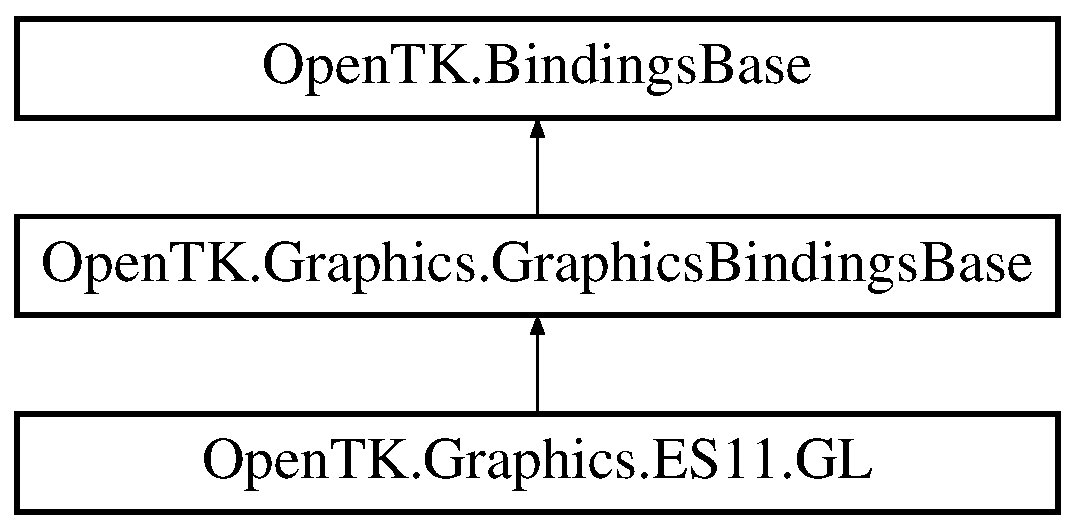
\includegraphics[height=3.000000cm]{class_open_t_k_1_1_graphics_1_1_e_s11_1_1_g_l}
\end{center}
\end{figure}
\subsection*{Static Public Member Functions}
\begin{DoxyCompactItemize}
\item 
static void \hyperlink{class_open_t_k_1_1_graphics_1_1_e_s11_1_1_g_l_a638e38400c456f94e38933751e1e78b3}{Active\-Texture} (Open\-T\-K.\-Graphics.\-E\-S11.\-All texture)
\begin{DoxyCompactList}\small\item\em \mbox{[}requires\-: v1.\-1 and 1.\-1\mbox{]} Select active texture unit \end{DoxyCompactList}\item 
static void \hyperlink{class_open_t_k_1_1_graphics_1_1_e_s11_1_1_g_l_ade9d65df8a675a75c9c0904fbde27e52}{Alpha\-Func} (Open\-T\-K.\-Graphics.\-E\-S11.\-All func, Single @ref)
\begin{DoxyCompactList}\small\item\em \mbox{[}requires\-: v1.\-1 and 1.\-1\mbox{]} Specify the alpha test function \end{DoxyCompactList}\item 
static void \hyperlink{class_open_t_k_1_1_graphics_1_1_e_s11_1_1_g_l_a8fee1457b176b5aad45575a9d2363f6a}{Alpha\-Funcx} (Open\-T\-K.\-Graphics.\-E\-S11.\-All func, int @ref)
\begin{DoxyCompactList}\small\item\em \mbox{[}requires\-: v1.\-1 and 1.\-1\mbox{]}\end{DoxyCompactList}\item 
static void \hyperlink{class_open_t_k_1_1_graphics_1_1_e_s11_1_1_g_l_a3ea03f99a82830f8ed87f7f7bddd74f0}{Bind\-Buffer} (Open\-T\-K.\-Graphics.\-E\-S11.\-All target, Int32 buffer)
\begin{DoxyCompactList}\small\item\em \mbox{[}requires\-: v1.\-1 and 1.\-1\mbox{]} Bind a named buffer object \end{DoxyCompactList}\item 
static void \hyperlink{class_open_t_k_1_1_graphics_1_1_e_s11_1_1_g_l_a473e024b8d245f0ad7a0cb0d295b79b7}{Bind\-Buffer} (Open\-T\-K.\-Graphics.\-E\-S11.\-All target, U\-Int32 buffer)
\begin{DoxyCompactList}\small\item\em \mbox{[}requires\-: v1.\-1 and 1.\-1\mbox{]} Bind a named buffer object \end{DoxyCompactList}\item 
static void \hyperlink{class_open_t_k_1_1_graphics_1_1_e_s11_1_1_g_l_a26a38f6e4537e0173a7e94d49fdb79c4}{Bind\-Texture} (Open\-T\-K.\-Graphics.\-E\-S11.\-All target, Int32 texture)
\begin{DoxyCompactList}\small\item\em \mbox{[}requires\-: v1.\-1 and 1.\-1\mbox{]} Bind a named texture to a texturing target \end{DoxyCompactList}\item 
static void \hyperlink{class_open_t_k_1_1_graphics_1_1_e_s11_1_1_g_l_a63d61b8a47665eb64ca2de8ad081f24b}{Bind\-Texture} (Open\-T\-K.\-Graphics.\-E\-S11.\-All target, U\-Int32 texture)
\begin{DoxyCompactList}\small\item\em \mbox{[}requires\-: v1.\-1 and 1.\-1\mbox{]} Bind a named texture to a texturing target \end{DoxyCompactList}\item 
static void \hyperlink{class_open_t_k_1_1_graphics_1_1_e_s11_1_1_g_l_a82e7e51736b9fe50d6ef8e7e3890be18}{Blend\-Func} (Open\-T\-K.\-Graphics.\-E\-S11.\-All sfactor, Open\-T\-K.\-Graphics.\-E\-S11.\-All dfactor)
\begin{DoxyCompactList}\small\item\em \mbox{[}requires\-: v1.\-1 and 1.\-1\mbox{]} Specify pixel arithmetic \end{DoxyCompactList}\item 
static void \hyperlink{class_open_t_k_1_1_graphics_1_1_e_s11_1_1_g_l_a360083c929bc9788b67f99a341ad1511}{Buffer\-Data} (Open\-T\-K.\-Graphics.\-E\-S11.\-All target, Int\-Ptr size, Int\-Ptr data, Open\-T\-K.\-Graphics.\-E\-S11.\-All usage)
\begin{DoxyCompactList}\small\item\em \mbox{[}requires\-: v1.\-1 and 1.\-1\mbox{]} Creates and initializes a buffer object's data store \end{DoxyCompactList}\item 
static void \hyperlink{class_open_t_k_1_1_graphics_1_1_e_s11_1_1_g_l_a89da2502a1420cf790ad6cced8fa98c2}{Buffer\-Data$<$ T2 $>$} (Open\-T\-K.\-Graphics.\-E\-S11.\-All target, Int\-Ptr size, \mbox{[}In\-Attribute, Out\-Attribute\mbox{]} T2\mbox{[}$\,$\mbox{]} data, Open\-T\-K.\-Graphics.\-E\-S11.\-All usage)
\begin{DoxyCompactList}\small\item\em \mbox{[}requires\-: v1.\-1 and 1.\-1\mbox{]} Creates and initializes a buffer object's data store \end{DoxyCompactList}\item 
static void \hyperlink{class_open_t_k_1_1_graphics_1_1_e_s11_1_1_g_l_aa6caccb92d149948e0f08c55e8eb9724}{Buffer\-Data$<$ T2 $>$} (Open\-T\-K.\-Graphics.\-E\-S11.\-All target, Int\-Ptr size, \mbox{[}In\-Attribute, Out\-Attribute\mbox{]} T2\mbox{[},\mbox{]} data, Open\-T\-K.\-Graphics.\-E\-S11.\-All usage)
\begin{DoxyCompactList}\small\item\em \mbox{[}requires\-: v1.\-1 and 1.\-1\mbox{]} Creates and initializes a buffer object's data store \end{DoxyCompactList}\item 
static void \hyperlink{class_open_t_k_1_1_graphics_1_1_e_s11_1_1_g_l_a302a6bf758be9daed87b3f4bca087841}{Buffer\-Data$<$ T2 $>$} (Open\-T\-K.\-Graphics.\-E\-S11.\-All target, Int\-Ptr size, \mbox{[}In\-Attribute, Out\-Attribute\mbox{]} T2\mbox{[},,\mbox{]} data, Open\-T\-K.\-Graphics.\-E\-S11.\-All usage)
\begin{DoxyCompactList}\small\item\em \mbox{[}requires\-: v1.\-1 and 1.\-1\mbox{]} Creates and initializes a buffer object's data store \end{DoxyCompactList}\item 
static void \hyperlink{class_open_t_k_1_1_graphics_1_1_e_s11_1_1_g_l_abadd505d7dfdb3cd015e4a0cbd4786c6}{Buffer\-Data$<$ T2 $>$} (Open\-T\-K.\-Graphics.\-E\-S11.\-All target, Int\-Ptr size, \mbox{[}In\-Attribute, Out\-Attribute\mbox{]} ref T2 data, Open\-T\-K.\-Graphics.\-E\-S11.\-All usage)
\begin{DoxyCompactList}\small\item\em \mbox{[}requires\-: v1.\-1 and 1.\-1\mbox{]} Creates and initializes a buffer object's data store \end{DoxyCompactList}\item 
static void \hyperlink{class_open_t_k_1_1_graphics_1_1_e_s11_1_1_g_l_ab68ae06b1f362135b81ecfbf1e1c32da}{Buffer\-Sub\-Data} (Open\-T\-K.\-Graphics.\-E\-S11.\-All target, Int\-Ptr offset, Int\-Ptr size, Int\-Ptr data)
\begin{DoxyCompactList}\small\item\em \mbox{[}requires\-: v1.\-1 and 1.\-1\mbox{]} Updates a subset of a buffer object's data store \end{DoxyCompactList}\item 
static void \hyperlink{class_open_t_k_1_1_graphics_1_1_e_s11_1_1_g_l_a7c2db62f766e71c7c52a3f3a9b2d34ae}{Buffer\-Sub\-Data$<$ T3 $>$} (Open\-T\-K.\-Graphics.\-E\-S11.\-All target, Int\-Ptr offset, Int\-Ptr size, \mbox{[}In\-Attribute, Out\-Attribute\mbox{]} T3\mbox{[}$\,$\mbox{]} data)
\begin{DoxyCompactList}\small\item\em \mbox{[}requires\-: v1.\-1 and 1.\-1\mbox{]} Updates a subset of a buffer object's data store \end{DoxyCompactList}\item 
static void \hyperlink{class_open_t_k_1_1_graphics_1_1_e_s11_1_1_g_l_ab83480f236e01b9c9234cc4385307cb6}{Buffer\-Sub\-Data$<$ T3 $>$} (Open\-T\-K.\-Graphics.\-E\-S11.\-All target, Int\-Ptr offset, Int\-Ptr size, \mbox{[}In\-Attribute, Out\-Attribute\mbox{]} T3\mbox{[},\mbox{]} data)
\begin{DoxyCompactList}\small\item\em \mbox{[}requires\-: v1.\-1 and 1.\-1\mbox{]} Updates a subset of a buffer object's data store \end{DoxyCompactList}\item 
static void \hyperlink{class_open_t_k_1_1_graphics_1_1_e_s11_1_1_g_l_aae7185625b7615c97fd3adc981c39389}{Buffer\-Sub\-Data$<$ T3 $>$} (Open\-T\-K.\-Graphics.\-E\-S11.\-All target, Int\-Ptr offset, Int\-Ptr size, \mbox{[}In\-Attribute, Out\-Attribute\mbox{]} T3\mbox{[},,\mbox{]} data)
\begin{DoxyCompactList}\small\item\em \mbox{[}requires\-: v1.\-1 and 1.\-1\mbox{]} Updates a subset of a buffer object's data store \end{DoxyCompactList}\item 
static void \hyperlink{class_open_t_k_1_1_graphics_1_1_e_s11_1_1_g_l_ad4e4d430bb583bc1e80a497f1d656c86}{Buffer\-Sub\-Data$<$ T3 $>$} (Open\-T\-K.\-Graphics.\-E\-S11.\-All target, Int\-Ptr offset, Int\-Ptr size, \mbox{[}In\-Attribute, Out\-Attribute\mbox{]} ref T3 data)
\begin{DoxyCompactList}\small\item\em \mbox{[}requires\-: v1.\-1 and 1.\-1\mbox{]} Updates a subset of a buffer object's data store \end{DoxyCompactList}\item 
static void \hyperlink{class_open_t_k_1_1_graphics_1_1_e_s11_1_1_g_l_a6dc7ac8d7aa6d00cba4eb9462d16c5ea}{Clear} (Int32 mask)
\begin{DoxyCompactList}\small\item\em \mbox{[}requires\-: v1.\-1 and 1.\-1\mbox{]} Clear buffers to preset values \end{DoxyCompactList}\item 
static void \hyperlink{class_open_t_k_1_1_graphics_1_1_e_s11_1_1_g_l_ae042bbf3c2f39de8f6b4b1e441d27f30}{Clear} (U\-Int32 mask)
\begin{DoxyCompactList}\small\item\em \mbox{[}requires\-: v1.\-1 and 1.\-1\mbox{]} Clear buffers to preset values \end{DoxyCompactList}\item 
static void \hyperlink{class_open_t_k_1_1_graphics_1_1_e_s11_1_1_g_l_a3d3fd5eabc61e25dd654fa36c831a620}{Clear\-Color} (Single red, Single green, Single blue, Single alpha)
\begin{DoxyCompactList}\small\item\em \mbox{[}requires\-: v1.\-1 and 1.\-1\mbox{]} Specify clear values for the color buffers \end{DoxyCompactList}\item 
static void \hyperlink{class_open_t_k_1_1_graphics_1_1_e_s11_1_1_g_l_a1faa85991264c13391d636112a239384}{Clear\-Colorx} (int red, int green, int blue, int alpha)
\begin{DoxyCompactList}\small\item\em \mbox{[}requires\-: v1.\-1 and 1.\-1\mbox{]}\end{DoxyCompactList}\item 
static void \hyperlink{class_open_t_k_1_1_graphics_1_1_e_s11_1_1_g_l_a3394befa8f65d8c11dc293a0a13d1300}{Clear\-Depth} (Single depth)
\begin{DoxyCompactList}\small\item\em \mbox{[}requires\-: v1.\-1 and 1.\-1\mbox{]} Specify the clear value for the depth buffer \end{DoxyCompactList}\item 
static void \hyperlink{class_open_t_k_1_1_graphics_1_1_e_s11_1_1_g_l_a24ec186a243c80bb3fc6fa43e16ac708}{Clear\-Depthx} (int depth)
\begin{DoxyCompactList}\small\item\em \mbox{[}requires\-: v1.\-1 and 1.\-1\mbox{]}\end{DoxyCompactList}\item 
static void \hyperlink{class_open_t_k_1_1_graphics_1_1_e_s11_1_1_g_l_a9e8b3497773e2d3ee3a655661ef6c2e9}{Clear\-Stencil} (Int32 s)
\begin{DoxyCompactList}\small\item\em \mbox{[}requires\-: v1.\-1 and 1.\-1\mbox{]} Specify the clear value for the stencil buffer \end{DoxyCompactList}\item 
static void \hyperlink{class_open_t_k_1_1_graphics_1_1_e_s11_1_1_g_l_acf533a25734a701984d66ff5bab44343}{Client\-Active\-Texture} (Open\-T\-K.\-Graphics.\-E\-S11.\-All texture)
\begin{DoxyCompactList}\small\item\em \mbox{[}requires\-: v1.\-1 and 1.\-1\mbox{]} Select active texture unit \end{DoxyCompactList}\item 
static void \hyperlink{class_open_t_k_1_1_graphics_1_1_e_s11_1_1_g_l_a95e9c9439c114f6e2283670044cc6faf}{Clip\-Plane} (Open\-T\-K.\-Graphics.\-E\-S11.\-All plane, Single\mbox{[}$\,$\mbox{]} equation)
\begin{DoxyCompactList}\small\item\em \mbox{[}requires\-: v1.\-1 and 1.\-1\mbox{]} Specify a plane against which all geometry is clipped \end{DoxyCompactList}\item 
static void \hyperlink{class_open_t_k_1_1_graphics_1_1_e_s11_1_1_g_l_ae1a3bd0caeed444540117f339a6e4851}{Clip\-Plane} (Open\-T\-K.\-Graphics.\-E\-S11.\-All plane, ref Single equation)
\begin{DoxyCompactList}\small\item\em \mbox{[}requires\-: v1.\-1 and 1.\-1\mbox{]} Specify a plane against which all geometry is clipped \end{DoxyCompactList}\item 
static unsafe void \hyperlink{class_open_t_k_1_1_graphics_1_1_e_s11_1_1_g_l_a0da8d7c3a32dffd4b3e37693842958e3}{Clip\-Plane} (Open\-T\-K.\-Graphics.\-E\-S11.\-All plane, Single $\ast$equation)
\begin{DoxyCompactList}\small\item\em \mbox{[}requires\-: v1.\-1 and 1.\-1\mbox{]} Specify a plane against which all geometry is clipped \end{DoxyCompactList}\item 
static void \hyperlink{class_open_t_k_1_1_graphics_1_1_e_s11_1_1_g_l_a606cf18301c3c201e938edc862f7e259}{Clip\-Planef\-I\-M\-G} (Open\-T\-K.\-Graphics.\-E\-S11.\-All p, Single\mbox{[}$\,$\mbox{]} eqn)
\begin{DoxyCompactList}\small\item\em \mbox{[}requires\-: v1.\-1 and 1.\-1\mbox{]}\end{DoxyCompactList}\item 
static void \hyperlink{class_open_t_k_1_1_graphics_1_1_e_s11_1_1_g_l_a492cce9d18dc2c17529e59c144baeace}{Clip\-Planef\-I\-M\-G} (Open\-T\-K.\-Graphics.\-E\-S11.\-All p, ref Single eqn)
\begin{DoxyCompactList}\small\item\em \mbox{[}requires\-: v1.\-1 and 1.\-1\mbox{]}\end{DoxyCompactList}\item 
static unsafe void \hyperlink{class_open_t_k_1_1_graphics_1_1_e_s11_1_1_g_l_aee854dd51ff45afbc31d02af4ed48ddb}{Clip\-Planef\-I\-M\-G} (Open\-T\-K.\-Graphics.\-E\-S11.\-All p, Single $\ast$eqn)
\begin{DoxyCompactList}\small\item\em \mbox{[}requires\-: v1.\-1 and 1.\-1\mbox{]}\end{DoxyCompactList}\item 
static void \hyperlink{class_open_t_k_1_1_graphics_1_1_e_s11_1_1_g_l_a04d5d184a2c0a2d5b6fa89d6c4458d87}{Clip\-Planex} (Open\-T\-K.\-Graphics.\-E\-S11.\-All plane, int\mbox{[}$\,$\mbox{]} equation)
\begin{DoxyCompactList}\small\item\em \mbox{[}requires\-: v1.\-1 and 1.\-1\mbox{]}\end{DoxyCompactList}\item 
static void \hyperlink{class_open_t_k_1_1_graphics_1_1_e_s11_1_1_g_l_ac4280c897fa8bd59c181944662648a84}{Clip\-Planex} (Open\-T\-K.\-Graphics.\-E\-S11.\-All plane, ref int equation)
\begin{DoxyCompactList}\small\item\em \mbox{[}requires\-: v1.\-1 and 1.\-1\mbox{]}\end{DoxyCompactList}\item 
static unsafe void \hyperlink{class_open_t_k_1_1_graphics_1_1_e_s11_1_1_g_l_ab237f4fc9ea2d8a0160d46a7a4ccf4bf}{Clip\-Planex} (Open\-T\-K.\-Graphics.\-E\-S11.\-All plane, int $\ast$equation)
\begin{DoxyCompactList}\small\item\em \mbox{[}requires\-: v1.\-1 and 1.\-1\mbox{]}\end{DoxyCompactList}\item 
static void \hyperlink{class_open_t_k_1_1_graphics_1_1_e_s11_1_1_g_l_ace30ddd58b4fb2c8ffcd1aae20734650}{Clip\-Planex\-I\-M\-G} (Open\-T\-K.\-Graphics.\-E\-S11.\-All p, int\mbox{[}$\,$\mbox{]} eqn)
\begin{DoxyCompactList}\small\item\em \mbox{[}requires\-: v1.\-1 and 1.\-1\mbox{]}\end{DoxyCompactList}\item 
static void \hyperlink{class_open_t_k_1_1_graphics_1_1_e_s11_1_1_g_l_a9ca3413881dd669a9d754459bf59fb13}{Clip\-Planex\-I\-M\-G} (Open\-T\-K.\-Graphics.\-E\-S11.\-All p, ref int eqn)
\begin{DoxyCompactList}\small\item\em \mbox{[}requires\-: v1.\-1 and 1.\-1\mbox{]}\end{DoxyCompactList}\item 
static unsafe void \hyperlink{class_open_t_k_1_1_graphics_1_1_e_s11_1_1_g_l_a562f810bf94fe8c3d88ea4115e48e869}{Clip\-Planex\-I\-M\-G} (Open\-T\-K.\-Graphics.\-E\-S11.\-All p, int $\ast$eqn)
\begin{DoxyCompactList}\small\item\em \mbox{[}requires\-: v1.\-1 and 1.\-1\mbox{]}\end{DoxyCompactList}\item 
static void \hyperlink{class_open_t_k_1_1_graphics_1_1_e_s11_1_1_g_l_ace17710463bb6b0ce243a62be8203e04}{Color4} (Single red, Single green, Single blue, Single alpha)
\begin{DoxyCompactList}\small\item\em \mbox{[}requires\-: v1.\-1 and 1.\-1\mbox{]} Set the current color \end{DoxyCompactList}\item 
static void \hyperlink{class_open_t_k_1_1_graphics_1_1_e_s11_1_1_g_l_a70b5d57aeb8e3d4f31a0d6fca99e4689}{Color4} (Byte red, Byte green, Byte blue, Byte alpha)
\begin{DoxyCompactList}\small\item\em \mbox{[}requires\-: v1.\-1 and 1.\-1\mbox{]} Set the current color \end{DoxyCompactList}\item 
static void \hyperlink{class_open_t_k_1_1_graphics_1_1_e_s11_1_1_g_l_a528393a7a30f210795aa9d2b72b1afc8}{Color4x} (int red, int green, int blue, int alpha)
\begin{DoxyCompactList}\small\item\em \mbox{[}requires\-: v1.\-1 and 1.\-1\mbox{]}\end{DoxyCompactList}\item 
static void \hyperlink{class_open_t_k_1_1_graphics_1_1_e_s11_1_1_g_l_a01c90ac1b11a5d9ab99c0178e6ac7680}{Color\-Mask} (bool red, bool green, bool blue, bool alpha)
\begin{DoxyCompactList}\small\item\em \mbox{[}requires\-: v1.\-1 and 1.\-1\mbox{]} Enable and disable writing of frame buffer color components \end{DoxyCompactList}\item 
static void \hyperlink{class_open_t_k_1_1_graphics_1_1_e_s11_1_1_g_l_a079f04be4365d8ff843ecdbf32fdcf32}{Color\-Pointer} (Int32 size, Open\-T\-K.\-Graphics.\-E\-S11.\-All type, Int32 stride, Int\-Ptr pointer)
\begin{DoxyCompactList}\small\item\em \mbox{[}requires\-: v1.\-1 and 1.\-1\mbox{]} Define an array of colors \end{DoxyCompactList}\item 
static void \hyperlink{class_open_t_k_1_1_graphics_1_1_e_s11_1_1_g_l_a2d528f071eb703da05db0f9bba04ad71}{Color\-Pointer$<$ T3 $>$} (Int32 size, Open\-T\-K.\-Graphics.\-E\-S11.\-All type, Int32 stride, \mbox{[}In\-Attribute, Out\-Attribute\mbox{]} T3\mbox{[}$\,$\mbox{]} pointer)
\begin{DoxyCompactList}\small\item\em \mbox{[}requires\-: v1.\-1 and 1.\-1\mbox{]} Define an array of colors \end{DoxyCompactList}\item 
static void \hyperlink{class_open_t_k_1_1_graphics_1_1_e_s11_1_1_g_l_a1cb5bdc0d82f278ea78a43d5b31d4a84}{Color\-Pointer$<$ T3 $>$} (Int32 size, Open\-T\-K.\-Graphics.\-E\-S11.\-All type, Int32 stride, \mbox{[}In\-Attribute, Out\-Attribute\mbox{]} T3\mbox{[},\mbox{]} pointer)
\begin{DoxyCompactList}\small\item\em \mbox{[}requires\-: v1.\-1 and 1.\-1\mbox{]} Define an array of colors \end{DoxyCompactList}\item 
static void \hyperlink{class_open_t_k_1_1_graphics_1_1_e_s11_1_1_g_l_abd3efe27caac511d53ace7755a7c10f5}{Color\-Pointer$<$ T3 $>$} (Int32 size, Open\-T\-K.\-Graphics.\-E\-S11.\-All type, Int32 stride, \mbox{[}In\-Attribute, Out\-Attribute\mbox{]} T3\mbox{[},,\mbox{]} pointer)
\begin{DoxyCompactList}\small\item\em \mbox{[}requires\-: v1.\-1 and 1.\-1\mbox{]} Define an array of colors \end{DoxyCompactList}\item 
static void \hyperlink{class_open_t_k_1_1_graphics_1_1_e_s11_1_1_g_l_a5b1e2504b3482939a90839e713753415}{Color\-Pointer$<$ T3 $>$} (Int32 size, Open\-T\-K.\-Graphics.\-E\-S11.\-All type, Int32 stride, \mbox{[}In\-Attribute, Out\-Attribute\mbox{]} ref T3 pointer)
\begin{DoxyCompactList}\small\item\em \mbox{[}requires\-: v1.\-1 and 1.\-1\mbox{]} Define an array of colors \end{DoxyCompactList}\item 
static void \hyperlink{class_open_t_k_1_1_graphics_1_1_e_s11_1_1_g_l_a25b214686be0bdab1e036d35b297e23f}{Compressed\-Tex\-Image2\-D} (Open\-T\-K.\-Graphics.\-E\-S11.\-All target, Int32 level, Open\-T\-K.\-Graphics.\-E\-S11.\-All internalformat, Int32 width, Int32 height, Int32 border, Int32 image\-Size, Int\-Ptr data)
\begin{DoxyCompactList}\small\item\em \mbox{[}requires\-: v1.\-1 and 1.\-1\mbox{]} Specify a two-\/dimensional texture image in a compressed format \end{DoxyCompactList}\item 
static void \hyperlink{class_open_t_k_1_1_graphics_1_1_e_s11_1_1_g_l_a988bc41c818fb8e9ce5f47b087a4bd07}{Compressed\-Tex\-Image2\-D$<$ T7 $>$} (Open\-T\-K.\-Graphics.\-E\-S11.\-All target, Int32 level, Open\-T\-K.\-Graphics.\-E\-S11.\-All internalformat, Int32 width, Int32 height, Int32 border, Int32 image\-Size, \mbox{[}In\-Attribute, Out\-Attribute\mbox{]} T7\mbox{[}$\,$\mbox{]} data)
\begin{DoxyCompactList}\small\item\em \mbox{[}requires\-: v1.\-1 and 1.\-1\mbox{]} Specify a two-\/dimensional texture image in a compressed format \end{DoxyCompactList}\item 
static void \hyperlink{class_open_t_k_1_1_graphics_1_1_e_s11_1_1_g_l_abea9b1fcffb1517a4dde929046bcfeb1}{Compressed\-Tex\-Image2\-D$<$ T7 $>$} (Open\-T\-K.\-Graphics.\-E\-S11.\-All target, Int32 level, Open\-T\-K.\-Graphics.\-E\-S11.\-All internalformat, Int32 width, Int32 height, Int32 border, Int32 image\-Size, \mbox{[}In\-Attribute, Out\-Attribute\mbox{]} T7\mbox{[},\mbox{]} data)
\begin{DoxyCompactList}\small\item\em \mbox{[}requires\-: v1.\-1 and 1.\-1\mbox{]} Specify a two-\/dimensional texture image in a compressed format \end{DoxyCompactList}\item 
static void \hyperlink{class_open_t_k_1_1_graphics_1_1_e_s11_1_1_g_l_a103b5ccd0f794d0ccf56083ed095702e}{Compressed\-Tex\-Image2\-D$<$ T7 $>$} (Open\-T\-K.\-Graphics.\-E\-S11.\-All target, Int32 level, Open\-T\-K.\-Graphics.\-E\-S11.\-All internalformat, Int32 width, Int32 height, Int32 border, Int32 image\-Size, \mbox{[}In\-Attribute, Out\-Attribute\mbox{]} T7\mbox{[},,\mbox{]} data)
\begin{DoxyCompactList}\small\item\em \mbox{[}requires\-: v1.\-1 and 1.\-1\mbox{]} Specify a two-\/dimensional texture image in a compressed format \end{DoxyCompactList}\item 
static void \hyperlink{class_open_t_k_1_1_graphics_1_1_e_s11_1_1_g_l_ad68055c6c38e8684d2510286a7327adb}{Compressed\-Tex\-Image2\-D$<$ T7 $>$} (Open\-T\-K.\-Graphics.\-E\-S11.\-All target, Int32 level, Open\-T\-K.\-Graphics.\-E\-S11.\-All internalformat, Int32 width, Int32 height, Int32 border, Int32 image\-Size, \mbox{[}In\-Attribute, Out\-Attribute\mbox{]} ref T7 data)
\begin{DoxyCompactList}\small\item\em \mbox{[}requires\-: v1.\-1 and 1.\-1\mbox{]} Specify a two-\/dimensional texture image in a compressed format \end{DoxyCompactList}\item 
static void \hyperlink{class_open_t_k_1_1_graphics_1_1_e_s11_1_1_g_l_ab02e7a6d11a4aa6dff21e65eebca2dfb}{Compressed\-Tex\-Sub\-Image2\-D} (Open\-T\-K.\-Graphics.\-E\-S11.\-All target, Int32 level, Int32 xoffset, Int32 yoffset, Int32 width, Int32 height, Open\-T\-K.\-Graphics.\-E\-S11.\-All format, Int32 image\-Size, Int\-Ptr data)
\begin{DoxyCompactList}\small\item\em \mbox{[}requires\-: v1.\-1 and 1.\-1\mbox{]} Specify a two-\/dimensional texture subimage in a compressed format \end{DoxyCompactList}\item 
static void \hyperlink{class_open_t_k_1_1_graphics_1_1_e_s11_1_1_g_l_aa7682a03f2f83e12940713a6e1a15993}{Compressed\-Tex\-Sub\-Image2\-D$<$ T8 $>$} (Open\-T\-K.\-Graphics.\-E\-S11.\-All target, Int32 level, Int32 xoffset, Int32 yoffset, Int32 width, Int32 height, Open\-T\-K.\-Graphics.\-E\-S11.\-All format, Int32 image\-Size, \mbox{[}In\-Attribute, Out\-Attribute\mbox{]} T8\mbox{[}$\,$\mbox{]} data)
\begin{DoxyCompactList}\small\item\em \mbox{[}requires\-: v1.\-1 and 1.\-1\mbox{]} Specify a two-\/dimensional texture subimage in a compressed format \end{DoxyCompactList}\item 
static void \hyperlink{class_open_t_k_1_1_graphics_1_1_e_s11_1_1_g_l_a9b39a0f7f2a20e0438e4cb07f72f7056}{Compressed\-Tex\-Sub\-Image2\-D$<$ T8 $>$} (Open\-T\-K.\-Graphics.\-E\-S11.\-All target, Int32 level, Int32 xoffset, Int32 yoffset, Int32 width, Int32 height, Open\-T\-K.\-Graphics.\-E\-S11.\-All format, Int32 image\-Size, \mbox{[}In\-Attribute, Out\-Attribute\mbox{]} T8\mbox{[},\mbox{]} data)
\begin{DoxyCompactList}\small\item\em \mbox{[}requires\-: v1.\-1 and 1.\-1\mbox{]} Specify a two-\/dimensional texture subimage in a compressed format \end{DoxyCompactList}\item 
static void \hyperlink{class_open_t_k_1_1_graphics_1_1_e_s11_1_1_g_l_ae8eb4c4d113f85b554475a745cccd46b}{Compressed\-Tex\-Sub\-Image2\-D$<$ T8 $>$} (Open\-T\-K.\-Graphics.\-E\-S11.\-All target, Int32 level, Int32 xoffset, Int32 yoffset, Int32 width, Int32 height, Open\-T\-K.\-Graphics.\-E\-S11.\-All format, Int32 image\-Size, \mbox{[}In\-Attribute, Out\-Attribute\mbox{]} T8\mbox{[},,\mbox{]} data)
\begin{DoxyCompactList}\small\item\em \mbox{[}requires\-: v1.\-1 and 1.\-1\mbox{]} Specify a two-\/dimensional texture subimage in a compressed format \end{DoxyCompactList}\item 
static void \hyperlink{class_open_t_k_1_1_graphics_1_1_e_s11_1_1_g_l_ae6198a82fa0fc1cb30ac2397093e6048}{Compressed\-Tex\-Sub\-Image2\-D$<$ T8 $>$} (Open\-T\-K.\-Graphics.\-E\-S11.\-All target, Int32 level, Int32 xoffset, Int32 yoffset, Int32 width, Int32 height, Open\-T\-K.\-Graphics.\-E\-S11.\-All format, Int32 image\-Size, \mbox{[}In\-Attribute, Out\-Attribute\mbox{]} ref T8 data)
\begin{DoxyCompactList}\small\item\em \mbox{[}requires\-: v1.\-1 and 1.\-1\mbox{]} Specify a two-\/dimensional texture subimage in a compressed format \end{DoxyCompactList}\item 
static void \hyperlink{class_open_t_k_1_1_graphics_1_1_e_s11_1_1_g_l_a8eaf46f4fa35ac6845a262e7d0776654}{Copy\-Tex\-Image2\-D} (Open\-T\-K.\-Graphics.\-E\-S11.\-All target, Int32 level, Open\-T\-K.\-Graphics.\-E\-S11.\-All internalformat, Int32 x, Int32 y, Int32 width, Int32 height, Int32 border)
\begin{DoxyCompactList}\small\item\em \mbox{[}requires\-: v1.\-1 and 1.\-1\mbox{]} Copy pixels into a 2\-D texture image \end{DoxyCompactList}\item 
static void \hyperlink{class_open_t_k_1_1_graphics_1_1_e_s11_1_1_g_l_af2ce341247d2c1563b5a7c51c3aff6c6}{Copy\-Tex\-Sub\-Image2\-D} (Open\-T\-K.\-Graphics.\-E\-S11.\-All target, Int32 level, Int32 xoffset, Int32 yoffset, Int32 x, Int32 y, Int32 width, Int32 height)
\begin{DoxyCompactList}\small\item\em \mbox{[}requires\-: v1.\-1 and 1.\-1\mbox{]} Copy a two-\/dimensional texture subimage \end{DoxyCompactList}\item 
static void \hyperlink{class_open_t_k_1_1_graphics_1_1_e_s11_1_1_g_l_a106f96e00bd2a6df37936b8223e9872a}{Cull\-Face} (Open\-T\-K.\-Graphics.\-E\-S11.\-All mode)
\begin{DoxyCompactList}\small\item\em \mbox{[}requires\-: v1.\-1 and 1.\-1\mbox{]} Specify whether front-\/ or back-\/facing facets can be culled \end{DoxyCompactList}\item 
static void \hyperlink{class_open_t_k_1_1_graphics_1_1_e_s11_1_1_g_l_afbd6255ea9de95e551c838d66cd2264f}{Delete\-Buffers} (Int32 n, Int32\mbox{[}$\,$\mbox{]} buffers)
\begin{DoxyCompactList}\small\item\em \mbox{[}requires\-: v1.\-1 and 1.\-1\mbox{]} Delete named buffer objects \end{DoxyCompactList}\item 
static void \hyperlink{class_open_t_k_1_1_graphics_1_1_e_s11_1_1_g_l_a7e6e017974d31b3632236870fabcef24}{Delete\-Buffers} (Int32 n, ref Int32 buffers)
\begin{DoxyCompactList}\small\item\em \mbox{[}requires\-: v1.\-1 and 1.\-1\mbox{]} Delete named buffer objects \end{DoxyCompactList}\item 
static unsafe void \hyperlink{class_open_t_k_1_1_graphics_1_1_e_s11_1_1_g_l_a35d8d449eb10b73cfffad3aa3cccece5}{Delete\-Buffers} (Int32 n, Int32 $\ast$buffers)
\begin{DoxyCompactList}\small\item\em \mbox{[}requires\-: v1.\-1 and 1.\-1\mbox{]} Delete named buffer objects \end{DoxyCompactList}\item 
static void \hyperlink{class_open_t_k_1_1_graphics_1_1_e_s11_1_1_g_l_ad9115415050bbb67d553f302ad158eec}{Delete\-Buffers} (Int32 n, U\-Int32\mbox{[}$\,$\mbox{]} buffers)
\begin{DoxyCompactList}\small\item\em \mbox{[}requires\-: v1.\-1 and 1.\-1\mbox{]} Delete named buffer objects \end{DoxyCompactList}\item 
static void \hyperlink{class_open_t_k_1_1_graphics_1_1_e_s11_1_1_g_l_a808d320170e777ba97333d4fda18b686}{Delete\-Buffers} (Int32 n, ref U\-Int32 buffers)
\begin{DoxyCompactList}\small\item\em \mbox{[}requires\-: v1.\-1 and 1.\-1\mbox{]} Delete named buffer objects \end{DoxyCompactList}\item 
static unsafe void \hyperlink{class_open_t_k_1_1_graphics_1_1_e_s11_1_1_g_l_a2493b9034bce2816eb7d4ffb9c441f23}{Delete\-Buffers} (Int32 n, U\-Int32 $\ast$buffers)
\begin{DoxyCompactList}\small\item\em \mbox{[}requires\-: v1.\-1 and 1.\-1\mbox{]} Delete named buffer objects \end{DoxyCompactList}\item 
static void \hyperlink{class_open_t_k_1_1_graphics_1_1_e_s11_1_1_g_l_a8352c6ef7c0a9392d0333a8ed4ece77f}{Delete\-Textures} (Int32 n, Int32\mbox{[}$\,$\mbox{]} textures)
\begin{DoxyCompactList}\small\item\em \mbox{[}requires\-: v1.\-1 and 1.\-1\mbox{]} Delete named textures \end{DoxyCompactList}\item 
static void \hyperlink{class_open_t_k_1_1_graphics_1_1_e_s11_1_1_g_l_af28e6463de7aeaba462e29109adbf96e}{Delete\-Textures} (Int32 n, ref Int32 textures)
\begin{DoxyCompactList}\small\item\em \mbox{[}requires\-: v1.\-1 and 1.\-1\mbox{]} Delete named textures \end{DoxyCompactList}\item 
static unsafe void \hyperlink{class_open_t_k_1_1_graphics_1_1_e_s11_1_1_g_l_a86bcef5879d200a3be48521e7864f344}{Delete\-Textures} (Int32 n, Int32 $\ast$textures)
\begin{DoxyCompactList}\small\item\em \mbox{[}requires\-: v1.\-1 and 1.\-1\mbox{]} Delete named textures \end{DoxyCompactList}\item 
static void \hyperlink{class_open_t_k_1_1_graphics_1_1_e_s11_1_1_g_l_a6ad20d4e499ceb53fdaebe658d420fda}{Delete\-Textures} (Int32 n, U\-Int32\mbox{[}$\,$\mbox{]} textures)
\begin{DoxyCompactList}\small\item\em \mbox{[}requires\-: v1.\-1 and 1.\-1\mbox{]} Delete named textures \end{DoxyCompactList}\item 
static void \hyperlink{class_open_t_k_1_1_graphics_1_1_e_s11_1_1_g_l_aa564bd87644b01703ab07000b1978020}{Delete\-Textures} (Int32 n, ref U\-Int32 textures)
\begin{DoxyCompactList}\small\item\em \mbox{[}requires\-: v1.\-1 and 1.\-1\mbox{]} Delete named textures \end{DoxyCompactList}\item 
static unsafe void \hyperlink{class_open_t_k_1_1_graphics_1_1_e_s11_1_1_g_l_acb809657059417e33d0d3980bed8d609}{Delete\-Textures} (Int32 n, U\-Int32 $\ast$textures)
\begin{DoxyCompactList}\small\item\em \mbox{[}requires\-: v1.\-1 and 1.\-1\mbox{]} Delete named textures \end{DoxyCompactList}\item 
static void \hyperlink{class_open_t_k_1_1_graphics_1_1_e_s11_1_1_g_l_aaeef14cdd8e11fd6a182d0da54cc80b9}{Depth\-Func} (Open\-T\-K.\-Graphics.\-E\-S11.\-All func)
\begin{DoxyCompactList}\small\item\em \mbox{[}requires\-: v1.\-1 and 1.\-1\mbox{]} Specify the value used for depth buffer comparisons \end{DoxyCompactList}\item 
static void \hyperlink{class_open_t_k_1_1_graphics_1_1_e_s11_1_1_g_l_a879c35829c9e3299e10ebe7b59b14de4}{Depth\-Mask} (bool flag)
\begin{DoxyCompactList}\small\item\em \mbox{[}requires\-: v1.\-1 and 1.\-1\mbox{]} Enable or disable writing into the depth buffer \end{DoxyCompactList}\item 
static void \hyperlink{class_open_t_k_1_1_graphics_1_1_e_s11_1_1_g_l_a33fa781e387acf89b805bd22dc84c353}{Depth\-Range} (Single z\-Near, Single z\-Far)
\begin{DoxyCompactList}\small\item\em \mbox{[}requires\-: v1.\-1 and 1.\-1\mbox{]} Specify mapping of depth values from normalized device coordinates to window coordinates \end{DoxyCompactList}\item 
static void \hyperlink{class_open_t_k_1_1_graphics_1_1_e_s11_1_1_g_l_aa9a54048d36aa4e33e74ca5d596cff6e}{Depth\-Rangex} (int z\-Near, int z\-Far)
\begin{DoxyCompactList}\small\item\em \mbox{[}requires\-: v1.\-1 and 1.\-1\mbox{]}\end{DoxyCompactList}\item 
static void \hyperlink{class_open_t_k_1_1_graphics_1_1_e_s11_1_1_g_l_a32a8e29f69e50b3f991ebe49c1da15fa}{Disable} (Open\-T\-K.\-Graphics.\-E\-S11.\-All cap)
\begin{DoxyCompactList}\small\item\em \mbox{[}requires\-: v1.\-1 and 1.\-1\mbox{]}\end{DoxyCompactList}\item 
static void \hyperlink{class_open_t_k_1_1_graphics_1_1_e_s11_1_1_g_l_a0a99f5cb6d5f531c731a4882195e599f}{Disable\-Client\-State} (Open\-T\-K.\-Graphics.\-E\-S11.\-All array)
\begin{DoxyCompactList}\small\item\em \mbox{[}requires\-: v1.\-1 and 1.\-1\mbox{]}\end{DoxyCompactList}\item 
static void \hyperlink{class_open_t_k_1_1_graphics_1_1_e_s11_1_1_g_l_ab87451ee7a48d4b8c60533d64a9dc34f}{Draw\-Arrays} (Open\-T\-K.\-Graphics.\-E\-S11.\-All mode, Int32 first, Int32 count)
\begin{DoxyCompactList}\small\item\em \mbox{[}requires\-: v1.\-1 and 1.\-1\mbox{]} Render primitives from array data \end{DoxyCompactList}\item 
static void \hyperlink{class_open_t_k_1_1_graphics_1_1_e_s11_1_1_g_l_af5ec8d8748fee3ab4f0f8e0904a82895}{Draw\-Elements} (Open\-T\-K.\-Graphics.\-E\-S11.\-All mode, Int32 count, Open\-T\-K.\-Graphics.\-E\-S11.\-All type, Int\-Ptr indices)
\begin{DoxyCompactList}\small\item\em \mbox{[}requires\-: v1.\-1 and 1.\-1\mbox{]} Render primitives from array data \end{DoxyCompactList}\item 
static void \hyperlink{class_open_t_k_1_1_graphics_1_1_e_s11_1_1_g_l_a96305f6061dc044f9a6f93f9781070e8}{Draw\-Elements$<$ T3 $>$} (Open\-T\-K.\-Graphics.\-E\-S11.\-All mode, Int32 count, Open\-T\-K.\-Graphics.\-E\-S11.\-All type, \mbox{[}In\-Attribute, Out\-Attribute\mbox{]} T3\mbox{[}$\,$\mbox{]} indices)
\begin{DoxyCompactList}\small\item\em \mbox{[}requires\-: v1.\-1 and 1.\-1\mbox{]} Render primitives from array data \end{DoxyCompactList}\item 
static void \hyperlink{class_open_t_k_1_1_graphics_1_1_e_s11_1_1_g_l_a1e7d852dab4c8472cad90afcc26e33d5}{Draw\-Elements$<$ T3 $>$} (Open\-T\-K.\-Graphics.\-E\-S11.\-All mode, Int32 count, Open\-T\-K.\-Graphics.\-E\-S11.\-All type, \mbox{[}In\-Attribute, Out\-Attribute\mbox{]} T3\mbox{[},\mbox{]} indices)
\begin{DoxyCompactList}\small\item\em \mbox{[}requires\-: v1.\-1 and 1.\-1\mbox{]} Render primitives from array data \end{DoxyCompactList}\item 
static void \hyperlink{class_open_t_k_1_1_graphics_1_1_e_s11_1_1_g_l_a0a0e0373147adeb6886081ddacc445fc}{Draw\-Elements$<$ T3 $>$} (Open\-T\-K.\-Graphics.\-E\-S11.\-All mode, Int32 count, Open\-T\-K.\-Graphics.\-E\-S11.\-All type, \mbox{[}In\-Attribute, Out\-Attribute\mbox{]} T3\mbox{[},,\mbox{]} indices)
\begin{DoxyCompactList}\small\item\em \mbox{[}requires\-: v1.\-1 and 1.\-1\mbox{]} Render primitives from array data \end{DoxyCompactList}\item 
static void \hyperlink{class_open_t_k_1_1_graphics_1_1_e_s11_1_1_g_l_af094c98e64573b519dc9324b4b37e536}{Draw\-Elements$<$ T3 $>$} (Open\-T\-K.\-Graphics.\-E\-S11.\-All mode, Int32 count, Open\-T\-K.\-Graphics.\-E\-S11.\-All type, \mbox{[}In\-Attribute, Out\-Attribute\mbox{]} ref T3 indices)
\begin{DoxyCompactList}\small\item\em \mbox{[}requires\-: v1.\-1 and 1.\-1\mbox{]} Render primitives from array data \end{DoxyCompactList}\item 
static void \hyperlink{class_open_t_k_1_1_graphics_1_1_e_s11_1_1_g_l_a230b9fcc52e411f03f08244750689e75}{Enable} (Open\-T\-K.\-Graphics.\-E\-S11.\-All cap)
\begin{DoxyCompactList}\small\item\em \mbox{[}requires\-: v1.\-1 and 1.\-1\mbox{]} Enable or disable server-\/side \hyperlink{class_open_t_k_1_1_graphics_1_1_e_s11_1_1_g_l}{G\-L} capabilities \end{DoxyCompactList}\item 
static void \hyperlink{class_open_t_k_1_1_graphics_1_1_e_s11_1_1_g_l_a27746a36c756a6dacc45a53364061589}{Enable\-Client\-State} (Open\-T\-K.\-Graphics.\-E\-S11.\-All array)
\begin{DoxyCompactList}\small\item\em \mbox{[}requires\-: v1.\-1 and 1.\-1\mbox{]} Enable or disable client-\/side capability \end{DoxyCompactList}\item 
static void \hyperlink{class_open_t_k_1_1_graphics_1_1_e_s11_1_1_g_l_a0f89f072d9f3f061bcb1fae830c0b20c}{Finish} ()
\begin{DoxyCompactList}\small\item\em \mbox{[}requires\-: v1.\-1 and 1.\-1\mbox{]} Block until all \hyperlink{class_open_t_k_1_1_graphics_1_1_e_s11_1_1_g_l}{G\-L} execution is complete \end{DoxyCompactList}\item 
static void \hyperlink{class_open_t_k_1_1_graphics_1_1_e_s11_1_1_g_l_ac39b56b7c3c6d124d990ba60d26b4c10}{Flush} ()
\begin{DoxyCompactList}\small\item\em \mbox{[}requires\-: v1.\-1 and 1.\-1\mbox{]} Force execution of \hyperlink{class_open_t_k_1_1_graphics_1_1_e_s11_1_1_g_l}{G\-L} commands in finite time \end{DoxyCompactList}\item 
static void \hyperlink{class_open_t_k_1_1_graphics_1_1_e_s11_1_1_g_l_adde3cd8d55a925bd818cae566c63be2f}{Fog} (Open\-T\-K.\-Graphics.\-E\-S11.\-All pname, Single param)
\begin{DoxyCompactList}\small\item\em \mbox{[}requires\-: v1.\-1 and 1.\-1\mbox{]} Specify fog parameters \end{DoxyCompactList}\item 
static void \hyperlink{class_open_t_k_1_1_graphics_1_1_e_s11_1_1_g_l_ad2f42033b661026fc816944826851e29}{Fog} (Open\-T\-K.\-Graphics.\-E\-S11.\-All pname, Single\mbox{[}$\,$\mbox{]}@params)
\begin{DoxyCompactList}\small\item\em \mbox{[}requires\-: v1.\-1 and 1.\-1\mbox{]} Specify fog parameters \end{DoxyCompactList}\item 
static unsafe void \hyperlink{class_open_t_k_1_1_graphics_1_1_e_s11_1_1_g_l_a6adfbe7dd572f2d8750bccc27fb0aed1}{Fog} (Open\-T\-K.\-Graphics.\-E\-S11.\-All pname, Single $\ast$@params)
\begin{DoxyCompactList}\small\item\em \mbox{[}requires\-: v1.\-1 and 1.\-1\mbox{]} Specify fog parameters \end{DoxyCompactList}\item 
static void \hyperlink{class_open_t_k_1_1_graphics_1_1_e_s11_1_1_g_l_a8677b11f001ff22650cdd178eb51f4a2}{Fogx} (Open\-T\-K.\-Graphics.\-E\-S11.\-All pname, int param)
\begin{DoxyCompactList}\small\item\em \mbox{[}requires\-: v1.\-1 and 1.\-1\mbox{]}\end{DoxyCompactList}\item 
static void \hyperlink{class_open_t_k_1_1_graphics_1_1_e_s11_1_1_g_l_a70f42c9cbb3d6cbefd82ebecbc641ff9}{Fogx} (Open\-T\-K.\-Graphics.\-E\-S11.\-All pname, int\mbox{[}$\,$\mbox{]}@params)
\begin{DoxyCompactList}\small\item\em \mbox{[}requires\-: v1.\-1 and 1.\-1\mbox{]}\end{DoxyCompactList}\item 
static unsafe void \hyperlink{class_open_t_k_1_1_graphics_1_1_e_s11_1_1_g_l_a7268a8b1336b9ce8186efd14c3d539ae}{Fogx} (Open\-T\-K.\-Graphics.\-E\-S11.\-All pname, int $\ast$@params)
\begin{DoxyCompactList}\small\item\em \mbox{[}requires\-: v1.\-1 and 1.\-1\mbox{]}\end{DoxyCompactList}\item 
static void \hyperlink{class_open_t_k_1_1_graphics_1_1_e_s11_1_1_g_l_a4e6b50846f7e0653d002a4bd67a20d75}{Front\-Face} (Open\-T\-K.\-Graphics.\-E\-S11.\-All mode)
\begin{DoxyCompactList}\small\item\em \mbox{[}requires\-: v1.\-1 and 1.\-1\mbox{]} Define front-\/ and back-\/facing polygons \end{DoxyCompactList}\item 
static void \hyperlink{class_open_t_k_1_1_graphics_1_1_e_s11_1_1_g_l_aad5889341eb0fa0f8cf66c662ed9a260}{Frustum} (Single left, Single right, Single bottom, Single top, Single z\-Near, Single z\-Far)
\begin{DoxyCompactList}\small\item\em \mbox{[}requires\-: v1.\-1 and 1.\-1\mbox{]} Multiply the current matrix by a perspective matrix \end{DoxyCompactList}\item 
static void \hyperlink{class_open_t_k_1_1_graphics_1_1_e_s11_1_1_g_l_a0decfe6c9e76049b7b6b845ac650971d}{Frustumx} (int left, int right, int bottom, int top, int z\-Near, int z\-Far)
\begin{DoxyCompactList}\small\item\em \mbox{[}requires\-: v1.\-1 and 1.\-1\mbox{]}\end{DoxyCompactList}\item 
static void \hyperlink{class_open_t_k_1_1_graphics_1_1_e_s11_1_1_g_l_a0509577969b4eb35ff1e30199fa14365}{Gen\-Buffers} (Int32 n, Int32\mbox{[}$\,$\mbox{]} buffers)
\begin{DoxyCompactList}\small\item\em \mbox{[}requires\-: v1.\-1 and 1.\-1\mbox{]} Generate buffer object names \end{DoxyCompactList}\item 
static void \hyperlink{class_open_t_k_1_1_graphics_1_1_e_s11_1_1_g_l_a196586f1ce814e11f893f7d25fc84cfe}{Gen\-Buffers} (Int32 n, ref Int32 buffers)
\begin{DoxyCompactList}\small\item\em \mbox{[}requires\-: v1.\-1 and 1.\-1\mbox{]} Generate buffer object names \end{DoxyCompactList}\item 
static unsafe void \hyperlink{class_open_t_k_1_1_graphics_1_1_e_s11_1_1_g_l_a301f962be186aa06bed5fbcc98766d1c}{Gen\-Buffers} (Int32 n, Int32 $\ast$buffers)
\begin{DoxyCompactList}\small\item\em \mbox{[}requires\-: v1.\-1 and 1.\-1\mbox{]} Generate buffer object names \end{DoxyCompactList}\item 
static void \hyperlink{class_open_t_k_1_1_graphics_1_1_e_s11_1_1_g_l_addb34e10210192505f3d26e20d342a22}{Gen\-Buffers} (Int32 n, U\-Int32\mbox{[}$\,$\mbox{]} buffers)
\begin{DoxyCompactList}\small\item\em \mbox{[}requires\-: v1.\-1 and 1.\-1\mbox{]} Generate buffer object names \end{DoxyCompactList}\item 
static void \hyperlink{class_open_t_k_1_1_graphics_1_1_e_s11_1_1_g_l_a1f6a6f5cbb786d576ef52ac9089ba7a3}{Gen\-Buffers} (Int32 n, ref U\-Int32 buffers)
\begin{DoxyCompactList}\small\item\em \mbox{[}requires\-: v1.\-1 and 1.\-1\mbox{]} Generate buffer object names \end{DoxyCompactList}\item 
static unsafe void \hyperlink{class_open_t_k_1_1_graphics_1_1_e_s11_1_1_g_l_a92221b43b10506b0022a9003e9c077a4}{Gen\-Buffers} (Int32 n, U\-Int32 $\ast$buffers)
\begin{DoxyCompactList}\small\item\em \mbox{[}requires\-: v1.\-1 and 1.\-1\mbox{]} Generate buffer object names \end{DoxyCompactList}\item 
static void \hyperlink{class_open_t_k_1_1_graphics_1_1_e_s11_1_1_g_l_ac884f10d074374c33e0bf81353f4e9c0}{Gen\-Textures} (Int32 n, Int32\mbox{[}$\,$\mbox{]} textures)
\begin{DoxyCompactList}\small\item\em \mbox{[}requires\-: v1.\-1 and 1.\-1\mbox{]} Generate texture names \end{DoxyCompactList}\item 
static void \hyperlink{class_open_t_k_1_1_graphics_1_1_e_s11_1_1_g_l_a18b958b8f0c38809a813cfe24e939b45}{Gen\-Textures} (Int32 n, ref Int32 textures)
\begin{DoxyCompactList}\small\item\em \mbox{[}requires\-: v1.\-1 and 1.\-1\mbox{]} Generate texture names \end{DoxyCompactList}\item 
static unsafe void \hyperlink{class_open_t_k_1_1_graphics_1_1_e_s11_1_1_g_l_aef8c38b480f60f4406c52dcb09909541}{Gen\-Textures} (Int32 n, Int32 $\ast$textures)
\begin{DoxyCompactList}\small\item\em \mbox{[}requires\-: v1.\-1 and 1.\-1\mbox{]} Generate texture names \end{DoxyCompactList}\item 
static void \hyperlink{class_open_t_k_1_1_graphics_1_1_e_s11_1_1_g_l_a54c9f1e6ee7381cf2fb8904bfb73d1cf}{Gen\-Textures} (Int32 n, U\-Int32\mbox{[}$\,$\mbox{]} textures)
\begin{DoxyCompactList}\small\item\em \mbox{[}requires\-: v1.\-1 and 1.\-1\mbox{]} Generate texture names \end{DoxyCompactList}\item 
static void \hyperlink{class_open_t_k_1_1_graphics_1_1_e_s11_1_1_g_l_af9dbde2086dd504d6b86b9cd4a1ed2ad}{Gen\-Textures} (Int32 n, ref U\-Int32 textures)
\begin{DoxyCompactList}\small\item\em \mbox{[}requires\-: v1.\-1 and 1.\-1\mbox{]} Generate texture names \end{DoxyCompactList}\item 
static unsafe void \hyperlink{class_open_t_k_1_1_graphics_1_1_e_s11_1_1_g_l_a75e5e99ca25227c7be8fa03d30234abf}{Gen\-Textures} (Int32 n, U\-Int32 $\ast$textures)
\begin{DoxyCompactList}\small\item\em \mbox{[}requires\-: v1.\-1 and 1.\-1\mbox{]} Generate texture names \end{DoxyCompactList}\item 
static void \hyperlink{class_open_t_k_1_1_graphics_1_1_e_s11_1_1_g_l_a2d7e3cb198353007be3f9fcc525f84cc}{Get\-Boolean} (Open\-T\-K.\-Graphics.\-E\-S11.\-All pname, bool\mbox{[}$\,$\mbox{]}@params)
\begin{DoxyCompactList}\small\item\em \mbox{[}requires\-: v1.\-1 and 1.\-1\mbox{]}\end{DoxyCompactList}\item 
static void \hyperlink{class_open_t_k_1_1_graphics_1_1_e_s11_1_1_g_l_a08ca14fa818aba7319a8464a5e4f6e6c}{Get\-Boolean} (Open\-T\-K.\-Graphics.\-E\-S11.\-All pname, ref bool @params)
\begin{DoxyCompactList}\small\item\em \mbox{[}requires\-: v1.\-1 and 1.\-1\mbox{]}\end{DoxyCompactList}\item 
static unsafe void \hyperlink{class_open_t_k_1_1_graphics_1_1_e_s11_1_1_g_l_a48cb1612828641543c38144a83ffe6ba}{Get\-Boolean} (Open\-T\-K.\-Graphics.\-E\-S11.\-All pname, bool $\ast$@params)
\begin{DoxyCompactList}\small\item\em \mbox{[}requires\-: v1.\-1 and 1.\-1\mbox{]}\end{DoxyCompactList}\item 
static void \hyperlink{class_open_t_k_1_1_graphics_1_1_e_s11_1_1_g_l_a141a441fd12f42ba8184b4210295002a}{Get\-Buffer\-Parameter} (Open\-T\-K.\-Graphics.\-E\-S11.\-All target, Open\-T\-K.\-Graphics.\-E\-S11.\-All pname, Int32\mbox{[}$\,$\mbox{]}@params)
\begin{DoxyCompactList}\small\item\em \mbox{[}requires\-: v1.\-1 and 1.\-1\mbox{]} Return parameters of a buffer object \end{DoxyCompactList}\item 
static void \hyperlink{class_open_t_k_1_1_graphics_1_1_e_s11_1_1_g_l_a771b9a8a50030a35f7b8c78d02d774e0}{Get\-Buffer\-Parameter} (Open\-T\-K.\-Graphics.\-E\-S11.\-All target, Open\-T\-K.\-Graphics.\-E\-S11.\-All pname, ref Int32 @params)
\begin{DoxyCompactList}\small\item\em \mbox{[}requires\-: v1.\-1 and 1.\-1\mbox{]} Return parameters of a buffer object \end{DoxyCompactList}\item 
static unsafe void \hyperlink{class_open_t_k_1_1_graphics_1_1_e_s11_1_1_g_l_a0692b8a06ecae1bf9bb207d93cc938f5}{Get\-Buffer\-Parameter} (Open\-T\-K.\-Graphics.\-E\-S11.\-All target, Open\-T\-K.\-Graphics.\-E\-S11.\-All pname, Int32 $\ast$@params)
\begin{DoxyCompactList}\small\item\em \mbox{[}requires\-: v1.\-1 and 1.\-1\mbox{]} Return parameters of a buffer object \end{DoxyCompactList}\item 
static void \hyperlink{class_open_t_k_1_1_graphics_1_1_e_s11_1_1_g_l_a836bcf5a8fdf84977c4596273fa7b355}{Get\-Clip\-Plane} (Open\-T\-K.\-Graphics.\-E\-S11.\-All pname, Single\mbox{[}$\,$\mbox{]} eqn)
\begin{DoxyCompactList}\small\item\em \mbox{[}requires\-: v1.\-1 and 1.\-1\mbox{]} Return the coefficients of the specified clipping plane \end{DoxyCompactList}\item 
static void \hyperlink{class_open_t_k_1_1_graphics_1_1_e_s11_1_1_g_l_aa6e8596a8b042fd1a98c3ff122ec3cff}{Get\-Clip\-Plane} (Open\-T\-K.\-Graphics.\-E\-S11.\-All pname, ref Single eqn)
\begin{DoxyCompactList}\small\item\em \mbox{[}requires\-: v1.\-1 and 1.\-1\mbox{]} Return the coefficients of the specified clipping plane \end{DoxyCompactList}\item 
static unsafe void \hyperlink{class_open_t_k_1_1_graphics_1_1_e_s11_1_1_g_l_a1e9f05795f7525c4be160b1085952177}{Get\-Clip\-Plane} (Open\-T\-K.\-Graphics.\-E\-S11.\-All pname, Single $\ast$eqn)
\begin{DoxyCompactList}\small\item\em \mbox{[}requires\-: v1.\-1 and 1.\-1\mbox{]} Return the coefficients of the specified clipping plane \end{DoxyCompactList}\item 
static void \hyperlink{class_open_t_k_1_1_graphics_1_1_e_s11_1_1_g_l_a27f85171209a018acc732ac133ca3bc3}{Get\-Clip\-Planex} (Open\-T\-K.\-Graphics.\-E\-S11.\-All pname, int\mbox{[}$\,$\mbox{]} eqn)
\begin{DoxyCompactList}\small\item\em \mbox{[}requires\-: v1.\-1 and 1.\-1\mbox{]}\end{DoxyCompactList}\item 
static void \hyperlink{class_open_t_k_1_1_graphics_1_1_e_s11_1_1_g_l_a3256037a34245dda4b3aad2d6f711aee}{Get\-Clip\-Planex} (Open\-T\-K.\-Graphics.\-E\-S11.\-All pname, ref int eqn)
\begin{DoxyCompactList}\small\item\em \mbox{[}requires\-: v1.\-1 and 1.\-1\mbox{]}\end{DoxyCompactList}\item 
static unsafe void \hyperlink{class_open_t_k_1_1_graphics_1_1_e_s11_1_1_g_l_a4735f27514b8d49c088649b83bf9f7d0}{Get\-Clip\-Planex} (Open\-T\-K.\-Graphics.\-E\-S11.\-All pname, int $\ast$eqn)
\begin{DoxyCompactList}\small\item\em \mbox{[}requires\-: v1.\-1 and 1.\-1\mbox{]}\end{DoxyCompactList}\item 
static Open\-T\-K.\-Graphics.\-E\-S11.\-All \hyperlink{class_open_t_k_1_1_graphics_1_1_e_s11_1_1_g_l_a301a1458e452ea18e3ef0e9705bc9406}{Get\-Error} ()
\begin{DoxyCompactList}\small\item\em \mbox{[}requires\-: v1.\-1 and 1.\-1\mbox{]} Return error information \end{DoxyCompactList}\item 
static void \hyperlink{class_open_t_k_1_1_graphics_1_1_e_s11_1_1_g_l_a61e31d01398be466a3279637012785f2}{Get\-Fixed} (Open\-T\-K.\-Graphics.\-E\-S11.\-All pname, int\mbox{[}$\,$\mbox{]}@params)
\begin{DoxyCompactList}\small\item\em \mbox{[}requires\-: v1.\-1 and 1.\-1\mbox{]}\end{DoxyCompactList}\item 
static void \hyperlink{class_open_t_k_1_1_graphics_1_1_e_s11_1_1_g_l_a6f57c082aebff9590905b921eae9d0e8}{Get\-Fixed} (Open\-T\-K.\-Graphics.\-E\-S11.\-All pname, ref int @params)
\begin{DoxyCompactList}\small\item\em \mbox{[}requires\-: v1.\-1 and 1.\-1\mbox{]}\end{DoxyCompactList}\item 
static unsafe void \hyperlink{class_open_t_k_1_1_graphics_1_1_e_s11_1_1_g_l_a0cf07a3f0bf04188dfea59fb8915ea51}{Get\-Fixed} (Open\-T\-K.\-Graphics.\-E\-S11.\-All pname, int $\ast$@params)
\begin{DoxyCompactList}\small\item\em \mbox{[}requires\-: v1.\-1 and 1.\-1\mbox{]}\end{DoxyCompactList}\item 
static void \hyperlink{class_open_t_k_1_1_graphics_1_1_e_s11_1_1_g_l_a462a9b2e35181c6ffa3ebb319692e907}{Get\-Float} (Open\-T\-K.\-Graphics.\-E\-S11.\-All pname, Single\mbox{[}$\,$\mbox{]}@params)
\begin{DoxyCompactList}\small\item\em \mbox{[}requires\-: v1.\-1 and 1.\-1\mbox{]}\end{DoxyCompactList}\item 
static void \hyperlink{class_open_t_k_1_1_graphics_1_1_e_s11_1_1_g_l_ae67e48f42910d45600fa8d6da368292e}{Get\-Float} (Open\-T\-K.\-Graphics.\-E\-S11.\-All pname, ref Single @params)
\begin{DoxyCompactList}\small\item\em \mbox{[}requires\-: v1.\-1 and 1.\-1\mbox{]}\end{DoxyCompactList}\item 
static unsafe void \hyperlink{class_open_t_k_1_1_graphics_1_1_e_s11_1_1_g_l_a7ad8eb8df710fb2e0638b990c3f47a6e}{Get\-Float} (Open\-T\-K.\-Graphics.\-E\-S11.\-All pname, Single $\ast$@params)
\begin{DoxyCompactList}\small\item\em \mbox{[}requires\-: v1.\-1 and 1.\-1\mbox{]}\end{DoxyCompactList}\item 
static void \hyperlink{class_open_t_k_1_1_graphics_1_1_e_s11_1_1_g_l_a4b975623b583ab7bbb900d653a975bae}{Get\-Integer} (Open\-T\-K.\-Graphics.\-E\-S11.\-All pname, Int32\mbox{[}$\,$\mbox{]}@params)
\begin{DoxyCompactList}\small\item\em \mbox{[}requires\-: v1.\-1 and 1.\-1\mbox{]}\end{DoxyCompactList}\item 
static void \hyperlink{class_open_t_k_1_1_graphics_1_1_e_s11_1_1_g_l_afba611b6d93a1fa82b820de0389a4abe}{Get\-Integer} (Open\-T\-K.\-Graphics.\-E\-S11.\-All pname, ref Int32 @params)
\begin{DoxyCompactList}\small\item\em \mbox{[}requires\-: v1.\-1 and 1.\-1\mbox{]}\end{DoxyCompactList}\item 
static unsafe void \hyperlink{class_open_t_k_1_1_graphics_1_1_e_s11_1_1_g_l_ae38e3e5a8e9823423c1a1c5695dfbe72}{Get\-Integer} (Open\-T\-K.\-Graphics.\-E\-S11.\-All pname, Int32 $\ast$@params)
\begin{DoxyCompactList}\small\item\em \mbox{[}requires\-: v1.\-1 and 1.\-1\mbox{]}\end{DoxyCompactList}\item 
static void \hyperlink{class_open_t_k_1_1_graphics_1_1_e_s11_1_1_g_l_a4243cab1743d770359d93880a62beafa}{Get\-Light} (Open\-T\-K.\-Graphics.\-E\-S11.\-All light, Open\-T\-K.\-Graphics.\-E\-S11.\-All pname, Single\mbox{[}$\,$\mbox{]}@params)
\begin{DoxyCompactList}\small\item\em \mbox{[}requires\-: v1.\-1 and 1.\-1\mbox{]} Return light source parameter values \end{DoxyCompactList}\item 
static void \hyperlink{class_open_t_k_1_1_graphics_1_1_e_s11_1_1_g_l_a4672bcf075aa744367ae9c06352a7b9d}{Get\-Light} (Open\-T\-K.\-Graphics.\-E\-S11.\-All light, Open\-T\-K.\-Graphics.\-E\-S11.\-All pname, ref Single @params)
\begin{DoxyCompactList}\small\item\em \mbox{[}requires\-: v1.\-1 and 1.\-1\mbox{]} Return light source parameter values \end{DoxyCompactList}\item 
static unsafe void \hyperlink{class_open_t_k_1_1_graphics_1_1_e_s11_1_1_g_l_adff9e1775df654f384345fdc8259e086}{Get\-Light} (Open\-T\-K.\-Graphics.\-E\-S11.\-All light, Open\-T\-K.\-Graphics.\-E\-S11.\-All pname, Single $\ast$@params)
\begin{DoxyCompactList}\small\item\em \mbox{[}requires\-: v1.\-1 and 1.\-1\mbox{]} Return light source parameter values \end{DoxyCompactList}\item 
static void \hyperlink{class_open_t_k_1_1_graphics_1_1_e_s11_1_1_g_l_aa28d572ed41a63d31c3cfbbcd8cb126d}{Get\-Lightx} (Open\-T\-K.\-Graphics.\-E\-S11.\-All light, Open\-T\-K.\-Graphics.\-E\-S11.\-All pname, int\mbox{[}$\,$\mbox{]}@params)
\begin{DoxyCompactList}\small\item\em \mbox{[}requires\-: v1.\-1 and 1.\-1\mbox{]}\end{DoxyCompactList}\item 
static void \hyperlink{class_open_t_k_1_1_graphics_1_1_e_s11_1_1_g_l_a2bf8f1aabfaf3815193747c44046aeba}{Get\-Lightx} (Open\-T\-K.\-Graphics.\-E\-S11.\-All light, Open\-T\-K.\-Graphics.\-E\-S11.\-All pname, ref int @params)
\begin{DoxyCompactList}\small\item\em \mbox{[}requires\-: v1.\-1 and 1.\-1\mbox{]}\end{DoxyCompactList}\item 
static unsafe void \hyperlink{class_open_t_k_1_1_graphics_1_1_e_s11_1_1_g_l_aab79eab7ad2c4df1f88c2732b1051fca}{Get\-Lightx} (Open\-T\-K.\-Graphics.\-E\-S11.\-All light, Open\-T\-K.\-Graphics.\-E\-S11.\-All pname, int $\ast$@params)
\begin{DoxyCompactList}\small\item\em \mbox{[}requires\-: v1.\-1 and 1.\-1\mbox{]}\end{DoxyCompactList}\item 
static void \hyperlink{class_open_t_k_1_1_graphics_1_1_e_s11_1_1_g_l_acedf3027770c7830f66fc5e580dc0fa1}{Get\-Material} (Open\-T\-K.\-Graphics.\-E\-S11.\-All face, Open\-T\-K.\-Graphics.\-E\-S11.\-All pname, Single\mbox{[}$\,$\mbox{]}@params)
\begin{DoxyCompactList}\small\item\em \mbox{[}requires\-: v1.\-1 and 1.\-1\mbox{]} Return material parameters \end{DoxyCompactList}\item 
static void \hyperlink{class_open_t_k_1_1_graphics_1_1_e_s11_1_1_g_l_ac5c39aabbc617e377cc065d565a367db}{Get\-Material} (Open\-T\-K.\-Graphics.\-E\-S11.\-All face, Open\-T\-K.\-Graphics.\-E\-S11.\-All pname, ref Single @params)
\begin{DoxyCompactList}\small\item\em \mbox{[}requires\-: v1.\-1 and 1.\-1\mbox{]} Return material parameters \end{DoxyCompactList}\item 
static unsafe void \hyperlink{class_open_t_k_1_1_graphics_1_1_e_s11_1_1_g_l_ad47034726e681747c251351c9e8bc638}{Get\-Material} (Open\-T\-K.\-Graphics.\-E\-S11.\-All face, Open\-T\-K.\-Graphics.\-E\-S11.\-All pname, Single $\ast$@params)
\begin{DoxyCompactList}\small\item\em \mbox{[}requires\-: v1.\-1 and 1.\-1\mbox{]} Return material parameters \end{DoxyCompactList}\item 
static void \hyperlink{class_open_t_k_1_1_graphics_1_1_e_s11_1_1_g_l_a9c6e14bde2f80e4f2ddad770564567a1}{Get\-Materialx} (Open\-T\-K.\-Graphics.\-E\-S11.\-All face, Open\-T\-K.\-Graphics.\-E\-S11.\-All pname, int\mbox{[}$\,$\mbox{]}@params)
\begin{DoxyCompactList}\small\item\em \mbox{[}requires\-: v1.\-1 and 1.\-1\mbox{]}\end{DoxyCompactList}\item 
static void \hyperlink{class_open_t_k_1_1_graphics_1_1_e_s11_1_1_g_l_a109208adb0b69cb55361b47ca97089ae}{Get\-Materialx} (Open\-T\-K.\-Graphics.\-E\-S11.\-All face, Open\-T\-K.\-Graphics.\-E\-S11.\-All pname, ref int @params)
\begin{DoxyCompactList}\small\item\em \mbox{[}requires\-: v1.\-1 and 1.\-1\mbox{]}\end{DoxyCompactList}\item 
static unsafe void \hyperlink{class_open_t_k_1_1_graphics_1_1_e_s11_1_1_g_l_aac44ee2be92872a0a133bfc168c311c2}{Get\-Materialx} (Open\-T\-K.\-Graphics.\-E\-S11.\-All face, Open\-T\-K.\-Graphics.\-E\-S11.\-All pname, int $\ast$@params)
\begin{DoxyCompactList}\small\item\em \mbox{[}requires\-: v1.\-1 and 1.\-1\mbox{]}\end{DoxyCompactList}\item 
static void \hyperlink{class_open_t_k_1_1_graphics_1_1_e_s11_1_1_g_l_aa7f5feec30797c9c5a6c3d62d8b99dfd}{Get\-Pointer} (Open\-T\-K.\-Graphics.\-E\-S11.\-All pname, Int\-Ptr @params)
\begin{DoxyCompactList}\small\item\em \mbox{[}requires\-: v1.\-1 and 1.\-1\mbox{]} Return the address of the specified pointer \end{DoxyCompactList}\item 
static void \hyperlink{class_open_t_k_1_1_graphics_1_1_e_s11_1_1_g_l_a97097a82b10397a188e01321ac1df18b}{Get\-Pointer$<$ T1 $>$} (Open\-T\-K.\-Graphics.\-E\-S11.\-All pname, \mbox{[}In\-Attribute, Out\-Attribute\mbox{]} T1\mbox{[}$\,$\mbox{]}@params)
\begin{DoxyCompactList}\small\item\em \mbox{[}requires\-: v1.\-1 and 1.\-1\mbox{]} Return the address of the specified pointer \end{DoxyCompactList}\item 
static void \hyperlink{class_open_t_k_1_1_graphics_1_1_e_s11_1_1_g_l_ae59fad2314478e2e400380bff52270ac}{Get\-Pointer$<$ T1 $>$} (Open\-T\-K.\-Graphics.\-E\-S11.\-All pname, \mbox{[}In\-Attribute, Out\-Attribute\mbox{]} T1\mbox{[},\mbox{]}@params)
\begin{DoxyCompactList}\small\item\em \mbox{[}requires\-: v1.\-1 and 1.\-1\mbox{]} Return the address of the specified pointer \end{DoxyCompactList}\item 
static void \hyperlink{class_open_t_k_1_1_graphics_1_1_e_s11_1_1_g_l_a9da38128606214a602c546bffce73982}{Get\-Pointer$<$ T1 $>$} (Open\-T\-K.\-Graphics.\-E\-S11.\-All pname, \mbox{[}In\-Attribute, Out\-Attribute\mbox{]} T1\mbox{[},,\mbox{]}@params)
\begin{DoxyCompactList}\small\item\em \mbox{[}requires\-: v1.\-1 and 1.\-1\mbox{]} Return the address of the specified pointer \end{DoxyCompactList}\item 
static void \hyperlink{class_open_t_k_1_1_graphics_1_1_e_s11_1_1_g_l_a3cc905378ff590fb6b6ba4b46355891b}{Get\-Pointer$<$ T1 $>$} (Open\-T\-K.\-Graphics.\-E\-S11.\-All pname, \mbox{[}In\-Attribute, Out\-Attribute\mbox{]} ref T1 @params)
\begin{DoxyCompactList}\small\item\em \mbox{[}requires\-: v1.\-1 and 1.\-1\mbox{]} Return the address of the specified pointer \end{DoxyCompactList}\item 
static unsafe System.\-String \hyperlink{class_open_t_k_1_1_graphics_1_1_e_s11_1_1_g_l_a0abf324bb0633b3c653cf3a0b91361f6}{Get\-String} (Open\-T\-K.\-Graphics.\-E\-S11.\-All name)
\begin{DoxyCompactList}\small\item\em \mbox{[}requires\-: v1.\-1 and 1.\-1\mbox{]} Return a string describing the current \hyperlink{class_open_t_k_1_1_graphics_1_1_e_s11_1_1_g_l}{G\-L} connection \end{DoxyCompactList}\item 
static void \hyperlink{class_open_t_k_1_1_graphics_1_1_e_s11_1_1_g_l_a9b7ddf178a46af571b1f2b7dca5b960a}{Get\-Tex\-Env} (Open\-T\-K.\-Graphics.\-E\-S11.\-All env, Open\-T\-K.\-Graphics.\-E\-S11.\-All pname, Single\mbox{[}$\,$\mbox{]}@params)
\begin{DoxyCompactList}\small\item\em \mbox{[}requires\-: v1.\-1 and 1.\-1\mbox{]} Return texture environment parameters \end{DoxyCompactList}\item 
static void \hyperlink{class_open_t_k_1_1_graphics_1_1_e_s11_1_1_g_l_a932f46675a524ef1e1eb55748c14e83e}{Get\-Tex\-Env} (Open\-T\-K.\-Graphics.\-E\-S11.\-All env, Open\-T\-K.\-Graphics.\-E\-S11.\-All pname, ref Single @params)
\begin{DoxyCompactList}\small\item\em \mbox{[}requires\-: v1.\-1 and 1.\-1\mbox{]} Return texture environment parameters \end{DoxyCompactList}\item 
static unsafe void \hyperlink{class_open_t_k_1_1_graphics_1_1_e_s11_1_1_g_l_a5eca60ec0cb1bb8cb8097057fdcdbb73}{Get\-Tex\-Env} (Open\-T\-K.\-Graphics.\-E\-S11.\-All env, Open\-T\-K.\-Graphics.\-E\-S11.\-All pname, Single $\ast$@params)
\begin{DoxyCompactList}\small\item\em \mbox{[}requires\-: v1.\-1 and 1.\-1\mbox{]} Return texture environment parameters \end{DoxyCompactList}\item 
static void \hyperlink{class_open_t_k_1_1_graphics_1_1_e_s11_1_1_g_l_a8db02d6eb8088a1c8c9174893667bca7}{Get\-Tex\-Env} (Open\-T\-K.\-Graphics.\-E\-S11.\-All env, Open\-T\-K.\-Graphics.\-E\-S11.\-All pname, Int32\mbox{[}$\,$\mbox{]}@params)
\begin{DoxyCompactList}\small\item\em \mbox{[}requires\-: v1.\-1 and 1.\-1\mbox{]} Return texture environment parameters \end{DoxyCompactList}\item 
static void \hyperlink{class_open_t_k_1_1_graphics_1_1_e_s11_1_1_g_l_a309e434cca6fe8a8de97abd6d26d8cfd}{Get\-Tex\-Env} (Open\-T\-K.\-Graphics.\-E\-S11.\-All env, Open\-T\-K.\-Graphics.\-E\-S11.\-All pname, ref Int32 @params)
\begin{DoxyCompactList}\small\item\em \mbox{[}requires\-: v1.\-1 and 1.\-1\mbox{]} Return texture environment parameters \end{DoxyCompactList}\item 
static unsafe void \hyperlink{class_open_t_k_1_1_graphics_1_1_e_s11_1_1_g_l_aa5c03e6ca55c67bafc37c68442cfc884}{Get\-Tex\-Env} (Open\-T\-K.\-Graphics.\-E\-S11.\-All env, Open\-T\-K.\-Graphics.\-E\-S11.\-All pname, Int32 $\ast$@params)
\begin{DoxyCompactList}\small\item\em \mbox{[}requires\-: v1.\-1 and 1.\-1\mbox{]} Return texture environment parameters \end{DoxyCompactList}\item 
static void \hyperlink{class_open_t_k_1_1_graphics_1_1_e_s11_1_1_g_l_a141eec70a6df6eb366669ce32123b14d}{Get\-Tex\-Envx} (Open\-T\-K.\-Graphics.\-E\-S11.\-All env, Open\-T\-K.\-Graphics.\-E\-S11.\-All pname, int\mbox{[}$\,$\mbox{]}@params)
\begin{DoxyCompactList}\small\item\em \mbox{[}requires\-: v1.\-1 and 1.\-1\mbox{]}\end{DoxyCompactList}\item 
static void \hyperlink{class_open_t_k_1_1_graphics_1_1_e_s11_1_1_g_l_aab4c58223d836b07fbe0ceeed88075e9}{Get\-Tex\-Envx} (Open\-T\-K.\-Graphics.\-E\-S11.\-All env, Open\-T\-K.\-Graphics.\-E\-S11.\-All pname, ref int @params)
\begin{DoxyCompactList}\small\item\em \mbox{[}requires\-: v1.\-1 and 1.\-1\mbox{]}\end{DoxyCompactList}\item 
static unsafe void \hyperlink{class_open_t_k_1_1_graphics_1_1_e_s11_1_1_g_l_acfa3c2f33c0d5aa6ed0ed2ec6b8133b1}{Get\-Tex\-Envx} (Open\-T\-K.\-Graphics.\-E\-S11.\-All env, Open\-T\-K.\-Graphics.\-E\-S11.\-All pname, int $\ast$@params)
\begin{DoxyCompactList}\small\item\em \mbox{[}requires\-: v1.\-1 and 1.\-1\mbox{]}\end{DoxyCompactList}\item 
static void \hyperlink{class_open_t_k_1_1_graphics_1_1_e_s11_1_1_g_l_ac0653951ac447e7af0e9288953499019}{Get\-Tex\-Parameter} (Open\-T\-K.\-Graphics.\-E\-S11.\-All target, Open\-T\-K.\-Graphics.\-E\-S11.\-All pname, Single\mbox{[}$\,$\mbox{]}@params)
\begin{DoxyCompactList}\small\item\em \mbox{[}requires\-: v1.\-1 and 1.\-1\mbox{]} Return texture parameter values \end{DoxyCompactList}\item 
static void \hyperlink{class_open_t_k_1_1_graphics_1_1_e_s11_1_1_g_l_afbf0dcbd3df67f17885ca9728b6c7fdb}{Get\-Tex\-Parameter} (Open\-T\-K.\-Graphics.\-E\-S11.\-All target, Open\-T\-K.\-Graphics.\-E\-S11.\-All pname, ref Single @params)
\begin{DoxyCompactList}\small\item\em \mbox{[}requires\-: v1.\-1 and 1.\-1\mbox{]} Return texture parameter values \end{DoxyCompactList}\item 
static unsafe void \hyperlink{class_open_t_k_1_1_graphics_1_1_e_s11_1_1_g_l_a3399df40f5be74d2af9897a59893b50a}{Get\-Tex\-Parameter} (Open\-T\-K.\-Graphics.\-E\-S11.\-All target, Open\-T\-K.\-Graphics.\-E\-S11.\-All pname, Single $\ast$@params)
\begin{DoxyCompactList}\small\item\em \mbox{[}requires\-: v1.\-1 and 1.\-1\mbox{]} Return texture parameter values \end{DoxyCompactList}\item 
static void \hyperlink{class_open_t_k_1_1_graphics_1_1_e_s11_1_1_g_l_ad638c639245c85d0fda04d1284bfd77e}{Get\-Tex\-Parameter} (Open\-T\-K.\-Graphics.\-E\-S11.\-All target, Open\-T\-K.\-Graphics.\-E\-S11.\-All pname, Int32\mbox{[}$\,$\mbox{]}@params)
\begin{DoxyCompactList}\small\item\em \mbox{[}requires\-: v1.\-1 and 1.\-1\mbox{]} Return texture parameter values \end{DoxyCompactList}\item 
static void \hyperlink{class_open_t_k_1_1_graphics_1_1_e_s11_1_1_g_l_af0d6c3f90bf2382f5deeac62ae2a2d04}{Get\-Tex\-Parameter} (Open\-T\-K.\-Graphics.\-E\-S11.\-All target, Open\-T\-K.\-Graphics.\-E\-S11.\-All pname, ref Int32 @params)
\begin{DoxyCompactList}\small\item\em \mbox{[}requires\-: v1.\-1 and 1.\-1\mbox{]} Return texture parameter values \end{DoxyCompactList}\item 
static unsafe void \hyperlink{class_open_t_k_1_1_graphics_1_1_e_s11_1_1_g_l_a9e98d3db917e108d3f3b355ed2a03042}{Get\-Tex\-Parameter} (Open\-T\-K.\-Graphics.\-E\-S11.\-All target, Open\-T\-K.\-Graphics.\-E\-S11.\-All pname, Int32 $\ast$@params)
\begin{DoxyCompactList}\small\item\em \mbox{[}requires\-: v1.\-1 and 1.\-1\mbox{]} Return texture parameter values \end{DoxyCompactList}\item 
static void \hyperlink{class_open_t_k_1_1_graphics_1_1_e_s11_1_1_g_l_a8615d7d7a34b41e2ed83c5bc13d1bb83}{Get\-Tex\-Parameterx} (Open\-T\-K.\-Graphics.\-E\-S11.\-All target, Open\-T\-K.\-Graphics.\-E\-S11.\-All pname, int\mbox{[}$\,$\mbox{]}@params)
\begin{DoxyCompactList}\small\item\em \mbox{[}requires\-: v1.\-1 and 1.\-1\mbox{]}\end{DoxyCompactList}\item 
static void \hyperlink{class_open_t_k_1_1_graphics_1_1_e_s11_1_1_g_l_a1a895100a50494d19176439e704c48f6}{Get\-Tex\-Parameterx} (Open\-T\-K.\-Graphics.\-E\-S11.\-All target, Open\-T\-K.\-Graphics.\-E\-S11.\-All pname, ref int @params)
\begin{DoxyCompactList}\small\item\em \mbox{[}requires\-: v1.\-1 and 1.\-1\mbox{]}\end{DoxyCompactList}\item 
static unsafe void \hyperlink{class_open_t_k_1_1_graphics_1_1_e_s11_1_1_g_l_a9f70a7f7e9e995f8c412686eb1113ebc}{Get\-Tex\-Parameterx} (Open\-T\-K.\-Graphics.\-E\-S11.\-All target, Open\-T\-K.\-Graphics.\-E\-S11.\-All pname, int $\ast$@params)
\begin{DoxyCompactList}\small\item\em \mbox{[}requires\-: v1.\-1 and 1.\-1\mbox{]}\end{DoxyCompactList}\item 
static void \hyperlink{class_open_t_k_1_1_graphics_1_1_e_s11_1_1_g_l_a08c9690a1e04efb308842862bf160574}{Hint} (Open\-T\-K.\-Graphics.\-E\-S11.\-All target, Open\-T\-K.\-Graphics.\-E\-S11.\-All mode)
\begin{DoxyCompactList}\small\item\em \mbox{[}requires\-: v1.\-1 and 1.\-1\mbox{]} Specify implementation-\/specific hints \end{DoxyCompactList}\item 
static bool \hyperlink{class_open_t_k_1_1_graphics_1_1_e_s11_1_1_g_l_a98b2d4646bd22d013b84216dd2eb28a7}{Is\-Buffer} (Int32 buffer)
\begin{DoxyCompactList}\small\item\em \mbox{[}requires\-: v1.\-1 and 1.\-1\mbox{]} Determine if a name corresponds to a buffer object \end{DoxyCompactList}\item 
static bool \hyperlink{class_open_t_k_1_1_graphics_1_1_e_s11_1_1_g_l_aaac72fe92620df84977073840f8753eb}{Is\-Buffer} (U\-Int32 buffer)
\begin{DoxyCompactList}\small\item\em \mbox{[}requires\-: v1.\-1 and 1.\-1\mbox{]} Determine if a name corresponds to a buffer object \end{DoxyCompactList}\item 
static bool \hyperlink{class_open_t_k_1_1_graphics_1_1_e_s11_1_1_g_l_ab8166ef3bbd77057adcd76b09618f680}{Is\-Enabled} (Open\-T\-K.\-Graphics.\-E\-S11.\-All cap)
\begin{DoxyCompactList}\small\item\em \mbox{[}requires\-: v1.\-1 and 1.\-1\mbox{]} Test whether a capability is enabled \end{DoxyCompactList}\item 
static bool \hyperlink{class_open_t_k_1_1_graphics_1_1_e_s11_1_1_g_l_a06cbba4391b2a8672b9bee8478c32a5e}{Is\-Texture} (Int32 texture)
\begin{DoxyCompactList}\small\item\em \mbox{[}requires\-: v1.\-1 and 1.\-1\mbox{]} Determine if a name corresponds to a texture \end{DoxyCompactList}\item 
static bool \hyperlink{class_open_t_k_1_1_graphics_1_1_e_s11_1_1_g_l_afa01b2eb6b37c6cd237b4d8b1ab272ce}{Is\-Texture} (U\-Int32 texture)
\begin{DoxyCompactList}\small\item\em \mbox{[}requires\-: v1.\-1 and 1.\-1\mbox{]} Determine if a name corresponds to a texture \end{DoxyCompactList}\item 
static void \hyperlink{class_open_t_k_1_1_graphics_1_1_e_s11_1_1_g_l_ada78b787ab59d49d606a3ea8041e31ba}{Light} (Open\-T\-K.\-Graphics.\-E\-S11.\-All light, Open\-T\-K.\-Graphics.\-E\-S11.\-All pname, Single param)
\begin{DoxyCompactList}\small\item\em \mbox{[}requires\-: v1.\-1 and 1.\-1\mbox{]} Set light source parameters \end{DoxyCompactList}\item 
static void \hyperlink{class_open_t_k_1_1_graphics_1_1_e_s11_1_1_g_l_a8048d896e091690419c10999e8b51dd7}{Light} (Open\-T\-K.\-Graphics.\-E\-S11.\-All light, Open\-T\-K.\-Graphics.\-E\-S11.\-All pname, Single\mbox{[}$\,$\mbox{]}@params)
\begin{DoxyCompactList}\small\item\em \mbox{[}requires\-: v1.\-1 and 1.\-1\mbox{]} Set light source parameters \end{DoxyCompactList}\item 
static unsafe void \hyperlink{class_open_t_k_1_1_graphics_1_1_e_s11_1_1_g_l_aa28c0a717aa4e61cb16ebe02cf365bbf}{Light} (Open\-T\-K.\-Graphics.\-E\-S11.\-All light, Open\-T\-K.\-Graphics.\-E\-S11.\-All pname, Single $\ast$@params)
\begin{DoxyCompactList}\small\item\em \mbox{[}requires\-: v1.\-1 and 1.\-1\mbox{]} Set light source parameters \end{DoxyCompactList}\item 
static void \hyperlink{class_open_t_k_1_1_graphics_1_1_e_s11_1_1_g_l_a42c5311cdf66139eab0f17ba67162fec}{Light\-Model} (Open\-T\-K.\-Graphics.\-E\-S11.\-All pname, Single param)
\begin{DoxyCompactList}\small\item\em \mbox{[}requires\-: v1.\-1 and 1.\-1\mbox{]} Set the lighting model parameters \end{DoxyCompactList}\item 
static void \hyperlink{class_open_t_k_1_1_graphics_1_1_e_s11_1_1_g_l_a74e2c587d9e6bf4696dbc108b5d549ef}{Light\-Model} (Open\-T\-K.\-Graphics.\-E\-S11.\-All pname, Single\mbox{[}$\,$\mbox{]}@params)
\begin{DoxyCompactList}\small\item\em \mbox{[}requires\-: v1.\-1 and 1.\-1\mbox{]} Set the lighting model parameters \end{DoxyCompactList}\item 
static unsafe void \hyperlink{class_open_t_k_1_1_graphics_1_1_e_s11_1_1_g_l_a9f2ccffcacfaefb7249ffe35ea505dac}{Light\-Model} (Open\-T\-K.\-Graphics.\-E\-S11.\-All pname, Single $\ast$@params)
\begin{DoxyCompactList}\small\item\em \mbox{[}requires\-: v1.\-1 and 1.\-1\mbox{]} Set the lighting model parameters \end{DoxyCompactList}\item 
static void \hyperlink{class_open_t_k_1_1_graphics_1_1_e_s11_1_1_g_l_ac4ee4a8437918ccbba59383f8d788595}{Light\-Modelx} (Open\-T\-K.\-Graphics.\-E\-S11.\-All pname, int param)
\begin{DoxyCompactList}\small\item\em \mbox{[}requires\-: v1.\-1 and 1.\-1\mbox{]}\end{DoxyCompactList}\item 
static void \hyperlink{class_open_t_k_1_1_graphics_1_1_e_s11_1_1_g_l_a942bbda3e92b4b5430b23e563fbf0fe6}{Light\-Modelx} (Open\-T\-K.\-Graphics.\-E\-S11.\-All pname, int\mbox{[}$\,$\mbox{]}@params)
\begin{DoxyCompactList}\small\item\em \mbox{[}requires\-: v1.\-1 and 1.\-1\mbox{]}\end{DoxyCompactList}\item 
static unsafe void \hyperlink{class_open_t_k_1_1_graphics_1_1_e_s11_1_1_g_l_acc07eaef3ba5a9467247ce71cdf8b908}{Light\-Modelx} (Open\-T\-K.\-Graphics.\-E\-S11.\-All pname, int $\ast$@params)
\begin{DoxyCompactList}\small\item\em \mbox{[}requires\-: v1.\-1 and 1.\-1\mbox{]}\end{DoxyCompactList}\item 
static void \hyperlink{class_open_t_k_1_1_graphics_1_1_e_s11_1_1_g_l_a6e38b86d4298d31165bb0e1009a8110f}{Lightx} (Open\-T\-K.\-Graphics.\-E\-S11.\-All light, Open\-T\-K.\-Graphics.\-E\-S11.\-All pname, int param)
\begin{DoxyCompactList}\small\item\em \mbox{[}requires\-: v1.\-1 and 1.\-1\mbox{]}\end{DoxyCompactList}\item 
static void \hyperlink{class_open_t_k_1_1_graphics_1_1_e_s11_1_1_g_l_aa66bd8ccc6514570d6ba0db5be834526}{Lightx} (Open\-T\-K.\-Graphics.\-E\-S11.\-All light, Open\-T\-K.\-Graphics.\-E\-S11.\-All pname, int\mbox{[}$\,$\mbox{]}@params)
\begin{DoxyCompactList}\small\item\em \mbox{[}requires\-: v1.\-1 and 1.\-1\mbox{]}\end{DoxyCompactList}\item 
static unsafe void \hyperlink{class_open_t_k_1_1_graphics_1_1_e_s11_1_1_g_l_ad4c08c68e6c3fc70da5ced3dcbd26b6a}{Lightx} (Open\-T\-K.\-Graphics.\-E\-S11.\-All light, Open\-T\-K.\-Graphics.\-E\-S11.\-All pname, int $\ast$@params)
\begin{DoxyCompactList}\small\item\em \mbox{[}requires\-: v1.\-1 and 1.\-1\mbox{]}\end{DoxyCompactList}\item 
static void \hyperlink{class_open_t_k_1_1_graphics_1_1_e_s11_1_1_g_l_a3e2b3f329b53846022f94d43079293ad}{Line\-Width} (Single width)
\begin{DoxyCompactList}\small\item\em \mbox{[}requires\-: v1.\-1 and 1.\-1\mbox{]} Specify the width of rasterized lines \end{DoxyCompactList}\item 
static void \hyperlink{class_open_t_k_1_1_graphics_1_1_e_s11_1_1_g_l_ac3edaaa59169c882c2a7040e92988ee9}{Line\-Widthx} (int width)
\begin{DoxyCompactList}\small\item\em \mbox{[}requires\-: v1.\-1 and 1.\-1\mbox{]}\end{DoxyCompactList}\item 
static void \hyperlink{class_open_t_k_1_1_graphics_1_1_e_s11_1_1_g_l_aa779051b660e16af936e080803e66f47}{Load\-Identity} ()
\begin{DoxyCompactList}\small\item\em \mbox{[}requires\-: v1.\-1 and 1.\-1\mbox{]} Replace the current matrix with the identity matrix \end{DoxyCompactList}\item 
static void \hyperlink{class_open_t_k_1_1_graphics_1_1_e_s11_1_1_g_l_ab08f31b1b41ef8016f6cc3c865dc80fb}{Load\-Matrix} (Single\mbox{[}$\,$\mbox{]} m)
\begin{DoxyCompactList}\small\item\em \mbox{[}requires\-: v1.\-1 and 1.\-1\mbox{]} Replace the current matrix with the specified matrix \end{DoxyCompactList}\item 
static void \hyperlink{class_open_t_k_1_1_graphics_1_1_e_s11_1_1_g_l_a1d91c3db9c6134d310cf13e1aa2f8a94}{Load\-Matrix} (ref Single m)
\begin{DoxyCompactList}\small\item\em \mbox{[}requires\-: v1.\-1 and 1.\-1\mbox{]} Replace the current matrix with the specified matrix \end{DoxyCompactList}\item 
static unsafe void \hyperlink{class_open_t_k_1_1_graphics_1_1_e_s11_1_1_g_l_aae53f188335418f6d22cb1d27eba490d}{Load\-Matrix} (Single $\ast$m)
\begin{DoxyCompactList}\small\item\em \mbox{[}requires\-: v1.\-1 and 1.\-1\mbox{]} Replace the current matrix with the specified matrix \end{DoxyCompactList}\item 
static void \hyperlink{class_open_t_k_1_1_graphics_1_1_e_s11_1_1_g_l_abe1a18aa52d16ab1fd2cfb3c7680ec52}{Load\-Matrixx} (int\mbox{[}$\,$\mbox{]} m)
\begin{DoxyCompactList}\small\item\em \mbox{[}requires\-: v1.\-1 and 1.\-1\mbox{]}\end{DoxyCompactList}\item 
static void \hyperlink{class_open_t_k_1_1_graphics_1_1_e_s11_1_1_g_l_a90eabad018ae22e6204c318ceae01e6b}{Load\-Matrixx} (ref int m)
\begin{DoxyCompactList}\small\item\em \mbox{[}requires\-: v1.\-1 and 1.\-1\mbox{]}\end{DoxyCompactList}\item 
static unsafe void \hyperlink{class_open_t_k_1_1_graphics_1_1_e_s11_1_1_g_l_ad13ac9444465a84d2a1953bc70f54001}{Load\-Matrixx} (int $\ast$m)
\begin{DoxyCompactList}\small\item\em \mbox{[}requires\-: v1.\-1 and 1.\-1\mbox{]}\end{DoxyCompactList}\item 
static void \hyperlink{class_open_t_k_1_1_graphics_1_1_e_s11_1_1_g_l_adf77d61ce07276d93076d5dc605aa1c5}{Logic\-Op} (Open\-T\-K.\-Graphics.\-E\-S11.\-All opcode)
\begin{DoxyCompactList}\small\item\em \mbox{[}requires\-: v1.\-1 and 1.\-1\mbox{]} Specify a logical pixel operation for rendering \end{DoxyCompactList}\item 
static void \hyperlink{class_open_t_k_1_1_graphics_1_1_e_s11_1_1_g_l_a301a7a542aca655b3ba70502a0689be3}{Material} (Open\-T\-K.\-Graphics.\-E\-S11.\-All face, Open\-T\-K.\-Graphics.\-E\-S11.\-All pname, Single param)
\begin{DoxyCompactList}\small\item\em \mbox{[}requires\-: v1.\-1 and 1.\-1\mbox{]} Specify material parameters for the lighting model \end{DoxyCompactList}\item 
static void \hyperlink{class_open_t_k_1_1_graphics_1_1_e_s11_1_1_g_l_aae0957cda43264471867f19c60a0a965}{Material} (Open\-T\-K.\-Graphics.\-E\-S11.\-All face, Open\-T\-K.\-Graphics.\-E\-S11.\-All pname, Single\mbox{[}$\,$\mbox{]}@params)
\begin{DoxyCompactList}\small\item\em \mbox{[}requires\-: v1.\-1 and 1.\-1\mbox{]} Specify material parameters for the lighting model \end{DoxyCompactList}\item 
static unsafe void \hyperlink{class_open_t_k_1_1_graphics_1_1_e_s11_1_1_g_l_a4b4c972c565eb7e5426cddd9c80908ee}{Material} (Open\-T\-K.\-Graphics.\-E\-S11.\-All face, Open\-T\-K.\-Graphics.\-E\-S11.\-All pname, Single $\ast$@params)
\begin{DoxyCompactList}\small\item\em \mbox{[}requires\-: v1.\-1 and 1.\-1\mbox{]} Specify material parameters for the lighting model \end{DoxyCompactList}\item 
static void \hyperlink{class_open_t_k_1_1_graphics_1_1_e_s11_1_1_g_l_a8b7b7adf7c866b239f0b2b5eb3d37611}{Materialx} (Open\-T\-K.\-Graphics.\-E\-S11.\-All face, Open\-T\-K.\-Graphics.\-E\-S11.\-All pname, int param)
\begin{DoxyCompactList}\small\item\em \mbox{[}requires\-: v1.\-1 and 1.\-1\mbox{]}\end{DoxyCompactList}\item 
static void \hyperlink{class_open_t_k_1_1_graphics_1_1_e_s11_1_1_g_l_a0bd44d6a1f447d56e11a7145595fe478}{Materialx} (Open\-T\-K.\-Graphics.\-E\-S11.\-All face, Open\-T\-K.\-Graphics.\-E\-S11.\-All pname, int\mbox{[}$\,$\mbox{]}@params)
\begin{DoxyCompactList}\small\item\em \mbox{[}requires\-: v1.\-1 and 1.\-1\mbox{]}\end{DoxyCompactList}\item 
static unsafe void \hyperlink{class_open_t_k_1_1_graphics_1_1_e_s11_1_1_g_l_ac7bcc7d59d10d9fb830d8c2c7984b701}{Materialx} (Open\-T\-K.\-Graphics.\-E\-S11.\-All face, Open\-T\-K.\-Graphics.\-E\-S11.\-All pname, int $\ast$@params)
\begin{DoxyCompactList}\small\item\em \mbox{[}requires\-: v1.\-1 and 1.\-1\mbox{]}\end{DoxyCompactList}\item 
static void \hyperlink{class_open_t_k_1_1_graphics_1_1_e_s11_1_1_g_l_ad6f94a0792e8ea8e6e1842368d7d1e1a}{Matrix\-Mode} (Open\-T\-K.\-Graphics.\-E\-S11.\-All mode)
\begin{DoxyCompactList}\small\item\em \mbox{[}requires\-: v1.\-1 and 1.\-1\mbox{]} Specify which matrix is the current matrix \end{DoxyCompactList}\item 
static void \hyperlink{class_open_t_k_1_1_graphics_1_1_e_s11_1_1_g_l_a23c3727db75a86ebbcb48a7c1c9b05aa}{Multi\-Tex\-Coord4} (Open\-T\-K.\-Graphics.\-E\-S11.\-All target, Single s, Single t, Single r, Single q)
\begin{DoxyCompactList}\small\item\em \mbox{[}requires\-: v1.\-1 and 1.\-1\mbox{]} Set the current texture coordinates \end{DoxyCompactList}\item 
static void \hyperlink{class_open_t_k_1_1_graphics_1_1_e_s11_1_1_g_l_a165628307603c04c4d00132b683088c2}{Multi\-Tex\-Coord4x} (Open\-T\-K.\-Graphics.\-E\-S11.\-All target, int s, int t, int r, int q)
\begin{DoxyCompactList}\small\item\em \mbox{[}requires\-: v1.\-1 and 1.\-1\mbox{]}\end{DoxyCompactList}\item 
static void \hyperlink{class_open_t_k_1_1_graphics_1_1_e_s11_1_1_g_l_a48b7fc43c35b61f9213f4aedba5f9017}{Mult\-Matrix} (Single\mbox{[}$\,$\mbox{]} m)
\begin{DoxyCompactList}\small\item\em \mbox{[}requires\-: v1.\-1 and 1.\-1\mbox{]} Multiply the current matrix with the specified matrix \end{DoxyCompactList}\item 
static void \hyperlink{class_open_t_k_1_1_graphics_1_1_e_s11_1_1_g_l_a5528acf048f0fc4e135accbd45cfc971}{Mult\-Matrix} (ref Single m)
\begin{DoxyCompactList}\small\item\em \mbox{[}requires\-: v1.\-1 and 1.\-1\mbox{]} Multiply the current matrix with the specified matrix \end{DoxyCompactList}\item 
static unsafe void \hyperlink{class_open_t_k_1_1_graphics_1_1_e_s11_1_1_g_l_a8cdcf54598135c8c16630f5faaa5e994}{Mult\-Matrix} (Single $\ast$m)
\begin{DoxyCompactList}\small\item\em \mbox{[}requires\-: v1.\-1 and 1.\-1\mbox{]} Multiply the current matrix with the specified matrix \end{DoxyCompactList}\item 
static void \hyperlink{class_open_t_k_1_1_graphics_1_1_e_s11_1_1_g_l_a0eadc2994b1415c6c5a56ca589642a7c}{Mult\-Matrixx} (int\mbox{[}$\,$\mbox{]} m)
\begin{DoxyCompactList}\small\item\em \mbox{[}requires\-: v1.\-1 and 1.\-1\mbox{]}\end{DoxyCompactList}\item 
static void \hyperlink{class_open_t_k_1_1_graphics_1_1_e_s11_1_1_g_l_ad655920691e490d32d0c669f92308afb}{Mult\-Matrixx} (ref int m)
\begin{DoxyCompactList}\small\item\em \mbox{[}requires\-: v1.\-1 and 1.\-1\mbox{]}\end{DoxyCompactList}\item 
static unsafe void \hyperlink{class_open_t_k_1_1_graphics_1_1_e_s11_1_1_g_l_a512177dfefcfb7aa9783312177f021d4}{Mult\-Matrixx} (int $\ast$m)
\begin{DoxyCompactList}\small\item\em \mbox{[}requires\-: v1.\-1 and 1.\-1\mbox{]}\end{DoxyCompactList}\item 
static void \hyperlink{class_open_t_k_1_1_graphics_1_1_e_s11_1_1_g_l_aa2cb948bf46ba5161b099555e3b10269}{Normal3} (Single nx, Single ny, Single nz)
\begin{DoxyCompactList}\small\item\em \mbox{[}requires\-: v1.\-1 and 1.\-1\mbox{]} Set the current normal vector \end{DoxyCompactList}\item 
static void \hyperlink{class_open_t_k_1_1_graphics_1_1_e_s11_1_1_g_l_a0af48b9c857739076b5f17c0778ca44a}{Normal3x} (int nx, int ny, int nz)
\begin{DoxyCompactList}\small\item\em \mbox{[}requires\-: v1.\-1 and 1.\-1\mbox{]}\end{DoxyCompactList}\item 
static void \hyperlink{class_open_t_k_1_1_graphics_1_1_e_s11_1_1_g_l_a1be99fce9531917d1a52afe60ed2bce1}{Normal\-Pointer} (Open\-T\-K.\-Graphics.\-E\-S11.\-All type, Int32 stride, Int\-Ptr pointer)
\begin{DoxyCompactList}\small\item\em \mbox{[}requires\-: v1.\-1 and 1.\-1\mbox{]} Define an array of normals \end{DoxyCompactList}\item 
static void \hyperlink{class_open_t_k_1_1_graphics_1_1_e_s11_1_1_g_l_a0c039e7491cfeaedbfa11219597b4584}{Normal\-Pointer$<$ T2 $>$} (Open\-T\-K.\-Graphics.\-E\-S11.\-All type, Int32 stride, \mbox{[}In\-Attribute, Out\-Attribute\mbox{]} T2\mbox{[}$\,$\mbox{]} pointer)
\begin{DoxyCompactList}\small\item\em \mbox{[}requires\-: v1.\-1 and 1.\-1\mbox{]} Define an array of normals \end{DoxyCompactList}\item 
static void \hyperlink{class_open_t_k_1_1_graphics_1_1_e_s11_1_1_g_l_a215789e54c68713b1abf048fbf95d5cd}{Normal\-Pointer$<$ T2 $>$} (Open\-T\-K.\-Graphics.\-E\-S11.\-All type, Int32 stride, \mbox{[}In\-Attribute, Out\-Attribute\mbox{]} T2\mbox{[},\mbox{]} pointer)
\begin{DoxyCompactList}\small\item\em \mbox{[}requires\-: v1.\-1 and 1.\-1\mbox{]} Define an array of normals \end{DoxyCompactList}\item 
static void \hyperlink{class_open_t_k_1_1_graphics_1_1_e_s11_1_1_g_l_a4d92149e00d9d5401ba14fb58e05765c}{Normal\-Pointer$<$ T2 $>$} (Open\-T\-K.\-Graphics.\-E\-S11.\-All type, Int32 stride, \mbox{[}In\-Attribute, Out\-Attribute\mbox{]} T2\mbox{[},,\mbox{]} pointer)
\begin{DoxyCompactList}\small\item\em \mbox{[}requires\-: v1.\-1 and 1.\-1\mbox{]} Define an array of normals \end{DoxyCompactList}\item 
static void \hyperlink{class_open_t_k_1_1_graphics_1_1_e_s11_1_1_g_l_af86bfbc3b94e5aaaf6ffce6c9ef622c6}{Normal\-Pointer$<$ T2 $>$} (Open\-T\-K.\-Graphics.\-E\-S11.\-All type, Int32 stride, \mbox{[}In\-Attribute, Out\-Attribute\mbox{]} ref T2 pointer)
\begin{DoxyCompactList}\small\item\em \mbox{[}requires\-: v1.\-1 and 1.\-1\mbox{]} Define an array of normals \end{DoxyCompactList}\item 
static void \hyperlink{class_open_t_k_1_1_graphics_1_1_e_s11_1_1_g_l_a587ffaea278a702c02da6a51d2777e11}{Ortho} (Single left, Single right, Single bottom, Single top, Single z\-Near, Single z\-Far)
\begin{DoxyCompactList}\small\item\em \mbox{[}requires\-: v1.\-1 and 1.\-1\mbox{]} Multiply the current matrix with an orthographic matrix \end{DoxyCompactList}\item 
static void \hyperlink{class_open_t_k_1_1_graphics_1_1_e_s11_1_1_g_l_afeaa455bffcb881487f64a8d3d336f7d}{Orthox} (int left, int right, int bottom, int top, int z\-Near, int z\-Far)
\begin{DoxyCompactList}\small\item\em \mbox{[}requires\-: v1.\-1 and 1.\-1\mbox{]}\end{DoxyCompactList}\item 
static void \hyperlink{class_open_t_k_1_1_graphics_1_1_e_s11_1_1_g_l_a6f31a32cf4269e4a125581e53e9cceee}{Pixel\-Store} (Open\-T\-K.\-Graphics.\-E\-S11.\-All pname, Int32 param)
\begin{DoxyCompactList}\small\item\em \mbox{[}requires\-: v1.\-1 and 1.\-1\mbox{]} Set pixel storage modes \end{DoxyCompactList}\item 
static void \hyperlink{class_open_t_k_1_1_graphics_1_1_e_s11_1_1_g_l_a277886b760fa7fe13238738105fef4bc}{Point\-Parameter} (Open\-T\-K.\-Graphics.\-E\-S11.\-All pname, Single param)
\begin{DoxyCompactList}\small\item\em \mbox{[}requires\-: v1.\-1 and 1.\-1\mbox{]} Specify point parameters \end{DoxyCompactList}\item 
static void \hyperlink{class_open_t_k_1_1_graphics_1_1_e_s11_1_1_g_l_a9b58a142d283cfff938b7c725de15c59}{Point\-Parameter} (Open\-T\-K.\-Graphics.\-E\-S11.\-All pname, Single\mbox{[}$\,$\mbox{]}@params)
\begin{DoxyCompactList}\small\item\em \mbox{[}requires\-: v1.\-1 and 1.\-1\mbox{]} Specify point parameters \end{DoxyCompactList}\item 
static unsafe void \hyperlink{class_open_t_k_1_1_graphics_1_1_e_s11_1_1_g_l_aa37e44a0f78c53457a3a43a671acae0e}{Point\-Parameter} (Open\-T\-K.\-Graphics.\-E\-S11.\-All pname, Single $\ast$@params)
\begin{DoxyCompactList}\small\item\em \mbox{[}requires\-: v1.\-1 and 1.\-1\mbox{]} Specify point parameters \end{DoxyCompactList}\item 
static void \hyperlink{class_open_t_k_1_1_graphics_1_1_e_s11_1_1_g_l_a34770094dd0881a86c2fae74f29c5e45}{Point\-Parameterx} (Open\-T\-K.\-Graphics.\-E\-S11.\-All pname, int param)
\begin{DoxyCompactList}\small\item\em \mbox{[}requires\-: v1.\-1 and 1.\-1\mbox{]}\end{DoxyCompactList}\item 
static void \hyperlink{class_open_t_k_1_1_graphics_1_1_e_s11_1_1_g_l_a507563a90e9242b7d9de6bbf7a47f5c7}{Point\-Parameterx} (Open\-T\-K.\-Graphics.\-E\-S11.\-All pname, int\mbox{[}$\,$\mbox{]}@params)
\begin{DoxyCompactList}\small\item\em \mbox{[}requires\-: v1.\-1 and 1.\-1\mbox{]}\end{DoxyCompactList}\item 
static unsafe void \hyperlink{class_open_t_k_1_1_graphics_1_1_e_s11_1_1_g_l_a3982a0c951ecb976b12ced9552561b29}{Point\-Parameterx} (Open\-T\-K.\-Graphics.\-E\-S11.\-All pname, int $\ast$@params)
\begin{DoxyCompactList}\small\item\em \mbox{[}requires\-: v1.\-1 and 1.\-1\mbox{]}\end{DoxyCompactList}\item 
static void \hyperlink{class_open_t_k_1_1_graphics_1_1_e_s11_1_1_g_l_a9ba4f6a0e088603ac520422a55e075c8}{Point\-Size} (Single size)
\begin{DoxyCompactList}\small\item\em \mbox{[}requires\-: v1.\-1 and 1.\-1\mbox{]} Specify the diameter of rasterized points \end{DoxyCompactList}\item 
static void \hyperlink{class_open_t_k_1_1_graphics_1_1_e_s11_1_1_g_l_aa62c52e349ffc6591d3bd56670eb3ab3}{Point\-Sizex} (int size)
\begin{DoxyCompactList}\small\item\em \mbox{[}requires\-: v1.\-1 and 1.\-1\mbox{]}\end{DoxyCompactList}\item 
static void \hyperlink{class_open_t_k_1_1_graphics_1_1_e_s11_1_1_g_l_afb2550a36f9c145ed5b518eb4081739e}{Polygon\-Offset} (Single factor, Single units)
\begin{DoxyCompactList}\small\item\em \mbox{[}requires\-: v1.\-1 and 1.\-1\mbox{]} Set the scale and units used to calculate depth values \end{DoxyCompactList}\item 
static void \hyperlink{class_open_t_k_1_1_graphics_1_1_e_s11_1_1_g_l_a5d87fc768869a4a05fd1cfa214ed7b9f}{Polygon\-Offsetx} (int factor, int units)
\begin{DoxyCompactList}\small\item\em \mbox{[}requires\-: v1.\-1 and 1.\-1\mbox{]}\end{DoxyCompactList}\item 
static void \hyperlink{class_open_t_k_1_1_graphics_1_1_e_s11_1_1_g_l_a7b7373dce4dd1ffb9849028612ad6f23}{Pop\-Matrix} ()
\begin{DoxyCompactList}\small\item\em \mbox{[}requires\-: v1.\-1 and 1.\-1\mbox{]}\end{DoxyCompactList}\item 
static void \hyperlink{class_open_t_k_1_1_graphics_1_1_e_s11_1_1_g_l_aa01287cd70518d6cfc15e8f27be486be}{Push\-Matrix} ()
\begin{DoxyCompactList}\small\item\em \mbox{[}requires\-: v1.\-1 and 1.\-1\mbox{]} Push and pop the current matrix stack \end{DoxyCompactList}\item 
static void \hyperlink{class_open_t_k_1_1_graphics_1_1_e_s11_1_1_g_l_a53c91ce49e92a4dfd6a128e43016f5f9}{Read\-Pixels} (Int32 x, Int32 y, Int32 width, Int32 height, Open\-T\-K.\-Graphics.\-E\-S11.\-All format, Open\-T\-K.\-Graphics.\-E\-S11.\-All type, Int\-Ptr pixels)
\begin{DoxyCompactList}\small\item\em \mbox{[}requires\-: v1.\-1 and 1.\-1\mbox{]} Read a block of pixels from the frame buffer \end{DoxyCompactList}\item 
static void \hyperlink{class_open_t_k_1_1_graphics_1_1_e_s11_1_1_g_l_ae62bc53ff13a0b5a2d4accf98220a78d}{Read\-Pixels$<$ T6 $>$} (Int32 x, Int32 y, Int32 width, Int32 height, Open\-T\-K.\-Graphics.\-E\-S11.\-All format, Open\-T\-K.\-Graphics.\-E\-S11.\-All type, \mbox{[}In\-Attribute, Out\-Attribute\mbox{]} T6\mbox{[}$\,$\mbox{]} pixels)
\begin{DoxyCompactList}\small\item\em \mbox{[}requires\-: v1.\-1 and 1.\-1\mbox{]} Read a block of pixels from the frame buffer \end{DoxyCompactList}\item 
static void \hyperlink{class_open_t_k_1_1_graphics_1_1_e_s11_1_1_g_l_a6e4844f8afeb21b4566cd240eb2f120f}{Read\-Pixels$<$ T6 $>$} (Int32 x, Int32 y, Int32 width, Int32 height, Open\-T\-K.\-Graphics.\-E\-S11.\-All format, Open\-T\-K.\-Graphics.\-E\-S11.\-All type, \mbox{[}In\-Attribute, Out\-Attribute\mbox{]} T6\mbox{[},\mbox{]} pixels)
\begin{DoxyCompactList}\small\item\em \mbox{[}requires\-: v1.\-1 and 1.\-1\mbox{]} Read a block of pixels from the frame buffer \end{DoxyCompactList}\item 
static void \hyperlink{class_open_t_k_1_1_graphics_1_1_e_s11_1_1_g_l_aaf92e2e2b946c31d8b0f0a83d1b978e8}{Read\-Pixels$<$ T6 $>$} (Int32 x, Int32 y, Int32 width, Int32 height, Open\-T\-K.\-Graphics.\-E\-S11.\-All format, Open\-T\-K.\-Graphics.\-E\-S11.\-All type, \mbox{[}In\-Attribute, Out\-Attribute\mbox{]} T6\mbox{[},,\mbox{]} pixels)
\begin{DoxyCompactList}\small\item\em \mbox{[}requires\-: v1.\-1 and 1.\-1\mbox{]} Read a block of pixels from the frame buffer \end{DoxyCompactList}\item 
static void \hyperlink{class_open_t_k_1_1_graphics_1_1_e_s11_1_1_g_l_a4eae3f36e9623cefc31109f6cf3d3734}{Read\-Pixels$<$ T6 $>$} (Int32 x, Int32 y, Int32 width, Int32 height, Open\-T\-K.\-Graphics.\-E\-S11.\-All format, Open\-T\-K.\-Graphics.\-E\-S11.\-All type, \mbox{[}In\-Attribute, Out\-Attribute\mbox{]} ref T6 pixels)
\begin{DoxyCompactList}\small\item\em \mbox{[}requires\-: v1.\-1 and 1.\-1\mbox{]} Read a block of pixels from the frame buffer \end{DoxyCompactList}\item 
static void \hyperlink{class_open_t_k_1_1_graphics_1_1_e_s11_1_1_g_l_a6dff71b533921a96ec6c3d36a6abd153}{Rotate} (Single angle, Single x, Single y, Single z)
\begin{DoxyCompactList}\small\item\em \mbox{[}requires\-: v1.\-1 and 1.\-1\mbox{]} Multiply the current matrix by a rotation matrix \end{DoxyCompactList}\item 
static void \hyperlink{class_open_t_k_1_1_graphics_1_1_e_s11_1_1_g_l_a57a7813bdceec3fc724ef9dfe67ae58b}{Rotatex} (int angle, int x, int y, int z)
\begin{DoxyCompactList}\small\item\em \mbox{[}requires\-: v1.\-1 and 1.\-1\mbox{]}\end{DoxyCompactList}\item 
static void \hyperlink{class_open_t_k_1_1_graphics_1_1_e_s11_1_1_g_l_a88f01c77ef4829ed757786015476f29d}{Sample\-Coverage} (Single value, bool invert)
\begin{DoxyCompactList}\small\item\em \mbox{[}requires\-: v1.\-1 and 1.\-1\mbox{]} Specify multisample coverage parameters \end{DoxyCompactList}\item 
static void \hyperlink{class_open_t_k_1_1_graphics_1_1_e_s11_1_1_g_l_ace3a90452df60b9a9c04c21669d7fc07}{Sample\-Coveragex} (int value, bool invert)
\begin{DoxyCompactList}\small\item\em \mbox{[}requires\-: v1.\-1 and 1.\-1\mbox{]}\end{DoxyCompactList}\item 
static void \hyperlink{class_open_t_k_1_1_graphics_1_1_e_s11_1_1_g_l_a47ee8724c593ec997a5ad346eb17224c}{Scale} (Single x, Single y, Single z)
\begin{DoxyCompactList}\small\item\em \mbox{[}requires\-: v1.\-1 and 1.\-1\mbox{]} Multiply the current matrix by a general scaling matrix \end{DoxyCompactList}\item 
static void \hyperlink{class_open_t_k_1_1_graphics_1_1_e_s11_1_1_g_l_ae3b8a8d398c722e6aaf73204064d40c9}{Scalex} (int x, int y, int z)
\begin{DoxyCompactList}\small\item\em \mbox{[}requires\-: v1.\-1 and 1.\-1\mbox{]}\end{DoxyCompactList}\item 
static void \hyperlink{class_open_t_k_1_1_graphics_1_1_e_s11_1_1_g_l_a05c3d7c61af4d6e947bc198b7bd2398d}{Scissor} (Int32 x, Int32 y, Int32 width, Int32 height)
\begin{DoxyCompactList}\small\item\em \mbox{[}requires\-: v1.\-1 and 1.\-1\mbox{]} Define the scissor box \end{DoxyCompactList}\item 
static void \hyperlink{class_open_t_k_1_1_graphics_1_1_e_s11_1_1_g_l_a9d5cc17411c99c1e287d6d887b5fe888}{Shade\-Model} (Open\-T\-K.\-Graphics.\-E\-S11.\-All mode)
\begin{DoxyCompactList}\small\item\em \mbox{[}requires\-: v1.\-1 and 1.\-1\mbox{]} Select flat or smooth shading \end{DoxyCompactList}\item 
static void \hyperlink{class_open_t_k_1_1_graphics_1_1_e_s11_1_1_g_l_a5055bce9dece4d7922dde32049641539}{Stencil\-Func} (Open\-T\-K.\-Graphics.\-E\-S11.\-All func, Int32 @ref, Int32 mask)
\begin{DoxyCompactList}\small\item\em \mbox{[}requires\-: v1.\-1 and 1.\-1\mbox{]} Set front and back function and reference value for stencil testing \end{DoxyCompactList}\item 
static void \hyperlink{class_open_t_k_1_1_graphics_1_1_e_s11_1_1_g_l_a041ca01b3d8cc7a121136675353d16d9}{Stencil\-Func} (Open\-T\-K.\-Graphics.\-E\-S11.\-All func, Int32 @ref, U\-Int32 mask)
\begin{DoxyCompactList}\small\item\em \mbox{[}requires\-: v1.\-1 and 1.\-1\mbox{]} Set front and back function and reference value for stencil testing \end{DoxyCompactList}\item 
static void \hyperlink{class_open_t_k_1_1_graphics_1_1_e_s11_1_1_g_l_a745344198c666d55cf40c6e2037f8eb0}{Stencil\-Mask} (Int32 mask)
\begin{DoxyCompactList}\small\item\em \mbox{[}requires\-: v1.\-1 and 1.\-1\mbox{]} Control the front and back writing of individual bits in the stencil planes \end{DoxyCompactList}\item 
static void \hyperlink{class_open_t_k_1_1_graphics_1_1_e_s11_1_1_g_l_a754ce50f4c5cb244a74bfd0a9c947c83}{Stencil\-Mask} (U\-Int32 mask)
\begin{DoxyCompactList}\small\item\em \mbox{[}requires\-: v1.\-1 and 1.\-1\mbox{]} Control the front and back writing of individual bits in the stencil planes \end{DoxyCompactList}\item 
static void \hyperlink{class_open_t_k_1_1_graphics_1_1_e_s11_1_1_g_l_af8a0ed8194c6ce039f0be225c7973c32}{Stencil\-Op} (Open\-T\-K.\-Graphics.\-E\-S11.\-All fail, Open\-T\-K.\-Graphics.\-E\-S11.\-All zfail, Open\-T\-K.\-Graphics.\-E\-S11.\-All zpass)
\begin{DoxyCompactList}\small\item\em \mbox{[}requires\-: v1.\-1 and 1.\-1\mbox{]} Set front and back stencil test actions \end{DoxyCompactList}\item 
static void \hyperlink{class_open_t_k_1_1_graphics_1_1_e_s11_1_1_g_l_acbf9b737f474cb9e2a702208d71f91d7}{Tex\-Coord\-Pointer} (Int32 size, Open\-T\-K.\-Graphics.\-E\-S11.\-All type, Int32 stride, Int\-Ptr pointer)
\begin{DoxyCompactList}\small\item\em \mbox{[}requires\-: v1.\-1 and 1.\-1\mbox{]} Define an array of texture coordinates \end{DoxyCompactList}\item 
static void \hyperlink{class_open_t_k_1_1_graphics_1_1_e_s11_1_1_g_l_add761c8df8a504bc6aad7bcd002f5684}{Tex\-Coord\-Pointer$<$ T3 $>$} (Int32 size, Open\-T\-K.\-Graphics.\-E\-S11.\-All type, Int32 stride, \mbox{[}In\-Attribute, Out\-Attribute\mbox{]} T3\mbox{[}$\,$\mbox{]} pointer)
\begin{DoxyCompactList}\small\item\em \mbox{[}requires\-: v1.\-1 and 1.\-1\mbox{]} Define an array of texture coordinates \end{DoxyCompactList}\item 
static void \hyperlink{class_open_t_k_1_1_graphics_1_1_e_s11_1_1_g_l_a443d38cca1ab031ce0007facdee00889}{Tex\-Coord\-Pointer$<$ T3 $>$} (Int32 size, Open\-T\-K.\-Graphics.\-E\-S11.\-All type, Int32 stride, \mbox{[}In\-Attribute, Out\-Attribute\mbox{]} T3\mbox{[},\mbox{]} pointer)
\begin{DoxyCompactList}\small\item\em \mbox{[}requires\-: v1.\-1 and 1.\-1\mbox{]} Define an array of texture coordinates \end{DoxyCompactList}\item 
static void \hyperlink{class_open_t_k_1_1_graphics_1_1_e_s11_1_1_g_l_a0a2ff7e8892b7f45680955d836fdc90c}{Tex\-Coord\-Pointer$<$ T3 $>$} (Int32 size, Open\-T\-K.\-Graphics.\-E\-S11.\-All type, Int32 stride, \mbox{[}In\-Attribute, Out\-Attribute\mbox{]} T3\mbox{[},,\mbox{]} pointer)
\begin{DoxyCompactList}\small\item\em \mbox{[}requires\-: v1.\-1 and 1.\-1\mbox{]} Define an array of texture coordinates \end{DoxyCompactList}\item 
static void \hyperlink{class_open_t_k_1_1_graphics_1_1_e_s11_1_1_g_l_a3af30535a677ae6cc4fc476258b6bcd1}{Tex\-Coord\-Pointer$<$ T3 $>$} (Int32 size, Open\-T\-K.\-Graphics.\-E\-S11.\-All type, Int32 stride, \mbox{[}In\-Attribute, Out\-Attribute\mbox{]} ref T3 pointer)
\begin{DoxyCompactList}\small\item\em \mbox{[}requires\-: v1.\-1 and 1.\-1\mbox{]} Define an array of texture coordinates \end{DoxyCompactList}\item 
static void \hyperlink{class_open_t_k_1_1_graphics_1_1_e_s11_1_1_g_l_a4227e98e993332f5e9e2ea5730a3d79a}{Tex\-Env} (Open\-T\-K.\-Graphics.\-E\-S11.\-All target, Open\-T\-K.\-Graphics.\-E\-S11.\-All pname, Single param)
\begin{DoxyCompactList}\small\item\em \mbox{[}requires\-: v1.\-1 and 1.\-1\mbox{]} Set texture environment parameters \end{DoxyCompactList}\item 
static void \hyperlink{class_open_t_k_1_1_graphics_1_1_e_s11_1_1_g_l_a6c089e89975c3db48b0c9f9a2c045d0a}{Tex\-Env} (Open\-T\-K.\-Graphics.\-E\-S11.\-All target, Open\-T\-K.\-Graphics.\-E\-S11.\-All pname, Single\mbox{[}$\,$\mbox{]}@params)
\begin{DoxyCompactList}\small\item\em \mbox{[}requires\-: v1.\-1 and 1.\-1\mbox{]} Set texture environment parameters \end{DoxyCompactList}\item 
static unsafe void \hyperlink{class_open_t_k_1_1_graphics_1_1_e_s11_1_1_g_l_a35fd06b1e68fe6f9fde2f5e21927ff21}{Tex\-Env} (Open\-T\-K.\-Graphics.\-E\-S11.\-All target, Open\-T\-K.\-Graphics.\-E\-S11.\-All pname, Single $\ast$@params)
\begin{DoxyCompactList}\small\item\em \mbox{[}requires\-: v1.\-1 and 1.\-1\mbox{]} Set texture environment parameters \end{DoxyCompactList}\item 
static void \hyperlink{class_open_t_k_1_1_graphics_1_1_e_s11_1_1_g_l_a722d1356261b5ac898de42bf29f4dd12}{Tex\-Env} (Open\-T\-K.\-Graphics.\-E\-S11.\-All target, Open\-T\-K.\-Graphics.\-E\-S11.\-All pname, Int32 param)
\begin{DoxyCompactList}\small\item\em \mbox{[}requires\-: v1.\-1 and 1.\-1\mbox{]} Set texture environment parameters \end{DoxyCompactList}\item 
static void \hyperlink{class_open_t_k_1_1_graphics_1_1_e_s11_1_1_g_l_a249adccc9452df5f0d3a4d6c5dbbd20c}{Tex\-Env} (Open\-T\-K.\-Graphics.\-E\-S11.\-All target, Open\-T\-K.\-Graphics.\-E\-S11.\-All pname, Int32\mbox{[}$\,$\mbox{]}@params)
\begin{DoxyCompactList}\small\item\em \mbox{[}requires\-: v1.\-1 and 1.\-1\mbox{]} Set texture environment parameters \end{DoxyCompactList}\item 
static unsafe void \hyperlink{class_open_t_k_1_1_graphics_1_1_e_s11_1_1_g_l_ae25efefd7868e58a1bf0429444d5d5c1}{Tex\-Env} (Open\-T\-K.\-Graphics.\-E\-S11.\-All target, Open\-T\-K.\-Graphics.\-E\-S11.\-All pname, Int32 $\ast$@params)
\begin{DoxyCompactList}\small\item\em \mbox{[}requires\-: v1.\-1 and 1.\-1\mbox{]} Set texture environment parameters \end{DoxyCompactList}\item 
static void \hyperlink{class_open_t_k_1_1_graphics_1_1_e_s11_1_1_g_l_adb37d1db5d0aa03cdb202e99abc6b012}{Tex\-Envx} (Open\-T\-K.\-Graphics.\-E\-S11.\-All target, Open\-T\-K.\-Graphics.\-E\-S11.\-All pname, int param)
\begin{DoxyCompactList}\small\item\em \mbox{[}requires\-: v1.\-1 and 1.\-1\mbox{]}\end{DoxyCompactList}\item 
static void \hyperlink{class_open_t_k_1_1_graphics_1_1_e_s11_1_1_g_l_a1c4954eed70845e1805b0c9a9bac23be}{Tex\-Envx} (Open\-T\-K.\-Graphics.\-E\-S11.\-All target, Open\-T\-K.\-Graphics.\-E\-S11.\-All pname, int\mbox{[}$\,$\mbox{]}@params)
\begin{DoxyCompactList}\small\item\em \mbox{[}requires\-: v1.\-1 and 1.\-1\mbox{]}\end{DoxyCompactList}\item 
static unsafe void \hyperlink{class_open_t_k_1_1_graphics_1_1_e_s11_1_1_g_l_a119eff3b31e27181ad191d2622f8e45a}{Tex\-Envx} (Open\-T\-K.\-Graphics.\-E\-S11.\-All target, Open\-T\-K.\-Graphics.\-E\-S11.\-All pname, int $\ast$@params)
\begin{DoxyCompactList}\small\item\em \mbox{[}requires\-: v1.\-1 and 1.\-1\mbox{]}\end{DoxyCompactList}\item 
static void \hyperlink{class_open_t_k_1_1_graphics_1_1_e_s11_1_1_g_l_a87ef4297d1f57a6b85f1a43627d7abb5}{Tex\-Image2\-D} (Open\-T\-K.\-Graphics.\-E\-S11.\-All target, Int32 level, Int32 internalformat, Int32 width, Int32 height, Int32 border, Open\-T\-K.\-Graphics.\-E\-S11.\-All format, Open\-T\-K.\-Graphics.\-E\-S11.\-All type, Int\-Ptr pixels)
\begin{DoxyCompactList}\small\item\em \mbox{[}requires\-: v1.\-1 and 1.\-1\mbox{]} Specify a two-\/dimensional texture image \end{DoxyCompactList}\item 
static void \hyperlink{class_open_t_k_1_1_graphics_1_1_e_s11_1_1_g_l_a546856c5635682d012e635511ed54e09}{Tex\-Image2\-D$<$ T8 $>$} (Open\-T\-K.\-Graphics.\-E\-S11.\-All target, Int32 level, Int32 internalformat, Int32 width, Int32 height, Int32 border, Open\-T\-K.\-Graphics.\-E\-S11.\-All format, Open\-T\-K.\-Graphics.\-E\-S11.\-All type, \mbox{[}In\-Attribute, Out\-Attribute\mbox{]} T8\mbox{[}$\,$\mbox{]} pixels)
\begin{DoxyCompactList}\small\item\em \mbox{[}requires\-: v1.\-1 and 1.\-1\mbox{]} Specify a two-\/dimensional texture image \end{DoxyCompactList}\item 
static void \hyperlink{class_open_t_k_1_1_graphics_1_1_e_s11_1_1_g_l_ad751ff5e5b5a960ca361c8d21f44eb0a}{Tex\-Image2\-D$<$ T8 $>$} (Open\-T\-K.\-Graphics.\-E\-S11.\-All target, Int32 level, Int32 internalformat, Int32 width, Int32 height, Int32 border, Open\-T\-K.\-Graphics.\-E\-S11.\-All format, Open\-T\-K.\-Graphics.\-E\-S11.\-All type, \mbox{[}In\-Attribute, Out\-Attribute\mbox{]} T8\mbox{[},\mbox{]} pixels)
\begin{DoxyCompactList}\small\item\em \mbox{[}requires\-: v1.\-1 and 1.\-1\mbox{]} Specify a two-\/dimensional texture image \end{DoxyCompactList}\item 
static void \hyperlink{class_open_t_k_1_1_graphics_1_1_e_s11_1_1_g_l_aca26263275f4bbfae54ac2c7261d9eaf}{Tex\-Image2\-D$<$ T8 $>$} (Open\-T\-K.\-Graphics.\-E\-S11.\-All target, Int32 level, Int32 internalformat, Int32 width, Int32 height, Int32 border, Open\-T\-K.\-Graphics.\-E\-S11.\-All format, Open\-T\-K.\-Graphics.\-E\-S11.\-All type, \mbox{[}In\-Attribute, Out\-Attribute\mbox{]} T8\mbox{[},,\mbox{]} pixels)
\begin{DoxyCompactList}\small\item\em \mbox{[}requires\-: v1.\-1 and 1.\-1\mbox{]} Specify a two-\/dimensional texture image \end{DoxyCompactList}\item 
static void \hyperlink{class_open_t_k_1_1_graphics_1_1_e_s11_1_1_g_l_a869b2ff6efa4b9672a9318030a307cb0}{Tex\-Image2\-D$<$ T8 $>$} (Open\-T\-K.\-Graphics.\-E\-S11.\-All target, Int32 level, Int32 internalformat, Int32 width, Int32 height, Int32 border, Open\-T\-K.\-Graphics.\-E\-S11.\-All format, Open\-T\-K.\-Graphics.\-E\-S11.\-All type, \mbox{[}In\-Attribute, Out\-Attribute\mbox{]} ref T8 pixels)
\begin{DoxyCompactList}\small\item\em \mbox{[}requires\-: v1.\-1 and 1.\-1\mbox{]} Specify a two-\/dimensional texture image \end{DoxyCompactList}\item 
static void \hyperlink{class_open_t_k_1_1_graphics_1_1_e_s11_1_1_g_l_a87b54c2841c667cd3c91dcec2618f97c}{Tex\-Parameter} (Open\-T\-K.\-Graphics.\-E\-S11.\-All target, Open\-T\-K.\-Graphics.\-E\-S11.\-All pname, Single param)
\begin{DoxyCompactList}\small\item\em \mbox{[}requires\-: v1.\-1 and 1.\-1\mbox{]} Set texture parameters \end{DoxyCompactList}\item 
static void \hyperlink{class_open_t_k_1_1_graphics_1_1_e_s11_1_1_g_l_a58847ce8698ab0d1f94260abd0415fea}{Tex\-Parameter} (Open\-T\-K.\-Graphics.\-E\-S11.\-All target, Open\-T\-K.\-Graphics.\-E\-S11.\-All pname, Single\mbox{[}$\,$\mbox{]}@params)
\begin{DoxyCompactList}\small\item\em \mbox{[}requires\-: v1.\-1 and 1.\-1\mbox{]} Set texture parameters \end{DoxyCompactList}\item 
static unsafe void \hyperlink{class_open_t_k_1_1_graphics_1_1_e_s11_1_1_g_l_a064f3ec086c1fdb64de8c6c985de0064}{Tex\-Parameter} (Open\-T\-K.\-Graphics.\-E\-S11.\-All target, Open\-T\-K.\-Graphics.\-E\-S11.\-All pname, Single $\ast$@params)
\begin{DoxyCompactList}\small\item\em \mbox{[}requires\-: v1.\-1 and 1.\-1\mbox{]} Set texture parameters \end{DoxyCompactList}\item 
static void \hyperlink{class_open_t_k_1_1_graphics_1_1_e_s11_1_1_g_l_ae2b292e2b3daff9336ffea8288b92c52}{Tex\-Parameter} (Open\-T\-K.\-Graphics.\-E\-S11.\-All target, Open\-T\-K.\-Graphics.\-E\-S11.\-All pname, Int32 param)
\begin{DoxyCompactList}\small\item\em \mbox{[}requires\-: v1.\-1 and 1.\-1\mbox{]} Set texture parameters \end{DoxyCompactList}\item 
static void \hyperlink{class_open_t_k_1_1_graphics_1_1_e_s11_1_1_g_l_afcdd9637ffe595ba78de5e18b53c888d}{Tex\-Parameter} (Open\-T\-K.\-Graphics.\-E\-S11.\-All target, Open\-T\-K.\-Graphics.\-E\-S11.\-All pname, Int32\mbox{[}$\,$\mbox{]}@params)
\begin{DoxyCompactList}\small\item\em \mbox{[}requires\-: v1.\-1 and 1.\-1\mbox{]} Set texture parameters \end{DoxyCompactList}\item 
static unsafe void \hyperlink{class_open_t_k_1_1_graphics_1_1_e_s11_1_1_g_l_a9a5085b1e749afe18257d536b9d10bba}{Tex\-Parameter} (Open\-T\-K.\-Graphics.\-E\-S11.\-All target, Open\-T\-K.\-Graphics.\-E\-S11.\-All pname, Int32 $\ast$@params)
\begin{DoxyCompactList}\small\item\em \mbox{[}requires\-: v1.\-1 and 1.\-1\mbox{]} Set texture parameters \end{DoxyCompactList}\item 
static void \hyperlink{class_open_t_k_1_1_graphics_1_1_e_s11_1_1_g_l_a90804699e2826277975c30b12d448168}{Tex\-Parameterx} (Open\-T\-K.\-Graphics.\-E\-S11.\-All target, Open\-T\-K.\-Graphics.\-E\-S11.\-All pname, int param)
\begin{DoxyCompactList}\small\item\em \mbox{[}requires\-: v1.\-1 and 1.\-1\mbox{]}\end{DoxyCompactList}\item 
static void \hyperlink{class_open_t_k_1_1_graphics_1_1_e_s11_1_1_g_l_adec10e2159b13f00589e5e82cc311f7b}{Tex\-Parameterx} (Open\-T\-K.\-Graphics.\-E\-S11.\-All target, Open\-T\-K.\-Graphics.\-E\-S11.\-All pname, int\mbox{[}$\,$\mbox{]}@params)
\begin{DoxyCompactList}\small\item\em \mbox{[}requires\-: v1.\-1 and 1.\-1\mbox{]}\end{DoxyCompactList}\item 
static unsafe void \hyperlink{class_open_t_k_1_1_graphics_1_1_e_s11_1_1_g_l_a9cd3be4d8d54039ad260255ce21a8766}{Tex\-Parameterx} (Open\-T\-K.\-Graphics.\-E\-S11.\-All target, Open\-T\-K.\-Graphics.\-E\-S11.\-All pname, int $\ast$@params)
\begin{DoxyCompactList}\small\item\em \mbox{[}requires\-: v1.\-1 and 1.\-1\mbox{]}\end{DoxyCompactList}\item 
static void \hyperlink{class_open_t_k_1_1_graphics_1_1_e_s11_1_1_g_l_a78955e98abe66e01bf688368277d9c77}{Tex\-Sub\-Image2\-D} (Open\-T\-K.\-Graphics.\-E\-S11.\-All target, Int32 level, Int32 xoffset, Int32 yoffset, Int32 width, Int32 height, Open\-T\-K.\-Graphics.\-E\-S11.\-All format, Open\-T\-K.\-Graphics.\-E\-S11.\-All type, Int\-Ptr pixels)
\begin{DoxyCompactList}\small\item\em \mbox{[}requires\-: v1.\-1 and 1.\-1\mbox{]} Specify a two-\/dimensional texture subimage \end{DoxyCompactList}\item 
static void \hyperlink{class_open_t_k_1_1_graphics_1_1_e_s11_1_1_g_l_ad0b42155dd2c331f3d873bd754c70c9f}{Tex\-Sub\-Image2\-D$<$ T8 $>$} (Open\-T\-K.\-Graphics.\-E\-S11.\-All target, Int32 level, Int32 xoffset, Int32 yoffset, Int32 width, Int32 height, Open\-T\-K.\-Graphics.\-E\-S11.\-All format, Open\-T\-K.\-Graphics.\-E\-S11.\-All type, \mbox{[}In\-Attribute, Out\-Attribute\mbox{]} T8\mbox{[}$\,$\mbox{]} pixels)
\begin{DoxyCompactList}\small\item\em \mbox{[}requires\-: v1.\-1 and 1.\-1\mbox{]} Specify a two-\/dimensional texture subimage \end{DoxyCompactList}\item 
static void \hyperlink{class_open_t_k_1_1_graphics_1_1_e_s11_1_1_g_l_a00b2608439563a9fb29ab153e8eca594}{Tex\-Sub\-Image2\-D$<$ T8 $>$} (Open\-T\-K.\-Graphics.\-E\-S11.\-All target, Int32 level, Int32 xoffset, Int32 yoffset, Int32 width, Int32 height, Open\-T\-K.\-Graphics.\-E\-S11.\-All format, Open\-T\-K.\-Graphics.\-E\-S11.\-All type, \mbox{[}In\-Attribute, Out\-Attribute\mbox{]} T8\mbox{[},\mbox{]} pixels)
\begin{DoxyCompactList}\small\item\em \mbox{[}requires\-: v1.\-1 and 1.\-1\mbox{]} Specify a two-\/dimensional texture subimage \end{DoxyCompactList}\item 
static void \hyperlink{class_open_t_k_1_1_graphics_1_1_e_s11_1_1_g_l_a33c6c882cff096104981bd0717a00937}{Tex\-Sub\-Image2\-D$<$ T8 $>$} (Open\-T\-K.\-Graphics.\-E\-S11.\-All target, Int32 level, Int32 xoffset, Int32 yoffset, Int32 width, Int32 height, Open\-T\-K.\-Graphics.\-E\-S11.\-All format, Open\-T\-K.\-Graphics.\-E\-S11.\-All type, \mbox{[}In\-Attribute, Out\-Attribute\mbox{]} T8\mbox{[},,\mbox{]} pixels)
\begin{DoxyCompactList}\small\item\em \mbox{[}requires\-: v1.\-1 and 1.\-1\mbox{]} Specify a two-\/dimensional texture subimage \end{DoxyCompactList}\item 
static void \hyperlink{class_open_t_k_1_1_graphics_1_1_e_s11_1_1_g_l_a7bee0d71f0e2f036350ab2853b456d22}{Tex\-Sub\-Image2\-D$<$ T8 $>$} (Open\-T\-K.\-Graphics.\-E\-S11.\-All target, Int32 level, Int32 xoffset, Int32 yoffset, Int32 width, Int32 height, Open\-T\-K.\-Graphics.\-E\-S11.\-All format, Open\-T\-K.\-Graphics.\-E\-S11.\-All type, \mbox{[}In\-Attribute, Out\-Attribute\mbox{]} ref T8 pixels)
\begin{DoxyCompactList}\small\item\em \mbox{[}requires\-: v1.\-1 and 1.\-1\mbox{]} Specify a two-\/dimensional texture subimage \end{DoxyCompactList}\item 
static void \hyperlink{class_open_t_k_1_1_graphics_1_1_e_s11_1_1_g_l_a379aea5586cd5e20afab435ae21f827b}{Translate} (Single x, Single y, Single z)
\begin{DoxyCompactList}\small\item\em \mbox{[}requires\-: v1.\-1 and 1.\-1\mbox{]} Multiply the current matrix by a translation matrix \end{DoxyCompactList}\item 
static void \hyperlink{class_open_t_k_1_1_graphics_1_1_e_s11_1_1_g_l_a21d1b532df1e0a5088e5d1e1a89935f9}{Translatex} (int x, int y, int z)
\begin{DoxyCompactList}\small\item\em \mbox{[}requires\-: v1.\-1 and 1.\-1\mbox{]}\end{DoxyCompactList}\item 
static void \hyperlink{class_open_t_k_1_1_graphics_1_1_e_s11_1_1_g_l_ae8077599f3bb9a1022436225202fa0b5}{Vertex\-Pointer} (Int32 size, Open\-T\-K.\-Graphics.\-E\-S11.\-All type, Int32 stride, Int\-Ptr pointer)
\begin{DoxyCompactList}\small\item\em \mbox{[}requires\-: v1.\-1 and 1.\-1\mbox{]} Define an array of vertex data \end{DoxyCompactList}\item 
static void \hyperlink{class_open_t_k_1_1_graphics_1_1_e_s11_1_1_g_l_a520771b1f836ce8e4cbd07e48a55230c}{Vertex\-Pointer$<$ T3 $>$} (Int32 size, Open\-T\-K.\-Graphics.\-E\-S11.\-All type, Int32 stride, \mbox{[}In\-Attribute, Out\-Attribute\mbox{]} T3\mbox{[}$\,$\mbox{]} pointer)
\begin{DoxyCompactList}\small\item\em \mbox{[}requires\-: v1.\-1 and 1.\-1\mbox{]} Define an array of vertex data \end{DoxyCompactList}\item 
static void \hyperlink{class_open_t_k_1_1_graphics_1_1_e_s11_1_1_g_l_a17da6ce073f937f6e09719ceaffb7da1}{Vertex\-Pointer$<$ T3 $>$} (Int32 size, Open\-T\-K.\-Graphics.\-E\-S11.\-All type, Int32 stride, \mbox{[}In\-Attribute, Out\-Attribute\mbox{]} T3\mbox{[},\mbox{]} pointer)
\begin{DoxyCompactList}\small\item\em \mbox{[}requires\-: v1.\-1 and 1.\-1\mbox{]} Define an array of vertex data \end{DoxyCompactList}\item 
static void \hyperlink{class_open_t_k_1_1_graphics_1_1_e_s11_1_1_g_l_aea9a6e2cd0e18c1cc518aa293f2d844d}{Vertex\-Pointer$<$ T3 $>$} (Int32 size, Open\-T\-K.\-Graphics.\-E\-S11.\-All type, Int32 stride, \mbox{[}In\-Attribute, Out\-Attribute\mbox{]} T3\mbox{[},,\mbox{]} pointer)
\begin{DoxyCompactList}\small\item\em \mbox{[}requires\-: v1.\-1 and 1.\-1\mbox{]} Define an array of vertex data \end{DoxyCompactList}\item 
static void \hyperlink{class_open_t_k_1_1_graphics_1_1_e_s11_1_1_g_l_a3349d1832f5757a878d62528861a6170}{Vertex\-Pointer$<$ T3 $>$} (Int32 size, Open\-T\-K.\-Graphics.\-E\-S11.\-All type, Int32 stride, \mbox{[}In\-Attribute, Out\-Attribute\mbox{]} ref T3 pointer)
\begin{DoxyCompactList}\small\item\em \mbox{[}requires\-: v1.\-1 and 1.\-1\mbox{]} Define an array of vertex data \end{DoxyCompactList}\item 
static void \hyperlink{class_open_t_k_1_1_graphics_1_1_e_s11_1_1_g_l_ad044d41bc6b9d2e9ccc618488cfe76a3}{Viewport} (Int32 x, Int32 y, Int32 width, Int32 height)
\begin{DoxyCompactList}\small\item\em \mbox{[}requires\-: v1.\-1 and 1.\-1\mbox{]} Set the viewport \end{DoxyCompactList}\end{DoxyCompactItemize}
\subsection*{Properties}
\begin{DoxyCompactItemize}
\item 
override object \hyperlink{class_open_t_k_1_1_graphics_1_1_e_s11_1_1_g_l_a3e9dec98d8cd98534b030c049c29420d}{Sync\-Root}\hspace{0.3cm}{\ttfamily  \mbox{[}get\mbox{]}}
\begin{DoxyCompactList}\small\item\em Returns a synchronization token unique for the \hyperlink{class_open_t_k_1_1_graphics_1_1_e_s11_1_1_g_l}{G\-L} class. \end{DoxyCompactList}\end{DoxyCompactItemize}
\subsection*{Additional Inherited Members}


\subsection{Detailed Description}
Provides access to \hyperlink{namespace_open_t_k_1_1_graphics_1_1_open_g_l}{Open\-G\-L} E\-S 1.\-1 methods. 



\subsection{Member Function Documentation}
\hypertarget{class_open_t_k_1_1_graphics_1_1_e_s11_1_1_g_l_a638e38400c456f94e38933751e1e78b3}{\index{Open\-T\-K\-::\-Graphics\-::\-E\-S11\-::\-G\-L@{Open\-T\-K\-::\-Graphics\-::\-E\-S11\-::\-G\-L}!Active\-Texture@{Active\-Texture}}
\index{Active\-Texture@{Active\-Texture}!OpenTK::Graphics::ES11::GL@{Open\-T\-K\-::\-Graphics\-::\-E\-S11\-::\-G\-L}}
\subsubsection[{Active\-Texture}]{\setlength{\rightskip}{0pt plus 5cm}static void Open\-T\-K.\-Graphics.\-E\-S11.\-G\-L.\-Active\-Texture (
\begin{DoxyParamCaption}
\item[{Open\-T\-K.\-Graphics.\-E\-S11.\-All}]{texture}
\end{DoxyParamCaption}
)\hspace{0.3cm}{\ttfamily [static]}}}\label{class_open_t_k_1_1_graphics_1_1_e_s11_1_1_g_l_a638e38400c456f94e38933751e1e78b3}


\mbox{[}requires\-: v1.\-1 and 1.\-1\mbox{]} Select active texture unit 


\begin{DoxyParams}{Parameters}
{\em texture} & Specifies which texture unit to make active. The number of texture units is implementation dependent, but must be at least two. texture must be one of G\-L\-\_\-\-T\-E\-X\-T\-U\-R\-Ei, where i ranges from 0 (G\-L\-\_\-\-M\-A\-X\-\_\-\-C\-O\-M\-B\-I\-N\-E\-D\-\_\-\-T\-E\-X\-T\-U\-R\-E\-\_\-\-I\-M\-A\-G\-E\-\_\-\-U\-N\-I\-T\-S -\/ 1). The initial value is G\-L\-\_\-\-T\-E\-X\-T\-U\-R\-E0. \\
\hline
\end{DoxyParams}
\hypertarget{class_open_t_k_1_1_graphics_1_1_e_s11_1_1_g_l_ade9d65df8a675a75c9c0904fbde27e52}{\index{Open\-T\-K\-::\-Graphics\-::\-E\-S11\-::\-G\-L@{Open\-T\-K\-::\-Graphics\-::\-E\-S11\-::\-G\-L}!Alpha\-Func@{Alpha\-Func}}
\index{Alpha\-Func@{Alpha\-Func}!OpenTK::Graphics::ES11::GL@{Open\-T\-K\-::\-Graphics\-::\-E\-S11\-::\-G\-L}}
\subsubsection[{Alpha\-Func}]{\setlength{\rightskip}{0pt plus 5cm}static void Open\-T\-K.\-Graphics.\-E\-S11.\-G\-L.\-Alpha\-Func (
\begin{DoxyParamCaption}
\item[{Open\-T\-K.\-Graphics.\-E\-S11.\-All}]{func, }
\item[{Single @}]{ref}
\end{DoxyParamCaption}
)\hspace{0.3cm}{\ttfamily [static]}}}\label{class_open_t_k_1_1_graphics_1_1_e_s11_1_1_g_l_ade9d65df8a675a75c9c0904fbde27e52}


\mbox{[}requires\-: v1.\-1 and 1.\-1\mbox{]} Specify the alpha test function 


\begin{DoxyParams}{Parameters}
{\em func} & Specifies the alpha comparison function. Symbolic constants G\-L\-\_\-\-N\-E\-V\-E\-R, G\-L\-\_\-\-L\-E\-S\-S, G\-L\-\_\-\-E\-Q\-U\-A\-L, G\-L\-\_\-\-L\-E\-Q\-U\-A\-L, G\-L\-\_\-\-G\-R\-E\-A\-T\-E\-R, G\-L\-\_\-\-N\-O\-T\-E\-Q\-U\-A\-L, G\-L\-\_\-\-G\-E\-Q\-U\-A\-L, and G\-L\-\_\-\-A\-L\-W\-A\-Y\-S are accepted. The initial value is G\-L\-\_\-\-A\-L\-W\-A\-Y\-S. \\
\hline
{\em ref} & Specifies the reference value that incoming alpha values are compared to. This value is clamped to the range \mbox{[}0,1\mbox{]}, where 0 represents the lowest possible alpha value and 1 the highest possible value. The initial reference value is 0. \\
\hline
\end{DoxyParams}
\hypertarget{class_open_t_k_1_1_graphics_1_1_e_s11_1_1_g_l_a8fee1457b176b5aad45575a9d2363f6a}{\index{Open\-T\-K\-::\-Graphics\-::\-E\-S11\-::\-G\-L@{Open\-T\-K\-::\-Graphics\-::\-E\-S11\-::\-G\-L}!Alpha\-Funcx@{Alpha\-Funcx}}
\index{Alpha\-Funcx@{Alpha\-Funcx}!OpenTK::Graphics::ES11::GL@{Open\-T\-K\-::\-Graphics\-::\-E\-S11\-::\-G\-L}}
\subsubsection[{Alpha\-Funcx}]{\setlength{\rightskip}{0pt plus 5cm}static void Open\-T\-K.\-Graphics.\-E\-S11.\-G\-L.\-Alpha\-Funcx (
\begin{DoxyParamCaption}
\item[{Open\-T\-K.\-Graphics.\-E\-S11.\-All}]{func, }
\item[{int @}]{ref}
\end{DoxyParamCaption}
)\hspace{0.3cm}{\ttfamily [static]}}}\label{class_open_t_k_1_1_graphics_1_1_e_s11_1_1_g_l_a8fee1457b176b5aad45575a9d2363f6a}


\mbox{[}requires\-: v1.\-1 and 1.\-1\mbox{]}

\hypertarget{class_open_t_k_1_1_graphics_1_1_e_s11_1_1_g_l_a3ea03f99a82830f8ed87f7f7bddd74f0}{\index{Open\-T\-K\-::\-Graphics\-::\-E\-S11\-::\-G\-L@{Open\-T\-K\-::\-Graphics\-::\-E\-S11\-::\-G\-L}!Bind\-Buffer@{Bind\-Buffer}}
\index{Bind\-Buffer@{Bind\-Buffer}!OpenTK::Graphics::ES11::GL@{Open\-T\-K\-::\-Graphics\-::\-E\-S11\-::\-G\-L}}
\subsubsection[{Bind\-Buffer}]{\setlength{\rightskip}{0pt plus 5cm}static void Open\-T\-K.\-Graphics.\-E\-S11.\-G\-L.\-Bind\-Buffer (
\begin{DoxyParamCaption}
\item[{Open\-T\-K.\-Graphics.\-E\-S11.\-All}]{target, }
\item[{Int32}]{buffer}
\end{DoxyParamCaption}
)\hspace{0.3cm}{\ttfamily [static]}}}\label{class_open_t_k_1_1_graphics_1_1_e_s11_1_1_g_l_a3ea03f99a82830f8ed87f7f7bddd74f0}


\mbox{[}requires\-: v1.\-1 and 1.\-1\mbox{]} Bind a named buffer object 


\begin{DoxyParams}{Parameters}
{\em target} & Specifies the target to which the buffer object is bound. The symbolic constant must be G\-L\-\_\-\-A\-R\-R\-A\-Y\-\_\-\-B\-U\-F\-F\-E\-R, G\-L\-\_\-\-C\-O\-P\-Y\-\_\-\-R\-E\-A\-D\-\_\-\-B\-U\-F\-F\-E\-R, G\-L\-\_\-\-C\-O\-P\-Y\-\_\-\-W\-R\-I\-T\-E\-\_\-\-B\-U\-F\-F\-E\-R, G\-L\-\_\-\-E\-L\-E\-M\-E\-N\-T\-\_\-\-A\-R\-R\-A\-Y\-\_\-\-B\-U\-F\-F\-E\-R, G\-L\-\_\-\-P\-I\-X\-E\-L\-\_\-\-P\-A\-C\-K\-\_\-\-B\-U\-F\-F\-E\-R, G\-L\-\_\-\-P\-I\-X\-E\-L\-\_\-\-U\-N\-P\-A\-C\-K\-\_\-\-B\-U\-F\-F\-E\-R, G\-L\-\_\-\-T\-E\-X\-T\-U\-R\-E\-\_\-\-B\-U\-F\-F\-E\-R, G\-L\-\_\-\-T\-R\-A\-N\-S\-F\-O\-R\-M\-\_\-\-F\-E\-E\-D\-B\-A\-C\-K\-\_\-\-B\-U\-F\-F\-E\-R, or G\-L\-\_\-\-U\-N\-I\-F\-O\-R\-M\-\_\-\-B\-U\-F\-F\-E\-R. \\
\hline
{\em buffer} & Specifies the name of a buffer object. \\
\hline
\end{DoxyParams}
\hypertarget{class_open_t_k_1_1_graphics_1_1_e_s11_1_1_g_l_a473e024b8d245f0ad7a0cb0d295b79b7}{\index{Open\-T\-K\-::\-Graphics\-::\-E\-S11\-::\-G\-L@{Open\-T\-K\-::\-Graphics\-::\-E\-S11\-::\-G\-L}!Bind\-Buffer@{Bind\-Buffer}}
\index{Bind\-Buffer@{Bind\-Buffer}!OpenTK::Graphics::ES11::GL@{Open\-T\-K\-::\-Graphics\-::\-E\-S11\-::\-G\-L}}
\subsubsection[{Bind\-Buffer}]{\setlength{\rightskip}{0pt plus 5cm}static void Open\-T\-K.\-Graphics.\-E\-S11.\-G\-L.\-Bind\-Buffer (
\begin{DoxyParamCaption}
\item[{Open\-T\-K.\-Graphics.\-E\-S11.\-All}]{target, }
\item[{U\-Int32}]{buffer}
\end{DoxyParamCaption}
)\hspace{0.3cm}{\ttfamily [static]}}}\label{class_open_t_k_1_1_graphics_1_1_e_s11_1_1_g_l_a473e024b8d245f0ad7a0cb0d295b79b7}


\mbox{[}requires\-: v1.\-1 and 1.\-1\mbox{]} Bind a named buffer object 


\begin{DoxyParams}{Parameters}
{\em target} & Specifies the target to which the buffer object is bound. The symbolic constant must be G\-L\-\_\-\-A\-R\-R\-A\-Y\-\_\-\-B\-U\-F\-F\-E\-R, G\-L\-\_\-\-C\-O\-P\-Y\-\_\-\-R\-E\-A\-D\-\_\-\-B\-U\-F\-F\-E\-R, G\-L\-\_\-\-C\-O\-P\-Y\-\_\-\-W\-R\-I\-T\-E\-\_\-\-B\-U\-F\-F\-E\-R, G\-L\-\_\-\-E\-L\-E\-M\-E\-N\-T\-\_\-\-A\-R\-R\-A\-Y\-\_\-\-B\-U\-F\-F\-E\-R, G\-L\-\_\-\-P\-I\-X\-E\-L\-\_\-\-P\-A\-C\-K\-\_\-\-B\-U\-F\-F\-E\-R, G\-L\-\_\-\-P\-I\-X\-E\-L\-\_\-\-U\-N\-P\-A\-C\-K\-\_\-\-B\-U\-F\-F\-E\-R, G\-L\-\_\-\-T\-E\-X\-T\-U\-R\-E\-\_\-\-B\-U\-F\-F\-E\-R, G\-L\-\_\-\-T\-R\-A\-N\-S\-F\-O\-R\-M\-\_\-\-F\-E\-E\-D\-B\-A\-C\-K\-\_\-\-B\-U\-F\-F\-E\-R, or G\-L\-\_\-\-U\-N\-I\-F\-O\-R\-M\-\_\-\-B\-U\-F\-F\-E\-R. \\
\hline
{\em buffer} & Specifies the name of a buffer object. \\
\hline
\end{DoxyParams}
\hypertarget{class_open_t_k_1_1_graphics_1_1_e_s11_1_1_g_l_a26a38f6e4537e0173a7e94d49fdb79c4}{\index{Open\-T\-K\-::\-Graphics\-::\-E\-S11\-::\-G\-L@{Open\-T\-K\-::\-Graphics\-::\-E\-S11\-::\-G\-L}!Bind\-Texture@{Bind\-Texture}}
\index{Bind\-Texture@{Bind\-Texture}!OpenTK::Graphics::ES11::GL@{Open\-T\-K\-::\-Graphics\-::\-E\-S11\-::\-G\-L}}
\subsubsection[{Bind\-Texture}]{\setlength{\rightskip}{0pt plus 5cm}static void Open\-T\-K.\-Graphics.\-E\-S11.\-G\-L.\-Bind\-Texture (
\begin{DoxyParamCaption}
\item[{Open\-T\-K.\-Graphics.\-E\-S11.\-All}]{target, }
\item[{Int32}]{texture}
\end{DoxyParamCaption}
)\hspace{0.3cm}{\ttfamily [static]}}}\label{class_open_t_k_1_1_graphics_1_1_e_s11_1_1_g_l_a26a38f6e4537e0173a7e94d49fdb79c4}


\mbox{[}requires\-: v1.\-1 and 1.\-1\mbox{]} Bind a named texture to a texturing target 


\begin{DoxyParams}{Parameters}
{\em target} & Specifies the target to which the texture is bound. Must be either G\-L\-\_\-\-T\-E\-X\-T\-U\-R\-E\-\_\-1\-D, G\-L\-\_\-\-T\-E\-X\-T\-U\-R\-E\-\_\-2\-D, G\-L\-\_\-\-T\-E\-X\-T\-U\-R\-E\-\_\-3\-D, or G\-L\-\_\-\-T\-E\-X\-T\-U\-R\-E\-\_\-1\-D\-\_\-\-A\-R\-R\-A\-Y, G\-L\-\_\-\-T\-E\-X\-T\-U\-R\-E\-\_\-2\-D\-\_\-\-A\-R\-R\-A\-Y, G\-L\-\_\-\-T\-E\-X\-T\-U\-R\-E\-\_\-\-R\-E\-C\-T\-A\-N\-G\-L\-E, G\-L\-\_\-\-T\-E\-X\-T\-U\-R\-E\-\_\-\-C\-U\-B\-E\-\_\-\-M\-A\-P, G\-L\-\_\-\-T\-E\-X\-T\-U\-R\-E\-\_\-2\-D\-\_\-\-M\-U\-L\-T\-I\-S\-A\-M\-P\-L\-E or G\-L\-\_\-\-T\-E\-X\-T\-U\-R\-E\-\_\-2\-D\-\_\-\-M\-U\-L\-T\-I\-S\-A\-M\-P\-L\-E\-\_\-\-A\-R\-R\-A\-Y. \\
\hline
{\em texture} & Specifies the name of a texture. \\
\hline
\end{DoxyParams}
\hypertarget{class_open_t_k_1_1_graphics_1_1_e_s11_1_1_g_l_a63d61b8a47665eb64ca2de8ad081f24b}{\index{Open\-T\-K\-::\-Graphics\-::\-E\-S11\-::\-G\-L@{Open\-T\-K\-::\-Graphics\-::\-E\-S11\-::\-G\-L}!Bind\-Texture@{Bind\-Texture}}
\index{Bind\-Texture@{Bind\-Texture}!OpenTK::Graphics::ES11::GL@{Open\-T\-K\-::\-Graphics\-::\-E\-S11\-::\-G\-L}}
\subsubsection[{Bind\-Texture}]{\setlength{\rightskip}{0pt plus 5cm}static void Open\-T\-K.\-Graphics.\-E\-S11.\-G\-L.\-Bind\-Texture (
\begin{DoxyParamCaption}
\item[{Open\-T\-K.\-Graphics.\-E\-S11.\-All}]{target, }
\item[{U\-Int32}]{texture}
\end{DoxyParamCaption}
)\hspace{0.3cm}{\ttfamily [static]}}}\label{class_open_t_k_1_1_graphics_1_1_e_s11_1_1_g_l_a63d61b8a47665eb64ca2de8ad081f24b}


\mbox{[}requires\-: v1.\-1 and 1.\-1\mbox{]} Bind a named texture to a texturing target 


\begin{DoxyParams}{Parameters}
{\em target} & Specifies the target to which the texture is bound. Must be either G\-L\-\_\-\-T\-E\-X\-T\-U\-R\-E\-\_\-1\-D, G\-L\-\_\-\-T\-E\-X\-T\-U\-R\-E\-\_\-2\-D, G\-L\-\_\-\-T\-E\-X\-T\-U\-R\-E\-\_\-3\-D, or G\-L\-\_\-\-T\-E\-X\-T\-U\-R\-E\-\_\-1\-D\-\_\-\-A\-R\-R\-A\-Y, G\-L\-\_\-\-T\-E\-X\-T\-U\-R\-E\-\_\-2\-D\-\_\-\-A\-R\-R\-A\-Y, G\-L\-\_\-\-T\-E\-X\-T\-U\-R\-E\-\_\-\-R\-E\-C\-T\-A\-N\-G\-L\-E, G\-L\-\_\-\-T\-E\-X\-T\-U\-R\-E\-\_\-\-C\-U\-B\-E\-\_\-\-M\-A\-P, G\-L\-\_\-\-T\-E\-X\-T\-U\-R\-E\-\_\-2\-D\-\_\-\-M\-U\-L\-T\-I\-S\-A\-M\-P\-L\-E or G\-L\-\_\-\-T\-E\-X\-T\-U\-R\-E\-\_\-2\-D\-\_\-\-M\-U\-L\-T\-I\-S\-A\-M\-P\-L\-E\-\_\-\-A\-R\-R\-A\-Y. \\
\hline
{\em texture} & Specifies the name of a texture. \\
\hline
\end{DoxyParams}
\hypertarget{class_open_t_k_1_1_graphics_1_1_e_s11_1_1_g_l_a82e7e51736b9fe50d6ef8e7e3890be18}{\index{Open\-T\-K\-::\-Graphics\-::\-E\-S11\-::\-G\-L@{Open\-T\-K\-::\-Graphics\-::\-E\-S11\-::\-G\-L}!Blend\-Func@{Blend\-Func}}
\index{Blend\-Func@{Blend\-Func}!OpenTK::Graphics::ES11::GL@{Open\-T\-K\-::\-Graphics\-::\-E\-S11\-::\-G\-L}}
\subsubsection[{Blend\-Func}]{\setlength{\rightskip}{0pt plus 5cm}static void Open\-T\-K.\-Graphics.\-E\-S11.\-G\-L.\-Blend\-Func (
\begin{DoxyParamCaption}
\item[{Open\-T\-K.\-Graphics.\-E\-S11.\-All}]{sfactor, }
\item[{Open\-T\-K.\-Graphics.\-E\-S11.\-All}]{dfactor}
\end{DoxyParamCaption}
)\hspace{0.3cm}{\ttfamily [static]}}}\label{class_open_t_k_1_1_graphics_1_1_e_s11_1_1_g_l_a82e7e51736b9fe50d6ef8e7e3890be18}


\mbox{[}requires\-: v1.\-1 and 1.\-1\mbox{]} Specify pixel arithmetic 


\begin{DoxyParams}{Parameters}
{\em sfactor} & Specifies how the red, green, blue, and alpha source blending factors are computed. The initial value is G\-L\-\_\-\-O\-N\-E. \\
\hline
{\em dfactor} & Specifies how the red, green, blue, and alpha destination blending factors are computed. The following symbolic constants are accepted\-: G\-L\-\_\-\-Z\-E\-R\-O, G\-L\-\_\-\-O\-N\-E, G\-L\-\_\-\-S\-R\-C\-\_\-\-C\-O\-L\-O\-R, G\-L\-\_\-\-O\-N\-E\-\_\-\-M\-I\-N\-U\-S\-\_\-\-S\-R\-C\-\_\-\-C\-O\-L\-O\-R, G\-L\-\_\-\-D\-S\-T\-\_\-\-C\-O\-L\-O\-R, G\-L\-\_\-\-O\-N\-E\-\_\-\-M\-I\-N\-U\-S\-\_\-\-D\-S\-T\-\_\-\-C\-O\-L\-O\-R, G\-L\-\_\-\-S\-R\-C\-\_\-\-A\-L\-P\-H\-A, G\-L\-\_\-\-O\-N\-E\-\_\-\-M\-I\-N\-U\-S\-\_\-\-S\-R\-C\-\_\-\-A\-L\-P\-H\-A, G\-L\-\_\-\-D\-S\-T\-\_\-\-A\-L\-P\-H\-A, G\-L\-\_\-\-O\-N\-E\-\_\-\-M\-I\-N\-U\-S\-\_\-\-D\-S\-T\-\_\-\-A\-L\-P\-H\-A. G\-L\-\_\-\-C\-O\-N\-S\-T\-A\-N\-T\-\_\-\-C\-O\-L\-O\-R, G\-L\-\_\-\-O\-N\-E\-\_\-\-M\-I\-N\-U\-S\-\_\-\-C\-O\-N\-S\-T\-A\-N\-T\-\_\-\-C\-O\-L\-O\-R, G\-L\-\_\-\-C\-O\-N\-S\-T\-A\-N\-T\-\_\-\-A\-L\-P\-H\-A, and G\-L\-\_\-\-O\-N\-E\-\_\-\-M\-I\-N\-U\-S\-\_\-\-C\-O\-N\-S\-T\-A\-N\-T\-\_\-\-A\-L\-P\-H\-A. The initial value is G\-L\-\_\-\-Z\-E\-R\-O. \\
\hline
\end{DoxyParams}
\hypertarget{class_open_t_k_1_1_graphics_1_1_e_s11_1_1_g_l_a360083c929bc9788b67f99a341ad1511}{\index{Open\-T\-K\-::\-Graphics\-::\-E\-S11\-::\-G\-L@{Open\-T\-K\-::\-Graphics\-::\-E\-S11\-::\-G\-L}!Buffer\-Data@{Buffer\-Data}}
\index{Buffer\-Data@{Buffer\-Data}!OpenTK::Graphics::ES11::GL@{Open\-T\-K\-::\-Graphics\-::\-E\-S11\-::\-G\-L}}
\subsubsection[{Buffer\-Data}]{\setlength{\rightskip}{0pt plus 5cm}static void Open\-T\-K.\-Graphics.\-E\-S11.\-G\-L.\-Buffer\-Data (
\begin{DoxyParamCaption}
\item[{Open\-T\-K.\-Graphics.\-E\-S11.\-All}]{target, }
\item[{Int\-Ptr}]{size, }
\item[{Int\-Ptr}]{data, }
\item[{Open\-T\-K.\-Graphics.\-E\-S11.\-All}]{usage}
\end{DoxyParamCaption}
)\hspace{0.3cm}{\ttfamily [static]}}}\label{class_open_t_k_1_1_graphics_1_1_e_s11_1_1_g_l_a360083c929bc9788b67f99a341ad1511}


\mbox{[}requires\-: v1.\-1 and 1.\-1\mbox{]} Creates and initializes a buffer object's data store 


\begin{DoxyParams}{Parameters}
{\em target} & Specifies the target buffer object. The symbolic constant must be G\-L\-\_\-\-A\-R\-R\-A\-Y\-\_\-\-B\-U\-F\-F\-E\-R, G\-L\-\_\-\-C\-O\-P\-Y\-\_\-\-R\-E\-A\-D\-\_\-\-B\-U\-F\-F\-E\-R, G\-L\-\_\-\-C\-O\-P\-Y\-\_\-\-W\-R\-I\-T\-E\-\_\-\-B\-U\-F\-F\-E\-R, G\-L\-\_\-\-E\-L\-E\-M\-E\-N\-T\-\_\-\-A\-R\-R\-A\-Y\-\_\-\-B\-U\-F\-F\-E\-R, G\-L\-\_\-\-P\-I\-X\-E\-L\-\_\-\-P\-A\-C\-K\-\_\-\-B\-U\-F\-F\-E\-R, G\-L\-\_\-\-P\-I\-X\-E\-L\-\_\-\-U\-N\-P\-A\-C\-K\-\_\-\-B\-U\-F\-F\-E\-R, G\-L\-\_\-\-T\-E\-X\-T\-U\-R\-E\-\_\-\-B\-U\-F\-F\-E\-R, G\-L\-\_\-\-T\-R\-A\-N\-S\-F\-O\-R\-M\-\_\-\-F\-E\-E\-D\-B\-A\-C\-K\-\_\-\-B\-U\-F\-F\-E\-R, or G\-L\-\_\-\-U\-N\-I\-F\-O\-R\-M\-\_\-\-B\-U\-F\-F\-E\-R. \\
\hline
{\em size} & Specifies the size in bytes of the buffer object's new data store. \\
\hline
{\em data} & Specifies a pointer to data that will be copied into the data store for initialization, or N\-U\-L\-L if no data is to be copied. \\
\hline
{\em usage} & Specifies the expected usage pattern of the data store. The symbolic constant must be G\-L\-\_\-\-S\-T\-R\-E\-A\-M\-\_\-\-D\-R\-A\-W, G\-L\-\_\-\-S\-T\-R\-E\-A\-M\-\_\-\-R\-E\-A\-D, G\-L\-\_\-\-S\-T\-R\-E\-A\-M\-\_\-\-C\-O\-P\-Y, G\-L\-\_\-\-S\-T\-A\-T\-I\-C\-\_\-\-D\-R\-A\-W, G\-L\-\_\-\-S\-T\-A\-T\-I\-C\-\_\-\-R\-E\-A\-D, G\-L\-\_\-\-S\-T\-A\-T\-I\-C\-\_\-\-C\-O\-P\-Y, G\-L\-\_\-\-D\-Y\-N\-A\-M\-I\-C\-\_\-\-D\-R\-A\-W, G\-L\-\_\-\-D\-Y\-N\-A\-M\-I\-C\-\_\-\-R\-E\-A\-D, or G\-L\-\_\-\-D\-Y\-N\-A\-M\-I\-C\-\_\-\-C\-O\-P\-Y. \\
\hline
\end{DoxyParams}
\hypertarget{class_open_t_k_1_1_graphics_1_1_e_s11_1_1_g_l_a89da2502a1420cf790ad6cced8fa98c2}{\index{Open\-T\-K\-::\-Graphics\-::\-E\-S11\-::\-G\-L@{Open\-T\-K\-::\-Graphics\-::\-E\-S11\-::\-G\-L}!Buffer\-Data$<$ T2 $>$@{Buffer\-Data$<$ T2 $>$}}
\index{Buffer\-Data$<$ T2 $>$@{Buffer\-Data$<$ T2 $>$}!OpenTK::Graphics::ES11::GL@{Open\-T\-K\-::\-Graphics\-::\-E\-S11\-::\-G\-L}}
\subsubsection[{Buffer\-Data$<$ T2 $>$}]{\setlength{\rightskip}{0pt plus 5cm}static void {\bf Open\-T\-K.\-Graphics.\-E\-S11.\-G\-L.\-Buffer\-Data}$<$ T2 $>$ (
\begin{DoxyParamCaption}
\item[{Open\-T\-K.\-Graphics.\-E\-S11.\-All}]{target, }
\item[{Int\-Ptr}]{size, }
\item[{\mbox{[}\-In\-Attribute, Out\-Attribute\mbox{]} T2\mbox{[}$\,$\mbox{]}}]{data, }
\item[{Open\-T\-K.\-Graphics.\-E\-S11.\-All}]{usage}
\end{DoxyParamCaption}
)\hspace{0.3cm}{\ttfamily [static]}}}\label{class_open_t_k_1_1_graphics_1_1_e_s11_1_1_g_l_a89da2502a1420cf790ad6cced8fa98c2}


\mbox{[}requires\-: v1.\-1 and 1.\-1\mbox{]} Creates and initializes a buffer object's data store 


\begin{DoxyParams}{Parameters}
{\em target} & Specifies the target buffer object. The symbolic constant must be G\-L\-\_\-\-A\-R\-R\-A\-Y\-\_\-\-B\-U\-F\-F\-E\-R, G\-L\-\_\-\-C\-O\-P\-Y\-\_\-\-R\-E\-A\-D\-\_\-\-B\-U\-F\-F\-E\-R, G\-L\-\_\-\-C\-O\-P\-Y\-\_\-\-W\-R\-I\-T\-E\-\_\-\-B\-U\-F\-F\-E\-R, G\-L\-\_\-\-E\-L\-E\-M\-E\-N\-T\-\_\-\-A\-R\-R\-A\-Y\-\_\-\-B\-U\-F\-F\-E\-R, G\-L\-\_\-\-P\-I\-X\-E\-L\-\_\-\-P\-A\-C\-K\-\_\-\-B\-U\-F\-F\-E\-R, G\-L\-\_\-\-P\-I\-X\-E\-L\-\_\-\-U\-N\-P\-A\-C\-K\-\_\-\-B\-U\-F\-F\-E\-R, G\-L\-\_\-\-T\-E\-X\-T\-U\-R\-E\-\_\-\-B\-U\-F\-F\-E\-R, G\-L\-\_\-\-T\-R\-A\-N\-S\-F\-O\-R\-M\-\_\-\-F\-E\-E\-D\-B\-A\-C\-K\-\_\-\-B\-U\-F\-F\-E\-R, or G\-L\-\_\-\-U\-N\-I\-F\-O\-R\-M\-\_\-\-B\-U\-F\-F\-E\-R. \\
\hline
{\em size} & Specifies the size in bytes of the buffer object's new data store. \\
\hline
{\em data} & Specifies a pointer to data that will be copied into the data store for initialization, or N\-U\-L\-L if no data is to be copied. \\
\hline
{\em usage} & Specifies the expected usage pattern of the data store. The symbolic constant must be G\-L\-\_\-\-S\-T\-R\-E\-A\-M\-\_\-\-D\-R\-A\-W, G\-L\-\_\-\-S\-T\-R\-E\-A\-M\-\_\-\-R\-E\-A\-D, G\-L\-\_\-\-S\-T\-R\-E\-A\-M\-\_\-\-C\-O\-P\-Y, G\-L\-\_\-\-S\-T\-A\-T\-I\-C\-\_\-\-D\-R\-A\-W, G\-L\-\_\-\-S\-T\-A\-T\-I\-C\-\_\-\-R\-E\-A\-D, G\-L\-\_\-\-S\-T\-A\-T\-I\-C\-\_\-\-C\-O\-P\-Y, G\-L\-\_\-\-D\-Y\-N\-A\-M\-I\-C\-\_\-\-D\-R\-A\-W, G\-L\-\_\-\-D\-Y\-N\-A\-M\-I\-C\-\_\-\-R\-E\-A\-D, or G\-L\-\_\-\-D\-Y\-N\-A\-M\-I\-C\-\_\-\-C\-O\-P\-Y. \\
\hline
\end{DoxyParams}
\begin{Desc}
\item[Type Constraints]\begin{description}
\item[{\em T2} : {\em struct}]\end{description}
\end{Desc}
\hypertarget{class_open_t_k_1_1_graphics_1_1_e_s11_1_1_g_l_aa6caccb92d149948e0f08c55e8eb9724}{\index{Open\-T\-K\-::\-Graphics\-::\-E\-S11\-::\-G\-L@{Open\-T\-K\-::\-Graphics\-::\-E\-S11\-::\-G\-L}!Buffer\-Data$<$ T2 $>$@{Buffer\-Data$<$ T2 $>$}}
\index{Buffer\-Data$<$ T2 $>$@{Buffer\-Data$<$ T2 $>$}!OpenTK::Graphics::ES11::GL@{Open\-T\-K\-::\-Graphics\-::\-E\-S11\-::\-G\-L}}
\subsubsection[{Buffer\-Data$<$ T2 $>$}]{\setlength{\rightskip}{0pt plus 5cm}static void {\bf Open\-T\-K.\-Graphics.\-E\-S11.\-G\-L.\-Buffer\-Data}$<$ T2 $>$ (
\begin{DoxyParamCaption}
\item[{Open\-T\-K.\-Graphics.\-E\-S11.\-All}]{target, }
\item[{Int\-Ptr}]{size, }
\item[{\mbox{[}\-In\-Attribute, Out\-Attribute\mbox{]} T2}]{data\mbox{[},\mbox{]}, }
\item[{Open\-T\-K.\-Graphics.\-E\-S11.\-All}]{usage}
\end{DoxyParamCaption}
)\hspace{0.3cm}{\ttfamily [static]}}}\label{class_open_t_k_1_1_graphics_1_1_e_s11_1_1_g_l_aa6caccb92d149948e0f08c55e8eb9724}


\mbox{[}requires\-: v1.\-1 and 1.\-1\mbox{]} Creates and initializes a buffer object's data store 


\begin{DoxyParams}{Parameters}
{\em target} & Specifies the target buffer object. The symbolic constant must be G\-L\-\_\-\-A\-R\-R\-A\-Y\-\_\-\-B\-U\-F\-F\-E\-R, G\-L\-\_\-\-C\-O\-P\-Y\-\_\-\-R\-E\-A\-D\-\_\-\-B\-U\-F\-F\-E\-R, G\-L\-\_\-\-C\-O\-P\-Y\-\_\-\-W\-R\-I\-T\-E\-\_\-\-B\-U\-F\-F\-E\-R, G\-L\-\_\-\-E\-L\-E\-M\-E\-N\-T\-\_\-\-A\-R\-R\-A\-Y\-\_\-\-B\-U\-F\-F\-E\-R, G\-L\-\_\-\-P\-I\-X\-E\-L\-\_\-\-P\-A\-C\-K\-\_\-\-B\-U\-F\-F\-E\-R, G\-L\-\_\-\-P\-I\-X\-E\-L\-\_\-\-U\-N\-P\-A\-C\-K\-\_\-\-B\-U\-F\-F\-E\-R, G\-L\-\_\-\-T\-E\-X\-T\-U\-R\-E\-\_\-\-B\-U\-F\-F\-E\-R, G\-L\-\_\-\-T\-R\-A\-N\-S\-F\-O\-R\-M\-\_\-\-F\-E\-E\-D\-B\-A\-C\-K\-\_\-\-B\-U\-F\-F\-E\-R, or G\-L\-\_\-\-U\-N\-I\-F\-O\-R\-M\-\_\-\-B\-U\-F\-F\-E\-R. \\
\hline
{\em size} & Specifies the size in bytes of the buffer object's new data store. \\
\hline
{\em data} & Specifies a pointer to data that will be copied into the data store for initialization, or N\-U\-L\-L if no data is to be copied. \\
\hline
{\em usage} & Specifies the expected usage pattern of the data store. The symbolic constant must be G\-L\-\_\-\-S\-T\-R\-E\-A\-M\-\_\-\-D\-R\-A\-W, G\-L\-\_\-\-S\-T\-R\-E\-A\-M\-\_\-\-R\-E\-A\-D, G\-L\-\_\-\-S\-T\-R\-E\-A\-M\-\_\-\-C\-O\-P\-Y, G\-L\-\_\-\-S\-T\-A\-T\-I\-C\-\_\-\-D\-R\-A\-W, G\-L\-\_\-\-S\-T\-A\-T\-I\-C\-\_\-\-R\-E\-A\-D, G\-L\-\_\-\-S\-T\-A\-T\-I\-C\-\_\-\-C\-O\-P\-Y, G\-L\-\_\-\-D\-Y\-N\-A\-M\-I\-C\-\_\-\-D\-R\-A\-W, G\-L\-\_\-\-D\-Y\-N\-A\-M\-I\-C\-\_\-\-R\-E\-A\-D, or G\-L\-\_\-\-D\-Y\-N\-A\-M\-I\-C\-\_\-\-C\-O\-P\-Y. \\
\hline
\end{DoxyParams}
\begin{Desc}
\item[Type Constraints]\begin{description}
\item[{\em T2} : {\em struct}]\end{description}
\end{Desc}
\hypertarget{class_open_t_k_1_1_graphics_1_1_e_s11_1_1_g_l_a302a6bf758be9daed87b3f4bca087841}{\index{Open\-T\-K\-::\-Graphics\-::\-E\-S11\-::\-G\-L@{Open\-T\-K\-::\-Graphics\-::\-E\-S11\-::\-G\-L}!Buffer\-Data$<$ T2 $>$@{Buffer\-Data$<$ T2 $>$}}
\index{Buffer\-Data$<$ T2 $>$@{Buffer\-Data$<$ T2 $>$}!OpenTK::Graphics::ES11::GL@{Open\-T\-K\-::\-Graphics\-::\-E\-S11\-::\-G\-L}}
\subsubsection[{Buffer\-Data$<$ T2 $>$}]{\setlength{\rightskip}{0pt plus 5cm}static void {\bf Open\-T\-K.\-Graphics.\-E\-S11.\-G\-L.\-Buffer\-Data}$<$ T2 $>$ (
\begin{DoxyParamCaption}
\item[{Open\-T\-K.\-Graphics.\-E\-S11.\-All}]{target, }
\item[{Int\-Ptr}]{size, }
\item[{\mbox{[}\-In\-Attribute, Out\-Attribute\mbox{]} T2}]{data\mbox{[},,\mbox{]}, }
\item[{Open\-T\-K.\-Graphics.\-E\-S11.\-All}]{usage}
\end{DoxyParamCaption}
)\hspace{0.3cm}{\ttfamily [static]}}}\label{class_open_t_k_1_1_graphics_1_1_e_s11_1_1_g_l_a302a6bf758be9daed87b3f4bca087841}


\mbox{[}requires\-: v1.\-1 and 1.\-1\mbox{]} Creates and initializes a buffer object's data store 


\begin{DoxyParams}{Parameters}
{\em target} & Specifies the target buffer object. The symbolic constant must be G\-L\-\_\-\-A\-R\-R\-A\-Y\-\_\-\-B\-U\-F\-F\-E\-R, G\-L\-\_\-\-C\-O\-P\-Y\-\_\-\-R\-E\-A\-D\-\_\-\-B\-U\-F\-F\-E\-R, G\-L\-\_\-\-C\-O\-P\-Y\-\_\-\-W\-R\-I\-T\-E\-\_\-\-B\-U\-F\-F\-E\-R, G\-L\-\_\-\-E\-L\-E\-M\-E\-N\-T\-\_\-\-A\-R\-R\-A\-Y\-\_\-\-B\-U\-F\-F\-E\-R, G\-L\-\_\-\-P\-I\-X\-E\-L\-\_\-\-P\-A\-C\-K\-\_\-\-B\-U\-F\-F\-E\-R, G\-L\-\_\-\-P\-I\-X\-E\-L\-\_\-\-U\-N\-P\-A\-C\-K\-\_\-\-B\-U\-F\-F\-E\-R, G\-L\-\_\-\-T\-E\-X\-T\-U\-R\-E\-\_\-\-B\-U\-F\-F\-E\-R, G\-L\-\_\-\-T\-R\-A\-N\-S\-F\-O\-R\-M\-\_\-\-F\-E\-E\-D\-B\-A\-C\-K\-\_\-\-B\-U\-F\-F\-E\-R, or G\-L\-\_\-\-U\-N\-I\-F\-O\-R\-M\-\_\-\-B\-U\-F\-F\-E\-R. \\
\hline
{\em size} & Specifies the size in bytes of the buffer object's new data store. \\
\hline
{\em data} & Specifies a pointer to data that will be copied into the data store for initialization, or N\-U\-L\-L if no data is to be copied. \\
\hline
{\em usage} & Specifies the expected usage pattern of the data store. The symbolic constant must be G\-L\-\_\-\-S\-T\-R\-E\-A\-M\-\_\-\-D\-R\-A\-W, G\-L\-\_\-\-S\-T\-R\-E\-A\-M\-\_\-\-R\-E\-A\-D, G\-L\-\_\-\-S\-T\-R\-E\-A\-M\-\_\-\-C\-O\-P\-Y, G\-L\-\_\-\-S\-T\-A\-T\-I\-C\-\_\-\-D\-R\-A\-W, G\-L\-\_\-\-S\-T\-A\-T\-I\-C\-\_\-\-R\-E\-A\-D, G\-L\-\_\-\-S\-T\-A\-T\-I\-C\-\_\-\-C\-O\-P\-Y, G\-L\-\_\-\-D\-Y\-N\-A\-M\-I\-C\-\_\-\-D\-R\-A\-W, G\-L\-\_\-\-D\-Y\-N\-A\-M\-I\-C\-\_\-\-R\-E\-A\-D, or G\-L\-\_\-\-D\-Y\-N\-A\-M\-I\-C\-\_\-\-C\-O\-P\-Y. \\
\hline
\end{DoxyParams}
\begin{Desc}
\item[Type Constraints]\begin{description}
\item[{\em T2} : {\em struct}]\end{description}
\end{Desc}
\hypertarget{class_open_t_k_1_1_graphics_1_1_e_s11_1_1_g_l_abadd505d7dfdb3cd015e4a0cbd4786c6}{\index{Open\-T\-K\-::\-Graphics\-::\-E\-S11\-::\-G\-L@{Open\-T\-K\-::\-Graphics\-::\-E\-S11\-::\-G\-L}!Buffer\-Data$<$ T2 $>$@{Buffer\-Data$<$ T2 $>$}}
\index{Buffer\-Data$<$ T2 $>$@{Buffer\-Data$<$ T2 $>$}!OpenTK::Graphics::ES11::GL@{Open\-T\-K\-::\-Graphics\-::\-E\-S11\-::\-G\-L}}
\subsubsection[{Buffer\-Data$<$ T2 $>$}]{\setlength{\rightskip}{0pt plus 5cm}static void {\bf Open\-T\-K.\-Graphics.\-E\-S11.\-G\-L.\-Buffer\-Data}$<$ T2 $>$ (
\begin{DoxyParamCaption}
\item[{Open\-T\-K.\-Graphics.\-E\-S11.\-All}]{target, }
\item[{Int\-Ptr}]{size, }
\item[{\mbox{[}\-In\-Attribute, Out\-Attribute\mbox{]} ref T2}]{data, }
\item[{Open\-T\-K.\-Graphics.\-E\-S11.\-All}]{usage}
\end{DoxyParamCaption}
)\hspace{0.3cm}{\ttfamily [static]}}}\label{class_open_t_k_1_1_graphics_1_1_e_s11_1_1_g_l_abadd505d7dfdb3cd015e4a0cbd4786c6}


\mbox{[}requires\-: v1.\-1 and 1.\-1\mbox{]} Creates and initializes a buffer object's data store 


\begin{DoxyParams}{Parameters}
{\em target} & Specifies the target buffer object. The symbolic constant must be G\-L\-\_\-\-A\-R\-R\-A\-Y\-\_\-\-B\-U\-F\-F\-E\-R, G\-L\-\_\-\-C\-O\-P\-Y\-\_\-\-R\-E\-A\-D\-\_\-\-B\-U\-F\-F\-E\-R, G\-L\-\_\-\-C\-O\-P\-Y\-\_\-\-W\-R\-I\-T\-E\-\_\-\-B\-U\-F\-F\-E\-R, G\-L\-\_\-\-E\-L\-E\-M\-E\-N\-T\-\_\-\-A\-R\-R\-A\-Y\-\_\-\-B\-U\-F\-F\-E\-R, G\-L\-\_\-\-P\-I\-X\-E\-L\-\_\-\-P\-A\-C\-K\-\_\-\-B\-U\-F\-F\-E\-R, G\-L\-\_\-\-P\-I\-X\-E\-L\-\_\-\-U\-N\-P\-A\-C\-K\-\_\-\-B\-U\-F\-F\-E\-R, G\-L\-\_\-\-T\-E\-X\-T\-U\-R\-E\-\_\-\-B\-U\-F\-F\-E\-R, G\-L\-\_\-\-T\-R\-A\-N\-S\-F\-O\-R\-M\-\_\-\-F\-E\-E\-D\-B\-A\-C\-K\-\_\-\-B\-U\-F\-F\-E\-R, or G\-L\-\_\-\-U\-N\-I\-F\-O\-R\-M\-\_\-\-B\-U\-F\-F\-E\-R. \\
\hline
{\em size} & Specifies the size in bytes of the buffer object's new data store. \\
\hline
{\em data} & Specifies a pointer to data that will be copied into the data store for initialization, or N\-U\-L\-L if no data is to be copied. \\
\hline
{\em usage} & Specifies the expected usage pattern of the data store. The symbolic constant must be G\-L\-\_\-\-S\-T\-R\-E\-A\-M\-\_\-\-D\-R\-A\-W, G\-L\-\_\-\-S\-T\-R\-E\-A\-M\-\_\-\-R\-E\-A\-D, G\-L\-\_\-\-S\-T\-R\-E\-A\-M\-\_\-\-C\-O\-P\-Y, G\-L\-\_\-\-S\-T\-A\-T\-I\-C\-\_\-\-D\-R\-A\-W, G\-L\-\_\-\-S\-T\-A\-T\-I\-C\-\_\-\-R\-E\-A\-D, G\-L\-\_\-\-S\-T\-A\-T\-I\-C\-\_\-\-C\-O\-P\-Y, G\-L\-\_\-\-D\-Y\-N\-A\-M\-I\-C\-\_\-\-D\-R\-A\-W, G\-L\-\_\-\-D\-Y\-N\-A\-M\-I\-C\-\_\-\-R\-E\-A\-D, or G\-L\-\_\-\-D\-Y\-N\-A\-M\-I\-C\-\_\-\-C\-O\-P\-Y. \\
\hline
\end{DoxyParams}
\begin{Desc}
\item[Type Constraints]\begin{description}
\item[{\em T2} : {\em struct}]\end{description}
\end{Desc}
\hypertarget{class_open_t_k_1_1_graphics_1_1_e_s11_1_1_g_l_ab68ae06b1f362135b81ecfbf1e1c32da}{\index{Open\-T\-K\-::\-Graphics\-::\-E\-S11\-::\-G\-L@{Open\-T\-K\-::\-Graphics\-::\-E\-S11\-::\-G\-L}!Buffer\-Sub\-Data@{Buffer\-Sub\-Data}}
\index{Buffer\-Sub\-Data@{Buffer\-Sub\-Data}!OpenTK::Graphics::ES11::GL@{Open\-T\-K\-::\-Graphics\-::\-E\-S11\-::\-G\-L}}
\subsubsection[{Buffer\-Sub\-Data}]{\setlength{\rightskip}{0pt plus 5cm}static void Open\-T\-K.\-Graphics.\-E\-S11.\-G\-L.\-Buffer\-Sub\-Data (
\begin{DoxyParamCaption}
\item[{Open\-T\-K.\-Graphics.\-E\-S11.\-All}]{target, }
\item[{Int\-Ptr}]{offset, }
\item[{Int\-Ptr}]{size, }
\item[{Int\-Ptr}]{data}
\end{DoxyParamCaption}
)\hspace{0.3cm}{\ttfamily [static]}}}\label{class_open_t_k_1_1_graphics_1_1_e_s11_1_1_g_l_ab68ae06b1f362135b81ecfbf1e1c32da}


\mbox{[}requires\-: v1.\-1 and 1.\-1\mbox{]} Updates a subset of a buffer object's data store 


\begin{DoxyParams}{Parameters}
{\em target} & Specifies the target buffer object. The symbolic constant must be G\-L\-\_\-\-A\-R\-R\-A\-Y\-\_\-\-B\-U\-F\-F\-E\-R, G\-L\-\_\-\-C\-O\-P\-Y\-\_\-\-R\-E\-A\-D\-\_\-\-B\-U\-F\-F\-E\-R, G\-L\-\_\-\-C\-O\-P\-Y\-\_\-\-W\-R\-I\-T\-E\-\_\-\-B\-U\-F\-F\-E\-R, G\-L\-\_\-\-E\-L\-E\-M\-E\-N\-T\-\_\-\-A\-R\-R\-A\-Y\-\_\-\-B\-U\-F\-F\-E\-R, G\-L\-\_\-\-P\-I\-X\-E\-L\-\_\-\-P\-A\-C\-K\-\_\-\-B\-U\-F\-F\-E\-R, G\-L\-\_\-\-P\-I\-X\-E\-L\-\_\-\-U\-N\-P\-A\-C\-K\-\_\-\-B\-U\-F\-F\-E\-R, G\-L\-\_\-\-T\-E\-X\-T\-U\-R\-E\-\_\-\-B\-U\-F\-F\-E\-R, G\-L\-\_\-\-T\-R\-A\-N\-S\-F\-O\-R\-M\-\_\-\-F\-E\-E\-D\-B\-A\-C\-K\-\_\-\-B\-U\-F\-F\-E\-R, or G\-L\-\_\-\-U\-N\-I\-F\-O\-R\-M\-\_\-\-B\-U\-F\-F\-E\-R. \\
\hline
{\em offset} & Specifies the offset into the buffer object's data store where data replacement will begin, measured in bytes. \\
\hline
{\em size} & Specifies the size in bytes of the data store region being replaced. \\
\hline
{\em data} & Specifies a pointer to the new data that will be copied into the data store. \\
\hline
\end{DoxyParams}
\hypertarget{class_open_t_k_1_1_graphics_1_1_e_s11_1_1_g_l_a7c2db62f766e71c7c52a3f3a9b2d34ae}{\index{Open\-T\-K\-::\-Graphics\-::\-E\-S11\-::\-G\-L@{Open\-T\-K\-::\-Graphics\-::\-E\-S11\-::\-G\-L}!Buffer\-Sub\-Data$<$ T3 $>$@{Buffer\-Sub\-Data$<$ T3 $>$}}
\index{Buffer\-Sub\-Data$<$ T3 $>$@{Buffer\-Sub\-Data$<$ T3 $>$}!OpenTK::Graphics::ES11::GL@{Open\-T\-K\-::\-Graphics\-::\-E\-S11\-::\-G\-L}}
\subsubsection[{Buffer\-Sub\-Data$<$ T3 $>$}]{\setlength{\rightskip}{0pt plus 5cm}static void {\bf Open\-T\-K.\-Graphics.\-E\-S11.\-G\-L.\-Buffer\-Sub\-Data}$<$ T3 $>$ (
\begin{DoxyParamCaption}
\item[{Open\-T\-K.\-Graphics.\-E\-S11.\-All}]{target, }
\item[{Int\-Ptr}]{offset, }
\item[{Int\-Ptr}]{size, }
\item[{\mbox{[}\-In\-Attribute, Out\-Attribute\mbox{]} T3\mbox{[}$\,$\mbox{]}}]{data}
\end{DoxyParamCaption}
)\hspace{0.3cm}{\ttfamily [static]}}}\label{class_open_t_k_1_1_graphics_1_1_e_s11_1_1_g_l_a7c2db62f766e71c7c52a3f3a9b2d34ae}


\mbox{[}requires\-: v1.\-1 and 1.\-1\mbox{]} Updates a subset of a buffer object's data store 


\begin{DoxyParams}{Parameters}
{\em target} & Specifies the target buffer object. The symbolic constant must be G\-L\-\_\-\-A\-R\-R\-A\-Y\-\_\-\-B\-U\-F\-F\-E\-R, G\-L\-\_\-\-C\-O\-P\-Y\-\_\-\-R\-E\-A\-D\-\_\-\-B\-U\-F\-F\-E\-R, G\-L\-\_\-\-C\-O\-P\-Y\-\_\-\-W\-R\-I\-T\-E\-\_\-\-B\-U\-F\-F\-E\-R, G\-L\-\_\-\-E\-L\-E\-M\-E\-N\-T\-\_\-\-A\-R\-R\-A\-Y\-\_\-\-B\-U\-F\-F\-E\-R, G\-L\-\_\-\-P\-I\-X\-E\-L\-\_\-\-P\-A\-C\-K\-\_\-\-B\-U\-F\-F\-E\-R, G\-L\-\_\-\-P\-I\-X\-E\-L\-\_\-\-U\-N\-P\-A\-C\-K\-\_\-\-B\-U\-F\-F\-E\-R, G\-L\-\_\-\-T\-E\-X\-T\-U\-R\-E\-\_\-\-B\-U\-F\-F\-E\-R, G\-L\-\_\-\-T\-R\-A\-N\-S\-F\-O\-R\-M\-\_\-\-F\-E\-E\-D\-B\-A\-C\-K\-\_\-\-B\-U\-F\-F\-E\-R, or G\-L\-\_\-\-U\-N\-I\-F\-O\-R\-M\-\_\-\-B\-U\-F\-F\-E\-R. \\
\hline
{\em offset} & Specifies the offset into the buffer object's data store where data replacement will begin, measured in bytes. \\
\hline
{\em size} & Specifies the size in bytes of the data store region being replaced. \\
\hline
{\em data} & Specifies a pointer to the new data that will be copied into the data store. \\
\hline
\end{DoxyParams}
\begin{Desc}
\item[Type Constraints]\begin{description}
\item[{\em T3} : {\em struct}]\end{description}
\end{Desc}
\hypertarget{class_open_t_k_1_1_graphics_1_1_e_s11_1_1_g_l_ab83480f236e01b9c9234cc4385307cb6}{\index{Open\-T\-K\-::\-Graphics\-::\-E\-S11\-::\-G\-L@{Open\-T\-K\-::\-Graphics\-::\-E\-S11\-::\-G\-L}!Buffer\-Sub\-Data$<$ T3 $>$@{Buffer\-Sub\-Data$<$ T3 $>$}}
\index{Buffer\-Sub\-Data$<$ T3 $>$@{Buffer\-Sub\-Data$<$ T3 $>$}!OpenTK::Graphics::ES11::GL@{Open\-T\-K\-::\-Graphics\-::\-E\-S11\-::\-G\-L}}
\subsubsection[{Buffer\-Sub\-Data$<$ T3 $>$}]{\setlength{\rightskip}{0pt plus 5cm}static void {\bf Open\-T\-K.\-Graphics.\-E\-S11.\-G\-L.\-Buffer\-Sub\-Data}$<$ T3 $>$ (
\begin{DoxyParamCaption}
\item[{Open\-T\-K.\-Graphics.\-E\-S11.\-All}]{target, }
\item[{Int\-Ptr}]{offset, }
\item[{Int\-Ptr}]{size, }
\item[{\mbox{[}\-In\-Attribute, Out\-Attribute\mbox{]} T3}]{data\mbox{[},\mbox{]}}
\end{DoxyParamCaption}
)\hspace{0.3cm}{\ttfamily [static]}}}\label{class_open_t_k_1_1_graphics_1_1_e_s11_1_1_g_l_ab83480f236e01b9c9234cc4385307cb6}


\mbox{[}requires\-: v1.\-1 and 1.\-1\mbox{]} Updates a subset of a buffer object's data store 


\begin{DoxyParams}{Parameters}
{\em target} & Specifies the target buffer object. The symbolic constant must be G\-L\-\_\-\-A\-R\-R\-A\-Y\-\_\-\-B\-U\-F\-F\-E\-R, G\-L\-\_\-\-C\-O\-P\-Y\-\_\-\-R\-E\-A\-D\-\_\-\-B\-U\-F\-F\-E\-R, G\-L\-\_\-\-C\-O\-P\-Y\-\_\-\-W\-R\-I\-T\-E\-\_\-\-B\-U\-F\-F\-E\-R, G\-L\-\_\-\-E\-L\-E\-M\-E\-N\-T\-\_\-\-A\-R\-R\-A\-Y\-\_\-\-B\-U\-F\-F\-E\-R, G\-L\-\_\-\-P\-I\-X\-E\-L\-\_\-\-P\-A\-C\-K\-\_\-\-B\-U\-F\-F\-E\-R, G\-L\-\_\-\-P\-I\-X\-E\-L\-\_\-\-U\-N\-P\-A\-C\-K\-\_\-\-B\-U\-F\-F\-E\-R, G\-L\-\_\-\-T\-E\-X\-T\-U\-R\-E\-\_\-\-B\-U\-F\-F\-E\-R, G\-L\-\_\-\-T\-R\-A\-N\-S\-F\-O\-R\-M\-\_\-\-F\-E\-E\-D\-B\-A\-C\-K\-\_\-\-B\-U\-F\-F\-E\-R, or G\-L\-\_\-\-U\-N\-I\-F\-O\-R\-M\-\_\-\-B\-U\-F\-F\-E\-R. \\
\hline
{\em offset} & Specifies the offset into the buffer object's data store where data replacement will begin, measured in bytes. \\
\hline
{\em size} & Specifies the size in bytes of the data store region being replaced. \\
\hline
{\em data} & Specifies a pointer to the new data that will be copied into the data store. \\
\hline
\end{DoxyParams}
\begin{Desc}
\item[Type Constraints]\begin{description}
\item[{\em T3} : {\em struct}]\end{description}
\end{Desc}
\hypertarget{class_open_t_k_1_1_graphics_1_1_e_s11_1_1_g_l_aae7185625b7615c97fd3adc981c39389}{\index{Open\-T\-K\-::\-Graphics\-::\-E\-S11\-::\-G\-L@{Open\-T\-K\-::\-Graphics\-::\-E\-S11\-::\-G\-L}!Buffer\-Sub\-Data$<$ T3 $>$@{Buffer\-Sub\-Data$<$ T3 $>$}}
\index{Buffer\-Sub\-Data$<$ T3 $>$@{Buffer\-Sub\-Data$<$ T3 $>$}!OpenTK::Graphics::ES11::GL@{Open\-T\-K\-::\-Graphics\-::\-E\-S11\-::\-G\-L}}
\subsubsection[{Buffer\-Sub\-Data$<$ T3 $>$}]{\setlength{\rightskip}{0pt plus 5cm}static void {\bf Open\-T\-K.\-Graphics.\-E\-S11.\-G\-L.\-Buffer\-Sub\-Data}$<$ T3 $>$ (
\begin{DoxyParamCaption}
\item[{Open\-T\-K.\-Graphics.\-E\-S11.\-All}]{target, }
\item[{Int\-Ptr}]{offset, }
\item[{Int\-Ptr}]{size, }
\item[{\mbox{[}\-In\-Attribute, Out\-Attribute\mbox{]} T3}]{data\mbox{[},,\mbox{]}}
\end{DoxyParamCaption}
)\hspace{0.3cm}{\ttfamily [static]}}}\label{class_open_t_k_1_1_graphics_1_1_e_s11_1_1_g_l_aae7185625b7615c97fd3adc981c39389}


\mbox{[}requires\-: v1.\-1 and 1.\-1\mbox{]} Updates a subset of a buffer object's data store 


\begin{DoxyParams}{Parameters}
{\em target} & Specifies the target buffer object. The symbolic constant must be G\-L\-\_\-\-A\-R\-R\-A\-Y\-\_\-\-B\-U\-F\-F\-E\-R, G\-L\-\_\-\-C\-O\-P\-Y\-\_\-\-R\-E\-A\-D\-\_\-\-B\-U\-F\-F\-E\-R, G\-L\-\_\-\-C\-O\-P\-Y\-\_\-\-W\-R\-I\-T\-E\-\_\-\-B\-U\-F\-F\-E\-R, G\-L\-\_\-\-E\-L\-E\-M\-E\-N\-T\-\_\-\-A\-R\-R\-A\-Y\-\_\-\-B\-U\-F\-F\-E\-R, G\-L\-\_\-\-P\-I\-X\-E\-L\-\_\-\-P\-A\-C\-K\-\_\-\-B\-U\-F\-F\-E\-R, G\-L\-\_\-\-P\-I\-X\-E\-L\-\_\-\-U\-N\-P\-A\-C\-K\-\_\-\-B\-U\-F\-F\-E\-R, G\-L\-\_\-\-T\-E\-X\-T\-U\-R\-E\-\_\-\-B\-U\-F\-F\-E\-R, G\-L\-\_\-\-T\-R\-A\-N\-S\-F\-O\-R\-M\-\_\-\-F\-E\-E\-D\-B\-A\-C\-K\-\_\-\-B\-U\-F\-F\-E\-R, or G\-L\-\_\-\-U\-N\-I\-F\-O\-R\-M\-\_\-\-B\-U\-F\-F\-E\-R. \\
\hline
{\em offset} & Specifies the offset into the buffer object's data store where data replacement will begin, measured in bytes. \\
\hline
{\em size} & Specifies the size in bytes of the data store region being replaced. \\
\hline
{\em data} & Specifies a pointer to the new data that will be copied into the data store. \\
\hline
\end{DoxyParams}
\begin{Desc}
\item[Type Constraints]\begin{description}
\item[{\em T3} : {\em struct}]\end{description}
\end{Desc}
\hypertarget{class_open_t_k_1_1_graphics_1_1_e_s11_1_1_g_l_ad4e4d430bb583bc1e80a497f1d656c86}{\index{Open\-T\-K\-::\-Graphics\-::\-E\-S11\-::\-G\-L@{Open\-T\-K\-::\-Graphics\-::\-E\-S11\-::\-G\-L}!Buffer\-Sub\-Data$<$ T3 $>$@{Buffer\-Sub\-Data$<$ T3 $>$}}
\index{Buffer\-Sub\-Data$<$ T3 $>$@{Buffer\-Sub\-Data$<$ T3 $>$}!OpenTK::Graphics::ES11::GL@{Open\-T\-K\-::\-Graphics\-::\-E\-S11\-::\-G\-L}}
\subsubsection[{Buffer\-Sub\-Data$<$ T3 $>$}]{\setlength{\rightskip}{0pt plus 5cm}static void {\bf Open\-T\-K.\-Graphics.\-E\-S11.\-G\-L.\-Buffer\-Sub\-Data}$<$ T3 $>$ (
\begin{DoxyParamCaption}
\item[{Open\-T\-K.\-Graphics.\-E\-S11.\-All}]{target, }
\item[{Int\-Ptr}]{offset, }
\item[{Int\-Ptr}]{size, }
\item[{\mbox{[}\-In\-Attribute, Out\-Attribute\mbox{]} ref T3}]{data}
\end{DoxyParamCaption}
)\hspace{0.3cm}{\ttfamily [static]}}}\label{class_open_t_k_1_1_graphics_1_1_e_s11_1_1_g_l_ad4e4d430bb583bc1e80a497f1d656c86}


\mbox{[}requires\-: v1.\-1 and 1.\-1\mbox{]} Updates a subset of a buffer object's data store 


\begin{DoxyParams}{Parameters}
{\em target} & Specifies the target buffer object. The symbolic constant must be G\-L\-\_\-\-A\-R\-R\-A\-Y\-\_\-\-B\-U\-F\-F\-E\-R, G\-L\-\_\-\-C\-O\-P\-Y\-\_\-\-R\-E\-A\-D\-\_\-\-B\-U\-F\-F\-E\-R, G\-L\-\_\-\-C\-O\-P\-Y\-\_\-\-W\-R\-I\-T\-E\-\_\-\-B\-U\-F\-F\-E\-R, G\-L\-\_\-\-E\-L\-E\-M\-E\-N\-T\-\_\-\-A\-R\-R\-A\-Y\-\_\-\-B\-U\-F\-F\-E\-R, G\-L\-\_\-\-P\-I\-X\-E\-L\-\_\-\-P\-A\-C\-K\-\_\-\-B\-U\-F\-F\-E\-R, G\-L\-\_\-\-P\-I\-X\-E\-L\-\_\-\-U\-N\-P\-A\-C\-K\-\_\-\-B\-U\-F\-F\-E\-R, G\-L\-\_\-\-T\-E\-X\-T\-U\-R\-E\-\_\-\-B\-U\-F\-F\-E\-R, G\-L\-\_\-\-T\-R\-A\-N\-S\-F\-O\-R\-M\-\_\-\-F\-E\-E\-D\-B\-A\-C\-K\-\_\-\-B\-U\-F\-F\-E\-R, or G\-L\-\_\-\-U\-N\-I\-F\-O\-R\-M\-\_\-\-B\-U\-F\-F\-E\-R. \\
\hline
{\em offset} & Specifies the offset into the buffer object's data store where data replacement will begin, measured in bytes. \\
\hline
{\em size} & Specifies the size in bytes of the data store region being replaced. \\
\hline
{\em data} & Specifies a pointer to the new data that will be copied into the data store. \\
\hline
\end{DoxyParams}
\begin{Desc}
\item[Type Constraints]\begin{description}
\item[{\em T3} : {\em struct}]\end{description}
\end{Desc}
\hypertarget{class_open_t_k_1_1_graphics_1_1_e_s11_1_1_g_l_a6dc7ac8d7aa6d00cba4eb9462d16c5ea}{\index{Open\-T\-K\-::\-Graphics\-::\-E\-S11\-::\-G\-L@{Open\-T\-K\-::\-Graphics\-::\-E\-S11\-::\-G\-L}!Clear@{Clear}}
\index{Clear@{Clear}!OpenTK::Graphics::ES11::GL@{Open\-T\-K\-::\-Graphics\-::\-E\-S11\-::\-G\-L}}
\subsubsection[{Clear}]{\setlength{\rightskip}{0pt plus 5cm}static void Open\-T\-K.\-Graphics.\-E\-S11.\-G\-L.\-Clear (
\begin{DoxyParamCaption}
\item[{Int32}]{mask}
\end{DoxyParamCaption}
)\hspace{0.3cm}{\ttfamily [static]}}}\label{class_open_t_k_1_1_graphics_1_1_e_s11_1_1_g_l_a6dc7ac8d7aa6d00cba4eb9462d16c5ea}


\mbox{[}requires\-: v1.\-1 and 1.\-1\mbox{]} Clear buffers to preset values 


\begin{DoxyParams}{Parameters}
{\em mask} & Bitwise O\-R of masks that indicate the buffers to be cleared. The three masks are G\-L\-\_\-\-C\-O\-L\-O\-R\-\_\-\-B\-U\-F\-F\-E\-R\-\_\-\-B\-I\-T, G\-L\-\_\-\-D\-E\-P\-T\-H\-\_\-\-B\-U\-F\-F\-E\-R\-\_\-\-B\-I\-T, and G\-L\-\_\-\-S\-T\-E\-N\-C\-I\-L\-\_\-\-B\-U\-F\-F\-E\-R\-\_\-\-B\-I\-T. \\
\hline
\end{DoxyParams}
\hypertarget{class_open_t_k_1_1_graphics_1_1_e_s11_1_1_g_l_ae042bbf3c2f39de8f6b4b1e441d27f30}{\index{Open\-T\-K\-::\-Graphics\-::\-E\-S11\-::\-G\-L@{Open\-T\-K\-::\-Graphics\-::\-E\-S11\-::\-G\-L}!Clear@{Clear}}
\index{Clear@{Clear}!OpenTK::Graphics::ES11::GL@{Open\-T\-K\-::\-Graphics\-::\-E\-S11\-::\-G\-L}}
\subsubsection[{Clear}]{\setlength{\rightskip}{0pt plus 5cm}static void Open\-T\-K.\-Graphics.\-E\-S11.\-G\-L.\-Clear (
\begin{DoxyParamCaption}
\item[{U\-Int32}]{mask}
\end{DoxyParamCaption}
)\hspace{0.3cm}{\ttfamily [static]}}}\label{class_open_t_k_1_1_graphics_1_1_e_s11_1_1_g_l_ae042bbf3c2f39de8f6b4b1e441d27f30}


\mbox{[}requires\-: v1.\-1 and 1.\-1\mbox{]} Clear buffers to preset values 


\begin{DoxyParams}{Parameters}
{\em mask} & Bitwise O\-R of masks that indicate the buffers to be cleared. The three masks are G\-L\-\_\-\-C\-O\-L\-O\-R\-\_\-\-B\-U\-F\-F\-E\-R\-\_\-\-B\-I\-T, G\-L\-\_\-\-D\-E\-P\-T\-H\-\_\-\-B\-U\-F\-F\-E\-R\-\_\-\-B\-I\-T, and G\-L\-\_\-\-S\-T\-E\-N\-C\-I\-L\-\_\-\-B\-U\-F\-F\-E\-R\-\_\-\-B\-I\-T. \\
\hline
\end{DoxyParams}
\hypertarget{class_open_t_k_1_1_graphics_1_1_e_s11_1_1_g_l_a3d3fd5eabc61e25dd654fa36c831a620}{\index{Open\-T\-K\-::\-Graphics\-::\-E\-S11\-::\-G\-L@{Open\-T\-K\-::\-Graphics\-::\-E\-S11\-::\-G\-L}!Clear\-Color@{Clear\-Color}}
\index{Clear\-Color@{Clear\-Color}!OpenTK::Graphics::ES11::GL@{Open\-T\-K\-::\-Graphics\-::\-E\-S11\-::\-G\-L}}
\subsubsection[{Clear\-Color}]{\setlength{\rightskip}{0pt plus 5cm}static void Open\-T\-K.\-Graphics.\-E\-S11.\-G\-L.\-Clear\-Color (
\begin{DoxyParamCaption}
\item[{Single}]{red, }
\item[{Single}]{green, }
\item[{Single}]{blue, }
\item[{Single}]{alpha}
\end{DoxyParamCaption}
)\hspace{0.3cm}{\ttfamily [static]}}}\label{class_open_t_k_1_1_graphics_1_1_e_s11_1_1_g_l_a3d3fd5eabc61e25dd654fa36c831a620}


\mbox{[}requires\-: v1.\-1 and 1.\-1\mbox{]} Specify clear values for the color buffers 


\begin{DoxyParams}{Parameters}
{\em red} & Specify the red, green, blue, and alpha values used when the color buffers are cleared. The initial values are all 0. \\
\hline
\end{DoxyParams}
\hypertarget{class_open_t_k_1_1_graphics_1_1_e_s11_1_1_g_l_a1faa85991264c13391d636112a239384}{\index{Open\-T\-K\-::\-Graphics\-::\-E\-S11\-::\-G\-L@{Open\-T\-K\-::\-Graphics\-::\-E\-S11\-::\-G\-L}!Clear\-Colorx@{Clear\-Colorx}}
\index{Clear\-Colorx@{Clear\-Colorx}!OpenTK::Graphics::ES11::GL@{Open\-T\-K\-::\-Graphics\-::\-E\-S11\-::\-G\-L}}
\subsubsection[{Clear\-Colorx}]{\setlength{\rightskip}{0pt plus 5cm}static void Open\-T\-K.\-Graphics.\-E\-S11.\-G\-L.\-Clear\-Colorx (
\begin{DoxyParamCaption}
\item[{int}]{red, }
\item[{int}]{green, }
\item[{int}]{blue, }
\item[{int}]{alpha}
\end{DoxyParamCaption}
)\hspace{0.3cm}{\ttfamily [static]}}}\label{class_open_t_k_1_1_graphics_1_1_e_s11_1_1_g_l_a1faa85991264c13391d636112a239384}


\mbox{[}requires\-: v1.\-1 and 1.\-1\mbox{]}

\hypertarget{class_open_t_k_1_1_graphics_1_1_e_s11_1_1_g_l_a3394befa8f65d8c11dc293a0a13d1300}{\index{Open\-T\-K\-::\-Graphics\-::\-E\-S11\-::\-G\-L@{Open\-T\-K\-::\-Graphics\-::\-E\-S11\-::\-G\-L}!Clear\-Depth@{Clear\-Depth}}
\index{Clear\-Depth@{Clear\-Depth}!OpenTK::Graphics::ES11::GL@{Open\-T\-K\-::\-Graphics\-::\-E\-S11\-::\-G\-L}}
\subsubsection[{Clear\-Depth}]{\setlength{\rightskip}{0pt plus 5cm}static void Open\-T\-K.\-Graphics.\-E\-S11.\-G\-L.\-Clear\-Depth (
\begin{DoxyParamCaption}
\item[{Single}]{depth}
\end{DoxyParamCaption}
)\hspace{0.3cm}{\ttfamily [static]}}}\label{class_open_t_k_1_1_graphics_1_1_e_s11_1_1_g_l_a3394befa8f65d8c11dc293a0a13d1300}


\mbox{[}requires\-: v1.\-1 and 1.\-1\mbox{]} Specify the clear value for the depth buffer 


\begin{DoxyParams}{Parameters}
{\em depth} & Specifies the depth value used when the depth buffer is cleared. The initial value is 1. \\
\hline
\end{DoxyParams}
\hypertarget{class_open_t_k_1_1_graphics_1_1_e_s11_1_1_g_l_a24ec186a243c80bb3fc6fa43e16ac708}{\index{Open\-T\-K\-::\-Graphics\-::\-E\-S11\-::\-G\-L@{Open\-T\-K\-::\-Graphics\-::\-E\-S11\-::\-G\-L}!Clear\-Depthx@{Clear\-Depthx}}
\index{Clear\-Depthx@{Clear\-Depthx}!OpenTK::Graphics::ES11::GL@{Open\-T\-K\-::\-Graphics\-::\-E\-S11\-::\-G\-L}}
\subsubsection[{Clear\-Depthx}]{\setlength{\rightskip}{0pt plus 5cm}static void Open\-T\-K.\-Graphics.\-E\-S11.\-G\-L.\-Clear\-Depthx (
\begin{DoxyParamCaption}
\item[{int}]{depth}
\end{DoxyParamCaption}
)\hspace{0.3cm}{\ttfamily [static]}}}\label{class_open_t_k_1_1_graphics_1_1_e_s11_1_1_g_l_a24ec186a243c80bb3fc6fa43e16ac708}


\mbox{[}requires\-: v1.\-1 and 1.\-1\mbox{]}

\hypertarget{class_open_t_k_1_1_graphics_1_1_e_s11_1_1_g_l_a9e8b3497773e2d3ee3a655661ef6c2e9}{\index{Open\-T\-K\-::\-Graphics\-::\-E\-S11\-::\-G\-L@{Open\-T\-K\-::\-Graphics\-::\-E\-S11\-::\-G\-L}!Clear\-Stencil@{Clear\-Stencil}}
\index{Clear\-Stencil@{Clear\-Stencil}!OpenTK::Graphics::ES11::GL@{Open\-T\-K\-::\-Graphics\-::\-E\-S11\-::\-G\-L}}
\subsubsection[{Clear\-Stencil}]{\setlength{\rightskip}{0pt plus 5cm}static void Open\-T\-K.\-Graphics.\-E\-S11.\-G\-L.\-Clear\-Stencil (
\begin{DoxyParamCaption}
\item[{Int32}]{s}
\end{DoxyParamCaption}
)\hspace{0.3cm}{\ttfamily [static]}}}\label{class_open_t_k_1_1_graphics_1_1_e_s11_1_1_g_l_a9e8b3497773e2d3ee3a655661ef6c2e9}


\mbox{[}requires\-: v1.\-1 and 1.\-1\mbox{]} Specify the clear value for the stencil buffer 


\begin{DoxyParams}{Parameters}
{\em s} & Specifies the index used when the stencil buffer is cleared. The initial value is 0. \\
\hline
\end{DoxyParams}
\hypertarget{class_open_t_k_1_1_graphics_1_1_e_s11_1_1_g_l_acf533a25734a701984d66ff5bab44343}{\index{Open\-T\-K\-::\-Graphics\-::\-E\-S11\-::\-G\-L@{Open\-T\-K\-::\-Graphics\-::\-E\-S11\-::\-G\-L}!Client\-Active\-Texture@{Client\-Active\-Texture}}
\index{Client\-Active\-Texture@{Client\-Active\-Texture}!OpenTK::Graphics::ES11::GL@{Open\-T\-K\-::\-Graphics\-::\-E\-S11\-::\-G\-L}}
\subsubsection[{Client\-Active\-Texture}]{\setlength{\rightskip}{0pt plus 5cm}static void Open\-T\-K.\-Graphics.\-E\-S11.\-G\-L.\-Client\-Active\-Texture (
\begin{DoxyParamCaption}
\item[{Open\-T\-K.\-Graphics.\-E\-S11.\-All}]{texture}
\end{DoxyParamCaption}
)\hspace{0.3cm}{\ttfamily [static]}}}\label{class_open_t_k_1_1_graphics_1_1_e_s11_1_1_g_l_acf533a25734a701984d66ff5bab44343}


\mbox{[}requires\-: v1.\-1 and 1.\-1\mbox{]} Select active texture unit 


\begin{DoxyParams}{Parameters}
{\em texture} & Specifies which texture unit to make active. The number of texture units is implementation dependent, but must be at least two. texture must be one of G\-L\-\_\-\-T\-E\-X\-T\-U\-R\-E, where i ranges from 0 to the value of G\-L\-\_\-\-M\-A\-X\-\_\-\-T\-E\-X\-T\-U\-R\-E\-\_\-\-C\-O\-O\-R\-D\-S -\/ 1, which is an implementation-\/dependent value. The initial value is G\-L\-\_\-\-T\-E\-X\-T\-U\-R\-E0. \\
\hline
\end{DoxyParams}
\hypertarget{class_open_t_k_1_1_graphics_1_1_e_s11_1_1_g_l_a95e9c9439c114f6e2283670044cc6faf}{\index{Open\-T\-K\-::\-Graphics\-::\-E\-S11\-::\-G\-L@{Open\-T\-K\-::\-Graphics\-::\-E\-S11\-::\-G\-L}!Clip\-Plane@{Clip\-Plane}}
\index{Clip\-Plane@{Clip\-Plane}!OpenTK::Graphics::ES11::GL@{Open\-T\-K\-::\-Graphics\-::\-E\-S11\-::\-G\-L}}
\subsubsection[{Clip\-Plane}]{\setlength{\rightskip}{0pt plus 5cm}static void Open\-T\-K.\-Graphics.\-E\-S11.\-G\-L.\-Clip\-Plane (
\begin{DoxyParamCaption}
\item[{Open\-T\-K.\-Graphics.\-E\-S11.\-All}]{plane, }
\item[{Single\mbox{[}$\,$\mbox{]}}]{equation}
\end{DoxyParamCaption}
)\hspace{0.3cm}{\ttfamily [static]}}}\label{class_open_t_k_1_1_graphics_1_1_e_s11_1_1_g_l_a95e9c9439c114f6e2283670044cc6faf}


\mbox{[}requires\-: v1.\-1 and 1.\-1\mbox{]} Specify a plane against which all geometry is clipped 


\begin{DoxyParams}{Parameters}
{\em plane} & Specifies which clipping plane is being positioned. Symbolic names of the form G\-L\-\_\-\-C\-L\-I\-P\-\_\-\-P\-L\-A\-N\-Ei, where i is an integer between 0 and G\-L\-\_\-\-M\-A\-X\-\_\-\-C\-L\-I\-P\-\_\-\-P\-L\-A\-N\-E\-S -\/ 1, are accepted. \\
\hline
{\em equation} & Specifies the address of an array of four double-\/precision floating-\/point values. These values are interpreted as a plane equation. \\
\hline
\end{DoxyParams}
\hypertarget{class_open_t_k_1_1_graphics_1_1_e_s11_1_1_g_l_ae1a3bd0caeed444540117f339a6e4851}{\index{Open\-T\-K\-::\-Graphics\-::\-E\-S11\-::\-G\-L@{Open\-T\-K\-::\-Graphics\-::\-E\-S11\-::\-G\-L}!Clip\-Plane@{Clip\-Plane}}
\index{Clip\-Plane@{Clip\-Plane}!OpenTK::Graphics::ES11::GL@{Open\-T\-K\-::\-Graphics\-::\-E\-S11\-::\-G\-L}}
\subsubsection[{Clip\-Plane}]{\setlength{\rightskip}{0pt plus 5cm}static void Open\-T\-K.\-Graphics.\-E\-S11.\-G\-L.\-Clip\-Plane (
\begin{DoxyParamCaption}
\item[{Open\-T\-K.\-Graphics.\-E\-S11.\-All}]{plane, }
\item[{ref Single}]{equation}
\end{DoxyParamCaption}
)\hspace{0.3cm}{\ttfamily [static]}}}\label{class_open_t_k_1_1_graphics_1_1_e_s11_1_1_g_l_ae1a3bd0caeed444540117f339a6e4851}


\mbox{[}requires\-: v1.\-1 and 1.\-1\mbox{]} Specify a plane against which all geometry is clipped 


\begin{DoxyParams}{Parameters}
{\em plane} & Specifies which clipping plane is being positioned. Symbolic names of the form G\-L\-\_\-\-C\-L\-I\-P\-\_\-\-P\-L\-A\-N\-Ei, where i is an integer between 0 and G\-L\-\_\-\-M\-A\-X\-\_\-\-C\-L\-I\-P\-\_\-\-P\-L\-A\-N\-E\-S -\/ 1, are accepted. \\
\hline
{\em equation} & Specifies the address of an array of four double-\/precision floating-\/point values. These values are interpreted as a plane equation. \\
\hline
\end{DoxyParams}
\hypertarget{class_open_t_k_1_1_graphics_1_1_e_s11_1_1_g_l_a0da8d7c3a32dffd4b3e37693842958e3}{\index{Open\-T\-K\-::\-Graphics\-::\-E\-S11\-::\-G\-L@{Open\-T\-K\-::\-Graphics\-::\-E\-S11\-::\-G\-L}!Clip\-Plane@{Clip\-Plane}}
\index{Clip\-Plane@{Clip\-Plane}!OpenTK::Graphics::ES11::GL@{Open\-T\-K\-::\-Graphics\-::\-E\-S11\-::\-G\-L}}
\subsubsection[{Clip\-Plane}]{\setlength{\rightskip}{0pt plus 5cm}static unsafe void Open\-T\-K.\-Graphics.\-E\-S11.\-G\-L.\-Clip\-Plane (
\begin{DoxyParamCaption}
\item[{Open\-T\-K.\-Graphics.\-E\-S11.\-All}]{plane, }
\item[{Single $\ast$}]{equation}
\end{DoxyParamCaption}
)\hspace{0.3cm}{\ttfamily [static]}}}\label{class_open_t_k_1_1_graphics_1_1_e_s11_1_1_g_l_a0da8d7c3a32dffd4b3e37693842958e3}


\mbox{[}requires\-: v1.\-1 and 1.\-1\mbox{]} Specify a plane against which all geometry is clipped 


\begin{DoxyParams}{Parameters}
{\em plane} & Specifies which clipping plane is being positioned. Symbolic names of the form G\-L\-\_\-\-C\-L\-I\-P\-\_\-\-P\-L\-A\-N\-Ei, where i is an integer between 0 and G\-L\-\_\-\-M\-A\-X\-\_\-\-C\-L\-I\-P\-\_\-\-P\-L\-A\-N\-E\-S -\/ 1, are accepted. \\
\hline
{\em equation} & Specifies the address of an array of four double-\/precision floating-\/point values. These values are interpreted as a plane equation. \\
\hline
\end{DoxyParams}
\hypertarget{class_open_t_k_1_1_graphics_1_1_e_s11_1_1_g_l_a606cf18301c3c201e938edc862f7e259}{\index{Open\-T\-K\-::\-Graphics\-::\-E\-S11\-::\-G\-L@{Open\-T\-K\-::\-Graphics\-::\-E\-S11\-::\-G\-L}!Clip\-Planef\-I\-M\-G@{Clip\-Planef\-I\-M\-G}}
\index{Clip\-Planef\-I\-M\-G@{Clip\-Planef\-I\-M\-G}!OpenTK::Graphics::ES11::GL@{Open\-T\-K\-::\-Graphics\-::\-E\-S11\-::\-G\-L}}
\subsubsection[{Clip\-Planef\-I\-M\-G}]{\setlength{\rightskip}{0pt plus 5cm}static void Open\-T\-K.\-Graphics.\-E\-S11.\-G\-L.\-Clip\-Planef\-I\-M\-G (
\begin{DoxyParamCaption}
\item[{Open\-T\-K.\-Graphics.\-E\-S11.\-All}]{p, }
\item[{Single\mbox{[}$\,$\mbox{]}}]{eqn}
\end{DoxyParamCaption}
)\hspace{0.3cm}{\ttfamily [static]}}}\label{class_open_t_k_1_1_graphics_1_1_e_s11_1_1_g_l_a606cf18301c3c201e938edc862f7e259}


\mbox{[}requires\-: v1.\-1 and 1.\-1\mbox{]}

\hypertarget{class_open_t_k_1_1_graphics_1_1_e_s11_1_1_g_l_a492cce9d18dc2c17529e59c144baeace}{\index{Open\-T\-K\-::\-Graphics\-::\-E\-S11\-::\-G\-L@{Open\-T\-K\-::\-Graphics\-::\-E\-S11\-::\-G\-L}!Clip\-Planef\-I\-M\-G@{Clip\-Planef\-I\-M\-G}}
\index{Clip\-Planef\-I\-M\-G@{Clip\-Planef\-I\-M\-G}!OpenTK::Graphics::ES11::GL@{Open\-T\-K\-::\-Graphics\-::\-E\-S11\-::\-G\-L}}
\subsubsection[{Clip\-Planef\-I\-M\-G}]{\setlength{\rightskip}{0pt plus 5cm}static void Open\-T\-K.\-Graphics.\-E\-S11.\-G\-L.\-Clip\-Planef\-I\-M\-G (
\begin{DoxyParamCaption}
\item[{Open\-T\-K.\-Graphics.\-E\-S11.\-All}]{p, }
\item[{ref Single}]{eqn}
\end{DoxyParamCaption}
)\hspace{0.3cm}{\ttfamily [static]}}}\label{class_open_t_k_1_1_graphics_1_1_e_s11_1_1_g_l_a492cce9d18dc2c17529e59c144baeace}


\mbox{[}requires\-: v1.\-1 and 1.\-1\mbox{]}

\hypertarget{class_open_t_k_1_1_graphics_1_1_e_s11_1_1_g_l_aee854dd51ff45afbc31d02af4ed48ddb}{\index{Open\-T\-K\-::\-Graphics\-::\-E\-S11\-::\-G\-L@{Open\-T\-K\-::\-Graphics\-::\-E\-S11\-::\-G\-L}!Clip\-Planef\-I\-M\-G@{Clip\-Planef\-I\-M\-G}}
\index{Clip\-Planef\-I\-M\-G@{Clip\-Planef\-I\-M\-G}!OpenTK::Graphics::ES11::GL@{Open\-T\-K\-::\-Graphics\-::\-E\-S11\-::\-G\-L}}
\subsubsection[{Clip\-Planef\-I\-M\-G}]{\setlength{\rightskip}{0pt plus 5cm}static unsafe void Open\-T\-K.\-Graphics.\-E\-S11.\-G\-L.\-Clip\-Planef\-I\-M\-G (
\begin{DoxyParamCaption}
\item[{Open\-T\-K.\-Graphics.\-E\-S11.\-All}]{p, }
\item[{Single $\ast$}]{eqn}
\end{DoxyParamCaption}
)\hspace{0.3cm}{\ttfamily [static]}}}\label{class_open_t_k_1_1_graphics_1_1_e_s11_1_1_g_l_aee854dd51ff45afbc31d02af4ed48ddb}


\mbox{[}requires\-: v1.\-1 and 1.\-1\mbox{]}

\hypertarget{class_open_t_k_1_1_graphics_1_1_e_s11_1_1_g_l_a04d5d184a2c0a2d5b6fa89d6c4458d87}{\index{Open\-T\-K\-::\-Graphics\-::\-E\-S11\-::\-G\-L@{Open\-T\-K\-::\-Graphics\-::\-E\-S11\-::\-G\-L}!Clip\-Planex@{Clip\-Planex}}
\index{Clip\-Planex@{Clip\-Planex}!OpenTK::Graphics::ES11::GL@{Open\-T\-K\-::\-Graphics\-::\-E\-S11\-::\-G\-L}}
\subsubsection[{Clip\-Planex}]{\setlength{\rightskip}{0pt plus 5cm}static void Open\-T\-K.\-Graphics.\-E\-S11.\-G\-L.\-Clip\-Planex (
\begin{DoxyParamCaption}
\item[{Open\-T\-K.\-Graphics.\-E\-S11.\-All}]{plane, }
\item[{int\mbox{[}$\,$\mbox{]}}]{equation}
\end{DoxyParamCaption}
)\hspace{0.3cm}{\ttfamily [static]}}}\label{class_open_t_k_1_1_graphics_1_1_e_s11_1_1_g_l_a04d5d184a2c0a2d5b6fa89d6c4458d87}


\mbox{[}requires\-: v1.\-1 and 1.\-1\mbox{]}

\hypertarget{class_open_t_k_1_1_graphics_1_1_e_s11_1_1_g_l_ac4280c897fa8bd59c181944662648a84}{\index{Open\-T\-K\-::\-Graphics\-::\-E\-S11\-::\-G\-L@{Open\-T\-K\-::\-Graphics\-::\-E\-S11\-::\-G\-L}!Clip\-Planex@{Clip\-Planex}}
\index{Clip\-Planex@{Clip\-Planex}!OpenTK::Graphics::ES11::GL@{Open\-T\-K\-::\-Graphics\-::\-E\-S11\-::\-G\-L}}
\subsubsection[{Clip\-Planex}]{\setlength{\rightskip}{0pt plus 5cm}static void Open\-T\-K.\-Graphics.\-E\-S11.\-G\-L.\-Clip\-Planex (
\begin{DoxyParamCaption}
\item[{Open\-T\-K.\-Graphics.\-E\-S11.\-All}]{plane, }
\item[{ref int}]{equation}
\end{DoxyParamCaption}
)\hspace{0.3cm}{\ttfamily [static]}}}\label{class_open_t_k_1_1_graphics_1_1_e_s11_1_1_g_l_ac4280c897fa8bd59c181944662648a84}


\mbox{[}requires\-: v1.\-1 and 1.\-1\mbox{]}

\hypertarget{class_open_t_k_1_1_graphics_1_1_e_s11_1_1_g_l_ab237f4fc9ea2d8a0160d46a7a4ccf4bf}{\index{Open\-T\-K\-::\-Graphics\-::\-E\-S11\-::\-G\-L@{Open\-T\-K\-::\-Graphics\-::\-E\-S11\-::\-G\-L}!Clip\-Planex@{Clip\-Planex}}
\index{Clip\-Planex@{Clip\-Planex}!OpenTK::Graphics::ES11::GL@{Open\-T\-K\-::\-Graphics\-::\-E\-S11\-::\-G\-L}}
\subsubsection[{Clip\-Planex}]{\setlength{\rightskip}{0pt plus 5cm}static unsafe void Open\-T\-K.\-Graphics.\-E\-S11.\-G\-L.\-Clip\-Planex (
\begin{DoxyParamCaption}
\item[{Open\-T\-K.\-Graphics.\-E\-S11.\-All}]{plane, }
\item[{int $\ast$}]{equation}
\end{DoxyParamCaption}
)\hspace{0.3cm}{\ttfamily [static]}}}\label{class_open_t_k_1_1_graphics_1_1_e_s11_1_1_g_l_ab237f4fc9ea2d8a0160d46a7a4ccf4bf}


\mbox{[}requires\-: v1.\-1 and 1.\-1\mbox{]}

\hypertarget{class_open_t_k_1_1_graphics_1_1_e_s11_1_1_g_l_ace30ddd58b4fb2c8ffcd1aae20734650}{\index{Open\-T\-K\-::\-Graphics\-::\-E\-S11\-::\-G\-L@{Open\-T\-K\-::\-Graphics\-::\-E\-S11\-::\-G\-L}!Clip\-Planex\-I\-M\-G@{Clip\-Planex\-I\-M\-G}}
\index{Clip\-Planex\-I\-M\-G@{Clip\-Planex\-I\-M\-G}!OpenTK::Graphics::ES11::GL@{Open\-T\-K\-::\-Graphics\-::\-E\-S11\-::\-G\-L}}
\subsubsection[{Clip\-Planex\-I\-M\-G}]{\setlength{\rightskip}{0pt plus 5cm}static void Open\-T\-K.\-Graphics.\-E\-S11.\-G\-L.\-Clip\-Planex\-I\-M\-G (
\begin{DoxyParamCaption}
\item[{Open\-T\-K.\-Graphics.\-E\-S11.\-All}]{p, }
\item[{int\mbox{[}$\,$\mbox{]}}]{eqn}
\end{DoxyParamCaption}
)\hspace{0.3cm}{\ttfamily [static]}}}\label{class_open_t_k_1_1_graphics_1_1_e_s11_1_1_g_l_ace30ddd58b4fb2c8ffcd1aae20734650}


\mbox{[}requires\-: v1.\-1 and 1.\-1\mbox{]}

\hypertarget{class_open_t_k_1_1_graphics_1_1_e_s11_1_1_g_l_a9ca3413881dd669a9d754459bf59fb13}{\index{Open\-T\-K\-::\-Graphics\-::\-E\-S11\-::\-G\-L@{Open\-T\-K\-::\-Graphics\-::\-E\-S11\-::\-G\-L}!Clip\-Planex\-I\-M\-G@{Clip\-Planex\-I\-M\-G}}
\index{Clip\-Planex\-I\-M\-G@{Clip\-Planex\-I\-M\-G}!OpenTK::Graphics::ES11::GL@{Open\-T\-K\-::\-Graphics\-::\-E\-S11\-::\-G\-L}}
\subsubsection[{Clip\-Planex\-I\-M\-G}]{\setlength{\rightskip}{0pt plus 5cm}static void Open\-T\-K.\-Graphics.\-E\-S11.\-G\-L.\-Clip\-Planex\-I\-M\-G (
\begin{DoxyParamCaption}
\item[{Open\-T\-K.\-Graphics.\-E\-S11.\-All}]{p, }
\item[{ref int}]{eqn}
\end{DoxyParamCaption}
)\hspace{0.3cm}{\ttfamily [static]}}}\label{class_open_t_k_1_1_graphics_1_1_e_s11_1_1_g_l_a9ca3413881dd669a9d754459bf59fb13}


\mbox{[}requires\-: v1.\-1 and 1.\-1\mbox{]}

\hypertarget{class_open_t_k_1_1_graphics_1_1_e_s11_1_1_g_l_a562f810bf94fe8c3d88ea4115e48e869}{\index{Open\-T\-K\-::\-Graphics\-::\-E\-S11\-::\-G\-L@{Open\-T\-K\-::\-Graphics\-::\-E\-S11\-::\-G\-L}!Clip\-Planex\-I\-M\-G@{Clip\-Planex\-I\-M\-G}}
\index{Clip\-Planex\-I\-M\-G@{Clip\-Planex\-I\-M\-G}!OpenTK::Graphics::ES11::GL@{Open\-T\-K\-::\-Graphics\-::\-E\-S11\-::\-G\-L}}
\subsubsection[{Clip\-Planex\-I\-M\-G}]{\setlength{\rightskip}{0pt plus 5cm}static unsafe void Open\-T\-K.\-Graphics.\-E\-S11.\-G\-L.\-Clip\-Planex\-I\-M\-G (
\begin{DoxyParamCaption}
\item[{Open\-T\-K.\-Graphics.\-E\-S11.\-All}]{p, }
\item[{int $\ast$}]{eqn}
\end{DoxyParamCaption}
)\hspace{0.3cm}{\ttfamily [static]}}}\label{class_open_t_k_1_1_graphics_1_1_e_s11_1_1_g_l_a562f810bf94fe8c3d88ea4115e48e869}


\mbox{[}requires\-: v1.\-1 and 1.\-1\mbox{]}

\hypertarget{class_open_t_k_1_1_graphics_1_1_e_s11_1_1_g_l_ace17710463bb6b0ce243a62be8203e04}{\index{Open\-T\-K\-::\-Graphics\-::\-E\-S11\-::\-G\-L@{Open\-T\-K\-::\-Graphics\-::\-E\-S11\-::\-G\-L}!Color4@{Color4}}
\index{Color4@{Color4}!OpenTK::Graphics::ES11::GL@{Open\-T\-K\-::\-Graphics\-::\-E\-S11\-::\-G\-L}}
\subsubsection[{Color4}]{\setlength{\rightskip}{0pt plus 5cm}static void Open\-T\-K.\-Graphics.\-E\-S11.\-G\-L.\-Color4 (
\begin{DoxyParamCaption}
\item[{Single}]{red, }
\item[{Single}]{green, }
\item[{Single}]{blue, }
\item[{Single}]{alpha}
\end{DoxyParamCaption}
)\hspace{0.3cm}{\ttfamily [static]}}}\label{class_open_t_k_1_1_graphics_1_1_e_s11_1_1_g_l_ace17710463bb6b0ce243a62be8203e04}


\mbox{[}requires\-: v1.\-1 and 1.\-1\mbox{]} Set the current color 


\begin{DoxyParams}{Parameters}
{\em red} & Specify new red, green, and blue values for the current color. \\
\hline
{\em alpha} & Specifies a new alpha value for the current color. Included only in the four-\/argument gl\-Color4 commands. \\
\hline
\end{DoxyParams}
\hypertarget{class_open_t_k_1_1_graphics_1_1_e_s11_1_1_g_l_a70b5d57aeb8e3d4f31a0d6fca99e4689}{\index{Open\-T\-K\-::\-Graphics\-::\-E\-S11\-::\-G\-L@{Open\-T\-K\-::\-Graphics\-::\-E\-S11\-::\-G\-L}!Color4@{Color4}}
\index{Color4@{Color4}!OpenTK::Graphics::ES11::GL@{Open\-T\-K\-::\-Graphics\-::\-E\-S11\-::\-G\-L}}
\subsubsection[{Color4}]{\setlength{\rightskip}{0pt plus 5cm}static void Open\-T\-K.\-Graphics.\-E\-S11.\-G\-L.\-Color4 (
\begin{DoxyParamCaption}
\item[{Byte}]{red, }
\item[{Byte}]{green, }
\item[{Byte}]{blue, }
\item[{Byte}]{alpha}
\end{DoxyParamCaption}
)\hspace{0.3cm}{\ttfamily [static]}}}\label{class_open_t_k_1_1_graphics_1_1_e_s11_1_1_g_l_a70b5d57aeb8e3d4f31a0d6fca99e4689}


\mbox{[}requires\-: v1.\-1 and 1.\-1\mbox{]} Set the current color 


\begin{DoxyParams}{Parameters}
{\em red} & Specify new red, green, and blue values for the current color. \\
\hline
{\em alpha} & Specifies a new alpha value for the current color. Included only in the four-\/argument gl\-Color4 commands. \\
\hline
\end{DoxyParams}
\hypertarget{class_open_t_k_1_1_graphics_1_1_e_s11_1_1_g_l_a528393a7a30f210795aa9d2b72b1afc8}{\index{Open\-T\-K\-::\-Graphics\-::\-E\-S11\-::\-G\-L@{Open\-T\-K\-::\-Graphics\-::\-E\-S11\-::\-G\-L}!Color4x@{Color4x}}
\index{Color4x@{Color4x}!OpenTK::Graphics::ES11::GL@{Open\-T\-K\-::\-Graphics\-::\-E\-S11\-::\-G\-L}}
\subsubsection[{Color4x}]{\setlength{\rightskip}{0pt plus 5cm}static void Open\-T\-K.\-Graphics.\-E\-S11.\-G\-L.\-Color4x (
\begin{DoxyParamCaption}
\item[{int}]{red, }
\item[{int}]{green, }
\item[{int}]{blue, }
\item[{int}]{alpha}
\end{DoxyParamCaption}
)\hspace{0.3cm}{\ttfamily [static]}}}\label{class_open_t_k_1_1_graphics_1_1_e_s11_1_1_g_l_a528393a7a30f210795aa9d2b72b1afc8}


\mbox{[}requires\-: v1.\-1 and 1.\-1\mbox{]}

\hypertarget{class_open_t_k_1_1_graphics_1_1_e_s11_1_1_g_l_a01c90ac1b11a5d9ab99c0178e6ac7680}{\index{Open\-T\-K\-::\-Graphics\-::\-E\-S11\-::\-G\-L@{Open\-T\-K\-::\-Graphics\-::\-E\-S11\-::\-G\-L}!Color\-Mask@{Color\-Mask}}
\index{Color\-Mask@{Color\-Mask}!OpenTK::Graphics::ES11::GL@{Open\-T\-K\-::\-Graphics\-::\-E\-S11\-::\-G\-L}}
\subsubsection[{Color\-Mask}]{\setlength{\rightskip}{0pt plus 5cm}static void Open\-T\-K.\-Graphics.\-E\-S11.\-G\-L.\-Color\-Mask (
\begin{DoxyParamCaption}
\item[{bool}]{red, }
\item[{bool}]{green, }
\item[{bool}]{blue, }
\item[{bool}]{alpha}
\end{DoxyParamCaption}
)\hspace{0.3cm}{\ttfamily [static]}}}\label{class_open_t_k_1_1_graphics_1_1_e_s11_1_1_g_l_a01c90ac1b11a5d9ab99c0178e6ac7680}


\mbox{[}requires\-: v1.\-1 and 1.\-1\mbox{]} Enable and disable writing of frame buffer color components 


\begin{DoxyParams}{Parameters}
{\em red} & Specify whether red, green, blue, and alpha can or cannot be written into the frame buffer. The initial values are all G\-L\-\_\-\-T\-R\-U\-E, indicating that the color components can be written. \\
\hline
\end{DoxyParams}
\hypertarget{class_open_t_k_1_1_graphics_1_1_e_s11_1_1_g_l_a079f04be4365d8ff843ecdbf32fdcf32}{\index{Open\-T\-K\-::\-Graphics\-::\-E\-S11\-::\-G\-L@{Open\-T\-K\-::\-Graphics\-::\-E\-S11\-::\-G\-L}!Color\-Pointer@{Color\-Pointer}}
\index{Color\-Pointer@{Color\-Pointer}!OpenTK::Graphics::ES11::GL@{Open\-T\-K\-::\-Graphics\-::\-E\-S11\-::\-G\-L}}
\subsubsection[{Color\-Pointer}]{\setlength{\rightskip}{0pt plus 5cm}static void Open\-T\-K.\-Graphics.\-E\-S11.\-G\-L.\-Color\-Pointer (
\begin{DoxyParamCaption}
\item[{Int32}]{size, }
\item[{Open\-T\-K.\-Graphics.\-E\-S11.\-All}]{type, }
\item[{Int32}]{stride, }
\item[{Int\-Ptr}]{pointer}
\end{DoxyParamCaption}
)\hspace{0.3cm}{\ttfamily [static]}}}\label{class_open_t_k_1_1_graphics_1_1_e_s11_1_1_g_l_a079f04be4365d8ff843ecdbf32fdcf32}


\mbox{[}requires\-: v1.\-1 and 1.\-1\mbox{]} Define an array of colors 


\begin{DoxyParams}{Parameters}
{\em size} & Specifies the number of components per color. Must be 3 or 4. The initial value is 4. \\
\hline
{\em type} & Specifies the data type of each color component in the array. Symbolic constants G\-L\-\_\-\-B\-Y\-T\-E, G\-L\-\_\-\-U\-N\-S\-I\-G\-N\-E\-D\-\_\-\-B\-Y\-T\-E, G\-L\-\_\-\-S\-H\-O\-R\-T, G\-L\-\_\-\-U\-N\-S\-I\-G\-N\-E\-D\-\_\-\-S\-H\-O\-R\-T, G\-L\-\_\-\-I\-N\-T, G\-L\-\_\-\-U\-N\-S\-I\-G\-N\-E\-D\-\_\-\-I\-N\-T, G\-L\-\_\-\-F\-L\-O\-A\-T, and G\-L\-\_\-\-D\-O\-U\-B\-L\-E are accepted. The initial value is G\-L\-\_\-\-F\-L\-O\-A\-T. \\
\hline
{\em stride} & Specifies the byte offset between consecutive colors. If stride is 0, the colors are understood to be tightly packed in the array. The initial value is 0. \\
\hline
{\em pointer} & Specifies a pointer to the first component of the first color element in the array. The initial value is 0. \\
\hline
\end{DoxyParams}
\hypertarget{class_open_t_k_1_1_graphics_1_1_e_s11_1_1_g_l_a2d528f071eb703da05db0f9bba04ad71}{\index{Open\-T\-K\-::\-Graphics\-::\-E\-S11\-::\-G\-L@{Open\-T\-K\-::\-Graphics\-::\-E\-S11\-::\-G\-L}!Color\-Pointer$<$ T3 $>$@{Color\-Pointer$<$ T3 $>$}}
\index{Color\-Pointer$<$ T3 $>$@{Color\-Pointer$<$ T3 $>$}!OpenTK::Graphics::ES11::GL@{Open\-T\-K\-::\-Graphics\-::\-E\-S11\-::\-G\-L}}
\subsubsection[{Color\-Pointer$<$ T3 $>$}]{\setlength{\rightskip}{0pt plus 5cm}static void {\bf Open\-T\-K.\-Graphics.\-E\-S11.\-G\-L.\-Color\-Pointer}$<$ T3 $>$ (
\begin{DoxyParamCaption}
\item[{Int32}]{size, }
\item[{Open\-T\-K.\-Graphics.\-E\-S11.\-All}]{type, }
\item[{Int32}]{stride, }
\item[{\mbox{[}\-In\-Attribute, Out\-Attribute\mbox{]} T3\mbox{[}$\,$\mbox{]}}]{pointer}
\end{DoxyParamCaption}
)\hspace{0.3cm}{\ttfamily [static]}}}\label{class_open_t_k_1_1_graphics_1_1_e_s11_1_1_g_l_a2d528f071eb703da05db0f9bba04ad71}


\mbox{[}requires\-: v1.\-1 and 1.\-1\mbox{]} Define an array of colors 


\begin{DoxyParams}{Parameters}
{\em size} & Specifies the number of components per color. Must be 3 or 4. The initial value is 4. \\
\hline
{\em type} & Specifies the data type of each color component in the array. Symbolic constants G\-L\-\_\-\-B\-Y\-T\-E, G\-L\-\_\-\-U\-N\-S\-I\-G\-N\-E\-D\-\_\-\-B\-Y\-T\-E, G\-L\-\_\-\-S\-H\-O\-R\-T, G\-L\-\_\-\-U\-N\-S\-I\-G\-N\-E\-D\-\_\-\-S\-H\-O\-R\-T, G\-L\-\_\-\-I\-N\-T, G\-L\-\_\-\-U\-N\-S\-I\-G\-N\-E\-D\-\_\-\-I\-N\-T, G\-L\-\_\-\-F\-L\-O\-A\-T, and G\-L\-\_\-\-D\-O\-U\-B\-L\-E are accepted. The initial value is G\-L\-\_\-\-F\-L\-O\-A\-T. \\
\hline
{\em stride} & Specifies the byte offset between consecutive colors. If stride is 0, the colors are understood to be tightly packed in the array. The initial value is 0. \\
\hline
{\em pointer} & Specifies a pointer to the first component of the first color element in the array. The initial value is 0. \\
\hline
\end{DoxyParams}
\begin{Desc}
\item[Type Constraints]\begin{description}
\item[{\em T3} : {\em struct}]\end{description}
\end{Desc}
\hypertarget{class_open_t_k_1_1_graphics_1_1_e_s11_1_1_g_l_a1cb5bdc0d82f278ea78a43d5b31d4a84}{\index{Open\-T\-K\-::\-Graphics\-::\-E\-S11\-::\-G\-L@{Open\-T\-K\-::\-Graphics\-::\-E\-S11\-::\-G\-L}!Color\-Pointer$<$ T3 $>$@{Color\-Pointer$<$ T3 $>$}}
\index{Color\-Pointer$<$ T3 $>$@{Color\-Pointer$<$ T3 $>$}!OpenTK::Graphics::ES11::GL@{Open\-T\-K\-::\-Graphics\-::\-E\-S11\-::\-G\-L}}
\subsubsection[{Color\-Pointer$<$ T3 $>$}]{\setlength{\rightskip}{0pt plus 5cm}static void {\bf Open\-T\-K.\-Graphics.\-E\-S11.\-G\-L.\-Color\-Pointer}$<$ T3 $>$ (
\begin{DoxyParamCaption}
\item[{Int32}]{size, }
\item[{Open\-T\-K.\-Graphics.\-E\-S11.\-All}]{type, }
\item[{Int32}]{stride, }
\item[{\mbox{[}\-In\-Attribute, Out\-Attribute\mbox{]} T3}]{pointer\mbox{[},\mbox{]}}
\end{DoxyParamCaption}
)\hspace{0.3cm}{\ttfamily [static]}}}\label{class_open_t_k_1_1_graphics_1_1_e_s11_1_1_g_l_a1cb5bdc0d82f278ea78a43d5b31d4a84}


\mbox{[}requires\-: v1.\-1 and 1.\-1\mbox{]} Define an array of colors 


\begin{DoxyParams}{Parameters}
{\em size} & Specifies the number of components per color. Must be 3 or 4. The initial value is 4. \\
\hline
{\em type} & Specifies the data type of each color component in the array. Symbolic constants G\-L\-\_\-\-B\-Y\-T\-E, G\-L\-\_\-\-U\-N\-S\-I\-G\-N\-E\-D\-\_\-\-B\-Y\-T\-E, G\-L\-\_\-\-S\-H\-O\-R\-T, G\-L\-\_\-\-U\-N\-S\-I\-G\-N\-E\-D\-\_\-\-S\-H\-O\-R\-T, G\-L\-\_\-\-I\-N\-T, G\-L\-\_\-\-U\-N\-S\-I\-G\-N\-E\-D\-\_\-\-I\-N\-T, G\-L\-\_\-\-F\-L\-O\-A\-T, and G\-L\-\_\-\-D\-O\-U\-B\-L\-E are accepted. The initial value is G\-L\-\_\-\-F\-L\-O\-A\-T. \\
\hline
{\em stride} & Specifies the byte offset between consecutive colors. If stride is 0, the colors are understood to be tightly packed in the array. The initial value is 0. \\
\hline
{\em pointer} & Specifies a pointer to the first component of the first color element in the array. The initial value is 0. \\
\hline
\end{DoxyParams}
\begin{Desc}
\item[Type Constraints]\begin{description}
\item[{\em T3} : {\em struct}]\end{description}
\end{Desc}
\hypertarget{class_open_t_k_1_1_graphics_1_1_e_s11_1_1_g_l_abd3efe27caac511d53ace7755a7c10f5}{\index{Open\-T\-K\-::\-Graphics\-::\-E\-S11\-::\-G\-L@{Open\-T\-K\-::\-Graphics\-::\-E\-S11\-::\-G\-L}!Color\-Pointer$<$ T3 $>$@{Color\-Pointer$<$ T3 $>$}}
\index{Color\-Pointer$<$ T3 $>$@{Color\-Pointer$<$ T3 $>$}!OpenTK::Graphics::ES11::GL@{Open\-T\-K\-::\-Graphics\-::\-E\-S11\-::\-G\-L}}
\subsubsection[{Color\-Pointer$<$ T3 $>$}]{\setlength{\rightskip}{0pt plus 5cm}static void {\bf Open\-T\-K.\-Graphics.\-E\-S11.\-G\-L.\-Color\-Pointer}$<$ T3 $>$ (
\begin{DoxyParamCaption}
\item[{Int32}]{size, }
\item[{Open\-T\-K.\-Graphics.\-E\-S11.\-All}]{type, }
\item[{Int32}]{stride, }
\item[{\mbox{[}\-In\-Attribute, Out\-Attribute\mbox{]} T3}]{pointer\mbox{[},,\mbox{]}}
\end{DoxyParamCaption}
)\hspace{0.3cm}{\ttfamily [static]}}}\label{class_open_t_k_1_1_graphics_1_1_e_s11_1_1_g_l_abd3efe27caac511d53ace7755a7c10f5}


\mbox{[}requires\-: v1.\-1 and 1.\-1\mbox{]} Define an array of colors 


\begin{DoxyParams}{Parameters}
{\em size} & Specifies the number of components per color. Must be 3 or 4. The initial value is 4. \\
\hline
{\em type} & Specifies the data type of each color component in the array. Symbolic constants G\-L\-\_\-\-B\-Y\-T\-E, G\-L\-\_\-\-U\-N\-S\-I\-G\-N\-E\-D\-\_\-\-B\-Y\-T\-E, G\-L\-\_\-\-S\-H\-O\-R\-T, G\-L\-\_\-\-U\-N\-S\-I\-G\-N\-E\-D\-\_\-\-S\-H\-O\-R\-T, G\-L\-\_\-\-I\-N\-T, G\-L\-\_\-\-U\-N\-S\-I\-G\-N\-E\-D\-\_\-\-I\-N\-T, G\-L\-\_\-\-F\-L\-O\-A\-T, and G\-L\-\_\-\-D\-O\-U\-B\-L\-E are accepted. The initial value is G\-L\-\_\-\-F\-L\-O\-A\-T. \\
\hline
{\em stride} & Specifies the byte offset between consecutive colors. If stride is 0, the colors are understood to be tightly packed in the array. The initial value is 0. \\
\hline
{\em pointer} & Specifies a pointer to the first component of the first color element in the array. The initial value is 0. \\
\hline
\end{DoxyParams}
\begin{Desc}
\item[Type Constraints]\begin{description}
\item[{\em T3} : {\em struct}]\end{description}
\end{Desc}
\hypertarget{class_open_t_k_1_1_graphics_1_1_e_s11_1_1_g_l_a5b1e2504b3482939a90839e713753415}{\index{Open\-T\-K\-::\-Graphics\-::\-E\-S11\-::\-G\-L@{Open\-T\-K\-::\-Graphics\-::\-E\-S11\-::\-G\-L}!Color\-Pointer$<$ T3 $>$@{Color\-Pointer$<$ T3 $>$}}
\index{Color\-Pointer$<$ T3 $>$@{Color\-Pointer$<$ T3 $>$}!OpenTK::Graphics::ES11::GL@{Open\-T\-K\-::\-Graphics\-::\-E\-S11\-::\-G\-L}}
\subsubsection[{Color\-Pointer$<$ T3 $>$}]{\setlength{\rightskip}{0pt plus 5cm}static void {\bf Open\-T\-K.\-Graphics.\-E\-S11.\-G\-L.\-Color\-Pointer}$<$ T3 $>$ (
\begin{DoxyParamCaption}
\item[{Int32}]{size, }
\item[{Open\-T\-K.\-Graphics.\-E\-S11.\-All}]{type, }
\item[{Int32}]{stride, }
\item[{\mbox{[}\-In\-Attribute, Out\-Attribute\mbox{]} ref T3}]{pointer}
\end{DoxyParamCaption}
)\hspace{0.3cm}{\ttfamily [static]}}}\label{class_open_t_k_1_1_graphics_1_1_e_s11_1_1_g_l_a5b1e2504b3482939a90839e713753415}


\mbox{[}requires\-: v1.\-1 and 1.\-1\mbox{]} Define an array of colors 


\begin{DoxyParams}{Parameters}
{\em size} & Specifies the number of components per color. Must be 3 or 4. The initial value is 4. \\
\hline
{\em type} & Specifies the data type of each color component in the array. Symbolic constants G\-L\-\_\-\-B\-Y\-T\-E, G\-L\-\_\-\-U\-N\-S\-I\-G\-N\-E\-D\-\_\-\-B\-Y\-T\-E, G\-L\-\_\-\-S\-H\-O\-R\-T, G\-L\-\_\-\-U\-N\-S\-I\-G\-N\-E\-D\-\_\-\-S\-H\-O\-R\-T, G\-L\-\_\-\-I\-N\-T, G\-L\-\_\-\-U\-N\-S\-I\-G\-N\-E\-D\-\_\-\-I\-N\-T, G\-L\-\_\-\-F\-L\-O\-A\-T, and G\-L\-\_\-\-D\-O\-U\-B\-L\-E are accepted. The initial value is G\-L\-\_\-\-F\-L\-O\-A\-T. \\
\hline
{\em stride} & Specifies the byte offset between consecutive colors. If stride is 0, the colors are understood to be tightly packed in the array. The initial value is 0. \\
\hline
{\em pointer} & Specifies a pointer to the first component of the first color element in the array. The initial value is 0. \\
\hline
\end{DoxyParams}
\begin{Desc}
\item[Type Constraints]\begin{description}
\item[{\em T3} : {\em struct}]\end{description}
\end{Desc}
\hypertarget{class_open_t_k_1_1_graphics_1_1_e_s11_1_1_g_l_a25b214686be0bdab1e036d35b297e23f}{\index{Open\-T\-K\-::\-Graphics\-::\-E\-S11\-::\-G\-L@{Open\-T\-K\-::\-Graphics\-::\-E\-S11\-::\-G\-L}!Compressed\-Tex\-Image2\-D@{Compressed\-Tex\-Image2\-D}}
\index{Compressed\-Tex\-Image2\-D@{Compressed\-Tex\-Image2\-D}!OpenTK::Graphics::ES11::GL@{Open\-T\-K\-::\-Graphics\-::\-E\-S11\-::\-G\-L}}
\subsubsection[{Compressed\-Tex\-Image2\-D}]{\setlength{\rightskip}{0pt plus 5cm}static void Open\-T\-K.\-Graphics.\-E\-S11.\-G\-L.\-Compressed\-Tex\-Image2\-D (
\begin{DoxyParamCaption}
\item[{Open\-T\-K.\-Graphics.\-E\-S11.\-All}]{target, }
\item[{Int32}]{level, }
\item[{Open\-T\-K.\-Graphics.\-E\-S11.\-All}]{internalformat, }
\item[{Int32}]{width, }
\item[{Int32}]{height, }
\item[{Int32}]{border, }
\item[{Int32}]{image\-Size, }
\item[{Int\-Ptr}]{data}
\end{DoxyParamCaption}
)\hspace{0.3cm}{\ttfamily [static]}}}\label{class_open_t_k_1_1_graphics_1_1_e_s11_1_1_g_l_a25b214686be0bdab1e036d35b297e23f}


\mbox{[}requires\-: v1.\-1 and 1.\-1\mbox{]} Specify a two-\/dimensional texture image in a compressed format 


\begin{DoxyParams}{Parameters}
{\em target} & Specifies the target texture. Must be G\-L\-\_\-\-T\-E\-X\-T\-U\-R\-E\-\_\-2\-D, G\-L\-\_\-\-P\-R\-O\-X\-Y\-\_\-\-T\-E\-X\-T\-U\-R\-E\-\_\-2\-D, G\-L\-\_\-\-T\-E\-X\-T\-U\-R\-E\-\_\-1\-D\-\_\-\-A\-R\-R\-A\-Y, G\-L\-\_\-\-P\-R\-O\-X\-Y\-\_\-\-T\-E\-X\-T\-U\-R\-E\-\_\-1\-D\-\_\-\-A\-R\-R\-A\-Y, G\-L\-\_\-\-T\-E\-X\-T\-U\-R\-E\-\_\-\-C\-U\-B\-E\-\_\-\-M\-A\-P\-\_\-\-P\-O\-S\-I\-T\-I\-V\-E\-\_\-\-X, G\-L\-\_\-\-T\-E\-X\-T\-U\-R\-E\-\_\-\-C\-U\-B\-E\-\_\-\-M\-A\-P\-\_\-\-N\-E\-G\-A\-T\-I\-V\-E\-\_\-\-X, G\-L\-\_\-\-T\-E\-X\-T\-U\-R\-E\-\_\-\-C\-U\-B\-E\-\_\-\-M\-A\-P\-\_\-\-P\-O\-S\-I\-T\-I\-V\-E\-\_\-\-Y, G\-L\-\_\-\-T\-E\-X\-T\-U\-R\-E\-\_\-\-C\-U\-B\-E\-\_\-\-M\-A\-P\-\_\-\-N\-E\-G\-A\-T\-I\-V\-E\-\_\-\-Y, G\-L\-\_\-\-T\-E\-X\-T\-U\-R\-E\-\_\-\-C\-U\-B\-E\-\_\-\-M\-A\-P\-\_\-\-P\-O\-S\-I\-T\-I\-V\-E\-\_\-\-Z, G\-L\-\_\-\-T\-E\-X\-T\-U\-R\-E\-\_\-\-C\-U\-B\-E\-\_\-\-M\-A\-P\-\_\-\-N\-E\-G\-A\-T\-I\-V\-E\-\_\-\-Z, or G\-L\-\_\-\-P\-R\-O\-X\-Y\-\_\-\-T\-E\-X\-T\-U\-R\-E\-\_\-\-C\-U\-B\-E\-\_\-\-M\-A\-P. \\
\hline
{\em level} & Specifies the level-\/of-\/detail number. Level 0 is the base image level. Level n is the nth mipmap reduction image. \\
\hline
{\em internalformat} & Specifies the format of the compressed image data stored at address data. \\
\hline
{\em width} & Specifies the width of the texture image. All implementations support 2\-D texture images that are at least 64 texels wide and cube-\/mapped texture images that are at least 16 texels wide. \\
\hline
{\em height} & Specifies the height of the texture image. All implementations support 2\-D texture images that are at least 64 texels high and cube-\/mapped texture images that are at least 16 texels high. \\
\hline
{\em border} & This value must be 0. \\
\hline
{\em image\-Size} & Specifies the number of unsigned bytes of image data starting at the address specified by data. \\
\hline
{\em data} & Specifies a pointer to the compressed image data in memory. \\
\hline
\end{DoxyParams}
\hypertarget{class_open_t_k_1_1_graphics_1_1_e_s11_1_1_g_l_a988bc41c818fb8e9ce5f47b087a4bd07}{\index{Open\-T\-K\-::\-Graphics\-::\-E\-S11\-::\-G\-L@{Open\-T\-K\-::\-Graphics\-::\-E\-S11\-::\-G\-L}!Compressed\-Tex\-Image2\-D$<$ T7 $>$@{Compressed\-Tex\-Image2\-D$<$ T7 $>$}}
\index{Compressed\-Tex\-Image2\-D$<$ T7 $>$@{Compressed\-Tex\-Image2\-D$<$ T7 $>$}!OpenTK::Graphics::ES11::GL@{Open\-T\-K\-::\-Graphics\-::\-E\-S11\-::\-G\-L}}
\subsubsection[{Compressed\-Tex\-Image2\-D$<$ T7 $>$}]{\setlength{\rightskip}{0pt plus 5cm}static void {\bf Open\-T\-K.\-Graphics.\-E\-S11.\-G\-L.\-Compressed\-Tex\-Image2\-D}$<$ T7 $>$ (
\begin{DoxyParamCaption}
\item[{Open\-T\-K.\-Graphics.\-E\-S11.\-All}]{target, }
\item[{Int32}]{level, }
\item[{Open\-T\-K.\-Graphics.\-E\-S11.\-All}]{internalformat, }
\item[{Int32}]{width, }
\item[{Int32}]{height, }
\item[{Int32}]{border, }
\item[{Int32}]{image\-Size, }
\item[{\mbox{[}\-In\-Attribute, Out\-Attribute\mbox{]} T7\mbox{[}$\,$\mbox{]}}]{data}
\end{DoxyParamCaption}
)\hspace{0.3cm}{\ttfamily [static]}}}\label{class_open_t_k_1_1_graphics_1_1_e_s11_1_1_g_l_a988bc41c818fb8e9ce5f47b087a4bd07}


\mbox{[}requires\-: v1.\-1 and 1.\-1\mbox{]} Specify a two-\/dimensional texture image in a compressed format 


\begin{DoxyParams}{Parameters}
{\em target} & Specifies the target texture. Must be G\-L\-\_\-\-T\-E\-X\-T\-U\-R\-E\-\_\-2\-D, G\-L\-\_\-\-P\-R\-O\-X\-Y\-\_\-\-T\-E\-X\-T\-U\-R\-E\-\_\-2\-D, G\-L\-\_\-\-T\-E\-X\-T\-U\-R\-E\-\_\-1\-D\-\_\-\-A\-R\-R\-A\-Y, G\-L\-\_\-\-P\-R\-O\-X\-Y\-\_\-\-T\-E\-X\-T\-U\-R\-E\-\_\-1\-D\-\_\-\-A\-R\-R\-A\-Y, G\-L\-\_\-\-T\-E\-X\-T\-U\-R\-E\-\_\-\-C\-U\-B\-E\-\_\-\-M\-A\-P\-\_\-\-P\-O\-S\-I\-T\-I\-V\-E\-\_\-\-X, G\-L\-\_\-\-T\-E\-X\-T\-U\-R\-E\-\_\-\-C\-U\-B\-E\-\_\-\-M\-A\-P\-\_\-\-N\-E\-G\-A\-T\-I\-V\-E\-\_\-\-X, G\-L\-\_\-\-T\-E\-X\-T\-U\-R\-E\-\_\-\-C\-U\-B\-E\-\_\-\-M\-A\-P\-\_\-\-P\-O\-S\-I\-T\-I\-V\-E\-\_\-\-Y, G\-L\-\_\-\-T\-E\-X\-T\-U\-R\-E\-\_\-\-C\-U\-B\-E\-\_\-\-M\-A\-P\-\_\-\-N\-E\-G\-A\-T\-I\-V\-E\-\_\-\-Y, G\-L\-\_\-\-T\-E\-X\-T\-U\-R\-E\-\_\-\-C\-U\-B\-E\-\_\-\-M\-A\-P\-\_\-\-P\-O\-S\-I\-T\-I\-V\-E\-\_\-\-Z, G\-L\-\_\-\-T\-E\-X\-T\-U\-R\-E\-\_\-\-C\-U\-B\-E\-\_\-\-M\-A\-P\-\_\-\-N\-E\-G\-A\-T\-I\-V\-E\-\_\-\-Z, or G\-L\-\_\-\-P\-R\-O\-X\-Y\-\_\-\-T\-E\-X\-T\-U\-R\-E\-\_\-\-C\-U\-B\-E\-\_\-\-M\-A\-P. \\
\hline
{\em level} & Specifies the level-\/of-\/detail number. Level 0 is the base image level. Level n is the nth mipmap reduction image. \\
\hline
{\em internalformat} & Specifies the format of the compressed image data stored at address data. \\
\hline
{\em width} & Specifies the width of the texture image. All implementations support 2\-D texture images that are at least 64 texels wide and cube-\/mapped texture images that are at least 16 texels wide. \\
\hline
{\em height} & Specifies the height of the texture image. All implementations support 2\-D texture images that are at least 64 texels high and cube-\/mapped texture images that are at least 16 texels high. \\
\hline
{\em border} & This value must be 0. \\
\hline
{\em image\-Size} & Specifies the number of unsigned bytes of image data starting at the address specified by data. \\
\hline
{\em data} & Specifies a pointer to the compressed image data in memory. \\
\hline
\end{DoxyParams}
\begin{Desc}
\item[Type Constraints]\begin{description}
\item[{\em T7} : {\em struct}]\end{description}
\end{Desc}
\hypertarget{class_open_t_k_1_1_graphics_1_1_e_s11_1_1_g_l_abea9b1fcffb1517a4dde929046bcfeb1}{\index{Open\-T\-K\-::\-Graphics\-::\-E\-S11\-::\-G\-L@{Open\-T\-K\-::\-Graphics\-::\-E\-S11\-::\-G\-L}!Compressed\-Tex\-Image2\-D$<$ T7 $>$@{Compressed\-Tex\-Image2\-D$<$ T7 $>$}}
\index{Compressed\-Tex\-Image2\-D$<$ T7 $>$@{Compressed\-Tex\-Image2\-D$<$ T7 $>$}!OpenTK::Graphics::ES11::GL@{Open\-T\-K\-::\-Graphics\-::\-E\-S11\-::\-G\-L}}
\subsubsection[{Compressed\-Tex\-Image2\-D$<$ T7 $>$}]{\setlength{\rightskip}{0pt plus 5cm}static void {\bf Open\-T\-K.\-Graphics.\-E\-S11.\-G\-L.\-Compressed\-Tex\-Image2\-D}$<$ T7 $>$ (
\begin{DoxyParamCaption}
\item[{Open\-T\-K.\-Graphics.\-E\-S11.\-All}]{target, }
\item[{Int32}]{level, }
\item[{Open\-T\-K.\-Graphics.\-E\-S11.\-All}]{internalformat, }
\item[{Int32}]{width, }
\item[{Int32}]{height, }
\item[{Int32}]{border, }
\item[{Int32}]{image\-Size, }
\item[{\mbox{[}\-In\-Attribute, Out\-Attribute\mbox{]} T7}]{data\mbox{[},\mbox{]}}
\end{DoxyParamCaption}
)\hspace{0.3cm}{\ttfamily [static]}}}\label{class_open_t_k_1_1_graphics_1_1_e_s11_1_1_g_l_abea9b1fcffb1517a4dde929046bcfeb1}


\mbox{[}requires\-: v1.\-1 and 1.\-1\mbox{]} Specify a two-\/dimensional texture image in a compressed format 


\begin{DoxyParams}{Parameters}
{\em target} & Specifies the target texture. Must be G\-L\-\_\-\-T\-E\-X\-T\-U\-R\-E\-\_\-2\-D, G\-L\-\_\-\-P\-R\-O\-X\-Y\-\_\-\-T\-E\-X\-T\-U\-R\-E\-\_\-2\-D, G\-L\-\_\-\-T\-E\-X\-T\-U\-R\-E\-\_\-1\-D\-\_\-\-A\-R\-R\-A\-Y, G\-L\-\_\-\-P\-R\-O\-X\-Y\-\_\-\-T\-E\-X\-T\-U\-R\-E\-\_\-1\-D\-\_\-\-A\-R\-R\-A\-Y, G\-L\-\_\-\-T\-E\-X\-T\-U\-R\-E\-\_\-\-C\-U\-B\-E\-\_\-\-M\-A\-P\-\_\-\-P\-O\-S\-I\-T\-I\-V\-E\-\_\-\-X, G\-L\-\_\-\-T\-E\-X\-T\-U\-R\-E\-\_\-\-C\-U\-B\-E\-\_\-\-M\-A\-P\-\_\-\-N\-E\-G\-A\-T\-I\-V\-E\-\_\-\-X, G\-L\-\_\-\-T\-E\-X\-T\-U\-R\-E\-\_\-\-C\-U\-B\-E\-\_\-\-M\-A\-P\-\_\-\-P\-O\-S\-I\-T\-I\-V\-E\-\_\-\-Y, G\-L\-\_\-\-T\-E\-X\-T\-U\-R\-E\-\_\-\-C\-U\-B\-E\-\_\-\-M\-A\-P\-\_\-\-N\-E\-G\-A\-T\-I\-V\-E\-\_\-\-Y, G\-L\-\_\-\-T\-E\-X\-T\-U\-R\-E\-\_\-\-C\-U\-B\-E\-\_\-\-M\-A\-P\-\_\-\-P\-O\-S\-I\-T\-I\-V\-E\-\_\-\-Z, G\-L\-\_\-\-T\-E\-X\-T\-U\-R\-E\-\_\-\-C\-U\-B\-E\-\_\-\-M\-A\-P\-\_\-\-N\-E\-G\-A\-T\-I\-V\-E\-\_\-\-Z, or G\-L\-\_\-\-P\-R\-O\-X\-Y\-\_\-\-T\-E\-X\-T\-U\-R\-E\-\_\-\-C\-U\-B\-E\-\_\-\-M\-A\-P. \\
\hline
{\em level} & Specifies the level-\/of-\/detail number. Level 0 is the base image level. Level n is the nth mipmap reduction image. \\
\hline
{\em internalformat} & Specifies the format of the compressed image data stored at address data. \\
\hline
{\em width} & Specifies the width of the texture image. All implementations support 2\-D texture images that are at least 64 texels wide and cube-\/mapped texture images that are at least 16 texels wide. \\
\hline
{\em height} & Specifies the height of the texture image. All implementations support 2\-D texture images that are at least 64 texels high and cube-\/mapped texture images that are at least 16 texels high. \\
\hline
{\em border} & This value must be 0. \\
\hline
{\em image\-Size} & Specifies the number of unsigned bytes of image data starting at the address specified by data. \\
\hline
{\em data} & Specifies a pointer to the compressed image data in memory. \\
\hline
\end{DoxyParams}
\begin{Desc}
\item[Type Constraints]\begin{description}
\item[{\em T7} : {\em struct}]\end{description}
\end{Desc}
\hypertarget{class_open_t_k_1_1_graphics_1_1_e_s11_1_1_g_l_a103b5ccd0f794d0ccf56083ed095702e}{\index{Open\-T\-K\-::\-Graphics\-::\-E\-S11\-::\-G\-L@{Open\-T\-K\-::\-Graphics\-::\-E\-S11\-::\-G\-L}!Compressed\-Tex\-Image2\-D$<$ T7 $>$@{Compressed\-Tex\-Image2\-D$<$ T7 $>$}}
\index{Compressed\-Tex\-Image2\-D$<$ T7 $>$@{Compressed\-Tex\-Image2\-D$<$ T7 $>$}!OpenTK::Graphics::ES11::GL@{Open\-T\-K\-::\-Graphics\-::\-E\-S11\-::\-G\-L}}
\subsubsection[{Compressed\-Tex\-Image2\-D$<$ T7 $>$}]{\setlength{\rightskip}{0pt plus 5cm}static void {\bf Open\-T\-K.\-Graphics.\-E\-S11.\-G\-L.\-Compressed\-Tex\-Image2\-D}$<$ T7 $>$ (
\begin{DoxyParamCaption}
\item[{Open\-T\-K.\-Graphics.\-E\-S11.\-All}]{target, }
\item[{Int32}]{level, }
\item[{Open\-T\-K.\-Graphics.\-E\-S11.\-All}]{internalformat, }
\item[{Int32}]{width, }
\item[{Int32}]{height, }
\item[{Int32}]{border, }
\item[{Int32}]{image\-Size, }
\item[{\mbox{[}\-In\-Attribute, Out\-Attribute\mbox{]} T7}]{data\mbox{[},,\mbox{]}}
\end{DoxyParamCaption}
)\hspace{0.3cm}{\ttfamily [static]}}}\label{class_open_t_k_1_1_graphics_1_1_e_s11_1_1_g_l_a103b5ccd0f794d0ccf56083ed095702e}


\mbox{[}requires\-: v1.\-1 and 1.\-1\mbox{]} Specify a two-\/dimensional texture image in a compressed format 


\begin{DoxyParams}{Parameters}
{\em target} & Specifies the target texture. Must be G\-L\-\_\-\-T\-E\-X\-T\-U\-R\-E\-\_\-2\-D, G\-L\-\_\-\-P\-R\-O\-X\-Y\-\_\-\-T\-E\-X\-T\-U\-R\-E\-\_\-2\-D, G\-L\-\_\-\-T\-E\-X\-T\-U\-R\-E\-\_\-1\-D\-\_\-\-A\-R\-R\-A\-Y, G\-L\-\_\-\-P\-R\-O\-X\-Y\-\_\-\-T\-E\-X\-T\-U\-R\-E\-\_\-1\-D\-\_\-\-A\-R\-R\-A\-Y, G\-L\-\_\-\-T\-E\-X\-T\-U\-R\-E\-\_\-\-C\-U\-B\-E\-\_\-\-M\-A\-P\-\_\-\-P\-O\-S\-I\-T\-I\-V\-E\-\_\-\-X, G\-L\-\_\-\-T\-E\-X\-T\-U\-R\-E\-\_\-\-C\-U\-B\-E\-\_\-\-M\-A\-P\-\_\-\-N\-E\-G\-A\-T\-I\-V\-E\-\_\-\-X, G\-L\-\_\-\-T\-E\-X\-T\-U\-R\-E\-\_\-\-C\-U\-B\-E\-\_\-\-M\-A\-P\-\_\-\-P\-O\-S\-I\-T\-I\-V\-E\-\_\-\-Y, G\-L\-\_\-\-T\-E\-X\-T\-U\-R\-E\-\_\-\-C\-U\-B\-E\-\_\-\-M\-A\-P\-\_\-\-N\-E\-G\-A\-T\-I\-V\-E\-\_\-\-Y, G\-L\-\_\-\-T\-E\-X\-T\-U\-R\-E\-\_\-\-C\-U\-B\-E\-\_\-\-M\-A\-P\-\_\-\-P\-O\-S\-I\-T\-I\-V\-E\-\_\-\-Z, G\-L\-\_\-\-T\-E\-X\-T\-U\-R\-E\-\_\-\-C\-U\-B\-E\-\_\-\-M\-A\-P\-\_\-\-N\-E\-G\-A\-T\-I\-V\-E\-\_\-\-Z, or G\-L\-\_\-\-P\-R\-O\-X\-Y\-\_\-\-T\-E\-X\-T\-U\-R\-E\-\_\-\-C\-U\-B\-E\-\_\-\-M\-A\-P. \\
\hline
{\em level} & Specifies the level-\/of-\/detail number. Level 0 is the base image level. Level n is the nth mipmap reduction image. \\
\hline
{\em internalformat} & Specifies the format of the compressed image data stored at address data. \\
\hline
{\em width} & Specifies the width of the texture image. All implementations support 2\-D texture images that are at least 64 texels wide and cube-\/mapped texture images that are at least 16 texels wide. \\
\hline
{\em height} & Specifies the height of the texture image. All implementations support 2\-D texture images that are at least 64 texels high and cube-\/mapped texture images that are at least 16 texels high. \\
\hline
{\em border} & This value must be 0. \\
\hline
{\em image\-Size} & Specifies the number of unsigned bytes of image data starting at the address specified by data. \\
\hline
{\em data} & Specifies a pointer to the compressed image data in memory. \\
\hline
\end{DoxyParams}
\begin{Desc}
\item[Type Constraints]\begin{description}
\item[{\em T7} : {\em struct}]\end{description}
\end{Desc}
\hypertarget{class_open_t_k_1_1_graphics_1_1_e_s11_1_1_g_l_ad68055c6c38e8684d2510286a7327adb}{\index{Open\-T\-K\-::\-Graphics\-::\-E\-S11\-::\-G\-L@{Open\-T\-K\-::\-Graphics\-::\-E\-S11\-::\-G\-L}!Compressed\-Tex\-Image2\-D$<$ T7 $>$@{Compressed\-Tex\-Image2\-D$<$ T7 $>$}}
\index{Compressed\-Tex\-Image2\-D$<$ T7 $>$@{Compressed\-Tex\-Image2\-D$<$ T7 $>$}!OpenTK::Graphics::ES11::GL@{Open\-T\-K\-::\-Graphics\-::\-E\-S11\-::\-G\-L}}
\subsubsection[{Compressed\-Tex\-Image2\-D$<$ T7 $>$}]{\setlength{\rightskip}{0pt plus 5cm}static void {\bf Open\-T\-K.\-Graphics.\-E\-S11.\-G\-L.\-Compressed\-Tex\-Image2\-D}$<$ T7 $>$ (
\begin{DoxyParamCaption}
\item[{Open\-T\-K.\-Graphics.\-E\-S11.\-All}]{target, }
\item[{Int32}]{level, }
\item[{Open\-T\-K.\-Graphics.\-E\-S11.\-All}]{internalformat, }
\item[{Int32}]{width, }
\item[{Int32}]{height, }
\item[{Int32}]{border, }
\item[{Int32}]{image\-Size, }
\item[{\mbox{[}\-In\-Attribute, Out\-Attribute\mbox{]} ref T7}]{data}
\end{DoxyParamCaption}
)\hspace{0.3cm}{\ttfamily [static]}}}\label{class_open_t_k_1_1_graphics_1_1_e_s11_1_1_g_l_ad68055c6c38e8684d2510286a7327adb}


\mbox{[}requires\-: v1.\-1 and 1.\-1\mbox{]} Specify a two-\/dimensional texture image in a compressed format 


\begin{DoxyParams}{Parameters}
{\em target} & Specifies the target texture. Must be G\-L\-\_\-\-T\-E\-X\-T\-U\-R\-E\-\_\-2\-D, G\-L\-\_\-\-P\-R\-O\-X\-Y\-\_\-\-T\-E\-X\-T\-U\-R\-E\-\_\-2\-D, G\-L\-\_\-\-T\-E\-X\-T\-U\-R\-E\-\_\-1\-D\-\_\-\-A\-R\-R\-A\-Y, G\-L\-\_\-\-P\-R\-O\-X\-Y\-\_\-\-T\-E\-X\-T\-U\-R\-E\-\_\-1\-D\-\_\-\-A\-R\-R\-A\-Y, G\-L\-\_\-\-T\-E\-X\-T\-U\-R\-E\-\_\-\-C\-U\-B\-E\-\_\-\-M\-A\-P\-\_\-\-P\-O\-S\-I\-T\-I\-V\-E\-\_\-\-X, G\-L\-\_\-\-T\-E\-X\-T\-U\-R\-E\-\_\-\-C\-U\-B\-E\-\_\-\-M\-A\-P\-\_\-\-N\-E\-G\-A\-T\-I\-V\-E\-\_\-\-X, G\-L\-\_\-\-T\-E\-X\-T\-U\-R\-E\-\_\-\-C\-U\-B\-E\-\_\-\-M\-A\-P\-\_\-\-P\-O\-S\-I\-T\-I\-V\-E\-\_\-\-Y, G\-L\-\_\-\-T\-E\-X\-T\-U\-R\-E\-\_\-\-C\-U\-B\-E\-\_\-\-M\-A\-P\-\_\-\-N\-E\-G\-A\-T\-I\-V\-E\-\_\-\-Y, G\-L\-\_\-\-T\-E\-X\-T\-U\-R\-E\-\_\-\-C\-U\-B\-E\-\_\-\-M\-A\-P\-\_\-\-P\-O\-S\-I\-T\-I\-V\-E\-\_\-\-Z, G\-L\-\_\-\-T\-E\-X\-T\-U\-R\-E\-\_\-\-C\-U\-B\-E\-\_\-\-M\-A\-P\-\_\-\-N\-E\-G\-A\-T\-I\-V\-E\-\_\-\-Z, or G\-L\-\_\-\-P\-R\-O\-X\-Y\-\_\-\-T\-E\-X\-T\-U\-R\-E\-\_\-\-C\-U\-B\-E\-\_\-\-M\-A\-P. \\
\hline
{\em level} & Specifies the level-\/of-\/detail number. Level 0 is the base image level. Level n is the nth mipmap reduction image. \\
\hline
{\em internalformat} & Specifies the format of the compressed image data stored at address data. \\
\hline
{\em width} & Specifies the width of the texture image. All implementations support 2\-D texture images that are at least 64 texels wide and cube-\/mapped texture images that are at least 16 texels wide. \\
\hline
{\em height} & Specifies the height of the texture image. All implementations support 2\-D texture images that are at least 64 texels high and cube-\/mapped texture images that are at least 16 texels high. \\
\hline
{\em border} & This value must be 0. \\
\hline
{\em image\-Size} & Specifies the number of unsigned bytes of image data starting at the address specified by data. \\
\hline
{\em data} & Specifies a pointer to the compressed image data in memory. \\
\hline
\end{DoxyParams}
\begin{Desc}
\item[Type Constraints]\begin{description}
\item[{\em T7} : {\em struct}]\end{description}
\end{Desc}
\hypertarget{class_open_t_k_1_1_graphics_1_1_e_s11_1_1_g_l_ab02e7a6d11a4aa6dff21e65eebca2dfb}{\index{Open\-T\-K\-::\-Graphics\-::\-E\-S11\-::\-G\-L@{Open\-T\-K\-::\-Graphics\-::\-E\-S11\-::\-G\-L}!Compressed\-Tex\-Sub\-Image2\-D@{Compressed\-Tex\-Sub\-Image2\-D}}
\index{Compressed\-Tex\-Sub\-Image2\-D@{Compressed\-Tex\-Sub\-Image2\-D}!OpenTK::Graphics::ES11::GL@{Open\-T\-K\-::\-Graphics\-::\-E\-S11\-::\-G\-L}}
\subsubsection[{Compressed\-Tex\-Sub\-Image2\-D}]{\setlength{\rightskip}{0pt plus 5cm}static void Open\-T\-K.\-Graphics.\-E\-S11.\-G\-L.\-Compressed\-Tex\-Sub\-Image2\-D (
\begin{DoxyParamCaption}
\item[{Open\-T\-K.\-Graphics.\-E\-S11.\-All}]{target, }
\item[{Int32}]{level, }
\item[{Int32}]{xoffset, }
\item[{Int32}]{yoffset, }
\item[{Int32}]{width, }
\item[{Int32}]{height, }
\item[{Open\-T\-K.\-Graphics.\-E\-S11.\-All}]{format, }
\item[{Int32}]{image\-Size, }
\item[{Int\-Ptr}]{data}
\end{DoxyParamCaption}
)\hspace{0.3cm}{\ttfamily [static]}}}\label{class_open_t_k_1_1_graphics_1_1_e_s11_1_1_g_l_ab02e7a6d11a4aa6dff21e65eebca2dfb}


\mbox{[}requires\-: v1.\-1 and 1.\-1\mbox{]} Specify a two-\/dimensional texture subimage in a compressed format 


\begin{DoxyParams}{Parameters}
{\em target} & Specifies the target texture. Must be G\-L\-\_\-\-T\-E\-X\-T\-U\-R\-E\-\_\-2\-D, G\-L\-\_\-\-T\-E\-X\-T\-U\-R\-E\-\_\-\-C\-U\-B\-E\-\_\-\-M\-A\-P\-\_\-\-P\-O\-S\-I\-T\-I\-V\-E\-\_\-\-X, G\-L\-\_\-\-T\-E\-X\-T\-U\-R\-E\-\_\-\-C\-U\-B\-E\-\_\-\-M\-A\-P\-\_\-\-N\-E\-G\-A\-T\-I\-V\-E\-\_\-\-X, G\-L\-\_\-\-T\-E\-X\-T\-U\-R\-E\-\_\-\-C\-U\-B\-E\-\_\-\-M\-A\-P\-\_\-\-P\-O\-S\-I\-T\-I\-V\-E\-\_\-\-Y, G\-L\-\_\-\-T\-E\-X\-T\-U\-R\-E\-\_\-\-C\-U\-B\-E\-\_\-\-M\-A\-P\-\_\-\-N\-E\-G\-A\-T\-I\-V\-E\-\_\-\-Y, G\-L\-\_\-\-T\-E\-X\-T\-U\-R\-E\-\_\-\-C\-U\-B\-E\-\_\-\-M\-A\-P\-\_\-\-P\-O\-S\-I\-T\-I\-V\-E\-\_\-\-Z, or G\-L\-\_\-\-T\-E\-X\-T\-U\-R\-E\-\_\-\-C\-U\-B\-E\-\_\-\-M\-A\-P\-\_\-\-N\-E\-G\-A\-T\-I\-V\-E\-\_\-\-Z. \\
\hline
{\em level} & Specifies the level-\/of-\/detail number. Level 0 is the base image level. Level n is the nth mipmap reduction image. \\
\hline
{\em xoffset} & Specifies a texel offset in the x direction within the texture array. \\
\hline
{\em yoffset} & Specifies a texel offset in the y direction within the texture array. \\
\hline
{\em width} & Specifies the width of the texture subimage. \\
\hline
{\em height} & Specifies the height of the texture subimage. \\
\hline
{\em format} & Specifies the format of the compressed image data stored at address data. \\
\hline
{\em image\-Size} & Specifies the number of unsigned bytes of image data starting at the address specified by data. \\
\hline
{\em data} & Specifies a pointer to the compressed image data in memory. \\
\hline
\end{DoxyParams}
\hypertarget{class_open_t_k_1_1_graphics_1_1_e_s11_1_1_g_l_aa7682a03f2f83e12940713a6e1a15993}{\index{Open\-T\-K\-::\-Graphics\-::\-E\-S11\-::\-G\-L@{Open\-T\-K\-::\-Graphics\-::\-E\-S11\-::\-G\-L}!Compressed\-Tex\-Sub\-Image2\-D$<$ T8 $>$@{Compressed\-Tex\-Sub\-Image2\-D$<$ T8 $>$}}
\index{Compressed\-Tex\-Sub\-Image2\-D$<$ T8 $>$@{Compressed\-Tex\-Sub\-Image2\-D$<$ T8 $>$}!OpenTK::Graphics::ES11::GL@{Open\-T\-K\-::\-Graphics\-::\-E\-S11\-::\-G\-L}}
\subsubsection[{Compressed\-Tex\-Sub\-Image2\-D$<$ T8 $>$}]{\setlength{\rightskip}{0pt plus 5cm}static void {\bf Open\-T\-K.\-Graphics.\-E\-S11.\-G\-L.\-Compressed\-Tex\-Sub\-Image2\-D}$<$ T8 $>$ (
\begin{DoxyParamCaption}
\item[{Open\-T\-K.\-Graphics.\-E\-S11.\-All}]{target, }
\item[{Int32}]{level, }
\item[{Int32}]{xoffset, }
\item[{Int32}]{yoffset, }
\item[{Int32}]{width, }
\item[{Int32}]{height, }
\item[{Open\-T\-K.\-Graphics.\-E\-S11.\-All}]{format, }
\item[{Int32}]{image\-Size, }
\item[{\mbox{[}\-In\-Attribute, Out\-Attribute\mbox{]} T8\mbox{[}$\,$\mbox{]}}]{data}
\end{DoxyParamCaption}
)\hspace{0.3cm}{\ttfamily [static]}}}\label{class_open_t_k_1_1_graphics_1_1_e_s11_1_1_g_l_aa7682a03f2f83e12940713a6e1a15993}


\mbox{[}requires\-: v1.\-1 and 1.\-1\mbox{]} Specify a two-\/dimensional texture subimage in a compressed format 


\begin{DoxyParams}{Parameters}
{\em target} & Specifies the target texture. Must be G\-L\-\_\-\-T\-E\-X\-T\-U\-R\-E\-\_\-2\-D, G\-L\-\_\-\-T\-E\-X\-T\-U\-R\-E\-\_\-\-C\-U\-B\-E\-\_\-\-M\-A\-P\-\_\-\-P\-O\-S\-I\-T\-I\-V\-E\-\_\-\-X, G\-L\-\_\-\-T\-E\-X\-T\-U\-R\-E\-\_\-\-C\-U\-B\-E\-\_\-\-M\-A\-P\-\_\-\-N\-E\-G\-A\-T\-I\-V\-E\-\_\-\-X, G\-L\-\_\-\-T\-E\-X\-T\-U\-R\-E\-\_\-\-C\-U\-B\-E\-\_\-\-M\-A\-P\-\_\-\-P\-O\-S\-I\-T\-I\-V\-E\-\_\-\-Y, G\-L\-\_\-\-T\-E\-X\-T\-U\-R\-E\-\_\-\-C\-U\-B\-E\-\_\-\-M\-A\-P\-\_\-\-N\-E\-G\-A\-T\-I\-V\-E\-\_\-\-Y, G\-L\-\_\-\-T\-E\-X\-T\-U\-R\-E\-\_\-\-C\-U\-B\-E\-\_\-\-M\-A\-P\-\_\-\-P\-O\-S\-I\-T\-I\-V\-E\-\_\-\-Z, or G\-L\-\_\-\-T\-E\-X\-T\-U\-R\-E\-\_\-\-C\-U\-B\-E\-\_\-\-M\-A\-P\-\_\-\-N\-E\-G\-A\-T\-I\-V\-E\-\_\-\-Z. \\
\hline
{\em level} & Specifies the level-\/of-\/detail number. Level 0 is the base image level. Level n is the nth mipmap reduction image. \\
\hline
{\em xoffset} & Specifies a texel offset in the x direction within the texture array. \\
\hline
{\em yoffset} & Specifies a texel offset in the y direction within the texture array. \\
\hline
{\em width} & Specifies the width of the texture subimage. \\
\hline
{\em height} & Specifies the height of the texture subimage. \\
\hline
{\em format} & Specifies the format of the compressed image data stored at address data. \\
\hline
{\em image\-Size} & Specifies the number of unsigned bytes of image data starting at the address specified by data. \\
\hline
{\em data} & Specifies a pointer to the compressed image data in memory. \\
\hline
\end{DoxyParams}
\begin{Desc}
\item[Type Constraints]\begin{description}
\item[{\em T8} : {\em struct}]\end{description}
\end{Desc}
\hypertarget{class_open_t_k_1_1_graphics_1_1_e_s11_1_1_g_l_a9b39a0f7f2a20e0438e4cb07f72f7056}{\index{Open\-T\-K\-::\-Graphics\-::\-E\-S11\-::\-G\-L@{Open\-T\-K\-::\-Graphics\-::\-E\-S11\-::\-G\-L}!Compressed\-Tex\-Sub\-Image2\-D$<$ T8 $>$@{Compressed\-Tex\-Sub\-Image2\-D$<$ T8 $>$}}
\index{Compressed\-Tex\-Sub\-Image2\-D$<$ T8 $>$@{Compressed\-Tex\-Sub\-Image2\-D$<$ T8 $>$}!OpenTK::Graphics::ES11::GL@{Open\-T\-K\-::\-Graphics\-::\-E\-S11\-::\-G\-L}}
\subsubsection[{Compressed\-Tex\-Sub\-Image2\-D$<$ T8 $>$}]{\setlength{\rightskip}{0pt plus 5cm}static void {\bf Open\-T\-K.\-Graphics.\-E\-S11.\-G\-L.\-Compressed\-Tex\-Sub\-Image2\-D}$<$ T8 $>$ (
\begin{DoxyParamCaption}
\item[{Open\-T\-K.\-Graphics.\-E\-S11.\-All}]{target, }
\item[{Int32}]{level, }
\item[{Int32}]{xoffset, }
\item[{Int32}]{yoffset, }
\item[{Int32}]{width, }
\item[{Int32}]{height, }
\item[{Open\-T\-K.\-Graphics.\-E\-S11.\-All}]{format, }
\item[{Int32}]{image\-Size, }
\item[{\mbox{[}\-In\-Attribute, Out\-Attribute\mbox{]} T8}]{data\mbox{[},\mbox{]}}
\end{DoxyParamCaption}
)\hspace{0.3cm}{\ttfamily [static]}}}\label{class_open_t_k_1_1_graphics_1_1_e_s11_1_1_g_l_a9b39a0f7f2a20e0438e4cb07f72f7056}


\mbox{[}requires\-: v1.\-1 and 1.\-1\mbox{]} Specify a two-\/dimensional texture subimage in a compressed format 


\begin{DoxyParams}{Parameters}
{\em target} & Specifies the target texture. Must be G\-L\-\_\-\-T\-E\-X\-T\-U\-R\-E\-\_\-2\-D, G\-L\-\_\-\-T\-E\-X\-T\-U\-R\-E\-\_\-\-C\-U\-B\-E\-\_\-\-M\-A\-P\-\_\-\-P\-O\-S\-I\-T\-I\-V\-E\-\_\-\-X, G\-L\-\_\-\-T\-E\-X\-T\-U\-R\-E\-\_\-\-C\-U\-B\-E\-\_\-\-M\-A\-P\-\_\-\-N\-E\-G\-A\-T\-I\-V\-E\-\_\-\-X, G\-L\-\_\-\-T\-E\-X\-T\-U\-R\-E\-\_\-\-C\-U\-B\-E\-\_\-\-M\-A\-P\-\_\-\-P\-O\-S\-I\-T\-I\-V\-E\-\_\-\-Y, G\-L\-\_\-\-T\-E\-X\-T\-U\-R\-E\-\_\-\-C\-U\-B\-E\-\_\-\-M\-A\-P\-\_\-\-N\-E\-G\-A\-T\-I\-V\-E\-\_\-\-Y, G\-L\-\_\-\-T\-E\-X\-T\-U\-R\-E\-\_\-\-C\-U\-B\-E\-\_\-\-M\-A\-P\-\_\-\-P\-O\-S\-I\-T\-I\-V\-E\-\_\-\-Z, or G\-L\-\_\-\-T\-E\-X\-T\-U\-R\-E\-\_\-\-C\-U\-B\-E\-\_\-\-M\-A\-P\-\_\-\-N\-E\-G\-A\-T\-I\-V\-E\-\_\-\-Z. \\
\hline
{\em level} & Specifies the level-\/of-\/detail number. Level 0 is the base image level. Level n is the nth mipmap reduction image. \\
\hline
{\em xoffset} & Specifies a texel offset in the x direction within the texture array. \\
\hline
{\em yoffset} & Specifies a texel offset in the y direction within the texture array. \\
\hline
{\em width} & Specifies the width of the texture subimage. \\
\hline
{\em height} & Specifies the height of the texture subimage. \\
\hline
{\em format} & Specifies the format of the compressed image data stored at address data. \\
\hline
{\em image\-Size} & Specifies the number of unsigned bytes of image data starting at the address specified by data. \\
\hline
{\em data} & Specifies a pointer to the compressed image data in memory. \\
\hline
\end{DoxyParams}
\begin{Desc}
\item[Type Constraints]\begin{description}
\item[{\em T8} : {\em struct}]\end{description}
\end{Desc}
\hypertarget{class_open_t_k_1_1_graphics_1_1_e_s11_1_1_g_l_ae8eb4c4d113f85b554475a745cccd46b}{\index{Open\-T\-K\-::\-Graphics\-::\-E\-S11\-::\-G\-L@{Open\-T\-K\-::\-Graphics\-::\-E\-S11\-::\-G\-L}!Compressed\-Tex\-Sub\-Image2\-D$<$ T8 $>$@{Compressed\-Tex\-Sub\-Image2\-D$<$ T8 $>$}}
\index{Compressed\-Tex\-Sub\-Image2\-D$<$ T8 $>$@{Compressed\-Tex\-Sub\-Image2\-D$<$ T8 $>$}!OpenTK::Graphics::ES11::GL@{Open\-T\-K\-::\-Graphics\-::\-E\-S11\-::\-G\-L}}
\subsubsection[{Compressed\-Tex\-Sub\-Image2\-D$<$ T8 $>$}]{\setlength{\rightskip}{0pt plus 5cm}static void {\bf Open\-T\-K.\-Graphics.\-E\-S11.\-G\-L.\-Compressed\-Tex\-Sub\-Image2\-D}$<$ T8 $>$ (
\begin{DoxyParamCaption}
\item[{Open\-T\-K.\-Graphics.\-E\-S11.\-All}]{target, }
\item[{Int32}]{level, }
\item[{Int32}]{xoffset, }
\item[{Int32}]{yoffset, }
\item[{Int32}]{width, }
\item[{Int32}]{height, }
\item[{Open\-T\-K.\-Graphics.\-E\-S11.\-All}]{format, }
\item[{Int32}]{image\-Size, }
\item[{\mbox{[}\-In\-Attribute, Out\-Attribute\mbox{]} T8}]{data\mbox{[},,\mbox{]}}
\end{DoxyParamCaption}
)\hspace{0.3cm}{\ttfamily [static]}}}\label{class_open_t_k_1_1_graphics_1_1_e_s11_1_1_g_l_ae8eb4c4d113f85b554475a745cccd46b}


\mbox{[}requires\-: v1.\-1 and 1.\-1\mbox{]} Specify a two-\/dimensional texture subimage in a compressed format 


\begin{DoxyParams}{Parameters}
{\em target} & Specifies the target texture. Must be G\-L\-\_\-\-T\-E\-X\-T\-U\-R\-E\-\_\-2\-D, G\-L\-\_\-\-T\-E\-X\-T\-U\-R\-E\-\_\-\-C\-U\-B\-E\-\_\-\-M\-A\-P\-\_\-\-P\-O\-S\-I\-T\-I\-V\-E\-\_\-\-X, G\-L\-\_\-\-T\-E\-X\-T\-U\-R\-E\-\_\-\-C\-U\-B\-E\-\_\-\-M\-A\-P\-\_\-\-N\-E\-G\-A\-T\-I\-V\-E\-\_\-\-X, G\-L\-\_\-\-T\-E\-X\-T\-U\-R\-E\-\_\-\-C\-U\-B\-E\-\_\-\-M\-A\-P\-\_\-\-P\-O\-S\-I\-T\-I\-V\-E\-\_\-\-Y, G\-L\-\_\-\-T\-E\-X\-T\-U\-R\-E\-\_\-\-C\-U\-B\-E\-\_\-\-M\-A\-P\-\_\-\-N\-E\-G\-A\-T\-I\-V\-E\-\_\-\-Y, G\-L\-\_\-\-T\-E\-X\-T\-U\-R\-E\-\_\-\-C\-U\-B\-E\-\_\-\-M\-A\-P\-\_\-\-P\-O\-S\-I\-T\-I\-V\-E\-\_\-\-Z, or G\-L\-\_\-\-T\-E\-X\-T\-U\-R\-E\-\_\-\-C\-U\-B\-E\-\_\-\-M\-A\-P\-\_\-\-N\-E\-G\-A\-T\-I\-V\-E\-\_\-\-Z. \\
\hline
{\em level} & Specifies the level-\/of-\/detail number. Level 0 is the base image level. Level n is the nth mipmap reduction image. \\
\hline
{\em xoffset} & Specifies a texel offset in the x direction within the texture array. \\
\hline
{\em yoffset} & Specifies a texel offset in the y direction within the texture array. \\
\hline
{\em width} & Specifies the width of the texture subimage. \\
\hline
{\em height} & Specifies the height of the texture subimage. \\
\hline
{\em format} & Specifies the format of the compressed image data stored at address data. \\
\hline
{\em image\-Size} & Specifies the number of unsigned bytes of image data starting at the address specified by data. \\
\hline
{\em data} & Specifies a pointer to the compressed image data in memory. \\
\hline
\end{DoxyParams}
\begin{Desc}
\item[Type Constraints]\begin{description}
\item[{\em T8} : {\em struct}]\end{description}
\end{Desc}
\hypertarget{class_open_t_k_1_1_graphics_1_1_e_s11_1_1_g_l_ae6198a82fa0fc1cb30ac2397093e6048}{\index{Open\-T\-K\-::\-Graphics\-::\-E\-S11\-::\-G\-L@{Open\-T\-K\-::\-Graphics\-::\-E\-S11\-::\-G\-L}!Compressed\-Tex\-Sub\-Image2\-D$<$ T8 $>$@{Compressed\-Tex\-Sub\-Image2\-D$<$ T8 $>$}}
\index{Compressed\-Tex\-Sub\-Image2\-D$<$ T8 $>$@{Compressed\-Tex\-Sub\-Image2\-D$<$ T8 $>$}!OpenTK::Graphics::ES11::GL@{Open\-T\-K\-::\-Graphics\-::\-E\-S11\-::\-G\-L}}
\subsubsection[{Compressed\-Tex\-Sub\-Image2\-D$<$ T8 $>$}]{\setlength{\rightskip}{0pt plus 5cm}static void {\bf Open\-T\-K.\-Graphics.\-E\-S11.\-G\-L.\-Compressed\-Tex\-Sub\-Image2\-D}$<$ T8 $>$ (
\begin{DoxyParamCaption}
\item[{Open\-T\-K.\-Graphics.\-E\-S11.\-All}]{target, }
\item[{Int32}]{level, }
\item[{Int32}]{xoffset, }
\item[{Int32}]{yoffset, }
\item[{Int32}]{width, }
\item[{Int32}]{height, }
\item[{Open\-T\-K.\-Graphics.\-E\-S11.\-All}]{format, }
\item[{Int32}]{image\-Size, }
\item[{\mbox{[}\-In\-Attribute, Out\-Attribute\mbox{]} ref T8}]{data}
\end{DoxyParamCaption}
)\hspace{0.3cm}{\ttfamily [static]}}}\label{class_open_t_k_1_1_graphics_1_1_e_s11_1_1_g_l_ae6198a82fa0fc1cb30ac2397093e6048}


\mbox{[}requires\-: v1.\-1 and 1.\-1\mbox{]} Specify a two-\/dimensional texture subimage in a compressed format 


\begin{DoxyParams}{Parameters}
{\em target} & Specifies the target texture. Must be G\-L\-\_\-\-T\-E\-X\-T\-U\-R\-E\-\_\-2\-D, G\-L\-\_\-\-T\-E\-X\-T\-U\-R\-E\-\_\-\-C\-U\-B\-E\-\_\-\-M\-A\-P\-\_\-\-P\-O\-S\-I\-T\-I\-V\-E\-\_\-\-X, G\-L\-\_\-\-T\-E\-X\-T\-U\-R\-E\-\_\-\-C\-U\-B\-E\-\_\-\-M\-A\-P\-\_\-\-N\-E\-G\-A\-T\-I\-V\-E\-\_\-\-X, G\-L\-\_\-\-T\-E\-X\-T\-U\-R\-E\-\_\-\-C\-U\-B\-E\-\_\-\-M\-A\-P\-\_\-\-P\-O\-S\-I\-T\-I\-V\-E\-\_\-\-Y, G\-L\-\_\-\-T\-E\-X\-T\-U\-R\-E\-\_\-\-C\-U\-B\-E\-\_\-\-M\-A\-P\-\_\-\-N\-E\-G\-A\-T\-I\-V\-E\-\_\-\-Y, G\-L\-\_\-\-T\-E\-X\-T\-U\-R\-E\-\_\-\-C\-U\-B\-E\-\_\-\-M\-A\-P\-\_\-\-P\-O\-S\-I\-T\-I\-V\-E\-\_\-\-Z, or G\-L\-\_\-\-T\-E\-X\-T\-U\-R\-E\-\_\-\-C\-U\-B\-E\-\_\-\-M\-A\-P\-\_\-\-N\-E\-G\-A\-T\-I\-V\-E\-\_\-\-Z. \\
\hline
{\em level} & Specifies the level-\/of-\/detail number. Level 0 is the base image level. Level n is the nth mipmap reduction image. \\
\hline
{\em xoffset} & Specifies a texel offset in the x direction within the texture array. \\
\hline
{\em yoffset} & Specifies a texel offset in the y direction within the texture array. \\
\hline
{\em width} & Specifies the width of the texture subimage. \\
\hline
{\em height} & Specifies the height of the texture subimage. \\
\hline
{\em format} & Specifies the format of the compressed image data stored at address data. \\
\hline
{\em image\-Size} & Specifies the number of unsigned bytes of image data starting at the address specified by data. \\
\hline
{\em data} & Specifies a pointer to the compressed image data in memory. \\
\hline
\end{DoxyParams}
\begin{Desc}
\item[Type Constraints]\begin{description}
\item[{\em T8} : {\em struct}]\end{description}
\end{Desc}
\hypertarget{class_open_t_k_1_1_graphics_1_1_e_s11_1_1_g_l_a8eaf46f4fa35ac6845a262e7d0776654}{\index{Open\-T\-K\-::\-Graphics\-::\-E\-S11\-::\-G\-L@{Open\-T\-K\-::\-Graphics\-::\-E\-S11\-::\-G\-L}!Copy\-Tex\-Image2\-D@{Copy\-Tex\-Image2\-D}}
\index{Copy\-Tex\-Image2\-D@{Copy\-Tex\-Image2\-D}!OpenTK::Graphics::ES11::GL@{Open\-T\-K\-::\-Graphics\-::\-E\-S11\-::\-G\-L}}
\subsubsection[{Copy\-Tex\-Image2\-D}]{\setlength{\rightskip}{0pt plus 5cm}static void Open\-T\-K.\-Graphics.\-E\-S11.\-G\-L.\-Copy\-Tex\-Image2\-D (
\begin{DoxyParamCaption}
\item[{Open\-T\-K.\-Graphics.\-E\-S11.\-All}]{target, }
\item[{Int32}]{level, }
\item[{Open\-T\-K.\-Graphics.\-E\-S11.\-All}]{internalformat, }
\item[{Int32}]{x, }
\item[{Int32}]{y, }
\item[{Int32}]{width, }
\item[{Int32}]{height, }
\item[{Int32}]{border}
\end{DoxyParamCaption}
)\hspace{0.3cm}{\ttfamily [static]}}}\label{class_open_t_k_1_1_graphics_1_1_e_s11_1_1_g_l_a8eaf46f4fa35ac6845a262e7d0776654}


\mbox{[}requires\-: v1.\-1 and 1.\-1\mbox{]} Copy pixels into a 2\-D texture image 


\begin{DoxyParams}{Parameters}
{\em target} & Specifies the target texture. Must be G\-L\-\_\-\-T\-E\-X\-T\-U\-R\-E\-\_\-2\-D, G\-L\-\_\-\-T\-E\-X\-T\-U\-R\-E\-\_\-\-C\-U\-B\-E\-\_\-\-M\-A\-P\-\_\-\-P\-O\-S\-I\-T\-I\-V\-E\-\_\-\-X, G\-L\-\_\-\-T\-E\-X\-T\-U\-R\-E\-\_\-\-C\-U\-B\-E\-\_\-\-M\-A\-P\-\_\-\-N\-E\-G\-A\-T\-I\-V\-E\-\_\-\-X, G\-L\-\_\-\-T\-E\-X\-T\-U\-R\-E\-\_\-\-C\-U\-B\-E\-\_\-\-M\-A\-P\-\_\-\-P\-O\-S\-I\-T\-I\-V\-E\-\_\-\-Y, G\-L\-\_\-\-T\-E\-X\-T\-U\-R\-E\-\_\-\-C\-U\-B\-E\-\_\-\-M\-A\-P\-\_\-\-N\-E\-G\-A\-T\-I\-V\-E\-\_\-\-Y, G\-L\-\_\-\-T\-E\-X\-T\-U\-R\-E\-\_\-\-C\-U\-B\-E\-\_\-\-M\-A\-P\-\_\-\-P\-O\-S\-I\-T\-I\-V\-E\-\_\-\-Z, or G\-L\-\_\-\-T\-E\-X\-T\-U\-R\-E\-\_\-\-C\-U\-B\-E\-\_\-\-M\-A\-P\-\_\-\-N\-E\-G\-A\-T\-I\-V\-E\-\_\-\-Z. \\
\hline
{\em level} & Specifies the level-\/of-\/detail number. Level 0 is the base image level. Level n is the nth mipmap reduction image. \\
\hline
{\em internalformat} & Specifies the internal format of the texture. Must be one of the following symbolic constants\-: G\-L\-\_\-\-C\-O\-M\-P\-R\-E\-S\-S\-E\-D\-\_\-\-R\-E\-D, G\-L\-\_\-\-C\-O\-M\-P\-R\-E\-S\-S\-E\-D\-\_\-\-R\-G, G\-L\-\_\-\-C\-O\-M\-P\-R\-E\-S\-S\-E\-D\-\_\-\-R\-G\-B, G\-L\-\_\-\-C\-O\-M\-P\-R\-E\-S\-S\-E\-D\-\_\-\-R\-G\-B\-A. G\-L\-\_\-\-C\-O\-M\-P\-R\-E\-S\-S\-E\-D\-\_\-\-S\-R\-G\-B, G\-L\-\_\-\-C\-O\-M\-P\-R\-E\-S\-S\-E\-D\-\_\-\-S\-R\-G\-B\-\_\-\-A\-L\-P\-H\-A. G\-L\-\_\-\-D\-E\-P\-T\-H\-\_\-\-C\-O\-M\-P\-O\-N\-E\-N\-T, G\-L\-\_\-\-D\-E\-P\-T\-H\-\_\-\-C\-O\-M\-P\-O\-N\-E\-N\-T16, G\-L\-\_\-\-D\-E\-P\-T\-H\-\_\-\-C\-O\-M\-P\-O\-N\-E\-N\-T24, G\-L\-\_\-\-D\-E\-P\-T\-H\-\_\-\-C\-O\-M\-P\-O\-N\-E\-N\-T32, G\-L\-\_\-\-R\-E\-D, G\-L\-\_\-\-R\-G, G\-L\-\_\-\-R\-G\-B, G\-L\-\_\-\-R3\-\_\-\-G3\-\_\-\-B2, G\-L\-\_\-\-R\-G\-B4, G\-L\-\_\-\-R\-G\-B5, G\-L\-\_\-\-R\-G\-B8, G\-L\-\_\-\-R\-G\-B10, G\-L\-\_\-\-R\-G\-B12, G\-L\-\_\-\-R\-G\-B16, G\-L\-\_\-\-R\-G\-B\-A, G\-L\-\_\-\-R\-G\-B\-A2, G\-L\-\_\-\-R\-G\-B\-A4, G\-L\-\_\-\-R\-G\-B5\-\_\-\-A1, G\-L\-\_\-\-R\-G\-B\-A8, G\-L\-\_\-\-R\-G\-B10\-\_\-\-A2, G\-L\-\_\-\-R\-G\-B\-A12, G\-L\-\_\-\-R\-G\-B\-A16, G\-L\-\_\-\-S\-R\-G\-B, G\-L\-\_\-\-S\-R\-G\-B8, G\-L\-\_\-\-S\-R\-G\-B\-\_\-\-A\-L\-P\-H\-A, or G\-L\-\_\-\-S\-R\-G\-B8\-\_\-\-A\-L\-P\-H\-A8. \\
\hline
{\em x} & Specify the window coordinates of the lower left corner of the rectangular region of pixels to be copied. \\
\hline
{\em width} & Specifies the width of the texture image. Must be 0 or 2 sup n + 2 ( border ) for some integer . \\
\hline
{\em height} & Specifies the height of the texture image. Must be 0 or 2 sup m + 2 ( border ) for some integer . \\
\hline
{\em border} & Specifies the width of the border. Must be either 0 or 1. \\
\hline
\end{DoxyParams}
\hypertarget{class_open_t_k_1_1_graphics_1_1_e_s11_1_1_g_l_af2ce341247d2c1563b5a7c51c3aff6c6}{\index{Open\-T\-K\-::\-Graphics\-::\-E\-S11\-::\-G\-L@{Open\-T\-K\-::\-Graphics\-::\-E\-S11\-::\-G\-L}!Copy\-Tex\-Sub\-Image2\-D@{Copy\-Tex\-Sub\-Image2\-D}}
\index{Copy\-Tex\-Sub\-Image2\-D@{Copy\-Tex\-Sub\-Image2\-D}!OpenTK::Graphics::ES11::GL@{Open\-T\-K\-::\-Graphics\-::\-E\-S11\-::\-G\-L}}
\subsubsection[{Copy\-Tex\-Sub\-Image2\-D}]{\setlength{\rightskip}{0pt plus 5cm}static void Open\-T\-K.\-Graphics.\-E\-S11.\-G\-L.\-Copy\-Tex\-Sub\-Image2\-D (
\begin{DoxyParamCaption}
\item[{Open\-T\-K.\-Graphics.\-E\-S11.\-All}]{target, }
\item[{Int32}]{level, }
\item[{Int32}]{xoffset, }
\item[{Int32}]{yoffset, }
\item[{Int32}]{x, }
\item[{Int32}]{y, }
\item[{Int32}]{width, }
\item[{Int32}]{height}
\end{DoxyParamCaption}
)\hspace{0.3cm}{\ttfamily [static]}}}\label{class_open_t_k_1_1_graphics_1_1_e_s11_1_1_g_l_af2ce341247d2c1563b5a7c51c3aff6c6}


\mbox{[}requires\-: v1.\-1 and 1.\-1\mbox{]} Copy a two-\/dimensional texture subimage 


\begin{DoxyParams}{Parameters}
{\em target} & Specifies the target texture. Must be G\-L\-\_\-\-T\-E\-X\-T\-U\-R\-E\-\_\-2\-D, G\-L\-\_\-\-T\-E\-X\-T\-U\-R\-E\-\_\-\-C\-U\-B\-E\-\_\-\-M\-A\-P\-\_\-\-P\-O\-S\-I\-T\-I\-V\-E\-\_\-\-X, G\-L\-\_\-\-T\-E\-X\-T\-U\-R\-E\-\_\-\-C\-U\-B\-E\-\_\-\-M\-A\-P\-\_\-\-N\-E\-G\-A\-T\-I\-V\-E\-\_\-\-X, G\-L\-\_\-\-T\-E\-X\-T\-U\-R\-E\-\_\-\-C\-U\-B\-E\-\_\-\-M\-A\-P\-\_\-\-P\-O\-S\-I\-T\-I\-V\-E\-\_\-\-Y, G\-L\-\_\-\-T\-E\-X\-T\-U\-R\-E\-\_\-\-C\-U\-B\-E\-\_\-\-M\-A\-P\-\_\-\-N\-E\-G\-A\-T\-I\-V\-E\-\_\-\-Y, G\-L\-\_\-\-T\-E\-X\-T\-U\-R\-E\-\_\-\-C\-U\-B\-E\-\_\-\-M\-A\-P\-\_\-\-P\-O\-S\-I\-T\-I\-V\-E\-\_\-\-Z, or G\-L\-\_\-\-T\-E\-X\-T\-U\-R\-E\-\_\-\-C\-U\-B\-E\-\_\-\-M\-A\-P\-\_\-\-N\-E\-G\-A\-T\-I\-V\-E\-\_\-\-Z. \\
\hline
{\em level} & Specifies the level-\/of-\/detail number. Level 0 is the base image level. Level n is the nth mipmap reduction image. \\
\hline
{\em xoffset} & Specifies a texel offset in the x direction within the texture array. \\
\hline
{\em yoffset} & Specifies a texel offset in the y direction within the texture array. \\
\hline
{\em x} & Specify the window coordinates of the lower left corner of the rectangular region of pixels to be copied. \\
\hline
{\em width} & Specifies the width of the texture subimage. \\
\hline
{\em height} & Specifies the height of the texture subimage. \\
\hline
\end{DoxyParams}
\hypertarget{class_open_t_k_1_1_graphics_1_1_e_s11_1_1_g_l_a106f96e00bd2a6df37936b8223e9872a}{\index{Open\-T\-K\-::\-Graphics\-::\-E\-S11\-::\-G\-L@{Open\-T\-K\-::\-Graphics\-::\-E\-S11\-::\-G\-L}!Cull\-Face@{Cull\-Face}}
\index{Cull\-Face@{Cull\-Face}!OpenTK::Graphics::ES11::GL@{Open\-T\-K\-::\-Graphics\-::\-E\-S11\-::\-G\-L}}
\subsubsection[{Cull\-Face}]{\setlength{\rightskip}{0pt plus 5cm}static void Open\-T\-K.\-Graphics.\-E\-S11.\-G\-L.\-Cull\-Face (
\begin{DoxyParamCaption}
\item[{Open\-T\-K.\-Graphics.\-E\-S11.\-All}]{mode}
\end{DoxyParamCaption}
)\hspace{0.3cm}{\ttfamily [static]}}}\label{class_open_t_k_1_1_graphics_1_1_e_s11_1_1_g_l_a106f96e00bd2a6df37936b8223e9872a}


\mbox{[}requires\-: v1.\-1 and 1.\-1\mbox{]} Specify whether front-\/ or back-\/facing facets can be culled 


\begin{DoxyParams}{Parameters}
{\em mode} & Specifies whether front-\/ or back-\/facing facets are candidates for culling. Symbolic constants G\-L\-\_\-\-F\-R\-O\-N\-T, G\-L\-\_\-\-B\-A\-C\-K, and G\-L\-\_\-\-F\-R\-O\-N\-T\-\_\-\-A\-N\-D\-\_\-\-B\-A\-C\-K are accepted. The initial value is G\-L\-\_\-\-B\-A\-C\-K. \\
\hline
\end{DoxyParams}
\hypertarget{class_open_t_k_1_1_graphics_1_1_e_s11_1_1_g_l_afbd6255ea9de95e551c838d66cd2264f}{\index{Open\-T\-K\-::\-Graphics\-::\-E\-S11\-::\-G\-L@{Open\-T\-K\-::\-Graphics\-::\-E\-S11\-::\-G\-L}!Delete\-Buffers@{Delete\-Buffers}}
\index{Delete\-Buffers@{Delete\-Buffers}!OpenTK::Graphics::ES11::GL@{Open\-T\-K\-::\-Graphics\-::\-E\-S11\-::\-G\-L}}
\subsubsection[{Delete\-Buffers}]{\setlength{\rightskip}{0pt plus 5cm}static void Open\-T\-K.\-Graphics.\-E\-S11.\-G\-L.\-Delete\-Buffers (
\begin{DoxyParamCaption}
\item[{Int32}]{n, }
\item[{Int32\mbox{[}$\,$\mbox{]}}]{buffers}
\end{DoxyParamCaption}
)\hspace{0.3cm}{\ttfamily [static]}}}\label{class_open_t_k_1_1_graphics_1_1_e_s11_1_1_g_l_afbd6255ea9de95e551c838d66cd2264f}


\mbox{[}requires\-: v1.\-1 and 1.\-1\mbox{]} Delete named buffer objects 


\begin{DoxyParams}{Parameters}
{\em n} & Specifies the number of buffer objects to be deleted. \\
\hline
{\em buffers} & Specifies an array of buffer objects to be deleted. \\
\hline
\end{DoxyParams}
\hypertarget{class_open_t_k_1_1_graphics_1_1_e_s11_1_1_g_l_a7e6e017974d31b3632236870fabcef24}{\index{Open\-T\-K\-::\-Graphics\-::\-E\-S11\-::\-G\-L@{Open\-T\-K\-::\-Graphics\-::\-E\-S11\-::\-G\-L}!Delete\-Buffers@{Delete\-Buffers}}
\index{Delete\-Buffers@{Delete\-Buffers}!OpenTK::Graphics::ES11::GL@{Open\-T\-K\-::\-Graphics\-::\-E\-S11\-::\-G\-L}}
\subsubsection[{Delete\-Buffers}]{\setlength{\rightskip}{0pt plus 5cm}static void Open\-T\-K.\-Graphics.\-E\-S11.\-G\-L.\-Delete\-Buffers (
\begin{DoxyParamCaption}
\item[{Int32}]{n, }
\item[{ref Int32}]{buffers}
\end{DoxyParamCaption}
)\hspace{0.3cm}{\ttfamily [static]}}}\label{class_open_t_k_1_1_graphics_1_1_e_s11_1_1_g_l_a7e6e017974d31b3632236870fabcef24}


\mbox{[}requires\-: v1.\-1 and 1.\-1\mbox{]} Delete named buffer objects 


\begin{DoxyParams}{Parameters}
{\em n} & Specifies the number of buffer objects to be deleted. \\
\hline
{\em buffers} & Specifies an array of buffer objects to be deleted. \\
\hline
\end{DoxyParams}
\hypertarget{class_open_t_k_1_1_graphics_1_1_e_s11_1_1_g_l_a35d8d449eb10b73cfffad3aa3cccece5}{\index{Open\-T\-K\-::\-Graphics\-::\-E\-S11\-::\-G\-L@{Open\-T\-K\-::\-Graphics\-::\-E\-S11\-::\-G\-L}!Delete\-Buffers@{Delete\-Buffers}}
\index{Delete\-Buffers@{Delete\-Buffers}!OpenTK::Graphics::ES11::GL@{Open\-T\-K\-::\-Graphics\-::\-E\-S11\-::\-G\-L}}
\subsubsection[{Delete\-Buffers}]{\setlength{\rightskip}{0pt plus 5cm}static unsafe void Open\-T\-K.\-Graphics.\-E\-S11.\-G\-L.\-Delete\-Buffers (
\begin{DoxyParamCaption}
\item[{Int32}]{n, }
\item[{Int32 $\ast$}]{buffers}
\end{DoxyParamCaption}
)\hspace{0.3cm}{\ttfamily [static]}}}\label{class_open_t_k_1_1_graphics_1_1_e_s11_1_1_g_l_a35d8d449eb10b73cfffad3aa3cccece5}


\mbox{[}requires\-: v1.\-1 and 1.\-1\mbox{]} Delete named buffer objects 


\begin{DoxyParams}{Parameters}
{\em n} & Specifies the number of buffer objects to be deleted. \\
\hline
{\em buffers} & Specifies an array of buffer objects to be deleted. \\
\hline
\end{DoxyParams}
\hypertarget{class_open_t_k_1_1_graphics_1_1_e_s11_1_1_g_l_ad9115415050bbb67d553f302ad158eec}{\index{Open\-T\-K\-::\-Graphics\-::\-E\-S11\-::\-G\-L@{Open\-T\-K\-::\-Graphics\-::\-E\-S11\-::\-G\-L}!Delete\-Buffers@{Delete\-Buffers}}
\index{Delete\-Buffers@{Delete\-Buffers}!OpenTK::Graphics::ES11::GL@{Open\-T\-K\-::\-Graphics\-::\-E\-S11\-::\-G\-L}}
\subsubsection[{Delete\-Buffers}]{\setlength{\rightskip}{0pt plus 5cm}static void Open\-T\-K.\-Graphics.\-E\-S11.\-G\-L.\-Delete\-Buffers (
\begin{DoxyParamCaption}
\item[{Int32}]{n, }
\item[{U\-Int32\mbox{[}$\,$\mbox{]}}]{buffers}
\end{DoxyParamCaption}
)\hspace{0.3cm}{\ttfamily [static]}}}\label{class_open_t_k_1_1_graphics_1_1_e_s11_1_1_g_l_ad9115415050bbb67d553f302ad158eec}


\mbox{[}requires\-: v1.\-1 and 1.\-1\mbox{]} Delete named buffer objects 


\begin{DoxyParams}{Parameters}
{\em n} & Specifies the number of buffer objects to be deleted. \\
\hline
{\em buffers} & Specifies an array of buffer objects to be deleted. \\
\hline
\end{DoxyParams}
\hypertarget{class_open_t_k_1_1_graphics_1_1_e_s11_1_1_g_l_a808d320170e777ba97333d4fda18b686}{\index{Open\-T\-K\-::\-Graphics\-::\-E\-S11\-::\-G\-L@{Open\-T\-K\-::\-Graphics\-::\-E\-S11\-::\-G\-L}!Delete\-Buffers@{Delete\-Buffers}}
\index{Delete\-Buffers@{Delete\-Buffers}!OpenTK::Graphics::ES11::GL@{Open\-T\-K\-::\-Graphics\-::\-E\-S11\-::\-G\-L}}
\subsubsection[{Delete\-Buffers}]{\setlength{\rightskip}{0pt plus 5cm}static void Open\-T\-K.\-Graphics.\-E\-S11.\-G\-L.\-Delete\-Buffers (
\begin{DoxyParamCaption}
\item[{Int32}]{n, }
\item[{ref U\-Int32}]{buffers}
\end{DoxyParamCaption}
)\hspace{0.3cm}{\ttfamily [static]}}}\label{class_open_t_k_1_1_graphics_1_1_e_s11_1_1_g_l_a808d320170e777ba97333d4fda18b686}


\mbox{[}requires\-: v1.\-1 and 1.\-1\mbox{]} Delete named buffer objects 


\begin{DoxyParams}{Parameters}
{\em n} & Specifies the number of buffer objects to be deleted. \\
\hline
{\em buffers} & Specifies an array of buffer objects to be deleted. \\
\hline
\end{DoxyParams}
\hypertarget{class_open_t_k_1_1_graphics_1_1_e_s11_1_1_g_l_a2493b9034bce2816eb7d4ffb9c441f23}{\index{Open\-T\-K\-::\-Graphics\-::\-E\-S11\-::\-G\-L@{Open\-T\-K\-::\-Graphics\-::\-E\-S11\-::\-G\-L}!Delete\-Buffers@{Delete\-Buffers}}
\index{Delete\-Buffers@{Delete\-Buffers}!OpenTK::Graphics::ES11::GL@{Open\-T\-K\-::\-Graphics\-::\-E\-S11\-::\-G\-L}}
\subsubsection[{Delete\-Buffers}]{\setlength{\rightskip}{0pt plus 5cm}static unsafe void Open\-T\-K.\-Graphics.\-E\-S11.\-G\-L.\-Delete\-Buffers (
\begin{DoxyParamCaption}
\item[{Int32}]{n, }
\item[{U\-Int32 $\ast$}]{buffers}
\end{DoxyParamCaption}
)\hspace{0.3cm}{\ttfamily [static]}}}\label{class_open_t_k_1_1_graphics_1_1_e_s11_1_1_g_l_a2493b9034bce2816eb7d4ffb9c441f23}


\mbox{[}requires\-: v1.\-1 and 1.\-1\mbox{]} Delete named buffer objects 


\begin{DoxyParams}{Parameters}
{\em n} & Specifies the number of buffer objects to be deleted. \\
\hline
{\em buffers} & Specifies an array of buffer objects to be deleted. \\
\hline
\end{DoxyParams}
\hypertarget{class_open_t_k_1_1_graphics_1_1_e_s11_1_1_g_l_a8352c6ef7c0a9392d0333a8ed4ece77f}{\index{Open\-T\-K\-::\-Graphics\-::\-E\-S11\-::\-G\-L@{Open\-T\-K\-::\-Graphics\-::\-E\-S11\-::\-G\-L}!Delete\-Textures@{Delete\-Textures}}
\index{Delete\-Textures@{Delete\-Textures}!OpenTK::Graphics::ES11::GL@{Open\-T\-K\-::\-Graphics\-::\-E\-S11\-::\-G\-L}}
\subsubsection[{Delete\-Textures}]{\setlength{\rightskip}{0pt plus 5cm}static void Open\-T\-K.\-Graphics.\-E\-S11.\-G\-L.\-Delete\-Textures (
\begin{DoxyParamCaption}
\item[{Int32}]{n, }
\item[{Int32\mbox{[}$\,$\mbox{]}}]{textures}
\end{DoxyParamCaption}
)\hspace{0.3cm}{\ttfamily [static]}}}\label{class_open_t_k_1_1_graphics_1_1_e_s11_1_1_g_l_a8352c6ef7c0a9392d0333a8ed4ece77f}


\mbox{[}requires\-: v1.\-1 and 1.\-1\mbox{]} Delete named textures 


\begin{DoxyParams}{Parameters}
{\em n} & Specifies the number of textures to be deleted. \\
\hline
{\em textures} & Specifies an array of textures to be deleted. \\
\hline
\end{DoxyParams}
\hypertarget{class_open_t_k_1_1_graphics_1_1_e_s11_1_1_g_l_af28e6463de7aeaba462e29109adbf96e}{\index{Open\-T\-K\-::\-Graphics\-::\-E\-S11\-::\-G\-L@{Open\-T\-K\-::\-Graphics\-::\-E\-S11\-::\-G\-L}!Delete\-Textures@{Delete\-Textures}}
\index{Delete\-Textures@{Delete\-Textures}!OpenTK::Graphics::ES11::GL@{Open\-T\-K\-::\-Graphics\-::\-E\-S11\-::\-G\-L}}
\subsubsection[{Delete\-Textures}]{\setlength{\rightskip}{0pt plus 5cm}static void Open\-T\-K.\-Graphics.\-E\-S11.\-G\-L.\-Delete\-Textures (
\begin{DoxyParamCaption}
\item[{Int32}]{n, }
\item[{ref Int32}]{textures}
\end{DoxyParamCaption}
)\hspace{0.3cm}{\ttfamily [static]}}}\label{class_open_t_k_1_1_graphics_1_1_e_s11_1_1_g_l_af28e6463de7aeaba462e29109adbf96e}


\mbox{[}requires\-: v1.\-1 and 1.\-1\mbox{]} Delete named textures 


\begin{DoxyParams}{Parameters}
{\em n} & Specifies the number of textures to be deleted. \\
\hline
{\em textures} & Specifies an array of textures to be deleted. \\
\hline
\end{DoxyParams}
\hypertarget{class_open_t_k_1_1_graphics_1_1_e_s11_1_1_g_l_a86bcef5879d200a3be48521e7864f344}{\index{Open\-T\-K\-::\-Graphics\-::\-E\-S11\-::\-G\-L@{Open\-T\-K\-::\-Graphics\-::\-E\-S11\-::\-G\-L}!Delete\-Textures@{Delete\-Textures}}
\index{Delete\-Textures@{Delete\-Textures}!OpenTK::Graphics::ES11::GL@{Open\-T\-K\-::\-Graphics\-::\-E\-S11\-::\-G\-L}}
\subsubsection[{Delete\-Textures}]{\setlength{\rightskip}{0pt plus 5cm}static unsafe void Open\-T\-K.\-Graphics.\-E\-S11.\-G\-L.\-Delete\-Textures (
\begin{DoxyParamCaption}
\item[{Int32}]{n, }
\item[{Int32 $\ast$}]{textures}
\end{DoxyParamCaption}
)\hspace{0.3cm}{\ttfamily [static]}}}\label{class_open_t_k_1_1_graphics_1_1_e_s11_1_1_g_l_a86bcef5879d200a3be48521e7864f344}


\mbox{[}requires\-: v1.\-1 and 1.\-1\mbox{]} Delete named textures 


\begin{DoxyParams}{Parameters}
{\em n} & Specifies the number of textures to be deleted. \\
\hline
{\em textures} & Specifies an array of textures to be deleted. \\
\hline
\end{DoxyParams}
\hypertarget{class_open_t_k_1_1_graphics_1_1_e_s11_1_1_g_l_a6ad20d4e499ceb53fdaebe658d420fda}{\index{Open\-T\-K\-::\-Graphics\-::\-E\-S11\-::\-G\-L@{Open\-T\-K\-::\-Graphics\-::\-E\-S11\-::\-G\-L}!Delete\-Textures@{Delete\-Textures}}
\index{Delete\-Textures@{Delete\-Textures}!OpenTK::Graphics::ES11::GL@{Open\-T\-K\-::\-Graphics\-::\-E\-S11\-::\-G\-L}}
\subsubsection[{Delete\-Textures}]{\setlength{\rightskip}{0pt plus 5cm}static void Open\-T\-K.\-Graphics.\-E\-S11.\-G\-L.\-Delete\-Textures (
\begin{DoxyParamCaption}
\item[{Int32}]{n, }
\item[{U\-Int32\mbox{[}$\,$\mbox{]}}]{textures}
\end{DoxyParamCaption}
)\hspace{0.3cm}{\ttfamily [static]}}}\label{class_open_t_k_1_1_graphics_1_1_e_s11_1_1_g_l_a6ad20d4e499ceb53fdaebe658d420fda}


\mbox{[}requires\-: v1.\-1 and 1.\-1\mbox{]} Delete named textures 


\begin{DoxyParams}{Parameters}
{\em n} & Specifies the number of textures to be deleted. \\
\hline
{\em textures} & Specifies an array of textures to be deleted. \\
\hline
\end{DoxyParams}
\hypertarget{class_open_t_k_1_1_graphics_1_1_e_s11_1_1_g_l_aa564bd87644b01703ab07000b1978020}{\index{Open\-T\-K\-::\-Graphics\-::\-E\-S11\-::\-G\-L@{Open\-T\-K\-::\-Graphics\-::\-E\-S11\-::\-G\-L}!Delete\-Textures@{Delete\-Textures}}
\index{Delete\-Textures@{Delete\-Textures}!OpenTK::Graphics::ES11::GL@{Open\-T\-K\-::\-Graphics\-::\-E\-S11\-::\-G\-L}}
\subsubsection[{Delete\-Textures}]{\setlength{\rightskip}{0pt plus 5cm}static void Open\-T\-K.\-Graphics.\-E\-S11.\-G\-L.\-Delete\-Textures (
\begin{DoxyParamCaption}
\item[{Int32}]{n, }
\item[{ref U\-Int32}]{textures}
\end{DoxyParamCaption}
)\hspace{0.3cm}{\ttfamily [static]}}}\label{class_open_t_k_1_1_graphics_1_1_e_s11_1_1_g_l_aa564bd87644b01703ab07000b1978020}


\mbox{[}requires\-: v1.\-1 and 1.\-1\mbox{]} Delete named textures 


\begin{DoxyParams}{Parameters}
{\em n} & Specifies the number of textures to be deleted. \\
\hline
{\em textures} & Specifies an array of textures to be deleted. \\
\hline
\end{DoxyParams}
\hypertarget{class_open_t_k_1_1_graphics_1_1_e_s11_1_1_g_l_acb809657059417e33d0d3980bed8d609}{\index{Open\-T\-K\-::\-Graphics\-::\-E\-S11\-::\-G\-L@{Open\-T\-K\-::\-Graphics\-::\-E\-S11\-::\-G\-L}!Delete\-Textures@{Delete\-Textures}}
\index{Delete\-Textures@{Delete\-Textures}!OpenTK::Graphics::ES11::GL@{Open\-T\-K\-::\-Graphics\-::\-E\-S11\-::\-G\-L}}
\subsubsection[{Delete\-Textures}]{\setlength{\rightskip}{0pt plus 5cm}static unsafe void Open\-T\-K.\-Graphics.\-E\-S11.\-G\-L.\-Delete\-Textures (
\begin{DoxyParamCaption}
\item[{Int32}]{n, }
\item[{U\-Int32 $\ast$}]{textures}
\end{DoxyParamCaption}
)\hspace{0.3cm}{\ttfamily [static]}}}\label{class_open_t_k_1_1_graphics_1_1_e_s11_1_1_g_l_acb809657059417e33d0d3980bed8d609}


\mbox{[}requires\-: v1.\-1 and 1.\-1\mbox{]} Delete named textures 


\begin{DoxyParams}{Parameters}
{\em n} & Specifies the number of textures to be deleted. \\
\hline
{\em textures} & Specifies an array of textures to be deleted. \\
\hline
\end{DoxyParams}
\hypertarget{class_open_t_k_1_1_graphics_1_1_e_s11_1_1_g_l_aaeef14cdd8e11fd6a182d0da54cc80b9}{\index{Open\-T\-K\-::\-Graphics\-::\-E\-S11\-::\-G\-L@{Open\-T\-K\-::\-Graphics\-::\-E\-S11\-::\-G\-L}!Depth\-Func@{Depth\-Func}}
\index{Depth\-Func@{Depth\-Func}!OpenTK::Graphics::ES11::GL@{Open\-T\-K\-::\-Graphics\-::\-E\-S11\-::\-G\-L}}
\subsubsection[{Depth\-Func}]{\setlength{\rightskip}{0pt plus 5cm}static void Open\-T\-K.\-Graphics.\-E\-S11.\-G\-L.\-Depth\-Func (
\begin{DoxyParamCaption}
\item[{Open\-T\-K.\-Graphics.\-E\-S11.\-All}]{func}
\end{DoxyParamCaption}
)\hspace{0.3cm}{\ttfamily [static]}}}\label{class_open_t_k_1_1_graphics_1_1_e_s11_1_1_g_l_aaeef14cdd8e11fd6a182d0da54cc80b9}


\mbox{[}requires\-: v1.\-1 and 1.\-1\mbox{]} Specify the value used for depth buffer comparisons 


\begin{DoxyParams}{Parameters}
{\em func} & Specifies the depth comparison function. Symbolic constants G\-L\-\_\-\-N\-E\-V\-E\-R, G\-L\-\_\-\-L\-E\-S\-S, G\-L\-\_\-\-E\-Q\-U\-A\-L, G\-L\-\_\-\-L\-E\-Q\-U\-A\-L, G\-L\-\_\-\-G\-R\-E\-A\-T\-E\-R, G\-L\-\_\-\-N\-O\-T\-E\-Q\-U\-A\-L, G\-L\-\_\-\-G\-E\-Q\-U\-A\-L, and G\-L\-\_\-\-A\-L\-W\-A\-Y\-S are accepted. The initial value is G\-L\-\_\-\-L\-E\-S\-S. \\
\hline
\end{DoxyParams}
\hypertarget{class_open_t_k_1_1_graphics_1_1_e_s11_1_1_g_l_a879c35829c9e3299e10ebe7b59b14de4}{\index{Open\-T\-K\-::\-Graphics\-::\-E\-S11\-::\-G\-L@{Open\-T\-K\-::\-Graphics\-::\-E\-S11\-::\-G\-L}!Depth\-Mask@{Depth\-Mask}}
\index{Depth\-Mask@{Depth\-Mask}!OpenTK::Graphics::ES11::GL@{Open\-T\-K\-::\-Graphics\-::\-E\-S11\-::\-G\-L}}
\subsubsection[{Depth\-Mask}]{\setlength{\rightskip}{0pt plus 5cm}static void Open\-T\-K.\-Graphics.\-E\-S11.\-G\-L.\-Depth\-Mask (
\begin{DoxyParamCaption}
\item[{bool}]{flag}
\end{DoxyParamCaption}
)\hspace{0.3cm}{\ttfamily [static]}}}\label{class_open_t_k_1_1_graphics_1_1_e_s11_1_1_g_l_a879c35829c9e3299e10ebe7b59b14de4}


\mbox{[}requires\-: v1.\-1 and 1.\-1\mbox{]} Enable or disable writing into the depth buffer 


\begin{DoxyParams}{Parameters}
{\em flag} & Specifies whether the depth buffer is enabled for writing. If flag is G\-L\-\_\-\-F\-A\-L\-S\-E, depth buffer writing is disabled. Otherwise, it is enabled. Initially, depth buffer writing is enabled. \\
\hline
\end{DoxyParams}
\hypertarget{class_open_t_k_1_1_graphics_1_1_e_s11_1_1_g_l_a33fa781e387acf89b805bd22dc84c353}{\index{Open\-T\-K\-::\-Graphics\-::\-E\-S11\-::\-G\-L@{Open\-T\-K\-::\-Graphics\-::\-E\-S11\-::\-G\-L}!Depth\-Range@{Depth\-Range}}
\index{Depth\-Range@{Depth\-Range}!OpenTK::Graphics::ES11::GL@{Open\-T\-K\-::\-Graphics\-::\-E\-S11\-::\-G\-L}}
\subsubsection[{Depth\-Range}]{\setlength{\rightskip}{0pt plus 5cm}static void Open\-T\-K.\-Graphics.\-E\-S11.\-G\-L.\-Depth\-Range (
\begin{DoxyParamCaption}
\item[{Single}]{z\-Near, }
\item[{Single}]{z\-Far}
\end{DoxyParamCaption}
)\hspace{0.3cm}{\ttfamily [static]}}}\label{class_open_t_k_1_1_graphics_1_1_e_s11_1_1_g_l_a33fa781e387acf89b805bd22dc84c353}


\mbox{[}requires\-: v1.\-1 and 1.\-1\mbox{]} Specify mapping of depth values from normalized device coordinates to window coordinates 


\begin{DoxyParams}{Parameters}
{\em near\-Val} & Specifies the mapping of the near clipping plane to window coordinates. The initial value is 0. \\
\hline
{\em far\-Val} & Specifies the mapping of the far clipping plane to window coordinates. The initial value is 1. \\
\hline
\end{DoxyParams}
\hypertarget{class_open_t_k_1_1_graphics_1_1_e_s11_1_1_g_l_aa9a54048d36aa4e33e74ca5d596cff6e}{\index{Open\-T\-K\-::\-Graphics\-::\-E\-S11\-::\-G\-L@{Open\-T\-K\-::\-Graphics\-::\-E\-S11\-::\-G\-L}!Depth\-Rangex@{Depth\-Rangex}}
\index{Depth\-Rangex@{Depth\-Rangex}!OpenTK::Graphics::ES11::GL@{Open\-T\-K\-::\-Graphics\-::\-E\-S11\-::\-G\-L}}
\subsubsection[{Depth\-Rangex}]{\setlength{\rightskip}{0pt plus 5cm}static void Open\-T\-K.\-Graphics.\-E\-S11.\-G\-L.\-Depth\-Rangex (
\begin{DoxyParamCaption}
\item[{int}]{z\-Near, }
\item[{int}]{z\-Far}
\end{DoxyParamCaption}
)\hspace{0.3cm}{\ttfamily [static]}}}\label{class_open_t_k_1_1_graphics_1_1_e_s11_1_1_g_l_aa9a54048d36aa4e33e74ca5d596cff6e}


\mbox{[}requires\-: v1.\-1 and 1.\-1\mbox{]}

\hypertarget{class_open_t_k_1_1_graphics_1_1_e_s11_1_1_g_l_a32a8e29f69e50b3f991ebe49c1da15fa}{\index{Open\-T\-K\-::\-Graphics\-::\-E\-S11\-::\-G\-L@{Open\-T\-K\-::\-Graphics\-::\-E\-S11\-::\-G\-L}!Disable@{Disable}}
\index{Disable@{Disable}!OpenTK::Graphics::ES11::GL@{Open\-T\-K\-::\-Graphics\-::\-E\-S11\-::\-G\-L}}
\subsubsection[{Disable}]{\setlength{\rightskip}{0pt plus 5cm}static void Open\-T\-K.\-Graphics.\-E\-S11.\-G\-L.\-Disable (
\begin{DoxyParamCaption}
\item[{Open\-T\-K.\-Graphics.\-E\-S11.\-All}]{cap}
\end{DoxyParamCaption}
)\hspace{0.3cm}{\ttfamily [static]}}}\label{class_open_t_k_1_1_graphics_1_1_e_s11_1_1_g_l_a32a8e29f69e50b3f991ebe49c1da15fa}


\mbox{[}requires\-: v1.\-1 and 1.\-1\mbox{]}

\hypertarget{class_open_t_k_1_1_graphics_1_1_e_s11_1_1_g_l_a0a99f5cb6d5f531c731a4882195e599f}{\index{Open\-T\-K\-::\-Graphics\-::\-E\-S11\-::\-G\-L@{Open\-T\-K\-::\-Graphics\-::\-E\-S11\-::\-G\-L}!Disable\-Client\-State@{Disable\-Client\-State}}
\index{Disable\-Client\-State@{Disable\-Client\-State}!OpenTK::Graphics::ES11::GL@{Open\-T\-K\-::\-Graphics\-::\-E\-S11\-::\-G\-L}}
\subsubsection[{Disable\-Client\-State}]{\setlength{\rightskip}{0pt plus 5cm}static void Open\-T\-K.\-Graphics.\-E\-S11.\-G\-L.\-Disable\-Client\-State (
\begin{DoxyParamCaption}
\item[{Open\-T\-K.\-Graphics.\-E\-S11.\-All}]{array}
\end{DoxyParamCaption}
)\hspace{0.3cm}{\ttfamily [static]}}}\label{class_open_t_k_1_1_graphics_1_1_e_s11_1_1_g_l_a0a99f5cb6d5f531c731a4882195e599f}


\mbox{[}requires\-: v1.\-1 and 1.\-1\mbox{]}

\hypertarget{class_open_t_k_1_1_graphics_1_1_e_s11_1_1_g_l_ab87451ee7a48d4b8c60533d64a9dc34f}{\index{Open\-T\-K\-::\-Graphics\-::\-E\-S11\-::\-G\-L@{Open\-T\-K\-::\-Graphics\-::\-E\-S11\-::\-G\-L}!Draw\-Arrays@{Draw\-Arrays}}
\index{Draw\-Arrays@{Draw\-Arrays}!OpenTK::Graphics::ES11::GL@{Open\-T\-K\-::\-Graphics\-::\-E\-S11\-::\-G\-L}}
\subsubsection[{Draw\-Arrays}]{\setlength{\rightskip}{0pt plus 5cm}static void Open\-T\-K.\-Graphics.\-E\-S11.\-G\-L.\-Draw\-Arrays (
\begin{DoxyParamCaption}
\item[{Open\-T\-K.\-Graphics.\-E\-S11.\-All}]{mode, }
\item[{Int32}]{first, }
\item[{Int32}]{count}
\end{DoxyParamCaption}
)\hspace{0.3cm}{\ttfamily [static]}}}\label{class_open_t_k_1_1_graphics_1_1_e_s11_1_1_g_l_ab87451ee7a48d4b8c60533d64a9dc34f}


\mbox{[}requires\-: v1.\-1 and 1.\-1\mbox{]} Render primitives from array data 


\begin{DoxyParams}{Parameters}
{\em mode} & Specifies what kind of primitives to render. Symbolic constants G\-L\-\_\-\-P\-O\-I\-N\-T\-S, G\-L\-\_\-\-L\-I\-N\-E\-\_\-\-S\-T\-R\-I\-P, G\-L\-\_\-\-L\-I\-N\-E\-\_\-\-L\-O\-O\-P, G\-L\-\_\-\-L\-I\-N\-E\-S, G\-L\-\_\-\-L\-I\-N\-E\-\_\-\-S\-T\-R\-I\-P\-\_\-\-A\-D\-J\-A\-C\-E\-N\-C\-Y, G\-L\-\_\-\-L\-I\-N\-E\-S\-\_\-\-A\-D\-J\-A\-C\-E\-N\-C\-Y, G\-L\-\_\-\-T\-R\-I\-A\-N\-G\-L\-E\-\_\-\-S\-T\-R\-I\-P, G\-L\-\_\-\-T\-R\-I\-A\-N\-G\-L\-E\-\_\-\-F\-A\-N, G\-L\-\_\-\-T\-R\-I\-A\-N\-G\-L\-E\-S, G\-L\-\_\-\-T\-R\-I\-A\-N\-G\-L\-E\-\_\-\-S\-T\-R\-I\-P\-\_\-\-A\-D\-J\-A\-C\-E\-N\-C\-Y, G\-L\-\_\-\-T\-R\-I\-A\-N\-G\-L\-E\-S\-\_\-\-A\-D\-J\-A\-C\-E\-N\-C\-Y and G\-L\-\_\-\-P\-A\-T\-C\-H\-E\-S are accepted. \\
\hline
{\em first} & Specifies the starting index in the enabled arrays. \\
\hline
{\em count} & Specifies the number of indices to be rendered. \\
\hline
\end{DoxyParams}
\hypertarget{class_open_t_k_1_1_graphics_1_1_e_s11_1_1_g_l_af5ec8d8748fee3ab4f0f8e0904a82895}{\index{Open\-T\-K\-::\-Graphics\-::\-E\-S11\-::\-G\-L@{Open\-T\-K\-::\-Graphics\-::\-E\-S11\-::\-G\-L}!Draw\-Elements@{Draw\-Elements}}
\index{Draw\-Elements@{Draw\-Elements}!OpenTK::Graphics::ES11::GL@{Open\-T\-K\-::\-Graphics\-::\-E\-S11\-::\-G\-L}}
\subsubsection[{Draw\-Elements}]{\setlength{\rightskip}{0pt plus 5cm}static void Open\-T\-K.\-Graphics.\-E\-S11.\-G\-L.\-Draw\-Elements (
\begin{DoxyParamCaption}
\item[{Open\-T\-K.\-Graphics.\-E\-S11.\-All}]{mode, }
\item[{Int32}]{count, }
\item[{Open\-T\-K.\-Graphics.\-E\-S11.\-All}]{type, }
\item[{Int\-Ptr}]{indices}
\end{DoxyParamCaption}
)\hspace{0.3cm}{\ttfamily [static]}}}\label{class_open_t_k_1_1_graphics_1_1_e_s11_1_1_g_l_af5ec8d8748fee3ab4f0f8e0904a82895}


\mbox{[}requires\-: v1.\-1 and 1.\-1\mbox{]} Render primitives from array data 


\begin{DoxyParams}{Parameters}
{\em mode} & Specifies what kind of primitives to render. Symbolic constants G\-L\-\_\-\-P\-O\-I\-N\-T\-S, G\-L\-\_\-\-L\-I\-N\-E\-\_\-\-S\-T\-R\-I\-P, G\-L\-\_\-\-L\-I\-N\-E\-\_\-\-L\-O\-O\-P, G\-L\-\_\-\-L\-I\-N\-E\-S, G\-L\-\_\-\-L\-I\-N\-E\-\_\-\-S\-T\-R\-I\-P\-\_\-\-A\-D\-J\-A\-C\-E\-N\-C\-Y, G\-L\-\_\-\-L\-I\-N\-E\-S\-\_\-\-A\-D\-J\-A\-C\-E\-N\-C\-Y, G\-L\-\_\-\-T\-R\-I\-A\-N\-G\-L\-E\-\_\-\-S\-T\-R\-I\-P, G\-L\-\_\-\-T\-R\-I\-A\-N\-G\-L\-E\-\_\-\-F\-A\-N, G\-L\-\_\-\-T\-R\-I\-A\-N\-G\-L\-E\-S, G\-L\-\_\-\-T\-R\-I\-A\-N\-G\-L\-E\-\_\-\-S\-T\-R\-I\-P\-\_\-\-A\-D\-J\-A\-C\-E\-N\-C\-Y, G\-L\-\_\-\-T\-R\-I\-A\-N\-G\-L\-E\-S\-\_\-\-A\-D\-J\-A\-C\-E\-N\-C\-Y and G\-L\-\_\-\-P\-A\-T\-C\-H\-E\-S are accepted. \\
\hline
{\em count} & Specifies the number of elements to be rendered. \\
\hline
{\em type} & Specifies the type of the values in indices. Must be one of G\-L\-\_\-\-U\-N\-S\-I\-G\-N\-E\-D\-\_\-\-B\-Y\-T\-E, G\-L\-\_\-\-U\-N\-S\-I\-G\-N\-E\-D\-\_\-\-S\-H\-O\-R\-T, or G\-L\-\_\-\-U\-N\-S\-I\-G\-N\-E\-D\-\_\-\-I\-N\-T. \\
\hline
{\em indices} & Specifies a pointer to the location where the indices are stored. \\
\hline
\end{DoxyParams}
\hypertarget{class_open_t_k_1_1_graphics_1_1_e_s11_1_1_g_l_a96305f6061dc044f9a6f93f9781070e8}{\index{Open\-T\-K\-::\-Graphics\-::\-E\-S11\-::\-G\-L@{Open\-T\-K\-::\-Graphics\-::\-E\-S11\-::\-G\-L}!Draw\-Elements$<$ T3 $>$@{Draw\-Elements$<$ T3 $>$}}
\index{Draw\-Elements$<$ T3 $>$@{Draw\-Elements$<$ T3 $>$}!OpenTK::Graphics::ES11::GL@{Open\-T\-K\-::\-Graphics\-::\-E\-S11\-::\-G\-L}}
\subsubsection[{Draw\-Elements$<$ T3 $>$}]{\setlength{\rightskip}{0pt plus 5cm}static void {\bf Open\-T\-K.\-Graphics.\-E\-S11.\-G\-L.\-Draw\-Elements}$<$ T3 $>$ (
\begin{DoxyParamCaption}
\item[{Open\-T\-K.\-Graphics.\-E\-S11.\-All}]{mode, }
\item[{Int32}]{count, }
\item[{Open\-T\-K.\-Graphics.\-E\-S11.\-All}]{type, }
\item[{\mbox{[}\-In\-Attribute, Out\-Attribute\mbox{]} T3\mbox{[}$\,$\mbox{]}}]{indices}
\end{DoxyParamCaption}
)\hspace{0.3cm}{\ttfamily [static]}}}\label{class_open_t_k_1_1_graphics_1_1_e_s11_1_1_g_l_a96305f6061dc044f9a6f93f9781070e8}


\mbox{[}requires\-: v1.\-1 and 1.\-1\mbox{]} Render primitives from array data 


\begin{DoxyParams}{Parameters}
{\em mode} & Specifies what kind of primitives to render. Symbolic constants G\-L\-\_\-\-P\-O\-I\-N\-T\-S, G\-L\-\_\-\-L\-I\-N\-E\-\_\-\-S\-T\-R\-I\-P, G\-L\-\_\-\-L\-I\-N\-E\-\_\-\-L\-O\-O\-P, G\-L\-\_\-\-L\-I\-N\-E\-S, G\-L\-\_\-\-L\-I\-N\-E\-\_\-\-S\-T\-R\-I\-P\-\_\-\-A\-D\-J\-A\-C\-E\-N\-C\-Y, G\-L\-\_\-\-L\-I\-N\-E\-S\-\_\-\-A\-D\-J\-A\-C\-E\-N\-C\-Y, G\-L\-\_\-\-T\-R\-I\-A\-N\-G\-L\-E\-\_\-\-S\-T\-R\-I\-P, G\-L\-\_\-\-T\-R\-I\-A\-N\-G\-L\-E\-\_\-\-F\-A\-N, G\-L\-\_\-\-T\-R\-I\-A\-N\-G\-L\-E\-S, G\-L\-\_\-\-T\-R\-I\-A\-N\-G\-L\-E\-\_\-\-S\-T\-R\-I\-P\-\_\-\-A\-D\-J\-A\-C\-E\-N\-C\-Y, G\-L\-\_\-\-T\-R\-I\-A\-N\-G\-L\-E\-S\-\_\-\-A\-D\-J\-A\-C\-E\-N\-C\-Y and G\-L\-\_\-\-P\-A\-T\-C\-H\-E\-S are accepted. \\
\hline
{\em count} & Specifies the number of elements to be rendered. \\
\hline
{\em type} & Specifies the type of the values in indices. Must be one of G\-L\-\_\-\-U\-N\-S\-I\-G\-N\-E\-D\-\_\-\-B\-Y\-T\-E, G\-L\-\_\-\-U\-N\-S\-I\-G\-N\-E\-D\-\_\-\-S\-H\-O\-R\-T, or G\-L\-\_\-\-U\-N\-S\-I\-G\-N\-E\-D\-\_\-\-I\-N\-T. \\
\hline
{\em indices} & Specifies a pointer to the location where the indices are stored. \\
\hline
\end{DoxyParams}
\begin{Desc}
\item[Type Constraints]\begin{description}
\item[{\em T3} : {\em struct}]\end{description}
\end{Desc}
\hypertarget{class_open_t_k_1_1_graphics_1_1_e_s11_1_1_g_l_a1e7d852dab4c8472cad90afcc26e33d5}{\index{Open\-T\-K\-::\-Graphics\-::\-E\-S11\-::\-G\-L@{Open\-T\-K\-::\-Graphics\-::\-E\-S11\-::\-G\-L}!Draw\-Elements$<$ T3 $>$@{Draw\-Elements$<$ T3 $>$}}
\index{Draw\-Elements$<$ T3 $>$@{Draw\-Elements$<$ T3 $>$}!OpenTK::Graphics::ES11::GL@{Open\-T\-K\-::\-Graphics\-::\-E\-S11\-::\-G\-L}}
\subsubsection[{Draw\-Elements$<$ T3 $>$}]{\setlength{\rightskip}{0pt plus 5cm}static void {\bf Open\-T\-K.\-Graphics.\-E\-S11.\-G\-L.\-Draw\-Elements}$<$ T3 $>$ (
\begin{DoxyParamCaption}
\item[{Open\-T\-K.\-Graphics.\-E\-S11.\-All}]{mode, }
\item[{Int32}]{count, }
\item[{Open\-T\-K.\-Graphics.\-E\-S11.\-All}]{type, }
\item[{\mbox{[}\-In\-Attribute, Out\-Attribute\mbox{]} T3}]{indices\mbox{[},\mbox{]}}
\end{DoxyParamCaption}
)\hspace{0.3cm}{\ttfamily [static]}}}\label{class_open_t_k_1_1_graphics_1_1_e_s11_1_1_g_l_a1e7d852dab4c8472cad90afcc26e33d5}


\mbox{[}requires\-: v1.\-1 and 1.\-1\mbox{]} Render primitives from array data 


\begin{DoxyParams}{Parameters}
{\em mode} & Specifies what kind of primitives to render. Symbolic constants G\-L\-\_\-\-P\-O\-I\-N\-T\-S, G\-L\-\_\-\-L\-I\-N\-E\-\_\-\-S\-T\-R\-I\-P, G\-L\-\_\-\-L\-I\-N\-E\-\_\-\-L\-O\-O\-P, G\-L\-\_\-\-L\-I\-N\-E\-S, G\-L\-\_\-\-L\-I\-N\-E\-\_\-\-S\-T\-R\-I\-P\-\_\-\-A\-D\-J\-A\-C\-E\-N\-C\-Y, G\-L\-\_\-\-L\-I\-N\-E\-S\-\_\-\-A\-D\-J\-A\-C\-E\-N\-C\-Y, G\-L\-\_\-\-T\-R\-I\-A\-N\-G\-L\-E\-\_\-\-S\-T\-R\-I\-P, G\-L\-\_\-\-T\-R\-I\-A\-N\-G\-L\-E\-\_\-\-F\-A\-N, G\-L\-\_\-\-T\-R\-I\-A\-N\-G\-L\-E\-S, G\-L\-\_\-\-T\-R\-I\-A\-N\-G\-L\-E\-\_\-\-S\-T\-R\-I\-P\-\_\-\-A\-D\-J\-A\-C\-E\-N\-C\-Y, G\-L\-\_\-\-T\-R\-I\-A\-N\-G\-L\-E\-S\-\_\-\-A\-D\-J\-A\-C\-E\-N\-C\-Y and G\-L\-\_\-\-P\-A\-T\-C\-H\-E\-S are accepted. \\
\hline
{\em count} & Specifies the number of elements to be rendered. \\
\hline
{\em type} & Specifies the type of the values in indices. Must be one of G\-L\-\_\-\-U\-N\-S\-I\-G\-N\-E\-D\-\_\-\-B\-Y\-T\-E, G\-L\-\_\-\-U\-N\-S\-I\-G\-N\-E\-D\-\_\-\-S\-H\-O\-R\-T, or G\-L\-\_\-\-U\-N\-S\-I\-G\-N\-E\-D\-\_\-\-I\-N\-T. \\
\hline
{\em indices} & Specifies a pointer to the location where the indices are stored. \\
\hline
\end{DoxyParams}
\begin{Desc}
\item[Type Constraints]\begin{description}
\item[{\em T3} : {\em struct}]\end{description}
\end{Desc}
\hypertarget{class_open_t_k_1_1_graphics_1_1_e_s11_1_1_g_l_a0a0e0373147adeb6886081ddacc445fc}{\index{Open\-T\-K\-::\-Graphics\-::\-E\-S11\-::\-G\-L@{Open\-T\-K\-::\-Graphics\-::\-E\-S11\-::\-G\-L}!Draw\-Elements$<$ T3 $>$@{Draw\-Elements$<$ T3 $>$}}
\index{Draw\-Elements$<$ T3 $>$@{Draw\-Elements$<$ T3 $>$}!OpenTK::Graphics::ES11::GL@{Open\-T\-K\-::\-Graphics\-::\-E\-S11\-::\-G\-L}}
\subsubsection[{Draw\-Elements$<$ T3 $>$}]{\setlength{\rightskip}{0pt plus 5cm}static void {\bf Open\-T\-K.\-Graphics.\-E\-S11.\-G\-L.\-Draw\-Elements}$<$ T3 $>$ (
\begin{DoxyParamCaption}
\item[{Open\-T\-K.\-Graphics.\-E\-S11.\-All}]{mode, }
\item[{Int32}]{count, }
\item[{Open\-T\-K.\-Graphics.\-E\-S11.\-All}]{type, }
\item[{\mbox{[}\-In\-Attribute, Out\-Attribute\mbox{]} T3}]{indices\mbox{[},,\mbox{]}}
\end{DoxyParamCaption}
)\hspace{0.3cm}{\ttfamily [static]}}}\label{class_open_t_k_1_1_graphics_1_1_e_s11_1_1_g_l_a0a0e0373147adeb6886081ddacc445fc}


\mbox{[}requires\-: v1.\-1 and 1.\-1\mbox{]} Render primitives from array data 


\begin{DoxyParams}{Parameters}
{\em mode} & Specifies what kind of primitives to render. Symbolic constants G\-L\-\_\-\-P\-O\-I\-N\-T\-S, G\-L\-\_\-\-L\-I\-N\-E\-\_\-\-S\-T\-R\-I\-P, G\-L\-\_\-\-L\-I\-N\-E\-\_\-\-L\-O\-O\-P, G\-L\-\_\-\-L\-I\-N\-E\-S, G\-L\-\_\-\-L\-I\-N\-E\-\_\-\-S\-T\-R\-I\-P\-\_\-\-A\-D\-J\-A\-C\-E\-N\-C\-Y, G\-L\-\_\-\-L\-I\-N\-E\-S\-\_\-\-A\-D\-J\-A\-C\-E\-N\-C\-Y, G\-L\-\_\-\-T\-R\-I\-A\-N\-G\-L\-E\-\_\-\-S\-T\-R\-I\-P, G\-L\-\_\-\-T\-R\-I\-A\-N\-G\-L\-E\-\_\-\-F\-A\-N, G\-L\-\_\-\-T\-R\-I\-A\-N\-G\-L\-E\-S, G\-L\-\_\-\-T\-R\-I\-A\-N\-G\-L\-E\-\_\-\-S\-T\-R\-I\-P\-\_\-\-A\-D\-J\-A\-C\-E\-N\-C\-Y, G\-L\-\_\-\-T\-R\-I\-A\-N\-G\-L\-E\-S\-\_\-\-A\-D\-J\-A\-C\-E\-N\-C\-Y and G\-L\-\_\-\-P\-A\-T\-C\-H\-E\-S are accepted. \\
\hline
{\em count} & Specifies the number of elements to be rendered. \\
\hline
{\em type} & Specifies the type of the values in indices. Must be one of G\-L\-\_\-\-U\-N\-S\-I\-G\-N\-E\-D\-\_\-\-B\-Y\-T\-E, G\-L\-\_\-\-U\-N\-S\-I\-G\-N\-E\-D\-\_\-\-S\-H\-O\-R\-T, or G\-L\-\_\-\-U\-N\-S\-I\-G\-N\-E\-D\-\_\-\-I\-N\-T. \\
\hline
{\em indices} & Specifies a pointer to the location where the indices are stored. \\
\hline
\end{DoxyParams}
\begin{Desc}
\item[Type Constraints]\begin{description}
\item[{\em T3} : {\em struct}]\end{description}
\end{Desc}
\hypertarget{class_open_t_k_1_1_graphics_1_1_e_s11_1_1_g_l_af094c98e64573b519dc9324b4b37e536}{\index{Open\-T\-K\-::\-Graphics\-::\-E\-S11\-::\-G\-L@{Open\-T\-K\-::\-Graphics\-::\-E\-S11\-::\-G\-L}!Draw\-Elements$<$ T3 $>$@{Draw\-Elements$<$ T3 $>$}}
\index{Draw\-Elements$<$ T3 $>$@{Draw\-Elements$<$ T3 $>$}!OpenTK::Graphics::ES11::GL@{Open\-T\-K\-::\-Graphics\-::\-E\-S11\-::\-G\-L}}
\subsubsection[{Draw\-Elements$<$ T3 $>$}]{\setlength{\rightskip}{0pt plus 5cm}static void {\bf Open\-T\-K.\-Graphics.\-E\-S11.\-G\-L.\-Draw\-Elements}$<$ T3 $>$ (
\begin{DoxyParamCaption}
\item[{Open\-T\-K.\-Graphics.\-E\-S11.\-All}]{mode, }
\item[{Int32}]{count, }
\item[{Open\-T\-K.\-Graphics.\-E\-S11.\-All}]{type, }
\item[{\mbox{[}\-In\-Attribute, Out\-Attribute\mbox{]} ref T3}]{indices}
\end{DoxyParamCaption}
)\hspace{0.3cm}{\ttfamily [static]}}}\label{class_open_t_k_1_1_graphics_1_1_e_s11_1_1_g_l_af094c98e64573b519dc9324b4b37e536}


\mbox{[}requires\-: v1.\-1 and 1.\-1\mbox{]} Render primitives from array data 


\begin{DoxyParams}{Parameters}
{\em mode} & Specifies what kind of primitives to render. Symbolic constants G\-L\-\_\-\-P\-O\-I\-N\-T\-S, G\-L\-\_\-\-L\-I\-N\-E\-\_\-\-S\-T\-R\-I\-P, G\-L\-\_\-\-L\-I\-N\-E\-\_\-\-L\-O\-O\-P, G\-L\-\_\-\-L\-I\-N\-E\-S, G\-L\-\_\-\-L\-I\-N\-E\-\_\-\-S\-T\-R\-I\-P\-\_\-\-A\-D\-J\-A\-C\-E\-N\-C\-Y, G\-L\-\_\-\-L\-I\-N\-E\-S\-\_\-\-A\-D\-J\-A\-C\-E\-N\-C\-Y, G\-L\-\_\-\-T\-R\-I\-A\-N\-G\-L\-E\-\_\-\-S\-T\-R\-I\-P, G\-L\-\_\-\-T\-R\-I\-A\-N\-G\-L\-E\-\_\-\-F\-A\-N, G\-L\-\_\-\-T\-R\-I\-A\-N\-G\-L\-E\-S, G\-L\-\_\-\-T\-R\-I\-A\-N\-G\-L\-E\-\_\-\-S\-T\-R\-I\-P\-\_\-\-A\-D\-J\-A\-C\-E\-N\-C\-Y, G\-L\-\_\-\-T\-R\-I\-A\-N\-G\-L\-E\-S\-\_\-\-A\-D\-J\-A\-C\-E\-N\-C\-Y and G\-L\-\_\-\-P\-A\-T\-C\-H\-E\-S are accepted. \\
\hline
{\em count} & Specifies the number of elements to be rendered. \\
\hline
{\em type} & Specifies the type of the values in indices. Must be one of G\-L\-\_\-\-U\-N\-S\-I\-G\-N\-E\-D\-\_\-\-B\-Y\-T\-E, G\-L\-\_\-\-U\-N\-S\-I\-G\-N\-E\-D\-\_\-\-S\-H\-O\-R\-T, or G\-L\-\_\-\-U\-N\-S\-I\-G\-N\-E\-D\-\_\-\-I\-N\-T. \\
\hline
{\em indices} & Specifies a pointer to the location where the indices are stored. \\
\hline
\end{DoxyParams}
\begin{Desc}
\item[Type Constraints]\begin{description}
\item[{\em T3} : {\em struct}]\end{description}
\end{Desc}
\hypertarget{class_open_t_k_1_1_graphics_1_1_e_s11_1_1_g_l_a230b9fcc52e411f03f08244750689e75}{\index{Open\-T\-K\-::\-Graphics\-::\-E\-S11\-::\-G\-L@{Open\-T\-K\-::\-Graphics\-::\-E\-S11\-::\-G\-L}!Enable@{Enable}}
\index{Enable@{Enable}!OpenTK::Graphics::ES11::GL@{Open\-T\-K\-::\-Graphics\-::\-E\-S11\-::\-G\-L}}
\subsubsection[{Enable}]{\setlength{\rightskip}{0pt plus 5cm}static void Open\-T\-K.\-Graphics.\-E\-S11.\-G\-L.\-Enable (
\begin{DoxyParamCaption}
\item[{Open\-T\-K.\-Graphics.\-E\-S11.\-All}]{cap}
\end{DoxyParamCaption}
)\hspace{0.3cm}{\ttfamily [static]}}}\label{class_open_t_k_1_1_graphics_1_1_e_s11_1_1_g_l_a230b9fcc52e411f03f08244750689e75}


\mbox{[}requires\-: v1.\-1 and 1.\-1\mbox{]} Enable or disable server-\/side \hyperlink{class_open_t_k_1_1_graphics_1_1_e_s11_1_1_g_l}{G\-L} capabilities 


\begin{DoxyParams}{Parameters}
{\em cap} & Specifies a symbolic constant indicating a \hyperlink{class_open_t_k_1_1_graphics_1_1_e_s11_1_1_g_l}{G\-L} capability. \\
\hline
\end{DoxyParams}
\hypertarget{class_open_t_k_1_1_graphics_1_1_e_s11_1_1_g_l_a27746a36c756a6dacc45a53364061589}{\index{Open\-T\-K\-::\-Graphics\-::\-E\-S11\-::\-G\-L@{Open\-T\-K\-::\-Graphics\-::\-E\-S11\-::\-G\-L}!Enable\-Client\-State@{Enable\-Client\-State}}
\index{Enable\-Client\-State@{Enable\-Client\-State}!OpenTK::Graphics::ES11::GL@{Open\-T\-K\-::\-Graphics\-::\-E\-S11\-::\-G\-L}}
\subsubsection[{Enable\-Client\-State}]{\setlength{\rightskip}{0pt plus 5cm}static void Open\-T\-K.\-Graphics.\-E\-S11.\-G\-L.\-Enable\-Client\-State (
\begin{DoxyParamCaption}
\item[{Open\-T\-K.\-Graphics.\-E\-S11.\-All}]{array}
\end{DoxyParamCaption}
)\hspace{0.3cm}{\ttfamily [static]}}}\label{class_open_t_k_1_1_graphics_1_1_e_s11_1_1_g_l_a27746a36c756a6dacc45a53364061589}


\mbox{[}requires\-: v1.\-1 and 1.\-1\mbox{]} Enable or disable client-\/side capability 


\begin{DoxyParams}{Parameters}
{\em cap} & Specifies the capability to enable. Symbolic constants G\-L\-\_\-\-C\-O\-L\-O\-R\-\_\-\-A\-R\-R\-A\-Y, G\-L\-\_\-\-E\-D\-G\-E\-\_\-\-F\-L\-A\-G\-\_\-\-A\-R\-R\-A\-Y, G\-L\-\_\-\-F\-O\-G\-\_\-\-C\-O\-O\-R\-D\-\_\-\-A\-R\-R\-A\-Y, G\-L\-\_\-\-I\-N\-D\-E\-X\-\_\-\-A\-R\-R\-A\-Y, G\-L\-\_\-\-N\-O\-R\-M\-A\-L\-\_\-\-A\-R\-R\-A\-Y, G\-L\-\_\-\-S\-E\-C\-O\-N\-D\-A\-R\-Y\-\_\-\-C\-O\-L\-O\-R\-\_\-\-A\-R\-R\-A\-Y, G\-L\-\_\-\-T\-E\-X\-T\-U\-R\-E\-\_\-\-C\-O\-O\-R\-D\-\_\-\-A\-R\-R\-A\-Y, and G\-L\-\_\-\-V\-E\-R\-T\-E\-X\-\_\-\-A\-R\-R\-A\-Y are accepted. \\
\hline
\end{DoxyParams}
\hypertarget{class_open_t_k_1_1_graphics_1_1_e_s11_1_1_g_l_a0f89f072d9f3f061bcb1fae830c0b20c}{\index{Open\-T\-K\-::\-Graphics\-::\-E\-S11\-::\-G\-L@{Open\-T\-K\-::\-Graphics\-::\-E\-S11\-::\-G\-L}!Finish@{Finish}}
\index{Finish@{Finish}!OpenTK::Graphics::ES11::GL@{Open\-T\-K\-::\-Graphics\-::\-E\-S11\-::\-G\-L}}
\subsubsection[{Finish}]{\setlength{\rightskip}{0pt plus 5cm}static void Open\-T\-K.\-Graphics.\-E\-S11.\-G\-L.\-Finish (
\begin{DoxyParamCaption}
{}
\end{DoxyParamCaption}
)\hspace{0.3cm}{\ttfamily [static]}}}\label{class_open_t_k_1_1_graphics_1_1_e_s11_1_1_g_l_a0f89f072d9f3f061bcb1fae830c0b20c}


\mbox{[}requires\-: v1.\-1 and 1.\-1\mbox{]} Block until all \hyperlink{class_open_t_k_1_1_graphics_1_1_e_s11_1_1_g_l}{G\-L} execution is complete 

\hypertarget{class_open_t_k_1_1_graphics_1_1_e_s11_1_1_g_l_ac39b56b7c3c6d124d990ba60d26b4c10}{\index{Open\-T\-K\-::\-Graphics\-::\-E\-S11\-::\-G\-L@{Open\-T\-K\-::\-Graphics\-::\-E\-S11\-::\-G\-L}!Flush@{Flush}}
\index{Flush@{Flush}!OpenTK::Graphics::ES11::GL@{Open\-T\-K\-::\-Graphics\-::\-E\-S11\-::\-G\-L}}
\subsubsection[{Flush}]{\setlength{\rightskip}{0pt plus 5cm}static void Open\-T\-K.\-Graphics.\-E\-S11.\-G\-L.\-Flush (
\begin{DoxyParamCaption}
{}
\end{DoxyParamCaption}
)\hspace{0.3cm}{\ttfamily [static]}}}\label{class_open_t_k_1_1_graphics_1_1_e_s11_1_1_g_l_ac39b56b7c3c6d124d990ba60d26b4c10}


\mbox{[}requires\-: v1.\-1 and 1.\-1\mbox{]} Force execution of \hyperlink{class_open_t_k_1_1_graphics_1_1_e_s11_1_1_g_l}{G\-L} commands in finite time 

\hypertarget{class_open_t_k_1_1_graphics_1_1_e_s11_1_1_g_l_adde3cd8d55a925bd818cae566c63be2f}{\index{Open\-T\-K\-::\-Graphics\-::\-E\-S11\-::\-G\-L@{Open\-T\-K\-::\-Graphics\-::\-E\-S11\-::\-G\-L}!Fog@{Fog}}
\index{Fog@{Fog}!OpenTK::Graphics::ES11::GL@{Open\-T\-K\-::\-Graphics\-::\-E\-S11\-::\-G\-L}}
\subsubsection[{Fog}]{\setlength{\rightskip}{0pt plus 5cm}static void Open\-T\-K.\-Graphics.\-E\-S11.\-G\-L.\-Fog (
\begin{DoxyParamCaption}
\item[{Open\-T\-K.\-Graphics.\-E\-S11.\-All}]{pname, }
\item[{Single}]{param}
\end{DoxyParamCaption}
)\hspace{0.3cm}{\ttfamily [static]}}}\label{class_open_t_k_1_1_graphics_1_1_e_s11_1_1_g_l_adde3cd8d55a925bd818cae566c63be2f}


\mbox{[}requires\-: v1.\-1 and 1.\-1\mbox{]} Specify fog parameters 


\begin{DoxyParams}{Parameters}
{\em pname} & Specifies a single-\/valued fog parameter. G\-L\-\_\-\-F\-O\-G\-\_\-\-M\-O\-D\-E, G\-L\-\_\-\-F\-O\-G\-\_\-\-D\-E\-N\-S\-I\-T\-Y, G\-L\-\_\-\-F\-O\-G\-\_\-\-S\-T\-A\-R\-T, G\-L\-\_\-\-F\-O\-G\-\_\-\-E\-N\-D, G\-L\-\_\-\-F\-O\-G\-\_\-\-I\-N\-D\-E\-X, and G\-L\-\_\-\-F\-O\-G\-\_\-\-C\-O\-O\-R\-D\-\_\-\-S\-R\-C are accepted. \\
\hline
{\em param} & Specifies the value that pname will be set to. \\
\hline
\end{DoxyParams}
\hypertarget{class_open_t_k_1_1_graphics_1_1_e_s11_1_1_g_l_ad2f42033b661026fc816944826851e29}{\index{Open\-T\-K\-::\-Graphics\-::\-E\-S11\-::\-G\-L@{Open\-T\-K\-::\-Graphics\-::\-E\-S11\-::\-G\-L}!Fog@{Fog}}
\index{Fog@{Fog}!OpenTK::Graphics::ES11::GL@{Open\-T\-K\-::\-Graphics\-::\-E\-S11\-::\-G\-L}}
\subsubsection[{Fog}]{\setlength{\rightskip}{0pt plus 5cm}static void Open\-T\-K.\-Graphics.\-E\-S11.\-G\-L.\-Fog (
\begin{DoxyParamCaption}
\item[{Open\-T\-K.\-Graphics.\-E\-S11.\-All}]{pname, }
\item[{Single @\mbox{[}$\,$\mbox{]}}]{params}
\end{DoxyParamCaption}
)\hspace{0.3cm}{\ttfamily [static]}}}\label{class_open_t_k_1_1_graphics_1_1_e_s11_1_1_g_l_ad2f42033b661026fc816944826851e29}


\mbox{[}requires\-: v1.\-1 and 1.\-1\mbox{]} Specify fog parameters 


\begin{DoxyParams}{Parameters}
{\em pname} & Specifies a single-\/valued fog parameter. G\-L\-\_\-\-F\-O\-G\-\_\-\-M\-O\-D\-E, G\-L\-\_\-\-F\-O\-G\-\_\-\-D\-E\-N\-S\-I\-T\-Y, G\-L\-\_\-\-F\-O\-G\-\_\-\-S\-T\-A\-R\-T, G\-L\-\_\-\-F\-O\-G\-\_\-\-E\-N\-D, G\-L\-\_\-\-F\-O\-G\-\_\-\-I\-N\-D\-E\-X, and G\-L\-\_\-\-F\-O\-G\-\_\-\-C\-O\-O\-R\-D\-\_\-\-S\-R\-C are accepted. \\
\hline
{\em param} & Specifies the value that pname will be set to. \\
\hline
\end{DoxyParams}
\hypertarget{class_open_t_k_1_1_graphics_1_1_e_s11_1_1_g_l_a6adfbe7dd572f2d8750bccc27fb0aed1}{\index{Open\-T\-K\-::\-Graphics\-::\-E\-S11\-::\-G\-L@{Open\-T\-K\-::\-Graphics\-::\-E\-S11\-::\-G\-L}!Fog@{Fog}}
\index{Fog@{Fog}!OpenTK::Graphics::ES11::GL@{Open\-T\-K\-::\-Graphics\-::\-E\-S11\-::\-G\-L}}
\subsubsection[{Fog}]{\setlength{\rightskip}{0pt plus 5cm}static unsafe void Open\-T\-K.\-Graphics.\-E\-S11.\-G\-L.\-Fog (
\begin{DoxyParamCaption}
\item[{Open\-T\-K.\-Graphics.\-E\-S11.\-All}]{pname, }
\item[{Single $\ast$@}]{params}
\end{DoxyParamCaption}
)\hspace{0.3cm}{\ttfamily [static]}}}\label{class_open_t_k_1_1_graphics_1_1_e_s11_1_1_g_l_a6adfbe7dd572f2d8750bccc27fb0aed1}


\mbox{[}requires\-: v1.\-1 and 1.\-1\mbox{]} Specify fog parameters 


\begin{DoxyParams}{Parameters}
{\em pname} & Specifies a single-\/valued fog parameter. G\-L\-\_\-\-F\-O\-G\-\_\-\-M\-O\-D\-E, G\-L\-\_\-\-F\-O\-G\-\_\-\-D\-E\-N\-S\-I\-T\-Y, G\-L\-\_\-\-F\-O\-G\-\_\-\-S\-T\-A\-R\-T, G\-L\-\_\-\-F\-O\-G\-\_\-\-E\-N\-D, G\-L\-\_\-\-F\-O\-G\-\_\-\-I\-N\-D\-E\-X, and G\-L\-\_\-\-F\-O\-G\-\_\-\-C\-O\-O\-R\-D\-\_\-\-S\-R\-C are accepted. \\
\hline
{\em param} & Specifies the value that pname will be set to. \\
\hline
\end{DoxyParams}
\hypertarget{class_open_t_k_1_1_graphics_1_1_e_s11_1_1_g_l_a8677b11f001ff22650cdd178eb51f4a2}{\index{Open\-T\-K\-::\-Graphics\-::\-E\-S11\-::\-G\-L@{Open\-T\-K\-::\-Graphics\-::\-E\-S11\-::\-G\-L}!Fogx@{Fogx}}
\index{Fogx@{Fogx}!OpenTK::Graphics::ES11::GL@{Open\-T\-K\-::\-Graphics\-::\-E\-S11\-::\-G\-L}}
\subsubsection[{Fogx}]{\setlength{\rightskip}{0pt plus 5cm}static void Open\-T\-K.\-Graphics.\-E\-S11.\-G\-L.\-Fogx (
\begin{DoxyParamCaption}
\item[{Open\-T\-K.\-Graphics.\-E\-S11.\-All}]{pname, }
\item[{int}]{param}
\end{DoxyParamCaption}
)\hspace{0.3cm}{\ttfamily [static]}}}\label{class_open_t_k_1_1_graphics_1_1_e_s11_1_1_g_l_a8677b11f001ff22650cdd178eb51f4a2}


\mbox{[}requires\-: v1.\-1 and 1.\-1\mbox{]}

\hypertarget{class_open_t_k_1_1_graphics_1_1_e_s11_1_1_g_l_a70f42c9cbb3d6cbefd82ebecbc641ff9}{\index{Open\-T\-K\-::\-Graphics\-::\-E\-S11\-::\-G\-L@{Open\-T\-K\-::\-Graphics\-::\-E\-S11\-::\-G\-L}!Fogx@{Fogx}}
\index{Fogx@{Fogx}!OpenTK::Graphics::ES11::GL@{Open\-T\-K\-::\-Graphics\-::\-E\-S11\-::\-G\-L}}
\subsubsection[{Fogx}]{\setlength{\rightskip}{0pt plus 5cm}static void Open\-T\-K.\-Graphics.\-E\-S11.\-G\-L.\-Fogx (
\begin{DoxyParamCaption}
\item[{Open\-T\-K.\-Graphics.\-E\-S11.\-All}]{pname, }
\item[{int @\mbox{[}$\,$\mbox{]}}]{params}
\end{DoxyParamCaption}
)\hspace{0.3cm}{\ttfamily [static]}}}\label{class_open_t_k_1_1_graphics_1_1_e_s11_1_1_g_l_a70f42c9cbb3d6cbefd82ebecbc641ff9}


\mbox{[}requires\-: v1.\-1 and 1.\-1\mbox{]}

\hypertarget{class_open_t_k_1_1_graphics_1_1_e_s11_1_1_g_l_a7268a8b1336b9ce8186efd14c3d539ae}{\index{Open\-T\-K\-::\-Graphics\-::\-E\-S11\-::\-G\-L@{Open\-T\-K\-::\-Graphics\-::\-E\-S11\-::\-G\-L}!Fogx@{Fogx}}
\index{Fogx@{Fogx}!OpenTK::Graphics::ES11::GL@{Open\-T\-K\-::\-Graphics\-::\-E\-S11\-::\-G\-L}}
\subsubsection[{Fogx}]{\setlength{\rightskip}{0pt plus 5cm}static unsafe void Open\-T\-K.\-Graphics.\-E\-S11.\-G\-L.\-Fogx (
\begin{DoxyParamCaption}
\item[{Open\-T\-K.\-Graphics.\-E\-S11.\-All}]{pname, }
\item[{int $\ast$@}]{params}
\end{DoxyParamCaption}
)\hspace{0.3cm}{\ttfamily [static]}}}\label{class_open_t_k_1_1_graphics_1_1_e_s11_1_1_g_l_a7268a8b1336b9ce8186efd14c3d539ae}


\mbox{[}requires\-: v1.\-1 and 1.\-1\mbox{]}

\hypertarget{class_open_t_k_1_1_graphics_1_1_e_s11_1_1_g_l_a4e6b50846f7e0653d002a4bd67a20d75}{\index{Open\-T\-K\-::\-Graphics\-::\-E\-S11\-::\-G\-L@{Open\-T\-K\-::\-Graphics\-::\-E\-S11\-::\-G\-L}!Front\-Face@{Front\-Face}}
\index{Front\-Face@{Front\-Face}!OpenTK::Graphics::ES11::GL@{Open\-T\-K\-::\-Graphics\-::\-E\-S11\-::\-G\-L}}
\subsubsection[{Front\-Face}]{\setlength{\rightskip}{0pt plus 5cm}static void Open\-T\-K.\-Graphics.\-E\-S11.\-G\-L.\-Front\-Face (
\begin{DoxyParamCaption}
\item[{Open\-T\-K.\-Graphics.\-E\-S11.\-All}]{mode}
\end{DoxyParamCaption}
)\hspace{0.3cm}{\ttfamily [static]}}}\label{class_open_t_k_1_1_graphics_1_1_e_s11_1_1_g_l_a4e6b50846f7e0653d002a4bd67a20d75}


\mbox{[}requires\-: v1.\-1 and 1.\-1\mbox{]} Define front-\/ and back-\/facing polygons 


\begin{DoxyParams}{Parameters}
{\em mode} & Specifies the orientation of front-\/facing polygons. G\-L\-\_\-\-C\-W and G\-L\-\_\-\-C\-C\-W are accepted. The initial value is G\-L\-\_\-\-C\-C\-W. \\
\hline
\end{DoxyParams}
\hypertarget{class_open_t_k_1_1_graphics_1_1_e_s11_1_1_g_l_aad5889341eb0fa0f8cf66c662ed9a260}{\index{Open\-T\-K\-::\-Graphics\-::\-E\-S11\-::\-G\-L@{Open\-T\-K\-::\-Graphics\-::\-E\-S11\-::\-G\-L}!Frustum@{Frustum}}
\index{Frustum@{Frustum}!OpenTK::Graphics::ES11::GL@{Open\-T\-K\-::\-Graphics\-::\-E\-S11\-::\-G\-L}}
\subsubsection[{Frustum}]{\setlength{\rightskip}{0pt plus 5cm}static void Open\-T\-K.\-Graphics.\-E\-S11.\-G\-L.\-Frustum (
\begin{DoxyParamCaption}
\item[{Single}]{left, }
\item[{Single}]{right, }
\item[{Single}]{bottom, }
\item[{Single}]{top, }
\item[{Single}]{z\-Near, }
\item[{Single}]{z\-Far}
\end{DoxyParamCaption}
)\hspace{0.3cm}{\ttfamily [static]}}}\label{class_open_t_k_1_1_graphics_1_1_e_s11_1_1_g_l_aad5889341eb0fa0f8cf66c662ed9a260}


\mbox{[}requires\-: v1.\-1 and 1.\-1\mbox{]} Multiply the current matrix by a perspective matrix 


\begin{DoxyParams}{Parameters}
{\em left} & Specify the coordinates for the left and right vertical clipping planes. \\
\hline
{\em bottom} & Specify the coordinates for the bottom and top horizontal clipping planes. \\
\hline
{\em near\-Val} & Specify the distances to the near and far depth clipping planes. Both distances must be positive. \\
\hline
\end{DoxyParams}
\hypertarget{class_open_t_k_1_1_graphics_1_1_e_s11_1_1_g_l_a0decfe6c9e76049b7b6b845ac650971d}{\index{Open\-T\-K\-::\-Graphics\-::\-E\-S11\-::\-G\-L@{Open\-T\-K\-::\-Graphics\-::\-E\-S11\-::\-G\-L}!Frustumx@{Frustumx}}
\index{Frustumx@{Frustumx}!OpenTK::Graphics::ES11::GL@{Open\-T\-K\-::\-Graphics\-::\-E\-S11\-::\-G\-L}}
\subsubsection[{Frustumx}]{\setlength{\rightskip}{0pt plus 5cm}static void Open\-T\-K.\-Graphics.\-E\-S11.\-G\-L.\-Frustumx (
\begin{DoxyParamCaption}
\item[{int}]{left, }
\item[{int}]{right, }
\item[{int}]{bottom, }
\item[{int}]{top, }
\item[{int}]{z\-Near, }
\item[{int}]{z\-Far}
\end{DoxyParamCaption}
)\hspace{0.3cm}{\ttfamily [static]}}}\label{class_open_t_k_1_1_graphics_1_1_e_s11_1_1_g_l_a0decfe6c9e76049b7b6b845ac650971d}


\mbox{[}requires\-: v1.\-1 and 1.\-1\mbox{]}

\hypertarget{class_open_t_k_1_1_graphics_1_1_e_s11_1_1_g_l_a0509577969b4eb35ff1e30199fa14365}{\index{Open\-T\-K\-::\-Graphics\-::\-E\-S11\-::\-G\-L@{Open\-T\-K\-::\-Graphics\-::\-E\-S11\-::\-G\-L}!Gen\-Buffers@{Gen\-Buffers}}
\index{Gen\-Buffers@{Gen\-Buffers}!OpenTK::Graphics::ES11::GL@{Open\-T\-K\-::\-Graphics\-::\-E\-S11\-::\-G\-L}}
\subsubsection[{Gen\-Buffers}]{\setlength{\rightskip}{0pt plus 5cm}static void Open\-T\-K.\-Graphics.\-E\-S11.\-G\-L.\-Gen\-Buffers (
\begin{DoxyParamCaption}
\item[{Int32}]{n, }
\item[{Int32\mbox{[}$\,$\mbox{]}}]{buffers}
\end{DoxyParamCaption}
)\hspace{0.3cm}{\ttfamily [static]}}}\label{class_open_t_k_1_1_graphics_1_1_e_s11_1_1_g_l_a0509577969b4eb35ff1e30199fa14365}


\mbox{[}requires\-: v1.\-1 and 1.\-1\mbox{]} Generate buffer object names 


\begin{DoxyParams}{Parameters}
{\em n} & Specifies the number of buffer object names to be generated. \\
\hline
{\em buffers} & Specifies an array in which the generated buffer object names are stored. \\
\hline
\end{DoxyParams}
\hypertarget{class_open_t_k_1_1_graphics_1_1_e_s11_1_1_g_l_a196586f1ce814e11f893f7d25fc84cfe}{\index{Open\-T\-K\-::\-Graphics\-::\-E\-S11\-::\-G\-L@{Open\-T\-K\-::\-Graphics\-::\-E\-S11\-::\-G\-L}!Gen\-Buffers@{Gen\-Buffers}}
\index{Gen\-Buffers@{Gen\-Buffers}!OpenTK::Graphics::ES11::GL@{Open\-T\-K\-::\-Graphics\-::\-E\-S11\-::\-G\-L}}
\subsubsection[{Gen\-Buffers}]{\setlength{\rightskip}{0pt plus 5cm}static void Open\-T\-K.\-Graphics.\-E\-S11.\-G\-L.\-Gen\-Buffers (
\begin{DoxyParamCaption}
\item[{Int32}]{n, }
\item[{ref Int32}]{buffers}
\end{DoxyParamCaption}
)\hspace{0.3cm}{\ttfamily [static]}}}\label{class_open_t_k_1_1_graphics_1_1_e_s11_1_1_g_l_a196586f1ce814e11f893f7d25fc84cfe}


\mbox{[}requires\-: v1.\-1 and 1.\-1\mbox{]} Generate buffer object names 


\begin{DoxyParams}{Parameters}
{\em n} & Specifies the number of buffer object names to be generated. \\
\hline
{\em buffers} & Specifies an array in which the generated buffer object names are stored. \\
\hline
\end{DoxyParams}
\hypertarget{class_open_t_k_1_1_graphics_1_1_e_s11_1_1_g_l_a301f962be186aa06bed5fbcc98766d1c}{\index{Open\-T\-K\-::\-Graphics\-::\-E\-S11\-::\-G\-L@{Open\-T\-K\-::\-Graphics\-::\-E\-S11\-::\-G\-L}!Gen\-Buffers@{Gen\-Buffers}}
\index{Gen\-Buffers@{Gen\-Buffers}!OpenTK::Graphics::ES11::GL@{Open\-T\-K\-::\-Graphics\-::\-E\-S11\-::\-G\-L}}
\subsubsection[{Gen\-Buffers}]{\setlength{\rightskip}{0pt plus 5cm}static unsafe void Open\-T\-K.\-Graphics.\-E\-S11.\-G\-L.\-Gen\-Buffers (
\begin{DoxyParamCaption}
\item[{Int32}]{n, }
\item[{Int32 $\ast$}]{buffers}
\end{DoxyParamCaption}
)\hspace{0.3cm}{\ttfamily [static]}}}\label{class_open_t_k_1_1_graphics_1_1_e_s11_1_1_g_l_a301f962be186aa06bed5fbcc98766d1c}


\mbox{[}requires\-: v1.\-1 and 1.\-1\mbox{]} Generate buffer object names 


\begin{DoxyParams}{Parameters}
{\em n} & Specifies the number of buffer object names to be generated. \\
\hline
{\em buffers} & Specifies an array in which the generated buffer object names are stored. \\
\hline
\end{DoxyParams}
\hypertarget{class_open_t_k_1_1_graphics_1_1_e_s11_1_1_g_l_addb34e10210192505f3d26e20d342a22}{\index{Open\-T\-K\-::\-Graphics\-::\-E\-S11\-::\-G\-L@{Open\-T\-K\-::\-Graphics\-::\-E\-S11\-::\-G\-L}!Gen\-Buffers@{Gen\-Buffers}}
\index{Gen\-Buffers@{Gen\-Buffers}!OpenTK::Graphics::ES11::GL@{Open\-T\-K\-::\-Graphics\-::\-E\-S11\-::\-G\-L}}
\subsubsection[{Gen\-Buffers}]{\setlength{\rightskip}{0pt plus 5cm}static void Open\-T\-K.\-Graphics.\-E\-S11.\-G\-L.\-Gen\-Buffers (
\begin{DoxyParamCaption}
\item[{Int32}]{n, }
\item[{U\-Int32\mbox{[}$\,$\mbox{]}}]{buffers}
\end{DoxyParamCaption}
)\hspace{0.3cm}{\ttfamily [static]}}}\label{class_open_t_k_1_1_graphics_1_1_e_s11_1_1_g_l_addb34e10210192505f3d26e20d342a22}


\mbox{[}requires\-: v1.\-1 and 1.\-1\mbox{]} Generate buffer object names 


\begin{DoxyParams}{Parameters}
{\em n} & Specifies the number of buffer object names to be generated. \\
\hline
{\em buffers} & Specifies an array in which the generated buffer object names are stored. \\
\hline
\end{DoxyParams}
\hypertarget{class_open_t_k_1_1_graphics_1_1_e_s11_1_1_g_l_a1f6a6f5cbb786d576ef52ac9089ba7a3}{\index{Open\-T\-K\-::\-Graphics\-::\-E\-S11\-::\-G\-L@{Open\-T\-K\-::\-Graphics\-::\-E\-S11\-::\-G\-L}!Gen\-Buffers@{Gen\-Buffers}}
\index{Gen\-Buffers@{Gen\-Buffers}!OpenTK::Graphics::ES11::GL@{Open\-T\-K\-::\-Graphics\-::\-E\-S11\-::\-G\-L}}
\subsubsection[{Gen\-Buffers}]{\setlength{\rightskip}{0pt plus 5cm}static void Open\-T\-K.\-Graphics.\-E\-S11.\-G\-L.\-Gen\-Buffers (
\begin{DoxyParamCaption}
\item[{Int32}]{n, }
\item[{ref U\-Int32}]{buffers}
\end{DoxyParamCaption}
)\hspace{0.3cm}{\ttfamily [static]}}}\label{class_open_t_k_1_1_graphics_1_1_e_s11_1_1_g_l_a1f6a6f5cbb786d576ef52ac9089ba7a3}


\mbox{[}requires\-: v1.\-1 and 1.\-1\mbox{]} Generate buffer object names 


\begin{DoxyParams}{Parameters}
{\em n} & Specifies the number of buffer object names to be generated. \\
\hline
{\em buffers} & Specifies an array in which the generated buffer object names are stored. \\
\hline
\end{DoxyParams}
\hypertarget{class_open_t_k_1_1_graphics_1_1_e_s11_1_1_g_l_a92221b43b10506b0022a9003e9c077a4}{\index{Open\-T\-K\-::\-Graphics\-::\-E\-S11\-::\-G\-L@{Open\-T\-K\-::\-Graphics\-::\-E\-S11\-::\-G\-L}!Gen\-Buffers@{Gen\-Buffers}}
\index{Gen\-Buffers@{Gen\-Buffers}!OpenTK::Graphics::ES11::GL@{Open\-T\-K\-::\-Graphics\-::\-E\-S11\-::\-G\-L}}
\subsubsection[{Gen\-Buffers}]{\setlength{\rightskip}{0pt plus 5cm}static unsafe void Open\-T\-K.\-Graphics.\-E\-S11.\-G\-L.\-Gen\-Buffers (
\begin{DoxyParamCaption}
\item[{Int32}]{n, }
\item[{U\-Int32 $\ast$}]{buffers}
\end{DoxyParamCaption}
)\hspace{0.3cm}{\ttfamily [static]}}}\label{class_open_t_k_1_1_graphics_1_1_e_s11_1_1_g_l_a92221b43b10506b0022a9003e9c077a4}


\mbox{[}requires\-: v1.\-1 and 1.\-1\mbox{]} Generate buffer object names 


\begin{DoxyParams}{Parameters}
{\em n} & Specifies the number of buffer object names to be generated. \\
\hline
{\em buffers} & Specifies an array in which the generated buffer object names are stored. \\
\hline
\end{DoxyParams}
\hypertarget{class_open_t_k_1_1_graphics_1_1_e_s11_1_1_g_l_ac884f10d074374c33e0bf81353f4e9c0}{\index{Open\-T\-K\-::\-Graphics\-::\-E\-S11\-::\-G\-L@{Open\-T\-K\-::\-Graphics\-::\-E\-S11\-::\-G\-L}!Gen\-Textures@{Gen\-Textures}}
\index{Gen\-Textures@{Gen\-Textures}!OpenTK::Graphics::ES11::GL@{Open\-T\-K\-::\-Graphics\-::\-E\-S11\-::\-G\-L}}
\subsubsection[{Gen\-Textures}]{\setlength{\rightskip}{0pt plus 5cm}static void Open\-T\-K.\-Graphics.\-E\-S11.\-G\-L.\-Gen\-Textures (
\begin{DoxyParamCaption}
\item[{Int32}]{n, }
\item[{Int32\mbox{[}$\,$\mbox{]}}]{textures}
\end{DoxyParamCaption}
)\hspace{0.3cm}{\ttfamily [static]}}}\label{class_open_t_k_1_1_graphics_1_1_e_s11_1_1_g_l_ac884f10d074374c33e0bf81353f4e9c0}


\mbox{[}requires\-: v1.\-1 and 1.\-1\mbox{]} Generate texture names 


\begin{DoxyParams}{Parameters}
{\em n} & Specifies the number of texture names to be generated. \\
\hline
{\em textures} & Specifies an array in which the generated texture names are stored. \\
\hline
\end{DoxyParams}
\hypertarget{class_open_t_k_1_1_graphics_1_1_e_s11_1_1_g_l_a18b958b8f0c38809a813cfe24e939b45}{\index{Open\-T\-K\-::\-Graphics\-::\-E\-S11\-::\-G\-L@{Open\-T\-K\-::\-Graphics\-::\-E\-S11\-::\-G\-L}!Gen\-Textures@{Gen\-Textures}}
\index{Gen\-Textures@{Gen\-Textures}!OpenTK::Graphics::ES11::GL@{Open\-T\-K\-::\-Graphics\-::\-E\-S11\-::\-G\-L}}
\subsubsection[{Gen\-Textures}]{\setlength{\rightskip}{0pt plus 5cm}static void Open\-T\-K.\-Graphics.\-E\-S11.\-G\-L.\-Gen\-Textures (
\begin{DoxyParamCaption}
\item[{Int32}]{n, }
\item[{ref Int32}]{textures}
\end{DoxyParamCaption}
)\hspace{0.3cm}{\ttfamily [static]}}}\label{class_open_t_k_1_1_graphics_1_1_e_s11_1_1_g_l_a18b958b8f0c38809a813cfe24e939b45}


\mbox{[}requires\-: v1.\-1 and 1.\-1\mbox{]} Generate texture names 


\begin{DoxyParams}{Parameters}
{\em n} & Specifies the number of texture names to be generated. \\
\hline
{\em textures} & Specifies an array in which the generated texture names are stored. \\
\hline
\end{DoxyParams}
\hypertarget{class_open_t_k_1_1_graphics_1_1_e_s11_1_1_g_l_aef8c38b480f60f4406c52dcb09909541}{\index{Open\-T\-K\-::\-Graphics\-::\-E\-S11\-::\-G\-L@{Open\-T\-K\-::\-Graphics\-::\-E\-S11\-::\-G\-L}!Gen\-Textures@{Gen\-Textures}}
\index{Gen\-Textures@{Gen\-Textures}!OpenTK::Graphics::ES11::GL@{Open\-T\-K\-::\-Graphics\-::\-E\-S11\-::\-G\-L}}
\subsubsection[{Gen\-Textures}]{\setlength{\rightskip}{0pt plus 5cm}static unsafe void Open\-T\-K.\-Graphics.\-E\-S11.\-G\-L.\-Gen\-Textures (
\begin{DoxyParamCaption}
\item[{Int32}]{n, }
\item[{Int32 $\ast$}]{textures}
\end{DoxyParamCaption}
)\hspace{0.3cm}{\ttfamily [static]}}}\label{class_open_t_k_1_1_graphics_1_1_e_s11_1_1_g_l_aef8c38b480f60f4406c52dcb09909541}


\mbox{[}requires\-: v1.\-1 and 1.\-1\mbox{]} Generate texture names 


\begin{DoxyParams}{Parameters}
{\em n} & Specifies the number of texture names to be generated. \\
\hline
{\em textures} & Specifies an array in which the generated texture names are stored. \\
\hline
\end{DoxyParams}
\hypertarget{class_open_t_k_1_1_graphics_1_1_e_s11_1_1_g_l_a54c9f1e6ee7381cf2fb8904bfb73d1cf}{\index{Open\-T\-K\-::\-Graphics\-::\-E\-S11\-::\-G\-L@{Open\-T\-K\-::\-Graphics\-::\-E\-S11\-::\-G\-L}!Gen\-Textures@{Gen\-Textures}}
\index{Gen\-Textures@{Gen\-Textures}!OpenTK::Graphics::ES11::GL@{Open\-T\-K\-::\-Graphics\-::\-E\-S11\-::\-G\-L}}
\subsubsection[{Gen\-Textures}]{\setlength{\rightskip}{0pt plus 5cm}static void Open\-T\-K.\-Graphics.\-E\-S11.\-G\-L.\-Gen\-Textures (
\begin{DoxyParamCaption}
\item[{Int32}]{n, }
\item[{U\-Int32\mbox{[}$\,$\mbox{]}}]{textures}
\end{DoxyParamCaption}
)\hspace{0.3cm}{\ttfamily [static]}}}\label{class_open_t_k_1_1_graphics_1_1_e_s11_1_1_g_l_a54c9f1e6ee7381cf2fb8904bfb73d1cf}


\mbox{[}requires\-: v1.\-1 and 1.\-1\mbox{]} Generate texture names 


\begin{DoxyParams}{Parameters}
{\em n} & Specifies the number of texture names to be generated. \\
\hline
{\em textures} & Specifies an array in which the generated texture names are stored. \\
\hline
\end{DoxyParams}
\hypertarget{class_open_t_k_1_1_graphics_1_1_e_s11_1_1_g_l_af9dbde2086dd504d6b86b9cd4a1ed2ad}{\index{Open\-T\-K\-::\-Graphics\-::\-E\-S11\-::\-G\-L@{Open\-T\-K\-::\-Graphics\-::\-E\-S11\-::\-G\-L}!Gen\-Textures@{Gen\-Textures}}
\index{Gen\-Textures@{Gen\-Textures}!OpenTK::Graphics::ES11::GL@{Open\-T\-K\-::\-Graphics\-::\-E\-S11\-::\-G\-L}}
\subsubsection[{Gen\-Textures}]{\setlength{\rightskip}{0pt plus 5cm}static void Open\-T\-K.\-Graphics.\-E\-S11.\-G\-L.\-Gen\-Textures (
\begin{DoxyParamCaption}
\item[{Int32}]{n, }
\item[{ref U\-Int32}]{textures}
\end{DoxyParamCaption}
)\hspace{0.3cm}{\ttfamily [static]}}}\label{class_open_t_k_1_1_graphics_1_1_e_s11_1_1_g_l_af9dbde2086dd504d6b86b9cd4a1ed2ad}


\mbox{[}requires\-: v1.\-1 and 1.\-1\mbox{]} Generate texture names 


\begin{DoxyParams}{Parameters}
{\em n} & Specifies the number of texture names to be generated. \\
\hline
{\em textures} & Specifies an array in which the generated texture names are stored. \\
\hline
\end{DoxyParams}
\hypertarget{class_open_t_k_1_1_graphics_1_1_e_s11_1_1_g_l_a75e5e99ca25227c7be8fa03d30234abf}{\index{Open\-T\-K\-::\-Graphics\-::\-E\-S11\-::\-G\-L@{Open\-T\-K\-::\-Graphics\-::\-E\-S11\-::\-G\-L}!Gen\-Textures@{Gen\-Textures}}
\index{Gen\-Textures@{Gen\-Textures}!OpenTK::Graphics::ES11::GL@{Open\-T\-K\-::\-Graphics\-::\-E\-S11\-::\-G\-L}}
\subsubsection[{Gen\-Textures}]{\setlength{\rightskip}{0pt plus 5cm}static unsafe void Open\-T\-K.\-Graphics.\-E\-S11.\-G\-L.\-Gen\-Textures (
\begin{DoxyParamCaption}
\item[{Int32}]{n, }
\item[{U\-Int32 $\ast$}]{textures}
\end{DoxyParamCaption}
)\hspace{0.3cm}{\ttfamily [static]}}}\label{class_open_t_k_1_1_graphics_1_1_e_s11_1_1_g_l_a75e5e99ca25227c7be8fa03d30234abf}


\mbox{[}requires\-: v1.\-1 and 1.\-1\mbox{]} Generate texture names 


\begin{DoxyParams}{Parameters}
{\em n} & Specifies the number of texture names to be generated. \\
\hline
{\em textures} & Specifies an array in which the generated texture names are stored. \\
\hline
\end{DoxyParams}
\hypertarget{class_open_t_k_1_1_graphics_1_1_e_s11_1_1_g_l_a2d7e3cb198353007be3f9fcc525f84cc}{\index{Open\-T\-K\-::\-Graphics\-::\-E\-S11\-::\-G\-L@{Open\-T\-K\-::\-Graphics\-::\-E\-S11\-::\-G\-L}!Get\-Boolean@{Get\-Boolean}}
\index{Get\-Boolean@{Get\-Boolean}!OpenTK::Graphics::ES11::GL@{Open\-T\-K\-::\-Graphics\-::\-E\-S11\-::\-G\-L}}
\subsubsection[{Get\-Boolean}]{\setlength{\rightskip}{0pt plus 5cm}static void Open\-T\-K.\-Graphics.\-E\-S11.\-G\-L.\-Get\-Boolean (
\begin{DoxyParamCaption}
\item[{Open\-T\-K.\-Graphics.\-E\-S11.\-All}]{pname, }
\item[{bool @\mbox{[}$\,$\mbox{]}}]{params}
\end{DoxyParamCaption}
)\hspace{0.3cm}{\ttfamily [static]}}}\label{class_open_t_k_1_1_graphics_1_1_e_s11_1_1_g_l_a2d7e3cb198353007be3f9fcc525f84cc}


\mbox{[}requires\-: v1.\-1 and 1.\-1\mbox{]}

\hypertarget{class_open_t_k_1_1_graphics_1_1_e_s11_1_1_g_l_a08ca14fa818aba7319a8464a5e4f6e6c}{\index{Open\-T\-K\-::\-Graphics\-::\-E\-S11\-::\-G\-L@{Open\-T\-K\-::\-Graphics\-::\-E\-S11\-::\-G\-L}!Get\-Boolean@{Get\-Boolean}}
\index{Get\-Boolean@{Get\-Boolean}!OpenTK::Graphics::ES11::GL@{Open\-T\-K\-::\-Graphics\-::\-E\-S11\-::\-G\-L}}
\subsubsection[{Get\-Boolean}]{\setlength{\rightskip}{0pt plus 5cm}static void Open\-T\-K.\-Graphics.\-E\-S11.\-G\-L.\-Get\-Boolean (
\begin{DoxyParamCaption}
\item[{Open\-T\-K.\-Graphics.\-E\-S11.\-All}]{pname, }
\item[{ref bool @}]{params}
\end{DoxyParamCaption}
)\hspace{0.3cm}{\ttfamily [static]}}}\label{class_open_t_k_1_1_graphics_1_1_e_s11_1_1_g_l_a08ca14fa818aba7319a8464a5e4f6e6c}


\mbox{[}requires\-: v1.\-1 and 1.\-1\mbox{]}

\hypertarget{class_open_t_k_1_1_graphics_1_1_e_s11_1_1_g_l_a48cb1612828641543c38144a83ffe6ba}{\index{Open\-T\-K\-::\-Graphics\-::\-E\-S11\-::\-G\-L@{Open\-T\-K\-::\-Graphics\-::\-E\-S11\-::\-G\-L}!Get\-Boolean@{Get\-Boolean}}
\index{Get\-Boolean@{Get\-Boolean}!OpenTK::Graphics::ES11::GL@{Open\-T\-K\-::\-Graphics\-::\-E\-S11\-::\-G\-L}}
\subsubsection[{Get\-Boolean}]{\setlength{\rightskip}{0pt plus 5cm}static unsafe void Open\-T\-K.\-Graphics.\-E\-S11.\-G\-L.\-Get\-Boolean (
\begin{DoxyParamCaption}
\item[{Open\-T\-K.\-Graphics.\-E\-S11.\-All}]{pname, }
\item[{bool $\ast$@}]{params}
\end{DoxyParamCaption}
)\hspace{0.3cm}{\ttfamily [static]}}}\label{class_open_t_k_1_1_graphics_1_1_e_s11_1_1_g_l_a48cb1612828641543c38144a83ffe6ba}


\mbox{[}requires\-: v1.\-1 and 1.\-1\mbox{]}

\hypertarget{class_open_t_k_1_1_graphics_1_1_e_s11_1_1_g_l_a141a441fd12f42ba8184b4210295002a}{\index{Open\-T\-K\-::\-Graphics\-::\-E\-S11\-::\-G\-L@{Open\-T\-K\-::\-Graphics\-::\-E\-S11\-::\-G\-L}!Get\-Buffer\-Parameter@{Get\-Buffer\-Parameter}}
\index{Get\-Buffer\-Parameter@{Get\-Buffer\-Parameter}!OpenTK::Graphics::ES11::GL@{Open\-T\-K\-::\-Graphics\-::\-E\-S11\-::\-G\-L}}
\subsubsection[{Get\-Buffer\-Parameter}]{\setlength{\rightskip}{0pt plus 5cm}static void Open\-T\-K.\-Graphics.\-E\-S11.\-G\-L.\-Get\-Buffer\-Parameter (
\begin{DoxyParamCaption}
\item[{Open\-T\-K.\-Graphics.\-E\-S11.\-All}]{target, }
\item[{Open\-T\-K.\-Graphics.\-E\-S11.\-All}]{pname, }
\item[{Int32 @\mbox{[}$\,$\mbox{]}}]{params}
\end{DoxyParamCaption}
)\hspace{0.3cm}{\ttfamily [static]}}}\label{class_open_t_k_1_1_graphics_1_1_e_s11_1_1_g_l_a141a441fd12f42ba8184b4210295002a}


\mbox{[}requires\-: v1.\-1 and 1.\-1\mbox{]} Return parameters of a buffer object 


\begin{DoxyParams}{Parameters}
{\em target} & Specifies the target buffer object. The symbolic constant must be G\-L\-\_\-\-A\-R\-R\-A\-Y\-\_\-\-B\-U\-F\-F\-E\-R, G\-L\-\_\-\-E\-L\-E\-M\-E\-N\-T\-\_\-\-A\-R\-R\-A\-Y\-\_\-\-B\-U\-F\-F\-E\-R, G\-L\-\_\-\-P\-I\-X\-E\-L\-\_\-\-P\-A\-C\-K\-\_\-\-B\-U\-F\-F\-E\-R, or G\-L\-\_\-\-P\-I\-X\-E\-L\-\_\-\-U\-N\-P\-A\-C\-K\-\_\-\-B\-U\-F\-F\-E\-R. \\
\hline
{\em value} & Specifies the symbolic name of a buffer object parameter. Accepted values are G\-L\-\_\-\-B\-U\-F\-F\-E\-R\-\_\-\-A\-C\-C\-E\-S\-S, G\-L\-\_\-\-B\-U\-F\-F\-E\-R\-\_\-\-M\-A\-P\-P\-E\-D, G\-L\-\_\-\-B\-U\-F\-F\-E\-R\-\_\-\-S\-I\-Z\-E, or G\-L\-\_\-\-B\-U\-F\-F\-E\-R\-\_\-\-U\-S\-A\-G\-E. \\
\hline
{\em data} & Returns the requested parameter. \\
\hline
\end{DoxyParams}
\hypertarget{class_open_t_k_1_1_graphics_1_1_e_s11_1_1_g_l_a771b9a8a50030a35f7b8c78d02d774e0}{\index{Open\-T\-K\-::\-Graphics\-::\-E\-S11\-::\-G\-L@{Open\-T\-K\-::\-Graphics\-::\-E\-S11\-::\-G\-L}!Get\-Buffer\-Parameter@{Get\-Buffer\-Parameter}}
\index{Get\-Buffer\-Parameter@{Get\-Buffer\-Parameter}!OpenTK::Graphics::ES11::GL@{Open\-T\-K\-::\-Graphics\-::\-E\-S11\-::\-G\-L}}
\subsubsection[{Get\-Buffer\-Parameter}]{\setlength{\rightskip}{0pt plus 5cm}static void Open\-T\-K.\-Graphics.\-E\-S11.\-G\-L.\-Get\-Buffer\-Parameter (
\begin{DoxyParamCaption}
\item[{Open\-T\-K.\-Graphics.\-E\-S11.\-All}]{target, }
\item[{Open\-T\-K.\-Graphics.\-E\-S11.\-All}]{pname, }
\item[{ref Int32 @}]{params}
\end{DoxyParamCaption}
)\hspace{0.3cm}{\ttfamily [static]}}}\label{class_open_t_k_1_1_graphics_1_1_e_s11_1_1_g_l_a771b9a8a50030a35f7b8c78d02d774e0}


\mbox{[}requires\-: v1.\-1 and 1.\-1\mbox{]} Return parameters of a buffer object 


\begin{DoxyParams}{Parameters}
{\em target} & Specifies the target buffer object. The symbolic constant must be G\-L\-\_\-\-A\-R\-R\-A\-Y\-\_\-\-B\-U\-F\-F\-E\-R, G\-L\-\_\-\-E\-L\-E\-M\-E\-N\-T\-\_\-\-A\-R\-R\-A\-Y\-\_\-\-B\-U\-F\-F\-E\-R, G\-L\-\_\-\-P\-I\-X\-E\-L\-\_\-\-P\-A\-C\-K\-\_\-\-B\-U\-F\-F\-E\-R, or G\-L\-\_\-\-P\-I\-X\-E\-L\-\_\-\-U\-N\-P\-A\-C\-K\-\_\-\-B\-U\-F\-F\-E\-R. \\
\hline
{\em value} & Specifies the symbolic name of a buffer object parameter. Accepted values are G\-L\-\_\-\-B\-U\-F\-F\-E\-R\-\_\-\-A\-C\-C\-E\-S\-S, G\-L\-\_\-\-B\-U\-F\-F\-E\-R\-\_\-\-M\-A\-P\-P\-E\-D, G\-L\-\_\-\-B\-U\-F\-F\-E\-R\-\_\-\-S\-I\-Z\-E, or G\-L\-\_\-\-B\-U\-F\-F\-E\-R\-\_\-\-U\-S\-A\-G\-E. \\
\hline
{\em data} & Returns the requested parameter. \\
\hline
\end{DoxyParams}
\hypertarget{class_open_t_k_1_1_graphics_1_1_e_s11_1_1_g_l_a0692b8a06ecae1bf9bb207d93cc938f5}{\index{Open\-T\-K\-::\-Graphics\-::\-E\-S11\-::\-G\-L@{Open\-T\-K\-::\-Graphics\-::\-E\-S11\-::\-G\-L}!Get\-Buffer\-Parameter@{Get\-Buffer\-Parameter}}
\index{Get\-Buffer\-Parameter@{Get\-Buffer\-Parameter}!OpenTK::Graphics::ES11::GL@{Open\-T\-K\-::\-Graphics\-::\-E\-S11\-::\-G\-L}}
\subsubsection[{Get\-Buffer\-Parameter}]{\setlength{\rightskip}{0pt plus 5cm}static unsafe void Open\-T\-K.\-Graphics.\-E\-S11.\-G\-L.\-Get\-Buffer\-Parameter (
\begin{DoxyParamCaption}
\item[{Open\-T\-K.\-Graphics.\-E\-S11.\-All}]{target, }
\item[{Open\-T\-K.\-Graphics.\-E\-S11.\-All}]{pname, }
\item[{Int32 $\ast$@}]{params}
\end{DoxyParamCaption}
)\hspace{0.3cm}{\ttfamily [static]}}}\label{class_open_t_k_1_1_graphics_1_1_e_s11_1_1_g_l_a0692b8a06ecae1bf9bb207d93cc938f5}


\mbox{[}requires\-: v1.\-1 and 1.\-1\mbox{]} Return parameters of a buffer object 


\begin{DoxyParams}{Parameters}
{\em target} & Specifies the target buffer object. The symbolic constant must be G\-L\-\_\-\-A\-R\-R\-A\-Y\-\_\-\-B\-U\-F\-F\-E\-R, G\-L\-\_\-\-E\-L\-E\-M\-E\-N\-T\-\_\-\-A\-R\-R\-A\-Y\-\_\-\-B\-U\-F\-F\-E\-R, G\-L\-\_\-\-P\-I\-X\-E\-L\-\_\-\-P\-A\-C\-K\-\_\-\-B\-U\-F\-F\-E\-R, or G\-L\-\_\-\-P\-I\-X\-E\-L\-\_\-\-U\-N\-P\-A\-C\-K\-\_\-\-B\-U\-F\-F\-E\-R. \\
\hline
{\em value} & Specifies the symbolic name of a buffer object parameter. Accepted values are G\-L\-\_\-\-B\-U\-F\-F\-E\-R\-\_\-\-A\-C\-C\-E\-S\-S, G\-L\-\_\-\-B\-U\-F\-F\-E\-R\-\_\-\-M\-A\-P\-P\-E\-D, G\-L\-\_\-\-B\-U\-F\-F\-E\-R\-\_\-\-S\-I\-Z\-E, or G\-L\-\_\-\-B\-U\-F\-F\-E\-R\-\_\-\-U\-S\-A\-G\-E. \\
\hline
{\em data} & Returns the requested parameter. \\
\hline
\end{DoxyParams}
\hypertarget{class_open_t_k_1_1_graphics_1_1_e_s11_1_1_g_l_a836bcf5a8fdf84977c4596273fa7b355}{\index{Open\-T\-K\-::\-Graphics\-::\-E\-S11\-::\-G\-L@{Open\-T\-K\-::\-Graphics\-::\-E\-S11\-::\-G\-L}!Get\-Clip\-Plane@{Get\-Clip\-Plane}}
\index{Get\-Clip\-Plane@{Get\-Clip\-Plane}!OpenTK::Graphics::ES11::GL@{Open\-T\-K\-::\-Graphics\-::\-E\-S11\-::\-G\-L}}
\subsubsection[{Get\-Clip\-Plane}]{\setlength{\rightskip}{0pt plus 5cm}static void Open\-T\-K.\-Graphics.\-E\-S11.\-G\-L.\-Get\-Clip\-Plane (
\begin{DoxyParamCaption}
\item[{Open\-T\-K.\-Graphics.\-E\-S11.\-All}]{pname, }
\item[{Single\mbox{[}$\,$\mbox{]}}]{eqn}
\end{DoxyParamCaption}
)\hspace{0.3cm}{\ttfamily [static]}}}\label{class_open_t_k_1_1_graphics_1_1_e_s11_1_1_g_l_a836bcf5a8fdf84977c4596273fa7b355}


\mbox{[}requires\-: v1.\-1 and 1.\-1\mbox{]} Return the coefficients of the specified clipping plane 


\begin{DoxyParams}{Parameters}
{\em plane} & Specifies a clipping plane. The number of clipping planes depends on the implementation, but at least six clipping planes are supported. They are identified by symbolic names of the form G\-L\-\_\-\-C\-L\-I\-P\-\_\-\-P\-L\-A\-N\-E where i ranges from 0 to the value of G\-L\-\_\-\-M\-A\-X\-\_\-\-C\-L\-I\-P\-\_\-\-P\-L\-A\-N\-E\-S -\/ 1. \\
\hline
{\em equation} & Returns four double-\/precision values that are the coefficients of the plane equation of plane in eye coordinates. The initial value is (0, 0, 0, 0). \\
\hline
\end{DoxyParams}
\hypertarget{class_open_t_k_1_1_graphics_1_1_e_s11_1_1_g_l_aa6e8596a8b042fd1a98c3ff122ec3cff}{\index{Open\-T\-K\-::\-Graphics\-::\-E\-S11\-::\-G\-L@{Open\-T\-K\-::\-Graphics\-::\-E\-S11\-::\-G\-L}!Get\-Clip\-Plane@{Get\-Clip\-Plane}}
\index{Get\-Clip\-Plane@{Get\-Clip\-Plane}!OpenTK::Graphics::ES11::GL@{Open\-T\-K\-::\-Graphics\-::\-E\-S11\-::\-G\-L}}
\subsubsection[{Get\-Clip\-Plane}]{\setlength{\rightskip}{0pt plus 5cm}static void Open\-T\-K.\-Graphics.\-E\-S11.\-G\-L.\-Get\-Clip\-Plane (
\begin{DoxyParamCaption}
\item[{Open\-T\-K.\-Graphics.\-E\-S11.\-All}]{pname, }
\item[{ref Single}]{eqn}
\end{DoxyParamCaption}
)\hspace{0.3cm}{\ttfamily [static]}}}\label{class_open_t_k_1_1_graphics_1_1_e_s11_1_1_g_l_aa6e8596a8b042fd1a98c3ff122ec3cff}


\mbox{[}requires\-: v1.\-1 and 1.\-1\mbox{]} Return the coefficients of the specified clipping plane 


\begin{DoxyParams}{Parameters}
{\em plane} & Specifies a clipping plane. The number of clipping planes depends on the implementation, but at least six clipping planes are supported. They are identified by symbolic names of the form G\-L\-\_\-\-C\-L\-I\-P\-\_\-\-P\-L\-A\-N\-E where i ranges from 0 to the value of G\-L\-\_\-\-M\-A\-X\-\_\-\-C\-L\-I\-P\-\_\-\-P\-L\-A\-N\-E\-S -\/ 1. \\
\hline
{\em equation} & Returns four double-\/precision values that are the coefficients of the plane equation of plane in eye coordinates. The initial value is (0, 0, 0, 0). \\
\hline
\end{DoxyParams}
\hypertarget{class_open_t_k_1_1_graphics_1_1_e_s11_1_1_g_l_a1e9f05795f7525c4be160b1085952177}{\index{Open\-T\-K\-::\-Graphics\-::\-E\-S11\-::\-G\-L@{Open\-T\-K\-::\-Graphics\-::\-E\-S11\-::\-G\-L}!Get\-Clip\-Plane@{Get\-Clip\-Plane}}
\index{Get\-Clip\-Plane@{Get\-Clip\-Plane}!OpenTK::Graphics::ES11::GL@{Open\-T\-K\-::\-Graphics\-::\-E\-S11\-::\-G\-L}}
\subsubsection[{Get\-Clip\-Plane}]{\setlength{\rightskip}{0pt plus 5cm}static unsafe void Open\-T\-K.\-Graphics.\-E\-S11.\-G\-L.\-Get\-Clip\-Plane (
\begin{DoxyParamCaption}
\item[{Open\-T\-K.\-Graphics.\-E\-S11.\-All}]{pname, }
\item[{Single $\ast$}]{eqn}
\end{DoxyParamCaption}
)\hspace{0.3cm}{\ttfamily [static]}}}\label{class_open_t_k_1_1_graphics_1_1_e_s11_1_1_g_l_a1e9f05795f7525c4be160b1085952177}


\mbox{[}requires\-: v1.\-1 and 1.\-1\mbox{]} Return the coefficients of the specified clipping plane 


\begin{DoxyParams}{Parameters}
{\em plane} & Specifies a clipping plane. The number of clipping planes depends on the implementation, but at least six clipping planes are supported. They are identified by symbolic names of the form G\-L\-\_\-\-C\-L\-I\-P\-\_\-\-P\-L\-A\-N\-E where i ranges from 0 to the value of G\-L\-\_\-\-M\-A\-X\-\_\-\-C\-L\-I\-P\-\_\-\-P\-L\-A\-N\-E\-S -\/ 1. \\
\hline
{\em equation} & Returns four double-\/precision values that are the coefficients of the plane equation of plane in eye coordinates. The initial value is (0, 0, 0, 0). \\
\hline
\end{DoxyParams}
\hypertarget{class_open_t_k_1_1_graphics_1_1_e_s11_1_1_g_l_a27f85171209a018acc732ac133ca3bc3}{\index{Open\-T\-K\-::\-Graphics\-::\-E\-S11\-::\-G\-L@{Open\-T\-K\-::\-Graphics\-::\-E\-S11\-::\-G\-L}!Get\-Clip\-Planex@{Get\-Clip\-Planex}}
\index{Get\-Clip\-Planex@{Get\-Clip\-Planex}!OpenTK::Graphics::ES11::GL@{Open\-T\-K\-::\-Graphics\-::\-E\-S11\-::\-G\-L}}
\subsubsection[{Get\-Clip\-Planex}]{\setlength{\rightskip}{0pt plus 5cm}static void Open\-T\-K.\-Graphics.\-E\-S11.\-G\-L.\-Get\-Clip\-Planex (
\begin{DoxyParamCaption}
\item[{Open\-T\-K.\-Graphics.\-E\-S11.\-All}]{pname, }
\item[{int\mbox{[}$\,$\mbox{]}}]{eqn}
\end{DoxyParamCaption}
)\hspace{0.3cm}{\ttfamily [static]}}}\label{class_open_t_k_1_1_graphics_1_1_e_s11_1_1_g_l_a27f85171209a018acc732ac133ca3bc3}


\mbox{[}requires\-: v1.\-1 and 1.\-1\mbox{]}

\hypertarget{class_open_t_k_1_1_graphics_1_1_e_s11_1_1_g_l_a3256037a34245dda4b3aad2d6f711aee}{\index{Open\-T\-K\-::\-Graphics\-::\-E\-S11\-::\-G\-L@{Open\-T\-K\-::\-Graphics\-::\-E\-S11\-::\-G\-L}!Get\-Clip\-Planex@{Get\-Clip\-Planex}}
\index{Get\-Clip\-Planex@{Get\-Clip\-Planex}!OpenTK::Graphics::ES11::GL@{Open\-T\-K\-::\-Graphics\-::\-E\-S11\-::\-G\-L}}
\subsubsection[{Get\-Clip\-Planex}]{\setlength{\rightskip}{0pt plus 5cm}static void Open\-T\-K.\-Graphics.\-E\-S11.\-G\-L.\-Get\-Clip\-Planex (
\begin{DoxyParamCaption}
\item[{Open\-T\-K.\-Graphics.\-E\-S11.\-All}]{pname, }
\item[{ref int}]{eqn}
\end{DoxyParamCaption}
)\hspace{0.3cm}{\ttfamily [static]}}}\label{class_open_t_k_1_1_graphics_1_1_e_s11_1_1_g_l_a3256037a34245dda4b3aad2d6f711aee}


\mbox{[}requires\-: v1.\-1 and 1.\-1\mbox{]}

\hypertarget{class_open_t_k_1_1_graphics_1_1_e_s11_1_1_g_l_a4735f27514b8d49c088649b83bf9f7d0}{\index{Open\-T\-K\-::\-Graphics\-::\-E\-S11\-::\-G\-L@{Open\-T\-K\-::\-Graphics\-::\-E\-S11\-::\-G\-L}!Get\-Clip\-Planex@{Get\-Clip\-Planex}}
\index{Get\-Clip\-Planex@{Get\-Clip\-Planex}!OpenTK::Graphics::ES11::GL@{Open\-T\-K\-::\-Graphics\-::\-E\-S11\-::\-G\-L}}
\subsubsection[{Get\-Clip\-Planex}]{\setlength{\rightskip}{0pt plus 5cm}static unsafe void Open\-T\-K.\-Graphics.\-E\-S11.\-G\-L.\-Get\-Clip\-Planex (
\begin{DoxyParamCaption}
\item[{Open\-T\-K.\-Graphics.\-E\-S11.\-All}]{pname, }
\item[{int $\ast$}]{eqn}
\end{DoxyParamCaption}
)\hspace{0.3cm}{\ttfamily [static]}}}\label{class_open_t_k_1_1_graphics_1_1_e_s11_1_1_g_l_a4735f27514b8d49c088649b83bf9f7d0}


\mbox{[}requires\-: v1.\-1 and 1.\-1\mbox{]}

\hypertarget{class_open_t_k_1_1_graphics_1_1_e_s11_1_1_g_l_a301a1458e452ea18e3ef0e9705bc9406}{\index{Open\-T\-K\-::\-Graphics\-::\-E\-S11\-::\-G\-L@{Open\-T\-K\-::\-Graphics\-::\-E\-S11\-::\-G\-L}!Get\-Error@{Get\-Error}}
\index{Get\-Error@{Get\-Error}!OpenTK::Graphics::ES11::GL@{Open\-T\-K\-::\-Graphics\-::\-E\-S11\-::\-G\-L}}
\subsubsection[{Get\-Error}]{\setlength{\rightskip}{0pt plus 5cm}static Open\-T\-K.\-Graphics.\-E\-S11.\-All Open\-T\-K.\-Graphics.\-E\-S11.\-G\-L.\-Get\-Error (
\begin{DoxyParamCaption}
{}
\end{DoxyParamCaption}
)\hspace{0.3cm}{\ttfamily [static]}}}\label{class_open_t_k_1_1_graphics_1_1_e_s11_1_1_g_l_a301a1458e452ea18e3ef0e9705bc9406}


\mbox{[}requires\-: v1.\-1 and 1.\-1\mbox{]} Return error information 

\hypertarget{class_open_t_k_1_1_graphics_1_1_e_s11_1_1_g_l_a61e31d01398be466a3279637012785f2}{\index{Open\-T\-K\-::\-Graphics\-::\-E\-S11\-::\-G\-L@{Open\-T\-K\-::\-Graphics\-::\-E\-S11\-::\-G\-L}!Get\-Fixed@{Get\-Fixed}}
\index{Get\-Fixed@{Get\-Fixed}!OpenTK::Graphics::ES11::GL@{Open\-T\-K\-::\-Graphics\-::\-E\-S11\-::\-G\-L}}
\subsubsection[{Get\-Fixed}]{\setlength{\rightskip}{0pt plus 5cm}static void Open\-T\-K.\-Graphics.\-E\-S11.\-G\-L.\-Get\-Fixed (
\begin{DoxyParamCaption}
\item[{Open\-T\-K.\-Graphics.\-E\-S11.\-All}]{pname, }
\item[{int @\mbox{[}$\,$\mbox{]}}]{params}
\end{DoxyParamCaption}
)\hspace{0.3cm}{\ttfamily [static]}}}\label{class_open_t_k_1_1_graphics_1_1_e_s11_1_1_g_l_a61e31d01398be466a3279637012785f2}


\mbox{[}requires\-: v1.\-1 and 1.\-1\mbox{]}

\hypertarget{class_open_t_k_1_1_graphics_1_1_e_s11_1_1_g_l_a6f57c082aebff9590905b921eae9d0e8}{\index{Open\-T\-K\-::\-Graphics\-::\-E\-S11\-::\-G\-L@{Open\-T\-K\-::\-Graphics\-::\-E\-S11\-::\-G\-L}!Get\-Fixed@{Get\-Fixed}}
\index{Get\-Fixed@{Get\-Fixed}!OpenTK::Graphics::ES11::GL@{Open\-T\-K\-::\-Graphics\-::\-E\-S11\-::\-G\-L}}
\subsubsection[{Get\-Fixed}]{\setlength{\rightskip}{0pt plus 5cm}static void Open\-T\-K.\-Graphics.\-E\-S11.\-G\-L.\-Get\-Fixed (
\begin{DoxyParamCaption}
\item[{Open\-T\-K.\-Graphics.\-E\-S11.\-All}]{pname, }
\item[{ref int @}]{params}
\end{DoxyParamCaption}
)\hspace{0.3cm}{\ttfamily [static]}}}\label{class_open_t_k_1_1_graphics_1_1_e_s11_1_1_g_l_a6f57c082aebff9590905b921eae9d0e8}


\mbox{[}requires\-: v1.\-1 and 1.\-1\mbox{]}

\hypertarget{class_open_t_k_1_1_graphics_1_1_e_s11_1_1_g_l_a0cf07a3f0bf04188dfea59fb8915ea51}{\index{Open\-T\-K\-::\-Graphics\-::\-E\-S11\-::\-G\-L@{Open\-T\-K\-::\-Graphics\-::\-E\-S11\-::\-G\-L}!Get\-Fixed@{Get\-Fixed}}
\index{Get\-Fixed@{Get\-Fixed}!OpenTK::Graphics::ES11::GL@{Open\-T\-K\-::\-Graphics\-::\-E\-S11\-::\-G\-L}}
\subsubsection[{Get\-Fixed}]{\setlength{\rightskip}{0pt plus 5cm}static unsafe void Open\-T\-K.\-Graphics.\-E\-S11.\-G\-L.\-Get\-Fixed (
\begin{DoxyParamCaption}
\item[{Open\-T\-K.\-Graphics.\-E\-S11.\-All}]{pname, }
\item[{int $\ast$@}]{params}
\end{DoxyParamCaption}
)\hspace{0.3cm}{\ttfamily [static]}}}\label{class_open_t_k_1_1_graphics_1_1_e_s11_1_1_g_l_a0cf07a3f0bf04188dfea59fb8915ea51}


\mbox{[}requires\-: v1.\-1 and 1.\-1\mbox{]}

\hypertarget{class_open_t_k_1_1_graphics_1_1_e_s11_1_1_g_l_a462a9b2e35181c6ffa3ebb319692e907}{\index{Open\-T\-K\-::\-Graphics\-::\-E\-S11\-::\-G\-L@{Open\-T\-K\-::\-Graphics\-::\-E\-S11\-::\-G\-L}!Get\-Float@{Get\-Float}}
\index{Get\-Float@{Get\-Float}!OpenTK::Graphics::ES11::GL@{Open\-T\-K\-::\-Graphics\-::\-E\-S11\-::\-G\-L}}
\subsubsection[{Get\-Float}]{\setlength{\rightskip}{0pt plus 5cm}static void Open\-T\-K.\-Graphics.\-E\-S11.\-G\-L.\-Get\-Float (
\begin{DoxyParamCaption}
\item[{Open\-T\-K.\-Graphics.\-E\-S11.\-All}]{pname, }
\item[{Single @\mbox{[}$\,$\mbox{]}}]{params}
\end{DoxyParamCaption}
)\hspace{0.3cm}{\ttfamily [static]}}}\label{class_open_t_k_1_1_graphics_1_1_e_s11_1_1_g_l_a462a9b2e35181c6ffa3ebb319692e907}


\mbox{[}requires\-: v1.\-1 and 1.\-1\mbox{]}

\hypertarget{class_open_t_k_1_1_graphics_1_1_e_s11_1_1_g_l_ae67e48f42910d45600fa8d6da368292e}{\index{Open\-T\-K\-::\-Graphics\-::\-E\-S11\-::\-G\-L@{Open\-T\-K\-::\-Graphics\-::\-E\-S11\-::\-G\-L}!Get\-Float@{Get\-Float}}
\index{Get\-Float@{Get\-Float}!OpenTK::Graphics::ES11::GL@{Open\-T\-K\-::\-Graphics\-::\-E\-S11\-::\-G\-L}}
\subsubsection[{Get\-Float}]{\setlength{\rightskip}{0pt plus 5cm}static void Open\-T\-K.\-Graphics.\-E\-S11.\-G\-L.\-Get\-Float (
\begin{DoxyParamCaption}
\item[{Open\-T\-K.\-Graphics.\-E\-S11.\-All}]{pname, }
\item[{ref Single @}]{params}
\end{DoxyParamCaption}
)\hspace{0.3cm}{\ttfamily [static]}}}\label{class_open_t_k_1_1_graphics_1_1_e_s11_1_1_g_l_ae67e48f42910d45600fa8d6da368292e}


\mbox{[}requires\-: v1.\-1 and 1.\-1\mbox{]}

\hypertarget{class_open_t_k_1_1_graphics_1_1_e_s11_1_1_g_l_a7ad8eb8df710fb2e0638b990c3f47a6e}{\index{Open\-T\-K\-::\-Graphics\-::\-E\-S11\-::\-G\-L@{Open\-T\-K\-::\-Graphics\-::\-E\-S11\-::\-G\-L}!Get\-Float@{Get\-Float}}
\index{Get\-Float@{Get\-Float}!OpenTK::Graphics::ES11::GL@{Open\-T\-K\-::\-Graphics\-::\-E\-S11\-::\-G\-L}}
\subsubsection[{Get\-Float}]{\setlength{\rightskip}{0pt plus 5cm}static unsafe void Open\-T\-K.\-Graphics.\-E\-S11.\-G\-L.\-Get\-Float (
\begin{DoxyParamCaption}
\item[{Open\-T\-K.\-Graphics.\-E\-S11.\-All}]{pname, }
\item[{Single $\ast$@}]{params}
\end{DoxyParamCaption}
)\hspace{0.3cm}{\ttfamily [static]}}}\label{class_open_t_k_1_1_graphics_1_1_e_s11_1_1_g_l_a7ad8eb8df710fb2e0638b990c3f47a6e}


\mbox{[}requires\-: v1.\-1 and 1.\-1\mbox{]}

\hypertarget{class_open_t_k_1_1_graphics_1_1_e_s11_1_1_g_l_a4b975623b583ab7bbb900d653a975bae}{\index{Open\-T\-K\-::\-Graphics\-::\-E\-S11\-::\-G\-L@{Open\-T\-K\-::\-Graphics\-::\-E\-S11\-::\-G\-L}!Get\-Integer@{Get\-Integer}}
\index{Get\-Integer@{Get\-Integer}!OpenTK::Graphics::ES11::GL@{Open\-T\-K\-::\-Graphics\-::\-E\-S11\-::\-G\-L}}
\subsubsection[{Get\-Integer}]{\setlength{\rightskip}{0pt plus 5cm}static void Open\-T\-K.\-Graphics.\-E\-S11.\-G\-L.\-Get\-Integer (
\begin{DoxyParamCaption}
\item[{Open\-T\-K.\-Graphics.\-E\-S11.\-All}]{pname, }
\item[{Int32 @\mbox{[}$\,$\mbox{]}}]{params}
\end{DoxyParamCaption}
)\hspace{0.3cm}{\ttfamily [static]}}}\label{class_open_t_k_1_1_graphics_1_1_e_s11_1_1_g_l_a4b975623b583ab7bbb900d653a975bae}


\mbox{[}requires\-: v1.\-1 and 1.\-1\mbox{]}

\hypertarget{class_open_t_k_1_1_graphics_1_1_e_s11_1_1_g_l_afba611b6d93a1fa82b820de0389a4abe}{\index{Open\-T\-K\-::\-Graphics\-::\-E\-S11\-::\-G\-L@{Open\-T\-K\-::\-Graphics\-::\-E\-S11\-::\-G\-L}!Get\-Integer@{Get\-Integer}}
\index{Get\-Integer@{Get\-Integer}!OpenTK::Graphics::ES11::GL@{Open\-T\-K\-::\-Graphics\-::\-E\-S11\-::\-G\-L}}
\subsubsection[{Get\-Integer}]{\setlength{\rightskip}{0pt plus 5cm}static void Open\-T\-K.\-Graphics.\-E\-S11.\-G\-L.\-Get\-Integer (
\begin{DoxyParamCaption}
\item[{Open\-T\-K.\-Graphics.\-E\-S11.\-All}]{pname, }
\item[{ref Int32 @}]{params}
\end{DoxyParamCaption}
)\hspace{0.3cm}{\ttfamily [static]}}}\label{class_open_t_k_1_1_graphics_1_1_e_s11_1_1_g_l_afba611b6d93a1fa82b820de0389a4abe}


\mbox{[}requires\-: v1.\-1 and 1.\-1\mbox{]}

\hypertarget{class_open_t_k_1_1_graphics_1_1_e_s11_1_1_g_l_ae38e3e5a8e9823423c1a1c5695dfbe72}{\index{Open\-T\-K\-::\-Graphics\-::\-E\-S11\-::\-G\-L@{Open\-T\-K\-::\-Graphics\-::\-E\-S11\-::\-G\-L}!Get\-Integer@{Get\-Integer}}
\index{Get\-Integer@{Get\-Integer}!OpenTK::Graphics::ES11::GL@{Open\-T\-K\-::\-Graphics\-::\-E\-S11\-::\-G\-L}}
\subsubsection[{Get\-Integer}]{\setlength{\rightskip}{0pt plus 5cm}static unsafe void Open\-T\-K.\-Graphics.\-E\-S11.\-G\-L.\-Get\-Integer (
\begin{DoxyParamCaption}
\item[{Open\-T\-K.\-Graphics.\-E\-S11.\-All}]{pname, }
\item[{Int32 $\ast$@}]{params}
\end{DoxyParamCaption}
)\hspace{0.3cm}{\ttfamily [static]}}}\label{class_open_t_k_1_1_graphics_1_1_e_s11_1_1_g_l_ae38e3e5a8e9823423c1a1c5695dfbe72}


\mbox{[}requires\-: v1.\-1 and 1.\-1\mbox{]}

\hypertarget{class_open_t_k_1_1_graphics_1_1_e_s11_1_1_g_l_a4243cab1743d770359d93880a62beafa}{\index{Open\-T\-K\-::\-Graphics\-::\-E\-S11\-::\-G\-L@{Open\-T\-K\-::\-Graphics\-::\-E\-S11\-::\-G\-L}!Get\-Light@{Get\-Light}}
\index{Get\-Light@{Get\-Light}!OpenTK::Graphics::ES11::GL@{Open\-T\-K\-::\-Graphics\-::\-E\-S11\-::\-G\-L}}
\subsubsection[{Get\-Light}]{\setlength{\rightskip}{0pt plus 5cm}static void Open\-T\-K.\-Graphics.\-E\-S11.\-G\-L.\-Get\-Light (
\begin{DoxyParamCaption}
\item[{Open\-T\-K.\-Graphics.\-E\-S11.\-All}]{light, }
\item[{Open\-T\-K.\-Graphics.\-E\-S11.\-All}]{pname, }
\item[{Single @\mbox{[}$\,$\mbox{]}}]{params}
\end{DoxyParamCaption}
)\hspace{0.3cm}{\ttfamily [static]}}}\label{class_open_t_k_1_1_graphics_1_1_e_s11_1_1_g_l_a4243cab1743d770359d93880a62beafa}


\mbox{[}requires\-: v1.\-1 and 1.\-1\mbox{]} Return light source parameter values 


\begin{DoxyParams}{Parameters}
{\em light} & Specifies a light source. The number of possible lights depends on the implementation, but at least eight lights are supported. They are identified by symbolic names of the form G\-L\-\_\-\-L\-I\-G\-H\-T where ranges from 0 to the value of G\-L\-\_\-\-M\-A\-X\-\_\-\-L\-I\-G\-H\-T\-S -\/ 1. \\
\hline
{\em pname} & Specifies a light source parameter for light. Accepted symbolic names are G\-L\-\_\-\-A\-M\-B\-I\-E\-N\-T, G\-L\-\_\-\-D\-I\-F\-F\-U\-S\-E, G\-L\-\_\-\-S\-P\-E\-C\-U\-L\-A\-R, G\-L\-\_\-\-P\-O\-S\-I\-T\-I\-O\-N, G\-L\-\_\-\-S\-P\-O\-T\-\_\-\-D\-I\-R\-E\-C\-T\-I\-O\-N, G\-L\-\_\-\-S\-P\-O\-T\-\_\-\-E\-X\-P\-O\-N\-E\-N\-T, G\-L\-\_\-\-S\-P\-O\-T\-\_\-\-C\-U\-T\-O\-F\-F, G\-L\-\_\-\-C\-O\-N\-S\-T\-A\-N\-T\-\_\-\-A\-T\-T\-E\-N\-U\-A\-T\-I\-O\-N, G\-L\-\_\-\-L\-I\-N\-E\-A\-R\-\_\-\-A\-T\-T\-E\-N\-U\-A\-T\-I\-O\-N, and G\-L\-\_\-\-Q\-U\-A\-D\-R\-A\-T\-I\-C\-\_\-\-A\-T\-T\-E\-N\-U\-A\-T\-I\-O\-N. \\
\hline
{\em params} & Returns the requested data. \\
\hline
\end{DoxyParams}
\hypertarget{class_open_t_k_1_1_graphics_1_1_e_s11_1_1_g_l_a4672bcf075aa744367ae9c06352a7b9d}{\index{Open\-T\-K\-::\-Graphics\-::\-E\-S11\-::\-G\-L@{Open\-T\-K\-::\-Graphics\-::\-E\-S11\-::\-G\-L}!Get\-Light@{Get\-Light}}
\index{Get\-Light@{Get\-Light}!OpenTK::Graphics::ES11::GL@{Open\-T\-K\-::\-Graphics\-::\-E\-S11\-::\-G\-L}}
\subsubsection[{Get\-Light}]{\setlength{\rightskip}{0pt plus 5cm}static void Open\-T\-K.\-Graphics.\-E\-S11.\-G\-L.\-Get\-Light (
\begin{DoxyParamCaption}
\item[{Open\-T\-K.\-Graphics.\-E\-S11.\-All}]{light, }
\item[{Open\-T\-K.\-Graphics.\-E\-S11.\-All}]{pname, }
\item[{ref Single @}]{params}
\end{DoxyParamCaption}
)\hspace{0.3cm}{\ttfamily [static]}}}\label{class_open_t_k_1_1_graphics_1_1_e_s11_1_1_g_l_a4672bcf075aa744367ae9c06352a7b9d}


\mbox{[}requires\-: v1.\-1 and 1.\-1\mbox{]} Return light source parameter values 


\begin{DoxyParams}{Parameters}
{\em light} & Specifies a light source. The number of possible lights depends on the implementation, but at least eight lights are supported. They are identified by symbolic names of the form G\-L\-\_\-\-L\-I\-G\-H\-T where ranges from 0 to the value of G\-L\-\_\-\-M\-A\-X\-\_\-\-L\-I\-G\-H\-T\-S -\/ 1. \\
\hline
{\em pname} & Specifies a light source parameter for light. Accepted symbolic names are G\-L\-\_\-\-A\-M\-B\-I\-E\-N\-T, G\-L\-\_\-\-D\-I\-F\-F\-U\-S\-E, G\-L\-\_\-\-S\-P\-E\-C\-U\-L\-A\-R, G\-L\-\_\-\-P\-O\-S\-I\-T\-I\-O\-N, G\-L\-\_\-\-S\-P\-O\-T\-\_\-\-D\-I\-R\-E\-C\-T\-I\-O\-N, G\-L\-\_\-\-S\-P\-O\-T\-\_\-\-E\-X\-P\-O\-N\-E\-N\-T, G\-L\-\_\-\-S\-P\-O\-T\-\_\-\-C\-U\-T\-O\-F\-F, G\-L\-\_\-\-C\-O\-N\-S\-T\-A\-N\-T\-\_\-\-A\-T\-T\-E\-N\-U\-A\-T\-I\-O\-N, G\-L\-\_\-\-L\-I\-N\-E\-A\-R\-\_\-\-A\-T\-T\-E\-N\-U\-A\-T\-I\-O\-N, and G\-L\-\_\-\-Q\-U\-A\-D\-R\-A\-T\-I\-C\-\_\-\-A\-T\-T\-E\-N\-U\-A\-T\-I\-O\-N. \\
\hline
{\em params} & Returns the requested data. \\
\hline
\end{DoxyParams}
\hypertarget{class_open_t_k_1_1_graphics_1_1_e_s11_1_1_g_l_adff9e1775df654f384345fdc8259e086}{\index{Open\-T\-K\-::\-Graphics\-::\-E\-S11\-::\-G\-L@{Open\-T\-K\-::\-Graphics\-::\-E\-S11\-::\-G\-L}!Get\-Light@{Get\-Light}}
\index{Get\-Light@{Get\-Light}!OpenTK::Graphics::ES11::GL@{Open\-T\-K\-::\-Graphics\-::\-E\-S11\-::\-G\-L}}
\subsubsection[{Get\-Light}]{\setlength{\rightskip}{0pt plus 5cm}static unsafe void Open\-T\-K.\-Graphics.\-E\-S11.\-G\-L.\-Get\-Light (
\begin{DoxyParamCaption}
\item[{Open\-T\-K.\-Graphics.\-E\-S11.\-All}]{light, }
\item[{Open\-T\-K.\-Graphics.\-E\-S11.\-All}]{pname, }
\item[{Single $\ast$@}]{params}
\end{DoxyParamCaption}
)\hspace{0.3cm}{\ttfamily [static]}}}\label{class_open_t_k_1_1_graphics_1_1_e_s11_1_1_g_l_adff9e1775df654f384345fdc8259e086}


\mbox{[}requires\-: v1.\-1 and 1.\-1\mbox{]} Return light source parameter values 


\begin{DoxyParams}{Parameters}
{\em light} & Specifies a light source. The number of possible lights depends on the implementation, but at least eight lights are supported. They are identified by symbolic names of the form G\-L\-\_\-\-L\-I\-G\-H\-T where ranges from 0 to the value of G\-L\-\_\-\-M\-A\-X\-\_\-\-L\-I\-G\-H\-T\-S -\/ 1. \\
\hline
{\em pname} & Specifies a light source parameter for light. Accepted symbolic names are G\-L\-\_\-\-A\-M\-B\-I\-E\-N\-T, G\-L\-\_\-\-D\-I\-F\-F\-U\-S\-E, G\-L\-\_\-\-S\-P\-E\-C\-U\-L\-A\-R, G\-L\-\_\-\-P\-O\-S\-I\-T\-I\-O\-N, G\-L\-\_\-\-S\-P\-O\-T\-\_\-\-D\-I\-R\-E\-C\-T\-I\-O\-N, G\-L\-\_\-\-S\-P\-O\-T\-\_\-\-E\-X\-P\-O\-N\-E\-N\-T, G\-L\-\_\-\-S\-P\-O\-T\-\_\-\-C\-U\-T\-O\-F\-F, G\-L\-\_\-\-C\-O\-N\-S\-T\-A\-N\-T\-\_\-\-A\-T\-T\-E\-N\-U\-A\-T\-I\-O\-N, G\-L\-\_\-\-L\-I\-N\-E\-A\-R\-\_\-\-A\-T\-T\-E\-N\-U\-A\-T\-I\-O\-N, and G\-L\-\_\-\-Q\-U\-A\-D\-R\-A\-T\-I\-C\-\_\-\-A\-T\-T\-E\-N\-U\-A\-T\-I\-O\-N. \\
\hline
{\em params} & Returns the requested data. \\
\hline
\end{DoxyParams}
\hypertarget{class_open_t_k_1_1_graphics_1_1_e_s11_1_1_g_l_aa28d572ed41a63d31c3cfbbcd8cb126d}{\index{Open\-T\-K\-::\-Graphics\-::\-E\-S11\-::\-G\-L@{Open\-T\-K\-::\-Graphics\-::\-E\-S11\-::\-G\-L}!Get\-Lightx@{Get\-Lightx}}
\index{Get\-Lightx@{Get\-Lightx}!OpenTK::Graphics::ES11::GL@{Open\-T\-K\-::\-Graphics\-::\-E\-S11\-::\-G\-L}}
\subsubsection[{Get\-Lightx}]{\setlength{\rightskip}{0pt plus 5cm}static void Open\-T\-K.\-Graphics.\-E\-S11.\-G\-L.\-Get\-Lightx (
\begin{DoxyParamCaption}
\item[{Open\-T\-K.\-Graphics.\-E\-S11.\-All}]{light, }
\item[{Open\-T\-K.\-Graphics.\-E\-S11.\-All}]{pname, }
\item[{int @\mbox{[}$\,$\mbox{]}}]{params}
\end{DoxyParamCaption}
)\hspace{0.3cm}{\ttfamily [static]}}}\label{class_open_t_k_1_1_graphics_1_1_e_s11_1_1_g_l_aa28d572ed41a63d31c3cfbbcd8cb126d}


\mbox{[}requires\-: v1.\-1 and 1.\-1\mbox{]}

\hypertarget{class_open_t_k_1_1_graphics_1_1_e_s11_1_1_g_l_a2bf8f1aabfaf3815193747c44046aeba}{\index{Open\-T\-K\-::\-Graphics\-::\-E\-S11\-::\-G\-L@{Open\-T\-K\-::\-Graphics\-::\-E\-S11\-::\-G\-L}!Get\-Lightx@{Get\-Lightx}}
\index{Get\-Lightx@{Get\-Lightx}!OpenTK::Graphics::ES11::GL@{Open\-T\-K\-::\-Graphics\-::\-E\-S11\-::\-G\-L}}
\subsubsection[{Get\-Lightx}]{\setlength{\rightskip}{0pt plus 5cm}static void Open\-T\-K.\-Graphics.\-E\-S11.\-G\-L.\-Get\-Lightx (
\begin{DoxyParamCaption}
\item[{Open\-T\-K.\-Graphics.\-E\-S11.\-All}]{light, }
\item[{Open\-T\-K.\-Graphics.\-E\-S11.\-All}]{pname, }
\item[{ref int @}]{params}
\end{DoxyParamCaption}
)\hspace{0.3cm}{\ttfamily [static]}}}\label{class_open_t_k_1_1_graphics_1_1_e_s11_1_1_g_l_a2bf8f1aabfaf3815193747c44046aeba}


\mbox{[}requires\-: v1.\-1 and 1.\-1\mbox{]}

\hypertarget{class_open_t_k_1_1_graphics_1_1_e_s11_1_1_g_l_aab79eab7ad2c4df1f88c2732b1051fca}{\index{Open\-T\-K\-::\-Graphics\-::\-E\-S11\-::\-G\-L@{Open\-T\-K\-::\-Graphics\-::\-E\-S11\-::\-G\-L}!Get\-Lightx@{Get\-Lightx}}
\index{Get\-Lightx@{Get\-Lightx}!OpenTK::Graphics::ES11::GL@{Open\-T\-K\-::\-Graphics\-::\-E\-S11\-::\-G\-L}}
\subsubsection[{Get\-Lightx}]{\setlength{\rightskip}{0pt plus 5cm}static unsafe void Open\-T\-K.\-Graphics.\-E\-S11.\-G\-L.\-Get\-Lightx (
\begin{DoxyParamCaption}
\item[{Open\-T\-K.\-Graphics.\-E\-S11.\-All}]{light, }
\item[{Open\-T\-K.\-Graphics.\-E\-S11.\-All}]{pname, }
\item[{int $\ast$@}]{params}
\end{DoxyParamCaption}
)\hspace{0.3cm}{\ttfamily [static]}}}\label{class_open_t_k_1_1_graphics_1_1_e_s11_1_1_g_l_aab79eab7ad2c4df1f88c2732b1051fca}


\mbox{[}requires\-: v1.\-1 and 1.\-1\mbox{]}

\hypertarget{class_open_t_k_1_1_graphics_1_1_e_s11_1_1_g_l_acedf3027770c7830f66fc5e580dc0fa1}{\index{Open\-T\-K\-::\-Graphics\-::\-E\-S11\-::\-G\-L@{Open\-T\-K\-::\-Graphics\-::\-E\-S11\-::\-G\-L}!Get\-Material@{Get\-Material}}
\index{Get\-Material@{Get\-Material}!OpenTK::Graphics::ES11::GL@{Open\-T\-K\-::\-Graphics\-::\-E\-S11\-::\-G\-L}}
\subsubsection[{Get\-Material}]{\setlength{\rightskip}{0pt plus 5cm}static void Open\-T\-K.\-Graphics.\-E\-S11.\-G\-L.\-Get\-Material (
\begin{DoxyParamCaption}
\item[{Open\-T\-K.\-Graphics.\-E\-S11.\-All}]{face, }
\item[{Open\-T\-K.\-Graphics.\-E\-S11.\-All}]{pname, }
\item[{Single @\mbox{[}$\,$\mbox{]}}]{params}
\end{DoxyParamCaption}
)\hspace{0.3cm}{\ttfamily [static]}}}\label{class_open_t_k_1_1_graphics_1_1_e_s11_1_1_g_l_acedf3027770c7830f66fc5e580dc0fa1}


\mbox{[}requires\-: v1.\-1 and 1.\-1\mbox{]} Return material parameters 


\begin{DoxyParams}{Parameters}
{\em face} & Specifies which of the two materials is being queried. G\-L\-\_\-\-F\-R\-O\-N\-T or G\-L\-\_\-\-B\-A\-C\-K are accepted, representing the front and back materials, respectively. \\
\hline
{\em pname} & Specifies the material parameter to return. G\-L\-\_\-\-A\-M\-B\-I\-E\-N\-T, G\-L\-\_\-\-D\-I\-F\-F\-U\-S\-E, G\-L\-\_\-\-S\-P\-E\-C\-U\-L\-A\-R, G\-L\-\_\-\-E\-M\-I\-S\-S\-I\-O\-N, G\-L\-\_\-\-S\-H\-I\-N\-I\-N\-E\-S\-S, and G\-L\-\_\-\-C\-O\-L\-O\-R\-\_\-\-I\-N\-D\-E\-X\-E\-S are accepted. \\
\hline
{\em params} & Returns the requested data. \\
\hline
\end{DoxyParams}
\hypertarget{class_open_t_k_1_1_graphics_1_1_e_s11_1_1_g_l_ac5c39aabbc617e377cc065d565a367db}{\index{Open\-T\-K\-::\-Graphics\-::\-E\-S11\-::\-G\-L@{Open\-T\-K\-::\-Graphics\-::\-E\-S11\-::\-G\-L}!Get\-Material@{Get\-Material}}
\index{Get\-Material@{Get\-Material}!OpenTK::Graphics::ES11::GL@{Open\-T\-K\-::\-Graphics\-::\-E\-S11\-::\-G\-L}}
\subsubsection[{Get\-Material}]{\setlength{\rightskip}{0pt plus 5cm}static void Open\-T\-K.\-Graphics.\-E\-S11.\-G\-L.\-Get\-Material (
\begin{DoxyParamCaption}
\item[{Open\-T\-K.\-Graphics.\-E\-S11.\-All}]{face, }
\item[{Open\-T\-K.\-Graphics.\-E\-S11.\-All}]{pname, }
\item[{ref Single @}]{params}
\end{DoxyParamCaption}
)\hspace{0.3cm}{\ttfamily [static]}}}\label{class_open_t_k_1_1_graphics_1_1_e_s11_1_1_g_l_ac5c39aabbc617e377cc065d565a367db}


\mbox{[}requires\-: v1.\-1 and 1.\-1\mbox{]} Return material parameters 


\begin{DoxyParams}{Parameters}
{\em face} & Specifies which of the two materials is being queried. G\-L\-\_\-\-F\-R\-O\-N\-T or G\-L\-\_\-\-B\-A\-C\-K are accepted, representing the front and back materials, respectively. \\
\hline
{\em pname} & Specifies the material parameter to return. G\-L\-\_\-\-A\-M\-B\-I\-E\-N\-T, G\-L\-\_\-\-D\-I\-F\-F\-U\-S\-E, G\-L\-\_\-\-S\-P\-E\-C\-U\-L\-A\-R, G\-L\-\_\-\-E\-M\-I\-S\-S\-I\-O\-N, G\-L\-\_\-\-S\-H\-I\-N\-I\-N\-E\-S\-S, and G\-L\-\_\-\-C\-O\-L\-O\-R\-\_\-\-I\-N\-D\-E\-X\-E\-S are accepted. \\
\hline
{\em params} & Returns the requested data. \\
\hline
\end{DoxyParams}
\hypertarget{class_open_t_k_1_1_graphics_1_1_e_s11_1_1_g_l_ad47034726e681747c251351c9e8bc638}{\index{Open\-T\-K\-::\-Graphics\-::\-E\-S11\-::\-G\-L@{Open\-T\-K\-::\-Graphics\-::\-E\-S11\-::\-G\-L}!Get\-Material@{Get\-Material}}
\index{Get\-Material@{Get\-Material}!OpenTK::Graphics::ES11::GL@{Open\-T\-K\-::\-Graphics\-::\-E\-S11\-::\-G\-L}}
\subsubsection[{Get\-Material}]{\setlength{\rightskip}{0pt plus 5cm}static unsafe void Open\-T\-K.\-Graphics.\-E\-S11.\-G\-L.\-Get\-Material (
\begin{DoxyParamCaption}
\item[{Open\-T\-K.\-Graphics.\-E\-S11.\-All}]{face, }
\item[{Open\-T\-K.\-Graphics.\-E\-S11.\-All}]{pname, }
\item[{Single $\ast$@}]{params}
\end{DoxyParamCaption}
)\hspace{0.3cm}{\ttfamily [static]}}}\label{class_open_t_k_1_1_graphics_1_1_e_s11_1_1_g_l_ad47034726e681747c251351c9e8bc638}


\mbox{[}requires\-: v1.\-1 and 1.\-1\mbox{]} Return material parameters 


\begin{DoxyParams}{Parameters}
{\em face} & Specifies which of the two materials is being queried. G\-L\-\_\-\-F\-R\-O\-N\-T or G\-L\-\_\-\-B\-A\-C\-K are accepted, representing the front and back materials, respectively. \\
\hline
{\em pname} & Specifies the material parameter to return. G\-L\-\_\-\-A\-M\-B\-I\-E\-N\-T, G\-L\-\_\-\-D\-I\-F\-F\-U\-S\-E, G\-L\-\_\-\-S\-P\-E\-C\-U\-L\-A\-R, G\-L\-\_\-\-E\-M\-I\-S\-S\-I\-O\-N, G\-L\-\_\-\-S\-H\-I\-N\-I\-N\-E\-S\-S, and G\-L\-\_\-\-C\-O\-L\-O\-R\-\_\-\-I\-N\-D\-E\-X\-E\-S are accepted. \\
\hline
{\em params} & Returns the requested data. \\
\hline
\end{DoxyParams}
\hypertarget{class_open_t_k_1_1_graphics_1_1_e_s11_1_1_g_l_a9c6e14bde2f80e4f2ddad770564567a1}{\index{Open\-T\-K\-::\-Graphics\-::\-E\-S11\-::\-G\-L@{Open\-T\-K\-::\-Graphics\-::\-E\-S11\-::\-G\-L}!Get\-Materialx@{Get\-Materialx}}
\index{Get\-Materialx@{Get\-Materialx}!OpenTK::Graphics::ES11::GL@{Open\-T\-K\-::\-Graphics\-::\-E\-S11\-::\-G\-L}}
\subsubsection[{Get\-Materialx}]{\setlength{\rightskip}{0pt plus 5cm}static void Open\-T\-K.\-Graphics.\-E\-S11.\-G\-L.\-Get\-Materialx (
\begin{DoxyParamCaption}
\item[{Open\-T\-K.\-Graphics.\-E\-S11.\-All}]{face, }
\item[{Open\-T\-K.\-Graphics.\-E\-S11.\-All}]{pname, }
\item[{int @\mbox{[}$\,$\mbox{]}}]{params}
\end{DoxyParamCaption}
)\hspace{0.3cm}{\ttfamily [static]}}}\label{class_open_t_k_1_1_graphics_1_1_e_s11_1_1_g_l_a9c6e14bde2f80e4f2ddad770564567a1}


\mbox{[}requires\-: v1.\-1 and 1.\-1\mbox{]}

\hypertarget{class_open_t_k_1_1_graphics_1_1_e_s11_1_1_g_l_a109208adb0b69cb55361b47ca97089ae}{\index{Open\-T\-K\-::\-Graphics\-::\-E\-S11\-::\-G\-L@{Open\-T\-K\-::\-Graphics\-::\-E\-S11\-::\-G\-L}!Get\-Materialx@{Get\-Materialx}}
\index{Get\-Materialx@{Get\-Materialx}!OpenTK::Graphics::ES11::GL@{Open\-T\-K\-::\-Graphics\-::\-E\-S11\-::\-G\-L}}
\subsubsection[{Get\-Materialx}]{\setlength{\rightskip}{0pt plus 5cm}static void Open\-T\-K.\-Graphics.\-E\-S11.\-G\-L.\-Get\-Materialx (
\begin{DoxyParamCaption}
\item[{Open\-T\-K.\-Graphics.\-E\-S11.\-All}]{face, }
\item[{Open\-T\-K.\-Graphics.\-E\-S11.\-All}]{pname, }
\item[{ref int @}]{params}
\end{DoxyParamCaption}
)\hspace{0.3cm}{\ttfamily [static]}}}\label{class_open_t_k_1_1_graphics_1_1_e_s11_1_1_g_l_a109208adb0b69cb55361b47ca97089ae}


\mbox{[}requires\-: v1.\-1 and 1.\-1\mbox{]}

\hypertarget{class_open_t_k_1_1_graphics_1_1_e_s11_1_1_g_l_aac44ee2be92872a0a133bfc168c311c2}{\index{Open\-T\-K\-::\-Graphics\-::\-E\-S11\-::\-G\-L@{Open\-T\-K\-::\-Graphics\-::\-E\-S11\-::\-G\-L}!Get\-Materialx@{Get\-Materialx}}
\index{Get\-Materialx@{Get\-Materialx}!OpenTK::Graphics::ES11::GL@{Open\-T\-K\-::\-Graphics\-::\-E\-S11\-::\-G\-L}}
\subsubsection[{Get\-Materialx}]{\setlength{\rightskip}{0pt plus 5cm}static unsafe void Open\-T\-K.\-Graphics.\-E\-S11.\-G\-L.\-Get\-Materialx (
\begin{DoxyParamCaption}
\item[{Open\-T\-K.\-Graphics.\-E\-S11.\-All}]{face, }
\item[{Open\-T\-K.\-Graphics.\-E\-S11.\-All}]{pname, }
\item[{int $\ast$@}]{params}
\end{DoxyParamCaption}
)\hspace{0.3cm}{\ttfamily [static]}}}\label{class_open_t_k_1_1_graphics_1_1_e_s11_1_1_g_l_aac44ee2be92872a0a133bfc168c311c2}


\mbox{[}requires\-: v1.\-1 and 1.\-1\mbox{]}

\hypertarget{class_open_t_k_1_1_graphics_1_1_e_s11_1_1_g_l_aa7f5feec30797c9c5a6c3d62d8b99dfd}{\index{Open\-T\-K\-::\-Graphics\-::\-E\-S11\-::\-G\-L@{Open\-T\-K\-::\-Graphics\-::\-E\-S11\-::\-G\-L}!Get\-Pointer@{Get\-Pointer}}
\index{Get\-Pointer@{Get\-Pointer}!OpenTK::Graphics::ES11::GL@{Open\-T\-K\-::\-Graphics\-::\-E\-S11\-::\-G\-L}}
\subsubsection[{Get\-Pointer}]{\setlength{\rightskip}{0pt plus 5cm}static void Open\-T\-K.\-Graphics.\-E\-S11.\-G\-L.\-Get\-Pointer (
\begin{DoxyParamCaption}
\item[{Open\-T\-K.\-Graphics.\-E\-S11.\-All}]{pname, }
\item[{Int\-Ptr @}]{params}
\end{DoxyParamCaption}
)\hspace{0.3cm}{\ttfamily [static]}}}\label{class_open_t_k_1_1_graphics_1_1_e_s11_1_1_g_l_aa7f5feec30797c9c5a6c3d62d8b99dfd}


\mbox{[}requires\-: v1.\-1 and 1.\-1\mbox{]} Return the address of the specified pointer 


\begin{DoxyParams}{Parameters}
{\em pname} & Specifies the array or buffer pointer to be returned. Symbolic constants G\-L\-\_\-\-C\-O\-L\-O\-R\-\_\-\-A\-R\-R\-A\-Y\-\_\-\-P\-O\-I\-N\-T\-E\-R, G\-L\-\_\-\-E\-D\-G\-E\-\_\-\-F\-L\-A\-G\-\_\-\-A\-R\-R\-A\-Y\-\_\-\-P\-O\-I\-N\-T\-E\-R, G\-L\-\_\-\-F\-O\-G\-\_\-\-C\-O\-O\-R\-D\-\_\-\-A\-R\-R\-A\-Y\-\_\-\-P\-O\-I\-N\-T\-E\-R, G\-L\-\_\-\-F\-E\-E\-D\-B\-A\-C\-K\-\_\-\-B\-U\-F\-F\-E\-R\-\_\-\-P\-O\-I\-N\-T\-E\-R, G\-L\-\_\-\-I\-N\-D\-E\-X\-\_\-\-A\-R\-R\-A\-Y\-\_\-\-P\-O\-I\-N\-T\-E\-R, G\-L\-\_\-\-N\-O\-R\-M\-A\-L\-\_\-\-A\-R\-R\-A\-Y\-\_\-\-P\-O\-I\-N\-T\-E\-R, G\-L\-\_\-\-S\-E\-C\-O\-N\-D\-A\-R\-Y\-\_\-\-C\-O\-L\-O\-R\-\_\-\-A\-R\-R\-A\-Y\-\_\-\-P\-O\-I\-N\-T\-E\-R, G\-L\-\_\-\-S\-E\-L\-E\-C\-T\-I\-O\-N\-\_\-\-B\-U\-F\-F\-E\-R\-\_\-\-P\-O\-I\-N\-T\-E\-R, G\-L\-\_\-\-T\-E\-X\-T\-U\-R\-E\-\_\-\-C\-O\-O\-R\-D\-\_\-\-A\-R\-R\-A\-Y\-\_\-\-P\-O\-I\-N\-T\-E\-R, or G\-L\-\_\-\-V\-E\-R\-T\-E\-X\-\_\-\-A\-R\-R\-A\-Y\-\_\-\-P\-O\-I\-N\-T\-E\-R are accepted. \\
\hline
{\em params} & Returns the pointer value specified by pname. \\
\hline
\end{DoxyParams}
\hypertarget{class_open_t_k_1_1_graphics_1_1_e_s11_1_1_g_l_a97097a82b10397a188e01321ac1df18b}{\index{Open\-T\-K\-::\-Graphics\-::\-E\-S11\-::\-G\-L@{Open\-T\-K\-::\-Graphics\-::\-E\-S11\-::\-G\-L}!Get\-Pointer$<$ T1 $>$@{Get\-Pointer$<$ T1 $>$}}
\index{Get\-Pointer$<$ T1 $>$@{Get\-Pointer$<$ T1 $>$}!OpenTK::Graphics::ES11::GL@{Open\-T\-K\-::\-Graphics\-::\-E\-S11\-::\-G\-L}}
\subsubsection[{Get\-Pointer$<$ T1 $>$}]{\setlength{\rightskip}{0pt plus 5cm}static void {\bf Open\-T\-K.\-Graphics.\-E\-S11.\-G\-L.\-Get\-Pointer}$<$ T1 $>$ (
\begin{DoxyParamCaption}
\item[{Open\-T\-K.\-Graphics.\-E\-S11.\-All}]{pname, }
\item[{\mbox{[}\-In\-Attribute, Out\-Attribute\mbox{]} T1 @\mbox{[}$\,$\mbox{]}}]{params}
\end{DoxyParamCaption}
)\hspace{0.3cm}{\ttfamily [static]}}}\label{class_open_t_k_1_1_graphics_1_1_e_s11_1_1_g_l_a97097a82b10397a188e01321ac1df18b}


\mbox{[}requires\-: v1.\-1 and 1.\-1\mbox{]} Return the address of the specified pointer 


\begin{DoxyParams}{Parameters}
{\em pname} & Specifies the array or buffer pointer to be returned. Symbolic constants G\-L\-\_\-\-C\-O\-L\-O\-R\-\_\-\-A\-R\-R\-A\-Y\-\_\-\-P\-O\-I\-N\-T\-E\-R, G\-L\-\_\-\-E\-D\-G\-E\-\_\-\-F\-L\-A\-G\-\_\-\-A\-R\-R\-A\-Y\-\_\-\-P\-O\-I\-N\-T\-E\-R, G\-L\-\_\-\-F\-O\-G\-\_\-\-C\-O\-O\-R\-D\-\_\-\-A\-R\-R\-A\-Y\-\_\-\-P\-O\-I\-N\-T\-E\-R, G\-L\-\_\-\-F\-E\-E\-D\-B\-A\-C\-K\-\_\-\-B\-U\-F\-F\-E\-R\-\_\-\-P\-O\-I\-N\-T\-E\-R, G\-L\-\_\-\-I\-N\-D\-E\-X\-\_\-\-A\-R\-R\-A\-Y\-\_\-\-P\-O\-I\-N\-T\-E\-R, G\-L\-\_\-\-N\-O\-R\-M\-A\-L\-\_\-\-A\-R\-R\-A\-Y\-\_\-\-P\-O\-I\-N\-T\-E\-R, G\-L\-\_\-\-S\-E\-C\-O\-N\-D\-A\-R\-Y\-\_\-\-C\-O\-L\-O\-R\-\_\-\-A\-R\-R\-A\-Y\-\_\-\-P\-O\-I\-N\-T\-E\-R, G\-L\-\_\-\-S\-E\-L\-E\-C\-T\-I\-O\-N\-\_\-\-B\-U\-F\-F\-E\-R\-\_\-\-P\-O\-I\-N\-T\-E\-R, G\-L\-\_\-\-T\-E\-X\-T\-U\-R\-E\-\_\-\-C\-O\-O\-R\-D\-\_\-\-A\-R\-R\-A\-Y\-\_\-\-P\-O\-I\-N\-T\-E\-R, or G\-L\-\_\-\-V\-E\-R\-T\-E\-X\-\_\-\-A\-R\-R\-A\-Y\-\_\-\-P\-O\-I\-N\-T\-E\-R are accepted. \\
\hline
{\em params} & Returns the pointer value specified by pname. \\
\hline
\end{DoxyParams}
\begin{Desc}
\item[Type Constraints]\begin{description}
\item[{\em T1} : {\em struct}]\end{description}
\end{Desc}
\hypertarget{class_open_t_k_1_1_graphics_1_1_e_s11_1_1_g_l_ae59fad2314478e2e400380bff52270ac}{\index{Open\-T\-K\-::\-Graphics\-::\-E\-S11\-::\-G\-L@{Open\-T\-K\-::\-Graphics\-::\-E\-S11\-::\-G\-L}!Get\-Pointer$<$ T1 $>$@{Get\-Pointer$<$ T1 $>$}}
\index{Get\-Pointer$<$ T1 $>$@{Get\-Pointer$<$ T1 $>$}!OpenTK::Graphics::ES11::GL@{Open\-T\-K\-::\-Graphics\-::\-E\-S11\-::\-G\-L}}
\subsubsection[{Get\-Pointer$<$ T1 $>$}]{\setlength{\rightskip}{0pt plus 5cm}static void {\bf Open\-T\-K.\-Graphics.\-E\-S11.\-G\-L.\-Get\-Pointer}$<$ T1 $>$ (
\begin{DoxyParamCaption}
\item[{Open\-T\-K.\-Graphics.\-E\-S11.\-All}]{pname, }
\item[{\mbox{[}\-In\-Attribute, Out\-Attribute\mbox{]} T1 @}]{params\mbox{[},\mbox{]}}
\end{DoxyParamCaption}
)\hspace{0.3cm}{\ttfamily [static]}}}\label{class_open_t_k_1_1_graphics_1_1_e_s11_1_1_g_l_ae59fad2314478e2e400380bff52270ac}


\mbox{[}requires\-: v1.\-1 and 1.\-1\mbox{]} Return the address of the specified pointer 


\begin{DoxyParams}{Parameters}
{\em pname} & Specifies the array or buffer pointer to be returned. Symbolic constants G\-L\-\_\-\-C\-O\-L\-O\-R\-\_\-\-A\-R\-R\-A\-Y\-\_\-\-P\-O\-I\-N\-T\-E\-R, G\-L\-\_\-\-E\-D\-G\-E\-\_\-\-F\-L\-A\-G\-\_\-\-A\-R\-R\-A\-Y\-\_\-\-P\-O\-I\-N\-T\-E\-R, G\-L\-\_\-\-F\-O\-G\-\_\-\-C\-O\-O\-R\-D\-\_\-\-A\-R\-R\-A\-Y\-\_\-\-P\-O\-I\-N\-T\-E\-R, G\-L\-\_\-\-F\-E\-E\-D\-B\-A\-C\-K\-\_\-\-B\-U\-F\-F\-E\-R\-\_\-\-P\-O\-I\-N\-T\-E\-R, G\-L\-\_\-\-I\-N\-D\-E\-X\-\_\-\-A\-R\-R\-A\-Y\-\_\-\-P\-O\-I\-N\-T\-E\-R, G\-L\-\_\-\-N\-O\-R\-M\-A\-L\-\_\-\-A\-R\-R\-A\-Y\-\_\-\-P\-O\-I\-N\-T\-E\-R, G\-L\-\_\-\-S\-E\-C\-O\-N\-D\-A\-R\-Y\-\_\-\-C\-O\-L\-O\-R\-\_\-\-A\-R\-R\-A\-Y\-\_\-\-P\-O\-I\-N\-T\-E\-R, G\-L\-\_\-\-S\-E\-L\-E\-C\-T\-I\-O\-N\-\_\-\-B\-U\-F\-F\-E\-R\-\_\-\-P\-O\-I\-N\-T\-E\-R, G\-L\-\_\-\-T\-E\-X\-T\-U\-R\-E\-\_\-\-C\-O\-O\-R\-D\-\_\-\-A\-R\-R\-A\-Y\-\_\-\-P\-O\-I\-N\-T\-E\-R, or G\-L\-\_\-\-V\-E\-R\-T\-E\-X\-\_\-\-A\-R\-R\-A\-Y\-\_\-\-P\-O\-I\-N\-T\-E\-R are accepted. \\
\hline
{\em params} & Returns the pointer value specified by pname. \\
\hline
\end{DoxyParams}
\begin{Desc}
\item[Type Constraints]\begin{description}
\item[{\em T1} : {\em struct}]\end{description}
\end{Desc}
\hypertarget{class_open_t_k_1_1_graphics_1_1_e_s11_1_1_g_l_a9da38128606214a602c546bffce73982}{\index{Open\-T\-K\-::\-Graphics\-::\-E\-S11\-::\-G\-L@{Open\-T\-K\-::\-Graphics\-::\-E\-S11\-::\-G\-L}!Get\-Pointer$<$ T1 $>$@{Get\-Pointer$<$ T1 $>$}}
\index{Get\-Pointer$<$ T1 $>$@{Get\-Pointer$<$ T1 $>$}!OpenTK::Graphics::ES11::GL@{Open\-T\-K\-::\-Graphics\-::\-E\-S11\-::\-G\-L}}
\subsubsection[{Get\-Pointer$<$ T1 $>$}]{\setlength{\rightskip}{0pt plus 5cm}static void {\bf Open\-T\-K.\-Graphics.\-E\-S11.\-G\-L.\-Get\-Pointer}$<$ T1 $>$ (
\begin{DoxyParamCaption}
\item[{Open\-T\-K.\-Graphics.\-E\-S11.\-All}]{pname, }
\item[{\mbox{[}\-In\-Attribute, Out\-Attribute\mbox{]} T1 @}]{params\mbox{[},,\mbox{]}}
\end{DoxyParamCaption}
)\hspace{0.3cm}{\ttfamily [static]}}}\label{class_open_t_k_1_1_graphics_1_1_e_s11_1_1_g_l_a9da38128606214a602c546bffce73982}


\mbox{[}requires\-: v1.\-1 and 1.\-1\mbox{]} Return the address of the specified pointer 


\begin{DoxyParams}{Parameters}
{\em pname} & Specifies the array or buffer pointer to be returned. Symbolic constants G\-L\-\_\-\-C\-O\-L\-O\-R\-\_\-\-A\-R\-R\-A\-Y\-\_\-\-P\-O\-I\-N\-T\-E\-R, G\-L\-\_\-\-E\-D\-G\-E\-\_\-\-F\-L\-A\-G\-\_\-\-A\-R\-R\-A\-Y\-\_\-\-P\-O\-I\-N\-T\-E\-R, G\-L\-\_\-\-F\-O\-G\-\_\-\-C\-O\-O\-R\-D\-\_\-\-A\-R\-R\-A\-Y\-\_\-\-P\-O\-I\-N\-T\-E\-R, G\-L\-\_\-\-F\-E\-E\-D\-B\-A\-C\-K\-\_\-\-B\-U\-F\-F\-E\-R\-\_\-\-P\-O\-I\-N\-T\-E\-R, G\-L\-\_\-\-I\-N\-D\-E\-X\-\_\-\-A\-R\-R\-A\-Y\-\_\-\-P\-O\-I\-N\-T\-E\-R, G\-L\-\_\-\-N\-O\-R\-M\-A\-L\-\_\-\-A\-R\-R\-A\-Y\-\_\-\-P\-O\-I\-N\-T\-E\-R, G\-L\-\_\-\-S\-E\-C\-O\-N\-D\-A\-R\-Y\-\_\-\-C\-O\-L\-O\-R\-\_\-\-A\-R\-R\-A\-Y\-\_\-\-P\-O\-I\-N\-T\-E\-R, G\-L\-\_\-\-S\-E\-L\-E\-C\-T\-I\-O\-N\-\_\-\-B\-U\-F\-F\-E\-R\-\_\-\-P\-O\-I\-N\-T\-E\-R, G\-L\-\_\-\-T\-E\-X\-T\-U\-R\-E\-\_\-\-C\-O\-O\-R\-D\-\_\-\-A\-R\-R\-A\-Y\-\_\-\-P\-O\-I\-N\-T\-E\-R, or G\-L\-\_\-\-V\-E\-R\-T\-E\-X\-\_\-\-A\-R\-R\-A\-Y\-\_\-\-P\-O\-I\-N\-T\-E\-R are accepted. \\
\hline
{\em params} & Returns the pointer value specified by pname. \\
\hline
\end{DoxyParams}
\begin{Desc}
\item[Type Constraints]\begin{description}
\item[{\em T1} : {\em struct}]\end{description}
\end{Desc}
\hypertarget{class_open_t_k_1_1_graphics_1_1_e_s11_1_1_g_l_a3cc905378ff590fb6b6ba4b46355891b}{\index{Open\-T\-K\-::\-Graphics\-::\-E\-S11\-::\-G\-L@{Open\-T\-K\-::\-Graphics\-::\-E\-S11\-::\-G\-L}!Get\-Pointer$<$ T1 $>$@{Get\-Pointer$<$ T1 $>$}}
\index{Get\-Pointer$<$ T1 $>$@{Get\-Pointer$<$ T1 $>$}!OpenTK::Graphics::ES11::GL@{Open\-T\-K\-::\-Graphics\-::\-E\-S11\-::\-G\-L}}
\subsubsection[{Get\-Pointer$<$ T1 $>$}]{\setlength{\rightskip}{0pt plus 5cm}static void {\bf Open\-T\-K.\-Graphics.\-E\-S11.\-G\-L.\-Get\-Pointer}$<$ T1 $>$ (
\begin{DoxyParamCaption}
\item[{Open\-T\-K.\-Graphics.\-E\-S11.\-All}]{pname, }
\item[{\mbox{[}\-In\-Attribute, Out\-Attribute\mbox{]} ref T1 @}]{params}
\end{DoxyParamCaption}
)\hspace{0.3cm}{\ttfamily [static]}}}\label{class_open_t_k_1_1_graphics_1_1_e_s11_1_1_g_l_a3cc905378ff590fb6b6ba4b46355891b}


\mbox{[}requires\-: v1.\-1 and 1.\-1\mbox{]} Return the address of the specified pointer 


\begin{DoxyParams}{Parameters}
{\em pname} & Specifies the array or buffer pointer to be returned. Symbolic constants G\-L\-\_\-\-C\-O\-L\-O\-R\-\_\-\-A\-R\-R\-A\-Y\-\_\-\-P\-O\-I\-N\-T\-E\-R, G\-L\-\_\-\-E\-D\-G\-E\-\_\-\-F\-L\-A\-G\-\_\-\-A\-R\-R\-A\-Y\-\_\-\-P\-O\-I\-N\-T\-E\-R, G\-L\-\_\-\-F\-O\-G\-\_\-\-C\-O\-O\-R\-D\-\_\-\-A\-R\-R\-A\-Y\-\_\-\-P\-O\-I\-N\-T\-E\-R, G\-L\-\_\-\-F\-E\-E\-D\-B\-A\-C\-K\-\_\-\-B\-U\-F\-F\-E\-R\-\_\-\-P\-O\-I\-N\-T\-E\-R, G\-L\-\_\-\-I\-N\-D\-E\-X\-\_\-\-A\-R\-R\-A\-Y\-\_\-\-P\-O\-I\-N\-T\-E\-R, G\-L\-\_\-\-N\-O\-R\-M\-A\-L\-\_\-\-A\-R\-R\-A\-Y\-\_\-\-P\-O\-I\-N\-T\-E\-R, G\-L\-\_\-\-S\-E\-C\-O\-N\-D\-A\-R\-Y\-\_\-\-C\-O\-L\-O\-R\-\_\-\-A\-R\-R\-A\-Y\-\_\-\-P\-O\-I\-N\-T\-E\-R, G\-L\-\_\-\-S\-E\-L\-E\-C\-T\-I\-O\-N\-\_\-\-B\-U\-F\-F\-E\-R\-\_\-\-P\-O\-I\-N\-T\-E\-R, G\-L\-\_\-\-T\-E\-X\-T\-U\-R\-E\-\_\-\-C\-O\-O\-R\-D\-\_\-\-A\-R\-R\-A\-Y\-\_\-\-P\-O\-I\-N\-T\-E\-R, or G\-L\-\_\-\-V\-E\-R\-T\-E\-X\-\_\-\-A\-R\-R\-A\-Y\-\_\-\-P\-O\-I\-N\-T\-E\-R are accepted. \\
\hline
{\em params} & Returns the pointer value specified by pname. \\
\hline
\end{DoxyParams}
\begin{Desc}
\item[Type Constraints]\begin{description}
\item[{\em T1} : {\em struct}]\end{description}
\end{Desc}
\hypertarget{class_open_t_k_1_1_graphics_1_1_e_s11_1_1_g_l_a0abf324bb0633b3c653cf3a0b91361f6}{\index{Open\-T\-K\-::\-Graphics\-::\-E\-S11\-::\-G\-L@{Open\-T\-K\-::\-Graphics\-::\-E\-S11\-::\-G\-L}!Get\-String@{Get\-String}}
\index{Get\-String@{Get\-String}!OpenTK::Graphics::ES11::GL@{Open\-T\-K\-::\-Graphics\-::\-E\-S11\-::\-G\-L}}
\subsubsection[{Get\-String}]{\setlength{\rightskip}{0pt plus 5cm}static unsafe System.\-String Open\-T\-K.\-Graphics.\-E\-S11.\-G\-L.\-Get\-String (
\begin{DoxyParamCaption}
\item[{Open\-T\-K.\-Graphics.\-E\-S11.\-All}]{name}
\end{DoxyParamCaption}
)\hspace{0.3cm}{\ttfamily [static]}}}\label{class_open_t_k_1_1_graphics_1_1_e_s11_1_1_g_l_a0abf324bb0633b3c653cf3a0b91361f6}


\mbox{[}requires\-: v1.\-1 and 1.\-1\mbox{]} Return a string describing the current \hyperlink{class_open_t_k_1_1_graphics_1_1_e_s11_1_1_g_l}{G\-L} connection 


\begin{DoxyParams}{Parameters}
{\em name} & Specifies a symbolic constant, one of G\-L\-\_\-\-V\-E\-N\-D\-O\-R, G\-L\-\_\-\-R\-E\-N\-D\-E\-R\-E\-R, G\-L\-\_\-\-V\-E\-R\-S\-I\-O\-N, or G\-L\-\_\-\-S\-H\-A\-D\-I\-N\-G\-\_\-\-L\-A\-N\-G\-U\-A\-G\-E\-\_\-\-V\-E\-R\-S\-I\-O\-N. Additionally, gl\-Get\-Stringi accepts the G\-L\-\_\-\-E\-X\-T\-E\-N\-S\-I\-O\-N\-S token. \\
\hline
{\em index} & For gl\-Get\-Stringi, specifies the index of the string to return. \\
\hline
\end{DoxyParams}
\hypertarget{class_open_t_k_1_1_graphics_1_1_e_s11_1_1_g_l_a9b7ddf178a46af571b1f2b7dca5b960a}{\index{Open\-T\-K\-::\-Graphics\-::\-E\-S11\-::\-G\-L@{Open\-T\-K\-::\-Graphics\-::\-E\-S11\-::\-G\-L}!Get\-Tex\-Env@{Get\-Tex\-Env}}
\index{Get\-Tex\-Env@{Get\-Tex\-Env}!OpenTK::Graphics::ES11::GL@{Open\-T\-K\-::\-Graphics\-::\-E\-S11\-::\-G\-L}}
\subsubsection[{Get\-Tex\-Env}]{\setlength{\rightskip}{0pt plus 5cm}static void Open\-T\-K.\-Graphics.\-E\-S11.\-G\-L.\-Get\-Tex\-Env (
\begin{DoxyParamCaption}
\item[{Open\-T\-K.\-Graphics.\-E\-S11.\-All}]{env, }
\item[{Open\-T\-K.\-Graphics.\-E\-S11.\-All}]{pname, }
\item[{Single @\mbox{[}$\,$\mbox{]}}]{params}
\end{DoxyParamCaption}
)\hspace{0.3cm}{\ttfamily [static]}}}\label{class_open_t_k_1_1_graphics_1_1_e_s11_1_1_g_l_a9b7ddf178a46af571b1f2b7dca5b960a}


\mbox{[}requires\-: v1.\-1 and 1.\-1\mbox{]} Return texture environment parameters 


\begin{DoxyParams}{Parameters}
{\em target} & Specifies a texture environment. May be G\-L\-\_\-\-T\-E\-X\-T\-U\-R\-E\-\_\-\-E\-N\-V, G\-L\-\_\-\-T\-E\-X\-T\-U\-R\-E\-\_\-\-F\-I\-L\-T\-E\-R\-\_\-\-C\-O\-N\-T\-R\-O\-L, or G\-L\-\_\-\-P\-O\-I\-N\-T\-\_\-\-S\-P\-R\-I\-T\-E. \\
\hline
{\em pname} & Specifies the symbolic name of a texture environment parameter. Accepted values are G\-L\-\_\-\-T\-E\-X\-T\-U\-R\-E\-\_\-\-E\-N\-V\-\_\-\-M\-O\-D\-E, G\-L\-\_\-\-T\-E\-X\-T\-U\-R\-E\-\_\-\-E\-N\-V\-\_\-\-C\-O\-L\-O\-R, G\-L\-\_\-\-T\-E\-X\-T\-U\-R\-E\-\_\-\-L\-O\-D\-\_\-\-B\-I\-A\-S, G\-L\-\_\-\-C\-O\-M\-B\-I\-N\-E\-\_\-\-R\-G\-B, G\-L\-\_\-\-C\-O\-M\-B\-I\-N\-E\-\_\-\-A\-L\-P\-H\-A, G\-L\-\_\-\-S\-R\-C0\-\_\-\-R\-G\-B, G\-L\-\_\-\-S\-R\-C1\-\_\-\-R\-G\-B, G\-L\-\_\-\-S\-R\-C2\-\_\-\-R\-G\-B, G\-L\-\_\-\-S\-R\-C0\-\_\-\-A\-L\-P\-H\-A, G\-L\-\_\-\-S\-R\-C1\-\_\-\-A\-L\-P\-H\-A, G\-L\-\_\-\-S\-R\-C2\-\_\-\-A\-L\-P\-H\-A, G\-L\-\_\-\-O\-P\-E\-R\-A\-N\-D0\-\_\-\-R\-G\-B, G\-L\-\_\-\-O\-P\-E\-R\-A\-N\-D1\-\_\-\-R\-G\-B, G\-L\-\_\-\-O\-P\-E\-R\-A\-N\-D2\-\_\-\-R\-G\-B, G\-L\-\_\-\-O\-P\-E\-R\-A\-N\-D0\-\_\-\-A\-L\-P\-H\-A, G\-L\-\_\-\-O\-P\-E\-R\-A\-N\-D1\-\_\-\-A\-L\-P\-H\-A, G\-L\-\_\-\-O\-P\-E\-R\-A\-N\-D2\-\_\-\-A\-L\-P\-H\-A, G\-L\-\_\-\-R\-G\-B\-\_\-\-S\-C\-A\-L\-E, G\-L\-\_\-\-A\-L\-P\-H\-A\-\_\-\-S\-C\-A\-L\-E, or G\-L\-\_\-\-C\-O\-O\-R\-D\-\_\-\-R\-E\-P\-L\-A\-C\-E. \\
\hline
{\em params} & Returns the requested data. \\
\hline
\end{DoxyParams}
\hypertarget{class_open_t_k_1_1_graphics_1_1_e_s11_1_1_g_l_a932f46675a524ef1e1eb55748c14e83e}{\index{Open\-T\-K\-::\-Graphics\-::\-E\-S11\-::\-G\-L@{Open\-T\-K\-::\-Graphics\-::\-E\-S11\-::\-G\-L}!Get\-Tex\-Env@{Get\-Tex\-Env}}
\index{Get\-Tex\-Env@{Get\-Tex\-Env}!OpenTK::Graphics::ES11::GL@{Open\-T\-K\-::\-Graphics\-::\-E\-S11\-::\-G\-L}}
\subsubsection[{Get\-Tex\-Env}]{\setlength{\rightskip}{0pt plus 5cm}static void Open\-T\-K.\-Graphics.\-E\-S11.\-G\-L.\-Get\-Tex\-Env (
\begin{DoxyParamCaption}
\item[{Open\-T\-K.\-Graphics.\-E\-S11.\-All}]{env, }
\item[{Open\-T\-K.\-Graphics.\-E\-S11.\-All}]{pname, }
\item[{ref Single @}]{params}
\end{DoxyParamCaption}
)\hspace{0.3cm}{\ttfamily [static]}}}\label{class_open_t_k_1_1_graphics_1_1_e_s11_1_1_g_l_a932f46675a524ef1e1eb55748c14e83e}


\mbox{[}requires\-: v1.\-1 and 1.\-1\mbox{]} Return texture environment parameters 


\begin{DoxyParams}{Parameters}
{\em target} & Specifies a texture environment. May be G\-L\-\_\-\-T\-E\-X\-T\-U\-R\-E\-\_\-\-E\-N\-V, G\-L\-\_\-\-T\-E\-X\-T\-U\-R\-E\-\_\-\-F\-I\-L\-T\-E\-R\-\_\-\-C\-O\-N\-T\-R\-O\-L, or G\-L\-\_\-\-P\-O\-I\-N\-T\-\_\-\-S\-P\-R\-I\-T\-E. \\
\hline
{\em pname} & Specifies the symbolic name of a texture environment parameter. Accepted values are G\-L\-\_\-\-T\-E\-X\-T\-U\-R\-E\-\_\-\-E\-N\-V\-\_\-\-M\-O\-D\-E, G\-L\-\_\-\-T\-E\-X\-T\-U\-R\-E\-\_\-\-E\-N\-V\-\_\-\-C\-O\-L\-O\-R, G\-L\-\_\-\-T\-E\-X\-T\-U\-R\-E\-\_\-\-L\-O\-D\-\_\-\-B\-I\-A\-S, G\-L\-\_\-\-C\-O\-M\-B\-I\-N\-E\-\_\-\-R\-G\-B, G\-L\-\_\-\-C\-O\-M\-B\-I\-N\-E\-\_\-\-A\-L\-P\-H\-A, G\-L\-\_\-\-S\-R\-C0\-\_\-\-R\-G\-B, G\-L\-\_\-\-S\-R\-C1\-\_\-\-R\-G\-B, G\-L\-\_\-\-S\-R\-C2\-\_\-\-R\-G\-B, G\-L\-\_\-\-S\-R\-C0\-\_\-\-A\-L\-P\-H\-A, G\-L\-\_\-\-S\-R\-C1\-\_\-\-A\-L\-P\-H\-A, G\-L\-\_\-\-S\-R\-C2\-\_\-\-A\-L\-P\-H\-A, G\-L\-\_\-\-O\-P\-E\-R\-A\-N\-D0\-\_\-\-R\-G\-B, G\-L\-\_\-\-O\-P\-E\-R\-A\-N\-D1\-\_\-\-R\-G\-B, G\-L\-\_\-\-O\-P\-E\-R\-A\-N\-D2\-\_\-\-R\-G\-B, G\-L\-\_\-\-O\-P\-E\-R\-A\-N\-D0\-\_\-\-A\-L\-P\-H\-A, G\-L\-\_\-\-O\-P\-E\-R\-A\-N\-D1\-\_\-\-A\-L\-P\-H\-A, G\-L\-\_\-\-O\-P\-E\-R\-A\-N\-D2\-\_\-\-A\-L\-P\-H\-A, G\-L\-\_\-\-R\-G\-B\-\_\-\-S\-C\-A\-L\-E, G\-L\-\_\-\-A\-L\-P\-H\-A\-\_\-\-S\-C\-A\-L\-E, or G\-L\-\_\-\-C\-O\-O\-R\-D\-\_\-\-R\-E\-P\-L\-A\-C\-E. \\
\hline
{\em params} & Returns the requested data. \\
\hline
\end{DoxyParams}
\hypertarget{class_open_t_k_1_1_graphics_1_1_e_s11_1_1_g_l_a5eca60ec0cb1bb8cb8097057fdcdbb73}{\index{Open\-T\-K\-::\-Graphics\-::\-E\-S11\-::\-G\-L@{Open\-T\-K\-::\-Graphics\-::\-E\-S11\-::\-G\-L}!Get\-Tex\-Env@{Get\-Tex\-Env}}
\index{Get\-Tex\-Env@{Get\-Tex\-Env}!OpenTK::Graphics::ES11::GL@{Open\-T\-K\-::\-Graphics\-::\-E\-S11\-::\-G\-L}}
\subsubsection[{Get\-Tex\-Env}]{\setlength{\rightskip}{0pt plus 5cm}static unsafe void Open\-T\-K.\-Graphics.\-E\-S11.\-G\-L.\-Get\-Tex\-Env (
\begin{DoxyParamCaption}
\item[{Open\-T\-K.\-Graphics.\-E\-S11.\-All}]{env, }
\item[{Open\-T\-K.\-Graphics.\-E\-S11.\-All}]{pname, }
\item[{Single $\ast$@}]{params}
\end{DoxyParamCaption}
)\hspace{0.3cm}{\ttfamily [static]}}}\label{class_open_t_k_1_1_graphics_1_1_e_s11_1_1_g_l_a5eca60ec0cb1bb8cb8097057fdcdbb73}


\mbox{[}requires\-: v1.\-1 and 1.\-1\mbox{]} Return texture environment parameters 


\begin{DoxyParams}{Parameters}
{\em target} & Specifies a texture environment. May be G\-L\-\_\-\-T\-E\-X\-T\-U\-R\-E\-\_\-\-E\-N\-V, G\-L\-\_\-\-T\-E\-X\-T\-U\-R\-E\-\_\-\-F\-I\-L\-T\-E\-R\-\_\-\-C\-O\-N\-T\-R\-O\-L, or G\-L\-\_\-\-P\-O\-I\-N\-T\-\_\-\-S\-P\-R\-I\-T\-E. \\
\hline
{\em pname} & Specifies the symbolic name of a texture environment parameter. Accepted values are G\-L\-\_\-\-T\-E\-X\-T\-U\-R\-E\-\_\-\-E\-N\-V\-\_\-\-M\-O\-D\-E, G\-L\-\_\-\-T\-E\-X\-T\-U\-R\-E\-\_\-\-E\-N\-V\-\_\-\-C\-O\-L\-O\-R, G\-L\-\_\-\-T\-E\-X\-T\-U\-R\-E\-\_\-\-L\-O\-D\-\_\-\-B\-I\-A\-S, G\-L\-\_\-\-C\-O\-M\-B\-I\-N\-E\-\_\-\-R\-G\-B, G\-L\-\_\-\-C\-O\-M\-B\-I\-N\-E\-\_\-\-A\-L\-P\-H\-A, G\-L\-\_\-\-S\-R\-C0\-\_\-\-R\-G\-B, G\-L\-\_\-\-S\-R\-C1\-\_\-\-R\-G\-B, G\-L\-\_\-\-S\-R\-C2\-\_\-\-R\-G\-B, G\-L\-\_\-\-S\-R\-C0\-\_\-\-A\-L\-P\-H\-A, G\-L\-\_\-\-S\-R\-C1\-\_\-\-A\-L\-P\-H\-A, G\-L\-\_\-\-S\-R\-C2\-\_\-\-A\-L\-P\-H\-A, G\-L\-\_\-\-O\-P\-E\-R\-A\-N\-D0\-\_\-\-R\-G\-B, G\-L\-\_\-\-O\-P\-E\-R\-A\-N\-D1\-\_\-\-R\-G\-B, G\-L\-\_\-\-O\-P\-E\-R\-A\-N\-D2\-\_\-\-R\-G\-B, G\-L\-\_\-\-O\-P\-E\-R\-A\-N\-D0\-\_\-\-A\-L\-P\-H\-A, G\-L\-\_\-\-O\-P\-E\-R\-A\-N\-D1\-\_\-\-A\-L\-P\-H\-A, G\-L\-\_\-\-O\-P\-E\-R\-A\-N\-D2\-\_\-\-A\-L\-P\-H\-A, G\-L\-\_\-\-R\-G\-B\-\_\-\-S\-C\-A\-L\-E, G\-L\-\_\-\-A\-L\-P\-H\-A\-\_\-\-S\-C\-A\-L\-E, or G\-L\-\_\-\-C\-O\-O\-R\-D\-\_\-\-R\-E\-P\-L\-A\-C\-E. \\
\hline
{\em params} & Returns the requested data. \\
\hline
\end{DoxyParams}
\hypertarget{class_open_t_k_1_1_graphics_1_1_e_s11_1_1_g_l_a8db02d6eb8088a1c8c9174893667bca7}{\index{Open\-T\-K\-::\-Graphics\-::\-E\-S11\-::\-G\-L@{Open\-T\-K\-::\-Graphics\-::\-E\-S11\-::\-G\-L}!Get\-Tex\-Env@{Get\-Tex\-Env}}
\index{Get\-Tex\-Env@{Get\-Tex\-Env}!OpenTK::Graphics::ES11::GL@{Open\-T\-K\-::\-Graphics\-::\-E\-S11\-::\-G\-L}}
\subsubsection[{Get\-Tex\-Env}]{\setlength{\rightskip}{0pt plus 5cm}static void Open\-T\-K.\-Graphics.\-E\-S11.\-G\-L.\-Get\-Tex\-Env (
\begin{DoxyParamCaption}
\item[{Open\-T\-K.\-Graphics.\-E\-S11.\-All}]{env, }
\item[{Open\-T\-K.\-Graphics.\-E\-S11.\-All}]{pname, }
\item[{Int32 @\mbox{[}$\,$\mbox{]}}]{params}
\end{DoxyParamCaption}
)\hspace{0.3cm}{\ttfamily [static]}}}\label{class_open_t_k_1_1_graphics_1_1_e_s11_1_1_g_l_a8db02d6eb8088a1c8c9174893667bca7}


\mbox{[}requires\-: v1.\-1 and 1.\-1\mbox{]} Return texture environment parameters 


\begin{DoxyParams}{Parameters}
{\em target} & Specifies a texture environment. May be G\-L\-\_\-\-T\-E\-X\-T\-U\-R\-E\-\_\-\-E\-N\-V, G\-L\-\_\-\-T\-E\-X\-T\-U\-R\-E\-\_\-\-F\-I\-L\-T\-E\-R\-\_\-\-C\-O\-N\-T\-R\-O\-L, or G\-L\-\_\-\-P\-O\-I\-N\-T\-\_\-\-S\-P\-R\-I\-T\-E. \\
\hline
{\em pname} & Specifies the symbolic name of a texture environment parameter. Accepted values are G\-L\-\_\-\-T\-E\-X\-T\-U\-R\-E\-\_\-\-E\-N\-V\-\_\-\-M\-O\-D\-E, G\-L\-\_\-\-T\-E\-X\-T\-U\-R\-E\-\_\-\-E\-N\-V\-\_\-\-C\-O\-L\-O\-R, G\-L\-\_\-\-T\-E\-X\-T\-U\-R\-E\-\_\-\-L\-O\-D\-\_\-\-B\-I\-A\-S, G\-L\-\_\-\-C\-O\-M\-B\-I\-N\-E\-\_\-\-R\-G\-B, G\-L\-\_\-\-C\-O\-M\-B\-I\-N\-E\-\_\-\-A\-L\-P\-H\-A, G\-L\-\_\-\-S\-R\-C0\-\_\-\-R\-G\-B, G\-L\-\_\-\-S\-R\-C1\-\_\-\-R\-G\-B, G\-L\-\_\-\-S\-R\-C2\-\_\-\-R\-G\-B, G\-L\-\_\-\-S\-R\-C0\-\_\-\-A\-L\-P\-H\-A, G\-L\-\_\-\-S\-R\-C1\-\_\-\-A\-L\-P\-H\-A, G\-L\-\_\-\-S\-R\-C2\-\_\-\-A\-L\-P\-H\-A, G\-L\-\_\-\-O\-P\-E\-R\-A\-N\-D0\-\_\-\-R\-G\-B, G\-L\-\_\-\-O\-P\-E\-R\-A\-N\-D1\-\_\-\-R\-G\-B, G\-L\-\_\-\-O\-P\-E\-R\-A\-N\-D2\-\_\-\-R\-G\-B, G\-L\-\_\-\-O\-P\-E\-R\-A\-N\-D0\-\_\-\-A\-L\-P\-H\-A, G\-L\-\_\-\-O\-P\-E\-R\-A\-N\-D1\-\_\-\-A\-L\-P\-H\-A, G\-L\-\_\-\-O\-P\-E\-R\-A\-N\-D2\-\_\-\-A\-L\-P\-H\-A, G\-L\-\_\-\-R\-G\-B\-\_\-\-S\-C\-A\-L\-E, G\-L\-\_\-\-A\-L\-P\-H\-A\-\_\-\-S\-C\-A\-L\-E, or G\-L\-\_\-\-C\-O\-O\-R\-D\-\_\-\-R\-E\-P\-L\-A\-C\-E. \\
\hline
{\em params} & Returns the requested data. \\
\hline
\end{DoxyParams}
\hypertarget{class_open_t_k_1_1_graphics_1_1_e_s11_1_1_g_l_a309e434cca6fe8a8de97abd6d26d8cfd}{\index{Open\-T\-K\-::\-Graphics\-::\-E\-S11\-::\-G\-L@{Open\-T\-K\-::\-Graphics\-::\-E\-S11\-::\-G\-L}!Get\-Tex\-Env@{Get\-Tex\-Env}}
\index{Get\-Tex\-Env@{Get\-Tex\-Env}!OpenTK::Graphics::ES11::GL@{Open\-T\-K\-::\-Graphics\-::\-E\-S11\-::\-G\-L}}
\subsubsection[{Get\-Tex\-Env}]{\setlength{\rightskip}{0pt plus 5cm}static void Open\-T\-K.\-Graphics.\-E\-S11.\-G\-L.\-Get\-Tex\-Env (
\begin{DoxyParamCaption}
\item[{Open\-T\-K.\-Graphics.\-E\-S11.\-All}]{env, }
\item[{Open\-T\-K.\-Graphics.\-E\-S11.\-All}]{pname, }
\item[{ref Int32 @}]{params}
\end{DoxyParamCaption}
)\hspace{0.3cm}{\ttfamily [static]}}}\label{class_open_t_k_1_1_graphics_1_1_e_s11_1_1_g_l_a309e434cca6fe8a8de97abd6d26d8cfd}


\mbox{[}requires\-: v1.\-1 and 1.\-1\mbox{]} Return texture environment parameters 


\begin{DoxyParams}{Parameters}
{\em target} & Specifies a texture environment. May be G\-L\-\_\-\-T\-E\-X\-T\-U\-R\-E\-\_\-\-E\-N\-V, G\-L\-\_\-\-T\-E\-X\-T\-U\-R\-E\-\_\-\-F\-I\-L\-T\-E\-R\-\_\-\-C\-O\-N\-T\-R\-O\-L, or G\-L\-\_\-\-P\-O\-I\-N\-T\-\_\-\-S\-P\-R\-I\-T\-E. \\
\hline
{\em pname} & Specifies the symbolic name of a texture environment parameter. Accepted values are G\-L\-\_\-\-T\-E\-X\-T\-U\-R\-E\-\_\-\-E\-N\-V\-\_\-\-M\-O\-D\-E, G\-L\-\_\-\-T\-E\-X\-T\-U\-R\-E\-\_\-\-E\-N\-V\-\_\-\-C\-O\-L\-O\-R, G\-L\-\_\-\-T\-E\-X\-T\-U\-R\-E\-\_\-\-L\-O\-D\-\_\-\-B\-I\-A\-S, G\-L\-\_\-\-C\-O\-M\-B\-I\-N\-E\-\_\-\-R\-G\-B, G\-L\-\_\-\-C\-O\-M\-B\-I\-N\-E\-\_\-\-A\-L\-P\-H\-A, G\-L\-\_\-\-S\-R\-C0\-\_\-\-R\-G\-B, G\-L\-\_\-\-S\-R\-C1\-\_\-\-R\-G\-B, G\-L\-\_\-\-S\-R\-C2\-\_\-\-R\-G\-B, G\-L\-\_\-\-S\-R\-C0\-\_\-\-A\-L\-P\-H\-A, G\-L\-\_\-\-S\-R\-C1\-\_\-\-A\-L\-P\-H\-A, G\-L\-\_\-\-S\-R\-C2\-\_\-\-A\-L\-P\-H\-A, G\-L\-\_\-\-O\-P\-E\-R\-A\-N\-D0\-\_\-\-R\-G\-B, G\-L\-\_\-\-O\-P\-E\-R\-A\-N\-D1\-\_\-\-R\-G\-B, G\-L\-\_\-\-O\-P\-E\-R\-A\-N\-D2\-\_\-\-R\-G\-B, G\-L\-\_\-\-O\-P\-E\-R\-A\-N\-D0\-\_\-\-A\-L\-P\-H\-A, G\-L\-\_\-\-O\-P\-E\-R\-A\-N\-D1\-\_\-\-A\-L\-P\-H\-A, G\-L\-\_\-\-O\-P\-E\-R\-A\-N\-D2\-\_\-\-A\-L\-P\-H\-A, G\-L\-\_\-\-R\-G\-B\-\_\-\-S\-C\-A\-L\-E, G\-L\-\_\-\-A\-L\-P\-H\-A\-\_\-\-S\-C\-A\-L\-E, or G\-L\-\_\-\-C\-O\-O\-R\-D\-\_\-\-R\-E\-P\-L\-A\-C\-E. \\
\hline
{\em params} & Returns the requested data. \\
\hline
\end{DoxyParams}
\hypertarget{class_open_t_k_1_1_graphics_1_1_e_s11_1_1_g_l_aa5c03e6ca55c67bafc37c68442cfc884}{\index{Open\-T\-K\-::\-Graphics\-::\-E\-S11\-::\-G\-L@{Open\-T\-K\-::\-Graphics\-::\-E\-S11\-::\-G\-L}!Get\-Tex\-Env@{Get\-Tex\-Env}}
\index{Get\-Tex\-Env@{Get\-Tex\-Env}!OpenTK::Graphics::ES11::GL@{Open\-T\-K\-::\-Graphics\-::\-E\-S11\-::\-G\-L}}
\subsubsection[{Get\-Tex\-Env}]{\setlength{\rightskip}{0pt plus 5cm}static unsafe void Open\-T\-K.\-Graphics.\-E\-S11.\-G\-L.\-Get\-Tex\-Env (
\begin{DoxyParamCaption}
\item[{Open\-T\-K.\-Graphics.\-E\-S11.\-All}]{env, }
\item[{Open\-T\-K.\-Graphics.\-E\-S11.\-All}]{pname, }
\item[{Int32 $\ast$@}]{params}
\end{DoxyParamCaption}
)\hspace{0.3cm}{\ttfamily [static]}}}\label{class_open_t_k_1_1_graphics_1_1_e_s11_1_1_g_l_aa5c03e6ca55c67bafc37c68442cfc884}


\mbox{[}requires\-: v1.\-1 and 1.\-1\mbox{]} Return texture environment parameters 


\begin{DoxyParams}{Parameters}
{\em target} & Specifies a texture environment. May be G\-L\-\_\-\-T\-E\-X\-T\-U\-R\-E\-\_\-\-E\-N\-V, G\-L\-\_\-\-T\-E\-X\-T\-U\-R\-E\-\_\-\-F\-I\-L\-T\-E\-R\-\_\-\-C\-O\-N\-T\-R\-O\-L, or G\-L\-\_\-\-P\-O\-I\-N\-T\-\_\-\-S\-P\-R\-I\-T\-E. \\
\hline
{\em pname} & Specifies the symbolic name of a texture environment parameter. Accepted values are G\-L\-\_\-\-T\-E\-X\-T\-U\-R\-E\-\_\-\-E\-N\-V\-\_\-\-M\-O\-D\-E, G\-L\-\_\-\-T\-E\-X\-T\-U\-R\-E\-\_\-\-E\-N\-V\-\_\-\-C\-O\-L\-O\-R, G\-L\-\_\-\-T\-E\-X\-T\-U\-R\-E\-\_\-\-L\-O\-D\-\_\-\-B\-I\-A\-S, G\-L\-\_\-\-C\-O\-M\-B\-I\-N\-E\-\_\-\-R\-G\-B, G\-L\-\_\-\-C\-O\-M\-B\-I\-N\-E\-\_\-\-A\-L\-P\-H\-A, G\-L\-\_\-\-S\-R\-C0\-\_\-\-R\-G\-B, G\-L\-\_\-\-S\-R\-C1\-\_\-\-R\-G\-B, G\-L\-\_\-\-S\-R\-C2\-\_\-\-R\-G\-B, G\-L\-\_\-\-S\-R\-C0\-\_\-\-A\-L\-P\-H\-A, G\-L\-\_\-\-S\-R\-C1\-\_\-\-A\-L\-P\-H\-A, G\-L\-\_\-\-S\-R\-C2\-\_\-\-A\-L\-P\-H\-A, G\-L\-\_\-\-O\-P\-E\-R\-A\-N\-D0\-\_\-\-R\-G\-B, G\-L\-\_\-\-O\-P\-E\-R\-A\-N\-D1\-\_\-\-R\-G\-B, G\-L\-\_\-\-O\-P\-E\-R\-A\-N\-D2\-\_\-\-R\-G\-B, G\-L\-\_\-\-O\-P\-E\-R\-A\-N\-D0\-\_\-\-A\-L\-P\-H\-A, G\-L\-\_\-\-O\-P\-E\-R\-A\-N\-D1\-\_\-\-A\-L\-P\-H\-A, G\-L\-\_\-\-O\-P\-E\-R\-A\-N\-D2\-\_\-\-A\-L\-P\-H\-A, G\-L\-\_\-\-R\-G\-B\-\_\-\-S\-C\-A\-L\-E, G\-L\-\_\-\-A\-L\-P\-H\-A\-\_\-\-S\-C\-A\-L\-E, or G\-L\-\_\-\-C\-O\-O\-R\-D\-\_\-\-R\-E\-P\-L\-A\-C\-E. \\
\hline
{\em params} & Returns the requested data. \\
\hline
\end{DoxyParams}
\hypertarget{class_open_t_k_1_1_graphics_1_1_e_s11_1_1_g_l_a141eec70a6df6eb366669ce32123b14d}{\index{Open\-T\-K\-::\-Graphics\-::\-E\-S11\-::\-G\-L@{Open\-T\-K\-::\-Graphics\-::\-E\-S11\-::\-G\-L}!Get\-Tex\-Envx@{Get\-Tex\-Envx}}
\index{Get\-Tex\-Envx@{Get\-Tex\-Envx}!OpenTK::Graphics::ES11::GL@{Open\-T\-K\-::\-Graphics\-::\-E\-S11\-::\-G\-L}}
\subsubsection[{Get\-Tex\-Envx}]{\setlength{\rightskip}{0pt plus 5cm}static void Open\-T\-K.\-Graphics.\-E\-S11.\-G\-L.\-Get\-Tex\-Envx (
\begin{DoxyParamCaption}
\item[{Open\-T\-K.\-Graphics.\-E\-S11.\-All}]{env, }
\item[{Open\-T\-K.\-Graphics.\-E\-S11.\-All}]{pname, }
\item[{int @\mbox{[}$\,$\mbox{]}}]{params}
\end{DoxyParamCaption}
)\hspace{0.3cm}{\ttfamily [static]}}}\label{class_open_t_k_1_1_graphics_1_1_e_s11_1_1_g_l_a141eec70a6df6eb366669ce32123b14d}


\mbox{[}requires\-: v1.\-1 and 1.\-1\mbox{]}

\hypertarget{class_open_t_k_1_1_graphics_1_1_e_s11_1_1_g_l_aab4c58223d836b07fbe0ceeed88075e9}{\index{Open\-T\-K\-::\-Graphics\-::\-E\-S11\-::\-G\-L@{Open\-T\-K\-::\-Graphics\-::\-E\-S11\-::\-G\-L}!Get\-Tex\-Envx@{Get\-Tex\-Envx}}
\index{Get\-Tex\-Envx@{Get\-Tex\-Envx}!OpenTK::Graphics::ES11::GL@{Open\-T\-K\-::\-Graphics\-::\-E\-S11\-::\-G\-L}}
\subsubsection[{Get\-Tex\-Envx}]{\setlength{\rightskip}{0pt plus 5cm}static void Open\-T\-K.\-Graphics.\-E\-S11.\-G\-L.\-Get\-Tex\-Envx (
\begin{DoxyParamCaption}
\item[{Open\-T\-K.\-Graphics.\-E\-S11.\-All}]{env, }
\item[{Open\-T\-K.\-Graphics.\-E\-S11.\-All}]{pname, }
\item[{ref int @}]{params}
\end{DoxyParamCaption}
)\hspace{0.3cm}{\ttfamily [static]}}}\label{class_open_t_k_1_1_graphics_1_1_e_s11_1_1_g_l_aab4c58223d836b07fbe0ceeed88075e9}


\mbox{[}requires\-: v1.\-1 and 1.\-1\mbox{]}

\hypertarget{class_open_t_k_1_1_graphics_1_1_e_s11_1_1_g_l_acfa3c2f33c0d5aa6ed0ed2ec6b8133b1}{\index{Open\-T\-K\-::\-Graphics\-::\-E\-S11\-::\-G\-L@{Open\-T\-K\-::\-Graphics\-::\-E\-S11\-::\-G\-L}!Get\-Tex\-Envx@{Get\-Tex\-Envx}}
\index{Get\-Tex\-Envx@{Get\-Tex\-Envx}!OpenTK::Graphics::ES11::GL@{Open\-T\-K\-::\-Graphics\-::\-E\-S11\-::\-G\-L}}
\subsubsection[{Get\-Tex\-Envx}]{\setlength{\rightskip}{0pt plus 5cm}static unsafe void Open\-T\-K.\-Graphics.\-E\-S11.\-G\-L.\-Get\-Tex\-Envx (
\begin{DoxyParamCaption}
\item[{Open\-T\-K.\-Graphics.\-E\-S11.\-All}]{env, }
\item[{Open\-T\-K.\-Graphics.\-E\-S11.\-All}]{pname, }
\item[{int $\ast$@}]{params}
\end{DoxyParamCaption}
)\hspace{0.3cm}{\ttfamily [static]}}}\label{class_open_t_k_1_1_graphics_1_1_e_s11_1_1_g_l_acfa3c2f33c0d5aa6ed0ed2ec6b8133b1}


\mbox{[}requires\-: v1.\-1 and 1.\-1\mbox{]}

\hypertarget{class_open_t_k_1_1_graphics_1_1_e_s11_1_1_g_l_ac0653951ac447e7af0e9288953499019}{\index{Open\-T\-K\-::\-Graphics\-::\-E\-S11\-::\-G\-L@{Open\-T\-K\-::\-Graphics\-::\-E\-S11\-::\-G\-L}!Get\-Tex\-Parameter@{Get\-Tex\-Parameter}}
\index{Get\-Tex\-Parameter@{Get\-Tex\-Parameter}!OpenTK::Graphics::ES11::GL@{Open\-T\-K\-::\-Graphics\-::\-E\-S11\-::\-G\-L}}
\subsubsection[{Get\-Tex\-Parameter}]{\setlength{\rightskip}{0pt plus 5cm}static void Open\-T\-K.\-Graphics.\-E\-S11.\-G\-L.\-Get\-Tex\-Parameter (
\begin{DoxyParamCaption}
\item[{Open\-T\-K.\-Graphics.\-E\-S11.\-All}]{target, }
\item[{Open\-T\-K.\-Graphics.\-E\-S11.\-All}]{pname, }
\item[{Single @\mbox{[}$\,$\mbox{]}}]{params}
\end{DoxyParamCaption}
)\hspace{0.3cm}{\ttfamily [static]}}}\label{class_open_t_k_1_1_graphics_1_1_e_s11_1_1_g_l_ac0653951ac447e7af0e9288953499019}


\mbox{[}requires\-: v1.\-1 and 1.\-1\mbox{]} Return texture parameter values 


\begin{DoxyParams}{Parameters}
{\em target} & Specifies the symbolic name of the target texture. G\-L\-\_\-\-T\-E\-X\-T\-U\-R\-E\-\_\-1\-D, G\-L\-\_\-\-T\-E\-X\-T\-U\-R\-E\-\_\-2\-D, G\-L\-\_\-\-T\-E\-X\-T\-U\-R\-E\-\_\-1\-D\-\_\-\-A\-R\-R\-A\-Y, G\-L\-\_\-\-T\-E\-X\-T\-U\-R\-E\-\_\-2\-D\-\_\-\-A\-R\-R\-A\-Y, G\-L\-\_\-\-T\-E\-X\-T\-U\-R\-E\-\_\-3\-D, G\-L\-\_\-\-T\-E\-X\-T\-U\-R\-E\-\_\-\-R\-E\-C\-T\-A\-N\-G\-L\-E, and G\-L\-\_\-\-T\-E\-X\-T\-U\-R\-E\-\_\-\-C\-U\-B\-E\-\_\-\-M\-A\-P are accepted. \\
\hline
{\em pname} & Specifies the symbolic name of a texture parameter. G\-L\-\_\-\-T\-E\-X\-T\-U\-R\-E\-\_\-\-B\-A\-S\-E\-\_\-\-L\-E\-V\-E\-L, G\-L\-\_\-\-T\-E\-X\-T\-U\-R\-E\-\_\-\-B\-O\-R\-D\-E\-R\-\_\-\-C\-O\-L\-O\-R, G\-L\-\_\-\-T\-E\-X\-T\-U\-R\-E\-\_\-\-C\-O\-M\-P\-A\-R\-E\-\_\-\-M\-O\-D\-E, G\-L\-\_\-\-T\-E\-X\-T\-U\-R\-E\-\_\-\-C\-O\-M\-P\-A\-R\-E\-\_\-\-F\-U\-N\-C, G\-L\-\_\-\-T\-E\-X\-T\-U\-R\-E\-\_\-\-L\-O\-D\-\_\-\-B\-I\-A\-S, G\-L\-\_\-\-T\-E\-X\-T\-U\-R\-E\-\_\-\-M\-A\-G\-\_\-\-F\-I\-L\-T\-E\-R, G\-L\-\_\-\-T\-E\-X\-T\-U\-R\-E\-\_\-\-M\-A\-X\-\_\-\-L\-E\-V\-E\-L, G\-L\-\_\-\-T\-E\-X\-T\-U\-R\-E\-\_\-\-M\-A\-X\-\_\-\-L\-O\-D, G\-L\-\_\-\-T\-E\-X\-T\-U\-R\-E\-\_\-\-M\-I\-N\-\_\-\-F\-I\-L\-T\-E\-R, G\-L\-\_\-\-T\-E\-X\-T\-U\-R\-E\-\_\-\-M\-I\-N\-\_\-\-L\-O\-D, G\-L\-\_\-\-T\-E\-X\-T\-U\-R\-E\-\_\-\-S\-W\-I\-Z\-Z\-L\-E\-\_\-\-R, G\-L\-\_\-\-T\-E\-X\-T\-U\-R\-E\-\_\-\-S\-W\-I\-Z\-Z\-L\-E\-\_\-\-G, G\-L\-\_\-\-T\-E\-X\-T\-U\-R\-E\-\_\-\-S\-W\-I\-Z\-Z\-L\-E\-\_\-\-B, G\-L\-\_\-\-T\-E\-X\-T\-U\-R\-E\-\_\-\-S\-W\-I\-Z\-Z\-L\-E\-\_\-\-A, G\-L\-\_\-\-T\-E\-X\-T\-U\-R\-E\-\_\-\-S\-W\-I\-Z\-Z\-L\-E\-\_\-\-R\-G\-B\-A, G\-L\-\_\-\-T\-E\-X\-T\-U\-R\-E\-\_\-\-W\-R\-A\-P\-\_\-\-S, G\-L\-\_\-\-T\-E\-X\-T\-U\-R\-E\-\_\-\-W\-R\-A\-P\-\_\-\-T, and G\-L\-\_\-\-T\-E\-X\-T\-U\-R\-E\-\_\-\-W\-R\-A\-P\-\_\-\-R are accepted. \\
\hline
{\em params} & Returns the texture parameters. \\
\hline
\end{DoxyParams}
\hypertarget{class_open_t_k_1_1_graphics_1_1_e_s11_1_1_g_l_afbf0dcbd3df67f17885ca9728b6c7fdb}{\index{Open\-T\-K\-::\-Graphics\-::\-E\-S11\-::\-G\-L@{Open\-T\-K\-::\-Graphics\-::\-E\-S11\-::\-G\-L}!Get\-Tex\-Parameter@{Get\-Tex\-Parameter}}
\index{Get\-Tex\-Parameter@{Get\-Tex\-Parameter}!OpenTK::Graphics::ES11::GL@{Open\-T\-K\-::\-Graphics\-::\-E\-S11\-::\-G\-L}}
\subsubsection[{Get\-Tex\-Parameter}]{\setlength{\rightskip}{0pt plus 5cm}static void Open\-T\-K.\-Graphics.\-E\-S11.\-G\-L.\-Get\-Tex\-Parameter (
\begin{DoxyParamCaption}
\item[{Open\-T\-K.\-Graphics.\-E\-S11.\-All}]{target, }
\item[{Open\-T\-K.\-Graphics.\-E\-S11.\-All}]{pname, }
\item[{ref Single @}]{params}
\end{DoxyParamCaption}
)\hspace{0.3cm}{\ttfamily [static]}}}\label{class_open_t_k_1_1_graphics_1_1_e_s11_1_1_g_l_afbf0dcbd3df67f17885ca9728b6c7fdb}


\mbox{[}requires\-: v1.\-1 and 1.\-1\mbox{]} Return texture parameter values 


\begin{DoxyParams}{Parameters}
{\em target} & Specifies the symbolic name of the target texture. G\-L\-\_\-\-T\-E\-X\-T\-U\-R\-E\-\_\-1\-D, G\-L\-\_\-\-T\-E\-X\-T\-U\-R\-E\-\_\-2\-D, G\-L\-\_\-\-T\-E\-X\-T\-U\-R\-E\-\_\-1\-D\-\_\-\-A\-R\-R\-A\-Y, G\-L\-\_\-\-T\-E\-X\-T\-U\-R\-E\-\_\-2\-D\-\_\-\-A\-R\-R\-A\-Y, G\-L\-\_\-\-T\-E\-X\-T\-U\-R\-E\-\_\-3\-D, G\-L\-\_\-\-T\-E\-X\-T\-U\-R\-E\-\_\-\-R\-E\-C\-T\-A\-N\-G\-L\-E, and G\-L\-\_\-\-T\-E\-X\-T\-U\-R\-E\-\_\-\-C\-U\-B\-E\-\_\-\-M\-A\-P are accepted. \\
\hline
{\em pname} & Specifies the symbolic name of a texture parameter. G\-L\-\_\-\-T\-E\-X\-T\-U\-R\-E\-\_\-\-B\-A\-S\-E\-\_\-\-L\-E\-V\-E\-L, G\-L\-\_\-\-T\-E\-X\-T\-U\-R\-E\-\_\-\-B\-O\-R\-D\-E\-R\-\_\-\-C\-O\-L\-O\-R, G\-L\-\_\-\-T\-E\-X\-T\-U\-R\-E\-\_\-\-C\-O\-M\-P\-A\-R\-E\-\_\-\-M\-O\-D\-E, G\-L\-\_\-\-T\-E\-X\-T\-U\-R\-E\-\_\-\-C\-O\-M\-P\-A\-R\-E\-\_\-\-F\-U\-N\-C, G\-L\-\_\-\-T\-E\-X\-T\-U\-R\-E\-\_\-\-L\-O\-D\-\_\-\-B\-I\-A\-S, G\-L\-\_\-\-T\-E\-X\-T\-U\-R\-E\-\_\-\-M\-A\-G\-\_\-\-F\-I\-L\-T\-E\-R, G\-L\-\_\-\-T\-E\-X\-T\-U\-R\-E\-\_\-\-M\-A\-X\-\_\-\-L\-E\-V\-E\-L, G\-L\-\_\-\-T\-E\-X\-T\-U\-R\-E\-\_\-\-M\-A\-X\-\_\-\-L\-O\-D, G\-L\-\_\-\-T\-E\-X\-T\-U\-R\-E\-\_\-\-M\-I\-N\-\_\-\-F\-I\-L\-T\-E\-R, G\-L\-\_\-\-T\-E\-X\-T\-U\-R\-E\-\_\-\-M\-I\-N\-\_\-\-L\-O\-D, G\-L\-\_\-\-T\-E\-X\-T\-U\-R\-E\-\_\-\-S\-W\-I\-Z\-Z\-L\-E\-\_\-\-R, G\-L\-\_\-\-T\-E\-X\-T\-U\-R\-E\-\_\-\-S\-W\-I\-Z\-Z\-L\-E\-\_\-\-G, G\-L\-\_\-\-T\-E\-X\-T\-U\-R\-E\-\_\-\-S\-W\-I\-Z\-Z\-L\-E\-\_\-\-B, G\-L\-\_\-\-T\-E\-X\-T\-U\-R\-E\-\_\-\-S\-W\-I\-Z\-Z\-L\-E\-\_\-\-A, G\-L\-\_\-\-T\-E\-X\-T\-U\-R\-E\-\_\-\-S\-W\-I\-Z\-Z\-L\-E\-\_\-\-R\-G\-B\-A, G\-L\-\_\-\-T\-E\-X\-T\-U\-R\-E\-\_\-\-W\-R\-A\-P\-\_\-\-S, G\-L\-\_\-\-T\-E\-X\-T\-U\-R\-E\-\_\-\-W\-R\-A\-P\-\_\-\-T, and G\-L\-\_\-\-T\-E\-X\-T\-U\-R\-E\-\_\-\-W\-R\-A\-P\-\_\-\-R are accepted. \\
\hline
{\em params} & Returns the texture parameters. \\
\hline
\end{DoxyParams}
\hypertarget{class_open_t_k_1_1_graphics_1_1_e_s11_1_1_g_l_a3399df40f5be74d2af9897a59893b50a}{\index{Open\-T\-K\-::\-Graphics\-::\-E\-S11\-::\-G\-L@{Open\-T\-K\-::\-Graphics\-::\-E\-S11\-::\-G\-L}!Get\-Tex\-Parameter@{Get\-Tex\-Parameter}}
\index{Get\-Tex\-Parameter@{Get\-Tex\-Parameter}!OpenTK::Graphics::ES11::GL@{Open\-T\-K\-::\-Graphics\-::\-E\-S11\-::\-G\-L}}
\subsubsection[{Get\-Tex\-Parameter}]{\setlength{\rightskip}{0pt plus 5cm}static unsafe void Open\-T\-K.\-Graphics.\-E\-S11.\-G\-L.\-Get\-Tex\-Parameter (
\begin{DoxyParamCaption}
\item[{Open\-T\-K.\-Graphics.\-E\-S11.\-All}]{target, }
\item[{Open\-T\-K.\-Graphics.\-E\-S11.\-All}]{pname, }
\item[{Single $\ast$@}]{params}
\end{DoxyParamCaption}
)\hspace{0.3cm}{\ttfamily [static]}}}\label{class_open_t_k_1_1_graphics_1_1_e_s11_1_1_g_l_a3399df40f5be74d2af9897a59893b50a}


\mbox{[}requires\-: v1.\-1 and 1.\-1\mbox{]} Return texture parameter values 


\begin{DoxyParams}{Parameters}
{\em target} & Specifies the symbolic name of the target texture. G\-L\-\_\-\-T\-E\-X\-T\-U\-R\-E\-\_\-1\-D, G\-L\-\_\-\-T\-E\-X\-T\-U\-R\-E\-\_\-2\-D, G\-L\-\_\-\-T\-E\-X\-T\-U\-R\-E\-\_\-1\-D\-\_\-\-A\-R\-R\-A\-Y, G\-L\-\_\-\-T\-E\-X\-T\-U\-R\-E\-\_\-2\-D\-\_\-\-A\-R\-R\-A\-Y, G\-L\-\_\-\-T\-E\-X\-T\-U\-R\-E\-\_\-3\-D, G\-L\-\_\-\-T\-E\-X\-T\-U\-R\-E\-\_\-\-R\-E\-C\-T\-A\-N\-G\-L\-E, and G\-L\-\_\-\-T\-E\-X\-T\-U\-R\-E\-\_\-\-C\-U\-B\-E\-\_\-\-M\-A\-P are accepted. \\
\hline
{\em pname} & Specifies the symbolic name of a texture parameter. G\-L\-\_\-\-T\-E\-X\-T\-U\-R\-E\-\_\-\-B\-A\-S\-E\-\_\-\-L\-E\-V\-E\-L, G\-L\-\_\-\-T\-E\-X\-T\-U\-R\-E\-\_\-\-B\-O\-R\-D\-E\-R\-\_\-\-C\-O\-L\-O\-R, G\-L\-\_\-\-T\-E\-X\-T\-U\-R\-E\-\_\-\-C\-O\-M\-P\-A\-R\-E\-\_\-\-M\-O\-D\-E, G\-L\-\_\-\-T\-E\-X\-T\-U\-R\-E\-\_\-\-C\-O\-M\-P\-A\-R\-E\-\_\-\-F\-U\-N\-C, G\-L\-\_\-\-T\-E\-X\-T\-U\-R\-E\-\_\-\-L\-O\-D\-\_\-\-B\-I\-A\-S, G\-L\-\_\-\-T\-E\-X\-T\-U\-R\-E\-\_\-\-M\-A\-G\-\_\-\-F\-I\-L\-T\-E\-R, G\-L\-\_\-\-T\-E\-X\-T\-U\-R\-E\-\_\-\-M\-A\-X\-\_\-\-L\-E\-V\-E\-L, G\-L\-\_\-\-T\-E\-X\-T\-U\-R\-E\-\_\-\-M\-A\-X\-\_\-\-L\-O\-D, G\-L\-\_\-\-T\-E\-X\-T\-U\-R\-E\-\_\-\-M\-I\-N\-\_\-\-F\-I\-L\-T\-E\-R, G\-L\-\_\-\-T\-E\-X\-T\-U\-R\-E\-\_\-\-M\-I\-N\-\_\-\-L\-O\-D, G\-L\-\_\-\-T\-E\-X\-T\-U\-R\-E\-\_\-\-S\-W\-I\-Z\-Z\-L\-E\-\_\-\-R, G\-L\-\_\-\-T\-E\-X\-T\-U\-R\-E\-\_\-\-S\-W\-I\-Z\-Z\-L\-E\-\_\-\-G, G\-L\-\_\-\-T\-E\-X\-T\-U\-R\-E\-\_\-\-S\-W\-I\-Z\-Z\-L\-E\-\_\-\-B, G\-L\-\_\-\-T\-E\-X\-T\-U\-R\-E\-\_\-\-S\-W\-I\-Z\-Z\-L\-E\-\_\-\-A, G\-L\-\_\-\-T\-E\-X\-T\-U\-R\-E\-\_\-\-S\-W\-I\-Z\-Z\-L\-E\-\_\-\-R\-G\-B\-A, G\-L\-\_\-\-T\-E\-X\-T\-U\-R\-E\-\_\-\-W\-R\-A\-P\-\_\-\-S, G\-L\-\_\-\-T\-E\-X\-T\-U\-R\-E\-\_\-\-W\-R\-A\-P\-\_\-\-T, and G\-L\-\_\-\-T\-E\-X\-T\-U\-R\-E\-\_\-\-W\-R\-A\-P\-\_\-\-R are accepted. \\
\hline
{\em params} & Returns the texture parameters. \\
\hline
\end{DoxyParams}
\hypertarget{class_open_t_k_1_1_graphics_1_1_e_s11_1_1_g_l_ad638c639245c85d0fda04d1284bfd77e}{\index{Open\-T\-K\-::\-Graphics\-::\-E\-S11\-::\-G\-L@{Open\-T\-K\-::\-Graphics\-::\-E\-S11\-::\-G\-L}!Get\-Tex\-Parameter@{Get\-Tex\-Parameter}}
\index{Get\-Tex\-Parameter@{Get\-Tex\-Parameter}!OpenTK::Graphics::ES11::GL@{Open\-T\-K\-::\-Graphics\-::\-E\-S11\-::\-G\-L}}
\subsubsection[{Get\-Tex\-Parameter}]{\setlength{\rightskip}{0pt plus 5cm}static void Open\-T\-K.\-Graphics.\-E\-S11.\-G\-L.\-Get\-Tex\-Parameter (
\begin{DoxyParamCaption}
\item[{Open\-T\-K.\-Graphics.\-E\-S11.\-All}]{target, }
\item[{Open\-T\-K.\-Graphics.\-E\-S11.\-All}]{pname, }
\item[{Int32 @\mbox{[}$\,$\mbox{]}}]{params}
\end{DoxyParamCaption}
)\hspace{0.3cm}{\ttfamily [static]}}}\label{class_open_t_k_1_1_graphics_1_1_e_s11_1_1_g_l_ad638c639245c85d0fda04d1284bfd77e}


\mbox{[}requires\-: v1.\-1 and 1.\-1\mbox{]} Return texture parameter values 


\begin{DoxyParams}{Parameters}
{\em target} & Specifies the symbolic name of the target texture. G\-L\-\_\-\-T\-E\-X\-T\-U\-R\-E\-\_\-1\-D, G\-L\-\_\-\-T\-E\-X\-T\-U\-R\-E\-\_\-2\-D, G\-L\-\_\-\-T\-E\-X\-T\-U\-R\-E\-\_\-1\-D\-\_\-\-A\-R\-R\-A\-Y, G\-L\-\_\-\-T\-E\-X\-T\-U\-R\-E\-\_\-2\-D\-\_\-\-A\-R\-R\-A\-Y, G\-L\-\_\-\-T\-E\-X\-T\-U\-R\-E\-\_\-3\-D, G\-L\-\_\-\-T\-E\-X\-T\-U\-R\-E\-\_\-\-R\-E\-C\-T\-A\-N\-G\-L\-E, and G\-L\-\_\-\-T\-E\-X\-T\-U\-R\-E\-\_\-\-C\-U\-B\-E\-\_\-\-M\-A\-P are accepted. \\
\hline
{\em pname} & Specifies the symbolic name of a texture parameter. G\-L\-\_\-\-T\-E\-X\-T\-U\-R\-E\-\_\-\-B\-A\-S\-E\-\_\-\-L\-E\-V\-E\-L, G\-L\-\_\-\-T\-E\-X\-T\-U\-R\-E\-\_\-\-B\-O\-R\-D\-E\-R\-\_\-\-C\-O\-L\-O\-R, G\-L\-\_\-\-T\-E\-X\-T\-U\-R\-E\-\_\-\-C\-O\-M\-P\-A\-R\-E\-\_\-\-M\-O\-D\-E, G\-L\-\_\-\-T\-E\-X\-T\-U\-R\-E\-\_\-\-C\-O\-M\-P\-A\-R\-E\-\_\-\-F\-U\-N\-C, G\-L\-\_\-\-T\-E\-X\-T\-U\-R\-E\-\_\-\-L\-O\-D\-\_\-\-B\-I\-A\-S, G\-L\-\_\-\-T\-E\-X\-T\-U\-R\-E\-\_\-\-M\-A\-G\-\_\-\-F\-I\-L\-T\-E\-R, G\-L\-\_\-\-T\-E\-X\-T\-U\-R\-E\-\_\-\-M\-A\-X\-\_\-\-L\-E\-V\-E\-L, G\-L\-\_\-\-T\-E\-X\-T\-U\-R\-E\-\_\-\-M\-A\-X\-\_\-\-L\-O\-D, G\-L\-\_\-\-T\-E\-X\-T\-U\-R\-E\-\_\-\-M\-I\-N\-\_\-\-F\-I\-L\-T\-E\-R, G\-L\-\_\-\-T\-E\-X\-T\-U\-R\-E\-\_\-\-M\-I\-N\-\_\-\-L\-O\-D, G\-L\-\_\-\-T\-E\-X\-T\-U\-R\-E\-\_\-\-S\-W\-I\-Z\-Z\-L\-E\-\_\-\-R, G\-L\-\_\-\-T\-E\-X\-T\-U\-R\-E\-\_\-\-S\-W\-I\-Z\-Z\-L\-E\-\_\-\-G, G\-L\-\_\-\-T\-E\-X\-T\-U\-R\-E\-\_\-\-S\-W\-I\-Z\-Z\-L\-E\-\_\-\-B, G\-L\-\_\-\-T\-E\-X\-T\-U\-R\-E\-\_\-\-S\-W\-I\-Z\-Z\-L\-E\-\_\-\-A, G\-L\-\_\-\-T\-E\-X\-T\-U\-R\-E\-\_\-\-S\-W\-I\-Z\-Z\-L\-E\-\_\-\-R\-G\-B\-A, G\-L\-\_\-\-T\-E\-X\-T\-U\-R\-E\-\_\-\-W\-R\-A\-P\-\_\-\-S, G\-L\-\_\-\-T\-E\-X\-T\-U\-R\-E\-\_\-\-W\-R\-A\-P\-\_\-\-T, and G\-L\-\_\-\-T\-E\-X\-T\-U\-R\-E\-\_\-\-W\-R\-A\-P\-\_\-\-R are accepted. \\
\hline
{\em params} & Returns the texture parameters. \\
\hline
\end{DoxyParams}
\hypertarget{class_open_t_k_1_1_graphics_1_1_e_s11_1_1_g_l_af0d6c3f90bf2382f5deeac62ae2a2d04}{\index{Open\-T\-K\-::\-Graphics\-::\-E\-S11\-::\-G\-L@{Open\-T\-K\-::\-Graphics\-::\-E\-S11\-::\-G\-L}!Get\-Tex\-Parameter@{Get\-Tex\-Parameter}}
\index{Get\-Tex\-Parameter@{Get\-Tex\-Parameter}!OpenTK::Graphics::ES11::GL@{Open\-T\-K\-::\-Graphics\-::\-E\-S11\-::\-G\-L}}
\subsubsection[{Get\-Tex\-Parameter}]{\setlength{\rightskip}{0pt plus 5cm}static void Open\-T\-K.\-Graphics.\-E\-S11.\-G\-L.\-Get\-Tex\-Parameter (
\begin{DoxyParamCaption}
\item[{Open\-T\-K.\-Graphics.\-E\-S11.\-All}]{target, }
\item[{Open\-T\-K.\-Graphics.\-E\-S11.\-All}]{pname, }
\item[{ref Int32 @}]{params}
\end{DoxyParamCaption}
)\hspace{0.3cm}{\ttfamily [static]}}}\label{class_open_t_k_1_1_graphics_1_1_e_s11_1_1_g_l_af0d6c3f90bf2382f5deeac62ae2a2d04}


\mbox{[}requires\-: v1.\-1 and 1.\-1\mbox{]} Return texture parameter values 


\begin{DoxyParams}{Parameters}
{\em target} & Specifies the symbolic name of the target texture. G\-L\-\_\-\-T\-E\-X\-T\-U\-R\-E\-\_\-1\-D, G\-L\-\_\-\-T\-E\-X\-T\-U\-R\-E\-\_\-2\-D, G\-L\-\_\-\-T\-E\-X\-T\-U\-R\-E\-\_\-1\-D\-\_\-\-A\-R\-R\-A\-Y, G\-L\-\_\-\-T\-E\-X\-T\-U\-R\-E\-\_\-2\-D\-\_\-\-A\-R\-R\-A\-Y, G\-L\-\_\-\-T\-E\-X\-T\-U\-R\-E\-\_\-3\-D, G\-L\-\_\-\-T\-E\-X\-T\-U\-R\-E\-\_\-\-R\-E\-C\-T\-A\-N\-G\-L\-E, and G\-L\-\_\-\-T\-E\-X\-T\-U\-R\-E\-\_\-\-C\-U\-B\-E\-\_\-\-M\-A\-P are accepted. \\
\hline
{\em pname} & Specifies the symbolic name of a texture parameter. G\-L\-\_\-\-T\-E\-X\-T\-U\-R\-E\-\_\-\-B\-A\-S\-E\-\_\-\-L\-E\-V\-E\-L, G\-L\-\_\-\-T\-E\-X\-T\-U\-R\-E\-\_\-\-B\-O\-R\-D\-E\-R\-\_\-\-C\-O\-L\-O\-R, G\-L\-\_\-\-T\-E\-X\-T\-U\-R\-E\-\_\-\-C\-O\-M\-P\-A\-R\-E\-\_\-\-M\-O\-D\-E, G\-L\-\_\-\-T\-E\-X\-T\-U\-R\-E\-\_\-\-C\-O\-M\-P\-A\-R\-E\-\_\-\-F\-U\-N\-C, G\-L\-\_\-\-T\-E\-X\-T\-U\-R\-E\-\_\-\-L\-O\-D\-\_\-\-B\-I\-A\-S, G\-L\-\_\-\-T\-E\-X\-T\-U\-R\-E\-\_\-\-M\-A\-G\-\_\-\-F\-I\-L\-T\-E\-R, G\-L\-\_\-\-T\-E\-X\-T\-U\-R\-E\-\_\-\-M\-A\-X\-\_\-\-L\-E\-V\-E\-L, G\-L\-\_\-\-T\-E\-X\-T\-U\-R\-E\-\_\-\-M\-A\-X\-\_\-\-L\-O\-D, G\-L\-\_\-\-T\-E\-X\-T\-U\-R\-E\-\_\-\-M\-I\-N\-\_\-\-F\-I\-L\-T\-E\-R, G\-L\-\_\-\-T\-E\-X\-T\-U\-R\-E\-\_\-\-M\-I\-N\-\_\-\-L\-O\-D, G\-L\-\_\-\-T\-E\-X\-T\-U\-R\-E\-\_\-\-S\-W\-I\-Z\-Z\-L\-E\-\_\-\-R, G\-L\-\_\-\-T\-E\-X\-T\-U\-R\-E\-\_\-\-S\-W\-I\-Z\-Z\-L\-E\-\_\-\-G, G\-L\-\_\-\-T\-E\-X\-T\-U\-R\-E\-\_\-\-S\-W\-I\-Z\-Z\-L\-E\-\_\-\-B, G\-L\-\_\-\-T\-E\-X\-T\-U\-R\-E\-\_\-\-S\-W\-I\-Z\-Z\-L\-E\-\_\-\-A, G\-L\-\_\-\-T\-E\-X\-T\-U\-R\-E\-\_\-\-S\-W\-I\-Z\-Z\-L\-E\-\_\-\-R\-G\-B\-A, G\-L\-\_\-\-T\-E\-X\-T\-U\-R\-E\-\_\-\-W\-R\-A\-P\-\_\-\-S, G\-L\-\_\-\-T\-E\-X\-T\-U\-R\-E\-\_\-\-W\-R\-A\-P\-\_\-\-T, and G\-L\-\_\-\-T\-E\-X\-T\-U\-R\-E\-\_\-\-W\-R\-A\-P\-\_\-\-R are accepted. \\
\hline
{\em params} & Returns the texture parameters. \\
\hline
\end{DoxyParams}
\hypertarget{class_open_t_k_1_1_graphics_1_1_e_s11_1_1_g_l_a9e98d3db917e108d3f3b355ed2a03042}{\index{Open\-T\-K\-::\-Graphics\-::\-E\-S11\-::\-G\-L@{Open\-T\-K\-::\-Graphics\-::\-E\-S11\-::\-G\-L}!Get\-Tex\-Parameter@{Get\-Tex\-Parameter}}
\index{Get\-Tex\-Parameter@{Get\-Tex\-Parameter}!OpenTK::Graphics::ES11::GL@{Open\-T\-K\-::\-Graphics\-::\-E\-S11\-::\-G\-L}}
\subsubsection[{Get\-Tex\-Parameter}]{\setlength{\rightskip}{0pt plus 5cm}static unsafe void Open\-T\-K.\-Graphics.\-E\-S11.\-G\-L.\-Get\-Tex\-Parameter (
\begin{DoxyParamCaption}
\item[{Open\-T\-K.\-Graphics.\-E\-S11.\-All}]{target, }
\item[{Open\-T\-K.\-Graphics.\-E\-S11.\-All}]{pname, }
\item[{Int32 $\ast$@}]{params}
\end{DoxyParamCaption}
)\hspace{0.3cm}{\ttfamily [static]}}}\label{class_open_t_k_1_1_graphics_1_1_e_s11_1_1_g_l_a9e98d3db917e108d3f3b355ed2a03042}


\mbox{[}requires\-: v1.\-1 and 1.\-1\mbox{]} Return texture parameter values 


\begin{DoxyParams}{Parameters}
{\em target} & Specifies the symbolic name of the target texture. G\-L\-\_\-\-T\-E\-X\-T\-U\-R\-E\-\_\-1\-D, G\-L\-\_\-\-T\-E\-X\-T\-U\-R\-E\-\_\-2\-D, G\-L\-\_\-\-T\-E\-X\-T\-U\-R\-E\-\_\-1\-D\-\_\-\-A\-R\-R\-A\-Y, G\-L\-\_\-\-T\-E\-X\-T\-U\-R\-E\-\_\-2\-D\-\_\-\-A\-R\-R\-A\-Y, G\-L\-\_\-\-T\-E\-X\-T\-U\-R\-E\-\_\-3\-D, G\-L\-\_\-\-T\-E\-X\-T\-U\-R\-E\-\_\-\-R\-E\-C\-T\-A\-N\-G\-L\-E, and G\-L\-\_\-\-T\-E\-X\-T\-U\-R\-E\-\_\-\-C\-U\-B\-E\-\_\-\-M\-A\-P are accepted. \\
\hline
{\em pname} & Specifies the symbolic name of a texture parameter. G\-L\-\_\-\-T\-E\-X\-T\-U\-R\-E\-\_\-\-B\-A\-S\-E\-\_\-\-L\-E\-V\-E\-L, G\-L\-\_\-\-T\-E\-X\-T\-U\-R\-E\-\_\-\-B\-O\-R\-D\-E\-R\-\_\-\-C\-O\-L\-O\-R, G\-L\-\_\-\-T\-E\-X\-T\-U\-R\-E\-\_\-\-C\-O\-M\-P\-A\-R\-E\-\_\-\-M\-O\-D\-E, G\-L\-\_\-\-T\-E\-X\-T\-U\-R\-E\-\_\-\-C\-O\-M\-P\-A\-R\-E\-\_\-\-F\-U\-N\-C, G\-L\-\_\-\-T\-E\-X\-T\-U\-R\-E\-\_\-\-L\-O\-D\-\_\-\-B\-I\-A\-S, G\-L\-\_\-\-T\-E\-X\-T\-U\-R\-E\-\_\-\-M\-A\-G\-\_\-\-F\-I\-L\-T\-E\-R, G\-L\-\_\-\-T\-E\-X\-T\-U\-R\-E\-\_\-\-M\-A\-X\-\_\-\-L\-E\-V\-E\-L, G\-L\-\_\-\-T\-E\-X\-T\-U\-R\-E\-\_\-\-M\-A\-X\-\_\-\-L\-O\-D, G\-L\-\_\-\-T\-E\-X\-T\-U\-R\-E\-\_\-\-M\-I\-N\-\_\-\-F\-I\-L\-T\-E\-R, G\-L\-\_\-\-T\-E\-X\-T\-U\-R\-E\-\_\-\-M\-I\-N\-\_\-\-L\-O\-D, G\-L\-\_\-\-T\-E\-X\-T\-U\-R\-E\-\_\-\-S\-W\-I\-Z\-Z\-L\-E\-\_\-\-R, G\-L\-\_\-\-T\-E\-X\-T\-U\-R\-E\-\_\-\-S\-W\-I\-Z\-Z\-L\-E\-\_\-\-G, G\-L\-\_\-\-T\-E\-X\-T\-U\-R\-E\-\_\-\-S\-W\-I\-Z\-Z\-L\-E\-\_\-\-B, G\-L\-\_\-\-T\-E\-X\-T\-U\-R\-E\-\_\-\-S\-W\-I\-Z\-Z\-L\-E\-\_\-\-A, G\-L\-\_\-\-T\-E\-X\-T\-U\-R\-E\-\_\-\-S\-W\-I\-Z\-Z\-L\-E\-\_\-\-R\-G\-B\-A, G\-L\-\_\-\-T\-E\-X\-T\-U\-R\-E\-\_\-\-W\-R\-A\-P\-\_\-\-S, G\-L\-\_\-\-T\-E\-X\-T\-U\-R\-E\-\_\-\-W\-R\-A\-P\-\_\-\-T, and G\-L\-\_\-\-T\-E\-X\-T\-U\-R\-E\-\_\-\-W\-R\-A\-P\-\_\-\-R are accepted. \\
\hline
{\em params} & Returns the texture parameters. \\
\hline
\end{DoxyParams}
\hypertarget{class_open_t_k_1_1_graphics_1_1_e_s11_1_1_g_l_a8615d7d7a34b41e2ed83c5bc13d1bb83}{\index{Open\-T\-K\-::\-Graphics\-::\-E\-S11\-::\-G\-L@{Open\-T\-K\-::\-Graphics\-::\-E\-S11\-::\-G\-L}!Get\-Tex\-Parameterx@{Get\-Tex\-Parameterx}}
\index{Get\-Tex\-Parameterx@{Get\-Tex\-Parameterx}!OpenTK::Graphics::ES11::GL@{Open\-T\-K\-::\-Graphics\-::\-E\-S11\-::\-G\-L}}
\subsubsection[{Get\-Tex\-Parameterx}]{\setlength{\rightskip}{0pt plus 5cm}static void Open\-T\-K.\-Graphics.\-E\-S11.\-G\-L.\-Get\-Tex\-Parameterx (
\begin{DoxyParamCaption}
\item[{Open\-T\-K.\-Graphics.\-E\-S11.\-All}]{target, }
\item[{Open\-T\-K.\-Graphics.\-E\-S11.\-All}]{pname, }
\item[{int @\mbox{[}$\,$\mbox{]}}]{params}
\end{DoxyParamCaption}
)\hspace{0.3cm}{\ttfamily [static]}}}\label{class_open_t_k_1_1_graphics_1_1_e_s11_1_1_g_l_a8615d7d7a34b41e2ed83c5bc13d1bb83}


\mbox{[}requires\-: v1.\-1 and 1.\-1\mbox{]}

\hypertarget{class_open_t_k_1_1_graphics_1_1_e_s11_1_1_g_l_a1a895100a50494d19176439e704c48f6}{\index{Open\-T\-K\-::\-Graphics\-::\-E\-S11\-::\-G\-L@{Open\-T\-K\-::\-Graphics\-::\-E\-S11\-::\-G\-L}!Get\-Tex\-Parameterx@{Get\-Tex\-Parameterx}}
\index{Get\-Tex\-Parameterx@{Get\-Tex\-Parameterx}!OpenTK::Graphics::ES11::GL@{Open\-T\-K\-::\-Graphics\-::\-E\-S11\-::\-G\-L}}
\subsubsection[{Get\-Tex\-Parameterx}]{\setlength{\rightskip}{0pt plus 5cm}static void Open\-T\-K.\-Graphics.\-E\-S11.\-G\-L.\-Get\-Tex\-Parameterx (
\begin{DoxyParamCaption}
\item[{Open\-T\-K.\-Graphics.\-E\-S11.\-All}]{target, }
\item[{Open\-T\-K.\-Graphics.\-E\-S11.\-All}]{pname, }
\item[{ref int @}]{params}
\end{DoxyParamCaption}
)\hspace{0.3cm}{\ttfamily [static]}}}\label{class_open_t_k_1_1_graphics_1_1_e_s11_1_1_g_l_a1a895100a50494d19176439e704c48f6}


\mbox{[}requires\-: v1.\-1 and 1.\-1\mbox{]}

\hypertarget{class_open_t_k_1_1_graphics_1_1_e_s11_1_1_g_l_a9f70a7f7e9e995f8c412686eb1113ebc}{\index{Open\-T\-K\-::\-Graphics\-::\-E\-S11\-::\-G\-L@{Open\-T\-K\-::\-Graphics\-::\-E\-S11\-::\-G\-L}!Get\-Tex\-Parameterx@{Get\-Tex\-Parameterx}}
\index{Get\-Tex\-Parameterx@{Get\-Tex\-Parameterx}!OpenTK::Graphics::ES11::GL@{Open\-T\-K\-::\-Graphics\-::\-E\-S11\-::\-G\-L}}
\subsubsection[{Get\-Tex\-Parameterx}]{\setlength{\rightskip}{0pt plus 5cm}static unsafe void Open\-T\-K.\-Graphics.\-E\-S11.\-G\-L.\-Get\-Tex\-Parameterx (
\begin{DoxyParamCaption}
\item[{Open\-T\-K.\-Graphics.\-E\-S11.\-All}]{target, }
\item[{Open\-T\-K.\-Graphics.\-E\-S11.\-All}]{pname, }
\item[{int $\ast$@}]{params}
\end{DoxyParamCaption}
)\hspace{0.3cm}{\ttfamily [static]}}}\label{class_open_t_k_1_1_graphics_1_1_e_s11_1_1_g_l_a9f70a7f7e9e995f8c412686eb1113ebc}


\mbox{[}requires\-: v1.\-1 and 1.\-1\mbox{]}

\hypertarget{class_open_t_k_1_1_graphics_1_1_e_s11_1_1_g_l_a08c9690a1e04efb308842862bf160574}{\index{Open\-T\-K\-::\-Graphics\-::\-E\-S11\-::\-G\-L@{Open\-T\-K\-::\-Graphics\-::\-E\-S11\-::\-G\-L}!Hint@{Hint}}
\index{Hint@{Hint}!OpenTK::Graphics::ES11::GL@{Open\-T\-K\-::\-Graphics\-::\-E\-S11\-::\-G\-L}}
\subsubsection[{Hint}]{\setlength{\rightskip}{0pt plus 5cm}static void Open\-T\-K.\-Graphics.\-E\-S11.\-G\-L.\-Hint (
\begin{DoxyParamCaption}
\item[{Open\-T\-K.\-Graphics.\-E\-S11.\-All}]{target, }
\item[{Open\-T\-K.\-Graphics.\-E\-S11.\-All}]{mode}
\end{DoxyParamCaption}
)\hspace{0.3cm}{\ttfamily [static]}}}\label{class_open_t_k_1_1_graphics_1_1_e_s11_1_1_g_l_a08c9690a1e04efb308842862bf160574}


\mbox{[}requires\-: v1.\-1 and 1.\-1\mbox{]} Specify implementation-\/specific hints 


\begin{DoxyParams}{Parameters}
{\em target} & Specifies a symbolic constant indicating the behavior to be controlled. G\-L\-\_\-\-L\-I\-N\-E\-\_\-\-S\-M\-O\-O\-T\-H\-\_\-\-H\-I\-N\-T, G\-L\-\_\-\-P\-O\-L\-Y\-G\-O\-N\-\_\-\-S\-M\-O\-O\-T\-H\-\_\-\-H\-I\-N\-T, G\-L\-\_\-\-T\-E\-X\-T\-U\-R\-E\-\_\-\-C\-O\-M\-P\-R\-E\-S\-S\-I\-O\-N\-\_\-\-H\-I\-N\-T, and G\-L\-\_\-\-F\-R\-A\-G\-M\-E\-N\-T\-\_\-\-S\-H\-A\-D\-E\-R\-\_\-\-D\-E\-R\-I\-V\-A\-T\-I\-V\-E\-\_\-\-H\-I\-N\-T are accepted. \\
\hline
{\em mode} & Specifies a symbolic constant indicating the desired behavior. G\-L\-\_\-\-F\-A\-S\-T\-E\-S\-T, G\-L\-\_\-\-N\-I\-C\-E\-S\-T, and G\-L\-\_\-\-D\-O\-N\-T\-\_\-\-C\-A\-R\-E are accepted. \\
\hline
\end{DoxyParams}
\hypertarget{class_open_t_k_1_1_graphics_1_1_e_s11_1_1_g_l_a98b2d4646bd22d013b84216dd2eb28a7}{\index{Open\-T\-K\-::\-Graphics\-::\-E\-S11\-::\-G\-L@{Open\-T\-K\-::\-Graphics\-::\-E\-S11\-::\-G\-L}!Is\-Buffer@{Is\-Buffer}}
\index{Is\-Buffer@{Is\-Buffer}!OpenTK::Graphics::ES11::GL@{Open\-T\-K\-::\-Graphics\-::\-E\-S11\-::\-G\-L}}
\subsubsection[{Is\-Buffer}]{\setlength{\rightskip}{0pt plus 5cm}static bool Open\-T\-K.\-Graphics.\-E\-S11.\-G\-L.\-Is\-Buffer (
\begin{DoxyParamCaption}
\item[{Int32}]{buffer}
\end{DoxyParamCaption}
)\hspace{0.3cm}{\ttfamily [static]}}}\label{class_open_t_k_1_1_graphics_1_1_e_s11_1_1_g_l_a98b2d4646bd22d013b84216dd2eb28a7}


\mbox{[}requires\-: v1.\-1 and 1.\-1\mbox{]} Determine if a name corresponds to a buffer object 


\begin{DoxyParams}{Parameters}
{\em buffer} & Specifies a value that may be the name of a buffer object. \\
\hline
\end{DoxyParams}
\hypertarget{class_open_t_k_1_1_graphics_1_1_e_s11_1_1_g_l_aaac72fe92620df84977073840f8753eb}{\index{Open\-T\-K\-::\-Graphics\-::\-E\-S11\-::\-G\-L@{Open\-T\-K\-::\-Graphics\-::\-E\-S11\-::\-G\-L}!Is\-Buffer@{Is\-Buffer}}
\index{Is\-Buffer@{Is\-Buffer}!OpenTK::Graphics::ES11::GL@{Open\-T\-K\-::\-Graphics\-::\-E\-S11\-::\-G\-L}}
\subsubsection[{Is\-Buffer}]{\setlength{\rightskip}{0pt plus 5cm}static bool Open\-T\-K.\-Graphics.\-E\-S11.\-G\-L.\-Is\-Buffer (
\begin{DoxyParamCaption}
\item[{U\-Int32}]{buffer}
\end{DoxyParamCaption}
)\hspace{0.3cm}{\ttfamily [static]}}}\label{class_open_t_k_1_1_graphics_1_1_e_s11_1_1_g_l_aaac72fe92620df84977073840f8753eb}


\mbox{[}requires\-: v1.\-1 and 1.\-1\mbox{]} Determine if a name corresponds to a buffer object 


\begin{DoxyParams}{Parameters}
{\em buffer} & Specifies a value that may be the name of a buffer object. \\
\hline
\end{DoxyParams}
\hypertarget{class_open_t_k_1_1_graphics_1_1_e_s11_1_1_g_l_ab8166ef3bbd77057adcd76b09618f680}{\index{Open\-T\-K\-::\-Graphics\-::\-E\-S11\-::\-G\-L@{Open\-T\-K\-::\-Graphics\-::\-E\-S11\-::\-G\-L}!Is\-Enabled@{Is\-Enabled}}
\index{Is\-Enabled@{Is\-Enabled}!OpenTK::Graphics::ES11::GL@{Open\-T\-K\-::\-Graphics\-::\-E\-S11\-::\-G\-L}}
\subsubsection[{Is\-Enabled}]{\setlength{\rightskip}{0pt plus 5cm}static bool Open\-T\-K.\-Graphics.\-E\-S11.\-G\-L.\-Is\-Enabled (
\begin{DoxyParamCaption}
\item[{Open\-T\-K.\-Graphics.\-E\-S11.\-All}]{cap}
\end{DoxyParamCaption}
)\hspace{0.3cm}{\ttfamily [static]}}}\label{class_open_t_k_1_1_graphics_1_1_e_s11_1_1_g_l_ab8166ef3bbd77057adcd76b09618f680}


\mbox{[}requires\-: v1.\-1 and 1.\-1\mbox{]} Test whether a capability is enabled 


\begin{DoxyParams}{Parameters}
{\em cap} & Specifies a symbolic constant indicating a \hyperlink{class_open_t_k_1_1_graphics_1_1_e_s11_1_1_g_l}{G\-L} capability. \\
\hline
\end{DoxyParams}
\hypertarget{class_open_t_k_1_1_graphics_1_1_e_s11_1_1_g_l_a06cbba4391b2a8672b9bee8478c32a5e}{\index{Open\-T\-K\-::\-Graphics\-::\-E\-S11\-::\-G\-L@{Open\-T\-K\-::\-Graphics\-::\-E\-S11\-::\-G\-L}!Is\-Texture@{Is\-Texture}}
\index{Is\-Texture@{Is\-Texture}!OpenTK::Graphics::ES11::GL@{Open\-T\-K\-::\-Graphics\-::\-E\-S11\-::\-G\-L}}
\subsubsection[{Is\-Texture}]{\setlength{\rightskip}{0pt plus 5cm}static bool Open\-T\-K.\-Graphics.\-E\-S11.\-G\-L.\-Is\-Texture (
\begin{DoxyParamCaption}
\item[{Int32}]{texture}
\end{DoxyParamCaption}
)\hspace{0.3cm}{\ttfamily [static]}}}\label{class_open_t_k_1_1_graphics_1_1_e_s11_1_1_g_l_a06cbba4391b2a8672b9bee8478c32a5e}


\mbox{[}requires\-: v1.\-1 and 1.\-1\mbox{]} Determine if a name corresponds to a texture 


\begin{DoxyParams}{Parameters}
{\em texture} & Specifies a value that may be the name of a texture. \\
\hline
\end{DoxyParams}
\hypertarget{class_open_t_k_1_1_graphics_1_1_e_s11_1_1_g_l_afa01b2eb6b37c6cd237b4d8b1ab272ce}{\index{Open\-T\-K\-::\-Graphics\-::\-E\-S11\-::\-G\-L@{Open\-T\-K\-::\-Graphics\-::\-E\-S11\-::\-G\-L}!Is\-Texture@{Is\-Texture}}
\index{Is\-Texture@{Is\-Texture}!OpenTK::Graphics::ES11::GL@{Open\-T\-K\-::\-Graphics\-::\-E\-S11\-::\-G\-L}}
\subsubsection[{Is\-Texture}]{\setlength{\rightskip}{0pt plus 5cm}static bool Open\-T\-K.\-Graphics.\-E\-S11.\-G\-L.\-Is\-Texture (
\begin{DoxyParamCaption}
\item[{U\-Int32}]{texture}
\end{DoxyParamCaption}
)\hspace{0.3cm}{\ttfamily [static]}}}\label{class_open_t_k_1_1_graphics_1_1_e_s11_1_1_g_l_afa01b2eb6b37c6cd237b4d8b1ab272ce}


\mbox{[}requires\-: v1.\-1 and 1.\-1\mbox{]} Determine if a name corresponds to a texture 


\begin{DoxyParams}{Parameters}
{\em texture} & Specifies a value that may be the name of a texture. \\
\hline
\end{DoxyParams}
\hypertarget{class_open_t_k_1_1_graphics_1_1_e_s11_1_1_g_l_ada78b787ab59d49d606a3ea8041e31ba}{\index{Open\-T\-K\-::\-Graphics\-::\-E\-S11\-::\-G\-L@{Open\-T\-K\-::\-Graphics\-::\-E\-S11\-::\-G\-L}!Light@{Light}}
\index{Light@{Light}!OpenTK::Graphics::ES11::GL@{Open\-T\-K\-::\-Graphics\-::\-E\-S11\-::\-G\-L}}
\subsubsection[{Light}]{\setlength{\rightskip}{0pt plus 5cm}static void Open\-T\-K.\-Graphics.\-E\-S11.\-G\-L.\-Light (
\begin{DoxyParamCaption}
\item[{Open\-T\-K.\-Graphics.\-E\-S11.\-All}]{light, }
\item[{Open\-T\-K.\-Graphics.\-E\-S11.\-All}]{pname, }
\item[{Single}]{param}
\end{DoxyParamCaption}
)\hspace{0.3cm}{\ttfamily [static]}}}\label{class_open_t_k_1_1_graphics_1_1_e_s11_1_1_g_l_ada78b787ab59d49d606a3ea8041e31ba}


\mbox{[}requires\-: v1.\-1 and 1.\-1\mbox{]} Set light source parameters 


\begin{DoxyParams}{Parameters}
{\em light} & Specifies a light. The number of lights depends on the implementation, but at least eight lights are supported. They are identified by symbolic names of the form G\-L\-\_\-\-L\-I\-G\-H\-T , where i ranges from 0 to the value of G\-L\-\_\-\-M\-A\-X\-\_\-\-L\-I\-G\-H\-T\-S -\/ 1. \\
\hline
{\em pname} & Specifies a single-\/valued light source parameter for light. G\-L\-\_\-\-S\-P\-O\-T\-\_\-\-E\-X\-P\-O\-N\-E\-N\-T, G\-L\-\_\-\-S\-P\-O\-T\-\_\-\-C\-U\-T\-O\-F\-F, G\-L\-\_\-\-C\-O\-N\-S\-T\-A\-N\-T\-\_\-\-A\-T\-T\-E\-N\-U\-A\-T\-I\-O\-N, G\-L\-\_\-\-L\-I\-N\-E\-A\-R\-\_\-\-A\-T\-T\-E\-N\-U\-A\-T\-I\-O\-N, and G\-L\-\_\-\-Q\-U\-A\-D\-R\-A\-T\-I\-C\-\_\-\-A\-T\-T\-E\-N\-U\-A\-T\-I\-O\-N are accepted. \\
\hline
{\em param} & Specifies the value that parameter pname of light source light will be set to. \\
\hline
\end{DoxyParams}
\hypertarget{class_open_t_k_1_1_graphics_1_1_e_s11_1_1_g_l_a8048d896e091690419c10999e8b51dd7}{\index{Open\-T\-K\-::\-Graphics\-::\-E\-S11\-::\-G\-L@{Open\-T\-K\-::\-Graphics\-::\-E\-S11\-::\-G\-L}!Light@{Light}}
\index{Light@{Light}!OpenTK::Graphics::ES11::GL@{Open\-T\-K\-::\-Graphics\-::\-E\-S11\-::\-G\-L}}
\subsubsection[{Light}]{\setlength{\rightskip}{0pt plus 5cm}static void Open\-T\-K.\-Graphics.\-E\-S11.\-G\-L.\-Light (
\begin{DoxyParamCaption}
\item[{Open\-T\-K.\-Graphics.\-E\-S11.\-All}]{light, }
\item[{Open\-T\-K.\-Graphics.\-E\-S11.\-All}]{pname, }
\item[{Single @\mbox{[}$\,$\mbox{]}}]{params}
\end{DoxyParamCaption}
)\hspace{0.3cm}{\ttfamily [static]}}}\label{class_open_t_k_1_1_graphics_1_1_e_s11_1_1_g_l_a8048d896e091690419c10999e8b51dd7}


\mbox{[}requires\-: v1.\-1 and 1.\-1\mbox{]} Set light source parameters 


\begin{DoxyParams}{Parameters}
{\em light} & Specifies a light. The number of lights depends on the implementation, but at least eight lights are supported. They are identified by symbolic names of the form G\-L\-\_\-\-L\-I\-G\-H\-T , where i ranges from 0 to the value of G\-L\-\_\-\-M\-A\-X\-\_\-\-L\-I\-G\-H\-T\-S -\/ 1. \\
\hline
{\em pname} & Specifies a single-\/valued light source parameter for light. G\-L\-\_\-\-S\-P\-O\-T\-\_\-\-E\-X\-P\-O\-N\-E\-N\-T, G\-L\-\_\-\-S\-P\-O\-T\-\_\-\-C\-U\-T\-O\-F\-F, G\-L\-\_\-\-C\-O\-N\-S\-T\-A\-N\-T\-\_\-\-A\-T\-T\-E\-N\-U\-A\-T\-I\-O\-N, G\-L\-\_\-\-L\-I\-N\-E\-A\-R\-\_\-\-A\-T\-T\-E\-N\-U\-A\-T\-I\-O\-N, and G\-L\-\_\-\-Q\-U\-A\-D\-R\-A\-T\-I\-C\-\_\-\-A\-T\-T\-E\-N\-U\-A\-T\-I\-O\-N are accepted. \\
\hline
{\em param} & Specifies the value that parameter pname of light source light will be set to. \\
\hline
\end{DoxyParams}
\hypertarget{class_open_t_k_1_1_graphics_1_1_e_s11_1_1_g_l_aa28c0a717aa4e61cb16ebe02cf365bbf}{\index{Open\-T\-K\-::\-Graphics\-::\-E\-S11\-::\-G\-L@{Open\-T\-K\-::\-Graphics\-::\-E\-S11\-::\-G\-L}!Light@{Light}}
\index{Light@{Light}!OpenTK::Graphics::ES11::GL@{Open\-T\-K\-::\-Graphics\-::\-E\-S11\-::\-G\-L}}
\subsubsection[{Light}]{\setlength{\rightskip}{0pt plus 5cm}static unsafe void Open\-T\-K.\-Graphics.\-E\-S11.\-G\-L.\-Light (
\begin{DoxyParamCaption}
\item[{Open\-T\-K.\-Graphics.\-E\-S11.\-All}]{light, }
\item[{Open\-T\-K.\-Graphics.\-E\-S11.\-All}]{pname, }
\item[{Single $\ast$@}]{params}
\end{DoxyParamCaption}
)\hspace{0.3cm}{\ttfamily [static]}}}\label{class_open_t_k_1_1_graphics_1_1_e_s11_1_1_g_l_aa28c0a717aa4e61cb16ebe02cf365bbf}


\mbox{[}requires\-: v1.\-1 and 1.\-1\mbox{]} Set light source parameters 


\begin{DoxyParams}{Parameters}
{\em light} & Specifies a light. The number of lights depends on the implementation, but at least eight lights are supported. They are identified by symbolic names of the form G\-L\-\_\-\-L\-I\-G\-H\-T , where i ranges from 0 to the value of G\-L\-\_\-\-M\-A\-X\-\_\-\-L\-I\-G\-H\-T\-S -\/ 1. \\
\hline
{\em pname} & Specifies a single-\/valued light source parameter for light. G\-L\-\_\-\-S\-P\-O\-T\-\_\-\-E\-X\-P\-O\-N\-E\-N\-T, G\-L\-\_\-\-S\-P\-O\-T\-\_\-\-C\-U\-T\-O\-F\-F, G\-L\-\_\-\-C\-O\-N\-S\-T\-A\-N\-T\-\_\-\-A\-T\-T\-E\-N\-U\-A\-T\-I\-O\-N, G\-L\-\_\-\-L\-I\-N\-E\-A\-R\-\_\-\-A\-T\-T\-E\-N\-U\-A\-T\-I\-O\-N, and G\-L\-\_\-\-Q\-U\-A\-D\-R\-A\-T\-I\-C\-\_\-\-A\-T\-T\-E\-N\-U\-A\-T\-I\-O\-N are accepted. \\
\hline
{\em param} & Specifies the value that parameter pname of light source light will be set to. \\
\hline
\end{DoxyParams}
\hypertarget{class_open_t_k_1_1_graphics_1_1_e_s11_1_1_g_l_a42c5311cdf66139eab0f17ba67162fec}{\index{Open\-T\-K\-::\-Graphics\-::\-E\-S11\-::\-G\-L@{Open\-T\-K\-::\-Graphics\-::\-E\-S11\-::\-G\-L}!Light\-Model@{Light\-Model}}
\index{Light\-Model@{Light\-Model}!OpenTK::Graphics::ES11::GL@{Open\-T\-K\-::\-Graphics\-::\-E\-S11\-::\-G\-L}}
\subsubsection[{Light\-Model}]{\setlength{\rightskip}{0pt plus 5cm}static void Open\-T\-K.\-Graphics.\-E\-S11.\-G\-L.\-Light\-Model (
\begin{DoxyParamCaption}
\item[{Open\-T\-K.\-Graphics.\-E\-S11.\-All}]{pname, }
\item[{Single}]{param}
\end{DoxyParamCaption}
)\hspace{0.3cm}{\ttfamily [static]}}}\label{class_open_t_k_1_1_graphics_1_1_e_s11_1_1_g_l_a42c5311cdf66139eab0f17ba67162fec}


\mbox{[}requires\-: v1.\-1 and 1.\-1\mbox{]} Set the lighting model parameters 


\begin{DoxyParams}{Parameters}
{\em pname} & Specifies a single-\/valued lighting model parameter. G\-L\-\_\-\-L\-I\-G\-H\-T\-\_\-\-M\-O\-D\-E\-L\-\_\-\-L\-O\-C\-A\-L\-\_\-\-V\-I\-E\-W\-E\-R, G\-L\-\_\-\-L\-I\-G\-H\-T\-\_\-\-M\-O\-D\-E\-L\-\_\-\-C\-O\-L\-O\-R\-\_\-\-C\-O\-N\-T\-R\-O\-L, and G\-L\-\_\-\-L\-I\-G\-H\-T\-\_\-\-M\-O\-D\-E\-L\-\_\-\-T\-W\-O\-\_\-\-S\-I\-D\-E are accepted. \\
\hline
{\em param} & Specifies the value that param will be set to. \\
\hline
\end{DoxyParams}
\hypertarget{class_open_t_k_1_1_graphics_1_1_e_s11_1_1_g_l_a74e2c587d9e6bf4696dbc108b5d549ef}{\index{Open\-T\-K\-::\-Graphics\-::\-E\-S11\-::\-G\-L@{Open\-T\-K\-::\-Graphics\-::\-E\-S11\-::\-G\-L}!Light\-Model@{Light\-Model}}
\index{Light\-Model@{Light\-Model}!OpenTK::Graphics::ES11::GL@{Open\-T\-K\-::\-Graphics\-::\-E\-S11\-::\-G\-L}}
\subsubsection[{Light\-Model}]{\setlength{\rightskip}{0pt plus 5cm}static void Open\-T\-K.\-Graphics.\-E\-S11.\-G\-L.\-Light\-Model (
\begin{DoxyParamCaption}
\item[{Open\-T\-K.\-Graphics.\-E\-S11.\-All}]{pname, }
\item[{Single @\mbox{[}$\,$\mbox{]}}]{params}
\end{DoxyParamCaption}
)\hspace{0.3cm}{\ttfamily [static]}}}\label{class_open_t_k_1_1_graphics_1_1_e_s11_1_1_g_l_a74e2c587d9e6bf4696dbc108b5d549ef}


\mbox{[}requires\-: v1.\-1 and 1.\-1\mbox{]} Set the lighting model parameters 


\begin{DoxyParams}{Parameters}
{\em pname} & Specifies a single-\/valued lighting model parameter. G\-L\-\_\-\-L\-I\-G\-H\-T\-\_\-\-M\-O\-D\-E\-L\-\_\-\-L\-O\-C\-A\-L\-\_\-\-V\-I\-E\-W\-E\-R, G\-L\-\_\-\-L\-I\-G\-H\-T\-\_\-\-M\-O\-D\-E\-L\-\_\-\-C\-O\-L\-O\-R\-\_\-\-C\-O\-N\-T\-R\-O\-L, and G\-L\-\_\-\-L\-I\-G\-H\-T\-\_\-\-M\-O\-D\-E\-L\-\_\-\-T\-W\-O\-\_\-\-S\-I\-D\-E are accepted. \\
\hline
{\em param} & Specifies the value that param will be set to. \\
\hline
\end{DoxyParams}
\hypertarget{class_open_t_k_1_1_graphics_1_1_e_s11_1_1_g_l_a9f2ccffcacfaefb7249ffe35ea505dac}{\index{Open\-T\-K\-::\-Graphics\-::\-E\-S11\-::\-G\-L@{Open\-T\-K\-::\-Graphics\-::\-E\-S11\-::\-G\-L}!Light\-Model@{Light\-Model}}
\index{Light\-Model@{Light\-Model}!OpenTK::Graphics::ES11::GL@{Open\-T\-K\-::\-Graphics\-::\-E\-S11\-::\-G\-L}}
\subsubsection[{Light\-Model}]{\setlength{\rightskip}{0pt plus 5cm}static unsafe void Open\-T\-K.\-Graphics.\-E\-S11.\-G\-L.\-Light\-Model (
\begin{DoxyParamCaption}
\item[{Open\-T\-K.\-Graphics.\-E\-S11.\-All}]{pname, }
\item[{Single $\ast$@}]{params}
\end{DoxyParamCaption}
)\hspace{0.3cm}{\ttfamily [static]}}}\label{class_open_t_k_1_1_graphics_1_1_e_s11_1_1_g_l_a9f2ccffcacfaefb7249ffe35ea505dac}


\mbox{[}requires\-: v1.\-1 and 1.\-1\mbox{]} Set the lighting model parameters 


\begin{DoxyParams}{Parameters}
{\em pname} & Specifies a single-\/valued lighting model parameter. G\-L\-\_\-\-L\-I\-G\-H\-T\-\_\-\-M\-O\-D\-E\-L\-\_\-\-L\-O\-C\-A\-L\-\_\-\-V\-I\-E\-W\-E\-R, G\-L\-\_\-\-L\-I\-G\-H\-T\-\_\-\-M\-O\-D\-E\-L\-\_\-\-C\-O\-L\-O\-R\-\_\-\-C\-O\-N\-T\-R\-O\-L, and G\-L\-\_\-\-L\-I\-G\-H\-T\-\_\-\-M\-O\-D\-E\-L\-\_\-\-T\-W\-O\-\_\-\-S\-I\-D\-E are accepted. \\
\hline
{\em param} & Specifies the value that param will be set to. \\
\hline
\end{DoxyParams}
\hypertarget{class_open_t_k_1_1_graphics_1_1_e_s11_1_1_g_l_ac4ee4a8437918ccbba59383f8d788595}{\index{Open\-T\-K\-::\-Graphics\-::\-E\-S11\-::\-G\-L@{Open\-T\-K\-::\-Graphics\-::\-E\-S11\-::\-G\-L}!Light\-Modelx@{Light\-Modelx}}
\index{Light\-Modelx@{Light\-Modelx}!OpenTK::Graphics::ES11::GL@{Open\-T\-K\-::\-Graphics\-::\-E\-S11\-::\-G\-L}}
\subsubsection[{Light\-Modelx}]{\setlength{\rightskip}{0pt plus 5cm}static void Open\-T\-K.\-Graphics.\-E\-S11.\-G\-L.\-Light\-Modelx (
\begin{DoxyParamCaption}
\item[{Open\-T\-K.\-Graphics.\-E\-S11.\-All}]{pname, }
\item[{int}]{param}
\end{DoxyParamCaption}
)\hspace{0.3cm}{\ttfamily [static]}}}\label{class_open_t_k_1_1_graphics_1_1_e_s11_1_1_g_l_ac4ee4a8437918ccbba59383f8d788595}


\mbox{[}requires\-: v1.\-1 and 1.\-1\mbox{]}

\hypertarget{class_open_t_k_1_1_graphics_1_1_e_s11_1_1_g_l_a942bbda3e92b4b5430b23e563fbf0fe6}{\index{Open\-T\-K\-::\-Graphics\-::\-E\-S11\-::\-G\-L@{Open\-T\-K\-::\-Graphics\-::\-E\-S11\-::\-G\-L}!Light\-Modelx@{Light\-Modelx}}
\index{Light\-Modelx@{Light\-Modelx}!OpenTK::Graphics::ES11::GL@{Open\-T\-K\-::\-Graphics\-::\-E\-S11\-::\-G\-L}}
\subsubsection[{Light\-Modelx}]{\setlength{\rightskip}{0pt plus 5cm}static void Open\-T\-K.\-Graphics.\-E\-S11.\-G\-L.\-Light\-Modelx (
\begin{DoxyParamCaption}
\item[{Open\-T\-K.\-Graphics.\-E\-S11.\-All}]{pname, }
\item[{int @\mbox{[}$\,$\mbox{]}}]{params}
\end{DoxyParamCaption}
)\hspace{0.3cm}{\ttfamily [static]}}}\label{class_open_t_k_1_1_graphics_1_1_e_s11_1_1_g_l_a942bbda3e92b4b5430b23e563fbf0fe6}


\mbox{[}requires\-: v1.\-1 and 1.\-1\mbox{]}

\hypertarget{class_open_t_k_1_1_graphics_1_1_e_s11_1_1_g_l_acc07eaef3ba5a9467247ce71cdf8b908}{\index{Open\-T\-K\-::\-Graphics\-::\-E\-S11\-::\-G\-L@{Open\-T\-K\-::\-Graphics\-::\-E\-S11\-::\-G\-L}!Light\-Modelx@{Light\-Modelx}}
\index{Light\-Modelx@{Light\-Modelx}!OpenTK::Graphics::ES11::GL@{Open\-T\-K\-::\-Graphics\-::\-E\-S11\-::\-G\-L}}
\subsubsection[{Light\-Modelx}]{\setlength{\rightskip}{0pt plus 5cm}static unsafe void Open\-T\-K.\-Graphics.\-E\-S11.\-G\-L.\-Light\-Modelx (
\begin{DoxyParamCaption}
\item[{Open\-T\-K.\-Graphics.\-E\-S11.\-All}]{pname, }
\item[{int $\ast$@}]{params}
\end{DoxyParamCaption}
)\hspace{0.3cm}{\ttfamily [static]}}}\label{class_open_t_k_1_1_graphics_1_1_e_s11_1_1_g_l_acc07eaef3ba5a9467247ce71cdf8b908}


\mbox{[}requires\-: v1.\-1 and 1.\-1\mbox{]}

\hypertarget{class_open_t_k_1_1_graphics_1_1_e_s11_1_1_g_l_a6e38b86d4298d31165bb0e1009a8110f}{\index{Open\-T\-K\-::\-Graphics\-::\-E\-S11\-::\-G\-L@{Open\-T\-K\-::\-Graphics\-::\-E\-S11\-::\-G\-L}!Lightx@{Lightx}}
\index{Lightx@{Lightx}!OpenTK::Graphics::ES11::GL@{Open\-T\-K\-::\-Graphics\-::\-E\-S11\-::\-G\-L}}
\subsubsection[{Lightx}]{\setlength{\rightskip}{0pt plus 5cm}static void Open\-T\-K.\-Graphics.\-E\-S11.\-G\-L.\-Lightx (
\begin{DoxyParamCaption}
\item[{Open\-T\-K.\-Graphics.\-E\-S11.\-All}]{light, }
\item[{Open\-T\-K.\-Graphics.\-E\-S11.\-All}]{pname, }
\item[{int}]{param}
\end{DoxyParamCaption}
)\hspace{0.3cm}{\ttfamily [static]}}}\label{class_open_t_k_1_1_graphics_1_1_e_s11_1_1_g_l_a6e38b86d4298d31165bb0e1009a8110f}


\mbox{[}requires\-: v1.\-1 and 1.\-1\mbox{]}

\hypertarget{class_open_t_k_1_1_graphics_1_1_e_s11_1_1_g_l_aa66bd8ccc6514570d6ba0db5be834526}{\index{Open\-T\-K\-::\-Graphics\-::\-E\-S11\-::\-G\-L@{Open\-T\-K\-::\-Graphics\-::\-E\-S11\-::\-G\-L}!Lightx@{Lightx}}
\index{Lightx@{Lightx}!OpenTK::Graphics::ES11::GL@{Open\-T\-K\-::\-Graphics\-::\-E\-S11\-::\-G\-L}}
\subsubsection[{Lightx}]{\setlength{\rightskip}{0pt plus 5cm}static void Open\-T\-K.\-Graphics.\-E\-S11.\-G\-L.\-Lightx (
\begin{DoxyParamCaption}
\item[{Open\-T\-K.\-Graphics.\-E\-S11.\-All}]{light, }
\item[{Open\-T\-K.\-Graphics.\-E\-S11.\-All}]{pname, }
\item[{int @\mbox{[}$\,$\mbox{]}}]{params}
\end{DoxyParamCaption}
)\hspace{0.3cm}{\ttfamily [static]}}}\label{class_open_t_k_1_1_graphics_1_1_e_s11_1_1_g_l_aa66bd8ccc6514570d6ba0db5be834526}


\mbox{[}requires\-: v1.\-1 and 1.\-1\mbox{]}

\hypertarget{class_open_t_k_1_1_graphics_1_1_e_s11_1_1_g_l_ad4c08c68e6c3fc70da5ced3dcbd26b6a}{\index{Open\-T\-K\-::\-Graphics\-::\-E\-S11\-::\-G\-L@{Open\-T\-K\-::\-Graphics\-::\-E\-S11\-::\-G\-L}!Lightx@{Lightx}}
\index{Lightx@{Lightx}!OpenTK::Graphics::ES11::GL@{Open\-T\-K\-::\-Graphics\-::\-E\-S11\-::\-G\-L}}
\subsubsection[{Lightx}]{\setlength{\rightskip}{0pt plus 5cm}static unsafe void Open\-T\-K.\-Graphics.\-E\-S11.\-G\-L.\-Lightx (
\begin{DoxyParamCaption}
\item[{Open\-T\-K.\-Graphics.\-E\-S11.\-All}]{light, }
\item[{Open\-T\-K.\-Graphics.\-E\-S11.\-All}]{pname, }
\item[{int $\ast$@}]{params}
\end{DoxyParamCaption}
)\hspace{0.3cm}{\ttfamily [static]}}}\label{class_open_t_k_1_1_graphics_1_1_e_s11_1_1_g_l_ad4c08c68e6c3fc70da5ced3dcbd26b6a}


\mbox{[}requires\-: v1.\-1 and 1.\-1\mbox{]}

\hypertarget{class_open_t_k_1_1_graphics_1_1_e_s11_1_1_g_l_a3e2b3f329b53846022f94d43079293ad}{\index{Open\-T\-K\-::\-Graphics\-::\-E\-S11\-::\-G\-L@{Open\-T\-K\-::\-Graphics\-::\-E\-S11\-::\-G\-L}!Line\-Width@{Line\-Width}}
\index{Line\-Width@{Line\-Width}!OpenTK::Graphics::ES11::GL@{Open\-T\-K\-::\-Graphics\-::\-E\-S11\-::\-G\-L}}
\subsubsection[{Line\-Width}]{\setlength{\rightskip}{0pt plus 5cm}static void Open\-T\-K.\-Graphics.\-E\-S11.\-G\-L.\-Line\-Width (
\begin{DoxyParamCaption}
\item[{Single}]{width}
\end{DoxyParamCaption}
)\hspace{0.3cm}{\ttfamily [static]}}}\label{class_open_t_k_1_1_graphics_1_1_e_s11_1_1_g_l_a3e2b3f329b53846022f94d43079293ad}


\mbox{[}requires\-: v1.\-1 and 1.\-1\mbox{]} Specify the width of rasterized lines 


\begin{DoxyParams}{Parameters}
{\em width} & Specifies the width of rasterized lines. The initial value is 1. \\
\hline
\end{DoxyParams}
\hypertarget{class_open_t_k_1_1_graphics_1_1_e_s11_1_1_g_l_ac3edaaa59169c882c2a7040e92988ee9}{\index{Open\-T\-K\-::\-Graphics\-::\-E\-S11\-::\-G\-L@{Open\-T\-K\-::\-Graphics\-::\-E\-S11\-::\-G\-L}!Line\-Widthx@{Line\-Widthx}}
\index{Line\-Widthx@{Line\-Widthx}!OpenTK::Graphics::ES11::GL@{Open\-T\-K\-::\-Graphics\-::\-E\-S11\-::\-G\-L}}
\subsubsection[{Line\-Widthx}]{\setlength{\rightskip}{0pt plus 5cm}static void Open\-T\-K.\-Graphics.\-E\-S11.\-G\-L.\-Line\-Widthx (
\begin{DoxyParamCaption}
\item[{int}]{width}
\end{DoxyParamCaption}
)\hspace{0.3cm}{\ttfamily [static]}}}\label{class_open_t_k_1_1_graphics_1_1_e_s11_1_1_g_l_ac3edaaa59169c882c2a7040e92988ee9}


\mbox{[}requires\-: v1.\-1 and 1.\-1\mbox{]}

\hypertarget{class_open_t_k_1_1_graphics_1_1_e_s11_1_1_g_l_aa779051b660e16af936e080803e66f47}{\index{Open\-T\-K\-::\-Graphics\-::\-E\-S11\-::\-G\-L@{Open\-T\-K\-::\-Graphics\-::\-E\-S11\-::\-G\-L}!Load\-Identity@{Load\-Identity}}
\index{Load\-Identity@{Load\-Identity}!OpenTK::Graphics::ES11::GL@{Open\-T\-K\-::\-Graphics\-::\-E\-S11\-::\-G\-L}}
\subsubsection[{Load\-Identity}]{\setlength{\rightskip}{0pt plus 5cm}static void Open\-T\-K.\-Graphics.\-E\-S11.\-G\-L.\-Load\-Identity (
\begin{DoxyParamCaption}
{}
\end{DoxyParamCaption}
)\hspace{0.3cm}{\ttfamily [static]}}}\label{class_open_t_k_1_1_graphics_1_1_e_s11_1_1_g_l_aa779051b660e16af936e080803e66f47}


\mbox{[}requires\-: v1.\-1 and 1.\-1\mbox{]} Replace the current matrix with the identity matrix 

\hypertarget{class_open_t_k_1_1_graphics_1_1_e_s11_1_1_g_l_ab08f31b1b41ef8016f6cc3c865dc80fb}{\index{Open\-T\-K\-::\-Graphics\-::\-E\-S11\-::\-G\-L@{Open\-T\-K\-::\-Graphics\-::\-E\-S11\-::\-G\-L}!Load\-Matrix@{Load\-Matrix}}
\index{Load\-Matrix@{Load\-Matrix}!OpenTK::Graphics::ES11::GL@{Open\-T\-K\-::\-Graphics\-::\-E\-S11\-::\-G\-L}}
\subsubsection[{Load\-Matrix}]{\setlength{\rightskip}{0pt plus 5cm}static void Open\-T\-K.\-Graphics.\-E\-S11.\-G\-L.\-Load\-Matrix (
\begin{DoxyParamCaption}
\item[{Single\mbox{[}$\,$\mbox{]}}]{m}
\end{DoxyParamCaption}
)\hspace{0.3cm}{\ttfamily [static]}}}\label{class_open_t_k_1_1_graphics_1_1_e_s11_1_1_g_l_ab08f31b1b41ef8016f6cc3c865dc80fb}


\mbox{[}requires\-: v1.\-1 and 1.\-1\mbox{]} Replace the current matrix with the specified matrix 


\begin{DoxyParams}{Parameters}
{\em m} & Specifies a pointer to 16 consecutive values, which are used as the elements of a 4 times 4 column-\/major matrix. \\
\hline
\end{DoxyParams}
\hypertarget{class_open_t_k_1_1_graphics_1_1_e_s11_1_1_g_l_a1d91c3db9c6134d310cf13e1aa2f8a94}{\index{Open\-T\-K\-::\-Graphics\-::\-E\-S11\-::\-G\-L@{Open\-T\-K\-::\-Graphics\-::\-E\-S11\-::\-G\-L}!Load\-Matrix@{Load\-Matrix}}
\index{Load\-Matrix@{Load\-Matrix}!OpenTK::Graphics::ES11::GL@{Open\-T\-K\-::\-Graphics\-::\-E\-S11\-::\-G\-L}}
\subsubsection[{Load\-Matrix}]{\setlength{\rightskip}{0pt plus 5cm}static void Open\-T\-K.\-Graphics.\-E\-S11.\-G\-L.\-Load\-Matrix (
\begin{DoxyParamCaption}
\item[{ref Single}]{m}
\end{DoxyParamCaption}
)\hspace{0.3cm}{\ttfamily [static]}}}\label{class_open_t_k_1_1_graphics_1_1_e_s11_1_1_g_l_a1d91c3db9c6134d310cf13e1aa2f8a94}


\mbox{[}requires\-: v1.\-1 and 1.\-1\mbox{]} Replace the current matrix with the specified matrix 


\begin{DoxyParams}{Parameters}
{\em m} & Specifies a pointer to 16 consecutive values, which are used as the elements of a 4 times 4 column-\/major matrix. \\
\hline
\end{DoxyParams}
\hypertarget{class_open_t_k_1_1_graphics_1_1_e_s11_1_1_g_l_aae53f188335418f6d22cb1d27eba490d}{\index{Open\-T\-K\-::\-Graphics\-::\-E\-S11\-::\-G\-L@{Open\-T\-K\-::\-Graphics\-::\-E\-S11\-::\-G\-L}!Load\-Matrix@{Load\-Matrix}}
\index{Load\-Matrix@{Load\-Matrix}!OpenTK::Graphics::ES11::GL@{Open\-T\-K\-::\-Graphics\-::\-E\-S11\-::\-G\-L}}
\subsubsection[{Load\-Matrix}]{\setlength{\rightskip}{0pt plus 5cm}static unsafe void Open\-T\-K.\-Graphics.\-E\-S11.\-G\-L.\-Load\-Matrix (
\begin{DoxyParamCaption}
\item[{Single $\ast$}]{m}
\end{DoxyParamCaption}
)\hspace{0.3cm}{\ttfamily [static]}}}\label{class_open_t_k_1_1_graphics_1_1_e_s11_1_1_g_l_aae53f188335418f6d22cb1d27eba490d}


\mbox{[}requires\-: v1.\-1 and 1.\-1\mbox{]} Replace the current matrix with the specified matrix 


\begin{DoxyParams}{Parameters}
{\em m} & Specifies a pointer to 16 consecutive values, which are used as the elements of a 4 times 4 column-\/major matrix. \\
\hline
\end{DoxyParams}
\hypertarget{class_open_t_k_1_1_graphics_1_1_e_s11_1_1_g_l_abe1a18aa52d16ab1fd2cfb3c7680ec52}{\index{Open\-T\-K\-::\-Graphics\-::\-E\-S11\-::\-G\-L@{Open\-T\-K\-::\-Graphics\-::\-E\-S11\-::\-G\-L}!Load\-Matrixx@{Load\-Matrixx}}
\index{Load\-Matrixx@{Load\-Matrixx}!OpenTK::Graphics::ES11::GL@{Open\-T\-K\-::\-Graphics\-::\-E\-S11\-::\-G\-L}}
\subsubsection[{Load\-Matrixx}]{\setlength{\rightskip}{0pt plus 5cm}static void Open\-T\-K.\-Graphics.\-E\-S11.\-G\-L.\-Load\-Matrixx (
\begin{DoxyParamCaption}
\item[{int\mbox{[}$\,$\mbox{]}}]{m}
\end{DoxyParamCaption}
)\hspace{0.3cm}{\ttfamily [static]}}}\label{class_open_t_k_1_1_graphics_1_1_e_s11_1_1_g_l_abe1a18aa52d16ab1fd2cfb3c7680ec52}


\mbox{[}requires\-: v1.\-1 and 1.\-1\mbox{]}

\hypertarget{class_open_t_k_1_1_graphics_1_1_e_s11_1_1_g_l_a90eabad018ae22e6204c318ceae01e6b}{\index{Open\-T\-K\-::\-Graphics\-::\-E\-S11\-::\-G\-L@{Open\-T\-K\-::\-Graphics\-::\-E\-S11\-::\-G\-L}!Load\-Matrixx@{Load\-Matrixx}}
\index{Load\-Matrixx@{Load\-Matrixx}!OpenTK::Graphics::ES11::GL@{Open\-T\-K\-::\-Graphics\-::\-E\-S11\-::\-G\-L}}
\subsubsection[{Load\-Matrixx}]{\setlength{\rightskip}{0pt plus 5cm}static void Open\-T\-K.\-Graphics.\-E\-S11.\-G\-L.\-Load\-Matrixx (
\begin{DoxyParamCaption}
\item[{ref int}]{m}
\end{DoxyParamCaption}
)\hspace{0.3cm}{\ttfamily [static]}}}\label{class_open_t_k_1_1_graphics_1_1_e_s11_1_1_g_l_a90eabad018ae22e6204c318ceae01e6b}


\mbox{[}requires\-: v1.\-1 and 1.\-1\mbox{]}

\hypertarget{class_open_t_k_1_1_graphics_1_1_e_s11_1_1_g_l_ad13ac9444465a84d2a1953bc70f54001}{\index{Open\-T\-K\-::\-Graphics\-::\-E\-S11\-::\-G\-L@{Open\-T\-K\-::\-Graphics\-::\-E\-S11\-::\-G\-L}!Load\-Matrixx@{Load\-Matrixx}}
\index{Load\-Matrixx@{Load\-Matrixx}!OpenTK::Graphics::ES11::GL@{Open\-T\-K\-::\-Graphics\-::\-E\-S11\-::\-G\-L}}
\subsubsection[{Load\-Matrixx}]{\setlength{\rightskip}{0pt plus 5cm}static unsafe void Open\-T\-K.\-Graphics.\-E\-S11.\-G\-L.\-Load\-Matrixx (
\begin{DoxyParamCaption}
\item[{int $\ast$}]{m}
\end{DoxyParamCaption}
)\hspace{0.3cm}{\ttfamily [static]}}}\label{class_open_t_k_1_1_graphics_1_1_e_s11_1_1_g_l_ad13ac9444465a84d2a1953bc70f54001}


\mbox{[}requires\-: v1.\-1 and 1.\-1\mbox{]}

\hypertarget{class_open_t_k_1_1_graphics_1_1_e_s11_1_1_g_l_adf77d61ce07276d93076d5dc605aa1c5}{\index{Open\-T\-K\-::\-Graphics\-::\-E\-S11\-::\-G\-L@{Open\-T\-K\-::\-Graphics\-::\-E\-S11\-::\-G\-L}!Logic\-Op@{Logic\-Op}}
\index{Logic\-Op@{Logic\-Op}!OpenTK::Graphics::ES11::GL@{Open\-T\-K\-::\-Graphics\-::\-E\-S11\-::\-G\-L}}
\subsubsection[{Logic\-Op}]{\setlength{\rightskip}{0pt plus 5cm}static void Open\-T\-K.\-Graphics.\-E\-S11.\-G\-L.\-Logic\-Op (
\begin{DoxyParamCaption}
\item[{Open\-T\-K.\-Graphics.\-E\-S11.\-All}]{opcode}
\end{DoxyParamCaption}
)\hspace{0.3cm}{\ttfamily [static]}}}\label{class_open_t_k_1_1_graphics_1_1_e_s11_1_1_g_l_adf77d61ce07276d93076d5dc605aa1c5}


\mbox{[}requires\-: v1.\-1 and 1.\-1\mbox{]} Specify a logical pixel operation for rendering 


\begin{DoxyParams}{Parameters}
{\em opcode} & Specifies a symbolic constant that selects a logical operation. The following symbols are accepted\-: G\-L\-\_\-\-C\-L\-E\-A\-R, G\-L\-\_\-\-S\-E\-T, G\-L\-\_\-\-C\-O\-P\-Y, G\-L\-\_\-\-C\-O\-P\-Y\-\_\-\-I\-N\-V\-E\-R\-T\-E\-D, G\-L\-\_\-\-N\-O\-O\-P, G\-L\-\_\-\-I\-N\-V\-E\-R\-T, G\-L\-\_\-\-A\-N\-D, G\-L\-\_\-\-N\-A\-N\-D, G\-L\-\_\-\-O\-R, G\-L\-\_\-\-N\-O\-R, G\-L\-\_\-\-X\-O\-R, G\-L\-\_\-\-E\-Q\-U\-I\-V, G\-L\-\_\-\-A\-N\-D\-\_\-\-R\-E\-V\-E\-R\-S\-E, G\-L\-\_\-\-A\-N\-D\-\_\-\-I\-N\-V\-E\-R\-T\-E\-D, G\-L\-\_\-\-O\-R\-\_\-\-R\-E\-V\-E\-R\-S\-E, and G\-L\-\_\-\-O\-R\-\_\-\-I\-N\-V\-E\-R\-T\-E\-D. The initial value is G\-L\-\_\-\-C\-O\-P\-Y. \\
\hline
\end{DoxyParams}
\hypertarget{class_open_t_k_1_1_graphics_1_1_e_s11_1_1_g_l_a301a7a542aca655b3ba70502a0689be3}{\index{Open\-T\-K\-::\-Graphics\-::\-E\-S11\-::\-G\-L@{Open\-T\-K\-::\-Graphics\-::\-E\-S11\-::\-G\-L}!Material@{Material}}
\index{Material@{Material}!OpenTK::Graphics::ES11::GL@{Open\-T\-K\-::\-Graphics\-::\-E\-S11\-::\-G\-L}}
\subsubsection[{Material}]{\setlength{\rightskip}{0pt plus 5cm}static void Open\-T\-K.\-Graphics.\-E\-S11.\-G\-L.\-Material (
\begin{DoxyParamCaption}
\item[{Open\-T\-K.\-Graphics.\-E\-S11.\-All}]{face, }
\item[{Open\-T\-K.\-Graphics.\-E\-S11.\-All}]{pname, }
\item[{Single}]{param}
\end{DoxyParamCaption}
)\hspace{0.3cm}{\ttfamily [static]}}}\label{class_open_t_k_1_1_graphics_1_1_e_s11_1_1_g_l_a301a7a542aca655b3ba70502a0689be3}


\mbox{[}requires\-: v1.\-1 and 1.\-1\mbox{]} Specify material parameters for the lighting model 


\begin{DoxyParams}{Parameters}
{\em face} & Specifies which face or faces are being updated. Must be one of G\-L\-\_\-\-F\-R\-O\-N\-T, G\-L\-\_\-\-B\-A\-C\-K, or G\-L\-\_\-\-F\-R\-O\-N\-T\-\_\-\-A\-N\-D\-\_\-\-B\-A\-C\-K. \\
\hline
{\em pname} & Specifies the single-\/valued material parameter of the face or faces that is being updated. Must be G\-L\-\_\-\-S\-H\-I\-N\-I\-N\-E\-S\-S. \\
\hline
{\em param} & Specifies the value that parameter G\-L\-\_\-\-S\-H\-I\-N\-I\-N\-E\-S\-S will be set to. \\
\hline
\end{DoxyParams}
\hypertarget{class_open_t_k_1_1_graphics_1_1_e_s11_1_1_g_l_aae0957cda43264471867f19c60a0a965}{\index{Open\-T\-K\-::\-Graphics\-::\-E\-S11\-::\-G\-L@{Open\-T\-K\-::\-Graphics\-::\-E\-S11\-::\-G\-L}!Material@{Material}}
\index{Material@{Material}!OpenTK::Graphics::ES11::GL@{Open\-T\-K\-::\-Graphics\-::\-E\-S11\-::\-G\-L}}
\subsubsection[{Material}]{\setlength{\rightskip}{0pt plus 5cm}static void Open\-T\-K.\-Graphics.\-E\-S11.\-G\-L.\-Material (
\begin{DoxyParamCaption}
\item[{Open\-T\-K.\-Graphics.\-E\-S11.\-All}]{face, }
\item[{Open\-T\-K.\-Graphics.\-E\-S11.\-All}]{pname, }
\item[{Single @\mbox{[}$\,$\mbox{]}}]{params}
\end{DoxyParamCaption}
)\hspace{0.3cm}{\ttfamily [static]}}}\label{class_open_t_k_1_1_graphics_1_1_e_s11_1_1_g_l_aae0957cda43264471867f19c60a0a965}


\mbox{[}requires\-: v1.\-1 and 1.\-1\mbox{]} Specify material parameters for the lighting model 


\begin{DoxyParams}{Parameters}
{\em face} & Specifies which face or faces are being updated. Must be one of G\-L\-\_\-\-F\-R\-O\-N\-T, G\-L\-\_\-\-B\-A\-C\-K, or G\-L\-\_\-\-F\-R\-O\-N\-T\-\_\-\-A\-N\-D\-\_\-\-B\-A\-C\-K. \\
\hline
{\em pname} & Specifies the single-\/valued material parameter of the face or faces that is being updated. Must be G\-L\-\_\-\-S\-H\-I\-N\-I\-N\-E\-S\-S. \\
\hline
{\em param} & Specifies the value that parameter G\-L\-\_\-\-S\-H\-I\-N\-I\-N\-E\-S\-S will be set to. \\
\hline
\end{DoxyParams}
\hypertarget{class_open_t_k_1_1_graphics_1_1_e_s11_1_1_g_l_a4b4c972c565eb7e5426cddd9c80908ee}{\index{Open\-T\-K\-::\-Graphics\-::\-E\-S11\-::\-G\-L@{Open\-T\-K\-::\-Graphics\-::\-E\-S11\-::\-G\-L}!Material@{Material}}
\index{Material@{Material}!OpenTK::Graphics::ES11::GL@{Open\-T\-K\-::\-Graphics\-::\-E\-S11\-::\-G\-L}}
\subsubsection[{Material}]{\setlength{\rightskip}{0pt plus 5cm}static unsafe void Open\-T\-K.\-Graphics.\-E\-S11.\-G\-L.\-Material (
\begin{DoxyParamCaption}
\item[{Open\-T\-K.\-Graphics.\-E\-S11.\-All}]{face, }
\item[{Open\-T\-K.\-Graphics.\-E\-S11.\-All}]{pname, }
\item[{Single $\ast$@}]{params}
\end{DoxyParamCaption}
)\hspace{0.3cm}{\ttfamily [static]}}}\label{class_open_t_k_1_1_graphics_1_1_e_s11_1_1_g_l_a4b4c972c565eb7e5426cddd9c80908ee}


\mbox{[}requires\-: v1.\-1 and 1.\-1\mbox{]} Specify material parameters for the lighting model 


\begin{DoxyParams}{Parameters}
{\em face} & Specifies which face or faces are being updated. Must be one of G\-L\-\_\-\-F\-R\-O\-N\-T, G\-L\-\_\-\-B\-A\-C\-K, or G\-L\-\_\-\-F\-R\-O\-N\-T\-\_\-\-A\-N\-D\-\_\-\-B\-A\-C\-K. \\
\hline
{\em pname} & Specifies the single-\/valued material parameter of the face or faces that is being updated. Must be G\-L\-\_\-\-S\-H\-I\-N\-I\-N\-E\-S\-S. \\
\hline
{\em param} & Specifies the value that parameter G\-L\-\_\-\-S\-H\-I\-N\-I\-N\-E\-S\-S will be set to. \\
\hline
\end{DoxyParams}
\hypertarget{class_open_t_k_1_1_graphics_1_1_e_s11_1_1_g_l_a8b7b7adf7c866b239f0b2b5eb3d37611}{\index{Open\-T\-K\-::\-Graphics\-::\-E\-S11\-::\-G\-L@{Open\-T\-K\-::\-Graphics\-::\-E\-S11\-::\-G\-L}!Materialx@{Materialx}}
\index{Materialx@{Materialx}!OpenTK::Graphics::ES11::GL@{Open\-T\-K\-::\-Graphics\-::\-E\-S11\-::\-G\-L}}
\subsubsection[{Materialx}]{\setlength{\rightskip}{0pt plus 5cm}static void Open\-T\-K.\-Graphics.\-E\-S11.\-G\-L.\-Materialx (
\begin{DoxyParamCaption}
\item[{Open\-T\-K.\-Graphics.\-E\-S11.\-All}]{face, }
\item[{Open\-T\-K.\-Graphics.\-E\-S11.\-All}]{pname, }
\item[{int}]{param}
\end{DoxyParamCaption}
)\hspace{0.3cm}{\ttfamily [static]}}}\label{class_open_t_k_1_1_graphics_1_1_e_s11_1_1_g_l_a8b7b7adf7c866b239f0b2b5eb3d37611}


\mbox{[}requires\-: v1.\-1 and 1.\-1\mbox{]}

\hypertarget{class_open_t_k_1_1_graphics_1_1_e_s11_1_1_g_l_a0bd44d6a1f447d56e11a7145595fe478}{\index{Open\-T\-K\-::\-Graphics\-::\-E\-S11\-::\-G\-L@{Open\-T\-K\-::\-Graphics\-::\-E\-S11\-::\-G\-L}!Materialx@{Materialx}}
\index{Materialx@{Materialx}!OpenTK::Graphics::ES11::GL@{Open\-T\-K\-::\-Graphics\-::\-E\-S11\-::\-G\-L}}
\subsubsection[{Materialx}]{\setlength{\rightskip}{0pt plus 5cm}static void Open\-T\-K.\-Graphics.\-E\-S11.\-G\-L.\-Materialx (
\begin{DoxyParamCaption}
\item[{Open\-T\-K.\-Graphics.\-E\-S11.\-All}]{face, }
\item[{Open\-T\-K.\-Graphics.\-E\-S11.\-All}]{pname, }
\item[{int @\mbox{[}$\,$\mbox{]}}]{params}
\end{DoxyParamCaption}
)\hspace{0.3cm}{\ttfamily [static]}}}\label{class_open_t_k_1_1_graphics_1_1_e_s11_1_1_g_l_a0bd44d6a1f447d56e11a7145595fe478}


\mbox{[}requires\-: v1.\-1 and 1.\-1\mbox{]}

\hypertarget{class_open_t_k_1_1_graphics_1_1_e_s11_1_1_g_l_ac7bcc7d59d10d9fb830d8c2c7984b701}{\index{Open\-T\-K\-::\-Graphics\-::\-E\-S11\-::\-G\-L@{Open\-T\-K\-::\-Graphics\-::\-E\-S11\-::\-G\-L}!Materialx@{Materialx}}
\index{Materialx@{Materialx}!OpenTK::Graphics::ES11::GL@{Open\-T\-K\-::\-Graphics\-::\-E\-S11\-::\-G\-L}}
\subsubsection[{Materialx}]{\setlength{\rightskip}{0pt plus 5cm}static unsafe void Open\-T\-K.\-Graphics.\-E\-S11.\-G\-L.\-Materialx (
\begin{DoxyParamCaption}
\item[{Open\-T\-K.\-Graphics.\-E\-S11.\-All}]{face, }
\item[{Open\-T\-K.\-Graphics.\-E\-S11.\-All}]{pname, }
\item[{int $\ast$@}]{params}
\end{DoxyParamCaption}
)\hspace{0.3cm}{\ttfamily [static]}}}\label{class_open_t_k_1_1_graphics_1_1_e_s11_1_1_g_l_ac7bcc7d59d10d9fb830d8c2c7984b701}


\mbox{[}requires\-: v1.\-1 and 1.\-1\mbox{]}

\hypertarget{class_open_t_k_1_1_graphics_1_1_e_s11_1_1_g_l_ad6f94a0792e8ea8e6e1842368d7d1e1a}{\index{Open\-T\-K\-::\-Graphics\-::\-E\-S11\-::\-G\-L@{Open\-T\-K\-::\-Graphics\-::\-E\-S11\-::\-G\-L}!Matrix\-Mode@{Matrix\-Mode}}
\index{Matrix\-Mode@{Matrix\-Mode}!OpenTK::Graphics::ES11::GL@{Open\-T\-K\-::\-Graphics\-::\-E\-S11\-::\-G\-L}}
\subsubsection[{Matrix\-Mode}]{\setlength{\rightskip}{0pt plus 5cm}static void Open\-T\-K.\-Graphics.\-E\-S11.\-G\-L.\-Matrix\-Mode (
\begin{DoxyParamCaption}
\item[{Open\-T\-K.\-Graphics.\-E\-S11.\-All}]{mode}
\end{DoxyParamCaption}
)\hspace{0.3cm}{\ttfamily [static]}}}\label{class_open_t_k_1_1_graphics_1_1_e_s11_1_1_g_l_ad6f94a0792e8ea8e6e1842368d7d1e1a}


\mbox{[}requires\-: v1.\-1 and 1.\-1\mbox{]} Specify which matrix is the current matrix 


\begin{DoxyParams}{Parameters}
{\em mode} & Specifies which matrix stack is the target for subsequent matrix operations. Three values are accepted\-: G\-L\-\_\-\-M\-O\-D\-E\-L\-V\-I\-E\-W, G\-L\-\_\-\-P\-R\-O\-J\-E\-C\-T\-I\-O\-N, and G\-L\-\_\-\-T\-E\-X\-T\-U\-R\-E. The initial value is G\-L\-\_\-\-M\-O\-D\-E\-L\-V\-I\-E\-W. Additionally, if the A\-R\-B\-\_\-imaging extension is supported, G\-L\-\_\-\-C\-O\-L\-O\-R is also accepted. \\
\hline
\end{DoxyParams}
\hypertarget{class_open_t_k_1_1_graphics_1_1_e_s11_1_1_g_l_a23c3727db75a86ebbcb48a7c1c9b05aa}{\index{Open\-T\-K\-::\-Graphics\-::\-E\-S11\-::\-G\-L@{Open\-T\-K\-::\-Graphics\-::\-E\-S11\-::\-G\-L}!Multi\-Tex\-Coord4@{Multi\-Tex\-Coord4}}
\index{Multi\-Tex\-Coord4@{Multi\-Tex\-Coord4}!OpenTK::Graphics::ES11::GL@{Open\-T\-K\-::\-Graphics\-::\-E\-S11\-::\-G\-L}}
\subsubsection[{Multi\-Tex\-Coord4}]{\setlength{\rightskip}{0pt plus 5cm}static void Open\-T\-K.\-Graphics.\-E\-S11.\-G\-L.\-Multi\-Tex\-Coord4 (
\begin{DoxyParamCaption}
\item[{Open\-T\-K.\-Graphics.\-E\-S11.\-All}]{target, }
\item[{Single}]{s, }
\item[{Single}]{t, }
\item[{Single}]{r, }
\item[{Single}]{q}
\end{DoxyParamCaption}
)\hspace{0.3cm}{\ttfamily [static]}}}\label{class_open_t_k_1_1_graphics_1_1_e_s11_1_1_g_l_a23c3727db75a86ebbcb48a7c1c9b05aa}


\mbox{[}requires\-: v1.\-1 and 1.\-1\mbox{]} Set the current texture coordinates 


\begin{DoxyParams}{Parameters}
{\em target} & Specifies the texture unit whose coordinates should be modified. The number of texture units is implementation dependent, but must be at least two. Symbolic constant must be one of G\-L\-\_\-\-T\-E\-X\-T\-U\-R\-E, where i ranges from 0 to G\-L\-\_\-\-M\-A\-X\-\_\-\-T\-E\-X\-T\-U\-R\-E\-\_\-\-C\-O\-O\-R\-D\-S -\/ 1, which is an implementation-\/dependent value. \\
\hline
{\em s} & Specify s, t, r, and q texture coordinates for target texture unit. Not all parameters are present in all forms of the command. \\
\hline
\end{DoxyParams}
\hypertarget{class_open_t_k_1_1_graphics_1_1_e_s11_1_1_g_l_a165628307603c04c4d00132b683088c2}{\index{Open\-T\-K\-::\-Graphics\-::\-E\-S11\-::\-G\-L@{Open\-T\-K\-::\-Graphics\-::\-E\-S11\-::\-G\-L}!Multi\-Tex\-Coord4x@{Multi\-Tex\-Coord4x}}
\index{Multi\-Tex\-Coord4x@{Multi\-Tex\-Coord4x}!OpenTK::Graphics::ES11::GL@{Open\-T\-K\-::\-Graphics\-::\-E\-S11\-::\-G\-L}}
\subsubsection[{Multi\-Tex\-Coord4x}]{\setlength{\rightskip}{0pt plus 5cm}static void Open\-T\-K.\-Graphics.\-E\-S11.\-G\-L.\-Multi\-Tex\-Coord4x (
\begin{DoxyParamCaption}
\item[{Open\-T\-K.\-Graphics.\-E\-S11.\-All}]{target, }
\item[{int}]{s, }
\item[{int}]{t, }
\item[{int}]{r, }
\item[{int}]{q}
\end{DoxyParamCaption}
)\hspace{0.3cm}{\ttfamily [static]}}}\label{class_open_t_k_1_1_graphics_1_1_e_s11_1_1_g_l_a165628307603c04c4d00132b683088c2}


\mbox{[}requires\-: v1.\-1 and 1.\-1\mbox{]}

\hypertarget{class_open_t_k_1_1_graphics_1_1_e_s11_1_1_g_l_a48b7fc43c35b61f9213f4aedba5f9017}{\index{Open\-T\-K\-::\-Graphics\-::\-E\-S11\-::\-G\-L@{Open\-T\-K\-::\-Graphics\-::\-E\-S11\-::\-G\-L}!Mult\-Matrix@{Mult\-Matrix}}
\index{Mult\-Matrix@{Mult\-Matrix}!OpenTK::Graphics::ES11::GL@{Open\-T\-K\-::\-Graphics\-::\-E\-S11\-::\-G\-L}}
\subsubsection[{Mult\-Matrix}]{\setlength{\rightskip}{0pt plus 5cm}static void Open\-T\-K.\-Graphics.\-E\-S11.\-G\-L.\-Mult\-Matrix (
\begin{DoxyParamCaption}
\item[{Single\mbox{[}$\,$\mbox{]}}]{m}
\end{DoxyParamCaption}
)\hspace{0.3cm}{\ttfamily [static]}}}\label{class_open_t_k_1_1_graphics_1_1_e_s11_1_1_g_l_a48b7fc43c35b61f9213f4aedba5f9017}


\mbox{[}requires\-: v1.\-1 and 1.\-1\mbox{]} Multiply the current matrix with the specified matrix 


\begin{DoxyParams}{Parameters}
{\em m} & Points to 16 consecutive values that are used as the elements of a 4 times 4 column-\/major matrix. \\
\hline
\end{DoxyParams}
\hypertarget{class_open_t_k_1_1_graphics_1_1_e_s11_1_1_g_l_a5528acf048f0fc4e135accbd45cfc971}{\index{Open\-T\-K\-::\-Graphics\-::\-E\-S11\-::\-G\-L@{Open\-T\-K\-::\-Graphics\-::\-E\-S11\-::\-G\-L}!Mult\-Matrix@{Mult\-Matrix}}
\index{Mult\-Matrix@{Mult\-Matrix}!OpenTK::Graphics::ES11::GL@{Open\-T\-K\-::\-Graphics\-::\-E\-S11\-::\-G\-L}}
\subsubsection[{Mult\-Matrix}]{\setlength{\rightskip}{0pt plus 5cm}static void Open\-T\-K.\-Graphics.\-E\-S11.\-G\-L.\-Mult\-Matrix (
\begin{DoxyParamCaption}
\item[{ref Single}]{m}
\end{DoxyParamCaption}
)\hspace{0.3cm}{\ttfamily [static]}}}\label{class_open_t_k_1_1_graphics_1_1_e_s11_1_1_g_l_a5528acf048f0fc4e135accbd45cfc971}


\mbox{[}requires\-: v1.\-1 and 1.\-1\mbox{]} Multiply the current matrix with the specified matrix 


\begin{DoxyParams}{Parameters}
{\em m} & Points to 16 consecutive values that are used as the elements of a 4 times 4 column-\/major matrix. \\
\hline
\end{DoxyParams}
\hypertarget{class_open_t_k_1_1_graphics_1_1_e_s11_1_1_g_l_a8cdcf54598135c8c16630f5faaa5e994}{\index{Open\-T\-K\-::\-Graphics\-::\-E\-S11\-::\-G\-L@{Open\-T\-K\-::\-Graphics\-::\-E\-S11\-::\-G\-L}!Mult\-Matrix@{Mult\-Matrix}}
\index{Mult\-Matrix@{Mult\-Matrix}!OpenTK::Graphics::ES11::GL@{Open\-T\-K\-::\-Graphics\-::\-E\-S11\-::\-G\-L}}
\subsubsection[{Mult\-Matrix}]{\setlength{\rightskip}{0pt plus 5cm}static unsafe void Open\-T\-K.\-Graphics.\-E\-S11.\-G\-L.\-Mult\-Matrix (
\begin{DoxyParamCaption}
\item[{Single $\ast$}]{m}
\end{DoxyParamCaption}
)\hspace{0.3cm}{\ttfamily [static]}}}\label{class_open_t_k_1_1_graphics_1_1_e_s11_1_1_g_l_a8cdcf54598135c8c16630f5faaa5e994}


\mbox{[}requires\-: v1.\-1 and 1.\-1\mbox{]} Multiply the current matrix with the specified matrix 


\begin{DoxyParams}{Parameters}
{\em m} & Points to 16 consecutive values that are used as the elements of a 4 times 4 column-\/major matrix. \\
\hline
\end{DoxyParams}
\hypertarget{class_open_t_k_1_1_graphics_1_1_e_s11_1_1_g_l_a0eadc2994b1415c6c5a56ca589642a7c}{\index{Open\-T\-K\-::\-Graphics\-::\-E\-S11\-::\-G\-L@{Open\-T\-K\-::\-Graphics\-::\-E\-S11\-::\-G\-L}!Mult\-Matrixx@{Mult\-Matrixx}}
\index{Mult\-Matrixx@{Mult\-Matrixx}!OpenTK::Graphics::ES11::GL@{Open\-T\-K\-::\-Graphics\-::\-E\-S11\-::\-G\-L}}
\subsubsection[{Mult\-Matrixx}]{\setlength{\rightskip}{0pt plus 5cm}static void Open\-T\-K.\-Graphics.\-E\-S11.\-G\-L.\-Mult\-Matrixx (
\begin{DoxyParamCaption}
\item[{int\mbox{[}$\,$\mbox{]}}]{m}
\end{DoxyParamCaption}
)\hspace{0.3cm}{\ttfamily [static]}}}\label{class_open_t_k_1_1_graphics_1_1_e_s11_1_1_g_l_a0eadc2994b1415c6c5a56ca589642a7c}


\mbox{[}requires\-: v1.\-1 and 1.\-1\mbox{]}

\hypertarget{class_open_t_k_1_1_graphics_1_1_e_s11_1_1_g_l_ad655920691e490d32d0c669f92308afb}{\index{Open\-T\-K\-::\-Graphics\-::\-E\-S11\-::\-G\-L@{Open\-T\-K\-::\-Graphics\-::\-E\-S11\-::\-G\-L}!Mult\-Matrixx@{Mult\-Matrixx}}
\index{Mult\-Matrixx@{Mult\-Matrixx}!OpenTK::Graphics::ES11::GL@{Open\-T\-K\-::\-Graphics\-::\-E\-S11\-::\-G\-L}}
\subsubsection[{Mult\-Matrixx}]{\setlength{\rightskip}{0pt plus 5cm}static void Open\-T\-K.\-Graphics.\-E\-S11.\-G\-L.\-Mult\-Matrixx (
\begin{DoxyParamCaption}
\item[{ref int}]{m}
\end{DoxyParamCaption}
)\hspace{0.3cm}{\ttfamily [static]}}}\label{class_open_t_k_1_1_graphics_1_1_e_s11_1_1_g_l_ad655920691e490d32d0c669f92308afb}


\mbox{[}requires\-: v1.\-1 and 1.\-1\mbox{]}

\hypertarget{class_open_t_k_1_1_graphics_1_1_e_s11_1_1_g_l_a512177dfefcfb7aa9783312177f021d4}{\index{Open\-T\-K\-::\-Graphics\-::\-E\-S11\-::\-G\-L@{Open\-T\-K\-::\-Graphics\-::\-E\-S11\-::\-G\-L}!Mult\-Matrixx@{Mult\-Matrixx}}
\index{Mult\-Matrixx@{Mult\-Matrixx}!OpenTK::Graphics::ES11::GL@{Open\-T\-K\-::\-Graphics\-::\-E\-S11\-::\-G\-L}}
\subsubsection[{Mult\-Matrixx}]{\setlength{\rightskip}{0pt plus 5cm}static unsafe void Open\-T\-K.\-Graphics.\-E\-S11.\-G\-L.\-Mult\-Matrixx (
\begin{DoxyParamCaption}
\item[{int $\ast$}]{m}
\end{DoxyParamCaption}
)\hspace{0.3cm}{\ttfamily [static]}}}\label{class_open_t_k_1_1_graphics_1_1_e_s11_1_1_g_l_a512177dfefcfb7aa9783312177f021d4}


\mbox{[}requires\-: v1.\-1 and 1.\-1\mbox{]}

\hypertarget{class_open_t_k_1_1_graphics_1_1_e_s11_1_1_g_l_aa2cb948bf46ba5161b099555e3b10269}{\index{Open\-T\-K\-::\-Graphics\-::\-E\-S11\-::\-G\-L@{Open\-T\-K\-::\-Graphics\-::\-E\-S11\-::\-G\-L}!Normal3@{Normal3}}
\index{Normal3@{Normal3}!OpenTK::Graphics::ES11::GL@{Open\-T\-K\-::\-Graphics\-::\-E\-S11\-::\-G\-L}}
\subsubsection[{Normal3}]{\setlength{\rightskip}{0pt plus 5cm}static void Open\-T\-K.\-Graphics.\-E\-S11.\-G\-L.\-Normal3 (
\begin{DoxyParamCaption}
\item[{Single}]{nx, }
\item[{Single}]{ny, }
\item[{Single}]{nz}
\end{DoxyParamCaption}
)\hspace{0.3cm}{\ttfamily [static]}}}\label{class_open_t_k_1_1_graphics_1_1_e_s11_1_1_g_l_aa2cb948bf46ba5161b099555e3b10269}


\mbox{[}requires\-: v1.\-1 and 1.\-1\mbox{]} Set the current normal vector 


\begin{DoxyParams}{Parameters}
{\em nx} & Specify the , , and coordinates of the new current normal. The initial value of the current normal is the unit vector, (0, 0, 1). \\
\hline
\end{DoxyParams}
\hypertarget{class_open_t_k_1_1_graphics_1_1_e_s11_1_1_g_l_a0af48b9c857739076b5f17c0778ca44a}{\index{Open\-T\-K\-::\-Graphics\-::\-E\-S11\-::\-G\-L@{Open\-T\-K\-::\-Graphics\-::\-E\-S11\-::\-G\-L}!Normal3x@{Normal3x}}
\index{Normal3x@{Normal3x}!OpenTK::Graphics::ES11::GL@{Open\-T\-K\-::\-Graphics\-::\-E\-S11\-::\-G\-L}}
\subsubsection[{Normal3x}]{\setlength{\rightskip}{0pt plus 5cm}static void Open\-T\-K.\-Graphics.\-E\-S11.\-G\-L.\-Normal3x (
\begin{DoxyParamCaption}
\item[{int}]{nx, }
\item[{int}]{ny, }
\item[{int}]{nz}
\end{DoxyParamCaption}
)\hspace{0.3cm}{\ttfamily [static]}}}\label{class_open_t_k_1_1_graphics_1_1_e_s11_1_1_g_l_a0af48b9c857739076b5f17c0778ca44a}


\mbox{[}requires\-: v1.\-1 and 1.\-1\mbox{]}

\hypertarget{class_open_t_k_1_1_graphics_1_1_e_s11_1_1_g_l_a1be99fce9531917d1a52afe60ed2bce1}{\index{Open\-T\-K\-::\-Graphics\-::\-E\-S11\-::\-G\-L@{Open\-T\-K\-::\-Graphics\-::\-E\-S11\-::\-G\-L}!Normal\-Pointer@{Normal\-Pointer}}
\index{Normal\-Pointer@{Normal\-Pointer}!OpenTK::Graphics::ES11::GL@{Open\-T\-K\-::\-Graphics\-::\-E\-S11\-::\-G\-L}}
\subsubsection[{Normal\-Pointer}]{\setlength{\rightskip}{0pt plus 5cm}static void Open\-T\-K.\-Graphics.\-E\-S11.\-G\-L.\-Normal\-Pointer (
\begin{DoxyParamCaption}
\item[{Open\-T\-K.\-Graphics.\-E\-S11.\-All}]{type, }
\item[{Int32}]{stride, }
\item[{Int\-Ptr}]{pointer}
\end{DoxyParamCaption}
)\hspace{0.3cm}{\ttfamily [static]}}}\label{class_open_t_k_1_1_graphics_1_1_e_s11_1_1_g_l_a1be99fce9531917d1a52afe60ed2bce1}


\mbox{[}requires\-: v1.\-1 and 1.\-1\mbox{]} Define an array of normals 


\begin{DoxyParams}{Parameters}
{\em type} & Specifies the data type of each coordinate in the array. Symbolic constants G\-L\-\_\-\-B\-Y\-T\-E, G\-L\-\_\-\-S\-H\-O\-R\-T, G\-L\-\_\-\-I\-N\-T, G\-L\-\_\-\-F\-L\-O\-A\-T, and G\-L\-\_\-\-D\-O\-U\-B\-L\-E are accepted. The initial value is G\-L\-\_\-\-F\-L\-O\-A\-T. \\
\hline
{\em stride} & Specifies the byte offset between consecutive normals. If stride is 0, the normals are understood to be tightly packed in the array. The initial value is 0. \\
\hline
{\em pointer} & Specifies a pointer to the first coordinate of the first normal in the array. The initial value is 0. \\
\hline
\end{DoxyParams}
\hypertarget{class_open_t_k_1_1_graphics_1_1_e_s11_1_1_g_l_a0c039e7491cfeaedbfa11219597b4584}{\index{Open\-T\-K\-::\-Graphics\-::\-E\-S11\-::\-G\-L@{Open\-T\-K\-::\-Graphics\-::\-E\-S11\-::\-G\-L}!Normal\-Pointer$<$ T2 $>$@{Normal\-Pointer$<$ T2 $>$}}
\index{Normal\-Pointer$<$ T2 $>$@{Normal\-Pointer$<$ T2 $>$}!OpenTK::Graphics::ES11::GL@{Open\-T\-K\-::\-Graphics\-::\-E\-S11\-::\-G\-L}}
\subsubsection[{Normal\-Pointer$<$ T2 $>$}]{\setlength{\rightskip}{0pt plus 5cm}static void {\bf Open\-T\-K.\-Graphics.\-E\-S11.\-G\-L.\-Normal\-Pointer}$<$ T2 $>$ (
\begin{DoxyParamCaption}
\item[{Open\-T\-K.\-Graphics.\-E\-S11.\-All}]{type, }
\item[{Int32}]{stride, }
\item[{\mbox{[}\-In\-Attribute, Out\-Attribute\mbox{]} T2\mbox{[}$\,$\mbox{]}}]{pointer}
\end{DoxyParamCaption}
)\hspace{0.3cm}{\ttfamily [static]}}}\label{class_open_t_k_1_1_graphics_1_1_e_s11_1_1_g_l_a0c039e7491cfeaedbfa11219597b4584}


\mbox{[}requires\-: v1.\-1 and 1.\-1\mbox{]} Define an array of normals 


\begin{DoxyParams}{Parameters}
{\em type} & Specifies the data type of each coordinate in the array. Symbolic constants G\-L\-\_\-\-B\-Y\-T\-E, G\-L\-\_\-\-S\-H\-O\-R\-T, G\-L\-\_\-\-I\-N\-T, G\-L\-\_\-\-F\-L\-O\-A\-T, and G\-L\-\_\-\-D\-O\-U\-B\-L\-E are accepted. The initial value is G\-L\-\_\-\-F\-L\-O\-A\-T. \\
\hline
{\em stride} & Specifies the byte offset between consecutive normals. If stride is 0, the normals are understood to be tightly packed in the array. The initial value is 0. \\
\hline
{\em pointer} & Specifies a pointer to the first coordinate of the first normal in the array. The initial value is 0. \\
\hline
\end{DoxyParams}
\begin{Desc}
\item[Type Constraints]\begin{description}
\item[{\em T2} : {\em struct}]\end{description}
\end{Desc}
\hypertarget{class_open_t_k_1_1_graphics_1_1_e_s11_1_1_g_l_a215789e54c68713b1abf048fbf95d5cd}{\index{Open\-T\-K\-::\-Graphics\-::\-E\-S11\-::\-G\-L@{Open\-T\-K\-::\-Graphics\-::\-E\-S11\-::\-G\-L}!Normal\-Pointer$<$ T2 $>$@{Normal\-Pointer$<$ T2 $>$}}
\index{Normal\-Pointer$<$ T2 $>$@{Normal\-Pointer$<$ T2 $>$}!OpenTK::Graphics::ES11::GL@{Open\-T\-K\-::\-Graphics\-::\-E\-S11\-::\-G\-L}}
\subsubsection[{Normal\-Pointer$<$ T2 $>$}]{\setlength{\rightskip}{0pt plus 5cm}static void {\bf Open\-T\-K.\-Graphics.\-E\-S11.\-G\-L.\-Normal\-Pointer}$<$ T2 $>$ (
\begin{DoxyParamCaption}
\item[{Open\-T\-K.\-Graphics.\-E\-S11.\-All}]{type, }
\item[{Int32}]{stride, }
\item[{\mbox{[}\-In\-Attribute, Out\-Attribute\mbox{]} T2}]{pointer\mbox{[},\mbox{]}}
\end{DoxyParamCaption}
)\hspace{0.3cm}{\ttfamily [static]}}}\label{class_open_t_k_1_1_graphics_1_1_e_s11_1_1_g_l_a215789e54c68713b1abf048fbf95d5cd}


\mbox{[}requires\-: v1.\-1 and 1.\-1\mbox{]} Define an array of normals 


\begin{DoxyParams}{Parameters}
{\em type} & Specifies the data type of each coordinate in the array. Symbolic constants G\-L\-\_\-\-B\-Y\-T\-E, G\-L\-\_\-\-S\-H\-O\-R\-T, G\-L\-\_\-\-I\-N\-T, G\-L\-\_\-\-F\-L\-O\-A\-T, and G\-L\-\_\-\-D\-O\-U\-B\-L\-E are accepted. The initial value is G\-L\-\_\-\-F\-L\-O\-A\-T. \\
\hline
{\em stride} & Specifies the byte offset between consecutive normals. If stride is 0, the normals are understood to be tightly packed in the array. The initial value is 0. \\
\hline
{\em pointer} & Specifies a pointer to the first coordinate of the first normal in the array. The initial value is 0. \\
\hline
\end{DoxyParams}
\begin{Desc}
\item[Type Constraints]\begin{description}
\item[{\em T2} : {\em struct}]\end{description}
\end{Desc}
\hypertarget{class_open_t_k_1_1_graphics_1_1_e_s11_1_1_g_l_a4d92149e00d9d5401ba14fb58e05765c}{\index{Open\-T\-K\-::\-Graphics\-::\-E\-S11\-::\-G\-L@{Open\-T\-K\-::\-Graphics\-::\-E\-S11\-::\-G\-L}!Normal\-Pointer$<$ T2 $>$@{Normal\-Pointer$<$ T2 $>$}}
\index{Normal\-Pointer$<$ T2 $>$@{Normal\-Pointer$<$ T2 $>$}!OpenTK::Graphics::ES11::GL@{Open\-T\-K\-::\-Graphics\-::\-E\-S11\-::\-G\-L}}
\subsubsection[{Normal\-Pointer$<$ T2 $>$}]{\setlength{\rightskip}{0pt plus 5cm}static void {\bf Open\-T\-K.\-Graphics.\-E\-S11.\-G\-L.\-Normal\-Pointer}$<$ T2 $>$ (
\begin{DoxyParamCaption}
\item[{Open\-T\-K.\-Graphics.\-E\-S11.\-All}]{type, }
\item[{Int32}]{stride, }
\item[{\mbox{[}\-In\-Attribute, Out\-Attribute\mbox{]} T2}]{pointer\mbox{[},,\mbox{]}}
\end{DoxyParamCaption}
)\hspace{0.3cm}{\ttfamily [static]}}}\label{class_open_t_k_1_1_graphics_1_1_e_s11_1_1_g_l_a4d92149e00d9d5401ba14fb58e05765c}


\mbox{[}requires\-: v1.\-1 and 1.\-1\mbox{]} Define an array of normals 


\begin{DoxyParams}{Parameters}
{\em type} & Specifies the data type of each coordinate in the array. Symbolic constants G\-L\-\_\-\-B\-Y\-T\-E, G\-L\-\_\-\-S\-H\-O\-R\-T, G\-L\-\_\-\-I\-N\-T, G\-L\-\_\-\-F\-L\-O\-A\-T, and G\-L\-\_\-\-D\-O\-U\-B\-L\-E are accepted. The initial value is G\-L\-\_\-\-F\-L\-O\-A\-T. \\
\hline
{\em stride} & Specifies the byte offset between consecutive normals. If stride is 0, the normals are understood to be tightly packed in the array. The initial value is 0. \\
\hline
{\em pointer} & Specifies a pointer to the first coordinate of the first normal in the array. The initial value is 0. \\
\hline
\end{DoxyParams}
\begin{Desc}
\item[Type Constraints]\begin{description}
\item[{\em T2} : {\em struct}]\end{description}
\end{Desc}
\hypertarget{class_open_t_k_1_1_graphics_1_1_e_s11_1_1_g_l_af86bfbc3b94e5aaaf6ffce6c9ef622c6}{\index{Open\-T\-K\-::\-Graphics\-::\-E\-S11\-::\-G\-L@{Open\-T\-K\-::\-Graphics\-::\-E\-S11\-::\-G\-L}!Normal\-Pointer$<$ T2 $>$@{Normal\-Pointer$<$ T2 $>$}}
\index{Normal\-Pointer$<$ T2 $>$@{Normal\-Pointer$<$ T2 $>$}!OpenTK::Graphics::ES11::GL@{Open\-T\-K\-::\-Graphics\-::\-E\-S11\-::\-G\-L}}
\subsubsection[{Normal\-Pointer$<$ T2 $>$}]{\setlength{\rightskip}{0pt plus 5cm}static void {\bf Open\-T\-K.\-Graphics.\-E\-S11.\-G\-L.\-Normal\-Pointer}$<$ T2 $>$ (
\begin{DoxyParamCaption}
\item[{Open\-T\-K.\-Graphics.\-E\-S11.\-All}]{type, }
\item[{Int32}]{stride, }
\item[{\mbox{[}\-In\-Attribute, Out\-Attribute\mbox{]} ref T2}]{pointer}
\end{DoxyParamCaption}
)\hspace{0.3cm}{\ttfamily [static]}}}\label{class_open_t_k_1_1_graphics_1_1_e_s11_1_1_g_l_af86bfbc3b94e5aaaf6ffce6c9ef622c6}


\mbox{[}requires\-: v1.\-1 and 1.\-1\mbox{]} Define an array of normals 


\begin{DoxyParams}{Parameters}
{\em type} & Specifies the data type of each coordinate in the array. Symbolic constants G\-L\-\_\-\-B\-Y\-T\-E, G\-L\-\_\-\-S\-H\-O\-R\-T, G\-L\-\_\-\-I\-N\-T, G\-L\-\_\-\-F\-L\-O\-A\-T, and G\-L\-\_\-\-D\-O\-U\-B\-L\-E are accepted. The initial value is G\-L\-\_\-\-F\-L\-O\-A\-T. \\
\hline
{\em stride} & Specifies the byte offset between consecutive normals. If stride is 0, the normals are understood to be tightly packed in the array. The initial value is 0. \\
\hline
{\em pointer} & Specifies a pointer to the first coordinate of the first normal in the array. The initial value is 0. \\
\hline
\end{DoxyParams}
\begin{Desc}
\item[Type Constraints]\begin{description}
\item[{\em T2} : {\em struct}]\end{description}
\end{Desc}
\hypertarget{class_open_t_k_1_1_graphics_1_1_e_s11_1_1_g_l_a587ffaea278a702c02da6a51d2777e11}{\index{Open\-T\-K\-::\-Graphics\-::\-E\-S11\-::\-G\-L@{Open\-T\-K\-::\-Graphics\-::\-E\-S11\-::\-G\-L}!Ortho@{Ortho}}
\index{Ortho@{Ortho}!OpenTK::Graphics::ES11::GL@{Open\-T\-K\-::\-Graphics\-::\-E\-S11\-::\-G\-L}}
\subsubsection[{Ortho}]{\setlength{\rightskip}{0pt plus 5cm}static void Open\-T\-K.\-Graphics.\-E\-S11.\-G\-L.\-Ortho (
\begin{DoxyParamCaption}
\item[{Single}]{left, }
\item[{Single}]{right, }
\item[{Single}]{bottom, }
\item[{Single}]{top, }
\item[{Single}]{z\-Near, }
\item[{Single}]{z\-Far}
\end{DoxyParamCaption}
)\hspace{0.3cm}{\ttfamily [static]}}}\label{class_open_t_k_1_1_graphics_1_1_e_s11_1_1_g_l_a587ffaea278a702c02da6a51d2777e11}


\mbox{[}requires\-: v1.\-1 and 1.\-1\mbox{]} Multiply the current matrix with an orthographic matrix 


\begin{DoxyParams}{Parameters}
{\em left} & Specify the coordinates for the left and right vertical clipping planes. \\
\hline
{\em bottom} & Specify the coordinates for the bottom and top horizontal clipping planes. \\
\hline
{\em near\-Val} & Specify the distances to the nearer and farther depth clipping planes. These values are negative if the plane is to be behind the viewer. \\
\hline
\end{DoxyParams}
\hypertarget{class_open_t_k_1_1_graphics_1_1_e_s11_1_1_g_l_afeaa455bffcb881487f64a8d3d336f7d}{\index{Open\-T\-K\-::\-Graphics\-::\-E\-S11\-::\-G\-L@{Open\-T\-K\-::\-Graphics\-::\-E\-S11\-::\-G\-L}!Orthox@{Orthox}}
\index{Orthox@{Orthox}!OpenTK::Graphics::ES11::GL@{Open\-T\-K\-::\-Graphics\-::\-E\-S11\-::\-G\-L}}
\subsubsection[{Orthox}]{\setlength{\rightskip}{0pt plus 5cm}static void Open\-T\-K.\-Graphics.\-E\-S11.\-G\-L.\-Orthox (
\begin{DoxyParamCaption}
\item[{int}]{left, }
\item[{int}]{right, }
\item[{int}]{bottom, }
\item[{int}]{top, }
\item[{int}]{z\-Near, }
\item[{int}]{z\-Far}
\end{DoxyParamCaption}
)\hspace{0.3cm}{\ttfamily [static]}}}\label{class_open_t_k_1_1_graphics_1_1_e_s11_1_1_g_l_afeaa455bffcb881487f64a8d3d336f7d}


\mbox{[}requires\-: v1.\-1 and 1.\-1\mbox{]}

\hypertarget{class_open_t_k_1_1_graphics_1_1_e_s11_1_1_g_l_a6f31a32cf4269e4a125581e53e9cceee}{\index{Open\-T\-K\-::\-Graphics\-::\-E\-S11\-::\-G\-L@{Open\-T\-K\-::\-Graphics\-::\-E\-S11\-::\-G\-L}!Pixel\-Store@{Pixel\-Store}}
\index{Pixel\-Store@{Pixel\-Store}!OpenTK::Graphics::ES11::GL@{Open\-T\-K\-::\-Graphics\-::\-E\-S11\-::\-G\-L}}
\subsubsection[{Pixel\-Store}]{\setlength{\rightskip}{0pt plus 5cm}static void Open\-T\-K.\-Graphics.\-E\-S11.\-G\-L.\-Pixel\-Store (
\begin{DoxyParamCaption}
\item[{Open\-T\-K.\-Graphics.\-E\-S11.\-All}]{pname, }
\item[{Int32}]{param}
\end{DoxyParamCaption}
)\hspace{0.3cm}{\ttfamily [static]}}}\label{class_open_t_k_1_1_graphics_1_1_e_s11_1_1_g_l_a6f31a32cf4269e4a125581e53e9cceee}


\mbox{[}requires\-: v1.\-1 and 1.\-1\mbox{]} Set pixel storage modes 


\begin{DoxyParams}{Parameters}
{\em pname} & Specifies the symbolic name of the parameter to be set. Six values affect the packing of pixel data into memory\-: G\-L\-\_\-\-P\-A\-C\-K\-\_\-\-S\-W\-A\-P\-\_\-\-B\-Y\-T\-E\-S, G\-L\-\_\-\-P\-A\-C\-K\-\_\-\-L\-S\-B\-\_\-\-F\-I\-R\-S\-T, G\-L\-\_\-\-P\-A\-C\-K\-\_\-\-R\-O\-W\-\_\-\-L\-E\-N\-G\-T\-H, G\-L\-\_\-\-P\-A\-C\-K\-\_\-\-I\-M\-A\-G\-E\-\_\-\-H\-E\-I\-G\-H\-T, G\-L\-\_\-\-P\-A\-C\-K\-\_\-\-S\-K\-I\-P\-\_\-\-P\-I\-X\-E\-L\-S, G\-L\-\_\-\-P\-A\-C\-K\-\_\-\-S\-K\-I\-P\-\_\-\-R\-O\-W\-S, G\-L\-\_\-\-P\-A\-C\-K\-\_\-\-S\-K\-I\-P\-\_\-\-I\-M\-A\-G\-E\-S, and G\-L\-\_\-\-P\-A\-C\-K\-\_\-\-A\-L\-I\-G\-N\-M\-E\-N\-T. Six more affect the unpacking of pixel data from memory\-: G\-L\-\_\-\-U\-N\-P\-A\-C\-K\-\_\-\-S\-W\-A\-P\-\_\-\-B\-Y\-T\-E\-S, G\-L\-\_\-\-U\-N\-P\-A\-C\-K\-\_\-\-L\-S\-B\-\_\-\-F\-I\-R\-S\-T, G\-L\-\_\-\-U\-N\-P\-A\-C\-K\-\_\-\-R\-O\-W\-\_\-\-L\-E\-N\-G\-T\-H, G\-L\-\_\-\-U\-N\-P\-A\-C\-K\-\_\-\-I\-M\-A\-G\-E\-\_\-\-H\-E\-I\-G\-H\-T, G\-L\-\_\-\-U\-N\-P\-A\-C\-K\-\_\-\-S\-K\-I\-P\-\_\-\-P\-I\-X\-E\-L\-S, G\-L\-\_\-\-U\-N\-P\-A\-C\-K\-\_\-\-S\-K\-I\-P\-\_\-\-R\-O\-W\-S, G\-L\-\_\-\-U\-N\-P\-A\-C\-K\-\_\-\-S\-K\-I\-P\-\_\-\-I\-M\-A\-G\-E\-S, and G\-L\-\_\-\-U\-N\-P\-A\-C\-K\-\_\-\-A\-L\-I\-G\-N\-M\-E\-N\-T. \\
\hline
{\em param} & Specifies the value that pname is set to. \\
\hline
\end{DoxyParams}
\hypertarget{class_open_t_k_1_1_graphics_1_1_e_s11_1_1_g_l_a277886b760fa7fe13238738105fef4bc}{\index{Open\-T\-K\-::\-Graphics\-::\-E\-S11\-::\-G\-L@{Open\-T\-K\-::\-Graphics\-::\-E\-S11\-::\-G\-L}!Point\-Parameter@{Point\-Parameter}}
\index{Point\-Parameter@{Point\-Parameter}!OpenTK::Graphics::ES11::GL@{Open\-T\-K\-::\-Graphics\-::\-E\-S11\-::\-G\-L}}
\subsubsection[{Point\-Parameter}]{\setlength{\rightskip}{0pt plus 5cm}static void Open\-T\-K.\-Graphics.\-E\-S11.\-G\-L.\-Point\-Parameter (
\begin{DoxyParamCaption}
\item[{Open\-T\-K.\-Graphics.\-E\-S11.\-All}]{pname, }
\item[{Single}]{param}
\end{DoxyParamCaption}
)\hspace{0.3cm}{\ttfamily [static]}}}\label{class_open_t_k_1_1_graphics_1_1_e_s11_1_1_g_l_a277886b760fa7fe13238738105fef4bc}


\mbox{[}requires\-: v1.\-1 and 1.\-1\mbox{]} Specify point parameters 


\begin{DoxyParams}{Parameters}
{\em pname} & Specifies a single-\/valued point parameter. G\-L\-\_\-\-P\-O\-I\-N\-T\-\_\-\-F\-A\-D\-E\-\_\-\-T\-H\-R\-E\-S\-H\-O\-L\-D\-\_\-\-S\-I\-Z\-E, and G\-L\-\_\-\-P\-O\-I\-N\-T\-\_\-\-S\-P\-R\-I\-T\-E\-\_\-\-C\-O\-O\-R\-D\-\_\-\-O\-R\-I\-G\-I\-N are accepted. \\
\hline
{\em param} & Specifies the value that pname will be set to. \\
\hline
\end{DoxyParams}
\hypertarget{class_open_t_k_1_1_graphics_1_1_e_s11_1_1_g_l_a9b58a142d283cfff938b7c725de15c59}{\index{Open\-T\-K\-::\-Graphics\-::\-E\-S11\-::\-G\-L@{Open\-T\-K\-::\-Graphics\-::\-E\-S11\-::\-G\-L}!Point\-Parameter@{Point\-Parameter}}
\index{Point\-Parameter@{Point\-Parameter}!OpenTK::Graphics::ES11::GL@{Open\-T\-K\-::\-Graphics\-::\-E\-S11\-::\-G\-L}}
\subsubsection[{Point\-Parameter}]{\setlength{\rightskip}{0pt plus 5cm}static void Open\-T\-K.\-Graphics.\-E\-S11.\-G\-L.\-Point\-Parameter (
\begin{DoxyParamCaption}
\item[{Open\-T\-K.\-Graphics.\-E\-S11.\-All}]{pname, }
\item[{Single @\mbox{[}$\,$\mbox{]}}]{params}
\end{DoxyParamCaption}
)\hspace{0.3cm}{\ttfamily [static]}}}\label{class_open_t_k_1_1_graphics_1_1_e_s11_1_1_g_l_a9b58a142d283cfff938b7c725de15c59}


\mbox{[}requires\-: v1.\-1 and 1.\-1\mbox{]} Specify point parameters 


\begin{DoxyParams}{Parameters}
{\em pname} & Specifies a single-\/valued point parameter. G\-L\-\_\-\-P\-O\-I\-N\-T\-\_\-\-F\-A\-D\-E\-\_\-\-T\-H\-R\-E\-S\-H\-O\-L\-D\-\_\-\-S\-I\-Z\-E, and G\-L\-\_\-\-P\-O\-I\-N\-T\-\_\-\-S\-P\-R\-I\-T\-E\-\_\-\-C\-O\-O\-R\-D\-\_\-\-O\-R\-I\-G\-I\-N are accepted. \\
\hline
{\em param} & Specifies the value that pname will be set to. \\
\hline
\end{DoxyParams}
\hypertarget{class_open_t_k_1_1_graphics_1_1_e_s11_1_1_g_l_aa37e44a0f78c53457a3a43a671acae0e}{\index{Open\-T\-K\-::\-Graphics\-::\-E\-S11\-::\-G\-L@{Open\-T\-K\-::\-Graphics\-::\-E\-S11\-::\-G\-L}!Point\-Parameter@{Point\-Parameter}}
\index{Point\-Parameter@{Point\-Parameter}!OpenTK::Graphics::ES11::GL@{Open\-T\-K\-::\-Graphics\-::\-E\-S11\-::\-G\-L}}
\subsubsection[{Point\-Parameter}]{\setlength{\rightskip}{0pt plus 5cm}static unsafe void Open\-T\-K.\-Graphics.\-E\-S11.\-G\-L.\-Point\-Parameter (
\begin{DoxyParamCaption}
\item[{Open\-T\-K.\-Graphics.\-E\-S11.\-All}]{pname, }
\item[{Single $\ast$@}]{params}
\end{DoxyParamCaption}
)\hspace{0.3cm}{\ttfamily [static]}}}\label{class_open_t_k_1_1_graphics_1_1_e_s11_1_1_g_l_aa37e44a0f78c53457a3a43a671acae0e}


\mbox{[}requires\-: v1.\-1 and 1.\-1\mbox{]} Specify point parameters 


\begin{DoxyParams}{Parameters}
{\em pname} & Specifies a single-\/valued point parameter. G\-L\-\_\-\-P\-O\-I\-N\-T\-\_\-\-F\-A\-D\-E\-\_\-\-T\-H\-R\-E\-S\-H\-O\-L\-D\-\_\-\-S\-I\-Z\-E, and G\-L\-\_\-\-P\-O\-I\-N\-T\-\_\-\-S\-P\-R\-I\-T\-E\-\_\-\-C\-O\-O\-R\-D\-\_\-\-O\-R\-I\-G\-I\-N are accepted. \\
\hline
{\em param} & Specifies the value that pname will be set to. \\
\hline
\end{DoxyParams}
\hypertarget{class_open_t_k_1_1_graphics_1_1_e_s11_1_1_g_l_a34770094dd0881a86c2fae74f29c5e45}{\index{Open\-T\-K\-::\-Graphics\-::\-E\-S11\-::\-G\-L@{Open\-T\-K\-::\-Graphics\-::\-E\-S11\-::\-G\-L}!Point\-Parameterx@{Point\-Parameterx}}
\index{Point\-Parameterx@{Point\-Parameterx}!OpenTK::Graphics::ES11::GL@{Open\-T\-K\-::\-Graphics\-::\-E\-S11\-::\-G\-L}}
\subsubsection[{Point\-Parameterx}]{\setlength{\rightskip}{0pt plus 5cm}static void Open\-T\-K.\-Graphics.\-E\-S11.\-G\-L.\-Point\-Parameterx (
\begin{DoxyParamCaption}
\item[{Open\-T\-K.\-Graphics.\-E\-S11.\-All}]{pname, }
\item[{int}]{param}
\end{DoxyParamCaption}
)\hspace{0.3cm}{\ttfamily [static]}}}\label{class_open_t_k_1_1_graphics_1_1_e_s11_1_1_g_l_a34770094dd0881a86c2fae74f29c5e45}


\mbox{[}requires\-: v1.\-1 and 1.\-1\mbox{]}

\hypertarget{class_open_t_k_1_1_graphics_1_1_e_s11_1_1_g_l_a507563a90e9242b7d9de6bbf7a47f5c7}{\index{Open\-T\-K\-::\-Graphics\-::\-E\-S11\-::\-G\-L@{Open\-T\-K\-::\-Graphics\-::\-E\-S11\-::\-G\-L}!Point\-Parameterx@{Point\-Parameterx}}
\index{Point\-Parameterx@{Point\-Parameterx}!OpenTK::Graphics::ES11::GL@{Open\-T\-K\-::\-Graphics\-::\-E\-S11\-::\-G\-L}}
\subsubsection[{Point\-Parameterx}]{\setlength{\rightskip}{0pt plus 5cm}static void Open\-T\-K.\-Graphics.\-E\-S11.\-G\-L.\-Point\-Parameterx (
\begin{DoxyParamCaption}
\item[{Open\-T\-K.\-Graphics.\-E\-S11.\-All}]{pname, }
\item[{int @\mbox{[}$\,$\mbox{]}}]{params}
\end{DoxyParamCaption}
)\hspace{0.3cm}{\ttfamily [static]}}}\label{class_open_t_k_1_1_graphics_1_1_e_s11_1_1_g_l_a507563a90e9242b7d9de6bbf7a47f5c7}


\mbox{[}requires\-: v1.\-1 and 1.\-1\mbox{]}

\hypertarget{class_open_t_k_1_1_graphics_1_1_e_s11_1_1_g_l_a3982a0c951ecb976b12ced9552561b29}{\index{Open\-T\-K\-::\-Graphics\-::\-E\-S11\-::\-G\-L@{Open\-T\-K\-::\-Graphics\-::\-E\-S11\-::\-G\-L}!Point\-Parameterx@{Point\-Parameterx}}
\index{Point\-Parameterx@{Point\-Parameterx}!OpenTK::Graphics::ES11::GL@{Open\-T\-K\-::\-Graphics\-::\-E\-S11\-::\-G\-L}}
\subsubsection[{Point\-Parameterx}]{\setlength{\rightskip}{0pt plus 5cm}static unsafe void Open\-T\-K.\-Graphics.\-E\-S11.\-G\-L.\-Point\-Parameterx (
\begin{DoxyParamCaption}
\item[{Open\-T\-K.\-Graphics.\-E\-S11.\-All}]{pname, }
\item[{int $\ast$@}]{params}
\end{DoxyParamCaption}
)\hspace{0.3cm}{\ttfamily [static]}}}\label{class_open_t_k_1_1_graphics_1_1_e_s11_1_1_g_l_a3982a0c951ecb976b12ced9552561b29}


\mbox{[}requires\-: v1.\-1 and 1.\-1\mbox{]}

\hypertarget{class_open_t_k_1_1_graphics_1_1_e_s11_1_1_g_l_a9ba4f6a0e088603ac520422a55e075c8}{\index{Open\-T\-K\-::\-Graphics\-::\-E\-S11\-::\-G\-L@{Open\-T\-K\-::\-Graphics\-::\-E\-S11\-::\-G\-L}!Point\-Size@{Point\-Size}}
\index{Point\-Size@{Point\-Size}!OpenTK::Graphics::ES11::GL@{Open\-T\-K\-::\-Graphics\-::\-E\-S11\-::\-G\-L}}
\subsubsection[{Point\-Size}]{\setlength{\rightskip}{0pt plus 5cm}static void Open\-T\-K.\-Graphics.\-E\-S11.\-G\-L.\-Point\-Size (
\begin{DoxyParamCaption}
\item[{Single}]{size}
\end{DoxyParamCaption}
)\hspace{0.3cm}{\ttfamily [static]}}}\label{class_open_t_k_1_1_graphics_1_1_e_s11_1_1_g_l_a9ba4f6a0e088603ac520422a55e075c8}


\mbox{[}requires\-: v1.\-1 and 1.\-1\mbox{]} Specify the diameter of rasterized points 


\begin{DoxyParams}{Parameters}
{\em size} & Specifies the diameter of rasterized points. The initial value is 1. \\
\hline
\end{DoxyParams}
\hypertarget{class_open_t_k_1_1_graphics_1_1_e_s11_1_1_g_l_aa62c52e349ffc6591d3bd56670eb3ab3}{\index{Open\-T\-K\-::\-Graphics\-::\-E\-S11\-::\-G\-L@{Open\-T\-K\-::\-Graphics\-::\-E\-S11\-::\-G\-L}!Point\-Sizex@{Point\-Sizex}}
\index{Point\-Sizex@{Point\-Sizex}!OpenTK::Graphics::ES11::GL@{Open\-T\-K\-::\-Graphics\-::\-E\-S11\-::\-G\-L}}
\subsubsection[{Point\-Sizex}]{\setlength{\rightskip}{0pt plus 5cm}static void Open\-T\-K.\-Graphics.\-E\-S11.\-G\-L.\-Point\-Sizex (
\begin{DoxyParamCaption}
\item[{int}]{size}
\end{DoxyParamCaption}
)\hspace{0.3cm}{\ttfamily [static]}}}\label{class_open_t_k_1_1_graphics_1_1_e_s11_1_1_g_l_aa62c52e349ffc6591d3bd56670eb3ab3}


\mbox{[}requires\-: v1.\-1 and 1.\-1\mbox{]}

\hypertarget{class_open_t_k_1_1_graphics_1_1_e_s11_1_1_g_l_afb2550a36f9c145ed5b518eb4081739e}{\index{Open\-T\-K\-::\-Graphics\-::\-E\-S11\-::\-G\-L@{Open\-T\-K\-::\-Graphics\-::\-E\-S11\-::\-G\-L}!Polygon\-Offset@{Polygon\-Offset}}
\index{Polygon\-Offset@{Polygon\-Offset}!OpenTK::Graphics::ES11::GL@{Open\-T\-K\-::\-Graphics\-::\-E\-S11\-::\-G\-L}}
\subsubsection[{Polygon\-Offset}]{\setlength{\rightskip}{0pt plus 5cm}static void Open\-T\-K.\-Graphics.\-E\-S11.\-G\-L.\-Polygon\-Offset (
\begin{DoxyParamCaption}
\item[{Single}]{factor, }
\item[{Single}]{units}
\end{DoxyParamCaption}
)\hspace{0.3cm}{\ttfamily [static]}}}\label{class_open_t_k_1_1_graphics_1_1_e_s11_1_1_g_l_afb2550a36f9c145ed5b518eb4081739e}


\mbox{[}requires\-: v1.\-1 and 1.\-1\mbox{]} Set the scale and units used to calculate depth values 


\begin{DoxyParams}{Parameters}
{\em factor} & Specifies a scale factor that is used to create a variable depth offset for each polygon. The initial value is 0. \\
\hline
{\em units} & Is multiplied by an implementation-\/specific value to create a constant depth offset. The initial value is 0. \\
\hline
\end{DoxyParams}
\hypertarget{class_open_t_k_1_1_graphics_1_1_e_s11_1_1_g_l_a5d87fc768869a4a05fd1cfa214ed7b9f}{\index{Open\-T\-K\-::\-Graphics\-::\-E\-S11\-::\-G\-L@{Open\-T\-K\-::\-Graphics\-::\-E\-S11\-::\-G\-L}!Polygon\-Offsetx@{Polygon\-Offsetx}}
\index{Polygon\-Offsetx@{Polygon\-Offsetx}!OpenTK::Graphics::ES11::GL@{Open\-T\-K\-::\-Graphics\-::\-E\-S11\-::\-G\-L}}
\subsubsection[{Polygon\-Offsetx}]{\setlength{\rightskip}{0pt plus 5cm}static void Open\-T\-K.\-Graphics.\-E\-S11.\-G\-L.\-Polygon\-Offsetx (
\begin{DoxyParamCaption}
\item[{int}]{factor, }
\item[{int}]{units}
\end{DoxyParamCaption}
)\hspace{0.3cm}{\ttfamily [static]}}}\label{class_open_t_k_1_1_graphics_1_1_e_s11_1_1_g_l_a5d87fc768869a4a05fd1cfa214ed7b9f}


\mbox{[}requires\-: v1.\-1 and 1.\-1\mbox{]}

\hypertarget{class_open_t_k_1_1_graphics_1_1_e_s11_1_1_g_l_a7b7373dce4dd1ffb9849028612ad6f23}{\index{Open\-T\-K\-::\-Graphics\-::\-E\-S11\-::\-G\-L@{Open\-T\-K\-::\-Graphics\-::\-E\-S11\-::\-G\-L}!Pop\-Matrix@{Pop\-Matrix}}
\index{Pop\-Matrix@{Pop\-Matrix}!OpenTK::Graphics::ES11::GL@{Open\-T\-K\-::\-Graphics\-::\-E\-S11\-::\-G\-L}}
\subsubsection[{Pop\-Matrix}]{\setlength{\rightskip}{0pt plus 5cm}static void Open\-T\-K.\-Graphics.\-E\-S11.\-G\-L.\-Pop\-Matrix (
\begin{DoxyParamCaption}
{}
\end{DoxyParamCaption}
)\hspace{0.3cm}{\ttfamily [static]}}}\label{class_open_t_k_1_1_graphics_1_1_e_s11_1_1_g_l_a7b7373dce4dd1ffb9849028612ad6f23}


\mbox{[}requires\-: v1.\-1 and 1.\-1\mbox{]}

\hypertarget{class_open_t_k_1_1_graphics_1_1_e_s11_1_1_g_l_aa01287cd70518d6cfc15e8f27be486be}{\index{Open\-T\-K\-::\-Graphics\-::\-E\-S11\-::\-G\-L@{Open\-T\-K\-::\-Graphics\-::\-E\-S11\-::\-G\-L}!Push\-Matrix@{Push\-Matrix}}
\index{Push\-Matrix@{Push\-Matrix}!OpenTK::Graphics::ES11::GL@{Open\-T\-K\-::\-Graphics\-::\-E\-S11\-::\-G\-L}}
\subsubsection[{Push\-Matrix}]{\setlength{\rightskip}{0pt plus 5cm}static void Open\-T\-K.\-Graphics.\-E\-S11.\-G\-L.\-Push\-Matrix (
\begin{DoxyParamCaption}
{}
\end{DoxyParamCaption}
)\hspace{0.3cm}{\ttfamily [static]}}}\label{class_open_t_k_1_1_graphics_1_1_e_s11_1_1_g_l_aa01287cd70518d6cfc15e8f27be486be}


\mbox{[}requires\-: v1.\-1 and 1.\-1\mbox{]} Push and pop the current matrix stack 

\hypertarget{class_open_t_k_1_1_graphics_1_1_e_s11_1_1_g_l_a53c91ce49e92a4dfd6a128e43016f5f9}{\index{Open\-T\-K\-::\-Graphics\-::\-E\-S11\-::\-G\-L@{Open\-T\-K\-::\-Graphics\-::\-E\-S11\-::\-G\-L}!Read\-Pixels@{Read\-Pixels}}
\index{Read\-Pixels@{Read\-Pixels}!OpenTK::Graphics::ES11::GL@{Open\-T\-K\-::\-Graphics\-::\-E\-S11\-::\-G\-L}}
\subsubsection[{Read\-Pixels}]{\setlength{\rightskip}{0pt plus 5cm}static void Open\-T\-K.\-Graphics.\-E\-S11.\-G\-L.\-Read\-Pixels (
\begin{DoxyParamCaption}
\item[{Int32}]{x, }
\item[{Int32}]{y, }
\item[{Int32}]{width, }
\item[{Int32}]{height, }
\item[{Open\-T\-K.\-Graphics.\-E\-S11.\-All}]{format, }
\item[{Open\-T\-K.\-Graphics.\-E\-S11.\-All}]{type, }
\item[{Int\-Ptr}]{pixels}
\end{DoxyParamCaption}
)\hspace{0.3cm}{\ttfamily [static]}}}\label{class_open_t_k_1_1_graphics_1_1_e_s11_1_1_g_l_a53c91ce49e92a4dfd6a128e43016f5f9}


\mbox{[}requires\-: v1.\-1 and 1.\-1\mbox{]} Read a block of pixels from the frame buffer 


\begin{DoxyParams}{Parameters}
{\em x} & Specify the window coordinates of the first pixel that is read from the frame buffer. This location is the lower left corner of a rectangular block of pixels. \\
\hline
{\em width} & Specify the dimensions of the pixel rectangle. width and height of one correspond to a single pixel. \\
\hline
{\em format} & Specifies the format of the pixel data. The following symbolic values are accepted\-: G\-L\-\_\-\-S\-T\-E\-N\-C\-I\-L\-\_\-\-I\-N\-D\-E\-X, G\-L\-\_\-\-D\-E\-P\-T\-H\-\_\-\-C\-O\-M\-P\-O\-N\-E\-N\-T, G\-L\-\_\-\-D\-E\-P\-T\-H\-\_\-\-S\-T\-E\-N\-C\-I\-L, G\-L\-\_\-\-R\-E\-D, G\-L\-\_\-\-G\-R\-E\-E\-N, G\-L\-\_\-\-B\-L\-U\-E, G\-L\-\_\-\-R\-G\-B, G\-L\-\_\-\-B\-G\-R, G\-L\-\_\-\-R\-G\-B\-A, and G\-L\-\_\-\-B\-G\-R\-A. \\
\hline
{\em type} & Specifies the data type of the pixel data. Must be one of G\-L\-\_\-\-U\-N\-S\-I\-G\-N\-E\-D\-\_\-\-B\-Y\-T\-E, G\-L\-\_\-\-B\-Y\-T\-E, G\-L\-\_\-\-U\-N\-S\-I\-G\-N\-E\-D\-\_\-\-S\-H\-O\-R\-T, G\-L\-\_\-\-S\-H\-O\-R\-T, G\-L\-\_\-\-U\-N\-S\-I\-G\-N\-E\-D\-\_\-\-I\-N\-T, G\-L\-\_\-\-I\-N\-T, G\-L\-\_\-\-H\-A\-L\-F\-\_\-\-F\-L\-O\-A\-T, G\-L\-\_\-\-F\-L\-O\-A\-T, G\-L\-\_\-\-U\-N\-S\-I\-G\-N\-E\-D\-\_\-\-B\-Y\-T\-E\-\_\-3\-\_\-3\-\_\-2, G\-L\-\_\-\-U\-N\-S\-I\-G\-N\-E\-D\-\_\-\-B\-Y\-T\-E\-\_\-2\-\_\-3\-\_\-3\-\_\-\-R\-E\-V, G\-L\-\_\-\-U\-N\-S\-I\-G\-N\-E\-D\-\_\-\-S\-H\-O\-R\-T\-\_\-5\-\_\-6\-\_\-5, G\-L\-\_\-\-U\-N\-S\-I\-G\-N\-E\-D\-\_\-\-S\-H\-O\-R\-T\-\_\-5\-\_\-6\-\_\-5\-\_\-\-R\-E\-V, G\-L\-\_\-\-U\-N\-S\-I\-G\-N\-E\-D\-\_\-\-S\-H\-O\-R\-T\-\_\-4\-\_\-4\-\_\-4\-\_\-4, G\-L\-\_\-\-U\-N\-S\-I\-G\-N\-E\-D\-\_\-\-S\-H\-O\-R\-T\-\_\-4\-\_\-4\-\_\-4\-\_\-4\-\_\-\-R\-E\-V, G\-L\-\_\-\-U\-N\-S\-I\-G\-N\-E\-D\-\_\-\-S\-H\-O\-R\-T\-\_\-5\-\_\-5\-\_\-5\-\_\-1, G\-L\-\_\-\-U\-N\-S\-I\-G\-N\-E\-D\-\_\-\-S\-H\-O\-R\-T\-\_\-1\-\_\-5\-\_\-5\-\_\-5\-\_\-\-R\-E\-V, G\-L\-\_\-\-U\-N\-S\-I\-G\-N\-E\-D\-\_\-\-I\-N\-T\-\_\-8\-\_\-8\-\_\-8\-\_\-8, G\-L\-\_\-\-U\-N\-S\-I\-G\-N\-E\-D\-\_\-\-I\-N\-T\-\_\-8\-\_\-8\-\_\-8\-\_\-8\-\_\-\-R\-E\-V, G\-L\-\_\-\-U\-N\-S\-I\-G\-N\-E\-D\-\_\-\-I\-N\-T\-\_\-10\-\_\-10\-\_\-10\-\_\-2, G\-L\-\_\-\-U\-N\-S\-I\-G\-N\-E\-D\-\_\-\-I\-N\-T\-\_\-2\-\_\-10\-\_\-10\-\_\-10\-\_\-\-R\-E\-V, G\-L\-\_\-\-U\-N\-S\-I\-G\-N\-E\-D\-\_\-\-I\-N\-T\-\_\-24\-\_\-8, G\-L\-\_\-\-U\-N\-S\-I\-G\-N\-E\-D\-\_\-\-I\-N\-T\-\_\-10\-F\-\_\-11\-F\-\_\-11\-F\-\_\-\-R\-E\-V, G\-L\-\_\-\-U\-N\-S\-I\-G\-N\-E\-D\-\_\-\-I\-N\-T\-\_\-5\-\_\-9\-\_\-9\-\_\-9\-\_\-\-R\-E\-V, or G\-L\-\_\-\-F\-L\-O\-A\-T\-\_\-32\-\_\-\-U\-N\-S\-I\-G\-N\-E\-D\-\_\-\-I\-N\-T\-\_\-24\-\_\-8\-\_\-\-R\-E\-V. \\
\hline
{\em data} & Returns the pixel data. \\
\hline
\end{DoxyParams}
\hypertarget{class_open_t_k_1_1_graphics_1_1_e_s11_1_1_g_l_ae62bc53ff13a0b5a2d4accf98220a78d}{\index{Open\-T\-K\-::\-Graphics\-::\-E\-S11\-::\-G\-L@{Open\-T\-K\-::\-Graphics\-::\-E\-S11\-::\-G\-L}!Read\-Pixels$<$ T6 $>$@{Read\-Pixels$<$ T6 $>$}}
\index{Read\-Pixels$<$ T6 $>$@{Read\-Pixels$<$ T6 $>$}!OpenTK::Graphics::ES11::GL@{Open\-T\-K\-::\-Graphics\-::\-E\-S11\-::\-G\-L}}
\subsubsection[{Read\-Pixels$<$ T6 $>$}]{\setlength{\rightskip}{0pt plus 5cm}static void {\bf Open\-T\-K.\-Graphics.\-E\-S11.\-G\-L.\-Read\-Pixels}$<$ T6 $>$ (
\begin{DoxyParamCaption}
\item[{Int32}]{x, }
\item[{Int32}]{y, }
\item[{Int32}]{width, }
\item[{Int32}]{height, }
\item[{Open\-T\-K.\-Graphics.\-E\-S11.\-All}]{format, }
\item[{Open\-T\-K.\-Graphics.\-E\-S11.\-All}]{type, }
\item[{\mbox{[}\-In\-Attribute, Out\-Attribute\mbox{]} T6\mbox{[}$\,$\mbox{]}}]{pixels}
\end{DoxyParamCaption}
)\hspace{0.3cm}{\ttfamily [static]}}}\label{class_open_t_k_1_1_graphics_1_1_e_s11_1_1_g_l_ae62bc53ff13a0b5a2d4accf98220a78d}


\mbox{[}requires\-: v1.\-1 and 1.\-1\mbox{]} Read a block of pixels from the frame buffer 


\begin{DoxyParams}{Parameters}
{\em x} & Specify the window coordinates of the first pixel that is read from the frame buffer. This location is the lower left corner of a rectangular block of pixels. \\
\hline
{\em width} & Specify the dimensions of the pixel rectangle. width and height of one correspond to a single pixel. \\
\hline
{\em format} & Specifies the format of the pixel data. The following symbolic values are accepted\-: G\-L\-\_\-\-S\-T\-E\-N\-C\-I\-L\-\_\-\-I\-N\-D\-E\-X, G\-L\-\_\-\-D\-E\-P\-T\-H\-\_\-\-C\-O\-M\-P\-O\-N\-E\-N\-T, G\-L\-\_\-\-D\-E\-P\-T\-H\-\_\-\-S\-T\-E\-N\-C\-I\-L, G\-L\-\_\-\-R\-E\-D, G\-L\-\_\-\-G\-R\-E\-E\-N, G\-L\-\_\-\-B\-L\-U\-E, G\-L\-\_\-\-R\-G\-B, G\-L\-\_\-\-B\-G\-R, G\-L\-\_\-\-R\-G\-B\-A, and G\-L\-\_\-\-B\-G\-R\-A. \\
\hline
{\em type} & Specifies the data type of the pixel data. Must be one of G\-L\-\_\-\-U\-N\-S\-I\-G\-N\-E\-D\-\_\-\-B\-Y\-T\-E, G\-L\-\_\-\-B\-Y\-T\-E, G\-L\-\_\-\-U\-N\-S\-I\-G\-N\-E\-D\-\_\-\-S\-H\-O\-R\-T, G\-L\-\_\-\-S\-H\-O\-R\-T, G\-L\-\_\-\-U\-N\-S\-I\-G\-N\-E\-D\-\_\-\-I\-N\-T, G\-L\-\_\-\-I\-N\-T, G\-L\-\_\-\-H\-A\-L\-F\-\_\-\-F\-L\-O\-A\-T, G\-L\-\_\-\-F\-L\-O\-A\-T, G\-L\-\_\-\-U\-N\-S\-I\-G\-N\-E\-D\-\_\-\-B\-Y\-T\-E\-\_\-3\-\_\-3\-\_\-2, G\-L\-\_\-\-U\-N\-S\-I\-G\-N\-E\-D\-\_\-\-B\-Y\-T\-E\-\_\-2\-\_\-3\-\_\-3\-\_\-\-R\-E\-V, G\-L\-\_\-\-U\-N\-S\-I\-G\-N\-E\-D\-\_\-\-S\-H\-O\-R\-T\-\_\-5\-\_\-6\-\_\-5, G\-L\-\_\-\-U\-N\-S\-I\-G\-N\-E\-D\-\_\-\-S\-H\-O\-R\-T\-\_\-5\-\_\-6\-\_\-5\-\_\-\-R\-E\-V, G\-L\-\_\-\-U\-N\-S\-I\-G\-N\-E\-D\-\_\-\-S\-H\-O\-R\-T\-\_\-4\-\_\-4\-\_\-4\-\_\-4, G\-L\-\_\-\-U\-N\-S\-I\-G\-N\-E\-D\-\_\-\-S\-H\-O\-R\-T\-\_\-4\-\_\-4\-\_\-4\-\_\-4\-\_\-\-R\-E\-V, G\-L\-\_\-\-U\-N\-S\-I\-G\-N\-E\-D\-\_\-\-S\-H\-O\-R\-T\-\_\-5\-\_\-5\-\_\-5\-\_\-1, G\-L\-\_\-\-U\-N\-S\-I\-G\-N\-E\-D\-\_\-\-S\-H\-O\-R\-T\-\_\-1\-\_\-5\-\_\-5\-\_\-5\-\_\-\-R\-E\-V, G\-L\-\_\-\-U\-N\-S\-I\-G\-N\-E\-D\-\_\-\-I\-N\-T\-\_\-8\-\_\-8\-\_\-8\-\_\-8, G\-L\-\_\-\-U\-N\-S\-I\-G\-N\-E\-D\-\_\-\-I\-N\-T\-\_\-8\-\_\-8\-\_\-8\-\_\-8\-\_\-\-R\-E\-V, G\-L\-\_\-\-U\-N\-S\-I\-G\-N\-E\-D\-\_\-\-I\-N\-T\-\_\-10\-\_\-10\-\_\-10\-\_\-2, G\-L\-\_\-\-U\-N\-S\-I\-G\-N\-E\-D\-\_\-\-I\-N\-T\-\_\-2\-\_\-10\-\_\-10\-\_\-10\-\_\-\-R\-E\-V, G\-L\-\_\-\-U\-N\-S\-I\-G\-N\-E\-D\-\_\-\-I\-N\-T\-\_\-24\-\_\-8, G\-L\-\_\-\-U\-N\-S\-I\-G\-N\-E\-D\-\_\-\-I\-N\-T\-\_\-10\-F\-\_\-11\-F\-\_\-11\-F\-\_\-\-R\-E\-V, G\-L\-\_\-\-U\-N\-S\-I\-G\-N\-E\-D\-\_\-\-I\-N\-T\-\_\-5\-\_\-9\-\_\-9\-\_\-9\-\_\-\-R\-E\-V, or G\-L\-\_\-\-F\-L\-O\-A\-T\-\_\-32\-\_\-\-U\-N\-S\-I\-G\-N\-E\-D\-\_\-\-I\-N\-T\-\_\-24\-\_\-8\-\_\-\-R\-E\-V. \\
\hline
{\em data} & Returns the pixel data. \\
\hline
\end{DoxyParams}
\begin{Desc}
\item[Type Constraints]\begin{description}
\item[{\em T6} : {\em struct}]\end{description}
\end{Desc}
\hypertarget{class_open_t_k_1_1_graphics_1_1_e_s11_1_1_g_l_a6e4844f8afeb21b4566cd240eb2f120f}{\index{Open\-T\-K\-::\-Graphics\-::\-E\-S11\-::\-G\-L@{Open\-T\-K\-::\-Graphics\-::\-E\-S11\-::\-G\-L}!Read\-Pixels$<$ T6 $>$@{Read\-Pixels$<$ T6 $>$}}
\index{Read\-Pixels$<$ T6 $>$@{Read\-Pixels$<$ T6 $>$}!OpenTK::Graphics::ES11::GL@{Open\-T\-K\-::\-Graphics\-::\-E\-S11\-::\-G\-L}}
\subsubsection[{Read\-Pixels$<$ T6 $>$}]{\setlength{\rightskip}{0pt plus 5cm}static void {\bf Open\-T\-K.\-Graphics.\-E\-S11.\-G\-L.\-Read\-Pixels}$<$ T6 $>$ (
\begin{DoxyParamCaption}
\item[{Int32}]{x, }
\item[{Int32}]{y, }
\item[{Int32}]{width, }
\item[{Int32}]{height, }
\item[{Open\-T\-K.\-Graphics.\-E\-S11.\-All}]{format, }
\item[{Open\-T\-K.\-Graphics.\-E\-S11.\-All}]{type, }
\item[{\mbox{[}\-In\-Attribute, Out\-Attribute\mbox{]} T6}]{pixels\mbox{[},\mbox{]}}
\end{DoxyParamCaption}
)\hspace{0.3cm}{\ttfamily [static]}}}\label{class_open_t_k_1_1_graphics_1_1_e_s11_1_1_g_l_a6e4844f8afeb21b4566cd240eb2f120f}


\mbox{[}requires\-: v1.\-1 and 1.\-1\mbox{]} Read a block of pixels from the frame buffer 


\begin{DoxyParams}{Parameters}
{\em x} & Specify the window coordinates of the first pixel that is read from the frame buffer. This location is the lower left corner of a rectangular block of pixels. \\
\hline
{\em width} & Specify the dimensions of the pixel rectangle. width and height of one correspond to a single pixel. \\
\hline
{\em format} & Specifies the format of the pixel data. The following symbolic values are accepted\-: G\-L\-\_\-\-S\-T\-E\-N\-C\-I\-L\-\_\-\-I\-N\-D\-E\-X, G\-L\-\_\-\-D\-E\-P\-T\-H\-\_\-\-C\-O\-M\-P\-O\-N\-E\-N\-T, G\-L\-\_\-\-D\-E\-P\-T\-H\-\_\-\-S\-T\-E\-N\-C\-I\-L, G\-L\-\_\-\-R\-E\-D, G\-L\-\_\-\-G\-R\-E\-E\-N, G\-L\-\_\-\-B\-L\-U\-E, G\-L\-\_\-\-R\-G\-B, G\-L\-\_\-\-B\-G\-R, G\-L\-\_\-\-R\-G\-B\-A, and G\-L\-\_\-\-B\-G\-R\-A. \\
\hline
{\em type} & Specifies the data type of the pixel data. Must be one of G\-L\-\_\-\-U\-N\-S\-I\-G\-N\-E\-D\-\_\-\-B\-Y\-T\-E, G\-L\-\_\-\-B\-Y\-T\-E, G\-L\-\_\-\-U\-N\-S\-I\-G\-N\-E\-D\-\_\-\-S\-H\-O\-R\-T, G\-L\-\_\-\-S\-H\-O\-R\-T, G\-L\-\_\-\-U\-N\-S\-I\-G\-N\-E\-D\-\_\-\-I\-N\-T, G\-L\-\_\-\-I\-N\-T, G\-L\-\_\-\-H\-A\-L\-F\-\_\-\-F\-L\-O\-A\-T, G\-L\-\_\-\-F\-L\-O\-A\-T, G\-L\-\_\-\-U\-N\-S\-I\-G\-N\-E\-D\-\_\-\-B\-Y\-T\-E\-\_\-3\-\_\-3\-\_\-2, G\-L\-\_\-\-U\-N\-S\-I\-G\-N\-E\-D\-\_\-\-B\-Y\-T\-E\-\_\-2\-\_\-3\-\_\-3\-\_\-\-R\-E\-V, G\-L\-\_\-\-U\-N\-S\-I\-G\-N\-E\-D\-\_\-\-S\-H\-O\-R\-T\-\_\-5\-\_\-6\-\_\-5, G\-L\-\_\-\-U\-N\-S\-I\-G\-N\-E\-D\-\_\-\-S\-H\-O\-R\-T\-\_\-5\-\_\-6\-\_\-5\-\_\-\-R\-E\-V, G\-L\-\_\-\-U\-N\-S\-I\-G\-N\-E\-D\-\_\-\-S\-H\-O\-R\-T\-\_\-4\-\_\-4\-\_\-4\-\_\-4, G\-L\-\_\-\-U\-N\-S\-I\-G\-N\-E\-D\-\_\-\-S\-H\-O\-R\-T\-\_\-4\-\_\-4\-\_\-4\-\_\-4\-\_\-\-R\-E\-V, G\-L\-\_\-\-U\-N\-S\-I\-G\-N\-E\-D\-\_\-\-S\-H\-O\-R\-T\-\_\-5\-\_\-5\-\_\-5\-\_\-1, G\-L\-\_\-\-U\-N\-S\-I\-G\-N\-E\-D\-\_\-\-S\-H\-O\-R\-T\-\_\-1\-\_\-5\-\_\-5\-\_\-5\-\_\-\-R\-E\-V, G\-L\-\_\-\-U\-N\-S\-I\-G\-N\-E\-D\-\_\-\-I\-N\-T\-\_\-8\-\_\-8\-\_\-8\-\_\-8, G\-L\-\_\-\-U\-N\-S\-I\-G\-N\-E\-D\-\_\-\-I\-N\-T\-\_\-8\-\_\-8\-\_\-8\-\_\-8\-\_\-\-R\-E\-V, G\-L\-\_\-\-U\-N\-S\-I\-G\-N\-E\-D\-\_\-\-I\-N\-T\-\_\-10\-\_\-10\-\_\-10\-\_\-2, G\-L\-\_\-\-U\-N\-S\-I\-G\-N\-E\-D\-\_\-\-I\-N\-T\-\_\-2\-\_\-10\-\_\-10\-\_\-10\-\_\-\-R\-E\-V, G\-L\-\_\-\-U\-N\-S\-I\-G\-N\-E\-D\-\_\-\-I\-N\-T\-\_\-24\-\_\-8, G\-L\-\_\-\-U\-N\-S\-I\-G\-N\-E\-D\-\_\-\-I\-N\-T\-\_\-10\-F\-\_\-11\-F\-\_\-11\-F\-\_\-\-R\-E\-V, G\-L\-\_\-\-U\-N\-S\-I\-G\-N\-E\-D\-\_\-\-I\-N\-T\-\_\-5\-\_\-9\-\_\-9\-\_\-9\-\_\-\-R\-E\-V, or G\-L\-\_\-\-F\-L\-O\-A\-T\-\_\-32\-\_\-\-U\-N\-S\-I\-G\-N\-E\-D\-\_\-\-I\-N\-T\-\_\-24\-\_\-8\-\_\-\-R\-E\-V. \\
\hline
{\em data} & Returns the pixel data. \\
\hline
\end{DoxyParams}
\begin{Desc}
\item[Type Constraints]\begin{description}
\item[{\em T6} : {\em struct}]\end{description}
\end{Desc}
\hypertarget{class_open_t_k_1_1_graphics_1_1_e_s11_1_1_g_l_aaf92e2e2b946c31d8b0f0a83d1b978e8}{\index{Open\-T\-K\-::\-Graphics\-::\-E\-S11\-::\-G\-L@{Open\-T\-K\-::\-Graphics\-::\-E\-S11\-::\-G\-L}!Read\-Pixels$<$ T6 $>$@{Read\-Pixels$<$ T6 $>$}}
\index{Read\-Pixels$<$ T6 $>$@{Read\-Pixels$<$ T6 $>$}!OpenTK::Graphics::ES11::GL@{Open\-T\-K\-::\-Graphics\-::\-E\-S11\-::\-G\-L}}
\subsubsection[{Read\-Pixels$<$ T6 $>$}]{\setlength{\rightskip}{0pt plus 5cm}static void {\bf Open\-T\-K.\-Graphics.\-E\-S11.\-G\-L.\-Read\-Pixels}$<$ T6 $>$ (
\begin{DoxyParamCaption}
\item[{Int32}]{x, }
\item[{Int32}]{y, }
\item[{Int32}]{width, }
\item[{Int32}]{height, }
\item[{Open\-T\-K.\-Graphics.\-E\-S11.\-All}]{format, }
\item[{Open\-T\-K.\-Graphics.\-E\-S11.\-All}]{type, }
\item[{\mbox{[}\-In\-Attribute, Out\-Attribute\mbox{]} T6}]{pixels\mbox{[},,\mbox{]}}
\end{DoxyParamCaption}
)\hspace{0.3cm}{\ttfamily [static]}}}\label{class_open_t_k_1_1_graphics_1_1_e_s11_1_1_g_l_aaf92e2e2b946c31d8b0f0a83d1b978e8}


\mbox{[}requires\-: v1.\-1 and 1.\-1\mbox{]} Read a block of pixels from the frame buffer 


\begin{DoxyParams}{Parameters}
{\em x} & Specify the window coordinates of the first pixel that is read from the frame buffer. This location is the lower left corner of a rectangular block of pixels. \\
\hline
{\em width} & Specify the dimensions of the pixel rectangle. width and height of one correspond to a single pixel. \\
\hline
{\em format} & Specifies the format of the pixel data. The following symbolic values are accepted\-: G\-L\-\_\-\-S\-T\-E\-N\-C\-I\-L\-\_\-\-I\-N\-D\-E\-X, G\-L\-\_\-\-D\-E\-P\-T\-H\-\_\-\-C\-O\-M\-P\-O\-N\-E\-N\-T, G\-L\-\_\-\-D\-E\-P\-T\-H\-\_\-\-S\-T\-E\-N\-C\-I\-L, G\-L\-\_\-\-R\-E\-D, G\-L\-\_\-\-G\-R\-E\-E\-N, G\-L\-\_\-\-B\-L\-U\-E, G\-L\-\_\-\-R\-G\-B, G\-L\-\_\-\-B\-G\-R, G\-L\-\_\-\-R\-G\-B\-A, and G\-L\-\_\-\-B\-G\-R\-A. \\
\hline
{\em type} & Specifies the data type of the pixel data. Must be one of G\-L\-\_\-\-U\-N\-S\-I\-G\-N\-E\-D\-\_\-\-B\-Y\-T\-E, G\-L\-\_\-\-B\-Y\-T\-E, G\-L\-\_\-\-U\-N\-S\-I\-G\-N\-E\-D\-\_\-\-S\-H\-O\-R\-T, G\-L\-\_\-\-S\-H\-O\-R\-T, G\-L\-\_\-\-U\-N\-S\-I\-G\-N\-E\-D\-\_\-\-I\-N\-T, G\-L\-\_\-\-I\-N\-T, G\-L\-\_\-\-H\-A\-L\-F\-\_\-\-F\-L\-O\-A\-T, G\-L\-\_\-\-F\-L\-O\-A\-T, G\-L\-\_\-\-U\-N\-S\-I\-G\-N\-E\-D\-\_\-\-B\-Y\-T\-E\-\_\-3\-\_\-3\-\_\-2, G\-L\-\_\-\-U\-N\-S\-I\-G\-N\-E\-D\-\_\-\-B\-Y\-T\-E\-\_\-2\-\_\-3\-\_\-3\-\_\-\-R\-E\-V, G\-L\-\_\-\-U\-N\-S\-I\-G\-N\-E\-D\-\_\-\-S\-H\-O\-R\-T\-\_\-5\-\_\-6\-\_\-5, G\-L\-\_\-\-U\-N\-S\-I\-G\-N\-E\-D\-\_\-\-S\-H\-O\-R\-T\-\_\-5\-\_\-6\-\_\-5\-\_\-\-R\-E\-V, G\-L\-\_\-\-U\-N\-S\-I\-G\-N\-E\-D\-\_\-\-S\-H\-O\-R\-T\-\_\-4\-\_\-4\-\_\-4\-\_\-4, G\-L\-\_\-\-U\-N\-S\-I\-G\-N\-E\-D\-\_\-\-S\-H\-O\-R\-T\-\_\-4\-\_\-4\-\_\-4\-\_\-4\-\_\-\-R\-E\-V, G\-L\-\_\-\-U\-N\-S\-I\-G\-N\-E\-D\-\_\-\-S\-H\-O\-R\-T\-\_\-5\-\_\-5\-\_\-5\-\_\-1, G\-L\-\_\-\-U\-N\-S\-I\-G\-N\-E\-D\-\_\-\-S\-H\-O\-R\-T\-\_\-1\-\_\-5\-\_\-5\-\_\-5\-\_\-\-R\-E\-V, G\-L\-\_\-\-U\-N\-S\-I\-G\-N\-E\-D\-\_\-\-I\-N\-T\-\_\-8\-\_\-8\-\_\-8\-\_\-8, G\-L\-\_\-\-U\-N\-S\-I\-G\-N\-E\-D\-\_\-\-I\-N\-T\-\_\-8\-\_\-8\-\_\-8\-\_\-8\-\_\-\-R\-E\-V, G\-L\-\_\-\-U\-N\-S\-I\-G\-N\-E\-D\-\_\-\-I\-N\-T\-\_\-10\-\_\-10\-\_\-10\-\_\-2, G\-L\-\_\-\-U\-N\-S\-I\-G\-N\-E\-D\-\_\-\-I\-N\-T\-\_\-2\-\_\-10\-\_\-10\-\_\-10\-\_\-\-R\-E\-V, G\-L\-\_\-\-U\-N\-S\-I\-G\-N\-E\-D\-\_\-\-I\-N\-T\-\_\-24\-\_\-8, G\-L\-\_\-\-U\-N\-S\-I\-G\-N\-E\-D\-\_\-\-I\-N\-T\-\_\-10\-F\-\_\-11\-F\-\_\-11\-F\-\_\-\-R\-E\-V, G\-L\-\_\-\-U\-N\-S\-I\-G\-N\-E\-D\-\_\-\-I\-N\-T\-\_\-5\-\_\-9\-\_\-9\-\_\-9\-\_\-\-R\-E\-V, or G\-L\-\_\-\-F\-L\-O\-A\-T\-\_\-32\-\_\-\-U\-N\-S\-I\-G\-N\-E\-D\-\_\-\-I\-N\-T\-\_\-24\-\_\-8\-\_\-\-R\-E\-V. \\
\hline
{\em data} & Returns the pixel data. \\
\hline
\end{DoxyParams}
\begin{Desc}
\item[Type Constraints]\begin{description}
\item[{\em T6} : {\em struct}]\end{description}
\end{Desc}
\hypertarget{class_open_t_k_1_1_graphics_1_1_e_s11_1_1_g_l_a4eae3f36e9623cefc31109f6cf3d3734}{\index{Open\-T\-K\-::\-Graphics\-::\-E\-S11\-::\-G\-L@{Open\-T\-K\-::\-Graphics\-::\-E\-S11\-::\-G\-L}!Read\-Pixels$<$ T6 $>$@{Read\-Pixels$<$ T6 $>$}}
\index{Read\-Pixels$<$ T6 $>$@{Read\-Pixels$<$ T6 $>$}!OpenTK::Graphics::ES11::GL@{Open\-T\-K\-::\-Graphics\-::\-E\-S11\-::\-G\-L}}
\subsubsection[{Read\-Pixels$<$ T6 $>$}]{\setlength{\rightskip}{0pt plus 5cm}static void {\bf Open\-T\-K.\-Graphics.\-E\-S11.\-G\-L.\-Read\-Pixels}$<$ T6 $>$ (
\begin{DoxyParamCaption}
\item[{Int32}]{x, }
\item[{Int32}]{y, }
\item[{Int32}]{width, }
\item[{Int32}]{height, }
\item[{Open\-T\-K.\-Graphics.\-E\-S11.\-All}]{format, }
\item[{Open\-T\-K.\-Graphics.\-E\-S11.\-All}]{type, }
\item[{\mbox{[}\-In\-Attribute, Out\-Attribute\mbox{]} ref T6}]{pixels}
\end{DoxyParamCaption}
)\hspace{0.3cm}{\ttfamily [static]}}}\label{class_open_t_k_1_1_graphics_1_1_e_s11_1_1_g_l_a4eae3f36e9623cefc31109f6cf3d3734}


\mbox{[}requires\-: v1.\-1 and 1.\-1\mbox{]} Read a block of pixels from the frame buffer 


\begin{DoxyParams}{Parameters}
{\em x} & Specify the window coordinates of the first pixel that is read from the frame buffer. This location is the lower left corner of a rectangular block of pixels. \\
\hline
{\em width} & Specify the dimensions of the pixel rectangle. width and height of one correspond to a single pixel. \\
\hline
{\em format} & Specifies the format of the pixel data. The following symbolic values are accepted\-: G\-L\-\_\-\-S\-T\-E\-N\-C\-I\-L\-\_\-\-I\-N\-D\-E\-X, G\-L\-\_\-\-D\-E\-P\-T\-H\-\_\-\-C\-O\-M\-P\-O\-N\-E\-N\-T, G\-L\-\_\-\-D\-E\-P\-T\-H\-\_\-\-S\-T\-E\-N\-C\-I\-L, G\-L\-\_\-\-R\-E\-D, G\-L\-\_\-\-G\-R\-E\-E\-N, G\-L\-\_\-\-B\-L\-U\-E, G\-L\-\_\-\-R\-G\-B, G\-L\-\_\-\-B\-G\-R, G\-L\-\_\-\-R\-G\-B\-A, and G\-L\-\_\-\-B\-G\-R\-A. \\
\hline
{\em type} & Specifies the data type of the pixel data. Must be one of G\-L\-\_\-\-U\-N\-S\-I\-G\-N\-E\-D\-\_\-\-B\-Y\-T\-E, G\-L\-\_\-\-B\-Y\-T\-E, G\-L\-\_\-\-U\-N\-S\-I\-G\-N\-E\-D\-\_\-\-S\-H\-O\-R\-T, G\-L\-\_\-\-S\-H\-O\-R\-T, G\-L\-\_\-\-U\-N\-S\-I\-G\-N\-E\-D\-\_\-\-I\-N\-T, G\-L\-\_\-\-I\-N\-T, G\-L\-\_\-\-H\-A\-L\-F\-\_\-\-F\-L\-O\-A\-T, G\-L\-\_\-\-F\-L\-O\-A\-T, G\-L\-\_\-\-U\-N\-S\-I\-G\-N\-E\-D\-\_\-\-B\-Y\-T\-E\-\_\-3\-\_\-3\-\_\-2, G\-L\-\_\-\-U\-N\-S\-I\-G\-N\-E\-D\-\_\-\-B\-Y\-T\-E\-\_\-2\-\_\-3\-\_\-3\-\_\-\-R\-E\-V, G\-L\-\_\-\-U\-N\-S\-I\-G\-N\-E\-D\-\_\-\-S\-H\-O\-R\-T\-\_\-5\-\_\-6\-\_\-5, G\-L\-\_\-\-U\-N\-S\-I\-G\-N\-E\-D\-\_\-\-S\-H\-O\-R\-T\-\_\-5\-\_\-6\-\_\-5\-\_\-\-R\-E\-V, G\-L\-\_\-\-U\-N\-S\-I\-G\-N\-E\-D\-\_\-\-S\-H\-O\-R\-T\-\_\-4\-\_\-4\-\_\-4\-\_\-4, G\-L\-\_\-\-U\-N\-S\-I\-G\-N\-E\-D\-\_\-\-S\-H\-O\-R\-T\-\_\-4\-\_\-4\-\_\-4\-\_\-4\-\_\-\-R\-E\-V, G\-L\-\_\-\-U\-N\-S\-I\-G\-N\-E\-D\-\_\-\-S\-H\-O\-R\-T\-\_\-5\-\_\-5\-\_\-5\-\_\-1, G\-L\-\_\-\-U\-N\-S\-I\-G\-N\-E\-D\-\_\-\-S\-H\-O\-R\-T\-\_\-1\-\_\-5\-\_\-5\-\_\-5\-\_\-\-R\-E\-V, G\-L\-\_\-\-U\-N\-S\-I\-G\-N\-E\-D\-\_\-\-I\-N\-T\-\_\-8\-\_\-8\-\_\-8\-\_\-8, G\-L\-\_\-\-U\-N\-S\-I\-G\-N\-E\-D\-\_\-\-I\-N\-T\-\_\-8\-\_\-8\-\_\-8\-\_\-8\-\_\-\-R\-E\-V, G\-L\-\_\-\-U\-N\-S\-I\-G\-N\-E\-D\-\_\-\-I\-N\-T\-\_\-10\-\_\-10\-\_\-10\-\_\-2, G\-L\-\_\-\-U\-N\-S\-I\-G\-N\-E\-D\-\_\-\-I\-N\-T\-\_\-2\-\_\-10\-\_\-10\-\_\-10\-\_\-\-R\-E\-V, G\-L\-\_\-\-U\-N\-S\-I\-G\-N\-E\-D\-\_\-\-I\-N\-T\-\_\-24\-\_\-8, G\-L\-\_\-\-U\-N\-S\-I\-G\-N\-E\-D\-\_\-\-I\-N\-T\-\_\-10\-F\-\_\-11\-F\-\_\-11\-F\-\_\-\-R\-E\-V, G\-L\-\_\-\-U\-N\-S\-I\-G\-N\-E\-D\-\_\-\-I\-N\-T\-\_\-5\-\_\-9\-\_\-9\-\_\-9\-\_\-\-R\-E\-V, or G\-L\-\_\-\-F\-L\-O\-A\-T\-\_\-32\-\_\-\-U\-N\-S\-I\-G\-N\-E\-D\-\_\-\-I\-N\-T\-\_\-24\-\_\-8\-\_\-\-R\-E\-V. \\
\hline
{\em data} & Returns the pixel data. \\
\hline
\end{DoxyParams}
\begin{Desc}
\item[Type Constraints]\begin{description}
\item[{\em T6} : {\em struct}]\end{description}
\end{Desc}
\hypertarget{class_open_t_k_1_1_graphics_1_1_e_s11_1_1_g_l_a6dff71b533921a96ec6c3d36a6abd153}{\index{Open\-T\-K\-::\-Graphics\-::\-E\-S11\-::\-G\-L@{Open\-T\-K\-::\-Graphics\-::\-E\-S11\-::\-G\-L}!Rotate@{Rotate}}
\index{Rotate@{Rotate}!OpenTK::Graphics::ES11::GL@{Open\-T\-K\-::\-Graphics\-::\-E\-S11\-::\-G\-L}}
\subsubsection[{Rotate}]{\setlength{\rightskip}{0pt plus 5cm}static void Open\-T\-K.\-Graphics.\-E\-S11.\-G\-L.\-Rotate (
\begin{DoxyParamCaption}
\item[{Single}]{angle, }
\item[{Single}]{x, }
\item[{Single}]{y, }
\item[{Single}]{z}
\end{DoxyParamCaption}
)\hspace{0.3cm}{\ttfamily [static]}}}\label{class_open_t_k_1_1_graphics_1_1_e_s11_1_1_g_l_a6dff71b533921a96ec6c3d36a6abd153}


\mbox{[}requires\-: v1.\-1 and 1.\-1\mbox{]} Multiply the current matrix by a rotation matrix 


\begin{DoxyParams}{Parameters}
{\em angle} & Specifies the angle of rotation, in degrees. \\
\hline
{\em x} & Specify the x, y, and z coordinates of a vector, respectively. \\
\hline
\end{DoxyParams}
\hypertarget{class_open_t_k_1_1_graphics_1_1_e_s11_1_1_g_l_a57a7813bdceec3fc724ef9dfe67ae58b}{\index{Open\-T\-K\-::\-Graphics\-::\-E\-S11\-::\-G\-L@{Open\-T\-K\-::\-Graphics\-::\-E\-S11\-::\-G\-L}!Rotatex@{Rotatex}}
\index{Rotatex@{Rotatex}!OpenTK::Graphics::ES11::GL@{Open\-T\-K\-::\-Graphics\-::\-E\-S11\-::\-G\-L}}
\subsubsection[{Rotatex}]{\setlength{\rightskip}{0pt plus 5cm}static void Open\-T\-K.\-Graphics.\-E\-S11.\-G\-L.\-Rotatex (
\begin{DoxyParamCaption}
\item[{int}]{angle, }
\item[{int}]{x, }
\item[{int}]{y, }
\item[{int}]{z}
\end{DoxyParamCaption}
)\hspace{0.3cm}{\ttfamily [static]}}}\label{class_open_t_k_1_1_graphics_1_1_e_s11_1_1_g_l_a57a7813bdceec3fc724ef9dfe67ae58b}


\mbox{[}requires\-: v1.\-1 and 1.\-1\mbox{]}

\hypertarget{class_open_t_k_1_1_graphics_1_1_e_s11_1_1_g_l_a88f01c77ef4829ed757786015476f29d}{\index{Open\-T\-K\-::\-Graphics\-::\-E\-S11\-::\-G\-L@{Open\-T\-K\-::\-Graphics\-::\-E\-S11\-::\-G\-L}!Sample\-Coverage@{Sample\-Coverage}}
\index{Sample\-Coverage@{Sample\-Coverage}!OpenTK::Graphics::ES11::GL@{Open\-T\-K\-::\-Graphics\-::\-E\-S11\-::\-G\-L}}
\subsubsection[{Sample\-Coverage}]{\setlength{\rightskip}{0pt plus 5cm}static void Open\-T\-K.\-Graphics.\-E\-S11.\-G\-L.\-Sample\-Coverage (
\begin{DoxyParamCaption}
\item[{Single}]{value, }
\item[{bool}]{invert}
\end{DoxyParamCaption}
)\hspace{0.3cm}{\ttfamily [static]}}}\label{class_open_t_k_1_1_graphics_1_1_e_s11_1_1_g_l_a88f01c77ef4829ed757786015476f29d}


\mbox{[}requires\-: v1.\-1 and 1.\-1\mbox{]} Specify multisample coverage parameters 


\begin{DoxyParams}{Parameters}
{\em value} & Specify a single floating-\/point sample coverage value. The value is clamped to the range \mbox{[}0 ,1\mbox{]}. The initial value is 1.\-0. \\
\hline
{\em invert} & Specify a single boolean value representing if the coverage masks should be inverted. G\-L\-\_\-\-T\-R\-U\-E and G\-L\-\_\-\-F\-A\-L\-S\-E are accepted. The initial value is G\-L\-\_\-\-F\-A\-L\-S\-E. \\
\hline
\end{DoxyParams}
\hypertarget{class_open_t_k_1_1_graphics_1_1_e_s11_1_1_g_l_ace3a90452df60b9a9c04c21669d7fc07}{\index{Open\-T\-K\-::\-Graphics\-::\-E\-S11\-::\-G\-L@{Open\-T\-K\-::\-Graphics\-::\-E\-S11\-::\-G\-L}!Sample\-Coveragex@{Sample\-Coveragex}}
\index{Sample\-Coveragex@{Sample\-Coveragex}!OpenTK::Graphics::ES11::GL@{Open\-T\-K\-::\-Graphics\-::\-E\-S11\-::\-G\-L}}
\subsubsection[{Sample\-Coveragex}]{\setlength{\rightskip}{0pt plus 5cm}static void Open\-T\-K.\-Graphics.\-E\-S11.\-G\-L.\-Sample\-Coveragex (
\begin{DoxyParamCaption}
\item[{int}]{value, }
\item[{bool}]{invert}
\end{DoxyParamCaption}
)\hspace{0.3cm}{\ttfamily [static]}}}\label{class_open_t_k_1_1_graphics_1_1_e_s11_1_1_g_l_ace3a90452df60b9a9c04c21669d7fc07}


\mbox{[}requires\-: v1.\-1 and 1.\-1\mbox{]}

\hypertarget{class_open_t_k_1_1_graphics_1_1_e_s11_1_1_g_l_a47ee8724c593ec997a5ad346eb17224c}{\index{Open\-T\-K\-::\-Graphics\-::\-E\-S11\-::\-G\-L@{Open\-T\-K\-::\-Graphics\-::\-E\-S11\-::\-G\-L}!Scale@{Scale}}
\index{Scale@{Scale}!OpenTK::Graphics::ES11::GL@{Open\-T\-K\-::\-Graphics\-::\-E\-S11\-::\-G\-L}}
\subsubsection[{Scale}]{\setlength{\rightskip}{0pt plus 5cm}static void Open\-T\-K.\-Graphics.\-E\-S11.\-G\-L.\-Scale (
\begin{DoxyParamCaption}
\item[{Single}]{x, }
\item[{Single}]{y, }
\item[{Single}]{z}
\end{DoxyParamCaption}
)\hspace{0.3cm}{\ttfamily [static]}}}\label{class_open_t_k_1_1_graphics_1_1_e_s11_1_1_g_l_a47ee8724c593ec997a5ad346eb17224c}


\mbox{[}requires\-: v1.\-1 and 1.\-1\mbox{]} Multiply the current matrix by a general scaling matrix 


\begin{DoxyParams}{Parameters}
{\em x} & Specify scale factors along the x, y, and z axes, respectively. \\
\hline
\end{DoxyParams}
\hypertarget{class_open_t_k_1_1_graphics_1_1_e_s11_1_1_g_l_ae3b8a8d398c722e6aaf73204064d40c9}{\index{Open\-T\-K\-::\-Graphics\-::\-E\-S11\-::\-G\-L@{Open\-T\-K\-::\-Graphics\-::\-E\-S11\-::\-G\-L}!Scalex@{Scalex}}
\index{Scalex@{Scalex}!OpenTK::Graphics::ES11::GL@{Open\-T\-K\-::\-Graphics\-::\-E\-S11\-::\-G\-L}}
\subsubsection[{Scalex}]{\setlength{\rightskip}{0pt plus 5cm}static void Open\-T\-K.\-Graphics.\-E\-S11.\-G\-L.\-Scalex (
\begin{DoxyParamCaption}
\item[{int}]{x, }
\item[{int}]{y, }
\item[{int}]{z}
\end{DoxyParamCaption}
)\hspace{0.3cm}{\ttfamily [static]}}}\label{class_open_t_k_1_1_graphics_1_1_e_s11_1_1_g_l_ae3b8a8d398c722e6aaf73204064d40c9}


\mbox{[}requires\-: v1.\-1 and 1.\-1\mbox{]}

\hypertarget{class_open_t_k_1_1_graphics_1_1_e_s11_1_1_g_l_a05c3d7c61af4d6e947bc198b7bd2398d}{\index{Open\-T\-K\-::\-Graphics\-::\-E\-S11\-::\-G\-L@{Open\-T\-K\-::\-Graphics\-::\-E\-S11\-::\-G\-L}!Scissor@{Scissor}}
\index{Scissor@{Scissor}!OpenTK::Graphics::ES11::GL@{Open\-T\-K\-::\-Graphics\-::\-E\-S11\-::\-G\-L}}
\subsubsection[{Scissor}]{\setlength{\rightskip}{0pt plus 5cm}static void Open\-T\-K.\-Graphics.\-E\-S11.\-G\-L.\-Scissor (
\begin{DoxyParamCaption}
\item[{Int32}]{x, }
\item[{Int32}]{y, }
\item[{Int32}]{width, }
\item[{Int32}]{height}
\end{DoxyParamCaption}
)\hspace{0.3cm}{\ttfamily [static]}}}\label{class_open_t_k_1_1_graphics_1_1_e_s11_1_1_g_l_a05c3d7c61af4d6e947bc198b7bd2398d}


\mbox{[}requires\-: v1.\-1 and 1.\-1\mbox{]} Define the scissor box 


\begin{DoxyParams}{Parameters}
{\em x} & Specify the lower left corner of the scissor box. Initially (0, 0). \\
\hline
{\em width} & Specify the width and height of the scissor box. When a \hyperlink{class_open_t_k_1_1_graphics_1_1_e_s11_1_1_g_l}{G\-L} context is first attached to a window, width and height are set to the dimensions of that window. \\
\hline
\end{DoxyParams}
\hypertarget{class_open_t_k_1_1_graphics_1_1_e_s11_1_1_g_l_a9d5cc17411c99c1e287d6d887b5fe888}{\index{Open\-T\-K\-::\-Graphics\-::\-E\-S11\-::\-G\-L@{Open\-T\-K\-::\-Graphics\-::\-E\-S11\-::\-G\-L}!Shade\-Model@{Shade\-Model}}
\index{Shade\-Model@{Shade\-Model}!OpenTK::Graphics::ES11::GL@{Open\-T\-K\-::\-Graphics\-::\-E\-S11\-::\-G\-L}}
\subsubsection[{Shade\-Model}]{\setlength{\rightskip}{0pt plus 5cm}static void Open\-T\-K.\-Graphics.\-E\-S11.\-G\-L.\-Shade\-Model (
\begin{DoxyParamCaption}
\item[{Open\-T\-K.\-Graphics.\-E\-S11.\-All}]{mode}
\end{DoxyParamCaption}
)\hspace{0.3cm}{\ttfamily [static]}}}\label{class_open_t_k_1_1_graphics_1_1_e_s11_1_1_g_l_a9d5cc17411c99c1e287d6d887b5fe888}


\mbox{[}requires\-: v1.\-1 and 1.\-1\mbox{]} Select flat or smooth shading 


\begin{DoxyParams}{Parameters}
{\em mode} & Specifies a symbolic value representing a shading technique. Accepted values are G\-L\-\_\-\-F\-L\-A\-T and G\-L\-\_\-\-S\-M\-O\-O\-T\-H. The initial value is G\-L\-\_\-\-S\-M\-O\-O\-T\-H. \\
\hline
\end{DoxyParams}
\hypertarget{class_open_t_k_1_1_graphics_1_1_e_s11_1_1_g_l_a5055bce9dece4d7922dde32049641539}{\index{Open\-T\-K\-::\-Graphics\-::\-E\-S11\-::\-G\-L@{Open\-T\-K\-::\-Graphics\-::\-E\-S11\-::\-G\-L}!Stencil\-Func@{Stencil\-Func}}
\index{Stencil\-Func@{Stencil\-Func}!OpenTK::Graphics::ES11::GL@{Open\-T\-K\-::\-Graphics\-::\-E\-S11\-::\-G\-L}}
\subsubsection[{Stencil\-Func}]{\setlength{\rightskip}{0pt plus 5cm}static void Open\-T\-K.\-Graphics.\-E\-S11.\-G\-L.\-Stencil\-Func (
\begin{DoxyParamCaption}
\item[{Open\-T\-K.\-Graphics.\-E\-S11.\-All}]{func, }
\item[{Int32 @}]{ref, }
\item[{Int32}]{mask}
\end{DoxyParamCaption}
)\hspace{0.3cm}{\ttfamily [static]}}}\label{class_open_t_k_1_1_graphics_1_1_e_s11_1_1_g_l_a5055bce9dece4d7922dde32049641539}


\mbox{[}requires\-: v1.\-1 and 1.\-1\mbox{]} Set front and back function and reference value for stencil testing 


\begin{DoxyParams}{Parameters}
{\em func} & Specifies the test function. Eight symbolic constants are valid\-: G\-L\-\_\-\-N\-E\-V\-E\-R, G\-L\-\_\-\-L\-E\-S\-S, G\-L\-\_\-\-L\-E\-Q\-U\-A\-L, G\-L\-\_\-\-G\-R\-E\-A\-T\-E\-R, G\-L\-\_\-\-G\-E\-Q\-U\-A\-L, G\-L\-\_\-\-E\-Q\-U\-A\-L, G\-L\-\_\-\-N\-O\-T\-E\-Q\-U\-A\-L, and G\-L\-\_\-\-A\-L\-W\-A\-Y\-S. The initial value is G\-L\-\_\-\-A\-L\-W\-A\-Y\-S. \\
\hline
{\em ref} & Specifies the reference value for the stencil test. ref is clamped to the range \mbox{[}0, 2 sup n -\/ 1\mbox{]}, where is the number of bitplanes in the stencil buffer. The initial value is 0. \\
\hline
{\em mask} & Specifies a mask that is A\-N\-Ded with both the reference value and the stored stencil value when the test is done. The initial value is all 1's. \\
\hline
\end{DoxyParams}
\hypertarget{class_open_t_k_1_1_graphics_1_1_e_s11_1_1_g_l_a041ca01b3d8cc7a121136675353d16d9}{\index{Open\-T\-K\-::\-Graphics\-::\-E\-S11\-::\-G\-L@{Open\-T\-K\-::\-Graphics\-::\-E\-S11\-::\-G\-L}!Stencil\-Func@{Stencil\-Func}}
\index{Stencil\-Func@{Stencil\-Func}!OpenTK::Graphics::ES11::GL@{Open\-T\-K\-::\-Graphics\-::\-E\-S11\-::\-G\-L}}
\subsubsection[{Stencil\-Func}]{\setlength{\rightskip}{0pt plus 5cm}static void Open\-T\-K.\-Graphics.\-E\-S11.\-G\-L.\-Stencil\-Func (
\begin{DoxyParamCaption}
\item[{Open\-T\-K.\-Graphics.\-E\-S11.\-All}]{func, }
\item[{Int32 @}]{ref, }
\item[{U\-Int32}]{mask}
\end{DoxyParamCaption}
)\hspace{0.3cm}{\ttfamily [static]}}}\label{class_open_t_k_1_1_graphics_1_1_e_s11_1_1_g_l_a041ca01b3d8cc7a121136675353d16d9}


\mbox{[}requires\-: v1.\-1 and 1.\-1\mbox{]} Set front and back function and reference value for stencil testing 


\begin{DoxyParams}{Parameters}
{\em func} & Specifies the test function. Eight symbolic constants are valid\-: G\-L\-\_\-\-N\-E\-V\-E\-R, G\-L\-\_\-\-L\-E\-S\-S, G\-L\-\_\-\-L\-E\-Q\-U\-A\-L, G\-L\-\_\-\-G\-R\-E\-A\-T\-E\-R, G\-L\-\_\-\-G\-E\-Q\-U\-A\-L, G\-L\-\_\-\-E\-Q\-U\-A\-L, G\-L\-\_\-\-N\-O\-T\-E\-Q\-U\-A\-L, and G\-L\-\_\-\-A\-L\-W\-A\-Y\-S. The initial value is G\-L\-\_\-\-A\-L\-W\-A\-Y\-S. \\
\hline
{\em ref} & Specifies the reference value for the stencil test. ref is clamped to the range \mbox{[}0, 2 sup n -\/ 1\mbox{]}, where is the number of bitplanes in the stencil buffer. The initial value is 0. \\
\hline
{\em mask} & Specifies a mask that is A\-N\-Ded with both the reference value and the stored stencil value when the test is done. The initial value is all 1's. \\
\hline
\end{DoxyParams}
\hypertarget{class_open_t_k_1_1_graphics_1_1_e_s11_1_1_g_l_a745344198c666d55cf40c6e2037f8eb0}{\index{Open\-T\-K\-::\-Graphics\-::\-E\-S11\-::\-G\-L@{Open\-T\-K\-::\-Graphics\-::\-E\-S11\-::\-G\-L}!Stencil\-Mask@{Stencil\-Mask}}
\index{Stencil\-Mask@{Stencil\-Mask}!OpenTK::Graphics::ES11::GL@{Open\-T\-K\-::\-Graphics\-::\-E\-S11\-::\-G\-L}}
\subsubsection[{Stencil\-Mask}]{\setlength{\rightskip}{0pt plus 5cm}static void Open\-T\-K.\-Graphics.\-E\-S11.\-G\-L.\-Stencil\-Mask (
\begin{DoxyParamCaption}
\item[{Int32}]{mask}
\end{DoxyParamCaption}
)\hspace{0.3cm}{\ttfamily [static]}}}\label{class_open_t_k_1_1_graphics_1_1_e_s11_1_1_g_l_a745344198c666d55cf40c6e2037f8eb0}


\mbox{[}requires\-: v1.\-1 and 1.\-1\mbox{]} Control the front and back writing of individual bits in the stencil planes 


\begin{DoxyParams}{Parameters}
{\em mask} & Specifies a bit mask to enable and disable writing of individual bits in the stencil planes. Initially, the mask is all 1's. \\
\hline
\end{DoxyParams}
\hypertarget{class_open_t_k_1_1_graphics_1_1_e_s11_1_1_g_l_a754ce50f4c5cb244a74bfd0a9c947c83}{\index{Open\-T\-K\-::\-Graphics\-::\-E\-S11\-::\-G\-L@{Open\-T\-K\-::\-Graphics\-::\-E\-S11\-::\-G\-L}!Stencil\-Mask@{Stencil\-Mask}}
\index{Stencil\-Mask@{Stencil\-Mask}!OpenTK::Graphics::ES11::GL@{Open\-T\-K\-::\-Graphics\-::\-E\-S11\-::\-G\-L}}
\subsubsection[{Stencil\-Mask}]{\setlength{\rightskip}{0pt plus 5cm}static void Open\-T\-K.\-Graphics.\-E\-S11.\-G\-L.\-Stencil\-Mask (
\begin{DoxyParamCaption}
\item[{U\-Int32}]{mask}
\end{DoxyParamCaption}
)\hspace{0.3cm}{\ttfamily [static]}}}\label{class_open_t_k_1_1_graphics_1_1_e_s11_1_1_g_l_a754ce50f4c5cb244a74bfd0a9c947c83}


\mbox{[}requires\-: v1.\-1 and 1.\-1\mbox{]} Control the front and back writing of individual bits in the stencil planes 


\begin{DoxyParams}{Parameters}
{\em mask} & Specifies a bit mask to enable and disable writing of individual bits in the stencil planes. Initially, the mask is all 1's. \\
\hline
\end{DoxyParams}
\hypertarget{class_open_t_k_1_1_graphics_1_1_e_s11_1_1_g_l_af8a0ed8194c6ce039f0be225c7973c32}{\index{Open\-T\-K\-::\-Graphics\-::\-E\-S11\-::\-G\-L@{Open\-T\-K\-::\-Graphics\-::\-E\-S11\-::\-G\-L}!Stencil\-Op@{Stencil\-Op}}
\index{Stencil\-Op@{Stencil\-Op}!OpenTK::Graphics::ES11::GL@{Open\-T\-K\-::\-Graphics\-::\-E\-S11\-::\-G\-L}}
\subsubsection[{Stencil\-Op}]{\setlength{\rightskip}{0pt plus 5cm}static void Open\-T\-K.\-Graphics.\-E\-S11.\-G\-L.\-Stencil\-Op (
\begin{DoxyParamCaption}
\item[{Open\-T\-K.\-Graphics.\-E\-S11.\-All}]{fail, }
\item[{Open\-T\-K.\-Graphics.\-E\-S11.\-All}]{zfail, }
\item[{Open\-T\-K.\-Graphics.\-E\-S11.\-All}]{zpass}
\end{DoxyParamCaption}
)\hspace{0.3cm}{\ttfamily [static]}}}\label{class_open_t_k_1_1_graphics_1_1_e_s11_1_1_g_l_af8a0ed8194c6ce039f0be225c7973c32}


\mbox{[}requires\-: v1.\-1 and 1.\-1\mbox{]} Set front and back stencil test actions 


\begin{DoxyParams}{Parameters}
{\em sfail} & Specifies the action to take when the stencil test fails. Eight symbolic constants are accepted\-: G\-L\-\_\-\-K\-E\-E\-P, G\-L\-\_\-\-Z\-E\-R\-O, G\-L\-\_\-\-R\-E\-P\-L\-A\-C\-E, G\-L\-\_\-\-I\-N\-C\-R, G\-L\-\_\-\-I\-N\-C\-R\-\_\-\-W\-R\-A\-P, G\-L\-\_\-\-D\-E\-C\-R, G\-L\-\_\-\-D\-E\-C\-R\-\_\-\-W\-R\-A\-P, and G\-L\-\_\-\-I\-N\-V\-E\-R\-T. The initial value is G\-L\-\_\-\-K\-E\-E\-P. \\
\hline
{\em dpfail} & Specifies the stencil action when the stencil test passes, but the depth test fails. dpfail accepts the same symbolic constants as sfail. The initial value is G\-L\-\_\-\-K\-E\-E\-P. \\
\hline
{\em dppass} & Specifies the stencil action when both the stencil test and the depth test pass, or when the stencil test passes and either there is no depth buffer or depth testing is not enabled. dppass accepts the same symbolic constants as sfail. The initial value is G\-L\-\_\-\-K\-E\-E\-P. \\
\hline
\end{DoxyParams}
\hypertarget{class_open_t_k_1_1_graphics_1_1_e_s11_1_1_g_l_acbf9b737f474cb9e2a702208d71f91d7}{\index{Open\-T\-K\-::\-Graphics\-::\-E\-S11\-::\-G\-L@{Open\-T\-K\-::\-Graphics\-::\-E\-S11\-::\-G\-L}!Tex\-Coord\-Pointer@{Tex\-Coord\-Pointer}}
\index{Tex\-Coord\-Pointer@{Tex\-Coord\-Pointer}!OpenTK::Graphics::ES11::GL@{Open\-T\-K\-::\-Graphics\-::\-E\-S11\-::\-G\-L}}
\subsubsection[{Tex\-Coord\-Pointer}]{\setlength{\rightskip}{0pt plus 5cm}static void Open\-T\-K.\-Graphics.\-E\-S11.\-G\-L.\-Tex\-Coord\-Pointer (
\begin{DoxyParamCaption}
\item[{Int32}]{size, }
\item[{Open\-T\-K.\-Graphics.\-E\-S11.\-All}]{type, }
\item[{Int32}]{stride, }
\item[{Int\-Ptr}]{pointer}
\end{DoxyParamCaption}
)\hspace{0.3cm}{\ttfamily [static]}}}\label{class_open_t_k_1_1_graphics_1_1_e_s11_1_1_g_l_acbf9b737f474cb9e2a702208d71f91d7}


\mbox{[}requires\-: v1.\-1 and 1.\-1\mbox{]} Define an array of texture coordinates 


\begin{DoxyParams}{Parameters}
{\em size} & Specifies the number of coordinates per array element. Must be 1, 2, 3, or 4. The initial value is 4. \\
\hline
{\em type} & Specifies the data type of each texture coordinate. Symbolic constants G\-L\-\_\-\-S\-H\-O\-R\-T, G\-L\-\_\-\-I\-N\-T, G\-L\-\_\-\-F\-L\-O\-A\-T, or G\-L\-\_\-\-D\-O\-U\-B\-L\-E are accepted. The initial value is G\-L\-\_\-\-F\-L\-O\-A\-T. \\
\hline
{\em stride} & Specifies the byte offset between consecutive texture coordinate sets. If stride is 0, the array elements are understood to be tightly packed. The initial value is 0. \\
\hline
{\em pointer} & Specifies a pointer to the first coordinate of the first texture coordinate set in the array. The initial value is 0. \\
\hline
\end{DoxyParams}
\hypertarget{class_open_t_k_1_1_graphics_1_1_e_s11_1_1_g_l_add761c8df8a504bc6aad7bcd002f5684}{\index{Open\-T\-K\-::\-Graphics\-::\-E\-S11\-::\-G\-L@{Open\-T\-K\-::\-Graphics\-::\-E\-S11\-::\-G\-L}!Tex\-Coord\-Pointer$<$ T3 $>$@{Tex\-Coord\-Pointer$<$ T3 $>$}}
\index{Tex\-Coord\-Pointer$<$ T3 $>$@{Tex\-Coord\-Pointer$<$ T3 $>$}!OpenTK::Graphics::ES11::GL@{Open\-T\-K\-::\-Graphics\-::\-E\-S11\-::\-G\-L}}
\subsubsection[{Tex\-Coord\-Pointer$<$ T3 $>$}]{\setlength{\rightskip}{0pt plus 5cm}static void {\bf Open\-T\-K.\-Graphics.\-E\-S11.\-G\-L.\-Tex\-Coord\-Pointer}$<$ T3 $>$ (
\begin{DoxyParamCaption}
\item[{Int32}]{size, }
\item[{Open\-T\-K.\-Graphics.\-E\-S11.\-All}]{type, }
\item[{Int32}]{stride, }
\item[{\mbox{[}\-In\-Attribute, Out\-Attribute\mbox{]} T3\mbox{[}$\,$\mbox{]}}]{pointer}
\end{DoxyParamCaption}
)\hspace{0.3cm}{\ttfamily [static]}}}\label{class_open_t_k_1_1_graphics_1_1_e_s11_1_1_g_l_add761c8df8a504bc6aad7bcd002f5684}


\mbox{[}requires\-: v1.\-1 and 1.\-1\mbox{]} Define an array of texture coordinates 


\begin{DoxyParams}{Parameters}
{\em size} & Specifies the number of coordinates per array element. Must be 1, 2, 3, or 4. The initial value is 4. \\
\hline
{\em type} & Specifies the data type of each texture coordinate. Symbolic constants G\-L\-\_\-\-S\-H\-O\-R\-T, G\-L\-\_\-\-I\-N\-T, G\-L\-\_\-\-F\-L\-O\-A\-T, or G\-L\-\_\-\-D\-O\-U\-B\-L\-E are accepted. The initial value is G\-L\-\_\-\-F\-L\-O\-A\-T. \\
\hline
{\em stride} & Specifies the byte offset between consecutive texture coordinate sets. If stride is 0, the array elements are understood to be tightly packed. The initial value is 0. \\
\hline
{\em pointer} & Specifies a pointer to the first coordinate of the first texture coordinate set in the array. The initial value is 0. \\
\hline
\end{DoxyParams}
\begin{Desc}
\item[Type Constraints]\begin{description}
\item[{\em T3} : {\em struct}]\end{description}
\end{Desc}
\hypertarget{class_open_t_k_1_1_graphics_1_1_e_s11_1_1_g_l_a443d38cca1ab031ce0007facdee00889}{\index{Open\-T\-K\-::\-Graphics\-::\-E\-S11\-::\-G\-L@{Open\-T\-K\-::\-Graphics\-::\-E\-S11\-::\-G\-L}!Tex\-Coord\-Pointer$<$ T3 $>$@{Tex\-Coord\-Pointer$<$ T3 $>$}}
\index{Tex\-Coord\-Pointer$<$ T3 $>$@{Tex\-Coord\-Pointer$<$ T3 $>$}!OpenTK::Graphics::ES11::GL@{Open\-T\-K\-::\-Graphics\-::\-E\-S11\-::\-G\-L}}
\subsubsection[{Tex\-Coord\-Pointer$<$ T3 $>$}]{\setlength{\rightskip}{0pt plus 5cm}static void {\bf Open\-T\-K.\-Graphics.\-E\-S11.\-G\-L.\-Tex\-Coord\-Pointer}$<$ T3 $>$ (
\begin{DoxyParamCaption}
\item[{Int32}]{size, }
\item[{Open\-T\-K.\-Graphics.\-E\-S11.\-All}]{type, }
\item[{Int32}]{stride, }
\item[{\mbox{[}\-In\-Attribute, Out\-Attribute\mbox{]} T3}]{pointer\mbox{[},\mbox{]}}
\end{DoxyParamCaption}
)\hspace{0.3cm}{\ttfamily [static]}}}\label{class_open_t_k_1_1_graphics_1_1_e_s11_1_1_g_l_a443d38cca1ab031ce0007facdee00889}


\mbox{[}requires\-: v1.\-1 and 1.\-1\mbox{]} Define an array of texture coordinates 


\begin{DoxyParams}{Parameters}
{\em size} & Specifies the number of coordinates per array element. Must be 1, 2, 3, or 4. The initial value is 4. \\
\hline
{\em type} & Specifies the data type of each texture coordinate. Symbolic constants G\-L\-\_\-\-S\-H\-O\-R\-T, G\-L\-\_\-\-I\-N\-T, G\-L\-\_\-\-F\-L\-O\-A\-T, or G\-L\-\_\-\-D\-O\-U\-B\-L\-E are accepted. The initial value is G\-L\-\_\-\-F\-L\-O\-A\-T. \\
\hline
{\em stride} & Specifies the byte offset between consecutive texture coordinate sets. If stride is 0, the array elements are understood to be tightly packed. The initial value is 0. \\
\hline
{\em pointer} & Specifies a pointer to the first coordinate of the first texture coordinate set in the array. The initial value is 0. \\
\hline
\end{DoxyParams}
\begin{Desc}
\item[Type Constraints]\begin{description}
\item[{\em T3} : {\em struct}]\end{description}
\end{Desc}
\hypertarget{class_open_t_k_1_1_graphics_1_1_e_s11_1_1_g_l_a0a2ff7e8892b7f45680955d836fdc90c}{\index{Open\-T\-K\-::\-Graphics\-::\-E\-S11\-::\-G\-L@{Open\-T\-K\-::\-Graphics\-::\-E\-S11\-::\-G\-L}!Tex\-Coord\-Pointer$<$ T3 $>$@{Tex\-Coord\-Pointer$<$ T3 $>$}}
\index{Tex\-Coord\-Pointer$<$ T3 $>$@{Tex\-Coord\-Pointer$<$ T3 $>$}!OpenTK::Graphics::ES11::GL@{Open\-T\-K\-::\-Graphics\-::\-E\-S11\-::\-G\-L}}
\subsubsection[{Tex\-Coord\-Pointer$<$ T3 $>$}]{\setlength{\rightskip}{0pt plus 5cm}static void {\bf Open\-T\-K.\-Graphics.\-E\-S11.\-G\-L.\-Tex\-Coord\-Pointer}$<$ T3 $>$ (
\begin{DoxyParamCaption}
\item[{Int32}]{size, }
\item[{Open\-T\-K.\-Graphics.\-E\-S11.\-All}]{type, }
\item[{Int32}]{stride, }
\item[{\mbox{[}\-In\-Attribute, Out\-Attribute\mbox{]} T3}]{pointer\mbox{[},,\mbox{]}}
\end{DoxyParamCaption}
)\hspace{0.3cm}{\ttfamily [static]}}}\label{class_open_t_k_1_1_graphics_1_1_e_s11_1_1_g_l_a0a2ff7e8892b7f45680955d836fdc90c}


\mbox{[}requires\-: v1.\-1 and 1.\-1\mbox{]} Define an array of texture coordinates 


\begin{DoxyParams}{Parameters}
{\em size} & Specifies the number of coordinates per array element. Must be 1, 2, 3, or 4. The initial value is 4. \\
\hline
{\em type} & Specifies the data type of each texture coordinate. Symbolic constants G\-L\-\_\-\-S\-H\-O\-R\-T, G\-L\-\_\-\-I\-N\-T, G\-L\-\_\-\-F\-L\-O\-A\-T, or G\-L\-\_\-\-D\-O\-U\-B\-L\-E are accepted. The initial value is G\-L\-\_\-\-F\-L\-O\-A\-T. \\
\hline
{\em stride} & Specifies the byte offset between consecutive texture coordinate sets. If stride is 0, the array elements are understood to be tightly packed. The initial value is 0. \\
\hline
{\em pointer} & Specifies a pointer to the first coordinate of the first texture coordinate set in the array. The initial value is 0. \\
\hline
\end{DoxyParams}
\begin{Desc}
\item[Type Constraints]\begin{description}
\item[{\em T3} : {\em struct}]\end{description}
\end{Desc}
\hypertarget{class_open_t_k_1_1_graphics_1_1_e_s11_1_1_g_l_a3af30535a677ae6cc4fc476258b6bcd1}{\index{Open\-T\-K\-::\-Graphics\-::\-E\-S11\-::\-G\-L@{Open\-T\-K\-::\-Graphics\-::\-E\-S11\-::\-G\-L}!Tex\-Coord\-Pointer$<$ T3 $>$@{Tex\-Coord\-Pointer$<$ T3 $>$}}
\index{Tex\-Coord\-Pointer$<$ T3 $>$@{Tex\-Coord\-Pointer$<$ T3 $>$}!OpenTK::Graphics::ES11::GL@{Open\-T\-K\-::\-Graphics\-::\-E\-S11\-::\-G\-L}}
\subsubsection[{Tex\-Coord\-Pointer$<$ T3 $>$}]{\setlength{\rightskip}{0pt plus 5cm}static void {\bf Open\-T\-K.\-Graphics.\-E\-S11.\-G\-L.\-Tex\-Coord\-Pointer}$<$ T3 $>$ (
\begin{DoxyParamCaption}
\item[{Int32}]{size, }
\item[{Open\-T\-K.\-Graphics.\-E\-S11.\-All}]{type, }
\item[{Int32}]{stride, }
\item[{\mbox{[}\-In\-Attribute, Out\-Attribute\mbox{]} ref T3}]{pointer}
\end{DoxyParamCaption}
)\hspace{0.3cm}{\ttfamily [static]}}}\label{class_open_t_k_1_1_graphics_1_1_e_s11_1_1_g_l_a3af30535a677ae6cc4fc476258b6bcd1}


\mbox{[}requires\-: v1.\-1 and 1.\-1\mbox{]} Define an array of texture coordinates 


\begin{DoxyParams}{Parameters}
{\em size} & Specifies the number of coordinates per array element. Must be 1, 2, 3, or 4. The initial value is 4. \\
\hline
{\em type} & Specifies the data type of each texture coordinate. Symbolic constants G\-L\-\_\-\-S\-H\-O\-R\-T, G\-L\-\_\-\-I\-N\-T, G\-L\-\_\-\-F\-L\-O\-A\-T, or G\-L\-\_\-\-D\-O\-U\-B\-L\-E are accepted. The initial value is G\-L\-\_\-\-F\-L\-O\-A\-T. \\
\hline
{\em stride} & Specifies the byte offset between consecutive texture coordinate sets. If stride is 0, the array elements are understood to be tightly packed. The initial value is 0. \\
\hline
{\em pointer} & Specifies a pointer to the first coordinate of the first texture coordinate set in the array. The initial value is 0. \\
\hline
\end{DoxyParams}
\begin{Desc}
\item[Type Constraints]\begin{description}
\item[{\em T3} : {\em struct}]\end{description}
\end{Desc}
\hypertarget{class_open_t_k_1_1_graphics_1_1_e_s11_1_1_g_l_a4227e98e993332f5e9e2ea5730a3d79a}{\index{Open\-T\-K\-::\-Graphics\-::\-E\-S11\-::\-G\-L@{Open\-T\-K\-::\-Graphics\-::\-E\-S11\-::\-G\-L}!Tex\-Env@{Tex\-Env}}
\index{Tex\-Env@{Tex\-Env}!OpenTK::Graphics::ES11::GL@{Open\-T\-K\-::\-Graphics\-::\-E\-S11\-::\-G\-L}}
\subsubsection[{Tex\-Env}]{\setlength{\rightskip}{0pt plus 5cm}static void Open\-T\-K.\-Graphics.\-E\-S11.\-G\-L.\-Tex\-Env (
\begin{DoxyParamCaption}
\item[{Open\-T\-K.\-Graphics.\-E\-S11.\-All}]{target, }
\item[{Open\-T\-K.\-Graphics.\-E\-S11.\-All}]{pname, }
\item[{Single}]{param}
\end{DoxyParamCaption}
)\hspace{0.3cm}{\ttfamily [static]}}}\label{class_open_t_k_1_1_graphics_1_1_e_s11_1_1_g_l_a4227e98e993332f5e9e2ea5730a3d79a}


\mbox{[}requires\-: v1.\-1 and 1.\-1\mbox{]} Set texture environment parameters 


\begin{DoxyParams}{Parameters}
{\em target} & Specifies a texture environment. May be G\-L\-\_\-\-T\-E\-X\-T\-U\-R\-E\-\_\-\-E\-N\-V, G\-L\-\_\-\-T\-E\-X\-T\-U\-R\-E\-\_\-\-F\-I\-L\-T\-E\-R\-\_\-\-C\-O\-N\-T\-R\-O\-L or G\-L\-\_\-\-P\-O\-I\-N\-T\-\_\-\-S\-P\-R\-I\-T\-E. \\
\hline
{\em pname} & Specifies the symbolic name of a single-\/valued texture environment parameter. May be either G\-L\-\_\-\-T\-E\-X\-T\-U\-R\-E\-\_\-\-E\-N\-V\-\_\-\-M\-O\-D\-E, G\-L\-\_\-\-T\-E\-X\-T\-U\-R\-E\-\_\-\-L\-O\-D\-\_\-\-B\-I\-A\-S, G\-L\-\_\-\-C\-O\-M\-B\-I\-N\-E\-\_\-\-R\-G\-B, G\-L\-\_\-\-C\-O\-M\-B\-I\-N\-E\-\_\-\-A\-L\-P\-H\-A, G\-L\-\_\-\-S\-R\-C0\-\_\-\-R\-G\-B, G\-L\-\_\-\-S\-R\-C1\-\_\-\-R\-G\-B, G\-L\-\_\-\-S\-R\-C2\-\_\-\-R\-G\-B, G\-L\-\_\-\-S\-R\-C0\-\_\-\-A\-L\-P\-H\-A, G\-L\-\_\-\-S\-R\-C1\-\_\-\-A\-L\-P\-H\-A, G\-L\-\_\-\-S\-R\-C2\-\_\-\-A\-L\-P\-H\-A, G\-L\-\_\-\-O\-P\-E\-R\-A\-N\-D0\-\_\-\-R\-G\-B, G\-L\-\_\-\-O\-P\-E\-R\-A\-N\-D1\-\_\-\-R\-G\-B, G\-L\-\_\-\-O\-P\-E\-R\-A\-N\-D2\-\_\-\-R\-G\-B, G\-L\-\_\-\-O\-P\-E\-R\-A\-N\-D0\-\_\-\-A\-L\-P\-H\-A, G\-L\-\_\-\-O\-P\-E\-R\-A\-N\-D1\-\_\-\-A\-L\-P\-H\-A, G\-L\-\_\-\-O\-P\-E\-R\-A\-N\-D2\-\_\-\-A\-L\-P\-H\-A, G\-L\-\_\-\-R\-G\-B\-\_\-\-S\-C\-A\-L\-E, G\-L\-\_\-\-A\-L\-P\-H\-A\-\_\-\-S\-C\-A\-L\-E, or G\-L\-\_\-\-C\-O\-O\-R\-D\-\_\-\-R\-E\-P\-L\-A\-C\-E. \\
\hline
{\em param} & Specifies a single symbolic constant, one of G\-L\-\_\-\-A\-D\-D, G\-L\-\_\-\-A\-D\-D\-\_\-\-S\-I\-G\-N\-E\-D, G\-L\-\_\-\-I\-N\-T\-E\-R\-P\-O\-L\-A\-T\-E, G\-L\-\_\-\-M\-O\-D\-U\-L\-A\-T\-E, G\-L\-\_\-\-D\-E\-C\-A\-L, G\-L\-\_\-\-B\-L\-E\-N\-D, G\-L\-\_\-\-R\-E\-P\-L\-A\-C\-E, G\-L\-\_\-\-S\-U\-B\-T\-R\-A\-C\-T, G\-L\-\_\-\-C\-O\-M\-B\-I\-N\-E, G\-L\-\_\-\-T\-E\-X\-T\-U\-R\-E, G\-L\-\_\-\-C\-O\-N\-S\-T\-A\-N\-T, G\-L\-\_\-\-P\-R\-I\-M\-A\-R\-Y\-\_\-\-C\-O\-L\-O\-R, G\-L\-\_\-\-P\-R\-E\-V\-I\-O\-U\-S, G\-L\-\_\-\-S\-R\-C\-\_\-\-C\-O\-L\-O\-R, G\-L\-\_\-\-O\-N\-E\-\_\-\-M\-I\-N\-U\-S\-\_\-\-S\-R\-C\-\_\-\-C\-O\-L\-O\-R, G\-L\-\_\-\-S\-R\-C\-\_\-\-A\-L\-P\-H\-A, G\-L\-\_\-\-O\-N\-E\-\_\-\-M\-I\-N\-U\-S\-\_\-\-S\-R\-C\-\_\-\-A\-L\-P\-H\-A, a single boolean value for the point sprite texture coordinate replacement, a single floating-\/point value for the texture level-\/of-\/detail bias, or 1.\-0, 2.\-0, or 4.\-0 when specifying the G\-L\-\_\-\-R\-G\-B\-\_\-\-S\-C\-A\-L\-E or G\-L\-\_\-\-A\-L\-P\-H\-A\-\_\-\-S\-C\-A\-L\-E. \\
\hline
\end{DoxyParams}
\hypertarget{class_open_t_k_1_1_graphics_1_1_e_s11_1_1_g_l_a6c089e89975c3db48b0c9f9a2c045d0a}{\index{Open\-T\-K\-::\-Graphics\-::\-E\-S11\-::\-G\-L@{Open\-T\-K\-::\-Graphics\-::\-E\-S11\-::\-G\-L}!Tex\-Env@{Tex\-Env}}
\index{Tex\-Env@{Tex\-Env}!OpenTK::Graphics::ES11::GL@{Open\-T\-K\-::\-Graphics\-::\-E\-S11\-::\-G\-L}}
\subsubsection[{Tex\-Env}]{\setlength{\rightskip}{0pt plus 5cm}static void Open\-T\-K.\-Graphics.\-E\-S11.\-G\-L.\-Tex\-Env (
\begin{DoxyParamCaption}
\item[{Open\-T\-K.\-Graphics.\-E\-S11.\-All}]{target, }
\item[{Open\-T\-K.\-Graphics.\-E\-S11.\-All}]{pname, }
\item[{Single @\mbox{[}$\,$\mbox{]}}]{params}
\end{DoxyParamCaption}
)\hspace{0.3cm}{\ttfamily [static]}}}\label{class_open_t_k_1_1_graphics_1_1_e_s11_1_1_g_l_a6c089e89975c3db48b0c9f9a2c045d0a}


\mbox{[}requires\-: v1.\-1 and 1.\-1\mbox{]} Set texture environment parameters 


\begin{DoxyParams}{Parameters}
{\em target} & Specifies a texture environment. May be G\-L\-\_\-\-T\-E\-X\-T\-U\-R\-E\-\_\-\-E\-N\-V, G\-L\-\_\-\-T\-E\-X\-T\-U\-R\-E\-\_\-\-F\-I\-L\-T\-E\-R\-\_\-\-C\-O\-N\-T\-R\-O\-L or G\-L\-\_\-\-P\-O\-I\-N\-T\-\_\-\-S\-P\-R\-I\-T\-E. \\
\hline
{\em pname} & Specifies the symbolic name of a single-\/valued texture environment parameter. May be either G\-L\-\_\-\-T\-E\-X\-T\-U\-R\-E\-\_\-\-E\-N\-V\-\_\-\-M\-O\-D\-E, G\-L\-\_\-\-T\-E\-X\-T\-U\-R\-E\-\_\-\-L\-O\-D\-\_\-\-B\-I\-A\-S, G\-L\-\_\-\-C\-O\-M\-B\-I\-N\-E\-\_\-\-R\-G\-B, G\-L\-\_\-\-C\-O\-M\-B\-I\-N\-E\-\_\-\-A\-L\-P\-H\-A, G\-L\-\_\-\-S\-R\-C0\-\_\-\-R\-G\-B, G\-L\-\_\-\-S\-R\-C1\-\_\-\-R\-G\-B, G\-L\-\_\-\-S\-R\-C2\-\_\-\-R\-G\-B, G\-L\-\_\-\-S\-R\-C0\-\_\-\-A\-L\-P\-H\-A, G\-L\-\_\-\-S\-R\-C1\-\_\-\-A\-L\-P\-H\-A, G\-L\-\_\-\-S\-R\-C2\-\_\-\-A\-L\-P\-H\-A, G\-L\-\_\-\-O\-P\-E\-R\-A\-N\-D0\-\_\-\-R\-G\-B, G\-L\-\_\-\-O\-P\-E\-R\-A\-N\-D1\-\_\-\-R\-G\-B, G\-L\-\_\-\-O\-P\-E\-R\-A\-N\-D2\-\_\-\-R\-G\-B, G\-L\-\_\-\-O\-P\-E\-R\-A\-N\-D0\-\_\-\-A\-L\-P\-H\-A, G\-L\-\_\-\-O\-P\-E\-R\-A\-N\-D1\-\_\-\-A\-L\-P\-H\-A, G\-L\-\_\-\-O\-P\-E\-R\-A\-N\-D2\-\_\-\-A\-L\-P\-H\-A, G\-L\-\_\-\-R\-G\-B\-\_\-\-S\-C\-A\-L\-E, G\-L\-\_\-\-A\-L\-P\-H\-A\-\_\-\-S\-C\-A\-L\-E, or G\-L\-\_\-\-C\-O\-O\-R\-D\-\_\-\-R\-E\-P\-L\-A\-C\-E. \\
\hline
{\em param} & Specifies a single symbolic constant, one of G\-L\-\_\-\-A\-D\-D, G\-L\-\_\-\-A\-D\-D\-\_\-\-S\-I\-G\-N\-E\-D, G\-L\-\_\-\-I\-N\-T\-E\-R\-P\-O\-L\-A\-T\-E, G\-L\-\_\-\-M\-O\-D\-U\-L\-A\-T\-E, G\-L\-\_\-\-D\-E\-C\-A\-L, G\-L\-\_\-\-B\-L\-E\-N\-D, G\-L\-\_\-\-R\-E\-P\-L\-A\-C\-E, G\-L\-\_\-\-S\-U\-B\-T\-R\-A\-C\-T, G\-L\-\_\-\-C\-O\-M\-B\-I\-N\-E, G\-L\-\_\-\-T\-E\-X\-T\-U\-R\-E, G\-L\-\_\-\-C\-O\-N\-S\-T\-A\-N\-T, G\-L\-\_\-\-P\-R\-I\-M\-A\-R\-Y\-\_\-\-C\-O\-L\-O\-R, G\-L\-\_\-\-P\-R\-E\-V\-I\-O\-U\-S, G\-L\-\_\-\-S\-R\-C\-\_\-\-C\-O\-L\-O\-R, G\-L\-\_\-\-O\-N\-E\-\_\-\-M\-I\-N\-U\-S\-\_\-\-S\-R\-C\-\_\-\-C\-O\-L\-O\-R, G\-L\-\_\-\-S\-R\-C\-\_\-\-A\-L\-P\-H\-A, G\-L\-\_\-\-O\-N\-E\-\_\-\-M\-I\-N\-U\-S\-\_\-\-S\-R\-C\-\_\-\-A\-L\-P\-H\-A, a single boolean value for the point sprite texture coordinate replacement, a single floating-\/point value for the texture level-\/of-\/detail bias, or 1.\-0, 2.\-0, or 4.\-0 when specifying the G\-L\-\_\-\-R\-G\-B\-\_\-\-S\-C\-A\-L\-E or G\-L\-\_\-\-A\-L\-P\-H\-A\-\_\-\-S\-C\-A\-L\-E. \\
\hline
\end{DoxyParams}
\hypertarget{class_open_t_k_1_1_graphics_1_1_e_s11_1_1_g_l_a35fd06b1e68fe6f9fde2f5e21927ff21}{\index{Open\-T\-K\-::\-Graphics\-::\-E\-S11\-::\-G\-L@{Open\-T\-K\-::\-Graphics\-::\-E\-S11\-::\-G\-L}!Tex\-Env@{Tex\-Env}}
\index{Tex\-Env@{Tex\-Env}!OpenTK::Graphics::ES11::GL@{Open\-T\-K\-::\-Graphics\-::\-E\-S11\-::\-G\-L}}
\subsubsection[{Tex\-Env}]{\setlength{\rightskip}{0pt plus 5cm}static unsafe void Open\-T\-K.\-Graphics.\-E\-S11.\-G\-L.\-Tex\-Env (
\begin{DoxyParamCaption}
\item[{Open\-T\-K.\-Graphics.\-E\-S11.\-All}]{target, }
\item[{Open\-T\-K.\-Graphics.\-E\-S11.\-All}]{pname, }
\item[{Single $\ast$@}]{params}
\end{DoxyParamCaption}
)\hspace{0.3cm}{\ttfamily [static]}}}\label{class_open_t_k_1_1_graphics_1_1_e_s11_1_1_g_l_a35fd06b1e68fe6f9fde2f5e21927ff21}


\mbox{[}requires\-: v1.\-1 and 1.\-1\mbox{]} Set texture environment parameters 


\begin{DoxyParams}{Parameters}
{\em target} & Specifies a texture environment. May be G\-L\-\_\-\-T\-E\-X\-T\-U\-R\-E\-\_\-\-E\-N\-V, G\-L\-\_\-\-T\-E\-X\-T\-U\-R\-E\-\_\-\-F\-I\-L\-T\-E\-R\-\_\-\-C\-O\-N\-T\-R\-O\-L or G\-L\-\_\-\-P\-O\-I\-N\-T\-\_\-\-S\-P\-R\-I\-T\-E. \\
\hline
{\em pname} & Specifies the symbolic name of a single-\/valued texture environment parameter. May be either G\-L\-\_\-\-T\-E\-X\-T\-U\-R\-E\-\_\-\-E\-N\-V\-\_\-\-M\-O\-D\-E, G\-L\-\_\-\-T\-E\-X\-T\-U\-R\-E\-\_\-\-L\-O\-D\-\_\-\-B\-I\-A\-S, G\-L\-\_\-\-C\-O\-M\-B\-I\-N\-E\-\_\-\-R\-G\-B, G\-L\-\_\-\-C\-O\-M\-B\-I\-N\-E\-\_\-\-A\-L\-P\-H\-A, G\-L\-\_\-\-S\-R\-C0\-\_\-\-R\-G\-B, G\-L\-\_\-\-S\-R\-C1\-\_\-\-R\-G\-B, G\-L\-\_\-\-S\-R\-C2\-\_\-\-R\-G\-B, G\-L\-\_\-\-S\-R\-C0\-\_\-\-A\-L\-P\-H\-A, G\-L\-\_\-\-S\-R\-C1\-\_\-\-A\-L\-P\-H\-A, G\-L\-\_\-\-S\-R\-C2\-\_\-\-A\-L\-P\-H\-A, G\-L\-\_\-\-O\-P\-E\-R\-A\-N\-D0\-\_\-\-R\-G\-B, G\-L\-\_\-\-O\-P\-E\-R\-A\-N\-D1\-\_\-\-R\-G\-B, G\-L\-\_\-\-O\-P\-E\-R\-A\-N\-D2\-\_\-\-R\-G\-B, G\-L\-\_\-\-O\-P\-E\-R\-A\-N\-D0\-\_\-\-A\-L\-P\-H\-A, G\-L\-\_\-\-O\-P\-E\-R\-A\-N\-D1\-\_\-\-A\-L\-P\-H\-A, G\-L\-\_\-\-O\-P\-E\-R\-A\-N\-D2\-\_\-\-A\-L\-P\-H\-A, G\-L\-\_\-\-R\-G\-B\-\_\-\-S\-C\-A\-L\-E, G\-L\-\_\-\-A\-L\-P\-H\-A\-\_\-\-S\-C\-A\-L\-E, or G\-L\-\_\-\-C\-O\-O\-R\-D\-\_\-\-R\-E\-P\-L\-A\-C\-E. \\
\hline
{\em param} & Specifies a single symbolic constant, one of G\-L\-\_\-\-A\-D\-D, G\-L\-\_\-\-A\-D\-D\-\_\-\-S\-I\-G\-N\-E\-D, G\-L\-\_\-\-I\-N\-T\-E\-R\-P\-O\-L\-A\-T\-E, G\-L\-\_\-\-M\-O\-D\-U\-L\-A\-T\-E, G\-L\-\_\-\-D\-E\-C\-A\-L, G\-L\-\_\-\-B\-L\-E\-N\-D, G\-L\-\_\-\-R\-E\-P\-L\-A\-C\-E, G\-L\-\_\-\-S\-U\-B\-T\-R\-A\-C\-T, G\-L\-\_\-\-C\-O\-M\-B\-I\-N\-E, G\-L\-\_\-\-T\-E\-X\-T\-U\-R\-E, G\-L\-\_\-\-C\-O\-N\-S\-T\-A\-N\-T, G\-L\-\_\-\-P\-R\-I\-M\-A\-R\-Y\-\_\-\-C\-O\-L\-O\-R, G\-L\-\_\-\-P\-R\-E\-V\-I\-O\-U\-S, G\-L\-\_\-\-S\-R\-C\-\_\-\-C\-O\-L\-O\-R, G\-L\-\_\-\-O\-N\-E\-\_\-\-M\-I\-N\-U\-S\-\_\-\-S\-R\-C\-\_\-\-C\-O\-L\-O\-R, G\-L\-\_\-\-S\-R\-C\-\_\-\-A\-L\-P\-H\-A, G\-L\-\_\-\-O\-N\-E\-\_\-\-M\-I\-N\-U\-S\-\_\-\-S\-R\-C\-\_\-\-A\-L\-P\-H\-A, a single boolean value for the point sprite texture coordinate replacement, a single floating-\/point value for the texture level-\/of-\/detail bias, or 1.\-0, 2.\-0, or 4.\-0 when specifying the G\-L\-\_\-\-R\-G\-B\-\_\-\-S\-C\-A\-L\-E or G\-L\-\_\-\-A\-L\-P\-H\-A\-\_\-\-S\-C\-A\-L\-E. \\
\hline
\end{DoxyParams}
\hypertarget{class_open_t_k_1_1_graphics_1_1_e_s11_1_1_g_l_a722d1356261b5ac898de42bf29f4dd12}{\index{Open\-T\-K\-::\-Graphics\-::\-E\-S11\-::\-G\-L@{Open\-T\-K\-::\-Graphics\-::\-E\-S11\-::\-G\-L}!Tex\-Env@{Tex\-Env}}
\index{Tex\-Env@{Tex\-Env}!OpenTK::Graphics::ES11::GL@{Open\-T\-K\-::\-Graphics\-::\-E\-S11\-::\-G\-L}}
\subsubsection[{Tex\-Env}]{\setlength{\rightskip}{0pt plus 5cm}static void Open\-T\-K.\-Graphics.\-E\-S11.\-G\-L.\-Tex\-Env (
\begin{DoxyParamCaption}
\item[{Open\-T\-K.\-Graphics.\-E\-S11.\-All}]{target, }
\item[{Open\-T\-K.\-Graphics.\-E\-S11.\-All}]{pname, }
\item[{Int32}]{param}
\end{DoxyParamCaption}
)\hspace{0.3cm}{\ttfamily [static]}}}\label{class_open_t_k_1_1_graphics_1_1_e_s11_1_1_g_l_a722d1356261b5ac898de42bf29f4dd12}


\mbox{[}requires\-: v1.\-1 and 1.\-1\mbox{]} Set texture environment parameters 


\begin{DoxyParams}{Parameters}
{\em target} & Specifies a texture environment. May be G\-L\-\_\-\-T\-E\-X\-T\-U\-R\-E\-\_\-\-E\-N\-V, G\-L\-\_\-\-T\-E\-X\-T\-U\-R\-E\-\_\-\-F\-I\-L\-T\-E\-R\-\_\-\-C\-O\-N\-T\-R\-O\-L or G\-L\-\_\-\-P\-O\-I\-N\-T\-\_\-\-S\-P\-R\-I\-T\-E. \\
\hline
{\em pname} & Specifies the symbolic name of a single-\/valued texture environment parameter. May be either G\-L\-\_\-\-T\-E\-X\-T\-U\-R\-E\-\_\-\-E\-N\-V\-\_\-\-M\-O\-D\-E, G\-L\-\_\-\-T\-E\-X\-T\-U\-R\-E\-\_\-\-L\-O\-D\-\_\-\-B\-I\-A\-S, G\-L\-\_\-\-C\-O\-M\-B\-I\-N\-E\-\_\-\-R\-G\-B, G\-L\-\_\-\-C\-O\-M\-B\-I\-N\-E\-\_\-\-A\-L\-P\-H\-A, G\-L\-\_\-\-S\-R\-C0\-\_\-\-R\-G\-B, G\-L\-\_\-\-S\-R\-C1\-\_\-\-R\-G\-B, G\-L\-\_\-\-S\-R\-C2\-\_\-\-R\-G\-B, G\-L\-\_\-\-S\-R\-C0\-\_\-\-A\-L\-P\-H\-A, G\-L\-\_\-\-S\-R\-C1\-\_\-\-A\-L\-P\-H\-A, G\-L\-\_\-\-S\-R\-C2\-\_\-\-A\-L\-P\-H\-A, G\-L\-\_\-\-O\-P\-E\-R\-A\-N\-D0\-\_\-\-R\-G\-B, G\-L\-\_\-\-O\-P\-E\-R\-A\-N\-D1\-\_\-\-R\-G\-B, G\-L\-\_\-\-O\-P\-E\-R\-A\-N\-D2\-\_\-\-R\-G\-B, G\-L\-\_\-\-O\-P\-E\-R\-A\-N\-D0\-\_\-\-A\-L\-P\-H\-A, G\-L\-\_\-\-O\-P\-E\-R\-A\-N\-D1\-\_\-\-A\-L\-P\-H\-A, G\-L\-\_\-\-O\-P\-E\-R\-A\-N\-D2\-\_\-\-A\-L\-P\-H\-A, G\-L\-\_\-\-R\-G\-B\-\_\-\-S\-C\-A\-L\-E, G\-L\-\_\-\-A\-L\-P\-H\-A\-\_\-\-S\-C\-A\-L\-E, or G\-L\-\_\-\-C\-O\-O\-R\-D\-\_\-\-R\-E\-P\-L\-A\-C\-E. \\
\hline
{\em param} & Specifies a single symbolic constant, one of G\-L\-\_\-\-A\-D\-D, G\-L\-\_\-\-A\-D\-D\-\_\-\-S\-I\-G\-N\-E\-D, G\-L\-\_\-\-I\-N\-T\-E\-R\-P\-O\-L\-A\-T\-E, G\-L\-\_\-\-M\-O\-D\-U\-L\-A\-T\-E, G\-L\-\_\-\-D\-E\-C\-A\-L, G\-L\-\_\-\-B\-L\-E\-N\-D, G\-L\-\_\-\-R\-E\-P\-L\-A\-C\-E, G\-L\-\_\-\-S\-U\-B\-T\-R\-A\-C\-T, G\-L\-\_\-\-C\-O\-M\-B\-I\-N\-E, G\-L\-\_\-\-T\-E\-X\-T\-U\-R\-E, G\-L\-\_\-\-C\-O\-N\-S\-T\-A\-N\-T, G\-L\-\_\-\-P\-R\-I\-M\-A\-R\-Y\-\_\-\-C\-O\-L\-O\-R, G\-L\-\_\-\-P\-R\-E\-V\-I\-O\-U\-S, G\-L\-\_\-\-S\-R\-C\-\_\-\-C\-O\-L\-O\-R, G\-L\-\_\-\-O\-N\-E\-\_\-\-M\-I\-N\-U\-S\-\_\-\-S\-R\-C\-\_\-\-C\-O\-L\-O\-R, G\-L\-\_\-\-S\-R\-C\-\_\-\-A\-L\-P\-H\-A, G\-L\-\_\-\-O\-N\-E\-\_\-\-M\-I\-N\-U\-S\-\_\-\-S\-R\-C\-\_\-\-A\-L\-P\-H\-A, a single boolean value for the point sprite texture coordinate replacement, a single floating-\/point value for the texture level-\/of-\/detail bias, or 1.\-0, 2.\-0, or 4.\-0 when specifying the G\-L\-\_\-\-R\-G\-B\-\_\-\-S\-C\-A\-L\-E or G\-L\-\_\-\-A\-L\-P\-H\-A\-\_\-\-S\-C\-A\-L\-E. \\
\hline
\end{DoxyParams}
\hypertarget{class_open_t_k_1_1_graphics_1_1_e_s11_1_1_g_l_a249adccc9452df5f0d3a4d6c5dbbd20c}{\index{Open\-T\-K\-::\-Graphics\-::\-E\-S11\-::\-G\-L@{Open\-T\-K\-::\-Graphics\-::\-E\-S11\-::\-G\-L}!Tex\-Env@{Tex\-Env}}
\index{Tex\-Env@{Tex\-Env}!OpenTK::Graphics::ES11::GL@{Open\-T\-K\-::\-Graphics\-::\-E\-S11\-::\-G\-L}}
\subsubsection[{Tex\-Env}]{\setlength{\rightskip}{0pt plus 5cm}static void Open\-T\-K.\-Graphics.\-E\-S11.\-G\-L.\-Tex\-Env (
\begin{DoxyParamCaption}
\item[{Open\-T\-K.\-Graphics.\-E\-S11.\-All}]{target, }
\item[{Open\-T\-K.\-Graphics.\-E\-S11.\-All}]{pname, }
\item[{Int32 @\mbox{[}$\,$\mbox{]}}]{params}
\end{DoxyParamCaption}
)\hspace{0.3cm}{\ttfamily [static]}}}\label{class_open_t_k_1_1_graphics_1_1_e_s11_1_1_g_l_a249adccc9452df5f0d3a4d6c5dbbd20c}


\mbox{[}requires\-: v1.\-1 and 1.\-1\mbox{]} Set texture environment parameters 


\begin{DoxyParams}{Parameters}
{\em target} & Specifies a texture environment. May be G\-L\-\_\-\-T\-E\-X\-T\-U\-R\-E\-\_\-\-E\-N\-V, G\-L\-\_\-\-T\-E\-X\-T\-U\-R\-E\-\_\-\-F\-I\-L\-T\-E\-R\-\_\-\-C\-O\-N\-T\-R\-O\-L or G\-L\-\_\-\-P\-O\-I\-N\-T\-\_\-\-S\-P\-R\-I\-T\-E. \\
\hline
{\em pname} & Specifies the symbolic name of a single-\/valued texture environment parameter. May be either G\-L\-\_\-\-T\-E\-X\-T\-U\-R\-E\-\_\-\-E\-N\-V\-\_\-\-M\-O\-D\-E, G\-L\-\_\-\-T\-E\-X\-T\-U\-R\-E\-\_\-\-L\-O\-D\-\_\-\-B\-I\-A\-S, G\-L\-\_\-\-C\-O\-M\-B\-I\-N\-E\-\_\-\-R\-G\-B, G\-L\-\_\-\-C\-O\-M\-B\-I\-N\-E\-\_\-\-A\-L\-P\-H\-A, G\-L\-\_\-\-S\-R\-C0\-\_\-\-R\-G\-B, G\-L\-\_\-\-S\-R\-C1\-\_\-\-R\-G\-B, G\-L\-\_\-\-S\-R\-C2\-\_\-\-R\-G\-B, G\-L\-\_\-\-S\-R\-C0\-\_\-\-A\-L\-P\-H\-A, G\-L\-\_\-\-S\-R\-C1\-\_\-\-A\-L\-P\-H\-A, G\-L\-\_\-\-S\-R\-C2\-\_\-\-A\-L\-P\-H\-A, G\-L\-\_\-\-O\-P\-E\-R\-A\-N\-D0\-\_\-\-R\-G\-B, G\-L\-\_\-\-O\-P\-E\-R\-A\-N\-D1\-\_\-\-R\-G\-B, G\-L\-\_\-\-O\-P\-E\-R\-A\-N\-D2\-\_\-\-R\-G\-B, G\-L\-\_\-\-O\-P\-E\-R\-A\-N\-D0\-\_\-\-A\-L\-P\-H\-A, G\-L\-\_\-\-O\-P\-E\-R\-A\-N\-D1\-\_\-\-A\-L\-P\-H\-A, G\-L\-\_\-\-O\-P\-E\-R\-A\-N\-D2\-\_\-\-A\-L\-P\-H\-A, G\-L\-\_\-\-R\-G\-B\-\_\-\-S\-C\-A\-L\-E, G\-L\-\_\-\-A\-L\-P\-H\-A\-\_\-\-S\-C\-A\-L\-E, or G\-L\-\_\-\-C\-O\-O\-R\-D\-\_\-\-R\-E\-P\-L\-A\-C\-E. \\
\hline
{\em param} & Specifies a single symbolic constant, one of G\-L\-\_\-\-A\-D\-D, G\-L\-\_\-\-A\-D\-D\-\_\-\-S\-I\-G\-N\-E\-D, G\-L\-\_\-\-I\-N\-T\-E\-R\-P\-O\-L\-A\-T\-E, G\-L\-\_\-\-M\-O\-D\-U\-L\-A\-T\-E, G\-L\-\_\-\-D\-E\-C\-A\-L, G\-L\-\_\-\-B\-L\-E\-N\-D, G\-L\-\_\-\-R\-E\-P\-L\-A\-C\-E, G\-L\-\_\-\-S\-U\-B\-T\-R\-A\-C\-T, G\-L\-\_\-\-C\-O\-M\-B\-I\-N\-E, G\-L\-\_\-\-T\-E\-X\-T\-U\-R\-E, G\-L\-\_\-\-C\-O\-N\-S\-T\-A\-N\-T, G\-L\-\_\-\-P\-R\-I\-M\-A\-R\-Y\-\_\-\-C\-O\-L\-O\-R, G\-L\-\_\-\-P\-R\-E\-V\-I\-O\-U\-S, G\-L\-\_\-\-S\-R\-C\-\_\-\-C\-O\-L\-O\-R, G\-L\-\_\-\-O\-N\-E\-\_\-\-M\-I\-N\-U\-S\-\_\-\-S\-R\-C\-\_\-\-C\-O\-L\-O\-R, G\-L\-\_\-\-S\-R\-C\-\_\-\-A\-L\-P\-H\-A, G\-L\-\_\-\-O\-N\-E\-\_\-\-M\-I\-N\-U\-S\-\_\-\-S\-R\-C\-\_\-\-A\-L\-P\-H\-A, a single boolean value for the point sprite texture coordinate replacement, a single floating-\/point value for the texture level-\/of-\/detail bias, or 1.\-0, 2.\-0, or 4.\-0 when specifying the G\-L\-\_\-\-R\-G\-B\-\_\-\-S\-C\-A\-L\-E or G\-L\-\_\-\-A\-L\-P\-H\-A\-\_\-\-S\-C\-A\-L\-E. \\
\hline
\end{DoxyParams}
\hypertarget{class_open_t_k_1_1_graphics_1_1_e_s11_1_1_g_l_ae25efefd7868e58a1bf0429444d5d5c1}{\index{Open\-T\-K\-::\-Graphics\-::\-E\-S11\-::\-G\-L@{Open\-T\-K\-::\-Graphics\-::\-E\-S11\-::\-G\-L}!Tex\-Env@{Tex\-Env}}
\index{Tex\-Env@{Tex\-Env}!OpenTK::Graphics::ES11::GL@{Open\-T\-K\-::\-Graphics\-::\-E\-S11\-::\-G\-L}}
\subsubsection[{Tex\-Env}]{\setlength{\rightskip}{0pt plus 5cm}static unsafe void Open\-T\-K.\-Graphics.\-E\-S11.\-G\-L.\-Tex\-Env (
\begin{DoxyParamCaption}
\item[{Open\-T\-K.\-Graphics.\-E\-S11.\-All}]{target, }
\item[{Open\-T\-K.\-Graphics.\-E\-S11.\-All}]{pname, }
\item[{Int32 $\ast$@}]{params}
\end{DoxyParamCaption}
)\hspace{0.3cm}{\ttfamily [static]}}}\label{class_open_t_k_1_1_graphics_1_1_e_s11_1_1_g_l_ae25efefd7868e58a1bf0429444d5d5c1}


\mbox{[}requires\-: v1.\-1 and 1.\-1\mbox{]} Set texture environment parameters 


\begin{DoxyParams}{Parameters}
{\em target} & Specifies a texture environment. May be G\-L\-\_\-\-T\-E\-X\-T\-U\-R\-E\-\_\-\-E\-N\-V, G\-L\-\_\-\-T\-E\-X\-T\-U\-R\-E\-\_\-\-F\-I\-L\-T\-E\-R\-\_\-\-C\-O\-N\-T\-R\-O\-L or G\-L\-\_\-\-P\-O\-I\-N\-T\-\_\-\-S\-P\-R\-I\-T\-E. \\
\hline
{\em pname} & Specifies the symbolic name of a single-\/valued texture environment parameter. May be either G\-L\-\_\-\-T\-E\-X\-T\-U\-R\-E\-\_\-\-E\-N\-V\-\_\-\-M\-O\-D\-E, G\-L\-\_\-\-T\-E\-X\-T\-U\-R\-E\-\_\-\-L\-O\-D\-\_\-\-B\-I\-A\-S, G\-L\-\_\-\-C\-O\-M\-B\-I\-N\-E\-\_\-\-R\-G\-B, G\-L\-\_\-\-C\-O\-M\-B\-I\-N\-E\-\_\-\-A\-L\-P\-H\-A, G\-L\-\_\-\-S\-R\-C0\-\_\-\-R\-G\-B, G\-L\-\_\-\-S\-R\-C1\-\_\-\-R\-G\-B, G\-L\-\_\-\-S\-R\-C2\-\_\-\-R\-G\-B, G\-L\-\_\-\-S\-R\-C0\-\_\-\-A\-L\-P\-H\-A, G\-L\-\_\-\-S\-R\-C1\-\_\-\-A\-L\-P\-H\-A, G\-L\-\_\-\-S\-R\-C2\-\_\-\-A\-L\-P\-H\-A, G\-L\-\_\-\-O\-P\-E\-R\-A\-N\-D0\-\_\-\-R\-G\-B, G\-L\-\_\-\-O\-P\-E\-R\-A\-N\-D1\-\_\-\-R\-G\-B, G\-L\-\_\-\-O\-P\-E\-R\-A\-N\-D2\-\_\-\-R\-G\-B, G\-L\-\_\-\-O\-P\-E\-R\-A\-N\-D0\-\_\-\-A\-L\-P\-H\-A, G\-L\-\_\-\-O\-P\-E\-R\-A\-N\-D1\-\_\-\-A\-L\-P\-H\-A, G\-L\-\_\-\-O\-P\-E\-R\-A\-N\-D2\-\_\-\-A\-L\-P\-H\-A, G\-L\-\_\-\-R\-G\-B\-\_\-\-S\-C\-A\-L\-E, G\-L\-\_\-\-A\-L\-P\-H\-A\-\_\-\-S\-C\-A\-L\-E, or G\-L\-\_\-\-C\-O\-O\-R\-D\-\_\-\-R\-E\-P\-L\-A\-C\-E. \\
\hline
{\em param} & Specifies a single symbolic constant, one of G\-L\-\_\-\-A\-D\-D, G\-L\-\_\-\-A\-D\-D\-\_\-\-S\-I\-G\-N\-E\-D, G\-L\-\_\-\-I\-N\-T\-E\-R\-P\-O\-L\-A\-T\-E, G\-L\-\_\-\-M\-O\-D\-U\-L\-A\-T\-E, G\-L\-\_\-\-D\-E\-C\-A\-L, G\-L\-\_\-\-B\-L\-E\-N\-D, G\-L\-\_\-\-R\-E\-P\-L\-A\-C\-E, G\-L\-\_\-\-S\-U\-B\-T\-R\-A\-C\-T, G\-L\-\_\-\-C\-O\-M\-B\-I\-N\-E, G\-L\-\_\-\-T\-E\-X\-T\-U\-R\-E, G\-L\-\_\-\-C\-O\-N\-S\-T\-A\-N\-T, G\-L\-\_\-\-P\-R\-I\-M\-A\-R\-Y\-\_\-\-C\-O\-L\-O\-R, G\-L\-\_\-\-P\-R\-E\-V\-I\-O\-U\-S, G\-L\-\_\-\-S\-R\-C\-\_\-\-C\-O\-L\-O\-R, G\-L\-\_\-\-O\-N\-E\-\_\-\-M\-I\-N\-U\-S\-\_\-\-S\-R\-C\-\_\-\-C\-O\-L\-O\-R, G\-L\-\_\-\-S\-R\-C\-\_\-\-A\-L\-P\-H\-A, G\-L\-\_\-\-O\-N\-E\-\_\-\-M\-I\-N\-U\-S\-\_\-\-S\-R\-C\-\_\-\-A\-L\-P\-H\-A, a single boolean value for the point sprite texture coordinate replacement, a single floating-\/point value for the texture level-\/of-\/detail bias, or 1.\-0, 2.\-0, or 4.\-0 when specifying the G\-L\-\_\-\-R\-G\-B\-\_\-\-S\-C\-A\-L\-E or G\-L\-\_\-\-A\-L\-P\-H\-A\-\_\-\-S\-C\-A\-L\-E. \\
\hline
\end{DoxyParams}
\hypertarget{class_open_t_k_1_1_graphics_1_1_e_s11_1_1_g_l_adb37d1db5d0aa03cdb202e99abc6b012}{\index{Open\-T\-K\-::\-Graphics\-::\-E\-S11\-::\-G\-L@{Open\-T\-K\-::\-Graphics\-::\-E\-S11\-::\-G\-L}!Tex\-Envx@{Tex\-Envx}}
\index{Tex\-Envx@{Tex\-Envx}!OpenTK::Graphics::ES11::GL@{Open\-T\-K\-::\-Graphics\-::\-E\-S11\-::\-G\-L}}
\subsubsection[{Tex\-Envx}]{\setlength{\rightskip}{0pt plus 5cm}static void Open\-T\-K.\-Graphics.\-E\-S11.\-G\-L.\-Tex\-Envx (
\begin{DoxyParamCaption}
\item[{Open\-T\-K.\-Graphics.\-E\-S11.\-All}]{target, }
\item[{Open\-T\-K.\-Graphics.\-E\-S11.\-All}]{pname, }
\item[{int}]{param}
\end{DoxyParamCaption}
)\hspace{0.3cm}{\ttfamily [static]}}}\label{class_open_t_k_1_1_graphics_1_1_e_s11_1_1_g_l_adb37d1db5d0aa03cdb202e99abc6b012}


\mbox{[}requires\-: v1.\-1 and 1.\-1\mbox{]}

\hypertarget{class_open_t_k_1_1_graphics_1_1_e_s11_1_1_g_l_a1c4954eed70845e1805b0c9a9bac23be}{\index{Open\-T\-K\-::\-Graphics\-::\-E\-S11\-::\-G\-L@{Open\-T\-K\-::\-Graphics\-::\-E\-S11\-::\-G\-L}!Tex\-Envx@{Tex\-Envx}}
\index{Tex\-Envx@{Tex\-Envx}!OpenTK::Graphics::ES11::GL@{Open\-T\-K\-::\-Graphics\-::\-E\-S11\-::\-G\-L}}
\subsubsection[{Tex\-Envx}]{\setlength{\rightskip}{0pt plus 5cm}static void Open\-T\-K.\-Graphics.\-E\-S11.\-G\-L.\-Tex\-Envx (
\begin{DoxyParamCaption}
\item[{Open\-T\-K.\-Graphics.\-E\-S11.\-All}]{target, }
\item[{Open\-T\-K.\-Graphics.\-E\-S11.\-All}]{pname, }
\item[{int @\mbox{[}$\,$\mbox{]}}]{params}
\end{DoxyParamCaption}
)\hspace{0.3cm}{\ttfamily [static]}}}\label{class_open_t_k_1_1_graphics_1_1_e_s11_1_1_g_l_a1c4954eed70845e1805b0c9a9bac23be}


\mbox{[}requires\-: v1.\-1 and 1.\-1\mbox{]}

\hypertarget{class_open_t_k_1_1_graphics_1_1_e_s11_1_1_g_l_a119eff3b31e27181ad191d2622f8e45a}{\index{Open\-T\-K\-::\-Graphics\-::\-E\-S11\-::\-G\-L@{Open\-T\-K\-::\-Graphics\-::\-E\-S11\-::\-G\-L}!Tex\-Envx@{Tex\-Envx}}
\index{Tex\-Envx@{Tex\-Envx}!OpenTK::Graphics::ES11::GL@{Open\-T\-K\-::\-Graphics\-::\-E\-S11\-::\-G\-L}}
\subsubsection[{Tex\-Envx}]{\setlength{\rightskip}{0pt plus 5cm}static unsafe void Open\-T\-K.\-Graphics.\-E\-S11.\-G\-L.\-Tex\-Envx (
\begin{DoxyParamCaption}
\item[{Open\-T\-K.\-Graphics.\-E\-S11.\-All}]{target, }
\item[{Open\-T\-K.\-Graphics.\-E\-S11.\-All}]{pname, }
\item[{int $\ast$@}]{params}
\end{DoxyParamCaption}
)\hspace{0.3cm}{\ttfamily [static]}}}\label{class_open_t_k_1_1_graphics_1_1_e_s11_1_1_g_l_a119eff3b31e27181ad191d2622f8e45a}


\mbox{[}requires\-: v1.\-1 and 1.\-1\mbox{]}

\hypertarget{class_open_t_k_1_1_graphics_1_1_e_s11_1_1_g_l_a87ef4297d1f57a6b85f1a43627d7abb5}{\index{Open\-T\-K\-::\-Graphics\-::\-E\-S11\-::\-G\-L@{Open\-T\-K\-::\-Graphics\-::\-E\-S11\-::\-G\-L}!Tex\-Image2\-D@{Tex\-Image2\-D}}
\index{Tex\-Image2\-D@{Tex\-Image2\-D}!OpenTK::Graphics::ES11::GL@{Open\-T\-K\-::\-Graphics\-::\-E\-S11\-::\-G\-L}}
\subsubsection[{Tex\-Image2\-D}]{\setlength{\rightskip}{0pt plus 5cm}static void Open\-T\-K.\-Graphics.\-E\-S11.\-G\-L.\-Tex\-Image2\-D (
\begin{DoxyParamCaption}
\item[{Open\-T\-K.\-Graphics.\-E\-S11.\-All}]{target, }
\item[{Int32}]{level, }
\item[{Int32}]{internalformat, }
\item[{Int32}]{width, }
\item[{Int32}]{height, }
\item[{Int32}]{border, }
\item[{Open\-T\-K.\-Graphics.\-E\-S11.\-All}]{format, }
\item[{Open\-T\-K.\-Graphics.\-E\-S11.\-All}]{type, }
\item[{Int\-Ptr}]{pixels}
\end{DoxyParamCaption}
)\hspace{0.3cm}{\ttfamily [static]}}}\label{class_open_t_k_1_1_graphics_1_1_e_s11_1_1_g_l_a87ef4297d1f57a6b85f1a43627d7abb5}


\mbox{[}requires\-: v1.\-1 and 1.\-1\mbox{]} Specify a two-\/dimensional texture image 


\begin{DoxyParams}{Parameters}
{\em target} & Specifies the target texture. Must be G\-L\-\_\-\-T\-E\-X\-T\-U\-R\-E\-\_\-2\-D, G\-L\-\_\-\-P\-R\-O\-X\-Y\-\_\-\-T\-E\-X\-T\-U\-R\-E\-\_\-2\-D, G\-L\-\_\-\-T\-E\-X\-T\-U\-R\-E\-\_\-1\-D\-\_\-\-A\-R\-R\-A\-Y, G\-L\-\_\-\-P\-R\-O\-X\-Y\-\_\-\-T\-E\-X\-T\-U\-R\-E\-\_\-1\-D\-\_\-\-A\-R\-R\-A\-Y, G\-L\-\_\-\-T\-E\-X\-T\-U\-R\-E\-\_\-\-R\-E\-C\-T\-A\-N\-G\-L\-E, G\-L\-\_\-\-P\-R\-O\-X\-Y\-\_\-\-T\-E\-X\-T\-U\-R\-E\-\_\-\-R\-E\-C\-T\-A\-N\-G\-L\-E, G\-L\-\_\-\-T\-E\-X\-T\-U\-R\-E\-\_\-\-C\-U\-B\-E\-\_\-\-M\-A\-P\-\_\-\-P\-O\-S\-I\-T\-I\-V\-E\-\_\-\-X, G\-L\-\_\-\-T\-E\-X\-T\-U\-R\-E\-\_\-\-C\-U\-B\-E\-\_\-\-M\-A\-P\-\_\-\-N\-E\-G\-A\-T\-I\-V\-E\-\_\-\-X, G\-L\-\_\-\-T\-E\-X\-T\-U\-R\-E\-\_\-\-C\-U\-B\-E\-\_\-\-M\-A\-P\-\_\-\-P\-O\-S\-I\-T\-I\-V\-E\-\_\-\-Y, G\-L\-\_\-\-T\-E\-X\-T\-U\-R\-E\-\_\-\-C\-U\-B\-E\-\_\-\-M\-A\-P\-\_\-\-N\-E\-G\-A\-T\-I\-V\-E\-\_\-\-Y, G\-L\-\_\-\-T\-E\-X\-T\-U\-R\-E\-\_\-\-C\-U\-B\-E\-\_\-\-M\-A\-P\-\_\-\-P\-O\-S\-I\-T\-I\-V\-E\-\_\-\-Z, G\-L\-\_\-\-T\-E\-X\-T\-U\-R\-E\-\_\-\-C\-U\-B\-E\-\_\-\-M\-A\-P\-\_\-\-N\-E\-G\-A\-T\-I\-V\-E\-\_\-\-Z, or G\-L\-\_\-\-P\-R\-O\-X\-Y\-\_\-\-T\-E\-X\-T\-U\-R\-E\-\_\-\-C\-U\-B\-E\-\_\-\-M\-A\-P. \\
\hline
{\em level} & Specifies the level-\/of-\/detail number. Level 0 is the base image level. Level n is the nth mipmap reduction image. If target is G\-L\-\_\-\-T\-E\-X\-T\-U\-R\-E\-\_\-\-R\-E\-C\-T\-A\-N\-G\-L\-E or G\-L\-\_\-\-P\-R\-O\-X\-Y\-\_\-\-T\-E\-X\-T\-U\-R\-E\-\_\-\-R\-E\-C\-T\-A\-N\-G\-L\-E, level must be 0. \\
\hline
{\em internal\-Format} & Specifies the number of color components in the texture. Must be one of the following symbolic constants\-: G\-L\-\_\-\-C\-O\-M\-P\-R\-E\-S\-S\-E\-D\-\_\-\-R\-E\-D, G\-L\-\_\-\-C\-O\-M\-P\-R\-E\-S\-S\-E\-D\-\_\-\-R\-G, G\-L\-\_\-\-C\-O\-M\-P\-R\-E\-S\-S\-E\-D\-\_\-\-R\-G\-B, G\-L\-\_\-\-C\-O\-M\-P\-R\-E\-S\-S\-E\-D\-\_\-\-R\-G\-B\-A, G\-L\-\_\-\-C\-O\-M\-P\-R\-E\-S\-S\-E\-D\-\_\-\-S\-R\-G\-B, G\-L\-\_\-\-C\-O\-M\-P\-R\-E\-S\-S\-E\-D\-\_\-\-S\-R\-G\-B\-\_\-\-A\-L\-P\-H\-A, G\-L\-\_\-\-D\-E\-P\-T\-H\-\_\-\-C\-O\-M\-P\-O\-N\-E\-N\-T, G\-L\-\_\-\-D\-E\-P\-T\-H\-\_\-\-C\-O\-M\-P\-O\-N\-E\-N\-T16, G\-L\-\_\-\-D\-E\-P\-T\-H\-\_\-\-C\-O\-M\-P\-O\-N\-E\-N\-T24, G\-L\-\_\-\-D\-E\-P\-T\-H\-\_\-\-C\-O\-M\-P\-O\-N\-E\-N\-T32, G\-L\-\_\-\-R3\-\_\-\-G3\-\_\-\-B2, G\-L\-\_\-\-R\-E\-D, G\-L\-\_\-\-R\-G, G\-L\-\_\-\-R\-G\-B, G\-L\-\_\-\-R\-G\-B4, G\-L\-\_\-\-R\-G\-B5, G\-L\-\_\-\-R\-G\-B8, G\-L\-\_\-\-R\-G\-B10, G\-L\-\_\-\-R\-G\-B12, G\-L\-\_\-\-R\-G\-B16, G\-L\-\_\-\-R\-G\-B\-A, G\-L\-\_\-\-R\-G\-B\-A2, G\-L\-\_\-\-R\-G\-B\-A4, G\-L\-\_\-\-R\-G\-B5\-\_\-\-A1, G\-L\-\_\-\-R\-G\-B\-A8, G\-L\-\_\-\-R\-G\-B10\-\_\-\-A2, G\-L\-\_\-\-R\-G\-B\-A12, G\-L\-\_\-\-R\-G\-B\-A16, G\-L\-\_\-\-S\-R\-G\-B, G\-L\-\_\-\-S\-R\-G\-B8, G\-L\-\_\-\-S\-R\-G\-B\-\_\-\-A\-L\-P\-H\-A, or G\-L\-\_\-\-S\-R\-G\-B8\-\_\-\-A\-L\-P\-H\-A8. \\
\hline
{\em width} & Specifies the width of the texture image. All implementations support texture images that are at least 1024 texels wide. \\
\hline
{\em height} & Specifies the height of the texture image, or the number of layers in a texture array, in the case of the G\-L\-\_\-\-T\-E\-X\-T\-U\-R\-E\-\_\-1\-D\-\_\-\-A\-R\-R\-A\-Y and G\-L\-\_\-\-P\-R\-O\-X\-Y\-\_\-\-T\-E\-X\-T\-U\-R\-E\-\_\-1\-D\-\_\-\-A\-R\-R\-A\-Y targets. All implementations support 2\-D texture images that are at least 1024 texels high, and texture arrays that are at least 256 layers deep. \\
\hline
{\em border} & This value must be 0. \\
\hline
{\em format} & Specifies the format of the pixel data. The following symbolic values are accepted\-: G\-L\-\_\-\-R\-E\-D, G\-L\-\_\-\-R\-G, G\-L\-\_\-\-R\-G\-B, G\-L\-\_\-\-B\-G\-R, G\-L\-\_\-\-R\-G\-B\-A, and G\-L\-\_\-\-B\-G\-R\-A. \\
\hline
{\em type} & Specifies the data type of the pixel data. The following symbolic values are accepted\-: G\-L\-\_\-\-U\-N\-S\-I\-G\-N\-E\-D\-\_\-\-B\-Y\-T\-E, G\-L\-\_\-\-B\-Y\-T\-E, G\-L\-\_\-\-U\-N\-S\-I\-G\-N\-E\-D\-\_\-\-S\-H\-O\-R\-T, G\-L\-\_\-\-S\-H\-O\-R\-T, G\-L\-\_\-\-U\-N\-S\-I\-G\-N\-E\-D\-\_\-\-I\-N\-T, G\-L\-\_\-\-I\-N\-T, G\-L\-\_\-\-F\-L\-O\-A\-T, G\-L\-\_\-\-U\-N\-S\-I\-G\-N\-E\-D\-\_\-\-B\-Y\-T\-E\-\_\-3\-\_\-3\-\_\-2, G\-L\-\_\-\-U\-N\-S\-I\-G\-N\-E\-D\-\_\-\-B\-Y\-T\-E\-\_\-2\-\_\-3\-\_\-3\-\_\-\-R\-E\-V, G\-L\-\_\-\-U\-N\-S\-I\-G\-N\-E\-D\-\_\-\-S\-H\-O\-R\-T\-\_\-5\-\_\-6\-\_\-5, G\-L\-\_\-\-U\-N\-S\-I\-G\-N\-E\-D\-\_\-\-S\-H\-O\-R\-T\-\_\-5\-\_\-6\-\_\-5\-\_\-\-R\-E\-V, G\-L\-\_\-\-U\-N\-S\-I\-G\-N\-E\-D\-\_\-\-S\-H\-O\-R\-T\-\_\-4\-\_\-4\-\_\-4\-\_\-4, G\-L\-\_\-\-U\-N\-S\-I\-G\-N\-E\-D\-\_\-\-S\-H\-O\-R\-T\-\_\-4\-\_\-4\-\_\-4\-\_\-4\-\_\-\-R\-E\-V, G\-L\-\_\-\-U\-N\-S\-I\-G\-N\-E\-D\-\_\-\-S\-H\-O\-R\-T\-\_\-5\-\_\-5\-\_\-5\-\_\-1, G\-L\-\_\-\-U\-N\-S\-I\-G\-N\-E\-D\-\_\-\-S\-H\-O\-R\-T\-\_\-1\-\_\-5\-\_\-5\-\_\-5\-\_\-\-R\-E\-V, G\-L\-\_\-\-U\-N\-S\-I\-G\-N\-E\-D\-\_\-\-I\-N\-T\-\_\-8\-\_\-8\-\_\-8\-\_\-8, G\-L\-\_\-\-U\-N\-S\-I\-G\-N\-E\-D\-\_\-\-I\-N\-T\-\_\-8\-\_\-8\-\_\-8\-\_\-8\-\_\-\-R\-E\-V, G\-L\-\_\-\-U\-N\-S\-I\-G\-N\-E\-D\-\_\-\-I\-N\-T\-\_\-10\-\_\-10\-\_\-10\-\_\-2, and G\-L\-\_\-\-U\-N\-S\-I\-G\-N\-E\-D\-\_\-\-I\-N\-T\-\_\-2\-\_\-10\-\_\-10\-\_\-10\-\_\-\-R\-E\-V. \\
\hline
{\em data} & Specifies a pointer to the image data in memory. \\
\hline
\end{DoxyParams}
\hypertarget{class_open_t_k_1_1_graphics_1_1_e_s11_1_1_g_l_a546856c5635682d012e635511ed54e09}{\index{Open\-T\-K\-::\-Graphics\-::\-E\-S11\-::\-G\-L@{Open\-T\-K\-::\-Graphics\-::\-E\-S11\-::\-G\-L}!Tex\-Image2\-D$<$ T8 $>$@{Tex\-Image2\-D$<$ T8 $>$}}
\index{Tex\-Image2\-D$<$ T8 $>$@{Tex\-Image2\-D$<$ T8 $>$}!OpenTK::Graphics::ES11::GL@{Open\-T\-K\-::\-Graphics\-::\-E\-S11\-::\-G\-L}}
\subsubsection[{Tex\-Image2\-D$<$ T8 $>$}]{\setlength{\rightskip}{0pt plus 5cm}static void {\bf Open\-T\-K.\-Graphics.\-E\-S11.\-G\-L.\-Tex\-Image2\-D}$<$ T8 $>$ (
\begin{DoxyParamCaption}
\item[{Open\-T\-K.\-Graphics.\-E\-S11.\-All}]{target, }
\item[{Int32}]{level, }
\item[{Int32}]{internalformat, }
\item[{Int32}]{width, }
\item[{Int32}]{height, }
\item[{Int32}]{border, }
\item[{Open\-T\-K.\-Graphics.\-E\-S11.\-All}]{format, }
\item[{Open\-T\-K.\-Graphics.\-E\-S11.\-All}]{type, }
\item[{\mbox{[}\-In\-Attribute, Out\-Attribute\mbox{]} T8\mbox{[}$\,$\mbox{]}}]{pixels}
\end{DoxyParamCaption}
)\hspace{0.3cm}{\ttfamily [static]}}}\label{class_open_t_k_1_1_graphics_1_1_e_s11_1_1_g_l_a546856c5635682d012e635511ed54e09}


\mbox{[}requires\-: v1.\-1 and 1.\-1\mbox{]} Specify a two-\/dimensional texture image 


\begin{DoxyParams}{Parameters}
{\em target} & Specifies the target texture. Must be G\-L\-\_\-\-T\-E\-X\-T\-U\-R\-E\-\_\-2\-D, G\-L\-\_\-\-P\-R\-O\-X\-Y\-\_\-\-T\-E\-X\-T\-U\-R\-E\-\_\-2\-D, G\-L\-\_\-\-T\-E\-X\-T\-U\-R\-E\-\_\-1\-D\-\_\-\-A\-R\-R\-A\-Y, G\-L\-\_\-\-P\-R\-O\-X\-Y\-\_\-\-T\-E\-X\-T\-U\-R\-E\-\_\-1\-D\-\_\-\-A\-R\-R\-A\-Y, G\-L\-\_\-\-T\-E\-X\-T\-U\-R\-E\-\_\-\-R\-E\-C\-T\-A\-N\-G\-L\-E, G\-L\-\_\-\-P\-R\-O\-X\-Y\-\_\-\-T\-E\-X\-T\-U\-R\-E\-\_\-\-R\-E\-C\-T\-A\-N\-G\-L\-E, G\-L\-\_\-\-T\-E\-X\-T\-U\-R\-E\-\_\-\-C\-U\-B\-E\-\_\-\-M\-A\-P\-\_\-\-P\-O\-S\-I\-T\-I\-V\-E\-\_\-\-X, G\-L\-\_\-\-T\-E\-X\-T\-U\-R\-E\-\_\-\-C\-U\-B\-E\-\_\-\-M\-A\-P\-\_\-\-N\-E\-G\-A\-T\-I\-V\-E\-\_\-\-X, G\-L\-\_\-\-T\-E\-X\-T\-U\-R\-E\-\_\-\-C\-U\-B\-E\-\_\-\-M\-A\-P\-\_\-\-P\-O\-S\-I\-T\-I\-V\-E\-\_\-\-Y, G\-L\-\_\-\-T\-E\-X\-T\-U\-R\-E\-\_\-\-C\-U\-B\-E\-\_\-\-M\-A\-P\-\_\-\-N\-E\-G\-A\-T\-I\-V\-E\-\_\-\-Y, G\-L\-\_\-\-T\-E\-X\-T\-U\-R\-E\-\_\-\-C\-U\-B\-E\-\_\-\-M\-A\-P\-\_\-\-P\-O\-S\-I\-T\-I\-V\-E\-\_\-\-Z, G\-L\-\_\-\-T\-E\-X\-T\-U\-R\-E\-\_\-\-C\-U\-B\-E\-\_\-\-M\-A\-P\-\_\-\-N\-E\-G\-A\-T\-I\-V\-E\-\_\-\-Z, or G\-L\-\_\-\-P\-R\-O\-X\-Y\-\_\-\-T\-E\-X\-T\-U\-R\-E\-\_\-\-C\-U\-B\-E\-\_\-\-M\-A\-P. \\
\hline
{\em level} & Specifies the level-\/of-\/detail number. Level 0 is the base image level. Level n is the nth mipmap reduction image. If target is G\-L\-\_\-\-T\-E\-X\-T\-U\-R\-E\-\_\-\-R\-E\-C\-T\-A\-N\-G\-L\-E or G\-L\-\_\-\-P\-R\-O\-X\-Y\-\_\-\-T\-E\-X\-T\-U\-R\-E\-\_\-\-R\-E\-C\-T\-A\-N\-G\-L\-E, level must be 0. \\
\hline
{\em internal\-Format} & Specifies the number of color components in the texture. Must be one of the following symbolic constants\-: G\-L\-\_\-\-C\-O\-M\-P\-R\-E\-S\-S\-E\-D\-\_\-\-R\-E\-D, G\-L\-\_\-\-C\-O\-M\-P\-R\-E\-S\-S\-E\-D\-\_\-\-R\-G, G\-L\-\_\-\-C\-O\-M\-P\-R\-E\-S\-S\-E\-D\-\_\-\-R\-G\-B, G\-L\-\_\-\-C\-O\-M\-P\-R\-E\-S\-S\-E\-D\-\_\-\-R\-G\-B\-A, G\-L\-\_\-\-C\-O\-M\-P\-R\-E\-S\-S\-E\-D\-\_\-\-S\-R\-G\-B, G\-L\-\_\-\-C\-O\-M\-P\-R\-E\-S\-S\-E\-D\-\_\-\-S\-R\-G\-B\-\_\-\-A\-L\-P\-H\-A, G\-L\-\_\-\-D\-E\-P\-T\-H\-\_\-\-C\-O\-M\-P\-O\-N\-E\-N\-T, G\-L\-\_\-\-D\-E\-P\-T\-H\-\_\-\-C\-O\-M\-P\-O\-N\-E\-N\-T16, G\-L\-\_\-\-D\-E\-P\-T\-H\-\_\-\-C\-O\-M\-P\-O\-N\-E\-N\-T24, G\-L\-\_\-\-D\-E\-P\-T\-H\-\_\-\-C\-O\-M\-P\-O\-N\-E\-N\-T32, G\-L\-\_\-\-R3\-\_\-\-G3\-\_\-\-B2, G\-L\-\_\-\-R\-E\-D, G\-L\-\_\-\-R\-G, G\-L\-\_\-\-R\-G\-B, G\-L\-\_\-\-R\-G\-B4, G\-L\-\_\-\-R\-G\-B5, G\-L\-\_\-\-R\-G\-B8, G\-L\-\_\-\-R\-G\-B10, G\-L\-\_\-\-R\-G\-B12, G\-L\-\_\-\-R\-G\-B16, G\-L\-\_\-\-R\-G\-B\-A, G\-L\-\_\-\-R\-G\-B\-A2, G\-L\-\_\-\-R\-G\-B\-A4, G\-L\-\_\-\-R\-G\-B5\-\_\-\-A1, G\-L\-\_\-\-R\-G\-B\-A8, G\-L\-\_\-\-R\-G\-B10\-\_\-\-A2, G\-L\-\_\-\-R\-G\-B\-A12, G\-L\-\_\-\-R\-G\-B\-A16, G\-L\-\_\-\-S\-R\-G\-B, G\-L\-\_\-\-S\-R\-G\-B8, G\-L\-\_\-\-S\-R\-G\-B\-\_\-\-A\-L\-P\-H\-A, or G\-L\-\_\-\-S\-R\-G\-B8\-\_\-\-A\-L\-P\-H\-A8. \\
\hline
{\em width} & Specifies the width of the texture image. All implementations support texture images that are at least 1024 texels wide. \\
\hline
{\em height} & Specifies the height of the texture image, or the number of layers in a texture array, in the case of the G\-L\-\_\-\-T\-E\-X\-T\-U\-R\-E\-\_\-1\-D\-\_\-\-A\-R\-R\-A\-Y and G\-L\-\_\-\-P\-R\-O\-X\-Y\-\_\-\-T\-E\-X\-T\-U\-R\-E\-\_\-1\-D\-\_\-\-A\-R\-R\-A\-Y targets. All implementations support 2\-D texture images that are at least 1024 texels high, and texture arrays that are at least 256 layers deep. \\
\hline
{\em border} & This value must be 0. \\
\hline
{\em format} & Specifies the format of the pixel data. The following symbolic values are accepted\-: G\-L\-\_\-\-R\-E\-D, G\-L\-\_\-\-R\-G, G\-L\-\_\-\-R\-G\-B, G\-L\-\_\-\-B\-G\-R, G\-L\-\_\-\-R\-G\-B\-A, and G\-L\-\_\-\-B\-G\-R\-A. \\
\hline
{\em type} & Specifies the data type of the pixel data. The following symbolic values are accepted\-: G\-L\-\_\-\-U\-N\-S\-I\-G\-N\-E\-D\-\_\-\-B\-Y\-T\-E, G\-L\-\_\-\-B\-Y\-T\-E, G\-L\-\_\-\-U\-N\-S\-I\-G\-N\-E\-D\-\_\-\-S\-H\-O\-R\-T, G\-L\-\_\-\-S\-H\-O\-R\-T, G\-L\-\_\-\-U\-N\-S\-I\-G\-N\-E\-D\-\_\-\-I\-N\-T, G\-L\-\_\-\-I\-N\-T, G\-L\-\_\-\-F\-L\-O\-A\-T, G\-L\-\_\-\-U\-N\-S\-I\-G\-N\-E\-D\-\_\-\-B\-Y\-T\-E\-\_\-3\-\_\-3\-\_\-2, G\-L\-\_\-\-U\-N\-S\-I\-G\-N\-E\-D\-\_\-\-B\-Y\-T\-E\-\_\-2\-\_\-3\-\_\-3\-\_\-\-R\-E\-V, G\-L\-\_\-\-U\-N\-S\-I\-G\-N\-E\-D\-\_\-\-S\-H\-O\-R\-T\-\_\-5\-\_\-6\-\_\-5, G\-L\-\_\-\-U\-N\-S\-I\-G\-N\-E\-D\-\_\-\-S\-H\-O\-R\-T\-\_\-5\-\_\-6\-\_\-5\-\_\-\-R\-E\-V, G\-L\-\_\-\-U\-N\-S\-I\-G\-N\-E\-D\-\_\-\-S\-H\-O\-R\-T\-\_\-4\-\_\-4\-\_\-4\-\_\-4, G\-L\-\_\-\-U\-N\-S\-I\-G\-N\-E\-D\-\_\-\-S\-H\-O\-R\-T\-\_\-4\-\_\-4\-\_\-4\-\_\-4\-\_\-\-R\-E\-V, G\-L\-\_\-\-U\-N\-S\-I\-G\-N\-E\-D\-\_\-\-S\-H\-O\-R\-T\-\_\-5\-\_\-5\-\_\-5\-\_\-1, G\-L\-\_\-\-U\-N\-S\-I\-G\-N\-E\-D\-\_\-\-S\-H\-O\-R\-T\-\_\-1\-\_\-5\-\_\-5\-\_\-5\-\_\-\-R\-E\-V, G\-L\-\_\-\-U\-N\-S\-I\-G\-N\-E\-D\-\_\-\-I\-N\-T\-\_\-8\-\_\-8\-\_\-8\-\_\-8, G\-L\-\_\-\-U\-N\-S\-I\-G\-N\-E\-D\-\_\-\-I\-N\-T\-\_\-8\-\_\-8\-\_\-8\-\_\-8\-\_\-\-R\-E\-V, G\-L\-\_\-\-U\-N\-S\-I\-G\-N\-E\-D\-\_\-\-I\-N\-T\-\_\-10\-\_\-10\-\_\-10\-\_\-2, and G\-L\-\_\-\-U\-N\-S\-I\-G\-N\-E\-D\-\_\-\-I\-N\-T\-\_\-2\-\_\-10\-\_\-10\-\_\-10\-\_\-\-R\-E\-V. \\
\hline
{\em data} & Specifies a pointer to the image data in memory. \\
\hline
\end{DoxyParams}
\begin{Desc}
\item[Type Constraints]\begin{description}
\item[{\em T8} : {\em struct}]\end{description}
\end{Desc}
\hypertarget{class_open_t_k_1_1_graphics_1_1_e_s11_1_1_g_l_ad751ff5e5b5a960ca361c8d21f44eb0a}{\index{Open\-T\-K\-::\-Graphics\-::\-E\-S11\-::\-G\-L@{Open\-T\-K\-::\-Graphics\-::\-E\-S11\-::\-G\-L}!Tex\-Image2\-D$<$ T8 $>$@{Tex\-Image2\-D$<$ T8 $>$}}
\index{Tex\-Image2\-D$<$ T8 $>$@{Tex\-Image2\-D$<$ T8 $>$}!OpenTK::Graphics::ES11::GL@{Open\-T\-K\-::\-Graphics\-::\-E\-S11\-::\-G\-L}}
\subsubsection[{Tex\-Image2\-D$<$ T8 $>$}]{\setlength{\rightskip}{0pt plus 5cm}static void {\bf Open\-T\-K.\-Graphics.\-E\-S11.\-G\-L.\-Tex\-Image2\-D}$<$ T8 $>$ (
\begin{DoxyParamCaption}
\item[{Open\-T\-K.\-Graphics.\-E\-S11.\-All}]{target, }
\item[{Int32}]{level, }
\item[{Int32}]{internalformat, }
\item[{Int32}]{width, }
\item[{Int32}]{height, }
\item[{Int32}]{border, }
\item[{Open\-T\-K.\-Graphics.\-E\-S11.\-All}]{format, }
\item[{Open\-T\-K.\-Graphics.\-E\-S11.\-All}]{type, }
\item[{\mbox{[}\-In\-Attribute, Out\-Attribute\mbox{]} T8}]{pixels\mbox{[},\mbox{]}}
\end{DoxyParamCaption}
)\hspace{0.3cm}{\ttfamily [static]}}}\label{class_open_t_k_1_1_graphics_1_1_e_s11_1_1_g_l_ad751ff5e5b5a960ca361c8d21f44eb0a}


\mbox{[}requires\-: v1.\-1 and 1.\-1\mbox{]} Specify a two-\/dimensional texture image 


\begin{DoxyParams}{Parameters}
{\em target} & Specifies the target texture. Must be G\-L\-\_\-\-T\-E\-X\-T\-U\-R\-E\-\_\-2\-D, G\-L\-\_\-\-P\-R\-O\-X\-Y\-\_\-\-T\-E\-X\-T\-U\-R\-E\-\_\-2\-D, G\-L\-\_\-\-T\-E\-X\-T\-U\-R\-E\-\_\-1\-D\-\_\-\-A\-R\-R\-A\-Y, G\-L\-\_\-\-P\-R\-O\-X\-Y\-\_\-\-T\-E\-X\-T\-U\-R\-E\-\_\-1\-D\-\_\-\-A\-R\-R\-A\-Y, G\-L\-\_\-\-T\-E\-X\-T\-U\-R\-E\-\_\-\-R\-E\-C\-T\-A\-N\-G\-L\-E, G\-L\-\_\-\-P\-R\-O\-X\-Y\-\_\-\-T\-E\-X\-T\-U\-R\-E\-\_\-\-R\-E\-C\-T\-A\-N\-G\-L\-E, G\-L\-\_\-\-T\-E\-X\-T\-U\-R\-E\-\_\-\-C\-U\-B\-E\-\_\-\-M\-A\-P\-\_\-\-P\-O\-S\-I\-T\-I\-V\-E\-\_\-\-X, G\-L\-\_\-\-T\-E\-X\-T\-U\-R\-E\-\_\-\-C\-U\-B\-E\-\_\-\-M\-A\-P\-\_\-\-N\-E\-G\-A\-T\-I\-V\-E\-\_\-\-X, G\-L\-\_\-\-T\-E\-X\-T\-U\-R\-E\-\_\-\-C\-U\-B\-E\-\_\-\-M\-A\-P\-\_\-\-P\-O\-S\-I\-T\-I\-V\-E\-\_\-\-Y, G\-L\-\_\-\-T\-E\-X\-T\-U\-R\-E\-\_\-\-C\-U\-B\-E\-\_\-\-M\-A\-P\-\_\-\-N\-E\-G\-A\-T\-I\-V\-E\-\_\-\-Y, G\-L\-\_\-\-T\-E\-X\-T\-U\-R\-E\-\_\-\-C\-U\-B\-E\-\_\-\-M\-A\-P\-\_\-\-P\-O\-S\-I\-T\-I\-V\-E\-\_\-\-Z, G\-L\-\_\-\-T\-E\-X\-T\-U\-R\-E\-\_\-\-C\-U\-B\-E\-\_\-\-M\-A\-P\-\_\-\-N\-E\-G\-A\-T\-I\-V\-E\-\_\-\-Z, or G\-L\-\_\-\-P\-R\-O\-X\-Y\-\_\-\-T\-E\-X\-T\-U\-R\-E\-\_\-\-C\-U\-B\-E\-\_\-\-M\-A\-P. \\
\hline
{\em level} & Specifies the level-\/of-\/detail number. Level 0 is the base image level. Level n is the nth mipmap reduction image. If target is G\-L\-\_\-\-T\-E\-X\-T\-U\-R\-E\-\_\-\-R\-E\-C\-T\-A\-N\-G\-L\-E or G\-L\-\_\-\-P\-R\-O\-X\-Y\-\_\-\-T\-E\-X\-T\-U\-R\-E\-\_\-\-R\-E\-C\-T\-A\-N\-G\-L\-E, level must be 0. \\
\hline
{\em internal\-Format} & Specifies the number of color components in the texture. Must be one of the following symbolic constants\-: G\-L\-\_\-\-C\-O\-M\-P\-R\-E\-S\-S\-E\-D\-\_\-\-R\-E\-D, G\-L\-\_\-\-C\-O\-M\-P\-R\-E\-S\-S\-E\-D\-\_\-\-R\-G, G\-L\-\_\-\-C\-O\-M\-P\-R\-E\-S\-S\-E\-D\-\_\-\-R\-G\-B, G\-L\-\_\-\-C\-O\-M\-P\-R\-E\-S\-S\-E\-D\-\_\-\-R\-G\-B\-A, G\-L\-\_\-\-C\-O\-M\-P\-R\-E\-S\-S\-E\-D\-\_\-\-S\-R\-G\-B, G\-L\-\_\-\-C\-O\-M\-P\-R\-E\-S\-S\-E\-D\-\_\-\-S\-R\-G\-B\-\_\-\-A\-L\-P\-H\-A, G\-L\-\_\-\-D\-E\-P\-T\-H\-\_\-\-C\-O\-M\-P\-O\-N\-E\-N\-T, G\-L\-\_\-\-D\-E\-P\-T\-H\-\_\-\-C\-O\-M\-P\-O\-N\-E\-N\-T16, G\-L\-\_\-\-D\-E\-P\-T\-H\-\_\-\-C\-O\-M\-P\-O\-N\-E\-N\-T24, G\-L\-\_\-\-D\-E\-P\-T\-H\-\_\-\-C\-O\-M\-P\-O\-N\-E\-N\-T32, G\-L\-\_\-\-R3\-\_\-\-G3\-\_\-\-B2, G\-L\-\_\-\-R\-E\-D, G\-L\-\_\-\-R\-G, G\-L\-\_\-\-R\-G\-B, G\-L\-\_\-\-R\-G\-B4, G\-L\-\_\-\-R\-G\-B5, G\-L\-\_\-\-R\-G\-B8, G\-L\-\_\-\-R\-G\-B10, G\-L\-\_\-\-R\-G\-B12, G\-L\-\_\-\-R\-G\-B16, G\-L\-\_\-\-R\-G\-B\-A, G\-L\-\_\-\-R\-G\-B\-A2, G\-L\-\_\-\-R\-G\-B\-A4, G\-L\-\_\-\-R\-G\-B5\-\_\-\-A1, G\-L\-\_\-\-R\-G\-B\-A8, G\-L\-\_\-\-R\-G\-B10\-\_\-\-A2, G\-L\-\_\-\-R\-G\-B\-A12, G\-L\-\_\-\-R\-G\-B\-A16, G\-L\-\_\-\-S\-R\-G\-B, G\-L\-\_\-\-S\-R\-G\-B8, G\-L\-\_\-\-S\-R\-G\-B\-\_\-\-A\-L\-P\-H\-A, or G\-L\-\_\-\-S\-R\-G\-B8\-\_\-\-A\-L\-P\-H\-A8. \\
\hline
{\em width} & Specifies the width of the texture image. All implementations support texture images that are at least 1024 texels wide. \\
\hline
{\em height} & Specifies the height of the texture image, or the number of layers in a texture array, in the case of the G\-L\-\_\-\-T\-E\-X\-T\-U\-R\-E\-\_\-1\-D\-\_\-\-A\-R\-R\-A\-Y and G\-L\-\_\-\-P\-R\-O\-X\-Y\-\_\-\-T\-E\-X\-T\-U\-R\-E\-\_\-1\-D\-\_\-\-A\-R\-R\-A\-Y targets. All implementations support 2\-D texture images that are at least 1024 texels high, and texture arrays that are at least 256 layers deep. \\
\hline
{\em border} & This value must be 0. \\
\hline
{\em format} & Specifies the format of the pixel data. The following symbolic values are accepted\-: G\-L\-\_\-\-R\-E\-D, G\-L\-\_\-\-R\-G, G\-L\-\_\-\-R\-G\-B, G\-L\-\_\-\-B\-G\-R, G\-L\-\_\-\-R\-G\-B\-A, and G\-L\-\_\-\-B\-G\-R\-A. \\
\hline
{\em type} & Specifies the data type of the pixel data. The following symbolic values are accepted\-: G\-L\-\_\-\-U\-N\-S\-I\-G\-N\-E\-D\-\_\-\-B\-Y\-T\-E, G\-L\-\_\-\-B\-Y\-T\-E, G\-L\-\_\-\-U\-N\-S\-I\-G\-N\-E\-D\-\_\-\-S\-H\-O\-R\-T, G\-L\-\_\-\-S\-H\-O\-R\-T, G\-L\-\_\-\-U\-N\-S\-I\-G\-N\-E\-D\-\_\-\-I\-N\-T, G\-L\-\_\-\-I\-N\-T, G\-L\-\_\-\-F\-L\-O\-A\-T, G\-L\-\_\-\-U\-N\-S\-I\-G\-N\-E\-D\-\_\-\-B\-Y\-T\-E\-\_\-3\-\_\-3\-\_\-2, G\-L\-\_\-\-U\-N\-S\-I\-G\-N\-E\-D\-\_\-\-B\-Y\-T\-E\-\_\-2\-\_\-3\-\_\-3\-\_\-\-R\-E\-V, G\-L\-\_\-\-U\-N\-S\-I\-G\-N\-E\-D\-\_\-\-S\-H\-O\-R\-T\-\_\-5\-\_\-6\-\_\-5, G\-L\-\_\-\-U\-N\-S\-I\-G\-N\-E\-D\-\_\-\-S\-H\-O\-R\-T\-\_\-5\-\_\-6\-\_\-5\-\_\-\-R\-E\-V, G\-L\-\_\-\-U\-N\-S\-I\-G\-N\-E\-D\-\_\-\-S\-H\-O\-R\-T\-\_\-4\-\_\-4\-\_\-4\-\_\-4, G\-L\-\_\-\-U\-N\-S\-I\-G\-N\-E\-D\-\_\-\-S\-H\-O\-R\-T\-\_\-4\-\_\-4\-\_\-4\-\_\-4\-\_\-\-R\-E\-V, G\-L\-\_\-\-U\-N\-S\-I\-G\-N\-E\-D\-\_\-\-S\-H\-O\-R\-T\-\_\-5\-\_\-5\-\_\-5\-\_\-1, G\-L\-\_\-\-U\-N\-S\-I\-G\-N\-E\-D\-\_\-\-S\-H\-O\-R\-T\-\_\-1\-\_\-5\-\_\-5\-\_\-5\-\_\-\-R\-E\-V, G\-L\-\_\-\-U\-N\-S\-I\-G\-N\-E\-D\-\_\-\-I\-N\-T\-\_\-8\-\_\-8\-\_\-8\-\_\-8, G\-L\-\_\-\-U\-N\-S\-I\-G\-N\-E\-D\-\_\-\-I\-N\-T\-\_\-8\-\_\-8\-\_\-8\-\_\-8\-\_\-\-R\-E\-V, G\-L\-\_\-\-U\-N\-S\-I\-G\-N\-E\-D\-\_\-\-I\-N\-T\-\_\-10\-\_\-10\-\_\-10\-\_\-2, and G\-L\-\_\-\-U\-N\-S\-I\-G\-N\-E\-D\-\_\-\-I\-N\-T\-\_\-2\-\_\-10\-\_\-10\-\_\-10\-\_\-\-R\-E\-V. \\
\hline
{\em data} & Specifies a pointer to the image data in memory. \\
\hline
\end{DoxyParams}
\begin{Desc}
\item[Type Constraints]\begin{description}
\item[{\em T8} : {\em struct}]\end{description}
\end{Desc}
\hypertarget{class_open_t_k_1_1_graphics_1_1_e_s11_1_1_g_l_aca26263275f4bbfae54ac2c7261d9eaf}{\index{Open\-T\-K\-::\-Graphics\-::\-E\-S11\-::\-G\-L@{Open\-T\-K\-::\-Graphics\-::\-E\-S11\-::\-G\-L}!Tex\-Image2\-D$<$ T8 $>$@{Tex\-Image2\-D$<$ T8 $>$}}
\index{Tex\-Image2\-D$<$ T8 $>$@{Tex\-Image2\-D$<$ T8 $>$}!OpenTK::Graphics::ES11::GL@{Open\-T\-K\-::\-Graphics\-::\-E\-S11\-::\-G\-L}}
\subsubsection[{Tex\-Image2\-D$<$ T8 $>$}]{\setlength{\rightskip}{0pt plus 5cm}static void {\bf Open\-T\-K.\-Graphics.\-E\-S11.\-G\-L.\-Tex\-Image2\-D}$<$ T8 $>$ (
\begin{DoxyParamCaption}
\item[{Open\-T\-K.\-Graphics.\-E\-S11.\-All}]{target, }
\item[{Int32}]{level, }
\item[{Int32}]{internalformat, }
\item[{Int32}]{width, }
\item[{Int32}]{height, }
\item[{Int32}]{border, }
\item[{Open\-T\-K.\-Graphics.\-E\-S11.\-All}]{format, }
\item[{Open\-T\-K.\-Graphics.\-E\-S11.\-All}]{type, }
\item[{\mbox{[}\-In\-Attribute, Out\-Attribute\mbox{]} T8}]{pixels\mbox{[},,\mbox{]}}
\end{DoxyParamCaption}
)\hspace{0.3cm}{\ttfamily [static]}}}\label{class_open_t_k_1_1_graphics_1_1_e_s11_1_1_g_l_aca26263275f4bbfae54ac2c7261d9eaf}


\mbox{[}requires\-: v1.\-1 and 1.\-1\mbox{]} Specify a two-\/dimensional texture image 


\begin{DoxyParams}{Parameters}
{\em target} & Specifies the target texture. Must be G\-L\-\_\-\-T\-E\-X\-T\-U\-R\-E\-\_\-2\-D, G\-L\-\_\-\-P\-R\-O\-X\-Y\-\_\-\-T\-E\-X\-T\-U\-R\-E\-\_\-2\-D, G\-L\-\_\-\-T\-E\-X\-T\-U\-R\-E\-\_\-1\-D\-\_\-\-A\-R\-R\-A\-Y, G\-L\-\_\-\-P\-R\-O\-X\-Y\-\_\-\-T\-E\-X\-T\-U\-R\-E\-\_\-1\-D\-\_\-\-A\-R\-R\-A\-Y, G\-L\-\_\-\-T\-E\-X\-T\-U\-R\-E\-\_\-\-R\-E\-C\-T\-A\-N\-G\-L\-E, G\-L\-\_\-\-P\-R\-O\-X\-Y\-\_\-\-T\-E\-X\-T\-U\-R\-E\-\_\-\-R\-E\-C\-T\-A\-N\-G\-L\-E, G\-L\-\_\-\-T\-E\-X\-T\-U\-R\-E\-\_\-\-C\-U\-B\-E\-\_\-\-M\-A\-P\-\_\-\-P\-O\-S\-I\-T\-I\-V\-E\-\_\-\-X, G\-L\-\_\-\-T\-E\-X\-T\-U\-R\-E\-\_\-\-C\-U\-B\-E\-\_\-\-M\-A\-P\-\_\-\-N\-E\-G\-A\-T\-I\-V\-E\-\_\-\-X, G\-L\-\_\-\-T\-E\-X\-T\-U\-R\-E\-\_\-\-C\-U\-B\-E\-\_\-\-M\-A\-P\-\_\-\-P\-O\-S\-I\-T\-I\-V\-E\-\_\-\-Y, G\-L\-\_\-\-T\-E\-X\-T\-U\-R\-E\-\_\-\-C\-U\-B\-E\-\_\-\-M\-A\-P\-\_\-\-N\-E\-G\-A\-T\-I\-V\-E\-\_\-\-Y, G\-L\-\_\-\-T\-E\-X\-T\-U\-R\-E\-\_\-\-C\-U\-B\-E\-\_\-\-M\-A\-P\-\_\-\-P\-O\-S\-I\-T\-I\-V\-E\-\_\-\-Z, G\-L\-\_\-\-T\-E\-X\-T\-U\-R\-E\-\_\-\-C\-U\-B\-E\-\_\-\-M\-A\-P\-\_\-\-N\-E\-G\-A\-T\-I\-V\-E\-\_\-\-Z, or G\-L\-\_\-\-P\-R\-O\-X\-Y\-\_\-\-T\-E\-X\-T\-U\-R\-E\-\_\-\-C\-U\-B\-E\-\_\-\-M\-A\-P. \\
\hline
{\em level} & Specifies the level-\/of-\/detail number. Level 0 is the base image level. Level n is the nth mipmap reduction image. If target is G\-L\-\_\-\-T\-E\-X\-T\-U\-R\-E\-\_\-\-R\-E\-C\-T\-A\-N\-G\-L\-E or G\-L\-\_\-\-P\-R\-O\-X\-Y\-\_\-\-T\-E\-X\-T\-U\-R\-E\-\_\-\-R\-E\-C\-T\-A\-N\-G\-L\-E, level must be 0. \\
\hline
{\em internal\-Format} & Specifies the number of color components in the texture. Must be one of the following symbolic constants\-: G\-L\-\_\-\-C\-O\-M\-P\-R\-E\-S\-S\-E\-D\-\_\-\-R\-E\-D, G\-L\-\_\-\-C\-O\-M\-P\-R\-E\-S\-S\-E\-D\-\_\-\-R\-G, G\-L\-\_\-\-C\-O\-M\-P\-R\-E\-S\-S\-E\-D\-\_\-\-R\-G\-B, G\-L\-\_\-\-C\-O\-M\-P\-R\-E\-S\-S\-E\-D\-\_\-\-R\-G\-B\-A, G\-L\-\_\-\-C\-O\-M\-P\-R\-E\-S\-S\-E\-D\-\_\-\-S\-R\-G\-B, G\-L\-\_\-\-C\-O\-M\-P\-R\-E\-S\-S\-E\-D\-\_\-\-S\-R\-G\-B\-\_\-\-A\-L\-P\-H\-A, G\-L\-\_\-\-D\-E\-P\-T\-H\-\_\-\-C\-O\-M\-P\-O\-N\-E\-N\-T, G\-L\-\_\-\-D\-E\-P\-T\-H\-\_\-\-C\-O\-M\-P\-O\-N\-E\-N\-T16, G\-L\-\_\-\-D\-E\-P\-T\-H\-\_\-\-C\-O\-M\-P\-O\-N\-E\-N\-T24, G\-L\-\_\-\-D\-E\-P\-T\-H\-\_\-\-C\-O\-M\-P\-O\-N\-E\-N\-T32, G\-L\-\_\-\-R3\-\_\-\-G3\-\_\-\-B2, G\-L\-\_\-\-R\-E\-D, G\-L\-\_\-\-R\-G, G\-L\-\_\-\-R\-G\-B, G\-L\-\_\-\-R\-G\-B4, G\-L\-\_\-\-R\-G\-B5, G\-L\-\_\-\-R\-G\-B8, G\-L\-\_\-\-R\-G\-B10, G\-L\-\_\-\-R\-G\-B12, G\-L\-\_\-\-R\-G\-B16, G\-L\-\_\-\-R\-G\-B\-A, G\-L\-\_\-\-R\-G\-B\-A2, G\-L\-\_\-\-R\-G\-B\-A4, G\-L\-\_\-\-R\-G\-B5\-\_\-\-A1, G\-L\-\_\-\-R\-G\-B\-A8, G\-L\-\_\-\-R\-G\-B10\-\_\-\-A2, G\-L\-\_\-\-R\-G\-B\-A12, G\-L\-\_\-\-R\-G\-B\-A16, G\-L\-\_\-\-S\-R\-G\-B, G\-L\-\_\-\-S\-R\-G\-B8, G\-L\-\_\-\-S\-R\-G\-B\-\_\-\-A\-L\-P\-H\-A, or G\-L\-\_\-\-S\-R\-G\-B8\-\_\-\-A\-L\-P\-H\-A8. \\
\hline
{\em width} & Specifies the width of the texture image. All implementations support texture images that are at least 1024 texels wide. \\
\hline
{\em height} & Specifies the height of the texture image, or the number of layers in a texture array, in the case of the G\-L\-\_\-\-T\-E\-X\-T\-U\-R\-E\-\_\-1\-D\-\_\-\-A\-R\-R\-A\-Y and G\-L\-\_\-\-P\-R\-O\-X\-Y\-\_\-\-T\-E\-X\-T\-U\-R\-E\-\_\-1\-D\-\_\-\-A\-R\-R\-A\-Y targets. All implementations support 2\-D texture images that are at least 1024 texels high, and texture arrays that are at least 256 layers deep. \\
\hline
{\em border} & This value must be 0. \\
\hline
{\em format} & Specifies the format of the pixel data. The following symbolic values are accepted\-: G\-L\-\_\-\-R\-E\-D, G\-L\-\_\-\-R\-G, G\-L\-\_\-\-R\-G\-B, G\-L\-\_\-\-B\-G\-R, G\-L\-\_\-\-R\-G\-B\-A, and G\-L\-\_\-\-B\-G\-R\-A. \\
\hline
{\em type} & Specifies the data type of the pixel data. The following symbolic values are accepted\-: G\-L\-\_\-\-U\-N\-S\-I\-G\-N\-E\-D\-\_\-\-B\-Y\-T\-E, G\-L\-\_\-\-B\-Y\-T\-E, G\-L\-\_\-\-U\-N\-S\-I\-G\-N\-E\-D\-\_\-\-S\-H\-O\-R\-T, G\-L\-\_\-\-S\-H\-O\-R\-T, G\-L\-\_\-\-U\-N\-S\-I\-G\-N\-E\-D\-\_\-\-I\-N\-T, G\-L\-\_\-\-I\-N\-T, G\-L\-\_\-\-F\-L\-O\-A\-T, G\-L\-\_\-\-U\-N\-S\-I\-G\-N\-E\-D\-\_\-\-B\-Y\-T\-E\-\_\-3\-\_\-3\-\_\-2, G\-L\-\_\-\-U\-N\-S\-I\-G\-N\-E\-D\-\_\-\-B\-Y\-T\-E\-\_\-2\-\_\-3\-\_\-3\-\_\-\-R\-E\-V, G\-L\-\_\-\-U\-N\-S\-I\-G\-N\-E\-D\-\_\-\-S\-H\-O\-R\-T\-\_\-5\-\_\-6\-\_\-5, G\-L\-\_\-\-U\-N\-S\-I\-G\-N\-E\-D\-\_\-\-S\-H\-O\-R\-T\-\_\-5\-\_\-6\-\_\-5\-\_\-\-R\-E\-V, G\-L\-\_\-\-U\-N\-S\-I\-G\-N\-E\-D\-\_\-\-S\-H\-O\-R\-T\-\_\-4\-\_\-4\-\_\-4\-\_\-4, G\-L\-\_\-\-U\-N\-S\-I\-G\-N\-E\-D\-\_\-\-S\-H\-O\-R\-T\-\_\-4\-\_\-4\-\_\-4\-\_\-4\-\_\-\-R\-E\-V, G\-L\-\_\-\-U\-N\-S\-I\-G\-N\-E\-D\-\_\-\-S\-H\-O\-R\-T\-\_\-5\-\_\-5\-\_\-5\-\_\-1, G\-L\-\_\-\-U\-N\-S\-I\-G\-N\-E\-D\-\_\-\-S\-H\-O\-R\-T\-\_\-1\-\_\-5\-\_\-5\-\_\-5\-\_\-\-R\-E\-V, G\-L\-\_\-\-U\-N\-S\-I\-G\-N\-E\-D\-\_\-\-I\-N\-T\-\_\-8\-\_\-8\-\_\-8\-\_\-8, G\-L\-\_\-\-U\-N\-S\-I\-G\-N\-E\-D\-\_\-\-I\-N\-T\-\_\-8\-\_\-8\-\_\-8\-\_\-8\-\_\-\-R\-E\-V, G\-L\-\_\-\-U\-N\-S\-I\-G\-N\-E\-D\-\_\-\-I\-N\-T\-\_\-10\-\_\-10\-\_\-10\-\_\-2, and G\-L\-\_\-\-U\-N\-S\-I\-G\-N\-E\-D\-\_\-\-I\-N\-T\-\_\-2\-\_\-10\-\_\-10\-\_\-10\-\_\-\-R\-E\-V. \\
\hline
{\em data} & Specifies a pointer to the image data in memory. \\
\hline
\end{DoxyParams}
\begin{Desc}
\item[Type Constraints]\begin{description}
\item[{\em T8} : {\em struct}]\end{description}
\end{Desc}
\hypertarget{class_open_t_k_1_1_graphics_1_1_e_s11_1_1_g_l_a869b2ff6efa4b9672a9318030a307cb0}{\index{Open\-T\-K\-::\-Graphics\-::\-E\-S11\-::\-G\-L@{Open\-T\-K\-::\-Graphics\-::\-E\-S11\-::\-G\-L}!Tex\-Image2\-D$<$ T8 $>$@{Tex\-Image2\-D$<$ T8 $>$}}
\index{Tex\-Image2\-D$<$ T8 $>$@{Tex\-Image2\-D$<$ T8 $>$}!OpenTK::Graphics::ES11::GL@{Open\-T\-K\-::\-Graphics\-::\-E\-S11\-::\-G\-L}}
\subsubsection[{Tex\-Image2\-D$<$ T8 $>$}]{\setlength{\rightskip}{0pt plus 5cm}static void {\bf Open\-T\-K.\-Graphics.\-E\-S11.\-G\-L.\-Tex\-Image2\-D}$<$ T8 $>$ (
\begin{DoxyParamCaption}
\item[{Open\-T\-K.\-Graphics.\-E\-S11.\-All}]{target, }
\item[{Int32}]{level, }
\item[{Int32}]{internalformat, }
\item[{Int32}]{width, }
\item[{Int32}]{height, }
\item[{Int32}]{border, }
\item[{Open\-T\-K.\-Graphics.\-E\-S11.\-All}]{format, }
\item[{Open\-T\-K.\-Graphics.\-E\-S11.\-All}]{type, }
\item[{\mbox{[}\-In\-Attribute, Out\-Attribute\mbox{]} ref T8}]{pixels}
\end{DoxyParamCaption}
)\hspace{0.3cm}{\ttfamily [static]}}}\label{class_open_t_k_1_1_graphics_1_1_e_s11_1_1_g_l_a869b2ff6efa4b9672a9318030a307cb0}


\mbox{[}requires\-: v1.\-1 and 1.\-1\mbox{]} Specify a two-\/dimensional texture image 


\begin{DoxyParams}{Parameters}
{\em target} & Specifies the target texture. Must be G\-L\-\_\-\-T\-E\-X\-T\-U\-R\-E\-\_\-2\-D, G\-L\-\_\-\-P\-R\-O\-X\-Y\-\_\-\-T\-E\-X\-T\-U\-R\-E\-\_\-2\-D, G\-L\-\_\-\-T\-E\-X\-T\-U\-R\-E\-\_\-1\-D\-\_\-\-A\-R\-R\-A\-Y, G\-L\-\_\-\-P\-R\-O\-X\-Y\-\_\-\-T\-E\-X\-T\-U\-R\-E\-\_\-1\-D\-\_\-\-A\-R\-R\-A\-Y, G\-L\-\_\-\-T\-E\-X\-T\-U\-R\-E\-\_\-\-R\-E\-C\-T\-A\-N\-G\-L\-E, G\-L\-\_\-\-P\-R\-O\-X\-Y\-\_\-\-T\-E\-X\-T\-U\-R\-E\-\_\-\-R\-E\-C\-T\-A\-N\-G\-L\-E, G\-L\-\_\-\-T\-E\-X\-T\-U\-R\-E\-\_\-\-C\-U\-B\-E\-\_\-\-M\-A\-P\-\_\-\-P\-O\-S\-I\-T\-I\-V\-E\-\_\-\-X, G\-L\-\_\-\-T\-E\-X\-T\-U\-R\-E\-\_\-\-C\-U\-B\-E\-\_\-\-M\-A\-P\-\_\-\-N\-E\-G\-A\-T\-I\-V\-E\-\_\-\-X, G\-L\-\_\-\-T\-E\-X\-T\-U\-R\-E\-\_\-\-C\-U\-B\-E\-\_\-\-M\-A\-P\-\_\-\-P\-O\-S\-I\-T\-I\-V\-E\-\_\-\-Y, G\-L\-\_\-\-T\-E\-X\-T\-U\-R\-E\-\_\-\-C\-U\-B\-E\-\_\-\-M\-A\-P\-\_\-\-N\-E\-G\-A\-T\-I\-V\-E\-\_\-\-Y, G\-L\-\_\-\-T\-E\-X\-T\-U\-R\-E\-\_\-\-C\-U\-B\-E\-\_\-\-M\-A\-P\-\_\-\-P\-O\-S\-I\-T\-I\-V\-E\-\_\-\-Z, G\-L\-\_\-\-T\-E\-X\-T\-U\-R\-E\-\_\-\-C\-U\-B\-E\-\_\-\-M\-A\-P\-\_\-\-N\-E\-G\-A\-T\-I\-V\-E\-\_\-\-Z, or G\-L\-\_\-\-P\-R\-O\-X\-Y\-\_\-\-T\-E\-X\-T\-U\-R\-E\-\_\-\-C\-U\-B\-E\-\_\-\-M\-A\-P. \\
\hline
{\em level} & Specifies the level-\/of-\/detail number. Level 0 is the base image level. Level n is the nth mipmap reduction image. If target is G\-L\-\_\-\-T\-E\-X\-T\-U\-R\-E\-\_\-\-R\-E\-C\-T\-A\-N\-G\-L\-E or G\-L\-\_\-\-P\-R\-O\-X\-Y\-\_\-\-T\-E\-X\-T\-U\-R\-E\-\_\-\-R\-E\-C\-T\-A\-N\-G\-L\-E, level must be 0. \\
\hline
{\em internal\-Format} & Specifies the number of color components in the texture. Must be one of the following symbolic constants\-: G\-L\-\_\-\-C\-O\-M\-P\-R\-E\-S\-S\-E\-D\-\_\-\-R\-E\-D, G\-L\-\_\-\-C\-O\-M\-P\-R\-E\-S\-S\-E\-D\-\_\-\-R\-G, G\-L\-\_\-\-C\-O\-M\-P\-R\-E\-S\-S\-E\-D\-\_\-\-R\-G\-B, G\-L\-\_\-\-C\-O\-M\-P\-R\-E\-S\-S\-E\-D\-\_\-\-R\-G\-B\-A, G\-L\-\_\-\-C\-O\-M\-P\-R\-E\-S\-S\-E\-D\-\_\-\-S\-R\-G\-B, G\-L\-\_\-\-C\-O\-M\-P\-R\-E\-S\-S\-E\-D\-\_\-\-S\-R\-G\-B\-\_\-\-A\-L\-P\-H\-A, G\-L\-\_\-\-D\-E\-P\-T\-H\-\_\-\-C\-O\-M\-P\-O\-N\-E\-N\-T, G\-L\-\_\-\-D\-E\-P\-T\-H\-\_\-\-C\-O\-M\-P\-O\-N\-E\-N\-T16, G\-L\-\_\-\-D\-E\-P\-T\-H\-\_\-\-C\-O\-M\-P\-O\-N\-E\-N\-T24, G\-L\-\_\-\-D\-E\-P\-T\-H\-\_\-\-C\-O\-M\-P\-O\-N\-E\-N\-T32, G\-L\-\_\-\-R3\-\_\-\-G3\-\_\-\-B2, G\-L\-\_\-\-R\-E\-D, G\-L\-\_\-\-R\-G, G\-L\-\_\-\-R\-G\-B, G\-L\-\_\-\-R\-G\-B4, G\-L\-\_\-\-R\-G\-B5, G\-L\-\_\-\-R\-G\-B8, G\-L\-\_\-\-R\-G\-B10, G\-L\-\_\-\-R\-G\-B12, G\-L\-\_\-\-R\-G\-B16, G\-L\-\_\-\-R\-G\-B\-A, G\-L\-\_\-\-R\-G\-B\-A2, G\-L\-\_\-\-R\-G\-B\-A4, G\-L\-\_\-\-R\-G\-B5\-\_\-\-A1, G\-L\-\_\-\-R\-G\-B\-A8, G\-L\-\_\-\-R\-G\-B10\-\_\-\-A2, G\-L\-\_\-\-R\-G\-B\-A12, G\-L\-\_\-\-R\-G\-B\-A16, G\-L\-\_\-\-S\-R\-G\-B, G\-L\-\_\-\-S\-R\-G\-B8, G\-L\-\_\-\-S\-R\-G\-B\-\_\-\-A\-L\-P\-H\-A, or G\-L\-\_\-\-S\-R\-G\-B8\-\_\-\-A\-L\-P\-H\-A8. \\
\hline
{\em width} & Specifies the width of the texture image. All implementations support texture images that are at least 1024 texels wide. \\
\hline
{\em height} & Specifies the height of the texture image, or the number of layers in a texture array, in the case of the G\-L\-\_\-\-T\-E\-X\-T\-U\-R\-E\-\_\-1\-D\-\_\-\-A\-R\-R\-A\-Y and G\-L\-\_\-\-P\-R\-O\-X\-Y\-\_\-\-T\-E\-X\-T\-U\-R\-E\-\_\-1\-D\-\_\-\-A\-R\-R\-A\-Y targets. All implementations support 2\-D texture images that are at least 1024 texels high, and texture arrays that are at least 256 layers deep. \\
\hline
{\em border} & This value must be 0. \\
\hline
{\em format} & Specifies the format of the pixel data. The following symbolic values are accepted\-: G\-L\-\_\-\-R\-E\-D, G\-L\-\_\-\-R\-G, G\-L\-\_\-\-R\-G\-B, G\-L\-\_\-\-B\-G\-R, G\-L\-\_\-\-R\-G\-B\-A, and G\-L\-\_\-\-B\-G\-R\-A. \\
\hline
{\em type} & Specifies the data type of the pixel data. The following symbolic values are accepted\-: G\-L\-\_\-\-U\-N\-S\-I\-G\-N\-E\-D\-\_\-\-B\-Y\-T\-E, G\-L\-\_\-\-B\-Y\-T\-E, G\-L\-\_\-\-U\-N\-S\-I\-G\-N\-E\-D\-\_\-\-S\-H\-O\-R\-T, G\-L\-\_\-\-S\-H\-O\-R\-T, G\-L\-\_\-\-U\-N\-S\-I\-G\-N\-E\-D\-\_\-\-I\-N\-T, G\-L\-\_\-\-I\-N\-T, G\-L\-\_\-\-F\-L\-O\-A\-T, G\-L\-\_\-\-U\-N\-S\-I\-G\-N\-E\-D\-\_\-\-B\-Y\-T\-E\-\_\-3\-\_\-3\-\_\-2, G\-L\-\_\-\-U\-N\-S\-I\-G\-N\-E\-D\-\_\-\-B\-Y\-T\-E\-\_\-2\-\_\-3\-\_\-3\-\_\-\-R\-E\-V, G\-L\-\_\-\-U\-N\-S\-I\-G\-N\-E\-D\-\_\-\-S\-H\-O\-R\-T\-\_\-5\-\_\-6\-\_\-5, G\-L\-\_\-\-U\-N\-S\-I\-G\-N\-E\-D\-\_\-\-S\-H\-O\-R\-T\-\_\-5\-\_\-6\-\_\-5\-\_\-\-R\-E\-V, G\-L\-\_\-\-U\-N\-S\-I\-G\-N\-E\-D\-\_\-\-S\-H\-O\-R\-T\-\_\-4\-\_\-4\-\_\-4\-\_\-4, G\-L\-\_\-\-U\-N\-S\-I\-G\-N\-E\-D\-\_\-\-S\-H\-O\-R\-T\-\_\-4\-\_\-4\-\_\-4\-\_\-4\-\_\-\-R\-E\-V, G\-L\-\_\-\-U\-N\-S\-I\-G\-N\-E\-D\-\_\-\-S\-H\-O\-R\-T\-\_\-5\-\_\-5\-\_\-5\-\_\-1, G\-L\-\_\-\-U\-N\-S\-I\-G\-N\-E\-D\-\_\-\-S\-H\-O\-R\-T\-\_\-1\-\_\-5\-\_\-5\-\_\-5\-\_\-\-R\-E\-V, G\-L\-\_\-\-U\-N\-S\-I\-G\-N\-E\-D\-\_\-\-I\-N\-T\-\_\-8\-\_\-8\-\_\-8\-\_\-8, G\-L\-\_\-\-U\-N\-S\-I\-G\-N\-E\-D\-\_\-\-I\-N\-T\-\_\-8\-\_\-8\-\_\-8\-\_\-8\-\_\-\-R\-E\-V, G\-L\-\_\-\-U\-N\-S\-I\-G\-N\-E\-D\-\_\-\-I\-N\-T\-\_\-10\-\_\-10\-\_\-10\-\_\-2, and G\-L\-\_\-\-U\-N\-S\-I\-G\-N\-E\-D\-\_\-\-I\-N\-T\-\_\-2\-\_\-10\-\_\-10\-\_\-10\-\_\-\-R\-E\-V. \\
\hline
{\em data} & Specifies a pointer to the image data in memory. \\
\hline
\end{DoxyParams}
\begin{Desc}
\item[Type Constraints]\begin{description}
\item[{\em T8} : {\em struct}]\end{description}
\end{Desc}
\hypertarget{class_open_t_k_1_1_graphics_1_1_e_s11_1_1_g_l_a87b54c2841c667cd3c91dcec2618f97c}{\index{Open\-T\-K\-::\-Graphics\-::\-E\-S11\-::\-G\-L@{Open\-T\-K\-::\-Graphics\-::\-E\-S11\-::\-G\-L}!Tex\-Parameter@{Tex\-Parameter}}
\index{Tex\-Parameter@{Tex\-Parameter}!OpenTK::Graphics::ES11::GL@{Open\-T\-K\-::\-Graphics\-::\-E\-S11\-::\-G\-L}}
\subsubsection[{Tex\-Parameter}]{\setlength{\rightskip}{0pt plus 5cm}static void Open\-T\-K.\-Graphics.\-E\-S11.\-G\-L.\-Tex\-Parameter (
\begin{DoxyParamCaption}
\item[{Open\-T\-K.\-Graphics.\-E\-S11.\-All}]{target, }
\item[{Open\-T\-K.\-Graphics.\-E\-S11.\-All}]{pname, }
\item[{Single}]{param}
\end{DoxyParamCaption}
)\hspace{0.3cm}{\ttfamily [static]}}}\label{class_open_t_k_1_1_graphics_1_1_e_s11_1_1_g_l_a87b54c2841c667cd3c91dcec2618f97c}


\mbox{[}requires\-: v1.\-1 and 1.\-1\mbox{]} Set texture parameters 


\begin{DoxyParams}{Parameters}
{\em target} & Specifies the target texture, which must be either G\-L\-\_\-\-T\-E\-X\-T\-U\-R\-E\-\_\-1\-D, G\-L\-\_\-\-T\-E\-X\-T\-U\-R\-E\-\_\-2\-D, G\-L\-\_\-\-T\-E\-X\-T\-U\-R\-E\-\_\-3\-D, G\-L\-\_\-\-T\-E\-X\-T\-U\-R\-E\-\_\-1\-D\-\_\-\-A\-R\-R\-A\-Y, G\-L\-\_\-\-T\-E\-X\-T\-U\-R\-E\-\_\-2\-D\-\_\-\-A\-R\-R\-A\-Y, G\-L\-\_\-\-T\-E\-X\-T\-U\-R\-E\-\_\-\-R\-E\-C\-T\-A\-N\-G\-L\-E, or G\-L\-\_\-\-T\-E\-X\-T\-U\-R\-E\-\_\-\-C\-U\-B\-E\-\_\-\-M\-A\-P. \\
\hline
{\em pname} & Specifies the symbolic name of a single-\/valued texture parameter. pname can be one of the following\-: G\-L\-\_\-\-T\-E\-X\-T\-U\-R\-E\-\_\-\-B\-A\-S\-E\-\_\-\-L\-E\-V\-E\-L, G\-L\-\_\-\-T\-E\-X\-T\-U\-R\-E\-\_\-\-C\-O\-M\-P\-A\-R\-E\-\_\-\-F\-U\-N\-C, G\-L\-\_\-\-T\-E\-X\-T\-U\-R\-E\-\_\-\-C\-O\-M\-P\-A\-R\-E\-\_\-\-M\-O\-D\-E, G\-L\-\_\-\-T\-E\-X\-T\-U\-R\-E\-\_\-\-L\-O\-D\-\_\-\-B\-I\-A\-S, G\-L\-\_\-\-T\-E\-X\-T\-U\-R\-E\-\_\-\-M\-I\-N\-\_\-\-F\-I\-L\-T\-E\-R, G\-L\-\_\-\-T\-E\-X\-T\-U\-R\-E\-\_\-\-M\-A\-G\-\_\-\-F\-I\-L\-T\-E\-R, G\-L\-\_\-\-T\-E\-X\-T\-U\-R\-E\-\_\-\-M\-I\-N\-\_\-\-L\-O\-D, G\-L\-\_\-\-T\-E\-X\-T\-U\-R\-E\-\_\-\-M\-A\-X\-\_\-\-L\-O\-D, G\-L\-\_\-\-T\-E\-X\-T\-U\-R\-E\-\_\-\-M\-A\-X\-\_\-\-L\-E\-V\-E\-L, G\-L\-\_\-\-T\-E\-X\-T\-U\-R\-E\-\_\-\-S\-W\-I\-Z\-Z\-L\-E\-\_\-\-R, G\-L\-\_\-\-T\-E\-X\-T\-U\-R\-E\-\_\-\-S\-W\-I\-Z\-Z\-L\-E\-\_\-\-G, G\-L\-\_\-\-T\-E\-X\-T\-U\-R\-E\-\_\-\-S\-W\-I\-Z\-Z\-L\-E\-\_\-\-B, G\-L\-\_\-\-T\-E\-X\-T\-U\-R\-E\-\_\-\-S\-W\-I\-Z\-Z\-L\-E\-\_\-\-A, G\-L\-\_\-\-T\-E\-X\-T\-U\-R\-E\-\_\-\-W\-R\-A\-P\-\_\-\-S, G\-L\-\_\-\-T\-E\-X\-T\-U\-R\-E\-\_\-\-W\-R\-A\-P\-\_\-\-T, or G\-L\-\_\-\-T\-E\-X\-T\-U\-R\-E\-\_\-\-W\-R\-A\-P\-\_\-\-R. \\
\hline
{\em param} & Specifies the value of pname. \\
\hline
\end{DoxyParams}
\hypertarget{class_open_t_k_1_1_graphics_1_1_e_s11_1_1_g_l_a58847ce8698ab0d1f94260abd0415fea}{\index{Open\-T\-K\-::\-Graphics\-::\-E\-S11\-::\-G\-L@{Open\-T\-K\-::\-Graphics\-::\-E\-S11\-::\-G\-L}!Tex\-Parameter@{Tex\-Parameter}}
\index{Tex\-Parameter@{Tex\-Parameter}!OpenTK::Graphics::ES11::GL@{Open\-T\-K\-::\-Graphics\-::\-E\-S11\-::\-G\-L}}
\subsubsection[{Tex\-Parameter}]{\setlength{\rightskip}{0pt plus 5cm}static void Open\-T\-K.\-Graphics.\-E\-S11.\-G\-L.\-Tex\-Parameter (
\begin{DoxyParamCaption}
\item[{Open\-T\-K.\-Graphics.\-E\-S11.\-All}]{target, }
\item[{Open\-T\-K.\-Graphics.\-E\-S11.\-All}]{pname, }
\item[{Single @\mbox{[}$\,$\mbox{]}}]{params}
\end{DoxyParamCaption}
)\hspace{0.3cm}{\ttfamily [static]}}}\label{class_open_t_k_1_1_graphics_1_1_e_s11_1_1_g_l_a58847ce8698ab0d1f94260abd0415fea}


\mbox{[}requires\-: v1.\-1 and 1.\-1\mbox{]} Set texture parameters 


\begin{DoxyParams}{Parameters}
{\em target} & Specifies the target texture, which must be either G\-L\-\_\-\-T\-E\-X\-T\-U\-R\-E\-\_\-1\-D, G\-L\-\_\-\-T\-E\-X\-T\-U\-R\-E\-\_\-2\-D, G\-L\-\_\-\-T\-E\-X\-T\-U\-R\-E\-\_\-3\-D, G\-L\-\_\-\-T\-E\-X\-T\-U\-R\-E\-\_\-1\-D\-\_\-\-A\-R\-R\-A\-Y, G\-L\-\_\-\-T\-E\-X\-T\-U\-R\-E\-\_\-2\-D\-\_\-\-A\-R\-R\-A\-Y, G\-L\-\_\-\-T\-E\-X\-T\-U\-R\-E\-\_\-\-R\-E\-C\-T\-A\-N\-G\-L\-E, or G\-L\-\_\-\-T\-E\-X\-T\-U\-R\-E\-\_\-\-C\-U\-B\-E\-\_\-\-M\-A\-P. \\
\hline
{\em pname} & Specifies the symbolic name of a single-\/valued texture parameter. pname can be one of the following\-: G\-L\-\_\-\-T\-E\-X\-T\-U\-R\-E\-\_\-\-B\-A\-S\-E\-\_\-\-L\-E\-V\-E\-L, G\-L\-\_\-\-T\-E\-X\-T\-U\-R\-E\-\_\-\-C\-O\-M\-P\-A\-R\-E\-\_\-\-F\-U\-N\-C, G\-L\-\_\-\-T\-E\-X\-T\-U\-R\-E\-\_\-\-C\-O\-M\-P\-A\-R\-E\-\_\-\-M\-O\-D\-E, G\-L\-\_\-\-T\-E\-X\-T\-U\-R\-E\-\_\-\-L\-O\-D\-\_\-\-B\-I\-A\-S, G\-L\-\_\-\-T\-E\-X\-T\-U\-R\-E\-\_\-\-M\-I\-N\-\_\-\-F\-I\-L\-T\-E\-R, G\-L\-\_\-\-T\-E\-X\-T\-U\-R\-E\-\_\-\-M\-A\-G\-\_\-\-F\-I\-L\-T\-E\-R, G\-L\-\_\-\-T\-E\-X\-T\-U\-R\-E\-\_\-\-M\-I\-N\-\_\-\-L\-O\-D, G\-L\-\_\-\-T\-E\-X\-T\-U\-R\-E\-\_\-\-M\-A\-X\-\_\-\-L\-O\-D, G\-L\-\_\-\-T\-E\-X\-T\-U\-R\-E\-\_\-\-M\-A\-X\-\_\-\-L\-E\-V\-E\-L, G\-L\-\_\-\-T\-E\-X\-T\-U\-R\-E\-\_\-\-S\-W\-I\-Z\-Z\-L\-E\-\_\-\-R, G\-L\-\_\-\-T\-E\-X\-T\-U\-R\-E\-\_\-\-S\-W\-I\-Z\-Z\-L\-E\-\_\-\-G, G\-L\-\_\-\-T\-E\-X\-T\-U\-R\-E\-\_\-\-S\-W\-I\-Z\-Z\-L\-E\-\_\-\-B, G\-L\-\_\-\-T\-E\-X\-T\-U\-R\-E\-\_\-\-S\-W\-I\-Z\-Z\-L\-E\-\_\-\-A, G\-L\-\_\-\-T\-E\-X\-T\-U\-R\-E\-\_\-\-W\-R\-A\-P\-\_\-\-S, G\-L\-\_\-\-T\-E\-X\-T\-U\-R\-E\-\_\-\-W\-R\-A\-P\-\_\-\-T, or G\-L\-\_\-\-T\-E\-X\-T\-U\-R\-E\-\_\-\-W\-R\-A\-P\-\_\-\-R. \\
\hline
{\em param} & Specifies the value of pname. \\
\hline
\end{DoxyParams}
\hypertarget{class_open_t_k_1_1_graphics_1_1_e_s11_1_1_g_l_a064f3ec086c1fdb64de8c6c985de0064}{\index{Open\-T\-K\-::\-Graphics\-::\-E\-S11\-::\-G\-L@{Open\-T\-K\-::\-Graphics\-::\-E\-S11\-::\-G\-L}!Tex\-Parameter@{Tex\-Parameter}}
\index{Tex\-Parameter@{Tex\-Parameter}!OpenTK::Graphics::ES11::GL@{Open\-T\-K\-::\-Graphics\-::\-E\-S11\-::\-G\-L}}
\subsubsection[{Tex\-Parameter}]{\setlength{\rightskip}{0pt plus 5cm}static unsafe void Open\-T\-K.\-Graphics.\-E\-S11.\-G\-L.\-Tex\-Parameter (
\begin{DoxyParamCaption}
\item[{Open\-T\-K.\-Graphics.\-E\-S11.\-All}]{target, }
\item[{Open\-T\-K.\-Graphics.\-E\-S11.\-All}]{pname, }
\item[{Single $\ast$@}]{params}
\end{DoxyParamCaption}
)\hspace{0.3cm}{\ttfamily [static]}}}\label{class_open_t_k_1_1_graphics_1_1_e_s11_1_1_g_l_a064f3ec086c1fdb64de8c6c985de0064}


\mbox{[}requires\-: v1.\-1 and 1.\-1\mbox{]} Set texture parameters 


\begin{DoxyParams}{Parameters}
{\em target} & Specifies the target texture, which must be either G\-L\-\_\-\-T\-E\-X\-T\-U\-R\-E\-\_\-1\-D, G\-L\-\_\-\-T\-E\-X\-T\-U\-R\-E\-\_\-2\-D, G\-L\-\_\-\-T\-E\-X\-T\-U\-R\-E\-\_\-3\-D, G\-L\-\_\-\-T\-E\-X\-T\-U\-R\-E\-\_\-1\-D\-\_\-\-A\-R\-R\-A\-Y, G\-L\-\_\-\-T\-E\-X\-T\-U\-R\-E\-\_\-2\-D\-\_\-\-A\-R\-R\-A\-Y, G\-L\-\_\-\-T\-E\-X\-T\-U\-R\-E\-\_\-\-R\-E\-C\-T\-A\-N\-G\-L\-E, or G\-L\-\_\-\-T\-E\-X\-T\-U\-R\-E\-\_\-\-C\-U\-B\-E\-\_\-\-M\-A\-P. \\
\hline
{\em pname} & Specifies the symbolic name of a single-\/valued texture parameter. pname can be one of the following\-: G\-L\-\_\-\-T\-E\-X\-T\-U\-R\-E\-\_\-\-B\-A\-S\-E\-\_\-\-L\-E\-V\-E\-L, G\-L\-\_\-\-T\-E\-X\-T\-U\-R\-E\-\_\-\-C\-O\-M\-P\-A\-R\-E\-\_\-\-F\-U\-N\-C, G\-L\-\_\-\-T\-E\-X\-T\-U\-R\-E\-\_\-\-C\-O\-M\-P\-A\-R\-E\-\_\-\-M\-O\-D\-E, G\-L\-\_\-\-T\-E\-X\-T\-U\-R\-E\-\_\-\-L\-O\-D\-\_\-\-B\-I\-A\-S, G\-L\-\_\-\-T\-E\-X\-T\-U\-R\-E\-\_\-\-M\-I\-N\-\_\-\-F\-I\-L\-T\-E\-R, G\-L\-\_\-\-T\-E\-X\-T\-U\-R\-E\-\_\-\-M\-A\-G\-\_\-\-F\-I\-L\-T\-E\-R, G\-L\-\_\-\-T\-E\-X\-T\-U\-R\-E\-\_\-\-M\-I\-N\-\_\-\-L\-O\-D, G\-L\-\_\-\-T\-E\-X\-T\-U\-R\-E\-\_\-\-M\-A\-X\-\_\-\-L\-O\-D, G\-L\-\_\-\-T\-E\-X\-T\-U\-R\-E\-\_\-\-M\-A\-X\-\_\-\-L\-E\-V\-E\-L, G\-L\-\_\-\-T\-E\-X\-T\-U\-R\-E\-\_\-\-S\-W\-I\-Z\-Z\-L\-E\-\_\-\-R, G\-L\-\_\-\-T\-E\-X\-T\-U\-R\-E\-\_\-\-S\-W\-I\-Z\-Z\-L\-E\-\_\-\-G, G\-L\-\_\-\-T\-E\-X\-T\-U\-R\-E\-\_\-\-S\-W\-I\-Z\-Z\-L\-E\-\_\-\-B, G\-L\-\_\-\-T\-E\-X\-T\-U\-R\-E\-\_\-\-S\-W\-I\-Z\-Z\-L\-E\-\_\-\-A, G\-L\-\_\-\-T\-E\-X\-T\-U\-R\-E\-\_\-\-W\-R\-A\-P\-\_\-\-S, G\-L\-\_\-\-T\-E\-X\-T\-U\-R\-E\-\_\-\-W\-R\-A\-P\-\_\-\-T, or G\-L\-\_\-\-T\-E\-X\-T\-U\-R\-E\-\_\-\-W\-R\-A\-P\-\_\-\-R. \\
\hline
{\em param} & Specifies the value of pname. \\
\hline
\end{DoxyParams}
\hypertarget{class_open_t_k_1_1_graphics_1_1_e_s11_1_1_g_l_ae2b292e2b3daff9336ffea8288b92c52}{\index{Open\-T\-K\-::\-Graphics\-::\-E\-S11\-::\-G\-L@{Open\-T\-K\-::\-Graphics\-::\-E\-S11\-::\-G\-L}!Tex\-Parameter@{Tex\-Parameter}}
\index{Tex\-Parameter@{Tex\-Parameter}!OpenTK::Graphics::ES11::GL@{Open\-T\-K\-::\-Graphics\-::\-E\-S11\-::\-G\-L}}
\subsubsection[{Tex\-Parameter}]{\setlength{\rightskip}{0pt plus 5cm}static void Open\-T\-K.\-Graphics.\-E\-S11.\-G\-L.\-Tex\-Parameter (
\begin{DoxyParamCaption}
\item[{Open\-T\-K.\-Graphics.\-E\-S11.\-All}]{target, }
\item[{Open\-T\-K.\-Graphics.\-E\-S11.\-All}]{pname, }
\item[{Int32}]{param}
\end{DoxyParamCaption}
)\hspace{0.3cm}{\ttfamily [static]}}}\label{class_open_t_k_1_1_graphics_1_1_e_s11_1_1_g_l_ae2b292e2b3daff9336ffea8288b92c52}


\mbox{[}requires\-: v1.\-1 and 1.\-1\mbox{]} Set texture parameters 


\begin{DoxyParams}{Parameters}
{\em target} & Specifies the target texture, which must be either G\-L\-\_\-\-T\-E\-X\-T\-U\-R\-E\-\_\-1\-D, G\-L\-\_\-\-T\-E\-X\-T\-U\-R\-E\-\_\-2\-D, G\-L\-\_\-\-T\-E\-X\-T\-U\-R\-E\-\_\-3\-D, G\-L\-\_\-\-T\-E\-X\-T\-U\-R\-E\-\_\-1\-D\-\_\-\-A\-R\-R\-A\-Y, G\-L\-\_\-\-T\-E\-X\-T\-U\-R\-E\-\_\-2\-D\-\_\-\-A\-R\-R\-A\-Y, G\-L\-\_\-\-T\-E\-X\-T\-U\-R\-E\-\_\-\-R\-E\-C\-T\-A\-N\-G\-L\-E, or G\-L\-\_\-\-T\-E\-X\-T\-U\-R\-E\-\_\-\-C\-U\-B\-E\-\_\-\-M\-A\-P. \\
\hline
{\em pname} & Specifies the symbolic name of a single-\/valued texture parameter. pname can be one of the following\-: G\-L\-\_\-\-T\-E\-X\-T\-U\-R\-E\-\_\-\-B\-A\-S\-E\-\_\-\-L\-E\-V\-E\-L, G\-L\-\_\-\-T\-E\-X\-T\-U\-R\-E\-\_\-\-C\-O\-M\-P\-A\-R\-E\-\_\-\-F\-U\-N\-C, G\-L\-\_\-\-T\-E\-X\-T\-U\-R\-E\-\_\-\-C\-O\-M\-P\-A\-R\-E\-\_\-\-M\-O\-D\-E, G\-L\-\_\-\-T\-E\-X\-T\-U\-R\-E\-\_\-\-L\-O\-D\-\_\-\-B\-I\-A\-S, G\-L\-\_\-\-T\-E\-X\-T\-U\-R\-E\-\_\-\-M\-I\-N\-\_\-\-F\-I\-L\-T\-E\-R, G\-L\-\_\-\-T\-E\-X\-T\-U\-R\-E\-\_\-\-M\-A\-G\-\_\-\-F\-I\-L\-T\-E\-R, G\-L\-\_\-\-T\-E\-X\-T\-U\-R\-E\-\_\-\-M\-I\-N\-\_\-\-L\-O\-D, G\-L\-\_\-\-T\-E\-X\-T\-U\-R\-E\-\_\-\-M\-A\-X\-\_\-\-L\-O\-D, G\-L\-\_\-\-T\-E\-X\-T\-U\-R\-E\-\_\-\-M\-A\-X\-\_\-\-L\-E\-V\-E\-L, G\-L\-\_\-\-T\-E\-X\-T\-U\-R\-E\-\_\-\-S\-W\-I\-Z\-Z\-L\-E\-\_\-\-R, G\-L\-\_\-\-T\-E\-X\-T\-U\-R\-E\-\_\-\-S\-W\-I\-Z\-Z\-L\-E\-\_\-\-G, G\-L\-\_\-\-T\-E\-X\-T\-U\-R\-E\-\_\-\-S\-W\-I\-Z\-Z\-L\-E\-\_\-\-B, G\-L\-\_\-\-T\-E\-X\-T\-U\-R\-E\-\_\-\-S\-W\-I\-Z\-Z\-L\-E\-\_\-\-A, G\-L\-\_\-\-T\-E\-X\-T\-U\-R\-E\-\_\-\-W\-R\-A\-P\-\_\-\-S, G\-L\-\_\-\-T\-E\-X\-T\-U\-R\-E\-\_\-\-W\-R\-A\-P\-\_\-\-T, or G\-L\-\_\-\-T\-E\-X\-T\-U\-R\-E\-\_\-\-W\-R\-A\-P\-\_\-\-R. \\
\hline
{\em param} & Specifies the value of pname. \\
\hline
\end{DoxyParams}
\hypertarget{class_open_t_k_1_1_graphics_1_1_e_s11_1_1_g_l_afcdd9637ffe595ba78de5e18b53c888d}{\index{Open\-T\-K\-::\-Graphics\-::\-E\-S11\-::\-G\-L@{Open\-T\-K\-::\-Graphics\-::\-E\-S11\-::\-G\-L}!Tex\-Parameter@{Tex\-Parameter}}
\index{Tex\-Parameter@{Tex\-Parameter}!OpenTK::Graphics::ES11::GL@{Open\-T\-K\-::\-Graphics\-::\-E\-S11\-::\-G\-L}}
\subsubsection[{Tex\-Parameter}]{\setlength{\rightskip}{0pt plus 5cm}static void Open\-T\-K.\-Graphics.\-E\-S11.\-G\-L.\-Tex\-Parameter (
\begin{DoxyParamCaption}
\item[{Open\-T\-K.\-Graphics.\-E\-S11.\-All}]{target, }
\item[{Open\-T\-K.\-Graphics.\-E\-S11.\-All}]{pname, }
\item[{Int32 @\mbox{[}$\,$\mbox{]}}]{params}
\end{DoxyParamCaption}
)\hspace{0.3cm}{\ttfamily [static]}}}\label{class_open_t_k_1_1_graphics_1_1_e_s11_1_1_g_l_afcdd9637ffe595ba78de5e18b53c888d}


\mbox{[}requires\-: v1.\-1 and 1.\-1\mbox{]} Set texture parameters 


\begin{DoxyParams}{Parameters}
{\em target} & Specifies the target texture, which must be either G\-L\-\_\-\-T\-E\-X\-T\-U\-R\-E\-\_\-1\-D, G\-L\-\_\-\-T\-E\-X\-T\-U\-R\-E\-\_\-2\-D, G\-L\-\_\-\-T\-E\-X\-T\-U\-R\-E\-\_\-3\-D, G\-L\-\_\-\-T\-E\-X\-T\-U\-R\-E\-\_\-1\-D\-\_\-\-A\-R\-R\-A\-Y, G\-L\-\_\-\-T\-E\-X\-T\-U\-R\-E\-\_\-2\-D\-\_\-\-A\-R\-R\-A\-Y, G\-L\-\_\-\-T\-E\-X\-T\-U\-R\-E\-\_\-\-R\-E\-C\-T\-A\-N\-G\-L\-E, or G\-L\-\_\-\-T\-E\-X\-T\-U\-R\-E\-\_\-\-C\-U\-B\-E\-\_\-\-M\-A\-P. \\
\hline
{\em pname} & Specifies the symbolic name of a single-\/valued texture parameter. pname can be one of the following\-: G\-L\-\_\-\-T\-E\-X\-T\-U\-R\-E\-\_\-\-B\-A\-S\-E\-\_\-\-L\-E\-V\-E\-L, G\-L\-\_\-\-T\-E\-X\-T\-U\-R\-E\-\_\-\-C\-O\-M\-P\-A\-R\-E\-\_\-\-F\-U\-N\-C, G\-L\-\_\-\-T\-E\-X\-T\-U\-R\-E\-\_\-\-C\-O\-M\-P\-A\-R\-E\-\_\-\-M\-O\-D\-E, G\-L\-\_\-\-T\-E\-X\-T\-U\-R\-E\-\_\-\-L\-O\-D\-\_\-\-B\-I\-A\-S, G\-L\-\_\-\-T\-E\-X\-T\-U\-R\-E\-\_\-\-M\-I\-N\-\_\-\-F\-I\-L\-T\-E\-R, G\-L\-\_\-\-T\-E\-X\-T\-U\-R\-E\-\_\-\-M\-A\-G\-\_\-\-F\-I\-L\-T\-E\-R, G\-L\-\_\-\-T\-E\-X\-T\-U\-R\-E\-\_\-\-M\-I\-N\-\_\-\-L\-O\-D, G\-L\-\_\-\-T\-E\-X\-T\-U\-R\-E\-\_\-\-M\-A\-X\-\_\-\-L\-O\-D, G\-L\-\_\-\-T\-E\-X\-T\-U\-R\-E\-\_\-\-M\-A\-X\-\_\-\-L\-E\-V\-E\-L, G\-L\-\_\-\-T\-E\-X\-T\-U\-R\-E\-\_\-\-S\-W\-I\-Z\-Z\-L\-E\-\_\-\-R, G\-L\-\_\-\-T\-E\-X\-T\-U\-R\-E\-\_\-\-S\-W\-I\-Z\-Z\-L\-E\-\_\-\-G, G\-L\-\_\-\-T\-E\-X\-T\-U\-R\-E\-\_\-\-S\-W\-I\-Z\-Z\-L\-E\-\_\-\-B, G\-L\-\_\-\-T\-E\-X\-T\-U\-R\-E\-\_\-\-S\-W\-I\-Z\-Z\-L\-E\-\_\-\-A, G\-L\-\_\-\-T\-E\-X\-T\-U\-R\-E\-\_\-\-W\-R\-A\-P\-\_\-\-S, G\-L\-\_\-\-T\-E\-X\-T\-U\-R\-E\-\_\-\-W\-R\-A\-P\-\_\-\-T, or G\-L\-\_\-\-T\-E\-X\-T\-U\-R\-E\-\_\-\-W\-R\-A\-P\-\_\-\-R. \\
\hline
{\em param} & Specifies the value of pname. \\
\hline
\end{DoxyParams}
\hypertarget{class_open_t_k_1_1_graphics_1_1_e_s11_1_1_g_l_a9a5085b1e749afe18257d536b9d10bba}{\index{Open\-T\-K\-::\-Graphics\-::\-E\-S11\-::\-G\-L@{Open\-T\-K\-::\-Graphics\-::\-E\-S11\-::\-G\-L}!Tex\-Parameter@{Tex\-Parameter}}
\index{Tex\-Parameter@{Tex\-Parameter}!OpenTK::Graphics::ES11::GL@{Open\-T\-K\-::\-Graphics\-::\-E\-S11\-::\-G\-L}}
\subsubsection[{Tex\-Parameter}]{\setlength{\rightskip}{0pt plus 5cm}static unsafe void Open\-T\-K.\-Graphics.\-E\-S11.\-G\-L.\-Tex\-Parameter (
\begin{DoxyParamCaption}
\item[{Open\-T\-K.\-Graphics.\-E\-S11.\-All}]{target, }
\item[{Open\-T\-K.\-Graphics.\-E\-S11.\-All}]{pname, }
\item[{Int32 $\ast$@}]{params}
\end{DoxyParamCaption}
)\hspace{0.3cm}{\ttfamily [static]}}}\label{class_open_t_k_1_1_graphics_1_1_e_s11_1_1_g_l_a9a5085b1e749afe18257d536b9d10bba}


\mbox{[}requires\-: v1.\-1 and 1.\-1\mbox{]} Set texture parameters 


\begin{DoxyParams}{Parameters}
{\em target} & Specifies the target texture, which must be either G\-L\-\_\-\-T\-E\-X\-T\-U\-R\-E\-\_\-1\-D, G\-L\-\_\-\-T\-E\-X\-T\-U\-R\-E\-\_\-2\-D, G\-L\-\_\-\-T\-E\-X\-T\-U\-R\-E\-\_\-3\-D, G\-L\-\_\-\-T\-E\-X\-T\-U\-R\-E\-\_\-1\-D\-\_\-\-A\-R\-R\-A\-Y, G\-L\-\_\-\-T\-E\-X\-T\-U\-R\-E\-\_\-2\-D\-\_\-\-A\-R\-R\-A\-Y, G\-L\-\_\-\-T\-E\-X\-T\-U\-R\-E\-\_\-\-R\-E\-C\-T\-A\-N\-G\-L\-E, or G\-L\-\_\-\-T\-E\-X\-T\-U\-R\-E\-\_\-\-C\-U\-B\-E\-\_\-\-M\-A\-P. \\
\hline
{\em pname} & Specifies the symbolic name of a single-\/valued texture parameter. pname can be one of the following\-: G\-L\-\_\-\-T\-E\-X\-T\-U\-R\-E\-\_\-\-B\-A\-S\-E\-\_\-\-L\-E\-V\-E\-L, G\-L\-\_\-\-T\-E\-X\-T\-U\-R\-E\-\_\-\-C\-O\-M\-P\-A\-R\-E\-\_\-\-F\-U\-N\-C, G\-L\-\_\-\-T\-E\-X\-T\-U\-R\-E\-\_\-\-C\-O\-M\-P\-A\-R\-E\-\_\-\-M\-O\-D\-E, G\-L\-\_\-\-T\-E\-X\-T\-U\-R\-E\-\_\-\-L\-O\-D\-\_\-\-B\-I\-A\-S, G\-L\-\_\-\-T\-E\-X\-T\-U\-R\-E\-\_\-\-M\-I\-N\-\_\-\-F\-I\-L\-T\-E\-R, G\-L\-\_\-\-T\-E\-X\-T\-U\-R\-E\-\_\-\-M\-A\-G\-\_\-\-F\-I\-L\-T\-E\-R, G\-L\-\_\-\-T\-E\-X\-T\-U\-R\-E\-\_\-\-M\-I\-N\-\_\-\-L\-O\-D, G\-L\-\_\-\-T\-E\-X\-T\-U\-R\-E\-\_\-\-M\-A\-X\-\_\-\-L\-O\-D, G\-L\-\_\-\-T\-E\-X\-T\-U\-R\-E\-\_\-\-M\-A\-X\-\_\-\-L\-E\-V\-E\-L, G\-L\-\_\-\-T\-E\-X\-T\-U\-R\-E\-\_\-\-S\-W\-I\-Z\-Z\-L\-E\-\_\-\-R, G\-L\-\_\-\-T\-E\-X\-T\-U\-R\-E\-\_\-\-S\-W\-I\-Z\-Z\-L\-E\-\_\-\-G, G\-L\-\_\-\-T\-E\-X\-T\-U\-R\-E\-\_\-\-S\-W\-I\-Z\-Z\-L\-E\-\_\-\-B, G\-L\-\_\-\-T\-E\-X\-T\-U\-R\-E\-\_\-\-S\-W\-I\-Z\-Z\-L\-E\-\_\-\-A, G\-L\-\_\-\-T\-E\-X\-T\-U\-R\-E\-\_\-\-W\-R\-A\-P\-\_\-\-S, G\-L\-\_\-\-T\-E\-X\-T\-U\-R\-E\-\_\-\-W\-R\-A\-P\-\_\-\-T, or G\-L\-\_\-\-T\-E\-X\-T\-U\-R\-E\-\_\-\-W\-R\-A\-P\-\_\-\-R. \\
\hline
{\em param} & Specifies the value of pname. \\
\hline
\end{DoxyParams}
\hypertarget{class_open_t_k_1_1_graphics_1_1_e_s11_1_1_g_l_a90804699e2826277975c30b12d448168}{\index{Open\-T\-K\-::\-Graphics\-::\-E\-S11\-::\-G\-L@{Open\-T\-K\-::\-Graphics\-::\-E\-S11\-::\-G\-L}!Tex\-Parameterx@{Tex\-Parameterx}}
\index{Tex\-Parameterx@{Tex\-Parameterx}!OpenTK::Graphics::ES11::GL@{Open\-T\-K\-::\-Graphics\-::\-E\-S11\-::\-G\-L}}
\subsubsection[{Tex\-Parameterx}]{\setlength{\rightskip}{0pt plus 5cm}static void Open\-T\-K.\-Graphics.\-E\-S11.\-G\-L.\-Tex\-Parameterx (
\begin{DoxyParamCaption}
\item[{Open\-T\-K.\-Graphics.\-E\-S11.\-All}]{target, }
\item[{Open\-T\-K.\-Graphics.\-E\-S11.\-All}]{pname, }
\item[{int}]{param}
\end{DoxyParamCaption}
)\hspace{0.3cm}{\ttfamily [static]}}}\label{class_open_t_k_1_1_graphics_1_1_e_s11_1_1_g_l_a90804699e2826277975c30b12d448168}


\mbox{[}requires\-: v1.\-1 and 1.\-1\mbox{]}

\hypertarget{class_open_t_k_1_1_graphics_1_1_e_s11_1_1_g_l_adec10e2159b13f00589e5e82cc311f7b}{\index{Open\-T\-K\-::\-Graphics\-::\-E\-S11\-::\-G\-L@{Open\-T\-K\-::\-Graphics\-::\-E\-S11\-::\-G\-L}!Tex\-Parameterx@{Tex\-Parameterx}}
\index{Tex\-Parameterx@{Tex\-Parameterx}!OpenTK::Graphics::ES11::GL@{Open\-T\-K\-::\-Graphics\-::\-E\-S11\-::\-G\-L}}
\subsubsection[{Tex\-Parameterx}]{\setlength{\rightskip}{0pt plus 5cm}static void Open\-T\-K.\-Graphics.\-E\-S11.\-G\-L.\-Tex\-Parameterx (
\begin{DoxyParamCaption}
\item[{Open\-T\-K.\-Graphics.\-E\-S11.\-All}]{target, }
\item[{Open\-T\-K.\-Graphics.\-E\-S11.\-All}]{pname, }
\item[{int @\mbox{[}$\,$\mbox{]}}]{params}
\end{DoxyParamCaption}
)\hspace{0.3cm}{\ttfamily [static]}}}\label{class_open_t_k_1_1_graphics_1_1_e_s11_1_1_g_l_adec10e2159b13f00589e5e82cc311f7b}


\mbox{[}requires\-: v1.\-1 and 1.\-1\mbox{]}

\hypertarget{class_open_t_k_1_1_graphics_1_1_e_s11_1_1_g_l_a9cd3be4d8d54039ad260255ce21a8766}{\index{Open\-T\-K\-::\-Graphics\-::\-E\-S11\-::\-G\-L@{Open\-T\-K\-::\-Graphics\-::\-E\-S11\-::\-G\-L}!Tex\-Parameterx@{Tex\-Parameterx}}
\index{Tex\-Parameterx@{Tex\-Parameterx}!OpenTK::Graphics::ES11::GL@{Open\-T\-K\-::\-Graphics\-::\-E\-S11\-::\-G\-L}}
\subsubsection[{Tex\-Parameterx}]{\setlength{\rightskip}{0pt plus 5cm}static unsafe void Open\-T\-K.\-Graphics.\-E\-S11.\-G\-L.\-Tex\-Parameterx (
\begin{DoxyParamCaption}
\item[{Open\-T\-K.\-Graphics.\-E\-S11.\-All}]{target, }
\item[{Open\-T\-K.\-Graphics.\-E\-S11.\-All}]{pname, }
\item[{int $\ast$@}]{params}
\end{DoxyParamCaption}
)\hspace{0.3cm}{\ttfamily [static]}}}\label{class_open_t_k_1_1_graphics_1_1_e_s11_1_1_g_l_a9cd3be4d8d54039ad260255ce21a8766}


\mbox{[}requires\-: v1.\-1 and 1.\-1\mbox{]}

\hypertarget{class_open_t_k_1_1_graphics_1_1_e_s11_1_1_g_l_a78955e98abe66e01bf688368277d9c77}{\index{Open\-T\-K\-::\-Graphics\-::\-E\-S11\-::\-G\-L@{Open\-T\-K\-::\-Graphics\-::\-E\-S11\-::\-G\-L}!Tex\-Sub\-Image2\-D@{Tex\-Sub\-Image2\-D}}
\index{Tex\-Sub\-Image2\-D@{Tex\-Sub\-Image2\-D}!OpenTK::Graphics::ES11::GL@{Open\-T\-K\-::\-Graphics\-::\-E\-S11\-::\-G\-L}}
\subsubsection[{Tex\-Sub\-Image2\-D}]{\setlength{\rightskip}{0pt plus 5cm}static void Open\-T\-K.\-Graphics.\-E\-S11.\-G\-L.\-Tex\-Sub\-Image2\-D (
\begin{DoxyParamCaption}
\item[{Open\-T\-K.\-Graphics.\-E\-S11.\-All}]{target, }
\item[{Int32}]{level, }
\item[{Int32}]{xoffset, }
\item[{Int32}]{yoffset, }
\item[{Int32}]{width, }
\item[{Int32}]{height, }
\item[{Open\-T\-K.\-Graphics.\-E\-S11.\-All}]{format, }
\item[{Open\-T\-K.\-Graphics.\-E\-S11.\-All}]{type, }
\item[{Int\-Ptr}]{pixels}
\end{DoxyParamCaption}
)\hspace{0.3cm}{\ttfamily [static]}}}\label{class_open_t_k_1_1_graphics_1_1_e_s11_1_1_g_l_a78955e98abe66e01bf688368277d9c77}


\mbox{[}requires\-: v1.\-1 and 1.\-1\mbox{]} Specify a two-\/dimensional texture subimage 


\begin{DoxyParams}{Parameters}
{\em target} & Specifies the target texture. Must be G\-L\-\_\-\-T\-E\-X\-T\-U\-R\-E\-\_\-2\-D, G\-L\-\_\-\-T\-E\-X\-T\-U\-R\-E\-\_\-\-C\-U\-B\-E\-\_\-\-M\-A\-P\-\_\-\-P\-O\-S\-I\-T\-I\-V\-E\-\_\-\-X, G\-L\-\_\-\-T\-E\-X\-T\-U\-R\-E\-\_\-\-C\-U\-B\-E\-\_\-\-M\-A\-P\-\_\-\-N\-E\-G\-A\-T\-I\-V\-E\-\_\-\-X, G\-L\-\_\-\-T\-E\-X\-T\-U\-R\-E\-\_\-\-C\-U\-B\-E\-\_\-\-M\-A\-P\-\_\-\-P\-O\-S\-I\-T\-I\-V\-E\-\_\-\-Y, G\-L\-\_\-\-T\-E\-X\-T\-U\-R\-E\-\_\-\-C\-U\-B\-E\-\_\-\-M\-A\-P\-\_\-\-N\-E\-G\-A\-T\-I\-V\-E\-\_\-\-Y, G\-L\-\_\-\-T\-E\-X\-T\-U\-R\-E\-\_\-\-C\-U\-B\-E\-\_\-\-M\-A\-P\-\_\-\-P\-O\-S\-I\-T\-I\-V\-E\-\_\-\-Z, or G\-L\-\_\-\-T\-E\-X\-T\-U\-R\-E\-\_\-\-C\-U\-B\-E\-\_\-\-M\-A\-P\-\_\-\-N\-E\-G\-A\-T\-I\-V\-E\-\_\-\-Z. \\
\hline
{\em level} & Specifies the level-\/of-\/detail number. Level 0 is the base image level. Level n is the nth mipmap reduction image. \\
\hline
{\em xoffset} & Specifies a texel offset in the x direction within the texture array. \\
\hline
{\em yoffset} & Specifies a texel offset in the y direction within the texture array. \\
\hline
{\em width} & Specifies the width of the texture subimage. \\
\hline
{\em height} & Specifies the height of the texture subimage. \\
\hline
{\em format} & Specifies the format of the pixel data. The following symbolic values are accepted\-: G\-L\-\_\-\-R\-E\-D, G\-L\-\_\-\-R\-G, G\-L\-\_\-\-R\-G\-B, G\-L\-\_\-\-B\-G\-R, G\-L\-\_\-\-R\-G\-B\-A, and G\-L\-\_\-\-B\-G\-R\-A. \\
\hline
{\em type} & Specifies the data type of the pixel data. The following symbolic values are accepted\-: G\-L\-\_\-\-U\-N\-S\-I\-G\-N\-E\-D\-\_\-\-B\-Y\-T\-E, G\-L\-\_\-\-B\-Y\-T\-E, G\-L\-\_\-\-U\-N\-S\-I\-G\-N\-E\-D\-\_\-\-S\-H\-O\-R\-T, G\-L\-\_\-\-S\-H\-O\-R\-T, G\-L\-\_\-\-U\-N\-S\-I\-G\-N\-E\-D\-\_\-\-I\-N\-T, G\-L\-\_\-\-I\-N\-T, G\-L\-\_\-\-F\-L\-O\-A\-T, G\-L\-\_\-\-U\-N\-S\-I\-G\-N\-E\-D\-\_\-\-B\-Y\-T\-E\-\_\-3\-\_\-3\-\_\-2, G\-L\-\_\-\-U\-N\-S\-I\-G\-N\-E\-D\-\_\-\-B\-Y\-T\-E\-\_\-2\-\_\-3\-\_\-3\-\_\-\-R\-E\-V, G\-L\-\_\-\-U\-N\-S\-I\-G\-N\-E\-D\-\_\-\-S\-H\-O\-R\-T\-\_\-5\-\_\-6\-\_\-5, G\-L\-\_\-\-U\-N\-S\-I\-G\-N\-E\-D\-\_\-\-S\-H\-O\-R\-T\-\_\-5\-\_\-6\-\_\-5\-\_\-\-R\-E\-V, G\-L\-\_\-\-U\-N\-S\-I\-G\-N\-E\-D\-\_\-\-S\-H\-O\-R\-T\-\_\-4\-\_\-4\-\_\-4\-\_\-4, G\-L\-\_\-\-U\-N\-S\-I\-G\-N\-E\-D\-\_\-\-S\-H\-O\-R\-T\-\_\-4\-\_\-4\-\_\-4\-\_\-4\-\_\-\-R\-E\-V, G\-L\-\_\-\-U\-N\-S\-I\-G\-N\-E\-D\-\_\-\-S\-H\-O\-R\-T\-\_\-5\-\_\-5\-\_\-5\-\_\-1, G\-L\-\_\-\-U\-N\-S\-I\-G\-N\-E\-D\-\_\-\-S\-H\-O\-R\-T\-\_\-1\-\_\-5\-\_\-5\-\_\-5\-\_\-\-R\-E\-V, G\-L\-\_\-\-U\-N\-S\-I\-G\-N\-E\-D\-\_\-\-I\-N\-T\-\_\-8\-\_\-8\-\_\-8\-\_\-8, G\-L\-\_\-\-U\-N\-S\-I\-G\-N\-E\-D\-\_\-\-I\-N\-T\-\_\-8\-\_\-8\-\_\-8\-\_\-8\-\_\-\-R\-E\-V, G\-L\-\_\-\-U\-N\-S\-I\-G\-N\-E\-D\-\_\-\-I\-N\-T\-\_\-10\-\_\-10\-\_\-10\-\_\-2, and G\-L\-\_\-\-U\-N\-S\-I\-G\-N\-E\-D\-\_\-\-I\-N\-T\-\_\-2\-\_\-10\-\_\-10\-\_\-10\-\_\-\-R\-E\-V. \\
\hline
{\em data} & Specifies a pointer to the image data in memory. \\
\hline
\end{DoxyParams}
\hypertarget{class_open_t_k_1_1_graphics_1_1_e_s11_1_1_g_l_ad0b42155dd2c331f3d873bd754c70c9f}{\index{Open\-T\-K\-::\-Graphics\-::\-E\-S11\-::\-G\-L@{Open\-T\-K\-::\-Graphics\-::\-E\-S11\-::\-G\-L}!Tex\-Sub\-Image2\-D$<$ T8 $>$@{Tex\-Sub\-Image2\-D$<$ T8 $>$}}
\index{Tex\-Sub\-Image2\-D$<$ T8 $>$@{Tex\-Sub\-Image2\-D$<$ T8 $>$}!OpenTK::Graphics::ES11::GL@{Open\-T\-K\-::\-Graphics\-::\-E\-S11\-::\-G\-L}}
\subsubsection[{Tex\-Sub\-Image2\-D$<$ T8 $>$}]{\setlength{\rightskip}{0pt plus 5cm}static void {\bf Open\-T\-K.\-Graphics.\-E\-S11.\-G\-L.\-Tex\-Sub\-Image2\-D}$<$ T8 $>$ (
\begin{DoxyParamCaption}
\item[{Open\-T\-K.\-Graphics.\-E\-S11.\-All}]{target, }
\item[{Int32}]{level, }
\item[{Int32}]{xoffset, }
\item[{Int32}]{yoffset, }
\item[{Int32}]{width, }
\item[{Int32}]{height, }
\item[{Open\-T\-K.\-Graphics.\-E\-S11.\-All}]{format, }
\item[{Open\-T\-K.\-Graphics.\-E\-S11.\-All}]{type, }
\item[{\mbox{[}\-In\-Attribute, Out\-Attribute\mbox{]} T8\mbox{[}$\,$\mbox{]}}]{pixels}
\end{DoxyParamCaption}
)\hspace{0.3cm}{\ttfamily [static]}}}\label{class_open_t_k_1_1_graphics_1_1_e_s11_1_1_g_l_ad0b42155dd2c331f3d873bd754c70c9f}


\mbox{[}requires\-: v1.\-1 and 1.\-1\mbox{]} Specify a two-\/dimensional texture subimage 


\begin{DoxyParams}{Parameters}
{\em target} & Specifies the target texture. Must be G\-L\-\_\-\-T\-E\-X\-T\-U\-R\-E\-\_\-2\-D, G\-L\-\_\-\-T\-E\-X\-T\-U\-R\-E\-\_\-\-C\-U\-B\-E\-\_\-\-M\-A\-P\-\_\-\-P\-O\-S\-I\-T\-I\-V\-E\-\_\-\-X, G\-L\-\_\-\-T\-E\-X\-T\-U\-R\-E\-\_\-\-C\-U\-B\-E\-\_\-\-M\-A\-P\-\_\-\-N\-E\-G\-A\-T\-I\-V\-E\-\_\-\-X, G\-L\-\_\-\-T\-E\-X\-T\-U\-R\-E\-\_\-\-C\-U\-B\-E\-\_\-\-M\-A\-P\-\_\-\-P\-O\-S\-I\-T\-I\-V\-E\-\_\-\-Y, G\-L\-\_\-\-T\-E\-X\-T\-U\-R\-E\-\_\-\-C\-U\-B\-E\-\_\-\-M\-A\-P\-\_\-\-N\-E\-G\-A\-T\-I\-V\-E\-\_\-\-Y, G\-L\-\_\-\-T\-E\-X\-T\-U\-R\-E\-\_\-\-C\-U\-B\-E\-\_\-\-M\-A\-P\-\_\-\-P\-O\-S\-I\-T\-I\-V\-E\-\_\-\-Z, or G\-L\-\_\-\-T\-E\-X\-T\-U\-R\-E\-\_\-\-C\-U\-B\-E\-\_\-\-M\-A\-P\-\_\-\-N\-E\-G\-A\-T\-I\-V\-E\-\_\-\-Z. \\
\hline
{\em level} & Specifies the level-\/of-\/detail number. Level 0 is the base image level. Level n is the nth mipmap reduction image. \\
\hline
{\em xoffset} & Specifies a texel offset in the x direction within the texture array. \\
\hline
{\em yoffset} & Specifies a texel offset in the y direction within the texture array. \\
\hline
{\em width} & Specifies the width of the texture subimage. \\
\hline
{\em height} & Specifies the height of the texture subimage. \\
\hline
{\em format} & Specifies the format of the pixel data. The following symbolic values are accepted\-: G\-L\-\_\-\-R\-E\-D, G\-L\-\_\-\-R\-G, G\-L\-\_\-\-R\-G\-B, G\-L\-\_\-\-B\-G\-R, G\-L\-\_\-\-R\-G\-B\-A, and G\-L\-\_\-\-B\-G\-R\-A. \\
\hline
{\em type} & Specifies the data type of the pixel data. The following symbolic values are accepted\-: G\-L\-\_\-\-U\-N\-S\-I\-G\-N\-E\-D\-\_\-\-B\-Y\-T\-E, G\-L\-\_\-\-B\-Y\-T\-E, G\-L\-\_\-\-U\-N\-S\-I\-G\-N\-E\-D\-\_\-\-S\-H\-O\-R\-T, G\-L\-\_\-\-S\-H\-O\-R\-T, G\-L\-\_\-\-U\-N\-S\-I\-G\-N\-E\-D\-\_\-\-I\-N\-T, G\-L\-\_\-\-I\-N\-T, G\-L\-\_\-\-F\-L\-O\-A\-T, G\-L\-\_\-\-U\-N\-S\-I\-G\-N\-E\-D\-\_\-\-B\-Y\-T\-E\-\_\-3\-\_\-3\-\_\-2, G\-L\-\_\-\-U\-N\-S\-I\-G\-N\-E\-D\-\_\-\-B\-Y\-T\-E\-\_\-2\-\_\-3\-\_\-3\-\_\-\-R\-E\-V, G\-L\-\_\-\-U\-N\-S\-I\-G\-N\-E\-D\-\_\-\-S\-H\-O\-R\-T\-\_\-5\-\_\-6\-\_\-5, G\-L\-\_\-\-U\-N\-S\-I\-G\-N\-E\-D\-\_\-\-S\-H\-O\-R\-T\-\_\-5\-\_\-6\-\_\-5\-\_\-\-R\-E\-V, G\-L\-\_\-\-U\-N\-S\-I\-G\-N\-E\-D\-\_\-\-S\-H\-O\-R\-T\-\_\-4\-\_\-4\-\_\-4\-\_\-4, G\-L\-\_\-\-U\-N\-S\-I\-G\-N\-E\-D\-\_\-\-S\-H\-O\-R\-T\-\_\-4\-\_\-4\-\_\-4\-\_\-4\-\_\-\-R\-E\-V, G\-L\-\_\-\-U\-N\-S\-I\-G\-N\-E\-D\-\_\-\-S\-H\-O\-R\-T\-\_\-5\-\_\-5\-\_\-5\-\_\-1, G\-L\-\_\-\-U\-N\-S\-I\-G\-N\-E\-D\-\_\-\-S\-H\-O\-R\-T\-\_\-1\-\_\-5\-\_\-5\-\_\-5\-\_\-\-R\-E\-V, G\-L\-\_\-\-U\-N\-S\-I\-G\-N\-E\-D\-\_\-\-I\-N\-T\-\_\-8\-\_\-8\-\_\-8\-\_\-8, G\-L\-\_\-\-U\-N\-S\-I\-G\-N\-E\-D\-\_\-\-I\-N\-T\-\_\-8\-\_\-8\-\_\-8\-\_\-8\-\_\-\-R\-E\-V, G\-L\-\_\-\-U\-N\-S\-I\-G\-N\-E\-D\-\_\-\-I\-N\-T\-\_\-10\-\_\-10\-\_\-10\-\_\-2, and G\-L\-\_\-\-U\-N\-S\-I\-G\-N\-E\-D\-\_\-\-I\-N\-T\-\_\-2\-\_\-10\-\_\-10\-\_\-10\-\_\-\-R\-E\-V. \\
\hline
{\em data} & Specifies a pointer to the image data in memory. \\
\hline
\end{DoxyParams}
\begin{Desc}
\item[Type Constraints]\begin{description}
\item[{\em T8} : {\em struct}]\end{description}
\end{Desc}
\hypertarget{class_open_t_k_1_1_graphics_1_1_e_s11_1_1_g_l_a00b2608439563a9fb29ab153e8eca594}{\index{Open\-T\-K\-::\-Graphics\-::\-E\-S11\-::\-G\-L@{Open\-T\-K\-::\-Graphics\-::\-E\-S11\-::\-G\-L}!Tex\-Sub\-Image2\-D$<$ T8 $>$@{Tex\-Sub\-Image2\-D$<$ T8 $>$}}
\index{Tex\-Sub\-Image2\-D$<$ T8 $>$@{Tex\-Sub\-Image2\-D$<$ T8 $>$}!OpenTK::Graphics::ES11::GL@{Open\-T\-K\-::\-Graphics\-::\-E\-S11\-::\-G\-L}}
\subsubsection[{Tex\-Sub\-Image2\-D$<$ T8 $>$}]{\setlength{\rightskip}{0pt plus 5cm}static void {\bf Open\-T\-K.\-Graphics.\-E\-S11.\-G\-L.\-Tex\-Sub\-Image2\-D}$<$ T8 $>$ (
\begin{DoxyParamCaption}
\item[{Open\-T\-K.\-Graphics.\-E\-S11.\-All}]{target, }
\item[{Int32}]{level, }
\item[{Int32}]{xoffset, }
\item[{Int32}]{yoffset, }
\item[{Int32}]{width, }
\item[{Int32}]{height, }
\item[{Open\-T\-K.\-Graphics.\-E\-S11.\-All}]{format, }
\item[{Open\-T\-K.\-Graphics.\-E\-S11.\-All}]{type, }
\item[{\mbox{[}\-In\-Attribute, Out\-Attribute\mbox{]} T8}]{pixels\mbox{[},\mbox{]}}
\end{DoxyParamCaption}
)\hspace{0.3cm}{\ttfamily [static]}}}\label{class_open_t_k_1_1_graphics_1_1_e_s11_1_1_g_l_a00b2608439563a9fb29ab153e8eca594}


\mbox{[}requires\-: v1.\-1 and 1.\-1\mbox{]} Specify a two-\/dimensional texture subimage 


\begin{DoxyParams}{Parameters}
{\em target} & Specifies the target texture. Must be G\-L\-\_\-\-T\-E\-X\-T\-U\-R\-E\-\_\-2\-D, G\-L\-\_\-\-T\-E\-X\-T\-U\-R\-E\-\_\-\-C\-U\-B\-E\-\_\-\-M\-A\-P\-\_\-\-P\-O\-S\-I\-T\-I\-V\-E\-\_\-\-X, G\-L\-\_\-\-T\-E\-X\-T\-U\-R\-E\-\_\-\-C\-U\-B\-E\-\_\-\-M\-A\-P\-\_\-\-N\-E\-G\-A\-T\-I\-V\-E\-\_\-\-X, G\-L\-\_\-\-T\-E\-X\-T\-U\-R\-E\-\_\-\-C\-U\-B\-E\-\_\-\-M\-A\-P\-\_\-\-P\-O\-S\-I\-T\-I\-V\-E\-\_\-\-Y, G\-L\-\_\-\-T\-E\-X\-T\-U\-R\-E\-\_\-\-C\-U\-B\-E\-\_\-\-M\-A\-P\-\_\-\-N\-E\-G\-A\-T\-I\-V\-E\-\_\-\-Y, G\-L\-\_\-\-T\-E\-X\-T\-U\-R\-E\-\_\-\-C\-U\-B\-E\-\_\-\-M\-A\-P\-\_\-\-P\-O\-S\-I\-T\-I\-V\-E\-\_\-\-Z, or G\-L\-\_\-\-T\-E\-X\-T\-U\-R\-E\-\_\-\-C\-U\-B\-E\-\_\-\-M\-A\-P\-\_\-\-N\-E\-G\-A\-T\-I\-V\-E\-\_\-\-Z. \\
\hline
{\em level} & Specifies the level-\/of-\/detail number. Level 0 is the base image level. Level n is the nth mipmap reduction image. \\
\hline
{\em xoffset} & Specifies a texel offset in the x direction within the texture array. \\
\hline
{\em yoffset} & Specifies a texel offset in the y direction within the texture array. \\
\hline
{\em width} & Specifies the width of the texture subimage. \\
\hline
{\em height} & Specifies the height of the texture subimage. \\
\hline
{\em format} & Specifies the format of the pixel data. The following symbolic values are accepted\-: G\-L\-\_\-\-R\-E\-D, G\-L\-\_\-\-R\-G, G\-L\-\_\-\-R\-G\-B, G\-L\-\_\-\-B\-G\-R, G\-L\-\_\-\-R\-G\-B\-A, and G\-L\-\_\-\-B\-G\-R\-A. \\
\hline
{\em type} & Specifies the data type of the pixel data. The following symbolic values are accepted\-: G\-L\-\_\-\-U\-N\-S\-I\-G\-N\-E\-D\-\_\-\-B\-Y\-T\-E, G\-L\-\_\-\-B\-Y\-T\-E, G\-L\-\_\-\-U\-N\-S\-I\-G\-N\-E\-D\-\_\-\-S\-H\-O\-R\-T, G\-L\-\_\-\-S\-H\-O\-R\-T, G\-L\-\_\-\-U\-N\-S\-I\-G\-N\-E\-D\-\_\-\-I\-N\-T, G\-L\-\_\-\-I\-N\-T, G\-L\-\_\-\-F\-L\-O\-A\-T, G\-L\-\_\-\-U\-N\-S\-I\-G\-N\-E\-D\-\_\-\-B\-Y\-T\-E\-\_\-3\-\_\-3\-\_\-2, G\-L\-\_\-\-U\-N\-S\-I\-G\-N\-E\-D\-\_\-\-B\-Y\-T\-E\-\_\-2\-\_\-3\-\_\-3\-\_\-\-R\-E\-V, G\-L\-\_\-\-U\-N\-S\-I\-G\-N\-E\-D\-\_\-\-S\-H\-O\-R\-T\-\_\-5\-\_\-6\-\_\-5, G\-L\-\_\-\-U\-N\-S\-I\-G\-N\-E\-D\-\_\-\-S\-H\-O\-R\-T\-\_\-5\-\_\-6\-\_\-5\-\_\-\-R\-E\-V, G\-L\-\_\-\-U\-N\-S\-I\-G\-N\-E\-D\-\_\-\-S\-H\-O\-R\-T\-\_\-4\-\_\-4\-\_\-4\-\_\-4, G\-L\-\_\-\-U\-N\-S\-I\-G\-N\-E\-D\-\_\-\-S\-H\-O\-R\-T\-\_\-4\-\_\-4\-\_\-4\-\_\-4\-\_\-\-R\-E\-V, G\-L\-\_\-\-U\-N\-S\-I\-G\-N\-E\-D\-\_\-\-S\-H\-O\-R\-T\-\_\-5\-\_\-5\-\_\-5\-\_\-1, G\-L\-\_\-\-U\-N\-S\-I\-G\-N\-E\-D\-\_\-\-S\-H\-O\-R\-T\-\_\-1\-\_\-5\-\_\-5\-\_\-5\-\_\-\-R\-E\-V, G\-L\-\_\-\-U\-N\-S\-I\-G\-N\-E\-D\-\_\-\-I\-N\-T\-\_\-8\-\_\-8\-\_\-8\-\_\-8, G\-L\-\_\-\-U\-N\-S\-I\-G\-N\-E\-D\-\_\-\-I\-N\-T\-\_\-8\-\_\-8\-\_\-8\-\_\-8\-\_\-\-R\-E\-V, G\-L\-\_\-\-U\-N\-S\-I\-G\-N\-E\-D\-\_\-\-I\-N\-T\-\_\-10\-\_\-10\-\_\-10\-\_\-2, and G\-L\-\_\-\-U\-N\-S\-I\-G\-N\-E\-D\-\_\-\-I\-N\-T\-\_\-2\-\_\-10\-\_\-10\-\_\-10\-\_\-\-R\-E\-V. \\
\hline
{\em data} & Specifies a pointer to the image data in memory. \\
\hline
\end{DoxyParams}
\begin{Desc}
\item[Type Constraints]\begin{description}
\item[{\em T8} : {\em struct}]\end{description}
\end{Desc}
\hypertarget{class_open_t_k_1_1_graphics_1_1_e_s11_1_1_g_l_a33c6c882cff096104981bd0717a00937}{\index{Open\-T\-K\-::\-Graphics\-::\-E\-S11\-::\-G\-L@{Open\-T\-K\-::\-Graphics\-::\-E\-S11\-::\-G\-L}!Tex\-Sub\-Image2\-D$<$ T8 $>$@{Tex\-Sub\-Image2\-D$<$ T8 $>$}}
\index{Tex\-Sub\-Image2\-D$<$ T8 $>$@{Tex\-Sub\-Image2\-D$<$ T8 $>$}!OpenTK::Graphics::ES11::GL@{Open\-T\-K\-::\-Graphics\-::\-E\-S11\-::\-G\-L}}
\subsubsection[{Tex\-Sub\-Image2\-D$<$ T8 $>$}]{\setlength{\rightskip}{0pt plus 5cm}static void {\bf Open\-T\-K.\-Graphics.\-E\-S11.\-G\-L.\-Tex\-Sub\-Image2\-D}$<$ T8 $>$ (
\begin{DoxyParamCaption}
\item[{Open\-T\-K.\-Graphics.\-E\-S11.\-All}]{target, }
\item[{Int32}]{level, }
\item[{Int32}]{xoffset, }
\item[{Int32}]{yoffset, }
\item[{Int32}]{width, }
\item[{Int32}]{height, }
\item[{Open\-T\-K.\-Graphics.\-E\-S11.\-All}]{format, }
\item[{Open\-T\-K.\-Graphics.\-E\-S11.\-All}]{type, }
\item[{\mbox{[}\-In\-Attribute, Out\-Attribute\mbox{]} T8}]{pixels\mbox{[},,\mbox{]}}
\end{DoxyParamCaption}
)\hspace{0.3cm}{\ttfamily [static]}}}\label{class_open_t_k_1_1_graphics_1_1_e_s11_1_1_g_l_a33c6c882cff096104981bd0717a00937}


\mbox{[}requires\-: v1.\-1 and 1.\-1\mbox{]} Specify a two-\/dimensional texture subimage 


\begin{DoxyParams}{Parameters}
{\em target} & Specifies the target texture. Must be G\-L\-\_\-\-T\-E\-X\-T\-U\-R\-E\-\_\-2\-D, G\-L\-\_\-\-T\-E\-X\-T\-U\-R\-E\-\_\-\-C\-U\-B\-E\-\_\-\-M\-A\-P\-\_\-\-P\-O\-S\-I\-T\-I\-V\-E\-\_\-\-X, G\-L\-\_\-\-T\-E\-X\-T\-U\-R\-E\-\_\-\-C\-U\-B\-E\-\_\-\-M\-A\-P\-\_\-\-N\-E\-G\-A\-T\-I\-V\-E\-\_\-\-X, G\-L\-\_\-\-T\-E\-X\-T\-U\-R\-E\-\_\-\-C\-U\-B\-E\-\_\-\-M\-A\-P\-\_\-\-P\-O\-S\-I\-T\-I\-V\-E\-\_\-\-Y, G\-L\-\_\-\-T\-E\-X\-T\-U\-R\-E\-\_\-\-C\-U\-B\-E\-\_\-\-M\-A\-P\-\_\-\-N\-E\-G\-A\-T\-I\-V\-E\-\_\-\-Y, G\-L\-\_\-\-T\-E\-X\-T\-U\-R\-E\-\_\-\-C\-U\-B\-E\-\_\-\-M\-A\-P\-\_\-\-P\-O\-S\-I\-T\-I\-V\-E\-\_\-\-Z, or G\-L\-\_\-\-T\-E\-X\-T\-U\-R\-E\-\_\-\-C\-U\-B\-E\-\_\-\-M\-A\-P\-\_\-\-N\-E\-G\-A\-T\-I\-V\-E\-\_\-\-Z. \\
\hline
{\em level} & Specifies the level-\/of-\/detail number. Level 0 is the base image level. Level n is the nth mipmap reduction image. \\
\hline
{\em xoffset} & Specifies a texel offset in the x direction within the texture array. \\
\hline
{\em yoffset} & Specifies a texel offset in the y direction within the texture array. \\
\hline
{\em width} & Specifies the width of the texture subimage. \\
\hline
{\em height} & Specifies the height of the texture subimage. \\
\hline
{\em format} & Specifies the format of the pixel data. The following symbolic values are accepted\-: G\-L\-\_\-\-R\-E\-D, G\-L\-\_\-\-R\-G, G\-L\-\_\-\-R\-G\-B, G\-L\-\_\-\-B\-G\-R, G\-L\-\_\-\-R\-G\-B\-A, and G\-L\-\_\-\-B\-G\-R\-A. \\
\hline
{\em type} & Specifies the data type of the pixel data. The following symbolic values are accepted\-: G\-L\-\_\-\-U\-N\-S\-I\-G\-N\-E\-D\-\_\-\-B\-Y\-T\-E, G\-L\-\_\-\-B\-Y\-T\-E, G\-L\-\_\-\-U\-N\-S\-I\-G\-N\-E\-D\-\_\-\-S\-H\-O\-R\-T, G\-L\-\_\-\-S\-H\-O\-R\-T, G\-L\-\_\-\-U\-N\-S\-I\-G\-N\-E\-D\-\_\-\-I\-N\-T, G\-L\-\_\-\-I\-N\-T, G\-L\-\_\-\-F\-L\-O\-A\-T, G\-L\-\_\-\-U\-N\-S\-I\-G\-N\-E\-D\-\_\-\-B\-Y\-T\-E\-\_\-3\-\_\-3\-\_\-2, G\-L\-\_\-\-U\-N\-S\-I\-G\-N\-E\-D\-\_\-\-B\-Y\-T\-E\-\_\-2\-\_\-3\-\_\-3\-\_\-\-R\-E\-V, G\-L\-\_\-\-U\-N\-S\-I\-G\-N\-E\-D\-\_\-\-S\-H\-O\-R\-T\-\_\-5\-\_\-6\-\_\-5, G\-L\-\_\-\-U\-N\-S\-I\-G\-N\-E\-D\-\_\-\-S\-H\-O\-R\-T\-\_\-5\-\_\-6\-\_\-5\-\_\-\-R\-E\-V, G\-L\-\_\-\-U\-N\-S\-I\-G\-N\-E\-D\-\_\-\-S\-H\-O\-R\-T\-\_\-4\-\_\-4\-\_\-4\-\_\-4, G\-L\-\_\-\-U\-N\-S\-I\-G\-N\-E\-D\-\_\-\-S\-H\-O\-R\-T\-\_\-4\-\_\-4\-\_\-4\-\_\-4\-\_\-\-R\-E\-V, G\-L\-\_\-\-U\-N\-S\-I\-G\-N\-E\-D\-\_\-\-S\-H\-O\-R\-T\-\_\-5\-\_\-5\-\_\-5\-\_\-1, G\-L\-\_\-\-U\-N\-S\-I\-G\-N\-E\-D\-\_\-\-S\-H\-O\-R\-T\-\_\-1\-\_\-5\-\_\-5\-\_\-5\-\_\-\-R\-E\-V, G\-L\-\_\-\-U\-N\-S\-I\-G\-N\-E\-D\-\_\-\-I\-N\-T\-\_\-8\-\_\-8\-\_\-8\-\_\-8, G\-L\-\_\-\-U\-N\-S\-I\-G\-N\-E\-D\-\_\-\-I\-N\-T\-\_\-8\-\_\-8\-\_\-8\-\_\-8\-\_\-\-R\-E\-V, G\-L\-\_\-\-U\-N\-S\-I\-G\-N\-E\-D\-\_\-\-I\-N\-T\-\_\-10\-\_\-10\-\_\-10\-\_\-2, and G\-L\-\_\-\-U\-N\-S\-I\-G\-N\-E\-D\-\_\-\-I\-N\-T\-\_\-2\-\_\-10\-\_\-10\-\_\-10\-\_\-\-R\-E\-V. \\
\hline
{\em data} & Specifies a pointer to the image data in memory. \\
\hline
\end{DoxyParams}
\begin{Desc}
\item[Type Constraints]\begin{description}
\item[{\em T8} : {\em struct}]\end{description}
\end{Desc}
\hypertarget{class_open_t_k_1_1_graphics_1_1_e_s11_1_1_g_l_a7bee0d71f0e2f036350ab2853b456d22}{\index{Open\-T\-K\-::\-Graphics\-::\-E\-S11\-::\-G\-L@{Open\-T\-K\-::\-Graphics\-::\-E\-S11\-::\-G\-L}!Tex\-Sub\-Image2\-D$<$ T8 $>$@{Tex\-Sub\-Image2\-D$<$ T8 $>$}}
\index{Tex\-Sub\-Image2\-D$<$ T8 $>$@{Tex\-Sub\-Image2\-D$<$ T8 $>$}!OpenTK::Graphics::ES11::GL@{Open\-T\-K\-::\-Graphics\-::\-E\-S11\-::\-G\-L}}
\subsubsection[{Tex\-Sub\-Image2\-D$<$ T8 $>$}]{\setlength{\rightskip}{0pt plus 5cm}static void {\bf Open\-T\-K.\-Graphics.\-E\-S11.\-G\-L.\-Tex\-Sub\-Image2\-D}$<$ T8 $>$ (
\begin{DoxyParamCaption}
\item[{Open\-T\-K.\-Graphics.\-E\-S11.\-All}]{target, }
\item[{Int32}]{level, }
\item[{Int32}]{xoffset, }
\item[{Int32}]{yoffset, }
\item[{Int32}]{width, }
\item[{Int32}]{height, }
\item[{Open\-T\-K.\-Graphics.\-E\-S11.\-All}]{format, }
\item[{Open\-T\-K.\-Graphics.\-E\-S11.\-All}]{type, }
\item[{\mbox{[}\-In\-Attribute, Out\-Attribute\mbox{]} ref T8}]{pixels}
\end{DoxyParamCaption}
)\hspace{0.3cm}{\ttfamily [static]}}}\label{class_open_t_k_1_1_graphics_1_1_e_s11_1_1_g_l_a7bee0d71f0e2f036350ab2853b456d22}


\mbox{[}requires\-: v1.\-1 and 1.\-1\mbox{]} Specify a two-\/dimensional texture subimage 


\begin{DoxyParams}{Parameters}
{\em target} & Specifies the target texture. Must be G\-L\-\_\-\-T\-E\-X\-T\-U\-R\-E\-\_\-2\-D, G\-L\-\_\-\-T\-E\-X\-T\-U\-R\-E\-\_\-\-C\-U\-B\-E\-\_\-\-M\-A\-P\-\_\-\-P\-O\-S\-I\-T\-I\-V\-E\-\_\-\-X, G\-L\-\_\-\-T\-E\-X\-T\-U\-R\-E\-\_\-\-C\-U\-B\-E\-\_\-\-M\-A\-P\-\_\-\-N\-E\-G\-A\-T\-I\-V\-E\-\_\-\-X, G\-L\-\_\-\-T\-E\-X\-T\-U\-R\-E\-\_\-\-C\-U\-B\-E\-\_\-\-M\-A\-P\-\_\-\-P\-O\-S\-I\-T\-I\-V\-E\-\_\-\-Y, G\-L\-\_\-\-T\-E\-X\-T\-U\-R\-E\-\_\-\-C\-U\-B\-E\-\_\-\-M\-A\-P\-\_\-\-N\-E\-G\-A\-T\-I\-V\-E\-\_\-\-Y, G\-L\-\_\-\-T\-E\-X\-T\-U\-R\-E\-\_\-\-C\-U\-B\-E\-\_\-\-M\-A\-P\-\_\-\-P\-O\-S\-I\-T\-I\-V\-E\-\_\-\-Z, or G\-L\-\_\-\-T\-E\-X\-T\-U\-R\-E\-\_\-\-C\-U\-B\-E\-\_\-\-M\-A\-P\-\_\-\-N\-E\-G\-A\-T\-I\-V\-E\-\_\-\-Z. \\
\hline
{\em level} & Specifies the level-\/of-\/detail number. Level 0 is the base image level. Level n is the nth mipmap reduction image. \\
\hline
{\em xoffset} & Specifies a texel offset in the x direction within the texture array. \\
\hline
{\em yoffset} & Specifies a texel offset in the y direction within the texture array. \\
\hline
{\em width} & Specifies the width of the texture subimage. \\
\hline
{\em height} & Specifies the height of the texture subimage. \\
\hline
{\em format} & Specifies the format of the pixel data. The following symbolic values are accepted\-: G\-L\-\_\-\-R\-E\-D, G\-L\-\_\-\-R\-G, G\-L\-\_\-\-R\-G\-B, G\-L\-\_\-\-B\-G\-R, G\-L\-\_\-\-R\-G\-B\-A, and G\-L\-\_\-\-B\-G\-R\-A. \\
\hline
{\em type} & Specifies the data type of the pixel data. The following symbolic values are accepted\-: G\-L\-\_\-\-U\-N\-S\-I\-G\-N\-E\-D\-\_\-\-B\-Y\-T\-E, G\-L\-\_\-\-B\-Y\-T\-E, G\-L\-\_\-\-U\-N\-S\-I\-G\-N\-E\-D\-\_\-\-S\-H\-O\-R\-T, G\-L\-\_\-\-S\-H\-O\-R\-T, G\-L\-\_\-\-U\-N\-S\-I\-G\-N\-E\-D\-\_\-\-I\-N\-T, G\-L\-\_\-\-I\-N\-T, G\-L\-\_\-\-F\-L\-O\-A\-T, G\-L\-\_\-\-U\-N\-S\-I\-G\-N\-E\-D\-\_\-\-B\-Y\-T\-E\-\_\-3\-\_\-3\-\_\-2, G\-L\-\_\-\-U\-N\-S\-I\-G\-N\-E\-D\-\_\-\-B\-Y\-T\-E\-\_\-2\-\_\-3\-\_\-3\-\_\-\-R\-E\-V, G\-L\-\_\-\-U\-N\-S\-I\-G\-N\-E\-D\-\_\-\-S\-H\-O\-R\-T\-\_\-5\-\_\-6\-\_\-5, G\-L\-\_\-\-U\-N\-S\-I\-G\-N\-E\-D\-\_\-\-S\-H\-O\-R\-T\-\_\-5\-\_\-6\-\_\-5\-\_\-\-R\-E\-V, G\-L\-\_\-\-U\-N\-S\-I\-G\-N\-E\-D\-\_\-\-S\-H\-O\-R\-T\-\_\-4\-\_\-4\-\_\-4\-\_\-4, G\-L\-\_\-\-U\-N\-S\-I\-G\-N\-E\-D\-\_\-\-S\-H\-O\-R\-T\-\_\-4\-\_\-4\-\_\-4\-\_\-4\-\_\-\-R\-E\-V, G\-L\-\_\-\-U\-N\-S\-I\-G\-N\-E\-D\-\_\-\-S\-H\-O\-R\-T\-\_\-5\-\_\-5\-\_\-5\-\_\-1, G\-L\-\_\-\-U\-N\-S\-I\-G\-N\-E\-D\-\_\-\-S\-H\-O\-R\-T\-\_\-1\-\_\-5\-\_\-5\-\_\-5\-\_\-\-R\-E\-V, G\-L\-\_\-\-U\-N\-S\-I\-G\-N\-E\-D\-\_\-\-I\-N\-T\-\_\-8\-\_\-8\-\_\-8\-\_\-8, G\-L\-\_\-\-U\-N\-S\-I\-G\-N\-E\-D\-\_\-\-I\-N\-T\-\_\-8\-\_\-8\-\_\-8\-\_\-8\-\_\-\-R\-E\-V, G\-L\-\_\-\-U\-N\-S\-I\-G\-N\-E\-D\-\_\-\-I\-N\-T\-\_\-10\-\_\-10\-\_\-10\-\_\-2, and G\-L\-\_\-\-U\-N\-S\-I\-G\-N\-E\-D\-\_\-\-I\-N\-T\-\_\-2\-\_\-10\-\_\-10\-\_\-10\-\_\-\-R\-E\-V. \\
\hline
{\em data} & Specifies a pointer to the image data in memory. \\
\hline
\end{DoxyParams}
\begin{Desc}
\item[Type Constraints]\begin{description}
\item[{\em T8} : {\em struct}]\end{description}
\end{Desc}
\hypertarget{class_open_t_k_1_1_graphics_1_1_e_s11_1_1_g_l_a379aea5586cd5e20afab435ae21f827b}{\index{Open\-T\-K\-::\-Graphics\-::\-E\-S11\-::\-G\-L@{Open\-T\-K\-::\-Graphics\-::\-E\-S11\-::\-G\-L}!Translate@{Translate}}
\index{Translate@{Translate}!OpenTK::Graphics::ES11::GL@{Open\-T\-K\-::\-Graphics\-::\-E\-S11\-::\-G\-L}}
\subsubsection[{Translate}]{\setlength{\rightskip}{0pt plus 5cm}static void Open\-T\-K.\-Graphics.\-E\-S11.\-G\-L.\-Translate (
\begin{DoxyParamCaption}
\item[{Single}]{x, }
\item[{Single}]{y, }
\item[{Single}]{z}
\end{DoxyParamCaption}
)\hspace{0.3cm}{\ttfamily [static]}}}\label{class_open_t_k_1_1_graphics_1_1_e_s11_1_1_g_l_a379aea5586cd5e20afab435ae21f827b}


\mbox{[}requires\-: v1.\-1 and 1.\-1\mbox{]} Multiply the current matrix by a translation matrix 


\begin{DoxyParams}{Parameters}
{\em x} & Specify the x, y, and z coordinates of a translation vector. \\
\hline
\end{DoxyParams}
\hypertarget{class_open_t_k_1_1_graphics_1_1_e_s11_1_1_g_l_a21d1b532df1e0a5088e5d1e1a89935f9}{\index{Open\-T\-K\-::\-Graphics\-::\-E\-S11\-::\-G\-L@{Open\-T\-K\-::\-Graphics\-::\-E\-S11\-::\-G\-L}!Translatex@{Translatex}}
\index{Translatex@{Translatex}!OpenTK::Graphics::ES11::GL@{Open\-T\-K\-::\-Graphics\-::\-E\-S11\-::\-G\-L}}
\subsubsection[{Translatex}]{\setlength{\rightskip}{0pt plus 5cm}static void Open\-T\-K.\-Graphics.\-E\-S11.\-G\-L.\-Translatex (
\begin{DoxyParamCaption}
\item[{int}]{x, }
\item[{int}]{y, }
\item[{int}]{z}
\end{DoxyParamCaption}
)\hspace{0.3cm}{\ttfamily [static]}}}\label{class_open_t_k_1_1_graphics_1_1_e_s11_1_1_g_l_a21d1b532df1e0a5088e5d1e1a89935f9}


\mbox{[}requires\-: v1.\-1 and 1.\-1\mbox{]}

\hypertarget{class_open_t_k_1_1_graphics_1_1_e_s11_1_1_g_l_ae8077599f3bb9a1022436225202fa0b5}{\index{Open\-T\-K\-::\-Graphics\-::\-E\-S11\-::\-G\-L@{Open\-T\-K\-::\-Graphics\-::\-E\-S11\-::\-G\-L}!Vertex\-Pointer@{Vertex\-Pointer}}
\index{Vertex\-Pointer@{Vertex\-Pointer}!OpenTK::Graphics::ES11::GL@{Open\-T\-K\-::\-Graphics\-::\-E\-S11\-::\-G\-L}}
\subsubsection[{Vertex\-Pointer}]{\setlength{\rightskip}{0pt plus 5cm}static void Open\-T\-K.\-Graphics.\-E\-S11.\-G\-L.\-Vertex\-Pointer (
\begin{DoxyParamCaption}
\item[{Int32}]{size, }
\item[{Open\-T\-K.\-Graphics.\-E\-S11.\-All}]{type, }
\item[{Int32}]{stride, }
\item[{Int\-Ptr}]{pointer}
\end{DoxyParamCaption}
)\hspace{0.3cm}{\ttfamily [static]}}}\label{class_open_t_k_1_1_graphics_1_1_e_s11_1_1_g_l_ae8077599f3bb9a1022436225202fa0b5}


\mbox{[}requires\-: v1.\-1 and 1.\-1\mbox{]} Define an array of vertex data 


\begin{DoxyParams}{Parameters}
{\em size} & Specifies the number of coordinates per vertex. Must be 2, 3, or 4. The initial value is 4. \\
\hline
{\em type} & Specifies the data type of each coordinate in the array. Symbolic constants G\-L\-\_\-\-S\-H\-O\-R\-T, G\-L\-\_\-\-I\-N\-T, G\-L\-\_\-\-F\-L\-O\-A\-T, or G\-L\-\_\-\-D\-O\-U\-B\-L\-E are accepted. The initial value is G\-L\-\_\-\-F\-L\-O\-A\-T. \\
\hline
{\em stride} & Specifies the byte offset between consecutive vertices. If stride is 0, the vertices are understood to be tightly packed in the array. The initial value is 0. \\
\hline
{\em pointer} & Specifies a pointer to the first coordinate of the first vertex in the array. The initial value is 0. \\
\hline
\end{DoxyParams}
\hypertarget{class_open_t_k_1_1_graphics_1_1_e_s11_1_1_g_l_a520771b1f836ce8e4cbd07e48a55230c}{\index{Open\-T\-K\-::\-Graphics\-::\-E\-S11\-::\-G\-L@{Open\-T\-K\-::\-Graphics\-::\-E\-S11\-::\-G\-L}!Vertex\-Pointer$<$ T3 $>$@{Vertex\-Pointer$<$ T3 $>$}}
\index{Vertex\-Pointer$<$ T3 $>$@{Vertex\-Pointer$<$ T3 $>$}!OpenTK::Graphics::ES11::GL@{Open\-T\-K\-::\-Graphics\-::\-E\-S11\-::\-G\-L}}
\subsubsection[{Vertex\-Pointer$<$ T3 $>$}]{\setlength{\rightskip}{0pt plus 5cm}static void {\bf Open\-T\-K.\-Graphics.\-E\-S11.\-G\-L.\-Vertex\-Pointer}$<$ T3 $>$ (
\begin{DoxyParamCaption}
\item[{Int32}]{size, }
\item[{Open\-T\-K.\-Graphics.\-E\-S11.\-All}]{type, }
\item[{Int32}]{stride, }
\item[{\mbox{[}\-In\-Attribute, Out\-Attribute\mbox{]} T3\mbox{[}$\,$\mbox{]}}]{pointer}
\end{DoxyParamCaption}
)\hspace{0.3cm}{\ttfamily [static]}}}\label{class_open_t_k_1_1_graphics_1_1_e_s11_1_1_g_l_a520771b1f836ce8e4cbd07e48a55230c}


\mbox{[}requires\-: v1.\-1 and 1.\-1\mbox{]} Define an array of vertex data 


\begin{DoxyParams}{Parameters}
{\em size} & Specifies the number of coordinates per vertex. Must be 2, 3, or 4. The initial value is 4. \\
\hline
{\em type} & Specifies the data type of each coordinate in the array. Symbolic constants G\-L\-\_\-\-S\-H\-O\-R\-T, G\-L\-\_\-\-I\-N\-T, G\-L\-\_\-\-F\-L\-O\-A\-T, or G\-L\-\_\-\-D\-O\-U\-B\-L\-E are accepted. The initial value is G\-L\-\_\-\-F\-L\-O\-A\-T. \\
\hline
{\em stride} & Specifies the byte offset between consecutive vertices. If stride is 0, the vertices are understood to be tightly packed in the array. The initial value is 0. \\
\hline
{\em pointer} & Specifies a pointer to the first coordinate of the first vertex in the array. The initial value is 0. \\
\hline
\end{DoxyParams}
\begin{Desc}
\item[Type Constraints]\begin{description}
\item[{\em T3} : {\em struct}]\end{description}
\end{Desc}
\hypertarget{class_open_t_k_1_1_graphics_1_1_e_s11_1_1_g_l_a17da6ce073f937f6e09719ceaffb7da1}{\index{Open\-T\-K\-::\-Graphics\-::\-E\-S11\-::\-G\-L@{Open\-T\-K\-::\-Graphics\-::\-E\-S11\-::\-G\-L}!Vertex\-Pointer$<$ T3 $>$@{Vertex\-Pointer$<$ T3 $>$}}
\index{Vertex\-Pointer$<$ T3 $>$@{Vertex\-Pointer$<$ T3 $>$}!OpenTK::Graphics::ES11::GL@{Open\-T\-K\-::\-Graphics\-::\-E\-S11\-::\-G\-L}}
\subsubsection[{Vertex\-Pointer$<$ T3 $>$}]{\setlength{\rightskip}{0pt plus 5cm}static void {\bf Open\-T\-K.\-Graphics.\-E\-S11.\-G\-L.\-Vertex\-Pointer}$<$ T3 $>$ (
\begin{DoxyParamCaption}
\item[{Int32}]{size, }
\item[{Open\-T\-K.\-Graphics.\-E\-S11.\-All}]{type, }
\item[{Int32}]{stride, }
\item[{\mbox{[}\-In\-Attribute, Out\-Attribute\mbox{]} T3}]{pointer\mbox{[},\mbox{]}}
\end{DoxyParamCaption}
)\hspace{0.3cm}{\ttfamily [static]}}}\label{class_open_t_k_1_1_graphics_1_1_e_s11_1_1_g_l_a17da6ce073f937f6e09719ceaffb7da1}


\mbox{[}requires\-: v1.\-1 and 1.\-1\mbox{]} Define an array of vertex data 


\begin{DoxyParams}{Parameters}
{\em size} & Specifies the number of coordinates per vertex. Must be 2, 3, or 4. The initial value is 4. \\
\hline
{\em type} & Specifies the data type of each coordinate in the array. Symbolic constants G\-L\-\_\-\-S\-H\-O\-R\-T, G\-L\-\_\-\-I\-N\-T, G\-L\-\_\-\-F\-L\-O\-A\-T, or G\-L\-\_\-\-D\-O\-U\-B\-L\-E are accepted. The initial value is G\-L\-\_\-\-F\-L\-O\-A\-T. \\
\hline
{\em stride} & Specifies the byte offset between consecutive vertices. If stride is 0, the vertices are understood to be tightly packed in the array. The initial value is 0. \\
\hline
{\em pointer} & Specifies a pointer to the first coordinate of the first vertex in the array. The initial value is 0. \\
\hline
\end{DoxyParams}
\begin{Desc}
\item[Type Constraints]\begin{description}
\item[{\em T3} : {\em struct}]\end{description}
\end{Desc}
\hypertarget{class_open_t_k_1_1_graphics_1_1_e_s11_1_1_g_l_aea9a6e2cd0e18c1cc518aa293f2d844d}{\index{Open\-T\-K\-::\-Graphics\-::\-E\-S11\-::\-G\-L@{Open\-T\-K\-::\-Graphics\-::\-E\-S11\-::\-G\-L}!Vertex\-Pointer$<$ T3 $>$@{Vertex\-Pointer$<$ T3 $>$}}
\index{Vertex\-Pointer$<$ T3 $>$@{Vertex\-Pointer$<$ T3 $>$}!OpenTK::Graphics::ES11::GL@{Open\-T\-K\-::\-Graphics\-::\-E\-S11\-::\-G\-L}}
\subsubsection[{Vertex\-Pointer$<$ T3 $>$}]{\setlength{\rightskip}{0pt plus 5cm}static void {\bf Open\-T\-K.\-Graphics.\-E\-S11.\-G\-L.\-Vertex\-Pointer}$<$ T3 $>$ (
\begin{DoxyParamCaption}
\item[{Int32}]{size, }
\item[{Open\-T\-K.\-Graphics.\-E\-S11.\-All}]{type, }
\item[{Int32}]{stride, }
\item[{\mbox{[}\-In\-Attribute, Out\-Attribute\mbox{]} T3}]{pointer\mbox{[},,\mbox{]}}
\end{DoxyParamCaption}
)\hspace{0.3cm}{\ttfamily [static]}}}\label{class_open_t_k_1_1_graphics_1_1_e_s11_1_1_g_l_aea9a6e2cd0e18c1cc518aa293f2d844d}


\mbox{[}requires\-: v1.\-1 and 1.\-1\mbox{]} Define an array of vertex data 


\begin{DoxyParams}{Parameters}
{\em size} & Specifies the number of coordinates per vertex. Must be 2, 3, or 4. The initial value is 4. \\
\hline
{\em type} & Specifies the data type of each coordinate in the array. Symbolic constants G\-L\-\_\-\-S\-H\-O\-R\-T, G\-L\-\_\-\-I\-N\-T, G\-L\-\_\-\-F\-L\-O\-A\-T, or G\-L\-\_\-\-D\-O\-U\-B\-L\-E are accepted. The initial value is G\-L\-\_\-\-F\-L\-O\-A\-T. \\
\hline
{\em stride} & Specifies the byte offset between consecutive vertices. If stride is 0, the vertices are understood to be tightly packed in the array. The initial value is 0. \\
\hline
{\em pointer} & Specifies a pointer to the first coordinate of the first vertex in the array. The initial value is 0. \\
\hline
\end{DoxyParams}
\begin{Desc}
\item[Type Constraints]\begin{description}
\item[{\em T3} : {\em struct}]\end{description}
\end{Desc}
\hypertarget{class_open_t_k_1_1_graphics_1_1_e_s11_1_1_g_l_a3349d1832f5757a878d62528861a6170}{\index{Open\-T\-K\-::\-Graphics\-::\-E\-S11\-::\-G\-L@{Open\-T\-K\-::\-Graphics\-::\-E\-S11\-::\-G\-L}!Vertex\-Pointer$<$ T3 $>$@{Vertex\-Pointer$<$ T3 $>$}}
\index{Vertex\-Pointer$<$ T3 $>$@{Vertex\-Pointer$<$ T3 $>$}!OpenTK::Graphics::ES11::GL@{Open\-T\-K\-::\-Graphics\-::\-E\-S11\-::\-G\-L}}
\subsubsection[{Vertex\-Pointer$<$ T3 $>$}]{\setlength{\rightskip}{0pt plus 5cm}static void {\bf Open\-T\-K.\-Graphics.\-E\-S11.\-G\-L.\-Vertex\-Pointer}$<$ T3 $>$ (
\begin{DoxyParamCaption}
\item[{Int32}]{size, }
\item[{Open\-T\-K.\-Graphics.\-E\-S11.\-All}]{type, }
\item[{Int32}]{stride, }
\item[{\mbox{[}\-In\-Attribute, Out\-Attribute\mbox{]} ref T3}]{pointer}
\end{DoxyParamCaption}
)\hspace{0.3cm}{\ttfamily [static]}}}\label{class_open_t_k_1_1_graphics_1_1_e_s11_1_1_g_l_a3349d1832f5757a878d62528861a6170}


\mbox{[}requires\-: v1.\-1 and 1.\-1\mbox{]} Define an array of vertex data 


\begin{DoxyParams}{Parameters}
{\em size} & Specifies the number of coordinates per vertex. Must be 2, 3, or 4. The initial value is 4. \\
\hline
{\em type} & Specifies the data type of each coordinate in the array. Symbolic constants G\-L\-\_\-\-S\-H\-O\-R\-T, G\-L\-\_\-\-I\-N\-T, G\-L\-\_\-\-F\-L\-O\-A\-T, or G\-L\-\_\-\-D\-O\-U\-B\-L\-E are accepted. The initial value is G\-L\-\_\-\-F\-L\-O\-A\-T. \\
\hline
{\em stride} & Specifies the byte offset between consecutive vertices. If stride is 0, the vertices are understood to be tightly packed in the array. The initial value is 0. \\
\hline
{\em pointer} & Specifies a pointer to the first coordinate of the first vertex in the array. The initial value is 0. \\
\hline
\end{DoxyParams}
\begin{Desc}
\item[Type Constraints]\begin{description}
\item[{\em T3} : {\em struct}]\end{description}
\end{Desc}
\hypertarget{class_open_t_k_1_1_graphics_1_1_e_s11_1_1_g_l_ad044d41bc6b9d2e9ccc618488cfe76a3}{\index{Open\-T\-K\-::\-Graphics\-::\-E\-S11\-::\-G\-L@{Open\-T\-K\-::\-Graphics\-::\-E\-S11\-::\-G\-L}!Viewport@{Viewport}}
\index{Viewport@{Viewport}!OpenTK::Graphics::ES11::GL@{Open\-T\-K\-::\-Graphics\-::\-E\-S11\-::\-G\-L}}
\subsubsection[{Viewport}]{\setlength{\rightskip}{0pt plus 5cm}static void Open\-T\-K.\-Graphics.\-E\-S11.\-G\-L.\-Viewport (
\begin{DoxyParamCaption}
\item[{Int32}]{x, }
\item[{Int32}]{y, }
\item[{Int32}]{width, }
\item[{Int32}]{height}
\end{DoxyParamCaption}
)\hspace{0.3cm}{\ttfamily [static]}}}\label{class_open_t_k_1_1_graphics_1_1_e_s11_1_1_g_l_ad044d41bc6b9d2e9ccc618488cfe76a3}


\mbox{[}requires\-: v1.\-1 and 1.\-1\mbox{]} Set the viewport 


\begin{DoxyParams}{Parameters}
{\em x} & Specify the lower left corner of the viewport rectangle, in pixels. The initial value is (0,0). \\
\hline
{\em width} & Specify the width and height of the viewport. When a \hyperlink{class_open_t_k_1_1_graphics_1_1_e_s11_1_1_g_l}{G\-L} context is first attached to a window, width and height are set to the dimensions of that window. \\
\hline
\end{DoxyParams}


\subsection{Property Documentation}
\hypertarget{class_open_t_k_1_1_graphics_1_1_e_s11_1_1_g_l_a3e9dec98d8cd98534b030c049c29420d}{\index{Open\-T\-K\-::\-Graphics\-::\-E\-S11\-::\-G\-L@{Open\-T\-K\-::\-Graphics\-::\-E\-S11\-::\-G\-L}!Sync\-Root@{Sync\-Root}}
\index{Sync\-Root@{Sync\-Root}!OpenTK::Graphics::ES11::GL@{Open\-T\-K\-::\-Graphics\-::\-E\-S11\-::\-G\-L}}
\subsubsection[{Sync\-Root}]{\setlength{\rightskip}{0pt plus 5cm}override object Open\-T\-K.\-Graphics.\-E\-S11.\-G\-L.\-Sync\-Root\hspace{0.3cm}{\ttfamily [get]}, {\ttfamily [protected]}}}\label{class_open_t_k_1_1_graphics_1_1_e_s11_1_1_g_l_a3e9dec98d8cd98534b030c049c29420d}


Returns a synchronization token unique for the \hyperlink{class_open_t_k_1_1_graphics_1_1_e_s11_1_1_g_l}{G\-L} class. 


\hypertarget{class_open_t_k_1_1_graphics_1_1_e_s20_1_1_g_l}{\section{Open\-T\-K.\-Graphics.\-E\-S20.\-G\-L Class Reference}
\label{class_open_t_k_1_1_graphics_1_1_e_s20_1_1_g_l}\index{Open\-T\-K.\-Graphics.\-E\-S20.\-G\-L@{Open\-T\-K.\-Graphics.\-E\-S20.\-G\-L}}
}


Provides access to \hyperlink{namespace_open_t_k_1_1_graphics_1_1_open_g_l}{Open\-G\-L} E\-S 2.\-0 methods.  


Inheritance diagram for Open\-T\-K.\-Graphics.\-E\-S20.\-G\-L\-:\begin{figure}[H]
\begin{center}
\leavevmode
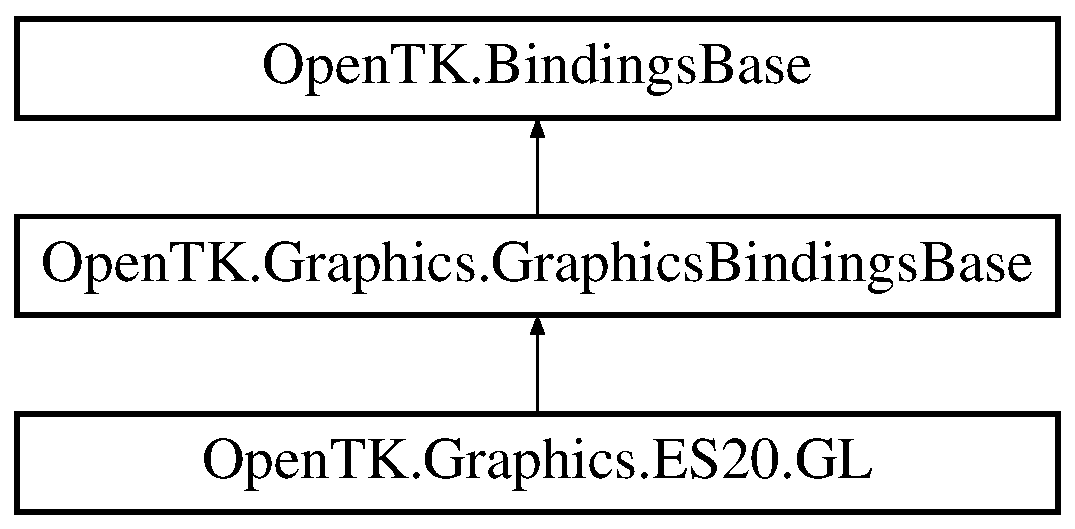
\includegraphics[height=3.000000cm]{class_open_t_k_1_1_graphics_1_1_e_s20_1_1_g_l}
\end{center}
\end{figure}
\subsection*{Static Public Member Functions}
\begin{DoxyCompactItemize}
\item 
static void \hyperlink{class_open_t_k_1_1_graphics_1_1_e_s20_1_1_g_l_af56b7f59869416956981c70031abea1f}{Active\-Texture} (Open\-T\-K.\-Graphics.\-E\-S20.\-Texture\-Unit texture)
\begin{DoxyCompactList}\small\item\em \mbox{[}requires\-: v2.\-0 and 2.\-0\mbox{]} Select active texture unit \end{DoxyCompactList}\item 
static void \hyperlink{class_open_t_k_1_1_graphics_1_1_e_s20_1_1_g_l_a96e9e463b7fd67bfda3ad9b9a1be6e47}{Attach\-Shader} (Int32 program, Int32 shader)
\begin{DoxyCompactList}\small\item\em \mbox{[}requires\-: v2.\-0 and 2.\-0\mbox{]} Attaches a shader object to a program object \end{DoxyCompactList}\item 
static void \hyperlink{class_open_t_k_1_1_graphics_1_1_e_s20_1_1_g_l_ad249a01343dfe9a262692b1b47b8baf9}{Attach\-Shader} (U\-Int32 program, U\-Int32 shader)
\begin{DoxyCompactList}\small\item\em \mbox{[}requires\-: v2.\-0 and 2.\-0\mbox{]} Attaches a shader object to a program object \end{DoxyCompactList}\item 
static void \hyperlink{class_open_t_k_1_1_graphics_1_1_e_s20_1_1_g_l_aac8cf2a78ef6efd1b880a86368e12a07}{Bind\-Attrib\-Location} (Int32 program, Int32 index, String name)
\begin{DoxyCompactList}\small\item\em \mbox{[}requires\-: v2.\-0 and 2.\-0\mbox{]} Associates a generic vertex attribute index with a named attribute variable \end{DoxyCompactList}\item 
static void \hyperlink{class_open_t_k_1_1_graphics_1_1_e_s20_1_1_g_l_a8056b43914eab1b8164e087ecc7542c2}{Bind\-Attrib\-Location} (U\-Int32 program, U\-Int32 index, String name)
\begin{DoxyCompactList}\small\item\em \mbox{[}requires\-: v2.\-0 and 2.\-0\mbox{]} Associates a generic vertex attribute index with a named attribute variable \end{DoxyCompactList}\item 
static void \hyperlink{class_open_t_k_1_1_graphics_1_1_e_s20_1_1_g_l_a1d61c4ed24ab2dcbfc9709f043f097a0}{Bind\-Buffer} (Open\-T\-K.\-Graphics.\-E\-S20.\-Buffer\-Target target, Int32 buffer)
\begin{DoxyCompactList}\small\item\em \mbox{[}requires\-: v2.\-0 and 2.\-0\mbox{]} Bind a named buffer object \end{DoxyCompactList}\item 
static void \hyperlink{class_open_t_k_1_1_graphics_1_1_e_s20_1_1_g_l_a3a49e7b859be06ea4568695b5ac2aaf2}{Bind\-Buffer} (Open\-T\-K.\-Graphics.\-E\-S20.\-Buffer\-Target target, U\-Int32 buffer)
\begin{DoxyCompactList}\small\item\em \mbox{[}requires\-: v2.\-0 and 2.\-0\mbox{]} Bind a named buffer object \end{DoxyCompactList}\item 
static void \hyperlink{class_open_t_k_1_1_graphics_1_1_e_s20_1_1_g_l_a2d32ccb6af9001cdd8899b5a87c03bdb}{Bind\-Framebuffer} (Open\-T\-K.\-Graphics.\-E\-S20.\-Framebuffer\-Target target, Int32 framebuffer)
\begin{DoxyCompactList}\small\item\em \mbox{[}requires\-: v2.\-0 and 2.\-0\mbox{]} Bind a framebuffer to a framebuffer target \end{DoxyCompactList}\item 
static void \hyperlink{class_open_t_k_1_1_graphics_1_1_e_s20_1_1_g_l_aebe9e8d5982996734b1357954f330d07}{Bind\-Framebuffer} (Open\-T\-K.\-Graphics.\-E\-S20.\-Framebuffer\-Target target, U\-Int32 framebuffer)
\begin{DoxyCompactList}\small\item\em \mbox{[}requires\-: v2.\-0 and 2.\-0\mbox{]} Bind a framebuffer to a framebuffer target \end{DoxyCompactList}\item 
static void \hyperlink{class_open_t_k_1_1_graphics_1_1_e_s20_1_1_g_l_aa0dc5584c50d43051c8c962fb3b16877}{Bind\-Renderbuffer} (Open\-T\-K.\-Graphics.\-E\-S20.\-Renderbuffer\-Target target, Int32 renderbuffer)
\begin{DoxyCompactList}\small\item\em \mbox{[}requires\-: v2.\-0 and 2.\-0\mbox{]} Bind a renderbuffer to a renderbuffer target \end{DoxyCompactList}\item 
static void \hyperlink{class_open_t_k_1_1_graphics_1_1_e_s20_1_1_g_l_a661bccc87e5c7df63e7e772897b3e178}{Bind\-Renderbuffer} (Open\-T\-K.\-Graphics.\-E\-S20.\-Renderbuffer\-Target target, U\-Int32 renderbuffer)
\begin{DoxyCompactList}\small\item\em \mbox{[}requires\-: v2.\-0 and 2.\-0\mbox{]} Bind a renderbuffer to a renderbuffer target \end{DoxyCompactList}\item 
static void \hyperlink{class_open_t_k_1_1_graphics_1_1_e_s20_1_1_g_l_aa1c33848516d5dfa20a460e657568cfe}{Bind\-Texture} (Open\-T\-K.\-Graphics.\-E\-S20.\-Texture\-Target target, Int32 texture)
\begin{DoxyCompactList}\small\item\em \mbox{[}requires\-: v2.\-0 and 2.\-0\mbox{]} Bind a named texture to a texturing target \end{DoxyCompactList}\item 
static void \hyperlink{class_open_t_k_1_1_graphics_1_1_e_s20_1_1_g_l_a2802b0f37ac0ea15584ccbb5b227f1df}{Bind\-Texture} (Open\-T\-K.\-Graphics.\-E\-S20.\-Texture\-Target target, U\-Int32 texture)
\begin{DoxyCompactList}\small\item\em \mbox{[}requires\-: v2.\-0 and 2.\-0\mbox{]} Bind a named texture to a texturing target \end{DoxyCompactList}\item 
static void \hyperlink{class_open_t_k_1_1_graphics_1_1_e_s20_1_1_g_l_ad91ca9b5162111c27d1aa5456db4e291}{Blend\-Color} (Single red, Single green, Single blue, Single alpha)
\begin{DoxyCompactList}\small\item\em \mbox{[}requires\-: v2.\-0 and 2.\-0\mbox{]} Set the blend color \end{DoxyCompactList}\item 
static void \hyperlink{class_open_t_k_1_1_graphics_1_1_e_s20_1_1_g_l_ad4b44e15b0c49da039f1bf25fc0227f0}{Blend\-Equation} (Open\-T\-K.\-Graphics.\-E\-S20.\-Blend\-Equation\-Mode mode)
\begin{DoxyCompactList}\small\item\em \mbox{[}requires\-: v2.\-0 and 2.\-0\mbox{]} Specify the equation used for both the R\-G\-B blend equation and the Alpha blend equation \end{DoxyCompactList}\item 
static void \hyperlink{class_open_t_k_1_1_graphics_1_1_e_s20_1_1_g_l_a4d86dfd48948607aea6cfe3889b813d0}{Blend\-Equation\-Separate} (Open\-T\-K.\-Graphics.\-E\-S20.\-Blend\-Equation\-Mode mode\-R\-G\-B, Open\-T\-K.\-Graphics.\-E\-S20.\-Blend\-Equation\-Mode mode\-Alpha)
\begin{DoxyCompactList}\small\item\em \mbox{[}requires\-: v2.\-0 and 2.\-0\mbox{]} Set the R\-G\-B blend equation and the alpha blend equation separately \end{DoxyCompactList}\item 
static void \hyperlink{class_open_t_k_1_1_graphics_1_1_e_s20_1_1_g_l_a0783768762d1f0d7df72a107cd76f0d3}{Blend\-Func} (Open\-T\-K.\-Graphics.\-E\-S20.\-Blending\-Factor\-Src sfactor, Open\-T\-K.\-Graphics.\-E\-S20.\-Blending\-Factor\-Dest dfactor)
\begin{DoxyCompactList}\small\item\em \mbox{[}requires\-: v2.\-0 and 2.\-0\mbox{]} Specify pixel arithmetic \end{DoxyCompactList}\item 
static void \hyperlink{class_open_t_k_1_1_graphics_1_1_e_s20_1_1_g_l_a4c9e701e5d72756c6bc80e710313c9f4}{Blend\-Func\-Separate} (Open\-T\-K.\-Graphics.\-E\-S20.\-Blending\-Factor\-Src src\-R\-G\-B, Open\-T\-K.\-Graphics.\-E\-S20.\-Blending\-Factor\-Dest dst\-R\-G\-B, Open\-T\-K.\-Graphics.\-E\-S20.\-Blending\-Factor\-Src src\-Alpha, Open\-T\-K.\-Graphics.\-E\-S20.\-Blending\-Factor\-Dest dst\-Alpha)
\begin{DoxyCompactList}\small\item\em \mbox{[}requires\-: v2.\-0 and 2.\-0\mbox{]} Specify pixel arithmetic for R\-G\-B and alpha components separately \end{DoxyCompactList}\item 
static void \hyperlink{class_open_t_k_1_1_graphics_1_1_e_s20_1_1_g_l_a886501a5b7ceedb9d032ffa58c9d701c}{Buffer\-Data} (Open\-T\-K.\-Graphics.\-E\-S20.\-Buffer\-Target target, Int\-Ptr size, Int\-Ptr data, Open\-T\-K.\-Graphics.\-E\-S20.\-Buffer\-Usage usage)
\begin{DoxyCompactList}\small\item\em \mbox{[}requires\-: v2.\-0 and 2.\-0\mbox{]} Creates and initializes a buffer object's data store \end{DoxyCompactList}\item 
static void \hyperlink{class_open_t_k_1_1_graphics_1_1_e_s20_1_1_g_l_aab460482294f33dceaaf63bfc2d7d3fb}{Buffer\-Data$<$ T2 $>$} (Open\-T\-K.\-Graphics.\-E\-S20.\-Buffer\-Target target, Int\-Ptr size, \mbox{[}In\-Attribute, Out\-Attribute\mbox{]} T2\mbox{[}$\,$\mbox{]} data, Open\-T\-K.\-Graphics.\-E\-S20.\-Buffer\-Usage usage)
\begin{DoxyCompactList}\small\item\em \mbox{[}requires\-: v2.\-0 and 2.\-0\mbox{]} Creates and initializes a buffer object's data store \end{DoxyCompactList}\item 
static void \hyperlink{class_open_t_k_1_1_graphics_1_1_e_s20_1_1_g_l_a100cd4859879e7225bb816c6c86120cc}{Buffer\-Data$<$ T2 $>$} (Open\-T\-K.\-Graphics.\-E\-S20.\-Buffer\-Target target, Int\-Ptr size, \mbox{[}In\-Attribute, Out\-Attribute\mbox{]} T2\mbox{[},\mbox{]} data, Open\-T\-K.\-Graphics.\-E\-S20.\-Buffer\-Usage usage)
\begin{DoxyCompactList}\small\item\em \mbox{[}requires\-: v2.\-0 and 2.\-0\mbox{]} Creates and initializes a buffer object's data store \end{DoxyCompactList}\item 
static void \hyperlink{class_open_t_k_1_1_graphics_1_1_e_s20_1_1_g_l_ae60d1b28e6908907fd5d5a0b843c7c48}{Buffer\-Data$<$ T2 $>$} (Open\-T\-K.\-Graphics.\-E\-S20.\-Buffer\-Target target, Int\-Ptr size, \mbox{[}In\-Attribute, Out\-Attribute\mbox{]} T2\mbox{[},,\mbox{]} data, Open\-T\-K.\-Graphics.\-E\-S20.\-Buffer\-Usage usage)
\begin{DoxyCompactList}\small\item\em \mbox{[}requires\-: v2.\-0 and 2.\-0\mbox{]} Creates and initializes a buffer object's data store \end{DoxyCompactList}\item 
static void \hyperlink{class_open_t_k_1_1_graphics_1_1_e_s20_1_1_g_l_a72cfcfe7cd640b3bd25eaa89e4556e00}{Buffer\-Data$<$ T2 $>$} (Open\-T\-K.\-Graphics.\-E\-S20.\-Buffer\-Target target, Int\-Ptr size, \mbox{[}In\-Attribute, Out\-Attribute\mbox{]} ref T2 data, Open\-T\-K.\-Graphics.\-E\-S20.\-Buffer\-Usage usage)
\begin{DoxyCompactList}\small\item\em \mbox{[}requires\-: v2.\-0 and 2.\-0\mbox{]} Creates and initializes a buffer object's data store \end{DoxyCompactList}\item 
static void \hyperlink{class_open_t_k_1_1_graphics_1_1_e_s20_1_1_g_l_ac660942c0a5c0e112ecb5a9f787ad103}{Buffer\-Sub\-Data} (Open\-T\-K.\-Graphics.\-E\-S20.\-Buffer\-Target target, Int\-Ptr offset, Int\-Ptr size, Int\-Ptr data)
\begin{DoxyCompactList}\small\item\em \mbox{[}requires\-: v2.\-0 and 2.\-0\mbox{]} Updates a subset of a buffer object's data store \end{DoxyCompactList}\item 
static void \hyperlink{class_open_t_k_1_1_graphics_1_1_e_s20_1_1_g_l_a492952e56333c5d5228d68d6f3e19cd0}{Buffer\-Sub\-Data$<$ T3 $>$} (Open\-T\-K.\-Graphics.\-E\-S20.\-Buffer\-Target target, Int\-Ptr offset, Int\-Ptr size, \mbox{[}In\-Attribute, Out\-Attribute\mbox{]} T3\mbox{[}$\,$\mbox{]} data)
\begin{DoxyCompactList}\small\item\em \mbox{[}requires\-: v2.\-0 and 2.\-0\mbox{]} Updates a subset of a buffer object's data store \end{DoxyCompactList}\item 
static void \hyperlink{class_open_t_k_1_1_graphics_1_1_e_s20_1_1_g_l_a1f17e97d92c1f84b41a3c094f140c7b3}{Buffer\-Sub\-Data$<$ T3 $>$} (Open\-T\-K.\-Graphics.\-E\-S20.\-Buffer\-Target target, Int\-Ptr offset, Int\-Ptr size, \mbox{[}In\-Attribute, Out\-Attribute\mbox{]} T3\mbox{[},\mbox{]} data)
\begin{DoxyCompactList}\small\item\em \mbox{[}requires\-: v2.\-0 and 2.\-0\mbox{]} Updates a subset of a buffer object's data store \end{DoxyCompactList}\item 
static void \hyperlink{class_open_t_k_1_1_graphics_1_1_e_s20_1_1_g_l_a4bbf79d8229a1128d9e8d49817a4dcaa}{Buffer\-Sub\-Data$<$ T3 $>$} (Open\-T\-K.\-Graphics.\-E\-S20.\-Buffer\-Target target, Int\-Ptr offset, Int\-Ptr size, \mbox{[}In\-Attribute, Out\-Attribute\mbox{]} T3\mbox{[},,\mbox{]} data)
\begin{DoxyCompactList}\small\item\em \mbox{[}requires\-: v2.\-0 and 2.\-0\mbox{]} Updates a subset of a buffer object's data store \end{DoxyCompactList}\item 
static void \hyperlink{class_open_t_k_1_1_graphics_1_1_e_s20_1_1_g_l_aebbb541f3fd6020d58223339646a6020}{Buffer\-Sub\-Data$<$ T3 $>$} (Open\-T\-K.\-Graphics.\-E\-S20.\-Buffer\-Target target, Int\-Ptr offset, Int\-Ptr size, \mbox{[}In\-Attribute, Out\-Attribute\mbox{]} ref T3 data)
\begin{DoxyCompactList}\small\item\em \mbox{[}requires\-: v2.\-0 and 2.\-0\mbox{]} Updates a subset of a buffer object's data store \end{DoxyCompactList}\item 
static \\*
Open\-T\-K.\-Graphics.\-E\-S20.\-Framebuffer\-Error\-Code \hyperlink{class_open_t_k_1_1_graphics_1_1_e_s20_1_1_g_l_a4f6aeb29cee61125a907de40f590718f}{Check\-Framebuffer\-Status} (Open\-T\-K.\-Graphics.\-E\-S20.\-Framebuffer\-Target target)
\begin{DoxyCompactList}\small\item\em \mbox{[}requires\-: v2.\-0 and 2.\-0\mbox{]} Check the completeness status of a framebuffer \end{DoxyCompactList}\item 
static void \hyperlink{class_open_t_k_1_1_graphics_1_1_e_s20_1_1_g_l_a92d19483de153b0a66f3d083a3d1f447}{Clear} (Open\-T\-K.\-Graphics.\-E\-S20.\-Clear\-Buffer\-Mask mask)
\begin{DoxyCompactList}\small\item\em \mbox{[}requires\-: v2.\-0 and 2.\-0\mbox{]} Clear buffers to preset values \end{DoxyCompactList}\item 
static void \hyperlink{class_open_t_k_1_1_graphics_1_1_e_s20_1_1_g_l_a0a4dbccf195e1c16aa8a3b15085a3e8e}{Clear\-Color} (Single red, Single green, Single blue, Single alpha)
\begin{DoxyCompactList}\small\item\em \mbox{[}requires\-: v2.\-0 and 2.\-0\mbox{]} Specify clear values for the color buffers \end{DoxyCompactList}\item 
static void \hyperlink{class_open_t_k_1_1_graphics_1_1_e_s20_1_1_g_l_ab93bfb313a101482e56e9cbc49588cc9}{Clear\-Depth} (Single depth)
\begin{DoxyCompactList}\small\item\em \mbox{[}requires\-: v2.\-0 and 2.\-0\mbox{]} Specify the clear value for the depth buffer \end{DoxyCompactList}\item 
static void \hyperlink{class_open_t_k_1_1_graphics_1_1_e_s20_1_1_g_l_a065bf26cfc78cda133e13e48127de03e}{Clear\-Stencil} (Int32 s)
\begin{DoxyCompactList}\small\item\em \mbox{[}requires\-: v2.\-0 and 2.\-0\mbox{]} Specify the clear value for the stencil buffer \end{DoxyCompactList}\item 
static void \hyperlink{class_open_t_k_1_1_graphics_1_1_e_s20_1_1_g_l_a2b99088914e07ce3619d11069856b0b2}{Color\-Mask} (bool red, bool green, bool blue, bool alpha)
\begin{DoxyCompactList}\small\item\em \mbox{[}requires\-: v2.\-0 and 2.\-0\mbox{]} Enable and disable writing of frame buffer color components \end{DoxyCompactList}\item 
static void \hyperlink{class_open_t_k_1_1_graphics_1_1_e_s20_1_1_g_l_af2f690266857375c680d95792ee799b9}{Compile\-Shader} (Int32 shader)
\begin{DoxyCompactList}\small\item\em \mbox{[}requires\-: v2.\-0 and 2.\-0\mbox{]} Compiles a shader object \end{DoxyCompactList}\item 
static void \hyperlink{class_open_t_k_1_1_graphics_1_1_e_s20_1_1_g_l_afb1e810c07587709de6f154387ab0387}{Compile\-Shader} (U\-Int32 shader)
\begin{DoxyCompactList}\small\item\em \mbox{[}requires\-: v2.\-0 and 2.\-0\mbox{]} Compiles a shader object \end{DoxyCompactList}\item 
static void \hyperlink{class_open_t_k_1_1_graphics_1_1_e_s20_1_1_g_l_aa883d71bff0010caee82c9a71734d48b}{Compressed\-Tex\-Image2\-D} (Open\-T\-K.\-Graphics.\-E\-S20.\-Texture\-Target target, Int32 level, Open\-T\-K.\-Graphics.\-E\-S20.\-Pixel\-Internal\-Format internalformat, Int32 width, Int32 height, Int32 border, Int32 image\-Size, Int\-Ptr data)
\begin{DoxyCompactList}\small\item\em \mbox{[}requires\-: v2.\-0 and 2.\-0\mbox{]} Specify a two-\/dimensional texture image in a compressed format \end{DoxyCompactList}\item 
static void \hyperlink{class_open_t_k_1_1_graphics_1_1_e_s20_1_1_g_l_aa7d0088babdf1f4c4cfcd5a24f6cb464}{Compressed\-Tex\-Image2\-D$<$ T7 $>$} (Open\-T\-K.\-Graphics.\-E\-S20.\-Texture\-Target target, Int32 level, Open\-T\-K.\-Graphics.\-E\-S20.\-Pixel\-Internal\-Format internalformat, Int32 width, Int32 height, Int32 border, Int32 image\-Size, \mbox{[}In\-Attribute, Out\-Attribute\mbox{]} T7\mbox{[}$\,$\mbox{]} data)
\begin{DoxyCompactList}\small\item\em \mbox{[}requires\-: v2.\-0 and 2.\-0\mbox{]} Specify a two-\/dimensional texture image in a compressed format \end{DoxyCompactList}\item 
static void \hyperlink{class_open_t_k_1_1_graphics_1_1_e_s20_1_1_g_l_af7a60be761455e06da32b2b7ecfd9d47}{Compressed\-Tex\-Image2\-D$<$ T7 $>$} (Open\-T\-K.\-Graphics.\-E\-S20.\-Texture\-Target target, Int32 level, Open\-T\-K.\-Graphics.\-E\-S20.\-Pixel\-Internal\-Format internalformat, Int32 width, Int32 height, Int32 border, Int32 image\-Size, \mbox{[}In\-Attribute, Out\-Attribute\mbox{]} T7\mbox{[},\mbox{]} data)
\begin{DoxyCompactList}\small\item\em \mbox{[}requires\-: v2.\-0 and 2.\-0\mbox{]} Specify a two-\/dimensional texture image in a compressed format \end{DoxyCompactList}\item 
static void \hyperlink{class_open_t_k_1_1_graphics_1_1_e_s20_1_1_g_l_a576991ce7c07caf1c170233b89956be0}{Compressed\-Tex\-Image2\-D$<$ T7 $>$} (Open\-T\-K.\-Graphics.\-E\-S20.\-Texture\-Target target, Int32 level, Open\-T\-K.\-Graphics.\-E\-S20.\-Pixel\-Internal\-Format internalformat, Int32 width, Int32 height, Int32 border, Int32 image\-Size, \mbox{[}In\-Attribute, Out\-Attribute\mbox{]} T7\mbox{[},,\mbox{]} data)
\begin{DoxyCompactList}\small\item\em \mbox{[}requires\-: v2.\-0 and 2.\-0\mbox{]} Specify a two-\/dimensional texture image in a compressed format \end{DoxyCompactList}\item 
static void \hyperlink{class_open_t_k_1_1_graphics_1_1_e_s20_1_1_g_l_a5897cc8ca5b880dc07cb29f19b07bef5}{Compressed\-Tex\-Image2\-D$<$ T7 $>$} (Open\-T\-K.\-Graphics.\-E\-S20.\-Texture\-Target target, Int32 level, Open\-T\-K.\-Graphics.\-E\-S20.\-Pixel\-Internal\-Format internalformat, Int32 width, Int32 height, Int32 border, Int32 image\-Size, \mbox{[}In\-Attribute, Out\-Attribute\mbox{]} ref T7 data)
\begin{DoxyCompactList}\small\item\em \mbox{[}requires\-: v2.\-0 and 2.\-0\mbox{]} Specify a two-\/dimensional texture image in a compressed format \end{DoxyCompactList}\item 
static void \hyperlink{class_open_t_k_1_1_graphics_1_1_e_s20_1_1_g_l_a498ad033c30317ef0325d365771a423e}{Compressed\-Tex\-Sub\-Image2\-D} (Open\-T\-K.\-Graphics.\-E\-S20.\-Texture\-Target target, Int32 level, Int32 xoffset, Int32 yoffset, Int32 width, Int32 height, Open\-T\-K.\-Graphics.\-E\-S20.\-Pixel\-Format format, Int32 image\-Size, Int\-Ptr data)
\begin{DoxyCompactList}\small\item\em \mbox{[}requires\-: v2.\-0 and 2.\-0\mbox{]} Specify a two-\/dimensional texture subimage in a compressed format \end{DoxyCompactList}\item 
static void \hyperlink{class_open_t_k_1_1_graphics_1_1_e_s20_1_1_g_l_a8bc414ab4267e5718508e238e5f2365b}{Compressed\-Tex\-Sub\-Image2\-D$<$ T8 $>$} (Open\-T\-K.\-Graphics.\-E\-S20.\-Texture\-Target target, Int32 level, Int32 xoffset, Int32 yoffset, Int32 width, Int32 height, Open\-T\-K.\-Graphics.\-E\-S20.\-Pixel\-Format format, Int32 image\-Size, \mbox{[}In\-Attribute, Out\-Attribute\mbox{]} T8\mbox{[}$\,$\mbox{]} data)
\begin{DoxyCompactList}\small\item\em \mbox{[}requires\-: v2.\-0 and 2.\-0\mbox{]} Specify a two-\/dimensional texture subimage in a compressed format \end{DoxyCompactList}\item 
static void \hyperlink{class_open_t_k_1_1_graphics_1_1_e_s20_1_1_g_l_a00ee97e8e29aa6ccfaaa0a1b5921442f}{Compressed\-Tex\-Sub\-Image2\-D$<$ T8 $>$} (Open\-T\-K.\-Graphics.\-E\-S20.\-Texture\-Target target, Int32 level, Int32 xoffset, Int32 yoffset, Int32 width, Int32 height, Open\-T\-K.\-Graphics.\-E\-S20.\-Pixel\-Format format, Int32 image\-Size, \mbox{[}In\-Attribute, Out\-Attribute\mbox{]} T8\mbox{[},\mbox{]} data)
\begin{DoxyCompactList}\small\item\em \mbox{[}requires\-: v2.\-0 and 2.\-0\mbox{]} Specify a two-\/dimensional texture subimage in a compressed format \end{DoxyCompactList}\item 
static void \hyperlink{class_open_t_k_1_1_graphics_1_1_e_s20_1_1_g_l_a5bee37cbaafcf86adf71a819280befaa}{Compressed\-Tex\-Sub\-Image2\-D$<$ T8 $>$} (Open\-T\-K.\-Graphics.\-E\-S20.\-Texture\-Target target, Int32 level, Int32 xoffset, Int32 yoffset, Int32 width, Int32 height, Open\-T\-K.\-Graphics.\-E\-S20.\-Pixel\-Format format, Int32 image\-Size, \mbox{[}In\-Attribute, Out\-Attribute\mbox{]} T8\mbox{[},,\mbox{]} data)
\begin{DoxyCompactList}\small\item\em \mbox{[}requires\-: v2.\-0 and 2.\-0\mbox{]} Specify a two-\/dimensional texture subimage in a compressed format \end{DoxyCompactList}\item 
static void \hyperlink{class_open_t_k_1_1_graphics_1_1_e_s20_1_1_g_l_a4f4a163beec0c74de0566b7a0771579b}{Compressed\-Tex\-Sub\-Image2\-D$<$ T8 $>$} (Open\-T\-K.\-Graphics.\-E\-S20.\-Texture\-Target target, Int32 level, Int32 xoffset, Int32 yoffset, Int32 width, Int32 height, Open\-T\-K.\-Graphics.\-E\-S20.\-Pixel\-Format format, Int32 image\-Size, \mbox{[}In\-Attribute, Out\-Attribute\mbox{]} ref T8 data)
\begin{DoxyCompactList}\small\item\em \mbox{[}requires\-: v2.\-0 and 2.\-0\mbox{]} Specify a two-\/dimensional texture subimage in a compressed format \end{DoxyCompactList}\item 
static void \hyperlink{class_open_t_k_1_1_graphics_1_1_e_s20_1_1_g_l_aa34a39411f9e50b9db65eb8584468c34}{Copy\-Tex\-Image2\-D} (Open\-T\-K.\-Graphics.\-E\-S20.\-Texture\-Target target, Int32 level, Open\-T\-K.\-Graphics.\-E\-S20.\-Pixel\-Internal\-Format internalformat, Int32 x, Int32 y, Int32 width, Int32 height, Int32 border)
\begin{DoxyCompactList}\small\item\em \mbox{[}requires\-: v2.\-0 and 2.\-0\mbox{]} Copy pixels into a 2\-D texture image \end{DoxyCompactList}\item 
static void \hyperlink{class_open_t_k_1_1_graphics_1_1_e_s20_1_1_g_l_a9773dffccf836af004b4a08da10e6fda}{Copy\-Tex\-Sub\-Image2\-D} (Open\-T\-K.\-Graphics.\-E\-S20.\-Texture\-Target target, Int32 level, Int32 xoffset, Int32 yoffset, Int32 x, Int32 y, Int32 width, Int32 height)
\begin{DoxyCompactList}\small\item\em \mbox{[}requires\-: v2.\-0 and 2.\-0\mbox{]} Copy a two-\/dimensional texture subimage \end{DoxyCompactList}\item 
static Int32 \hyperlink{class_open_t_k_1_1_graphics_1_1_e_s20_1_1_g_l_a7a949418f1a580108fdc773053cbad28}{Create\-Program} ()
\begin{DoxyCompactList}\small\item\em \mbox{[}requires\-: v2.\-0 and 2.\-0\mbox{]} Creates a program object \end{DoxyCompactList}\item 
static Int32 \hyperlink{class_open_t_k_1_1_graphics_1_1_e_s20_1_1_g_l_a54ad2ee370e5d17a6655d584f7720151}{Create\-Shader} (Open\-T\-K.\-Graphics.\-E\-S20.\-Shader\-Type type)
\begin{DoxyCompactList}\small\item\em \mbox{[}requires\-: v2.\-0 and 2.\-0\mbox{]} Creates a shader object \end{DoxyCompactList}\item 
static void \hyperlink{class_open_t_k_1_1_graphics_1_1_e_s20_1_1_g_l_ab340c393284baa447a7ebd2309dd429c}{Cull\-Face} (Open\-T\-K.\-Graphics.\-E\-S20.\-Cull\-Face\-Mode mode)
\begin{DoxyCompactList}\small\item\em \mbox{[}requires\-: v2.\-0 and 2.\-0\mbox{]} Specify whether front-\/ or back-\/facing facets can be culled \end{DoxyCompactList}\item 
static void \hyperlink{class_open_t_k_1_1_graphics_1_1_e_s20_1_1_g_l_aab89ffa97a24d5a9d09cb3068945d823}{Delete\-Buffers} (Int32 n, Int32\mbox{[}$\,$\mbox{]} buffers)
\begin{DoxyCompactList}\small\item\em \mbox{[}requires\-: v2.\-0 and 2.\-0\mbox{]} Delete named buffer objects \end{DoxyCompactList}\item 
static void \hyperlink{class_open_t_k_1_1_graphics_1_1_e_s20_1_1_g_l_aa677d08d4b4353d167618d1dabe3a4ed}{Delete\-Buffers} (Int32 n, ref Int32 buffers)
\begin{DoxyCompactList}\small\item\em \mbox{[}requires\-: v2.\-0 and 2.\-0\mbox{]} Delete named buffer objects \end{DoxyCompactList}\item 
static unsafe void \hyperlink{class_open_t_k_1_1_graphics_1_1_e_s20_1_1_g_l_ad9f1abd85afdb244f3faf10903f16556}{Delete\-Buffers} (Int32 n, Int32 $\ast$buffers)
\begin{DoxyCompactList}\small\item\em \mbox{[}requires\-: v2.\-0 and 2.\-0\mbox{]} Delete named buffer objects \end{DoxyCompactList}\item 
static void \hyperlink{class_open_t_k_1_1_graphics_1_1_e_s20_1_1_g_l_a96fca50876867ac8c4c7a78bdf94ee7e}{Delete\-Buffers} (Int32 n, U\-Int32\mbox{[}$\,$\mbox{]} buffers)
\begin{DoxyCompactList}\small\item\em \mbox{[}requires\-: v2.\-0 and 2.\-0\mbox{]} Delete named buffer objects \end{DoxyCompactList}\item 
static void \hyperlink{class_open_t_k_1_1_graphics_1_1_e_s20_1_1_g_l_a5bcc71a1aca73f278305c950714e3232}{Delete\-Buffers} (Int32 n, ref U\-Int32 buffers)
\begin{DoxyCompactList}\small\item\em \mbox{[}requires\-: v2.\-0 and 2.\-0\mbox{]} Delete named buffer objects \end{DoxyCompactList}\item 
static unsafe void \hyperlink{class_open_t_k_1_1_graphics_1_1_e_s20_1_1_g_l_ac781b78ca334d924c39b1d855b8183e0}{Delete\-Buffers} (Int32 n, U\-Int32 $\ast$buffers)
\begin{DoxyCompactList}\small\item\em \mbox{[}requires\-: v2.\-0 and 2.\-0\mbox{]} Delete named buffer objects \end{DoxyCompactList}\item 
static void \hyperlink{class_open_t_k_1_1_graphics_1_1_e_s20_1_1_g_l_a0b1e99bddcde857a225ead00ef087a92}{Delete\-Framebuffers} (Int32 n, Int32\mbox{[}$\,$\mbox{]} framebuffers)
\begin{DoxyCompactList}\small\item\em \mbox{[}requires\-: v2.\-0 and 2.\-0\mbox{]} Delete framebuffer objects \end{DoxyCompactList}\item 
static void \hyperlink{class_open_t_k_1_1_graphics_1_1_e_s20_1_1_g_l_ab88cc608620a13914b3ebaaecd4c9d32}{Delete\-Framebuffers} (Int32 n, ref Int32 framebuffers)
\begin{DoxyCompactList}\small\item\em \mbox{[}requires\-: v2.\-0 and 2.\-0\mbox{]} Delete framebuffer objects \end{DoxyCompactList}\item 
static unsafe void \hyperlink{class_open_t_k_1_1_graphics_1_1_e_s20_1_1_g_l_a8d97886daa5ec2e8b282b7ad60e02368}{Delete\-Framebuffers} (Int32 n, Int32 $\ast$framebuffers)
\begin{DoxyCompactList}\small\item\em \mbox{[}requires\-: v2.\-0 and 2.\-0\mbox{]} Delete framebuffer objects \end{DoxyCompactList}\item 
static void \hyperlink{class_open_t_k_1_1_graphics_1_1_e_s20_1_1_g_l_aa20b099620a80add5d11c536762ab171}{Delete\-Framebuffers} (Int32 n, U\-Int32\mbox{[}$\,$\mbox{]} framebuffers)
\begin{DoxyCompactList}\small\item\em \mbox{[}requires\-: v2.\-0 and 2.\-0\mbox{]} Delete framebuffer objects \end{DoxyCompactList}\item 
static void \hyperlink{class_open_t_k_1_1_graphics_1_1_e_s20_1_1_g_l_a6ad5d2c00541aa18c5abe5dbbaeb9266}{Delete\-Framebuffers} (Int32 n, ref U\-Int32 framebuffers)
\begin{DoxyCompactList}\small\item\em \mbox{[}requires\-: v2.\-0 and 2.\-0\mbox{]} Delete framebuffer objects \end{DoxyCompactList}\item 
static unsafe void \hyperlink{class_open_t_k_1_1_graphics_1_1_e_s20_1_1_g_l_ab9f3d8a830506229617a67230abd94fc}{Delete\-Framebuffers} (Int32 n, U\-Int32 $\ast$framebuffers)
\begin{DoxyCompactList}\small\item\em \mbox{[}requires\-: v2.\-0 and 2.\-0\mbox{]} Delete framebuffer objects \end{DoxyCompactList}\item 
static void \hyperlink{class_open_t_k_1_1_graphics_1_1_e_s20_1_1_g_l_a19f389432e432dd9e9e0cdd2b91966da}{Delete\-Program} (Int32 program)
\begin{DoxyCompactList}\small\item\em \mbox{[}requires\-: v2.\-0 and 2.\-0\mbox{]} Deletes a program object \end{DoxyCompactList}\item 
static void \hyperlink{class_open_t_k_1_1_graphics_1_1_e_s20_1_1_g_l_a206314ad12a340176d11fb560e37dee1}{Delete\-Program} (U\-Int32 program)
\begin{DoxyCompactList}\small\item\em \mbox{[}requires\-: v2.\-0 and 2.\-0\mbox{]} Deletes a program object \end{DoxyCompactList}\item 
static void \hyperlink{class_open_t_k_1_1_graphics_1_1_e_s20_1_1_g_l_a5bb5cf3589a9859a85af2c0bfacb2920}{Delete\-Renderbuffers} (Int32 n, Int32\mbox{[}$\,$\mbox{]} renderbuffers)
\begin{DoxyCompactList}\small\item\em \mbox{[}requires\-: v2.\-0 and 2.\-0\mbox{]} Delete renderbuffer objects \end{DoxyCompactList}\item 
static void \hyperlink{class_open_t_k_1_1_graphics_1_1_e_s20_1_1_g_l_ac17b6c5f9d0c0de23a4d03bcef75b075}{Delete\-Renderbuffers} (Int32 n, ref Int32 renderbuffers)
\begin{DoxyCompactList}\small\item\em \mbox{[}requires\-: v2.\-0 and 2.\-0\mbox{]} Delete renderbuffer objects \end{DoxyCompactList}\item 
static unsafe void \hyperlink{class_open_t_k_1_1_graphics_1_1_e_s20_1_1_g_l_aac81db8db7fbdb6aeccaeb5213b98bd0}{Delete\-Renderbuffers} (Int32 n, Int32 $\ast$renderbuffers)
\begin{DoxyCompactList}\small\item\em \mbox{[}requires\-: v2.\-0 and 2.\-0\mbox{]} Delete renderbuffer objects \end{DoxyCompactList}\item 
static void \hyperlink{class_open_t_k_1_1_graphics_1_1_e_s20_1_1_g_l_aa9091385526f3b322157d9ae03917305}{Delete\-Renderbuffers} (Int32 n, U\-Int32\mbox{[}$\,$\mbox{]} renderbuffers)
\begin{DoxyCompactList}\small\item\em \mbox{[}requires\-: v2.\-0 and 2.\-0\mbox{]} Delete renderbuffer objects \end{DoxyCompactList}\item 
static void \hyperlink{class_open_t_k_1_1_graphics_1_1_e_s20_1_1_g_l_a1151d187a0f72bda29e720e9d756939e}{Delete\-Renderbuffers} (Int32 n, ref U\-Int32 renderbuffers)
\begin{DoxyCompactList}\small\item\em \mbox{[}requires\-: v2.\-0 and 2.\-0\mbox{]} Delete renderbuffer objects \end{DoxyCompactList}\item 
static unsafe void \hyperlink{class_open_t_k_1_1_graphics_1_1_e_s20_1_1_g_l_a11c76ad8aa01a9b3224084ca799fe733}{Delete\-Renderbuffers} (Int32 n, U\-Int32 $\ast$renderbuffers)
\begin{DoxyCompactList}\small\item\em \mbox{[}requires\-: v2.\-0 and 2.\-0\mbox{]} Delete renderbuffer objects \end{DoxyCompactList}\item 
static void \hyperlink{class_open_t_k_1_1_graphics_1_1_e_s20_1_1_g_l_a3c76e9dac3216b65f927ac12815ae6ba}{Delete\-Shader} (Int32 shader)
\begin{DoxyCompactList}\small\item\em \mbox{[}requires\-: v2.\-0 and 2.\-0\mbox{]} Deletes a shader object \end{DoxyCompactList}\item 
static void \hyperlink{class_open_t_k_1_1_graphics_1_1_e_s20_1_1_g_l_a10d33f7ca4e0e12ce4a5f6e112df5d50}{Delete\-Shader} (U\-Int32 shader)
\begin{DoxyCompactList}\small\item\em \mbox{[}requires\-: v2.\-0 and 2.\-0\mbox{]} Deletes a shader object \end{DoxyCompactList}\item 
static void \hyperlink{class_open_t_k_1_1_graphics_1_1_e_s20_1_1_g_l_a51d5666b71f209635a80cee5587c0252}{Delete\-Textures} (Int32 n, Int32\mbox{[}$\,$\mbox{]} textures)
\begin{DoxyCompactList}\small\item\em \mbox{[}requires\-: v2.\-0 and 2.\-0\mbox{]} Delete named textures \end{DoxyCompactList}\item 
static void \hyperlink{class_open_t_k_1_1_graphics_1_1_e_s20_1_1_g_l_aba8f200cfa6d3cae4d6724171666f429}{Delete\-Textures} (Int32 n, ref Int32 textures)
\begin{DoxyCompactList}\small\item\em \mbox{[}requires\-: v2.\-0 and 2.\-0\mbox{]} Delete named textures \end{DoxyCompactList}\item 
static unsafe void \hyperlink{class_open_t_k_1_1_graphics_1_1_e_s20_1_1_g_l_a30b4f5cacc5ce2522fff7616c9dac5a3}{Delete\-Textures} (Int32 n, Int32 $\ast$textures)
\begin{DoxyCompactList}\small\item\em \mbox{[}requires\-: v2.\-0 and 2.\-0\mbox{]} Delete named textures \end{DoxyCompactList}\item 
static void \hyperlink{class_open_t_k_1_1_graphics_1_1_e_s20_1_1_g_l_a7adb3349b340499d972cee903ca064db}{Delete\-Textures} (Int32 n, U\-Int32\mbox{[}$\,$\mbox{]} textures)
\begin{DoxyCompactList}\small\item\em \mbox{[}requires\-: v2.\-0 and 2.\-0\mbox{]} Delete named textures \end{DoxyCompactList}\item 
static void \hyperlink{class_open_t_k_1_1_graphics_1_1_e_s20_1_1_g_l_a9b0ae4bc992d007984a08a013da057a1}{Delete\-Textures} (Int32 n, ref U\-Int32 textures)
\begin{DoxyCompactList}\small\item\em \mbox{[}requires\-: v2.\-0 and 2.\-0\mbox{]} Delete named textures \end{DoxyCompactList}\item 
static unsafe void \hyperlink{class_open_t_k_1_1_graphics_1_1_e_s20_1_1_g_l_a6bd7df54b5c813f880c5c1637e95d770}{Delete\-Textures} (Int32 n, U\-Int32 $\ast$textures)
\begin{DoxyCompactList}\small\item\em \mbox{[}requires\-: v2.\-0 and 2.\-0\mbox{]} Delete named textures \end{DoxyCompactList}\item 
static void \hyperlink{class_open_t_k_1_1_graphics_1_1_e_s20_1_1_g_l_a3b45a55b101a56fcaf0b5158b0a2795c}{Depth\-Func} (Open\-T\-K.\-Graphics.\-E\-S20.\-Depth\-Function func)
\begin{DoxyCompactList}\small\item\em \mbox{[}requires\-: v2.\-0 and 2.\-0\mbox{]} Specify the value used for depth buffer comparisons \end{DoxyCompactList}\item 
static void \hyperlink{class_open_t_k_1_1_graphics_1_1_e_s20_1_1_g_l_a15fdca744ae440505aa3ea08e7def7a0}{Depth\-Mask} (bool flag)
\begin{DoxyCompactList}\small\item\em \mbox{[}requires\-: v2.\-0 and 2.\-0\mbox{]} Enable or disable writing into the depth buffer \end{DoxyCompactList}\item 
static void \hyperlink{class_open_t_k_1_1_graphics_1_1_e_s20_1_1_g_l_aa3ea5a51e415d2d479de27ebace8f754}{Depth\-Range} (Single z\-Near, Single z\-Far)
\begin{DoxyCompactList}\small\item\em \mbox{[}requires\-: v2.\-0 and 2.\-0\mbox{]} Specify mapping of depth values from normalized device coordinates to window coordinates \end{DoxyCompactList}\item 
static void \hyperlink{class_open_t_k_1_1_graphics_1_1_e_s20_1_1_g_l_aada623eba363a19733b57cab36a6587e}{Detach\-Shader} (Int32 program, Int32 shader)
\begin{DoxyCompactList}\small\item\em \mbox{[}requires\-: v2.\-0 and 2.\-0\mbox{]} Detaches a shader object from a program object to which it is attached \end{DoxyCompactList}\item 
static void \hyperlink{class_open_t_k_1_1_graphics_1_1_e_s20_1_1_g_l_aff12cdc9b19f6ee4edf24d846b760dda}{Detach\-Shader} (U\-Int32 program, U\-Int32 shader)
\begin{DoxyCompactList}\small\item\em \mbox{[}requires\-: v2.\-0 and 2.\-0\mbox{]} Detaches a shader object from a program object to which it is attached \end{DoxyCompactList}\item 
static void \hyperlink{class_open_t_k_1_1_graphics_1_1_e_s20_1_1_g_l_a9ee11366b929653d56141ff9b916019e}{Disable} (Open\-T\-K.\-Graphics.\-E\-S20.\-Enable\-Cap cap)
\begin{DoxyCompactList}\small\item\em \mbox{[}requires\-: v2.\-0 and 2.\-0\mbox{]}\end{DoxyCompactList}\item 
static void \hyperlink{class_open_t_k_1_1_graphics_1_1_e_s20_1_1_g_l_a8a52268480506d44eaac7d33b1a5c805}{Disable\-Vertex\-Attrib\-Array} (Int32 index)
\begin{DoxyCompactList}\small\item\em \mbox{[}requires\-: v2.\-0 and 2.\-0\mbox{]}\end{DoxyCompactList}\item 
static void \hyperlink{class_open_t_k_1_1_graphics_1_1_e_s20_1_1_g_l_adfda382fa7d771d551a7bdd9261966c8}{Disable\-Vertex\-Attrib\-Array} (U\-Int32 index)
\begin{DoxyCompactList}\small\item\em \mbox{[}requires\-: v2.\-0 and 2.\-0\mbox{]}\end{DoxyCompactList}\item 
static void \hyperlink{class_open_t_k_1_1_graphics_1_1_e_s20_1_1_g_l_a66410d54589443e6dc95f5fd1368009a}{Draw\-Arrays} (Open\-T\-K.\-Graphics.\-E\-S20.\-Begin\-Mode mode, Int32 first, Int32 count)
\begin{DoxyCompactList}\small\item\em \mbox{[}requires\-: v2.\-0 and 2.\-0\mbox{]} Render primitives from array data \end{DoxyCompactList}\item 
static void \hyperlink{class_open_t_k_1_1_graphics_1_1_e_s20_1_1_g_l_ac8b383f56070b391b798336ccc0796ae}{Draw\-Elements} (Open\-T\-K.\-Graphics.\-E\-S20.\-Begin\-Mode mode, Int32 count, Open\-T\-K.\-Graphics.\-E\-S20.\-Draw\-Elements\-Type type, Int\-Ptr indices)
\begin{DoxyCompactList}\small\item\em \mbox{[}requires\-: v2.\-0 and 2.\-0\mbox{]} Render primitives from array data \end{DoxyCompactList}\item 
static void \hyperlink{class_open_t_k_1_1_graphics_1_1_e_s20_1_1_g_l_a50709887ac15a3c41091860acac25a5a}{Draw\-Elements$<$ T3 $>$} (Open\-T\-K.\-Graphics.\-E\-S20.\-Begin\-Mode mode, Int32 count, Open\-T\-K.\-Graphics.\-E\-S20.\-Draw\-Elements\-Type type, \mbox{[}In\-Attribute, Out\-Attribute\mbox{]} T3\mbox{[}$\,$\mbox{]} indices)
\begin{DoxyCompactList}\small\item\em \mbox{[}requires\-: v2.\-0 and 2.\-0\mbox{]} Render primitives from array data \end{DoxyCompactList}\item 
static void \hyperlink{class_open_t_k_1_1_graphics_1_1_e_s20_1_1_g_l_a45d97baf4b318582c07c80c1f0924a64}{Draw\-Elements$<$ T3 $>$} (Open\-T\-K.\-Graphics.\-E\-S20.\-Begin\-Mode mode, Int32 count, Open\-T\-K.\-Graphics.\-E\-S20.\-Draw\-Elements\-Type type, \mbox{[}In\-Attribute, Out\-Attribute\mbox{]} T3\mbox{[},\mbox{]} indices)
\begin{DoxyCompactList}\small\item\em \mbox{[}requires\-: v2.\-0 and 2.\-0\mbox{]} Render primitives from array data \end{DoxyCompactList}\item 
static void \hyperlink{class_open_t_k_1_1_graphics_1_1_e_s20_1_1_g_l_a00a188326d640aac268903b4e07c30f3}{Draw\-Elements$<$ T3 $>$} (Open\-T\-K.\-Graphics.\-E\-S20.\-Begin\-Mode mode, Int32 count, Open\-T\-K.\-Graphics.\-E\-S20.\-Draw\-Elements\-Type type, \mbox{[}In\-Attribute, Out\-Attribute\mbox{]} T3\mbox{[},,\mbox{]} indices)
\begin{DoxyCompactList}\small\item\em \mbox{[}requires\-: v2.\-0 and 2.\-0\mbox{]} Render primitives from array data \end{DoxyCompactList}\item 
static void \hyperlink{class_open_t_k_1_1_graphics_1_1_e_s20_1_1_g_l_a0aebe890dc7cc288e6d75d2b6fa6b0ca}{Draw\-Elements$<$ T3 $>$} (Open\-T\-K.\-Graphics.\-E\-S20.\-Begin\-Mode mode, Int32 count, Open\-T\-K.\-Graphics.\-E\-S20.\-Draw\-Elements\-Type type, \mbox{[}In\-Attribute, Out\-Attribute\mbox{]} ref T3 indices)
\begin{DoxyCompactList}\small\item\em \mbox{[}requires\-: v2.\-0 and 2.\-0\mbox{]} Render primitives from array data \end{DoxyCompactList}\item 
static void \hyperlink{class_open_t_k_1_1_graphics_1_1_e_s20_1_1_g_l_afdd7401cd44b6bdc0969f01cc820db2d}{Enable} (Open\-T\-K.\-Graphics.\-E\-S20.\-Enable\-Cap cap)
\begin{DoxyCompactList}\small\item\em \mbox{[}requires\-: v2.\-0 and 2.\-0\mbox{]} Enable or disable server-\/side \hyperlink{class_open_t_k_1_1_graphics_1_1_e_s20_1_1_g_l}{G\-L} capabilities \end{DoxyCompactList}\item 
static void \hyperlink{class_open_t_k_1_1_graphics_1_1_e_s20_1_1_g_l_a2f17cbf14d1b6ecede1e80f3ac2aba53}{Enable\-Vertex\-Attrib\-Array} (Int32 index)
\begin{DoxyCompactList}\small\item\em \mbox{[}requires\-: v2.\-0 and 2.\-0\mbox{]} Enable or disable a generic vertex attribute array \end{DoxyCompactList}\item 
static void \hyperlink{class_open_t_k_1_1_graphics_1_1_e_s20_1_1_g_l_a083319ac0d81de626c0c8d06c76610f1}{Enable\-Vertex\-Attrib\-Array} (U\-Int32 index)
\begin{DoxyCompactList}\small\item\em \mbox{[}requires\-: v2.\-0 and 2.\-0\mbox{]} Enable or disable a generic vertex attribute array \end{DoxyCompactList}\item 
static void \hyperlink{class_open_t_k_1_1_graphics_1_1_e_s20_1_1_g_l_ad794990a5a8863630072233558aea224}{Finish} ()
\begin{DoxyCompactList}\small\item\em \mbox{[}requires\-: v2.\-0 and 2.\-0\mbox{]} Block until all \hyperlink{class_open_t_k_1_1_graphics_1_1_e_s20_1_1_g_l}{G\-L} execution is complete \end{DoxyCompactList}\item 
static void \hyperlink{class_open_t_k_1_1_graphics_1_1_e_s20_1_1_g_l_a57735b924211e1a43f7e15fff122d3fa}{Flush} ()
\begin{DoxyCompactList}\small\item\em \mbox{[}requires\-: v2.\-0 and 2.\-0\mbox{]} Force execution of \hyperlink{class_open_t_k_1_1_graphics_1_1_e_s20_1_1_g_l}{G\-L} commands in finite time \end{DoxyCompactList}\item 
static void \hyperlink{class_open_t_k_1_1_graphics_1_1_e_s20_1_1_g_l_ae84f9d977e8daba8a65141659380a084}{Framebuffer\-Renderbuffer} (Open\-T\-K.\-Graphics.\-E\-S20.\-Framebuffer\-Target target, Open\-T\-K.\-Graphics.\-E\-S20.\-Framebuffer\-Slot attachment, Open\-T\-K.\-Graphics.\-E\-S20.\-Renderbuffer\-Target renderbuffertarget, Int32 renderbuffer)
\begin{DoxyCompactList}\small\item\em \mbox{[}requires\-: v2.\-0 and 2.\-0\mbox{]} Attach a renderbuffer as a logical buffer to the currently bound framebuffer object \end{DoxyCompactList}\item 
static void \hyperlink{class_open_t_k_1_1_graphics_1_1_e_s20_1_1_g_l_a244faf59f81e7ce9c102089a2175b290}{Framebuffer\-Renderbuffer} (Open\-T\-K.\-Graphics.\-E\-S20.\-Framebuffer\-Target target, Open\-T\-K.\-Graphics.\-E\-S20.\-Framebuffer\-Slot attachment, Open\-T\-K.\-Graphics.\-E\-S20.\-Renderbuffer\-Target renderbuffertarget, U\-Int32 renderbuffer)
\begin{DoxyCompactList}\small\item\em \mbox{[}requires\-: v2.\-0 and 2.\-0\mbox{]} Attach a renderbuffer as a logical buffer to the currently bound framebuffer object \end{DoxyCompactList}\item 
static void \hyperlink{class_open_t_k_1_1_graphics_1_1_e_s20_1_1_g_l_a1f0453935cc418cea814bac5817a8be2}{Framebuffer\-Texture2\-D} (Open\-T\-K.\-Graphics.\-E\-S20.\-Framebuffer\-Target target, Open\-T\-K.\-Graphics.\-E\-S20.\-Framebuffer\-Slot attachment, Open\-T\-K.\-Graphics.\-E\-S20.\-Texture\-Target textarget, Int32 texture, Int32 level)
\begin{DoxyCompactList}\small\item\em \mbox{[}requires\-: v2.\-0 and 2.\-0\mbox{]}\end{DoxyCompactList}\item 
static void \hyperlink{class_open_t_k_1_1_graphics_1_1_e_s20_1_1_g_l_a479cb16cabc59ebf2176228cb4ec8582}{Framebuffer\-Texture2\-D} (Open\-T\-K.\-Graphics.\-E\-S20.\-Framebuffer\-Target target, Open\-T\-K.\-Graphics.\-E\-S20.\-Framebuffer\-Slot attachment, Open\-T\-K.\-Graphics.\-E\-S20.\-Texture\-Target textarget, U\-Int32 texture, Int32 level)
\begin{DoxyCompactList}\small\item\em \mbox{[}requires\-: v2.\-0 and 2.\-0\mbox{]}\end{DoxyCompactList}\item 
static void \hyperlink{class_open_t_k_1_1_graphics_1_1_e_s20_1_1_g_l_a74955c863d3a3aa950ec4daad8374a6b}{Framebuffer\-Texture2\-D\-Multisample\-I\-M\-G} ()
\begin{DoxyCompactList}\small\item\em \mbox{[}requires\-: v2.\-0 and 2.\-0\mbox{]}\end{DoxyCompactList}\item 
static void \hyperlink{class_open_t_k_1_1_graphics_1_1_e_s20_1_1_g_l_a17b5c4330bdb9d222d0c8de8d8a060fa}{Front\-Face} (Open\-T\-K.\-Graphics.\-E\-S20.\-Front\-Face\-Direction mode)
\begin{DoxyCompactList}\small\item\em \mbox{[}requires\-: v2.\-0 and 2.\-0\mbox{]} Define front-\/ and back-\/facing polygons \end{DoxyCompactList}\item 
static void \hyperlink{class_open_t_k_1_1_graphics_1_1_e_s20_1_1_g_l_a48f0a7c043731d1d3b228a87af32a38f}{Gen\-Buffers} (Int32 n, \mbox{[}Out\-Attribute\mbox{]} Int32\mbox{[}$\,$\mbox{]} buffers)
\begin{DoxyCompactList}\small\item\em \mbox{[}requires\-: v2.\-0 and 2.\-0\mbox{]} Generate buffer object names \end{DoxyCompactList}\item 
static void \hyperlink{class_open_t_k_1_1_graphics_1_1_e_s20_1_1_g_l_a6b3124f437517a69cdd7c205f01c5df1}{Gen\-Buffers} (Int32 n, \mbox{[}Out\-Attribute\mbox{]} out Int32 buffers)
\begin{DoxyCompactList}\small\item\em \mbox{[}requires\-: v2.\-0 and 2.\-0\mbox{]} Generate buffer object names \end{DoxyCompactList}\item 
static unsafe void \hyperlink{class_open_t_k_1_1_graphics_1_1_e_s20_1_1_g_l_a13381160b1d7620689d6e6eb30163b0b}{Gen\-Buffers} (Int32 n, \mbox{[}Out\-Attribute\mbox{]} Int32 $\ast$buffers)
\begin{DoxyCompactList}\small\item\em \mbox{[}requires\-: v2.\-0 and 2.\-0\mbox{]} Generate buffer object names \end{DoxyCompactList}\item 
static void \hyperlink{class_open_t_k_1_1_graphics_1_1_e_s20_1_1_g_l_a4ae1a71ee1386fea85a8ef1f16a36c92}{Gen\-Buffers} (Int32 n, \mbox{[}Out\-Attribute\mbox{]} U\-Int32\mbox{[}$\,$\mbox{]} buffers)
\begin{DoxyCompactList}\small\item\em \mbox{[}requires\-: v2.\-0 and 2.\-0\mbox{]} Generate buffer object names \end{DoxyCompactList}\item 
static void \hyperlink{class_open_t_k_1_1_graphics_1_1_e_s20_1_1_g_l_a9d8e29615bd12c67e9714badc1405795}{Gen\-Buffers} (Int32 n, \mbox{[}Out\-Attribute\mbox{]} out U\-Int32 buffers)
\begin{DoxyCompactList}\small\item\em \mbox{[}requires\-: v2.\-0 and 2.\-0\mbox{]} Generate buffer object names \end{DoxyCompactList}\item 
static unsafe void \hyperlink{class_open_t_k_1_1_graphics_1_1_e_s20_1_1_g_l_a7906dd8f777ec6775831fca09638b353}{Gen\-Buffers} (Int32 n, \mbox{[}Out\-Attribute\mbox{]} U\-Int32 $\ast$buffers)
\begin{DoxyCompactList}\small\item\em \mbox{[}requires\-: v2.\-0 and 2.\-0\mbox{]} Generate buffer object names \end{DoxyCompactList}\item 
static void \hyperlink{class_open_t_k_1_1_graphics_1_1_e_s20_1_1_g_l_a8e807aeba68580983f25d8477c2653bc}{Generate\-Mipmap} (Open\-T\-K.\-Graphics.\-E\-S20.\-Texture\-Target target)
\begin{DoxyCompactList}\small\item\em \mbox{[}requires\-: v2.\-0 and 2.\-0\mbox{]} Generate mipmaps for a specified texture target \end{DoxyCompactList}\item 
static void \hyperlink{class_open_t_k_1_1_graphics_1_1_e_s20_1_1_g_l_a1ee1091d0a961ff495174999516061b1}{Gen\-Framebuffers} (Int32 n, \mbox{[}Out\-Attribute\mbox{]} Int32\mbox{[}$\,$\mbox{]} framebuffers)
\begin{DoxyCompactList}\small\item\em \mbox{[}requires\-: v2.\-0 and 2.\-0\mbox{]} Generate framebuffer object names \end{DoxyCompactList}\item 
static void \hyperlink{class_open_t_k_1_1_graphics_1_1_e_s20_1_1_g_l_ab6fcde82d513aff0e2d3d013afa4bc40}{Gen\-Framebuffers} (Int32 n, \mbox{[}Out\-Attribute\mbox{]} out Int32 framebuffers)
\begin{DoxyCompactList}\small\item\em \mbox{[}requires\-: v2.\-0 and 2.\-0\mbox{]} Generate framebuffer object names \end{DoxyCompactList}\item 
static unsafe void \hyperlink{class_open_t_k_1_1_graphics_1_1_e_s20_1_1_g_l_aa8e176de3765341a20f13b83e08855c5}{Gen\-Framebuffers} (Int32 n, \mbox{[}Out\-Attribute\mbox{]} Int32 $\ast$framebuffers)
\begin{DoxyCompactList}\small\item\em \mbox{[}requires\-: v2.\-0 and 2.\-0\mbox{]} Generate framebuffer object names \end{DoxyCompactList}\item 
static void \hyperlink{class_open_t_k_1_1_graphics_1_1_e_s20_1_1_g_l_a0d68b6d8e0d9216ffa0d4a9be0654773}{Gen\-Framebuffers} (Int32 n, \mbox{[}Out\-Attribute\mbox{]} U\-Int32\mbox{[}$\,$\mbox{]} framebuffers)
\begin{DoxyCompactList}\small\item\em \mbox{[}requires\-: v2.\-0 and 2.\-0\mbox{]} Generate framebuffer object names \end{DoxyCompactList}\item 
static void \hyperlink{class_open_t_k_1_1_graphics_1_1_e_s20_1_1_g_l_aeed628dcafaf29b3d43cdcb51198835f}{Gen\-Framebuffers} (Int32 n, \mbox{[}Out\-Attribute\mbox{]} out U\-Int32 framebuffers)
\begin{DoxyCompactList}\small\item\em \mbox{[}requires\-: v2.\-0 and 2.\-0\mbox{]} Generate framebuffer object names \end{DoxyCompactList}\item 
static unsafe void \hyperlink{class_open_t_k_1_1_graphics_1_1_e_s20_1_1_g_l_ab1df90e9876c6aa3cf6d1a7f5a0a7257}{Gen\-Framebuffers} (Int32 n, \mbox{[}Out\-Attribute\mbox{]} U\-Int32 $\ast$framebuffers)
\begin{DoxyCompactList}\small\item\em \mbox{[}requires\-: v2.\-0 and 2.\-0\mbox{]} Generate framebuffer object names \end{DoxyCompactList}\item 
static void \hyperlink{class_open_t_k_1_1_graphics_1_1_e_s20_1_1_g_l_ae474ab18f0c51ee398d44d4291e97c3c}{Gen\-Renderbuffers} (Int32 n, \mbox{[}Out\-Attribute\mbox{]} Int32\mbox{[}$\,$\mbox{]} renderbuffers)
\begin{DoxyCompactList}\small\item\em \mbox{[}requires\-: v2.\-0 and 2.\-0\mbox{]} Generate renderbuffer object names \end{DoxyCompactList}\item 
static void \hyperlink{class_open_t_k_1_1_graphics_1_1_e_s20_1_1_g_l_ad89cc8ad2ce164664c9a1255481a3b9b}{Gen\-Renderbuffers} (Int32 n, \mbox{[}Out\-Attribute\mbox{]} out Int32 renderbuffers)
\begin{DoxyCompactList}\small\item\em \mbox{[}requires\-: v2.\-0 and 2.\-0\mbox{]} Generate renderbuffer object names \end{DoxyCompactList}\item 
static unsafe void \hyperlink{class_open_t_k_1_1_graphics_1_1_e_s20_1_1_g_l_a70d27b9f317d03f04dee73e6e3029e07}{Gen\-Renderbuffers} (Int32 n, \mbox{[}Out\-Attribute\mbox{]} Int32 $\ast$renderbuffers)
\begin{DoxyCompactList}\small\item\em \mbox{[}requires\-: v2.\-0 and 2.\-0\mbox{]} Generate renderbuffer object names \end{DoxyCompactList}\item 
static void \hyperlink{class_open_t_k_1_1_graphics_1_1_e_s20_1_1_g_l_af3aa9591a681c13bff2e928441c10fad}{Gen\-Renderbuffers} (Int32 n, \mbox{[}Out\-Attribute\mbox{]} U\-Int32\mbox{[}$\,$\mbox{]} renderbuffers)
\begin{DoxyCompactList}\small\item\em \mbox{[}requires\-: v2.\-0 and 2.\-0\mbox{]} Generate renderbuffer object names \end{DoxyCompactList}\item 
static void \hyperlink{class_open_t_k_1_1_graphics_1_1_e_s20_1_1_g_l_ad52c0a531f263cdebd0b64a00bd6609d}{Gen\-Renderbuffers} (Int32 n, \mbox{[}Out\-Attribute\mbox{]} out U\-Int32 renderbuffers)
\begin{DoxyCompactList}\small\item\em \mbox{[}requires\-: v2.\-0 and 2.\-0\mbox{]} Generate renderbuffer object names \end{DoxyCompactList}\item 
static unsafe void \hyperlink{class_open_t_k_1_1_graphics_1_1_e_s20_1_1_g_l_a287429bfc25743c235a2767267d2d9d9}{Gen\-Renderbuffers} (Int32 n, \mbox{[}Out\-Attribute\mbox{]} U\-Int32 $\ast$renderbuffers)
\begin{DoxyCompactList}\small\item\em \mbox{[}requires\-: v2.\-0 and 2.\-0\mbox{]} Generate renderbuffer object names \end{DoxyCompactList}\item 
static void \hyperlink{class_open_t_k_1_1_graphics_1_1_e_s20_1_1_g_l_aef4f90e608d3bf693ce577be0240b6fa}{Gen\-Textures} (Int32 n, \mbox{[}Out\-Attribute\mbox{]} Int32\mbox{[}$\,$\mbox{]} textures)
\begin{DoxyCompactList}\small\item\em \mbox{[}requires\-: v2.\-0 and 2.\-0\mbox{]} Generate texture names \end{DoxyCompactList}\item 
static void \hyperlink{class_open_t_k_1_1_graphics_1_1_e_s20_1_1_g_l_a8624da388afa58fe00619ba6d42a72f8}{Gen\-Textures} (Int32 n, \mbox{[}Out\-Attribute\mbox{]} out Int32 textures)
\begin{DoxyCompactList}\small\item\em \mbox{[}requires\-: v2.\-0 and 2.\-0\mbox{]} Generate texture names \end{DoxyCompactList}\item 
static unsafe void \hyperlink{class_open_t_k_1_1_graphics_1_1_e_s20_1_1_g_l_af8a79df1cbfd323e4a6946f4c7f6cfcb}{Gen\-Textures} (Int32 n, \mbox{[}Out\-Attribute\mbox{]} Int32 $\ast$textures)
\begin{DoxyCompactList}\small\item\em \mbox{[}requires\-: v2.\-0 and 2.\-0\mbox{]} Generate texture names \end{DoxyCompactList}\item 
static void \hyperlink{class_open_t_k_1_1_graphics_1_1_e_s20_1_1_g_l_aa2021efb54682c2388b56874e86574c2}{Gen\-Textures} (Int32 n, \mbox{[}Out\-Attribute\mbox{]} U\-Int32\mbox{[}$\,$\mbox{]} textures)
\begin{DoxyCompactList}\small\item\em \mbox{[}requires\-: v2.\-0 and 2.\-0\mbox{]} Generate texture names \end{DoxyCompactList}\item 
static void \hyperlink{class_open_t_k_1_1_graphics_1_1_e_s20_1_1_g_l_ace945660c4b40dd3d74e35b39e480b1c}{Gen\-Textures} (Int32 n, \mbox{[}Out\-Attribute\mbox{]} out U\-Int32 textures)
\begin{DoxyCompactList}\small\item\em \mbox{[}requires\-: v2.\-0 and 2.\-0\mbox{]} Generate texture names \end{DoxyCompactList}\item 
static unsafe void \hyperlink{class_open_t_k_1_1_graphics_1_1_e_s20_1_1_g_l_a1f46ac11ddb09602a59d6be55743e18f}{Gen\-Textures} (Int32 n, \mbox{[}Out\-Attribute\mbox{]} U\-Int32 $\ast$textures)
\begin{DoxyCompactList}\small\item\em \mbox{[}requires\-: v2.\-0 and 2.\-0\mbox{]} Generate texture names \end{DoxyCompactList}\item 
static void \hyperlink{class_open_t_k_1_1_graphics_1_1_e_s20_1_1_g_l_a24700ce2596523017a3edff579359858}{Get\-Active\-Attrib} (Int32 program, Int32 index, Int32 bufsize, \mbox{[}Out\-Attribute\mbox{]} Int32\mbox{[}$\,$\mbox{]} length, \mbox{[}Out\-Attribute\mbox{]} Int32\mbox{[}$\,$\mbox{]} size, \mbox{[}Out\-Attribute\mbox{]} Open\-T\-K.\-Graphics.\-E\-S20.\-Active\-Attrib\-Type\mbox{[}$\,$\mbox{]} type, \mbox{[}Out\-Attribute\mbox{]} String\-Builder name)
\begin{DoxyCompactList}\small\item\em \mbox{[}requires\-: v2.\-0 and 2.\-0\mbox{]} Returns information about an active attribute variable for the specified program object \end{DoxyCompactList}\item 
static void \hyperlink{class_open_t_k_1_1_graphics_1_1_e_s20_1_1_g_l_a311e03ee4e740f67bd10873ea4d749fe}{Get\-Active\-Attrib} (Int32 program, Int32 index, Int32 bufsize, \mbox{[}Out\-Attribute\mbox{]} out Int32 length, \mbox{[}Out\-Attribute\mbox{]} out Int32 size, \mbox{[}Out\-Attribute\mbox{]} out Open\-T\-K.\-Graphics.\-E\-S20.\-Active\-Attrib\-Type type, \mbox{[}Out\-Attribute\mbox{]} String\-Builder name)
\begin{DoxyCompactList}\small\item\em \mbox{[}requires\-: v2.\-0 and 2.\-0\mbox{]} Returns information about an active attribute variable for the specified program object \end{DoxyCompactList}\item 
static unsafe void \hyperlink{class_open_t_k_1_1_graphics_1_1_e_s20_1_1_g_l_ade8deeda2f540552fd091dc2588bb31a}{Get\-Active\-Attrib} (Int32 program, Int32 index, Int32 bufsize, \mbox{[}Out\-Attribute\mbox{]} Int32 $\ast$length, \mbox{[}Out\-Attribute\mbox{]} Int32 $\ast$size, \mbox{[}Out\-Attribute\mbox{]} Open\-T\-K.\-Graphics.\-E\-S20.\-Active\-Attrib\-Type $\ast$type, \mbox{[}Out\-Attribute\mbox{]} String\-Builder name)
\begin{DoxyCompactList}\small\item\em \mbox{[}requires\-: v2.\-0 and 2.\-0\mbox{]} Returns information about an active attribute variable for the specified program object \end{DoxyCompactList}\item 
static void \hyperlink{class_open_t_k_1_1_graphics_1_1_e_s20_1_1_g_l_aa6d9a79544d99272fa890922a2c0e960}{Get\-Active\-Attrib} (U\-Int32 program, U\-Int32 index, Int32 bufsize, \mbox{[}Out\-Attribute\mbox{]} Int32\mbox{[}$\,$\mbox{]} length, \mbox{[}Out\-Attribute\mbox{]} Int32\mbox{[}$\,$\mbox{]} size, \mbox{[}Out\-Attribute\mbox{]} Open\-T\-K.\-Graphics.\-E\-S20.\-Active\-Attrib\-Type\mbox{[}$\,$\mbox{]} type, \mbox{[}Out\-Attribute\mbox{]} String\-Builder name)
\begin{DoxyCompactList}\small\item\em \mbox{[}requires\-: v2.\-0 and 2.\-0\mbox{]} Returns information about an active attribute variable for the specified program object \end{DoxyCompactList}\item 
static void \hyperlink{class_open_t_k_1_1_graphics_1_1_e_s20_1_1_g_l_a89ede6b14fd62aa2d360bb7175a6decb}{Get\-Active\-Attrib} (U\-Int32 program, U\-Int32 index, Int32 bufsize, \mbox{[}Out\-Attribute\mbox{]} out Int32 length, \mbox{[}Out\-Attribute\mbox{]} out Int32 size, \mbox{[}Out\-Attribute\mbox{]} out Open\-T\-K.\-Graphics.\-E\-S20.\-Active\-Attrib\-Type type, \mbox{[}Out\-Attribute\mbox{]} String\-Builder name)
\begin{DoxyCompactList}\small\item\em \mbox{[}requires\-: v2.\-0 and 2.\-0\mbox{]} Returns information about an active attribute variable for the specified program object \end{DoxyCompactList}\item 
static unsafe void \hyperlink{class_open_t_k_1_1_graphics_1_1_e_s20_1_1_g_l_a5e3dacd5eb749a566f29c1f4acf9bd08}{Get\-Active\-Attrib} (U\-Int32 program, U\-Int32 index, Int32 bufsize, \mbox{[}Out\-Attribute\mbox{]} Int32 $\ast$length, \mbox{[}Out\-Attribute\mbox{]} Int32 $\ast$size, \mbox{[}Out\-Attribute\mbox{]} Open\-T\-K.\-Graphics.\-E\-S20.\-Active\-Attrib\-Type $\ast$type, \mbox{[}Out\-Attribute\mbox{]} String\-Builder name)
\begin{DoxyCompactList}\small\item\em \mbox{[}requires\-: v2.\-0 and 2.\-0\mbox{]} Returns information about an active attribute variable for the specified program object \end{DoxyCompactList}\item 
static void \hyperlink{class_open_t_k_1_1_graphics_1_1_e_s20_1_1_g_l_ae906dc907dc97097667c17c6450f0165}{Get\-Active\-Uniform} (Int32 program, Int32 index, Int32 bufsize, \mbox{[}Out\-Attribute\mbox{]} Int32\mbox{[}$\,$\mbox{]} length, \mbox{[}Out\-Attribute\mbox{]} Int32\mbox{[}$\,$\mbox{]} size, \mbox{[}Out\-Attribute\mbox{]} Open\-T\-K.\-Graphics.\-E\-S20.\-Active\-Uniform\-Type\mbox{[}$\,$\mbox{]} type, \mbox{[}Out\-Attribute\mbox{]} String\-Builder name)
\begin{DoxyCompactList}\small\item\em \mbox{[}requires\-: v2.\-0 and 2.\-0\mbox{]} Returns information about an active uniform variable for the specified program object \end{DoxyCompactList}\item 
static void \hyperlink{class_open_t_k_1_1_graphics_1_1_e_s20_1_1_g_l_aaf3b2a0806f022fafb8c049577eb205f}{Get\-Active\-Uniform} (Int32 program, Int32 index, Int32 bufsize, \mbox{[}Out\-Attribute\mbox{]} out Int32 length, \mbox{[}Out\-Attribute\mbox{]} out Int32 size, \mbox{[}Out\-Attribute\mbox{]} out Open\-T\-K.\-Graphics.\-E\-S20.\-Active\-Uniform\-Type type, \mbox{[}Out\-Attribute\mbox{]} String\-Builder name)
\begin{DoxyCompactList}\small\item\em \mbox{[}requires\-: v2.\-0 and 2.\-0\mbox{]} Returns information about an active uniform variable for the specified program object \end{DoxyCompactList}\item 
static unsafe void \hyperlink{class_open_t_k_1_1_graphics_1_1_e_s20_1_1_g_l_a78a99c062ca456fcb481e5b77015e163}{Get\-Active\-Uniform} (Int32 program, Int32 index, Int32 bufsize, \mbox{[}Out\-Attribute\mbox{]} Int32 $\ast$length, \mbox{[}Out\-Attribute\mbox{]} Int32 $\ast$size, \mbox{[}Out\-Attribute\mbox{]} Open\-T\-K.\-Graphics.\-E\-S20.\-Active\-Uniform\-Type $\ast$type, \mbox{[}Out\-Attribute\mbox{]} String\-Builder name)
\begin{DoxyCompactList}\small\item\em \mbox{[}requires\-: v2.\-0 and 2.\-0\mbox{]} Returns information about an active uniform variable for the specified program object \end{DoxyCompactList}\item 
static void \hyperlink{class_open_t_k_1_1_graphics_1_1_e_s20_1_1_g_l_a0c85c2b8e6d7d4d43e46e2573d6fd80a}{Get\-Active\-Uniform} (U\-Int32 program, U\-Int32 index, Int32 bufsize, \mbox{[}Out\-Attribute\mbox{]} Int32\mbox{[}$\,$\mbox{]} length, \mbox{[}Out\-Attribute\mbox{]} Int32\mbox{[}$\,$\mbox{]} size, \mbox{[}Out\-Attribute\mbox{]} Open\-T\-K.\-Graphics.\-E\-S20.\-Active\-Uniform\-Type\mbox{[}$\,$\mbox{]} type, \mbox{[}Out\-Attribute\mbox{]} String\-Builder name)
\begin{DoxyCompactList}\small\item\em \mbox{[}requires\-: v2.\-0 and 2.\-0\mbox{]} Returns information about an active uniform variable for the specified program object \end{DoxyCompactList}\item 
static void \hyperlink{class_open_t_k_1_1_graphics_1_1_e_s20_1_1_g_l_a051f7d4ebc565127116592fe9c7ab1a6}{Get\-Active\-Uniform} (U\-Int32 program, U\-Int32 index, Int32 bufsize, \mbox{[}Out\-Attribute\mbox{]} out Int32 length, \mbox{[}Out\-Attribute\mbox{]} out Int32 size, \mbox{[}Out\-Attribute\mbox{]} out Open\-T\-K.\-Graphics.\-E\-S20.\-Active\-Uniform\-Type type, \mbox{[}Out\-Attribute\mbox{]} String\-Builder name)
\begin{DoxyCompactList}\small\item\em \mbox{[}requires\-: v2.\-0 and 2.\-0\mbox{]} Returns information about an active uniform variable for the specified program object \end{DoxyCompactList}\item 
static unsafe void \hyperlink{class_open_t_k_1_1_graphics_1_1_e_s20_1_1_g_l_aea8c17eccce981a1b750fd32d2860443}{Get\-Active\-Uniform} (U\-Int32 program, U\-Int32 index, Int32 bufsize, \mbox{[}Out\-Attribute\mbox{]} Int32 $\ast$length, \mbox{[}Out\-Attribute\mbox{]} Int32 $\ast$size, \mbox{[}Out\-Attribute\mbox{]} Open\-T\-K.\-Graphics.\-E\-S20.\-Active\-Uniform\-Type $\ast$type, \mbox{[}Out\-Attribute\mbox{]} String\-Builder name)
\begin{DoxyCompactList}\small\item\em \mbox{[}requires\-: v2.\-0 and 2.\-0\mbox{]} Returns information about an active uniform variable for the specified program object \end{DoxyCompactList}\item 
static void \hyperlink{class_open_t_k_1_1_graphics_1_1_e_s20_1_1_g_l_aef9fa88b5252c4532aefbda6986e94c7}{Get\-Attached\-Shaders} (Int32 program, Int32 maxcount, \mbox{[}Out\-Attribute\mbox{]} Int32\mbox{[}$\,$\mbox{]} count, \mbox{[}Out\-Attribute\mbox{]} Int32\mbox{[}$\,$\mbox{]} shaders)
\begin{DoxyCompactList}\small\item\em \mbox{[}requires\-: v2.\-0 and 2.\-0\mbox{]} Returns the handles of the shader objects attached to a program object \end{DoxyCompactList}\item 
static void \hyperlink{class_open_t_k_1_1_graphics_1_1_e_s20_1_1_g_l_a8137bf1c29a38a96d1730e2dc257b97c}{Get\-Attached\-Shaders} (Int32 program, Int32 maxcount, \mbox{[}Out\-Attribute\mbox{]} out Int32 count, \mbox{[}Out\-Attribute\mbox{]} out Int32 shaders)
\begin{DoxyCompactList}\small\item\em \mbox{[}requires\-: v2.\-0 and 2.\-0\mbox{]} Returns the handles of the shader objects attached to a program object \end{DoxyCompactList}\item 
static unsafe void \hyperlink{class_open_t_k_1_1_graphics_1_1_e_s20_1_1_g_l_a57edc47aadd3c77e6bbc8cc082affc26}{Get\-Attached\-Shaders} (Int32 program, Int32 maxcount, \mbox{[}Out\-Attribute\mbox{]} Int32 $\ast$count, \mbox{[}Out\-Attribute\mbox{]} Int32 $\ast$shaders)
\begin{DoxyCompactList}\small\item\em \mbox{[}requires\-: v2.\-0 and 2.\-0\mbox{]} Returns the handles of the shader objects attached to a program object \end{DoxyCompactList}\item 
static void \hyperlink{class_open_t_k_1_1_graphics_1_1_e_s20_1_1_g_l_ae799c6b0100f8ed5db691f5e70ac5d7a}{Get\-Attached\-Shaders} (U\-Int32 program, Int32 maxcount, \mbox{[}Out\-Attribute\mbox{]} Int32\mbox{[}$\,$\mbox{]} count, \mbox{[}Out\-Attribute\mbox{]} U\-Int32\mbox{[}$\,$\mbox{]} shaders)
\begin{DoxyCompactList}\small\item\em \mbox{[}requires\-: v2.\-0 and 2.\-0\mbox{]} Returns the handles of the shader objects attached to a program object \end{DoxyCompactList}\item 
static void \hyperlink{class_open_t_k_1_1_graphics_1_1_e_s20_1_1_g_l_ae14df63574d33816f4084b18421937cd}{Get\-Attached\-Shaders} (U\-Int32 program, Int32 maxcount, \mbox{[}Out\-Attribute\mbox{]} out Int32 count, \mbox{[}Out\-Attribute\mbox{]} out U\-Int32 shaders)
\begin{DoxyCompactList}\small\item\em \mbox{[}requires\-: v2.\-0 and 2.\-0\mbox{]} Returns the handles of the shader objects attached to a program object \end{DoxyCompactList}\item 
static unsafe void \hyperlink{class_open_t_k_1_1_graphics_1_1_e_s20_1_1_g_l_a5a12fa525ee62e766c3802ed3c8eb141}{Get\-Attached\-Shaders} (U\-Int32 program, Int32 maxcount, \mbox{[}Out\-Attribute\mbox{]} Int32 $\ast$count, \mbox{[}Out\-Attribute\mbox{]} U\-Int32 $\ast$shaders)
\begin{DoxyCompactList}\small\item\em \mbox{[}requires\-: v2.\-0 and 2.\-0\mbox{]} Returns the handles of the shader objects attached to a program object \end{DoxyCompactList}\item 
static int \hyperlink{class_open_t_k_1_1_graphics_1_1_e_s20_1_1_g_l_ad85ecce38595aa5459be503c3564fbca}{Get\-Attrib\-Location} (Int32 program, String name)
\begin{DoxyCompactList}\small\item\em \mbox{[}requires\-: v2.\-0 and 2.\-0\mbox{]} Returns the location of an attribute variable \end{DoxyCompactList}\item 
static int \hyperlink{class_open_t_k_1_1_graphics_1_1_e_s20_1_1_g_l_a3a92d749c5fb4aa1ef1800e4a65d17b4}{Get\-Attrib\-Location} (U\-Int32 program, String name)
\begin{DoxyCompactList}\small\item\em \mbox{[}requires\-: v2.\-0 and 2.\-0\mbox{]} Returns the location of an attribute variable \end{DoxyCompactList}\item 
static void \hyperlink{class_open_t_k_1_1_graphics_1_1_e_s20_1_1_g_l_af3d81adf847643eeb21bde6909129e6a}{Get\-Boolean} (Open\-T\-K.\-Graphics.\-E\-S20.\-Get\-P\-Name pname, \mbox{[}Out\-Attribute\mbox{]} bool\mbox{[}$\,$\mbox{]}@params)
\begin{DoxyCompactList}\small\item\em \mbox{[}requires\-: v2.\-0 and 2.\-0\mbox{]}\end{DoxyCompactList}\item 
static void \hyperlink{class_open_t_k_1_1_graphics_1_1_e_s20_1_1_g_l_af0c766333a66870664bafff86c90b6e0}{Get\-Boolean} (Open\-T\-K.\-Graphics.\-E\-S20.\-Get\-P\-Name pname, \mbox{[}Out\-Attribute\mbox{]} out bool @params)
\begin{DoxyCompactList}\small\item\em \mbox{[}requires\-: v2.\-0 and 2.\-0\mbox{]}\end{DoxyCompactList}\item 
static unsafe void \hyperlink{class_open_t_k_1_1_graphics_1_1_e_s20_1_1_g_l_a7744eff5cc6bf279bd5265aa216b09b8}{Get\-Boolean} (Open\-T\-K.\-Graphics.\-E\-S20.\-Get\-P\-Name pname, \mbox{[}Out\-Attribute\mbox{]} bool $\ast$@params)
\begin{DoxyCompactList}\small\item\em \mbox{[}requires\-: v2.\-0 and 2.\-0\mbox{]}\end{DoxyCompactList}\item 
static void \hyperlink{class_open_t_k_1_1_graphics_1_1_e_s20_1_1_g_l_a951db53411928ffdaaa52755e3ef09da}{Get\-Buffer\-Parameter} (Open\-T\-K.\-Graphics.\-E\-S20.\-Buffer\-Target target, Open\-T\-K.\-Graphics.\-E\-S20.\-Buffer\-Parameter\-Name pname, \mbox{[}Out\-Attribute\mbox{]} Int32\mbox{[}$\,$\mbox{]}@params)
\begin{DoxyCompactList}\small\item\em \mbox{[}requires\-: v2.\-0 and 2.\-0\mbox{]} Return parameters of a buffer object \end{DoxyCompactList}\item 
static void \hyperlink{class_open_t_k_1_1_graphics_1_1_e_s20_1_1_g_l_aa8ec3ad395b5f2fd21b2573052784648}{Get\-Buffer\-Parameter} (Open\-T\-K.\-Graphics.\-E\-S20.\-Buffer\-Target target, Open\-T\-K.\-Graphics.\-E\-S20.\-Buffer\-Parameter\-Name pname, \mbox{[}Out\-Attribute\mbox{]} out Int32 @params)
\begin{DoxyCompactList}\small\item\em \mbox{[}requires\-: v2.\-0 and 2.\-0\mbox{]} Return parameters of a buffer object \end{DoxyCompactList}\item 
static unsafe void \hyperlink{class_open_t_k_1_1_graphics_1_1_e_s20_1_1_g_l_aa3ab3ab8895b4c191fefd68fc05b1cde}{Get\-Buffer\-Parameter} (Open\-T\-K.\-Graphics.\-E\-S20.\-Buffer\-Target target, Open\-T\-K.\-Graphics.\-E\-S20.\-Buffer\-Parameter\-Name pname, \mbox{[}Out\-Attribute\mbox{]} Int32 $\ast$@params)
\begin{DoxyCompactList}\small\item\em \mbox{[}requires\-: v2.\-0 and 2.\-0\mbox{]} Return parameters of a buffer object \end{DoxyCompactList}\item 
static \\*
Open\-T\-K.\-Graphics.\-E\-S20.\-Error\-Code \hyperlink{class_open_t_k_1_1_graphics_1_1_e_s20_1_1_g_l_a6625124c640f048cd6a40e6f11cc85eb}{Get\-Error} ()
\begin{DoxyCompactList}\small\item\em \mbox{[}requires\-: v2.\-0 and 2.\-0\mbox{]} Return error information \end{DoxyCompactList}\item 
static void \hyperlink{class_open_t_k_1_1_graphics_1_1_e_s20_1_1_g_l_a77a5f1c4adfaa7ca8fb17d7acb2b9dd3}{Get\-Float} (Open\-T\-K.\-Graphics.\-E\-S20.\-Get\-P\-Name pname, \mbox{[}Out\-Attribute\mbox{]} Single\mbox{[}$\,$\mbox{]}@params)
\begin{DoxyCompactList}\small\item\em \mbox{[}requires\-: v2.\-0 and 2.\-0\mbox{]}\end{DoxyCompactList}\item 
static void \hyperlink{class_open_t_k_1_1_graphics_1_1_e_s20_1_1_g_l_a3e10607a70e66572c09f77916e306588}{Get\-Float} (Open\-T\-K.\-Graphics.\-E\-S20.\-Get\-P\-Name pname, \mbox{[}Out\-Attribute\mbox{]} out Single @params)
\begin{DoxyCompactList}\small\item\em \mbox{[}requires\-: v2.\-0 and 2.\-0\mbox{]}\end{DoxyCompactList}\item 
static unsafe void \hyperlink{class_open_t_k_1_1_graphics_1_1_e_s20_1_1_g_l_a2215ba2409e8849f5a7a0f15701394ed}{Get\-Float} (Open\-T\-K.\-Graphics.\-E\-S20.\-Get\-P\-Name pname, \mbox{[}Out\-Attribute\mbox{]} Single $\ast$@params)
\begin{DoxyCompactList}\small\item\em \mbox{[}requires\-: v2.\-0 and 2.\-0\mbox{]}\end{DoxyCompactList}\item 
static void \hyperlink{class_open_t_k_1_1_graphics_1_1_e_s20_1_1_g_l_a0c54f4b1c208f1ace3f5b829b8820fed}{Get\-Framebuffer\-Attachment\-Parameter} (Open\-T\-K.\-Graphics.\-E\-S20.\-Framebuffer\-Target target, Open\-T\-K.\-Graphics.\-E\-S20.\-Framebuffer\-Slot attachment, Open\-T\-K.\-Graphics.\-E\-S20.\-Framebuffer\-Parameter\-Name pname, \mbox{[}Out\-Attribute\mbox{]} Int32\mbox{[}$\,$\mbox{]}@params)
\begin{DoxyCompactList}\small\item\em \mbox{[}requires\-: v2.\-0 and 2.\-0\mbox{]} Retrieve information about attachments of a bound framebuffer object \end{DoxyCompactList}\item 
static void \hyperlink{class_open_t_k_1_1_graphics_1_1_e_s20_1_1_g_l_aee8f6f2a03c6cfccf9c15a876951eaa4}{Get\-Framebuffer\-Attachment\-Parameter} (Open\-T\-K.\-Graphics.\-E\-S20.\-Framebuffer\-Target target, Open\-T\-K.\-Graphics.\-E\-S20.\-Framebuffer\-Slot attachment, Open\-T\-K.\-Graphics.\-E\-S20.\-Framebuffer\-Parameter\-Name pname, \mbox{[}Out\-Attribute\mbox{]} out Int32 @params)
\begin{DoxyCompactList}\small\item\em \mbox{[}requires\-: v2.\-0 and 2.\-0\mbox{]} Retrieve information about attachments of a bound framebuffer object \end{DoxyCompactList}\item 
static unsafe void \hyperlink{class_open_t_k_1_1_graphics_1_1_e_s20_1_1_g_l_a351cc70613fbc5c60f808d40e43ceeeb}{Get\-Framebuffer\-Attachment\-Parameter} (Open\-T\-K.\-Graphics.\-E\-S20.\-Framebuffer\-Target target, Open\-T\-K.\-Graphics.\-E\-S20.\-Framebuffer\-Slot attachment, Open\-T\-K.\-Graphics.\-E\-S20.\-Framebuffer\-Parameter\-Name pname, \mbox{[}Out\-Attribute\mbox{]} Int32 $\ast$@params)
\begin{DoxyCompactList}\small\item\em \mbox{[}requires\-: v2.\-0 and 2.\-0\mbox{]} Retrieve information about attachments of a bound framebuffer object \end{DoxyCompactList}\item 
static void \hyperlink{class_open_t_k_1_1_graphics_1_1_e_s20_1_1_g_l_a5aa5e8c054e058a15e93dcadb6f3cff7}{Get\-Integer} (Open\-T\-K.\-Graphics.\-E\-S20.\-Get\-P\-Name pname, \mbox{[}Out\-Attribute\mbox{]} Int32\mbox{[}$\,$\mbox{]}@params)
\begin{DoxyCompactList}\small\item\em \mbox{[}requires\-: v2.\-0 and 2.\-0\mbox{]}\end{DoxyCompactList}\item 
static void \hyperlink{class_open_t_k_1_1_graphics_1_1_e_s20_1_1_g_l_ad570eeb4a331dc511357503fbaef2447}{Get\-Integer} (Open\-T\-K.\-Graphics.\-E\-S20.\-Get\-P\-Name pname, \mbox{[}Out\-Attribute\mbox{]} out Int32 @params)
\begin{DoxyCompactList}\small\item\em \mbox{[}requires\-: v2.\-0 and 2.\-0\mbox{]}\end{DoxyCompactList}\item 
static unsafe void \hyperlink{class_open_t_k_1_1_graphics_1_1_e_s20_1_1_g_l_a99f70ddd979e2ca986c643816108b44a}{Get\-Integer} (Open\-T\-K.\-Graphics.\-E\-S20.\-Get\-P\-Name pname, \mbox{[}Out\-Attribute\mbox{]} Int32 $\ast$@params)
\begin{DoxyCompactList}\small\item\em \mbox{[}requires\-: v2.\-0 and 2.\-0\mbox{]}\end{DoxyCompactList}\item 
static void \hyperlink{class_open_t_k_1_1_graphics_1_1_e_s20_1_1_g_l_a68284fd383c087fdedb61fc0c3a48a1a}{Get\-Program\-Info\-Log} (Int32 program, Int32 bufsize, \mbox{[}Out\-Attribute\mbox{]} Int32\mbox{[}$\,$\mbox{]} length, \mbox{[}Out\-Attribute\mbox{]} String\-Builder infolog)
\begin{DoxyCompactList}\small\item\em \mbox{[}requires\-: v2.\-0 and 2.\-0\mbox{]} Returns the information log for a program object \end{DoxyCompactList}\item 
static void \hyperlink{class_open_t_k_1_1_graphics_1_1_e_s20_1_1_g_l_a07943a485e1084be2d79e78a0fc119cc}{Get\-Program\-Info\-Log} (Int32 program, Int32 bufsize, \mbox{[}Out\-Attribute\mbox{]} out Int32 length, \mbox{[}Out\-Attribute\mbox{]} String\-Builder infolog)
\begin{DoxyCompactList}\small\item\em \mbox{[}requires\-: v2.\-0 and 2.\-0\mbox{]} Returns the information log for a program object \end{DoxyCompactList}\item 
static unsafe void \hyperlink{class_open_t_k_1_1_graphics_1_1_e_s20_1_1_g_l_a2fddf31b452ede5fc4d6169a5f48fe9d}{Get\-Program\-Info\-Log} (Int32 program, Int32 bufsize, \mbox{[}Out\-Attribute\mbox{]} Int32 $\ast$length, \mbox{[}Out\-Attribute\mbox{]} String\-Builder infolog)
\begin{DoxyCompactList}\small\item\em \mbox{[}requires\-: v2.\-0 and 2.\-0\mbox{]} Returns the information log for a program object \end{DoxyCompactList}\item 
static void \hyperlink{class_open_t_k_1_1_graphics_1_1_e_s20_1_1_g_l_abb720aab96c0310165ec3d564b9bccdb}{Get\-Program\-Info\-Log} (U\-Int32 program, Int32 bufsize, \mbox{[}Out\-Attribute\mbox{]} Int32\mbox{[}$\,$\mbox{]} length, \mbox{[}Out\-Attribute\mbox{]} String\-Builder infolog)
\begin{DoxyCompactList}\small\item\em \mbox{[}requires\-: v2.\-0 and 2.\-0\mbox{]} Returns the information log for a program object \end{DoxyCompactList}\item 
static void \hyperlink{class_open_t_k_1_1_graphics_1_1_e_s20_1_1_g_l_a972813c8c4584fe69db509054adda592}{Get\-Program\-Info\-Log} (U\-Int32 program, Int32 bufsize, \mbox{[}Out\-Attribute\mbox{]} out Int32 length, \mbox{[}Out\-Attribute\mbox{]} String\-Builder infolog)
\begin{DoxyCompactList}\small\item\em \mbox{[}requires\-: v2.\-0 and 2.\-0\mbox{]} Returns the information log for a program object \end{DoxyCompactList}\item 
static unsafe void \hyperlink{class_open_t_k_1_1_graphics_1_1_e_s20_1_1_g_l_aa4e74d5ff3e0e0dc22f15df24e7dac66}{Get\-Program\-Info\-Log} (U\-Int32 program, Int32 bufsize, \mbox{[}Out\-Attribute\mbox{]} Int32 $\ast$length, \mbox{[}Out\-Attribute\mbox{]} String\-Builder infolog)
\begin{DoxyCompactList}\small\item\em \mbox{[}requires\-: v2.\-0 and 2.\-0\mbox{]} Returns the information log for a program object \end{DoxyCompactList}\item 
static void \hyperlink{class_open_t_k_1_1_graphics_1_1_e_s20_1_1_g_l_a66264a97b1158c30d1270bbd8324445e}{Get\-Program} (Int32 program, Open\-T\-K.\-Graphics.\-E\-S20.\-Program\-Parameter pname, \mbox{[}Out\-Attribute\mbox{]} Int32\mbox{[}$\,$\mbox{]}@params)
\begin{DoxyCompactList}\small\item\em \mbox{[}requires\-: v2.\-0 and 2.\-0\mbox{]} Returns a parameter from a program object \end{DoxyCompactList}\item 
static void \hyperlink{class_open_t_k_1_1_graphics_1_1_e_s20_1_1_g_l_a9d11ea7f0da12c4153dcc91371566642}{Get\-Program} (Int32 program, Open\-T\-K.\-Graphics.\-E\-S20.\-Program\-Parameter pname, \mbox{[}Out\-Attribute\mbox{]} out Int32 @params)
\begin{DoxyCompactList}\small\item\em \mbox{[}requires\-: v2.\-0 and 2.\-0\mbox{]} Returns a parameter from a program object \end{DoxyCompactList}\item 
static unsafe void \hyperlink{class_open_t_k_1_1_graphics_1_1_e_s20_1_1_g_l_a58b0f1303d5b8902957dd7999ca00e33}{Get\-Program} (Int32 program, Open\-T\-K.\-Graphics.\-E\-S20.\-Program\-Parameter pname, \mbox{[}Out\-Attribute\mbox{]} Int32 $\ast$@params)
\begin{DoxyCompactList}\small\item\em \mbox{[}requires\-: v2.\-0 and 2.\-0\mbox{]} Returns a parameter from a program object \end{DoxyCompactList}\item 
static void \hyperlink{class_open_t_k_1_1_graphics_1_1_e_s20_1_1_g_l_a8491553b421c246db2e5e3c519f19a07}{Get\-Program} (U\-Int32 program, Open\-T\-K.\-Graphics.\-E\-S20.\-Program\-Parameter pname, \mbox{[}Out\-Attribute\mbox{]} Int32\mbox{[}$\,$\mbox{]}@params)
\begin{DoxyCompactList}\small\item\em \mbox{[}requires\-: v2.\-0 and 2.\-0\mbox{]} Returns a parameter from a program object \end{DoxyCompactList}\item 
static void \hyperlink{class_open_t_k_1_1_graphics_1_1_e_s20_1_1_g_l_a8c9686e89dc88fc74e49c4ee512956c5}{Get\-Program} (U\-Int32 program, Open\-T\-K.\-Graphics.\-E\-S20.\-Program\-Parameter pname, \mbox{[}Out\-Attribute\mbox{]} out Int32 @params)
\begin{DoxyCompactList}\small\item\em \mbox{[}requires\-: v2.\-0 and 2.\-0\mbox{]} Returns a parameter from a program object \end{DoxyCompactList}\item 
static unsafe void \hyperlink{class_open_t_k_1_1_graphics_1_1_e_s20_1_1_g_l_a7962a77e5cf1abfe1df3ab4ff936891d}{Get\-Program} (U\-Int32 program, Open\-T\-K.\-Graphics.\-E\-S20.\-Program\-Parameter pname, \mbox{[}Out\-Attribute\mbox{]} Int32 $\ast$@params)
\begin{DoxyCompactList}\small\item\em \mbox{[}requires\-: v2.\-0 and 2.\-0\mbox{]} Returns a parameter from a program object \end{DoxyCompactList}\item 
static void \hyperlink{class_open_t_k_1_1_graphics_1_1_e_s20_1_1_g_l_a15ccb2023572cf58147da9159010ecbd}{Get\-Renderbuffer\-Parameter} (Open\-T\-K.\-Graphics.\-E\-S20.\-Renderbuffer\-Target target, Open\-T\-K.\-Graphics.\-E\-S20.\-Renderbuffer\-Parameter\-Name pname, \mbox{[}Out\-Attribute\mbox{]} Int32\mbox{[}$\,$\mbox{]}@params)
\begin{DoxyCompactList}\small\item\em \mbox{[}requires\-: v2.\-0 and 2.\-0\mbox{]} Retrieve information about a bound renderbuffer object \end{DoxyCompactList}\item 
static void \hyperlink{class_open_t_k_1_1_graphics_1_1_e_s20_1_1_g_l_a053a0550f04b8e5fde51fd5e2d74a69f}{Get\-Renderbuffer\-Parameter} (Open\-T\-K.\-Graphics.\-E\-S20.\-Renderbuffer\-Target target, Open\-T\-K.\-Graphics.\-E\-S20.\-Renderbuffer\-Parameter\-Name pname, \mbox{[}Out\-Attribute\mbox{]} out Int32 @params)
\begin{DoxyCompactList}\small\item\em \mbox{[}requires\-: v2.\-0 and 2.\-0\mbox{]} Retrieve information about a bound renderbuffer object \end{DoxyCompactList}\item 
static unsafe void \hyperlink{class_open_t_k_1_1_graphics_1_1_e_s20_1_1_g_l_a083d58df67e0fcfe5b5952d0e360b7d8}{Get\-Renderbuffer\-Parameter} (Open\-T\-K.\-Graphics.\-E\-S20.\-Renderbuffer\-Target target, Open\-T\-K.\-Graphics.\-E\-S20.\-Renderbuffer\-Parameter\-Name pname, \mbox{[}Out\-Attribute\mbox{]} Int32 $\ast$@params)
\begin{DoxyCompactList}\small\item\em \mbox{[}requires\-: v2.\-0 and 2.\-0\mbox{]} Retrieve information about a bound renderbuffer object \end{DoxyCompactList}\item 
static void \hyperlink{class_open_t_k_1_1_graphics_1_1_e_s20_1_1_g_l_a2a978a198233371af3f548c31f396651}{Get\-Shader\-Info\-Log} (Int32 shader, Int32 bufsize, \mbox{[}Out\-Attribute\mbox{]} Int32\mbox{[}$\,$\mbox{]} length, \mbox{[}Out\-Attribute\mbox{]} String\-Builder infolog)
\begin{DoxyCompactList}\small\item\em \mbox{[}requires\-: v2.\-0 and 2.\-0\mbox{]} Returns the information log for a shader object \end{DoxyCompactList}\item 
static void \hyperlink{class_open_t_k_1_1_graphics_1_1_e_s20_1_1_g_l_ac1e5d1211df30bf40434a7b78db3bf53}{Get\-Shader\-Info\-Log} (Int32 shader, Int32 bufsize, \mbox{[}Out\-Attribute\mbox{]} out Int32 length, \mbox{[}Out\-Attribute\mbox{]} String\-Builder infolog)
\begin{DoxyCompactList}\small\item\em \mbox{[}requires\-: v2.\-0 and 2.\-0\mbox{]} Returns the information log for a shader object \end{DoxyCompactList}\item 
static unsafe void \hyperlink{class_open_t_k_1_1_graphics_1_1_e_s20_1_1_g_l_a2835f8e52fbf90c31ae9d9d56c504b97}{Get\-Shader\-Info\-Log} (Int32 shader, Int32 bufsize, \mbox{[}Out\-Attribute\mbox{]} Int32 $\ast$length, \mbox{[}Out\-Attribute\mbox{]} String\-Builder infolog)
\begin{DoxyCompactList}\small\item\em \mbox{[}requires\-: v2.\-0 and 2.\-0\mbox{]} Returns the information log for a shader object \end{DoxyCompactList}\item 
static void \hyperlink{class_open_t_k_1_1_graphics_1_1_e_s20_1_1_g_l_ac47f474f647fe6790f1b523e0b7f0055}{Get\-Shader\-Info\-Log} (U\-Int32 shader, Int32 bufsize, \mbox{[}Out\-Attribute\mbox{]} Int32\mbox{[}$\,$\mbox{]} length, \mbox{[}Out\-Attribute\mbox{]} String\-Builder infolog)
\begin{DoxyCompactList}\small\item\em \mbox{[}requires\-: v2.\-0 and 2.\-0\mbox{]} Returns the information log for a shader object \end{DoxyCompactList}\item 
static void \hyperlink{class_open_t_k_1_1_graphics_1_1_e_s20_1_1_g_l_a06ff28683fb52f7f2cd8725a9a0eebcd}{Get\-Shader\-Info\-Log} (U\-Int32 shader, Int32 bufsize, \mbox{[}Out\-Attribute\mbox{]} out Int32 length, \mbox{[}Out\-Attribute\mbox{]} String\-Builder infolog)
\begin{DoxyCompactList}\small\item\em \mbox{[}requires\-: v2.\-0 and 2.\-0\mbox{]} Returns the information log for a shader object \end{DoxyCompactList}\item 
static unsafe void \hyperlink{class_open_t_k_1_1_graphics_1_1_e_s20_1_1_g_l_a202c170d8633cb3acdf5ac6040e30ca9}{Get\-Shader\-Info\-Log} (U\-Int32 shader, Int32 bufsize, \mbox{[}Out\-Attribute\mbox{]} Int32 $\ast$length, \mbox{[}Out\-Attribute\mbox{]} String\-Builder infolog)
\begin{DoxyCompactList}\small\item\em \mbox{[}requires\-: v2.\-0 and 2.\-0\mbox{]} Returns the information log for a shader object \end{DoxyCompactList}\item 
static void \hyperlink{class_open_t_k_1_1_graphics_1_1_e_s20_1_1_g_l_a756839ea4d06dd4e9ab05315d9bd9810}{Get\-Shader} (Int32 shader, Open\-T\-K.\-Graphics.\-E\-S20.\-Shader\-Parameter pname, \mbox{[}Out\-Attribute\mbox{]} Int32\mbox{[}$\,$\mbox{]}@params)
\begin{DoxyCompactList}\small\item\em \mbox{[}requires\-: v2.\-0 and 2.\-0\mbox{]} Returns a parameter from a shader object \end{DoxyCompactList}\item 
static void \hyperlink{class_open_t_k_1_1_graphics_1_1_e_s20_1_1_g_l_a143c4d352b51b980f39468e10165cc78}{Get\-Shader} (Int32 shader, Open\-T\-K.\-Graphics.\-E\-S20.\-Shader\-Parameter pname, \mbox{[}Out\-Attribute\mbox{]} out Int32 @params)
\begin{DoxyCompactList}\small\item\em \mbox{[}requires\-: v2.\-0 and 2.\-0\mbox{]} Returns a parameter from a shader object \end{DoxyCompactList}\item 
static unsafe void \hyperlink{class_open_t_k_1_1_graphics_1_1_e_s20_1_1_g_l_a3ff008620eef6d0a1531370de9b5f756}{Get\-Shader} (Int32 shader, Open\-T\-K.\-Graphics.\-E\-S20.\-Shader\-Parameter pname, \mbox{[}Out\-Attribute\mbox{]} Int32 $\ast$@params)
\begin{DoxyCompactList}\small\item\em \mbox{[}requires\-: v2.\-0 and 2.\-0\mbox{]} Returns a parameter from a shader object \end{DoxyCompactList}\item 
static void \hyperlink{class_open_t_k_1_1_graphics_1_1_e_s20_1_1_g_l_afff94a934051e82dc9e0c17fa0ca3c6b}{Get\-Shader} (U\-Int32 shader, Open\-T\-K.\-Graphics.\-E\-S20.\-Shader\-Parameter pname, \mbox{[}Out\-Attribute\mbox{]} Int32\mbox{[}$\,$\mbox{]}@params)
\begin{DoxyCompactList}\small\item\em \mbox{[}requires\-: v2.\-0 and 2.\-0\mbox{]} Returns a parameter from a shader object \end{DoxyCompactList}\item 
static void \hyperlink{class_open_t_k_1_1_graphics_1_1_e_s20_1_1_g_l_a2aac1f2574401b9e16a421ddd2b417aa}{Get\-Shader} (U\-Int32 shader, Open\-T\-K.\-Graphics.\-E\-S20.\-Shader\-Parameter pname, \mbox{[}Out\-Attribute\mbox{]} out Int32 @params)
\begin{DoxyCompactList}\small\item\em \mbox{[}requires\-: v2.\-0 and 2.\-0\mbox{]} Returns a parameter from a shader object \end{DoxyCompactList}\item 
static unsafe void \hyperlink{class_open_t_k_1_1_graphics_1_1_e_s20_1_1_g_l_aebd604e4635c3cbaf089464e27853eed}{Get\-Shader} (U\-Int32 shader, Open\-T\-K.\-Graphics.\-E\-S20.\-Shader\-Parameter pname, \mbox{[}Out\-Attribute\mbox{]} Int32 $\ast$@params)
\begin{DoxyCompactList}\small\item\em \mbox{[}requires\-: v2.\-0 and 2.\-0\mbox{]} Returns a parameter from a shader object \end{DoxyCompactList}\item 
static void \hyperlink{class_open_t_k_1_1_graphics_1_1_e_s20_1_1_g_l_aa94705be101c4a72456ffe8d74355c60}{Get\-Shader\-Precision\-Format} (Open\-T\-K.\-Graphics.\-E\-S20.\-Shader\-Type shadertype, Open\-T\-K.\-Graphics.\-E\-S20.\-Shader\-Precision precisiontype, \mbox{[}Out\-Attribute\mbox{]} Int32\mbox{[}$\,$\mbox{]} range, \mbox{[}Out\-Attribute\mbox{]} Int32\mbox{[}$\,$\mbox{]} precision)
\begin{DoxyCompactList}\small\item\em \mbox{[}requires\-: v2.\-0 and 2.\-0\mbox{]} Retrieve the range and precision for numeric formats supported by the shader compiler \end{DoxyCompactList}\item 
static void \hyperlink{class_open_t_k_1_1_graphics_1_1_e_s20_1_1_g_l_adad84370e4e14198e52b04170fd5e165}{Get\-Shader\-Precision\-Format} (Open\-T\-K.\-Graphics.\-E\-S20.\-Shader\-Type shadertype, Open\-T\-K.\-Graphics.\-E\-S20.\-Shader\-Precision precisiontype, \mbox{[}Out\-Attribute\mbox{]} out Int32 range, \mbox{[}Out\-Attribute\mbox{]} out Int32 precision)
\begin{DoxyCompactList}\small\item\em \mbox{[}requires\-: v2.\-0 and 2.\-0\mbox{]} Retrieve the range and precision for numeric formats supported by the shader compiler \end{DoxyCompactList}\item 
static unsafe void \hyperlink{class_open_t_k_1_1_graphics_1_1_e_s20_1_1_g_l_afddfaa0d0b5a108653589de111ca68dd}{Get\-Shader\-Precision\-Format} (Open\-T\-K.\-Graphics.\-E\-S20.\-Shader\-Type shadertype, Open\-T\-K.\-Graphics.\-E\-S20.\-Shader\-Precision precisiontype, \mbox{[}Out\-Attribute\mbox{]} Int32 $\ast$range, \mbox{[}Out\-Attribute\mbox{]} Int32 $\ast$precision)
\begin{DoxyCompactList}\small\item\em \mbox{[}requires\-: v2.\-0 and 2.\-0\mbox{]} Retrieve the range and precision for numeric formats supported by the shader compiler \end{DoxyCompactList}\item 
static void \hyperlink{class_open_t_k_1_1_graphics_1_1_e_s20_1_1_g_l_a0c36fe8d6c36c0a488fc1d466e5072c5}{Get\-Shader\-Source} (Int32 shader, Int32 bufsize, \mbox{[}Out\-Attribute\mbox{]} Int32\mbox{[}$\,$\mbox{]} length, \mbox{[}Out\-Attribute\mbox{]} String\-Builder source)
\begin{DoxyCompactList}\small\item\em \mbox{[}requires\-: v2.\-0 and 2.\-0\mbox{]} Returns the source code string from a shader object \end{DoxyCompactList}\item 
static void \hyperlink{class_open_t_k_1_1_graphics_1_1_e_s20_1_1_g_l_abd8e3958bf19a7ba987db4342739ee41}{Get\-Shader\-Source} (Int32 shader, Int32 bufsize, \mbox{[}Out\-Attribute\mbox{]} out Int32 length, \mbox{[}Out\-Attribute\mbox{]} String\-Builder source)
\begin{DoxyCompactList}\small\item\em \mbox{[}requires\-: v2.\-0 and 2.\-0\mbox{]} Returns the source code string from a shader object \end{DoxyCompactList}\item 
static unsafe void \hyperlink{class_open_t_k_1_1_graphics_1_1_e_s20_1_1_g_l_a47d116d8eb7e5210953960ead1c4a51b}{Get\-Shader\-Source} (Int32 shader, Int32 bufsize, \mbox{[}Out\-Attribute\mbox{]} Int32 $\ast$length, \mbox{[}Out\-Attribute\mbox{]} String\-Builder source)
\begin{DoxyCompactList}\small\item\em \mbox{[}requires\-: v2.\-0 and 2.\-0\mbox{]} Returns the source code string from a shader object \end{DoxyCompactList}\item 
static void \hyperlink{class_open_t_k_1_1_graphics_1_1_e_s20_1_1_g_l_a88a864c49b1df9cbdab1f46337bcf8b5}{Get\-Shader\-Source} (U\-Int32 shader, Int32 bufsize, \mbox{[}Out\-Attribute\mbox{]} Int32\mbox{[}$\,$\mbox{]} length, \mbox{[}Out\-Attribute\mbox{]} String\-Builder source)
\begin{DoxyCompactList}\small\item\em \mbox{[}requires\-: v2.\-0 and 2.\-0\mbox{]} Returns the source code string from a shader object \end{DoxyCompactList}\item 
static void \hyperlink{class_open_t_k_1_1_graphics_1_1_e_s20_1_1_g_l_a3d54064d7dc1939346f7c747dead48f6}{Get\-Shader\-Source} (U\-Int32 shader, Int32 bufsize, \mbox{[}Out\-Attribute\mbox{]} out Int32 length, \mbox{[}Out\-Attribute\mbox{]} String\-Builder source)
\begin{DoxyCompactList}\small\item\em \mbox{[}requires\-: v2.\-0 and 2.\-0\mbox{]} Returns the source code string from a shader object \end{DoxyCompactList}\item 
static unsafe void \hyperlink{class_open_t_k_1_1_graphics_1_1_e_s20_1_1_g_l_ad5c7916d226182bb5865d13105770a76}{Get\-Shader\-Source} (U\-Int32 shader, Int32 bufsize, \mbox{[}Out\-Attribute\mbox{]} Int32 $\ast$length, \mbox{[}Out\-Attribute\mbox{]} String\-Builder source)
\begin{DoxyCompactList}\small\item\em \mbox{[}requires\-: v2.\-0 and 2.\-0\mbox{]} Returns the source code string from a shader object \end{DoxyCompactList}\item 
static unsafe System.\-String \hyperlink{class_open_t_k_1_1_graphics_1_1_e_s20_1_1_g_l_a67dd0c3bca370ebb63042fa8ce32d3b7}{Get\-String} (Open\-T\-K.\-Graphics.\-E\-S20.\-String\-Name name)
\begin{DoxyCompactList}\small\item\em \mbox{[}requires\-: v2.\-0 and 2.\-0\mbox{]} Return a string describing the current \hyperlink{class_open_t_k_1_1_graphics_1_1_e_s20_1_1_g_l}{G\-L} connection \end{DoxyCompactList}\item 
static void \hyperlink{class_open_t_k_1_1_graphics_1_1_e_s20_1_1_g_l_a270cf8b9a8cb06053377021f5d33eb39}{Get\-Tex\-Parameter} (Open\-T\-K.\-Graphics.\-E\-S20.\-Texture\-Target target, Open\-T\-K.\-Graphics.\-E\-S20.\-Get\-Texture\-Parameter pname, \mbox{[}Out\-Attribute\mbox{]} Single\mbox{[}$\,$\mbox{]}@params)
\begin{DoxyCompactList}\small\item\em \mbox{[}requires\-: v2.\-0 and 2.\-0\mbox{]} Return texture parameter values \end{DoxyCompactList}\item 
static void \hyperlink{class_open_t_k_1_1_graphics_1_1_e_s20_1_1_g_l_aea02cd77c2a8418c49dea8ac26a4b05a}{Get\-Tex\-Parameter} (Open\-T\-K.\-Graphics.\-E\-S20.\-Texture\-Target target, Open\-T\-K.\-Graphics.\-E\-S20.\-Get\-Texture\-Parameter pname, \mbox{[}Out\-Attribute\mbox{]} out Single @params)
\begin{DoxyCompactList}\small\item\em \mbox{[}requires\-: v2.\-0 and 2.\-0\mbox{]} Return texture parameter values \end{DoxyCompactList}\item 
static unsafe void \hyperlink{class_open_t_k_1_1_graphics_1_1_e_s20_1_1_g_l_a5606fb0cbe39b61b42330389179db6d7}{Get\-Tex\-Parameter} (Open\-T\-K.\-Graphics.\-E\-S20.\-Texture\-Target target, Open\-T\-K.\-Graphics.\-E\-S20.\-Get\-Texture\-Parameter pname, \mbox{[}Out\-Attribute\mbox{]} Single $\ast$@params)
\begin{DoxyCompactList}\small\item\em \mbox{[}requires\-: v2.\-0 and 2.\-0\mbox{]} Return texture parameter values \end{DoxyCompactList}\item 
static void \hyperlink{class_open_t_k_1_1_graphics_1_1_e_s20_1_1_g_l_afcbdca751f2e40ee0025104967a636ea}{Get\-Tex\-Parameter} (Open\-T\-K.\-Graphics.\-E\-S20.\-Texture\-Target target, Open\-T\-K.\-Graphics.\-E\-S20.\-Get\-Texture\-Parameter pname, \mbox{[}Out\-Attribute\mbox{]} Int32\mbox{[}$\,$\mbox{]}@params)
\begin{DoxyCompactList}\small\item\em \mbox{[}requires\-: v2.\-0 and 2.\-0\mbox{]} Return texture parameter values \end{DoxyCompactList}\item 
static void \hyperlink{class_open_t_k_1_1_graphics_1_1_e_s20_1_1_g_l_a906a2cf160b49867e188be1975690f97}{Get\-Tex\-Parameter} (Open\-T\-K.\-Graphics.\-E\-S20.\-Texture\-Target target, Open\-T\-K.\-Graphics.\-E\-S20.\-Get\-Texture\-Parameter pname, \mbox{[}Out\-Attribute\mbox{]} out Int32 @params)
\begin{DoxyCompactList}\small\item\em \mbox{[}requires\-: v2.\-0 and 2.\-0\mbox{]} Return texture parameter values \end{DoxyCompactList}\item 
static unsafe void \hyperlink{class_open_t_k_1_1_graphics_1_1_e_s20_1_1_g_l_a98cb47383f5dbeb82656b040970ad398}{Get\-Tex\-Parameter} (Open\-T\-K.\-Graphics.\-E\-S20.\-Texture\-Target target, Open\-T\-K.\-Graphics.\-E\-S20.\-Get\-Texture\-Parameter pname, \mbox{[}Out\-Attribute\mbox{]} Int32 $\ast$@params)
\begin{DoxyCompactList}\small\item\em \mbox{[}requires\-: v2.\-0 and 2.\-0\mbox{]} Return texture parameter values \end{DoxyCompactList}\item 
static void \hyperlink{class_open_t_k_1_1_graphics_1_1_e_s20_1_1_g_l_a6f70a32f31d8665fcab76056af81f943}{Get\-Uniform} (Int32 program, Int32 location, \mbox{[}Out\-Attribute\mbox{]} Single\mbox{[}$\,$\mbox{]}@params)
\begin{DoxyCompactList}\small\item\em \mbox{[}requires\-: v2.\-0 and 2.\-0\mbox{]} Returns the value of a uniform variable \end{DoxyCompactList}\item 
static void \hyperlink{class_open_t_k_1_1_graphics_1_1_e_s20_1_1_g_l_a89eb902289448b955b985faaec688ee9}{Get\-Uniform} (Int32 program, Int32 location, \mbox{[}Out\-Attribute\mbox{]} out Single @params)
\begin{DoxyCompactList}\small\item\em \mbox{[}requires\-: v2.\-0 and 2.\-0\mbox{]} Returns the value of a uniform variable \end{DoxyCompactList}\item 
static unsafe void \hyperlink{class_open_t_k_1_1_graphics_1_1_e_s20_1_1_g_l_a2e4c5ef9275d0122b7ad04f2c7772dfb}{Get\-Uniform} (Int32 program, Int32 location, \mbox{[}Out\-Attribute\mbox{]} Single $\ast$@params)
\begin{DoxyCompactList}\small\item\em \mbox{[}requires\-: v2.\-0 and 2.\-0\mbox{]} Returns the value of a uniform variable \end{DoxyCompactList}\item 
static void \hyperlink{class_open_t_k_1_1_graphics_1_1_e_s20_1_1_g_l_aafa8f15d9f27afc88015c5a08ed0e595}{Get\-Uniform} (U\-Int32 program, Int32 location, \mbox{[}Out\-Attribute\mbox{]} Single\mbox{[}$\,$\mbox{]}@params)
\begin{DoxyCompactList}\small\item\em \mbox{[}requires\-: v2.\-0 and 2.\-0\mbox{]} Returns the value of a uniform variable \end{DoxyCompactList}\item 
static void \hyperlink{class_open_t_k_1_1_graphics_1_1_e_s20_1_1_g_l_a021cce93df4c3652b11846003276ffe2}{Get\-Uniform} (U\-Int32 program, Int32 location, \mbox{[}Out\-Attribute\mbox{]} out Single @params)
\begin{DoxyCompactList}\small\item\em \mbox{[}requires\-: v2.\-0 and 2.\-0\mbox{]} Returns the value of a uniform variable \end{DoxyCompactList}\item 
static unsafe void \hyperlink{class_open_t_k_1_1_graphics_1_1_e_s20_1_1_g_l_a4dcbcf7a50aff871739a44c03fa0325d}{Get\-Uniform} (U\-Int32 program, Int32 location, \mbox{[}Out\-Attribute\mbox{]} Single $\ast$@params)
\begin{DoxyCompactList}\small\item\em \mbox{[}requires\-: v2.\-0 and 2.\-0\mbox{]} Returns the value of a uniform variable \end{DoxyCompactList}\item 
static void \hyperlink{class_open_t_k_1_1_graphics_1_1_e_s20_1_1_g_l_abc97f578c398fa35bd55481fbc5c269b}{Get\-Uniform} (Int32 program, Int32 location, \mbox{[}Out\-Attribute\mbox{]} Int32\mbox{[}$\,$\mbox{]}@params)
\begin{DoxyCompactList}\small\item\em \mbox{[}requires\-: v2.\-0 and 2.\-0\mbox{]} Returns the value of a uniform variable \end{DoxyCompactList}\item 
static void \hyperlink{class_open_t_k_1_1_graphics_1_1_e_s20_1_1_g_l_a7748d0922a40c6c4565ee7fda3d39013}{Get\-Uniform} (Int32 program, Int32 location, \mbox{[}Out\-Attribute\mbox{]} out Int32 @params)
\begin{DoxyCompactList}\small\item\em \mbox{[}requires\-: v2.\-0 and 2.\-0\mbox{]} Returns the value of a uniform variable \end{DoxyCompactList}\item 
static unsafe void \hyperlink{class_open_t_k_1_1_graphics_1_1_e_s20_1_1_g_l_ab1694869a76af7680608f2f42a826986}{Get\-Uniform} (Int32 program, Int32 location, \mbox{[}Out\-Attribute\mbox{]} Int32 $\ast$@params)
\begin{DoxyCompactList}\small\item\em \mbox{[}requires\-: v2.\-0 and 2.\-0\mbox{]} Returns the value of a uniform variable \end{DoxyCompactList}\item 
static void \hyperlink{class_open_t_k_1_1_graphics_1_1_e_s20_1_1_g_l_a6fe27233006f598f1db572b85156e563}{Get\-Uniform} (U\-Int32 program, Int32 location, \mbox{[}Out\-Attribute\mbox{]} Int32\mbox{[}$\,$\mbox{]}@params)
\begin{DoxyCompactList}\small\item\em \mbox{[}requires\-: v2.\-0 and 2.\-0\mbox{]} Returns the value of a uniform variable \end{DoxyCompactList}\item 
static void \hyperlink{class_open_t_k_1_1_graphics_1_1_e_s20_1_1_g_l_a42aa6994a4317b54a83d2a555fd4567a}{Get\-Uniform} (U\-Int32 program, Int32 location, \mbox{[}Out\-Attribute\mbox{]} out Int32 @params)
\begin{DoxyCompactList}\small\item\em \mbox{[}requires\-: v2.\-0 and 2.\-0\mbox{]} Returns the value of a uniform variable \end{DoxyCompactList}\item 
static unsafe void \hyperlink{class_open_t_k_1_1_graphics_1_1_e_s20_1_1_g_l_a0fc7d8c3c5c1c38e662c547eb5a093e9}{Get\-Uniform} (U\-Int32 program, Int32 location, \mbox{[}Out\-Attribute\mbox{]} Int32 $\ast$@params)
\begin{DoxyCompactList}\small\item\em \mbox{[}requires\-: v2.\-0 and 2.\-0\mbox{]} Returns the value of a uniform variable \end{DoxyCompactList}\item 
static int \hyperlink{class_open_t_k_1_1_graphics_1_1_e_s20_1_1_g_l_a92a945512164ff1d295345ee8eed6830}{Get\-Uniform\-Location} (Int32 program, String name)
\begin{DoxyCompactList}\small\item\em \mbox{[}requires\-: v2.\-0 and 2.\-0\mbox{]} Returns the location of a uniform variable \end{DoxyCompactList}\item 
static int \hyperlink{class_open_t_k_1_1_graphics_1_1_e_s20_1_1_g_l_ac08acbf509d6c4502a9327ffbc461774}{Get\-Uniform\-Location} (U\-Int32 program, String name)
\begin{DoxyCompactList}\small\item\em \mbox{[}requires\-: v2.\-0 and 2.\-0\mbox{]} Returns the location of a uniform variable \end{DoxyCompactList}\item 
static void \hyperlink{class_open_t_k_1_1_graphics_1_1_e_s20_1_1_g_l_ad5d98803c247b64a95f85ef869ae76f0}{Get\-Vertex\-Attrib} (Int32 index, Open\-T\-K.\-Graphics.\-E\-S20.\-Vertex\-Attrib\-Parameter pname, \mbox{[}Out\-Attribute\mbox{]} Single\mbox{[}$\,$\mbox{]}@params)
\begin{DoxyCompactList}\small\item\em \mbox{[}requires\-: v2.\-0 and 2.\-0\mbox{]} Return a generic vertex attribute parameter \end{DoxyCompactList}\item 
static void \hyperlink{class_open_t_k_1_1_graphics_1_1_e_s20_1_1_g_l_a52b8d2c8b62bdcc2930f9dcf2138e9e3}{Get\-Vertex\-Attrib} (Int32 index, Open\-T\-K.\-Graphics.\-E\-S20.\-Vertex\-Attrib\-Parameter pname, \mbox{[}Out\-Attribute\mbox{]} out Single @params)
\begin{DoxyCompactList}\small\item\em \mbox{[}requires\-: v2.\-0 and 2.\-0\mbox{]} Return a generic vertex attribute parameter \end{DoxyCompactList}\item 
static unsafe void \hyperlink{class_open_t_k_1_1_graphics_1_1_e_s20_1_1_g_l_a4ecd6abedd682146c92bd85164111f3c}{Get\-Vertex\-Attrib} (Int32 index, Open\-T\-K.\-Graphics.\-E\-S20.\-Vertex\-Attrib\-Parameter pname, \mbox{[}Out\-Attribute\mbox{]} Single $\ast$@params)
\begin{DoxyCompactList}\small\item\em \mbox{[}requires\-: v2.\-0 and 2.\-0\mbox{]} Return a generic vertex attribute parameter \end{DoxyCompactList}\item 
static void \hyperlink{class_open_t_k_1_1_graphics_1_1_e_s20_1_1_g_l_acbc109770d4a0b71f157013bbeff1f35}{Get\-Vertex\-Attrib} (U\-Int32 index, Open\-T\-K.\-Graphics.\-E\-S20.\-Vertex\-Attrib\-Parameter pname, \mbox{[}Out\-Attribute\mbox{]} Single\mbox{[}$\,$\mbox{]}@params)
\begin{DoxyCompactList}\small\item\em \mbox{[}requires\-: v2.\-0 and 2.\-0\mbox{]} Return a generic vertex attribute parameter \end{DoxyCompactList}\item 
static void \hyperlink{class_open_t_k_1_1_graphics_1_1_e_s20_1_1_g_l_ad0311445dc9c48d7569fbeb0ecb35a38}{Get\-Vertex\-Attrib} (U\-Int32 index, Open\-T\-K.\-Graphics.\-E\-S20.\-Vertex\-Attrib\-Parameter pname, \mbox{[}Out\-Attribute\mbox{]} out Single @params)
\begin{DoxyCompactList}\small\item\em \mbox{[}requires\-: v2.\-0 and 2.\-0\mbox{]} Return a generic vertex attribute parameter \end{DoxyCompactList}\item 
static unsafe void \hyperlink{class_open_t_k_1_1_graphics_1_1_e_s20_1_1_g_l_a6439089ace6bbb822327892428477421}{Get\-Vertex\-Attrib} (U\-Int32 index, Open\-T\-K.\-Graphics.\-E\-S20.\-Vertex\-Attrib\-Parameter pname, \mbox{[}Out\-Attribute\mbox{]} Single $\ast$@params)
\begin{DoxyCompactList}\small\item\em \mbox{[}requires\-: v2.\-0 and 2.\-0\mbox{]} Return a generic vertex attribute parameter \end{DoxyCompactList}\item 
static void \hyperlink{class_open_t_k_1_1_graphics_1_1_e_s20_1_1_g_l_ac22783b5e0032fd97b8c7120b679a692}{Get\-Vertex\-Attrib} (Int32 index, Open\-T\-K.\-Graphics.\-E\-S20.\-Vertex\-Attrib\-Parameter pname, \mbox{[}Out\-Attribute\mbox{]} Int32\mbox{[}$\,$\mbox{]}@params)
\begin{DoxyCompactList}\small\item\em \mbox{[}requires\-: v2.\-0 and 2.\-0\mbox{]} Return a generic vertex attribute parameter \end{DoxyCompactList}\item 
static void \hyperlink{class_open_t_k_1_1_graphics_1_1_e_s20_1_1_g_l_ab91a10ed659ffebf4ae17d268d27e646}{Get\-Vertex\-Attrib} (Int32 index, Open\-T\-K.\-Graphics.\-E\-S20.\-Vertex\-Attrib\-Parameter pname, \mbox{[}Out\-Attribute\mbox{]} out Int32 @params)
\begin{DoxyCompactList}\small\item\em \mbox{[}requires\-: v2.\-0 and 2.\-0\mbox{]} Return a generic vertex attribute parameter \end{DoxyCompactList}\item 
static unsafe void \hyperlink{class_open_t_k_1_1_graphics_1_1_e_s20_1_1_g_l_a2b1315b3f7334c6043e6f248e6977e81}{Get\-Vertex\-Attrib} (Int32 index, Open\-T\-K.\-Graphics.\-E\-S20.\-Vertex\-Attrib\-Parameter pname, \mbox{[}Out\-Attribute\mbox{]} Int32 $\ast$@params)
\begin{DoxyCompactList}\small\item\em \mbox{[}requires\-: v2.\-0 and 2.\-0\mbox{]} Return a generic vertex attribute parameter \end{DoxyCompactList}\item 
static void \hyperlink{class_open_t_k_1_1_graphics_1_1_e_s20_1_1_g_l_aa51b34ee4f7980cab16f0cf2cf2c8ace}{Get\-Vertex\-Attrib} (U\-Int32 index, Open\-T\-K.\-Graphics.\-E\-S20.\-Vertex\-Attrib\-Parameter pname, \mbox{[}Out\-Attribute\mbox{]} Int32\mbox{[}$\,$\mbox{]}@params)
\begin{DoxyCompactList}\small\item\em \mbox{[}requires\-: v2.\-0 and 2.\-0\mbox{]} Return a generic vertex attribute parameter \end{DoxyCompactList}\item 
static void \hyperlink{class_open_t_k_1_1_graphics_1_1_e_s20_1_1_g_l_a16747e4b67ae432397d60192ec9048c8}{Get\-Vertex\-Attrib} (U\-Int32 index, Open\-T\-K.\-Graphics.\-E\-S20.\-Vertex\-Attrib\-Parameter pname, \mbox{[}Out\-Attribute\mbox{]} out Int32 @params)
\begin{DoxyCompactList}\small\item\em \mbox{[}requires\-: v2.\-0 and 2.\-0\mbox{]} Return a generic vertex attribute parameter \end{DoxyCompactList}\item 
static unsafe void \hyperlink{class_open_t_k_1_1_graphics_1_1_e_s20_1_1_g_l_a34a03f029db020871ac2691f53d7335b}{Get\-Vertex\-Attrib} (U\-Int32 index, Open\-T\-K.\-Graphics.\-E\-S20.\-Vertex\-Attrib\-Parameter pname, \mbox{[}Out\-Attribute\mbox{]} Int32 $\ast$@params)
\begin{DoxyCompactList}\small\item\em \mbox{[}requires\-: v2.\-0 and 2.\-0\mbox{]} Return a generic vertex attribute parameter \end{DoxyCompactList}\item 
static void \hyperlink{class_open_t_k_1_1_graphics_1_1_e_s20_1_1_g_l_a5ad5a9935e3d5c3164a966ea77414cea}{Get\-Vertex\-Attrib\-Pointer} (Int32 index, Open\-T\-K.\-Graphics.\-E\-S20.\-Vertex\-Attrib\-Pointer\-Parameter pname, \mbox{[}Out\-Attribute\mbox{]} Int\-Ptr pointer)
\begin{DoxyCompactList}\small\item\em \mbox{[}requires\-: v2.\-0 and 2.\-0\mbox{]} Return the address of the specified generic vertex attribute pointer \end{DoxyCompactList}\item 
static void \hyperlink{class_open_t_k_1_1_graphics_1_1_e_s20_1_1_g_l_ae7cab124281986f1a04512fcb040da68}{Get\-Vertex\-Attrib\-Pointer$<$ T2 $>$} (Int32 index, Open\-T\-K.\-Graphics.\-E\-S20.\-Vertex\-Attrib\-Pointer\-Parameter pname, \mbox{[}In\-Attribute, Out\-Attribute\mbox{]} T2\mbox{[}$\,$\mbox{]} pointer)
\begin{DoxyCompactList}\small\item\em \mbox{[}requires\-: v2.\-0 and 2.\-0\mbox{]} Return the address of the specified generic vertex attribute pointer \end{DoxyCompactList}\item 
static void \hyperlink{class_open_t_k_1_1_graphics_1_1_e_s20_1_1_g_l_ade1688787fb43d26977e7c5becceed10}{Get\-Vertex\-Attrib\-Pointer$<$ T2 $>$} (Int32 index, Open\-T\-K.\-Graphics.\-E\-S20.\-Vertex\-Attrib\-Pointer\-Parameter pname, \mbox{[}In\-Attribute, Out\-Attribute\mbox{]} T2\mbox{[},\mbox{]} pointer)
\begin{DoxyCompactList}\small\item\em \mbox{[}requires\-: v2.\-0 and 2.\-0\mbox{]} Return the address of the specified generic vertex attribute pointer \end{DoxyCompactList}\item 
static void \hyperlink{class_open_t_k_1_1_graphics_1_1_e_s20_1_1_g_l_a81b5ef694b35f35273350076f0bc165c}{Get\-Vertex\-Attrib\-Pointer$<$ T2 $>$} (Int32 index, Open\-T\-K.\-Graphics.\-E\-S20.\-Vertex\-Attrib\-Pointer\-Parameter pname, \mbox{[}In\-Attribute, Out\-Attribute\mbox{]} T2\mbox{[},,\mbox{]} pointer)
\begin{DoxyCompactList}\small\item\em \mbox{[}requires\-: v2.\-0 and 2.\-0\mbox{]} Return the address of the specified generic vertex attribute pointer \end{DoxyCompactList}\item 
static void \hyperlink{class_open_t_k_1_1_graphics_1_1_e_s20_1_1_g_l_a880d2c7c945c02c3ae9596927904c54e}{Get\-Vertex\-Attrib\-Pointer$<$ T2 $>$} (Int32 index, Open\-T\-K.\-Graphics.\-E\-S20.\-Vertex\-Attrib\-Pointer\-Parameter pname, \mbox{[}In\-Attribute, Out\-Attribute\mbox{]} ref T2 pointer)
\begin{DoxyCompactList}\small\item\em \mbox{[}requires\-: v2.\-0 and 2.\-0\mbox{]} Return the address of the specified generic vertex attribute pointer \end{DoxyCompactList}\item 
static void \hyperlink{class_open_t_k_1_1_graphics_1_1_e_s20_1_1_g_l_a684a5292b2b811d3aabaa52bb0d74ce8}{Get\-Vertex\-Attrib\-Pointer} (U\-Int32 index, Open\-T\-K.\-Graphics.\-E\-S20.\-Vertex\-Attrib\-Pointer\-Parameter pname, \mbox{[}Out\-Attribute\mbox{]} Int\-Ptr pointer)
\begin{DoxyCompactList}\small\item\em \mbox{[}requires\-: v2.\-0 and 2.\-0\mbox{]} Return the address of the specified generic vertex attribute pointer \end{DoxyCompactList}\item 
static void \hyperlink{class_open_t_k_1_1_graphics_1_1_e_s20_1_1_g_l_afc3e8a0d2fa4130f75fc9919706f0376}{Get\-Vertex\-Attrib\-Pointer$<$ T2 $>$} (U\-Int32 index, Open\-T\-K.\-Graphics.\-E\-S20.\-Vertex\-Attrib\-Pointer\-Parameter pname, \mbox{[}In\-Attribute, Out\-Attribute\mbox{]} T2\mbox{[}$\,$\mbox{]} pointer)
\begin{DoxyCompactList}\small\item\em \mbox{[}requires\-: v2.\-0 and 2.\-0\mbox{]} Return the address of the specified generic vertex attribute pointer \end{DoxyCompactList}\item 
static void \hyperlink{class_open_t_k_1_1_graphics_1_1_e_s20_1_1_g_l_a447ee81bad459c50b6c720e528622e21}{Get\-Vertex\-Attrib\-Pointer$<$ T2 $>$} (U\-Int32 index, Open\-T\-K.\-Graphics.\-E\-S20.\-Vertex\-Attrib\-Pointer\-Parameter pname, \mbox{[}In\-Attribute, Out\-Attribute\mbox{]} T2\mbox{[},\mbox{]} pointer)
\begin{DoxyCompactList}\small\item\em \mbox{[}requires\-: v2.\-0 and 2.\-0\mbox{]} Return the address of the specified generic vertex attribute pointer \end{DoxyCompactList}\item 
static void \hyperlink{class_open_t_k_1_1_graphics_1_1_e_s20_1_1_g_l_a68d2e3704aa42f60492a1d2d0f2824de}{Get\-Vertex\-Attrib\-Pointer$<$ T2 $>$} (U\-Int32 index, Open\-T\-K.\-Graphics.\-E\-S20.\-Vertex\-Attrib\-Pointer\-Parameter pname, \mbox{[}In\-Attribute, Out\-Attribute\mbox{]} T2\mbox{[},,\mbox{]} pointer)
\begin{DoxyCompactList}\small\item\em \mbox{[}requires\-: v2.\-0 and 2.\-0\mbox{]} Return the address of the specified generic vertex attribute pointer \end{DoxyCompactList}\item 
static void \hyperlink{class_open_t_k_1_1_graphics_1_1_e_s20_1_1_g_l_a29e2e768b794db23340f1c82a2747023}{Get\-Vertex\-Attrib\-Pointer$<$ T2 $>$} (U\-Int32 index, Open\-T\-K.\-Graphics.\-E\-S20.\-Vertex\-Attrib\-Pointer\-Parameter pname, \mbox{[}In\-Attribute, Out\-Attribute\mbox{]} ref T2 pointer)
\begin{DoxyCompactList}\small\item\em \mbox{[}requires\-: v2.\-0 and 2.\-0\mbox{]} Return the address of the specified generic vertex attribute pointer \end{DoxyCompactList}\item 
static void \hyperlink{class_open_t_k_1_1_graphics_1_1_e_s20_1_1_g_l_a1b5065e9be751976040d1f92e613e9ae}{Hint} (Open\-T\-K.\-Graphics.\-E\-S20.\-Hint\-Target target, Open\-T\-K.\-Graphics.\-E\-S20.\-Hint\-Mode mode)
\begin{DoxyCompactList}\small\item\em \mbox{[}requires\-: v2.\-0 and 2.\-0\mbox{]} Specify implementation-\/specific hints \end{DoxyCompactList}\item 
static bool \hyperlink{class_open_t_k_1_1_graphics_1_1_e_s20_1_1_g_l_a9b1cd72cffad3bcd99541595b1b61dd4}{Is\-Buffer} (Int32 buffer)
\begin{DoxyCompactList}\small\item\em \mbox{[}requires\-: v2.\-0 and 2.\-0\mbox{]} Determine if a name corresponds to a buffer object \end{DoxyCompactList}\item 
static bool \hyperlink{class_open_t_k_1_1_graphics_1_1_e_s20_1_1_g_l_a2492cd230962bc18839b7c912426fc35}{Is\-Buffer} (U\-Int32 buffer)
\begin{DoxyCompactList}\small\item\em \mbox{[}requires\-: v2.\-0 and 2.\-0\mbox{]} Determine if a name corresponds to a buffer object \end{DoxyCompactList}\item 
static bool \hyperlink{class_open_t_k_1_1_graphics_1_1_e_s20_1_1_g_l_a4933dbae7d1ac20a659b8e2e1fb220b1}{Is\-Enabled} (Open\-T\-K.\-Graphics.\-E\-S20.\-Enable\-Cap cap)
\begin{DoxyCompactList}\small\item\em \mbox{[}requires\-: v2.\-0 and 2.\-0\mbox{]} Test whether a capability is enabled \end{DoxyCompactList}\item 
static bool \hyperlink{class_open_t_k_1_1_graphics_1_1_e_s20_1_1_g_l_a472db29494940bccdb63486e907b6c65}{Is\-Framebuffer} (Int32 framebuffer)
\begin{DoxyCompactList}\small\item\em \mbox{[}requires\-: v2.\-0 and 2.\-0\mbox{]} Determine if a name corresponds to a framebuffer object \end{DoxyCompactList}\item 
static bool \hyperlink{class_open_t_k_1_1_graphics_1_1_e_s20_1_1_g_l_aed88d7645b96c3769f0068db7e116cd2}{Is\-Framebuffer} (U\-Int32 framebuffer)
\begin{DoxyCompactList}\small\item\em \mbox{[}requires\-: v2.\-0 and 2.\-0\mbox{]} Determine if a name corresponds to a framebuffer object \end{DoxyCompactList}\item 
static bool \hyperlink{class_open_t_k_1_1_graphics_1_1_e_s20_1_1_g_l_a4fa2b4cc183e67c902020c4de6ce1de6}{Is\-Program} (Int32 program)
\begin{DoxyCompactList}\small\item\em \mbox{[}requires\-: v2.\-0 and 2.\-0\mbox{]} Determines if a name corresponds to a program object \end{DoxyCompactList}\item 
static bool \hyperlink{class_open_t_k_1_1_graphics_1_1_e_s20_1_1_g_l_a1f443775c7d2c931763c67a8bd62081c}{Is\-Program} (U\-Int32 program)
\begin{DoxyCompactList}\small\item\em \mbox{[}requires\-: v2.\-0 and 2.\-0\mbox{]} Determines if a name corresponds to a program object \end{DoxyCompactList}\item 
static bool \hyperlink{class_open_t_k_1_1_graphics_1_1_e_s20_1_1_g_l_ae39e6281e411924fe1f9feaf332f552c}{Is\-Renderbuffer} (Int32 renderbuffer)
\begin{DoxyCompactList}\small\item\em \mbox{[}requires\-: v2.\-0 and 2.\-0\mbox{]} Determine if a name corresponds to a renderbuffer object \end{DoxyCompactList}\item 
static bool \hyperlink{class_open_t_k_1_1_graphics_1_1_e_s20_1_1_g_l_a850362c7f9dca64a828ae13e5dc6c402}{Is\-Renderbuffer} (U\-Int32 renderbuffer)
\begin{DoxyCompactList}\small\item\em \mbox{[}requires\-: v2.\-0 and 2.\-0\mbox{]} Determine if a name corresponds to a renderbuffer object \end{DoxyCompactList}\item 
static bool \hyperlink{class_open_t_k_1_1_graphics_1_1_e_s20_1_1_g_l_aec6094bb56d2cf9d33c52c1627579dc3}{Is\-Shader} (Int32 shader)
\begin{DoxyCompactList}\small\item\em \mbox{[}requires\-: v2.\-0 and 2.\-0\mbox{]} Determines if a name corresponds to a shader object \end{DoxyCompactList}\item 
static bool \hyperlink{class_open_t_k_1_1_graphics_1_1_e_s20_1_1_g_l_a93caf3345b073ad543257b5b2f2898a5}{Is\-Shader} (U\-Int32 shader)
\begin{DoxyCompactList}\small\item\em \mbox{[}requires\-: v2.\-0 and 2.\-0\mbox{]} Determines if a name corresponds to a shader object \end{DoxyCompactList}\item 
static bool \hyperlink{class_open_t_k_1_1_graphics_1_1_e_s20_1_1_g_l_aba7603d82cf8634e134fadc524f8ce12}{Is\-Texture} (Int32 texture)
\begin{DoxyCompactList}\small\item\em \mbox{[}requires\-: v2.\-0 and 2.\-0\mbox{]} Determine if a name corresponds to a texture \end{DoxyCompactList}\item 
static bool \hyperlink{class_open_t_k_1_1_graphics_1_1_e_s20_1_1_g_l_a8e110d64a0319571697726475fe562c2}{Is\-Texture} (U\-Int32 texture)
\begin{DoxyCompactList}\small\item\em \mbox{[}requires\-: v2.\-0 and 2.\-0\mbox{]} Determine if a name corresponds to a texture \end{DoxyCompactList}\item 
static void \hyperlink{class_open_t_k_1_1_graphics_1_1_e_s20_1_1_g_l_aba230b2cb5270a4aa9f351ffa07f1b8b}{Line\-Width} (Single width)
\begin{DoxyCompactList}\small\item\em \mbox{[}requires\-: v2.\-0 and 2.\-0\mbox{]} Specify the width of rasterized lines \end{DoxyCompactList}\item 
static void \hyperlink{class_open_t_k_1_1_graphics_1_1_e_s20_1_1_g_l_a1c1b528b362544b485be4c741345638d}{Link\-Program} (Int32 program)
\begin{DoxyCompactList}\small\item\em \mbox{[}requires\-: v2.\-0 and 2.\-0\mbox{]} Links a program object \end{DoxyCompactList}\item 
static void \hyperlink{class_open_t_k_1_1_graphics_1_1_e_s20_1_1_g_l_a133e0f78fdeb9901fceadc28635661be}{Link\-Program} (U\-Int32 program)
\begin{DoxyCompactList}\small\item\em \mbox{[}requires\-: v2.\-0 and 2.\-0\mbox{]} Links a program object \end{DoxyCompactList}\item 
static void \hyperlink{class_open_t_k_1_1_graphics_1_1_e_s20_1_1_g_l_a249cdec32fb961d0bec2ab4993d53658}{Pixel\-Store} (Open\-T\-K.\-Graphics.\-E\-S20.\-Pixel\-Store\-Parameter pname, Int32 param)
\begin{DoxyCompactList}\small\item\em \mbox{[}requires\-: v2.\-0 and 2.\-0\mbox{]} Set pixel storage modes \end{DoxyCompactList}\item 
static void \hyperlink{class_open_t_k_1_1_graphics_1_1_e_s20_1_1_g_l_a8c8fecc040e45858929ac47c3a6f1c9c}{Polygon\-Offset} (Single factor, Single units)
\begin{DoxyCompactList}\small\item\em \mbox{[}requires\-: v2.\-0 and 2.\-0\mbox{]} Set the scale and units used to calculate depth values \end{DoxyCompactList}\item 
static void \hyperlink{class_open_t_k_1_1_graphics_1_1_e_s20_1_1_g_l_aa943fcfb6052e472d75861efc3c2a30c}{Read\-Pixels} (Int32 x, Int32 y, Int32 width, Int32 height, Open\-T\-K.\-Graphics.\-E\-S20.\-Pixel\-Format format, Open\-T\-K.\-Graphics.\-E\-S20.\-Pixel\-Type type, Int\-Ptr pixels)
\begin{DoxyCompactList}\small\item\em \mbox{[}requires\-: v2.\-0 and 2.\-0\mbox{]} Read a block of pixels from the frame buffer \end{DoxyCompactList}\item 
static void \hyperlink{class_open_t_k_1_1_graphics_1_1_e_s20_1_1_g_l_a021f9426287d63831829d2983ed8c86f}{Read\-Pixels$<$ T6 $>$} (Int32 x, Int32 y, Int32 width, Int32 height, Open\-T\-K.\-Graphics.\-E\-S20.\-Pixel\-Format format, Open\-T\-K.\-Graphics.\-E\-S20.\-Pixel\-Type type, \mbox{[}In\-Attribute, Out\-Attribute\mbox{]} T6\mbox{[}$\,$\mbox{]} pixels)
\begin{DoxyCompactList}\small\item\em \mbox{[}requires\-: v2.\-0 and 2.\-0\mbox{]} Read a block of pixels from the frame buffer \end{DoxyCompactList}\item 
static void \hyperlink{class_open_t_k_1_1_graphics_1_1_e_s20_1_1_g_l_a9e5eca84b915aa91e1b7be344138130a}{Read\-Pixels$<$ T6 $>$} (Int32 x, Int32 y, Int32 width, Int32 height, Open\-T\-K.\-Graphics.\-E\-S20.\-Pixel\-Format format, Open\-T\-K.\-Graphics.\-E\-S20.\-Pixel\-Type type, \mbox{[}In\-Attribute, Out\-Attribute\mbox{]} T6\mbox{[},\mbox{]} pixels)
\begin{DoxyCompactList}\small\item\em \mbox{[}requires\-: v2.\-0 and 2.\-0\mbox{]} Read a block of pixels from the frame buffer \end{DoxyCompactList}\item 
static void \hyperlink{class_open_t_k_1_1_graphics_1_1_e_s20_1_1_g_l_a8536de75f539b966d735f20fb67532b7}{Read\-Pixels$<$ T6 $>$} (Int32 x, Int32 y, Int32 width, Int32 height, Open\-T\-K.\-Graphics.\-E\-S20.\-Pixel\-Format format, Open\-T\-K.\-Graphics.\-E\-S20.\-Pixel\-Type type, \mbox{[}In\-Attribute, Out\-Attribute\mbox{]} T6\mbox{[},,\mbox{]} pixels)
\begin{DoxyCompactList}\small\item\em \mbox{[}requires\-: v2.\-0 and 2.\-0\mbox{]} Read a block of pixels from the frame buffer \end{DoxyCompactList}\item 
static void \hyperlink{class_open_t_k_1_1_graphics_1_1_e_s20_1_1_g_l_a3589ba2461afdf109cedea105cb445f9}{Read\-Pixels$<$ T6 $>$} (Int32 x, Int32 y, Int32 width, Int32 height, Open\-T\-K.\-Graphics.\-E\-S20.\-Pixel\-Format format, Open\-T\-K.\-Graphics.\-E\-S20.\-Pixel\-Type type, \mbox{[}In\-Attribute, Out\-Attribute\mbox{]} ref T6 pixels)
\begin{DoxyCompactList}\small\item\em \mbox{[}requires\-: v2.\-0 and 2.\-0\mbox{]} Read a block of pixels from the frame buffer \end{DoxyCompactList}\item 
static void \hyperlink{class_open_t_k_1_1_graphics_1_1_e_s20_1_1_g_l_aa6d6a9df38e2f05cd1b094fc39c7e424}{Release\-Shader\-Compiler} ()
\begin{DoxyCompactList}\small\item\em \mbox{[}requires\-: v2.\-0 and 2.\-0\mbox{]} Release resources consumed by the implementation's shader compiler \end{DoxyCompactList}\item 
static void \hyperlink{class_open_t_k_1_1_graphics_1_1_e_s20_1_1_g_l_aec8d3eeef9d94aa5ddf5782b13b8dd15}{Renderbuffer\-Storage} (Open\-T\-K.\-Graphics.\-E\-S20.\-Renderbuffer\-Target target, Open\-T\-K.\-Graphics.\-E\-S20.\-Renderbuffer\-Internal\-Format internalformat, Int32 width, Int32 height)
\begin{DoxyCompactList}\small\item\em \mbox{[}requires\-: v2.\-0 and 2.\-0\mbox{]} Establish data storage, format and dimensions of a renderbuffer object's image \end{DoxyCompactList}\item 
static void \hyperlink{class_open_t_k_1_1_graphics_1_1_e_s20_1_1_g_l_ae5be4c5ee018a70e357c0f71bcbe649f}{Renderbuffer\-Storage\-Multisample\-I\-M\-G} ()
\begin{DoxyCompactList}\small\item\em \mbox{[}requires\-: v2.\-0 and 2.\-0\mbox{]}\end{DoxyCompactList}\item 
static void \hyperlink{class_open_t_k_1_1_graphics_1_1_e_s20_1_1_g_l_a9e3db0df44de832a3909d566c9e747cb}{Sample\-Coverage} (Single value, bool invert)
\begin{DoxyCompactList}\small\item\em \mbox{[}requires\-: v2.\-0 and 2.\-0\mbox{]} Specify multisample coverage parameters \end{DoxyCompactList}\item 
static void \hyperlink{class_open_t_k_1_1_graphics_1_1_e_s20_1_1_g_l_ae716e63a151642b4300615ca9ebad718}{Scissor} (Int32 x, Int32 y, Int32 width, Int32 height)
\begin{DoxyCompactList}\small\item\em \mbox{[}requires\-: v2.\-0 and 2.\-0\mbox{]} Define the scissor box \end{DoxyCompactList}\item 
static void \hyperlink{class_open_t_k_1_1_graphics_1_1_e_s20_1_1_g_l_af82c21006ea303c9b83a7f0144d8d975}{Shader\-Binary} (Int32 n, Int32\mbox{[}$\,$\mbox{]} shaders, Open\-T\-K.\-Graphics.\-E\-S20.\-Shader\-Binary\-Format binaryformat, Int\-Ptr binary, Int32 length)
\begin{DoxyCompactList}\small\item\em \mbox{[}requires\-: v2.\-0 and 2.\-0\mbox{]} Load pre-\/compiled shader binaries \end{DoxyCompactList}\item 
static void \hyperlink{class_open_t_k_1_1_graphics_1_1_e_s20_1_1_g_l_a79384b73a6720011f99c2640e5bc9313}{Shader\-Binary$<$ T3 $>$} (Int32 n, Int32\mbox{[}$\,$\mbox{]} shaders, Open\-T\-K.\-Graphics.\-E\-S20.\-Shader\-Binary\-Format binaryformat, \mbox{[}In\-Attribute, Out\-Attribute\mbox{]} T3\mbox{[}$\,$\mbox{]} binary, Int32 length)
\begin{DoxyCompactList}\small\item\em \mbox{[}requires\-: v2.\-0 and 2.\-0\mbox{]} Load pre-\/compiled shader binaries \end{DoxyCompactList}\item 
static void \hyperlink{class_open_t_k_1_1_graphics_1_1_e_s20_1_1_g_l_a944ad937c8b158c92dd25713c0b62865}{Shader\-Binary$<$ T3 $>$} (Int32 n, Int32\mbox{[}$\,$\mbox{]} shaders, Open\-T\-K.\-Graphics.\-E\-S20.\-Shader\-Binary\-Format binaryformat, \mbox{[}In\-Attribute, Out\-Attribute\mbox{]} T3\mbox{[},\mbox{]} binary, Int32 length)
\begin{DoxyCompactList}\small\item\em \mbox{[}requires\-: v2.\-0 and 2.\-0\mbox{]} Load pre-\/compiled shader binaries \end{DoxyCompactList}\item 
static void \hyperlink{class_open_t_k_1_1_graphics_1_1_e_s20_1_1_g_l_a87d43793b94d6656f4b30347797deb12}{Shader\-Binary$<$ T3 $>$} (Int32 n, Int32\mbox{[}$\,$\mbox{]} shaders, Open\-T\-K.\-Graphics.\-E\-S20.\-Shader\-Binary\-Format binaryformat, \mbox{[}In\-Attribute, Out\-Attribute\mbox{]} T3\mbox{[},,\mbox{]} binary, Int32 length)
\begin{DoxyCompactList}\small\item\em \mbox{[}requires\-: v2.\-0 and 2.\-0\mbox{]} Load pre-\/compiled shader binaries \end{DoxyCompactList}\item 
static void \hyperlink{class_open_t_k_1_1_graphics_1_1_e_s20_1_1_g_l_aeda3d05f7d8bbb7c8535a50102ced348}{Shader\-Binary$<$ T3 $>$} (Int32 n, Int32\mbox{[}$\,$\mbox{]} shaders, Open\-T\-K.\-Graphics.\-E\-S20.\-Shader\-Binary\-Format binaryformat, \mbox{[}In\-Attribute, Out\-Attribute\mbox{]} ref T3 binary, Int32 length)
\begin{DoxyCompactList}\small\item\em \mbox{[}requires\-: v2.\-0 and 2.\-0\mbox{]} Load pre-\/compiled shader binaries \end{DoxyCompactList}\item 
static void \hyperlink{class_open_t_k_1_1_graphics_1_1_e_s20_1_1_g_l_a01f550e6ce81e8d849b20c6250f28f39}{Shader\-Binary} (Int32 n, ref Int32 shaders, Open\-T\-K.\-Graphics.\-E\-S20.\-Shader\-Binary\-Format binaryformat, Int\-Ptr binary, Int32 length)
\begin{DoxyCompactList}\small\item\em \mbox{[}requires\-: v2.\-0 and 2.\-0\mbox{]} Load pre-\/compiled shader binaries \end{DoxyCompactList}\item 
static void \hyperlink{class_open_t_k_1_1_graphics_1_1_e_s20_1_1_g_l_ad0fd3a7f46a54d547166efb5c33afec2}{Shader\-Binary$<$ T3 $>$} (Int32 n, ref Int32 shaders, Open\-T\-K.\-Graphics.\-E\-S20.\-Shader\-Binary\-Format binaryformat, \mbox{[}In\-Attribute, Out\-Attribute\mbox{]} T3\mbox{[}$\,$\mbox{]} binary, Int32 length)
\begin{DoxyCompactList}\small\item\em \mbox{[}requires\-: v2.\-0 and 2.\-0\mbox{]} Load pre-\/compiled shader binaries \end{DoxyCompactList}\item 
static void \hyperlink{class_open_t_k_1_1_graphics_1_1_e_s20_1_1_g_l_a4d9a9545e3b3e52455ac164ee76a90be}{Shader\-Binary$<$ T3 $>$} (Int32 n, ref Int32 shaders, Open\-T\-K.\-Graphics.\-E\-S20.\-Shader\-Binary\-Format binaryformat, \mbox{[}In\-Attribute, Out\-Attribute\mbox{]} T3\mbox{[},\mbox{]} binary, Int32 length)
\begin{DoxyCompactList}\small\item\em \mbox{[}requires\-: v2.\-0 and 2.\-0\mbox{]} Load pre-\/compiled shader binaries \end{DoxyCompactList}\item 
static void \hyperlink{class_open_t_k_1_1_graphics_1_1_e_s20_1_1_g_l_a50e78b247a2265a7b371b5ab530505eb}{Shader\-Binary$<$ T3 $>$} (Int32 n, ref Int32 shaders, Open\-T\-K.\-Graphics.\-E\-S20.\-Shader\-Binary\-Format binaryformat, \mbox{[}In\-Attribute, Out\-Attribute\mbox{]} T3\mbox{[},,\mbox{]} binary, Int32 length)
\begin{DoxyCompactList}\small\item\em \mbox{[}requires\-: v2.\-0 and 2.\-0\mbox{]} Load pre-\/compiled shader binaries \end{DoxyCompactList}\item 
static void \hyperlink{class_open_t_k_1_1_graphics_1_1_e_s20_1_1_g_l_a15f0011399b16cca0f132ab125f11e53}{Shader\-Binary$<$ T3 $>$} (Int32 n, ref Int32 shaders, Open\-T\-K.\-Graphics.\-E\-S20.\-Shader\-Binary\-Format binaryformat, \mbox{[}In\-Attribute, Out\-Attribute\mbox{]} ref T3 binary, Int32 length)
\begin{DoxyCompactList}\small\item\em \mbox{[}requires\-: v2.\-0 and 2.\-0\mbox{]} Load pre-\/compiled shader binaries \end{DoxyCompactList}\item 
static unsafe void \hyperlink{class_open_t_k_1_1_graphics_1_1_e_s20_1_1_g_l_adfc7a57b3c5b74b4bff6822af0046ed3}{Shader\-Binary} (Int32 n, Int32 $\ast$shaders, Open\-T\-K.\-Graphics.\-E\-S20.\-Shader\-Binary\-Format binaryformat, Int\-Ptr binary, Int32 length)
\begin{DoxyCompactList}\small\item\em \mbox{[}requires\-: v2.\-0 and 2.\-0\mbox{]} Load pre-\/compiled shader binaries \end{DoxyCompactList}\item 
static unsafe void \hyperlink{class_open_t_k_1_1_graphics_1_1_e_s20_1_1_g_l_a7524a9d47438046be418f50a0eb8f2bb}{Shader\-Binary$<$ T3 $>$} (Int32 n, Int32 $\ast$shaders, Open\-T\-K.\-Graphics.\-E\-S20.\-Shader\-Binary\-Format binaryformat, \mbox{[}In\-Attribute, Out\-Attribute\mbox{]} T3\mbox{[}$\,$\mbox{]} binary, Int32 length)
\begin{DoxyCompactList}\small\item\em \mbox{[}requires\-: v2.\-0 and 2.\-0\mbox{]} Load pre-\/compiled shader binaries \end{DoxyCompactList}\item 
static unsafe void \hyperlink{class_open_t_k_1_1_graphics_1_1_e_s20_1_1_g_l_a10b396c70b366ac284d4b98060fcf255}{Shader\-Binary$<$ T3 $>$} (Int32 n, Int32 $\ast$shaders, Open\-T\-K.\-Graphics.\-E\-S20.\-Shader\-Binary\-Format binaryformat, \mbox{[}In\-Attribute, Out\-Attribute\mbox{]} T3\mbox{[},\mbox{]} binary, Int32 length)
\begin{DoxyCompactList}\small\item\em \mbox{[}requires\-: v2.\-0 and 2.\-0\mbox{]} Load pre-\/compiled shader binaries \end{DoxyCompactList}\item 
static unsafe void \hyperlink{class_open_t_k_1_1_graphics_1_1_e_s20_1_1_g_l_accf95dda1549de7dd056cecb821523b0}{Shader\-Binary$<$ T3 $>$} (Int32 n, Int32 $\ast$shaders, Open\-T\-K.\-Graphics.\-E\-S20.\-Shader\-Binary\-Format binaryformat, \mbox{[}In\-Attribute, Out\-Attribute\mbox{]} T3\mbox{[},,\mbox{]} binary, Int32 length)
\begin{DoxyCompactList}\small\item\em \mbox{[}requires\-: v2.\-0 and 2.\-0\mbox{]} Load pre-\/compiled shader binaries \end{DoxyCompactList}\item 
static unsafe void \hyperlink{class_open_t_k_1_1_graphics_1_1_e_s20_1_1_g_l_a8ab30b7f73b9da2f476d1cd7697d9c8d}{Shader\-Binary$<$ T3 $>$} (Int32 n, Int32 $\ast$shaders, Open\-T\-K.\-Graphics.\-E\-S20.\-Shader\-Binary\-Format binaryformat, \mbox{[}In\-Attribute, Out\-Attribute\mbox{]} ref T3 binary, Int32 length)
\begin{DoxyCompactList}\small\item\em \mbox{[}requires\-: v2.\-0 and 2.\-0\mbox{]} Load pre-\/compiled shader binaries \end{DoxyCompactList}\item 
static void \hyperlink{class_open_t_k_1_1_graphics_1_1_e_s20_1_1_g_l_a343edeeab20e9c7e1bfd2780b7d9e7a3}{Shader\-Binary} (Int32 n, U\-Int32\mbox{[}$\,$\mbox{]} shaders, Open\-T\-K.\-Graphics.\-E\-S20.\-Shader\-Binary\-Format binaryformat, Int\-Ptr binary, Int32 length)
\begin{DoxyCompactList}\small\item\em \mbox{[}requires\-: v2.\-0 and 2.\-0\mbox{]} Load pre-\/compiled shader binaries \end{DoxyCompactList}\item 
static void \hyperlink{class_open_t_k_1_1_graphics_1_1_e_s20_1_1_g_l_a162930ce9aa4f4d561d7a0950ab86897}{Shader\-Binary$<$ T3 $>$} (Int32 n, U\-Int32\mbox{[}$\,$\mbox{]} shaders, Open\-T\-K.\-Graphics.\-E\-S20.\-Shader\-Binary\-Format binaryformat, \mbox{[}In\-Attribute, Out\-Attribute\mbox{]} T3\mbox{[}$\,$\mbox{]} binary, Int32 length)
\begin{DoxyCompactList}\small\item\em \mbox{[}requires\-: v2.\-0 and 2.\-0\mbox{]} Load pre-\/compiled shader binaries \end{DoxyCompactList}\item 
static void \hyperlink{class_open_t_k_1_1_graphics_1_1_e_s20_1_1_g_l_ac96a178f95bb69c41638a66f4c11738a}{Shader\-Binary$<$ T3 $>$} (Int32 n, U\-Int32\mbox{[}$\,$\mbox{]} shaders, Open\-T\-K.\-Graphics.\-E\-S20.\-Shader\-Binary\-Format binaryformat, \mbox{[}In\-Attribute, Out\-Attribute\mbox{]} T3\mbox{[},\mbox{]} binary, Int32 length)
\begin{DoxyCompactList}\small\item\em \mbox{[}requires\-: v2.\-0 and 2.\-0\mbox{]} Load pre-\/compiled shader binaries \end{DoxyCompactList}\item 
static void \hyperlink{class_open_t_k_1_1_graphics_1_1_e_s20_1_1_g_l_acc50b5745f5e532916f92b45ad64c77a}{Shader\-Binary$<$ T3 $>$} (Int32 n, U\-Int32\mbox{[}$\,$\mbox{]} shaders, Open\-T\-K.\-Graphics.\-E\-S20.\-Shader\-Binary\-Format binaryformat, \mbox{[}In\-Attribute, Out\-Attribute\mbox{]} T3\mbox{[},,\mbox{]} binary, Int32 length)
\begin{DoxyCompactList}\small\item\em \mbox{[}requires\-: v2.\-0 and 2.\-0\mbox{]} Load pre-\/compiled shader binaries \end{DoxyCompactList}\item 
static void \hyperlink{class_open_t_k_1_1_graphics_1_1_e_s20_1_1_g_l_a5f50accfacc478cda0d2afa5cd1d9cf7}{Shader\-Binary$<$ T3 $>$} (Int32 n, U\-Int32\mbox{[}$\,$\mbox{]} shaders, Open\-T\-K.\-Graphics.\-E\-S20.\-Shader\-Binary\-Format binaryformat, \mbox{[}In\-Attribute, Out\-Attribute\mbox{]} ref T3 binary, Int32 length)
\begin{DoxyCompactList}\small\item\em \mbox{[}requires\-: v2.\-0 and 2.\-0\mbox{]} Load pre-\/compiled shader binaries \end{DoxyCompactList}\item 
static void \hyperlink{class_open_t_k_1_1_graphics_1_1_e_s20_1_1_g_l_a362dae70945efb256874668916424724}{Shader\-Binary} (Int32 n, ref U\-Int32 shaders, Open\-T\-K.\-Graphics.\-E\-S20.\-Shader\-Binary\-Format binaryformat, Int\-Ptr binary, Int32 length)
\begin{DoxyCompactList}\small\item\em \mbox{[}requires\-: v2.\-0 and 2.\-0\mbox{]} Load pre-\/compiled shader binaries \end{DoxyCompactList}\item 
static void \hyperlink{class_open_t_k_1_1_graphics_1_1_e_s20_1_1_g_l_a76f851573e3e04108dd0a3a6be4b4d9e}{Shader\-Binary$<$ T3 $>$} (Int32 n, ref U\-Int32 shaders, Open\-T\-K.\-Graphics.\-E\-S20.\-Shader\-Binary\-Format binaryformat, \mbox{[}In\-Attribute, Out\-Attribute\mbox{]} T3\mbox{[}$\,$\mbox{]} binary, Int32 length)
\begin{DoxyCompactList}\small\item\em \mbox{[}requires\-: v2.\-0 and 2.\-0\mbox{]} Load pre-\/compiled shader binaries \end{DoxyCompactList}\item 
static void \hyperlink{class_open_t_k_1_1_graphics_1_1_e_s20_1_1_g_l_aa76d032c1bcde5293843ffee805b052c}{Shader\-Binary$<$ T3 $>$} (Int32 n, ref U\-Int32 shaders, Open\-T\-K.\-Graphics.\-E\-S20.\-Shader\-Binary\-Format binaryformat, \mbox{[}In\-Attribute, Out\-Attribute\mbox{]} T3\mbox{[},\mbox{]} binary, Int32 length)
\begin{DoxyCompactList}\small\item\em \mbox{[}requires\-: v2.\-0 and 2.\-0\mbox{]} Load pre-\/compiled shader binaries \end{DoxyCompactList}\item 
static void \hyperlink{class_open_t_k_1_1_graphics_1_1_e_s20_1_1_g_l_a708de810c05d1031768d5d1d91f7661e}{Shader\-Binary$<$ T3 $>$} (Int32 n, ref U\-Int32 shaders, Open\-T\-K.\-Graphics.\-E\-S20.\-Shader\-Binary\-Format binaryformat, \mbox{[}In\-Attribute, Out\-Attribute\mbox{]} T3\mbox{[},,\mbox{]} binary, Int32 length)
\begin{DoxyCompactList}\small\item\em \mbox{[}requires\-: v2.\-0 and 2.\-0\mbox{]} Load pre-\/compiled shader binaries \end{DoxyCompactList}\item 
static void \hyperlink{class_open_t_k_1_1_graphics_1_1_e_s20_1_1_g_l_ab35d2d4cd177c0e030decfea417c7879}{Shader\-Binary$<$ T3 $>$} (Int32 n, ref U\-Int32 shaders, Open\-T\-K.\-Graphics.\-E\-S20.\-Shader\-Binary\-Format binaryformat, \mbox{[}In\-Attribute, Out\-Attribute\mbox{]} ref T3 binary, Int32 length)
\begin{DoxyCompactList}\small\item\em \mbox{[}requires\-: v2.\-0 and 2.\-0\mbox{]} Load pre-\/compiled shader binaries \end{DoxyCompactList}\item 
static unsafe void \hyperlink{class_open_t_k_1_1_graphics_1_1_e_s20_1_1_g_l_aba33475fd5e1e89e6700506f1de5cdae}{Shader\-Binary} (Int32 n, U\-Int32 $\ast$shaders, Open\-T\-K.\-Graphics.\-E\-S20.\-Shader\-Binary\-Format binaryformat, Int\-Ptr binary, Int32 length)
\begin{DoxyCompactList}\small\item\em \mbox{[}requires\-: v2.\-0 and 2.\-0\mbox{]} Load pre-\/compiled shader binaries \end{DoxyCompactList}\item 
static unsafe void \hyperlink{class_open_t_k_1_1_graphics_1_1_e_s20_1_1_g_l_aad2c72da96e975e9480f0e05550fd1db}{Shader\-Binary$<$ T3 $>$} (Int32 n, U\-Int32 $\ast$shaders, Open\-T\-K.\-Graphics.\-E\-S20.\-Shader\-Binary\-Format binaryformat, \mbox{[}In\-Attribute, Out\-Attribute\mbox{]} T3\mbox{[}$\,$\mbox{]} binary, Int32 length)
\begin{DoxyCompactList}\small\item\em \mbox{[}requires\-: v2.\-0 and 2.\-0\mbox{]} Load pre-\/compiled shader binaries \end{DoxyCompactList}\item 
static unsafe void \hyperlink{class_open_t_k_1_1_graphics_1_1_e_s20_1_1_g_l_a10339c731aee9e33f77cf4c086e1040c}{Shader\-Binary$<$ T3 $>$} (Int32 n, U\-Int32 $\ast$shaders, Open\-T\-K.\-Graphics.\-E\-S20.\-Shader\-Binary\-Format binaryformat, \mbox{[}In\-Attribute, Out\-Attribute\mbox{]} T3\mbox{[},\mbox{]} binary, Int32 length)
\begin{DoxyCompactList}\small\item\em \mbox{[}requires\-: v2.\-0 and 2.\-0\mbox{]} Load pre-\/compiled shader binaries \end{DoxyCompactList}\item 
static unsafe void \hyperlink{class_open_t_k_1_1_graphics_1_1_e_s20_1_1_g_l_a3486f729b43ccfcb853b2a10188ff1af}{Shader\-Binary$<$ T3 $>$} (Int32 n, U\-Int32 $\ast$shaders, Open\-T\-K.\-Graphics.\-E\-S20.\-Shader\-Binary\-Format binaryformat, \mbox{[}In\-Attribute, Out\-Attribute\mbox{]} T3\mbox{[},,\mbox{]} binary, Int32 length)
\begin{DoxyCompactList}\small\item\em \mbox{[}requires\-: v2.\-0 and 2.\-0\mbox{]} Load pre-\/compiled shader binaries \end{DoxyCompactList}\item 
static unsafe void \hyperlink{class_open_t_k_1_1_graphics_1_1_e_s20_1_1_g_l_a1dfcd81b1ae3fa308fd339004e9f5796}{Shader\-Binary$<$ T3 $>$} (Int32 n, U\-Int32 $\ast$shaders, Open\-T\-K.\-Graphics.\-E\-S20.\-Shader\-Binary\-Format binaryformat, \mbox{[}In\-Attribute, Out\-Attribute\mbox{]} ref T3 binary, Int32 length)
\begin{DoxyCompactList}\small\item\em \mbox{[}requires\-: v2.\-0 and 2.\-0\mbox{]} Load pre-\/compiled shader binaries \end{DoxyCompactList}\item 
static void \hyperlink{class_open_t_k_1_1_graphics_1_1_e_s20_1_1_g_l_aa969fb1b594a7c1c303e85634e9d399a}{Shader\-Source} (Int32 shader, Int32 count, String\mbox{[}$\,$\mbox{]}@string, Int32\mbox{[}$\,$\mbox{]} length)
\begin{DoxyCompactList}\small\item\em \mbox{[}requires\-: v2.\-0 and 2.\-0\mbox{]} Replaces the source code in a shader object \end{DoxyCompactList}\item 
static void \hyperlink{class_open_t_k_1_1_graphics_1_1_e_s20_1_1_g_l_a70229b566ac3e961845b8bf473e4b6e5}{Shader\-Source} (Int32 shader, Int32 count, String\mbox{[}$\,$\mbox{]}@string, ref Int32 length)
\begin{DoxyCompactList}\small\item\em \mbox{[}requires\-: v2.\-0 and 2.\-0\mbox{]} Replaces the source code in a shader object \end{DoxyCompactList}\item 
static unsafe void \hyperlink{class_open_t_k_1_1_graphics_1_1_e_s20_1_1_g_l_a264c5b750a759301708a7de65157d447}{Shader\-Source} (Int32 shader, Int32 count, String\mbox{[}$\,$\mbox{]}@string, Int32 $\ast$length)
\begin{DoxyCompactList}\small\item\em \mbox{[}requires\-: v2.\-0 and 2.\-0\mbox{]} Replaces the source code in a shader object \end{DoxyCompactList}\item 
static void \hyperlink{class_open_t_k_1_1_graphics_1_1_e_s20_1_1_g_l_a8cc2801bf9445e26ea347cf2a6b80eec}{Shader\-Source} (U\-Int32 shader, Int32 count, String\mbox{[}$\,$\mbox{]}@string, Int32\mbox{[}$\,$\mbox{]} length)
\begin{DoxyCompactList}\small\item\em \mbox{[}requires\-: v2.\-0 and 2.\-0\mbox{]} Replaces the source code in a shader object \end{DoxyCompactList}\item 
static void \hyperlink{class_open_t_k_1_1_graphics_1_1_e_s20_1_1_g_l_aa06ba894a1916266cdcb35c84ddce259}{Shader\-Source} (U\-Int32 shader, Int32 count, String\mbox{[}$\,$\mbox{]}@string, ref Int32 length)
\begin{DoxyCompactList}\small\item\em \mbox{[}requires\-: v2.\-0 and 2.\-0\mbox{]} Replaces the source code in a shader object \end{DoxyCompactList}\item 
static unsafe void \hyperlink{class_open_t_k_1_1_graphics_1_1_e_s20_1_1_g_l_a2eb72d4c5ae1aa4f46b5740cafb5ed4a}{Shader\-Source} (U\-Int32 shader, Int32 count, String\mbox{[}$\,$\mbox{]}@string, Int32 $\ast$length)
\begin{DoxyCompactList}\small\item\em \mbox{[}requires\-: v2.\-0 and 2.\-0\mbox{]} Replaces the source code in a shader object \end{DoxyCompactList}\item 
static void \hyperlink{class_open_t_k_1_1_graphics_1_1_e_s20_1_1_g_l_aa7bbcab167db0c56852af17f011c4f8f}{Stencil\-Func} (Open\-T\-K.\-Graphics.\-E\-S20.\-Stencil\-Function func, Int32 @ref, Int32 mask)
\begin{DoxyCompactList}\small\item\em \mbox{[}requires\-: v2.\-0 and 2.\-0\mbox{]} Set front and back function and reference value for stencil testing \end{DoxyCompactList}\item 
static void \hyperlink{class_open_t_k_1_1_graphics_1_1_e_s20_1_1_g_l_a04521797272b6e82c48a51424564ccf6}{Stencil\-Func} (Open\-T\-K.\-Graphics.\-E\-S20.\-Stencil\-Function func, Int32 @ref, U\-Int32 mask)
\begin{DoxyCompactList}\small\item\em \mbox{[}requires\-: v2.\-0 and 2.\-0\mbox{]} Set front and back function and reference value for stencil testing \end{DoxyCompactList}\item 
static void \hyperlink{class_open_t_k_1_1_graphics_1_1_e_s20_1_1_g_l_aff44f1b38eda0c936e0b74d518b74fc1}{Stencil\-Func\-Separate} (Open\-T\-K.\-Graphics.\-E\-S20.\-Cull\-Face\-Mode face, Open\-T\-K.\-Graphics.\-E\-S20.\-Stencil\-Function func, Int32 @ref, Int32 mask)
\begin{DoxyCompactList}\small\item\em \mbox{[}requires\-: v2.\-0 and 2.\-0\mbox{]} Set front and/or back function and reference value for stencil testing \end{DoxyCompactList}\item 
static void \hyperlink{class_open_t_k_1_1_graphics_1_1_e_s20_1_1_g_l_aa697e571e6a7501ef1214d4f4e939ae1}{Stencil\-Func\-Separate} (Open\-T\-K.\-Graphics.\-E\-S20.\-Cull\-Face\-Mode face, Open\-T\-K.\-Graphics.\-E\-S20.\-Stencil\-Function func, Int32 @ref, U\-Int32 mask)
\begin{DoxyCompactList}\small\item\em \mbox{[}requires\-: v2.\-0 and 2.\-0\mbox{]} Set front and/or back function and reference value for stencil testing \end{DoxyCompactList}\item 
static void \hyperlink{class_open_t_k_1_1_graphics_1_1_e_s20_1_1_g_l_a33d0ee8613fd2f8cc2da911e2e7d62a7}{Stencil\-Mask} (Int32 mask)
\begin{DoxyCompactList}\small\item\em \mbox{[}requires\-: v2.\-0 and 2.\-0\mbox{]} Control the front and back writing of individual bits in the stencil planes \end{DoxyCompactList}\item 
static void \hyperlink{class_open_t_k_1_1_graphics_1_1_e_s20_1_1_g_l_aa1749612e50358cb575103a9b013c9e8}{Stencil\-Mask} (U\-Int32 mask)
\begin{DoxyCompactList}\small\item\em \mbox{[}requires\-: v2.\-0 and 2.\-0\mbox{]} Control the front and back writing of individual bits in the stencil planes \end{DoxyCompactList}\item 
static void \hyperlink{class_open_t_k_1_1_graphics_1_1_e_s20_1_1_g_l_a7684e693ec6fb60f4ed55dec606ebcac}{Stencil\-Mask\-Separate} (Open\-T\-K.\-Graphics.\-E\-S20.\-Cull\-Face\-Mode face, Int32 mask)
\begin{DoxyCompactList}\small\item\em \mbox{[}requires\-: v2.\-0 and 2.\-0\mbox{]} Control the front and/or back writing of individual bits in the stencil planes \end{DoxyCompactList}\item 
static void \hyperlink{class_open_t_k_1_1_graphics_1_1_e_s20_1_1_g_l_a955f932f5f00b7e14bab65d9198f7cfe}{Stencil\-Mask\-Separate} (Open\-T\-K.\-Graphics.\-E\-S20.\-Cull\-Face\-Mode face, U\-Int32 mask)
\begin{DoxyCompactList}\small\item\em \mbox{[}requires\-: v2.\-0 and 2.\-0\mbox{]} Control the front and/or back writing of individual bits in the stencil planes \end{DoxyCompactList}\item 
static void \hyperlink{class_open_t_k_1_1_graphics_1_1_e_s20_1_1_g_l_a177a6e640a89b1aff27d6d22c5ea5382}{Stencil\-Op} (Open\-T\-K.\-Graphics.\-E\-S20.\-Stencil\-Op fail, Open\-T\-K.\-Graphics.\-E\-S20.\-Stencil\-Op zfail, Open\-T\-K.\-Graphics.\-E\-S20.\-Stencil\-Op zpass)
\begin{DoxyCompactList}\small\item\em \mbox{[}requires\-: v2.\-0 and 2.\-0\mbox{]} Set front and back stencil test actions \end{DoxyCompactList}\item 
static void \hyperlink{class_open_t_k_1_1_graphics_1_1_e_s20_1_1_g_l_a9c9f118ccf5592dabe9cc918e8df909b}{Stencil\-Op\-Separate} (Open\-T\-K.\-Graphics.\-E\-S20.\-Cull\-Face\-Mode face, Open\-T\-K.\-Graphics.\-E\-S20.\-Stencil\-Op fail, Open\-T\-K.\-Graphics.\-E\-S20.\-Stencil\-Op zfail, Open\-T\-K.\-Graphics.\-E\-S20.\-Stencil\-Op zpass)
\begin{DoxyCompactList}\small\item\em \mbox{[}requires\-: v2.\-0 and 2.\-0\mbox{]} Set front and/or back stencil test actions \end{DoxyCompactList}\item 
static void \hyperlink{class_open_t_k_1_1_graphics_1_1_e_s20_1_1_g_l_abfe1aabd4fa5a54dc926a59eacc8c532}{Tex\-Image2\-D} (Open\-T\-K.\-Graphics.\-E\-S20.\-Texture\-Target target, Int32 level, Open\-T\-K.\-Graphics.\-E\-S20.\-Pixel\-Internal\-Format internalformat, Int32 width, Int32 height, Int32 border, Open\-T\-K.\-Graphics.\-E\-S20.\-Pixel\-Format format, Open\-T\-K.\-Graphics.\-E\-S20.\-Pixel\-Type type, Int\-Ptr pixels)
\begin{DoxyCompactList}\small\item\em \mbox{[}requires\-: v2.\-0 and 2.\-0\mbox{]} Specify a two-\/dimensional texture image \end{DoxyCompactList}\item 
static void \hyperlink{class_open_t_k_1_1_graphics_1_1_e_s20_1_1_g_l_a6db1ae71bdbc018274c87095320ea738}{Tex\-Image2\-D$<$ T8 $>$} (Open\-T\-K.\-Graphics.\-E\-S20.\-Texture\-Target target, Int32 level, Open\-T\-K.\-Graphics.\-E\-S20.\-Pixel\-Internal\-Format internalformat, Int32 width, Int32 height, Int32 border, Open\-T\-K.\-Graphics.\-E\-S20.\-Pixel\-Format format, Open\-T\-K.\-Graphics.\-E\-S20.\-Pixel\-Type type, \mbox{[}In\-Attribute, Out\-Attribute\mbox{]} T8\mbox{[}$\,$\mbox{]} pixels)
\begin{DoxyCompactList}\small\item\em \mbox{[}requires\-: v2.\-0 and 2.\-0\mbox{]} Specify a two-\/dimensional texture image \end{DoxyCompactList}\item 
static void \hyperlink{class_open_t_k_1_1_graphics_1_1_e_s20_1_1_g_l_a81141ef828354829ac798918188d22d7}{Tex\-Image2\-D$<$ T8 $>$} (Open\-T\-K.\-Graphics.\-E\-S20.\-Texture\-Target target, Int32 level, Open\-T\-K.\-Graphics.\-E\-S20.\-Pixel\-Internal\-Format internalformat, Int32 width, Int32 height, Int32 border, Open\-T\-K.\-Graphics.\-E\-S20.\-Pixel\-Format format, Open\-T\-K.\-Graphics.\-E\-S20.\-Pixel\-Type type, \mbox{[}In\-Attribute, Out\-Attribute\mbox{]} T8\mbox{[},\mbox{]} pixels)
\begin{DoxyCompactList}\small\item\em \mbox{[}requires\-: v2.\-0 and 2.\-0\mbox{]} Specify a two-\/dimensional texture image \end{DoxyCompactList}\item 
static void \hyperlink{class_open_t_k_1_1_graphics_1_1_e_s20_1_1_g_l_a30d0584980fe0e6d848492b311dfe8ca}{Tex\-Image2\-D$<$ T8 $>$} (Open\-T\-K.\-Graphics.\-E\-S20.\-Texture\-Target target, Int32 level, Open\-T\-K.\-Graphics.\-E\-S20.\-Pixel\-Internal\-Format internalformat, Int32 width, Int32 height, Int32 border, Open\-T\-K.\-Graphics.\-E\-S20.\-Pixel\-Format format, Open\-T\-K.\-Graphics.\-E\-S20.\-Pixel\-Type type, \mbox{[}In\-Attribute, Out\-Attribute\mbox{]} T8\mbox{[},,\mbox{]} pixels)
\begin{DoxyCompactList}\small\item\em \mbox{[}requires\-: v2.\-0 and 2.\-0\mbox{]} Specify a two-\/dimensional texture image \end{DoxyCompactList}\item 
static void \hyperlink{class_open_t_k_1_1_graphics_1_1_e_s20_1_1_g_l_acf7041ff6a212a24f62cdf2dbd4d0d89}{Tex\-Image2\-D$<$ T8 $>$} (Open\-T\-K.\-Graphics.\-E\-S20.\-Texture\-Target target, Int32 level, Open\-T\-K.\-Graphics.\-E\-S20.\-Pixel\-Internal\-Format internalformat, Int32 width, Int32 height, Int32 border, Open\-T\-K.\-Graphics.\-E\-S20.\-Pixel\-Format format, Open\-T\-K.\-Graphics.\-E\-S20.\-Pixel\-Type type, \mbox{[}In\-Attribute, Out\-Attribute\mbox{]} ref T8 pixels)
\begin{DoxyCompactList}\small\item\em \mbox{[}requires\-: v2.\-0 and 2.\-0\mbox{]} Specify a two-\/dimensional texture image \end{DoxyCompactList}\item 
static void \hyperlink{class_open_t_k_1_1_graphics_1_1_e_s20_1_1_g_l_ae235e0d293028da51d53546572dc2bdf}{Tex\-Parameter} (Open\-T\-K.\-Graphics.\-E\-S20.\-Texture\-Target target, Open\-T\-K.\-Graphics.\-E\-S20.\-Texture\-Parameter\-Name pname, Single param)
\begin{DoxyCompactList}\small\item\em \mbox{[}requires\-: v2.\-0 and 2.\-0\mbox{]} Set texture parameters \end{DoxyCompactList}\item 
static void \hyperlink{class_open_t_k_1_1_graphics_1_1_e_s20_1_1_g_l_a4d430efb21335c71fd2258b3b892ad07}{Tex\-Parameter} (Open\-T\-K.\-Graphics.\-E\-S20.\-Texture\-Target target, Open\-T\-K.\-Graphics.\-E\-S20.\-Texture\-Parameter\-Name pname, Single\mbox{[}$\,$\mbox{]}@params)
\begin{DoxyCompactList}\small\item\em \mbox{[}requires\-: v2.\-0 and 2.\-0\mbox{]} Set texture parameters \end{DoxyCompactList}\item 
static unsafe void \hyperlink{class_open_t_k_1_1_graphics_1_1_e_s20_1_1_g_l_a29de953cf17ab06b82e7684ceabd65e3}{Tex\-Parameter} (Open\-T\-K.\-Graphics.\-E\-S20.\-Texture\-Target target, Open\-T\-K.\-Graphics.\-E\-S20.\-Texture\-Parameter\-Name pname, Single $\ast$@params)
\begin{DoxyCompactList}\small\item\em \mbox{[}requires\-: v2.\-0 and 2.\-0\mbox{]} Set texture parameters \end{DoxyCompactList}\item 
static void \hyperlink{class_open_t_k_1_1_graphics_1_1_e_s20_1_1_g_l_ac8b1d95792126b2b18a155bb6d7b6cb2}{Tex\-Parameter} (Open\-T\-K.\-Graphics.\-E\-S20.\-Texture\-Target target, Open\-T\-K.\-Graphics.\-E\-S20.\-Texture\-Parameter\-Name pname, Int32 param)
\begin{DoxyCompactList}\small\item\em \mbox{[}requires\-: v2.\-0 and 2.\-0\mbox{]} Set texture parameters \end{DoxyCompactList}\item 
static void \hyperlink{class_open_t_k_1_1_graphics_1_1_e_s20_1_1_g_l_ab50b10a87b48acb6d906dcb7c5e2a05c}{Tex\-Parameter} (Open\-T\-K.\-Graphics.\-E\-S20.\-Texture\-Target target, Open\-T\-K.\-Graphics.\-E\-S20.\-Texture\-Parameter\-Name pname, Int32\mbox{[}$\,$\mbox{]}@params)
\begin{DoxyCompactList}\small\item\em \mbox{[}requires\-: v2.\-0 and 2.\-0\mbox{]} Set texture parameters \end{DoxyCompactList}\item 
static unsafe void \hyperlink{class_open_t_k_1_1_graphics_1_1_e_s20_1_1_g_l_a7b0c8bab05b9ede982a5e989f48f0684}{Tex\-Parameter} (Open\-T\-K.\-Graphics.\-E\-S20.\-Texture\-Target target, Open\-T\-K.\-Graphics.\-E\-S20.\-Texture\-Parameter\-Name pname, Int32 $\ast$@params)
\begin{DoxyCompactList}\small\item\em \mbox{[}requires\-: v2.\-0 and 2.\-0\mbox{]} Set texture parameters \end{DoxyCompactList}\item 
static void \hyperlink{class_open_t_k_1_1_graphics_1_1_e_s20_1_1_g_l_acbecea075a3762f6f91da6af19b210f0}{Tex\-Sub\-Image2\-D} (Open\-T\-K.\-Graphics.\-E\-S20.\-Texture\-Target target, Int32 level, Int32 xoffset, Int32 yoffset, Int32 width, Int32 height, Open\-T\-K.\-Graphics.\-E\-S20.\-Pixel\-Format format, Open\-T\-K.\-Graphics.\-E\-S20.\-Pixel\-Type type, Int\-Ptr pixels)
\begin{DoxyCompactList}\small\item\em \mbox{[}requires\-: v2.\-0 and 2.\-0\mbox{]} Specify a two-\/dimensional texture subimage \end{DoxyCompactList}\item 
static void \hyperlink{class_open_t_k_1_1_graphics_1_1_e_s20_1_1_g_l_a92e422ed69d2f8b0f9791dfa9b49dc76}{Tex\-Sub\-Image2\-D$<$ T8 $>$} (Open\-T\-K.\-Graphics.\-E\-S20.\-Texture\-Target target, Int32 level, Int32 xoffset, Int32 yoffset, Int32 width, Int32 height, Open\-T\-K.\-Graphics.\-E\-S20.\-Pixel\-Format format, Open\-T\-K.\-Graphics.\-E\-S20.\-Pixel\-Type type, \mbox{[}In\-Attribute, Out\-Attribute\mbox{]} T8\mbox{[}$\,$\mbox{]} pixels)
\begin{DoxyCompactList}\small\item\em \mbox{[}requires\-: v2.\-0 and 2.\-0\mbox{]} Specify a two-\/dimensional texture subimage \end{DoxyCompactList}\item 
static void \hyperlink{class_open_t_k_1_1_graphics_1_1_e_s20_1_1_g_l_aa1de88f5fb11dc356913b9ea56f840a2}{Tex\-Sub\-Image2\-D$<$ T8 $>$} (Open\-T\-K.\-Graphics.\-E\-S20.\-Texture\-Target target, Int32 level, Int32 xoffset, Int32 yoffset, Int32 width, Int32 height, Open\-T\-K.\-Graphics.\-E\-S20.\-Pixel\-Format format, Open\-T\-K.\-Graphics.\-E\-S20.\-Pixel\-Type type, \mbox{[}In\-Attribute, Out\-Attribute\mbox{]} T8\mbox{[},\mbox{]} pixels)
\begin{DoxyCompactList}\small\item\em \mbox{[}requires\-: v2.\-0 and 2.\-0\mbox{]} Specify a two-\/dimensional texture subimage \end{DoxyCompactList}\item 
static void \hyperlink{class_open_t_k_1_1_graphics_1_1_e_s20_1_1_g_l_ad4b4eadb6bbf7488edadd5d550a53db7}{Tex\-Sub\-Image2\-D$<$ T8 $>$} (Open\-T\-K.\-Graphics.\-E\-S20.\-Texture\-Target target, Int32 level, Int32 xoffset, Int32 yoffset, Int32 width, Int32 height, Open\-T\-K.\-Graphics.\-E\-S20.\-Pixel\-Format format, Open\-T\-K.\-Graphics.\-E\-S20.\-Pixel\-Type type, \mbox{[}In\-Attribute, Out\-Attribute\mbox{]} T8\mbox{[},,\mbox{]} pixels)
\begin{DoxyCompactList}\small\item\em \mbox{[}requires\-: v2.\-0 and 2.\-0\mbox{]} Specify a two-\/dimensional texture subimage \end{DoxyCompactList}\item 
static void \hyperlink{class_open_t_k_1_1_graphics_1_1_e_s20_1_1_g_l_a393435bb365a85c1292cba3a102abf6d}{Tex\-Sub\-Image2\-D$<$ T8 $>$} (Open\-T\-K.\-Graphics.\-E\-S20.\-Texture\-Target target, Int32 level, Int32 xoffset, Int32 yoffset, Int32 width, Int32 height, Open\-T\-K.\-Graphics.\-E\-S20.\-Pixel\-Format format, Open\-T\-K.\-Graphics.\-E\-S20.\-Pixel\-Type type, \mbox{[}In\-Attribute, Out\-Attribute\mbox{]} ref T8 pixels)
\begin{DoxyCompactList}\small\item\em \mbox{[}requires\-: v2.\-0 and 2.\-0\mbox{]} Specify a two-\/dimensional texture subimage \end{DoxyCompactList}\item 
static void \hyperlink{class_open_t_k_1_1_graphics_1_1_e_s20_1_1_g_l_acfc2fd178c490fd1515f5e219c8f18f2}{Uniform1} (Int32 location, Single x)
\begin{DoxyCompactList}\small\item\em \mbox{[}requires\-: v2.\-0 and 2.\-0\mbox{]} Specify the value of a uniform variable for the current program object \end{DoxyCompactList}\item 
static void \hyperlink{class_open_t_k_1_1_graphics_1_1_e_s20_1_1_g_l_a3d61955c83f0da1de043f083ce5a8069}{Uniform1} (Int32 location, Int32 count, Single\mbox{[}$\,$\mbox{]} v)
\begin{DoxyCompactList}\small\item\em \mbox{[}requires\-: v2.\-0 and 2.\-0\mbox{]} Specify the value of a uniform variable for the current program object \end{DoxyCompactList}\item 
static void \hyperlink{class_open_t_k_1_1_graphics_1_1_e_s20_1_1_g_l_a24ff8d52007ebb9fd8b5c15c8975605b}{Uniform1} (Int32 location, Int32 count, ref Single v)
\begin{DoxyCompactList}\small\item\em \mbox{[}requires\-: v2.\-0 and 2.\-0\mbox{]} Specify the value of a uniform variable for the current program object \end{DoxyCompactList}\item 
static unsafe void \hyperlink{class_open_t_k_1_1_graphics_1_1_e_s20_1_1_g_l_abc9f3b50caec29e9ca02d0e3c4f26818}{Uniform1} (Int32 location, Int32 count, Single $\ast$v)
\begin{DoxyCompactList}\small\item\em \mbox{[}requires\-: v2.\-0 and 2.\-0\mbox{]} Specify the value of a uniform variable for the current program object \end{DoxyCompactList}\item 
static void \hyperlink{class_open_t_k_1_1_graphics_1_1_e_s20_1_1_g_l_af2a3cd3388a68e1968e051b3a5a0c540}{Uniform1} (Int32 location, Int32 x)
\begin{DoxyCompactList}\small\item\em \mbox{[}requires\-: v2.\-0 and 2.\-0\mbox{]} Specify the value of a uniform variable for the current program object \end{DoxyCompactList}\item 
static void \hyperlink{class_open_t_k_1_1_graphics_1_1_e_s20_1_1_g_l_a20824aa7088583565a1d2b25d385e185}{Uniform1} (Int32 location, Int32 count, Int32\mbox{[}$\,$\mbox{]} v)
\begin{DoxyCompactList}\small\item\em \mbox{[}requires\-: v2.\-0 and 2.\-0\mbox{]} Specify the value of a uniform variable for the current program object \end{DoxyCompactList}\item 
static void \hyperlink{class_open_t_k_1_1_graphics_1_1_e_s20_1_1_g_l_aeb3775b63cd932d0b7cc78720925bd6d}{Uniform1} (Int32 location, Int32 count, ref Int32 v)
\begin{DoxyCompactList}\small\item\em \mbox{[}requires\-: v2.\-0 and 2.\-0\mbox{]} Specify the value of a uniform variable for the current program object \end{DoxyCompactList}\item 
static unsafe void \hyperlink{class_open_t_k_1_1_graphics_1_1_e_s20_1_1_g_l_a0c4171aab7e16a75598a73b5410db892}{Uniform1} (Int32 location, Int32 count, Int32 $\ast$v)
\begin{DoxyCompactList}\small\item\em \mbox{[}requires\-: v2.\-0 and 2.\-0\mbox{]} Specify the value of a uniform variable for the current program object \end{DoxyCompactList}\item 
static void \hyperlink{class_open_t_k_1_1_graphics_1_1_e_s20_1_1_g_l_aa4996cca1cb42befa56368b17b30da9a}{Uniform2} (Int32 location, Single x, Single y)
\begin{DoxyCompactList}\small\item\em \mbox{[}requires\-: v2.\-0 and 2.\-0\mbox{]} Specify the value of a uniform variable for the current program object \end{DoxyCompactList}\item 
static void \hyperlink{class_open_t_k_1_1_graphics_1_1_e_s20_1_1_g_l_a3e468ce6f2869872bdedda1ebf142058}{Uniform2} (Int32 location, Int32 count, Single\mbox{[}$\,$\mbox{]} v)
\begin{DoxyCompactList}\small\item\em \mbox{[}requires\-: v2.\-0 and 2.\-0\mbox{]} Specify the value of a uniform variable for the current program object \end{DoxyCompactList}\item 
static void \hyperlink{class_open_t_k_1_1_graphics_1_1_e_s20_1_1_g_l_adf611491ba9f397a75062eb4f272b81e}{Uniform2} (Int32 location, Int32 count, ref Single v)
\begin{DoxyCompactList}\small\item\em \mbox{[}requires\-: v2.\-0 and 2.\-0\mbox{]} Specify the value of a uniform variable for the current program object \end{DoxyCompactList}\item 
static unsafe void \hyperlink{class_open_t_k_1_1_graphics_1_1_e_s20_1_1_g_l_aeb831dfbd4fd717ef8487990687a3673}{Uniform2} (Int32 location, Int32 count, Single $\ast$v)
\begin{DoxyCompactList}\small\item\em \mbox{[}requires\-: v2.\-0 and 2.\-0\mbox{]} Specify the value of a uniform variable for the current program object \end{DoxyCompactList}\item 
static void \hyperlink{class_open_t_k_1_1_graphics_1_1_e_s20_1_1_g_l_a0fe58a48200e9f0ba2f9819d68f2511c}{Uniform2} (Int32 location, Int32 x, Int32 y)
\begin{DoxyCompactList}\small\item\em \mbox{[}requires\-: v2.\-0 and 2.\-0\mbox{]} Specify the value of a uniform variable for the current program object \end{DoxyCompactList}\item 
static void \hyperlink{class_open_t_k_1_1_graphics_1_1_e_s20_1_1_g_l_adfb72cb52ad2da65428962c903a40738}{Uniform2} (Int32 location, Int32 count, Int32\mbox{[}$\,$\mbox{]} v)
\begin{DoxyCompactList}\small\item\em \mbox{[}requires\-: v2.\-0 and 2.\-0\mbox{]} Specify the value of a uniform variable for the current program object \end{DoxyCompactList}\item 
static unsafe void \hyperlink{class_open_t_k_1_1_graphics_1_1_e_s20_1_1_g_l_abc4f77be7375b9119184235917497836}{Uniform2} (Int32 location, Int32 count, Int32 $\ast$v)
\begin{DoxyCompactList}\small\item\em \mbox{[}requires\-: v2.\-0 and 2.\-0\mbox{]} Specify the value of a uniform variable for the current program object \end{DoxyCompactList}\item 
static void \hyperlink{class_open_t_k_1_1_graphics_1_1_e_s20_1_1_g_l_a503bd5ca1d30b59da72a1c31a67e30e4}{Uniform3} (Int32 location, Single x, Single y, Single z)
\begin{DoxyCompactList}\small\item\em \mbox{[}requires\-: v2.\-0 and 2.\-0\mbox{]} Specify the value of a uniform variable for the current program object \end{DoxyCompactList}\item 
static void \hyperlink{class_open_t_k_1_1_graphics_1_1_e_s20_1_1_g_l_af3a1ae12fa1bce6c18d1bdb37413743b}{Uniform3} (Int32 location, Int32 count, Single\mbox{[}$\,$\mbox{]} v)
\begin{DoxyCompactList}\small\item\em \mbox{[}requires\-: v2.\-0 and 2.\-0\mbox{]} Specify the value of a uniform variable for the current program object \end{DoxyCompactList}\item 
static void \hyperlink{class_open_t_k_1_1_graphics_1_1_e_s20_1_1_g_l_aca67b27ea0e8898a9dac39774f0b26ee}{Uniform3} (Int32 location, Int32 count, ref Single v)
\begin{DoxyCompactList}\small\item\em \mbox{[}requires\-: v2.\-0 and 2.\-0\mbox{]} Specify the value of a uniform variable for the current program object \end{DoxyCompactList}\item 
static unsafe void \hyperlink{class_open_t_k_1_1_graphics_1_1_e_s20_1_1_g_l_a13d0590e4db042b6c737d6f6e48482cc}{Uniform3} (Int32 location, Int32 count, Single $\ast$v)
\begin{DoxyCompactList}\small\item\em \mbox{[}requires\-: v2.\-0 and 2.\-0\mbox{]} Specify the value of a uniform variable for the current program object \end{DoxyCompactList}\item 
static void \hyperlink{class_open_t_k_1_1_graphics_1_1_e_s20_1_1_g_l_a3971e3433af8bfa12e18bf7ae3f4702f}{Uniform3} (Int32 location, Int32 x, Int32 y, Int32 z)
\begin{DoxyCompactList}\small\item\em \mbox{[}requires\-: v2.\-0 and 2.\-0\mbox{]} Specify the value of a uniform variable for the current program object \end{DoxyCompactList}\item 
static void \hyperlink{class_open_t_k_1_1_graphics_1_1_e_s20_1_1_g_l_a76f4139995b4eca0d7e09d79d182b6b3}{Uniform3} (Int32 location, Int32 count, Int32\mbox{[}$\,$\mbox{]} v)
\begin{DoxyCompactList}\small\item\em \mbox{[}requires\-: v2.\-0 and 2.\-0\mbox{]} Specify the value of a uniform variable for the current program object \end{DoxyCompactList}\item 
static void \hyperlink{class_open_t_k_1_1_graphics_1_1_e_s20_1_1_g_l_aae0b4c0528bc52e684c863bf22a21625}{Uniform3} (Int32 location, Int32 count, ref Int32 v)
\begin{DoxyCompactList}\small\item\em \mbox{[}requires\-: v2.\-0 and 2.\-0\mbox{]} Specify the value of a uniform variable for the current program object \end{DoxyCompactList}\item 
static unsafe void \hyperlink{class_open_t_k_1_1_graphics_1_1_e_s20_1_1_g_l_ac1eee5eb7b4eddef14ee684e9f7682d8}{Uniform3} (Int32 location, Int32 count, Int32 $\ast$v)
\begin{DoxyCompactList}\small\item\em \mbox{[}requires\-: v2.\-0 and 2.\-0\mbox{]} Specify the value of a uniform variable for the current program object \end{DoxyCompactList}\item 
static void \hyperlink{class_open_t_k_1_1_graphics_1_1_e_s20_1_1_g_l_aee712eaefa4d345b2c5017bee0055a67}{Uniform4} (Int32 location, Single x, Single y, Single z, Single w)
\begin{DoxyCompactList}\small\item\em \mbox{[}requires\-: v2.\-0 and 2.\-0\mbox{]} Specify the value of a uniform variable for the current program object \end{DoxyCompactList}\item 
static void \hyperlink{class_open_t_k_1_1_graphics_1_1_e_s20_1_1_g_l_a7f61a29522a33debf8749a97df714f67}{Uniform4} (Int32 location, Int32 count, Single\mbox{[}$\,$\mbox{]} v)
\begin{DoxyCompactList}\small\item\em \mbox{[}requires\-: v2.\-0 and 2.\-0\mbox{]} Specify the value of a uniform variable for the current program object \end{DoxyCompactList}\item 
static void \hyperlink{class_open_t_k_1_1_graphics_1_1_e_s20_1_1_g_l_a81de80809b7d3ddae55a56489a51faf1}{Uniform4} (Int32 location, Int32 count, ref Single v)
\begin{DoxyCompactList}\small\item\em \mbox{[}requires\-: v2.\-0 and 2.\-0\mbox{]} Specify the value of a uniform variable for the current program object \end{DoxyCompactList}\item 
static unsafe void \hyperlink{class_open_t_k_1_1_graphics_1_1_e_s20_1_1_g_l_ae39fddc9869bdf5af8fe5bf354e9bff1}{Uniform4} (Int32 location, Int32 count, Single $\ast$v)
\begin{DoxyCompactList}\small\item\em \mbox{[}requires\-: v2.\-0 and 2.\-0\mbox{]} Specify the value of a uniform variable for the current program object \end{DoxyCompactList}\item 
static void \hyperlink{class_open_t_k_1_1_graphics_1_1_e_s20_1_1_g_l_aebe2cebaf7763acbf87fe1173656e66f}{Uniform4} (Int32 location, Int32 x, Int32 y, Int32 z, Int32 w)
\begin{DoxyCompactList}\small\item\em \mbox{[}requires\-: v2.\-0 and 2.\-0\mbox{]} Specify the value of a uniform variable for the current program object \end{DoxyCompactList}\item 
static void \hyperlink{class_open_t_k_1_1_graphics_1_1_e_s20_1_1_g_l_a6ea2e59da4afa71858d31b23f32c5338}{Uniform4} (Int32 location, Int32 count, Int32\mbox{[}$\,$\mbox{]} v)
\begin{DoxyCompactList}\small\item\em \mbox{[}requires\-: v2.\-0 and 2.\-0\mbox{]} Specify the value of a uniform variable for the current program object \end{DoxyCompactList}\item 
static void \hyperlink{class_open_t_k_1_1_graphics_1_1_e_s20_1_1_g_l_a388a9f5ec396a0b71e861f388f2cf80f}{Uniform4} (Int32 location, Int32 count, ref Int32 v)
\begin{DoxyCompactList}\small\item\em \mbox{[}requires\-: v2.\-0 and 2.\-0\mbox{]} Specify the value of a uniform variable for the current program object \end{DoxyCompactList}\item 
static unsafe void \hyperlink{class_open_t_k_1_1_graphics_1_1_e_s20_1_1_g_l_a2facd7934a91bce3aa46f5be401b7f31}{Uniform4} (Int32 location, Int32 count, Int32 $\ast$v)
\begin{DoxyCompactList}\small\item\em \mbox{[}requires\-: v2.\-0 and 2.\-0\mbox{]} Specify the value of a uniform variable for the current program object \end{DoxyCompactList}\item 
static void \hyperlink{class_open_t_k_1_1_graphics_1_1_e_s20_1_1_g_l_a1619ea6cd486ff641496aa27f0e15465}{Uniform\-Matrix2} (Int32 location, Int32 count, bool transpose, Single\mbox{[}$\,$\mbox{]} value)
\begin{DoxyCompactList}\small\item\em \mbox{[}requires\-: v2.\-0 and 2.\-0\mbox{]}\end{DoxyCompactList}\item 
static void \hyperlink{class_open_t_k_1_1_graphics_1_1_e_s20_1_1_g_l_ad9cf869a3d8ba8eed7bc89970bc88fba}{Uniform\-Matrix2} (Int32 location, Int32 count, bool transpose, ref Single value)
\begin{DoxyCompactList}\small\item\em \mbox{[}requires\-: v2.\-0 and 2.\-0\mbox{]}\end{DoxyCompactList}\item 
static unsafe void \hyperlink{class_open_t_k_1_1_graphics_1_1_e_s20_1_1_g_l_a485805ff4c2b0bae46e642ae435a86fa}{Uniform\-Matrix2} (Int32 location, Int32 count, bool transpose, Single $\ast$value)
\begin{DoxyCompactList}\small\item\em \mbox{[}requires\-: v2.\-0 and 2.\-0\mbox{]}\end{DoxyCompactList}\item 
static void \hyperlink{class_open_t_k_1_1_graphics_1_1_e_s20_1_1_g_l_a1d04778a18140c04d980cb3c55a4c9cc}{Uniform\-Matrix3} (Int32 location, Int32 count, bool transpose, Single\mbox{[}$\,$\mbox{]} value)
\begin{DoxyCompactList}\small\item\em \mbox{[}requires\-: v2.\-0 and 2.\-0\mbox{]}\end{DoxyCompactList}\item 
static void \hyperlink{class_open_t_k_1_1_graphics_1_1_e_s20_1_1_g_l_a04ad801c01b926fa5c9c223833c5ee57}{Uniform\-Matrix3} (Int32 location, Int32 count, bool transpose, ref Single value)
\begin{DoxyCompactList}\small\item\em \mbox{[}requires\-: v2.\-0 and 2.\-0\mbox{]}\end{DoxyCompactList}\item 
static unsafe void \hyperlink{class_open_t_k_1_1_graphics_1_1_e_s20_1_1_g_l_a424c74f4be838520afccf07ce4835c12}{Uniform\-Matrix3} (Int32 location, Int32 count, bool transpose, Single $\ast$value)
\begin{DoxyCompactList}\small\item\em \mbox{[}requires\-: v2.\-0 and 2.\-0\mbox{]}\end{DoxyCompactList}\item 
static void \hyperlink{class_open_t_k_1_1_graphics_1_1_e_s20_1_1_g_l_aa9bbd19f7f1cc7a552c4394731f0b879}{Uniform\-Matrix4} (Int32 location, Int32 count, bool transpose, Single\mbox{[}$\,$\mbox{]} value)
\begin{DoxyCompactList}\small\item\em \mbox{[}requires\-: v2.\-0 and 2.\-0\mbox{]}\end{DoxyCompactList}\item 
static void \hyperlink{class_open_t_k_1_1_graphics_1_1_e_s20_1_1_g_l_ab05185d5841620a111c804ceead2a1e8}{Uniform\-Matrix4} (Int32 location, Int32 count, bool transpose, ref Single value)
\begin{DoxyCompactList}\small\item\em \mbox{[}requires\-: v2.\-0 and 2.\-0\mbox{]}\end{DoxyCompactList}\item 
static unsafe void \hyperlink{class_open_t_k_1_1_graphics_1_1_e_s20_1_1_g_l_ad662718afcc8eadec61a73c7ebc3f425}{Uniform\-Matrix4} (Int32 location, Int32 count, bool transpose, Single $\ast$value)
\begin{DoxyCompactList}\small\item\em \mbox{[}requires\-: v2.\-0 and 2.\-0\mbox{]}\end{DoxyCompactList}\item 
static void \hyperlink{class_open_t_k_1_1_graphics_1_1_e_s20_1_1_g_l_ab0c51bd9580fb9ddd2051026825bd459}{Use\-Program} (Int32 program)
\begin{DoxyCompactList}\small\item\em \mbox{[}requires\-: v2.\-0 and 2.\-0\mbox{]} Installs a program object as part of current rendering state \end{DoxyCompactList}\item 
static void \hyperlink{class_open_t_k_1_1_graphics_1_1_e_s20_1_1_g_l_af7d83ef583bf1995de7fac43a1b467bf}{Use\-Program} (U\-Int32 program)
\begin{DoxyCompactList}\small\item\em \mbox{[}requires\-: v2.\-0 and 2.\-0\mbox{]} Installs a program object as part of current rendering state \end{DoxyCompactList}\item 
static void \hyperlink{class_open_t_k_1_1_graphics_1_1_e_s20_1_1_g_l_a91c5e1222d2523224674c611bb318dd3}{Validate\-Program} (Int32 program)
\begin{DoxyCompactList}\small\item\em \mbox{[}requires\-: v2.\-0 and 2.\-0\mbox{]} Validates a program object \end{DoxyCompactList}\item 
static void \hyperlink{class_open_t_k_1_1_graphics_1_1_e_s20_1_1_g_l_a9276a1136a973f66b9e5d01483a60387}{Validate\-Program} (U\-Int32 program)
\begin{DoxyCompactList}\small\item\em \mbox{[}requires\-: v2.\-0 and 2.\-0\mbox{]} Validates a program object \end{DoxyCompactList}\item 
static void \hyperlink{class_open_t_k_1_1_graphics_1_1_e_s20_1_1_g_l_a5d7c80c2da1558caed6c52edf93cb2c1}{Vertex\-Attrib1} (Int32 indx, Single x)
\begin{DoxyCompactList}\small\item\em \mbox{[}requires\-: v2.\-0 and 2.\-0\mbox{]} Specifies the value of a generic vertex attribute \end{DoxyCompactList}\item 
static void \hyperlink{class_open_t_k_1_1_graphics_1_1_e_s20_1_1_g_l_ad620a684f173d3f2dacadcb050d43409}{Vertex\-Attrib1} (U\-Int32 indx, Single x)
\begin{DoxyCompactList}\small\item\em \mbox{[}requires\-: v2.\-0 and 2.\-0\mbox{]} Specifies the value of a generic vertex attribute \end{DoxyCompactList}\item 
static void \hyperlink{class_open_t_k_1_1_graphics_1_1_e_s20_1_1_g_l_a41fd0c859aea7f5a839158f24457a7ba}{Vertex\-Attrib1} (Int32 indx, Single\mbox{[}$\,$\mbox{]} values)
\begin{DoxyCompactList}\small\item\em \mbox{[}requires\-: v2.\-0 and 2.\-0\mbox{]} Specifies the value of a generic vertex attribute \end{DoxyCompactList}\item 
static unsafe void \hyperlink{class_open_t_k_1_1_graphics_1_1_e_s20_1_1_g_l_aa5fff400fa9ab57636b874fc4e1ccb3c}{Vertex\-Attrib1} (Int32 indx, Single $\ast$values)
\begin{DoxyCompactList}\small\item\em \mbox{[}requires\-: v2.\-0 and 2.\-0\mbox{]} Specifies the value of a generic vertex attribute \end{DoxyCompactList}\item 
static void \hyperlink{class_open_t_k_1_1_graphics_1_1_e_s20_1_1_g_l_a29fece3810dde921eaa86cc46d7dab8b}{Vertex\-Attrib1} (U\-Int32 indx, Single\mbox{[}$\,$\mbox{]} values)
\begin{DoxyCompactList}\small\item\em \mbox{[}requires\-: v2.\-0 and 2.\-0\mbox{]} Specifies the value of a generic vertex attribute \end{DoxyCompactList}\item 
static unsafe void \hyperlink{class_open_t_k_1_1_graphics_1_1_e_s20_1_1_g_l_a02611f773d00f3a530b8bd1dbea63f8c}{Vertex\-Attrib1} (U\-Int32 indx, Single $\ast$values)
\begin{DoxyCompactList}\small\item\em \mbox{[}requires\-: v2.\-0 and 2.\-0\mbox{]} Specifies the value of a generic vertex attribute \end{DoxyCompactList}\item 
static void \hyperlink{class_open_t_k_1_1_graphics_1_1_e_s20_1_1_g_l_a7cb233c2f194f998a243be7a60648213}{Vertex\-Attrib2} (Int32 indx, Single x, Single y)
\begin{DoxyCompactList}\small\item\em \mbox{[}requires\-: v2.\-0 and 2.\-0\mbox{]} Specifies the value of a generic vertex attribute \end{DoxyCompactList}\item 
static void \hyperlink{class_open_t_k_1_1_graphics_1_1_e_s20_1_1_g_l_a4e50174726ee65b58f48372da2ed668e}{Vertex\-Attrib2} (U\-Int32 indx, Single x, Single y)
\begin{DoxyCompactList}\small\item\em \mbox{[}requires\-: v2.\-0 and 2.\-0\mbox{]} Specifies the value of a generic vertex attribute \end{DoxyCompactList}\item 
static void \hyperlink{class_open_t_k_1_1_graphics_1_1_e_s20_1_1_g_l_ae5e997948f02be84854248827f44afd7}{Vertex\-Attrib2} (Int32 indx, Single\mbox{[}$\,$\mbox{]} values)
\begin{DoxyCompactList}\small\item\em \mbox{[}requires\-: v2.\-0 and 2.\-0\mbox{]} Specifies the value of a generic vertex attribute \end{DoxyCompactList}\item 
static void \hyperlink{class_open_t_k_1_1_graphics_1_1_e_s20_1_1_g_l_a51c94a56d7333b86ac853862d06b4de7}{Vertex\-Attrib2} (Int32 indx, ref Single values)
\begin{DoxyCompactList}\small\item\em \mbox{[}requires\-: v2.\-0 and 2.\-0\mbox{]} Specifies the value of a generic vertex attribute \end{DoxyCompactList}\item 
static unsafe void \hyperlink{class_open_t_k_1_1_graphics_1_1_e_s20_1_1_g_l_ae68b737295f0fa85d0c547181679c06e}{Vertex\-Attrib2} (Int32 indx, Single $\ast$values)
\begin{DoxyCompactList}\small\item\em \mbox{[}requires\-: v2.\-0 and 2.\-0\mbox{]} Specifies the value of a generic vertex attribute \end{DoxyCompactList}\item 
static void \hyperlink{class_open_t_k_1_1_graphics_1_1_e_s20_1_1_g_l_a95a3e2cbf258d9d7d50fe8f2e6e21a5e}{Vertex\-Attrib2} (U\-Int32 indx, Single\mbox{[}$\,$\mbox{]} values)
\begin{DoxyCompactList}\small\item\em \mbox{[}requires\-: v2.\-0 and 2.\-0\mbox{]} Specifies the value of a generic vertex attribute \end{DoxyCompactList}\item 
static void \hyperlink{class_open_t_k_1_1_graphics_1_1_e_s20_1_1_g_l_acfa45feae01688031ba9316b53baf262}{Vertex\-Attrib2} (U\-Int32 indx, ref Single values)
\begin{DoxyCompactList}\small\item\em \mbox{[}requires\-: v2.\-0 and 2.\-0\mbox{]} Specifies the value of a generic vertex attribute \end{DoxyCompactList}\item 
static unsafe void \hyperlink{class_open_t_k_1_1_graphics_1_1_e_s20_1_1_g_l_af54302fc20b8e338058e2e94b05b7f9d}{Vertex\-Attrib2} (U\-Int32 indx, Single $\ast$values)
\begin{DoxyCompactList}\small\item\em \mbox{[}requires\-: v2.\-0 and 2.\-0\mbox{]} Specifies the value of a generic vertex attribute \end{DoxyCompactList}\item 
static void \hyperlink{class_open_t_k_1_1_graphics_1_1_e_s20_1_1_g_l_aab5db94d6b2c8d982878e99240c4d578}{Vertex\-Attrib3} (Int32 indx, Single x, Single y, Single z)
\begin{DoxyCompactList}\small\item\em \mbox{[}requires\-: v2.\-0 and 2.\-0\mbox{]} Specifies the value of a generic vertex attribute \end{DoxyCompactList}\item 
static void \hyperlink{class_open_t_k_1_1_graphics_1_1_e_s20_1_1_g_l_a91aecc44a4a66b5f7abf8bfe11e0cc11}{Vertex\-Attrib3} (U\-Int32 indx, Single x, Single y, Single z)
\begin{DoxyCompactList}\small\item\em \mbox{[}requires\-: v2.\-0 and 2.\-0\mbox{]} Specifies the value of a generic vertex attribute \end{DoxyCompactList}\item 
static void \hyperlink{class_open_t_k_1_1_graphics_1_1_e_s20_1_1_g_l_a7e3b5c7ce07e6703ed1ba12123e11407}{Vertex\-Attrib3} (Int32 indx, Single\mbox{[}$\,$\mbox{]} values)
\begin{DoxyCompactList}\small\item\em \mbox{[}requires\-: v2.\-0 and 2.\-0\mbox{]} Specifies the value of a generic vertex attribute \end{DoxyCompactList}\item 
static void \hyperlink{class_open_t_k_1_1_graphics_1_1_e_s20_1_1_g_l_a2d0ade57a0f2ef08f1e53cf98fa9a216}{Vertex\-Attrib3} (Int32 indx, ref Single values)
\begin{DoxyCompactList}\small\item\em \mbox{[}requires\-: v2.\-0 and 2.\-0\mbox{]} Specifies the value of a generic vertex attribute \end{DoxyCompactList}\item 
static unsafe void \hyperlink{class_open_t_k_1_1_graphics_1_1_e_s20_1_1_g_l_a0c9d2cceb72d426ea04261659de8393d}{Vertex\-Attrib3} (Int32 indx, Single $\ast$values)
\begin{DoxyCompactList}\small\item\em \mbox{[}requires\-: v2.\-0 and 2.\-0\mbox{]} Specifies the value of a generic vertex attribute \end{DoxyCompactList}\item 
static void \hyperlink{class_open_t_k_1_1_graphics_1_1_e_s20_1_1_g_l_ae4c5a0807336462d25fc3d443440c01f}{Vertex\-Attrib3} (U\-Int32 indx, Single\mbox{[}$\,$\mbox{]} values)
\begin{DoxyCompactList}\small\item\em \mbox{[}requires\-: v2.\-0 and 2.\-0\mbox{]} Specifies the value of a generic vertex attribute \end{DoxyCompactList}\item 
static void \hyperlink{class_open_t_k_1_1_graphics_1_1_e_s20_1_1_g_l_af3d0bed569fae03f6cf3de8ab8237673}{Vertex\-Attrib3} (U\-Int32 indx, ref Single values)
\begin{DoxyCompactList}\small\item\em \mbox{[}requires\-: v2.\-0 and 2.\-0\mbox{]} Specifies the value of a generic vertex attribute \end{DoxyCompactList}\item 
static unsafe void \hyperlink{class_open_t_k_1_1_graphics_1_1_e_s20_1_1_g_l_a4889e33941ce03cef6a54423deb6e089}{Vertex\-Attrib3} (U\-Int32 indx, Single $\ast$values)
\begin{DoxyCompactList}\small\item\em \mbox{[}requires\-: v2.\-0 and 2.\-0\mbox{]} Specifies the value of a generic vertex attribute \end{DoxyCompactList}\item 
static void \hyperlink{class_open_t_k_1_1_graphics_1_1_e_s20_1_1_g_l_a161bb3a37e83198b4c84bf3e54674c2e}{Vertex\-Attrib4} (Int32 indx, Single x, Single y, Single z, Single w)
\begin{DoxyCompactList}\small\item\em \mbox{[}requires\-: v2.\-0 and 2.\-0\mbox{]} Specifies the value of a generic vertex attribute \end{DoxyCompactList}\item 
static void \hyperlink{class_open_t_k_1_1_graphics_1_1_e_s20_1_1_g_l_a0bac6cd6f8cb1413ae9d019fa17a3fea}{Vertex\-Attrib4} (U\-Int32 indx, Single x, Single y, Single z, Single w)
\begin{DoxyCompactList}\small\item\em \mbox{[}requires\-: v2.\-0 and 2.\-0\mbox{]} Specifies the value of a generic vertex attribute \end{DoxyCompactList}\item 
static void \hyperlink{class_open_t_k_1_1_graphics_1_1_e_s20_1_1_g_l_a46fe9692fe6fdfade52fe8518953a4cc}{Vertex\-Attrib4} (Int32 indx, Single\mbox{[}$\,$\mbox{]} values)
\begin{DoxyCompactList}\small\item\em \mbox{[}requires\-: v2.\-0 and 2.\-0\mbox{]} Specifies the value of a generic vertex attribute \end{DoxyCompactList}\item 
static void \hyperlink{class_open_t_k_1_1_graphics_1_1_e_s20_1_1_g_l_a21956943062d561615a6bd1cc0bf85c2}{Vertex\-Attrib4} (Int32 indx, ref Single values)
\begin{DoxyCompactList}\small\item\em \mbox{[}requires\-: v2.\-0 and 2.\-0\mbox{]} Specifies the value of a generic vertex attribute \end{DoxyCompactList}\item 
static unsafe void \hyperlink{class_open_t_k_1_1_graphics_1_1_e_s20_1_1_g_l_af145331f97ebd28243a027596f4bb33b}{Vertex\-Attrib4} (Int32 indx, Single $\ast$values)
\begin{DoxyCompactList}\small\item\em \mbox{[}requires\-: v2.\-0 and 2.\-0\mbox{]} Specifies the value of a generic vertex attribute \end{DoxyCompactList}\item 
static void \hyperlink{class_open_t_k_1_1_graphics_1_1_e_s20_1_1_g_l_acc539e35bfe125e88291b55ccec3745d}{Vertex\-Attrib4} (U\-Int32 indx, Single\mbox{[}$\,$\mbox{]} values)
\begin{DoxyCompactList}\small\item\em \mbox{[}requires\-: v2.\-0 and 2.\-0\mbox{]} Specifies the value of a generic vertex attribute \end{DoxyCompactList}\item 
static void \hyperlink{class_open_t_k_1_1_graphics_1_1_e_s20_1_1_g_l_a7b71e9bb8266a649b6d913317a3f3282}{Vertex\-Attrib4} (U\-Int32 indx, ref Single values)
\begin{DoxyCompactList}\small\item\em \mbox{[}requires\-: v2.\-0 and 2.\-0\mbox{]} Specifies the value of a generic vertex attribute \end{DoxyCompactList}\item 
static unsafe void \hyperlink{class_open_t_k_1_1_graphics_1_1_e_s20_1_1_g_l_aec2a6f5a77ce267cbde5e9b01978a85d}{Vertex\-Attrib4} (U\-Int32 indx, Single $\ast$values)
\begin{DoxyCompactList}\small\item\em \mbox{[}requires\-: v2.\-0 and 2.\-0\mbox{]} Specifies the value of a generic vertex attribute \end{DoxyCompactList}\item 
static void \hyperlink{class_open_t_k_1_1_graphics_1_1_e_s20_1_1_g_l_ac7f5076b6e3684192508d22342ddd4e1}{Vertex\-Attrib\-Pointer} (Int32 indx, Int32 size, Open\-T\-K.\-Graphics.\-E\-S20.\-Vertex\-Attrib\-Pointer\-Type type, bool normalized, Int32 stride, Int\-Ptr ptr)
\begin{DoxyCompactList}\small\item\em \mbox{[}requires\-: v2.\-0 and 2.\-0\mbox{]} Define an array of generic vertex attribute data \end{DoxyCompactList}\item 
static void \hyperlink{class_open_t_k_1_1_graphics_1_1_e_s20_1_1_g_l_a1db09b67bb09e8bbde444d856ef23af6}{Vertex\-Attrib\-Pointer$<$ T5 $>$} (Int32 indx, Int32 size, Open\-T\-K.\-Graphics.\-E\-S20.\-Vertex\-Attrib\-Pointer\-Type type, bool normalized, Int32 stride, \mbox{[}In\-Attribute, Out\-Attribute\mbox{]} T5\mbox{[}$\,$\mbox{]} ptr)
\begin{DoxyCompactList}\small\item\em \mbox{[}requires\-: v2.\-0 and 2.\-0\mbox{]} Define an array of generic vertex attribute data \end{DoxyCompactList}\item 
static void \hyperlink{class_open_t_k_1_1_graphics_1_1_e_s20_1_1_g_l_ab0a29963ccf08126e726dfd90d65b761}{Vertex\-Attrib\-Pointer$<$ T5 $>$} (Int32 indx, Int32 size, Open\-T\-K.\-Graphics.\-E\-S20.\-Vertex\-Attrib\-Pointer\-Type type, bool normalized, Int32 stride, \mbox{[}In\-Attribute, Out\-Attribute\mbox{]} T5\mbox{[},\mbox{]} ptr)
\begin{DoxyCompactList}\small\item\em \mbox{[}requires\-: v2.\-0 and 2.\-0\mbox{]} Define an array of generic vertex attribute data \end{DoxyCompactList}\item 
static void \hyperlink{class_open_t_k_1_1_graphics_1_1_e_s20_1_1_g_l_a458d68dd2cdf8558049634ef73c41d6d}{Vertex\-Attrib\-Pointer$<$ T5 $>$} (Int32 indx, Int32 size, Open\-T\-K.\-Graphics.\-E\-S20.\-Vertex\-Attrib\-Pointer\-Type type, bool normalized, Int32 stride, \mbox{[}In\-Attribute, Out\-Attribute\mbox{]} T5\mbox{[},,\mbox{]} ptr)
\begin{DoxyCompactList}\small\item\em \mbox{[}requires\-: v2.\-0 and 2.\-0\mbox{]} Define an array of generic vertex attribute data \end{DoxyCompactList}\item 
static void \hyperlink{class_open_t_k_1_1_graphics_1_1_e_s20_1_1_g_l_a4e834ccfc1e0ccc0ae7300907d27f757}{Vertex\-Attrib\-Pointer$<$ T5 $>$} (Int32 indx, Int32 size, Open\-T\-K.\-Graphics.\-E\-S20.\-Vertex\-Attrib\-Pointer\-Type type, bool normalized, Int32 stride, \mbox{[}In\-Attribute, Out\-Attribute\mbox{]} ref T5 ptr)
\begin{DoxyCompactList}\small\item\em \mbox{[}requires\-: v2.\-0 and 2.\-0\mbox{]} Define an array of generic vertex attribute data \end{DoxyCompactList}\item 
static void \hyperlink{class_open_t_k_1_1_graphics_1_1_e_s20_1_1_g_l_a3098c96c2f8474666e26226f9ced56ca}{Vertex\-Attrib\-Pointer} (U\-Int32 indx, Int32 size, Open\-T\-K.\-Graphics.\-E\-S20.\-Vertex\-Attrib\-Pointer\-Type type, bool normalized, Int32 stride, Int\-Ptr ptr)
\begin{DoxyCompactList}\small\item\em \mbox{[}requires\-: v2.\-0 and 2.\-0\mbox{]} Define an array of generic vertex attribute data \end{DoxyCompactList}\item 
static void \hyperlink{class_open_t_k_1_1_graphics_1_1_e_s20_1_1_g_l_affd329a200ad7ebc16850dc51ae88f1c}{Vertex\-Attrib\-Pointer$<$ T5 $>$} (U\-Int32 indx, Int32 size, Open\-T\-K.\-Graphics.\-E\-S20.\-Vertex\-Attrib\-Pointer\-Type type, bool normalized, Int32 stride, \mbox{[}In\-Attribute, Out\-Attribute\mbox{]} T5\mbox{[}$\,$\mbox{]} ptr)
\begin{DoxyCompactList}\small\item\em \mbox{[}requires\-: v2.\-0 and 2.\-0\mbox{]} Define an array of generic vertex attribute data \end{DoxyCompactList}\item 
static void \hyperlink{class_open_t_k_1_1_graphics_1_1_e_s20_1_1_g_l_a6984f62e29f3bf1595378131c88dda55}{Vertex\-Attrib\-Pointer$<$ T5 $>$} (U\-Int32 indx, Int32 size, Open\-T\-K.\-Graphics.\-E\-S20.\-Vertex\-Attrib\-Pointer\-Type type, bool normalized, Int32 stride, \mbox{[}In\-Attribute, Out\-Attribute\mbox{]} T5\mbox{[},\mbox{]} ptr)
\begin{DoxyCompactList}\small\item\em \mbox{[}requires\-: v2.\-0 and 2.\-0\mbox{]} Define an array of generic vertex attribute data \end{DoxyCompactList}\item 
static void \hyperlink{class_open_t_k_1_1_graphics_1_1_e_s20_1_1_g_l_a0b9294b9432e96186779cbfc52530042}{Vertex\-Attrib\-Pointer$<$ T5 $>$} (U\-Int32 indx, Int32 size, Open\-T\-K.\-Graphics.\-E\-S20.\-Vertex\-Attrib\-Pointer\-Type type, bool normalized, Int32 stride, \mbox{[}In\-Attribute, Out\-Attribute\mbox{]} T5\mbox{[},,\mbox{]} ptr)
\begin{DoxyCompactList}\small\item\em \mbox{[}requires\-: v2.\-0 and 2.\-0\mbox{]} Define an array of generic vertex attribute data \end{DoxyCompactList}\item 
static void \hyperlink{class_open_t_k_1_1_graphics_1_1_e_s20_1_1_g_l_a7df2685979eaa8497f981807387b70c4}{Vertex\-Attrib\-Pointer$<$ T5 $>$} (U\-Int32 indx, Int32 size, Open\-T\-K.\-Graphics.\-E\-S20.\-Vertex\-Attrib\-Pointer\-Type type, bool normalized, Int32 stride, \mbox{[}In\-Attribute, Out\-Attribute\mbox{]} ref T5 ptr)
\begin{DoxyCompactList}\small\item\em \mbox{[}requires\-: v2.\-0 and 2.\-0\mbox{]} Define an array of generic vertex attribute data \end{DoxyCompactList}\item 
static void \hyperlink{class_open_t_k_1_1_graphics_1_1_e_s20_1_1_g_l_a2994111286955864d5c6fd37d142fc14}{Viewport} (Int32 x, Int32 y, Int32 width, Int32 height)
\begin{DoxyCompactList}\small\item\em \mbox{[}requires\-: v2.\-0 and 2.\-0\mbox{]} Set the viewport \end{DoxyCompactList}\item 
\hypertarget{class_open_t_k_1_1_graphics_1_1_e_s20_1_1_g_l_a1f6269cb9cd7c1ba25935733a396335f}{static void {\bfseries Clear\-Color} (Color color)}\label{class_open_t_k_1_1_graphics_1_1_e_s20_1_1_g_l_a1f6269cb9cd7c1ba25935733a396335f}

\item 
\hypertarget{class_open_t_k_1_1_graphics_1_1_e_s20_1_1_g_l_aaf6be25c86ec9a4b13250d91af5cd8ed}{static void {\bfseries Clear\-Color} (\hyperlink{struct_open_t_k_1_1_graphics_1_1_color4}{Color4} color)}\label{class_open_t_k_1_1_graphics_1_1_e_s20_1_1_g_l_aaf6be25c86ec9a4b13250d91af5cd8ed}

\item 
\hypertarget{class_open_t_k_1_1_graphics_1_1_e_s20_1_1_g_l_aa4b5ce315b70ac7e9be9320994d7341f}{static void {\bfseries Blend\-Color} (Color color)}\label{class_open_t_k_1_1_graphics_1_1_e_s20_1_1_g_l_aa4b5ce315b70ac7e9be9320994d7341f}

\item 
\hypertarget{class_open_t_k_1_1_graphics_1_1_e_s20_1_1_g_l_a02e7f54330d7bbe860c48fcb67f37b4c}{static void {\bfseries Blend\-Color} (\hyperlink{struct_open_t_k_1_1_graphics_1_1_color4}{Color4} color)}\label{class_open_t_k_1_1_graphics_1_1_e_s20_1_1_g_l_a02e7f54330d7bbe860c48fcb67f37b4c}

\item 
\hypertarget{class_open_t_k_1_1_graphics_1_1_e_s20_1_1_g_l_a16ca4517a3c8a2652d8dd0fbd690c9ad}{static void {\bfseries Uniform2} (int location, ref \hyperlink{struct_open_t_k_1_1_vector2}{Vector2} vector)}\label{class_open_t_k_1_1_graphics_1_1_e_s20_1_1_g_l_a16ca4517a3c8a2652d8dd0fbd690c9ad}

\item 
\hypertarget{class_open_t_k_1_1_graphics_1_1_e_s20_1_1_g_l_ad43d6eac8f54810e7c039336f9d0f254}{static void {\bfseries Uniform3} (int location, ref \hyperlink{struct_open_t_k_1_1_vector3}{Vector3} vector)}\label{class_open_t_k_1_1_graphics_1_1_e_s20_1_1_g_l_ad43d6eac8f54810e7c039336f9d0f254}

\item 
\hypertarget{class_open_t_k_1_1_graphics_1_1_e_s20_1_1_g_l_a8e901333ee129891d39d37d79e8491ac}{static void {\bfseries Uniform4} (int location, ref \hyperlink{struct_open_t_k_1_1_vector4}{Vector4} vector)}\label{class_open_t_k_1_1_graphics_1_1_e_s20_1_1_g_l_a8e901333ee129891d39d37d79e8491ac}

\item 
\hypertarget{class_open_t_k_1_1_graphics_1_1_e_s20_1_1_g_l_a2b7550880edefded9351dbfad2d3b45a}{static void {\bfseries Uniform2} (int location, \hyperlink{struct_open_t_k_1_1_vector2}{Vector2} vector)}\label{class_open_t_k_1_1_graphics_1_1_e_s20_1_1_g_l_a2b7550880edefded9351dbfad2d3b45a}

\item 
\hypertarget{class_open_t_k_1_1_graphics_1_1_e_s20_1_1_g_l_a745a49049d291fbfefbf4dc6898c904c}{static void {\bfseries Uniform3} (int location, \hyperlink{struct_open_t_k_1_1_vector3}{Vector3} vector)}\label{class_open_t_k_1_1_graphics_1_1_e_s20_1_1_g_l_a745a49049d291fbfefbf4dc6898c904c}

\item 
\hypertarget{class_open_t_k_1_1_graphics_1_1_e_s20_1_1_g_l_a032510fdc2929a6737cf989dc1820366}{static void {\bfseries Uniform4} (int location, \hyperlink{struct_open_t_k_1_1_vector4}{Vector4} vector)}\label{class_open_t_k_1_1_graphics_1_1_e_s20_1_1_g_l_a032510fdc2929a6737cf989dc1820366}

\item 
\hypertarget{class_open_t_k_1_1_graphics_1_1_e_s20_1_1_g_l_a09adaa5d96acd4fac679f60a099faae2}{static void {\bfseries Uniform4} (int location, \hyperlink{struct_open_t_k_1_1_graphics_1_1_color4}{Color4} color)}\label{class_open_t_k_1_1_graphics_1_1_e_s20_1_1_g_l_a09adaa5d96acd4fac679f60a099faae2}

\item 
\hypertarget{class_open_t_k_1_1_graphics_1_1_e_s20_1_1_g_l_a543a88e62e02fcab2e136cb735e0d2ed}{static void {\bfseries Uniform4} (int location, \hyperlink{struct_open_t_k_1_1_quaternion}{Quaternion} quaternion)}\label{class_open_t_k_1_1_graphics_1_1_e_s20_1_1_g_l_a543a88e62e02fcab2e136cb735e0d2ed}

\item 
\hypertarget{class_open_t_k_1_1_graphics_1_1_e_s20_1_1_g_l_a30ea67a5a9e54558c439745fd4a69b08}{static void {\bfseries Uniform\-Matrix2} (int location, bool transpose, ref \hyperlink{struct_open_t_k_1_1_matrix2}{Matrix2} matrix)}\label{class_open_t_k_1_1_graphics_1_1_e_s20_1_1_g_l_a30ea67a5a9e54558c439745fd4a69b08}

\item 
\hypertarget{class_open_t_k_1_1_graphics_1_1_e_s20_1_1_g_l_ac9aee8bfe37f4114bf9386c243f01939}{static void {\bfseries Uniform\-Matrix3} (int location, bool transpose, ref \hyperlink{struct_open_t_k_1_1_matrix3}{Matrix3} matrix)}\label{class_open_t_k_1_1_graphics_1_1_e_s20_1_1_g_l_ac9aee8bfe37f4114bf9386c243f01939}

\item 
\hypertarget{class_open_t_k_1_1_graphics_1_1_e_s20_1_1_g_l_aee91a5027c0e1ba54e6ec1ed3672867c}{static void {\bfseries Uniform\-Matrix4} (int location, bool transpose, ref \hyperlink{struct_open_t_k_1_1_matrix4}{Matrix4} matrix)}\label{class_open_t_k_1_1_graphics_1_1_e_s20_1_1_g_l_aee91a5027c0e1ba54e6ec1ed3672867c}

\item 
\hypertarget{class_open_t_k_1_1_graphics_1_1_e_s20_1_1_g_l_abe0c4f060a0e956b50936b75750400cb}{static string {\bfseries Get\-Active\-Attrib} (int program, int index, out int size, out Active\-Attrib\-Type type)}\label{class_open_t_k_1_1_graphics_1_1_e_s20_1_1_g_l_abe0c4f060a0e956b50936b75750400cb}

\item 
\hypertarget{class_open_t_k_1_1_graphics_1_1_e_s20_1_1_g_l_a9b0b8a2174a1b121d7a9e055f63ff13c}{static string {\bfseries Get\-Active\-Uniform} (int program, int uniform\-Index, out int size, out Active\-Uniform\-Type type)}\label{class_open_t_k_1_1_graphics_1_1_e_s20_1_1_g_l_a9b0b8a2174a1b121d7a9e055f63ff13c}

\item 
\hypertarget{class_open_t_k_1_1_graphics_1_1_e_s20_1_1_g_l_ad80cad6e7164cf089a8a1143f93dae4a}{static void {\bfseries Shader\-Source} (Int32 shader, System.\-String @string)}\label{class_open_t_k_1_1_graphics_1_1_e_s20_1_1_g_l_ad80cad6e7164cf089a8a1143f93dae4a}

\item 
\hypertarget{class_open_t_k_1_1_graphics_1_1_e_s20_1_1_g_l_af68d11d28ee83f2abf7f6f342f052913}{static string {\bfseries Get\-Shader\-Info\-Log} (Int32 shader)}\label{class_open_t_k_1_1_graphics_1_1_e_s20_1_1_g_l_af68d11d28ee83f2abf7f6f342f052913}

\item 
\hypertarget{class_open_t_k_1_1_graphics_1_1_e_s20_1_1_g_l_a02a3e42517c7cecef58b7da9748e416b}{static void {\bfseries Get\-Shader\-Info\-Log} (Int32 shader, out string info)}\label{class_open_t_k_1_1_graphics_1_1_e_s20_1_1_g_l_a02a3e42517c7cecef58b7da9748e416b}

\item 
\hypertarget{class_open_t_k_1_1_graphics_1_1_e_s20_1_1_g_l_afd3a715f9133da9586ff6bb2cdb0fda6}{static string {\bfseries Get\-Program\-Info\-Log} (Int32 program)}\label{class_open_t_k_1_1_graphics_1_1_e_s20_1_1_g_l_afd3a715f9133da9586ff6bb2cdb0fda6}

\item 
\hypertarget{class_open_t_k_1_1_graphics_1_1_e_s20_1_1_g_l_ab5a6114cfabaedc8029ba464d3902874}{static void {\bfseries Get\-Program\-Info\-Log} (Int32 program, out string info)}\label{class_open_t_k_1_1_graphics_1_1_e_s20_1_1_g_l_ab5a6114cfabaedc8029ba464d3902874}

\item 
\hypertarget{class_open_t_k_1_1_graphics_1_1_e_s20_1_1_g_l_aaae02155cf99357292e02983a620cb35}{static void {\bfseries Vertex\-Attrib2} (Int32 index, ref \hyperlink{struct_open_t_k_1_1_vector2}{Vector2} v)}\label{class_open_t_k_1_1_graphics_1_1_e_s20_1_1_g_l_aaae02155cf99357292e02983a620cb35}

\item 
\hypertarget{class_open_t_k_1_1_graphics_1_1_e_s20_1_1_g_l_a57b7194eb5af631592bcd23f74613dbf}{static void {\bfseries Vertex\-Attrib3} (Int32 index, ref \hyperlink{struct_open_t_k_1_1_vector3}{Vector3} v)}\label{class_open_t_k_1_1_graphics_1_1_e_s20_1_1_g_l_a57b7194eb5af631592bcd23f74613dbf}

\item 
\hypertarget{class_open_t_k_1_1_graphics_1_1_e_s20_1_1_g_l_afd1456bf9680429460627d7782c36148}{static void {\bfseries Vertex\-Attrib4} (Int32 index, ref \hyperlink{struct_open_t_k_1_1_vector4}{Vector4} v)}\label{class_open_t_k_1_1_graphics_1_1_e_s20_1_1_g_l_afd1456bf9680429460627d7782c36148}

\item 
\hypertarget{class_open_t_k_1_1_graphics_1_1_e_s20_1_1_g_l_a311c5db0d3271e7a9a9ec1a141b36202}{static void {\bfseries Vertex\-Attrib2} (Int32 index, \hyperlink{struct_open_t_k_1_1_vector2}{Vector2} v)}\label{class_open_t_k_1_1_graphics_1_1_e_s20_1_1_g_l_a311c5db0d3271e7a9a9ec1a141b36202}

\item 
\hypertarget{class_open_t_k_1_1_graphics_1_1_e_s20_1_1_g_l_a2a18d9c66c7788848cb404493165f673}{static void {\bfseries Vertex\-Attrib3} (Int32 index, \hyperlink{struct_open_t_k_1_1_vector3}{Vector3} v)}\label{class_open_t_k_1_1_graphics_1_1_e_s20_1_1_g_l_a2a18d9c66c7788848cb404493165f673}

\item 
\hypertarget{class_open_t_k_1_1_graphics_1_1_e_s20_1_1_g_l_a2f6066eb3b374cfcc89e4bd0f0c780cc}{static void {\bfseries Vertex\-Attrib4} (Int32 index, \hyperlink{struct_open_t_k_1_1_vector4}{Vector4} v)}\label{class_open_t_k_1_1_graphics_1_1_e_s20_1_1_g_l_a2f6066eb3b374cfcc89e4bd0f0c780cc}

\item 
\hypertarget{class_open_t_k_1_1_graphics_1_1_e_s20_1_1_g_l_a1253b909cb85f1f48635e7ec438c1649}{static void {\bfseries Vertex\-Attrib\-Pointer} (int index, int size, Vertex\-Attrib\-Pointer\-Type type, bool normalized, int stride, int offset)}\label{class_open_t_k_1_1_graphics_1_1_e_s20_1_1_g_l_a1253b909cb85f1f48635e7ec438c1649}

\item 
\hypertarget{class_open_t_k_1_1_graphics_1_1_e_s20_1_1_g_l_a9120e8aeb4effb48824ea32d7f9b5080}{static void {\bfseries Vertex\-Attrib\-Pointer} (uint index, int size, Vertex\-Attrib\-Pointer\-Type type, bool normalized, int stride, int offset)}\label{class_open_t_k_1_1_graphics_1_1_e_s20_1_1_g_l_a9120e8aeb4effb48824ea32d7f9b5080}

\item 
\hypertarget{class_open_t_k_1_1_graphics_1_1_e_s20_1_1_g_l_acc41a85343fd19a4d637bea891d4a543}{static void {\bfseries Draw\-Elements} (Begin\-Mode mode, int count, Draw\-Elements\-Type type, int offset)}\label{class_open_t_k_1_1_graphics_1_1_e_s20_1_1_g_l_acc41a85343fd19a4d637bea891d4a543}

\item 
\hypertarget{class_open_t_k_1_1_graphics_1_1_e_s20_1_1_g_l_aa87c09a0ca9026de83d95b40e640303e}{static int {\bfseries Gen\-Texture} ()}\label{class_open_t_k_1_1_graphics_1_1_e_s20_1_1_g_l_aa87c09a0ca9026de83d95b40e640303e}

\item 
\hypertarget{class_open_t_k_1_1_graphics_1_1_e_s20_1_1_g_l_a2d6c16d42a03f7d38032f09ec2ab1578}{static void {\bfseries Delete\-Texture} (int id)}\label{class_open_t_k_1_1_graphics_1_1_e_s20_1_1_g_l_a2d6c16d42a03f7d38032f09ec2ab1578}

\item 
\hypertarget{class_open_t_k_1_1_graphics_1_1_e_s20_1_1_g_l_a9e98b58844d18b22dcf60620c42aea7f}{static void {\bfseries Get\-Float} (Get\-P\-Name pname, out \hyperlink{struct_open_t_k_1_1_vector2}{Vector2} vector)}\label{class_open_t_k_1_1_graphics_1_1_e_s20_1_1_g_l_a9e98b58844d18b22dcf60620c42aea7f}

\item 
\hypertarget{class_open_t_k_1_1_graphics_1_1_e_s20_1_1_g_l_ad252c4ce7dc36fb6ff6751eaf15d0e3b}{static void {\bfseries Get\-Float} (Get\-P\-Name pname, out \hyperlink{struct_open_t_k_1_1_vector3}{Vector3} vector)}\label{class_open_t_k_1_1_graphics_1_1_e_s20_1_1_g_l_ad252c4ce7dc36fb6ff6751eaf15d0e3b}

\item 
\hypertarget{class_open_t_k_1_1_graphics_1_1_e_s20_1_1_g_l_a6d9b0d4287b9d709baa58d0c88ad17b0}{static void {\bfseries Get\-Float} (Get\-P\-Name pname, out \hyperlink{struct_open_t_k_1_1_vector4}{Vector4} vector)}\label{class_open_t_k_1_1_graphics_1_1_e_s20_1_1_g_l_a6d9b0d4287b9d709baa58d0c88ad17b0}

\item 
\hypertarget{class_open_t_k_1_1_graphics_1_1_e_s20_1_1_g_l_ac9cccaf266570502ac89e755833a05b3}{static void {\bfseries Get\-Float} (Get\-P\-Name pname, out \hyperlink{struct_open_t_k_1_1_matrix4}{Matrix4} matrix)}\label{class_open_t_k_1_1_graphics_1_1_e_s20_1_1_g_l_ac9cccaf266570502ac89e755833a05b3}

\item 
\hypertarget{class_open_t_k_1_1_graphics_1_1_e_s20_1_1_g_l_a85310d03f1d7ec8e6bff5bcc56678803}{static void {\bfseries Viewport} (Size size)}\label{class_open_t_k_1_1_graphics_1_1_e_s20_1_1_g_l_a85310d03f1d7ec8e6bff5bcc56678803}

\item 
\hypertarget{class_open_t_k_1_1_graphics_1_1_e_s20_1_1_g_l_ad79a8164b7b02c7dbce5d61b265724c3}{static void {\bfseries Viewport} (Point location, Size size)}\label{class_open_t_k_1_1_graphics_1_1_e_s20_1_1_g_l_ad79a8164b7b02c7dbce5d61b265724c3}

\item 
\hypertarget{class_open_t_k_1_1_graphics_1_1_e_s20_1_1_g_l_a4dfb2111e1cd89dffd36739d9a61e0e7}{static void {\bfseries Viewport} (Rectangle rectangle)}\label{class_open_t_k_1_1_graphics_1_1_e_s20_1_1_g_l_a4dfb2111e1cd89dffd36739d9a61e0e7}

\end{DoxyCompactItemize}
\subsection*{Properties}
\begin{DoxyCompactItemize}
\item 
override object \hyperlink{class_open_t_k_1_1_graphics_1_1_e_s20_1_1_g_l_a8321c9b006d1424999b3d3a7f54c1cec}{Sync\-Root}\hspace{0.3cm}{\ttfamily  \mbox{[}get\mbox{]}}
\begin{DoxyCompactList}\small\item\em Returns a synchronization token unique for the \hyperlink{class_open_t_k_1_1_graphics_1_1_e_s20_1_1_g_l}{G\-L} class. \end{DoxyCompactList}\end{DoxyCompactItemize}
\subsection*{Additional Inherited Members}


\subsection{Detailed Description}
Provides access to \hyperlink{namespace_open_t_k_1_1_graphics_1_1_open_g_l}{Open\-G\-L} E\-S 2.\-0 methods. 



\subsection{Member Function Documentation}
\hypertarget{class_open_t_k_1_1_graphics_1_1_e_s20_1_1_g_l_af56b7f59869416956981c70031abea1f}{\index{Open\-T\-K\-::\-Graphics\-::\-E\-S20\-::\-G\-L@{Open\-T\-K\-::\-Graphics\-::\-E\-S20\-::\-G\-L}!Active\-Texture@{Active\-Texture}}
\index{Active\-Texture@{Active\-Texture}!OpenTK::Graphics::ES20::GL@{Open\-T\-K\-::\-Graphics\-::\-E\-S20\-::\-G\-L}}
\subsubsection[{Active\-Texture}]{\setlength{\rightskip}{0pt plus 5cm}static void Open\-T\-K.\-Graphics.\-E\-S20.\-G\-L.\-Active\-Texture (
\begin{DoxyParamCaption}
\item[{Open\-T\-K.\-Graphics.\-E\-S20.\-Texture\-Unit}]{texture}
\end{DoxyParamCaption}
)\hspace{0.3cm}{\ttfamily [static]}}}\label{class_open_t_k_1_1_graphics_1_1_e_s20_1_1_g_l_af56b7f59869416956981c70031abea1f}


\mbox{[}requires\-: v2.\-0 and 2.\-0\mbox{]} Select active texture unit 


\begin{DoxyParams}{Parameters}
{\em texture} & Specifies which texture unit to make active. The number of texture units is implementation dependent, but must be at least two. texture must be one of G\-L\-\_\-\-T\-E\-X\-T\-U\-R\-Ei, where i ranges from 0 (G\-L\-\_\-\-M\-A\-X\-\_\-\-C\-O\-M\-B\-I\-N\-E\-D\-\_\-\-T\-E\-X\-T\-U\-R\-E\-\_\-\-I\-M\-A\-G\-E\-\_\-\-U\-N\-I\-T\-S -\/ 1). The initial value is G\-L\-\_\-\-T\-E\-X\-T\-U\-R\-E0. \\
\hline
\end{DoxyParams}
\hypertarget{class_open_t_k_1_1_graphics_1_1_e_s20_1_1_g_l_a96e9e463b7fd67bfda3ad9b9a1be6e47}{\index{Open\-T\-K\-::\-Graphics\-::\-E\-S20\-::\-G\-L@{Open\-T\-K\-::\-Graphics\-::\-E\-S20\-::\-G\-L}!Attach\-Shader@{Attach\-Shader}}
\index{Attach\-Shader@{Attach\-Shader}!OpenTK::Graphics::ES20::GL@{Open\-T\-K\-::\-Graphics\-::\-E\-S20\-::\-G\-L}}
\subsubsection[{Attach\-Shader}]{\setlength{\rightskip}{0pt plus 5cm}static void Open\-T\-K.\-Graphics.\-E\-S20.\-G\-L.\-Attach\-Shader (
\begin{DoxyParamCaption}
\item[{Int32}]{program, }
\item[{Int32}]{shader}
\end{DoxyParamCaption}
)\hspace{0.3cm}{\ttfamily [static]}}}\label{class_open_t_k_1_1_graphics_1_1_e_s20_1_1_g_l_a96e9e463b7fd67bfda3ad9b9a1be6e47}


\mbox{[}requires\-: v2.\-0 and 2.\-0\mbox{]} Attaches a shader object to a program object 


\begin{DoxyParams}{Parameters}
{\em program} & Specifies the program object to which a shader object will be attached. \\
\hline
{\em shader} & Specifies the shader object that is to be attached. \\
\hline
\end{DoxyParams}
\hypertarget{class_open_t_k_1_1_graphics_1_1_e_s20_1_1_g_l_ad249a01343dfe9a262692b1b47b8baf9}{\index{Open\-T\-K\-::\-Graphics\-::\-E\-S20\-::\-G\-L@{Open\-T\-K\-::\-Graphics\-::\-E\-S20\-::\-G\-L}!Attach\-Shader@{Attach\-Shader}}
\index{Attach\-Shader@{Attach\-Shader}!OpenTK::Graphics::ES20::GL@{Open\-T\-K\-::\-Graphics\-::\-E\-S20\-::\-G\-L}}
\subsubsection[{Attach\-Shader}]{\setlength{\rightskip}{0pt plus 5cm}static void Open\-T\-K.\-Graphics.\-E\-S20.\-G\-L.\-Attach\-Shader (
\begin{DoxyParamCaption}
\item[{U\-Int32}]{program, }
\item[{U\-Int32}]{shader}
\end{DoxyParamCaption}
)\hspace{0.3cm}{\ttfamily [static]}}}\label{class_open_t_k_1_1_graphics_1_1_e_s20_1_1_g_l_ad249a01343dfe9a262692b1b47b8baf9}


\mbox{[}requires\-: v2.\-0 and 2.\-0\mbox{]} Attaches a shader object to a program object 


\begin{DoxyParams}{Parameters}
{\em program} & Specifies the program object to which a shader object will be attached. \\
\hline
{\em shader} & Specifies the shader object that is to be attached. \\
\hline
\end{DoxyParams}
\hypertarget{class_open_t_k_1_1_graphics_1_1_e_s20_1_1_g_l_aac8cf2a78ef6efd1b880a86368e12a07}{\index{Open\-T\-K\-::\-Graphics\-::\-E\-S20\-::\-G\-L@{Open\-T\-K\-::\-Graphics\-::\-E\-S20\-::\-G\-L}!Bind\-Attrib\-Location@{Bind\-Attrib\-Location}}
\index{Bind\-Attrib\-Location@{Bind\-Attrib\-Location}!OpenTK::Graphics::ES20::GL@{Open\-T\-K\-::\-Graphics\-::\-E\-S20\-::\-G\-L}}
\subsubsection[{Bind\-Attrib\-Location}]{\setlength{\rightskip}{0pt plus 5cm}static void Open\-T\-K.\-Graphics.\-E\-S20.\-G\-L.\-Bind\-Attrib\-Location (
\begin{DoxyParamCaption}
\item[{Int32}]{program, }
\item[{Int32}]{index, }
\item[{String}]{name}
\end{DoxyParamCaption}
)\hspace{0.3cm}{\ttfamily [static]}}}\label{class_open_t_k_1_1_graphics_1_1_e_s20_1_1_g_l_aac8cf2a78ef6efd1b880a86368e12a07}


\mbox{[}requires\-: v2.\-0 and 2.\-0\mbox{]} Associates a generic vertex attribute index with a named attribute variable 


\begin{DoxyParams}{Parameters}
{\em program} & Specifies the handle of the program object in which the association is to be made. \\
\hline
{\em index} & Specifies the index of the generic vertex attribute to be bound. \\
\hline
{\em name} & Specifies a null terminated string containing the name of the vertex shader attribute variable to which index is to be bound. \\
\hline
\end{DoxyParams}
\hypertarget{class_open_t_k_1_1_graphics_1_1_e_s20_1_1_g_l_a8056b43914eab1b8164e087ecc7542c2}{\index{Open\-T\-K\-::\-Graphics\-::\-E\-S20\-::\-G\-L@{Open\-T\-K\-::\-Graphics\-::\-E\-S20\-::\-G\-L}!Bind\-Attrib\-Location@{Bind\-Attrib\-Location}}
\index{Bind\-Attrib\-Location@{Bind\-Attrib\-Location}!OpenTK::Graphics::ES20::GL@{Open\-T\-K\-::\-Graphics\-::\-E\-S20\-::\-G\-L}}
\subsubsection[{Bind\-Attrib\-Location}]{\setlength{\rightskip}{0pt plus 5cm}static void Open\-T\-K.\-Graphics.\-E\-S20.\-G\-L.\-Bind\-Attrib\-Location (
\begin{DoxyParamCaption}
\item[{U\-Int32}]{program, }
\item[{U\-Int32}]{index, }
\item[{String}]{name}
\end{DoxyParamCaption}
)\hspace{0.3cm}{\ttfamily [static]}}}\label{class_open_t_k_1_1_graphics_1_1_e_s20_1_1_g_l_a8056b43914eab1b8164e087ecc7542c2}


\mbox{[}requires\-: v2.\-0 and 2.\-0\mbox{]} Associates a generic vertex attribute index with a named attribute variable 


\begin{DoxyParams}{Parameters}
{\em program} & Specifies the handle of the program object in which the association is to be made. \\
\hline
{\em index} & Specifies the index of the generic vertex attribute to be bound. \\
\hline
{\em name} & Specifies a null terminated string containing the name of the vertex shader attribute variable to which index is to be bound. \\
\hline
\end{DoxyParams}
\hypertarget{class_open_t_k_1_1_graphics_1_1_e_s20_1_1_g_l_a1d61c4ed24ab2dcbfc9709f043f097a0}{\index{Open\-T\-K\-::\-Graphics\-::\-E\-S20\-::\-G\-L@{Open\-T\-K\-::\-Graphics\-::\-E\-S20\-::\-G\-L}!Bind\-Buffer@{Bind\-Buffer}}
\index{Bind\-Buffer@{Bind\-Buffer}!OpenTK::Graphics::ES20::GL@{Open\-T\-K\-::\-Graphics\-::\-E\-S20\-::\-G\-L}}
\subsubsection[{Bind\-Buffer}]{\setlength{\rightskip}{0pt plus 5cm}static void Open\-T\-K.\-Graphics.\-E\-S20.\-G\-L.\-Bind\-Buffer (
\begin{DoxyParamCaption}
\item[{Open\-T\-K.\-Graphics.\-E\-S20.\-Buffer\-Target}]{target, }
\item[{Int32}]{buffer}
\end{DoxyParamCaption}
)\hspace{0.3cm}{\ttfamily [static]}}}\label{class_open_t_k_1_1_graphics_1_1_e_s20_1_1_g_l_a1d61c4ed24ab2dcbfc9709f043f097a0}


\mbox{[}requires\-: v2.\-0 and 2.\-0\mbox{]} Bind a named buffer object 


\begin{DoxyParams}{Parameters}
{\em target} & Specifies the target to which the buffer object is bound. The symbolic constant must be G\-L\-\_\-\-A\-R\-R\-A\-Y\-\_\-\-B\-U\-F\-F\-E\-R, G\-L\-\_\-\-C\-O\-P\-Y\-\_\-\-R\-E\-A\-D\-\_\-\-B\-U\-F\-F\-E\-R, G\-L\-\_\-\-C\-O\-P\-Y\-\_\-\-W\-R\-I\-T\-E\-\_\-\-B\-U\-F\-F\-E\-R, G\-L\-\_\-\-E\-L\-E\-M\-E\-N\-T\-\_\-\-A\-R\-R\-A\-Y\-\_\-\-B\-U\-F\-F\-E\-R, G\-L\-\_\-\-P\-I\-X\-E\-L\-\_\-\-P\-A\-C\-K\-\_\-\-B\-U\-F\-F\-E\-R, G\-L\-\_\-\-P\-I\-X\-E\-L\-\_\-\-U\-N\-P\-A\-C\-K\-\_\-\-B\-U\-F\-F\-E\-R, G\-L\-\_\-\-T\-E\-X\-T\-U\-R\-E\-\_\-\-B\-U\-F\-F\-E\-R, G\-L\-\_\-\-T\-R\-A\-N\-S\-F\-O\-R\-M\-\_\-\-F\-E\-E\-D\-B\-A\-C\-K\-\_\-\-B\-U\-F\-F\-E\-R, or G\-L\-\_\-\-U\-N\-I\-F\-O\-R\-M\-\_\-\-B\-U\-F\-F\-E\-R. \\
\hline
{\em buffer} & Specifies the name of a buffer object. \\
\hline
\end{DoxyParams}
\hypertarget{class_open_t_k_1_1_graphics_1_1_e_s20_1_1_g_l_a3a49e7b859be06ea4568695b5ac2aaf2}{\index{Open\-T\-K\-::\-Graphics\-::\-E\-S20\-::\-G\-L@{Open\-T\-K\-::\-Graphics\-::\-E\-S20\-::\-G\-L}!Bind\-Buffer@{Bind\-Buffer}}
\index{Bind\-Buffer@{Bind\-Buffer}!OpenTK::Graphics::ES20::GL@{Open\-T\-K\-::\-Graphics\-::\-E\-S20\-::\-G\-L}}
\subsubsection[{Bind\-Buffer}]{\setlength{\rightskip}{0pt plus 5cm}static void Open\-T\-K.\-Graphics.\-E\-S20.\-G\-L.\-Bind\-Buffer (
\begin{DoxyParamCaption}
\item[{Open\-T\-K.\-Graphics.\-E\-S20.\-Buffer\-Target}]{target, }
\item[{U\-Int32}]{buffer}
\end{DoxyParamCaption}
)\hspace{0.3cm}{\ttfamily [static]}}}\label{class_open_t_k_1_1_graphics_1_1_e_s20_1_1_g_l_a3a49e7b859be06ea4568695b5ac2aaf2}


\mbox{[}requires\-: v2.\-0 and 2.\-0\mbox{]} Bind a named buffer object 


\begin{DoxyParams}{Parameters}
{\em target} & Specifies the target to which the buffer object is bound. The symbolic constant must be G\-L\-\_\-\-A\-R\-R\-A\-Y\-\_\-\-B\-U\-F\-F\-E\-R, G\-L\-\_\-\-C\-O\-P\-Y\-\_\-\-R\-E\-A\-D\-\_\-\-B\-U\-F\-F\-E\-R, G\-L\-\_\-\-C\-O\-P\-Y\-\_\-\-W\-R\-I\-T\-E\-\_\-\-B\-U\-F\-F\-E\-R, G\-L\-\_\-\-E\-L\-E\-M\-E\-N\-T\-\_\-\-A\-R\-R\-A\-Y\-\_\-\-B\-U\-F\-F\-E\-R, G\-L\-\_\-\-P\-I\-X\-E\-L\-\_\-\-P\-A\-C\-K\-\_\-\-B\-U\-F\-F\-E\-R, G\-L\-\_\-\-P\-I\-X\-E\-L\-\_\-\-U\-N\-P\-A\-C\-K\-\_\-\-B\-U\-F\-F\-E\-R, G\-L\-\_\-\-T\-E\-X\-T\-U\-R\-E\-\_\-\-B\-U\-F\-F\-E\-R, G\-L\-\_\-\-T\-R\-A\-N\-S\-F\-O\-R\-M\-\_\-\-F\-E\-E\-D\-B\-A\-C\-K\-\_\-\-B\-U\-F\-F\-E\-R, or G\-L\-\_\-\-U\-N\-I\-F\-O\-R\-M\-\_\-\-B\-U\-F\-F\-E\-R. \\
\hline
{\em buffer} & Specifies the name of a buffer object. \\
\hline
\end{DoxyParams}
\hypertarget{class_open_t_k_1_1_graphics_1_1_e_s20_1_1_g_l_a2d32ccb6af9001cdd8899b5a87c03bdb}{\index{Open\-T\-K\-::\-Graphics\-::\-E\-S20\-::\-G\-L@{Open\-T\-K\-::\-Graphics\-::\-E\-S20\-::\-G\-L}!Bind\-Framebuffer@{Bind\-Framebuffer}}
\index{Bind\-Framebuffer@{Bind\-Framebuffer}!OpenTK::Graphics::ES20::GL@{Open\-T\-K\-::\-Graphics\-::\-E\-S20\-::\-G\-L}}
\subsubsection[{Bind\-Framebuffer}]{\setlength{\rightskip}{0pt plus 5cm}static void Open\-T\-K.\-Graphics.\-E\-S20.\-G\-L.\-Bind\-Framebuffer (
\begin{DoxyParamCaption}
\item[{Open\-T\-K.\-Graphics.\-E\-S20.\-Framebuffer\-Target}]{target, }
\item[{Int32}]{framebuffer}
\end{DoxyParamCaption}
)\hspace{0.3cm}{\ttfamily [static]}}}\label{class_open_t_k_1_1_graphics_1_1_e_s20_1_1_g_l_a2d32ccb6af9001cdd8899b5a87c03bdb}


\mbox{[}requires\-: v2.\-0 and 2.\-0\mbox{]} Bind a framebuffer to a framebuffer target 


\begin{DoxyParams}{Parameters}
{\em target} & Specifies the framebuffer target of the binding operation. \\
\hline
{\em framebuffer} & Specifies the name of the framebuffer object to bind. \\
\hline
\end{DoxyParams}
\hypertarget{class_open_t_k_1_1_graphics_1_1_e_s20_1_1_g_l_aebe9e8d5982996734b1357954f330d07}{\index{Open\-T\-K\-::\-Graphics\-::\-E\-S20\-::\-G\-L@{Open\-T\-K\-::\-Graphics\-::\-E\-S20\-::\-G\-L}!Bind\-Framebuffer@{Bind\-Framebuffer}}
\index{Bind\-Framebuffer@{Bind\-Framebuffer}!OpenTK::Graphics::ES20::GL@{Open\-T\-K\-::\-Graphics\-::\-E\-S20\-::\-G\-L}}
\subsubsection[{Bind\-Framebuffer}]{\setlength{\rightskip}{0pt plus 5cm}static void Open\-T\-K.\-Graphics.\-E\-S20.\-G\-L.\-Bind\-Framebuffer (
\begin{DoxyParamCaption}
\item[{Open\-T\-K.\-Graphics.\-E\-S20.\-Framebuffer\-Target}]{target, }
\item[{U\-Int32}]{framebuffer}
\end{DoxyParamCaption}
)\hspace{0.3cm}{\ttfamily [static]}}}\label{class_open_t_k_1_1_graphics_1_1_e_s20_1_1_g_l_aebe9e8d5982996734b1357954f330d07}


\mbox{[}requires\-: v2.\-0 and 2.\-0\mbox{]} Bind a framebuffer to a framebuffer target 


\begin{DoxyParams}{Parameters}
{\em target} & Specifies the framebuffer target of the binding operation. \\
\hline
{\em framebuffer} & Specifies the name of the framebuffer object to bind. \\
\hline
\end{DoxyParams}
\hypertarget{class_open_t_k_1_1_graphics_1_1_e_s20_1_1_g_l_aa0dc5584c50d43051c8c962fb3b16877}{\index{Open\-T\-K\-::\-Graphics\-::\-E\-S20\-::\-G\-L@{Open\-T\-K\-::\-Graphics\-::\-E\-S20\-::\-G\-L}!Bind\-Renderbuffer@{Bind\-Renderbuffer}}
\index{Bind\-Renderbuffer@{Bind\-Renderbuffer}!OpenTK::Graphics::ES20::GL@{Open\-T\-K\-::\-Graphics\-::\-E\-S20\-::\-G\-L}}
\subsubsection[{Bind\-Renderbuffer}]{\setlength{\rightskip}{0pt plus 5cm}static void Open\-T\-K.\-Graphics.\-E\-S20.\-G\-L.\-Bind\-Renderbuffer (
\begin{DoxyParamCaption}
\item[{Open\-T\-K.\-Graphics.\-E\-S20.\-Renderbuffer\-Target}]{target, }
\item[{Int32}]{renderbuffer}
\end{DoxyParamCaption}
)\hspace{0.3cm}{\ttfamily [static]}}}\label{class_open_t_k_1_1_graphics_1_1_e_s20_1_1_g_l_aa0dc5584c50d43051c8c962fb3b16877}


\mbox{[}requires\-: v2.\-0 and 2.\-0\mbox{]} Bind a renderbuffer to a renderbuffer target 


\begin{DoxyParams}{Parameters}
{\em target} & Specifies the renderbuffer target of the binding operation. target must be G\-L\-\_\-\-R\-E\-N\-D\-E\-R\-B\-U\-F\-F\-E\-R. \\
\hline
{\em renderbuffer} & Specifies the name of the renderbuffer object to bind. \\
\hline
\end{DoxyParams}
\hypertarget{class_open_t_k_1_1_graphics_1_1_e_s20_1_1_g_l_a661bccc87e5c7df63e7e772897b3e178}{\index{Open\-T\-K\-::\-Graphics\-::\-E\-S20\-::\-G\-L@{Open\-T\-K\-::\-Graphics\-::\-E\-S20\-::\-G\-L}!Bind\-Renderbuffer@{Bind\-Renderbuffer}}
\index{Bind\-Renderbuffer@{Bind\-Renderbuffer}!OpenTK::Graphics::ES20::GL@{Open\-T\-K\-::\-Graphics\-::\-E\-S20\-::\-G\-L}}
\subsubsection[{Bind\-Renderbuffer}]{\setlength{\rightskip}{0pt plus 5cm}static void Open\-T\-K.\-Graphics.\-E\-S20.\-G\-L.\-Bind\-Renderbuffer (
\begin{DoxyParamCaption}
\item[{Open\-T\-K.\-Graphics.\-E\-S20.\-Renderbuffer\-Target}]{target, }
\item[{U\-Int32}]{renderbuffer}
\end{DoxyParamCaption}
)\hspace{0.3cm}{\ttfamily [static]}}}\label{class_open_t_k_1_1_graphics_1_1_e_s20_1_1_g_l_a661bccc87e5c7df63e7e772897b3e178}


\mbox{[}requires\-: v2.\-0 and 2.\-0\mbox{]} Bind a renderbuffer to a renderbuffer target 


\begin{DoxyParams}{Parameters}
{\em target} & Specifies the renderbuffer target of the binding operation. target must be G\-L\-\_\-\-R\-E\-N\-D\-E\-R\-B\-U\-F\-F\-E\-R. \\
\hline
{\em renderbuffer} & Specifies the name of the renderbuffer object to bind. \\
\hline
\end{DoxyParams}
\hypertarget{class_open_t_k_1_1_graphics_1_1_e_s20_1_1_g_l_aa1c33848516d5dfa20a460e657568cfe}{\index{Open\-T\-K\-::\-Graphics\-::\-E\-S20\-::\-G\-L@{Open\-T\-K\-::\-Graphics\-::\-E\-S20\-::\-G\-L}!Bind\-Texture@{Bind\-Texture}}
\index{Bind\-Texture@{Bind\-Texture}!OpenTK::Graphics::ES20::GL@{Open\-T\-K\-::\-Graphics\-::\-E\-S20\-::\-G\-L}}
\subsubsection[{Bind\-Texture}]{\setlength{\rightskip}{0pt plus 5cm}static void Open\-T\-K.\-Graphics.\-E\-S20.\-G\-L.\-Bind\-Texture (
\begin{DoxyParamCaption}
\item[{Open\-T\-K.\-Graphics.\-E\-S20.\-Texture\-Target}]{target, }
\item[{Int32}]{texture}
\end{DoxyParamCaption}
)\hspace{0.3cm}{\ttfamily [static]}}}\label{class_open_t_k_1_1_graphics_1_1_e_s20_1_1_g_l_aa1c33848516d5dfa20a460e657568cfe}


\mbox{[}requires\-: v2.\-0 and 2.\-0\mbox{]} Bind a named texture to a texturing target 


\begin{DoxyParams}{Parameters}
{\em target} & Specifies the target to which the texture is bound. Must be either G\-L\-\_\-\-T\-E\-X\-T\-U\-R\-E\-\_\-1\-D, G\-L\-\_\-\-T\-E\-X\-T\-U\-R\-E\-\_\-2\-D, G\-L\-\_\-\-T\-E\-X\-T\-U\-R\-E\-\_\-3\-D, or G\-L\-\_\-\-T\-E\-X\-T\-U\-R\-E\-\_\-1\-D\-\_\-\-A\-R\-R\-A\-Y, G\-L\-\_\-\-T\-E\-X\-T\-U\-R\-E\-\_\-2\-D\-\_\-\-A\-R\-R\-A\-Y, G\-L\-\_\-\-T\-E\-X\-T\-U\-R\-E\-\_\-\-R\-E\-C\-T\-A\-N\-G\-L\-E, G\-L\-\_\-\-T\-E\-X\-T\-U\-R\-E\-\_\-\-C\-U\-B\-E\-\_\-\-M\-A\-P, G\-L\-\_\-\-T\-E\-X\-T\-U\-R\-E\-\_\-2\-D\-\_\-\-M\-U\-L\-T\-I\-S\-A\-M\-P\-L\-E or G\-L\-\_\-\-T\-E\-X\-T\-U\-R\-E\-\_\-2\-D\-\_\-\-M\-U\-L\-T\-I\-S\-A\-M\-P\-L\-E\-\_\-\-A\-R\-R\-A\-Y. \\
\hline
{\em texture} & Specifies the name of a texture. \\
\hline
\end{DoxyParams}
\hypertarget{class_open_t_k_1_1_graphics_1_1_e_s20_1_1_g_l_a2802b0f37ac0ea15584ccbb5b227f1df}{\index{Open\-T\-K\-::\-Graphics\-::\-E\-S20\-::\-G\-L@{Open\-T\-K\-::\-Graphics\-::\-E\-S20\-::\-G\-L}!Bind\-Texture@{Bind\-Texture}}
\index{Bind\-Texture@{Bind\-Texture}!OpenTK::Graphics::ES20::GL@{Open\-T\-K\-::\-Graphics\-::\-E\-S20\-::\-G\-L}}
\subsubsection[{Bind\-Texture}]{\setlength{\rightskip}{0pt plus 5cm}static void Open\-T\-K.\-Graphics.\-E\-S20.\-G\-L.\-Bind\-Texture (
\begin{DoxyParamCaption}
\item[{Open\-T\-K.\-Graphics.\-E\-S20.\-Texture\-Target}]{target, }
\item[{U\-Int32}]{texture}
\end{DoxyParamCaption}
)\hspace{0.3cm}{\ttfamily [static]}}}\label{class_open_t_k_1_1_graphics_1_1_e_s20_1_1_g_l_a2802b0f37ac0ea15584ccbb5b227f1df}


\mbox{[}requires\-: v2.\-0 and 2.\-0\mbox{]} Bind a named texture to a texturing target 


\begin{DoxyParams}{Parameters}
{\em target} & Specifies the target to which the texture is bound. Must be either G\-L\-\_\-\-T\-E\-X\-T\-U\-R\-E\-\_\-1\-D, G\-L\-\_\-\-T\-E\-X\-T\-U\-R\-E\-\_\-2\-D, G\-L\-\_\-\-T\-E\-X\-T\-U\-R\-E\-\_\-3\-D, or G\-L\-\_\-\-T\-E\-X\-T\-U\-R\-E\-\_\-1\-D\-\_\-\-A\-R\-R\-A\-Y, G\-L\-\_\-\-T\-E\-X\-T\-U\-R\-E\-\_\-2\-D\-\_\-\-A\-R\-R\-A\-Y, G\-L\-\_\-\-T\-E\-X\-T\-U\-R\-E\-\_\-\-R\-E\-C\-T\-A\-N\-G\-L\-E, G\-L\-\_\-\-T\-E\-X\-T\-U\-R\-E\-\_\-\-C\-U\-B\-E\-\_\-\-M\-A\-P, G\-L\-\_\-\-T\-E\-X\-T\-U\-R\-E\-\_\-2\-D\-\_\-\-M\-U\-L\-T\-I\-S\-A\-M\-P\-L\-E or G\-L\-\_\-\-T\-E\-X\-T\-U\-R\-E\-\_\-2\-D\-\_\-\-M\-U\-L\-T\-I\-S\-A\-M\-P\-L\-E\-\_\-\-A\-R\-R\-A\-Y. \\
\hline
{\em texture} & Specifies the name of a texture. \\
\hline
\end{DoxyParams}
\hypertarget{class_open_t_k_1_1_graphics_1_1_e_s20_1_1_g_l_ad91ca9b5162111c27d1aa5456db4e291}{\index{Open\-T\-K\-::\-Graphics\-::\-E\-S20\-::\-G\-L@{Open\-T\-K\-::\-Graphics\-::\-E\-S20\-::\-G\-L}!Blend\-Color@{Blend\-Color}}
\index{Blend\-Color@{Blend\-Color}!OpenTK::Graphics::ES20::GL@{Open\-T\-K\-::\-Graphics\-::\-E\-S20\-::\-G\-L}}
\subsubsection[{Blend\-Color}]{\setlength{\rightskip}{0pt plus 5cm}static void Open\-T\-K.\-Graphics.\-E\-S20.\-G\-L.\-Blend\-Color (
\begin{DoxyParamCaption}
\item[{Single}]{red, }
\item[{Single}]{green, }
\item[{Single}]{blue, }
\item[{Single}]{alpha}
\end{DoxyParamCaption}
)\hspace{0.3cm}{\ttfamily [static]}}}\label{class_open_t_k_1_1_graphics_1_1_e_s20_1_1_g_l_ad91ca9b5162111c27d1aa5456db4e291}


\mbox{[}requires\-: v2.\-0 and 2.\-0\mbox{]} Set the blend color 


\begin{DoxyParams}{Parameters}
{\em red} & specify the components of G\-L\-\_\-\-B\-L\-E\-N\-D\-\_\-\-C\-O\-L\-O\-R \\
\hline
\end{DoxyParams}
\hypertarget{class_open_t_k_1_1_graphics_1_1_e_s20_1_1_g_l_ad4b44e15b0c49da039f1bf25fc0227f0}{\index{Open\-T\-K\-::\-Graphics\-::\-E\-S20\-::\-G\-L@{Open\-T\-K\-::\-Graphics\-::\-E\-S20\-::\-G\-L}!Blend\-Equation@{Blend\-Equation}}
\index{Blend\-Equation@{Blend\-Equation}!OpenTK::Graphics::ES20::GL@{Open\-T\-K\-::\-Graphics\-::\-E\-S20\-::\-G\-L}}
\subsubsection[{Blend\-Equation}]{\setlength{\rightskip}{0pt plus 5cm}static void Open\-T\-K.\-Graphics.\-E\-S20.\-G\-L.\-Blend\-Equation (
\begin{DoxyParamCaption}
\item[{Open\-T\-K.\-Graphics.\-E\-S20.\-Blend\-Equation\-Mode}]{mode}
\end{DoxyParamCaption}
)\hspace{0.3cm}{\ttfamily [static]}}}\label{class_open_t_k_1_1_graphics_1_1_e_s20_1_1_g_l_ad4b44e15b0c49da039f1bf25fc0227f0}


\mbox{[}requires\-: v2.\-0 and 2.\-0\mbox{]} Specify the equation used for both the R\-G\-B blend equation and the Alpha blend equation 


\begin{DoxyParams}{Parameters}
{\em mode} & specifies how source and destination colors are combined. It must be G\-L\-\_\-\-F\-U\-N\-C\-\_\-\-A\-D\-D, G\-L\-\_\-\-F\-U\-N\-C\-\_\-\-S\-U\-B\-T\-R\-A\-C\-T, G\-L\-\_\-\-F\-U\-N\-C\-\_\-\-R\-E\-V\-E\-R\-S\-E\-\_\-\-S\-U\-B\-T\-R\-A\-C\-T, G\-L\-\_\-\-M\-I\-N, G\-L\-\_\-\-M\-A\-X. \\
\hline
\end{DoxyParams}
\hypertarget{class_open_t_k_1_1_graphics_1_1_e_s20_1_1_g_l_a4d86dfd48948607aea6cfe3889b813d0}{\index{Open\-T\-K\-::\-Graphics\-::\-E\-S20\-::\-G\-L@{Open\-T\-K\-::\-Graphics\-::\-E\-S20\-::\-G\-L}!Blend\-Equation\-Separate@{Blend\-Equation\-Separate}}
\index{Blend\-Equation\-Separate@{Blend\-Equation\-Separate}!OpenTK::Graphics::ES20::GL@{Open\-T\-K\-::\-Graphics\-::\-E\-S20\-::\-G\-L}}
\subsubsection[{Blend\-Equation\-Separate}]{\setlength{\rightskip}{0pt plus 5cm}static void Open\-T\-K.\-Graphics.\-E\-S20.\-G\-L.\-Blend\-Equation\-Separate (
\begin{DoxyParamCaption}
\item[{Open\-T\-K.\-Graphics.\-E\-S20.\-Blend\-Equation\-Mode}]{mode\-R\-G\-B, }
\item[{Open\-T\-K.\-Graphics.\-E\-S20.\-Blend\-Equation\-Mode}]{mode\-Alpha}
\end{DoxyParamCaption}
)\hspace{0.3cm}{\ttfamily [static]}}}\label{class_open_t_k_1_1_graphics_1_1_e_s20_1_1_g_l_a4d86dfd48948607aea6cfe3889b813d0}


\mbox{[}requires\-: v2.\-0 and 2.\-0\mbox{]} Set the R\-G\-B blend equation and the alpha blend equation separately 


\begin{DoxyParams}{Parameters}
{\em mode\-R\-G\-B} & specifies the R\-G\-B blend equation, how the red, green, and blue components of the source and destination colors are combined. It must be G\-L\-\_\-\-F\-U\-N\-C\-\_\-\-A\-D\-D, G\-L\-\_\-\-F\-U\-N\-C\-\_\-\-S\-U\-B\-T\-R\-A\-C\-T, G\-L\-\_\-\-F\-U\-N\-C\-\_\-\-R\-E\-V\-E\-R\-S\-E\-\_\-\-S\-U\-B\-T\-R\-A\-C\-T, G\-L\-\_\-\-M\-I\-N, G\-L\-\_\-\-M\-A\-X. \\
\hline
{\em mode\-Alpha} & specifies the alpha blend equation, how the alpha component of the source and destination colors are combined. It must be G\-L\-\_\-\-F\-U\-N\-C\-\_\-\-A\-D\-D, G\-L\-\_\-\-F\-U\-N\-C\-\_\-\-S\-U\-B\-T\-R\-A\-C\-T, G\-L\-\_\-\-F\-U\-N\-C\-\_\-\-R\-E\-V\-E\-R\-S\-E\-\_\-\-S\-U\-B\-T\-R\-A\-C\-T, G\-L\-\_\-\-M\-I\-N, G\-L\-\_\-\-M\-A\-X. \\
\hline
\end{DoxyParams}
\hypertarget{class_open_t_k_1_1_graphics_1_1_e_s20_1_1_g_l_a0783768762d1f0d7df72a107cd76f0d3}{\index{Open\-T\-K\-::\-Graphics\-::\-E\-S20\-::\-G\-L@{Open\-T\-K\-::\-Graphics\-::\-E\-S20\-::\-G\-L}!Blend\-Func@{Blend\-Func}}
\index{Blend\-Func@{Blend\-Func}!OpenTK::Graphics::ES20::GL@{Open\-T\-K\-::\-Graphics\-::\-E\-S20\-::\-G\-L}}
\subsubsection[{Blend\-Func}]{\setlength{\rightskip}{0pt plus 5cm}static void Open\-T\-K.\-Graphics.\-E\-S20.\-G\-L.\-Blend\-Func (
\begin{DoxyParamCaption}
\item[{Open\-T\-K.\-Graphics.\-E\-S20.\-Blending\-Factor\-Src}]{sfactor, }
\item[{Open\-T\-K.\-Graphics.\-E\-S20.\-Blending\-Factor\-Dest}]{dfactor}
\end{DoxyParamCaption}
)\hspace{0.3cm}{\ttfamily [static]}}}\label{class_open_t_k_1_1_graphics_1_1_e_s20_1_1_g_l_a0783768762d1f0d7df72a107cd76f0d3}


\mbox{[}requires\-: v2.\-0 and 2.\-0\mbox{]} Specify pixel arithmetic 


\begin{DoxyParams}{Parameters}
{\em sfactor} & Specifies how the red, green, blue, and alpha source blending factors are computed. The initial value is G\-L\-\_\-\-O\-N\-E. \\
\hline
{\em dfactor} & Specifies how the red, green, blue, and alpha destination blending factors are computed. The following symbolic constants are accepted\-: G\-L\-\_\-\-Z\-E\-R\-O, G\-L\-\_\-\-O\-N\-E, G\-L\-\_\-\-S\-R\-C\-\_\-\-C\-O\-L\-O\-R, G\-L\-\_\-\-O\-N\-E\-\_\-\-M\-I\-N\-U\-S\-\_\-\-S\-R\-C\-\_\-\-C\-O\-L\-O\-R, G\-L\-\_\-\-D\-S\-T\-\_\-\-C\-O\-L\-O\-R, G\-L\-\_\-\-O\-N\-E\-\_\-\-M\-I\-N\-U\-S\-\_\-\-D\-S\-T\-\_\-\-C\-O\-L\-O\-R, G\-L\-\_\-\-S\-R\-C\-\_\-\-A\-L\-P\-H\-A, G\-L\-\_\-\-O\-N\-E\-\_\-\-M\-I\-N\-U\-S\-\_\-\-S\-R\-C\-\_\-\-A\-L\-P\-H\-A, G\-L\-\_\-\-D\-S\-T\-\_\-\-A\-L\-P\-H\-A, G\-L\-\_\-\-O\-N\-E\-\_\-\-M\-I\-N\-U\-S\-\_\-\-D\-S\-T\-\_\-\-A\-L\-P\-H\-A. G\-L\-\_\-\-C\-O\-N\-S\-T\-A\-N\-T\-\_\-\-C\-O\-L\-O\-R, G\-L\-\_\-\-O\-N\-E\-\_\-\-M\-I\-N\-U\-S\-\_\-\-C\-O\-N\-S\-T\-A\-N\-T\-\_\-\-C\-O\-L\-O\-R, G\-L\-\_\-\-C\-O\-N\-S\-T\-A\-N\-T\-\_\-\-A\-L\-P\-H\-A, and G\-L\-\_\-\-O\-N\-E\-\_\-\-M\-I\-N\-U\-S\-\_\-\-C\-O\-N\-S\-T\-A\-N\-T\-\_\-\-A\-L\-P\-H\-A. The initial value is G\-L\-\_\-\-Z\-E\-R\-O. \\
\hline
\end{DoxyParams}
\hypertarget{class_open_t_k_1_1_graphics_1_1_e_s20_1_1_g_l_a4c9e701e5d72756c6bc80e710313c9f4}{\index{Open\-T\-K\-::\-Graphics\-::\-E\-S20\-::\-G\-L@{Open\-T\-K\-::\-Graphics\-::\-E\-S20\-::\-G\-L}!Blend\-Func\-Separate@{Blend\-Func\-Separate}}
\index{Blend\-Func\-Separate@{Blend\-Func\-Separate}!OpenTK::Graphics::ES20::GL@{Open\-T\-K\-::\-Graphics\-::\-E\-S20\-::\-G\-L}}
\subsubsection[{Blend\-Func\-Separate}]{\setlength{\rightskip}{0pt plus 5cm}static void Open\-T\-K.\-Graphics.\-E\-S20.\-G\-L.\-Blend\-Func\-Separate (
\begin{DoxyParamCaption}
\item[{Open\-T\-K.\-Graphics.\-E\-S20.\-Blending\-Factor\-Src}]{src\-R\-G\-B, }
\item[{Open\-T\-K.\-Graphics.\-E\-S20.\-Blending\-Factor\-Dest}]{dst\-R\-G\-B, }
\item[{Open\-T\-K.\-Graphics.\-E\-S20.\-Blending\-Factor\-Src}]{src\-Alpha, }
\item[{Open\-T\-K.\-Graphics.\-E\-S20.\-Blending\-Factor\-Dest}]{dst\-Alpha}
\end{DoxyParamCaption}
)\hspace{0.3cm}{\ttfamily [static]}}}\label{class_open_t_k_1_1_graphics_1_1_e_s20_1_1_g_l_a4c9e701e5d72756c6bc80e710313c9f4}


\mbox{[}requires\-: v2.\-0 and 2.\-0\mbox{]} Specify pixel arithmetic for R\-G\-B and alpha components separately 


\begin{DoxyParams}{Parameters}
{\em src\-R\-G\-B} & Specifies how the red, green, and blue blending factors are computed. The initial value is G\-L\-\_\-\-O\-N\-E. \\
\hline
{\em dst\-R\-G\-B} & Specifies how the red, green, and blue destination blending factors are computed. The initial value is G\-L\-\_\-\-Z\-E\-R\-O. \\
\hline
{\em src\-Alpha} & Specified how the alpha source blending factor is computed. The initial value is G\-L\-\_\-\-O\-N\-E. \\
\hline
{\em dst\-Alpha} & Specified how the alpha destination blending factor is computed. The initial value is G\-L\-\_\-\-Z\-E\-R\-O. \\
\hline
\end{DoxyParams}
\hypertarget{class_open_t_k_1_1_graphics_1_1_e_s20_1_1_g_l_a886501a5b7ceedb9d032ffa58c9d701c}{\index{Open\-T\-K\-::\-Graphics\-::\-E\-S20\-::\-G\-L@{Open\-T\-K\-::\-Graphics\-::\-E\-S20\-::\-G\-L}!Buffer\-Data@{Buffer\-Data}}
\index{Buffer\-Data@{Buffer\-Data}!OpenTK::Graphics::ES20::GL@{Open\-T\-K\-::\-Graphics\-::\-E\-S20\-::\-G\-L}}
\subsubsection[{Buffer\-Data}]{\setlength{\rightskip}{0pt plus 5cm}static void Open\-T\-K.\-Graphics.\-E\-S20.\-G\-L.\-Buffer\-Data (
\begin{DoxyParamCaption}
\item[{Open\-T\-K.\-Graphics.\-E\-S20.\-Buffer\-Target}]{target, }
\item[{Int\-Ptr}]{size, }
\item[{Int\-Ptr}]{data, }
\item[{Open\-T\-K.\-Graphics.\-E\-S20.\-Buffer\-Usage}]{usage}
\end{DoxyParamCaption}
)\hspace{0.3cm}{\ttfamily [static]}}}\label{class_open_t_k_1_1_graphics_1_1_e_s20_1_1_g_l_a886501a5b7ceedb9d032ffa58c9d701c}


\mbox{[}requires\-: v2.\-0 and 2.\-0\mbox{]} Creates and initializes a buffer object's data store 


\begin{DoxyParams}{Parameters}
{\em target} & Specifies the target buffer object. The symbolic constant must be G\-L\-\_\-\-A\-R\-R\-A\-Y\-\_\-\-B\-U\-F\-F\-E\-R, G\-L\-\_\-\-C\-O\-P\-Y\-\_\-\-R\-E\-A\-D\-\_\-\-B\-U\-F\-F\-E\-R, G\-L\-\_\-\-C\-O\-P\-Y\-\_\-\-W\-R\-I\-T\-E\-\_\-\-B\-U\-F\-F\-E\-R, G\-L\-\_\-\-E\-L\-E\-M\-E\-N\-T\-\_\-\-A\-R\-R\-A\-Y\-\_\-\-B\-U\-F\-F\-E\-R, G\-L\-\_\-\-P\-I\-X\-E\-L\-\_\-\-P\-A\-C\-K\-\_\-\-B\-U\-F\-F\-E\-R, G\-L\-\_\-\-P\-I\-X\-E\-L\-\_\-\-U\-N\-P\-A\-C\-K\-\_\-\-B\-U\-F\-F\-E\-R, G\-L\-\_\-\-T\-E\-X\-T\-U\-R\-E\-\_\-\-B\-U\-F\-F\-E\-R, G\-L\-\_\-\-T\-R\-A\-N\-S\-F\-O\-R\-M\-\_\-\-F\-E\-E\-D\-B\-A\-C\-K\-\_\-\-B\-U\-F\-F\-E\-R, or G\-L\-\_\-\-U\-N\-I\-F\-O\-R\-M\-\_\-\-B\-U\-F\-F\-E\-R. \\
\hline
{\em size} & Specifies the size in bytes of the buffer object's new data store. \\
\hline
{\em data} & Specifies a pointer to data that will be copied into the data store for initialization, or N\-U\-L\-L if no data is to be copied. \\
\hline
{\em usage} & Specifies the expected usage pattern of the data store. The symbolic constant must be G\-L\-\_\-\-S\-T\-R\-E\-A\-M\-\_\-\-D\-R\-A\-W, G\-L\-\_\-\-S\-T\-R\-E\-A\-M\-\_\-\-R\-E\-A\-D, G\-L\-\_\-\-S\-T\-R\-E\-A\-M\-\_\-\-C\-O\-P\-Y, G\-L\-\_\-\-S\-T\-A\-T\-I\-C\-\_\-\-D\-R\-A\-W, G\-L\-\_\-\-S\-T\-A\-T\-I\-C\-\_\-\-R\-E\-A\-D, G\-L\-\_\-\-S\-T\-A\-T\-I\-C\-\_\-\-C\-O\-P\-Y, G\-L\-\_\-\-D\-Y\-N\-A\-M\-I\-C\-\_\-\-D\-R\-A\-W, G\-L\-\_\-\-D\-Y\-N\-A\-M\-I\-C\-\_\-\-R\-E\-A\-D, or G\-L\-\_\-\-D\-Y\-N\-A\-M\-I\-C\-\_\-\-C\-O\-P\-Y. \\
\hline
\end{DoxyParams}
\hypertarget{class_open_t_k_1_1_graphics_1_1_e_s20_1_1_g_l_aab460482294f33dceaaf63bfc2d7d3fb}{\index{Open\-T\-K\-::\-Graphics\-::\-E\-S20\-::\-G\-L@{Open\-T\-K\-::\-Graphics\-::\-E\-S20\-::\-G\-L}!Buffer\-Data$<$ T2 $>$@{Buffer\-Data$<$ T2 $>$}}
\index{Buffer\-Data$<$ T2 $>$@{Buffer\-Data$<$ T2 $>$}!OpenTK::Graphics::ES20::GL@{Open\-T\-K\-::\-Graphics\-::\-E\-S20\-::\-G\-L}}
\subsubsection[{Buffer\-Data$<$ T2 $>$}]{\setlength{\rightskip}{0pt plus 5cm}static void {\bf Open\-T\-K.\-Graphics.\-E\-S20.\-G\-L.\-Buffer\-Data}$<$ T2 $>$ (
\begin{DoxyParamCaption}
\item[{Open\-T\-K.\-Graphics.\-E\-S20.\-Buffer\-Target}]{target, }
\item[{Int\-Ptr}]{size, }
\item[{\mbox{[}\-In\-Attribute, Out\-Attribute\mbox{]} T2\mbox{[}$\,$\mbox{]}}]{data, }
\item[{Open\-T\-K.\-Graphics.\-E\-S20.\-Buffer\-Usage}]{usage}
\end{DoxyParamCaption}
)\hspace{0.3cm}{\ttfamily [static]}}}\label{class_open_t_k_1_1_graphics_1_1_e_s20_1_1_g_l_aab460482294f33dceaaf63bfc2d7d3fb}


\mbox{[}requires\-: v2.\-0 and 2.\-0\mbox{]} Creates and initializes a buffer object's data store 


\begin{DoxyParams}{Parameters}
{\em target} & Specifies the target buffer object. The symbolic constant must be G\-L\-\_\-\-A\-R\-R\-A\-Y\-\_\-\-B\-U\-F\-F\-E\-R, G\-L\-\_\-\-C\-O\-P\-Y\-\_\-\-R\-E\-A\-D\-\_\-\-B\-U\-F\-F\-E\-R, G\-L\-\_\-\-C\-O\-P\-Y\-\_\-\-W\-R\-I\-T\-E\-\_\-\-B\-U\-F\-F\-E\-R, G\-L\-\_\-\-E\-L\-E\-M\-E\-N\-T\-\_\-\-A\-R\-R\-A\-Y\-\_\-\-B\-U\-F\-F\-E\-R, G\-L\-\_\-\-P\-I\-X\-E\-L\-\_\-\-P\-A\-C\-K\-\_\-\-B\-U\-F\-F\-E\-R, G\-L\-\_\-\-P\-I\-X\-E\-L\-\_\-\-U\-N\-P\-A\-C\-K\-\_\-\-B\-U\-F\-F\-E\-R, G\-L\-\_\-\-T\-E\-X\-T\-U\-R\-E\-\_\-\-B\-U\-F\-F\-E\-R, G\-L\-\_\-\-T\-R\-A\-N\-S\-F\-O\-R\-M\-\_\-\-F\-E\-E\-D\-B\-A\-C\-K\-\_\-\-B\-U\-F\-F\-E\-R, or G\-L\-\_\-\-U\-N\-I\-F\-O\-R\-M\-\_\-\-B\-U\-F\-F\-E\-R. \\
\hline
{\em size} & Specifies the size in bytes of the buffer object's new data store. \\
\hline
{\em data} & Specifies a pointer to data that will be copied into the data store for initialization, or N\-U\-L\-L if no data is to be copied. \\
\hline
{\em usage} & Specifies the expected usage pattern of the data store. The symbolic constant must be G\-L\-\_\-\-S\-T\-R\-E\-A\-M\-\_\-\-D\-R\-A\-W, G\-L\-\_\-\-S\-T\-R\-E\-A\-M\-\_\-\-R\-E\-A\-D, G\-L\-\_\-\-S\-T\-R\-E\-A\-M\-\_\-\-C\-O\-P\-Y, G\-L\-\_\-\-S\-T\-A\-T\-I\-C\-\_\-\-D\-R\-A\-W, G\-L\-\_\-\-S\-T\-A\-T\-I\-C\-\_\-\-R\-E\-A\-D, G\-L\-\_\-\-S\-T\-A\-T\-I\-C\-\_\-\-C\-O\-P\-Y, G\-L\-\_\-\-D\-Y\-N\-A\-M\-I\-C\-\_\-\-D\-R\-A\-W, G\-L\-\_\-\-D\-Y\-N\-A\-M\-I\-C\-\_\-\-R\-E\-A\-D, or G\-L\-\_\-\-D\-Y\-N\-A\-M\-I\-C\-\_\-\-C\-O\-P\-Y. \\
\hline
\end{DoxyParams}
\begin{Desc}
\item[Type Constraints]\begin{description}
\item[{\em T2} : {\em struct}]\end{description}
\end{Desc}
\hypertarget{class_open_t_k_1_1_graphics_1_1_e_s20_1_1_g_l_a100cd4859879e7225bb816c6c86120cc}{\index{Open\-T\-K\-::\-Graphics\-::\-E\-S20\-::\-G\-L@{Open\-T\-K\-::\-Graphics\-::\-E\-S20\-::\-G\-L}!Buffer\-Data$<$ T2 $>$@{Buffer\-Data$<$ T2 $>$}}
\index{Buffer\-Data$<$ T2 $>$@{Buffer\-Data$<$ T2 $>$}!OpenTK::Graphics::ES20::GL@{Open\-T\-K\-::\-Graphics\-::\-E\-S20\-::\-G\-L}}
\subsubsection[{Buffer\-Data$<$ T2 $>$}]{\setlength{\rightskip}{0pt plus 5cm}static void {\bf Open\-T\-K.\-Graphics.\-E\-S20.\-G\-L.\-Buffer\-Data}$<$ T2 $>$ (
\begin{DoxyParamCaption}
\item[{Open\-T\-K.\-Graphics.\-E\-S20.\-Buffer\-Target}]{target, }
\item[{Int\-Ptr}]{size, }
\item[{\mbox{[}\-In\-Attribute, Out\-Attribute\mbox{]} T2}]{data\mbox{[},\mbox{]}, }
\item[{Open\-T\-K.\-Graphics.\-E\-S20.\-Buffer\-Usage}]{usage}
\end{DoxyParamCaption}
)\hspace{0.3cm}{\ttfamily [static]}}}\label{class_open_t_k_1_1_graphics_1_1_e_s20_1_1_g_l_a100cd4859879e7225bb816c6c86120cc}


\mbox{[}requires\-: v2.\-0 and 2.\-0\mbox{]} Creates and initializes a buffer object's data store 


\begin{DoxyParams}{Parameters}
{\em target} & Specifies the target buffer object. The symbolic constant must be G\-L\-\_\-\-A\-R\-R\-A\-Y\-\_\-\-B\-U\-F\-F\-E\-R, G\-L\-\_\-\-C\-O\-P\-Y\-\_\-\-R\-E\-A\-D\-\_\-\-B\-U\-F\-F\-E\-R, G\-L\-\_\-\-C\-O\-P\-Y\-\_\-\-W\-R\-I\-T\-E\-\_\-\-B\-U\-F\-F\-E\-R, G\-L\-\_\-\-E\-L\-E\-M\-E\-N\-T\-\_\-\-A\-R\-R\-A\-Y\-\_\-\-B\-U\-F\-F\-E\-R, G\-L\-\_\-\-P\-I\-X\-E\-L\-\_\-\-P\-A\-C\-K\-\_\-\-B\-U\-F\-F\-E\-R, G\-L\-\_\-\-P\-I\-X\-E\-L\-\_\-\-U\-N\-P\-A\-C\-K\-\_\-\-B\-U\-F\-F\-E\-R, G\-L\-\_\-\-T\-E\-X\-T\-U\-R\-E\-\_\-\-B\-U\-F\-F\-E\-R, G\-L\-\_\-\-T\-R\-A\-N\-S\-F\-O\-R\-M\-\_\-\-F\-E\-E\-D\-B\-A\-C\-K\-\_\-\-B\-U\-F\-F\-E\-R, or G\-L\-\_\-\-U\-N\-I\-F\-O\-R\-M\-\_\-\-B\-U\-F\-F\-E\-R. \\
\hline
{\em size} & Specifies the size in bytes of the buffer object's new data store. \\
\hline
{\em data} & Specifies a pointer to data that will be copied into the data store for initialization, or N\-U\-L\-L if no data is to be copied. \\
\hline
{\em usage} & Specifies the expected usage pattern of the data store. The symbolic constant must be G\-L\-\_\-\-S\-T\-R\-E\-A\-M\-\_\-\-D\-R\-A\-W, G\-L\-\_\-\-S\-T\-R\-E\-A\-M\-\_\-\-R\-E\-A\-D, G\-L\-\_\-\-S\-T\-R\-E\-A\-M\-\_\-\-C\-O\-P\-Y, G\-L\-\_\-\-S\-T\-A\-T\-I\-C\-\_\-\-D\-R\-A\-W, G\-L\-\_\-\-S\-T\-A\-T\-I\-C\-\_\-\-R\-E\-A\-D, G\-L\-\_\-\-S\-T\-A\-T\-I\-C\-\_\-\-C\-O\-P\-Y, G\-L\-\_\-\-D\-Y\-N\-A\-M\-I\-C\-\_\-\-D\-R\-A\-W, G\-L\-\_\-\-D\-Y\-N\-A\-M\-I\-C\-\_\-\-R\-E\-A\-D, or G\-L\-\_\-\-D\-Y\-N\-A\-M\-I\-C\-\_\-\-C\-O\-P\-Y. \\
\hline
\end{DoxyParams}
\begin{Desc}
\item[Type Constraints]\begin{description}
\item[{\em T2} : {\em struct}]\end{description}
\end{Desc}
\hypertarget{class_open_t_k_1_1_graphics_1_1_e_s20_1_1_g_l_ae60d1b28e6908907fd5d5a0b843c7c48}{\index{Open\-T\-K\-::\-Graphics\-::\-E\-S20\-::\-G\-L@{Open\-T\-K\-::\-Graphics\-::\-E\-S20\-::\-G\-L}!Buffer\-Data$<$ T2 $>$@{Buffer\-Data$<$ T2 $>$}}
\index{Buffer\-Data$<$ T2 $>$@{Buffer\-Data$<$ T2 $>$}!OpenTK::Graphics::ES20::GL@{Open\-T\-K\-::\-Graphics\-::\-E\-S20\-::\-G\-L}}
\subsubsection[{Buffer\-Data$<$ T2 $>$}]{\setlength{\rightskip}{0pt plus 5cm}static void {\bf Open\-T\-K.\-Graphics.\-E\-S20.\-G\-L.\-Buffer\-Data}$<$ T2 $>$ (
\begin{DoxyParamCaption}
\item[{Open\-T\-K.\-Graphics.\-E\-S20.\-Buffer\-Target}]{target, }
\item[{Int\-Ptr}]{size, }
\item[{\mbox{[}\-In\-Attribute, Out\-Attribute\mbox{]} T2}]{data\mbox{[},,\mbox{]}, }
\item[{Open\-T\-K.\-Graphics.\-E\-S20.\-Buffer\-Usage}]{usage}
\end{DoxyParamCaption}
)\hspace{0.3cm}{\ttfamily [static]}}}\label{class_open_t_k_1_1_graphics_1_1_e_s20_1_1_g_l_ae60d1b28e6908907fd5d5a0b843c7c48}


\mbox{[}requires\-: v2.\-0 and 2.\-0\mbox{]} Creates and initializes a buffer object's data store 


\begin{DoxyParams}{Parameters}
{\em target} & Specifies the target buffer object. The symbolic constant must be G\-L\-\_\-\-A\-R\-R\-A\-Y\-\_\-\-B\-U\-F\-F\-E\-R, G\-L\-\_\-\-C\-O\-P\-Y\-\_\-\-R\-E\-A\-D\-\_\-\-B\-U\-F\-F\-E\-R, G\-L\-\_\-\-C\-O\-P\-Y\-\_\-\-W\-R\-I\-T\-E\-\_\-\-B\-U\-F\-F\-E\-R, G\-L\-\_\-\-E\-L\-E\-M\-E\-N\-T\-\_\-\-A\-R\-R\-A\-Y\-\_\-\-B\-U\-F\-F\-E\-R, G\-L\-\_\-\-P\-I\-X\-E\-L\-\_\-\-P\-A\-C\-K\-\_\-\-B\-U\-F\-F\-E\-R, G\-L\-\_\-\-P\-I\-X\-E\-L\-\_\-\-U\-N\-P\-A\-C\-K\-\_\-\-B\-U\-F\-F\-E\-R, G\-L\-\_\-\-T\-E\-X\-T\-U\-R\-E\-\_\-\-B\-U\-F\-F\-E\-R, G\-L\-\_\-\-T\-R\-A\-N\-S\-F\-O\-R\-M\-\_\-\-F\-E\-E\-D\-B\-A\-C\-K\-\_\-\-B\-U\-F\-F\-E\-R, or G\-L\-\_\-\-U\-N\-I\-F\-O\-R\-M\-\_\-\-B\-U\-F\-F\-E\-R. \\
\hline
{\em size} & Specifies the size in bytes of the buffer object's new data store. \\
\hline
{\em data} & Specifies a pointer to data that will be copied into the data store for initialization, or N\-U\-L\-L if no data is to be copied. \\
\hline
{\em usage} & Specifies the expected usage pattern of the data store. The symbolic constant must be G\-L\-\_\-\-S\-T\-R\-E\-A\-M\-\_\-\-D\-R\-A\-W, G\-L\-\_\-\-S\-T\-R\-E\-A\-M\-\_\-\-R\-E\-A\-D, G\-L\-\_\-\-S\-T\-R\-E\-A\-M\-\_\-\-C\-O\-P\-Y, G\-L\-\_\-\-S\-T\-A\-T\-I\-C\-\_\-\-D\-R\-A\-W, G\-L\-\_\-\-S\-T\-A\-T\-I\-C\-\_\-\-R\-E\-A\-D, G\-L\-\_\-\-S\-T\-A\-T\-I\-C\-\_\-\-C\-O\-P\-Y, G\-L\-\_\-\-D\-Y\-N\-A\-M\-I\-C\-\_\-\-D\-R\-A\-W, G\-L\-\_\-\-D\-Y\-N\-A\-M\-I\-C\-\_\-\-R\-E\-A\-D, or G\-L\-\_\-\-D\-Y\-N\-A\-M\-I\-C\-\_\-\-C\-O\-P\-Y. \\
\hline
\end{DoxyParams}
\begin{Desc}
\item[Type Constraints]\begin{description}
\item[{\em T2} : {\em struct}]\end{description}
\end{Desc}
\hypertarget{class_open_t_k_1_1_graphics_1_1_e_s20_1_1_g_l_a72cfcfe7cd640b3bd25eaa89e4556e00}{\index{Open\-T\-K\-::\-Graphics\-::\-E\-S20\-::\-G\-L@{Open\-T\-K\-::\-Graphics\-::\-E\-S20\-::\-G\-L}!Buffer\-Data$<$ T2 $>$@{Buffer\-Data$<$ T2 $>$}}
\index{Buffer\-Data$<$ T2 $>$@{Buffer\-Data$<$ T2 $>$}!OpenTK::Graphics::ES20::GL@{Open\-T\-K\-::\-Graphics\-::\-E\-S20\-::\-G\-L}}
\subsubsection[{Buffer\-Data$<$ T2 $>$}]{\setlength{\rightskip}{0pt plus 5cm}static void {\bf Open\-T\-K.\-Graphics.\-E\-S20.\-G\-L.\-Buffer\-Data}$<$ T2 $>$ (
\begin{DoxyParamCaption}
\item[{Open\-T\-K.\-Graphics.\-E\-S20.\-Buffer\-Target}]{target, }
\item[{Int\-Ptr}]{size, }
\item[{\mbox{[}\-In\-Attribute, Out\-Attribute\mbox{]} ref T2}]{data, }
\item[{Open\-T\-K.\-Graphics.\-E\-S20.\-Buffer\-Usage}]{usage}
\end{DoxyParamCaption}
)\hspace{0.3cm}{\ttfamily [static]}}}\label{class_open_t_k_1_1_graphics_1_1_e_s20_1_1_g_l_a72cfcfe7cd640b3bd25eaa89e4556e00}


\mbox{[}requires\-: v2.\-0 and 2.\-0\mbox{]} Creates and initializes a buffer object's data store 


\begin{DoxyParams}{Parameters}
{\em target} & Specifies the target buffer object. The symbolic constant must be G\-L\-\_\-\-A\-R\-R\-A\-Y\-\_\-\-B\-U\-F\-F\-E\-R, G\-L\-\_\-\-C\-O\-P\-Y\-\_\-\-R\-E\-A\-D\-\_\-\-B\-U\-F\-F\-E\-R, G\-L\-\_\-\-C\-O\-P\-Y\-\_\-\-W\-R\-I\-T\-E\-\_\-\-B\-U\-F\-F\-E\-R, G\-L\-\_\-\-E\-L\-E\-M\-E\-N\-T\-\_\-\-A\-R\-R\-A\-Y\-\_\-\-B\-U\-F\-F\-E\-R, G\-L\-\_\-\-P\-I\-X\-E\-L\-\_\-\-P\-A\-C\-K\-\_\-\-B\-U\-F\-F\-E\-R, G\-L\-\_\-\-P\-I\-X\-E\-L\-\_\-\-U\-N\-P\-A\-C\-K\-\_\-\-B\-U\-F\-F\-E\-R, G\-L\-\_\-\-T\-E\-X\-T\-U\-R\-E\-\_\-\-B\-U\-F\-F\-E\-R, G\-L\-\_\-\-T\-R\-A\-N\-S\-F\-O\-R\-M\-\_\-\-F\-E\-E\-D\-B\-A\-C\-K\-\_\-\-B\-U\-F\-F\-E\-R, or G\-L\-\_\-\-U\-N\-I\-F\-O\-R\-M\-\_\-\-B\-U\-F\-F\-E\-R. \\
\hline
{\em size} & Specifies the size in bytes of the buffer object's new data store. \\
\hline
{\em data} & Specifies a pointer to data that will be copied into the data store for initialization, or N\-U\-L\-L if no data is to be copied. \\
\hline
{\em usage} & Specifies the expected usage pattern of the data store. The symbolic constant must be G\-L\-\_\-\-S\-T\-R\-E\-A\-M\-\_\-\-D\-R\-A\-W, G\-L\-\_\-\-S\-T\-R\-E\-A\-M\-\_\-\-R\-E\-A\-D, G\-L\-\_\-\-S\-T\-R\-E\-A\-M\-\_\-\-C\-O\-P\-Y, G\-L\-\_\-\-S\-T\-A\-T\-I\-C\-\_\-\-D\-R\-A\-W, G\-L\-\_\-\-S\-T\-A\-T\-I\-C\-\_\-\-R\-E\-A\-D, G\-L\-\_\-\-S\-T\-A\-T\-I\-C\-\_\-\-C\-O\-P\-Y, G\-L\-\_\-\-D\-Y\-N\-A\-M\-I\-C\-\_\-\-D\-R\-A\-W, G\-L\-\_\-\-D\-Y\-N\-A\-M\-I\-C\-\_\-\-R\-E\-A\-D, or G\-L\-\_\-\-D\-Y\-N\-A\-M\-I\-C\-\_\-\-C\-O\-P\-Y. \\
\hline
\end{DoxyParams}
\begin{Desc}
\item[Type Constraints]\begin{description}
\item[{\em T2} : {\em struct}]\end{description}
\end{Desc}
\hypertarget{class_open_t_k_1_1_graphics_1_1_e_s20_1_1_g_l_ac660942c0a5c0e112ecb5a9f787ad103}{\index{Open\-T\-K\-::\-Graphics\-::\-E\-S20\-::\-G\-L@{Open\-T\-K\-::\-Graphics\-::\-E\-S20\-::\-G\-L}!Buffer\-Sub\-Data@{Buffer\-Sub\-Data}}
\index{Buffer\-Sub\-Data@{Buffer\-Sub\-Data}!OpenTK::Graphics::ES20::GL@{Open\-T\-K\-::\-Graphics\-::\-E\-S20\-::\-G\-L}}
\subsubsection[{Buffer\-Sub\-Data}]{\setlength{\rightskip}{0pt plus 5cm}static void Open\-T\-K.\-Graphics.\-E\-S20.\-G\-L.\-Buffer\-Sub\-Data (
\begin{DoxyParamCaption}
\item[{Open\-T\-K.\-Graphics.\-E\-S20.\-Buffer\-Target}]{target, }
\item[{Int\-Ptr}]{offset, }
\item[{Int\-Ptr}]{size, }
\item[{Int\-Ptr}]{data}
\end{DoxyParamCaption}
)\hspace{0.3cm}{\ttfamily [static]}}}\label{class_open_t_k_1_1_graphics_1_1_e_s20_1_1_g_l_ac660942c0a5c0e112ecb5a9f787ad103}


\mbox{[}requires\-: v2.\-0 and 2.\-0\mbox{]} Updates a subset of a buffer object's data store 


\begin{DoxyParams}{Parameters}
{\em target} & Specifies the target buffer object. The symbolic constant must be G\-L\-\_\-\-A\-R\-R\-A\-Y\-\_\-\-B\-U\-F\-F\-E\-R, G\-L\-\_\-\-C\-O\-P\-Y\-\_\-\-R\-E\-A\-D\-\_\-\-B\-U\-F\-F\-E\-R, G\-L\-\_\-\-C\-O\-P\-Y\-\_\-\-W\-R\-I\-T\-E\-\_\-\-B\-U\-F\-F\-E\-R, G\-L\-\_\-\-E\-L\-E\-M\-E\-N\-T\-\_\-\-A\-R\-R\-A\-Y\-\_\-\-B\-U\-F\-F\-E\-R, G\-L\-\_\-\-P\-I\-X\-E\-L\-\_\-\-P\-A\-C\-K\-\_\-\-B\-U\-F\-F\-E\-R, G\-L\-\_\-\-P\-I\-X\-E\-L\-\_\-\-U\-N\-P\-A\-C\-K\-\_\-\-B\-U\-F\-F\-E\-R, G\-L\-\_\-\-T\-E\-X\-T\-U\-R\-E\-\_\-\-B\-U\-F\-F\-E\-R, G\-L\-\_\-\-T\-R\-A\-N\-S\-F\-O\-R\-M\-\_\-\-F\-E\-E\-D\-B\-A\-C\-K\-\_\-\-B\-U\-F\-F\-E\-R, or G\-L\-\_\-\-U\-N\-I\-F\-O\-R\-M\-\_\-\-B\-U\-F\-F\-E\-R. \\
\hline
{\em offset} & Specifies the offset into the buffer object's data store where data replacement will begin, measured in bytes. \\
\hline
{\em size} & Specifies the size in bytes of the data store region being replaced. \\
\hline
{\em data} & Specifies a pointer to the new data that will be copied into the data store. \\
\hline
\end{DoxyParams}
\hypertarget{class_open_t_k_1_1_graphics_1_1_e_s20_1_1_g_l_a492952e56333c5d5228d68d6f3e19cd0}{\index{Open\-T\-K\-::\-Graphics\-::\-E\-S20\-::\-G\-L@{Open\-T\-K\-::\-Graphics\-::\-E\-S20\-::\-G\-L}!Buffer\-Sub\-Data$<$ T3 $>$@{Buffer\-Sub\-Data$<$ T3 $>$}}
\index{Buffer\-Sub\-Data$<$ T3 $>$@{Buffer\-Sub\-Data$<$ T3 $>$}!OpenTK::Graphics::ES20::GL@{Open\-T\-K\-::\-Graphics\-::\-E\-S20\-::\-G\-L}}
\subsubsection[{Buffer\-Sub\-Data$<$ T3 $>$}]{\setlength{\rightskip}{0pt plus 5cm}static void {\bf Open\-T\-K.\-Graphics.\-E\-S20.\-G\-L.\-Buffer\-Sub\-Data}$<$ T3 $>$ (
\begin{DoxyParamCaption}
\item[{Open\-T\-K.\-Graphics.\-E\-S20.\-Buffer\-Target}]{target, }
\item[{Int\-Ptr}]{offset, }
\item[{Int\-Ptr}]{size, }
\item[{\mbox{[}\-In\-Attribute, Out\-Attribute\mbox{]} T3\mbox{[}$\,$\mbox{]}}]{data}
\end{DoxyParamCaption}
)\hspace{0.3cm}{\ttfamily [static]}}}\label{class_open_t_k_1_1_graphics_1_1_e_s20_1_1_g_l_a492952e56333c5d5228d68d6f3e19cd0}


\mbox{[}requires\-: v2.\-0 and 2.\-0\mbox{]} Updates a subset of a buffer object's data store 


\begin{DoxyParams}{Parameters}
{\em target} & Specifies the target buffer object. The symbolic constant must be G\-L\-\_\-\-A\-R\-R\-A\-Y\-\_\-\-B\-U\-F\-F\-E\-R, G\-L\-\_\-\-C\-O\-P\-Y\-\_\-\-R\-E\-A\-D\-\_\-\-B\-U\-F\-F\-E\-R, G\-L\-\_\-\-C\-O\-P\-Y\-\_\-\-W\-R\-I\-T\-E\-\_\-\-B\-U\-F\-F\-E\-R, G\-L\-\_\-\-E\-L\-E\-M\-E\-N\-T\-\_\-\-A\-R\-R\-A\-Y\-\_\-\-B\-U\-F\-F\-E\-R, G\-L\-\_\-\-P\-I\-X\-E\-L\-\_\-\-P\-A\-C\-K\-\_\-\-B\-U\-F\-F\-E\-R, G\-L\-\_\-\-P\-I\-X\-E\-L\-\_\-\-U\-N\-P\-A\-C\-K\-\_\-\-B\-U\-F\-F\-E\-R, G\-L\-\_\-\-T\-E\-X\-T\-U\-R\-E\-\_\-\-B\-U\-F\-F\-E\-R, G\-L\-\_\-\-T\-R\-A\-N\-S\-F\-O\-R\-M\-\_\-\-F\-E\-E\-D\-B\-A\-C\-K\-\_\-\-B\-U\-F\-F\-E\-R, or G\-L\-\_\-\-U\-N\-I\-F\-O\-R\-M\-\_\-\-B\-U\-F\-F\-E\-R. \\
\hline
{\em offset} & Specifies the offset into the buffer object's data store where data replacement will begin, measured in bytes. \\
\hline
{\em size} & Specifies the size in bytes of the data store region being replaced. \\
\hline
{\em data} & Specifies a pointer to the new data that will be copied into the data store. \\
\hline
\end{DoxyParams}
\begin{Desc}
\item[Type Constraints]\begin{description}
\item[{\em T3} : {\em struct}]\end{description}
\end{Desc}
\hypertarget{class_open_t_k_1_1_graphics_1_1_e_s20_1_1_g_l_a1f17e97d92c1f84b41a3c094f140c7b3}{\index{Open\-T\-K\-::\-Graphics\-::\-E\-S20\-::\-G\-L@{Open\-T\-K\-::\-Graphics\-::\-E\-S20\-::\-G\-L}!Buffer\-Sub\-Data$<$ T3 $>$@{Buffer\-Sub\-Data$<$ T3 $>$}}
\index{Buffer\-Sub\-Data$<$ T3 $>$@{Buffer\-Sub\-Data$<$ T3 $>$}!OpenTK::Graphics::ES20::GL@{Open\-T\-K\-::\-Graphics\-::\-E\-S20\-::\-G\-L}}
\subsubsection[{Buffer\-Sub\-Data$<$ T3 $>$}]{\setlength{\rightskip}{0pt plus 5cm}static void {\bf Open\-T\-K.\-Graphics.\-E\-S20.\-G\-L.\-Buffer\-Sub\-Data}$<$ T3 $>$ (
\begin{DoxyParamCaption}
\item[{Open\-T\-K.\-Graphics.\-E\-S20.\-Buffer\-Target}]{target, }
\item[{Int\-Ptr}]{offset, }
\item[{Int\-Ptr}]{size, }
\item[{\mbox{[}\-In\-Attribute, Out\-Attribute\mbox{]} T3}]{data\mbox{[},\mbox{]}}
\end{DoxyParamCaption}
)\hspace{0.3cm}{\ttfamily [static]}}}\label{class_open_t_k_1_1_graphics_1_1_e_s20_1_1_g_l_a1f17e97d92c1f84b41a3c094f140c7b3}


\mbox{[}requires\-: v2.\-0 and 2.\-0\mbox{]} Updates a subset of a buffer object's data store 


\begin{DoxyParams}{Parameters}
{\em target} & Specifies the target buffer object. The symbolic constant must be G\-L\-\_\-\-A\-R\-R\-A\-Y\-\_\-\-B\-U\-F\-F\-E\-R, G\-L\-\_\-\-C\-O\-P\-Y\-\_\-\-R\-E\-A\-D\-\_\-\-B\-U\-F\-F\-E\-R, G\-L\-\_\-\-C\-O\-P\-Y\-\_\-\-W\-R\-I\-T\-E\-\_\-\-B\-U\-F\-F\-E\-R, G\-L\-\_\-\-E\-L\-E\-M\-E\-N\-T\-\_\-\-A\-R\-R\-A\-Y\-\_\-\-B\-U\-F\-F\-E\-R, G\-L\-\_\-\-P\-I\-X\-E\-L\-\_\-\-P\-A\-C\-K\-\_\-\-B\-U\-F\-F\-E\-R, G\-L\-\_\-\-P\-I\-X\-E\-L\-\_\-\-U\-N\-P\-A\-C\-K\-\_\-\-B\-U\-F\-F\-E\-R, G\-L\-\_\-\-T\-E\-X\-T\-U\-R\-E\-\_\-\-B\-U\-F\-F\-E\-R, G\-L\-\_\-\-T\-R\-A\-N\-S\-F\-O\-R\-M\-\_\-\-F\-E\-E\-D\-B\-A\-C\-K\-\_\-\-B\-U\-F\-F\-E\-R, or G\-L\-\_\-\-U\-N\-I\-F\-O\-R\-M\-\_\-\-B\-U\-F\-F\-E\-R. \\
\hline
{\em offset} & Specifies the offset into the buffer object's data store where data replacement will begin, measured in bytes. \\
\hline
{\em size} & Specifies the size in bytes of the data store region being replaced. \\
\hline
{\em data} & Specifies a pointer to the new data that will be copied into the data store. \\
\hline
\end{DoxyParams}
\begin{Desc}
\item[Type Constraints]\begin{description}
\item[{\em T3} : {\em struct}]\end{description}
\end{Desc}
\hypertarget{class_open_t_k_1_1_graphics_1_1_e_s20_1_1_g_l_a4bbf79d8229a1128d9e8d49817a4dcaa}{\index{Open\-T\-K\-::\-Graphics\-::\-E\-S20\-::\-G\-L@{Open\-T\-K\-::\-Graphics\-::\-E\-S20\-::\-G\-L}!Buffer\-Sub\-Data$<$ T3 $>$@{Buffer\-Sub\-Data$<$ T3 $>$}}
\index{Buffer\-Sub\-Data$<$ T3 $>$@{Buffer\-Sub\-Data$<$ T3 $>$}!OpenTK::Graphics::ES20::GL@{Open\-T\-K\-::\-Graphics\-::\-E\-S20\-::\-G\-L}}
\subsubsection[{Buffer\-Sub\-Data$<$ T3 $>$}]{\setlength{\rightskip}{0pt plus 5cm}static void {\bf Open\-T\-K.\-Graphics.\-E\-S20.\-G\-L.\-Buffer\-Sub\-Data}$<$ T3 $>$ (
\begin{DoxyParamCaption}
\item[{Open\-T\-K.\-Graphics.\-E\-S20.\-Buffer\-Target}]{target, }
\item[{Int\-Ptr}]{offset, }
\item[{Int\-Ptr}]{size, }
\item[{\mbox{[}\-In\-Attribute, Out\-Attribute\mbox{]} T3}]{data\mbox{[},,\mbox{]}}
\end{DoxyParamCaption}
)\hspace{0.3cm}{\ttfamily [static]}}}\label{class_open_t_k_1_1_graphics_1_1_e_s20_1_1_g_l_a4bbf79d8229a1128d9e8d49817a4dcaa}


\mbox{[}requires\-: v2.\-0 and 2.\-0\mbox{]} Updates a subset of a buffer object's data store 


\begin{DoxyParams}{Parameters}
{\em target} & Specifies the target buffer object. The symbolic constant must be G\-L\-\_\-\-A\-R\-R\-A\-Y\-\_\-\-B\-U\-F\-F\-E\-R, G\-L\-\_\-\-C\-O\-P\-Y\-\_\-\-R\-E\-A\-D\-\_\-\-B\-U\-F\-F\-E\-R, G\-L\-\_\-\-C\-O\-P\-Y\-\_\-\-W\-R\-I\-T\-E\-\_\-\-B\-U\-F\-F\-E\-R, G\-L\-\_\-\-E\-L\-E\-M\-E\-N\-T\-\_\-\-A\-R\-R\-A\-Y\-\_\-\-B\-U\-F\-F\-E\-R, G\-L\-\_\-\-P\-I\-X\-E\-L\-\_\-\-P\-A\-C\-K\-\_\-\-B\-U\-F\-F\-E\-R, G\-L\-\_\-\-P\-I\-X\-E\-L\-\_\-\-U\-N\-P\-A\-C\-K\-\_\-\-B\-U\-F\-F\-E\-R, G\-L\-\_\-\-T\-E\-X\-T\-U\-R\-E\-\_\-\-B\-U\-F\-F\-E\-R, G\-L\-\_\-\-T\-R\-A\-N\-S\-F\-O\-R\-M\-\_\-\-F\-E\-E\-D\-B\-A\-C\-K\-\_\-\-B\-U\-F\-F\-E\-R, or G\-L\-\_\-\-U\-N\-I\-F\-O\-R\-M\-\_\-\-B\-U\-F\-F\-E\-R. \\
\hline
{\em offset} & Specifies the offset into the buffer object's data store where data replacement will begin, measured in bytes. \\
\hline
{\em size} & Specifies the size in bytes of the data store region being replaced. \\
\hline
{\em data} & Specifies a pointer to the new data that will be copied into the data store. \\
\hline
\end{DoxyParams}
\begin{Desc}
\item[Type Constraints]\begin{description}
\item[{\em T3} : {\em struct}]\end{description}
\end{Desc}
\hypertarget{class_open_t_k_1_1_graphics_1_1_e_s20_1_1_g_l_aebbb541f3fd6020d58223339646a6020}{\index{Open\-T\-K\-::\-Graphics\-::\-E\-S20\-::\-G\-L@{Open\-T\-K\-::\-Graphics\-::\-E\-S20\-::\-G\-L}!Buffer\-Sub\-Data$<$ T3 $>$@{Buffer\-Sub\-Data$<$ T3 $>$}}
\index{Buffer\-Sub\-Data$<$ T3 $>$@{Buffer\-Sub\-Data$<$ T3 $>$}!OpenTK::Graphics::ES20::GL@{Open\-T\-K\-::\-Graphics\-::\-E\-S20\-::\-G\-L}}
\subsubsection[{Buffer\-Sub\-Data$<$ T3 $>$}]{\setlength{\rightskip}{0pt plus 5cm}static void {\bf Open\-T\-K.\-Graphics.\-E\-S20.\-G\-L.\-Buffer\-Sub\-Data}$<$ T3 $>$ (
\begin{DoxyParamCaption}
\item[{Open\-T\-K.\-Graphics.\-E\-S20.\-Buffer\-Target}]{target, }
\item[{Int\-Ptr}]{offset, }
\item[{Int\-Ptr}]{size, }
\item[{\mbox{[}\-In\-Attribute, Out\-Attribute\mbox{]} ref T3}]{data}
\end{DoxyParamCaption}
)\hspace{0.3cm}{\ttfamily [static]}}}\label{class_open_t_k_1_1_graphics_1_1_e_s20_1_1_g_l_aebbb541f3fd6020d58223339646a6020}


\mbox{[}requires\-: v2.\-0 and 2.\-0\mbox{]} Updates a subset of a buffer object's data store 


\begin{DoxyParams}{Parameters}
{\em target} & Specifies the target buffer object. The symbolic constant must be G\-L\-\_\-\-A\-R\-R\-A\-Y\-\_\-\-B\-U\-F\-F\-E\-R, G\-L\-\_\-\-C\-O\-P\-Y\-\_\-\-R\-E\-A\-D\-\_\-\-B\-U\-F\-F\-E\-R, G\-L\-\_\-\-C\-O\-P\-Y\-\_\-\-W\-R\-I\-T\-E\-\_\-\-B\-U\-F\-F\-E\-R, G\-L\-\_\-\-E\-L\-E\-M\-E\-N\-T\-\_\-\-A\-R\-R\-A\-Y\-\_\-\-B\-U\-F\-F\-E\-R, G\-L\-\_\-\-P\-I\-X\-E\-L\-\_\-\-P\-A\-C\-K\-\_\-\-B\-U\-F\-F\-E\-R, G\-L\-\_\-\-P\-I\-X\-E\-L\-\_\-\-U\-N\-P\-A\-C\-K\-\_\-\-B\-U\-F\-F\-E\-R, G\-L\-\_\-\-T\-E\-X\-T\-U\-R\-E\-\_\-\-B\-U\-F\-F\-E\-R, G\-L\-\_\-\-T\-R\-A\-N\-S\-F\-O\-R\-M\-\_\-\-F\-E\-E\-D\-B\-A\-C\-K\-\_\-\-B\-U\-F\-F\-E\-R, or G\-L\-\_\-\-U\-N\-I\-F\-O\-R\-M\-\_\-\-B\-U\-F\-F\-E\-R. \\
\hline
{\em offset} & Specifies the offset into the buffer object's data store where data replacement will begin, measured in bytes. \\
\hline
{\em size} & Specifies the size in bytes of the data store region being replaced. \\
\hline
{\em data} & Specifies a pointer to the new data that will be copied into the data store. \\
\hline
\end{DoxyParams}
\begin{Desc}
\item[Type Constraints]\begin{description}
\item[{\em T3} : {\em struct}]\end{description}
\end{Desc}
\hypertarget{class_open_t_k_1_1_graphics_1_1_e_s20_1_1_g_l_a4f6aeb29cee61125a907de40f590718f}{\index{Open\-T\-K\-::\-Graphics\-::\-E\-S20\-::\-G\-L@{Open\-T\-K\-::\-Graphics\-::\-E\-S20\-::\-G\-L}!Check\-Framebuffer\-Status@{Check\-Framebuffer\-Status}}
\index{Check\-Framebuffer\-Status@{Check\-Framebuffer\-Status}!OpenTK::Graphics::ES20::GL@{Open\-T\-K\-::\-Graphics\-::\-E\-S20\-::\-G\-L}}
\subsubsection[{Check\-Framebuffer\-Status}]{\setlength{\rightskip}{0pt plus 5cm}static Open\-T\-K.\-Graphics.\-E\-S20.\-Framebuffer\-Error\-Code Open\-T\-K.\-Graphics.\-E\-S20.\-G\-L.\-Check\-Framebuffer\-Status (
\begin{DoxyParamCaption}
\item[{Open\-T\-K.\-Graphics.\-E\-S20.\-Framebuffer\-Target}]{target}
\end{DoxyParamCaption}
)\hspace{0.3cm}{\ttfamily [static]}}}\label{class_open_t_k_1_1_graphics_1_1_e_s20_1_1_g_l_a4f6aeb29cee61125a907de40f590718f}


\mbox{[}requires\-: v2.\-0 and 2.\-0\mbox{]} Check the completeness status of a framebuffer 


\begin{DoxyParams}{Parameters}
{\em target} & Specify the target of the framebuffer completeness check. \\
\hline
\end{DoxyParams}
\hypertarget{class_open_t_k_1_1_graphics_1_1_e_s20_1_1_g_l_a92d19483de153b0a66f3d083a3d1f447}{\index{Open\-T\-K\-::\-Graphics\-::\-E\-S20\-::\-G\-L@{Open\-T\-K\-::\-Graphics\-::\-E\-S20\-::\-G\-L}!Clear@{Clear}}
\index{Clear@{Clear}!OpenTK::Graphics::ES20::GL@{Open\-T\-K\-::\-Graphics\-::\-E\-S20\-::\-G\-L}}
\subsubsection[{Clear}]{\setlength{\rightskip}{0pt plus 5cm}static void Open\-T\-K.\-Graphics.\-E\-S20.\-G\-L.\-Clear (
\begin{DoxyParamCaption}
\item[{Open\-T\-K.\-Graphics.\-E\-S20.\-Clear\-Buffer\-Mask}]{mask}
\end{DoxyParamCaption}
)\hspace{0.3cm}{\ttfamily [static]}}}\label{class_open_t_k_1_1_graphics_1_1_e_s20_1_1_g_l_a92d19483de153b0a66f3d083a3d1f447}


\mbox{[}requires\-: v2.\-0 and 2.\-0\mbox{]} Clear buffers to preset values 


\begin{DoxyParams}{Parameters}
{\em mask} & Bitwise O\-R of masks that indicate the buffers to be cleared. The three masks are G\-L\-\_\-\-C\-O\-L\-O\-R\-\_\-\-B\-U\-F\-F\-E\-R\-\_\-\-B\-I\-T, G\-L\-\_\-\-D\-E\-P\-T\-H\-\_\-\-B\-U\-F\-F\-E\-R\-\_\-\-B\-I\-T, and G\-L\-\_\-\-S\-T\-E\-N\-C\-I\-L\-\_\-\-B\-U\-F\-F\-E\-R\-\_\-\-B\-I\-T. \\
\hline
\end{DoxyParams}
\hypertarget{class_open_t_k_1_1_graphics_1_1_e_s20_1_1_g_l_a0a4dbccf195e1c16aa8a3b15085a3e8e}{\index{Open\-T\-K\-::\-Graphics\-::\-E\-S20\-::\-G\-L@{Open\-T\-K\-::\-Graphics\-::\-E\-S20\-::\-G\-L}!Clear\-Color@{Clear\-Color}}
\index{Clear\-Color@{Clear\-Color}!OpenTK::Graphics::ES20::GL@{Open\-T\-K\-::\-Graphics\-::\-E\-S20\-::\-G\-L}}
\subsubsection[{Clear\-Color}]{\setlength{\rightskip}{0pt plus 5cm}static void Open\-T\-K.\-Graphics.\-E\-S20.\-G\-L.\-Clear\-Color (
\begin{DoxyParamCaption}
\item[{Single}]{red, }
\item[{Single}]{green, }
\item[{Single}]{blue, }
\item[{Single}]{alpha}
\end{DoxyParamCaption}
)\hspace{0.3cm}{\ttfamily [static]}}}\label{class_open_t_k_1_1_graphics_1_1_e_s20_1_1_g_l_a0a4dbccf195e1c16aa8a3b15085a3e8e}


\mbox{[}requires\-: v2.\-0 and 2.\-0\mbox{]} Specify clear values for the color buffers 


\begin{DoxyParams}{Parameters}
{\em red} & Specify the red, green, blue, and alpha values used when the color buffers are cleared. The initial values are all 0. \\
\hline
\end{DoxyParams}
\hypertarget{class_open_t_k_1_1_graphics_1_1_e_s20_1_1_g_l_ab93bfb313a101482e56e9cbc49588cc9}{\index{Open\-T\-K\-::\-Graphics\-::\-E\-S20\-::\-G\-L@{Open\-T\-K\-::\-Graphics\-::\-E\-S20\-::\-G\-L}!Clear\-Depth@{Clear\-Depth}}
\index{Clear\-Depth@{Clear\-Depth}!OpenTK::Graphics::ES20::GL@{Open\-T\-K\-::\-Graphics\-::\-E\-S20\-::\-G\-L}}
\subsubsection[{Clear\-Depth}]{\setlength{\rightskip}{0pt plus 5cm}static void Open\-T\-K.\-Graphics.\-E\-S20.\-G\-L.\-Clear\-Depth (
\begin{DoxyParamCaption}
\item[{Single}]{depth}
\end{DoxyParamCaption}
)\hspace{0.3cm}{\ttfamily [static]}}}\label{class_open_t_k_1_1_graphics_1_1_e_s20_1_1_g_l_ab93bfb313a101482e56e9cbc49588cc9}


\mbox{[}requires\-: v2.\-0 and 2.\-0\mbox{]} Specify the clear value for the depth buffer 


\begin{DoxyParams}{Parameters}
{\em depth} & Specifies the depth value used when the depth buffer is cleared. The initial value is 1. \\
\hline
\end{DoxyParams}
\hypertarget{class_open_t_k_1_1_graphics_1_1_e_s20_1_1_g_l_a065bf26cfc78cda133e13e48127de03e}{\index{Open\-T\-K\-::\-Graphics\-::\-E\-S20\-::\-G\-L@{Open\-T\-K\-::\-Graphics\-::\-E\-S20\-::\-G\-L}!Clear\-Stencil@{Clear\-Stencil}}
\index{Clear\-Stencil@{Clear\-Stencil}!OpenTK::Graphics::ES20::GL@{Open\-T\-K\-::\-Graphics\-::\-E\-S20\-::\-G\-L}}
\subsubsection[{Clear\-Stencil}]{\setlength{\rightskip}{0pt plus 5cm}static void Open\-T\-K.\-Graphics.\-E\-S20.\-G\-L.\-Clear\-Stencil (
\begin{DoxyParamCaption}
\item[{Int32}]{s}
\end{DoxyParamCaption}
)\hspace{0.3cm}{\ttfamily [static]}}}\label{class_open_t_k_1_1_graphics_1_1_e_s20_1_1_g_l_a065bf26cfc78cda133e13e48127de03e}


\mbox{[}requires\-: v2.\-0 and 2.\-0\mbox{]} Specify the clear value for the stencil buffer 


\begin{DoxyParams}{Parameters}
{\em s} & Specifies the index used when the stencil buffer is cleared. The initial value is 0. \\
\hline
\end{DoxyParams}
\hypertarget{class_open_t_k_1_1_graphics_1_1_e_s20_1_1_g_l_a2b99088914e07ce3619d11069856b0b2}{\index{Open\-T\-K\-::\-Graphics\-::\-E\-S20\-::\-G\-L@{Open\-T\-K\-::\-Graphics\-::\-E\-S20\-::\-G\-L}!Color\-Mask@{Color\-Mask}}
\index{Color\-Mask@{Color\-Mask}!OpenTK::Graphics::ES20::GL@{Open\-T\-K\-::\-Graphics\-::\-E\-S20\-::\-G\-L}}
\subsubsection[{Color\-Mask}]{\setlength{\rightskip}{0pt plus 5cm}static void Open\-T\-K.\-Graphics.\-E\-S20.\-G\-L.\-Color\-Mask (
\begin{DoxyParamCaption}
\item[{bool}]{red, }
\item[{bool}]{green, }
\item[{bool}]{blue, }
\item[{bool}]{alpha}
\end{DoxyParamCaption}
)\hspace{0.3cm}{\ttfamily [static]}}}\label{class_open_t_k_1_1_graphics_1_1_e_s20_1_1_g_l_a2b99088914e07ce3619d11069856b0b2}


\mbox{[}requires\-: v2.\-0 and 2.\-0\mbox{]} Enable and disable writing of frame buffer color components 


\begin{DoxyParams}{Parameters}
{\em red} & Specify whether red, green, blue, and alpha can or cannot be written into the frame buffer. The initial values are all G\-L\-\_\-\-T\-R\-U\-E, indicating that the color components can be written. \\
\hline
\end{DoxyParams}
\hypertarget{class_open_t_k_1_1_graphics_1_1_e_s20_1_1_g_l_af2f690266857375c680d95792ee799b9}{\index{Open\-T\-K\-::\-Graphics\-::\-E\-S20\-::\-G\-L@{Open\-T\-K\-::\-Graphics\-::\-E\-S20\-::\-G\-L}!Compile\-Shader@{Compile\-Shader}}
\index{Compile\-Shader@{Compile\-Shader}!OpenTK::Graphics::ES20::GL@{Open\-T\-K\-::\-Graphics\-::\-E\-S20\-::\-G\-L}}
\subsubsection[{Compile\-Shader}]{\setlength{\rightskip}{0pt plus 5cm}static void Open\-T\-K.\-Graphics.\-E\-S20.\-G\-L.\-Compile\-Shader (
\begin{DoxyParamCaption}
\item[{Int32}]{shader}
\end{DoxyParamCaption}
)\hspace{0.3cm}{\ttfamily [static]}}}\label{class_open_t_k_1_1_graphics_1_1_e_s20_1_1_g_l_af2f690266857375c680d95792ee799b9}


\mbox{[}requires\-: v2.\-0 and 2.\-0\mbox{]} Compiles a shader object 


\begin{DoxyParams}{Parameters}
{\em shader} & Specifies the shader object to be compiled. \\
\hline
\end{DoxyParams}
\hypertarget{class_open_t_k_1_1_graphics_1_1_e_s20_1_1_g_l_afb1e810c07587709de6f154387ab0387}{\index{Open\-T\-K\-::\-Graphics\-::\-E\-S20\-::\-G\-L@{Open\-T\-K\-::\-Graphics\-::\-E\-S20\-::\-G\-L}!Compile\-Shader@{Compile\-Shader}}
\index{Compile\-Shader@{Compile\-Shader}!OpenTK::Graphics::ES20::GL@{Open\-T\-K\-::\-Graphics\-::\-E\-S20\-::\-G\-L}}
\subsubsection[{Compile\-Shader}]{\setlength{\rightskip}{0pt plus 5cm}static void Open\-T\-K.\-Graphics.\-E\-S20.\-G\-L.\-Compile\-Shader (
\begin{DoxyParamCaption}
\item[{U\-Int32}]{shader}
\end{DoxyParamCaption}
)\hspace{0.3cm}{\ttfamily [static]}}}\label{class_open_t_k_1_1_graphics_1_1_e_s20_1_1_g_l_afb1e810c07587709de6f154387ab0387}


\mbox{[}requires\-: v2.\-0 and 2.\-0\mbox{]} Compiles a shader object 


\begin{DoxyParams}{Parameters}
{\em shader} & Specifies the shader object to be compiled. \\
\hline
\end{DoxyParams}
\hypertarget{class_open_t_k_1_1_graphics_1_1_e_s20_1_1_g_l_aa883d71bff0010caee82c9a71734d48b}{\index{Open\-T\-K\-::\-Graphics\-::\-E\-S20\-::\-G\-L@{Open\-T\-K\-::\-Graphics\-::\-E\-S20\-::\-G\-L}!Compressed\-Tex\-Image2\-D@{Compressed\-Tex\-Image2\-D}}
\index{Compressed\-Tex\-Image2\-D@{Compressed\-Tex\-Image2\-D}!OpenTK::Graphics::ES20::GL@{Open\-T\-K\-::\-Graphics\-::\-E\-S20\-::\-G\-L}}
\subsubsection[{Compressed\-Tex\-Image2\-D}]{\setlength{\rightskip}{0pt plus 5cm}static void Open\-T\-K.\-Graphics.\-E\-S20.\-G\-L.\-Compressed\-Tex\-Image2\-D (
\begin{DoxyParamCaption}
\item[{Open\-T\-K.\-Graphics.\-E\-S20.\-Texture\-Target}]{target, }
\item[{Int32}]{level, }
\item[{Open\-T\-K.\-Graphics.\-E\-S20.\-Pixel\-Internal\-Format}]{internalformat, }
\item[{Int32}]{width, }
\item[{Int32}]{height, }
\item[{Int32}]{border, }
\item[{Int32}]{image\-Size, }
\item[{Int\-Ptr}]{data}
\end{DoxyParamCaption}
)\hspace{0.3cm}{\ttfamily [static]}}}\label{class_open_t_k_1_1_graphics_1_1_e_s20_1_1_g_l_aa883d71bff0010caee82c9a71734d48b}


\mbox{[}requires\-: v2.\-0 and 2.\-0\mbox{]} Specify a two-\/dimensional texture image in a compressed format 


\begin{DoxyParams}{Parameters}
{\em target} & Specifies the target texture. Must be G\-L\-\_\-\-T\-E\-X\-T\-U\-R\-E\-\_\-2\-D, G\-L\-\_\-\-P\-R\-O\-X\-Y\-\_\-\-T\-E\-X\-T\-U\-R\-E\-\_\-2\-D, G\-L\-\_\-\-T\-E\-X\-T\-U\-R\-E\-\_\-1\-D\-\_\-\-A\-R\-R\-A\-Y, G\-L\-\_\-\-P\-R\-O\-X\-Y\-\_\-\-T\-E\-X\-T\-U\-R\-E\-\_\-1\-D\-\_\-\-A\-R\-R\-A\-Y, G\-L\-\_\-\-T\-E\-X\-T\-U\-R\-E\-\_\-\-C\-U\-B\-E\-\_\-\-M\-A\-P\-\_\-\-P\-O\-S\-I\-T\-I\-V\-E\-\_\-\-X, G\-L\-\_\-\-T\-E\-X\-T\-U\-R\-E\-\_\-\-C\-U\-B\-E\-\_\-\-M\-A\-P\-\_\-\-N\-E\-G\-A\-T\-I\-V\-E\-\_\-\-X, G\-L\-\_\-\-T\-E\-X\-T\-U\-R\-E\-\_\-\-C\-U\-B\-E\-\_\-\-M\-A\-P\-\_\-\-P\-O\-S\-I\-T\-I\-V\-E\-\_\-\-Y, G\-L\-\_\-\-T\-E\-X\-T\-U\-R\-E\-\_\-\-C\-U\-B\-E\-\_\-\-M\-A\-P\-\_\-\-N\-E\-G\-A\-T\-I\-V\-E\-\_\-\-Y, G\-L\-\_\-\-T\-E\-X\-T\-U\-R\-E\-\_\-\-C\-U\-B\-E\-\_\-\-M\-A\-P\-\_\-\-P\-O\-S\-I\-T\-I\-V\-E\-\_\-\-Z, G\-L\-\_\-\-T\-E\-X\-T\-U\-R\-E\-\_\-\-C\-U\-B\-E\-\_\-\-M\-A\-P\-\_\-\-N\-E\-G\-A\-T\-I\-V\-E\-\_\-\-Z, or G\-L\-\_\-\-P\-R\-O\-X\-Y\-\_\-\-T\-E\-X\-T\-U\-R\-E\-\_\-\-C\-U\-B\-E\-\_\-\-M\-A\-P. \\
\hline
{\em level} & Specifies the level-\/of-\/detail number. Level 0 is the base image level. Level n is the nth mipmap reduction image. \\
\hline
{\em internalformat} & Specifies the format of the compressed image data stored at address data. \\
\hline
{\em width} & Specifies the width of the texture image. All implementations support 2\-D texture images that are at least 64 texels wide and cube-\/mapped texture images that are at least 16 texels wide. \\
\hline
{\em height} & Specifies the height of the texture image. All implementations support 2\-D texture images that are at least 64 texels high and cube-\/mapped texture images that are at least 16 texels high. \\
\hline
{\em border} & This value must be 0. \\
\hline
{\em image\-Size} & Specifies the number of unsigned bytes of image data starting at the address specified by data. \\
\hline
{\em data} & Specifies a pointer to the compressed image data in memory. \\
\hline
\end{DoxyParams}
\hypertarget{class_open_t_k_1_1_graphics_1_1_e_s20_1_1_g_l_aa7d0088babdf1f4c4cfcd5a24f6cb464}{\index{Open\-T\-K\-::\-Graphics\-::\-E\-S20\-::\-G\-L@{Open\-T\-K\-::\-Graphics\-::\-E\-S20\-::\-G\-L}!Compressed\-Tex\-Image2\-D$<$ T7 $>$@{Compressed\-Tex\-Image2\-D$<$ T7 $>$}}
\index{Compressed\-Tex\-Image2\-D$<$ T7 $>$@{Compressed\-Tex\-Image2\-D$<$ T7 $>$}!OpenTK::Graphics::ES20::GL@{Open\-T\-K\-::\-Graphics\-::\-E\-S20\-::\-G\-L}}
\subsubsection[{Compressed\-Tex\-Image2\-D$<$ T7 $>$}]{\setlength{\rightskip}{0pt plus 5cm}static void {\bf Open\-T\-K.\-Graphics.\-E\-S20.\-G\-L.\-Compressed\-Tex\-Image2\-D}$<$ T7 $>$ (
\begin{DoxyParamCaption}
\item[{Open\-T\-K.\-Graphics.\-E\-S20.\-Texture\-Target}]{target, }
\item[{Int32}]{level, }
\item[{Open\-T\-K.\-Graphics.\-E\-S20.\-Pixel\-Internal\-Format}]{internalformat, }
\item[{Int32}]{width, }
\item[{Int32}]{height, }
\item[{Int32}]{border, }
\item[{Int32}]{image\-Size, }
\item[{\mbox{[}\-In\-Attribute, Out\-Attribute\mbox{]} T7\mbox{[}$\,$\mbox{]}}]{data}
\end{DoxyParamCaption}
)\hspace{0.3cm}{\ttfamily [static]}}}\label{class_open_t_k_1_1_graphics_1_1_e_s20_1_1_g_l_aa7d0088babdf1f4c4cfcd5a24f6cb464}


\mbox{[}requires\-: v2.\-0 and 2.\-0\mbox{]} Specify a two-\/dimensional texture image in a compressed format 


\begin{DoxyParams}{Parameters}
{\em target} & Specifies the target texture. Must be G\-L\-\_\-\-T\-E\-X\-T\-U\-R\-E\-\_\-2\-D, G\-L\-\_\-\-P\-R\-O\-X\-Y\-\_\-\-T\-E\-X\-T\-U\-R\-E\-\_\-2\-D, G\-L\-\_\-\-T\-E\-X\-T\-U\-R\-E\-\_\-1\-D\-\_\-\-A\-R\-R\-A\-Y, G\-L\-\_\-\-P\-R\-O\-X\-Y\-\_\-\-T\-E\-X\-T\-U\-R\-E\-\_\-1\-D\-\_\-\-A\-R\-R\-A\-Y, G\-L\-\_\-\-T\-E\-X\-T\-U\-R\-E\-\_\-\-C\-U\-B\-E\-\_\-\-M\-A\-P\-\_\-\-P\-O\-S\-I\-T\-I\-V\-E\-\_\-\-X, G\-L\-\_\-\-T\-E\-X\-T\-U\-R\-E\-\_\-\-C\-U\-B\-E\-\_\-\-M\-A\-P\-\_\-\-N\-E\-G\-A\-T\-I\-V\-E\-\_\-\-X, G\-L\-\_\-\-T\-E\-X\-T\-U\-R\-E\-\_\-\-C\-U\-B\-E\-\_\-\-M\-A\-P\-\_\-\-P\-O\-S\-I\-T\-I\-V\-E\-\_\-\-Y, G\-L\-\_\-\-T\-E\-X\-T\-U\-R\-E\-\_\-\-C\-U\-B\-E\-\_\-\-M\-A\-P\-\_\-\-N\-E\-G\-A\-T\-I\-V\-E\-\_\-\-Y, G\-L\-\_\-\-T\-E\-X\-T\-U\-R\-E\-\_\-\-C\-U\-B\-E\-\_\-\-M\-A\-P\-\_\-\-P\-O\-S\-I\-T\-I\-V\-E\-\_\-\-Z, G\-L\-\_\-\-T\-E\-X\-T\-U\-R\-E\-\_\-\-C\-U\-B\-E\-\_\-\-M\-A\-P\-\_\-\-N\-E\-G\-A\-T\-I\-V\-E\-\_\-\-Z, or G\-L\-\_\-\-P\-R\-O\-X\-Y\-\_\-\-T\-E\-X\-T\-U\-R\-E\-\_\-\-C\-U\-B\-E\-\_\-\-M\-A\-P. \\
\hline
{\em level} & Specifies the level-\/of-\/detail number. Level 0 is the base image level. Level n is the nth mipmap reduction image. \\
\hline
{\em internalformat} & Specifies the format of the compressed image data stored at address data. \\
\hline
{\em width} & Specifies the width of the texture image. All implementations support 2\-D texture images that are at least 64 texels wide and cube-\/mapped texture images that are at least 16 texels wide. \\
\hline
{\em height} & Specifies the height of the texture image. All implementations support 2\-D texture images that are at least 64 texels high and cube-\/mapped texture images that are at least 16 texels high. \\
\hline
{\em border} & This value must be 0. \\
\hline
{\em image\-Size} & Specifies the number of unsigned bytes of image data starting at the address specified by data. \\
\hline
{\em data} & Specifies a pointer to the compressed image data in memory. \\
\hline
\end{DoxyParams}
\begin{Desc}
\item[Type Constraints]\begin{description}
\item[{\em T7} : {\em struct}]\end{description}
\end{Desc}
\hypertarget{class_open_t_k_1_1_graphics_1_1_e_s20_1_1_g_l_af7a60be761455e06da32b2b7ecfd9d47}{\index{Open\-T\-K\-::\-Graphics\-::\-E\-S20\-::\-G\-L@{Open\-T\-K\-::\-Graphics\-::\-E\-S20\-::\-G\-L}!Compressed\-Tex\-Image2\-D$<$ T7 $>$@{Compressed\-Tex\-Image2\-D$<$ T7 $>$}}
\index{Compressed\-Tex\-Image2\-D$<$ T7 $>$@{Compressed\-Tex\-Image2\-D$<$ T7 $>$}!OpenTK::Graphics::ES20::GL@{Open\-T\-K\-::\-Graphics\-::\-E\-S20\-::\-G\-L}}
\subsubsection[{Compressed\-Tex\-Image2\-D$<$ T7 $>$}]{\setlength{\rightskip}{0pt plus 5cm}static void {\bf Open\-T\-K.\-Graphics.\-E\-S20.\-G\-L.\-Compressed\-Tex\-Image2\-D}$<$ T7 $>$ (
\begin{DoxyParamCaption}
\item[{Open\-T\-K.\-Graphics.\-E\-S20.\-Texture\-Target}]{target, }
\item[{Int32}]{level, }
\item[{Open\-T\-K.\-Graphics.\-E\-S20.\-Pixel\-Internal\-Format}]{internalformat, }
\item[{Int32}]{width, }
\item[{Int32}]{height, }
\item[{Int32}]{border, }
\item[{Int32}]{image\-Size, }
\item[{\mbox{[}\-In\-Attribute, Out\-Attribute\mbox{]} T7}]{data\mbox{[},\mbox{]}}
\end{DoxyParamCaption}
)\hspace{0.3cm}{\ttfamily [static]}}}\label{class_open_t_k_1_1_graphics_1_1_e_s20_1_1_g_l_af7a60be761455e06da32b2b7ecfd9d47}


\mbox{[}requires\-: v2.\-0 and 2.\-0\mbox{]} Specify a two-\/dimensional texture image in a compressed format 


\begin{DoxyParams}{Parameters}
{\em target} & Specifies the target texture. Must be G\-L\-\_\-\-T\-E\-X\-T\-U\-R\-E\-\_\-2\-D, G\-L\-\_\-\-P\-R\-O\-X\-Y\-\_\-\-T\-E\-X\-T\-U\-R\-E\-\_\-2\-D, G\-L\-\_\-\-T\-E\-X\-T\-U\-R\-E\-\_\-1\-D\-\_\-\-A\-R\-R\-A\-Y, G\-L\-\_\-\-P\-R\-O\-X\-Y\-\_\-\-T\-E\-X\-T\-U\-R\-E\-\_\-1\-D\-\_\-\-A\-R\-R\-A\-Y, G\-L\-\_\-\-T\-E\-X\-T\-U\-R\-E\-\_\-\-C\-U\-B\-E\-\_\-\-M\-A\-P\-\_\-\-P\-O\-S\-I\-T\-I\-V\-E\-\_\-\-X, G\-L\-\_\-\-T\-E\-X\-T\-U\-R\-E\-\_\-\-C\-U\-B\-E\-\_\-\-M\-A\-P\-\_\-\-N\-E\-G\-A\-T\-I\-V\-E\-\_\-\-X, G\-L\-\_\-\-T\-E\-X\-T\-U\-R\-E\-\_\-\-C\-U\-B\-E\-\_\-\-M\-A\-P\-\_\-\-P\-O\-S\-I\-T\-I\-V\-E\-\_\-\-Y, G\-L\-\_\-\-T\-E\-X\-T\-U\-R\-E\-\_\-\-C\-U\-B\-E\-\_\-\-M\-A\-P\-\_\-\-N\-E\-G\-A\-T\-I\-V\-E\-\_\-\-Y, G\-L\-\_\-\-T\-E\-X\-T\-U\-R\-E\-\_\-\-C\-U\-B\-E\-\_\-\-M\-A\-P\-\_\-\-P\-O\-S\-I\-T\-I\-V\-E\-\_\-\-Z, G\-L\-\_\-\-T\-E\-X\-T\-U\-R\-E\-\_\-\-C\-U\-B\-E\-\_\-\-M\-A\-P\-\_\-\-N\-E\-G\-A\-T\-I\-V\-E\-\_\-\-Z, or G\-L\-\_\-\-P\-R\-O\-X\-Y\-\_\-\-T\-E\-X\-T\-U\-R\-E\-\_\-\-C\-U\-B\-E\-\_\-\-M\-A\-P. \\
\hline
{\em level} & Specifies the level-\/of-\/detail number. Level 0 is the base image level. Level n is the nth mipmap reduction image. \\
\hline
{\em internalformat} & Specifies the format of the compressed image data stored at address data. \\
\hline
{\em width} & Specifies the width of the texture image. All implementations support 2\-D texture images that are at least 64 texels wide and cube-\/mapped texture images that are at least 16 texels wide. \\
\hline
{\em height} & Specifies the height of the texture image. All implementations support 2\-D texture images that are at least 64 texels high and cube-\/mapped texture images that are at least 16 texels high. \\
\hline
{\em border} & This value must be 0. \\
\hline
{\em image\-Size} & Specifies the number of unsigned bytes of image data starting at the address specified by data. \\
\hline
{\em data} & Specifies a pointer to the compressed image data in memory. \\
\hline
\end{DoxyParams}
\begin{Desc}
\item[Type Constraints]\begin{description}
\item[{\em T7} : {\em struct}]\end{description}
\end{Desc}
\hypertarget{class_open_t_k_1_1_graphics_1_1_e_s20_1_1_g_l_a576991ce7c07caf1c170233b89956be0}{\index{Open\-T\-K\-::\-Graphics\-::\-E\-S20\-::\-G\-L@{Open\-T\-K\-::\-Graphics\-::\-E\-S20\-::\-G\-L}!Compressed\-Tex\-Image2\-D$<$ T7 $>$@{Compressed\-Tex\-Image2\-D$<$ T7 $>$}}
\index{Compressed\-Tex\-Image2\-D$<$ T7 $>$@{Compressed\-Tex\-Image2\-D$<$ T7 $>$}!OpenTK::Graphics::ES20::GL@{Open\-T\-K\-::\-Graphics\-::\-E\-S20\-::\-G\-L}}
\subsubsection[{Compressed\-Tex\-Image2\-D$<$ T7 $>$}]{\setlength{\rightskip}{0pt plus 5cm}static void {\bf Open\-T\-K.\-Graphics.\-E\-S20.\-G\-L.\-Compressed\-Tex\-Image2\-D}$<$ T7 $>$ (
\begin{DoxyParamCaption}
\item[{Open\-T\-K.\-Graphics.\-E\-S20.\-Texture\-Target}]{target, }
\item[{Int32}]{level, }
\item[{Open\-T\-K.\-Graphics.\-E\-S20.\-Pixel\-Internal\-Format}]{internalformat, }
\item[{Int32}]{width, }
\item[{Int32}]{height, }
\item[{Int32}]{border, }
\item[{Int32}]{image\-Size, }
\item[{\mbox{[}\-In\-Attribute, Out\-Attribute\mbox{]} T7}]{data\mbox{[},,\mbox{]}}
\end{DoxyParamCaption}
)\hspace{0.3cm}{\ttfamily [static]}}}\label{class_open_t_k_1_1_graphics_1_1_e_s20_1_1_g_l_a576991ce7c07caf1c170233b89956be0}


\mbox{[}requires\-: v2.\-0 and 2.\-0\mbox{]} Specify a two-\/dimensional texture image in a compressed format 


\begin{DoxyParams}{Parameters}
{\em target} & Specifies the target texture. Must be G\-L\-\_\-\-T\-E\-X\-T\-U\-R\-E\-\_\-2\-D, G\-L\-\_\-\-P\-R\-O\-X\-Y\-\_\-\-T\-E\-X\-T\-U\-R\-E\-\_\-2\-D, G\-L\-\_\-\-T\-E\-X\-T\-U\-R\-E\-\_\-1\-D\-\_\-\-A\-R\-R\-A\-Y, G\-L\-\_\-\-P\-R\-O\-X\-Y\-\_\-\-T\-E\-X\-T\-U\-R\-E\-\_\-1\-D\-\_\-\-A\-R\-R\-A\-Y, G\-L\-\_\-\-T\-E\-X\-T\-U\-R\-E\-\_\-\-C\-U\-B\-E\-\_\-\-M\-A\-P\-\_\-\-P\-O\-S\-I\-T\-I\-V\-E\-\_\-\-X, G\-L\-\_\-\-T\-E\-X\-T\-U\-R\-E\-\_\-\-C\-U\-B\-E\-\_\-\-M\-A\-P\-\_\-\-N\-E\-G\-A\-T\-I\-V\-E\-\_\-\-X, G\-L\-\_\-\-T\-E\-X\-T\-U\-R\-E\-\_\-\-C\-U\-B\-E\-\_\-\-M\-A\-P\-\_\-\-P\-O\-S\-I\-T\-I\-V\-E\-\_\-\-Y, G\-L\-\_\-\-T\-E\-X\-T\-U\-R\-E\-\_\-\-C\-U\-B\-E\-\_\-\-M\-A\-P\-\_\-\-N\-E\-G\-A\-T\-I\-V\-E\-\_\-\-Y, G\-L\-\_\-\-T\-E\-X\-T\-U\-R\-E\-\_\-\-C\-U\-B\-E\-\_\-\-M\-A\-P\-\_\-\-P\-O\-S\-I\-T\-I\-V\-E\-\_\-\-Z, G\-L\-\_\-\-T\-E\-X\-T\-U\-R\-E\-\_\-\-C\-U\-B\-E\-\_\-\-M\-A\-P\-\_\-\-N\-E\-G\-A\-T\-I\-V\-E\-\_\-\-Z, or G\-L\-\_\-\-P\-R\-O\-X\-Y\-\_\-\-T\-E\-X\-T\-U\-R\-E\-\_\-\-C\-U\-B\-E\-\_\-\-M\-A\-P. \\
\hline
{\em level} & Specifies the level-\/of-\/detail number. Level 0 is the base image level. Level n is the nth mipmap reduction image. \\
\hline
{\em internalformat} & Specifies the format of the compressed image data stored at address data. \\
\hline
{\em width} & Specifies the width of the texture image. All implementations support 2\-D texture images that are at least 64 texels wide and cube-\/mapped texture images that are at least 16 texels wide. \\
\hline
{\em height} & Specifies the height of the texture image. All implementations support 2\-D texture images that are at least 64 texels high and cube-\/mapped texture images that are at least 16 texels high. \\
\hline
{\em border} & This value must be 0. \\
\hline
{\em image\-Size} & Specifies the number of unsigned bytes of image data starting at the address specified by data. \\
\hline
{\em data} & Specifies a pointer to the compressed image data in memory. \\
\hline
\end{DoxyParams}
\begin{Desc}
\item[Type Constraints]\begin{description}
\item[{\em T7} : {\em struct}]\end{description}
\end{Desc}
\hypertarget{class_open_t_k_1_1_graphics_1_1_e_s20_1_1_g_l_a5897cc8ca5b880dc07cb29f19b07bef5}{\index{Open\-T\-K\-::\-Graphics\-::\-E\-S20\-::\-G\-L@{Open\-T\-K\-::\-Graphics\-::\-E\-S20\-::\-G\-L}!Compressed\-Tex\-Image2\-D$<$ T7 $>$@{Compressed\-Tex\-Image2\-D$<$ T7 $>$}}
\index{Compressed\-Tex\-Image2\-D$<$ T7 $>$@{Compressed\-Tex\-Image2\-D$<$ T7 $>$}!OpenTK::Graphics::ES20::GL@{Open\-T\-K\-::\-Graphics\-::\-E\-S20\-::\-G\-L}}
\subsubsection[{Compressed\-Tex\-Image2\-D$<$ T7 $>$}]{\setlength{\rightskip}{0pt plus 5cm}static void {\bf Open\-T\-K.\-Graphics.\-E\-S20.\-G\-L.\-Compressed\-Tex\-Image2\-D}$<$ T7 $>$ (
\begin{DoxyParamCaption}
\item[{Open\-T\-K.\-Graphics.\-E\-S20.\-Texture\-Target}]{target, }
\item[{Int32}]{level, }
\item[{Open\-T\-K.\-Graphics.\-E\-S20.\-Pixel\-Internal\-Format}]{internalformat, }
\item[{Int32}]{width, }
\item[{Int32}]{height, }
\item[{Int32}]{border, }
\item[{Int32}]{image\-Size, }
\item[{\mbox{[}\-In\-Attribute, Out\-Attribute\mbox{]} ref T7}]{data}
\end{DoxyParamCaption}
)\hspace{0.3cm}{\ttfamily [static]}}}\label{class_open_t_k_1_1_graphics_1_1_e_s20_1_1_g_l_a5897cc8ca5b880dc07cb29f19b07bef5}


\mbox{[}requires\-: v2.\-0 and 2.\-0\mbox{]} Specify a two-\/dimensional texture image in a compressed format 


\begin{DoxyParams}{Parameters}
{\em target} & Specifies the target texture. Must be G\-L\-\_\-\-T\-E\-X\-T\-U\-R\-E\-\_\-2\-D, G\-L\-\_\-\-P\-R\-O\-X\-Y\-\_\-\-T\-E\-X\-T\-U\-R\-E\-\_\-2\-D, G\-L\-\_\-\-T\-E\-X\-T\-U\-R\-E\-\_\-1\-D\-\_\-\-A\-R\-R\-A\-Y, G\-L\-\_\-\-P\-R\-O\-X\-Y\-\_\-\-T\-E\-X\-T\-U\-R\-E\-\_\-1\-D\-\_\-\-A\-R\-R\-A\-Y, G\-L\-\_\-\-T\-E\-X\-T\-U\-R\-E\-\_\-\-C\-U\-B\-E\-\_\-\-M\-A\-P\-\_\-\-P\-O\-S\-I\-T\-I\-V\-E\-\_\-\-X, G\-L\-\_\-\-T\-E\-X\-T\-U\-R\-E\-\_\-\-C\-U\-B\-E\-\_\-\-M\-A\-P\-\_\-\-N\-E\-G\-A\-T\-I\-V\-E\-\_\-\-X, G\-L\-\_\-\-T\-E\-X\-T\-U\-R\-E\-\_\-\-C\-U\-B\-E\-\_\-\-M\-A\-P\-\_\-\-P\-O\-S\-I\-T\-I\-V\-E\-\_\-\-Y, G\-L\-\_\-\-T\-E\-X\-T\-U\-R\-E\-\_\-\-C\-U\-B\-E\-\_\-\-M\-A\-P\-\_\-\-N\-E\-G\-A\-T\-I\-V\-E\-\_\-\-Y, G\-L\-\_\-\-T\-E\-X\-T\-U\-R\-E\-\_\-\-C\-U\-B\-E\-\_\-\-M\-A\-P\-\_\-\-P\-O\-S\-I\-T\-I\-V\-E\-\_\-\-Z, G\-L\-\_\-\-T\-E\-X\-T\-U\-R\-E\-\_\-\-C\-U\-B\-E\-\_\-\-M\-A\-P\-\_\-\-N\-E\-G\-A\-T\-I\-V\-E\-\_\-\-Z, or G\-L\-\_\-\-P\-R\-O\-X\-Y\-\_\-\-T\-E\-X\-T\-U\-R\-E\-\_\-\-C\-U\-B\-E\-\_\-\-M\-A\-P. \\
\hline
{\em level} & Specifies the level-\/of-\/detail number. Level 0 is the base image level. Level n is the nth mipmap reduction image. \\
\hline
{\em internalformat} & Specifies the format of the compressed image data stored at address data. \\
\hline
{\em width} & Specifies the width of the texture image. All implementations support 2\-D texture images that are at least 64 texels wide and cube-\/mapped texture images that are at least 16 texels wide. \\
\hline
{\em height} & Specifies the height of the texture image. All implementations support 2\-D texture images that are at least 64 texels high and cube-\/mapped texture images that are at least 16 texels high. \\
\hline
{\em border} & This value must be 0. \\
\hline
{\em image\-Size} & Specifies the number of unsigned bytes of image data starting at the address specified by data. \\
\hline
{\em data} & Specifies a pointer to the compressed image data in memory. \\
\hline
\end{DoxyParams}
\begin{Desc}
\item[Type Constraints]\begin{description}
\item[{\em T7} : {\em struct}]\end{description}
\end{Desc}
\hypertarget{class_open_t_k_1_1_graphics_1_1_e_s20_1_1_g_l_a498ad033c30317ef0325d365771a423e}{\index{Open\-T\-K\-::\-Graphics\-::\-E\-S20\-::\-G\-L@{Open\-T\-K\-::\-Graphics\-::\-E\-S20\-::\-G\-L}!Compressed\-Tex\-Sub\-Image2\-D@{Compressed\-Tex\-Sub\-Image2\-D}}
\index{Compressed\-Tex\-Sub\-Image2\-D@{Compressed\-Tex\-Sub\-Image2\-D}!OpenTK::Graphics::ES20::GL@{Open\-T\-K\-::\-Graphics\-::\-E\-S20\-::\-G\-L}}
\subsubsection[{Compressed\-Tex\-Sub\-Image2\-D}]{\setlength{\rightskip}{0pt plus 5cm}static void Open\-T\-K.\-Graphics.\-E\-S20.\-G\-L.\-Compressed\-Tex\-Sub\-Image2\-D (
\begin{DoxyParamCaption}
\item[{Open\-T\-K.\-Graphics.\-E\-S20.\-Texture\-Target}]{target, }
\item[{Int32}]{level, }
\item[{Int32}]{xoffset, }
\item[{Int32}]{yoffset, }
\item[{Int32}]{width, }
\item[{Int32}]{height, }
\item[{Open\-T\-K.\-Graphics.\-E\-S20.\-Pixel\-Format}]{format, }
\item[{Int32}]{image\-Size, }
\item[{Int\-Ptr}]{data}
\end{DoxyParamCaption}
)\hspace{0.3cm}{\ttfamily [static]}}}\label{class_open_t_k_1_1_graphics_1_1_e_s20_1_1_g_l_a498ad033c30317ef0325d365771a423e}


\mbox{[}requires\-: v2.\-0 and 2.\-0\mbox{]} Specify a two-\/dimensional texture subimage in a compressed format 


\begin{DoxyParams}{Parameters}
{\em target} & Specifies the target texture. Must be G\-L\-\_\-\-T\-E\-X\-T\-U\-R\-E\-\_\-2\-D, G\-L\-\_\-\-T\-E\-X\-T\-U\-R\-E\-\_\-\-C\-U\-B\-E\-\_\-\-M\-A\-P\-\_\-\-P\-O\-S\-I\-T\-I\-V\-E\-\_\-\-X, G\-L\-\_\-\-T\-E\-X\-T\-U\-R\-E\-\_\-\-C\-U\-B\-E\-\_\-\-M\-A\-P\-\_\-\-N\-E\-G\-A\-T\-I\-V\-E\-\_\-\-X, G\-L\-\_\-\-T\-E\-X\-T\-U\-R\-E\-\_\-\-C\-U\-B\-E\-\_\-\-M\-A\-P\-\_\-\-P\-O\-S\-I\-T\-I\-V\-E\-\_\-\-Y, G\-L\-\_\-\-T\-E\-X\-T\-U\-R\-E\-\_\-\-C\-U\-B\-E\-\_\-\-M\-A\-P\-\_\-\-N\-E\-G\-A\-T\-I\-V\-E\-\_\-\-Y, G\-L\-\_\-\-T\-E\-X\-T\-U\-R\-E\-\_\-\-C\-U\-B\-E\-\_\-\-M\-A\-P\-\_\-\-P\-O\-S\-I\-T\-I\-V\-E\-\_\-\-Z, or G\-L\-\_\-\-T\-E\-X\-T\-U\-R\-E\-\_\-\-C\-U\-B\-E\-\_\-\-M\-A\-P\-\_\-\-N\-E\-G\-A\-T\-I\-V\-E\-\_\-\-Z. \\
\hline
{\em level} & Specifies the level-\/of-\/detail number. Level 0 is the base image level. Level n is the nth mipmap reduction image. \\
\hline
{\em xoffset} & Specifies a texel offset in the x direction within the texture array. \\
\hline
{\em yoffset} & Specifies a texel offset in the y direction within the texture array. \\
\hline
{\em width} & Specifies the width of the texture subimage. \\
\hline
{\em height} & Specifies the height of the texture subimage. \\
\hline
{\em format} & Specifies the format of the compressed image data stored at address data. \\
\hline
{\em image\-Size} & Specifies the number of unsigned bytes of image data starting at the address specified by data. \\
\hline
{\em data} & Specifies a pointer to the compressed image data in memory. \\
\hline
\end{DoxyParams}
\hypertarget{class_open_t_k_1_1_graphics_1_1_e_s20_1_1_g_l_a8bc414ab4267e5718508e238e5f2365b}{\index{Open\-T\-K\-::\-Graphics\-::\-E\-S20\-::\-G\-L@{Open\-T\-K\-::\-Graphics\-::\-E\-S20\-::\-G\-L}!Compressed\-Tex\-Sub\-Image2\-D$<$ T8 $>$@{Compressed\-Tex\-Sub\-Image2\-D$<$ T8 $>$}}
\index{Compressed\-Tex\-Sub\-Image2\-D$<$ T8 $>$@{Compressed\-Tex\-Sub\-Image2\-D$<$ T8 $>$}!OpenTK::Graphics::ES20::GL@{Open\-T\-K\-::\-Graphics\-::\-E\-S20\-::\-G\-L}}
\subsubsection[{Compressed\-Tex\-Sub\-Image2\-D$<$ T8 $>$}]{\setlength{\rightskip}{0pt plus 5cm}static void {\bf Open\-T\-K.\-Graphics.\-E\-S20.\-G\-L.\-Compressed\-Tex\-Sub\-Image2\-D}$<$ T8 $>$ (
\begin{DoxyParamCaption}
\item[{Open\-T\-K.\-Graphics.\-E\-S20.\-Texture\-Target}]{target, }
\item[{Int32}]{level, }
\item[{Int32}]{xoffset, }
\item[{Int32}]{yoffset, }
\item[{Int32}]{width, }
\item[{Int32}]{height, }
\item[{Open\-T\-K.\-Graphics.\-E\-S20.\-Pixel\-Format}]{format, }
\item[{Int32}]{image\-Size, }
\item[{\mbox{[}\-In\-Attribute, Out\-Attribute\mbox{]} T8\mbox{[}$\,$\mbox{]}}]{data}
\end{DoxyParamCaption}
)\hspace{0.3cm}{\ttfamily [static]}}}\label{class_open_t_k_1_1_graphics_1_1_e_s20_1_1_g_l_a8bc414ab4267e5718508e238e5f2365b}


\mbox{[}requires\-: v2.\-0 and 2.\-0\mbox{]} Specify a two-\/dimensional texture subimage in a compressed format 


\begin{DoxyParams}{Parameters}
{\em target} & Specifies the target texture. Must be G\-L\-\_\-\-T\-E\-X\-T\-U\-R\-E\-\_\-2\-D, G\-L\-\_\-\-T\-E\-X\-T\-U\-R\-E\-\_\-\-C\-U\-B\-E\-\_\-\-M\-A\-P\-\_\-\-P\-O\-S\-I\-T\-I\-V\-E\-\_\-\-X, G\-L\-\_\-\-T\-E\-X\-T\-U\-R\-E\-\_\-\-C\-U\-B\-E\-\_\-\-M\-A\-P\-\_\-\-N\-E\-G\-A\-T\-I\-V\-E\-\_\-\-X, G\-L\-\_\-\-T\-E\-X\-T\-U\-R\-E\-\_\-\-C\-U\-B\-E\-\_\-\-M\-A\-P\-\_\-\-P\-O\-S\-I\-T\-I\-V\-E\-\_\-\-Y, G\-L\-\_\-\-T\-E\-X\-T\-U\-R\-E\-\_\-\-C\-U\-B\-E\-\_\-\-M\-A\-P\-\_\-\-N\-E\-G\-A\-T\-I\-V\-E\-\_\-\-Y, G\-L\-\_\-\-T\-E\-X\-T\-U\-R\-E\-\_\-\-C\-U\-B\-E\-\_\-\-M\-A\-P\-\_\-\-P\-O\-S\-I\-T\-I\-V\-E\-\_\-\-Z, or G\-L\-\_\-\-T\-E\-X\-T\-U\-R\-E\-\_\-\-C\-U\-B\-E\-\_\-\-M\-A\-P\-\_\-\-N\-E\-G\-A\-T\-I\-V\-E\-\_\-\-Z. \\
\hline
{\em level} & Specifies the level-\/of-\/detail number. Level 0 is the base image level. Level n is the nth mipmap reduction image. \\
\hline
{\em xoffset} & Specifies a texel offset in the x direction within the texture array. \\
\hline
{\em yoffset} & Specifies a texel offset in the y direction within the texture array. \\
\hline
{\em width} & Specifies the width of the texture subimage. \\
\hline
{\em height} & Specifies the height of the texture subimage. \\
\hline
{\em format} & Specifies the format of the compressed image data stored at address data. \\
\hline
{\em image\-Size} & Specifies the number of unsigned bytes of image data starting at the address specified by data. \\
\hline
{\em data} & Specifies a pointer to the compressed image data in memory. \\
\hline
\end{DoxyParams}
\begin{Desc}
\item[Type Constraints]\begin{description}
\item[{\em T8} : {\em struct}]\end{description}
\end{Desc}
\hypertarget{class_open_t_k_1_1_graphics_1_1_e_s20_1_1_g_l_a00ee97e8e29aa6ccfaaa0a1b5921442f}{\index{Open\-T\-K\-::\-Graphics\-::\-E\-S20\-::\-G\-L@{Open\-T\-K\-::\-Graphics\-::\-E\-S20\-::\-G\-L}!Compressed\-Tex\-Sub\-Image2\-D$<$ T8 $>$@{Compressed\-Tex\-Sub\-Image2\-D$<$ T8 $>$}}
\index{Compressed\-Tex\-Sub\-Image2\-D$<$ T8 $>$@{Compressed\-Tex\-Sub\-Image2\-D$<$ T8 $>$}!OpenTK::Graphics::ES20::GL@{Open\-T\-K\-::\-Graphics\-::\-E\-S20\-::\-G\-L}}
\subsubsection[{Compressed\-Tex\-Sub\-Image2\-D$<$ T8 $>$}]{\setlength{\rightskip}{0pt plus 5cm}static void {\bf Open\-T\-K.\-Graphics.\-E\-S20.\-G\-L.\-Compressed\-Tex\-Sub\-Image2\-D}$<$ T8 $>$ (
\begin{DoxyParamCaption}
\item[{Open\-T\-K.\-Graphics.\-E\-S20.\-Texture\-Target}]{target, }
\item[{Int32}]{level, }
\item[{Int32}]{xoffset, }
\item[{Int32}]{yoffset, }
\item[{Int32}]{width, }
\item[{Int32}]{height, }
\item[{Open\-T\-K.\-Graphics.\-E\-S20.\-Pixel\-Format}]{format, }
\item[{Int32}]{image\-Size, }
\item[{\mbox{[}\-In\-Attribute, Out\-Attribute\mbox{]} T8}]{data\mbox{[},\mbox{]}}
\end{DoxyParamCaption}
)\hspace{0.3cm}{\ttfamily [static]}}}\label{class_open_t_k_1_1_graphics_1_1_e_s20_1_1_g_l_a00ee97e8e29aa6ccfaaa0a1b5921442f}


\mbox{[}requires\-: v2.\-0 and 2.\-0\mbox{]} Specify a two-\/dimensional texture subimage in a compressed format 


\begin{DoxyParams}{Parameters}
{\em target} & Specifies the target texture. Must be G\-L\-\_\-\-T\-E\-X\-T\-U\-R\-E\-\_\-2\-D, G\-L\-\_\-\-T\-E\-X\-T\-U\-R\-E\-\_\-\-C\-U\-B\-E\-\_\-\-M\-A\-P\-\_\-\-P\-O\-S\-I\-T\-I\-V\-E\-\_\-\-X, G\-L\-\_\-\-T\-E\-X\-T\-U\-R\-E\-\_\-\-C\-U\-B\-E\-\_\-\-M\-A\-P\-\_\-\-N\-E\-G\-A\-T\-I\-V\-E\-\_\-\-X, G\-L\-\_\-\-T\-E\-X\-T\-U\-R\-E\-\_\-\-C\-U\-B\-E\-\_\-\-M\-A\-P\-\_\-\-P\-O\-S\-I\-T\-I\-V\-E\-\_\-\-Y, G\-L\-\_\-\-T\-E\-X\-T\-U\-R\-E\-\_\-\-C\-U\-B\-E\-\_\-\-M\-A\-P\-\_\-\-N\-E\-G\-A\-T\-I\-V\-E\-\_\-\-Y, G\-L\-\_\-\-T\-E\-X\-T\-U\-R\-E\-\_\-\-C\-U\-B\-E\-\_\-\-M\-A\-P\-\_\-\-P\-O\-S\-I\-T\-I\-V\-E\-\_\-\-Z, or G\-L\-\_\-\-T\-E\-X\-T\-U\-R\-E\-\_\-\-C\-U\-B\-E\-\_\-\-M\-A\-P\-\_\-\-N\-E\-G\-A\-T\-I\-V\-E\-\_\-\-Z. \\
\hline
{\em level} & Specifies the level-\/of-\/detail number. Level 0 is the base image level. Level n is the nth mipmap reduction image. \\
\hline
{\em xoffset} & Specifies a texel offset in the x direction within the texture array. \\
\hline
{\em yoffset} & Specifies a texel offset in the y direction within the texture array. \\
\hline
{\em width} & Specifies the width of the texture subimage. \\
\hline
{\em height} & Specifies the height of the texture subimage. \\
\hline
{\em format} & Specifies the format of the compressed image data stored at address data. \\
\hline
{\em image\-Size} & Specifies the number of unsigned bytes of image data starting at the address specified by data. \\
\hline
{\em data} & Specifies a pointer to the compressed image data in memory. \\
\hline
\end{DoxyParams}
\begin{Desc}
\item[Type Constraints]\begin{description}
\item[{\em T8} : {\em struct}]\end{description}
\end{Desc}
\hypertarget{class_open_t_k_1_1_graphics_1_1_e_s20_1_1_g_l_a5bee37cbaafcf86adf71a819280befaa}{\index{Open\-T\-K\-::\-Graphics\-::\-E\-S20\-::\-G\-L@{Open\-T\-K\-::\-Graphics\-::\-E\-S20\-::\-G\-L}!Compressed\-Tex\-Sub\-Image2\-D$<$ T8 $>$@{Compressed\-Tex\-Sub\-Image2\-D$<$ T8 $>$}}
\index{Compressed\-Tex\-Sub\-Image2\-D$<$ T8 $>$@{Compressed\-Tex\-Sub\-Image2\-D$<$ T8 $>$}!OpenTK::Graphics::ES20::GL@{Open\-T\-K\-::\-Graphics\-::\-E\-S20\-::\-G\-L}}
\subsubsection[{Compressed\-Tex\-Sub\-Image2\-D$<$ T8 $>$}]{\setlength{\rightskip}{0pt plus 5cm}static void {\bf Open\-T\-K.\-Graphics.\-E\-S20.\-G\-L.\-Compressed\-Tex\-Sub\-Image2\-D}$<$ T8 $>$ (
\begin{DoxyParamCaption}
\item[{Open\-T\-K.\-Graphics.\-E\-S20.\-Texture\-Target}]{target, }
\item[{Int32}]{level, }
\item[{Int32}]{xoffset, }
\item[{Int32}]{yoffset, }
\item[{Int32}]{width, }
\item[{Int32}]{height, }
\item[{Open\-T\-K.\-Graphics.\-E\-S20.\-Pixel\-Format}]{format, }
\item[{Int32}]{image\-Size, }
\item[{\mbox{[}\-In\-Attribute, Out\-Attribute\mbox{]} T8}]{data\mbox{[},,\mbox{]}}
\end{DoxyParamCaption}
)\hspace{0.3cm}{\ttfamily [static]}}}\label{class_open_t_k_1_1_graphics_1_1_e_s20_1_1_g_l_a5bee37cbaafcf86adf71a819280befaa}


\mbox{[}requires\-: v2.\-0 and 2.\-0\mbox{]} Specify a two-\/dimensional texture subimage in a compressed format 


\begin{DoxyParams}{Parameters}
{\em target} & Specifies the target texture. Must be G\-L\-\_\-\-T\-E\-X\-T\-U\-R\-E\-\_\-2\-D, G\-L\-\_\-\-T\-E\-X\-T\-U\-R\-E\-\_\-\-C\-U\-B\-E\-\_\-\-M\-A\-P\-\_\-\-P\-O\-S\-I\-T\-I\-V\-E\-\_\-\-X, G\-L\-\_\-\-T\-E\-X\-T\-U\-R\-E\-\_\-\-C\-U\-B\-E\-\_\-\-M\-A\-P\-\_\-\-N\-E\-G\-A\-T\-I\-V\-E\-\_\-\-X, G\-L\-\_\-\-T\-E\-X\-T\-U\-R\-E\-\_\-\-C\-U\-B\-E\-\_\-\-M\-A\-P\-\_\-\-P\-O\-S\-I\-T\-I\-V\-E\-\_\-\-Y, G\-L\-\_\-\-T\-E\-X\-T\-U\-R\-E\-\_\-\-C\-U\-B\-E\-\_\-\-M\-A\-P\-\_\-\-N\-E\-G\-A\-T\-I\-V\-E\-\_\-\-Y, G\-L\-\_\-\-T\-E\-X\-T\-U\-R\-E\-\_\-\-C\-U\-B\-E\-\_\-\-M\-A\-P\-\_\-\-P\-O\-S\-I\-T\-I\-V\-E\-\_\-\-Z, or G\-L\-\_\-\-T\-E\-X\-T\-U\-R\-E\-\_\-\-C\-U\-B\-E\-\_\-\-M\-A\-P\-\_\-\-N\-E\-G\-A\-T\-I\-V\-E\-\_\-\-Z. \\
\hline
{\em level} & Specifies the level-\/of-\/detail number. Level 0 is the base image level. Level n is the nth mipmap reduction image. \\
\hline
{\em xoffset} & Specifies a texel offset in the x direction within the texture array. \\
\hline
{\em yoffset} & Specifies a texel offset in the y direction within the texture array. \\
\hline
{\em width} & Specifies the width of the texture subimage. \\
\hline
{\em height} & Specifies the height of the texture subimage. \\
\hline
{\em format} & Specifies the format of the compressed image data stored at address data. \\
\hline
{\em image\-Size} & Specifies the number of unsigned bytes of image data starting at the address specified by data. \\
\hline
{\em data} & Specifies a pointer to the compressed image data in memory. \\
\hline
\end{DoxyParams}
\begin{Desc}
\item[Type Constraints]\begin{description}
\item[{\em T8} : {\em struct}]\end{description}
\end{Desc}
\hypertarget{class_open_t_k_1_1_graphics_1_1_e_s20_1_1_g_l_a4f4a163beec0c74de0566b7a0771579b}{\index{Open\-T\-K\-::\-Graphics\-::\-E\-S20\-::\-G\-L@{Open\-T\-K\-::\-Graphics\-::\-E\-S20\-::\-G\-L}!Compressed\-Tex\-Sub\-Image2\-D$<$ T8 $>$@{Compressed\-Tex\-Sub\-Image2\-D$<$ T8 $>$}}
\index{Compressed\-Tex\-Sub\-Image2\-D$<$ T8 $>$@{Compressed\-Tex\-Sub\-Image2\-D$<$ T8 $>$}!OpenTK::Graphics::ES20::GL@{Open\-T\-K\-::\-Graphics\-::\-E\-S20\-::\-G\-L}}
\subsubsection[{Compressed\-Tex\-Sub\-Image2\-D$<$ T8 $>$}]{\setlength{\rightskip}{0pt plus 5cm}static void {\bf Open\-T\-K.\-Graphics.\-E\-S20.\-G\-L.\-Compressed\-Tex\-Sub\-Image2\-D}$<$ T8 $>$ (
\begin{DoxyParamCaption}
\item[{Open\-T\-K.\-Graphics.\-E\-S20.\-Texture\-Target}]{target, }
\item[{Int32}]{level, }
\item[{Int32}]{xoffset, }
\item[{Int32}]{yoffset, }
\item[{Int32}]{width, }
\item[{Int32}]{height, }
\item[{Open\-T\-K.\-Graphics.\-E\-S20.\-Pixel\-Format}]{format, }
\item[{Int32}]{image\-Size, }
\item[{\mbox{[}\-In\-Attribute, Out\-Attribute\mbox{]} ref T8}]{data}
\end{DoxyParamCaption}
)\hspace{0.3cm}{\ttfamily [static]}}}\label{class_open_t_k_1_1_graphics_1_1_e_s20_1_1_g_l_a4f4a163beec0c74de0566b7a0771579b}


\mbox{[}requires\-: v2.\-0 and 2.\-0\mbox{]} Specify a two-\/dimensional texture subimage in a compressed format 


\begin{DoxyParams}{Parameters}
{\em target} & Specifies the target texture. Must be G\-L\-\_\-\-T\-E\-X\-T\-U\-R\-E\-\_\-2\-D, G\-L\-\_\-\-T\-E\-X\-T\-U\-R\-E\-\_\-\-C\-U\-B\-E\-\_\-\-M\-A\-P\-\_\-\-P\-O\-S\-I\-T\-I\-V\-E\-\_\-\-X, G\-L\-\_\-\-T\-E\-X\-T\-U\-R\-E\-\_\-\-C\-U\-B\-E\-\_\-\-M\-A\-P\-\_\-\-N\-E\-G\-A\-T\-I\-V\-E\-\_\-\-X, G\-L\-\_\-\-T\-E\-X\-T\-U\-R\-E\-\_\-\-C\-U\-B\-E\-\_\-\-M\-A\-P\-\_\-\-P\-O\-S\-I\-T\-I\-V\-E\-\_\-\-Y, G\-L\-\_\-\-T\-E\-X\-T\-U\-R\-E\-\_\-\-C\-U\-B\-E\-\_\-\-M\-A\-P\-\_\-\-N\-E\-G\-A\-T\-I\-V\-E\-\_\-\-Y, G\-L\-\_\-\-T\-E\-X\-T\-U\-R\-E\-\_\-\-C\-U\-B\-E\-\_\-\-M\-A\-P\-\_\-\-P\-O\-S\-I\-T\-I\-V\-E\-\_\-\-Z, or G\-L\-\_\-\-T\-E\-X\-T\-U\-R\-E\-\_\-\-C\-U\-B\-E\-\_\-\-M\-A\-P\-\_\-\-N\-E\-G\-A\-T\-I\-V\-E\-\_\-\-Z. \\
\hline
{\em level} & Specifies the level-\/of-\/detail number. Level 0 is the base image level. Level n is the nth mipmap reduction image. \\
\hline
{\em xoffset} & Specifies a texel offset in the x direction within the texture array. \\
\hline
{\em yoffset} & Specifies a texel offset in the y direction within the texture array. \\
\hline
{\em width} & Specifies the width of the texture subimage. \\
\hline
{\em height} & Specifies the height of the texture subimage. \\
\hline
{\em format} & Specifies the format of the compressed image data stored at address data. \\
\hline
{\em image\-Size} & Specifies the number of unsigned bytes of image data starting at the address specified by data. \\
\hline
{\em data} & Specifies a pointer to the compressed image data in memory. \\
\hline
\end{DoxyParams}
\begin{Desc}
\item[Type Constraints]\begin{description}
\item[{\em T8} : {\em struct}]\end{description}
\end{Desc}
\hypertarget{class_open_t_k_1_1_graphics_1_1_e_s20_1_1_g_l_aa34a39411f9e50b9db65eb8584468c34}{\index{Open\-T\-K\-::\-Graphics\-::\-E\-S20\-::\-G\-L@{Open\-T\-K\-::\-Graphics\-::\-E\-S20\-::\-G\-L}!Copy\-Tex\-Image2\-D@{Copy\-Tex\-Image2\-D}}
\index{Copy\-Tex\-Image2\-D@{Copy\-Tex\-Image2\-D}!OpenTK::Graphics::ES20::GL@{Open\-T\-K\-::\-Graphics\-::\-E\-S20\-::\-G\-L}}
\subsubsection[{Copy\-Tex\-Image2\-D}]{\setlength{\rightskip}{0pt plus 5cm}static void Open\-T\-K.\-Graphics.\-E\-S20.\-G\-L.\-Copy\-Tex\-Image2\-D (
\begin{DoxyParamCaption}
\item[{Open\-T\-K.\-Graphics.\-E\-S20.\-Texture\-Target}]{target, }
\item[{Int32}]{level, }
\item[{Open\-T\-K.\-Graphics.\-E\-S20.\-Pixel\-Internal\-Format}]{internalformat, }
\item[{Int32}]{x, }
\item[{Int32}]{y, }
\item[{Int32}]{width, }
\item[{Int32}]{height, }
\item[{Int32}]{border}
\end{DoxyParamCaption}
)\hspace{0.3cm}{\ttfamily [static]}}}\label{class_open_t_k_1_1_graphics_1_1_e_s20_1_1_g_l_aa34a39411f9e50b9db65eb8584468c34}


\mbox{[}requires\-: v2.\-0 and 2.\-0\mbox{]} Copy pixels into a 2\-D texture image 


\begin{DoxyParams}{Parameters}
{\em target} & Specifies the target texture. Must be G\-L\-\_\-\-T\-E\-X\-T\-U\-R\-E\-\_\-2\-D, G\-L\-\_\-\-T\-E\-X\-T\-U\-R\-E\-\_\-\-C\-U\-B\-E\-\_\-\-M\-A\-P\-\_\-\-P\-O\-S\-I\-T\-I\-V\-E\-\_\-\-X, G\-L\-\_\-\-T\-E\-X\-T\-U\-R\-E\-\_\-\-C\-U\-B\-E\-\_\-\-M\-A\-P\-\_\-\-N\-E\-G\-A\-T\-I\-V\-E\-\_\-\-X, G\-L\-\_\-\-T\-E\-X\-T\-U\-R\-E\-\_\-\-C\-U\-B\-E\-\_\-\-M\-A\-P\-\_\-\-P\-O\-S\-I\-T\-I\-V\-E\-\_\-\-Y, G\-L\-\_\-\-T\-E\-X\-T\-U\-R\-E\-\_\-\-C\-U\-B\-E\-\_\-\-M\-A\-P\-\_\-\-N\-E\-G\-A\-T\-I\-V\-E\-\_\-\-Y, G\-L\-\_\-\-T\-E\-X\-T\-U\-R\-E\-\_\-\-C\-U\-B\-E\-\_\-\-M\-A\-P\-\_\-\-P\-O\-S\-I\-T\-I\-V\-E\-\_\-\-Z, or G\-L\-\_\-\-T\-E\-X\-T\-U\-R\-E\-\_\-\-C\-U\-B\-E\-\_\-\-M\-A\-P\-\_\-\-N\-E\-G\-A\-T\-I\-V\-E\-\_\-\-Z. \\
\hline
{\em level} & Specifies the level-\/of-\/detail number. Level 0 is the base image level. Level n is the nth mipmap reduction image. \\
\hline
{\em internalformat} & Specifies the internal format of the texture. Must be one of the following symbolic constants\-: G\-L\-\_\-\-C\-O\-M\-P\-R\-E\-S\-S\-E\-D\-\_\-\-R\-E\-D, G\-L\-\_\-\-C\-O\-M\-P\-R\-E\-S\-S\-E\-D\-\_\-\-R\-G, G\-L\-\_\-\-C\-O\-M\-P\-R\-E\-S\-S\-E\-D\-\_\-\-R\-G\-B, G\-L\-\_\-\-C\-O\-M\-P\-R\-E\-S\-S\-E\-D\-\_\-\-R\-G\-B\-A. G\-L\-\_\-\-C\-O\-M\-P\-R\-E\-S\-S\-E\-D\-\_\-\-S\-R\-G\-B, G\-L\-\_\-\-C\-O\-M\-P\-R\-E\-S\-S\-E\-D\-\_\-\-S\-R\-G\-B\-\_\-\-A\-L\-P\-H\-A. G\-L\-\_\-\-D\-E\-P\-T\-H\-\_\-\-C\-O\-M\-P\-O\-N\-E\-N\-T, G\-L\-\_\-\-D\-E\-P\-T\-H\-\_\-\-C\-O\-M\-P\-O\-N\-E\-N\-T16, G\-L\-\_\-\-D\-E\-P\-T\-H\-\_\-\-C\-O\-M\-P\-O\-N\-E\-N\-T24, G\-L\-\_\-\-D\-E\-P\-T\-H\-\_\-\-C\-O\-M\-P\-O\-N\-E\-N\-T32, G\-L\-\_\-\-R\-E\-D, G\-L\-\_\-\-R\-G, G\-L\-\_\-\-R\-G\-B, G\-L\-\_\-\-R3\-\_\-\-G3\-\_\-\-B2, G\-L\-\_\-\-R\-G\-B4, G\-L\-\_\-\-R\-G\-B5, G\-L\-\_\-\-R\-G\-B8, G\-L\-\_\-\-R\-G\-B10, G\-L\-\_\-\-R\-G\-B12, G\-L\-\_\-\-R\-G\-B16, G\-L\-\_\-\-R\-G\-B\-A, G\-L\-\_\-\-R\-G\-B\-A2, G\-L\-\_\-\-R\-G\-B\-A4, G\-L\-\_\-\-R\-G\-B5\-\_\-\-A1, G\-L\-\_\-\-R\-G\-B\-A8, G\-L\-\_\-\-R\-G\-B10\-\_\-\-A2, G\-L\-\_\-\-R\-G\-B\-A12, G\-L\-\_\-\-R\-G\-B\-A16, G\-L\-\_\-\-S\-R\-G\-B, G\-L\-\_\-\-S\-R\-G\-B8, G\-L\-\_\-\-S\-R\-G\-B\-\_\-\-A\-L\-P\-H\-A, or G\-L\-\_\-\-S\-R\-G\-B8\-\_\-\-A\-L\-P\-H\-A8. \\
\hline
{\em x} & Specify the window coordinates of the lower left corner of the rectangular region of pixels to be copied. \\
\hline
{\em width} & Specifies the width of the texture image. Must be 0 or 2 sup n + 2 ( border ) for some integer . \\
\hline
{\em height} & Specifies the height of the texture image. Must be 0 or 2 sup m + 2 ( border ) for some integer . \\
\hline
{\em border} & Specifies the width of the border. Must be either 0 or 1. \\
\hline
\end{DoxyParams}
\hypertarget{class_open_t_k_1_1_graphics_1_1_e_s20_1_1_g_l_a9773dffccf836af004b4a08da10e6fda}{\index{Open\-T\-K\-::\-Graphics\-::\-E\-S20\-::\-G\-L@{Open\-T\-K\-::\-Graphics\-::\-E\-S20\-::\-G\-L}!Copy\-Tex\-Sub\-Image2\-D@{Copy\-Tex\-Sub\-Image2\-D}}
\index{Copy\-Tex\-Sub\-Image2\-D@{Copy\-Tex\-Sub\-Image2\-D}!OpenTK::Graphics::ES20::GL@{Open\-T\-K\-::\-Graphics\-::\-E\-S20\-::\-G\-L}}
\subsubsection[{Copy\-Tex\-Sub\-Image2\-D}]{\setlength{\rightskip}{0pt plus 5cm}static void Open\-T\-K.\-Graphics.\-E\-S20.\-G\-L.\-Copy\-Tex\-Sub\-Image2\-D (
\begin{DoxyParamCaption}
\item[{Open\-T\-K.\-Graphics.\-E\-S20.\-Texture\-Target}]{target, }
\item[{Int32}]{level, }
\item[{Int32}]{xoffset, }
\item[{Int32}]{yoffset, }
\item[{Int32}]{x, }
\item[{Int32}]{y, }
\item[{Int32}]{width, }
\item[{Int32}]{height}
\end{DoxyParamCaption}
)\hspace{0.3cm}{\ttfamily [static]}}}\label{class_open_t_k_1_1_graphics_1_1_e_s20_1_1_g_l_a9773dffccf836af004b4a08da10e6fda}


\mbox{[}requires\-: v2.\-0 and 2.\-0\mbox{]} Copy a two-\/dimensional texture subimage 


\begin{DoxyParams}{Parameters}
{\em target} & Specifies the target texture. Must be G\-L\-\_\-\-T\-E\-X\-T\-U\-R\-E\-\_\-2\-D, G\-L\-\_\-\-T\-E\-X\-T\-U\-R\-E\-\_\-\-C\-U\-B\-E\-\_\-\-M\-A\-P\-\_\-\-P\-O\-S\-I\-T\-I\-V\-E\-\_\-\-X, G\-L\-\_\-\-T\-E\-X\-T\-U\-R\-E\-\_\-\-C\-U\-B\-E\-\_\-\-M\-A\-P\-\_\-\-N\-E\-G\-A\-T\-I\-V\-E\-\_\-\-X, G\-L\-\_\-\-T\-E\-X\-T\-U\-R\-E\-\_\-\-C\-U\-B\-E\-\_\-\-M\-A\-P\-\_\-\-P\-O\-S\-I\-T\-I\-V\-E\-\_\-\-Y, G\-L\-\_\-\-T\-E\-X\-T\-U\-R\-E\-\_\-\-C\-U\-B\-E\-\_\-\-M\-A\-P\-\_\-\-N\-E\-G\-A\-T\-I\-V\-E\-\_\-\-Y, G\-L\-\_\-\-T\-E\-X\-T\-U\-R\-E\-\_\-\-C\-U\-B\-E\-\_\-\-M\-A\-P\-\_\-\-P\-O\-S\-I\-T\-I\-V\-E\-\_\-\-Z, or G\-L\-\_\-\-T\-E\-X\-T\-U\-R\-E\-\_\-\-C\-U\-B\-E\-\_\-\-M\-A\-P\-\_\-\-N\-E\-G\-A\-T\-I\-V\-E\-\_\-\-Z. \\
\hline
{\em level} & Specifies the level-\/of-\/detail number. Level 0 is the base image level. Level n is the nth mipmap reduction image. \\
\hline
{\em xoffset} & Specifies a texel offset in the x direction within the texture array. \\
\hline
{\em yoffset} & Specifies a texel offset in the y direction within the texture array. \\
\hline
{\em x} & Specify the window coordinates of the lower left corner of the rectangular region of pixels to be copied. \\
\hline
{\em width} & Specifies the width of the texture subimage. \\
\hline
{\em height} & Specifies the height of the texture subimage. \\
\hline
\end{DoxyParams}
\hypertarget{class_open_t_k_1_1_graphics_1_1_e_s20_1_1_g_l_a7a949418f1a580108fdc773053cbad28}{\index{Open\-T\-K\-::\-Graphics\-::\-E\-S20\-::\-G\-L@{Open\-T\-K\-::\-Graphics\-::\-E\-S20\-::\-G\-L}!Create\-Program@{Create\-Program}}
\index{Create\-Program@{Create\-Program}!OpenTK::Graphics::ES20::GL@{Open\-T\-K\-::\-Graphics\-::\-E\-S20\-::\-G\-L}}
\subsubsection[{Create\-Program}]{\setlength{\rightskip}{0pt plus 5cm}static Int32 Open\-T\-K.\-Graphics.\-E\-S20.\-G\-L.\-Create\-Program (
\begin{DoxyParamCaption}
{}
\end{DoxyParamCaption}
)\hspace{0.3cm}{\ttfamily [static]}}}\label{class_open_t_k_1_1_graphics_1_1_e_s20_1_1_g_l_a7a949418f1a580108fdc773053cbad28}


\mbox{[}requires\-: v2.\-0 and 2.\-0\mbox{]} Creates a program object 

\hypertarget{class_open_t_k_1_1_graphics_1_1_e_s20_1_1_g_l_a54ad2ee370e5d17a6655d584f7720151}{\index{Open\-T\-K\-::\-Graphics\-::\-E\-S20\-::\-G\-L@{Open\-T\-K\-::\-Graphics\-::\-E\-S20\-::\-G\-L}!Create\-Shader@{Create\-Shader}}
\index{Create\-Shader@{Create\-Shader}!OpenTK::Graphics::ES20::GL@{Open\-T\-K\-::\-Graphics\-::\-E\-S20\-::\-G\-L}}
\subsubsection[{Create\-Shader}]{\setlength{\rightskip}{0pt plus 5cm}static Int32 Open\-T\-K.\-Graphics.\-E\-S20.\-G\-L.\-Create\-Shader (
\begin{DoxyParamCaption}
\item[{Open\-T\-K.\-Graphics.\-E\-S20.\-Shader\-Type}]{type}
\end{DoxyParamCaption}
)\hspace{0.3cm}{\ttfamily [static]}}}\label{class_open_t_k_1_1_graphics_1_1_e_s20_1_1_g_l_a54ad2ee370e5d17a6655d584f7720151}


\mbox{[}requires\-: v2.\-0 and 2.\-0\mbox{]} Creates a shader object 


\begin{DoxyParams}{Parameters}
{\em shader\-Type} & Specifies the type of shader to be created. Must be one of G\-L\-\_\-\-V\-E\-R\-T\-E\-X\-\_\-\-S\-H\-A\-D\-E\-R, G\-L\-\_\-\-T\-E\-S\-S\-\_\-\-C\-O\-N\-T\-R\-O\-L\-\_\-\-S\-H\-A\-D\-E\-R, G\-L\-\_\-\-T\-E\-S\-S\-\_\-\-E\-V\-A\-L\-U\-A\-T\-I\-O\-N\-\_\-\-S\-H\-A\-D\-E\-R, G\-L\-\_\-\-G\-E\-O\-M\-E\-T\-R\-Y\-\_\-\-S\-H\-A\-D\-E\-R, or G\-L\-\_\-\-F\-R\-A\-G\-M\-E\-N\-T\-\_\-\-S\-H\-A\-D\-E\-R. \\
\hline
\end{DoxyParams}
\hypertarget{class_open_t_k_1_1_graphics_1_1_e_s20_1_1_g_l_ab340c393284baa447a7ebd2309dd429c}{\index{Open\-T\-K\-::\-Graphics\-::\-E\-S20\-::\-G\-L@{Open\-T\-K\-::\-Graphics\-::\-E\-S20\-::\-G\-L}!Cull\-Face@{Cull\-Face}}
\index{Cull\-Face@{Cull\-Face}!OpenTK::Graphics::ES20::GL@{Open\-T\-K\-::\-Graphics\-::\-E\-S20\-::\-G\-L}}
\subsubsection[{Cull\-Face}]{\setlength{\rightskip}{0pt plus 5cm}static void Open\-T\-K.\-Graphics.\-E\-S20.\-G\-L.\-Cull\-Face (
\begin{DoxyParamCaption}
\item[{Open\-T\-K.\-Graphics.\-E\-S20.\-Cull\-Face\-Mode}]{mode}
\end{DoxyParamCaption}
)\hspace{0.3cm}{\ttfamily [static]}}}\label{class_open_t_k_1_1_graphics_1_1_e_s20_1_1_g_l_ab340c393284baa447a7ebd2309dd429c}


\mbox{[}requires\-: v2.\-0 and 2.\-0\mbox{]} Specify whether front-\/ or back-\/facing facets can be culled 


\begin{DoxyParams}{Parameters}
{\em mode} & Specifies whether front-\/ or back-\/facing facets are candidates for culling. Symbolic constants G\-L\-\_\-\-F\-R\-O\-N\-T, G\-L\-\_\-\-B\-A\-C\-K, and G\-L\-\_\-\-F\-R\-O\-N\-T\-\_\-\-A\-N\-D\-\_\-\-B\-A\-C\-K are accepted. The initial value is G\-L\-\_\-\-B\-A\-C\-K. \\
\hline
\end{DoxyParams}
\hypertarget{class_open_t_k_1_1_graphics_1_1_e_s20_1_1_g_l_aab89ffa97a24d5a9d09cb3068945d823}{\index{Open\-T\-K\-::\-Graphics\-::\-E\-S20\-::\-G\-L@{Open\-T\-K\-::\-Graphics\-::\-E\-S20\-::\-G\-L}!Delete\-Buffers@{Delete\-Buffers}}
\index{Delete\-Buffers@{Delete\-Buffers}!OpenTK::Graphics::ES20::GL@{Open\-T\-K\-::\-Graphics\-::\-E\-S20\-::\-G\-L}}
\subsubsection[{Delete\-Buffers}]{\setlength{\rightskip}{0pt plus 5cm}static void Open\-T\-K.\-Graphics.\-E\-S20.\-G\-L.\-Delete\-Buffers (
\begin{DoxyParamCaption}
\item[{Int32}]{n, }
\item[{Int32\mbox{[}$\,$\mbox{]}}]{buffers}
\end{DoxyParamCaption}
)\hspace{0.3cm}{\ttfamily [static]}}}\label{class_open_t_k_1_1_graphics_1_1_e_s20_1_1_g_l_aab89ffa97a24d5a9d09cb3068945d823}


\mbox{[}requires\-: v2.\-0 and 2.\-0\mbox{]} Delete named buffer objects 


\begin{DoxyParams}{Parameters}
{\em n} & Specifies the number of buffer objects to be deleted. \\
\hline
{\em buffers} & Specifies an array of buffer objects to be deleted. \\
\hline
\end{DoxyParams}
\hypertarget{class_open_t_k_1_1_graphics_1_1_e_s20_1_1_g_l_aa677d08d4b4353d167618d1dabe3a4ed}{\index{Open\-T\-K\-::\-Graphics\-::\-E\-S20\-::\-G\-L@{Open\-T\-K\-::\-Graphics\-::\-E\-S20\-::\-G\-L}!Delete\-Buffers@{Delete\-Buffers}}
\index{Delete\-Buffers@{Delete\-Buffers}!OpenTK::Graphics::ES20::GL@{Open\-T\-K\-::\-Graphics\-::\-E\-S20\-::\-G\-L}}
\subsubsection[{Delete\-Buffers}]{\setlength{\rightskip}{0pt plus 5cm}static void Open\-T\-K.\-Graphics.\-E\-S20.\-G\-L.\-Delete\-Buffers (
\begin{DoxyParamCaption}
\item[{Int32}]{n, }
\item[{ref Int32}]{buffers}
\end{DoxyParamCaption}
)\hspace{0.3cm}{\ttfamily [static]}}}\label{class_open_t_k_1_1_graphics_1_1_e_s20_1_1_g_l_aa677d08d4b4353d167618d1dabe3a4ed}


\mbox{[}requires\-: v2.\-0 and 2.\-0\mbox{]} Delete named buffer objects 


\begin{DoxyParams}{Parameters}
{\em n} & Specifies the number of buffer objects to be deleted. \\
\hline
{\em buffers} & Specifies an array of buffer objects to be deleted. \\
\hline
\end{DoxyParams}
\hypertarget{class_open_t_k_1_1_graphics_1_1_e_s20_1_1_g_l_ad9f1abd85afdb244f3faf10903f16556}{\index{Open\-T\-K\-::\-Graphics\-::\-E\-S20\-::\-G\-L@{Open\-T\-K\-::\-Graphics\-::\-E\-S20\-::\-G\-L}!Delete\-Buffers@{Delete\-Buffers}}
\index{Delete\-Buffers@{Delete\-Buffers}!OpenTK::Graphics::ES20::GL@{Open\-T\-K\-::\-Graphics\-::\-E\-S20\-::\-G\-L}}
\subsubsection[{Delete\-Buffers}]{\setlength{\rightskip}{0pt plus 5cm}static unsafe void Open\-T\-K.\-Graphics.\-E\-S20.\-G\-L.\-Delete\-Buffers (
\begin{DoxyParamCaption}
\item[{Int32}]{n, }
\item[{Int32 $\ast$}]{buffers}
\end{DoxyParamCaption}
)\hspace{0.3cm}{\ttfamily [static]}}}\label{class_open_t_k_1_1_graphics_1_1_e_s20_1_1_g_l_ad9f1abd85afdb244f3faf10903f16556}


\mbox{[}requires\-: v2.\-0 and 2.\-0\mbox{]} Delete named buffer objects 


\begin{DoxyParams}{Parameters}
{\em n} & Specifies the number of buffer objects to be deleted. \\
\hline
{\em buffers} & Specifies an array of buffer objects to be deleted. \\
\hline
\end{DoxyParams}
\hypertarget{class_open_t_k_1_1_graphics_1_1_e_s20_1_1_g_l_a96fca50876867ac8c4c7a78bdf94ee7e}{\index{Open\-T\-K\-::\-Graphics\-::\-E\-S20\-::\-G\-L@{Open\-T\-K\-::\-Graphics\-::\-E\-S20\-::\-G\-L}!Delete\-Buffers@{Delete\-Buffers}}
\index{Delete\-Buffers@{Delete\-Buffers}!OpenTK::Graphics::ES20::GL@{Open\-T\-K\-::\-Graphics\-::\-E\-S20\-::\-G\-L}}
\subsubsection[{Delete\-Buffers}]{\setlength{\rightskip}{0pt plus 5cm}static void Open\-T\-K.\-Graphics.\-E\-S20.\-G\-L.\-Delete\-Buffers (
\begin{DoxyParamCaption}
\item[{Int32}]{n, }
\item[{U\-Int32\mbox{[}$\,$\mbox{]}}]{buffers}
\end{DoxyParamCaption}
)\hspace{0.3cm}{\ttfamily [static]}}}\label{class_open_t_k_1_1_graphics_1_1_e_s20_1_1_g_l_a96fca50876867ac8c4c7a78bdf94ee7e}


\mbox{[}requires\-: v2.\-0 and 2.\-0\mbox{]} Delete named buffer objects 


\begin{DoxyParams}{Parameters}
{\em n} & Specifies the number of buffer objects to be deleted. \\
\hline
{\em buffers} & Specifies an array of buffer objects to be deleted. \\
\hline
\end{DoxyParams}
\hypertarget{class_open_t_k_1_1_graphics_1_1_e_s20_1_1_g_l_a5bcc71a1aca73f278305c950714e3232}{\index{Open\-T\-K\-::\-Graphics\-::\-E\-S20\-::\-G\-L@{Open\-T\-K\-::\-Graphics\-::\-E\-S20\-::\-G\-L}!Delete\-Buffers@{Delete\-Buffers}}
\index{Delete\-Buffers@{Delete\-Buffers}!OpenTK::Graphics::ES20::GL@{Open\-T\-K\-::\-Graphics\-::\-E\-S20\-::\-G\-L}}
\subsubsection[{Delete\-Buffers}]{\setlength{\rightskip}{0pt plus 5cm}static void Open\-T\-K.\-Graphics.\-E\-S20.\-G\-L.\-Delete\-Buffers (
\begin{DoxyParamCaption}
\item[{Int32}]{n, }
\item[{ref U\-Int32}]{buffers}
\end{DoxyParamCaption}
)\hspace{0.3cm}{\ttfamily [static]}}}\label{class_open_t_k_1_1_graphics_1_1_e_s20_1_1_g_l_a5bcc71a1aca73f278305c950714e3232}


\mbox{[}requires\-: v2.\-0 and 2.\-0\mbox{]} Delete named buffer objects 


\begin{DoxyParams}{Parameters}
{\em n} & Specifies the number of buffer objects to be deleted. \\
\hline
{\em buffers} & Specifies an array of buffer objects to be deleted. \\
\hline
\end{DoxyParams}
\hypertarget{class_open_t_k_1_1_graphics_1_1_e_s20_1_1_g_l_ac781b78ca334d924c39b1d855b8183e0}{\index{Open\-T\-K\-::\-Graphics\-::\-E\-S20\-::\-G\-L@{Open\-T\-K\-::\-Graphics\-::\-E\-S20\-::\-G\-L}!Delete\-Buffers@{Delete\-Buffers}}
\index{Delete\-Buffers@{Delete\-Buffers}!OpenTK::Graphics::ES20::GL@{Open\-T\-K\-::\-Graphics\-::\-E\-S20\-::\-G\-L}}
\subsubsection[{Delete\-Buffers}]{\setlength{\rightskip}{0pt plus 5cm}static unsafe void Open\-T\-K.\-Graphics.\-E\-S20.\-G\-L.\-Delete\-Buffers (
\begin{DoxyParamCaption}
\item[{Int32}]{n, }
\item[{U\-Int32 $\ast$}]{buffers}
\end{DoxyParamCaption}
)\hspace{0.3cm}{\ttfamily [static]}}}\label{class_open_t_k_1_1_graphics_1_1_e_s20_1_1_g_l_ac781b78ca334d924c39b1d855b8183e0}


\mbox{[}requires\-: v2.\-0 and 2.\-0\mbox{]} Delete named buffer objects 


\begin{DoxyParams}{Parameters}
{\em n} & Specifies the number of buffer objects to be deleted. \\
\hline
{\em buffers} & Specifies an array of buffer objects to be deleted. \\
\hline
\end{DoxyParams}
\hypertarget{class_open_t_k_1_1_graphics_1_1_e_s20_1_1_g_l_a0b1e99bddcde857a225ead00ef087a92}{\index{Open\-T\-K\-::\-Graphics\-::\-E\-S20\-::\-G\-L@{Open\-T\-K\-::\-Graphics\-::\-E\-S20\-::\-G\-L}!Delete\-Framebuffers@{Delete\-Framebuffers}}
\index{Delete\-Framebuffers@{Delete\-Framebuffers}!OpenTK::Graphics::ES20::GL@{Open\-T\-K\-::\-Graphics\-::\-E\-S20\-::\-G\-L}}
\subsubsection[{Delete\-Framebuffers}]{\setlength{\rightskip}{0pt plus 5cm}static void Open\-T\-K.\-Graphics.\-E\-S20.\-G\-L.\-Delete\-Framebuffers (
\begin{DoxyParamCaption}
\item[{Int32}]{n, }
\item[{Int32\mbox{[}$\,$\mbox{]}}]{framebuffers}
\end{DoxyParamCaption}
)\hspace{0.3cm}{\ttfamily [static]}}}\label{class_open_t_k_1_1_graphics_1_1_e_s20_1_1_g_l_a0b1e99bddcde857a225ead00ef087a92}


\mbox{[}requires\-: v2.\-0 and 2.\-0\mbox{]} Delete framebuffer objects 


\begin{DoxyParams}{Parameters}
{\em n} & Specifies the number of framebuffer objects to be deleted. \\
\hline
{\em framebuffers} & A pointer to an array containing n framebuffer objects to be deleted. \\
\hline
\end{DoxyParams}
\hypertarget{class_open_t_k_1_1_graphics_1_1_e_s20_1_1_g_l_ab88cc608620a13914b3ebaaecd4c9d32}{\index{Open\-T\-K\-::\-Graphics\-::\-E\-S20\-::\-G\-L@{Open\-T\-K\-::\-Graphics\-::\-E\-S20\-::\-G\-L}!Delete\-Framebuffers@{Delete\-Framebuffers}}
\index{Delete\-Framebuffers@{Delete\-Framebuffers}!OpenTK::Graphics::ES20::GL@{Open\-T\-K\-::\-Graphics\-::\-E\-S20\-::\-G\-L}}
\subsubsection[{Delete\-Framebuffers}]{\setlength{\rightskip}{0pt plus 5cm}static void Open\-T\-K.\-Graphics.\-E\-S20.\-G\-L.\-Delete\-Framebuffers (
\begin{DoxyParamCaption}
\item[{Int32}]{n, }
\item[{ref Int32}]{framebuffers}
\end{DoxyParamCaption}
)\hspace{0.3cm}{\ttfamily [static]}}}\label{class_open_t_k_1_1_graphics_1_1_e_s20_1_1_g_l_ab88cc608620a13914b3ebaaecd4c9d32}


\mbox{[}requires\-: v2.\-0 and 2.\-0\mbox{]} Delete framebuffer objects 


\begin{DoxyParams}{Parameters}
{\em n} & Specifies the number of framebuffer objects to be deleted. \\
\hline
{\em framebuffers} & A pointer to an array containing n framebuffer objects to be deleted. \\
\hline
\end{DoxyParams}
\hypertarget{class_open_t_k_1_1_graphics_1_1_e_s20_1_1_g_l_a8d97886daa5ec2e8b282b7ad60e02368}{\index{Open\-T\-K\-::\-Graphics\-::\-E\-S20\-::\-G\-L@{Open\-T\-K\-::\-Graphics\-::\-E\-S20\-::\-G\-L}!Delete\-Framebuffers@{Delete\-Framebuffers}}
\index{Delete\-Framebuffers@{Delete\-Framebuffers}!OpenTK::Graphics::ES20::GL@{Open\-T\-K\-::\-Graphics\-::\-E\-S20\-::\-G\-L}}
\subsubsection[{Delete\-Framebuffers}]{\setlength{\rightskip}{0pt plus 5cm}static unsafe void Open\-T\-K.\-Graphics.\-E\-S20.\-G\-L.\-Delete\-Framebuffers (
\begin{DoxyParamCaption}
\item[{Int32}]{n, }
\item[{Int32 $\ast$}]{framebuffers}
\end{DoxyParamCaption}
)\hspace{0.3cm}{\ttfamily [static]}}}\label{class_open_t_k_1_1_graphics_1_1_e_s20_1_1_g_l_a8d97886daa5ec2e8b282b7ad60e02368}


\mbox{[}requires\-: v2.\-0 and 2.\-0\mbox{]} Delete framebuffer objects 


\begin{DoxyParams}{Parameters}
{\em n} & Specifies the number of framebuffer objects to be deleted. \\
\hline
{\em framebuffers} & A pointer to an array containing n framebuffer objects to be deleted. \\
\hline
\end{DoxyParams}
\hypertarget{class_open_t_k_1_1_graphics_1_1_e_s20_1_1_g_l_aa20b099620a80add5d11c536762ab171}{\index{Open\-T\-K\-::\-Graphics\-::\-E\-S20\-::\-G\-L@{Open\-T\-K\-::\-Graphics\-::\-E\-S20\-::\-G\-L}!Delete\-Framebuffers@{Delete\-Framebuffers}}
\index{Delete\-Framebuffers@{Delete\-Framebuffers}!OpenTK::Graphics::ES20::GL@{Open\-T\-K\-::\-Graphics\-::\-E\-S20\-::\-G\-L}}
\subsubsection[{Delete\-Framebuffers}]{\setlength{\rightskip}{0pt plus 5cm}static void Open\-T\-K.\-Graphics.\-E\-S20.\-G\-L.\-Delete\-Framebuffers (
\begin{DoxyParamCaption}
\item[{Int32}]{n, }
\item[{U\-Int32\mbox{[}$\,$\mbox{]}}]{framebuffers}
\end{DoxyParamCaption}
)\hspace{0.3cm}{\ttfamily [static]}}}\label{class_open_t_k_1_1_graphics_1_1_e_s20_1_1_g_l_aa20b099620a80add5d11c536762ab171}


\mbox{[}requires\-: v2.\-0 and 2.\-0\mbox{]} Delete framebuffer objects 


\begin{DoxyParams}{Parameters}
{\em n} & Specifies the number of framebuffer objects to be deleted. \\
\hline
{\em framebuffers} & A pointer to an array containing n framebuffer objects to be deleted. \\
\hline
\end{DoxyParams}
\hypertarget{class_open_t_k_1_1_graphics_1_1_e_s20_1_1_g_l_a6ad5d2c00541aa18c5abe5dbbaeb9266}{\index{Open\-T\-K\-::\-Graphics\-::\-E\-S20\-::\-G\-L@{Open\-T\-K\-::\-Graphics\-::\-E\-S20\-::\-G\-L}!Delete\-Framebuffers@{Delete\-Framebuffers}}
\index{Delete\-Framebuffers@{Delete\-Framebuffers}!OpenTK::Graphics::ES20::GL@{Open\-T\-K\-::\-Graphics\-::\-E\-S20\-::\-G\-L}}
\subsubsection[{Delete\-Framebuffers}]{\setlength{\rightskip}{0pt plus 5cm}static void Open\-T\-K.\-Graphics.\-E\-S20.\-G\-L.\-Delete\-Framebuffers (
\begin{DoxyParamCaption}
\item[{Int32}]{n, }
\item[{ref U\-Int32}]{framebuffers}
\end{DoxyParamCaption}
)\hspace{0.3cm}{\ttfamily [static]}}}\label{class_open_t_k_1_1_graphics_1_1_e_s20_1_1_g_l_a6ad5d2c00541aa18c5abe5dbbaeb9266}


\mbox{[}requires\-: v2.\-0 and 2.\-0\mbox{]} Delete framebuffer objects 


\begin{DoxyParams}{Parameters}
{\em n} & Specifies the number of framebuffer objects to be deleted. \\
\hline
{\em framebuffers} & A pointer to an array containing n framebuffer objects to be deleted. \\
\hline
\end{DoxyParams}
\hypertarget{class_open_t_k_1_1_graphics_1_1_e_s20_1_1_g_l_ab9f3d8a830506229617a67230abd94fc}{\index{Open\-T\-K\-::\-Graphics\-::\-E\-S20\-::\-G\-L@{Open\-T\-K\-::\-Graphics\-::\-E\-S20\-::\-G\-L}!Delete\-Framebuffers@{Delete\-Framebuffers}}
\index{Delete\-Framebuffers@{Delete\-Framebuffers}!OpenTK::Graphics::ES20::GL@{Open\-T\-K\-::\-Graphics\-::\-E\-S20\-::\-G\-L}}
\subsubsection[{Delete\-Framebuffers}]{\setlength{\rightskip}{0pt plus 5cm}static unsafe void Open\-T\-K.\-Graphics.\-E\-S20.\-G\-L.\-Delete\-Framebuffers (
\begin{DoxyParamCaption}
\item[{Int32}]{n, }
\item[{U\-Int32 $\ast$}]{framebuffers}
\end{DoxyParamCaption}
)\hspace{0.3cm}{\ttfamily [static]}}}\label{class_open_t_k_1_1_graphics_1_1_e_s20_1_1_g_l_ab9f3d8a830506229617a67230abd94fc}


\mbox{[}requires\-: v2.\-0 and 2.\-0\mbox{]} Delete framebuffer objects 


\begin{DoxyParams}{Parameters}
{\em n} & Specifies the number of framebuffer objects to be deleted. \\
\hline
{\em framebuffers} & A pointer to an array containing n framebuffer objects to be deleted. \\
\hline
\end{DoxyParams}
\hypertarget{class_open_t_k_1_1_graphics_1_1_e_s20_1_1_g_l_a19f389432e432dd9e9e0cdd2b91966da}{\index{Open\-T\-K\-::\-Graphics\-::\-E\-S20\-::\-G\-L@{Open\-T\-K\-::\-Graphics\-::\-E\-S20\-::\-G\-L}!Delete\-Program@{Delete\-Program}}
\index{Delete\-Program@{Delete\-Program}!OpenTK::Graphics::ES20::GL@{Open\-T\-K\-::\-Graphics\-::\-E\-S20\-::\-G\-L}}
\subsubsection[{Delete\-Program}]{\setlength{\rightskip}{0pt plus 5cm}static void Open\-T\-K.\-Graphics.\-E\-S20.\-G\-L.\-Delete\-Program (
\begin{DoxyParamCaption}
\item[{Int32}]{program}
\end{DoxyParamCaption}
)\hspace{0.3cm}{\ttfamily [static]}}}\label{class_open_t_k_1_1_graphics_1_1_e_s20_1_1_g_l_a19f389432e432dd9e9e0cdd2b91966da}


\mbox{[}requires\-: v2.\-0 and 2.\-0\mbox{]} Deletes a program object 


\begin{DoxyParams}{Parameters}
{\em program} & Specifies the program object to be deleted. \\
\hline
\end{DoxyParams}
\hypertarget{class_open_t_k_1_1_graphics_1_1_e_s20_1_1_g_l_a206314ad12a340176d11fb560e37dee1}{\index{Open\-T\-K\-::\-Graphics\-::\-E\-S20\-::\-G\-L@{Open\-T\-K\-::\-Graphics\-::\-E\-S20\-::\-G\-L}!Delete\-Program@{Delete\-Program}}
\index{Delete\-Program@{Delete\-Program}!OpenTK::Graphics::ES20::GL@{Open\-T\-K\-::\-Graphics\-::\-E\-S20\-::\-G\-L}}
\subsubsection[{Delete\-Program}]{\setlength{\rightskip}{0pt plus 5cm}static void Open\-T\-K.\-Graphics.\-E\-S20.\-G\-L.\-Delete\-Program (
\begin{DoxyParamCaption}
\item[{U\-Int32}]{program}
\end{DoxyParamCaption}
)\hspace{0.3cm}{\ttfamily [static]}}}\label{class_open_t_k_1_1_graphics_1_1_e_s20_1_1_g_l_a206314ad12a340176d11fb560e37dee1}


\mbox{[}requires\-: v2.\-0 and 2.\-0\mbox{]} Deletes a program object 


\begin{DoxyParams}{Parameters}
{\em program} & Specifies the program object to be deleted. \\
\hline
\end{DoxyParams}
\hypertarget{class_open_t_k_1_1_graphics_1_1_e_s20_1_1_g_l_a5bb5cf3589a9859a85af2c0bfacb2920}{\index{Open\-T\-K\-::\-Graphics\-::\-E\-S20\-::\-G\-L@{Open\-T\-K\-::\-Graphics\-::\-E\-S20\-::\-G\-L}!Delete\-Renderbuffers@{Delete\-Renderbuffers}}
\index{Delete\-Renderbuffers@{Delete\-Renderbuffers}!OpenTK::Graphics::ES20::GL@{Open\-T\-K\-::\-Graphics\-::\-E\-S20\-::\-G\-L}}
\subsubsection[{Delete\-Renderbuffers}]{\setlength{\rightskip}{0pt plus 5cm}static void Open\-T\-K.\-Graphics.\-E\-S20.\-G\-L.\-Delete\-Renderbuffers (
\begin{DoxyParamCaption}
\item[{Int32}]{n, }
\item[{Int32\mbox{[}$\,$\mbox{]}}]{renderbuffers}
\end{DoxyParamCaption}
)\hspace{0.3cm}{\ttfamily [static]}}}\label{class_open_t_k_1_1_graphics_1_1_e_s20_1_1_g_l_a5bb5cf3589a9859a85af2c0bfacb2920}


\mbox{[}requires\-: v2.\-0 and 2.\-0\mbox{]} Delete renderbuffer objects 


\begin{DoxyParams}{Parameters}
{\em n} & Specifies the number of renderbuffer objects to be deleted. \\
\hline
{\em renderbuffers} & A pointer to an array containing n renderbuffer objects to be deleted. \\
\hline
\end{DoxyParams}
\hypertarget{class_open_t_k_1_1_graphics_1_1_e_s20_1_1_g_l_ac17b6c5f9d0c0de23a4d03bcef75b075}{\index{Open\-T\-K\-::\-Graphics\-::\-E\-S20\-::\-G\-L@{Open\-T\-K\-::\-Graphics\-::\-E\-S20\-::\-G\-L}!Delete\-Renderbuffers@{Delete\-Renderbuffers}}
\index{Delete\-Renderbuffers@{Delete\-Renderbuffers}!OpenTK::Graphics::ES20::GL@{Open\-T\-K\-::\-Graphics\-::\-E\-S20\-::\-G\-L}}
\subsubsection[{Delete\-Renderbuffers}]{\setlength{\rightskip}{0pt plus 5cm}static void Open\-T\-K.\-Graphics.\-E\-S20.\-G\-L.\-Delete\-Renderbuffers (
\begin{DoxyParamCaption}
\item[{Int32}]{n, }
\item[{ref Int32}]{renderbuffers}
\end{DoxyParamCaption}
)\hspace{0.3cm}{\ttfamily [static]}}}\label{class_open_t_k_1_1_graphics_1_1_e_s20_1_1_g_l_ac17b6c5f9d0c0de23a4d03bcef75b075}


\mbox{[}requires\-: v2.\-0 and 2.\-0\mbox{]} Delete renderbuffer objects 


\begin{DoxyParams}{Parameters}
{\em n} & Specifies the number of renderbuffer objects to be deleted. \\
\hline
{\em renderbuffers} & A pointer to an array containing n renderbuffer objects to be deleted. \\
\hline
\end{DoxyParams}
\hypertarget{class_open_t_k_1_1_graphics_1_1_e_s20_1_1_g_l_aac81db8db7fbdb6aeccaeb5213b98bd0}{\index{Open\-T\-K\-::\-Graphics\-::\-E\-S20\-::\-G\-L@{Open\-T\-K\-::\-Graphics\-::\-E\-S20\-::\-G\-L}!Delete\-Renderbuffers@{Delete\-Renderbuffers}}
\index{Delete\-Renderbuffers@{Delete\-Renderbuffers}!OpenTK::Graphics::ES20::GL@{Open\-T\-K\-::\-Graphics\-::\-E\-S20\-::\-G\-L}}
\subsubsection[{Delete\-Renderbuffers}]{\setlength{\rightskip}{0pt plus 5cm}static unsafe void Open\-T\-K.\-Graphics.\-E\-S20.\-G\-L.\-Delete\-Renderbuffers (
\begin{DoxyParamCaption}
\item[{Int32}]{n, }
\item[{Int32 $\ast$}]{renderbuffers}
\end{DoxyParamCaption}
)\hspace{0.3cm}{\ttfamily [static]}}}\label{class_open_t_k_1_1_graphics_1_1_e_s20_1_1_g_l_aac81db8db7fbdb6aeccaeb5213b98bd0}


\mbox{[}requires\-: v2.\-0 and 2.\-0\mbox{]} Delete renderbuffer objects 


\begin{DoxyParams}{Parameters}
{\em n} & Specifies the number of renderbuffer objects to be deleted. \\
\hline
{\em renderbuffers} & A pointer to an array containing n renderbuffer objects to be deleted. \\
\hline
\end{DoxyParams}
\hypertarget{class_open_t_k_1_1_graphics_1_1_e_s20_1_1_g_l_aa9091385526f3b322157d9ae03917305}{\index{Open\-T\-K\-::\-Graphics\-::\-E\-S20\-::\-G\-L@{Open\-T\-K\-::\-Graphics\-::\-E\-S20\-::\-G\-L}!Delete\-Renderbuffers@{Delete\-Renderbuffers}}
\index{Delete\-Renderbuffers@{Delete\-Renderbuffers}!OpenTK::Graphics::ES20::GL@{Open\-T\-K\-::\-Graphics\-::\-E\-S20\-::\-G\-L}}
\subsubsection[{Delete\-Renderbuffers}]{\setlength{\rightskip}{0pt plus 5cm}static void Open\-T\-K.\-Graphics.\-E\-S20.\-G\-L.\-Delete\-Renderbuffers (
\begin{DoxyParamCaption}
\item[{Int32}]{n, }
\item[{U\-Int32\mbox{[}$\,$\mbox{]}}]{renderbuffers}
\end{DoxyParamCaption}
)\hspace{0.3cm}{\ttfamily [static]}}}\label{class_open_t_k_1_1_graphics_1_1_e_s20_1_1_g_l_aa9091385526f3b322157d9ae03917305}


\mbox{[}requires\-: v2.\-0 and 2.\-0\mbox{]} Delete renderbuffer objects 


\begin{DoxyParams}{Parameters}
{\em n} & Specifies the number of renderbuffer objects to be deleted. \\
\hline
{\em renderbuffers} & A pointer to an array containing n renderbuffer objects to be deleted. \\
\hline
\end{DoxyParams}
\hypertarget{class_open_t_k_1_1_graphics_1_1_e_s20_1_1_g_l_a1151d187a0f72bda29e720e9d756939e}{\index{Open\-T\-K\-::\-Graphics\-::\-E\-S20\-::\-G\-L@{Open\-T\-K\-::\-Graphics\-::\-E\-S20\-::\-G\-L}!Delete\-Renderbuffers@{Delete\-Renderbuffers}}
\index{Delete\-Renderbuffers@{Delete\-Renderbuffers}!OpenTK::Graphics::ES20::GL@{Open\-T\-K\-::\-Graphics\-::\-E\-S20\-::\-G\-L}}
\subsubsection[{Delete\-Renderbuffers}]{\setlength{\rightskip}{0pt plus 5cm}static void Open\-T\-K.\-Graphics.\-E\-S20.\-G\-L.\-Delete\-Renderbuffers (
\begin{DoxyParamCaption}
\item[{Int32}]{n, }
\item[{ref U\-Int32}]{renderbuffers}
\end{DoxyParamCaption}
)\hspace{0.3cm}{\ttfamily [static]}}}\label{class_open_t_k_1_1_graphics_1_1_e_s20_1_1_g_l_a1151d187a0f72bda29e720e9d756939e}


\mbox{[}requires\-: v2.\-0 and 2.\-0\mbox{]} Delete renderbuffer objects 


\begin{DoxyParams}{Parameters}
{\em n} & Specifies the number of renderbuffer objects to be deleted. \\
\hline
{\em renderbuffers} & A pointer to an array containing n renderbuffer objects to be deleted. \\
\hline
\end{DoxyParams}
\hypertarget{class_open_t_k_1_1_graphics_1_1_e_s20_1_1_g_l_a11c76ad8aa01a9b3224084ca799fe733}{\index{Open\-T\-K\-::\-Graphics\-::\-E\-S20\-::\-G\-L@{Open\-T\-K\-::\-Graphics\-::\-E\-S20\-::\-G\-L}!Delete\-Renderbuffers@{Delete\-Renderbuffers}}
\index{Delete\-Renderbuffers@{Delete\-Renderbuffers}!OpenTK::Graphics::ES20::GL@{Open\-T\-K\-::\-Graphics\-::\-E\-S20\-::\-G\-L}}
\subsubsection[{Delete\-Renderbuffers}]{\setlength{\rightskip}{0pt plus 5cm}static unsafe void Open\-T\-K.\-Graphics.\-E\-S20.\-G\-L.\-Delete\-Renderbuffers (
\begin{DoxyParamCaption}
\item[{Int32}]{n, }
\item[{U\-Int32 $\ast$}]{renderbuffers}
\end{DoxyParamCaption}
)\hspace{0.3cm}{\ttfamily [static]}}}\label{class_open_t_k_1_1_graphics_1_1_e_s20_1_1_g_l_a11c76ad8aa01a9b3224084ca799fe733}


\mbox{[}requires\-: v2.\-0 and 2.\-0\mbox{]} Delete renderbuffer objects 


\begin{DoxyParams}{Parameters}
{\em n} & Specifies the number of renderbuffer objects to be deleted. \\
\hline
{\em renderbuffers} & A pointer to an array containing n renderbuffer objects to be deleted. \\
\hline
\end{DoxyParams}
\hypertarget{class_open_t_k_1_1_graphics_1_1_e_s20_1_1_g_l_a3c76e9dac3216b65f927ac12815ae6ba}{\index{Open\-T\-K\-::\-Graphics\-::\-E\-S20\-::\-G\-L@{Open\-T\-K\-::\-Graphics\-::\-E\-S20\-::\-G\-L}!Delete\-Shader@{Delete\-Shader}}
\index{Delete\-Shader@{Delete\-Shader}!OpenTK::Graphics::ES20::GL@{Open\-T\-K\-::\-Graphics\-::\-E\-S20\-::\-G\-L}}
\subsubsection[{Delete\-Shader}]{\setlength{\rightskip}{0pt plus 5cm}static void Open\-T\-K.\-Graphics.\-E\-S20.\-G\-L.\-Delete\-Shader (
\begin{DoxyParamCaption}
\item[{Int32}]{shader}
\end{DoxyParamCaption}
)\hspace{0.3cm}{\ttfamily [static]}}}\label{class_open_t_k_1_1_graphics_1_1_e_s20_1_1_g_l_a3c76e9dac3216b65f927ac12815ae6ba}


\mbox{[}requires\-: v2.\-0 and 2.\-0\mbox{]} Deletes a shader object 


\begin{DoxyParams}{Parameters}
{\em shader} & Specifies the shader object to be deleted. \\
\hline
\end{DoxyParams}
\hypertarget{class_open_t_k_1_1_graphics_1_1_e_s20_1_1_g_l_a10d33f7ca4e0e12ce4a5f6e112df5d50}{\index{Open\-T\-K\-::\-Graphics\-::\-E\-S20\-::\-G\-L@{Open\-T\-K\-::\-Graphics\-::\-E\-S20\-::\-G\-L}!Delete\-Shader@{Delete\-Shader}}
\index{Delete\-Shader@{Delete\-Shader}!OpenTK::Graphics::ES20::GL@{Open\-T\-K\-::\-Graphics\-::\-E\-S20\-::\-G\-L}}
\subsubsection[{Delete\-Shader}]{\setlength{\rightskip}{0pt plus 5cm}static void Open\-T\-K.\-Graphics.\-E\-S20.\-G\-L.\-Delete\-Shader (
\begin{DoxyParamCaption}
\item[{U\-Int32}]{shader}
\end{DoxyParamCaption}
)\hspace{0.3cm}{\ttfamily [static]}}}\label{class_open_t_k_1_1_graphics_1_1_e_s20_1_1_g_l_a10d33f7ca4e0e12ce4a5f6e112df5d50}


\mbox{[}requires\-: v2.\-0 and 2.\-0\mbox{]} Deletes a shader object 


\begin{DoxyParams}{Parameters}
{\em shader} & Specifies the shader object to be deleted. \\
\hline
\end{DoxyParams}
\hypertarget{class_open_t_k_1_1_graphics_1_1_e_s20_1_1_g_l_a51d5666b71f209635a80cee5587c0252}{\index{Open\-T\-K\-::\-Graphics\-::\-E\-S20\-::\-G\-L@{Open\-T\-K\-::\-Graphics\-::\-E\-S20\-::\-G\-L}!Delete\-Textures@{Delete\-Textures}}
\index{Delete\-Textures@{Delete\-Textures}!OpenTK::Graphics::ES20::GL@{Open\-T\-K\-::\-Graphics\-::\-E\-S20\-::\-G\-L}}
\subsubsection[{Delete\-Textures}]{\setlength{\rightskip}{0pt plus 5cm}static void Open\-T\-K.\-Graphics.\-E\-S20.\-G\-L.\-Delete\-Textures (
\begin{DoxyParamCaption}
\item[{Int32}]{n, }
\item[{Int32\mbox{[}$\,$\mbox{]}}]{textures}
\end{DoxyParamCaption}
)\hspace{0.3cm}{\ttfamily [static]}}}\label{class_open_t_k_1_1_graphics_1_1_e_s20_1_1_g_l_a51d5666b71f209635a80cee5587c0252}


\mbox{[}requires\-: v2.\-0 and 2.\-0\mbox{]} Delete named textures 


\begin{DoxyParams}{Parameters}
{\em n} & Specifies the number of textures to be deleted. \\
\hline
{\em textures} & Specifies an array of textures to be deleted. \\
\hline
\end{DoxyParams}
\hypertarget{class_open_t_k_1_1_graphics_1_1_e_s20_1_1_g_l_aba8f200cfa6d3cae4d6724171666f429}{\index{Open\-T\-K\-::\-Graphics\-::\-E\-S20\-::\-G\-L@{Open\-T\-K\-::\-Graphics\-::\-E\-S20\-::\-G\-L}!Delete\-Textures@{Delete\-Textures}}
\index{Delete\-Textures@{Delete\-Textures}!OpenTK::Graphics::ES20::GL@{Open\-T\-K\-::\-Graphics\-::\-E\-S20\-::\-G\-L}}
\subsubsection[{Delete\-Textures}]{\setlength{\rightskip}{0pt plus 5cm}static void Open\-T\-K.\-Graphics.\-E\-S20.\-G\-L.\-Delete\-Textures (
\begin{DoxyParamCaption}
\item[{Int32}]{n, }
\item[{ref Int32}]{textures}
\end{DoxyParamCaption}
)\hspace{0.3cm}{\ttfamily [static]}}}\label{class_open_t_k_1_1_graphics_1_1_e_s20_1_1_g_l_aba8f200cfa6d3cae4d6724171666f429}


\mbox{[}requires\-: v2.\-0 and 2.\-0\mbox{]} Delete named textures 


\begin{DoxyParams}{Parameters}
{\em n} & Specifies the number of textures to be deleted. \\
\hline
{\em textures} & Specifies an array of textures to be deleted. \\
\hline
\end{DoxyParams}
\hypertarget{class_open_t_k_1_1_graphics_1_1_e_s20_1_1_g_l_a30b4f5cacc5ce2522fff7616c9dac5a3}{\index{Open\-T\-K\-::\-Graphics\-::\-E\-S20\-::\-G\-L@{Open\-T\-K\-::\-Graphics\-::\-E\-S20\-::\-G\-L}!Delete\-Textures@{Delete\-Textures}}
\index{Delete\-Textures@{Delete\-Textures}!OpenTK::Graphics::ES20::GL@{Open\-T\-K\-::\-Graphics\-::\-E\-S20\-::\-G\-L}}
\subsubsection[{Delete\-Textures}]{\setlength{\rightskip}{0pt plus 5cm}static unsafe void Open\-T\-K.\-Graphics.\-E\-S20.\-G\-L.\-Delete\-Textures (
\begin{DoxyParamCaption}
\item[{Int32}]{n, }
\item[{Int32 $\ast$}]{textures}
\end{DoxyParamCaption}
)\hspace{0.3cm}{\ttfamily [static]}}}\label{class_open_t_k_1_1_graphics_1_1_e_s20_1_1_g_l_a30b4f5cacc5ce2522fff7616c9dac5a3}


\mbox{[}requires\-: v2.\-0 and 2.\-0\mbox{]} Delete named textures 


\begin{DoxyParams}{Parameters}
{\em n} & Specifies the number of textures to be deleted. \\
\hline
{\em textures} & Specifies an array of textures to be deleted. \\
\hline
\end{DoxyParams}
\hypertarget{class_open_t_k_1_1_graphics_1_1_e_s20_1_1_g_l_a7adb3349b340499d972cee903ca064db}{\index{Open\-T\-K\-::\-Graphics\-::\-E\-S20\-::\-G\-L@{Open\-T\-K\-::\-Graphics\-::\-E\-S20\-::\-G\-L}!Delete\-Textures@{Delete\-Textures}}
\index{Delete\-Textures@{Delete\-Textures}!OpenTK::Graphics::ES20::GL@{Open\-T\-K\-::\-Graphics\-::\-E\-S20\-::\-G\-L}}
\subsubsection[{Delete\-Textures}]{\setlength{\rightskip}{0pt plus 5cm}static void Open\-T\-K.\-Graphics.\-E\-S20.\-G\-L.\-Delete\-Textures (
\begin{DoxyParamCaption}
\item[{Int32}]{n, }
\item[{U\-Int32\mbox{[}$\,$\mbox{]}}]{textures}
\end{DoxyParamCaption}
)\hspace{0.3cm}{\ttfamily [static]}}}\label{class_open_t_k_1_1_graphics_1_1_e_s20_1_1_g_l_a7adb3349b340499d972cee903ca064db}


\mbox{[}requires\-: v2.\-0 and 2.\-0\mbox{]} Delete named textures 


\begin{DoxyParams}{Parameters}
{\em n} & Specifies the number of textures to be deleted. \\
\hline
{\em textures} & Specifies an array of textures to be deleted. \\
\hline
\end{DoxyParams}
\hypertarget{class_open_t_k_1_1_graphics_1_1_e_s20_1_1_g_l_a9b0ae4bc992d007984a08a013da057a1}{\index{Open\-T\-K\-::\-Graphics\-::\-E\-S20\-::\-G\-L@{Open\-T\-K\-::\-Graphics\-::\-E\-S20\-::\-G\-L}!Delete\-Textures@{Delete\-Textures}}
\index{Delete\-Textures@{Delete\-Textures}!OpenTK::Graphics::ES20::GL@{Open\-T\-K\-::\-Graphics\-::\-E\-S20\-::\-G\-L}}
\subsubsection[{Delete\-Textures}]{\setlength{\rightskip}{0pt plus 5cm}static void Open\-T\-K.\-Graphics.\-E\-S20.\-G\-L.\-Delete\-Textures (
\begin{DoxyParamCaption}
\item[{Int32}]{n, }
\item[{ref U\-Int32}]{textures}
\end{DoxyParamCaption}
)\hspace{0.3cm}{\ttfamily [static]}}}\label{class_open_t_k_1_1_graphics_1_1_e_s20_1_1_g_l_a9b0ae4bc992d007984a08a013da057a1}


\mbox{[}requires\-: v2.\-0 and 2.\-0\mbox{]} Delete named textures 


\begin{DoxyParams}{Parameters}
{\em n} & Specifies the number of textures to be deleted. \\
\hline
{\em textures} & Specifies an array of textures to be deleted. \\
\hline
\end{DoxyParams}
\hypertarget{class_open_t_k_1_1_graphics_1_1_e_s20_1_1_g_l_a6bd7df54b5c813f880c5c1637e95d770}{\index{Open\-T\-K\-::\-Graphics\-::\-E\-S20\-::\-G\-L@{Open\-T\-K\-::\-Graphics\-::\-E\-S20\-::\-G\-L}!Delete\-Textures@{Delete\-Textures}}
\index{Delete\-Textures@{Delete\-Textures}!OpenTK::Graphics::ES20::GL@{Open\-T\-K\-::\-Graphics\-::\-E\-S20\-::\-G\-L}}
\subsubsection[{Delete\-Textures}]{\setlength{\rightskip}{0pt plus 5cm}static unsafe void Open\-T\-K.\-Graphics.\-E\-S20.\-G\-L.\-Delete\-Textures (
\begin{DoxyParamCaption}
\item[{Int32}]{n, }
\item[{U\-Int32 $\ast$}]{textures}
\end{DoxyParamCaption}
)\hspace{0.3cm}{\ttfamily [static]}}}\label{class_open_t_k_1_1_graphics_1_1_e_s20_1_1_g_l_a6bd7df54b5c813f880c5c1637e95d770}


\mbox{[}requires\-: v2.\-0 and 2.\-0\mbox{]} Delete named textures 


\begin{DoxyParams}{Parameters}
{\em n} & Specifies the number of textures to be deleted. \\
\hline
{\em textures} & Specifies an array of textures to be deleted. \\
\hline
\end{DoxyParams}
\hypertarget{class_open_t_k_1_1_graphics_1_1_e_s20_1_1_g_l_a3b45a55b101a56fcaf0b5158b0a2795c}{\index{Open\-T\-K\-::\-Graphics\-::\-E\-S20\-::\-G\-L@{Open\-T\-K\-::\-Graphics\-::\-E\-S20\-::\-G\-L}!Depth\-Func@{Depth\-Func}}
\index{Depth\-Func@{Depth\-Func}!OpenTK::Graphics::ES20::GL@{Open\-T\-K\-::\-Graphics\-::\-E\-S20\-::\-G\-L}}
\subsubsection[{Depth\-Func}]{\setlength{\rightskip}{0pt plus 5cm}static void Open\-T\-K.\-Graphics.\-E\-S20.\-G\-L.\-Depth\-Func (
\begin{DoxyParamCaption}
\item[{Open\-T\-K.\-Graphics.\-E\-S20.\-Depth\-Function}]{func}
\end{DoxyParamCaption}
)\hspace{0.3cm}{\ttfamily [static]}}}\label{class_open_t_k_1_1_graphics_1_1_e_s20_1_1_g_l_a3b45a55b101a56fcaf0b5158b0a2795c}


\mbox{[}requires\-: v2.\-0 and 2.\-0\mbox{]} Specify the value used for depth buffer comparisons 


\begin{DoxyParams}{Parameters}
{\em func} & Specifies the depth comparison function. Symbolic constants G\-L\-\_\-\-N\-E\-V\-E\-R, G\-L\-\_\-\-L\-E\-S\-S, G\-L\-\_\-\-E\-Q\-U\-A\-L, G\-L\-\_\-\-L\-E\-Q\-U\-A\-L, G\-L\-\_\-\-G\-R\-E\-A\-T\-E\-R, G\-L\-\_\-\-N\-O\-T\-E\-Q\-U\-A\-L, G\-L\-\_\-\-G\-E\-Q\-U\-A\-L, and G\-L\-\_\-\-A\-L\-W\-A\-Y\-S are accepted. The initial value is G\-L\-\_\-\-L\-E\-S\-S. \\
\hline
\end{DoxyParams}
\hypertarget{class_open_t_k_1_1_graphics_1_1_e_s20_1_1_g_l_a15fdca744ae440505aa3ea08e7def7a0}{\index{Open\-T\-K\-::\-Graphics\-::\-E\-S20\-::\-G\-L@{Open\-T\-K\-::\-Graphics\-::\-E\-S20\-::\-G\-L}!Depth\-Mask@{Depth\-Mask}}
\index{Depth\-Mask@{Depth\-Mask}!OpenTK::Graphics::ES20::GL@{Open\-T\-K\-::\-Graphics\-::\-E\-S20\-::\-G\-L}}
\subsubsection[{Depth\-Mask}]{\setlength{\rightskip}{0pt plus 5cm}static void Open\-T\-K.\-Graphics.\-E\-S20.\-G\-L.\-Depth\-Mask (
\begin{DoxyParamCaption}
\item[{bool}]{flag}
\end{DoxyParamCaption}
)\hspace{0.3cm}{\ttfamily [static]}}}\label{class_open_t_k_1_1_graphics_1_1_e_s20_1_1_g_l_a15fdca744ae440505aa3ea08e7def7a0}


\mbox{[}requires\-: v2.\-0 and 2.\-0\mbox{]} Enable or disable writing into the depth buffer 


\begin{DoxyParams}{Parameters}
{\em flag} & Specifies whether the depth buffer is enabled for writing. If flag is G\-L\-\_\-\-F\-A\-L\-S\-E, depth buffer writing is disabled. Otherwise, it is enabled. Initially, depth buffer writing is enabled. \\
\hline
\end{DoxyParams}
\hypertarget{class_open_t_k_1_1_graphics_1_1_e_s20_1_1_g_l_aa3ea5a51e415d2d479de27ebace8f754}{\index{Open\-T\-K\-::\-Graphics\-::\-E\-S20\-::\-G\-L@{Open\-T\-K\-::\-Graphics\-::\-E\-S20\-::\-G\-L}!Depth\-Range@{Depth\-Range}}
\index{Depth\-Range@{Depth\-Range}!OpenTK::Graphics::ES20::GL@{Open\-T\-K\-::\-Graphics\-::\-E\-S20\-::\-G\-L}}
\subsubsection[{Depth\-Range}]{\setlength{\rightskip}{0pt plus 5cm}static void Open\-T\-K.\-Graphics.\-E\-S20.\-G\-L.\-Depth\-Range (
\begin{DoxyParamCaption}
\item[{Single}]{z\-Near, }
\item[{Single}]{z\-Far}
\end{DoxyParamCaption}
)\hspace{0.3cm}{\ttfamily [static]}}}\label{class_open_t_k_1_1_graphics_1_1_e_s20_1_1_g_l_aa3ea5a51e415d2d479de27ebace8f754}


\mbox{[}requires\-: v2.\-0 and 2.\-0\mbox{]} Specify mapping of depth values from normalized device coordinates to window coordinates 


\begin{DoxyParams}{Parameters}
{\em near\-Val} & Specifies the mapping of the near clipping plane to window coordinates. The initial value is 0. \\
\hline
{\em far\-Val} & Specifies the mapping of the far clipping plane to window coordinates. The initial value is 1. \\
\hline
\end{DoxyParams}
\hypertarget{class_open_t_k_1_1_graphics_1_1_e_s20_1_1_g_l_aada623eba363a19733b57cab36a6587e}{\index{Open\-T\-K\-::\-Graphics\-::\-E\-S20\-::\-G\-L@{Open\-T\-K\-::\-Graphics\-::\-E\-S20\-::\-G\-L}!Detach\-Shader@{Detach\-Shader}}
\index{Detach\-Shader@{Detach\-Shader}!OpenTK::Graphics::ES20::GL@{Open\-T\-K\-::\-Graphics\-::\-E\-S20\-::\-G\-L}}
\subsubsection[{Detach\-Shader}]{\setlength{\rightskip}{0pt plus 5cm}static void Open\-T\-K.\-Graphics.\-E\-S20.\-G\-L.\-Detach\-Shader (
\begin{DoxyParamCaption}
\item[{Int32}]{program, }
\item[{Int32}]{shader}
\end{DoxyParamCaption}
)\hspace{0.3cm}{\ttfamily [static]}}}\label{class_open_t_k_1_1_graphics_1_1_e_s20_1_1_g_l_aada623eba363a19733b57cab36a6587e}


\mbox{[}requires\-: v2.\-0 and 2.\-0\mbox{]} Detaches a shader object from a program object to which it is attached 


\begin{DoxyParams}{Parameters}
{\em program} & Specifies the program object from which to detach the shader object. \\
\hline
{\em shader} & Specifies the shader object to be detached. \\
\hline
\end{DoxyParams}
\hypertarget{class_open_t_k_1_1_graphics_1_1_e_s20_1_1_g_l_aff12cdc9b19f6ee4edf24d846b760dda}{\index{Open\-T\-K\-::\-Graphics\-::\-E\-S20\-::\-G\-L@{Open\-T\-K\-::\-Graphics\-::\-E\-S20\-::\-G\-L}!Detach\-Shader@{Detach\-Shader}}
\index{Detach\-Shader@{Detach\-Shader}!OpenTK::Graphics::ES20::GL@{Open\-T\-K\-::\-Graphics\-::\-E\-S20\-::\-G\-L}}
\subsubsection[{Detach\-Shader}]{\setlength{\rightskip}{0pt plus 5cm}static void Open\-T\-K.\-Graphics.\-E\-S20.\-G\-L.\-Detach\-Shader (
\begin{DoxyParamCaption}
\item[{U\-Int32}]{program, }
\item[{U\-Int32}]{shader}
\end{DoxyParamCaption}
)\hspace{0.3cm}{\ttfamily [static]}}}\label{class_open_t_k_1_1_graphics_1_1_e_s20_1_1_g_l_aff12cdc9b19f6ee4edf24d846b760dda}


\mbox{[}requires\-: v2.\-0 and 2.\-0\mbox{]} Detaches a shader object from a program object to which it is attached 


\begin{DoxyParams}{Parameters}
{\em program} & Specifies the program object from which to detach the shader object. \\
\hline
{\em shader} & Specifies the shader object to be detached. \\
\hline
\end{DoxyParams}
\hypertarget{class_open_t_k_1_1_graphics_1_1_e_s20_1_1_g_l_a9ee11366b929653d56141ff9b916019e}{\index{Open\-T\-K\-::\-Graphics\-::\-E\-S20\-::\-G\-L@{Open\-T\-K\-::\-Graphics\-::\-E\-S20\-::\-G\-L}!Disable@{Disable}}
\index{Disable@{Disable}!OpenTK::Graphics::ES20::GL@{Open\-T\-K\-::\-Graphics\-::\-E\-S20\-::\-G\-L}}
\subsubsection[{Disable}]{\setlength{\rightskip}{0pt plus 5cm}static void Open\-T\-K.\-Graphics.\-E\-S20.\-G\-L.\-Disable (
\begin{DoxyParamCaption}
\item[{Open\-T\-K.\-Graphics.\-E\-S20.\-Enable\-Cap}]{cap}
\end{DoxyParamCaption}
)\hspace{0.3cm}{\ttfamily [static]}}}\label{class_open_t_k_1_1_graphics_1_1_e_s20_1_1_g_l_a9ee11366b929653d56141ff9b916019e}


\mbox{[}requires\-: v2.\-0 and 2.\-0\mbox{]}

\hypertarget{class_open_t_k_1_1_graphics_1_1_e_s20_1_1_g_l_a8a52268480506d44eaac7d33b1a5c805}{\index{Open\-T\-K\-::\-Graphics\-::\-E\-S20\-::\-G\-L@{Open\-T\-K\-::\-Graphics\-::\-E\-S20\-::\-G\-L}!Disable\-Vertex\-Attrib\-Array@{Disable\-Vertex\-Attrib\-Array}}
\index{Disable\-Vertex\-Attrib\-Array@{Disable\-Vertex\-Attrib\-Array}!OpenTK::Graphics::ES20::GL@{Open\-T\-K\-::\-Graphics\-::\-E\-S20\-::\-G\-L}}
\subsubsection[{Disable\-Vertex\-Attrib\-Array}]{\setlength{\rightskip}{0pt plus 5cm}static void Open\-T\-K.\-Graphics.\-E\-S20.\-G\-L.\-Disable\-Vertex\-Attrib\-Array (
\begin{DoxyParamCaption}
\item[{Int32}]{index}
\end{DoxyParamCaption}
)\hspace{0.3cm}{\ttfamily [static]}}}\label{class_open_t_k_1_1_graphics_1_1_e_s20_1_1_g_l_a8a52268480506d44eaac7d33b1a5c805}


\mbox{[}requires\-: v2.\-0 and 2.\-0\mbox{]}

\hypertarget{class_open_t_k_1_1_graphics_1_1_e_s20_1_1_g_l_adfda382fa7d771d551a7bdd9261966c8}{\index{Open\-T\-K\-::\-Graphics\-::\-E\-S20\-::\-G\-L@{Open\-T\-K\-::\-Graphics\-::\-E\-S20\-::\-G\-L}!Disable\-Vertex\-Attrib\-Array@{Disable\-Vertex\-Attrib\-Array}}
\index{Disable\-Vertex\-Attrib\-Array@{Disable\-Vertex\-Attrib\-Array}!OpenTK::Graphics::ES20::GL@{Open\-T\-K\-::\-Graphics\-::\-E\-S20\-::\-G\-L}}
\subsubsection[{Disable\-Vertex\-Attrib\-Array}]{\setlength{\rightskip}{0pt plus 5cm}static void Open\-T\-K.\-Graphics.\-E\-S20.\-G\-L.\-Disable\-Vertex\-Attrib\-Array (
\begin{DoxyParamCaption}
\item[{U\-Int32}]{index}
\end{DoxyParamCaption}
)\hspace{0.3cm}{\ttfamily [static]}}}\label{class_open_t_k_1_1_graphics_1_1_e_s20_1_1_g_l_adfda382fa7d771d551a7bdd9261966c8}


\mbox{[}requires\-: v2.\-0 and 2.\-0\mbox{]}

\hypertarget{class_open_t_k_1_1_graphics_1_1_e_s20_1_1_g_l_a66410d54589443e6dc95f5fd1368009a}{\index{Open\-T\-K\-::\-Graphics\-::\-E\-S20\-::\-G\-L@{Open\-T\-K\-::\-Graphics\-::\-E\-S20\-::\-G\-L}!Draw\-Arrays@{Draw\-Arrays}}
\index{Draw\-Arrays@{Draw\-Arrays}!OpenTK::Graphics::ES20::GL@{Open\-T\-K\-::\-Graphics\-::\-E\-S20\-::\-G\-L}}
\subsubsection[{Draw\-Arrays}]{\setlength{\rightskip}{0pt plus 5cm}static void Open\-T\-K.\-Graphics.\-E\-S20.\-G\-L.\-Draw\-Arrays (
\begin{DoxyParamCaption}
\item[{Open\-T\-K.\-Graphics.\-E\-S20.\-Begin\-Mode}]{mode, }
\item[{Int32}]{first, }
\item[{Int32}]{count}
\end{DoxyParamCaption}
)\hspace{0.3cm}{\ttfamily [static]}}}\label{class_open_t_k_1_1_graphics_1_1_e_s20_1_1_g_l_a66410d54589443e6dc95f5fd1368009a}


\mbox{[}requires\-: v2.\-0 and 2.\-0\mbox{]} Render primitives from array data 


\begin{DoxyParams}{Parameters}
{\em mode} & Specifies what kind of primitives to render. Symbolic constants G\-L\-\_\-\-P\-O\-I\-N\-T\-S, G\-L\-\_\-\-L\-I\-N\-E\-\_\-\-S\-T\-R\-I\-P, G\-L\-\_\-\-L\-I\-N\-E\-\_\-\-L\-O\-O\-P, G\-L\-\_\-\-L\-I\-N\-E\-S, G\-L\-\_\-\-L\-I\-N\-E\-\_\-\-S\-T\-R\-I\-P\-\_\-\-A\-D\-J\-A\-C\-E\-N\-C\-Y, G\-L\-\_\-\-L\-I\-N\-E\-S\-\_\-\-A\-D\-J\-A\-C\-E\-N\-C\-Y, G\-L\-\_\-\-T\-R\-I\-A\-N\-G\-L\-E\-\_\-\-S\-T\-R\-I\-P, G\-L\-\_\-\-T\-R\-I\-A\-N\-G\-L\-E\-\_\-\-F\-A\-N, G\-L\-\_\-\-T\-R\-I\-A\-N\-G\-L\-E\-S, G\-L\-\_\-\-T\-R\-I\-A\-N\-G\-L\-E\-\_\-\-S\-T\-R\-I\-P\-\_\-\-A\-D\-J\-A\-C\-E\-N\-C\-Y, G\-L\-\_\-\-T\-R\-I\-A\-N\-G\-L\-E\-S\-\_\-\-A\-D\-J\-A\-C\-E\-N\-C\-Y and G\-L\-\_\-\-P\-A\-T\-C\-H\-E\-S are accepted. \\
\hline
{\em first} & Specifies the starting index in the enabled arrays. \\
\hline
{\em count} & Specifies the number of indices to be rendered. \\
\hline
\end{DoxyParams}
\hypertarget{class_open_t_k_1_1_graphics_1_1_e_s20_1_1_g_l_ac8b383f56070b391b798336ccc0796ae}{\index{Open\-T\-K\-::\-Graphics\-::\-E\-S20\-::\-G\-L@{Open\-T\-K\-::\-Graphics\-::\-E\-S20\-::\-G\-L}!Draw\-Elements@{Draw\-Elements}}
\index{Draw\-Elements@{Draw\-Elements}!OpenTK::Graphics::ES20::GL@{Open\-T\-K\-::\-Graphics\-::\-E\-S20\-::\-G\-L}}
\subsubsection[{Draw\-Elements}]{\setlength{\rightskip}{0pt plus 5cm}static void Open\-T\-K.\-Graphics.\-E\-S20.\-G\-L.\-Draw\-Elements (
\begin{DoxyParamCaption}
\item[{Open\-T\-K.\-Graphics.\-E\-S20.\-Begin\-Mode}]{mode, }
\item[{Int32}]{count, }
\item[{Open\-T\-K.\-Graphics.\-E\-S20.\-Draw\-Elements\-Type}]{type, }
\item[{Int\-Ptr}]{indices}
\end{DoxyParamCaption}
)\hspace{0.3cm}{\ttfamily [static]}}}\label{class_open_t_k_1_1_graphics_1_1_e_s20_1_1_g_l_ac8b383f56070b391b798336ccc0796ae}


\mbox{[}requires\-: v2.\-0 and 2.\-0\mbox{]} Render primitives from array data 


\begin{DoxyParams}{Parameters}
{\em mode} & Specifies what kind of primitives to render. Symbolic constants G\-L\-\_\-\-P\-O\-I\-N\-T\-S, G\-L\-\_\-\-L\-I\-N\-E\-\_\-\-S\-T\-R\-I\-P, G\-L\-\_\-\-L\-I\-N\-E\-\_\-\-L\-O\-O\-P, G\-L\-\_\-\-L\-I\-N\-E\-S, G\-L\-\_\-\-L\-I\-N\-E\-\_\-\-S\-T\-R\-I\-P\-\_\-\-A\-D\-J\-A\-C\-E\-N\-C\-Y, G\-L\-\_\-\-L\-I\-N\-E\-S\-\_\-\-A\-D\-J\-A\-C\-E\-N\-C\-Y, G\-L\-\_\-\-T\-R\-I\-A\-N\-G\-L\-E\-\_\-\-S\-T\-R\-I\-P, G\-L\-\_\-\-T\-R\-I\-A\-N\-G\-L\-E\-\_\-\-F\-A\-N, G\-L\-\_\-\-T\-R\-I\-A\-N\-G\-L\-E\-S, G\-L\-\_\-\-T\-R\-I\-A\-N\-G\-L\-E\-\_\-\-S\-T\-R\-I\-P\-\_\-\-A\-D\-J\-A\-C\-E\-N\-C\-Y, G\-L\-\_\-\-T\-R\-I\-A\-N\-G\-L\-E\-S\-\_\-\-A\-D\-J\-A\-C\-E\-N\-C\-Y and G\-L\-\_\-\-P\-A\-T\-C\-H\-E\-S are accepted. \\
\hline
{\em count} & Specifies the number of elements to be rendered. \\
\hline
{\em type} & Specifies the type of the values in indices. Must be one of G\-L\-\_\-\-U\-N\-S\-I\-G\-N\-E\-D\-\_\-\-B\-Y\-T\-E, G\-L\-\_\-\-U\-N\-S\-I\-G\-N\-E\-D\-\_\-\-S\-H\-O\-R\-T, or G\-L\-\_\-\-U\-N\-S\-I\-G\-N\-E\-D\-\_\-\-I\-N\-T. \\
\hline
{\em indices} & Specifies a pointer to the location where the indices are stored. \\
\hline
\end{DoxyParams}
\hypertarget{class_open_t_k_1_1_graphics_1_1_e_s20_1_1_g_l_a50709887ac15a3c41091860acac25a5a}{\index{Open\-T\-K\-::\-Graphics\-::\-E\-S20\-::\-G\-L@{Open\-T\-K\-::\-Graphics\-::\-E\-S20\-::\-G\-L}!Draw\-Elements$<$ T3 $>$@{Draw\-Elements$<$ T3 $>$}}
\index{Draw\-Elements$<$ T3 $>$@{Draw\-Elements$<$ T3 $>$}!OpenTK::Graphics::ES20::GL@{Open\-T\-K\-::\-Graphics\-::\-E\-S20\-::\-G\-L}}
\subsubsection[{Draw\-Elements$<$ T3 $>$}]{\setlength{\rightskip}{0pt plus 5cm}static void {\bf Open\-T\-K.\-Graphics.\-E\-S20.\-G\-L.\-Draw\-Elements}$<$ T3 $>$ (
\begin{DoxyParamCaption}
\item[{Open\-T\-K.\-Graphics.\-E\-S20.\-Begin\-Mode}]{mode, }
\item[{Int32}]{count, }
\item[{Open\-T\-K.\-Graphics.\-E\-S20.\-Draw\-Elements\-Type}]{type, }
\item[{\mbox{[}\-In\-Attribute, Out\-Attribute\mbox{]} T3\mbox{[}$\,$\mbox{]}}]{indices}
\end{DoxyParamCaption}
)\hspace{0.3cm}{\ttfamily [static]}}}\label{class_open_t_k_1_1_graphics_1_1_e_s20_1_1_g_l_a50709887ac15a3c41091860acac25a5a}


\mbox{[}requires\-: v2.\-0 and 2.\-0\mbox{]} Render primitives from array data 


\begin{DoxyParams}{Parameters}
{\em mode} & Specifies what kind of primitives to render. Symbolic constants G\-L\-\_\-\-P\-O\-I\-N\-T\-S, G\-L\-\_\-\-L\-I\-N\-E\-\_\-\-S\-T\-R\-I\-P, G\-L\-\_\-\-L\-I\-N\-E\-\_\-\-L\-O\-O\-P, G\-L\-\_\-\-L\-I\-N\-E\-S, G\-L\-\_\-\-L\-I\-N\-E\-\_\-\-S\-T\-R\-I\-P\-\_\-\-A\-D\-J\-A\-C\-E\-N\-C\-Y, G\-L\-\_\-\-L\-I\-N\-E\-S\-\_\-\-A\-D\-J\-A\-C\-E\-N\-C\-Y, G\-L\-\_\-\-T\-R\-I\-A\-N\-G\-L\-E\-\_\-\-S\-T\-R\-I\-P, G\-L\-\_\-\-T\-R\-I\-A\-N\-G\-L\-E\-\_\-\-F\-A\-N, G\-L\-\_\-\-T\-R\-I\-A\-N\-G\-L\-E\-S, G\-L\-\_\-\-T\-R\-I\-A\-N\-G\-L\-E\-\_\-\-S\-T\-R\-I\-P\-\_\-\-A\-D\-J\-A\-C\-E\-N\-C\-Y, G\-L\-\_\-\-T\-R\-I\-A\-N\-G\-L\-E\-S\-\_\-\-A\-D\-J\-A\-C\-E\-N\-C\-Y and G\-L\-\_\-\-P\-A\-T\-C\-H\-E\-S are accepted. \\
\hline
{\em count} & Specifies the number of elements to be rendered. \\
\hline
{\em type} & Specifies the type of the values in indices. Must be one of G\-L\-\_\-\-U\-N\-S\-I\-G\-N\-E\-D\-\_\-\-B\-Y\-T\-E, G\-L\-\_\-\-U\-N\-S\-I\-G\-N\-E\-D\-\_\-\-S\-H\-O\-R\-T, or G\-L\-\_\-\-U\-N\-S\-I\-G\-N\-E\-D\-\_\-\-I\-N\-T. \\
\hline
{\em indices} & Specifies a pointer to the location where the indices are stored. \\
\hline
\end{DoxyParams}
\begin{Desc}
\item[Type Constraints]\begin{description}
\item[{\em T3} : {\em struct}]\end{description}
\end{Desc}
\hypertarget{class_open_t_k_1_1_graphics_1_1_e_s20_1_1_g_l_a45d97baf4b318582c07c80c1f0924a64}{\index{Open\-T\-K\-::\-Graphics\-::\-E\-S20\-::\-G\-L@{Open\-T\-K\-::\-Graphics\-::\-E\-S20\-::\-G\-L}!Draw\-Elements$<$ T3 $>$@{Draw\-Elements$<$ T3 $>$}}
\index{Draw\-Elements$<$ T3 $>$@{Draw\-Elements$<$ T3 $>$}!OpenTK::Graphics::ES20::GL@{Open\-T\-K\-::\-Graphics\-::\-E\-S20\-::\-G\-L}}
\subsubsection[{Draw\-Elements$<$ T3 $>$}]{\setlength{\rightskip}{0pt plus 5cm}static void {\bf Open\-T\-K.\-Graphics.\-E\-S20.\-G\-L.\-Draw\-Elements}$<$ T3 $>$ (
\begin{DoxyParamCaption}
\item[{Open\-T\-K.\-Graphics.\-E\-S20.\-Begin\-Mode}]{mode, }
\item[{Int32}]{count, }
\item[{Open\-T\-K.\-Graphics.\-E\-S20.\-Draw\-Elements\-Type}]{type, }
\item[{\mbox{[}\-In\-Attribute, Out\-Attribute\mbox{]} T3}]{indices\mbox{[},\mbox{]}}
\end{DoxyParamCaption}
)\hspace{0.3cm}{\ttfamily [static]}}}\label{class_open_t_k_1_1_graphics_1_1_e_s20_1_1_g_l_a45d97baf4b318582c07c80c1f0924a64}


\mbox{[}requires\-: v2.\-0 and 2.\-0\mbox{]} Render primitives from array data 


\begin{DoxyParams}{Parameters}
{\em mode} & Specifies what kind of primitives to render. Symbolic constants G\-L\-\_\-\-P\-O\-I\-N\-T\-S, G\-L\-\_\-\-L\-I\-N\-E\-\_\-\-S\-T\-R\-I\-P, G\-L\-\_\-\-L\-I\-N\-E\-\_\-\-L\-O\-O\-P, G\-L\-\_\-\-L\-I\-N\-E\-S, G\-L\-\_\-\-L\-I\-N\-E\-\_\-\-S\-T\-R\-I\-P\-\_\-\-A\-D\-J\-A\-C\-E\-N\-C\-Y, G\-L\-\_\-\-L\-I\-N\-E\-S\-\_\-\-A\-D\-J\-A\-C\-E\-N\-C\-Y, G\-L\-\_\-\-T\-R\-I\-A\-N\-G\-L\-E\-\_\-\-S\-T\-R\-I\-P, G\-L\-\_\-\-T\-R\-I\-A\-N\-G\-L\-E\-\_\-\-F\-A\-N, G\-L\-\_\-\-T\-R\-I\-A\-N\-G\-L\-E\-S, G\-L\-\_\-\-T\-R\-I\-A\-N\-G\-L\-E\-\_\-\-S\-T\-R\-I\-P\-\_\-\-A\-D\-J\-A\-C\-E\-N\-C\-Y, G\-L\-\_\-\-T\-R\-I\-A\-N\-G\-L\-E\-S\-\_\-\-A\-D\-J\-A\-C\-E\-N\-C\-Y and G\-L\-\_\-\-P\-A\-T\-C\-H\-E\-S are accepted. \\
\hline
{\em count} & Specifies the number of elements to be rendered. \\
\hline
{\em type} & Specifies the type of the values in indices. Must be one of G\-L\-\_\-\-U\-N\-S\-I\-G\-N\-E\-D\-\_\-\-B\-Y\-T\-E, G\-L\-\_\-\-U\-N\-S\-I\-G\-N\-E\-D\-\_\-\-S\-H\-O\-R\-T, or G\-L\-\_\-\-U\-N\-S\-I\-G\-N\-E\-D\-\_\-\-I\-N\-T. \\
\hline
{\em indices} & Specifies a pointer to the location where the indices are stored. \\
\hline
\end{DoxyParams}
\begin{Desc}
\item[Type Constraints]\begin{description}
\item[{\em T3} : {\em struct}]\end{description}
\end{Desc}
\hypertarget{class_open_t_k_1_1_graphics_1_1_e_s20_1_1_g_l_a00a188326d640aac268903b4e07c30f3}{\index{Open\-T\-K\-::\-Graphics\-::\-E\-S20\-::\-G\-L@{Open\-T\-K\-::\-Graphics\-::\-E\-S20\-::\-G\-L}!Draw\-Elements$<$ T3 $>$@{Draw\-Elements$<$ T3 $>$}}
\index{Draw\-Elements$<$ T3 $>$@{Draw\-Elements$<$ T3 $>$}!OpenTK::Graphics::ES20::GL@{Open\-T\-K\-::\-Graphics\-::\-E\-S20\-::\-G\-L}}
\subsubsection[{Draw\-Elements$<$ T3 $>$}]{\setlength{\rightskip}{0pt plus 5cm}static void {\bf Open\-T\-K.\-Graphics.\-E\-S20.\-G\-L.\-Draw\-Elements}$<$ T3 $>$ (
\begin{DoxyParamCaption}
\item[{Open\-T\-K.\-Graphics.\-E\-S20.\-Begin\-Mode}]{mode, }
\item[{Int32}]{count, }
\item[{Open\-T\-K.\-Graphics.\-E\-S20.\-Draw\-Elements\-Type}]{type, }
\item[{\mbox{[}\-In\-Attribute, Out\-Attribute\mbox{]} T3}]{indices\mbox{[},,\mbox{]}}
\end{DoxyParamCaption}
)\hspace{0.3cm}{\ttfamily [static]}}}\label{class_open_t_k_1_1_graphics_1_1_e_s20_1_1_g_l_a00a188326d640aac268903b4e07c30f3}


\mbox{[}requires\-: v2.\-0 and 2.\-0\mbox{]} Render primitives from array data 


\begin{DoxyParams}{Parameters}
{\em mode} & Specifies what kind of primitives to render. Symbolic constants G\-L\-\_\-\-P\-O\-I\-N\-T\-S, G\-L\-\_\-\-L\-I\-N\-E\-\_\-\-S\-T\-R\-I\-P, G\-L\-\_\-\-L\-I\-N\-E\-\_\-\-L\-O\-O\-P, G\-L\-\_\-\-L\-I\-N\-E\-S, G\-L\-\_\-\-L\-I\-N\-E\-\_\-\-S\-T\-R\-I\-P\-\_\-\-A\-D\-J\-A\-C\-E\-N\-C\-Y, G\-L\-\_\-\-L\-I\-N\-E\-S\-\_\-\-A\-D\-J\-A\-C\-E\-N\-C\-Y, G\-L\-\_\-\-T\-R\-I\-A\-N\-G\-L\-E\-\_\-\-S\-T\-R\-I\-P, G\-L\-\_\-\-T\-R\-I\-A\-N\-G\-L\-E\-\_\-\-F\-A\-N, G\-L\-\_\-\-T\-R\-I\-A\-N\-G\-L\-E\-S, G\-L\-\_\-\-T\-R\-I\-A\-N\-G\-L\-E\-\_\-\-S\-T\-R\-I\-P\-\_\-\-A\-D\-J\-A\-C\-E\-N\-C\-Y, G\-L\-\_\-\-T\-R\-I\-A\-N\-G\-L\-E\-S\-\_\-\-A\-D\-J\-A\-C\-E\-N\-C\-Y and G\-L\-\_\-\-P\-A\-T\-C\-H\-E\-S are accepted. \\
\hline
{\em count} & Specifies the number of elements to be rendered. \\
\hline
{\em type} & Specifies the type of the values in indices. Must be one of G\-L\-\_\-\-U\-N\-S\-I\-G\-N\-E\-D\-\_\-\-B\-Y\-T\-E, G\-L\-\_\-\-U\-N\-S\-I\-G\-N\-E\-D\-\_\-\-S\-H\-O\-R\-T, or G\-L\-\_\-\-U\-N\-S\-I\-G\-N\-E\-D\-\_\-\-I\-N\-T. \\
\hline
{\em indices} & Specifies a pointer to the location where the indices are stored. \\
\hline
\end{DoxyParams}
\begin{Desc}
\item[Type Constraints]\begin{description}
\item[{\em T3} : {\em struct}]\end{description}
\end{Desc}
\hypertarget{class_open_t_k_1_1_graphics_1_1_e_s20_1_1_g_l_a0aebe890dc7cc288e6d75d2b6fa6b0ca}{\index{Open\-T\-K\-::\-Graphics\-::\-E\-S20\-::\-G\-L@{Open\-T\-K\-::\-Graphics\-::\-E\-S20\-::\-G\-L}!Draw\-Elements$<$ T3 $>$@{Draw\-Elements$<$ T3 $>$}}
\index{Draw\-Elements$<$ T3 $>$@{Draw\-Elements$<$ T3 $>$}!OpenTK::Graphics::ES20::GL@{Open\-T\-K\-::\-Graphics\-::\-E\-S20\-::\-G\-L}}
\subsubsection[{Draw\-Elements$<$ T3 $>$}]{\setlength{\rightskip}{0pt plus 5cm}static void {\bf Open\-T\-K.\-Graphics.\-E\-S20.\-G\-L.\-Draw\-Elements}$<$ T3 $>$ (
\begin{DoxyParamCaption}
\item[{Open\-T\-K.\-Graphics.\-E\-S20.\-Begin\-Mode}]{mode, }
\item[{Int32}]{count, }
\item[{Open\-T\-K.\-Graphics.\-E\-S20.\-Draw\-Elements\-Type}]{type, }
\item[{\mbox{[}\-In\-Attribute, Out\-Attribute\mbox{]} ref T3}]{indices}
\end{DoxyParamCaption}
)\hspace{0.3cm}{\ttfamily [static]}}}\label{class_open_t_k_1_1_graphics_1_1_e_s20_1_1_g_l_a0aebe890dc7cc288e6d75d2b6fa6b0ca}


\mbox{[}requires\-: v2.\-0 and 2.\-0\mbox{]} Render primitives from array data 


\begin{DoxyParams}{Parameters}
{\em mode} & Specifies what kind of primitives to render. Symbolic constants G\-L\-\_\-\-P\-O\-I\-N\-T\-S, G\-L\-\_\-\-L\-I\-N\-E\-\_\-\-S\-T\-R\-I\-P, G\-L\-\_\-\-L\-I\-N\-E\-\_\-\-L\-O\-O\-P, G\-L\-\_\-\-L\-I\-N\-E\-S, G\-L\-\_\-\-L\-I\-N\-E\-\_\-\-S\-T\-R\-I\-P\-\_\-\-A\-D\-J\-A\-C\-E\-N\-C\-Y, G\-L\-\_\-\-L\-I\-N\-E\-S\-\_\-\-A\-D\-J\-A\-C\-E\-N\-C\-Y, G\-L\-\_\-\-T\-R\-I\-A\-N\-G\-L\-E\-\_\-\-S\-T\-R\-I\-P, G\-L\-\_\-\-T\-R\-I\-A\-N\-G\-L\-E\-\_\-\-F\-A\-N, G\-L\-\_\-\-T\-R\-I\-A\-N\-G\-L\-E\-S, G\-L\-\_\-\-T\-R\-I\-A\-N\-G\-L\-E\-\_\-\-S\-T\-R\-I\-P\-\_\-\-A\-D\-J\-A\-C\-E\-N\-C\-Y, G\-L\-\_\-\-T\-R\-I\-A\-N\-G\-L\-E\-S\-\_\-\-A\-D\-J\-A\-C\-E\-N\-C\-Y and G\-L\-\_\-\-P\-A\-T\-C\-H\-E\-S are accepted. \\
\hline
{\em count} & Specifies the number of elements to be rendered. \\
\hline
{\em type} & Specifies the type of the values in indices. Must be one of G\-L\-\_\-\-U\-N\-S\-I\-G\-N\-E\-D\-\_\-\-B\-Y\-T\-E, G\-L\-\_\-\-U\-N\-S\-I\-G\-N\-E\-D\-\_\-\-S\-H\-O\-R\-T, or G\-L\-\_\-\-U\-N\-S\-I\-G\-N\-E\-D\-\_\-\-I\-N\-T. \\
\hline
{\em indices} & Specifies a pointer to the location where the indices are stored. \\
\hline
\end{DoxyParams}
\begin{Desc}
\item[Type Constraints]\begin{description}
\item[{\em T3} : {\em struct}]\end{description}
\end{Desc}
\hypertarget{class_open_t_k_1_1_graphics_1_1_e_s20_1_1_g_l_afdd7401cd44b6bdc0969f01cc820db2d}{\index{Open\-T\-K\-::\-Graphics\-::\-E\-S20\-::\-G\-L@{Open\-T\-K\-::\-Graphics\-::\-E\-S20\-::\-G\-L}!Enable@{Enable}}
\index{Enable@{Enable}!OpenTK::Graphics::ES20::GL@{Open\-T\-K\-::\-Graphics\-::\-E\-S20\-::\-G\-L}}
\subsubsection[{Enable}]{\setlength{\rightskip}{0pt plus 5cm}static void Open\-T\-K.\-Graphics.\-E\-S20.\-G\-L.\-Enable (
\begin{DoxyParamCaption}
\item[{Open\-T\-K.\-Graphics.\-E\-S20.\-Enable\-Cap}]{cap}
\end{DoxyParamCaption}
)\hspace{0.3cm}{\ttfamily [static]}}}\label{class_open_t_k_1_1_graphics_1_1_e_s20_1_1_g_l_afdd7401cd44b6bdc0969f01cc820db2d}


\mbox{[}requires\-: v2.\-0 and 2.\-0\mbox{]} Enable or disable server-\/side \hyperlink{class_open_t_k_1_1_graphics_1_1_e_s20_1_1_g_l}{G\-L} capabilities 


\begin{DoxyParams}{Parameters}
{\em cap} & Specifies a symbolic constant indicating a \hyperlink{class_open_t_k_1_1_graphics_1_1_e_s20_1_1_g_l}{G\-L} capability. \\
\hline
\end{DoxyParams}
\hypertarget{class_open_t_k_1_1_graphics_1_1_e_s20_1_1_g_l_a2f17cbf14d1b6ecede1e80f3ac2aba53}{\index{Open\-T\-K\-::\-Graphics\-::\-E\-S20\-::\-G\-L@{Open\-T\-K\-::\-Graphics\-::\-E\-S20\-::\-G\-L}!Enable\-Vertex\-Attrib\-Array@{Enable\-Vertex\-Attrib\-Array}}
\index{Enable\-Vertex\-Attrib\-Array@{Enable\-Vertex\-Attrib\-Array}!OpenTK::Graphics::ES20::GL@{Open\-T\-K\-::\-Graphics\-::\-E\-S20\-::\-G\-L}}
\subsubsection[{Enable\-Vertex\-Attrib\-Array}]{\setlength{\rightskip}{0pt plus 5cm}static void Open\-T\-K.\-Graphics.\-E\-S20.\-G\-L.\-Enable\-Vertex\-Attrib\-Array (
\begin{DoxyParamCaption}
\item[{Int32}]{index}
\end{DoxyParamCaption}
)\hspace{0.3cm}{\ttfamily [static]}}}\label{class_open_t_k_1_1_graphics_1_1_e_s20_1_1_g_l_a2f17cbf14d1b6ecede1e80f3ac2aba53}


\mbox{[}requires\-: v2.\-0 and 2.\-0\mbox{]} Enable or disable a generic vertex attribute array 


\begin{DoxyParams}{Parameters}
{\em index} & Specifies the index of the generic vertex attribute to be enabled or disabled. \\
\hline
\end{DoxyParams}
\hypertarget{class_open_t_k_1_1_graphics_1_1_e_s20_1_1_g_l_a083319ac0d81de626c0c8d06c76610f1}{\index{Open\-T\-K\-::\-Graphics\-::\-E\-S20\-::\-G\-L@{Open\-T\-K\-::\-Graphics\-::\-E\-S20\-::\-G\-L}!Enable\-Vertex\-Attrib\-Array@{Enable\-Vertex\-Attrib\-Array}}
\index{Enable\-Vertex\-Attrib\-Array@{Enable\-Vertex\-Attrib\-Array}!OpenTK::Graphics::ES20::GL@{Open\-T\-K\-::\-Graphics\-::\-E\-S20\-::\-G\-L}}
\subsubsection[{Enable\-Vertex\-Attrib\-Array}]{\setlength{\rightskip}{0pt plus 5cm}static void Open\-T\-K.\-Graphics.\-E\-S20.\-G\-L.\-Enable\-Vertex\-Attrib\-Array (
\begin{DoxyParamCaption}
\item[{U\-Int32}]{index}
\end{DoxyParamCaption}
)\hspace{0.3cm}{\ttfamily [static]}}}\label{class_open_t_k_1_1_graphics_1_1_e_s20_1_1_g_l_a083319ac0d81de626c0c8d06c76610f1}


\mbox{[}requires\-: v2.\-0 and 2.\-0\mbox{]} Enable or disable a generic vertex attribute array 


\begin{DoxyParams}{Parameters}
{\em index} & Specifies the index of the generic vertex attribute to be enabled or disabled. \\
\hline
\end{DoxyParams}
\hypertarget{class_open_t_k_1_1_graphics_1_1_e_s20_1_1_g_l_ad794990a5a8863630072233558aea224}{\index{Open\-T\-K\-::\-Graphics\-::\-E\-S20\-::\-G\-L@{Open\-T\-K\-::\-Graphics\-::\-E\-S20\-::\-G\-L}!Finish@{Finish}}
\index{Finish@{Finish}!OpenTK::Graphics::ES20::GL@{Open\-T\-K\-::\-Graphics\-::\-E\-S20\-::\-G\-L}}
\subsubsection[{Finish}]{\setlength{\rightskip}{0pt plus 5cm}static void Open\-T\-K.\-Graphics.\-E\-S20.\-G\-L.\-Finish (
\begin{DoxyParamCaption}
{}
\end{DoxyParamCaption}
)\hspace{0.3cm}{\ttfamily [static]}}}\label{class_open_t_k_1_1_graphics_1_1_e_s20_1_1_g_l_ad794990a5a8863630072233558aea224}


\mbox{[}requires\-: v2.\-0 and 2.\-0\mbox{]} Block until all \hyperlink{class_open_t_k_1_1_graphics_1_1_e_s20_1_1_g_l}{G\-L} execution is complete 

\hypertarget{class_open_t_k_1_1_graphics_1_1_e_s20_1_1_g_l_a57735b924211e1a43f7e15fff122d3fa}{\index{Open\-T\-K\-::\-Graphics\-::\-E\-S20\-::\-G\-L@{Open\-T\-K\-::\-Graphics\-::\-E\-S20\-::\-G\-L}!Flush@{Flush}}
\index{Flush@{Flush}!OpenTK::Graphics::ES20::GL@{Open\-T\-K\-::\-Graphics\-::\-E\-S20\-::\-G\-L}}
\subsubsection[{Flush}]{\setlength{\rightskip}{0pt plus 5cm}static void Open\-T\-K.\-Graphics.\-E\-S20.\-G\-L.\-Flush (
\begin{DoxyParamCaption}
{}
\end{DoxyParamCaption}
)\hspace{0.3cm}{\ttfamily [static]}}}\label{class_open_t_k_1_1_graphics_1_1_e_s20_1_1_g_l_a57735b924211e1a43f7e15fff122d3fa}


\mbox{[}requires\-: v2.\-0 and 2.\-0\mbox{]} Force execution of \hyperlink{class_open_t_k_1_1_graphics_1_1_e_s20_1_1_g_l}{G\-L} commands in finite time 

\hypertarget{class_open_t_k_1_1_graphics_1_1_e_s20_1_1_g_l_ae84f9d977e8daba8a65141659380a084}{\index{Open\-T\-K\-::\-Graphics\-::\-E\-S20\-::\-G\-L@{Open\-T\-K\-::\-Graphics\-::\-E\-S20\-::\-G\-L}!Framebuffer\-Renderbuffer@{Framebuffer\-Renderbuffer}}
\index{Framebuffer\-Renderbuffer@{Framebuffer\-Renderbuffer}!OpenTK::Graphics::ES20::GL@{Open\-T\-K\-::\-Graphics\-::\-E\-S20\-::\-G\-L}}
\subsubsection[{Framebuffer\-Renderbuffer}]{\setlength{\rightskip}{0pt plus 5cm}static void Open\-T\-K.\-Graphics.\-E\-S20.\-G\-L.\-Framebuffer\-Renderbuffer (
\begin{DoxyParamCaption}
\item[{Open\-T\-K.\-Graphics.\-E\-S20.\-Framebuffer\-Target}]{target, }
\item[{Open\-T\-K.\-Graphics.\-E\-S20.\-Framebuffer\-Slot}]{attachment, }
\item[{Open\-T\-K.\-Graphics.\-E\-S20.\-Renderbuffer\-Target}]{renderbuffertarget, }
\item[{Int32}]{renderbuffer}
\end{DoxyParamCaption}
)\hspace{0.3cm}{\ttfamily [static]}}}\label{class_open_t_k_1_1_graphics_1_1_e_s20_1_1_g_l_ae84f9d977e8daba8a65141659380a084}


\mbox{[}requires\-: v2.\-0 and 2.\-0\mbox{]} Attach a renderbuffer as a logical buffer to the currently bound framebuffer object 


\begin{DoxyParams}{Parameters}
{\em target} & Specifies the framebuffer target. target must be G\-L\-\_\-\-D\-R\-A\-W\-\_\-\-F\-R\-A\-M\-E\-B\-U\-F\-F\-E\-R, G\-L\-\_\-\-R\-E\-A\-D\-\_\-\-F\-R\-A\-M\-E\-B\-U\-F\-F\-E\-R, or G\-L\-\_\-\-F\-R\-A\-M\-E\-B\-U\-F\-F\-E\-R. G\-L\-\_\-\-F\-R\-A\-M\-E\-B\-U\-F\-F\-E\-R is equivalent to G\-L\-\_\-\-D\-R\-A\-W\-\_\-\-F\-R\-A\-M\-E\-B\-U\-F\-F\-E\-R. \\
\hline
{\em attachment} & Specifies the attachment point of the framebuffer. \\
\hline
{\em renderbuffertarget} & Specifies the renderbuffer target and must be G\-L\-\_\-\-R\-E\-N\-D\-E\-R\-B\-U\-F\-F\-E\-R. \\
\hline
{\em renderbuffer} & Specifies the name of an existing renderbuffer object of type renderbuffertarget to attach. \\
\hline
\end{DoxyParams}
\hypertarget{class_open_t_k_1_1_graphics_1_1_e_s20_1_1_g_l_a244faf59f81e7ce9c102089a2175b290}{\index{Open\-T\-K\-::\-Graphics\-::\-E\-S20\-::\-G\-L@{Open\-T\-K\-::\-Graphics\-::\-E\-S20\-::\-G\-L}!Framebuffer\-Renderbuffer@{Framebuffer\-Renderbuffer}}
\index{Framebuffer\-Renderbuffer@{Framebuffer\-Renderbuffer}!OpenTK::Graphics::ES20::GL@{Open\-T\-K\-::\-Graphics\-::\-E\-S20\-::\-G\-L}}
\subsubsection[{Framebuffer\-Renderbuffer}]{\setlength{\rightskip}{0pt plus 5cm}static void Open\-T\-K.\-Graphics.\-E\-S20.\-G\-L.\-Framebuffer\-Renderbuffer (
\begin{DoxyParamCaption}
\item[{Open\-T\-K.\-Graphics.\-E\-S20.\-Framebuffer\-Target}]{target, }
\item[{Open\-T\-K.\-Graphics.\-E\-S20.\-Framebuffer\-Slot}]{attachment, }
\item[{Open\-T\-K.\-Graphics.\-E\-S20.\-Renderbuffer\-Target}]{renderbuffertarget, }
\item[{U\-Int32}]{renderbuffer}
\end{DoxyParamCaption}
)\hspace{0.3cm}{\ttfamily [static]}}}\label{class_open_t_k_1_1_graphics_1_1_e_s20_1_1_g_l_a244faf59f81e7ce9c102089a2175b290}


\mbox{[}requires\-: v2.\-0 and 2.\-0\mbox{]} Attach a renderbuffer as a logical buffer to the currently bound framebuffer object 


\begin{DoxyParams}{Parameters}
{\em target} & Specifies the framebuffer target. target must be G\-L\-\_\-\-D\-R\-A\-W\-\_\-\-F\-R\-A\-M\-E\-B\-U\-F\-F\-E\-R, G\-L\-\_\-\-R\-E\-A\-D\-\_\-\-F\-R\-A\-M\-E\-B\-U\-F\-F\-E\-R, or G\-L\-\_\-\-F\-R\-A\-M\-E\-B\-U\-F\-F\-E\-R. G\-L\-\_\-\-F\-R\-A\-M\-E\-B\-U\-F\-F\-E\-R is equivalent to G\-L\-\_\-\-D\-R\-A\-W\-\_\-\-F\-R\-A\-M\-E\-B\-U\-F\-F\-E\-R. \\
\hline
{\em attachment} & Specifies the attachment point of the framebuffer. \\
\hline
{\em renderbuffertarget} & Specifies the renderbuffer target and must be G\-L\-\_\-\-R\-E\-N\-D\-E\-R\-B\-U\-F\-F\-E\-R. \\
\hline
{\em renderbuffer} & Specifies the name of an existing renderbuffer object of type renderbuffertarget to attach. \\
\hline
\end{DoxyParams}
\hypertarget{class_open_t_k_1_1_graphics_1_1_e_s20_1_1_g_l_a1f0453935cc418cea814bac5817a8be2}{\index{Open\-T\-K\-::\-Graphics\-::\-E\-S20\-::\-G\-L@{Open\-T\-K\-::\-Graphics\-::\-E\-S20\-::\-G\-L}!Framebuffer\-Texture2\-D@{Framebuffer\-Texture2\-D}}
\index{Framebuffer\-Texture2\-D@{Framebuffer\-Texture2\-D}!OpenTK::Graphics::ES20::GL@{Open\-T\-K\-::\-Graphics\-::\-E\-S20\-::\-G\-L}}
\subsubsection[{Framebuffer\-Texture2\-D}]{\setlength{\rightskip}{0pt plus 5cm}static void Open\-T\-K.\-Graphics.\-E\-S20.\-G\-L.\-Framebuffer\-Texture2\-D (
\begin{DoxyParamCaption}
\item[{Open\-T\-K.\-Graphics.\-E\-S20.\-Framebuffer\-Target}]{target, }
\item[{Open\-T\-K.\-Graphics.\-E\-S20.\-Framebuffer\-Slot}]{attachment, }
\item[{Open\-T\-K.\-Graphics.\-E\-S20.\-Texture\-Target}]{textarget, }
\item[{Int32}]{texture, }
\item[{Int32}]{level}
\end{DoxyParamCaption}
)\hspace{0.3cm}{\ttfamily [static]}}}\label{class_open_t_k_1_1_graphics_1_1_e_s20_1_1_g_l_a1f0453935cc418cea814bac5817a8be2}


\mbox{[}requires\-: v2.\-0 and 2.\-0\mbox{]}

\hypertarget{class_open_t_k_1_1_graphics_1_1_e_s20_1_1_g_l_a479cb16cabc59ebf2176228cb4ec8582}{\index{Open\-T\-K\-::\-Graphics\-::\-E\-S20\-::\-G\-L@{Open\-T\-K\-::\-Graphics\-::\-E\-S20\-::\-G\-L}!Framebuffer\-Texture2\-D@{Framebuffer\-Texture2\-D}}
\index{Framebuffer\-Texture2\-D@{Framebuffer\-Texture2\-D}!OpenTK::Graphics::ES20::GL@{Open\-T\-K\-::\-Graphics\-::\-E\-S20\-::\-G\-L}}
\subsubsection[{Framebuffer\-Texture2\-D}]{\setlength{\rightskip}{0pt plus 5cm}static void Open\-T\-K.\-Graphics.\-E\-S20.\-G\-L.\-Framebuffer\-Texture2\-D (
\begin{DoxyParamCaption}
\item[{Open\-T\-K.\-Graphics.\-E\-S20.\-Framebuffer\-Target}]{target, }
\item[{Open\-T\-K.\-Graphics.\-E\-S20.\-Framebuffer\-Slot}]{attachment, }
\item[{Open\-T\-K.\-Graphics.\-E\-S20.\-Texture\-Target}]{textarget, }
\item[{U\-Int32}]{texture, }
\item[{Int32}]{level}
\end{DoxyParamCaption}
)\hspace{0.3cm}{\ttfamily [static]}}}\label{class_open_t_k_1_1_graphics_1_1_e_s20_1_1_g_l_a479cb16cabc59ebf2176228cb4ec8582}


\mbox{[}requires\-: v2.\-0 and 2.\-0\mbox{]}

\hypertarget{class_open_t_k_1_1_graphics_1_1_e_s20_1_1_g_l_a74955c863d3a3aa950ec4daad8374a6b}{\index{Open\-T\-K\-::\-Graphics\-::\-E\-S20\-::\-G\-L@{Open\-T\-K\-::\-Graphics\-::\-E\-S20\-::\-G\-L}!Framebuffer\-Texture2\-D\-Multisample\-I\-M\-G@{Framebuffer\-Texture2\-D\-Multisample\-I\-M\-G}}
\index{Framebuffer\-Texture2\-D\-Multisample\-I\-M\-G@{Framebuffer\-Texture2\-D\-Multisample\-I\-M\-G}!OpenTK::Graphics::ES20::GL@{Open\-T\-K\-::\-Graphics\-::\-E\-S20\-::\-G\-L}}
\subsubsection[{Framebuffer\-Texture2\-D\-Multisample\-I\-M\-G}]{\setlength{\rightskip}{0pt plus 5cm}static void Open\-T\-K.\-Graphics.\-E\-S20.\-G\-L.\-Framebuffer\-Texture2\-D\-Multisample\-I\-M\-G (
\begin{DoxyParamCaption}
{}
\end{DoxyParamCaption}
)\hspace{0.3cm}{\ttfamily [static]}}}\label{class_open_t_k_1_1_graphics_1_1_e_s20_1_1_g_l_a74955c863d3a3aa950ec4daad8374a6b}


\mbox{[}requires\-: v2.\-0 and 2.\-0\mbox{]}

\hypertarget{class_open_t_k_1_1_graphics_1_1_e_s20_1_1_g_l_a17b5c4330bdb9d222d0c8de8d8a060fa}{\index{Open\-T\-K\-::\-Graphics\-::\-E\-S20\-::\-G\-L@{Open\-T\-K\-::\-Graphics\-::\-E\-S20\-::\-G\-L}!Front\-Face@{Front\-Face}}
\index{Front\-Face@{Front\-Face}!OpenTK::Graphics::ES20::GL@{Open\-T\-K\-::\-Graphics\-::\-E\-S20\-::\-G\-L}}
\subsubsection[{Front\-Face}]{\setlength{\rightskip}{0pt plus 5cm}static void Open\-T\-K.\-Graphics.\-E\-S20.\-G\-L.\-Front\-Face (
\begin{DoxyParamCaption}
\item[{Open\-T\-K.\-Graphics.\-E\-S20.\-Front\-Face\-Direction}]{mode}
\end{DoxyParamCaption}
)\hspace{0.3cm}{\ttfamily [static]}}}\label{class_open_t_k_1_1_graphics_1_1_e_s20_1_1_g_l_a17b5c4330bdb9d222d0c8de8d8a060fa}


\mbox{[}requires\-: v2.\-0 and 2.\-0\mbox{]} Define front-\/ and back-\/facing polygons 


\begin{DoxyParams}{Parameters}
{\em mode} & Specifies the orientation of front-\/facing polygons. G\-L\-\_\-\-C\-W and G\-L\-\_\-\-C\-C\-W are accepted. The initial value is G\-L\-\_\-\-C\-C\-W. \\
\hline
\end{DoxyParams}
\hypertarget{class_open_t_k_1_1_graphics_1_1_e_s20_1_1_g_l_a48f0a7c043731d1d3b228a87af32a38f}{\index{Open\-T\-K\-::\-Graphics\-::\-E\-S20\-::\-G\-L@{Open\-T\-K\-::\-Graphics\-::\-E\-S20\-::\-G\-L}!Gen\-Buffers@{Gen\-Buffers}}
\index{Gen\-Buffers@{Gen\-Buffers}!OpenTK::Graphics::ES20::GL@{Open\-T\-K\-::\-Graphics\-::\-E\-S20\-::\-G\-L}}
\subsubsection[{Gen\-Buffers}]{\setlength{\rightskip}{0pt plus 5cm}static void Open\-T\-K.\-Graphics.\-E\-S20.\-G\-L.\-Gen\-Buffers (
\begin{DoxyParamCaption}
\item[{Int32}]{n, }
\item[{\mbox{[}\-Out\-Attribute\mbox{]} Int32\mbox{[}$\,$\mbox{]}}]{buffers}
\end{DoxyParamCaption}
)\hspace{0.3cm}{\ttfamily [static]}}}\label{class_open_t_k_1_1_graphics_1_1_e_s20_1_1_g_l_a48f0a7c043731d1d3b228a87af32a38f}


\mbox{[}requires\-: v2.\-0 and 2.\-0\mbox{]} Generate buffer object names 


\begin{DoxyParams}{Parameters}
{\em n} & Specifies the number of buffer object names to be generated. \\
\hline
{\em buffers} & Specifies an array in which the generated buffer object names are stored. \\
\hline
\end{DoxyParams}
\hypertarget{class_open_t_k_1_1_graphics_1_1_e_s20_1_1_g_l_a6b3124f437517a69cdd7c205f01c5df1}{\index{Open\-T\-K\-::\-Graphics\-::\-E\-S20\-::\-G\-L@{Open\-T\-K\-::\-Graphics\-::\-E\-S20\-::\-G\-L}!Gen\-Buffers@{Gen\-Buffers}}
\index{Gen\-Buffers@{Gen\-Buffers}!OpenTK::Graphics::ES20::GL@{Open\-T\-K\-::\-Graphics\-::\-E\-S20\-::\-G\-L}}
\subsubsection[{Gen\-Buffers}]{\setlength{\rightskip}{0pt plus 5cm}static void Open\-T\-K.\-Graphics.\-E\-S20.\-G\-L.\-Gen\-Buffers (
\begin{DoxyParamCaption}
\item[{Int32}]{n, }
\item[{\mbox{[}\-Out\-Attribute\mbox{]} out Int32}]{buffers}
\end{DoxyParamCaption}
)\hspace{0.3cm}{\ttfamily [static]}}}\label{class_open_t_k_1_1_graphics_1_1_e_s20_1_1_g_l_a6b3124f437517a69cdd7c205f01c5df1}


\mbox{[}requires\-: v2.\-0 and 2.\-0\mbox{]} Generate buffer object names 


\begin{DoxyParams}{Parameters}
{\em n} & Specifies the number of buffer object names to be generated. \\
\hline
{\em buffers} & Specifies an array in which the generated buffer object names are stored. \\
\hline
\end{DoxyParams}
\hypertarget{class_open_t_k_1_1_graphics_1_1_e_s20_1_1_g_l_a13381160b1d7620689d6e6eb30163b0b}{\index{Open\-T\-K\-::\-Graphics\-::\-E\-S20\-::\-G\-L@{Open\-T\-K\-::\-Graphics\-::\-E\-S20\-::\-G\-L}!Gen\-Buffers@{Gen\-Buffers}}
\index{Gen\-Buffers@{Gen\-Buffers}!OpenTK::Graphics::ES20::GL@{Open\-T\-K\-::\-Graphics\-::\-E\-S20\-::\-G\-L}}
\subsubsection[{Gen\-Buffers}]{\setlength{\rightskip}{0pt plus 5cm}static unsafe void Open\-T\-K.\-Graphics.\-E\-S20.\-G\-L.\-Gen\-Buffers (
\begin{DoxyParamCaption}
\item[{Int32}]{n, }
\item[{\mbox{[}\-Out\-Attribute\mbox{]} Int32 $\ast$}]{buffers}
\end{DoxyParamCaption}
)\hspace{0.3cm}{\ttfamily [static]}}}\label{class_open_t_k_1_1_graphics_1_1_e_s20_1_1_g_l_a13381160b1d7620689d6e6eb30163b0b}


\mbox{[}requires\-: v2.\-0 and 2.\-0\mbox{]} Generate buffer object names 


\begin{DoxyParams}{Parameters}
{\em n} & Specifies the number of buffer object names to be generated. \\
\hline
{\em buffers} & Specifies an array in which the generated buffer object names are stored. \\
\hline
\end{DoxyParams}
\hypertarget{class_open_t_k_1_1_graphics_1_1_e_s20_1_1_g_l_a4ae1a71ee1386fea85a8ef1f16a36c92}{\index{Open\-T\-K\-::\-Graphics\-::\-E\-S20\-::\-G\-L@{Open\-T\-K\-::\-Graphics\-::\-E\-S20\-::\-G\-L}!Gen\-Buffers@{Gen\-Buffers}}
\index{Gen\-Buffers@{Gen\-Buffers}!OpenTK::Graphics::ES20::GL@{Open\-T\-K\-::\-Graphics\-::\-E\-S20\-::\-G\-L}}
\subsubsection[{Gen\-Buffers}]{\setlength{\rightskip}{0pt plus 5cm}static void Open\-T\-K.\-Graphics.\-E\-S20.\-G\-L.\-Gen\-Buffers (
\begin{DoxyParamCaption}
\item[{Int32}]{n, }
\item[{\mbox{[}\-Out\-Attribute\mbox{]} U\-Int32\mbox{[}$\,$\mbox{]}}]{buffers}
\end{DoxyParamCaption}
)\hspace{0.3cm}{\ttfamily [static]}}}\label{class_open_t_k_1_1_graphics_1_1_e_s20_1_1_g_l_a4ae1a71ee1386fea85a8ef1f16a36c92}


\mbox{[}requires\-: v2.\-0 and 2.\-0\mbox{]} Generate buffer object names 


\begin{DoxyParams}{Parameters}
{\em n} & Specifies the number of buffer object names to be generated. \\
\hline
{\em buffers} & Specifies an array in which the generated buffer object names are stored. \\
\hline
\end{DoxyParams}
\hypertarget{class_open_t_k_1_1_graphics_1_1_e_s20_1_1_g_l_a9d8e29615bd12c67e9714badc1405795}{\index{Open\-T\-K\-::\-Graphics\-::\-E\-S20\-::\-G\-L@{Open\-T\-K\-::\-Graphics\-::\-E\-S20\-::\-G\-L}!Gen\-Buffers@{Gen\-Buffers}}
\index{Gen\-Buffers@{Gen\-Buffers}!OpenTK::Graphics::ES20::GL@{Open\-T\-K\-::\-Graphics\-::\-E\-S20\-::\-G\-L}}
\subsubsection[{Gen\-Buffers}]{\setlength{\rightskip}{0pt plus 5cm}static void Open\-T\-K.\-Graphics.\-E\-S20.\-G\-L.\-Gen\-Buffers (
\begin{DoxyParamCaption}
\item[{Int32}]{n, }
\item[{\mbox{[}\-Out\-Attribute\mbox{]} out U\-Int32}]{buffers}
\end{DoxyParamCaption}
)\hspace{0.3cm}{\ttfamily [static]}}}\label{class_open_t_k_1_1_graphics_1_1_e_s20_1_1_g_l_a9d8e29615bd12c67e9714badc1405795}


\mbox{[}requires\-: v2.\-0 and 2.\-0\mbox{]} Generate buffer object names 


\begin{DoxyParams}{Parameters}
{\em n} & Specifies the number of buffer object names to be generated. \\
\hline
{\em buffers} & Specifies an array in which the generated buffer object names are stored. \\
\hline
\end{DoxyParams}
\hypertarget{class_open_t_k_1_1_graphics_1_1_e_s20_1_1_g_l_a7906dd8f777ec6775831fca09638b353}{\index{Open\-T\-K\-::\-Graphics\-::\-E\-S20\-::\-G\-L@{Open\-T\-K\-::\-Graphics\-::\-E\-S20\-::\-G\-L}!Gen\-Buffers@{Gen\-Buffers}}
\index{Gen\-Buffers@{Gen\-Buffers}!OpenTK::Graphics::ES20::GL@{Open\-T\-K\-::\-Graphics\-::\-E\-S20\-::\-G\-L}}
\subsubsection[{Gen\-Buffers}]{\setlength{\rightskip}{0pt plus 5cm}static unsafe void Open\-T\-K.\-Graphics.\-E\-S20.\-G\-L.\-Gen\-Buffers (
\begin{DoxyParamCaption}
\item[{Int32}]{n, }
\item[{\mbox{[}\-Out\-Attribute\mbox{]} U\-Int32 $\ast$}]{buffers}
\end{DoxyParamCaption}
)\hspace{0.3cm}{\ttfamily [static]}}}\label{class_open_t_k_1_1_graphics_1_1_e_s20_1_1_g_l_a7906dd8f777ec6775831fca09638b353}


\mbox{[}requires\-: v2.\-0 and 2.\-0\mbox{]} Generate buffer object names 


\begin{DoxyParams}{Parameters}
{\em n} & Specifies the number of buffer object names to be generated. \\
\hline
{\em buffers} & Specifies an array in which the generated buffer object names are stored. \\
\hline
\end{DoxyParams}
\hypertarget{class_open_t_k_1_1_graphics_1_1_e_s20_1_1_g_l_a8e807aeba68580983f25d8477c2653bc}{\index{Open\-T\-K\-::\-Graphics\-::\-E\-S20\-::\-G\-L@{Open\-T\-K\-::\-Graphics\-::\-E\-S20\-::\-G\-L}!Generate\-Mipmap@{Generate\-Mipmap}}
\index{Generate\-Mipmap@{Generate\-Mipmap}!OpenTK::Graphics::ES20::GL@{Open\-T\-K\-::\-Graphics\-::\-E\-S20\-::\-G\-L}}
\subsubsection[{Generate\-Mipmap}]{\setlength{\rightskip}{0pt plus 5cm}static void Open\-T\-K.\-Graphics.\-E\-S20.\-G\-L.\-Generate\-Mipmap (
\begin{DoxyParamCaption}
\item[{Open\-T\-K.\-Graphics.\-E\-S20.\-Texture\-Target}]{target}
\end{DoxyParamCaption}
)\hspace{0.3cm}{\ttfamily [static]}}}\label{class_open_t_k_1_1_graphics_1_1_e_s20_1_1_g_l_a8e807aeba68580983f25d8477c2653bc}


\mbox{[}requires\-: v2.\-0 and 2.\-0\mbox{]} Generate mipmaps for a specified texture target 


\begin{DoxyParams}{Parameters}
{\em target} & Specifies the target to which the texture whose mimaps to generate is bound. target must be G\-L\-\_\-\-T\-E\-X\-T\-U\-R\-E\-\_\-1\-D, G\-L\-\_\-\-T\-E\-X\-T\-U\-R\-E\-\_\-2\-D, G\-L\-\_\-\-T\-E\-X\-T\-U\-R\-E\-\_\-3\-D, G\-L\-\_\-\-T\-E\-X\-T\-U\-R\-E\-\_\-1\-D\-\_\-\-A\-R\-R\-A\-Y, G\-L\-\_\-\-T\-E\-X\-T\-U\-R\-E\-\_\-2\-D\-\_\-\-A\-R\-R\-A\-Y or G\-L\-\_\-\-T\-E\-X\-T\-U\-R\-E\-\_\-\-C\-U\-B\-E\-\_\-\-M\-A\-P. \\
\hline
\end{DoxyParams}
\hypertarget{class_open_t_k_1_1_graphics_1_1_e_s20_1_1_g_l_a1ee1091d0a961ff495174999516061b1}{\index{Open\-T\-K\-::\-Graphics\-::\-E\-S20\-::\-G\-L@{Open\-T\-K\-::\-Graphics\-::\-E\-S20\-::\-G\-L}!Gen\-Framebuffers@{Gen\-Framebuffers}}
\index{Gen\-Framebuffers@{Gen\-Framebuffers}!OpenTK::Graphics::ES20::GL@{Open\-T\-K\-::\-Graphics\-::\-E\-S20\-::\-G\-L}}
\subsubsection[{Gen\-Framebuffers}]{\setlength{\rightskip}{0pt plus 5cm}static void Open\-T\-K.\-Graphics.\-E\-S20.\-G\-L.\-Gen\-Framebuffers (
\begin{DoxyParamCaption}
\item[{Int32}]{n, }
\item[{\mbox{[}\-Out\-Attribute\mbox{]} Int32\mbox{[}$\,$\mbox{]}}]{framebuffers}
\end{DoxyParamCaption}
)\hspace{0.3cm}{\ttfamily [static]}}}\label{class_open_t_k_1_1_graphics_1_1_e_s20_1_1_g_l_a1ee1091d0a961ff495174999516061b1}


\mbox{[}requires\-: v2.\-0 and 2.\-0\mbox{]} Generate framebuffer object names 


\begin{DoxyParams}{Parameters}
{\em n} & Specifies the number of framebuffer object names to generate. \\
\hline
{\em ids} & Specifies an array in which the generated framebuffer object names are stored. \\
\hline
\end{DoxyParams}
\hypertarget{class_open_t_k_1_1_graphics_1_1_e_s20_1_1_g_l_ab6fcde82d513aff0e2d3d013afa4bc40}{\index{Open\-T\-K\-::\-Graphics\-::\-E\-S20\-::\-G\-L@{Open\-T\-K\-::\-Graphics\-::\-E\-S20\-::\-G\-L}!Gen\-Framebuffers@{Gen\-Framebuffers}}
\index{Gen\-Framebuffers@{Gen\-Framebuffers}!OpenTK::Graphics::ES20::GL@{Open\-T\-K\-::\-Graphics\-::\-E\-S20\-::\-G\-L}}
\subsubsection[{Gen\-Framebuffers}]{\setlength{\rightskip}{0pt plus 5cm}static void Open\-T\-K.\-Graphics.\-E\-S20.\-G\-L.\-Gen\-Framebuffers (
\begin{DoxyParamCaption}
\item[{Int32}]{n, }
\item[{\mbox{[}\-Out\-Attribute\mbox{]} out Int32}]{framebuffers}
\end{DoxyParamCaption}
)\hspace{0.3cm}{\ttfamily [static]}}}\label{class_open_t_k_1_1_graphics_1_1_e_s20_1_1_g_l_ab6fcde82d513aff0e2d3d013afa4bc40}


\mbox{[}requires\-: v2.\-0 and 2.\-0\mbox{]} Generate framebuffer object names 


\begin{DoxyParams}{Parameters}
{\em n} & Specifies the number of framebuffer object names to generate. \\
\hline
{\em ids} & Specifies an array in which the generated framebuffer object names are stored. \\
\hline
\end{DoxyParams}
\hypertarget{class_open_t_k_1_1_graphics_1_1_e_s20_1_1_g_l_aa8e176de3765341a20f13b83e08855c5}{\index{Open\-T\-K\-::\-Graphics\-::\-E\-S20\-::\-G\-L@{Open\-T\-K\-::\-Graphics\-::\-E\-S20\-::\-G\-L}!Gen\-Framebuffers@{Gen\-Framebuffers}}
\index{Gen\-Framebuffers@{Gen\-Framebuffers}!OpenTK::Graphics::ES20::GL@{Open\-T\-K\-::\-Graphics\-::\-E\-S20\-::\-G\-L}}
\subsubsection[{Gen\-Framebuffers}]{\setlength{\rightskip}{0pt plus 5cm}static unsafe void Open\-T\-K.\-Graphics.\-E\-S20.\-G\-L.\-Gen\-Framebuffers (
\begin{DoxyParamCaption}
\item[{Int32}]{n, }
\item[{\mbox{[}\-Out\-Attribute\mbox{]} Int32 $\ast$}]{framebuffers}
\end{DoxyParamCaption}
)\hspace{0.3cm}{\ttfamily [static]}}}\label{class_open_t_k_1_1_graphics_1_1_e_s20_1_1_g_l_aa8e176de3765341a20f13b83e08855c5}


\mbox{[}requires\-: v2.\-0 and 2.\-0\mbox{]} Generate framebuffer object names 


\begin{DoxyParams}{Parameters}
{\em n} & Specifies the number of framebuffer object names to generate. \\
\hline
{\em ids} & Specifies an array in which the generated framebuffer object names are stored. \\
\hline
\end{DoxyParams}
\hypertarget{class_open_t_k_1_1_graphics_1_1_e_s20_1_1_g_l_a0d68b6d8e0d9216ffa0d4a9be0654773}{\index{Open\-T\-K\-::\-Graphics\-::\-E\-S20\-::\-G\-L@{Open\-T\-K\-::\-Graphics\-::\-E\-S20\-::\-G\-L}!Gen\-Framebuffers@{Gen\-Framebuffers}}
\index{Gen\-Framebuffers@{Gen\-Framebuffers}!OpenTK::Graphics::ES20::GL@{Open\-T\-K\-::\-Graphics\-::\-E\-S20\-::\-G\-L}}
\subsubsection[{Gen\-Framebuffers}]{\setlength{\rightskip}{0pt plus 5cm}static void Open\-T\-K.\-Graphics.\-E\-S20.\-G\-L.\-Gen\-Framebuffers (
\begin{DoxyParamCaption}
\item[{Int32}]{n, }
\item[{\mbox{[}\-Out\-Attribute\mbox{]} U\-Int32\mbox{[}$\,$\mbox{]}}]{framebuffers}
\end{DoxyParamCaption}
)\hspace{0.3cm}{\ttfamily [static]}}}\label{class_open_t_k_1_1_graphics_1_1_e_s20_1_1_g_l_a0d68b6d8e0d9216ffa0d4a9be0654773}


\mbox{[}requires\-: v2.\-0 and 2.\-0\mbox{]} Generate framebuffer object names 


\begin{DoxyParams}{Parameters}
{\em n} & Specifies the number of framebuffer object names to generate. \\
\hline
{\em ids} & Specifies an array in which the generated framebuffer object names are stored. \\
\hline
\end{DoxyParams}
\hypertarget{class_open_t_k_1_1_graphics_1_1_e_s20_1_1_g_l_aeed628dcafaf29b3d43cdcb51198835f}{\index{Open\-T\-K\-::\-Graphics\-::\-E\-S20\-::\-G\-L@{Open\-T\-K\-::\-Graphics\-::\-E\-S20\-::\-G\-L}!Gen\-Framebuffers@{Gen\-Framebuffers}}
\index{Gen\-Framebuffers@{Gen\-Framebuffers}!OpenTK::Graphics::ES20::GL@{Open\-T\-K\-::\-Graphics\-::\-E\-S20\-::\-G\-L}}
\subsubsection[{Gen\-Framebuffers}]{\setlength{\rightskip}{0pt plus 5cm}static void Open\-T\-K.\-Graphics.\-E\-S20.\-G\-L.\-Gen\-Framebuffers (
\begin{DoxyParamCaption}
\item[{Int32}]{n, }
\item[{\mbox{[}\-Out\-Attribute\mbox{]} out U\-Int32}]{framebuffers}
\end{DoxyParamCaption}
)\hspace{0.3cm}{\ttfamily [static]}}}\label{class_open_t_k_1_1_graphics_1_1_e_s20_1_1_g_l_aeed628dcafaf29b3d43cdcb51198835f}


\mbox{[}requires\-: v2.\-0 and 2.\-0\mbox{]} Generate framebuffer object names 


\begin{DoxyParams}{Parameters}
{\em n} & Specifies the number of framebuffer object names to generate. \\
\hline
{\em ids} & Specifies an array in which the generated framebuffer object names are stored. \\
\hline
\end{DoxyParams}
\hypertarget{class_open_t_k_1_1_graphics_1_1_e_s20_1_1_g_l_ab1df90e9876c6aa3cf6d1a7f5a0a7257}{\index{Open\-T\-K\-::\-Graphics\-::\-E\-S20\-::\-G\-L@{Open\-T\-K\-::\-Graphics\-::\-E\-S20\-::\-G\-L}!Gen\-Framebuffers@{Gen\-Framebuffers}}
\index{Gen\-Framebuffers@{Gen\-Framebuffers}!OpenTK::Graphics::ES20::GL@{Open\-T\-K\-::\-Graphics\-::\-E\-S20\-::\-G\-L}}
\subsubsection[{Gen\-Framebuffers}]{\setlength{\rightskip}{0pt plus 5cm}static unsafe void Open\-T\-K.\-Graphics.\-E\-S20.\-G\-L.\-Gen\-Framebuffers (
\begin{DoxyParamCaption}
\item[{Int32}]{n, }
\item[{\mbox{[}\-Out\-Attribute\mbox{]} U\-Int32 $\ast$}]{framebuffers}
\end{DoxyParamCaption}
)\hspace{0.3cm}{\ttfamily [static]}}}\label{class_open_t_k_1_1_graphics_1_1_e_s20_1_1_g_l_ab1df90e9876c6aa3cf6d1a7f5a0a7257}


\mbox{[}requires\-: v2.\-0 and 2.\-0\mbox{]} Generate framebuffer object names 


\begin{DoxyParams}{Parameters}
{\em n} & Specifies the number of framebuffer object names to generate. \\
\hline
{\em ids} & Specifies an array in which the generated framebuffer object names are stored. \\
\hline
\end{DoxyParams}
\hypertarget{class_open_t_k_1_1_graphics_1_1_e_s20_1_1_g_l_ae474ab18f0c51ee398d44d4291e97c3c}{\index{Open\-T\-K\-::\-Graphics\-::\-E\-S20\-::\-G\-L@{Open\-T\-K\-::\-Graphics\-::\-E\-S20\-::\-G\-L}!Gen\-Renderbuffers@{Gen\-Renderbuffers}}
\index{Gen\-Renderbuffers@{Gen\-Renderbuffers}!OpenTK::Graphics::ES20::GL@{Open\-T\-K\-::\-Graphics\-::\-E\-S20\-::\-G\-L}}
\subsubsection[{Gen\-Renderbuffers}]{\setlength{\rightskip}{0pt plus 5cm}static void Open\-T\-K.\-Graphics.\-E\-S20.\-G\-L.\-Gen\-Renderbuffers (
\begin{DoxyParamCaption}
\item[{Int32}]{n, }
\item[{\mbox{[}\-Out\-Attribute\mbox{]} Int32\mbox{[}$\,$\mbox{]}}]{renderbuffers}
\end{DoxyParamCaption}
)\hspace{0.3cm}{\ttfamily [static]}}}\label{class_open_t_k_1_1_graphics_1_1_e_s20_1_1_g_l_ae474ab18f0c51ee398d44d4291e97c3c}


\mbox{[}requires\-: v2.\-0 and 2.\-0\mbox{]} Generate renderbuffer object names 


\begin{DoxyParams}{Parameters}
{\em n} & Specifies the number of renderbuffer object names to generate. \\
\hline
{\em renderbuffers} & Specifies an array in which the generated renderbuffer object names are stored. \\
\hline
\end{DoxyParams}
\hypertarget{class_open_t_k_1_1_graphics_1_1_e_s20_1_1_g_l_ad89cc8ad2ce164664c9a1255481a3b9b}{\index{Open\-T\-K\-::\-Graphics\-::\-E\-S20\-::\-G\-L@{Open\-T\-K\-::\-Graphics\-::\-E\-S20\-::\-G\-L}!Gen\-Renderbuffers@{Gen\-Renderbuffers}}
\index{Gen\-Renderbuffers@{Gen\-Renderbuffers}!OpenTK::Graphics::ES20::GL@{Open\-T\-K\-::\-Graphics\-::\-E\-S20\-::\-G\-L}}
\subsubsection[{Gen\-Renderbuffers}]{\setlength{\rightskip}{0pt plus 5cm}static void Open\-T\-K.\-Graphics.\-E\-S20.\-G\-L.\-Gen\-Renderbuffers (
\begin{DoxyParamCaption}
\item[{Int32}]{n, }
\item[{\mbox{[}\-Out\-Attribute\mbox{]} out Int32}]{renderbuffers}
\end{DoxyParamCaption}
)\hspace{0.3cm}{\ttfamily [static]}}}\label{class_open_t_k_1_1_graphics_1_1_e_s20_1_1_g_l_ad89cc8ad2ce164664c9a1255481a3b9b}


\mbox{[}requires\-: v2.\-0 and 2.\-0\mbox{]} Generate renderbuffer object names 


\begin{DoxyParams}{Parameters}
{\em n} & Specifies the number of renderbuffer object names to generate. \\
\hline
{\em renderbuffers} & Specifies an array in which the generated renderbuffer object names are stored. \\
\hline
\end{DoxyParams}
\hypertarget{class_open_t_k_1_1_graphics_1_1_e_s20_1_1_g_l_a70d27b9f317d03f04dee73e6e3029e07}{\index{Open\-T\-K\-::\-Graphics\-::\-E\-S20\-::\-G\-L@{Open\-T\-K\-::\-Graphics\-::\-E\-S20\-::\-G\-L}!Gen\-Renderbuffers@{Gen\-Renderbuffers}}
\index{Gen\-Renderbuffers@{Gen\-Renderbuffers}!OpenTK::Graphics::ES20::GL@{Open\-T\-K\-::\-Graphics\-::\-E\-S20\-::\-G\-L}}
\subsubsection[{Gen\-Renderbuffers}]{\setlength{\rightskip}{0pt plus 5cm}static unsafe void Open\-T\-K.\-Graphics.\-E\-S20.\-G\-L.\-Gen\-Renderbuffers (
\begin{DoxyParamCaption}
\item[{Int32}]{n, }
\item[{\mbox{[}\-Out\-Attribute\mbox{]} Int32 $\ast$}]{renderbuffers}
\end{DoxyParamCaption}
)\hspace{0.3cm}{\ttfamily [static]}}}\label{class_open_t_k_1_1_graphics_1_1_e_s20_1_1_g_l_a70d27b9f317d03f04dee73e6e3029e07}


\mbox{[}requires\-: v2.\-0 and 2.\-0\mbox{]} Generate renderbuffer object names 


\begin{DoxyParams}{Parameters}
{\em n} & Specifies the number of renderbuffer object names to generate. \\
\hline
{\em renderbuffers} & Specifies an array in which the generated renderbuffer object names are stored. \\
\hline
\end{DoxyParams}
\hypertarget{class_open_t_k_1_1_graphics_1_1_e_s20_1_1_g_l_af3aa9591a681c13bff2e928441c10fad}{\index{Open\-T\-K\-::\-Graphics\-::\-E\-S20\-::\-G\-L@{Open\-T\-K\-::\-Graphics\-::\-E\-S20\-::\-G\-L}!Gen\-Renderbuffers@{Gen\-Renderbuffers}}
\index{Gen\-Renderbuffers@{Gen\-Renderbuffers}!OpenTK::Graphics::ES20::GL@{Open\-T\-K\-::\-Graphics\-::\-E\-S20\-::\-G\-L}}
\subsubsection[{Gen\-Renderbuffers}]{\setlength{\rightskip}{0pt plus 5cm}static void Open\-T\-K.\-Graphics.\-E\-S20.\-G\-L.\-Gen\-Renderbuffers (
\begin{DoxyParamCaption}
\item[{Int32}]{n, }
\item[{\mbox{[}\-Out\-Attribute\mbox{]} U\-Int32\mbox{[}$\,$\mbox{]}}]{renderbuffers}
\end{DoxyParamCaption}
)\hspace{0.3cm}{\ttfamily [static]}}}\label{class_open_t_k_1_1_graphics_1_1_e_s20_1_1_g_l_af3aa9591a681c13bff2e928441c10fad}


\mbox{[}requires\-: v2.\-0 and 2.\-0\mbox{]} Generate renderbuffer object names 


\begin{DoxyParams}{Parameters}
{\em n} & Specifies the number of renderbuffer object names to generate. \\
\hline
{\em renderbuffers} & Specifies an array in which the generated renderbuffer object names are stored. \\
\hline
\end{DoxyParams}
\hypertarget{class_open_t_k_1_1_graphics_1_1_e_s20_1_1_g_l_ad52c0a531f263cdebd0b64a00bd6609d}{\index{Open\-T\-K\-::\-Graphics\-::\-E\-S20\-::\-G\-L@{Open\-T\-K\-::\-Graphics\-::\-E\-S20\-::\-G\-L}!Gen\-Renderbuffers@{Gen\-Renderbuffers}}
\index{Gen\-Renderbuffers@{Gen\-Renderbuffers}!OpenTK::Graphics::ES20::GL@{Open\-T\-K\-::\-Graphics\-::\-E\-S20\-::\-G\-L}}
\subsubsection[{Gen\-Renderbuffers}]{\setlength{\rightskip}{0pt plus 5cm}static void Open\-T\-K.\-Graphics.\-E\-S20.\-G\-L.\-Gen\-Renderbuffers (
\begin{DoxyParamCaption}
\item[{Int32}]{n, }
\item[{\mbox{[}\-Out\-Attribute\mbox{]} out U\-Int32}]{renderbuffers}
\end{DoxyParamCaption}
)\hspace{0.3cm}{\ttfamily [static]}}}\label{class_open_t_k_1_1_graphics_1_1_e_s20_1_1_g_l_ad52c0a531f263cdebd0b64a00bd6609d}


\mbox{[}requires\-: v2.\-0 and 2.\-0\mbox{]} Generate renderbuffer object names 


\begin{DoxyParams}{Parameters}
{\em n} & Specifies the number of renderbuffer object names to generate. \\
\hline
{\em renderbuffers} & Specifies an array in which the generated renderbuffer object names are stored. \\
\hline
\end{DoxyParams}
\hypertarget{class_open_t_k_1_1_graphics_1_1_e_s20_1_1_g_l_a287429bfc25743c235a2767267d2d9d9}{\index{Open\-T\-K\-::\-Graphics\-::\-E\-S20\-::\-G\-L@{Open\-T\-K\-::\-Graphics\-::\-E\-S20\-::\-G\-L}!Gen\-Renderbuffers@{Gen\-Renderbuffers}}
\index{Gen\-Renderbuffers@{Gen\-Renderbuffers}!OpenTK::Graphics::ES20::GL@{Open\-T\-K\-::\-Graphics\-::\-E\-S20\-::\-G\-L}}
\subsubsection[{Gen\-Renderbuffers}]{\setlength{\rightskip}{0pt plus 5cm}static unsafe void Open\-T\-K.\-Graphics.\-E\-S20.\-G\-L.\-Gen\-Renderbuffers (
\begin{DoxyParamCaption}
\item[{Int32}]{n, }
\item[{\mbox{[}\-Out\-Attribute\mbox{]} U\-Int32 $\ast$}]{renderbuffers}
\end{DoxyParamCaption}
)\hspace{0.3cm}{\ttfamily [static]}}}\label{class_open_t_k_1_1_graphics_1_1_e_s20_1_1_g_l_a287429bfc25743c235a2767267d2d9d9}


\mbox{[}requires\-: v2.\-0 and 2.\-0\mbox{]} Generate renderbuffer object names 


\begin{DoxyParams}{Parameters}
{\em n} & Specifies the number of renderbuffer object names to generate. \\
\hline
{\em renderbuffers} & Specifies an array in which the generated renderbuffer object names are stored. \\
\hline
\end{DoxyParams}
\hypertarget{class_open_t_k_1_1_graphics_1_1_e_s20_1_1_g_l_aef4f90e608d3bf693ce577be0240b6fa}{\index{Open\-T\-K\-::\-Graphics\-::\-E\-S20\-::\-G\-L@{Open\-T\-K\-::\-Graphics\-::\-E\-S20\-::\-G\-L}!Gen\-Textures@{Gen\-Textures}}
\index{Gen\-Textures@{Gen\-Textures}!OpenTK::Graphics::ES20::GL@{Open\-T\-K\-::\-Graphics\-::\-E\-S20\-::\-G\-L}}
\subsubsection[{Gen\-Textures}]{\setlength{\rightskip}{0pt plus 5cm}static void Open\-T\-K.\-Graphics.\-E\-S20.\-G\-L.\-Gen\-Textures (
\begin{DoxyParamCaption}
\item[{Int32}]{n, }
\item[{\mbox{[}\-Out\-Attribute\mbox{]} Int32\mbox{[}$\,$\mbox{]}}]{textures}
\end{DoxyParamCaption}
)\hspace{0.3cm}{\ttfamily [static]}}}\label{class_open_t_k_1_1_graphics_1_1_e_s20_1_1_g_l_aef4f90e608d3bf693ce577be0240b6fa}


\mbox{[}requires\-: v2.\-0 and 2.\-0\mbox{]} Generate texture names 


\begin{DoxyParams}{Parameters}
{\em n} & Specifies the number of texture names to be generated. \\
\hline
{\em textures} & Specifies an array in which the generated texture names are stored. \\
\hline
\end{DoxyParams}
\hypertarget{class_open_t_k_1_1_graphics_1_1_e_s20_1_1_g_l_a8624da388afa58fe00619ba6d42a72f8}{\index{Open\-T\-K\-::\-Graphics\-::\-E\-S20\-::\-G\-L@{Open\-T\-K\-::\-Graphics\-::\-E\-S20\-::\-G\-L}!Gen\-Textures@{Gen\-Textures}}
\index{Gen\-Textures@{Gen\-Textures}!OpenTK::Graphics::ES20::GL@{Open\-T\-K\-::\-Graphics\-::\-E\-S20\-::\-G\-L}}
\subsubsection[{Gen\-Textures}]{\setlength{\rightskip}{0pt plus 5cm}static void Open\-T\-K.\-Graphics.\-E\-S20.\-G\-L.\-Gen\-Textures (
\begin{DoxyParamCaption}
\item[{Int32}]{n, }
\item[{\mbox{[}\-Out\-Attribute\mbox{]} out Int32}]{textures}
\end{DoxyParamCaption}
)\hspace{0.3cm}{\ttfamily [static]}}}\label{class_open_t_k_1_1_graphics_1_1_e_s20_1_1_g_l_a8624da388afa58fe00619ba6d42a72f8}


\mbox{[}requires\-: v2.\-0 and 2.\-0\mbox{]} Generate texture names 


\begin{DoxyParams}{Parameters}
{\em n} & Specifies the number of texture names to be generated. \\
\hline
{\em textures} & Specifies an array in which the generated texture names are stored. \\
\hline
\end{DoxyParams}
\hypertarget{class_open_t_k_1_1_graphics_1_1_e_s20_1_1_g_l_af8a79df1cbfd323e4a6946f4c7f6cfcb}{\index{Open\-T\-K\-::\-Graphics\-::\-E\-S20\-::\-G\-L@{Open\-T\-K\-::\-Graphics\-::\-E\-S20\-::\-G\-L}!Gen\-Textures@{Gen\-Textures}}
\index{Gen\-Textures@{Gen\-Textures}!OpenTK::Graphics::ES20::GL@{Open\-T\-K\-::\-Graphics\-::\-E\-S20\-::\-G\-L}}
\subsubsection[{Gen\-Textures}]{\setlength{\rightskip}{0pt plus 5cm}static unsafe void Open\-T\-K.\-Graphics.\-E\-S20.\-G\-L.\-Gen\-Textures (
\begin{DoxyParamCaption}
\item[{Int32}]{n, }
\item[{\mbox{[}\-Out\-Attribute\mbox{]} Int32 $\ast$}]{textures}
\end{DoxyParamCaption}
)\hspace{0.3cm}{\ttfamily [static]}}}\label{class_open_t_k_1_1_graphics_1_1_e_s20_1_1_g_l_af8a79df1cbfd323e4a6946f4c7f6cfcb}


\mbox{[}requires\-: v2.\-0 and 2.\-0\mbox{]} Generate texture names 


\begin{DoxyParams}{Parameters}
{\em n} & Specifies the number of texture names to be generated. \\
\hline
{\em textures} & Specifies an array in which the generated texture names are stored. \\
\hline
\end{DoxyParams}
\hypertarget{class_open_t_k_1_1_graphics_1_1_e_s20_1_1_g_l_aa2021efb54682c2388b56874e86574c2}{\index{Open\-T\-K\-::\-Graphics\-::\-E\-S20\-::\-G\-L@{Open\-T\-K\-::\-Graphics\-::\-E\-S20\-::\-G\-L}!Gen\-Textures@{Gen\-Textures}}
\index{Gen\-Textures@{Gen\-Textures}!OpenTK::Graphics::ES20::GL@{Open\-T\-K\-::\-Graphics\-::\-E\-S20\-::\-G\-L}}
\subsubsection[{Gen\-Textures}]{\setlength{\rightskip}{0pt plus 5cm}static void Open\-T\-K.\-Graphics.\-E\-S20.\-G\-L.\-Gen\-Textures (
\begin{DoxyParamCaption}
\item[{Int32}]{n, }
\item[{\mbox{[}\-Out\-Attribute\mbox{]} U\-Int32\mbox{[}$\,$\mbox{]}}]{textures}
\end{DoxyParamCaption}
)\hspace{0.3cm}{\ttfamily [static]}}}\label{class_open_t_k_1_1_graphics_1_1_e_s20_1_1_g_l_aa2021efb54682c2388b56874e86574c2}


\mbox{[}requires\-: v2.\-0 and 2.\-0\mbox{]} Generate texture names 


\begin{DoxyParams}{Parameters}
{\em n} & Specifies the number of texture names to be generated. \\
\hline
{\em textures} & Specifies an array in which the generated texture names are stored. \\
\hline
\end{DoxyParams}
\hypertarget{class_open_t_k_1_1_graphics_1_1_e_s20_1_1_g_l_ace945660c4b40dd3d74e35b39e480b1c}{\index{Open\-T\-K\-::\-Graphics\-::\-E\-S20\-::\-G\-L@{Open\-T\-K\-::\-Graphics\-::\-E\-S20\-::\-G\-L}!Gen\-Textures@{Gen\-Textures}}
\index{Gen\-Textures@{Gen\-Textures}!OpenTK::Graphics::ES20::GL@{Open\-T\-K\-::\-Graphics\-::\-E\-S20\-::\-G\-L}}
\subsubsection[{Gen\-Textures}]{\setlength{\rightskip}{0pt plus 5cm}static void Open\-T\-K.\-Graphics.\-E\-S20.\-G\-L.\-Gen\-Textures (
\begin{DoxyParamCaption}
\item[{Int32}]{n, }
\item[{\mbox{[}\-Out\-Attribute\mbox{]} out U\-Int32}]{textures}
\end{DoxyParamCaption}
)\hspace{0.3cm}{\ttfamily [static]}}}\label{class_open_t_k_1_1_graphics_1_1_e_s20_1_1_g_l_ace945660c4b40dd3d74e35b39e480b1c}


\mbox{[}requires\-: v2.\-0 and 2.\-0\mbox{]} Generate texture names 


\begin{DoxyParams}{Parameters}
{\em n} & Specifies the number of texture names to be generated. \\
\hline
{\em textures} & Specifies an array in which the generated texture names are stored. \\
\hline
\end{DoxyParams}
\hypertarget{class_open_t_k_1_1_graphics_1_1_e_s20_1_1_g_l_a1f46ac11ddb09602a59d6be55743e18f}{\index{Open\-T\-K\-::\-Graphics\-::\-E\-S20\-::\-G\-L@{Open\-T\-K\-::\-Graphics\-::\-E\-S20\-::\-G\-L}!Gen\-Textures@{Gen\-Textures}}
\index{Gen\-Textures@{Gen\-Textures}!OpenTK::Graphics::ES20::GL@{Open\-T\-K\-::\-Graphics\-::\-E\-S20\-::\-G\-L}}
\subsubsection[{Gen\-Textures}]{\setlength{\rightskip}{0pt plus 5cm}static unsafe void Open\-T\-K.\-Graphics.\-E\-S20.\-G\-L.\-Gen\-Textures (
\begin{DoxyParamCaption}
\item[{Int32}]{n, }
\item[{\mbox{[}\-Out\-Attribute\mbox{]} U\-Int32 $\ast$}]{textures}
\end{DoxyParamCaption}
)\hspace{0.3cm}{\ttfamily [static]}}}\label{class_open_t_k_1_1_graphics_1_1_e_s20_1_1_g_l_a1f46ac11ddb09602a59d6be55743e18f}


\mbox{[}requires\-: v2.\-0 and 2.\-0\mbox{]} Generate texture names 


\begin{DoxyParams}{Parameters}
{\em n} & Specifies the number of texture names to be generated. \\
\hline
{\em textures} & Specifies an array in which the generated texture names are stored. \\
\hline
\end{DoxyParams}
\hypertarget{class_open_t_k_1_1_graphics_1_1_e_s20_1_1_g_l_a24700ce2596523017a3edff579359858}{\index{Open\-T\-K\-::\-Graphics\-::\-E\-S20\-::\-G\-L@{Open\-T\-K\-::\-Graphics\-::\-E\-S20\-::\-G\-L}!Get\-Active\-Attrib@{Get\-Active\-Attrib}}
\index{Get\-Active\-Attrib@{Get\-Active\-Attrib}!OpenTK::Graphics::ES20::GL@{Open\-T\-K\-::\-Graphics\-::\-E\-S20\-::\-G\-L}}
\subsubsection[{Get\-Active\-Attrib}]{\setlength{\rightskip}{0pt plus 5cm}static void Open\-T\-K.\-Graphics.\-E\-S20.\-G\-L.\-Get\-Active\-Attrib (
\begin{DoxyParamCaption}
\item[{Int32}]{program, }
\item[{Int32}]{index, }
\item[{Int32}]{bufsize, }
\item[{\mbox{[}\-Out\-Attribute\mbox{]} Int32\mbox{[}$\,$\mbox{]}}]{length, }
\item[{\mbox{[}\-Out\-Attribute\mbox{]} Int32\mbox{[}$\,$\mbox{]}}]{size, }
\item[{\mbox{[}\-Out\-Attribute\mbox{]} Open\-T\-K.\-Graphics.\-E\-S20.\-Active\-Attrib\-Type\mbox{[}$\,$\mbox{]}}]{type, }
\item[{\mbox{[}\-Out\-Attribute\mbox{]} String\-Builder}]{name}
\end{DoxyParamCaption}
)\hspace{0.3cm}{\ttfamily [static]}}}\label{class_open_t_k_1_1_graphics_1_1_e_s20_1_1_g_l_a24700ce2596523017a3edff579359858}


\mbox{[}requires\-: v2.\-0 and 2.\-0\mbox{]} Returns information about an active attribute variable for the specified program object 


\begin{DoxyParams}{Parameters}
{\em program} & Specifies the program object to be queried. \\
\hline
{\em index} & Specifies the index of the attribute variable to be queried. \\
\hline
{\em buf\-Size} & Specifies the maximum number of characters \hyperlink{namespace_open_t_k_1_1_graphics_1_1_open_g_l}{Open\-G\-L} is allowed to write in the character buffer indicated by name. \\
\hline
{\em length} & Returns the number of characters actually written by \hyperlink{namespace_open_t_k_1_1_graphics_1_1_open_g_l}{Open\-G\-L} in the string indicated by name (excluding the null terminator) if a value other than N\-U\-L\-L is passed. \\
\hline
{\em size} & Returns the size of the attribute variable. \\
\hline
{\em type} & Returns the data type of the attribute variable. \\
\hline
{\em name} & Returns a null terminated string containing the name of the attribute variable. \\
\hline
\end{DoxyParams}
\hypertarget{class_open_t_k_1_1_graphics_1_1_e_s20_1_1_g_l_a311e03ee4e740f67bd10873ea4d749fe}{\index{Open\-T\-K\-::\-Graphics\-::\-E\-S20\-::\-G\-L@{Open\-T\-K\-::\-Graphics\-::\-E\-S20\-::\-G\-L}!Get\-Active\-Attrib@{Get\-Active\-Attrib}}
\index{Get\-Active\-Attrib@{Get\-Active\-Attrib}!OpenTK::Graphics::ES20::GL@{Open\-T\-K\-::\-Graphics\-::\-E\-S20\-::\-G\-L}}
\subsubsection[{Get\-Active\-Attrib}]{\setlength{\rightskip}{0pt plus 5cm}static void Open\-T\-K.\-Graphics.\-E\-S20.\-G\-L.\-Get\-Active\-Attrib (
\begin{DoxyParamCaption}
\item[{Int32}]{program, }
\item[{Int32}]{index, }
\item[{Int32}]{bufsize, }
\item[{\mbox{[}\-Out\-Attribute\mbox{]} out Int32}]{length, }
\item[{\mbox{[}\-Out\-Attribute\mbox{]} out Int32}]{size, }
\item[{\mbox{[}\-Out\-Attribute\mbox{]} out Open\-T\-K.\-Graphics.\-E\-S20.\-Active\-Attrib\-Type}]{type, }
\item[{\mbox{[}\-Out\-Attribute\mbox{]} String\-Builder}]{name}
\end{DoxyParamCaption}
)\hspace{0.3cm}{\ttfamily [static]}}}\label{class_open_t_k_1_1_graphics_1_1_e_s20_1_1_g_l_a311e03ee4e740f67bd10873ea4d749fe}


\mbox{[}requires\-: v2.\-0 and 2.\-0\mbox{]} Returns information about an active attribute variable for the specified program object 


\begin{DoxyParams}{Parameters}
{\em program} & Specifies the program object to be queried. \\
\hline
{\em index} & Specifies the index of the attribute variable to be queried. \\
\hline
{\em buf\-Size} & Specifies the maximum number of characters \hyperlink{namespace_open_t_k_1_1_graphics_1_1_open_g_l}{Open\-G\-L} is allowed to write in the character buffer indicated by name. \\
\hline
{\em length} & Returns the number of characters actually written by \hyperlink{namespace_open_t_k_1_1_graphics_1_1_open_g_l}{Open\-G\-L} in the string indicated by name (excluding the null terminator) if a value other than N\-U\-L\-L is passed. \\
\hline
{\em size} & Returns the size of the attribute variable. \\
\hline
{\em type} & Returns the data type of the attribute variable. \\
\hline
{\em name} & Returns a null terminated string containing the name of the attribute variable. \\
\hline
\end{DoxyParams}
\hypertarget{class_open_t_k_1_1_graphics_1_1_e_s20_1_1_g_l_ade8deeda2f540552fd091dc2588bb31a}{\index{Open\-T\-K\-::\-Graphics\-::\-E\-S20\-::\-G\-L@{Open\-T\-K\-::\-Graphics\-::\-E\-S20\-::\-G\-L}!Get\-Active\-Attrib@{Get\-Active\-Attrib}}
\index{Get\-Active\-Attrib@{Get\-Active\-Attrib}!OpenTK::Graphics::ES20::GL@{Open\-T\-K\-::\-Graphics\-::\-E\-S20\-::\-G\-L}}
\subsubsection[{Get\-Active\-Attrib}]{\setlength{\rightskip}{0pt plus 5cm}static unsafe void Open\-T\-K.\-Graphics.\-E\-S20.\-G\-L.\-Get\-Active\-Attrib (
\begin{DoxyParamCaption}
\item[{Int32}]{program, }
\item[{Int32}]{index, }
\item[{Int32}]{bufsize, }
\item[{\mbox{[}\-Out\-Attribute\mbox{]} Int32 $\ast$}]{length, }
\item[{\mbox{[}\-Out\-Attribute\mbox{]} Int32 $\ast$}]{size, }
\item[{\mbox{[}\-Out\-Attribute\mbox{]} Open\-T\-K.\-Graphics.\-E\-S20.\-Active\-Attrib\-Type $\ast$}]{type, }
\item[{\mbox{[}\-Out\-Attribute\mbox{]} String\-Builder}]{name}
\end{DoxyParamCaption}
)\hspace{0.3cm}{\ttfamily [static]}}}\label{class_open_t_k_1_1_graphics_1_1_e_s20_1_1_g_l_ade8deeda2f540552fd091dc2588bb31a}


\mbox{[}requires\-: v2.\-0 and 2.\-0\mbox{]} Returns information about an active attribute variable for the specified program object 


\begin{DoxyParams}{Parameters}
{\em program} & Specifies the program object to be queried. \\
\hline
{\em index} & Specifies the index of the attribute variable to be queried. \\
\hline
{\em buf\-Size} & Specifies the maximum number of characters \hyperlink{namespace_open_t_k_1_1_graphics_1_1_open_g_l}{Open\-G\-L} is allowed to write in the character buffer indicated by name. \\
\hline
{\em length} & Returns the number of characters actually written by \hyperlink{namespace_open_t_k_1_1_graphics_1_1_open_g_l}{Open\-G\-L} in the string indicated by name (excluding the null terminator) if a value other than N\-U\-L\-L is passed. \\
\hline
{\em size} & Returns the size of the attribute variable. \\
\hline
{\em type} & Returns the data type of the attribute variable. \\
\hline
{\em name} & Returns a null terminated string containing the name of the attribute variable. \\
\hline
\end{DoxyParams}
\hypertarget{class_open_t_k_1_1_graphics_1_1_e_s20_1_1_g_l_aa6d9a79544d99272fa890922a2c0e960}{\index{Open\-T\-K\-::\-Graphics\-::\-E\-S20\-::\-G\-L@{Open\-T\-K\-::\-Graphics\-::\-E\-S20\-::\-G\-L}!Get\-Active\-Attrib@{Get\-Active\-Attrib}}
\index{Get\-Active\-Attrib@{Get\-Active\-Attrib}!OpenTK::Graphics::ES20::GL@{Open\-T\-K\-::\-Graphics\-::\-E\-S20\-::\-G\-L}}
\subsubsection[{Get\-Active\-Attrib}]{\setlength{\rightskip}{0pt plus 5cm}static void Open\-T\-K.\-Graphics.\-E\-S20.\-G\-L.\-Get\-Active\-Attrib (
\begin{DoxyParamCaption}
\item[{U\-Int32}]{program, }
\item[{U\-Int32}]{index, }
\item[{Int32}]{bufsize, }
\item[{\mbox{[}\-Out\-Attribute\mbox{]} Int32\mbox{[}$\,$\mbox{]}}]{length, }
\item[{\mbox{[}\-Out\-Attribute\mbox{]} Int32\mbox{[}$\,$\mbox{]}}]{size, }
\item[{\mbox{[}\-Out\-Attribute\mbox{]} Open\-T\-K.\-Graphics.\-E\-S20.\-Active\-Attrib\-Type\mbox{[}$\,$\mbox{]}}]{type, }
\item[{\mbox{[}\-Out\-Attribute\mbox{]} String\-Builder}]{name}
\end{DoxyParamCaption}
)\hspace{0.3cm}{\ttfamily [static]}}}\label{class_open_t_k_1_1_graphics_1_1_e_s20_1_1_g_l_aa6d9a79544d99272fa890922a2c0e960}


\mbox{[}requires\-: v2.\-0 and 2.\-0\mbox{]} Returns information about an active attribute variable for the specified program object 


\begin{DoxyParams}{Parameters}
{\em program} & Specifies the program object to be queried. \\
\hline
{\em index} & Specifies the index of the attribute variable to be queried. \\
\hline
{\em buf\-Size} & Specifies the maximum number of characters \hyperlink{namespace_open_t_k_1_1_graphics_1_1_open_g_l}{Open\-G\-L} is allowed to write in the character buffer indicated by name. \\
\hline
{\em length} & Returns the number of characters actually written by \hyperlink{namespace_open_t_k_1_1_graphics_1_1_open_g_l}{Open\-G\-L} in the string indicated by name (excluding the null terminator) if a value other than N\-U\-L\-L is passed. \\
\hline
{\em size} & Returns the size of the attribute variable. \\
\hline
{\em type} & Returns the data type of the attribute variable. \\
\hline
{\em name} & Returns a null terminated string containing the name of the attribute variable. \\
\hline
\end{DoxyParams}
\hypertarget{class_open_t_k_1_1_graphics_1_1_e_s20_1_1_g_l_a89ede6b14fd62aa2d360bb7175a6decb}{\index{Open\-T\-K\-::\-Graphics\-::\-E\-S20\-::\-G\-L@{Open\-T\-K\-::\-Graphics\-::\-E\-S20\-::\-G\-L}!Get\-Active\-Attrib@{Get\-Active\-Attrib}}
\index{Get\-Active\-Attrib@{Get\-Active\-Attrib}!OpenTK::Graphics::ES20::GL@{Open\-T\-K\-::\-Graphics\-::\-E\-S20\-::\-G\-L}}
\subsubsection[{Get\-Active\-Attrib}]{\setlength{\rightskip}{0pt plus 5cm}static void Open\-T\-K.\-Graphics.\-E\-S20.\-G\-L.\-Get\-Active\-Attrib (
\begin{DoxyParamCaption}
\item[{U\-Int32}]{program, }
\item[{U\-Int32}]{index, }
\item[{Int32}]{bufsize, }
\item[{\mbox{[}\-Out\-Attribute\mbox{]} out Int32}]{length, }
\item[{\mbox{[}\-Out\-Attribute\mbox{]} out Int32}]{size, }
\item[{\mbox{[}\-Out\-Attribute\mbox{]} out Open\-T\-K.\-Graphics.\-E\-S20.\-Active\-Attrib\-Type}]{type, }
\item[{\mbox{[}\-Out\-Attribute\mbox{]} String\-Builder}]{name}
\end{DoxyParamCaption}
)\hspace{0.3cm}{\ttfamily [static]}}}\label{class_open_t_k_1_1_graphics_1_1_e_s20_1_1_g_l_a89ede6b14fd62aa2d360bb7175a6decb}


\mbox{[}requires\-: v2.\-0 and 2.\-0\mbox{]} Returns information about an active attribute variable for the specified program object 


\begin{DoxyParams}{Parameters}
{\em program} & Specifies the program object to be queried. \\
\hline
{\em index} & Specifies the index of the attribute variable to be queried. \\
\hline
{\em buf\-Size} & Specifies the maximum number of characters \hyperlink{namespace_open_t_k_1_1_graphics_1_1_open_g_l}{Open\-G\-L} is allowed to write in the character buffer indicated by name. \\
\hline
{\em length} & Returns the number of characters actually written by \hyperlink{namespace_open_t_k_1_1_graphics_1_1_open_g_l}{Open\-G\-L} in the string indicated by name (excluding the null terminator) if a value other than N\-U\-L\-L is passed. \\
\hline
{\em size} & Returns the size of the attribute variable. \\
\hline
{\em type} & Returns the data type of the attribute variable. \\
\hline
{\em name} & Returns a null terminated string containing the name of the attribute variable. \\
\hline
\end{DoxyParams}
\hypertarget{class_open_t_k_1_1_graphics_1_1_e_s20_1_1_g_l_a5e3dacd5eb749a566f29c1f4acf9bd08}{\index{Open\-T\-K\-::\-Graphics\-::\-E\-S20\-::\-G\-L@{Open\-T\-K\-::\-Graphics\-::\-E\-S20\-::\-G\-L}!Get\-Active\-Attrib@{Get\-Active\-Attrib}}
\index{Get\-Active\-Attrib@{Get\-Active\-Attrib}!OpenTK::Graphics::ES20::GL@{Open\-T\-K\-::\-Graphics\-::\-E\-S20\-::\-G\-L}}
\subsubsection[{Get\-Active\-Attrib}]{\setlength{\rightskip}{0pt plus 5cm}static unsafe void Open\-T\-K.\-Graphics.\-E\-S20.\-G\-L.\-Get\-Active\-Attrib (
\begin{DoxyParamCaption}
\item[{U\-Int32}]{program, }
\item[{U\-Int32}]{index, }
\item[{Int32}]{bufsize, }
\item[{\mbox{[}\-Out\-Attribute\mbox{]} Int32 $\ast$}]{length, }
\item[{\mbox{[}\-Out\-Attribute\mbox{]} Int32 $\ast$}]{size, }
\item[{\mbox{[}\-Out\-Attribute\mbox{]} Open\-T\-K.\-Graphics.\-E\-S20.\-Active\-Attrib\-Type $\ast$}]{type, }
\item[{\mbox{[}\-Out\-Attribute\mbox{]} String\-Builder}]{name}
\end{DoxyParamCaption}
)\hspace{0.3cm}{\ttfamily [static]}}}\label{class_open_t_k_1_1_graphics_1_1_e_s20_1_1_g_l_a5e3dacd5eb749a566f29c1f4acf9bd08}


\mbox{[}requires\-: v2.\-0 and 2.\-0\mbox{]} Returns information about an active attribute variable for the specified program object 


\begin{DoxyParams}{Parameters}
{\em program} & Specifies the program object to be queried. \\
\hline
{\em index} & Specifies the index of the attribute variable to be queried. \\
\hline
{\em buf\-Size} & Specifies the maximum number of characters \hyperlink{namespace_open_t_k_1_1_graphics_1_1_open_g_l}{Open\-G\-L} is allowed to write in the character buffer indicated by name. \\
\hline
{\em length} & Returns the number of characters actually written by \hyperlink{namespace_open_t_k_1_1_graphics_1_1_open_g_l}{Open\-G\-L} in the string indicated by name (excluding the null terminator) if a value other than N\-U\-L\-L is passed. \\
\hline
{\em size} & Returns the size of the attribute variable. \\
\hline
{\em type} & Returns the data type of the attribute variable. \\
\hline
{\em name} & Returns a null terminated string containing the name of the attribute variable. \\
\hline
\end{DoxyParams}
\hypertarget{class_open_t_k_1_1_graphics_1_1_e_s20_1_1_g_l_ae906dc907dc97097667c17c6450f0165}{\index{Open\-T\-K\-::\-Graphics\-::\-E\-S20\-::\-G\-L@{Open\-T\-K\-::\-Graphics\-::\-E\-S20\-::\-G\-L}!Get\-Active\-Uniform@{Get\-Active\-Uniform}}
\index{Get\-Active\-Uniform@{Get\-Active\-Uniform}!OpenTK::Graphics::ES20::GL@{Open\-T\-K\-::\-Graphics\-::\-E\-S20\-::\-G\-L}}
\subsubsection[{Get\-Active\-Uniform}]{\setlength{\rightskip}{0pt plus 5cm}static void Open\-T\-K.\-Graphics.\-E\-S20.\-G\-L.\-Get\-Active\-Uniform (
\begin{DoxyParamCaption}
\item[{Int32}]{program, }
\item[{Int32}]{index, }
\item[{Int32}]{bufsize, }
\item[{\mbox{[}\-Out\-Attribute\mbox{]} Int32\mbox{[}$\,$\mbox{]}}]{length, }
\item[{\mbox{[}\-Out\-Attribute\mbox{]} Int32\mbox{[}$\,$\mbox{]}}]{size, }
\item[{\mbox{[}\-Out\-Attribute\mbox{]} Open\-T\-K.\-Graphics.\-E\-S20.\-Active\-Uniform\-Type\mbox{[}$\,$\mbox{]}}]{type, }
\item[{\mbox{[}\-Out\-Attribute\mbox{]} String\-Builder}]{name}
\end{DoxyParamCaption}
)\hspace{0.3cm}{\ttfamily [static]}}}\label{class_open_t_k_1_1_graphics_1_1_e_s20_1_1_g_l_ae906dc907dc97097667c17c6450f0165}


\mbox{[}requires\-: v2.\-0 and 2.\-0\mbox{]} Returns information about an active uniform variable for the specified program object 


\begin{DoxyParams}{Parameters}
{\em program} & Specifies the program object to be queried. \\
\hline
{\em index} & Specifies the index of the uniform variable to be queried. \\
\hline
{\em buf\-Size} & Specifies the maximum number of characters \hyperlink{namespace_open_t_k_1_1_graphics_1_1_open_g_l}{Open\-G\-L} is allowed to write in the character buffer indicated by name. \\
\hline
{\em length} & Returns the number of characters actually written by \hyperlink{namespace_open_t_k_1_1_graphics_1_1_open_g_l}{Open\-G\-L} in the string indicated by name (excluding the null terminator) if a value other than N\-U\-L\-L is passed. \\
\hline
{\em size} & Returns the size of the uniform variable. \\
\hline
{\em type} & Returns the data type of the uniform variable. \\
\hline
{\em name} & Returns a null terminated string containing the name of the uniform variable. \\
\hline
\end{DoxyParams}
\hypertarget{class_open_t_k_1_1_graphics_1_1_e_s20_1_1_g_l_aaf3b2a0806f022fafb8c049577eb205f}{\index{Open\-T\-K\-::\-Graphics\-::\-E\-S20\-::\-G\-L@{Open\-T\-K\-::\-Graphics\-::\-E\-S20\-::\-G\-L}!Get\-Active\-Uniform@{Get\-Active\-Uniform}}
\index{Get\-Active\-Uniform@{Get\-Active\-Uniform}!OpenTK::Graphics::ES20::GL@{Open\-T\-K\-::\-Graphics\-::\-E\-S20\-::\-G\-L}}
\subsubsection[{Get\-Active\-Uniform}]{\setlength{\rightskip}{0pt plus 5cm}static void Open\-T\-K.\-Graphics.\-E\-S20.\-G\-L.\-Get\-Active\-Uniform (
\begin{DoxyParamCaption}
\item[{Int32}]{program, }
\item[{Int32}]{index, }
\item[{Int32}]{bufsize, }
\item[{\mbox{[}\-Out\-Attribute\mbox{]} out Int32}]{length, }
\item[{\mbox{[}\-Out\-Attribute\mbox{]} out Int32}]{size, }
\item[{\mbox{[}\-Out\-Attribute\mbox{]} out Open\-T\-K.\-Graphics.\-E\-S20.\-Active\-Uniform\-Type}]{type, }
\item[{\mbox{[}\-Out\-Attribute\mbox{]} String\-Builder}]{name}
\end{DoxyParamCaption}
)\hspace{0.3cm}{\ttfamily [static]}}}\label{class_open_t_k_1_1_graphics_1_1_e_s20_1_1_g_l_aaf3b2a0806f022fafb8c049577eb205f}


\mbox{[}requires\-: v2.\-0 and 2.\-0\mbox{]} Returns information about an active uniform variable for the specified program object 


\begin{DoxyParams}{Parameters}
{\em program} & Specifies the program object to be queried. \\
\hline
{\em index} & Specifies the index of the uniform variable to be queried. \\
\hline
{\em buf\-Size} & Specifies the maximum number of characters \hyperlink{namespace_open_t_k_1_1_graphics_1_1_open_g_l}{Open\-G\-L} is allowed to write in the character buffer indicated by name. \\
\hline
{\em length} & Returns the number of characters actually written by \hyperlink{namespace_open_t_k_1_1_graphics_1_1_open_g_l}{Open\-G\-L} in the string indicated by name (excluding the null terminator) if a value other than N\-U\-L\-L is passed. \\
\hline
{\em size} & Returns the size of the uniform variable. \\
\hline
{\em type} & Returns the data type of the uniform variable. \\
\hline
{\em name} & Returns a null terminated string containing the name of the uniform variable. \\
\hline
\end{DoxyParams}
\hypertarget{class_open_t_k_1_1_graphics_1_1_e_s20_1_1_g_l_a78a99c062ca456fcb481e5b77015e163}{\index{Open\-T\-K\-::\-Graphics\-::\-E\-S20\-::\-G\-L@{Open\-T\-K\-::\-Graphics\-::\-E\-S20\-::\-G\-L}!Get\-Active\-Uniform@{Get\-Active\-Uniform}}
\index{Get\-Active\-Uniform@{Get\-Active\-Uniform}!OpenTK::Graphics::ES20::GL@{Open\-T\-K\-::\-Graphics\-::\-E\-S20\-::\-G\-L}}
\subsubsection[{Get\-Active\-Uniform}]{\setlength{\rightskip}{0pt plus 5cm}static unsafe void Open\-T\-K.\-Graphics.\-E\-S20.\-G\-L.\-Get\-Active\-Uniform (
\begin{DoxyParamCaption}
\item[{Int32}]{program, }
\item[{Int32}]{index, }
\item[{Int32}]{bufsize, }
\item[{\mbox{[}\-Out\-Attribute\mbox{]} Int32 $\ast$}]{length, }
\item[{\mbox{[}\-Out\-Attribute\mbox{]} Int32 $\ast$}]{size, }
\item[{\mbox{[}\-Out\-Attribute\mbox{]} Open\-T\-K.\-Graphics.\-E\-S20.\-Active\-Uniform\-Type $\ast$}]{type, }
\item[{\mbox{[}\-Out\-Attribute\mbox{]} String\-Builder}]{name}
\end{DoxyParamCaption}
)\hspace{0.3cm}{\ttfamily [static]}}}\label{class_open_t_k_1_1_graphics_1_1_e_s20_1_1_g_l_a78a99c062ca456fcb481e5b77015e163}


\mbox{[}requires\-: v2.\-0 and 2.\-0\mbox{]} Returns information about an active uniform variable for the specified program object 


\begin{DoxyParams}{Parameters}
{\em program} & Specifies the program object to be queried. \\
\hline
{\em index} & Specifies the index of the uniform variable to be queried. \\
\hline
{\em buf\-Size} & Specifies the maximum number of characters \hyperlink{namespace_open_t_k_1_1_graphics_1_1_open_g_l}{Open\-G\-L} is allowed to write in the character buffer indicated by name. \\
\hline
{\em length} & Returns the number of characters actually written by \hyperlink{namespace_open_t_k_1_1_graphics_1_1_open_g_l}{Open\-G\-L} in the string indicated by name (excluding the null terminator) if a value other than N\-U\-L\-L is passed. \\
\hline
{\em size} & Returns the size of the uniform variable. \\
\hline
{\em type} & Returns the data type of the uniform variable. \\
\hline
{\em name} & Returns a null terminated string containing the name of the uniform variable. \\
\hline
\end{DoxyParams}
\hypertarget{class_open_t_k_1_1_graphics_1_1_e_s20_1_1_g_l_a0c85c2b8e6d7d4d43e46e2573d6fd80a}{\index{Open\-T\-K\-::\-Graphics\-::\-E\-S20\-::\-G\-L@{Open\-T\-K\-::\-Graphics\-::\-E\-S20\-::\-G\-L}!Get\-Active\-Uniform@{Get\-Active\-Uniform}}
\index{Get\-Active\-Uniform@{Get\-Active\-Uniform}!OpenTK::Graphics::ES20::GL@{Open\-T\-K\-::\-Graphics\-::\-E\-S20\-::\-G\-L}}
\subsubsection[{Get\-Active\-Uniform}]{\setlength{\rightskip}{0pt plus 5cm}static void Open\-T\-K.\-Graphics.\-E\-S20.\-G\-L.\-Get\-Active\-Uniform (
\begin{DoxyParamCaption}
\item[{U\-Int32}]{program, }
\item[{U\-Int32}]{index, }
\item[{Int32}]{bufsize, }
\item[{\mbox{[}\-Out\-Attribute\mbox{]} Int32\mbox{[}$\,$\mbox{]}}]{length, }
\item[{\mbox{[}\-Out\-Attribute\mbox{]} Int32\mbox{[}$\,$\mbox{]}}]{size, }
\item[{\mbox{[}\-Out\-Attribute\mbox{]} Open\-T\-K.\-Graphics.\-E\-S20.\-Active\-Uniform\-Type\mbox{[}$\,$\mbox{]}}]{type, }
\item[{\mbox{[}\-Out\-Attribute\mbox{]} String\-Builder}]{name}
\end{DoxyParamCaption}
)\hspace{0.3cm}{\ttfamily [static]}}}\label{class_open_t_k_1_1_graphics_1_1_e_s20_1_1_g_l_a0c85c2b8e6d7d4d43e46e2573d6fd80a}


\mbox{[}requires\-: v2.\-0 and 2.\-0\mbox{]} Returns information about an active uniform variable for the specified program object 


\begin{DoxyParams}{Parameters}
{\em program} & Specifies the program object to be queried. \\
\hline
{\em index} & Specifies the index of the uniform variable to be queried. \\
\hline
{\em buf\-Size} & Specifies the maximum number of characters \hyperlink{namespace_open_t_k_1_1_graphics_1_1_open_g_l}{Open\-G\-L} is allowed to write in the character buffer indicated by name. \\
\hline
{\em length} & Returns the number of characters actually written by \hyperlink{namespace_open_t_k_1_1_graphics_1_1_open_g_l}{Open\-G\-L} in the string indicated by name (excluding the null terminator) if a value other than N\-U\-L\-L is passed. \\
\hline
{\em size} & Returns the size of the uniform variable. \\
\hline
{\em type} & Returns the data type of the uniform variable. \\
\hline
{\em name} & Returns a null terminated string containing the name of the uniform variable. \\
\hline
\end{DoxyParams}
\hypertarget{class_open_t_k_1_1_graphics_1_1_e_s20_1_1_g_l_a051f7d4ebc565127116592fe9c7ab1a6}{\index{Open\-T\-K\-::\-Graphics\-::\-E\-S20\-::\-G\-L@{Open\-T\-K\-::\-Graphics\-::\-E\-S20\-::\-G\-L}!Get\-Active\-Uniform@{Get\-Active\-Uniform}}
\index{Get\-Active\-Uniform@{Get\-Active\-Uniform}!OpenTK::Graphics::ES20::GL@{Open\-T\-K\-::\-Graphics\-::\-E\-S20\-::\-G\-L}}
\subsubsection[{Get\-Active\-Uniform}]{\setlength{\rightskip}{0pt plus 5cm}static void Open\-T\-K.\-Graphics.\-E\-S20.\-G\-L.\-Get\-Active\-Uniform (
\begin{DoxyParamCaption}
\item[{U\-Int32}]{program, }
\item[{U\-Int32}]{index, }
\item[{Int32}]{bufsize, }
\item[{\mbox{[}\-Out\-Attribute\mbox{]} out Int32}]{length, }
\item[{\mbox{[}\-Out\-Attribute\mbox{]} out Int32}]{size, }
\item[{\mbox{[}\-Out\-Attribute\mbox{]} out Open\-T\-K.\-Graphics.\-E\-S20.\-Active\-Uniform\-Type}]{type, }
\item[{\mbox{[}\-Out\-Attribute\mbox{]} String\-Builder}]{name}
\end{DoxyParamCaption}
)\hspace{0.3cm}{\ttfamily [static]}}}\label{class_open_t_k_1_1_graphics_1_1_e_s20_1_1_g_l_a051f7d4ebc565127116592fe9c7ab1a6}


\mbox{[}requires\-: v2.\-0 and 2.\-0\mbox{]} Returns information about an active uniform variable for the specified program object 


\begin{DoxyParams}{Parameters}
{\em program} & Specifies the program object to be queried. \\
\hline
{\em index} & Specifies the index of the uniform variable to be queried. \\
\hline
{\em buf\-Size} & Specifies the maximum number of characters \hyperlink{namespace_open_t_k_1_1_graphics_1_1_open_g_l}{Open\-G\-L} is allowed to write in the character buffer indicated by name. \\
\hline
{\em length} & Returns the number of characters actually written by \hyperlink{namespace_open_t_k_1_1_graphics_1_1_open_g_l}{Open\-G\-L} in the string indicated by name (excluding the null terminator) if a value other than N\-U\-L\-L is passed. \\
\hline
{\em size} & Returns the size of the uniform variable. \\
\hline
{\em type} & Returns the data type of the uniform variable. \\
\hline
{\em name} & Returns a null terminated string containing the name of the uniform variable. \\
\hline
\end{DoxyParams}
\hypertarget{class_open_t_k_1_1_graphics_1_1_e_s20_1_1_g_l_aea8c17eccce981a1b750fd32d2860443}{\index{Open\-T\-K\-::\-Graphics\-::\-E\-S20\-::\-G\-L@{Open\-T\-K\-::\-Graphics\-::\-E\-S20\-::\-G\-L}!Get\-Active\-Uniform@{Get\-Active\-Uniform}}
\index{Get\-Active\-Uniform@{Get\-Active\-Uniform}!OpenTK::Graphics::ES20::GL@{Open\-T\-K\-::\-Graphics\-::\-E\-S20\-::\-G\-L}}
\subsubsection[{Get\-Active\-Uniform}]{\setlength{\rightskip}{0pt plus 5cm}static unsafe void Open\-T\-K.\-Graphics.\-E\-S20.\-G\-L.\-Get\-Active\-Uniform (
\begin{DoxyParamCaption}
\item[{U\-Int32}]{program, }
\item[{U\-Int32}]{index, }
\item[{Int32}]{bufsize, }
\item[{\mbox{[}\-Out\-Attribute\mbox{]} Int32 $\ast$}]{length, }
\item[{\mbox{[}\-Out\-Attribute\mbox{]} Int32 $\ast$}]{size, }
\item[{\mbox{[}\-Out\-Attribute\mbox{]} Open\-T\-K.\-Graphics.\-E\-S20.\-Active\-Uniform\-Type $\ast$}]{type, }
\item[{\mbox{[}\-Out\-Attribute\mbox{]} String\-Builder}]{name}
\end{DoxyParamCaption}
)\hspace{0.3cm}{\ttfamily [static]}}}\label{class_open_t_k_1_1_graphics_1_1_e_s20_1_1_g_l_aea8c17eccce981a1b750fd32d2860443}


\mbox{[}requires\-: v2.\-0 and 2.\-0\mbox{]} Returns information about an active uniform variable for the specified program object 


\begin{DoxyParams}{Parameters}
{\em program} & Specifies the program object to be queried. \\
\hline
{\em index} & Specifies the index of the uniform variable to be queried. \\
\hline
{\em buf\-Size} & Specifies the maximum number of characters \hyperlink{namespace_open_t_k_1_1_graphics_1_1_open_g_l}{Open\-G\-L} is allowed to write in the character buffer indicated by name. \\
\hline
{\em length} & Returns the number of characters actually written by \hyperlink{namespace_open_t_k_1_1_graphics_1_1_open_g_l}{Open\-G\-L} in the string indicated by name (excluding the null terminator) if a value other than N\-U\-L\-L is passed. \\
\hline
{\em size} & Returns the size of the uniform variable. \\
\hline
{\em type} & Returns the data type of the uniform variable. \\
\hline
{\em name} & Returns a null terminated string containing the name of the uniform variable. \\
\hline
\end{DoxyParams}
\hypertarget{class_open_t_k_1_1_graphics_1_1_e_s20_1_1_g_l_aef9fa88b5252c4532aefbda6986e94c7}{\index{Open\-T\-K\-::\-Graphics\-::\-E\-S20\-::\-G\-L@{Open\-T\-K\-::\-Graphics\-::\-E\-S20\-::\-G\-L}!Get\-Attached\-Shaders@{Get\-Attached\-Shaders}}
\index{Get\-Attached\-Shaders@{Get\-Attached\-Shaders}!OpenTK::Graphics::ES20::GL@{Open\-T\-K\-::\-Graphics\-::\-E\-S20\-::\-G\-L}}
\subsubsection[{Get\-Attached\-Shaders}]{\setlength{\rightskip}{0pt plus 5cm}static void Open\-T\-K.\-Graphics.\-E\-S20.\-G\-L.\-Get\-Attached\-Shaders (
\begin{DoxyParamCaption}
\item[{Int32}]{program, }
\item[{Int32}]{maxcount, }
\item[{\mbox{[}\-Out\-Attribute\mbox{]} Int32\mbox{[}$\,$\mbox{]}}]{count, }
\item[{\mbox{[}\-Out\-Attribute\mbox{]} Int32\mbox{[}$\,$\mbox{]}}]{shaders}
\end{DoxyParamCaption}
)\hspace{0.3cm}{\ttfamily [static]}}}\label{class_open_t_k_1_1_graphics_1_1_e_s20_1_1_g_l_aef9fa88b5252c4532aefbda6986e94c7}


\mbox{[}requires\-: v2.\-0 and 2.\-0\mbox{]} Returns the handles of the shader objects attached to a program object 


\begin{DoxyParams}{Parameters}
{\em program} & Specifies the program object to be queried. \\
\hline
{\em max\-Count} & Specifies the size of the array for storing the returned object names. \\
\hline
{\em count} & Returns the number of names actually returned in objects. \\
\hline
{\em shaders} & Specifies an array that is used to return the names of attached shader objects. \\
\hline
\end{DoxyParams}
\hypertarget{class_open_t_k_1_1_graphics_1_1_e_s20_1_1_g_l_a8137bf1c29a38a96d1730e2dc257b97c}{\index{Open\-T\-K\-::\-Graphics\-::\-E\-S20\-::\-G\-L@{Open\-T\-K\-::\-Graphics\-::\-E\-S20\-::\-G\-L}!Get\-Attached\-Shaders@{Get\-Attached\-Shaders}}
\index{Get\-Attached\-Shaders@{Get\-Attached\-Shaders}!OpenTK::Graphics::ES20::GL@{Open\-T\-K\-::\-Graphics\-::\-E\-S20\-::\-G\-L}}
\subsubsection[{Get\-Attached\-Shaders}]{\setlength{\rightskip}{0pt plus 5cm}static void Open\-T\-K.\-Graphics.\-E\-S20.\-G\-L.\-Get\-Attached\-Shaders (
\begin{DoxyParamCaption}
\item[{Int32}]{program, }
\item[{Int32}]{maxcount, }
\item[{\mbox{[}\-Out\-Attribute\mbox{]} out Int32}]{count, }
\item[{\mbox{[}\-Out\-Attribute\mbox{]} out Int32}]{shaders}
\end{DoxyParamCaption}
)\hspace{0.3cm}{\ttfamily [static]}}}\label{class_open_t_k_1_1_graphics_1_1_e_s20_1_1_g_l_a8137bf1c29a38a96d1730e2dc257b97c}


\mbox{[}requires\-: v2.\-0 and 2.\-0\mbox{]} Returns the handles of the shader objects attached to a program object 


\begin{DoxyParams}{Parameters}
{\em program} & Specifies the program object to be queried. \\
\hline
{\em max\-Count} & Specifies the size of the array for storing the returned object names. \\
\hline
{\em count} & Returns the number of names actually returned in objects. \\
\hline
{\em shaders} & Specifies an array that is used to return the names of attached shader objects. \\
\hline
\end{DoxyParams}
\hypertarget{class_open_t_k_1_1_graphics_1_1_e_s20_1_1_g_l_a57edc47aadd3c77e6bbc8cc082affc26}{\index{Open\-T\-K\-::\-Graphics\-::\-E\-S20\-::\-G\-L@{Open\-T\-K\-::\-Graphics\-::\-E\-S20\-::\-G\-L}!Get\-Attached\-Shaders@{Get\-Attached\-Shaders}}
\index{Get\-Attached\-Shaders@{Get\-Attached\-Shaders}!OpenTK::Graphics::ES20::GL@{Open\-T\-K\-::\-Graphics\-::\-E\-S20\-::\-G\-L}}
\subsubsection[{Get\-Attached\-Shaders}]{\setlength{\rightskip}{0pt plus 5cm}static unsafe void Open\-T\-K.\-Graphics.\-E\-S20.\-G\-L.\-Get\-Attached\-Shaders (
\begin{DoxyParamCaption}
\item[{Int32}]{program, }
\item[{Int32}]{maxcount, }
\item[{\mbox{[}\-Out\-Attribute\mbox{]} Int32 $\ast$}]{count, }
\item[{\mbox{[}\-Out\-Attribute\mbox{]} Int32 $\ast$}]{shaders}
\end{DoxyParamCaption}
)\hspace{0.3cm}{\ttfamily [static]}}}\label{class_open_t_k_1_1_graphics_1_1_e_s20_1_1_g_l_a57edc47aadd3c77e6bbc8cc082affc26}


\mbox{[}requires\-: v2.\-0 and 2.\-0\mbox{]} Returns the handles of the shader objects attached to a program object 


\begin{DoxyParams}{Parameters}
{\em program} & Specifies the program object to be queried. \\
\hline
{\em max\-Count} & Specifies the size of the array for storing the returned object names. \\
\hline
{\em count} & Returns the number of names actually returned in objects. \\
\hline
{\em shaders} & Specifies an array that is used to return the names of attached shader objects. \\
\hline
\end{DoxyParams}
\hypertarget{class_open_t_k_1_1_graphics_1_1_e_s20_1_1_g_l_ae799c6b0100f8ed5db691f5e70ac5d7a}{\index{Open\-T\-K\-::\-Graphics\-::\-E\-S20\-::\-G\-L@{Open\-T\-K\-::\-Graphics\-::\-E\-S20\-::\-G\-L}!Get\-Attached\-Shaders@{Get\-Attached\-Shaders}}
\index{Get\-Attached\-Shaders@{Get\-Attached\-Shaders}!OpenTK::Graphics::ES20::GL@{Open\-T\-K\-::\-Graphics\-::\-E\-S20\-::\-G\-L}}
\subsubsection[{Get\-Attached\-Shaders}]{\setlength{\rightskip}{0pt plus 5cm}static void Open\-T\-K.\-Graphics.\-E\-S20.\-G\-L.\-Get\-Attached\-Shaders (
\begin{DoxyParamCaption}
\item[{U\-Int32}]{program, }
\item[{Int32}]{maxcount, }
\item[{\mbox{[}\-Out\-Attribute\mbox{]} Int32\mbox{[}$\,$\mbox{]}}]{count, }
\item[{\mbox{[}\-Out\-Attribute\mbox{]} U\-Int32\mbox{[}$\,$\mbox{]}}]{shaders}
\end{DoxyParamCaption}
)\hspace{0.3cm}{\ttfamily [static]}}}\label{class_open_t_k_1_1_graphics_1_1_e_s20_1_1_g_l_ae799c6b0100f8ed5db691f5e70ac5d7a}


\mbox{[}requires\-: v2.\-0 and 2.\-0\mbox{]} Returns the handles of the shader objects attached to a program object 


\begin{DoxyParams}{Parameters}
{\em program} & Specifies the program object to be queried. \\
\hline
{\em max\-Count} & Specifies the size of the array for storing the returned object names. \\
\hline
{\em count} & Returns the number of names actually returned in objects. \\
\hline
{\em shaders} & Specifies an array that is used to return the names of attached shader objects. \\
\hline
\end{DoxyParams}
\hypertarget{class_open_t_k_1_1_graphics_1_1_e_s20_1_1_g_l_ae14df63574d33816f4084b18421937cd}{\index{Open\-T\-K\-::\-Graphics\-::\-E\-S20\-::\-G\-L@{Open\-T\-K\-::\-Graphics\-::\-E\-S20\-::\-G\-L}!Get\-Attached\-Shaders@{Get\-Attached\-Shaders}}
\index{Get\-Attached\-Shaders@{Get\-Attached\-Shaders}!OpenTK::Graphics::ES20::GL@{Open\-T\-K\-::\-Graphics\-::\-E\-S20\-::\-G\-L}}
\subsubsection[{Get\-Attached\-Shaders}]{\setlength{\rightskip}{0pt plus 5cm}static void Open\-T\-K.\-Graphics.\-E\-S20.\-G\-L.\-Get\-Attached\-Shaders (
\begin{DoxyParamCaption}
\item[{U\-Int32}]{program, }
\item[{Int32}]{maxcount, }
\item[{\mbox{[}\-Out\-Attribute\mbox{]} out Int32}]{count, }
\item[{\mbox{[}\-Out\-Attribute\mbox{]} out U\-Int32}]{shaders}
\end{DoxyParamCaption}
)\hspace{0.3cm}{\ttfamily [static]}}}\label{class_open_t_k_1_1_graphics_1_1_e_s20_1_1_g_l_ae14df63574d33816f4084b18421937cd}


\mbox{[}requires\-: v2.\-0 and 2.\-0\mbox{]} Returns the handles of the shader objects attached to a program object 


\begin{DoxyParams}{Parameters}
{\em program} & Specifies the program object to be queried. \\
\hline
{\em max\-Count} & Specifies the size of the array for storing the returned object names. \\
\hline
{\em count} & Returns the number of names actually returned in objects. \\
\hline
{\em shaders} & Specifies an array that is used to return the names of attached shader objects. \\
\hline
\end{DoxyParams}
\hypertarget{class_open_t_k_1_1_graphics_1_1_e_s20_1_1_g_l_a5a12fa525ee62e766c3802ed3c8eb141}{\index{Open\-T\-K\-::\-Graphics\-::\-E\-S20\-::\-G\-L@{Open\-T\-K\-::\-Graphics\-::\-E\-S20\-::\-G\-L}!Get\-Attached\-Shaders@{Get\-Attached\-Shaders}}
\index{Get\-Attached\-Shaders@{Get\-Attached\-Shaders}!OpenTK::Graphics::ES20::GL@{Open\-T\-K\-::\-Graphics\-::\-E\-S20\-::\-G\-L}}
\subsubsection[{Get\-Attached\-Shaders}]{\setlength{\rightskip}{0pt plus 5cm}static unsafe void Open\-T\-K.\-Graphics.\-E\-S20.\-G\-L.\-Get\-Attached\-Shaders (
\begin{DoxyParamCaption}
\item[{U\-Int32}]{program, }
\item[{Int32}]{maxcount, }
\item[{\mbox{[}\-Out\-Attribute\mbox{]} Int32 $\ast$}]{count, }
\item[{\mbox{[}\-Out\-Attribute\mbox{]} U\-Int32 $\ast$}]{shaders}
\end{DoxyParamCaption}
)\hspace{0.3cm}{\ttfamily [static]}}}\label{class_open_t_k_1_1_graphics_1_1_e_s20_1_1_g_l_a5a12fa525ee62e766c3802ed3c8eb141}


\mbox{[}requires\-: v2.\-0 and 2.\-0\mbox{]} Returns the handles of the shader objects attached to a program object 


\begin{DoxyParams}{Parameters}
{\em program} & Specifies the program object to be queried. \\
\hline
{\em max\-Count} & Specifies the size of the array for storing the returned object names. \\
\hline
{\em count} & Returns the number of names actually returned in objects. \\
\hline
{\em shaders} & Specifies an array that is used to return the names of attached shader objects. \\
\hline
\end{DoxyParams}
\hypertarget{class_open_t_k_1_1_graphics_1_1_e_s20_1_1_g_l_ad85ecce38595aa5459be503c3564fbca}{\index{Open\-T\-K\-::\-Graphics\-::\-E\-S20\-::\-G\-L@{Open\-T\-K\-::\-Graphics\-::\-E\-S20\-::\-G\-L}!Get\-Attrib\-Location@{Get\-Attrib\-Location}}
\index{Get\-Attrib\-Location@{Get\-Attrib\-Location}!OpenTK::Graphics::ES20::GL@{Open\-T\-K\-::\-Graphics\-::\-E\-S20\-::\-G\-L}}
\subsubsection[{Get\-Attrib\-Location}]{\setlength{\rightskip}{0pt plus 5cm}static int Open\-T\-K.\-Graphics.\-E\-S20.\-G\-L.\-Get\-Attrib\-Location (
\begin{DoxyParamCaption}
\item[{Int32}]{program, }
\item[{String}]{name}
\end{DoxyParamCaption}
)\hspace{0.3cm}{\ttfamily [static]}}}\label{class_open_t_k_1_1_graphics_1_1_e_s20_1_1_g_l_ad85ecce38595aa5459be503c3564fbca}


\mbox{[}requires\-: v2.\-0 and 2.\-0\mbox{]} Returns the location of an attribute variable 


\begin{DoxyParams}{Parameters}
{\em program} & Specifies the program object to be queried. \\
\hline
{\em name} & Points to a null terminated string containing the name of the attribute variable whose location is to be queried. \\
\hline
\end{DoxyParams}
\hypertarget{class_open_t_k_1_1_graphics_1_1_e_s20_1_1_g_l_a3a92d749c5fb4aa1ef1800e4a65d17b4}{\index{Open\-T\-K\-::\-Graphics\-::\-E\-S20\-::\-G\-L@{Open\-T\-K\-::\-Graphics\-::\-E\-S20\-::\-G\-L}!Get\-Attrib\-Location@{Get\-Attrib\-Location}}
\index{Get\-Attrib\-Location@{Get\-Attrib\-Location}!OpenTK::Graphics::ES20::GL@{Open\-T\-K\-::\-Graphics\-::\-E\-S20\-::\-G\-L}}
\subsubsection[{Get\-Attrib\-Location}]{\setlength{\rightskip}{0pt plus 5cm}static int Open\-T\-K.\-Graphics.\-E\-S20.\-G\-L.\-Get\-Attrib\-Location (
\begin{DoxyParamCaption}
\item[{U\-Int32}]{program, }
\item[{String}]{name}
\end{DoxyParamCaption}
)\hspace{0.3cm}{\ttfamily [static]}}}\label{class_open_t_k_1_1_graphics_1_1_e_s20_1_1_g_l_a3a92d749c5fb4aa1ef1800e4a65d17b4}


\mbox{[}requires\-: v2.\-0 and 2.\-0\mbox{]} Returns the location of an attribute variable 


\begin{DoxyParams}{Parameters}
{\em program} & Specifies the program object to be queried. \\
\hline
{\em name} & Points to a null terminated string containing the name of the attribute variable whose location is to be queried. \\
\hline
\end{DoxyParams}
\hypertarget{class_open_t_k_1_1_graphics_1_1_e_s20_1_1_g_l_af3d81adf847643eeb21bde6909129e6a}{\index{Open\-T\-K\-::\-Graphics\-::\-E\-S20\-::\-G\-L@{Open\-T\-K\-::\-Graphics\-::\-E\-S20\-::\-G\-L}!Get\-Boolean@{Get\-Boolean}}
\index{Get\-Boolean@{Get\-Boolean}!OpenTK::Graphics::ES20::GL@{Open\-T\-K\-::\-Graphics\-::\-E\-S20\-::\-G\-L}}
\subsubsection[{Get\-Boolean}]{\setlength{\rightskip}{0pt plus 5cm}static void Open\-T\-K.\-Graphics.\-E\-S20.\-G\-L.\-Get\-Boolean (
\begin{DoxyParamCaption}
\item[{Open\-T\-K.\-Graphics.\-E\-S20.\-Get\-P\-Name}]{pname, }
\item[{\mbox{[}\-Out\-Attribute\mbox{]} bool @\mbox{[}$\,$\mbox{]}}]{params}
\end{DoxyParamCaption}
)\hspace{0.3cm}{\ttfamily [static]}}}\label{class_open_t_k_1_1_graphics_1_1_e_s20_1_1_g_l_af3d81adf847643eeb21bde6909129e6a}


\mbox{[}requires\-: v2.\-0 and 2.\-0\mbox{]}

\hypertarget{class_open_t_k_1_1_graphics_1_1_e_s20_1_1_g_l_af0c766333a66870664bafff86c90b6e0}{\index{Open\-T\-K\-::\-Graphics\-::\-E\-S20\-::\-G\-L@{Open\-T\-K\-::\-Graphics\-::\-E\-S20\-::\-G\-L}!Get\-Boolean@{Get\-Boolean}}
\index{Get\-Boolean@{Get\-Boolean}!OpenTK::Graphics::ES20::GL@{Open\-T\-K\-::\-Graphics\-::\-E\-S20\-::\-G\-L}}
\subsubsection[{Get\-Boolean}]{\setlength{\rightskip}{0pt plus 5cm}static void Open\-T\-K.\-Graphics.\-E\-S20.\-G\-L.\-Get\-Boolean (
\begin{DoxyParamCaption}
\item[{Open\-T\-K.\-Graphics.\-E\-S20.\-Get\-P\-Name}]{pname, }
\item[{\mbox{[}\-Out\-Attribute\mbox{]} out bool @}]{params}
\end{DoxyParamCaption}
)\hspace{0.3cm}{\ttfamily [static]}}}\label{class_open_t_k_1_1_graphics_1_1_e_s20_1_1_g_l_af0c766333a66870664bafff86c90b6e0}


\mbox{[}requires\-: v2.\-0 and 2.\-0\mbox{]}

\hypertarget{class_open_t_k_1_1_graphics_1_1_e_s20_1_1_g_l_a7744eff5cc6bf279bd5265aa216b09b8}{\index{Open\-T\-K\-::\-Graphics\-::\-E\-S20\-::\-G\-L@{Open\-T\-K\-::\-Graphics\-::\-E\-S20\-::\-G\-L}!Get\-Boolean@{Get\-Boolean}}
\index{Get\-Boolean@{Get\-Boolean}!OpenTK::Graphics::ES20::GL@{Open\-T\-K\-::\-Graphics\-::\-E\-S20\-::\-G\-L}}
\subsubsection[{Get\-Boolean}]{\setlength{\rightskip}{0pt plus 5cm}static unsafe void Open\-T\-K.\-Graphics.\-E\-S20.\-G\-L.\-Get\-Boolean (
\begin{DoxyParamCaption}
\item[{Open\-T\-K.\-Graphics.\-E\-S20.\-Get\-P\-Name}]{pname, }
\item[{\mbox{[}\-Out\-Attribute\mbox{]} bool $\ast$@}]{params}
\end{DoxyParamCaption}
)\hspace{0.3cm}{\ttfamily [static]}}}\label{class_open_t_k_1_1_graphics_1_1_e_s20_1_1_g_l_a7744eff5cc6bf279bd5265aa216b09b8}


\mbox{[}requires\-: v2.\-0 and 2.\-0\mbox{]}

\hypertarget{class_open_t_k_1_1_graphics_1_1_e_s20_1_1_g_l_a951db53411928ffdaaa52755e3ef09da}{\index{Open\-T\-K\-::\-Graphics\-::\-E\-S20\-::\-G\-L@{Open\-T\-K\-::\-Graphics\-::\-E\-S20\-::\-G\-L}!Get\-Buffer\-Parameter@{Get\-Buffer\-Parameter}}
\index{Get\-Buffer\-Parameter@{Get\-Buffer\-Parameter}!OpenTK::Graphics::ES20::GL@{Open\-T\-K\-::\-Graphics\-::\-E\-S20\-::\-G\-L}}
\subsubsection[{Get\-Buffer\-Parameter}]{\setlength{\rightskip}{0pt plus 5cm}static void Open\-T\-K.\-Graphics.\-E\-S20.\-G\-L.\-Get\-Buffer\-Parameter (
\begin{DoxyParamCaption}
\item[{Open\-T\-K.\-Graphics.\-E\-S20.\-Buffer\-Target}]{target, }
\item[{Open\-T\-K.\-Graphics.\-E\-S20.\-Buffer\-Parameter\-Name}]{pname, }
\item[{\mbox{[}\-Out\-Attribute\mbox{]} Int32 @\mbox{[}$\,$\mbox{]}}]{params}
\end{DoxyParamCaption}
)\hspace{0.3cm}{\ttfamily [static]}}}\label{class_open_t_k_1_1_graphics_1_1_e_s20_1_1_g_l_a951db53411928ffdaaa52755e3ef09da}


\mbox{[}requires\-: v2.\-0 and 2.\-0\mbox{]} Return parameters of a buffer object 


\begin{DoxyParams}{Parameters}
{\em target} & Specifies the target buffer object. The symbolic constant must be G\-L\-\_\-\-A\-R\-R\-A\-Y\-\_\-\-B\-U\-F\-F\-E\-R, G\-L\-\_\-\-E\-L\-E\-M\-E\-N\-T\-\_\-\-A\-R\-R\-A\-Y\-\_\-\-B\-U\-F\-F\-E\-R, G\-L\-\_\-\-P\-I\-X\-E\-L\-\_\-\-P\-A\-C\-K\-\_\-\-B\-U\-F\-F\-E\-R, or G\-L\-\_\-\-P\-I\-X\-E\-L\-\_\-\-U\-N\-P\-A\-C\-K\-\_\-\-B\-U\-F\-F\-E\-R. \\
\hline
{\em value} & Specifies the symbolic name of a buffer object parameter. Accepted values are G\-L\-\_\-\-B\-U\-F\-F\-E\-R\-\_\-\-A\-C\-C\-E\-S\-S, G\-L\-\_\-\-B\-U\-F\-F\-E\-R\-\_\-\-M\-A\-P\-P\-E\-D, G\-L\-\_\-\-B\-U\-F\-F\-E\-R\-\_\-\-S\-I\-Z\-E, or G\-L\-\_\-\-B\-U\-F\-F\-E\-R\-\_\-\-U\-S\-A\-G\-E. \\
\hline
{\em data} & Returns the requested parameter. \\
\hline
\end{DoxyParams}
\hypertarget{class_open_t_k_1_1_graphics_1_1_e_s20_1_1_g_l_aa8ec3ad395b5f2fd21b2573052784648}{\index{Open\-T\-K\-::\-Graphics\-::\-E\-S20\-::\-G\-L@{Open\-T\-K\-::\-Graphics\-::\-E\-S20\-::\-G\-L}!Get\-Buffer\-Parameter@{Get\-Buffer\-Parameter}}
\index{Get\-Buffer\-Parameter@{Get\-Buffer\-Parameter}!OpenTK::Graphics::ES20::GL@{Open\-T\-K\-::\-Graphics\-::\-E\-S20\-::\-G\-L}}
\subsubsection[{Get\-Buffer\-Parameter}]{\setlength{\rightskip}{0pt plus 5cm}static void Open\-T\-K.\-Graphics.\-E\-S20.\-G\-L.\-Get\-Buffer\-Parameter (
\begin{DoxyParamCaption}
\item[{Open\-T\-K.\-Graphics.\-E\-S20.\-Buffer\-Target}]{target, }
\item[{Open\-T\-K.\-Graphics.\-E\-S20.\-Buffer\-Parameter\-Name}]{pname, }
\item[{\mbox{[}\-Out\-Attribute\mbox{]} out Int32 @}]{params}
\end{DoxyParamCaption}
)\hspace{0.3cm}{\ttfamily [static]}}}\label{class_open_t_k_1_1_graphics_1_1_e_s20_1_1_g_l_aa8ec3ad395b5f2fd21b2573052784648}


\mbox{[}requires\-: v2.\-0 and 2.\-0\mbox{]} Return parameters of a buffer object 


\begin{DoxyParams}{Parameters}
{\em target} & Specifies the target buffer object. The symbolic constant must be G\-L\-\_\-\-A\-R\-R\-A\-Y\-\_\-\-B\-U\-F\-F\-E\-R, G\-L\-\_\-\-E\-L\-E\-M\-E\-N\-T\-\_\-\-A\-R\-R\-A\-Y\-\_\-\-B\-U\-F\-F\-E\-R, G\-L\-\_\-\-P\-I\-X\-E\-L\-\_\-\-P\-A\-C\-K\-\_\-\-B\-U\-F\-F\-E\-R, or G\-L\-\_\-\-P\-I\-X\-E\-L\-\_\-\-U\-N\-P\-A\-C\-K\-\_\-\-B\-U\-F\-F\-E\-R. \\
\hline
{\em value} & Specifies the symbolic name of a buffer object parameter. Accepted values are G\-L\-\_\-\-B\-U\-F\-F\-E\-R\-\_\-\-A\-C\-C\-E\-S\-S, G\-L\-\_\-\-B\-U\-F\-F\-E\-R\-\_\-\-M\-A\-P\-P\-E\-D, G\-L\-\_\-\-B\-U\-F\-F\-E\-R\-\_\-\-S\-I\-Z\-E, or G\-L\-\_\-\-B\-U\-F\-F\-E\-R\-\_\-\-U\-S\-A\-G\-E. \\
\hline
{\em data} & Returns the requested parameter. \\
\hline
\end{DoxyParams}
\hypertarget{class_open_t_k_1_1_graphics_1_1_e_s20_1_1_g_l_aa3ab3ab8895b4c191fefd68fc05b1cde}{\index{Open\-T\-K\-::\-Graphics\-::\-E\-S20\-::\-G\-L@{Open\-T\-K\-::\-Graphics\-::\-E\-S20\-::\-G\-L}!Get\-Buffer\-Parameter@{Get\-Buffer\-Parameter}}
\index{Get\-Buffer\-Parameter@{Get\-Buffer\-Parameter}!OpenTK::Graphics::ES20::GL@{Open\-T\-K\-::\-Graphics\-::\-E\-S20\-::\-G\-L}}
\subsubsection[{Get\-Buffer\-Parameter}]{\setlength{\rightskip}{0pt plus 5cm}static unsafe void Open\-T\-K.\-Graphics.\-E\-S20.\-G\-L.\-Get\-Buffer\-Parameter (
\begin{DoxyParamCaption}
\item[{Open\-T\-K.\-Graphics.\-E\-S20.\-Buffer\-Target}]{target, }
\item[{Open\-T\-K.\-Graphics.\-E\-S20.\-Buffer\-Parameter\-Name}]{pname, }
\item[{\mbox{[}\-Out\-Attribute\mbox{]} Int32 $\ast$@}]{params}
\end{DoxyParamCaption}
)\hspace{0.3cm}{\ttfamily [static]}}}\label{class_open_t_k_1_1_graphics_1_1_e_s20_1_1_g_l_aa3ab3ab8895b4c191fefd68fc05b1cde}


\mbox{[}requires\-: v2.\-0 and 2.\-0\mbox{]} Return parameters of a buffer object 


\begin{DoxyParams}{Parameters}
{\em target} & Specifies the target buffer object. The symbolic constant must be G\-L\-\_\-\-A\-R\-R\-A\-Y\-\_\-\-B\-U\-F\-F\-E\-R, G\-L\-\_\-\-E\-L\-E\-M\-E\-N\-T\-\_\-\-A\-R\-R\-A\-Y\-\_\-\-B\-U\-F\-F\-E\-R, G\-L\-\_\-\-P\-I\-X\-E\-L\-\_\-\-P\-A\-C\-K\-\_\-\-B\-U\-F\-F\-E\-R, or G\-L\-\_\-\-P\-I\-X\-E\-L\-\_\-\-U\-N\-P\-A\-C\-K\-\_\-\-B\-U\-F\-F\-E\-R. \\
\hline
{\em value} & Specifies the symbolic name of a buffer object parameter. Accepted values are G\-L\-\_\-\-B\-U\-F\-F\-E\-R\-\_\-\-A\-C\-C\-E\-S\-S, G\-L\-\_\-\-B\-U\-F\-F\-E\-R\-\_\-\-M\-A\-P\-P\-E\-D, G\-L\-\_\-\-B\-U\-F\-F\-E\-R\-\_\-\-S\-I\-Z\-E, or G\-L\-\_\-\-B\-U\-F\-F\-E\-R\-\_\-\-U\-S\-A\-G\-E. \\
\hline
{\em data} & Returns the requested parameter. \\
\hline
\end{DoxyParams}
\hypertarget{class_open_t_k_1_1_graphics_1_1_e_s20_1_1_g_l_a6625124c640f048cd6a40e6f11cc85eb}{\index{Open\-T\-K\-::\-Graphics\-::\-E\-S20\-::\-G\-L@{Open\-T\-K\-::\-Graphics\-::\-E\-S20\-::\-G\-L}!Get\-Error@{Get\-Error}}
\index{Get\-Error@{Get\-Error}!OpenTK::Graphics::ES20::GL@{Open\-T\-K\-::\-Graphics\-::\-E\-S20\-::\-G\-L}}
\subsubsection[{Get\-Error}]{\setlength{\rightskip}{0pt plus 5cm}static Open\-T\-K.\-Graphics.\-E\-S20.\-Error\-Code Open\-T\-K.\-Graphics.\-E\-S20.\-G\-L.\-Get\-Error (
\begin{DoxyParamCaption}
{}
\end{DoxyParamCaption}
)\hspace{0.3cm}{\ttfamily [static]}}}\label{class_open_t_k_1_1_graphics_1_1_e_s20_1_1_g_l_a6625124c640f048cd6a40e6f11cc85eb}


\mbox{[}requires\-: v2.\-0 and 2.\-0\mbox{]} Return error information 

\hypertarget{class_open_t_k_1_1_graphics_1_1_e_s20_1_1_g_l_a77a5f1c4adfaa7ca8fb17d7acb2b9dd3}{\index{Open\-T\-K\-::\-Graphics\-::\-E\-S20\-::\-G\-L@{Open\-T\-K\-::\-Graphics\-::\-E\-S20\-::\-G\-L}!Get\-Float@{Get\-Float}}
\index{Get\-Float@{Get\-Float}!OpenTK::Graphics::ES20::GL@{Open\-T\-K\-::\-Graphics\-::\-E\-S20\-::\-G\-L}}
\subsubsection[{Get\-Float}]{\setlength{\rightskip}{0pt plus 5cm}static void Open\-T\-K.\-Graphics.\-E\-S20.\-G\-L.\-Get\-Float (
\begin{DoxyParamCaption}
\item[{Open\-T\-K.\-Graphics.\-E\-S20.\-Get\-P\-Name}]{pname, }
\item[{\mbox{[}\-Out\-Attribute\mbox{]} Single @\mbox{[}$\,$\mbox{]}}]{params}
\end{DoxyParamCaption}
)\hspace{0.3cm}{\ttfamily [static]}}}\label{class_open_t_k_1_1_graphics_1_1_e_s20_1_1_g_l_a77a5f1c4adfaa7ca8fb17d7acb2b9dd3}


\mbox{[}requires\-: v2.\-0 and 2.\-0\mbox{]}

\hypertarget{class_open_t_k_1_1_graphics_1_1_e_s20_1_1_g_l_a3e10607a70e66572c09f77916e306588}{\index{Open\-T\-K\-::\-Graphics\-::\-E\-S20\-::\-G\-L@{Open\-T\-K\-::\-Graphics\-::\-E\-S20\-::\-G\-L}!Get\-Float@{Get\-Float}}
\index{Get\-Float@{Get\-Float}!OpenTK::Graphics::ES20::GL@{Open\-T\-K\-::\-Graphics\-::\-E\-S20\-::\-G\-L}}
\subsubsection[{Get\-Float}]{\setlength{\rightskip}{0pt plus 5cm}static void Open\-T\-K.\-Graphics.\-E\-S20.\-G\-L.\-Get\-Float (
\begin{DoxyParamCaption}
\item[{Open\-T\-K.\-Graphics.\-E\-S20.\-Get\-P\-Name}]{pname, }
\item[{\mbox{[}\-Out\-Attribute\mbox{]} out Single @}]{params}
\end{DoxyParamCaption}
)\hspace{0.3cm}{\ttfamily [static]}}}\label{class_open_t_k_1_1_graphics_1_1_e_s20_1_1_g_l_a3e10607a70e66572c09f77916e306588}


\mbox{[}requires\-: v2.\-0 and 2.\-0\mbox{]}

\hypertarget{class_open_t_k_1_1_graphics_1_1_e_s20_1_1_g_l_a2215ba2409e8849f5a7a0f15701394ed}{\index{Open\-T\-K\-::\-Graphics\-::\-E\-S20\-::\-G\-L@{Open\-T\-K\-::\-Graphics\-::\-E\-S20\-::\-G\-L}!Get\-Float@{Get\-Float}}
\index{Get\-Float@{Get\-Float}!OpenTK::Graphics::ES20::GL@{Open\-T\-K\-::\-Graphics\-::\-E\-S20\-::\-G\-L}}
\subsubsection[{Get\-Float}]{\setlength{\rightskip}{0pt plus 5cm}static unsafe void Open\-T\-K.\-Graphics.\-E\-S20.\-G\-L.\-Get\-Float (
\begin{DoxyParamCaption}
\item[{Open\-T\-K.\-Graphics.\-E\-S20.\-Get\-P\-Name}]{pname, }
\item[{\mbox{[}\-Out\-Attribute\mbox{]} Single $\ast$@}]{params}
\end{DoxyParamCaption}
)\hspace{0.3cm}{\ttfamily [static]}}}\label{class_open_t_k_1_1_graphics_1_1_e_s20_1_1_g_l_a2215ba2409e8849f5a7a0f15701394ed}


\mbox{[}requires\-: v2.\-0 and 2.\-0\mbox{]}

\hypertarget{class_open_t_k_1_1_graphics_1_1_e_s20_1_1_g_l_a0c54f4b1c208f1ace3f5b829b8820fed}{\index{Open\-T\-K\-::\-Graphics\-::\-E\-S20\-::\-G\-L@{Open\-T\-K\-::\-Graphics\-::\-E\-S20\-::\-G\-L}!Get\-Framebuffer\-Attachment\-Parameter@{Get\-Framebuffer\-Attachment\-Parameter}}
\index{Get\-Framebuffer\-Attachment\-Parameter@{Get\-Framebuffer\-Attachment\-Parameter}!OpenTK::Graphics::ES20::GL@{Open\-T\-K\-::\-Graphics\-::\-E\-S20\-::\-G\-L}}
\subsubsection[{Get\-Framebuffer\-Attachment\-Parameter}]{\setlength{\rightskip}{0pt plus 5cm}static void Open\-T\-K.\-Graphics.\-E\-S20.\-G\-L.\-Get\-Framebuffer\-Attachment\-Parameter (
\begin{DoxyParamCaption}
\item[{Open\-T\-K.\-Graphics.\-E\-S20.\-Framebuffer\-Target}]{target, }
\item[{Open\-T\-K.\-Graphics.\-E\-S20.\-Framebuffer\-Slot}]{attachment, }
\item[{Open\-T\-K.\-Graphics.\-E\-S20.\-Framebuffer\-Parameter\-Name}]{pname, }
\item[{\mbox{[}\-Out\-Attribute\mbox{]} Int32 @\mbox{[}$\,$\mbox{]}}]{params}
\end{DoxyParamCaption}
)\hspace{0.3cm}{\ttfamily [static]}}}\label{class_open_t_k_1_1_graphics_1_1_e_s20_1_1_g_l_a0c54f4b1c208f1ace3f5b829b8820fed}


\mbox{[}requires\-: v2.\-0 and 2.\-0\mbox{]} Retrieve information about attachments of a bound framebuffer object 


\begin{DoxyParams}{Parameters}
{\em target} & Specifies the target of the query operation. \\
\hline
{\em attachment} & Specifies the attachment within target \\
\hline
{\em pname} & Specifies the parameter of attachment to query. \\
\hline
{\em params} & Specifies the address of a variable receive the value of pname for attachment. \\
\hline
\end{DoxyParams}
\hypertarget{class_open_t_k_1_1_graphics_1_1_e_s20_1_1_g_l_aee8f6f2a03c6cfccf9c15a876951eaa4}{\index{Open\-T\-K\-::\-Graphics\-::\-E\-S20\-::\-G\-L@{Open\-T\-K\-::\-Graphics\-::\-E\-S20\-::\-G\-L}!Get\-Framebuffer\-Attachment\-Parameter@{Get\-Framebuffer\-Attachment\-Parameter}}
\index{Get\-Framebuffer\-Attachment\-Parameter@{Get\-Framebuffer\-Attachment\-Parameter}!OpenTK::Graphics::ES20::GL@{Open\-T\-K\-::\-Graphics\-::\-E\-S20\-::\-G\-L}}
\subsubsection[{Get\-Framebuffer\-Attachment\-Parameter}]{\setlength{\rightskip}{0pt plus 5cm}static void Open\-T\-K.\-Graphics.\-E\-S20.\-G\-L.\-Get\-Framebuffer\-Attachment\-Parameter (
\begin{DoxyParamCaption}
\item[{Open\-T\-K.\-Graphics.\-E\-S20.\-Framebuffer\-Target}]{target, }
\item[{Open\-T\-K.\-Graphics.\-E\-S20.\-Framebuffer\-Slot}]{attachment, }
\item[{Open\-T\-K.\-Graphics.\-E\-S20.\-Framebuffer\-Parameter\-Name}]{pname, }
\item[{\mbox{[}\-Out\-Attribute\mbox{]} out Int32 @}]{params}
\end{DoxyParamCaption}
)\hspace{0.3cm}{\ttfamily [static]}}}\label{class_open_t_k_1_1_graphics_1_1_e_s20_1_1_g_l_aee8f6f2a03c6cfccf9c15a876951eaa4}


\mbox{[}requires\-: v2.\-0 and 2.\-0\mbox{]} Retrieve information about attachments of a bound framebuffer object 


\begin{DoxyParams}{Parameters}
{\em target} & Specifies the target of the query operation. \\
\hline
{\em attachment} & Specifies the attachment within target \\
\hline
{\em pname} & Specifies the parameter of attachment to query. \\
\hline
{\em params} & Specifies the address of a variable receive the value of pname for attachment. \\
\hline
\end{DoxyParams}
\hypertarget{class_open_t_k_1_1_graphics_1_1_e_s20_1_1_g_l_a351cc70613fbc5c60f808d40e43ceeeb}{\index{Open\-T\-K\-::\-Graphics\-::\-E\-S20\-::\-G\-L@{Open\-T\-K\-::\-Graphics\-::\-E\-S20\-::\-G\-L}!Get\-Framebuffer\-Attachment\-Parameter@{Get\-Framebuffer\-Attachment\-Parameter}}
\index{Get\-Framebuffer\-Attachment\-Parameter@{Get\-Framebuffer\-Attachment\-Parameter}!OpenTK::Graphics::ES20::GL@{Open\-T\-K\-::\-Graphics\-::\-E\-S20\-::\-G\-L}}
\subsubsection[{Get\-Framebuffer\-Attachment\-Parameter}]{\setlength{\rightskip}{0pt plus 5cm}static unsafe void Open\-T\-K.\-Graphics.\-E\-S20.\-G\-L.\-Get\-Framebuffer\-Attachment\-Parameter (
\begin{DoxyParamCaption}
\item[{Open\-T\-K.\-Graphics.\-E\-S20.\-Framebuffer\-Target}]{target, }
\item[{Open\-T\-K.\-Graphics.\-E\-S20.\-Framebuffer\-Slot}]{attachment, }
\item[{Open\-T\-K.\-Graphics.\-E\-S20.\-Framebuffer\-Parameter\-Name}]{pname, }
\item[{\mbox{[}\-Out\-Attribute\mbox{]} Int32 $\ast$@}]{params}
\end{DoxyParamCaption}
)\hspace{0.3cm}{\ttfamily [static]}}}\label{class_open_t_k_1_1_graphics_1_1_e_s20_1_1_g_l_a351cc70613fbc5c60f808d40e43ceeeb}


\mbox{[}requires\-: v2.\-0 and 2.\-0\mbox{]} Retrieve information about attachments of a bound framebuffer object 


\begin{DoxyParams}{Parameters}
{\em target} & Specifies the target of the query operation. \\
\hline
{\em attachment} & Specifies the attachment within target \\
\hline
{\em pname} & Specifies the parameter of attachment to query. \\
\hline
{\em params} & Specifies the address of a variable receive the value of pname for attachment. \\
\hline
\end{DoxyParams}
\hypertarget{class_open_t_k_1_1_graphics_1_1_e_s20_1_1_g_l_a5aa5e8c054e058a15e93dcadb6f3cff7}{\index{Open\-T\-K\-::\-Graphics\-::\-E\-S20\-::\-G\-L@{Open\-T\-K\-::\-Graphics\-::\-E\-S20\-::\-G\-L}!Get\-Integer@{Get\-Integer}}
\index{Get\-Integer@{Get\-Integer}!OpenTK::Graphics::ES20::GL@{Open\-T\-K\-::\-Graphics\-::\-E\-S20\-::\-G\-L}}
\subsubsection[{Get\-Integer}]{\setlength{\rightskip}{0pt plus 5cm}static void Open\-T\-K.\-Graphics.\-E\-S20.\-G\-L.\-Get\-Integer (
\begin{DoxyParamCaption}
\item[{Open\-T\-K.\-Graphics.\-E\-S20.\-Get\-P\-Name}]{pname, }
\item[{\mbox{[}\-Out\-Attribute\mbox{]} Int32 @\mbox{[}$\,$\mbox{]}}]{params}
\end{DoxyParamCaption}
)\hspace{0.3cm}{\ttfamily [static]}}}\label{class_open_t_k_1_1_graphics_1_1_e_s20_1_1_g_l_a5aa5e8c054e058a15e93dcadb6f3cff7}


\mbox{[}requires\-: v2.\-0 and 2.\-0\mbox{]}

\hypertarget{class_open_t_k_1_1_graphics_1_1_e_s20_1_1_g_l_ad570eeb4a331dc511357503fbaef2447}{\index{Open\-T\-K\-::\-Graphics\-::\-E\-S20\-::\-G\-L@{Open\-T\-K\-::\-Graphics\-::\-E\-S20\-::\-G\-L}!Get\-Integer@{Get\-Integer}}
\index{Get\-Integer@{Get\-Integer}!OpenTK::Graphics::ES20::GL@{Open\-T\-K\-::\-Graphics\-::\-E\-S20\-::\-G\-L}}
\subsubsection[{Get\-Integer}]{\setlength{\rightskip}{0pt plus 5cm}static void Open\-T\-K.\-Graphics.\-E\-S20.\-G\-L.\-Get\-Integer (
\begin{DoxyParamCaption}
\item[{Open\-T\-K.\-Graphics.\-E\-S20.\-Get\-P\-Name}]{pname, }
\item[{\mbox{[}\-Out\-Attribute\mbox{]} out Int32 @}]{params}
\end{DoxyParamCaption}
)\hspace{0.3cm}{\ttfamily [static]}}}\label{class_open_t_k_1_1_graphics_1_1_e_s20_1_1_g_l_ad570eeb4a331dc511357503fbaef2447}


\mbox{[}requires\-: v2.\-0 and 2.\-0\mbox{]}

\hypertarget{class_open_t_k_1_1_graphics_1_1_e_s20_1_1_g_l_a99f70ddd979e2ca986c643816108b44a}{\index{Open\-T\-K\-::\-Graphics\-::\-E\-S20\-::\-G\-L@{Open\-T\-K\-::\-Graphics\-::\-E\-S20\-::\-G\-L}!Get\-Integer@{Get\-Integer}}
\index{Get\-Integer@{Get\-Integer}!OpenTK::Graphics::ES20::GL@{Open\-T\-K\-::\-Graphics\-::\-E\-S20\-::\-G\-L}}
\subsubsection[{Get\-Integer}]{\setlength{\rightskip}{0pt plus 5cm}static unsafe void Open\-T\-K.\-Graphics.\-E\-S20.\-G\-L.\-Get\-Integer (
\begin{DoxyParamCaption}
\item[{Open\-T\-K.\-Graphics.\-E\-S20.\-Get\-P\-Name}]{pname, }
\item[{\mbox{[}\-Out\-Attribute\mbox{]} Int32 $\ast$@}]{params}
\end{DoxyParamCaption}
)\hspace{0.3cm}{\ttfamily [static]}}}\label{class_open_t_k_1_1_graphics_1_1_e_s20_1_1_g_l_a99f70ddd979e2ca986c643816108b44a}


\mbox{[}requires\-: v2.\-0 and 2.\-0\mbox{]}

\hypertarget{class_open_t_k_1_1_graphics_1_1_e_s20_1_1_g_l_a66264a97b1158c30d1270bbd8324445e}{\index{Open\-T\-K\-::\-Graphics\-::\-E\-S20\-::\-G\-L@{Open\-T\-K\-::\-Graphics\-::\-E\-S20\-::\-G\-L}!Get\-Program@{Get\-Program}}
\index{Get\-Program@{Get\-Program}!OpenTK::Graphics::ES20::GL@{Open\-T\-K\-::\-Graphics\-::\-E\-S20\-::\-G\-L}}
\subsubsection[{Get\-Program}]{\setlength{\rightskip}{0pt plus 5cm}static void Open\-T\-K.\-Graphics.\-E\-S20.\-G\-L.\-Get\-Program (
\begin{DoxyParamCaption}
\item[{Int32}]{program, }
\item[{Open\-T\-K.\-Graphics.\-E\-S20.\-Program\-Parameter}]{pname, }
\item[{\mbox{[}\-Out\-Attribute\mbox{]} Int32 @\mbox{[}$\,$\mbox{]}}]{params}
\end{DoxyParamCaption}
)\hspace{0.3cm}{\ttfamily [static]}}}\label{class_open_t_k_1_1_graphics_1_1_e_s20_1_1_g_l_a66264a97b1158c30d1270bbd8324445e}


\mbox{[}requires\-: v2.\-0 and 2.\-0\mbox{]} Returns a parameter from a program object 


\begin{DoxyParams}{Parameters}
{\em program} & Specifies the program object to be queried. \\
\hline
{\em pname} & Specifies the object parameter. Accepted symbolic names are G\-L\-\_\-\-D\-E\-L\-E\-T\-E\-\_\-\-S\-T\-A\-T\-U\-S, G\-L\-\_\-\-L\-I\-N\-K\-\_\-\-S\-T\-A\-T\-U\-S, G\-L\-\_\-\-V\-A\-L\-I\-D\-A\-T\-E\-\_\-\-S\-T\-A\-T\-U\-S, G\-L\-\_\-\-I\-N\-F\-O\-\_\-\-L\-O\-G\-\_\-\-L\-E\-N\-G\-T\-H, G\-L\-\_\-\-A\-T\-T\-A\-C\-H\-E\-D\-\_\-\-S\-H\-A\-D\-E\-R\-S, G\-L\-\_\-\-A\-C\-T\-I\-V\-E\-\_\-\-A\-T\-T\-R\-I\-B\-U\-T\-E\-S, G\-L\-\_\-\-A\-C\-T\-I\-V\-E\-\_\-\-A\-T\-T\-R\-I\-B\-U\-T\-E\-\_\-\-M\-A\-X\-\_\-\-L\-E\-N\-G\-T\-H, G\-L\-\_\-\-A\-C\-T\-I\-V\-E\-\_\-\-U\-N\-I\-F\-O\-R\-M\-S, G\-L\-\_\-\-A\-C\-T\-I\-V\-E\-\_\-\-U\-N\-I\-F\-O\-R\-M\-\_\-\-B\-L\-O\-C\-K\-S, G\-L\-\_\-\-A\-C\-T\-I\-V\-E\-\_\-\-U\-N\-I\-F\-O\-R\-M\-\_\-\-B\-L\-O\-C\-K\-\_\-\-M\-A\-X\-\_\-\-N\-A\-M\-E\-\_\-\-L\-E\-N\-G\-T\-H, G\-L\-\_\-\-A\-C\-T\-I\-V\-E\-\_\-\-U\-N\-I\-F\-O\-R\-M\-\_\-\-M\-A\-X\-\_\-\-L\-E\-N\-G\-T\-H, G\-L\-\_\-\-P\-R\-O\-G\-R\-A\-M\-\_\-\-B\-I\-N\-A\-R\-Y\-\_\-\-L\-E\-N\-G\-T\-H, G\-L\-\_\-\-T\-R\-A\-N\-S\-F\-O\-R\-M\-\_\-\-F\-E\-E\-D\-B\-A\-C\-K\-\_\-\-B\-U\-F\-F\-E\-R\-\_\-\-M\-O\-D\-E, G\-L\-\_\-\-T\-R\-A\-N\-S\-F\-O\-R\-M\-\_\-\-F\-E\-E\-D\-B\-A\-C\-K\-\_\-\-V\-A\-R\-Y\-I\-N\-G\-S, G\-L\-\_\-\-T\-R\-A\-N\-S\-F\-O\-R\-M\-\_\-\-F\-E\-E\-D\-B\-A\-C\-K\-\_\-\-V\-A\-R\-Y\-I\-N\-G\-\_\-\-M\-A\-X\-\_\-\-L\-E\-N\-G\-T\-H, G\-L\-\_\-\-G\-E\-O\-M\-E\-T\-R\-Y\-\_\-\-V\-E\-R\-T\-I\-C\-E\-S\-\_\-\-O\-U\-T, G\-L\-\_\-\-G\-E\-O\-M\-E\-T\-R\-Y\-\_\-\-I\-N\-P\-U\-T\-\_\-\-T\-Y\-P\-E, and G\-L\-\_\-\-G\-E\-O\-M\-E\-T\-R\-Y\-\_\-\-O\-U\-T\-P\-U\-T\-\_\-\-T\-Y\-P\-E. \\
\hline
{\em params} & Returns the requested object parameter. \\
\hline
\end{DoxyParams}
\hypertarget{class_open_t_k_1_1_graphics_1_1_e_s20_1_1_g_l_a9d11ea7f0da12c4153dcc91371566642}{\index{Open\-T\-K\-::\-Graphics\-::\-E\-S20\-::\-G\-L@{Open\-T\-K\-::\-Graphics\-::\-E\-S20\-::\-G\-L}!Get\-Program@{Get\-Program}}
\index{Get\-Program@{Get\-Program}!OpenTK::Graphics::ES20::GL@{Open\-T\-K\-::\-Graphics\-::\-E\-S20\-::\-G\-L}}
\subsubsection[{Get\-Program}]{\setlength{\rightskip}{0pt plus 5cm}static void Open\-T\-K.\-Graphics.\-E\-S20.\-G\-L.\-Get\-Program (
\begin{DoxyParamCaption}
\item[{Int32}]{program, }
\item[{Open\-T\-K.\-Graphics.\-E\-S20.\-Program\-Parameter}]{pname, }
\item[{\mbox{[}\-Out\-Attribute\mbox{]} out Int32 @}]{params}
\end{DoxyParamCaption}
)\hspace{0.3cm}{\ttfamily [static]}}}\label{class_open_t_k_1_1_graphics_1_1_e_s20_1_1_g_l_a9d11ea7f0da12c4153dcc91371566642}


\mbox{[}requires\-: v2.\-0 and 2.\-0\mbox{]} Returns a parameter from a program object 


\begin{DoxyParams}{Parameters}
{\em program} & Specifies the program object to be queried. \\
\hline
{\em pname} & Specifies the object parameter. Accepted symbolic names are G\-L\-\_\-\-D\-E\-L\-E\-T\-E\-\_\-\-S\-T\-A\-T\-U\-S, G\-L\-\_\-\-L\-I\-N\-K\-\_\-\-S\-T\-A\-T\-U\-S, G\-L\-\_\-\-V\-A\-L\-I\-D\-A\-T\-E\-\_\-\-S\-T\-A\-T\-U\-S, G\-L\-\_\-\-I\-N\-F\-O\-\_\-\-L\-O\-G\-\_\-\-L\-E\-N\-G\-T\-H, G\-L\-\_\-\-A\-T\-T\-A\-C\-H\-E\-D\-\_\-\-S\-H\-A\-D\-E\-R\-S, G\-L\-\_\-\-A\-C\-T\-I\-V\-E\-\_\-\-A\-T\-T\-R\-I\-B\-U\-T\-E\-S, G\-L\-\_\-\-A\-C\-T\-I\-V\-E\-\_\-\-A\-T\-T\-R\-I\-B\-U\-T\-E\-\_\-\-M\-A\-X\-\_\-\-L\-E\-N\-G\-T\-H, G\-L\-\_\-\-A\-C\-T\-I\-V\-E\-\_\-\-U\-N\-I\-F\-O\-R\-M\-S, G\-L\-\_\-\-A\-C\-T\-I\-V\-E\-\_\-\-U\-N\-I\-F\-O\-R\-M\-\_\-\-B\-L\-O\-C\-K\-S, G\-L\-\_\-\-A\-C\-T\-I\-V\-E\-\_\-\-U\-N\-I\-F\-O\-R\-M\-\_\-\-B\-L\-O\-C\-K\-\_\-\-M\-A\-X\-\_\-\-N\-A\-M\-E\-\_\-\-L\-E\-N\-G\-T\-H, G\-L\-\_\-\-A\-C\-T\-I\-V\-E\-\_\-\-U\-N\-I\-F\-O\-R\-M\-\_\-\-M\-A\-X\-\_\-\-L\-E\-N\-G\-T\-H, G\-L\-\_\-\-P\-R\-O\-G\-R\-A\-M\-\_\-\-B\-I\-N\-A\-R\-Y\-\_\-\-L\-E\-N\-G\-T\-H, G\-L\-\_\-\-T\-R\-A\-N\-S\-F\-O\-R\-M\-\_\-\-F\-E\-E\-D\-B\-A\-C\-K\-\_\-\-B\-U\-F\-F\-E\-R\-\_\-\-M\-O\-D\-E, G\-L\-\_\-\-T\-R\-A\-N\-S\-F\-O\-R\-M\-\_\-\-F\-E\-E\-D\-B\-A\-C\-K\-\_\-\-V\-A\-R\-Y\-I\-N\-G\-S, G\-L\-\_\-\-T\-R\-A\-N\-S\-F\-O\-R\-M\-\_\-\-F\-E\-E\-D\-B\-A\-C\-K\-\_\-\-V\-A\-R\-Y\-I\-N\-G\-\_\-\-M\-A\-X\-\_\-\-L\-E\-N\-G\-T\-H, G\-L\-\_\-\-G\-E\-O\-M\-E\-T\-R\-Y\-\_\-\-V\-E\-R\-T\-I\-C\-E\-S\-\_\-\-O\-U\-T, G\-L\-\_\-\-G\-E\-O\-M\-E\-T\-R\-Y\-\_\-\-I\-N\-P\-U\-T\-\_\-\-T\-Y\-P\-E, and G\-L\-\_\-\-G\-E\-O\-M\-E\-T\-R\-Y\-\_\-\-O\-U\-T\-P\-U\-T\-\_\-\-T\-Y\-P\-E. \\
\hline
{\em params} & Returns the requested object parameter. \\
\hline
\end{DoxyParams}
\hypertarget{class_open_t_k_1_1_graphics_1_1_e_s20_1_1_g_l_a58b0f1303d5b8902957dd7999ca00e33}{\index{Open\-T\-K\-::\-Graphics\-::\-E\-S20\-::\-G\-L@{Open\-T\-K\-::\-Graphics\-::\-E\-S20\-::\-G\-L}!Get\-Program@{Get\-Program}}
\index{Get\-Program@{Get\-Program}!OpenTK::Graphics::ES20::GL@{Open\-T\-K\-::\-Graphics\-::\-E\-S20\-::\-G\-L}}
\subsubsection[{Get\-Program}]{\setlength{\rightskip}{0pt plus 5cm}static unsafe void Open\-T\-K.\-Graphics.\-E\-S20.\-G\-L.\-Get\-Program (
\begin{DoxyParamCaption}
\item[{Int32}]{program, }
\item[{Open\-T\-K.\-Graphics.\-E\-S20.\-Program\-Parameter}]{pname, }
\item[{\mbox{[}\-Out\-Attribute\mbox{]} Int32 $\ast$@}]{params}
\end{DoxyParamCaption}
)\hspace{0.3cm}{\ttfamily [static]}}}\label{class_open_t_k_1_1_graphics_1_1_e_s20_1_1_g_l_a58b0f1303d5b8902957dd7999ca00e33}


\mbox{[}requires\-: v2.\-0 and 2.\-0\mbox{]} Returns a parameter from a program object 


\begin{DoxyParams}{Parameters}
{\em program} & Specifies the program object to be queried. \\
\hline
{\em pname} & Specifies the object parameter. Accepted symbolic names are G\-L\-\_\-\-D\-E\-L\-E\-T\-E\-\_\-\-S\-T\-A\-T\-U\-S, G\-L\-\_\-\-L\-I\-N\-K\-\_\-\-S\-T\-A\-T\-U\-S, G\-L\-\_\-\-V\-A\-L\-I\-D\-A\-T\-E\-\_\-\-S\-T\-A\-T\-U\-S, G\-L\-\_\-\-I\-N\-F\-O\-\_\-\-L\-O\-G\-\_\-\-L\-E\-N\-G\-T\-H, G\-L\-\_\-\-A\-T\-T\-A\-C\-H\-E\-D\-\_\-\-S\-H\-A\-D\-E\-R\-S, G\-L\-\_\-\-A\-C\-T\-I\-V\-E\-\_\-\-A\-T\-T\-R\-I\-B\-U\-T\-E\-S, G\-L\-\_\-\-A\-C\-T\-I\-V\-E\-\_\-\-A\-T\-T\-R\-I\-B\-U\-T\-E\-\_\-\-M\-A\-X\-\_\-\-L\-E\-N\-G\-T\-H, G\-L\-\_\-\-A\-C\-T\-I\-V\-E\-\_\-\-U\-N\-I\-F\-O\-R\-M\-S, G\-L\-\_\-\-A\-C\-T\-I\-V\-E\-\_\-\-U\-N\-I\-F\-O\-R\-M\-\_\-\-B\-L\-O\-C\-K\-S, G\-L\-\_\-\-A\-C\-T\-I\-V\-E\-\_\-\-U\-N\-I\-F\-O\-R\-M\-\_\-\-B\-L\-O\-C\-K\-\_\-\-M\-A\-X\-\_\-\-N\-A\-M\-E\-\_\-\-L\-E\-N\-G\-T\-H, G\-L\-\_\-\-A\-C\-T\-I\-V\-E\-\_\-\-U\-N\-I\-F\-O\-R\-M\-\_\-\-M\-A\-X\-\_\-\-L\-E\-N\-G\-T\-H, G\-L\-\_\-\-P\-R\-O\-G\-R\-A\-M\-\_\-\-B\-I\-N\-A\-R\-Y\-\_\-\-L\-E\-N\-G\-T\-H, G\-L\-\_\-\-T\-R\-A\-N\-S\-F\-O\-R\-M\-\_\-\-F\-E\-E\-D\-B\-A\-C\-K\-\_\-\-B\-U\-F\-F\-E\-R\-\_\-\-M\-O\-D\-E, G\-L\-\_\-\-T\-R\-A\-N\-S\-F\-O\-R\-M\-\_\-\-F\-E\-E\-D\-B\-A\-C\-K\-\_\-\-V\-A\-R\-Y\-I\-N\-G\-S, G\-L\-\_\-\-T\-R\-A\-N\-S\-F\-O\-R\-M\-\_\-\-F\-E\-E\-D\-B\-A\-C\-K\-\_\-\-V\-A\-R\-Y\-I\-N\-G\-\_\-\-M\-A\-X\-\_\-\-L\-E\-N\-G\-T\-H, G\-L\-\_\-\-G\-E\-O\-M\-E\-T\-R\-Y\-\_\-\-V\-E\-R\-T\-I\-C\-E\-S\-\_\-\-O\-U\-T, G\-L\-\_\-\-G\-E\-O\-M\-E\-T\-R\-Y\-\_\-\-I\-N\-P\-U\-T\-\_\-\-T\-Y\-P\-E, and G\-L\-\_\-\-G\-E\-O\-M\-E\-T\-R\-Y\-\_\-\-O\-U\-T\-P\-U\-T\-\_\-\-T\-Y\-P\-E. \\
\hline
{\em params} & Returns the requested object parameter. \\
\hline
\end{DoxyParams}
\hypertarget{class_open_t_k_1_1_graphics_1_1_e_s20_1_1_g_l_a8491553b421c246db2e5e3c519f19a07}{\index{Open\-T\-K\-::\-Graphics\-::\-E\-S20\-::\-G\-L@{Open\-T\-K\-::\-Graphics\-::\-E\-S20\-::\-G\-L}!Get\-Program@{Get\-Program}}
\index{Get\-Program@{Get\-Program}!OpenTK::Graphics::ES20::GL@{Open\-T\-K\-::\-Graphics\-::\-E\-S20\-::\-G\-L}}
\subsubsection[{Get\-Program}]{\setlength{\rightskip}{0pt plus 5cm}static void Open\-T\-K.\-Graphics.\-E\-S20.\-G\-L.\-Get\-Program (
\begin{DoxyParamCaption}
\item[{U\-Int32}]{program, }
\item[{Open\-T\-K.\-Graphics.\-E\-S20.\-Program\-Parameter}]{pname, }
\item[{\mbox{[}\-Out\-Attribute\mbox{]} Int32 @\mbox{[}$\,$\mbox{]}}]{params}
\end{DoxyParamCaption}
)\hspace{0.3cm}{\ttfamily [static]}}}\label{class_open_t_k_1_1_graphics_1_1_e_s20_1_1_g_l_a8491553b421c246db2e5e3c519f19a07}


\mbox{[}requires\-: v2.\-0 and 2.\-0\mbox{]} Returns a parameter from a program object 


\begin{DoxyParams}{Parameters}
{\em program} & Specifies the program object to be queried. \\
\hline
{\em pname} & Specifies the object parameter. Accepted symbolic names are G\-L\-\_\-\-D\-E\-L\-E\-T\-E\-\_\-\-S\-T\-A\-T\-U\-S, G\-L\-\_\-\-L\-I\-N\-K\-\_\-\-S\-T\-A\-T\-U\-S, G\-L\-\_\-\-V\-A\-L\-I\-D\-A\-T\-E\-\_\-\-S\-T\-A\-T\-U\-S, G\-L\-\_\-\-I\-N\-F\-O\-\_\-\-L\-O\-G\-\_\-\-L\-E\-N\-G\-T\-H, G\-L\-\_\-\-A\-T\-T\-A\-C\-H\-E\-D\-\_\-\-S\-H\-A\-D\-E\-R\-S, G\-L\-\_\-\-A\-C\-T\-I\-V\-E\-\_\-\-A\-T\-T\-R\-I\-B\-U\-T\-E\-S, G\-L\-\_\-\-A\-C\-T\-I\-V\-E\-\_\-\-A\-T\-T\-R\-I\-B\-U\-T\-E\-\_\-\-M\-A\-X\-\_\-\-L\-E\-N\-G\-T\-H, G\-L\-\_\-\-A\-C\-T\-I\-V\-E\-\_\-\-U\-N\-I\-F\-O\-R\-M\-S, G\-L\-\_\-\-A\-C\-T\-I\-V\-E\-\_\-\-U\-N\-I\-F\-O\-R\-M\-\_\-\-B\-L\-O\-C\-K\-S, G\-L\-\_\-\-A\-C\-T\-I\-V\-E\-\_\-\-U\-N\-I\-F\-O\-R\-M\-\_\-\-B\-L\-O\-C\-K\-\_\-\-M\-A\-X\-\_\-\-N\-A\-M\-E\-\_\-\-L\-E\-N\-G\-T\-H, G\-L\-\_\-\-A\-C\-T\-I\-V\-E\-\_\-\-U\-N\-I\-F\-O\-R\-M\-\_\-\-M\-A\-X\-\_\-\-L\-E\-N\-G\-T\-H, G\-L\-\_\-\-P\-R\-O\-G\-R\-A\-M\-\_\-\-B\-I\-N\-A\-R\-Y\-\_\-\-L\-E\-N\-G\-T\-H, G\-L\-\_\-\-T\-R\-A\-N\-S\-F\-O\-R\-M\-\_\-\-F\-E\-E\-D\-B\-A\-C\-K\-\_\-\-B\-U\-F\-F\-E\-R\-\_\-\-M\-O\-D\-E, G\-L\-\_\-\-T\-R\-A\-N\-S\-F\-O\-R\-M\-\_\-\-F\-E\-E\-D\-B\-A\-C\-K\-\_\-\-V\-A\-R\-Y\-I\-N\-G\-S, G\-L\-\_\-\-T\-R\-A\-N\-S\-F\-O\-R\-M\-\_\-\-F\-E\-E\-D\-B\-A\-C\-K\-\_\-\-V\-A\-R\-Y\-I\-N\-G\-\_\-\-M\-A\-X\-\_\-\-L\-E\-N\-G\-T\-H, G\-L\-\_\-\-G\-E\-O\-M\-E\-T\-R\-Y\-\_\-\-V\-E\-R\-T\-I\-C\-E\-S\-\_\-\-O\-U\-T, G\-L\-\_\-\-G\-E\-O\-M\-E\-T\-R\-Y\-\_\-\-I\-N\-P\-U\-T\-\_\-\-T\-Y\-P\-E, and G\-L\-\_\-\-G\-E\-O\-M\-E\-T\-R\-Y\-\_\-\-O\-U\-T\-P\-U\-T\-\_\-\-T\-Y\-P\-E. \\
\hline
{\em params} & Returns the requested object parameter. \\
\hline
\end{DoxyParams}
\hypertarget{class_open_t_k_1_1_graphics_1_1_e_s20_1_1_g_l_a8c9686e89dc88fc74e49c4ee512956c5}{\index{Open\-T\-K\-::\-Graphics\-::\-E\-S20\-::\-G\-L@{Open\-T\-K\-::\-Graphics\-::\-E\-S20\-::\-G\-L}!Get\-Program@{Get\-Program}}
\index{Get\-Program@{Get\-Program}!OpenTK::Graphics::ES20::GL@{Open\-T\-K\-::\-Graphics\-::\-E\-S20\-::\-G\-L}}
\subsubsection[{Get\-Program}]{\setlength{\rightskip}{0pt plus 5cm}static void Open\-T\-K.\-Graphics.\-E\-S20.\-G\-L.\-Get\-Program (
\begin{DoxyParamCaption}
\item[{U\-Int32}]{program, }
\item[{Open\-T\-K.\-Graphics.\-E\-S20.\-Program\-Parameter}]{pname, }
\item[{\mbox{[}\-Out\-Attribute\mbox{]} out Int32 @}]{params}
\end{DoxyParamCaption}
)\hspace{0.3cm}{\ttfamily [static]}}}\label{class_open_t_k_1_1_graphics_1_1_e_s20_1_1_g_l_a8c9686e89dc88fc74e49c4ee512956c5}


\mbox{[}requires\-: v2.\-0 and 2.\-0\mbox{]} Returns a parameter from a program object 


\begin{DoxyParams}{Parameters}
{\em program} & Specifies the program object to be queried. \\
\hline
{\em pname} & Specifies the object parameter. Accepted symbolic names are G\-L\-\_\-\-D\-E\-L\-E\-T\-E\-\_\-\-S\-T\-A\-T\-U\-S, G\-L\-\_\-\-L\-I\-N\-K\-\_\-\-S\-T\-A\-T\-U\-S, G\-L\-\_\-\-V\-A\-L\-I\-D\-A\-T\-E\-\_\-\-S\-T\-A\-T\-U\-S, G\-L\-\_\-\-I\-N\-F\-O\-\_\-\-L\-O\-G\-\_\-\-L\-E\-N\-G\-T\-H, G\-L\-\_\-\-A\-T\-T\-A\-C\-H\-E\-D\-\_\-\-S\-H\-A\-D\-E\-R\-S, G\-L\-\_\-\-A\-C\-T\-I\-V\-E\-\_\-\-A\-T\-T\-R\-I\-B\-U\-T\-E\-S, G\-L\-\_\-\-A\-C\-T\-I\-V\-E\-\_\-\-A\-T\-T\-R\-I\-B\-U\-T\-E\-\_\-\-M\-A\-X\-\_\-\-L\-E\-N\-G\-T\-H, G\-L\-\_\-\-A\-C\-T\-I\-V\-E\-\_\-\-U\-N\-I\-F\-O\-R\-M\-S, G\-L\-\_\-\-A\-C\-T\-I\-V\-E\-\_\-\-U\-N\-I\-F\-O\-R\-M\-\_\-\-B\-L\-O\-C\-K\-S, G\-L\-\_\-\-A\-C\-T\-I\-V\-E\-\_\-\-U\-N\-I\-F\-O\-R\-M\-\_\-\-B\-L\-O\-C\-K\-\_\-\-M\-A\-X\-\_\-\-N\-A\-M\-E\-\_\-\-L\-E\-N\-G\-T\-H, G\-L\-\_\-\-A\-C\-T\-I\-V\-E\-\_\-\-U\-N\-I\-F\-O\-R\-M\-\_\-\-M\-A\-X\-\_\-\-L\-E\-N\-G\-T\-H, G\-L\-\_\-\-P\-R\-O\-G\-R\-A\-M\-\_\-\-B\-I\-N\-A\-R\-Y\-\_\-\-L\-E\-N\-G\-T\-H, G\-L\-\_\-\-T\-R\-A\-N\-S\-F\-O\-R\-M\-\_\-\-F\-E\-E\-D\-B\-A\-C\-K\-\_\-\-B\-U\-F\-F\-E\-R\-\_\-\-M\-O\-D\-E, G\-L\-\_\-\-T\-R\-A\-N\-S\-F\-O\-R\-M\-\_\-\-F\-E\-E\-D\-B\-A\-C\-K\-\_\-\-V\-A\-R\-Y\-I\-N\-G\-S, G\-L\-\_\-\-T\-R\-A\-N\-S\-F\-O\-R\-M\-\_\-\-F\-E\-E\-D\-B\-A\-C\-K\-\_\-\-V\-A\-R\-Y\-I\-N\-G\-\_\-\-M\-A\-X\-\_\-\-L\-E\-N\-G\-T\-H, G\-L\-\_\-\-G\-E\-O\-M\-E\-T\-R\-Y\-\_\-\-V\-E\-R\-T\-I\-C\-E\-S\-\_\-\-O\-U\-T, G\-L\-\_\-\-G\-E\-O\-M\-E\-T\-R\-Y\-\_\-\-I\-N\-P\-U\-T\-\_\-\-T\-Y\-P\-E, and G\-L\-\_\-\-G\-E\-O\-M\-E\-T\-R\-Y\-\_\-\-O\-U\-T\-P\-U\-T\-\_\-\-T\-Y\-P\-E. \\
\hline
{\em params} & Returns the requested object parameter. \\
\hline
\end{DoxyParams}
\hypertarget{class_open_t_k_1_1_graphics_1_1_e_s20_1_1_g_l_a7962a77e5cf1abfe1df3ab4ff936891d}{\index{Open\-T\-K\-::\-Graphics\-::\-E\-S20\-::\-G\-L@{Open\-T\-K\-::\-Graphics\-::\-E\-S20\-::\-G\-L}!Get\-Program@{Get\-Program}}
\index{Get\-Program@{Get\-Program}!OpenTK::Graphics::ES20::GL@{Open\-T\-K\-::\-Graphics\-::\-E\-S20\-::\-G\-L}}
\subsubsection[{Get\-Program}]{\setlength{\rightskip}{0pt plus 5cm}static unsafe void Open\-T\-K.\-Graphics.\-E\-S20.\-G\-L.\-Get\-Program (
\begin{DoxyParamCaption}
\item[{U\-Int32}]{program, }
\item[{Open\-T\-K.\-Graphics.\-E\-S20.\-Program\-Parameter}]{pname, }
\item[{\mbox{[}\-Out\-Attribute\mbox{]} Int32 $\ast$@}]{params}
\end{DoxyParamCaption}
)\hspace{0.3cm}{\ttfamily [static]}}}\label{class_open_t_k_1_1_graphics_1_1_e_s20_1_1_g_l_a7962a77e5cf1abfe1df3ab4ff936891d}


\mbox{[}requires\-: v2.\-0 and 2.\-0\mbox{]} Returns a parameter from a program object 


\begin{DoxyParams}{Parameters}
{\em program} & Specifies the program object to be queried. \\
\hline
{\em pname} & Specifies the object parameter. Accepted symbolic names are G\-L\-\_\-\-D\-E\-L\-E\-T\-E\-\_\-\-S\-T\-A\-T\-U\-S, G\-L\-\_\-\-L\-I\-N\-K\-\_\-\-S\-T\-A\-T\-U\-S, G\-L\-\_\-\-V\-A\-L\-I\-D\-A\-T\-E\-\_\-\-S\-T\-A\-T\-U\-S, G\-L\-\_\-\-I\-N\-F\-O\-\_\-\-L\-O\-G\-\_\-\-L\-E\-N\-G\-T\-H, G\-L\-\_\-\-A\-T\-T\-A\-C\-H\-E\-D\-\_\-\-S\-H\-A\-D\-E\-R\-S, G\-L\-\_\-\-A\-C\-T\-I\-V\-E\-\_\-\-A\-T\-T\-R\-I\-B\-U\-T\-E\-S, G\-L\-\_\-\-A\-C\-T\-I\-V\-E\-\_\-\-A\-T\-T\-R\-I\-B\-U\-T\-E\-\_\-\-M\-A\-X\-\_\-\-L\-E\-N\-G\-T\-H, G\-L\-\_\-\-A\-C\-T\-I\-V\-E\-\_\-\-U\-N\-I\-F\-O\-R\-M\-S, G\-L\-\_\-\-A\-C\-T\-I\-V\-E\-\_\-\-U\-N\-I\-F\-O\-R\-M\-\_\-\-B\-L\-O\-C\-K\-S, G\-L\-\_\-\-A\-C\-T\-I\-V\-E\-\_\-\-U\-N\-I\-F\-O\-R\-M\-\_\-\-B\-L\-O\-C\-K\-\_\-\-M\-A\-X\-\_\-\-N\-A\-M\-E\-\_\-\-L\-E\-N\-G\-T\-H, G\-L\-\_\-\-A\-C\-T\-I\-V\-E\-\_\-\-U\-N\-I\-F\-O\-R\-M\-\_\-\-M\-A\-X\-\_\-\-L\-E\-N\-G\-T\-H, G\-L\-\_\-\-P\-R\-O\-G\-R\-A\-M\-\_\-\-B\-I\-N\-A\-R\-Y\-\_\-\-L\-E\-N\-G\-T\-H, G\-L\-\_\-\-T\-R\-A\-N\-S\-F\-O\-R\-M\-\_\-\-F\-E\-E\-D\-B\-A\-C\-K\-\_\-\-B\-U\-F\-F\-E\-R\-\_\-\-M\-O\-D\-E, G\-L\-\_\-\-T\-R\-A\-N\-S\-F\-O\-R\-M\-\_\-\-F\-E\-E\-D\-B\-A\-C\-K\-\_\-\-V\-A\-R\-Y\-I\-N\-G\-S, G\-L\-\_\-\-T\-R\-A\-N\-S\-F\-O\-R\-M\-\_\-\-F\-E\-E\-D\-B\-A\-C\-K\-\_\-\-V\-A\-R\-Y\-I\-N\-G\-\_\-\-M\-A\-X\-\_\-\-L\-E\-N\-G\-T\-H, G\-L\-\_\-\-G\-E\-O\-M\-E\-T\-R\-Y\-\_\-\-V\-E\-R\-T\-I\-C\-E\-S\-\_\-\-O\-U\-T, G\-L\-\_\-\-G\-E\-O\-M\-E\-T\-R\-Y\-\_\-\-I\-N\-P\-U\-T\-\_\-\-T\-Y\-P\-E, and G\-L\-\_\-\-G\-E\-O\-M\-E\-T\-R\-Y\-\_\-\-O\-U\-T\-P\-U\-T\-\_\-\-T\-Y\-P\-E. \\
\hline
{\em params} & Returns the requested object parameter. \\
\hline
\end{DoxyParams}
\hypertarget{class_open_t_k_1_1_graphics_1_1_e_s20_1_1_g_l_a68284fd383c087fdedb61fc0c3a48a1a}{\index{Open\-T\-K\-::\-Graphics\-::\-E\-S20\-::\-G\-L@{Open\-T\-K\-::\-Graphics\-::\-E\-S20\-::\-G\-L}!Get\-Program\-Info\-Log@{Get\-Program\-Info\-Log}}
\index{Get\-Program\-Info\-Log@{Get\-Program\-Info\-Log}!OpenTK::Graphics::ES20::GL@{Open\-T\-K\-::\-Graphics\-::\-E\-S20\-::\-G\-L}}
\subsubsection[{Get\-Program\-Info\-Log}]{\setlength{\rightskip}{0pt plus 5cm}static void Open\-T\-K.\-Graphics.\-E\-S20.\-G\-L.\-Get\-Program\-Info\-Log (
\begin{DoxyParamCaption}
\item[{Int32}]{program, }
\item[{Int32}]{bufsize, }
\item[{\mbox{[}\-Out\-Attribute\mbox{]} Int32\mbox{[}$\,$\mbox{]}}]{length, }
\item[{\mbox{[}\-Out\-Attribute\mbox{]} String\-Builder}]{infolog}
\end{DoxyParamCaption}
)\hspace{0.3cm}{\ttfamily [static]}}}\label{class_open_t_k_1_1_graphics_1_1_e_s20_1_1_g_l_a68284fd383c087fdedb61fc0c3a48a1a}


\mbox{[}requires\-: v2.\-0 and 2.\-0\mbox{]} Returns the information log for a program object 


\begin{DoxyParams}{Parameters}
{\em program} & Specifies the program object whose information log is to be queried. \\
\hline
{\em max\-Length} & Specifies the size of the character buffer for storing the returned information log. \\
\hline
{\em length} & Returns the length of the string returned in info\-Log (excluding the null terminator). \\
\hline
{\em info\-Log} & Specifies an array of characters that is used to return the information log. \\
\hline
\end{DoxyParams}
\hypertarget{class_open_t_k_1_1_graphics_1_1_e_s20_1_1_g_l_a07943a485e1084be2d79e78a0fc119cc}{\index{Open\-T\-K\-::\-Graphics\-::\-E\-S20\-::\-G\-L@{Open\-T\-K\-::\-Graphics\-::\-E\-S20\-::\-G\-L}!Get\-Program\-Info\-Log@{Get\-Program\-Info\-Log}}
\index{Get\-Program\-Info\-Log@{Get\-Program\-Info\-Log}!OpenTK::Graphics::ES20::GL@{Open\-T\-K\-::\-Graphics\-::\-E\-S20\-::\-G\-L}}
\subsubsection[{Get\-Program\-Info\-Log}]{\setlength{\rightskip}{0pt plus 5cm}static void Open\-T\-K.\-Graphics.\-E\-S20.\-G\-L.\-Get\-Program\-Info\-Log (
\begin{DoxyParamCaption}
\item[{Int32}]{program, }
\item[{Int32}]{bufsize, }
\item[{\mbox{[}\-Out\-Attribute\mbox{]} out Int32}]{length, }
\item[{\mbox{[}\-Out\-Attribute\mbox{]} String\-Builder}]{infolog}
\end{DoxyParamCaption}
)\hspace{0.3cm}{\ttfamily [static]}}}\label{class_open_t_k_1_1_graphics_1_1_e_s20_1_1_g_l_a07943a485e1084be2d79e78a0fc119cc}


\mbox{[}requires\-: v2.\-0 and 2.\-0\mbox{]} Returns the information log for a program object 


\begin{DoxyParams}{Parameters}
{\em program} & Specifies the program object whose information log is to be queried. \\
\hline
{\em max\-Length} & Specifies the size of the character buffer for storing the returned information log. \\
\hline
{\em length} & Returns the length of the string returned in info\-Log (excluding the null terminator). \\
\hline
{\em info\-Log} & Specifies an array of characters that is used to return the information log. \\
\hline
\end{DoxyParams}
\hypertarget{class_open_t_k_1_1_graphics_1_1_e_s20_1_1_g_l_a2fddf31b452ede5fc4d6169a5f48fe9d}{\index{Open\-T\-K\-::\-Graphics\-::\-E\-S20\-::\-G\-L@{Open\-T\-K\-::\-Graphics\-::\-E\-S20\-::\-G\-L}!Get\-Program\-Info\-Log@{Get\-Program\-Info\-Log}}
\index{Get\-Program\-Info\-Log@{Get\-Program\-Info\-Log}!OpenTK::Graphics::ES20::GL@{Open\-T\-K\-::\-Graphics\-::\-E\-S20\-::\-G\-L}}
\subsubsection[{Get\-Program\-Info\-Log}]{\setlength{\rightskip}{0pt plus 5cm}static unsafe void Open\-T\-K.\-Graphics.\-E\-S20.\-G\-L.\-Get\-Program\-Info\-Log (
\begin{DoxyParamCaption}
\item[{Int32}]{program, }
\item[{Int32}]{bufsize, }
\item[{\mbox{[}\-Out\-Attribute\mbox{]} Int32 $\ast$}]{length, }
\item[{\mbox{[}\-Out\-Attribute\mbox{]} String\-Builder}]{infolog}
\end{DoxyParamCaption}
)\hspace{0.3cm}{\ttfamily [static]}}}\label{class_open_t_k_1_1_graphics_1_1_e_s20_1_1_g_l_a2fddf31b452ede5fc4d6169a5f48fe9d}


\mbox{[}requires\-: v2.\-0 and 2.\-0\mbox{]} Returns the information log for a program object 


\begin{DoxyParams}{Parameters}
{\em program} & Specifies the program object whose information log is to be queried. \\
\hline
{\em max\-Length} & Specifies the size of the character buffer for storing the returned information log. \\
\hline
{\em length} & Returns the length of the string returned in info\-Log (excluding the null terminator). \\
\hline
{\em info\-Log} & Specifies an array of characters that is used to return the information log. \\
\hline
\end{DoxyParams}
\hypertarget{class_open_t_k_1_1_graphics_1_1_e_s20_1_1_g_l_abb720aab96c0310165ec3d564b9bccdb}{\index{Open\-T\-K\-::\-Graphics\-::\-E\-S20\-::\-G\-L@{Open\-T\-K\-::\-Graphics\-::\-E\-S20\-::\-G\-L}!Get\-Program\-Info\-Log@{Get\-Program\-Info\-Log}}
\index{Get\-Program\-Info\-Log@{Get\-Program\-Info\-Log}!OpenTK::Graphics::ES20::GL@{Open\-T\-K\-::\-Graphics\-::\-E\-S20\-::\-G\-L}}
\subsubsection[{Get\-Program\-Info\-Log}]{\setlength{\rightskip}{0pt plus 5cm}static void Open\-T\-K.\-Graphics.\-E\-S20.\-G\-L.\-Get\-Program\-Info\-Log (
\begin{DoxyParamCaption}
\item[{U\-Int32}]{program, }
\item[{Int32}]{bufsize, }
\item[{\mbox{[}\-Out\-Attribute\mbox{]} Int32\mbox{[}$\,$\mbox{]}}]{length, }
\item[{\mbox{[}\-Out\-Attribute\mbox{]} String\-Builder}]{infolog}
\end{DoxyParamCaption}
)\hspace{0.3cm}{\ttfamily [static]}}}\label{class_open_t_k_1_1_graphics_1_1_e_s20_1_1_g_l_abb720aab96c0310165ec3d564b9bccdb}


\mbox{[}requires\-: v2.\-0 and 2.\-0\mbox{]} Returns the information log for a program object 


\begin{DoxyParams}{Parameters}
{\em program} & Specifies the program object whose information log is to be queried. \\
\hline
{\em max\-Length} & Specifies the size of the character buffer for storing the returned information log. \\
\hline
{\em length} & Returns the length of the string returned in info\-Log (excluding the null terminator). \\
\hline
{\em info\-Log} & Specifies an array of characters that is used to return the information log. \\
\hline
\end{DoxyParams}
\hypertarget{class_open_t_k_1_1_graphics_1_1_e_s20_1_1_g_l_a972813c8c4584fe69db509054adda592}{\index{Open\-T\-K\-::\-Graphics\-::\-E\-S20\-::\-G\-L@{Open\-T\-K\-::\-Graphics\-::\-E\-S20\-::\-G\-L}!Get\-Program\-Info\-Log@{Get\-Program\-Info\-Log}}
\index{Get\-Program\-Info\-Log@{Get\-Program\-Info\-Log}!OpenTK::Graphics::ES20::GL@{Open\-T\-K\-::\-Graphics\-::\-E\-S20\-::\-G\-L}}
\subsubsection[{Get\-Program\-Info\-Log}]{\setlength{\rightskip}{0pt plus 5cm}static void Open\-T\-K.\-Graphics.\-E\-S20.\-G\-L.\-Get\-Program\-Info\-Log (
\begin{DoxyParamCaption}
\item[{U\-Int32}]{program, }
\item[{Int32}]{bufsize, }
\item[{\mbox{[}\-Out\-Attribute\mbox{]} out Int32}]{length, }
\item[{\mbox{[}\-Out\-Attribute\mbox{]} String\-Builder}]{infolog}
\end{DoxyParamCaption}
)\hspace{0.3cm}{\ttfamily [static]}}}\label{class_open_t_k_1_1_graphics_1_1_e_s20_1_1_g_l_a972813c8c4584fe69db509054adda592}


\mbox{[}requires\-: v2.\-0 and 2.\-0\mbox{]} Returns the information log for a program object 


\begin{DoxyParams}{Parameters}
{\em program} & Specifies the program object whose information log is to be queried. \\
\hline
{\em max\-Length} & Specifies the size of the character buffer for storing the returned information log. \\
\hline
{\em length} & Returns the length of the string returned in info\-Log (excluding the null terminator). \\
\hline
{\em info\-Log} & Specifies an array of characters that is used to return the information log. \\
\hline
\end{DoxyParams}
\hypertarget{class_open_t_k_1_1_graphics_1_1_e_s20_1_1_g_l_aa4e74d5ff3e0e0dc22f15df24e7dac66}{\index{Open\-T\-K\-::\-Graphics\-::\-E\-S20\-::\-G\-L@{Open\-T\-K\-::\-Graphics\-::\-E\-S20\-::\-G\-L}!Get\-Program\-Info\-Log@{Get\-Program\-Info\-Log}}
\index{Get\-Program\-Info\-Log@{Get\-Program\-Info\-Log}!OpenTK::Graphics::ES20::GL@{Open\-T\-K\-::\-Graphics\-::\-E\-S20\-::\-G\-L}}
\subsubsection[{Get\-Program\-Info\-Log}]{\setlength{\rightskip}{0pt plus 5cm}static unsafe void Open\-T\-K.\-Graphics.\-E\-S20.\-G\-L.\-Get\-Program\-Info\-Log (
\begin{DoxyParamCaption}
\item[{U\-Int32}]{program, }
\item[{Int32}]{bufsize, }
\item[{\mbox{[}\-Out\-Attribute\mbox{]} Int32 $\ast$}]{length, }
\item[{\mbox{[}\-Out\-Attribute\mbox{]} String\-Builder}]{infolog}
\end{DoxyParamCaption}
)\hspace{0.3cm}{\ttfamily [static]}}}\label{class_open_t_k_1_1_graphics_1_1_e_s20_1_1_g_l_aa4e74d5ff3e0e0dc22f15df24e7dac66}


\mbox{[}requires\-: v2.\-0 and 2.\-0\mbox{]} Returns the information log for a program object 


\begin{DoxyParams}{Parameters}
{\em program} & Specifies the program object whose information log is to be queried. \\
\hline
{\em max\-Length} & Specifies the size of the character buffer for storing the returned information log. \\
\hline
{\em length} & Returns the length of the string returned in info\-Log (excluding the null terminator). \\
\hline
{\em info\-Log} & Specifies an array of characters that is used to return the information log. \\
\hline
\end{DoxyParams}
\hypertarget{class_open_t_k_1_1_graphics_1_1_e_s20_1_1_g_l_a15ccb2023572cf58147da9159010ecbd}{\index{Open\-T\-K\-::\-Graphics\-::\-E\-S20\-::\-G\-L@{Open\-T\-K\-::\-Graphics\-::\-E\-S20\-::\-G\-L}!Get\-Renderbuffer\-Parameter@{Get\-Renderbuffer\-Parameter}}
\index{Get\-Renderbuffer\-Parameter@{Get\-Renderbuffer\-Parameter}!OpenTK::Graphics::ES20::GL@{Open\-T\-K\-::\-Graphics\-::\-E\-S20\-::\-G\-L}}
\subsubsection[{Get\-Renderbuffer\-Parameter}]{\setlength{\rightskip}{0pt plus 5cm}static void Open\-T\-K.\-Graphics.\-E\-S20.\-G\-L.\-Get\-Renderbuffer\-Parameter (
\begin{DoxyParamCaption}
\item[{Open\-T\-K.\-Graphics.\-E\-S20.\-Renderbuffer\-Target}]{target, }
\item[{Open\-T\-K.\-Graphics.\-E\-S20.\-Renderbuffer\-Parameter\-Name}]{pname, }
\item[{\mbox{[}\-Out\-Attribute\mbox{]} Int32 @\mbox{[}$\,$\mbox{]}}]{params}
\end{DoxyParamCaption}
)\hspace{0.3cm}{\ttfamily [static]}}}\label{class_open_t_k_1_1_graphics_1_1_e_s20_1_1_g_l_a15ccb2023572cf58147da9159010ecbd}


\mbox{[}requires\-: v2.\-0 and 2.\-0\mbox{]} Retrieve information about a bound renderbuffer object 


\begin{DoxyParams}{Parameters}
{\em target} & Specifies the target of the query operation. target must be G\-L\-\_\-\-R\-E\-N\-D\-E\-R\-B\-U\-F\-F\-E\-R. \\
\hline
{\em pname} & Specifies the parameter whose value to retrieve from the renderbuffer bound to target. \\
\hline
{\em params} & Specifies the address of an array to receive the value of the queried parameter. \\
\hline
\end{DoxyParams}
\hypertarget{class_open_t_k_1_1_graphics_1_1_e_s20_1_1_g_l_a053a0550f04b8e5fde51fd5e2d74a69f}{\index{Open\-T\-K\-::\-Graphics\-::\-E\-S20\-::\-G\-L@{Open\-T\-K\-::\-Graphics\-::\-E\-S20\-::\-G\-L}!Get\-Renderbuffer\-Parameter@{Get\-Renderbuffer\-Parameter}}
\index{Get\-Renderbuffer\-Parameter@{Get\-Renderbuffer\-Parameter}!OpenTK::Graphics::ES20::GL@{Open\-T\-K\-::\-Graphics\-::\-E\-S20\-::\-G\-L}}
\subsubsection[{Get\-Renderbuffer\-Parameter}]{\setlength{\rightskip}{0pt plus 5cm}static void Open\-T\-K.\-Graphics.\-E\-S20.\-G\-L.\-Get\-Renderbuffer\-Parameter (
\begin{DoxyParamCaption}
\item[{Open\-T\-K.\-Graphics.\-E\-S20.\-Renderbuffer\-Target}]{target, }
\item[{Open\-T\-K.\-Graphics.\-E\-S20.\-Renderbuffer\-Parameter\-Name}]{pname, }
\item[{\mbox{[}\-Out\-Attribute\mbox{]} out Int32 @}]{params}
\end{DoxyParamCaption}
)\hspace{0.3cm}{\ttfamily [static]}}}\label{class_open_t_k_1_1_graphics_1_1_e_s20_1_1_g_l_a053a0550f04b8e5fde51fd5e2d74a69f}


\mbox{[}requires\-: v2.\-0 and 2.\-0\mbox{]} Retrieve information about a bound renderbuffer object 


\begin{DoxyParams}{Parameters}
{\em target} & Specifies the target of the query operation. target must be G\-L\-\_\-\-R\-E\-N\-D\-E\-R\-B\-U\-F\-F\-E\-R. \\
\hline
{\em pname} & Specifies the parameter whose value to retrieve from the renderbuffer bound to target. \\
\hline
{\em params} & Specifies the address of an array to receive the value of the queried parameter. \\
\hline
\end{DoxyParams}
\hypertarget{class_open_t_k_1_1_graphics_1_1_e_s20_1_1_g_l_a083d58df67e0fcfe5b5952d0e360b7d8}{\index{Open\-T\-K\-::\-Graphics\-::\-E\-S20\-::\-G\-L@{Open\-T\-K\-::\-Graphics\-::\-E\-S20\-::\-G\-L}!Get\-Renderbuffer\-Parameter@{Get\-Renderbuffer\-Parameter}}
\index{Get\-Renderbuffer\-Parameter@{Get\-Renderbuffer\-Parameter}!OpenTK::Graphics::ES20::GL@{Open\-T\-K\-::\-Graphics\-::\-E\-S20\-::\-G\-L}}
\subsubsection[{Get\-Renderbuffer\-Parameter}]{\setlength{\rightskip}{0pt plus 5cm}static unsafe void Open\-T\-K.\-Graphics.\-E\-S20.\-G\-L.\-Get\-Renderbuffer\-Parameter (
\begin{DoxyParamCaption}
\item[{Open\-T\-K.\-Graphics.\-E\-S20.\-Renderbuffer\-Target}]{target, }
\item[{Open\-T\-K.\-Graphics.\-E\-S20.\-Renderbuffer\-Parameter\-Name}]{pname, }
\item[{\mbox{[}\-Out\-Attribute\mbox{]} Int32 $\ast$@}]{params}
\end{DoxyParamCaption}
)\hspace{0.3cm}{\ttfamily [static]}}}\label{class_open_t_k_1_1_graphics_1_1_e_s20_1_1_g_l_a083d58df67e0fcfe5b5952d0e360b7d8}


\mbox{[}requires\-: v2.\-0 and 2.\-0\mbox{]} Retrieve information about a bound renderbuffer object 


\begin{DoxyParams}{Parameters}
{\em target} & Specifies the target of the query operation. target must be G\-L\-\_\-\-R\-E\-N\-D\-E\-R\-B\-U\-F\-F\-E\-R. \\
\hline
{\em pname} & Specifies the parameter whose value to retrieve from the renderbuffer bound to target. \\
\hline
{\em params} & Specifies the address of an array to receive the value of the queried parameter. \\
\hline
\end{DoxyParams}
\hypertarget{class_open_t_k_1_1_graphics_1_1_e_s20_1_1_g_l_a756839ea4d06dd4e9ab05315d9bd9810}{\index{Open\-T\-K\-::\-Graphics\-::\-E\-S20\-::\-G\-L@{Open\-T\-K\-::\-Graphics\-::\-E\-S20\-::\-G\-L}!Get\-Shader@{Get\-Shader}}
\index{Get\-Shader@{Get\-Shader}!OpenTK::Graphics::ES20::GL@{Open\-T\-K\-::\-Graphics\-::\-E\-S20\-::\-G\-L}}
\subsubsection[{Get\-Shader}]{\setlength{\rightskip}{0pt plus 5cm}static void Open\-T\-K.\-Graphics.\-E\-S20.\-G\-L.\-Get\-Shader (
\begin{DoxyParamCaption}
\item[{Int32}]{shader, }
\item[{Open\-T\-K.\-Graphics.\-E\-S20.\-Shader\-Parameter}]{pname, }
\item[{\mbox{[}\-Out\-Attribute\mbox{]} Int32 @\mbox{[}$\,$\mbox{]}}]{params}
\end{DoxyParamCaption}
)\hspace{0.3cm}{\ttfamily [static]}}}\label{class_open_t_k_1_1_graphics_1_1_e_s20_1_1_g_l_a756839ea4d06dd4e9ab05315d9bd9810}


\mbox{[}requires\-: v2.\-0 and 2.\-0\mbox{]} Returns a parameter from a shader object 


\begin{DoxyParams}{Parameters}
{\em shader} & Specifies the shader object to be queried. \\
\hline
{\em pname} & Specifies the object parameter. Accepted symbolic names are G\-L\-\_\-\-S\-H\-A\-D\-E\-R\-\_\-\-T\-Y\-P\-E, G\-L\-\_\-\-D\-E\-L\-E\-T\-E\-\_\-\-S\-T\-A\-T\-U\-S, G\-L\-\_\-\-C\-O\-M\-P\-I\-L\-E\-\_\-\-S\-T\-A\-T\-U\-S, G\-L\-\_\-\-I\-N\-F\-O\-\_\-\-L\-O\-G\-\_\-\-L\-E\-N\-G\-T\-H, G\-L\-\_\-\-S\-H\-A\-D\-E\-R\-\_\-\-S\-O\-U\-R\-C\-E\-\_\-\-L\-E\-N\-G\-T\-H. \\
\hline
{\em params} & Returns the requested object parameter. \\
\hline
\end{DoxyParams}
\hypertarget{class_open_t_k_1_1_graphics_1_1_e_s20_1_1_g_l_a143c4d352b51b980f39468e10165cc78}{\index{Open\-T\-K\-::\-Graphics\-::\-E\-S20\-::\-G\-L@{Open\-T\-K\-::\-Graphics\-::\-E\-S20\-::\-G\-L}!Get\-Shader@{Get\-Shader}}
\index{Get\-Shader@{Get\-Shader}!OpenTK::Graphics::ES20::GL@{Open\-T\-K\-::\-Graphics\-::\-E\-S20\-::\-G\-L}}
\subsubsection[{Get\-Shader}]{\setlength{\rightskip}{0pt plus 5cm}static void Open\-T\-K.\-Graphics.\-E\-S20.\-G\-L.\-Get\-Shader (
\begin{DoxyParamCaption}
\item[{Int32}]{shader, }
\item[{Open\-T\-K.\-Graphics.\-E\-S20.\-Shader\-Parameter}]{pname, }
\item[{\mbox{[}\-Out\-Attribute\mbox{]} out Int32 @}]{params}
\end{DoxyParamCaption}
)\hspace{0.3cm}{\ttfamily [static]}}}\label{class_open_t_k_1_1_graphics_1_1_e_s20_1_1_g_l_a143c4d352b51b980f39468e10165cc78}


\mbox{[}requires\-: v2.\-0 and 2.\-0\mbox{]} Returns a parameter from a shader object 


\begin{DoxyParams}{Parameters}
{\em shader} & Specifies the shader object to be queried. \\
\hline
{\em pname} & Specifies the object parameter. Accepted symbolic names are G\-L\-\_\-\-S\-H\-A\-D\-E\-R\-\_\-\-T\-Y\-P\-E, G\-L\-\_\-\-D\-E\-L\-E\-T\-E\-\_\-\-S\-T\-A\-T\-U\-S, G\-L\-\_\-\-C\-O\-M\-P\-I\-L\-E\-\_\-\-S\-T\-A\-T\-U\-S, G\-L\-\_\-\-I\-N\-F\-O\-\_\-\-L\-O\-G\-\_\-\-L\-E\-N\-G\-T\-H, G\-L\-\_\-\-S\-H\-A\-D\-E\-R\-\_\-\-S\-O\-U\-R\-C\-E\-\_\-\-L\-E\-N\-G\-T\-H. \\
\hline
{\em params} & Returns the requested object parameter. \\
\hline
\end{DoxyParams}
\hypertarget{class_open_t_k_1_1_graphics_1_1_e_s20_1_1_g_l_a3ff008620eef6d0a1531370de9b5f756}{\index{Open\-T\-K\-::\-Graphics\-::\-E\-S20\-::\-G\-L@{Open\-T\-K\-::\-Graphics\-::\-E\-S20\-::\-G\-L}!Get\-Shader@{Get\-Shader}}
\index{Get\-Shader@{Get\-Shader}!OpenTK::Graphics::ES20::GL@{Open\-T\-K\-::\-Graphics\-::\-E\-S20\-::\-G\-L}}
\subsubsection[{Get\-Shader}]{\setlength{\rightskip}{0pt plus 5cm}static unsafe void Open\-T\-K.\-Graphics.\-E\-S20.\-G\-L.\-Get\-Shader (
\begin{DoxyParamCaption}
\item[{Int32}]{shader, }
\item[{Open\-T\-K.\-Graphics.\-E\-S20.\-Shader\-Parameter}]{pname, }
\item[{\mbox{[}\-Out\-Attribute\mbox{]} Int32 $\ast$@}]{params}
\end{DoxyParamCaption}
)\hspace{0.3cm}{\ttfamily [static]}}}\label{class_open_t_k_1_1_graphics_1_1_e_s20_1_1_g_l_a3ff008620eef6d0a1531370de9b5f756}


\mbox{[}requires\-: v2.\-0 and 2.\-0\mbox{]} Returns a parameter from a shader object 


\begin{DoxyParams}{Parameters}
{\em shader} & Specifies the shader object to be queried. \\
\hline
{\em pname} & Specifies the object parameter. Accepted symbolic names are G\-L\-\_\-\-S\-H\-A\-D\-E\-R\-\_\-\-T\-Y\-P\-E, G\-L\-\_\-\-D\-E\-L\-E\-T\-E\-\_\-\-S\-T\-A\-T\-U\-S, G\-L\-\_\-\-C\-O\-M\-P\-I\-L\-E\-\_\-\-S\-T\-A\-T\-U\-S, G\-L\-\_\-\-I\-N\-F\-O\-\_\-\-L\-O\-G\-\_\-\-L\-E\-N\-G\-T\-H, G\-L\-\_\-\-S\-H\-A\-D\-E\-R\-\_\-\-S\-O\-U\-R\-C\-E\-\_\-\-L\-E\-N\-G\-T\-H. \\
\hline
{\em params} & Returns the requested object parameter. \\
\hline
\end{DoxyParams}
\hypertarget{class_open_t_k_1_1_graphics_1_1_e_s20_1_1_g_l_afff94a934051e82dc9e0c17fa0ca3c6b}{\index{Open\-T\-K\-::\-Graphics\-::\-E\-S20\-::\-G\-L@{Open\-T\-K\-::\-Graphics\-::\-E\-S20\-::\-G\-L}!Get\-Shader@{Get\-Shader}}
\index{Get\-Shader@{Get\-Shader}!OpenTK::Graphics::ES20::GL@{Open\-T\-K\-::\-Graphics\-::\-E\-S20\-::\-G\-L}}
\subsubsection[{Get\-Shader}]{\setlength{\rightskip}{0pt plus 5cm}static void Open\-T\-K.\-Graphics.\-E\-S20.\-G\-L.\-Get\-Shader (
\begin{DoxyParamCaption}
\item[{U\-Int32}]{shader, }
\item[{Open\-T\-K.\-Graphics.\-E\-S20.\-Shader\-Parameter}]{pname, }
\item[{\mbox{[}\-Out\-Attribute\mbox{]} Int32 @\mbox{[}$\,$\mbox{]}}]{params}
\end{DoxyParamCaption}
)\hspace{0.3cm}{\ttfamily [static]}}}\label{class_open_t_k_1_1_graphics_1_1_e_s20_1_1_g_l_afff94a934051e82dc9e0c17fa0ca3c6b}


\mbox{[}requires\-: v2.\-0 and 2.\-0\mbox{]} Returns a parameter from a shader object 


\begin{DoxyParams}{Parameters}
{\em shader} & Specifies the shader object to be queried. \\
\hline
{\em pname} & Specifies the object parameter. Accepted symbolic names are G\-L\-\_\-\-S\-H\-A\-D\-E\-R\-\_\-\-T\-Y\-P\-E, G\-L\-\_\-\-D\-E\-L\-E\-T\-E\-\_\-\-S\-T\-A\-T\-U\-S, G\-L\-\_\-\-C\-O\-M\-P\-I\-L\-E\-\_\-\-S\-T\-A\-T\-U\-S, G\-L\-\_\-\-I\-N\-F\-O\-\_\-\-L\-O\-G\-\_\-\-L\-E\-N\-G\-T\-H, G\-L\-\_\-\-S\-H\-A\-D\-E\-R\-\_\-\-S\-O\-U\-R\-C\-E\-\_\-\-L\-E\-N\-G\-T\-H. \\
\hline
{\em params} & Returns the requested object parameter. \\
\hline
\end{DoxyParams}
\hypertarget{class_open_t_k_1_1_graphics_1_1_e_s20_1_1_g_l_a2aac1f2574401b9e16a421ddd2b417aa}{\index{Open\-T\-K\-::\-Graphics\-::\-E\-S20\-::\-G\-L@{Open\-T\-K\-::\-Graphics\-::\-E\-S20\-::\-G\-L}!Get\-Shader@{Get\-Shader}}
\index{Get\-Shader@{Get\-Shader}!OpenTK::Graphics::ES20::GL@{Open\-T\-K\-::\-Graphics\-::\-E\-S20\-::\-G\-L}}
\subsubsection[{Get\-Shader}]{\setlength{\rightskip}{0pt plus 5cm}static void Open\-T\-K.\-Graphics.\-E\-S20.\-G\-L.\-Get\-Shader (
\begin{DoxyParamCaption}
\item[{U\-Int32}]{shader, }
\item[{Open\-T\-K.\-Graphics.\-E\-S20.\-Shader\-Parameter}]{pname, }
\item[{\mbox{[}\-Out\-Attribute\mbox{]} out Int32 @}]{params}
\end{DoxyParamCaption}
)\hspace{0.3cm}{\ttfamily [static]}}}\label{class_open_t_k_1_1_graphics_1_1_e_s20_1_1_g_l_a2aac1f2574401b9e16a421ddd2b417aa}


\mbox{[}requires\-: v2.\-0 and 2.\-0\mbox{]} Returns a parameter from a shader object 


\begin{DoxyParams}{Parameters}
{\em shader} & Specifies the shader object to be queried. \\
\hline
{\em pname} & Specifies the object parameter. Accepted symbolic names are G\-L\-\_\-\-S\-H\-A\-D\-E\-R\-\_\-\-T\-Y\-P\-E, G\-L\-\_\-\-D\-E\-L\-E\-T\-E\-\_\-\-S\-T\-A\-T\-U\-S, G\-L\-\_\-\-C\-O\-M\-P\-I\-L\-E\-\_\-\-S\-T\-A\-T\-U\-S, G\-L\-\_\-\-I\-N\-F\-O\-\_\-\-L\-O\-G\-\_\-\-L\-E\-N\-G\-T\-H, G\-L\-\_\-\-S\-H\-A\-D\-E\-R\-\_\-\-S\-O\-U\-R\-C\-E\-\_\-\-L\-E\-N\-G\-T\-H. \\
\hline
{\em params} & Returns the requested object parameter. \\
\hline
\end{DoxyParams}
\hypertarget{class_open_t_k_1_1_graphics_1_1_e_s20_1_1_g_l_aebd604e4635c3cbaf089464e27853eed}{\index{Open\-T\-K\-::\-Graphics\-::\-E\-S20\-::\-G\-L@{Open\-T\-K\-::\-Graphics\-::\-E\-S20\-::\-G\-L}!Get\-Shader@{Get\-Shader}}
\index{Get\-Shader@{Get\-Shader}!OpenTK::Graphics::ES20::GL@{Open\-T\-K\-::\-Graphics\-::\-E\-S20\-::\-G\-L}}
\subsubsection[{Get\-Shader}]{\setlength{\rightskip}{0pt plus 5cm}static unsafe void Open\-T\-K.\-Graphics.\-E\-S20.\-G\-L.\-Get\-Shader (
\begin{DoxyParamCaption}
\item[{U\-Int32}]{shader, }
\item[{Open\-T\-K.\-Graphics.\-E\-S20.\-Shader\-Parameter}]{pname, }
\item[{\mbox{[}\-Out\-Attribute\mbox{]} Int32 $\ast$@}]{params}
\end{DoxyParamCaption}
)\hspace{0.3cm}{\ttfamily [static]}}}\label{class_open_t_k_1_1_graphics_1_1_e_s20_1_1_g_l_aebd604e4635c3cbaf089464e27853eed}


\mbox{[}requires\-: v2.\-0 and 2.\-0\mbox{]} Returns a parameter from a shader object 


\begin{DoxyParams}{Parameters}
{\em shader} & Specifies the shader object to be queried. \\
\hline
{\em pname} & Specifies the object parameter. Accepted symbolic names are G\-L\-\_\-\-S\-H\-A\-D\-E\-R\-\_\-\-T\-Y\-P\-E, G\-L\-\_\-\-D\-E\-L\-E\-T\-E\-\_\-\-S\-T\-A\-T\-U\-S, G\-L\-\_\-\-C\-O\-M\-P\-I\-L\-E\-\_\-\-S\-T\-A\-T\-U\-S, G\-L\-\_\-\-I\-N\-F\-O\-\_\-\-L\-O\-G\-\_\-\-L\-E\-N\-G\-T\-H, G\-L\-\_\-\-S\-H\-A\-D\-E\-R\-\_\-\-S\-O\-U\-R\-C\-E\-\_\-\-L\-E\-N\-G\-T\-H. \\
\hline
{\em params} & Returns the requested object parameter. \\
\hline
\end{DoxyParams}
\hypertarget{class_open_t_k_1_1_graphics_1_1_e_s20_1_1_g_l_a2a978a198233371af3f548c31f396651}{\index{Open\-T\-K\-::\-Graphics\-::\-E\-S20\-::\-G\-L@{Open\-T\-K\-::\-Graphics\-::\-E\-S20\-::\-G\-L}!Get\-Shader\-Info\-Log@{Get\-Shader\-Info\-Log}}
\index{Get\-Shader\-Info\-Log@{Get\-Shader\-Info\-Log}!OpenTK::Graphics::ES20::GL@{Open\-T\-K\-::\-Graphics\-::\-E\-S20\-::\-G\-L}}
\subsubsection[{Get\-Shader\-Info\-Log}]{\setlength{\rightskip}{0pt plus 5cm}static void Open\-T\-K.\-Graphics.\-E\-S20.\-G\-L.\-Get\-Shader\-Info\-Log (
\begin{DoxyParamCaption}
\item[{Int32}]{shader, }
\item[{Int32}]{bufsize, }
\item[{\mbox{[}\-Out\-Attribute\mbox{]} Int32\mbox{[}$\,$\mbox{]}}]{length, }
\item[{\mbox{[}\-Out\-Attribute\mbox{]} String\-Builder}]{infolog}
\end{DoxyParamCaption}
)\hspace{0.3cm}{\ttfamily [static]}}}\label{class_open_t_k_1_1_graphics_1_1_e_s20_1_1_g_l_a2a978a198233371af3f548c31f396651}


\mbox{[}requires\-: v2.\-0 and 2.\-0\mbox{]} Returns the information log for a shader object 


\begin{DoxyParams}{Parameters}
{\em shader} & Specifies the shader object whose information log is to be queried. \\
\hline
{\em max\-Length} & Specifies the size of the character buffer for storing the returned information log. \\
\hline
{\em length} & Returns the length of the string returned in info\-Log (excluding the null terminator). \\
\hline
{\em info\-Log} & Specifies an array of characters that is used to return the information log. \\
\hline
\end{DoxyParams}
\hypertarget{class_open_t_k_1_1_graphics_1_1_e_s20_1_1_g_l_ac1e5d1211df30bf40434a7b78db3bf53}{\index{Open\-T\-K\-::\-Graphics\-::\-E\-S20\-::\-G\-L@{Open\-T\-K\-::\-Graphics\-::\-E\-S20\-::\-G\-L}!Get\-Shader\-Info\-Log@{Get\-Shader\-Info\-Log}}
\index{Get\-Shader\-Info\-Log@{Get\-Shader\-Info\-Log}!OpenTK::Graphics::ES20::GL@{Open\-T\-K\-::\-Graphics\-::\-E\-S20\-::\-G\-L}}
\subsubsection[{Get\-Shader\-Info\-Log}]{\setlength{\rightskip}{0pt plus 5cm}static void Open\-T\-K.\-Graphics.\-E\-S20.\-G\-L.\-Get\-Shader\-Info\-Log (
\begin{DoxyParamCaption}
\item[{Int32}]{shader, }
\item[{Int32}]{bufsize, }
\item[{\mbox{[}\-Out\-Attribute\mbox{]} out Int32}]{length, }
\item[{\mbox{[}\-Out\-Attribute\mbox{]} String\-Builder}]{infolog}
\end{DoxyParamCaption}
)\hspace{0.3cm}{\ttfamily [static]}}}\label{class_open_t_k_1_1_graphics_1_1_e_s20_1_1_g_l_ac1e5d1211df30bf40434a7b78db3bf53}


\mbox{[}requires\-: v2.\-0 and 2.\-0\mbox{]} Returns the information log for a shader object 


\begin{DoxyParams}{Parameters}
{\em shader} & Specifies the shader object whose information log is to be queried. \\
\hline
{\em max\-Length} & Specifies the size of the character buffer for storing the returned information log. \\
\hline
{\em length} & Returns the length of the string returned in info\-Log (excluding the null terminator). \\
\hline
{\em info\-Log} & Specifies an array of characters that is used to return the information log. \\
\hline
\end{DoxyParams}
\hypertarget{class_open_t_k_1_1_graphics_1_1_e_s20_1_1_g_l_a2835f8e52fbf90c31ae9d9d56c504b97}{\index{Open\-T\-K\-::\-Graphics\-::\-E\-S20\-::\-G\-L@{Open\-T\-K\-::\-Graphics\-::\-E\-S20\-::\-G\-L}!Get\-Shader\-Info\-Log@{Get\-Shader\-Info\-Log}}
\index{Get\-Shader\-Info\-Log@{Get\-Shader\-Info\-Log}!OpenTK::Graphics::ES20::GL@{Open\-T\-K\-::\-Graphics\-::\-E\-S20\-::\-G\-L}}
\subsubsection[{Get\-Shader\-Info\-Log}]{\setlength{\rightskip}{0pt plus 5cm}static unsafe void Open\-T\-K.\-Graphics.\-E\-S20.\-G\-L.\-Get\-Shader\-Info\-Log (
\begin{DoxyParamCaption}
\item[{Int32}]{shader, }
\item[{Int32}]{bufsize, }
\item[{\mbox{[}\-Out\-Attribute\mbox{]} Int32 $\ast$}]{length, }
\item[{\mbox{[}\-Out\-Attribute\mbox{]} String\-Builder}]{infolog}
\end{DoxyParamCaption}
)\hspace{0.3cm}{\ttfamily [static]}}}\label{class_open_t_k_1_1_graphics_1_1_e_s20_1_1_g_l_a2835f8e52fbf90c31ae9d9d56c504b97}


\mbox{[}requires\-: v2.\-0 and 2.\-0\mbox{]} Returns the information log for a shader object 


\begin{DoxyParams}{Parameters}
{\em shader} & Specifies the shader object whose information log is to be queried. \\
\hline
{\em max\-Length} & Specifies the size of the character buffer for storing the returned information log. \\
\hline
{\em length} & Returns the length of the string returned in info\-Log (excluding the null terminator). \\
\hline
{\em info\-Log} & Specifies an array of characters that is used to return the information log. \\
\hline
\end{DoxyParams}
\hypertarget{class_open_t_k_1_1_graphics_1_1_e_s20_1_1_g_l_ac47f474f647fe6790f1b523e0b7f0055}{\index{Open\-T\-K\-::\-Graphics\-::\-E\-S20\-::\-G\-L@{Open\-T\-K\-::\-Graphics\-::\-E\-S20\-::\-G\-L}!Get\-Shader\-Info\-Log@{Get\-Shader\-Info\-Log}}
\index{Get\-Shader\-Info\-Log@{Get\-Shader\-Info\-Log}!OpenTK::Graphics::ES20::GL@{Open\-T\-K\-::\-Graphics\-::\-E\-S20\-::\-G\-L}}
\subsubsection[{Get\-Shader\-Info\-Log}]{\setlength{\rightskip}{0pt plus 5cm}static void Open\-T\-K.\-Graphics.\-E\-S20.\-G\-L.\-Get\-Shader\-Info\-Log (
\begin{DoxyParamCaption}
\item[{U\-Int32}]{shader, }
\item[{Int32}]{bufsize, }
\item[{\mbox{[}\-Out\-Attribute\mbox{]} Int32\mbox{[}$\,$\mbox{]}}]{length, }
\item[{\mbox{[}\-Out\-Attribute\mbox{]} String\-Builder}]{infolog}
\end{DoxyParamCaption}
)\hspace{0.3cm}{\ttfamily [static]}}}\label{class_open_t_k_1_1_graphics_1_1_e_s20_1_1_g_l_ac47f474f647fe6790f1b523e0b7f0055}


\mbox{[}requires\-: v2.\-0 and 2.\-0\mbox{]} Returns the information log for a shader object 


\begin{DoxyParams}{Parameters}
{\em shader} & Specifies the shader object whose information log is to be queried. \\
\hline
{\em max\-Length} & Specifies the size of the character buffer for storing the returned information log. \\
\hline
{\em length} & Returns the length of the string returned in info\-Log (excluding the null terminator). \\
\hline
{\em info\-Log} & Specifies an array of characters that is used to return the information log. \\
\hline
\end{DoxyParams}
\hypertarget{class_open_t_k_1_1_graphics_1_1_e_s20_1_1_g_l_a06ff28683fb52f7f2cd8725a9a0eebcd}{\index{Open\-T\-K\-::\-Graphics\-::\-E\-S20\-::\-G\-L@{Open\-T\-K\-::\-Graphics\-::\-E\-S20\-::\-G\-L}!Get\-Shader\-Info\-Log@{Get\-Shader\-Info\-Log}}
\index{Get\-Shader\-Info\-Log@{Get\-Shader\-Info\-Log}!OpenTK::Graphics::ES20::GL@{Open\-T\-K\-::\-Graphics\-::\-E\-S20\-::\-G\-L}}
\subsubsection[{Get\-Shader\-Info\-Log}]{\setlength{\rightskip}{0pt plus 5cm}static void Open\-T\-K.\-Graphics.\-E\-S20.\-G\-L.\-Get\-Shader\-Info\-Log (
\begin{DoxyParamCaption}
\item[{U\-Int32}]{shader, }
\item[{Int32}]{bufsize, }
\item[{\mbox{[}\-Out\-Attribute\mbox{]} out Int32}]{length, }
\item[{\mbox{[}\-Out\-Attribute\mbox{]} String\-Builder}]{infolog}
\end{DoxyParamCaption}
)\hspace{0.3cm}{\ttfamily [static]}}}\label{class_open_t_k_1_1_graphics_1_1_e_s20_1_1_g_l_a06ff28683fb52f7f2cd8725a9a0eebcd}


\mbox{[}requires\-: v2.\-0 and 2.\-0\mbox{]} Returns the information log for a shader object 


\begin{DoxyParams}{Parameters}
{\em shader} & Specifies the shader object whose information log is to be queried. \\
\hline
{\em max\-Length} & Specifies the size of the character buffer for storing the returned information log. \\
\hline
{\em length} & Returns the length of the string returned in info\-Log (excluding the null terminator). \\
\hline
{\em info\-Log} & Specifies an array of characters that is used to return the information log. \\
\hline
\end{DoxyParams}
\hypertarget{class_open_t_k_1_1_graphics_1_1_e_s20_1_1_g_l_a202c170d8633cb3acdf5ac6040e30ca9}{\index{Open\-T\-K\-::\-Graphics\-::\-E\-S20\-::\-G\-L@{Open\-T\-K\-::\-Graphics\-::\-E\-S20\-::\-G\-L}!Get\-Shader\-Info\-Log@{Get\-Shader\-Info\-Log}}
\index{Get\-Shader\-Info\-Log@{Get\-Shader\-Info\-Log}!OpenTK::Graphics::ES20::GL@{Open\-T\-K\-::\-Graphics\-::\-E\-S20\-::\-G\-L}}
\subsubsection[{Get\-Shader\-Info\-Log}]{\setlength{\rightskip}{0pt plus 5cm}static unsafe void Open\-T\-K.\-Graphics.\-E\-S20.\-G\-L.\-Get\-Shader\-Info\-Log (
\begin{DoxyParamCaption}
\item[{U\-Int32}]{shader, }
\item[{Int32}]{bufsize, }
\item[{\mbox{[}\-Out\-Attribute\mbox{]} Int32 $\ast$}]{length, }
\item[{\mbox{[}\-Out\-Attribute\mbox{]} String\-Builder}]{infolog}
\end{DoxyParamCaption}
)\hspace{0.3cm}{\ttfamily [static]}}}\label{class_open_t_k_1_1_graphics_1_1_e_s20_1_1_g_l_a202c170d8633cb3acdf5ac6040e30ca9}


\mbox{[}requires\-: v2.\-0 and 2.\-0\mbox{]} Returns the information log for a shader object 


\begin{DoxyParams}{Parameters}
{\em shader} & Specifies the shader object whose information log is to be queried. \\
\hline
{\em max\-Length} & Specifies the size of the character buffer for storing the returned information log. \\
\hline
{\em length} & Returns the length of the string returned in info\-Log (excluding the null terminator). \\
\hline
{\em info\-Log} & Specifies an array of characters that is used to return the information log. \\
\hline
\end{DoxyParams}
\hypertarget{class_open_t_k_1_1_graphics_1_1_e_s20_1_1_g_l_aa94705be101c4a72456ffe8d74355c60}{\index{Open\-T\-K\-::\-Graphics\-::\-E\-S20\-::\-G\-L@{Open\-T\-K\-::\-Graphics\-::\-E\-S20\-::\-G\-L}!Get\-Shader\-Precision\-Format@{Get\-Shader\-Precision\-Format}}
\index{Get\-Shader\-Precision\-Format@{Get\-Shader\-Precision\-Format}!OpenTK::Graphics::ES20::GL@{Open\-T\-K\-::\-Graphics\-::\-E\-S20\-::\-G\-L}}
\subsubsection[{Get\-Shader\-Precision\-Format}]{\setlength{\rightskip}{0pt plus 5cm}static void Open\-T\-K.\-Graphics.\-E\-S20.\-G\-L.\-Get\-Shader\-Precision\-Format (
\begin{DoxyParamCaption}
\item[{Open\-T\-K.\-Graphics.\-E\-S20.\-Shader\-Type}]{shadertype, }
\item[{Open\-T\-K.\-Graphics.\-E\-S20.\-Shader\-Precision}]{precisiontype, }
\item[{\mbox{[}\-Out\-Attribute\mbox{]} Int32\mbox{[}$\,$\mbox{]}}]{range, }
\item[{\mbox{[}\-Out\-Attribute\mbox{]} Int32\mbox{[}$\,$\mbox{]}}]{precision}
\end{DoxyParamCaption}
)\hspace{0.3cm}{\ttfamily [static]}}}\label{class_open_t_k_1_1_graphics_1_1_e_s20_1_1_g_l_aa94705be101c4a72456ffe8d74355c60}


\mbox{[}requires\-: v2.\-0 and 2.\-0\mbox{]} Retrieve the range and precision for numeric formats supported by the shader compiler 


\begin{DoxyParams}{Parameters}
{\em shader\-Type} & Specifies the type of shader whose precision to query. shader\-Type must be G\-L\-\_\-\-V\-E\-R\-T\-E\-X\-\_\-\-S\-H\-A\-D\-E\-R or G\-L\-\_\-\-F\-R\-A\-G\-M\-E\-N\-T\-\_\-\-S\-H\-A\-D\-E\-R. \\
\hline
{\em precision\-Type} & Specifies the numeric format whose precision and range to query. \\
\hline
{\em range} & Specifies the address of array of two integers into which encodings of the implementation's numeric range are returned. \\
\hline
{\em precision} & Specifies the address of an integer into which the numeric precision of the implementation is written. \\
\hline
\end{DoxyParams}
\hypertarget{class_open_t_k_1_1_graphics_1_1_e_s20_1_1_g_l_adad84370e4e14198e52b04170fd5e165}{\index{Open\-T\-K\-::\-Graphics\-::\-E\-S20\-::\-G\-L@{Open\-T\-K\-::\-Graphics\-::\-E\-S20\-::\-G\-L}!Get\-Shader\-Precision\-Format@{Get\-Shader\-Precision\-Format}}
\index{Get\-Shader\-Precision\-Format@{Get\-Shader\-Precision\-Format}!OpenTK::Graphics::ES20::GL@{Open\-T\-K\-::\-Graphics\-::\-E\-S20\-::\-G\-L}}
\subsubsection[{Get\-Shader\-Precision\-Format}]{\setlength{\rightskip}{0pt plus 5cm}static void Open\-T\-K.\-Graphics.\-E\-S20.\-G\-L.\-Get\-Shader\-Precision\-Format (
\begin{DoxyParamCaption}
\item[{Open\-T\-K.\-Graphics.\-E\-S20.\-Shader\-Type}]{shadertype, }
\item[{Open\-T\-K.\-Graphics.\-E\-S20.\-Shader\-Precision}]{precisiontype, }
\item[{\mbox{[}\-Out\-Attribute\mbox{]} out Int32}]{range, }
\item[{\mbox{[}\-Out\-Attribute\mbox{]} out Int32}]{precision}
\end{DoxyParamCaption}
)\hspace{0.3cm}{\ttfamily [static]}}}\label{class_open_t_k_1_1_graphics_1_1_e_s20_1_1_g_l_adad84370e4e14198e52b04170fd5e165}


\mbox{[}requires\-: v2.\-0 and 2.\-0\mbox{]} Retrieve the range and precision for numeric formats supported by the shader compiler 


\begin{DoxyParams}{Parameters}
{\em shader\-Type} & Specifies the type of shader whose precision to query. shader\-Type must be G\-L\-\_\-\-V\-E\-R\-T\-E\-X\-\_\-\-S\-H\-A\-D\-E\-R or G\-L\-\_\-\-F\-R\-A\-G\-M\-E\-N\-T\-\_\-\-S\-H\-A\-D\-E\-R. \\
\hline
{\em precision\-Type} & Specifies the numeric format whose precision and range to query. \\
\hline
{\em range} & Specifies the address of array of two integers into which encodings of the implementation's numeric range are returned. \\
\hline
{\em precision} & Specifies the address of an integer into which the numeric precision of the implementation is written. \\
\hline
\end{DoxyParams}
\hypertarget{class_open_t_k_1_1_graphics_1_1_e_s20_1_1_g_l_afddfaa0d0b5a108653589de111ca68dd}{\index{Open\-T\-K\-::\-Graphics\-::\-E\-S20\-::\-G\-L@{Open\-T\-K\-::\-Graphics\-::\-E\-S20\-::\-G\-L}!Get\-Shader\-Precision\-Format@{Get\-Shader\-Precision\-Format}}
\index{Get\-Shader\-Precision\-Format@{Get\-Shader\-Precision\-Format}!OpenTK::Graphics::ES20::GL@{Open\-T\-K\-::\-Graphics\-::\-E\-S20\-::\-G\-L}}
\subsubsection[{Get\-Shader\-Precision\-Format}]{\setlength{\rightskip}{0pt plus 5cm}static unsafe void Open\-T\-K.\-Graphics.\-E\-S20.\-G\-L.\-Get\-Shader\-Precision\-Format (
\begin{DoxyParamCaption}
\item[{Open\-T\-K.\-Graphics.\-E\-S20.\-Shader\-Type}]{shadertype, }
\item[{Open\-T\-K.\-Graphics.\-E\-S20.\-Shader\-Precision}]{precisiontype, }
\item[{\mbox{[}\-Out\-Attribute\mbox{]} Int32 $\ast$}]{range, }
\item[{\mbox{[}\-Out\-Attribute\mbox{]} Int32 $\ast$}]{precision}
\end{DoxyParamCaption}
)\hspace{0.3cm}{\ttfamily [static]}}}\label{class_open_t_k_1_1_graphics_1_1_e_s20_1_1_g_l_afddfaa0d0b5a108653589de111ca68dd}


\mbox{[}requires\-: v2.\-0 and 2.\-0\mbox{]} Retrieve the range and precision for numeric formats supported by the shader compiler 


\begin{DoxyParams}{Parameters}
{\em shader\-Type} & Specifies the type of shader whose precision to query. shader\-Type must be G\-L\-\_\-\-V\-E\-R\-T\-E\-X\-\_\-\-S\-H\-A\-D\-E\-R or G\-L\-\_\-\-F\-R\-A\-G\-M\-E\-N\-T\-\_\-\-S\-H\-A\-D\-E\-R. \\
\hline
{\em precision\-Type} & Specifies the numeric format whose precision and range to query. \\
\hline
{\em range} & Specifies the address of array of two integers into which encodings of the implementation's numeric range are returned. \\
\hline
{\em precision} & Specifies the address of an integer into which the numeric precision of the implementation is written. \\
\hline
\end{DoxyParams}
\hypertarget{class_open_t_k_1_1_graphics_1_1_e_s20_1_1_g_l_a0c36fe8d6c36c0a488fc1d466e5072c5}{\index{Open\-T\-K\-::\-Graphics\-::\-E\-S20\-::\-G\-L@{Open\-T\-K\-::\-Graphics\-::\-E\-S20\-::\-G\-L}!Get\-Shader\-Source@{Get\-Shader\-Source}}
\index{Get\-Shader\-Source@{Get\-Shader\-Source}!OpenTK::Graphics::ES20::GL@{Open\-T\-K\-::\-Graphics\-::\-E\-S20\-::\-G\-L}}
\subsubsection[{Get\-Shader\-Source}]{\setlength{\rightskip}{0pt plus 5cm}static void Open\-T\-K.\-Graphics.\-E\-S20.\-G\-L.\-Get\-Shader\-Source (
\begin{DoxyParamCaption}
\item[{Int32}]{shader, }
\item[{Int32}]{bufsize, }
\item[{\mbox{[}\-Out\-Attribute\mbox{]} Int32\mbox{[}$\,$\mbox{]}}]{length, }
\item[{\mbox{[}\-Out\-Attribute\mbox{]} String\-Builder}]{source}
\end{DoxyParamCaption}
)\hspace{0.3cm}{\ttfamily [static]}}}\label{class_open_t_k_1_1_graphics_1_1_e_s20_1_1_g_l_a0c36fe8d6c36c0a488fc1d466e5072c5}


\mbox{[}requires\-: v2.\-0 and 2.\-0\mbox{]} Returns the source code string from a shader object 


\begin{DoxyParams}{Parameters}
{\em shader} & Specifies the shader object to be queried. \\
\hline
{\em buf\-Size} & Specifies the size of the character buffer for storing the returned source code string. \\
\hline
{\em length} & Returns the length of the string returned in source (excluding the null terminator). \\
\hline
{\em source} & Specifies an array of characters that is used to return the source code string. \\
\hline
\end{DoxyParams}
\hypertarget{class_open_t_k_1_1_graphics_1_1_e_s20_1_1_g_l_abd8e3958bf19a7ba987db4342739ee41}{\index{Open\-T\-K\-::\-Graphics\-::\-E\-S20\-::\-G\-L@{Open\-T\-K\-::\-Graphics\-::\-E\-S20\-::\-G\-L}!Get\-Shader\-Source@{Get\-Shader\-Source}}
\index{Get\-Shader\-Source@{Get\-Shader\-Source}!OpenTK::Graphics::ES20::GL@{Open\-T\-K\-::\-Graphics\-::\-E\-S20\-::\-G\-L}}
\subsubsection[{Get\-Shader\-Source}]{\setlength{\rightskip}{0pt plus 5cm}static void Open\-T\-K.\-Graphics.\-E\-S20.\-G\-L.\-Get\-Shader\-Source (
\begin{DoxyParamCaption}
\item[{Int32}]{shader, }
\item[{Int32}]{bufsize, }
\item[{\mbox{[}\-Out\-Attribute\mbox{]} out Int32}]{length, }
\item[{\mbox{[}\-Out\-Attribute\mbox{]} String\-Builder}]{source}
\end{DoxyParamCaption}
)\hspace{0.3cm}{\ttfamily [static]}}}\label{class_open_t_k_1_1_graphics_1_1_e_s20_1_1_g_l_abd8e3958bf19a7ba987db4342739ee41}


\mbox{[}requires\-: v2.\-0 and 2.\-0\mbox{]} Returns the source code string from a shader object 


\begin{DoxyParams}{Parameters}
{\em shader} & Specifies the shader object to be queried. \\
\hline
{\em buf\-Size} & Specifies the size of the character buffer for storing the returned source code string. \\
\hline
{\em length} & Returns the length of the string returned in source (excluding the null terminator). \\
\hline
{\em source} & Specifies an array of characters that is used to return the source code string. \\
\hline
\end{DoxyParams}
\hypertarget{class_open_t_k_1_1_graphics_1_1_e_s20_1_1_g_l_a47d116d8eb7e5210953960ead1c4a51b}{\index{Open\-T\-K\-::\-Graphics\-::\-E\-S20\-::\-G\-L@{Open\-T\-K\-::\-Graphics\-::\-E\-S20\-::\-G\-L}!Get\-Shader\-Source@{Get\-Shader\-Source}}
\index{Get\-Shader\-Source@{Get\-Shader\-Source}!OpenTK::Graphics::ES20::GL@{Open\-T\-K\-::\-Graphics\-::\-E\-S20\-::\-G\-L}}
\subsubsection[{Get\-Shader\-Source}]{\setlength{\rightskip}{0pt plus 5cm}static unsafe void Open\-T\-K.\-Graphics.\-E\-S20.\-G\-L.\-Get\-Shader\-Source (
\begin{DoxyParamCaption}
\item[{Int32}]{shader, }
\item[{Int32}]{bufsize, }
\item[{\mbox{[}\-Out\-Attribute\mbox{]} Int32 $\ast$}]{length, }
\item[{\mbox{[}\-Out\-Attribute\mbox{]} String\-Builder}]{source}
\end{DoxyParamCaption}
)\hspace{0.3cm}{\ttfamily [static]}}}\label{class_open_t_k_1_1_graphics_1_1_e_s20_1_1_g_l_a47d116d8eb7e5210953960ead1c4a51b}


\mbox{[}requires\-: v2.\-0 and 2.\-0\mbox{]} Returns the source code string from a shader object 


\begin{DoxyParams}{Parameters}
{\em shader} & Specifies the shader object to be queried. \\
\hline
{\em buf\-Size} & Specifies the size of the character buffer for storing the returned source code string. \\
\hline
{\em length} & Returns the length of the string returned in source (excluding the null terminator). \\
\hline
{\em source} & Specifies an array of characters that is used to return the source code string. \\
\hline
\end{DoxyParams}
\hypertarget{class_open_t_k_1_1_graphics_1_1_e_s20_1_1_g_l_a88a864c49b1df9cbdab1f46337bcf8b5}{\index{Open\-T\-K\-::\-Graphics\-::\-E\-S20\-::\-G\-L@{Open\-T\-K\-::\-Graphics\-::\-E\-S20\-::\-G\-L}!Get\-Shader\-Source@{Get\-Shader\-Source}}
\index{Get\-Shader\-Source@{Get\-Shader\-Source}!OpenTK::Graphics::ES20::GL@{Open\-T\-K\-::\-Graphics\-::\-E\-S20\-::\-G\-L}}
\subsubsection[{Get\-Shader\-Source}]{\setlength{\rightskip}{0pt plus 5cm}static void Open\-T\-K.\-Graphics.\-E\-S20.\-G\-L.\-Get\-Shader\-Source (
\begin{DoxyParamCaption}
\item[{U\-Int32}]{shader, }
\item[{Int32}]{bufsize, }
\item[{\mbox{[}\-Out\-Attribute\mbox{]} Int32\mbox{[}$\,$\mbox{]}}]{length, }
\item[{\mbox{[}\-Out\-Attribute\mbox{]} String\-Builder}]{source}
\end{DoxyParamCaption}
)\hspace{0.3cm}{\ttfamily [static]}}}\label{class_open_t_k_1_1_graphics_1_1_e_s20_1_1_g_l_a88a864c49b1df9cbdab1f46337bcf8b5}


\mbox{[}requires\-: v2.\-0 and 2.\-0\mbox{]} Returns the source code string from a shader object 


\begin{DoxyParams}{Parameters}
{\em shader} & Specifies the shader object to be queried. \\
\hline
{\em buf\-Size} & Specifies the size of the character buffer for storing the returned source code string. \\
\hline
{\em length} & Returns the length of the string returned in source (excluding the null terminator). \\
\hline
{\em source} & Specifies an array of characters that is used to return the source code string. \\
\hline
\end{DoxyParams}
\hypertarget{class_open_t_k_1_1_graphics_1_1_e_s20_1_1_g_l_a3d54064d7dc1939346f7c747dead48f6}{\index{Open\-T\-K\-::\-Graphics\-::\-E\-S20\-::\-G\-L@{Open\-T\-K\-::\-Graphics\-::\-E\-S20\-::\-G\-L}!Get\-Shader\-Source@{Get\-Shader\-Source}}
\index{Get\-Shader\-Source@{Get\-Shader\-Source}!OpenTK::Graphics::ES20::GL@{Open\-T\-K\-::\-Graphics\-::\-E\-S20\-::\-G\-L}}
\subsubsection[{Get\-Shader\-Source}]{\setlength{\rightskip}{0pt plus 5cm}static void Open\-T\-K.\-Graphics.\-E\-S20.\-G\-L.\-Get\-Shader\-Source (
\begin{DoxyParamCaption}
\item[{U\-Int32}]{shader, }
\item[{Int32}]{bufsize, }
\item[{\mbox{[}\-Out\-Attribute\mbox{]} out Int32}]{length, }
\item[{\mbox{[}\-Out\-Attribute\mbox{]} String\-Builder}]{source}
\end{DoxyParamCaption}
)\hspace{0.3cm}{\ttfamily [static]}}}\label{class_open_t_k_1_1_graphics_1_1_e_s20_1_1_g_l_a3d54064d7dc1939346f7c747dead48f6}


\mbox{[}requires\-: v2.\-0 and 2.\-0\mbox{]} Returns the source code string from a shader object 


\begin{DoxyParams}{Parameters}
{\em shader} & Specifies the shader object to be queried. \\
\hline
{\em buf\-Size} & Specifies the size of the character buffer for storing the returned source code string. \\
\hline
{\em length} & Returns the length of the string returned in source (excluding the null terminator). \\
\hline
{\em source} & Specifies an array of characters that is used to return the source code string. \\
\hline
\end{DoxyParams}
\hypertarget{class_open_t_k_1_1_graphics_1_1_e_s20_1_1_g_l_ad5c7916d226182bb5865d13105770a76}{\index{Open\-T\-K\-::\-Graphics\-::\-E\-S20\-::\-G\-L@{Open\-T\-K\-::\-Graphics\-::\-E\-S20\-::\-G\-L}!Get\-Shader\-Source@{Get\-Shader\-Source}}
\index{Get\-Shader\-Source@{Get\-Shader\-Source}!OpenTK::Graphics::ES20::GL@{Open\-T\-K\-::\-Graphics\-::\-E\-S20\-::\-G\-L}}
\subsubsection[{Get\-Shader\-Source}]{\setlength{\rightskip}{0pt plus 5cm}static unsafe void Open\-T\-K.\-Graphics.\-E\-S20.\-G\-L.\-Get\-Shader\-Source (
\begin{DoxyParamCaption}
\item[{U\-Int32}]{shader, }
\item[{Int32}]{bufsize, }
\item[{\mbox{[}\-Out\-Attribute\mbox{]} Int32 $\ast$}]{length, }
\item[{\mbox{[}\-Out\-Attribute\mbox{]} String\-Builder}]{source}
\end{DoxyParamCaption}
)\hspace{0.3cm}{\ttfamily [static]}}}\label{class_open_t_k_1_1_graphics_1_1_e_s20_1_1_g_l_ad5c7916d226182bb5865d13105770a76}


\mbox{[}requires\-: v2.\-0 and 2.\-0\mbox{]} Returns the source code string from a shader object 


\begin{DoxyParams}{Parameters}
{\em shader} & Specifies the shader object to be queried. \\
\hline
{\em buf\-Size} & Specifies the size of the character buffer for storing the returned source code string. \\
\hline
{\em length} & Returns the length of the string returned in source (excluding the null terminator). \\
\hline
{\em source} & Specifies an array of characters that is used to return the source code string. \\
\hline
\end{DoxyParams}
\hypertarget{class_open_t_k_1_1_graphics_1_1_e_s20_1_1_g_l_a67dd0c3bca370ebb63042fa8ce32d3b7}{\index{Open\-T\-K\-::\-Graphics\-::\-E\-S20\-::\-G\-L@{Open\-T\-K\-::\-Graphics\-::\-E\-S20\-::\-G\-L}!Get\-String@{Get\-String}}
\index{Get\-String@{Get\-String}!OpenTK::Graphics::ES20::GL@{Open\-T\-K\-::\-Graphics\-::\-E\-S20\-::\-G\-L}}
\subsubsection[{Get\-String}]{\setlength{\rightskip}{0pt plus 5cm}static unsafe System.\-String Open\-T\-K.\-Graphics.\-E\-S20.\-G\-L.\-Get\-String (
\begin{DoxyParamCaption}
\item[{Open\-T\-K.\-Graphics.\-E\-S20.\-String\-Name}]{name}
\end{DoxyParamCaption}
)\hspace{0.3cm}{\ttfamily [static]}}}\label{class_open_t_k_1_1_graphics_1_1_e_s20_1_1_g_l_a67dd0c3bca370ebb63042fa8ce32d3b7}


\mbox{[}requires\-: v2.\-0 and 2.\-0\mbox{]} Return a string describing the current \hyperlink{class_open_t_k_1_1_graphics_1_1_e_s20_1_1_g_l}{G\-L} connection 


\begin{DoxyParams}{Parameters}
{\em name} & Specifies a symbolic constant, one of G\-L\-\_\-\-V\-E\-N\-D\-O\-R, G\-L\-\_\-\-R\-E\-N\-D\-E\-R\-E\-R, G\-L\-\_\-\-V\-E\-R\-S\-I\-O\-N, or G\-L\-\_\-\-S\-H\-A\-D\-I\-N\-G\-\_\-\-L\-A\-N\-G\-U\-A\-G\-E\-\_\-\-V\-E\-R\-S\-I\-O\-N. Additionally, gl\-Get\-Stringi accepts the G\-L\-\_\-\-E\-X\-T\-E\-N\-S\-I\-O\-N\-S token. \\
\hline
{\em index} & For gl\-Get\-Stringi, specifies the index of the string to return. \\
\hline
\end{DoxyParams}
\hypertarget{class_open_t_k_1_1_graphics_1_1_e_s20_1_1_g_l_a270cf8b9a8cb06053377021f5d33eb39}{\index{Open\-T\-K\-::\-Graphics\-::\-E\-S20\-::\-G\-L@{Open\-T\-K\-::\-Graphics\-::\-E\-S20\-::\-G\-L}!Get\-Tex\-Parameter@{Get\-Tex\-Parameter}}
\index{Get\-Tex\-Parameter@{Get\-Tex\-Parameter}!OpenTK::Graphics::ES20::GL@{Open\-T\-K\-::\-Graphics\-::\-E\-S20\-::\-G\-L}}
\subsubsection[{Get\-Tex\-Parameter}]{\setlength{\rightskip}{0pt plus 5cm}static void Open\-T\-K.\-Graphics.\-E\-S20.\-G\-L.\-Get\-Tex\-Parameter (
\begin{DoxyParamCaption}
\item[{Open\-T\-K.\-Graphics.\-E\-S20.\-Texture\-Target}]{target, }
\item[{Open\-T\-K.\-Graphics.\-E\-S20.\-Get\-Texture\-Parameter}]{pname, }
\item[{\mbox{[}\-Out\-Attribute\mbox{]} Single @\mbox{[}$\,$\mbox{]}}]{params}
\end{DoxyParamCaption}
)\hspace{0.3cm}{\ttfamily [static]}}}\label{class_open_t_k_1_1_graphics_1_1_e_s20_1_1_g_l_a270cf8b9a8cb06053377021f5d33eb39}


\mbox{[}requires\-: v2.\-0 and 2.\-0\mbox{]} Return texture parameter values 


\begin{DoxyParams}{Parameters}
{\em target} & Specifies the symbolic name of the target texture. G\-L\-\_\-\-T\-E\-X\-T\-U\-R\-E\-\_\-1\-D, G\-L\-\_\-\-T\-E\-X\-T\-U\-R\-E\-\_\-2\-D, G\-L\-\_\-\-T\-E\-X\-T\-U\-R\-E\-\_\-1\-D\-\_\-\-A\-R\-R\-A\-Y, G\-L\-\_\-\-T\-E\-X\-T\-U\-R\-E\-\_\-2\-D\-\_\-\-A\-R\-R\-A\-Y, G\-L\-\_\-\-T\-E\-X\-T\-U\-R\-E\-\_\-3\-D, G\-L\-\_\-\-T\-E\-X\-T\-U\-R\-E\-\_\-\-R\-E\-C\-T\-A\-N\-G\-L\-E, and G\-L\-\_\-\-T\-E\-X\-T\-U\-R\-E\-\_\-\-C\-U\-B\-E\-\_\-\-M\-A\-P are accepted. \\
\hline
{\em pname} & Specifies the symbolic name of a texture parameter. G\-L\-\_\-\-T\-E\-X\-T\-U\-R\-E\-\_\-\-B\-A\-S\-E\-\_\-\-L\-E\-V\-E\-L, G\-L\-\_\-\-T\-E\-X\-T\-U\-R\-E\-\_\-\-B\-O\-R\-D\-E\-R\-\_\-\-C\-O\-L\-O\-R, G\-L\-\_\-\-T\-E\-X\-T\-U\-R\-E\-\_\-\-C\-O\-M\-P\-A\-R\-E\-\_\-\-M\-O\-D\-E, G\-L\-\_\-\-T\-E\-X\-T\-U\-R\-E\-\_\-\-C\-O\-M\-P\-A\-R\-E\-\_\-\-F\-U\-N\-C, G\-L\-\_\-\-T\-E\-X\-T\-U\-R\-E\-\_\-\-L\-O\-D\-\_\-\-B\-I\-A\-S, G\-L\-\_\-\-T\-E\-X\-T\-U\-R\-E\-\_\-\-M\-A\-G\-\_\-\-F\-I\-L\-T\-E\-R, G\-L\-\_\-\-T\-E\-X\-T\-U\-R\-E\-\_\-\-M\-A\-X\-\_\-\-L\-E\-V\-E\-L, G\-L\-\_\-\-T\-E\-X\-T\-U\-R\-E\-\_\-\-M\-A\-X\-\_\-\-L\-O\-D, G\-L\-\_\-\-T\-E\-X\-T\-U\-R\-E\-\_\-\-M\-I\-N\-\_\-\-F\-I\-L\-T\-E\-R, G\-L\-\_\-\-T\-E\-X\-T\-U\-R\-E\-\_\-\-M\-I\-N\-\_\-\-L\-O\-D, G\-L\-\_\-\-T\-E\-X\-T\-U\-R\-E\-\_\-\-S\-W\-I\-Z\-Z\-L\-E\-\_\-\-R, G\-L\-\_\-\-T\-E\-X\-T\-U\-R\-E\-\_\-\-S\-W\-I\-Z\-Z\-L\-E\-\_\-\-G, G\-L\-\_\-\-T\-E\-X\-T\-U\-R\-E\-\_\-\-S\-W\-I\-Z\-Z\-L\-E\-\_\-\-B, G\-L\-\_\-\-T\-E\-X\-T\-U\-R\-E\-\_\-\-S\-W\-I\-Z\-Z\-L\-E\-\_\-\-A, G\-L\-\_\-\-T\-E\-X\-T\-U\-R\-E\-\_\-\-S\-W\-I\-Z\-Z\-L\-E\-\_\-\-R\-G\-B\-A, G\-L\-\_\-\-T\-E\-X\-T\-U\-R\-E\-\_\-\-W\-R\-A\-P\-\_\-\-S, G\-L\-\_\-\-T\-E\-X\-T\-U\-R\-E\-\_\-\-W\-R\-A\-P\-\_\-\-T, and G\-L\-\_\-\-T\-E\-X\-T\-U\-R\-E\-\_\-\-W\-R\-A\-P\-\_\-\-R are accepted. \\
\hline
{\em params} & Returns the texture parameters. \\
\hline
\end{DoxyParams}
\hypertarget{class_open_t_k_1_1_graphics_1_1_e_s20_1_1_g_l_aea02cd77c2a8418c49dea8ac26a4b05a}{\index{Open\-T\-K\-::\-Graphics\-::\-E\-S20\-::\-G\-L@{Open\-T\-K\-::\-Graphics\-::\-E\-S20\-::\-G\-L}!Get\-Tex\-Parameter@{Get\-Tex\-Parameter}}
\index{Get\-Tex\-Parameter@{Get\-Tex\-Parameter}!OpenTK::Graphics::ES20::GL@{Open\-T\-K\-::\-Graphics\-::\-E\-S20\-::\-G\-L}}
\subsubsection[{Get\-Tex\-Parameter}]{\setlength{\rightskip}{0pt plus 5cm}static void Open\-T\-K.\-Graphics.\-E\-S20.\-G\-L.\-Get\-Tex\-Parameter (
\begin{DoxyParamCaption}
\item[{Open\-T\-K.\-Graphics.\-E\-S20.\-Texture\-Target}]{target, }
\item[{Open\-T\-K.\-Graphics.\-E\-S20.\-Get\-Texture\-Parameter}]{pname, }
\item[{\mbox{[}\-Out\-Attribute\mbox{]} out Single @}]{params}
\end{DoxyParamCaption}
)\hspace{0.3cm}{\ttfamily [static]}}}\label{class_open_t_k_1_1_graphics_1_1_e_s20_1_1_g_l_aea02cd77c2a8418c49dea8ac26a4b05a}


\mbox{[}requires\-: v2.\-0 and 2.\-0\mbox{]} Return texture parameter values 


\begin{DoxyParams}{Parameters}
{\em target} & Specifies the symbolic name of the target texture. G\-L\-\_\-\-T\-E\-X\-T\-U\-R\-E\-\_\-1\-D, G\-L\-\_\-\-T\-E\-X\-T\-U\-R\-E\-\_\-2\-D, G\-L\-\_\-\-T\-E\-X\-T\-U\-R\-E\-\_\-1\-D\-\_\-\-A\-R\-R\-A\-Y, G\-L\-\_\-\-T\-E\-X\-T\-U\-R\-E\-\_\-2\-D\-\_\-\-A\-R\-R\-A\-Y, G\-L\-\_\-\-T\-E\-X\-T\-U\-R\-E\-\_\-3\-D, G\-L\-\_\-\-T\-E\-X\-T\-U\-R\-E\-\_\-\-R\-E\-C\-T\-A\-N\-G\-L\-E, and G\-L\-\_\-\-T\-E\-X\-T\-U\-R\-E\-\_\-\-C\-U\-B\-E\-\_\-\-M\-A\-P are accepted. \\
\hline
{\em pname} & Specifies the symbolic name of a texture parameter. G\-L\-\_\-\-T\-E\-X\-T\-U\-R\-E\-\_\-\-B\-A\-S\-E\-\_\-\-L\-E\-V\-E\-L, G\-L\-\_\-\-T\-E\-X\-T\-U\-R\-E\-\_\-\-B\-O\-R\-D\-E\-R\-\_\-\-C\-O\-L\-O\-R, G\-L\-\_\-\-T\-E\-X\-T\-U\-R\-E\-\_\-\-C\-O\-M\-P\-A\-R\-E\-\_\-\-M\-O\-D\-E, G\-L\-\_\-\-T\-E\-X\-T\-U\-R\-E\-\_\-\-C\-O\-M\-P\-A\-R\-E\-\_\-\-F\-U\-N\-C, G\-L\-\_\-\-T\-E\-X\-T\-U\-R\-E\-\_\-\-L\-O\-D\-\_\-\-B\-I\-A\-S, G\-L\-\_\-\-T\-E\-X\-T\-U\-R\-E\-\_\-\-M\-A\-G\-\_\-\-F\-I\-L\-T\-E\-R, G\-L\-\_\-\-T\-E\-X\-T\-U\-R\-E\-\_\-\-M\-A\-X\-\_\-\-L\-E\-V\-E\-L, G\-L\-\_\-\-T\-E\-X\-T\-U\-R\-E\-\_\-\-M\-A\-X\-\_\-\-L\-O\-D, G\-L\-\_\-\-T\-E\-X\-T\-U\-R\-E\-\_\-\-M\-I\-N\-\_\-\-F\-I\-L\-T\-E\-R, G\-L\-\_\-\-T\-E\-X\-T\-U\-R\-E\-\_\-\-M\-I\-N\-\_\-\-L\-O\-D, G\-L\-\_\-\-T\-E\-X\-T\-U\-R\-E\-\_\-\-S\-W\-I\-Z\-Z\-L\-E\-\_\-\-R, G\-L\-\_\-\-T\-E\-X\-T\-U\-R\-E\-\_\-\-S\-W\-I\-Z\-Z\-L\-E\-\_\-\-G, G\-L\-\_\-\-T\-E\-X\-T\-U\-R\-E\-\_\-\-S\-W\-I\-Z\-Z\-L\-E\-\_\-\-B, G\-L\-\_\-\-T\-E\-X\-T\-U\-R\-E\-\_\-\-S\-W\-I\-Z\-Z\-L\-E\-\_\-\-A, G\-L\-\_\-\-T\-E\-X\-T\-U\-R\-E\-\_\-\-S\-W\-I\-Z\-Z\-L\-E\-\_\-\-R\-G\-B\-A, G\-L\-\_\-\-T\-E\-X\-T\-U\-R\-E\-\_\-\-W\-R\-A\-P\-\_\-\-S, G\-L\-\_\-\-T\-E\-X\-T\-U\-R\-E\-\_\-\-W\-R\-A\-P\-\_\-\-T, and G\-L\-\_\-\-T\-E\-X\-T\-U\-R\-E\-\_\-\-W\-R\-A\-P\-\_\-\-R are accepted. \\
\hline
{\em params} & Returns the texture parameters. \\
\hline
\end{DoxyParams}
\hypertarget{class_open_t_k_1_1_graphics_1_1_e_s20_1_1_g_l_a5606fb0cbe39b61b42330389179db6d7}{\index{Open\-T\-K\-::\-Graphics\-::\-E\-S20\-::\-G\-L@{Open\-T\-K\-::\-Graphics\-::\-E\-S20\-::\-G\-L}!Get\-Tex\-Parameter@{Get\-Tex\-Parameter}}
\index{Get\-Tex\-Parameter@{Get\-Tex\-Parameter}!OpenTK::Graphics::ES20::GL@{Open\-T\-K\-::\-Graphics\-::\-E\-S20\-::\-G\-L}}
\subsubsection[{Get\-Tex\-Parameter}]{\setlength{\rightskip}{0pt plus 5cm}static unsafe void Open\-T\-K.\-Graphics.\-E\-S20.\-G\-L.\-Get\-Tex\-Parameter (
\begin{DoxyParamCaption}
\item[{Open\-T\-K.\-Graphics.\-E\-S20.\-Texture\-Target}]{target, }
\item[{Open\-T\-K.\-Graphics.\-E\-S20.\-Get\-Texture\-Parameter}]{pname, }
\item[{\mbox{[}\-Out\-Attribute\mbox{]} Single $\ast$@}]{params}
\end{DoxyParamCaption}
)\hspace{0.3cm}{\ttfamily [static]}}}\label{class_open_t_k_1_1_graphics_1_1_e_s20_1_1_g_l_a5606fb0cbe39b61b42330389179db6d7}


\mbox{[}requires\-: v2.\-0 and 2.\-0\mbox{]} Return texture parameter values 


\begin{DoxyParams}{Parameters}
{\em target} & Specifies the symbolic name of the target texture. G\-L\-\_\-\-T\-E\-X\-T\-U\-R\-E\-\_\-1\-D, G\-L\-\_\-\-T\-E\-X\-T\-U\-R\-E\-\_\-2\-D, G\-L\-\_\-\-T\-E\-X\-T\-U\-R\-E\-\_\-1\-D\-\_\-\-A\-R\-R\-A\-Y, G\-L\-\_\-\-T\-E\-X\-T\-U\-R\-E\-\_\-2\-D\-\_\-\-A\-R\-R\-A\-Y, G\-L\-\_\-\-T\-E\-X\-T\-U\-R\-E\-\_\-3\-D, G\-L\-\_\-\-T\-E\-X\-T\-U\-R\-E\-\_\-\-R\-E\-C\-T\-A\-N\-G\-L\-E, and G\-L\-\_\-\-T\-E\-X\-T\-U\-R\-E\-\_\-\-C\-U\-B\-E\-\_\-\-M\-A\-P are accepted. \\
\hline
{\em pname} & Specifies the symbolic name of a texture parameter. G\-L\-\_\-\-T\-E\-X\-T\-U\-R\-E\-\_\-\-B\-A\-S\-E\-\_\-\-L\-E\-V\-E\-L, G\-L\-\_\-\-T\-E\-X\-T\-U\-R\-E\-\_\-\-B\-O\-R\-D\-E\-R\-\_\-\-C\-O\-L\-O\-R, G\-L\-\_\-\-T\-E\-X\-T\-U\-R\-E\-\_\-\-C\-O\-M\-P\-A\-R\-E\-\_\-\-M\-O\-D\-E, G\-L\-\_\-\-T\-E\-X\-T\-U\-R\-E\-\_\-\-C\-O\-M\-P\-A\-R\-E\-\_\-\-F\-U\-N\-C, G\-L\-\_\-\-T\-E\-X\-T\-U\-R\-E\-\_\-\-L\-O\-D\-\_\-\-B\-I\-A\-S, G\-L\-\_\-\-T\-E\-X\-T\-U\-R\-E\-\_\-\-M\-A\-G\-\_\-\-F\-I\-L\-T\-E\-R, G\-L\-\_\-\-T\-E\-X\-T\-U\-R\-E\-\_\-\-M\-A\-X\-\_\-\-L\-E\-V\-E\-L, G\-L\-\_\-\-T\-E\-X\-T\-U\-R\-E\-\_\-\-M\-A\-X\-\_\-\-L\-O\-D, G\-L\-\_\-\-T\-E\-X\-T\-U\-R\-E\-\_\-\-M\-I\-N\-\_\-\-F\-I\-L\-T\-E\-R, G\-L\-\_\-\-T\-E\-X\-T\-U\-R\-E\-\_\-\-M\-I\-N\-\_\-\-L\-O\-D, G\-L\-\_\-\-T\-E\-X\-T\-U\-R\-E\-\_\-\-S\-W\-I\-Z\-Z\-L\-E\-\_\-\-R, G\-L\-\_\-\-T\-E\-X\-T\-U\-R\-E\-\_\-\-S\-W\-I\-Z\-Z\-L\-E\-\_\-\-G, G\-L\-\_\-\-T\-E\-X\-T\-U\-R\-E\-\_\-\-S\-W\-I\-Z\-Z\-L\-E\-\_\-\-B, G\-L\-\_\-\-T\-E\-X\-T\-U\-R\-E\-\_\-\-S\-W\-I\-Z\-Z\-L\-E\-\_\-\-A, G\-L\-\_\-\-T\-E\-X\-T\-U\-R\-E\-\_\-\-S\-W\-I\-Z\-Z\-L\-E\-\_\-\-R\-G\-B\-A, G\-L\-\_\-\-T\-E\-X\-T\-U\-R\-E\-\_\-\-W\-R\-A\-P\-\_\-\-S, G\-L\-\_\-\-T\-E\-X\-T\-U\-R\-E\-\_\-\-W\-R\-A\-P\-\_\-\-T, and G\-L\-\_\-\-T\-E\-X\-T\-U\-R\-E\-\_\-\-W\-R\-A\-P\-\_\-\-R are accepted. \\
\hline
{\em params} & Returns the texture parameters. \\
\hline
\end{DoxyParams}
\hypertarget{class_open_t_k_1_1_graphics_1_1_e_s20_1_1_g_l_afcbdca751f2e40ee0025104967a636ea}{\index{Open\-T\-K\-::\-Graphics\-::\-E\-S20\-::\-G\-L@{Open\-T\-K\-::\-Graphics\-::\-E\-S20\-::\-G\-L}!Get\-Tex\-Parameter@{Get\-Tex\-Parameter}}
\index{Get\-Tex\-Parameter@{Get\-Tex\-Parameter}!OpenTK::Graphics::ES20::GL@{Open\-T\-K\-::\-Graphics\-::\-E\-S20\-::\-G\-L}}
\subsubsection[{Get\-Tex\-Parameter}]{\setlength{\rightskip}{0pt plus 5cm}static void Open\-T\-K.\-Graphics.\-E\-S20.\-G\-L.\-Get\-Tex\-Parameter (
\begin{DoxyParamCaption}
\item[{Open\-T\-K.\-Graphics.\-E\-S20.\-Texture\-Target}]{target, }
\item[{Open\-T\-K.\-Graphics.\-E\-S20.\-Get\-Texture\-Parameter}]{pname, }
\item[{\mbox{[}\-Out\-Attribute\mbox{]} Int32 @\mbox{[}$\,$\mbox{]}}]{params}
\end{DoxyParamCaption}
)\hspace{0.3cm}{\ttfamily [static]}}}\label{class_open_t_k_1_1_graphics_1_1_e_s20_1_1_g_l_afcbdca751f2e40ee0025104967a636ea}


\mbox{[}requires\-: v2.\-0 and 2.\-0\mbox{]} Return texture parameter values 


\begin{DoxyParams}{Parameters}
{\em target} & Specifies the symbolic name of the target texture. G\-L\-\_\-\-T\-E\-X\-T\-U\-R\-E\-\_\-1\-D, G\-L\-\_\-\-T\-E\-X\-T\-U\-R\-E\-\_\-2\-D, G\-L\-\_\-\-T\-E\-X\-T\-U\-R\-E\-\_\-1\-D\-\_\-\-A\-R\-R\-A\-Y, G\-L\-\_\-\-T\-E\-X\-T\-U\-R\-E\-\_\-2\-D\-\_\-\-A\-R\-R\-A\-Y, G\-L\-\_\-\-T\-E\-X\-T\-U\-R\-E\-\_\-3\-D, G\-L\-\_\-\-T\-E\-X\-T\-U\-R\-E\-\_\-\-R\-E\-C\-T\-A\-N\-G\-L\-E, and G\-L\-\_\-\-T\-E\-X\-T\-U\-R\-E\-\_\-\-C\-U\-B\-E\-\_\-\-M\-A\-P are accepted. \\
\hline
{\em pname} & Specifies the symbolic name of a texture parameter. G\-L\-\_\-\-T\-E\-X\-T\-U\-R\-E\-\_\-\-B\-A\-S\-E\-\_\-\-L\-E\-V\-E\-L, G\-L\-\_\-\-T\-E\-X\-T\-U\-R\-E\-\_\-\-B\-O\-R\-D\-E\-R\-\_\-\-C\-O\-L\-O\-R, G\-L\-\_\-\-T\-E\-X\-T\-U\-R\-E\-\_\-\-C\-O\-M\-P\-A\-R\-E\-\_\-\-M\-O\-D\-E, G\-L\-\_\-\-T\-E\-X\-T\-U\-R\-E\-\_\-\-C\-O\-M\-P\-A\-R\-E\-\_\-\-F\-U\-N\-C, G\-L\-\_\-\-T\-E\-X\-T\-U\-R\-E\-\_\-\-L\-O\-D\-\_\-\-B\-I\-A\-S, G\-L\-\_\-\-T\-E\-X\-T\-U\-R\-E\-\_\-\-M\-A\-G\-\_\-\-F\-I\-L\-T\-E\-R, G\-L\-\_\-\-T\-E\-X\-T\-U\-R\-E\-\_\-\-M\-A\-X\-\_\-\-L\-E\-V\-E\-L, G\-L\-\_\-\-T\-E\-X\-T\-U\-R\-E\-\_\-\-M\-A\-X\-\_\-\-L\-O\-D, G\-L\-\_\-\-T\-E\-X\-T\-U\-R\-E\-\_\-\-M\-I\-N\-\_\-\-F\-I\-L\-T\-E\-R, G\-L\-\_\-\-T\-E\-X\-T\-U\-R\-E\-\_\-\-M\-I\-N\-\_\-\-L\-O\-D, G\-L\-\_\-\-T\-E\-X\-T\-U\-R\-E\-\_\-\-S\-W\-I\-Z\-Z\-L\-E\-\_\-\-R, G\-L\-\_\-\-T\-E\-X\-T\-U\-R\-E\-\_\-\-S\-W\-I\-Z\-Z\-L\-E\-\_\-\-G, G\-L\-\_\-\-T\-E\-X\-T\-U\-R\-E\-\_\-\-S\-W\-I\-Z\-Z\-L\-E\-\_\-\-B, G\-L\-\_\-\-T\-E\-X\-T\-U\-R\-E\-\_\-\-S\-W\-I\-Z\-Z\-L\-E\-\_\-\-A, G\-L\-\_\-\-T\-E\-X\-T\-U\-R\-E\-\_\-\-S\-W\-I\-Z\-Z\-L\-E\-\_\-\-R\-G\-B\-A, G\-L\-\_\-\-T\-E\-X\-T\-U\-R\-E\-\_\-\-W\-R\-A\-P\-\_\-\-S, G\-L\-\_\-\-T\-E\-X\-T\-U\-R\-E\-\_\-\-W\-R\-A\-P\-\_\-\-T, and G\-L\-\_\-\-T\-E\-X\-T\-U\-R\-E\-\_\-\-W\-R\-A\-P\-\_\-\-R are accepted. \\
\hline
{\em params} & Returns the texture parameters. \\
\hline
\end{DoxyParams}
\hypertarget{class_open_t_k_1_1_graphics_1_1_e_s20_1_1_g_l_a906a2cf160b49867e188be1975690f97}{\index{Open\-T\-K\-::\-Graphics\-::\-E\-S20\-::\-G\-L@{Open\-T\-K\-::\-Graphics\-::\-E\-S20\-::\-G\-L}!Get\-Tex\-Parameter@{Get\-Tex\-Parameter}}
\index{Get\-Tex\-Parameter@{Get\-Tex\-Parameter}!OpenTK::Graphics::ES20::GL@{Open\-T\-K\-::\-Graphics\-::\-E\-S20\-::\-G\-L}}
\subsubsection[{Get\-Tex\-Parameter}]{\setlength{\rightskip}{0pt plus 5cm}static void Open\-T\-K.\-Graphics.\-E\-S20.\-G\-L.\-Get\-Tex\-Parameter (
\begin{DoxyParamCaption}
\item[{Open\-T\-K.\-Graphics.\-E\-S20.\-Texture\-Target}]{target, }
\item[{Open\-T\-K.\-Graphics.\-E\-S20.\-Get\-Texture\-Parameter}]{pname, }
\item[{\mbox{[}\-Out\-Attribute\mbox{]} out Int32 @}]{params}
\end{DoxyParamCaption}
)\hspace{0.3cm}{\ttfamily [static]}}}\label{class_open_t_k_1_1_graphics_1_1_e_s20_1_1_g_l_a906a2cf160b49867e188be1975690f97}


\mbox{[}requires\-: v2.\-0 and 2.\-0\mbox{]} Return texture parameter values 


\begin{DoxyParams}{Parameters}
{\em target} & Specifies the symbolic name of the target texture. G\-L\-\_\-\-T\-E\-X\-T\-U\-R\-E\-\_\-1\-D, G\-L\-\_\-\-T\-E\-X\-T\-U\-R\-E\-\_\-2\-D, G\-L\-\_\-\-T\-E\-X\-T\-U\-R\-E\-\_\-1\-D\-\_\-\-A\-R\-R\-A\-Y, G\-L\-\_\-\-T\-E\-X\-T\-U\-R\-E\-\_\-2\-D\-\_\-\-A\-R\-R\-A\-Y, G\-L\-\_\-\-T\-E\-X\-T\-U\-R\-E\-\_\-3\-D, G\-L\-\_\-\-T\-E\-X\-T\-U\-R\-E\-\_\-\-R\-E\-C\-T\-A\-N\-G\-L\-E, and G\-L\-\_\-\-T\-E\-X\-T\-U\-R\-E\-\_\-\-C\-U\-B\-E\-\_\-\-M\-A\-P are accepted. \\
\hline
{\em pname} & Specifies the symbolic name of a texture parameter. G\-L\-\_\-\-T\-E\-X\-T\-U\-R\-E\-\_\-\-B\-A\-S\-E\-\_\-\-L\-E\-V\-E\-L, G\-L\-\_\-\-T\-E\-X\-T\-U\-R\-E\-\_\-\-B\-O\-R\-D\-E\-R\-\_\-\-C\-O\-L\-O\-R, G\-L\-\_\-\-T\-E\-X\-T\-U\-R\-E\-\_\-\-C\-O\-M\-P\-A\-R\-E\-\_\-\-M\-O\-D\-E, G\-L\-\_\-\-T\-E\-X\-T\-U\-R\-E\-\_\-\-C\-O\-M\-P\-A\-R\-E\-\_\-\-F\-U\-N\-C, G\-L\-\_\-\-T\-E\-X\-T\-U\-R\-E\-\_\-\-L\-O\-D\-\_\-\-B\-I\-A\-S, G\-L\-\_\-\-T\-E\-X\-T\-U\-R\-E\-\_\-\-M\-A\-G\-\_\-\-F\-I\-L\-T\-E\-R, G\-L\-\_\-\-T\-E\-X\-T\-U\-R\-E\-\_\-\-M\-A\-X\-\_\-\-L\-E\-V\-E\-L, G\-L\-\_\-\-T\-E\-X\-T\-U\-R\-E\-\_\-\-M\-A\-X\-\_\-\-L\-O\-D, G\-L\-\_\-\-T\-E\-X\-T\-U\-R\-E\-\_\-\-M\-I\-N\-\_\-\-F\-I\-L\-T\-E\-R, G\-L\-\_\-\-T\-E\-X\-T\-U\-R\-E\-\_\-\-M\-I\-N\-\_\-\-L\-O\-D, G\-L\-\_\-\-T\-E\-X\-T\-U\-R\-E\-\_\-\-S\-W\-I\-Z\-Z\-L\-E\-\_\-\-R, G\-L\-\_\-\-T\-E\-X\-T\-U\-R\-E\-\_\-\-S\-W\-I\-Z\-Z\-L\-E\-\_\-\-G, G\-L\-\_\-\-T\-E\-X\-T\-U\-R\-E\-\_\-\-S\-W\-I\-Z\-Z\-L\-E\-\_\-\-B, G\-L\-\_\-\-T\-E\-X\-T\-U\-R\-E\-\_\-\-S\-W\-I\-Z\-Z\-L\-E\-\_\-\-A, G\-L\-\_\-\-T\-E\-X\-T\-U\-R\-E\-\_\-\-S\-W\-I\-Z\-Z\-L\-E\-\_\-\-R\-G\-B\-A, G\-L\-\_\-\-T\-E\-X\-T\-U\-R\-E\-\_\-\-W\-R\-A\-P\-\_\-\-S, G\-L\-\_\-\-T\-E\-X\-T\-U\-R\-E\-\_\-\-W\-R\-A\-P\-\_\-\-T, and G\-L\-\_\-\-T\-E\-X\-T\-U\-R\-E\-\_\-\-W\-R\-A\-P\-\_\-\-R are accepted. \\
\hline
{\em params} & Returns the texture parameters. \\
\hline
\end{DoxyParams}
\hypertarget{class_open_t_k_1_1_graphics_1_1_e_s20_1_1_g_l_a98cb47383f5dbeb82656b040970ad398}{\index{Open\-T\-K\-::\-Graphics\-::\-E\-S20\-::\-G\-L@{Open\-T\-K\-::\-Graphics\-::\-E\-S20\-::\-G\-L}!Get\-Tex\-Parameter@{Get\-Tex\-Parameter}}
\index{Get\-Tex\-Parameter@{Get\-Tex\-Parameter}!OpenTK::Graphics::ES20::GL@{Open\-T\-K\-::\-Graphics\-::\-E\-S20\-::\-G\-L}}
\subsubsection[{Get\-Tex\-Parameter}]{\setlength{\rightskip}{0pt plus 5cm}static unsafe void Open\-T\-K.\-Graphics.\-E\-S20.\-G\-L.\-Get\-Tex\-Parameter (
\begin{DoxyParamCaption}
\item[{Open\-T\-K.\-Graphics.\-E\-S20.\-Texture\-Target}]{target, }
\item[{Open\-T\-K.\-Graphics.\-E\-S20.\-Get\-Texture\-Parameter}]{pname, }
\item[{\mbox{[}\-Out\-Attribute\mbox{]} Int32 $\ast$@}]{params}
\end{DoxyParamCaption}
)\hspace{0.3cm}{\ttfamily [static]}}}\label{class_open_t_k_1_1_graphics_1_1_e_s20_1_1_g_l_a98cb47383f5dbeb82656b040970ad398}


\mbox{[}requires\-: v2.\-0 and 2.\-0\mbox{]} Return texture parameter values 


\begin{DoxyParams}{Parameters}
{\em target} & Specifies the symbolic name of the target texture. G\-L\-\_\-\-T\-E\-X\-T\-U\-R\-E\-\_\-1\-D, G\-L\-\_\-\-T\-E\-X\-T\-U\-R\-E\-\_\-2\-D, G\-L\-\_\-\-T\-E\-X\-T\-U\-R\-E\-\_\-1\-D\-\_\-\-A\-R\-R\-A\-Y, G\-L\-\_\-\-T\-E\-X\-T\-U\-R\-E\-\_\-2\-D\-\_\-\-A\-R\-R\-A\-Y, G\-L\-\_\-\-T\-E\-X\-T\-U\-R\-E\-\_\-3\-D, G\-L\-\_\-\-T\-E\-X\-T\-U\-R\-E\-\_\-\-R\-E\-C\-T\-A\-N\-G\-L\-E, and G\-L\-\_\-\-T\-E\-X\-T\-U\-R\-E\-\_\-\-C\-U\-B\-E\-\_\-\-M\-A\-P are accepted. \\
\hline
{\em pname} & Specifies the symbolic name of a texture parameter. G\-L\-\_\-\-T\-E\-X\-T\-U\-R\-E\-\_\-\-B\-A\-S\-E\-\_\-\-L\-E\-V\-E\-L, G\-L\-\_\-\-T\-E\-X\-T\-U\-R\-E\-\_\-\-B\-O\-R\-D\-E\-R\-\_\-\-C\-O\-L\-O\-R, G\-L\-\_\-\-T\-E\-X\-T\-U\-R\-E\-\_\-\-C\-O\-M\-P\-A\-R\-E\-\_\-\-M\-O\-D\-E, G\-L\-\_\-\-T\-E\-X\-T\-U\-R\-E\-\_\-\-C\-O\-M\-P\-A\-R\-E\-\_\-\-F\-U\-N\-C, G\-L\-\_\-\-T\-E\-X\-T\-U\-R\-E\-\_\-\-L\-O\-D\-\_\-\-B\-I\-A\-S, G\-L\-\_\-\-T\-E\-X\-T\-U\-R\-E\-\_\-\-M\-A\-G\-\_\-\-F\-I\-L\-T\-E\-R, G\-L\-\_\-\-T\-E\-X\-T\-U\-R\-E\-\_\-\-M\-A\-X\-\_\-\-L\-E\-V\-E\-L, G\-L\-\_\-\-T\-E\-X\-T\-U\-R\-E\-\_\-\-M\-A\-X\-\_\-\-L\-O\-D, G\-L\-\_\-\-T\-E\-X\-T\-U\-R\-E\-\_\-\-M\-I\-N\-\_\-\-F\-I\-L\-T\-E\-R, G\-L\-\_\-\-T\-E\-X\-T\-U\-R\-E\-\_\-\-M\-I\-N\-\_\-\-L\-O\-D, G\-L\-\_\-\-T\-E\-X\-T\-U\-R\-E\-\_\-\-S\-W\-I\-Z\-Z\-L\-E\-\_\-\-R, G\-L\-\_\-\-T\-E\-X\-T\-U\-R\-E\-\_\-\-S\-W\-I\-Z\-Z\-L\-E\-\_\-\-G, G\-L\-\_\-\-T\-E\-X\-T\-U\-R\-E\-\_\-\-S\-W\-I\-Z\-Z\-L\-E\-\_\-\-B, G\-L\-\_\-\-T\-E\-X\-T\-U\-R\-E\-\_\-\-S\-W\-I\-Z\-Z\-L\-E\-\_\-\-A, G\-L\-\_\-\-T\-E\-X\-T\-U\-R\-E\-\_\-\-S\-W\-I\-Z\-Z\-L\-E\-\_\-\-R\-G\-B\-A, G\-L\-\_\-\-T\-E\-X\-T\-U\-R\-E\-\_\-\-W\-R\-A\-P\-\_\-\-S, G\-L\-\_\-\-T\-E\-X\-T\-U\-R\-E\-\_\-\-W\-R\-A\-P\-\_\-\-T, and G\-L\-\_\-\-T\-E\-X\-T\-U\-R\-E\-\_\-\-W\-R\-A\-P\-\_\-\-R are accepted. \\
\hline
{\em params} & Returns the texture parameters. \\
\hline
\end{DoxyParams}
\hypertarget{class_open_t_k_1_1_graphics_1_1_e_s20_1_1_g_l_a6f70a32f31d8665fcab76056af81f943}{\index{Open\-T\-K\-::\-Graphics\-::\-E\-S20\-::\-G\-L@{Open\-T\-K\-::\-Graphics\-::\-E\-S20\-::\-G\-L}!Get\-Uniform@{Get\-Uniform}}
\index{Get\-Uniform@{Get\-Uniform}!OpenTK::Graphics::ES20::GL@{Open\-T\-K\-::\-Graphics\-::\-E\-S20\-::\-G\-L}}
\subsubsection[{Get\-Uniform}]{\setlength{\rightskip}{0pt plus 5cm}static void Open\-T\-K.\-Graphics.\-E\-S20.\-G\-L.\-Get\-Uniform (
\begin{DoxyParamCaption}
\item[{Int32}]{program, }
\item[{Int32}]{location, }
\item[{\mbox{[}\-Out\-Attribute\mbox{]} Single @\mbox{[}$\,$\mbox{]}}]{params}
\end{DoxyParamCaption}
)\hspace{0.3cm}{\ttfamily [static]}}}\label{class_open_t_k_1_1_graphics_1_1_e_s20_1_1_g_l_a6f70a32f31d8665fcab76056af81f943}


\mbox{[}requires\-: v2.\-0 and 2.\-0\mbox{]} Returns the value of a uniform variable 


\begin{DoxyParams}{Parameters}
{\em program} & Specifies the program object to be queried. \\
\hline
{\em location} & Specifies the location of the uniform variable to be queried. \\
\hline
{\em params} & Returns the value of the specified uniform variable. \\
\hline
\end{DoxyParams}
\hypertarget{class_open_t_k_1_1_graphics_1_1_e_s20_1_1_g_l_a89eb902289448b955b985faaec688ee9}{\index{Open\-T\-K\-::\-Graphics\-::\-E\-S20\-::\-G\-L@{Open\-T\-K\-::\-Graphics\-::\-E\-S20\-::\-G\-L}!Get\-Uniform@{Get\-Uniform}}
\index{Get\-Uniform@{Get\-Uniform}!OpenTK::Graphics::ES20::GL@{Open\-T\-K\-::\-Graphics\-::\-E\-S20\-::\-G\-L}}
\subsubsection[{Get\-Uniform}]{\setlength{\rightskip}{0pt plus 5cm}static void Open\-T\-K.\-Graphics.\-E\-S20.\-G\-L.\-Get\-Uniform (
\begin{DoxyParamCaption}
\item[{Int32}]{program, }
\item[{Int32}]{location, }
\item[{\mbox{[}\-Out\-Attribute\mbox{]} out Single @}]{params}
\end{DoxyParamCaption}
)\hspace{0.3cm}{\ttfamily [static]}}}\label{class_open_t_k_1_1_graphics_1_1_e_s20_1_1_g_l_a89eb902289448b955b985faaec688ee9}


\mbox{[}requires\-: v2.\-0 and 2.\-0\mbox{]} Returns the value of a uniform variable 


\begin{DoxyParams}{Parameters}
{\em program} & Specifies the program object to be queried. \\
\hline
{\em location} & Specifies the location of the uniform variable to be queried. \\
\hline
{\em params} & Returns the value of the specified uniform variable. \\
\hline
\end{DoxyParams}
\hypertarget{class_open_t_k_1_1_graphics_1_1_e_s20_1_1_g_l_a2e4c5ef9275d0122b7ad04f2c7772dfb}{\index{Open\-T\-K\-::\-Graphics\-::\-E\-S20\-::\-G\-L@{Open\-T\-K\-::\-Graphics\-::\-E\-S20\-::\-G\-L}!Get\-Uniform@{Get\-Uniform}}
\index{Get\-Uniform@{Get\-Uniform}!OpenTK::Graphics::ES20::GL@{Open\-T\-K\-::\-Graphics\-::\-E\-S20\-::\-G\-L}}
\subsubsection[{Get\-Uniform}]{\setlength{\rightskip}{0pt plus 5cm}static unsafe void Open\-T\-K.\-Graphics.\-E\-S20.\-G\-L.\-Get\-Uniform (
\begin{DoxyParamCaption}
\item[{Int32}]{program, }
\item[{Int32}]{location, }
\item[{\mbox{[}\-Out\-Attribute\mbox{]} Single $\ast$@}]{params}
\end{DoxyParamCaption}
)\hspace{0.3cm}{\ttfamily [static]}}}\label{class_open_t_k_1_1_graphics_1_1_e_s20_1_1_g_l_a2e4c5ef9275d0122b7ad04f2c7772dfb}


\mbox{[}requires\-: v2.\-0 and 2.\-0\mbox{]} Returns the value of a uniform variable 


\begin{DoxyParams}{Parameters}
{\em program} & Specifies the program object to be queried. \\
\hline
{\em location} & Specifies the location of the uniform variable to be queried. \\
\hline
{\em params} & Returns the value of the specified uniform variable. \\
\hline
\end{DoxyParams}
\hypertarget{class_open_t_k_1_1_graphics_1_1_e_s20_1_1_g_l_aafa8f15d9f27afc88015c5a08ed0e595}{\index{Open\-T\-K\-::\-Graphics\-::\-E\-S20\-::\-G\-L@{Open\-T\-K\-::\-Graphics\-::\-E\-S20\-::\-G\-L}!Get\-Uniform@{Get\-Uniform}}
\index{Get\-Uniform@{Get\-Uniform}!OpenTK::Graphics::ES20::GL@{Open\-T\-K\-::\-Graphics\-::\-E\-S20\-::\-G\-L}}
\subsubsection[{Get\-Uniform}]{\setlength{\rightskip}{0pt plus 5cm}static void Open\-T\-K.\-Graphics.\-E\-S20.\-G\-L.\-Get\-Uniform (
\begin{DoxyParamCaption}
\item[{U\-Int32}]{program, }
\item[{Int32}]{location, }
\item[{\mbox{[}\-Out\-Attribute\mbox{]} Single @\mbox{[}$\,$\mbox{]}}]{params}
\end{DoxyParamCaption}
)\hspace{0.3cm}{\ttfamily [static]}}}\label{class_open_t_k_1_1_graphics_1_1_e_s20_1_1_g_l_aafa8f15d9f27afc88015c5a08ed0e595}


\mbox{[}requires\-: v2.\-0 and 2.\-0\mbox{]} Returns the value of a uniform variable 


\begin{DoxyParams}{Parameters}
{\em program} & Specifies the program object to be queried. \\
\hline
{\em location} & Specifies the location of the uniform variable to be queried. \\
\hline
{\em params} & Returns the value of the specified uniform variable. \\
\hline
\end{DoxyParams}
\hypertarget{class_open_t_k_1_1_graphics_1_1_e_s20_1_1_g_l_a021cce93df4c3652b11846003276ffe2}{\index{Open\-T\-K\-::\-Graphics\-::\-E\-S20\-::\-G\-L@{Open\-T\-K\-::\-Graphics\-::\-E\-S20\-::\-G\-L}!Get\-Uniform@{Get\-Uniform}}
\index{Get\-Uniform@{Get\-Uniform}!OpenTK::Graphics::ES20::GL@{Open\-T\-K\-::\-Graphics\-::\-E\-S20\-::\-G\-L}}
\subsubsection[{Get\-Uniform}]{\setlength{\rightskip}{0pt plus 5cm}static void Open\-T\-K.\-Graphics.\-E\-S20.\-G\-L.\-Get\-Uniform (
\begin{DoxyParamCaption}
\item[{U\-Int32}]{program, }
\item[{Int32}]{location, }
\item[{\mbox{[}\-Out\-Attribute\mbox{]} out Single @}]{params}
\end{DoxyParamCaption}
)\hspace{0.3cm}{\ttfamily [static]}}}\label{class_open_t_k_1_1_graphics_1_1_e_s20_1_1_g_l_a021cce93df4c3652b11846003276ffe2}


\mbox{[}requires\-: v2.\-0 and 2.\-0\mbox{]} Returns the value of a uniform variable 


\begin{DoxyParams}{Parameters}
{\em program} & Specifies the program object to be queried. \\
\hline
{\em location} & Specifies the location of the uniform variable to be queried. \\
\hline
{\em params} & Returns the value of the specified uniform variable. \\
\hline
\end{DoxyParams}
\hypertarget{class_open_t_k_1_1_graphics_1_1_e_s20_1_1_g_l_a4dcbcf7a50aff871739a44c03fa0325d}{\index{Open\-T\-K\-::\-Graphics\-::\-E\-S20\-::\-G\-L@{Open\-T\-K\-::\-Graphics\-::\-E\-S20\-::\-G\-L}!Get\-Uniform@{Get\-Uniform}}
\index{Get\-Uniform@{Get\-Uniform}!OpenTK::Graphics::ES20::GL@{Open\-T\-K\-::\-Graphics\-::\-E\-S20\-::\-G\-L}}
\subsubsection[{Get\-Uniform}]{\setlength{\rightskip}{0pt plus 5cm}static unsafe void Open\-T\-K.\-Graphics.\-E\-S20.\-G\-L.\-Get\-Uniform (
\begin{DoxyParamCaption}
\item[{U\-Int32}]{program, }
\item[{Int32}]{location, }
\item[{\mbox{[}\-Out\-Attribute\mbox{]} Single $\ast$@}]{params}
\end{DoxyParamCaption}
)\hspace{0.3cm}{\ttfamily [static]}}}\label{class_open_t_k_1_1_graphics_1_1_e_s20_1_1_g_l_a4dcbcf7a50aff871739a44c03fa0325d}


\mbox{[}requires\-: v2.\-0 and 2.\-0\mbox{]} Returns the value of a uniform variable 


\begin{DoxyParams}{Parameters}
{\em program} & Specifies the program object to be queried. \\
\hline
{\em location} & Specifies the location of the uniform variable to be queried. \\
\hline
{\em params} & Returns the value of the specified uniform variable. \\
\hline
\end{DoxyParams}
\hypertarget{class_open_t_k_1_1_graphics_1_1_e_s20_1_1_g_l_abc97f578c398fa35bd55481fbc5c269b}{\index{Open\-T\-K\-::\-Graphics\-::\-E\-S20\-::\-G\-L@{Open\-T\-K\-::\-Graphics\-::\-E\-S20\-::\-G\-L}!Get\-Uniform@{Get\-Uniform}}
\index{Get\-Uniform@{Get\-Uniform}!OpenTK::Graphics::ES20::GL@{Open\-T\-K\-::\-Graphics\-::\-E\-S20\-::\-G\-L}}
\subsubsection[{Get\-Uniform}]{\setlength{\rightskip}{0pt plus 5cm}static void Open\-T\-K.\-Graphics.\-E\-S20.\-G\-L.\-Get\-Uniform (
\begin{DoxyParamCaption}
\item[{Int32}]{program, }
\item[{Int32}]{location, }
\item[{\mbox{[}\-Out\-Attribute\mbox{]} Int32 @\mbox{[}$\,$\mbox{]}}]{params}
\end{DoxyParamCaption}
)\hspace{0.3cm}{\ttfamily [static]}}}\label{class_open_t_k_1_1_graphics_1_1_e_s20_1_1_g_l_abc97f578c398fa35bd55481fbc5c269b}


\mbox{[}requires\-: v2.\-0 and 2.\-0\mbox{]} Returns the value of a uniform variable 


\begin{DoxyParams}{Parameters}
{\em program} & Specifies the program object to be queried. \\
\hline
{\em location} & Specifies the location of the uniform variable to be queried. \\
\hline
{\em params} & Returns the value of the specified uniform variable. \\
\hline
\end{DoxyParams}
\hypertarget{class_open_t_k_1_1_graphics_1_1_e_s20_1_1_g_l_a7748d0922a40c6c4565ee7fda3d39013}{\index{Open\-T\-K\-::\-Graphics\-::\-E\-S20\-::\-G\-L@{Open\-T\-K\-::\-Graphics\-::\-E\-S20\-::\-G\-L}!Get\-Uniform@{Get\-Uniform}}
\index{Get\-Uniform@{Get\-Uniform}!OpenTK::Graphics::ES20::GL@{Open\-T\-K\-::\-Graphics\-::\-E\-S20\-::\-G\-L}}
\subsubsection[{Get\-Uniform}]{\setlength{\rightskip}{0pt plus 5cm}static void Open\-T\-K.\-Graphics.\-E\-S20.\-G\-L.\-Get\-Uniform (
\begin{DoxyParamCaption}
\item[{Int32}]{program, }
\item[{Int32}]{location, }
\item[{\mbox{[}\-Out\-Attribute\mbox{]} out Int32 @}]{params}
\end{DoxyParamCaption}
)\hspace{0.3cm}{\ttfamily [static]}}}\label{class_open_t_k_1_1_graphics_1_1_e_s20_1_1_g_l_a7748d0922a40c6c4565ee7fda3d39013}


\mbox{[}requires\-: v2.\-0 and 2.\-0\mbox{]} Returns the value of a uniform variable 


\begin{DoxyParams}{Parameters}
{\em program} & Specifies the program object to be queried. \\
\hline
{\em location} & Specifies the location of the uniform variable to be queried. \\
\hline
{\em params} & Returns the value of the specified uniform variable. \\
\hline
\end{DoxyParams}
\hypertarget{class_open_t_k_1_1_graphics_1_1_e_s20_1_1_g_l_ab1694869a76af7680608f2f42a826986}{\index{Open\-T\-K\-::\-Graphics\-::\-E\-S20\-::\-G\-L@{Open\-T\-K\-::\-Graphics\-::\-E\-S20\-::\-G\-L}!Get\-Uniform@{Get\-Uniform}}
\index{Get\-Uniform@{Get\-Uniform}!OpenTK::Graphics::ES20::GL@{Open\-T\-K\-::\-Graphics\-::\-E\-S20\-::\-G\-L}}
\subsubsection[{Get\-Uniform}]{\setlength{\rightskip}{0pt plus 5cm}static unsafe void Open\-T\-K.\-Graphics.\-E\-S20.\-G\-L.\-Get\-Uniform (
\begin{DoxyParamCaption}
\item[{Int32}]{program, }
\item[{Int32}]{location, }
\item[{\mbox{[}\-Out\-Attribute\mbox{]} Int32 $\ast$@}]{params}
\end{DoxyParamCaption}
)\hspace{0.3cm}{\ttfamily [static]}}}\label{class_open_t_k_1_1_graphics_1_1_e_s20_1_1_g_l_ab1694869a76af7680608f2f42a826986}


\mbox{[}requires\-: v2.\-0 and 2.\-0\mbox{]} Returns the value of a uniform variable 


\begin{DoxyParams}{Parameters}
{\em program} & Specifies the program object to be queried. \\
\hline
{\em location} & Specifies the location of the uniform variable to be queried. \\
\hline
{\em params} & Returns the value of the specified uniform variable. \\
\hline
\end{DoxyParams}
\hypertarget{class_open_t_k_1_1_graphics_1_1_e_s20_1_1_g_l_a6fe27233006f598f1db572b85156e563}{\index{Open\-T\-K\-::\-Graphics\-::\-E\-S20\-::\-G\-L@{Open\-T\-K\-::\-Graphics\-::\-E\-S20\-::\-G\-L}!Get\-Uniform@{Get\-Uniform}}
\index{Get\-Uniform@{Get\-Uniform}!OpenTK::Graphics::ES20::GL@{Open\-T\-K\-::\-Graphics\-::\-E\-S20\-::\-G\-L}}
\subsubsection[{Get\-Uniform}]{\setlength{\rightskip}{0pt plus 5cm}static void Open\-T\-K.\-Graphics.\-E\-S20.\-G\-L.\-Get\-Uniform (
\begin{DoxyParamCaption}
\item[{U\-Int32}]{program, }
\item[{Int32}]{location, }
\item[{\mbox{[}\-Out\-Attribute\mbox{]} Int32 @\mbox{[}$\,$\mbox{]}}]{params}
\end{DoxyParamCaption}
)\hspace{0.3cm}{\ttfamily [static]}}}\label{class_open_t_k_1_1_graphics_1_1_e_s20_1_1_g_l_a6fe27233006f598f1db572b85156e563}


\mbox{[}requires\-: v2.\-0 and 2.\-0\mbox{]} Returns the value of a uniform variable 


\begin{DoxyParams}{Parameters}
{\em program} & Specifies the program object to be queried. \\
\hline
{\em location} & Specifies the location of the uniform variable to be queried. \\
\hline
{\em params} & Returns the value of the specified uniform variable. \\
\hline
\end{DoxyParams}
\hypertarget{class_open_t_k_1_1_graphics_1_1_e_s20_1_1_g_l_a42aa6994a4317b54a83d2a555fd4567a}{\index{Open\-T\-K\-::\-Graphics\-::\-E\-S20\-::\-G\-L@{Open\-T\-K\-::\-Graphics\-::\-E\-S20\-::\-G\-L}!Get\-Uniform@{Get\-Uniform}}
\index{Get\-Uniform@{Get\-Uniform}!OpenTK::Graphics::ES20::GL@{Open\-T\-K\-::\-Graphics\-::\-E\-S20\-::\-G\-L}}
\subsubsection[{Get\-Uniform}]{\setlength{\rightskip}{0pt plus 5cm}static void Open\-T\-K.\-Graphics.\-E\-S20.\-G\-L.\-Get\-Uniform (
\begin{DoxyParamCaption}
\item[{U\-Int32}]{program, }
\item[{Int32}]{location, }
\item[{\mbox{[}\-Out\-Attribute\mbox{]} out Int32 @}]{params}
\end{DoxyParamCaption}
)\hspace{0.3cm}{\ttfamily [static]}}}\label{class_open_t_k_1_1_graphics_1_1_e_s20_1_1_g_l_a42aa6994a4317b54a83d2a555fd4567a}


\mbox{[}requires\-: v2.\-0 and 2.\-0\mbox{]} Returns the value of a uniform variable 


\begin{DoxyParams}{Parameters}
{\em program} & Specifies the program object to be queried. \\
\hline
{\em location} & Specifies the location of the uniform variable to be queried. \\
\hline
{\em params} & Returns the value of the specified uniform variable. \\
\hline
\end{DoxyParams}
\hypertarget{class_open_t_k_1_1_graphics_1_1_e_s20_1_1_g_l_a0fc7d8c3c5c1c38e662c547eb5a093e9}{\index{Open\-T\-K\-::\-Graphics\-::\-E\-S20\-::\-G\-L@{Open\-T\-K\-::\-Graphics\-::\-E\-S20\-::\-G\-L}!Get\-Uniform@{Get\-Uniform}}
\index{Get\-Uniform@{Get\-Uniform}!OpenTK::Graphics::ES20::GL@{Open\-T\-K\-::\-Graphics\-::\-E\-S20\-::\-G\-L}}
\subsubsection[{Get\-Uniform}]{\setlength{\rightskip}{0pt plus 5cm}static unsafe void Open\-T\-K.\-Graphics.\-E\-S20.\-G\-L.\-Get\-Uniform (
\begin{DoxyParamCaption}
\item[{U\-Int32}]{program, }
\item[{Int32}]{location, }
\item[{\mbox{[}\-Out\-Attribute\mbox{]} Int32 $\ast$@}]{params}
\end{DoxyParamCaption}
)\hspace{0.3cm}{\ttfamily [static]}}}\label{class_open_t_k_1_1_graphics_1_1_e_s20_1_1_g_l_a0fc7d8c3c5c1c38e662c547eb5a093e9}


\mbox{[}requires\-: v2.\-0 and 2.\-0\mbox{]} Returns the value of a uniform variable 


\begin{DoxyParams}{Parameters}
{\em program} & Specifies the program object to be queried. \\
\hline
{\em location} & Specifies the location of the uniform variable to be queried. \\
\hline
{\em params} & Returns the value of the specified uniform variable. \\
\hline
\end{DoxyParams}
\hypertarget{class_open_t_k_1_1_graphics_1_1_e_s20_1_1_g_l_a92a945512164ff1d295345ee8eed6830}{\index{Open\-T\-K\-::\-Graphics\-::\-E\-S20\-::\-G\-L@{Open\-T\-K\-::\-Graphics\-::\-E\-S20\-::\-G\-L}!Get\-Uniform\-Location@{Get\-Uniform\-Location}}
\index{Get\-Uniform\-Location@{Get\-Uniform\-Location}!OpenTK::Graphics::ES20::GL@{Open\-T\-K\-::\-Graphics\-::\-E\-S20\-::\-G\-L}}
\subsubsection[{Get\-Uniform\-Location}]{\setlength{\rightskip}{0pt plus 5cm}static int Open\-T\-K.\-Graphics.\-E\-S20.\-G\-L.\-Get\-Uniform\-Location (
\begin{DoxyParamCaption}
\item[{Int32}]{program, }
\item[{String}]{name}
\end{DoxyParamCaption}
)\hspace{0.3cm}{\ttfamily [static]}}}\label{class_open_t_k_1_1_graphics_1_1_e_s20_1_1_g_l_a92a945512164ff1d295345ee8eed6830}


\mbox{[}requires\-: v2.\-0 and 2.\-0\mbox{]} Returns the location of a uniform variable 


\begin{DoxyParams}{Parameters}
{\em program} & Specifies the program object to be queried. \\
\hline
{\em name} & Points to a null terminated string containing the name of the uniform variable whose location is to be queried. \\
\hline
\end{DoxyParams}
\hypertarget{class_open_t_k_1_1_graphics_1_1_e_s20_1_1_g_l_ac08acbf509d6c4502a9327ffbc461774}{\index{Open\-T\-K\-::\-Graphics\-::\-E\-S20\-::\-G\-L@{Open\-T\-K\-::\-Graphics\-::\-E\-S20\-::\-G\-L}!Get\-Uniform\-Location@{Get\-Uniform\-Location}}
\index{Get\-Uniform\-Location@{Get\-Uniform\-Location}!OpenTK::Graphics::ES20::GL@{Open\-T\-K\-::\-Graphics\-::\-E\-S20\-::\-G\-L}}
\subsubsection[{Get\-Uniform\-Location}]{\setlength{\rightskip}{0pt plus 5cm}static int Open\-T\-K.\-Graphics.\-E\-S20.\-G\-L.\-Get\-Uniform\-Location (
\begin{DoxyParamCaption}
\item[{U\-Int32}]{program, }
\item[{String}]{name}
\end{DoxyParamCaption}
)\hspace{0.3cm}{\ttfamily [static]}}}\label{class_open_t_k_1_1_graphics_1_1_e_s20_1_1_g_l_ac08acbf509d6c4502a9327ffbc461774}


\mbox{[}requires\-: v2.\-0 and 2.\-0\mbox{]} Returns the location of a uniform variable 


\begin{DoxyParams}{Parameters}
{\em program} & Specifies the program object to be queried. \\
\hline
{\em name} & Points to a null terminated string containing the name of the uniform variable whose location is to be queried. \\
\hline
\end{DoxyParams}
\hypertarget{class_open_t_k_1_1_graphics_1_1_e_s20_1_1_g_l_ad5d98803c247b64a95f85ef869ae76f0}{\index{Open\-T\-K\-::\-Graphics\-::\-E\-S20\-::\-G\-L@{Open\-T\-K\-::\-Graphics\-::\-E\-S20\-::\-G\-L}!Get\-Vertex\-Attrib@{Get\-Vertex\-Attrib}}
\index{Get\-Vertex\-Attrib@{Get\-Vertex\-Attrib}!OpenTK::Graphics::ES20::GL@{Open\-T\-K\-::\-Graphics\-::\-E\-S20\-::\-G\-L}}
\subsubsection[{Get\-Vertex\-Attrib}]{\setlength{\rightskip}{0pt plus 5cm}static void Open\-T\-K.\-Graphics.\-E\-S20.\-G\-L.\-Get\-Vertex\-Attrib (
\begin{DoxyParamCaption}
\item[{Int32}]{index, }
\item[{Open\-T\-K.\-Graphics.\-E\-S20.\-Vertex\-Attrib\-Parameter}]{pname, }
\item[{\mbox{[}\-Out\-Attribute\mbox{]} Single @\mbox{[}$\,$\mbox{]}}]{params}
\end{DoxyParamCaption}
)\hspace{0.3cm}{\ttfamily [static]}}}\label{class_open_t_k_1_1_graphics_1_1_e_s20_1_1_g_l_ad5d98803c247b64a95f85ef869ae76f0}


\mbox{[}requires\-: v2.\-0 and 2.\-0\mbox{]} Return a generic vertex attribute parameter 


\begin{DoxyParams}{Parameters}
{\em index} & Specifies the generic vertex attribute parameter to be queried. \\
\hline
{\em pname} & Specifies the symbolic name of the vertex attribute parameter to be queried. Accepted values are G\-L\-\_\-\-V\-E\-R\-T\-E\-X\-\_\-\-A\-T\-T\-R\-I\-B\-\_\-\-A\-R\-R\-A\-Y\-\_\-\-B\-U\-F\-F\-E\-R\-\_\-\-B\-I\-N\-D\-I\-N\-G, G\-L\-\_\-\-V\-E\-R\-T\-E\-X\-\_\-\-A\-T\-T\-R\-I\-B\-\_\-\-A\-R\-R\-A\-Y\-\_\-\-E\-N\-A\-B\-L\-E\-D, G\-L\-\_\-\-V\-E\-R\-T\-E\-X\-\_\-\-A\-T\-T\-R\-I\-B\-\_\-\-A\-R\-R\-A\-Y\-\_\-\-S\-I\-Z\-E, G\-L\-\_\-\-V\-E\-R\-T\-E\-X\-\_\-\-A\-T\-T\-R\-I\-B\-\_\-\-A\-R\-R\-A\-Y\-\_\-\-S\-T\-R\-I\-D\-E, G\-L\-\_\-\-V\-E\-R\-T\-E\-X\-\_\-\-A\-T\-T\-R\-I\-B\-\_\-\-A\-R\-R\-A\-Y\-\_\-\-T\-Y\-P\-E, G\-L\-\_\-\-V\-E\-R\-T\-E\-X\-\_\-\-A\-T\-T\-R\-I\-B\-\_\-\-A\-R\-R\-A\-Y\-\_\-\-N\-O\-R\-M\-A\-L\-I\-Z\-E\-D, G\-L\-\_\-\-V\-E\-R\-T\-E\-X\-\_\-\-A\-T\-T\-R\-I\-B\-\_\-\-A\-R\-R\-A\-Y\-\_\-\-I\-N\-T\-E\-G\-E\-R, G\-L\-\_\-\-V\-E\-R\-T\-E\-X\-\_\-\-A\-T\-T\-R\-I\-B\-\_\-\-A\-R\-R\-A\-Y\-\_\-\-D\-I\-V\-I\-S\-O\-R, or G\-L\-\_\-\-C\-U\-R\-R\-E\-N\-T\-\_\-\-V\-E\-R\-T\-E\-X\-\_\-\-A\-T\-T\-R\-I\-B. \\
\hline
{\em params} & Returns the requested data. \\
\hline
\end{DoxyParams}
\hypertarget{class_open_t_k_1_1_graphics_1_1_e_s20_1_1_g_l_a52b8d2c8b62bdcc2930f9dcf2138e9e3}{\index{Open\-T\-K\-::\-Graphics\-::\-E\-S20\-::\-G\-L@{Open\-T\-K\-::\-Graphics\-::\-E\-S20\-::\-G\-L}!Get\-Vertex\-Attrib@{Get\-Vertex\-Attrib}}
\index{Get\-Vertex\-Attrib@{Get\-Vertex\-Attrib}!OpenTK::Graphics::ES20::GL@{Open\-T\-K\-::\-Graphics\-::\-E\-S20\-::\-G\-L}}
\subsubsection[{Get\-Vertex\-Attrib}]{\setlength{\rightskip}{0pt plus 5cm}static void Open\-T\-K.\-Graphics.\-E\-S20.\-G\-L.\-Get\-Vertex\-Attrib (
\begin{DoxyParamCaption}
\item[{Int32}]{index, }
\item[{Open\-T\-K.\-Graphics.\-E\-S20.\-Vertex\-Attrib\-Parameter}]{pname, }
\item[{\mbox{[}\-Out\-Attribute\mbox{]} out Single @}]{params}
\end{DoxyParamCaption}
)\hspace{0.3cm}{\ttfamily [static]}}}\label{class_open_t_k_1_1_graphics_1_1_e_s20_1_1_g_l_a52b8d2c8b62bdcc2930f9dcf2138e9e3}


\mbox{[}requires\-: v2.\-0 and 2.\-0\mbox{]} Return a generic vertex attribute parameter 


\begin{DoxyParams}{Parameters}
{\em index} & Specifies the generic vertex attribute parameter to be queried. \\
\hline
{\em pname} & Specifies the symbolic name of the vertex attribute parameter to be queried. Accepted values are G\-L\-\_\-\-V\-E\-R\-T\-E\-X\-\_\-\-A\-T\-T\-R\-I\-B\-\_\-\-A\-R\-R\-A\-Y\-\_\-\-B\-U\-F\-F\-E\-R\-\_\-\-B\-I\-N\-D\-I\-N\-G, G\-L\-\_\-\-V\-E\-R\-T\-E\-X\-\_\-\-A\-T\-T\-R\-I\-B\-\_\-\-A\-R\-R\-A\-Y\-\_\-\-E\-N\-A\-B\-L\-E\-D, G\-L\-\_\-\-V\-E\-R\-T\-E\-X\-\_\-\-A\-T\-T\-R\-I\-B\-\_\-\-A\-R\-R\-A\-Y\-\_\-\-S\-I\-Z\-E, G\-L\-\_\-\-V\-E\-R\-T\-E\-X\-\_\-\-A\-T\-T\-R\-I\-B\-\_\-\-A\-R\-R\-A\-Y\-\_\-\-S\-T\-R\-I\-D\-E, G\-L\-\_\-\-V\-E\-R\-T\-E\-X\-\_\-\-A\-T\-T\-R\-I\-B\-\_\-\-A\-R\-R\-A\-Y\-\_\-\-T\-Y\-P\-E, G\-L\-\_\-\-V\-E\-R\-T\-E\-X\-\_\-\-A\-T\-T\-R\-I\-B\-\_\-\-A\-R\-R\-A\-Y\-\_\-\-N\-O\-R\-M\-A\-L\-I\-Z\-E\-D, G\-L\-\_\-\-V\-E\-R\-T\-E\-X\-\_\-\-A\-T\-T\-R\-I\-B\-\_\-\-A\-R\-R\-A\-Y\-\_\-\-I\-N\-T\-E\-G\-E\-R, G\-L\-\_\-\-V\-E\-R\-T\-E\-X\-\_\-\-A\-T\-T\-R\-I\-B\-\_\-\-A\-R\-R\-A\-Y\-\_\-\-D\-I\-V\-I\-S\-O\-R, or G\-L\-\_\-\-C\-U\-R\-R\-E\-N\-T\-\_\-\-V\-E\-R\-T\-E\-X\-\_\-\-A\-T\-T\-R\-I\-B. \\
\hline
{\em params} & Returns the requested data. \\
\hline
\end{DoxyParams}
\hypertarget{class_open_t_k_1_1_graphics_1_1_e_s20_1_1_g_l_a4ecd6abedd682146c92bd85164111f3c}{\index{Open\-T\-K\-::\-Graphics\-::\-E\-S20\-::\-G\-L@{Open\-T\-K\-::\-Graphics\-::\-E\-S20\-::\-G\-L}!Get\-Vertex\-Attrib@{Get\-Vertex\-Attrib}}
\index{Get\-Vertex\-Attrib@{Get\-Vertex\-Attrib}!OpenTK::Graphics::ES20::GL@{Open\-T\-K\-::\-Graphics\-::\-E\-S20\-::\-G\-L}}
\subsubsection[{Get\-Vertex\-Attrib}]{\setlength{\rightskip}{0pt plus 5cm}static unsafe void Open\-T\-K.\-Graphics.\-E\-S20.\-G\-L.\-Get\-Vertex\-Attrib (
\begin{DoxyParamCaption}
\item[{Int32}]{index, }
\item[{Open\-T\-K.\-Graphics.\-E\-S20.\-Vertex\-Attrib\-Parameter}]{pname, }
\item[{\mbox{[}\-Out\-Attribute\mbox{]} Single $\ast$@}]{params}
\end{DoxyParamCaption}
)\hspace{0.3cm}{\ttfamily [static]}}}\label{class_open_t_k_1_1_graphics_1_1_e_s20_1_1_g_l_a4ecd6abedd682146c92bd85164111f3c}


\mbox{[}requires\-: v2.\-0 and 2.\-0\mbox{]} Return a generic vertex attribute parameter 


\begin{DoxyParams}{Parameters}
{\em index} & Specifies the generic vertex attribute parameter to be queried. \\
\hline
{\em pname} & Specifies the symbolic name of the vertex attribute parameter to be queried. Accepted values are G\-L\-\_\-\-V\-E\-R\-T\-E\-X\-\_\-\-A\-T\-T\-R\-I\-B\-\_\-\-A\-R\-R\-A\-Y\-\_\-\-B\-U\-F\-F\-E\-R\-\_\-\-B\-I\-N\-D\-I\-N\-G, G\-L\-\_\-\-V\-E\-R\-T\-E\-X\-\_\-\-A\-T\-T\-R\-I\-B\-\_\-\-A\-R\-R\-A\-Y\-\_\-\-E\-N\-A\-B\-L\-E\-D, G\-L\-\_\-\-V\-E\-R\-T\-E\-X\-\_\-\-A\-T\-T\-R\-I\-B\-\_\-\-A\-R\-R\-A\-Y\-\_\-\-S\-I\-Z\-E, G\-L\-\_\-\-V\-E\-R\-T\-E\-X\-\_\-\-A\-T\-T\-R\-I\-B\-\_\-\-A\-R\-R\-A\-Y\-\_\-\-S\-T\-R\-I\-D\-E, G\-L\-\_\-\-V\-E\-R\-T\-E\-X\-\_\-\-A\-T\-T\-R\-I\-B\-\_\-\-A\-R\-R\-A\-Y\-\_\-\-T\-Y\-P\-E, G\-L\-\_\-\-V\-E\-R\-T\-E\-X\-\_\-\-A\-T\-T\-R\-I\-B\-\_\-\-A\-R\-R\-A\-Y\-\_\-\-N\-O\-R\-M\-A\-L\-I\-Z\-E\-D, G\-L\-\_\-\-V\-E\-R\-T\-E\-X\-\_\-\-A\-T\-T\-R\-I\-B\-\_\-\-A\-R\-R\-A\-Y\-\_\-\-I\-N\-T\-E\-G\-E\-R, G\-L\-\_\-\-V\-E\-R\-T\-E\-X\-\_\-\-A\-T\-T\-R\-I\-B\-\_\-\-A\-R\-R\-A\-Y\-\_\-\-D\-I\-V\-I\-S\-O\-R, or G\-L\-\_\-\-C\-U\-R\-R\-E\-N\-T\-\_\-\-V\-E\-R\-T\-E\-X\-\_\-\-A\-T\-T\-R\-I\-B. \\
\hline
{\em params} & Returns the requested data. \\
\hline
\end{DoxyParams}
\hypertarget{class_open_t_k_1_1_graphics_1_1_e_s20_1_1_g_l_acbc109770d4a0b71f157013bbeff1f35}{\index{Open\-T\-K\-::\-Graphics\-::\-E\-S20\-::\-G\-L@{Open\-T\-K\-::\-Graphics\-::\-E\-S20\-::\-G\-L}!Get\-Vertex\-Attrib@{Get\-Vertex\-Attrib}}
\index{Get\-Vertex\-Attrib@{Get\-Vertex\-Attrib}!OpenTK::Graphics::ES20::GL@{Open\-T\-K\-::\-Graphics\-::\-E\-S20\-::\-G\-L}}
\subsubsection[{Get\-Vertex\-Attrib}]{\setlength{\rightskip}{0pt plus 5cm}static void Open\-T\-K.\-Graphics.\-E\-S20.\-G\-L.\-Get\-Vertex\-Attrib (
\begin{DoxyParamCaption}
\item[{U\-Int32}]{index, }
\item[{Open\-T\-K.\-Graphics.\-E\-S20.\-Vertex\-Attrib\-Parameter}]{pname, }
\item[{\mbox{[}\-Out\-Attribute\mbox{]} Single @\mbox{[}$\,$\mbox{]}}]{params}
\end{DoxyParamCaption}
)\hspace{0.3cm}{\ttfamily [static]}}}\label{class_open_t_k_1_1_graphics_1_1_e_s20_1_1_g_l_acbc109770d4a0b71f157013bbeff1f35}


\mbox{[}requires\-: v2.\-0 and 2.\-0\mbox{]} Return a generic vertex attribute parameter 


\begin{DoxyParams}{Parameters}
{\em index} & Specifies the generic vertex attribute parameter to be queried. \\
\hline
{\em pname} & Specifies the symbolic name of the vertex attribute parameter to be queried. Accepted values are G\-L\-\_\-\-V\-E\-R\-T\-E\-X\-\_\-\-A\-T\-T\-R\-I\-B\-\_\-\-A\-R\-R\-A\-Y\-\_\-\-B\-U\-F\-F\-E\-R\-\_\-\-B\-I\-N\-D\-I\-N\-G, G\-L\-\_\-\-V\-E\-R\-T\-E\-X\-\_\-\-A\-T\-T\-R\-I\-B\-\_\-\-A\-R\-R\-A\-Y\-\_\-\-E\-N\-A\-B\-L\-E\-D, G\-L\-\_\-\-V\-E\-R\-T\-E\-X\-\_\-\-A\-T\-T\-R\-I\-B\-\_\-\-A\-R\-R\-A\-Y\-\_\-\-S\-I\-Z\-E, G\-L\-\_\-\-V\-E\-R\-T\-E\-X\-\_\-\-A\-T\-T\-R\-I\-B\-\_\-\-A\-R\-R\-A\-Y\-\_\-\-S\-T\-R\-I\-D\-E, G\-L\-\_\-\-V\-E\-R\-T\-E\-X\-\_\-\-A\-T\-T\-R\-I\-B\-\_\-\-A\-R\-R\-A\-Y\-\_\-\-T\-Y\-P\-E, G\-L\-\_\-\-V\-E\-R\-T\-E\-X\-\_\-\-A\-T\-T\-R\-I\-B\-\_\-\-A\-R\-R\-A\-Y\-\_\-\-N\-O\-R\-M\-A\-L\-I\-Z\-E\-D, G\-L\-\_\-\-V\-E\-R\-T\-E\-X\-\_\-\-A\-T\-T\-R\-I\-B\-\_\-\-A\-R\-R\-A\-Y\-\_\-\-I\-N\-T\-E\-G\-E\-R, G\-L\-\_\-\-V\-E\-R\-T\-E\-X\-\_\-\-A\-T\-T\-R\-I\-B\-\_\-\-A\-R\-R\-A\-Y\-\_\-\-D\-I\-V\-I\-S\-O\-R, or G\-L\-\_\-\-C\-U\-R\-R\-E\-N\-T\-\_\-\-V\-E\-R\-T\-E\-X\-\_\-\-A\-T\-T\-R\-I\-B. \\
\hline
{\em params} & Returns the requested data. \\
\hline
\end{DoxyParams}
\hypertarget{class_open_t_k_1_1_graphics_1_1_e_s20_1_1_g_l_ad0311445dc9c48d7569fbeb0ecb35a38}{\index{Open\-T\-K\-::\-Graphics\-::\-E\-S20\-::\-G\-L@{Open\-T\-K\-::\-Graphics\-::\-E\-S20\-::\-G\-L}!Get\-Vertex\-Attrib@{Get\-Vertex\-Attrib}}
\index{Get\-Vertex\-Attrib@{Get\-Vertex\-Attrib}!OpenTK::Graphics::ES20::GL@{Open\-T\-K\-::\-Graphics\-::\-E\-S20\-::\-G\-L}}
\subsubsection[{Get\-Vertex\-Attrib}]{\setlength{\rightskip}{0pt plus 5cm}static void Open\-T\-K.\-Graphics.\-E\-S20.\-G\-L.\-Get\-Vertex\-Attrib (
\begin{DoxyParamCaption}
\item[{U\-Int32}]{index, }
\item[{Open\-T\-K.\-Graphics.\-E\-S20.\-Vertex\-Attrib\-Parameter}]{pname, }
\item[{\mbox{[}\-Out\-Attribute\mbox{]} out Single @}]{params}
\end{DoxyParamCaption}
)\hspace{0.3cm}{\ttfamily [static]}}}\label{class_open_t_k_1_1_graphics_1_1_e_s20_1_1_g_l_ad0311445dc9c48d7569fbeb0ecb35a38}


\mbox{[}requires\-: v2.\-0 and 2.\-0\mbox{]} Return a generic vertex attribute parameter 


\begin{DoxyParams}{Parameters}
{\em index} & Specifies the generic vertex attribute parameter to be queried. \\
\hline
{\em pname} & Specifies the symbolic name of the vertex attribute parameter to be queried. Accepted values are G\-L\-\_\-\-V\-E\-R\-T\-E\-X\-\_\-\-A\-T\-T\-R\-I\-B\-\_\-\-A\-R\-R\-A\-Y\-\_\-\-B\-U\-F\-F\-E\-R\-\_\-\-B\-I\-N\-D\-I\-N\-G, G\-L\-\_\-\-V\-E\-R\-T\-E\-X\-\_\-\-A\-T\-T\-R\-I\-B\-\_\-\-A\-R\-R\-A\-Y\-\_\-\-E\-N\-A\-B\-L\-E\-D, G\-L\-\_\-\-V\-E\-R\-T\-E\-X\-\_\-\-A\-T\-T\-R\-I\-B\-\_\-\-A\-R\-R\-A\-Y\-\_\-\-S\-I\-Z\-E, G\-L\-\_\-\-V\-E\-R\-T\-E\-X\-\_\-\-A\-T\-T\-R\-I\-B\-\_\-\-A\-R\-R\-A\-Y\-\_\-\-S\-T\-R\-I\-D\-E, G\-L\-\_\-\-V\-E\-R\-T\-E\-X\-\_\-\-A\-T\-T\-R\-I\-B\-\_\-\-A\-R\-R\-A\-Y\-\_\-\-T\-Y\-P\-E, G\-L\-\_\-\-V\-E\-R\-T\-E\-X\-\_\-\-A\-T\-T\-R\-I\-B\-\_\-\-A\-R\-R\-A\-Y\-\_\-\-N\-O\-R\-M\-A\-L\-I\-Z\-E\-D, G\-L\-\_\-\-V\-E\-R\-T\-E\-X\-\_\-\-A\-T\-T\-R\-I\-B\-\_\-\-A\-R\-R\-A\-Y\-\_\-\-I\-N\-T\-E\-G\-E\-R, G\-L\-\_\-\-V\-E\-R\-T\-E\-X\-\_\-\-A\-T\-T\-R\-I\-B\-\_\-\-A\-R\-R\-A\-Y\-\_\-\-D\-I\-V\-I\-S\-O\-R, or G\-L\-\_\-\-C\-U\-R\-R\-E\-N\-T\-\_\-\-V\-E\-R\-T\-E\-X\-\_\-\-A\-T\-T\-R\-I\-B. \\
\hline
{\em params} & Returns the requested data. \\
\hline
\end{DoxyParams}
\hypertarget{class_open_t_k_1_1_graphics_1_1_e_s20_1_1_g_l_a6439089ace6bbb822327892428477421}{\index{Open\-T\-K\-::\-Graphics\-::\-E\-S20\-::\-G\-L@{Open\-T\-K\-::\-Graphics\-::\-E\-S20\-::\-G\-L}!Get\-Vertex\-Attrib@{Get\-Vertex\-Attrib}}
\index{Get\-Vertex\-Attrib@{Get\-Vertex\-Attrib}!OpenTK::Graphics::ES20::GL@{Open\-T\-K\-::\-Graphics\-::\-E\-S20\-::\-G\-L}}
\subsubsection[{Get\-Vertex\-Attrib}]{\setlength{\rightskip}{0pt plus 5cm}static unsafe void Open\-T\-K.\-Graphics.\-E\-S20.\-G\-L.\-Get\-Vertex\-Attrib (
\begin{DoxyParamCaption}
\item[{U\-Int32}]{index, }
\item[{Open\-T\-K.\-Graphics.\-E\-S20.\-Vertex\-Attrib\-Parameter}]{pname, }
\item[{\mbox{[}\-Out\-Attribute\mbox{]} Single $\ast$@}]{params}
\end{DoxyParamCaption}
)\hspace{0.3cm}{\ttfamily [static]}}}\label{class_open_t_k_1_1_graphics_1_1_e_s20_1_1_g_l_a6439089ace6bbb822327892428477421}


\mbox{[}requires\-: v2.\-0 and 2.\-0\mbox{]} Return a generic vertex attribute parameter 


\begin{DoxyParams}{Parameters}
{\em index} & Specifies the generic vertex attribute parameter to be queried. \\
\hline
{\em pname} & Specifies the symbolic name of the vertex attribute parameter to be queried. Accepted values are G\-L\-\_\-\-V\-E\-R\-T\-E\-X\-\_\-\-A\-T\-T\-R\-I\-B\-\_\-\-A\-R\-R\-A\-Y\-\_\-\-B\-U\-F\-F\-E\-R\-\_\-\-B\-I\-N\-D\-I\-N\-G, G\-L\-\_\-\-V\-E\-R\-T\-E\-X\-\_\-\-A\-T\-T\-R\-I\-B\-\_\-\-A\-R\-R\-A\-Y\-\_\-\-E\-N\-A\-B\-L\-E\-D, G\-L\-\_\-\-V\-E\-R\-T\-E\-X\-\_\-\-A\-T\-T\-R\-I\-B\-\_\-\-A\-R\-R\-A\-Y\-\_\-\-S\-I\-Z\-E, G\-L\-\_\-\-V\-E\-R\-T\-E\-X\-\_\-\-A\-T\-T\-R\-I\-B\-\_\-\-A\-R\-R\-A\-Y\-\_\-\-S\-T\-R\-I\-D\-E, G\-L\-\_\-\-V\-E\-R\-T\-E\-X\-\_\-\-A\-T\-T\-R\-I\-B\-\_\-\-A\-R\-R\-A\-Y\-\_\-\-T\-Y\-P\-E, G\-L\-\_\-\-V\-E\-R\-T\-E\-X\-\_\-\-A\-T\-T\-R\-I\-B\-\_\-\-A\-R\-R\-A\-Y\-\_\-\-N\-O\-R\-M\-A\-L\-I\-Z\-E\-D, G\-L\-\_\-\-V\-E\-R\-T\-E\-X\-\_\-\-A\-T\-T\-R\-I\-B\-\_\-\-A\-R\-R\-A\-Y\-\_\-\-I\-N\-T\-E\-G\-E\-R, G\-L\-\_\-\-V\-E\-R\-T\-E\-X\-\_\-\-A\-T\-T\-R\-I\-B\-\_\-\-A\-R\-R\-A\-Y\-\_\-\-D\-I\-V\-I\-S\-O\-R, or G\-L\-\_\-\-C\-U\-R\-R\-E\-N\-T\-\_\-\-V\-E\-R\-T\-E\-X\-\_\-\-A\-T\-T\-R\-I\-B. \\
\hline
{\em params} & Returns the requested data. \\
\hline
\end{DoxyParams}
\hypertarget{class_open_t_k_1_1_graphics_1_1_e_s20_1_1_g_l_ac22783b5e0032fd97b8c7120b679a692}{\index{Open\-T\-K\-::\-Graphics\-::\-E\-S20\-::\-G\-L@{Open\-T\-K\-::\-Graphics\-::\-E\-S20\-::\-G\-L}!Get\-Vertex\-Attrib@{Get\-Vertex\-Attrib}}
\index{Get\-Vertex\-Attrib@{Get\-Vertex\-Attrib}!OpenTK::Graphics::ES20::GL@{Open\-T\-K\-::\-Graphics\-::\-E\-S20\-::\-G\-L}}
\subsubsection[{Get\-Vertex\-Attrib}]{\setlength{\rightskip}{0pt plus 5cm}static void Open\-T\-K.\-Graphics.\-E\-S20.\-G\-L.\-Get\-Vertex\-Attrib (
\begin{DoxyParamCaption}
\item[{Int32}]{index, }
\item[{Open\-T\-K.\-Graphics.\-E\-S20.\-Vertex\-Attrib\-Parameter}]{pname, }
\item[{\mbox{[}\-Out\-Attribute\mbox{]} Int32 @\mbox{[}$\,$\mbox{]}}]{params}
\end{DoxyParamCaption}
)\hspace{0.3cm}{\ttfamily [static]}}}\label{class_open_t_k_1_1_graphics_1_1_e_s20_1_1_g_l_ac22783b5e0032fd97b8c7120b679a692}


\mbox{[}requires\-: v2.\-0 and 2.\-0\mbox{]} Return a generic vertex attribute parameter 


\begin{DoxyParams}{Parameters}
{\em index} & Specifies the generic vertex attribute parameter to be queried. \\
\hline
{\em pname} & Specifies the symbolic name of the vertex attribute parameter to be queried. Accepted values are G\-L\-\_\-\-V\-E\-R\-T\-E\-X\-\_\-\-A\-T\-T\-R\-I\-B\-\_\-\-A\-R\-R\-A\-Y\-\_\-\-B\-U\-F\-F\-E\-R\-\_\-\-B\-I\-N\-D\-I\-N\-G, G\-L\-\_\-\-V\-E\-R\-T\-E\-X\-\_\-\-A\-T\-T\-R\-I\-B\-\_\-\-A\-R\-R\-A\-Y\-\_\-\-E\-N\-A\-B\-L\-E\-D, G\-L\-\_\-\-V\-E\-R\-T\-E\-X\-\_\-\-A\-T\-T\-R\-I\-B\-\_\-\-A\-R\-R\-A\-Y\-\_\-\-S\-I\-Z\-E, G\-L\-\_\-\-V\-E\-R\-T\-E\-X\-\_\-\-A\-T\-T\-R\-I\-B\-\_\-\-A\-R\-R\-A\-Y\-\_\-\-S\-T\-R\-I\-D\-E, G\-L\-\_\-\-V\-E\-R\-T\-E\-X\-\_\-\-A\-T\-T\-R\-I\-B\-\_\-\-A\-R\-R\-A\-Y\-\_\-\-T\-Y\-P\-E, G\-L\-\_\-\-V\-E\-R\-T\-E\-X\-\_\-\-A\-T\-T\-R\-I\-B\-\_\-\-A\-R\-R\-A\-Y\-\_\-\-N\-O\-R\-M\-A\-L\-I\-Z\-E\-D, G\-L\-\_\-\-V\-E\-R\-T\-E\-X\-\_\-\-A\-T\-T\-R\-I\-B\-\_\-\-A\-R\-R\-A\-Y\-\_\-\-I\-N\-T\-E\-G\-E\-R, G\-L\-\_\-\-V\-E\-R\-T\-E\-X\-\_\-\-A\-T\-T\-R\-I\-B\-\_\-\-A\-R\-R\-A\-Y\-\_\-\-D\-I\-V\-I\-S\-O\-R, or G\-L\-\_\-\-C\-U\-R\-R\-E\-N\-T\-\_\-\-V\-E\-R\-T\-E\-X\-\_\-\-A\-T\-T\-R\-I\-B. \\
\hline
{\em params} & Returns the requested data. \\
\hline
\end{DoxyParams}
\hypertarget{class_open_t_k_1_1_graphics_1_1_e_s20_1_1_g_l_ab91a10ed659ffebf4ae17d268d27e646}{\index{Open\-T\-K\-::\-Graphics\-::\-E\-S20\-::\-G\-L@{Open\-T\-K\-::\-Graphics\-::\-E\-S20\-::\-G\-L}!Get\-Vertex\-Attrib@{Get\-Vertex\-Attrib}}
\index{Get\-Vertex\-Attrib@{Get\-Vertex\-Attrib}!OpenTK::Graphics::ES20::GL@{Open\-T\-K\-::\-Graphics\-::\-E\-S20\-::\-G\-L}}
\subsubsection[{Get\-Vertex\-Attrib}]{\setlength{\rightskip}{0pt plus 5cm}static void Open\-T\-K.\-Graphics.\-E\-S20.\-G\-L.\-Get\-Vertex\-Attrib (
\begin{DoxyParamCaption}
\item[{Int32}]{index, }
\item[{Open\-T\-K.\-Graphics.\-E\-S20.\-Vertex\-Attrib\-Parameter}]{pname, }
\item[{\mbox{[}\-Out\-Attribute\mbox{]} out Int32 @}]{params}
\end{DoxyParamCaption}
)\hspace{0.3cm}{\ttfamily [static]}}}\label{class_open_t_k_1_1_graphics_1_1_e_s20_1_1_g_l_ab91a10ed659ffebf4ae17d268d27e646}


\mbox{[}requires\-: v2.\-0 and 2.\-0\mbox{]} Return a generic vertex attribute parameter 


\begin{DoxyParams}{Parameters}
{\em index} & Specifies the generic vertex attribute parameter to be queried. \\
\hline
{\em pname} & Specifies the symbolic name of the vertex attribute parameter to be queried. Accepted values are G\-L\-\_\-\-V\-E\-R\-T\-E\-X\-\_\-\-A\-T\-T\-R\-I\-B\-\_\-\-A\-R\-R\-A\-Y\-\_\-\-B\-U\-F\-F\-E\-R\-\_\-\-B\-I\-N\-D\-I\-N\-G, G\-L\-\_\-\-V\-E\-R\-T\-E\-X\-\_\-\-A\-T\-T\-R\-I\-B\-\_\-\-A\-R\-R\-A\-Y\-\_\-\-E\-N\-A\-B\-L\-E\-D, G\-L\-\_\-\-V\-E\-R\-T\-E\-X\-\_\-\-A\-T\-T\-R\-I\-B\-\_\-\-A\-R\-R\-A\-Y\-\_\-\-S\-I\-Z\-E, G\-L\-\_\-\-V\-E\-R\-T\-E\-X\-\_\-\-A\-T\-T\-R\-I\-B\-\_\-\-A\-R\-R\-A\-Y\-\_\-\-S\-T\-R\-I\-D\-E, G\-L\-\_\-\-V\-E\-R\-T\-E\-X\-\_\-\-A\-T\-T\-R\-I\-B\-\_\-\-A\-R\-R\-A\-Y\-\_\-\-T\-Y\-P\-E, G\-L\-\_\-\-V\-E\-R\-T\-E\-X\-\_\-\-A\-T\-T\-R\-I\-B\-\_\-\-A\-R\-R\-A\-Y\-\_\-\-N\-O\-R\-M\-A\-L\-I\-Z\-E\-D, G\-L\-\_\-\-V\-E\-R\-T\-E\-X\-\_\-\-A\-T\-T\-R\-I\-B\-\_\-\-A\-R\-R\-A\-Y\-\_\-\-I\-N\-T\-E\-G\-E\-R, G\-L\-\_\-\-V\-E\-R\-T\-E\-X\-\_\-\-A\-T\-T\-R\-I\-B\-\_\-\-A\-R\-R\-A\-Y\-\_\-\-D\-I\-V\-I\-S\-O\-R, or G\-L\-\_\-\-C\-U\-R\-R\-E\-N\-T\-\_\-\-V\-E\-R\-T\-E\-X\-\_\-\-A\-T\-T\-R\-I\-B. \\
\hline
{\em params} & Returns the requested data. \\
\hline
\end{DoxyParams}
\hypertarget{class_open_t_k_1_1_graphics_1_1_e_s20_1_1_g_l_a2b1315b3f7334c6043e6f248e6977e81}{\index{Open\-T\-K\-::\-Graphics\-::\-E\-S20\-::\-G\-L@{Open\-T\-K\-::\-Graphics\-::\-E\-S20\-::\-G\-L}!Get\-Vertex\-Attrib@{Get\-Vertex\-Attrib}}
\index{Get\-Vertex\-Attrib@{Get\-Vertex\-Attrib}!OpenTK::Graphics::ES20::GL@{Open\-T\-K\-::\-Graphics\-::\-E\-S20\-::\-G\-L}}
\subsubsection[{Get\-Vertex\-Attrib}]{\setlength{\rightskip}{0pt plus 5cm}static unsafe void Open\-T\-K.\-Graphics.\-E\-S20.\-G\-L.\-Get\-Vertex\-Attrib (
\begin{DoxyParamCaption}
\item[{Int32}]{index, }
\item[{Open\-T\-K.\-Graphics.\-E\-S20.\-Vertex\-Attrib\-Parameter}]{pname, }
\item[{\mbox{[}\-Out\-Attribute\mbox{]} Int32 $\ast$@}]{params}
\end{DoxyParamCaption}
)\hspace{0.3cm}{\ttfamily [static]}}}\label{class_open_t_k_1_1_graphics_1_1_e_s20_1_1_g_l_a2b1315b3f7334c6043e6f248e6977e81}


\mbox{[}requires\-: v2.\-0 and 2.\-0\mbox{]} Return a generic vertex attribute parameter 


\begin{DoxyParams}{Parameters}
{\em index} & Specifies the generic vertex attribute parameter to be queried. \\
\hline
{\em pname} & Specifies the symbolic name of the vertex attribute parameter to be queried. Accepted values are G\-L\-\_\-\-V\-E\-R\-T\-E\-X\-\_\-\-A\-T\-T\-R\-I\-B\-\_\-\-A\-R\-R\-A\-Y\-\_\-\-B\-U\-F\-F\-E\-R\-\_\-\-B\-I\-N\-D\-I\-N\-G, G\-L\-\_\-\-V\-E\-R\-T\-E\-X\-\_\-\-A\-T\-T\-R\-I\-B\-\_\-\-A\-R\-R\-A\-Y\-\_\-\-E\-N\-A\-B\-L\-E\-D, G\-L\-\_\-\-V\-E\-R\-T\-E\-X\-\_\-\-A\-T\-T\-R\-I\-B\-\_\-\-A\-R\-R\-A\-Y\-\_\-\-S\-I\-Z\-E, G\-L\-\_\-\-V\-E\-R\-T\-E\-X\-\_\-\-A\-T\-T\-R\-I\-B\-\_\-\-A\-R\-R\-A\-Y\-\_\-\-S\-T\-R\-I\-D\-E, G\-L\-\_\-\-V\-E\-R\-T\-E\-X\-\_\-\-A\-T\-T\-R\-I\-B\-\_\-\-A\-R\-R\-A\-Y\-\_\-\-T\-Y\-P\-E, G\-L\-\_\-\-V\-E\-R\-T\-E\-X\-\_\-\-A\-T\-T\-R\-I\-B\-\_\-\-A\-R\-R\-A\-Y\-\_\-\-N\-O\-R\-M\-A\-L\-I\-Z\-E\-D, G\-L\-\_\-\-V\-E\-R\-T\-E\-X\-\_\-\-A\-T\-T\-R\-I\-B\-\_\-\-A\-R\-R\-A\-Y\-\_\-\-I\-N\-T\-E\-G\-E\-R, G\-L\-\_\-\-V\-E\-R\-T\-E\-X\-\_\-\-A\-T\-T\-R\-I\-B\-\_\-\-A\-R\-R\-A\-Y\-\_\-\-D\-I\-V\-I\-S\-O\-R, or G\-L\-\_\-\-C\-U\-R\-R\-E\-N\-T\-\_\-\-V\-E\-R\-T\-E\-X\-\_\-\-A\-T\-T\-R\-I\-B. \\
\hline
{\em params} & Returns the requested data. \\
\hline
\end{DoxyParams}
\hypertarget{class_open_t_k_1_1_graphics_1_1_e_s20_1_1_g_l_aa51b34ee4f7980cab16f0cf2cf2c8ace}{\index{Open\-T\-K\-::\-Graphics\-::\-E\-S20\-::\-G\-L@{Open\-T\-K\-::\-Graphics\-::\-E\-S20\-::\-G\-L}!Get\-Vertex\-Attrib@{Get\-Vertex\-Attrib}}
\index{Get\-Vertex\-Attrib@{Get\-Vertex\-Attrib}!OpenTK::Graphics::ES20::GL@{Open\-T\-K\-::\-Graphics\-::\-E\-S20\-::\-G\-L}}
\subsubsection[{Get\-Vertex\-Attrib}]{\setlength{\rightskip}{0pt plus 5cm}static void Open\-T\-K.\-Graphics.\-E\-S20.\-G\-L.\-Get\-Vertex\-Attrib (
\begin{DoxyParamCaption}
\item[{U\-Int32}]{index, }
\item[{Open\-T\-K.\-Graphics.\-E\-S20.\-Vertex\-Attrib\-Parameter}]{pname, }
\item[{\mbox{[}\-Out\-Attribute\mbox{]} Int32 @\mbox{[}$\,$\mbox{]}}]{params}
\end{DoxyParamCaption}
)\hspace{0.3cm}{\ttfamily [static]}}}\label{class_open_t_k_1_1_graphics_1_1_e_s20_1_1_g_l_aa51b34ee4f7980cab16f0cf2cf2c8ace}


\mbox{[}requires\-: v2.\-0 and 2.\-0\mbox{]} Return a generic vertex attribute parameter 


\begin{DoxyParams}{Parameters}
{\em index} & Specifies the generic vertex attribute parameter to be queried. \\
\hline
{\em pname} & Specifies the symbolic name of the vertex attribute parameter to be queried. Accepted values are G\-L\-\_\-\-V\-E\-R\-T\-E\-X\-\_\-\-A\-T\-T\-R\-I\-B\-\_\-\-A\-R\-R\-A\-Y\-\_\-\-B\-U\-F\-F\-E\-R\-\_\-\-B\-I\-N\-D\-I\-N\-G, G\-L\-\_\-\-V\-E\-R\-T\-E\-X\-\_\-\-A\-T\-T\-R\-I\-B\-\_\-\-A\-R\-R\-A\-Y\-\_\-\-E\-N\-A\-B\-L\-E\-D, G\-L\-\_\-\-V\-E\-R\-T\-E\-X\-\_\-\-A\-T\-T\-R\-I\-B\-\_\-\-A\-R\-R\-A\-Y\-\_\-\-S\-I\-Z\-E, G\-L\-\_\-\-V\-E\-R\-T\-E\-X\-\_\-\-A\-T\-T\-R\-I\-B\-\_\-\-A\-R\-R\-A\-Y\-\_\-\-S\-T\-R\-I\-D\-E, G\-L\-\_\-\-V\-E\-R\-T\-E\-X\-\_\-\-A\-T\-T\-R\-I\-B\-\_\-\-A\-R\-R\-A\-Y\-\_\-\-T\-Y\-P\-E, G\-L\-\_\-\-V\-E\-R\-T\-E\-X\-\_\-\-A\-T\-T\-R\-I\-B\-\_\-\-A\-R\-R\-A\-Y\-\_\-\-N\-O\-R\-M\-A\-L\-I\-Z\-E\-D, G\-L\-\_\-\-V\-E\-R\-T\-E\-X\-\_\-\-A\-T\-T\-R\-I\-B\-\_\-\-A\-R\-R\-A\-Y\-\_\-\-I\-N\-T\-E\-G\-E\-R, G\-L\-\_\-\-V\-E\-R\-T\-E\-X\-\_\-\-A\-T\-T\-R\-I\-B\-\_\-\-A\-R\-R\-A\-Y\-\_\-\-D\-I\-V\-I\-S\-O\-R, or G\-L\-\_\-\-C\-U\-R\-R\-E\-N\-T\-\_\-\-V\-E\-R\-T\-E\-X\-\_\-\-A\-T\-T\-R\-I\-B. \\
\hline
{\em params} & Returns the requested data. \\
\hline
\end{DoxyParams}
\hypertarget{class_open_t_k_1_1_graphics_1_1_e_s20_1_1_g_l_a16747e4b67ae432397d60192ec9048c8}{\index{Open\-T\-K\-::\-Graphics\-::\-E\-S20\-::\-G\-L@{Open\-T\-K\-::\-Graphics\-::\-E\-S20\-::\-G\-L}!Get\-Vertex\-Attrib@{Get\-Vertex\-Attrib}}
\index{Get\-Vertex\-Attrib@{Get\-Vertex\-Attrib}!OpenTK::Graphics::ES20::GL@{Open\-T\-K\-::\-Graphics\-::\-E\-S20\-::\-G\-L}}
\subsubsection[{Get\-Vertex\-Attrib}]{\setlength{\rightskip}{0pt plus 5cm}static void Open\-T\-K.\-Graphics.\-E\-S20.\-G\-L.\-Get\-Vertex\-Attrib (
\begin{DoxyParamCaption}
\item[{U\-Int32}]{index, }
\item[{Open\-T\-K.\-Graphics.\-E\-S20.\-Vertex\-Attrib\-Parameter}]{pname, }
\item[{\mbox{[}\-Out\-Attribute\mbox{]} out Int32 @}]{params}
\end{DoxyParamCaption}
)\hspace{0.3cm}{\ttfamily [static]}}}\label{class_open_t_k_1_1_graphics_1_1_e_s20_1_1_g_l_a16747e4b67ae432397d60192ec9048c8}


\mbox{[}requires\-: v2.\-0 and 2.\-0\mbox{]} Return a generic vertex attribute parameter 


\begin{DoxyParams}{Parameters}
{\em index} & Specifies the generic vertex attribute parameter to be queried. \\
\hline
{\em pname} & Specifies the symbolic name of the vertex attribute parameter to be queried. Accepted values are G\-L\-\_\-\-V\-E\-R\-T\-E\-X\-\_\-\-A\-T\-T\-R\-I\-B\-\_\-\-A\-R\-R\-A\-Y\-\_\-\-B\-U\-F\-F\-E\-R\-\_\-\-B\-I\-N\-D\-I\-N\-G, G\-L\-\_\-\-V\-E\-R\-T\-E\-X\-\_\-\-A\-T\-T\-R\-I\-B\-\_\-\-A\-R\-R\-A\-Y\-\_\-\-E\-N\-A\-B\-L\-E\-D, G\-L\-\_\-\-V\-E\-R\-T\-E\-X\-\_\-\-A\-T\-T\-R\-I\-B\-\_\-\-A\-R\-R\-A\-Y\-\_\-\-S\-I\-Z\-E, G\-L\-\_\-\-V\-E\-R\-T\-E\-X\-\_\-\-A\-T\-T\-R\-I\-B\-\_\-\-A\-R\-R\-A\-Y\-\_\-\-S\-T\-R\-I\-D\-E, G\-L\-\_\-\-V\-E\-R\-T\-E\-X\-\_\-\-A\-T\-T\-R\-I\-B\-\_\-\-A\-R\-R\-A\-Y\-\_\-\-T\-Y\-P\-E, G\-L\-\_\-\-V\-E\-R\-T\-E\-X\-\_\-\-A\-T\-T\-R\-I\-B\-\_\-\-A\-R\-R\-A\-Y\-\_\-\-N\-O\-R\-M\-A\-L\-I\-Z\-E\-D, G\-L\-\_\-\-V\-E\-R\-T\-E\-X\-\_\-\-A\-T\-T\-R\-I\-B\-\_\-\-A\-R\-R\-A\-Y\-\_\-\-I\-N\-T\-E\-G\-E\-R, G\-L\-\_\-\-V\-E\-R\-T\-E\-X\-\_\-\-A\-T\-T\-R\-I\-B\-\_\-\-A\-R\-R\-A\-Y\-\_\-\-D\-I\-V\-I\-S\-O\-R, or G\-L\-\_\-\-C\-U\-R\-R\-E\-N\-T\-\_\-\-V\-E\-R\-T\-E\-X\-\_\-\-A\-T\-T\-R\-I\-B. \\
\hline
{\em params} & Returns the requested data. \\
\hline
\end{DoxyParams}
\hypertarget{class_open_t_k_1_1_graphics_1_1_e_s20_1_1_g_l_a34a03f029db020871ac2691f53d7335b}{\index{Open\-T\-K\-::\-Graphics\-::\-E\-S20\-::\-G\-L@{Open\-T\-K\-::\-Graphics\-::\-E\-S20\-::\-G\-L}!Get\-Vertex\-Attrib@{Get\-Vertex\-Attrib}}
\index{Get\-Vertex\-Attrib@{Get\-Vertex\-Attrib}!OpenTK::Graphics::ES20::GL@{Open\-T\-K\-::\-Graphics\-::\-E\-S20\-::\-G\-L}}
\subsubsection[{Get\-Vertex\-Attrib}]{\setlength{\rightskip}{0pt plus 5cm}static unsafe void Open\-T\-K.\-Graphics.\-E\-S20.\-G\-L.\-Get\-Vertex\-Attrib (
\begin{DoxyParamCaption}
\item[{U\-Int32}]{index, }
\item[{Open\-T\-K.\-Graphics.\-E\-S20.\-Vertex\-Attrib\-Parameter}]{pname, }
\item[{\mbox{[}\-Out\-Attribute\mbox{]} Int32 $\ast$@}]{params}
\end{DoxyParamCaption}
)\hspace{0.3cm}{\ttfamily [static]}}}\label{class_open_t_k_1_1_graphics_1_1_e_s20_1_1_g_l_a34a03f029db020871ac2691f53d7335b}


\mbox{[}requires\-: v2.\-0 and 2.\-0\mbox{]} Return a generic vertex attribute parameter 


\begin{DoxyParams}{Parameters}
{\em index} & Specifies the generic vertex attribute parameter to be queried. \\
\hline
{\em pname} & Specifies the symbolic name of the vertex attribute parameter to be queried. Accepted values are G\-L\-\_\-\-V\-E\-R\-T\-E\-X\-\_\-\-A\-T\-T\-R\-I\-B\-\_\-\-A\-R\-R\-A\-Y\-\_\-\-B\-U\-F\-F\-E\-R\-\_\-\-B\-I\-N\-D\-I\-N\-G, G\-L\-\_\-\-V\-E\-R\-T\-E\-X\-\_\-\-A\-T\-T\-R\-I\-B\-\_\-\-A\-R\-R\-A\-Y\-\_\-\-E\-N\-A\-B\-L\-E\-D, G\-L\-\_\-\-V\-E\-R\-T\-E\-X\-\_\-\-A\-T\-T\-R\-I\-B\-\_\-\-A\-R\-R\-A\-Y\-\_\-\-S\-I\-Z\-E, G\-L\-\_\-\-V\-E\-R\-T\-E\-X\-\_\-\-A\-T\-T\-R\-I\-B\-\_\-\-A\-R\-R\-A\-Y\-\_\-\-S\-T\-R\-I\-D\-E, G\-L\-\_\-\-V\-E\-R\-T\-E\-X\-\_\-\-A\-T\-T\-R\-I\-B\-\_\-\-A\-R\-R\-A\-Y\-\_\-\-T\-Y\-P\-E, G\-L\-\_\-\-V\-E\-R\-T\-E\-X\-\_\-\-A\-T\-T\-R\-I\-B\-\_\-\-A\-R\-R\-A\-Y\-\_\-\-N\-O\-R\-M\-A\-L\-I\-Z\-E\-D, G\-L\-\_\-\-V\-E\-R\-T\-E\-X\-\_\-\-A\-T\-T\-R\-I\-B\-\_\-\-A\-R\-R\-A\-Y\-\_\-\-I\-N\-T\-E\-G\-E\-R, G\-L\-\_\-\-V\-E\-R\-T\-E\-X\-\_\-\-A\-T\-T\-R\-I\-B\-\_\-\-A\-R\-R\-A\-Y\-\_\-\-D\-I\-V\-I\-S\-O\-R, or G\-L\-\_\-\-C\-U\-R\-R\-E\-N\-T\-\_\-\-V\-E\-R\-T\-E\-X\-\_\-\-A\-T\-T\-R\-I\-B. \\
\hline
{\em params} & Returns the requested data. \\
\hline
\end{DoxyParams}
\hypertarget{class_open_t_k_1_1_graphics_1_1_e_s20_1_1_g_l_a5ad5a9935e3d5c3164a966ea77414cea}{\index{Open\-T\-K\-::\-Graphics\-::\-E\-S20\-::\-G\-L@{Open\-T\-K\-::\-Graphics\-::\-E\-S20\-::\-G\-L}!Get\-Vertex\-Attrib\-Pointer@{Get\-Vertex\-Attrib\-Pointer}}
\index{Get\-Vertex\-Attrib\-Pointer@{Get\-Vertex\-Attrib\-Pointer}!OpenTK::Graphics::ES20::GL@{Open\-T\-K\-::\-Graphics\-::\-E\-S20\-::\-G\-L}}
\subsubsection[{Get\-Vertex\-Attrib\-Pointer}]{\setlength{\rightskip}{0pt plus 5cm}static void Open\-T\-K.\-Graphics.\-E\-S20.\-G\-L.\-Get\-Vertex\-Attrib\-Pointer (
\begin{DoxyParamCaption}
\item[{Int32}]{index, }
\item[{Open\-T\-K.\-Graphics.\-E\-S20.\-Vertex\-Attrib\-Pointer\-Parameter}]{pname, }
\item[{\mbox{[}\-Out\-Attribute\mbox{]} Int\-Ptr}]{pointer}
\end{DoxyParamCaption}
)\hspace{0.3cm}{\ttfamily [static]}}}\label{class_open_t_k_1_1_graphics_1_1_e_s20_1_1_g_l_a5ad5a9935e3d5c3164a966ea77414cea}


\mbox{[}requires\-: v2.\-0 and 2.\-0\mbox{]} Return the address of the specified generic vertex attribute pointer 


\begin{DoxyParams}{Parameters}
{\em index} & Specifies the generic vertex attribute parameter to be returned. \\
\hline
{\em pname} & Specifies the symbolic name of the generic vertex attribute parameter to be returned. Must be G\-L\-\_\-\-V\-E\-R\-T\-E\-X\-\_\-\-A\-T\-T\-R\-I\-B\-\_\-\-A\-R\-R\-A\-Y\-\_\-\-P\-O\-I\-N\-T\-E\-R. \\
\hline
{\em pointer} & Returns the pointer value. \\
\hline
\end{DoxyParams}
\hypertarget{class_open_t_k_1_1_graphics_1_1_e_s20_1_1_g_l_a684a5292b2b811d3aabaa52bb0d74ce8}{\index{Open\-T\-K\-::\-Graphics\-::\-E\-S20\-::\-G\-L@{Open\-T\-K\-::\-Graphics\-::\-E\-S20\-::\-G\-L}!Get\-Vertex\-Attrib\-Pointer@{Get\-Vertex\-Attrib\-Pointer}}
\index{Get\-Vertex\-Attrib\-Pointer@{Get\-Vertex\-Attrib\-Pointer}!OpenTK::Graphics::ES20::GL@{Open\-T\-K\-::\-Graphics\-::\-E\-S20\-::\-G\-L}}
\subsubsection[{Get\-Vertex\-Attrib\-Pointer}]{\setlength{\rightskip}{0pt plus 5cm}static void Open\-T\-K.\-Graphics.\-E\-S20.\-G\-L.\-Get\-Vertex\-Attrib\-Pointer (
\begin{DoxyParamCaption}
\item[{U\-Int32}]{index, }
\item[{Open\-T\-K.\-Graphics.\-E\-S20.\-Vertex\-Attrib\-Pointer\-Parameter}]{pname, }
\item[{\mbox{[}\-Out\-Attribute\mbox{]} Int\-Ptr}]{pointer}
\end{DoxyParamCaption}
)\hspace{0.3cm}{\ttfamily [static]}}}\label{class_open_t_k_1_1_graphics_1_1_e_s20_1_1_g_l_a684a5292b2b811d3aabaa52bb0d74ce8}


\mbox{[}requires\-: v2.\-0 and 2.\-0\mbox{]} Return the address of the specified generic vertex attribute pointer 


\begin{DoxyParams}{Parameters}
{\em index} & Specifies the generic vertex attribute parameter to be returned. \\
\hline
{\em pname} & Specifies the symbolic name of the generic vertex attribute parameter to be returned. Must be G\-L\-\_\-\-V\-E\-R\-T\-E\-X\-\_\-\-A\-T\-T\-R\-I\-B\-\_\-\-A\-R\-R\-A\-Y\-\_\-\-P\-O\-I\-N\-T\-E\-R. \\
\hline
{\em pointer} & Returns the pointer value. \\
\hline
\end{DoxyParams}
\hypertarget{class_open_t_k_1_1_graphics_1_1_e_s20_1_1_g_l_ae7cab124281986f1a04512fcb040da68}{\index{Open\-T\-K\-::\-Graphics\-::\-E\-S20\-::\-G\-L@{Open\-T\-K\-::\-Graphics\-::\-E\-S20\-::\-G\-L}!Get\-Vertex\-Attrib\-Pointer$<$ T2 $>$@{Get\-Vertex\-Attrib\-Pointer$<$ T2 $>$}}
\index{Get\-Vertex\-Attrib\-Pointer$<$ T2 $>$@{Get\-Vertex\-Attrib\-Pointer$<$ T2 $>$}!OpenTK::Graphics::ES20::GL@{Open\-T\-K\-::\-Graphics\-::\-E\-S20\-::\-G\-L}}
\subsubsection[{Get\-Vertex\-Attrib\-Pointer$<$ T2 $>$}]{\setlength{\rightskip}{0pt plus 5cm}static void {\bf Open\-T\-K.\-Graphics.\-E\-S20.\-G\-L.\-Get\-Vertex\-Attrib\-Pointer}$<$ T2 $>$ (
\begin{DoxyParamCaption}
\item[{Int32}]{index, }
\item[{Open\-T\-K.\-Graphics.\-E\-S20.\-Vertex\-Attrib\-Pointer\-Parameter}]{pname, }
\item[{\mbox{[}\-In\-Attribute, Out\-Attribute\mbox{]} T2\mbox{[}$\,$\mbox{]}}]{pointer}
\end{DoxyParamCaption}
)\hspace{0.3cm}{\ttfamily [static]}}}\label{class_open_t_k_1_1_graphics_1_1_e_s20_1_1_g_l_ae7cab124281986f1a04512fcb040da68}


\mbox{[}requires\-: v2.\-0 and 2.\-0\mbox{]} Return the address of the specified generic vertex attribute pointer 


\begin{DoxyParams}{Parameters}
{\em index} & Specifies the generic vertex attribute parameter to be returned. \\
\hline
{\em pname} & Specifies the symbolic name of the generic vertex attribute parameter to be returned. Must be G\-L\-\_\-\-V\-E\-R\-T\-E\-X\-\_\-\-A\-T\-T\-R\-I\-B\-\_\-\-A\-R\-R\-A\-Y\-\_\-\-P\-O\-I\-N\-T\-E\-R. \\
\hline
{\em pointer} & Returns the pointer value. \\
\hline
\end{DoxyParams}
\begin{Desc}
\item[Type Constraints]\begin{description}
\item[{\em T2} : {\em struct}]\end{description}
\end{Desc}
\hypertarget{class_open_t_k_1_1_graphics_1_1_e_s20_1_1_g_l_ade1688787fb43d26977e7c5becceed10}{\index{Open\-T\-K\-::\-Graphics\-::\-E\-S20\-::\-G\-L@{Open\-T\-K\-::\-Graphics\-::\-E\-S20\-::\-G\-L}!Get\-Vertex\-Attrib\-Pointer$<$ T2 $>$@{Get\-Vertex\-Attrib\-Pointer$<$ T2 $>$}}
\index{Get\-Vertex\-Attrib\-Pointer$<$ T2 $>$@{Get\-Vertex\-Attrib\-Pointer$<$ T2 $>$}!OpenTK::Graphics::ES20::GL@{Open\-T\-K\-::\-Graphics\-::\-E\-S20\-::\-G\-L}}
\subsubsection[{Get\-Vertex\-Attrib\-Pointer$<$ T2 $>$}]{\setlength{\rightskip}{0pt plus 5cm}static void {\bf Open\-T\-K.\-Graphics.\-E\-S20.\-G\-L.\-Get\-Vertex\-Attrib\-Pointer}$<$ T2 $>$ (
\begin{DoxyParamCaption}
\item[{Int32}]{index, }
\item[{Open\-T\-K.\-Graphics.\-E\-S20.\-Vertex\-Attrib\-Pointer\-Parameter}]{pname, }
\item[{\mbox{[}\-In\-Attribute, Out\-Attribute\mbox{]} T2}]{pointer\mbox{[},\mbox{]}}
\end{DoxyParamCaption}
)\hspace{0.3cm}{\ttfamily [static]}}}\label{class_open_t_k_1_1_graphics_1_1_e_s20_1_1_g_l_ade1688787fb43d26977e7c5becceed10}


\mbox{[}requires\-: v2.\-0 and 2.\-0\mbox{]} Return the address of the specified generic vertex attribute pointer 


\begin{DoxyParams}{Parameters}
{\em index} & Specifies the generic vertex attribute parameter to be returned. \\
\hline
{\em pname} & Specifies the symbolic name of the generic vertex attribute parameter to be returned. Must be G\-L\-\_\-\-V\-E\-R\-T\-E\-X\-\_\-\-A\-T\-T\-R\-I\-B\-\_\-\-A\-R\-R\-A\-Y\-\_\-\-P\-O\-I\-N\-T\-E\-R. \\
\hline
{\em pointer} & Returns the pointer value. \\
\hline
\end{DoxyParams}
\begin{Desc}
\item[Type Constraints]\begin{description}
\item[{\em T2} : {\em struct}]\end{description}
\end{Desc}
\hypertarget{class_open_t_k_1_1_graphics_1_1_e_s20_1_1_g_l_a81b5ef694b35f35273350076f0bc165c}{\index{Open\-T\-K\-::\-Graphics\-::\-E\-S20\-::\-G\-L@{Open\-T\-K\-::\-Graphics\-::\-E\-S20\-::\-G\-L}!Get\-Vertex\-Attrib\-Pointer$<$ T2 $>$@{Get\-Vertex\-Attrib\-Pointer$<$ T2 $>$}}
\index{Get\-Vertex\-Attrib\-Pointer$<$ T2 $>$@{Get\-Vertex\-Attrib\-Pointer$<$ T2 $>$}!OpenTK::Graphics::ES20::GL@{Open\-T\-K\-::\-Graphics\-::\-E\-S20\-::\-G\-L}}
\subsubsection[{Get\-Vertex\-Attrib\-Pointer$<$ T2 $>$}]{\setlength{\rightskip}{0pt plus 5cm}static void {\bf Open\-T\-K.\-Graphics.\-E\-S20.\-G\-L.\-Get\-Vertex\-Attrib\-Pointer}$<$ T2 $>$ (
\begin{DoxyParamCaption}
\item[{Int32}]{index, }
\item[{Open\-T\-K.\-Graphics.\-E\-S20.\-Vertex\-Attrib\-Pointer\-Parameter}]{pname, }
\item[{\mbox{[}\-In\-Attribute, Out\-Attribute\mbox{]} T2}]{pointer\mbox{[},,\mbox{]}}
\end{DoxyParamCaption}
)\hspace{0.3cm}{\ttfamily [static]}}}\label{class_open_t_k_1_1_graphics_1_1_e_s20_1_1_g_l_a81b5ef694b35f35273350076f0bc165c}


\mbox{[}requires\-: v2.\-0 and 2.\-0\mbox{]} Return the address of the specified generic vertex attribute pointer 


\begin{DoxyParams}{Parameters}
{\em index} & Specifies the generic vertex attribute parameter to be returned. \\
\hline
{\em pname} & Specifies the symbolic name of the generic vertex attribute parameter to be returned. Must be G\-L\-\_\-\-V\-E\-R\-T\-E\-X\-\_\-\-A\-T\-T\-R\-I\-B\-\_\-\-A\-R\-R\-A\-Y\-\_\-\-P\-O\-I\-N\-T\-E\-R. \\
\hline
{\em pointer} & Returns the pointer value. \\
\hline
\end{DoxyParams}
\begin{Desc}
\item[Type Constraints]\begin{description}
\item[{\em T2} : {\em struct}]\end{description}
\end{Desc}
\hypertarget{class_open_t_k_1_1_graphics_1_1_e_s20_1_1_g_l_a880d2c7c945c02c3ae9596927904c54e}{\index{Open\-T\-K\-::\-Graphics\-::\-E\-S20\-::\-G\-L@{Open\-T\-K\-::\-Graphics\-::\-E\-S20\-::\-G\-L}!Get\-Vertex\-Attrib\-Pointer$<$ T2 $>$@{Get\-Vertex\-Attrib\-Pointer$<$ T2 $>$}}
\index{Get\-Vertex\-Attrib\-Pointer$<$ T2 $>$@{Get\-Vertex\-Attrib\-Pointer$<$ T2 $>$}!OpenTK::Graphics::ES20::GL@{Open\-T\-K\-::\-Graphics\-::\-E\-S20\-::\-G\-L}}
\subsubsection[{Get\-Vertex\-Attrib\-Pointer$<$ T2 $>$}]{\setlength{\rightskip}{0pt plus 5cm}static void {\bf Open\-T\-K.\-Graphics.\-E\-S20.\-G\-L.\-Get\-Vertex\-Attrib\-Pointer}$<$ T2 $>$ (
\begin{DoxyParamCaption}
\item[{Int32}]{index, }
\item[{Open\-T\-K.\-Graphics.\-E\-S20.\-Vertex\-Attrib\-Pointer\-Parameter}]{pname, }
\item[{\mbox{[}\-In\-Attribute, Out\-Attribute\mbox{]} ref T2}]{pointer}
\end{DoxyParamCaption}
)\hspace{0.3cm}{\ttfamily [static]}}}\label{class_open_t_k_1_1_graphics_1_1_e_s20_1_1_g_l_a880d2c7c945c02c3ae9596927904c54e}


\mbox{[}requires\-: v2.\-0 and 2.\-0\mbox{]} Return the address of the specified generic vertex attribute pointer 


\begin{DoxyParams}{Parameters}
{\em index} & Specifies the generic vertex attribute parameter to be returned. \\
\hline
{\em pname} & Specifies the symbolic name of the generic vertex attribute parameter to be returned. Must be G\-L\-\_\-\-V\-E\-R\-T\-E\-X\-\_\-\-A\-T\-T\-R\-I\-B\-\_\-\-A\-R\-R\-A\-Y\-\_\-\-P\-O\-I\-N\-T\-E\-R. \\
\hline
{\em pointer} & Returns the pointer value. \\
\hline
\end{DoxyParams}
\begin{Desc}
\item[Type Constraints]\begin{description}
\item[{\em T2} : {\em struct}]\end{description}
\end{Desc}
\hypertarget{class_open_t_k_1_1_graphics_1_1_e_s20_1_1_g_l_afc3e8a0d2fa4130f75fc9919706f0376}{\index{Open\-T\-K\-::\-Graphics\-::\-E\-S20\-::\-G\-L@{Open\-T\-K\-::\-Graphics\-::\-E\-S20\-::\-G\-L}!Get\-Vertex\-Attrib\-Pointer$<$ T2 $>$@{Get\-Vertex\-Attrib\-Pointer$<$ T2 $>$}}
\index{Get\-Vertex\-Attrib\-Pointer$<$ T2 $>$@{Get\-Vertex\-Attrib\-Pointer$<$ T2 $>$}!OpenTK::Graphics::ES20::GL@{Open\-T\-K\-::\-Graphics\-::\-E\-S20\-::\-G\-L}}
\subsubsection[{Get\-Vertex\-Attrib\-Pointer$<$ T2 $>$}]{\setlength{\rightskip}{0pt plus 5cm}static void {\bf Open\-T\-K.\-Graphics.\-E\-S20.\-G\-L.\-Get\-Vertex\-Attrib\-Pointer}$<$ T2 $>$ (
\begin{DoxyParamCaption}
\item[{U\-Int32}]{index, }
\item[{Open\-T\-K.\-Graphics.\-E\-S20.\-Vertex\-Attrib\-Pointer\-Parameter}]{pname, }
\item[{\mbox{[}\-In\-Attribute, Out\-Attribute\mbox{]} T2\mbox{[}$\,$\mbox{]}}]{pointer}
\end{DoxyParamCaption}
)\hspace{0.3cm}{\ttfamily [static]}}}\label{class_open_t_k_1_1_graphics_1_1_e_s20_1_1_g_l_afc3e8a0d2fa4130f75fc9919706f0376}


\mbox{[}requires\-: v2.\-0 and 2.\-0\mbox{]} Return the address of the specified generic vertex attribute pointer 


\begin{DoxyParams}{Parameters}
{\em index} & Specifies the generic vertex attribute parameter to be returned. \\
\hline
{\em pname} & Specifies the symbolic name of the generic vertex attribute parameter to be returned. Must be G\-L\-\_\-\-V\-E\-R\-T\-E\-X\-\_\-\-A\-T\-T\-R\-I\-B\-\_\-\-A\-R\-R\-A\-Y\-\_\-\-P\-O\-I\-N\-T\-E\-R. \\
\hline
{\em pointer} & Returns the pointer value. \\
\hline
\end{DoxyParams}
\begin{Desc}
\item[Type Constraints]\begin{description}
\item[{\em T2} : {\em struct}]\end{description}
\end{Desc}
\hypertarget{class_open_t_k_1_1_graphics_1_1_e_s20_1_1_g_l_a447ee81bad459c50b6c720e528622e21}{\index{Open\-T\-K\-::\-Graphics\-::\-E\-S20\-::\-G\-L@{Open\-T\-K\-::\-Graphics\-::\-E\-S20\-::\-G\-L}!Get\-Vertex\-Attrib\-Pointer$<$ T2 $>$@{Get\-Vertex\-Attrib\-Pointer$<$ T2 $>$}}
\index{Get\-Vertex\-Attrib\-Pointer$<$ T2 $>$@{Get\-Vertex\-Attrib\-Pointer$<$ T2 $>$}!OpenTK::Graphics::ES20::GL@{Open\-T\-K\-::\-Graphics\-::\-E\-S20\-::\-G\-L}}
\subsubsection[{Get\-Vertex\-Attrib\-Pointer$<$ T2 $>$}]{\setlength{\rightskip}{0pt plus 5cm}static void {\bf Open\-T\-K.\-Graphics.\-E\-S20.\-G\-L.\-Get\-Vertex\-Attrib\-Pointer}$<$ T2 $>$ (
\begin{DoxyParamCaption}
\item[{U\-Int32}]{index, }
\item[{Open\-T\-K.\-Graphics.\-E\-S20.\-Vertex\-Attrib\-Pointer\-Parameter}]{pname, }
\item[{\mbox{[}\-In\-Attribute, Out\-Attribute\mbox{]} T2}]{pointer\mbox{[},\mbox{]}}
\end{DoxyParamCaption}
)\hspace{0.3cm}{\ttfamily [static]}}}\label{class_open_t_k_1_1_graphics_1_1_e_s20_1_1_g_l_a447ee81bad459c50b6c720e528622e21}


\mbox{[}requires\-: v2.\-0 and 2.\-0\mbox{]} Return the address of the specified generic vertex attribute pointer 


\begin{DoxyParams}{Parameters}
{\em index} & Specifies the generic vertex attribute parameter to be returned. \\
\hline
{\em pname} & Specifies the symbolic name of the generic vertex attribute parameter to be returned. Must be G\-L\-\_\-\-V\-E\-R\-T\-E\-X\-\_\-\-A\-T\-T\-R\-I\-B\-\_\-\-A\-R\-R\-A\-Y\-\_\-\-P\-O\-I\-N\-T\-E\-R. \\
\hline
{\em pointer} & Returns the pointer value. \\
\hline
\end{DoxyParams}
\begin{Desc}
\item[Type Constraints]\begin{description}
\item[{\em T2} : {\em struct}]\end{description}
\end{Desc}
\hypertarget{class_open_t_k_1_1_graphics_1_1_e_s20_1_1_g_l_a68d2e3704aa42f60492a1d2d0f2824de}{\index{Open\-T\-K\-::\-Graphics\-::\-E\-S20\-::\-G\-L@{Open\-T\-K\-::\-Graphics\-::\-E\-S20\-::\-G\-L}!Get\-Vertex\-Attrib\-Pointer$<$ T2 $>$@{Get\-Vertex\-Attrib\-Pointer$<$ T2 $>$}}
\index{Get\-Vertex\-Attrib\-Pointer$<$ T2 $>$@{Get\-Vertex\-Attrib\-Pointer$<$ T2 $>$}!OpenTK::Graphics::ES20::GL@{Open\-T\-K\-::\-Graphics\-::\-E\-S20\-::\-G\-L}}
\subsubsection[{Get\-Vertex\-Attrib\-Pointer$<$ T2 $>$}]{\setlength{\rightskip}{0pt plus 5cm}static void {\bf Open\-T\-K.\-Graphics.\-E\-S20.\-G\-L.\-Get\-Vertex\-Attrib\-Pointer}$<$ T2 $>$ (
\begin{DoxyParamCaption}
\item[{U\-Int32}]{index, }
\item[{Open\-T\-K.\-Graphics.\-E\-S20.\-Vertex\-Attrib\-Pointer\-Parameter}]{pname, }
\item[{\mbox{[}\-In\-Attribute, Out\-Attribute\mbox{]} T2}]{pointer\mbox{[},,\mbox{]}}
\end{DoxyParamCaption}
)\hspace{0.3cm}{\ttfamily [static]}}}\label{class_open_t_k_1_1_graphics_1_1_e_s20_1_1_g_l_a68d2e3704aa42f60492a1d2d0f2824de}


\mbox{[}requires\-: v2.\-0 and 2.\-0\mbox{]} Return the address of the specified generic vertex attribute pointer 


\begin{DoxyParams}{Parameters}
{\em index} & Specifies the generic vertex attribute parameter to be returned. \\
\hline
{\em pname} & Specifies the symbolic name of the generic vertex attribute parameter to be returned. Must be G\-L\-\_\-\-V\-E\-R\-T\-E\-X\-\_\-\-A\-T\-T\-R\-I\-B\-\_\-\-A\-R\-R\-A\-Y\-\_\-\-P\-O\-I\-N\-T\-E\-R. \\
\hline
{\em pointer} & Returns the pointer value. \\
\hline
\end{DoxyParams}
\begin{Desc}
\item[Type Constraints]\begin{description}
\item[{\em T2} : {\em struct}]\end{description}
\end{Desc}
\hypertarget{class_open_t_k_1_1_graphics_1_1_e_s20_1_1_g_l_a29e2e768b794db23340f1c82a2747023}{\index{Open\-T\-K\-::\-Graphics\-::\-E\-S20\-::\-G\-L@{Open\-T\-K\-::\-Graphics\-::\-E\-S20\-::\-G\-L}!Get\-Vertex\-Attrib\-Pointer$<$ T2 $>$@{Get\-Vertex\-Attrib\-Pointer$<$ T2 $>$}}
\index{Get\-Vertex\-Attrib\-Pointer$<$ T2 $>$@{Get\-Vertex\-Attrib\-Pointer$<$ T2 $>$}!OpenTK::Graphics::ES20::GL@{Open\-T\-K\-::\-Graphics\-::\-E\-S20\-::\-G\-L}}
\subsubsection[{Get\-Vertex\-Attrib\-Pointer$<$ T2 $>$}]{\setlength{\rightskip}{0pt plus 5cm}static void {\bf Open\-T\-K.\-Graphics.\-E\-S20.\-G\-L.\-Get\-Vertex\-Attrib\-Pointer}$<$ T2 $>$ (
\begin{DoxyParamCaption}
\item[{U\-Int32}]{index, }
\item[{Open\-T\-K.\-Graphics.\-E\-S20.\-Vertex\-Attrib\-Pointer\-Parameter}]{pname, }
\item[{\mbox{[}\-In\-Attribute, Out\-Attribute\mbox{]} ref T2}]{pointer}
\end{DoxyParamCaption}
)\hspace{0.3cm}{\ttfamily [static]}}}\label{class_open_t_k_1_1_graphics_1_1_e_s20_1_1_g_l_a29e2e768b794db23340f1c82a2747023}


\mbox{[}requires\-: v2.\-0 and 2.\-0\mbox{]} Return the address of the specified generic vertex attribute pointer 


\begin{DoxyParams}{Parameters}
{\em index} & Specifies the generic vertex attribute parameter to be returned. \\
\hline
{\em pname} & Specifies the symbolic name of the generic vertex attribute parameter to be returned. Must be G\-L\-\_\-\-V\-E\-R\-T\-E\-X\-\_\-\-A\-T\-T\-R\-I\-B\-\_\-\-A\-R\-R\-A\-Y\-\_\-\-P\-O\-I\-N\-T\-E\-R. \\
\hline
{\em pointer} & Returns the pointer value. \\
\hline
\end{DoxyParams}
\begin{Desc}
\item[Type Constraints]\begin{description}
\item[{\em T2} : {\em struct}]\end{description}
\end{Desc}
\hypertarget{class_open_t_k_1_1_graphics_1_1_e_s20_1_1_g_l_a1b5065e9be751976040d1f92e613e9ae}{\index{Open\-T\-K\-::\-Graphics\-::\-E\-S20\-::\-G\-L@{Open\-T\-K\-::\-Graphics\-::\-E\-S20\-::\-G\-L}!Hint@{Hint}}
\index{Hint@{Hint}!OpenTK::Graphics::ES20::GL@{Open\-T\-K\-::\-Graphics\-::\-E\-S20\-::\-G\-L}}
\subsubsection[{Hint}]{\setlength{\rightskip}{0pt plus 5cm}static void Open\-T\-K.\-Graphics.\-E\-S20.\-G\-L.\-Hint (
\begin{DoxyParamCaption}
\item[{Open\-T\-K.\-Graphics.\-E\-S20.\-Hint\-Target}]{target, }
\item[{Open\-T\-K.\-Graphics.\-E\-S20.\-Hint\-Mode}]{mode}
\end{DoxyParamCaption}
)\hspace{0.3cm}{\ttfamily [static]}}}\label{class_open_t_k_1_1_graphics_1_1_e_s20_1_1_g_l_a1b5065e9be751976040d1f92e613e9ae}


\mbox{[}requires\-: v2.\-0 and 2.\-0\mbox{]} Specify implementation-\/specific hints 


\begin{DoxyParams}{Parameters}
{\em target} & Specifies a symbolic constant indicating the behavior to be controlled. G\-L\-\_\-\-L\-I\-N\-E\-\_\-\-S\-M\-O\-O\-T\-H\-\_\-\-H\-I\-N\-T, G\-L\-\_\-\-P\-O\-L\-Y\-G\-O\-N\-\_\-\-S\-M\-O\-O\-T\-H\-\_\-\-H\-I\-N\-T, G\-L\-\_\-\-T\-E\-X\-T\-U\-R\-E\-\_\-\-C\-O\-M\-P\-R\-E\-S\-S\-I\-O\-N\-\_\-\-H\-I\-N\-T, and G\-L\-\_\-\-F\-R\-A\-G\-M\-E\-N\-T\-\_\-\-S\-H\-A\-D\-E\-R\-\_\-\-D\-E\-R\-I\-V\-A\-T\-I\-V\-E\-\_\-\-H\-I\-N\-T are accepted. \\
\hline
{\em mode} & Specifies a symbolic constant indicating the desired behavior. G\-L\-\_\-\-F\-A\-S\-T\-E\-S\-T, G\-L\-\_\-\-N\-I\-C\-E\-S\-T, and G\-L\-\_\-\-D\-O\-N\-T\-\_\-\-C\-A\-R\-E are accepted. \\
\hline
\end{DoxyParams}
\hypertarget{class_open_t_k_1_1_graphics_1_1_e_s20_1_1_g_l_a9b1cd72cffad3bcd99541595b1b61dd4}{\index{Open\-T\-K\-::\-Graphics\-::\-E\-S20\-::\-G\-L@{Open\-T\-K\-::\-Graphics\-::\-E\-S20\-::\-G\-L}!Is\-Buffer@{Is\-Buffer}}
\index{Is\-Buffer@{Is\-Buffer}!OpenTK::Graphics::ES20::GL@{Open\-T\-K\-::\-Graphics\-::\-E\-S20\-::\-G\-L}}
\subsubsection[{Is\-Buffer}]{\setlength{\rightskip}{0pt plus 5cm}static bool Open\-T\-K.\-Graphics.\-E\-S20.\-G\-L.\-Is\-Buffer (
\begin{DoxyParamCaption}
\item[{Int32}]{buffer}
\end{DoxyParamCaption}
)\hspace{0.3cm}{\ttfamily [static]}}}\label{class_open_t_k_1_1_graphics_1_1_e_s20_1_1_g_l_a9b1cd72cffad3bcd99541595b1b61dd4}


\mbox{[}requires\-: v2.\-0 and 2.\-0\mbox{]} Determine if a name corresponds to a buffer object 


\begin{DoxyParams}{Parameters}
{\em buffer} & Specifies a value that may be the name of a buffer object. \\
\hline
\end{DoxyParams}
\hypertarget{class_open_t_k_1_1_graphics_1_1_e_s20_1_1_g_l_a2492cd230962bc18839b7c912426fc35}{\index{Open\-T\-K\-::\-Graphics\-::\-E\-S20\-::\-G\-L@{Open\-T\-K\-::\-Graphics\-::\-E\-S20\-::\-G\-L}!Is\-Buffer@{Is\-Buffer}}
\index{Is\-Buffer@{Is\-Buffer}!OpenTK::Graphics::ES20::GL@{Open\-T\-K\-::\-Graphics\-::\-E\-S20\-::\-G\-L}}
\subsubsection[{Is\-Buffer}]{\setlength{\rightskip}{0pt plus 5cm}static bool Open\-T\-K.\-Graphics.\-E\-S20.\-G\-L.\-Is\-Buffer (
\begin{DoxyParamCaption}
\item[{U\-Int32}]{buffer}
\end{DoxyParamCaption}
)\hspace{0.3cm}{\ttfamily [static]}}}\label{class_open_t_k_1_1_graphics_1_1_e_s20_1_1_g_l_a2492cd230962bc18839b7c912426fc35}


\mbox{[}requires\-: v2.\-0 and 2.\-0\mbox{]} Determine if a name corresponds to a buffer object 


\begin{DoxyParams}{Parameters}
{\em buffer} & Specifies a value that may be the name of a buffer object. \\
\hline
\end{DoxyParams}
\hypertarget{class_open_t_k_1_1_graphics_1_1_e_s20_1_1_g_l_a4933dbae7d1ac20a659b8e2e1fb220b1}{\index{Open\-T\-K\-::\-Graphics\-::\-E\-S20\-::\-G\-L@{Open\-T\-K\-::\-Graphics\-::\-E\-S20\-::\-G\-L}!Is\-Enabled@{Is\-Enabled}}
\index{Is\-Enabled@{Is\-Enabled}!OpenTK::Graphics::ES20::GL@{Open\-T\-K\-::\-Graphics\-::\-E\-S20\-::\-G\-L}}
\subsubsection[{Is\-Enabled}]{\setlength{\rightskip}{0pt plus 5cm}static bool Open\-T\-K.\-Graphics.\-E\-S20.\-G\-L.\-Is\-Enabled (
\begin{DoxyParamCaption}
\item[{Open\-T\-K.\-Graphics.\-E\-S20.\-Enable\-Cap}]{cap}
\end{DoxyParamCaption}
)\hspace{0.3cm}{\ttfamily [static]}}}\label{class_open_t_k_1_1_graphics_1_1_e_s20_1_1_g_l_a4933dbae7d1ac20a659b8e2e1fb220b1}


\mbox{[}requires\-: v2.\-0 and 2.\-0\mbox{]} Test whether a capability is enabled 


\begin{DoxyParams}{Parameters}
{\em cap} & Specifies a symbolic constant indicating a \hyperlink{class_open_t_k_1_1_graphics_1_1_e_s20_1_1_g_l}{G\-L} capability. \\
\hline
\end{DoxyParams}
\hypertarget{class_open_t_k_1_1_graphics_1_1_e_s20_1_1_g_l_a472db29494940bccdb63486e907b6c65}{\index{Open\-T\-K\-::\-Graphics\-::\-E\-S20\-::\-G\-L@{Open\-T\-K\-::\-Graphics\-::\-E\-S20\-::\-G\-L}!Is\-Framebuffer@{Is\-Framebuffer}}
\index{Is\-Framebuffer@{Is\-Framebuffer}!OpenTK::Graphics::ES20::GL@{Open\-T\-K\-::\-Graphics\-::\-E\-S20\-::\-G\-L}}
\subsubsection[{Is\-Framebuffer}]{\setlength{\rightskip}{0pt plus 5cm}static bool Open\-T\-K.\-Graphics.\-E\-S20.\-G\-L.\-Is\-Framebuffer (
\begin{DoxyParamCaption}
\item[{Int32}]{framebuffer}
\end{DoxyParamCaption}
)\hspace{0.3cm}{\ttfamily [static]}}}\label{class_open_t_k_1_1_graphics_1_1_e_s20_1_1_g_l_a472db29494940bccdb63486e907b6c65}


\mbox{[}requires\-: v2.\-0 and 2.\-0\mbox{]} Determine if a name corresponds to a framebuffer object 


\begin{DoxyParams}{Parameters}
{\em framebuffer} & Specifies a value that may be the name of a framebuffer object. \\
\hline
\end{DoxyParams}
\hypertarget{class_open_t_k_1_1_graphics_1_1_e_s20_1_1_g_l_aed88d7645b96c3769f0068db7e116cd2}{\index{Open\-T\-K\-::\-Graphics\-::\-E\-S20\-::\-G\-L@{Open\-T\-K\-::\-Graphics\-::\-E\-S20\-::\-G\-L}!Is\-Framebuffer@{Is\-Framebuffer}}
\index{Is\-Framebuffer@{Is\-Framebuffer}!OpenTK::Graphics::ES20::GL@{Open\-T\-K\-::\-Graphics\-::\-E\-S20\-::\-G\-L}}
\subsubsection[{Is\-Framebuffer}]{\setlength{\rightskip}{0pt plus 5cm}static bool Open\-T\-K.\-Graphics.\-E\-S20.\-G\-L.\-Is\-Framebuffer (
\begin{DoxyParamCaption}
\item[{U\-Int32}]{framebuffer}
\end{DoxyParamCaption}
)\hspace{0.3cm}{\ttfamily [static]}}}\label{class_open_t_k_1_1_graphics_1_1_e_s20_1_1_g_l_aed88d7645b96c3769f0068db7e116cd2}


\mbox{[}requires\-: v2.\-0 and 2.\-0\mbox{]} Determine if a name corresponds to a framebuffer object 


\begin{DoxyParams}{Parameters}
{\em framebuffer} & Specifies a value that may be the name of a framebuffer object. \\
\hline
\end{DoxyParams}
\hypertarget{class_open_t_k_1_1_graphics_1_1_e_s20_1_1_g_l_a4fa2b4cc183e67c902020c4de6ce1de6}{\index{Open\-T\-K\-::\-Graphics\-::\-E\-S20\-::\-G\-L@{Open\-T\-K\-::\-Graphics\-::\-E\-S20\-::\-G\-L}!Is\-Program@{Is\-Program}}
\index{Is\-Program@{Is\-Program}!OpenTK::Graphics::ES20::GL@{Open\-T\-K\-::\-Graphics\-::\-E\-S20\-::\-G\-L}}
\subsubsection[{Is\-Program}]{\setlength{\rightskip}{0pt plus 5cm}static bool Open\-T\-K.\-Graphics.\-E\-S20.\-G\-L.\-Is\-Program (
\begin{DoxyParamCaption}
\item[{Int32}]{program}
\end{DoxyParamCaption}
)\hspace{0.3cm}{\ttfamily [static]}}}\label{class_open_t_k_1_1_graphics_1_1_e_s20_1_1_g_l_a4fa2b4cc183e67c902020c4de6ce1de6}


\mbox{[}requires\-: v2.\-0 and 2.\-0\mbox{]} Determines if a name corresponds to a program object 


\begin{DoxyParams}{Parameters}
{\em program} & Specifies a potential program object. \\
\hline
\end{DoxyParams}
\hypertarget{class_open_t_k_1_1_graphics_1_1_e_s20_1_1_g_l_a1f443775c7d2c931763c67a8bd62081c}{\index{Open\-T\-K\-::\-Graphics\-::\-E\-S20\-::\-G\-L@{Open\-T\-K\-::\-Graphics\-::\-E\-S20\-::\-G\-L}!Is\-Program@{Is\-Program}}
\index{Is\-Program@{Is\-Program}!OpenTK::Graphics::ES20::GL@{Open\-T\-K\-::\-Graphics\-::\-E\-S20\-::\-G\-L}}
\subsubsection[{Is\-Program}]{\setlength{\rightskip}{0pt plus 5cm}static bool Open\-T\-K.\-Graphics.\-E\-S20.\-G\-L.\-Is\-Program (
\begin{DoxyParamCaption}
\item[{U\-Int32}]{program}
\end{DoxyParamCaption}
)\hspace{0.3cm}{\ttfamily [static]}}}\label{class_open_t_k_1_1_graphics_1_1_e_s20_1_1_g_l_a1f443775c7d2c931763c67a8bd62081c}


\mbox{[}requires\-: v2.\-0 and 2.\-0\mbox{]} Determines if a name corresponds to a program object 


\begin{DoxyParams}{Parameters}
{\em program} & Specifies a potential program object. \\
\hline
\end{DoxyParams}
\hypertarget{class_open_t_k_1_1_graphics_1_1_e_s20_1_1_g_l_ae39e6281e411924fe1f9feaf332f552c}{\index{Open\-T\-K\-::\-Graphics\-::\-E\-S20\-::\-G\-L@{Open\-T\-K\-::\-Graphics\-::\-E\-S20\-::\-G\-L}!Is\-Renderbuffer@{Is\-Renderbuffer}}
\index{Is\-Renderbuffer@{Is\-Renderbuffer}!OpenTK::Graphics::ES20::GL@{Open\-T\-K\-::\-Graphics\-::\-E\-S20\-::\-G\-L}}
\subsubsection[{Is\-Renderbuffer}]{\setlength{\rightskip}{0pt plus 5cm}static bool Open\-T\-K.\-Graphics.\-E\-S20.\-G\-L.\-Is\-Renderbuffer (
\begin{DoxyParamCaption}
\item[{Int32}]{renderbuffer}
\end{DoxyParamCaption}
)\hspace{0.3cm}{\ttfamily [static]}}}\label{class_open_t_k_1_1_graphics_1_1_e_s20_1_1_g_l_ae39e6281e411924fe1f9feaf332f552c}


\mbox{[}requires\-: v2.\-0 and 2.\-0\mbox{]} Determine if a name corresponds to a renderbuffer object 


\begin{DoxyParams}{Parameters}
{\em renderbuffer} & Specifies a value that may be the name of a renderbuffer object. \\
\hline
\end{DoxyParams}
\hypertarget{class_open_t_k_1_1_graphics_1_1_e_s20_1_1_g_l_a850362c7f9dca64a828ae13e5dc6c402}{\index{Open\-T\-K\-::\-Graphics\-::\-E\-S20\-::\-G\-L@{Open\-T\-K\-::\-Graphics\-::\-E\-S20\-::\-G\-L}!Is\-Renderbuffer@{Is\-Renderbuffer}}
\index{Is\-Renderbuffer@{Is\-Renderbuffer}!OpenTK::Graphics::ES20::GL@{Open\-T\-K\-::\-Graphics\-::\-E\-S20\-::\-G\-L}}
\subsubsection[{Is\-Renderbuffer}]{\setlength{\rightskip}{0pt plus 5cm}static bool Open\-T\-K.\-Graphics.\-E\-S20.\-G\-L.\-Is\-Renderbuffer (
\begin{DoxyParamCaption}
\item[{U\-Int32}]{renderbuffer}
\end{DoxyParamCaption}
)\hspace{0.3cm}{\ttfamily [static]}}}\label{class_open_t_k_1_1_graphics_1_1_e_s20_1_1_g_l_a850362c7f9dca64a828ae13e5dc6c402}


\mbox{[}requires\-: v2.\-0 and 2.\-0\mbox{]} Determine if a name corresponds to a renderbuffer object 


\begin{DoxyParams}{Parameters}
{\em renderbuffer} & Specifies a value that may be the name of a renderbuffer object. \\
\hline
\end{DoxyParams}
\hypertarget{class_open_t_k_1_1_graphics_1_1_e_s20_1_1_g_l_aec6094bb56d2cf9d33c52c1627579dc3}{\index{Open\-T\-K\-::\-Graphics\-::\-E\-S20\-::\-G\-L@{Open\-T\-K\-::\-Graphics\-::\-E\-S20\-::\-G\-L}!Is\-Shader@{Is\-Shader}}
\index{Is\-Shader@{Is\-Shader}!OpenTK::Graphics::ES20::GL@{Open\-T\-K\-::\-Graphics\-::\-E\-S20\-::\-G\-L}}
\subsubsection[{Is\-Shader}]{\setlength{\rightskip}{0pt plus 5cm}static bool Open\-T\-K.\-Graphics.\-E\-S20.\-G\-L.\-Is\-Shader (
\begin{DoxyParamCaption}
\item[{Int32}]{shader}
\end{DoxyParamCaption}
)\hspace{0.3cm}{\ttfamily [static]}}}\label{class_open_t_k_1_1_graphics_1_1_e_s20_1_1_g_l_aec6094bb56d2cf9d33c52c1627579dc3}


\mbox{[}requires\-: v2.\-0 and 2.\-0\mbox{]} Determines if a name corresponds to a shader object 


\begin{DoxyParams}{Parameters}
{\em shader} & Specifies a potential shader object. \\
\hline
\end{DoxyParams}
\hypertarget{class_open_t_k_1_1_graphics_1_1_e_s20_1_1_g_l_a93caf3345b073ad543257b5b2f2898a5}{\index{Open\-T\-K\-::\-Graphics\-::\-E\-S20\-::\-G\-L@{Open\-T\-K\-::\-Graphics\-::\-E\-S20\-::\-G\-L}!Is\-Shader@{Is\-Shader}}
\index{Is\-Shader@{Is\-Shader}!OpenTK::Graphics::ES20::GL@{Open\-T\-K\-::\-Graphics\-::\-E\-S20\-::\-G\-L}}
\subsubsection[{Is\-Shader}]{\setlength{\rightskip}{0pt plus 5cm}static bool Open\-T\-K.\-Graphics.\-E\-S20.\-G\-L.\-Is\-Shader (
\begin{DoxyParamCaption}
\item[{U\-Int32}]{shader}
\end{DoxyParamCaption}
)\hspace{0.3cm}{\ttfamily [static]}}}\label{class_open_t_k_1_1_graphics_1_1_e_s20_1_1_g_l_a93caf3345b073ad543257b5b2f2898a5}


\mbox{[}requires\-: v2.\-0 and 2.\-0\mbox{]} Determines if a name corresponds to a shader object 


\begin{DoxyParams}{Parameters}
{\em shader} & Specifies a potential shader object. \\
\hline
\end{DoxyParams}
\hypertarget{class_open_t_k_1_1_graphics_1_1_e_s20_1_1_g_l_aba7603d82cf8634e134fadc524f8ce12}{\index{Open\-T\-K\-::\-Graphics\-::\-E\-S20\-::\-G\-L@{Open\-T\-K\-::\-Graphics\-::\-E\-S20\-::\-G\-L}!Is\-Texture@{Is\-Texture}}
\index{Is\-Texture@{Is\-Texture}!OpenTK::Graphics::ES20::GL@{Open\-T\-K\-::\-Graphics\-::\-E\-S20\-::\-G\-L}}
\subsubsection[{Is\-Texture}]{\setlength{\rightskip}{0pt plus 5cm}static bool Open\-T\-K.\-Graphics.\-E\-S20.\-G\-L.\-Is\-Texture (
\begin{DoxyParamCaption}
\item[{Int32}]{texture}
\end{DoxyParamCaption}
)\hspace{0.3cm}{\ttfamily [static]}}}\label{class_open_t_k_1_1_graphics_1_1_e_s20_1_1_g_l_aba7603d82cf8634e134fadc524f8ce12}


\mbox{[}requires\-: v2.\-0 and 2.\-0\mbox{]} Determine if a name corresponds to a texture 


\begin{DoxyParams}{Parameters}
{\em texture} & Specifies a value that may be the name of a texture. \\
\hline
\end{DoxyParams}
\hypertarget{class_open_t_k_1_1_graphics_1_1_e_s20_1_1_g_l_a8e110d64a0319571697726475fe562c2}{\index{Open\-T\-K\-::\-Graphics\-::\-E\-S20\-::\-G\-L@{Open\-T\-K\-::\-Graphics\-::\-E\-S20\-::\-G\-L}!Is\-Texture@{Is\-Texture}}
\index{Is\-Texture@{Is\-Texture}!OpenTK::Graphics::ES20::GL@{Open\-T\-K\-::\-Graphics\-::\-E\-S20\-::\-G\-L}}
\subsubsection[{Is\-Texture}]{\setlength{\rightskip}{0pt plus 5cm}static bool Open\-T\-K.\-Graphics.\-E\-S20.\-G\-L.\-Is\-Texture (
\begin{DoxyParamCaption}
\item[{U\-Int32}]{texture}
\end{DoxyParamCaption}
)\hspace{0.3cm}{\ttfamily [static]}}}\label{class_open_t_k_1_1_graphics_1_1_e_s20_1_1_g_l_a8e110d64a0319571697726475fe562c2}


\mbox{[}requires\-: v2.\-0 and 2.\-0\mbox{]} Determine if a name corresponds to a texture 


\begin{DoxyParams}{Parameters}
{\em texture} & Specifies a value that may be the name of a texture. \\
\hline
\end{DoxyParams}
\hypertarget{class_open_t_k_1_1_graphics_1_1_e_s20_1_1_g_l_aba230b2cb5270a4aa9f351ffa07f1b8b}{\index{Open\-T\-K\-::\-Graphics\-::\-E\-S20\-::\-G\-L@{Open\-T\-K\-::\-Graphics\-::\-E\-S20\-::\-G\-L}!Line\-Width@{Line\-Width}}
\index{Line\-Width@{Line\-Width}!OpenTK::Graphics::ES20::GL@{Open\-T\-K\-::\-Graphics\-::\-E\-S20\-::\-G\-L}}
\subsubsection[{Line\-Width}]{\setlength{\rightskip}{0pt plus 5cm}static void Open\-T\-K.\-Graphics.\-E\-S20.\-G\-L.\-Line\-Width (
\begin{DoxyParamCaption}
\item[{Single}]{width}
\end{DoxyParamCaption}
)\hspace{0.3cm}{\ttfamily [static]}}}\label{class_open_t_k_1_1_graphics_1_1_e_s20_1_1_g_l_aba230b2cb5270a4aa9f351ffa07f1b8b}


\mbox{[}requires\-: v2.\-0 and 2.\-0\mbox{]} Specify the width of rasterized lines 


\begin{DoxyParams}{Parameters}
{\em width} & Specifies the width of rasterized lines. The initial value is 1. \\
\hline
\end{DoxyParams}
\hypertarget{class_open_t_k_1_1_graphics_1_1_e_s20_1_1_g_l_a1c1b528b362544b485be4c741345638d}{\index{Open\-T\-K\-::\-Graphics\-::\-E\-S20\-::\-G\-L@{Open\-T\-K\-::\-Graphics\-::\-E\-S20\-::\-G\-L}!Link\-Program@{Link\-Program}}
\index{Link\-Program@{Link\-Program}!OpenTK::Graphics::ES20::GL@{Open\-T\-K\-::\-Graphics\-::\-E\-S20\-::\-G\-L}}
\subsubsection[{Link\-Program}]{\setlength{\rightskip}{0pt plus 5cm}static void Open\-T\-K.\-Graphics.\-E\-S20.\-G\-L.\-Link\-Program (
\begin{DoxyParamCaption}
\item[{Int32}]{program}
\end{DoxyParamCaption}
)\hspace{0.3cm}{\ttfamily [static]}}}\label{class_open_t_k_1_1_graphics_1_1_e_s20_1_1_g_l_a1c1b528b362544b485be4c741345638d}


\mbox{[}requires\-: v2.\-0 and 2.\-0\mbox{]} Links a program object 


\begin{DoxyParams}{Parameters}
{\em program} & Specifies the handle of the program object to be linked. \\
\hline
\end{DoxyParams}
\hypertarget{class_open_t_k_1_1_graphics_1_1_e_s20_1_1_g_l_a133e0f78fdeb9901fceadc28635661be}{\index{Open\-T\-K\-::\-Graphics\-::\-E\-S20\-::\-G\-L@{Open\-T\-K\-::\-Graphics\-::\-E\-S20\-::\-G\-L}!Link\-Program@{Link\-Program}}
\index{Link\-Program@{Link\-Program}!OpenTK::Graphics::ES20::GL@{Open\-T\-K\-::\-Graphics\-::\-E\-S20\-::\-G\-L}}
\subsubsection[{Link\-Program}]{\setlength{\rightskip}{0pt plus 5cm}static void Open\-T\-K.\-Graphics.\-E\-S20.\-G\-L.\-Link\-Program (
\begin{DoxyParamCaption}
\item[{U\-Int32}]{program}
\end{DoxyParamCaption}
)\hspace{0.3cm}{\ttfamily [static]}}}\label{class_open_t_k_1_1_graphics_1_1_e_s20_1_1_g_l_a133e0f78fdeb9901fceadc28635661be}


\mbox{[}requires\-: v2.\-0 and 2.\-0\mbox{]} Links a program object 


\begin{DoxyParams}{Parameters}
{\em program} & Specifies the handle of the program object to be linked. \\
\hline
\end{DoxyParams}
\hypertarget{class_open_t_k_1_1_graphics_1_1_e_s20_1_1_g_l_a249cdec32fb961d0bec2ab4993d53658}{\index{Open\-T\-K\-::\-Graphics\-::\-E\-S20\-::\-G\-L@{Open\-T\-K\-::\-Graphics\-::\-E\-S20\-::\-G\-L}!Pixel\-Store@{Pixel\-Store}}
\index{Pixel\-Store@{Pixel\-Store}!OpenTK::Graphics::ES20::GL@{Open\-T\-K\-::\-Graphics\-::\-E\-S20\-::\-G\-L}}
\subsubsection[{Pixel\-Store}]{\setlength{\rightskip}{0pt plus 5cm}static void Open\-T\-K.\-Graphics.\-E\-S20.\-G\-L.\-Pixel\-Store (
\begin{DoxyParamCaption}
\item[{Open\-T\-K.\-Graphics.\-E\-S20.\-Pixel\-Store\-Parameter}]{pname, }
\item[{Int32}]{param}
\end{DoxyParamCaption}
)\hspace{0.3cm}{\ttfamily [static]}}}\label{class_open_t_k_1_1_graphics_1_1_e_s20_1_1_g_l_a249cdec32fb961d0bec2ab4993d53658}


\mbox{[}requires\-: v2.\-0 and 2.\-0\mbox{]} Set pixel storage modes 


\begin{DoxyParams}{Parameters}
{\em pname} & Specifies the symbolic name of the parameter to be set. Six values affect the packing of pixel data into memory\-: G\-L\-\_\-\-P\-A\-C\-K\-\_\-\-S\-W\-A\-P\-\_\-\-B\-Y\-T\-E\-S, G\-L\-\_\-\-P\-A\-C\-K\-\_\-\-L\-S\-B\-\_\-\-F\-I\-R\-S\-T, G\-L\-\_\-\-P\-A\-C\-K\-\_\-\-R\-O\-W\-\_\-\-L\-E\-N\-G\-T\-H, G\-L\-\_\-\-P\-A\-C\-K\-\_\-\-I\-M\-A\-G\-E\-\_\-\-H\-E\-I\-G\-H\-T, G\-L\-\_\-\-P\-A\-C\-K\-\_\-\-S\-K\-I\-P\-\_\-\-P\-I\-X\-E\-L\-S, G\-L\-\_\-\-P\-A\-C\-K\-\_\-\-S\-K\-I\-P\-\_\-\-R\-O\-W\-S, G\-L\-\_\-\-P\-A\-C\-K\-\_\-\-S\-K\-I\-P\-\_\-\-I\-M\-A\-G\-E\-S, and G\-L\-\_\-\-P\-A\-C\-K\-\_\-\-A\-L\-I\-G\-N\-M\-E\-N\-T. Six more affect the unpacking of pixel data from memory\-: G\-L\-\_\-\-U\-N\-P\-A\-C\-K\-\_\-\-S\-W\-A\-P\-\_\-\-B\-Y\-T\-E\-S, G\-L\-\_\-\-U\-N\-P\-A\-C\-K\-\_\-\-L\-S\-B\-\_\-\-F\-I\-R\-S\-T, G\-L\-\_\-\-U\-N\-P\-A\-C\-K\-\_\-\-R\-O\-W\-\_\-\-L\-E\-N\-G\-T\-H, G\-L\-\_\-\-U\-N\-P\-A\-C\-K\-\_\-\-I\-M\-A\-G\-E\-\_\-\-H\-E\-I\-G\-H\-T, G\-L\-\_\-\-U\-N\-P\-A\-C\-K\-\_\-\-S\-K\-I\-P\-\_\-\-P\-I\-X\-E\-L\-S, G\-L\-\_\-\-U\-N\-P\-A\-C\-K\-\_\-\-S\-K\-I\-P\-\_\-\-R\-O\-W\-S, G\-L\-\_\-\-U\-N\-P\-A\-C\-K\-\_\-\-S\-K\-I\-P\-\_\-\-I\-M\-A\-G\-E\-S, and G\-L\-\_\-\-U\-N\-P\-A\-C\-K\-\_\-\-A\-L\-I\-G\-N\-M\-E\-N\-T. \\
\hline
{\em param} & Specifies the value that pname is set to. \\
\hline
\end{DoxyParams}
\hypertarget{class_open_t_k_1_1_graphics_1_1_e_s20_1_1_g_l_a8c8fecc040e45858929ac47c3a6f1c9c}{\index{Open\-T\-K\-::\-Graphics\-::\-E\-S20\-::\-G\-L@{Open\-T\-K\-::\-Graphics\-::\-E\-S20\-::\-G\-L}!Polygon\-Offset@{Polygon\-Offset}}
\index{Polygon\-Offset@{Polygon\-Offset}!OpenTK::Graphics::ES20::GL@{Open\-T\-K\-::\-Graphics\-::\-E\-S20\-::\-G\-L}}
\subsubsection[{Polygon\-Offset}]{\setlength{\rightskip}{0pt plus 5cm}static void Open\-T\-K.\-Graphics.\-E\-S20.\-G\-L.\-Polygon\-Offset (
\begin{DoxyParamCaption}
\item[{Single}]{factor, }
\item[{Single}]{units}
\end{DoxyParamCaption}
)\hspace{0.3cm}{\ttfamily [static]}}}\label{class_open_t_k_1_1_graphics_1_1_e_s20_1_1_g_l_a8c8fecc040e45858929ac47c3a6f1c9c}


\mbox{[}requires\-: v2.\-0 and 2.\-0\mbox{]} Set the scale and units used to calculate depth values 


\begin{DoxyParams}{Parameters}
{\em factor} & Specifies a scale factor that is used to create a variable depth offset for each polygon. The initial value is 0. \\
\hline
{\em units} & Is multiplied by an implementation-\/specific value to create a constant depth offset. The initial value is 0. \\
\hline
\end{DoxyParams}
\hypertarget{class_open_t_k_1_1_graphics_1_1_e_s20_1_1_g_l_aa943fcfb6052e472d75861efc3c2a30c}{\index{Open\-T\-K\-::\-Graphics\-::\-E\-S20\-::\-G\-L@{Open\-T\-K\-::\-Graphics\-::\-E\-S20\-::\-G\-L}!Read\-Pixels@{Read\-Pixels}}
\index{Read\-Pixels@{Read\-Pixels}!OpenTK::Graphics::ES20::GL@{Open\-T\-K\-::\-Graphics\-::\-E\-S20\-::\-G\-L}}
\subsubsection[{Read\-Pixels}]{\setlength{\rightskip}{0pt plus 5cm}static void Open\-T\-K.\-Graphics.\-E\-S20.\-G\-L.\-Read\-Pixels (
\begin{DoxyParamCaption}
\item[{Int32}]{x, }
\item[{Int32}]{y, }
\item[{Int32}]{width, }
\item[{Int32}]{height, }
\item[{Open\-T\-K.\-Graphics.\-E\-S20.\-Pixel\-Format}]{format, }
\item[{Open\-T\-K.\-Graphics.\-E\-S20.\-Pixel\-Type}]{type, }
\item[{Int\-Ptr}]{pixels}
\end{DoxyParamCaption}
)\hspace{0.3cm}{\ttfamily [static]}}}\label{class_open_t_k_1_1_graphics_1_1_e_s20_1_1_g_l_aa943fcfb6052e472d75861efc3c2a30c}


\mbox{[}requires\-: v2.\-0 and 2.\-0\mbox{]} Read a block of pixels from the frame buffer 


\begin{DoxyParams}{Parameters}
{\em x} & Specify the window coordinates of the first pixel that is read from the frame buffer. This location is the lower left corner of a rectangular block of pixels. \\
\hline
{\em width} & Specify the dimensions of the pixel rectangle. width and height of one correspond to a single pixel. \\
\hline
{\em format} & Specifies the format of the pixel data. The following symbolic values are accepted\-: G\-L\-\_\-\-S\-T\-E\-N\-C\-I\-L\-\_\-\-I\-N\-D\-E\-X, G\-L\-\_\-\-D\-E\-P\-T\-H\-\_\-\-C\-O\-M\-P\-O\-N\-E\-N\-T, G\-L\-\_\-\-D\-E\-P\-T\-H\-\_\-\-S\-T\-E\-N\-C\-I\-L, G\-L\-\_\-\-R\-E\-D, G\-L\-\_\-\-G\-R\-E\-E\-N, G\-L\-\_\-\-B\-L\-U\-E, G\-L\-\_\-\-R\-G\-B, G\-L\-\_\-\-B\-G\-R, G\-L\-\_\-\-R\-G\-B\-A, and G\-L\-\_\-\-B\-G\-R\-A. \\
\hline
{\em type} & Specifies the data type of the pixel data. Must be one of G\-L\-\_\-\-U\-N\-S\-I\-G\-N\-E\-D\-\_\-\-B\-Y\-T\-E, G\-L\-\_\-\-B\-Y\-T\-E, G\-L\-\_\-\-U\-N\-S\-I\-G\-N\-E\-D\-\_\-\-S\-H\-O\-R\-T, G\-L\-\_\-\-S\-H\-O\-R\-T, G\-L\-\_\-\-U\-N\-S\-I\-G\-N\-E\-D\-\_\-\-I\-N\-T, G\-L\-\_\-\-I\-N\-T, G\-L\-\_\-\-H\-A\-L\-F\-\_\-\-F\-L\-O\-A\-T, G\-L\-\_\-\-F\-L\-O\-A\-T, G\-L\-\_\-\-U\-N\-S\-I\-G\-N\-E\-D\-\_\-\-B\-Y\-T\-E\-\_\-3\-\_\-3\-\_\-2, G\-L\-\_\-\-U\-N\-S\-I\-G\-N\-E\-D\-\_\-\-B\-Y\-T\-E\-\_\-2\-\_\-3\-\_\-3\-\_\-\-R\-E\-V, G\-L\-\_\-\-U\-N\-S\-I\-G\-N\-E\-D\-\_\-\-S\-H\-O\-R\-T\-\_\-5\-\_\-6\-\_\-5, G\-L\-\_\-\-U\-N\-S\-I\-G\-N\-E\-D\-\_\-\-S\-H\-O\-R\-T\-\_\-5\-\_\-6\-\_\-5\-\_\-\-R\-E\-V, G\-L\-\_\-\-U\-N\-S\-I\-G\-N\-E\-D\-\_\-\-S\-H\-O\-R\-T\-\_\-4\-\_\-4\-\_\-4\-\_\-4, G\-L\-\_\-\-U\-N\-S\-I\-G\-N\-E\-D\-\_\-\-S\-H\-O\-R\-T\-\_\-4\-\_\-4\-\_\-4\-\_\-4\-\_\-\-R\-E\-V, G\-L\-\_\-\-U\-N\-S\-I\-G\-N\-E\-D\-\_\-\-S\-H\-O\-R\-T\-\_\-5\-\_\-5\-\_\-5\-\_\-1, G\-L\-\_\-\-U\-N\-S\-I\-G\-N\-E\-D\-\_\-\-S\-H\-O\-R\-T\-\_\-1\-\_\-5\-\_\-5\-\_\-5\-\_\-\-R\-E\-V, G\-L\-\_\-\-U\-N\-S\-I\-G\-N\-E\-D\-\_\-\-I\-N\-T\-\_\-8\-\_\-8\-\_\-8\-\_\-8, G\-L\-\_\-\-U\-N\-S\-I\-G\-N\-E\-D\-\_\-\-I\-N\-T\-\_\-8\-\_\-8\-\_\-8\-\_\-8\-\_\-\-R\-E\-V, G\-L\-\_\-\-U\-N\-S\-I\-G\-N\-E\-D\-\_\-\-I\-N\-T\-\_\-10\-\_\-10\-\_\-10\-\_\-2, G\-L\-\_\-\-U\-N\-S\-I\-G\-N\-E\-D\-\_\-\-I\-N\-T\-\_\-2\-\_\-10\-\_\-10\-\_\-10\-\_\-\-R\-E\-V, G\-L\-\_\-\-U\-N\-S\-I\-G\-N\-E\-D\-\_\-\-I\-N\-T\-\_\-24\-\_\-8, G\-L\-\_\-\-U\-N\-S\-I\-G\-N\-E\-D\-\_\-\-I\-N\-T\-\_\-10\-F\-\_\-11\-F\-\_\-11\-F\-\_\-\-R\-E\-V, G\-L\-\_\-\-U\-N\-S\-I\-G\-N\-E\-D\-\_\-\-I\-N\-T\-\_\-5\-\_\-9\-\_\-9\-\_\-9\-\_\-\-R\-E\-V, or G\-L\-\_\-\-F\-L\-O\-A\-T\-\_\-32\-\_\-\-U\-N\-S\-I\-G\-N\-E\-D\-\_\-\-I\-N\-T\-\_\-24\-\_\-8\-\_\-\-R\-E\-V. \\
\hline
{\em data} & Returns the pixel data. \\
\hline
\end{DoxyParams}
\hypertarget{class_open_t_k_1_1_graphics_1_1_e_s20_1_1_g_l_a021f9426287d63831829d2983ed8c86f}{\index{Open\-T\-K\-::\-Graphics\-::\-E\-S20\-::\-G\-L@{Open\-T\-K\-::\-Graphics\-::\-E\-S20\-::\-G\-L}!Read\-Pixels$<$ T6 $>$@{Read\-Pixels$<$ T6 $>$}}
\index{Read\-Pixels$<$ T6 $>$@{Read\-Pixels$<$ T6 $>$}!OpenTK::Graphics::ES20::GL@{Open\-T\-K\-::\-Graphics\-::\-E\-S20\-::\-G\-L}}
\subsubsection[{Read\-Pixels$<$ T6 $>$}]{\setlength{\rightskip}{0pt plus 5cm}static void {\bf Open\-T\-K.\-Graphics.\-E\-S20.\-G\-L.\-Read\-Pixels}$<$ T6 $>$ (
\begin{DoxyParamCaption}
\item[{Int32}]{x, }
\item[{Int32}]{y, }
\item[{Int32}]{width, }
\item[{Int32}]{height, }
\item[{Open\-T\-K.\-Graphics.\-E\-S20.\-Pixel\-Format}]{format, }
\item[{Open\-T\-K.\-Graphics.\-E\-S20.\-Pixel\-Type}]{type, }
\item[{\mbox{[}\-In\-Attribute, Out\-Attribute\mbox{]} T6\mbox{[}$\,$\mbox{]}}]{pixels}
\end{DoxyParamCaption}
)\hspace{0.3cm}{\ttfamily [static]}}}\label{class_open_t_k_1_1_graphics_1_1_e_s20_1_1_g_l_a021f9426287d63831829d2983ed8c86f}


\mbox{[}requires\-: v2.\-0 and 2.\-0\mbox{]} Read a block of pixels from the frame buffer 


\begin{DoxyParams}{Parameters}
{\em x} & Specify the window coordinates of the first pixel that is read from the frame buffer. This location is the lower left corner of a rectangular block of pixels. \\
\hline
{\em width} & Specify the dimensions of the pixel rectangle. width and height of one correspond to a single pixel. \\
\hline
{\em format} & Specifies the format of the pixel data. The following symbolic values are accepted\-: G\-L\-\_\-\-S\-T\-E\-N\-C\-I\-L\-\_\-\-I\-N\-D\-E\-X, G\-L\-\_\-\-D\-E\-P\-T\-H\-\_\-\-C\-O\-M\-P\-O\-N\-E\-N\-T, G\-L\-\_\-\-D\-E\-P\-T\-H\-\_\-\-S\-T\-E\-N\-C\-I\-L, G\-L\-\_\-\-R\-E\-D, G\-L\-\_\-\-G\-R\-E\-E\-N, G\-L\-\_\-\-B\-L\-U\-E, G\-L\-\_\-\-R\-G\-B, G\-L\-\_\-\-B\-G\-R, G\-L\-\_\-\-R\-G\-B\-A, and G\-L\-\_\-\-B\-G\-R\-A. \\
\hline
{\em type} & Specifies the data type of the pixel data. Must be one of G\-L\-\_\-\-U\-N\-S\-I\-G\-N\-E\-D\-\_\-\-B\-Y\-T\-E, G\-L\-\_\-\-B\-Y\-T\-E, G\-L\-\_\-\-U\-N\-S\-I\-G\-N\-E\-D\-\_\-\-S\-H\-O\-R\-T, G\-L\-\_\-\-S\-H\-O\-R\-T, G\-L\-\_\-\-U\-N\-S\-I\-G\-N\-E\-D\-\_\-\-I\-N\-T, G\-L\-\_\-\-I\-N\-T, G\-L\-\_\-\-H\-A\-L\-F\-\_\-\-F\-L\-O\-A\-T, G\-L\-\_\-\-F\-L\-O\-A\-T, G\-L\-\_\-\-U\-N\-S\-I\-G\-N\-E\-D\-\_\-\-B\-Y\-T\-E\-\_\-3\-\_\-3\-\_\-2, G\-L\-\_\-\-U\-N\-S\-I\-G\-N\-E\-D\-\_\-\-B\-Y\-T\-E\-\_\-2\-\_\-3\-\_\-3\-\_\-\-R\-E\-V, G\-L\-\_\-\-U\-N\-S\-I\-G\-N\-E\-D\-\_\-\-S\-H\-O\-R\-T\-\_\-5\-\_\-6\-\_\-5, G\-L\-\_\-\-U\-N\-S\-I\-G\-N\-E\-D\-\_\-\-S\-H\-O\-R\-T\-\_\-5\-\_\-6\-\_\-5\-\_\-\-R\-E\-V, G\-L\-\_\-\-U\-N\-S\-I\-G\-N\-E\-D\-\_\-\-S\-H\-O\-R\-T\-\_\-4\-\_\-4\-\_\-4\-\_\-4, G\-L\-\_\-\-U\-N\-S\-I\-G\-N\-E\-D\-\_\-\-S\-H\-O\-R\-T\-\_\-4\-\_\-4\-\_\-4\-\_\-4\-\_\-\-R\-E\-V, G\-L\-\_\-\-U\-N\-S\-I\-G\-N\-E\-D\-\_\-\-S\-H\-O\-R\-T\-\_\-5\-\_\-5\-\_\-5\-\_\-1, G\-L\-\_\-\-U\-N\-S\-I\-G\-N\-E\-D\-\_\-\-S\-H\-O\-R\-T\-\_\-1\-\_\-5\-\_\-5\-\_\-5\-\_\-\-R\-E\-V, G\-L\-\_\-\-U\-N\-S\-I\-G\-N\-E\-D\-\_\-\-I\-N\-T\-\_\-8\-\_\-8\-\_\-8\-\_\-8, G\-L\-\_\-\-U\-N\-S\-I\-G\-N\-E\-D\-\_\-\-I\-N\-T\-\_\-8\-\_\-8\-\_\-8\-\_\-8\-\_\-\-R\-E\-V, G\-L\-\_\-\-U\-N\-S\-I\-G\-N\-E\-D\-\_\-\-I\-N\-T\-\_\-10\-\_\-10\-\_\-10\-\_\-2, G\-L\-\_\-\-U\-N\-S\-I\-G\-N\-E\-D\-\_\-\-I\-N\-T\-\_\-2\-\_\-10\-\_\-10\-\_\-10\-\_\-\-R\-E\-V, G\-L\-\_\-\-U\-N\-S\-I\-G\-N\-E\-D\-\_\-\-I\-N\-T\-\_\-24\-\_\-8, G\-L\-\_\-\-U\-N\-S\-I\-G\-N\-E\-D\-\_\-\-I\-N\-T\-\_\-10\-F\-\_\-11\-F\-\_\-11\-F\-\_\-\-R\-E\-V, G\-L\-\_\-\-U\-N\-S\-I\-G\-N\-E\-D\-\_\-\-I\-N\-T\-\_\-5\-\_\-9\-\_\-9\-\_\-9\-\_\-\-R\-E\-V, or G\-L\-\_\-\-F\-L\-O\-A\-T\-\_\-32\-\_\-\-U\-N\-S\-I\-G\-N\-E\-D\-\_\-\-I\-N\-T\-\_\-24\-\_\-8\-\_\-\-R\-E\-V. \\
\hline
{\em data} & Returns the pixel data. \\
\hline
\end{DoxyParams}
\begin{Desc}
\item[Type Constraints]\begin{description}
\item[{\em T6} : {\em struct}]\end{description}
\end{Desc}
\hypertarget{class_open_t_k_1_1_graphics_1_1_e_s20_1_1_g_l_a9e5eca84b915aa91e1b7be344138130a}{\index{Open\-T\-K\-::\-Graphics\-::\-E\-S20\-::\-G\-L@{Open\-T\-K\-::\-Graphics\-::\-E\-S20\-::\-G\-L}!Read\-Pixels$<$ T6 $>$@{Read\-Pixels$<$ T6 $>$}}
\index{Read\-Pixels$<$ T6 $>$@{Read\-Pixels$<$ T6 $>$}!OpenTK::Graphics::ES20::GL@{Open\-T\-K\-::\-Graphics\-::\-E\-S20\-::\-G\-L}}
\subsubsection[{Read\-Pixels$<$ T6 $>$}]{\setlength{\rightskip}{0pt plus 5cm}static void {\bf Open\-T\-K.\-Graphics.\-E\-S20.\-G\-L.\-Read\-Pixels}$<$ T6 $>$ (
\begin{DoxyParamCaption}
\item[{Int32}]{x, }
\item[{Int32}]{y, }
\item[{Int32}]{width, }
\item[{Int32}]{height, }
\item[{Open\-T\-K.\-Graphics.\-E\-S20.\-Pixel\-Format}]{format, }
\item[{Open\-T\-K.\-Graphics.\-E\-S20.\-Pixel\-Type}]{type, }
\item[{\mbox{[}\-In\-Attribute, Out\-Attribute\mbox{]} T6}]{pixels\mbox{[},\mbox{]}}
\end{DoxyParamCaption}
)\hspace{0.3cm}{\ttfamily [static]}}}\label{class_open_t_k_1_1_graphics_1_1_e_s20_1_1_g_l_a9e5eca84b915aa91e1b7be344138130a}


\mbox{[}requires\-: v2.\-0 and 2.\-0\mbox{]} Read a block of pixels from the frame buffer 


\begin{DoxyParams}{Parameters}
{\em x} & Specify the window coordinates of the first pixel that is read from the frame buffer. This location is the lower left corner of a rectangular block of pixels. \\
\hline
{\em width} & Specify the dimensions of the pixel rectangle. width and height of one correspond to a single pixel. \\
\hline
{\em format} & Specifies the format of the pixel data. The following symbolic values are accepted\-: G\-L\-\_\-\-S\-T\-E\-N\-C\-I\-L\-\_\-\-I\-N\-D\-E\-X, G\-L\-\_\-\-D\-E\-P\-T\-H\-\_\-\-C\-O\-M\-P\-O\-N\-E\-N\-T, G\-L\-\_\-\-D\-E\-P\-T\-H\-\_\-\-S\-T\-E\-N\-C\-I\-L, G\-L\-\_\-\-R\-E\-D, G\-L\-\_\-\-G\-R\-E\-E\-N, G\-L\-\_\-\-B\-L\-U\-E, G\-L\-\_\-\-R\-G\-B, G\-L\-\_\-\-B\-G\-R, G\-L\-\_\-\-R\-G\-B\-A, and G\-L\-\_\-\-B\-G\-R\-A. \\
\hline
{\em type} & Specifies the data type of the pixel data. Must be one of G\-L\-\_\-\-U\-N\-S\-I\-G\-N\-E\-D\-\_\-\-B\-Y\-T\-E, G\-L\-\_\-\-B\-Y\-T\-E, G\-L\-\_\-\-U\-N\-S\-I\-G\-N\-E\-D\-\_\-\-S\-H\-O\-R\-T, G\-L\-\_\-\-S\-H\-O\-R\-T, G\-L\-\_\-\-U\-N\-S\-I\-G\-N\-E\-D\-\_\-\-I\-N\-T, G\-L\-\_\-\-I\-N\-T, G\-L\-\_\-\-H\-A\-L\-F\-\_\-\-F\-L\-O\-A\-T, G\-L\-\_\-\-F\-L\-O\-A\-T, G\-L\-\_\-\-U\-N\-S\-I\-G\-N\-E\-D\-\_\-\-B\-Y\-T\-E\-\_\-3\-\_\-3\-\_\-2, G\-L\-\_\-\-U\-N\-S\-I\-G\-N\-E\-D\-\_\-\-B\-Y\-T\-E\-\_\-2\-\_\-3\-\_\-3\-\_\-\-R\-E\-V, G\-L\-\_\-\-U\-N\-S\-I\-G\-N\-E\-D\-\_\-\-S\-H\-O\-R\-T\-\_\-5\-\_\-6\-\_\-5, G\-L\-\_\-\-U\-N\-S\-I\-G\-N\-E\-D\-\_\-\-S\-H\-O\-R\-T\-\_\-5\-\_\-6\-\_\-5\-\_\-\-R\-E\-V, G\-L\-\_\-\-U\-N\-S\-I\-G\-N\-E\-D\-\_\-\-S\-H\-O\-R\-T\-\_\-4\-\_\-4\-\_\-4\-\_\-4, G\-L\-\_\-\-U\-N\-S\-I\-G\-N\-E\-D\-\_\-\-S\-H\-O\-R\-T\-\_\-4\-\_\-4\-\_\-4\-\_\-4\-\_\-\-R\-E\-V, G\-L\-\_\-\-U\-N\-S\-I\-G\-N\-E\-D\-\_\-\-S\-H\-O\-R\-T\-\_\-5\-\_\-5\-\_\-5\-\_\-1, G\-L\-\_\-\-U\-N\-S\-I\-G\-N\-E\-D\-\_\-\-S\-H\-O\-R\-T\-\_\-1\-\_\-5\-\_\-5\-\_\-5\-\_\-\-R\-E\-V, G\-L\-\_\-\-U\-N\-S\-I\-G\-N\-E\-D\-\_\-\-I\-N\-T\-\_\-8\-\_\-8\-\_\-8\-\_\-8, G\-L\-\_\-\-U\-N\-S\-I\-G\-N\-E\-D\-\_\-\-I\-N\-T\-\_\-8\-\_\-8\-\_\-8\-\_\-8\-\_\-\-R\-E\-V, G\-L\-\_\-\-U\-N\-S\-I\-G\-N\-E\-D\-\_\-\-I\-N\-T\-\_\-10\-\_\-10\-\_\-10\-\_\-2, G\-L\-\_\-\-U\-N\-S\-I\-G\-N\-E\-D\-\_\-\-I\-N\-T\-\_\-2\-\_\-10\-\_\-10\-\_\-10\-\_\-\-R\-E\-V, G\-L\-\_\-\-U\-N\-S\-I\-G\-N\-E\-D\-\_\-\-I\-N\-T\-\_\-24\-\_\-8, G\-L\-\_\-\-U\-N\-S\-I\-G\-N\-E\-D\-\_\-\-I\-N\-T\-\_\-10\-F\-\_\-11\-F\-\_\-11\-F\-\_\-\-R\-E\-V, G\-L\-\_\-\-U\-N\-S\-I\-G\-N\-E\-D\-\_\-\-I\-N\-T\-\_\-5\-\_\-9\-\_\-9\-\_\-9\-\_\-\-R\-E\-V, or G\-L\-\_\-\-F\-L\-O\-A\-T\-\_\-32\-\_\-\-U\-N\-S\-I\-G\-N\-E\-D\-\_\-\-I\-N\-T\-\_\-24\-\_\-8\-\_\-\-R\-E\-V. \\
\hline
{\em data} & Returns the pixel data. \\
\hline
\end{DoxyParams}
\begin{Desc}
\item[Type Constraints]\begin{description}
\item[{\em T6} : {\em struct}]\end{description}
\end{Desc}
\hypertarget{class_open_t_k_1_1_graphics_1_1_e_s20_1_1_g_l_a8536de75f539b966d735f20fb67532b7}{\index{Open\-T\-K\-::\-Graphics\-::\-E\-S20\-::\-G\-L@{Open\-T\-K\-::\-Graphics\-::\-E\-S20\-::\-G\-L}!Read\-Pixels$<$ T6 $>$@{Read\-Pixels$<$ T6 $>$}}
\index{Read\-Pixels$<$ T6 $>$@{Read\-Pixels$<$ T6 $>$}!OpenTK::Graphics::ES20::GL@{Open\-T\-K\-::\-Graphics\-::\-E\-S20\-::\-G\-L}}
\subsubsection[{Read\-Pixels$<$ T6 $>$}]{\setlength{\rightskip}{0pt plus 5cm}static void {\bf Open\-T\-K.\-Graphics.\-E\-S20.\-G\-L.\-Read\-Pixels}$<$ T6 $>$ (
\begin{DoxyParamCaption}
\item[{Int32}]{x, }
\item[{Int32}]{y, }
\item[{Int32}]{width, }
\item[{Int32}]{height, }
\item[{Open\-T\-K.\-Graphics.\-E\-S20.\-Pixel\-Format}]{format, }
\item[{Open\-T\-K.\-Graphics.\-E\-S20.\-Pixel\-Type}]{type, }
\item[{\mbox{[}\-In\-Attribute, Out\-Attribute\mbox{]} T6}]{pixels\mbox{[},,\mbox{]}}
\end{DoxyParamCaption}
)\hspace{0.3cm}{\ttfamily [static]}}}\label{class_open_t_k_1_1_graphics_1_1_e_s20_1_1_g_l_a8536de75f539b966d735f20fb67532b7}


\mbox{[}requires\-: v2.\-0 and 2.\-0\mbox{]} Read a block of pixels from the frame buffer 


\begin{DoxyParams}{Parameters}
{\em x} & Specify the window coordinates of the first pixel that is read from the frame buffer. This location is the lower left corner of a rectangular block of pixels. \\
\hline
{\em width} & Specify the dimensions of the pixel rectangle. width and height of one correspond to a single pixel. \\
\hline
{\em format} & Specifies the format of the pixel data. The following symbolic values are accepted\-: G\-L\-\_\-\-S\-T\-E\-N\-C\-I\-L\-\_\-\-I\-N\-D\-E\-X, G\-L\-\_\-\-D\-E\-P\-T\-H\-\_\-\-C\-O\-M\-P\-O\-N\-E\-N\-T, G\-L\-\_\-\-D\-E\-P\-T\-H\-\_\-\-S\-T\-E\-N\-C\-I\-L, G\-L\-\_\-\-R\-E\-D, G\-L\-\_\-\-G\-R\-E\-E\-N, G\-L\-\_\-\-B\-L\-U\-E, G\-L\-\_\-\-R\-G\-B, G\-L\-\_\-\-B\-G\-R, G\-L\-\_\-\-R\-G\-B\-A, and G\-L\-\_\-\-B\-G\-R\-A. \\
\hline
{\em type} & Specifies the data type of the pixel data. Must be one of G\-L\-\_\-\-U\-N\-S\-I\-G\-N\-E\-D\-\_\-\-B\-Y\-T\-E, G\-L\-\_\-\-B\-Y\-T\-E, G\-L\-\_\-\-U\-N\-S\-I\-G\-N\-E\-D\-\_\-\-S\-H\-O\-R\-T, G\-L\-\_\-\-S\-H\-O\-R\-T, G\-L\-\_\-\-U\-N\-S\-I\-G\-N\-E\-D\-\_\-\-I\-N\-T, G\-L\-\_\-\-I\-N\-T, G\-L\-\_\-\-H\-A\-L\-F\-\_\-\-F\-L\-O\-A\-T, G\-L\-\_\-\-F\-L\-O\-A\-T, G\-L\-\_\-\-U\-N\-S\-I\-G\-N\-E\-D\-\_\-\-B\-Y\-T\-E\-\_\-3\-\_\-3\-\_\-2, G\-L\-\_\-\-U\-N\-S\-I\-G\-N\-E\-D\-\_\-\-B\-Y\-T\-E\-\_\-2\-\_\-3\-\_\-3\-\_\-\-R\-E\-V, G\-L\-\_\-\-U\-N\-S\-I\-G\-N\-E\-D\-\_\-\-S\-H\-O\-R\-T\-\_\-5\-\_\-6\-\_\-5, G\-L\-\_\-\-U\-N\-S\-I\-G\-N\-E\-D\-\_\-\-S\-H\-O\-R\-T\-\_\-5\-\_\-6\-\_\-5\-\_\-\-R\-E\-V, G\-L\-\_\-\-U\-N\-S\-I\-G\-N\-E\-D\-\_\-\-S\-H\-O\-R\-T\-\_\-4\-\_\-4\-\_\-4\-\_\-4, G\-L\-\_\-\-U\-N\-S\-I\-G\-N\-E\-D\-\_\-\-S\-H\-O\-R\-T\-\_\-4\-\_\-4\-\_\-4\-\_\-4\-\_\-\-R\-E\-V, G\-L\-\_\-\-U\-N\-S\-I\-G\-N\-E\-D\-\_\-\-S\-H\-O\-R\-T\-\_\-5\-\_\-5\-\_\-5\-\_\-1, G\-L\-\_\-\-U\-N\-S\-I\-G\-N\-E\-D\-\_\-\-S\-H\-O\-R\-T\-\_\-1\-\_\-5\-\_\-5\-\_\-5\-\_\-\-R\-E\-V, G\-L\-\_\-\-U\-N\-S\-I\-G\-N\-E\-D\-\_\-\-I\-N\-T\-\_\-8\-\_\-8\-\_\-8\-\_\-8, G\-L\-\_\-\-U\-N\-S\-I\-G\-N\-E\-D\-\_\-\-I\-N\-T\-\_\-8\-\_\-8\-\_\-8\-\_\-8\-\_\-\-R\-E\-V, G\-L\-\_\-\-U\-N\-S\-I\-G\-N\-E\-D\-\_\-\-I\-N\-T\-\_\-10\-\_\-10\-\_\-10\-\_\-2, G\-L\-\_\-\-U\-N\-S\-I\-G\-N\-E\-D\-\_\-\-I\-N\-T\-\_\-2\-\_\-10\-\_\-10\-\_\-10\-\_\-\-R\-E\-V, G\-L\-\_\-\-U\-N\-S\-I\-G\-N\-E\-D\-\_\-\-I\-N\-T\-\_\-24\-\_\-8, G\-L\-\_\-\-U\-N\-S\-I\-G\-N\-E\-D\-\_\-\-I\-N\-T\-\_\-10\-F\-\_\-11\-F\-\_\-11\-F\-\_\-\-R\-E\-V, G\-L\-\_\-\-U\-N\-S\-I\-G\-N\-E\-D\-\_\-\-I\-N\-T\-\_\-5\-\_\-9\-\_\-9\-\_\-9\-\_\-\-R\-E\-V, or G\-L\-\_\-\-F\-L\-O\-A\-T\-\_\-32\-\_\-\-U\-N\-S\-I\-G\-N\-E\-D\-\_\-\-I\-N\-T\-\_\-24\-\_\-8\-\_\-\-R\-E\-V. \\
\hline
{\em data} & Returns the pixel data. \\
\hline
\end{DoxyParams}
\begin{Desc}
\item[Type Constraints]\begin{description}
\item[{\em T6} : {\em struct}]\end{description}
\end{Desc}
\hypertarget{class_open_t_k_1_1_graphics_1_1_e_s20_1_1_g_l_a3589ba2461afdf109cedea105cb445f9}{\index{Open\-T\-K\-::\-Graphics\-::\-E\-S20\-::\-G\-L@{Open\-T\-K\-::\-Graphics\-::\-E\-S20\-::\-G\-L}!Read\-Pixels$<$ T6 $>$@{Read\-Pixels$<$ T6 $>$}}
\index{Read\-Pixels$<$ T6 $>$@{Read\-Pixels$<$ T6 $>$}!OpenTK::Graphics::ES20::GL@{Open\-T\-K\-::\-Graphics\-::\-E\-S20\-::\-G\-L}}
\subsubsection[{Read\-Pixels$<$ T6 $>$}]{\setlength{\rightskip}{0pt plus 5cm}static void {\bf Open\-T\-K.\-Graphics.\-E\-S20.\-G\-L.\-Read\-Pixels}$<$ T6 $>$ (
\begin{DoxyParamCaption}
\item[{Int32}]{x, }
\item[{Int32}]{y, }
\item[{Int32}]{width, }
\item[{Int32}]{height, }
\item[{Open\-T\-K.\-Graphics.\-E\-S20.\-Pixel\-Format}]{format, }
\item[{Open\-T\-K.\-Graphics.\-E\-S20.\-Pixel\-Type}]{type, }
\item[{\mbox{[}\-In\-Attribute, Out\-Attribute\mbox{]} ref T6}]{pixels}
\end{DoxyParamCaption}
)\hspace{0.3cm}{\ttfamily [static]}}}\label{class_open_t_k_1_1_graphics_1_1_e_s20_1_1_g_l_a3589ba2461afdf109cedea105cb445f9}


\mbox{[}requires\-: v2.\-0 and 2.\-0\mbox{]} Read a block of pixels from the frame buffer 


\begin{DoxyParams}{Parameters}
{\em x} & Specify the window coordinates of the first pixel that is read from the frame buffer. This location is the lower left corner of a rectangular block of pixels. \\
\hline
{\em width} & Specify the dimensions of the pixel rectangle. width and height of one correspond to a single pixel. \\
\hline
{\em format} & Specifies the format of the pixel data. The following symbolic values are accepted\-: G\-L\-\_\-\-S\-T\-E\-N\-C\-I\-L\-\_\-\-I\-N\-D\-E\-X, G\-L\-\_\-\-D\-E\-P\-T\-H\-\_\-\-C\-O\-M\-P\-O\-N\-E\-N\-T, G\-L\-\_\-\-D\-E\-P\-T\-H\-\_\-\-S\-T\-E\-N\-C\-I\-L, G\-L\-\_\-\-R\-E\-D, G\-L\-\_\-\-G\-R\-E\-E\-N, G\-L\-\_\-\-B\-L\-U\-E, G\-L\-\_\-\-R\-G\-B, G\-L\-\_\-\-B\-G\-R, G\-L\-\_\-\-R\-G\-B\-A, and G\-L\-\_\-\-B\-G\-R\-A. \\
\hline
{\em type} & Specifies the data type of the pixel data. Must be one of G\-L\-\_\-\-U\-N\-S\-I\-G\-N\-E\-D\-\_\-\-B\-Y\-T\-E, G\-L\-\_\-\-B\-Y\-T\-E, G\-L\-\_\-\-U\-N\-S\-I\-G\-N\-E\-D\-\_\-\-S\-H\-O\-R\-T, G\-L\-\_\-\-S\-H\-O\-R\-T, G\-L\-\_\-\-U\-N\-S\-I\-G\-N\-E\-D\-\_\-\-I\-N\-T, G\-L\-\_\-\-I\-N\-T, G\-L\-\_\-\-H\-A\-L\-F\-\_\-\-F\-L\-O\-A\-T, G\-L\-\_\-\-F\-L\-O\-A\-T, G\-L\-\_\-\-U\-N\-S\-I\-G\-N\-E\-D\-\_\-\-B\-Y\-T\-E\-\_\-3\-\_\-3\-\_\-2, G\-L\-\_\-\-U\-N\-S\-I\-G\-N\-E\-D\-\_\-\-B\-Y\-T\-E\-\_\-2\-\_\-3\-\_\-3\-\_\-\-R\-E\-V, G\-L\-\_\-\-U\-N\-S\-I\-G\-N\-E\-D\-\_\-\-S\-H\-O\-R\-T\-\_\-5\-\_\-6\-\_\-5, G\-L\-\_\-\-U\-N\-S\-I\-G\-N\-E\-D\-\_\-\-S\-H\-O\-R\-T\-\_\-5\-\_\-6\-\_\-5\-\_\-\-R\-E\-V, G\-L\-\_\-\-U\-N\-S\-I\-G\-N\-E\-D\-\_\-\-S\-H\-O\-R\-T\-\_\-4\-\_\-4\-\_\-4\-\_\-4, G\-L\-\_\-\-U\-N\-S\-I\-G\-N\-E\-D\-\_\-\-S\-H\-O\-R\-T\-\_\-4\-\_\-4\-\_\-4\-\_\-4\-\_\-\-R\-E\-V, G\-L\-\_\-\-U\-N\-S\-I\-G\-N\-E\-D\-\_\-\-S\-H\-O\-R\-T\-\_\-5\-\_\-5\-\_\-5\-\_\-1, G\-L\-\_\-\-U\-N\-S\-I\-G\-N\-E\-D\-\_\-\-S\-H\-O\-R\-T\-\_\-1\-\_\-5\-\_\-5\-\_\-5\-\_\-\-R\-E\-V, G\-L\-\_\-\-U\-N\-S\-I\-G\-N\-E\-D\-\_\-\-I\-N\-T\-\_\-8\-\_\-8\-\_\-8\-\_\-8, G\-L\-\_\-\-U\-N\-S\-I\-G\-N\-E\-D\-\_\-\-I\-N\-T\-\_\-8\-\_\-8\-\_\-8\-\_\-8\-\_\-\-R\-E\-V, G\-L\-\_\-\-U\-N\-S\-I\-G\-N\-E\-D\-\_\-\-I\-N\-T\-\_\-10\-\_\-10\-\_\-10\-\_\-2, G\-L\-\_\-\-U\-N\-S\-I\-G\-N\-E\-D\-\_\-\-I\-N\-T\-\_\-2\-\_\-10\-\_\-10\-\_\-10\-\_\-\-R\-E\-V, G\-L\-\_\-\-U\-N\-S\-I\-G\-N\-E\-D\-\_\-\-I\-N\-T\-\_\-24\-\_\-8, G\-L\-\_\-\-U\-N\-S\-I\-G\-N\-E\-D\-\_\-\-I\-N\-T\-\_\-10\-F\-\_\-11\-F\-\_\-11\-F\-\_\-\-R\-E\-V, G\-L\-\_\-\-U\-N\-S\-I\-G\-N\-E\-D\-\_\-\-I\-N\-T\-\_\-5\-\_\-9\-\_\-9\-\_\-9\-\_\-\-R\-E\-V, or G\-L\-\_\-\-F\-L\-O\-A\-T\-\_\-32\-\_\-\-U\-N\-S\-I\-G\-N\-E\-D\-\_\-\-I\-N\-T\-\_\-24\-\_\-8\-\_\-\-R\-E\-V. \\
\hline
{\em data} & Returns the pixel data. \\
\hline
\end{DoxyParams}
\begin{Desc}
\item[Type Constraints]\begin{description}
\item[{\em T6} : {\em struct}]\end{description}
\end{Desc}
\hypertarget{class_open_t_k_1_1_graphics_1_1_e_s20_1_1_g_l_aa6d6a9df38e2f05cd1b094fc39c7e424}{\index{Open\-T\-K\-::\-Graphics\-::\-E\-S20\-::\-G\-L@{Open\-T\-K\-::\-Graphics\-::\-E\-S20\-::\-G\-L}!Release\-Shader\-Compiler@{Release\-Shader\-Compiler}}
\index{Release\-Shader\-Compiler@{Release\-Shader\-Compiler}!OpenTK::Graphics::ES20::GL@{Open\-T\-K\-::\-Graphics\-::\-E\-S20\-::\-G\-L}}
\subsubsection[{Release\-Shader\-Compiler}]{\setlength{\rightskip}{0pt plus 5cm}static void Open\-T\-K.\-Graphics.\-E\-S20.\-G\-L.\-Release\-Shader\-Compiler (
\begin{DoxyParamCaption}
{}
\end{DoxyParamCaption}
)\hspace{0.3cm}{\ttfamily [static]}}}\label{class_open_t_k_1_1_graphics_1_1_e_s20_1_1_g_l_aa6d6a9df38e2f05cd1b094fc39c7e424}


\mbox{[}requires\-: v2.\-0 and 2.\-0\mbox{]} Release resources consumed by the implementation's shader compiler 

\hypertarget{class_open_t_k_1_1_graphics_1_1_e_s20_1_1_g_l_aec8d3eeef9d94aa5ddf5782b13b8dd15}{\index{Open\-T\-K\-::\-Graphics\-::\-E\-S20\-::\-G\-L@{Open\-T\-K\-::\-Graphics\-::\-E\-S20\-::\-G\-L}!Renderbuffer\-Storage@{Renderbuffer\-Storage}}
\index{Renderbuffer\-Storage@{Renderbuffer\-Storage}!OpenTK::Graphics::ES20::GL@{Open\-T\-K\-::\-Graphics\-::\-E\-S20\-::\-G\-L}}
\subsubsection[{Renderbuffer\-Storage}]{\setlength{\rightskip}{0pt plus 5cm}static void Open\-T\-K.\-Graphics.\-E\-S20.\-G\-L.\-Renderbuffer\-Storage (
\begin{DoxyParamCaption}
\item[{Open\-T\-K.\-Graphics.\-E\-S20.\-Renderbuffer\-Target}]{target, }
\item[{Open\-T\-K.\-Graphics.\-E\-S20.\-Renderbuffer\-Internal\-Format}]{internalformat, }
\item[{Int32}]{width, }
\item[{Int32}]{height}
\end{DoxyParamCaption}
)\hspace{0.3cm}{\ttfamily [static]}}}\label{class_open_t_k_1_1_graphics_1_1_e_s20_1_1_g_l_aec8d3eeef9d94aa5ddf5782b13b8dd15}


\mbox{[}requires\-: v2.\-0 and 2.\-0\mbox{]} Establish data storage, format and dimensions of a renderbuffer object's image 


\begin{DoxyParams}{Parameters}
{\em target} & Specifies a binding to which the target of the allocation and must be G\-L\-\_\-\-R\-E\-N\-D\-E\-R\-B\-U\-F\-F\-E\-R. \\
\hline
{\em internalformat} & Specifies the internal format to use for the renderbuffer object's image. \\
\hline
{\em width} & Specifies the width of the renderbuffer, in pixels. \\
\hline
{\em height} & Specifies the height of the renderbuffer, in pixels. \\
\hline
\end{DoxyParams}
\hypertarget{class_open_t_k_1_1_graphics_1_1_e_s20_1_1_g_l_ae5be4c5ee018a70e357c0f71bcbe649f}{\index{Open\-T\-K\-::\-Graphics\-::\-E\-S20\-::\-G\-L@{Open\-T\-K\-::\-Graphics\-::\-E\-S20\-::\-G\-L}!Renderbuffer\-Storage\-Multisample\-I\-M\-G@{Renderbuffer\-Storage\-Multisample\-I\-M\-G}}
\index{Renderbuffer\-Storage\-Multisample\-I\-M\-G@{Renderbuffer\-Storage\-Multisample\-I\-M\-G}!OpenTK::Graphics::ES20::GL@{Open\-T\-K\-::\-Graphics\-::\-E\-S20\-::\-G\-L}}
\subsubsection[{Renderbuffer\-Storage\-Multisample\-I\-M\-G}]{\setlength{\rightskip}{0pt plus 5cm}static void Open\-T\-K.\-Graphics.\-E\-S20.\-G\-L.\-Renderbuffer\-Storage\-Multisample\-I\-M\-G (
\begin{DoxyParamCaption}
{}
\end{DoxyParamCaption}
)\hspace{0.3cm}{\ttfamily [static]}}}\label{class_open_t_k_1_1_graphics_1_1_e_s20_1_1_g_l_ae5be4c5ee018a70e357c0f71bcbe649f}


\mbox{[}requires\-: v2.\-0 and 2.\-0\mbox{]}

\hypertarget{class_open_t_k_1_1_graphics_1_1_e_s20_1_1_g_l_a9e3db0df44de832a3909d566c9e747cb}{\index{Open\-T\-K\-::\-Graphics\-::\-E\-S20\-::\-G\-L@{Open\-T\-K\-::\-Graphics\-::\-E\-S20\-::\-G\-L}!Sample\-Coverage@{Sample\-Coverage}}
\index{Sample\-Coverage@{Sample\-Coverage}!OpenTK::Graphics::ES20::GL@{Open\-T\-K\-::\-Graphics\-::\-E\-S20\-::\-G\-L}}
\subsubsection[{Sample\-Coverage}]{\setlength{\rightskip}{0pt plus 5cm}static void Open\-T\-K.\-Graphics.\-E\-S20.\-G\-L.\-Sample\-Coverage (
\begin{DoxyParamCaption}
\item[{Single}]{value, }
\item[{bool}]{invert}
\end{DoxyParamCaption}
)\hspace{0.3cm}{\ttfamily [static]}}}\label{class_open_t_k_1_1_graphics_1_1_e_s20_1_1_g_l_a9e3db0df44de832a3909d566c9e747cb}


\mbox{[}requires\-: v2.\-0 and 2.\-0\mbox{]} Specify multisample coverage parameters 


\begin{DoxyParams}{Parameters}
{\em value} & Specify a single floating-\/point sample coverage value. The value is clamped to the range \mbox{[}0 ,1\mbox{]}. The initial value is 1.\-0. \\
\hline
{\em invert} & Specify a single boolean value representing if the coverage masks should be inverted. G\-L\-\_\-\-T\-R\-U\-E and G\-L\-\_\-\-F\-A\-L\-S\-E are accepted. The initial value is G\-L\-\_\-\-F\-A\-L\-S\-E. \\
\hline
\end{DoxyParams}
\hypertarget{class_open_t_k_1_1_graphics_1_1_e_s20_1_1_g_l_ae716e63a151642b4300615ca9ebad718}{\index{Open\-T\-K\-::\-Graphics\-::\-E\-S20\-::\-G\-L@{Open\-T\-K\-::\-Graphics\-::\-E\-S20\-::\-G\-L}!Scissor@{Scissor}}
\index{Scissor@{Scissor}!OpenTK::Graphics::ES20::GL@{Open\-T\-K\-::\-Graphics\-::\-E\-S20\-::\-G\-L}}
\subsubsection[{Scissor}]{\setlength{\rightskip}{0pt plus 5cm}static void Open\-T\-K.\-Graphics.\-E\-S20.\-G\-L.\-Scissor (
\begin{DoxyParamCaption}
\item[{Int32}]{x, }
\item[{Int32}]{y, }
\item[{Int32}]{width, }
\item[{Int32}]{height}
\end{DoxyParamCaption}
)\hspace{0.3cm}{\ttfamily [static]}}}\label{class_open_t_k_1_1_graphics_1_1_e_s20_1_1_g_l_ae716e63a151642b4300615ca9ebad718}


\mbox{[}requires\-: v2.\-0 and 2.\-0\mbox{]} Define the scissor box 


\begin{DoxyParams}{Parameters}
{\em x} & Specify the lower left corner of the scissor box. Initially (0, 0). \\
\hline
{\em width} & Specify the width and height of the scissor box. When a \hyperlink{class_open_t_k_1_1_graphics_1_1_e_s20_1_1_g_l}{G\-L} context is first attached to a window, width and height are set to the dimensions of that window. \\
\hline
\end{DoxyParams}
\hypertarget{class_open_t_k_1_1_graphics_1_1_e_s20_1_1_g_l_af82c21006ea303c9b83a7f0144d8d975}{\index{Open\-T\-K\-::\-Graphics\-::\-E\-S20\-::\-G\-L@{Open\-T\-K\-::\-Graphics\-::\-E\-S20\-::\-G\-L}!Shader\-Binary@{Shader\-Binary}}
\index{Shader\-Binary@{Shader\-Binary}!OpenTK::Graphics::ES20::GL@{Open\-T\-K\-::\-Graphics\-::\-E\-S20\-::\-G\-L}}
\subsubsection[{Shader\-Binary}]{\setlength{\rightskip}{0pt plus 5cm}static void Open\-T\-K.\-Graphics.\-E\-S20.\-G\-L.\-Shader\-Binary (
\begin{DoxyParamCaption}
\item[{Int32}]{n, }
\item[{Int32\mbox{[}$\,$\mbox{]}}]{shaders, }
\item[{Open\-T\-K.\-Graphics.\-E\-S20.\-Shader\-Binary\-Format}]{binaryformat, }
\item[{Int\-Ptr}]{binary, }
\item[{Int32}]{length}
\end{DoxyParamCaption}
)\hspace{0.3cm}{\ttfamily [static]}}}\label{class_open_t_k_1_1_graphics_1_1_e_s20_1_1_g_l_af82c21006ea303c9b83a7f0144d8d975}


\mbox{[}requires\-: v2.\-0 and 2.\-0\mbox{]} Load pre-\/compiled shader binaries 


\begin{DoxyParams}{Parameters}
{\em count} & Specifies the number of shader object handles contained in shaders. \\
\hline
{\em shaders} & Specifies the address of an array of shader handles into which to load pre-\/compiled shader binaries. \\
\hline
{\em binary\-Format} & Specifies the format of the shader binaries contained in binary. \\
\hline
{\em binary} & Specifies the address of an array of bytes containing pre-\/compiled binary shader code. \\
\hline
{\em length} & Specifies the length of the array whose address is given in binary. \\
\hline
\end{DoxyParams}
\hypertarget{class_open_t_k_1_1_graphics_1_1_e_s20_1_1_g_l_a01f550e6ce81e8d849b20c6250f28f39}{\index{Open\-T\-K\-::\-Graphics\-::\-E\-S20\-::\-G\-L@{Open\-T\-K\-::\-Graphics\-::\-E\-S20\-::\-G\-L}!Shader\-Binary@{Shader\-Binary}}
\index{Shader\-Binary@{Shader\-Binary}!OpenTK::Graphics::ES20::GL@{Open\-T\-K\-::\-Graphics\-::\-E\-S20\-::\-G\-L}}
\subsubsection[{Shader\-Binary}]{\setlength{\rightskip}{0pt plus 5cm}static void Open\-T\-K.\-Graphics.\-E\-S20.\-G\-L.\-Shader\-Binary (
\begin{DoxyParamCaption}
\item[{Int32}]{n, }
\item[{ref Int32}]{shaders, }
\item[{Open\-T\-K.\-Graphics.\-E\-S20.\-Shader\-Binary\-Format}]{binaryformat, }
\item[{Int\-Ptr}]{binary, }
\item[{Int32}]{length}
\end{DoxyParamCaption}
)\hspace{0.3cm}{\ttfamily [static]}}}\label{class_open_t_k_1_1_graphics_1_1_e_s20_1_1_g_l_a01f550e6ce81e8d849b20c6250f28f39}


\mbox{[}requires\-: v2.\-0 and 2.\-0\mbox{]} Load pre-\/compiled shader binaries 


\begin{DoxyParams}{Parameters}
{\em count} & Specifies the number of shader object handles contained in shaders. \\
\hline
{\em shaders} & Specifies the address of an array of shader handles into which to load pre-\/compiled shader binaries. \\
\hline
{\em binary\-Format} & Specifies the format of the shader binaries contained in binary. \\
\hline
{\em binary} & Specifies the address of an array of bytes containing pre-\/compiled binary shader code. \\
\hline
{\em length} & Specifies the length of the array whose address is given in binary. \\
\hline
\end{DoxyParams}
\hypertarget{class_open_t_k_1_1_graphics_1_1_e_s20_1_1_g_l_adfc7a57b3c5b74b4bff6822af0046ed3}{\index{Open\-T\-K\-::\-Graphics\-::\-E\-S20\-::\-G\-L@{Open\-T\-K\-::\-Graphics\-::\-E\-S20\-::\-G\-L}!Shader\-Binary@{Shader\-Binary}}
\index{Shader\-Binary@{Shader\-Binary}!OpenTK::Graphics::ES20::GL@{Open\-T\-K\-::\-Graphics\-::\-E\-S20\-::\-G\-L}}
\subsubsection[{Shader\-Binary}]{\setlength{\rightskip}{0pt plus 5cm}static unsafe void Open\-T\-K.\-Graphics.\-E\-S20.\-G\-L.\-Shader\-Binary (
\begin{DoxyParamCaption}
\item[{Int32}]{n, }
\item[{Int32 $\ast$}]{shaders, }
\item[{Open\-T\-K.\-Graphics.\-E\-S20.\-Shader\-Binary\-Format}]{binaryformat, }
\item[{Int\-Ptr}]{binary, }
\item[{Int32}]{length}
\end{DoxyParamCaption}
)\hspace{0.3cm}{\ttfamily [static]}}}\label{class_open_t_k_1_1_graphics_1_1_e_s20_1_1_g_l_adfc7a57b3c5b74b4bff6822af0046ed3}


\mbox{[}requires\-: v2.\-0 and 2.\-0\mbox{]} Load pre-\/compiled shader binaries 


\begin{DoxyParams}{Parameters}
{\em count} & Specifies the number of shader object handles contained in shaders. \\
\hline
{\em shaders} & Specifies the address of an array of shader handles into which to load pre-\/compiled shader binaries. \\
\hline
{\em binary\-Format} & Specifies the format of the shader binaries contained in binary. \\
\hline
{\em binary} & Specifies the address of an array of bytes containing pre-\/compiled binary shader code. \\
\hline
{\em length} & Specifies the length of the array whose address is given in binary. \\
\hline
\end{DoxyParams}
\hypertarget{class_open_t_k_1_1_graphics_1_1_e_s20_1_1_g_l_a343edeeab20e9c7e1bfd2780b7d9e7a3}{\index{Open\-T\-K\-::\-Graphics\-::\-E\-S20\-::\-G\-L@{Open\-T\-K\-::\-Graphics\-::\-E\-S20\-::\-G\-L}!Shader\-Binary@{Shader\-Binary}}
\index{Shader\-Binary@{Shader\-Binary}!OpenTK::Graphics::ES20::GL@{Open\-T\-K\-::\-Graphics\-::\-E\-S20\-::\-G\-L}}
\subsubsection[{Shader\-Binary}]{\setlength{\rightskip}{0pt plus 5cm}static void Open\-T\-K.\-Graphics.\-E\-S20.\-G\-L.\-Shader\-Binary (
\begin{DoxyParamCaption}
\item[{Int32}]{n, }
\item[{U\-Int32\mbox{[}$\,$\mbox{]}}]{shaders, }
\item[{Open\-T\-K.\-Graphics.\-E\-S20.\-Shader\-Binary\-Format}]{binaryformat, }
\item[{Int\-Ptr}]{binary, }
\item[{Int32}]{length}
\end{DoxyParamCaption}
)\hspace{0.3cm}{\ttfamily [static]}}}\label{class_open_t_k_1_1_graphics_1_1_e_s20_1_1_g_l_a343edeeab20e9c7e1bfd2780b7d9e7a3}


\mbox{[}requires\-: v2.\-0 and 2.\-0\mbox{]} Load pre-\/compiled shader binaries 


\begin{DoxyParams}{Parameters}
{\em count} & Specifies the number of shader object handles contained in shaders. \\
\hline
{\em shaders} & Specifies the address of an array of shader handles into which to load pre-\/compiled shader binaries. \\
\hline
{\em binary\-Format} & Specifies the format of the shader binaries contained in binary. \\
\hline
{\em binary} & Specifies the address of an array of bytes containing pre-\/compiled binary shader code. \\
\hline
{\em length} & Specifies the length of the array whose address is given in binary. \\
\hline
\end{DoxyParams}
\hypertarget{class_open_t_k_1_1_graphics_1_1_e_s20_1_1_g_l_a362dae70945efb256874668916424724}{\index{Open\-T\-K\-::\-Graphics\-::\-E\-S20\-::\-G\-L@{Open\-T\-K\-::\-Graphics\-::\-E\-S20\-::\-G\-L}!Shader\-Binary@{Shader\-Binary}}
\index{Shader\-Binary@{Shader\-Binary}!OpenTK::Graphics::ES20::GL@{Open\-T\-K\-::\-Graphics\-::\-E\-S20\-::\-G\-L}}
\subsubsection[{Shader\-Binary}]{\setlength{\rightskip}{0pt plus 5cm}static void Open\-T\-K.\-Graphics.\-E\-S20.\-G\-L.\-Shader\-Binary (
\begin{DoxyParamCaption}
\item[{Int32}]{n, }
\item[{ref U\-Int32}]{shaders, }
\item[{Open\-T\-K.\-Graphics.\-E\-S20.\-Shader\-Binary\-Format}]{binaryformat, }
\item[{Int\-Ptr}]{binary, }
\item[{Int32}]{length}
\end{DoxyParamCaption}
)\hspace{0.3cm}{\ttfamily [static]}}}\label{class_open_t_k_1_1_graphics_1_1_e_s20_1_1_g_l_a362dae70945efb256874668916424724}


\mbox{[}requires\-: v2.\-0 and 2.\-0\mbox{]} Load pre-\/compiled shader binaries 


\begin{DoxyParams}{Parameters}
{\em count} & Specifies the number of shader object handles contained in shaders. \\
\hline
{\em shaders} & Specifies the address of an array of shader handles into which to load pre-\/compiled shader binaries. \\
\hline
{\em binary\-Format} & Specifies the format of the shader binaries contained in binary. \\
\hline
{\em binary} & Specifies the address of an array of bytes containing pre-\/compiled binary shader code. \\
\hline
{\em length} & Specifies the length of the array whose address is given in binary. \\
\hline
\end{DoxyParams}
\hypertarget{class_open_t_k_1_1_graphics_1_1_e_s20_1_1_g_l_aba33475fd5e1e89e6700506f1de5cdae}{\index{Open\-T\-K\-::\-Graphics\-::\-E\-S20\-::\-G\-L@{Open\-T\-K\-::\-Graphics\-::\-E\-S20\-::\-G\-L}!Shader\-Binary@{Shader\-Binary}}
\index{Shader\-Binary@{Shader\-Binary}!OpenTK::Graphics::ES20::GL@{Open\-T\-K\-::\-Graphics\-::\-E\-S20\-::\-G\-L}}
\subsubsection[{Shader\-Binary}]{\setlength{\rightskip}{0pt plus 5cm}static unsafe void Open\-T\-K.\-Graphics.\-E\-S20.\-G\-L.\-Shader\-Binary (
\begin{DoxyParamCaption}
\item[{Int32}]{n, }
\item[{U\-Int32 $\ast$}]{shaders, }
\item[{Open\-T\-K.\-Graphics.\-E\-S20.\-Shader\-Binary\-Format}]{binaryformat, }
\item[{Int\-Ptr}]{binary, }
\item[{Int32}]{length}
\end{DoxyParamCaption}
)\hspace{0.3cm}{\ttfamily [static]}}}\label{class_open_t_k_1_1_graphics_1_1_e_s20_1_1_g_l_aba33475fd5e1e89e6700506f1de5cdae}


\mbox{[}requires\-: v2.\-0 and 2.\-0\mbox{]} Load pre-\/compiled shader binaries 


\begin{DoxyParams}{Parameters}
{\em count} & Specifies the number of shader object handles contained in shaders. \\
\hline
{\em shaders} & Specifies the address of an array of shader handles into which to load pre-\/compiled shader binaries. \\
\hline
{\em binary\-Format} & Specifies the format of the shader binaries contained in binary. \\
\hline
{\em binary} & Specifies the address of an array of bytes containing pre-\/compiled binary shader code. \\
\hline
{\em length} & Specifies the length of the array whose address is given in binary. \\
\hline
\end{DoxyParams}
\hypertarget{class_open_t_k_1_1_graphics_1_1_e_s20_1_1_g_l_a79384b73a6720011f99c2640e5bc9313}{\index{Open\-T\-K\-::\-Graphics\-::\-E\-S20\-::\-G\-L@{Open\-T\-K\-::\-Graphics\-::\-E\-S20\-::\-G\-L}!Shader\-Binary$<$ T3 $>$@{Shader\-Binary$<$ T3 $>$}}
\index{Shader\-Binary$<$ T3 $>$@{Shader\-Binary$<$ T3 $>$}!OpenTK::Graphics::ES20::GL@{Open\-T\-K\-::\-Graphics\-::\-E\-S20\-::\-G\-L}}
\subsubsection[{Shader\-Binary$<$ T3 $>$}]{\setlength{\rightskip}{0pt plus 5cm}static void {\bf Open\-T\-K.\-Graphics.\-E\-S20.\-G\-L.\-Shader\-Binary}$<$ T3 $>$ (
\begin{DoxyParamCaption}
\item[{Int32}]{n, }
\item[{Int32\mbox{[}$\,$\mbox{]}}]{shaders, }
\item[{Open\-T\-K.\-Graphics.\-E\-S20.\-Shader\-Binary\-Format}]{binaryformat, }
\item[{\mbox{[}\-In\-Attribute, Out\-Attribute\mbox{]} T3\mbox{[}$\,$\mbox{]}}]{binary, }
\item[{Int32}]{length}
\end{DoxyParamCaption}
)\hspace{0.3cm}{\ttfamily [static]}}}\label{class_open_t_k_1_1_graphics_1_1_e_s20_1_1_g_l_a79384b73a6720011f99c2640e5bc9313}


\mbox{[}requires\-: v2.\-0 and 2.\-0\mbox{]} Load pre-\/compiled shader binaries 


\begin{DoxyParams}{Parameters}
{\em count} & Specifies the number of shader object handles contained in shaders. \\
\hline
{\em shaders} & Specifies the address of an array of shader handles into which to load pre-\/compiled shader binaries. \\
\hline
{\em binary\-Format} & Specifies the format of the shader binaries contained in binary. \\
\hline
{\em binary} & Specifies the address of an array of bytes containing pre-\/compiled binary shader code. \\
\hline
{\em length} & Specifies the length of the array whose address is given in binary. \\
\hline
\end{DoxyParams}
\begin{Desc}
\item[Type Constraints]\begin{description}
\item[{\em T3} : {\em struct}]\end{description}
\end{Desc}
\hypertarget{class_open_t_k_1_1_graphics_1_1_e_s20_1_1_g_l_a944ad937c8b158c92dd25713c0b62865}{\index{Open\-T\-K\-::\-Graphics\-::\-E\-S20\-::\-G\-L@{Open\-T\-K\-::\-Graphics\-::\-E\-S20\-::\-G\-L}!Shader\-Binary$<$ T3 $>$@{Shader\-Binary$<$ T3 $>$}}
\index{Shader\-Binary$<$ T3 $>$@{Shader\-Binary$<$ T3 $>$}!OpenTK::Graphics::ES20::GL@{Open\-T\-K\-::\-Graphics\-::\-E\-S20\-::\-G\-L}}
\subsubsection[{Shader\-Binary$<$ T3 $>$}]{\setlength{\rightskip}{0pt plus 5cm}static void {\bf Open\-T\-K.\-Graphics.\-E\-S20.\-G\-L.\-Shader\-Binary}$<$ T3 $>$ (
\begin{DoxyParamCaption}
\item[{Int32}]{n, }
\item[{Int32\mbox{[}$\,$\mbox{]}}]{shaders, }
\item[{Open\-T\-K.\-Graphics.\-E\-S20.\-Shader\-Binary\-Format}]{binaryformat, }
\item[{\mbox{[}\-In\-Attribute, Out\-Attribute\mbox{]} T3}]{binary\mbox{[},\mbox{]}, }
\item[{Int32}]{length}
\end{DoxyParamCaption}
)\hspace{0.3cm}{\ttfamily [static]}}}\label{class_open_t_k_1_1_graphics_1_1_e_s20_1_1_g_l_a944ad937c8b158c92dd25713c0b62865}


\mbox{[}requires\-: v2.\-0 and 2.\-0\mbox{]} Load pre-\/compiled shader binaries 


\begin{DoxyParams}{Parameters}
{\em count} & Specifies the number of shader object handles contained in shaders. \\
\hline
{\em shaders} & Specifies the address of an array of shader handles into which to load pre-\/compiled shader binaries. \\
\hline
{\em binary\-Format} & Specifies the format of the shader binaries contained in binary. \\
\hline
{\em binary} & Specifies the address of an array of bytes containing pre-\/compiled binary shader code. \\
\hline
{\em length} & Specifies the length of the array whose address is given in binary. \\
\hline
\end{DoxyParams}
\begin{Desc}
\item[Type Constraints]\begin{description}
\item[{\em T3} : {\em struct}]\end{description}
\end{Desc}
\hypertarget{class_open_t_k_1_1_graphics_1_1_e_s20_1_1_g_l_a87d43793b94d6656f4b30347797deb12}{\index{Open\-T\-K\-::\-Graphics\-::\-E\-S20\-::\-G\-L@{Open\-T\-K\-::\-Graphics\-::\-E\-S20\-::\-G\-L}!Shader\-Binary$<$ T3 $>$@{Shader\-Binary$<$ T3 $>$}}
\index{Shader\-Binary$<$ T3 $>$@{Shader\-Binary$<$ T3 $>$}!OpenTK::Graphics::ES20::GL@{Open\-T\-K\-::\-Graphics\-::\-E\-S20\-::\-G\-L}}
\subsubsection[{Shader\-Binary$<$ T3 $>$}]{\setlength{\rightskip}{0pt plus 5cm}static void {\bf Open\-T\-K.\-Graphics.\-E\-S20.\-G\-L.\-Shader\-Binary}$<$ T3 $>$ (
\begin{DoxyParamCaption}
\item[{Int32}]{n, }
\item[{Int32\mbox{[}$\,$\mbox{]}}]{shaders, }
\item[{Open\-T\-K.\-Graphics.\-E\-S20.\-Shader\-Binary\-Format}]{binaryformat, }
\item[{\mbox{[}\-In\-Attribute, Out\-Attribute\mbox{]} T3}]{binary\mbox{[},,\mbox{]}, }
\item[{Int32}]{length}
\end{DoxyParamCaption}
)\hspace{0.3cm}{\ttfamily [static]}}}\label{class_open_t_k_1_1_graphics_1_1_e_s20_1_1_g_l_a87d43793b94d6656f4b30347797deb12}


\mbox{[}requires\-: v2.\-0 and 2.\-0\mbox{]} Load pre-\/compiled shader binaries 


\begin{DoxyParams}{Parameters}
{\em count} & Specifies the number of shader object handles contained in shaders. \\
\hline
{\em shaders} & Specifies the address of an array of shader handles into which to load pre-\/compiled shader binaries. \\
\hline
{\em binary\-Format} & Specifies the format of the shader binaries contained in binary. \\
\hline
{\em binary} & Specifies the address of an array of bytes containing pre-\/compiled binary shader code. \\
\hline
{\em length} & Specifies the length of the array whose address is given in binary. \\
\hline
\end{DoxyParams}
\begin{Desc}
\item[Type Constraints]\begin{description}
\item[{\em T3} : {\em struct}]\end{description}
\end{Desc}
\hypertarget{class_open_t_k_1_1_graphics_1_1_e_s20_1_1_g_l_aeda3d05f7d8bbb7c8535a50102ced348}{\index{Open\-T\-K\-::\-Graphics\-::\-E\-S20\-::\-G\-L@{Open\-T\-K\-::\-Graphics\-::\-E\-S20\-::\-G\-L}!Shader\-Binary$<$ T3 $>$@{Shader\-Binary$<$ T3 $>$}}
\index{Shader\-Binary$<$ T3 $>$@{Shader\-Binary$<$ T3 $>$}!OpenTK::Graphics::ES20::GL@{Open\-T\-K\-::\-Graphics\-::\-E\-S20\-::\-G\-L}}
\subsubsection[{Shader\-Binary$<$ T3 $>$}]{\setlength{\rightskip}{0pt plus 5cm}static void {\bf Open\-T\-K.\-Graphics.\-E\-S20.\-G\-L.\-Shader\-Binary}$<$ T3 $>$ (
\begin{DoxyParamCaption}
\item[{Int32}]{n, }
\item[{Int32\mbox{[}$\,$\mbox{]}}]{shaders, }
\item[{Open\-T\-K.\-Graphics.\-E\-S20.\-Shader\-Binary\-Format}]{binaryformat, }
\item[{\mbox{[}\-In\-Attribute, Out\-Attribute\mbox{]} ref T3}]{binary, }
\item[{Int32}]{length}
\end{DoxyParamCaption}
)\hspace{0.3cm}{\ttfamily [static]}}}\label{class_open_t_k_1_1_graphics_1_1_e_s20_1_1_g_l_aeda3d05f7d8bbb7c8535a50102ced348}


\mbox{[}requires\-: v2.\-0 and 2.\-0\mbox{]} Load pre-\/compiled shader binaries 


\begin{DoxyParams}{Parameters}
{\em count} & Specifies the number of shader object handles contained in shaders. \\
\hline
{\em shaders} & Specifies the address of an array of shader handles into which to load pre-\/compiled shader binaries. \\
\hline
{\em binary\-Format} & Specifies the format of the shader binaries contained in binary. \\
\hline
{\em binary} & Specifies the address of an array of bytes containing pre-\/compiled binary shader code. \\
\hline
{\em length} & Specifies the length of the array whose address is given in binary. \\
\hline
\end{DoxyParams}
\begin{Desc}
\item[Type Constraints]\begin{description}
\item[{\em T3} : {\em struct}]\end{description}
\end{Desc}
\hypertarget{class_open_t_k_1_1_graphics_1_1_e_s20_1_1_g_l_ad0fd3a7f46a54d547166efb5c33afec2}{\index{Open\-T\-K\-::\-Graphics\-::\-E\-S20\-::\-G\-L@{Open\-T\-K\-::\-Graphics\-::\-E\-S20\-::\-G\-L}!Shader\-Binary$<$ T3 $>$@{Shader\-Binary$<$ T3 $>$}}
\index{Shader\-Binary$<$ T3 $>$@{Shader\-Binary$<$ T3 $>$}!OpenTK::Graphics::ES20::GL@{Open\-T\-K\-::\-Graphics\-::\-E\-S20\-::\-G\-L}}
\subsubsection[{Shader\-Binary$<$ T3 $>$}]{\setlength{\rightskip}{0pt plus 5cm}static void {\bf Open\-T\-K.\-Graphics.\-E\-S20.\-G\-L.\-Shader\-Binary}$<$ T3 $>$ (
\begin{DoxyParamCaption}
\item[{Int32}]{n, }
\item[{ref Int32}]{shaders, }
\item[{Open\-T\-K.\-Graphics.\-E\-S20.\-Shader\-Binary\-Format}]{binaryformat, }
\item[{\mbox{[}\-In\-Attribute, Out\-Attribute\mbox{]} T3\mbox{[}$\,$\mbox{]}}]{binary, }
\item[{Int32}]{length}
\end{DoxyParamCaption}
)\hspace{0.3cm}{\ttfamily [static]}}}\label{class_open_t_k_1_1_graphics_1_1_e_s20_1_1_g_l_ad0fd3a7f46a54d547166efb5c33afec2}


\mbox{[}requires\-: v2.\-0 and 2.\-0\mbox{]} Load pre-\/compiled shader binaries 


\begin{DoxyParams}{Parameters}
{\em count} & Specifies the number of shader object handles contained in shaders. \\
\hline
{\em shaders} & Specifies the address of an array of shader handles into which to load pre-\/compiled shader binaries. \\
\hline
{\em binary\-Format} & Specifies the format of the shader binaries contained in binary. \\
\hline
{\em binary} & Specifies the address of an array of bytes containing pre-\/compiled binary shader code. \\
\hline
{\em length} & Specifies the length of the array whose address is given in binary. \\
\hline
\end{DoxyParams}
\begin{Desc}
\item[Type Constraints]\begin{description}
\item[{\em T3} : {\em struct}]\end{description}
\end{Desc}
\hypertarget{class_open_t_k_1_1_graphics_1_1_e_s20_1_1_g_l_a4d9a9545e3b3e52455ac164ee76a90be}{\index{Open\-T\-K\-::\-Graphics\-::\-E\-S20\-::\-G\-L@{Open\-T\-K\-::\-Graphics\-::\-E\-S20\-::\-G\-L}!Shader\-Binary$<$ T3 $>$@{Shader\-Binary$<$ T3 $>$}}
\index{Shader\-Binary$<$ T3 $>$@{Shader\-Binary$<$ T3 $>$}!OpenTK::Graphics::ES20::GL@{Open\-T\-K\-::\-Graphics\-::\-E\-S20\-::\-G\-L}}
\subsubsection[{Shader\-Binary$<$ T3 $>$}]{\setlength{\rightskip}{0pt plus 5cm}static void {\bf Open\-T\-K.\-Graphics.\-E\-S20.\-G\-L.\-Shader\-Binary}$<$ T3 $>$ (
\begin{DoxyParamCaption}
\item[{Int32}]{n, }
\item[{ref Int32}]{shaders, }
\item[{Open\-T\-K.\-Graphics.\-E\-S20.\-Shader\-Binary\-Format}]{binaryformat, }
\item[{\mbox{[}\-In\-Attribute, Out\-Attribute\mbox{]} T3}]{binary\mbox{[},\mbox{]}, }
\item[{Int32}]{length}
\end{DoxyParamCaption}
)\hspace{0.3cm}{\ttfamily [static]}}}\label{class_open_t_k_1_1_graphics_1_1_e_s20_1_1_g_l_a4d9a9545e3b3e52455ac164ee76a90be}


\mbox{[}requires\-: v2.\-0 and 2.\-0\mbox{]} Load pre-\/compiled shader binaries 


\begin{DoxyParams}{Parameters}
{\em count} & Specifies the number of shader object handles contained in shaders. \\
\hline
{\em shaders} & Specifies the address of an array of shader handles into which to load pre-\/compiled shader binaries. \\
\hline
{\em binary\-Format} & Specifies the format of the shader binaries contained in binary. \\
\hline
{\em binary} & Specifies the address of an array of bytes containing pre-\/compiled binary shader code. \\
\hline
{\em length} & Specifies the length of the array whose address is given in binary. \\
\hline
\end{DoxyParams}
\begin{Desc}
\item[Type Constraints]\begin{description}
\item[{\em T3} : {\em struct}]\end{description}
\end{Desc}
\hypertarget{class_open_t_k_1_1_graphics_1_1_e_s20_1_1_g_l_a50e78b247a2265a7b371b5ab530505eb}{\index{Open\-T\-K\-::\-Graphics\-::\-E\-S20\-::\-G\-L@{Open\-T\-K\-::\-Graphics\-::\-E\-S20\-::\-G\-L}!Shader\-Binary$<$ T3 $>$@{Shader\-Binary$<$ T3 $>$}}
\index{Shader\-Binary$<$ T3 $>$@{Shader\-Binary$<$ T3 $>$}!OpenTK::Graphics::ES20::GL@{Open\-T\-K\-::\-Graphics\-::\-E\-S20\-::\-G\-L}}
\subsubsection[{Shader\-Binary$<$ T3 $>$}]{\setlength{\rightskip}{0pt plus 5cm}static void {\bf Open\-T\-K.\-Graphics.\-E\-S20.\-G\-L.\-Shader\-Binary}$<$ T3 $>$ (
\begin{DoxyParamCaption}
\item[{Int32}]{n, }
\item[{ref Int32}]{shaders, }
\item[{Open\-T\-K.\-Graphics.\-E\-S20.\-Shader\-Binary\-Format}]{binaryformat, }
\item[{\mbox{[}\-In\-Attribute, Out\-Attribute\mbox{]} T3}]{binary\mbox{[},,\mbox{]}, }
\item[{Int32}]{length}
\end{DoxyParamCaption}
)\hspace{0.3cm}{\ttfamily [static]}}}\label{class_open_t_k_1_1_graphics_1_1_e_s20_1_1_g_l_a50e78b247a2265a7b371b5ab530505eb}


\mbox{[}requires\-: v2.\-0 and 2.\-0\mbox{]} Load pre-\/compiled shader binaries 


\begin{DoxyParams}{Parameters}
{\em count} & Specifies the number of shader object handles contained in shaders. \\
\hline
{\em shaders} & Specifies the address of an array of shader handles into which to load pre-\/compiled shader binaries. \\
\hline
{\em binary\-Format} & Specifies the format of the shader binaries contained in binary. \\
\hline
{\em binary} & Specifies the address of an array of bytes containing pre-\/compiled binary shader code. \\
\hline
{\em length} & Specifies the length of the array whose address is given in binary. \\
\hline
\end{DoxyParams}
\begin{Desc}
\item[Type Constraints]\begin{description}
\item[{\em T3} : {\em struct}]\end{description}
\end{Desc}
\hypertarget{class_open_t_k_1_1_graphics_1_1_e_s20_1_1_g_l_a15f0011399b16cca0f132ab125f11e53}{\index{Open\-T\-K\-::\-Graphics\-::\-E\-S20\-::\-G\-L@{Open\-T\-K\-::\-Graphics\-::\-E\-S20\-::\-G\-L}!Shader\-Binary$<$ T3 $>$@{Shader\-Binary$<$ T3 $>$}}
\index{Shader\-Binary$<$ T3 $>$@{Shader\-Binary$<$ T3 $>$}!OpenTK::Graphics::ES20::GL@{Open\-T\-K\-::\-Graphics\-::\-E\-S20\-::\-G\-L}}
\subsubsection[{Shader\-Binary$<$ T3 $>$}]{\setlength{\rightskip}{0pt plus 5cm}static void {\bf Open\-T\-K.\-Graphics.\-E\-S20.\-G\-L.\-Shader\-Binary}$<$ T3 $>$ (
\begin{DoxyParamCaption}
\item[{Int32}]{n, }
\item[{ref Int32}]{shaders, }
\item[{Open\-T\-K.\-Graphics.\-E\-S20.\-Shader\-Binary\-Format}]{binaryformat, }
\item[{\mbox{[}\-In\-Attribute, Out\-Attribute\mbox{]} ref T3}]{binary, }
\item[{Int32}]{length}
\end{DoxyParamCaption}
)\hspace{0.3cm}{\ttfamily [static]}}}\label{class_open_t_k_1_1_graphics_1_1_e_s20_1_1_g_l_a15f0011399b16cca0f132ab125f11e53}


\mbox{[}requires\-: v2.\-0 and 2.\-0\mbox{]} Load pre-\/compiled shader binaries 


\begin{DoxyParams}{Parameters}
{\em count} & Specifies the number of shader object handles contained in shaders. \\
\hline
{\em shaders} & Specifies the address of an array of shader handles into which to load pre-\/compiled shader binaries. \\
\hline
{\em binary\-Format} & Specifies the format of the shader binaries contained in binary. \\
\hline
{\em binary} & Specifies the address of an array of bytes containing pre-\/compiled binary shader code. \\
\hline
{\em length} & Specifies the length of the array whose address is given in binary. \\
\hline
\end{DoxyParams}
\begin{Desc}
\item[Type Constraints]\begin{description}
\item[{\em T3} : {\em struct}]\end{description}
\end{Desc}
\hypertarget{class_open_t_k_1_1_graphics_1_1_e_s20_1_1_g_l_a7524a9d47438046be418f50a0eb8f2bb}{\index{Open\-T\-K\-::\-Graphics\-::\-E\-S20\-::\-G\-L@{Open\-T\-K\-::\-Graphics\-::\-E\-S20\-::\-G\-L}!Shader\-Binary$<$ T3 $>$@{Shader\-Binary$<$ T3 $>$}}
\index{Shader\-Binary$<$ T3 $>$@{Shader\-Binary$<$ T3 $>$}!OpenTK::Graphics::ES20::GL@{Open\-T\-K\-::\-Graphics\-::\-E\-S20\-::\-G\-L}}
\subsubsection[{Shader\-Binary$<$ T3 $>$}]{\setlength{\rightskip}{0pt plus 5cm}static unsafe void {\bf Open\-T\-K.\-Graphics.\-E\-S20.\-G\-L.\-Shader\-Binary}$<$ T3 $>$ (
\begin{DoxyParamCaption}
\item[{Int32}]{n, }
\item[{Int32 $\ast$}]{shaders, }
\item[{Open\-T\-K.\-Graphics.\-E\-S20.\-Shader\-Binary\-Format}]{binaryformat, }
\item[{\mbox{[}\-In\-Attribute, Out\-Attribute\mbox{]} T3\mbox{[}$\,$\mbox{]}}]{binary, }
\item[{Int32}]{length}
\end{DoxyParamCaption}
)\hspace{0.3cm}{\ttfamily [static]}}}\label{class_open_t_k_1_1_graphics_1_1_e_s20_1_1_g_l_a7524a9d47438046be418f50a0eb8f2bb}


\mbox{[}requires\-: v2.\-0 and 2.\-0\mbox{]} Load pre-\/compiled shader binaries 


\begin{DoxyParams}{Parameters}
{\em count} & Specifies the number of shader object handles contained in shaders. \\
\hline
{\em shaders} & Specifies the address of an array of shader handles into which to load pre-\/compiled shader binaries. \\
\hline
{\em binary\-Format} & Specifies the format of the shader binaries contained in binary. \\
\hline
{\em binary} & Specifies the address of an array of bytes containing pre-\/compiled binary shader code. \\
\hline
{\em length} & Specifies the length of the array whose address is given in binary. \\
\hline
\end{DoxyParams}
\begin{Desc}
\item[Type Constraints]\begin{description}
\item[{\em T3} : {\em struct}]\end{description}
\end{Desc}
\hypertarget{class_open_t_k_1_1_graphics_1_1_e_s20_1_1_g_l_a10b396c70b366ac284d4b98060fcf255}{\index{Open\-T\-K\-::\-Graphics\-::\-E\-S20\-::\-G\-L@{Open\-T\-K\-::\-Graphics\-::\-E\-S20\-::\-G\-L}!Shader\-Binary$<$ T3 $>$@{Shader\-Binary$<$ T3 $>$}}
\index{Shader\-Binary$<$ T3 $>$@{Shader\-Binary$<$ T3 $>$}!OpenTK::Graphics::ES20::GL@{Open\-T\-K\-::\-Graphics\-::\-E\-S20\-::\-G\-L}}
\subsubsection[{Shader\-Binary$<$ T3 $>$}]{\setlength{\rightskip}{0pt plus 5cm}static unsafe void {\bf Open\-T\-K.\-Graphics.\-E\-S20.\-G\-L.\-Shader\-Binary}$<$ T3 $>$ (
\begin{DoxyParamCaption}
\item[{Int32}]{n, }
\item[{Int32 $\ast$}]{shaders, }
\item[{Open\-T\-K.\-Graphics.\-E\-S20.\-Shader\-Binary\-Format}]{binaryformat, }
\item[{\mbox{[}\-In\-Attribute, Out\-Attribute\mbox{]} T3}]{binary\mbox{[},\mbox{]}, }
\item[{Int32}]{length}
\end{DoxyParamCaption}
)\hspace{0.3cm}{\ttfamily [static]}}}\label{class_open_t_k_1_1_graphics_1_1_e_s20_1_1_g_l_a10b396c70b366ac284d4b98060fcf255}


\mbox{[}requires\-: v2.\-0 and 2.\-0\mbox{]} Load pre-\/compiled shader binaries 


\begin{DoxyParams}{Parameters}
{\em count} & Specifies the number of shader object handles contained in shaders. \\
\hline
{\em shaders} & Specifies the address of an array of shader handles into which to load pre-\/compiled shader binaries. \\
\hline
{\em binary\-Format} & Specifies the format of the shader binaries contained in binary. \\
\hline
{\em binary} & Specifies the address of an array of bytes containing pre-\/compiled binary shader code. \\
\hline
{\em length} & Specifies the length of the array whose address is given in binary. \\
\hline
\end{DoxyParams}
\begin{Desc}
\item[Type Constraints]\begin{description}
\item[{\em T3} : {\em struct}]\end{description}
\end{Desc}
\hypertarget{class_open_t_k_1_1_graphics_1_1_e_s20_1_1_g_l_accf95dda1549de7dd056cecb821523b0}{\index{Open\-T\-K\-::\-Graphics\-::\-E\-S20\-::\-G\-L@{Open\-T\-K\-::\-Graphics\-::\-E\-S20\-::\-G\-L}!Shader\-Binary$<$ T3 $>$@{Shader\-Binary$<$ T3 $>$}}
\index{Shader\-Binary$<$ T3 $>$@{Shader\-Binary$<$ T3 $>$}!OpenTK::Graphics::ES20::GL@{Open\-T\-K\-::\-Graphics\-::\-E\-S20\-::\-G\-L}}
\subsubsection[{Shader\-Binary$<$ T3 $>$}]{\setlength{\rightskip}{0pt plus 5cm}static unsafe void {\bf Open\-T\-K.\-Graphics.\-E\-S20.\-G\-L.\-Shader\-Binary}$<$ T3 $>$ (
\begin{DoxyParamCaption}
\item[{Int32}]{n, }
\item[{Int32 $\ast$}]{shaders, }
\item[{Open\-T\-K.\-Graphics.\-E\-S20.\-Shader\-Binary\-Format}]{binaryformat, }
\item[{\mbox{[}\-In\-Attribute, Out\-Attribute\mbox{]} T3}]{binary\mbox{[},,\mbox{]}, }
\item[{Int32}]{length}
\end{DoxyParamCaption}
)\hspace{0.3cm}{\ttfamily [static]}}}\label{class_open_t_k_1_1_graphics_1_1_e_s20_1_1_g_l_accf95dda1549de7dd056cecb821523b0}


\mbox{[}requires\-: v2.\-0 and 2.\-0\mbox{]} Load pre-\/compiled shader binaries 


\begin{DoxyParams}{Parameters}
{\em count} & Specifies the number of shader object handles contained in shaders. \\
\hline
{\em shaders} & Specifies the address of an array of shader handles into which to load pre-\/compiled shader binaries. \\
\hline
{\em binary\-Format} & Specifies the format of the shader binaries contained in binary. \\
\hline
{\em binary} & Specifies the address of an array of bytes containing pre-\/compiled binary shader code. \\
\hline
{\em length} & Specifies the length of the array whose address is given in binary. \\
\hline
\end{DoxyParams}
\begin{Desc}
\item[Type Constraints]\begin{description}
\item[{\em T3} : {\em struct}]\end{description}
\end{Desc}
\hypertarget{class_open_t_k_1_1_graphics_1_1_e_s20_1_1_g_l_a8ab30b7f73b9da2f476d1cd7697d9c8d}{\index{Open\-T\-K\-::\-Graphics\-::\-E\-S20\-::\-G\-L@{Open\-T\-K\-::\-Graphics\-::\-E\-S20\-::\-G\-L}!Shader\-Binary$<$ T3 $>$@{Shader\-Binary$<$ T3 $>$}}
\index{Shader\-Binary$<$ T3 $>$@{Shader\-Binary$<$ T3 $>$}!OpenTK::Graphics::ES20::GL@{Open\-T\-K\-::\-Graphics\-::\-E\-S20\-::\-G\-L}}
\subsubsection[{Shader\-Binary$<$ T3 $>$}]{\setlength{\rightskip}{0pt plus 5cm}static unsafe void {\bf Open\-T\-K.\-Graphics.\-E\-S20.\-G\-L.\-Shader\-Binary}$<$ T3 $>$ (
\begin{DoxyParamCaption}
\item[{Int32}]{n, }
\item[{Int32 $\ast$}]{shaders, }
\item[{Open\-T\-K.\-Graphics.\-E\-S20.\-Shader\-Binary\-Format}]{binaryformat, }
\item[{\mbox{[}\-In\-Attribute, Out\-Attribute\mbox{]} ref T3}]{binary, }
\item[{Int32}]{length}
\end{DoxyParamCaption}
)\hspace{0.3cm}{\ttfamily [static]}}}\label{class_open_t_k_1_1_graphics_1_1_e_s20_1_1_g_l_a8ab30b7f73b9da2f476d1cd7697d9c8d}


\mbox{[}requires\-: v2.\-0 and 2.\-0\mbox{]} Load pre-\/compiled shader binaries 


\begin{DoxyParams}{Parameters}
{\em count} & Specifies the number of shader object handles contained in shaders. \\
\hline
{\em shaders} & Specifies the address of an array of shader handles into which to load pre-\/compiled shader binaries. \\
\hline
{\em binary\-Format} & Specifies the format of the shader binaries contained in binary. \\
\hline
{\em binary} & Specifies the address of an array of bytes containing pre-\/compiled binary shader code. \\
\hline
{\em length} & Specifies the length of the array whose address is given in binary. \\
\hline
\end{DoxyParams}
\begin{Desc}
\item[Type Constraints]\begin{description}
\item[{\em T3} : {\em struct}]\end{description}
\end{Desc}
\hypertarget{class_open_t_k_1_1_graphics_1_1_e_s20_1_1_g_l_a162930ce9aa4f4d561d7a0950ab86897}{\index{Open\-T\-K\-::\-Graphics\-::\-E\-S20\-::\-G\-L@{Open\-T\-K\-::\-Graphics\-::\-E\-S20\-::\-G\-L}!Shader\-Binary$<$ T3 $>$@{Shader\-Binary$<$ T3 $>$}}
\index{Shader\-Binary$<$ T3 $>$@{Shader\-Binary$<$ T3 $>$}!OpenTK::Graphics::ES20::GL@{Open\-T\-K\-::\-Graphics\-::\-E\-S20\-::\-G\-L}}
\subsubsection[{Shader\-Binary$<$ T3 $>$}]{\setlength{\rightskip}{0pt plus 5cm}static void {\bf Open\-T\-K.\-Graphics.\-E\-S20.\-G\-L.\-Shader\-Binary}$<$ T3 $>$ (
\begin{DoxyParamCaption}
\item[{Int32}]{n, }
\item[{U\-Int32\mbox{[}$\,$\mbox{]}}]{shaders, }
\item[{Open\-T\-K.\-Graphics.\-E\-S20.\-Shader\-Binary\-Format}]{binaryformat, }
\item[{\mbox{[}\-In\-Attribute, Out\-Attribute\mbox{]} T3\mbox{[}$\,$\mbox{]}}]{binary, }
\item[{Int32}]{length}
\end{DoxyParamCaption}
)\hspace{0.3cm}{\ttfamily [static]}}}\label{class_open_t_k_1_1_graphics_1_1_e_s20_1_1_g_l_a162930ce9aa4f4d561d7a0950ab86897}


\mbox{[}requires\-: v2.\-0 and 2.\-0\mbox{]} Load pre-\/compiled shader binaries 


\begin{DoxyParams}{Parameters}
{\em count} & Specifies the number of shader object handles contained in shaders. \\
\hline
{\em shaders} & Specifies the address of an array of shader handles into which to load pre-\/compiled shader binaries. \\
\hline
{\em binary\-Format} & Specifies the format of the shader binaries contained in binary. \\
\hline
{\em binary} & Specifies the address of an array of bytes containing pre-\/compiled binary shader code. \\
\hline
{\em length} & Specifies the length of the array whose address is given in binary. \\
\hline
\end{DoxyParams}
\begin{Desc}
\item[Type Constraints]\begin{description}
\item[{\em T3} : {\em struct}]\end{description}
\end{Desc}
\hypertarget{class_open_t_k_1_1_graphics_1_1_e_s20_1_1_g_l_ac96a178f95bb69c41638a66f4c11738a}{\index{Open\-T\-K\-::\-Graphics\-::\-E\-S20\-::\-G\-L@{Open\-T\-K\-::\-Graphics\-::\-E\-S20\-::\-G\-L}!Shader\-Binary$<$ T3 $>$@{Shader\-Binary$<$ T3 $>$}}
\index{Shader\-Binary$<$ T3 $>$@{Shader\-Binary$<$ T3 $>$}!OpenTK::Graphics::ES20::GL@{Open\-T\-K\-::\-Graphics\-::\-E\-S20\-::\-G\-L}}
\subsubsection[{Shader\-Binary$<$ T3 $>$}]{\setlength{\rightskip}{0pt plus 5cm}static void {\bf Open\-T\-K.\-Graphics.\-E\-S20.\-G\-L.\-Shader\-Binary}$<$ T3 $>$ (
\begin{DoxyParamCaption}
\item[{Int32}]{n, }
\item[{U\-Int32\mbox{[}$\,$\mbox{]}}]{shaders, }
\item[{Open\-T\-K.\-Graphics.\-E\-S20.\-Shader\-Binary\-Format}]{binaryformat, }
\item[{\mbox{[}\-In\-Attribute, Out\-Attribute\mbox{]} T3}]{binary\mbox{[},\mbox{]}, }
\item[{Int32}]{length}
\end{DoxyParamCaption}
)\hspace{0.3cm}{\ttfamily [static]}}}\label{class_open_t_k_1_1_graphics_1_1_e_s20_1_1_g_l_ac96a178f95bb69c41638a66f4c11738a}


\mbox{[}requires\-: v2.\-0 and 2.\-0\mbox{]} Load pre-\/compiled shader binaries 


\begin{DoxyParams}{Parameters}
{\em count} & Specifies the number of shader object handles contained in shaders. \\
\hline
{\em shaders} & Specifies the address of an array of shader handles into which to load pre-\/compiled shader binaries. \\
\hline
{\em binary\-Format} & Specifies the format of the shader binaries contained in binary. \\
\hline
{\em binary} & Specifies the address of an array of bytes containing pre-\/compiled binary shader code. \\
\hline
{\em length} & Specifies the length of the array whose address is given in binary. \\
\hline
\end{DoxyParams}
\begin{Desc}
\item[Type Constraints]\begin{description}
\item[{\em T3} : {\em struct}]\end{description}
\end{Desc}
\hypertarget{class_open_t_k_1_1_graphics_1_1_e_s20_1_1_g_l_acc50b5745f5e532916f92b45ad64c77a}{\index{Open\-T\-K\-::\-Graphics\-::\-E\-S20\-::\-G\-L@{Open\-T\-K\-::\-Graphics\-::\-E\-S20\-::\-G\-L}!Shader\-Binary$<$ T3 $>$@{Shader\-Binary$<$ T3 $>$}}
\index{Shader\-Binary$<$ T3 $>$@{Shader\-Binary$<$ T3 $>$}!OpenTK::Graphics::ES20::GL@{Open\-T\-K\-::\-Graphics\-::\-E\-S20\-::\-G\-L}}
\subsubsection[{Shader\-Binary$<$ T3 $>$}]{\setlength{\rightskip}{0pt plus 5cm}static void {\bf Open\-T\-K.\-Graphics.\-E\-S20.\-G\-L.\-Shader\-Binary}$<$ T3 $>$ (
\begin{DoxyParamCaption}
\item[{Int32}]{n, }
\item[{U\-Int32\mbox{[}$\,$\mbox{]}}]{shaders, }
\item[{Open\-T\-K.\-Graphics.\-E\-S20.\-Shader\-Binary\-Format}]{binaryformat, }
\item[{\mbox{[}\-In\-Attribute, Out\-Attribute\mbox{]} T3}]{binary\mbox{[},,\mbox{]}, }
\item[{Int32}]{length}
\end{DoxyParamCaption}
)\hspace{0.3cm}{\ttfamily [static]}}}\label{class_open_t_k_1_1_graphics_1_1_e_s20_1_1_g_l_acc50b5745f5e532916f92b45ad64c77a}


\mbox{[}requires\-: v2.\-0 and 2.\-0\mbox{]} Load pre-\/compiled shader binaries 


\begin{DoxyParams}{Parameters}
{\em count} & Specifies the number of shader object handles contained in shaders. \\
\hline
{\em shaders} & Specifies the address of an array of shader handles into which to load pre-\/compiled shader binaries. \\
\hline
{\em binary\-Format} & Specifies the format of the shader binaries contained in binary. \\
\hline
{\em binary} & Specifies the address of an array of bytes containing pre-\/compiled binary shader code. \\
\hline
{\em length} & Specifies the length of the array whose address is given in binary. \\
\hline
\end{DoxyParams}
\begin{Desc}
\item[Type Constraints]\begin{description}
\item[{\em T3} : {\em struct}]\end{description}
\end{Desc}
\hypertarget{class_open_t_k_1_1_graphics_1_1_e_s20_1_1_g_l_a5f50accfacc478cda0d2afa5cd1d9cf7}{\index{Open\-T\-K\-::\-Graphics\-::\-E\-S20\-::\-G\-L@{Open\-T\-K\-::\-Graphics\-::\-E\-S20\-::\-G\-L}!Shader\-Binary$<$ T3 $>$@{Shader\-Binary$<$ T3 $>$}}
\index{Shader\-Binary$<$ T3 $>$@{Shader\-Binary$<$ T3 $>$}!OpenTK::Graphics::ES20::GL@{Open\-T\-K\-::\-Graphics\-::\-E\-S20\-::\-G\-L}}
\subsubsection[{Shader\-Binary$<$ T3 $>$}]{\setlength{\rightskip}{0pt plus 5cm}static void {\bf Open\-T\-K.\-Graphics.\-E\-S20.\-G\-L.\-Shader\-Binary}$<$ T3 $>$ (
\begin{DoxyParamCaption}
\item[{Int32}]{n, }
\item[{U\-Int32\mbox{[}$\,$\mbox{]}}]{shaders, }
\item[{Open\-T\-K.\-Graphics.\-E\-S20.\-Shader\-Binary\-Format}]{binaryformat, }
\item[{\mbox{[}\-In\-Attribute, Out\-Attribute\mbox{]} ref T3}]{binary, }
\item[{Int32}]{length}
\end{DoxyParamCaption}
)\hspace{0.3cm}{\ttfamily [static]}}}\label{class_open_t_k_1_1_graphics_1_1_e_s20_1_1_g_l_a5f50accfacc478cda0d2afa5cd1d9cf7}


\mbox{[}requires\-: v2.\-0 and 2.\-0\mbox{]} Load pre-\/compiled shader binaries 


\begin{DoxyParams}{Parameters}
{\em count} & Specifies the number of shader object handles contained in shaders. \\
\hline
{\em shaders} & Specifies the address of an array of shader handles into which to load pre-\/compiled shader binaries. \\
\hline
{\em binary\-Format} & Specifies the format of the shader binaries contained in binary. \\
\hline
{\em binary} & Specifies the address of an array of bytes containing pre-\/compiled binary shader code. \\
\hline
{\em length} & Specifies the length of the array whose address is given in binary. \\
\hline
\end{DoxyParams}
\begin{Desc}
\item[Type Constraints]\begin{description}
\item[{\em T3} : {\em struct}]\end{description}
\end{Desc}
\hypertarget{class_open_t_k_1_1_graphics_1_1_e_s20_1_1_g_l_a76f851573e3e04108dd0a3a6be4b4d9e}{\index{Open\-T\-K\-::\-Graphics\-::\-E\-S20\-::\-G\-L@{Open\-T\-K\-::\-Graphics\-::\-E\-S20\-::\-G\-L}!Shader\-Binary$<$ T3 $>$@{Shader\-Binary$<$ T3 $>$}}
\index{Shader\-Binary$<$ T3 $>$@{Shader\-Binary$<$ T3 $>$}!OpenTK::Graphics::ES20::GL@{Open\-T\-K\-::\-Graphics\-::\-E\-S20\-::\-G\-L}}
\subsubsection[{Shader\-Binary$<$ T3 $>$}]{\setlength{\rightskip}{0pt plus 5cm}static void {\bf Open\-T\-K.\-Graphics.\-E\-S20.\-G\-L.\-Shader\-Binary}$<$ T3 $>$ (
\begin{DoxyParamCaption}
\item[{Int32}]{n, }
\item[{ref U\-Int32}]{shaders, }
\item[{Open\-T\-K.\-Graphics.\-E\-S20.\-Shader\-Binary\-Format}]{binaryformat, }
\item[{\mbox{[}\-In\-Attribute, Out\-Attribute\mbox{]} T3\mbox{[}$\,$\mbox{]}}]{binary, }
\item[{Int32}]{length}
\end{DoxyParamCaption}
)\hspace{0.3cm}{\ttfamily [static]}}}\label{class_open_t_k_1_1_graphics_1_1_e_s20_1_1_g_l_a76f851573e3e04108dd0a3a6be4b4d9e}


\mbox{[}requires\-: v2.\-0 and 2.\-0\mbox{]} Load pre-\/compiled shader binaries 


\begin{DoxyParams}{Parameters}
{\em count} & Specifies the number of shader object handles contained in shaders. \\
\hline
{\em shaders} & Specifies the address of an array of shader handles into which to load pre-\/compiled shader binaries. \\
\hline
{\em binary\-Format} & Specifies the format of the shader binaries contained in binary. \\
\hline
{\em binary} & Specifies the address of an array of bytes containing pre-\/compiled binary shader code. \\
\hline
{\em length} & Specifies the length of the array whose address is given in binary. \\
\hline
\end{DoxyParams}
\begin{Desc}
\item[Type Constraints]\begin{description}
\item[{\em T3} : {\em struct}]\end{description}
\end{Desc}
\hypertarget{class_open_t_k_1_1_graphics_1_1_e_s20_1_1_g_l_aa76d032c1bcde5293843ffee805b052c}{\index{Open\-T\-K\-::\-Graphics\-::\-E\-S20\-::\-G\-L@{Open\-T\-K\-::\-Graphics\-::\-E\-S20\-::\-G\-L}!Shader\-Binary$<$ T3 $>$@{Shader\-Binary$<$ T3 $>$}}
\index{Shader\-Binary$<$ T3 $>$@{Shader\-Binary$<$ T3 $>$}!OpenTK::Graphics::ES20::GL@{Open\-T\-K\-::\-Graphics\-::\-E\-S20\-::\-G\-L}}
\subsubsection[{Shader\-Binary$<$ T3 $>$}]{\setlength{\rightskip}{0pt plus 5cm}static void {\bf Open\-T\-K.\-Graphics.\-E\-S20.\-G\-L.\-Shader\-Binary}$<$ T3 $>$ (
\begin{DoxyParamCaption}
\item[{Int32}]{n, }
\item[{ref U\-Int32}]{shaders, }
\item[{Open\-T\-K.\-Graphics.\-E\-S20.\-Shader\-Binary\-Format}]{binaryformat, }
\item[{\mbox{[}\-In\-Attribute, Out\-Attribute\mbox{]} T3}]{binary\mbox{[},\mbox{]}, }
\item[{Int32}]{length}
\end{DoxyParamCaption}
)\hspace{0.3cm}{\ttfamily [static]}}}\label{class_open_t_k_1_1_graphics_1_1_e_s20_1_1_g_l_aa76d032c1bcde5293843ffee805b052c}


\mbox{[}requires\-: v2.\-0 and 2.\-0\mbox{]} Load pre-\/compiled shader binaries 


\begin{DoxyParams}{Parameters}
{\em count} & Specifies the number of shader object handles contained in shaders. \\
\hline
{\em shaders} & Specifies the address of an array of shader handles into which to load pre-\/compiled shader binaries. \\
\hline
{\em binary\-Format} & Specifies the format of the shader binaries contained in binary. \\
\hline
{\em binary} & Specifies the address of an array of bytes containing pre-\/compiled binary shader code. \\
\hline
{\em length} & Specifies the length of the array whose address is given in binary. \\
\hline
\end{DoxyParams}
\begin{Desc}
\item[Type Constraints]\begin{description}
\item[{\em T3} : {\em struct}]\end{description}
\end{Desc}
\hypertarget{class_open_t_k_1_1_graphics_1_1_e_s20_1_1_g_l_a708de810c05d1031768d5d1d91f7661e}{\index{Open\-T\-K\-::\-Graphics\-::\-E\-S20\-::\-G\-L@{Open\-T\-K\-::\-Graphics\-::\-E\-S20\-::\-G\-L}!Shader\-Binary$<$ T3 $>$@{Shader\-Binary$<$ T3 $>$}}
\index{Shader\-Binary$<$ T3 $>$@{Shader\-Binary$<$ T3 $>$}!OpenTK::Graphics::ES20::GL@{Open\-T\-K\-::\-Graphics\-::\-E\-S20\-::\-G\-L}}
\subsubsection[{Shader\-Binary$<$ T3 $>$}]{\setlength{\rightskip}{0pt plus 5cm}static void {\bf Open\-T\-K.\-Graphics.\-E\-S20.\-G\-L.\-Shader\-Binary}$<$ T3 $>$ (
\begin{DoxyParamCaption}
\item[{Int32}]{n, }
\item[{ref U\-Int32}]{shaders, }
\item[{Open\-T\-K.\-Graphics.\-E\-S20.\-Shader\-Binary\-Format}]{binaryformat, }
\item[{\mbox{[}\-In\-Attribute, Out\-Attribute\mbox{]} T3}]{binary\mbox{[},,\mbox{]}, }
\item[{Int32}]{length}
\end{DoxyParamCaption}
)\hspace{0.3cm}{\ttfamily [static]}}}\label{class_open_t_k_1_1_graphics_1_1_e_s20_1_1_g_l_a708de810c05d1031768d5d1d91f7661e}


\mbox{[}requires\-: v2.\-0 and 2.\-0\mbox{]} Load pre-\/compiled shader binaries 


\begin{DoxyParams}{Parameters}
{\em count} & Specifies the number of shader object handles contained in shaders. \\
\hline
{\em shaders} & Specifies the address of an array of shader handles into which to load pre-\/compiled shader binaries. \\
\hline
{\em binary\-Format} & Specifies the format of the shader binaries contained in binary. \\
\hline
{\em binary} & Specifies the address of an array of bytes containing pre-\/compiled binary shader code. \\
\hline
{\em length} & Specifies the length of the array whose address is given in binary. \\
\hline
\end{DoxyParams}
\begin{Desc}
\item[Type Constraints]\begin{description}
\item[{\em T3} : {\em struct}]\end{description}
\end{Desc}
\hypertarget{class_open_t_k_1_1_graphics_1_1_e_s20_1_1_g_l_ab35d2d4cd177c0e030decfea417c7879}{\index{Open\-T\-K\-::\-Graphics\-::\-E\-S20\-::\-G\-L@{Open\-T\-K\-::\-Graphics\-::\-E\-S20\-::\-G\-L}!Shader\-Binary$<$ T3 $>$@{Shader\-Binary$<$ T3 $>$}}
\index{Shader\-Binary$<$ T3 $>$@{Shader\-Binary$<$ T3 $>$}!OpenTK::Graphics::ES20::GL@{Open\-T\-K\-::\-Graphics\-::\-E\-S20\-::\-G\-L}}
\subsubsection[{Shader\-Binary$<$ T3 $>$}]{\setlength{\rightskip}{0pt plus 5cm}static void {\bf Open\-T\-K.\-Graphics.\-E\-S20.\-G\-L.\-Shader\-Binary}$<$ T3 $>$ (
\begin{DoxyParamCaption}
\item[{Int32}]{n, }
\item[{ref U\-Int32}]{shaders, }
\item[{Open\-T\-K.\-Graphics.\-E\-S20.\-Shader\-Binary\-Format}]{binaryformat, }
\item[{\mbox{[}\-In\-Attribute, Out\-Attribute\mbox{]} ref T3}]{binary, }
\item[{Int32}]{length}
\end{DoxyParamCaption}
)\hspace{0.3cm}{\ttfamily [static]}}}\label{class_open_t_k_1_1_graphics_1_1_e_s20_1_1_g_l_ab35d2d4cd177c0e030decfea417c7879}


\mbox{[}requires\-: v2.\-0 and 2.\-0\mbox{]} Load pre-\/compiled shader binaries 


\begin{DoxyParams}{Parameters}
{\em count} & Specifies the number of shader object handles contained in shaders. \\
\hline
{\em shaders} & Specifies the address of an array of shader handles into which to load pre-\/compiled shader binaries. \\
\hline
{\em binary\-Format} & Specifies the format of the shader binaries contained in binary. \\
\hline
{\em binary} & Specifies the address of an array of bytes containing pre-\/compiled binary shader code. \\
\hline
{\em length} & Specifies the length of the array whose address is given in binary. \\
\hline
\end{DoxyParams}
\begin{Desc}
\item[Type Constraints]\begin{description}
\item[{\em T3} : {\em struct}]\end{description}
\end{Desc}
\hypertarget{class_open_t_k_1_1_graphics_1_1_e_s20_1_1_g_l_aad2c72da96e975e9480f0e05550fd1db}{\index{Open\-T\-K\-::\-Graphics\-::\-E\-S20\-::\-G\-L@{Open\-T\-K\-::\-Graphics\-::\-E\-S20\-::\-G\-L}!Shader\-Binary$<$ T3 $>$@{Shader\-Binary$<$ T3 $>$}}
\index{Shader\-Binary$<$ T3 $>$@{Shader\-Binary$<$ T3 $>$}!OpenTK::Graphics::ES20::GL@{Open\-T\-K\-::\-Graphics\-::\-E\-S20\-::\-G\-L}}
\subsubsection[{Shader\-Binary$<$ T3 $>$}]{\setlength{\rightskip}{0pt plus 5cm}static unsafe void {\bf Open\-T\-K.\-Graphics.\-E\-S20.\-G\-L.\-Shader\-Binary}$<$ T3 $>$ (
\begin{DoxyParamCaption}
\item[{Int32}]{n, }
\item[{U\-Int32 $\ast$}]{shaders, }
\item[{Open\-T\-K.\-Graphics.\-E\-S20.\-Shader\-Binary\-Format}]{binaryformat, }
\item[{\mbox{[}\-In\-Attribute, Out\-Attribute\mbox{]} T3\mbox{[}$\,$\mbox{]}}]{binary, }
\item[{Int32}]{length}
\end{DoxyParamCaption}
)\hspace{0.3cm}{\ttfamily [static]}}}\label{class_open_t_k_1_1_graphics_1_1_e_s20_1_1_g_l_aad2c72da96e975e9480f0e05550fd1db}


\mbox{[}requires\-: v2.\-0 and 2.\-0\mbox{]} Load pre-\/compiled shader binaries 


\begin{DoxyParams}{Parameters}
{\em count} & Specifies the number of shader object handles contained in shaders. \\
\hline
{\em shaders} & Specifies the address of an array of shader handles into which to load pre-\/compiled shader binaries. \\
\hline
{\em binary\-Format} & Specifies the format of the shader binaries contained in binary. \\
\hline
{\em binary} & Specifies the address of an array of bytes containing pre-\/compiled binary shader code. \\
\hline
{\em length} & Specifies the length of the array whose address is given in binary. \\
\hline
\end{DoxyParams}
\begin{Desc}
\item[Type Constraints]\begin{description}
\item[{\em T3} : {\em struct}]\end{description}
\end{Desc}
\hypertarget{class_open_t_k_1_1_graphics_1_1_e_s20_1_1_g_l_a10339c731aee9e33f77cf4c086e1040c}{\index{Open\-T\-K\-::\-Graphics\-::\-E\-S20\-::\-G\-L@{Open\-T\-K\-::\-Graphics\-::\-E\-S20\-::\-G\-L}!Shader\-Binary$<$ T3 $>$@{Shader\-Binary$<$ T3 $>$}}
\index{Shader\-Binary$<$ T3 $>$@{Shader\-Binary$<$ T3 $>$}!OpenTK::Graphics::ES20::GL@{Open\-T\-K\-::\-Graphics\-::\-E\-S20\-::\-G\-L}}
\subsubsection[{Shader\-Binary$<$ T3 $>$}]{\setlength{\rightskip}{0pt plus 5cm}static unsafe void {\bf Open\-T\-K.\-Graphics.\-E\-S20.\-G\-L.\-Shader\-Binary}$<$ T3 $>$ (
\begin{DoxyParamCaption}
\item[{Int32}]{n, }
\item[{U\-Int32 $\ast$}]{shaders, }
\item[{Open\-T\-K.\-Graphics.\-E\-S20.\-Shader\-Binary\-Format}]{binaryformat, }
\item[{\mbox{[}\-In\-Attribute, Out\-Attribute\mbox{]} T3}]{binary\mbox{[},\mbox{]}, }
\item[{Int32}]{length}
\end{DoxyParamCaption}
)\hspace{0.3cm}{\ttfamily [static]}}}\label{class_open_t_k_1_1_graphics_1_1_e_s20_1_1_g_l_a10339c731aee9e33f77cf4c086e1040c}


\mbox{[}requires\-: v2.\-0 and 2.\-0\mbox{]} Load pre-\/compiled shader binaries 


\begin{DoxyParams}{Parameters}
{\em count} & Specifies the number of shader object handles contained in shaders. \\
\hline
{\em shaders} & Specifies the address of an array of shader handles into which to load pre-\/compiled shader binaries. \\
\hline
{\em binary\-Format} & Specifies the format of the shader binaries contained in binary. \\
\hline
{\em binary} & Specifies the address of an array of bytes containing pre-\/compiled binary shader code. \\
\hline
{\em length} & Specifies the length of the array whose address is given in binary. \\
\hline
\end{DoxyParams}
\begin{Desc}
\item[Type Constraints]\begin{description}
\item[{\em T3} : {\em struct}]\end{description}
\end{Desc}
\hypertarget{class_open_t_k_1_1_graphics_1_1_e_s20_1_1_g_l_a3486f729b43ccfcb853b2a10188ff1af}{\index{Open\-T\-K\-::\-Graphics\-::\-E\-S20\-::\-G\-L@{Open\-T\-K\-::\-Graphics\-::\-E\-S20\-::\-G\-L}!Shader\-Binary$<$ T3 $>$@{Shader\-Binary$<$ T3 $>$}}
\index{Shader\-Binary$<$ T3 $>$@{Shader\-Binary$<$ T3 $>$}!OpenTK::Graphics::ES20::GL@{Open\-T\-K\-::\-Graphics\-::\-E\-S20\-::\-G\-L}}
\subsubsection[{Shader\-Binary$<$ T3 $>$}]{\setlength{\rightskip}{0pt plus 5cm}static unsafe void {\bf Open\-T\-K.\-Graphics.\-E\-S20.\-G\-L.\-Shader\-Binary}$<$ T3 $>$ (
\begin{DoxyParamCaption}
\item[{Int32}]{n, }
\item[{U\-Int32 $\ast$}]{shaders, }
\item[{Open\-T\-K.\-Graphics.\-E\-S20.\-Shader\-Binary\-Format}]{binaryformat, }
\item[{\mbox{[}\-In\-Attribute, Out\-Attribute\mbox{]} T3}]{binary\mbox{[},,\mbox{]}, }
\item[{Int32}]{length}
\end{DoxyParamCaption}
)\hspace{0.3cm}{\ttfamily [static]}}}\label{class_open_t_k_1_1_graphics_1_1_e_s20_1_1_g_l_a3486f729b43ccfcb853b2a10188ff1af}


\mbox{[}requires\-: v2.\-0 and 2.\-0\mbox{]} Load pre-\/compiled shader binaries 


\begin{DoxyParams}{Parameters}
{\em count} & Specifies the number of shader object handles contained in shaders. \\
\hline
{\em shaders} & Specifies the address of an array of shader handles into which to load pre-\/compiled shader binaries. \\
\hline
{\em binary\-Format} & Specifies the format of the shader binaries contained in binary. \\
\hline
{\em binary} & Specifies the address of an array of bytes containing pre-\/compiled binary shader code. \\
\hline
{\em length} & Specifies the length of the array whose address is given in binary. \\
\hline
\end{DoxyParams}
\begin{Desc}
\item[Type Constraints]\begin{description}
\item[{\em T3} : {\em struct}]\end{description}
\end{Desc}
\hypertarget{class_open_t_k_1_1_graphics_1_1_e_s20_1_1_g_l_a1dfcd81b1ae3fa308fd339004e9f5796}{\index{Open\-T\-K\-::\-Graphics\-::\-E\-S20\-::\-G\-L@{Open\-T\-K\-::\-Graphics\-::\-E\-S20\-::\-G\-L}!Shader\-Binary$<$ T3 $>$@{Shader\-Binary$<$ T3 $>$}}
\index{Shader\-Binary$<$ T3 $>$@{Shader\-Binary$<$ T3 $>$}!OpenTK::Graphics::ES20::GL@{Open\-T\-K\-::\-Graphics\-::\-E\-S20\-::\-G\-L}}
\subsubsection[{Shader\-Binary$<$ T3 $>$}]{\setlength{\rightskip}{0pt plus 5cm}static unsafe void {\bf Open\-T\-K.\-Graphics.\-E\-S20.\-G\-L.\-Shader\-Binary}$<$ T3 $>$ (
\begin{DoxyParamCaption}
\item[{Int32}]{n, }
\item[{U\-Int32 $\ast$}]{shaders, }
\item[{Open\-T\-K.\-Graphics.\-E\-S20.\-Shader\-Binary\-Format}]{binaryformat, }
\item[{\mbox{[}\-In\-Attribute, Out\-Attribute\mbox{]} ref T3}]{binary, }
\item[{Int32}]{length}
\end{DoxyParamCaption}
)\hspace{0.3cm}{\ttfamily [static]}}}\label{class_open_t_k_1_1_graphics_1_1_e_s20_1_1_g_l_a1dfcd81b1ae3fa308fd339004e9f5796}


\mbox{[}requires\-: v2.\-0 and 2.\-0\mbox{]} Load pre-\/compiled shader binaries 


\begin{DoxyParams}{Parameters}
{\em count} & Specifies the number of shader object handles contained in shaders. \\
\hline
{\em shaders} & Specifies the address of an array of shader handles into which to load pre-\/compiled shader binaries. \\
\hline
{\em binary\-Format} & Specifies the format of the shader binaries contained in binary. \\
\hline
{\em binary} & Specifies the address of an array of bytes containing pre-\/compiled binary shader code. \\
\hline
{\em length} & Specifies the length of the array whose address is given in binary. \\
\hline
\end{DoxyParams}
\begin{Desc}
\item[Type Constraints]\begin{description}
\item[{\em T3} : {\em struct}]\end{description}
\end{Desc}
\hypertarget{class_open_t_k_1_1_graphics_1_1_e_s20_1_1_g_l_aa969fb1b594a7c1c303e85634e9d399a}{\index{Open\-T\-K\-::\-Graphics\-::\-E\-S20\-::\-G\-L@{Open\-T\-K\-::\-Graphics\-::\-E\-S20\-::\-G\-L}!Shader\-Source@{Shader\-Source}}
\index{Shader\-Source@{Shader\-Source}!OpenTK::Graphics::ES20::GL@{Open\-T\-K\-::\-Graphics\-::\-E\-S20\-::\-G\-L}}
\subsubsection[{Shader\-Source}]{\setlength{\rightskip}{0pt plus 5cm}static void Open\-T\-K.\-Graphics.\-E\-S20.\-G\-L.\-Shader\-Source (
\begin{DoxyParamCaption}
\item[{Int32}]{shader, }
\item[{Int32}]{count, }
\item[{String @\mbox{[}$\,$\mbox{]}}]{string, }
\item[{Int32\mbox{[}$\,$\mbox{]}}]{length}
\end{DoxyParamCaption}
)\hspace{0.3cm}{\ttfamily [static]}}}\label{class_open_t_k_1_1_graphics_1_1_e_s20_1_1_g_l_aa969fb1b594a7c1c303e85634e9d399a}


\mbox{[}requires\-: v2.\-0 and 2.\-0\mbox{]} Replaces the source code in a shader object 


\begin{DoxyParams}{Parameters}
{\em shader} & Specifies the handle of the shader object whose source code is to be replaced. \\
\hline
{\em count} & Specifies the number of elements in the string and length arrays. \\
\hline
{\em string} & Specifies an array of pointers to strings containing the source code to be loaded into the shader. \\
\hline
{\em length} & Specifies an array of string lengths. \\
\hline
\end{DoxyParams}
\hypertarget{class_open_t_k_1_1_graphics_1_1_e_s20_1_1_g_l_a70229b566ac3e961845b8bf473e4b6e5}{\index{Open\-T\-K\-::\-Graphics\-::\-E\-S20\-::\-G\-L@{Open\-T\-K\-::\-Graphics\-::\-E\-S20\-::\-G\-L}!Shader\-Source@{Shader\-Source}}
\index{Shader\-Source@{Shader\-Source}!OpenTK::Graphics::ES20::GL@{Open\-T\-K\-::\-Graphics\-::\-E\-S20\-::\-G\-L}}
\subsubsection[{Shader\-Source}]{\setlength{\rightskip}{0pt plus 5cm}static void Open\-T\-K.\-Graphics.\-E\-S20.\-G\-L.\-Shader\-Source (
\begin{DoxyParamCaption}
\item[{Int32}]{shader, }
\item[{Int32}]{count, }
\item[{String @\mbox{[}$\,$\mbox{]}}]{string, }
\item[{ref Int32}]{length}
\end{DoxyParamCaption}
)\hspace{0.3cm}{\ttfamily [static]}}}\label{class_open_t_k_1_1_graphics_1_1_e_s20_1_1_g_l_a70229b566ac3e961845b8bf473e4b6e5}


\mbox{[}requires\-: v2.\-0 and 2.\-0\mbox{]} Replaces the source code in a shader object 


\begin{DoxyParams}{Parameters}
{\em shader} & Specifies the handle of the shader object whose source code is to be replaced. \\
\hline
{\em count} & Specifies the number of elements in the string and length arrays. \\
\hline
{\em string} & Specifies an array of pointers to strings containing the source code to be loaded into the shader. \\
\hline
{\em length} & Specifies an array of string lengths. \\
\hline
\end{DoxyParams}
\hypertarget{class_open_t_k_1_1_graphics_1_1_e_s20_1_1_g_l_a264c5b750a759301708a7de65157d447}{\index{Open\-T\-K\-::\-Graphics\-::\-E\-S20\-::\-G\-L@{Open\-T\-K\-::\-Graphics\-::\-E\-S20\-::\-G\-L}!Shader\-Source@{Shader\-Source}}
\index{Shader\-Source@{Shader\-Source}!OpenTK::Graphics::ES20::GL@{Open\-T\-K\-::\-Graphics\-::\-E\-S20\-::\-G\-L}}
\subsubsection[{Shader\-Source}]{\setlength{\rightskip}{0pt plus 5cm}static unsafe void Open\-T\-K.\-Graphics.\-E\-S20.\-G\-L.\-Shader\-Source (
\begin{DoxyParamCaption}
\item[{Int32}]{shader, }
\item[{Int32}]{count, }
\item[{String @\mbox{[}$\,$\mbox{]}}]{string, }
\item[{Int32 $\ast$}]{length}
\end{DoxyParamCaption}
)\hspace{0.3cm}{\ttfamily [static]}}}\label{class_open_t_k_1_1_graphics_1_1_e_s20_1_1_g_l_a264c5b750a759301708a7de65157d447}


\mbox{[}requires\-: v2.\-0 and 2.\-0\mbox{]} Replaces the source code in a shader object 


\begin{DoxyParams}{Parameters}
{\em shader} & Specifies the handle of the shader object whose source code is to be replaced. \\
\hline
{\em count} & Specifies the number of elements in the string and length arrays. \\
\hline
{\em string} & Specifies an array of pointers to strings containing the source code to be loaded into the shader. \\
\hline
{\em length} & Specifies an array of string lengths. \\
\hline
\end{DoxyParams}
\hypertarget{class_open_t_k_1_1_graphics_1_1_e_s20_1_1_g_l_a8cc2801bf9445e26ea347cf2a6b80eec}{\index{Open\-T\-K\-::\-Graphics\-::\-E\-S20\-::\-G\-L@{Open\-T\-K\-::\-Graphics\-::\-E\-S20\-::\-G\-L}!Shader\-Source@{Shader\-Source}}
\index{Shader\-Source@{Shader\-Source}!OpenTK::Graphics::ES20::GL@{Open\-T\-K\-::\-Graphics\-::\-E\-S20\-::\-G\-L}}
\subsubsection[{Shader\-Source}]{\setlength{\rightskip}{0pt plus 5cm}static void Open\-T\-K.\-Graphics.\-E\-S20.\-G\-L.\-Shader\-Source (
\begin{DoxyParamCaption}
\item[{U\-Int32}]{shader, }
\item[{Int32}]{count, }
\item[{String @\mbox{[}$\,$\mbox{]}}]{string, }
\item[{Int32\mbox{[}$\,$\mbox{]}}]{length}
\end{DoxyParamCaption}
)\hspace{0.3cm}{\ttfamily [static]}}}\label{class_open_t_k_1_1_graphics_1_1_e_s20_1_1_g_l_a8cc2801bf9445e26ea347cf2a6b80eec}


\mbox{[}requires\-: v2.\-0 and 2.\-0\mbox{]} Replaces the source code in a shader object 


\begin{DoxyParams}{Parameters}
{\em shader} & Specifies the handle of the shader object whose source code is to be replaced. \\
\hline
{\em count} & Specifies the number of elements in the string and length arrays. \\
\hline
{\em string} & Specifies an array of pointers to strings containing the source code to be loaded into the shader. \\
\hline
{\em length} & Specifies an array of string lengths. \\
\hline
\end{DoxyParams}
\hypertarget{class_open_t_k_1_1_graphics_1_1_e_s20_1_1_g_l_aa06ba894a1916266cdcb35c84ddce259}{\index{Open\-T\-K\-::\-Graphics\-::\-E\-S20\-::\-G\-L@{Open\-T\-K\-::\-Graphics\-::\-E\-S20\-::\-G\-L}!Shader\-Source@{Shader\-Source}}
\index{Shader\-Source@{Shader\-Source}!OpenTK::Graphics::ES20::GL@{Open\-T\-K\-::\-Graphics\-::\-E\-S20\-::\-G\-L}}
\subsubsection[{Shader\-Source}]{\setlength{\rightskip}{0pt plus 5cm}static void Open\-T\-K.\-Graphics.\-E\-S20.\-G\-L.\-Shader\-Source (
\begin{DoxyParamCaption}
\item[{U\-Int32}]{shader, }
\item[{Int32}]{count, }
\item[{String @\mbox{[}$\,$\mbox{]}}]{string, }
\item[{ref Int32}]{length}
\end{DoxyParamCaption}
)\hspace{0.3cm}{\ttfamily [static]}}}\label{class_open_t_k_1_1_graphics_1_1_e_s20_1_1_g_l_aa06ba894a1916266cdcb35c84ddce259}


\mbox{[}requires\-: v2.\-0 and 2.\-0\mbox{]} Replaces the source code in a shader object 


\begin{DoxyParams}{Parameters}
{\em shader} & Specifies the handle of the shader object whose source code is to be replaced. \\
\hline
{\em count} & Specifies the number of elements in the string and length arrays. \\
\hline
{\em string} & Specifies an array of pointers to strings containing the source code to be loaded into the shader. \\
\hline
{\em length} & Specifies an array of string lengths. \\
\hline
\end{DoxyParams}
\hypertarget{class_open_t_k_1_1_graphics_1_1_e_s20_1_1_g_l_a2eb72d4c5ae1aa4f46b5740cafb5ed4a}{\index{Open\-T\-K\-::\-Graphics\-::\-E\-S20\-::\-G\-L@{Open\-T\-K\-::\-Graphics\-::\-E\-S20\-::\-G\-L}!Shader\-Source@{Shader\-Source}}
\index{Shader\-Source@{Shader\-Source}!OpenTK::Graphics::ES20::GL@{Open\-T\-K\-::\-Graphics\-::\-E\-S20\-::\-G\-L}}
\subsubsection[{Shader\-Source}]{\setlength{\rightskip}{0pt plus 5cm}static unsafe void Open\-T\-K.\-Graphics.\-E\-S20.\-G\-L.\-Shader\-Source (
\begin{DoxyParamCaption}
\item[{U\-Int32}]{shader, }
\item[{Int32}]{count, }
\item[{String @\mbox{[}$\,$\mbox{]}}]{string, }
\item[{Int32 $\ast$}]{length}
\end{DoxyParamCaption}
)\hspace{0.3cm}{\ttfamily [static]}}}\label{class_open_t_k_1_1_graphics_1_1_e_s20_1_1_g_l_a2eb72d4c5ae1aa4f46b5740cafb5ed4a}


\mbox{[}requires\-: v2.\-0 and 2.\-0\mbox{]} Replaces the source code in a shader object 


\begin{DoxyParams}{Parameters}
{\em shader} & Specifies the handle of the shader object whose source code is to be replaced. \\
\hline
{\em count} & Specifies the number of elements in the string and length arrays. \\
\hline
{\em string} & Specifies an array of pointers to strings containing the source code to be loaded into the shader. \\
\hline
{\em length} & Specifies an array of string lengths. \\
\hline
\end{DoxyParams}
\hypertarget{class_open_t_k_1_1_graphics_1_1_e_s20_1_1_g_l_aa7bbcab167db0c56852af17f011c4f8f}{\index{Open\-T\-K\-::\-Graphics\-::\-E\-S20\-::\-G\-L@{Open\-T\-K\-::\-Graphics\-::\-E\-S20\-::\-G\-L}!Stencil\-Func@{Stencil\-Func}}
\index{Stencil\-Func@{Stencil\-Func}!OpenTK::Graphics::ES20::GL@{Open\-T\-K\-::\-Graphics\-::\-E\-S20\-::\-G\-L}}
\subsubsection[{Stencil\-Func}]{\setlength{\rightskip}{0pt plus 5cm}static void Open\-T\-K.\-Graphics.\-E\-S20.\-G\-L.\-Stencil\-Func (
\begin{DoxyParamCaption}
\item[{Open\-T\-K.\-Graphics.\-E\-S20.\-Stencil\-Function}]{func, }
\item[{Int32 @}]{ref, }
\item[{Int32}]{mask}
\end{DoxyParamCaption}
)\hspace{0.3cm}{\ttfamily [static]}}}\label{class_open_t_k_1_1_graphics_1_1_e_s20_1_1_g_l_aa7bbcab167db0c56852af17f011c4f8f}


\mbox{[}requires\-: v2.\-0 and 2.\-0\mbox{]} Set front and back function and reference value for stencil testing 


\begin{DoxyParams}{Parameters}
{\em func} & Specifies the test function. Eight symbolic constants are valid\-: G\-L\-\_\-\-N\-E\-V\-E\-R, G\-L\-\_\-\-L\-E\-S\-S, G\-L\-\_\-\-L\-E\-Q\-U\-A\-L, G\-L\-\_\-\-G\-R\-E\-A\-T\-E\-R, G\-L\-\_\-\-G\-E\-Q\-U\-A\-L, G\-L\-\_\-\-E\-Q\-U\-A\-L, G\-L\-\_\-\-N\-O\-T\-E\-Q\-U\-A\-L, and G\-L\-\_\-\-A\-L\-W\-A\-Y\-S. The initial value is G\-L\-\_\-\-A\-L\-W\-A\-Y\-S. \\
\hline
{\em ref} & Specifies the reference value for the stencil test. ref is clamped to the range \mbox{[}0, 2 sup n -\/ 1\mbox{]}, where is the number of bitplanes in the stencil buffer. The initial value is 0. \\
\hline
{\em mask} & Specifies a mask that is A\-N\-Ded with both the reference value and the stored stencil value when the test is done. The initial value is all 1's. \\
\hline
\end{DoxyParams}
\hypertarget{class_open_t_k_1_1_graphics_1_1_e_s20_1_1_g_l_a04521797272b6e82c48a51424564ccf6}{\index{Open\-T\-K\-::\-Graphics\-::\-E\-S20\-::\-G\-L@{Open\-T\-K\-::\-Graphics\-::\-E\-S20\-::\-G\-L}!Stencil\-Func@{Stencil\-Func}}
\index{Stencil\-Func@{Stencil\-Func}!OpenTK::Graphics::ES20::GL@{Open\-T\-K\-::\-Graphics\-::\-E\-S20\-::\-G\-L}}
\subsubsection[{Stencil\-Func}]{\setlength{\rightskip}{0pt plus 5cm}static void Open\-T\-K.\-Graphics.\-E\-S20.\-G\-L.\-Stencil\-Func (
\begin{DoxyParamCaption}
\item[{Open\-T\-K.\-Graphics.\-E\-S20.\-Stencil\-Function}]{func, }
\item[{Int32 @}]{ref, }
\item[{U\-Int32}]{mask}
\end{DoxyParamCaption}
)\hspace{0.3cm}{\ttfamily [static]}}}\label{class_open_t_k_1_1_graphics_1_1_e_s20_1_1_g_l_a04521797272b6e82c48a51424564ccf6}


\mbox{[}requires\-: v2.\-0 and 2.\-0\mbox{]} Set front and back function and reference value for stencil testing 


\begin{DoxyParams}{Parameters}
{\em func} & Specifies the test function. Eight symbolic constants are valid\-: G\-L\-\_\-\-N\-E\-V\-E\-R, G\-L\-\_\-\-L\-E\-S\-S, G\-L\-\_\-\-L\-E\-Q\-U\-A\-L, G\-L\-\_\-\-G\-R\-E\-A\-T\-E\-R, G\-L\-\_\-\-G\-E\-Q\-U\-A\-L, G\-L\-\_\-\-E\-Q\-U\-A\-L, G\-L\-\_\-\-N\-O\-T\-E\-Q\-U\-A\-L, and G\-L\-\_\-\-A\-L\-W\-A\-Y\-S. The initial value is G\-L\-\_\-\-A\-L\-W\-A\-Y\-S. \\
\hline
{\em ref} & Specifies the reference value for the stencil test. ref is clamped to the range \mbox{[}0, 2 sup n -\/ 1\mbox{]}, where is the number of bitplanes in the stencil buffer. The initial value is 0. \\
\hline
{\em mask} & Specifies a mask that is A\-N\-Ded with both the reference value and the stored stencil value when the test is done. The initial value is all 1's. \\
\hline
\end{DoxyParams}
\hypertarget{class_open_t_k_1_1_graphics_1_1_e_s20_1_1_g_l_aff44f1b38eda0c936e0b74d518b74fc1}{\index{Open\-T\-K\-::\-Graphics\-::\-E\-S20\-::\-G\-L@{Open\-T\-K\-::\-Graphics\-::\-E\-S20\-::\-G\-L}!Stencil\-Func\-Separate@{Stencil\-Func\-Separate}}
\index{Stencil\-Func\-Separate@{Stencil\-Func\-Separate}!OpenTK::Graphics::ES20::GL@{Open\-T\-K\-::\-Graphics\-::\-E\-S20\-::\-G\-L}}
\subsubsection[{Stencil\-Func\-Separate}]{\setlength{\rightskip}{0pt plus 5cm}static void Open\-T\-K.\-Graphics.\-E\-S20.\-G\-L.\-Stencil\-Func\-Separate (
\begin{DoxyParamCaption}
\item[{Open\-T\-K.\-Graphics.\-E\-S20.\-Cull\-Face\-Mode}]{face, }
\item[{Open\-T\-K.\-Graphics.\-E\-S20.\-Stencil\-Function}]{func, }
\item[{Int32 @}]{ref, }
\item[{Int32}]{mask}
\end{DoxyParamCaption}
)\hspace{0.3cm}{\ttfamily [static]}}}\label{class_open_t_k_1_1_graphics_1_1_e_s20_1_1_g_l_aff44f1b38eda0c936e0b74d518b74fc1}


\mbox{[}requires\-: v2.\-0 and 2.\-0\mbox{]} Set front and/or back function and reference value for stencil testing 


\begin{DoxyParams}{Parameters}
{\em face} & Specifies whether front and/or back stencil state is updated. Three symbolic constants are valid\-: G\-L\-\_\-\-F\-R\-O\-N\-T, G\-L\-\_\-\-B\-A\-C\-K, and G\-L\-\_\-\-F\-R\-O\-N\-T\-\_\-\-A\-N\-D\-\_\-\-B\-A\-C\-K. \\
\hline
{\em func} & Specifies the test function. Eight symbolic constants are valid\-: G\-L\-\_\-\-N\-E\-V\-E\-R, G\-L\-\_\-\-L\-E\-S\-S, G\-L\-\_\-\-L\-E\-Q\-U\-A\-L, G\-L\-\_\-\-G\-R\-E\-A\-T\-E\-R, G\-L\-\_\-\-G\-E\-Q\-U\-A\-L, G\-L\-\_\-\-E\-Q\-U\-A\-L, G\-L\-\_\-\-N\-O\-T\-E\-Q\-U\-A\-L, and G\-L\-\_\-\-A\-L\-W\-A\-Y\-S. The initial value is G\-L\-\_\-\-A\-L\-W\-A\-Y\-S. \\
\hline
{\em ref} & Specifies the reference value for the stencil test. ref is clamped to the range \mbox{[}0, 2 sup n -\/ 1\mbox{]}, where is the number of bitplanes in the stencil buffer. The initial value is 0. \\
\hline
{\em mask} & Specifies a mask that is A\-N\-Ded with both the reference value and the stored stencil value when the test is done. The initial value is all 1's. \\
\hline
\end{DoxyParams}
\hypertarget{class_open_t_k_1_1_graphics_1_1_e_s20_1_1_g_l_aa697e571e6a7501ef1214d4f4e939ae1}{\index{Open\-T\-K\-::\-Graphics\-::\-E\-S20\-::\-G\-L@{Open\-T\-K\-::\-Graphics\-::\-E\-S20\-::\-G\-L}!Stencil\-Func\-Separate@{Stencil\-Func\-Separate}}
\index{Stencil\-Func\-Separate@{Stencil\-Func\-Separate}!OpenTK::Graphics::ES20::GL@{Open\-T\-K\-::\-Graphics\-::\-E\-S20\-::\-G\-L}}
\subsubsection[{Stencil\-Func\-Separate}]{\setlength{\rightskip}{0pt plus 5cm}static void Open\-T\-K.\-Graphics.\-E\-S20.\-G\-L.\-Stencil\-Func\-Separate (
\begin{DoxyParamCaption}
\item[{Open\-T\-K.\-Graphics.\-E\-S20.\-Cull\-Face\-Mode}]{face, }
\item[{Open\-T\-K.\-Graphics.\-E\-S20.\-Stencil\-Function}]{func, }
\item[{Int32 @}]{ref, }
\item[{U\-Int32}]{mask}
\end{DoxyParamCaption}
)\hspace{0.3cm}{\ttfamily [static]}}}\label{class_open_t_k_1_1_graphics_1_1_e_s20_1_1_g_l_aa697e571e6a7501ef1214d4f4e939ae1}


\mbox{[}requires\-: v2.\-0 and 2.\-0\mbox{]} Set front and/or back function and reference value for stencil testing 


\begin{DoxyParams}{Parameters}
{\em face} & Specifies whether front and/or back stencil state is updated. Three symbolic constants are valid\-: G\-L\-\_\-\-F\-R\-O\-N\-T, G\-L\-\_\-\-B\-A\-C\-K, and G\-L\-\_\-\-F\-R\-O\-N\-T\-\_\-\-A\-N\-D\-\_\-\-B\-A\-C\-K. \\
\hline
{\em func} & Specifies the test function. Eight symbolic constants are valid\-: G\-L\-\_\-\-N\-E\-V\-E\-R, G\-L\-\_\-\-L\-E\-S\-S, G\-L\-\_\-\-L\-E\-Q\-U\-A\-L, G\-L\-\_\-\-G\-R\-E\-A\-T\-E\-R, G\-L\-\_\-\-G\-E\-Q\-U\-A\-L, G\-L\-\_\-\-E\-Q\-U\-A\-L, G\-L\-\_\-\-N\-O\-T\-E\-Q\-U\-A\-L, and G\-L\-\_\-\-A\-L\-W\-A\-Y\-S. The initial value is G\-L\-\_\-\-A\-L\-W\-A\-Y\-S. \\
\hline
{\em ref} & Specifies the reference value for the stencil test. ref is clamped to the range \mbox{[}0, 2 sup n -\/ 1\mbox{]}, where is the number of bitplanes in the stencil buffer. The initial value is 0. \\
\hline
{\em mask} & Specifies a mask that is A\-N\-Ded with both the reference value and the stored stencil value when the test is done. The initial value is all 1's. \\
\hline
\end{DoxyParams}
\hypertarget{class_open_t_k_1_1_graphics_1_1_e_s20_1_1_g_l_a33d0ee8613fd2f8cc2da911e2e7d62a7}{\index{Open\-T\-K\-::\-Graphics\-::\-E\-S20\-::\-G\-L@{Open\-T\-K\-::\-Graphics\-::\-E\-S20\-::\-G\-L}!Stencil\-Mask@{Stencil\-Mask}}
\index{Stencil\-Mask@{Stencil\-Mask}!OpenTK::Graphics::ES20::GL@{Open\-T\-K\-::\-Graphics\-::\-E\-S20\-::\-G\-L}}
\subsubsection[{Stencil\-Mask}]{\setlength{\rightskip}{0pt plus 5cm}static void Open\-T\-K.\-Graphics.\-E\-S20.\-G\-L.\-Stencil\-Mask (
\begin{DoxyParamCaption}
\item[{Int32}]{mask}
\end{DoxyParamCaption}
)\hspace{0.3cm}{\ttfamily [static]}}}\label{class_open_t_k_1_1_graphics_1_1_e_s20_1_1_g_l_a33d0ee8613fd2f8cc2da911e2e7d62a7}


\mbox{[}requires\-: v2.\-0 and 2.\-0\mbox{]} Control the front and back writing of individual bits in the stencil planes 


\begin{DoxyParams}{Parameters}
{\em mask} & Specifies a bit mask to enable and disable writing of individual bits in the stencil planes. Initially, the mask is all 1's. \\
\hline
\end{DoxyParams}
\hypertarget{class_open_t_k_1_1_graphics_1_1_e_s20_1_1_g_l_aa1749612e50358cb575103a9b013c9e8}{\index{Open\-T\-K\-::\-Graphics\-::\-E\-S20\-::\-G\-L@{Open\-T\-K\-::\-Graphics\-::\-E\-S20\-::\-G\-L}!Stencil\-Mask@{Stencil\-Mask}}
\index{Stencil\-Mask@{Stencil\-Mask}!OpenTK::Graphics::ES20::GL@{Open\-T\-K\-::\-Graphics\-::\-E\-S20\-::\-G\-L}}
\subsubsection[{Stencil\-Mask}]{\setlength{\rightskip}{0pt plus 5cm}static void Open\-T\-K.\-Graphics.\-E\-S20.\-G\-L.\-Stencil\-Mask (
\begin{DoxyParamCaption}
\item[{U\-Int32}]{mask}
\end{DoxyParamCaption}
)\hspace{0.3cm}{\ttfamily [static]}}}\label{class_open_t_k_1_1_graphics_1_1_e_s20_1_1_g_l_aa1749612e50358cb575103a9b013c9e8}


\mbox{[}requires\-: v2.\-0 and 2.\-0\mbox{]} Control the front and back writing of individual bits in the stencil planes 


\begin{DoxyParams}{Parameters}
{\em mask} & Specifies a bit mask to enable and disable writing of individual bits in the stencil planes. Initially, the mask is all 1's. \\
\hline
\end{DoxyParams}
\hypertarget{class_open_t_k_1_1_graphics_1_1_e_s20_1_1_g_l_a7684e693ec6fb60f4ed55dec606ebcac}{\index{Open\-T\-K\-::\-Graphics\-::\-E\-S20\-::\-G\-L@{Open\-T\-K\-::\-Graphics\-::\-E\-S20\-::\-G\-L}!Stencil\-Mask\-Separate@{Stencil\-Mask\-Separate}}
\index{Stencil\-Mask\-Separate@{Stencil\-Mask\-Separate}!OpenTK::Graphics::ES20::GL@{Open\-T\-K\-::\-Graphics\-::\-E\-S20\-::\-G\-L}}
\subsubsection[{Stencil\-Mask\-Separate}]{\setlength{\rightskip}{0pt plus 5cm}static void Open\-T\-K.\-Graphics.\-E\-S20.\-G\-L.\-Stencil\-Mask\-Separate (
\begin{DoxyParamCaption}
\item[{Open\-T\-K.\-Graphics.\-E\-S20.\-Cull\-Face\-Mode}]{face, }
\item[{Int32}]{mask}
\end{DoxyParamCaption}
)\hspace{0.3cm}{\ttfamily [static]}}}\label{class_open_t_k_1_1_graphics_1_1_e_s20_1_1_g_l_a7684e693ec6fb60f4ed55dec606ebcac}


\mbox{[}requires\-: v2.\-0 and 2.\-0\mbox{]} Control the front and/or back writing of individual bits in the stencil planes 


\begin{DoxyParams}{Parameters}
{\em face} & Specifies whether the front and/or back stencil writemask is updated. Three symbolic constants are valid\-: G\-L\-\_\-\-F\-R\-O\-N\-T, G\-L\-\_\-\-B\-A\-C\-K, and G\-L\-\_\-\-F\-R\-O\-N\-T\-\_\-\-A\-N\-D\-\_\-\-B\-A\-C\-K. \\
\hline
{\em mask} & Specifies a bit mask to enable and disable writing of individual bits in the stencil planes. Initially, the mask is all 1's. \\
\hline
\end{DoxyParams}
\hypertarget{class_open_t_k_1_1_graphics_1_1_e_s20_1_1_g_l_a955f932f5f00b7e14bab65d9198f7cfe}{\index{Open\-T\-K\-::\-Graphics\-::\-E\-S20\-::\-G\-L@{Open\-T\-K\-::\-Graphics\-::\-E\-S20\-::\-G\-L}!Stencil\-Mask\-Separate@{Stencil\-Mask\-Separate}}
\index{Stencil\-Mask\-Separate@{Stencil\-Mask\-Separate}!OpenTK::Graphics::ES20::GL@{Open\-T\-K\-::\-Graphics\-::\-E\-S20\-::\-G\-L}}
\subsubsection[{Stencil\-Mask\-Separate}]{\setlength{\rightskip}{0pt plus 5cm}static void Open\-T\-K.\-Graphics.\-E\-S20.\-G\-L.\-Stencil\-Mask\-Separate (
\begin{DoxyParamCaption}
\item[{Open\-T\-K.\-Graphics.\-E\-S20.\-Cull\-Face\-Mode}]{face, }
\item[{U\-Int32}]{mask}
\end{DoxyParamCaption}
)\hspace{0.3cm}{\ttfamily [static]}}}\label{class_open_t_k_1_1_graphics_1_1_e_s20_1_1_g_l_a955f932f5f00b7e14bab65d9198f7cfe}


\mbox{[}requires\-: v2.\-0 and 2.\-0\mbox{]} Control the front and/or back writing of individual bits in the stencil planes 


\begin{DoxyParams}{Parameters}
{\em face} & Specifies whether the front and/or back stencil writemask is updated. Three symbolic constants are valid\-: G\-L\-\_\-\-F\-R\-O\-N\-T, G\-L\-\_\-\-B\-A\-C\-K, and G\-L\-\_\-\-F\-R\-O\-N\-T\-\_\-\-A\-N\-D\-\_\-\-B\-A\-C\-K. \\
\hline
{\em mask} & Specifies a bit mask to enable and disable writing of individual bits in the stencil planes. Initially, the mask is all 1's. \\
\hline
\end{DoxyParams}
\hypertarget{class_open_t_k_1_1_graphics_1_1_e_s20_1_1_g_l_a177a6e640a89b1aff27d6d22c5ea5382}{\index{Open\-T\-K\-::\-Graphics\-::\-E\-S20\-::\-G\-L@{Open\-T\-K\-::\-Graphics\-::\-E\-S20\-::\-G\-L}!Stencil\-Op@{Stencil\-Op}}
\index{Stencil\-Op@{Stencil\-Op}!OpenTK::Graphics::ES20::GL@{Open\-T\-K\-::\-Graphics\-::\-E\-S20\-::\-G\-L}}
\subsubsection[{Stencil\-Op}]{\setlength{\rightskip}{0pt plus 5cm}static void Open\-T\-K.\-Graphics.\-E\-S20.\-G\-L.\-Stencil\-Op (
\begin{DoxyParamCaption}
\item[{Open\-T\-K.\-Graphics.\-E\-S20.\-Stencil\-Op}]{fail, }
\item[{Open\-T\-K.\-Graphics.\-E\-S20.\-Stencil\-Op}]{zfail, }
\item[{Open\-T\-K.\-Graphics.\-E\-S20.\-Stencil\-Op}]{zpass}
\end{DoxyParamCaption}
)\hspace{0.3cm}{\ttfamily [static]}}}\label{class_open_t_k_1_1_graphics_1_1_e_s20_1_1_g_l_a177a6e640a89b1aff27d6d22c5ea5382}


\mbox{[}requires\-: v2.\-0 and 2.\-0\mbox{]} Set front and back stencil test actions 


\begin{DoxyParams}{Parameters}
{\em sfail} & Specifies the action to take when the stencil test fails. Eight symbolic constants are accepted\-: G\-L\-\_\-\-K\-E\-E\-P, G\-L\-\_\-\-Z\-E\-R\-O, G\-L\-\_\-\-R\-E\-P\-L\-A\-C\-E, G\-L\-\_\-\-I\-N\-C\-R, G\-L\-\_\-\-I\-N\-C\-R\-\_\-\-W\-R\-A\-P, G\-L\-\_\-\-D\-E\-C\-R, G\-L\-\_\-\-D\-E\-C\-R\-\_\-\-W\-R\-A\-P, and G\-L\-\_\-\-I\-N\-V\-E\-R\-T. The initial value is G\-L\-\_\-\-K\-E\-E\-P. \\
\hline
{\em dpfail} & Specifies the stencil action when the stencil test passes, but the depth test fails. dpfail accepts the same symbolic constants as sfail. The initial value is G\-L\-\_\-\-K\-E\-E\-P. \\
\hline
{\em dppass} & Specifies the stencil action when both the stencil test and the depth test pass, or when the stencil test passes and either there is no depth buffer or depth testing is not enabled. dppass accepts the same symbolic constants as sfail. The initial value is G\-L\-\_\-\-K\-E\-E\-P. \\
\hline
\end{DoxyParams}
\hypertarget{class_open_t_k_1_1_graphics_1_1_e_s20_1_1_g_l_a9c9f118ccf5592dabe9cc918e8df909b}{\index{Open\-T\-K\-::\-Graphics\-::\-E\-S20\-::\-G\-L@{Open\-T\-K\-::\-Graphics\-::\-E\-S20\-::\-G\-L}!Stencil\-Op\-Separate@{Stencil\-Op\-Separate}}
\index{Stencil\-Op\-Separate@{Stencil\-Op\-Separate}!OpenTK::Graphics::ES20::GL@{Open\-T\-K\-::\-Graphics\-::\-E\-S20\-::\-G\-L}}
\subsubsection[{Stencil\-Op\-Separate}]{\setlength{\rightskip}{0pt plus 5cm}static void Open\-T\-K.\-Graphics.\-E\-S20.\-G\-L.\-Stencil\-Op\-Separate (
\begin{DoxyParamCaption}
\item[{Open\-T\-K.\-Graphics.\-E\-S20.\-Cull\-Face\-Mode}]{face, }
\item[{Open\-T\-K.\-Graphics.\-E\-S20.\-Stencil\-Op}]{fail, }
\item[{Open\-T\-K.\-Graphics.\-E\-S20.\-Stencil\-Op}]{zfail, }
\item[{Open\-T\-K.\-Graphics.\-E\-S20.\-Stencil\-Op}]{zpass}
\end{DoxyParamCaption}
)\hspace{0.3cm}{\ttfamily [static]}}}\label{class_open_t_k_1_1_graphics_1_1_e_s20_1_1_g_l_a9c9f118ccf5592dabe9cc918e8df909b}


\mbox{[}requires\-: v2.\-0 and 2.\-0\mbox{]} Set front and/or back stencil test actions 


\begin{DoxyParams}{Parameters}
{\em face} & Specifies whether front and/or back stencil state is updated. Three symbolic constants are valid\-: G\-L\-\_\-\-F\-R\-O\-N\-T, G\-L\-\_\-\-B\-A\-C\-K, and G\-L\-\_\-\-F\-R\-O\-N\-T\-\_\-\-A\-N\-D\-\_\-\-B\-A\-C\-K. \\
\hline
{\em sfail} & Specifies the action to take when the stencil test fails. Eight symbolic constants are accepted\-: G\-L\-\_\-\-K\-E\-E\-P, G\-L\-\_\-\-Z\-E\-R\-O, G\-L\-\_\-\-R\-E\-P\-L\-A\-C\-E, G\-L\-\_\-\-I\-N\-C\-R, G\-L\-\_\-\-I\-N\-C\-R\-\_\-\-W\-R\-A\-P, G\-L\-\_\-\-D\-E\-C\-R, G\-L\-\_\-\-D\-E\-C\-R\-\_\-\-W\-R\-A\-P, and G\-L\-\_\-\-I\-N\-V\-E\-R\-T. The initial value is G\-L\-\_\-\-K\-E\-E\-P. \\
\hline
{\em dpfail} & Specifies the stencil action when the stencil test passes, but the depth test fails. dpfail accepts the same symbolic constants as sfail. The initial value is G\-L\-\_\-\-K\-E\-E\-P. \\
\hline
{\em dppass} & Specifies the stencil action when both the stencil test and the depth test pass, or when the stencil test passes and either there is no depth buffer or depth testing is not enabled. dppass accepts the same symbolic constants as sfail. The initial value is G\-L\-\_\-\-K\-E\-E\-P. \\
\hline
\end{DoxyParams}
\hypertarget{class_open_t_k_1_1_graphics_1_1_e_s20_1_1_g_l_abfe1aabd4fa5a54dc926a59eacc8c532}{\index{Open\-T\-K\-::\-Graphics\-::\-E\-S20\-::\-G\-L@{Open\-T\-K\-::\-Graphics\-::\-E\-S20\-::\-G\-L}!Tex\-Image2\-D@{Tex\-Image2\-D}}
\index{Tex\-Image2\-D@{Tex\-Image2\-D}!OpenTK::Graphics::ES20::GL@{Open\-T\-K\-::\-Graphics\-::\-E\-S20\-::\-G\-L}}
\subsubsection[{Tex\-Image2\-D}]{\setlength{\rightskip}{0pt plus 5cm}static void Open\-T\-K.\-Graphics.\-E\-S20.\-G\-L.\-Tex\-Image2\-D (
\begin{DoxyParamCaption}
\item[{Open\-T\-K.\-Graphics.\-E\-S20.\-Texture\-Target}]{target, }
\item[{Int32}]{level, }
\item[{Open\-T\-K.\-Graphics.\-E\-S20.\-Pixel\-Internal\-Format}]{internalformat, }
\item[{Int32}]{width, }
\item[{Int32}]{height, }
\item[{Int32}]{border, }
\item[{Open\-T\-K.\-Graphics.\-E\-S20.\-Pixel\-Format}]{format, }
\item[{Open\-T\-K.\-Graphics.\-E\-S20.\-Pixel\-Type}]{type, }
\item[{Int\-Ptr}]{pixels}
\end{DoxyParamCaption}
)\hspace{0.3cm}{\ttfamily [static]}}}\label{class_open_t_k_1_1_graphics_1_1_e_s20_1_1_g_l_abfe1aabd4fa5a54dc926a59eacc8c532}


\mbox{[}requires\-: v2.\-0 and 2.\-0\mbox{]} Specify a two-\/dimensional texture image 


\begin{DoxyParams}{Parameters}
{\em target} & Specifies the target texture. Must be G\-L\-\_\-\-T\-E\-X\-T\-U\-R\-E\-\_\-2\-D, G\-L\-\_\-\-P\-R\-O\-X\-Y\-\_\-\-T\-E\-X\-T\-U\-R\-E\-\_\-2\-D, G\-L\-\_\-\-T\-E\-X\-T\-U\-R\-E\-\_\-1\-D\-\_\-\-A\-R\-R\-A\-Y, G\-L\-\_\-\-P\-R\-O\-X\-Y\-\_\-\-T\-E\-X\-T\-U\-R\-E\-\_\-1\-D\-\_\-\-A\-R\-R\-A\-Y, G\-L\-\_\-\-T\-E\-X\-T\-U\-R\-E\-\_\-\-R\-E\-C\-T\-A\-N\-G\-L\-E, G\-L\-\_\-\-P\-R\-O\-X\-Y\-\_\-\-T\-E\-X\-T\-U\-R\-E\-\_\-\-R\-E\-C\-T\-A\-N\-G\-L\-E, G\-L\-\_\-\-T\-E\-X\-T\-U\-R\-E\-\_\-\-C\-U\-B\-E\-\_\-\-M\-A\-P\-\_\-\-P\-O\-S\-I\-T\-I\-V\-E\-\_\-\-X, G\-L\-\_\-\-T\-E\-X\-T\-U\-R\-E\-\_\-\-C\-U\-B\-E\-\_\-\-M\-A\-P\-\_\-\-N\-E\-G\-A\-T\-I\-V\-E\-\_\-\-X, G\-L\-\_\-\-T\-E\-X\-T\-U\-R\-E\-\_\-\-C\-U\-B\-E\-\_\-\-M\-A\-P\-\_\-\-P\-O\-S\-I\-T\-I\-V\-E\-\_\-\-Y, G\-L\-\_\-\-T\-E\-X\-T\-U\-R\-E\-\_\-\-C\-U\-B\-E\-\_\-\-M\-A\-P\-\_\-\-N\-E\-G\-A\-T\-I\-V\-E\-\_\-\-Y, G\-L\-\_\-\-T\-E\-X\-T\-U\-R\-E\-\_\-\-C\-U\-B\-E\-\_\-\-M\-A\-P\-\_\-\-P\-O\-S\-I\-T\-I\-V\-E\-\_\-\-Z, G\-L\-\_\-\-T\-E\-X\-T\-U\-R\-E\-\_\-\-C\-U\-B\-E\-\_\-\-M\-A\-P\-\_\-\-N\-E\-G\-A\-T\-I\-V\-E\-\_\-\-Z, or G\-L\-\_\-\-P\-R\-O\-X\-Y\-\_\-\-T\-E\-X\-T\-U\-R\-E\-\_\-\-C\-U\-B\-E\-\_\-\-M\-A\-P. \\
\hline
{\em level} & Specifies the level-\/of-\/detail number. Level 0 is the base image level. Level n is the nth mipmap reduction image. If target is G\-L\-\_\-\-T\-E\-X\-T\-U\-R\-E\-\_\-\-R\-E\-C\-T\-A\-N\-G\-L\-E or G\-L\-\_\-\-P\-R\-O\-X\-Y\-\_\-\-T\-E\-X\-T\-U\-R\-E\-\_\-\-R\-E\-C\-T\-A\-N\-G\-L\-E, level must be 0. \\
\hline
{\em internal\-Format} & Specifies the number of color components in the texture. Must be one of the following symbolic constants\-: G\-L\-\_\-\-C\-O\-M\-P\-R\-E\-S\-S\-E\-D\-\_\-\-R\-E\-D, G\-L\-\_\-\-C\-O\-M\-P\-R\-E\-S\-S\-E\-D\-\_\-\-R\-G, G\-L\-\_\-\-C\-O\-M\-P\-R\-E\-S\-S\-E\-D\-\_\-\-R\-G\-B, G\-L\-\_\-\-C\-O\-M\-P\-R\-E\-S\-S\-E\-D\-\_\-\-R\-G\-B\-A, G\-L\-\_\-\-C\-O\-M\-P\-R\-E\-S\-S\-E\-D\-\_\-\-S\-R\-G\-B, G\-L\-\_\-\-C\-O\-M\-P\-R\-E\-S\-S\-E\-D\-\_\-\-S\-R\-G\-B\-\_\-\-A\-L\-P\-H\-A, G\-L\-\_\-\-D\-E\-P\-T\-H\-\_\-\-C\-O\-M\-P\-O\-N\-E\-N\-T, G\-L\-\_\-\-D\-E\-P\-T\-H\-\_\-\-C\-O\-M\-P\-O\-N\-E\-N\-T16, G\-L\-\_\-\-D\-E\-P\-T\-H\-\_\-\-C\-O\-M\-P\-O\-N\-E\-N\-T24, G\-L\-\_\-\-D\-E\-P\-T\-H\-\_\-\-C\-O\-M\-P\-O\-N\-E\-N\-T32, G\-L\-\_\-\-R3\-\_\-\-G3\-\_\-\-B2, G\-L\-\_\-\-R\-E\-D, G\-L\-\_\-\-R\-G, G\-L\-\_\-\-R\-G\-B, G\-L\-\_\-\-R\-G\-B4, G\-L\-\_\-\-R\-G\-B5, G\-L\-\_\-\-R\-G\-B8, G\-L\-\_\-\-R\-G\-B10, G\-L\-\_\-\-R\-G\-B12, G\-L\-\_\-\-R\-G\-B16, G\-L\-\_\-\-R\-G\-B\-A, G\-L\-\_\-\-R\-G\-B\-A2, G\-L\-\_\-\-R\-G\-B\-A4, G\-L\-\_\-\-R\-G\-B5\-\_\-\-A1, G\-L\-\_\-\-R\-G\-B\-A8, G\-L\-\_\-\-R\-G\-B10\-\_\-\-A2, G\-L\-\_\-\-R\-G\-B\-A12, G\-L\-\_\-\-R\-G\-B\-A16, G\-L\-\_\-\-S\-R\-G\-B, G\-L\-\_\-\-S\-R\-G\-B8, G\-L\-\_\-\-S\-R\-G\-B\-\_\-\-A\-L\-P\-H\-A, or G\-L\-\_\-\-S\-R\-G\-B8\-\_\-\-A\-L\-P\-H\-A8. \\
\hline
{\em width} & Specifies the width of the texture image. All implementations support texture images that are at least 1024 texels wide. \\
\hline
{\em height} & Specifies the height of the texture image, or the number of layers in a texture array, in the case of the G\-L\-\_\-\-T\-E\-X\-T\-U\-R\-E\-\_\-1\-D\-\_\-\-A\-R\-R\-A\-Y and G\-L\-\_\-\-P\-R\-O\-X\-Y\-\_\-\-T\-E\-X\-T\-U\-R\-E\-\_\-1\-D\-\_\-\-A\-R\-R\-A\-Y targets. All implementations support 2\-D texture images that are at least 1024 texels high, and texture arrays that are at least 256 layers deep. \\
\hline
{\em border} & This value must be 0. \\
\hline
{\em format} & Specifies the format of the pixel data. The following symbolic values are accepted\-: G\-L\-\_\-\-R\-E\-D, G\-L\-\_\-\-R\-G, G\-L\-\_\-\-R\-G\-B, G\-L\-\_\-\-B\-G\-R, G\-L\-\_\-\-R\-G\-B\-A, and G\-L\-\_\-\-B\-G\-R\-A. \\
\hline
{\em type} & Specifies the data type of the pixel data. The following symbolic values are accepted\-: G\-L\-\_\-\-U\-N\-S\-I\-G\-N\-E\-D\-\_\-\-B\-Y\-T\-E, G\-L\-\_\-\-B\-Y\-T\-E, G\-L\-\_\-\-U\-N\-S\-I\-G\-N\-E\-D\-\_\-\-S\-H\-O\-R\-T, G\-L\-\_\-\-S\-H\-O\-R\-T, G\-L\-\_\-\-U\-N\-S\-I\-G\-N\-E\-D\-\_\-\-I\-N\-T, G\-L\-\_\-\-I\-N\-T, G\-L\-\_\-\-F\-L\-O\-A\-T, G\-L\-\_\-\-U\-N\-S\-I\-G\-N\-E\-D\-\_\-\-B\-Y\-T\-E\-\_\-3\-\_\-3\-\_\-2, G\-L\-\_\-\-U\-N\-S\-I\-G\-N\-E\-D\-\_\-\-B\-Y\-T\-E\-\_\-2\-\_\-3\-\_\-3\-\_\-\-R\-E\-V, G\-L\-\_\-\-U\-N\-S\-I\-G\-N\-E\-D\-\_\-\-S\-H\-O\-R\-T\-\_\-5\-\_\-6\-\_\-5, G\-L\-\_\-\-U\-N\-S\-I\-G\-N\-E\-D\-\_\-\-S\-H\-O\-R\-T\-\_\-5\-\_\-6\-\_\-5\-\_\-\-R\-E\-V, G\-L\-\_\-\-U\-N\-S\-I\-G\-N\-E\-D\-\_\-\-S\-H\-O\-R\-T\-\_\-4\-\_\-4\-\_\-4\-\_\-4, G\-L\-\_\-\-U\-N\-S\-I\-G\-N\-E\-D\-\_\-\-S\-H\-O\-R\-T\-\_\-4\-\_\-4\-\_\-4\-\_\-4\-\_\-\-R\-E\-V, G\-L\-\_\-\-U\-N\-S\-I\-G\-N\-E\-D\-\_\-\-S\-H\-O\-R\-T\-\_\-5\-\_\-5\-\_\-5\-\_\-1, G\-L\-\_\-\-U\-N\-S\-I\-G\-N\-E\-D\-\_\-\-S\-H\-O\-R\-T\-\_\-1\-\_\-5\-\_\-5\-\_\-5\-\_\-\-R\-E\-V, G\-L\-\_\-\-U\-N\-S\-I\-G\-N\-E\-D\-\_\-\-I\-N\-T\-\_\-8\-\_\-8\-\_\-8\-\_\-8, G\-L\-\_\-\-U\-N\-S\-I\-G\-N\-E\-D\-\_\-\-I\-N\-T\-\_\-8\-\_\-8\-\_\-8\-\_\-8\-\_\-\-R\-E\-V, G\-L\-\_\-\-U\-N\-S\-I\-G\-N\-E\-D\-\_\-\-I\-N\-T\-\_\-10\-\_\-10\-\_\-10\-\_\-2, and G\-L\-\_\-\-U\-N\-S\-I\-G\-N\-E\-D\-\_\-\-I\-N\-T\-\_\-2\-\_\-10\-\_\-10\-\_\-10\-\_\-\-R\-E\-V. \\
\hline
{\em data} & Specifies a pointer to the image data in memory. \\
\hline
\end{DoxyParams}
\hypertarget{class_open_t_k_1_1_graphics_1_1_e_s20_1_1_g_l_a6db1ae71bdbc018274c87095320ea738}{\index{Open\-T\-K\-::\-Graphics\-::\-E\-S20\-::\-G\-L@{Open\-T\-K\-::\-Graphics\-::\-E\-S20\-::\-G\-L}!Tex\-Image2\-D$<$ T8 $>$@{Tex\-Image2\-D$<$ T8 $>$}}
\index{Tex\-Image2\-D$<$ T8 $>$@{Tex\-Image2\-D$<$ T8 $>$}!OpenTK::Graphics::ES20::GL@{Open\-T\-K\-::\-Graphics\-::\-E\-S20\-::\-G\-L}}
\subsubsection[{Tex\-Image2\-D$<$ T8 $>$}]{\setlength{\rightskip}{0pt plus 5cm}static void {\bf Open\-T\-K.\-Graphics.\-E\-S20.\-G\-L.\-Tex\-Image2\-D}$<$ T8 $>$ (
\begin{DoxyParamCaption}
\item[{Open\-T\-K.\-Graphics.\-E\-S20.\-Texture\-Target}]{target, }
\item[{Int32}]{level, }
\item[{Open\-T\-K.\-Graphics.\-E\-S20.\-Pixel\-Internal\-Format}]{internalformat, }
\item[{Int32}]{width, }
\item[{Int32}]{height, }
\item[{Int32}]{border, }
\item[{Open\-T\-K.\-Graphics.\-E\-S20.\-Pixel\-Format}]{format, }
\item[{Open\-T\-K.\-Graphics.\-E\-S20.\-Pixel\-Type}]{type, }
\item[{\mbox{[}\-In\-Attribute, Out\-Attribute\mbox{]} T8\mbox{[}$\,$\mbox{]}}]{pixels}
\end{DoxyParamCaption}
)\hspace{0.3cm}{\ttfamily [static]}}}\label{class_open_t_k_1_1_graphics_1_1_e_s20_1_1_g_l_a6db1ae71bdbc018274c87095320ea738}


\mbox{[}requires\-: v2.\-0 and 2.\-0\mbox{]} Specify a two-\/dimensional texture image 


\begin{DoxyParams}{Parameters}
{\em target} & Specifies the target texture. Must be G\-L\-\_\-\-T\-E\-X\-T\-U\-R\-E\-\_\-2\-D, G\-L\-\_\-\-P\-R\-O\-X\-Y\-\_\-\-T\-E\-X\-T\-U\-R\-E\-\_\-2\-D, G\-L\-\_\-\-T\-E\-X\-T\-U\-R\-E\-\_\-1\-D\-\_\-\-A\-R\-R\-A\-Y, G\-L\-\_\-\-P\-R\-O\-X\-Y\-\_\-\-T\-E\-X\-T\-U\-R\-E\-\_\-1\-D\-\_\-\-A\-R\-R\-A\-Y, G\-L\-\_\-\-T\-E\-X\-T\-U\-R\-E\-\_\-\-R\-E\-C\-T\-A\-N\-G\-L\-E, G\-L\-\_\-\-P\-R\-O\-X\-Y\-\_\-\-T\-E\-X\-T\-U\-R\-E\-\_\-\-R\-E\-C\-T\-A\-N\-G\-L\-E, G\-L\-\_\-\-T\-E\-X\-T\-U\-R\-E\-\_\-\-C\-U\-B\-E\-\_\-\-M\-A\-P\-\_\-\-P\-O\-S\-I\-T\-I\-V\-E\-\_\-\-X, G\-L\-\_\-\-T\-E\-X\-T\-U\-R\-E\-\_\-\-C\-U\-B\-E\-\_\-\-M\-A\-P\-\_\-\-N\-E\-G\-A\-T\-I\-V\-E\-\_\-\-X, G\-L\-\_\-\-T\-E\-X\-T\-U\-R\-E\-\_\-\-C\-U\-B\-E\-\_\-\-M\-A\-P\-\_\-\-P\-O\-S\-I\-T\-I\-V\-E\-\_\-\-Y, G\-L\-\_\-\-T\-E\-X\-T\-U\-R\-E\-\_\-\-C\-U\-B\-E\-\_\-\-M\-A\-P\-\_\-\-N\-E\-G\-A\-T\-I\-V\-E\-\_\-\-Y, G\-L\-\_\-\-T\-E\-X\-T\-U\-R\-E\-\_\-\-C\-U\-B\-E\-\_\-\-M\-A\-P\-\_\-\-P\-O\-S\-I\-T\-I\-V\-E\-\_\-\-Z, G\-L\-\_\-\-T\-E\-X\-T\-U\-R\-E\-\_\-\-C\-U\-B\-E\-\_\-\-M\-A\-P\-\_\-\-N\-E\-G\-A\-T\-I\-V\-E\-\_\-\-Z, or G\-L\-\_\-\-P\-R\-O\-X\-Y\-\_\-\-T\-E\-X\-T\-U\-R\-E\-\_\-\-C\-U\-B\-E\-\_\-\-M\-A\-P. \\
\hline
{\em level} & Specifies the level-\/of-\/detail number. Level 0 is the base image level. Level n is the nth mipmap reduction image. If target is G\-L\-\_\-\-T\-E\-X\-T\-U\-R\-E\-\_\-\-R\-E\-C\-T\-A\-N\-G\-L\-E or G\-L\-\_\-\-P\-R\-O\-X\-Y\-\_\-\-T\-E\-X\-T\-U\-R\-E\-\_\-\-R\-E\-C\-T\-A\-N\-G\-L\-E, level must be 0. \\
\hline
{\em internal\-Format} & Specifies the number of color components in the texture. Must be one of the following symbolic constants\-: G\-L\-\_\-\-C\-O\-M\-P\-R\-E\-S\-S\-E\-D\-\_\-\-R\-E\-D, G\-L\-\_\-\-C\-O\-M\-P\-R\-E\-S\-S\-E\-D\-\_\-\-R\-G, G\-L\-\_\-\-C\-O\-M\-P\-R\-E\-S\-S\-E\-D\-\_\-\-R\-G\-B, G\-L\-\_\-\-C\-O\-M\-P\-R\-E\-S\-S\-E\-D\-\_\-\-R\-G\-B\-A, G\-L\-\_\-\-C\-O\-M\-P\-R\-E\-S\-S\-E\-D\-\_\-\-S\-R\-G\-B, G\-L\-\_\-\-C\-O\-M\-P\-R\-E\-S\-S\-E\-D\-\_\-\-S\-R\-G\-B\-\_\-\-A\-L\-P\-H\-A, G\-L\-\_\-\-D\-E\-P\-T\-H\-\_\-\-C\-O\-M\-P\-O\-N\-E\-N\-T, G\-L\-\_\-\-D\-E\-P\-T\-H\-\_\-\-C\-O\-M\-P\-O\-N\-E\-N\-T16, G\-L\-\_\-\-D\-E\-P\-T\-H\-\_\-\-C\-O\-M\-P\-O\-N\-E\-N\-T24, G\-L\-\_\-\-D\-E\-P\-T\-H\-\_\-\-C\-O\-M\-P\-O\-N\-E\-N\-T32, G\-L\-\_\-\-R3\-\_\-\-G3\-\_\-\-B2, G\-L\-\_\-\-R\-E\-D, G\-L\-\_\-\-R\-G, G\-L\-\_\-\-R\-G\-B, G\-L\-\_\-\-R\-G\-B4, G\-L\-\_\-\-R\-G\-B5, G\-L\-\_\-\-R\-G\-B8, G\-L\-\_\-\-R\-G\-B10, G\-L\-\_\-\-R\-G\-B12, G\-L\-\_\-\-R\-G\-B16, G\-L\-\_\-\-R\-G\-B\-A, G\-L\-\_\-\-R\-G\-B\-A2, G\-L\-\_\-\-R\-G\-B\-A4, G\-L\-\_\-\-R\-G\-B5\-\_\-\-A1, G\-L\-\_\-\-R\-G\-B\-A8, G\-L\-\_\-\-R\-G\-B10\-\_\-\-A2, G\-L\-\_\-\-R\-G\-B\-A12, G\-L\-\_\-\-R\-G\-B\-A16, G\-L\-\_\-\-S\-R\-G\-B, G\-L\-\_\-\-S\-R\-G\-B8, G\-L\-\_\-\-S\-R\-G\-B\-\_\-\-A\-L\-P\-H\-A, or G\-L\-\_\-\-S\-R\-G\-B8\-\_\-\-A\-L\-P\-H\-A8. \\
\hline
{\em width} & Specifies the width of the texture image. All implementations support texture images that are at least 1024 texels wide. \\
\hline
{\em height} & Specifies the height of the texture image, or the number of layers in a texture array, in the case of the G\-L\-\_\-\-T\-E\-X\-T\-U\-R\-E\-\_\-1\-D\-\_\-\-A\-R\-R\-A\-Y and G\-L\-\_\-\-P\-R\-O\-X\-Y\-\_\-\-T\-E\-X\-T\-U\-R\-E\-\_\-1\-D\-\_\-\-A\-R\-R\-A\-Y targets. All implementations support 2\-D texture images that are at least 1024 texels high, and texture arrays that are at least 256 layers deep. \\
\hline
{\em border} & This value must be 0. \\
\hline
{\em format} & Specifies the format of the pixel data. The following symbolic values are accepted\-: G\-L\-\_\-\-R\-E\-D, G\-L\-\_\-\-R\-G, G\-L\-\_\-\-R\-G\-B, G\-L\-\_\-\-B\-G\-R, G\-L\-\_\-\-R\-G\-B\-A, and G\-L\-\_\-\-B\-G\-R\-A. \\
\hline
{\em type} & Specifies the data type of the pixel data. The following symbolic values are accepted\-: G\-L\-\_\-\-U\-N\-S\-I\-G\-N\-E\-D\-\_\-\-B\-Y\-T\-E, G\-L\-\_\-\-B\-Y\-T\-E, G\-L\-\_\-\-U\-N\-S\-I\-G\-N\-E\-D\-\_\-\-S\-H\-O\-R\-T, G\-L\-\_\-\-S\-H\-O\-R\-T, G\-L\-\_\-\-U\-N\-S\-I\-G\-N\-E\-D\-\_\-\-I\-N\-T, G\-L\-\_\-\-I\-N\-T, G\-L\-\_\-\-F\-L\-O\-A\-T, G\-L\-\_\-\-U\-N\-S\-I\-G\-N\-E\-D\-\_\-\-B\-Y\-T\-E\-\_\-3\-\_\-3\-\_\-2, G\-L\-\_\-\-U\-N\-S\-I\-G\-N\-E\-D\-\_\-\-B\-Y\-T\-E\-\_\-2\-\_\-3\-\_\-3\-\_\-\-R\-E\-V, G\-L\-\_\-\-U\-N\-S\-I\-G\-N\-E\-D\-\_\-\-S\-H\-O\-R\-T\-\_\-5\-\_\-6\-\_\-5, G\-L\-\_\-\-U\-N\-S\-I\-G\-N\-E\-D\-\_\-\-S\-H\-O\-R\-T\-\_\-5\-\_\-6\-\_\-5\-\_\-\-R\-E\-V, G\-L\-\_\-\-U\-N\-S\-I\-G\-N\-E\-D\-\_\-\-S\-H\-O\-R\-T\-\_\-4\-\_\-4\-\_\-4\-\_\-4, G\-L\-\_\-\-U\-N\-S\-I\-G\-N\-E\-D\-\_\-\-S\-H\-O\-R\-T\-\_\-4\-\_\-4\-\_\-4\-\_\-4\-\_\-\-R\-E\-V, G\-L\-\_\-\-U\-N\-S\-I\-G\-N\-E\-D\-\_\-\-S\-H\-O\-R\-T\-\_\-5\-\_\-5\-\_\-5\-\_\-1, G\-L\-\_\-\-U\-N\-S\-I\-G\-N\-E\-D\-\_\-\-S\-H\-O\-R\-T\-\_\-1\-\_\-5\-\_\-5\-\_\-5\-\_\-\-R\-E\-V, G\-L\-\_\-\-U\-N\-S\-I\-G\-N\-E\-D\-\_\-\-I\-N\-T\-\_\-8\-\_\-8\-\_\-8\-\_\-8, G\-L\-\_\-\-U\-N\-S\-I\-G\-N\-E\-D\-\_\-\-I\-N\-T\-\_\-8\-\_\-8\-\_\-8\-\_\-8\-\_\-\-R\-E\-V, G\-L\-\_\-\-U\-N\-S\-I\-G\-N\-E\-D\-\_\-\-I\-N\-T\-\_\-10\-\_\-10\-\_\-10\-\_\-2, and G\-L\-\_\-\-U\-N\-S\-I\-G\-N\-E\-D\-\_\-\-I\-N\-T\-\_\-2\-\_\-10\-\_\-10\-\_\-10\-\_\-\-R\-E\-V. \\
\hline
{\em data} & Specifies a pointer to the image data in memory. \\
\hline
\end{DoxyParams}
\begin{Desc}
\item[Type Constraints]\begin{description}
\item[{\em T8} : {\em struct}]\end{description}
\end{Desc}
\hypertarget{class_open_t_k_1_1_graphics_1_1_e_s20_1_1_g_l_a81141ef828354829ac798918188d22d7}{\index{Open\-T\-K\-::\-Graphics\-::\-E\-S20\-::\-G\-L@{Open\-T\-K\-::\-Graphics\-::\-E\-S20\-::\-G\-L}!Tex\-Image2\-D$<$ T8 $>$@{Tex\-Image2\-D$<$ T8 $>$}}
\index{Tex\-Image2\-D$<$ T8 $>$@{Tex\-Image2\-D$<$ T8 $>$}!OpenTK::Graphics::ES20::GL@{Open\-T\-K\-::\-Graphics\-::\-E\-S20\-::\-G\-L}}
\subsubsection[{Tex\-Image2\-D$<$ T8 $>$}]{\setlength{\rightskip}{0pt plus 5cm}static void {\bf Open\-T\-K.\-Graphics.\-E\-S20.\-G\-L.\-Tex\-Image2\-D}$<$ T8 $>$ (
\begin{DoxyParamCaption}
\item[{Open\-T\-K.\-Graphics.\-E\-S20.\-Texture\-Target}]{target, }
\item[{Int32}]{level, }
\item[{Open\-T\-K.\-Graphics.\-E\-S20.\-Pixel\-Internal\-Format}]{internalformat, }
\item[{Int32}]{width, }
\item[{Int32}]{height, }
\item[{Int32}]{border, }
\item[{Open\-T\-K.\-Graphics.\-E\-S20.\-Pixel\-Format}]{format, }
\item[{Open\-T\-K.\-Graphics.\-E\-S20.\-Pixel\-Type}]{type, }
\item[{\mbox{[}\-In\-Attribute, Out\-Attribute\mbox{]} T8}]{pixels\mbox{[},\mbox{]}}
\end{DoxyParamCaption}
)\hspace{0.3cm}{\ttfamily [static]}}}\label{class_open_t_k_1_1_graphics_1_1_e_s20_1_1_g_l_a81141ef828354829ac798918188d22d7}


\mbox{[}requires\-: v2.\-0 and 2.\-0\mbox{]} Specify a two-\/dimensional texture image 


\begin{DoxyParams}{Parameters}
{\em target} & Specifies the target texture. Must be G\-L\-\_\-\-T\-E\-X\-T\-U\-R\-E\-\_\-2\-D, G\-L\-\_\-\-P\-R\-O\-X\-Y\-\_\-\-T\-E\-X\-T\-U\-R\-E\-\_\-2\-D, G\-L\-\_\-\-T\-E\-X\-T\-U\-R\-E\-\_\-1\-D\-\_\-\-A\-R\-R\-A\-Y, G\-L\-\_\-\-P\-R\-O\-X\-Y\-\_\-\-T\-E\-X\-T\-U\-R\-E\-\_\-1\-D\-\_\-\-A\-R\-R\-A\-Y, G\-L\-\_\-\-T\-E\-X\-T\-U\-R\-E\-\_\-\-R\-E\-C\-T\-A\-N\-G\-L\-E, G\-L\-\_\-\-P\-R\-O\-X\-Y\-\_\-\-T\-E\-X\-T\-U\-R\-E\-\_\-\-R\-E\-C\-T\-A\-N\-G\-L\-E, G\-L\-\_\-\-T\-E\-X\-T\-U\-R\-E\-\_\-\-C\-U\-B\-E\-\_\-\-M\-A\-P\-\_\-\-P\-O\-S\-I\-T\-I\-V\-E\-\_\-\-X, G\-L\-\_\-\-T\-E\-X\-T\-U\-R\-E\-\_\-\-C\-U\-B\-E\-\_\-\-M\-A\-P\-\_\-\-N\-E\-G\-A\-T\-I\-V\-E\-\_\-\-X, G\-L\-\_\-\-T\-E\-X\-T\-U\-R\-E\-\_\-\-C\-U\-B\-E\-\_\-\-M\-A\-P\-\_\-\-P\-O\-S\-I\-T\-I\-V\-E\-\_\-\-Y, G\-L\-\_\-\-T\-E\-X\-T\-U\-R\-E\-\_\-\-C\-U\-B\-E\-\_\-\-M\-A\-P\-\_\-\-N\-E\-G\-A\-T\-I\-V\-E\-\_\-\-Y, G\-L\-\_\-\-T\-E\-X\-T\-U\-R\-E\-\_\-\-C\-U\-B\-E\-\_\-\-M\-A\-P\-\_\-\-P\-O\-S\-I\-T\-I\-V\-E\-\_\-\-Z, G\-L\-\_\-\-T\-E\-X\-T\-U\-R\-E\-\_\-\-C\-U\-B\-E\-\_\-\-M\-A\-P\-\_\-\-N\-E\-G\-A\-T\-I\-V\-E\-\_\-\-Z, or G\-L\-\_\-\-P\-R\-O\-X\-Y\-\_\-\-T\-E\-X\-T\-U\-R\-E\-\_\-\-C\-U\-B\-E\-\_\-\-M\-A\-P. \\
\hline
{\em level} & Specifies the level-\/of-\/detail number. Level 0 is the base image level. Level n is the nth mipmap reduction image. If target is G\-L\-\_\-\-T\-E\-X\-T\-U\-R\-E\-\_\-\-R\-E\-C\-T\-A\-N\-G\-L\-E or G\-L\-\_\-\-P\-R\-O\-X\-Y\-\_\-\-T\-E\-X\-T\-U\-R\-E\-\_\-\-R\-E\-C\-T\-A\-N\-G\-L\-E, level must be 0. \\
\hline
{\em internal\-Format} & Specifies the number of color components in the texture. Must be one of the following symbolic constants\-: G\-L\-\_\-\-C\-O\-M\-P\-R\-E\-S\-S\-E\-D\-\_\-\-R\-E\-D, G\-L\-\_\-\-C\-O\-M\-P\-R\-E\-S\-S\-E\-D\-\_\-\-R\-G, G\-L\-\_\-\-C\-O\-M\-P\-R\-E\-S\-S\-E\-D\-\_\-\-R\-G\-B, G\-L\-\_\-\-C\-O\-M\-P\-R\-E\-S\-S\-E\-D\-\_\-\-R\-G\-B\-A, G\-L\-\_\-\-C\-O\-M\-P\-R\-E\-S\-S\-E\-D\-\_\-\-S\-R\-G\-B, G\-L\-\_\-\-C\-O\-M\-P\-R\-E\-S\-S\-E\-D\-\_\-\-S\-R\-G\-B\-\_\-\-A\-L\-P\-H\-A, G\-L\-\_\-\-D\-E\-P\-T\-H\-\_\-\-C\-O\-M\-P\-O\-N\-E\-N\-T, G\-L\-\_\-\-D\-E\-P\-T\-H\-\_\-\-C\-O\-M\-P\-O\-N\-E\-N\-T16, G\-L\-\_\-\-D\-E\-P\-T\-H\-\_\-\-C\-O\-M\-P\-O\-N\-E\-N\-T24, G\-L\-\_\-\-D\-E\-P\-T\-H\-\_\-\-C\-O\-M\-P\-O\-N\-E\-N\-T32, G\-L\-\_\-\-R3\-\_\-\-G3\-\_\-\-B2, G\-L\-\_\-\-R\-E\-D, G\-L\-\_\-\-R\-G, G\-L\-\_\-\-R\-G\-B, G\-L\-\_\-\-R\-G\-B4, G\-L\-\_\-\-R\-G\-B5, G\-L\-\_\-\-R\-G\-B8, G\-L\-\_\-\-R\-G\-B10, G\-L\-\_\-\-R\-G\-B12, G\-L\-\_\-\-R\-G\-B16, G\-L\-\_\-\-R\-G\-B\-A, G\-L\-\_\-\-R\-G\-B\-A2, G\-L\-\_\-\-R\-G\-B\-A4, G\-L\-\_\-\-R\-G\-B5\-\_\-\-A1, G\-L\-\_\-\-R\-G\-B\-A8, G\-L\-\_\-\-R\-G\-B10\-\_\-\-A2, G\-L\-\_\-\-R\-G\-B\-A12, G\-L\-\_\-\-R\-G\-B\-A16, G\-L\-\_\-\-S\-R\-G\-B, G\-L\-\_\-\-S\-R\-G\-B8, G\-L\-\_\-\-S\-R\-G\-B\-\_\-\-A\-L\-P\-H\-A, or G\-L\-\_\-\-S\-R\-G\-B8\-\_\-\-A\-L\-P\-H\-A8. \\
\hline
{\em width} & Specifies the width of the texture image. All implementations support texture images that are at least 1024 texels wide. \\
\hline
{\em height} & Specifies the height of the texture image, or the number of layers in a texture array, in the case of the G\-L\-\_\-\-T\-E\-X\-T\-U\-R\-E\-\_\-1\-D\-\_\-\-A\-R\-R\-A\-Y and G\-L\-\_\-\-P\-R\-O\-X\-Y\-\_\-\-T\-E\-X\-T\-U\-R\-E\-\_\-1\-D\-\_\-\-A\-R\-R\-A\-Y targets. All implementations support 2\-D texture images that are at least 1024 texels high, and texture arrays that are at least 256 layers deep. \\
\hline
{\em border} & This value must be 0. \\
\hline
{\em format} & Specifies the format of the pixel data. The following symbolic values are accepted\-: G\-L\-\_\-\-R\-E\-D, G\-L\-\_\-\-R\-G, G\-L\-\_\-\-R\-G\-B, G\-L\-\_\-\-B\-G\-R, G\-L\-\_\-\-R\-G\-B\-A, and G\-L\-\_\-\-B\-G\-R\-A. \\
\hline
{\em type} & Specifies the data type of the pixel data. The following symbolic values are accepted\-: G\-L\-\_\-\-U\-N\-S\-I\-G\-N\-E\-D\-\_\-\-B\-Y\-T\-E, G\-L\-\_\-\-B\-Y\-T\-E, G\-L\-\_\-\-U\-N\-S\-I\-G\-N\-E\-D\-\_\-\-S\-H\-O\-R\-T, G\-L\-\_\-\-S\-H\-O\-R\-T, G\-L\-\_\-\-U\-N\-S\-I\-G\-N\-E\-D\-\_\-\-I\-N\-T, G\-L\-\_\-\-I\-N\-T, G\-L\-\_\-\-F\-L\-O\-A\-T, G\-L\-\_\-\-U\-N\-S\-I\-G\-N\-E\-D\-\_\-\-B\-Y\-T\-E\-\_\-3\-\_\-3\-\_\-2, G\-L\-\_\-\-U\-N\-S\-I\-G\-N\-E\-D\-\_\-\-B\-Y\-T\-E\-\_\-2\-\_\-3\-\_\-3\-\_\-\-R\-E\-V, G\-L\-\_\-\-U\-N\-S\-I\-G\-N\-E\-D\-\_\-\-S\-H\-O\-R\-T\-\_\-5\-\_\-6\-\_\-5, G\-L\-\_\-\-U\-N\-S\-I\-G\-N\-E\-D\-\_\-\-S\-H\-O\-R\-T\-\_\-5\-\_\-6\-\_\-5\-\_\-\-R\-E\-V, G\-L\-\_\-\-U\-N\-S\-I\-G\-N\-E\-D\-\_\-\-S\-H\-O\-R\-T\-\_\-4\-\_\-4\-\_\-4\-\_\-4, G\-L\-\_\-\-U\-N\-S\-I\-G\-N\-E\-D\-\_\-\-S\-H\-O\-R\-T\-\_\-4\-\_\-4\-\_\-4\-\_\-4\-\_\-\-R\-E\-V, G\-L\-\_\-\-U\-N\-S\-I\-G\-N\-E\-D\-\_\-\-S\-H\-O\-R\-T\-\_\-5\-\_\-5\-\_\-5\-\_\-1, G\-L\-\_\-\-U\-N\-S\-I\-G\-N\-E\-D\-\_\-\-S\-H\-O\-R\-T\-\_\-1\-\_\-5\-\_\-5\-\_\-5\-\_\-\-R\-E\-V, G\-L\-\_\-\-U\-N\-S\-I\-G\-N\-E\-D\-\_\-\-I\-N\-T\-\_\-8\-\_\-8\-\_\-8\-\_\-8, G\-L\-\_\-\-U\-N\-S\-I\-G\-N\-E\-D\-\_\-\-I\-N\-T\-\_\-8\-\_\-8\-\_\-8\-\_\-8\-\_\-\-R\-E\-V, G\-L\-\_\-\-U\-N\-S\-I\-G\-N\-E\-D\-\_\-\-I\-N\-T\-\_\-10\-\_\-10\-\_\-10\-\_\-2, and G\-L\-\_\-\-U\-N\-S\-I\-G\-N\-E\-D\-\_\-\-I\-N\-T\-\_\-2\-\_\-10\-\_\-10\-\_\-10\-\_\-\-R\-E\-V. \\
\hline
{\em data} & Specifies a pointer to the image data in memory. \\
\hline
\end{DoxyParams}
\begin{Desc}
\item[Type Constraints]\begin{description}
\item[{\em T8} : {\em struct}]\end{description}
\end{Desc}
\hypertarget{class_open_t_k_1_1_graphics_1_1_e_s20_1_1_g_l_a30d0584980fe0e6d848492b311dfe8ca}{\index{Open\-T\-K\-::\-Graphics\-::\-E\-S20\-::\-G\-L@{Open\-T\-K\-::\-Graphics\-::\-E\-S20\-::\-G\-L}!Tex\-Image2\-D$<$ T8 $>$@{Tex\-Image2\-D$<$ T8 $>$}}
\index{Tex\-Image2\-D$<$ T8 $>$@{Tex\-Image2\-D$<$ T8 $>$}!OpenTK::Graphics::ES20::GL@{Open\-T\-K\-::\-Graphics\-::\-E\-S20\-::\-G\-L}}
\subsubsection[{Tex\-Image2\-D$<$ T8 $>$}]{\setlength{\rightskip}{0pt plus 5cm}static void {\bf Open\-T\-K.\-Graphics.\-E\-S20.\-G\-L.\-Tex\-Image2\-D}$<$ T8 $>$ (
\begin{DoxyParamCaption}
\item[{Open\-T\-K.\-Graphics.\-E\-S20.\-Texture\-Target}]{target, }
\item[{Int32}]{level, }
\item[{Open\-T\-K.\-Graphics.\-E\-S20.\-Pixel\-Internal\-Format}]{internalformat, }
\item[{Int32}]{width, }
\item[{Int32}]{height, }
\item[{Int32}]{border, }
\item[{Open\-T\-K.\-Graphics.\-E\-S20.\-Pixel\-Format}]{format, }
\item[{Open\-T\-K.\-Graphics.\-E\-S20.\-Pixel\-Type}]{type, }
\item[{\mbox{[}\-In\-Attribute, Out\-Attribute\mbox{]} T8}]{pixels\mbox{[},,\mbox{]}}
\end{DoxyParamCaption}
)\hspace{0.3cm}{\ttfamily [static]}}}\label{class_open_t_k_1_1_graphics_1_1_e_s20_1_1_g_l_a30d0584980fe0e6d848492b311dfe8ca}


\mbox{[}requires\-: v2.\-0 and 2.\-0\mbox{]} Specify a two-\/dimensional texture image 


\begin{DoxyParams}{Parameters}
{\em target} & Specifies the target texture. Must be G\-L\-\_\-\-T\-E\-X\-T\-U\-R\-E\-\_\-2\-D, G\-L\-\_\-\-P\-R\-O\-X\-Y\-\_\-\-T\-E\-X\-T\-U\-R\-E\-\_\-2\-D, G\-L\-\_\-\-T\-E\-X\-T\-U\-R\-E\-\_\-1\-D\-\_\-\-A\-R\-R\-A\-Y, G\-L\-\_\-\-P\-R\-O\-X\-Y\-\_\-\-T\-E\-X\-T\-U\-R\-E\-\_\-1\-D\-\_\-\-A\-R\-R\-A\-Y, G\-L\-\_\-\-T\-E\-X\-T\-U\-R\-E\-\_\-\-R\-E\-C\-T\-A\-N\-G\-L\-E, G\-L\-\_\-\-P\-R\-O\-X\-Y\-\_\-\-T\-E\-X\-T\-U\-R\-E\-\_\-\-R\-E\-C\-T\-A\-N\-G\-L\-E, G\-L\-\_\-\-T\-E\-X\-T\-U\-R\-E\-\_\-\-C\-U\-B\-E\-\_\-\-M\-A\-P\-\_\-\-P\-O\-S\-I\-T\-I\-V\-E\-\_\-\-X, G\-L\-\_\-\-T\-E\-X\-T\-U\-R\-E\-\_\-\-C\-U\-B\-E\-\_\-\-M\-A\-P\-\_\-\-N\-E\-G\-A\-T\-I\-V\-E\-\_\-\-X, G\-L\-\_\-\-T\-E\-X\-T\-U\-R\-E\-\_\-\-C\-U\-B\-E\-\_\-\-M\-A\-P\-\_\-\-P\-O\-S\-I\-T\-I\-V\-E\-\_\-\-Y, G\-L\-\_\-\-T\-E\-X\-T\-U\-R\-E\-\_\-\-C\-U\-B\-E\-\_\-\-M\-A\-P\-\_\-\-N\-E\-G\-A\-T\-I\-V\-E\-\_\-\-Y, G\-L\-\_\-\-T\-E\-X\-T\-U\-R\-E\-\_\-\-C\-U\-B\-E\-\_\-\-M\-A\-P\-\_\-\-P\-O\-S\-I\-T\-I\-V\-E\-\_\-\-Z, G\-L\-\_\-\-T\-E\-X\-T\-U\-R\-E\-\_\-\-C\-U\-B\-E\-\_\-\-M\-A\-P\-\_\-\-N\-E\-G\-A\-T\-I\-V\-E\-\_\-\-Z, or G\-L\-\_\-\-P\-R\-O\-X\-Y\-\_\-\-T\-E\-X\-T\-U\-R\-E\-\_\-\-C\-U\-B\-E\-\_\-\-M\-A\-P. \\
\hline
{\em level} & Specifies the level-\/of-\/detail number. Level 0 is the base image level. Level n is the nth mipmap reduction image. If target is G\-L\-\_\-\-T\-E\-X\-T\-U\-R\-E\-\_\-\-R\-E\-C\-T\-A\-N\-G\-L\-E or G\-L\-\_\-\-P\-R\-O\-X\-Y\-\_\-\-T\-E\-X\-T\-U\-R\-E\-\_\-\-R\-E\-C\-T\-A\-N\-G\-L\-E, level must be 0. \\
\hline
{\em internal\-Format} & Specifies the number of color components in the texture. Must be one of the following symbolic constants\-: G\-L\-\_\-\-C\-O\-M\-P\-R\-E\-S\-S\-E\-D\-\_\-\-R\-E\-D, G\-L\-\_\-\-C\-O\-M\-P\-R\-E\-S\-S\-E\-D\-\_\-\-R\-G, G\-L\-\_\-\-C\-O\-M\-P\-R\-E\-S\-S\-E\-D\-\_\-\-R\-G\-B, G\-L\-\_\-\-C\-O\-M\-P\-R\-E\-S\-S\-E\-D\-\_\-\-R\-G\-B\-A, G\-L\-\_\-\-C\-O\-M\-P\-R\-E\-S\-S\-E\-D\-\_\-\-S\-R\-G\-B, G\-L\-\_\-\-C\-O\-M\-P\-R\-E\-S\-S\-E\-D\-\_\-\-S\-R\-G\-B\-\_\-\-A\-L\-P\-H\-A, G\-L\-\_\-\-D\-E\-P\-T\-H\-\_\-\-C\-O\-M\-P\-O\-N\-E\-N\-T, G\-L\-\_\-\-D\-E\-P\-T\-H\-\_\-\-C\-O\-M\-P\-O\-N\-E\-N\-T16, G\-L\-\_\-\-D\-E\-P\-T\-H\-\_\-\-C\-O\-M\-P\-O\-N\-E\-N\-T24, G\-L\-\_\-\-D\-E\-P\-T\-H\-\_\-\-C\-O\-M\-P\-O\-N\-E\-N\-T32, G\-L\-\_\-\-R3\-\_\-\-G3\-\_\-\-B2, G\-L\-\_\-\-R\-E\-D, G\-L\-\_\-\-R\-G, G\-L\-\_\-\-R\-G\-B, G\-L\-\_\-\-R\-G\-B4, G\-L\-\_\-\-R\-G\-B5, G\-L\-\_\-\-R\-G\-B8, G\-L\-\_\-\-R\-G\-B10, G\-L\-\_\-\-R\-G\-B12, G\-L\-\_\-\-R\-G\-B16, G\-L\-\_\-\-R\-G\-B\-A, G\-L\-\_\-\-R\-G\-B\-A2, G\-L\-\_\-\-R\-G\-B\-A4, G\-L\-\_\-\-R\-G\-B5\-\_\-\-A1, G\-L\-\_\-\-R\-G\-B\-A8, G\-L\-\_\-\-R\-G\-B10\-\_\-\-A2, G\-L\-\_\-\-R\-G\-B\-A12, G\-L\-\_\-\-R\-G\-B\-A16, G\-L\-\_\-\-S\-R\-G\-B, G\-L\-\_\-\-S\-R\-G\-B8, G\-L\-\_\-\-S\-R\-G\-B\-\_\-\-A\-L\-P\-H\-A, or G\-L\-\_\-\-S\-R\-G\-B8\-\_\-\-A\-L\-P\-H\-A8. \\
\hline
{\em width} & Specifies the width of the texture image. All implementations support texture images that are at least 1024 texels wide. \\
\hline
{\em height} & Specifies the height of the texture image, or the number of layers in a texture array, in the case of the G\-L\-\_\-\-T\-E\-X\-T\-U\-R\-E\-\_\-1\-D\-\_\-\-A\-R\-R\-A\-Y and G\-L\-\_\-\-P\-R\-O\-X\-Y\-\_\-\-T\-E\-X\-T\-U\-R\-E\-\_\-1\-D\-\_\-\-A\-R\-R\-A\-Y targets. All implementations support 2\-D texture images that are at least 1024 texels high, and texture arrays that are at least 256 layers deep. \\
\hline
{\em border} & This value must be 0. \\
\hline
{\em format} & Specifies the format of the pixel data. The following symbolic values are accepted\-: G\-L\-\_\-\-R\-E\-D, G\-L\-\_\-\-R\-G, G\-L\-\_\-\-R\-G\-B, G\-L\-\_\-\-B\-G\-R, G\-L\-\_\-\-R\-G\-B\-A, and G\-L\-\_\-\-B\-G\-R\-A. \\
\hline
{\em type} & Specifies the data type of the pixel data. The following symbolic values are accepted\-: G\-L\-\_\-\-U\-N\-S\-I\-G\-N\-E\-D\-\_\-\-B\-Y\-T\-E, G\-L\-\_\-\-B\-Y\-T\-E, G\-L\-\_\-\-U\-N\-S\-I\-G\-N\-E\-D\-\_\-\-S\-H\-O\-R\-T, G\-L\-\_\-\-S\-H\-O\-R\-T, G\-L\-\_\-\-U\-N\-S\-I\-G\-N\-E\-D\-\_\-\-I\-N\-T, G\-L\-\_\-\-I\-N\-T, G\-L\-\_\-\-F\-L\-O\-A\-T, G\-L\-\_\-\-U\-N\-S\-I\-G\-N\-E\-D\-\_\-\-B\-Y\-T\-E\-\_\-3\-\_\-3\-\_\-2, G\-L\-\_\-\-U\-N\-S\-I\-G\-N\-E\-D\-\_\-\-B\-Y\-T\-E\-\_\-2\-\_\-3\-\_\-3\-\_\-\-R\-E\-V, G\-L\-\_\-\-U\-N\-S\-I\-G\-N\-E\-D\-\_\-\-S\-H\-O\-R\-T\-\_\-5\-\_\-6\-\_\-5, G\-L\-\_\-\-U\-N\-S\-I\-G\-N\-E\-D\-\_\-\-S\-H\-O\-R\-T\-\_\-5\-\_\-6\-\_\-5\-\_\-\-R\-E\-V, G\-L\-\_\-\-U\-N\-S\-I\-G\-N\-E\-D\-\_\-\-S\-H\-O\-R\-T\-\_\-4\-\_\-4\-\_\-4\-\_\-4, G\-L\-\_\-\-U\-N\-S\-I\-G\-N\-E\-D\-\_\-\-S\-H\-O\-R\-T\-\_\-4\-\_\-4\-\_\-4\-\_\-4\-\_\-\-R\-E\-V, G\-L\-\_\-\-U\-N\-S\-I\-G\-N\-E\-D\-\_\-\-S\-H\-O\-R\-T\-\_\-5\-\_\-5\-\_\-5\-\_\-1, G\-L\-\_\-\-U\-N\-S\-I\-G\-N\-E\-D\-\_\-\-S\-H\-O\-R\-T\-\_\-1\-\_\-5\-\_\-5\-\_\-5\-\_\-\-R\-E\-V, G\-L\-\_\-\-U\-N\-S\-I\-G\-N\-E\-D\-\_\-\-I\-N\-T\-\_\-8\-\_\-8\-\_\-8\-\_\-8, G\-L\-\_\-\-U\-N\-S\-I\-G\-N\-E\-D\-\_\-\-I\-N\-T\-\_\-8\-\_\-8\-\_\-8\-\_\-8\-\_\-\-R\-E\-V, G\-L\-\_\-\-U\-N\-S\-I\-G\-N\-E\-D\-\_\-\-I\-N\-T\-\_\-10\-\_\-10\-\_\-10\-\_\-2, and G\-L\-\_\-\-U\-N\-S\-I\-G\-N\-E\-D\-\_\-\-I\-N\-T\-\_\-2\-\_\-10\-\_\-10\-\_\-10\-\_\-\-R\-E\-V. \\
\hline
{\em data} & Specifies a pointer to the image data in memory. \\
\hline
\end{DoxyParams}
\begin{Desc}
\item[Type Constraints]\begin{description}
\item[{\em T8} : {\em struct}]\end{description}
\end{Desc}
\hypertarget{class_open_t_k_1_1_graphics_1_1_e_s20_1_1_g_l_acf7041ff6a212a24f62cdf2dbd4d0d89}{\index{Open\-T\-K\-::\-Graphics\-::\-E\-S20\-::\-G\-L@{Open\-T\-K\-::\-Graphics\-::\-E\-S20\-::\-G\-L}!Tex\-Image2\-D$<$ T8 $>$@{Tex\-Image2\-D$<$ T8 $>$}}
\index{Tex\-Image2\-D$<$ T8 $>$@{Tex\-Image2\-D$<$ T8 $>$}!OpenTK::Graphics::ES20::GL@{Open\-T\-K\-::\-Graphics\-::\-E\-S20\-::\-G\-L}}
\subsubsection[{Tex\-Image2\-D$<$ T8 $>$}]{\setlength{\rightskip}{0pt plus 5cm}static void {\bf Open\-T\-K.\-Graphics.\-E\-S20.\-G\-L.\-Tex\-Image2\-D}$<$ T8 $>$ (
\begin{DoxyParamCaption}
\item[{Open\-T\-K.\-Graphics.\-E\-S20.\-Texture\-Target}]{target, }
\item[{Int32}]{level, }
\item[{Open\-T\-K.\-Graphics.\-E\-S20.\-Pixel\-Internal\-Format}]{internalformat, }
\item[{Int32}]{width, }
\item[{Int32}]{height, }
\item[{Int32}]{border, }
\item[{Open\-T\-K.\-Graphics.\-E\-S20.\-Pixel\-Format}]{format, }
\item[{Open\-T\-K.\-Graphics.\-E\-S20.\-Pixel\-Type}]{type, }
\item[{\mbox{[}\-In\-Attribute, Out\-Attribute\mbox{]} ref T8}]{pixels}
\end{DoxyParamCaption}
)\hspace{0.3cm}{\ttfamily [static]}}}\label{class_open_t_k_1_1_graphics_1_1_e_s20_1_1_g_l_acf7041ff6a212a24f62cdf2dbd4d0d89}


\mbox{[}requires\-: v2.\-0 and 2.\-0\mbox{]} Specify a two-\/dimensional texture image 


\begin{DoxyParams}{Parameters}
{\em target} & Specifies the target texture. Must be G\-L\-\_\-\-T\-E\-X\-T\-U\-R\-E\-\_\-2\-D, G\-L\-\_\-\-P\-R\-O\-X\-Y\-\_\-\-T\-E\-X\-T\-U\-R\-E\-\_\-2\-D, G\-L\-\_\-\-T\-E\-X\-T\-U\-R\-E\-\_\-1\-D\-\_\-\-A\-R\-R\-A\-Y, G\-L\-\_\-\-P\-R\-O\-X\-Y\-\_\-\-T\-E\-X\-T\-U\-R\-E\-\_\-1\-D\-\_\-\-A\-R\-R\-A\-Y, G\-L\-\_\-\-T\-E\-X\-T\-U\-R\-E\-\_\-\-R\-E\-C\-T\-A\-N\-G\-L\-E, G\-L\-\_\-\-P\-R\-O\-X\-Y\-\_\-\-T\-E\-X\-T\-U\-R\-E\-\_\-\-R\-E\-C\-T\-A\-N\-G\-L\-E, G\-L\-\_\-\-T\-E\-X\-T\-U\-R\-E\-\_\-\-C\-U\-B\-E\-\_\-\-M\-A\-P\-\_\-\-P\-O\-S\-I\-T\-I\-V\-E\-\_\-\-X, G\-L\-\_\-\-T\-E\-X\-T\-U\-R\-E\-\_\-\-C\-U\-B\-E\-\_\-\-M\-A\-P\-\_\-\-N\-E\-G\-A\-T\-I\-V\-E\-\_\-\-X, G\-L\-\_\-\-T\-E\-X\-T\-U\-R\-E\-\_\-\-C\-U\-B\-E\-\_\-\-M\-A\-P\-\_\-\-P\-O\-S\-I\-T\-I\-V\-E\-\_\-\-Y, G\-L\-\_\-\-T\-E\-X\-T\-U\-R\-E\-\_\-\-C\-U\-B\-E\-\_\-\-M\-A\-P\-\_\-\-N\-E\-G\-A\-T\-I\-V\-E\-\_\-\-Y, G\-L\-\_\-\-T\-E\-X\-T\-U\-R\-E\-\_\-\-C\-U\-B\-E\-\_\-\-M\-A\-P\-\_\-\-P\-O\-S\-I\-T\-I\-V\-E\-\_\-\-Z, G\-L\-\_\-\-T\-E\-X\-T\-U\-R\-E\-\_\-\-C\-U\-B\-E\-\_\-\-M\-A\-P\-\_\-\-N\-E\-G\-A\-T\-I\-V\-E\-\_\-\-Z, or G\-L\-\_\-\-P\-R\-O\-X\-Y\-\_\-\-T\-E\-X\-T\-U\-R\-E\-\_\-\-C\-U\-B\-E\-\_\-\-M\-A\-P. \\
\hline
{\em level} & Specifies the level-\/of-\/detail number. Level 0 is the base image level. Level n is the nth mipmap reduction image. If target is G\-L\-\_\-\-T\-E\-X\-T\-U\-R\-E\-\_\-\-R\-E\-C\-T\-A\-N\-G\-L\-E or G\-L\-\_\-\-P\-R\-O\-X\-Y\-\_\-\-T\-E\-X\-T\-U\-R\-E\-\_\-\-R\-E\-C\-T\-A\-N\-G\-L\-E, level must be 0. \\
\hline
{\em internal\-Format} & Specifies the number of color components in the texture. Must be one of the following symbolic constants\-: G\-L\-\_\-\-C\-O\-M\-P\-R\-E\-S\-S\-E\-D\-\_\-\-R\-E\-D, G\-L\-\_\-\-C\-O\-M\-P\-R\-E\-S\-S\-E\-D\-\_\-\-R\-G, G\-L\-\_\-\-C\-O\-M\-P\-R\-E\-S\-S\-E\-D\-\_\-\-R\-G\-B, G\-L\-\_\-\-C\-O\-M\-P\-R\-E\-S\-S\-E\-D\-\_\-\-R\-G\-B\-A, G\-L\-\_\-\-C\-O\-M\-P\-R\-E\-S\-S\-E\-D\-\_\-\-S\-R\-G\-B, G\-L\-\_\-\-C\-O\-M\-P\-R\-E\-S\-S\-E\-D\-\_\-\-S\-R\-G\-B\-\_\-\-A\-L\-P\-H\-A, G\-L\-\_\-\-D\-E\-P\-T\-H\-\_\-\-C\-O\-M\-P\-O\-N\-E\-N\-T, G\-L\-\_\-\-D\-E\-P\-T\-H\-\_\-\-C\-O\-M\-P\-O\-N\-E\-N\-T16, G\-L\-\_\-\-D\-E\-P\-T\-H\-\_\-\-C\-O\-M\-P\-O\-N\-E\-N\-T24, G\-L\-\_\-\-D\-E\-P\-T\-H\-\_\-\-C\-O\-M\-P\-O\-N\-E\-N\-T32, G\-L\-\_\-\-R3\-\_\-\-G3\-\_\-\-B2, G\-L\-\_\-\-R\-E\-D, G\-L\-\_\-\-R\-G, G\-L\-\_\-\-R\-G\-B, G\-L\-\_\-\-R\-G\-B4, G\-L\-\_\-\-R\-G\-B5, G\-L\-\_\-\-R\-G\-B8, G\-L\-\_\-\-R\-G\-B10, G\-L\-\_\-\-R\-G\-B12, G\-L\-\_\-\-R\-G\-B16, G\-L\-\_\-\-R\-G\-B\-A, G\-L\-\_\-\-R\-G\-B\-A2, G\-L\-\_\-\-R\-G\-B\-A4, G\-L\-\_\-\-R\-G\-B5\-\_\-\-A1, G\-L\-\_\-\-R\-G\-B\-A8, G\-L\-\_\-\-R\-G\-B10\-\_\-\-A2, G\-L\-\_\-\-R\-G\-B\-A12, G\-L\-\_\-\-R\-G\-B\-A16, G\-L\-\_\-\-S\-R\-G\-B, G\-L\-\_\-\-S\-R\-G\-B8, G\-L\-\_\-\-S\-R\-G\-B\-\_\-\-A\-L\-P\-H\-A, or G\-L\-\_\-\-S\-R\-G\-B8\-\_\-\-A\-L\-P\-H\-A8. \\
\hline
{\em width} & Specifies the width of the texture image. All implementations support texture images that are at least 1024 texels wide. \\
\hline
{\em height} & Specifies the height of the texture image, or the number of layers in a texture array, in the case of the G\-L\-\_\-\-T\-E\-X\-T\-U\-R\-E\-\_\-1\-D\-\_\-\-A\-R\-R\-A\-Y and G\-L\-\_\-\-P\-R\-O\-X\-Y\-\_\-\-T\-E\-X\-T\-U\-R\-E\-\_\-1\-D\-\_\-\-A\-R\-R\-A\-Y targets. All implementations support 2\-D texture images that are at least 1024 texels high, and texture arrays that are at least 256 layers deep. \\
\hline
{\em border} & This value must be 0. \\
\hline
{\em format} & Specifies the format of the pixel data. The following symbolic values are accepted\-: G\-L\-\_\-\-R\-E\-D, G\-L\-\_\-\-R\-G, G\-L\-\_\-\-R\-G\-B, G\-L\-\_\-\-B\-G\-R, G\-L\-\_\-\-R\-G\-B\-A, and G\-L\-\_\-\-B\-G\-R\-A. \\
\hline
{\em type} & Specifies the data type of the pixel data. The following symbolic values are accepted\-: G\-L\-\_\-\-U\-N\-S\-I\-G\-N\-E\-D\-\_\-\-B\-Y\-T\-E, G\-L\-\_\-\-B\-Y\-T\-E, G\-L\-\_\-\-U\-N\-S\-I\-G\-N\-E\-D\-\_\-\-S\-H\-O\-R\-T, G\-L\-\_\-\-S\-H\-O\-R\-T, G\-L\-\_\-\-U\-N\-S\-I\-G\-N\-E\-D\-\_\-\-I\-N\-T, G\-L\-\_\-\-I\-N\-T, G\-L\-\_\-\-F\-L\-O\-A\-T, G\-L\-\_\-\-U\-N\-S\-I\-G\-N\-E\-D\-\_\-\-B\-Y\-T\-E\-\_\-3\-\_\-3\-\_\-2, G\-L\-\_\-\-U\-N\-S\-I\-G\-N\-E\-D\-\_\-\-B\-Y\-T\-E\-\_\-2\-\_\-3\-\_\-3\-\_\-\-R\-E\-V, G\-L\-\_\-\-U\-N\-S\-I\-G\-N\-E\-D\-\_\-\-S\-H\-O\-R\-T\-\_\-5\-\_\-6\-\_\-5, G\-L\-\_\-\-U\-N\-S\-I\-G\-N\-E\-D\-\_\-\-S\-H\-O\-R\-T\-\_\-5\-\_\-6\-\_\-5\-\_\-\-R\-E\-V, G\-L\-\_\-\-U\-N\-S\-I\-G\-N\-E\-D\-\_\-\-S\-H\-O\-R\-T\-\_\-4\-\_\-4\-\_\-4\-\_\-4, G\-L\-\_\-\-U\-N\-S\-I\-G\-N\-E\-D\-\_\-\-S\-H\-O\-R\-T\-\_\-4\-\_\-4\-\_\-4\-\_\-4\-\_\-\-R\-E\-V, G\-L\-\_\-\-U\-N\-S\-I\-G\-N\-E\-D\-\_\-\-S\-H\-O\-R\-T\-\_\-5\-\_\-5\-\_\-5\-\_\-1, G\-L\-\_\-\-U\-N\-S\-I\-G\-N\-E\-D\-\_\-\-S\-H\-O\-R\-T\-\_\-1\-\_\-5\-\_\-5\-\_\-5\-\_\-\-R\-E\-V, G\-L\-\_\-\-U\-N\-S\-I\-G\-N\-E\-D\-\_\-\-I\-N\-T\-\_\-8\-\_\-8\-\_\-8\-\_\-8, G\-L\-\_\-\-U\-N\-S\-I\-G\-N\-E\-D\-\_\-\-I\-N\-T\-\_\-8\-\_\-8\-\_\-8\-\_\-8\-\_\-\-R\-E\-V, G\-L\-\_\-\-U\-N\-S\-I\-G\-N\-E\-D\-\_\-\-I\-N\-T\-\_\-10\-\_\-10\-\_\-10\-\_\-2, and G\-L\-\_\-\-U\-N\-S\-I\-G\-N\-E\-D\-\_\-\-I\-N\-T\-\_\-2\-\_\-10\-\_\-10\-\_\-10\-\_\-\-R\-E\-V. \\
\hline
{\em data} & Specifies a pointer to the image data in memory. \\
\hline
\end{DoxyParams}
\begin{Desc}
\item[Type Constraints]\begin{description}
\item[{\em T8} : {\em struct}]\end{description}
\end{Desc}
\hypertarget{class_open_t_k_1_1_graphics_1_1_e_s20_1_1_g_l_ae235e0d293028da51d53546572dc2bdf}{\index{Open\-T\-K\-::\-Graphics\-::\-E\-S20\-::\-G\-L@{Open\-T\-K\-::\-Graphics\-::\-E\-S20\-::\-G\-L}!Tex\-Parameter@{Tex\-Parameter}}
\index{Tex\-Parameter@{Tex\-Parameter}!OpenTK::Graphics::ES20::GL@{Open\-T\-K\-::\-Graphics\-::\-E\-S20\-::\-G\-L}}
\subsubsection[{Tex\-Parameter}]{\setlength{\rightskip}{0pt plus 5cm}static void Open\-T\-K.\-Graphics.\-E\-S20.\-G\-L.\-Tex\-Parameter (
\begin{DoxyParamCaption}
\item[{Open\-T\-K.\-Graphics.\-E\-S20.\-Texture\-Target}]{target, }
\item[{Open\-T\-K.\-Graphics.\-E\-S20.\-Texture\-Parameter\-Name}]{pname, }
\item[{Single}]{param}
\end{DoxyParamCaption}
)\hspace{0.3cm}{\ttfamily [static]}}}\label{class_open_t_k_1_1_graphics_1_1_e_s20_1_1_g_l_ae235e0d293028da51d53546572dc2bdf}


\mbox{[}requires\-: v2.\-0 and 2.\-0\mbox{]} Set texture parameters 


\begin{DoxyParams}{Parameters}
{\em target} & Specifies the target texture, which must be either G\-L\-\_\-\-T\-E\-X\-T\-U\-R\-E\-\_\-1\-D, G\-L\-\_\-\-T\-E\-X\-T\-U\-R\-E\-\_\-2\-D, G\-L\-\_\-\-T\-E\-X\-T\-U\-R\-E\-\_\-3\-D, G\-L\-\_\-\-T\-E\-X\-T\-U\-R\-E\-\_\-1\-D\-\_\-\-A\-R\-R\-A\-Y, G\-L\-\_\-\-T\-E\-X\-T\-U\-R\-E\-\_\-2\-D\-\_\-\-A\-R\-R\-A\-Y, G\-L\-\_\-\-T\-E\-X\-T\-U\-R\-E\-\_\-\-R\-E\-C\-T\-A\-N\-G\-L\-E, or G\-L\-\_\-\-T\-E\-X\-T\-U\-R\-E\-\_\-\-C\-U\-B\-E\-\_\-\-M\-A\-P. \\
\hline
{\em pname} & Specifies the symbolic name of a single-\/valued texture parameter. pname can be one of the following\-: G\-L\-\_\-\-T\-E\-X\-T\-U\-R\-E\-\_\-\-B\-A\-S\-E\-\_\-\-L\-E\-V\-E\-L, G\-L\-\_\-\-T\-E\-X\-T\-U\-R\-E\-\_\-\-C\-O\-M\-P\-A\-R\-E\-\_\-\-F\-U\-N\-C, G\-L\-\_\-\-T\-E\-X\-T\-U\-R\-E\-\_\-\-C\-O\-M\-P\-A\-R\-E\-\_\-\-M\-O\-D\-E, G\-L\-\_\-\-T\-E\-X\-T\-U\-R\-E\-\_\-\-L\-O\-D\-\_\-\-B\-I\-A\-S, G\-L\-\_\-\-T\-E\-X\-T\-U\-R\-E\-\_\-\-M\-I\-N\-\_\-\-F\-I\-L\-T\-E\-R, G\-L\-\_\-\-T\-E\-X\-T\-U\-R\-E\-\_\-\-M\-A\-G\-\_\-\-F\-I\-L\-T\-E\-R, G\-L\-\_\-\-T\-E\-X\-T\-U\-R\-E\-\_\-\-M\-I\-N\-\_\-\-L\-O\-D, G\-L\-\_\-\-T\-E\-X\-T\-U\-R\-E\-\_\-\-M\-A\-X\-\_\-\-L\-O\-D, G\-L\-\_\-\-T\-E\-X\-T\-U\-R\-E\-\_\-\-M\-A\-X\-\_\-\-L\-E\-V\-E\-L, G\-L\-\_\-\-T\-E\-X\-T\-U\-R\-E\-\_\-\-S\-W\-I\-Z\-Z\-L\-E\-\_\-\-R, G\-L\-\_\-\-T\-E\-X\-T\-U\-R\-E\-\_\-\-S\-W\-I\-Z\-Z\-L\-E\-\_\-\-G, G\-L\-\_\-\-T\-E\-X\-T\-U\-R\-E\-\_\-\-S\-W\-I\-Z\-Z\-L\-E\-\_\-\-B, G\-L\-\_\-\-T\-E\-X\-T\-U\-R\-E\-\_\-\-S\-W\-I\-Z\-Z\-L\-E\-\_\-\-A, G\-L\-\_\-\-T\-E\-X\-T\-U\-R\-E\-\_\-\-W\-R\-A\-P\-\_\-\-S, G\-L\-\_\-\-T\-E\-X\-T\-U\-R\-E\-\_\-\-W\-R\-A\-P\-\_\-\-T, or G\-L\-\_\-\-T\-E\-X\-T\-U\-R\-E\-\_\-\-W\-R\-A\-P\-\_\-\-R. \\
\hline
{\em param} & Specifies the value of pname. \\
\hline
\end{DoxyParams}
\hypertarget{class_open_t_k_1_1_graphics_1_1_e_s20_1_1_g_l_a4d430efb21335c71fd2258b3b892ad07}{\index{Open\-T\-K\-::\-Graphics\-::\-E\-S20\-::\-G\-L@{Open\-T\-K\-::\-Graphics\-::\-E\-S20\-::\-G\-L}!Tex\-Parameter@{Tex\-Parameter}}
\index{Tex\-Parameter@{Tex\-Parameter}!OpenTK::Graphics::ES20::GL@{Open\-T\-K\-::\-Graphics\-::\-E\-S20\-::\-G\-L}}
\subsubsection[{Tex\-Parameter}]{\setlength{\rightskip}{0pt plus 5cm}static void Open\-T\-K.\-Graphics.\-E\-S20.\-G\-L.\-Tex\-Parameter (
\begin{DoxyParamCaption}
\item[{Open\-T\-K.\-Graphics.\-E\-S20.\-Texture\-Target}]{target, }
\item[{Open\-T\-K.\-Graphics.\-E\-S20.\-Texture\-Parameter\-Name}]{pname, }
\item[{Single @\mbox{[}$\,$\mbox{]}}]{params}
\end{DoxyParamCaption}
)\hspace{0.3cm}{\ttfamily [static]}}}\label{class_open_t_k_1_1_graphics_1_1_e_s20_1_1_g_l_a4d430efb21335c71fd2258b3b892ad07}


\mbox{[}requires\-: v2.\-0 and 2.\-0\mbox{]} Set texture parameters 


\begin{DoxyParams}{Parameters}
{\em target} & Specifies the target texture, which must be either G\-L\-\_\-\-T\-E\-X\-T\-U\-R\-E\-\_\-1\-D, G\-L\-\_\-\-T\-E\-X\-T\-U\-R\-E\-\_\-2\-D, G\-L\-\_\-\-T\-E\-X\-T\-U\-R\-E\-\_\-3\-D, G\-L\-\_\-\-T\-E\-X\-T\-U\-R\-E\-\_\-1\-D\-\_\-\-A\-R\-R\-A\-Y, G\-L\-\_\-\-T\-E\-X\-T\-U\-R\-E\-\_\-2\-D\-\_\-\-A\-R\-R\-A\-Y, G\-L\-\_\-\-T\-E\-X\-T\-U\-R\-E\-\_\-\-R\-E\-C\-T\-A\-N\-G\-L\-E, or G\-L\-\_\-\-T\-E\-X\-T\-U\-R\-E\-\_\-\-C\-U\-B\-E\-\_\-\-M\-A\-P. \\
\hline
{\em pname} & Specifies the symbolic name of a single-\/valued texture parameter. pname can be one of the following\-: G\-L\-\_\-\-T\-E\-X\-T\-U\-R\-E\-\_\-\-B\-A\-S\-E\-\_\-\-L\-E\-V\-E\-L, G\-L\-\_\-\-T\-E\-X\-T\-U\-R\-E\-\_\-\-C\-O\-M\-P\-A\-R\-E\-\_\-\-F\-U\-N\-C, G\-L\-\_\-\-T\-E\-X\-T\-U\-R\-E\-\_\-\-C\-O\-M\-P\-A\-R\-E\-\_\-\-M\-O\-D\-E, G\-L\-\_\-\-T\-E\-X\-T\-U\-R\-E\-\_\-\-L\-O\-D\-\_\-\-B\-I\-A\-S, G\-L\-\_\-\-T\-E\-X\-T\-U\-R\-E\-\_\-\-M\-I\-N\-\_\-\-F\-I\-L\-T\-E\-R, G\-L\-\_\-\-T\-E\-X\-T\-U\-R\-E\-\_\-\-M\-A\-G\-\_\-\-F\-I\-L\-T\-E\-R, G\-L\-\_\-\-T\-E\-X\-T\-U\-R\-E\-\_\-\-M\-I\-N\-\_\-\-L\-O\-D, G\-L\-\_\-\-T\-E\-X\-T\-U\-R\-E\-\_\-\-M\-A\-X\-\_\-\-L\-O\-D, G\-L\-\_\-\-T\-E\-X\-T\-U\-R\-E\-\_\-\-M\-A\-X\-\_\-\-L\-E\-V\-E\-L, G\-L\-\_\-\-T\-E\-X\-T\-U\-R\-E\-\_\-\-S\-W\-I\-Z\-Z\-L\-E\-\_\-\-R, G\-L\-\_\-\-T\-E\-X\-T\-U\-R\-E\-\_\-\-S\-W\-I\-Z\-Z\-L\-E\-\_\-\-G, G\-L\-\_\-\-T\-E\-X\-T\-U\-R\-E\-\_\-\-S\-W\-I\-Z\-Z\-L\-E\-\_\-\-B, G\-L\-\_\-\-T\-E\-X\-T\-U\-R\-E\-\_\-\-S\-W\-I\-Z\-Z\-L\-E\-\_\-\-A, G\-L\-\_\-\-T\-E\-X\-T\-U\-R\-E\-\_\-\-W\-R\-A\-P\-\_\-\-S, G\-L\-\_\-\-T\-E\-X\-T\-U\-R\-E\-\_\-\-W\-R\-A\-P\-\_\-\-T, or G\-L\-\_\-\-T\-E\-X\-T\-U\-R\-E\-\_\-\-W\-R\-A\-P\-\_\-\-R. \\
\hline
{\em param} & Specifies the value of pname. \\
\hline
\end{DoxyParams}
\hypertarget{class_open_t_k_1_1_graphics_1_1_e_s20_1_1_g_l_a29de953cf17ab06b82e7684ceabd65e3}{\index{Open\-T\-K\-::\-Graphics\-::\-E\-S20\-::\-G\-L@{Open\-T\-K\-::\-Graphics\-::\-E\-S20\-::\-G\-L}!Tex\-Parameter@{Tex\-Parameter}}
\index{Tex\-Parameter@{Tex\-Parameter}!OpenTK::Graphics::ES20::GL@{Open\-T\-K\-::\-Graphics\-::\-E\-S20\-::\-G\-L}}
\subsubsection[{Tex\-Parameter}]{\setlength{\rightskip}{0pt plus 5cm}static unsafe void Open\-T\-K.\-Graphics.\-E\-S20.\-G\-L.\-Tex\-Parameter (
\begin{DoxyParamCaption}
\item[{Open\-T\-K.\-Graphics.\-E\-S20.\-Texture\-Target}]{target, }
\item[{Open\-T\-K.\-Graphics.\-E\-S20.\-Texture\-Parameter\-Name}]{pname, }
\item[{Single $\ast$@}]{params}
\end{DoxyParamCaption}
)\hspace{0.3cm}{\ttfamily [static]}}}\label{class_open_t_k_1_1_graphics_1_1_e_s20_1_1_g_l_a29de953cf17ab06b82e7684ceabd65e3}


\mbox{[}requires\-: v2.\-0 and 2.\-0\mbox{]} Set texture parameters 


\begin{DoxyParams}{Parameters}
{\em target} & Specifies the target texture, which must be either G\-L\-\_\-\-T\-E\-X\-T\-U\-R\-E\-\_\-1\-D, G\-L\-\_\-\-T\-E\-X\-T\-U\-R\-E\-\_\-2\-D, G\-L\-\_\-\-T\-E\-X\-T\-U\-R\-E\-\_\-3\-D, G\-L\-\_\-\-T\-E\-X\-T\-U\-R\-E\-\_\-1\-D\-\_\-\-A\-R\-R\-A\-Y, G\-L\-\_\-\-T\-E\-X\-T\-U\-R\-E\-\_\-2\-D\-\_\-\-A\-R\-R\-A\-Y, G\-L\-\_\-\-T\-E\-X\-T\-U\-R\-E\-\_\-\-R\-E\-C\-T\-A\-N\-G\-L\-E, or G\-L\-\_\-\-T\-E\-X\-T\-U\-R\-E\-\_\-\-C\-U\-B\-E\-\_\-\-M\-A\-P. \\
\hline
{\em pname} & Specifies the symbolic name of a single-\/valued texture parameter. pname can be one of the following\-: G\-L\-\_\-\-T\-E\-X\-T\-U\-R\-E\-\_\-\-B\-A\-S\-E\-\_\-\-L\-E\-V\-E\-L, G\-L\-\_\-\-T\-E\-X\-T\-U\-R\-E\-\_\-\-C\-O\-M\-P\-A\-R\-E\-\_\-\-F\-U\-N\-C, G\-L\-\_\-\-T\-E\-X\-T\-U\-R\-E\-\_\-\-C\-O\-M\-P\-A\-R\-E\-\_\-\-M\-O\-D\-E, G\-L\-\_\-\-T\-E\-X\-T\-U\-R\-E\-\_\-\-L\-O\-D\-\_\-\-B\-I\-A\-S, G\-L\-\_\-\-T\-E\-X\-T\-U\-R\-E\-\_\-\-M\-I\-N\-\_\-\-F\-I\-L\-T\-E\-R, G\-L\-\_\-\-T\-E\-X\-T\-U\-R\-E\-\_\-\-M\-A\-G\-\_\-\-F\-I\-L\-T\-E\-R, G\-L\-\_\-\-T\-E\-X\-T\-U\-R\-E\-\_\-\-M\-I\-N\-\_\-\-L\-O\-D, G\-L\-\_\-\-T\-E\-X\-T\-U\-R\-E\-\_\-\-M\-A\-X\-\_\-\-L\-O\-D, G\-L\-\_\-\-T\-E\-X\-T\-U\-R\-E\-\_\-\-M\-A\-X\-\_\-\-L\-E\-V\-E\-L, G\-L\-\_\-\-T\-E\-X\-T\-U\-R\-E\-\_\-\-S\-W\-I\-Z\-Z\-L\-E\-\_\-\-R, G\-L\-\_\-\-T\-E\-X\-T\-U\-R\-E\-\_\-\-S\-W\-I\-Z\-Z\-L\-E\-\_\-\-G, G\-L\-\_\-\-T\-E\-X\-T\-U\-R\-E\-\_\-\-S\-W\-I\-Z\-Z\-L\-E\-\_\-\-B, G\-L\-\_\-\-T\-E\-X\-T\-U\-R\-E\-\_\-\-S\-W\-I\-Z\-Z\-L\-E\-\_\-\-A, G\-L\-\_\-\-T\-E\-X\-T\-U\-R\-E\-\_\-\-W\-R\-A\-P\-\_\-\-S, G\-L\-\_\-\-T\-E\-X\-T\-U\-R\-E\-\_\-\-W\-R\-A\-P\-\_\-\-T, or G\-L\-\_\-\-T\-E\-X\-T\-U\-R\-E\-\_\-\-W\-R\-A\-P\-\_\-\-R. \\
\hline
{\em param} & Specifies the value of pname. \\
\hline
\end{DoxyParams}
\hypertarget{class_open_t_k_1_1_graphics_1_1_e_s20_1_1_g_l_ac8b1d95792126b2b18a155bb6d7b6cb2}{\index{Open\-T\-K\-::\-Graphics\-::\-E\-S20\-::\-G\-L@{Open\-T\-K\-::\-Graphics\-::\-E\-S20\-::\-G\-L}!Tex\-Parameter@{Tex\-Parameter}}
\index{Tex\-Parameter@{Tex\-Parameter}!OpenTK::Graphics::ES20::GL@{Open\-T\-K\-::\-Graphics\-::\-E\-S20\-::\-G\-L}}
\subsubsection[{Tex\-Parameter}]{\setlength{\rightskip}{0pt plus 5cm}static void Open\-T\-K.\-Graphics.\-E\-S20.\-G\-L.\-Tex\-Parameter (
\begin{DoxyParamCaption}
\item[{Open\-T\-K.\-Graphics.\-E\-S20.\-Texture\-Target}]{target, }
\item[{Open\-T\-K.\-Graphics.\-E\-S20.\-Texture\-Parameter\-Name}]{pname, }
\item[{Int32}]{param}
\end{DoxyParamCaption}
)\hspace{0.3cm}{\ttfamily [static]}}}\label{class_open_t_k_1_1_graphics_1_1_e_s20_1_1_g_l_ac8b1d95792126b2b18a155bb6d7b6cb2}


\mbox{[}requires\-: v2.\-0 and 2.\-0\mbox{]} Set texture parameters 


\begin{DoxyParams}{Parameters}
{\em target} & Specifies the target texture, which must be either G\-L\-\_\-\-T\-E\-X\-T\-U\-R\-E\-\_\-1\-D, G\-L\-\_\-\-T\-E\-X\-T\-U\-R\-E\-\_\-2\-D, G\-L\-\_\-\-T\-E\-X\-T\-U\-R\-E\-\_\-3\-D, G\-L\-\_\-\-T\-E\-X\-T\-U\-R\-E\-\_\-1\-D\-\_\-\-A\-R\-R\-A\-Y, G\-L\-\_\-\-T\-E\-X\-T\-U\-R\-E\-\_\-2\-D\-\_\-\-A\-R\-R\-A\-Y, G\-L\-\_\-\-T\-E\-X\-T\-U\-R\-E\-\_\-\-R\-E\-C\-T\-A\-N\-G\-L\-E, or G\-L\-\_\-\-T\-E\-X\-T\-U\-R\-E\-\_\-\-C\-U\-B\-E\-\_\-\-M\-A\-P. \\
\hline
{\em pname} & Specifies the symbolic name of a single-\/valued texture parameter. pname can be one of the following\-: G\-L\-\_\-\-T\-E\-X\-T\-U\-R\-E\-\_\-\-B\-A\-S\-E\-\_\-\-L\-E\-V\-E\-L, G\-L\-\_\-\-T\-E\-X\-T\-U\-R\-E\-\_\-\-C\-O\-M\-P\-A\-R\-E\-\_\-\-F\-U\-N\-C, G\-L\-\_\-\-T\-E\-X\-T\-U\-R\-E\-\_\-\-C\-O\-M\-P\-A\-R\-E\-\_\-\-M\-O\-D\-E, G\-L\-\_\-\-T\-E\-X\-T\-U\-R\-E\-\_\-\-L\-O\-D\-\_\-\-B\-I\-A\-S, G\-L\-\_\-\-T\-E\-X\-T\-U\-R\-E\-\_\-\-M\-I\-N\-\_\-\-F\-I\-L\-T\-E\-R, G\-L\-\_\-\-T\-E\-X\-T\-U\-R\-E\-\_\-\-M\-A\-G\-\_\-\-F\-I\-L\-T\-E\-R, G\-L\-\_\-\-T\-E\-X\-T\-U\-R\-E\-\_\-\-M\-I\-N\-\_\-\-L\-O\-D, G\-L\-\_\-\-T\-E\-X\-T\-U\-R\-E\-\_\-\-M\-A\-X\-\_\-\-L\-O\-D, G\-L\-\_\-\-T\-E\-X\-T\-U\-R\-E\-\_\-\-M\-A\-X\-\_\-\-L\-E\-V\-E\-L, G\-L\-\_\-\-T\-E\-X\-T\-U\-R\-E\-\_\-\-S\-W\-I\-Z\-Z\-L\-E\-\_\-\-R, G\-L\-\_\-\-T\-E\-X\-T\-U\-R\-E\-\_\-\-S\-W\-I\-Z\-Z\-L\-E\-\_\-\-G, G\-L\-\_\-\-T\-E\-X\-T\-U\-R\-E\-\_\-\-S\-W\-I\-Z\-Z\-L\-E\-\_\-\-B, G\-L\-\_\-\-T\-E\-X\-T\-U\-R\-E\-\_\-\-S\-W\-I\-Z\-Z\-L\-E\-\_\-\-A, G\-L\-\_\-\-T\-E\-X\-T\-U\-R\-E\-\_\-\-W\-R\-A\-P\-\_\-\-S, G\-L\-\_\-\-T\-E\-X\-T\-U\-R\-E\-\_\-\-W\-R\-A\-P\-\_\-\-T, or G\-L\-\_\-\-T\-E\-X\-T\-U\-R\-E\-\_\-\-W\-R\-A\-P\-\_\-\-R. \\
\hline
{\em param} & Specifies the value of pname. \\
\hline
\end{DoxyParams}
\hypertarget{class_open_t_k_1_1_graphics_1_1_e_s20_1_1_g_l_ab50b10a87b48acb6d906dcb7c5e2a05c}{\index{Open\-T\-K\-::\-Graphics\-::\-E\-S20\-::\-G\-L@{Open\-T\-K\-::\-Graphics\-::\-E\-S20\-::\-G\-L}!Tex\-Parameter@{Tex\-Parameter}}
\index{Tex\-Parameter@{Tex\-Parameter}!OpenTK::Graphics::ES20::GL@{Open\-T\-K\-::\-Graphics\-::\-E\-S20\-::\-G\-L}}
\subsubsection[{Tex\-Parameter}]{\setlength{\rightskip}{0pt plus 5cm}static void Open\-T\-K.\-Graphics.\-E\-S20.\-G\-L.\-Tex\-Parameter (
\begin{DoxyParamCaption}
\item[{Open\-T\-K.\-Graphics.\-E\-S20.\-Texture\-Target}]{target, }
\item[{Open\-T\-K.\-Graphics.\-E\-S20.\-Texture\-Parameter\-Name}]{pname, }
\item[{Int32 @\mbox{[}$\,$\mbox{]}}]{params}
\end{DoxyParamCaption}
)\hspace{0.3cm}{\ttfamily [static]}}}\label{class_open_t_k_1_1_graphics_1_1_e_s20_1_1_g_l_ab50b10a87b48acb6d906dcb7c5e2a05c}


\mbox{[}requires\-: v2.\-0 and 2.\-0\mbox{]} Set texture parameters 


\begin{DoxyParams}{Parameters}
{\em target} & Specifies the target texture, which must be either G\-L\-\_\-\-T\-E\-X\-T\-U\-R\-E\-\_\-1\-D, G\-L\-\_\-\-T\-E\-X\-T\-U\-R\-E\-\_\-2\-D, G\-L\-\_\-\-T\-E\-X\-T\-U\-R\-E\-\_\-3\-D, G\-L\-\_\-\-T\-E\-X\-T\-U\-R\-E\-\_\-1\-D\-\_\-\-A\-R\-R\-A\-Y, G\-L\-\_\-\-T\-E\-X\-T\-U\-R\-E\-\_\-2\-D\-\_\-\-A\-R\-R\-A\-Y, G\-L\-\_\-\-T\-E\-X\-T\-U\-R\-E\-\_\-\-R\-E\-C\-T\-A\-N\-G\-L\-E, or G\-L\-\_\-\-T\-E\-X\-T\-U\-R\-E\-\_\-\-C\-U\-B\-E\-\_\-\-M\-A\-P. \\
\hline
{\em pname} & Specifies the symbolic name of a single-\/valued texture parameter. pname can be one of the following\-: G\-L\-\_\-\-T\-E\-X\-T\-U\-R\-E\-\_\-\-B\-A\-S\-E\-\_\-\-L\-E\-V\-E\-L, G\-L\-\_\-\-T\-E\-X\-T\-U\-R\-E\-\_\-\-C\-O\-M\-P\-A\-R\-E\-\_\-\-F\-U\-N\-C, G\-L\-\_\-\-T\-E\-X\-T\-U\-R\-E\-\_\-\-C\-O\-M\-P\-A\-R\-E\-\_\-\-M\-O\-D\-E, G\-L\-\_\-\-T\-E\-X\-T\-U\-R\-E\-\_\-\-L\-O\-D\-\_\-\-B\-I\-A\-S, G\-L\-\_\-\-T\-E\-X\-T\-U\-R\-E\-\_\-\-M\-I\-N\-\_\-\-F\-I\-L\-T\-E\-R, G\-L\-\_\-\-T\-E\-X\-T\-U\-R\-E\-\_\-\-M\-A\-G\-\_\-\-F\-I\-L\-T\-E\-R, G\-L\-\_\-\-T\-E\-X\-T\-U\-R\-E\-\_\-\-M\-I\-N\-\_\-\-L\-O\-D, G\-L\-\_\-\-T\-E\-X\-T\-U\-R\-E\-\_\-\-M\-A\-X\-\_\-\-L\-O\-D, G\-L\-\_\-\-T\-E\-X\-T\-U\-R\-E\-\_\-\-M\-A\-X\-\_\-\-L\-E\-V\-E\-L, G\-L\-\_\-\-T\-E\-X\-T\-U\-R\-E\-\_\-\-S\-W\-I\-Z\-Z\-L\-E\-\_\-\-R, G\-L\-\_\-\-T\-E\-X\-T\-U\-R\-E\-\_\-\-S\-W\-I\-Z\-Z\-L\-E\-\_\-\-G, G\-L\-\_\-\-T\-E\-X\-T\-U\-R\-E\-\_\-\-S\-W\-I\-Z\-Z\-L\-E\-\_\-\-B, G\-L\-\_\-\-T\-E\-X\-T\-U\-R\-E\-\_\-\-S\-W\-I\-Z\-Z\-L\-E\-\_\-\-A, G\-L\-\_\-\-T\-E\-X\-T\-U\-R\-E\-\_\-\-W\-R\-A\-P\-\_\-\-S, G\-L\-\_\-\-T\-E\-X\-T\-U\-R\-E\-\_\-\-W\-R\-A\-P\-\_\-\-T, or G\-L\-\_\-\-T\-E\-X\-T\-U\-R\-E\-\_\-\-W\-R\-A\-P\-\_\-\-R. \\
\hline
{\em param} & Specifies the value of pname. \\
\hline
\end{DoxyParams}
\hypertarget{class_open_t_k_1_1_graphics_1_1_e_s20_1_1_g_l_a7b0c8bab05b9ede982a5e989f48f0684}{\index{Open\-T\-K\-::\-Graphics\-::\-E\-S20\-::\-G\-L@{Open\-T\-K\-::\-Graphics\-::\-E\-S20\-::\-G\-L}!Tex\-Parameter@{Tex\-Parameter}}
\index{Tex\-Parameter@{Tex\-Parameter}!OpenTK::Graphics::ES20::GL@{Open\-T\-K\-::\-Graphics\-::\-E\-S20\-::\-G\-L}}
\subsubsection[{Tex\-Parameter}]{\setlength{\rightskip}{0pt plus 5cm}static unsafe void Open\-T\-K.\-Graphics.\-E\-S20.\-G\-L.\-Tex\-Parameter (
\begin{DoxyParamCaption}
\item[{Open\-T\-K.\-Graphics.\-E\-S20.\-Texture\-Target}]{target, }
\item[{Open\-T\-K.\-Graphics.\-E\-S20.\-Texture\-Parameter\-Name}]{pname, }
\item[{Int32 $\ast$@}]{params}
\end{DoxyParamCaption}
)\hspace{0.3cm}{\ttfamily [static]}}}\label{class_open_t_k_1_1_graphics_1_1_e_s20_1_1_g_l_a7b0c8bab05b9ede982a5e989f48f0684}


\mbox{[}requires\-: v2.\-0 and 2.\-0\mbox{]} Set texture parameters 


\begin{DoxyParams}{Parameters}
{\em target} & Specifies the target texture, which must be either G\-L\-\_\-\-T\-E\-X\-T\-U\-R\-E\-\_\-1\-D, G\-L\-\_\-\-T\-E\-X\-T\-U\-R\-E\-\_\-2\-D, G\-L\-\_\-\-T\-E\-X\-T\-U\-R\-E\-\_\-3\-D, G\-L\-\_\-\-T\-E\-X\-T\-U\-R\-E\-\_\-1\-D\-\_\-\-A\-R\-R\-A\-Y, G\-L\-\_\-\-T\-E\-X\-T\-U\-R\-E\-\_\-2\-D\-\_\-\-A\-R\-R\-A\-Y, G\-L\-\_\-\-T\-E\-X\-T\-U\-R\-E\-\_\-\-R\-E\-C\-T\-A\-N\-G\-L\-E, or G\-L\-\_\-\-T\-E\-X\-T\-U\-R\-E\-\_\-\-C\-U\-B\-E\-\_\-\-M\-A\-P. \\
\hline
{\em pname} & Specifies the symbolic name of a single-\/valued texture parameter. pname can be one of the following\-: G\-L\-\_\-\-T\-E\-X\-T\-U\-R\-E\-\_\-\-B\-A\-S\-E\-\_\-\-L\-E\-V\-E\-L, G\-L\-\_\-\-T\-E\-X\-T\-U\-R\-E\-\_\-\-C\-O\-M\-P\-A\-R\-E\-\_\-\-F\-U\-N\-C, G\-L\-\_\-\-T\-E\-X\-T\-U\-R\-E\-\_\-\-C\-O\-M\-P\-A\-R\-E\-\_\-\-M\-O\-D\-E, G\-L\-\_\-\-T\-E\-X\-T\-U\-R\-E\-\_\-\-L\-O\-D\-\_\-\-B\-I\-A\-S, G\-L\-\_\-\-T\-E\-X\-T\-U\-R\-E\-\_\-\-M\-I\-N\-\_\-\-F\-I\-L\-T\-E\-R, G\-L\-\_\-\-T\-E\-X\-T\-U\-R\-E\-\_\-\-M\-A\-G\-\_\-\-F\-I\-L\-T\-E\-R, G\-L\-\_\-\-T\-E\-X\-T\-U\-R\-E\-\_\-\-M\-I\-N\-\_\-\-L\-O\-D, G\-L\-\_\-\-T\-E\-X\-T\-U\-R\-E\-\_\-\-M\-A\-X\-\_\-\-L\-O\-D, G\-L\-\_\-\-T\-E\-X\-T\-U\-R\-E\-\_\-\-M\-A\-X\-\_\-\-L\-E\-V\-E\-L, G\-L\-\_\-\-T\-E\-X\-T\-U\-R\-E\-\_\-\-S\-W\-I\-Z\-Z\-L\-E\-\_\-\-R, G\-L\-\_\-\-T\-E\-X\-T\-U\-R\-E\-\_\-\-S\-W\-I\-Z\-Z\-L\-E\-\_\-\-G, G\-L\-\_\-\-T\-E\-X\-T\-U\-R\-E\-\_\-\-S\-W\-I\-Z\-Z\-L\-E\-\_\-\-B, G\-L\-\_\-\-T\-E\-X\-T\-U\-R\-E\-\_\-\-S\-W\-I\-Z\-Z\-L\-E\-\_\-\-A, G\-L\-\_\-\-T\-E\-X\-T\-U\-R\-E\-\_\-\-W\-R\-A\-P\-\_\-\-S, G\-L\-\_\-\-T\-E\-X\-T\-U\-R\-E\-\_\-\-W\-R\-A\-P\-\_\-\-T, or G\-L\-\_\-\-T\-E\-X\-T\-U\-R\-E\-\_\-\-W\-R\-A\-P\-\_\-\-R. \\
\hline
{\em param} & Specifies the value of pname. \\
\hline
\end{DoxyParams}
\hypertarget{class_open_t_k_1_1_graphics_1_1_e_s20_1_1_g_l_acbecea075a3762f6f91da6af19b210f0}{\index{Open\-T\-K\-::\-Graphics\-::\-E\-S20\-::\-G\-L@{Open\-T\-K\-::\-Graphics\-::\-E\-S20\-::\-G\-L}!Tex\-Sub\-Image2\-D@{Tex\-Sub\-Image2\-D}}
\index{Tex\-Sub\-Image2\-D@{Tex\-Sub\-Image2\-D}!OpenTK::Graphics::ES20::GL@{Open\-T\-K\-::\-Graphics\-::\-E\-S20\-::\-G\-L}}
\subsubsection[{Tex\-Sub\-Image2\-D}]{\setlength{\rightskip}{0pt plus 5cm}static void Open\-T\-K.\-Graphics.\-E\-S20.\-G\-L.\-Tex\-Sub\-Image2\-D (
\begin{DoxyParamCaption}
\item[{Open\-T\-K.\-Graphics.\-E\-S20.\-Texture\-Target}]{target, }
\item[{Int32}]{level, }
\item[{Int32}]{xoffset, }
\item[{Int32}]{yoffset, }
\item[{Int32}]{width, }
\item[{Int32}]{height, }
\item[{Open\-T\-K.\-Graphics.\-E\-S20.\-Pixel\-Format}]{format, }
\item[{Open\-T\-K.\-Graphics.\-E\-S20.\-Pixel\-Type}]{type, }
\item[{Int\-Ptr}]{pixels}
\end{DoxyParamCaption}
)\hspace{0.3cm}{\ttfamily [static]}}}\label{class_open_t_k_1_1_graphics_1_1_e_s20_1_1_g_l_acbecea075a3762f6f91da6af19b210f0}


\mbox{[}requires\-: v2.\-0 and 2.\-0\mbox{]} Specify a two-\/dimensional texture subimage 


\begin{DoxyParams}{Parameters}
{\em target} & Specifies the target texture. Must be G\-L\-\_\-\-T\-E\-X\-T\-U\-R\-E\-\_\-2\-D, G\-L\-\_\-\-T\-E\-X\-T\-U\-R\-E\-\_\-\-C\-U\-B\-E\-\_\-\-M\-A\-P\-\_\-\-P\-O\-S\-I\-T\-I\-V\-E\-\_\-\-X, G\-L\-\_\-\-T\-E\-X\-T\-U\-R\-E\-\_\-\-C\-U\-B\-E\-\_\-\-M\-A\-P\-\_\-\-N\-E\-G\-A\-T\-I\-V\-E\-\_\-\-X, G\-L\-\_\-\-T\-E\-X\-T\-U\-R\-E\-\_\-\-C\-U\-B\-E\-\_\-\-M\-A\-P\-\_\-\-P\-O\-S\-I\-T\-I\-V\-E\-\_\-\-Y, G\-L\-\_\-\-T\-E\-X\-T\-U\-R\-E\-\_\-\-C\-U\-B\-E\-\_\-\-M\-A\-P\-\_\-\-N\-E\-G\-A\-T\-I\-V\-E\-\_\-\-Y, G\-L\-\_\-\-T\-E\-X\-T\-U\-R\-E\-\_\-\-C\-U\-B\-E\-\_\-\-M\-A\-P\-\_\-\-P\-O\-S\-I\-T\-I\-V\-E\-\_\-\-Z, or G\-L\-\_\-\-T\-E\-X\-T\-U\-R\-E\-\_\-\-C\-U\-B\-E\-\_\-\-M\-A\-P\-\_\-\-N\-E\-G\-A\-T\-I\-V\-E\-\_\-\-Z. \\
\hline
{\em level} & Specifies the level-\/of-\/detail number. Level 0 is the base image level. Level n is the nth mipmap reduction image. \\
\hline
{\em xoffset} & Specifies a texel offset in the x direction within the texture array. \\
\hline
{\em yoffset} & Specifies a texel offset in the y direction within the texture array. \\
\hline
{\em width} & Specifies the width of the texture subimage. \\
\hline
{\em height} & Specifies the height of the texture subimage. \\
\hline
{\em format} & Specifies the format of the pixel data. The following symbolic values are accepted\-: G\-L\-\_\-\-R\-E\-D, G\-L\-\_\-\-R\-G, G\-L\-\_\-\-R\-G\-B, G\-L\-\_\-\-B\-G\-R, G\-L\-\_\-\-R\-G\-B\-A, and G\-L\-\_\-\-B\-G\-R\-A. \\
\hline
{\em type} & Specifies the data type of the pixel data. The following symbolic values are accepted\-: G\-L\-\_\-\-U\-N\-S\-I\-G\-N\-E\-D\-\_\-\-B\-Y\-T\-E, G\-L\-\_\-\-B\-Y\-T\-E, G\-L\-\_\-\-U\-N\-S\-I\-G\-N\-E\-D\-\_\-\-S\-H\-O\-R\-T, G\-L\-\_\-\-S\-H\-O\-R\-T, G\-L\-\_\-\-U\-N\-S\-I\-G\-N\-E\-D\-\_\-\-I\-N\-T, G\-L\-\_\-\-I\-N\-T, G\-L\-\_\-\-F\-L\-O\-A\-T, G\-L\-\_\-\-U\-N\-S\-I\-G\-N\-E\-D\-\_\-\-B\-Y\-T\-E\-\_\-3\-\_\-3\-\_\-2, G\-L\-\_\-\-U\-N\-S\-I\-G\-N\-E\-D\-\_\-\-B\-Y\-T\-E\-\_\-2\-\_\-3\-\_\-3\-\_\-\-R\-E\-V, G\-L\-\_\-\-U\-N\-S\-I\-G\-N\-E\-D\-\_\-\-S\-H\-O\-R\-T\-\_\-5\-\_\-6\-\_\-5, G\-L\-\_\-\-U\-N\-S\-I\-G\-N\-E\-D\-\_\-\-S\-H\-O\-R\-T\-\_\-5\-\_\-6\-\_\-5\-\_\-\-R\-E\-V, G\-L\-\_\-\-U\-N\-S\-I\-G\-N\-E\-D\-\_\-\-S\-H\-O\-R\-T\-\_\-4\-\_\-4\-\_\-4\-\_\-4, G\-L\-\_\-\-U\-N\-S\-I\-G\-N\-E\-D\-\_\-\-S\-H\-O\-R\-T\-\_\-4\-\_\-4\-\_\-4\-\_\-4\-\_\-\-R\-E\-V, G\-L\-\_\-\-U\-N\-S\-I\-G\-N\-E\-D\-\_\-\-S\-H\-O\-R\-T\-\_\-5\-\_\-5\-\_\-5\-\_\-1, G\-L\-\_\-\-U\-N\-S\-I\-G\-N\-E\-D\-\_\-\-S\-H\-O\-R\-T\-\_\-1\-\_\-5\-\_\-5\-\_\-5\-\_\-\-R\-E\-V, G\-L\-\_\-\-U\-N\-S\-I\-G\-N\-E\-D\-\_\-\-I\-N\-T\-\_\-8\-\_\-8\-\_\-8\-\_\-8, G\-L\-\_\-\-U\-N\-S\-I\-G\-N\-E\-D\-\_\-\-I\-N\-T\-\_\-8\-\_\-8\-\_\-8\-\_\-8\-\_\-\-R\-E\-V, G\-L\-\_\-\-U\-N\-S\-I\-G\-N\-E\-D\-\_\-\-I\-N\-T\-\_\-10\-\_\-10\-\_\-10\-\_\-2, and G\-L\-\_\-\-U\-N\-S\-I\-G\-N\-E\-D\-\_\-\-I\-N\-T\-\_\-2\-\_\-10\-\_\-10\-\_\-10\-\_\-\-R\-E\-V. \\
\hline
{\em data} & Specifies a pointer to the image data in memory. \\
\hline
\end{DoxyParams}
\hypertarget{class_open_t_k_1_1_graphics_1_1_e_s20_1_1_g_l_a92e422ed69d2f8b0f9791dfa9b49dc76}{\index{Open\-T\-K\-::\-Graphics\-::\-E\-S20\-::\-G\-L@{Open\-T\-K\-::\-Graphics\-::\-E\-S20\-::\-G\-L}!Tex\-Sub\-Image2\-D$<$ T8 $>$@{Tex\-Sub\-Image2\-D$<$ T8 $>$}}
\index{Tex\-Sub\-Image2\-D$<$ T8 $>$@{Tex\-Sub\-Image2\-D$<$ T8 $>$}!OpenTK::Graphics::ES20::GL@{Open\-T\-K\-::\-Graphics\-::\-E\-S20\-::\-G\-L}}
\subsubsection[{Tex\-Sub\-Image2\-D$<$ T8 $>$}]{\setlength{\rightskip}{0pt plus 5cm}static void {\bf Open\-T\-K.\-Graphics.\-E\-S20.\-G\-L.\-Tex\-Sub\-Image2\-D}$<$ T8 $>$ (
\begin{DoxyParamCaption}
\item[{Open\-T\-K.\-Graphics.\-E\-S20.\-Texture\-Target}]{target, }
\item[{Int32}]{level, }
\item[{Int32}]{xoffset, }
\item[{Int32}]{yoffset, }
\item[{Int32}]{width, }
\item[{Int32}]{height, }
\item[{Open\-T\-K.\-Graphics.\-E\-S20.\-Pixel\-Format}]{format, }
\item[{Open\-T\-K.\-Graphics.\-E\-S20.\-Pixel\-Type}]{type, }
\item[{\mbox{[}\-In\-Attribute, Out\-Attribute\mbox{]} T8\mbox{[}$\,$\mbox{]}}]{pixels}
\end{DoxyParamCaption}
)\hspace{0.3cm}{\ttfamily [static]}}}\label{class_open_t_k_1_1_graphics_1_1_e_s20_1_1_g_l_a92e422ed69d2f8b0f9791dfa9b49dc76}


\mbox{[}requires\-: v2.\-0 and 2.\-0\mbox{]} Specify a two-\/dimensional texture subimage 


\begin{DoxyParams}{Parameters}
{\em target} & Specifies the target texture. Must be G\-L\-\_\-\-T\-E\-X\-T\-U\-R\-E\-\_\-2\-D, G\-L\-\_\-\-T\-E\-X\-T\-U\-R\-E\-\_\-\-C\-U\-B\-E\-\_\-\-M\-A\-P\-\_\-\-P\-O\-S\-I\-T\-I\-V\-E\-\_\-\-X, G\-L\-\_\-\-T\-E\-X\-T\-U\-R\-E\-\_\-\-C\-U\-B\-E\-\_\-\-M\-A\-P\-\_\-\-N\-E\-G\-A\-T\-I\-V\-E\-\_\-\-X, G\-L\-\_\-\-T\-E\-X\-T\-U\-R\-E\-\_\-\-C\-U\-B\-E\-\_\-\-M\-A\-P\-\_\-\-P\-O\-S\-I\-T\-I\-V\-E\-\_\-\-Y, G\-L\-\_\-\-T\-E\-X\-T\-U\-R\-E\-\_\-\-C\-U\-B\-E\-\_\-\-M\-A\-P\-\_\-\-N\-E\-G\-A\-T\-I\-V\-E\-\_\-\-Y, G\-L\-\_\-\-T\-E\-X\-T\-U\-R\-E\-\_\-\-C\-U\-B\-E\-\_\-\-M\-A\-P\-\_\-\-P\-O\-S\-I\-T\-I\-V\-E\-\_\-\-Z, or G\-L\-\_\-\-T\-E\-X\-T\-U\-R\-E\-\_\-\-C\-U\-B\-E\-\_\-\-M\-A\-P\-\_\-\-N\-E\-G\-A\-T\-I\-V\-E\-\_\-\-Z. \\
\hline
{\em level} & Specifies the level-\/of-\/detail number. Level 0 is the base image level. Level n is the nth mipmap reduction image. \\
\hline
{\em xoffset} & Specifies a texel offset in the x direction within the texture array. \\
\hline
{\em yoffset} & Specifies a texel offset in the y direction within the texture array. \\
\hline
{\em width} & Specifies the width of the texture subimage. \\
\hline
{\em height} & Specifies the height of the texture subimage. \\
\hline
{\em format} & Specifies the format of the pixel data. The following symbolic values are accepted\-: G\-L\-\_\-\-R\-E\-D, G\-L\-\_\-\-R\-G, G\-L\-\_\-\-R\-G\-B, G\-L\-\_\-\-B\-G\-R, G\-L\-\_\-\-R\-G\-B\-A, and G\-L\-\_\-\-B\-G\-R\-A. \\
\hline
{\em type} & Specifies the data type of the pixel data. The following symbolic values are accepted\-: G\-L\-\_\-\-U\-N\-S\-I\-G\-N\-E\-D\-\_\-\-B\-Y\-T\-E, G\-L\-\_\-\-B\-Y\-T\-E, G\-L\-\_\-\-U\-N\-S\-I\-G\-N\-E\-D\-\_\-\-S\-H\-O\-R\-T, G\-L\-\_\-\-S\-H\-O\-R\-T, G\-L\-\_\-\-U\-N\-S\-I\-G\-N\-E\-D\-\_\-\-I\-N\-T, G\-L\-\_\-\-I\-N\-T, G\-L\-\_\-\-F\-L\-O\-A\-T, G\-L\-\_\-\-U\-N\-S\-I\-G\-N\-E\-D\-\_\-\-B\-Y\-T\-E\-\_\-3\-\_\-3\-\_\-2, G\-L\-\_\-\-U\-N\-S\-I\-G\-N\-E\-D\-\_\-\-B\-Y\-T\-E\-\_\-2\-\_\-3\-\_\-3\-\_\-\-R\-E\-V, G\-L\-\_\-\-U\-N\-S\-I\-G\-N\-E\-D\-\_\-\-S\-H\-O\-R\-T\-\_\-5\-\_\-6\-\_\-5, G\-L\-\_\-\-U\-N\-S\-I\-G\-N\-E\-D\-\_\-\-S\-H\-O\-R\-T\-\_\-5\-\_\-6\-\_\-5\-\_\-\-R\-E\-V, G\-L\-\_\-\-U\-N\-S\-I\-G\-N\-E\-D\-\_\-\-S\-H\-O\-R\-T\-\_\-4\-\_\-4\-\_\-4\-\_\-4, G\-L\-\_\-\-U\-N\-S\-I\-G\-N\-E\-D\-\_\-\-S\-H\-O\-R\-T\-\_\-4\-\_\-4\-\_\-4\-\_\-4\-\_\-\-R\-E\-V, G\-L\-\_\-\-U\-N\-S\-I\-G\-N\-E\-D\-\_\-\-S\-H\-O\-R\-T\-\_\-5\-\_\-5\-\_\-5\-\_\-1, G\-L\-\_\-\-U\-N\-S\-I\-G\-N\-E\-D\-\_\-\-S\-H\-O\-R\-T\-\_\-1\-\_\-5\-\_\-5\-\_\-5\-\_\-\-R\-E\-V, G\-L\-\_\-\-U\-N\-S\-I\-G\-N\-E\-D\-\_\-\-I\-N\-T\-\_\-8\-\_\-8\-\_\-8\-\_\-8, G\-L\-\_\-\-U\-N\-S\-I\-G\-N\-E\-D\-\_\-\-I\-N\-T\-\_\-8\-\_\-8\-\_\-8\-\_\-8\-\_\-\-R\-E\-V, G\-L\-\_\-\-U\-N\-S\-I\-G\-N\-E\-D\-\_\-\-I\-N\-T\-\_\-10\-\_\-10\-\_\-10\-\_\-2, and G\-L\-\_\-\-U\-N\-S\-I\-G\-N\-E\-D\-\_\-\-I\-N\-T\-\_\-2\-\_\-10\-\_\-10\-\_\-10\-\_\-\-R\-E\-V. \\
\hline
{\em data} & Specifies a pointer to the image data in memory. \\
\hline
\end{DoxyParams}
\begin{Desc}
\item[Type Constraints]\begin{description}
\item[{\em T8} : {\em struct}]\end{description}
\end{Desc}
\hypertarget{class_open_t_k_1_1_graphics_1_1_e_s20_1_1_g_l_aa1de88f5fb11dc356913b9ea56f840a2}{\index{Open\-T\-K\-::\-Graphics\-::\-E\-S20\-::\-G\-L@{Open\-T\-K\-::\-Graphics\-::\-E\-S20\-::\-G\-L}!Tex\-Sub\-Image2\-D$<$ T8 $>$@{Tex\-Sub\-Image2\-D$<$ T8 $>$}}
\index{Tex\-Sub\-Image2\-D$<$ T8 $>$@{Tex\-Sub\-Image2\-D$<$ T8 $>$}!OpenTK::Graphics::ES20::GL@{Open\-T\-K\-::\-Graphics\-::\-E\-S20\-::\-G\-L}}
\subsubsection[{Tex\-Sub\-Image2\-D$<$ T8 $>$}]{\setlength{\rightskip}{0pt plus 5cm}static void {\bf Open\-T\-K.\-Graphics.\-E\-S20.\-G\-L.\-Tex\-Sub\-Image2\-D}$<$ T8 $>$ (
\begin{DoxyParamCaption}
\item[{Open\-T\-K.\-Graphics.\-E\-S20.\-Texture\-Target}]{target, }
\item[{Int32}]{level, }
\item[{Int32}]{xoffset, }
\item[{Int32}]{yoffset, }
\item[{Int32}]{width, }
\item[{Int32}]{height, }
\item[{Open\-T\-K.\-Graphics.\-E\-S20.\-Pixel\-Format}]{format, }
\item[{Open\-T\-K.\-Graphics.\-E\-S20.\-Pixel\-Type}]{type, }
\item[{\mbox{[}\-In\-Attribute, Out\-Attribute\mbox{]} T8}]{pixels\mbox{[},\mbox{]}}
\end{DoxyParamCaption}
)\hspace{0.3cm}{\ttfamily [static]}}}\label{class_open_t_k_1_1_graphics_1_1_e_s20_1_1_g_l_aa1de88f5fb11dc356913b9ea56f840a2}


\mbox{[}requires\-: v2.\-0 and 2.\-0\mbox{]} Specify a two-\/dimensional texture subimage 


\begin{DoxyParams}{Parameters}
{\em target} & Specifies the target texture. Must be G\-L\-\_\-\-T\-E\-X\-T\-U\-R\-E\-\_\-2\-D, G\-L\-\_\-\-T\-E\-X\-T\-U\-R\-E\-\_\-\-C\-U\-B\-E\-\_\-\-M\-A\-P\-\_\-\-P\-O\-S\-I\-T\-I\-V\-E\-\_\-\-X, G\-L\-\_\-\-T\-E\-X\-T\-U\-R\-E\-\_\-\-C\-U\-B\-E\-\_\-\-M\-A\-P\-\_\-\-N\-E\-G\-A\-T\-I\-V\-E\-\_\-\-X, G\-L\-\_\-\-T\-E\-X\-T\-U\-R\-E\-\_\-\-C\-U\-B\-E\-\_\-\-M\-A\-P\-\_\-\-P\-O\-S\-I\-T\-I\-V\-E\-\_\-\-Y, G\-L\-\_\-\-T\-E\-X\-T\-U\-R\-E\-\_\-\-C\-U\-B\-E\-\_\-\-M\-A\-P\-\_\-\-N\-E\-G\-A\-T\-I\-V\-E\-\_\-\-Y, G\-L\-\_\-\-T\-E\-X\-T\-U\-R\-E\-\_\-\-C\-U\-B\-E\-\_\-\-M\-A\-P\-\_\-\-P\-O\-S\-I\-T\-I\-V\-E\-\_\-\-Z, or G\-L\-\_\-\-T\-E\-X\-T\-U\-R\-E\-\_\-\-C\-U\-B\-E\-\_\-\-M\-A\-P\-\_\-\-N\-E\-G\-A\-T\-I\-V\-E\-\_\-\-Z. \\
\hline
{\em level} & Specifies the level-\/of-\/detail number. Level 0 is the base image level. Level n is the nth mipmap reduction image. \\
\hline
{\em xoffset} & Specifies a texel offset in the x direction within the texture array. \\
\hline
{\em yoffset} & Specifies a texel offset in the y direction within the texture array. \\
\hline
{\em width} & Specifies the width of the texture subimage. \\
\hline
{\em height} & Specifies the height of the texture subimage. \\
\hline
{\em format} & Specifies the format of the pixel data. The following symbolic values are accepted\-: G\-L\-\_\-\-R\-E\-D, G\-L\-\_\-\-R\-G, G\-L\-\_\-\-R\-G\-B, G\-L\-\_\-\-B\-G\-R, G\-L\-\_\-\-R\-G\-B\-A, and G\-L\-\_\-\-B\-G\-R\-A. \\
\hline
{\em type} & Specifies the data type of the pixel data. The following symbolic values are accepted\-: G\-L\-\_\-\-U\-N\-S\-I\-G\-N\-E\-D\-\_\-\-B\-Y\-T\-E, G\-L\-\_\-\-B\-Y\-T\-E, G\-L\-\_\-\-U\-N\-S\-I\-G\-N\-E\-D\-\_\-\-S\-H\-O\-R\-T, G\-L\-\_\-\-S\-H\-O\-R\-T, G\-L\-\_\-\-U\-N\-S\-I\-G\-N\-E\-D\-\_\-\-I\-N\-T, G\-L\-\_\-\-I\-N\-T, G\-L\-\_\-\-F\-L\-O\-A\-T, G\-L\-\_\-\-U\-N\-S\-I\-G\-N\-E\-D\-\_\-\-B\-Y\-T\-E\-\_\-3\-\_\-3\-\_\-2, G\-L\-\_\-\-U\-N\-S\-I\-G\-N\-E\-D\-\_\-\-B\-Y\-T\-E\-\_\-2\-\_\-3\-\_\-3\-\_\-\-R\-E\-V, G\-L\-\_\-\-U\-N\-S\-I\-G\-N\-E\-D\-\_\-\-S\-H\-O\-R\-T\-\_\-5\-\_\-6\-\_\-5, G\-L\-\_\-\-U\-N\-S\-I\-G\-N\-E\-D\-\_\-\-S\-H\-O\-R\-T\-\_\-5\-\_\-6\-\_\-5\-\_\-\-R\-E\-V, G\-L\-\_\-\-U\-N\-S\-I\-G\-N\-E\-D\-\_\-\-S\-H\-O\-R\-T\-\_\-4\-\_\-4\-\_\-4\-\_\-4, G\-L\-\_\-\-U\-N\-S\-I\-G\-N\-E\-D\-\_\-\-S\-H\-O\-R\-T\-\_\-4\-\_\-4\-\_\-4\-\_\-4\-\_\-\-R\-E\-V, G\-L\-\_\-\-U\-N\-S\-I\-G\-N\-E\-D\-\_\-\-S\-H\-O\-R\-T\-\_\-5\-\_\-5\-\_\-5\-\_\-1, G\-L\-\_\-\-U\-N\-S\-I\-G\-N\-E\-D\-\_\-\-S\-H\-O\-R\-T\-\_\-1\-\_\-5\-\_\-5\-\_\-5\-\_\-\-R\-E\-V, G\-L\-\_\-\-U\-N\-S\-I\-G\-N\-E\-D\-\_\-\-I\-N\-T\-\_\-8\-\_\-8\-\_\-8\-\_\-8, G\-L\-\_\-\-U\-N\-S\-I\-G\-N\-E\-D\-\_\-\-I\-N\-T\-\_\-8\-\_\-8\-\_\-8\-\_\-8\-\_\-\-R\-E\-V, G\-L\-\_\-\-U\-N\-S\-I\-G\-N\-E\-D\-\_\-\-I\-N\-T\-\_\-10\-\_\-10\-\_\-10\-\_\-2, and G\-L\-\_\-\-U\-N\-S\-I\-G\-N\-E\-D\-\_\-\-I\-N\-T\-\_\-2\-\_\-10\-\_\-10\-\_\-10\-\_\-\-R\-E\-V. \\
\hline
{\em data} & Specifies a pointer to the image data in memory. \\
\hline
\end{DoxyParams}
\begin{Desc}
\item[Type Constraints]\begin{description}
\item[{\em T8} : {\em struct}]\end{description}
\end{Desc}
\hypertarget{class_open_t_k_1_1_graphics_1_1_e_s20_1_1_g_l_ad4b4eadb6bbf7488edadd5d550a53db7}{\index{Open\-T\-K\-::\-Graphics\-::\-E\-S20\-::\-G\-L@{Open\-T\-K\-::\-Graphics\-::\-E\-S20\-::\-G\-L}!Tex\-Sub\-Image2\-D$<$ T8 $>$@{Tex\-Sub\-Image2\-D$<$ T8 $>$}}
\index{Tex\-Sub\-Image2\-D$<$ T8 $>$@{Tex\-Sub\-Image2\-D$<$ T8 $>$}!OpenTK::Graphics::ES20::GL@{Open\-T\-K\-::\-Graphics\-::\-E\-S20\-::\-G\-L}}
\subsubsection[{Tex\-Sub\-Image2\-D$<$ T8 $>$}]{\setlength{\rightskip}{0pt plus 5cm}static void {\bf Open\-T\-K.\-Graphics.\-E\-S20.\-G\-L.\-Tex\-Sub\-Image2\-D}$<$ T8 $>$ (
\begin{DoxyParamCaption}
\item[{Open\-T\-K.\-Graphics.\-E\-S20.\-Texture\-Target}]{target, }
\item[{Int32}]{level, }
\item[{Int32}]{xoffset, }
\item[{Int32}]{yoffset, }
\item[{Int32}]{width, }
\item[{Int32}]{height, }
\item[{Open\-T\-K.\-Graphics.\-E\-S20.\-Pixel\-Format}]{format, }
\item[{Open\-T\-K.\-Graphics.\-E\-S20.\-Pixel\-Type}]{type, }
\item[{\mbox{[}\-In\-Attribute, Out\-Attribute\mbox{]} T8}]{pixels\mbox{[},,\mbox{]}}
\end{DoxyParamCaption}
)\hspace{0.3cm}{\ttfamily [static]}}}\label{class_open_t_k_1_1_graphics_1_1_e_s20_1_1_g_l_ad4b4eadb6bbf7488edadd5d550a53db7}


\mbox{[}requires\-: v2.\-0 and 2.\-0\mbox{]} Specify a two-\/dimensional texture subimage 


\begin{DoxyParams}{Parameters}
{\em target} & Specifies the target texture. Must be G\-L\-\_\-\-T\-E\-X\-T\-U\-R\-E\-\_\-2\-D, G\-L\-\_\-\-T\-E\-X\-T\-U\-R\-E\-\_\-\-C\-U\-B\-E\-\_\-\-M\-A\-P\-\_\-\-P\-O\-S\-I\-T\-I\-V\-E\-\_\-\-X, G\-L\-\_\-\-T\-E\-X\-T\-U\-R\-E\-\_\-\-C\-U\-B\-E\-\_\-\-M\-A\-P\-\_\-\-N\-E\-G\-A\-T\-I\-V\-E\-\_\-\-X, G\-L\-\_\-\-T\-E\-X\-T\-U\-R\-E\-\_\-\-C\-U\-B\-E\-\_\-\-M\-A\-P\-\_\-\-P\-O\-S\-I\-T\-I\-V\-E\-\_\-\-Y, G\-L\-\_\-\-T\-E\-X\-T\-U\-R\-E\-\_\-\-C\-U\-B\-E\-\_\-\-M\-A\-P\-\_\-\-N\-E\-G\-A\-T\-I\-V\-E\-\_\-\-Y, G\-L\-\_\-\-T\-E\-X\-T\-U\-R\-E\-\_\-\-C\-U\-B\-E\-\_\-\-M\-A\-P\-\_\-\-P\-O\-S\-I\-T\-I\-V\-E\-\_\-\-Z, or G\-L\-\_\-\-T\-E\-X\-T\-U\-R\-E\-\_\-\-C\-U\-B\-E\-\_\-\-M\-A\-P\-\_\-\-N\-E\-G\-A\-T\-I\-V\-E\-\_\-\-Z. \\
\hline
{\em level} & Specifies the level-\/of-\/detail number. Level 0 is the base image level. Level n is the nth mipmap reduction image. \\
\hline
{\em xoffset} & Specifies a texel offset in the x direction within the texture array. \\
\hline
{\em yoffset} & Specifies a texel offset in the y direction within the texture array. \\
\hline
{\em width} & Specifies the width of the texture subimage. \\
\hline
{\em height} & Specifies the height of the texture subimage. \\
\hline
{\em format} & Specifies the format of the pixel data. The following symbolic values are accepted\-: G\-L\-\_\-\-R\-E\-D, G\-L\-\_\-\-R\-G, G\-L\-\_\-\-R\-G\-B, G\-L\-\_\-\-B\-G\-R, G\-L\-\_\-\-R\-G\-B\-A, and G\-L\-\_\-\-B\-G\-R\-A. \\
\hline
{\em type} & Specifies the data type of the pixel data. The following symbolic values are accepted\-: G\-L\-\_\-\-U\-N\-S\-I\-G\-N\-E\-D\-\_\-\-B\-Y\-T\-E, G\-L\-\_\-\-B\-Y\-T\-E, G\-L\-\_\-\-U\-N\-S\-I\-G\-N\-E\-D\-\_\-\-S\-H\-O\-R\-T, G\-L\-\_\-\-S\-H\-O\-R\-T, G\-L\-\_\-\-U\-N\-S\-I\-G\-N\-E\-D\-\_\-\-I\-N\-T, G\-L\-\_\-\-I\-N\-T, G\-L\-\_\-\-F\-L\-O\-A\-T, G\-L\-\_\-\-U\-N\-S\-I\-G\-N\-E\-D\-\_\-\-B\-Y\-T\-E\-\_\-3\-\_\-3\-\_\-2, G\-L\-\_\-\-U\-N\-S\-I\-G\-N\-E\-D\-\_\-\-B\-Y\-T\-E\-\_\-2\-\_\-3\-\_\-3\-\_\-\-R\-E\-V, G\-L\-\_\-\-U\-N\-S\-I\-G\-N\-E\-D\-\_\-\-S\-H\-O\-R\-T\-\_\-5\-\_\-6\-\_\-5, G\-L\-\_\-\-U\-N\-S\-I\-G\-N\-E\-D\-\_\-\-S\-H\-O\-R\-T\-\_\-5\-\_\-6\-\_\-5\-\_\-\-R\-E\-V, G\-L\-\_\-\-U\-N\-S\-I\-G\-N\-E\-D\-\_\-\-S\-H\-O\-R\-T\-\_\-4\-\_\-4\-\_\-4\-\_\-4, G\-L\-\_\-\-U\-N\-S\-I\-G\-N\-E\-D\-\_\-\-S\-H\-O\-R\-T\-\_\-4\-\_\-4\-\_\-4\-\_\-4\-\_\-\-R\-E\-V, G\-L\-\_\-\-U\-N\-S\-I\-G\-N\-E\-D\-\_\-\-S\-H\-O\-R\-T\-\_\-5\-\_\-5\-\_\-5\-\_\-1, G\-L\-\_\-\-U\-N\-S\-I\-G\-N\-E\-D\-\_\-\-S\-H\-O\-R\-T\-\_\-1\-\_\-5\-\_\-5\-\_\-5\-\_\-\-R\-E\-V, G\-L\-\_\-\-U\-N\-S\-I\-G\-N\-E\-D\-\_\-\-I\-N\-T\-\_\-8\-\_\-8\-\_\-8\-\_\-8, G\-L\-\_\-\-U\-N\-S\-I\-G\-N\-E\-D\-\_\-\-I\-N\-T\-\_\-8\-\_\-8\-\_\-8\-\_\-8\-\_\-\-R\-E\-V, G\-L\-\_\-\-U\-N\-S\-I\-G\-N\-E\-D\-\_\-\-I\-N\-T\-\_\-10\-\_\-10\-\_\-10\-\_\-2, and G\-L\-\_\-\-U\-N\-S\-I\-G\-N\-E\-D\-\_\-\-I\-N\-T\-\_\-2\-\_\-10\-\_\-10\-\_\-10\-\_\-\-R\-E\-V. \\
\hline
{\em data} & Specifies a pointer to the image data in memory. \\
\hline
\end{DoxyParams}
\begin{Desc}
\item[Type Constraints]\begin{description}
\item[{\em T8} : {\em struct}]\end{description}
\end{Desc}
\hypertarget{class_open_t_k_1_1_graphics_1_1_e_s20_1_1_g_l_a393435bb365a85c1292cba3a102abf6d}{\index{Open\-T\-K\-::\-Graphics\-::\-E\-S20\-::\-G\-L@{Open\-T\-K\-::\-Graphics\-::\-E\-S20\-::\-G\-L}!Tex\-Sub\-Image2\-D$<$ T8 $>$@{Tex\-Sub\-Image2\-D$<$ T8 $>$}}
\index{Tex\-Sub\-Image2\-D$<$ T8 $>$@{Tex\-Sub\-Image2\-D$<$ T8 $>$}!OpenTK::Graphics::ES20::GL@{Open\-T\-K\-::\-Graphics\-::\-E\-S20\-::\-G\-L}}
\subsubsection[{Tex\-Sub\-Image2\-D$<$ T8 $>$}]{\setlength{\rightskip}{0pt plus 5cm}static void {\bf Open\-T\-K.\-Graphics.\-E\-S20.\-G\-L.\-Tex\-Sub\-Image2\-D}$<$ T8 $>$ (
\begin{DoxyParamCaption}
\item[{Open\-T\-K.\-Graphics.\-E\-S20.\-Texture\-Target}]{target, }
\item[{Int32}]{level, }
\item[{Int32}]{xoffset, }
\item[{Int32}]{yoffset, }
\item[{Int32}]{width, }
\item[{Int32}]{height, }
\item[{Open\-T\-K.\-Graphics.\-E\-S20.\-Pixel\-Format}]{format, }
\item[{Open\-T\-K.\-Graphics.\-E\-S20.\-Pixel\-Type}]{type, }
\item[{\mbox{[}\-In\-Attribute, Out\-Attribute\mbox{]} ref T8}]{pixels}
\end{DoxyParamCaption}
)\hspace{0.3cm}{\ttfamily [static]}}}\label{class_open_t_k_1_1_graphics_1_1_e_s20_1_1_g_l_a393435bb365a85c1292cba3a102abf6d}


\mbox{[}requires\-: v2.\-0 and 2.\-0\mbox{]} Specify a two-\/dimensional texture subimage 


\begin{DoxyParams}{Parameters}
{\em target} & Specifies the target texture. Must be G\-L\-\_\-\-T\-E\-X\-T\-U\-R\-E\-\_\-2\-D, G\-L\-\_\-\-T\-E\-X\-T\-U\-R\-E\-\_\-\-C\-U\-B\-E\-\_\-\-M\-A\-P\-\_\-\-P\-O\-S\-I\-T\-I\-V\-E\-\_\-\-X, G\-L\-\_\-\-T\-E\-X\-T\-U\-R\-E\-\_\-\-C\-U\-B\-E\-\_\-\-M\-A\-P\-\_\-\-N\-E\-G\-A\-T\-I\-V\-E\-\_\-\-X, G\-L\-\_\-\-T\-E\-X\-T\-U\-R\-E\-\_\-\-C\-U\-B\-E\-\_\-\-M\-A\-P\-\_\-\-P\-O\-S\-I\-T\-I\-V\-E\-\_\-\-Y, G\-L\-\_\-\-T\-E\-X\-T\-U\-R\-E\-\_\-\-C\-U\-B\-E\-\_\-\-M\-A\-P\-\_\-\-N\-E\-G\-A\-T\-I\-V\-E\-\_\-\-Y, G\-L\-\_\-\-T\-E\-X\-T\-U\-R\-E\-\_\-\-C\-U\-B\-E\-\_\-\-M\-A\-P\-\_\-\-P\-O\-S\-I\-T\-I\-V\-E\-\_\-\-Z, or G\-L\-\_\-\-T\-E\-X\-T\-U\-R\-E\-\_\-\-C\-U\-B\-E\-\_\-\-M\-A\-P\-\_\-\-N\-E\-G\-A\-T\-I\-V\-E\-\_\-\-Z. \\
\hline
{\em level} & Specifies the level-\/of-\/detail number. Level 0 is the base image level. Level n is the nth mipmap reduction image. \\
\hline
{\em xoffset} & Specifies a texel offset in the x direction within the texture array. \\
\hline
{\em yoffset} & Specifies a texel offset in the y direction within the texture array. \\
\hline
{\em width} & Specifies the width of the texture subimage. \\
\hline
{\em height} & Specifies the height of the texture subimage. \\
\hline
{\em format} & Specifies the format of the pixel data. The following symbolic values are accepted\-: G\-L\-\_\-\-R\-E\-D, G\-L\-\_\-\-R\-G, G\-L\-\_\-\-R\-G\-B, G\-L\-\_\-\-B\-G\-R, G\-L\-\_\-\-R\-G\-B\-A, and G\-L\-\_\-\-B\-G\-R\-A. \\
\hline
{\em type} & Specifies the data type of the pixel data. The following symbolic values are accepted\-: G\-L\-\_\-\-U\-N\-S\-I\-G\-N\-E\-D\-\_\-\-B\-Y\-T\-E, G\-L\-\_\-\-B\-Y\-T\-E, G\-L\-\_\-\-U\-N\-S\-I\-G\-N\-E\-D\-\_\-\-S\-H\-O\-R\-T, G\-L\-\_\-\-S\-H\-O\-R\-T, G\-L\-\_\-\-U\-N\-S\-I\-G\-N\-E\-D\-\_\-\-I\-N\-T, G\-L\-\_\-\-I\-N\-T, G\-L\-\_\-\-F\-L\-O\-A\-T, G\-L\-\_\-\-U\-N\-S\-I\-G\-N\-E\-D\-\_\-\-B\-Y\-T\-E\-\_\-3\-\_\-3\-\_\-2, G\-L\-\_\-\-U\-N\-S\-I\-G\-N\-E\-D\-\_\-\-B\-Y\-T\-E\-\_\-2\-\_\-3\-\_\-3\-\_\-\-R\-E\-V, G\-L\-\_\-\-U\-N\-S\-I\-G\-N\-E\-D\-\_\-\-S\-H\-O\-R\-T\-\_\-5\-\_\-6\-\_\-5, G\-L\-\_\-\-U\-N\-S\-I\-G\-N\-E\-D\-\_\-\-S\-H\-O\-R\-T\-\_\-5\-\_\-6\-\_\-5\-\_\-\-R\-E\-V, G\-L\-\_\-\-U\-N\-S\-I\-G\-N\-E\-D\-\_\-\-S\-H\-O\-R\-T\-\_\-4\-\_\-4\-\_\-4\-\_\-4, G\-L\-\_\-\-U\-N\-S\-I\-G\-N\-E\-D\-\_\-\-S\-H\-O\-R\-T\-\_\-4\-\_\-4\-\_\-4\-\_\-4\-\_\-\-R\-E\-V, G\-L\-\_\-\-U\-N\-S\-I\-G\-N\-E\-D\-\_\-\-S\-H\-O\-R\-T\-\_\-5\-\_\-5\-\_\-5\-\_\-1, G\-L\-\_\-\-U\-N\-S\-I\-G\-N\-E\-D\-\_\-\-S\-H\-O\-R\-T\-\_\-1\-\_\-5\-\_\-5\-\_\-5\-\_\-\-R\-E\-V, G\-L\-\_\-\-U\-N\-S\-I\-G\-N\-E\-D\-\_\-\-I\-N\-T\-\_\-8\-\_\-8\-\_\-8\-\_\-8, G\-L\-\_\-\-U\-N\-S\-I\-G\-N\-E\-D\-\_\-\-I\-N\-T\-\_\-8\-\_\-8\-\_\-8\-\_\-8\-\_\-\-R\-E\-V, G\-L\-\_\-\-U\-N\-S\-I\-G\-N\-E\-D\-\_\-\-I\-N\-T\-\_\-10\-\_\-10\-\_\-10\-\_\-2, and G\-L\-\_\-\-U\-N\-S\-I\-G\-N\-E\-D\-\_\-\-I\-N\-T\-\_\-2\-\_\-10\-\_\-10\-\_\-10\-\_\-\-R\-E\-V. \\
\hline
{\em data} & Specifies a pointer to the image data in memory. \\
\hline
\end{DoxyParams}
\begin{Desc}
\item[Type Constraints]\begin{description}
\item[{\em T8} : {\em struct}]\end{description}
\end{Desc}
\hypertarget{class_open_t_k_1_1_graphics_1_1_e_s20_1_1_g_l_acfc2fd178c490fd1515f5e219c8f18f2}{\index{Open\-T\-K\-::\-Graphics\-::\-E\-S20\-::\-G\-L@{Open\-T\-K\-::\-Graphics\-::\-E\-S20\-::\-G\-L}!Uniform1@{Uniform1}}
\index{Uniform1@{Uniform1}!OpenTK::Graphics::ES20::GL@{Open\-T\-K\-::\-Graphics\-::\-E\-S20\-::\-G\-L}}
\subsubsection[{Uniform1}]{\setlength{\rightskip}{0pt plus 5cm}static void Open\-T\-K.\-Graphics.\-E\-S20.\-G\-L.\-Uniform1 (
\begin{DoxyParamCaption}
\item[{Int32}]{location, }
\item[{Single}]{x}
\end{DoxyParamCaption}
)\hspace{0.3cm}{\ttfamily [static]}}}\label{class_open_t_k_1_1_graphics_1_1_e_s20_1_1_g_l_acfc2fd178c490fd1515f5e219c8f18f2}


\mbox{[}requires\-: v2.\-0 and 2.\-0\mbox{]} Specify the value of a uniform variable for the current program object 


\begin{DoxyParams}{Parameters}
{\em location} & Specifies the location of the uniform variable to be modified. \\
\hline
{\em v0} & Specifies the new values to be used for the specified uniform variable. \\
\hline
\end{DoxyParams}
\hypertarget{class_open_t_k_1_1_graphics_1_1_e_s20_1_1_g_l_a3d61955c83f0da1de043f083ce5a8069}{\index{Open\-T\-K\-::\-Graphics\-::\-E\-S20\-::\-G\-L@{Open\-T\-K\-::\-Graphics\-::\-E\-S20\-::\-G\-L}!Uniform1@{Uniform1}}
\index{Uniform1@{Uniform1}!OpenTK::Graphics::ES20::GL@{Open\-T\-K\-::\-Graphics\-::\-E\-S20\-::\-G\-L}}
\subsubsection[{Uniform1}]{\setlength{\rightskip}{0pt plus 5cm}static void Open\-T\-K.\-Graphics.\-E\-S20.\-G\-L.\-Uniform1 (
\begin{DoxyParamCaption}
\item[{Int32}]{location, }
\item[{Int32}]{count, }
\item[{Single\mbox{[}$\,$\mbox{]}}]{v}
\end{DoxyParamCaption}
)\hspace{0.3cm}{\ttfamily [static]}}}\label{class_open_t_k_1_1_graphics_1_1_e_s20_1_1_g_l_a3d61955c83f0da1de043f083ce5a8069}


\mbox{[}requires\-: v2.\-0 and 2.\-0\mbox{]} Specify the value of a uniform variable for the current program object 


\begin{DoxyParams}{Parameters}
{\em location} & Specifies the location of the uniform variable to be modified. \\
\hline
{\em v0} & Specifies the new values to be used for the specified uniform variable. \\
\hline
\end{DoxyParams}
\hypertarget{class_open_t_k_1_1_graphics_1_1_e_s20_1_1_g_l_a24ff8d52007ebb9fd8b5c15c8975605b}{\index{Open\-T\-K\-::\-Graphics\-::\-E\-S20\-::\-G\-L@{Open\-T\-K\-::\-Graphics\-::\-E\-S20\-::\-G\-L}!Uniform1@{Uniform1}}
\index{Uniform1@{Uniform1}!OpenTK::Graphics::ES20::GL@{Open\-T\-K\-::\-Graphics\-::\-E\-S20\-::\-G\-L}}
\subsubsection[{Uniform1}]{\setlength{\rightskip}{0pt plus 5cm}static void Open\-T\-K.\-Graphics.\-E\-S20.\-G\-L.\-Uniform1 (
\begin{DoxyParamCaption}
\item[{Int32}]{location, }
\item[{Int32}]{count, }
\item[{ref Single}]{v}
\end{DoxyParamCaption}
)\hspace{0.3cm}{\ttfamily [static]}}}\label{class_open_t_k_1_1_graphics_1_1_e_s20_1_1_g_l_a24ff8d52007ebb9fd8b5c15c8975605b}


\mbox{[}requires\-: v2.\-0 and 2.\-0\mbox{]} Specify the value of a uniform variable for the current program object 


\begin{DoxyParams}{Parameters}
{\em location} & Specifies the location of the uniform variable to be modified. \\
\hline
{\em v0} & Specifies the new values to be used for the specified uniform variable. \\
\hline
\end{DoxyParams}
\hypertarget{class_open_t_k_1_1_graphics_1_1_e_s20_1_1_g_l_abc9f3b50caec29e9ca02d0e3c4f26818}{\index{Open\-T\-K\-::\-Graphics\-::\-E\-S20\-::\-G\-L@{Open\-T\-K\-::\-Graphics\-::\-E\-S20\-::\-G\-L}!Uniform1@{Uniform1}}
\index{Uniform1@{Uniform1}!OpenTK::Graphics::ES20::GL@{Open\-T\-K\-::\-Graphics\-::\-E\-S20\-::\-G\-L}}
\subsubsection[{Uniform1}]{\setlength{\rightskip}{0pt plus 5cm}static unsafe void Open\-T\-K.\-Graphics.\-E\-S20.\-G\-L.\-Uniform1 (
\begin{DoxyParamCaption}
\item[{Int32}]{location, }
\item[{Int32}]{count, }
\item[{Single $\ast$}]{v}
\end{DoxyParamCaption}
)\hspace{0.3cm}{\ttfamily [static]}}}\label{class_open_t_k_1_1_graphics_1_1_e_s20_1_1_g_l_abc9f3b50caec29e9ca02d0e3c4f26818}


\mbox{[}requires\-: v2.\-0 and 2.\-0\mbox{]} Specify the value of a uniform variable for the current program object 


\begin{DoxyParams}{Parameters}
{\em location} & Specifies the location of the uniform variable to be modified. \\
\hline
{\em v0} & Specifies the new values to be used for the specified uniform variable. \\
\hline
\end{DoxyParams}
\hypertarget{class_open_t_k_1_1_graphics_1_1_e_s20_1_1_g_l_af2a3cd3388a68e1968e051b3a5a0c540}{\index{Open\-T\-K\-::\-Graphics\-::\-E\-S20\-::\-G\-L@{Open\-T\-K\-::\-Graphics\-::\-E\-S20\-::\-G\-L}!Uniform1@{Uniform1}}
\index{Uniform1@{Uniform1}!OpenTK::Graphics::ES20::GL@{Open\-T\-K\-::\-Graphics\-::\-E\-S20\-::\-G\-L}}
\subsubsection[{Uniform1}]{\setlength{\rightskip}{0pt plus 5cm}static void Open\-T\-K.\-Graphics.\-E\-S20.\-G\-L.\-Uniform1 (
\begin{DoxyParamCaption}
\item[{Int32}]{location, }
\item[{Int32}]{x}
\end{DoxyParamCaption}
)\hspace{0.3cm}{\ttfamily [static]}}}\label{class_open_t_k_1_1_graphics_1_1_e_s20_1_1_g_l_af2a3cd3388a68e1968e051b3a5a0c540}


\mbox{[}requires\-: v2.\-0 and 2.\-0\mbox{]} Specify the value of a uniform variable for the current program object 


\begin{DoxyParams}{Parameters}
{\em location} & Specifies the location of the uniform variable to be modified. \\
\hline
{\em v0} & Specifies the new values to be used for the specified uniform variable. \\
\hline
\end{DoxyParams}
\hypertarget{class_open_t_k_1_1_graphics_1_1_e_s20_1_1_g_l_a20824aa7088583565a1d2b25d385e185}{\index{Open\-T\-K\-::\-Graphics\-::\-E\-S20\-::\-G\-L@{Open\-T\-K\-::\-Graphics\-::\-E\-S20\-::\-G\-L}!Uniform1@{Uniform1}}
\index{Uniform1@{Uniform1}!OpenTK::Graphics::ES20::GL@{Open\-T\-K\-::\-Graphics\-::\-E\-S20\-::\-G\-L}}
\subsubsection[{Uniform1}]{\setlength{\rightskip}{0pt plus 5cm}static void Open\-T\-K.\-Graphics.\-E\-S20.\-G\-L.\-Uniform1 (
\begin{DoxyParamCaption}
\item[{Int32}]{location, }
\item[{Int32}]{count, }
\item[{Int32\mbox{[}$\,$\mbox{]}}]{v}
\end{DoxyParamCaption}
)\hspace{0.3cm}{\ttfamily [static]}}}\label{class_open_t_k_1_1_graphics_1_1_e_s20_1_1_g_l_a20824aa7088583565a1d2b25d385e185}


\mbox{[}requires\-: v2.\-0 and 2.\-0\mbox{]} Specify the value of a uniform variable for the current program object 


\begin{DoxyParams}{Parameters}
{\em location} & Specifies the location of the uniform variable to be modified. \\
\hline
{\em v0} & Specifies the new values to be used for the specified uniform variable. \\
\hline
\end{DoxyParams}
\hypertarget{class_open_t_k_1_1_graphics_1_1_e_s20_1_1_g_l_aeb3775b63cd932d0b7cc78720925bd6d}{\index{Open\-T\-K\-::\-Graphics\-::\-E\-S20\-::\-G\-L@{Open\-T\-K\-::\-Graphics\-::\-E\-S20\-::\-G\-L}!Uniform1@{Uniform1}}
\index{Uniform1@{Uniform1}!OpenTK::Graphics::ES20::GL@{Open\-T\-K\-::\-Graphics\-::\-E\-S20\-::\-G\-L}}
\subsubsection[{Uniform1}]{\setlength{\rightskip}{0pt plus 5cm}static void Open\-T\-K.\-Graphics.\-E\-S20.\-G\-L.\-Uniform1 (
\begin{DoxyParamCaption}
\item[{Int32}]{location, }
\item[{Int32}]{count, }
\item[{ref Int32}]{v}
\end{DoxyParamCaption}
)\hspace{0.3cm}{\ttfamily [static]}}}\label{class_open_t_k_1_1_graphics_1_1_e_s20_1_1_g_l_aeb3775b63cd932d0b7cc78720925bd6d}


\mbox{[}requires\-: v2.\-0 and 2.\-0\mbox{]} Specify the value of a uniform variable for the current program object 


\begin{DoxyParams}{Parameters}
{\em location} & Specifies the location of the uniform variable to be modified. \\
\hline
{\em v0} & Specifies the new values to be used for the specified uniform variable. \\
\hline
\end{DoxyParams}
\hypertarget{class_open_t_k_1_1_graphics_1_1_e_s20_1_1_g_l_a0c4171aab7e16a75598a73b5410db892}{\index{Open\-T\-K\-::\-Graphics\-::\-E\-S20\-::\-G\-L@{Open\-T\-K\-::\-Graphics\-::\-E\-S20\-::\-G\-L}!Uniform1@{Uniform1}}
\index{Uniform1@{Uniform1}!OpenTK::Graphics::ES20::GL@{Open\-T\-K\-::\-Graphics\-::\-E\-S20\-::\-G\-L}}
\subsubsection[{Uniform1}]{\setlength{\rightskip}{0pt plus 5cm}static unsafe void Open\-T\-K.\-Graphics.\-E\-S20.\-G\-L.\-Uniform1 (
\begin{DoxyParamCaption}
\item[{Int32}]{location, }
\item[{Int32}]{count, }
\item[{Int32 $\ast$}]{v}
\end{DoxyParamCaption}
)\hspace{0.3cm}{\ttfamily [static]}}}\label{class_open_t_k_1_1_graphics_1_1_e_s20_1_1_g_l_a0c4171aab7e16a75598a73b5410db892}


\mbox{[}requires\-: v2.\-0 and 2.\-0\mbox{]} Specify the value of a uniform variable for the current program object 


\begin{DoxyParams}{Parameters}
{\em location} & Specifies the location of the uniform variable to be modified. \\
\hline
{\em v0} & Specifies the new values to be used for the specified uniform variable. \\
\hline
\end{DoxyParams}
\hypertarget{class_open_t_k_1_1_graphics_1_1_e_s20_1_1_g_l_aa4996cca1cb42befa56368b17b30da9a}{\index{Open\-T\-K\-::\-Graphics\-::\-E\-S20\-::\-G\-L@{Open\-T\-K\-::\-Graphics\-::\-E\-S20\-::\-G\-L}!Uniform2@{Uniform2}}
\index{Uniform2@{Uniform2}!OpenTK::Graphics::ES20::GL@{Open\-T\-K\-::\-Graphics\-::\-E\-S20\-::\-G\-L}}
\subsubsection[{Uniform2}]{\setlength{\rightskip}{0pt plus 5cm}static void Open\-T\-K.\-Graphics.\-E\-S20.\-G\-L.\-Uniform2 (
\begin{DoxyParamCaption}
\item[{Int32}]{location, }
\item[{Single}]{x, }
\item[{Single}]{y}
\end{DoxyParamCaption}
)\hspace{0.3cm}{\ttfamily [static]}}}\label{class_open_t_k_1_1_graphics_1_1_e_s20_1_1_g_l_aa4996cca1cb42befa56368b17b30da9a}


\mbox{[}requires\-: v2.\-0 and 2.\-0\mbox{]} Specify the value of a uniform variable for the current program object 


\begin{DoxyParams}{Parameters}
{\em location} & Specifies the location of the uniform variable to be modified. \\
\hline
{\em v0} & Specifies the new values to be used for the specified uniform variable. \\
\hline
\end{DoxyParams}
\hypertarget{class_open_t_k_1_1_graphics_1_1_e_s20_1_1_g_l_a3e468ce6f2869872bdedda1ebf142058}{\index{Open\-T\-K\-::\-Graphics\-::\-E\-S20\-::\-G\-L@{Open\-T\-K\-::\-Graphics\-::\-E\-S20\-::\-G\-L}!Uniform2@{Uniform2}}
\index{Uniform2@{Uniform2}!OpenTK::Graphics::ES20::GL@{Open\-T\-K\-::\-Graphics\-::\-E\-S20\-::\-G\-L}}
\subsubsection[{Uniform2}]{\setlength{\rightskip}{0pt plus 5cm}static void Open\-T\-K.\-Graphics.\-E\-S20.\-G\-L.\-Uniform2 (
\begin{DoxyParamCaption}
\item[{Int32}]{location, }
\item[{Int32}]{count, }
\item[{Single\mbox{[}$\,$\mbox{]}}]{v}
\end{DoxyParamCaption}
)\hspace{0.3cm}{\ttfamily [static]}}}\label{class_open_t_k_1_1_graphics_1_1_e_s20_1_1_g_l_a3e468ce6f2869872bdedda1ebf142058}


\mbox{[}requires\-: v2.\-0 and 2.\-0\mbox{]} Specify the value of a uniform variable for the current program object 


\begin{DoxyParams}{Parameters}
{\em location} & Specifies the location of the uniform variable to be modified. \\
\hline
{\em v0} & Specifies the new values to be used for the specified uniform variable. \\
\hline
\end{DoxyParams}
\hypertarget{class_open_t_k_1_1_graphics_1_1_e_s20_1_1_g_l_adf611491ba9f397a75062eb4f272b81e}{\index{Open\-T\-K\-::\-Graphics\-::\-E\-S20\-::\-G\-L@{Open\-T\-K\-::\-Graphics\-::\-E\-S20\-::\-G\-L}!Uniform2@{Uniform2}}
\index{Uniform2@{Uniform2}!OpenTK::Graphics::ES20::GL@{Open\-T\-K\-::\-Graphics\-::\-E\-S20\-::\-G\-L}}
\subsubsection[{Uniform2}]{\setlength{\rightskip}{0pt plus 5cm}static void Open\-T\-K.\-Graphics.\-E\-S20.\-G\-L.\-Uniform2 (
\begin{DoxyParamCaption}
\item[{Int32}]{location, }
\item[{Int32}]{count, }
\item[{ref Single}]{v}
\end{DoxyParamCaption}
)\hspace{0.3cm}{\ttfamily [static]}}}\label{class_open_t_k_1_1_graphics_1_1_e_s20_1_1_g_l_adf611491ba9f397a75062eb4f272b81e}


\mbox{[}requires\-: v2.\-0 and 2.\-0\mbox{]} Specify the value of a uniform variable for the current program object 


\begin{DoxyParams}{Parameters}
{\em location} & Specifies the location of the uniform variable to be modified. \\
\hline
{\em v0} & Specifies the new values to be used for the specified uniform variable. \\
\hline
\end{DoxyParams}
\hypertarget{class_open_t_k_1_1_graphics_1_1_e_s20_1_1_g_l_aeb831dfbd4fd717ef8487990687a3673}{\index{Open\-T\-K\-::\-Graphics\-::\-E\-S20\-::\-G\-L@{Open\-T\-K\-::\-Graphics\-::\-E\-S20\-::\-G\-L}!Uniform2@{Uniform2}}
\index{Uniform2@{Uniform2}!OpenTK::Graphics::ES20::GL@{Open\-T\-K\-::\-Graphics\-::\-E\-S20\-::\-G\-L}}
\subsubsection[{Uniform2}]{\setlength{\rightskip}{0pt plus 5cm}static unsafe void Open\-T\-K.\-Graphics.\-E\-S20.\-G\-L.\-Uniform2 (
\begin{DoxyParamCaption}
\item[{Int32}]{location, }
\item[{Int32}]{count, }
\item[{Single $\ast$}]{v}
\end{DoxyParamCaption}
)\hspace{0.3cm}{\ttfamily [static]}}}\label{class_open_t_k_1_1_graphics_1_1_e_s20_1_1_g_l_aeb831dfbd4fd717ef8487990687a3673}


\mbox{[}requires\-: v2.\-0 and 2.\-0\mbox{]} Specify the value of a uniform variable for the current program object 


\begin{DoxyParams}{Parameters}
{\em location} & Specifies the location of the uniform variable to be modified. \\
\hline
{\em v0} & Specifies the new values to be used for the specified uniform variable. \\
\hline
\end{DoxyParams}
\hypertarget{class_open_t_k_1_1_graphics_1_1_e_s20_1_1_g_l_a0fe58a48200e9f0ba2f9819d68f2511c}{\index{Open\-T\-K\-::\-Graphics\-::\-E\-S20\-::\-G\-L@{Open\-T\-K\-::\-Graphics\-::\-E\-S20\-::\-G\-L}!Uniform2@{Uniform2}}
\index{Uniform2@{Uniform2}!OpenTK::Graphics::ES20::GL@{Open\-T\-K\-::\-Graphics\-::\-E\-S20\-::\-G\-L}}
\subsubsection[{Uniform2}]{\setlength{\rightskip}{0pt plus 5cm}static void Open\-T\-K.\-Graphics.\-E\-S20.\-G\-L.\-Uniform2 (
\begin{DoxyParamCaption}
\item[{Int32}]{location, }
\item[{Int32}]{x, }
\item[{Int32}]{y}
\end{DoxyParamCaption}
)\hspace{0.3cm}{\ttfamily [static]}}}\label{class_open_t_k_1_1_graphics_1_1_e_s20_1_1_g_l_a0fe58a48200e9f0ba2f9819d68f2511c}


\mbox{[}requires\-: v2.\-0 and 2.\-0\mbox{]} Specify the value of a uniform variable for the current program object 


\begin{DoxyParams}{Parameters}
{\em location} & Specifies the location of the uniform variable to be modified. \\
\hline
{\em v0} & Specifies the new values to be used for the specified uniform variable. \\
\hline
\end{DoxyParams}
\hypertarget{class_open_t_k_1_1_graphics_1_1_e_s20_1_1_g_l_adfb72cb52ad2da65428962c903a40738}{\index{Open\-T\-K\-::\-Graphics\-::\-E\-S20\-::\-G\-L@{Open\-T\-K\-::\-Graphics\-::\-E\-S20\-::\-G\-L}!Uniform2@{Uniform2}}
\index{Uniform2@{Uniform2}!OpenTK::Graphics::ES20::GL@{Open\-T\-K\-::\-Graphics\-::\-E\-S20\-::\-G\-L}}
\subsubsection[{Uniform2}]{\setlength{\rightskip}{0pt plus 5cm}static void Open\-T\-K.\-Graphics.\-E\-S20.\-G\-L.\-Uniform2 (
\begin{DoxyParamCaption}
\item[{Int32}]{location, }
\item[{Int32}]{count, }
\item[{Int32\mbox{[}$\,$\mbox{]}}]{v}
\end{DoxyParamCaption}
)\hspace{0.3cm}{\ttfamily [static]}}}\label{class_open_t_k_1_1_graphics_1_1_e_s20_1_1_g_l_adfb72cb52ad2da65428962c903a40738}


\mbox{[}requires\-: v2.\-0 and 2.\-0\mbox{]} Specify the value of a uniform variable for the current program object 


\begin{DoxyParams}{Parameters}
{\em location} & Specifies the location of the uniform variable to be modified. \\
\hline
{\em v0} & Specifies the new values to be used for the specified uniform variable. \\
\hline
\end{DoxyParams}
\hypertarget{class_open_t_k_1_1_graphics_1_1_e_s20_1_1_g_l_abc4f77be7375b9119184235917497836}{\index{Open\-T\-K\-::\-Graphics\-::\-E\-S20\-::\-G\-L@{Open\-T\-K\-::\-Graphics\-::\-E\-S20\-::\-G\-L}!Uniform2@{Uniform2}}
\index{Uniform2@{Uniform2}!OpenTK::Graphics::ES20::GL@{Open\-T\-K\-::\-Graphics\-::\-E\-S20\-::\-G\-L}}
\subsubsection[{Uniform2}]{\setlength{\rightskip}{0pt plus 5cm}static unsafe void Open\-T\-K.\-Graphics.\-E\-S20.\-G\-L.\-Uniform2 (
\begin{DoxyParamCaption}
\item[{Int32}]{location, }
\item[{Int32}]{count, }
\item[{Int32 $\ast$}]{v}
\end{DoxyParamCaption}
)\hspace{0.3cm}{\ttfamily [static]}}}\label{class_open_t_k_1_1_graphics_1_1_e_s20_1_1_g_l_abc4f77be7375b9119184235917497836}


\mbox{[}requires\-: v2.\-0 and 2.\-0\mbox{]} Specify the value of a uniform variable for the current program object 


\begin{DoxyParams}{Parameters}
{\em location} & Specifies the location of the uniform variable to be modified. \\
\hline
{\em v0} & Specifies the new values to be used for the specified uniform variable. \\
\hline
\end{DoxyParams}
\hypertarget{class_open_t_k_1_1_graphics_1_1_e_s20_1_1_g_l_a503bd5ca1d30b59da72a1c31a67e30e4}{\index{Open\-T\-K\-::\-Graphics\-::\-E\-S20\-::\-G\-L@{Open\-T\-K\-::\-Graphics\-::\-E\-S20\-::\-G\-L}!Uniform3@{Uniform3}}
\index{Uniform3@{Uniform3}!OpenTK::Graphics::ES20::GL@{Open\-T\-K\-::\-Graphics\-::\-E\-S20\-::\-G\-L}}
\subsubsection[{Uniform3}]{\setlength{\rightskip}{0pt plus 5cm}static void Open\-T\-K.\-Graphics.\-E\-S20.\-G\-L.\-Uniform3 (
\begin{DoxyParamCaption}
\item[{Int32}]{location, }
\item[{Single}]{x, }
\item[{Single}]{y, }
\item[{Single}]{z}
\end{DoxyParamCaption}
)\hspace{0.3cm}{\ttfamily [static]}}}\label{class_open_t_k_1_1_graphics_1_1_e_s20_1_1_g_l_a503bd5ca1d30b59da72a1c31a67e30e4}


\mbox{[}requires\-: v2.\-0 and 2.\-0\mbox{]} Specify the value of a uniform variable for the current program object 


\begin{DoxyParams}{Parameters}
{\em location} & Specifies the location of the uniform variable to be modified. \\
\hline
{\em v0} & Specifies the new values to be used for the specified uniform variable. \\
\hline
\end{DoxyParams}
\hypertarget{class_open_t_k_1_1_graphics_1_1_e_s20_1_1_g_l_af3a1ae12fa1bce6c18d1bdb37413743b}{\index{Open\-T\-K\-::\-Graphics\-::\-E\-S20\-::\-G\-L@{Open\-T\-K\-::\-Graphics\-::\-E\-S20\-::\-G\-L}!Uniform3@{Uniform3}}
\index{Uniform3@{Uniform3}!OpenTK::Graphics::ES20::GL@{Open\-T\-K\-::\-Graphics\-::\-E\-S20\-::\-G\-L}}
\subsubsection[{Uniform3}]{\setlength{\rightskip}{0pt plus 5cm}static void Open\-T\-K.\-Graphics.\-E\-S20.\-G\-L.\-Uniform3 (
\begin{DoxyParamCaption}
\item[{Int32}]{location, }
\item[{Int32}]{count, }
\item[{Single\mbox{[}$\,$\mbox{]}}]{v}
\end{DoxyParamCaption}
)\hspace{0.3cm}{\ttfamily [static]}}}\label{class_open_t_k_1_1_graphics_1_1_e_s20_1_1_g_l_af3a1ae12fa1bce6c18d1bdb37413743b}


\mbox{[}requires\-: v2.\-0 and 2.\-0\mbox{]} Specify the value of a uniform variable for the current program object 


\begin{DoxyParams}{Parameters}
{\em location} & Specifies the location of the uniform variable to be modified. \\
\hline
{\em v0} & Specifies the new values to be used for the specified uniform variable. \\
\hline
\end{DoxyParams}
\hypertarget{class_open_t_k_1_1_graphics_1_1_e_s20_1_1_g_l_aca67b27ea0e8898a9dac39774f0b26ee}{\index{Open\-T\-K\-::\-Graphics\-::\-E\-S20\-::\-G\-L@{Open\-T\-K\-::\-Graphics\-::\-E\-S20\-::\-G\-L}!Uniform3@{Uniform3}}
\index{Uniform3@{Uniform3}!OpenTK::Graphics::ES20::GL@{Open\-T\-K\-::\-Graphics\-::\-E\-S20\-::\-G\-L}}
\subsubsection[{Uniform3}]{\setlength{\rightskip}{0pt plus 5cm}static void Open\-T\-K.\-Graphics.\-E\-S20.\-G\-L.\-Uniform3 (
\begin{DoxyParamCaption}
\item[{Int32}]{location, }
\item[{Int32}]{count, }
\item[{ref Single}]{v}
\end{DoxyParamCaption}
)\hspace{0.3cm}{\ttfamily [static]}}}\label{class_open_t_k_1_1_graphics_1_1_e_s20_1_1_g_l_aca67b27ea0e8898a9dac39774f0b26ee}


\mbox{[}requires\-: v2.\-0 and 2.\-0\mbox{]} Specify the value of a uniform variable for the current program object 


\begin{DoxyParams}{Parameters}
{\em location} & Specifies the location of the uniform variable to be modified. \\
\hline
{\em v0} & Specifies the new values to be used for the specified uniform variable. \\
\hline
\end{DoxyParams}
\hypertarget{class_open_t_k_1_1_graphics_1_1_e_s20_1_1_g_l_a13d0590e4db042b6c737d6f6e48482cc}{\index{Open\-T\-K\-::\-Graphics\-::\-E\-S20\-::\-G\-L@{Open\-T\-K\-::\-Graphics\-::\-E\-S20\-::\-G\-L}!Uniform3@{Uniform3}}
\index{Uniform3@{Uniform3}!OpenTK::Graphics::ES20::GL@{Open\-T\-K\-::\-Graphics\-::\-E\-S20\-::\-G\-L}}
\subsubsection[{Uniform3}]{\setlength{\rightskip}{0pt plus 5cm}static unsafe void Open\-T\-K.\-Graphics.\-E\-S20.\-G\-L.\-Uniform3 (
\begin{DoxyParamCaption}
\item[{Int32}]{location, }
\item[{Int32}]{count, }
\item[{Single $\ast$}]{v}
\end{DoxyParamCaption}
)\hspace{0.3cm}{\ttfamily [static]}}}\label{class_open_t_k_1_1_graphics_1_1_e_s20_1_1_g_l_a13d0590e4db042b6c737d6f6e48482cc}


\mbox{[}requires\-: v2.\-0 and 2.\-0\mbox{]} Specify the value of a uniform variable for the current program object 


\begin{DoxyParams}{Parameters}
{\em location} & Specifies the location of the uniform variable to be modified. \\
\hline
{\em v0} & Specifies the new values to be used for the specified uniform variable. \\
\hline
\end{DoxyParams}
\hypertarget{class_open_t_k_1_1_graphics_1_1_e_s20_1_1_g_l_a3971e3433af8bfa12e18bf7ae3f4702f}{\index{Open\-T\-K\-::\-Graphics\-::\-E\-S20\-::\-G\-L@{Open\-T\-K\-::\-Graphics\-::\-E\-S20\-::\-G\-L}!Uniform3@{Uniform3}}
\index{Uniform3@{Uniform3}!OpenTK::Graphics::ES20::GL@{Open\-T\-K\-::\-Graphics\-::\-E\-S20\-::\-G\-L}}
\subsubsection[{Uniform3}]{\setlength{\rightskip}{0pt plus 5cm}static void Open\-T\-K.\-Graphics.\-E\-S20.\-G\-L.\-Uniform3 (
\begin{DoxyParamCaption}
\item[{Int32}]{location, }
\item[{Int32}]{x, }
\item[{Int32}]{y, }
\item[{Int32}]{z}
\end{DoxyParamCaption}
)\hspace{0.3cm}{\ttfamily [static]}}}\label{class_open_t_k_1_1_graphics_1_1_e_s20_1_1_g_l_a3971e3433af8bfa12e18bf7ae3f4702f}


\mbox{[}requires\-: v2.\-0 and 2.\-0\mbox{]} Specify the value of a uniform variable for the current program object 


\begin{DoxyParams}{Parameters}
{\em location} & Specifies the location of the uniform variable to be modified. \\
\hline
{\em v0} & Specifies the new values to be used for the specified uniform variable. \\
\hline
\end{DoxyParams}
\hypertarget{class_open_t_k_1_1_graphics_1_1_e_s20_1_1_g_l_a76f4139995b4eca0d7e09d79d182b6b3}{\index{Open\-T\-K\-::\-Graphics\-::\-E\-S20\-::\-G\-L@{Open\-T\-K\-::\-Graphics\-::\-E\-S20\-::\-G\-L}!Uniform3@{Uniform3}}
\index{Uniform3@{Uniform3}!OpenTK::Graphics::ES20::GL@{Open\-T\-K\-::\-Graphics\-::\-E\-S20\-::\-G\-L}}
\subsubsection[{Uniform3}]{\setlength{\rightskip}{0pt plus 5cm}static void Open\-T\-K.\-Graphics.\-E\-S20.\-G\-L.\-Uniform3 (
\begin{DoxyParamCaption}
\item[{Int32}]{location, }
\item[{Int32}]{count, }
\item[{Int32\mbox{[}$\,$\mbox{]}}]{v}
\end{DoxyParamCaption}
)\hspace{0.3cm}{\ttfamily [static]}}}\label{class_open_t_k_1_1_graphics_1_1_e_s20_1_1_g_l_a76f4139995b4eca0d7e09d79d182b6b3}


\mbox{[}requires\-: v2.\-0 and 2.\-0\mbox{]} Specify the value of a uniform variable for the current program object 


\begin{DoxyParams}{Parameters}
{\em location} & Specifies the location of the uniform variable to be modified. \\
\hline
{\em v0} & Specifies the new values to be used for the specified uniform variable. \\
\hline
\end{DoxyParams}
\hypertarget{class_open_t_k_1_1_graphics_1_1_e_s20_1_1_g_l_aae0b4c0528bc52e684c863bf22a21625}{\index{Open\-T\-K\-::\-Graphics\-::\-E\-S20\-::\-G\-L@{Open\-T\-K\-::\-Graphics\-::\-E\-S20\-::\-G\-L}!Uniform3@{Uniform3}}
\index{Uniform3@{Uniform3}!OpenTK::Graphics::ES20::GL@{Open\-T\-K\-::\-Graphics\-::\-E\-S20\-::\-G\-L}}
\subsubsection[{Uniform3}]{\setlength{\rightskip}{0pt plus 5cm}static void Open\-T\-K.\-Graphics.\-E\-S20.\-G\-L.\-Uniform3 (
\begin{DoxyParamCaption}
\item[{Int32}]{location, }
\item[{Int32}]{count, }
\item[{ref Int32}]{v}
\end{DoxyParamCaption}
)\hspace{0.3cm}{\ttfamily [static]}}}\label{class_open_t_k_1_1_graphics_1_1_e_s20_1_1_g_l_aae0b4c0528bc52e684c863bf22a21625}


\mbox{[}requires\-: v2.\-0 and 2.\-0\mbox{]} Specify the value of a uniform variable for the current program object 


\begin{DoxyParams}{Parameters}
{\em location} & Specifies the location of the uniform variable to be modified. \\
\hline
{\em v0} & Specifies the new values to be used for the specified uniform variable. \\
\hline
\end{DoxyParams}
\hypertarget{class_open_t_k_1_1_graphics_1_1_e_s20_1_1_g_l_ac1eee5eb7b4eddef14ee684e9f7682d8}{\index{Open\-T\-K\-::\-Graphics\-::\-E\-S20\-::\-G\-L@{Open\-T\-K\-::\-Graphics\-::\-E\-S20\-::\-G\-L}!Uniform3@{Uniform3}}
\index{Uniform3@{Uniform3}!OpenTK::Graphics::ES20::GL@{Open\-T\-K\-::\-Graphics\-::\-E\-S20\-::\-G\-L}}
\subsubsection[{Uniform3}]{\setlength{\rightskip}{0pt plus 5cm}static unsafe void Open\-T\-K.\-Graphics.\-E\-S20.\-G\-L.\-Uniform3 (
\begin{DoxyParamCaption}
\item[{Int32}]{location, }
\item[{Int32}]{count, }
\item[{Int32 $\ast$}]{v}
\end{DoxyParamCaption}
)\hspace{0.3cm}{\ttfamily [static]}}}\label{class_open_t_k_1_1_graphics_1_1_e_s20_1_1_g_l_ac1eee5eb7b4eddef14ee684e9f7682d8}


\mbox{[}requires\-: v2.\-0 and 2.\-0\mbox{]} Specify the value of a uniform variable for the current program object 


\begin{DoxyParams}{Parameters}
{\em location} & Specifies the location of the uniform variable to be modified. \\
\hline
{\em v0} & Specifies the new values to be used for the specified uniform variable. \\
\hline
\end{DoxyParams}
\hypertarget{class_open_t_k_1_1_graphics_1_1_e_s20_1_1_g_l_aee712eaefa4d345b2c5017bee0055a67}{\index{Open\-T\-K\-::\-Graphics\-::\-E\-S20\-::\-G\-L@{Open\-T\-K\-::\-Graphics\-::\-E\-S20\-::\-G\-L}!Uniform4@{Uniform4}}
\index{Uniform4@{Uniform4}!OpenTK::Graphics::ES20::GL@{Open\-T\-K\-::\-Graphics\-::\-E\-S20\-::\-G\-L}}
\subsubsection[{Uniform4}]{\setlength{\rightskip}{0pt plus 5cm}static void Open\-T\-K.\-Graphics.\-E\-S20.\-G\-L.\-Uniform4 (
\begin{DoxyParamCaption}
\item[{Int32}]{location, }
\item[{Single}]{x, }
\item[{Single}]{y, }
\item[{Single}]{z, }
\item[{Single}]{w}
\end{DoxyParamCaption}
)\hspace{0.3cm}{\ttfamily [static]}}}\label{class_open_t_k_1_1_graphics_1_1_e_s20_1_1_g_l_aee712eaefa4d345b2c5017bee0055a67}


\mbox{[}requires\-: v2.\-0 and 2.\-0\mbox{]} Specify the value of a uniform variable for the current program object 


\begin{DoxyParams}{Parameters}
{\em location} & Specifies the location of the uniform variable to be modified. \\
\hline
{\em v0} & Specifies the new values to be used for the specified uniform variable. \\
\hline
\end{DoxyParams}
\hypertarget{class_open_t_k_1_1_graphics_1_1_e_s20_1_1_g_l_a7f61a29522a33debf8749a97df714f67}{\index{Open\-T\-K\-::\-Graphics\-::\-E\-S20\-::\-G\-L@{Open\-T\-K\-::\-Graphics\-::\-E\-S20\-::\-G\-L}!Uniform4@{Uniform4}}
\index{Uniform4@{Uniform4}!OpenTK::Graphics::ES20::GL@{Open\-T\-K\-::\-Graphics\-::\-E\-S20\-::\-G\-L}}
\subsubsection[{Uniform4}]{\setlength{\rightskip}{0pt plus 5cm}static void Open\-T\-K.\-Graphics.\-E\-S20.\-G\-L.\-Uniform4 (
\begin{DoxyParamCaption}
\item[{Int32}]{location, }
\item[{Int32}]{count, }
\item[{Single\mbox{[}$\,$\mbox{]}}]{v}
\end{DoxyParamCaption}
)\hspace{0.3cm}{\ttfamily [static]}}}\label{class_open_t_k_1_1_graphics_1_1_e_s20_1_1_g_l_a7f61a29522a33debf8749a97df714f67}


\mbox{[}requires\-: v2.\-0 and 2.\-0\mbox{]} Specify the value of a uniform variable for the current program object 


\begin{DoxyParams}{Parameters}
{\em location} & Specifies the location of the uniform variable to be modified. \\
\hline
{\em v0} & Specifies the new values to be used for the specified uniform variable. \\
\hline
\end{DoxyParams}
\hypertarget{class_open_t_k_1_1_graphics_1_1_e_s20_1_1_g_l_a81de80809b7d3ddae55a56489a51faf1}{\index{Open\-T\-K\-::\-Graphics\-::\-E\-S20\-::\-G\-L@{Open\-T\-K\-::\-Graphics\-::\-E\-S20\-::\-G\-L}!Uniform4@{Uniform4}}
\index{Uniform4@{Uniform4}!OpenTK::Graphics::ES20::GL@{Open\-T\-K\-::\-Graphics\-::\-E\-S20\-::\-G\-L}}
\subsubsection[{Uniform4}]{\setlength{\rightskip}{0pt plus 5cm}static void Open\-T\-K.\-Graphics.\-E\-S20.\-G\-L.\-Uniform4 (
\begin{DoxyParamCaption}
\item[{Int32}]{location, }
\item[{Int32}]{count, }
\item[{ref Single}]{v}
\end{DoxyParamCaption}
)\hspace{0.3cm}{\ttfamily [static]}}}\label{class_open_t_k_1_1_graphics_1_1_e_s20_1_1_g_l_a81de80809b7d3ddae55a56489a51faf1}


\mbox{[}requires\-: v2.\-0 and 2.\-0\mbox{]} Specify the value of a uniform variable for the current program object 


\begin{DoxyParams}{Parameters}
{\em location} & Specifies the location of the uniform variable to be modified. \\
\hline
{\em v0} & Specifies the new values to be used for the specified uniform variable. \\
\hline
\end{DoxyParams}
\hypertarget{class_open_t_k_1_1_graphics_1_1_e_s20_1_1_g_l_ae39fddc9869bdf5af8fe5bf354e9bff1}{\index{Open\-T\-K\-::\-Graphics\-::\-E\-S20\-::\-G\-L@{Open\-T\-K\-::\-Graphics\-::\-E\-S20\-::\-G\-L}!Uniform4@{Uniform4}}
\index{Uniform4@{Uniform4}!OpenTK::Graphics::ES20::GL@{Open\-T\-K\-::\-Graphics\-::\-E\-S20\-::\-G\-L}}
\subsubsection[{Uniform4}]{\setlength{\rightskip}{0pt plus 5cm}static unsafe void Open\-T\-K.\-Graphics.\-E\-S20.\-G\-L.\-Uniform4 (
\begin{DoxyParamCaption}
\item[{Int32}]{location, }
\item[{Int32}]{count, }
\item[{Single $\ast$}]{v}
\end{DoxyParamCaption}
)\hspace{0.3cm}{\ttfamily [static]}}}\label{class_open_t_k_1_1_graphics_1_1_e_s20_1_1_g_l_ae39fddc9869bdf5af8fe5bf354e9bff1}


\mbox{[}requires\-: v2.\-0 and 2.\-0\mbox{]} Specify the value of a uniform variable for the current program object 


\begin{DoxyParams}{Parameters}
{\em location} & Specifies the location of the uniform variable to be modified. \\
\hline
{\em v0} & Specifies the new values to be used for the specified uniform variable. \\
\hline
\end{DoxyParams}
\hypertarget{class_open_t_k_1_1_graphics_1_1_e_s20_1_1_g_l_aebe2cebaf7763acbf87fe1173656e66f}{\index{Open\-T\-K\-::\-Graphics\-::\-E\-S20\-::\-G\-L@{Open\-T\-K\-::\-Graphics\-::\-E\-S20\-::\-G\-L}!Uniform4@{Uniform4}}
\index{Uniform4@{Uniform4}!OpenTK::Graphics::ES20::GL@{Open\-T\-K\-::\-Graphics\-::\-E\-S20\-::\-G\-L}}
\subsubsection[{Uniform4}]{\setlength{\rightskip}{0pt plus 5cm}static void Open\-T\-K.\-Graphics.\-E\-S20.\-G\-L.\-Uniform4 (
\begin{DoxyParamCaption}
\item[{Int32}]{location, }
\item[{Int32}]{x, }
\item[{Int32}]{y, }
\item[{Int32}]{z, }
\item[{Int32}]{w}
\end{DoxyParamCaption}
)\hspace{0.3cm}{\ttfamily [static]}}}\label{class_open_t_k_1_1_graphics_1_1_e_s20_1_1_g_l_aebe2cebaf7763acbf87fe1173656e66f}


\mbox{[}requires\-: v2.\-0 and 2.\-0\mbox{]} Specify the value of a uniform variable for the current program object 


\begin{DoxyParams}{Parameters}
{\em location} & Specifies the location of the uniform variable to be modified. \\
\hline
{\em v0} & Specifies the new values to be used for the specified uniform variable. \\
\hline
\end{DoxyParams}
\hypertarget{class_open_t_k_1_1_graphics_1_1_e_s20_1_1_g_l_a6ea2e59da4afa71858d31b23f32c5338}{\index{Open\-T\-K\-::\-Graphics\-::\-E\-S20\-::\-G\-L@{Open\-T\-K\-::\-Graphics\-::\-E\-S20\-::\-G\-L}!Uniform4@{Uniform4}}
\index{Uniform4@{Uniform4}!OpenTK::Graphics::ES20::GL@{Open\-T\-K\-::\-Graphics\-::\-E\-S20\-::\-G\-L}}
\subsubsection[{Uniform4}]{\setlength{\rightskip}{0pt plus 5cm}static void Open\-T\-K.\-Graphics.\-E\-S20.\-G\-L.\-Uniform4 (
\begin{DoxyParamCaption}
\item[{Int32}]{location, }
\item[{Int32}]{count, }
\item[{Int32\mbox{[}$\,$\mbox{]}}]{v}
\end{DoxyParamCaption}
)\hspace{0.3cm}{\ttfamily [static]}}}\label{class_open_t_k_1_1_graphics_1_1_e_s20_1_1_g_l_a6ea2e59da4afa71858d31b23f32c5338}


\mbox{[}requires\-: v2.\-0 and 2.\-0\mbox{]} Specify the value of a uniform variable for the current program object 


\begin{DoxyParams}{Parameters}
{\em location} & Specifies the location of the uniform variable to be modified. \\
\hline
{\em v0} & Specifies the new values to be used for the specified uniform variable. \\
\hline
\end{DoxyParams}
\hypertarget{class_open_t_k_1_1_graphics_1_1_e_s20_1_1_g_l_a388a9f5ec396a0b71e861f388f2cf80f}{\index{Open\-T\-K\-::\-Graphics\-::\-E\-S20\-::\-G\-L@{Open\-T\-K\-::\-Graphics\-::\-E\-S20\-::\-G\-L}!Uniform4@{Uniform4}}
\index{Uniform4@{Uniform4}!OpenTK::Graphics::ES20::GL@{Open\-T\-K\-::\-Graphics\-::\-E\-S20\-::\-G\-L}}
\subsubsection[{Uniform4}]{\setlength{\rightskip}{0pt plus 5cm}static void Open\-T\-K.\-Graphics.\-E\-S20.\-G\-L.\-Uniform4 (
\begin{DoxyParamCaption}
\item[{Int32}]{location, }
\item[{Int32}]{count, }
\item[{ref Int32}]{v}
\end{DoxyParamCaption}
)\hspace{0.3cm}{\ttfamily [static]}}}\label{class_open_t_k_1_1_graphics_1_1_e_s20_1_1_g_l_a388a9f5ec396a0b71e861f388f2cf80f}


\mbox{[}requires\-: v2.\-0 and 2.\-0\mbox{]} Specify the value of a uniform variable for the current program object 


\begin{DoxyParams}{Parameters}
{\em location} & Specifies the location of the uniform variable to be modified. \\
\hline
{\em v0} & Specifies the new values to be used for the specified uniform variable. \\
\hline
\end{DoxyParams}
\hypertarget{class_open_t_k_1_1_graphics_1_1_e_s20_1_1_g_l_a2facd7934a91bce3aa46f5be401b7f31}{\index{Open\-T\-K\-::\-Graphics\-::\-E\-S20\-::\-G\-L@{Open\-T\-K\-::\-Graphics\-::\-E\-S20\-::\-G\-L}!Uniform4@{Uniform4}}
\index{Uniform4@{Uniform4}!OpenTK::Graphics::ES20::GL@{Open\-T\-K\-::\-Graphics\-::\-E\-S20\-::\-G\-L}}
\subsubsection[{Uniform4}]{\setlength{\rightskip}{0pt plus 5cm}static unsafe void Open\-T\-K.\-Graphics.\-E\-S20.\-G\-L.\-Uniform4 (
\begin{DoxyParamCaption}
\item[{Int32}]{location, }
\item[{Int32}]{count, }
\item[{Int32 $\ast$}]{v}
\end{DoxyParamCaption}
)\hspace{0.3cm}{\ttfamily [static]}}}\label{class_open_t_k_1_1_graphics_1_1_e_s20_1_1_g_l_a2facd7934a91bce3aa46f5be401b7f31}


\mbox{[}requires\-: v2.\-0 and 2.\-0\mbox{]} Specify the value of a uniform variable for the current program object 


\begin{DoxyParams}{Parameters}
{\em location} & Specifies the location of the uniform variable to be modified. \\
\hline
{\em v0} & Specifies the new values to be used for the specified uniform variable. \\
\hline
\end{DoxyParams}
\hypertarget{class_open_t_k_1_1_graphics_1_1_e_s20_1_1_g_l_a1619ea6cd486ff641496aa27f0e15465}{\index{Open\-T\-K\-::\-Graphics\-::\-E\-S20\-::\-G\-L@{Open\-T\-K\-::\-Graphics\-::\-E\-S20\-::\-G\-L}!Uniform\-Matrix2@{Uniform\-Matrix2}}
\index{Uniform\-Matrix2@{Uniform\-Matrix2}!OpenTK::Graphics::ES20::GL@{Open\-T\-K\-::\-Graphics\-::\-E\-S20\-::\-G\-L}}
\subsubsection[{Uniform\-Matrix2}]{\setlength{\rightskip}{0pt plus 5cm}static void Open\-T\-K.\-Graphics.\-E\-S20.\-G\-L.\-Uniform\-Matrix2 (
\begin{DoxyParamCaption}
\item[{Int32}]{location, }
\item[{Int32}]{count, }
\item[{bool}]{transpose, }
\item[{Single\mbox{[}$\,$\mbox{]}}]{value}
\end{DoxyParamCaption}
)\hspace{0.3cm}{\ttfamily [static]}}}\label{class_open_t_k_1_1_graphics_1_1_e_s20_1_1_g_l_a1619ea6cd486ff641496aa27f0e15465}


\mbox{[}requires\-: v2.\-0 and 2.\-0\mbox{]}

\hypertarget{class_open_t_k_1_1_graphics_1_1_e_s20_1_1_g_l_ad9cf869a3d8ba8eed7bc89970bc88fba}{\index{Open\-T\-K\-::\-Graphics\-::\-E\-S20\-::\-G\-L@{Open\-T\-K\-::\-Graphics\-::\-E\-S20\-::\-G\-L}!Uniform\-Matrix2@{Uniform\-Matrix2}}
\index{Uniform\-Matrix2@{Uniform\-Matrix2}!OpenTK::Graphics::ES20::GL@{Open\-T\-K\-::\-Graphics\-::\-E\-S20\-::\-G\-L}}
\subsubsection[{Uniform\-Matrix2}]{\setlength{\rightskip}{0pt plus 5cm}static void Open\-T\-K.\-Graphics.\-E\-S20.\-G\-L.\-Uniform\-Matrix2 (
\begin{DoxyParamCaption}
\item[{Int32}]{location, }
\item[{Int32}]{count, }
\item[{bool}]{transpose, }
\item[{ref Single}]{value}
\end{DoxyParamCaption}
)\hspace{0.3cm}{\ttfamily [static]}}}\label{class_open_t_k_1_1_graphics_1_1_e_s20_1_1_g_l_ad9cf869a3d8ba8eed7bc89970bc88fba}


\mbox{[}requires\-: v2.\-0 and 2.\-0\mbox{]}

\hypertarget{class_open_t_k_1_1_graphics_1_1_e_s20_1_1_g_l_a485805ff4c2b0bae46e642ae435a86fa}{\index{Open\-T\-K\-::\-Graphics\-::\-E\-S20\-::\-G\-L@{Open\-T\-K\-::\-Graphics\-::\-E\-S20\-::\-G\-L}!Uniform\-Matrix2@{Uniform\-Matrix2}}
\index{Uniform\-Matrix2@{Uniform\-Matrix2}!OpenTK::Graphics::ES20::GL@{Open\-T\-K\-::\-Graphics\-::\-E\-S20\-::\-G\-L}}
\subsubsection[{Uniform\-Matrix2}]{\setlength{\rightskip}{0pt plus 5cm}static unsafe void Open\-T\-K.\-Graphics.\-E\-S20.\-G\-L.\-Uniform\-Matrix2 (
\begin{DoxyParamCaption}
\item[{Int32}]{location, }
\item[{Int32}]{count, }
\item[{bool}]{transpose, }
\item[{Single $\ast$}]{value}
\end{DoxyParamCaption}
)\hspace{0.3cm}{\ttfamily [static]}}}\label{class_open_t_k_1_1_graphics_1_1_e_s20_1_1_g_l_a485805ff4c2b0bae46e642ae435a86fa}


\mbox{[}requires\-: v2.\-0 and 2.\-0\mbox{]}

\hypertarget{class_open_t_k_1_1_graphics_1_1_e_s20_1_1_g_l_a1d04778a18140c04d980cb3c55a4c9cc}{\index{Open\-T\-K\-::\-Graphics\-::\-E\-S20\-::\-G\-L@{Open\-T\-K\-::\-Graphics\-::\-E\-S20\-::\-G\-L}!Uniform\-Matrix3@{Uniform\-Matrix3}}
\index{Uniform\-Matrix3@{Uniform\-Matrix3}!OpenTK::Graphics::ES20::GL@{Open\-T\-K\-::\-Graphics\-::\-E\-S20\-::\-G\-L}}
\subsubsection[{Uniform\-Matrix3}]{\setlength{\rightskip}{0pt plus 5cm}static void Open\-T\-K.\-Graphics.\-E\-S20.\-G\-L.\-Uniform\-Matrix3 (
\begin{DoxyParamCaption}
\item[{Int32}]{location, }
\item[{Int32}]{count, }
\item[{bool}]{transpose, }
\item[{Single\mbox{[}$\,$\mbox{]}}]{value}
\end{DoxyParamCaption}
)\hspace{0.3cm}{\ttfamily [static]}}}\label{class_open_t_k_1_1_graphics_1_1_e_s20_1_1_g_l_a1d04778a18140c04d980cb3c55a4c9cc}


\mbox{[}requires\-: v2.\-0 and 2.\-0\mbox{]}

\hypertarget{class_open_t_k_1_1_graphics_1_1_e_s20_1_1_g_l_a04ad801c01b926fa5c9c223833c5ee57}{\index{Open\-T\-K\-::\-Graphics\-::\-E\-S20\-::\-G\-L@{Open\-T\-K\-::\-Graphics\-::\-E\-S20\-::\-G\-L}!Uniform\-Matrix3@{Uniform\-Matrix3}}
\index{Uniform\-Matrix3@{Uniform\-Matrix3}!OpenTK::Graphics::ES20::GL@{Open\-T\-K\-::\-Graphics\-::\-E\-S20\-::\-G\-L}}
\subsubsection[{Uniform\-Matrix3}]{\setlength{\rightskip}{0pt plus 5cm}static void Open\-T\-K.\-Graphics.\-E\-S20.\-G\-L.\-Uniform\-Matrix3 (
\begin{DoxyParamCaption}
\item[{Int32}]{location, }
\item[{Int32}]{count, }
\item[{bool}]{transpose, }
\item[{ref Single}]{value}
\end{DoxyParamCaption}
)\hspace{0.3cm}{\ttfamily [static]}}}\label{class_open_t_k_1_1_graphics_1_1_e_s20_1_1_g_l_a04ad801c01b926fa5c9c223833c5ee57}


\mbox{[}requires\-: v2.\-0 and 2.\-0\mbox{]}

\hypertarget{class_open_t_k_1_1_graphics_1_1_e_s20_1_1_g_l_a424c74f4be838520afccf07ce4835c12}{\index{Open\-T\-K\-::\-Graphics\-::\-E\-S20\-::\-G\-L@{Open\-T\-K\-::\-Graphics\-::\-E\-S20\-::\-G\-L}!Uniform\-Matrix3@{Uniform\-Matrix3}}
\index{Uniform\-Matrix3@{Uniform\-Matrix3}!OpenTK::Graphics::ES20::GL@{Open\-T\-K\-::\-Graphics\-::\-E\-S20\-::\-G\-L}}
\subsubsection[{Uniform\-Matrix3}]{\setlength{\rightskip}{0pt plus 5cm}static unsafe void Open\-T\-K.\-Graphics.\-E\-S20.\-G\-L.\-Uniform\-Matrix3 (
\begin{DoxyParamCaption}
\item[{Int32}]{location, }
\item[{Int32}]{count, }
\item[{bool}]{transpose, }
\item[{Single $\ast$}]{value}
\end{DoxyParamCaption}
)\hspace{0.3cm}{\ttfamily [static]}}}\label{class_open_t_k_1_1_graphics_1_1_e_s20_1_1_g_l_a424c74f4be838520afccf07ce4835c12}


\mbox{[}requires\-: v2.\-0 and 2.\-0\mbox{]}

\hypertarget{class_open_t_k_1_1_graphics_1_1_e_s20_1_1_g_l_aa9bbd19f7f1cc7a552c4394731f0b879}{\index{Open\-T\-K\-::\-Graphics\-::\-E\-S20\-::\-G\-L@{Open\-T\-K\-::\-Graphics\-::\-E\-S20\-::\-G\-L}!Uniform\-Matrix4@{Uniform\-Matrix4}}
\index{Uniform\-Matrix4@{Uniform\-Matrix4}!OpenTK::Graphics::ES20::GL@{Open\-T\-K\-::\-Graphics\-::\-E\-S20\-::\-G\-L}}
\subsubsection[{Uniform\-Matrix4}]{\setlength{\rightskip}{0pt plus 5cm}static void Open\-T\-K.\-Graphics.\-E\-S20.\-G\-L.\-Uniform\-Matrix4 (
\begin{DoxyParamCaption}
\item[{Int32}]{location, }
\item[{Int32}]{count, }
\item[{bool}]{transpose, }
\item[{Single\mbox{[}$\,$\mbox{]}}]{value}
\end{DoxyParamCaption}
)\hspace{0.3cm}{\ttfamily [static]}}}\label{class_open_t_k_1_1_graphics_1_1_e_s20_1_1_g_l_aa9bbd19f7f1cc7a552c4394731f0b879}


\mbox{[}requires\-: v2.\-0 and 2.\-0\mbox{]}

\hypertarget{class_open_t_k_1_1_graphics_1_1_e_s20_1_1_g_l_ab05185d5841620a111c804ceead2a1e8}{\index{Open\-T\-K\-::\-Graphics\-::\-E\-S20\-::\-G\-L@{Open\-T\-K\-::\-Graphics\-::\-E\-S20\-::\-G\-L}!Uniform\-Matrix4@{Uniform\-Matrix4}}
\index{Uniform\-Matrix4@{Uniform\-Matrix4}!OpenTK::Graphics::ES20::GL@{Open\-T\-K\-::\-Graphics\-::\-E\-S20\-::\-G\-L}}
\subsubsection[{Uniform\-Matrix4}]{\setlength{\rightskip}{0pt plus 5cm}static void Open\-T\-K.\-Graphics.\-E\-S20.\-G\-L.\-Uniform\-Matrix4 (
\begin{DoxyParamCaption}
\item[{Int32}]{location, }
\item[{Int32}]{count, }
\item[{bool}]{transpose, }
\item[{ref Single}]{value}
\end{DoxyParamCaption}
)\hspace{0.3cm}{\ttfamily [static]}}}\label{class_open_t_k_1_1_graphics_1_1_e_s20_1_1_g_l_ab05185d5841620a111c804ceead2a1e8}


\mbox{[}requires\-: v2.\-0 and 2.\-0\mbox{]}

\hypertarget{class_open_t_k_1_1_graphics_1_1_e_s20_1_1_g_l_ad662718afcc8eadec61a73c7ebc3f425}{\index{Open\-T\-K\-::\-Graphics\-::\-E\-S20\-::\-G\-L@{Open\-T\-K\-::\-Graphics\-::\-E\-S20\-::\-G\-L}!Uniform\-Matrix4@{Uniform\-Matrix4}}
\index{Uniform\-Matrix4@{Uniform\-Matrix4}!OpenTK::Graphics::ES20::GL@{Open\-T\-K\-::\-Graphics\-::\-E\-S20\-::\-G\-L}}
\subsubsection[{Uniform\-Matrix4}]{\setlength{\rightskip}{0pt plus 5cm}static unsafe void Open\-T\-K.\-Graphics.\-E\-S20.\-G\-L.\-Uniform\-Matrix4 (
\begin{DoxyParamCaption}
\item[{Int32}]{location, }
\item[{Int32}]{count, }
\item[{bool}]{transpose, }
\item[{Single $\ast$}]{value}
\end{DoxyParamCaption}
)\hspace{0.3cm}{\ttfamily [static]}}}\label{class_open_t_k_1_1_graphics_1_1_e_s20_1_1_g_l_ad662718afcc8eadec61a73c7ebc3f425}


\mbox{[}requires\-: v2.\-0 and 2.\-0\mbox{]}

\hypertarget{class_open_t_k_1_1_graphics_1_1_e_s20_1_1_g_l_ab0c51bd9580fb9ddd2051026825bd459}{\index{Open\-T\-K\-::\-Graphics\-::\-E\-S20\-::\-G\-L@{Open\-T\-K\-::\-Graphics\-::\-E\-S20\-::\-G\-L}!Use\-Program@{Use\-Program}}
\index{Use\-Program@{Use\-Program}!OpenTK::Graphics::ES20::GL@{Open\-T\-K\-::\-Graphics\-::\-E\-S20\-::\-G\-L}}
\subsubsection[{Use\-Program}]{\setlength{\rightskip}{0pt plus 5cm}static void Open\-T\-K.\-Graphics.\-E\-S20.\-G\-L.\-Use\-Program (
\begin{DoxyParamCaption}
\item[{Int32}]{program}
\end{DoxyParamCaption}
)\hspace{0.3cm}{\ttfamily [static]}}}\label{class_open_t_k_1_1_graphics_1_1_e_s20_1_1_g_l_ab0c51bd9580fb9ddd2051026825bd459}


\mbox{[}requires\-: v2.\-0 and 2.\-0\mbox{]} Installs a program object as part of current rendering state 


\begin{DoxyParams}{Parameters}
{\em program} & Specifies the handle of the program object whose executables are to be used as part of current rendering state. \\
\hline
\end{DoxyParams}
\hypertarget{class_open_t_k_1_1_graphics_1_1_e_s20_1_1_g_l_af7d83ef583bf1995de7fac43a1b467bf}{\index{Open\-T\-K\-::\-Graphics\-::\-E\-S20\-::\-G\-L@{Open\-T\-K\-::\-Graphics\-::\-E\-S20\-::\-G\-L}!Use\-Program@{Use\-Program}}
\index{Use\-Program@{Use\-Program}!OpenTK::Graphics::ES20::GL@{Open\-T\-K\-::\-Graphics\-::\-E\-S20\-::\-G\-L}}
\subsubsection[{Use\-Program}]{\setlength{\rightskip}{0pt plus 5cm}static void Open\-T\-K.\-Graphics.\-E\-S20.\-G\-L.\-Use\-Program (
\begin{DoxyParamCaption}
\item[{U\-Int32}]{program}
\end{DoxyParamCaption}
)\hspace{0.3cm}{\ttfamily [static]}}}\label{class_open_t_k_1_1_graphics_1_1_e_s20_1_1_g_l_af7d83ef583bf1995de7fac43a1b467bf}


\mbox{[}requires\-: v2.\-0 and 2.\-0\mbox{]} Installs a program object as part of current rendering state 


\begin{DoxyParams}{Parameters}
{\em program} & Specifies the handle of the program object whose executables are to be used as part of current rendering state. \\
\hline
\end{DoxyParams}
\hypertarget{class_open_t_k_1_1_graphics_1_1_e_s20_1_1_g_l_a91c5e1222d2523224674c611bb318dd3}{\index{Open\-T\-K\-::\-Graphics\-::\-E\-S20\-::\-G\-L@{Open\-T\-K\-::\-Graphics\-::\-E\-S20\-::\-G\-L}!Validate\-Program@{Validate\-Program}}
\index{Validate\-Program@{Validate\-Program}!OpenTK::Graphics::ES20::GL@{Open\-T\-K\-::\-Graphics\-::\-E\-S20\-::\-G\-L}}
\subsubsection[{Validate\-Program}]{\setlength{\rightskip}{0pt plus 5cm}static void Open\-T\-K.\-Graphics.\-E\-S20.\-G\-L.\-Validate\-Program (
\begin{DoxyParamCaption}
\item[{Int32}]{program}
\end{DoxyParamCaption}
)\hspace{0.3cm}{\ttfamily [static]}}}\label{class_open_t_k_1_1_graphics_1_1_e_s20_1_1_g_l_a91c5e1222d2523224674c611bb318dd3}


\mbox{[}requires\-: v2.\-0 and 2.\-0\mbox{]} Validates a program object 


\begin{DoxyParams}{Parameters}
{\em program} & Specifies the handle of the program object to be validated. \\
\hline
\end{DoxyParams}
\hypertarget{class_open_t_k_1_1_graphics_1_1_e_s20_1_1_g_l_a9276a1136a973f66b9e5d01483a60387}{\index{Open\-T\-K\-::\-Graphics\-::\-E\-S20\-::\-G\-L@{Open\-T\-K\-::\-Graphics\-::\-E\-S20\-::\-G\-L}!Validate\-Program@{Validate\-Program}}
\index{Validate\-Program@{Validate\-Program}!OpenTK::Graphics::ES20::GL@{Open\-T\-K\-::\-Graphics\-::\-E\-S20\-::\-G\-L}}
\subsubsection[{Validate\-Program}]{\setlength{\rightskip}{0pt plus 5cm}static void Open\-T\-K.\-Graphics.\-E\-S20.\-G\-L.\-Validate\-Program (
\begin{DoxyParamCaption}
\item[{U\-Int32}]{program}
\end{DoxyParamCaption}
)\hspace{0.3cm}{\ttfamily [static]}}}\label{class_open_t_k_1_1_graphics_1_1_e_s20_1_1_g_l_a9276a1136a973f66b9e5d01483a60387}


\mbox{[}requires\-: v2.\-0 and 2.\-0\mbox{]} Validates a program object 


\begin{DoxyParams}{Parameters}
{\em program} & Specifies the handle of the program object to be validated. \\
\hline
\end{DoxyParams}
\hypertarget{class_open_t_k_1_1_graphics_1_1_e_s20_1_1_g_l_a5d7c80c2da1558caed6c52edf93cb2c1}{\index{Open\-T\-K\-::\-Graphics\-::\-E\-S20\-::\-G\-L@{Open\-T\-K\-::\-Graphics\-::\-E\-S20\-::\-G\-L}!Vertex\-Attrib1@{Vertex\-Attrib1}}
\index{Vertex\-Attrib1@{Vertex\-Attrib1}!OpenTK::Graphics::ES20::GL@{Open\-T\-K\-::\-Graphics\-::\-E\-S20\-::\-G\-L}}
\subsubsection[{Vertex\-Attrib1}]{\setlength{\rightskip}{0pt plus 5cm}static void Open\-T\-K.\-Graphics.\-E\-S20.\-G\-L.\-Vertex\-Attrib1 (
\begin{DoxyParamCaption}
\item[{Int32}]{indx, }
\item[{Single}]{x}
\end{DoxyParamCaption}
)\hspace{0.3cm}{\ttfamily [static]}}}\label{class_open_t_k_1_1_graphics_1_1_e_s20_1_1_g_l_a5d7c80c2da1558caed6c52edf93cb2c1}


\mbox{[}requires\-: v2.\-0 and 2.\-0\mbox{]} Specifies the value of a generic vertex attribute 


\begin{DoxyParams}{Parameters}
{\em index} & Specifies the index of the generic vertex attribute to be modified. \\
\hline
{\em v0} & Specifies the new values to be used for the specified vertex attribute. \\
\hline
\end{DoxyParams}
\hypertarget{class_open_t_k_1_1_graphics_1_1_e_s20_1_1_g_l_ad620a684f173d3f2dacadcb050d43409}{\index{Open\-T\-K\-::\-Graphics\-::\-E\-S20\-::\-G\-L@{Open\-T\-K\-::\-Graphics\-::\-E\-S20\-::\-G\-L}!Vertex\-Attrib1@{Vertex\-Attrib1}}
\index{Vertex\-Attrib1@{Vertex\-Attrib1}!OpenTK::Graphics::ES20::GL@{Open\-T\-K\-::\-Graphics\-::\-E\-S20\-::\-G\-L}}
\subsubsection[{Vertex\-Attrib1}]{\setlength{\rightskip}{0pt plus 5cm}static void Open\-T\-K.\-Graphics.\-E\-S20.\-G\-L.\-Vertex\-Attrib1 (
\begin{DoxyParamCaption}
\item[{U\-Int32}]{indx, }
\item[{Single}]{x}
\end{DoxyParamCaption}
)\hspace{0.3cm}{\ttfamily [static]}}}\label{class_open_t_k_1_1_graphics_1_1_e_s20_1_1_g_l_ad620a684f173d3f2dacadcb050d43409}


\mbox{[}requires\-: v2.\-0 and 2.\-0\mbox{]} Specifies the value of a generic vertex attribute 


\begin{DoxyParams}{Parameters}
{\em index} & Specifies the index of the generic vertex attribute to be modified. \\
\hline
{\em v0} & Specifies the new values to be used for the specified vertex attribute. \\
\hline
\end{DoxyParams}
\hypertarget{class_open_t_k_1_1_graphics_1_1_e_s20_1_1_g_l_a41fd0c859aea7f5a839158f24457a7ba}{\index{Open\-T\-K\-::\-Graphics\-::\-E\-S20\-::\-G\-L@{Open\-T\-K\-::\-Graphics\-::\-E\-S20\-::\-G\-L}!Vertex\-Attrib1@{Vertex\-Attrib1}}
\index{Vertex\-Attrib1@{Vertex\-Attrib1}!OpenTK::Graphics::ES20::GL@{Open\-T\-K\-::\-Graphics\-::\-E\-S20\-::\-G\-L}}
\subsubsection[{Vertex\-Attrib1}]{\setlength{\rightskip}{0pt plus 5cm}static void Open\-T\-K.\-Graphics.\-E\-S20.\-G\-L.\-Vertex\-Attrib1 (
\begin{DoxyParamCaption}
\item[{Int32}]{indx, }
\item[{Single\mbox{[}$\,$\mbox{]}}]{values}
\end{DoxyParamCaption}
)\hspace{0.3cm}{\ttfamily [static]}}}\label{class_open_t_k_1_1_graphics_1_1_e_s20_1_1_g_l_a41fd0c859aea7f5a839158f24457a7ba}


\mbox{[}requires\-: v2.\-0 and 2.\-0\mbox{]} Specifies the value of a generic vertex attribute 


\begin{DoxyParams}{Parameters}
{\em index} & Specifies the index of the generic vertex attribute to be modified. \\
\hline
{\em v0} & Specifies the new values to be used for the specified vertex attribute. \\
\hline
\end{DoxyParams}
\hypertarget{class_open_t_k_1_1_graphics_1_1_e_s20_1_1_g_l_aa5fff400fa9ab57636b874fc4e1ccb3c}{\index{Open\-T\-K\-::\-Graphics\-::\-E\-S20\-::\-G\-L@{Open\-T\-K\-::\-Graphics\-::\-E\-S20\-::\-G\-L}!Vertex\-Attrib1@{Vertex\-Attrib1}}
\index{Vertex\-Attrib1@{Vertex\-Attrib1}!OpenTK::Graphics::ES20::GL@{Open\-T\-K\-::\-Graphics\-::\-E\-S20\-::\-G\-L}}
\subsubsection[{Vertex\-Attrib1}]{\setlength{\rightskip}{0pt plus 5cm}static unsafe void Open\-T\-K.\-Graphics.\-E\-S20.\-G\-L.\-Vertex\-Attrib1 (
\begin{DoxyParamCaption}
\item[{Int32}]{indx, }
\item[{Single $\ast$}]{values}
\end{DoxyParamCaption}
)\hspace{0.3cm}{\ttfamily [static]}}}\label{class_open_t_k_1_1_graphics_1_1_e_s20_1_1_g_l_aa5fff400fa9ab57636b874fc4e1ccb3c}


\mbox{[}requires\-: v2.\-0 and 2.\-0\mbox{]} Specifies the value of a generic vertex attribute 


\begin{DoxyParams}{Parameters}
{\em index} & Specifies the index of the generic vertex attribute to be modified. \\
\hline
{\em v0} & Specifies the new values to be used for the specified vertex attribute. \\
\hline
\end{DoxyParams}
\hypertarget{class_open_t_k_1_1_graphics_1_1_e_s20_1_1_g_l_a29fece3810dde921eaa86cc46d7dab8b}{\index{Open\-T\-K\-::\-Graphics\-::\-E\-S20\-::\-G\-L@{Open\-T\-K\-::\-Graphics\-::\-E\-S20\-::\-G\-L}!Vertex\-Attrib1@{Vertex\-Attrib1}}
\index{Vertex\-Attrib1@{Vertex\-Attrib1}!OpenTK::Graphics::ES20::GL@{Open\-T\-K\-::\-Graphics\-::\-E\-S20\-::\-G\-L}}
\subsubsection[{Vertex\-Attrib1}]{\setlength{\rightskip}{0pt plus 5cm}static void Open\-T\-K.\-Graphics.\-E\-S20.\-G\-L.\-Vertex\-Attrib1 (
\begin{DoxyParamCaption}
\item[{U\-Int32}]{indx, }
\item[{Single\mbox{[}$\,$\mbox{]}}]{values}
\end{DoxyParamCaption}
)\hspace{0.3cm}{\ttfamily [static]}}}\label{class_open_t_k_1_1_graphics_1_1_e_s20_1_1_g_l_a29fece3810dde921eaa86cc46d7dab8b}


\mbox{[}requires\-: v2.\-0 and 2.\-0\mbox{]} Specifies the value of a generic vertex attribute 


\begin{DoxyParams}{Parameters}
{\em index} & Specifies the index of the generic vertex attribute to be modified. \\
\hline
{\em v0} & Specifies the new values to be used for the specified vertex attribute. \\
\hline
\end{DoxyParams}
\hypertarget{class_open_t_k_1_1_graphics_1_1_e_s20_1_1_g_l_a02611f773d00f3a530b8bd1dbea63f8c}{\index{Open\-T\-K\-::\-Graphics\-::\-E\-S20\-::\-G\-L@{Open\-T\-K\-::\-Graphics\-::\-E\-S20\-::\-G\-L}!Vertex\-Attrib1@{Vertex\-Attrib1}}
\index{Vertex\-Attrib1@{Vertex\-Attrib1}!OpenTK::Graphics::ES20::GL@{Open\-T\-K\-::\-Graphics\-::\-E\-S20\-::\-G\-L}}
\subsubsection[{Vertex\-Attrib1}]{\setlength{\rightskip}{0pt plus 5cm}static unsafe void Open\-T\-K.\-Graphics.\-E\-S20.\-G\-L.\-Vertex\-Attrib1 (
\begin{DoxyParamCaption}
\item[{U\-Int32}]{indx, }
\item[{Single $\ast$}]{values}
\end{DoxyParamCaption}
)\hspace{0.3cm}{\ttfamily [static]}}}\label{class_open_t_k_1_1_graphics_1_1_e_s20_1_1_g_l_a02611f773d00f3a530b8bd1dbea63f8c}


\mbox{[}requires\-: v2.\-0 and 2.\-0\mbox{]} Specifies the value of a generic vertex attribute 


\begin{DoxyParams}{Parameters}
{\em index} & Specifies the index of the generic vertex attribute to be modified. \\
\hline
{\em v0} & Specifies the new values to be used for the specified vertex attribute. \\
\hline
\end{DoxyParams}
\hypertarget{class_open_t_k_1_1_graphics_1_1_e_s20_1_1_g_l_a7cb233c2f194f998a243be7a60648213}{\index{Open\-T\-K\-::\-Graphics\-::\-E\-S20\-::\-G\-L@{Open\-T\-K\-::\-Graphics\-::\-E\-S20\-::\-G\-L}!Vertex\-Attrib2@{Vertex\-Attrib2}}
\index{Vertex\-Attrib2@{Vertex\-Attrib2}!OpenTK::Graphics::ES20::GL@{Open\-T\-K\-::\-Graphics\-::\-E\-S20\-::\-G\-L}}
\subsubsection[{Vertex\-Attrib2}]{\setlength{\rightskip}{0pt plus 5cm}static void Open\-T\-K.\-Graphics.\-E\-S20.\-G\-L.\-Vertex\-Attrib2 (
\begin{DoxyParamCaption}
\item[{Int32}]{indx, }
\item[{Single}]{x, }
\item[{Single}]{y}
\end{DoxyParamCaption}
)\hspace{0.3cm}{\ttfamily [static]}}}\label{class_open_t_k_1_1_graphics_1_1_e_s20_1_1_g_l_a7cb233c2f194f998a243be7a60648213}


\mbox{[}requires\-: v2.\-0 and 2.\-0\mbox{]} Specifies the value of a generic vertex attribute 


\begin{DoxyParams}{Parameters}
{\em index} & Specifies the index of the generic vertex attribute to be modified. \\
\hline
{\em v0} & Specifies the new values to be used for the specified vertex attribute. \\
\hline
\end{DoxyParams}
\hypertarget{class_open_t_k_1_1_graphics_1_1_e_s20_1_1_g_l_a4e50174726ee65b58f48372da2ed668e}{\index{Open\-T\-K\-::\-Graphics\-::\-E\-S20\-::\-G\-L@{Open\-T\-K\-::\-Graphics\-::\-E\-S20\-::\-G\-L}!Vertex\-Attrib2@{Vertex\-Attrib2}}
\index{Vertex\-Attrib2@{Vertex\-Attrib2}!OpenTK::Graphics::ES20::GL@{Open\-T\-K\-::\-Graphics\-::\-E\-S20\-::\-G\-L}}
\subsubsection[{Vertex\-Attrib2}]{\setlength{\rightskip}{0pt plus 5cm}static void Open\-T\-K.\-Graphics.\-E\-S20.\-G\-L.\-Vertex\-Attrib2 (
\begin{DoxyParamCaption}
\item[{U\-Int32}]{indx, }
\item[{Single}]{x, }
\item[{Single}]{y}
\end{DoxyParamCaption}
)\hspace{0.3cm}{\ttfamily [static]}}}\label{class_open_t_k_1_1_graphics_1_1_e_s20_1_1_g_l_a4e50174726ee65b58f48372da2ed668e}


\mbox{[}requires\-: v2.\-0 and 2.\-0\mbox{]} Specifies the value of a generic vertex attribute 


\begin{DoxyParams}{Parameters}
{\em index} & Specifies the index of the generic vertex attribute to be modified. \\
\hline
{\em v0} & Specifies the new values to be used for the specified vertex attribute. \\
\hline
\end{DoxyParams}
\hypertarget{class_open_t_k_1_1_graphics_1_1_e_s20_1_1_g_l_ae5e997948f02be84854248827f44afd7}{\index{Open\-T\-K\-::\-Graphics\-::\-E\-S20\-::\-G\-L@{Open\-T\-K\-::\-Graphics\-::\-E\-S20\-::\-G\-L}!Vertex\-Attrib2@{Vertex\-Attrib2}}
\index{Vertex\-Attrib2@{Vertex\-Attrib2}!OpenTK::Graphics::ES20::GL@{Open\-T\-K\-::\-Graphics\-::\-E\-S20\-::\-G\-L}}
\subsubsection[{Vertex\-Attrib2}]{\setlength{\rightskip}{0pt plus 5cm}static void Open\-T\-K.\-Graphics.\-E\-S20.\-G\-L.\-Vertex\-Attrib2 (
\begin{DoxyParamCaption}
\item[{Int32}]{indx, }
\item[{Single\mbox{[}$\,$\mbox{]}}]{values}
\end{DoxyParamCaption}
)\hspace{0.3cm}{\ttfamily [static]}}}\label{class_open_t_k_1_1_graphics_1_1_e_s20_1_1_g_l_ae5e997948f02be84854248827f44afd7}


\mbox{[}requires\-: v2.\-0 and 2.\-0\mbox{]} Specifies the value of a generic vertex attribute 


\begin{DoxyParams}{Parameters}
{\em index} & Specifies the index of the generic vertex attribute to be modified. \\
\hline
{\em v0} & Specifies the new values to be used for the specified vertex attribute. \\
\hline
\end{DoxyParams}
\hypertarget{class_open_t_k_1_1_graphics_1_1_e_s20_1_1_g_l_a51c94a56d7333b86ac853862d06b4de7}{\index{Open\-T\-K\-::\-Graphics\-::\-E\-S20\-::\-G\-L@{Open\-T\-K\-::\-Graphics\-::\-E\-S20\-::\-G\-L}!Vertex\-Attrib2@{Vertex\-Attrib2}}
\index{Vertex\-Attrib2@{Vertex\-Attrib2}!OpenTK::Graphics::ES20::GL@{Open\-T\-K\-::\-Graphics\-::\-E\-S20\-::\-G\-L}}
\subsubsection[{Vertex\-Attrib2}]{\setlength{\rightskip}{0pt plus 5cm}static void Open\-T\-K.\-Graphics.\-E\-S20.\-G\-L.\-Vertex\-Attrib2 (
\begin{DoxyParamCaption}
\item[{Int32}]{indx, }
\item[{ref Single}]{values}
\end{DoxyParamCaption}
)\hspace{0.3cm}{\ttfamily [static]}}}\label{class_open_t_k_1_1_graphics_1_1_e_s20_1_1_g_l_a51c94a56d7333b86ac853862d06b4de7}


\mbox{[}requires\-: v2.\-0 and 2.\-0\mbox{]} Specifies the value of a generic vertex attribute 


\begin{DoxyParams}{Parameters}
{\em index} & Specifies the index of the generic vertex attribute to be modified. \\
\hline
{\em v0} & Specifies the new values to be used for the specified vertex attribute. \\
\hline
\end{DoxyParams}
\hypertarget{class_open_t_k_1_1_graphics_1_1_e_s20_1_1_g_l_ae68b737295f0fa85d0c547181679c06e}{\index{Open\-T\-K\-::\-Graphics\-::\-E\-S20\-::\-G\-L@{Open\-T\-K\-::\-Graphics\-::\-E\-S20\-::\-G\-L}!Vertex\-Attrib2@{Vertex\-Attrib2}}
\index{Vertex\-Attrib2@{Vertex\-Attrib2}!OpenTK::Graphics::ES20::GL@{Open\-T\-K\-::\-Graphics\-::\-E\-S20\-::\-G\-L}}
\subsubsection[{Vertex\-Attrib2}]{\setlength{\rightskip}{0pt plus 5cm}static unsafe void Open\-T\-K.\-Graphics.\-E\-S20.\-G\-L.\-Vertex\-Attrib2 (
\begin{DoxyParamCaption}
\item[{Int32}]{indx, }
\item[{Single $\ast$}]{values}
\end{DoxyParamCaption}
)\hspace{0.3cm}{\ttfamily [static]}}}\label{class_open_t_k_1_1_graphics_1_1_e_s20_1_1_g_l_ae68b737295f0fa85d0c547181679c06e}


\mbox{[}requires\-: v2.\-0 and 2.\-0\mbox{]} Specifies the value of a generic vertex attribute 


\begin{DoxyParams}{Parameters}
{\em index} & Specifies the index of the generic vertex attribute to be modified. \\
\hline
{\em v0} & Specifies the new values to be used for the specified vertex attribute. \\
\hline
\end{DoxyParams}
\hypertarget{class_open_t_k_1_1_graphics_1_1_e_s20_1_1_g_l_a95a3e2cbf258d9d7d50fe8f2e6e21a5e}{\index{Open\-T\-K\-::\-Graphics\-::\-E\-S20\-::\-G\-L@{Open\-T\-K\-::\-Graphics\-::\-E\-S20\-::\-G\-L}!Vertex\-Attrib2@{Vertex\-Attrib2}}
\index{Vertex\-Attrib2@{Vertex\-Attrib2}!OpenTK::Graphics::ES20::GL@{Open\-T\-K\-::\-Graphics\-::\-E\-S20\-::\-G\-L}}
\subsubsection[{Vertex\-Attrib2}]{\setlength{\rightskip}{0pt plus 5cm}static void Open\-T\-K.\-Graphics.\-E\-S20.\-G\-L.\-Vertex\-Attrib2 (
\begin{DoxyParamCaption}
\item[{U\-Int32}]{indx, }
\item[{Single\mbox{[}$\,$\mbox{]}}]{values}
\end{DoxyParamCaption}
)\hspace{0.3cm}{\ttfamily [static]}}}\label{class_open_t_k_1_1_graphics_1_1_e_s20_1_1_g_l_a95a3e2cbf258d9d7d50fe8f2e6e21a5e}


\mbox{[}requires\-: v2.\-0 and 2.\-0\mbox{]} Specifies the value of a generic vertex attribute 


\begin{DoxyParams}{Parameters}
{\em index} & Specifies the index of the generic vertex attribute to be modified. \\
\hline
{\em v0} & Specifies the new values to be used for the specified vertex attribute. \\
\hline
\end{DoxyParams}
\hypertarget{class_open_t_k_1_1_graphics_1_1_e_s20_1_1_g_l_acfa45feae01688031ba9316b53baf262}{\index{Open\-T\-K\-::\-Graphics\-::\-E\-S20\-::\-G\-L@{Open\-T\-K\-::\-Graphics\-::\-E\-S20\-::\-G\-L}!Vertex\-Attrib2@{Vertex\-Attrib2}}
\index{Vertex\-Attrib2@{Vertex\-Attrib2}!OpenTK::Graphics::ES20::GL@{Open\-T\-K\-::\-Graphics\-::\-E\-S20\-::\-G\-L}}
\subsubsection[{Vertex\-Attrib2}]{\setlength{\rightskip}{0pt plus 5cm}static void Open\-T\-K.\-Graphics.\-E\-S20.\-G\-L.\-Vertex\-Attrib2 (
\begin{DoxyParamCaption}
\item[{U\-Int32}]{indx, }
\item[{ref Single}]{values}
\end{DoxyParamCaption}
)\hspace{0.3cm}{\ttfamily [static]}}}\label{class_open_t_k_1_1_graphics_1_1_e_s20_1_1_g_l_acfa45feae01688031ba9316b53baf262}


\mbox{[}requires\-: v2.\-0 and 2.\-0\mbox{]} Specifies the value of a generic vertex attribute 


\begin{DoxyParams}{Parameters}
{\em index} & Specifies the index of the generic vertex attribute to be modified. \\
\hline
{\em v0} & Specifies the new values to be used for the specified vertex attribute. \\
\hline
\end{DoxyParams}
\hypertarget{class_open_t_k_1_1_graphics_1_1_e_s20_1_1_g_l_af54302fc20b8e338058e2e94b05b7f9d}{\index{Open\-T\-K\-::\-Graphics\-::\-E\-S20\-::\-G\-L@{Open\-T\-K\-::\-Graphics\-::\-E\-S20\-::\-G\-L}!Vertex\-Attrib2@{Vertex\-Attrib2}}
\index{Vertex\-Attrib2@{Vertex\-Attrib2}!OpenTK::Graphics::ES20::GL@{Open\-T\-K\-::\-Graphics\-::\-E\-S20\-::\-G\-L}}
\subsubsection[{Vertex\-Attrib2}]{\setlength{\rightskip}{0pt plus 5cm}static unsafe void Open\-T\-K.\-Graphics.\-E\-S20.\-G\-L.\-Vertex\-Attrib2 (
\begin{DoxyParamCaption}
\item[{U\-Int32}]{indx, }
\item[{Single $\ast$}]{values}
\end{DoxyParamCaption}
)\hspace{0.3cm}{\ttfamily [static]}}}\label{class_open_t_k_1_1_graphics_1_1_e_s20_1_1_g_l_af54302fc20b8e338058e2e94b05b7f9d}


\mbox{[}requires\-: v2.\-0 and 2.\-0\mbox{]} Specifies the value of a generic vertex attribute 


\begin{DoxyParams}{Parameters}
{\em index} & Specifies the index of the generic vertex attribute to be modified. \\
\hline
{\em v0} & Specifies the new values to be used for the specified vertex attribute. \\
\hline
\end{DoxyParams}
\hypertarget{class_open_t_k_1_1_graphics_1_1_e_s20_1_1_g_l_aab5db94d6b2c8d982878e99240c4d578}{\index{Open\-T\-K\-::\-Graphics\-::\-E\-S20\-::\-G\-L@{Open\-T\-K\-::\-Graphics\-::\-E\-S20\-::\-G\-L}!Vertex\-Attrib3@{Vertex\-Attrib3}}
\index{Vertex\-Attrib3@{Vertex\-Attrib3}!OpenTK::Graphics::ES20::GL@{Open\-T\-K\-::\-Graphics\-::\-E\-S20\-::\-G\-L}}
\subsubsection[{Vertex\-Attrib3}]{\setlength{\rightskip}{0pt plus 5cm}static void Open\-T\-K.\-Graphics.\-E\-S20.\-G\-L.\-Vertex\-Attrib3 (
\begin{DoxyParamCaption}
\item[{Int32}]{indx, }
\item[{Single}]{x, }
\item[{Single}]{y, }
\item[{Single}]{z}
\end{DoxyParamCaption}
)\hspace{0.3cm}{\ttfamily [static]}}}\label{class_open_t_k_1_1_graphics_1_1_e_s20_1_1_g_l_aab5db94d6b2c8d982878e99240c4d578}


\mbox{[}requires\-: v2.\-0 and 2.\-0\mbox{]} Specifies the value of a generic vertex attribute 


\begin{DoxyParams}{Parameters}
{\em index} & Specifies the index of the generic vertex attribute to be modified. \\
\hline
{\em v0} & Specifies the new values to be used for the specified vertex attribute. \\
\hline
\end{DoxyParams}
\hypertarget{class_open_t_k_1_1_graphics_1_1_e_s20_1_1_g_l_a91aecc44a4a66b5f7abf8bfe11e0cc11}{\index{Open\-T\-K\-::\-Graphics\-::\-E\-S20\-::\-G\-L@{Open\-T\-K\-::\-Graphics\-::\-E\-S20\-::\-G\-L}!Vertex\-Attrib3@{Vertex\-Attrib3}}
\index{Vertex\-Attrib3@{Vertex\-Attrib3}!OpenTK::Graphics::ES20::GL@{Open\-T\-K\-::\-Graphics\-::\-E\-S20\-::\-G\-L}}
\subsubsection[{Vertex\-Attrib3}]{\setlength{\rightskip}{0pt plus 5cm}static void Open\-T\-K.\-Graphics.\-E\-S20.\-G\-L.\-Vertex\-Attrib3 (
\begin{DoxyParamCaption}
\item[{U\-Int32}]{indx, }
\item[{Single}]{x, }
\item[{Single}]{y, }
\item[{Single}]{z}
\end{DoxyParamCaption}
)\hspace{0.3cm}{\ttfamily [static]}}}\label{class_open_t_k_1_1_graphics_1_1_e_s20_1_1_g_l_a91aecc44a4a66b5f7abf8bfe11e0cc11}


\mbox{[}requires\-: v2.\-0 and 2.\-0\mbox{]} Specifies the value of a generic vertex attribute 


\begin{DoxyParams}{Parameters}
{\em index} & Specifies the index of the generic vertex attribute to be modified. \\
\hline
{\em v0} & Specifies the new values to be used for the specified vertex attribute. \\
\hline
\end{DoxyParams}
\hypertarget{class_open_t_k_1_1_graphics_1_1_e_s20_1_1_g_l_a7e3b5c7ce07e6703ed1ba12123e11407}{\index{Open\-T\-K\-::\-Graphics\-::\-E\-S20\-::\-G\-L@{Open\-T\-K\-::\-Graphics\-::\-E\-S20\-::\-G\-L}!Vertex\-Attrib3@{Vertex\-Attrib3}}
\index{Vertex\-Attrib3@{Vertex\-Attrib3}!OpenTK::Graphics::ES20::GL@{Open\-T\-K\-::\-Graphics\-::\-E\-S20\-::\-G\-L}}
\subsubsection[{Vertex\-Attrib3}]{\setlength{\rightskip}{0pt plus 5cm}static void Open\-T\-K.\-Graphics.\-E\-S20.\-G\-L.\-Vertex\-Attrib3 (
\begin{DoxyParamCaption}
\item[{Int32}]{indx, }
\item[{Single\mbox{[}$\,$\mbox{]}}]{values}
\end{DoxyParamCaption}
)\hspace{0.3cm}{\ttfamily [static]}}}\label{class_open_t_k_1_1_graphics_1_1_e_s20_1_1_g_l_a7e3b5c7ce07e6703ed1ba12123e11407}


\mbox{[}requires\-: v2.\-0 and 2.\-0\mbox{]} Specifies the value of a generic vertex attribute 


\begin{DoxyParams}{Parameters}
{\em index} & Specifies the index of the generic vertex attribute to be modified. \\
\hline
{\em v0} & Specifies the new values to be used for the specified vertex attribute. \\
\hline
\end{DoxyParams}
\hypertarget{class_open_t_k_1_1_graphics_1_1_e_s20_1_1_g_l_a2d0ade57a0f2ef08f1e53cf98fa9a216}{\index{Open\-T\-K\-::\-Graphics\-::\-E\-S20\-::\-G\-L@{Open\-T\-K\-::\-Graphics\-::\-E\-S20\-::\-G\-L}!Vertex\-Attrib3@{Vertex\-Attrib3}}
\index{Vertex\-Attrib3@{Vertex\-Attrib3}!OpenTK::Graphics::ES20::GL@{Open\-T\-K\-::\-Graphics\-::\-E\-S20\-::\-G\-L}}
\subsubsection[{Vertex\-Attrib3}]{\setlength{\rightskip}{0pt plus 5cm}static void Open\-T\-K.\-Graphics.\-E\-S20.\-G\-L.\-Vertex\-Attrib3 (
\begin{DoxyParamCaption}
\item[{Int32}]{indx, }
\item[{ref Single}]{values}
\end{DoxyParamCaption}
)\hspace{0.3cm}{\ttfamily [static]}}}\label{class_open_t_k_1_1_graphics_1_1_e_s20_1_1_g_l_a2d0ade57a0f2ef08f1e53cf98fa9a216}


\mbox{[}requires\-: v2.\-0 and 2.\-0\mbox{]} Specifies the value of a generic vertex attribute 


\begin{DoxyParams}{Parameters}
{\em index} & Specifies the index of the generic vertex attribute to be modified. \\
\hline
{\em v0} & Specifies the new values to be used for the specified vertex attribute. \\
\hline
\end{DoxyParams}
\hypertarget{class_open_t_k_1_1_graphics_1_1_e_s20_1_1_g_l_a0c9d2cceb72d426ea04261659de8393d}{\index{Open\-T\-K\-::\-Graphics\-::\-E\-S20\-::\-G\-L@{Open\-T\-K\-::\-Graphics\-::\-E\-S20\-::\-G\-L}!Vertex\-Attrib3@{Vertex\-Attrib3}}
\index{Vertex\-Attrib3@{Vertex\-Attrib3}!OpenTK::Graphics::ES20::GL@{Open\-T\-K\-::\-Graphics\-::\-E\-S20\-::\-G\-L}}
\subsubsection[{Vertex\-Attrib3}]{\setlength{\rightskip}{0pt plus 5cm}static unsafe void Open\-T\-K.\-Graphics.\-E\-S20.\-G\-L.\-Vertex\-Attrib3 (
\begin{DoxyParamCaption}
\item[{Int32}]{indx, }
\item[{Single $\ast$}]{values}
\end{DoxyParamCaption}
)\hspace{0.3cm}{\ttfamily [static]}}}\label{class_open_t_k_1_1_graphics_1_1_e_s20_1_1_g_l_a0c9d2cceb72d426ea04261659de8393d}


\mbox{[}requires\-: v2.\-0 and 2.\-0\mbox{]} Specifies the value of a generic vertex attribute 


\begin{DoxyParams}{Parameters}
{\em index} & Specifies the index of the generic vertex attribute to be modified. \\
\hline
{\em v0} & Specifies the new values to be used for the specified vertex attribute. \\
\hline
\end{DoxyParams}
\hypertarget{class_open_t_k_1_1_graphics_1_1_e_s20_1_1_g_l_ae4c5a0807336462d25fc3d443440c01f}{\index{Open\-T\-K\-::\-Graphics\-::\-E\-S20\-::\-G\-L@{Open\-T\-K\-::\-Graphics\-::\-E\-S20\-::\-G\-L}!Vertex\-Attrib3@{Vertex\-Attrib3}}
\index{Vertex\-Attrib3@{Vertex\-Attrib3}!OpenTK::Graphics::ES20::GL@{Open\-T\-K\-::\-Graphics\-::\-E\-S20\-::\-G\-L}}
\subsubsection[{Vertex\-Attrib3}]{\setlength{\rightskip}{0pt plus 5cm}static void Open\-T\-K.\-Graphics.\-E\-S20.\-G\-L.\-Vertex\-Attrib3 (
\begin{DoxyParamCaption}
\item[{U\-Int32}]{indx, }
\item[{Single\mbox{[}$\,$\mbox{]}}]{values}
\end{DoxyParamCaption}
)\hspace{0.3cm}{\ttfamily [static]}}}\label{class_open_t_k_1_1_graphics_1_1_e_s20_1_1_g_l_ae4c5a0807336462d25fc3d443440c01f}


\mbox{[}requires\-: v2.\-0 and 2.\-0\mbox{]} Specifies the value of a generic vertex attribute 


\begin{DoxyParams}{Parameters}
{\em index} & Specifies the index of the generic vertex attribute to be modified. \\
\hline
{\em v0} & Specifies the new values to be used for the specified vertex attribute. \\
\hline
\end{DoxyParams}
\hypertarget{class_open_t_k_1_1_graphics_1_1_e_s20_1_1_g_l_af3d0bed569fae03f6cf3de8ab8237673}{\index{Open\-T\-K\-::\-Graphics\-::\-E\-S20\-::\-G\-L@{Open\-T\-K\-::\-Graphics\-::\-E\-S20\-::\-G\-L}!Vertex\-Attrib3@{Vertex\-Attrib3}}
\index{Vertex\-Attrib3@{Vertex\-Attrib3}!OpenTK::Graphics::ES20::GL@{Open\-T\-K\-::\-Graphics\-::\-E\-S20\-::\-G\-L}}
\subsubsection[{Vertex\-Attrib3}]{\setlength{\rightskip}{0pt plus 5cm}static void Open\-T\-K.\-Graphics.\-E\-S20.\-G\-L.\-Vertex\-Attrib3 (
\begin{DoxyParamCaption}
\item[{U\-Int32}]{indx, }
\item[{ref Single}]{values}
\end{DoxyParamCaption}
)\hspace{0.3cm}{\ttfamily [static]}}}\label{class_open_t_k_1_1_graphics_1_1_e_s20_1_1_g_l_af3d0bed569fae03f6cf3de8ab8237673}


\mbox{[}requires\-: v2.\-0 and 2.\-0\mbox{]} Specifies the value of a generic vertex attribute 


\begin{DoxyParams}{Parameters}
{\em index} & Specifies the index of the generic vertex attribute to be modified. \\
\hline
{\em v0} & Specifies the new values to be used for the specified vertex attribute. \\
\hline
\end{DoxyParams}
\hypertarget{class_open_t_k_1_1_graphics_1_1_e_s20_1_1_g_l_a4889e33941ce03cef6a54423deb6e089}{\index{Open\-T\-K\-::\-Graphics\-::\-E\-S20\-::\-G\-L@{Open\-T\-K\-::\-Graphics\-::\-E\-S20\-::\-G\-L}!Vertex\-Attrib3@{Vertex\-Attrib3}}
\index{Vertex\-Attrib3@{Vertex\-Attrib3}!OpenTK::Graphics::ES20::GL@{Open\-T\-K\-::\-Graphics\-::\-E\-S20\-::\-G\-L}}
\subsubsection[{Vertex\-Attrib3}]{\setlength{\rightskip}{0pt plus 5cm}static unsafe void Open\-T\-K.\-Graphics.\-E\-S20.\-G\-L.\-Vertex\-Attrib3 (
\begin{DoxyParamCaption}
\item[{U\-Int32}]{indx, }
\item[{Single $\ast$}]{values}
\end{DoxyParamCaption}
)\hspace{0.3cm}{\ttfamily [static]}}}\label{class_open_t_k_1_1_graphics_1_1_e_s20_1_1_g_l_a4889e33941ce03cef6a54423deb6e089}


\mbox{[}requires\-: v2.\-0 and 2.\-0\mbox{]} Specifies the value of a generic vertex attribute 


\begin{DoxyParams}{Parameters}
{\em index} & Specifies the index of the generic vertex attribute to be modified. \\
\hline
{\em v0} & Specifies the new values to be used for the specified vertex attribute. \\
\hline
\end{DoxyParams}
\hypertarget{class_open_t_k_1_1_graphics_1_1_e_s20_1_1_g_l_a161bb3a37e83198b4c84bf3e54674c2e}{\index{Open\-T\-K\-::\-Graphics\-::\-E\-S20\-::\-G\-L@{Open\-T\-K\-::\-Graphics\-::\-E\-S20\-::\-G\-L}!Vertex\-Attrib4@{Vertex\-Attrib4}}
\index{Vertex\-Attrib4@{Vertex\-Attrib4}!OpenTK::Graphics::ES20::GL@{Open\-T\-K\-::\-Graphics\-::\-E\-S20\-::\-G\-L}}
\subsubsection[{Vertex\-Attrib4}]{\setlength{\rightskip}{0pt plus 5cm}static void Open\-T\-K.\-Graphics.\-E\-S20.\-G\-L.\-Vertex\-Attrib4 (
\begin{DoxyParamCaption}
\item[{Int32}]{indx, }
\item[{Single}]{x, }
\item[{Single}]{y, }
\item[{Single}]{z, }
\item[{Single}]{w}
\end{DoxyParamCaption}
)\hspace{0.3cm}{\ttfamily [static]}}}\label{class_open_t_k_1_1_graphics_1_1_e_s20_1_1_g_l_a161bb3a37e83198b4c84bf3e54674c2e}


\mbox{[}requires\-: v2.\-0 and 2.\-0\mbox{]} Specifies the value of a generic vertex attribute 


\begin{DoxyParams}{Parameters}
{\em index} & Specifies the index of the generic vertex attribute to be modified. \\
\hline
{\em v0} & Specifies the new values to be used for the specified vertex attribute. \\
\hline
\end{DoxyParams}
\hypertarget{class_open_t_k_1_1_graphics_1_1_e_s20_1_1_g_l_a0bac6cd6f8cb1413ae9d019fa17a3fea}{\index{Open\-T\-K\-::\-Graphics\-::\-E\-S20\-::\-G\-L@{Open\-T\-K\-::\-Graphics\-::\-E\-S20\-::\-G\-L}!Vertex\-Attrib4@{Vertex\-Attrib4}}
\index{Vertex\-Attrib4@{Vertex\-Attrib4}!OpenTK::Graphics::ES20::GL@{Open\-T\-K\-::\-Graphics\-::\-E\-S20\-::\-G\-L}}
\subsubsection[{Vertex\-Attrib4}]{\setlength{\rightskip}{0pt plus 5cm}static void Open\-T\-K.\-Graphics.\-E\-S20.\-G\-L.\-Vertex\-Attrib4 (
\begin{DoxyParamCaption}
\item[{U\-Int32}]{indx, }
\item[{Single}]{x, }
\item[{Single}]{y, }
\item[{Single}]{z, }
\item[{Single}]{w}
\end{DoxyParamCaption}
)\hspace{0.3cm}{\ttfamily [static]}}}\label{class_open_t_k_1_1_graphics_1_1_e_s20_1_1_g_l_a0bac6cd6f8cb1413ae9d019fa17a3fea}


\mbox{[}requires\-: v2.\-0 and 2.\-0\mbox{]} Specifies the value of a generic vertex attribute 


\begin{DoxyParams}{Parameters}
{\em index} & Specifies the index of the generic vertex attribute to be modified. \\
\hline
{\em v0} & Specifies the new values to be used for the specified vertex attribute. \\
\hline
\end{DoxyParams}
\hypertarget{class_open_t_k_1_1_graphics_1_1_e_s20_1_1_g_l_a46fe9692fe6fdfade52fe8518953a4cc}{\index{Open\-T\-K\-::\-Graphics\-::\-E\-S20\-::\-G\-L@{Open\-T\-K\-::\-Graphics\-::\-E\-S20\-::\-G\-L}!Vertex\-Attrib4@{Vertex\-Attrib4}}
\index{Vertex\-Attrib4@{Vertex\-Attrib4}!OpenTK::Graphics::ES20::GL@{Open\-T\-K\-::\-Graphics\-::\-E\-S20\-::\-G\-L}}
\subsubsection[{Vertex\-Attrib4}]{\setlength{\rightskip}{0pt plus 5cm}static void Open\-T\-K.\-Graphics.\-E\-S20.\-G\-L.\-Vertex\-Attrib4 (
\begin{DoxyParamCaption}
\item[{Int32}]{indx, }
\item[{Single\mbox{[}$\,$\mbox{]}}]{values}
\end{DoxyParamCaption}
)\hspace{0.3cm}{\ttfamily [static]}}}\label{class_open_t_k_1_1_graphics_1_1_e_s20_1_1_g_l_a46fe9692fe6fdfade52fe8518953a4cc}


\mbox{[}requires\-: v2.\-0 and 2.\-0\mbox{]} Specifies the value of a generic vertex attribute 


\begin{DoxyParams}{Parameters}
{\em index} & Specifies the index of the generic vertex attribute to be modified. \\
\hline
{\em v0} & Specifies the new values to be used for the specified vertex attribute. \\
\hline
\end{DoxyParams}
\hypertarget{class_open_t_k_1_1_graphics_1_1_e_s20_1_1_g_l_a21956943062d561615a6bd1cc0bf85c2}{\index{Open\-T\-K\-::\-Graphics\-::\-E\-S20\-::\-G\-L@{Open\-T\-K\-::\-Graphics\-::\-E\-S20\-::\-G\-L}!Vertex\-Attrib4@{Vertex\-Attrib4}}
\index{Vertex\-Attrib4@{Vertex\-Attrib4}!OpenTK::Graphics::ES20::GL@{Open\-T\-K\-::\-Graphics\-::\-E\-S20\-::\-G\-L}}
\subsubsection[{Vertex\-Attrib4}]{\setlength{\rightskip}{0pt plus 5cm}static void Open\-T\-K.\-Graphics.\-E\-S20.\-G\-L.\-Vertex\-Attrib4 (
\begin{DoxyParamCaption}
\item[{Int32}]{indx, }
\item[{ref Single}]{values}
\end{DoxyParamCaption}
)\hspace{0.3cm}{\ttfamily [static]}}}\label{class_open_t_k_1_1_graphics_1_1_e_s20_1_1_g_l_a21956943062d561615a6bd1cc0bf85c2}


\mbox{[}requires\-: v2.\-0 and 2.\-0\mbox{]} Specifies the value of a generic vertex attribute 


\begin{DoxyParams}{Parameters}
{\em index} & Specifies the index of the generic vertex attribute to be modified. \\
\hline
{\em v0} & Specifies the new values to be used for the specified vertex attribute. \\
\hline
\end{DoxyParams}
\hypertarget{class_open_t_k_1_1_graphics_1_1_e_s20_1_1_g_l_af145331f97ebd28243a027596f4bb33b}{\index{Open\-T\-K\-::\-Graphics\-::\-E\-S20\-::\-G\-L@{Open\-T\-K\-::\-Graphics\-::\-E\-S20\-::\-G\-L}!Vertex\-Attrib4@{Vertex\-Attrib4}}
\index{Vertex\-Attrib4@{Vertex\-Attrib4}!OpenTK::Graphics::ES20::GL@{Open\-T\-K\-::\-Graphics\-::\-E\-S20\-::\-G\-L}}
\subsubsection[{Vertex\-Attrib4}]{\setlength{\rightskip}{0pt plus 5cm}static unsafe void Open\-T\-K.\-Graphics.\-E\-S20.\-G\-L.\-Vertex\-Attrib4 (
\begin{DoxyParamCaption}
\item[{Int32}]{indx, }
\item[{Single $\ast$}]{values}
\end{DoxyParamCaption}
)\hspace{0.3cm}{\ttfamily [static]}}}\label{class_open_t_k_1_1_graphics_1_1_e_s20_1_1_g_l_af145331f97ebd28243a027596f4bb33b}


\mbox{[}requires\-: v2.\-0 and 2.\-0\mbox{]} Specifies the value of a generic vertex attribute 


\begin{DoxyParams}{Parameters}
{\em index} & Specifies the index of the generic vertex attribute to be modified. \\
\hline
{\em v0} & Specifies the new values to be used for the specified vertex attribute. \\
\hline
\end{DoxyParams}
\hypertarget{class_open_t_k_1_1_graphics_1_1_e_s20_1_1_g_l_acc539e35bfe125e88291b55ccec3745d}{\index{Open\-T\-K\-::\-Graphics\-::\-E\-S20\-::\-G\-L@{Open\-T\-K\-::\-Graphics\-::\-E\-S20\-::\-G\-L}!Vertex\-Attrib4@{Vertex\-Attrib4}}
\index{Vertex\-Attrib4@{Vertex\-Attrib4}!OpenTK::Graphics::ES20::GL@{Open\-T\-K\-::\-Graphics\-::\-E\-S20\-::\-G\-L}}
\subsubsection[{Vertex\-Attrib4}]{\setlength{\rightskip}{0pt plus 5cm}static void Open\-T\-K.\-Graphics.\-E\-S20.\-G\-L.\-Vertex\-Attrib4 (
\begin{DoxyParamCaption}
\item[{U\-Int32}]{indx, }
\item[{Single\mbox{[}$\,$\mbox{]}}]{values}
\end{DoxyParamCaption}
)\hspace{0.3cm}{\ttfamily [static]}}}\label{class_open_t_k_1_1_graphics_1_1_e_s20_1_1_g_l_acc539e35bfe125e88291b55ccec3745d}


\mbox{[}requires\-: v2.\-0 and 2.\-0\mbox{]} Specifies the value of a generic vertex attribute 


\begin{DoxyParams}{Parameters}
{\em index} & Specifies the index of the generic vertex attribute to be modified. \\
\hline
{\em v0} & Specifies the new values to be used for the specified vertex attribute. \\
\hline
\end{DoxyParams}
\hypertarget{class_open_t_k_1_1_graphics_1_1_e_s20_1_1_g_l_a7b71e9bb8266a649b6d913317a3f3282}{\index{Open\-T\-K\-::\-Graphics\-::\-E\-S20\-::\-G\-L@{Open\-T\-K\-::\-Graphics\-::\-E\-S20\-::\-G\-L}!Vertex\-Attrib4@{Vertex\-Attrib4}}
\index{Vertex\-Attrib4@{Vertex\-Attrib4}!OpenTK::Graphics::ES20::GL@{Open\-T\-K\-::\-Graphics\-::\-E\-S20\-::\-G\-L}}
\subsubsection[{Vertex\-Attrib4}]{\setlength{\rightskip}{0pt plus 5cm}static void Open\-T\-K.\-Graphics.\-E\-S20.\-G\-L.\-Vertex\-Attrib4 (
\begin{DoxyParamCaption}
\item[{U\-Int32}]{indx, }
\item[{ref Single}]{values}
\end{DoxyParamCaption}
)\hspace{0.3cm}{\ttfamily [static]}}}\label{class_open_t_k_1_1_graphics_1_1_e_s20_1_1_g_l_a7b71e9bb8266a649b6d913317a3f3282}


\mbox{[}requires\-: v2.\-0 and 2.\-0\mbox{]} Specifies the value of a generic vertex attribute 


\begin{DoxyParams}{Parameters}
{\em index} & Specifies the index of the generic vertex attribute to be modified. \\
\hline
{\em v0} & Specifies the new values to be used for the specified vertex attribute. \\
\hline
\end{DoxyParams}
\hypertarget{class_open_t_k_1_1_graphics_1_1_e_s20_1_1_g_l_aec2a6f5a77ce267cbde5e9b01978a85d}{\index{Open\-T\-K\-::\-Graphics\-::\-E\-S20\-::\-G\-L@{Open\-T\-K\-::\-Graphics\-::\-E\-S20\-::\-G\-L}!Vertex\-Attrib4@{Vertex\-Attrib4}}
\index{Vertex\-Attrib4@{Vertex\-Attrib4}!OpenTK::Graphics::ES20::GL@{Open\-T\-K\-::\-Graphics\-::\-E\-S20\-::\-G\-L}}
\subsubsection[{Vertex\-Attrib4}]{\setlength{\rightskip}{0pt plus 5cm}static unsafe void Open\-T\-K.\-Graphics.\-E\-S20.\-G\-L.\-Vertex\-Attrib4 (
\begin{DoxyParamCaption}
\item[{U\-Int32}]{indx, }
\item[{Single $\ast$}]{values}
\end{DoxyParamCaption}
)\hspace{0.3cm}{\ttfamily [static]}}}\label{class_open_t_k_1_1_graphics_1_1_e_s20_1_1_g_l_aec2a6f5a77ce267cbde5e9b01978a85d}


\mbox{[}requires\-: v2.\-0 and 2.\-0\mbox{]} Specifies the value of a generic vertex attribute 


\begin{DoxyParams}{Parameters}
{\em index} & Specifies the index of the generic vertex attribute to be modified. \\
\hline
{\em v0} & Specifies the new values to be used for the specified vertex attribute. \\
\hline
\end{DoxyParams}
\hypertarget{class_open_t_k_1_1_graphics_1_1_e_s20_1_1_g_l_ac7f5076b6e3684192508d22342ddd4e1}{\index{Open\-T\-K\-::\-Graphics\-::\-E\-S20\-::\-G\-L@{Open\-T\-K\-::\-Graphics\-::\-E\-S20\-::\-G\-L}!Vertex\-Attrib\-Pointer@{Vertex\-Attrib\-Pointer}}
\index{Vertex\-Attrib\-Pointer@{Vertex\-Attrib\-Pointer}!OpenTK::Graphics::ES20::GL@{Open\-T\-K\-::\-Graphics\-::\-E\-S20\-::\-G\-L}}
\subsubsection[{Vertex\-Attrib\-Pointer}]{\setlength{\rightskip}{0pt plus 5cm}static void Open\-T\-K.\-Graphics.\-E\-S20.\-G\-L.\-Vertex\-Attrib\-Pointer (
\begin{DoxyParamCaption}
\item[{Int32}]{indx, }
\item[{Int32}]{size, }
\item[{Open\-T\-K.\-Graphics.\-E\-S20.\-Vertex\-Attrib\-Pointer\-Type}]{type, }
\item[{bool}]{normalized, }
\item[{Int32}]{stride, }
\item[{Int\-Ptr}]{ptr}
\end{DoxyParamCaption}
)\hspace{0.3cm}{\ttfamily [static]}}}\label{class_open_t_k_1_1_graphics_1_1_e_s20_1_1_g_l_ac7f5076b6e3684192508d22342ddd4e1}


\mbox{[}requires\-: v2.\-0 and 2.\-0\mbox{]} Define an array of generic vertex attribute data 


\begin{DoxyParams}{Parameters}
{\em index} & Specifies the index of the generic vertex attribute to be modified. \\
\hline
{\em size} & Specifies the number of components per generic vertex attribute. Must be 1, 2, 3, 4. Additionally, the symbolic constant G\-L\-\_\-\-B\-G\-R\-A is accepted by gl\-Vertex\-Attrib\-Pointer. The initial value is 4. \\
\hline
{\em type} & Specifies the data type of each component in the array. The symbolic constants G\-L\-\_\-\-B\-Y\-T\-E, G\-L\-\_\-\-U\-N\-S\-I\-G\-N\-E\-D\-\_\-\-B\-Y\-T\-E, G\-L\-\_\-\-S\-H\-O\-R\-T, G\-L\-\_\-\-U\-N\-S\-I\-G\-N\-E\-D\-\_\-\-S\-H\-O\-R\-T, G\-L\-\_\-\-I\-N\-T, and G\-L\-\_\-\-U\-N\-S\-I\-G\-N\-E\-D\-\_\-\-I\-N\-T are accepted by both functions. Additionally G\-L\-\_\-\-H\-A\-L\-F\-\_\-\-F\-L\-O\-A\-T, G\-L\-\_\-\-F\-L\-O\-A\-T, G\-L\-\_\-\-D\-O\-U\-B\-L\-E, G\-L\-\_\-\-F\-I\-X\-E\-D, G\-L\-\_\-\-I\-N\-T\-\_\-2\-\_\-10\-\_\-10\-\_\-10\-\_\-\-R\-E\-V, and G\-L\-\_\-\-U\-N\-S\-I\-G\-N\-E\-D\-\_\-\-I\-N\-T\-\_\-2\-\_\-10\-\_\-10\-\_\-10\-\_\-\-R\-E\-V are accepted by gl\-Vertex\-Attrib\-Pointer. The initial value is G\-L\-\_\-\-F\-L\-O\-A\-T. \\
\hline
{\em normalized} & For gl\-Vertex\-Attrib\-Pointer, specifies whether fixed-\/point data values should be normalized (G\-L\-\_\-\-T\-R\-U\-E) or converted directly as fixed-\/point values (G\-L\-\_\-\-F\-A\-L\-S\-E) when they are accessed. \\
\hline
{\em stride} & Specifies the byte offset between consecutive generic vertex attributes. If stride is 0, the generic vertex attributes are understood to be tightly packed in the array. The initial value is 0. \\
\hline
{\em pointer} & Specifies a offset of the first component of the first generic vertex attribute in the array in the data store of the buffer currently bound to the G\-L\-\_\-\-A\-R\-R\-A\-Y\-\_\-\-B\-U\-F\-F\-E\-R target. The initial value is 0. \\
\hline
\end{DoxyParams}
\hypertarget{class_open_t_k_1_1_graphics_1_1_e_s20_1_1_g_l_a3098c96c2f8474666e26226f9ced56ca}{\index{Open\-T\-K\-::\-Graphics\-::\-E\-S20\-::\-G\-L@{Open\-T\-K\-::\-Graphics\-::\-E\-S20\-::\-G\-L}!Vertex\-Attrib\-Pointer@{Vertex\-Attrib\-Pointer}}
\index{Vertex\-Attrib\-Pointer@{Vertex\-Attrib\-Pointer}!OpenTK::Graphics::ES20::GL@{Open\-T\-K\-::\-Graphics\-::\-E\-S20\-::\-G\-L}}
\subsubsection[{Vertex\-Attrib\-Pointer}]{\setlength{\rightskip}{0pt plus 5cm}static void Open\-T\-K.\-Graphics.\-E\-S20.\-G\-L.\-Vertex\-Attrib\-Pointer (
\begin{DoxyParamCaption}
\item[{U\-Int32}]{indx, }
\item[{Int32}]{size, }
\item[{Open\-T\-K.\-Graphics.\-E\-S20.\-Vertex\-Attrib\-Pointer\-Type}]{type, }
\item[{bool}]{normalized, }
\item[{Int32}]{stride, }
\item[{Int\-Ptr}]{ptr}
\end{DoxyParamCaption}
)\hspace{0.3cm}{\ttfamily [static]}}}\label{class_open_t_k_1_1_graphics_1_1_e_s20_1_1_g_l_a3098c96c2f8474666e26226f9ced56ca}


\mbox{[}requires\-: v2.\-0 and 2.\-0\mbox{]} Define an array of generic vertex attribute data 


\begin{DoxyParams}{Parameters}
{\em index} & Specifies the index of the generic vertex attribute to be modified. \\
\hline
{\em size} & Specifies the number of components per generic vertex attribute. Must be 1, 2, 3, 4. Additionally, the symbolic constant G\-L\-\_\-\-B\-G\-R\-A is accepted by gl\-Vertex\-Attrib\-Pointer. The initial value is 4. \\
\hline
{\em type} & Specifies the data type of each component in the array. The symbolic constants G\-L\-\_\-\-B\-Y\-T\-E, G\-L\-\_\-\-U\-N\-S\-I\-G\-N\-E\-D\-\_\-\-B\-Y\-T\-E, G\-L\-\_\-\-S\-H\-O\-R\-T, G\-L\-\_\-\-U\-N\-S\-I\-G\-N\-E\-D\-\_\-\-S\-H\-O\-R\-T, G\-L\-\_\-\-I\-N\-T, and G\-L\-\_\-\-U\-N\-S\-I\-G\-N\-E\-D\-\_\-\-I\-N\-T are accepted by both functions. Additionally G\-L\-\_\-\-H\-A\-L\-F\-\_\-\-F\-L\-O\-A\-T, G\-L\-\_\-\-F\-L\-O\-A\-T, G\-L\-\_\-\-D\-O\-U\-B\-L\-E, G\-L\-\_\-\-F\-I\-X\-E\-D, G\-L\-\_\-\-I\-N\-T\-\_\-2\-\_\-10\-\_\-10\-\_\-10\-\_\-\-R\-E\-V, and G\-L\-\_\-\-U\-N\-S\-I\-G\-N\-E\-D\-\_\-\-I\-N\-T\-\_\-2\-\_\-10\-\_\-10\-\_\-10\-\_\-\-R\-E\-V are accepted by gl\-Vertex\-Attrib\-Pointer. The initial value is G\-L\-\_\-\-F\-L\-O\-A\-T. \\
\hline
{\em normalized} & For gl\-Vertex\-Attrib\-Pointer, specifies whether fixed-\/point data values should be normalized (G\-L\-\_\-\-T\-R\-U\-E) or converted directly as fixed-\/point values (G\-L\-\_\-\-F\-A\-L\-S\-E) when they are accessed. \\
\hline
{\em stride} & Specifies the byte offset between consecutive generic vertex attributes. If stride is 0, the generic vertex attributes are understood to be tightly packed in the array. The initial value is 0. \\
\hline
{\em pointer} & Specifies a offset of the first component of the first generic vertex attribute in the array in the data store of the buffer currently bound to the G\-L\-\_\-\-A\-R\-R\-A\-Y\-\_\-\-B\-U\-F\-F\-E\-R target. The initial value is 0. \\
\hline
\end{DoxyParams}
\hypertarget{class_open_t_k_1_1_graphics_1_1_e_s20_1_1_g_l_a1db09b67bb09e8bbde444d856ef23af6}{\index{Open\-T\-K\-::\-Graphics\-::\-E\-S20\-::\-G\-L@{Open\-T\-K\-::\-Graphics\-::\-E\-S20\-::\-G\-L}!Vertex\-Attrib\-Pointer$<$ T5 $>$@{Vertex\-Attrib\-Pointer$<$ T5 $>$}}
\index{Vertex\-Attrib\-Pointer$<$ T5 $>$@{Vertex\-Attrib\-Pointer$<$ T5 $>$}!OpenTK::Graphics::ES20::GL@{Open\-T\-K\-::\-Graphics\-::\-E\-S20\-::\-G\-L}}
\subsubsection[{Vertex\-Attrib\-Pointer$<$ T5 $>$}]{\setlength{\rightskip}{0pt plus 5cm}static void {\bf Open\-T\-K.\-Graphics.\-E\-S20.\-G\-L.\-Vertex\-Attrib\-Pointer}$<$ T5 $>$ (
\begin{DoxyParamCaption}
\item[{Int32}]{indx, }
\item[{Int32}]{size, }
\item[{Open\-T\-K.\-Graphics.\-E\-S20.\-Vertex\-Attrib\-Pointer\-Type}]{type, }
\item[{bool}]{normalized, }
\item[{Int32}]{stride, }
\item[{\mbox{[}\-In\-Attribute, Out\-Attribute\mbox{]} T5\mbox{[}$\,$\mbox{]}}]{ptr}
\end{DoxyParamCaption}
)\hspace{0.3cm}{\ttfamily [static]}}}\label{class_open_t_k_1_1_graphics_1_1_e_s20_1_1_g_l_a1db09b67bb09e8bbde444d856ef23af6}


\mbox{[}requires\-: v2.\-0 and 2.\-0\mbox{]} Define an array of generic vertex attribute data 


\begin{DoxyParams}{Parameters}
{\em index} & Specifies the index of the generic vertex attribute to be modified. \\
\hline
{\em size} & Specifies the number of components per generic vertex attribute. Must be 1, 2, 3, 4. Additionally, the symbolic constant G\-L\-\_\-\-B\-G\-R\-A is accepted by gl\-Vertex\-Attrib\-Pointer. The initial value is 4. \\
\hline
{\em type} & Specifies the data type of each component in the array. The symbolic constants G\-L\-\_\-\-B\-Y\-T\-E, G\-L\-\_\-\-U\-N\-S\-I\-G\-N\-E\-D\-\_\-\-B\-Y\-T\-E, G\-L\-\_\-\-S\-H\-O\-R\-T, G\-L\-\_\-\-U\-N\-S\-I\-G\-N\-E\-D\-\_\-\-S\-H\-O\-R\-T, G\-L\-\_\-\-I\-N\-T, and G\-L\-\_\-\-U\-N\-S\-I\-G\-N\-E\-D\-\_\-\-I\-N\-T are accepted by both functions. Additionally G\-L\-\_\-\-H\-A\-L\-F\-\_\-\-F\-L\-O\-A\-T, G\-L\-\_\-\-F\-L\-O\-A\-T, G\-L\-\_\-\-D\-O\-U\-B\-L\-E, G\-L\-\_\-\-F\-I\-X\-E\-D, G\-L\-\_\-\-I\-N\-T\-\_\-2\-\_\-10\-\_\-10\-\_\-10\-\_\-\-R\-E\-V, and G\-L\-\_\-\-U\-N\-S\-I\-G\-N\-E\-D\-\_\-\-I\-N\-T\-\_\-2\-\_\-10\-\_\-10\-\_\-10\-\_\-\-R\-E\-V are accepted by gl\-Vertex\-Attrib\-Pointer. The initial value is G\-L\-\_\-\-F\-L\-O\-A\-T. \\
\hline
{\em normalized} & For gl\-Vertex\-Attrib\-Pointer, specifies whether fixed-\/point data values should be normalized (G\-L\-\_\-\-T\-R\-U\-E) or converted directly as fixed-\/point values (G\-L\-\_\-\-F\-A\-L\-S\-E) when they are accessed. \\
\hline
{\em stride} & Specifies the byte offset between consecutive generic vertex attributes. If stride is 0, the generic vertex attributes are understood to be tightly packed in the array. The initial value is 0. \\
\hline
{\em pointer} & Specifies a offset of the first component of the first generic vertex attribute in the array in the data store of the buffer currently bound to the G\-L\-\_\-\-A\-R\-R\-A\-Y\-\_\-\-B\-U\-F\-F\-E\-R target. The initial value is 0. \\
\hline
\end{DoxyParams}
\begin{Desc}
\item[Type Constraints]\begin{description}
\item[{\em T5} : {\em struct}]\end{description}
\end{Desc}
\hypertarget{class_open_t_k_1_1_graphics_1_1_e_s20_1_1_g_l_ab0a29963ccf08126e726dfd90d65b761}{\index{Open\-T\-K\-::\-Graphics\-::\-E\-S20\-::\-G\-L@{Open\-T\-K\-::\-Graphics\-::\-E\-S20\-::\-G\-L}!Vertex\-Attrib\-Pointer$<$ T5 $>$@{Vertex\-Attrib\-Pointer$<$ T5 $>$}}
\index{Vertex\-Attrib\-Pointer$<$ T5 $>$@{Vertex\-Attrib\-Pointer$<$ T5 $>$}!OpenTK::Graphics::ES20::GL@{Open\-T\-K\-::\-Graphics\-::\-E\-S20\-::\-G\-L}}
\subsubsection[{Vertex\-Attrib\-Pointer$<$ T5 $>$}]{\setlength{\rightskip}{0pt plus 5cm}static void {\bf Open\-T\-K.\-Graphics.\-E\-S20.\-G\-L.\-Vertex\-Attrib\-Pointer}$<$ T5 $>$ (
\begin{DoxyParamCaption}
\item[{Int32}]{indx, }
\item[{Int32}]{size, }
\item[{Open\-T\-K.\-Graphics.\-E\-S20.\-Vertex\-Attrib\-Pointer\-Type}]{type, }
\item[{bool}]{normalized, }
\item[{Int32}]{stride, }
\item[{\mbox{[}\-In\-Attribute, Out\-Attribute\mbox{]} T5}]{ptr\mbox{[},\mbox{]}}
\end{DoxyParamCaption}
)\hspace{0.3cm}{\ttfamily [static]}}}\label{class_open_t_k_1_1_graphics_1_1_e_s20_1_1_g_l_ab0a29963ccf08126e726dfd90d65b761}


\mbox{[}requires\-: v2.\-0 and 2.\-0\mbox{]} Define an array of generic vertex attribute data 


\begin{DoxyParams}{Parameters}
{\em index} & Specifies the index of the generic vertex attribute to be modified. \\
\hline
{\em size} & Specifies the number of components per generic vertex attribute. Must be 1, 2, 3, 4. Additionally, the symbolic constant G\-L\-\_\-\-B\-G\-R\-A is accepted by gl\-Vertex\-Attrib\-Pointer. The initial value is 4. \\
\hline
{\em type} & Specifies the data type of each component in the array. The symbolic constants G\-L\-\_\-\-B\-Y\-T\-E, G\-L\-\_\-\-U\-N\-S\-I\-G\-N\-E\-D\-\_\-\-B\-Y\-T\-E, G\-L\-\_\-\-S\-H\-O\-R\-T, G\-L\-\_\-\-U\-N\-S\-I\-G\-N\-E\-D\-\_\-\-S\-H\-O\-R\-T, G\-L\-\_\-\-I\-N\-T, and G\-L\-\_\-\-U\-N\-S\-I\-G\-N\-E\-D\-\_\-\-I\-N\-T are accepted by both functions. Additionally G\-L\-\_\-\-H\-A\-L\-F\-\_\-\-F\-L\-O\-A\-T, G\-L\-\_\-\-F\-L\-O\-A\-T, G\-L\-\_\-\-D\-O\-U\-B\-L\-E, G\-L\-\_\-\-F\-I\-X\-E\-D, G\-L\-\_\-\-I\-N\-T\-\_\-2\-\_\-10\-\_\-10\-\_\-10\-\_\-\-R\-E\-V, and G\-L\-\_\-\-U\-N\-S\-I\-G\-N\-E\-D\-\_\-\-I\-N\-T\-\_\-2\-\_\-10\-\_\-10\-\_\-10\-\_\-\-R\-E\-V are accepted by gl\-Vertex\-Attrib\-Pointer. The initial value is G\-L\-\_\-\-F\-L\-O\-A\-T. \\
\hline
{\em normalized} & For gl\-Vertex\-Attrib\-Pointer, specifies whether fixed-\/point data values should be normalized (G\-L\-\_\-\-T\-R\-U\-E) or converted directly as fixed-\/point values (G\-L\-\_\-\-F\-A\-L\-S\-E) when they are accessed. \\
\hline
{\em stride} & Specifies the byte offset between consecutive generic vertex attributes. If stride is 0, the generic vertex attributes are understood to be tightly packed in the array. The initial value is 0. \\
\hline
{\em pointer} & Specifies a offset of the first component of the first generic vertex attribute in the array in the data store of the buffer currently bound to the G\-L\-\_\-\-A\-R\-R\-A\-Y\-\_\-\-B\-U\-F\-F\-E\-R target. The initial value is 0. \\
\hline
\end{DoxyParams}
\begin{Desc}
\item[Type Constraints]\begin{description}
\item[{\em T5} : {\em struct}]\end{description}
\end{Desc}
\hypertarget{class_open_t_k_1_1_graphics_1_1_e_s20_1_1_g_l_a458d68dd2cdf8558049634ef73c41d6d}{\index{Open\-T\-K\-::\-Graphics\-::\-E\-S20\-::\-G\-L@{Open\-T\-K\-::\-Graphics\-::\-E\-S20\-::\-G\-L}!Vertex\-Attrib\-Pointer$<$ T5 $>$@{Vertex\-Attrib\-Pointer$<$ T5 $>$}}
\index{Vertex\-Attrib\-Pointer$<$ T5 $>$@{Vertex\-Attrib\-Pointer$<$ T5 $>$}!OpenTK::Graphics::ES20::GL@{Open\-T\-K\-::\-Graphics\-::\-E\-S20\-::\-G\-L}}
\subsubsection[{Vertex\-Attrib\-Pointer$<$ T5 $>$}]{\setlength{\rightskip}{0pt plus 5cm}static void {\bf Open\-T\-K.\-Graphics.\-E\-S20.\-G\-L.\-Vertex\-Attrib\-Pointer}$<$ T5 $>$ (
\begin{DoxyParamCaption}
\item[{Int32}]{indx, }
\item[{Int32}]{size, }
\item[{Open\-T\-K.\-Graphics.\-E\-S20.\-Vertex\-Attrib\-Pointer\-Type}]{type, }
\item[{bool}]{normalized, }
\item[{Int32}]{stride, }
\item[{\mbox{[}\-In\-Attribute, Out\-Attribute\mbox{]} T5}]{ptr\mbox{[},,\mbox{]}}
\end{DoxyParamCaption}
)\hspace{0.3cm}{\ttfamily [static]}}}\label{class_open_t_k_1_1_graphics_1_1_e_s20_1_1_g_l_a458d68dd2cdf8558049634ef73c41d6d}


\mbox{[}requires\-: v2.\-0 and 2.\-0\mbox{]} Define an array of generic vertex attribute data 


\begin{DoxyParams}{Parameters}
{\em index} & Specifies the index of the generic vertex attribute to be modified. \\
\hline
{\em size} & Specifies the number of components per generic vertex attribute. Must be 1, 2, 3, 4. Additionally, the symbolic constant G\-L\-\_\-\-B\-G\-R\-A is accepted by gl\-Vertex\-Attrib\-Pointer. The initial value is 4. \\
\hline
{\em type} & Specifies the data type of each component in the array. The symbolic constants G\-L\-\_\-\-B\-Y\-T\-E, G\-L\-\_\-\-U\-N\-S\-I\-G\-N\-E\-D\-\_\-\-B\-Y\-T\-E, G\-L\-\_\-\-S\-H\-O\-R\-T, G\-L\-\_\-\-U\-N\-S\-I\-G\-N\-E\-D\-\_\-\-S\-H\-O\-R\-T, G\-L\-\_\-\-I\-N\-T, and G\-L\-\_\-\-U\-N\-S\-I\-G\-N\-E\-D\-\_\-\-I\-N\-T are accepted by both functions. Additionally G\-L\-\_\-\-H\-A\-L\-F\-\_\-\-F\-L\-O\-A\-T, G\-L\-\_\-\-F\-L\-O\-A\-T, G\-L\-\_\-\-D\-O\-U\-B\-L\-E, G\-L\-\_\-\-F\-I\-X\-E\-D, G\-L\-\_\-\-I\-N\-T\-\_\-2\-\_\-10\-\_\-10\-\_\-10\-\_\-\-R\-E\-V, and G\-L\-\_\-\-U\-N\-S\-I\-G\-N\-E\-D\-\_\-\-I\-N\-T\-\_\-2\-\_\-10\-\_\-10\-\_\-10\-\_\-\-R\-E\-V are accepted by gl\-Vertex\-Attrib\-Pointer. The initial value is G\-L\-\_\-\-F\-L\-O\-A\-T. \\
\hline
{\em normalized} & For gl\-Vertex\-Attrib\-Pointer, specifies whether fixed-\/point data values should be normalized (G\-L\-\_\-\-T\-R\-U\-E) or converted directly as fixed-\/point values (G\-L\-\_\-\-F\-A\-L\-S\-E) when they are accessed. \\
\hline
{\em stride} & Specifies the byte offset between consecutive generic vertex attributes. If stride is 0, the generic vertex attributes are understood to be tightly packed in the array. The initial value is 0. \\
\hline
{\em pointer} & Specifies a offset of the first component of the first generic vertex attribute in the array in the data store of the buffer currently bound to the G\-L\-\_\-\-A\-R\-R\-A\-Y\-\_\-\-B\-U\-F\-F\-E\-R target. The initial value is 0. \\
\hline
\end{DoxyParams}
\begin{Desc}
\item[Type Constraints]\begin{description}
\item[{\em T5} : {\em struct}]\end{description}
\end{Desc}
\hypertarget{class_open_t_k_1_1_graphics_1_1_e_s20_1_1_g_l_a4e834ccfc1e0ccc0ae7300907d27f757}{\index{Open\-T\-K\-::\-Graphics\-::\-E\-S20\-::\-G\-L@{Open\-T\-K\-::\-Graphics\-::\-E\-S20\-::\-G\-L}!Vertex\-Attrib\-Pointer$<$ T5 $>$@{Vertex\-Attrib\-Pointer$<$ T5 $>$}}
\index{Vertex\-Attrib\-Pointer$<$ T5 $>$@{Vertex\-Attrib\-Pointer$<$ T5 $>$}!OpenTK::Graphics::ES20::GL@{Open\-T\-K\-::\-Graphics\-::\-E\-S20\-::\-G\-L}}
\subsubsection[{Vertex\-Attrib\-Pointer$<$ T5 $>$}]{\setlength{\rightskip}{0pt plus 5cm}static void {\bf Open\-T\-K.\-Graphics.\-E\-S20.\-G\-L.\-Vertex\-Attrib\-Pointer}$<$ T5 $>$ (
\begin{DoxyParamCaption}
\item[{Int32}]{indx, }
\item[{Int32}]{size, }
\item[{Open\-T\-K.\-Graphics.\-E\-S20.\-Vertex\-Attrib\-Pointer\-Type}]{type, }
\item[{bool}]{normalized, }
\item[{Int32}]{stride, }
\item[{\mbox{[}\-In\-Attribute, Out\-Attribute\mbox{]} ref T5}]{ptr}
\end{DoxyParamCaption}
)\hspace{0.3cm}{\ttfamily [static]}}}\label{class_open_t_k_1_1_graphics_1_1_e_s20_1_1_g_l_a4e834ccfc1e0ccc0ae7300907d27f757}


\mbox{[}requires\-: v2.\-0 and 2.\-0\mbox{]} Define an array of generic vertex attribute data 


\begin{DoxyParams}{Parameters}
{\em index} & Specifies the index of the generic vertex attribute to be modified. \\
\hline
{\em size} & Specifies the number of components per generic vertex attribute. Must be 1, 2, 3, 4. Additionally, the symbolic constant G\-L\-\_\-\-B\-G\-R\-A is accepted by gl\-Vertex\-Attrib\-Pointer. The initial value is 4. \\
\hline
{\em type} & Specifies the data type of each component in the array. The symbolic constants G\-L\-\_\-\-B\-Y\-T\-E, G\-L\-\_\-\-U\-N\-S\-I\-G\-N\-E\-D\-\_\-\-B\-Y\-T\-E, G\-L\-\_\-\-S\-H\-O\-R\-T, G\-L\-\_\-\-U\-N\-S\-I\-G\-N\-E\-D\-\_\-\-S\-H\-O\-R\-T, G\-L\-\_\-\-I\-N\-T, and G\-L\-\_\-\-U\-N\-S\-I\-G\-N\-E\-D\-\_\-\-I\-N\-T are accepted by both functions. Additionally G\-L\-\_\-\-H\-A\-L\-F\-\_\-\-F\-L\-O\-A\-T, G\-L\-\_\-\-F\-L\-O\-A\-T, G\-L\-\_\-\-D\-O\-U\-B\-L\-E, G\-L\-\_\-\-F\-I\-X\-E\-D, G\-L\-\_\-\-I\-N\-T\-\_\-2\-\_\-10\-\_\-10\-\_\-10\-\_\-\-R\-E\-V, and G\-L\-\_\-\-U\-N\-S\-I\-G\-N\-E\-D\-\_\-\-I\-N\-T\-\_\-2\-\_\-10\-\_\-10\-\_\-10\-\_\-\-R\-E\-V are accepted by gl\-Vertex\-Attrib\-Pointer. The initial value is G\-L\-\_\-\-F\-L\-O\-A\-T. \\
\hline
{\em normalized} & For gl\-Vertex\-Attrib\-Pointer, specifies whether fixed-\/point data values should be normalized (G\-L\-\_\-\-T\-R\-U\-E) or converted directly as fixed-\/point values (G\-L\-\_\-\-F\-A\-L\-S\-E) when they are accessed. \\
\hline
{\em stride} & Specifies the byte offset between consecutive generic vertex attributes. If stride is 0, the generic vertex attributes are understood to be tightly packed in the array. The initial value is 0. \\
\hline
{\em pointer} & Specifies a offset of the first component of the first generic vertex attribute in the array in the data store of the buffer currently bound to the G\-L\-\_\-\-A\-R\-R\-A\-Y\-\_\-\-B\-U\-F\-F\-E\-R target. The initial value is 0. \\
\hline
\end{DoxyParams}
\begin{Desc}
\item[Type Constraints]\begin{description}
\item[{\em T5} : {\em struct}]\end{description}
\end{Desc}
\hypertarget{class_open_t_k_1_1_graphics_1_1_e_s20_1_1_g_l_affd329a200ad7ebc16850dc51ae88f1c}{\index{Open\-T\-K\-::\-Graphics\-::\-E\-S20\-::\-G\-L@{Open\-T\-K\-::\-Graphics\-::\-E\-S20\-::\-G\-L}!Vertex\-Attrib\-Pointer$<$ T5 $>$@{Vertex\-Attrib\-Pointer$<$ T5 $>$}}
\index{Vertex\-Attrib\-Pointer$<$ T5 $>$@{Vertex\-Attrib\-Pointer$<$ T5 $>$}!OpenTK::Graphics::ES20::GL@{Open\-T\-K\-::\-Graphics\-::\-E\-S20\-::\-G\-L}}
\subsubsection[{Vertex\-Attrib\-Pointer$<$ T5 $>$}]{\setlength{\rightskip}{0pt plus 5cm}static void {\bf Open\-T\-K.\-Graphics.\-E\-S20.\-G\-L.\-Vertex\-Attrib\-Pointer}$<$ T5 $>$ (
\begin{DoxyParamCaption}
\item[{U\-Int32}]{indx, }
\item[{Int32}]{size, }
\item[{Open\-T\-K.\-Graphics.\-E\-S20.\-Vertex\-Attrib\-Pointer\-Type}]{type, }
\item[{bool}]{normalized, }
\item[{Int32}]{stride, }
\item[{\mbox{[}\-In\-Attribute, Out\-Attribute\mbox{]} T5\mbox{[}$\,$\mbox{]}}]{ptr}
\end{DoxyParamCaption}
)\hspace{0.3cm}{\ttfamily [static]}}}\label{class_open_t_k_1_1_graphics_1_1_e_s20_1_1_g_l_affd329a200ad7ebc16850dc51ae88f1c}


\mbox{[}requires\-: v2.\-0 and 2.\-0\mbox{]} Define an array of generic vertex attribute data 


\begin{DoxyParams}{Parameters}
{\em index} & Specifies the index of the generic vertex attribute to be modified. \\
\hline
{\em size} & Specifies the number of components per generic vertex attribute. Must be 1, 2, 3, 4. Additionally, the symbolic constant G\-L\-\_\-\-B\-G\-R\-A is accepted by gl\-Vertex\-Attrib\-Pointer. The initial value is 4. \\
\hline
{\em type} & Specifies the data type of each component in the array. The symbolic constants G\-L\-\_\-\-B\-Y\-T\-E, G\-L\-\_\-\-U\-N\-S\-I\-G\-N\-E\-D\-\_\-\-B\-Y\-T\-E, G\-L\-\_\-\-S\-H\-O\-R\-T, G\-L\-\_\-\-U\-N\-S\-I\-G\-N\-E\-D\-\_\-\-S\-H\-O\-R\-T, G\-L\-\_\-\-I\-N\-T, and G\-L\-\_\-\-U\-N\-S\-I\-G\-N\-E\-D\-\_\-\-I\-N\-T are accepted by both functions. Additionally G\-L\-\_\-\-H\-A\-L\-F\-\_\-\-F\-L\-O\-A\-T, G\-L\-\_\-\-F\-L\-O\-A\-T, G\-L\-\_\-\-D\-O\-U\-B\-L\-E, G\-L\-\_\-\-F\-I\-X\-E\-D, G\-L\-\_\-\-I\-N\-T\-\_\-2\-\_\-10\-\_\-10\-\_\-10\-\_\-\-R\-E\-V, and G\-L\-\_\-\-U\-N\-S\-I\-G\-N\-E\-D\-\_\-\-I\-N\-T\-\_\-2\-\_\-10\-\_\-10\-\_\-10\-\_\-\-R\-E\-V are accepted by gl\-Vertex\-Attrib\-Pointer. The initial value is G\-L\-\_\-\-F\-L\-O\-A\-T. \\
\hline
{\em normalized} & For gl\-Vertex\-Attrib\-Pointer, specifies whether fixed-\/point data values should be normalized (G\-L\-\_\-\-T\-R\-U\-E) or converted directly as fixed-\/point values (G\-L\-\_\-\-F\-A\-L\-S\-E) when they are accessed. \\
\hline
{\em stride} & Specifies the byte offset between consecutive generic vertex attributes. If stride is 0, the generic vertex attributes are understood to be tightly packed in the array. The initial value is 0. \\
\hline
{\em pointer} & Specifies a offset of the first component of the first generic vertex attribute in the array in the data store of the buffer currently bound to the G\-L\-\_\-\-A\-R\-R\-A\-Y\-\_\-\-B\-U\-F\-F\-E\-R target. The initial value is 0. \\
\hline
\end{DoxyParams}
\begin{Desc}
\item[Type Constraints]\begin{description}
\item[{\em T5} : {\em struct}]\end{description}
\end{Desc}
\hypertarget{class_open_t_k_1_1_graphics_1_1_e_s20_1_1_g_l_a6984f62e29f3bf1595378131c88dda55}{\index{Open\-T\-K\-::\-Graphics\-::\-E\-S20\-::\-G\-L@{Open\-T\-K\-::\-Graphics\-::\-E\-S20\-::\-G\-L}!Vertex\-Attrib\-Pointer$<$ T5 $>$@{Vertex\-Attrib\-Pointer$<$ T5 $>$}}
\index{Vertex\-Attrib\-Pointer$<$ T5 $>$@{Vertex\-Attrib\-Pointer$<$ T5 $>$}!OpenTK::Graphics::ES20::GL@{Open\-T\-K\-::\-Graphics\-::\-E\-S20\-::\-G\-L}}
\subsubsection[{Vertex\-Attrib\-Pointer$<$ T5 $>$}]{\setlength{\rightskip}{0pt plus 5cm}static void {\bf Open\-T\-K.\-Graphics.\-E\-S20.\-G\-L.\-Vertex\-Attrib\-Pointer}$<$ T5 $>$ (
\begin{DoxyParamCaption}
\item[{U\-Int32}]{indx, }
\item[{Int32}]{size, }
\item[{Open\-T\-K.\-Graphics.\-E\-S20.\-Vertex\-Attrib\-Pointer\-Type}]{type, }
\item[{bool}]{normalized, }
\item[{Int32}]{stride, }
\item[{\mbox{[}\-In\-Attribute, Out\-Attribute\mbox{]} T5}]{ptr\mbox{[},\mbox{]}}
\end{DoxyParamCaption}
)\hspace{0.3cm}{\ttfamily [static]}}}\label{class_open_t_k_1_1_graphics_1_1_e_s20_1_1_g_l_a6984f62e29f3bf1595378131c88dda55}


\mbox{[}requires\-: v2.\-0 and 2.\-0\mbox{]} Define an array of generic vertex attribute data 


\begin{DoxyParams}{Parameters}
{\em index} & Specifies the index of the generic vertex attribute to be modified. \\
\hline
{\em size} & Specifies the number of components per generic vertex attribute. Must be 1, 2, 3, 4. Additionally, the symbolic constant G\-L\-\_\-\-B\-G\-R\-A is accepted by gl\-Vertex\-Attrib\-Pointer. The initial value is 4. \\
\hline
{\em type} & Specifies the data type of each component in the array. The symbolic constants G\-L\-\_\-\-B\-Y\-T\-E, G\-L\-\_\-\-U\-N\-S\-I\-G\-N\-E\-D\-\_\-\-B\-Y\-T\-E, G\-L\-\_\-\-S\-H\-O\-R\-T, G\-L\-\_\-\-U\-N\-S\-I\-G\-N\-E\-D\-\_\-\-S\-H\-O\-R\-T, G\-L\-\_\-\-I\-N\-T, and G\-L\-\_\-\-U\-N\-S\-I\-G\-N\-E\-D\-\_\-\-I\-N\-T are accepted by both functions. Additionally G\-L\-\_\-\-H\-A\-L\-F\-\_\-\-F\-L\-O\-A\-T, G\-L\-\_\-\-F\-L\-O\-A\-T, G\-L\-\_\-\-D\-O\-U\-B\-L\-E, G\-L\-\_\-\-F\-I\-X\-E\-D, G\-L\-\_\-\-I\-N\-T\-\_\-2\-\_\-10\-\_\-10\-\_\-10\-\_\-\-R\-E\-V, and G\-L\-\_\-\-U\-N\-S\-I\-G\-N\-E\-D\-\_\-\-I\-N\-T\-\_\-2\-\_\-10\-\_\-10\-\_\-10\-\_\-\-R\-E\-V are accepted by gl\-Vertex\-Attrib\-Pointer. The initial value is G\-L\-\_\-\-F\-L\-O\-A\-T. \\
\hline
{\em normalized} & For gl\-Vertex\-Attrib\-Pointer, specifies whether fixed-\/point data values should be normalized (G\-L\-\_\-\-T\-R\-U\-E) or converted directly as fixed-\/point values (G\-L\-\_\-\-F\-A\-L\-S\-E) when they are accessed. \\
\hline
{\em stride} & Specifies the byte offset between consecutive generic vertex attributes. If stride is 0, the generic vertex attributes are understood to be tightly packed in the array. The initial value is 0. \\
\hline
{\em pointer} & Specifies a offset of the first component of the first generic vertex attribute in the array in the data store of the buffer currently bound to the G\-L\-\_\-\-A\-R\-R\-A\-Y\-\_\-\-B\-U\-F\-F\-E\-R target. The initial value is 0. \\
\hline
\end{DoxyParams}
\begin{Desc}
\item[Type Constraints]\begin{description}
\item[{\em T5} : {\em struct}]\end{description}
\end{Desc}
\hypertarget{class_open_t_k_1_1_graphics_1_1_e_s20_1_1_g_l_a0b9294b9432e96186779cbfc52530042}{\index{Open\-T\-K\-::\-Graphics\-::\-E\-S20\-::\-G\-L@{Open\-T\-K\-::\-Graphics\-::\-E\-S20\-::\-G\-L}!Vertex\-Attrib\-Pointer$<$ T5 $>$@{Vertex\-Attrib\-Pointer$<$ T5 $>$}}
\index{Vertex\-Attrib\-Pointer$<$ T5 $>$@{Vertex\-Attrib\-Pointer$<$ T5 $>$}!OpenTK::Graphics::ES20::GL@{Open\-T\-K\-::\-Graphics\-::\-E\-S20\-::\-G\-L}}
\subsubsection[{Vertex\-Attrib\-Pointer$<$ T5 $>$}]{\setlength{\rightskip}{0pt plus 5cm}static void {\bf Open\-T\-K.\-Graphics.\-E\-S20.\-G\-L.\-Vertex\-Attrib\-Pointer}$<$ T5 $>$ (
\begin{DoxyParamCaption}
\item[{U\-Int32}]{indx, }
\item[{Int32}]{size, }
\item[{Open\-T\-K.\-Graphics.\-E\-S20.\-Vertex\-Attrib\-Pointer\-Type}]{type, }
\item[{bool}]{normalized, }
\item[{Int32}]{stride, }
\item[{\mbox{[}\-In\-Attribute, Out\-Attribute\mbox{]} T5}]{ptr\mbox{[},,\mbox{]}}
\end{DoxyParamCaption}
)\hspace{0.3cm}{\ttfamily [static]}}}\label{class_open_t_k_1_1_graphics_1_1_e_s20_1_1_g_l_a0b9294b9432e96186779cbfc52530042}


\mbox{[}requires\-: v2.\-0 and 2.\-0\mbox{]} Define an array of generic vertex attribute data 


\begin{DoxyParams}{Parameters}
{\em index} & Specifies the index of the generic vertex attribute to be modified. \\
\hline
{\em size} & Specifies the number of components per generic vertex attribute. Must be 1, 2, 3, 4. Additionally, the symbolic constant G\-L\-\_\-\-B\-G\-R\-A is accepted by gl\-Vertex\-Attrib\-Pointer. The initial value is 4. \\
\hline
{\em type} & Specifies the data type of each component in the array. The symbolic constants G\-L\-\_\-\-B\-Y\-T\-E, G\-L\-\_\-\-U\-N\-S\-I\-G\-N\-E\-D\-\_\-\-B\-Y\-T\-E, G\-L\-\_\-\-S\-H\-O\-R\-T, G\-L\-\_\-\-U\-N\-S\-I\-G\-N\-E\-D\-\_\-\-S\-H\-O\-R\-T, G\-L\-\_\-\-I\-N\-T, and G\-L\-\_\-\-U\-N\-S\-I\-G\-N\-E\-D\-\_\-\-I\-N\-T are accepted by both functions. Additionally G\-L\-\_\-\-H\-A\-L\-F\-\_\-\-F\-L\-O\-A\-T, G\-L\-\_\-\-F\-L\-O\-A\-T, G\-L\-\_\-\-D\-O\-U\-B\-L\-E, G\-L\-\_\-\-F\-I\-X\-E\-D, G\-L\-\_\-\-I\-N\-T\-\_\-2\-\_\-10\-\_\-10\-\_\-10\-\_\-\-R\-E\-V, and G\-L\-\_\-\-U\-N\-S\-I\-G\-N\-E\-D\-\_\-\-I\-N\-T\-\_\-2\-\_\-10\-\_\-10\-\_\-10\-\_\-\-R\-E\-V are accepted by gl\-Vertex\-Attrib\-Pointer. The initial value is G\-L\-\_\-\-F\-L\-O\-A\-T. \\
\hline
{\em normalized} & For gl\-Vertex\-Attrib\-Pointer, specifies whether fixed-\/point data values should be normalized (G\-L\-\_\-\-T\-R\-U\-E) or converted directly as fixed-\/point values (G\-L\-\_\-\-F\-A\-L\-S\-E) when they are accessed. \\
\hline
{\em stride} & Specifies the byte offset between consecutive generic vertex attributes. If stride is 0, the generic vertex attributes are understood to be tightly packed in the array. The initial value is 0. \\
\hline
{\em pointer} & Specifies a offset of the first component of the first generic vertex attribute in the array in the data store of the buffer currently bound to the G\-L\-\_\-\-A\-R\-R\-A\-Y\-\_\-\-B\-U\-F\-F\-E\-R target. The initial value is 0. \\
\hline
\end{DoxyParams}
\begin{Desc}
\item[Type Constraints]\begin{description}
\item[{\em T5} : {\em struct}]\end{description}
\end{Desc}
\hypertarget{class_open_t_k_1_1_graphics_1_1_e_s20_1_1_g_l_a7df2685979eaa8497f981807387b70c4}{\index{Open\-T\-K\-::\-Graphics\-::\-E\-S20\-::\-G\-L@{Open\-T\-K\-::\-Graphics\-::\-E\-S20\-::\-G\-L}!Vertex\-Attrib\-Pointer$<$ T5 $>$@{Vertex\-Attrib\-Pointer$<$ T5 $>$}}
\index{Vertex\-Attrib\-Pointer$<$ T5 $>$@{Vertex\-Attrib\-Pointer$<$ T5 $>$}!OpenTK::Graphics::ES20::GL@{Open\-T\-K\-::\-Graphics\-::\-E\-S20\-::\-G\-L}}
\subsubsection[{Vertex\-Attrib\-Pointer$<$ T5 $>$}]{\setlength{\rightskip}{0pt plus 5cm}static void {\bf Open\-T\-K.\-Graphics.\-E\-S20.\-G\-L.\-Vertex\-Attrib\-Pointer}$<$ T5 $>$ (
\begin{DoxyParamCaption}
\item[{U\-Int32}]{indx, }
\item[{Int32}]{size, }
\item[{Open\-T\-K.\-Graphics.\-E\-S20.\-Vertex\-Attrib\-Pointer\-Type}]{type, }
\item[{bool}]{normalized, }
\item[{Int32}]{stride, }
\item[{\mbox{[}\-In\-Attribute, Out\-Attribute\mbox{]} ref T5}]{ptr}
\end{DoxyParamCaption}
)\hspace{0.3cm}{\ttfamily [static]}}}\label{class_open_t_k_1_1_graphics_1_1_e_s20_1_1_g_l_a7df2685979eaa8497f981807387b70c4}


\mbox{[}requires\-: v2.\-0 and 2.\-0\mbox{]} Define an array of generic vertex attribute data 


\begin{DoxyParams}{Parameters}
{\em index} & Specifies the index of the generic vertex attribute to be modified. \\
\hline
{\em size} & Specifies the number of components per generic vertex attribute. Must be 1, 2, 3, 4. Additionally, the symbolic constant G\-L\-\_\-\-B\-G\-R\-A is accepted by gl\-Vertex\-Attrib\-Pointer. The initial value is 4. \\
\hline
{\em type} & Specifies the data type of each component in the array. The symbolic constants G\-L\-\_\-\-B\-Y\-T\-E, G\-L\-\_\-\-U\-N\-S\-I\-G\-N\-E\-D\-\_\-\-B\-Y\-T\-E, G\-L\-\_\-\-S\-H\-O\-R\-T, G\-L\-\_\-\-U\-N\-S\-I\-G\-N\-E\-D\-\_\-\-S\-H\-O\-R\-T, G\-L\-\_\-\-I\-N\-T, and G\-L\-\_\-\-U\-N\-S\-I\-G\-N\-E\-D\-\_\-\-I\-N\-T are accepted by both functions. Additionally G\-L\-\_\-\-H\-A\-L\-F\-\_\-\-F\-L\-O\-A\-T, G\-L\-\_\-\-F\-L\-O\-A\-T, G\-L\-\_\-\-D\-O\-U\-B\-L\-E, G\-L\-\_\-\-F\-I\-X\-E\-D, G\-L\-\_\-\-I\-N\-T\-\_\-2\-\_\-10\-\_\-10\-\_\-10\-\_\-\-R\-E\-V, and G\-L\-\_\-\-U\-N\-S\-I\-G\-N\-E\-D\-\_\-\-I\-N\-T\-\_\-2\-\_\-10\-\_\-10\-\_\-10\-\_\-\-R\-E\-V are accepted by gl\-Vertex\-Attrib\-Pointer. The initial value is G\-L\-\_\-\-F\-L\-O\-A\-T. \\
\hline
{\em normalized} & For gl\-Vertex\-Attrib\-Pointer, specifies whether fixed-\/point data values should be normalized (G\-L\-\_\-\-T\-R\-U\-E) or converted directly as fixed-\/point values (G\-L\-\_\-\-F\-A\-L\-S\-E) when they are accessed. \\
\hline
{\em stride} & Specifies the byte offset between consecutive generic vertex attributes. If stride is 0, the generic vertex attributes are understood to be tightly packed in the array. The initial value is 0. \\
\hline
{\em pointer} & Specifies a offset of the first component of the first generic vertex attribute in the array in the data store of the buffer currently bound to the G\-L\-\_\-\-A\-R\-R\-A\-Y\-\_\-\-B\-U\-F\-F\-E\-R target. The initial value is 0. \\
\hline
\end{DoxyParams}
\begin{Desc}
\item[Type Constraints]\begin{description}
\item[{\em T5} : {\em struct}]\end{description}
\end{Desc}
\hypertarget{class_open_t_k_1_1_graphics_1_1_e_s20_1_1_g_l_a2994111286955864d5c6fd37d142fc14}{\index{Open\-T\-K\-::\-Graphics\-::\-E\-S20\-::\-G\-L@{Open\-T\-K\-::\-Graphics\-::\-E\-S20\-::\-G\-L}!Viewport@{Viewport}}
\index{Viewport@{Viewport}!OpenTK::Graphics::ES20::GL@{Open\-T\-K\-::\-Graphics\-::\-E\-S20\-::\-G\-L}}
\subsubsection[{Viewport}]{\setlength{\rightskip}{0pt plus 5cm}static void Open\-T\-K.\-Graphics.\-E\-S20.\-G\-L.\-Viewport (
\begin{DoxyParamCaption}
\item[{Int32}]{x, }
\item[{Int32}]{y, }
\item[{Int32}]{width, }
\item[{Int32}]{height}
\end{DoxyParamCaption}
)\hspace{0.3cm}{\ttfamily [static]}}}\label{class_open_t_k_1_1_graphics_1_1_e_s20_1_1_g_l_a2994111286955864d5c6fd37d142fc14}


\mbox{[}requires\-: v2.\-0 and 2.\-0\mbox{]} Set the viewport 


\begin{DoxyParams}{Parameters}
{\em x} & Specify the lower left corner of the viewport rectangle, in pixels. The initial value is (0,0). \\
\hline
{\em width} & Specify the width and height of the viewport. When a \hyperlink{class_open_t_k_1_1_graphics_1_1_e_s20_1_1_g_l}{G\-L} context is first attached to a window, width and height are set to the dimensions of that window. \\
\hline
\end{DoxyParams}


\subsection{Property Documentation}
\hypertarget{class_open_t_k_1_1_graphics_1_1_e_s20_1_1_g_l_a8321c9b006d1424999b3d3a7f54c1cec}{\index{Open\-T\-K\-::\-Graphics\-::\-E\-S20\-::\-G\-L@{Open\-T\-K\-::\-Graphics\-::\-E\-S20\-::\-G\-L}!Sync\-Root@{Sync\-Root}}
\index{Sync\-Root@{Sync\-Root}!OpenTK::Graphics::ES20::GL@{Open\-T\-K\-::\-Graphics\-::\-E\-S20\-::\-G\-L}}
\subsubsection[{Sync\-Root}]{\setlength{\rightskip}{0pt plus 5cm}override object Open\-T\-K.\-Graphics.\-E\-S20.\-G\-L.\-Sync\-Root\hspace{0.3cm}{\ttfamily [get]}, {\ttfamily [protected]}}}\label{class_open_t_k_1_1_graphics_1_1_e_s20_1_1_g_l_a8321c9b006d1424999b3d3a7f54c1cec}


Returns a synchronization token unique for the \hyperlink{class_open_t_k_1_1_graphics_1_1_e_s20_1_1_g_l}{G\-L} class. 


\hypertarget{class_open_t_k_1_1_graphics_1_1_graphics_bindings_base}{\section{Open\-T\-K.\-Graphics.\-Graphics\-Bindings\-Base Class Reference}
\label{class_open_t_k_1_1_graphics_1_1_graphics_bindings_base}\index{Open\-T\-K.\-Graphics.\-Graphics\-Bindings\-Base@{Open\-T\-K.\-Graphics.\-Graphics\-Bindings\-Base}}
}


Implements \hyperlink{class_open_t_k_1_1_bindings_base}{Bindings\-Base} for the \hyperlink{namespace_open_t_k_1_1_graphics}{Open\-T\-K.\-Graphics} namespace (\hyperlink{namespace_open_t_k_1_1_graphics_1_1_open_g_l}{Open\-G\-L} and Open\-G\-L$|$\-E\-S).  


Inheritance diagram for Open\-T\-K.\-Graphics.\-Graphics\-Bindings\-Base\-:\begin{figure}[H]
\begin{center}
\leavevmode
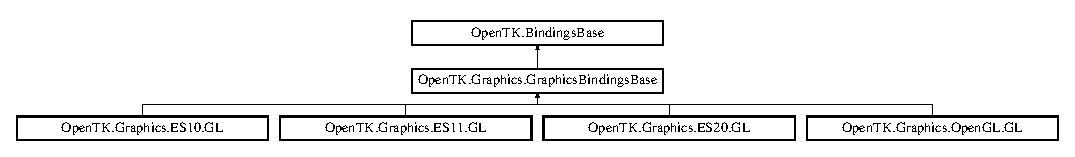
\includegraphics[height=1.666667cm]{class_open_t_k_1_1_graphics_1_1_graphics_bindings_base}
\end{center}
\end{figure}
\subsection*{Protected Member Functions}
\begin{DoxyCompactItemize}
\item 
override Int\-Ptr \hyperlink{class_open_t_k_1_1_graphics_1_1_graphics_bindings_base_aeb37d851aee841ad85ef90242456d652}{Get\-Address} (string funcname)
\begin{DoxyCompactList}\small\item\em Retrieves an unmanaged function pointer to the specified function. \end{DoxyCompactList}\end{DoxyCompactItemize}
\subsection*{Additional Inherited Members}


\subsection{Detailed Description}
Implements \hyperlink{class_open_t_k_1_1_bindings_base}{Bindings\-Base} for the \hyperlink{namespace_open_t_k_1_1_graphics}{Open\-T\-K.\-Graphics} namespace (\hyperlink{namespace_open_t_k_1_1_graphics_1_1_open_g_l}{Open\-G\-L} and Open\-G\-L$|$\-E\-S). 



\subsection{Member Function Documentation}
\hypertarget{class_open_t_k_1_1_graphics_1_1_graphics_bindings_base_aeb37d851aee841ad85ef90242456d652}{\index{Open\-T\-K\-::\-Graphics\-::\-Graphics\-Bindings\-Base@{Open\-T\-K\-::\-Graphics\-::\-Graphics\-Bindings\-Base}!Get\-Address@{Get\-Address}}
\index{Get\-Address@{Get\-Address}!OpenTK::Graphics::GraphicsBindingsBase@{Open\-T\-K\-::\-Graphics\-::\-Graphics\-Bindings\-Base}}
\subsubsection[{Get\-Address}]{\setlength{\rightskip}{0pt plus 5cm}override Int\-Ptr Open\-T\-K.\-Graphics.\-Graphics\-Bindings\-Base.\-Get\-Address (
\begin{DoxyParamCaption}
\item[{string}]{funcname}
\end{DoxyParamCaption}
)\hspace{0.3cm}{\ttfamily [protected]}, {\ttfamily [virtual]}}}\label{class_open_t_k_1_1_graphics_1_1_graphics_bindings_base_aeb37d851aee841ad85ef90242456d652}


Retrieves an unmanaged function pointer to the specified function. 


\begin{DoxyParams}{Parameters}
{\em funcname} & A System.\-String that defines the name of the function. \\
\hline
\end{DoxyParams}
\begin{DoxyReturn}{Returns}
A Int\-Ptr that contains the address of funcname or Int\-Ptr.\-Zero, if the function is not supported by the drivers. 
\end{DoxyReturn}


Note\-: some drivers are known to return non-\/zero values for unsupported functions. Typical values include 1 and 2 -\/ inheritors are advised to check for and ignore these values. 

Implements \hyperlink{class_open_t_k_1_1_bindings_base_a1eaa8a8b7a6a86051468535d38fca81c}{Open\-T\-K.\-Bindings\-Base}.


\hypertarget{class_open_t_k_1_1_graphics_1_1_graphics_context}{\section{Open\-T\-K.\-Graphics.\-Graphics\-Context Class Reference}
\label{class_open_t_k_1_1_graphics_1_1_graphics_context}\index{Open\-T\-K.\-Graphics.\-Graphics\-Context@{Open\-T\-K.\-Graphics.\-Graphics\-Context}}
}


Represents and provides methods to manipulate an \hyperlink{namespace_open_t_k_1_1_graphics_1_1_open_g_l}{Open\-G\-L} render context.  


Inheritance diagram for Open\-T\-K.\-Graphics.\-Graphics\-Context\-:\begin{figure}[H]
\begin{center}
\leavevmode
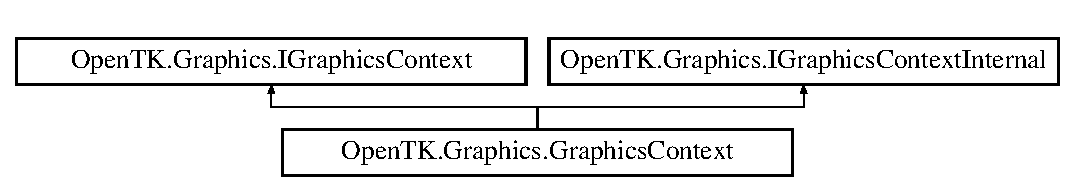
\includegraphics[height=2.000000cm]{class_open_t_k_1_1_graphics_1_1_graphics_context}
\end{center}
\end{figure}
\subsection*{Public Member Functions}
\begin{DoxyCompactItemize}
\item 
\hyperlink{class_open_t_k_1_1_graphics_1_1_graphics_context_a7954c5ce8c3bce5a0273f3ff22068186}{Graphics\-Context} (\hyperlink{class_open_t_k_1_1_graphics_1_1_graphics_mode}{Graphics\-Mode} mode, \hyperlink{interface_open_t_k_1_1_platform_1_1_i_window_info}{I\-Window\-Info} window)
\begin{DoxyCompactList}\small\item\em Constructs a new \hyperlink{class_open_t_k_1_1_graphics_1_1_graphics_context}{Graphics\-Context} with the specified \hyperlink{class_open_t_k_1_1_graphics_1_1_graphics_mode}{Graphics\-Mode} and attaches it to the specified window. \end{DoxyCompactList}\item 
\hyperlink{class_open_t_k_1_1_graphics_1_1_graphics_context_aaeb217a1cc05317ad1798c941aeee99d}{Graphics\-Context} (\hyperlink{class_open_t_k_1_1_graphics_1_1_graphics_mode}{Graphics\-Mode} mode, \hyperlink{interface_open_t_k_1_1_platform_1_1_i_window_info}{I\-Window\-Info} window, int major, int minor, \hyperlink{namespace_open_t_k_1_1_graphics_a518f77952bc406a013160356981ea8ab}{Graphics\-Context\-Flags} flags)
\begin{DoxyCompactList}\small\item\em Constructs a new \hyperlink{class_open_t_k_1_1_graphics_1_1_graphics_context}{Graphics\-Context} with the specified \hyperlink{class_open_t_k_1_1_graphics_1_1_graphics_mode}{Graphics\-Mode}, version and flags, and attaches it to the specified window. \end{DoxyCompactList}\item 
\hyperlink{class_open_t_k_1_1_graphics_1_1_graphics_context_a0232374e017976be588e2fe7f069d9b4}{Graphics\-Context} (\hyperlink{struct_open_t_k_1_1_context_handle}{Context\-Handle} handle, \hyperlink{interface_open_t_k_1_1_platform_1_1_i_window_info}{I\-Window\-Info} window)
\begin{DoxyCompactList}\small\item\em Constructs a new \hyperlink{class_open_t_k_1_1_graphics_1_1_graphics_context}{Graphics\-Context} from a pre-\/existing context created outside of \hyperlink{namespace_open_t_k}{Open\-T\-K}. \end{DoxyCompactList}\item 
\hyperlink{class_open_t_k_1_1_graphics_1_1_graphics_context_a3362b0338dccd8e180c8605fbf47b699}{Graphics\-Context} (\hyperlink{struct_open_t_k_1_1_context_handle}{Context\-Handle} handle, \hyperlink{interface_open_t_k_1_1_platform_1_1_i_window_info}{I\-Window\-Info} window, \hyperlink{interface_open_t_k_1_1_graphics_1_1_i_graphics_context}{I\-Graphics\-Context} share\-Context, int major, int minor, \hyperlink{namespace_open_t_k_1_1_graphics_a518f77952bc406a013160356981ea8ab}{Graphics\-Context\-Flags} flags)
\begin{DoxyCompactList}\small\item\em Constructs a new \hyperlink{class_open_t_k_1_1_graphics_1_1_graphics_context}{Graphics\-Context} from a pre-\/existing context created outside of \hyperlink{namespace_open_t_k}{Open\-T\-K}. \end{DoxyCompactList}\item 
override string \hyperlink{class_open_t_k_1_1_graphics_1_1_graphics_context_a66b97498dd4493a57f96268e432b9bec}{To\-String} ()
\begin{DoxyCompactList}\small\item\em Returns a System.\-String representing this instance. \end{DoxyCompactList}\item 
override int \hyperlink{class_open_t_k_1_1_graphics_1_1_graphics_context_a2d1fad8ad4a48dd77ec171083b3fe9a0}{Get\-Hash\-Code} ()
\begin{DoxyCompactList}\small\item\em Returns the hash code for this instance. \end{DoxyCompactList}\item 
override bool \hyperlink{class_open_t_k_1_1_graphics_1_1_graphics_context_ade7fe9534a1b711a0a0411ca371b07c5}{Equals} (object obj)
\begin{DoxyCompactList}\small\item\em Compares two instances. \end{DoxyCompactList}\item 
void \hyperlink{class_open_t_k_1_1_graphics_1_1_graphics_context_ab73c61bea26369cf76dff2165f5084cf}{Swap\-Buffers} ()
\begin{DoxyCompactList}\small\item\em Swaps buffers on a context. This presents the rendered scene to the user. \end{DoxyCompactList}\item 
void \hyperlink{class_open_t_k_1_1_graphics_1_1_graphics_context_a4b9b3b0f98fc1dc9f49f8abdb5ff076b}{Make\-Current} (\hyperlink{interface_open_t_k_1_1_platform_1_1_i_window_info}{I\-Window\-Info} window)
\begin{DoxyCompactList}\small\item\em Makes the \hyperlink{class_open_t_k_1_1_graphics_1_1_graphics_context}{Graphics\-Context} the current rendering target. \end{DoxyCompactList}\item 
void \hyperlink{class_open_t_k_1_1_graphics_1_1_graphics_context_a09fa035789147f9b9cfe2a5f09abe927}{Update} (\hyperlink{interface_open_t_k_1_1_platform_1_1_i_window_info}{I\-Window\-Info} window)
\begin{DoxyCompactList}\small\item\em Updates the graphics context. This must be called when the render target is resized for proper behavior on Mac O\-S X. \end{DoxyCompactList}\item 
void \hyperlink{class_open_t_k_1_1_graphics_1_1_graphics_context_a21640f20db040987bd1f897f503b68a4}{Load\-All} ()
\begin{DoxyCompactList}\small\item\em Loads all \hyperlink{namespace_open_t_k_1_1_graphics_1_1_open_g_l}{Open\-G\-L} entry points. \end{DoxyCompactList}\item 
void \hyperlink{class_open_t_k_1_1_graphics_1_1_graphics_context_a10e5f7c2e87670fd7400d8e4259fc602}{Dispose} ()
\begin{DoxyCompactList}\small\item\em Disposes of the \hyperlink{class_open_t_k_1_1_graphics_1_1_graphics_context}{Graphics\-Context}. \end{DoxyCompactList}\end{DoxyCompactItemize}
\subsection*{Static Public Member Functions}
\begin{DoxyCompactItemize}
\item 
static \hyperlink{class_open_t_k_1_1_graphics_1_1_graphics_context}{Graphics\-Context} \hyperlink{class_open_t_k_1_1_graphics_1_1_graphics_context_a5b6eadf39c00310bb0663d4eef883539}{Create\-Dummy\-Context} ()
\begin{DoxyCompactList}\small\item\em Creates a dummy \hyperlink{class_open_t_k_1_1_graphics_1_1_graphics_context}{Graphics\-Context} to allow \hyperlink{namespace_open_t_k}{Open\-T\-K} to work with contexts created by external libraries. \end{DoxyCompactList}\item 
static \hyperlink{class_open_t_k_1_1_graphics_1_1_graphics_context}{Graphics\-Context} \hyperlink{class_open_t_k_1_1_graphics_1_1_graphics_context_a36d9c29904cf9308b326da32b9d5cc8b}{Create\-Dummy\-Context} (\hyperlink{struct_open_t_k_1_1_context_handle}{Context\-Handle} handle)
\begin{DoxyCompactList}\small\item\em Creates a dummy \hyperlink{class_open_t_k_1_1_graphics_1_1_graphics_context}{Graphics\-Context} to allow \hyperlink{namespace_open_t_k}{Open\-T\-K} to work with contexts created by external libraries. \end{DoxyCompactList}\item 
static void \hyperlink{class_open_t_k_1_1_graphics_1_1_graphics_context_ae30eee17232c683f9c6151dfff6d804c}{Assert} ()
\begin{DoxyCompactList}\small\item\em Checks if a \hyperlink{class_open_t_k_1_1_graphics_1_1_graphics_context}{Graphics\-Context} exists in the calling thread and throws a \hyperlink{class_open_t_k_1_1_graphics_1_1_graphics_context_missing_exception}{Graphics\-Context\-Missing\-Exception} if it doesn't. \end{DoxyCompactList}\end{DoxyCompactItemize}
\subsection*{Properties}
\begin{DoxyCompactItemize}
\item 
static \hyperlink{interface_open_t_k_1_1_graphics_1_1_i_graphics_context}{I\-Graphics\-Context} \hyperlink{class_open_t_k_1_1_graphics_1_1_graphics_context_aa6b95167a8733355270dbb5d7c319986}{Current\-Context}\hspace{0.3cm}{\ttfamily  \mbox{[}get\mbox{]}}
\begin{DoxyCompactList}\small\item\em Gets the \hyperlink{class_open_t_k_1_1_graphics_1_1_graphics_context}{Graphics\-Context} that is current in the calling thread. \end{DoxyCompactList}\item 
static bool \hyperlink{class_open_t_k_1_1_graphics_1_1_graphics_context_a83e5259c2dd10556b3c485f2e8a00494}{Share\-Contexts}\hspace{0.3cm}{\ttfamily  \mbox{[}get, set\mbox{]}}
\begin{DoxyCompactList}\small\item\em Gets or sets a System.\-Boolean, indicating whether \hyperlink{class_open_t_k_1_1_graphics_1_1_graphics_context}{Graphics\-Context} resources are shared\end{DoxyCompactList}\item 
static bool \hyperlink{class_open_t_k_1_1_graphics_1_1_graphics_context_a2c0431903a5da942e015be0847f070bb}{Direct\-Rendering}\hspace{0.3cm}{\ttfamily  \mbox{[}get, set\mbox{]}}
\begin{DoxyCompactList}\small\item\em Gets or sets a System.\-Boolean, indicating whether Graphics\-Contexts will perform direct rendering.\end{DoxyCompactList}\item 
bool \hyperlink{class_open_t_k_1_1_graphics_1_1_graphics_context_a8ad06302403c5503b6ba954676523d90}{Error\-Checking}\hspace{0.3cm}{\ttfamily  \mbox{[}get, set\mbox{]}}
\begin{DoxyCompactList}\small\item\em Gets or sets a System.\-Boolean, indicating whether automatic error checking should be performed. Influences the debug version of Open\-T\-K.\-dll, only. \end{DoxyCompactList}\item 
bool \hyperlink{class_open_t_k_1_1_graphics_1_1_graphics_context_a7cbde7e3ab34ace4c087db96a72f6134}{Is\-Current}\hspace{0.3cm}{\ttfamily  \mbox{[}get\mbox{]}}
\begin{DoxyCompactList}\small\item\em Gets a System.\-Boolean indicating whether this instance is current in the calling thread. \end{DoxyCompactList}\item 
bool \hyperlink{class_open_t_k_1_1_graphics_1_1_graphics_context_ade92f0f31700dbb2a64eed7336bca89d}{Is\-Disposed}\hspace{0.3cm}{\ttfamily  \mbox{[}get, set\mbox{]}}
\begin{DoxyCompactList}\small\item\em Gets a System.\-Boolean indicating whether this instance has been disposed. It is an error to access any instance methods if this property returns true. \end{DoxyCompactList}\item 
bool \hyperlink{class_open_t_k_1_1_graphics_1_1_graphics_context_a502b2543a983bba6ceba9762212e290b}{V\-Sync}\hspace{0.3cm}{\ttfamily  \mbox{[}get, set\mbox{]}}
\begin{DoxyCompactList}\small\item\em \mbox{[}obsolete\mbox{]} Use Swap\-Interval property instead. Gets or sets a value indicating whether V\-Sync is enabled. When V\-Sync is enabled, \hyperlink{class_open_t_k_1_1_graphics_1_1_graphics_context_ab73c61bea26369cf76dff2165f5084cf}{Swap\-Buffers()} calls will be synced to the refresh rate of the \hyperlink{class_open_t_k_1_1_display_device}{Display\-Device} that contains improving visual quality and reducing C\-P\-U usage. However, systems that cannot maintain the requested rendering rate will suffer from large jumps in performance. This can be counteracted by increasing the \hyperlink{class_open_t_k_1_1_graphics_1_1_graphics_context_a860ca9db2d767d969b0b5a6c9b7b0f46}{Swap\-Interval} value. \end{DoxyCompactList}\item 
int \hyperlink{class_open_t_k_1_1_graphics_1_1_graphics_context_a860ca9db2d767d969b0b5a6c9b7b0f46}{Swap\-Interval}\hspace{0.3cm}{\ttfamily  \mbox{[}get, set\mbox{]}}
\begin{DoxyCompactList}\small\item\em Gets or sets a positive integer in the range \mbox{[}1, n), indicating the number of \hyperlink{class_open_t_k_1_1_display_device}{Display\-Device} refreshes between consecutive \hyperlink{class_open_t_k_1_1_graphics_1_1_graphics_context_ab73c61bea26369cf76dff2165f5084cf}{Swap\-Buffers()} calls. The maximum value for n is implementation-\/dependent. The default value is 1. This value will only affect instances where \hyperlink{class_open_t_k_1_1_graphics_1_1_graphics_context_a502b2543a983bba6ceba9762212e290b}{V\-Sync} is enabled. Invalid values will be clamped to the valid range. \end{DoxyCompactList}\item 
\hyperlink{class_open_t_k_1_1_graphics_1_1_graphics_mode}{Graphics\-Mode} \hyperlink{class_open_t_k_1_1_graphics_1_1_graphics_context_a5317c00e6a4db8f9b7f20c63791efd01}{Graphics\-Mode}\hspace{0.3cm}{\ttfamily  \mbox{[}get\mbox{]}}
\begin{DoxyCompactList}\small\item\em Gets the \hyperlink{class_open_t_k_1_1_graphics_1_1_graphics_mode}{Graphics\-Mode} of the context. \end{DoxyCompactList}\end{DoxyCompactItemize}


\subsection{Detailed Description}
Represents and provides methods to manipulate an \hyperlink{namespace_open_t_k_1_1_graphics_1_1_open_g_l}{Open\-G\-L} render context. 



\subsection{Constructor \& Destructor Documentation}
\hypertarget{class_open_t_k_1_1_graphics_1_1_graphics_context_a7954c5ce8c3bce5a0273f3ff22068186}{\index{Open\-T\-K\-::\-Graphics\-::\-Graphics\-Context@{Open\-T\-K\-::\-Graphics\-::\-Graphics\-Context}!Graphics\-Context@{Graphics\-Context}}
\index{Graphics\-Context@{Graphics\-Context}!OpenTK::Graphics::GraphicsContext@{Open\-T\-K\-::\-Graphics\-::\-Graphics\-Context}}
\subsubsection[{Graphics\-Context}]{\setlength{\rightskip}{0pt plus 5cm}Open\-T\-K.\-Graphics.\-Graphics\-Context.\-Graphics\-Context (
\begin{DoxyParamCaption}
\item[{{\bf Graphics\-Mode}}]{mode, }
\item[{{\bf I\-Window\-Info}}]{window}
\end{DoxyParamCaption}
)}}\label{class_open_t_k_1_1_graphics_1_1_graphics_context_a7954c5ce8c3bce5a0273f3ff22068186}


Constructs a new \hyperlink{class_open_t_k_1_1_graphics_1_1_graphics_context}{Graphics\-Context} with the specified \hyperlink{class_open_t_k_1_1_graphics_1_1_graphics_mode}{Graphics\-Mode} and attaches it to the specified window. 


\begin{DoxyParams}{Parameters}
{\em mode} & The \hyperlink{class_open_t_k_1_1_graphics_1_1_graphics_mode}{Open\-T\-K.\-Graphics.\-Graphics\-Mode} of the \hyperlink{class_open_t_k_1_1_graphics_1_1_graphics_context}{Graphics\-Context}.\\
\hline
{\em window} & The \hyperlink{interface_open_t_k_1_1_platform_1_1_i_window_info}{Open\-T\-K.\-Platform.\-I\-Window\-Info} to attach the \hyperlink{class_open_t_k_1_1_graphics_1_1_graphics_context}{Graphics\-Context} to.\\
\hline
\end{DoxyParams}
\hypertarget{class_open_t_k_1_1_graphics_1_1_graphics_context_aaeb217a1cc05317ad1798c941aeee99d}{\index{Open\-T\-K\-::\-Graphics\-::\-Graphics\-Context@{Open\-T\-K\-::\-Graphics\-::\-Graphics\-Context}!Graphics\-Context@{Graphics\-Context}}
\index{Graphics\-Context@{Graphics\-Context}!OpenTK::Graphics::GraphicsContext@{Open\-T\-K\-::\-Graphics\-::\-Graphics\-Context}}
\subsubsection[{Graphics\-Context}]{\setlength{\rightskip}{0pt plus 5cm}Open\-T\-K.\-Graphics.\-Graphics\-Context.\-Graphics\-Context (
\begin{DoxyParamCaption}
\item[{{\bf Graphics\-Mode}}]{mode, }
\item[{{\bf I\-Window\-Info}}]{window, }
\item[{int}]{major, }
\item[{int}]{minor, }
\item[{{\bf Graphics\-Context\-Flags}}]{flags}
\end{DoxyParamCaption}
)}}\label{class_open_t_k_1_1_graphics_1_1_graphics_context_aaeb217a1cc05317ad1798c941aeee99d}


Constructs a new \hyperlink{class_open_t_k_1_1_graphics_1_1_graphics_context}{Graphics\-Context} with the specified \hyperlink{class_open_t_k_1_1_graphics_1_1_graphics_mode}{Graphics\-Mode}, version and flags, and attaches it to the specified window. 


\begin{DoxyParams}{Parameters}
{\em mode} & The \hyperlink{class_open_t_k_1_1_graphics_1_1_graphics_mode}{Open\-T\-K.\-Graphics.\-Graphics\-Mode} of the \hyperlink{class_open_t_k_1_1_graphics_1_1_graphics_context}{Graphics\-Context}.\\
\hline
{\em window} & The \hyperlink{interface_open_t_k_1_1_platform_1_1_i_window_info}{Open\-T\-K.\-Platform.\-I\-Window\-Info} to attach the \hyperlink{class_open_t_k_1_1_graphics_1_1_graphics_context}{Graphics\-Context} to.\\
\hline
{\em major} & The major version of the new \hyperlink{class_open_t_k_1_1_graphics_1_1_graphics_context}{Graphics\-Context}.\\
\hline
{\em minor} & The minor version of the new \hyperlink{class_open_t_k_1_1_graphics_1_1_graphics_context}{Graphics\-Context}.\\
\hline
{\em flags} & The Graphics\-Context\-Flags for the \hyperlink{class_open_t_k_1_1_graphics_1_1_graphics_context}{Graphics\-Context}.\\
\hline
\end{DoxyParams}


Different hardware supports different flags, major and minor versions. Invalid parameters will be silently ignored. \hypertarget{class_open_t_k_1_1_graphics_1_1_graphics_context_a0232374e017976be588e2fe7f069d9b4}{\index{Open\-T\-K\-::\-Graphics\-::\-Graphics\-Context@{Open\-T\-K\-::\-Graphics\-::\-Graphics\-Context}!Graphics\-Context@{Graphics\-Context}}
\index{Graphics\-Context@{Graphics\-Context}!OpenTK::Graphics::GraphicsContext@{Open\-T\-K\-::\-Graphics\-::\-Graphics\-Context}}
\subsubsection[{Graphics\-Context}]{\setlength{\rightskip}{0pt plus 5cm}Open\-T\-K.\-Graphics.\-Graphics\-Context.\-Graphics\-Context (
\begin{DoxyParamCaption}
\item[{{\bf Context\-Handle}}]{handle, }
\item[{{\bf I\-Window\-Info}}]{window}
\end{DoxyParamCaption}
)}}\label{class_open_t_k_1_1_graphics_1_1_graphics_context_a0232374e017976be588e2fe7f069d9b4}


Constructs a new \hyperlink{class_open_t_k_1_1_graphics_1_1_graphics_context}{Graphics\-Context} from a pre-\/existing context created outside of \hyperlink{namespace_open_t_k}{Open\-T\-K}. 


\begin{DoxyParams}{Parameters}
{\em handle} & The handle of the existing context. This must be a valid, unique handle that is not known to \hyperlink{namespace_open_t_k}{Open\-T\-K}.\\
\hline
{\em window} & The window this context is bound to. This must be a valid window obtained through Utilities.\-Create\-Window\-Info.\\
\hline
\end{DoxyParams}

\begin{DoxyExceptions}{Exceptions}
{\em \hyperlink{class_open_t_k_1_1_graphics_1_1_graphics_context_exception}{Graphics\-Context\-Exception}} & Occurs if handle is identical to a context already registered with \hyperlink{namespace_open_t_k}{Open\-T\-K}.\\
\hline
\end{DoxyExceptions}
\hypertarget{class_open_t_k_1_1_graphics_1_1_graphics_context_a3362b0338dccd8e180c8605fbf47b699}{\index{Open\-T\-K\-::\-Graphics\-::\-Graphics\-Context@{Open\-T\-K\-::\-Graphics\-::\-Graphics\-Context}!Graphics\-Context@{Graphics\-Context}}
\index{Graphics\-Context@{Graphics\-Context}!OpenTK::Graphics::GraphicsContext@{Open\-T\-K\-::\-Graphics\-::\-Graphics\-Context}}
\subsubsection[{Graphics\-Context}]{\setlength{\rightskip}{0pt plus 5cm}Open\-T\-K.\-Graphics.\-Graphics\-Context.\-Graphics\-Context (
\begin{DoxyParamCaption}
\item[{{\bf Context\-Handle}}]{handle, }
\item[{{\bf I\-Window\-Info}}]{window, }
\item[{{\bf I\-Graphics\-Context}}]{share\-Context, }
\item[{int}]{major, }
\item[{int}]{minor, }
\item[{{\bf Graphics\-Context\-Flags}}]{flags}
\end{DoxyParamCaption}
)}}\label{class_open_t_k_1_1_graphics_1_1_graphics_context_a3362b0338dccd8e180c8605fbf47b699}


Constructs a new \hyperlink{class_open_t_k_1_1_graphics_1_1_graphics_context}{Graphics\-Context} from a pre-\/existing context created outside of \hyperlink{namespace_open_t_k}{Open\-T\-K}. 


\begin{DoxyParams}{Parameters}
{\em handle} & The handle of the existing context. This must be a valid, unique handle that is not known to \hyperlink{namespace_open_t_k}{Open\-T\-K}.\\
\hline
{\em window} & The window this context is bound to. This must be a valid window obtained through Utilities.\-Create\-Window\-Info.\\
\hline
{\em share\-Context} & A different context that shares resources with this instance, if any. Pass null if the context is not shared or if this is the first \hyperlink{class_open_t_k_1_1_graphics_1_1_graphics_context}{Graphics\-Context} instruct you construct.\\
\hline
{\em major} & The major version of the context (e.\-g. \char`\"{}2\char`\"{} for \char`\"{}2.\-1\char`\"{}).\\
\hline
{\em minor} & The minor version of the context (e.\-g. \char`\"{}1\char`\"{} for \char`\"{}2.\-1\char`\"{}).\\
\hline
{\em flags} & A bitwise combination of \hyperlink{namespace_open_t_k_1_1_graphics_a518f77952bc406a013160356981ea8ab}{Graphics\-Context\-Flags} that describe this context.\\
\hline
\end{DoxyParams}

\begin{DoxyExceptions}{Exceptions}
{\em \hyperlink{class_open_t_k_1_1_graphics_1_1_graphics_context_exception}{Graphics\-Context\-Exception}} & Occurs if handle is identical to a context already registered with \hyperlink{namespace_open_t_k}{Open\-T\-K}.\\
\hline
\end{DoxyExceptions}


\subsection{Member Function Documentation}
\hypertarget{class_open_t_k_1_1_graphics_1_1_graphics_context_ae30eee17232c683f9c6151dfff6d804c}{\index{Open\-T\-K\-::\-Graphics\-::\-Graphics\-Context@{Open\-T\-K\-::\-Graphics\-::\-Graphics\-Context}!Assert@{Assert}}
\index{Assert@{Assert}!OpenTK::Graphics::GraphicsContext@{Open\-T\-K\-::\-Graphics\-::\-Graphics\-Context}}
\subsubsection[{Assert}]{\setlength{\rightskip}{0pt plus 5cm}static void Open\-T\-K.\-Graphics.\-Graphics\-Context.\-Assert (
\begin{DoxyParamCaption}
{}
\end{DoxyParamCaption}
)\hspace{0.3cm}{\ttfamily [static]}}}\label{class_open_t_k_1_1_graphics_1_1_graphics_context_ae30eee17232c683f9c6151dfff6d804c}


Checks if a \hyperlink{class_open_t_k_1_1_graphics_1_1_graphics_context}{Graphics\-Context} exists in the calling thread and throws a \hyperlink{class_open_t_k_1_1_graphics_1_1_graphics_context_missing_exception}{Graphics\-Context\-Missing\-Exception} if it doesn't. 


\begin{DoxyExceptions}{Exceptions}
{\em \hyperlink{class_open_t_k_1_1_graphics_1_1_graphics_context_missing_exception}{Graphics\-Context\-Missing\-Exception}} & Generated when no \hyperlink{class_open_t_k_1_1_graphics_1_1_graphics_context}{Graphics\-Context} is current in the calling thread.\\
\hline
\end{DoxyExceptions}
\hypertarget{class_open_t_k_1_1_graphics_1_1_graphics_context_a5b6eadf39c00310bb0663d4eef883539}{\index{Open\-T\-K\-::\-Graphics\-::\-Graphics\-Context@{Open\-T\-K\-::\-Graphics\-::\-Graphics\-Context}!Create\-Dummy\-Context@{Create\-Dummy\-Context}}
\index{Create\-Dummy\-Context@{Create\-Dummy\-Context}!OpenTK::Graphics::GraphicsContext@{Open\-T\-K\-::\-Graphics\-::\-Graphics\-Context}}
\subsubsection[{Create\-Dummy\-Context}]{\setlength{\rightskip}{0pt plus 5cm}static {\bf Graphics\-Context} Open\-T\-K.\-Graphics.\-Graphics\-Context.\-Create\-Dummy\-Context (
\begin{DoxyParamCaption}
{}
\end{DoxyParamCaption}
)\hspace{0.3cm}{\ttfamily [static]}}}\label{class_open_t_k_1_1_graphics_1_1_graphics_context_a5b6eadf39c00310bb0663d4eef883539}


Creates a dummy \hyperlink{class_open_t_k_1_1_graphics_1_1_graphics_context}{Graphics\-Context} to allow \hyperlink{namespace_open_t_k}{Open\-T\-K} to work with contexts created by external libraries. 

\begin{DoxyReturn}{Returns}
A new, dummy \hyperlink{class_open_t_k_1_1_graphics_1_1_graphics_context}{Graphics\-Context} instance.
\end{DoxyReturn}


Instances created by this method will not be functional. Instance methods will have no effect.

This method requires that a context is current on the calling thread.\hypertarget{class_open_t_k_1_1_graphics_1_1_graphics_context_a36d9c29904cf9308b326da32b9d5cc8b}{\index{Open\-T\-K\-::\-Graphics\-::\-Graphics\-Context@{Open\-T\-K\-::\-Graphics\-::\-Graphics\-Context}!Create\-Dummy\-Context@{Create\-Dummy\-Context}}
\index{Create\-Dummy\-Context@{Create\-Dummy\-Context}!OpenTK::Graphics::GraphicsContext@{Open\-T\-K\-::\-Graphics\-::\-Graphics\-Context}}
\subsubsection[{Create\-Dummy\-Context}]{\setlength{\rightskip}{0pt plus 5cm}static {\bf Graphics\-Context} Open\-T\-K.\-Graphics.\-Graphics\-Context.\-Create\-Dummy\-Context (
\begin{DoxyParamCaption}
\item[{{\bf Context\-Handle}}]{handle}
\end{DoxyParamCaption}
)\hspace{0.3cm}{\ttfamily [static]}}}\label{class_open_t_k_1_1_graphics_1_1_graphics_context_a36d9c29904cf9308b326da32b9d5cc8b}


Creates a dummy \hyperlink{class_open_t_k_1_1_graphics_1_1_graphics_context}{Graphics\-Context} to allow \hyperlink{namespace_open_t_k}{Open\-T\-K} to work with contexts created by external libraries. 


\begin{DoxyParams}{Parameters}
{\em handle} & The handle of a context.\\
\hline
\end{DoxyParams}
\begin{DoxyReturn}{Returns}
A new, dummy \hyperlink{class_open_t_k_1_1_graphics_1_1_graphics_context}{Graphics\-Context} instance.
\end{DoxyReturn}


Instances created by this method will not be functional. Instance methods will have no effect.\hypertarget{class_open_t_k_1_1_graphics_1_1_graphics_context_a10e5f7c2e87670fd7400d8e4259fc602}{\index{Open\-T\-K\-::\-Graphics\-::\-Graphics\-Context@{Open\-T\-K\-::\-Graphics\-::\-Graphics\-Context}!Dispose@{Dispose}}
\index{Dispose@{Dispose}!OpenTK::Graphics::GraphicsContext@{Open\-T\-K\-::\-Graphics\-::\-Graphics\-Context}}
\subsubsection[{Dispose}]{\setlength{\rightskip}{0pt plus 5cm}void Open\-T\-K.\-Graphics.\-Graphics\-Context.\-Dispose (
\begin{DoxyParamCaption}
{}
\end{DoxyParamCaption}
)}}\label{class_open_t_k_1_1_graphics_1_1_graphics_context_a10e5f7c2e87670fd7400d8e4259fc602}


Disposes of the \hyperlink{class_open_t_k_1_1_graphics_1_1_graphics_context}{Graphics\-Context}. 

\hypertarget{class_open_t_k_1_1_graphics_1_1_graphics_context_ade7fe9534a1b711a0a0411ca371b07c5}{\index{Open\-T\-K\-::\-Graphics\-::\-Graphics\-Context@{Open\-T\-K\-::\-Graphics\-::\-Graphics\-Context}!Equals@{Equals}}
\index{Equals@{Equals}!OpenTK::Graphics::GraphicsContext@{Open\-T\-K\-::\-Graphics\-::\-Graphics\-Context}}
\subsubsection[{Equals}]{\setlength{\rightskip}{0pt plus 5cm}override bool Open\-T\-K.\-Graphics.\-Graphics\-Context.\-Equals (
\begin{DoxyParamCaption}
\item[{object}]{obj}
\end{DoxyParamCaption}
)}}\label{class_open_t_k_1_1_graphics_1_1_graphics_context_ade7fe9534a1b711a0a0411ca371b07c5}


Compares two instances. 


\begin{DoxyParams}{Parameters}
{\em obj} & The instance to compare to.\\
\hline
\end{DoxyParams}
\begin{DoxyReturn}{Returns}
True, if obj is equal to this instance; false otherwise.
\end{DoxyReturn}
\hypertarget{class_open_t_k_1_1_graphics_1_1_graphics_context_a2d1fad8ad4a48dd77ec171083b3fe9a0}{\index{Open\-T\-K\-::\-Graphics\-::\-Graphics\-Context@{Open\-T\-K\-::\-Graphics\-::\-Graphics\-Context}!Get\-Hash\-Code@{Get\-Hash\-Code}}
\index{Get\-Hash\-Code@{Get\-Hash\-Code}!OpenTK::Graphics::GraphicsContext@{Open\-T\-K\-::\-Graphics\-::\-Graphics\-Context}}
\subsubsection[{Get\-Hash\-Code}]{\setlength{\rightskip}{0pt plus 5cm}override int Open\-T\-K.\-Graphics.\-Graphics\-Context.\-Get\-Hash\-Code (
\begin{DoxyParamCaption}
{}
\end{DoxyParamCaption}
)}}\label{class_open_t_k_1_1_graphics_1_1_graphics_context_a2d1fad8ad4a48dd77ec171083b3fe9a0}


Returns the hash code for this instance. 

\begin{DoxyReturn}{Returns}
A System.\-Int32 with the hash code of this instance.
\end{DoxyReturn}
\hypertarget{class_open_t_k_1_1_graphics_1_1_graphics_context_a21640f20db040987bd1f897f503b68a4}{\index{Open\-T\-K\-::\-Graphics\-::\-Graphics\-Context@{Open\-T\-K\-::\-Graphics\-::\-Graphics\-Context}!Load\-All@{Load\-All}}
\index{Load\-All@{Load\-All}!OpenTK::Graphics::GraphicsContext@{Open\-T\-K\-::\-Graphics\-::\-Graphics\-Context}}
\subsubsection[{Load\-All}]{\setlength{\rightskip}{0pt plus 5cm}void Open\-T\-K.\-Graphics.\-Graphics\-Context.\-Load\-All (
\begin{DoxyParamCaption}
{}
\end{DoxyParamCaption}
)}}\label{class_open_t_k_1_1_graphics_1_1_graphics_context_a21640f20db040987bd1f897f503b68a4}


Loads all \hyperlink{namespace_open_t_k_1_1_graphics_1_1_open_g_l}{Open\-G\-L} entry points. 


\begin{DoxyExceptions}{Exceptions}
{\em \hyperlink{class_open_t_k_1_1_graphics_1_1_graphics_context_exception}{Open\-T\-K.\-Graphics.\-Graphics\-Context\-Exception}} & Occurs when this instance is not current on the calling thread. \\
\hline
\end{DoxyExceptions}


Implements \hyperlink{interface_open_t_k_1_1_graphics_1_1_i_graphics_context_a8f8df276eeac50ba850cb21fa5a4e676}{Open\-T\-K.\-Graphics.\-I\-Graphics\-Context}.

\hypertarget{class_open_t_k_1_1_graphics_1_1_graphics_context_a4b9b3b0f98fc1dc9f49f8abdb5ff076b}{\index{Open\-T\-K\-::\-Graphics\-::\-Graphics\-Context@{Open\-T\-K\-::\-Graphics\-::\-Graphics\-Context}!Make\-Current@{Make\-Current}}
\index{Make\-Current@{Make\-Current}!OpenTK::Graphics::GraphicsContext@{Open\-T\-K\-::\-Graphics\-::\-Graphics\-Context}}
\subsubsection[{Make\-Current}]{\setlength{\rightskip}{0pt plus 5cm}void Open\-T\-K.\-Graphics.\-Graphics\-Context.\-Make\-Current (
\begin{DoxyParamCaption}
\item[{{\bf I\-Window\-Info}}]{window}
\end{DoxyParamCaption}
)}}\label{class_open_t_k_1_1_graphics_1_1_graphics_context_a4b9b3b0f98fc1dc9f49f8abdb5ff076b}


Makes the \hyperlink{class_open_t_k_1_1_graphics_1_1_graphics_context}{Graphics\-Context} the current rendering target. 


\begin{DoxyParams}{Parameters}
{\em window} & A valid \hyperlink{interface_open_t_k_1_1_platform_1_1_i_window_info}{Open\-T\-K.\-Platform.\-I\-Window\-Info} structure.\\
\hline
\end{DoxyParams}


You can use this method to bind the \hyperlink{class_open_t_k_1_1_graphics_1_1_graphics_context}{Graphics\-Context} to a different window than the one it was created from. 

Implements \hyperlink{interface_open_t_k_1_1_graphics_1_1_i_graphics_context_a73a3ca64b49a682800e636d0135887ed}{Open\-T\-K.\-Graphics.\-I\-Graphics\-Context}.

\hypertarget{class_open_t_k_1_1_graphics_1_1_graphics_context_ab73c61bea26369cf76dff2165f5084cf}{\index{Open\-T\-K\-::\-Graphics\-::\-Graphics\-Context@{Open\-T\-K\-::\-Graphics\-::\-Graphics\-Context}!Swap\-Buffers@{Swap\-Buffers}}
\index{Swap\-Buffers@{Swap\-Buffers}!OpenTK::Graphics::GraphicsContext@{Open\-T\-K\-::\-Graphics\-::\-Graphics\-Context}}
\subsubsection[{Swap\-Buffers}]{\setlength{\rightskip}{0pt plus 5cm}void Open\-T\-K.\-Graphics.\-Graphics\-Context.\-Swap\-Buffers (
\begin{DoxyParamCaption}
{}
\end{DoxyParamCaption}
)}}\label{class_open_t_k_1_1_graphics_1_1_graphics_context_ab73c61bea26369cf76dff2165f5084cf}


Swaps buffers on a context. This presents the rendered scene to the user. 



Implements \hyperlink{interface_open_t_k_1_1_graphics_1_1_i_graphics_context_ad7d516da745576542161f1baa5f20129}{Open\-T\-K.\-Graphics.\-I\-Graphics\-Context}.

\hypertarget{class_open_t_k_1_1_graphics_1_1_graphics_context_a66b97498dd4493a57f96268e432b9bec}{\index{Open\-T\-K\-::\-Graphics\-::\-Graphics\-Context@{Open\-T\-K\-::\-Graphics\-::\-Graphics\-Context}!To\-String@{To\-String}}
\index{To\-String@{To\-String}!OpenTK::Graphics::GraphicsContext@{Open\-T\-K\-::\-Graphics\-::\-Graphics\-Context}}
\subsubsection[{To\-String}]{\setlength{\rightskip}{0pt plus 5cm}override string Open\-T\-K.\-Graphics.\-Graphics\-Context.\-To\-String (
\begin{DoxyParamCaption}
{}
\end{DoxyParamCaption}
)}}\label{class_open_t_k_1_1_graphics_1_1_graphics_context_a66b97498dd4493a57f96268e432b9bec}


Returns a System.\-String representing this instance. 

\begin{DoxyReturn}{Returns}
A System.\-String that contains a string representation of this instance.
\end{DoxyReturn}
\hypertarget{class_open_t_k_1_1_graphics_1_1_graphics_context_a09fa035789147f9b9cfe2a5f09abe927}{\index{Open\-T\-K\-::\-Graphics\-::\-Graphics\-Context@{Open\-T\-K\-::\-Graphics\-::\-Graphics\-Context}!Update@{Update}}
\index{Update@{Update}!OpenTK::Graphics::GraphicsContext@{Open\-T\-K\-::\-Graphics\-::\-Graphics\-Context}}
\subsubsection[{Update}]{\setlength{\rightskip}{0pt plus 5cm}void Open\-T\-K.\-Graphics.\-Graphics\-Context.\-Update (
\begin{DoxyParamCaption}
\item[{{\bf I\-Window\-Info}}]{window}
\end{DoxyParamCaption}
)}}\label{class_open_t_k_1_1_graphics_1_1_graphics_context_a09fa035789147f9b9cfe2a5f09abe927}


Updates the graphics context. This must be called when the render target is resized for proper behavior on Mac O\-S X. 


\begin{DoxyParams}{Parameters}
{\em window} & \\
\hline
\end{DoxyParams}


Implements \hyperlink{interface_open_t_k_1_1_graphics_1_1_i_graphics_context_a4bf57e48815f169c133eb15ccda2d146}{Open\-T\-K.\-Graphics.\-I\-Graphics\-Context}.



\subsection{Property Documentation}
\hypertarget{class_open_t_k_1_1_graphics_1_1_graphics_context_aa6b95167a8733355270dbb5d7c319986}{\index{Open\-T\-K\-::\-Graphics\-::\-Graphics\-Context@{Open\-T\-K\-::\-Graphics\-::\-Graphics\-Context}!Current\-Context@{Current\-Context}}
\index{Current\-Context@{Current\-Context}!OpenTK::Graphics::GraphicsContext@{Open\-T\-K\-::\-Graphics\-::\-Graphics\-Context}}
\subsubsection[{Current\-Context}]{\setlength{\rightskip}{0pt plus 5cm}{\bf I\-Graphics\-Context} Open\-T\-K.\-Graphics.\-Graphics\-Context.\-Current\-Context\hspace{0.3cm}{\ttfamily [static]}, {\ttfamily [get]}}}\label{class_open_t_k_1_1_graphics_1_1_graphics_context_aa6b95167a8733355270dbb5d7c319986}


Gets the \hyperlink{class_open_t_k_1_1_graphics_1_1_graphics_context}{Graphics\-Context} that is current in the calling thread. 

Note\-: this property will not function correctly when both desktop and E\-G\-L contexts are available in the same process. This scenario is very unlikely to appear in practice. \hypertarget{class_open_t_k_1_1_graphics_1_1_graphics_context_a2c0431903a5da942e015be0847f070bb}{\index{Open\-T\-K\-::\-Graphics\-::\-Graphics\-Context@{Open\-T\-K\-::\-Graphics\-::\-Graphics\-Context}!Direct\-Rendering@{Direct\-Rendering}}
\index{Direct\-Rendering@{Direct\-Rendering}!OpenTK::Graphics::GraphicsContext@{Open\-T\-K\-::\-Graphics\-::\-Graphics\-Context}}
\subsubsection[{Direct\-Rendering}]{\setlength{\rightskip}{0pt plus 5cm}bool Open\-T\-K.\-Graphics.\-Graphics\-Context.\-Direct\-Rendering\hspace{0.3cm}{\ttfamily [static]}, {\ttfamily [get]}, {\ttfamily [set]}}}\label{class_open_t_k_1_1_graphics_1_1_graphics_context_a2c0431903a5da942e015be0847f070bb}


Gets or sets a System.\-Boolean, indicating whether Graphics\-Contexts will perform direct rendering.

If Direct\-Rendering is true, new contexts will be constructed with direct rendering capabilities, if possible. If Direct\-Rendering is false, new contexts will be constructed with indirect rendering capabilities. 

This property does not affect existing Graphics\-Contexts, unless they are recreated.

This property is ignored on Operating Systems without support for indirect rendering, like Windows and O\-S X. \hypertarget{class_open_t_k_1_1_graphics_1_1_graphics_context_a8ad06302403c5503b6ba954676523d90}{\index{Open\-T\-K\-::\-Graphics\-::\-Graphics\-Context@{Open\-T\-K\-::\-Graphics\-::\-Graphics\-Context}!Error\-Checking@{Error\-Checking}}
\index{Error\-Checking@{Error\-Checking}!OpenTK::Graphics::GraphicsContext@{Open\-T\-K\-::\-Graphics\-::\-Graphics\-Context}}
\subsubsection[{Error\-Checking}]{\setlength{\rightskip}{0pt plus 5cm}bool Open\-T\-K.\-Graphics.\-Graphics\-Context.\-Error\-Checking\hspace{0.3cm}{\ttfamily [get]}, {\ttfamily [set]}}}\label{class_open_t_k_1_1_graphics_1_1_graphics_context_a8ad06302403c5503b6ba954676523d90}


Gets or sets a System.\-Boolean, indicating whether automatic error checking should be performed. Influences the debug version of Open\-T\-K.\-dll, only. 

Automatic error checking will clear the \hyperlink{namespace_open_t_k_1_1_graphics_1_1_open_g_l}{Open\-G\-L} error state. Set Check\-Errors to false if you use the \hyperlink{namespace_open_t_k_1_1_graphics_1_1_open_g_l}{Open\-G\-L} error state in your code flow (e.\-g. for checking supported texture formats).\hypertarget{class_open_t_k_1_1_graphics_1_1_graphics_context_a5317c00e6a4db8f9b7f20c63791efd01}{\index{Open\-T\-K\-::\-Graphics\-::\-Graphics\-Context@{Open\-T\-K\-::\-Graphics\-::\-Graphics\-Context}!Graphics\-Mode@{Graphics\-Mode}}
\index{Graphics\-Mode@{Graphics\-Mode}!OpenTK::Graphics::GraphicsContext@{Open\-T\-K\-::\-Graphics\-::\-Graphics\-Context}}
\subsubsection[{Graphics\-Mode}]{\setlength{\rightskip}{0pt plus 5cm}{\bf Graphics\-Mode} Open\-T\-K.\-Graphics.\-Graphics\-Context.\-Graphics\-Mode\hspace{0.3cm}{\ttfamily [get]}}}\label{class_open_t_k_1_1_graphics_1_1_graphics_context_a5317c00e6a4db8f9b7f20c63791efd01}


Gets the \hyperlink{class_open_t_k_1_1_graphics_1_1_graphics_mode}{Graphics\-Mode} of the context. 

\hypertarget{class_open_t_k_1_1_graphics_1_1_graphics_context_a7cbde7e3ab34ace4c087db96a72f6134}{\index{Open\-T\-K\-::\-Graphics\-::\-Graphics\-Context@{Open\-T\-K\-::\-Graphics\-::\-Graphics\-Context}!Is\-Current@{Is\-Current}}
\index{Is\-Current@{Is\-Current}!OpenTK::Graphics::GraphicsContext@{Open\-T\-K\-::\-Graphics\-::\-Graphics\-Context}}
\subsubsection[{Is\-Current}]{\setlength{\rightskip}{0pt plus 5cm}bool Open\-T\-K.\-Graphics.\-Graphics\-Context.\-Is\-Current\hspace{0.3cm}{\ttfamily [get]}}}\label{class_open_t_k_1_1_graphics_1_1_graphics_context_a7cbde7e3ab34ace4c087db96a72f6134}


Gets a System.\-Boolean indicating whether this instance is current in the calling thread. 

\hypertarget{class_open_t_k_1_1_graphics_1_1_graphics_context_ade92f0f31700dbb2a64eed7336bca89d}{\index{Open\-T\-K\-::\-Graphics\-::\-Graphics\-Context@{Open\-T\-K\-::\-Graphics\-::\-Graphics\-Context}!Is\-Disposed@{Is\-Disposed}}
\index{Is\-Disposed@{Is\-Disposed}!OpenTK::Graphics::GraphicsContext@{Open\-T\-K\-::\-Graphics\-::\-Graphics\-Context}}
\subsubsection[{Is\-Disposed}]{\setlength{\rightskip}{0pt plus 5cm}bool Open\-T\-K.\-Graphics.\-Graphics\-Context.\-Is\-Disposed\hspace{0.3cm}{\ttfamily [get]}, {\ttfamily [set]}}}\label{class_open_t_k_1_1_graphics_1_1_graphics_context_ade92f0f31700dbb2a64eed7336bca89d}


Gets a System.\-Boolean indicating whether this instance has been disposed. It is an error to access any instance methods if this property returns true. 

\hypertarget{class_open_t_k_1_1_graphics_1_1_graphics_context_a83e5259c2dd10556b3c485f2e8a00494}{\index{Open\-T\-K\-::\-Graphics\-::\-Graphics\-Context@{Open\-T\-K\-::\-Graphics\-::\-Graphics\-Context}!Share\-Contexts@{Share\-Contexts}}
\index{Share\-Contexts@{Share\-Contexts}!OpenTK::Graphics::GraphicsContext@{Open\-T\-K\-::\-Graphics\-::\-Graphics\-Context}}
\subsubsection[{Share\-Contexts}]{\setlength{\rightskip}{0pt plus 5cm}bool Open\-T\-K.\-Graphics.\-Graphics\-Context.\-Share\-Contexts\hspace{0.3cm}{\ttfamily [static]}, {\ttfamily [get]}, {\ttfamily [set]}}}\label{class_open_t_k_1_1_graphics_1_1_graphics_context_a83e5259c2dd10556b3c485f2e8a00494}


Gets or sets a System.\-Boolean, indicating whether \hyperlink{class_open_t_k_1_1_graphics_1_1_graphics_context}{Graphics\-Context} resources are shared

If Share\-Contexts is true, new G\-L\-Contexts will share resources. If this value is false, new G\-L\-Contexts will not share resources.

Changing this value will not affect already created G\-L\-Contexts.\hypertarget{class_open_t_k_1_1_graphics_1_1_graphics_context_a860ca9db2d767d969b0b5a6c9b7b0f46}{\index{Open\-T\-K\-::\-Graphics\-::\-Graphics\-Context@{Open\-T\-K\-::\-Graphics\-::\-Graphics\-Context}!Swap\-Interval@{Swap\-Interval}}
\index{Swap\-Interval@{Swap\-Interval}!OpenTK::Graphics::GraphicsContext@{Open\-T\-K\-::\-Graphics\-::\-Graphics\-Context}}
\subsubsection[{Swap\-Interval}]{\setlength{\rightskip}{0pt plus 5cm}int Open\-T\-K.\-Graphics.\-Graphics\-Context.\-Swap\-Interval\hspace{0.3cm}{\ttfamily [get]}, {\ttfamily [set]}}}\label{class_open_t_k_1_1_graphics_1_1_graphics_context_a860ca9db2d767d969b0b5a6c9b7b0f46}


Gets or sets a positive integer in the range \mbox{[}1, n), indicating the number of \hyperlink{class_open_t_k_1_1_display_device}{Display\-Device} refreshes between consecutive \hyperlink{class_open_t_k_1_1_graphics_1_1_graphics_context_ab73c61bea26369cf76dff2165f5084cf}{Swap\-Buffers()} calls. The maximum value for n is implementation-\/dependent. The default value is 1. This value will only affect instances where \hyperlink{class_open_t_k_1_1_graphics_1_1_graphics_context_a502b2543a983bba6ceba9762212e290b}{V\-Sync} is enabled. Invalid values will be clamped to the valid range. 

\hypertarget{class_open_t_k_1_1_graphics_1_1_graphics_context_a502b2543a983bba6ceba9762212e290b}{\index{Open\-T\-K\-::\-Graphics\-::\-Graphics\-Context@{Open\-T\-K\-::\-Graphics\-::\-Graphics\-Context}!V\-Sync@{V\-Sync}}
\index{V\-Sync@{V\-Sync}!OpenTK::Graphics::GraphicsContext@{Open\-T\-K\-::\-Graphics\-::\-Graphics\-Context}}
\subsubsection[{V\-Sync}]{\setlength{\rightskip}{0pt plus 5cm}bool Open\-T\-K.\-Graphics.\-Graphics\-Context.\-V\-Sync\hspace{0.3cm}{\ttfamily [get]}, {\ttfamily [set]}}}\label{class_open_t_k_1_1_graphics_1_1_graphics_context_a502b2543a983bba6ceba9762212e290b}


\mbox{[}obsolete\mbox{]} Use Swap\-Interval property instead. Gets or sets a value indicating whether V\-Sync is enabled. When V\-Sync is enabled, \hyperlink{class_open_t_k_1_1_graphics_1_1_graphics_context_ab73c61bea26369cf76dff2165f5084cf}{Swap\-Buffers()} calls will be synced to the refresh rate of the \hyperlink{class_open_t_k_1_1_display_device}{Display\-Device} that contains improving visual quality and reducing C\-P\-U usage. However, systems that cannot maintain the requested rendering rate will suffer from large jumps in performance. This can be counteracted by increasing the \hyperlink{class_open_t_k_1_1_graphics_1_1_graphics_context_a860ca9db2d767d969b0b5a6c9b7b0f46}{Swap\-Interval} value. 


\hypertarget{class_open_t_k_1_1_graphics_1_1_graphics_context_exception}{\section{Open\-T\-K.\-Graphics.\-Graphics\-Context\-Exception Class Reference}
\label{class_open_t_k_1_1_graphics_1_1_graphics_context_exception}\index{Open\-T\-K.\-Graphics.\-Graphics\-Context\-Exception@{Open\-T\-K.\-Graphics.\-Graphics\-Context\-Exception}}
}


Represents errors related to a \hyperlink{class_open_t_k_1_1_graphics_1_1_graphics_context}{Graphics\-Context}.  


Inheritance diagram for Open\-T\-K.\-Graphics.\-Graphics\-Context\-Exception\-:\begin{figure}[H]
\begin{center}
\leavevmode
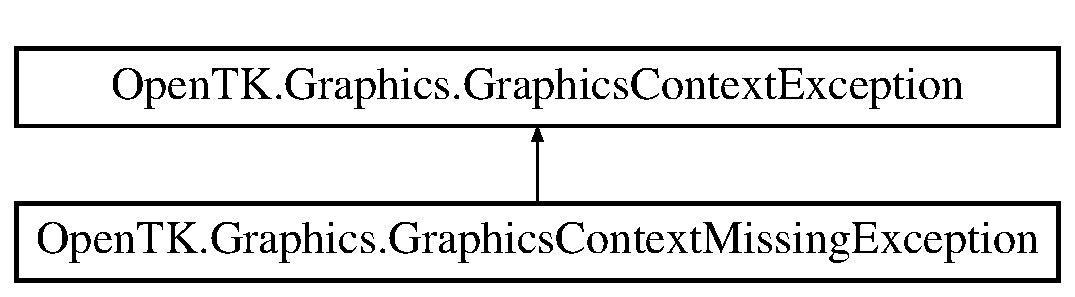
\includegraphics[height=2.000000cm]{class_open_t_k_1_1_graphics_1_1_graphics_context_exception}
\end{center}
\end{figure}
\subsection*{Public Member Functions}
\begin{DoxyCompactItemize}
\item 
\hyperlink{class_open_t_k_1_1_graphics_1_1_graphics_context_exception_a833dfff1800292539696095561cc82ba}{Graphics\-Context\-Exception} ()
\begin{DoxyCompactList}\small\item\em Constructs a new \hyperlink{class_open_t_k_1_1_graphics_1_1_graphics_context_exception}{Graphics\-Context\-Exception}. \end{DoxyCompactList}\item 
\hyperlink{class_open_t_k_1_1_graphics_1_1_graphics_context_exception_a7f675759af78e8e71b8fe108d9b8154c}{Graphics\-Context\-Exception} (string message)
\begin{DoxyCompactList}\small\item\em Constructs a new \hyperlink{class_open_t_k_1_1_graphics_1_1_graphics_context_exception}{Graphics\-Context\-Exception} with the given error message. \end{DoxyCompactList}\end{DoxyCompactItemize}


\subsection{Detailed Description}
Represents errors related to a \hyperlink{class_open_t_k_1_1_graphics_1_1_graphics_context}{Graphics\-Context}. 



\subsection{Constructor \& Destructor Documentation}
\hypertarget{class_open_t_k_1_1_graphics_1_1_graphics_context_exception_a833dfff1800292539696095561cc82ba}{\index{Open\-T\-K\-::\-Graphics\-::\-Graphics\-Context\-Exception@{Open\-T\-K\-::\-Graphics\-::\-Graphics\-Context\-Exception}!Graphics\-Context\-Exception@{Graphics\-Context\-Exception}}
\index{Graphics\-Context\-Exception@{Graphics\-Context\-Exception}!OpenTK::Graphics::GraphicsContextException@{Open\-T\-K\-::\-Graphics\-::\-Graphics\-Context\-Exception}}
\subsubsection[{Graphics\-Context\-Exception}]{\setlength{\rightskip}{0pt plus 5cm}Open\-T\-K.\-Graphics.\-Graphics\-Context\-Exception.\-Graphics\-Context\-Exception (
\begin{DoxyParamCaption}
{}
\end{DoxyParamCaption}
)}}\label{class_open_t_k_1_1_graphics_1_1_graphics_context_exception_a833dfff1800292539696095561cc82ba}


Constructs a new \hyperlink{class_open_t_k_1_1_graphics_1_1_graphics_context_exception}{Graphics\-Context\-Exception}. 

\hypertarget{class_open_t_k_1_1_graphics_1_1_graphics_context_exception_a7f675759af78e8e71b8fe108d9b8154c}{\index{Open\-T\-K\-::\-Graphics\-::\-Graphics\-Context\-Exception@{Open\-T\-K\-::\-Graphics\-::\-Graphics\-Context\-Exception}!Graphics\-Context\-Exception@{Graphics\-Context\-Exception}}
\index{Graphics\-Context\-Exception@{Graphics\-Context\-Exception}!OpenTK::Graphics::GraphicsContextException@{Open\-T\-K\-::\-Graphics\-::\-Graphics\-Context\-Exception}}
\subsubsection[{Graphics\-Context\-Exception}]{\setlength{\rightskip}{0pt plus 5cm}Open\-T\-K.\-Graphics.\-Graphics\-Context\-Exception.\-Graphics\-Context\-Exception (
\begin{DoxyParamCaption}
\item[{string}]{message}
\end{DoxyParamCaption}
)}}\label{class_open_t_k_1_1_graphics_1_1_graphics_context_exception_a7f675759af78e8e71b8fe108d9b8154c}


Constructs a new \hyperlink{class_open_t_k_1_1_graphics_1_1_graphics_context_exception}{Graphics\-Context\-Exception} with the given error message. 


\hypertarget{class_open_t_k_1_1_graphics_1_1_graphics_context_missing_exception}{\section{Open\-T\-K.\-Graphics.\-Graphics\-Context\-Missing\-Exception Class Reference}
\label{class_open_t_k_1_1_graphics_1_1_graphics_context_missing_exception}\index{Open\-T\-K.\-Graphics.\-Graphics\-Context\-Missing\-Exception@{Open\-T\-K.\-Graphics.\-Graphics\-Context\-Missing\-Exception}}
}


Thrown when an operation that required \hyperlink{class_open_t_k_1_1_graphics_1_1_graphics_context}{Graphics\-Context} is performed, when no \hyperlink{class_open_t_k_1_1_graphics_1_1_graphics_context}{Graphics\-Context} is current in the calling thread.  


Inheritance diagram for Open\-T\-K.\-Graphics.\-Graphics\-Context\-Missing\-Exception\-:\begin{figure}[H]
\begin{center}
\leavevmode
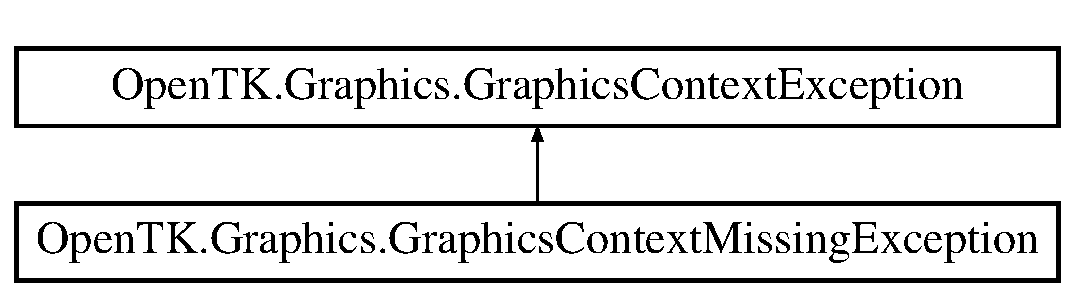
\includegraphics[height=2.000000cm]{class_open_t_k_1_1_graphics_1_1_graphics_context_missing_exception}
\end{center}
\end{figure}
\subsection*{Public Member Functions}
\begin{DoxyCompactItemize}
\item 
\hyperlink{class_open_t_k_1_1_graphics_1_1_graphics_context_missing_exception_a73d119ac3bedb08eaf7daa5a22c4938e}{Graphics\-Context\-Missing\-Exception} ()
\begin{DoxyCompactList}\small\item\em Constructs a new \hyperlink{class_open_t_k_1_1_graphics_1_1_graphics_context_missing_exception}{Graphics\-Context\-Missing\-Exception}. \end{DoxyCompactList}\end{DoxyCompactItemize}


\subsection{Detailed Description}
Thrown when an operation that required \hyperlink{class_open_t_k_1_1_graphics_1_1_graphics_context}{Graphics\-Context} is performed, when no \hyperlink{class_open_t_k_1_1_graphics_1_1_graphics_context}{Graphics\-Context} is current in the calling thread. 



\subsection{Constructor \& Destructor Documentation}
\hypertarget{class_open_t_k_1_1_graphics_1_1_graphics_context_missing_exception_a73d119ac3bedb08eaf7daa5a22c4938e}{\index{Open\-T\-K\-::\-Graphics\-::\-Graphics\-Context\-Missing\-Exception@{Open\-T\-K\-::\-Graphics\-::\-Graphics\-Context\-Missing\-Exception}!Graphics\-Context\-Missing\-Exception@{Graphics\-Context\-Missing\-Exception}}
\index{Graphics\-Context\-Missing\-Exception@{Graphics\-Context\-Missing\-Exception}!OpenTK::Graphics::GraphicsContextMissingException@{Open\-T\-K\-::\-Graphics\-::\-Graphics\-Context\-Missing\-Exception}}
\subsubsection[{Graphics\-Context\-Missing\-Exception}]{\setlength{\rightskip}{0pt plus 5cm}Open\-T\-K.\-Graphics.\-Graphics\-Context\-Missing\-Exception.\-Graphics\-Context\-Missing\-Exception (
\begin{DoxyParamCaption}
{}
\end{DoxyParamCaption}
)}}\label{class_open_t_k_1_1_graphics_1_1_graphics_context_missing_exception_a73d119ac3bedb08eaf7daa5a22c4938e}


Constructs a new \hyperlink{class_open_t_k_1_1_graphics_1_1_graphics_context_missing_exception}{Graphics\-Context\-Missing\-Exception}. 


\hypertarget{class_open_t_k_1_1_graphics_1_1_graphics_context_version}{\section{Open\-T\-K.\-Graphics.\-Graphics\-Context\-Version Class Reference}
\label{class_open_t_k_1_1_graphics_1_1_graphics_context_version}\index{Open\-T\-K.\-Graphics.\-Graphics\-Context\-Version@{Open\-T\-K.\-Graphics.\-Graphics\-Context\-Version}}
}


Defines the version information of a \hyperlink{class_open_t_k_1_1_graphics_1_1_graphics_context}{Graphics\-Context}.  


\subsection*{Properties}
\begin{DoxyCompactItemize}
\item 
int \hyperlink{class_open_t_k_1_1_graphics_1_1_graphics_context_version_a66ad81b880edae4f65c9f3b7eeba6c53}{Minor}\hspace{0.3cm}{\ttfamily  \mbox{[}get, set\mbox{]}}
\begin{DoxyCompactList}\small\item\em Gets a System.\-Int32 indicating the minor version of a \hyperlink{class_open_t_k_1_1_graphics_1_1_graphics_context}{Graphics\-Context} instance. \end{DoxyCompactList}\item 
int \hyperlink{class_open_t_k_1_1_graphics_1_1_graphics_context_version_abe76536cbbf5c6d06280a3508409af1f}{Major}\hspace{0.3cm}{\ttfamily  \mbox{[}get, set\mbox{]}}
\begin{DoxyCompactList}\small\item\em Gets a System.\-Int32 indicating the major version of a \hyperlink{class_open_t_k_1_1_graphics_1_1_graphics_context}{Graphics\-Context} instance. \end{DoxyCompactList}\item 
string \hyperlink{class_open_t_k_1_1_graphics_1_1_graphics_context_version_a6dc72d3aa4db44e3b6199135850e4a51}{Vendor}\hspace{0.3cm}{\ttfamily  \mbox{[}get, set\mbox{]}}
\begin{DoxyCompactList}\small\item\em Gets a System.\-String indicating the vendor of a \hyperlink{class_open_t_k_1_1_graphics_1_1_graphics_context}{Graphics\-Context} instance. \end{DoxyCompactList}\item 
string \hyperlink{class_open_t_k_1_1_graphics_1_1_graphics_context_version_a66cf8e69e2b891b0f41f92871fc6c03a}{Renderer}\hspace{0.3cm}{\ttfamily  \mbox{[}get, set\mbox{]}}
\begin{DoxyCompactList}\small\item\em Gets a System.\-String indicating the renderer of a \hyperlink{class_open_t_k_1_1_graphics_1_1_graphics_context}{Graphics\-Context} instance. \end{DoxyCompactList}\end{DoxyCompactItemize}


\subsection{Detailed Description}
Defines the version information of a \hyperlink{class_open_t_k_1_1_graphics_1_1_graphics_context}{Graphics\-Context}. 



\subsection{Property Documentation}
\hypertarget{class_open_t_k_1_1_graphics_1_1_graphics_context_version_abe76536cbbf5c6d06280a3508409af1f}{\index{Open\-T\-K\-::\-Graphics\-::\-Graphics\-Context\-Version@{Open\-T\-K\-::\-Graphics\-::\-Graphics\-Context\-Version}!Major@{Major}}
\index{Major@{Major}!OpenTK::Graphics::GraphicsContextVersion@{Open\-T\-K\-::\-Graphics\-::\-Graphics\-Context\-Version}}
\subsubsection[{Major}]{\setlength{\rightskip}{0pt plus 5cm}int Open\-T\-K.\-Graphics.\-Graphics\-Context\-Version.\-Major\hspace{0.3cm}{\ttfamily [get]}, {\ttfamily [set]}}}\label{class_open_t_k_1_1_graphics_1_1_graphics_context_version_abe76536cbbf5c6d06280a3508409af1f}


Gets a System.\-Int32 indicating the major version of a \hyperlink{class_open_t_k_1_1_graphics_1_1_graphics_context}{Graphics\-Context} instance. 

\hypertarget{class_open_t_k_1_1_graphics_1_1_graphics_context_version_a66ad81b880edae4f65c9f3b7eeba6c53}{\index{Open\-T\-K\-::\-Graphics\-::\-Graphics\-Context\-Version@{Open\-T\-K\-::\-Graphics\-::\-Graphics\-Context\-Version}!Minor@{Minor}}
\index{Minor@{Minor}!OpenTK::Graphics::GraphicsContextVersion@{Open\-T\-K\-::\-Graphics\-::\-Graphics\-Context\-Version}}
\subsubsection[{Minor}]{\setlength{\rightskip}{0pt plus 5cm}int Open\-T\-K.\-Graphics.\-Graphics\-Context\-Version.\-Minor\hspace{0.3cm}{\ttfamily [get]}, {\ttfamily [set]}}}\label{class_open_t_k_1_1_graphics_1_1_graphics_context_version_a66ad81b880edae4f65c9f3b7eeba6c53}


Gets a System.\-Int32 indicating the minor version of a \hyperlink{class_open_t_k_1_1_graphics_1_1_graphics_context}{Graphics\-Context} instance. 

\hypertarget{class_open_t_k_1_1_graphics_1_1_graphics_context_version_a66cf8e69e2b891b0f41f92871fc6c03a}{\index{Open\-T\-K\-::\-Graphics\-::\-Graphics\-Context\-Version@{Open\-T\-K\-::\-Graphics\-::\-Graphics\-Context\-Version}!Renderer@{Renderer}}
\index{Renderer@{Renderer}!OpenTK::Graphics::GraphicsContextVersion@{Open\-T\-K\-::\-Graphics\-::\-Graphics\-Context\-Version}}
\subsubsection[{Renderer}]{\setlength{\rightskip}{0pt plus 5cm}string Open\-T\-K.\-Graphics.\-Graphics\-Context\-Version.\-Renderer\hspace{0.3cm}{\ttfamily [get]}, {\ttfamily [set]}}}\label{class_open_t_k_1_1_graphics_1_1_graphics_context_version_a66cf8e69e2b891b0f41f92871fc6c03a}


Gets a System.\-String indicating the renderer of a \hyperlink{class_open_t_k_1_1_graphics_1_1_graphics_context}{Graphics\-Context} instance. 

\hypertarget{class_open_t_k_1_1_graphics_1_1_graphics_context_version_a6dc72d3aa4db44e3b6199135850e4a51}{\index{Open\-T\-K\-::\-Graphics\-::\-Graphics\-Context\-Version@{Open\-T\-K\-::\-Graphics\-::\-Graphics\-Context\-Version}!Vendor@{Vendor}}
\index{Vendor@{Vendor}!OpenTK::Graphics::GraphicsContextVersion@{Open\-T\-K\-::\-Graphics\-::\-Graphics\-Context\-Version}}
\subsubsection[{Vendor}]{\setlength{\rightskip}{0pt plus 5cm}string Open\-T\-K.\-Graphics.\-Graphics\-Context\-Version.\-Vendor\hspace{0.3cm}{\ttfamily [get]}, {\ttfamily [set]}}}\label{class_open_t_k_1_1_graphics_1_1_graphics_context_version_a6dc72d3aa4db44e3b6199135850e4a51}


Gets a System.\-String indicating the vendor of a \hyperlink{class_open_t_k_1_1_graphics_1_1_graphics_context}{Graphics\-Context} instance. 


\hypertarget{class_open_t_k_1_1_graphics_1_1_graphics_error_exception}{\section{Open\-T\-K.\-Graphics.\-Graphics\-Error\-Exception Class Reference}
\label{class_open_t_k_1_1_graphics_1_1_graphics_error_exception}\index{Open\-T\-K.\-Graphics.\-Graphics\-Error\-Exception@{Open\-T\-K.\-Graphics.\-Graphics\-Error\-Exception}}
}


Identifies a specific \hyperlink{namespace_open_t_k_1_1_graphics_1_1_open_g_l}{Open\-G\-L} or Open\-G\-L$|$\-E\-S error. Such exceptions are only thrown when \hyperlink{namespace_open_t_k_1_1_graphics_1_1_open_g_l}{Open\-G\-L} or Open\-G\-L$|$\-E\-S automatic error checking is enabled -\/ \hyperlink{class_open_t_k_1_1_graphics_1_1_graphics_context_a8ad06302403c5503b6ba954676523d90}{Graphics\-Context.\-Error\-Checking} property. Important\-: Do {\itshape not} catch this exception. Rather, fix the underlying issue that caused the error.  


Inheritance diagram for Open\-T\-K.\-Graphics.\-Graphics\-Error\-Exception\-:\begin{figure}[H]
\begin{center}
\leavevmode
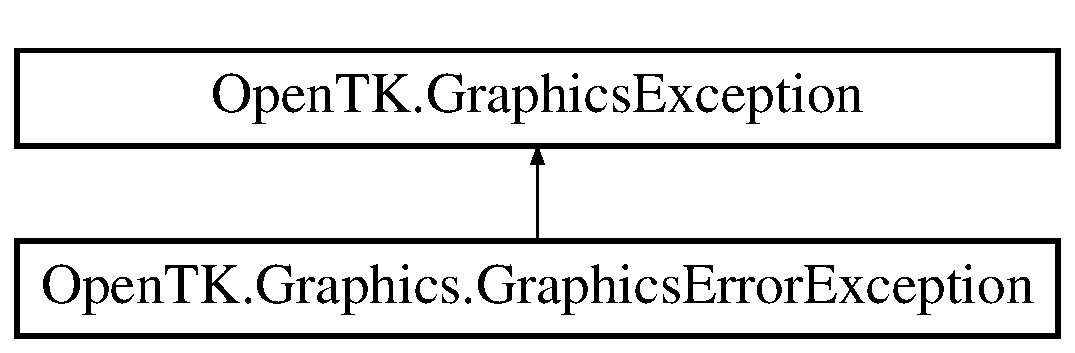
\includegraphics[height=2.000000cm]{class_open_t_k_1_1_graphics_1_1_graphics_error_exception}
\end{center}
\end{figure}
\subsection*{Public Member Functions}
\begin{DoxyCompactItemize}
\item 
\hyperlink{class_open_t_k_1_1_graphics_1_1_graphics_error_exception_afe758cd34ee6ff7c8694fddf9df925b4}{Graphics\-Error\-Exception} (string message)
\begin{DoxyCompactList}\small\item\em Constructs a new \hyperlink{class_open_t_k_1_1_graphics_1_1_graphics_error_exception}{Graphics\-Error\-Exception} instance with the specified error message. \end{DoxyCompactList}\end{DoxyCompactItemize}


\subsection{Detailed Description}
Identifies a specific \hyperlink{namespace_open_t_k_1_1_graphics_1_1_open_g_l}{Open\-G\-L} or Open\-G\-L$|$\-E\-S error. Such exceptions are only thrown when \hyperlink{namespace_open_t_k_1_1_graphics_1_1_open_g_l}{Open\-G\-L} or Open\-G\-L$|$\-E\-S automatic error checking is enabled -\/ \hyperlink{class_open_t_k_1_1_graphics_1_1_graphics_context_a8ad06302403c5503b6ba954676523d90}{Graphics\-Context.\-Error\-Checking} property. Important\-: Do {\itshape not} catch this exception. Rather, fix the underlying issue that caused the error. 



\subsection{Constructor \& Destructor Documentation}
\hypertarget{class_open_t_k_1_1_graphics_1_1_graphics_error_exception_afe758cd34ee6ff7c8694fddf9df925b4}{\index{Open\-T\-K\-::\-Graphics\-::\-Graphics\-Error\-Exception@{Open\-T\-K\-::\-Graphics\-::\-Graphics\-Error\-Exception}!Graphics\-Error\-Exception@{Graphics\-Error\-Exception}}
\index{Graphics\-Error\-Exception@{Graphics\-Error\-Exception}!OpenTK::Graphics::GraphicsErrorException@{Open\-T\-K\-::\-Graphics\-::\-Graphics\-Error\-Exception}}
\subsubsection[{Graphics\-Error\-Exception}]{\setlength{\rightskip}{0pt plus 5cm}Open\-T\-K.\-Graphics.\-Graphics\-Error\-Exception.\-Graphics\-Error\-Exception (
\begin{DoxyParamCaption}
\item[{string}]{message}
\end{DoxyParamCaption}
)}}\label{class_open_t_k_1_1_graphics_1_1_graphics_error_exception_afe758cd34ee6ff7c8694fddf9df925b4}


Constructs a new \hyperlink{class_open_t_k_1_1_graphics_1_1_graphics_error_exception}{Graphics\-Error\-Exception} instance with the specified error message. 


\begin{DoxyParams}{Parameters}
{\em message} & \\
\hline
\end{DoxyParams}

\hypertarget{class_open_t_k_1_1_graphics_1_1_graphics_mode}{\section{Open\-T\-K.\-Graphics.\-Graphics\-Mode Class Reference}
\label{class_open_t_k_1_1_graphics_1_1_graphics_mode}\index{Open\-T\-K.\-Graphics.\-Graphics\-Mode@{Open\-T\-K.\-Graphics.\-Graphics\-Mode}}
}


Defines the format for graphics operations. 




Inherits I\-Equatable$<$ Graphics\-Mode $>$.

\subsection*{Public Member Functions}
\begin{DoxyCompactItemize}
\item 
\hyperlink{class_open_t_k_1_1_graphics_1_1_graphics_mode_a01c78f91fdad6efa7783442eec3fe971}{Graphics\-Mode} ()
\begin{DoxyCompactList}\small\item\em Constructs a new \hyperlink{class_open_t_k_1_1_graphics_1_1_graphics_mode}{Graphics\-Mode} with sensible default parameters.\end{DoxyCompactList}\item 
\hyperlink{class_open_t_k_1_1_graphics_1_1_graphics_mode_ab7ba79e223dd09d3e31db4047184522b}{Graphics\-Mode} (\hyperlink{struct_open_t_k_1_1_graphics_1_1_color_format}{Color\-Format} color)
\begin{DoxyCompactList}\small\item\em Constructs a new \hyperlink{class_open_t_k_1_1_graphics_1_1_graphics_mode}{Graphics\-Mode} with the specified parameters.\end{DoxyCompactList}\item 
\hyperlink{class_open_t_k_1_1_graphics_1_1_graphics_mode_a78bf911ef9b3838fdb3fef129ccbdeb8}{Graphics\-Mode} (\hyperlink{struct_open_t_k_1_1_graphics_1_1_color_format}{Color\-Format} color, int depth)
\begin{DoxyCompactList}\small\item\em Constructs a new \hyperlink{class_open_t_k_1_1_graphics_1_1_graphics_mode}{Graphics\-Mode} with the specified parameters.\end{DoxyCompactList}\item 
\hyperlink{class_open_t_k_1_1_graphics_1_1_graphics_mode_a1312dad0cf2977c26448a538e99a8586}{Graphics\-Mode} (\hyperlink{struct_open_t_k_1_1_graphics_1_1_color_format}{Color\-Format} color, int depth, int stencil)
\begin{DoxyCompactList}\small\item\em Constructs a new \hyperlink{class_open_t_k_1_1_graphics_1_1_graphics_mode}{Graphics\-Mode} with the specified parameters.\end{DoxyCompactList}\item 
\hyperlink{class_open_t_k_1_1_graphics_1_1_graphics_mode_aba66332ea57307f061437255b053115b}{Graphics\-Mode} (\hyperlink{struct_open_t_k_1_1_graphics_1_1_color_format}{Color\-Format} color, int depth, int stencil, int samples)
\begin{DoxyCompactList}\small\item\em Constructs a new \hyperlink{class_open_t_k_1_1_graphics_1_1_graphics_mode}{Graphics\-Mode} with the specified parameters.\end{DoxyCompactList}\item 
\hyperlink{class_open_t_k_1_1_graphics_1_1_graphics_mode_a009ffca43d82cb589019e3ac35df3542}{Graphics\-Mode} (\hyperlink{struct_open_t_k_1_1_graphics_1_1_color_format}{Color\-Format} color, int depth, int stencil, int samples, \hyperlink{struct_open_t_k_1_1_graphics_1_1_color_format}{Color\-Format} accum)
\begin{DoxyCompactList}\small\item\em Constructs a new \hyperlink{class_open_t_k_1_1_graphics_1_1_graphics_mode}{Graphics\-Mode} with the specified parameters.\end{DoxyCompactList}\item 
\hyperlink{class_open_t_k_1_1_graphics_1_1_graphics_mode_a3f68377c73007c7b36982c89e3a1d703}{Graphics\-Mode} (\hyperlink{struct_open_t_k_1_1_graphics_1_1_color_format}{Color\-Format} color, int depth, int stencil, int samples, \hyperlink{struct_open_t_k_1_1_graphics_1_1_color_format}{Color\-Format} accum, int buffers)
\begin{DoxyCompactList}\small\item\em Constructs a new \hyperlink{class_open_t_k_1_1_graphics_1_1_graphics_mode}{Graphics\-Mode} with the specified parameters.\end{DoxyCompactList}\item 
\hyperlink{class_open_t_k_1_1_graphics_1_1_graphics_mode_a8a16c4c08a2dda0f63d805b3deff2c70}{Graphics\-Mode} (\hyperlink{struct_open_t_k_1_1_graphics_1_1_color_format}{Color\-Format} color, int depth, int stencil, int samples, \hyperlink{struct_open_t_k_1_1_graphics_1_1_color_format}{Color\-Format} accum, int buffers, bool stereo)
\begin{DoxyCompactList}\small\item\em Constructs a new \hyperlink{class_open_t_k_1_1_graphics_1_1_graphics_mode}{Graphics\-Mode} with the specified parameters.\end{DoxyCompactList}\item 
override string \hyperlink{class_open_t_k_1_1_graphics_1_1_graphics_mode_a2bfa03969d3afb7da3695c859cf064f8}{To\-String} ()
\begin{DoxyCompactList}\small\item\em Returns a System.\-String describing the current Graphics\-Format.\end{DoxyCompactList}\item 
override int \hyperlink{class_open_t_k_1_1_graphics_1_1_graphics_mode_aad2a94152bb9f576858c17a7428bfad4}{Get\-Hash\-Code} ()
\begin{DoxyCompactList}\small\item\em Returns the hashcode for this instance. \end{DoxyCompactList}\item 
override bool \hyperlink{class_open_t_k_1_1_graphics_1_1_graphics_mode_a4c2eabae157c94199d16cc3f4dae80ac}{Equals} (object obj)
\begin{DoxyCompactList}\small\item\em Indicates whether obj is equal to this instance. \end{DoxyCompactList}\item 
bool \hyperlink{class_open_t_k_1_1_graphics_1_1_graphics_mode_ad6351d57dcf7aabe6d27b1b82dfa6d39}{Equals} (\hyperlink{class_open_t_k_1_1_graphics_1_1_graphics_mode}{Graphics\-Mode} other)
\begin{DoxyCompactList}\small\item\em Indicates whether other represents the same mode as this instance. \end{DoxyCompactList}\end{DoxyCompactItemize}
\subsection*{Properties}
\begin{DoxyCompactItemize}
\item 
Int\-Ptr \hyperlink{class_open_t_k_1_1_graphics_1_1_graphics_mode_ad3caab1ad7640a5389abc809874fa57e}{Index}\hspace{0.3cm}{\ttfamily  \mbox{[}get, set\mbox{]}}
\begin{DoxyCompactList}\small\item\em Gets a nullable System.\-Int\-Ptr value, indicating the platform-\/specific index for this \hyperlink{class_open_t_k_1_1_graphics_1_1_graphics_mode}{Graphics\-Mode}. \end{DoxyCompactList}\item 
\hyperlink{struct_open_t_k_1_1_graphics_1_1_color_format}{Color\-Format} \hyperlink{class_open_t_k_1_1_graphics_1_1_graphics_mode_ae10e9972591996e85c2fedca3f86a5e4}{Color\-Format}\hspace{0.3cm}{\ttfamily  \mbox{[}get, set\mbox{]}}
\begin{DoxyCompactList}\small\item\em Gets an \hyperlink{struct_open_t_k_1_1_graphics_1_1_color_format}{Open\-T\-K.\-Graphics.\-Color\-Format} that describes the color format for this Graphics\-Format. \end{DoxyCompactList}\item 
\hyperlink{struct_open_t_k_1_1_graphics_1_1_color_format}{Color\-Format} \hyperlink{class_open_t_k_1_1_graphics_1_1_graphics_mode_aa03854ffcfde8d47580aa7038c6151f6}{Accumulator\-Format}\hspace{0.3cm}{\ttfamily  \mbox{[}get, set\mbox{]}}
\begin{DoxyCompactList}\small\item\em Gets an \hyperlink{struct_open_t_k_1_1_graphics_1_1_color_format}{Open\-T\-K.\-Graphics.\-Color\-Format} that describes the accumulator format for this Graphics\-Format. \end{DoxyCompactList}\item 
int \hyperlink{class_open_t_k_1_1_graphics_1_1_graphics_mode_a03e27f56e7b50e680e42503b51e0c2a8}{Depth}\hspace{0.3cm}{\ttfamily  \mbox{[}get, set\mbox{]}}
\begin{DoxyCompactList}\small\item\em Gets a System.\-Int32 that contains the bits per pixel for the depth buffer for this Graphics\-Format. \end{DoxyCompactList}\item 
int \hyperlink{class_open_t_k_1_1_graphics_1_1_graphics_mode_a962610eb764cb1f680149d17584606e1}{Stencil}\hspace{0.3cm}{\ttfamily  \mbox{[}get, set\mbox{]}}
\begin{DoxyCompactList}\small\item\em Gets a System.\-Int32 that contains the bits per pixel for the stencil buffer of this Graphics\-Format. \end{DoxyCompactList}\item 
int \hyperlink{class_open_t_k_1_1_graphics_1_1_graphics_mode_a3e7936c43e4aa0c05645bbd5270b5365}{Samples}\hspace{0.3cm}{\ttfamily  \mbox{[}get, set\mbox{]}}
\begin{DoxyCompactList}\small\item\em Gets a System.\-Int32 that contains the number of F\-S\-A\-A samples per pixel for this Graphics\-Format. \end{DoxyCompactList}\item 
bool \hyperlink{class_open_t_k_1_1_graphics_1_1_graphics_mode_a3e966d924fdbc2939fb02139456d7bd1}{Stereo}\hspace{0.3cm}{\ttfamily  \mbox{[}get, set\mbox{]}}
\begin{DoxyCompactList}\small\item\em Gets a System.\-Boolean indicating whether this Display\-Mode is stereoscopic. \end{DoxyCompactList}\item 
int \hyperlink{class_open_t_k_1_1_graphics_1_1_graphics_mode_a6a53197afd7dc314e2d42a7d22c16bfe}{Buffers}\hspace{0.3cm}{\ttfamily  \mbox{[}get, set\mbox{]}}
\begin{DoxyCompactList}\small\item\em Gets a System.\-Int32 containing the number of buffers associated with this Display\-Mode. \end{DoxyCompactList}\item 
static \hyperlink{class_open_t_k_1_1_graphics_1_1_graphics_mode}{Graphics\-Mode} \hyperlink{class_open_t_k_1_1_graphics_1_1_graphics_mode_a3280654ce982edbd728f83c06cd21c07}{Default}\hspace{0.3cm}{\ttfamily  \mbox{[}get\mbox{]}}
\begin{DoxyCompactList}\small\item\em Returns an Open\-T\-K.\-Graphics\-Format compatible with the underlying platform.\end{DoxyCompactList}\end{DoxyCompactItemize}


\subsection{Detailed Description}
Defines the format for graphics operations.



\subsection{Constructor \& Destructor Documentation}
\hypertarget{class_open_t_k_1_1_graphics_1_1_graphics_mode_a01c78f91fdad6efa7783442eec3fe971}{\index{Open\-T\-K\-::\-Graphics\-::\-Graphics\-Mode@{Open\-T\-K\-::\-Graphics\-::\-Graphics\-Mode}!Graphics\-Mode@{Graphics\-Mode}}
\index{Graphics\-Mode@{Graphics\-Mode}!OpenTK::Graphics::GraphicsMode@{Open\-T\-K\-::\-Graphics\-::\-Graphics\-Mode}}
\subsubsection[{Graphics\-Mode}]{\setlength{\rightskip}{0pt plus 5cm}Open\-T\-K.\-Graphics.\-Graphics\-Mode.\-Graphics\-Mode (
\begin{DoxyParamCaption}
{}
\end{DoxyParamCaption}
)}}\label{class_open_t_k_1_1_graphics_1_1_graphics_mode_a01c78f91fdad6efa7783442eec3fe971}


Constructs a new \hyperlink{class_open_t_k_1_1_graphics_1_1_graphics_mode}{Graphics\-Mode} with sensible default parameters.

\hypertarget{class_open_t_k_1_1_graphics_1_1_graphics_mode_ab7ba79e223dd09d3e31db4047184522b}{\index{Open\-T\-K\-::\-Graphics\-::\-Graphics\-Mode@{Open\-T\-K\-::\-Graphics\-::\-Graphics\-Mode}!Graphics\-Mode@{Graphics\-Mode}}
\index{Graphics\-Mode@{Graphics\-Mode}!OpenTK::Graphics::GraphicsMode@{Open\-T\-K\-::\-Graphics\-::\-Graphics\-Mode}}
\subsubsection[{Graphics\-Mode}]{\setlength{\rightskip}{0pt plus 5cm}Open\-T\-K.\-Graphics.\-Graphics\-Mode.\-Graphics\-Mode (
\begin{DoxyParamCaption}
\item[{{\bf Color\-Format}}]{color}
\end{DoxyParamCaption}
)}}\label{class_open_t_k_1_1_graphics_1_1_graphics_mode_ab7ba79e223dd09d3e31db4047184522b}


Constructs a new \hyperlink{class_open_t_k_1_1_graphics_1_1_graphics_mode}{Graphics\-Mode} with the specified parameters.


\begin{DoxyParams}{Parameters}
{\em color} & The \hyperlink{struct_open_t_k_1_1_graphics_1_1_color_format}{Color\-Format} of the color buffer.\\
\hline
\end{DoxyParams}
\hypertarget{class_open_t_k_1_1_graphics_1_1_graphics_mode_a78bf911ef9b3838fdb3fef129ccbdeb8}{\index{Open\-T\-K\-::\-Graphics\-::\-Graphics\-Mode@{Open\-T\-K\-::\-Graphics\-::\-Graphics\-Mode}!Graphics\-Mode@{Graphics\-Mode}}
\index{Graphics\-Mode@{Graphics\-Mode}!OpenTK::Graphics::GraphicsMode@{Open\-T\-K\-::\-Graphics\-::\-Graphics\-Mode}}
\subsubsection[{Graphics\-Mode}]{\setlength{\rightskip}{0pt plus 5cm}Open\-T\-K.\-Graphics.\-Graphics\-Mode.\-Graphics\-Mode (
\begin{DoxyParamCaption}
\item[{{\bf Color\-Format}}]{color, }
\item[{int}]{depth}
\end{DoxyParamCaption}
)}}\label{class_open_t_k_1_1_graphics_1_1_graphics_mode_a78bf911ef9b3838fdb3fef129ccbdeb8}


Constructs a new \hyperlink{class_open_t_k_1_1_graphics_1_1_graphics_mode}{Graphics\-Mode} with the specified parameters.


\begin{DoxyParams}{Parameters}
{\em color} & The \hyperlink{struct_open_t_k_1_1_graphics_1_1_color_format}{Color\-Format} of the color buffer.\\
\hline
{\em depth} & The number of bits in the depth buffer.\\
\hline
\end{DoxyParams}
\hypertarget{class_open_t_k_1_1_graphics_1_1_graphics_mode_a1312dad0cf2977c26448a538e99a8586}{\index{Open\-T\-K\-::\-Graphics\-::\-Graphics\-Mode@{Open\-T\-K\-::\-Graphics\-::\-Graphics\-Mode}!Graphics\-Mode@{Graphics\-Mode}}
\index{Graphics\-Mode@{Graphics\-Mode}!OpenTK::Graphics::GraphicsMode@{Open\-T\-K\-::\-Graphics\-::\-Graphics\-Mode}}
\subsubsection[{Graphics\-Mode}]{\setlength{\rightskip}{0pt plus 5cm}Open\-T\-K.\-Graphics.\-Graphics\-Mode.\-Graphics\-Mode (
\begin{DoxyParamCaption}
\item[{{\bf Color\-Format}}]{color, }
\item[{int}]{depth, }
\item[{int}]{stencil}
\end{DoxyParamCaption}
)}}\label{class_open_t_k_1_1_graphics_1_1_graphics_mode_a1312dad0cf2977c26448a538e99a8586}


Constructs a new \hyperlink{class_open_t_k_1_1_graphics_1_1_graphics_mode}{Graphics\-Mode} with the specified parameters.


\begin{DoxyParams}{Parameters}
{\em color} & The \hyperlink{struct_open_t_k_1_1_graphics_1_1_color_format}{Color\-Format} of the color buffer.\\
\hline
{\em depth} & The number of bits in the depth buffer.\\
\hline
{\em stencil} & The number of bits in the stencil buffer.\\
\hline
\end{DoxyParams}
\hypertarget{class_open_t_k_1_1_graphics_1_1_graphics_mode_aba66332ea57307f061437255b053115b}{\index{Open\-T\-K\-::\-Graphics\-::\-Graphics\-Mode@{Open\-T\-K\-::\-Graphics\-::\-Graphics\-Mode}!Graphics\-Mode@{Graphics\-Mode}}
\index{Graphics\-Mode@{Graphics\-Mode}!OpenTK::Graphics::GraphicsMode@{Open\-T\-K\-::\-Graphics\-::\-Graphics\-Mode}}
\subsubsection[{Graphics\-Mode}]{\setlength{\rightskip}{0pt plus 5cm}Open\-T\-K.\-Graphics.\-Graphics\-Mode.\-Graphics\-Mode (
\begin{DoxyParamCaption}
\item[{{\bf Color\-Format}}]{color, }
\item[{int}]{depth, }
\item[{int}]{stencil, }
\item[{int}]{samples}
\end{DoxyParamCaption}
)}}\label{class_open_t_k_1_1_graphics_1_1_graphics_mode_aba66332ea57307f061437255b053115b}


Constructs a new \hyperlink{class_open_t_k_1_1_graphics_1_1_graphics_mode}{Graphics\-Mode} with the specified parameters.


\begin{DoxyParams}{Parameters}
{\em color} & The \hyperlink{struct_open_t_k_1_1_graphics_1_1_color_format}{Color\-Format} of the color buffer.\\
\hline
{\em depth} & The number of bits in the depth buffer.\\
\hline
{\em stencil} & The number of bits in the stencil buffer.\\
\hline
{\em samples} & The number of samples for F\-S\-A\-A.\\
\hline
\end{DoxyParams}
\hypertarget{class_open_t_k_1_1_graphics_1_1_graphics_mode_a009ffca43d82cb589019e3ac35df3542}{\index{Open\-T\-K\-::\-Graphics\-::\-Graphics\-Mode@{Open\-T\-K\-::\-Graphics\-::\-Graphics\-Mode}!Graphics\-Mode@{Graphics\-Mode}}
\index{Graphics\-Mode@{Graphics\-Mode}!OpenTK::Graphics::GraphicsMode@{Open\-T\-K\-::\-Graphics\-::\-Graphics\-Mode}}
\subsubsection[{Graphics\-Mode}]{\setlength{\rightskip}{0pt plus 5cm}Open\-T\-K.\-Graphics.\-Graphics\-Mode.\-Graphics\-Mode (
\begin{DoxyParamCaption}
\item[{{\bf Color\-Format}}]{color, }
\item[{int}]{depth, }
\item[{int}]{stencil, }
\item[{int}]{samples, }
\item[{{\bf Color\-Format}}]{accum}
\end{DoxyParamCaption}
)}}\label{class_open_t_k_1_1_graphics_1_1_graphics_mode_a009ffca43d82cb589019e3ac35df3542}


Constructs a new \hyperlink{class_open_t_k_1_1_graphics_1_1_graphics_mode}{Graphics\-Mode} with the specified parameters.


\begin{DoxyParams}{Parameters}
{\em color} & The \hyperlink{struct_open_t_k_1_1_graphics_1_1_color_format}{Color\-Format} of the color buffer.\\
\hline
{\em depth} & The number of bits in the depth buffer.\\
\hline
{\em stencil} & The number of bits in the stencil buffer.\\
\hline
{\em samples} & The number of samples for F\-S\-A\-A.\\
\hline
{\em accum} & The \hyperlink{struct_open_t_k_1_1_graphics_1_1_color_format}{Color\-Format} of the accumilliary buffer.\\
\hline
\end{DoxyParams}
\hypertarget{class_open_t_k_1_1_graphics_1_1_graphics_mode_a3f68377c73007c7b36982c89e3a1d703}{\index{Open\-T\-K\-::\-Graphics\-::\-Graphics\-Mode@{Open\-T\-K\-::\-Graphics\-::\-Graphics\-Mode}!Graphics\-Mode@{Graphics\-Mode}}
\index{Graphics\-Mode@{Graphics\-Mode}!OpenTK::Graphics::GraphicsMode@{Open\-T\-K\-::\-Graphics\-::\-Graphics\-Mode}}
\subsubsection[{Graphics\-Mode}]{\setlength{\rightskip}{0pt plus 5cm}Open\-T\-K.\-Graphics.\-Graphics\-Mode.\-Graphics\-Mode (
\begin{DoxyParamCaption}
\item[{{\bf Color\-Format}}]{color, }
\item[{int}]{depth, }
\item[{int}]{stencil, }
\item[{int}]{samples, }
\item[{{\bf Color\-Format}}]{accum, }
\item[{int}]{buffers}
\end{DoxyParamCaption}
)}}\label{class_open_t_k_1_1_graphics_1_1_graphics_mode_a3f68377c73007c7b36982c89e3a1d703}


Constructs a new \hyperlink{class_open_t_k_1_1_graphics_1_1_graphics_mode}{Graphics\-Mode} with the specified parameters.


\begin{DoxyParams}{Parameters}
{\em color} & The \hyperlink{struct_open_t_k_1_1_graphics_1_1_color_format}{Color\-Format} of the color buffer.\\
\hline
{\em depth} & The number of bits in the depth buffer.\\
\hline
{\em stencil} & The number of bits in the stencil buffer.\\
\hline
{\em samples} & The number of samples for F\-S\-A\-A.\\
\hline
{\em accum} & The \hyperlink{struct_open_t_k_1_1_graphics_1_1_color_format}{Color\-Format} of the accumilliary buffer.\\
\hline
{\em buffers} & The number of render buffers. Typical values include one (single-\/), two (double-\/) or three (triple-\/buffering).\\
\hline
\end{DoxyParams}
\hypertarget{class_open_t_k_1_1_graphics_1_1_graphics_mode_a8a16c4c08a2dda0f63d805b3deff2c70}{\index{Open\-T\-K\-::\-Graphics\-::\-Graphics\-Mode@{Open\-T\-K\-::\-Graphics\-::\-Graphics\-Mode}!Graphics\-Mode@{Graphics\-Mode}}
\index{Graphics\-Mode@{Graphics\-Mode}!OpenTK::Graphics::GraphicsMode@{Open\-T\-K\-::\-Graphics\-::\-Graphics\-Mode}}
\subsubsection[{Graphics\-Mode}]{\setlength{\rightskip}{0pt plus 5cm}Open\-T\-K.\-Graphics.\-Graphics\-Mode.\-Graphics\-Mode (
\begin{DoxyParamCaption}
\item[{{\bf Color\-Format}}]{color, }
\item[{int}]{depth, }
\item[{int}]{stencil, }
\item[{int}]{samples, }
\item[{{\bf Color\-Format}}]{accum, }
\item[{int}]{buffers, }
\item[{bool}]{stereo}
\end{DoxyParamCaption}
)}}\label{class_open_t_k_1_1_graphics_1_1_graphics_mode_a8a16c4c08a2dda0f63d805b3deff2c70}


Constructs a new \hyperlink{class_open_t_k_1_1_graphics_1_1_graphics_mode}{Graphics\-Mode} with the specified parameters.


\begin{DoxyParams}{Parameters}
{\em color} & The \hyperlink{struct_open_t_k_1_1_graphics_1_1_color_format}{Color\-Format} of the color buffer.\\
\hline
{\em depth} & The number of bits in the depth buffer.\\
\hline
{\em stencil} & The number of bits in the stencil buffer.\\
\hline
{\em samples} & The number of samples for F\-S\-A\-A.\\
\hline
{\em accum} & The \hyperlink{struct_open_t_k_1_1_graphics_1_1_color_format}{Color\-Format} of the accumilliary buffer.\\
\hline
{\em stereo} & Set to true for a \hyperlink{class_open_t_k_1_1_graphics_1_1_graphics_mode}{Graphics\-Mode} with stereographic capabilities.\\
\hline
{\em buffers} & The number of render buffers. Typical values include one (single-\/), two (double-\/) or three (triple-\/buffering).\\
\hline
\end{DoxyParams}


\subsection{Member Function Documentation}
\hypertarget{class_open_t_k_1_1_graphics_1_1_graphics_mode_a4c2eabae157c94199d16cc3f4dae80ac}{\index{Open\-T\-K\-::\-Graphics\-::\-Graphics\-Mode@{Open\-T\-K\-::\-Graphics\-::\-Graphics\-Mode}!Equals@{Equals}}
\index{Equals@{Equals}!OpenTK::Graphics::GraphicsMode@{Open\-T\-K\-::\-Graphics\-::\-Graphics\-Mode}}
\subsubsection[{Equals}]{\setlength{\rightskip}{0pt plus 5cm}override bool Open\-T\-K.\-Graphics.\-Graphics\-Mode.\-Equals (
\begin{DoxyParamCaption}
\item[{object}]{obj}
\end{DoxyParamCaption}
)}}\label{class_open_t_k_1_1_graphics_1_1_graphics_mode_a4c2eabae157c94199d16cc3f4dae80ac}


Indicates whether obj is equal to this instance. 


\begin{DoxyParams}{Parameters}
{\em obj} & An object instance to compare for equality.\\
\hline
\end{DoxyParams}
\begin{DoxyReturn}{Returns}
True, if obj equals this instance; false otherwise.
\end{DoxyReturn}
\hypertarget{class_open_t_k_1_1_graphics_1_1_graphics_mode_ad6351d57dcf7aabe6d27b1b82dfa6d39}{\index{Open\-T\-K\-::\-Graphics\-::\-Graphics\-Mode@{Open\-T\-K\-::\-Graphics\-::\-Graphics\-Mode}!Equals@{Equals}}
\index{Equals@{Equals}!OpenTK::Graphics::GraphicsMode@{Open\-T\-K\-::\-Graphics\-::\-Graphics\-Mode}}
\subsubsection[{Equals}]{\setlength{\rightskip}{0pt plus 5cm}bool Open\-T\-K.\-Graphics.\-Graphics\-Mode.\-Equals (
\begin{DoxyParamCaption}
\item[{{\bf Graphics\-Mode}}]{other}
\end{DoxyParamCaption}
)}}\label{class_open_t_k_1_1_graphics_1_1_graphics_mode_ad6351d57dcf7aabe6d27b1b82dfa6d39}


Indicates whether other represents the same mode as this instance. 


\begin{DoxyParams}{Parameters}
{\em other} & The \hyperlink{class_open_t_k_1_1_graphics_1_1_graphics_mode}{Graphics\-Mode} to compare to.\\
\hline
\end{DoxyParams}
\begin{DoxyReturn}{Returns}
True, if other is equal to this instance; false otherwise.
\end{DoxyReturn}
\hypertarget{class_open_t_k_1_1_graphics_1_1_graphics_mode_aad2a94152bb9f576858c17a7428bfad4}{\index{Open\-T\-K\-::\-Graphics\-::\-Graphics\-Mode@{Open\-T\-K\-::\-Graphics\-::\-Graphics\-Mode}!Get\-Hash\-Code@{Get\-Hash\-Code}}
\index{Get\-Hash\-Code@{Get\-Hash\-Code}!OpenTK::Graphics::GraphicsMode@{Open\-T\-K\-::\-Graphics\-::\-Graphics\-Mode}}
\subsubsection[{Get\-Hash\-Code}]{\setlength{\rightskip}{0pt plus 5cm}override int Open\-T\-K.\-Graphics.\-Graphics\-Mode.\-Get\-Hash\-Code (
\begin{DoxyParamCaption}
{}
\end{DoxyParamCaption}
)}}\label{class_open_t_k_1_1_graphics_1_1_graphics_mode_aad2a94152bb9f576858c17a7428bfad4}


Returns the hashcode for this instance. 

\begin{DoxyReturn}{Returns}
A System.\-Int32 hashcode for this instance.
\end{DoxyReturn}
\hypertarget{class_open_t_k_1_1_graphics_1_1_graphics_mode_a2bfa03969d3afb7da3695c859cf064f8}{\index{Open\-T\-K\-::\-Graphics\-::\-Graphics\-Mode@{Open\-T\-K\-::\-Graphics\-::\-Graphics\-Mode}!To\-String@{To\-String}}
\index{To\-String@{To\-String}!OpenTK::Graphics::GraphicsMode@{Open\-T\-K\-::\-Graphics\-::\-Graphics\-Mode}}
\subsubsection[{To\-String}]{\setlength{\rightskip}{0pt plus 5cm}override string Open\-T\-K.\-Graphics.\-Graphics\-Mode.\-To\-String (
\begin{DoxyParamCaption}
{}
\end{DoxyParamCaption}
)}}\label{class_open_t_k_1_1_graphics_1_1_graphics_mode_a2bfa03969d3afb7da3695c859cf064f8}


Returns a System.\-String describing the current Graphics\-Format.

\begin{DoxyReturn}{Returns}
! System.\-String describing the current Graphics\-Format.
\end{DoxyReturn}


\subsection{Property Documentation}
\hypertarget{class_open_t_k_1_1_graphics_1_1_graphics_mode_aa03854ffcfde8d47580aa7038c6151f6}{\index{Open\-T\-K\-::\-Graphics\-::\-Graphics\-Mode@{Open\-T\-K\-::\-Graphics\-::\-Graphics\-Mode}!Accumulator\-Format@{Accumulator\-Format}}
\index{Accumulator\-Format@{Accumulator\-Format}!OpenTK::Graphics::GraphicsMode@{Open\-T\-K\-::\-Graphics\-::\-Graphics\-Mode}}
\subsubsection[{Accumulator\-Format}]{\setlength{\rightskip}{0pt plus 5cm}{\bf Color\-Format} Open\-T\-K.\-Graphics.\-Graphics\-Mode.\-Accumulator\-Format\hspace{0.3cm}{\ttfamily [get]}, {\ttfamily [set]}}}\label{class_open_t_k_1_1_graphics_1_1_graphics_mode_aa03854ffcfde8d47580aa7038c6151f6}


Gets an \hyperlink{struct_open_t_k_1_1_graphics_1_1_color_format}{Open\-T\-K.\-Graphics.\-Color\-Format} that describes the accumulator format for this Graphics\-Format. 

\hypertarget{class_open_t_k_1_1_graphics_1_1_graphics_mode_a6a53197afd7dc314e2d42a7d22c16bfe}{\index{Open\-T\-K\-::\-Graphics\-::\-Graphics\-Mode@{Open\-T\-K\-::\-Graphics\-::\-Graphics\-Mode}!Buffers@{Buffers}}
\index{Buffers@{Buffers}!OpenTK::Graphics::GraphicsMode@{Open\-T\-K\-::\-Graphics\-::\-Graphics\-Mode}}
\subsubsection[{Buffers}]{\setlength{\rightskip}{0pt plus 5cm}int Open\-T\-K.\-Graphics.\-Graphics\-Mode.\-Buffers\hspace{0.3cm}{\ttfamily [get]}, {\ttfamily [set]}}}\label{class_open_t_k_1_1_graphics_1_1_graphics_mode_a6a53197afd7dc314e2d42a7d22c16bfe}


Gets a System.\-Int32 containing the number of buffers associated with this Display\-Mode. 

\hypertarget{class_open_t_k_1_1_graphics_1_1_graphics_mode_ae10e9972591996e85c2fedca3f86a5e4}{\index{Open\-T\-K\-::\-Graphics\-::\-Graphics\-Mode@{Open\-T\-K\-::\-Graphics\-::\-Graphics\-Mode}!Color\-Format@{Color\-Format}}
\index{Color\-Format@{Color\-Format}!OpenTK::Graphics::GraphicsMode@{Open\-T\-K\-::\-Graphics\-::\-Graphics\-Mode}}
\subsubsection[{Color\-Format}]{\setlength{\rightskip}{0pt plus 5cm}{\bf Color\-Format} Open\-T\-K.\-Graphics.\-Graphics\-Mode.\-Color\-Format\hspace{0.3cm}{\ttfamily [get]}, {\ttfamily [set]}}}\label{class_open_t_k_1_1_graphics_1_1_graphics_mode_ae10e9972591996e85c2fedca3f86a5e4}


Gets an \hyperlink{struct_open_t_k_1_1_graphics_1_1_color_format}{Open\-T\-K.\-Graphics.\-Color\-Format} that describes the color format for this Graphics\-Format. 

\hypertarget{class_open_t_k_1_1_graphics_1_1_graphics_mode_a3280654ce982edbd728f83c06cd21c07}{\index{Open\-T\-K\-::\-Graphics\-::\-Graphics\-Mode@{Open\-T\-K\-::\-Graphics\-::\-Graphics\-Mode}!Default@{Default}}
\index{Default@{Default}!OpenTK::Graphics::GraphicsMode@{Open\-T\-K\-::\-Graphics\-::\-Graphics\-Mode}}
\subsubsection[{Default}]{\setlength{\rightskip}{0pt plus 5cm}{\bf Graphics\-Mode} Open\-T\-K.\-Graphics.\-Graphics\-Mode.\-Default\hspace{0.3cm}{\ttfamily [static]}, {\ttfamily [get]}}}\label{class_open_t_k_1_1_graphics_1_1_graphics_mode_a3280654ce982edbd728f83c06cd21c07}


Returns an Open\-T\-K.\-Graphics\-Format compatible with the underlying platform.

\hypertarget{class_open_t_k_1_1_graphics_1_1_graphics_mode_a03e27f56e7b50e680e42503b51e0c2a8}{\index{Open\-T\-K\-::\-Graphics\-::\-Graphics\-Mode@{Open\-T\-K\-::\-Graphics\-::\-Graphics\-Mode}!Depth@{Depth}}
\index{Depth@{Depth}!OpenTK::Graphics::GraphicsMode@{Open\-T\-K\-::\-Graphics\-::\-Graphics\-Mode}}
\subsubsection[{Depth}]{\setlength{\rightskip}{0pt plus 5cm}int Open\-T\-K.\-Graphics.\-Graphics\-Mode.\-Depth\hspace{0.3cm}{\ttfamily [get]}, {\ttfamily [set]}}}\label{class_open_t_k_1_1_graphics_1_1_graphics_mode_a03e27f56e7b50e680e42503b51e0c2a8}


Gets a System.\-Int32 that contains the bits per pixel for the depth buffer for this Graphics\-Format. 

\hypertarget{class_open_t_k_1_1_graphics_1_1_graphics_mode_ad3caab1ad7640a5389abc809874fa57e}{\index{Open\-T\-K\-::\-Graphics\-::\-Graphics\-Mode@{Open\-T\-K\-::\-Graphics\-::\-Graphics\-Mode}!Index@{Index}}
\index{Index@{Index}!OpenTK::Graphics::GraphicsMode@{Open\-T\-K\-::\-Graphics\-::\-Graphics\-Mode}}
\subsubsection[{Index}]{\setlength{\rightskip}{0pt plus 5cm}Int\-Ptr Open\-T\-K.\-Graphics.\-Graphics\-Mode.\-Index\hspace{0.3cm}{\ttfamily [get]}, {\ttfamily [set]}}}\label{class_open_t_k_1_1_graphics_1_1_graphics_mode_ad3caab1ad7640a5389abc809874fa57e}


Gets a nullable System.\-Int\-Ptr value, indicating the platform-\/specific index for this \hyperlink{class_open_t_k_1_1_graphics_1_1_graphics_mode}{Graphics\-Mode}. 

\hypertarget{class_open_t_k_1_1_graphics_1_1_graphics_mode_a3e7936c43e4aa0c05645bbd5270b5365}{\index{Open\-T\-K\-::\-Graphics\-::\-Graphics\-Mode@{Open\-T\-K\-::\-Graphics\-::\-Graphics\-Mode}!Samples@{Samples}}
\index{Samples@{Samples}!OpenTK::Graphics::GraphicsMode@{Open\-T\-K\-::\-Graphics\-::\-Graphics\-Mode}}
\subsubsection[{Samples}]{\setlength{\rightskip}{0pt plus 5cm}int Open\-T\-K.\-Graphics.\-Graphics\-Mode.\-Samples\hspace{0.3cm}{\ttfamily [get]}, {\ttfamily [set]}}}\label{class_open_t_k_1_1_graphics_1_1_graphics_mode_a3e7936c43e4aa0c05645bbd5270b5365}


Gets a System.\-Int32 that contains the number of F\-S\-A\-A samples per pixel for this Graphics\-Format. 

\hypertarget{class_open_t_k_1_1_graphics_1_1_graphics_mode_a962610eb764cb1f680149d17584606e1}{\index{Open\-T\-K\-::\-Graphics\-::\-Graphics\-Mode@{Open\-T\-K\-::\-Graphics\-::\-Graphics\-Mode}!Stencil@{Stencil}}
\index{Stencil@{Stencil}!OpenTK::Graphics::GraphicsMode@{Open\-T\-K\-::\-Graphics\-::\-Graphics\-Mode}}
\subsubsection[{Stencil}]{\setlength{\rightskip}{0pt plus 5cm}int Open\-T\-K.\-Graphics.\-Graphics\-Mode.\-Stencil\hspace{0.3cm}{\ttfamily [get]}, {\ttfamily [set]}}}\label{class_open_t_k_1_1_graphics_1_1_graphics_mode_a962610eb764cb1f680149d17584606e1}


Gets a System.\-Int32 that contains the bits per pixel for the stencil buffer of this Graphics\-Format. 

\hypertarget{class_open_t_k_1_1_graphics_1_1_graphics_mode_a3e966d924fdbc2939fb02139456d7bd1}{\index{Open\-T\-K\-::\-Graphics\-::\-Graphics\-Mode@{Open\-T\-K\-::\-Graphics\-::\-Graphics\-Mode}!Stereo@{Stereo}}
\index{Stereo@{Stereo}!OpenTK::Graphics::GraphicsMode@{Open\-T\-K\-::\-Graphics\-::\-Graphics\-Mode}}
\subsubsection[{Stereo}]{\setlength{\rightskip}{0pt plus 5cm}bool Open\-T\-K.\-Graphics.\-Graphics\-Mode.\-Stereo\hspace{0.3cm}{\ttfamily [get]}, {\ttfamily [set]}}}\label{class_open_t_k_1_1_graphics_1_1_graphics_mode_a3e966d924fdbc2939fb02139456d7bd1}


Gets a System.\-Boolean indicating whether this Display\-Mode is stereoscopic. 


\hypertarget{class_open_t_k_1_1_graphics_1_1_graphics_mode_exception}{\section{Open\-T\-K.\-Graphics.\-Graphics\-Mode\-Exception Class Reference}
\label{class_open_t_k_1_1_graphics_1_1_graphics_mode_exception}\index{Open\-T\-K.\-Graphics.\-Graphics\-Mode\-Exception@{Open\-T\-K.\-Graphics.\-Graphics\-Mode\-Exception}}
}


Represents errors related to unavailable graphics parameters.  




Inherits Exception.

\subsection*{Public Member Functions}
\begin{DoxyCompactItemize}
\item 
\hyperlink{class_open_t_k_1_1_graphics_1_1_graphics_mode_exception_a887ec4693b97e0f268008799dc8bd773}{Graphics\-Mode\-Exception} ()
\begin{DoxyCompactList}\small\item\em Constructs a new \hyperlink{class_open_t_k_1_1_graphics_1_1_graphics_mode_exception}{Graphics\-Mode\-Exception}. \end{DoxyCompactList}\item 
\hyperlink{class_open_t_k_1_1_graphics_1_1_graphics_mode_exception_a943c06a85e912998954a66e620072e60}{Graphics\-Mode\-Exception} (string message)
\begin{DoxyCompactList}\small\item\em Constructs a new \hyperlink{class_open_t_k_1_1_graphics_1_1_graphics_mode_exception}{Graphics\-Mode\-Exception} with the given error message. \end{DoxyCompactList}\end{DoxyCompactItemize}


\subsection{Detailed Description}
Represents errors related to unavailable graphics parameters. 



\subsection{Constructor \& Destructor Documentation}
\hypertarget{class_open_t_k_1_1_graphics_1_1_graphics_mode_exception_a887ec4693b97e0f268008799dc8bd773}{\index{Open\-T\-K\-::\-Graphics\-::\-Graphics\-Mode\-Exception@{Open\-T\-K\-::\-Graphics\-::\-Graphics\-Mode\-Exception}!Graphics\-Mode\-Exception@{Graphics\-Mode\-Exception}}
\index{Graphics\-Mode\-Exception@{Graphics\-Mode\-Exception}!OpenTK::Graphics::GraphicsModeException@{Open\-T\-K\-::\-Graphics\-::\-Graphics\-Mode\-Exception}}
\subsubsection[{Graphics\-Mode\-Exception}]{\setlength{\rightskip}{0pt plus 5cm}Open\-T\-K.\-Graphics.\-Graphics\-Mode\-Exception.\-Graphics\-Mode\-Exception (
\begin{DoxyParamCaption}
{}
\end{DoxyParamCaption}
)}}\label{class_open_t_k_1_1_graphics_1_1_graphics_mode_exception_a887ec4693b97e0f268008799dc8bd773}


Constructs a new \hyperlink{class_open_t_k_1_1_graphics_1_1_graphics_mode_exception}{Graphics\-Mode\-Exception}. 

\hypertarget{class_open_t_k_1_1_graphics_1_1_graphics_mode_exception_a943c06a85e912998954a66e620072e60}{\index{Open\-T\-K\-::\-Graphics\-::\-Graphics\-Mode\-Exception@{Open\-T\-K\-::\-Graphics\-::\-Graphics\-Mode\-Exception}!Graphics\-Mode\-Exception@{Graphics\-Mode\-Exception}}
\index{Graphics\-Mode\-Exception@{Graphics\-Mode\-Exception}!OpenTK::Graphics::GraphicsModeException@{Open\-T\-K\-::\-Graphics\-::\-Graphics\-Mode\-Exception}}
\subsubsection[{Graphics\-Mode\-Exception}]{\setlength{\rightskip}{0pt plus 5cm}Open\-T\-K.\-Graphics.\-Graphics\-Mode\-Exception.\-Graphics\-Mode\-Exception (
\begin{DoxyParamCaption}
\item[{string}]{message}
\end{DoxyParamCaption}
)}}\label{class_open_t_k_1_1_graphics_1_1_graphics_mode_exception_a943c06a85e912998954a66e620072e60}


Constructs a new \hyperlink{class_open_t_k_1_1_graphics_1_1_graphics_mode_exception}{Graphics\-Mode\-Exception} with the given error message. 


\hypertarget{interface_open_t_k_1_1_graphics_1_1_i_graphics_context}{\section{Open\-T\-K.\-Graphics.\-I\-Graphics\-Context Interface Reference}
\label{interface_open_t_k_1_1_graphics_1_1_i_graphics_context}\index{Open\-T\-K.\-Graphics.\-I\-Graphics\-Context@{Open\-T\-K.\-Graphics.\-I\-Graphics\-Context}}
}


Provides methods for creating and interacting with an \hyperlink{namespace_open_t_k_1_1_graphics_1_1_open_g_l}{Open\-G\-L} context.  


Inheritance diagram for Open\-T\-K.\-Graphics.\-I\-Graphics\-Context\-:\begin{figure}[H]
\begin{center}
\leavevmode
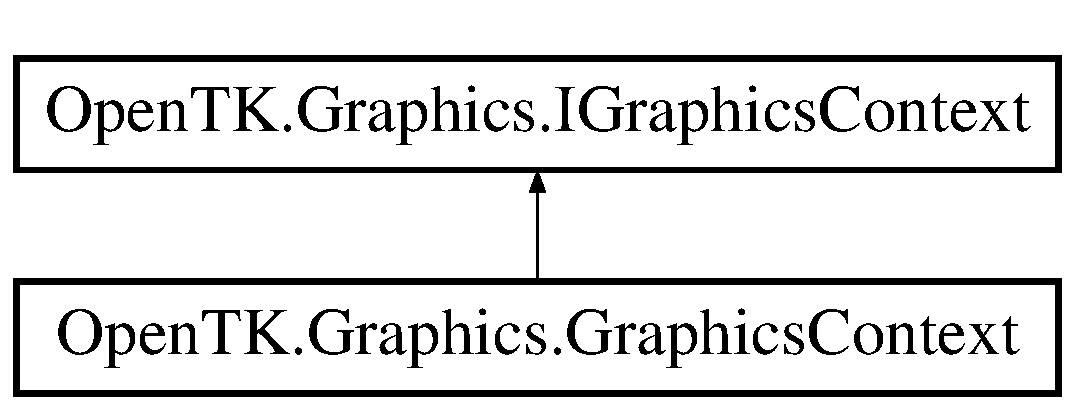
\includegraphics[height=2.000000cm]{interface_open_t_k_1_1_graphics_1_1_i_graphics_context}
\end{center}
\end{figure}
\subsection*{Public Member Functions}
\begin{DoxyCompactItemize}
\item 
void \hyperlink{interface_open_t_k_1_1_graphics_1_1_i_graphics_context_ad7d516da745576542161f1baa5f20129}{Swap\-Buffers} ()
\begin{DoxyCompactList}\small\item\em Swaps buffers, presenting the rendered scene to the user.\end{DoxyCompactList}\item 
void \hyperlink{interface_open_t_k_1_1_graphics_1_1_i_graphics_context_a73a3ca64b49a682800e636d0135887ed}{Make\-Current} (\hyperlink{interface_open_t_k_1_1_platform_1_1_i_window_info}{I\-Window\-Info} window)
\begin{DoxyCompactList}\small\item\em Makes the \hyperlink{class_open_t_k_1_1_graphics_1_1_graphics_context}{Graphics\-Context} current in the calling thread.\end{DoxyCompactList}\item 
void \hyperlink{interface_open_t_k_1_1_graphics_1_1_i_graphics_context_a4bf57e48815f169c133eb15ccda2d146}{Update} (\hyperlink{interface_open_t_k_1_1_platform_1_1_i_window_info}{I\-Window\-Info} window)
\begin{DoxyCompactList}\small\item\em Updates the graphics context. This must be called when the region the graphics context is drawn to is resized. \end{DoxyCompactList}\item 
void \hyperlink{interface_open_t_k_1_1_graphics_1_1_i_graphics_context_a8f8df276eeac50ba850cb21fa5a4e676}{Load\-All} ()
\begin{DoxyCompactList}\small\item\em Loads all \hyperlink{namespace_open_t_k_1_1_graphics_1_1_open_g_l}{Open\-G\-L} entry points. Requires this instance to be current on the calling thread. \end{DoxyCompactList}\end{DoxyCompactItemize}
\subsection*{Properties}
\begin{DoxyCompactItemize}
\item 
bool \hyperlink{interface_open_t_k_1_1_graphics_1_1_i_graphics_context_a1bf131a712f2a08f5f35e1542dccfb33}{Is\-Current}\hspace{0.3cm}{\ttfamily  \mbox{[}get\mbox{]}}
\begin{DoxyCompactList}\small\item\em Gets a System.\-Boolean indicating whether this instance is current in the calling thread. \end{DoxyCompactList}\item 
bool \hyperlink{interface_open_t_k_1_1_graphics_1_1_i_graphics_context_af844efa5b99505bb659a892ec6200486}{Is\-Disposed}\hspace{0.3cm}{\ttfamily  \mbox{[}get\mbox{]}}
\begin{DoxyCompactList}\small\item\em Gets a System.\-Boolean indicating whether this instance has been disposed. It is an error to access any instance methods if this property returns true. \end{DoxyCompactList}\item 
bool \hyperlink{interface_open_t_k_1_1_graphics_1_1_i_graphics_context_ad02e5a60e13f6ed668b8075ead268cb6}{V\-Sync}\hspace{0.3cm}{\ttfamily  \mbox{[}get, set\mbox{]}}
\begin{DoxyCompactList}\small\item\em Gets or sets a value indicating whether V\-Sync is enabled. When V\-Sync is enabled, \hyperlink{interface_open_t_k_1_1_graphics_1_1_i_graphics_context_ad7d516da745576542161f1baa5f20129}{Swap\-Buffers()} calls will be synced to the refresh rate of the \hyperlink{class_open_t_k_1_1_display_device}{Display\-Device} that contains improving visual quality and reducing C\-P\-U usage. However, systems that cannot maintain the requested rendering rate will suffer from large jumps in performance. This can be counteracted by increasing the \hyperlink{interface_open_t_k_1_1_graphics_1_1_i_graphics_context_acdd6cc5339e7d0d428f4aa59b560940f}{Swap\-Interval} value. \end{DoxyCompactList}\item 
int \hyperlink{interface_open_t_k_1_1_graphics_1_1_i_graphics_context_acdd6cc5339e7d0d428f4aa59b560940f}{Swap\-Interval}\hspace{0.3cm}{\ttfamily  \mbox{[}get, set\mbox{]}}
\begin{DoxyCompactList}\small\item\em Gets or sets a positive integer in the range \mbox{[}1, n), indicating the number of \hyperlink{class_open_t_k_1_1_display_device}{Display\-Device} refreshes between consecutive \hyperlink{interface_open_t_k_1_1_graphics_1_1_i_graphics_context_ad7d516da745576542161f1baa5f20129}{Swap\-Buffers()} calls. The maximum value for n is implementation-\/dependent. The default value is 1. This value will only affect instances where \hyperlink{interface_open_t_k_1_1_graphics_1_1_i_graphics_context_ad02e5a60e13f6ed668b8075ead268cb6}{V\-Sync} is enabled. Invalid values will be clamped to the valid range. \end{DoxyCompactList}\item 
\hyperlink{class_open_t_k_1_1_graphics_1_1_graphics_mode}{Graphics\-Mode} \hyperlink{interface_open_t_k_1_1_graphics_1_1_i_graphics_context_a225502437befccb70af6444801d0654e}{Graphics\-Mode}\hspace{0.3cm}{\ttfamily  \mbox{[}get\mbox{]}}
\begin{DoxyCompactList}\small\item\em Gets the \hyperlink{class_open_t_k_1_1_graphics_1_1_graphics_mode}{Graphics\-Mode} of this instance.\end{DoxyCompactList}\item 
bool \hyperlink{interface_open_t_k_1_1_graphics_1_1_i_graphics_context_ada0d1b90245fbb8eba94ef25072fe49c}{Error\-Checking}\hspace{0.3cm}{\ttfamily  \mbox{[}get, set\mbox{]}}
\begin{DoxyCompactList}\small\item\em Gets or sets a System.\-Boolean, indicating whether automatic error checking should be performed. \end{DoxyCompactList}\end{DoxyCompactItemize}


\subsection{Detailed Description}
Provides methods for creating and interacting with an \hyperlink{namespace_open_t_k_1_1_graphics_1_1_open_g_l}{Open\-G\-L} context. 



\subsection{Member Function Documentation}
\hypertarget{interface_open_t_k_1_1_graphics_1_1_i_graphics_context_a8f8df276eeac50ba850cb21fa5a4e676}{\index{Open\-T\-K\-::\-Graphics\-::\-I\-Graphics\-Context@{Open\-T\-K\-::\-Graphics\-::\-I\-Graphics\-Context}!Load\-All@{Load\-All}}
\index{Load\-All@{Load\-All}!OpenTK::Graphics::IGraphicsContext@{Open\-T\-K\-::\-Graphics\-::\-I\-Graphics\-Context}}
\subsubsection[{Load\-All}]{\setlength{\rightskip}{0pt plus 5cm}void Open\-T\-K.\-Graphics.\-I\-Graphics\-Context.\-Load\-All (
\begin{DoxyParamCaption}
{}
\end{DoxyParamCaption}
)}}\label{interface_open_t_k_1_1_graphics_1_1_i_graphics_context_a8f8df276eeac50ba850cb21fa5a4e676}


Loads all \hyperlink{namespace_open_t_k_1_1_graphics_1_1_open_g_l}{Open\-G\-L} entry points. Requires this instance to be current on the calling thread. 



Implemented in \hyperlink{class_open_t_k_1_1_graphics_1_1_graphics_context_a21640f20db040987bd1f897f503b68a4}{Open\-T\-K.\-Graphics.\-Graphics\-Context}.

\hypertarget{interface_open_t_k_1_1_graphics_1_1_i_graphics_context_a73a3ca64b49a682800e636d0135887ed}{\index{Open\-T\-K\-::\-Graphics\-::\-I\-Graphics\-Context@{Open\-T\-K\-::\-Graphics\-::\-I\-Graphics\-Context}!Make\-Current@{Make\-Current}}
\index{Make\-Current@{Make\-Current}!OpenTK::Graphics::IGraphicsContext@{Open\-T\-K\-::\-Graphics\-::\-I\-Graphics\-Context}}
\subsubsection[{Make\-Current}]{\setlength{\rightskip}{0pt plus 5cm}void Open\-T\-K.\-Graphics.\-I\-Graphics\-Context.\-Make\-Current (
\begin{DoxyParamCaption}
\item[{{\bf I\-Window\-Info}}]{window}
\end{DoxyParamCaption}
)}}\label{interface_open_t_k_1_1_graphics_1_1_i_graphics_context_a73a3ca64b49a682800e636d0135887ed}


Makes the \hyperlink{class_open_t_k_1_1_graphics_1_1_graphics_context}{Graphics\-Context} current in the calling thread.


\begin{DoxyParams}{Parameters}
{\em window} & An \hyperlink{interface_open_t_k_1_1_platform_1_1_i_window_info}{Open\-T\-K.\-Platform.\-I\-Window\-Info} structure that points to a valid window.\\
\hline
\end{DoxyParams}


\hyperlink{namespace_open_t_k_1_1_graphics_1_1_open_g_l}{Open\-G\-L} commands in one thread, affect the \hyperlink{class_open_t_k_1_1_graphics_1_1_graphics_context}{Graphics\-Context} which is current in that thread.

It is an error to issue an \hyperlink{namespace_open_t_k_1_1_graphics_1_1_open_g_l}{Open\-G\-L} command in a thread without a current \hyperlink{class_open_t_k_1_1_graphics_1_1_graphics_context}{Graphics\-Context}.

Implemented in \hyperlink{class_open_t_k_1_1_graphics_1_1_graphics_context_a4b9b3b0f98fc1dc9f49f8abdb5ff076b}{Open\-T\-K.\-Graphics.\-Graphics\-Context}.

\hypertarget{interface_open_t_k_1_1_graphics_1_1_i_graphics_context_ad7d516da745576542161f1baa5f20129}{\index{Open\-T\-K\-::\-Graphics\-::\-I\-Graphics\-Context@{Open\-T\-K\-::\-Graphics\-::\-I\-Graphics\-Context}!Swap\-Buffers@{Swap\-Buffers}}
\index{Swap\-Buffers@{Swap\-Buffers}!OpenTK::Graphics::IGraphicsContext@{Open\-T\-K\-::\-Graphics\-::\-I\-Graphics\-Context}}
\subsubsection[{Swap\-Buffers}]{\setlength{\rightskip}{0pt plus 5cm}void Open\-T\-K.\-Graphics.\-I\-Graphics\-Context.\-Swap\-Buffers (
\begin{DoxyParamCaption}
{}
\end{DoxyParamCaption}
)}}\label{interface_open_t_k_1_1_graphics_1_1_i_graphics_context_ad7d516da745576542161f1baa5f20129}


Swaps buffers, presenting the rendered scene to the user.



Implemented in \hyperlink{class_open_t_k_1_1_graphics_1_1_graphics_context_ab73c61bea26369cf76dff2165f5084cf}{Open\-T\-K.\-Graphics.\-Graphics\-Context}.

\hypertarget{interface_open_t_k_1_1_graphics_1_1_i_graphics_context_a4bf57e48815f169c133eb15ccda2d146}{\index{Open\-T\-K\-::\-Graphics\-::\-I\-Graphics\-Context@{Open\-T\-K\-::\-Graphics\-::\-I\-Graphics\-Context}!Update@{Update}}
\index{Update@{Update}!OpenTK::Graphics::IGraphicsContext@{Open\-T\-K\-::\-Graphics\-::\-I\-Graphics\-Context}}
\subsubsection[{Update}]{\setlength{\rightskip}{0pt plus 5cm}void Open\-T\-K.\-Graphics.\-I\-Graphics\-Context.\-Update (
\begin{DoxyParamCaption}
\item[{{\bf I\-Window\-Info}}]{window}
\end{DoxyParamCaption}
)}}\label{interface_open_t_k_1_1_graphics_1_1_i_graphics_context_a4bf57e48815f169c133eb15ccda2d146}


Updates the graphics context. This must be called when the region the graphics context is drawn to is resized. 


\begin{DoxyParams}{Parameters}
{\em window} & \\
\hline
\end{DoxyParams}


Implemented in \hyperlink{class_open_t_k_1_1_graphics_1_1_graphics_context_a09fa035789147f9b9cfe2a5f09abe927}{Open\-T\-K.\-Graphics.\-Graphics\-Context}.



\subsection{Property Documentation}
\hypertarget{interface_open_t_k_1_1_graphics_1_1_i_graphics_context_ada0d1b90245fbb8eba94ef25072fe49c}{\index{Open\-T\-K\-::\-Graphics\-::\-I\-Graphics\-Context@{Open\-T\-K\-::\-Graphics\-::\-I\-Graphics\-Context}!Error\-Checking@{Error\-Checking}}
\index{Error\-Checking@{Error\-Checking}!OpenTK::Graphics::IGraphicsContext@{Open\-T\-K\-::\-Graphics\-::\-I\-Graphics\-Context}}
\subsubsection[{Error\-Checking}]{\setlength{\rightskip}{0pt plus 5cm}bool Open\-T\-K.\-Graphics.\-I\-Graphics\-Context.\-Error\-Checking\hspace{0.3cm}{\ttfamily [get]}, {\ttfamily [set]}}}\label{interface_open_t_k_1_1_graphics_1_1_i_graphics_context_ada0d1b90245fbb8eba94ef25072fe49c}


Gets or sets a System.\-Boolean, indicating whether automatic error checking should be performed. 

It is an error to enable error checking inside a Begin()-\/\-End() region.

This method only affects the debug version of Open\-T\-K.\-dll.\hypertarget{interface_open_t_k_1_1_graphics_1_1_i_graphics_context_a225502437befccb70af6444801d0654e}{\index{Open\-T\-K\-::\-Graphics\-::\-I\-Graphics\-Context@{Open\-T\-K\-::\-Graphics\-::\-I\-Graphics\-Context}!Graphics\-Mode@{Graphics\-Mode}}
\index{Graphics\-Mode@{Graphics\-Mode}!OpenTK::Graphics::IGraphicsContext@{Open\-T\-K\-::\-Graphics\-::\-I\-Graphics\-Context}}
\subsubsection[{Graphics\-Mode}]{\setlength{\rightskip}{0pt plus 5cm}{\bf Graphics\-Mode} Open\-T\-K.\-Graphics.\-I\-Graphics\-Context.\-Graphics\-Mode\hspace{0.3cm}{\ttfamily [get]}}}\label{interface_open_t_k_1_1_graphics_1_1_i_graphics_context_a225502437befccb70af6444801d0654e}


Gets the \hyperlink{class_open_t_k_1_1_graphics_1_1_graphics_mode}{Graphics\-Mode} of this instance.

\hypertarget{interface_open_t_k_1_1_graphics_1_1_i_graphics_context_a1bf131a712f2a08f5f35e1542dccfb33}{\index{Open\-T\-K\-::\-Graphics\-::\-I\-Graphics\-Context@{Open\-T\-K\-::\-Graphics\-::\-I\-Graphics\-Context}!Is\-Current@{Is\-Current}}
\index{Is\-Current@{Is\-Current}!OpenTK::Graphics::IGraphicsContext@{Open\-T\-K\-::\-Graphics\-::\-I\-Graphics\-Context}}
\subsubsection[{Is\-Current}]{\setlength{\rightskip}{0pt plus 5cm}bool Open\-T\-K.\-Graphics.\-I\-Graphics\-Context.\-Is\-Current\hspace{0.3cm}{\ttfamily [get]}}}\label{interface_open_t_k_1_1_graphics_1_1_i_graphics_context_a1bf131a712f2a08f5f35e1542dccfb33}


Gets a System.\-Boolean indicating whether this instance is current in the calling thread. 

\hypertarget{interface_open_t_k_1_1_graphics_1_1_i_graphics_context_af844efa5b99505bb659a892ec6200486}{\index{Open\-T\-K\-::\-Graphics\-::\-I\-Graphics\-Context@{Open\-T\-K\-::\-Graphics\-::\-I\-Graphics\-Context}!Is\-Disposed@{Is\-Disposed}}
\index{Is\-Disposed@{Is\-Disposed}!OpenTK::Graphics::IGraphicsContext@{Open\-T\-K\-::\-Graphics\-::\-I\-Graphics\-Context}}
\subsubsection[{Is\-Disposed}]{\setlength{\rightskip}{0pt plus 5cm}bool Open\-T\-K.\-Graphics.\-I\-Graphics\-Context.\-Is\-Disposed\hspace{0.3cm}{\ttfamily [get]}}}\label{interface_open_t_k_1_1_graphics_1_1_i_graphics_context_af844efa5b99505bb659a892ec6200486}


Gets a System.\-Boolean indicating whether this instance has been disposed. It is an error to access any instance methods if this property returns true. 

\hypertarget{interface_open_t_k_1_1_graphics_1_1_i_graphics_context_acdd6cc5339e7d0d428f4aa59b560940f}{\index{Open\-T\-K\-::\-Graphics\-::\-I\-Graphics\-Context@{Open\-T\-K\-::\-Graphics\-::\-I\-Graphics\-Context}!Swap\-Interval@{Swap\-Interval}}
\index{Swap\-Interval@{Swap\-Interval}!OpenTK::Graphics::IGraphicsContext@{Open\-T\-K\-::\-Graphics\-::\-I\-Graphics\-Context}}
\subsubsection[{Swap\-Interval}]{\setlength{\rightskip}{0pt plus 5cm}int Open\-T\-K.\-Graphics.\-I\-Graphics\-Context.\-Swap\-Interval\hspace{0.3cm}{\ttfamily [get]}, {\ttfamily [set]}}}\label{interface_open_t_k_1_1_graphics_1_1_i_graphics_context_acdd6cc5339e7d0d428f4aa59b560940f}


Gets or sets a positive integer in the range \mbox{[}1, n), indicating the number of \hyperlink{class_open_t_k_1_1_display_device}{Display\-Device} refreshes between consecutive \hyperlink{interface_open_t_k_1_1_graphics_1_1_i_graphics_context_ad7d516da745576542161f1baa5f20129}{Swap\-Buffers()} calls. The maximum value for n is implementation-\/dependent. The default value is 1. This value will only affect instances where \hyperlink{interface_open_t_k_1_1_graphics_1_1_i_graphics_context_ad02e5a60e13f6ed668b8075ead268cb6}{V\-Sync} is enabled. Invalid values will be clamped to the valid range. 

\hypertarget{interface_open_t_k_1_1_graphics_1_1_i_graphics_context_ad02e5a60e13f6ed668b8075ead268cb6}{\index{Open\-T\-K\-::\-Graphics\-::\-I\-Graphics\-Context@{Open\-T\-K\-::\-Graphics\-::\-I\-Graphics\-Context}!V\-Sync@{V\-Sync}}
\index{V\-Sync@{V\-Sync}!OpenTK::Graphics::IGraphicsContext@{Open\-T\-K\-::\-Graphics\-::\-I\-Graphics\-Context}}
\subsubsection[{V\-Sync}]{\setlength{\rightskip}{0pt plus 5cm}bool Open\-T\-K.\-Graphics.\-I\-Graphics\-Context.\-V\-Sync\hspace{0.3cm}{\ttfamily [get]}, {\ttfamily [set]}}}\label{interface_open_t_k_1_1_graphics_1_1_i_graphics_context_ad02e5a60e13f6ed668b8075ead268cb6}


Gets or sets a value indicating whether V\-Sync is enabled. When V\-Sync is enabled, \hyperlink{interface_open_t_k_1_1_graphics_1_1_i_graphics_context_ad7d516da745576542161f1baa5f20129}{Swap\-Buffers()} calls will be synced to the refresh rate of the \hyperlink{class_open_t_k_1_1_display_device}{Display\-Device} that contains improving visual quality and reducing C\-P\-U usage. However, systems that cannot maintain the requested rendering rate will suffer from large jumps in performance. This can be counteracted by increasing the \hyperlink{interface_open_t_k_1_1_graphics_1_1_i_graphics_context_acdd6cc5339e7d0d428f4aa59b560940f}{Swap\-Interval} value. 


\hypertarget{interface_open_t_k_1_1_graphics_1_1_i_graphics_context_internal}{\section{Open\-T\-K.\-Graphics.\-I\-Graphics\-Context\-Internal Interface Reference}
\label{interface_open_t_k_1_1_graphics_1_1_i_graphics_context_internal}\index{Open\-T\-K.\-Graphics.\-I\-Graphics\-Context\-Internal@{Open\-T\-K.\-Graphics.\-I\-Graphics\-Context\-Internal}}
}


Provides methods to create new Graphics\-Contexts. Should only be used for extending \hyperlink{namespace_open_t_k}{Open\-T\-K}.  


Inheritance diagram for Open\-T\-K.\-Graphics.\-I\-Graphics\-Context\-Internal\-:\begin{figure}[H]
\begin{center}
\leavevmode
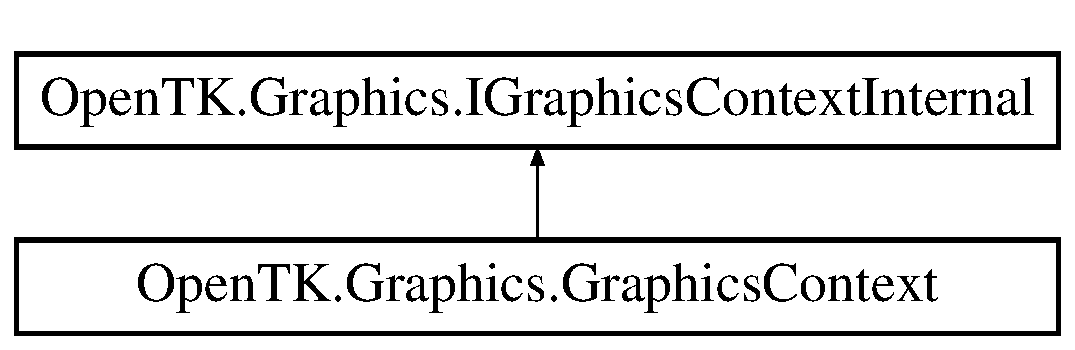
\includegraphics[height=2.000000cm]{interface_open_t_k_1_1_graphics_1_1_i_graphics_context_internal}
\end{center}
\end{figure}
\subsection*{Public Member Functions}
\begin{DoxyCompactItemize}
\item 
void \hyperlink{interface_open_t_k_1_1_graphics_1_1_i_graphics_context_internal_ac92fd883ec02b0391e3fcdbbdbd42d34}{Load\-All} ()
\begin{DoxyCompactList}\small\item\em Loads all \hyperlink{namespace_open_t_k_1_1_graphics_1_1_open_g_l}{Open\-G\-L} entry points. Requires this instance to be current on the calling thread. \end{DoxyCompactList}\item 
Int\-Ptr \hyperlink{interface_open_t_k_1_1_graphics_1_1_i_graphics_context_internal_af59790e0ad84f23c0ffe4a0b5655acca}{Get\-Address} (string function)
\begin{DoxyCompactList}\small\item\em Gets the address of an \hyperlink{namespace_open_t_k_1_1_graphics_1_1_open_g_l}{Open\-G\-L} extension function. \end{DoxyCompactList}\end{DoxyCompactItemize}
\subsection*{Properties}
\begin{DoxyCompactItemize}
\item 
\hyperlink{interface_open_t_k_1_1_graphics_1_1_i_graphics_context}{I\-Graphics\-Context} \hyperlink{interface_open_t_k_1_1_graphics_1_1_i_graphics_context_internal_a1827254204928b0db6085d229eefbca5}{Implementation}\hspace{0.3cm}{\ttfamily  \mbox{[}get\mbox{]}}
\begin{DoxyCompactList}\small\item\em Gets the internal implementation of the current instance. \end{DoxyCompactList}\item 
\hyperlink{struct_open_t_k_1_1_context_handle}{Context\-Handle} \hyperlink{interface_open_t_k_1_1_graphics_1_1_i_graphics_context_internal_a39e3ed0ea9b5400bc64fd43c5b8ee9e7}{Context}\hspace{0.3cm}{\ttfamily  \mbox{[}get\mbox{]}}
\begin{DoxyCompactList}\small\item\em Gets a handle to the \hyperlink{namespace_open_t_k_1_1_graphics_1_1_open_g_l}{Open\-G\-L} rendering context. \end{DoxyCompactList}\end{DoxyCompactItemize}


\subsection{Detailed Description}
Provides methods to create new Graphics\-Contexts. Should only be used for extending \hyperlink{namespace_open_t_k}{Open\-T\-K}. 



\subsection{Member Function Documentation}
\hypertarget{interface_open_t_k_1_1_graphics_1_1_i_graphics_context_internal_af59790e0ad84f23c0ffe4a0b5655acca}{\index{Open\-T\-K\-::\-Graphics\-::\-I\-Graphics\-Context\-Internal@{Open\-T\-K\-::\-Graphics\-::\-I\-Graphics\-Context\-Internal}!Get\-Address@{Get\-Address}}
\index{Get\-Address@{Get\-Address}!OpenTK::Graphics::IGraphicsContextInternal@{Open\-T\-K\-::\-Graphics\-::\-I\-Graphics\-Context\-Internal}}
\subsubsection[{Get\-Address}]{\setlength{\rightskip}{0pt plus 5cm}Int\-Ptr Open\-T\-K.\-Graphics.\-I\-Graphics\-Context\-Internal.\-Get\-Address (
\begin{DoxyParamCaption}
\item[{string}]{function}
\end{DoxyParamCaption}
)}}\label{interface_open_t_k_1_1_graphics_1_1_i_graphics_context_internal_af59790e0ad84f23c0ffe4a0b5655acca}


Gets the address of an \hyperlink{namespace_open_t_k_1_1_graphics_1_1_open_g_l}{Open\-G\-L} extension function. 


\begin{DoxyParams}{Parameters}
{\em function} & The name of the \hyperlink{namespace_open_t_k_1_1_graphics_1_1_open_g_l}{Open\-G\-L} function (e.\-g. \char`\"{}gl\-Get\-String\char`\"{})\\
\hline
\end{DoxyParams}
\begin{DoxyReturn}{Returns}
A pointer to the specified function or Int\-Ptr.\-Zero if the function isn't available in the current opengl context. 
\end{DoxyReturn}
\hypertarget{interface_open_t_k_1_1_graphics_1_1_i_graphics_context_internal_ac92fd883ec02b0391e3fcdbbdbd42d34}{\index{Open\-T\-K\-::\-Graphics\-::\-I\-Graphics\-Context\-Internal@{Open\-T\-K\-::\-Graphics\-::\-I\-Graphics\-Context\-Internal}!Load\-All@{Load\-All}}
\index{Load\-All@{Load\-All}!OpenTK::Graphics::IGraphicsContextInternal@{Open\-T\-K\-::\-Graphics\-::\-I\-Graphics\-Context\-Internal}}
\subsubsection[{Load\-All}]{\setlength{\rightskip}{0pt plus 5cm}void Open\-T\-K.\-Graphics.\-I\-Graphics\-Context\-Internal.\-Load\-All (
\begin{DoxyParamCaption}
{}
\end{DoxyParamCaption}
)}}\label{interface_open_t_k_1_1_graphics_1_1_i_graphics_context_internal_ac92fd883ec02b0391e3fcdbbdbd42d34}


Loads all \hyperlink{namespace_open_t_k_1_1_graphics_1_1_open_g_l}{Open\-G\-L} entry points. Requires this instance to be current on the calling thread. 



Implemented in \hyperlink{class_open_t_k_1_1_graphics_1_1_graphics_context_a21640f20db040987bd1f897f503b68a4}{Open\-T\-K.\-Graphics.\-Graphics\-Context}.



\subsection{Property Documentation}
\hypertarget{interface_open_t_k_1_1_graphics_1_1_i_graphics_context_internal_a39e3ed0ea9b5400bc64fd43c5b8ee9e7}{\index{Open\-T\-K\-::\-Graphics\-::\-I\-Graphics\-Context\-Internal@{Open\-T\-K\-::\-Graphics\-::\-I\-Graphics\-Context\-Internal}!Context@{Context}}
\index{Context@{Context}!OpenTK::Graphics::IGraphicsContextInternal@{Open\-T\-K\-::\-Graphics\-::\-I\-Graphics\-Context\-Internal}}
\subsubsection[{Context}]{\setlength{\rightskip}{0pt plus 5cm}{\bf Context\-Handle} Open\-T\-K.\-Graphics.\-I\-Graphics\-Context\-Internal.\-Context\hspace{0.3cm}{\ttfamily [get]}}}\label{interface_open_t_k_1_1_graphics_1_1_i_graphics_context_internal_a39e3ed0ea9b5400bc64fd43c5b8ee9e7}


Gets a handle to the \hyperlink{namespace_open_t_k_1_1_graphics_1_1_open_g_l}{Open\-G\-L} rendering context. 

\hypertarget{interface_open_t_k_1_1_graphics_1_1_i_graphics_context_internal_a1827254204928b0db6085d229eefbca5}{\index{Open\-T\-K\-::\-Graphics\-::\-I\-Graphics\-Context\-Internal@{Open\-T\-K\-::\-Graphics\-::\-I\-Graphics\-Context\-Internal}!Implementation@{Implementation}}
\index{Implementation@{Implementation}!OpenTK::Graphics::IGraphicsContextInternal@{Open\-T\-K\-::\-Graphics\-::\-I\-Graphics\-Context\-Internal}}
\subsubsection[{Implementation}]{\setlength{\rightskip}{0pt plus 5cm}{\bf I\-Graphics\-Context} Open\-T\-K.\-Graphics.\-I\-Graphics\-Context\-Internal.\-Implementation\hspace{0.3cm}{\ttfamily [get]}}}\label{interface_open_t_k_1_1_graphics_1_1_i_graphics_context_internal_a1827254204928b0db6085d229eefbca5}


Gets the internal implementation of the current instance. 


\input{class_open_t_k_1_1_graphics_1_1_open_g_l_1_1_g_l}
\hypertarget{class_open_t_k_1_1_graphics_exception}{\section{Open\-T\-K.\-Graphics\-Exception Class Reference}
\label{class_open_t_k_1_1_graphics_exception}\index{Open\-T\-K.\-Graphics\-Exception@{Open\-T\-K.\-Graphics\-Exception}}
}


Represents errors related to \hyperlink{namespace_open_t_k_1_1_graphics}{Graphics} operations. 


Inheritance diagram for Open\-T\-K.\-Graphics\-Exception\-:\begin{figure}[H]
\begin{center}
\leavevmode
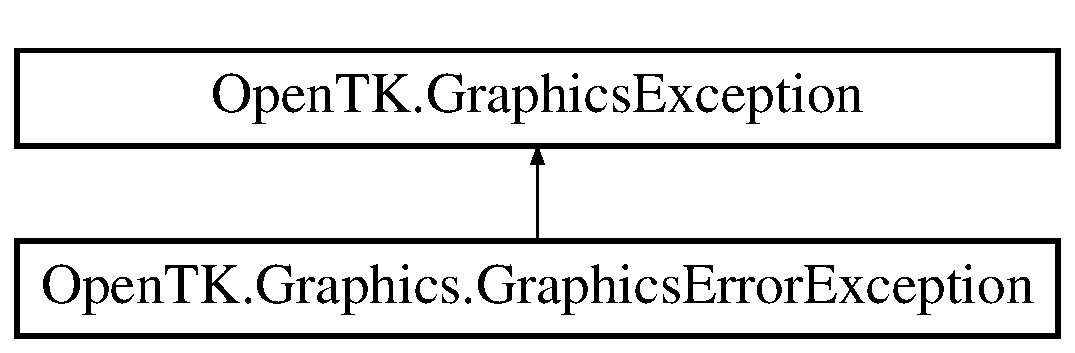
\includegraphics[height=2.000000cm]{class_open_t_k_1_1_graphics_exception}
\end{center}
\end{figure}
\subsection*{Public Member Functions}
\begin{DoxyCompactItemize}
\item 
\hyperlink{class_open_t_k_1_1_graphics_exception_a9052de41342a3608d3e44a00f20cbcbd}{Graphics\-Exception} ()
\begin{DoxyCompactList}\small\item\em Constructs a new \hyperlink{class_open_t_k_1_1_graphics_exception}{Graphics\-Exception}.\end{DoxyCompactList}\item 
\hyperlink{class_open_t_k_1_1_graphics_exception_ada92ccfb2483b704957c961b1d13b8e7}{Graphics\-Exception} (string message)
\begin{DoxyCompactList}\small\item\em Constructs a new \hyperlink{class_open_t_k_1_1_graphics_exception}{Graphics\-Exception} with the specified excpetion message.\end{DoxyCompactList}\end{DoxyCompactItemize}


\subsection{Detailed Description}
Represents errors related to \hyperlink{namespace_open_t_k_1_1_graphics}{Graphics} operations.



\subsection{Constructor \& Destructor Documentation}
\hypertarget{class_open_t_k_1_1_graphics_exception_a9052de41342a3608d3e44a00f20cbcbd}{\index{Open\-T\-K\-::\-Graphics\-Exception@{Open\-T\-K\-::\-Graphics\-Exception}!Graphics\-Exception@{Graphics\-Exception}}
\index{Graphics\-Exception@{Graphics\-Exception}!OpenTK::GraphicsException@{Open\-T\-K\-::\-Graphics\-Exception}}
\subsubsection[{Graphics\-Exception}]{\setlength{\rightskip}{0pt plus 5cm}Open\-T\-K.\-Graphics\-Exception.\-Graphics\-Exception (
\begin{DoxyParamCaption}
{}
\end{DoxyParamCaption}
)}}\label{class_open_t_k_1_1_graphics_exception_a9052de41342a3608d3e44a00f20cbcbd}


Constructs a new \hyperlink{class_open_t_k_1_1_graphics_exception}{Graphics\-Exception}.

\hypertarget{class_open_t_k_1_1_graphics_exception_ada92ccfb2483b704957c961b1d13b8e7}{\index{Open\-T\-K\-::\-Graphics\-Exception@{Open\-T\-K\-::\-Graphics\-Exception}!Graphics\-Exception@{Graphics\-Exception}}
\index{Graphics\-Exception@{Graphics\-Exception}!OpenTK::GraphicsException@{Open\-T\-K\-::\-Graphics\-Exception}}
\subsubsection[{Graphics\-Exception}]{\setlength{\rightskip}{0pt plus 5cm}Open\-T\-K.\-Graphics\-Exception.\-Graphics\-Exception (
\begin{DoxyParamCaption}
\item[{string}]{message}
\end{DoxyParamCaption}
)}}\label{class_open_t_k_1_1_graphics_exception_ada92ccfb2483b704957c961b1d13b8e7}


Constructs a new \hyperlink{class_open_t_k_1_1_graphics_exception}{Graphics\-Exception} with the specified excpetion message.


\begin{DoxyParams}{Parameters}
{\em message} & \\
\hline
\end{DoxyParams}

\hypertarget{struct_open_t_k_1_1_half}{\section{Open\-T\-K.\-Half Struct Reference}
\label{struct_open_t_k_1_1_half}\index{Open\-T\-K.\-Half@{Open\-T\-K.\-Half}}
}


The name \hyperlink{struct_open_t_k_1_1_half}{Half} is derived from half-\/precision floating-\/point number. It occupies only 16 bits, which are split into 1 Sign bit, 5 Exponent bits and 10 Mantissa bits.  




Inherits I\-Serializable, I\-Comparable$<$ Half $>$, I\-Formattable, and I\-Equatable$<$ Half $>$.

\subsection*{Public Member Functions}
\begin{DoxyCompactItemize}
\item 
\hyperlink{struct_open_t_k_1_1_half_aa17fec8711c6b77969fdf435aaeec5d7}{Half} (Single f)
\begin{DoxyCompactList}\small\item\em The new \hyperlink{struct_open_t_k_1_1_half}{Half} instance will convert the parameter into 16-\/bit half-\/precision floating-\/point. \end{DoxyCompactList}\item 
\hyperlink{struct_open_t_k_1_1_half_a4301c75f075d2e1cb1f5462e82cb0176}{Half} (Single f, bool throw\-On\-Error)
\begin{DoxyCompactList}\small\item\em The new \hyperlink{struct_open_t_k_1_1_half}{Half} instance will convert the parameter into 16-\/bit half-\/precision floating-\/point. \end{DoxyCompactList}\item 
\hyperlink{struct_open_t_k_1_1_half_aaa413e6314d445002990c1c44acc8fc4}{Half} (Double d)
\begin{DoxyCompactList}\small\item\em The new \hyperlink{struct_open_t_k_1_1_half}{Half} instance will convert the parameter into 16-\/bit half-\/precision floating-\/point. \end{DoxyCompactList}\item 
\hyperlink{struct_open_t_k_1_1_half_ac3687a82ee851cb0a9878c9f3177c377}{Half} (Double d, bool throw\-On\-Error)
\begin{DoxyCompactList}\small\item\em The new \hyperlink{struct_open_t_k_1_1_half}{Half} instance will convert the parameter into 16-\/bit half-\/precision floating-\/point. \end{DoxyCompactList}\item 
Single \hyperlink{struct_open_t_k_1_1_half_ad3447d0a7cdbd8a76afee7ae923aef2f}{To\-Single} ()
\begin{DoxyCompactList}\small\item\em Converts the 16-\/bit half to 32-\/bit floating-\/point.\end{DoxyCompactList}\item 
\hyperlink{struct_open_t_k_1_1_half_a44a3570c428b6ba6049968545a90d971}{Half} (Serialization\-Info info, Streaming\-Context context)
\begin{DoxyCompactList}\small\item\em Constructor used by I\-Serializable to deserialize the object.\end{DoxyCompactList}\item 
void \hyperlink{struct_open_t_k_1_1_half_a94663b59e8098e475c0a3b0b9bc8f5a4}{Get\-Object\-Data} (Serialization\-Info info, Streaming\-Context context)
\begin{DoxyCompactList}\small\item\em Used by I\-Serialize to serialize the object.\end{DoxyCompactList}\item 
void \hyperlink{struct_open_t_k_1_1_half_af7d15c9bfab9590a8363ae1524cdc1c9}{From\-Binary\-Stream} (Binary\-Reader bin)
\begin{DoxyCompactList}\small\item\em Updates the \hyperlink{struct_open_t_k_1_1_half}{Half} by reading from a Stream.\end{DoxyCompactList}\item 
void \hyperlink{struct_open_t_k_1_1_half_a18561108983fc9989c05467009143e7c}{To\-Binary\-Stream} (Binary\-Writer bin)
\begin{DoxyCompactList}\small\item\em Writes the \hyperlink{struct_open_t_k_1_1_half}{Half} into a Stream.\end{DoxyCompactList}\item 
bool \hyperlink{struct_open_t_k_1_1_half_adc727f01fd20b0c0e771f9792effa74a}{Equals} (\hyperlink{struct_open_t_k_1_1_half}{Half} other)
\begin{DoxyCompactList}\small\item\em Returns a value indicating whether this instance is equal to a specified \hyperlink{struct_open_t_k_1_1_half}{Open\-T\-K.\-Half} value. \end{DoxyCompactList}\item 
int \hyperlink{struct_open_t_k_1_1_half_a1afb59496dff653e567c5a0bc45b8da9}{Compare\-To} (\hyperlink{struct_open_t_k_1_1_half}{Half} other)
\begin{DoxyCompactList}\small\item\em Compares this instance to a specified half-\/precision floating-\/point number and returns an integer that indicates whether the value of this instance is less than, equal to, or greater than the value of the specified half-\/precision floating-\/point number. \end{DoxyCompactList}\item 
override string \hyperlink{struct_open_t_k_1_1_half_a5153a96aaf848da185f5d1b169c595c2}{To\-String} ()
\begin{DoxyCompactList}\small\item\em Converts this \hyperlink{struct_open_t_k_1_1_half}{Half} into a human-\/legible string representation.\end{DoxyCompactList}\item 
string \hyperlink{struct_open_t_k_1_1_half_a376ec7e36a73d0f7c947c7fa9a6bba94}{To\-String} (string format, I\-Format\-Provider format\-Provider)
\begin{DoxyCompactList}\small\item\em Converts this \hyperlink{struct_open_t_k_1_1_half}{Half} into a human-\/legible string representation.\end{DoxyCompactList}\end{DoxyCompactItemize}
\subsection*{Static Public Member Functions}
\begin{DoxyCompactItemize}
\item 
static \hyperlink{struct_open_t_k_1_1_half_ab20fd9bb592e416910677c30a7692e1f}{operator Half} (float f)
\begin{DoxyCompactList}\small\item\em Converts a System.\-Single to a \hyperlink{struct_open_t_k_1_1_half}{Open\-T\-K.\-Half}. \end{DoxyCompactList}\item 
static \hyperlink{struct_open_t_k_1_1_half_a0adddbbc87aebdd985a1b5edcd007774}{operator Half} (double d)
\begin{DoxyCompactList}\small\item\em Converts a System.\-Double to a \hyperlink{struct_open_t_k_1_1_half}{Open\-T\-K.\-Half}. \end{DoxyCompactList}\item 
static implicit \hyperlink{struct_open_t_k_1_1_half_a7f11c593114c947e81db6a0ba23636b3}{operator float} (\hyperlink{struct_open_t_k_1_1_half}{Half} h)
\begin{DoxyCompactList}\small\item\em Converts a \hyperlink{struct_open_t_k_1_1_half}{Open\-T\-K.\-Half} to a System.\-Single. \end{DoxyCompactList}\item 
static implicit \hyperlink{struct_open_t_k_1_1_half_a74cea29f9d511639d8d8da315c58db44}{operator double} (\hyperlink{struct_open_t_k_1_1_half}{Half} h)
\begin{DoxyCompactList}\small\item\em Converts a \hyperlink{struct_open_t_k_1_1_half}{Open\-T\-K.\-Half} to a System.\-Double. \end{DoxyCompactList}\item 
static \hyperlink{struct_open_t_k_1_1_half}{Half} \hyperlink{struct_open_t_k_1_1_half_a1710507d8370e593608fe6120474280a}{Parse} (string s)
\begin{DoxyCompactList}\small\item\em Converts the string representation of a number to a half-\/precision floating-\/point equivalent.\end{DoxyCompactList}\item 
static \hyperlink{struct_open_t_k_1_1_half}{Half} \hyperlink{struct_open_t_k_1_1_half_abf624a13c5967007843c7597d283c5aa}{Parse} (string s, System.\-Globalization.\-Number\-Styles style, I\-Format\-Provider provider)
\begin{DoxyCompactList}\small\item\em Converts the string representation of a number to a half-\/precision floating-\/point equivalent.\end{DoxyCompactList}\item 
static bool \hyperlink{struct_open_t_k_1_1_half_a3602fb09ee286dfb240ac561ecbc5296}{Try\-Parse} (string s, out \hyperlink{struct_open_t_k_1_1_half}{Half} result)
\begin{DoxyCompactList}\small\item\em Converts the string representation of a number to a half-\/precision floating-\/point equivalent. Returns success.\end{DoxyCompactList}\item 
static bool \hyperlink{struct_open_t_k_1_1_half_a0d3c83a6d7571e6b0ca124b4d7a2b766}{Try\-Parse} (string s, System.\-Globalization.\-Number\-Styles style, I\-Format\-Provider provider, out \hyperlink{struct_open_t_k_1_1_half}{Half} result)
\begin{DoxyCompactList}\small\item\em Converts the string representation of a number to a half-\/precision floating-\/point equivalent. Returns success.\end{DoxyCompactList}\item 
static byte\mbox{[}$\,$\mbox{]} \hyperlink{struct_open_t_k_1_1_half_a3468a68a355d4134b65401debecc56fe}{Get\-Bytes} (\hyperlink{struct_open_t_k_1_1_half}{Half} h)
\begin{DoxyCompactList}\small\item\em Returns the \hyperlink{struct_open_t_k_1_1_half}{Half} as an array of bytes.\end{DoxyCompactList}\item 
static \hyperlink{struct_open_t_k_1_1_half}{Half} \hyperlink{struct_open_t_k_1_1_half_a27d9efd7c019881959288cece98c8395}{From\-Bytes} (byte\mbox{[}$\,$\mbox{]} value, int start\-Index)
\begin{DoxyCompactList}\small\item\em Converts an array of bytes into \hyperlink{struct_open_t_k_1_1_half}{Half}.\end{DoxyCompactList}\end{DoxyCompactItemize}
\subsection*{Public Attributes}
\begin{DoxyCompactItemize}
\item 
\hypertarget{struct_open_t_k_1_1_half_a76e1575f9d67ee2f72597f62e3f1bbab}{U\-Int16 {\bfseries bits}}\label{struct_open_t_k_1_1_half_a76e1575f9d67ee2f72597f62e3f1bbab}

\item 
\hypertarget{struct_open_t_k_1_1_half_a8ffd6b056f319f537d7aceed4ecebf4f}{const int {\bfseries max\-Ulps} = 1}\label{struct_open_t_k_1_1_half_a8ffd6b056f319f537d7aceed4ecebf4f}

\end{DoxyCompactItemize}
\subsection*{Static Public Attributes}
\begin{DoxyCompactItemize}
\item 
static readonly Int32 \hyperlink{struct_open_t_k_1_1_half_abe15fc6db4ae97079233802277b8bcad}{Size\-In\-Bytes} = 2
\begin{DoxyCompactList}\small\item\em The size in bytes for an instance of the \hyperlink{struct_open_t_k_1_1_half}{Half} struct.\end{DoxyCompactList}\item 
static readonly Single \hyperlink{struct_open_t_k_1_1_half_afb6cea32ac0dd56fe8455d730d8fbde1}{Min\-Value} = 5.\-96046448e-\/08f
\begin{DoxyCompactList}\small\item\em Smallest positive half\end{DoxyCompactList}\item 
static readonly Single \hyperlink{struct_open_t_k_1_1_half_abda2208f9300afdd617d8d4ac320d21f}{Min\-Normalized\-Value} = 6.\-10351562e-\/05f
\begin{DoxyCompactList}\small\item\em Smallest positive normalized half\end{DoxyCompactList}\item 
static readonly Single \hyperlink{struct_open_t_k_1_1_half_a09fed5fc5cbc255618c752289932f25b}{Max\-Value} = 65504.\-0f
\begin{DoxyCompactList}\small\item\em Largest positive half\end{DoxyCompactList}\item 
static readonly Single \hyperlink{struct_open_t_k_1_1_half_a7f118e0313f8be004885fb7d536ecbf6}{Epsilon} = 0.\-00097656f
\begin{DoxyCompactList}\small\item\em Smallest positive e for which half (1.\-0 + e) != half (1.\-0)\end{DoxyCompactList}\end{DoxyCompactItemize}
\subsection*{Properties}
\begin{DoxyCompactItemize}
\item 
bool \hyperlink{struct_open_t_k_1_1_half_a48aeed7e4540b66deb01af091941a660}{Is\-Zero}\hspace{0.3cm}{\ttfamily  \mbox{[}get\mbox{]}}
\begin{DoxyCompactList}\small\item\em Returns true if the \hyperlink{struct_open_t_k_1_1_half}{Half} is zero.\end{DoxyCompactList}\item 
bool \hyperlink{struct_open_t_k_1_1_half_a929c5a6b04acc0e21e106e35b0d296c2}{Is\-Na\-N}\hspace{0.3cm}{\ttfamily  \mbox{[}get\mbox{]}}
\begin{DoxyCompactList}\small\item\em Returns true if the \hyperlink{struct_open_t_k_1_1_half}{Half} represents Not A Number (Na\-N)\end{DoxyCompactList}\item 
bool \hyperlink{struct_open_t_k_1_1_half_a080c67842958aca474f5aa85f2d7c658}{Is\-Positive\-Infinity}\hspace{0.3cm}{\ttfamily  \mbox{[}get\mbox{]}}
\begin{DoxyCompactList}\small\item\em Returns true if the \hyperlink{struct_open_t_k_1_1_half}{Half} represents positive infinity.\end{DoxyCompactList}\item 
bool \hyperlink{struct_open_t_k_1_1_half_a89f7b3c1de64f30ffd030f63a868ddb3}{Is\-Negative\-Infinity}\hspace{0.3cm}{\ttfamily  \mbox{[}get\mbox{]}}
\begin{DoxyCompactList}\small\item\em Returns true if the \hyperlink{struct_open_t_k_1_1_half}{Half} represents negative infinity.\end{DoxyCompactList}\end{DoxyCompactItemize}


\subsection{Detailed Description}
The name \hyperlink{struct_open_t_k_1_1_half}{Half} is derived from half-\/precision floating-\/point number. It occupies only 16 bits, which are split into 1 Sign bit, 5 Exponent bits and 10 Mantissa bits. 

Quote from A\-R\-B\-\_\-half\-\_\-float\-\_\-pixel specification\-: Any representable 16-\/bit floating-\/point value is legal as input to a G\-L command that accepts 16-\/bit floating-\/point data. The result of providing a value that is not a floating-\/point number (such as infinity or Na\-N) to such a command is unspecified, but must not lead to G\-L interruption or termination. Providing a denormalized number or negative zero to G\-L must yield predictable results. 

\subsection{Constructor \& Destructor Documentation}
\hypertarget{struct_open_t_k_1_1_half_aa17fec8711c6b77969fdf435aaeec5d7}{\index{Open\-T\-K\-::\-Half@{Open\-T\-K\-::\-Half}!Half@{Half}}
\index{Half@{Half}!OpenTK::Half@{Open\-T\-K\-::\-Half}}
\subsubsection[{Half}]{\setlength{\rightskip}{0pt plus 5cm}Open\-T\-K.\-Half.\-Half (
\begin{DoxyParamCaption}
\item[{Single}]{f}
\end{DoxyParamCaption}
)}}\label{struct_open_t_k_1_1_half_aa17fec8711c6b77969fdf435aaeec5d7}


The new \hyperlink{struct_open_t_k_1_1_half}{Half} instance will convert the parameter into 16-\/bit half-\/precision floating-\/point. 


\begin{DoxyParams}{Parameters}
{\em f} & 32-\/bit single-\/precision floating-\/point number.\\
\hline
\end{DoxyParams}
\hypertarget{struct_open_t_k_1_1_half_a4301c75f075d2e1cb1f5462e82cb0176}{\index{Open\-T\-K\-::\-Half@{Open\-T\-K\-::\-Half}!Half@{Half}}
\index{Half@{Half}!OpenTK::Half@{Open\-T\-K\-::\-Half}}
\subsubsection[{Half}]{\setlength{\rightskip}{0pt plus 5cm}Open\-T\-K.\-Half.\-Half (
\begin{DoxyParamCaption}
\item[{Single}]{f, }
\item[{bool}]{throw\-On\-Error}
\end{DoxyParamCaption}
)}}\label{struct_open_t_k_1_1_half_a4301c75f075d2e1cb1f5462e82cb0176}


The new \hyperlink{struct_open_t_k_1_1_half}{Half} instance will convert the parameter into 16-\/bit half-\/precision floating-\/point. 


\begin{DoxyParams}{Parameters}
{\em f} & 32-\/bit single-\/precision floating-\/point number.\\
\hline
{\em throw\-On\-Error} & Enable checks that will throw if the conversion result is not meaningful.\\
\hline
\end{DoxyParams}
\hypertarget{struct_open_t_k_1_1_half_aaa413e6314d445002990c1c44acc8fc4}{\index{Open\-T\-K\-::\-Half@{Open\-T\-K\-::\-Half}!Half@{Half}}
\index{Half@{Half}!OpenTK::Half@{Open\-T\-K\-::\-Half}}
\subsubsection[{Half}]{\setlength{\rightskip}{0pt plus 5cm}Open\-T\-K.\-Half.\-Half (
\begin{DoxyParamCaption}
\item[{Double}]{d}
\end{DoxyParamCaption}
)}}\label{struct_open_t_k_1_1_half_aaa413e6314d445002990c1c44acc8fc4}


The new \hyperlink{struct_open_t_k_1_1_half}{Half} instance will convert the parameter into 16-\/bit half-\/precision floating-\/point. 


\begin{DoxyParams}{Parameters}
{\em d} & 64-\/bit double-\/precision floating-\/point number.\\
\hline
\end{DoxyParams}
\hypertarget{struct_open_t_k_1_1_half_ac3687a82ee851cb0a9878c9f3177c377}{\index{Open\-T\-K\-::\-Half@{Open\-T\-K\-::\-Half}!Half@{Half}}
\index{Half@{Half}!OpenTK::Half@{Open\-T\-K\-::\-Half}}
\subsubsection[{Half}]{\setlength{\rightskip}{0pt plus 5cm}Open\-T\-K.\-Half.\-Half (
\begin{DoxyParamCaption}
\item[{Double}]{d, }
\item[{bool}]{throw\-On\-Error}
\end{DoxyParamCaption}
)}}\label{struct_open_t_k_1_1_half_ac3687a82ee851cb0a9878c9f3177c377}


The new \hyperlink{struct_open_t_k_1_1_half}{Half} instance will convert the parameter into 16-\/bit half-\/precision floating-\/point. 


\begin{DoxyParams}{Parameters}
{\em d} & 64-\/bit double-\/precision floating-\/point number.\\
\hline
{\em throw\-On\-Error} & Enable checks that will throw if the conversion result is not meaningful.\\
\hline
\end{DoxyParams}
\hypertarget{struct_open_t_k_1_1_half_a44a3570c428b6ba6049968545a90d971}{\index{Open\-T\-K\-::\-Half@{Open\-T\-K\-::\-Half}!Half@{Half}}
\index{Half@{Half}!OpenTK::Half@{Open\-T\-K\-::\-Half}}
\subsubsection[{Half}]{\setlength{\rightskip}{0pt plus 5cm}Open\-T\-K.\-Half.\-Half (
\begin{DoxyParamCaption}
\item[{Serialization\-Info}]{info, }
\item[{Streaming\-Context}]{context}
\end{DoxyParamCaption}
)}}\label{struct_open_t_k_1_1_half_a44a3570c428b6ba6049968545a90d971}


Constructor used by I\-Serializable to deserialize the object.


\begin{DoxyParams}{Parameters}
{\em info} & \\
\hline
{\em context} & \\
\hline
\end{DoxyParams}


\subsection{Member Function Documentation}
\hypertarget{struct_open_t_k_1_1_half_a1afb59496dff653e567c5a0bc45b8da9}{\index{Open\-T\-K\-::\-Half@{Open\-T\-K\-::\-Half}!Compare\-To@{Compare\-To}}
\index{Compare\-To@{Compare\-To}!OpenTK::Half@{Open\-T\-K\-::\-Half}}
\subsubsection[{Compare\-To}]{\setlength{\rightskip}{0pt plus 5cm}int Open\-T\-K.\-Half.\-Compare\-To (
\begin{DoxyParamCaption}
\item[{{\bf Half}}]{other}
\end{DoxyParamCaption}
)}}\label{struct_open_t_k_1_1_half_a1afb59496dff653e567c5a0bc45b8da9}


Compares this instance to a specified half-\/precision floating-\/point number and returns an integer that indicates whether the value of this instance is less than, equal to, or greater than the value of the specified half-\/precision floating-\/point number. 


\begin{DoxyParams}{Parameters}
{\em other} & A half-\/precision floating-\/point number to compare.\\
\hline
\end{DoxyParams}
\begin{DoxyReturn}{Returns}
A signed number indicating the relative values of this instance and value. If the number is\-: 

Less than zero, then this instance is less than other, or this instance is not a number (Open\-T\-K.\-Half.\-Na\-N) and other is a number.
\end{DoxyReturn}


Zero\-: this instance is equal to value, or both this instance and other are not a number (Open\-T\-K.\-Half.\-Na\-N), Open\-T\-K.\-Half.\-Positive\-Infinity, or Open\-T\-K.\-Half.\-Negative\-Infinity.

Greater than zero\-: this instance is greater than othrs, or this instance is a number and other is not a number (Open\-T\-K.\-Half.\-Na\-N).\hypertarget{struct_open_t_k_1_1_half_adc727f01fd20b0c0e771f9792effa74a}{\index{Open\-T\-K\-::\-Half@{Open\-T\-K\-::\-Half}!Equals@{Equals}}
\index{Equals@{Equals}!OpenTK::Half@{Open\-T\-K\-::\-Half}}
\subsubsection[{Equals}]{\setlength{\rightskip}{0pt plus 5cm}bool Open\-T\-K.\-Half.\-Equals (
\begin{DoxyParamCaption}
\item[{{\bf Half}}]{other}
\end{DoxyParamCaption}
)}}\label{struct_open_t_k_1_1_half_adc727f01fd20b0c0e771f9792effa74a}


Returns a value indicating whether this instance is equal to a specified \hyperlink{struct_open_t_k_1_1_half}{Open\-T\-K.\-Half} value. 


\begin{DoxyParams}{Parameters}
{\em other} & \hyperlink{struct_open_t_k_1_1_half}{Open\-T\-K.\-Half} object to compare to this instance..\\
\hline
\end{DoxyParams}
\begin{DoxyReturn}{Returns}
True, if other is equal to this instance; false otherwise.
\end{DoxyReturn}
\hypertarget{struct_open_t_k_1_1_half_af7d15c9bfab9590a8363ae1524cdc1c9}{\index{Open\-T\-K\-::\-Half@{Open\-T\-K\-::\-Half}!From\-Binary\-Stream@{From\-Binary\-Stream}}
\index{From\-Binary\-Stream@{From\-Binary\-Stream}!OpenTK::Half@{Open\-T\-K\-::\-Half}}
\subsubsection[{From\-Binary\-Stream}]{\setlength{\rightskip}{0pt plus 5cm}void Open\-T\-K.\-Half.\-From\-Binary\-Stream (
\begin{DoxyParamCaption}
\item[{Binary\-Reader}]{bin}
\end{DoxyParamCaption}
)}}\label{struct_open_t_k_1_1_half_af7d15c9bfab9590a8363ae1524cdc1c9}


Updates the \hyperlink{struct_open_t_k_1_1_half}{Half} by reading from a Stream.


\begin{DoxyParams}{Parameters}
{\em bin} & A Binary\-Reader instance associated with an open Stream.\\
\hline
\end{DoxyParams}
\hypertarget{struct_open_t_k_1_1_half_a27d9efd7c019881959288cece98c8395}{\index{Open\-T\-K\-::\-Half@{Open\-T\-K\-::\-Half}!From\-Bytes@{From\-Bytes}}
\index{From\-Bytes@{From\-Bytes}!OpenTK::Half@{Open\-T\-K\-::\-Half}}
\subsubsection[{From\-Bytes}]{\setlength{\rightskip}{0pt plus 5cm}static {\bf Half} Open\-T\-K.\-Half.\-From\-Bytes (
\begin{DoxyParamCaption}
\item[{byte\mbox{[}$\,$\mbox{]}}]{value, }
\item[{int}]{start\-Index}
\end{DoxyParamCaption}
)\hspace{0.3cm}{\ttfamily [static]}}}\label{struct_open_t_k_1_1_half_a27d9efd7c019881959288cece98c8395}


Converts an array of bytes into \hyperlink{struct_open_t_k_1_1_half}{Half}.


\begin{DoxyParams}{Parameters}
{\em value} & A \hyperlink{struct_open_t_k_1_1_half}{Half} in it's byte\mbox{[}\mbox{]} representation.\\
\hline
{\em start\-Index} & The starting position within value.\\
\hline
\end{DoxyParams}
\begin{DoxyReturn}{Returns}
A new \hyperlink{struct_open_t_k_1_1_half}{Half} instance.
\end{DoxyReturn}
\hypertarget{struct_open_t_k_1_1_half_a3468a68a355d4134b65401debecc56fe}{\index{Open\-T\-K\-::\-Half@{Open\-T\-K\-::\-Half}!Get\-Bytes@{Get\-Bytes}}
\index{Get\-Bytes@{Get\-Bytes}!OpenTK::Half@{Open\-T\-K\-::\-Half}}
\subsubsection[{Get\-Bytes}]{\setlength{\rightskip}{0pt plus 5cm}static byte \mbox{[}$\,$\mbox{]} Open\-T\-K.\-Half.\-Get\-Bytes (
\begin{DoxyParamCaption}
\item[{{\bf Half}}]{h}
\end{DoxyParamCaption}
)\hspace{0.3cm}{\ttfamily [static]}}}\label{struct_open_t_k_1_1_half_a3468a68a355d4134b65401debecc56fe}


Returns the \hyperlink{struct_open_t_k_1_1_half}{Half} as an array of bytes.


\begin{DoxyParams}{Parameters}
{\em h} & The \hyperlink{struct_open_t_k_1_1_half}{Half} to convert.\\
\hline
\end{DoxyParams}
\begin{DoxyReturn}{Returns}
The input as byte array.
\end{DoxyReturn}
\hypertarget{struct_open_t_k_1_1_half_a94663b59e8098e475c0a3b0b9bc8f5a4}{\index{Open\-T\-K\-::\-Half@{Open\-T\-K\-::\-Half}!Get\-Object\-Data@{Get\-Object\-Data}}
\index{Get\-Object\-Data@{Get\-Object\-Data}!OpenTK::Half@{Open\-T\-K\-::\-Half}}
\subsubsection[{Get\-Object\-Data}]{\setlength{\rightskip}{0pt plus 5cm}void Open\-T\-K.\-Half.\-Get\-Object\-Data (
\begin{DoxyParamCaption}
\item[{Serialization\-Info}]{info, }
\item[{Streaming\-Context}]{context}
\end{DoxyParamCaption}
)}}\label{struct_open_t_k_1_1_half_a94663b59e8098e475c0a3b0b9bc8f5a4}


Used by I\-Serialize to serialize the object.


\begin{DoxyParams}{Parameters}
{\em info} & \\
\hline
{\em context} & \\
\hline
\end{DoxyParams}
\hypertarget{struct_open_t_k_1_1_half_a74cea29f9d511639d8d8da315c58db44}{\index{Open\-T\-K\-::\-Half@{Open\-T\-K\-::\-Half}!operator double@{operator double}}
\index{operator double@{operator double}!OpenTK::Half@{Open\-T\-K\-::\-Half}}
\subsubsection[{operator double}]{\setlength{\rightskip}{0pt plus 5cm}static implicit Open\-T\-K.\-Half.\-operator double (
\begin{DoxyParamCaption}
\item[{{\bf Half}}]{h}
\end{DoxyParamCaption}
)\hspace{0.3cm}{\ttfamily [static]}}}\label{struct_open_t_k_1_1_half_a74cea29f9d511639d8d8da315c58db44}


Converts a \hyperlink{struct_open_t_k_1_1_half}{Open\-T\-K.\-Half} to a System.\-Double. 


\begin{DoxyParams}{Parameters}
{\em h} & The value to convert. A \hyperlink{struct_open_t_k_1_1_half}{Half} \\
\hline
\end{DoxyParams}
\begin{DoxyReturn}{Returns}
The result of the conversion. A System.\-Double 
\end{DoxyReturn}
\hypertarget{struct_open_t_k_1_1_half_a7f11c593114c947e81db6a0ba23636b3}{\index{Open\-T\-K\-::\-Half@{Open\-T\-K\-::\-Half}!operator float@{operator float}}
\index{operator float@{operator float}!OpenTK::Half@{Open\-T\-K\-::\-Half}}
\subsubsection[{operator float}]{\setlength{\rightskip}{0pt plus 5cm}static implicit Open\-T\-K.\-Half.\-operator float (
\begin{DoxyParamCaption}
\item[{{\bf Half}}]{h}
\end{DoxyParamCaption}
)\hspace{0.3cm}{\ttfamily [static]}}}\label{struct_open_t_k_1_1_half_a7f11c593114c947e81db6a0ba23636b3}


Converts a \hyperlink{struct_open_t_k_1_1_half}{Open\-T\-K.\-Half} to a System.\-Single. 


\begin{DoxyParams}{Parameters}
{\em h} & The value to convert. A \hyperlink{struct_open_t_k_1_1_half}{Half} \\
\hline
\end{DoxyParams}
\begin{DoxyReturn}{Returns}
The result of the conversion. A System.\-Single 
\end{DoxyReturn}
\hypertarget{struct_open_t_k_1_1_half_ab20fd9bb592e416910677c30a7692e1f}{\index{Open\-T\-K\-::\-Half@{Open\-T\-K\-::\-Half}!operator Half@{operator Half}}
\index{operator Half@{operator Half}!OpenTK::Half@{Open\-T\-K\-::\-Half}}
\subsubsection[{operator Half}]{\setlength{\rightskip}{0pt plus 5cm}static Open\-T\-K.\-Half.\-operator {\bf Half} (
\begin{DoxyParamCaption}
\item[{float}]{f}
\end{DoxyParamCaption}
)\hspace{0.3cm}{\ttfamily [explicit]}, {\ttfamily [static]}}}\label{struct_open_t_k_1_1_half_ab20fd9bb592e416910677c30a7692e1f}


Converts a System.\-Single to a \hyperlink{struct_open_t_k_1_1_half}{Open\-T\-K.\-Half}. 


\begin{DoxyParams}{Parameters}
{\em f} & The value to convert. A System.\-Single \\
\hline
\end{DoxyParams}
\begin{DoxyReturn}{Returns}
The result of the conversion. A \hyperlink{struct_open_t_k_1_1_half}{Half} 
\end{DoxyReturn}
\hypertarget{struct_open_t_k_1_1_half_a0adddbbc87aebdd985a1b5edcd007774}{\index{Open\-T\-K\-::\-Half@{Open\-T\-K\-::\-Half}!operator Half@{operator Half}}
\index{operator Half@{operator Half}!OpenTK::Half@{Open\-T\-K\-::\-Half}}
\subsubsection[{operator Half}]{\setlength{\rightskip}{0pt plus 5cm}static Open\-T\-K.\-Half.\-operator {\bf Half} (
\begin{DoxyParamCaption}
\item[{double}]{d}
\end{DoxyParamCaption}
)\hspace{0.3cm}{\ttfamily [explicit]}, {\ttfamily [static]}}}\label{struct_open_t_k_1_1_half_a0adddbbc87aebdd985a1b5edcd007774}


Converts a System.\-Double to a \hyperlink{struct_open_t_k_1_1_half}{Open\-T\-K.\-Half}. 


\begin{DoxyParams}{Parameters}
{\em d} & The value to convert. A System.\-Double \\
\hline
\end{DoxyParams}
\begin{DoxyReturn}{Returns}
The result of the conversion. A \hyperlink{struct_open_t_k_1_1_half}{Half} 
\end{DoxyReturn}
\hypertarget{struct_open_t_k_1_1_half_a1710507d8370e593608fe6120474280a}{\index{Open\-T\-K\-::\-Half@{Open\-T\-K\-::\-Half}!Parse@{Parse}}
\index{Parse@{Parse}!OpenTK::Half@{Open\-T\-K\-::\-Half}}
\subsubsection[{Parse}]{\setlength{\rightskip}{0pt plus 5cm}static {\bf Half} Open\-T\-K.\-Half.\-Parse (
\begin{DoxyParamCaption}
\item[{string}]{s}
\end{DoxyParamCaption}
)\hspace{0.3cm}{\ttfamily [static]}}}\label{struct_open_t_k_1_1_half_a1710507d8370e593608fe6120474280a}


Converts the string representation of a number to a half-\/precision floating-\/point equivalent.


\begin{DoxyParams}{Parameters}
{\em s} & String representation of the number to convert.\\
\hline
\end{DoxyParams}
\begin{DoxyReturn}{Returns}
A new \hyperlink{struct_open_t_k_1_1_half}{Half} instance.
\end{DoxyReturn}
\hypertarget{struct_open_t_k_1_1_half_abf624a13c5967007843c7597d283c5aa}{\index{Open\-T\-K\-::\-Half@{Open\-T\-K\-::\-Half}!Parse@{Parse}}
\index{Parse@{Parse}!OpenTK::Half@{Open\-T\-K\-::\-Half}}
\subsubsection[{Parse}]{\setlength{\rightskip}{0pt plus 5cm}static {\bf Half} Open\-T\-K.\-Half.\-Parse (
\begin{DoxyParamCaption}
\item[{string}]{s, }
\item[{System.\-Globalization.\-Number\-Styles}]{style, }
\item[{I\-Format\-Provider}]{provider}
\end{DoxyParamCaption}
)\hspace{0.3cm}{\ttfamily [static]}}}\label{struct_open_t_k_1_1_half_abf624a13c5967007843c7597d283c5aa}


Converts the string representation of a number to a half-\/precision floating-\/point equivalent.


\begin{DoxyParams}{Parameters}
{\em s} & String representation of the number to convert.\\
\hline
{\em style} & Specifies the format of s.\\
\hline
{\em provider} & Culture-\/specific formatting information.\\
\hline
\end{DoxyParams}
\begin{DoxyReturn}{Returns}
A new \hyperlink{struct_open_t_k_1_1_half}{Half} instance.
\end{DoxyReturn}
\hypertarget{struct_open_t_k_1_1_half_a18561108983fc9989c05467009143e7c}{\index{Open\-T\-K\-::\-Half@{Open\-T\-K\-::\-Half}!To\-Binary\-Stream@{To\-Binary\-Stream}}
\index{To\-Binary\-Stream@{To\-Binary\-Stream}!OpenTK::Half@{Open\-T\-K\-::\-Half}}
\subsubsection[{To\-Binary\-Stream}]{\setlength{\rightskip}{0pt plus 5cm}void Open\-T\-K.\-Half.\-To\-Binary\-Stream (
\begin{DoxyParamCaption}
\item[{Binary\-Writer}]{bin}
\end{DoxyParamCaption}
)}}\label{struct_open_t_k_1_1_half_a18561108983fc9989c05467009143e7c}


Writes the \hyperlink{struct_open_t_k_1_1_half}{Half} into a Stream.


\begin{DoxyParams}{Parameters}
{\em bin} & A Binary\-Writer instance associated with an open Stream.\\
\hline
\end{DoxyParams}
\hypertarget{struct_open_t_k_1_1_half_ad3447d0a7cdbd8a76afee7ae923aef2f}{\index{Open\-T\-K\-::\-Half@{Open\-T\-K\-::\-Half}!To\-Single@{To\-Single}}
\index{To\-Single@{To\-Single}!OpenTK::Half@{Open\-T\-K\-::\-Half}}
\subsubsection[{To\-Single}]{\setlength{\rightskip}{0pt plus 5cm}Single Open\-T\-K.\-Half.\-To\-Single (
\begin{DoxyParamCaption}
{}
\end{DoxyParamCaption}
)}}\label{struct_open_t_k_1_1_half_ad3447d0a7cdbd8a76afee7ae923aef2f}


Converts the 16-\/bit half to 32-\/bit floating-\/point.

\begin{DoxyReturn}{Returns}
A single-\/precision floating-\/point number.
\end{DoxyReturn}
\hypertarget{struct_open_t_k_1_1_half_a5153a96aaf848da185f5d1b169c595c2}{\index{Open\-T\-K\-::\-Half@{Open\-T\-K\-::\-Half}!To\-String@{To\-String}}
\index{To\-String@{To\-String}!OpenTK::Half@{Open\-T\-K\-::\-Half}}
\subsubsection[{To\-String}]{\setlength{\rightskip}{0pt plus 5cm}override string Open\-T\-K.\-Half.\-To\-String (
\begin{DoxyParamCaption}
{}
\end{DoxyParamCaption}
)}}\label{struct_open_t_k_1_1_half_a5153a96aaf848da185f5d1b169c595c2}


Converts this \hyperlink{struct_open_t_k_1_1_half}{Half} into a human-\/legible string representation.

\begin{DoxyReturn}{Returns}
The string representation of this instance.
\end{DoxyReturn}
\hypertarget{struct_open_t_k_1_1_half_a376ec7e36a73d0f7c947c7fa9a6bba94}{\index{Open\-T\-K\-::\-Half@{Open\-T\-K\-::\-Half}!To\-String@{To\-String}}
\index{To\-String@{To\-String}!OpenTK::Half@{Open\-T\-K\-::\-Half}}
\subsubsection[{To\-String}]{\setlength{\rightskip}{0pt plus 5cm}string Open\-T\-K.\-Half.\-To\-String (
\begin{DoxyParamCaption}
\item[{string}]{format, }
\item[{I\-Format\-Provider}]{format\-Provider}
\end{DoxyParamCaption}
)}}\label{struct_open_t_k_1_1_half_a376ec7e36a73d0f7c947c7fa9a6bba94}


Converts this \hyperlink{struct_open_t_k_1_1_half}{Half} into a human-\/legible string representation.


\begin{DoxyParams}{Parameters}
{\em format} & Formatting for the output string.\\
\hline
{\em format\-Provider} & Culture-\/specific formatting information.\\
\hline
\end{DoxyParams}
\begin{DoxyReturn}{Returns}
The string representation of this instance.
\end{DoxyReturn}
\hypertarget{struct_open_t_k_1_1_half_a3602fb09ee286dfb240ac561ecbc5296}{\index{Open\-T\-K\-::\-Half@{Open\-T\-K\-::\-Half}!Try\-Parse@{Try\-Parse}}
\index{Try\-Parse@{Try\-Parse}!OpenTK::Half@{Open\-T\-K\-::\-Half}}
\subsubsection[{Try\-Parse}]{\setlength{\rightskip}{0pt plus 5cm}static bool Open\-T\-K.\-Half.\-Try\-Parse (
\begin{DoxyParamCaption}
\item[{string}]{s, }
\item[{out {\bf Half}}]{result}
\end{DoxyParamCaption}
)\hspace{0.3cm}{\ttfamily [static]}}}\label{struct_open_t_k_1_1_half_a3602fb09ee286dfb240ac561ecbc5296}


Converts the string representation of a number to a half-\/precision floating-\/point equivalent. Returns success.


\begin{DoxyParams}{Parameters}
{\em s} & String representation of the number to convert.\\
\hline
{\em result} & The \hyperlink{struct_open_t_k_1_1_half}{Half} instance to write to.\\
\hline
\end{DoxyParams}
\begin{DoxyReturn}{Returns}
Success.
\end{DoxyReturn}
\hypertarget{struct_open_t_k_1_1_half_a0d3c83a6d7571e6b0ca124b4d7a2b766}{\index{Open\-T\-K\-::\-Half@{Open\-T\-K\-::\-Half}!Try\-Parse@{Try\-Parse}}
\index{Try\-Parse@{Try\-Parse}!OpenTK::Half@{Open\-T\-K\-::\-Half}}
\subsubsection[{Try\-Parse}]{\setlength{\rightskip}{0pt plus 5cm}static bool Open\-T\-K.\-Half.\-Try\-Parse (
\begin{DoxyParamCaption}
\item[{string}]{s, }
\item[{System.\-Globalization.\-Number\-Styles}]{style, }
\item[{I\-Format\-Provider}]{provider, }
\item[{out {\bf Half}}]{result}
\end{DoxyParamCaption}
)\hspace{0.3cm}{\ttfamily [static]}}}\label{struct_open_t_k_1_1_half_a0d3c83a6d7571e6b0ca124b4d7a2b766}


Converts the string representation of a number to a half-\/precision floating-\/point equivalent. Returns success.


\begin{DoxyParams}{Parameters}
{\em s} & String representation of the number to convert.\\
\hline
{\em style} & Specifies the format of s.\\
\hline
{\em provider} & Culture-\/specific formatting information.\\
\hline
{\em result} & The \hyperlink{struct_open_t_k_1_1_half}{Half} instance to write to.\\
\hline
\end{DoxyParams}
\begin{DoxyReturn}{Returns}
Success.
\end{DoxyReturn}


\subsection{Member Data Documentation}
\hypertarget{struct_open_t_k_1_1_half_a7f118e0313f8be004885fb7d536ecbf6}{\index{Open\-T\-K\-::\-Half@{Open\-T\-K\-::\-Half}!Epsilon@{Epsilon}}
\index{Epsilon@{Epsilon}!OpenTK::Half@{Open\-T\-K\-::\-Half}}
\subsubsection[{Epsilon}]{\setlength{\rightskip}{0pt plus 5cm}readonly Single Open\-T\-K.\-Half.\-Epsilon = 0.\-00097656f\hspace{0.3cm}{\ttfamily [static]}}}\label{struct_open_t_k_1_1_half_a7f118e0313f8be004885fb7d536ecbf6}


Smallest positive e for which half (1.\-0 + e) != half (1.\-0)

\hypertarget{struct_open_t_k_1_1_half_a09fed5fc5cbc255618c752289932f25b}{\index{Open\-T\-K\-::\-Half@{Open\-T\-K\-::\-Half}!Max\-Value@{Max\-Value}}
\index{Max\-Value@{Max\-Value}!OpenTK::Half@{Open\-T\-K\-::\-Half}}
\subsubsection[{Max\-Value}]{\setlength{\rightskip}{0pt plus 5cm}readonly Single Open\-T\-K.\-Half.\-Max\-Value = 65504.\-0f\hspace{0.3cm}{\ttfamily [static]}}}\label{struct_open_t_k_1_1_half_a09fed5fc5cbc255618c752289932f25b}


Largest positive half

\hypertarget{struct_open_t_k_1_1_half_abda2208f9300afdd617d8d4ac320d21f}{\index{Open\-T\-K\-::\-Half@{Open\-T\-K\-::\-Half}!Min\-Normalized\-Value@{Min\-Normalized\-Value}}
\index{Min\-Normalized\-Value@{Min\-Normalized\-Value}!OpenTK::Half@{Open\-T\-K\-::\-Half}}
\subsubsection[{Min\-Normalized\-Value}]{\setlength{\rightskip}{0pt plus 5cm}readonly Single Open\-T\-K.\-Half.\-Min\-Normalized\-Value = 6.\-10351562e-\/05f\hspace{0.3cm}{\ttfamily [static]}}}\label{struct_open_t_k_1_1_half_abda2208f9300afdd617d8d4ac320d21f}


Smallest positive normalized half

\hypertarget{struct_open_t_k_1_1_half_afb6cea32ac0dd56fe8455d730d8fbde1}{\index{Open\-T\-K\-::\-Half@{Open\-T\-K\-::\-Half}!Min\-Value@{Min\-Value}}
\index{Min\-Value@{Min\-Value}!OpenTK::Half@{Open\-T\-K\-::\-Half}}
\subsubsection[{Min\-Value}]{\setlength{\rightskip}{0pt plus 5cm}readonly Single Open\-T\-K.\-Half.\-Min\-Value = 5.\-96046448e-\/08f\hspace{0.3cm}{\ttfamily [static]}}}\label{struct_open_t_k_1_1_half_afb6cea32ac0dd56fe8455d730d8fbde1}


Smallest positive half

\hypertarget{struct_open_t_k_1_1_half_abe15fc6db4ae97079233802277b8bcad}{\index{Open\-T\-K\-::\-Half@{Open\-T\-K\-::\-Half}!Size\-In\-Bytes@{Size\-In\-Bytes}}
\index{Size\-In\-Bytes@{Size\-In\-Bytes}!OpenTK::Half@{Open\-T\-K\-::\-Half}}
\subsubsection[{Size\-In\-Bytes}]{\setlength{\rightskip}{0pt plus 5cm}readonly Int32 Open\-T\-K.\-Half.\-Size\-In\-Bytes = 2\hspace{0.3cm}{\ttfamily [static]}}}\label{struct_open_t_k_1_1_half_abe15fc6db4ae97079233802277b8bcad}


The size in bytes for an instance of the \hyperlink{struct_open_t_k_1_1_half}{Half} struct.



\subsection{Property Documentation}
\hypertarget{struct_open_t_k_1_1_half_a929c5a6b04acc0e21e106e35b0d296c2}{\index{Open\-T\-K\-::\-Half@{Open\-T\-K\-::\-Half}!Is\-Na\-N@{Is\-Na\-N}}
\index{Is\-Na\-N@{Is\-Na\-N}!OpenTK::Half@{Open\-T\-K\-::\-Half}}
\subsubsection[{Is\-Na\-N}]{\setlength{\rightskip}{0pt plus 5cm}bool Open\-T\-K.\-Half.\-Is\-Na\-N\hspace{0.3cm}{\ttfamily [get]}}}\label{struct_open_t_k_1_1_half_a929c5a6b04acc0e21e106e35b0d296c2}


Returns true if the \hyperlink{struct_open_t_k_1_1_half}{Half} represents Not A Number (Na\-N)

\hypertarget{struct_open_t_k_1_1_half_a89f7b3c1de64f30ffd030f63a868ddb3}{\index{Open\-T\-K\-::\-Half@{Open\-T\-K\-::\-Half}!Is\-Negative\-Infinity@{Is\-Negative\-Infinity}}
\index{Is\-Negative\-Infinity@{Is\-Negative\-Infinity}!OpenTK::Half@{Open\-T\-K\-::\-Half}}
\subsubsection[{Is\-Negative\-Infinity}]{\setlength{\rightskip}{0pt plus 5cm}bool Open\-T\-K.\-Half.\-Is\-Negative\-Infinity\hspace{0.3cm}{\ttfamily [get]}}}\label{struct_open_t_k_1_1_half_a89f7b3c1de64f30ffd030f63a868ddb3}


Returns true if the \hyperlink{struct_open_t_k_1_1_half}{Half} represents negative infinity.

\hypertarget{struct_open_t_k_1_1_half_a080c67842958aca474f5aa85f2d7c658}{\index{Open\-T\-K\-::\-Half@{Open\-T\-K\-::\-Half}!Is\-Positive\-Infinity@{Is\-Positive\-Infinity}}
\index{Is\-Positive\-Infinity@{Is\-Positive\-Infinity}!OpenTK::Half@{Open\-T\-K\-::\-Half}}
\subsubsection[{Is\-Positive\-Infinity}]{\setlength{\rightskip}{0pt plus 5cm}bool Open\-T\-K.\-Half.\-Is\-Positive\-Infinity\hspace{0.3cm}{\ttfamily [get]}}}\label{struct_open_t_k_1_1_half_a080c67842958aca474f5aa85f2d7c658}


Returns true if the \hyperlink{struct_open_t_k_1_1_half}{Half} represents positive infinity.

\hypertarget{struct_open_t_k_1_1_half_a48aeed7e4540b66deb01af091941a660}{\index{Open\-T\-K\-::\-Half@{Open\-T\-K\-::\-Half}!Is\-Zero@{Is\-Zero}}
\index{Is\-Zero@{Is\-Zero}!OpenTK::Half@{Open\-T\-K\-::\-Half}}
\subsubsection[{Is\-Zero}]{\setlength{\rightskip}{0pt plus 5cm}bool Open\-T\-K.\-Half.\-Is\-Zero\hspace{0.3cm}{\ttfamily [get]}}}\label{struct_open_t_k_1_1_half_a48aeed7e4540b66deb01af091941a660}


Returns true if the \hyperlink{struct_open_t_k_1_1_half}{Half} is zero.


\hypertarget{interface_open_t_k_1_1_i_native_window}{\section{Open\-T\-K.\-I\-Native\-Window Interface Reference}
\label{interface_open_t_k_1_1_i_native_window}\index{Open\-T\-K.\-I\-Native\-Window@{Open\-T\-K.\-I\-Native\-Window}}
}


Defines the interface for a native window.  


Inheritance diagram for Open\-T\-K.\-I\-Native\-Window\-:\begin{figure}[H]
\begin{center}
\leavevmode
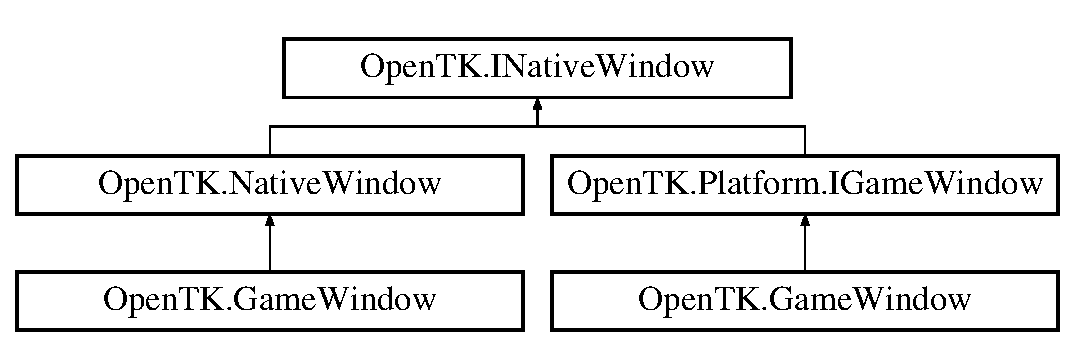
\includegraphics[height=3.000000cm]{interface_open_t_k_1_1_i_native_window}
\end{center}
\end{figure}
\subsection*{Public Member Functions}
\begin{DoxyCompactItemize}
\item 
void \hyperlink{interface_open_t_k_1_1_i_native_window_a1ccc061d19e83d00f29b50f27263fcfe}{Close} ()
\begin{DoxyCompactList}\small\item\em Closes this window. \end{DoxyCompactList}\item 
void \hyperlink{interface_open_t_k_1_1_i_native_window_a23e81e7f8c02cc874c3e23f957909171}{Process\-Events} ()
\begin{DoxyCompactList}\small\item\em Processes pending window events. \end{DoxyCompactList}\item 
Point \hyperlink{interface_open_t_k_1_1_i_native_window_ae3d487a830389a57f8732d4de101a063}{Point\-To\-Client} (Point point)
\begin{DoxyCompactList}\small\item\em Transforms the specified point from screen to client coordinates. \end{DoxyCompactList}\item 
Point \hyperlink{interface_open_t_k_1_1_i_native_window_a24ec247d43eab609220b1b581dbad519}{Point\-To\-Screen} (Point point)
\begin{DoxyCompactList}\small\item\em Transforms the specified point from client to screen coordinates. \end{DoxyCompactList}\end{DoxyCompactItemize}
\subsection*{Properties}
\begin{DoxyCompactItemize}
\item 
Icon \hyperlink{interface_open_t_k_1_1_i_native_window_a16cffc51a5dd62c9d9dbf9a089620754}{Icon}\hspace{0.3cm}{\ttfamily  \mbox{[}get, set\mbox{]}}
\begin{DoxyCompactList}\small\item\em Gets or sets the System.\-Drawing.\-Icon of the window. \end{DoxyCompactList}\item 
string \hyperlink{interface_open_t_k_1_1_i_native_window_acc6e79eb06f9e7d725f6eac5ac1df71d}{Title}\hspace{0.3cm}{\ttfamily  \mbox{[}get, set\mbox{]}}
\begin{DoxyCompactList}\small\item\em Gets or sets the title of the window. \end{DoxyCompactList}\item 
bool \hyperlink{interface_open_t_k_1_1_i_native_window_aaa2ef631c8bd4bcbef3374dfaeb50299}{Focused}\hspace{0.3cm}{\ttfamily  \mbox{[}get\mbox{]}}
\begin{DoxyCompactList}\small\item\em Gets a System.\-Boolean that indicates whether this window has input focus. \end{DoxyCompactList}\item 
bool \hyperlink{interface_open_t_k_1_1_i_native_window_ac455c50c69983d4a26e7ed61336290d8}{Visible}\hspace{0.3cm}{\ttfamily  \mbox{[}get, set\mbox{]}}
\begin{DoxyCompactList}\small\item\em Gets or sets a System.\-Boolean that indicates whether the window is visible. \end{DoxyCompactList}\item 
bool \hyperlink{interface_open_t_k_1_1_i_native_window_af207962d0e6a21f4a280e66844cc3805}{Exists}\hspace{0.3cm}{\ttfamily  \mbox{[}get\mbox{]}}
\begin{DoxyCompactList}\small\item\em Gets a System.\-Boolean that indicates whether the window has been created and has not been destroyed. \end{DoxyCompactList}\item 
\hyperlink{interface_open_t_k_1_1_platform_1_1_i_window_info}{I\-Window\-Info} \hyperlink{interface_open_t_k_1_1_i_native_window_a3e00033ca7bda60905c346fc2335e1b8}{Window\-Info}\hspace{0.3cm}{\ttfamily  \mbox{[}get\mbox{]}}
\begin{DoxyCompactList}\small\item\em Gets the \hyperlink{interface_open_t_k_1_1_platform_1_1_i_window_info}{Open\-T\-K.\-Platform.\-I\-Window\-Info} for this window. \end{DoxyCompactList}\item 
\hyperlink{namespace_open_t_k_ace9268dc87bd36f48c9d9d8b939559b4}{Window\-State} \hyperlink{interface_open_t_k_1_1_i_native_window_a228db8bdb7282c03e98c103bc6ea9904}{Window\-State}\hspace{0.3cm}{\ttfamily  \mbox{[}get, set\mbox{]}}
\begin{DoxyCompactList}\small\item\em Gets or sets the \hyperlink{namespace_open_t_k_ace9268dc87bd36f48c9d9d8b939559b4}{Open\-T\-K.\-Window\-State} for this window. \end{DoxyCompactList}\item 
\hyperlink{namespace_open_t_k_a20f46792b5471ff32362bd0a29fa5f1c}{Window\-Border} \hyperlink{interface_open_t_k_1_1_i_native_window_afb974cc1ffb686860725736bd07c2211}{Window\-Border}\hspace{0.3cm}{\ttfamily  \mbox{[}get, set\mbox{]}}
\begin{DoxyCompactList}\small\item\em Gets or sets the \hyperlink{namespace_open_t_k_a20f46792b5471ff32362bd0a29fa5f1c}{Open\-T\-K.\-Window\-Border} for this window. \end{DoxyCompactList}\item 
Rectangle \hyperlink{interface_open_t_k_1_1_i_native_window_a0cf4d0391cff1166a3f15fbdb1b4d8ab}{Bounds}\hspace{0.3cm}{\ttfamily  \mbox{[}get, set\mbox{]}}
\begin{DoxyCompactList}\small\item\em Gets or sets a System.\-Drawing.\-Rectangle structure the contains the external bounds of this window, in screen coordinates. External bounds include the title bar, borders and drawing area of the window. \end{DoxyCompactList}\item 
Point \hyperlink{interface_open_t_k_1_1_i_native_window_adb40bbbb862af25e3f05dd6bc20ae0c2}{Location}\hspace{0.3cm}{\ttfamily  \mbox{[}get, set\mbox{]}}
\begin{DoxyCompactList}\small\item\em Gets or sets a System.\-Drawing.\-Point structure that contains the location of this window on the desktop. \end{DoxyCompactList}\item 
Size \hyperlink{interface_open_t_k_1_1_i_native_window_a987289178e2f63ce7eaf58d9cbe72ed5}{Size}\hspace{0.3cm}{\ttfamily  \mbox{[}get, set\mbox{]}}
\begin{DoxyCompactList}\small\item\em Gets or sets a System.\-Drawing.\-Size structure that contains the external size of this window. \end{DoxyCompactList}\item 
int \hyperlink{interface_open_t_k_1_1_i_native_window_acf29eb685cc2fb7f6e4fd0fa11e7f147}{X}\hspace{0.3cm}{\ttfamily  \mbox{[}get, set\mbox{]}}
\begin{DoxyCompactList}\small\item\em Gets or sets the horizontal location of this window on the desktop. \end{DoxyCompactList}\item 
int \hyperlink{interface_open_t_k_1_1_i_native_window_a7e5b77aadb970f82daabf0adedeb2b16}{Y}\hspace{0.3cm}{\ttfamily  \mbox{[}get, set\mbox{]}}
\begin{DoxyCompactList}\small\item\em Gets or sets the vertical location of this window on the desktop. \end{DoxyCompactList}\item 
int \hyperlink{interface_open_t_k_1_1_i_native_window_a67659bdb41b907f0bbe9592e9a82d63f}{Width}\hspace{0.3cm}{\ttfamily  \mbox{[}get, set\mbox{]}}
\begin{DoxyCompactList}\small\item\em Gets or sets the external width of this window. \end{DoxyCompactList}\item 
int \hyperlink{interface_open_t_k_1_1_i_native_window_a717a701ae1d8a942f55825f9372bd41f}{Height}\hspace{0.3cm}{\ttfamily  \mbox{[}get, set\mbox{]}}
\begin{DoxyCompactList}\small\item\em Gets or sets the external height of this window. \end{DoxyCompactList}\item 
Rectangle \hyperlink{interface_open_t_k_1_1_i_native_window_a3031c1f6c7096ca84bc65d2b3baea88d}{Client\-Rectangle}\hspace{0.3cm}{\ttfamily  \mbox{[}get, set\mbox{]}}
\begin{DoxyCompactList}\small\item\em Gets or sets a System.\-Drawing.\-Rectangle structure that contains the internal bounds of this window, in client coordinates. The internal bounds include the drawing area of the window, but exclude the titlebar and window borders. \end{DoxyCompactList}\item 
\hyperlink{interface_open_t_k_1_1_i_native_window_a987289178e2f63ce7eaf58d9cbe72ed5}{Size} \hyperlink{interface_open_t_k_1_1_i_native_window_a3944c60601079d09e524f455a993d6cf}{Client\-Size}\hspace{0.3cm}{\ttfamily  \mbox{[}get, set\mbox{]}}
\begin{DoxyCompactList}\small\item\em Gets or sets a System.\-Drawing.\-Size structure that contains the internal size this window. \end{DoxyCompactList}\item 
\hyperlink{interface_open_t_k_1_1_input_1_1_i_input_driver}{Open\-T\-K.\-Input.\-I\-Input\-Driver} \hyperlink{interface_open_t_k_1_1_i_native_window_aca0d227f0b84dd93ba5135cc9f51ce56}{Input\-Driver}\hspace{0.3cm}{\ttfamily  \mbox{[}get\mbox{]}}
\begin{DoxyCompactList}\small\item\em This property is deprecated and should not be used. \end{DoxyCompactList}\item 
bool \hyperlink{interface_open_t_k_1_1_i_native_window_a584d510ec285e8aadd8c523389a447ff}{Cursor\-Visible}\hspace{0.3cm}{\ttfamily  \mbox{[}get, set\mbox{]}}
\begin{DoxyCompactList}\small\item\em Gets or sets a value, indicating whether the mouse cursor is visible. \end{DoxyCompactList}\end{DoxyCompactItemize}
\subsection*{Events}
\begin{DoxyCompactItemize}
\item 
Event\-Handler$<$ Event\-Args $>$ \hyperlink{interface_open_t_k_1_1_i_native_window_aa2a9b872e56a47dc3f11dcd0078e1ced}{Move}
\begin{DoxyCompactList}\small\item\em Occurs whenever the window is moved. \end{DoxyCompactList}\item 
Event\-Handler$<$ Event\-Args $>$ \hyperlink{interface_open_t_k_1_1_i_native_window_afd40870500a57eda076033f4c401ec4c}{Resize}
\begin{DoxyCompactList}\small\item\em Occurs whenever the window is resized. \end{DoxyCompactList}\item 
Event\-Handler$<$ Cancel\-Event\-Args $>$ \hyperlink{interface_open_t_k_1_1_i_native_window_a8404d9d6adb118c52c1e329e8a331d52}{Closing}
\begin{DoxyCompactList}\small\item\em Occurs when the window is about to close. \end{DoxyCompactList}\item 
Event\-Handler$<$ Event\-Args $>$ \hyperlink{interface_open_t_k_1_1_i_native_window_a2ecfca5308b3f11c83ef15011f4a96de}{Closed}
\begin{DoxyCompactList}\small\item\em Occurs after the window has closed. \end{DoxyCompactList}\item 
Event\-Handler$<$ Event\-Args $>$ \hyperlink{interface_open_t_k_1_1_i_native_window_a7e983e4b600c3e3805a693957f4b8a75}{Disposed}
\begin{DoxyCompactList}\small\item\em Occurs when the window is disposed. \end{DoxyCompactList}\item 
Event\-Handler$<$ Event\-Args $>$ \hyperlink{interface_open_t_k_1_1_i_native_window_a968bcf8310e87cee07e85eb9629da874}{Icon\-Changed}
\begin{DoxyCompactList}\small\item\em Occurs when the \hyperlink{interface_open_t_k_1_1_i_native_window_a16cffc51a5dd62c9d9dbf9a089620754}{Icon} property of the window changes. \end{DoxyCompactList}\item 
Event\-Handler$<$ Event\-Args $>$ \hyperlink{interface_open_t_k_1_1_i_native_window_acf92dea76cdae1958f4d899f6ebf2ff4}{Title\-Changed}
\begin{DoxyCompactList}\small\item\em Occurs when the \hyperlink{interface_open_t_k_1_1_i_native_window_acc6e79eb06f9e7d725f6eac5ac1df71d}{Title} property of the window changes. \end{DoxyCompactList}\item 
Event\-Handler$<$ Event\-Args $>$ \hyperlink{interface_open_t_k_1_1_i_native_window_a848de842c644e1c4066e87e16dca3555}{Visible\-Changed}
\begin{DoxyCompactList}\small\item\em Occurs when the \hyperlink{interface_open_t_k_1_1_i_native_window_ac455c50c69983d4a26e7ed61336290d8}{Visible} property of the window changes. \end{DoxyCompactList}\item 
Event\-Handler$<$ Event\-Args $>$ \hyperlink{interface_open_t_k_1_1_i_native_window_ae0a2b1803d348c1a23cddcf384ee4008}{Focused\-Changed}
\begin{DoxyCompactList}\small\item\em Occurs when the \hyperlink{interface_open_t_k_1_1_i_native_window_aaa2ef631c8bd4bcbef3374dfaeb50299}{Focused} property of the window changes. \end{DoxyCompactList}\item 
Event\-Handler$<$ Event\-Args $>$ \hyperlink{interface_open_t_k_1_1_i_native_window_a31bb2ed82c8646aee97bda920ef92aae}{Window\-Border\-Changed}
\begin{DoxyCompactList}\small\item\em Occurs when the \hyperlink{interface_open_t_k_1_1_i_native_window_afb974cc1ffb686860725736bd07c2211}{Window\-Border} property of the window changes. \end{DoxyCompactList}\item 
Event\-Handler$<$ Event\-Args $>$ \hyperlink{interface_open_t_k_1_1_i_native_window_ae13b78b7d872ee1a62950a8b6b5983b8}{Window\-State\-Changed}
\begin{DoxyCompactList}\small\item\em Occurs when the \hyperlink{interface_open_t_k_1_1_i_native_window_a228db8bdb7282c03e98c103bc6ea9904}{Window\-State} property of the window changes. \end{DoxyCompactList}\item 
Event\-Handler\\*
$<$ \hyperlink{class_open_t_k_1_1_input_1_1_keyboard_key_event_args}{Open\-T\-K.\-Input.\-Keyboard\-Key\-Event\-Args} $>$ \hyperlink{interface_open_t_k_1_1_i_native_window_a85cebd106b9852b2c6566ef026b55962}{Key\-Down}
\begin{DoxyCompactList}\small\item\em Occurs whenever a keybord key is pressed. \end{DoxyCompactList}\item 
Event\-Handler$<$ \hyperlink{class_open_t_k_1_1_key_press_event_args}{Key\-Press\-Event\-Args} $>$ \hyperlink{interface_open_t_k_1_1_i_native_window_ade20fbd09d4d714240faa4ca4617cf3f}{Key\-Press}
\begin{DoxyCompactList}\small\item\em Occurs whenever a character is typed. \end{DoxyCompactList}\item 
Event\-Handler\\*
$<$ \hyperlink{class_open_t_k_1_1_input_1_1_keyboard_key_event_args}{Open\-T\-K.\-Input.\-Keyboard\-Key\-Event\-Args} $>$ \hyperlink{interface_open_t_k_1_1_i_native_window_ab835df3fcdda59e03027d1f2b200d8b8}{Key\-Up}
\begin{DoxyCompactList}\small\item\em Occurs whenever a keyboard key is released. \end{DoxyCompactList}\item 
Event\-Handler$<$ Event\-Args $>$ \hyperlink{interface_open_t_k_1_1_i_native_window_a217050d279f6678319ab32bccba0de40}{Mouse\-Leave}
\begin{DoxyCompactList}\small\item\em Occurs whenever the mouse cursor leaves the window \hyperlink{interface_open_t_k_1_1_i_native_window_a0cf4d0391cff1166a3f15fbdb1b4d8ab}{Bounds}. \end{DoxyCompactList}\item 
Event\-Handler$<$ Event\-Args $>$ \hyperlink{interface_open_t_k_1_1_i_native_window_a4334f6f15abee869953af0845bd4dd41}{Mouse\-Enter}
\begin{DoxyCompactList}\small\item\em Occurs whenever the mouse cursor enters the window \hyperlink{interface_open_t_k_1_1_i_native_window_a0cf4d0391cff1166a3f15fbdb1b4d8ab}{Bounds}. \end{DoxyCompactList}\end{DoxyCompactItemize}


\subsection{Detailed Description}
Defines the interface for a native window. 



\subsection{Member Function Documentation}
\hypertarget{interface_open_t_k_1_1_i_native_window_a1ccc061d19e83d00f29b50f27263fcfe}{\index{Open\-T\-K\-::\-I\-Native\-Window@{Open\-T\-K\-::\-I\-Native\-Window}!Close@{Close}}
\index{Close@{Close}!OpenTK::INativeWindow@{Open\-T\-K\-::\-I\-Native\-Window}}
\subsubsection[{Close}]{\setlength{\rightskip}{0pt plus 5cm}void Open\-T\-K.\-I\-Native\-Window.\-Close (
\begin{DoxyParamCaption}
{}
\end{DoxyParamCaption}
)}}\label{interface_open_t_k_1_1_i_native_window_a1ccc061d19e83d00f29b50f27263fcfe}


Closes this window. 



Implemented in \hyperlink{class_open_t_k_1_1_native_window_ae7dae9eca1c2298dbcdbc34a81304a61}{Open\-T\-K.\-Native\-Window}.

\hypertarget{interface_open_t_k_1_1_i_native_window_ae3d487a830389a57f8732d4de101a063}{\index{Open\-T\-K\-::\-I\-Native\-Window@{Open\-T\-K\-::\-I\-Native\-Window}!Point\-To\-Client@{Point\-To\-Client}}
\index{Point\-To\-Client@{Point\-To\-Client}!OpenTK::INativeWindow@{Open\-T\-K\-::\-I\-Native\-Window}}
\subsubsection[{Point\-To\-Client}]{\setlength{\rightskip}{0pt plus 5cm}Point Open\-T\-K.\-I\-Native\-Window.\-Point\-To\-Client (
\begin{DoxyParamCaption}
\item[{Point}]{point}
\end{DoxyParamCaption}
)}}\label{interface_open_t_k_1_1_i_native_window_ae3d487a830389a57f8732d4de101a063}


Transforms the specified point from screen to client coordinates. 


\begin{DoxyParams}{Parameters}
{\em point} & A System.\-Drawing.\-Point to transform. \\
\hline
\end{DoxyParams}
\begin{DoxyReturn}{Returns}
The point transformed to client coordinates. 
\end{DoxyReturn}


Implemented in \hyperlink{class_open_t_k_1_1_native_window_a4807376063a7cc130ca6b6dfb4b4a24f}{Open\-T\-K.\-Native\-Window}.

\hypertarget{interface_open_t_k_1_1_i_native_window_a24ec247d43eab609220b1b581dbad519}{\index{Open\-T\-K\-::\-I\-Native\-Window@{Open\-T\-K\-::\-I\-Native\-Window}!Point\-To\-Screen@{Point\-To\-Screen}}
\index{Point\-To\-Screen@{Point\-To\-Screen}!OpenTK::INativeWindow@{Open\-T\-K\-::\-I\-Native\-Window}}
\subsubsection[{Point\-To\-Screen}]{\setlength{\rightskip}{0pt plus 5cm}Point Open\-T\-K.\-I\-Native\-Window.\-Point\-To\-Screen (
\begin{DoxyParamCaption}
\item[{Point}]{point}
\end{DoxyParamCaption}
)}}\label{interface_open_t_k_1_1_i_native_window_a24ec247d43eab609220b1b581dbad519}


Transforms the specified point from client to screen coordinates. 


\begin{DoxyParams}{Parameters}
{\em point} & A System.\-Drawing.\-Point to transform. \\
\hline
\end{DoxyParams}
\begin{DoxyReturn}{Returns}
The point transformed to screen coordinates. 
\end{DoxyReturn}


Implemented in \hyperlink{class_open_t_k_1_1_native_window_a631e83f783213650f854a7c953a4f34d}{Open\-T\-K.\-Native\-Window}.

\hypertarget{interface_open_t_k_1_1_i_native_window_a23e81e7f8c02cc874c3e23f957909171}{\index{Open\-T\-K\-::\-I\-Native\-Window@{Open\-T\-K\-::\-I\-Native\-Window}!Process\-Events@{Process\-Events}}
\index{Process\-Events@{Process\-Events}!OpenTK::INativeWindow@{Open\-T\-K\-::\-I\-Native\-Window}}
\subsubsection[{Process\-Events}]{\setlength{\rightskip}{0pt plus 5cm}void Open\-T\-K.\-I\-Native\-Window.\-Process\-Events (
\begin{DoxyParamCaption}
{}
\end{DoxyParamCaption}
)}}\label{interface_open_t_k_1_1_i_native_window_a23e81e7f8c02cc874c3e23f957909171}


Processes pending window events. 



Implemented in \hyperlink{class_open_t_k_1_1_native_window_a8150f2aa496459e492965c4577ec0dc9}{Open\-T\-K.\-Native\-Window}.



\subsection{Property Documentation}
\hypertarget{interface_open_t_k_1_1_i_native_window_a0cf4d0391cff1166a3f15fbdb1b4d8ab}{\index{Open\-T\-K\-::\-I\-Native\-Window@{Open\-T\-K\-::\-I\-Native\-Window}!Bounds@{Bounds}}
\index{Bounds@{Bounds}!OpenTK::INativeWindow@{Open\-T\-K\-::\-I\-Native\-Window}}
\subsubsection[{Bounds}]{\setlength{\rightskip}{0pt plus 5cm}Rectangle Open\-T\-K.\-I\-Native\-Window.\-Bounds\hspace{0.3cm}{\ttfamily [get]}, {\ttfamily [set]}}}\label{interface_open_t_k_1_1_i_native_window_a0cf4d0391cff1166a3f15fbdb1b4d8ab}


Gets or sets a System.\-Drawing.\-Rectangle structure the contains the external bounds of this window, in screen coordinates. External bounds include the title bar, borders and drawing area of the window. 

\hypertarget{interface_open_t_k_1_1_i_native_window_a3031c1f6c7096ca84bc65d2b3baea88d}{\index{Open\-T\-K\-::\-I\-Native\-Window@{Open\-T\-K\-::\-I\-Native\-Window}!Client\-Rectangle@{Client\-Rectangle}}
\index{Client\-Rectangle@{Client\-Rectangle}!OpenTK::INativeWindow@{Open\-T\-K\-::\-I\-Native\-Window}}
\subsubsection[{Client\-Rectangle}]{\setlength{\rightskip}{0pt plus 5cm}Rectangle Open\-T\-K.\-I\-Native\-Window.\-Client\-Rectangle\hspace{0.3cm}{\ttfamily [get]}, {\ttfamily [set]}}}\label{interface_open_t_k_1_1_i_native_window_a3031c1f6c7096ca84bc65d2b3baea88d}


Gets or sets a System.\-Drawing.\-Rectangle structure that contains the internal bounds of this window, in client coordinates. The internal bounds include the drawing area of the window, but exclude the titlebar and window borders. 

\hypertarget{interface_open_t_k_1_1_i_native_window_a3944c60601079d09e524f455a993d6cf}{\index{Open\-T\-K\-::\-I\-Native\-Window@{Open\-T\-K\-::\-I\-Native\-Window}!Client\-Size@{Client\-Size}}
\index{Client\-Size@{Client\-Size}!OpenTK::INativeWindow@{Open\-T\-K\-::\-I\-Native\-Window}}
\subsubsection[{Client\-Size}]{\setlength{\rightskip}{0pt plus 5cm}{\bf Size} Open\-T\-K.\-I\-Native\-Window.\-Client\-Size\hspace{0.3cm}{\ttfamily [get]}, {\ttfamily [set]}}}\label{interface_open_t_k_1_1_i_native_window_a3944c60601079d09e524f455a993d6cf}


Gets or sets a System.\-Drawing.\-Size structure that contains the internal size this window. 

\hypertarget{interface_open_t_k_1_1_i_native_window_a584d510ec285e8aadd8c523389a447ff}{\index{Open\-T\-K\-::\-I\-Native\-Window@{Open\-T\-K\-::\-I\-Native\-Window}!Cursor\-Visible@{Cursor\-Visible}}
\index{Cursor\-Visible@{Cursor\-Visible}!OpenTK::INativeWindow@{Open\-T\-K\-::\-I\-Native\-Window}}
\subsubsection[{Cursor\-Visible}]{\setlength{\rightskip}{0pt plus 5cm}bool Open\-T\-K.\-I\-Native\-Window.\-Cursor\-Visible\hspace{0.3cm}{\ttfamily [get]}, {\ttfamily [set]}}}\label{interface_open_t_k_1_1_i_native_window_a584d510ec285e8aadd8c523389a447ff}


Gets or sets a value, indicating whether the mouse cursor is visible. 

\hypertarget{interface_open_t_k_1_1_i_native_window_af207962d0e6a21f4a280e66844cc3805}{\index{Open\-T\-K\-::\-I\-Native\-Window@{Open\-T\-K\-::\-I\-Native\-Window}!Exists@{Exists}}
\index{Exists@{Exists}!OpenTK::INativeWindow@{Open\-T\-K\-::\-I\-Native\-Window}}
\subsubsection[{Exists}]{\setlength{\rightskip}{0pt plus 5cm}bool Open\-T\-K.\-I\-Native\-Window.\-Exists\hspace{0.3cm}{\ttfamily [get]}}}\label{interface_open_t_k_1_1_i_native_window_af207962d0e6a21f4a280e66844cc3805}


Gets a System.\-Boolean that indicates whether the window has been created and has not been destroyed. 

\hypertarget{interface_open_t_k_1_1_i_native_window_aaa2ef631c8bd4bcbef3374dfaeb50299}{\index{Open\-T\-K\-::\-I\-Native\-Window@{Open\-T\-K\-::\-I\-Native\-Window}!Focused@{Focused}}
\index{Focused@{Focused}!OpenTK::INativeWindow@{Open\-T\-K\-::\-I\-Native\-Window}}
\subsubsection[{Focused}]{\setlength{\rightskip}{0pt plus 5cm}bool Open\-T\-K.\-I\-Native\-Window.\-Focused\hspace{0.3cm}{\ttfamily [get]}}}\label{interface_open_t_k_1_1_i_native_window_aaa2ef631c8bd4bcbef3374dfaeb50299}


Gets a System.\-Boolean that indicates whether this window has input focus. 

\hypertarget{interface_open_t_k_1_1_i_native_window_a717a701ae1d8a942f55825f9372bd41f}{\index{Open\-T\-K\-::\-I\-Native\-Window@{Open\-T\-K\-::\-I\-Native\-Window}!Height@{Height}}
\index{Height@{Height}!OpenTK::INativeWindow@{Open\-T\-K\-::\-I\-Native\-Window}}
\subsubsection[{Height}]{\setlength{\rightskip}{0pt plus 5cm}int Open\-T\-K.\-I\-Native\-Window.\-Height\hspace{0.3cm}{\ttfamily [get]}, {\ttfamily [set]}}}\label{interface_open_t_k_1_1_i_native_window_a717a701ae1d8a942f55825f9372bd41f}


Gets or sets the external height of this window. 

\hypertarget{interface_open_t_k_1_1_i_native_window_a16cffc51a5dd62c9d9dbf9a089620754}{\index{Open\-T\-K\-::\-I\-Native\-Window@{Open\-T\-K\-::\-I\-Native\-Window}!Icon@{Icon}}
\index{Icon@{Icon}!OpenTK::INativeWindow@{Open\-T\-K\-::\-I\-Native\-Window}}
\subsubsection[{Icon}]{\setlength{\rightskip}{0pt plus 5cm}Icon Open\-T\-K.\-I\-Native\-Window.\-Icon\hspace{0.3cm}{\ttfamily [get]}, {\ttfamily [set]}}}\label{interface_open_t_k_1_1_i_native_window_a16cffc51a5dd62c9d9dbf9a089620754}


Gets or sets the System.\-Drawing.\-Icon of the window. 

\hypertarget{interface_open_t_k_1_1_i_native_window_aca0d227f0b84dd93ba5135cc9f51ce56}{\index{Open\-T\-K\-::\-I\-Native\-Window@{Open\-T\-K\-::\-I\-Native\-Window}!Input\-Driver@{Input\-Driver}}
\index{Input\-Driver@{Input\-Driver}!OpenTK::INativeWindow@{Open\-T\-K\-::\-I\-Native\-Window}}
\subsubsection[{Input\-Driver}]{\setlength{\rightskip}{0pt plus 5cm}{\bf Open\-T\-K.\-Input.\-I\-Input\-Driver} Open\-T\-K.\-I\-Native\-Window.\-Input\-Driver\hspace{0.3cm}{\ttfamily [get]}}}\label{interface_open_t_k_1_1_i_native_window_aca0d227f0b84dd93ba5135cc9f51ce56}


This property is deprecated and should not be used. 

\hypertarget{interface_open_t_k_1_1_i_native_window_adb40bbbb862af25e3f05dd6bc20ae0c2}{\index{Open\-T\-K\-::\-I\-Native\-Window@{Open\-T\-K\-::\-I\-Native\-Window}!Location@{Location}}
\index{Location@{Location}!OpenTK::INativeWindow@{Open\-T\-K\-::\-I\-Native\-Window}}
\subsubsection[{Location}]{\setlength{\rightskip}{0pt plus 5cm}Point Open\-T\-K.\-I\-Native\-Window.\-Location\hspace{0.3cm}{\ttfamily [get]}, {\ttfamily [set]}}}\label{interface_open_t_k_1_1_i_native_window_adb40bbbb862af25e3f05dd6bc20ae0c2}


Gets or sets a System.\-Drawing.\-Point structure that contains the location of this window on the desktop. 

\hypertarget{interface_open_t_k_1_1_i_native_window_a987289178e2f63ce7eaf58d9cbe72ed5}{\index{Open\-T\-K\-::\-I\-Native\-Window@{Open\-T\-K\-::\-I\-Native\-Window}!Size@{Size}}
\index{Size@{Size}!OpenTK::INativeWindow@{Open\-T\-K\-::\-I\-Native\-Window}}
\subsubsection[{Size}]{\setlength{\rightskip}{0pt plus 5cm}Size Open\-T\-K.\-I\-Native\-Window.\-Size\hspace{0.3cm}{\ttfamily [get]}, {\ttfamily [set]}}}\label{interface_open_t_k_1_1_i_native_window_a987289178e2f63ce7eaf58d9cbe72ed5}


Gets or sets a System.\-Drawing.\-Size structure that contains the external size of this window. 

\hypertarget{interface_open_t_k_1_1_i_native_window_acc6e79eb06f9e7d725f6eac5ac1df71d}{\index{Open\-T\-K\-::\-I\-Native\-Window@{Open\-T\-K\-::\-I\-Native\-Window}!Title@{Title}}
\index{Title@{Title}!OpenTK::INativeWindow@{Open\-T\-K\-::\-I\-Native\-Window}}
\subsubsection[{Title}]{\setlength{\rightskip}{0pt plus 5cm}string Open\-T\-K.\-I\-Native\-Window.\-Title\hspace{0.3cm}{\ttfamily [get]}, {\ttfamily [set]}}}\label{interface_open_t_k_1_1_i_native_window_acc6e79eb06f9e7d725f6eac5ac1df71d}


Gets or sets the title of the window. 

\hypertarget{interface_open_t_k_1_1_i_native_window_ac455c50c69983d4a26e7ed61336290d8}{\index{Open\-T\-K\-::\-I\-Native\-Window@{Open\-T\-K\-::\-I\-Native\-Window}!Visible@{Visible}}
\index{Visible@{Visible}!OpenTK::INativeWindow@{Open\-T\-K\-::\-I\-Native\-Window}}
\subsubsection[{Visible}]{\setlength{\rightskip}{0pt plus 5cm}bool Open\-T\-K.\-I\-Native\-Window.\-Visible\hspace{0.3cm}{\ttfamily [get]}, {\ttfamily [set]}}}\label{interface_open_t_k_1_1_i_native_window_ac455c50c69983d4a26e7ed61336290d8}


Gets or sets a System.\-Boolean that indicates whether the window is visible. 

\hypertarget{interface_open_t_k_1_1_i_native_window_a67659bdb41b907f0bbe9592e9a82d63f}{\index{Open\-T\-K\-::\-I\-Native\-Window@{Open\-T\-K\-::\-I\-Native\-Window}!Width@{Width}}
\index{Width@{Width}!OpenTK::INativeWindow@{Open\-T\-K\-::\-I\-Native\-Window}}
\subsubsection[{Width}]{\setlength{\rightskip}{0pt plus 5cm}int Open\-T\-K.\-I\-Native\-Window.\-Width\hspace{0.3cm}{\ttfamily [get]}, {\ttfamily [set]}}}\label{interface_open_t_k_1_1_i_native_window_a67659bdb41b907f0bbe9592e9a82d63f}


Gets or sets the external width of this window. 

\hypertarget{interface_open_t_k_1_1_i_native_window_afb974cc1ffb686860725736bd07c2211}{\index{Open\-T\-K\-::\-I\-Native\-Window@{Open\-T\-K\-::\-I\-Native\-Window}!Window\-Border@{Window\-Border}}
\index{Window\-Border@{Window\-Border}!OpenTK::INativeWindow@{Open\-T\-K\-::\-I\-Native\-Window}}
\subsubsection[{Window\-Border}]{\setlength{\rightskip}{0pt plus 5cm}{\bf Window\-Border} Open\-T\-K.\-I\-Native\-Window.\-Window\-Border\hspace{0.3cm}{\ttfamily [get]}, {\ttfamily [set]}}}\label{interface_open_t_k_1_1_i_native_window_afb974cc1ffb686860725736bd07c2211}


Gets or sets the \hyperlink{namespace_open_t_k_a20f46792b5471ff32362bd0a29fa5f1c}{Open\-T\-K.\-Window\-Border} for this window. 

\hypertarget{interface_open_t_k_1_1_i_native_window_a3e00033ca7bda60905c346fc2335e1b8}{\index{Open\-T\-K\-::\-I\-Native\-Window@{Open\-T\-K\-::\-I\-Native\-Window}!Window\-Info@{Window\-Info}}
\index{Window\-Info@{Window\-Info}!OpenTK::INativeWindow@{Open\-T\-K\-::\-I\-Native\-Window}}
\subsubsection[{Window\-Info}]{\setlength{\rightskip}{0pt plus 5cm}{\bf I\-Window\-Info} Open\-T\-K.\-I\-Native\-Window.\-Window\-Info\hspace{0.3cm}{\ttfamily [get]}}}\label{interface_open_t_k_1_1_i_native_window_a3e00033ca7bda60905c346fc2335e1b8}


Gets the \hyperlink{interface_open_t_k_1_1_platform_1_1_i_window_info}{Open\-T\-K.\-Platform.\-I\-Window\-Info} for this window. 

\hypertarget{interface_open_t_k_1_1_i_native_window_a228db8bdb7282c03e98c103bc6ea9904}{\index{Open\-T\-K\-::\-I\-Native\-Window@{Open\-T\-K\-::\-I\-Native\-Window}!Window\-State@{Window\-State}}
\index{Window\-State@{Window\-State}!OpenTK::INativeWindow@{Open\-T\-K\-::\-I\-Native\-Window}}
\subsubsection[{Window\-State}]{\setlength{\rightskip}{0pt plus 5cm}{\bf Window\-State} Open\-T\-K.\-I\-Native\-Window.\-Window\-State\hspace{0.3cm}{\ttfamily [get]}, {\ttfamily [set]}}}\label{interface_open_t_k_1_1_i_native_window_a228db8bdb7282c03e98c103bc6ea9904}


Gets or sets the \hyperlink{namespace_open_t_k_ace9268dc87bd36f48c9d9d8b939559b4}{Open\-T\-K.\-Window\-State} for this window. 

\hypertarget{interface_open_t_k_1_1_i_native_window_acf29eb685cc2fb7f6e4fd0fa11e7f147}{\index{Open\-T\-K\-::\-I\-Native\-Window@{Open\-T\-K\-::\-I\-Native\-Window}!X@{X}}
\index{X@{X}!OpenTK::INativeWindow@{Open\-T\-K\-::\-I\-Native\-Window}}
\subsubsection[{X}]{\setlength{\rightskip}{0pt plus 5cm}int Open\-T\-K.\-I\-Native\-Window.\-X\hspace{0.3cm}{\ttfamily [get]}, {\ttfamily [set]}}}\label{interface_open_t_k_1_1_i_native_window_acf29eb685cc2fb7f6e4fd0fa11e7f147}


Gets or sets the horizontal location of this window on the desktop. 

\hypertarget{interface_open_t_k_1_1_i_native_window_a7e5b77aadb970f82daabf0adedeb2b16}{\index{Open\-T\-K\-::\-I\-Native\-Window@{Open\-T\-K\-::\-I\-Native\-Window}!Y@{Y}}
\index{Y@{Y}!OpenTK::INativeWindow@{Open\-T\-K\-::\-I\-Native\-Window}}
\subsubsection[{Y}]{\setlength{\rightskip}{0pt plus 5cm}int Open\-T\-K.\-I\-Native\-Window.\-Y\hspace{0.3cm}{\ttfamily [get]}, {\ttfamily [set]}}}\label{interface_open_t_k_1_1_i_native_window_a7e5b77aadb970f82daabf0adedeb2b16}


Gets or sets the vertical location of this window on the desktop. 



\subsection{Event Documentation}
\hypertarget{interface_open_t_k_1_1_i_native_window_a2ecfca5308b3f11c83ef15011f4a96de}{\index{Open\-T\-K\-::\-I\-Native\-Window@{Open\-T\-K\-::\-I\-Native\-Window}!Closed@{Closed}}
\index{Closed@{Closed}!OpenTK::INativeWindow@{Open\-T\-K\-::\-I\-Native\-Window}}
\subsubsection[{Closed}]{\setlength{\rightskip}{0pt plus 5cm}Event\-Handler$<$Event\-Args$>$ Open\-T\-K.\-I\-Native\-Window.\-Closed}}\label{interface_open_t_k_1_1_i_native_window_a2ecfca5308b3f11c83ef15011f4a96de}


Occurs after the window has closed. 

\hypertarget{interface_open_t_k_1_1_i_native_window_a8404d9d6adb118c52c1e329e8a331d52}{\index{Open\-T\-K\-::\-I\-Native\-Window@{Open\-T\-K\-::\-I\-Native\-Window}!Closing@{Closing}}
\index{Closing@{Closing}!OpenTK::INativeWindow@{Open\-T\-K\-::\-I\-Native\-Window}}
\subsubsection[{Closing}]{\setlength{\rightskip}{0pt plus 5cm}Event\-Handler$<$Cancel\-Event\-Args$>$ Open\-T\-K.\-I\-Native\-Window.\-Closing}}\label{interface_open_t_k_1_1_i_native_window_a8404d9d6adb118c52c1e329e8a331d52}


Occurs when the window is about to close. 

\hypertarget{interface_open_t_k_1_1_i_native_window_a7e983e4b600c3e3805a693957f4b8a75}{\index{Open\-T\-K\-::\-I\-Native\-Window@{Open\-T\-K\-::\-I\-Native\-Window}!Disposed@{Disposed}}
\index{Disposed@{Disposed}!OpenTK::INativeWindow@{Open\-T\-K\-::\-I\-Native\-Window}}
\subsubsection[{Disposed}]{\setlength{\rightskip}{0pt plus 5cm}Event\-Handler$<$Event\-Args$>$ Open\-T\-K.\-I\-Native\-Window.\-Disposed}}\label{interface_open_t_k_1_1_i_native_window_a7e983e4b600c3e3805a693957f4b8a75}


Occurs when the window is disposed. 

\hypertarget{interface_open_t_k_1_1_i_native_window_ae0a2b1803d348c1a23cddcf384ee4008}{\index{Open\-T\-K\-::\-I\-Native\-Window@{Open\-T\-K\-::\-I\-Native\-Window}!Focused\-Changed@{Focused\-Changed}}
\index{Focused\-Changed@{Focused\-Changed}!OpenTK::INativeWindow@{Open\-T\-K\-::\-I\-Native\-Window}}
\subsubsection[{Focused\-Changed}]{\setlength{\rightskip}{0pt plus 5cm}Event\-Handler$<$Event\-Args$>$ Open\-T\-K.\-I\-Native\-Window.\-Focused\-Changed}}\label{interface_open_t_k_1_1_i_native_window_ae0a2b1803d348c1a23cddcf384ee4008}


Occurs when the \hyperlink{interface_open_t_k_1_1_i_native_window_aaa2ef631c8bd4bcbef3374dfaeb50299}{Focused} property of the window changes. 

\hypertarget{interface_open_t_k_1_1_i_native_window_a968bcf8310e87cee07e85eb9629da874}{\index{Open\-T\-K\-::\-I\-Native\-Window@{Open\-T\-K\-::\-I\-Native\-Window}!Icon\-Changed@{Icon\-Changed}}
\index{Icon\-Changed@{Icon\-Changed}!OpenTK::INativeWindow@{Open\-T\-K\-::\-I\-Native\-Window}}
\subsubsection[{Icon\-Changed}]{\setlength{\rightskip}{0pt plus 5cm}Event\-Handler$<$Event\-Args$>$ Open\-T\-K.\-I\-Native\-Window.\-Icon\-Changed}}\label{interface_open_t_k_1_1_i_native_window_a968bcf8310e87cee07e85eb9629da874}


Occurs when the \hyperlink{interface_open_t_k_1_1_i_native_window_a16cffc51a5dd62c9d9dbf9a089620754}{Icon} property of the window changes. 

\hypertarget{interface_open_t_k_1_1_i_native_window_a85cebd106b9852b2c6566ef026b55962}{\index{Open\-T\-K\-::\-I\-Native\-Window@{Open\-T\-K\-::\-I\-Native\-Window}!Key\-Down@{Key\-Down}}
\index{Key\-Down@{Key\-Down}!OpenTK::INativeWindow@{Open\-T\-K\-::\-I\-Native\-Window}}
\subsubsection[{Key\-Down}]{\setlength{\rightskip}{0pt plus 5cm}Event\-Handler$<${\bf Open\-T\-K.\-Input.\-Keyboard\-Key\-Event\-Args}$>$ Open\-T\-K.\-I\-Native\-Window.\-Key\-Down}}\label{interface_open_t_k_1_1_i_native_window_a85cebd106b9852b2c6566ef026b55962}


Occurs whenever a keybord key is pressed. 

\hypertarget{interface_open_t_k_1_1_i_native_window_ade20fbd09d4d714240faa4ca4617cf3f}{\index{Open\-T\-K\-::\-I\-Native\-Window@{Open\-T\-K\-::\-I\-Native\-Window}!Key\-Press@{Key\-Press}}
\index{Key\-Press@{Key\-Press}!OpenTK::INativeWindow@{Open\-T\-K\-::\-I\-Native\-Window}}
\subsubsection[{Key\-Press}]{\setlength{\rightskip}{0pt plus 5cm}Event\-Handler$<${\bf Key\-Press\-Event\-Args}$>$ Open\-T\-K.\-I\-Native\-Window.\-Key\-Press}}\label{interface_open_t_k_1_1_i_native_window_ade20fbd09d4d714240faa4ca4617cf3f}


Occurs whenever a character is typed. 

\hypertarget{interface_open_t_k_1_1_i_native_window_ab835df3fcdda59e03027d1f2b200d8b8}{\index{Open\-T\-K\-::\-I\-Native\-Window@{Open\-T\-K\-::\-I\-Native\-Window}!Key\-Up@{Key\-Up}}
\index{Key\-Up@{Key\-Up}!OpenTK::INativeWindow@{Open\-T\-K\-::\-I\-Native\-Window}}
\subsubsection[{Key\-Up}]{\setlength{\rightskip}{0pt plus 5cm}Event\-Handler$<${\bf Open\-T\-K.\-Input.\-Keyboard\-Key\-Event\-Args}$>$ Open\-T\-K.\-I\-Native\-Window.\-Key\-Up}}\label{interface_open_t_k_1_1_i_native_window_ab835df3fcdda59e03027d1f2b200d8b8}


Occurs whenever a keyboard key is released. 

\hypertarget{interface_open_t_k_1_1_i_native_window_a4334f6f15abee869953af0845bd4dd41}{\index{Open\-T\-K\-::\-I\-Native\-Window@{Open\-T\-K\-::\-I\-Native\-Window}!Mouse\-Enter@{Mouse\-Enter}}
\index{Mouse\-Enter@{Mouse\-Enter}!OpenTK::INativeWindow@{Open\-T\-K\-::\-I\-Native\-Window}}
\subsubsection[{Mouse\-Enter}]{\setlength{\rightskip}{0pt plus 5cm}Event\-Handler$<$Event\-Args$>$ Open\-T\-K.\-I\-Native\-Window.\-Mouse\-Enter}}\label{interface_open_t_k_1_1_i_native_window_a4334f6f15abee869953af0845bd4dd41}


Occurs whenever the mouse cursor enters the window \hyperlink{interface_open_t_k_1_1_i_native_window_a0cf4d0391cff1166a3f15fbdb1b4d8ab}{Bounds}. 

\hypertarget{interface_open_t_k_1_1_i_native_window_a217050d279f6678319ab32bccba0de40}{\index{Open\-T\-K\-::\-I\-Native\-Window@{Open\-T\-K\-::\-I\-Native\-Window}!Mouse\-Leave@{Mouse\-Leave}}
\index{Mouse\-Leave@{Mouse\-Leave}!OpenTK::INativeWindow@{Open\-T\-K\-::\-I\-Native\-Window}}
\subsubsection[{Mouse\-Leave}]{\setlength{\rightskip}{0pt plus 5cm}Event\-Handler$<$Event\-Args$>$ Open\-T\-K.\-I\-Native\-Window.\-Mouse\-Leave}}\label{interface_open_t_k_1_1_i_native_window_a217050d279f6678319ab32bccba0de40}


Occurs whenever the mouse cursor leaves the window \hyperlink{interface_open_t_k_1_1_i_native_window_a0cf4d0391cff1166a3f15fbdb1b4d8ab}{Bounds}. 

\hypertarget{interface_open_t_k_1_1_i_native_window_aa2a9b872e56a47dc3f11dcd0078e1ced}{\index{Open\-T\-K\-::\-I\-Native\-Window@{Open\-T\-K\-::\-I\-Native\-Window}!Move@{Move}}
\index{Move@{Move}!OpenTK::INativeWindow@{Open\-T\-K\-::\-I\-Native\-Window}}
\subsubsection[{Move}]{\setlength{\rightskip}{0pt plus 5cm}Event\-Handler$<$Event\-Args$>$ Open\-T\-K.\-I\-Native\-Window.\-Move}}\label{interface_open_t_k_1_1_i_native_window_aa2a9b872e56a47dc3f11dcd0078e1ced}


Occurs whenever the window is moved. 

\hypertarget{interface_open_t_k_1_1_i_native_window_afd40870500a57eda076033f4c401ec4c}{\index{Open\-T\-K\-::\-I\-Native\-Window@{Open\-T\-K\-::\-I\-Native\-Window}!Resize@{Resize}}
\index{Resize@{Resize}!OpenTK::INativeWindow@{Open\-T\-K\-::\-I\-Native\-Window}}
\subsubsection[{Resize}]{\setlength{\rightskip}{0pt plus 5cm}Event\-Handler$<$Event\-Args$>$ Open\-T\-K.\-I\-Native\-Window.\-Resize}}\label{interface_open_t_k_1_1_i_native_window_afd40870500a57eda076033f4c401ec4c}


Occurs whenever the window is resized. 

\hypertarget{interface_open_t_k_1_1_i_native_window_acf92dea76cdae1958f4d899f6ebf2ff4}{\index{Open\-T\-K\-::\-I\-Native\-Window@{Open\-T\-K\-::\-I\-Native\-Window}!Title\-Changed@{Title\-Changed}}
\index{Title\-Changed@{Title\-Changed}!OpenTK::INativeWindow@{Open\-T\-K\-::\-I\-Native\-Window}}
\subsubsection[{Title\-Changed}]{\setlength{\rightskip}{0pt plus 5cm}Event\-Handler$<$Event\-Args$>$ Open\-T\-K.\-I\-Native\-Window.\-Title\-Changed}}\label{interface_open_t_k_1_1_i_native_window_acf92dea76cdae1958f4d899f6ebf2ff4}


Occurs when the \hyperlink{interface_open_t_k_1_1_i_native_window_acc6e79eb06f9e7d725f6eac5ac1df71d}{Title} property of the window changes. 

\hypertarget{interface_open_t_k_1_1_i_native_window_a848de842c644e1c4066e87e16dca3555}{\index{Open\-T\-K\-::\-I\-Native\-Window@{Open\-T\-K\-::\-I\-Native\-Window}!Visible\-Changed@{Visible\-Changed}}
\index{Visible\-Changed@{Visible\-Changed}!OpenTK::INativeWindow@{Open\-T\-K\-::\-I\-Native\-Window}}
\subsubsection[{Visible\-Changed}]{\setlength{\rightskip}{0pt plus 5cm}Event\-Handler$<$Event\-Args$>$ Open\-T\-K.\-I\-Native\-Window.\-Visible\-Changed}}\label{interface_open_t_k_1_1_i_native_window_a848de842c644e1c4066e87e16dca3555}


Occurs when the \hyperlink{interface_open_t_k_1_1_i_native_window_ac455c50c69983d4a26e7ed61336290d8}{Visible} property of the window changes. 

\hypertarget{interface_open_t_k_1_1_i_native_window_a31bb2ed82c8646aee97bda920ef92aae}{\index{Open\-T\-K\-::\-I\-Native\-Window@{Open\-T\-K\-::\-I\-Native\-Window}!Window\-Border\-Changed@{Window\-Border\-Changed}}
\index{Window\-Border\-Changed@{Window\-Border\-Changed}!OpenTK::INativeWindow@{Open\-T\-K\-::\-I\-Native\-Window}}
\subsubsection[{Window\-Border\-Changed}]{\setlength{\rightskip}{0pt plus 5cm}Event\-Handler$<$Event\-Args$>$ Open\-T\-K.\-I\-Native\-Window.\-Window\-Border\-Changed}}\label{interface_open_t_k_1_1_i_native_window_a31bb2ed82c8646aee97bda920ef92aae}


Occurs when the \hyperlink{interface_open_t_k_1_1_i_native_window_afb974cc1ffb686860725736bd07c2211}{Window\-Border} property of the window changes. 

\hypertarget{interface_open_t_k_1_1_i_native_window_ae13b78b7d872ee1a62950a8b6b5983b8}{\index{Open\-T\-K\-::\-I\-Native\-Window@{Open\-T\-K\-::\-I\-Native\-Window}!Window\-State\-Changed@{Window\-State\-Changed}}
\index{Window\-State\-Changed@{Window\-State\-Changed}!OpenTK::INativeWindow@{Open\-T\-K\-::\-I\-Native\-Window}}
\subsubsection[{Window\-State\-Changed}]{\setlength{\rightskip}{0pt plus 5cm}Event\-Handler$<$Event\-Args$>$ Open\-T\-K.\-I\-Native\-Window.\-Window\-State\-Changed}}\label{interface_open_t_k_1_1_i_native_window_ae13b78b7d872ee1a62950a8b6b5983b8}


Occurs when the \hyperlink{interface_open_t_k_1_1_i_native_window_a228db8bdb7282c03e98c103bc6ea9904}{Window\-State} property of the window changes. 


\hypertarget{class_open_t_k_1_1_input_1_1_game_pad}{\section{Open\-T\-K.\-Input.\-Game\-Pad Class Reference}
\label{class_open_t_k_1_1_input_1_1_game_pad}\index{Open\-T\-K.\-Input.\-Game\-Pad@{Open\-T\-K.\-Input.\-Game\-Pad}}
}


Provides access to \hyperlink{class_open_t_k_1_1_input_1_1_game_pad}{Game\-Pad} devices. Note\-: this A\-P\-I is not implemented yet.  




\subsection{Detailed Description}
Provides access to \hyperlink{class_open_t_k_1_1_input_1_1_game_pad}{Game\-Pad} devices. Note\-: this A\-P\-I is not implemented yet. 


\hypertarget{struct_open_t_k_1_1_input_1_1_game_pad_state}{\section{Open\-T\-K.\-Input.\-Game\-Pad\-State Struct Reference}
\label{struct_open_t_k_1_1_input_1_1_game_pad_state}\index{Open\-T\-K.\-Input.\-Game\-Pad\-State@{Open\-T\-K.\-Input.\-Game\-Pad\-State}}
}


Encapsulates the state of a \hyperlink{class_open_t_k_1_1_input_1_1_game_pad}{Game\-Pad} device.  




\subsection{Detailed Description}
Encapsulates the state of a \hyperlink{class_open_t_k_1_1_input_1_1_game_pad}{Game\-Pad} device. 


\hypertarget{interface_open_t_k_1_1_input_1_1_i_input_device}{\section{Open\-T\-K.\-Input.\-I\-Input\-Device Interface Reference}
\label{interface_open_t_k_1_1_input_1_1_i_input_device}\index{Open\-T\-K.\-Input.\-I\-Input\-Device@{Open\-T\-K.\-Input.\-I\-Input\-Device}}
}


Defines a common interface for all input devices.  


Inheritance diagram for Open\-T\-K.\-Input.\-I\-Input\-Device\-:\begin{figure}[H]
\begin{center}
\leavevmode
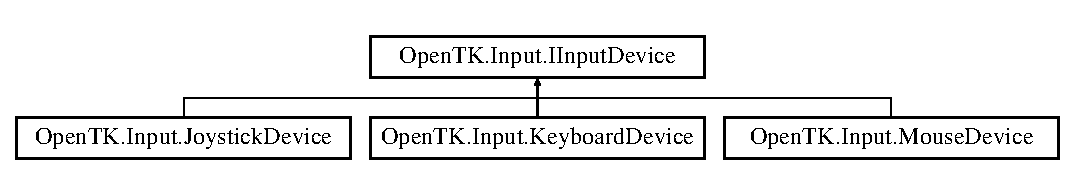
\includegraphics[height=1.904762cm]{interface_open_t_k_1_1_input_1_1_i_input_device}
\end{center}
\end{figure}
\subsection*{Properties}
\begin{DoxyCompactItemize}
\item 
string \hyperlink{interface_open_t_k_1_1_input_1_1_i_input_device_ae119526b3cf39957b3f0440cf50122f2}{Description}\hspace{0.3cm}{\ttfamily  \mbox{[}get\mbox{]}}
\begin{DoxyCompactList}\small\item\em Gets a System.\-String with a unique description of this \hyperlink{interface_open_t_k_1_1_input_1_1_i_input_device}{I\-Input\-Device} instance. \end{DoxyCompactList}\item 
\hyperlink{namespace_open_t_k_1_1_input_a1d147c6256b0adaa5288eec90ed93270}{Input\-Device\-Type} \hyperlink{interface_open_t_k_1_1_input_1_1_i_input_device_a5be985412e36d169ff3cf4902eb6b2f3}{Device\-Type}\hspace{0.3cm}{\ttfamily  \mbox{[}get\mbox{]}}
\begin{DoxyCompactList}\small\item\em Gets an \hyperlink{namespace_open_t_k_1_1_input_a1d147c6256b0adaa5288eec90ed93270}{Open\-T\-K.\-Input.\-Input\-Device\-Type} value, representing the device type of this \hyperlink{interface_open_t_k_1_1_input_1_1_i_input_device}{I\-Input\-Device} instance. \end{DoxyCompactList}\end{DoxyCompactItemize}


\subsection{Detailed Description}
Defines a common interface for all input devices. 



\subsection{Property Documentation}
\hypertarget{interface_open_t_k_1_1_input_1_1_i_input_device_ae119526b3cf39957b3f0440cf50122f2}{\index{Open\-T\-K\-::\-Input\-::\-I\-Input\-Device@{Open\-T\-K\-::\-Input\-::\-I\-Input\-Device}!Description@{Description}}
\index{Description@{Description}!OpenTK::Input::IInputDevice@{Open\-T\-K\-::\-Input\-::\-I\-Input\-Device}}
\subsubsection[{Description}]{\setlength{\rightskip}{0pt plus 5cm}string Open\-T\-K.\-Input.\-I\-Input\-Device.\-Description\hspace{0.3cm}{\ttfamily [get]}}}\label{interface_open_t_k_1_1_input_1_1_i_input_device_ae119526b3cf39957b3f0440cf50122f2}


Gets a System.\-String with a unique description of this \hyperlink{interface_open_t_k_1_1_input_1_1_i_input_device}{I\-Input\-Device} instance. 

\hypertarget{interface_open_t_k_1_1_input_1_1_i_input_device_a5be985412e36d169ff3cf4902eb6b2f3}{\index{Open\-T\-K\-::\-Input\-::\-I\-Input\-Device@{Open\-T\-K\-::\-Input\-::\-I\-Input\-Device}!Device\-Type@{Device\-Type}}
\index{Device\-Type@{Device\-Type}!OpenTK::Input::IInputDevice@{Open\-T\-K\-::\-Input\-::\-I\-Input\-Device}}
\subsubsection[{Device\-Type}]{\setlength{\rightskip}{0pt plus 5cm}{\bf Input\-Device\-Type} Open\-T\-K.\-Input.\-I\-Input\-Device.\-Device\-Type\hspace{0.3cm}{\ttfamily [get]}}}\label{interface_open_t_k_1_1_input_1_1_i_input_device_a5be985412e36d169ff3cf4902eb6b2f3}


Gets an \hyperlink{namespace_open_t_k_1_1_input_a1d147c6256b0adaa5288eec90ed93270}{Open\-T\-K.\-Input.\-Input\-Device\-Type} value, representing the device type of this \hyperlink{interface_open_t_k_1_1_input_1_1_i_input_device}{I\-Input\-Device} instance. 


\hypertarget{interface_open_t_k_1_1_input_1_1_i_input_driver}{\section{Open\-T\-K.\-Input.\-I\-Input\-Driver Interface Reference}
\label{interface_open_t_k_1_1_input_1_1_i_input_driver}\index{Open\-T\-K.\-Input.\-I\-Input\-Driver@{Open\-T\-K.\-Input.\-I\-Input\-Driver}}
}


Defines the interface for an input driver.  


Inheritance diagram for Open\-T\-K.\-Input.\-I\-Input\-Driver\-:\begin{figure}[H]
\begin{center}
\leavevmode
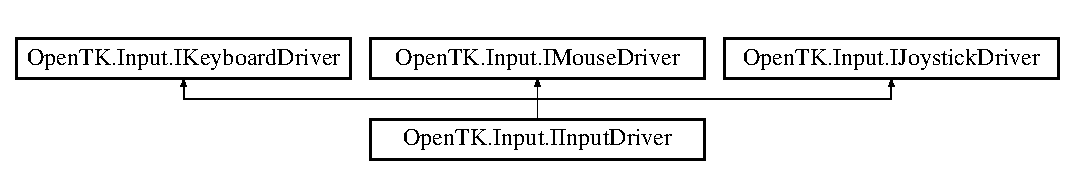
\includegraphics[height=1.914530cm]{interface_open_t_k_1_1_input_1_1_i_input_driver}
\end{center}
\end{figure}
\subsection*{Public Member Functions}
\begin{DoxyCompactItemize}
\item 
void \hyperlink{interface_open_t_k_1_1_input_1_1_i_input_driver_a9d9ab2966f9e2855c5681751800ff129}{Poll} ()
\begin{DoxyCompactList}\small\item\em Updates the state of the driver. \end{DoxyCompactList}\end{DoxyCompactItemize}


\subsection{Detailed Description}
Defines the interface for an input driver. 



\subsection{Member Function Documentation}
\hypertarget{interface_open_t_k_1_1_input_1_1_i_input_driver_a9d9ab2966f9e2855c5681751800ff129}{\index{Open\-T\-K\-::\-Input\-::\-I\-Input\-Driver@{Open\-T\-K\-::\-Input\-::\-I\-Input\-Driver}!Poll@{Poll}}
\index{Poll@{Poll}!OpenTK::Input::IInputDriver@{Open\-T\-K\-::\-Input\-::\-I\-Input\-Driver}}
\subsubsection[{Poll}]{\setlength{\rightskip}{0pt plus 5cm}void Open\-T\-K.\-Input.\-I\-Input\-Driver.\-Poll (
\begin{DoxyParamCaption}
{}
\end{DoxyParamCaption}
)}}\label{interface_open_t_k_1_1_input_1_1_i_input_driver_a9d9ab2966f9e2855c5681751800ff129}


Updates the state of the driver. 


\hypertarget{interface_open_t_k_1_1_input_1_1_i_joystick_driver}{\section{Open\-T\-K.\-Input.\-I\-Joystick\-Driver Interface Reference}
\label{interface_open_t_k_1_1_input_1_1_i_joystick_driver}\index{Open\-T\-K.\-Input.\-I\-Joystick\-Driver@{Open\-T\-K.\-Input.\-I\-Joystick\-Driver}}
}


Defines the interface for \hyperlink{class_open_t_k_1_1_input_1_1_joystick_device}{Joystick\-Device} drivers.  


Inheritance diagram for Open\-T\-K.\-Input.\-I\-Joystick\-Driver\-:\begin{figure}[H]
\begin{center}
\leavevmode
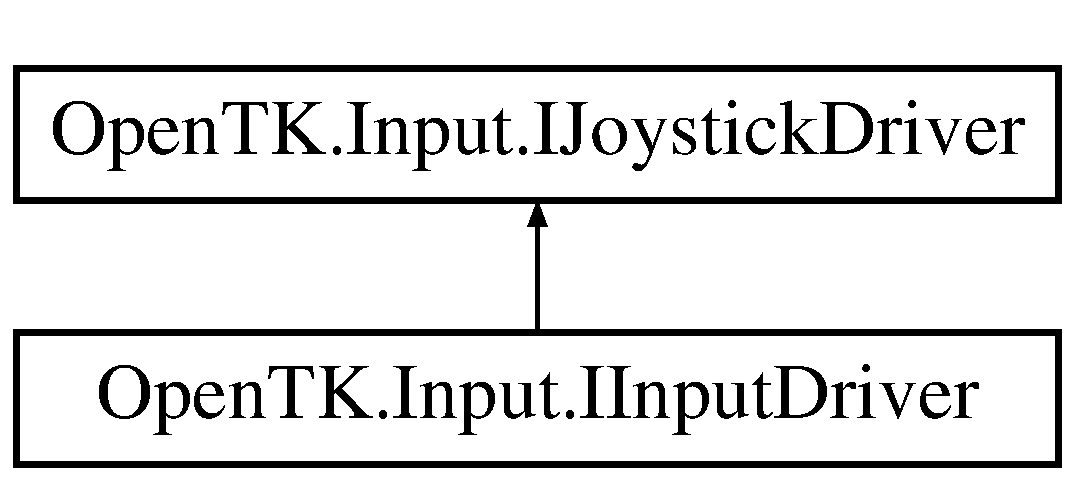
\includegraphics[height=2.000000cm]{interface_open_t_k_1_1_input_1_1_i_joystick_driver}
\end{center}
\end{figure}
\subsection*{Properties}
\begin{DoxyCompactItemize}
\item 
I\-List$<$ \hyperlink{class_open_t_k_1_1_input_1_1_joystick_device}{Joystick\-Device} $>$ \hyperlink{interface_open_t_k_1_1_input_1_1_i_joystick_driver_abcc28b1127554a446e37bed7d62e5024}{Joysticks}\hspace{0.3cm}{\ttfamily  \mbox{[}get\mbox{]}}
\begin{DoxyCompactList}\small\item\em Gets the list of available Joystick\-Devices. \end{DoxyCompactList}\end{DoxyCompactItemize}


\subsection{Detailed Description}
Defines the interface for \hyperlink{class_open_t_k_1_1_input_1_1_joystick_device}{Joystick\-Device} drivers. 



\subsection{Property Documentation}
\hypertarget{interface_open_t_k_1_1_input_1_1_i_joystick_driver_abcc28b1127554a446e37bed7d62e5024}{\index{Open\-T\-K\-::\-Input\-::\-I\-Joystick\-Driver@{Open\-T\-K\-::\-Input\-::\-I\-Joystick\-Driver}!Joysticks@{Joysticks}}
\index{Joysticks@{Joysticks}!OpenTK::Input::IJoystickDriver@{Open\-T\-K\-::\-Input\-::\-I\-Joystick\-Driver}}
\subsubsection[{Joysticks}]{\setlength{\rightskip}{0pt plus 5cm}I\-List$<${\bf Joystick\-Device}$>$ Open\-T\-K.\-Input.\-I\-Joystick\-Driver.\-Joysticks\hspace{0.3cm}{\ttfamily [get]}}}\label{interface_open_t_k_1_1_input_1_1_i_joystick_driver_abcc28b1127554a446e37bed7d62e5024}


Gets the list of available Joystick\-Devices. 


\hypertarget{interface_open_t_k_1_1_input_1_1_i_keyboard_driver}{\section{Open\-T\-K.\-Input.\-I\-Keyboard\-Driver Interface Reference}
\label{interface_open_t_k_1_1_input_1_1_i_keyboard_driver}\index{Open\-T\-K.\-Input.\-I\-Keyboard\-Driver@{Open\-T\-K.\-Input.\-I\-Keyboard\-Driver}}
}


Defines the interface for \hyperlink{class_open_t_k_1_1_input_1_1_keyboard_device}{Keyboard\-Device} drivers.  


Inheritance diagram for Open\-T\-K.\-Input.\-I\-Keyboard\-Driver\-:\begin{figure}[H]
\begin{center}
\leavevmode
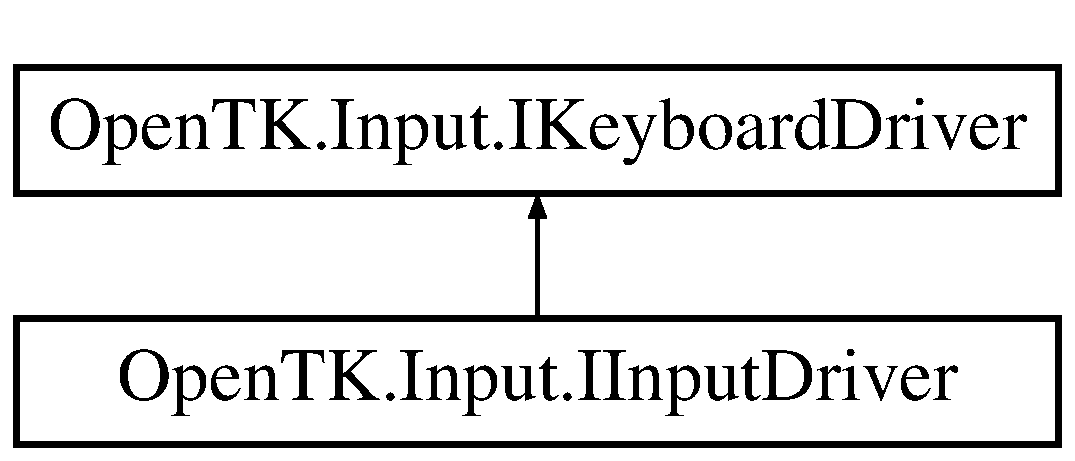
\includegraphics[height=2.000000cm]{interface_open_t_k_1_1_input_1_1_i_keyboard_driver}
\end{center}
\end{figure}
\subsection*{Properties}
\begin{DoxyCompactItemize}
\item 
I\-List$<$ \hyperlink{class_open_t_k_1_1_input_1_1_keyboard_device}{Keyboard\-Device} $>$ \hyperlink{interface_open_t_k_1_1_input_1_1_i_keyboard_driver_a2181af987484d7afd98fbd8266c7940b}{Keyboard}\hspace{0.3cm}{\ttfamily  \mbox{[}get\mbox{]}}
\begin{DoxyCompactList}\small\item\em Gets the list of available Keyboard\-Devices. \end{DoxyCompactList}\end{DoxyCompactItemize}


\subsection{Detailed Description}
Defines the interface for \hyperlink{class_open_t_k_1_1_input_1_1_keyboard_device}{Keyboard\-Device} drivers. 



\subsection{Property Documentation}
\hypertarget{interface_open_t_k_1_1_input_1_1_i_keyboard_driver_a2181af987484d7afd98fbd8266c7940b}{\index{Open\-T\-K\-::\-Input\-::\-I\-Keyboard\-Driver@{Open\-T\-K\-::\-Input\-::\-I\-Keyboard\-Driver}!Keyboard@{Keyboard}}
\index{Keyboard@{Keyboard}!OpenTK::Input::IKeyboardDriver@{Open\-T\-K\-::\-Input\-::\-I\-Keyboard\-Driver}}
\subsubsection[{Keyboard}]{\setlength{\rightskip}{0pt plus 5cm}I\-List$<${\bf Keyboard\-Device}$>$ Open\-T\-K.\-Input.\-I\-Keyboard\-Driver.\-Keyboard\hspace{0.3cm}{\ttfamily [get]}}}\label{interface_open_t_k_1_1_input_1_1_i_keyboard_driver_a2181af987484d7afd98fbd8266c7940b}


Gets the list of available Keyboard\-Devices. 


\hypertarget{interface_open_t_k_1_1_input_1_1_i_mouse_driver}{\section{Open\-T\-K.\-Input.\-I\-Mouse\-Driver Interface Reference}
\label{interface_open_t_k_1_1_input_1_1_i_mouse_driver}\index{Open\-T\-K.\-Input.\-I\-Mouse\-Driver@{Open\-T\-K.\-Input.\-I\-Mouse\-Driver}}
}


Defines the interface for \hyperlink{class_open_t_k_1_1_input_1_1_mouse_device}{Mouse\-Device} drivers.  


Inheritance diagram for Open\-T\-K.\-Input.\-I\-Mouse\-Driver\-:\begin{figure}[H]
\begin{center}
\leavevmode
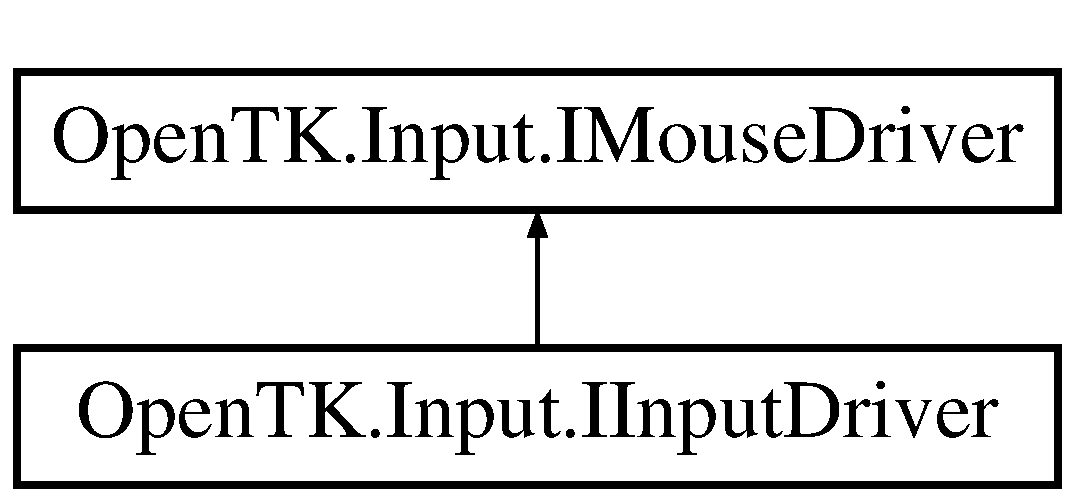
\includegraphics[height=2.000000cm]{interface_open_t_k_1_1_input_1_1_i_mouse_driver}
\end{center}
\end{figure}
\subsection*{Properties}
\begin{DoxyCompactItemize}
\item 
I\-List$<$ \hyperlink{class_open_t_k_1_1_input_1_1_mouse_device}{Mouse\-Device} $>$ \hyperlink{interface_open_t_k_1_1_input_1_1_i_mouse_driver_a1296e581e67f3306448f4ca426e50bd2}{Mouse}\hspace{0.3cm}{\ttfamily  \mbox{[}get\mbox{]}}
\begin{DoxyCompactList}\small\item\em Gets the list of available Mouse\-Devices. \end{DoxyCompactList}\end{DoxyCompactItemize}


\subsection{Detailed Description}
Defines the interface for \hyperlink{class_open_t_k_1_1_input_1_1_mouse_device}{Mouse\-Device} drivers. 



\subsection{Property Documentation}
\hypertarget{interface_open_t_k_1_1_input_1_1_i_mouse_driver_a1296e581e67f3306448f4ca426e50bd2}{\index{Open\-T\-K\-::\-Input\-::\-I\-Mouse\-Driver@{Open\-T\-K\-::\-Input\-::\-I\-Mouse\-Driver}!Mouse@{Mouse}}
\index{Mouse@{Mouse}!OpenTK::Input::IMouseDriver@{Open\-T\-K\-::\-Input\-::\-I\-Mouse\-Driver}}
\subsubsection[{Mouse}]{\setlength{\rightskip}{0pt plus 5cm}I\-List$<${\bf Mouse\-Device}$>$ Open\-T\-K.\-Input.\-I\-Mouse\-Driver.\-Mouse\hspace{0.3cm}{\ttfamily [get]}}}\label{interface_open_t_k_1_1_input_1_1_i_mouse_driver_a1296e581e67f3306448f4ca426e50bd2}


Gets the list of available Mouse\-Devices. 


\hypertarget{class_open_t_k_1_1_input_1_1_joystick_axis_collection}{\section{Open\-T\-K.\-Input.\-Joystick\-Axis\-Collection Class Reference}
\label{class_open_t_k_1_1_input_1_1_joystick_axis_collection}\index{Open\-T\-K.\-Input.\-Joystick\-Axis\-Collection@{Open\-T\-K.\-Input.\-Joystick\-Axis\-Collection}}
}


Defines a collection of Joystick\-Axes.  


\subsection*{Properties}
\begin{DoxyCompactItemize}
\item 
float \hyperlink{class_open_t_k_1_1_input_1_1_joystick_axis_collection_a71e33c41bc7cb899a68883d205fbc98c}{this\mbox{[}int index\mbox{]}}\hspace{0.3cm}{\ttfamily  \mbox{[}get, set\mbox{]}}
\begin{DoxyCompactList}\small\item\em Gets a System.\-Single indicating the absolute position of the Joystick\-Axis with the specified index. \end{DoxyCompactList}\item 
float \hyperlink{class_open_t_k_1_1_input_1_1_joystick_axis_collection_ab3bdbbfa5eb3a1fa18f3acefbc638247}{this\mbox{[}\-Joystick\-Axis axis\mbox{]}}\hspace{0.3cm}{\ttfamily  \mbox{[}get, set\mbox{]}}
\begin{DoxyCompactList}\small\item\em Gets a System.\-Single indicating the absolute position of the Joystick\-Axis. \end{DoxyCompactList}\item 
int \hyperlink{class_open_t_k_1_1_input_1_1_joystick_axis_collection_a32a9980bbfb26d9672393aa41ea6f7c0}{Count}\hspace{0.3cm}{\ttfamily  \mbox{[}get\mbox{]}}
\begin{DoxyCompactList}\small\item\em Gets a System.\-Int32 indicating the available amount of Joystick\-Axes. \end{DoxyCompactList}\end{DoxyCompactItemize}


\subsection{Detailed Description}
Defines a collection of Joystick\-Axes. 



\subsection{Property Documentation}
\hypertarget{class_open_t_k_1_1_input_1_1_joystick_axis_collection_a32a9980bbfb26d9672393aa41ea6f7c0}{\index{Open\-T\-K\-::\-Input\-::\-Joystick\-Axis\-Collection@{Open\-T\-K\-::\-Input\-::\-Joystick\-Axis\-Collection}!Count@{Count}}
\index{Count@{Count}!OpenTK::Input::JoystickAxisCollection@{Open\-T\-K\-::\-Input\-::\-Joystick\-Axis\-Collection}}
\subsubsection[{Count}]{\setlength{\rightskip}{0pt plus 5cm}int Open\-T\-K.\-Input.\-Joystick\-Axis\-Collection.\-Count\hspace{0.3cm}{\ttfamily [get]}}}\label{class_open_t_k_1_1_input_1_1_joystick_axis_collection_a32a9980bbfb26d9672393aa41ea6f7c0}


Gets a System.\-Int32 indicating the available amount of Joystick\-Axes. 

\hypertarget{class_open_t_k_1_1_input_1_1_joystick_axis_collection_a71e33c41bc7cb899a68883d205fbc98c}{\index{Open\-T\-K\-::\-Input\-::\-Joystick\-Axis\-Collection@{Open\-T\-K\-::\-Input\-::\-Joystick\-Axis\-Collection}!this\mbox{[}int index\mbox{]}@{this[int index]}}
\index{this\mbox{[}int index\mbox{]}@{this[int index]}!OpenTK::Input::JoystickAxisCollection@{Open\-T\-K\-::\-Input\-::\-Joystick\-Axis\-Collection}}
\subsubsection[{this[int index]}]{\setlength{\rightskip}{0pt plus 5cm}float Open\-T\-K.\-Input.\-Joystick\-Axis\-Collection.\-this\mbox{[}int index\mbox{]}\hspace{0.3cm}{\ttfamily [get]}, {\ttfamily [set]}}}\label{class_open_t_k_1_1_input_1_1_joystick_axis_collection_a71e33c41bc7cb899a68883d205fbc98c}


Gets a System.\-Single indicating the absolute position of the Joystick\-Axis with the specified index. 


\begin{DoxyParams}{Parameters}
{\em index} & The index of the Joystick\-Axis to check.\\
\hline
\end{DoxyParams}
\begin{DoxyReturn}{Returns}
A System.\-Single in the range \mbox{[}-\/1, 1\mbox{]}.
\end{DoxyReturn}
\hypertarget{class_open_t_k_1_1_input_1_1_joystick_axis_collection_ab3bdbbfa5eb3a1fa18f3acefbc638247}{\index{Open\-T\-K\-::\-Input\-::\-Joystick\-Axis\-Collection@{Open\-T\-K\-::\-Input\-::\-Joystick\-Axis\-Collection}!this\mbox{[}\-Joystick\-Axis axis\mbox{]}@{this[Joystick\-Axis axis]}}
\index{this\mbox{[}\-Joystick\-Axis axis\mbox{]}@{this[Joystick\-Axis axis]}!OpenTK::Input::JoystickAxisCollection@{Open\-T\-K\-::\-Input\-::\-Joystick\-Axis\-Collection}}
\subsubsection[{this[Joystick\-Axis axis]}]{\setlength{\rightskip}{0pt plus 5cm}float Open\-T\-K.\-Input.\-Joystick\-Axis\-Collection.\-this\mbox{[}{\bf Joystick\-Axis} axis\mbox{]}\hspace{0.3cm}{\ttfamily [get]}, {\ttfamily [set]}}}\label{class_open_t_k_1_1_input_1_1_joystick_axis_collection_ab3bdbbfa5eb3a1fa18f3acefbc638247}


Gets a System.\-Single indicating the absolute position of the Joystick\-Axis. 


\begin{DoxyParams}{Parameters}
{\em axis} & The Joystick\-Axis to check.\\
\hline
\end{DoxyParams}
\begin{DoxyReturn}{Returns}
A System.\-Single in the range \mbox{[}-\/1, 1\mbox{]}.
\end{DoxyReturn}

\hypertarget{class_open_t_k_1_1_input_1_1_joystick_button_collection}{\section{Open\-T\-K.\-Input.\-Joystick\-Button\-Collection Class Reference}
\label{class_open_t_k_1_1_input_1_1_joystick_button_collection}\index{Open\-T\-K.\-Input.\-Joystick\-Button\-Collection@{Open\-T\-K.\-Input.\-Joystick\-Button\-Collection}}
}


Defines a collection of Joystick\-Buttons.  


\subsection*{Properties}
\begin{DoxyCompactItemize}
\item 
bool \hyperlink{class_open_t_k_1_1_input_1_1_joystick_button_collection_a19f902624461596a5bbb4b976b9d8f61}{this\mbox{[}int index\mbox{]}}\hspace{0.3cm}{\ttfamily  \mbox{[}get, set\mbox{]}}
\begin{DoxyCompactList}\small\item\em Gets a System.\-Boolean indicating whether the Joystick\-Button with the specified index is pressed. \end{DoxyCompactList}\item 
bool \hyperlink{class_open_t_k_1_1_input_1_1_joystick_button_collection_affc23bad0bf45d348f621d77fc7340c0}{this\mbox{[}\-Joystick\-Button button\mbox{]}}\hspace{0.3cm}{\ttfamily  \mbox{[}get, set\mbox{]}}
\begin{DoxyCompactList}\small\item\em Gets a System.\-Boolean indicating whether the specified Joystick\-Button is pressed. \end{DoxyCompactList}\item 
int \hyperlink{class_open_t_k_1_1_input_1_1_joystick_button_collection_a8641b79aefe0a1f1ec035bb123db0bec}{Count}\hspace{0.3cm}{\ttfamily  \mbox{[}get\mbox{]}}
\begin{DoxyCompactList}\small\item\em Gets a System.\-Int32 indicating the available amount of Joystick\-Buttons. \end{DoxyCompactList}\end{DoxyCompactItemize}


\subsection{Detailed Description}
Defines a collection of Joystick\-Buttons. 



\subsection{Property Documentation}
\hypertarget{class_open_t_k_1_1_input_1_1_joystick_button_collection_a8641b79aefe0a1f1ec035bb123db0bec}{\index{Open\-T\-K\-::\-Input\-::\-Joystick\-Button\-Collection@{Open\-T\-K\-::\-Input\-::\-Joystick\-Button\-Collection}!Count@{Count}}
\index{Count@{Count}!OpenTK::Input::JoystickButtonCollection@{Open\-T\-K\-::\-Input\-::\-Joystick\-Button\-Collection}}
\subsubsection[{Count}]{\setlength{\rightskip}{0pt plus 5cm}int Open\-T\-K.\-Input.\-Joystick\-Button\-Collection.\-Count\hspace{0.3cm}{\ttfamily [get]}}}\label{class_open_t_k_1_1_input_1_1_joystick_button_collection_a8641b79aefe0a1f1ec035bb123db0bec}


Gets a System.\-Int32 indicating the available amount of Joystick\-Buttons. 

\hypertarget{class_open_t_k_1_1_input_1_1_joystick_button_collection_a19f902624461596a5bbb4b976b9d8f61}{\index{Open\-T\-K\-::\-Input\-::\-Joystick\-Button\-Collection@{Open\-T\-K\-::\-Input\-::\-Joystick\-Button\-Collection}!this\mbox{[}int index\mbox{]}@{this[int index]}}
\index{this\mbox{[}int index\mbox{]}@{this[int index]}!OpenTK::Input::JoystickButtonCollection@{Open\-T\-K\-::\-Input\-::\-Joystick\-Button\-Collection}}
\subsubsection[{this[int index]}]{\setlength{\rightskip}{0pt plus 5cm}bool Open\-T\-K.\-Input.\-Joystick\-Button\-Collection.\-this\mbox{[}int index\mbox{]}\hspace{0.3cm}{\ttfamily [get]}, {\ttfamily [set]}}}\label{class_open_t_k_1_1_input_1_1_joystick_button_collection_a19f902624461596a5bbb4b976b9d8f61}


Gets a System.\-Boolean indicating whether the Joystick\-Button with the specified index is pressed. 


\begin{DoxyParams}{Parameters}
{\em index} & The index of the Joystick\-Button to check.\\
\hline
\end{DoxyParams}
\begin{DoxyReturn}{Returns}
True if the Joystick\-Button is pressed; false otherwise.
\end{DoxyReturn}
\hypertarget{class_open_t_k_1_1_input_1_1_joystick_button_collection_affc23bad0bf45d348f621d77fc7340c0}{\index{Open\-T\-K\-::\-Input\-::\-Joystick\-Button\-Collection@{Open\-T\-K\-::\-Input\-::\-Joystick\-Button\-Collection}!this\mbox{[}\-Joystick\-Button button\mbox{]}@{this[Joystick\-Button button]}}
\index{this\mbox{[}\-Joystick\-Button button\mbox{]}@{this[Joystick\-Button button]}!OpenTK::Input::JoystickButtonCollection@{Open\-T\-K\-::\-Input\-::\-Joystick\-Button\-Collection}}
\subsubsection[{this[Joystick\-Button button]}]{\setlength{\rightskip}{0pt plus 5cm}bool Open\-T\-K.\-Input.\-Joystick\-Button\-Collection.\-this\mbox{[}{\bf Joystick\-Button} button\mbox{]}\hspace{0.3cm}{\ttfamily [get]}, {\ttfamily [set]}}}\label{class_open_t_k_1_1_input_1_1_joystick_button_collection_affc23bad0bf45d348f621d77fc7340c0}


Gets a System.\-Boolean indicating whether the specified Joystick\-Button is pressed. 


\begin{DoxyParams}{Parameters}
{\em button} & The Joystick\-Button to check.\\
\hline
\end{DoxyParams}
\begin{DoxyReturn}{Returns}
True if the Joystick\-Button is pressed; false otherwise.
\end{DoxyReturn}

\hypertarget{class_open_t_k_1_1_input_1_1_joystick_button_event_args}{\section{Open\-T\-K.\-Input.\-Joystick\-Button\-Event\-Args Class Reference}
\label{class_open_t_k_1_1_input_1_1_joystick_button_event_args}\index{Open\-T\-K.\-Input.\-Joystick\-Button\-Event\-Args@{Open\-T\-K.\-Input.\-Joystick\-Button\-Event\-Args}}
}


Provides data for the \hyperlink{class_open_t_k_1_1_input_1_1_joystick_device_a677045ca3c8a2ac98095680bb5746ede}{Joystick\-Device.\-Button\-Down} and \hyperlink{class_open_t_k_1_1_input_1_1_joystick_device_a837891423d49811a2384c95f7576fbc2}{Joystick\-Device.\-Button\-Up} events. This class is cached for performance reasons -\/ avoid storing references outside the scope of the event.  




Inherits Event\-Args.

\subsection*{Properties}
\begin{DoxyCompactItemize}
\item 
\hyperlink{namespace_open_t_k_1_1_input_a54204a11d897164a26ceff29ee03f3d3}{Joystick\-Button} \hyperlink{class_open_t_k_1_1_input_1_1_joystick_button_event_args_a5984a4a8d487119f6e362661fc36c706}{Button}\hspace{0.3cm}{\ttfamily  \mbox{[}get, set\mbox{]}}
\begin{DoxyCompactList}\small\item\em The index of the joystick button for the event. \end{DoxyCompactList}\item 
bool \hyperlink{class_open_t_k_1_1_input_1_1_joystick_button_event_args_a0bb2f495334c5e6e0f7a89e4354d6721}{Pressed}\hspace{0.3cm}{\ttfamily  \mbox{[}get, set\mbox{]}}
\begin{DoxyCompactList}\small\item\em Gets a System.\-Boolean representing the state of the button for the event. \end{DoxyCompactList}\end{DoxyCompactItemize}


\subsection{Detailed Description}
Provides data for the \hyperlink{class_open_t_k_1_1_input_1_1_joystick_device_a677045ca3c8a2ac98095680bb5746ede}{Joystick\-Device.\-Button\-Down} and \hyperlink{class_open_t_k_1_1_input_1_1_joystick_device_a837891423d49811a2384c95f7576fbc2}{Joystick\-Device.\-Button\-Up} events. This class is cached for performance reasons -\/ avoid storing references outside the scope of the event. 



\subsection{Property Documentation}
\hypertarget{class_open_t_k_1_1_input_1_1_joystick_button_event_args_a5984a4a8d487119f6e362661fc36c706}{\index{Open\-T\-K\-::\-Input\-::\-Joystick\-Button\-Event\-Args@{Open\-T\-K\-::\-Input\-::\-Joystick\-Button\-Event\-Args}!Button@{Button}}
\index{Button@{Button}!OpenTK::Input::JoystickButtonEventArgs@{Open\-T\-K\-::\-Input\-::\-Joystick\-Button\-Event\-Args}}
\subsubsection[{Button}]{\setlength{\rightskip}{0pt plus 5cm}{\bf Joystick\-Button} Open\-T\-K.\-Input.\-Joystick\-Button\-Event\-Args.\-Button\hspace{0.3cm}{\ttfamily [get]}, {\ttfamily [set]}}}\label{class_open_t_k_1_1_input_1_1_joystick_button_event_args_a5984a4a8d487119f6e362661fc36c706}


The index of the joystick button for the event. 

\hypertarget{class_open_t_k_1_1_input_1_1_joystick_button_event_args_a0bb2f495334c5e6e0f7a89e4354d6721}{\index{Open\-T\-K\-::\-Input\-::\-Joystick\-Button\-Event\-Args@{Open\-T\-K\-::\-Input\-::\-Joystick\-Button\-Event\-Args}!Pressed@{Pressed}}
\index{Pressed@{Pressed}!OpenTK::Input::JoystickButtonEventArgs@{Open\-T\-K\-::\-Input\-::\-Joystick\-Button\-Event\-Args}}
\subsubsection[{Pressed}]{\setlength{\rightskip}{0pt plus 5cm}bool Open\-T\-K.\-Input.\-Joystick\-Button\-Event\-Args.\-Pressed\hspace{0.3cm}{\ttfamily [get]}, {\ttfamily [set]}}}\label{class_open_t_k_1_1_input_1_1_joystick_button_event_args_a0bb2f495334c5e6e0f7a89e4354d6721}


Gets a System.\-Boolean representing the state of the button for the event. 


\hypertarget{class_open_t_k_1_1_input_1_1_joystick_device}{\section{Open\-T\-K.\-Input.\-Joystick\-Device Class Reference}
\label{class_open_t_k_1_1_input_1_1_joystick_device}\index{Open\-T\-K.\-Input.\-Joystick\-Device@{Open\-T\-K.\-Input.\-Joystick\-Device}}
}


Represents a joystick device and provides methods to query its status.  


Inheritance diagram for Open\-T\-K.\-Input.\-Joystick\-Device\-:\begin{figure}[H]
\begin{center}
\leavevmode
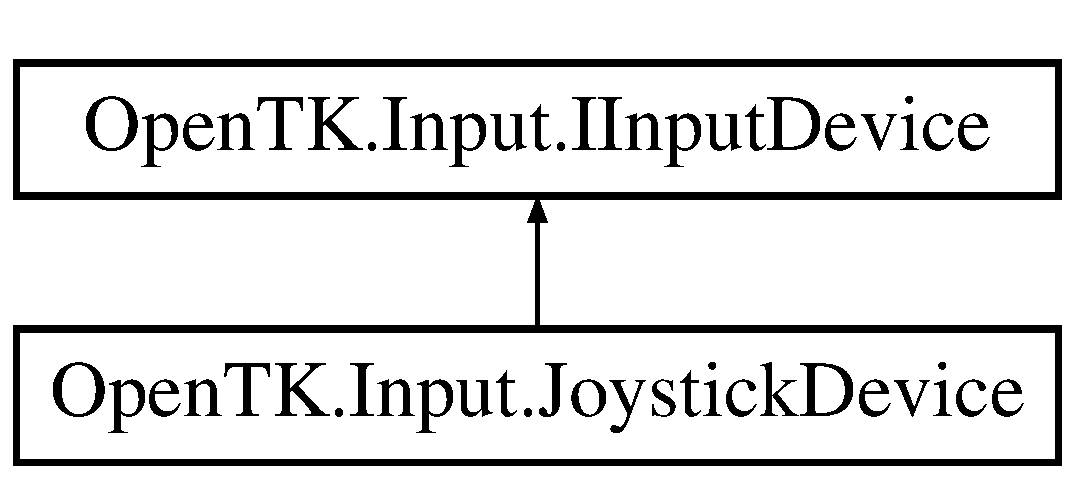
\includegraphics[height=2.000000cm]{class_open_t_k_1_1_input_1_1_joystick_device}
\end{center}
\end{figure}
\subsection*{Public Attributes}
\begin{DoxyCompactItemize}
\item 
Event\-Handler\\*
$<$ \hyperlink{class_open_t_k_1_1_input_1_1_joystick_move_event_args}{Joystick\-Move\-Event\-Args} $>$ \hyperlink{class_open_t_k_1_1_input_1_1_joystick_device_ad9dcc4f6506c543d16e326c7ee08da39}{Move}
\begin{DoxyCompactList}\small\item\em Occurs when an axis of this \hyperlink{class_open_t_k_1_1_input_1_1_joystick_device}{Joystick\-Device} instance is moved. \end{DoxyCompactList}\item 
Event\-Handler\\*
$<$ \hyperlink{class_open_t_k_1_1_input_1_1_joystick_button_event_args}{Joystick\-Button\-Event\-Args} $>$ \hyperlink{class_open_t_k_1_1_input_1_1_joystick_device_a677045ca3c8a2ac98095680bb5746ede}{Button\-Down}
\begin{DoxyCompactList}\small\item\em Occurs when a button of this \hyperlink{class_open_t_k_1_1_input_1_1_joystick_device}{Joystick\-Device} instance is pressed. \end{DoxyCompactList}\item 
Event\-Handler\\*
$<$ \hyperlink{class_open_t_k_1_1_input_1_1_joystick_button_event_args}{Joystick\-Button\-Event\-Args} $>$ \hyperlink{class_open_t_k_1_1_input_1_1_joystick_device_a837891423d49811a2384c95f7576fbc2}{Button\-Up}
\begin{DoxyCompactList}\small\item\em Occurs when a button of this \hyperlink{class_open_t_k_1_1_input_1_1_joystick_device}{Joystick\-Device} is released. \end{DoxyCompactList}\end{DoxyCompactItemize}
\subsection*{Properties}
\begin{DoxyCompactItemize}
\item 
\hyperlink{class_open_t_k_1_1_input_1_1_joystick_axis_collection}{Joystick\-Axis\-Collection} \hyperlink{class_open_t_k_1_1_input_1_1_joystick_device_a21ae34496707cad92024def6a122e878}{Axis}\hspace{0.3cm}{\ttfamily  \mbox{[}get\mbox{]}}
\begin{DoxyCompactList}\small\item\em Gets a \hyperlink{class_open_t_k_1_1_input_1_1_joystick_axis_collection}{Joystick\-Axis\-Collection} containing the state of each axis on this instance. Values are normalized in the \mbox{[}-\/1, 1\mbox{]} range. \end{DoxyCompactList}\item 
\hyperlink{class_open_t_k_1_1_input_1_1_joystick_button_collection}{Joystick\-Button\-Collection} \hyperlink{class_open_t_k_1_1_input_1_1_joystick_device_afab123d1de6fce4b1ce79a8480d6bc4b}{Button}\hspace{0.3cm}{\ttfamily  \mbox{[}get\mbox{]}}
\begin{DoxyCompactList}\small\item\em Gets \hyperlink{class_open_t_k_1_1_input_1_1_joystick_button_collection}{Joystick\-Button\-Collection} containing the state of each button on this instance. True indicates that the button is pressed. \end{DoxyCompactList}\item 
string \hyperlink{class_open_t_k_1_1_input_1_1_joystick_device_ae04707b3c97c5aeedde335995c1821f6}{Description}\hspace{0.3cm}{\ttfamily  \mbox{[}get, set\mbox{]}}
\begin{DoxyCompactList}\small\item\em Gets a System.\-String containing a unique description for this instance. \end{DoxyCompactList}\item 
\hyperlink{namespace_open_t_k_1_1_input_a1d147c6256b0adaa5288eec90ed93270}{Input\-Device\-Type} \hyperlink{class_open_t_k_1_1_input_1_1_joystick_device_af1eddeb505296cf4a598090113b1f5df}{Device\-Type}\hspace{0.3cm}{\ttfamily  \mbox{[}get\mbox{]}}
\begin{DoxyCompactList}\small\item\em Gets a value indicating the Input\-Device\-Type of this Input\-Device. \end{DoxyCompactList}\end{DoxyCompactItemize}


\subsection{Detailed Description}
Represents a joystick device and provides methods to query its status. 



\subsection{Member Data Documentation}
\hypertarget{class_open_t_k_1_1_input_1_1_joystick_device_a677045ca3c8a2ac98095680bb5746ede}{\index{Open\-T\-K\-::\-Input\-::\-Joystick\-Device@{Open\-T\-K\-::\-Input\-::\-Joystick\-Device}!Button\-Down@{Button\-Down}}
\index{Button\-Down@{Button\-Down}!OpenTK::Input::JoystickDevice@{Open\-T\-K\-::\-Input\-::\-Joystick\-Device}}
\subsubsection[{Button\-Down}]{\setlength{\rightskip}{0pt plus 5cm}Event\-Handler$<${\bf Joystick\-Button\-Event\-Args}$>$ Open\-T\-K.\-Input.\-Joystick\-Device.\-Button\-Down}}\label{class_open_t_k_1_1_input_1_1_joystick_device_a677045ca3c8a2ac98095680bb5746ede}
{\bfseries Initial value\-:}
\begin{DoxyCode}
=
            delegate(\textcolor{keywordtype}{object} sender, JoystickButtonEventArgs e) \{ \}
\end{DoxyCode}


Occurs when a button of this \hyperlink{class_open_t_k_1_1_input_1_1_joystick_device}{Joystick\-Device} instance is pressed. 

\hypertarget{class_open_t_k_1_1_input_1_1_joystick_device_a837891423d49811a2384c95f7576fbc2}{\index{Open\-T\-K\-::\-Input\-::\-Joystick\-Device@{Open\-T\-K\-::\-Input\-::\-Joystick\-Device}!Button\-Up@{Button\-Up}}
\index{Button\-Up@{Button\-Up}!OpenTK::Input::JoystickDevice@{Open\-T\-K\-::\-Input\-::\-Joystick\-Device}}
\subsubsection[{Button\-Up}]{\setlength{\rightskip}{0pt plus 5cm}Event\-Handler$<${\bf Joystick\-Button\-Event\-Args}$>$ Open\-T\-K.\-Input.\-Joystick\-Device.\-Button\-Up}}\label{class_open_t_k_1_1_input_1_1_joystick_device_a837891423d49811a2384c95f7576fbc2}
{\bfseries Initial value\-:}
\begin{DoxyCode}
=
            delegate(\textcolor{keywordtype}{object} sender, JoystickButtonEventArgs e) \{ \}
\end{DoxyCode}


Occurs when a button of this \hyperlink{class_open_t_k_1_1_input_1_1_joystick_device}{Joystick\-Device} is released. 

\hypertarget{class_open_t_k_1_1_input_1_1_joystick_device_ad9dcc4f6506c543d16e326c7ee08da39}{\index{Open\-T\-K\-::\-Input\-::\-Joystick\-Device@{Open\-T\-K\-::\-Input\-::\-Joystick\-Device}!Move@{Move}}
\index{Move@{Move}!OpenTK::Input::JoystickDevice@{Open\-T\-K\-::\-Input\-::\-Joystick\-Device}}
\subsubsection[{Move}]{\setlength{\rightskip}{0pt plus 5cm}Event\-Handler$<${\bf Joystick\-Move\-Event\-Args}$>$ Open\-T\-K.\-Input.\-Joystick\-Device.\-Move}}\label{class_open_t_k_1_1_input_1_1_joystick_device_ad9dcc4f6506c543d16e326c7ee08da39}
{\bfseries Initial value\-:}
\begin{DoxyCode}
=
            delegate(\textcolor{keywordtype}{object} sender, JoystickMoveEventArgs e) \{ \}
\end{DoxyCode}


Occurs when an axis of this \hyperlink{class_open_t_k_1_1_input_1_1_joystick_device}{Joystick\-Device} instance is moved. 



\subsection{Property Documentation}
\hypertarget{class_open_t_k_1_1_input_1_1_joystick_device_a21ae34496707cad92024def6a122e878}{\index{Open\-T\-K\-::\-Input\-::\-Joystick\-Device@{Open\-T\-K\-::\-Input\-::\-Joystick\-Device}!Axis@{Axis}}
\index{Axis@{Axis}!OpenTK::Input::JoystickDevice@{Open\-T\-K\-::\-Input\-::\-Joystick\-Device}}
\subsubsection[{Axis}]{\setlength{\rightskip}{0pt plus 5cm}{\bf Joystick\-Axis\-Collection} Open\-T\-K.\-Input.\-Joystick\-Device.\-Axis\hspace{0.3cm}{\ttfamily [get]}}}\label{class_open_t_k_1_1_input_1_1_joystick_device_a21ae34496707cad92024def6a122e878}


Gets a \hyperlink{class_open_t_k_1_1_input_1_1_joystick_axis_collection}{Joystick\-Axis\-Collection} containing the state of each axis on this instance. Values are normalized in the \mbox{[}-\/1, 1\mbox{]} range. 

\hypertarget{class_open_t_k_1_1_input_1_1_joystick_device_afab123d1de6fce4b1ce79a8480d6bc4b}{\index{Open\-T\-K\-::\-Input\-::\-Joystick\-Device@{Open\-T\-K\-::\-Input\-::\-Joystick\-Device}!Button@{Button}}
\index{Button@{Button}!OpenTK::Input::JoystickDevice@{Open\-T\-K\-::\-Input\-::\-Joystick\-Device}}
\subsubsection[{Button}]{\setlength{\rightskip}{0pt plus 5cm}{\bf Joystick\-Button\-Collection} Open\-T\-K.\-Input.\-Joystick\-Device.\-Button\hspace{0.3cm}{\ttfamily [get]}}}\label{class_open_t_k_1_1_input_1_1_joystick_device_afab123d1de6fce4b1ce79a8480d6bc4b}


Gets \hyperlink{class_open_t_k_1_1_input_1_1_joystick_button_collection}{Joystick\-Button\-Collection} containing the state of each button on this instance. True indicates that the button is pressed. 

\hypertarget{class_open_t_k_1_1_input_1_1_joystick_device_ae04707b3c97c5aeedde335995c1821f6}{\index{Open\-T\-K\-::\-Input\-::\-Joystick\-Device@{Open\-T\-K\-::\-Input\-::\-Joystick\-Device}!Description@{Description}}
\index{Description@{Description}!OpenTK::Input::JoystickDevice@{Open\-T\-K\-::\-Input\-::\-Joystick\-Device}}
\subsubsection[{Description}]{\setlength{\rightskip}{0pt plus 5cm}string Open\-T\-K.\-Input.\-Joystick\-Device.\-Description\hspace{0.3cm}{\ttfamily [get]}, {\ttfamily [set]}}}\label{class_open_t_k_1_1_input_1_1_joystick_device_ae04707b3c97c5aeedde335995c1821f6}


Gets a System.\-String containing a unique description for this instance. 

\hypertarget{class_open_t_k_1_1_input_1_1_joystick_device_af1eddeb505296cf4a598090113b1f5df}{\index{Open\-T\-K\-::\-Input\-::\-Joystick\-Device@{Open\-T\-K\-::\-Input\-::\-Joystick\-Device}!Device\-Type@{Device\-Type}}
\index{Device\-Type@{Device\-Type}!OpenTK::Input::JoystickDevice@{Open\-T\-K\-::\-Input\-::\-Joystick\-Device}}
\subsubsection[{Device\-Type}]{\setlength{\rightskip}{0pt plus 5cm}{\bf Input\-Device\-Type} Open\-T\-K.\-Input.\-Joystick\-Device.\-Device\-Type\hspace{0.3cm}{\ttfamily [get]}}}\label{class_open_t_k_1_1_input_1_1_joystick_device_af1eddeb505296cf4a598090113b1f5df}


Gets a value indicating the Input\-Device\-Type of this Input\-Device. 


\hypertarget{class_open_t_k_1_1_input_1_1_joystick_event_args}{\section{Open\-T\-K.\-Input.\-Joystick\-Event\-Args Class Reference}
\label{class_open_t_k_1_1_input_1_1_joystick_event_args}\index{Open\-T\-K.\-Input.\-Joystick\-Event\-Args@{Open\-T\-K.\-Input.\-Joystick\-Event\-Args}}
}


The base class for \hyperlink{class_open_t_k_1_1_input_1_1_joystick_device}{Joystick\-Device} event arguments.  


Inheritance diagram for Open\-T\-K.\-Input.\-Joystick\-Event\-Args\-:\begin{figure}[H]
\begin{center}
\leavevmode
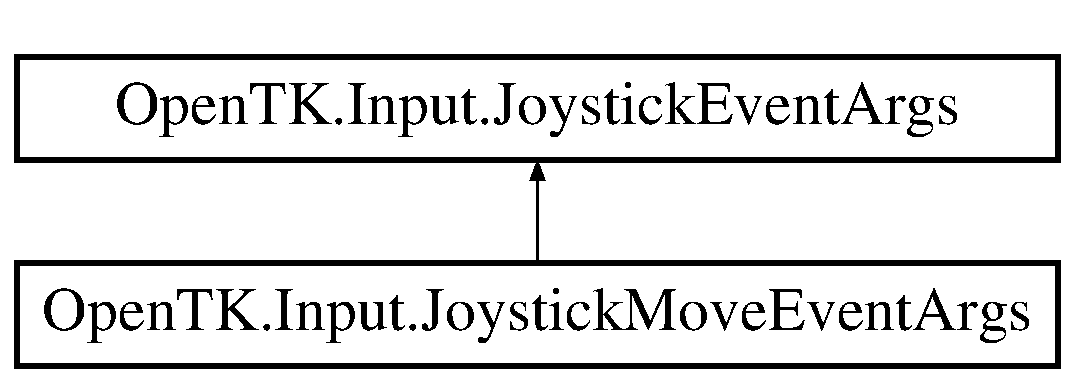
\includegraphics[height=2.000000cm]{class_open_t_k_1_1_input_1_1_joystick_event_args}
\end{center}
\end{figure}


\subsection{Detailed Description}
The base class for \hyperlink{class_open_t_k_1_1_input_1_1_joystick_device}{Joystick\-Device} event arguments. 


\hypertarget{class_open_t_k_1_1_input_1_1_joystick_move_event_args}{\section{Open\-T\-K.\-Input.\-Joystick\-Move\-Event\-Args Class Reference}
\label{class_open_t_k_1_1_input_1_1_joystick_move_event_args}\index{Open\-T\-K.\-Input.\-Joystick\-Move\-Event\-Args@{Open\-T\-K.\-Input.\-Joystick\-Move\-Event\-Args}}
}


Provides data for the \hyperlink{class_open_t_k_1_1_input_1_1_joystick_device_ad9dcc4f6506c543d16e326c7ee08da39}{Joystick\-Device.\-Move} event. This class is cached for performance reasons -\/ avoid storing references outside the scope of the event.  


Inheritance diagram for Open\-T\-K.\-Input.\-Joystick\-Move\-Event\-Args\-:\begin{figure}[H]
\begin{center}
\leavevmode
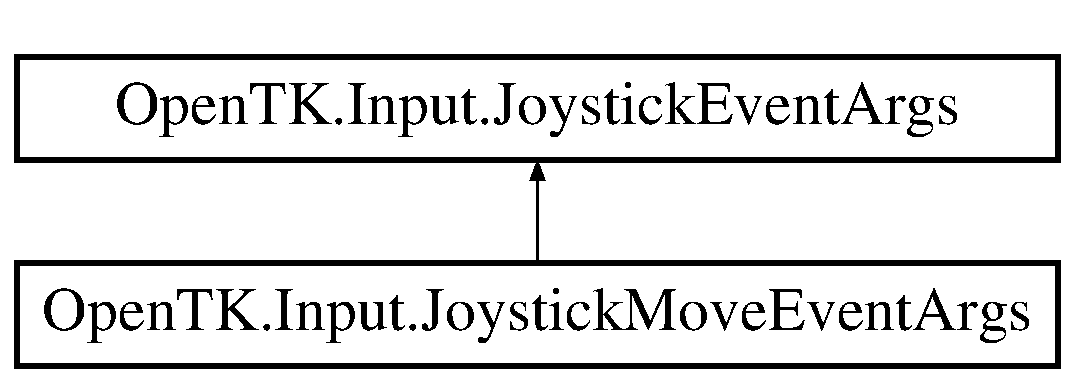
\includegraphics[height=2.000000cm]{class_open_t_k_1_1_input_1_1_joystick_move_event_args}
\end{center}
\end{figure}
\subsection*{Public Member Functions}
\begin{DoxyCompactItemize}
\item 
\hyperlink{class_open_t_k_1_1_input_1_1_joystick_move_event_args_a0baacfbe5fdd5f1b86cbe60fa084213e}{Joystick\-Move\-Event\-Args} (\hyperlink{namespace_open_t_k_1_1_input_ab565c2e944f2be911b6b39e1d5ee4fda}{Joystick\-Axis} axis, float value, float delta)
\begin{DoxyCompactList}\small\item\em Initializes a new instance of the \hyperlink{class_open_t_k_1_1_input_1_1_joystick_move_event_args}{Joystick\-Move\-Event\-Args} class. \end{DoxyCompactList}\end{DoxyCompactItemize}
\subsection*{Properties}
\begin{DoxyCompactItemize}
\item 
\hyperlink{namespace_open_t_k_1_1_input_ab565c2e944f2be911b6b39e1d5ee4fda}{Joystick\-Axis} \hyperlink{class_open_t_k_1_1_input_1_1_joystick_move_event_args_a25730ccb923e12a9890e75697bdba6a2}{Axis}\hspace{0.3cm}{\ttfamily  \mbox{[}get, set\mbox{]}}
\begin{DoxyCompactList}\small\item\em Gets a System.\-Int32 representing the index of the axis that was moved. \end{DoxyCompactList}\item 
float \hyperlink{class_open_t_k_1_1_input_1_1_joystick_move_event_args_a8944831f91ed3f63c6ac77472e42c2a2}{Value}\hspace{0.3cm}{\ttfamily  \mbox{[}get, set\mbox{]}}
\begin{DoxyCompactList}\small\item\em Gets a System.\-Single representing the absolute position of the axis. \end{DoxyCompactList}\item 
float \hyperlink{class_open_t_k_1_1_input_1_1_joystick_move_event_args_a868d586a5500d5729539f77e0702deff}{Delta}\hspace{0.3cm}{\ttfamily  \mbox{[}get, set\mbox{]}}
\begin{DoxyCompactList}\small\item\em Gets a System.\-Single representing the relative change in the position of the axis. \end{DoxyCompactList}\end{DoxyCompactItemize}


\subsection{Detailed Description}
Provides data for the \hyperlink{class_open_t_k_1_1_input_1_1_joystick_device_ad9dcc4f6506c543d16e326c7ee08da39}{Joystick\-Device.\-Move} event. This class is cached for performance reasons -\/ avoid storing references outside the scope of the event. 



\subsection{Constructor \& Destructor Documentation}
\hypertarget{class_open_t_k_1_1_input_1_1_joystick_move_event_args_a0baacfbe5fdd5f1b86cbe60fa084213e}{\index{Open\-T\-K\-::\-Input\-::\-Joystick\-Move\-Event\-Args@{Open\-T\-K\-::\-Input\-::\-Joystick\-Move\-Event\-Args}!Joystick\-Move\-Event\-Args@{Joystick\-Move\-Event\-Args}}
\index{Joystick\-Move\-Event\-Args@{Joystick\-Move\-Event\-Args}!OpenTK::Input::JoystickMoveEventArgs@{Open\-T\-K\-::\-Input\-::\-Joystick\-Move\-Event\-Args}}
\subsubsection[{Joystick\-Move\-Event\-Args}]{\setlength{\rightskip}{0pt plus 5cm}Open\-T\-K.\-Input.\-Joystick\-Move\-Event\-Args.\-Joystick\-Move\-Event\-Args (
\begin{DoxyParamCaption}
\item[{{\bf Joystick\-Axis}}]{axis, }
\item[{float}]{value, }
\item[{float}]{delta}
\end{DoxyParamCaption}
)}}\label{class_open_t_k_1_1_input_1_1_joystick_move_event_args_a0baacfbe5fdd5f1b86cbe60fa084213e}


Initializes a new instance of the \hyperlink{class_open_t_k_1_1_input_1_1_joystick_move_event_args}{Joystick\-Move\-Event\-Args} class. 


\begin{DoxyParams}{Parameters}
{\em axis} & The index of the joystick axis that was moved.\\
\hline
{\em value} & The absolute value of the joystick axis.\\
\hline
{\em delta} & The relative change in value of the joystick axis.\\
\hline
\end{DoxyParams}


\subsection{Property Documentation}
\hypertarget{class_open_t_k_1_1_input_1_1_joystick_move_event_args_a25730ccb923e12a9890e75697bdba6a2}{\index{Open\-T\-K\-::\-Input\-::\-Joystick\-Move\-Event\-Args@{Open\-T\-K\-::\-Input\-::\-Joystick\-Move\-Event\-Args}!Axis@{Axis}}
\index{Axis@{Axis}!OpenTK::Input::JoystickMoveEventArgs@{Open\-T\-K\-::\-Input\-::\-Joystick\-Move\-Event\-Args}}
\subsubsection[{Axis}]{\setlength{\rightskip}{0pt plus 5cm}{\bf Joystick\-Axis} Open\-T\-K.\-Input.\-Joystick\-Move\-Event\-Args.\-Axis\hspace{0.3cm}{\ttfamily [get]}, {\ttfamily [set]}}}\label{class_open_t_k_1_1_input_1_1_joystick_move_event_args_a25730ccb923e12a9890e75697bdba6a2}


Gets a System.\-Int32 representing the index of the axis that was moved. 

\hypertarget{class_open_t_k_1_1_input_1_1_joystick_move_event_args_a868d586a5500d5729539f77e0702deff}{\index{Open\-T\-K\-::\-Input\-::\-Joystick\-Move\-Event\-Args@{Open\-T\-K\-::\-Input\-::\-Joystick\-Move\-Event\-Args}!Delta@{Delta}}
\index{Delta@{Delta}!OpenTK::Input::JoystickMoveEventArgs@{Open\-T\-K\-::\-Input\-::\-Joystick\-Move\-Event\-Args}}
\subsubsection[{Delta}]{\setlength{\rightskip}{0pt plus 5cm}float Open\-T\-K.\-Input.\-Joystick\-Move\-Event\-Args.\-Delta\hspace{0.3cm}{\ttfamily [get]}, {\ttfamily [set]}}}\label{class_open_t_k_1_1_input_1_1_joystick_move_event_args_a868d586a5500d5729539f77e0702deff}


Gets a System.\-Single representing the relative change in the position of the axis. 

\hypertarget{class_open_t_k_1_1_input_1_1_joystick_move_event_args_a8944831f91ed3f63c6ac77472e42c2a2}{\index{Open\-T\-K\-::\-Input\-::\-Joystick\-Move\-Event\-Args@{Open\-T\-K\-::\-Input\-::\-Joystick\-Move\-Event\-Args}!Value@{Value}}
\index{Value@{Value}!OpenTK::Input::JoystickMoveEventArgs@{Open\-T\-K\-::\-Input\-::\-Joystick\-Move\-Event\-Args}}
\subsubsection[{Value}]{\setlength{\rightskip}{0pt plus 5cm}float Open\-T\-K.\-Input.\-Joystick\-Move\-Event\-Args.\-Value\hspace{0.3cm}{\ttfamily [get]}, {\ttfamily [set]}}}\label{class_open_t_k_1_1_input_1_1_joystick_move_event_args_a8944831f91ed3f63c6ac77472e42c2a2}


Gets a System.\-Single representing the absolute position of the axis. 


\hypertarget{class_open_t_k_1_1_input_1_1_keyboard_device}{\section{Open\-T\-K.\-Input.\-Keyboard\-Device Class Reference}
\label{class_open_t_k_1_1_input_1_1_keyboard_device}\index{Open\-T\-K.\-Input.\-Keyboard\-Device@{Open\-T\-K.\-Input.\-Keyboard\-Device}}
}


Represents a keyboard device and provides methods to query its status.  


Inheritance diagram for Open\-T\-K.\-Input.\-Keyboard\-Device\-:\begin{figure}[H]
\begin{center}
\leavevmode
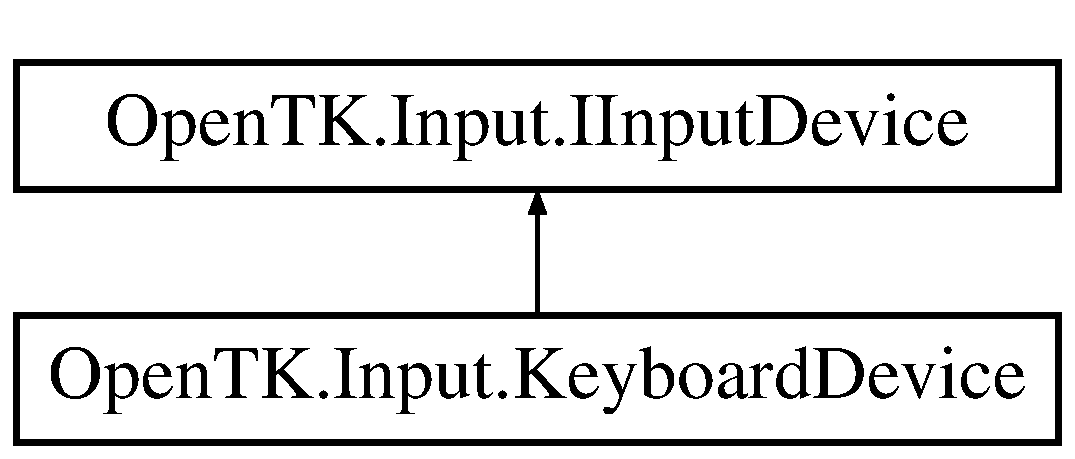
\includegraphics[height=2.000000cm]{class_open_t_k_1_1_input_1_1_keyboard_device}
\end{center}
\end{figure}
\subsection*{Public Member Functions}
\begin{DoxyCompactItemize}
\item 
override int \hyperlink{class_open_t_k_1_1_input_1_1_keyboard_device_ac6151bee0c67b22b61c9b18232b861ca}{Get\-Hash\-Code} ()
\begin{DoxyCompactList}\small\item\em Returns the hash code for this \hyperlink{class_open_t_k_1_1_input_1_1_keyboard_device}{Keyboard\-Device}.\end{DoxyCompactList}\item 
override string \hyperlink{class_open_t_k_1_1_input_1_1_keyboard_device_abe5081c8f817eb2a52f3ae1d681038db}{To\-String} ()
\begin{DoxyCompactList}\small\item\em Returns a System.\-String representing this \hyperlink{class_open_t_k_1_1_input_1_1_keyboard_device}{Keyboard\-Device}. \end{DoxyCompactList}\end{DoxyCompactItemize}
\subsection*{Properties}
\begin{DoxyCompactItemize}
\item 
bool \hyperlink{class_open_t_k_1_1_input_1_1_keyboard_device_a3ae0bcae2f72d9e593a1abd58f3510a4}{this\mbox{[}\-Key key\mbox{]}}\hspace{0.3cm}{\ttfamily  \mbox{[}get\mbox{]}}
\begin{DoxyCompactList}\small\item\em Gets a value indicating the status of the specified Key. \end{DoxyCompactList}\item 
bool \hyperlink{class_open_t_k_1_1_input_1_1_keyboard_device_aa352ed059cb4a2b3127bf307bcdc72ce}{this\mbox{[}uint scancode\mbox{]}}\hspace{0.3cm}{\ttfamily  \mbox{[}get\mbox{]}}
\begin{DoxyCompactList}\small\item\em Gets a value indicating the status of the specified Key. \end{DoxyCompactList}\item 
int \hyperlink{class_open_t_k_1_1_input_1_1_keyboard_device_a8cdb6aa74d46585a6eac945d9460ebb8}{Number\-Of\-Keys}\hspace{0.3cm}{\ttfamily  \mbox{[}get, set\mbox{]}}
\begin{DoxyCompactList}\small\item\em Gets an integer representing the number of keys on this \hyperlink{class_open_t_k_1_1_input_1_1_keyboard_device}{Keyboard\-Device}. \end{DoxyCompactList}\item 
int \hyperlink{class_open_t_k_1_1_input_1_1_keyboard_device_ac00e15c29e8b700cf8ec409c24ecc15f}{Number\-Of\-Function\-Keys}\hspace{0.3cm}{\ttfamily  \mbox{[}get, set\mbox{]}}
\begin{DoxyCompactList}\small\item\em Gets an integer representing the number of function keys (F-\/keys) on this \hyperlink{class_open_t_k_1_1_input_1_1_keyboard_device}{Keyboard\-Device}. \end{DoxyCompactList}\item 
int \hyperlink{class_open_t_k_1_1_input_1_1_keyboard_device_a72f5d5169869c62419219ddbb4ae0077}{Number\-Of\-Leds}\hspace{0.3cm}{\ttfamily  \mbox{[}get, set\mbox{]}}
\begin{DoxyCompactList}\small\item\em Gets a value indicating the number of led indicators on this \hyperlink{class_open_t_k_1_1_input_1_1_keyboard_device}{Keyboard\-Device}. \end{DoxyCompactList}\item 
Int\-Ptr \hyperlink{class_open_t_k_1_1_input_1_1_keyboard_device_a797379213362e109ae766992cb79b2ee}{Device\-I\-D}\hspace{0.3cm}{\ttfamily  \mbox{[}get, set\mbox{]}}
\begin{DoxyCompactList}\small\item\em Gets an Int\-Ptr representing a device dependent I\-D. \end{DoxyCompactList}\item 
bool \hyperlink{class_open_t_k_1_1_input_1_1_keyboard_device_a5a2f02e17370e6ed57f78249cc4b7fde}{Key\-Repeat}\hspace{0.3cm}{\ttfamily  \mbox{[}get, set\mbox{]}}
\begin{DoxyCompactList}\small\item\em Gets or sets a System.\-Boolean indicating key repeat status. \end{DoxyCompactList}\item 
string \hyperlink{class_open_t_k_1_1_input_1_1_keyboard_device_a5985a861383790bf012d1c1351890e5c}{Description}\hspace{0.3cm}{\ttfamily  \mbox{[}get, set\mbox{]}}
\begin{DoxyCompactList}\small\item\em Gets a System.\-String which describes this instance. \end{DoxyCompactList}\item 
\hyperlink{namespace_open_t_k_1_1_input_a1d147c6256b0adaa5288eec90ed93270}{Input\-Device\-Type} \hyperlink{class_open_t_k_1_1_input_1_1_keyboard_device_a35ba052b764e6b488b6799f839f81848}{Device\-Type}\hspace{0.3cm}{\ttfamily  \mbox{[}get\mbox{]}}
\begin{DoxyCompactList}\small\item\em Gets the \hyperlink{namespace_open_t_k_1_1_input_a1d147c6256b0adaa5288eec90ed93270}{Input\-Device\-Type} for this instance. \end{DoxyCompactList}\end{DoxyCompactItemize}
\subsection*{Events}
\begin{DoxyCompactItemize}
\item 
Event\-Handler\\*
$<$ \hyperlink{class_open_t_k_1_1_input_1_1_keyboard_key_event_args}{Keyboard\-Key\-Event\-Args} $>$ \hyperlink{class_open_t_k_1_1_input_1_1_keyboard_device_a6149deb628a69ffafd9616ec88403827}{Key\-Down}
\begin{DoxyCompactList}\small\item\em Occurs when a key is pressed. \end{DoxyCompactList}\item 
Event\-Handler\\*
$<$ \hyperlink{class_open_t_k_1_1_input_1_1_keyboard_key_event_args}{Keyboard\-Key\-Event\-Args} $>$ \hyperlink{class_open_t_k_1_1_input_1_1_keyboard_device_a43137321dca3a4056c8475d483714744}{Key\-Up}
\begin{DoxyCompactList}\small\item\em Occurs when a key is released. \end{DoxyCompactList}\end{DoxyCompactItemize}


\subsection{Detailed Description}
Represents a keyboard device and provides methods to query its status. 



\subsection{Member Function Documentation}
\hypertarget{class_open_t_k_1_1_input_1_1_keyboard_device_ac6151bee0c67b22b61c9b18232b861ca}{\index{Open\-T\-K\-::\-Input\-::\-Keyboard\-Device@{Open\-T\-K\-::\-Input\-::\-Keyboard\-Device}!Get\-Hash\-Code@{Get\-Hash\-Code}}
\index{Get\-Hash\-Code@{Get\-Hash\-Code}!OpenTK::Input::KeyboardDevice@{Open\-T\-K\-::\-Input\-::\-Keyboard\-Device}}
\subsubsection[{Get\-Hash\-Code}]{\setlength{\rightskip}{0pt plus 5cm}override int Open\-T\-K.\-Input.\-Keyboard\-Device.\-Get\-Hash\-Code (
\begin{DoxyParamCaption}
{}
\end{DoxyParamCaption}
)}}\label{class_open_t_k_1_1_input_1_1_keyboard_device_ac6151bee0c67b22b61c9b18232b861ca}


Returns the hash code for this \hyperlink{class_open_t_k_1_1_input_1_1_keyboard_device}{Keyboard\-Device}.

\begin{DoxyReturn}{Returns}
A 32-\/bit signed integer hash code.
\end{DoxyReturn}
\hypertarget{class_open_t_k_1_1_input_1_1_keyboard_device_abe5081c8f817eb2a52f3ae1d681038db}{\index{Open\-T\-K\-::\-Input\-::\-Keyboard\-Device@{Open\-T\-K\-::\-Input\-::\-Keyboard\-Device}!To\-String@{To\-String}}
\index{To\-String@{To\-String}!OpenTK::Input::KeyboardDevice@{Open\-T\-K\-::\-Input\-::\-Keyboard\-Device}}
\subsubsection[{To\-String}]{\setlength{\rightskip}{0pt plus 5cm}override string Open\-T\-K.\-Input.\-Keyboard\-Device.\-To\-String (
\begin{DoxyParamCaption}
{}
\end{DoxyParamCaption}
)}}\label{class_open_t_k_1_1_input_1_1_keyboard_device_abe5081c8f817eb2a52f3ae1d681038db}


Returns a System.\-String representing this \hyperlink{class_open_t_k_1_1_input_1_1_keyboard_device}{Keyboard\-Device}. 

\begin{DoxyReturn}{Returns}
A System.\-String representing this \hyperlink{class_open_t_k_1_1_input_1_1_keyboard_device}{Keyboard\-Device}.
\end{DoxyReturn}


\subsection{Property Documentation}
\hypertarget{class_open_t_k_1_1_input_1_1_keyboard_device_a5985a861383790bf012d1c1351890e5c}{\index{Open\-T\-K\-::\-Input\-::\-Keyboard\-Device@{Open\-T\-K\-::\-Input\-::\-Keyboard\-Device}!Description@{Description}}
\index{Description@{Description}!OpenTK::Input::KeyboardDevice@{Open\-T\-K\-::\-Input\-::\-Keyboard\-Device}}
\subsubsection[{Description}]{\setlength{\rightskip}{0pt plus 5cm}string Open\-T\-K.\-Input.\-Keyboard\-Device.\-Description\hspace{0.3cm}{\ttfamily [get]}, {\ttfamily [set]}}}\label{class_open_t_k_1_1_input_1_1_keyboard_device_a5985a861383790bf012d1c1351890e5c}


Gets a System.\-String which describes this instance. 

\hypertarget{class_open_t_k_1_1_input_1_1_keyboard_device_a797379213362e109ae766992cb79b2ee}{\index{Open\-T\-K\-::\-Input\-::\-Keyboard\-Device@{Open\-T\-K\-::\-Input\-::\-Keyboard\-Device}!Device\-I\-D@{Device\-I\-D}}
\index{Device\-I\-D@{Device\-I\-D}!OpenTK::Input::KeyboardDevice@{Open\-T\-K\-::\-Input\-::\-Keyboard\-Device}}
\subsubsection[{Device\-I\-D}]{\setlength{\rightskip}{0pt plus 5cm}Int\-Ptr Open\-T\-K.\-Input.\-Keyboard\-Device.\-Device\-I\-D\hspace{0.3cm}{\ttfamily [get]}, {\ttfamily [set]}}}\label{class_open_t_k_1_1_input_1_1_keyboard_device_a797379213362e109ae766992cb79b2ee}


Gets an Int\-Ptr representing a device dependent I\-D. 

\hypertarget{class_open_t_k_1_1_input_1_1_keyboard_device_a35ba052b764e6b488b6799f839f81848}{\index{Open\-T\-K\-::\-Input\-::\-Keyboard\-Device@{Open\-T\-K\-::\-Input\-::\-Keyboard\-Device}!Device\-Type@{Device\-Type}}
\index{Device\-Type@{Device\-Type}!OpenTK::Input::KeyboardDevice@{Open\-T\-K\-::\-Input\-::\-Keyboard\-Device}}
\subsubsection[{Device\-Type}]{\setlength{\rightskip}{0pt plus 5cm}{\bf Input\-Device\-Type} Open\-T\-K.\-Input.\-Keyboard\-Device.\-Device\-Type\hspace{0.3cm}{\ttfamily [get]}}}\label{class_open_t_k_1_1_input_1_1_keyboard_device_a35ba052b764e6b488b6799f839f81848}


Gets the \hyperlink{namespace_open_t_k_1_1_input_a1d147c6256b0adaa5288eec90ed93270}{Input\-Device\-Type} for this instance. 

\hypertarget{class_open_t_k_1_1_input_1_1_keyboard_device_a5a2f02e17370e6ed57f78249cc4b7fde}{\index{Open\-T\-K\-::\-Input\-::\-Keyboard\-Device@{Open\-T\-K\-::\-Input\-::\-Keyboard\-Device}!Key\-Repeat@{Key\-Repeat}}
\index{Key\-Repeat@{Key\-Repeat}!OpenTK::Input::KeyboardDevice@{Open\-T\-K\-::\-Input\-::\-Keyboard\-Device}}
\subsubsection[{Key\-Repeat}]{\setlength{\rightskip}{0pt plus 5cm}bool Open\-T\-K.\-Input.\-Keyboard\-Device.\-Key\-Repeat\hspace{0.3cm}{\ttfamily [get]}, {\ttfamily [set]}}}\label{class_open_t_k_1_1_input_1_1_keyboard_device_a5a2f02e17370e6ed57f78249cc4b7fde}


Gets or sets a System.\-Boolean indicating key repeat status. 

If Key\-Repeat is true, multiple Key\-Down events will be generated while a key is being held. Otherwise only one Key\-Down event will be reported. 

The rate of the generated Key\-Down events is controlled by the Operating System. Usually, one Key\-Down event will be reported, followed by a small (250-\/1000ms) pause and several more Key\-Down events (6-\/30 events per second). 

Set to true to handle text input (where keyboard repeat is desirable), but set to false for game input. \hypertarget{class_open_t_k_1_1_input_1_1_keyboard_device_ac00e15c29e8b700cf8ec409c24ecc15f}{\index{Open\-T\-K\-::\-Input\-::\-Keyboard\-Device@{Open\-T\-K\-::\-Input\-::\-Keyboard\-Device}!Number\-Of\-Function\-Keys@{Number\-Of\-Function\-Keys}}
\index{Number\-Of\-Function\-Keys@{Number\-Of\-Function\-Keys}!OpenTK::Input::KeyboardDevice@{Open\-T\-K\-::\-Input\-::\-Keyboard\-Device}}
\subsubsection[{Number\-Of\-Function\-Keys}]{\setlength{\rightskip}{0pt plus 5cm}int Open\-T\-K.\-Input.\-Keyboard\-Device.\-Number\-Of\-Function\-Keys\hspace{0.3cm}{\ttfamily [get]}, {\ttfamily [set]}}}\label{class_open_t_k_1_1_input_1_1_keyboard_device_ac00e15c29e8b700cf8ec409c24ecc15f}


Gets an integer representing the number of function keys (F-\/keys) on this \hyperlink{class_open_t_k_1_1_input_1_1_keyboard_device}{Keyboard\-Device}. 

\hypertarget{class_open_t_k_1_1_input_1_1_keyboard_device_a8cdb6aa74d46585a6eac945d9460ebb8}{\index{Open\-T\-K\-::\-Input\-::\-Keyboard\-Device@{Open\-T\-K\-::\-Input\-::\-Keyboard\-Device}!Number\-Of\-Keys@{Number\-Of\-Keys}}
\index{Number\-Of\-Keys@{Number\-Of\-Keys}!OpenTK::Input::KeyboardDevice@{Open\-T\-K\-::\-Input\-::\-Keyboard\-Device}}
\subsubsection[{Number\-Of\-Keys}]{\setlength{\rightskip}{0pt plus 5cm}int Open\-T\-K.\-Input.\-Keyboard\-Device.\-Number\-Of\-Keys\hspace{0.3cm}{\ttfamily [get]}, {\ttfamily [set]}}}\label{class_open_t_k_1_1_input_1_1_keyboard_device_a8cdb6aa74d46585a6eac945d9460ebb8}


Gets an integer representing the number of keys on this \hyperlink{class_open_t_k_1_1_input_1_1_keyboard_device}{Keyboard\-Device}. 

\hypertarget{class_open_t_k_1_1_input_1_1_keyboard_device_a72f5d5169869c62419219ddbb4ae0077}{\index{Open\-T\-K\-::\-Input\-::\-Keyboard\-Device@{Open\-T\-K\-::\-Input\-::\-Keyboard\-Device}!Number\-Of\-Leds@{Number\-Of\-Leds}}
\index{Number\-Of\-Leds@{Number\-Of\-Leds}!OpenTK::Input::KeyboardDevice@{Open\-T\-K\-::\-Input\-::\-Keyboard\-Device}}
\subsubsection[{Number\-Of\-Leds}]{\setlength{\rightskip}{0pt plus 5cm}int Open\-T\-K.\-Input.\-Keyboard\-Device.\-Number\-Of\-Leds\hspace{0.3cm}{\ttfamily [get]}, {\ttfamily [set]}}}\label{class_open_t_k_1_1_input_1_1_keyboard_device_a72f5d5169869c62419219ddbb4ae0077}


Gets a value indicating the number of led indicators on this \hyperlink{class_open_t_k_1_1_input_1_1_keyboard_device}{Keyboard\-Device}. 

\hypertarget{class_open_t_k_1_1_input_1_1_keyboard_device_a3ae0bcae2f72d9e593a1abd58f3510a4}{\index{Open\-T\-K\-::\-Input\-::\-Keyboard\-Device@{Open\-T\-K\-::\-Input\-::\-Keyboard\-Device}!this\mbox{[}\-Key key\mbox{]}@{this[Key key]}}
\index{this\mbox{[}\-Key key\mbox{]}@{this[Key key]}!OpenTK::Input::KeyboardDevice@{Open\-T\-K\-::\-Input\-::\-Keyboard\-Device}}
\subsubsection[{this[Key key]}]{\setlength{\rightskip}{0pt plus 5cm}bool Open\-T\-K.\-Input.\-Keyboard\-Device.\-this\mbox{[}{\bf Key} key\mbox{]}\hspace{0.3cm}{\ttfamily [get]}}}\label{class_open_t_k_1_1_input_1_1_keyboard_device_a3ae0bcae2f72d9e593a1abd58f3510a4}


Gets a value indicating the status of the specified Key. 


\begin{DoxyParams}{Parameters}
{\em key} & The Key to check.\\
\hline
\end{DoxyParams}
\begin{DoxyReturn}{Returns}
True if the Key is pressed, false otherwise.
\end{DoxyReturn}
\hypertarget{class_open_t_k_1_1_input_1_1_keyboard_device_aa352ed059cb4a2b3127bf307bcdc72ce}{\index{Open\-T\-K\-::\-Input\-::\-Keyboard\-Device@{Open\-T\-K\-::\-Input\-::\-Keyboard\-Device}!this\mbox{[}uint scancode\mbox{]}@{this[uint scancode]}}
\index{this\mbox{[}uint scancode\mbox{]}@{this[uint scancode]}!OpenTK::Input::KeyboardDevice@{Open\-T\-K\-::\-Input\-::\-Keyboard\-Device}}
\subsubsection[{this[uint scancode]}]{\setlength{\rightskip}{0pt plus 5cm}bool Open\-T\-K.\-Input.\-Keyboard\-Device.\-this\mbox{[}uint scancode\mbox{]}\hspace{0.3cm}{\ttfamily [get]}}}\label{class_open_t_k_1_1_input_1_1_keyboard_device_aa352ed059cb4a2b3127bf307bcdc72ce}


Gets a value indicating the status of the specified Key. 


\begin{DoxyParams}{Parameters}
{\em scancode} & The scancode to check.\\
\hline
\end{DoxyParams}
\begin{DoxyReturn}{Returns}
True if the scancode is pressed, false otherwise.
\end{DoxyReturn}


\subsection{Event Documentation}
\hypertarget{class_open_t_k_1_1_input_1_1_keyboard_device_a6149deb628a69ffafd9616ec88403827}{\index{Open\-T\-K\-::\-Input\-::\-Keyboard\-Device@{Open\-T\-K\-::\-Input\-::\-Keyboard\-Device}!Key\-Down@{Key\-Down}}
\index{Key\-Down@{Key\-Down}!OpenTK::Input::KeyboardDevice@{Open\-T\-K\-::\-Input\-::\-Keyboard\-Device}}
\subsubsection[{Key\-Down}]{\setlength{\rightskip}{0pt plus 5cm}Event\-Handler$<${\bf Keyboard\-Key\-Event\-Args}$>$ Open\-T\-K.\-Input.\-Keyboard\-Device.\-Key\-Down}}\label{class_open_t_k_1_1_input_1_1_keyboard_device_a6149deb628a69ffafd9616ec88403827}


Occurs when a key is pressed. 

\hypertarget{class_open_t_k_1_1_input_1_1_keyboard_device_a43137321dca3a4056c8475d483714744}{\index{Open\-T\-K\-::\-Input\-::\-Keyboard\-Device@{Open\-T\-K\-::\-Input\-::\-Keyboard\-Device}!Key\-Up@{Key\-Up}}
\index{Key\-Up@{Key\-Up}!OpenTK::Input::KeyboardDevice@{Open\-T\-K\-::\-Input\-::\-Keyboard\-Device}}
\subsubsection[{Key\-Up}]{\setlength{\rightskip}{0pt plus 5cm}Event\-Handler$<${\bf Keyboard\-Key\-Event\-Args}$>$ Open\-T\-K.\-Input.\-Keyboard\-Device.\-Key\-Up}}\label{class_open_t_k_1_1_input_1_1_keyboard_device_a43137321dca3a4056c8475d483714744}


Occurs when a key is released. 


\hypertarget{class_open_t_k_1_1_input_1_1_keyboard_key_event_args}{\section{Open\-T\-K.\-Input.\-Keyboard\-Key\-Event\-Args Class Reference}
\label{class_open_t_k_1_1_input_1_1_keyboard_key_event_args}\index{Open\-T\-K.\-Input.\-Keyboard\-Key\-Event\-Args@{Open\-T\-K.\-Input.\-Keyboard\-Key\-Event\-Args}}
}


Defines the event data for \hyperlink{class_open_t_k_1_1_input_1_1_keyboard_device}{Keyboard\-Device} events.  




Inherits Event\-Args.

\subsection*{Public Member Functions}
\begin{DoxyCompactItemize}
\item 
\hyperlink{class_open_t_k_1_1_input_1_1_keyboard_key_event_args_a7336854e64eedc2198ca0064ff74c554}{Keyboard\-Key\-Event\-Args} ()
\begin{DoxyCompactList}\small\item\em Constructs a new Keyboard\-Event\-Args instance. \end{DoxyCompactList}\item 
\hyperlink{class_open_t_k_1_1_input_1_1_keyboard_key_event_args_ac6469a7b5ae43fc078de3949b29dc9fe}{Keyboard\-Key\-Event\-Args} (\hyperlink{class_open_t_k_1_1_input_1_1_keyboard_key_event_args}{Keyboard\-Key\-Event\-Args} args)
\begin{DoxyCompactList}\small\item\em Constructs a new Keyboard\-Event\-Args instance. \end{DoxyCompactList}\end{DoxyCompactItemize}
\subsection*{Properties}
\begin{DoxyCompactItemize}
\item 
\hyperlink{namespace_open_t_k_1_1_input_a30415d20dcc907a84693777cc0bdf1c7}{Key} \hyperlink{class_open_t_k_1_1_input_1_1_keyboard_key_event_args_a9524843e284d227163c419260852768a}{Key}\hspace{0.3cm}{\ttfamily  \mbox{[}get, set\mbox{]}}
\begin{DoxyCompactList}\small\item\em Gets the \hyperlink{class_open_t_k_1_1_input_1_1_keyboard_key_event_args_a9524843e284d227163c419260852768a}{Key} that generated this event. \end{DoxyCompactList}\item 
uint \hyperlink{class_open_t_k_1_1_input_1_1_keyboard_key_event_args_a6c078617c6c29f76bc1c771ece1d9604}{Scan\-Code}\hspace{0.3cm}{\ttfamily  \mbox{[}get, set\mbox{]}}
\begin{DoxyCompactList}\small\item\em Gets the scancode which generated this event. \end{DoxyCompactList}\end{DoxyCompactItemize}


\subsection{Detailed Description}
Defines the event data for \hyperlink{class_open_t_k_1_1_input_1_1_keyboard_device}{Keyboard\-Device} events. 

Do not cache instances of this type outside their event handler. If necessary, you can clone a Keyboard\-Event\-Args instance using the \hyperlink{class_open_t_k_1_1_input_1_1_keyboard_key_event_args_ac6469a7b5ae43fc078de3949b29dc9fe}{Keyboard\-Key\-Event\-Args(\-Keyboard\-Key\-Event\-Args)} constructor. 

\subsection{Constructor \& Destructor Documentation}
\hypertarget{class_open_t_k_1_1_input_1_1_keyboard_key_event_args_a7336854e64eedc2198ca0064ff74c554}{\index{Open\-T\-K\-::\-Input\-::\-Keyboard\-Key\-Event\-Args@{Open\-T\-K\-::\-Input\-::\-Keyboard\-Key\-Event\-Args}!Keyboard\-Key\-Event\-Args@{Keyboard\-Key\-Event\-Args}}
\index{Keyboard\-Key\-Event\-Args@{Keyboard\-Key\-Event\-Args}!OpenTK::Input::KeyboardKeyEventArgs@{Open\-T\-K\-::\-Input\-::\-Keyboard\-Key\-Event\-Args}}
\subsubsection[{Keyboard\-Key\-Event\-Args}]{\setlength{\rightskip}{0pt plus 5cm}Open\-T\-K.\-Input.\-Keyboard\-Key\-Event\-Args.\-Keyboard\-Key\-Event\-Args (
\begin{DoxyParamCaption}
{}
\end{DoxyParamCaption}
)}}\label{class_open_t_k_1_1_input_1_1_keyboard_key_event_args_a7336854e64eedc2198ca0064ff74c554}


Constructs a new Keyboard\-Event\-Args instance. 

\hypertarget{class_open_t_k_1_1_input_1_1_keyboard_key_event_args_ac6469a7b5ae43fc078de3949b29dc9fe}{\index{Open\-T\-K\-::\-Input\-::\-Keyboard\-Key\-Event\-Args@{Open\-T\-K\-::\-Input\-::\-Keyboard\-Key\-Event\-Args}!Keyboard\-Key\-Event\-Args@{Keyboard\-Key\-Event\-Args}}
\index{Keyboard\-Key\-Event\-Args@{Keyboard\-Key\-Event\-Args}!OpenTK::Input::KeyboardKeyEventArgs@{Open\-T\-K\-::\-Input\-::\-Keyboard\-Key\-Event\-Args}}
\subsubsection[{Keyboard\-Key\-Event\-Args}]{\setlength{\rightskip}{0pt plus 5cm}Open\-T\-K.\-Input.\-Keyboard\-Key\-Event\-Args.\-Keyboard\-Key\-Event\-Args (
\begin{DoxyParamCaption}
\item[{{\bf Keyboard\-Key\-Event\-Args}}]{args}
\end{DoxyParamCaption}
)}}\label{class_open_t_k_1_1_input_1_1_keyboard_key_event_args_ac6469a7b5ae43fc078de3949b29dc9fe}


Constructs a new Keyboard\-Event\-Args instance. 


\begin{DoxyParams}{Parameters}
{\em args} & An existing Keyboard\-Event\-Args instance to clone.\\
\hline
\end{DoxyParams}


\subsection{Property Documentation}
\hypertarget{class_open_t_k_1_1_input_1_1_keyboard_key_event_args_a9524843e284d227163c419260852768a}{\index{Open\-T\-K\-::\-Input\-::\-Keyboard\-Key\-Event\-Args@{Open\-T\-K\-::\-Input\-::\-Keyboard\-Key\-Event\-Args}!Key@{Key}}
\index{Key@{Key}!OpenTK::Input::KeyboardKeyEventArgs@{Open\-T\-K\-::\-Input\-::\-Keyboard\-Key\-Event\-Args}}
\subsubsection[{Key}]{\setlength{\rightskip}{0pt plus 5cm}{\bf Key} Open\-T\-K.\-Input.\-Keyboard\-Key\-Event\-Args.\-Key\hspace{0.3cm}{\ttfamily [get]}, {\ttfamily [set]}}}\label{class_open_t_k_1_1_input_1_1_keyboard_key_event_args_a9524843e284d227163c419260852768a}


Gets the \hyperlink{class_open_t_k_1_1_input_1_1_keyboard_key_event_args_a9524843e284d227163c419260852768a}{Key} that generated this event. 

\hypertarget{class_open_t_k_1_1_input_1_1_keyboard_key_event_args_a6c078617c6c29f76bc1c771ece1d9604}{\index{Open\-T\-K\-::\-Input\-::\-Keyboard\-Key\-Event\-Args@{Open\-T\-K\-::\-Input\-::\-Keyboard\-Key\-Event\-Args}!Scan\-Code@{Scan\-Code}}
\index{Scan\-Code@{Scan\-Code}!OpenTK::Input::KeyboardKeyEventArgs@{Open\-T\-K\-::\-Input\-::\-Keyboard\-Key\-Event\-Args}}
\subsubsection[{Scan\-Code}]{\setlength{\rightskip}{0pt plus 5cm}uint Open\-T\-K.\-Input.\-Keyboard\-Key\-Event\-Args.\-Scan\-Code\hspace{0.3cm}{\ttfamily [get]}, {\ttfamily [set]}}}\label{class_open_t_k_1_1_input_1_1_keyboard_key_event_args_a6c078617c6c29f76bc1c771ece1d9604}


Gets the scancode which generated this event. 


\hypertarget{struct_open_t_k_1_1_input_1_1_keyboard_state}{\section{Open\-T\-K.\-Input.\-Keyboard\-State Struct Reference}
\label{struct_open_t_k_1_1_input_1_1_keyboard_state}\index{Open\-T\-K.\-Input.\-Keyboard\-State@{Open\-T\-K.\-Input.\-Keyboard\-State}}
}


Encapsulates the state of a Keyboard device.  




Inherits I\-Equatable$<$ Keyboard\-State $>$.

\subsection*{Public Member Functions}
\begin{DoxyCompactItemize}
\item 
bool \hyperlink{struct_open_t_k_1_1_input_1_1_keyboard_state_af465d03917b4415870d88e9c76aa8e9c}{Is\-Key\-Down} (\hyperlink{namespace_open_t_k_1_1_input_a30415d20dcc907a84693777cc0bdf1c7}{Key} key)
\begin{DoxyCompactList}\small\item\em Gets a System.\-Boolean indicating whether this key is down. \end{DoxyCompactList}\item 
bool \hyperlink{struct_open_t_k_1_1_input_1_1_keyboard_state_a50265eda3ea3e708ead82ed921248534}{Is\-Key\-Down} (short code)
\begin{DoxyCompactList}\small\item\em Gets a System.\-Boolean indicating whether this scan code is down. \end{DoxyCompactList}\item 
bool \hyperlink{struct_open_t_k_1_1_input_1_1_keyboard_state_ab9faa763d0612d0a656939173c4682fb}{Is\-Key\-Up} (\hyperlink{namespace_open_t_k_1_1_input_a30415d20dcc907a84693777cc0bdf1c7}{Key} key)
\begin{DoxyCompactList}\small\item\em Gets a System.\-Boolean indicating whether this key is up. \end{DoxyCompactList}\item 
bool \hyperlink{struct_open_t_k_1_1_input_1_1_keyboard_state_adb8b3beb1973f041c0c0cd618e426dd5}{Is\-Key\-Up} (short code)
\begin{DoxyCompactList}\small\item\em Gets a System.\-Boolean indicating whether this scan code is down. \end{DoxyCompactList}\item 
override bool \hyperlink{struct_open_t_k_1_1_input_1_1_keyboard_state_a1f7cc96814ce8ff75cf21e5b5ce18084}{Equals} (object obj)
\begin{DoxyCompactList}\small\item\em Compares to an object instance for equality. \end{DoxyCompactList}\item 
override int \hyperlink{struct_open_t_k_1_1_input_1_1_keyboard_state_aca706a349deade910c4036d83fd3b953}{Get\-Hash\-Code} ()
\begin{DoxyCompactList}\small\item\em Generates a hashcode for the current instance. \end{DoxyCompactList}\item 
bool \hyperlink{struct_open_t_k_1_1_input_1_1_keyboard_state_a23d088c31c8e586b72e8e7f56ae7519a}{Equals} (\hyperlink{struct_open_t_k_1_1_input_1_1_keyboard_state}{Keyboard\-State} other)
\begin{DoxyCompactList}\small\item\em Compares two \hyperlink{struct_open_t_k_1_1_input_1_1_keyboard_state}{Keyboard\-State} instances. \end{DoxyCompactList}\end{DoxyCompactItemize}
\subsection*{Static Public Member Functions}
\begin{DoxyCompactItemize}
\item 
static bool \hyperlink{struct_open_t_k_1_1_input_1_1_keyboard_state_abaf52efe90ec70ac0f268bdd4b33d9ca}{operator==} (\hyperlink{struct_open_t_k_1_1_input_1_1_keyboard_state}{Keyboard\-State} left, \hyperlink{struct_open_t_k_1_1_input_1_1_keyboard_state}{Keyboard\-State} right)
\begin{DoxyCompactList}\small\item\em Checks whether two \hyperlink{struct_open_t_k_1_1_input_1_1_keyboard_state}{Keyboard\-State} instances are equal. \end{DoxyCompactList}\item 
static bool \hyperlink{struct_open_t_k_1_1_input_1_1_keyboard_state_aea747029dc303914c8b96be5713bd78c}{operator!=} (\hyperlink{struct_open_t_k_1_1_input_1_1_keyboard_state}{Keyboard\-State} left, \hyperlink{struct_open_t_k_1_1_input_1_1_keyboard_state}{Keyboard\-State} right)
\begin{DoxyCompactList}\small\item\em Checks whether two \hyperlink{struct_open_t_k_1_1_input_1_1_keyboard_state}{Keyboard\-State} instances are not equal. \end{DoxyCompactList}\item 
\hypertarget{struct_open_t_k_1_1_input_1_1_keyboard_state_ae8c6e2da3601f6c367d3eb62b6159512}{static void {\bfseries Validate\-Offset} (int offset, bool Scan\-Code)}\label{struct_open_t_k_1_1_input_1_1_keyboard_state_ae8c6e2da3601f6c367d3eb62b6159512}

\end{DoxyCompactItemize}
\subsection*{Public Attributes}
\begin{DoxyCompactItemize}
\item 
\hypertarget{struct_open_t_k_1_1_input_1_1_keyboard_state_a8f3281c1b87f17d582cd5d55ad5563e4}{const int {\bfseries Int\-Size} = sizeof(int)}\label{struct_open_t_k_1_1_input_1_1_keyboard_state_a8f3281c1b87f17d582cd5d55ad5563e4}

\item 
\hypertarget{struct_open_t_k_1_1_input_1_1_keyboard_state_a8403012262b0f5e40c65fa8adf509dc0}{const int {\bfseries Num\-Ints} = ((int)Key.\-Last\-Key + Int\-Size -\/ 1) / Int\-Size}\label{struct_open_t_k_1_1_input_1_1_keyboard_state_a8403012262b0f5e40c65fa8adf509dc0}

\item 
\hypertarget{struct_open_t_k_1_1_input_1_1_keyboard_state_a838e223d6b78694e430bc425b2e76417}{unsafe fixed int {\bfseries Keys} \mbox{[}Num\-Ints\mbox{]}}\label{struct_open_t_k_1_1_input_1_1_keyboard_state_a838e223d6b78694e430bc425b2e76417}

\item 
\hypertarget{struct_open_t_k_1_1_input_1_1_keyboard_state_aa7f7f5d209d2a5c86af827ec40d2222b}{const int {\bfseries Codes\-Size} = 256}\label{struct_open_t_k_1_1_input_1_1_keyboard_state_aa7f7f5d209d2a5c86af827ec40d2222b}

\item 
\hypertarget{struct_open_t_k_1_1_input_1_1_keyboard_state_a9b720d00488883dc4d11112929d897ea}{unsafe fixed int {\bfseries Codes} \mbox{[}Codes\-Size\mbox{]}}\label{struct_open_t_k_1_1_input_1_1_keyboard_state_a9b720d00488883dc4d11112929d897ea}

\item 
\hypertarget{struct_open_t_k_1_1_input_1_1_keyboard_state_acbe554e47e47a7c9b877e85bed3dc7e5}{bool {\bfseries is\-\_\-connected}}\label{struct_open_t_k_1_1_input_1_1_keyboard_state_acbe554e47e47a7c9b877e85bed3dc7e5}

\end{DoxyCompactItemize}
\subsection*{Properties}
\begin{DoxyCompactItemize}
\item 
bool \hyperlink{struct_open_t_k_1_1_input_1_1_keyboard_state_a407bff9cc22f30a385a9c0dc17fb81a4}{this\mbox{[}\-Key key\mbox{]}}\hspace{0.3cm}{\ttfamily  \mbox{[}get\mbox{]}}
\begin{DoxyCompactList}\small\item\em Gets a System.\-Boolean indicating whether the specified \hyperlink{namespace_open_t_k_1_1_input_a30415d20dcc907a84693777cc0bdf1c7}{Open\-T\-K.\-Input.\-Key} is pressed. \end{DoxyCompactList}\item 
bool \hyperlink{struct_open_t_k_1_1_input_1_1_keyboard_state_ab91b7bdd0c271b1b95ee3f22bee72320}{this\mbox{[}short code\mbox{]}}\hspace{0.3cm}{\ttfamily  \mbox{[}get\mbox{]}}
\begin{DoxyCompactList}\small\item\em Gets a System.\-Boolean indicating whether the specified \hyperlink{namespace_open_t_k_1_1_input_a30415d20dcc907a84693777cc0bdf1c7}{Open\-T\-K.\-Input.\-Key} is pressed. \end{DoxyCompactList}\item 
bool \hyperlink{struct_open_t_k_1_1_input_1_1_keyboard_state_a4b3faa1844c0b779665cc3fb42148bb4}{Is\-Connected}\hspace{0.3cm}{\ttfamily  \mbox{[}get, set\mbox{]}}
\begin{DoxyCompactList}\small\item\em Gets a System.\-Boolean indicating whether this keyboard is connected. \end{DoxyCompactList}\end{DoxyCompactItemize}


\subsection{Detailed Description}
Encapsulates the state of a Keyboard device. 



\subsection{Member Function Documentation}
\hypertarget{struct_open_t_k_1_1_input_1_1_keyboard_state_a1f7cc96814ce8ff75cf21e5b5ce18084}{\index{Open\-T\-K\-::\-Input\-::\-Keyboard\-State@{Open\-T\-K\-::\-Input\-::\-Keyboard\-State}!Equals@{Equals}}
\index{Equals@{Equals}!OpenTK::Input::KeyboardState@{Open\-T\-K\-::\-Input\-::\-Keyboard\-State}}
\subsubsection[{Equals}]{\setlength{\rightskip}{0pt plus 5cm}override bool Open\-T\-K.\-Input.\-Keyboard\-State.\-Equals (
\begin{DoxyParamCaption}
\item[{object}]{obj}
\end{DoxyParamCaption}
)}}\label{struct_open_t_k_1_1_input_1_1_keyboard_state_a1f7cc96814ce8ff75cf21e5b5ce18084}


Compares to an object instance for equality. 


\begin{DoxyParams}{Parameters}
{\em obj} & The System.\-Object to compare to. \\
\hline
\end{DoxyParams}
\begin{DoxyReturn}{Returns}
True if this instance is equal to obj; false otherwise. 
\end{DoxyReturn}
\hypertarget{struct_open_t_k_1_1_input_1_1_keyboard_state_a23d088c31c8e586b72e8e7f56ae7519a}{\index{Open\-T\-K\-::\-Input\-::\-Keyboard\-State@{Open\-T\-K\-::\-Input\-::\-Keyboard\-State}!Equals@{Equals}}
\index{Equals@{Equals}!OpenTK::Input::KeyboardState@{Open\-T\-K\-::\-Input\-::\-Keyboard\-State}}
\subsubsection[{Equals}]{\setlength{\rightskip}{0pt plus 5cm}bool Open\-T\-K.\-Input.\-Keyboard\-State.\-Equals (
\begin{DoxyParamCaption}
\item[{{\bf Keyboard\-State}}]{other}
\end{DoxyParamCaption}
)}}\label{struct_open_t_k_1_1_input_1_1_keyboard_state_a23d088c31c8e586b72e8e7f56ae7519a}


Compares two \hyperlink{struct_open_t_k_1_1_input_1_1_keyboard_state}{Keyboard\-State} instances. 


\begin{DoxyParams}{Parameters}
{\em other} & The instance to compare two.\\
\hline
\end{DoxyParams}
\begin{DoxyReturn}{Returns}
True, if both instances are equal; false otherwise.
\end{DoxyReturn}
\hypertarget{struct_open_t_k_1_1_input_1_1_keyboard_state_aca706a349deade910c4036d83fd3b953}{\index{Open\-T\-K\-::\-Input\-::\-Keyboard\-State@{Open\-T\-K\-::\-Input\-::\-Keyboard\-State}!Get\-Hash\-Code@{Get\-Hash\-Code}}
\index{Get\-Hash\-Code@{Get\-Hash\-Code}!OpenTK::Input::KeyboardState@{Open\-T\-K\-::\-Input\-::\-Keyboard\-State}}
\subsubsection[{Get\-Hash\-Code}]{\setlength{\rightskip}{0pt plus 5cm}override int Open\-T\-K.\-Input.\-Keyboard\-State.\-Get\-Hash\-Code (
\begin{DoxyParamCaption}
{}
\end{DoxyParamCaption}
)}}\label{struct_open_t_k_1_1_input_1_1_keyboard_state_aca706a349deade910c4036d83fd3b953}


Generates a hashcode for the current instance. 

\begin{DoxyReturn}{Returns}
A System.\-Int32 represting the hashcode for this instance. 
\end{DoxyReturn}
\hypertarget{struct_open_t_k_1_1_input_1_1_keyboard_state_af465d03917b4415870d88e9c76aa8e9c}{\index{Open\-T\-K\-::\-Input\-::\-Keyboard\-State@{Open\-T\-K\-::\-Input\-::\-Keyboard\-State}!Is\-Key\-Down@{Is\-Key\-Down}}
\index{Is\-Key\-Down@{Is\-Key\-Down}!OpenTK::Input::KeyboardState@{Open\-T\-K\-::\-Input\-::\-Keyboard\-State}}
\subsubsection[{Is\-Key\-Down}]{\setlength{\rightskip}{0pt plus 5cm}bool Open\-T\-K.\-Input.\-Keyboard\-State.\-Is\-Key\-Down (
\begin{DoxyParamCaption}
\item[{{\bf Key}}]{key}
\end{DoxyParamCaption}
)}}\label{struct_open_t_k_1_1_input_1_1_keyboard_state_af465d03917b4415870d88e9c76aa8e9c}


Gets a System.\-Boolean indicating whether this key is down. 


\begin{DoxyParams}{Parameters}
{\em key} & The \hyperlink{namespace_open_t_k_1_1_input_a30415d20dcc907a84693777cc0bdf1c7}{Open\-T\-K.\-Input.\-Key} to check.\\
\hline
\end{DoxyParams}
\hypertarget{struct_open_t_k_1_1_input_1_1_keyboard_state_a50265eda3ea3e708ead82ed921248534}{\index{Open\-T\-K\-::\-Input\-::\-Keyboard\-State@{Open\-T\-K\-::\-Input\-::\-Keyboard\-State}!Is\-Key\-Down@{Is\-Key\-Down}}
\index{Is\-Key\-Down@{Is\-Key\-Down}!OpenTK::Input::KeyboardState@{Open\-T\-K\-::\-Input\-::\-Keyboard\-State}}
\subsubsection[{Is\-Key\-Down}]{\setlength{\rightskip}{0pt plus 5cm}bool Open\-T\-K.\-Input.\-Keyboard\-State.\-Is\-Key\-Down (
\begin{DoxyParamCaption}
\item[{short}]{code}
\end{DoxyParamCaption}
)}}\label{struct_open_t_k_1_1_input_1_1_keyboard_state_a50265eda3ea3e708ead82ed921248534}


Gets a System.\-Boolean indicating whether this scan code is down. 


\begin{DoxyParams}{Parameters}
{\em code} & The scan code to check.\\
\hline
\end{DoxyParams}
\hypertarget{struct_open_t_k_1_1_input_1_1_keyboard_state_ab9faa763d0612d0a656939173c4682fb}{\index{Open\-T\-K\-::\-Input\-::\-Keyboard\-State@{Open\-T\-K\-::\-Input\-::\-Keyboard\-State}!Is\-Key\-Up@{Is\-Key\-Up}}
\index{Is\-Key\-Up@{Is\-Key\-Up}!OpenTK::Input::KeyboardState@{Open\-T\-K\-::\-Input\-::\-Keyboard\-State}}
\subsubsection[{Is\-Key\-Up}]{\setlength{\rightskip}{0pt plus 5cm}bool Open\-T\-K.\-Input.\-Keyboard\-State.\-Is\-Key\-Up (
\begin{DoxyParamCaption}
\item[{{\bf Key}}]{key}
\end{DoxyParamCaption}
)}}\label{struct_open_t_k_1_1_input_1_1_keyboard_state_ab9faa763d0612d0a656939173c4682fb}


Gets a System.\-Boolean indicating whether this key is up. 


\begin{DoxyParams}{Parameters}
{\em key} & The \hyperlink{namespace_open_t_k_1_1_input_a30415d20dcc907a84693777cc0bdf1c7}{Open\-T\-K.\-Input.\-Key} to check.\\
\hline
\end{DoxyParams}
\hypertarget{struct_open_t_k_1_1_input_1_1_keyboard_state_adb8b3beb1973f041c0c0cd618e426dd5}{\index{Open\-T\-K\-::\-Input\-::\-Keyboard\-State@{Open\-T\-K\-::\-Input\-::\-Keyboard\-State}!Is\-Key\-Up@{Is\-Key\-Up}}
\index{Is\-Key\-Up@{Is\-Key\-Up}!OpenTK::Input::KeyboardState@{Open\-T\-K\-::\-Input\-::\-Keyboard\-State}}
\subsubsection[{Is\-Key\-Up}]{\setlength{\rightskip}{0pt plus 5cm}bool Open\-T\-K.\-Input.\-Keyboard\-State.\-Is\-Key\-Up (
\begin{DoxyParamCaption}
\item[{short}]{code}
\end{DoxyParamCaption}
)}}\label{struct_open_t_k_1_1_input_1_1_keyboard_state_adb8b3beb1973f041c0c0cd618e426dd5}


Gets a System.\-Boolean indicating whether this scan code is down. 


\begin{DoxyParams}{Parameters}
{\em code} & The scan code to check.\\
\hline
\end{DoxyParams}
\hypertarget{struct_open_t_k_1_1_input_1_1_keyboard_state_aea747029dc303914c8b96be5713bd78c}{\index{Open\-T\-K\-::\-Input\-::\-Keyboard\-State@{Open\-T\-K\-::\-Input\-::\-Keyboard\-State}!operator!=@{operator!=}}
\index{operator!=@{operator!=}!OpenTK::Input::KeyboardState@{Open\-T\-K\-::\-Input\-::\-Keyboard\-State}}
\subsubsection[{operator!=}]{\setlength{\rightskip}{0pt plus 5cm}static bool Open\-T\-K.\-Input.\-Keyboard\-State.\-operator!= (
\begin{DoxyParamCaption}
\item[{{\bf Keyboard\-State}}]{left, }
\item[{{\bf Keyboard\-State}}]{right}
\end{DoxyParamCaption}
)\hspace{0.3cm}{\ttfamily [static]}}}\label{struct_open_t_k_1_1_input_1_1_keyboard_state_aea747029dc303914c8b96be5713bd78c}


Checks whether two \hyperlink{struct_open_t_k_1_1_input_1_1_keyboard_state}{Keyboard\-State} instances are not equal. 


\begin{DoxyParams}{Parameters}
{\em left} & A \hyperlink{struct_open_t_k_1_1_input_1_1_keyboard_state}{Keyboard\-State} instance. \\
\hline
{\em right} & A \hyperlink{struct_open_t_k_1_1_input_1_1_keyboard_state}{Keyboard\-State} instance. \\
\hline
\end{DoxyParams}
\begin{DoxyReturn}{Returns}
True if both left is not equal to right; false otherwise. 
\end{DoxyReturn}
\hypertarget{struct_open_t_k_1_1_input_1_1_keyboard_state_abaf52efe90ec70ac0f268bdd4b33d9ca}{\index{Open\-T\-K\-::\-Input\-::\-Keyboard\-State@{Open\-T\-K\-::\-Input\-::\-Keyboard\-State}!operator==@{operator==}}
\index{operator==@{operator==}!OpenTK::Input::KeyboardState@{Open\-T\-K\-::\-Input\-::\-Keyboard\-State}}
\subsubsection[{operator==}]{\setlength{\rightskip}{0pt plus 5cm}static bool Open\-T\-K.\-Input.\-Keyboard\-State.\-operator== (
\begin{DoxyParamCaption}
\item[{{\bf Keyboard\-State}}]{left, }
\item[{{\bf Keyboard\-State}}]{right}
\end{DoxyParamCaption}
)\hspace{0.3cm}{\ttfamily [static]}}}\label{struct_open_t_k_1_1_input_1_1_keyboard_state_abaf52efe90ec70ac0f268bdd4b33d9ca}


Checks whether two \hyperlink{struct_open_t_k_1_1_input_1_1_keyboard_state}{Keyboard\-State} instances are equal. 


\begin{DoxyParams}{Parameters}
{\em left} & A \hyperlink{struct_open_t_k_1_1_input_1_1_keyboard_state}{Keyboard\-State} instance. \\
\hline
{\em right} & A \hyperlink{struct_open_t_k_1_1_input_1_1_keyboard_state}{Keyboard\-State} instance. \\
\hline
\end{DoxyParams}
\begin{DoxyReturn}{Returns}
True if both left is equal to right; false otherwise. 
\end{DoxyReturn}


\subsection{Property Documentation}
\hypertarget{struct_open_t_k_1_1_input_1_1_keyboard_state_a4b3faa1844c0b779665cc3fb42148bb4}{\index{Open\-T\-K\-::\-Input\-::\-Keyboard\-State@{Open\-T\-K\-::\-Input\-::\-Keyboard\-State}!Is\-Connected@{Is\-Connected}}
\index{Is\-Connected@{Is\-Connected}!OpenTK::Input::KeyboardState@{Open\-T\-K\-::\-Input\-::\-Keyboard\-State}}
\subsubsection[{Is\-Connected}]{\setlength{\rightskip}{0pt plus 5cm}bool Open\-T\-K.\-Input.\-Keyboard\-State.\-Is\-Connected\hspace{0.3cm}{\ttfamily [get]}, {\ttfamily [set]}}}\label{struct_open_t_k_1_1_input_1_1_keyboard_state_a4b3faa1844c0b779665cc3fb42148bb4}


Gets a System.\-Boolean indicating whether this keyboard is connected. 

\hypertarget{struct_open_t_k_1_1_input_1_1_keyboard_state_a407bff9cc22f30a385a9c0dc17fb81a4}{\index{Open\-T\-K\-::\-Input\-::\-Keyboard\-State@{Open\-T\-K\-::\-Input\-::\-Keyboard\-State}!this\mbox{[}\-Key key\mbox{]}@{this[Key key]}}
\index{this\mbox{[}\-Key key\mbox{]}@{this[Key key]}!OpenTK::Input::KeyboardState@{Open\-T\-K\-::\-Input\-::\-Keyboard\-State}}
\subsubsection[{this[Key key]}]{\setlength{\rightskip}{0pt plus 5cm}bool Open\-T\-K.\-Input.\-Keyboard\-State.\-this\mbox{[}{\bf Key} key\mbox{]}\hspace{0.3cm}{\ttfamily [get]}}}\label{struct_open_t_k_1_1_input_1_1_keyboard_state_a407bff9cc22f30a385a9c0dc17fb81a4}


Gets a System.\-Boolean indicating whether the specified \hyperlink{namespace_open_t_k_1_1_input_a30415d20dcc907a84693777cc0bdf1c7}{Open\-T\-K.\-Input.\-Key} is pressed. 


\begin{DoxyParams}{Parameters}
{\em key} & The \hyperlink{namespace_open_t_k_1_1_input_a30415d20dcc907a84693777cc0bdf1c7}{Open\-T\-K.\-Input.\-Key} to check.\\
\hline
\end{DoxyParams}
\begin{DoxyReturn}{Returns}
True if key is pressed; false otherwise.
\end{DoxyReturn}
\hypertarget{struct_open_t_k_1_1_input_1_1_keyboard_state_ab91b7bdd0c271b1b95ee3f22bee72320}{\index{Open\-T\-K\-::\-Input\-::\-Keyboard\-State@{Open\-T\-K\-::\-Input\-::\-Keyboard\-State}!this\mbox{[}short code\mbox{]}@{this[short code]}}
\index{this\mbox{[}short code\mbox{]}@{this[short code]}!OpenTK::Input::KeyboardState@{Open\-T\-K\-::\-Input\-::\-Keyboard\-State}}
\subsubsection[{this[short code]}]{\setlength{\rightskip}{0pt plus 5cm}bool Open\-T\-K.\-Input.\-Keyboard\-State.\-this\mbox{[}short code\mbox{]}\hspace{0.3cm}{\ttfamily [get]}}}\label{struct_open_t_k_1_1_input_1_1_keyboard_state_ab91b7bdd0c271b1b95ee3f22bee72320}


Gets a System.\-Boolean indicating whether the specified \hyperlink{namespace_open_t_k_1_1_input_a30415d20dcc907a84693777cc0bdf1c7}{Open\-T\-K.\-Input.\-Key} is pressed. 


\begin{DoxyParams}{Parameters}
{\em key} & The \hyperlink{namespace_open_t_k_1_1_input_a30415d20dcc907a84693777cc0bdf1c7}{Open\-T\-K.\-Input.\-Key} to check.\\
\hline
\end{DoxyParams}
\begin{DoxyReturn}{Returns}
True if key is pressed; false otherwise.
\end{DoxyReturn}

\hypertarget{class_open_t_k_1_1_input_1_1_mouse_button_event_args}{\section{Open\-T\-K.\-Input.\-Mouse\-Button\-Event\-Args Class Reference}
\label{class_open_t_k_1_1_input_1_1_mouse_button_event_args}\index{Open\-T\-K.\-Input.\-Mouse\-Button\-Event\-Args@{Open\-T\-K.\-Input.\-Mouse\-Button\-Event\-Args}}
}


Defines the event data for \hyperlink{class_open_t_k_1_1_input_1_1_mouse_device_a6d161629ddeb7adefb6f8332824778bd}{Mouse\-Device.\-Button\-Down} and \hyperlink{class_open_t_k_1_1_input_1_1_mouse_device_a244f6f68b32bfe3f745e2b8087e970e8}{Mouse\-Device.\-Button\-Up} events.  


Inheritance diagram for Open\-T\-K.\-Input.\-Mouse\-Button\-Event\-Args\-:\begin{figure}[H]
\begin{center}
\leavevmode
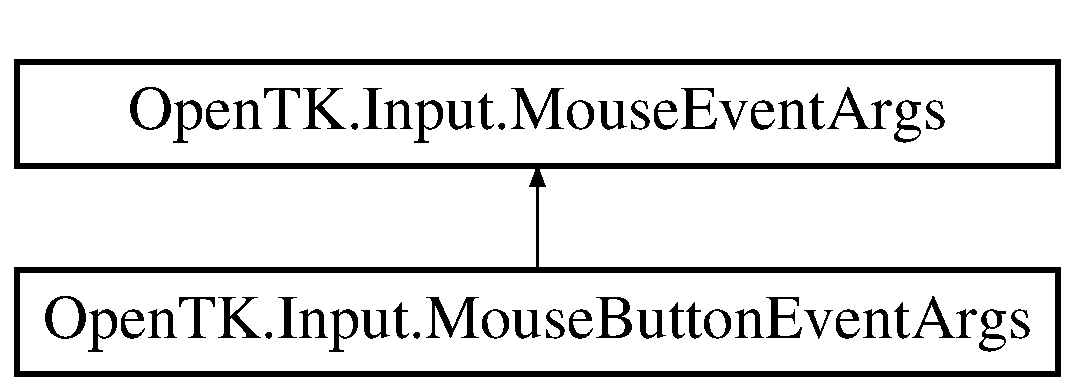
\includegraphics[height=2.000000cm]{class_open_t_k_1_1_input_1_1_mouse_button_event_args}
\end{center}
\end{figure}
\subsection*{Public Member Functions}
\begin{DoxyCompactItemize}
\item 
\hyperlink{class_open_t_k_1_1_input_1_1_mouse_button_event_args_a40c290bed10ccc076096164678606e15}{Mouse\-Button\-Event\-Args} ()
\begin{DoxyCompactList}\small\item\em Constructs a new \hyperlink{class_open_t_k_1_1_input_1_1_mouse_button_event_args}{Mouse\-Button\-Event\-Args} instance. \end{DoxyCompactList}\item 
\hyperlink{class_open_t_k_1_1_input_1_1_mouse_button_event_args_a62b851f376e86115d1f3549f4656aa9c}{Mouse\-Button\-Event\-Args} (int x, int y, \hyperlink{namespace_open_t_k_1_1_input_a2f6f4de1a952f42570d2e06fd15b5774}{Mouse\-Button} button, bool pressed)
\begin{DoxyCompactList}\small\item\em Constructs a new \hyperlink{class_open_t_k_1_1_input_1_1_mouse_button_event_args}{Mouse\-Button\-Event\-Args} instance. \end{DoxyCompactList}\item 
\hyperlink{class_open_t_k_1_1_input_1_1_mouse_button_event_args_a9129ab8d1b7194a702107db165729062}{Mouse\-Button\-Event\-Args} (\hyperlink{class_open_t_k_1_1_input_1_1_mouse_button_event_args}{Mouse\-Button\-Event\-Args} args)
\begin{DoxyCompactList}\small\item\em Constructs a new \hyperlink{class_open_t_k_1_1_input_1_1_mouse_button_event_args}{Mouse\-Button\-Event\-Args} instance. \end{DoxyCompactList}\end{DoxyCompactItemize}
\subsection*{Properties}
\begin{DoxyCompactItemize}
\item 
\hyperlink{namespace_open_t_k_1_1_input_a2f6f4de1a952f42570d2e06fd15b5774}{Mouse\-Button} \hyperlink{class_open_t_k_1_1_input_1_1_mouse_button_event_args_aeae9a397f99f0b0f6026d2f5bda7293b}{Button}\hspace{0.3cm}{\ttfamily  \mbox{[}get, set\mbox{]}}
\begin{DoxyCompactList}\small\item\em The mouse button for the event. \end{DoxyCompactList}\item 
bool \hyperlink{class_open_t_k_1_1_input_1_1_mouse_button_event_args_a2c64b9baa8da00ed048ba612771a27a7}{Is\-Pressed}\hspace{0.3cm}{\ttfamily  \mbox{[}get, set\mbox{]}}
\begin{DoxyCompactList}\small\item\em Gets a System.\-Boolean representing the state of the mouse button for the event. \end{DoxyCompactList}\end{DoxyCompactItemize}


\subsection{Detailed Description}
Defines the event data for \hyperlink{class_open_t_k_1_1_input_1_1_mouse_device_a6d161629ddeb7adefb6f8332824778bd}{Mouse\-Device.\-Button\-Down} and \hyperlink{class_open_t_k_1_1_input_1_1_mouse_device_a244f6f68b32bfe3f745e2b8087e970e8}{Mouse\-Device.\-Button\-Up} events. 

Do not cache instances of this type outside their event handler. If necessary, you can clone an instance using the \hyperlink{class_open_t_k_1_1_input_1_1_mouse_button_event_args_a9129ab8d1b7194a702107db165729062}{Mouse\-Button\-Event\-Args(\-Mouse\-Button\-Event\-Args)} constructor. 

\subsection{Constructor \& Destructor Documentation}
\hypertarget{class_open_t_k_1_1_input_1_1_mouse_button_event_args_a40c290bed10ccc076096164678606e15}{\index{Open\-T\-K\-::\-Input\-::\-Mouse\-Button\-Event\-Args@{Open\-T\-K\-::\-Input\-::\-Mouse\-Button\-Event\-Args}!Mouse\-Button\-Event\-Args@{Mouse\-Button\-Event\-Args}}
\index{Mouse\-Button\-Event\-Args@{Mouse\-Button\-Event\-Args}!OpenTK::Input::MouseButtonEventArgs@{Open\-T\-K\-::\-Input\-::\-Mouse\-Button\-Event\-Args}}
\subsubsection[{Mouse\-Button\-Event\-Args}]{\setlength{\rightskip}{0pt plus 5cm}Open\-T\-K.\-Input.\-Mouse\-Button\-Event\-Args.\-Mouse\-Button\-Event\-Args (
\begin{DoxyParamCaption}
{}
\end{DoxyParamCaption}
)}}\label{class_open_t_k_1_1_input_1_1_mouse_button_event_args_a40c290bed10ccc076096164678606e15}


Constructs a new \hyperlink{class_open_t_k_1_1_input_1_1_mouse_button_event_args}{Mouse\-Button\-Event\-Args} instance. 

\hypertarget{class_open_t_k_1_1_input_1_1_mouse_button_event_args_a62b851f376e86115d1f3549f4656aa9c}{\index{Open\-T\-K\-::\-Input\-::\-Mouse\-Button\-Event\-Args@{Open\-T\-K\-::\-Input\-::\-Mouse\-Button\-Event\-Args}!Mouse\-Button\-Event\-Args@{Mouse\-Button\-Event\-Args}}
\index{Mouse\-Button\-Event\-Args@{Mouse\-Button\-Event\-Args}!OpenTK::Input::MouseButtonEventArgs@{Open\-T\-K\-::\-Input\-::\-Mouse\-Button\-Event\-Args}}
\subsubsection[{Mouse\-Button\-Event\-Args}]{\setlength{\rightskip}{0pt plus 5cm}Open\-T\-K.\-Input.\-Mouse\-Button\-Event\-Args.\-Mouse\-Button\-Event\-Args (
\begin{DoxyParamCaption}
\item[{int}]{x, }
\item[{int}]{y, }
\item[{{\bf Mouse\-Button}}]{button, }
\item[{bool}]{pressed}
\end{DoxyParamCaption}
)}}\label{class_open_t_k_1_1_input_1_1_mouse_button_event_args_a62b851f376e86115d1f3549f4656aa9c}


Constructs a new \hyperlink{class_open_t_k_1_1_input_1_1_mouse_button_event_args}{Mouse\-Button\-Event\-Args} instance. 


\begin{DoxyParams}{Parameters}
{\em x} & The X position.\\
\hline
{\em y} & The Y position.\\
\hline
{\em button} & The mouse button for the event.\\
\hline
{\em pressed} & The current state of the button.\\
\hline
\end{DoxyParams}
\hypertarget{class_open_t_k_1_1_input_1_1_mouse_button_event_args_a9129ab8d1b7194a702107db165729062}{\index{Open\-T\-K\-::\-Input\-::\-Mouse\-Button\-Event\-Args@{Open\-T\-K\-::\-Input\-::\-Mouse\-Button\-Event\-Args}!Mouse\-Button\-Event\-Args@{Mouse\-Button\-Event\-Args}}
\index{Mouse\-Button\-Event\-Args@{Mouse\-Button\-Event\-Args}!OpenTK::Input::MouseButtonEventArgs@{Open\-T\-K\-::\-Input\-::\-Mouse\-Button\-Event\-Args}}
\subsubsection[{Mouse\-Button\-Event\-Args}]{\setlength{\rightskip}{0pt plus 5cm}Open\-T\-K.\-Input.\-Mouse\-Button\-Event\-Args.\-Mouse\-Button\-Event\-Args (
\begin{DoxyParamCaption}
\item[{{\bf Mouse\-Button\-Event\-Args}}]{args}
\end{DoxyParamCaption}
)}}\label{class_open_t_k_1_1_input_1_1_mouse_button_event_args_a9129ab8d1b7194a702107db165729062}


Constructs a new \hyperlink{class_open_t_k_1_1_input_1_1_mouse_button_event_args}{Mouse\-Button\-Event\-Args} instance. 


\begin{DoxyParams}{Parameters}
{\em args} & The \hyperlink{class_open_t_k_1_1_input_1_1_mouse_button_event_args}{Mouse\-Button\-Event\-Args} instance to clone.\\
\hline
\end{DoxyParams}


\subsection{Property Documentation}
\hypertarget{class_open_t_k_1_1_input_1_1_mouse_button_event_args_aeae9a397f99f0b0f6026d2f5bda7293b}{\index{Open\-T\-K\-::\-Input\-::\-Mouse\-Button\-Event\-Args@{Open\-T\-K\-::\-Input\-::\-Mouse\-Button\-Event\-Args}!Button@{Button}}
\index{Button@{Button}!OpenTK::Input::MouseButtonEventArgs@{Open\-T\-K\-::\-Input\-::\-Mouse\-Button\-Event\-Args}}
\subsubsection[{Button}]{\setlength{\rightskip}{0pt plus 5cm}{\bf Mouse\-Button} Open\-T\-K.\-Input.\-Mouse\-Button\-Event\-Args.\-Button\hspace{0.3cm}{\ttfamily [get]}, {\ttfamily [set]}}}\label{class_open_t_k_1_1_input_1_1_mouse_button_event_args_aeae9a397f99f0b0f6026d2f5bda7293b}


The mouse button for the event. 

\hypertarget{class_open_t_k_1_1_input_1_1_mouse_button_event_args_a2c64b9baa8da00ed048ba612771a27a7}{\index{Open\-T\-K\-::\-Input\-::\-Mouse\-Button\-Event\-Args@{Open\-T\-K\-::\-Input\-::\-Mouse\-Button\-Event\-Args}!Is\-Pressed@{Is\-Pressed}}
\index{Is\-Pressed@{Is\-Pressed}!OpenTK::Input::MouseButtonEventArgs@{Open\-T\-K\-::\-Input\-::\-Mouse\-Button\-Event\-Args}}
\subsubsection[{Is\-Pressed}]{\setlength{\rightskip}{0pt plus 5cm}bool Open\-T\-K.\-Input.\-Mouse\-Button\-Event\-Args.\-Is\-Pressed\hspace{0.3cm}{\ttfamily [get]}, {\ttfamily [set]}}}\label{class_open_t_k_1_1_input_1_1_mouse_button_event_args_a2c64b9baa8da00ed048ba612771a27a7}


Gets a System.\-Boolean representing the state of the mouse button for the event. 


\hypertarget{class_open_t_k_1_1_input_1_1_mouse_device}{\section{Open\-T\-K.\-Input.\-Mouse\-Device Class Reference}
\label{class_open_t_k_1_1_input_1_1_mouse_device}\index{Open\-T\-K.\-Input.\-Mouse\-Device@{Open\-T\-K.\-Input.\-Mouse\-Device}}
}


Represents a mouse device and provides methods to query its status.  


Inheritance diagram for Open\-T\-K.\-Input.\-Mouse\-Device\-:\begin{figure}[H]
\begin{center}
\leavevmode
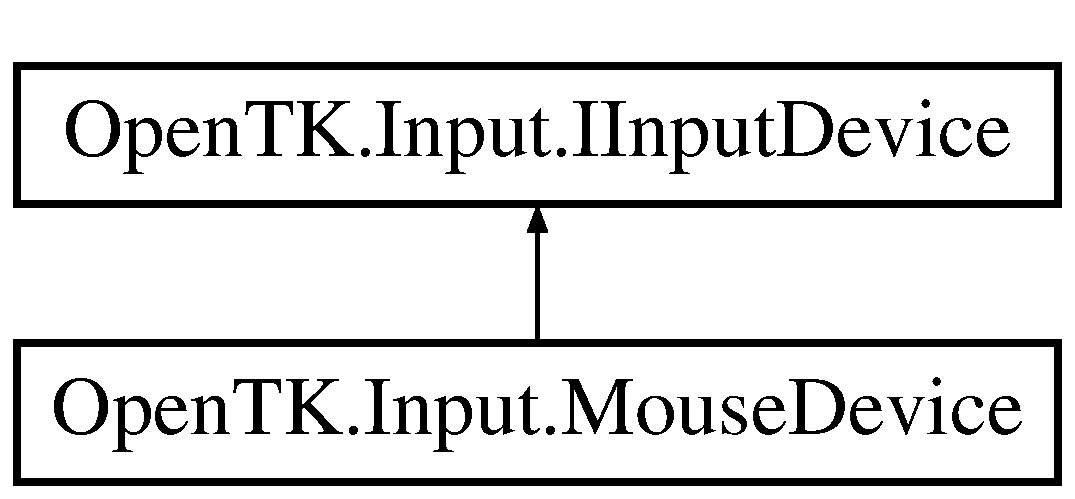
\includegraphics[height=2.000000cm]{class_open_t_k_1_1_input_1_1_mouse_device}
\end{center}
\end{figure}
\subsection*{Public Member Functions}
\begin{DoxyCompactItemize}
\item 
override int \hyperlink{class_open_t_k_1_1_input_1_1_mouse_device_a58acad12c9337d1ace173b6131f1ff95}{Get\-Hash\-Code} ()
\begin{DoxyCompactList}\small\item\em Calculates the hash code for this instance. \end{DoxyCompactList}\item 
override string \hyperlink{class_open_t_k_1_1_input_1_1_mouse_device_a347569de00bc02fc3392f156f3fb4faa}{To\-String} ()
\begin{DoxyCompactList}\small\item\em Returns a System.\-String that describes this instance. \end{DoxyCompactList}\end{DoxyCompactItemize}
\subsection*{Properties}
\begin{DoxyCompactItemize}
\item 
string \hyperlink{class_open_t_k_1_1_input_1_1_mouse_device_a0c31489165ae480b490e8ab0aa375fab}{Description}\hspace{0.3cm}{\ttfamily  \mbox{[}get, set\mbox{]}}
\begin{DoxyCompactList}\small\item\em Gets a string describing this \hyperlink{class_open_t_k_1_1_input_1_1_mouse_device}{Mouse\-Device}. \end{DoxyCompactList}\item 
\hyperlink{namespace_open_t_k_1_1_input_a1d147c6256b0adaa5288eec90ed93270}{Input\-Device\-Type} \hyperlink{class_open_t_k_1_1_input_1_1_mouse_device_a4583df744630520f932eca2d821d5aa8}{Device\-Type}\hspace{0.3cm}{\ttfamily  \mbox{[}get\mbox{]}}
\begin{DoxyCompactList}\small\item\em Gets a value indicating the Input\-Device\-Type of this Input\-Device. \end{DoxyCompactList}\item 
int \hyperlink{class_open_t_k_1_1_input_1_1_mouse_device_af253d36f1acd03668ef5153948089294}{Number\-Of\-Buttons}\hspace{0.3cm}{\ttfamily  \mbox{[}get, set\mbox{]}}
\begin{DoxyCompactList}\small\item\em Gets an integer representing the number of buttons on this \hyperlink{class_open_t_k_1_1_input_1_1_mouse_device}{Mouse\-Device}. \end{DoxyCompactList}\item 
int \hyperlink{class_open_t_k_1_1_input_1_1_mouse_device_ace88c5884e2e50314644aedc8d29efcc}{Number\-Of\-Wheels}\hspace{0.3cm}{\ttfamily  \mbox{[}get, set\mbox{]}}
\begin{DoxyCompactList}\small\item\em Gets an integer representing the number of wheels on this \hyperlink{class_open_t_k_1_1_input_1_1_mouse_device}{Mouse\-Device}. \end{DoxyCompactList}\item 
Int\-Ptr \hyperlink{class_open_t_k_1_1_input_1_1_mouse_device_a8ddb35f6a104a3db46481d2290d76f57}{Device\-I\-D}\hspace{0.3cm}{\ttfamily  \mbox{[}get, set\mbox{]}}
\begin{DoxyCompactList}\small\item\em Gets an Int\-Ptr representing a device dependent I\-D. \end{DoxyCompactList}\item 
int \hyperlink{class_open_t_k_1_1_input_1_1_mouse_device_a903b16fe9f4b3b1054cfbc8051b3752b}{Wheel}\hspace{0.3cm}{\ttfamily  \mbox{[}get, set\mbox{]}}
\begin{DoxyCompactList}\small\item\em Gets the absolute wheel position in integer units. To support high-\/precision mice, it is recommended to use \hyperlink{class_open_t_k_1_1_input_1_1_mouse_device_ace88f976bb7b736216cf785f3679dadd}{Wheel\-Precise} instead. \end{DoxyCompactList}\item 
float \hyperlink{class_open_t_k_1_1_input_1_1_mouse_device_ace88f976bb7b736216cf785f3679dadd}{Wheel\-Precise}\hspace{0.3cm}{\ttfamily  \mbox{[}get, set\mbox{]}}
\begin{DoxyCompactList}\small\item\em Gets the absolute wheel position in floating-\/point units. \end{DoxyCompactList}\item 
int \hyperlink{class_open_t_k_1_1_input_1_1_mouse_device_afc266b67cf1809bb2d27d231ae5d2dd5}{X}\hspace{0.3cm}{\ttfamily  \mbox{[}get\mbox{]}}
\begin{DoxyCompactList}\small\item\em Gets an integer representing the absolute x position of the pointer, in window pixel coordinates. \end{DoxyCompactList}\item 
int \hyperlink{class_open_t_k_1_1_input_1_1_mouse_device_aabbc4ab5371df1be49ad704927ff7e99}{Y}\hspace{0.3cm}{\ttfamily  \mbox{[}get\mbox{]}}
\begin{DoxyCompactList}\small\item\em Gets an integer representing the absolute y position of the pointer, in window pixel coordinates. \end{DoxyCompactList}\item 
bool \hyperlink{class_open_t_k_1_1_input_1_1_mouse_device_a810e7103dac839c811324ef808365f8e}{this\mbox{[}\-Mouse\-Button button\mbox{]}}\hspace{0.3cm}{\ttfamily  \mbox{[}get, set\mbox{]}}
\begin{DoxyCompactList}\small\item\em Gets a System.\-Boolean indicating the state of the specified Mouse\-Button. \end{DoxyCompactList}\item 
int \hyperlink{class_open_t_k_1_1_input_1_1_mouse_device_a834230a316172123e7dc9eccdfe9ac5c}{Wheel\-Delta}\hspace{0.3cm}{\ttfamily  \mbox{[}get\mbox{]}}
\begin{DoxyCompactList}\small\item\em Gets an integer representing the relative wheel movement. \end{DoxyCompactList}\item 
int \hyperlink{class_open_t_k_1_1_input_1_1_mouse_device_a4f6d5b4e04871884c0b20c0b005b5336}{X\-Delta}\hspace{0.3cm}{\ttfamily  \mbox{[}get\mbox{]}}
\begin{DoxyCompactList}\small\item\em Gets an integer representing the relative x movement of the pointer, in pixel coordinates. \end{DoxyCompactList}\item 
int \hyperlink{class_open_t_k_1_1_input_1_1_mouse_device_ab1689cd29ee92df3c5ca955b166636e4}{Y\-Delta}\hspace{0.3cm}{\ttfamily  \mbox{[}get\mbox{]}}
\begin{DoxyCompactList}\small\item\em Gets an integer representing the relative y movement of the pointer, in pixel coordinates. \end{DoxyCompactList}\end{DoxyCompactItemize}
\subsection*{Events}
\begin{DoxyCompactItemize}
\item 
Event\-Handler$<$ \hyperlink{class_open_t_k_1_1_input_1_1_mouse_move_event_args}{Mouse\-Move\-Event\-Args} $>$ \hyperlink{class_open_t_k_1_1_input_1_1_mouse_device_ae98bb40aa03f634ecb53a73971dd9097}{Move} = delegate \{ \}
\begin{DoxyCompactList}\small\item\em Occurs when the mouse's position is moved. \end{DoxyCompactList}\item 
Event\-Handler\\*
$<$ \hyperlink{class_open_t_k_1_1_input_1_1_mouse_button_event_args}{Mouse\-Button\-Event\-Args} $>$ \hyperlink{class_open_t_k_1_1_input_1_1_mouse_device_a6d161629ddeb7adefb6f8332824778bd}{Button\-Down} = delegate \{ \}
\begin{DoxyCompactList}\small\item\em Occurs when a button is pressed. \end{DoxyCompactList}\item 
Event\-Handler\\*
$<$ \hyperlink{class_open_t_k_1_1_input_1_1_mouse_button_event_args}{Mouse\-Button\-Event\-Args} $>$ \hyperlink{class_open_t_k_1_1_input_1_1_mouse_device_a244f6f68b32bfe3f745e2b8087e970e8}{Button\-Up} = delegate \{ \}
\begin{DoxyCompactList}\small\item\em Occurs when a button is released. \end{DoxyCompactList}\item 
Event\-Handler$<$ \hyperlink{class_open_t_k_1_1_input_1_1_mouse_wheel_event_args}{Mouse\-Wheel\-Event\-Args} $>$ \hyperlink{class_open_t_k_1_1_input_1_1_mouse_device_a4bee8a35ae92c6d4f74868934a5c2475}{Wheel\-Changed} = delegate \{ \}
\begin{DoxyCompactList}\small\item\em Occurs when one of the mouse wheels is moved. \end{DoxyCompactList}\end{DoxyCompactItemize}


\subsection{Detailed Description}
Represents a mouse device and provides methods to query its status. 



\subsection{Member Function Documentation}
\hypertarget{class_open_t_k_1_1_input_1_1_mouse_device_a58acad12c9337d1ace173b6131f1ff95}{\index{Open\-T\-K\-::\-Input\-::\-Mouse\-Device@{Open\-T\-K\-::\-Input\-::\-Mouse\-Device}!Get\-Hash\-Code@{Get\-Hash\-Code}}
\index{Get\-Hash\-Code@{Get\-Hash\-Code}!OpenTK::Input::MouseDevice@{Open\-T\-K\-::\-Input\-::\-Mouse\-Device}}
\subsubsection[{Get\-Hash\-Code}]{\setlength{\rightskip}{0pt plus 5cm}override int Open\-T\-K.\-Input.\-Mouse\-Device.\-Get\-Hash\-Code (
\begin{DoxyParamCaption}
{}
\end{DoxyParamCaption}
)}}\label{class_open_t_k_1_1_input_1_1_mouse_device_a58acad12c9337d1ace173b6131f1ff95}


Calculates the hash code for this instance. 

\begin{DoxyReturn}{Returns}

\end{DoxyReturn}
\hypertarget{class_open_t_k_1_1_input_1_1_mouse_device_a347569de00bc02fc3392f156f3fb4faa}{\index{Open\-T\-K\-::\-Input\-::\-Mouse\-Device@{Open\-T\-K\-::\-Input\-::\-Mouse\-Device}!To\-String@{To\-String}}
\index{To\-String@{To\-String}!OpenTK::Input::MouseDevice@{Open\-T\-K\-::\-Input\-::\-Mouse\-Device}}
\subsubsection[{To\-String}]{\setlength{\rightskip}{0pt plus 5cm}override string Open\-T\-K.\-Input.\-Mouse\-Device.\-To\-String (
\begin{DoxyParamCaption}
{}
\end{DoxyParamCaption}
)}}\label{class_open_t_k_1_1_input_1_1_mouse_device_a347569de00bc02fc3392f156f3fb4faa}


Returns a System.\-String that describes this instance. 

\begin{DoxyReturn}{Returns}
A System.\-String that describes this instance.
\end{DoxyReturn}


\subsection{Property Documentation}
\hypertarget{class_open_t_k_1_1_input_1_1_mouse_device_a0c31489165ae480b490e8ab0aa375fab}{\index{Open\-T\-K\-::\-Input\-::\-Mouse\-Device@{Open\-T\-K\-::\-Input\-::\-Mouse\-Device}!Description@{Description}}
\index{Description@{Description}!OpenTK::Input::MouseDevice@{Open\-T\-K\-::\-Input\-::\-Mouse\-Device}}
\subsubsection[{Description}]{\setlength{\rightskip}{0pt plus 5cm}string Open\-T\-K.\-Input.\-Mouse\-Device.\-Description\hspace{0.3cm}{\ttfamily [get]}, {\ttfamily [set]}}}\label{class_open_t_k_1_1_input_1_1_mouse_device_a0c31489165ae480b490e8ab0aa375fab}


Gets a string describing this \hyperlink{class_open_t_k_1_1_input_1_1_mouse_device}{Mouse\-Device}. 

\hypertarget{class_open_t_k_1_1_input_1_1_mouse_device_a8ddb35f6a104a3db46481d2290d76f57}{\index{Open\-T\-K\-::\-Input\-::\-Mouse\-Device@{Open\-T\-K\-::\-Input\-::\-Mouse\-Device}!Device\-I\-D@{Device\-I\-D}}
\index{Device\-I\-D@{Device\-I\-D}!OpenTK::Input::MouseDevice@{Open\-T\-K\-::\-Input\-::\-Mouse\-Device}}
\subsubsection[{Device\-I\-D}]{\setlength{\rightskip}{0pt plus 5cm}Int\-Ptr Open\-T\-K.\-Input.\-Mouse\-Device.\-Device\-I\-D\hspace{0.3cm}{\ttfamily [get]}, {\ttfamily [set]}}}\label{class_open_t_k_1_1_input_1_1_mouse_device_a8ddb35f6a104a3db46481d2290d76f57}


Gets an Int\-Ptr representing a device dependent I\-D. 

\hypertarget{class_open_t_k_1_1_input_1_1_mouse_device_a4583df744630520f932eca2d821d5aa8}{\index{Open\-T\-K\-::\-Input\-::\-Mouse\-Device@{Open\-T\-K\-::\-Input\-::\-Mouse\-Device}!Device\-Type@{Device\-Type}}
\index{Device\-Type@{Device\-Type}!OpenTK::Input::MouseDevice@{Open\-T\-K\-::\-Input\-::\-Mouse\-Device}}
\subsubsection[{Device\-Type}]{\setlength{\rightskip}{0pt plus 5cm}{\bf Input\-Device\-Type} Open\-T\-K.\-Input.\-Mouse\-Device.\-Device\-Type\hspace{0.3cm}{\ttfamily [get]}}}\label{class_open_t_k_1_1_input_1_1_mouse_device_a4583df744630520f932eca2d821d5aa8}


Gets a value indicating the Input\-Device\-Type of this Input\-Device. 

\hypertarget{class_open_t_k_1_1_input_1_1_mouse_device_af253d36f1acd03668ef5153948089294}{\index{Open\-T\-K\-::\-Input\-::\-Mouse\-Device@{Open\-T\-K\-::\-Input\-::\-Mouse\-Device}!Number\-Of\-Buttons@{Number\-Of\-Buttons}}
\index{Number\-Of\-Buttons@{Number\-Of\-Buttons}!OpenTK::Input::MouseDevice@{Open\-T\-K\-::\-Input\-::\-Mouse\-Device}}
\subsubsection[{Number\-Of\-Buttons}]{\setlength{\rightskip}{0pt plus 5cm}int Open\-T\-K.\-Input.\-Mouse\-Device.\-Number\-Of\-Buttons\hspace{0.3cm}{\ttfamily [get]}, {\ttfamily [set]}}}\label{class_open_t_k_1_1_input_1_1_mouse_device_af253d36f1acd03668ef5153948089294}


Gets an integer representing the number of buttons on this \hyperlink{class_open_t_k_1_1_input_1_1_mouse_device}{Mouse\-Device}. 

\hypertarget{class_open_t_k_1_1_input_1_1_mouse_device_ace88c5884e2e50314644aedc8d29efcc}{\index{Open\-T\-K\-::\-Input\-::\-Mouse\-Device@{Open\-T\-K\-::\-Input\-::\-Mouse\-Device}!Number\-Of\-Wheels@{Number\-Of\-Wheels}}
\index{Number\-Of\-Wheels@{Number\-Of\-Wheels}!OpenTK::Input::MouseDevice@{Open\-T\-K\-::\-Input\-::\-Mouse\-Device}}
\subsubsection[{Number\-Of\-Wheels}]{\setlength{\rightskip}{0pt plus 5cm}int Open\-T\-K.\-Input.\-Mouse\-Device.\-Number\-Of\-Wheels\hspace{0.3cm}{\ttfamily [get]}, {\ttfamily [set]}}}\label{class_open_t_k_1_1_input_1_1_mouse_device_ace88c5884e2e50314644aedc8d29efcc}


Gets an integer representing the number of wheels on this \hyperlink{class_open_t_k_1_1_input_1_1_mouse_device}{Mouse\-Device}. 

\hypertarget{class_open_t_k_1_1_input_1_1_mouse_device_a810e7103dac839c811324ef808365f8e}{\index{Open\-T\-K\-::\-Input\-::\-Mouse\-Device@{Open\-T\-K\-::\-Input\-::\-Mouse\-Device}!this\mbox{[}\-Mouse\-Button button\mbox{]}@{this[Mouse\-Button button]}}
\index{this\mbox{[}\-Mouse\-Button button\mbox{]}@{this[Mouse\-Button button]}!OpenTK::Input::MouseDevice@{Open\-T\-K\-::\-Input\-::\-Mouse\-Device}}
\subsubsection[{this[Mouse\-Button button]}]{\setlength{\rightskip}{0pt plus 5cm}bool Open\-T\-K.\-Input.\-Mouse\-Device.\-this\mbox{[}{\bf Mouse\-Button} button\mbox{]}\hspace{0.3cm}{\ttfamily [get]}, {\ttfamily [set]}}}\label{class_open_t_k_1_1_input_1_1_mouse_device_a810e7103dac839c811324ef808365f8e}


Gets a System.\-Boolean indicating the state of the specified Mouse\-Button. 


\begin{DoxyParams}{Parameters}
{\em button} & The Mouse\-Button to check.\\
\hline
\end{DoxyParams}
\begin{DoxyReturn}{Returns}
True if the Mouse\-Button is pressed, false otherwise.
\end{DoxyReturn}
\hypertarget{class_open_t_k_1_1_input_1_1_mouse_device_a903b16fe9f4b3b1054cfbc8051b3752b}{\index{Open\-T\-K\-::\-Input\-::\-Mouse\-Device@{Open\-T\-K\-::\-Input\-::\-Mouse\-Device}!Wheel@{Wheel}}
\index{Wheel@{Wheel}!OpenTK::Input::MouseDevice@{Open\-T\-K\-::\-Input\-::\-Mouse\-Device}}
\subsubsection[{Wheel}]{\setlength{\rightskip}{0pt plus 5cm}int Open\-T\-K.\-Input.\-Mouse\-Device.\-Wheel\hspace{0.3cm}{\ttfamily [get]}, {\ttfamily [set]}}}\label{class_open_t_k_1_1_input_1_1_mouse_device_a903b16fe9f4b3b1054cfbc8051b3752b}


Gets the absolute wheel position in integer units. To support high-\/precision mice, it is recommended to use \hyperlink{class_open_t_k_1_1_input_1_1_mouse_device_ace88f976bb7b736216cf785f3679dadd}{Wheel\-Precise} instead. 

\hypertarget{class_open_t_k_1_1_input_1_1_mouse_device_a834230a316172123e7dc9eccdfe9ac5c}{\index{Open\-T\-K\-::\-Input\-::\-Mouse\-Device@{Open\-T\-K\-::\-Input\-::\-Mouse\-Device}!Wheel\-Delta@{Wheel\-Delta}}
\index{Wheel\-Delta@{Wheel\-Delta}!OpenTK::Input::MouseDevice@{Open\-T\-K\-::\-Input\-::\-Mouse\-Device}}
\subsubsection[{Wheel\-Delta}]{\setlength{\rightskip}{0pt plus 5cm}int Open\-T\-K.\-Input.\-Mouse\-Device.\-Wheel\-Delta\hspace{0.3cm}{\ttfamily [get]}}}\label{class_open_t_k_1_1_input_1_1_mouse_device_a834230a316172123e7dc9eccdfe9ac5c}


Gets an integer representing the relative wheel movement. 

\hypertarget{class_open_t_k_1_1_input_1_1_mouse_device_ace88f976bb7b736216cf785f3679dadd}{\index{Open\-T\-K\-::\-Input\-::\-Mouse\-Device@{Open\-T\-K\-::\-Input\-::\-Mouse\-Device}!Wheel\-Precise@{Wheel\-Precise}}
\index{Wheel\-Precise@{Wheel\-Precise}!OpenTK::Input::MouseDevice@{Open\-T\-K\-::\-Input\-::\-Mouse\-Device}}
\subsubsection[{Wheel\-Precise}]{\setlength{\rightskip}{0pt plus 5cm}float Open\-T\-K.\-Input.\-Mouse\-Device.\-Wheel\-Precise\hspace{0.3cm}{\ttfamily [get]}, {\ttfamily [set]}}}\label{class_open_t_k_1_1_input_1_1_mouse_device_ace88f976bb7b736216cf785f3679dadd}


Gets the absolute wheel position in floating-\/point units. 

\hypertarget{class_open_t_k_1_1_input_1_1_mouse_device_afc266b67cf1809bb2d27d231ae5d2dd5}{\index{Open\-T\-K\-::\-Input\-::\-Mouse\-Device@{Open\-T\-K\-::\-Input\-::\-Mouse\-Device}!X@{X}}
\index{X@{X}!OpenTK::Input::MouseDevice@{Open\-T\-K\-::\-Input\-::\-Mouse\-Device}}
\subsubsection[{X}]{\setlength{\rightskip}{0pt plus 5cm}int Open\-T\-K.\-Input.\-Mouse\-Device.\-X\hspace{0.3cm}{\ttfamily [get]}}}\label{class_open_t_k_1_1_input_1_1_mouse_device_afc266b67cf1809bb2d27d231ae5d2dd5}


Gets an integer representing the absolute x position of the pointer, in window pixel coordinates. 

\hypertarget{class_open_t_k_1_1_input_1_1_mouse_device_a4f6d5b4e04871884c0b20c0b005b5336}{\index{Open\-T\-K\-::\-Input\-::\-Mouse\-Device@{Open\-T\-K\-::\-Input\-::\-Mouse\-Device}!X\-Delta@{X\-Delta}}
\index{X\-Delta@{X\-Delta}!OpenTK::Input::MouseDevice@{Open\-T\-K\-::\-Input\-::\-Mouse\-Device}}
\subsubsection[{X\-Delta}]{\setlength{\rightskip}{0pt plus 5cm}int Open\-T\-K.\-Input.\-Mouse\-Device.\-X\-Delta\hspace{0.3cm}{\ttfamily [get]}}}\label{class_open_t_k_1_1_input_1_1_mouse_device_a4f6d5b4e04871884c0b20c0b005b5336}


Gets an integer representing the relative x movement of the pointer, in pixel coordinates. 

\hypertarget{class_open_t_k_1_1_input_1_1_mouse_device_aabbc4ab5371df1be49ad704927ff7e99}{\index{Open\-T\-K\-::\-Input\-::\-Mouse\-Device@{Open\-T\-K\-::\-Input\-::\-Mouse\-Device}!Y@{Y}}
\index{Y@{Y}!OpenTK::Input::MouseDevice@{Open\-T\-K\-::\-Input\-::\-Mouse\-Device}}
\subsubsection[{Y}]{\setlength{\rightskip}{0pt plus 5cm}int Open\-T\-K.\-Input.\-Mouse\-Device.\-Y\hspace{0.3cm}{\ttfamily [get]}}}\label{class_open_t_k_1_1_input_1_1_mouse_device_aabbc4ab5371df1be49ad704927ff7e99}


Gets an integer representing the absolute y position of the pointer, in window pixel coordinates. 

\hypertarget{class_open_t_k_1_1_input_1_1_mouse_device_ab1689cd29ee92df3c5ca955b166636e4}{\index{Open\-T\-K\-::\-Input\-::\-Mouse\-Device@{Open\-T\-K\-::\-Input\-::\-Mouse\-Device}!Y\-Delta@{Y\-Delta}}
\index{Y\-Delta@{Y\-Delta}!OpenTK::Input::MouseDevice@{Open\-T\-K\-::\-Input\-::\-Mouse\-Device}}
\subsubsection[{Y\-Delta}]{\setlength{\rightskip}{0pt plus 5cm}int Open\-T\-K.\-Input.\-Mouse\-Device.\-Y\-Delta\hspace{0.3cm}{\ttfamily [get]}}}\label{class_open_t_k_1_1_input_1_1_mouse_device_ab1689cd29ee92df3c5ca955b166636e4}


Gets an integer representing the relative y movement of the pointer, in pixel coordinates. 



\subsection{Event Documentation}
\hypertarget{class_open_t_k_1_1_input_1_1_mouse_device_a6d161629ddeb7adefb6f8332824778bd}{\index{Open\-T\-K\-::\-Input\-::\-Mouse\-Device@{Open\-T\-K\-::\-Input\-::\-Mouse\-Device}!Button\-Down@{Button\-Down}}
\index{Button\-Down@{Button\-Down}!OpenTK::Input::MouseDevice@{Open\-T\-K\-::\-Input\-::\-Mouse\-Device}}
\subsubsection[{Button\-Down}]{\setlength{\rightskip}{0pt plus 5cm}Event\-Handler$<${\bf Mouse\-Button\-Event\-Args}$>$ Open\-T\-K.\-Input.\-Mouse\-Device.\-Button\-Down = delegate \{ \}}}\label{class_open_t_k_1_1_input_1_1_mouse_device_a6d161629ddeb7adefb6f8332824778bd}


Occurs when a button is pressed. 

\hypertarget{class_open_t_k_1_1_input_1_1_mouse_device_a244f6f68b32bfe3f745e2b8087e970e8}{\index{Open\-T\-K\-::\-Input\-::\-Mouse\-Device@{Open\-T\-K\-::\-Input\-::\-Mouse\-Device}!Button\-Up@{Button\-Up}}
\index{Button\-Up@{Button\-Up}!OpenTK::Input::MouseDevice@{Open\-T\-K\-::\-Input\-::\-Mouse\-Device}}
\subsubsection[{Button\-Up}]{\setlength{\rightskip}{0pt plus 5cm}Event\-Handler$<${\bf Mouse\-Button\-Event\-Args}$>$ Open\-T\-K.\-Input.\-Mouse\-Device.\-Button\-Up = delegate \{ \}}}\label{class_open_t_k_1_1_input_1_1_mouse_device_a244f6f68b32bfe3f745e2b8087e970e8}


Occurs when a button is released. 

\hypertarget{class_open_t_k_1_1_input_1_1_mouse_device_ae98bb40aa03f634ecb53a73971dd9097}{\index{Open\-T\-K\-::\-Input\-::\-Mouse\-Device@{Open\-T\-K\-::\-Input\-::\-Mouse\-Device}!Move@{Move}}
\index{Move@{Move}!OpenTK::Input::MouseDevice@{Open\-T\-K\-::\-Input\-::\-Mouse\-Device}}
\subsubsection[{Move}]{\setlength{\rightskip}{0pt plus 5cm}Event\-Handler$<${\bf Mouse\-Move\-Event\-Args}$>$ Open\-T\-K.\-Input.\-Mouse\-Device.\-Move = delegate \{ \}}}\label{class_open_t_k_1_1_input_1_1_mouse_device_ae98bb40aa03f634ecb53a73971dd9097}


Occurs when the mouse's position is moved. 

\hypertarget{class_open_t_k_1_1_input_1_1_mouse_device_a4bee8a35ae92c6d4f74868934a5c2475}{\index{Open\-T\-K\-::\-Input\-::\-Mouse\-Device@{Open\-T\-K\-::\-Input\-::\-Mouse\-Device}!Wheel\-Changed@{Wheel\-Changed}}
\index{Wheel\-Changed@{Wheel\-Changed}!OpenTK::Input::MouseDevice@{Open\-T\-K\-::\-Input\-::\-Mouse\-Device}}
\subsubsection[{Wheel\-Changed}]{\setlength{\rightskip}{0pt plus 5cm}Event\-Handler$<${\bf Mouse\-Wheel\-Event\-Args}$>$ Open\-T\-K.\-Input.\-Mouse\-Device.\-Wheel\-Changed = delegate \{ \}}}\label{class_open_t_k_1_1_input_1_1_mouse_device_a4bee8a35ae92c6d4f74868934a5c2475}


Occurs when one of the mouse wheels is moved. 


\hypertarget{class_open_t_k_1_1_input_1_1_mouse_event_args}{\section{Open\-T\-K.\-Input.\-Mouse\-Event\-Args Class Reference}
\label{class_open_t_k_1_1_input_1_1_mouse_event_args}\index{Open\-T\-K.\-Input.\-Mouse\-Event\-Args@{Open\-T\-K.\-Input.\-Mouse\-Event\-Args}}
}


Defines the event data for \hyperlink{class_open_t_k_1_1_input_1_1_mouse_device}{Mouse\-Device} events.  


Inheritance diagram for Open\-T\-K.\-Input.\-Mouse\-Event\-Args\-:\begin{figure}[H]
\begin{center}
\leavevmode
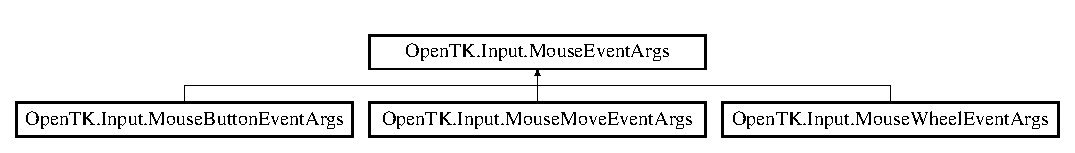
\includegraphics[height=1.602289cm]{class_open_t_k_1_1_input_1_1_mouse_event_args}
\end{center}
\end{figure}
\subsection*{Public Member Functions}
\begin{DoxyCompactItemize}
\item 
\hyperlink{class_open_t_k_1_1_input_1_1_mouse_event_args_ad97edef84ab81ff07b12f9e859210c58}{Mouse\-Event\-Args} ()
\begin{DoxyCompactList}\small\item\em Constructs a new instance. \end{DoxyCompactList}\item 
\hyperlink{class_open_t_k_1_1_input_1_1_mouse_event_args_a6f7791d5f699529650adcc1ecdfb3a33}{Mouse\-Event\-Args} (int x, int y)
\begin{DoxyCompactList}\small\item\em Constructs a new instance. \end{DoxyCompactList}\item 
\hyperlink{class_open_t_k_1_1_input_1_1_mouse_event_args_a6c439ae6a66a4e3dc0de1d855246accb}{Mouse\-Event\-Args} (\hyperlink{class_open_t_k_1_1_input_1_1_mouse_event_args}{Mouse\-Event\-Args} args)
\begin{DoxyCompactList}\small\item\em Constructs a new instance. \end{DoxyCompactList}\end{DoxyCompactItemize}
\subsection*{Properties}
\begin{DoxyCompactItemize}
\item 
int \hyperlink{class_open_t_k_1_1_input_1_1_mouse_event_args_a160e6935affdb80c8e39a24e8aa7481d}{X}\hspace{0.3cm}{\ttfamily  \mbox{[}get, set\mbox{]}}
\begin{DoxyCompactList}\small\item\em Gets the X position of the mouse for the event. \end{DoxyCompactList}\item 
int \hyperlink{class_open_t_k_1_1_input_1_1_mouse_event_args_a303956e7ce1e2a90cb76519ed63de5df}{Y}\hspace{0.3cm}{\ttfamily  \mbox{[}get, set\mbox{]}}
\begin{DoxyCompactList}\small\item\em Gets the Y position of the mouse for the event. \end{DoxyCompactList}\item 
Point \hyperlink{class_open_t_k_1_1_input_1_1_mouse_event_args_af30ca9ad72ab907e1e6428a4097e60a5}{Position}\hspace{0.3cm}{\ttfamily  \mbox{[}get\mbox{]}}
\begin{DoxyCompactList}\small\item\em Gets a System.\-Drawing.\-Points representing the location of the mouse for the event. \end{DoxyCompactList}\end{DoxyCompactItemize}


\subsection{Detailed Description}
Defines the event data for \hyperlink{class_open_t_k_1_1_input_1_1_mouse_device}{Mouse\-Device} events. 

Do not cache instances of this type outside their event handler. If necessary, you can clone an instance using the \hyperlink{class_open_t_k_1_1_input_1_1_mouse_event_args_a6c439ae6a66a4e3dc0de1d855246accb}{Mouse\-Event\-Args(\-Mouse\-Event\-Args)} constructor. 

\subsection{Constructor \& Destructor Documentation}
\hypertarget{class_open_t_k_1_1_input_1_1_mouse_event_args_ad97edef84ab81ff07b12f9e859210c58}{\index{Open\-T\-K\-::\-Input\-::\-Mouse\-Event\-Args@{Open\-T\-K\-::\-Input\-::\-Mouse\-Event\-Args}!Mouse\-Event\-Args@{Mouse\-Event\-Args}}
\index{Mouse\-Event\-Args@{Mouse\-Event\-Args}!OpenTK::Input::MouseEventArgs@{Open\-T\-K\-::\-Input\-::\-Mouse\-Event\-Args}}
\subsubsection[{Mouse\-Event\-Args}]{\setlength{\rightskip}{0pt plus 5cm}Open\-T\-K.\-Input.\-Mouse\-Event\-Args.\-Mouse\-Event\-Args (
\begin{DoxyParamCaption}
{}
\end{DoxyParamCaption}
)}}\label{class_open_t_k_1_1_input_1_1_mouse_event_args_ad97edef84ab81ff07b12f9e859210c58}


Constructs a new instance. 

\hypertarget{class_open_t_k_1_1_input_1_1_mouse_event_args_a6f7791d5f699529650adcc1ecdfb3a33}{\index{Open\-T\-K\-::\-Input\-::\-Mouse\-Event\-Args@{Open\-T\-K\-::\-Input\-::\-Mouse\-Event\-Args}!Mouse\-Event\-Args@{Mouse\-Event\-Args}}
\index{Mouse\-Event\-Args@{Mouse\-Event\-Args}!OpenTK::Input::MouseEventArgs@{Open\-T\-K\-::\-Input\-::\-Mouse\-Event\-Args}}
\subsubsection[{Mouse\-Event\-Args}]{\setlength{\rightskip}{0pt plus 5cm}Open\-T\-K.\-Input.\-Mouse\-Event\-Args.\-Mouse\-Event\-Args (
\begin{DoxyParamCaption}
\item[{int}]{x, }
\item[{int}]{y}
\end{DoxyParamCaption}
)}}\label{class_open_t_k_1_1_input_1_1_mouse_event_args_a6f7791d5f699529650adcc1ecdfb3a33}


Constructs a new instance. 


\begin{DoxyParams}{Parameters}
{\em x} & The X position.\\
\hline
{\em y} & The Y position.\\
\hline
\end{DoxyParams}
\hypertarget{class_open_t_k_1_1_input_1_1_mouse_event_args_a6c439ae6a66a4e3dc0de1d855246accb}{\index{Open\-T\-K\-::\-Input\-::\-Mouse\-Event\-Args@{Open\-T\-K\-::\-Input\-::\-Mouse\-Event\-Args}!Mouse\-Event\-Args@{Mouse\-Event\-Args}}
\index{Mouse\-Event\-Args@{Mouse\-Event\-Args}!OpenTK::Input::MouseEventArgs@{Open\-T\-K\-::\-Input\-::\-Mouse\-Event\-Args}}
\subsubsection[{Mouse\-Event\-Args}]{\setlength{\rightskip}{0pt plus 5cm}Open\-T\-K.\-Input.\-Mouse\-Event\-Args.\-Mouse\-Event\-Args (
\begin{DoxyParamCaption}
\item[{{\bf Mouse\-Event\-Args}}]{args}
\end{DoxyParamCaption}
)}}\label{class_open_t_k_1_1_input_1_1_mouse_event_args_a6c439ae6a66a4e3dc0de1d855246accb}


Constructs a new instance. 


\begin{DoxyParams}{Parameters}
{\em args} & The \hyperlink{class_open_t_k_1_1_input_1_1_mouse_event_args}{Mouse\-Event\-Args} instance to clone.\\
\hline
\end{DoxyParams}


\subsection{Property Documentation}
\hypertarget{class_open_t_k_1_1_input_1_1_mouse_event_args_af30ca9ad72ab907e1e6428a4097e60a5}{\index{Open\-T\-K\-::\-Input\-::\-Mouse\-Event\-Args@{Open\-T\-K\-::\-Input\-::\-Mouse\-Event\-Args}!Position@{Position}}
\index{Position@{Position}!OpenTK::Input::MouseEventArgs@{Open\-T\-K\-::\-Input\-::\-Mouse\-Event\-Args}}
\subsubsection[{Position}]{\setlength{\rightskip}{0pt plus 5cm}Point Open\-T\-K.\-Input.\-Mouse\-Event\-Args.\-Position\hspace{0.3cm}{\ttfamily [get]}}}\label{class_open_t_k_1_1_input_1_1_mouse_event_args_af30ca9ad72ab907e1e6428a4097e60a5}


Gets a System.\-Drawing.\-Points representing the location of the mouse for the event. 

\hypertarget{class_open_t_k_1_1_input_1_1_mouse_event_args_a160e6935affdb80c8e39a24e8aa7481d}{\index{Open\-T\-K\-::\-Input\-::\-Mouse\-Event\-Args@{Open\-T\-K\-::\-Input\-::\-Mouse\-Event\-Args}!X@{X}}
\index{X@{X}!OpenTK::Input::MouseEventArgs@{Open\-T\-K\-::\-Input\-::\-Mouse\-Event\-Args}}
\subsubsection[{X}]{\setlength{\rightskip}{0pt plus 5cm}int Open\-T\-K.\-Input.\-Mouse\-Event\-Args.\-X\hspace{0.3cm}{\ttfamily [get]}, {\ttfamily [set]}}}\label{class_open_t_k_1_1_input_1_1_mouse_event_args_a160e6935affdb80c8e39a24e8aa7481d}


Gets the X position of the mouse for the event. 

\hypertarget{class_open_t_k_1_1_input_1_1_mouse_event_args_a303956e7ce1e2a90cb76519ed63de5df}{\index{Open\-T\-K\-::\-Input\-::\-Mouse\-Event\-Args@{Open\-T\-K\-::\-Input\-::\-Mouse\-Event\-Args}!Y@{Y}}
\index{Y@{Y}!OpenTK::Input::MouseEventArgs@{Open\-T\-K\-::\-Input\-::\-Mouse\-Event\-Args}}
\subsubsection[{Y}]{\setlength{\rightskip}{0pt plus 5cm}int Open\-T\-K.\-Input.\-Mouse\-Event\-Args.\-Y\hspace{0.3cm}{\ttfamily [get]}, {\ttfamily [set]}}}\label{class_open_t_k_1_1_input_1_1_mouse_event_args_a303956e7ce1e2a90cb76519ed63de5df}


Gets the Y position of the mouse for the event. 


\hypertarget{class_open_t_k_1_1_input_1_1_mouse_move_event_args}{\section{Open\-T\-K.\-Input.\-Mouse\-Move\-Event\-Args Class Reference}
\label{class_open_t_k_1_1_input_1_1_mouse_move_event_args}\index{Open\-T\-K.\-Input.\-Mouse\-Move\-Event\-Args@{Open\-T\-K.\-Input.\-Mouse\-Move\-Event\-Args}}
}


Defines the event data for \hyperlink{class_open_t_k_1_1_input_1_1_mouse_device_ae98bb40aa03f634ecb53a73971dd9097}{Mouse\-Device.\-Move} events.  


Inheritance diagram for Open\-T\-K.\-Input.\-Mouse\-Move\-Event\-Args\-:\begin{figure}[H]
\begin{center}
\leavevmode
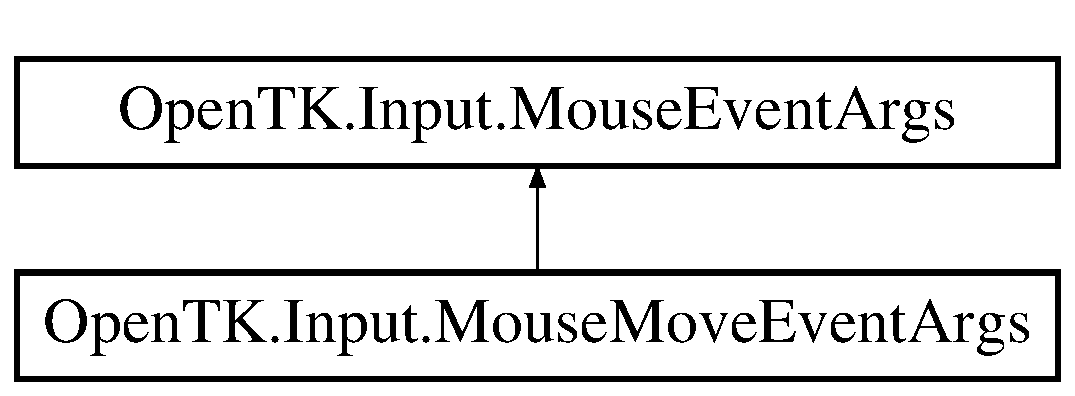
\includegraphics[height=2.000000cm]{class_open_t_k_1_1_input_1_1_mouse_move_event_args}
\end{center}
\end{figure}
\subsection*{Public Member Functions}
\begin{DoxyCompactItemize}
\item 
\hyperlink{class_open_t_k_1_1_input_1_1_mouse_move_event_args_adfa1d205d8867b6a3d5812d8eb4da256}{Mouse\-Move\-Event\-Args} ()
\begin{DoxyCompactList}\small\item\em Constructs a new \hyperlink{class_open_t_k_1_1_input_1_1_mouse_move_event_args}{Mouse\-Move\-Event\-Args} instance. \end{DoxyCompactList}\item 
\hyperlink{class_open_t_k_1_1_input_1_1_mouse_move_event_args_a563702b287acb6b436e888537bf1cd1e}{Mouse\-Move\-Event\-Args} (int x, int y, int x\-Delta, int y\-Delta)
\begin{DoxyCompactList}\small\item\em Constructs a new \hyperlink{class_open_t_k_1_1_input_1_1_mouse_move_event_args}{Mouse\-Move\-Event\-Args} instance. \end{DoxyCompactList}\item 
\hyperlink{class_open_t_k_1_1_input_1_1_mouse_move_event_args_a39916bdada80b3d23a6309988505fd22}{Mouse\-Move\-Event\-Args} (\hyperlink{class_open_t_k_1_1_input_1_1_mouse_move_event_args}{Mouse\-Move\-Event\-Args} args)
\begin{DoxyCompactList}\small\item\em Constructs a new \hyperlink{class_open_t_k_1_1_input_1_1_mouse_move_event_args}{Mouse\-Move\-Event\-Args} instance. \end{DoxyCompactList}\end{DoxyCompactItemize}
\subsection*{Properties}
\begin{DoxyCompactItemize}
\item 
int \hyperlink{class_open_t_k_1_1_input_1_1_mouse_move_event_args_af762d26725d6220b83e19a1999d21889}{X\-Delta}\hspace{0.3cm}{\ttfamily  \mbox{[}get, set\mbox{]}}
\begin{DoxyCompactList}\small\item\em Gets the change in X position produced by this event. \end{DoxyCompactList}\item 
int \hyperlink{class_open_t_k_1_1_input_1_1_mouse_move_event_args_aaef0da462fdd9aa0fd82abea2efd8687}{Y\-Delta}\hspace{0.3cm}{\ttfamily  \mbox{[}get, set\mbox{]}}
\begin{DoxyCompactList}\small\item\em Gets the change in Y position produced by this event. \end{DoxyCompactList}\end{DoxyCompactItemize}


\subsection{Detailed Description}
Defines the event data for \hyperlink{class_open_t_k_1_1_input_1_1_mouse_device_ae98bb40aa03f634ecb53a73971dd9097}{Mouse\-Device.\-Move} events. 

Do not cache instances of this type outside their event handler. If necessary, you can clone an instance using the \hyperlink{class_open_t_k_1_1_input_1_1_mouse_move_event_args_a39916bdada80b3d23a6309988505fd22}{Mouse\-Move\-Event\-Args(\-Mouse\-Move\-Event\-Args)} constructor. 

\subsection{Constructor \& Destructor Documentation}
\hypertarget{class_open_t_k_1_1_input_1_1_mouse_move_event_args_adfa1d205d8867b6a3d5812d8eb4da256}{\index{Open\-T\-K\-::\-Input\-::\-Mouse\-Move\-Event\-Args@{Open\-T\-K\-::\-Input\-::\-Mouse\-Move\-Event\-Args}!Mouse\-Move\-Event\-Args@{Mouse\-Move\-Event\-Args}}
\index{Mouse\-Move\-Event\-Args@{Mouse\-Move\-Event\-Args}!OpenTK::Input::MouseMoveEventArgs@{Open\-T\-K\-::\-Input\-::\-Mouse\-Move\-Event\-Args}}
\subsubsection[{Mouse\-Move\-Event\-Args}]{\setlength{\rightskip}{0pt plus 5cm}Open\-T\-K.\-Input.\-Mouse\-Move\-Event\-Args.\-Mouse\-Move\-Event\-Args (
\begin{DoxyParamCaption}
{}
\end{DoxyParamCaption}
)}}\label{class_open_t_k_1_1_input_1_1_mouse_move_event_args_adfa1d205d8867b6a3d5812d8eb4da256}


Constructs a new \hyperlink{class_open_t_k_1_1_input_1_1_mouse_move_event_args}{Mouse\-Move\-Event\-Args} instance. 

\hypertarget{class_open_t_k_1_1_input_1_1_mouse_move_event_args_a563702b287acb6b436e888537bf1cd1e}{\index{Open\-T\-K\-::\-Input\-::\-Mouse\-Move\-Event\-Args@{Open\-T\-K\-::\-Input\-::\-Mouse\-Move\-Event\-Args}!Mouse\-Move\-Event\-Args@{Mouse\-Move\-Event\-Args}}
\index{Mouse\-Move\-Event\-Args@{Mouse\-Move\-Event\-Args}!OpenTK::Input::MouseMoveEventArgs@{Open\-T\-K\-::\-Input\-::\-Mouse\-Move\-Event\-Args}}
\subsubsection[{Mouse\-Move\-Event\-Args}]{\setlength{\rightskip}{0pt plus 5cm}Open\-T\-K.\-Input.\-Mouse\-Move\-Event\-Args.\-Mouse\-Move\-Event\-Args (
\begin{DoxyParamCaption}
\item[{int}]{x, }
\item[{int}]{y, }
\item[{int}]{x\-Delta, }
\item[{int}]{y\-Delta}
\end{DoxyParamCaption}
)}}\label{class_open_t_k_1_1_input_1_1_mouse_move_event_args_a563702b287acb6b436e888537bf1cd1e}


Constructs a new \hyperlink{class_open_t_k_1_1_input_1_1_mouse_move_event_args}{Mouse\-Move\-Event\-Args} instance. 


\begin{DoxyParams}{Parameters}
{\em x} & The X position.\\
\hline
{\em y} & The Y position.\\
\hline
{\em x\-Delta} & The change in X position produced by this event.\\
\hline
{\em y\-Delta} & The change in Y position produced by this event.\\
\hline
\end{DoxyParams}
\hypertarget{class_open_t_k_1_1_input_1_1_mouse_move_event_args_a39916bdada80b3d23a6309988505fd22}{\index{Open\-T\-K\-::\-Input\-::\-Mouse\-Move\-Event\-Args@{Open\-T\-K\-::\-Input\-::\-Mouse\-Move\-Event\-Args}!Mouse\-Move\-Event\-Args@{Mouse\-Move\-Event\-Args}}
\index{Mouse\-Move\-Event\-Args@{Mouse\-Move\-Event\-Args}!OpenTK::Input::MouseMoveEventArgs@{Open\-T\-K\-::\-Input\-::\-Mouse\-Move\-Event\-Args}}
\subsubsection[{Mouse\-Move\-Event\-Args}]{\setlength{\rightskip}{0pt plus 5cm}Open\-T\-K.\-Input.\-Mouse\-Move\-Event\-Args.\-Mouse\-Move\-Event\-Args (
\begin{DoxyParamCaption}
\item[{{\bf Mouse\-Move\-Event\-Args}}]{args}
\end{DoxyParamCaption}
)}}\label{class_open_t_k_1_1_input_1_1_mouse_move_event_args_a39916bdada80b3d23a6309988505fd22}


Constructs a new \hyperlink{class_open_t_k_1_1_input_1_1_mouse_move_event_args}{Mouse\-Move\-Event\-Args} instance. 


\begin{DoxyParams}{Parameters}
{\em args} & The \hyperlink{class_open_t_k_1_1_input_1_1_mouse_move_event_args}{Mouse\-Move\-Event\-Args} instance to clone.\\
\hline
\end{DoxyParams}


\subsection{Property Documentation}
\hypertarget{class_open_t_k_1_1_input_1_1_mouse_move_event_args_af762d26725d6220b83e19a1999d21889}{\index{Open\-T\-K\-::\-Input\-::\-Mouse\-Move\-Event\-Args@{Open\-T\-K\-::\-Input\-::\-Mouse\-Move\-Event\-Args}!X\-Delta@{X\-Delta}}
\index{X\-Delta@{X\-Delta}!OpenTK::Input::MouseMoveEventArgs@{Open\-T\-K\-::\-Input\-::\-Mouse\-Move\-Event\-Args}}
\subsubsection[{X\-Delta}]{\setlength{\rightskip}{0pt plus 5cm}int Open\-T\-K.\-Input.\-Mouse\-Move\-Event\-Args.\-X\-Delta\hspace{0.3cm}{\ttfamily [get]}, {\ttfamily [set]}}}\label{class_open_t_k_1_1_input_1_1_mouse_move_event_args_af762d26725d6220b83e19a1999d21889}


Gets the change in X position produced by this event. 

\hypertarget{class_open_t_k_1_1_input_1_1_mouse_move_event_args_aaef0da462fdd9aa0fd82abea2efd8687}{\index{Open\-T\-K\-::\-Input\-::\-Mouse\-Move\-Event\-Args@{Open\-T\-K\-::\-Input\-::\-Mouse\-Move\-Event\-Args}!Y\-Delta@{Y\-Delta}}
\index{Y\-Delta@{Y\-Delta}!OpenTK::Input::MouseMoveEventArgs@{Open\-T\-K\-::\-Input\-::\-Mouse\-Move\-Event\-Args}}
\subsubsection[{Y\-Delta}]{\setlength{\rightskip}{0pt plus 5cm}int Open\-T\-K.\-Input.\-Mouse\-Move\-Event\-Args.\-Y\-Delta\hspace{0.3cm}{\ttfamily [get]}, {\ttfamily [set]}}}\label{class_open_t_k_1_1_input_1_1_mouse_move_event_args_aaef0da462fdd9aa0fd82abea2efd8687}


Gets the change in Y position produced by this event. 


\hypertarget{struct_open_t_k_1_1_input_1_1_mouse_state}{\section{Open\-T\-K.\-Input.\-Mouse\-State Struct Reference}
\label{struct_open_t_k_1_1_input_1_1_mouse_state}\index{Open\-T\-K.\-Input.\-Mouse\-State@{Open\-T\-K.\-Input.\-Mouse\-State}}
}


Encapsulates the state of a mouse device.  




Inherits I\-Equatable$<$ Mouse\-State $>$.

\subsection*{Public Member Functions}
\begin{DoxyCompactItemize}
\item 
bool \hyperlink{struct_open_t_k_1_1_input_1_1_mouse_state_a3114cc768382741249b11de8570b5488}{Is\-Button\-Down} (\hyperlink{namespace_open_t_k_1_1_input_a2f6f4de1a952f42570d2e06fd15b5774}{Mouse\-Button} button)
\begin{DoxyCompactList}\small\item\em Gets a System.\-Boolean indicating whether this button is down. \end{DoxyCompactList}\item 
bool \hyperlink{struct_open_t_k_1_1_input_1_1_mouse_state_a2685b2e6127f2e3353b693324deb1ad8}{Is\-Button\-Up} (\hyperlink{namespace_open_t_k_1_1_input_a2f6f4de1a952f42570d2e06fd15b5774}{Mouse\-Button} button)
\begin{DoxyCompactList}\small\item\em Gets a System.\-Boolean indicating whether this button is up. \end{DoxyCompactList}\item 
override bool \hyperlink{struct_open_t_k_1_1_input_1_1_mouse_state_aa2de31d8c7c58233fc1c327d80afe60e}{Equals} (object obj)
\begin{DoxyCompactList}\small\item\em Compares to an object instance for equality. \end{DoxyCompactList}\item 
override int \hyperlink{struct_open_t_k_1_1_input_1_1_mouse_state_ade133559f58f1b2b0459ae09438192de}{Get\-Hash\-Code} ()
\begin{DoxyCompactList}\small\item\em Generates a hashcode for the current instance. \end{DoxyCompactList}\item 
bool \hyperlink{struct_open_t_k_1_1_input_1_1_mouse_state_a59eebd97ada06e39f423abcc3629783d}{Equals} (\hyperlink{struct_open_t_k_1_1_input_1_1_mouse_state}{Mouse\-State} other)
\begin{DoxyCompactList}\small\item\em Compares two \hyperlink{struct_open_t_k_1_1_input_1_1_mouse_state}{Mouse\-State} instances. \end{DoxyCompactList}\end{DoxyCompactItemize}
\subsection*{Static Public Member Functions}
\begin{DoxyCompactItemize}
\item 
static bool \hyperlink{struct_open_t_k_1_1_input_1_1_mouse_state_a94be18bd8dba5aa84dea4b464de7ff60}{operator==} (\hyperlink{struct_open_t_k_1_1_input_1_1_mouse_state}{Mouse\-State} left, \hyperlink{struct_open_t_k_1_1_input_1_1_mouse_state}{Mouse\-State} right)
\begin{DoxyCompactList}\small\item\em Checks whether two \hyperlink{struct_open_t_k_1_1_input_1_1_mouse_state}{Mouse\-State} instances are equal. \end{DoxyCompactList}\item 
static bool \hyperlink{struct_open_t_k_1_1_input_1_1_mouse_state_a5b845f3fb3507403f2270a0f8b587b26}{operator!=} (\hyperlink{struct_open_t_k_1_1_input_1_1_mouse_state}{Mouse\-State} left, \hyperlink{struct_open_t_k_1_1_input_1_1_mouse_state}{Mouse\-State} right)
\begin{DoxyCompactList}\small\item\em Checks whether two \hyperlink{struct_open_t_k_1_1_input_1_1_mouse_state}{Mouse\-State} instances are not equal. \end{DoxyCompactList}\item 
\hypertarget{struct_open_t_k_1_1_input_1_1_mouse_state_ae51d55198f3350ab9faa26138c446c38}{static void {\bfseries Validate\-Offset} (int offset)}\label{struct_open_t_k_1_1_input_1_1_mouse_state_ae51d55198f3350ab9faa26138c446c38}

\end{DoxyCompactItemize}
\subsection*{Public Attributes}
\begin{DoxyCompactItemize}
\item 
\hypertarget{struct_open_t_k_1_1_input_1_1_mouse_state_a79f3097329f8415900c939c663a0d73e}{const int {\bfseries Int\-Size} = sizeof(int)}\label{struct_open_t_k_1_1_input_1_1_mouse_state_a79f3097329f8415900c939c663a0d73e}

\item 
\hypertarget{struct_open_t_k_1_1_input_1_1_mouse_state_aefd1e3045049a846615a6951be8742a5}{const int {\bfseries Num\-Ints} = ((int)Mouse\-Button.\-Last\-Button + Int\-Size -\/ 1) / Int\-Size}\label{struct_open_t_k_1_1_input_1_1_mouse_state_aefd1e3045049a846615a6951be8742a5}

\item 
\hypertarget{struct_open_t_k_1_1_input_1_1_mouse_state_a7fc4a7e96b7a8c11724e5d490111e663}{unsafe fixed int {\bfseries Buttons} \mbox{[}Num\-Ints\mbox{]}}\label{struct_open_t_k_1_1_input_1_1_mouse_state_a7fc4a7e96b7a8c11724e5d490111e663}

\item 
\hypertarget{struct_open_t_k_1_1_input_1_1_mouse_state_a1c2dc651b6cfe4e05470933213252490}{int {\bfseries x}}\label{struct_open_t_k_1_1_input_1_1_mouse_state_a1c2dc651b6cfe4e05470933213252490}

\item 
\hypertarget{struct_open_t_k_1_1_input_1_1_mouse_state_a4d42c0dd0d0d59d4e605be9decf18004}{int {\bfseries y}}\label{struct_open_t_k_1_1_input_1_1_mouse_state_a4d42c0dd0d0d59d4e605be9decf18004}

\item 
\hypertarget{struct_open_t_k_1_1_input_1_1_mouse_state_a4065e654de260c1d02ccf78f347f1869}{float {\bfseries wheel}}\label{struct_open_t_k_1_1_input_1_1_mouse_state_a4065e654de260c1d02ccf78f347f1869}

\item 
\hypertarget{struct_open_t_k_1_1_input_1_1_mouse_state_a13563f19fae99086cd7b83fadaa55045}{bool {\bfseries is\-\_\-connected}}\label{struct_open_t_k_1_1_input_1_1_mouse_state_a13563f19fae99086cd7b83fadaa55045}

\end{DoxyCompactItemize}
\subsection*{Properties}
\begin{DoxyCompactItemize}
\item 
bool \hyperlink{struct_open_t_k_1_1_input_1_1_mouse_state_ab17d6377dee4f554214f7872f5f05b61}{this\mbox{[}\-Mouse\-Button button\mbox{]}}\hspace{0.3cm}{\ttfamily  \mbox{[}get, set\mbox{]}}
\begin{DoxyCompactList}\small\item\em Gets a System.\-Boolean indicating whether the specified \hyperlink{namespace_open_t_k_1_1_input_a2f6f4de1a952f42570d2e06fd15b5774}{Open\-T\-K.\-Input.\-Mouse\-Button} is pressed. \end{DoxyCompactList}\item 
int \hyperlink{struct_open_t_k_1_1_input_1_1_mouse_state_ab490a682925a6ddd972eb41cab4714d5}{Wheel}\hspace{0.3cm}{\ttfamily  \mbox{[}get\mbox{]}}
\begin{DoxyCompactList}\small\item\em Gets the absolute wheel position in integer units. To support high-\/precision mice, it is recommended to use \hyperlink{struct_open_t_k_1_1_input_1_1_mouse_state_a7cccb024aeef61d35a151f97e63e9523}{Wheel\-Precise} instead. \end{DoxyCompactList}\item 
float \hyperlink{struct_open_t_k_1_1_input_1_1_mouse_state_a7cccb024aeef61d35a151f97e63e9523}{Wheel\-Precise}\hspace{0.3cm}{\ttfamily  \mbox{[}get, set\mbox{]}}
\begin{DoxyCompactList}\small\item\em Gets the absolute wheel position in floating-\/point units. \end{DoxyCompactList}\item 
int \hyperlink{struct_open_t_k_1_1_input_1_1_mouse_state_a6982bc2d2ba1de945958142d3e6cc660}{X}\hspace{0.3cm}{\ttfamily  \mbox{[}get, set\mbox{]}}
\begin{DoxyCompactList}\small\item\em Gets an integer representing the absolute x position of the pointer, in window pixel coordinates. \end{DoxyCompactList}\item 
int \hyperlink{struct_open_t_k_1_1_input_1_1_mouse_state_a768bb7145134c4f4c7381e91f4b59744}{Y}\hspace{0.3cm}{\ttfamily  \mbox{[}get, set\mbox{]}}
\begin{DoxyCompactList}\small\item\em Gets an integer representing the absolute y position of the pointer, in window pixel coordinates. \end{DoxyCompactList}\item 
\hyperlink{namespace_open_t_k_1_1_input_a115b5677e3f8372e1c952fedc964d161}{Button\-State} \hyperlink{struct_open_t_k_1_1_input_1_1_mouse_state_a025319a078dfbe9eb67ad930db990869}{Left\-Button}\hspace{0.3cm}{\ttfamily  \mbox{[}get\mbox{]}}
\begin{DoxyCompactList}\small\item\em Gets a System.\-Boolean indicating whether the left mouse button is pressed. This property is intended for X\-N\-A compatibility. \end{DoxyCompactList}\item 
\hyperlink{namespace_open_t_k_1_1_input_a115b5677e3f8372e1c952fedc964d161}{Button\-State} \hyperlink{struct_open_t_k_1_1_input_1_1_mouse_state_a39c01ea816a799c76cb3fe572e72fb97}{Middle\-Button}\hspace{0.3cm}{\ttfamily  \mbox{[}get\mbox{]}}
\begin{DoxyCompactList}\small\item\em Gets a System.\-Boolean indicating whether the middle mouse button is pressed. This property is intended for X\-N\-A compatibility. \end{DoxyCompactList}\item 
\hyperlink{namespace_open_t_k_1_1_input_a115b5677e3f8372e1c952fedc964d161}{Button\-State} \hyperlink{struct_open_t_k_1_1_input_1_1_mouse_state_a8b9002f3148672b78e890e99e6d8d7b7}{Right\-Button}\hspace{0.3cm}{\ttfamily  \mbox{[}get\mbox{]}}
\begin{DoxyCompactList}\small\item\em Gets a System.\-Boolean indicating whether the right mouse button is pressed. This property is intended for X\-N\-A compatibility. \end{DoxyCompactList}\item 
\hyperlink{namespace_open_t_k_1_1_input_a115b5677e3f8372e1c952fedc964d161}{Button\-State} \hyperlink{struct_open_t_k_1_1_input_1_1_mouse_state_a693612a1acde7d368593396db3f38d37}{X\-Button1}\hspace{0.3cm}{\ttfamily  \mbox{[}get\mbox{]}}
\begin{DoxyCompactList}\small\item\em Gets a System.\-Boolean indicating whether the first extra mouse button is pressed. This property is intended for X\-N\-A compatibility. \end{DoxyCompactList}\item 
\hyperlink{namespace_open_t_k_1_1_input_a115b5677e3f8372e1c952fedc964d161}{Button\-State} \hyperlink{struct_open_t_k_1_1_input_1_1_mouse_state_a8e94d54eba550aa3ecd4836b99ba1060}{X\-Button2}\hspace{0.3cm}{\ttfamily  \mbox{[}get\mbox{]}}
\begin{DoxyCompactList}\small\item\em Gets a System.\-Boolean indicating whether the second extra mouse button is pressed. This property is intended for X\-N\-A compatibility. \end{DoxyCompactList}\item 
int \hyperlink{struct_open_t_k_1_1_input_1_1_mouse_state_acdb9186e8c68ffad1dd41729d9a215c1}{Scroll\-Wheel\-Value}\hspace{0.3cm}{\ttfamily  \mbox{[}get\mbox{]}}
\begin{DoxyCompactList}\small\item\em Gets the absolute wheel position in integer units. This property is intended for X\-N\-A compatibility. To support high-\/precision mice, it is recommended to use \hyperlink{struct_open_t_k_1_1_input_1_1_mouse_state_a7cccb024aeef61d35a151f97e63e9523}{Wheel\-Precise} instead. \end{DoxyCompactList}\item 
\hypertarget{struct_open_t_k_1_1_input_1_1_mouse_state_a98f6240a10d48e03b61c5570a7b17a22}{bool {\bfseries Is\-Connected}\hspace{0.3cm}{\ttfamily  \mbox{[}get, set\mbox{]}}}\label{struct_open_t_k_1_1_input_1_1_mouse_state_a98f6240a10d48e03b61c5570a7b17a22}

\end{DoxyCompactItemize}


\subsection{Detailed Description}
Encapsulates the state of a mouse device. 



\subsection{Member Function Documentation}
\hypertarget{struct_open_t_k_1_1_input_1_1_mouse_state_aa2de31d8c7c58233fc1c327d80afe60e}{\index{Open\-T\-K\-::\-Input\-::\-Mouse\-State@{Open\-T\-K\-::\-Input\-::\-Mouse\-State}!Equals@{Equals}}
\index{Equals@{Equals}!OpenTK::Input::MouseState@{Open\-T\-K\-::\-Input\-::\-Mouse\-State}}
\subsubsection[{Equals}]{\setlength{\rightskip}{0pt plus 5cm}override bool Open\-T\-K.\-Input.\-Mouse\-State.\-Equals (
\begin{DoxyParamCaption}
\item[{object}]{obj}
\end{DoxyParamCaption}
)}}\label{struct_open_t_k_1_1_input_1_1_mouse_state_aa2de31d8c7c58233fc1c327d80afe60e}


Compares to an object instance for equality. 


\begin{DoxyParams}{Parameters}
{\em obj} & The System.\-Object to compare to. \\
\hline
\end{DoxyParams}
\begin{DoxyReturn}{Returns}
True if this instance is equal to obj; false otherwise. 
\end{DoxyReturn}
\hypertarget{struct_open_t_k_1_1_input_1_1_mouse_state_a59eebd97ada06e39f423abcc3629783d}{\index{Open\-T\-K\-::\-Input\-::\-Mouse\-State@{Open\-T\-K\-::\-Input\-::\-Mouse\-State}!Equals@{Equals}}
\index{Equals@{Equals}!OpenTK::Input::MouseState@{Open\-T\-K\-::\-Input\-::\-Mouse\-State}}
\subsubsection[{Equals}]{\setlength{\rightskip}{0pt plus 5cm}bool Open\-T\-K.\-Input.\-Mouse\-State.\-Equals (
\begin{DoxyParamCaption}
\item[{{\bf Mouse\-State}}]{other}
\end{DoxyParamCaption}
)}}\label{struct_open_t_k_1_1_input_1_1_mouse_state_a59eebd97ada06e39f423abcc3629783d}


Compares two \hyperlink{struct_open_t_k_1_1_input_1_1_mouse_state}{Mouse\-State} instances. 


\begin{DoxyParams}{Parameters}
{\em other} & The instance to compare two.\\
\hline
\end{DoxyParams}
\begin{DoxyReturn}{Returns}
True, if both instances are equal; false otherwise.
\end{DoxyReturn}
\hypertarget{struct_open_t_k_1_1_input_1_1_mouse_state_ade133559f58f1b2b0459ae09438192de}{\index{Open\-T\-K\-::\-Input\-::\-Mouse\-State@{Open\-T\-K\-::\-Input\-::\-Mouse\-State}!Get\-Hash\-Code@{Get\-Hash\-Code}}
\index{Get\-Hash\-Code@{Get\-Hash\-Code}!OpenTK::Input::MouseState@{Open\-T\-K\-::\-Input\-::\-Mouse\-State}}
\subsubsection[{Get\-Hash\-Code}]{\setlength{\rightskip}{0pt plus 5cm}override int Open\-T\-K.\-Input.\-Mouse\-State.\-Get\-Hash\-Code (
\begin{DoxyParamCaption}
{}
\end{DoxyParamCaption}
)}}\label{struct_open_t_k_1_1_input_1_1_mouse_state_ade133559f58f1b2b0459ae09438192de}


Generates a hashcode for the current instance. 

\begin{DoxyReturn}{Returns}
A System.\-Int32 represting the hashcode for this instance. 
\end{DoxyReturn}
\hypertarget{struct_open_t_k_1_1_input_1_1_mouse_state_a3114cc768382741249b11de8570b5488}{\index{Open\-T\-K\-::\-Input\-::\-Mouse\-State@{Open\-T\-K\-::\-Input\-::\-Mouse\-State}!Is\-Button\-Down@{Is\-Button\-Down}}
\index{Is\-Button\-Down@{Is\-Button\-Down}!OpenTK::Input::MouseState@{Open\-T\-K\-::\-Input\-::\-Mouse\-State}}
\subsubsection[{Is\-Button\-Down}]{\setlength{\rightskip}{0pt plus 5cm}bool Open\-T\-K.\-Input.\-Mouse\-State.\-Is\-Button\-Down (
\begin{DoxyParamCaption}
\item[{{\bf Mouse\-Button}}]{button}
\end{DoxyParamCaption}
)}}\label{struct_open_t_k_1_1_input_1_1_mouse_state_a3114cc768382741249b11de8570b5488}


Gets a System.\-Boolean indicating whether this button is down. 


\begin{DoxyParams}{Parameters}
{\em button} & The \hyperlink{namespace_open_t_k_1_1_input_a2f6f4de1a952f42570d2e06fd15b5774}{Open\-T\-K.\-Input.\-Mouse\-Button} to check.\\
\hline
\end{DoxyParams}
\hypertarget{struct_open_t_k_1_1_input_1_1_mouse_state_a2685b2e6127f2e3353b693324deb1ad8}{\index{Open\-T\-K\-::\-Input\-::\-Mouse\-State@{Open\-T\-K\-::\-Input\-::\-Mouse\-State}!Is\-Button\-Up@{Is\-Button\-Up}}
\index{Is\-Button\-Up@{Is\-Button\-Up}!OpenTK::Input::MouseState@{Open\-T\-K\-::\-Input\-::\-Mouse\-State}}
\subsubsection[{Is\-Button\-Up}]{\setlength{\rightskip}{0pt plus 5cm}bool Open\-T\-K.\-Input.\-Mouse\-State.\-Is\-Button\-Up (
\begin{DoxyParamCaption}
\item[{{\bf Mouse\-Button}}]{button}
\end{DoxyParamCaption}
)}}\label{struct_open_t_k_1_1_input_1_1_mouse_state_a2685b2e6127f2e3353b693324deb1ad8}


Gets a System.\-Boolean indicating whether this button is up. 


\begin{DoxyParams}{Parameters}
{\em button} & The \hyperlink{namespace_open_t_k_1_1_input_a2f6f4de1a952f42570d2e06fd15b5774}{Open\-T\-K.\-Input.\-Mouse\-Button} to check.\\
\hline
\end{DoxyParams}
\hypertarget{struct_open_t_k_1_1_input_1_1_mouse_state_a5b845f3fb3507403f2270a0f8b587b26}{\index{Open\-T\-K\-::\-Input\-::\-Mouse\-State@{Open\-T\-K\-::\-Input\-::\-Mouse\-State}!operator!=@{operator!=}}
\index{operator!=@{operator!=}!OpenTK::Input::MouseState@{Open\-T\-K\-::\-Input\-::\-Mouse\-State}}
\subsubsection[{operator!=}]{\setlength{\rightskip}{0pt plus 5cm}static bool Open\-T\-K.\-Input.\-Mouse\-State.\-operator!= (
\begin{DoxyParamCaption}
\item[{{\bf Mouse\-State}}]{left, }
\item[{{\bf Mouse\-State}}]{right}
\end{DoxyParamCaption}
)\hspace{0.3cm}{\ttfamily [static]}}}\label{struct_open_t_k_1_1_input_1_1_mouse_state_a5b845f3fb3507403f2270a0f8b587b26}


Checks whether two \hyperlink{struct_open_t_k_1_1_input_1_1_mouse_state}{Mouse\-State} instances are not equal. 


\begin{DoxyParams}{Parameters}
{\em left} & A \hyperlink{struct_open_t_k_1_1_input_1_1_mouse_state}{Mouse\-State} instance. \\
\hline
{\em right} & A \hyperlink{struct_open_t_k_1_1_input_1_1_mouse_state}{Mouse\-State} instance. \\
\hline
\end{DoxyParams}
\begin{DoxyReturn}{Returns}
True if both left is not equal to right; false otherwise. 
\end{DoxyReturn}
\hypertarget{struct_open_t_k_1_1_input_1_1_mouse_state_a94be18bd8dba5aa84dea4b464de7ff60}{\index{Open\-T\-K\-::\-Input\-::\-Mouse\-State@{Open\-T\-K\-::\-Input\-::\-Mouse\-State}!operator==@{operator==}}
\index{operator==@{operator==}!OpenTK::Input::MouseState@{Open\-T\-K\-::\-Input\-::\-Mouse\-State}}
\subsubsection[{operator==}]{\setlength{\rightskip}{0pt plus 5cm}static bool Open\-T\-K.\-Input.\-Mouse\-State.\-operator== (
\begin{DoxyParamCaption}
\item[{{\bf Mouse\-State}}]{left, }
\item[{{\bf Mouse\-State}}]{right}
\end{DoxyParamCaption}
)\hspace{0.3cm}{\ttfamily [static]}}}\label{struct_open_t_k_1_1_input_1_1_mouse_state_a94be18bd8dba5aa84dea4b464de7ff60}


Checks whether two \hyperlink{struct_open_t_k_1_1_input_1_1_mouse_state}{Mouse\-State} instances are equal. 


\begin{DoxyParams}{Parameters}
{\em left} & A \hyperlink{struct_open_t_k_1_1_input_1_1_mouse_state}{Mouse\-State} instance. \\
\hline
{\em right} & A \hyperlink{struct_open_t_k_1_1_input_1_1_mouse_state}{Mouse\-State} instance. \\
\hline
\end{DoxyParams}
\begin{DoxyReturn}{Returns}
True if both left is equal to right; false otherwise. 
\end{DoxyReturn}


\subsection{Property Documentation}
\hypertarget{struct_open_t_k_1_1_input_1_1_mouse_state_a025319a078dfbe9eb67ad930db990869}{\index{Open\-T\-K\-::\-Input\-::\-Mouse\-State@{Open\-T\-K\-::\-Input\-::\-Mouse\-State}!Left\-Button@{Left\-Button}}
\index{Left\-Button@{Left\-Button}!OpenTK::Input::MouseState@{Open\-T\-K\-::\-Input\-::\-Mouse\-State}}
\subsubsection[{Left\-Button}]{\setlength{\rightskip}{0pt plus 5cm}{\bf Button\-State} Open\-T\-K.\-Input.\-Mouse\-State.\-Left\-Button\hspace{0.3cm}{\ttfamily [get]}}}\label{struct_open_t_k_1_1_input_1_1_mouse_state_a025319a078dfbe9eb67ad930db990869}


Gets a System.\-Boolean indicating whether the left mouse button is pressed. This property is intended for X\-N\-A compatibility. 

\hypertarget{struct_open_t_k_1_1_input_1_1_mouse_state_a39c01ea816a799c76cb3fe572e72fb97}{\index{Open\-T\-K\-::\-Input\-::\-Mouse\-State@{Open\-T\-K\-::\-Input\-::\-Mouse\-State}!Middle\-Button@{Middle\-Button}}
\index{Middle\-Button@{Middle\-Button}!OpenTK::Input::MouseState@{Open\-T\-K\-::\-Input\-::\-Mouse\-State}}
\subsubsection[{Middle\-Button}]{\setlength{\rightskip}{0pt plus 5cm}{\bf Button\-State} Open\-T\-K.\-Input.\-Mouse\-State.\-Middle\-Button\hspace{0.3cm}{\ttfamily [get]}}}\label{struct_open_t_k_1_1_input_1_1_mouse_state_a39c01ea816a799c76cb3fe572e72fb97}


Gets a System.\-Boolean indicating whether the middle mouse button is pressed. This property is intended for X\-N\-A compatibility. 

\hypertarget{struct_open_t_k_1_1_input_1_1_mouse_state_a8b9002f3148672b78e890e99e6d8d7b7}{\index{Open\-T\-K\-::\-Input\-::\-Mouse\-State@{Open\-T\-K\-::\-Input\-::\-Mouse\-State}!Right\-Button@{Right\-Button}}
\index{Right\-Button@{Right\-Button}!OpenTK::Input::MouseState@{Open\-T\-K\-::\-Input\-::\-Mouse\-State}}
\subsubsection[{Right\-Button}]{\setlength{\rightskip}{0pt plus 5cm}{\bf Button\-State} Open\-T\-K.\-Input.\-Mouse\-State.\-Right\-Button\hspace{0.3cm}{\ttfamily [get]}}}\label{struct_open_t_k_1_1_input_1_1_mouse_state_a8b9002f3148672b78e890e99e6d8d7b7}


Gets a System.\-Boolean indicating whether the right mouse button is pressed. This property is intended for X\-N\-A compatibility. 

\hypertarget{struct_open_t_k_1_1_input_1_1_mouse_state_acdb9186e8c68ffad1dd41729d9a215c1}{\index{Open\-T\-K\-::\-Input\-::\-Mouse\-State@{Open\-T\-K\-::\-Input\-::\-Mouse\-State}!Scroll\-Wheel\-Value@{Scroll\-Wheel\-Value}}
\index{Scroll\-Wheel\-Value@{Scroll\-Wheel\-Value}!OpenTK::Input::MouseState@{Open\-T\-K\-::\-Input\-::\-Mouse\-State}}
\subsubsection[{Scroll\-Wheel\-Value}]{\setlength{\rightskip}{0pt plus 5cm}int Open\-T\-K.\-Input.\-Mouse\-State.\-Scroll\-Wheel\-Value\hspace{0.3cm}{\ttfamily [get]}}}\label{struct_open_t_k_1_1_input_1_1_mouse_state_acdb9186e8c68ffad1dd41729d9a215c1}


Gets the absolute wheel position in integer units. This property is intended for X\-N\-A compatibility. To support high-\/precision mice, it is recommended to use \hyperlink{struct_open_t_k_1_1_input_1_1_mouse_state_a7cccb024aeef61d35a151f97e63e9523}{Wheel\-Precise} instead. 

\hypertarget{struct_open_t_k_1_1_input_1_1_mouse_state_ab17d6377dee4f554214f7872f5f05b61}{\index{Open\-T\-K\-::\-Input\-::\-Mouse\-State@{Open\-T\-K\-::\-Input\-::\-Mouse\-State}!this\mbox{[}\-Mouse\-Button button\mbox{]}@{this[Mouse\-Button button]}}
\index{this\mbox{[}\-Mouse\-Button button\mbox{]}@{this[Mouse\-Button button]}!OpenTK::Input::MouseState@{Open\-T\-K\-::\-Input\-::\-Mouse\-State}}
\subsubsection[{this[Mouse\-Button button]}]{\setlength{\rightskip}{0pt plus 5cm}bool Open\-T\-K.\-Input.\-Mouse\-State.\-this\mbox{[}{\bf Mouse\-Button} button\mbox{]}\hspace{0.3cm}{\ttfamily [get]}, {\ttfamily [set]}}}\label{struct_open_t_k_1_1_input_1_1_mouse_state_ab17d6377dee4f554214f7872f5f05b61}


Gets a System.\-Boolean indicating whether the specified \hyperlink{namespace_open_t_k_1_1_input_a2f6f4de1a952f42570d2e06fd15b5774}{Open\-T\-K.\-Input.\-Mouse\-Button} is pressed. 


\begin{DoxyParams}{Parameters}
{\em button} & The \hyperlink{namespace_open_t_k_1_1_input_a2f6f4de1a952f42570d2e06fd15b5774}{Open\-T\-K.\-Input.\-Mouse\-Button} to check.\\
\hline
\end{DoxyParams}
\begin{DoxyReturn}{Returns}
True if key is pressed; false otherwise.
\end{DoxyReturn}
\hypertarget{struct_open_t_k_1_1_input_1_1_mouse_state_ab490a682925a6ddd972eb41cab4714d5}{\index{Open\-T\-K\-::\-Input\-::\-Mouse\-State@{Open\-T\-K\-::\-Input\-::\-Mouse\-State}!Wheel@{Wheel}}
\index{Wheel@{Wheel}!OpenTK::Input::MouseState@{Open\-T\-K\-::\-Input\-::\-Mouse\-State}}
\subsubsection[{Wheel}]{\setlength{\rightskip}{0pt plus 5cm}int Open\-T\-K.\-Input.\-Mouse\-State.\-Wheel\hspace{0.3cm}{\ttfamily [get]}}}\label{struct_open_t_k_1_1_input_1_1_mouse_state_ab490a682925a6ddd972eb41cab4714d5}


Gets the absolute wheel position in integer units. To support high-\/precision mice, it is recommended to use \hyperlink{struct_open_t_k_1_1_input_1_1_mouse_state_a7cccb024aeef61d35a151f97e63e9523}{Wheel\-Precise} instead. 

\hypertarget{struct_open_t_k_1_1_input_1_1_mouse_state_a7cccb024aeef61d35a151f97e63e9523}{\index{Open\-T\-K\-::\-Input\-::\-Mouse\-State@{Open\-T\-K\-::\-Input\-::\-Mouse\-State}!Wheel\-Precise@{Wheel\-Precise}}
\index{Wheel\-Precise@{Wheel\-Precise}!OpenTK::Input::MouseState@{Open\-T\-K\-::\-Input\-::\-Mouse\-State}}
\subsubsection[{Wheel\-Precise}]{\setlength{\rightskip}{0pt plus 5cm}float Open\-T\-K.\-Input.\-Mouse\-State.\-Wheel\-Precise\hspace{0.3cm}{\ttfamily [get]}, {\ttfamily [set]}}}\label{struct_open_t_k_1_1_input_1_1_mouse_state_a7cccb024aeef61d35a151f97e63e9523}


Gets the absolute wheel position in floating-\/point units. 

\hypertarget{struct_open_t_k_1_1_input_1_1_mouse_state_a6982bc2d2ba1de945958142d3e6cc660}{\index{Open\-T\-K\-::\-Input\-::\-Mouse\-State@{Open\-T\-K\-::\-Input\-::\-Mouse\-State}!X@{X}}
\index{X@{X}!OpenTK::Input::MouseState@{Open\-T\-K\-::\-Input\-::\-Mouse\-State}}
\subsubsection[{X}]{\setlength{\rightskip}{0pt plus 5cm}int Open\-T\-K.\-Input.\-Mouse\-State.\-X\hspace{0.3cm}{\ttfamily [get]}, {\ttfamily [set]}}}\label{struct_open_t_k_1_1_input_1_1_mouse_state_a6982bc2d2ba1de945958142d3e6cc660}


Gets an integer representing the absolute x position of the pointer, in window pixel coordinates. 

\hypertarget{struct_open_t_k_1_1_input_1_1_mouse_state_a693612a1acde7d368593396db3f38d37}{\index{Open\-T\-K\-::\-Input\-::\-Mouse\-State@{Open\-T\-K\-::\-Input\-::\-Mouse\-State}!X\-Button1@{X\-Button1}}
\index{X\-Button1@{X\-Button1}!OpenTK::Input::MouseState@{Open\-T\-K\-::\-Input\-::\-Mouse\-State}}
\subsubsection[{X\-Button1}]{\setlength{\rightskip}{0pt plus 5cm}{\bf Button\-State} Open\-T\-K.\-Input.\-Mouse\-State.\-X\-Button1\hspace{0.3cm}{\ttfamily [get]}}}\label{struct_open_t_k_1_1_input_1_1_mouse_state_a693612a1acde7d368593396db3f38d37}


Gets a System.\-Boolean indicating whether the first extra mouse button is pressed. This property is intended for X\-N\-A compatibility. 

\hypertarget{struct_open_t_k_1_1_input_1_1_mouse_state_a8e94d54eba550aa3ecd4836b99ba1060}{\index{Open\-T\-K\-::\-Input\-::\-Mouse\-State@{Open\-T\-K\-::\-Input\-::\-Mouse\-State}!X\-Button2@{X\-Button2}}
\index{X\-Button2@{X\-Button2}!OpenTK::Input::MouseState@{Open\-T\-K\-::\-Input\-::\-Mouse\-State}}
\subsubsection[{X\-Button2}]{\setlength{\rightskip}{0pt plus 5cm}{\bf Button\-State} Open\-T\-K.\-Input.\-Mouse\-State.\-X\-Button2\hspace{0.3cm}{\ttfamily [get]}}}\label{struct_open_t_k_1_1_input_1_1_mouse_state_a8e94d54eba550aa3ecd4836b99ba1060}


Gets a System.\-Boolean indicating whether the second extra mouse button is pressed. This property is intended for X\-N\-A compatibility. 

\hypertarget{struct_open_t_k_1_1_input_1_1_mouse_state_a768bb7145134c4f4c7381e91f4b59744}{\index{Open\-T\-K\-::\-Input\-::\-Mouse\-State@{Open\-T\-K\-::\-Input\-::\-Mouse\-State}!Y@{Y}}
\index{Y@{Y}!OpenTK::Input::MouseState@{Open\-T\-K\-::\-Input\-::\-Mouse\-State}}
\subsubsection[{Y}]{\setlength{\rightskip}{0pt plus 5cm}int Open\-T\-K.\-Input.\-Mouse\-State.\-Y\hspace{0.3cm}{\ttfamily [get]}, {\ttfamily [set]}}}\label{struct_open_t_k_1_1_input_1_1_mouse_state_a768bb7145134c4f4c7381e91f4b59744}


Gets an integer representing the absolute y position of the pointer, in window pixel coordinates. 


\hypertarget{class_open_t_k_1_1_input_1_1_mouse_wheel_event_args}{\section{Open\-T\-K.\-Input.\-Mouse\-Wheel\-Event\-Args Class Reference}
\label{class_open_t_k_1_1_input_1_1_mouse_wheel_event_args}\index{Open\-T\-K.\-Input.\-Mouse\-Wheel\-Event\-Args@{Open\-T\-K.\-Input.\-Mouse\-Wheel\-Event\-Args}}
}


Defines the event data for \hyperlink{class_open_t_k_1_1_input_1_1_mouse_device_a4bee8a35ae92c6d4f74868934a5c2475}{Mouse\-Device.\-Wheel\-Changed} events.  


Inheritance diagram for Open\-T\-K.\-Input.\-Mouse\-Wheel\-Event\-Args\-:\begin{figure}[H]
\begin{center}
\leavevmode
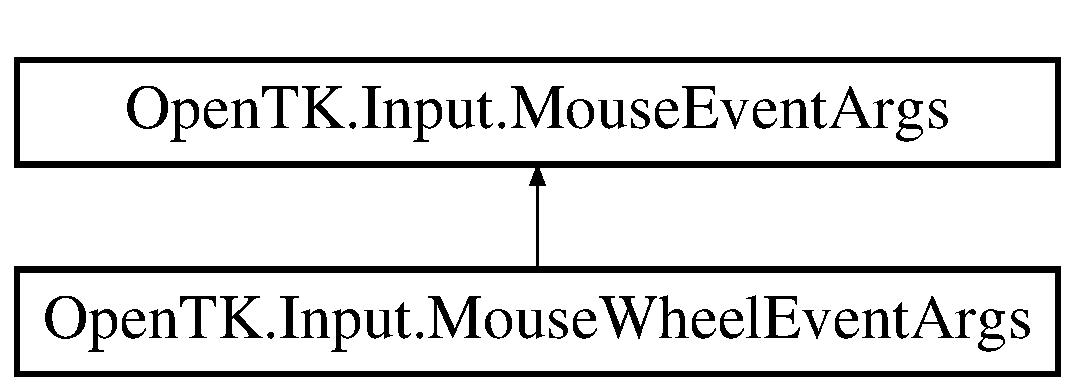
\includegraphics[height=2.000000cm]{class_open_t_k_1_1_input_1_1_mouse_wheel_event_args}
\end{center}
\end{figure}
\subsection*{Public Member Functions}
\begin{DoxyCompactItemize}
\item 
\hyperlink{class_open_t_k_1_1_input_1_1_mouse_wheel_event_args_a96d3e646646fe55565c21e9303ac7435}{Mouse\-Wheel\-Event\-Args} ()
\begin{DoxyCompactList}\small\item\em Constructs a new \hyperlink{class_open_t_k_1_1_input_1_1_mouse_wheel_event_args}{Mouse\-Wheel\-Event\-Args} instance. \end{DoxyCompactList}\item 
\hyperlink{class_open_t_k_1_1_input_1_1_mouse_wheel_event_args_a7cf42d4bbf1d1aed7433847f92afb364}{Mouse\-Wheel\-Event\-Args} (int x, int y, int value, int delta)
\begin{DoxyCompactList}\small\item\em Constructs a new \hyperlink{class_open_t_k_1_1_input_1_1_mouse_wheel_event_args}{Mouse\-Wheel\-Event\-Args} instance. \end{DoxyCompactList}\item 
\hyperlink{class_open_t_k_1_1_input_1_1_mouse_wheel_event_args_ad74fd8fbe8f92977fe4a65efed81930f}{Mouse\-Wheel\-Event\-Args} (\hyperlink{class_open_t_k_1_1_input_1_1_mouse_wheel_event_args}{Mouse\-Wheel\-Event\-Args} args)
\begin{DoxyCompactList}\small\item\em Constructs a new \hyperlink{class_open_t_k_1_1_input_1_1_mouse_wheel_event_args}{Mouse\-Wheel\-Event\-Args} instance. \end{DoxyCompactList}\end{DoxyCompactItemize}
\subsection*{Properties}
\begin{DoxyCompactItemize}
\item 
int \hyperlink{class_open_t_k_1_1_input_1_1_mouse_wheel_event_args_a34daefff9cfbd400ac5d6af00a8118c3}{Value}\hspace{0.3cm}{\ttfamily  \mbox{[}get\mbox{]}}
\begin{DoxyCompactList}\small\item\em Gets the value of the wheel in integer units. To support high-\/precision mice, it is recommended to use \hyperlink{class_open_t_k_1_1_input_1_1_mouse_wheel_event_args_a924698cde619be6ceb51cd318a990b55}{Value\-Precise} instead. \end{DoxyCompactList}\item 
int \hyperlink{class_open_t_k_1_1_input_1_1_mouse_wheel_event_args_aef5f641060a53167289fec501ac8f458}{Delta}\hspace{0.3cm}{\ttfamily  \mbox{[}get\mbox{]}}
\begin{DoxyCompactList}\small\item\em Gets the change in value of the wheel for this event in integer units. To support high-\/precision mice, it is recommended to use \hyperlink{class_open_t_k_1_1_input_1_1_mouse_wheel_event_args_a9ba689417b32b99c1971aa541d8765e2}{Delta\-Precise} instead. \end{DoxyCompactList}\item 
float \hyperlink{class_open_t_k_1_1_input_1_1_mouse_wheel_event_args_a924698cde619be6ceb51cd318a990b55}{Value\-Precise}\hspace{0.3cm}{\ttfamily  \mbox{[}get, set\mbox{]}}
\begin{DoxyCompactList}\small\item\em Gets the precise value of the wheel in floating-\/point units. \end{DoxyCompactList}\item 
float \hyperlink{class_open_t_k_1_1_input_1_1_mouse_wheel_event_args_a9ba689417b32b99c1971aa541d8765e2}{Delta\-Precise}\hspace{0.3cm}{\ttfamily  \mbox{[}get, set\mbox{]}}
\begin{DoxyCompactList}\small\item\em Gets the precise change in value of the wheel for this event in floating-\/point units. \end{DoxyCompactList}\end{DoxyCompactItemize}


\subsection{Detailed Description}
Defines the event data for \hyperlink{class_open_t_k_1_1_input_1_1_mouse_device_a4bee8a35ae92c6d4f74868934a5c2475}{Mouse\-Device.\-Wheel\-Changed} events. 

Do not cache instances of this type outside their event handler. If necessary, you can clone an instance using the \hyperlink{class_open_t_k_1_1_input_1_1_mouse_wheel_event_args_ad74fd8fbe8f92977fe4a65efed81930f}{Mouse\-Wheel\-Event\-Args(\-Mouse\-Wheel\-Event\-Args)} constructor. 

\subsection{Constructor \& Destructor Documentation}
\hypertarget{class_open_t_k_1_1_input_1_1_mouse_wheel_event_args_a96d3e646646fe55565c21e9303ac7435}{\index{Open\-T\-K\-::\-Input\-::\-Mouse\-Wheel\-Event\-Args@{Open\-T\-K\-::\-Input\-::\-Mouse\-Wheel\-Event\-Args}!Mouse\-Wheel\-Event\-Args@{Mouse\-Wheel\-Event\-Args}}
\index{Mouse\-Wheel\-Event\-Args@{Mouse\-Wheel\-Event\-Args}!OpenTK::Input::MouseWheelEventArgs@{Open\-T\-K\-::\-Input\-::\-Mouse\-Wheel\-Event\-Args}}
\subsubsection[{Mouse\-Wheel\-Event\-Args}]{\setlength{\rightskip}{0pt plus 5cm}Open\-T\-K.\-Input.\-Mouse\-Wheel\-Event\-Args.\-Mouse\-Wheel\-Event\-Args (
\begin{DoxyParamCaption}
{}
\end{DoxyParamCaption}
)}}\label{class_open_t_k_1_1_input_1_1_mouse_wheel_event_args_a96d3e646646fe55565c21e9303ac7435}


Constructs a new \hyperlink{class_open_t_k_1_1_input_1_1_mouse_wheel_event_args}{Mouse\-Wheel\-Event\-Args} instance. 

\hypertarget{class_open_t_k_1_1_input_1_1_mouse_wheel_event_args_a7cf42d4bbf1d1aed7433847f92afb364}{\index{Open\-T\-K\-::\-Input\-::\-Mouse\-Wheel\-Event\-Args@{Open\-T\-K\-::\-Input\-::\-Mouse\-Wheel\-Event\-Args}!Mouse\-Wheel\-Event\-Args@{Mouse\-Wheel\-Event\-Args}}
\index{Mouse\-Wheel\-Event\-Args@{Mouse\-Wheel\-Event\-Args}!OpenTK::Input::MouseWheelEventArgs@{Open\-T\-K\-::\-Input\-::\-Mouse\-Wheel\-Event\-Args}}
\subsubsection[{Mouse\-Wheel\-Event\-Args}]{\setlength{\rightskip}{0pt plus 5cm}Open\-T\-K.\-Input.\-Mouse\-Wheel\-Event\-Args.\-Mouse\-Wheel\-Event\-Args (
\begin{DoxyParamCaption}
\item[{int}]{x, }
\item[{int}]{y, }
\item[{int}]{value, }
\item[{int}]{delta}
\end{DoxyParamCaption}
)}}\label{class_open_t_k_1_1_input_1_1_mouse_wheel_event_args_a7cf42d4bbf1d1aed7433847f92afb364}


Constructs a new \hyperlink{class_open_t_k_1_1_input_1_1_mouse_wheel_event_args}{Mouse\-Wheel\-Event\-Args} instance. 


\begin{DoxyParams}{Parameters}
{\em x} & The X position.\\
\hline
{\em y} & The Y position.\\
\hline
{\em value} & The value of the wheel.\\
\hline
{\em delta} & The change in value of the wheel for this event.\\
\hline
\end{DoxyParams}
\hypertarget{class_open_t_k_1_1_input_1_1_mouse_wheel_event_args_ad74fd8fbe8f92977fe4a65efed81930f}{\index{Open\-T\-K\-::\-Input\-::\-Mouse\-Wheel\-Event\-Args@{Open\-T\-K\-::\-Input\-::\-Mouse\-Wheel\-Event\-Args}!Mouse\-Wheel\-Event\-Args@{Mouse\-Wheel\-Event\-Args}}
\index{Mouse\-Wheel\-Event\-Args@{Mouse\-Wheel\-Event\-Args}!OpenTK::Input::MouseWheelEventArgs@{Open\-T\-K\-::\-Input\-::\-Mouse\-Wheel\-Event\-Args}}
\subsubsection[{Mouse\-Wheel\-Event\-Args}]{\setlength{\rightskip}{0pt plus 5cm}Open\-T\-K.\-Input.\-Mouse\-Wheel\-Event\-Args.\-Mouse\-Wheel\-Event\-Args (
\begin{DoxyParamCaption}
\item[{{\bf Mouse\-Wheel\-Event\-Args}}]{args}
\end{DoxyParamCaption}
)}}\label{class_open_t_k_1_1_input_1_1_mouse_wheel_event_args_ad74fd8fbe8f92977fe4a65efed81930f}


Constructs a new \hyperlink{class_open_t_k_1_1_input_1_1_mouse_wheel_event_args}{Mouse\-Wheel\-Event\-Args} instance. 


\begin{DoxyParams}{Parameters}
{\em args} & The \hyperlink{class_open_t_k_1_1_input_1_1_mouse_wheel_event_args}{Mouse\-Wheel\-Event\-Args} instance to clone.\\
\hline
\end{DoxyParams}


\subsection{Property Documentation}
\hypertarget{class_open_t_k_1_1_input_1_1_mouse_wheel_event_args_aef5f641060a53167289fec501ac8f458}{\index{Open\-T\-K\-::\-Input\-::\-Mouse\-Wheel\-Event\-Args@{Open\-T\-K\-::\-Input\-::\-Mouse\-Wheel\-Event\-Args}!Delta@{Delta}}
\index{Delta@{Delta}!OpenTK::Input::MouseWheelEventArgs@{Open\-T\-K\-::\-Input\-::\-Mouse\-Wheel\-Event\-Args}}
\subsubsection[{Delta}]{\setlength{\rightskip}{0pt plus 5cm}int Open\-T\-K.\-Input.\-Mouse\-Wheel\-Event\-Args.\-Delta\hspace{0.3cm}{\ttfamily [get]}}}\label{class_open_t_k_1_1_input_1_1_mouse_wheel_event_args_aef5f641060a53167289fec501ac8f458}


Gets the change in value of the wheel for this event in integer units. To support high-\/precision mice, it is recommended to use \hyperlink{class_open_t_k_1_1_input_1_1_mouse_wheel_event_args_a9ba689417b32b99c1971aa541d8765e2}{Delta\-Precise} instead. 

\hypertarget{class_open_t_k_1_1_input_1_1_mouse_wheel_event_args_a9ba689417b32b99c1971aa541d8765e2}{\index{Open\-T\-K\-::\-Input\-::\-Mouse\-Wheel\-Event\-Args@{Open\-T\-K\-::\-Input\-::\-Mouse\-Wheel\-Event\-Args}!Delta\-Precise@{Delta\-Precise}}
\index{Delta\-Precise@{Delta\-Precise}!OpenTK::Input::MouseWheelEventArgs@{Open\-T\-K\-::\-Input\-::\-Mouse\-Wheel\-Event\-Args}}
\subsubsection[{Delta\-Precise}]{\setlength{\rightskip}{0pt plus 5cm}float Open\-T\-K.\-Input.\-Mouse\-Wheel\-Event\-Args.\-Delta\-Precise\hspace{0.3cm}{\ttfamily [get]}, {\ttfamily [set]}}}\label{class_open_t_k_1_1_input_1_1_mouse_wheel_event_args_a9ba689417b32b99c1971aa541d8765e2}


Gets the precise change in value of the wheel for this event in floating-\/point units. 

\hypertarget{class_open_t_k_1_1_input_1_1_mouse_wheel_event_args_a34daefff9cfbd400ac5d6af00a8118c3}{\index{Open\-T\-K\-::\-Input\-::\-Mouse\-Wheel\-Event\-Args@{Open\-T\-K\-::\-Input\-::\-Mouse\-Wheel\-Event\-Args}!Value@{Value}}
\index{Value@{Value}!OpenTK::Input::MouseWheelEventArgs@{Open\-T\-K\-::\-Input\-::\-Mouse\-Wheel\-Event\-Args}}
\subsubsection[{Value}]{\setlength{\rightskip}{0pt plus 5cm}int Open\-T\-K.\-Input.\-Mouse\-Wheel\-Event\-Args.\-Value\hspace{0.3cm}{\ttfamily [get]}}}\label{class_open_t_k_1_1_input_1_1_mouse_wheel_event_args_a34daefff9cfbd400ac5d6af00a8118c3}


Gets the value of the wheel in integer units. To support high-\/precision mice, it is recommended to use \hyperlink{class_open_t_k_1_1_input_1_1_mouse_wheel_event_args_a924698cde619be6ceb51cd318a990b55}{Value\-Precise} instead. 

\hypertarget{class_open_t_k_1_1_input_1_1_mouse_wheel_event_args_a924698cde619be6ceb51cd318a990b55}{\index{Open\-T\-K\-::\-Input\-::\-Mouse\-Wheel\-Event\-Args@{Open\-T\-K\-::\-Input\-::\-Mouse\-Wheel\-Event\-Args}!Value\-Precise@{Value\-Precise}}
\index{Value\-Precise@{Value\-Precise}!OpenTK::Input::MouseWheelEventArgs@{Open\-T\-K\-::\-Input\-::\-Mouse\-Wheel\-Event\-Args}}
\subsubsection[{Value\-Precise}]{\setlength{\rightskip}{0pt plus 5cm}float Open\-T\-K.\-Input.\-Mouse\-Wheel\-Event\-Args.\-Value\-Precise\hspace{0.3cm}{\ttfamily [get]}, {\ttfamily [set]}}}\label{class_open_t_k_1_1_input_1_1_mouse_wheel_event_args_a924698cde619be6ceb51cd318a990b55}


Gets the precise value of the wheel in floating-\/point units. 


\hypertarget{class_open_t_k_1_1_key_press_event_args}{\section{Open\-T\-K.\-Key\-Press\-Event\-Args Class Reference}
\label{class_open_t_k_1_1_key_press_event_args}\index{Open\-T\-K.\-Key\-Press\-Event\-Args@{Open\-T\-K.\-Key\-Press\-Event\-Args}}
}


Defines the event arguments for Key\-Press events. Instances of this class are cached\-: \hyperlink{class_open_t_k_1_1_key_press_event_args}{Key\-Press\-Event\-Args} should only be used inside the relevant event, unless manually cloned.  




Inherits Event\-Args.

\subsection*{Public Member Functions}
\begin{DoxyCompactItemize}
\item 
\hyperlink{class_open_t_k_1_1_key_press_event_args_a9348dc20a7a43a9908ecfcac1f421236}{Key\-Press\-Event\-Args} (char key\-Char)
\begin{DoxyCompactList}\small\item\em Constructs a new instance. \end{DoxyCompactList}\end{DoxyCompactItemize}
\subsection*{Properties}
\begin{DoxyCompactItemize}
\item 
char \hyperlink{class_open_t_k_1_1_key_press_event_args_a3320dd1e5c1465d5abeec7de5f3ae0ce}{Key\-Char}\hspace{0.3cm}{\ttfamily  \mbox{[}get, set\mbox{]}}
\begin{DoxyCompactList}\small\item\em Gets a System.\-Char that defines the A\-S\-C\-I\-I character that was typed. \end{DoxyCompactList}\end{DoxyCompactItemize}


\subsection{Detailed Description}
Defines the event arguments for Key\-Press events. Instances of this class are cached\-: \hyperlink{class_open_t_k_1_1_key_press_event_args}{Key\-Press\-Event\-Args} should only be used inside the relevant event, unless manually cloned. 



\subsection{Constructor \& Destructor Documentation}
\hypertarget{class_open_t_k_1_1_key_press_event_args_a9348dc20a7a43a9908ecfcac1f421236}{\index{Open\-T\-K\-::\-Key\-Press\-Event\-Args@{Open\-T\-K\-::\-Key\-Press\-Event\-Args}!Key\-Press\-Event\-Args@{Key\-Press\-Event\-Args}}
\index{Key\-Press\-Event\-Args@{Key\-Press\-Event\-Args}!OpenTK::KeyPressEventArgs@{Open\-T\-K\-::\-Key\-Press\-Event\-Args}}
\subsubsection[{Key\-Press\-Event\-Args}]{\setlength{\rightskip}{0pt plus 5cm}Open\-T\-K.\-Key\-Press\-Event\-Args.\-Key\-Press\-Event\-Args (
\begin{DoxyParamCaption}
\item[{char}]{key\-Char}
\end{DoxyParamCaption}
)}}\label{class_open_t_k_1_1_key_press_event_args_a9348dc20a7a43a9908ecfcac1f421236}


Constructs a new instance. 


\begin{DoxyParams}{Parameters}
{\em key\-Char} & The A\-S\-C\-I\-I character that was typed.\\
\hline
\end{DoxyParams}


\subsection{Property Documentation}
\hypertarget{class_open_t_k_1_1_key_press_event_args_a3320dd1e5c1465d5abeec7de5f3ae0ce}{\index{Open\-T\-K\-::\-Key\-Press\-Event\-Args@{Open\-T\-K\-::\-Key\-Press\-Event\-Args}!Key\-Char@{Key\-Char}}
\index{Key\-Char@{Key\-Char}!OpenTK::KeyPressEventArgs@{Open\-T\-K\-::\-Key\-Press\-Event\-Args}}
\subsubsection[{Key\-Char}]{\setlength{\rightskip}{0pt plus 5cm}char Open\-T\-K.\-Key\-Press\-Event\-Args.\-Key\-Char\hspace{0.3cm}{\ttfamily [get]}, {\ttfamily [set]}}}\label{class_open_t_k_1_1_key_press_event_args_a3320dd1e5c1465d5abeec7de5f3ae0ce}


Gets a System.\-Char that defines the A\-S\-C\-I\-I character that was typed. 


\hypertarget{struct_open_t_k_1_1_matrix2}{\section{Open\-T\-K.\-Matrix2 Struct Reference}
\label{struct_open_t_k_1_1_matrix2}\index{Open\-T\-K.\-Matrix2@{Open\-T\-K.\-Matrix2}}
}


Represents a 2x2 matrix  




Inherits I\-Equatable$<$ Matrix2 $>$.

\subsection*{Public Member Functions}
\begin{DoxyCompactItemize}
\item 
\hyperlink{struct_open_t_k_1_1_matrix2_a3d7d4c73c782db56b4373217ba880b86}{Matrix2} (\hyperlink{struct_open_t_k_1_1_vector2}{Vector2} row0, \hyperlink{struct_open_t_k_1_1_vector2}{Vector2} row1)
\begin{DoxyCompactList}\small\item\em Constructs a new instance. \end{DoxyCompactList}\item 
\hyperlink{struct_open_t_k_1_1_matrix2_afec74569441d89ffe2e376f4e3878d12}{Matrix2} (float m00, float m01, float m10, float m11)
\begin{DoxyCompactList}\small\item\em Constructs a new instance \end{DoxyCompactList}\item 
void \hyperlink{struct_open_t_k_1_1_matrix2_aabd2bd46c55b719370acea2f8f4edc80}{Transpose} ()
\begin{DoxyCompactList}\small\item\em Converts this instance to it's transpose. \end{DoxyCompactList}\item 
void \hyperlink{struct_open_t_k_1_1_matrix2_ad5dd7a1b85a14f2395461d8ab5d8cbe6}{Invert} ()
\begin{DoxyCompactList}\small\item\em Converts this instance into its inverse. \end{DoxyCompactList}\item 
override string \hyperlink{struct_open_t_k_1_1_matrix2_a5c83d326f4cfaf69427eca93e05f2764}{To\-String} ()
\begin{DoxyCompactList}\small\item\em Returns a System.\-String that represents the current \hyperlink{struct_open_t_k_1_1_matrix4}{Matrix4}. \end{DoxyCompactList}\item 
override int \hyperlink{struct_open_t_k_1_1_matrix2_acd6cfac90bdf6c70f52a17ea469edaf5}{Get\-Hash\-Code} ()
\begin{DoxyCompactList}\small\item\em Returns the hashcode for this instance. \end{DoxyCompactList}\item 
override bool \hyperlink{struct_open_t_k_1_1_matrix2_a0295be986c376f9fd3ce10c595f28783}{Equals} (object obj)
\begin{DoxyCompactList}\small\item\em Indicates whether this instance and a specified object are equal. \end{DoxyCompactList}\item 
bool \hyperlink{struct_open_t_k_1_1_matrix2_ab9a20399b22c7ada439665a4a1a9ffc5}{Equals} (\hyperlink{struct_open_t_k_1_1_matrix2}{Matrix2} other)
\begin{DoxyCompactList}\small\item\em Indicates whether the current matrix is equal to another matrix.\end{DoxyCompactList}\end{DoxyCompactItemize}
\subsection*{Static Public Member Functions}
\begin{DoxyCompactItemize}
\item 
static void \hyperlink{struct_open_t_k_1_1_matrix2_a14c30cc8079450f694f3f31206339650}{Create\-Rotation} (float angle, out \hyperlink{struct_open_t_k_1_1_matrix2}{Matrix2} result)
\begin{DoxyCompactList}\small\item\em Builds a rotation matrix. \end{DoxyCompactList}\item 
static \hyperlink{struct_open_t_k_1_1_matrix2}{Matrix2} \hyperlink{struct_open_t_k_1_1_matrix2_ab48e897254f497f624c66830937ed991}{Create\-Rotation} (float angle)
\begin{DoxyCompactList}\small\item\em Builds a rotation matrix. \end{DoxyCompactList}\item 
static void \hyperlink{struct_open_t_k_1_1_matrix2_a98bfa496c912749ca5d6f341c5791e7b}{Create\-Scale} (float scale, out \hyperlink{struct_open_t_k_1_1_matrix2}{Matrix2} result)
\begin{DoxyCompactList}\small\item\em Creates a scale matrix. \end{DoxyCompactList}\item 
static \hyperlink{struct_open_t_k_1_1_matrix2}{Matrix2} \hyperlink{struct_open_t_k_1_1_matrix2_af52692aab98a1ed57171e3863548dd3b}{Create\-Scale} (float scale)
\begin{DoxyCompactList}\small\item\em Creates a scale matrix. \end{DoxyCompactList}\item 
static void \hyperlink{struct_open_t_k_1_1_matrix2_a01086d45ade6fd4c2b6b7fe6270307c4}{Create\-Scale} (\hyperlink{struct_open_t_k_1_1_vector2}{Vector2} scale, out \hyperlink{struct_open_t_k_1_1_matrix2}{Matrix2} result)
\begin{DoxyCompactList}\small\item\em Creates a scale matrix. \end{DoxyCompactList}\item 
static \hyperlink{struct_open_t_k_1_1_matrix2}{Matrix2} \hyperlink{struct_open_t_k_1_1_matrix2_a26826a91ced1bd9cdd963f93147daec0}{Create\-Scale} (\hyperlink{struct_open_t_k_1_1_vector2}{Vector2} scale)
\begin{DoxyCompactList}\small\item\em Creates a scale matrix. \end{DoxyCompactList}\item 
static void \hyperlink{struct_open_t_k_1_1_matrix2_ae69bb77589717aeb16ade1df7ac1b4d1}{Create\-Scale} (float x, float y, out \hyperlink{struct_open_t_k_1_1_matrix2}{Matrix2} result)
\begin{DoxyCompactList}\small\item\em Creates a scale matrix. \end{DoxyCompactList}\item 
static \hyperlink{struct_open_t_k_1_1_matrix2}{Matrix2} \hyperlink{struct_open_t_k_1_1_matrix2_a9b0c358ff84fa68bdc5f2bee457329e1}{Create\-Scale} (float x, float y)
\begin{DoxyCompactList}\small\item\em Creates a scale matrix. \end{DoxyCompactList}\item 
static void \hyperlink{struct_open_t_k_1_1_matrix2_ac358e5c0c410a101bfb7ae9de744d9e2}{Mult} (ref \hyperlink{struct_open_t_k_1_1_matrix2}{Matrix2} left, float right, out \hyperlink{struct_open_t_k_1_1_matrix2}{Matrix2} result)
\begin{DoxyCompactList}\small\item\em Multiplies and instance by a scalar. \end{DoxyCompactList}\item 
static \hyperlink{struct_open_t_k_1_1_matrix2}{Matrix2} \hyperlink{struct_open_t_k_1_1_matrix2_aa75f6d03cdd7a0e9e8d31a6fb428deba}{Mult} (\hyperlink{struct_open_t_k_1_1_matrix2}{Matrix2} left, float right)
\begin{DoxyCompactList}\small\item\em Multiplies and instance by a scalar. \end{DoxyCompactList}\item 
static void \hyperlink{struct_open_t_k_1_1_matrix2_ab2568c372f55f6393c2da408c4f05edc}{Mult} (ref \hyperlink{struct_open_t_k_1_1_matrix2}{Matrix2} left, ref \hyperlink{struct_open_t_k_1_1_matrix2}{Matrix2} right, out \hyperlink{struct_open_t_k_1_1_matrix2}{Matrix2} result)
\begin{DoxyCompactList}\small\item\em Multiplies two instances. \end{DoxyCompactList}\item 
static \hyperlink{struct_open_t_k_1_1_matrix2}{Matrix2} \hyperlink{struct_open_t_k_1_1_matrix2_a0c990a3f898de12cebb733caca576c79}{Mult} (\hyperlink{struct_open_t_k_1_1_matrix2}{Matrix2} left, \hyperlink{struct_open_t_k_1_1_matrix2}{Matrix2} right)
\begin{DoxyCompactList}\small\item\em Multiplies two instances. \end{DoxyCompactList}\item 
static void \hyperlink{struct_open_t_k_1_1_matrix2_a304755f88a224959c21e6dc285804dcf}{Mult} (ref \hyperlink{struct_open_t_k_1_1_matrix2}{Matrix2} left, ref \hyperlink{struct_open_t_k_1_1_matrix2x3}{Matrix2x3} right, out \hyperlink{struct_open_t_k_1_1_matrix2x3}{Matrix2x3} result)
\begin{DoxyCompactList}\small\item\em Multiplies two instances. \end{DoxyCompactList}\item 
static \hyperlink{struct_open_t_k_1_1_matrix2x3}{Matrix2x3} \hyperlink{struct_open_t_k_1_1_matrix2_a21f3f53d36b4ebe4fc2b64cacf8befdd}{Mult} (\hyperlink{struct_open_t_k_1_1_matrix2}{Matrix2} left, \hyperlink{struct_open_t_k_1_1_matrix2x3}{Matrix2x3} right)
\begin{DoxyCompactList}\small\item\em Multiplies two instances. \end{DoxyCompactList}\item 
static void \hyperlink{struct_open_t_k_1_1_matrix2_ad8b9cad7dd846e35407ad7703c51858f}{Mult} (ref \hyperlink{struct_open_t_k_1_1_matrix2}{Matrix2} left, ref \hyperlink{struct_open_t_k_1_1_matrix2x4}{Matrix2x4} right, out \hyperlink{struct_open_t_k_1_1_matrix2x4}{Matrix2x4} result)
\begin{DoxyCompactList}\small\item\em Multiplies two instances. \end{DoxyCompactList}\item 
static \hyperlink{struct_open_t_k_1_1_matrix2x4}{Matrix2x4} \hyperlink{struct_open_t_k_1_1_matrix2_a1a940320cc553176b4c15e29f4b7f6d3}{Mult} (\hyperlink{struct_open_t_k_1_1_matrix2}{Matrix2} left, \hyperlink{struct_open_t_k_1_1_matrix2x4}{Matrix2x4} right)
\begin{DoxyCompactList}\small\item\em Multiplies two instances. \end{DoxyCompactList}\item 
static void \hyperlink{struct_open_t_k_1_1_matrix2_a7892558f78f7d73ae838e78c8e355543}{Add} (ref \hyperlink{struct_open_t_k_1_1_matrix2}{Matrix2} left, ref \hyperlink{struct_open_t_k_1_1_matrix2}{Matrix2} right, out \hyperlink{struct_open_t_k_1_1_matrix2}{Matrix2} result)
\begin{DoxyCompactList}\small\item\em Adds two instances. \end{DoxyCompactList}\item 
static \hyperlink{struct_open_t_k_1_1_matrix2}{Matrix2} \hyperlink{struct_open_t_k_1_1_matrix2_ae7f21701779660ec4e7db6ad2fa9792c}{Add} (\hyperlink{struct_open_t_k_1_1_matrix2}{Matrix2} left, \hyperlink{struct_open_t_k_1_1_matrix2}{Matrix2} right)
\begin{DoxyCompactList}\small\item\em Adds two instances. \end{DoxyCompactList}\item 
static void \hyperlink{struct_open_t_k_1_1_matrix2_a1f88c61e7a7f8e8bbc6bea2d52a279e7}{Subtract} (ref \hyperlink{struct_open_t_k_1_1_matrix2}{Matrix2} left, ref \hyperlink{struct_open_t_k_1_1_matrix2}{Matrix2} right, out \hyperlink{struct_open_t_k_1_1_matrix2}{Matrix2} result)
\begin{DoxyCompactList}\small\item\em Subtracts two instances. \end{DoxyCompactList}\item 
static \hyperlink{struct_open_t_k_1_1_matrix2}{Matrix2} \hyperlink{struct_open_t_k_1_1_matrix2_a0183133151489936c9b39a80cf5296c5}{Subtract} (\hyperlink{struct_open_t_k_1_1_matrix2}{Matrix2} left, \hyperlink{struct_open_t_k_1_1_matrix2}{Matrix2} right)
\begin{DoxyCompactList}\small\item\em Subtracts two instances. \end{DoxyCompactList}\item 
static void \hyperlink{struct_open_t_k_1_1_matrix2_a43785f5b085a1777b5aac98e2f6fcff8}{Invert} (ref \hyperlink{struct_open_t_k_1_1_matrix2}{Matrix2} mat, out \hyperlink{struct_open_t_k_1_1_matrix2}{Matrix2} result)
\begin{DoxyCompactList}\small\item\em Calculate the inverse of the given matrix \end{DoxyCompactList}\item 
static \hyperlink{struct_open_t_k_1_1_matrix2}{Matrix2} \hyperlink{struct_open_t_k_1_1_matrix2_abd0852c064e9348daebba6c4f0b96000}{Invert} (\hyperlink{struct_open_t_k_1_1_matrix2}{Matrix2} mat)
\begin{DoxyCompactList}\small\item\em Calculate the inverse of the given matrix \end{DoxyCompactList}\item 
static void \hyperlink{struct_open_t_k_1_1_matrix2_a89a584347359cfbc6c6ab96de8f46630}{Transpose} (ref \hyperlink{struct_open_t_k_1_1_matrix2}{Matrix2} mat, out \hyperlink{struct_open_t_k_1_1_matrix2}{Matrix2} result)
\begin{DoxyCompactList}\small\item\em Calculate the transpose of the given matrix. \end{DoxyCompactList}\item 
static \hyperlink{struct_open_t_k_1_1_matrix2}{Matrix2} \hyperlink{struct_open_t_k_1_1_matrix2_a4d3575ac9869c300b5edb8cee7162b70}{Transpose} (\hyperlink{struct_open_t_k_1_1_matrix2}{Matrix2} mat)
\begin{DoxyCompactList}\small\item\em Calculate the transpose of the given matrix. \end{DoxyCompactList}\item 
static \hyperlink{struct_open_t_k_1_1_matrix2}{Matrix2} \hyperlink{struct_open_t_k_1_1_matrix2_ac52c4c5f314ec452200c067aa79e94fc}{operator$\ast$} (float left, \hyperlink{struct_open_t_k_1_1_matrix2}{Matrix2} right)
\begin{DoxyCompactList}\small\item\em Scalar multiplication. \end{DoxyCompactList}\item 
static \hyperlink{struct_open_t_k_1_1_matrix2}{Matrix2} \hyperlink{struct_open_t_k_1_1_matrix2_a0b6e2068039fc41c5706dc2b3ab59fac}{operator$\ast$} (\hyperlink{struct_open_t_k_1_1_matrix2}{Matrix2} left, float right)
\begin{DoxyCompactList}\small\item\em Scalar multiplication. \end{DoxyCompactList}\item 
static \hyperlink{struct_open_t_k_1_1_matrix2}{Matrix2} \hyperlink{struct_open_t_k_1_1_matrix2_a8db8410f7d08b662f04945a9dcbd698f}{operator$\ast$} (\hyperlink{struct_open_t_k_1_1_matrix2}{Matrix2} left, \hyperlink{struct_open_t_k_1_1_matrix2}{Matrix2} right)
\begin{DoxyCompactList}\small\item\em Matrix multiplication \end{DoxyCompactList}\item 
static \hyperlink{struct_open_t_k_1_1_matrix2x3}{Matrix2x3} \hyperlink{struct_open_t_k_1_1_matrix2_a2054614c151f626e51ae2ba5ca8e6f62}{operator$\ast$} (\hyperlink{struct_open_t_k_1_1_matrix2}{Matrix2} left, \hyperlink{struct_open_t_k_1_1_matrix2x3}{Matrix2x3} right)
\begin{DoxyCompactList}\small\item\em Matrix multiplication \end{DoxyCompactList}\item 
static \hyperlink{struct_open_t_k_1_1_matrix2x4}{Matrix2x4} \hyperlink{struct_open_t_k_1_1_matrix2_a4c60fcd9da604ade925aa1294d547553}{operator$\ast$} (\hyperlink{struct_open_t_k_1_1_matrix2}{Matrix2} left, \hyperlink{struct_open_t_k_1_1_matrix2x4}{Matrix2x4} right)
\begin{DoxyCompactList}\small\item\em Matrix multiplication \end{DoxyCompactList}\item 
static \hyperlink{struct_open_t_k_1_1_matrix2}{Matrix2} \hyperlink{struct_open_t_k_1_1_matrix2_ad3b62e6bc4154be0bdf957706a68999c}{operator+} (\hyperlink{struct_open_t_k_1_1_matrix2}{Matrix2} left, \hyperlink{struct_open_t_k_1_1_matrix2}{Matrix2} right)
\begin{DoxyCompactList}\small\item\em Matrix addition \end{DoxyCompactList}\item 
static \hyperlink{struct_open_t_k_1_1_matrix2}{Matrix2} \hyperlink{struct_open_t_k_1_1_matrix2_a70779c87fbdf8959145b2d8e812f0591}{operator-\/} (\hyperlink{struct_open_t_k_1_1_matrix2}{Matrix2} left, \hyperlink{struct_open_t_k_1_1_matrix2}{Matrix2} right)
\begin{DoxyCompactList}\small\item\em Matrix subtraction \end{DoxyCompactList}\item 
static bool \hyperlink{struct_open_t_k_1_1_matrix2_a34a08ee52d805d7d33ab251fa4ffe295}{operator==} (\hyperlink{struct_open_t_k_1_1_matrix2}{Matrix2} left, \hyperlink{struct_open_t_k_1_1_matrix2}{Matrix2} right)
\begin{DoxyCompactList}\small\item\em Compares two instances for equality. \end{DoxyCompactList}\item 
static bool \hyperlink{struct_open_t_k_1_1_matrix2_afb8c62aa855cbd8a9525dafe658bb6e3}{operator!=} (\hyperlink{struct_open_t_k_1_1_matrix2}{Matrix2} left, \hyperlink{struct_open_t_k_1_1_matrix2}{Matrix2} right)
\begin{DoxyCompactList}\small\item\em Compares two instances for inequality. \end{DoxyCompactList}\end{DoxyCompactItemize}
\subsection*{Public Attributes}
\begin{DoxyCompactItemize}
\item 
\hyperlink{struct_open_t_k_1_1_vector2}{Vector2} \hyperlink{struct_open_t_k_1_1_matrix2_a7712c9d0c02c87fa1d98f4bb54cfc83f}{Row0}
\begin{DoxyCompactList}\small\item\em Top row of the matrix. \end{DoxyCompactList}\item 
\hyperlink{struct_open_t_k_1_1_vector2}{Vector2} \hyperlink{struct_open_t_k_1_1_matrix2_a27718ab92c9a8bad7f1d054b3f61841f}{Row1}
\begin{DoxyCompactList}\small\item\em Bottom row of the matrix. \end{DoxyCompactList}\end{DoxyCompactItemize}
\subsection*{Static Public Attributes}
\begin{DoxyCompactItemize}
\item 
static readonly \hyperlink{struct_open_t_k_1_1_matrix2}{Matrix2} \hyperlink{struct_open_t_k_1_1_matrix2_aa1ece0676cf9a9ca5e49671c03dd0ba0}{Identity} = new \hyperlink{struct_open_t_k_1_1_matrix2}{Matrix2}(\hyperlink{struct_open_t_k_1_1_vector2_a7f2eba13c36cf07b242119014b3cc959}{Vector2.\-Unit\-X}, \hyperlink{struct_open_t_k_1_1_vector2_ae71028930b0fc4172fddddad30a6cf23}{Vector2.\-Unit\-Y})
\begin{DoxyCompactList}\small\item\em The identity matrix. \end{DoxyCompactList}\item 
static readonly \hyperlink{struct_open_t_k_1_1_matrix2}{Matrix2} \hyperlink{struct_open_t_k_1_1_matrix2_aa14232ae27ca06ba9e721da3f8153dd5}{Zero} = new \hyperlink{struct_open_t_k_1_1_matrix2}{Matrix2}(Vector2.\-Zero, Vector2.\-Zero)
\begin{DoxyCompactList}\small\item\em The zero matrix. \end{DoxyCompactList}\end{DoxyCompactItemize}
\subsection*{Properties}
\begin{DoxyCompactItemize}
\item 
float \hyperlink{struct_open_t_k_1_1_matrix2_adcf885e885add38852d565b19b27a0e3}{Determinant}\hspace{0.3cm}{\ttfamily  \mbox{[}get\mbox{]}}
\begin{DoxyCompactList}\small\item\em Gets the determinant of this matrix. \end{DoxyCompactList}\item 
\hyperlink{struct_open_t_k_1_1_vector2}{Vector2} \hyperlink{struct_open_t_k_1_1_matrix2_a8f6fa1f04466c18e03ed65fe77979b5b}{Column0}\hspace{0.3cm}{\ttfamily  \mbox{[}get, set\mbox{]}}
\begin{DoxyCompactList}\small\item\em Gets or sets the first column of this matrix. \end{DoxyCompactList}\item 
\hyperlink{struct_open_t_k_1_1_vector2}{Vector2} \hyperlink{struct_open_t_k_1_1_matrix2_acc042415fe491ade747c36781e063e7f}{Column1}\hspace{0.3cm}{\ttfamily  \mbox{[}get, set\mbox{]}}
\begin{DoxyCompactList}\small\item\em Gets or sets the second column of this matrix. \end{DoxyCompactList}\item 
float \hyperlink{struct_open_t_k_1_1_matrix2_ac0096c57a845f57cad5b53117d97f90b}{M11}\hspace{0.3cm}{\ttfamily  \mbox{[}get, set\mbox{]}}
\begin{DoxyCompactList}\small\item\em Gets or sets the value at row 1, column 1 of this instance. \end{DoxyCompactList}\item 
float \hyperlink{struct_open_t_k_1_1_matrix2_a20a739651456601282e0714c0e8a3f20}{M12}\hspace{0.3cm}{\ttfamily  \mbox{[}get, set\mbox{]}}
\begin{DoxyCompactList}\small\item\em Gets or sets the value at row 1, column 2 of this instance. \end{DoxyCompactList}\item 
float \hyperlink{struct_open_t_k_1_1_matrix2_af0d21a4607e71a4c82c01db39cbafc2c}{M21}\hspace{0.3cm}{\ttfamily  \mbox{[}get, set\mbox{]}}
\begin{DoxyCompactList}\small\item\em Gets or sets the value at row 2, column 1 of this instance. \end{DoxyCompactList}\item 
float \hyperlink{struct_open_t_k_1_1_matrix2_a6b9b6b7e323353efcd52f972e9e11011}{M22}\hspace{0.3cm}{\ttfamily  \mbox{[}get, set\mbox{]}}
\begin{DoxyCompactList}\small\item\em Gets or sets the value at row 2, column 2 of this instance. \end{DoxyCompactList}\item 
\hyperlink{struct_open_t_k_1_1_vector2}{Vector2} \hyperlink{struct_open_t_k_1_1_matrix2_af95195a62dda800e6466721bc6769bb1}{Diagonal}\hspace{0.3cm}{\ttfamily  \mbox{[}get, set\mbox{]}}
\begin{DoxyCompactList}\small\item\em Gets or sets the values along the main diagonal of the matrix. \end{DoxyCompactList}\item 
float \hyperlink{struct_open_t_k_1_1_matrix2_ac3f3859dc69583c8924ac70e1782b0e0}{Trace}\hspace{0.3cm}{\ttfamily  \mbox{[}get\mbox{]}}
\begin{DoxyCompactList}\small\item\em Gets the trace of the matrix, the sum of the values along the diagonal. \end{DoxyCompactList}\item 
float \hyperlink{struct_open_t_k_1_1_matrix2_ace510988a666db0540be994392b94ae6}{this\mbox{[}int row\-Index, int column\-Index\mbox{]}}\hspace{0.3cm}{\ttfamily  \mbox{[}get, set\mbox{]}}
\begin{DoxyCompactList}\small\item\em Gets or sets the value at a specified row and column. \end{DoxyCompactList}\end{DoxyCompactItemize}


\subsection{Detailed Description}
Represents a 2x2 matrix 



\subsection{Constructor \& Destructor Documentation}
\hypertarget{struct_open_t_k_1_1_matrix2_a3d7d4c73c782db56b4373217ba880b86}{\index{Open\-T\-K\-::\-Matrix2@{Open\-T\-K\-::\-Matrix2}!Matrix2@{Matrix2}}
\index{Matrix2@{Matrix2}!OpenTK::Matrix2@{Open\-T\-K\-::\-Matrix2}}
\subsubsection[{Matrix2}]{\setlength{\rightskip}{0pt plus 5cm}Open\-T\-K.\-Matrix2.\-Matrix2 (
\begin{DoxyParamCaption}
\item[{{\bf Vector2}}]{row0, }
\item[{{\bf Vector2}}]{row1}
\end{DoxyParamCaption}
)}}\label{struct_open_t_k_1_1_matrix2_a3d7d4c73c782db56b4373217ba880b86}


Constructs a new instance. 


\begin{DoxyParams}{Parameters}
{\em row0} & Top row of the matrix.\\
\hline
{\em row1} & Bottom row of the matrix.\\
\hline
\end{DoxyParams}
\hypertarget{struct_open_t_k_1_1_matrix2_afec74569441d89ffe2e376f4e3878d12}{\index{Open\-T\-K\-::\-Matrix2@{Open\-T\-K\-::\-Matrix2}!Matrix2@{Matrix2}}
\index{Matrix2@{Matrix2}!OpenTK::Matrix2@{Open\-T\-K\-::\-Matrix2}}
\subsubsection[{Matrix2}]{\setlength{\rightskip}{0pt plus 5cm}Open\-T\-K.\-Matrix2.\-Matrix2 (
\begin{DoxyParamCaption}
\item[{float}]{m00, }
\item[{float}]{m01, }
\item[{float}]{m10, }
\item[{float}]{m11}
\end{DoxyParamCaption}
)}}\label{struct_open_t_k_1_1_matrix2_afec74569441d89ffe2e376f4e3878d12}


Constructs a new instance 


\begin{DoxyParams}{Parameters}
{\em m00} & First item of the first row of the matrix.\\
\hline
{\em m01} & Second item of the first row of the matrix.\\
\hline
{\em m10} & First item of the second row of the matrix.\\
\hline
{\em m11} & Second item of the second row of the matrix.\\
\hline
\end{DoxyParams}


\subsection{Member Function Documentation}
\hypertarget{struct_open_t_k_1_1_matrix2_a7892558f78f7d73ae838e78c8e355543}{\index{Open\-T\-K\-::\-Matrix2@{Open\-T\-K\-::\-Matrix2}!Add@{Add}}
\index{Add@{Add}!OpenTK::Matrix2@{Open\-T\-K\-::\-Matrix2}}
\subsubsection[{Add}]{\setlength{\rightskip}{0pt plus 5cm}static void Open\-T\-K.\-Matrix2.\-Add (
\begin{DoxyParamCaption}
\item[{ref {\bf Matrix2}}]{left, }
\item[{ref {\bf Matrix2}}]{right, }
\item[{out {\bf Matrix2}}]{result}
\end{DoxyParamCaption}
)\hspace{0.3cm}{\ttfamily [static]}}}\label{struct_open_t_k_1_1_matrix2_a7892558f78f7d73ae838e78c8e355543}


Adds two instances. 


\begin{DoxyParams}{Parameters}
{\em left} & The left operand of the addition.\\
\hline
{\em right} & The right operand of the addition.\\
\hline
{\em result} & A new instance that is the result of the addition.\\
\hline
\end{DoxyParams}
\hypertarget{struct_open_t_k_1_1_matrix2_ae7f21701779660ec4e7db6ad2fa9792c}{\index{Open\-T\-K\-::\-Matrix2@{Open\-T\-K\-::\-Matrix2}!Add@{Add}}
\index{Add@{Add}!OpenTK::Matrix2@{Open\-T\-K\-::\-Matrix2}}
\subsubsection[{Add}]{\setlength{\rightskip}{0pt plus 5cm}static {\bf Matrix2} Open\-T\-K.\-Matrix2.\-Add (
\begin{DoxyParamCaption}
\item[{{\bf Matrix2}}]{left, }
\item[{{\bf Matrix2}}]{right}
\end{DoxyParamCaption}
)\hspace{0.3cm}{\ttfamily [static]}}}\label{struct_open_t_k_1_1_matrix2_ae7f21701779660ec4e7db6ad2fa9792c}


Adds two instances. 


\begin{DoxyParams}{Parameters}
{\em left} & The left operand of the addition.\\
\hline
{\em right} & The right operand of the addition.\\
\hline
\end{DoxyParams}
\begin{DoxyReturn}{Returns}
A new instance that is the result of the addition.
\end{DoxyReturn}
\hypertarget{struct_open_t_k_1_1_matrix2_a14c30cc8079450f694f3f31206339650}{\index{Open\-T\-K\-::\-Matrix2@{Open\-T\-K\-::\-Matrix2}!Create\-Rotation@{Create\-Rotation}}
\index{Create\-Rotation@{Create\-Rotation}!OpenTK::Matrix2@{Open\-T\-K\-::\-Matrix2}}
\subsubsection[{Create\-Rotation}]{\setlength{\rightskip}{0pt plus 5cm}static void Open\-T\-K.\-Matrix2.\-Create\-Rotation (
\begin{DoxyParamCaption}
\item[{float}]{angle, }
\item[{out {\bf Matrix2}}]{result}
\end{DoxyParamCaption}
)\hspace{0.3cm}{\ttfamily [static]}}}\label{struct_open_t_k_1_1_matrix2_a14c30cc8079450f694f3f31206339650}


Builds a rotation matrix. 


\begin{DoxyParams}{Parameters}
{\em angle} & The counter-\/clockwise angle in radians.\\
\hline
{\em result} & The resulting \hyperlink{struct_open_t_k_1_1_matrix2}{Matrix2} instance.\\
\hline
\end{DoxyParams}
\hypertarget{struct_open_t_k_1_1_matrix2_ab48e897254f497f624c66830937ed991}{\index{Open\-T\-K\-::\-Matrix2@{Open\-T\-K\-::\-Matrix2}!Create\-Rotation@{Create\-Rotation}}
\index{Create\-Rotation@{Create\-Rotation}!OpenTK::Matrix2@{Open\-T\-K\-::\-Matrix2}}
\subsubsection[{Create\-Rotation}]{\setlength{\rightskip}{0pt plus 5cm}static {\bf Matrix2} Open\-T\-K.\-Matrix2.\-Create\-Rotation (
\begin{DoxyParamCaption}
\item[{float}]{angle}
\end{DoxyParamCaption}
)\hspace{0.3cm}{\ttfamily [static]}}}\label{struct_open_t_k_1_1_matrix2_ab48e897254f497f624c66830937ed991}


Builds a rotation matrix. 


\begin{DoxyParams}{Parameters}
{\em angle} & The counter-\/clockwise angle in radians.\\
\hline
\end{DoxyParams}
\begin{DoxyReturn}{Returns}
The resulting \hyperlink{struct_open_t_k_1_1_matrix2}{Matrix2} instance.
\end{DoxyReturn}
\hypertarget{struct_open_t_k_1_1_matrix2_a98bfa496c912749ca5d6f341c5791e7b}{\index{Open\-T\-K\-::\-Matrix2@{Open\-T\-K\-::\-Matrix2}!Create\-Scale@{Create\-Scale}}
\index{Create\-Scale@{Create\-Scale}!OpenTK::Matrix2@{Open\-T\-K\-::\-Matrix2}}
\subsubsection[{Create\-Scale}]{\setlength{\rightskip}{0pt plus 5cm}static void Open\-T\-K.\-Matrix2.\-Create\-Scale (
\begin{DoxyParamCaption}
\item[{float}]{scale, }
\item[{out {\bf Matrix2}}]{result}
\end{DoxyParamCaption}
)\hspace{0.3cm}{\ttfamily [static]}}}\label{struct_open_t_k_1_1_matrix2_a98bfa496c912749ca5d6f341c5791e7b}


Creates a scale matrix. 


\begin{DoxyParams}{Parameters}
{\em scale} & Single scale factor for the x, y, and z axes.\\
\hline
{\em result} & A scale matrix.\\
\hline
\end{DoxyParams}
\hypertarget{struct_open_t_k_1_1_matrix2_af52692aab98a1ed57171e3863548dd3b}{\index{Open\-T\-K\-::\-Matrix2@{Open\-T\-K\-::\-Matrix2}!Create\-Scale@{Create\-Scale}}
\index{Create\-Scale@{Create\-Scale}!OpenTK::Matrix2@{Open\-T\-K\-::\-Matrix2}}
\subsubsection[{Create\-Scale}]{\setlength{\rightskip}{0pt plus 5cm}static {\bf Matrix2} Open\-T\-K.\-Matrix2.\-Create\-Scale (
\begin{DoxyParamCaption}
\item[{float}]{scale}
\end{DoxyParamCaption}
)\hspace{0.3cm}{\ttfamily [static]}}}\label{struct_open_t_k_1_1_matrix2_af52692aab98a1ed57171e3863548dd3b}


Creates a scale matrix. 


\begin{DoxyParams}{Parameters}
{\em scale} & Single scale factor for the x and y axes.\\
\hline
\end{DoxyParams}
\begin{DoxyReturn}{Returns}
A scale matrix.
\end{DoxyReturn}
\hypertarget{struct_open_t_k_1_1_matrix2_a01086d45ade6fd4c2b6b7fe6270307c4}{\index{Open\-T\-K\-::\-Matrix2@{Open\-T\-K\-::\-Matrix2}!Create\-Scale@{Create\-Scale}}
\index{Create\-Scale@{Create\-Scale}!OpenTK::Matrix2@{Open\-T\-K\-::\-Matrix2}}
\subsubsection[{Create\-Scale}]{\setlength{\rightskip}{0pt plus 5cm}static void Open\-T\-K.\-Matrix2.\-Create\-Scale (
\begin{DoxyParamCaption}
\item[{{\bf Vector2}}]{scale, }
\item[{out {\bf Matrix2}}]{result}
\end{DoxyParamCaption}
)\hspace{0.3cm}{\ttfamily [static]}}}\label{struct_open_t_k_1_1_matrix2_a01086d45ade6fd4c2b6b7fe6270307c4}


Creates a scale matrix. 


\begin{DoxyParams}{Parameters}
{\em scale} & Scale factors for the x and y axes.\\
\hline
{\em result} & A scale matrix.\\
\hline
\end{DoxyParams}
\hypertarget{struct_open_t_k_1_1_matrix2_a26826a91ced1bd9cdd963f93147daec0}{\index{Open\-T\-K\-::\-Matrix2@{Open\-T\-K\-::\-Matrix2}!Create\-Scale@{Create\-Scale}}
\index{Create\-Scale@{Create\-Scale}!OpenTK::Matrix2@{Open\-T\-K\-::\-Matrix2}}
\subsubsection[{Create\-Scale}]{\setlength{\rightskip}{0pt plus 5cm}static {\bf Matrix2} Open\-T\-K.\-Matrix2.\-Create\-Scale (
\begin{DoxyParamCaption}
\item[{{\bf Vector2}}]{scale}
\end{DoxyParamCaption}
)\hspace{0.3cm}{\ttfamily [static]}}}\label{struct_open_t_k_1_1_matrix2_a26826a91ced1bd9cdd963f93147daec0}


Creates a scale matrix. 


\begin{DoxyParams}{Parameters}
{\em scale} & Scale factors for the x and y axes.\\
\hline
\end{DoxyParams}
\begin{DoxyReturn}{Returns}
A scale matrix.
\end{DoxyReturn}
\hypertarget{struct_open_t_k_1_1_matrix2_ae69bb77589717aeb16ade1df7ac1b4d1}{\index{Open\-T\-K\-::\-Matrix2@{Open\-T\-K\-::\-Matrix2}!Create\-Scale@{Create\-Scale}}
\index{Create\-Scale@{Create\-Scale}!OpenTK::Matrix2@{Open\-T\-K\-::\-Matrix2}}
\subsubsection[{Create\-Scale}]{\setlength{\rightskip}{0pt plus 5cm}static void Open\-T\-K.\-Matrix2.\-Create\-Scale (
\begin{DoxyParamCaption}
\item[{float}]{x, }
\item[{float}]{y, }
\item[{out {\bf Matrix2}}]{result}
\end{DoxyParamCaption}
)\hspace{0.3cm}{\ttfamily [static]}}}\label{struct_open_t_k_1_1_matrix2_ae69bb77589717aeb16ade1df7ac1b4d1}


Creates a scale matrix. 


\begin{DoxyParams}{Parameters}
{\em x} & Scale factor for the x axis.\\
\hline
{\em y} & Scale factor for the y axis.\\
\hline
{\em result} & A scale matrix.\\
\hline
\end{DoxyParams}
\hypertarget{struct_open_t_k_1_1_matrix2_a9b0c358ff84fa68bdc5f2bee457329e1}{\index{Open\-T\-K\-::\-Matrix2@{Open\-T\-K\-::\-Matrix2}!Create\-Scale@{Create\-Scale}}
\index{Create\-Scale@{Create\-Scale}!OpenTK::Matrix2@{Open\-T\-K\-::\-Matrix2}}
\subsubsection[{Create\-Scale}]{\setlength{\rightskip}{0pt plus 5cm}static {\bf Matrix2} Open\-T\-K.\-Matrix2.\-Create\-Scale (
\begin{DoxyParamCaption}
\item[{float}]{x, }
\item[{float}]{y}
\end{DoxyParamCaption}
)\hspace{0.3cm}{\ttfamily [static]}}}\label{struct_open_t_k_1_1_matrix2_a9b0c358ff84fa68bdc5f2bee457329e1}


Creates a scale matrix. 


\begin{DoxyParams}{Parameters}
{\em x} & Scale factor for the x axis.\\
\hline
{\em y} & Scale factor for the y axis.\\
\hline
\end{DoxyParams}
\begin{DoxyReturn}{Returns}
A scale matrix.
\end{DoxyReturn}
\hypertarget{struct_open_t_k_1_1_matrix2_a0295be986c376f9fd3ce10c595f28783}{\index{Open\-T\-K\-::\-Matrix2@{Open\-T\-K\-::\-Matrix2}!Equals@{Equals}}
\index{Equals@{Equals}!OpenTK::Matrix2@{Open\-T\-K\-::\-Matrix2}}
\subsubsection[{Equals}]{\setlength{\rightskip}{0pt plus 5cm}override bool Open\-T\-K.\-Matrix2.\-Equals (
\begin{DoxyParamCaption}
\item[{object}]{obj}
\end{DoxyParamCaption}
)}}\label{struct_open_t_k_1_1_matrix2_a0295be986c376f9fd3ce10c595f28783}


Indicates whether this instance and a specified object are equal. 


\begin{DoxyParams}{Parameters}
{\em obj} & The object to compare to.\\
\hline
\end{DoxyParams}
\begin{DoxyReturn}{Returns}
True if the instances are equal; false otherwise.
\end{DoxyReturn}
\hypertarget{struct_open_t_k_1_1_matrix2_ab9a20399b22c7ada439665a4a1a9ffc5}{\index{Open\-T\-K\-::\-Matrix2@{Open\-T\-K\-::\-Matrix2}!Equals@{Equals}}
\index{Equals@{Equals}!OpenTK::Matrix2@{Open\-T\-K\-::\-Matrix2}}
\subsubsection[{Equals}]{\setlength{\rightskip}{0pt plus 5cm}bool Open\-T\-K.\-Matrix2.\-Equals (
\begin{DoxyParamCaption}
\item[{{\bf Matrix2}}]{other}
\end{DoxyParamCaption}
)}}\label{struct_open_t_k_1_1_matrix2_ab9a20399b22c7ada439665a4a1a9ffc5}


Indicates whether the current matrix is equal to another matrix.


\begin{DoxyParams}{Parameters}
{\em other} & An matrix to compare with this matrix.\\
\hline
\end{DoxyParams}
\begin{DoxyReturn}{Returns}
true if the current matrix is equal to the matrix parameter; otherwise, false.
\end{DoxyReturn}
\hypertarget{struct_open_t_k_1_1_matrix2_acd6cfac90bdf6c70f52a17ea469edaf5}{\index{Open\-T\-K\-::\-Matrix2@{Open\-T\-K\-::\-Matrix2}!Get\-Hash\-Code@{Get\-Hash\-Code}}
\index{Get\-Hash\-Code@{Get\-Hash\-Code}!OpenTK::Matrix2@{Open\-T\-K\-::\-Matrix2}}
\subsubsection[{Get\-Hash\-Code}]{\setlength{\rightskip}{0pt plus 5cm}override int Open\-T\-K.\-Matrix2.\-Get\-Hash\-Code (
\begin{DoxyParamCaption}
{}
\end{DoxyParamCaption}
)}}\label{struct_open_t_k_1_1_matrix2_acd6cfac90bdf6c70f52a17ea469edaf5}


Returns the hashcode for this instance. 

\begin{DoxyReturn}{Returns}
A System.\-Int32 containing the unique hashcode for this instance.
\end{DoxyReturn}
\hypertarget{struct_open_t_k_1_1_matrix2_ad5dd7a1b85a14f2395461d8ab5d8cbe6}{\index{Open\-T\-K\-::\-Matrix2@{Open\-T\-K\-::\-Matrix2}!Invert@{Invert}}
\index{Invert@{Invert}!OpenTK::Matrix2@{Open\-T\-K\-::\-Matrix2}}
\subsubsection[{Invert}]{\setlength{\rightskip}{0pt plus 5cm}void Open\-T\-K.\-Matrix2.\-Invert (
\begin{DoxyParamCaption}
{}
\end{DoxyParamCaption}
)}}\label{struct_open_t_k_1_1_matrix2_ad5dd7a1b85a14f2395461d8ab5d8cbe6}


Converts this instance into its inverse. 

\hypertarget{struct_open_t_k_1_1_matrix2_a43785f5b085a1777b5aac98e2f6fcff8}{\index{Open\-T\-K\-::\-Matrix2@{Open\-T\-K\-::\-Matrix2}!Invert@{Invert}}
\index{Invert@{Invert}!OpenTK::Matrix2@{Open\-T\-K\-::\-Matrix2}}
\subsubsection[{Invert}]{\setlength{\rightskip}{0pt plus 5cm}static void Open\-T\-K.\-Matrix2.\-Invert (
\begin{DoxyParamCaption}
\item[{ref {\bf Matrix2}}]{mat, }
\item[{out {\bf Matrix2}}]{result}
\end{DoxyParamCaption}
)\hspace{0.3cm}{\ttfamily [static]}}}\label{struct_open_t_k_1_1_matrix2_a43785f5b085a1777b5aac98e2f6fcff8}


Calculate the inverse of the given matrix 


\begin{DoxyParams}{Parameters}
{\em mat} & The matrix to invert\\
\hline
{\em result} & The inverse of the given matrix if it has one, or the input if it is singular\\
\hline
\end{DoxyParams}

\begin{DoxyExceptions}{Exceptions}
{\em Invalid\-Operation\-Exception} & Thrown if the \hyperlink{struct_open_t_k_1_1_matrix2}{Matrix2} is singular.\\
\hline
\end{DoxyExceptions}
\hypertarget{struct_open_t_k_1_1_matrix2_abd0852c064e9348daebba6c4f0b96000}{\index{Open\-T\-K\-::\-Matrix2@{Open\-T\-K\-::\-Matrix2}!Invert@{Invert}}
\index{Invert@{Invert}!OpenTK::Matrix2@{Open\-T\-K\-::\-Matrix2}}
\subsubsection[{Invert}]{\setlength{\rightskip}{0pt plus 5cm}static {\bf Matrix2} Open\-T\-K.\-Matrix2.\-Invert (
\begin{DoxyParamCaption}
\item[{{\bf Matrix2}}]{mat}
\end{DoxyParamCaption}
)\hspace{0.3cm}{\ttfamily [static]}}}\label{struct_open_t_k_1_1_matrix2_abd0852c064e9348daebba6c4f0b96000}


Calculate the inverse of the given matrix 


\begin{DoxyParams}{Parameters}
{\em mat} & The matrix to invert\\
\hline
\end{DoxyParams}
\begin{DoxyReturn}{Returns}
The inverse of the given matrix if it has one, or the input if it is singular
\end{DoxyReturn}

\begin{DoxyExceptions}{Exceptions}
{\em Invalid\-Operation\-Exception} & Thrown if the \hyperlink{struct_open_t_k_1_1_matrix2}{Matrix2} is singular.\\
\hline
\end{DoxyExceptions}
\hypertarget{struct_open_t_k_1_1_matrix2_ac358e5c0c410a101bfb7ae9de744d9e2}{\index{Open\-T\-K\-::\-Matrix2@{Open\-T\-K\-::\-Matrix2}!Mult@{Mult}}
\index{Mult@{Mult}!OpenTK::Matrix2@{Open\-T\-K\-::\-Matrix2}}
\subsubsection[{Mult}]{\setlength{\rightskip}{0pt plus 5cm}static void Open\-T\-K.\-Matrix2.\-Mult (
\begin{DoxyParamCaption}
\item[{ref {\bf Matrix2}}]{left, }
\item[{float}]{right, }
\item[{out {\bf Matrix2}}]{result}
\end{DoxyParamCaption}
)\hspace{0.3cm}{\ttfamily [static]}}}\label{struct_open_t_k_1_1_matrix2_ac358e5c0c410a101bfb7ae9de744d9e2}


Multiplies and instance by a scalar. 


\begin{DoxyParams}{Parameters}
{\em left} & The left operand of the multiplication.\\
\hline
{\em right} & The right operand of the multiplication.\\
\hline
{\em result} & A new instance that is the result of the multiplication.\\
\hline
\end{DoxyParams}
\hypertarget{struct_open_t_k_1_1_matrix2_aa75f6d03cdd7a0e9e8d31a6fb428deba}{\index{Open\-T\-K\-::\-Matrix2@{Open\-T\-K\-::\-Matrix2}!Mult@{Mult}}
\index{Mult@{Mult}!OpenTK::Matrix2@{Open\-T\-K\-::\-Matrix2}}
\subsubsection[{Mult}]{\setlength{\rightskip}{0pt plus 5cm}static {\bf Matrix2} Open\-T\-K.\-Matrix2.\-Mult (
\begin{DoxyParamCaption}
\item[{{\bf Matrix2}}]{left, }
\item[{float}]{right}
\end{DoxyParamCaption}
)\hspace{0.3cm}{\ttfamily [static]}}}\label{struct_open_t_k_1_1_matrix2_aa75f6d03cdd7a0e9e8d31a6fb428deba}


Multiplies and instance by a scalar. 


\begin{DoxyParams}{Parameters}
{\em left} & The left operand of the multiplication.\\
\hline
{\em right} & The right operand of the multiplication.\\
\hline
\end{DoxyParams}
\begin{DoxyReturn}{Returns}
A new instance that is the result of the multiplication.
\end{DoxyReturn}
\hypertarget{struct_open_t_k_1_1_matrix2_ab2568c372f55f6393c2da408c4f05edc}{\index{Open\-T\-K\-::\-Matrix2@{Open\-T\-K\-::\-Matrix2}!Mult@{Mult}}
\index{Mult@{Mult}!OpenTK::Matrix2@{Open\-T\-K\-::\-Matrix2}}
\subsubsection[{Mult}]{\setlength{\rightskip}{0pt plus 5cm}static void Open\-T\-K.\-Matrix2.\-Mult (
\begin{DoxyParamCaption}
\item[{ref {\bf Matrix2}}]{left, }
\item[{ref {\bf Matrix2}}]{right, }
\item[{out {\bf Matrix2}}]{result}
\end{DoxyParamCaption}
)\hspace{0.3cm}{\ttfamily [static]}}}\label{struct_open_t_k_1_1_matrix2_ab2568c372f55f6393c2da408c4f05edc}


Multiplies two instances. 


\begin{DoxyParams}{Parameters}
{\em left} & The left operand of the multiplication.\\
\hline
{\em right} & The right operand of the multiplication.\\
\hline
{\em result} & A new instance that is the result of the multiplication.\\
\hline
\end{DoxyParams}
\hypertarget{struct_open_t_k_1_1_matrix2_a0c990a3f898de12cebb733caca576c79}{\index{Open\-T\-K\-::\-Matrix2@{Open\-T\-K\-::\-Matrix2}!Mult@{Mult}}
\index{Mult@{Mult}!OpenTK::Matrix2@{Open\-T\-K\-::\-Matrix2}}
\subsubsection[{Mult}]{\setlength{\rightskip}{0pt plus 5cm}static {\bf Matrix2} Open\-T\-K.\-Matrix2.\-Mult (
\begin{DoxyParamCaption}
\item[{{\bf Matrix2}}]{left, }
\item[{{\bf Matrix2}}]{right}
\end{DoxyParamCaption}
)\hspace{0.3cm}{\ttfamily [static]}}}\label{struct_open_t_k_1_1_matrix2_a0c990a3f898de12cebb733caca576c79}


Multiplies two instances. 


\begin{DoxyParams}{Parameters}
{\em left} & The left operand of the multiplication.\\
\hline
{\em right} & The right operand of the multiplication.\\
\hline
\end{DoxyParams}
\begin{DoxyReturn}{Returns}
A new instance that is the result of the multiplication.
\end{DoxyReturn}
\hypertarget{struct_open_t_k_1_1_matrix2_a304755f88a224959c21e6dc285804dcf}{\index{Open\-T\-K\-::\-Matrix2@{Open\-T\-K\-::\-Matrix2}!Mult@{Mult}}
\index{Mult@{Mult}!OpenTK::Matrix2@{Open\-T\-K\-::\-Matrix2}}
\subsubsection[{Mult}]{\setlength{\rightskip}{0pt plus 5cm}static void Open\-T\-K.\-Matrix2.\-Mult (
\begin{DoxyParamCaption}
\item[{ref {\bf Matrix2}}]{left, }
\item[{ref {\bf Matrix2x3}}]{right, }
\item[{out {\bf Matrix2x3}}]{result}
\end{DoxyParamCaption}
)\hspace{0.3cm}{\ttfamily [static]}}}\label{struct_open_t_k_1_1_matrix2_a304755f88a224959c21e6dc285804dcf}


Multiplies two instances. 


\begin{DoxyParams}{Parameters}
{\em left} & The left operand of the multiplication.\\
\hline
{\em right} & The right operand of the multiplication.\\
\hline
{\em result} & A new instance that is the result of the multiplication.\\
\hline
\end{DoxyParams}
\hypertarget{struct_open_t_k_1_1_matrix2_a21f3f53d36b4ebe4fc2b64cacf8befdd}{\index{Open\-T\-K\-::\-Matrix2@{Open\-T\-K\-::\-Matrix2}!Mult@{Mult}}
\index{Mult@{Mult}!OpenTK::Matrix2@{Open\-T\-K\-::\-Matrix2}}
\subsubsection[{Mult}]{\setlength{\rightskip}{0pt plus 5cm}static {\bf Matrix2x3} Open\-T\-K.\-Matrix2.\-Mult (
\begin{DoxyParamCaption}
\item[{{\bf Matrix2}}]{left, }
\item[{{\bf Matrix2x3}}]{right}
\end{DoxyParamCaption}
)\hspace{0.3cm}{\ttfamily [static]}}}\label{struct_open_t_k_1_1_matrix2_a21f3f53d36b4ebe4fc2b64cacf8befdd}


Multiplies two instances. 


\begin{DoxyParams}{Parameters}
{\em left} & The left operand of the multiplication.\\
\hline
{\em right} & The right operand of the multiplication.\\
\hline
\end{DoxyParams}
\begin{DoxyReturn}{Returns}
A new instance that is the result of the multiplication.
\end{DoxyReturn}
\hypertarget{struct_open_t_k_1_1_matrix2_ad8b9cad7dd846e35407ad7703c51858f}{\index{Open\-T\-K\-::\-Matrix2@{Open\-T\-K\-::\-Matrix2}!Mult@{Mult}}
\index{Mult@{Mult}!OpenTK::Matrix2@{Open\-T\-K\-::\-Matrix2}}
\subsubsection[{Mult}]{\setlength{\rightskip}{0pt plus 5cm}static void Open\-T\-K.\-Matrix2.\-Mult (
\begin{DoxyParamCaption}
\item[{ref {\bf Matrix2}}]{left, }
\item[{ref {\bf Matrix2x4}}]{right, }
\item[{out {\bf Matrix2x4}}]{result}
\end{DoxyParamCaption}
)\hspace{0.3cm}{\ttfamily [static]}}}\label{struct_open_t_k_1_1_matrix2_ad8b9cad7dd846e35407ad7703c51858f}


Multiplies two instances. 


\begin{DoxyParams}{Parameters}
{\em left} & The left operand of the multiplication.\\
\hline
{\em right} & The right operand of the multiplication.\\
\hline
{\em result} & A new instance that is the result of the multiplication.\\
\hline
\end{DoxyParams}
\hypertarget{struct_open_t_k_1_1_matrix2_a1a940320cc553176b4c15e29f4b7f6d3}{\index{Open\-T\-K\-::\-Matrix2@{Open\-T\-K\-::\-Matrix2}!Mult@{Mult}}
\index{Mult@{Mult}!OpenTK::Matrix2@{Open\-T\-K\-::\-Matrix2}}
\subsubsection[{Mult}]{\setlength{\rightskip}{0pt plus 5cm}static {\bf Matrix2x4} Open\-T\-K.\-Matrix2.\-Mult (
\begin{DoxyParamCaption}
\item[{{\bf Matrix2}}]{left, }
\item[{{\bf Matrix2x4}}]{right}
\end{DoxyParamCaption}
)\hspace{0.3cm}{\ttfamily [static]}}}\label{struct_open_t_k_1_1_matrix2_a1a940320cc553176b4c15e29f4b7f6d3}


Multiplies two instances. 


\begin{DoxyParams}{Parameters}
{\em left} & The left operand of the multiplication.\\
\hline
{\em right} & The right operand of the multiplication.\\
\hline
\end{DoxyParams}
\begin{DoxyReturn}{Returns}
A new instance that is the result of the multiplication.
\end{DoxyReturn}
\hypertarget{struct_open_t_k_1_1_matrix2_afb8c62aa855cbd8a9525dafe658bb6e3}{\index{Open\-T\-K\-::\-Matrix2@{Open\-T\-K\-::\-Matrix2}!operator!=@{operator!=}}
\index{operator!=@{operator!=}!OpenTK::Matrix2@{Open\-T\-K\-::\-Matrix2}}
\subsubsection[{operator!=}]{\setlength{\rightskip}{0pt plus 5cm}static bool Open\-T\-K.\-Matrix2.\-operator!= (
\begin{DoxyParamCaption}
\item[{{\bf Matrix2}}]{left, }
\item[{{\bf Matrix2}}]{right}
\end{DoxyParamCaption}
)\hspace{0.3cm}{\ttfamily [static]}}}\label{struct_open_t_k_1_1_matrix2_afb8c62aa855cbd8a9525dafe658bb6e3}


Compares two instances for inequality. 


\begin{DoxyParams}{Parameters}
{\em left} & The first instance.\\
\hline
{\em right} & The second instance.\\
\hline
\end{DoxyParams}
\begin{DoxyReturn}{Returns}
True, if left does not equal right; false otherwise.
\end{DoxyReturn}
\hypertarget{struct_open_t_k_1_1_matrix2_ac52c4c5f314ec452200c067aa79e94fc}{\index{Open\-T\-K\-::\-Matrix2@{Open\-T\-K\-::\-Matrix2}!operator$\ast$@{operator$\ast$}}
\index{operator$\ast$@{operator$\ast$}!OpenTK::Matrix2@{Open\-T\-K\-::\-Matrix2}}
\subsubsection[{operator$\ast$}]{\setlength{\rightskip}{0pt plus 5cm}static {\bf Matrix2} Open\-T\-K.\-Matrix2.\-operator$\ast$ (
\begin{DoxyParamCaption}
\item[{float}]{left, }
\item[{{\bf Matrix2}}]{right}
\end{DoxyParamCaption}
)\hspace{0.3cm}{\ttfamily [static]}}}\label{struct_open_t_k_1_1_matrix2_ac52c4c5f314ec452200c067aa79e94fc}


Scalar multiplication. 


\begin{DoxyParams}{Parameters}
{\em left} & left-\/hand operand\\
\hline
{\em right} & right-\/hand operand\\
\hline
\end{DoxyParams}
\begin{DoxyReturn}{Returns}
A new \hyperlink{struct_open_t_k_1_1_matrix2}{Matrix2} which holds the result of the multiplication
\end{DoxyReturn}
\hypertarget{struct_open_t_k_1_1_matrix2_a0b6e2068039fc41c5706dc2b3ab59fac}{\index{Open\-T\-K\-::\-Matrix2@{Open\-T\-K\-::\-Matrix2}!operator$\ast$@{operator$\ast$}}
\index{operator$\ast$@{operator$\ast$}!OpenTK::Matrix2@{Open\-T\-K\-::\-Matrix2}}
\subsubsection[{operator$\ast$}]{\setlength{\rightskip}{0pt plus 5cm}static {\bf Matrix2} Open\-T\-K.\-Matrix2.\-operator$\ast$ (
\begin{DoxyParamCaption}
\item[{{\bf Matrix2}}]{left, }
\item[{float}]{right}
\end{DoxyParamCaption}
)\hspace{0.3cm}{\ttfamily [static]}}}\label{struct_open_t_k_1_1_matrix2_a0b6e2068039fc41c5706dc2b3ab59fac}


Scalar multiplication. 


\begin{DoxyParams}{Parameters}
{\em left} & left-\/hand operand\\
\hline
{\em right} & right-\/hand operand\\
\hline
\end{DoxyParams}
\begin{DoxyReturn}{Returns}
A new \hyperlink{struct_open_t_k_1_1_matrix2}{Matrix2} which holds the result of the multiplication
\end{DoxyReturn}
\hypertarget{struct_open_t_k_1_1_matrix2_a8db8410f7d08b662f04945a9dcbd698f}{\index{Open\-T\-K\-::\-Matrix2@{Open\-T\-K\-::\-Matrix2}!operator$\ast$@{operator$\ast$}}
\index{operator$\ast$@{operator$\ast$}!OpenTK::Matrix2@{Open\-T\-K\-::\-Matrix2}}
\subsubsection[{operator$\ast$}]{\setlength{\rightskip}{0pt plus 5cm}static {\bf Matrix2} Open\-T\-K.\-Matrix2.\-operator$\ast$ (
\begin{DoxyParamCaption}
\item[{{\bf Matrix2}}]{left, }
\item[{{\bf Matrix2}}]{right}
\end{DoxyParamCaption}
)\hspace{0.3cm}{\ttfamily [static]}}}\label{struct_open_t_k_1_1_matrix2_a8db8410f7d08b662f04945a9dcbd698f}


Matrix multiplication 


\begin{DoxyParams}{Parameters}
{\em left} & left-\/hand operand\\
\hline
{\em right} & right-\/hand operand\\
\hline
\end{DoxyParams}
\begin{DoxyReturn}{Returns}
A new \hyperlink{struct_open_t_k_1_1_matrix2}{Matrix2} which holds the result of the multiplication
\end{DoxyReturn}
\hypertarget{struct_open_t_k_1_1_matrix2_a2054614c151f626e51ae2ba5ca8e6f62}{\index{Open\-T\-K\-::\-Matrix2@{Open\-T\-K\-::\-Matrix2}!operator$\ast$@{operator$\ast$}}
\index{operator$\ast$@{operator$\ast$}!OpenTK::Matrix2@{Open\-T\-K\-::\-Matrix2}}
\subsubsection[{operator$\ast$}]{\setlength{\rightskip}{0pt plus 5cm}static {\bf Matrix2x3} Open\-T\-K.\-Matrix2.\-operator$\ast$ (
\begin{DoxyParamCaption}
\item[{{\bf Matrix2}}]{left, }
\item[{{\bf Matrix2x3}}]{right}
\end{DoxyParamCaption}
)\hspace{0.3cm}{\ttfamily [static]}}}\label{struct_open_t_k_1_1_matrix2_a2054614c151f626e51ae2ba5ca8e6f62}


Matrix multiplication 


\begin{DoxyParams}{Parameters}
{\em left} & left-\/hand operand\\
\hline
{\em right} & right-\/hand operand\\
\hline
\end{DoxyParams}
\begin{DoxyReturn}{Returns}
A new \hyperlink{struct_open_t_k_1_1_matrix2x3}{Matrix2x3} which holds the result of the multiplication
\end{DoxyReturn}
\hypertarget{struct_open_t_k_1_1_matrix2_a4c60fcd9da604ade925aa1294d547553}{\index{Open\-T\-K\-::\-Matrix2@{Open\-T\-K\-::\-Matrix2}!operator$\ast$@{operator$\ast$}}
\index{operator$\ast$@{operator$\ast$}!OpenTK::Matrix2@{Open\-T\-K\-::\-Matrix2}}
\subsubsection[{operator$\ast$}]{\setlength{\rightskip}{0pt plus 5cm}static {\bf Matrix2x4} Open\-T\-K.\-Matrix2.\-operator$\ast$ (
\begin{DoxyParamCaption}
\item[{{\bf Matrix2}}]{left, }
\item[{{\bf Matrix2x4}}]{right}
\end{DoxyParamCaption}
)\hspace{0.3cm}{\ttfamily [static]}}}\label{struct_open_t_k_1_1_matrix2_a4c60fcd9da604ade925aa1294d547553}


Matrix multiplication 


\begin{DoxyParams}{Parameters}
{\em left} & left-\/hand operand\\
\hline
{\em right} & right-\/hand operand\\
\hline
\end{DoxyParams}
\begin{DoxyReturn}{Returns}
A new \hyperlink{struct_open_t_k_1_1_matrix2x4}{Matrix2x4} which holds the result of the multiplication
\end{DoxyReturn}
\hypertarget{struct_open_t_k_1_1_matrix2_ad3b62e6bc4154be0bdf957706a68999c}{\index{Open\-T\-K\-::\-Matrix2@{Open\-T\-K\-::\-Matrix2}!operator+@{operator+}}
\index{operator+@{operator+}!OpenTK::Matrix2@{Open\-T\-K\-::\-Matrix2}}
\subsubsection[{operator+}]{\setlength{\rightskip}{0pt plus 5cm}static {\bf Matrix2} Open\-T\-K.\-Matrix2.\-operator+ (
\begin{DoxyParamCaption}
\item[{{\bf Matrix2}}]{left, }
\item[{{\bf Matrix2}}]{right}
\end{DoxyParamCaption}
)\hspace{0.3cm}{\ttfamily [static]}}}\label{struct_open_t_k_1_1_matrix2_ad3b62e6bc4154be0bdf957706a68999c}


Matrix addition 


\begin{DoxyParams}{Parameters}
{\em left} & left-\/hand operand\\
\hline
{\em right} & right-\/hand operand\\
\hline
\end{DoxyParams}
\begin{DoxyReturn}{Returns}
A new \hyperlink{struct_open_t_k_1_1_matrix2}{Matrix2} which holds the result of the addition
\end{DoxyReturn}
\hypertarget{struct_open_t_k_1_1_matrix2_a70779c87fbdf8959145b2d8e812f0591}{\index{Open\-T\-K\-::\-Matrix2@{Open\-T\-K\-::\-Matrix2}!operator-\/@{operator-\/}}
\index{operator-\/@{operator-\/}!OpenTK::Matrix2@{Open\-T\-K\-::\-Matrix2}}
\subsubsection[{operator-\/}]{\setlength{\rightskip}{0pt plus 5cm}static {\bf Matrix2} Open\-T\-K.\-Matrix2.\-operator-\/ (
\begin{DoxyParamCaption}
\item[{{\bf Matrix2}}]{left, }
\item[{{\bf Matrix2}}]{right}
\end{DoxyParamCaption}
)\hspace{0.3cm}{\ttfamily [static]}}}\label{struct_open_t_k_1_1_matrix2_a70779c87fbdf8959145b2d8e812f0591}


Matrix subtraction 


\begin{DoxyParams}{Parameters}
{\em left} & left-\/hand operand\\
\hline
{\em right} & right-\/hand operand\\
\hline
\end{DoxyParams}
\begin{DoxyReturn}{Returns}
A new \hyperlink{struct_open_t_k_1_1_matrix2}{Matrix2} which holds the result of the subtraction
\end{DoxyReturn}
\hypertarget{struct_open_t_k_1_1_matrix2_a34a08ee52d805d7d33ab251fa4ffe295}{\index{Open\-T\-K\-::\-Matrix2@{Open\-T\-K\-::\-Matrix2}!operator==@{operator==}}
\index{operator==@{operator==}!OpenTK::Matrix2@{Open\-T\-K\-::\-Matrix2}}
\subsubsection[{operator==}]{\setlength{\rightskip}{0pt plus 5cm}static bool Open\-T\-K.\-Matrix2.\-operator== (
\begin{DoxyParamCaption}
\item[{{\bf Matrix2}}]{left, }
\item[{{\bf Matrix2}}]{right}
\end{DoxyParamCaption}
)\hspace{0.3cm}{\ttfamily [static]}}}\label{struct_open_t_k_1_1_matrix2_a34a08ee52d805d7d33ab251fa4ffe295}


Compares two instances for equality. 


\begin{DoxyParams}{Parameters}
{\em left} & The first instance.\\
\hline
{\em right} & The second instance.\\
\hline
\end{DoxyParams}
\begin{DoxyReturn}{Returns}
True, if left equals right; false otherwise.
\end{DoxyReturn}
\hypertarget{struct_open_t_k_1_1_matrix2_a1f88c61e7a7f8e8bbc6bea2d52a279e7}{\index{Open\-T\-K\-::\-Matrix2@{Open\-T\-K\-::\-Matrix2}!Subtract@{Subtract}}
\index{Subtract@{Subtract}!OpenTK::Matrix2@{Open\-T\-K\-::\-Matrix2}}
\subsubsection[{Subtract}]{\setlength{\rightskip}{0pt plus 5cm}static void Open\-T\-K.\-Matrix2.\-Subtract (
\begin{DoxyParamCaption}
\item[{ref {\bf Matrix2}}]{left, }
\item[{ref {\bf Matrix2}}]{right, }
\item[{out {\bf Matrix2}}]{result}
\end{DoxyParamCaption}
)\hspace{0.3cm}{\ttfamily [static]}}}\label{struct_open_t_k_1_1_matrix2_a1f88c61e7a7f8e8bbc6bea2d52a279e7}


Subtracts two instances. 


\begin{DoxyParams}{Parameters}
{\em left} & The left operand of the subtraction.\\
\hline
{\em right} & The right operand of the subtraction.\\
\hline
{\em result} & A new instance that is the result of the subtraction.\\
\hline
\end{DoxyParams}
\hypertarget{struct_open_t_k_1_1_matrix2_a0183133151489936c9b39a80cf5296c5}{\index{Open\-T\-K\-::\-Matrix2@{Open\-T\-K\-::\-Matrix2}!Subtract@{Subtract}}
\index{Subtract@{Subtract}!OpenTK::Matrix2@{Open\-T\-K\-::\-Matrix2}}
\subsubsection[{Subtract}]{\setlength{\rightskip}{0pt plus 5cm}static {\bf Matrix2} Open\-T\-K.\-Matrix2.\-Subtract (
\begin{DoxyParamCaption}
\item[{{\bf Matrix2}}]{left, }
\item[{{\bf Matrix2}}]{right}
\end{DoxyParamCaption}
)\hspace{0.3cm}{\ttfamily [static]}}}\label{struct_open_t_k_1_1_matrix2_a0183133151489936c9b39a80cf5296c5}


Subtracts two instances. 


\begin{DoxyParams}{Parameters}
{\em left} & The left operand of the subtraction.\\
\hline
{\em right} & The right operand of the subtraction.\\
\hline
\end{DoxyParams}
\begin{DoxyReturn}{Returns}
A new instance that is the result of the subtraction.
\end{DoxyReturn}
\hypertarget{struct_open_t_k_1_1_matrix2_a5c83d326f4cfaf69427eca93e05f2764}{\index{Open\-T\-K\-::\-Matrix2@{Open\-T\-K\-::\-Matrix2}!To\-String@{To\-String}}
\index{To\-String@{To\-String}!OpenTK::Matrix2@{Open\-T\-K\-::\-Matrix2}}
\subsubsection[{To\-String}]{\setlength{\rightskip}{0pt plus 5cm}override string Open\-T\-K.\-Matrix2.\-To\-String (
\begin{DoxyParamCaption}
{}
\end{DoxyParamCaption}
)}}\label{struct_open_t_k_1_1_matrix2_a5c83d326f4cfaf69427eca93e05f2764}


Returns a System.\-String that represents the current \hyperlink{struct_open_t_k_1_1_matrix4}{Matrix4}. 

\begin{DoxyReturn}{Returns}
The string representation of the matrix.
\end{DoxyReturn}
\hypertarget{struct_open_t_k_1_1_matrix2_aabd2bd46c55b719370acea2f8f4edc80}{\index{Open\-T\-K\-::\-Matrix2@{Open\-T\-K\-::\-Matrix2}!Transpose@{Transpose}}
\index{Transpose@{Transpose}!OpenTK::Matrix2@{Open\-T\-K\-::\-Matrix2}}
\subsubsection[{Transpose}]{\setlength{\rightskip}{0pt plus 5cm}void Open\-T\-K.\-Matrix2.\-Transpose (
\begin{DoxyParamCaption}
{}
\end{DoxyParamCaption}
)}}\label{struct_open_t_k_1_1_matrix2_aabd2bd46c55b719370acea2f8f4edc80}


Converts this instance to it's transpose. 

\hypertarget{struct_open_t_k_1_1_matrix2_a89a584347359cfbc6c6ab96de8f46630}{\index{Open\-T\-K\-::\-Matrix2@{Open\-T\-K\-::\-Matrix2}!Transpose@{Transpose}}
\index{Transpose@{Transpose}!OpenTK::Matrix2@{Open\-T\-K\-::\-Matrix2}}
\subsubsection[{Transpose}]{\setlength{\rightskip}{0pt plus 5cm}static void Open\-T\-K.\-Matrix2.\-Transpose (
\begin{DoxyParamCaption}
\item[{ref {\bf Matrix2}}]{mat, }
\item[{out {\bf Matrix2}}]{result}
\end{DoxyParamCaption}
)\hspace{0.3cm}{\ttfamily [static]}}}\label{struct_open_t_k_1_1_matrix2_a89a584347359cfbc6c6ab96de8f46630}


Calculate the transpose of the given matrix. 


\begin{DoxyParams}{Parameters}
{\em mat} & The matrix to transpose.\\
\hline
{\em result} & The transpose of the given matrix.\\
\hline
\end{DoxyParams}
\hypertarget{struct_open_t_k_1_1_matrix2_a4d3575ac9869c300b5edb8cee7162b70}{\index{Open\-T\-K\-::\-Matrix2@{Open\-T\-K\-::\-Matrix2}!Transpose@{Transpose}}
\index{Transpose@{Transpose}!OpenTK::Matrix2@{Open\-T\-K\-::\-Matrix2}}
\subsubsection[{Transpose}]{\setlength{\rightskip}{0pt plus 5cm}static {\bf Matrix2} Open\-T\-K.\-Matrix2.\-Transpose (
\begin{DoxyParamCaption}
\item[{{\bf Matrix2}}]{mat}
\end{DoxyParamCaption}
)\hspace{0.3cm}{\ttfamily [static]}}}\label{struct_open_t_k_1_1_matrix2_a4d3575ac9869c300b5edb8cee7162b70}


Calculate the transpose of the given matrix. 


\begin{DoxyParams}{Parameters}
{\em mat} & The matrix to transpose.\\
\hline
\end{DoxyParams}
\begin{DoxyReturn}{Returns}
The transpose of the given matrix.
\end{DoxyReturn}


\subsection{Member Data Documentation}
\hypertarget{struct_open_t_k_1_1_matrix2_aa1ece0676cf9a9ca5e49671c03dd0ba0}{\index{Open\-T\-K\-::\-Matrix2@{Open\-T\-K\-::\-Matrix2}!Identity@{Identity}}
\index{Identity@{Identity}!OpenTK::Matrix2@{Open\-T\-K\-::\-Matrix2}}
\subsubsection[{Identity}]{\setlength{\rightskip}{0pt plus 5cm}readonly {\bf Matrix2} Open\-T\-K.\-Matrix2.\-Identity = new {\bf Matrix2}({\bf Vector2.\-Unit\-X}, {\bf Vector2.\-Unit\-Y})\hspace{0.3cm}{\ttfamily [static]}}}\label{struct_open_t_k_1_1_matrix2_aa1ece0676cf9a9ca5e49671c03dd0ba0}


The identity matrix. 

\hypertarget{struct_open_t_k_1_1_matrix2_a7712c9d0c02c87fa1d98f4bb54cfc83f}{\index{Open\-T\-K\-::\-Matrix2@{Open\-T\-K\-::\-Matrix2}!Row0@{Row0}}
\index{Row0@{Row0}!OpenTK::Matrix2@{Open\-T\-K\-::\-Matrix2}}
\subsubsection[{Row0}]{\setlength{\rightskip}{0pt plus 5cm}{\bf Vector2} Open\-T\-K.\-Matrix2.\-Row0}}\label{struct_open_t_k_1_1_matrix2_a7712c9d0c02c87fa1d98f4bb54cfc83f}


Top row of the matrix. 

\hypertarget{struct_open_t_k_1_1_matrix2_a27718ab92c9a8bad7f1d054b3f61841f}{\index{Open\-T\-K\-::\-Matrix2@{Open\-T\-K\-::\-Matrix2}!Row1@{Row1}}
\index{Row1@{Row1}!OpenTK::Matrix2@{Open\-T\-K\-::\-Matrix2}}
\subsubsection[{Row1}]{\setlength{\rightskip}{0pt plus 5cm}{\bf Vector2} Open\-T\-K.\-Matrix2.\-Row1}}\label{struct_open_t_k_1_1_matrix2_a27718ab92c9a8bad7f1d054b3f61841f}


Bottom row of the matrix. 

\hypertarget{struct_open_t_k_1_1_matrix2_aa14232ae27ca06ba9e721da3f8153dd5}{\index{Open\-T\-K\-::\-Matrix2@{Open\-T\-K\-::\-Matrix2}!Zero@{Zero}}
\index{Zero@{Zero}!OpenTK::Matrix2@{Open\-T\-K\-::\-Matrix2}}
\subsubsection[{Zero}]{\setlength{\rightskip}{0pt plus 5cm}readonly {\bf Matrix2} Open\-T\-K.\-Matrix2.\-Zero = new {\bf Matrix2}(Vector2.\-Zero, Vector2.\-Zero)\hspace{0.3cm}{\ttfamily [static]}}}\label{struct_open_t_k_1_1_matrix2_aa14232ae27ca06ba9e721da3f8153dd5}


The zero matrix. 



\subsection{Property Documentation}
\hypertarget{struct_open_t_k_1_1_matrix2_a8f6fa1f04466c18e03ed65fe77979b5b}{\index{Open\-T\-K\-::\-Matrix2@{Open\-T\-K\-::\-Matrix2}!Column0@{Column0}}
\index{Column0@{Column0}!OpenTK::Matrix2@{Open\-T\-K\-::\-Matrix2}}
\subsubsection[{Column0}]{\setlength{\rightskip}{0pt plus 5cm}{\bf Vector2} Open\-T\-K.\-Matrix2.\-Column0\hspace{0.3cm}{\ttfamily [get]}, {\ttfamily [set]}}}\label{struct_open_t_k_1_1_matrix2_a8f6fa1f04466c18e03ed65fe77979b5b}


Gets or sets the first column of this matrix. 

\hypertarget{struct_open_t_k_1_1_matrix2_acc042415fe491ade747c36781e063e7f}{\index{Open\-T\-K\-::\-Matrix2@{Open\-T\-K\-::\-Matrix2}!Column1@{Column1}}
\index{Column1@{Column1}!OpenTK::Matrix2@{Open\-T\-K\-::\-Matrix2}}
\subsubsection[{Column1}]{\setlength{\rightskip}{0pt plus 5cm}{\bf Vector2} Open\-T\-K.\-Matrix2.\-Column1\hspace{0.3cm}{\ttfamily [get]}, {\ttfamily [set]}}}\label{struct_open_t_k_1_1_matrix2_acc042415fe491ade747c36781e063e7f}


Gets or sets the second column of this matrix. 

\hypertarget{struct_open_t_k_1_1_matrix2_adcf885e885add38852d565b19b27a0e3}{\index{Open\-T\-K\-::\-Matrix2@{Open\-T\-K\-::\-Matrix2}!Determinant@{Determinant}}
\index{Determinant@{Determinant}!OpenTK::Matrix2@{Open\-T\-K\-::\-Matrix2}}
\subsubsection[{Determinant}]{\setlength{\rightskip}{0pt plus 5cm}float Open\-T\-K.\-Matrix2.\-Determinant\hspace{0.3cm}{\ttfamily [get]}}}\label{struct_open_t_k_1_1_matrix2_adcf885e885add38852d565b19b27a0e3}


Gets the determinant of this matrix. 

\hypertarget{struct_open_t_k_1_1_matrix2_af95195a62dda800e6466721bc6769bb1}{\index{Open\-T\-K\-::\-Matrix2@{Open\-T\-K\-::\-Matrix2}!Diagonal@{Diagonal}}
\index{Diagonal@{Diagonal}!OpenTK::Matrix2@{Open\-T\-K\-::\-Matrix2}}
\subsubsection[{Diagonal}]{\setlength{\rightskip}{0pt plus 5cm}{\bf Vector2} Open\-T\-K.\-Matrix2.\-Diagonal\hspace{0.3cm}{\ttfamily [get]}, {\ttfamily [set]}}}\label{struct_open_t_k_1_1_matrix2_af95195a62dda800e6466721bc6769bb1}


Gets or sets the values along the main diagonal of the matrix. 

\hypertarget{struct_open_t_k_1_1_matrix2_ac0096c57a845f57cad5b53117d97f90b}{\index{Open\-T\-K\-::\-Matrix2@{Open\-T\-K\-::\-Matrix2}!M11@{M11}}
\index{M11@{M11}!OpenTK::Matrix2@{Open\-T\-K\-::\-Matrix2}}
\subsubsection[{M11}]{\setlength{\rightskip}{0pt plus 5cm}float Open\-T\-K.\-Matrix2.\-M11\hspace{0.3cm}{\ttfamily [get]}, {\ttfamily [set]}}}\label{struct_open_t_k_1_1_matrix2_ac0096c57a845f57cad5b53117d97f90b}


Gets or sets the value at row 1, column 1 of this instance. 

\hypertarget{struct_open_t_k_1_1_matrix2_a20a739651456601282e0714c0e8a3f20}{\index{Open\-T\-K\-::\-Matrix2@{Open\-T\-K\-::\-Matrix2}!M12@{M12}}
\index{M12@{M12}!OpenTK::Matrix2@{Open\-T\-K\-::\-Matrix2}}
\subsubsection[{M12}]{\setlength{\rightskip}{0pt plus 5cm}float Open\-T\-K.\-Matrix2.\-M12\hspace{0.3cm}{\ttfamily [get]}, {\ttfamily [set]}}}\label{struct_open_t_k_1_1_matrix2_a20a739651456601282e0714c0e8a3f20}


Gets or sets the value at row 1, column 2 of this instance. 

\hypertarget{struct_open_t_k_1_1_matrix2_af0d21a4607e71a4c82c01db39cbafc2c}{\index{Open\-T\-K\-::\-Matrix2@{Open\-T\-K\-::\-Matrix2}!M21@{M21}}
\index{M21@{M21}!OpenTK::Matrix2@{Open\-T\-K\-::\-Matrix2}}
\subsubsection[{M21}]{\setlength{\rightskip}{0pt plus 5cm}float Open\-T\-K.\-Matrix2.\-M21\hspace{0.3cm}{\ttfamily [get]}, {\ttfamily [set]}}}\label{struct_open_t_k_1_1_matrix2_af0d21a4607e71a4c82c01db39cbafc2c}


Gets or sets the value at row 2, column 1 of this instance. 

\hypertarget{struct_open_t_k_1_1_matrix2_a6b9b6b7e323353efcd52f972e9e11011}{\index{Open\-T\-K\-::\-Matrix2@{Open\-T\-K\-::\-Matrix2}!M22@{M22}}
\index{M22@{M22}!OpenTK::Matrix2@{Open\-T\-K\-::\-Matrix2}}
\subsubsection[{M22}]{\setlength{\rightskip}{0pt plus 5cm}float Open\-T\-K.\-Matrix2.\-M22\hspace{0.3cm}{\ttfamily [get]}, {\ttfamily [set]}}}\label{struct_open_t_k_1_1_matrix2_a6b9b6b7e323353efcd52f972e9e11011}


Gets or sets the value at row 2, column 2 of this instance. 

\hypertarget{struct_open_t_k_1_1_matrix2_ace510988a666db0540be994392b94ae6}{\index{Open\-T\-K\-::\-Matrix2@{Open\-T\-K\-::\-Matrix2}!this\mbox{[}int row\-Index, int column\-Index\mbox{]}@{this[int row\-Index, int column\-Index]}}
\index{this\mbox{[}int row\-Index, int column\-Index\mbox{]}@{this[int row\-Index, int column\-Index]}!OpenTK::Matrix2@{Open\-T\-K\-::\-Matrix2}}
\subsubsection[{this[int row\-Index, int column\-Index]}]{\setlength{\rightskip}{0pt plus 5cm}float Open\-T\-K.\-Matrix2.\-this\mbox{[}int row\-Index, int column\-Index\mbox{]}\hspace{0.3cm}{\ttfamily [get]}, {\ttfamily [set]}}}\label{struct_open_t_k_1_1_matrix2_ace510988a666db0540be994392b94ae6}


Gets or sets the value at a specified row and column. 

\hypertarget{struct_open_t_k_1_1_matrix2_ac3f3859dc69583c8924ac70e1782b0e0}{\index{Open\-T\-K\-::\-Matrix2@{Open\-T\-K\-::\-Matrix2}!Trace@{Trace}}
\index{Trace@{Trace}!OpenTK::Matrix2@{Open\-T\-K\-::\-Matrix2}}
\subsubsection[{Trace}]{\setlength{\rightskip}{0pt plus 5cm}float Open\-T\-K.\-Matrix2.\-Trace\hspace{0.3cm}{\ttfamily [get]}}}\label{struct_open_t_k_1_1_matrix2_ac3f3859dc69583c8924ac70e1782b0e0}


Gets the trace of the matrix, the sum of the values along the diagonal. 


\hypertarget{struct_open_t_k_1_1_matrix2d}{\section{Open\-T\-K.\-Matrix2d Struct Reference}
\label{struct_open_t_k_1_1_matrix2d}\index{Open\-T\-K.\-Matrix2d@{Open\-T\-K.\-Matrix2d}}
}


Represents a 2x2 matrix  




Inherits I\-Equatable$<$ Matrix2d $>$.

\subsection*{Public Member Functions}
\begin{DoxyCompactItemize}
\item 
\hyperlink{struct_open_t_k_1_1_matrix2d_ac69c8ddc85874ccc3b2c7a77e77b6476}{Matrix2d} (\hyperlink{struct_open_t_k_1_1_vector2d}{Vector2d} row0, \hyperlink{struct_open_t_k_1_1_vector2d}{Vector2d} row1)
\begin{DoxyCompactList}\small\item\em Constructs a new instance. \end{DoxyCompactList}\item 
\hyperlink{struct_open_t_k_1_1_matrix2d_a57fd6bfa235e5e3e6877fe7c26bac668}{Matrix2d} (double m00, double m01, double m10, double m11)
\begin{DoxyCompactList}\small\item\em Constructs a new instance \end{DoxyCompactList}\item 
void \hyperlink{struct_open_t_k_1_1_matrix2d_a8c315c7439f9628014698d1f027ad368}{Transpose} ()
\begin{DoxyCompactList}\small\item\em Converts this instance to it's transpose. \end{DoxyCompactList}\item 
void \hyperlink{struct_open_t_k_1_1_matrix2d_a89b08243fd3898ef00310906b43e2ff8}{Invert} ()
\begin{DoxyCompactList}\small\item\em Converts this instance into its inverse. \end{DoxyCompactList}\item 
override string \hyperlink{struct_open_t_k_1_1_matrix2d_a6417ccdc1b3ce369b4424f7075ae4086}{To\-String} ()
\begin{DoxyCompactList}\small\item\em Returns a System.\-String that represents the current \hyperlink{struct_open_t_k_1_1_matrix4}{Matrix4}. \end{DoxyCompactList}\item 
override int \hyperlink{struct_open_t_k_1_1_matrix2d_a45e220e92b184901927a728fb40db353}{Get\-Hash\-Code} ()
\begin{DoxyCompactList}\small\item\em Returns the hashcode for this instance. \end{DoxyCompactList}\item 
override bool \hyperlink{struct_open_t_k_1_1_matrix2d_aeaab31fd628a2125e30f3b55c238a361}{Equals} (object obj)
\begin{DoxyCompactList}\small\item\em Indicates whether this instance and a specified object are equal. \end{DoxyCompactList}\item 
bool \hyperlink{struct_open_t_k_1_1_matrix2d_a976159adfa705034bd05da247d7d22fc}{Equals} (\hyperlink{struct_open_t_k_1_1_matrix2d}{Matrix2d} other)
\begin{DoxyCompactList}\small\item\em Indicates whether the current matrix is equal to another matrix.\end{DoxyCompactList}\end{DoxyCompactItemize}
\subsection*{Static Public Member Functions}
\begin{DoxyCompactItemize}
\item 
static void \hyperlink{struct_open_t_k_1_1_matrix2d_a60d9c8e27b32aa161f48dc175ceaae76}{Create\-Rotation} (double angle, out \hyperlink{struct_open_t_k_1_1_matrix2d}{Matrix2d} result)
\begin{DoxyCompactList}\small\item\em Builds a rotation matrix. \end{DoxyCompactList}\item 
static \hyperlink{struct_open_t_k_1_1_matrix2d}{Matrix2d} \hyperlink{struct_open_t_k_1_1_matrix2d_a7e870a42853f9c40059f122983459386}{Create\-Rotation} (double angle)
\begin{DoxyCompactList}\small\item\em Builds a rotation matrix. \end{DoxyCompactList}\item 
static void \hyperlink{struct_open_t_k_1_1_matrix2d_a7feb9547d2b10799fbc3490a111e68ab}{Create\-Scale} (double scale, out \hyperlink{struct_open_t_k_1_1_matrix2d}{Matrix2d} result)
\begin{DoxyCompactList}\small\item\em Creates a scale matrix. \end{DoxyCompactList}\item 
static \hyperlink{struct_open_t_k_1_1_matrix2d}{Matrix2d} \hyperlink{struct_open_t_k_1_1_matrix2d_a804dc89510552d2887e9e9ded0815a85}{Create\-Scale} (double scale)
\begin{DoxyCompactList}\small\item\em Creates a scale matrix. \end{DoxyCompactList}\item 
static void \hyperlink{struct_open_t_k_1_1_matrix2d_a1c6cf2de105a002f0689ea525599e6c5}{Create\-Scale} (\hyperlink{struct_open_t_k_1_1_vector2d}{Vector2d} scale, out \hyperlink{struct_open_t_k_1_1_matrix2d}{Matrix2d} result)
\begin{DoxyCompactList}\small\item\em Creates a scale matrix. \end{DoxyCompactList}\item 
static \hyperlink{struct_open_t_k_1_1_matrix2d}{Matrix2d} \hyperlink{struct_open_t_k_1_1_matrix2d_af2eda2f77cd58dad0ab273a8013167f8}{Create\-Scale} (\hyperlink{struct_open_t_k_1_1_vector2d}{Vector2d} scale)
\begin{DoxyCompactList}\small\item\em Creates a scale matrix. \end{DoxyCompactList}\item 
static void \hyperlink{struct_open_t_k_1_1_matrix2d_aee5a12dc0684e0ac44fd9eb703e95433}{Create\-Scale} (double x, double y, out \hyperlink{struct_open_t_k_1_1_matrix2d}{Matrix2d} result)
\begin{DoxyCompactList}\small\item\em Creates a scale matrix. \end{DoxyCompactList}\item 
static \hyperlink{struct_open_t_k_1_1_matrix2d}{Matrix2d} \hyperlink{struct_open_t_k_1_1_matrix2d_a4adb188719fff46a761af68c4f854802}{Create\-Scale} (double x, double y)
\begin{DoxyCompactList}\small\item\em Creates a scale matrix. \end{DoxyCompactList}\item 
static void \hyperlink{struct_open_t_k_1_1_matrix2d_aa63880c886afa4afd1156adb219d923e}{Mult} (ref \hyperlink{struct_open_t_k_1_1_matrix2d}{Matrix2d} left, double right, out \hyperlink{struct_open_t_k_1_1_matrix2d}{Matrix2d} result)
\begin{DoxyCompactList}\small\item\em Multiplies and instance by a scalar. \end{DoxyCompactList}\item 
static \hyperlink{struct_open_t_k_1_1_matrix2d}{Matrix2d} \hyperlink{struct_open_t_k_1_1_matrix2d_a7f84d3bea783cad818929bdd781cc972}{Mult} (\hyperlink{struct_open_t_k_1_1_matrix2d}{Matrix2d} left, double right)
\begin{DoxyCompactList}\small\item\em Multiplies and instance by a scalar. \end{DoxyCompactList}\item 
static void \hyperlink{struct_open_t_k_1_1_matrix2d_a5622fd6bb05db2cb529d0557615307d7}{Mult} (ref \hyperlink{struct_open_t_k_1_1_matrix2d}{Matrix2d} left, ref \hyperlink{struct_open_t_k_1_1_matrix2d}{Matrix2d} right, out \hyperlink{struct_open_t_k_1_1_matrix2d}{Matrix2d} result)
\begin{DoxyCompactList}\small\item\em Multiplies two instances. \end{DoxyCompactList}\item 
static \hyperlink{struct_open_t_k_1_1_matrix2d}{Matrix2d} \hyperlink{struct_open_t_k_1_1_matrix2d_a8d3d4c2bc0bef79ba42bb18b65906431}{Mult} (\hyperlink{struct_open_t_k_1_1_matrix2d}{Matrix2d} left, \hyperlink{struct_open_t_k_1_1_matrix2d}{Matrix2d} right)
\begin{DoxyCompactList}\small\item\em Multiplies two instances. \end{DoxyCompactList}\item 
static void \hyperlink{struct_open_t_k_1_1_matrix2d_adee88cb1d07dd780aa545451760fb8cc}{Mult} (ref \hyperlink{struct_open_t_k_1_1_matrix2d}{Matrix2d} left, ref \hyperlink{struct_open_t_k_1_1_matrix2x3d}{Matrix2x3d} right, out \hyperlink{struct_open_t_k_1_1_matrix2x3d}{Matrix2x3d} result)
\begin{DoxyCompactList}\small\item\em Multiplies two instances. \end{DoxyCompactList}\item 
static \hyperlink{struct_open_t_k_1_1_matrix2x3d}{Matrix2x3d} \hyperlink{struct_open_t_k_1_1_matrix2d_ada9ba54ff2bc16e69f17eb8814b4dd30}{Mult} (\hyperlink{struct_open_t_k_1_1_matrix2d}{Matrix2d} left, \hyperlink{struct_open_t_k_1_1_matrix2x3d}{Matrix2x3d} right)
\begin{DoxyCompactList}\small\item\em Multiplies two instances. \end{DoxyCompactList}\item 
static void \hyperlink{struct_open_t_k_1_1_matrix2d_ab4e6ad57022429b8666224a312cf0efd}{Mult} (ref \hyperlink{struct_open_t_k_1_1_matrix2d}{Matrix2d} left, ref \hyperlink{struct_open_t_k_1_1_matrix2x4d}{Matrix2x4d} right, out \hyperlink{struct_open_t_k_1_1_matrix2x4d}{Matrix2x4d} result)
\begin{DoxyCompactList}\small\item\em Multiplies two instances. \end{DoxyCompactList}\item 
static \hyperlink{struct_open_t_k_1_1_matrix2x4d}{Matrix2x4d} \hyperlink{struct_open_t_k_1_1_matrix2d_a764521ce224de44fd1b18d5d151f4ee9}{Mult} (\hyperlink{struct_open_t_k_1_1_matrix2d}{Matrix2d} left, \hyperlink{struct_open_t_k_1_1_matrix2x4d}{Matrix2x4d} right)
\begin{DoxyCompactList}\small\item\em Multiplies two instances. \end{DoxyCompactList}\item 
static void \hyperlink{struct_open_t_k_1_1_matrix2d_aeebe824f141dbc823819f5e714884cb3}{Add} (ref \hyperlink{struct_open_t_k_1_1_matrix2d}{Matrix2d} left, ref \hyperlink{struct_open_t_k_1_1_matrix2d}{Matrix2d} right, out \hyperlink{struct_open_t_k_1_1_matrix2d}{Matrix2d} result)
\begin{DoxyCompactList}\small\item\em Adds two instances. \end{DoxyCompactList}\item 
static \hyperlink{struct_open_t_k_1_1_matrix2d}{Matrix2d} \hyperlink{struct_open_t_k_1_1_matrix2d_a267bea58c3586ac206d00e3e46a3e17f}{Add} (\hyperlink{struct_open_t_k_1_1_matrix2d}{Matrix2d} left, \hyperlink{struct_open_t_k_1_1_matrix2d}{Matrix2d} right)
\begin{DoxyCompactList}\small\item\em Adds two instances. \end{DoxyCompactList}\item 
static void \hyperlink{struct_open_t_k_1_1_matrix2d_a57ae875f6781e479aef19d70e5391bf9}{Subtract} (ref \hyperlink{struct_open_t_k_1_1_matrix2d}{Matrix2d} left, ref \hyperlink{struct_open_t_k_1_1_matrix2d}{Matrix2d} right, out \hyperlink{struct_open_t_k_1_1_matrix2d}{Matrix2d} result)
\begin{DoxyCompactList}\small\item\em Subtracts two instances. \end{DoxyCompactList}\item 
static \hyperlink{struct_open_t_k_1_1_matrix2d}{Matrix2d} \hyperlink{struct_open_t_k_1_1_matrix2d_ab7f3bcb739b216617311a429dee8d3e8}{Subtract} (\hyperlink{struct_open_t_k_1_1_matrix2d}{Matrix2d} left, \hyperlink{struct_open_t_k_1_1_matrix2d}{Matrix2d} right)
\begin{DoxyCompactList}\small\item\em Subtracts two instances. \end{DoxyCompactList}\item 
static void \hyperlink{struct_open_t_k_1_1_matrix2d_aa14a64d806cc05add50d1e3ac68b78c2}{Invert} (ref \hyperlink{struct_open_t_k_1_1_matrix2d}{Matrix2d} mat, out \hyperlink{struct_open_t_k_1_1_matrix2d}{Matrix2d} result)
\begin{DoxyCompactList}\small\item\em Calculate the inverse of the given matrix \end{DoxyCompactList}\item 
static \hyperlink{struct_open_t_k_1_1_matrix2d}{Matrix2d} \hyperlink{struct_open_t_k_1_1_matrix2d_a33586cd6a22b0ef9bd393912ba89b4ef}{Invert} (\hyperlink{struct_open_t_k_1_1_matrix2d}{Matrix2d} mat)
\begin{DoxyCompactList}\small\item\em Calculate the inverse of the given matrix \end{DoxyCompactList}\item 
static void \hyperlink{struct_open_t_k_1_1_matrix2d_a5d2ea4cd44ff3f9459518588ebf10443}{Transpose} (ref \hyperlink{struct_open_t_k_1_1_matrix2d}{Matrix2d} mat, out \hyperlink{struct_open_t_k_1_1_matrix2d}{Matrix2d} result)
\begin{DoxyCompactList}\small\item\em Calculate the transpose of the given matrix. \end{DoxyCompactList}\item 
static \hyperlink{struct_open_t_k_1_1_matrix2d}{Matrix2d} \hyperlink{struct_open_t_k_1_1_matrix2d_a9868b4ff28a6f7317103b67dad7eec8e}{Transpose} (\hyperlink{struct_open_t_k_1_1_matrix2d}{Matrix2d} mat)
\begin{DoxyCompactList}\small\item\em Calculate the transpose of the given matrix. \end{DoxyCompactList}\item 
static \hyperlink{struct_open_t_k_1_1_matrix2d}{Matrix2d} \hyperlink{struct_open_t_k_1_1_matrix2d_a88bf4a9a08b1a9dc15104f88ed2a1d7d}{operator$\ast$} (double left, \hyperlink{struct_open_t_k_1_1_matrix2d}{Matrix2d} right)
\begin{DoxyCompactList}\small\item\em Scalar multiplication. \end{DoxyCompactList}\item 
static \hyperlink{struct_open_t_k_1_1_matrix2d}{Matrix2d} \hyperlink{struct_open_t_k_1_1_matrix2d_a96e21c5ddc26caaca11561da5dee3f70}{operator$\ast$} (\hyperlink{struct_open_t_k_1_1_matrix2d}{Matrix2d} left, double right)
\begin{DoxyCompactList}\small\item\em Scalar multiplication. \end{DoxyCompactList}\item 
static \hyperlink{struct_open_t_k_1_1_matrix2d}{Matrix2d} \hyperlink{struct_open_t_k_1_1_matrix2d_a51b1cbdb10ed80ea7073e5f23317719f}{operator$\ast$} (\hyperlink{struct_open_t_k_1_1_matrix2d}{Matrix2d} left, \hyperlink{struct_open_t_k_1_1_matrix2d}{Matrix2d} right)
\begin{DoxyCompactList}\small\item\em Matrix multiplication \end{DoxyCompactList}\item 
static \hyperlink{struct_open_t_k_1_1_matrix2x3d}{Matrix2x3d} \hyperlink{struct_open_t_k_1_1_matrix2d_a78dd74b536c5550407d55ef08cb054e7}{operator$\ast$} (\hyperlink{struct_open_t_k_1_1_matrix2d}{Matrix2d} left, \hyperlink{struct_open_t_k_1_1_matrix2x3d}{Matrix2x3d} right)
\begin{DoxyCompactList}\small\item\em Matrix multiplication \end{DoxyCompactList}\item 
static \hyperlink{struct_open_t_k_1_1_matrix2x4d}{Matrix2x4d} \hyperlink{struct_open_t_k_1_1_matrix2d_a9840b38a37d00d96723bd0f6f4950347}{operator$\ast$} (\hyperlink{struct_open_t_k_1_1_matrix2d}{Matrix2d} left, \hyperlink{struct_open_t_k_1_1_matrix2x4d}{Matrix2x4d} right)
\begin{DoxyCompactList}\small\item\em Matrix multiplication \end{DoxyCompactList}\item 
static \hyperlink{struct_open_t_k_1_1_matrix2d}{Matrix2d} \hyperlink{struct_open_t_k_1_1_matrix2d_a075939105172d6beed975f4bd42d654f}{operator+} (\hyperlink{struct_open_t_k_1_1_matrix2d}{Matrix2d} left, \hyperlink{struct_open_t_k_1_1_matrix2d}{Matrix2d} right)
\begin{DoxyCompactList}\small\item\em Matrix addition \end{DoxyCompactList}\item 
static \hyperlink{struct_open_t_k_1_1_matrix2d}{Matrix2d} \hyperlink{struct_open_t_k_1_1_matrix2d_afbb785077c3059cf5342947305c7c5ef}{operator-\/} (\hyperlink{struct_open_t_k_1_1_matrix2d}{Matrix2d} left, \hyperlink{struct_open_t_k_1_1_matrix2d}{Matrix2d} right)
\begin{DoxyCompactList}\small\item\em Matrix subtraction \end{DoxyCompactList}\item 
static bool \hyperlink{struct_open_t_k_1_1_matrix2d_ad4c1bb9c3dd412d90095763e40382aa4}{operator==} (\hyperlink{struct_open_t_k_1_1_matrix2d}{Matrix2d} left, \hyperlink{struct_open_t_k_1_1_matrix2d}{Matrix2d} right)
\begin{DoxyCompactList}\small\item\em Compares two instances for equality. \end{DoxyCompactList}\item 
static bool \hyperlink{struct_open_t_k_1_1_matrix2d_a80373b3383cd1595c6314da74832a37b}{operator!=} (\hyperlink{struct_open_t_k_1_1_matrix2d}{Matrix2d} left, \hyperlink{struct_open_t_k_1_1_matrix2d}{Matrix2d} right)
\begin{DoxyCompactList}\small\item\em Compares two instances for inequality. \end{DoxyCompactList}\end{DoxyCompactItemize}
\subsection*{Public Attributes}
\begin{DoxyCompactItemize}
\item 
\hyperlink{struct_open_t_k_1_1_vector2d}{Vector2d} \hyperlink{struct_open_t_k_1_1_matrix2d_a49b4bbe9f2777d5cf0936d572c6c3ede}{Row0}
\begin{DoxyCompactList}\small\item\em Top row of the matrix. \end{DoxyCompactList}\item 
\hyperlink{struct_open_t_k_1_1_vector2d}{Vector2d} \hyperlink{struct_open_t_k_1_1_matrix2d_a95e4daf2860fcb733a5789f59e9e6219}{Row1}
\begin{DoxyCompactList}\small\item\em Bottom row of the matrix. \end{DoxyCompactList}\end{DoxyCompactItemize}
\subsection*{Static Public Attributes}
\begin{DoxyCompactItemize}
\item 
static readonly \hyperlink{struct_open_t_k_1_1_matrix2d}{Matrix2d} \hyperlink{struct_open_t_k_1_1_matrix2d_a5b441b75ae3699e101f1693fec1452eb}{Identity} = new \hyperlink{struct_open_t_k_1_1_matrix2d}{Matrix2d}(\hyperlink{struct_open_t_k_1_1_vector2d_aef5769e047c770dcc537be20baf7fdab}{Vector2d.\-Unit\-X}, \hyperlink{struct_open_t_k_1_1_vector2d_a3bcd3b007dba58a896c0016ae27c21d2}{Vector2d.\-Unit\-Y})
\begin{DoxyCompactList}\small\item\em The identity matrix. \end{DoxyCompactList}\item 
static readonly \hyperlink{struct_open_t_k_1_1_matrix2d}{Matrix2d} \hyperlink{struct_open_t_k_1_1_matrix2d_abf0d56b0756f09a523e82c033247865c}{Zero} = new \hyperlink{struct_open_t_k_1_1_matrix2d}{Matrix2d}(Vector2d.\-Zero, Vector2d.\-Zero)
\begin{DoxyCompactList}\small\item\em The zero matrix. \end{DoxyCompactList}\end{DoxyCompactItemize}
\subsection*{Properties}
\begin{DoxyCompactItemize}
\item 
double \hyperlink{struct_open_t_k_1_1_matrix2d_a9778b5f32cdac2c35a838327a73ba82c}{Determinant}\hspace{0.3cm}{\ttfamily  \mbox{[}get\mbox{]}}
\begin{DoxyCompactList}\small\item\em Gets the determinant of this matrix. \end{DoxyCompactList}\item 
\hyperlink{struct_open_t_k_1_1_vector2d}{Vector2d} \hyperlink{struct_open_t_k_1_1_matrix2d_a557683389b82aa5fc6fc935c0ec3279d}{Column0}\hspace{0.3cm}{\ttfamily  \mbox{[}get, set\mbox{]}}
\begin{DoxyCompactList}\small\item\em Gets or sets the first column of this matrix. \end{DoxyCompactList}\item 
\hyperlink{struct_open_t_k_1_1_vector2d}{Vector2d} \hyperlink{struct_open_t_k_1_1_matrix2d_a83cbf7e42a8198467fa04832da210260}{Column1}\hspace{0.3cm}{\ttfamily  \mbox{[}get, set\mbox{]}}
\begin{DoxyCompactList}\small\item\em Gets or sets the second column of this matrix. \end{DoxyCompactList}\item 
double \hyperlink{struct_open_t_k_1_1_matrix2d_ab41b4dd160bb33fa9912ffad44fe5a79}{M11}\hspace{0.3cm}{\ttfamily  \mbox{[}get, set\mbox{]}}
\begin{DoxyCompactList}\small\item\em Gets or sets the value at row 1, column 1 of this instance. \end{DoxyCompactList}\item 
double \hyperlink{struct_open_t_k_1_1_matrix2d_a75f48dca6e7b41c44e1476019e5310b6}{M12}\hspace{0.3cm}{\ttfamily  \mbox{[}get, set\mbox{]}}
\begin{DoxyCompactList}\small\item\em Gets or sets the value at row 1, column 2 of this instance. \end{DoxyCompactList}\item 
double \hyperlink{struct_open_t_k_1_1_matrix2d_ad19b24c7efeb4c57d2e1699cfaa83ce6}{M21}\hspace{0.3cm}{\ttfamily  \mbox{[}get, set\mbox{]}}
\begin{DoxyCompactList}\small\item\em Gets or sets the value at row 2, column 1 of this instance. \end{DoxyCompactList}\item 
double \hyperlink{struct_open_t_k_1_1_matrix2d_a9c1ec28306c424ea27ad51e8fe902ac4}{M22}\hspace{0.3cm}{\ttfamily  \mbox{[}get, set\mbox{]}}
\begin{DoxyCompactList}\small\item\em Gets or sets the value at row 2, column 2 of this instance. \end{DoxyCompactList}\item 
\hyperlink{struct_open_t_k_1_1_vector2d}{Vector2d} \hyperlink{struct_open_t_k_1_1_matrix2d_a2c4c37b943b8fe801b135547ba7858a4}{Diagonal}\hspace{0.3cm}{\ttfamily  \mbox{[}get, set\mbox{]}}
\begin{DoxyCompactList}\small\item\em Gets or sets the values along the main diagonal of the matrix. \end{DoxyCompactList}\item 
double \hyperlink{struct_open_t_k_1_1_matrix2d_a2619c170f3a0fa088a1bb773c8e4ebbe}{Trace}\hspace{0.3cm}{\ttfamily  \mbox{[}get\mbox{]}}
\begin{DoxyCompactList}\small\item\em Gets the trace of the matrix, the sum of the values along the diagonal. \end{DoxyCompactList}\item 
double \hyperlink{struct_open_t_k_1_1_matrix2d_a116d94c4beb666660efc500e09af27f2}{this\mbox{[}int row\-Index, int column\-Index\mbox{]}}\hspace{0.3cm}{\ttfamily  \mbox{[}get, set\mbox{]}}
\begin{DoxyCompactList}\small\item\em Gets or sets the value at a specified row and column. \end{DoxyCompactList}\end{DoxyCompactItemize}


\subsection{Detailed Description}
Represents a 2x2 matrix 



\subsection{Constructor \& Destructor Documentation}
\hypertarget{struct_open_t_k_1_1_matrix2d_ac69c8ddc85874ccc3b2c7a77e77b6476}{\index{Open\-T\-K\-::\-Matrix2d@{Open\-T\-K\-::\-Matrix2d}!Matrix2d@{Matrix2d}}
\index{Matrix2d@{Matrix2d}!OpenTK::Matrix2d@{Open\-T\-K\-::\-Matrix2d}}
\subsubsection[{Matrix2d}]{\setlength{\rightskip}{0pt plus 5cm}Open\-T\-K.\-Matrix2d.\-Matrix2d (
\begin{DoxyParamCaption}
\item[{{\bf Vector2d}}]{row0, }
\item[{{\bf Vector2d}}]{row1}
\end{DoxyParamCaption}
)}}\label{struct_open_t_k_1_1_matrix2d_ac69c8ddc85874ccc3b2c7a77e77b6476}


Constructs a new instance. 


\begin{DoxyParams}{Parameters}
{\em row0} & Top row of the matrix.\\
\hline
{\em row1} & Bottom row of the matrix.\\
\hline
\end{DoxyParams}
\hypertarget{struct_open_t_k_1_1_matrix2d_a57fd6bfa235e5e3e6877fe7c26bac668}{\index{Open\-T\-K\-::\-Matrix2d@{Open\-T\-K\-::\-Matrix2d}!Matrix2d@{Matrix2d}}
\index{Matrix2d@{Matrix2d}!OpenTK::Matrix2d@{Open\-T\-K\-::\-Matrix2d}}
\subsubsection[{Matrix2d}]{\setlength{\rightskip}{0pt plus 5cm}Open\-T\-K.\-Matrix2d.\-Matrix2d (
\begin{DoxyParamCaption}
\item[{double}]{m00, }
\item[{double}]{m01, }
\item[{double}]{m10, }
\item[{double}]{m11}
\end{DoxyParamCaption}
)}}\label{struct_open_t_k_1_1_matrix2d_a57fd6bfa235e5e3e6877fe7c26bac668}


Constructs a new instance 


\begin{DoxyParams}{Parameters}
{\em m00} & First item of the first row of the matrix.\\
\hline
{\em m01} & Second item of the first row of the matrix.\\
\hline
{\em m10} & First item of the second row of the matrix.\\
\hline
{\em m11} & Second item of the second row of the matrix.\\
\hline
\end{DoxyParams}


\subsection{Member Function Documentation}
\hypertarget{struct_open_t_k_1_1_matrix2d_aeebe824f141dbc823819f5e714884cb3}{\index{Open\-T\-K\-::\-Matrix2d@{Open\-T\-K\-::\-Matrix2d}!Add@{Add}}
\index{Add@{Add}!OpenTK::Matrix2d@{Open\-T\-K\-::\-Matrix2d}}
\subsubsection[{Add}]{\setlength{\rightskip}{0pt plus 5cm}static void Open\-T\-K.\-Matrix2d.\-Add (
\begin{DoxyParamCaption}
\item[{ref {\bf Matrix2d}}]{left, }
\item[{ref {\bf Matrix2d}}]{right, }
\item[{out {\bf Matrix2d}}]{result}
\end{DoxyParamCaption}
)\hspace{0.3cm}{\ttfamily [static]}}}\label{struct_open_t_k_1_1_matrix2d_aeebe824f141dbc823819f5e714884cb3}


Adds two instances. 


\begin{DoxyParams}{Parameters}
{\em left} & The left operand of the addition.\\
\hline
{\em right} & The right operand of the addition.\\
\hline
{\em result} & A new instance that is the result of the addition.\\
\hline
\end{DoxyParams}
\hypertarget{struct_open_t_k_1_1_matrix2d_a267bea58c3586ac206d00e3e46a3e17f}{\index{Open\-T\-K\-::\-Matrix2d@{Open\-T\-K\-::\-Matrix2d}!Add@{Add}}
\index{Add@{Add}!OpenTK::Matrix2d@{Open\-T\-K\-::\-Matrix2d}}
\subsubsection[{Add}]{\setlength{\rightskip}{0pt plus 5cm}static {\bf Matrix2d} Open\-T\-K.\-Matrix2d.\-Add (
\begin{DoxyParamCaption}
\item[{{\bf Matrix2d}}]{left, }
\item[{{\bf Matrix2d}}]{right}
\end{DoxyParamCaption}
)\hspace{0.3cm}{\ttfamily [static]}}}\label{struct_open_t_k_1_1_matrix2d_a267bea58c3586ac206d00e3e46a3e17f}


Adds two instances. 


\begin{DoxyParams}{Parameters}
{\em left} & The left operand of the addition.\\
\hline
{\em right} & The right operand of the addition.\\
\hline
\end{DoxyParams}
\begin{DoxyReturn}{Returns}
A new instance that is the result of the addition.
\end{DoxyReturn}
\hypertarget{struct_open_t_k_1_1_matrix2d_a60d9c8e27b32aa161f48dc175ceaae76}{\index{Open\-T\-K\-::\-Matrix2d@{Open\-T\-K\-::\-Matrix2d}!Create\-Rotation@{Create\-Rotation}}
\index{Create\-Rotation@{Create\-Rotation}!OpenTK::Matrix2d@{Open\-T\-K\-::\-Matrix2d}}
\subsubsection[{Create\-Rotation}]{\setlength{\rightskip}{0pt plus 5cm}static void Open\-T\-K.\-Matrix2d.\-Create\-Rotation (
\begin{DoxyParamCaption}
\item[{double}]{angle, }
\item[{out {\bf Matrix2d}}]{result}
\end{DoxyParamCaption}
)\hspace{0.3cm}{\ttfamily [static]}}}\label{struct_open_t_k_1_1_matrix2d_a60d9c8e27b32aa161f48dc175ceaae76}


Builds a rotation matrix. 


\begin{DoxyParams}{Parameters}
{\em angle} & The counter-\/clockwise angle in radians.\\
\hline
{\em result} & The resulting \hyperlink{struct_open_t_k_1_1_matrix2d}{Matrix2d} instance.\\
\hline
\end{DoxyParams}
\hypertarget{struct_open_t_k_1_1_matrix2d_a7e870a42853f9c40059f122983459386}{\index{Open\-T\-K\-::\-Matrix2d@{Open\-T\-K\-::\-Matrix2d}!Create\-Rotation@{Create\-Rotation}}
\index{Create\-Rotation@{Create\-Rotation}!OpenTK::Matrix2d@{Open\-T\-K\-::\-Matrix2d}}
\subsubsection[{Create\-Rotation}]{\setlength{\rightskip}{0pt plus 5cm}static {\bf Matrix2d} Open\-T\-K.\-Matrix2d.\-Create\-Rotation (
\begin{DoxyParamCaption}
\item[{double}]{angle}
\end{DoxyParamCaption}
)\hspace{0.3cm}{\ttfamily [static]}}}\label{struct_open_t_k_1_1_matrix2d_a7e870a42853f9c40059f122983459386}


Builds a rotation matrix. 


\begin{DoxyParams}{Parameters}
{\em angle} & The counter-\/clockwise angle in radians.\\
\hline
\end{DoxyParams}
\begin{DoxyReturn}{Returns}
The resulting \hyperlink{struct_open_t_k_1_1_matrix2d}{Matrix2d} instance.
\end{DoxyReturn}
\hypertarget{struct_open_t_k_1_1_matrix2d_a7feb9547d2b10799fbc3490a111e68ab}{\index{Open\-T\-K\-::\-Matrix2d@{Open\-T\-K\-::\-Matrix2d}!Create\-Scale@{Create\-Scale}}
\index{Create\-Scale@{Create\-Scale}!OpenTK::Matrix2d@{Open\-T\-K\-::\-Matrix2d}}
\subsubsection[{Create\-Scale}]{\setlength{\rightskip}{0pt plus 5cm}static void Open\-T\-K.\-Matrix2d.\-Create\-Scale (
\begin{DoxyParamCaption}
\item[{double}]{scale, }
\item[{out {\bf Matrix2d}}]{result}
\end{DoxyParamCaption}
)\hspace{0.3cm}{\ttfamily [static]}}}\label{struct_open_t_k_1_1_matrix2d_a7feb9547d2b10799fbc3490a111e68ab}


Creates a scale matrix. 


\begin{DoxyParams}{Parameters}
{\em scale} & Single scale factor for the x, y, and z axes.\\
\hline
{\em result} & A scale matrix.\\
\hline
\end{DoxyParams}
\hypertarget{struct_open_t_k_1_1_matrix2d_a804dc89510552d2887e9e9ded0815a85}{\index{Open\-T\-K\-::\-Matrix2d@{Open\-T\-K\-::\-Matrix2d}!Create\-Scale@{Create\-Scale}}
\index{Create\-Scale@{Create\-Scale}!OpenTK::Matrix2d@{Open\-T\-K\-::\-Matrix2d}}
\subsubsection[{Create\-Scale}]{\setlength{\rightskip}{0pt plus 5cm}static {\bf Matrix2d} Open\-T\-K.\-Matrix2d.\-Create\-Scale (
\begin{DoxyParamCaption}
\item[{double}]{scale}
\end{DoxyParamCaption}
)\hspace{0.3cm}{\ttfamily [static]}}}\label{struct_open_t_k_1_1_matrix2d_a804dc89510552d2887e9e9ded0815a85}


Creates a scale matrix. 


\begin{DoxyParams}{Parameters}
{\em scale} & Single scale factor for the x and y axes.\\
\hline
\end{DoxyParams}
\begin{DoxyReturn}{Returns}
A scale matrix.
\end{DoxyReturn}
\hypertarget{struct_open_t_k_1_1_matrix2d_a1c6cf2de105a002f0689ea525599e6c5}{\index{Open\-T\-K\-::\-Matrix2d@{Open\-T\-K\-::\-Matrix2d}!Create\-Scale@{Create\-Scale}}
\index{Create\-Scale@{Create\-Scale}!OpenTK::Matrix2d@{Open\-T\-K\-::\-Matrix2d}}
\subsubsection[{Create\-Scale}]{\setlength{\rightskip}{0pt plus 5cm}static void Open\-T\-K.\-Matrix2d.\-Create\-Scale (
\begin{DoxyParamCaption}
\item[{{\bf Vector2d}}]{scale, }
\item[{out {\bf Matrix2d}}]{result}
\end{DoxyParamCaption}
)\hspace{0.3cm}{\ttfamily [static]}}}\label{struct_open_t_k_1_1_matrix2d_a1c6cf2de105a002f0689ea525599e6c5}


Creates a scale matrix. 


\begin{DoxyParams}{Parameters}
{\em scale} & Scale factors for the x and y axes.\\
\hline
{\em result} & A scale matrix.\\
\hline
\end{DoxyParams}
\hypertarget{struct_open_t_k_1_1_matrix2d_af2eda2f77cd58dad0ab273a8013167f8}{\index{Open\-T\-K\-::\-Matrix2d@{Open\-T\-K\-::\-Matrix2d}!Create\-Scale@{Create\-Scale}}
\index{Create\-Scale@{Create\-Scale}!OpenTK::Matrix2d@{Open\-T\-K\-::\-Matrix2d}}
\subsubsection[{Create\-Scale}]{\setlength{\rightskip}{0pt plus 5cm}static {\bf Matrix2d} Open\-T\-K.\-Matrix2d.\-Create\-Scale (
\begin{DoxyParamCaption}
\item[{{\bf Vector2d}}]{scale}
\end{DoxyParamCaption}
)\hspace{0.3cm}{\ttfamily [static]}}}\label{struct_open_t_k_1_1_matrix2d_af2eda2f77cd58dad0ab273a8013167f8}


Creates a scale matrix. 


\begin{DoxyParams}{Parameters}
{\em scale} & Scale factors for the x and y axes.\\
\hline
\end{DoxyParams}
\begin{DoxyReturn}{Returns}
A scale matrix.
\end{DoxyReturn}
\hypertarget{struct_open_t_k_1_1_matrix2d_aee5a12dc0684e0ac44fd9eb703e95433}{\index{Open\-T\-K\-::\-Matrix2d@{Open\-T\-K\-::\-Matrix2d}!Create\-Scale@{Create\-Scale}}
\index{Create\-Scale@{Create\-Scale}!OpenTK::Matrix2d@{Open\-T\-K\-::\-Matrix2d}}
\subsubsection[{Create\-Scale}]{\setlength{\rightskip}{0pt plus 5cm}static void Open\-T\-K.\-Matrix2d.\-Create\-Scale (
\begin{DoxyParamCaption}
\item[{double}]{x, }
\item[{double}]{y, }
\item[{out {\bf Matrix2d}}]{result}
\end{DoxyParamCaption}
)\hspace{0.3cm}{\ttfamily [static]}}}\label{struct_open_t_k_1_1_matrix2d_aee5a12dc0684e0ac44fd9eb703e95433}


Creates a scale matrix. 


\begin{DoxyParams}{Parameters}
{\em x} & Scale factor for the x axis.\\
\hline
{\em y} & Scale factor for the y axis.\\
\hline
{\em result} & A scale matrix.\\
\hline
\end{DoxyParams}
\hypertarget{struct_open_t_k_1_1_matrix2d_a4adb188719fff46a761af68c4f854802}{\index{Open\-T\-K\-::\-Matrix2d@{Open\-T\-K\-::\-Matrix2d}!Create\-Scale@{Create\-Scale}}
\index{Create\-Scale@{Create\-Scale}!OpenTK::Matrix2d@{Open\-T\-K\-::\-Matrix2d}}
\subsubsection[{Create\-Scale}]{\setlength{\rightskip}{0pt plus 5cm}static {\bf Matrix2d} Open\-T\-K.\-Matrix2d.\-Create\-Scale (
\begin{DoxyParamCaption}
\item[{double}]{x, }
\item[{double}]{y}
\end{DoxyParamCaption}
)\hspace{0.3cm}{\ttfamily [static]}}}\label{struct_open_t_k_1_1_matrix2d_a4adb188719fff46a761af68c4f854802}


Creates a scale matrix. 


\begin{DoxyParams}{Parameters}
{\em x} & Scale factor for the x axis.\\
\hline
{\em y} & Scale factor for the y axis.\\
\hline
\end{DoxyParams}
\begin{DoxyReturn}{Returns}
A scale matrix.
\end{DoxyReturn}
\hypertarget{struct_open_t_k_1_1_matrix2d_aeaab31fd628a2125e30f3b55c238a361}{\index{Open\-T\-K\-::\-Matrix2d@{Open\-T\-K\-::\-Matrix2d}!Equals@{Equals}}
\index{Equals@{Equals}!OpenTK::Matrix2d@{Open\-T\-K\-::\-Matrix2d}}
\subsubsection[{Equals}]{\setlength{\rightskip}{0pt plus 5cm}override bool Open\-T\-K.\-Matrix2d.\-Equals (
\begin{DoxyParamCaption}
\item[{object}]{obj}
\end{DoxyParamCaption}
)}}\label{struct_open_t_k_1_1_matrix2d_aeaab31fd628a2125e30f3b55c238a361}


Indicates whether this instance and a specified object are equal. 


\begin{DoxyParams}{Parameters}
{\em obj} & The object to compare to.\\
\hline
\end{DoxyParams}
\begin{DoxyReturn}{Returns}
True if the instances are equal; false otherwise.
\end{DoxyReturn}
\hypertarget{struct_open_t_k_1_1_matrix2d_a976159adfa705034bd05da247d7d22fc}{\index{Open\-T\-K\-::\-Matrix2d@{Open\-T\-K\-::\-Matrix2d}!Equals@{Equals}}
\index{Equals@{Equals}!OpenTK::Matrix2d@{Open\-T\-K\-::\-Matrix2d}}
\subsubsection[{Equals}]{\setlength{\rightskip}{0pt plus 5cm}bool Open\-T\-K.\-Matrix2d.\-Equals (
\begin{DoxyParamCaption}
\item[{{\bf Matrix2d}}]{other}
\end{DoxyParamCaption}
)}}\label{struct_open_t_k_1_1_matrix2d_a976159adfa705034bd05da247d7d22fc}


Indicates whether the current matrix is equal to another matrix.


\begin{DoxyParams}{Parameters}
{\em other} & An matrix to compare with this matrix.\\
\hline
\end{DoxyParams}
\begin{DoxyReturn}{Returns}
true if the current matrix is equal to the matrix parameter; otherwise, false.
\end{DoxyReturn}
\hypertarget{struct_open_t_k_1_1_matrix2d_a45e220e92b184901927a728fb40db353}{\index{Open\-T\-K\-::\-Matrix2d@{Open\-T\-K\-::\-Matrix2d}!Get\-Hash\-Code@{Get\-Hash\-Code}}
\index{Get\-Hash\-Code@{Get\-Hash\-Code}!OpenTK::Matrix2d@{Open\-T\-K\-::\-Matrix2d}}
\subsubsection[{Get\-Hash\-Code}]{\setlength{\rightskip}{0pt plus 5cm}override int Open\-T\-K.\-Matrix2d.\-Get\-Hash\-Code (
\begin{DoxyParamCaption}
{}
\end{DoxyParamCaption}
)}}\label{struct_open_t_k_1_1_matrix2d_a45e220e92b184901927a728fb40db353}


Returns the hashcode for this instance. 

\begin{DoxyReturn}{Returns}
A System.\-Int32 containing the unique hashcode for this instance.
\end{DoxyReturn}
\hypertarget{struct_open_t_k_1_1_matrix2d_a89b08243fd3898ef00310906b43e2ff8}{\index{Open\-T\-K\-::\-Matrix2d@{Open\-T\-K\-::\-Matrix2d}!Invert@{Invert}}
\index{Invert@{Invert}!OpenTK::Matrix2d@{Open\-T\-K\-::\-Matrix2d}}
\subsubsection[{Invert}]{\setlength{\rightskip}{0pt plus 5cm}void Open\-T\-K.\-Matrix2d.\-Invert (
\begin{DoxyParamCaption}
{}
\end{DoxyParamCaption}
)}}\label{struct_open_t_k_1_1_matrix2d_a89b08243fd3898ef00310906b43e2ff8}


Converts this instance into its inverse. 

\hypertarget{struct_open_t_k_1_1_matrix2d_aa14a64d806cc05add50d1e3ac68b78c2}{\index{Open\-T\-K\-::\-Matrix2d@{Open\-T\-K\-::\-Matrix2d}!Invert@{Invert}}
\index{Invert@{Invert}!OpenTK::Matrix2d@{Open\-T\-K\-::\-Matrix2d}}
\subsubsection[{Invert}]{\setlength{\rightskip}{0pt plus 5cm}static void Open\-T\-K.\-Matrix2d.\-Invert (
\begin{DoxyParamCaption}
\item[{ref {\bf Matrix2d}}]{mat, }
\item[{out {\bf Matrix2d}}]{result}
\end{DoxyParamCaption}
)\hspace{0.3cm}{\ttfamily [static]}}}\label{struct_open_t_k_1_1_matrix2d_aa14a64d806cc05add50d1e3ac68b78c2}


Calculate the inverse of the given matrix 


\begin{DoxyParams}{Parameters}
{\em mat} & The matrix to invert\\
\hline
{\em result} & The inverse of the given matrix if it has one, or the input if it is singular\\
\hline
\end{DoxyParams}

\begin{DoxyExceptions}{Exceptions}
{\em Invalid\-Operation\-Exception} & Thrown if the \hyperlink{struct_open_t_k_1_1_matrix2d}{Matrix2d} is singular.\\
\hline
\end{DoxyExceptions}
\hypertarget{struct_open_t_k_1_1_matrix2d_a33586cd6a22b0ef9bd393912ba89b4ef}{\index{Open\-T\-K\-::\-Matrix2d@{Open\-T\-K\-::\-Matrix2d}!Invert@{Invert}}
\index{Invert@{Invert}!OpenTK::Matrix2d@{Open\-T\-K\-::\-Matrix2d}}
\subsubsection[{Invert}]{\setlength{\rightskip}{0pt plus 5cm}static {\bf Matrix2d} Open\-T\-K.\-Matrix2d.\-Invert (
\begin{DoxyParamCaption}
\item[{{\bf Matrix2d}}]{mat}
\end{DoxyParamCaption}
)\hspace{0.3cm}{\ttfamily [static]}}}\label{struct_open_t_k_1_1_matrix2d_a33586cd6a22b0ef9bd393912ba89b4ef}


Calculate the inverse of the given matrix 


\begin{DoxyParams}{Parameters}
{\em mat} & The matrix to invert\\
\hline
\end{DoxyParams}
\begin{DoxyReturn}{Returns}
The inverse of the given matrix if it has one, or the input if it is singular
\end{DoxyReturn}

\begin{DoxyExceptions}{Exceptions}
{\em Invalid\-Operation\-Exception} & Thrown if the \hyperlink{struct_open_t_k_1_1_matrix2d}{Matrix2d} is singular.\\
\hline
\end{DoxyExceptions}
\hypertarget{struct_open_t_k_1_1_matrix2d_aa63880c886afa4afd1156adb219d923e}{\index{Open\-T\-K\-::\-Matrix2d@{Open\-T\-K\-::\-Matrix2d}!Mult@{Mult}}
\index{Mult@{Mult}!OpenTK::Matrix2d@{Open\-T\-K\-::\-Matrix2d}}
\subsubsection[{Mult}]{\setlength{\rightskip}{0pt plus 5cm}static void Open\-T\-K.\-Matrix2d.\-Mult (
\begin{DoxyParamCaption}
\item[{ref {\bf Matrix2d}}]{left, }
\item[{double}]{right, }
\item[{out {\bf Matrix2d}}]{result}
\end{DoxyParamCaption}
)\hspace{0.3cm}{\ttfamily [static]}}}\label{struct_open_t_k_1_1_matrix2d_aa63880c886afa4afd1156adb219d923e}


Multiplies and instance by a scalar. 


\begin{DoxyParams}{Parameters}
{\em left} & The left operand of the multiplication.\\
\hline
{\em right} & The right operand of the multiplication.\\
\hline
{\em result} & A new instance that is the result of the multiplication.\\
\hline
\end{DoxyParams}
\hypertarget{struct_open_t_k_1_1_matrix2d_a7f84d3bea783cad818929bdd781cc972}{\index{Open\-T\-K\-::\-Matrix2d@{Open\-T\-K\-::\-Matrix2d}!Mult@{Mult}}
\index{Mult@{Mult}!OpenTK::Matrix2d@{Open\-T\-K\-::\-Matrix2d}}
\subsubsection[{Mult}]{\setlength{\rightskip}{0pt plus 5cm}static {\bf Matrix2d} Open\-T\-K.\-Matrix2d.\-Mult (
\begin{DoxyParamCaption}
\item[{{\bf Matrix2d}}]{left, }
\item[{double}]{right}
\end{DoxyParamCaption}
)\hspace{0.3cm}{\ttfamily [static]}}}\label{struct_open_t_k_1_1_matrix2d_a7f84d3bea783cad818929bdd781cc972}


Multiplies and instance by a scalar. 


\begin{DoxyParams}{Parameters}
{\em left} & The left operand of the multiplication.\\
\hline
{\em right} & The right operand of the multiplication.\\
\hline
\end{DoxyParams}
\begin{DoxyReturn}{Returns}
A new instance that is the result of the multiplication.
\end{DoxyReturn}
\hypertarget{struct_open_t_k_1_1_matrix2d_a5622fd6bb05db2cb529d0557615307d7}{\index{Open\-T\-K\-::\-Matrix2d@{Open\-T\-K\-::\-Matrix2d}!Mult@{Mult}}
\index{Mult@{Mult}!OpenTK::Matrix2d@{Open\-T\-K\-::\-Matrix2d}}
\subsubsection[{Mult}]{\setlength{\rightskip}{0pt plus 5cm}static void Open\-T\-K.\-Matrix2d.\-Mult (
\begin{DoxyParamCaption}
\item[{ref {\bf Matrix2d}}]{left, }
\item[{ref {\bf Matrix2d}}]{right, }
\item[{out {\bf Matrix2d}}]{result}
\end{DoxyParamCaption}
)\hspace{0.3cm}{\ttfamily [static]}}}\label{struct_open_t_k_1_1_matrix2d_a5622fd6bb05db2cb529d0557615307d7}


Multiplies two instances. 


\begin{DoxyParams}{Parameters}
{\em left} & The left operand of the multiplication.\\
\hline
{\em right} & The right operand of the multiplication.\\
\hline
{\em result} & A new instance that is the result of the multiplication.\\
\hline
\end{DoxyParams}
\hypertarget{struct_open_t_k_1_1_matrix2d_a8d3d4c2bc0bef79ba42bb18b65906431}{\index{Open\-T\-K\-::\-Matrix2d@{Open\-T\-K\-::\-Matrix2d}!Mult@{Mult}}
\index{Mult@{Mult}!OpenTK::Matrix2d@{Open\-T\-K\-::\-Matrix2d}}
\subsubsection[{Mult}]{\setlength{\rightskip}{0pt plus 5cm}static {\bf Matrix2d} Open\-T\-K.\-Matrix2d.\-Mult (
\begin{DoxyParamCaption}
\item[{{\bf Matrix2d}}]{left, }
\item[{{\bf Matrix2d}}]{right}
\end{DoxyParamCaption}
)\hspace{0.3cm}{\ttfamily [static]}}}\label{struct_open_t_k_1_1_matrix2d_a8d3d4c2bc0bef79ba42bb18b65906431}


Multiplies two instances. 


\begin{DoxyParams}{Parameters}
{\em left} & The left operand of the multiplication.\\
\hline
{\em right} & The right operand of the multiplication.\\
\hline
\end{DoxyParams}
\begin{DoxyReturn}{Returns}
A new instance that is the result of the multiplication.
\end{DoxyReturn}
\hypertarget{struct_open_t_k_1_1_matrix2d_adee88cb1d07dd780aa545451760fb8cc}{\index{Open\-T\-K\-::\-Matrix2d@{Open\-T\-K\-::\-Matrix2d}!Mult@{Mult}}
\index{Mult@{Mult}!OpenTK::Matrix2d@{Open\-T\-K\-::\-Matrix2d}}
\subsubsection[{Mult}]{\setlength{\rightskip}{0pt plus 5cm}static void Open\-T\-K.\-Matrix2d.\-Mult (
\begin{DoxyParamCaption}
\item[{ref {\bf Matrix2d}}]{left, }
\item[{ref {\bf Matrix2x3d}}]{right, }
\item[{out {\bf Matrix2x3d}}]{result}
\end{DoxyParamCaption}
)\hspace{0.3cm}{\ttfamily [static]}}}\label{struct_open_t_k_1_1_matrix2d_adee88cb1d07dd780aa545451760fb8cc}


Multiplies two instances. 


\begin{DoxyParams}{Parameters}
{\em left} & The left operand of the multiplication.\\
\hline
{\em right} & The right operand of the multiplication.\\
\hline
{\em result} & A new instance that is the result of the multiplication.\\
\hline
\end{DoxyParams}
\hypertarget{struct_open_t_k_1_1_matrix2d_ada9ba54ff2bc16e69f17eb8814b4dd30}{\index{Open\-T\-K\-::\-Matrix2d@{Open\-T\-K\-::\-Matrix2d}!Mult@{Mult}}
\index{Mult@{Mult}!OpenTK::Matrix2d@{Open\-T\-K\-::\-Matrix2d}}
\subsubsection[{Mult}]{\setlength{\rightskip}{0pt plus 5cm}static {\bf Matrix2x3d} Open\-T\-K.\-Matrix2d.\-Mult (
\begin{DoxyParamCaption}
\item[{{\bf Matrix2d}}]{left, }
\item[{{\bf Matrix2x3d}}]{right}
\end{DoxyParamCaption}
)\hspace{0.3cm}{\ttfamily [static]}}}\label{struct_open_t_k_1_1_matrix2d_ada9ba54ff2bc16e69f17eb8814b4dd30}


Multiplies two instances. 


\begin{DoxyParams}{Parameters}
{\em left} & The left operand of the multiplication.\\
\hline
{\em right} & The right operand of the multiplication.\\
\hline
\end{DoxyParams}
\begin{DoxyReturn}{Returns}
A new instance that is the result of the multiplication.
\end{DoxyReturn}
\hypertarget{struct_open_t_k_1_1_matrix2d_ab4e6ad57022429b8666224a312cf0efd}{\index{Open\-T\-K\-::\-Matrix2d@{Open\-T\-K\-::\-Matrix2d}!Mult@{Mult}}
\index{Mult@{Mult}!OpenTK::Matrix2d@{Open\-T\-K\-::\-Matrix2d}}
\subsubsection[{Mult}]{\setlength{\rightskip}{0pt plus 5cm}static void Open\-T\-K.\-Matrix2d.\-Mult (
\begin{DoxyParamCaption}
\item[{ref {\bf Matrix2d}}]{left, }
\item[{ref {\bf Matrix2x4d}}]{right, }
\item[{out {\bf Matrix2x4d}}]{result}
\end{DoxyParamCaption}
)\hspace{0.3cm}{\ttfamily [static]}}}\label{struct_open_t_k_1_1_matrix2d_ab4e6ad57022429b8666224a312cf0efd}


Multiplies two instances. 


\begin{DoxyParams}{Parameters}
{\em left} & The left operand of the multiplication.\\
\hline
{\em right} & The right operand of the multiplication.\\
\hline
{\em result} & A new instance that is the result of the multiplication.\\
\hline
\end{DoxyParams}
\hypertarget{struct_open_t_k_1_1_matrix2d_a764521ce224de44fd1b18d5d151f4ee9}{\index{Open\-T\-K\-::\-Matrix2d@{Open\-T\-K\-::\-Matrix2d}!Mult@{Mult}}
\index{Mult@{Mult}!OpenTK::Matrix2d@{Open\-T\-K\-::\-Matrix2d}}
\subsubsection[{Mult}]{\setlength{\rightskip}{0pt plus 5cm}static {\bf Matrix2x4d} Open\-T\-K.\-Matrix2d.\-Mult (
\begin{DoxyParamCaption}
\item[{{\bf Matrix2d}}]{left, }
\item[{{\bf Matrix2x4d}}]{right}
\end{DoxyParamCaption}
)\hspace{0.3cm}{\ttfamily [static]}}}\label{struct_open_t_k_1_1_matrix2d_a764521ce224de44fd1b18d5d151f4ee9}


Multiplies two instances. 


\begin{DoxyParams}{Parameters}
{\em left} & The left operand of the multiplication.\\
\hline
{\em right} & The right operand of the multiplication.\\
\hline
\end{DoxyParams}
\begin{DoxyReturn}{Returns}
A new instance that is the result of the multiplication.
\end{DoxyReturn}
\hypertarget{struct_open_t_k_1_1_matrix2d_a80373b3383cd1595c6314da74832a37b}{\index{Open\-T\-K\-::\-Matrix2d@{Open\-T\-K\-::\-Matrix2d}!operator!=@{operator!=}}
\index{operator!=@{operator!=}!OpenTK::Matrix2d@{Open\-T\-K\-::\-Matrix2d}}
\subsubsection[{operator!=}]{\setlength{\rightskip}{0pt plus 5cm}static bool Open\-T\-K.\-Matrix2d.\-operator!= (
\begin{DoxyParamCaption}
\item[{{\bf Matrix2d}}]{left, }
\item[{{\bf Matrix2d}}]{right}
\end{DoxyParamCaption}
)\hspace{0.3cm}{\ttfamily [static]}}}\label{struct_open_t_k_1_1_matrix2d_a80373b3383cd1595c6314da74832a37b}


Compares two instances for inequality. 


\begin{DoxyParams}{Parameters}
{\em left} & The first instance.\\
\hline
{\em right} & The second instance.\\
\hline
\end{DoxyParams}
\begin{DoxyReturn}{Returns}
True, if left does not equal right; false otherwise.
\end{DoxyReturn}
\hypertarget{struct_open_t_k_1_1_matrix2d_a88bf4a9a08b1a9dc15104f88ed2a1d7d}{\index{Open\-T\-K\-::\-Matrix2d@{Open\-T\-K\-::\-Matrix2d}!operator$\ast$@{operator$\ast$}}
\index{operator$\ast$@{operator$\ast$}!OpenTK::Matrix2d@{Open\-T\-K\-::\-Matrix2d}}
\subsubsection[{operator$\ast$}]{\setlength{\rightskip}{0pt plus 5cm}static {\bf Matrix2d} Open\-T\-K.\-Matrix2d.\-operator$\ast$ (
\begin{DoxyParamCaption}
\item[{double}]{left, }
\item[{{\bf Matrix2d}}]{right}
\end{DoxyParamCaption}
)\hspace{0.3cm}{\ttfamily [static]}}}\label{struct_open_t_k_1_1_matrix2d_a88bf4a9a08b1a9dc15104f88ed2a1d7d}


Scalar multiplication. 


\begin{DoxyParams}{Parameters}
{\em left} & left-\/hand operand\\
\hline
{\em right} & right-\/hand operand\\
\hline
\end{DoxyParams}
\begin{DoxyReturn}{Returns}
A new \hyperlink{struct_open_t_k_1_1_matrix2d}{Matrix2d} which holds the result of the multiplication
\end{DoxyReturn}
\hypertarget{struct_open_t_k_1_1_matrix2d_a96e21c5ddc26caaca11561da5dee3f70}{\index{Open\-T\-K\-::\-Matrix2d@{Open\-T\-K\-::\-Matrix2d}!operator$\ast$@{operator$\ast$}}
\index{operator$\ast$@{operator$\ast$}!OpenTK::Matrix2d@{Open\-T\-K\-::\-Matrix2d}}
\subsubsection[{operator$\ast$}]{\setlength{\rightskip}{0pt plus 5cm}static {\bf Matrix2d} Open\-T\-K.\-Matrix2d.\-operator$\ast$ (
\begin{DoxyParamCaption}
\item[{{\bf Matrix2d}}]{left, }
\item[{double}]{right}
\end{DoxyParamCaption}
)\hspace{0.3cm}{\ttfamily [static]}}}\label{struct_open_t_k_1_1_matrix2d_a96e21c5ddc26caaca11561da5dee3f70}


Scalar multiplication. 


\begin{DoxyParams}{Parameters}
{\em left} & left-\/hand operand\\
\hline
{\em right} & right-\/hand operand\\
\hline
\end{DoxyParams}
\begin{DoxyReturn}{Returns}
A new \hyperlink{struct_open_t_k_1_1_matrix2d}{Matrix2d} which holds the result of the multiplication
\end{DoxyReturn}
\hypertarget{struct_open_t_k_1_1_matrix2d_a51b1cbdb10ed80ea7073e5f23317719f}{\index{Open\-T\-K\-::\-Matrix2d@{Open\-T\-K\-::\-Matrix2d}!operator$\ast$@{operator$\ast$}}
\index{operator$\ast$@{operator$\ast$}!OpenTK::Matrix2d@{Open\-T\-K\-::\-Matrix2d}}
\subsubsection[{operator$\ast$}]{\setlength{\rightskip}{0pt plus 5cm}static {\bf Matrix2d} Open\-T\-K.\-Matrix2d.\-operator$\ast$ (
\begin{DoxyParamCaption}
\item[{{\bf Matrix2d}}]{left, }
\item[{{\bf Matrix2d}}]{right}
\end{DoxyParamCaption}
)\hspace{0.3cm}{\ttfamily [static]}}}\label{struct_open_t_k_1_1_matrix2d_a51b1cbdb10ed80ea7073e5f23317719f}


Matrix multiplication 


\begin{DoxyParams}{Parameters}
{\em left} & left-\/hand operand\\
\hline
{\em right} & right-\/hand operand\\
\hline
\end{DoxyParams}
\begin{DoxyReturn}{Returns}
A new \hyperlink{struct_open_t_k_1_1_matrix2d}{Matrix2d} which holds the result of the multiplication
\end{DoxyReturn}
\hypertarget{struct_open_t_k_1_1_matrix2d_a78dd74b536c5550407d55ef08cb054e7}{\index{Open\-T\-K\-::\-Matrix2d@{Open\-T\-K\-::\-Matrix2d}!operator$\ast$@{operator$\ast$}}
\index{operator$\ast$@{operator$\ast$}!OpenTK::Matrix2d@{Open\-T\-K\-::\-Matrix2d}}
\subsubsection[{operator$\ast$}]{\setlength{\rightskip}{0pt plus 5cm}static {\bf Matrix2x3d} Open\-T\-K.\-Matrix2d.\-operator$\ast$ (
\begin{DoxyParamCaption}
\item[{{\bf Matrix2d}}]{left, }
\item[{{\bf Matrix2x3d}}]{right}
\end{DoxyParamCaption}
)\hspace{0.3cm}{\ttfamily [static]}}}\label{struct_open_t_k_1_1_matrix2d_a78dd74b536c5550407d55ef08cb054e7}


Matrix multiplication 


\begin{DoxyParams}{Parameters}
{\em left} & left-\/hand operand\\
\hline
{\em right} & right-\/hand operand\\
\hline
\end{DoxyParams}
\begin{DoxyReturn}{Returns}
A new \hyperlink{struct_open_t_k_1_1_matrix2x3d}{Matrix2x3d} which holds the result of the multiplication
\end{DoxyReturn}
\hypertarget{struct_open_t_k_1_1_matrix2d_a9840b38a37d00d96723bd0f6f4950347}{\index{Open\-T\-K\-::\-Matrix2d@{Open\-T\-K\-::\-Matrix2d}!operator$\ast$@{operator$\ast$}}
\index{operator$\ast$@{operator$\ast$}!OpenTK::Matrix2d@{Open\-T\-K\-::\-Matrix2d}}
\subsubsection[{operator$\ast$}]{\setlength{\rightskip}{0pt plus 5cm}static {\bf Matrix2x4d} Open\-T\-K.\-Matrix2d.\-operator$\ast$ (
\begin{DoxyParamCaption}
\item[{{\bf Matrix2d}}]{left, }
\item[{{\bf Matrix2x4d}}]{right}
\end{DoxyParamCaption}
)\hspace{0.3cm}{\ttfamily [static]}}}\label{struct_open_t_k_1_1_matrix2d_a9840b38a37d00d96723bd0f6f4950347}


Matrix multiplication 


\begin{DoxyParams}{Parameters}
{\em left} & left-\/hand operand\\
\hline
{\em right} & right-\/hand operand\\
\hline
\end{DoxyParams}
\begin{DoxyReturn}{Returns}
A new \hyperlink{struct_open_t_k_1_1_matrix2x4d}{Matrix2x4d} which holds the result of the multiplication
\end{DoxyReturn}
\hypertarget{struct_open_t_k_1_1_matrix2d_a075939105172d6beed975f4bd42d654f}{\index{Open\-T\-K\-::\-Matrix2d@{Open\-T\-K\-::\-Matrix2d}!operator+@{operator+}}
\index{operator+@{operator+}!OpenTK::Matrix2d@{Open\-T\-K\-::\-Matrix2d}}
\subsubsection[{operator+}]{\setlength{\rightskip}{0pt plus 5cm}static {\bf Matrix2d} Open\-T\-K.\-Matrix2d.\-operator+ (
\begin{DoxyParamCaption}
\item[{{\bf Matrix2d}}]{left, }
\item[{{\bf Matrix2d}}]{right}
\end{DoxyParamCaption}
)\hspace{0.3cm}{\ttfamily [static]}}}\label{struct_open_t_k_1_1_matrix2d_a075939105172d6beed975f4bd42d654f}


Matrix addition 


\begin{DoxyParams}{Parameters}
{\em left} & left-\/hand operand\\
\hline
{\em right} & right-\/hand operand\\
\hline
\end{DoxyParams}
\begin{DoxyReturn}{Returns}
A new \hyperlink{struct_open_t_k_1_1_matrix2d}{Matrix2d} which holds the result of the addition
\end{DoxyReturn}
\hypertarget{struct_open_t_k_1_1_matrix2d_afbb785077c3059cf5342947305c7c5ef}{\index{Open\-T\-K\-::\-Matrix2d@{Open\-T\-K\-::\-Matrix2d}!operator-\/@{operator-\/}}
\index{operator-\/@{operator-\/}!OpenTK::Matrix2d@{Open\-T\-K\-::\-Matrix2d}}
\subsubsection[{operator-\/}]{\setlength{\rightskip}{0pt plus 5cm}static {\bf Matrix2d} Open\-T\-K.\-Matrix2d.\-operator-\/ (
\begin{DoxyParamCaption}
\item[{{\bf Matrix2d}}]{left, }
\item[{{\bf Matrix2d}}]{right}
\end{DoxyParamCaption}
)\hspace{0.3cm}{\ttfamily [static]}}}\label{struct_open_t_k_1_1_matrix2d_afbb785077c3059cf5342947305c7c5ef}


Matrix subtraction 


\begin{DoxyParams}{Parameters}
{\em left} & left-\/hand operand\\
\hline
{\em right} & right-\/hand operand\\
\hline
\end{DoxyParams}
\begin{DoxyReturn}{Returns}
A new \hyperlink{struct_open_t_k_1_1_matrix2d}{Matrix2d} which holds the result of the subtraction
\end{DoxyReturn}
\hypertarget{struct_open_t_k_1_1_matrix2d_ad4c1bb9c3dd412d90095763e40382aa4}{\index{Open\-T\-K\-::\-Matrix2d@{Open\-T\-K\-::\-Matrix2d}!operator==@{operator==}}
\index{operator==@{operator==}!OpenTK::Matrix2d@{Open\-T\-K\-::\-Matrix2d}}
\subsubsection[{operator==}]{\setlength{\rightskip}{0pt plus 5cm}static bool Open\-T\-K.\-Matrix2d.\-operator== (
\begin{DoxyParamCaption}
\item[{{\bf Matrix2d}}]{left, }
\item[{{\bf Matrix2d}}]{right}
\end{DoxyParamCaption}
)\hspace{0.3cm}{\ttfamily [static]}}}\label{struct_open_t_k_1_1_matrix2d_ad4c1bb9c3dd412d90095763e40382aa4}


Compares two instances for equality. 


\begin{DoxyParams}{Parameters}
{\em left} & The first instance.\\
\hline
{\em right} & The second instance.\\
\hline
\end{DoxyParams}
\begin{DoxyReturn}{Returns}
True, if left equals right; false otherwise.
\end{DoxyReturn}
\hypertarget{struct_open_t_k_1_1_matrix2d_a57ae875f6781e479aef19d70e5391bf9}{\index{Open\-T\-K\-::\-Matrix2d@{Open\-T\-K\-::\-Matrix2d}!Subtract@{Subtract}}
\index{Subtract@{Subtract}!OpenTK::Matrix2d@{Open\-T\-K\-::\-Matrix2d}}
\subsubsection[{Subtract}]{\setlength{\rightskip}{0pt plus 5cm}static void Open\-T\-K.\-Matrix2d.\-Subtract (
\begin{DoxyParamCaption}
\item[{ref {\bf Matrix2d}}]{left, }
\item[{ref {\bf Matrix2d}}]{right, }
\item[{out {\bf Matrix2d}}]{result}
\end{DoxyParamCaption}
)\hspace{0.3cm}{\ttfamily [static]}}}\label{struct_open_t_k_1_1_matrix2d_a57ae875f6781e479aef19d70e5391bf9}


Subtracts two instances. 


\begin{DoxyParams}{Parameters}
{\em left} & The left operand of the subtraction.\\
\hline
{\em right} & The right operand of the subtraction.\\
\hline
{\em result} & A new instance that is the result of the subtraction.\\
\hline
\end{DoxyParams}
\hypertarget{struct_open_t_k_1_1_matrix2d_ab7f3bcb739b216617311a429dee8d3e8}{\index{Open\-T\-K\-::\-Matrix2d@{Open\-T\-K\-::\-Matrix2d}!Subtract@{Subtract}}
\index{Subtract@{Subtract}!OpenTK::Matrix2d@{Open\-T\-K\-::\-Matrix2d}}
\subsubsection[{Subtract}]{\setlength{\rightskip}{0pt plus 5cm}static {\bf Matrix2d} Open\-T\-K.\-Matrix2d.\-Subtract (
\begin{DoxyParamCaption}
\item[{{\bf Matrix2d}}]{left, }
\item[{{\bf Matrix2d}}]{right}
\end{DoxyParamCaption}
)\hspace{0.3cm}{\ttfamily [static]}}}\label{struct_open_t_k_1_1_matrix2d_ab7f3bcb739b216617311a429dee8d3e8}


Subtracts two instances. 


\begin{DoxyParams}{Parameters}
{\em left} & The left operand of the subtraction.\\
\hline
{\em right} & The right operand of the subtraction.\\
\hline
\end{DoxyParams}
\begin{DoxyReturn}{Returns}
A new instance that is the result of the subtraction.
\end{DoxyReturn}
\hypertarget{struct_open_t_k_1_1_matrix2d_a6417ccdc1b3ce369b4424f7075ae4086}{\index{Open\-T\-K\-::\-Matrix2d@{Open\-T\-K\-::\-Matrix2d}!To\-String@{To\-String}}
\index{To\-String@{To\-String}!OpenTK::Matrix2d@{Open\-T\-K\-::\-Matrix2d}}
\subsubsection[{To\-String}]{\setlength{\rightskip}{0pt plus 5cm}override string Open\-T\-K.\-Matrix2d.\-To\-String (
\begin{DoxyParamCaption}
{}
\end{DoxyParamCaption}
)}}\label{struct_open_t_k_1_1_matrix2d_a6417ccdc1b3ce369b4424f7075ae4086}


Returns a System.\-String that represents the current \hyperlink{struct_open_t_k_1_1_matrix4}{Matrix4}. 

\begin{DoxyReturn}{Returns}
The string representation of the matrix.
\end{DoxyReturn}
\hypertarget{struct_open_t_k_1_1_matrix2d_a8c315c7439f9628014698d1f027ad368}{\index{Open\-T\-K\-::\-Matrix2d@{Open\-T\-K\-::\-Matrix2d}!Transpose@{Transpose}}
\index{Transpose@{Transpose}!OpenTK::Matrix2d@{Open\-T\-K\-::\-Matrix2d}}
\subsubsection[{Transpose}]{\setlength{\rightskip}{0pt plus 5cm}void Open\-T\-K.\-Matrix2d.\-Transpose (
\begin{DoxyParamCaption}
{}
\end{DoxyParamCaption}
)}}\label{struct_open_t_k_1_1_matrix2d_a8c315c7439f9628014698d1f027ad368}


Converts this instance to it's transpose. 

\hypertarget{struct_open_t_k_1_1_matrix2d_a5d2ea4cd44ff3f9459518588ebf10443}{\index{Open\-T\-K\-::\-Matrix2d@{Open\-T\-K\-::\-Matrix2d}!Transpose@{Transpose}}
\index{Transpose@{Transpose}!OpenTK::Matrix2d@{Open\-T\-K\-::\-Matrix2d}}
\subsubsection[{Transpose}]{\setlength{\rightskip}{0pt plus 5cm}static void Open\-T\-K.\-Matrix2d.\-Transpose (
\begin{DoxyParamCaption}
\item[{ref {\bf Matrix2d}}]{mat, }
\item[{out {\bf Matrix2d}}]{result}
\end{DoxyParamCaption}
)\hspace{0.3cm}{\ttfamily [static]}}}\label{struct_open_t_k_1_1_matrix2d_a5d2ea4cd44ff3f9459518588ebf10443}


Calculate the transpose of the given matrix. 


\begin{DoxyParams}{Parameters}
{\em mat} & The matrix to transpose.\\
\hline
{\em result} & The transpose of the given matrix.\\
\hline
\end{DoxyParams}
\hypertarget{struct_open_t_k_1_1_matrix2d_a9868b4ff28a6f7317103b67dad7eec8e}{\index{Open\-T\-K\-::\-Matrix2d@{Open\-T\-K\-::\-Matrix2d}!Transpose@{Transpose}}
\index{Transpose@{Transpose}!OpenTK::Matrix2d@{Open\-T\-K\-::\-Matrix2d}}
\subsubsection[{Transpose}]{\setlength{\rightskip}{0pt plus 5cm}static {\bf Matrix2d} Open\-T\-K.\-Matrix2d.\-Transpose (
\begin{DoxyParamCaption}
\item[{{\bf Matrix2d}}]{mat}
\end{DoxyParamCaption}
)\hspace{0.3cm}{\ttfamily [static]}}}\label{struct_open_t_k_1_1_matrix2d_a9868b4ff28a6f7317103b67dad7eec8e}


Calculate the transpose of the given matrix. 


\begin{DoxyParams}{Parameters}
{\em mat} & The matrix to transpose.\\
\hline
\end{DoxyParams}
\begin{DoxyReturn}{Returns}
The transpose of the given matrix.
\end{DoxyReturn}


\subsection{Member Data Documentation}
\hypertarget{struct_open_t_k_1_1_matrix2d_a5b441b75ae3699e101f1693fec1452eb}{\index{Open\-T\-K\-::\-Matrix2d@{Open\-T\-K\-::\-Matrix2d}!Identity@{Identity}}
\index{Identity@{Identity}!OpenTK::Matrix2d@{Open\-T\-K\-::\-Matrix2d}}
\subsubsection[{Identity}]{\setlength{\rightskip}{0pt plus 5cm}readonly {\bf Matrix2d} Open\-T\-K.\-Matrix2d.\-Identity = new {\bf Matrix2d}({\bf Vector2d.\-Unit\-X}, {\bf Vector2d.\-Unit\-Y})\hspace{0.3cm}{\ttfamily [static]}}}\label{struct_open_t_k_1_1_matrix2d_a5b441b75ae3699e101f1693fec1452eb}


The identity matrix. 

\hypertarget{struct_open_t_k_1_1_matrix2d_a49b4bbe9f2777d5cf0936d572c6c3ede}{\index{Open\-T\-K\-::\-Matrix2d@{Open\-T\-K\-::\-Matrix2d}!Row0@{Row0}}
\index{Row0@{Row0}!OpenTK::Matrix2d@{Open\-T\-K\-::\-Matrix2d}}
\subsubsection[{Row0}]{\setlength{\rightskip}{0pt plus 5cm}{\bf Vector2d} Open\-T\-K.\-Matrix2d.\-Row0}}\label{struct_open_t_k_1_1_matrix2d_a49b4bbe9f2777d5cf0936d572c6c3ede}


Top row of the matrix. 

\hypertarget{struct_open_t_k_1_1_matrix2d_a95e4daf2860fcb733a5789f59e9e6219}{\index{Open\-T\-K\-::\-Matrix2d@{Open\-T\-K\-::\-Matrix2d}!Row1@{Row1}}
\index{Row1@{Row1}!OpenTK::Matrix2d@{Open\-T\-K\-::\-Matrix2d}}
\subsubsection[{Row1}]{\setlength{\rightskip}{0pt plus 5cm}{\bf Vector2d} Open\-T\-K.\-Matrix2d.\-Row1}}\label{struct_open_t_k_1_1_matrix2d_a95e4daf2860fcb733a5789f59e9e6219}


Bottom row of the matrix. 

\hypertarget{struct_open_t_k_1_1_matrix2d_abf0d56b0756f09a523e82c033247865c}{\index{Open\-T\-K\-::\-Matrix2d@{Open\-T\-K\-::\-Matrix2d}!Zero@{Zero}}
\index{Zero@{Zero}!OpenTK::Matrix2d@{Open\-T\-K\-::\-Matrix2d}}
\subsubsection[{Zero}]{\setlength{\rightskip}{0pt plus 5cm}readonly {\bf Matrix2d} Open\-T\-K.\-Matrix2d.\-Zero = new {\bf Matrix2d}(Vector2d.\-Zero, Vector2d.\-Zero)\hspace{0.3cm}{\ttfamily [static]}}}\label{struct_open_t_k_1_1_matrix2d_abf0d56b0756f09a523e82c033247865c}


The zero matrix. 



\subsection{Property Documentation}
\hypertarget{struct_open_t_k_1_1_matrix2d_a557683389b82aa5fc6fc935c0ec3279d}{\index{Open\-T\-K\-::\-Matrix2d@{Open\-T\-K\-::\-Matrix2d}!Column0@{Column0}}
\index{Column0@{Column0}!OpenTK::Matrix2d@{Open\-T\-K\-::\-Matrix2d}}
\subsubsection[{Column0}]{\setlength{\rightskip}{0pt plus 5cm}{\bf Vector2d} Open\-T\-K.\-Matrix2d.\-Column0\hspace{0.3cm}{\ttfamily [get]}, {\ttfamily [set]}}}\label{struct_open_t_k_1_1_matrix2d_a557683389b82aa5fc6fc935c0ec3279d}


Gets or sets the first column of this matrix. 

\hypertarget{struct_open_t_k_1_1_matrix2d_a83cbf7e42a8198467fa04832da210260}{\index{Open\-T\-K\-::\-Matrix2d@{Open\-T\-K\-::\-Matrix2d}!Column1@{Column1}}
\index{Column1@{Column1}!OpenTK::Matrix2d@{Open\-T\-K\-::\-Matrix2d}}
\subsubsection[{Column1}]{\setlength{\rightskip}{0pt plus 5cm}{\bf Vector2d} Open\-T\-K.\-Matrix2d.\-Column1\hspace{0.3cm}{\ttfamily [get]}, {\ttfamily [set]}}}\label{struct_open_t_k_1_1_matrix2d_a83cbf7e42a8198467fa04832da210260}


Gets or sets the second column of this matrix. 

\hypertarget{struct_open_t_k_1_1_matrix2d_a9778b5f32cdac2c35a838327a73ba82c}{\index{Open\-T\-K\-::\-Matrix2d@{Open\-T\-K\-::\-Matrix2d}!Determinant@{Determinant}}
\index{Determinant@{Determinant}!OpenTK::Matrix2d@{Open\-T\-K\-::\-Matrix2d}}
\subsubsection[{Determinant}]{\setlength{\rightskip}{0pt plus 5cm}double Open\-T\-K.\-Matrix2d.\-Determinant\hspace{0.3cm}{\ttfamily [get]}}}\label{struct_open_t_k_1_1_matrix2d_a9778b5f32cdac2c35a838327a73ba82c}


Gets the determinant of this matrix. 

\hypertarget{struct_open_t_k_1_1_matrix2d_a2c4c37b943b8fe801b135547ba7858a4}{\index{Open\-T\-K\-::\-Matrix2d@{Open\-T\-K\-::\-Matrix2d}!Diagonal@{Diagonal}}
\index{Diagonal@{Diagonal}!OpenTK::Matrix2d@{Open\-T\-K\-::\-Matrix2d}}
\subsubsection[{Diagonal}]{\setlength{\rightskip}{0pt plus 5cm}{\bf Vector2d} Open\-T\-K.\-Matrix2d.\-Diagonal\hspace{0.3cm}{\ttfamily [get]}, {\ttfamily [set]}}}\label{struct_open_t_k_1_1_matrix2d_a2c4c37b943b8fe801b135547ba7858a4}


Gets or sets the values along the main diagonal of the matrix. 

\hypertarget{struct_open_t_k_1_1_matrix2d_ab41b4dd160bb33fa9912ffad44fe5a79}{\index{Open\-T\-K\-::\-Matrix2d@{Open\-T\-K\-::\-Matrix2d}!M11@{M11}}
\index{M11@{M11}!OpenTK::Matrix2d@{Open\-T\-K\-::\-Matrix2d}}
\subsubsection[{M11}]{\setlength{\rightskip}{0pt plus 5cm}double Open\-T\-K.\-Matrix2d.\-M11\hspace{0.3cm}{\ttfamily [get]}, {\ttfamily [set]}}}\label{struct_open_t_k_1_1_matrix2d_ab41b4dd160bb33fa9912ffad44fe5a79}


Gets or sets the value at row 1, column 1 of this instance. 

\hypertarget{struct_open_t_k_1_1_matrix2d_a75f48dca6e7b41c44e1476019e5310b6}{\index{Open\-T\-K\-::\-Matrix2d@{Open\-T\-K\-::\-Matrix2d}!M12@{M12}}
\index{M12@{M12}!OpenTK::Matrix2d@{Open\-T\-K\-::\-Matrix2d}}
\subsubsection[{M12}]{\setlength{\rightskip}{0pt plus 5cm}double Open\-T\-K.\-Matrix2d.\-M12\hspace{0.3cm}{\ttfamily [get]}, {\ttfamily [set]}}}\label{struct_open_t_k_1_1_matrix2d_a75f48dca6e7b41c44e1476019e5310b6}


Gets or sets the value at row 1, column 2 of this instance. 

\hypertarget{struct_open_t_k_1_1_matrix2d_ad19b24c7efeb4c57d2e1699cfaa83ce6}{\index{Open\-T\-K\-::\-Matrix2d@{Open\-T\-K\-::\-Matrix2d}!M21@{M21}}
\index{M21@{M21}!OpenTK::Matrix2d@{Open\-T\-K\-::\-Matrix2d}}
\subsubsection[{M21}]{\setlength{\rightskip}{0pt plus 5cm}double Open\-T\-K.\-Matrix2d.\-M21\hspace{0.3cm}{\ttfamily [get]}, {\ttfamily [set]}}}\label{struct_open_t_k_1_1_matrix2d_ad19b24c7efeb4c57d2e1699cfaa83ce6}


Gets or sets the value at row 2, column 1 of this instance. 

\hypertarget{struct_open_t_k_1_1_matrix2d_a9c1ec28306c424ea27ad51e8fe902ac4}{\index{Open\-T\-K\-::\-Matrix2d@{Open\-T\-K\-::\-Matrix2d}!M22@{M22}}
\index{M22@{M22}!OpenTK::Matrix2d@{Open\-T\-K\-::\-Matrix2d}}
\subsubsection[{M22}]{\setlength{\rightskip}{0pt plus 5cm}double Open\-T\-K.\-Matrix2d.\-M22\hspace{0.3cm}{\ttfamily [get]}, {\ttfamily [set]}}}\label{struct_open_t_k_1_1_matrix2d_a9c1ec28306c424ea27ad51e8fe902ac4}


Gets or sets the value at row 2, column 2 of this instance. 

\hypertarget{struct_open_t_k_1_1_matrix2d_a116d94c4beb666660efc500e09af27f2}{\index{Open\-T\-K\-::\-Matrix2d@{Open\-T\-K\-::\-Matrix2d}!this\mbox{[}int row\-Index, int column\-Index\mbox{]}@{this[int row\-Index, int column\-Index]}}
\index{this\mbox{[}int row\-Index, int column\-Index\mbox{]}@{this[int row\-Index, int column\-Index]}!OpenTK::Matrix2d@{Open\-T\-K\-::\-Matrix2d}}
\subsubsection[{this[int row\-Index, int column\-Index]}]{\setlength{\rightskip}{0pt plus 5cm}double Open\-T\-K.\-Matrix2d.\-this\mbox{[}int row\-Index, int column\-Index\mbox{]}\hspace{0.3cm}{\ttfamily [get]}, {\ttfamily [set]}}}\label{struct_open_t_k_1_1_matrix2d_a116d94c4beb666660efc500e09af27f2}


Gets or sets the value at a specified row and column. 

\hypertarget{struct_open_t_k_1_1_matrix2d_a2619c170f3a0fa088a1bb773c8e4ebbe}{\index{Open\-T\-K\-::\-Matrix2d@{Open\-T\-K\-::\-Matrix2d}!Trace@{Trace}}
\index{Trace@{Trace}!OpenTK::Matrix2d@{Open\-T\-K\-::\-Matrix2d}}
\subsubsection[{Trace}]{\setlength{\rightskip}{0pt plus 5cm}double Open\-T\-K.\-Matrix2d.\-Trace\hspace{0.3cm}{\ttfamily [get]}}}\label{struct_open_t_k_1_1_matrix2d_a2619c170f3a0fa088a1bb773c8e4ebbe}


Gets the trace of the matrix, the sum of the values along the diagonal. 


\hypertarget{struct_open_t_k_1_1_matrix2x3}{\section{Open\-T\-K.\-Matrix2x3 Struct Reference}
\label{struct_open_t_k_1_1_matrix2x3}\index{Open\-T\-K.\-Matrix2x3@{Open\-T\-K.\-Matrix2x3}}
}


Represents a 2x3 matrix.  




Inherits I\-Equatable$<$ Matrix2x3 $>$.

\subsection*{Public Member Functions}
\begin{DoxyCompactItemize}
\item 
\hyperlink{struct_open_t_k_1_1_matrix2x3_a1fe06b3d4b2a3f8c60944c74ec153706}{Matrix2x3} (\hyperlink{struct_open_t_k_1_1_vector3}{Vector3} row0, \hyperlink{struct_open_t_k_1_1_vector3}{Vector3} row1)
\begin{DoxyCompactList}\small\item\em Constructs a new instance. \end{DoxyCompactList}\item 
\hyperlink{struct_open_t_k_1_1_matrix2x3_a31e86b43e1fd79ed94d58304a814b160}{Matrix2x3} (float m00, float m01, float m02, float m10, float m11, float m12)
\begin{DoxyCompactList}\small\item\em Constructs a new instance \end{DoxyCompactList}\item 
override string \hyperlink{struct_open_t_k_1_1_matrix2x3_ab697a9cdcb9ecc4a3afd0377f65775e3}{To\-String} ()
\begin{DoxyCompactList}\small\item\em Returns a System.\-String that represents the current \hyperlink{struct_open_t_k_1_1_matrix2x3}{Matrix2x3}. \end{DoxyCompactList}\item 
override int \hyperlink{struct_open_t_k_1_1_matrix2x3_a3867f8941af9a6d9bff21b0395cc05e7}{Get\-Hash\-Code} ()
\begin{DoxyCompactList}\small\item\em Returns the hashcode for this instance. \end{DoxyCompactList}\item 
override bool \hyperlink{struct_open_t_k_1_1_matrix2x3_ae7b2e74b9bae960261842cbd28544308}{Equals} (object obj)
\begin{DoxyCompactList}\small\item\em Indicates whether this instance and a specified object are equal. \end{DoxyCompactList}\item 
bool \hyperlink{struct_open_t_k_1_1_matrix2x3_aa96c1b223d4a7af4d9ca9e68daf23b7e}{Equals} (\hyperlink{struct_open_t_k_1_1_matrix2x3}{Matrix2x3} other)
\begin{DoxyCompactList}\small\item\em Indicates whether the current matrix is equal to another matrix. \end{DoxyCompactList}\end{DoxyCompactItemize}
\subsection*{Static Public Member Functions}
\begin{DoxyCompactItemize}
\item 
static void \hyperlink{struct_open_t_k_1_1_matrix2x3_aeb28cadc80021a1c1963c4ec1e092330}{Create\-Rotation} (float angle, out \hyperlink{struct_open_t_k_1_1_matrix2x3}{Matrix2x3} result)
\begin{DoxyCompactList}\small\item\em Builds a rotation matrix. \end{DoxyCompactList}\item 
static \hyperlink{struct_open_t_k_1_1_matrix2x3}{Matrix2x3} \hyperlink{struct_open_t_k_1_1_matrix2x3_acd1ea4b6bd3cef61c315ba3b69cd3ecb}{Create\-Rotation} (float angle)
\begin{DoxyCompactList}\small\item\em Builds a rotation matrix. \end{DoxyCompactList}\item 
static void \hyperlink{struct_open_t_k_1_1_matrix2x3_a8fb168e799c59f0adde81f453498b799}{Create\-Scale} (float scale, out \hyperlink{struct_open_t_k_1_1_matrix2x3}{Matrix2x3} result)
\begin{DoxyCompactList}\small\item\em Creates a scale matrix. \end{DoxyCompactList}\item 
static \hyperlink{struct_open_t_k_1_1_matrix2x3}{Matrix2x3} \hyperlink{struct_open_t_k_1_1_matrix2x3_a1558b9dd4dad10e1afdc9e59bd48772d}{Create\-Scale} (float scale)
\begin{DoxyCompactList}\small\item\em Creates a scale matrix. \end{DoxyCompactList}\item 
static void \hyperlink{struct_open_t_k_1_1_matrix2x3_a87a13954ebf52ca155aca9a1dd582729}{Create\-Scale} (\hyperlink{struct_open_t_k_1_1_vector2}{Vector2} scale, out \hyperlink{struct_open_t_k_1_1_matrix2x3}{Matrix2x3} result)
\begin{DoxyCompactList}\small\item\em Creates a scale matrix. \end{DoxyCompactList}\item 
static \hyperlink{struct_open_t_k_1_1_matrix2x3}{Matrix2x3} \hyperlink{struct_open_t_k_1_1_matrix2x3_a76a4670a6cd4eabea8c13415673d5cf1}{Create\-Scale} (\hyperlink{struct_open_t_k_1_1_vector2}{Vector2} scale)
\begin{DoxyCompactList}\small\item\em Creates a scale matrix. \end{DoxyCompactList}\item 
static void \hyperlink{struct_open_t_k_1_1_matrix2x3_abb2ee33a0a18d2d964c34eb5fd054241}{Create\-Scale} (float x, float y, out \hyperlink{struct_open_t_k_1_1_matrix2x3}{Matrix2x3} result)
\begin{DoxyCompactList}\small\item\em Creates a scale matrix. \end{DoxyCompactList}\item 
static \hyperlink{struct_open_t_k_1_1_matrix2x3}{Matrix2x3} \hyperlink{struct_open_t_k_1_1_matrix2x3_a416d80c0f8913fcceee5325e212fc0ef}{Create\-Scale} (float x, float y)
\begin{DoxyCompactList}\small\item\em Creates a scale matrix. \end{DoxyCompactList}\item 
static void \hyperlink{struct_open_t_k_1_1_matrix2x3_a9a43a0d43f51fd03794a0c9840fc9bfc}{Mult} (ref \hyperlink{struct_open_t_k_1_1_matrix2x3}{Matrix2x3} left, float right, out \hyperlink{struct_open_t_k_1_1_matrix2x3}{Matrix2x3} result)
\begin{DoxyCompactList}\small\item\em Multiplies and instance by a scalar. \end{DoxyCompactList}\item 
static \hyperlink{struct_open_t_k_1_1_matrix2x3}{Matrix2x3} \hyperlink{struct_open_t_k_1_1_matrix2x3_a26a62b12487b1c8db5b95b20d2a7187c}{Mult} (\hyperlink{struct_open_t_k_1_1_matrix2x3}{Matrix2x3} left, float right)
\begin{DoxyCompactList}\small\item\em Multiplies and instance by a scalar. \end{DoxyCompactList}\item 
static void \hyperlink{struct_open_t_k_1_1_matrix2x3_af0d2635057dc9d403a24ff0215d24ddb}{Mult} (ref \hyperlink{struct_open_t_k_1_1_matrix2x3}{Matrix2x3} left, ref \hyperlink{struct_open_t_k_1_1_matrix3x2}{Matrix3x2} right, out \hyperlink{struct_open_t_k_1_1_matrix2}{Matrix2} result)
\begin{DoxyCompactList}\small\item\em Multiplies two instances. \end{DoxyCompactList}\item 
static \hyperlink{struct_open_t_k_1_1_matrix2}{Matrix2} \hyperlink{struct_open_t_k_1_1_matrix2x3_a8bbff32e48735fe0294526c5d2e32870}{Mult} (\hyperlink{struct_open_t_k_1_1_matrix2x3}{Matrix2x3} left, \hyperlink{struct_open_t_k_1_1_matrix3x2}{Matrix3x2} right)
\begin{DoxyCompactList}\small\item\em Multiplies two instances. \end{DoxyCompactList}\item 
static void \hyperlink{struct_open_t_k_1_1_matrix2x3_a758023da471e0c31144c4f27cdfc5025}{Mult} (ref \hyperlink{struct_open_t_k_1_1_matrix2x3}{Matrix2x3} left, ref \hyperlink{struct_open_t_k_1_1_matrix3}{Matrix3} right, out \hyperlink{struct_open_t_k_1_1_matrix2x3}{Matrix2x3} result)
\begin{DoxyCompactList}\small\item\em Multiplies two instances. \end{DoxyCompactList}\item 
static \hyperlink{struct_open_t_k_1_1_matrix2x3}{Matrix2x3} \hyperlink{struct_open_t_k_1_1_matrix2x3_ac66fde9f84209649dbd9b661b99a07f9}{Mult} (\hyperlink{struct_open_t_k_1_1_matrix2x3}{Matrix2x3} left, \hyperlink{struct_open_t_k_1_1_matrix3}{Matrix3} right)
\begin{DoxyCompactList}\small\item\em Multiplies two instances. \end{DoxyCompactList}\item 
static void \hyperlink{struct_open_t_k_1_1_matrix2x3_a933d2e6dbbbf963cd98659d848030d3c}{Mult} (ref \hyperlink{struct_open_t_k_1_1_matrix2x3}{Matrix2x3} left, ref \hyperlink{struct_open_t_k_1_1_matrix3x4}{Matrix3x4} right, out \hyperlink{struct_open_t_k_1_1_matrix2x4}{Matrix2x4} result)
\begin{DoxyCompactList}\small\item\em Multiplies two instances. \end{DoxyCompactList}\item 
static \hyperlink{struct_open_t_k_1_1_matrix2x4}{Matrix2x4} \hyperlink{struct_open_t_k_1_1_matrix2x3_aac8385b7d5d7c45756c4d44605a6f25d}{Mult} (\hyperlink{struct_open_t_k_1_1_matrix2x3}{Matrix2x3} left, \hyperlink{struct_open_t_k_1_1_matrix3x4}{Matrix3x4} right)
\begin{DoxyCompactList}\small\item\em Multiplies two instances. \end{DoxyCompactList}\item 
static void \hyperlink{struct_open_t_k_1_1_matrix2x3_a66e8b792b563fb8a77c92b50b051ae46}{Add} (ref \hyperlink{struct_open_t_k_1_1_matrix2x3}{Matrix2x3} left, ref \hyperlink{struct_open_t_k_1_1_matrix2x3}{Matrix2x3} right, out \hyperlink{struct_open_t_k_1_1_matrix2x3}{Matrix2x3} result)
\begin{DoxyCompactList}\small\item\em Adds two instances. \end{DoxyCompactList}\item 
static \hyperlink{struct_open_t_k_1_1_matrix2x3}{Matrix2x3} \hyperlink{struct_open_t_k_1_1_matrix2x3_a613191a18895a34dce280e1b71ccb6fb}{Add} (\hyperlink{struct_open_t_k_1_1_matrix2x3}{Matrix2x3} left, \hyperlink{struct_open_t_k_1_1_matrix2x3}{Matrix2x3} right)
\begin{DoxyCompactList}\small\item\em Adds two instances. \end{DoxyCompactList}\item 
static void \hyperlink{struct_open_t_k_1_1_matrix2x3_a4b1316f3f2a2e1e493651139b5308047}{Subtract} (ref \hyperlink{struct_open_t_k_1_1_matrix2x3}{Matrix2x3} left, ref \hyperlink{struct_open_t_k_1_1_matrix2x3}{Matrix2x3} right, out \hyperlink{struct_open_t_k_1_1_matrix2x3}{Matrix2x3} result)
\begin{DoxyCompactList}\small\item\em Subtracts two instances. \end{DoxyCompactList}\item 
static \hyperlink{struct_open_t_k_1_1_matrix2x3}{Matrix2x3} \hyperlink{struct_open_t_k_1_1_matrix2x3_a36b07d165b96af2e9399e712dcfc1c16}{Subtract} (\hyperlink{struct_open_t_k_1_1_matrix2x3}{Matrix2x3} left, \hyperlink{struct_open_t_k_1_1_matrix2x3}{Matrix2x3} right)
\begin{DoxyCompactList}\small\item\em Subtracts two instances. \end{DoxyCompactList}\item 
static void \hyperlink{struct_open_t_k_1_1_matrix2x3_ac22696b302b2ce4843f3960659a015a8}{Transpose} (ref \hyperlink{struct_open_t_k_1_1_matrix2x3}{Matrix2x3} mat, out \hyperlink{struct_open_t_k_1_1_matrix3x2}{Matrix3x2} result)
\begin{DoxyCompactList}\small\item\em Calculate the transpose of the given matrix. \end{DoxyCompactList}\item 
static \hyperlink{struct_open_t_k_1_1_matrix3x2}{Matrix3x2} \hyperlink{struct_open_t_k_1_1_matrix2x3_ae2c05e85bbedbf998d2e90218df93d37}{Transpose} (\hyperlink{struct_open_t_k_1_1_matrix2x3}{Matrix2x3} mat)
\begin{DoxyCompactList}\small\item\em Calculate the transpose of the given matrix. \end{DoxyCompactList}\item 
static \hyperlink{struct_open_t_k_1_1_matrix2x3}{Matrix2x3} \hyperlink{struct_open_t_k_1_1_matrix2x3_a84afd0c811f503374c81e44624cfeb63}{operator$\ast$} (float left, \hyperlink{struct_open_t_k_1_1_matrix2x3}{Matrix2x3} right)
\begin{DoxyCompactList}\small\item\em Scalar multiplication. \end{DoxyCompactList}\item 
static \hyperlink{struct_open_t_k_1_1_matrix2x3}{Matrix2x3} \hyperlink{struct_open_t_k_1_1_matrix2x3_a46fd7c38596f36c2860169e295a00d28}{operator$\ast$} (\hyperlink{struct_open_t_k_1_1_matrix2x3}{Matrix2x3} left, float right)
\begin{DoxyCompactList}\small\item\em Scalar multiplication. \end{DoxyCompactList}\item 
static \hyperlink{struct_open_t_k_1_1_matrix2}{Matrix2} \hyperlink{struct_open_t_k_1_1_matrix2x3_aa572012fd72133ad3fa3be8e8f78bfee}{operator$\ast$} (\hyperlink{struct_open_t_k_1_1_matrix2x3}{Matrix2x3} left, \hyperlink{struct_open_t_k_1_1_matrix3x2}{Matrix3x2} right)
\begin{DoxyCompactList}\small\item\em Matrix multiplication \end{DoxyCompactList}\item 
static \hyperlink{struct_open_t_k_1_1_matrix2x3}{Matrix2x3} \hyperlink{struct_open_t_k_1_1_matrix2x3_a14ce1aff6a932c3629649e543c47ca2a}{operator$\ast$} (\hyperlink{struct_open_t_k_1_1_matrix2x3}{Matrix2x3} left, \hyperlink{struct_open_t_k_1_1_matrix3}{Matrix3} right)
\begin{DoxyCompactList}\small\item\em Matrix multiplication \end{DoxyCompactList}\item 
static \hyperlink{struct_open_t_k_1_1_matrix2x4}{Matrix2x4} \hyperlink{struct_open_t_k_1_1_matrix2x3_a454b5cd6203618ff4194f812219accd3}{operator$\ast$} (\hyperlink{struct_open_t_k_1_1_matrix2x3}{Matrix2x3} left, \hyperlink{struct_open_t_k_1_1_matrix3x4}{Matrix3x4} right)
\begin{DoxyCompactList}\small\item\em Matrix multiplication \end{DoxyCompactList}\item 
static \hyperlink{struct_open_t_k_1_1_matrix2x3}{Matrix2x3} \hyperlink{struct_open_t_k_1_1_matrix2x3_aa5a3bab800bab69967bbd0b6a3d0a09a}{operator+} (\hyperlink{struct_open_t_k_1_1_matrix2x3}{Matrix2x3} left, \hyperlink{struct_open_t_k_1_1_matrix2x3}{Matrix2x3} right)
\begin{DoxyCompactList}\small\item\em Matrix addition \end{DoxyCompactList}\item 
static \hyperlink{struct_open_t_k_1_1_matrix2x3}{Matrix2x3} \hyperlink{struct_open_t_k_1_1_matrix2x3_ad5c462dbd14e30bcaaf0eb9b3998b455}{operator-\/} (\hyperlink{struct_open_t_k_1_1_matrix2x3}{Matrix2x3} left, \hyperlink{struct_open_t_k_1_1_matrix2x3}{Matrix2x3} right)
\begin{DoxyCompactList}\small\item\em Matrix subtraction \end{DoxyCompactList}\item 
static bool \hyperlink{struct_open_t_k_1_1_matrix2x3_a5deb68a86dd1292e8d9b078f69f3c1ab}{operator==} (\hyperlink{struct_open_t_k_1_1_matrix2x3}{Matrix2x3} left, \hyperlink{struct_open_t_k_1_1_matrix2x3}{Matrix2x3} right)
\begin{DoxyCompactList}\small\item\em Compares two instances for equality. \end{DoxyCompactList}\item 
static bool \hyperlink{struct_open_t_k_1_1_matrix2x3_ad7346d6c563d317f42794fa6ce38db9f}{operator!=} (\hyperlink{struct_open_t_k_1_1_matrix2x3}{Matrix2x3} left, \hyperlink{struct_open_t_k_1_1_matrix2x3}{Matrix2x3} right)
\begin{DoxyCompactList}\small\item\em Compares two instances for inequality. \end{DoxyCompactList}\end{DoxyCompactItemize}
\subsection*{Public Attributes}
\begin{DoxyCompactItemize}
\item 
\hyperlink{struct_open_t_k_1_1_vector3}{Vector3} \hyperlink{struct_open_t_k_1_1_matrix2x3_a2ad60d16151058fb45a911b1362fd66f}{Row0}
\begin{DoxyCompactList}\small\item\em Top row of the matrix. \end{DoxyCompactList}\item 
\hyperlink{struct_open_t_k_1_1_vector3}{Vector3} \hyperlink{struct_open_t_k_1_1_matrix2x3_a1e0c5f4be418cca30e3fb140e37c71c3}{Row1}
\begin{DoxyCompactList}\small\item\em Bottom row of the matrix. \end{DoxyCompactList}\end{DoxyCompactItemize}
\subsection*{Static Public Attributes}
\begin{DoxyCompactItemize}
\item 
static readonly \hyperlink{struct_open_t_k_1_1_matrix2x3}{Matrix2x3} \hyperlink{struct_open_t_k_1_1_matrix2x3_aff6a7521b992e7be7caa844f5c81c2ef}{Zero} = new \hyperlink{struct_open_t_k_1_1_matrix2x3}{Matrix2x3}(Vector3.\-Zero, Vector3.\-Zero)
\begin{DoxyCompactList}\small\item\em The zero matrix. \end{DoxyCompactList}\end{DoxyCompactItemize}
\subsection*{Properties}
\begin{DoxyCompactItemize}
\item 
\hyperlink{struct_open_t_k_1_1_vector2}{Vector2} \hyperlink{struct_open_t_k_1_1_matrix2x3_aceafeeb7b09421f748e8f93621f9340d}{Column0}\hspace{0.3cm}{\ttfamily  \mbox{[}get, set\mbox{]}}
\begin{DoxyCompactList}\small\item\em Gets or sets the first column of this matrix. \end{DoxyCompactList}\item 
\hyperlink{struct_open_t_k_1_1_vector2}{Vector2} \hyperlink{struct_open_t_k_1_1_matrix2x3_ac60d92ca637f9d483c07f7904a8be81c}{Column1}\hspace{0.3cm}{\ttfamily  \mbox{[}get, set\mbox{]}}
\begin{DoxyCompactList}\small\item\em Gets or sets the second column of this matrix. \end{DoxyCompactList}\item 
\hyperlink{struct_open_t_k_1_1_vector2}{Vector2} \hyperlink{struct_open_t_k_1_1_matrix2x3_ac93584e4bf0dc5a1bca1cebea3532870}{Column2}\hspace{0.3cm}{\ttfamily  \mbox{[}get, set\mbox{]}}
\begin{DoxyCompactList}\small\item\em Gets or sets the third column of this matrix. \end{DoxyCompactList}\item 
float \hyperlink{struct_open_t_k_1_1_matrix2x3_a7686efba47f2746663c5c285b604ee2a}{M11}\hspace{0.3cm}{\ttfamily  \mbox{[}get, set\mbox{]}}
\begin{DoxyCompactList}\small\item\em Gets or sets the value at row 1, column 1 of this instance. \end{DoxyCompactList}\item 
float \hyperlink{struct_open_t_k_1_1_matrix2x3_a9ae398c4140799edc383c67b6e0144be}{M12}\hspace{0.3cm}{\ttfamily  \mbox{[}get, set\mbox{]}}
\begin{DoxyCompactList}\small\item\em Gets or sets the value at row 1, column 2 of this instance. \end{DoxyCompactList}\item 
float \hyperlink{struct_open_t_k_1_1_matrix2x3_a113cdc83f86a738e3f0cba0414cfbb9f}{M13}\hspace{0.3cm}{\ttfamily  \mbox{[}get, set\mbox{]}}
\begin{DoxyCompactList}\small\item\em Gets or sets the value at row 1, column 3 of this instance. \end{DoxyCompactList}\item 
float \hyperlink{struct_open_t_k_1_1_matrix2x3_a5cf6b1f3e091c3c7c421add7ba944983}{M21}\hspace{0.3cm}{\ttfamily  \mbox{[}get, set\mbox{]}}
\begin{DoxyCompactList}\small\item\em Gets or sets the value at row 2, column 1 of this instance. \end{DoxyCompactList}\item 
float \hyperlink{struct_open_t_k_1_1_matrix2x3_a76b9c4f914ab97145bad10d29b63d9b5}{M22}\hspace{0.3cm}{\ttfamily  \mbox{[}get, set\mbox{]}}
\begin{DoxyCompactList}\small\item\em Gets or sets the value at row 2, column 2 of this instance. \end{DoxyCompactList}\item 
float \hyperlink{struct_open_t_k_1_1_matrix2x3_a17381845696c10dbbff63cf673bf2f62}{M23}\hspace{0.3cm}{\ttfamily  \mbox{[}get, set\mbox{]}}
\begin{DoxyCompactList}\small\item\em Gets or sets the value at row 2, column 3 of this instance. \end{DoxyCompactList}\item 
\hyperlink{struct_open_t_k_1_1_vector2}{Vector2} \hyperlink{struct_open_t_k_1_1_matrix2x3_a524f01afde7283253e5c9f62ddf4a766}{Diagonal}\hspace{0.3cm}{\ttfamily  \mbox{[}get, set\mbox{]}}
\begin{DoxyCompactList}\small\item\em Gets or sets the values along the main diagonal of the matrix. \end{DoxyCompactList}\item 
float \hyperlink{struct_open_t_k_1_1_matrix2x3_a08c6565b22e96005dd8304f919e2d3ff}{Trace}\hspace{0.3cm}{\ttfamily  \mbox{[}get\mbox{]}}
\begin{DoxyCompactList}\small\item\em Gets the trace of the matrix, the sum of the values along the diagonal. \end{DoxyCompactList}\item 
float \hyperlink{struct_open_t_k_1_1_matrix2x3_ab8d936784b9df55d9ae961b7185637a3}{this\mbox{[}int row\-Index, int column\-Index\mbox{]}}\hspace{0.3cm}{\ttfamily  \mbox{[}get, set\mbox{]}}
\begin{DoxyCompactList}\small\item\em Gets or sets the value at a specified row and column. \end{DoxyCompactList}\end{DoxyCompactItemize}


\subsection{Detailed Description}
Represents a 2x3 matrix. 



\subsection{Constructor \& Destructor Documentation}
\hypertarget{struct_open_t_k_1_1_matrix2x3_a1fe06b3d4b2a3f8c60944c74ec153706}{\index{Open\-T\-K\-::\-Matrix2x3@{Open\-T\-K\-::\-Matrix2x3}!Matrix2x3@{Matrix2x3}}
\index{Matrix2x3@{Matrix2x3}!OpenTK::Matrix2x3@{Open\-T\-K\-::\-Matrix2x3}}
\subsubsection[{Matrix2x3}]{\setlength{\rightskip}{0pt plus 5cm}Open\-T\-K.\-Matrix2x3.\-Matrix2x3 (
\begin{DoxyParamCaption}
\item[{{\bf Vector3}}]{row0, }
\item[{{\bf Vector3}}]{row1}
\end{DoxyParamCaption}
)}}\label{struct_open_t_k_1_1_matrix2x3_a1fe06b3d4b2a3f8c60944c74ec153706}


Constructs a new instance. 


\begin{DoxyParams}{Parameters}
{\em row0} & Top row of the matrix.\\
\hline
{\em row1} & Bottom row of the matrix.\\
\hline
\end{DoxyParams}
\hypertarget{struct_open_t_k_1_1_matrix2x3_a31e86b43e1fd79ed94d58304a814b160}{\index{Open\-T\-K\-::\-Matrix2x3@{Open\-T\-K\-::\-Matrix2x3}!Matrix2x3@{Matrix2x3}}
\index{Matrix2x3@{Matrix2x3}!OpenTK::Matrix2x3@{Open\-T\-K\-::\-Matrix2x3}}
\subsubsection[{Matrix2x3}]{\setlength{\rightskip}{0pt plus 5cm}Open\-T\-K.\-Matrix2x3.\-Matrix2x3 (
\begin{DoxyParamCaption}
\item[{float}]{m00, }
\item[{float}]{m01, }
\item[{float}]{m02, }
\item[{float}]{m10, }
\item[{float}]{m11, }
\item[{float}]{m12}
\end{DoxyParamCaption}
)}}\label{struct_open_t_k_1_1_matrix2x3_a31e86b43e1fd79ed94d58304a814b160}


Constructs a new instance 


\begin{DoxyParams}{Parameters}
{\em m00} & First item of the first row of the matrix.\\
\hline
{\em m01} & Second item of the first row of the matrix.\\
\hline
{\em m02} & Third item of the first row of the matrix.\\
\hline
{\em m10} & First item of the second row of the matrix.\\
\hline
{\em m11} & Second item of the second row of the matrix.\\
\hline
{\em m12} & Third item of the second row of the matrix.\\
\hline
\end{DoxyParams}


\subsection{Member Function Documentation}
\hypertarget{struct_open_t_k_1_1_matrix2x3_a66e8b792b563fb8a77c92b50b051ae46}{\index{Open\-T\-K\-::\-Matrix2x3@{Open\-T\-K\-::\-Matrix2x3}!Add@{Add}}
\index{Add@{Add}!OpenTK::Matrix2x3@{Open\-T\-K\-::\-Matrix2x3}}
\subsubsection[{Add}]{\setlength{\rightskip}{0pt plus 5cm}static void Open\-T\-K.\-Matrix2x3.\-Add (
\begin{DoxyParamCaption}
\item[{ref {\bf Matrix2x3}}]{left, }
\item[{ref {\bf Matrix2x3}}]{right, }
\item[{out {\bf Matrix2x3}}]{result}
\end{DoxyParamCaption}
)\hspace{0.3cm}{\ttfamily [static]}}}\label{struct_open_t_k_1_1_matrix2x3_a66e8b792b563fb8a77c92b50b051ae46}


Adds two instances. 


\begin{DoxyParams}{Parameters}
{\em left} & The left operand of the addition.\\
\hline
{\em right} & The right operand of the addition.\\
\hline
{\em result} & A new instance that is the result of the addition.\\
\hline
\end{DoxyParams}
\hypertarget{struct_open_t_k_1_1_matrix2x3_a613191a18895a34dce280e1b71ccb6fb}{\index{Open\-T\-K\-::\-Matrix2x3@{Open\-T\-K\-::\-Matrix2x3}!Add@{Add}}
\index{Add@{Add}!OpenTK::Matrix2x3@{Open\-T\-K\-::\-Matrix2x3}}
\subsubsection[{Add}]{\setlength{\rightskip}{0pt plus 5cm}static {\bf Matrix2x3} Open\-T\-K.\-Matrix2x3.\-Add (
\begin{DoxyParamCaption}
\item[{{\bf Matrix2x3}}]{left, }
\item[{{\bf Matrix2x3}}]{right}
\end{DoxyParamCaption}
)\hspace{0.3cm}{\ttfamily [static]}}}\label{struct_open_t_k_1_1_matrix2x3_a613191a18895a34dce280e1b71ccb6fb}


Adds two instances. 


\begin{DoxyParams}{Parameters}
{\em left} & The left operand of the addition.\\
\hline
{\em right} & The right operand of the addition.\\
\hline
\end{DoxyParams}
\begin{DoxyReturn}{Returns}
A new instance that is the result of the addition.
\end{DoxyReturn}
\hypertarget{struct_open_t_k_1_1_matrix2x3_aeb28cadc80021a1c1963c4ec1e092330}{\index{Open\-T\-K\-::\-Matrix2x3@{Open\-T\-K\-::\-Matrix2x3}!Create\-Rotation@{Create\-Rotation}}
\index{Create\-Rotation@{Create\-Rotation}!OpenTK::Matrix2x3@{Open\-T\-K\-::\-Matrix2x3}}
\subsubsection[{Create\-Rotation}]{\setlength{\rightskip}{0pt plus 5cm}static void Open\-T\-K.\-Matrix2x3.\-Create\-Rotation (
\begin{DoxyParamCaption}
\item[{float}]{angle, }
\item[{out {\bf Matrix2x3}}]{result}
\end{DoxyParamCaption}
)\hspace{0.3cm}{\ttfamily [static]}}}\label{struct_open_t_k_1_1_matrix2x3_aeb28cadc80021a1c1963c4ec1e092330}


Builds a rotation matrix. 


\begin{DoxyParams}{Parameters}
{\em angle} & The counter-\/clockwise angle in radians.\\
\hline
{\em result} & The resulting \hyperlink{struct_open_t_k_1_1_matrix2x3}{Matrix2x3} instance.\\
\hline
\end{DoxyParams}
\hypertarget{struct_open_t_k_1_1_matrix2x3_acd1ea4b6bd3cef61c315ba3b69cd3ecb}{\index{Open\-T\-K\-::\-Matrix2x3@{Open\-T\-K\-::\-Matrix2x3}!Create\-Rotation@{Create\-Rotation}}
\index{Create\-Rotation@{Create\-Rotation}!OpenTK::Matrix2x3@{Open\-T\-K\-::\-Matrix2x3}}
\subsubsection[{Create\-Rotation}]{\setlength{\rightskip}{0pt plus 5cm}static {\bf Matrix2x3} Open\-T\-K.\-Matrix2x3.\-Create\-Rotation (
\begin{DoxyParamCaption}
\item[{float}]{angle}
\end{DoxyParamCaption}
)\hspace{0.3cm}{\ttfamily [static]}}}\label{struct_open_t_k_1_1_matrix2x3_acd1ea4b6bd3cef61c315ba3b69cd3ecb}


Builds a rotation matrix. 


\begin{DoxyParams}{Parameters}
{\em angle} & The counter-\/clockwise angle in radians.\\
\hline
\end{DoxyParams}
\begin{DoxyReturn}{Returns}
The resulting \hyperlink{struct_open_t_k_1_1_matrix2x3}{Matrix2x3} instance.
\end{DoxyReturn}
\hypertarget{struct_open_t_k_1_1_matrix2x3_a8fb168e799c59f0adde81f453498b799}{\index{Open\-T\-K\-::\-Matrix2x3@{Open\-T\-K\-::\-Matrix2x3}!Create\-Scale@{Create\-Scale}}
\index{Create\-Scale@{Create\-Scale}!OpenTK::Matrix2x3@{Open\-T\-K\-::\-Matrix2x3}}
\subsubsection[{Create\-Scale}]{\setlength{\rightskip}{0pt plus 5cm}static void Open\-T\-K.\-Matrix2x3.\-Create\-Scale (
\begin{DoxyParamCaption}
\item[{float}]{scale, }
\item[{out {\bf Matrix2x3}}]{result}
\end{DoxyParamCaption}
)\hspace{0.3cm}{\ttfamily [static]}}}\label{struct_open_t_k_1_1_matrix2x3_a8fb168e799c59f0adde81f453498b799}


Creates a scale matrix. 


\begin{DoxyParams}{Parameters}
{\em scale} & Single scale factor for the x, y, and z axes.\\
\hline
{\em result} & A scale matrix.\\
\hline
\end{DoxyParams}
\hypertarget{struct_open_t_k_1_1_matrix2x3_a1558b9dd4dad10e1afdc9e59bd48772d}{\index{Open\-T\-K\-::\-Matrix2x3@{Open\-T\-K\-::\-Matrix2x3}!Create\-Scale@{Create\-Scale}}
\index{Create\-Scale@{Create\-Scale}!OpenTK::Matrix2x3@{Open\-T\-K\-::\-Matrix2x3}}
\subsubsection[{Create\-Scale}]{\setlength{\rightskip}{0pt plus 5cm}static {\bf Matrix2x3} Open\-T\-K.\-Matrix2x3.\-Create\-Scale (
\begin{DoxyParamCaption}
\item[{float}]{scale}
\end{DoxyParamCaption}
)\hspace{0.3cm}{\ttfamily [static]}}}\label{struct_open_t_k_1_1_matrix2x3_a1558b9dd4dad10e1afdc9e59bd48772d}


Creates a scale matrix. 


\begin{DoxyParams}{Parameters}
{\em scale} & Single scale factor for the x and y axes.\\
\hline
\end{DoxyParams}
\begin{DoxyReturn}{Returns}
A scale matrix.
\end{DoxyReturn}
\hypertarget{struct_open_t_k_1_1_matrix2x3_a87a13954ebf52ca155aca9a1dd582729}{\index{Open\-T\-K\-::\-Matrix2x3@{Open\-T\-K\-::\-Matrix2x3}!Create\-Scale@{Create\-Scale}}
\index{Create\-Scale@{Create\-Scale}!OpenTK::Matrix2x3@{Open\-T\-K\-::\-Matrix2x3}}
\subsubsection[{Create\-Scale}]{\setlength{\rightskip}{0pt plus 5cm}static void Open\-T\-K.\-Matrix2x3.\-Create\-Scale (
\begin{DoxyParamCaption}
\item[{{\bf Vector2}}]{scale, }
\item[{out {\bf Matrix2x3}}]{result}
\end{DoxyParamCaption}
)\hspace{0.3cm}{\ttfamily [static]}}}\label{struct_open_t_k_1_1_matrix2x3_a87a13954ebf52ca155aca9a1dd582729}


Creates a scale matrix. 


\begin{DoxyParams}{Parameters}
{\em scale} & Scale factors for the x and y axes.\\
\hline
{\em result} & A scale matrix.\\
\hline
\end{DoxyParams}
\hypertarget{struct_open_t_k_1_1_matrix2x3_a76a4670a6cd4eabea8c13415673d5cf1}{\index{Open\-T\-K\-::\-Matrix2x3@{Open\-T\-K\-::\-Matrix2x3}!Create\-Scale@{Create\-Scale}}
\index{Create\-Scale@{Create\-Scale}!OpenTK::Matrix2x3@{Open\-T\-K\-::\-Matrix2x3}}
\subsubsection[{Create\-Scale}]{\setlength{\rightskip}{0pt plus 5cm}static {\bf Matrix2x3} Open\-T\-K.\-Matrix2x3.\-Create\-Scale (
\begin{DoxyParamCaption}
\item[{{\bf Vector2}}]{scale}
\end{DoxyParamCaption}
)\hspace{0.3cm}{\ttfamily [static]}}}\label{struct_open_t_k_1_1_matrix2x3_a76a4670a6cd4eabea8c13415673d5cf1}


Creates a scale matrix. 


\begin{DoxyParams}{Parameters}
{\em scale} & Scale factors for the x and y axes.\\
\hline
\end{DoxyParams}
\begin{DoxyReturn}{Returns}
A scale matrix.
\end{DoxyReturn}
\hypertarget{struct_open_t_k_1_1_matrix2x3_abb2ee33a0a18d2d964c34eb5fd054241}{\index{Open\-T\-K\-::\-Matrix2x3@{Open\-T\-K\-::\-Matrix2x3}!Create\-Scale@{Create\-Scale}}
\index{Create\-Scale@{Create\-Scale}!OpenTK::Matrix2x3@{Open\-T\-K\-::\-Matrix2x3}}
\subsubsection[{Create\-Scale}]{\setlength{\rightskip}{0pt plus 5cm}static void Open\-T\-K.\-Matrix2x3.\-Create\-Scale (
\begin{DoxyParamCaption}
\item[{float}]{x, }
\item[{float}]{y, }
\item[{out {\bf Matrix2x3}}]{result}
\end{DoxyParamCaption}
)\hspace{0.3cm}{\ttfamily [static]}}}\label{struct_open_t_k_1_1_matrix2x3_abb2ee33a0a18d2d964c34eb5fd054241}


Creates a scale matrix. 


\begin{DoxyParams}{Parameters}
{\em x} & Scale factor for the x axis.\\
\hline
{\em y} & Scale factor for the y axis.\\
\hline
{\em result} & A scale matrix.\\
\hline
\end{DoxyParams}
\hypertarget{struct_open_t_k_1_1_matrix2x3_a416d80c0f8913fcceee5325e212fc0ef}{\index{Open\-T\-K\-::\-Matrix2x3@{Open\-T\-K\-::\-Matrix2x3}!Create\-Scale@{Create\-Scale}}
\index{Create\-Scale@{Create\-Scale}!OpenTK::Matrix2x3@{Open\-T\-K\-::\-Matrix2x3}}
\subsubsection[{Create\-Scale}]{\setlength{\rightskip}{0pt plus 5cm}static {\bf Matrix2x3} Open\-T\-K.\-Matrix2x3.\-Create\-Scale (
\begin{DoxyParamCaption}
\item[{float}]{x, }
\item[{float}]{y}
\end{DoxyParamCaption}
)\hspace{0.3cm}{\ttfamily [static]}}}\label{struct_open_t_k_1_1_matrix2x3_a416d80c0f8913fcceee5325e212fc0ef}


Creates a scale matrix. 


\begin{DoxyParams}{Parameters}
{\em x} & Scale factor for the x axis.\\
\hline
{\em y} & Scale factor for the y axis.\\
\hline
\end{DoxyParams}
\begin{DoxyReturn}{Returns}
A scale matrix.
\end{DoxyReturn}
\hypertarget{struct_open_t_k_1_1_matrix2x3_ae7b2e74b9bae960261842cbd28544308}{\index{Open\-T\-K\-::\-Matrix2x3@{Open\-T\-K\-::\-Matrix2x3}!Equals@{Equals}}
\index{Equals@{Equals}!OpenTK::Matrix2x3@{Open\-T\-K\-::\-Matrix2x3}}
\subsubsection[{Equals}]{\setlength{\rightskip}{0pt plus 5cm}override bool Open\-T\-K.\-Matrix2x3.\-Equals (
\begin{DoxyParamCaption}
\item[{object}]{obj}
\end{DoxyParamCaption}
)}}\label{struct_open_t_k_1_1_matrix2x3_ae7b2e74b9bae960261842cbd28544308}


Indicates whether this instance and a specified object are equal. 


\begin{DoxyParams}{Parameters}
{\em obj} & The object to compare tresult.\\
\hline
\end{DoxyParams}
\begin{DoxyReturn}{Returns}
True if the instances are equal; false otherwise.
\end{DoxyReturn}
\hypertarget{struct_open_t_k_1_1_matrix2x3_aa96c1b223d4a7af4d9ca9e68daf23b7e}{\index{Open\-T\-K\-::\-Matrix2x3@{Open\-T\-K\-::\-Matrix2x3}!Equals@{Equals}}
\index{Equals@{Equals}!OpenTK::Matrix2x3@{Open\-T\-K\-::\-Matrix2x3}}
\subsubsection[{Equals}]{\setlength{\rightskip}{0pt plus 5cm}bool Open\-T\-K.\-Matrix2x3.\-Equals (
\begin{DoxyParamCaption}
\item[{{\bf Matrix2x3}}]{other}
\end{DoxyParamCaption}
)}}\label{struct_open_t_k_1_1_matrix2x3_aa96c1b223d4a7af4d9ca9e68daf23b7e}


Indicates whether the current matrix is equal to another matrix. 


\begin{DoxyParams}{Parameters}
{\em other} & An matrix to compare with this matrix.\\
\hline
\end{DoxyParams}
\begin{DoxyReturn}{Returns}
true if the current matrix is equal to the matrix parameter; otherwise, false.
\end{DoxyReturn}
\hypertarget{struct_open_t_k_1_1_matrix2x3_a3867f8941af9a6d9bff21b0395cc05e7}{\index{Open\-T\-K\-::\-Matrix2x3@{Open\-T\-K\-::\-Matrix2x3}!Get\-Hash\-Code@{Get\-Hash\-Code}}
\index{Get\-Hash\-Code@{Get\-Hash\-Code}!OpenTK::Matrix2x3@{Open\-T\-K\-::\-Matrix2x3}}
\subsubsection[{Get\-Hash\-Code}]{\setlength{\rightskip}{0pt plus 5cm}override int Open\-T\-K.\-Matrix2x3.\-Get\-Hash\-Code (
\begin{DoxyParamCaption}
{}
\end{DoxyParamCaption}
)}}\label{struct_open_t_k_1_1_matrix2x3_a3867f8941af9a6d9bff21b0395cc05e7}


Returns the hashcode for this instance. 

\begin{DoxyReturn}{Returns}
A System.\-Int32 containing the unique hashcode for this instance.
\end{DoxyReturn}
\hypertarget{struct_open_t_k_1_1_matrix2x3_a9a43a0d43f51fd03794a0c9840fc9bfc}{\index{Open\-T\-K\-::\-Matrix2x3@{Open\-T\-K\-::\-Matrix2x3}!Mult@{Mult}}
\index{Mult@{Mult}!OpenTK::Matrix2x3@{Open\-T\-K\-::\-Matrix2x3}}
\subsubsection[{Mult}]{\setlength{\rightskip}{0pt plus 5cm}static void Open\-T\-K.\-Matrix2x3.\-Mult (
\begin{DoxyParamCaption}
\item[{ref {\bf Matrix2x3}}]{left, }
\item[{float}]{right, }
\item[{out {\bf Matrix2x3}}]{result}
\end{DoxyParamCaption}
)\hspace{0.3cm}{\ttfamily [static]}}}\label{struct_open_t_k_1_1_matrix2x3_a9a43a0d43f51fd03794a0c9840fc9bfc}


Multiplies and instance by a scalar. 


\begin{DoxyParams}{Parameters}
{\em left} & The left operand of the multiplication.\\
\hline
{\em right} & The right operand of the multiplication.\\
\hline
{\em result} & A new instance that is the result of the multiplication.\\
\hline
\end{DoxyParams}
\hypertarget{struct_open_t_k_1_1_matrix2x3_a26a62b12487b1c8db5b95b20d2a7187c}{\index{Open\-T\-K\-::\-Matrix2x3@{Open\-T\-K\-::\-Matrix2x3}!Mult@{Mult}}
\index{Mult@{Mult}!OpenTK::Matrix2x3@{Open\-T\-K\-::\-Matrix2x3}}
\subsubsection[{Mult}]{\setlength{\rightskip}{0pt plus 5cm}static {\bf Matrix2x3} Open\-T\-K.\-Matrix2x3.\-Mult (
\begin{DoxyParamCaption}
\item[{{\bf Matrix2x3}}]{left, }
\item[{float}]{right}
\end{DoxyParamCaption}
)\hspace{0.3cm}{\ttfamily [static]}}}\label{struct_open_t_k_1_1_matrix2x3_a26a62b12487b1c8db5b95b20d2a7187c}


Multiplies and instance by a scalar. 


\begin{DoxyParams}{Parameters}
{\em left} & The left operand of the multiplication.\\
\hline
{\em right} & The right operand of the multiplication.\\
\hline
\end{DoxyParams}
\begin{DoxyReturn}{Returns}
A new instance that is the result of the multiplication.
\end{DoxyReturn}
\hypertarget{struct_open_t_k_1_1_matrix2x3_af0d2635057dc9d403a24ff0215d24ddb}{\index{Open\-T\-K\-::\-Matrix2x3@{Open\-T\-K\-::\-Matrix2x3}!Mult@{Mult}}
\index{Mult@{Mult}!OpenTK::Matrix2x3@{Open\-T\-K\-::\-Matrix2x3}}
\subsubsection[{Mult}]{\setlength{\rightskip}{0pt plus 5cm}static void Open\-T\-K.\-Matrix2x3.\-Mult (
\begin{DoxyParamCaption}
\item[{ref {\bf Matrix2x3}}]{left, }
\item[{ref {\bf Matrix3x2}}]{right, }
\item[{out {\bf Matrix2}}]{result}
\end{DoxyParamCaption}
)\hspace{0.3cm}{\ttfamily [static]}}}\label{struct_open_t_k_1_1_matrix2x3_af0d2635057dc9d403a24ff0215d24ddb}


Multiplies two instances. 


\begin{DoxyParams}{Parameters}
{\em left} & The left operand of the multiplication.\\
\hline
{\em right} & The right operand of the multiplication.\\
\hline
{\em result} & A new instance that is the result of the multiplication.\\
\hline
\end{DoxyParams}
\hypertarget{struct_open_t_k_1_1_matrix2x3_a8bbff32e48735fe0294526c5d2e32870}{\index{Open\-T\-K\-::\-Matrix2x3@{Open\-T\-K\-::\-Matrix2x3}!Mult@{Mult}}
\index{Mult@{Mult}!OpenTK::Matrix2x3@{Open\-T\-K\-::\-Matrix2x3}}
\subsubsection[{Mult}]{\setlength{\rightskip}{0pt plus 5cm}static {\bf Matrix2} Open\-T\-K.\-Matrix2x3.\-Mult (
\begin{DoxyParamCaption}
\item[{{\bf Matrix2x3}}]{left, }
\item[{{\bf Matrix3x2}}]{right}
\end{DoxyParamCaption}
)\hspace{0.3cm}{\ttfamily [static]}}}\label{struct_open_t_k_1_1_matrix2x3_a8bbff32e48735fe0294526c5d2e32870}


Multiplies two instances. 


\begin{DoxyParams}{Parameters}
{\em left} & The left operand of the multiplication.\\
\hline
{\em right} & The right operand of the multiplication.\\
\hline
\end{DoxyParams}
\begin{DoxyReturn}{Returns}
A new instance that is the result of the multiplication.
\end{DoxyReturn}
\hypertarget{struct_open_t_k_1_1_matrix2x3_a758023da471e0c31144c4f27cdfc5025}{\index{Open\-T\-K\-::\-Matrix2x3@{Open\-T\-K\-::\-Matrix2x3}!Mult@{Mult}}
\index{Mult@{Mult}!OpenTK::Matrix2x3@{Open\-T\-K\-::\-Matrix2x3}}
\subsubsection[{Mult}]{\setlength{\rightskip}{0pt plus 5cm}static void Open\-T\-K.\-Matrix2x3.\-Mult (
\begin{DoxyParamCaption}
\item[{ref {\bf Matrix2x3}}]{left, }
\item[{ref {\bf Matrix3}}]{right, }
\item[{out {\bf Matrix2x3}}]{result}
\end{DoxyParamCaption}
)\hspace{0.3cm}{\ttfamily [static]}}}\label{struct_open_t_k_1_1_matrix2x3_a758023da471e0c31144c4f27cdfc5025}


Multiplies two instances. 


\begin{DoxyParams}{Parameters}
{\em left} & The left operand of the multiplication.\\
\hline
{\em right} & The right operand of the multiplication.\\
\hline
{\em result} & A new instance that is the result of the multiplication.\\
\hline
\end{DoxyParams}
\hypertarget{struct_open_t_k_1_1_matrix2x3_ac66fde9f84209649dbd9b661b99a07f9}{\index{Open\-T\-K\-::\-Matrix2x3@{Open\-T\-K\-::\-Matrix2x3}!Mult@{Mult}}
\index{Mult@{Mult}!OpenTK::Matrix2x3@{Open\-T\-K\-::\-Matrix2x3}}
\subsubsection[{Mult}]{\setlength{\rightskip}{0pt plus 5cm}static {\bf Matrix2x3} Open\-T\-K.\-Matrix2x3.\-Mult (
\begin{DoxyParamCaption}
\item[{{\bf Matrix2x3}}]{left, }
\item[{{\bf Matrix3}}]{right}
\end{DoxyParamCaption}
)\hspace{0.3cm}{\ttfamily [static]}}}\label{struct_open_t_k_1_1_matrix2x3_ac66fde9f84209649dbd9b661b99a07f9}


Multiplies two instances. 


\begin{DoxyParams}{Parameters}
{\em left} & The left operand of the multiplication.\\
\hline
{\em right} & The right operand of the multiplication.\\
\hline
\end{DoxyParams}
\begin{DoxyReturn}{Returns}
A new instance that is the result of the multiplication.
\end{DoxyReturn}
\hypertarget{struct_open_t_k_1_1_matrix2x3_a933d2e6dbbbf963cd98659d848030d3c}{\index{Open\-T\-K\-::\-Matrix2x3@{Open\-T\-K\-::\-Matrix2x3}!Mult@{Mult}}
\index{Mult@{Mult}!OpenTK::Matrix2x3@{Open\-T\-K\-::\-Matrix2x3}}
\subsubsection[{Mult}]{\setlength{\rightskip}{0pt plus 5cm}static void Open\-T\-K.\-Matrix2x3.\-Mult (
\begin{DoxyParamCaption}
\item[{ref {\bf Matrix2x3}}]{left, }
\item[{ref {\bf Matrix3x4}}]{right, }
\item[{out {\bf Matrix2x4}}]{result}
\end{DoxyParamCaption}
)\hspace{0.3cm}{\ttfamily [static]}}}\label{struct_open_t_k_1_1_matrix2x3_a933d2e6dbbbf963cd98659d848030d3c}


Multiplies two instances. 


\begin{DoxyParams}{Parameters}
{\em left} & The left operand of the multiplication.\\
\hline
{\em right} & The right operand of the multiplication.\\
\hline
{\em result} & A new instance that is the result of the multiplication.\\
\hline
\end{DoxyParams}
\hypertarget{struct_open_t_k_1_1_matrix2x3_aac8385b7d5d7c45756c4d44605a6f25d}{\index{Open\-T\-K\-::\-Matrix2x3@{Open\-T\-K\-::\-Matrix2x3}!Mult@{Mult}}
\index{Mult@{Mult}!OpenTK::Matrix2x3@{Open\-T\-K\-::\-Matrix2x3}}
\subsubsection[{Mult}]{\setlength{\rightskip}{0pt plus 5cm}static {\bf Matrix2x4} Open\-T\-K.\-Matrix2x3.\-Mult (
\begin{DoxyParamCaption}
\item[{{\bf Matrix2x3}}]{left, }
\item[{{\bf Matrix3x4}}]{right}
\end{DoxyParamCaption}
)\hspace{0.3cm}{\ttfamily [static]}}}\label{struct_open_t_k_1_1_matrix2x3_aac8385b7d5d7c45756c4d44605a6f25d}


Multiplies two instances. 


\begin{DoxyParams}{Parameters}
{\em left} & The left operand of the multiplication.\\
\hline
{\em right} & The right operand of the multiplication.\\
\hline
\end{DoxyParams}
\begin{DoxyReturn}{Returns}
A new instance that is the result of the multiplication.
\end{DoxyReturn}
\hypertarget{struct_open_t_k_1_1_matrix2x3_ad7346d6c563d317f42794fa6ce38db9f}{\index{Open\-T\-K\-::\-Matrix2x3@{Open\-T\-K\-::\-Matrix2x3}!operator!=@{operator!=}}
\index{operator!=@{operator!=}!OpenTK::Matrix2x3@{Open\-T\-K\-::\-Matrix2x3}}
\subsubsection[{operator!=}]{\setlength{\rightskip}{0pt plus 5cm}static bool Open\-T\-K.\-Matrix2x3.\-operator!= (
\begin{DoxyParamCaption}
\item[{{\bf Matrix2x3}}]{left, }
\item[{{\bf Matrix2x3}}]{right}
\end{DoxyParamCaption}
)\hspace{0.3cm}{\ttfamily [static]}}}\label{struct_open_t_k_1_1_matrix2x3_ad7346d6c563d317f42794fa6ce38db9f}


Compares two instances for inequality. 


\begin{DoxyParams}{Parameters}
{\em left} & The first instance.\\
\hline
{\em right} & The second instance.\\
\hline
\end{DoxyParams}
\begin{DoxyReturn}{Returns}
True, if left does not equal right; false otherwise.
\end{DoxyReturn}
\hypertarget{struct_open_t_k_1_1_matrix2x3_a84afd0c811f503374c81e44624cfeb63}{\index{Open\-T\-K\-::\-Matrix2x3@{Open\-T\-K\-::\-Matrix2x3}!operator$\ast$@{operator$\ast$}}
\index{operator$\ast$@{operator$\ast$}!OpenTK::Matrix2x3@{Open\-T\-K\-::\-Matrix2x3}}
\subsubsection[{operator$\ast$}]{\setlength{\rightskip}{0pt plus 5cm}static {\bf Matrix2x3} Open\-T\-K.\-Matrix2x3.\-operator$\ast$ (
\begin{DoxyParamCaption}
\item[{float}]{left, }
\item[{{\bf Matrix2x3}}]{right}
\end{DoxyParamCaption}
)\hspace{0.3cm}{\ttfamily [static]}}}\label{struct_open_t_k_1_1_matrix2x3_a84afd0c811f503374c81e44624cfeb63}


Scalar multiplication. 


\begin{DoxyParams}{Parameters}
{\em left} & left-\/hand operand\\
\hline
{\em right} & right-\/hand operand\\
\hline
\end{DoxyParams}
\begin{DoxyReturn}{Returns}
A new \hyperlink{struct_open_t_k_1_1_matrix2x3}{Matrix2x3} which holds the result of the multiplication
\end{DoxyReturn}
\hypertarget{struct_open_t_k_1_1_matrix2x3_a46fd7c38596f36c2860169e295a00d28}{\index{Open\-T\-K\-::\-Matrix2x3@{Open\-T\-K\-::\-Matrix2x3}!operator$\ast$@{operator$\ast$}}
\index{operator$\ast$@{operator$\ast$}!OpenTK::Matrix2x3@{Open\-T\-K\-::\-Matrix2x3}}
\subsubsection[{operator$\ast$}]{\setlength{\rightskip}{0pt plus 5cm}static {\bf Matrix2x3} Open\-T\-K.\-Matrix2x3.\-operator$\ast$ (
\begin{DoxyParamCaption}
\item[{{\bf Matrix2x3}}]{left, }
\item[{float}]{right}
\end{DoxyParamCaption}
)\hspace{0.3cm}{\ttfamily [static]}}}\label{struct_open_t_k_1_1_matrix2x3_a46fd7c38596f36c2860169e295a00d28}


Scalar multiplication. 


\begin{DoxyParams}{Parameters}
{\em left} & left-\/hand operand\\
\hline
{\em right} & right-\/hand operand\\
\hline
\end{DoxyParams}
\begin{DoxyReturn}{Returns}
A new \hyperlink{struct_open_t_k_1_1_matrix2x3}{Matrix2x3} which holds the result of the multiplication
\end{DoxyReturn}
\hypertarget{struct_open_t_k_1_1_matrix2x3_aa572012fd72133ad3fa3be8e8f78bfee}{\index{Open\-T\-K\-::\-Matrix2x3@{Open\-T\-K\-::\-Matrix2x3}!operator$\ast$@{operator$\ast$}}
\index{operator$\ast$@{operator$\ast$}!OpenTK::Matrix2x3@{Open\-T\-K\-::\-Matrix2x3}}
\subsubsection[{operator$\ast$}]{\setlength{\rightskip}{0pt plus 5cm}static {\bf Matrix2} Open\-T\-K.\-Matrix2x3.\-operator$\ast$ (
\begin{DoxyParamCaption}
\item[{{\bf Matrix2x3}}]{left, }
\item[{{\bf Matrix3x2}}]{right}
\end{DoxyParamCaption}
)\hspace{0.3cm}{\ttfamily [static]}}}\label{struct_open_t_k_1_1_matrix2x3_aa572012fd72133ad3fa3be8e8f78bfee}


Matrix multiplication 


\begin{DoxyParams}{Parameters}
{\em left} & left-\/hand operand\\
\hline
{\em right} & right-\/hand operand\\
\hline
\end{DoxyParams}
\begin{DoxyReturn}{Returns}
A new \hyperlink{struct_open_t_k_1_1_matrix2}{Matrix2} which holds the result of the multiplication
\end{DoxyReturn}
\hypertarget{struct_open_t_k_1_1_matrix2x3_a14ce1aff6a932c3629649e543c47ca2a}{\index{Open\-T\-K\-::\-Matrix2x3@{Open\-T\-K\-::\-Matrix2x3}!operator$\ast$@{operator$\ast$}}
\index{operator$\ast$@{operator$\ast$}!OpenTK::Matrix2x3@{Open\-T\-K\-::\-Matrix2x3}}
\subsubsection[{operator$\ast$}]{\setlength{\rightskip}{0pt plus 5cm}static {\bf Matrix2x3} Open\-T\-K.\-Matrix2x3.\-operator$\ast$ (
\begin{DoxyParamCaption}
\item[{{\bf Matrix2x3}}]{left, }
\item[{{\bf Matrix3}}]{right}
\end{DoxyParamCaption}
)\hspace{0.3cm}{\ttfamily [static]}}}\label{struct_open_t_k_1_1_matrix2x3_a14ce1aff6a932c3629649e543c47ca2a}


Matrix multiplication 


\begin{DoxyParams}{Parameters}
{\em left} & left-\/hand operand\\
\hline
{\em right} & right-\/hand operand\\
\hline
\end{DoxyParams}
\begin{DoxyReturn}{Returns}
A new \hyperlink{struct_open_t_k_1_1_matrix2x3}{Matrix2x3} which holds the result of the multiplication
\end{DoxyReturn}
\hypertarget{struct_open_t_k_1_1_matrix2x3_a454b5cd6203618ff4194f812219accd3}{\index{Open\-T\-K\-::\-Matrix2x3@{Open\-T\-K\-::\-Matrix2x3}!operator$\ast$@{operator$\ast$}}
\index{operator$\ast$@{operator$\ast$}!OpenTK::Matrix2x3@{Open\-T\-K\-::\-Matrix2x3}}
\subsubsection[{operator$\ast$}]{\setlength{\rightskip}{0pt plus 5cm}static {\bf Matrix2x4} Open\-T\-K.\-Matrix2x3.\-operator$\ast$ (
\begin{DoxyParamCaption}
\item[{{\bf Matrix2x3}}]{left, }
\item[{{\bf Matrix3x4}}]{right}
\end{DoxyParamCaption}
)\hspace{0.3cm}{\ttfamily [static]}}}\label{struct_open_t_k_1_1_matrix2x3_a454b5cd6203618ff4194f812219accd3}


Matrix multiplication 


\begin{DoxyParams}{Parameters}
{\em left} & left-\/hand operand\\
\hline
{\em right} & right-\/hand operand\\
\hline
\end{DoxyParams}
\begin{DoxyReturn}{Returns}
A new \hyperlink{struct_open_t_k_1_1_matrix2x4}{Matrix2x4} which holds the result of the multiplication
\end{DoxyReturn}
\hypertarget{struct_open_t_k_1_1_matrix2x3_aa5a3bab800bab69967bbd0b6a3d0a09a}{\index{Open\-T\-K\-::\-Matrix2x3@{Open\-T\-K\-::\-Matrix2x3}!operator+@{operator+}}
\index{operator+@{operator+}!OpenTK::Matrix2x3@{Open\-T\-K\-::\-Matrix2x3}}
\subsubsection[{operator+}]{\setlength{\rightskip}{0pt plus 5cm}static {\bf Matrix2x3} Open\-T\-K.\-Matrix2x3.\-operator+ (
\begin{DoxyParamCaption}
\item[{{\bf Matrix2x3}}]{left, }
\item[{{\bf Matrix2x3}}]{right}
\end{DoxyParamCaption}
)\hspace{0.3cm}{\ttfamily [static]}}}\label{struct_open_t_k_1_1_matrix2x3_aa5a3bab800bab69967bbd0b6a3d0a09a}


Matrix addition 


\begin{DoxyParams}{Parameters}
{\em left} & left-\/hand operand\\
\hline
{\em right} & right-\/hand operand\\
\hline
\end{DoxyParams}
\begin{DoxyReturn}{Returns}
A new \hyperlink{struct_open_t_k_1_1_matrix2x3}{Matrix2x3} which holds the result of the addition
\end{DoxyReturn}
\hypertarget{struct_open_t_k_1_1_matrix2x3_ad5c462dbd14e30bcaaf0eb9b3998b455}{\index{Open\-T\-K\-::\-Matrix2x3@{Open\-T\-K\-::\-Matrix2x3}!operator-\/@{operator-\/}}
\index{operator-\/@{operator-\/}!OpenTK::Matrix2x3@{Open\-T\-K\-::\-Matrix2x3}}
\subsubsection[{operator-\/}]{\setlength{\rightskip}{0pt plus 5cm}static {\bf Matrix2x3} Open\-T\-K.\-Matrix2x3.\-operator-\/ (
\begin{DoxyParamCaption}
\item[{{\bf Matrix2x3}}]{left, }
\item[{{\bf Matrix2x3}}]{right}
\end{DoxyParamCaption}
)\hspace{0.3cm}{\ttfamily [static]}}}\label{struct_open_t_k_1_1_matrix2x3_ad5c462dbd14e30bcaaf0eb9b3998b455}


Matrix subtraction 


\begin{DoxyParams}{Parameters}
{\em left} & left-\/hand operand\\
\hline
{\em right} & right-\/hand operand\\
\hline
\end{DoxyParams}
\begin{DoxyReturn}{Returns}
A new \hyperlink{struct_open_t_k_1_1_matrix2x3}{Matrix2x3} which holds the result of the subtraction
\end{DoxyReturn}
\hypertarget{struct_open_t_k_1_1_matrix2x3_a5deb68a86dd1292e8d9b078f69f3c1ab}{\index{Open\-T\-K\-::\-Matrix2x3@{Open\-T\-K\-::\-Matrix2x3}!operator==@{operator==}}
\index{operator==@{operator==}!OpenTK::Matrix2x3@{Open\-T\-K\-::\-Matrix2x3}}
\subsubsection[{operator==}]{\setlength{\rightskip}{0pt plus 5cm}static bool Open\-T\-K.\-Matrix2x3.\-operator== (
\begin{DoxyParamCaption}
\item[{{\bf Matrix2x3}}]{left, }
\item[{{\bf Matrix2x3}}]{right}
\end{DoxyParamCaption}
)\hspace{0.3cm}{\ttfamily [static]}}}\label{struct_open_t_k_1_1_matrix2x3_a5deb68a86dd1292e8d9b078f69f3c1ab}


Compares two instances for equality. 


\begin{DoxyParams}{Parameters}
{\em left} & The first instance.\\
\hline
{\em right} & The second instance.\\
\hline
\end{DoxyParams}
\begin{DoxyReturn}{Returns}
True, if left equals right; false otherwise.
\end{DoxyReturn}
\hypertarget{struct_open_t_k_1_1_matrix2x3_a4b1316f3f2a2e1e493651139b5308047}{\index{Open\-T\-K\-::\-Matrix2x3@{Open\-T\-K\-::\-Matrix2x3}!Subtract@{Subtract}}
\index{Subtract@{Subtract}!OpenTK::Matrix2x3@{Open\-T\-K\-::\-Matrix2x3}}
\subsubsection[{Subtract}]{\setlength{\rightskip}{0pt plus 5cm}static void Open\-T\-K.\-Matrix2x3.\-Subtract (
\begin{DoxyParamCaption}
\item[{ref {\bf Matrix2x3}}]{left, }
\item[{ref {\bf Matrix2x3}}]{right, }
\item[{out {\bf Matrix2x3}}]{result}
\end{DoxyParamCaption}
)\hspace{0.3cm}{\ttfamily [static]}}}\label{struct_open_t_k_1_1_matrix2x3_a4b1316f3f2a2e1e493651139b5308047}


Subtracts two instances. 


\begin{DoxyParams}{Parameters}
{\em left} & The left operand of the subtraction.\\
\hline
{\em right} & The right operand of the subtraction.\\
\hline
{\em result} & A new instance that is the result of the subtraction.\\
\hline
\end{DoxyParams}
\hypertarget{struct_open_t_k_1_1_matrix2x3_a36b07d165b96af2e9399e712dcfc1c16}{\index{Open\-T\-K\-::\-Matrix2x3@{Open\-T\-K\-::\-Matrix2x3}!Subtract@{Subtract}}
\index{Subtract@{Subtract}!OpenTK::Matrix2x3@{Open\-T\-K\-::\-Matrix2x3}}
\subsubsection[{Subtract}]{\setlength{\rightskip}{0pt plus 5cm}static {\bf Matrix2x3} Open\-T\-K.\-Matrix2x3.\-Subtract (
\begin{DoxyParamCaption}
\item[{{\bf Matrix2x3}}]{left, }
\item[{{\bf Matrix2x3}}]{right}
\end{DoxyParamCaption}
)\hspace{0.3cm}{\ttfamily [static]}}}\label{struct_open_t_k_1_1_matrix2x3_a36b07d165b96af2e9399e712dcfc1c16}


Subtracts two instances. 


\begin{DoxyParams}{Parameters}
{\em left} & The left operand of the subtraction.\\
\hline
{\em right} & The right operand of the subtraction.\\
\hline
\end{DoxyParams}
\begin{DoxyReturn}{Returns}
A new instance that is the result of the subtraction.
\end{DoxyReturn}
\hypertarget{struct_open_t_k_1_1_matrix2x3_ab697a9cdcb9ecc4a3afd0377f65775e3}{\index{Open\-T\-K\-::\-Matrix2x3@{Open\-T\-K\-::\-Matrix2x3}!To\-String@{To\-String}}
\index{To\-String@{To\-String}!OpenTK::Matrix2x3@{Open\-T\-K\-::\-Matrix2x3}}
\subsubsection[{To\-String}]{\setlength{\rightskip}{0pt plus 5cm}override string Open\-T\-K.\-Matrix2x3.\-To\-String (
\begin{DoxyParamCaption}
{}
\end{DoxyParamCaption}
)}}\label{struct_open_t_k_1_1_matrix2x3_ab697a9cdcb9ecc4a3afd0377f65775e3}


Returns a System.\-String that represents the current \hyperlink{struct_open_t_k_1_1_matrix2x3}{Matrix2x3}. 

\begin{DoxyReturn}{Returns}
The string representation of the matrix.
\end{DoxyReturn}
\hypertarget{struct_open_t_k_1_1_matrix2x3_ac22696b302b2ce4843f3960659a015a8}{\index{Open\-T\-K\-::\-Matrix2x3@{Open\-T\-K\-::\-Matrix2x3}!Transpose@{Transpose}}
\index{Transpose@{Transpose}!OpenTK::Matrix2x3@{Open\-T\-K\-::\-Matrix2x3}}
\subsubsection[{Transpose}]{\setlength{\rightskip}{0pt plus 5cm}static void Open\-T\-K.\-Matrix2x3.\-Transpose (
\begin{DoxyParamCaption}
\item[{ref {\bf Matrix2x3}}]{mat, }
\item[{out {\bf Matrix3x2}}]{result}
\end{DoxyParamCaption}
)\hspace{0.3cm}{\ttfamily [static]}}}\label{struct_open_t_k_1_1_matrix2x3_ac22696b302b2ce4843f3960659a015a8}


Calculate the transpose of the given matrix. 


\begin{DoxyParams}{Parameters}
{\em mat} & The matrix to transpose.\\
\hline
{\em result} & The transpose of the given matrix.\\
\hline
\end{DoxyParams}
\hypertarget{struct_open_t_k_1_1_matrix2x3_ae2c05e85bbedbf998d2e90218df93d37}{\index{Open\-T\-K\-::\-Matrix2x3@{Open\-T\-K\-::\-Matrix2x3}!Transpose@{Transpose}}
\index{Transpose@{Transpose}!OpenTK::Matrix2x3@{Open\-T\-K\-::\-Matrix2x3}}
\subsubsection[{Transpose}]{\setlength{\rightskip}{0pt plus 5cm}static {\bf Matrix3x2} Open\-T\-K.\-Matrix2x3.\-Transpose (
\begin{DoxyParamCaption}
\item[{{\bf Matrix2x3}}]{mat}
\end{DoxyParamCaption}
)\hspace{0.3cm}{\ttfamily [static]}}}\label{struct_open_t_k_1_1_matrix2x3_ae2c05e85bbedbf998d2e90218df93d37}


Calculate the transpose of the given matrix. 


\begin{DoxyParams}{Parameters}
{\em mat} & The matrix to transpose.\\
\hline
\end{DoxyParams}
\begin{DoxyReturn}{Returns}
The transpose of the given matrix.
\end{DoxyReturn}


\subsection{Member Data Documentation}
\hypertarget{struct_open_t_k_1_1_matrix2x3_a2ad60d16151058fb45a911b1362fd66f}{\index{Open\-T\-K\-::\-Matrix2x3@{Open\-T\-K\-::\-Matrix2x3}!Row0@{Row0}}
\index{Row0@{Row0}!OpenTK::Matrix2x3@{Open\-T\-K\-::\-Matrix2x3}}
\subsubsection[{Row0}]{\setlength{\rightskip}{0pt plus 5cm}{\bf Vector3} Open\-T\-K.\-Matrix2x3.\-Row0}}\label{struct_open_t_k_1_1_matrix2x3_a2ad60d16151058fb45a911b1362fd66f}


Top row of the matrix. 

\hypertarget{struct_open_t_k_1_1_matrix2x3_a1e0c5f4be418cca30e3fb140e37c71c3}{\index{Open\-T\-K\-::\-Matrix2x3@{Open\-T\-K\-::\-Matrix2x3}!Row1@{Row1}}
\index{Row1@{Row1}!OpenTK::Matrix2x3@{Open\-T\-K\-::\-Matrix2x3}}
\subsubsection[{Row1}]{\setlength{\rightskip}{0pt plus 5cm}{\bf Vector3} Open\-T\-K.\-Matrix2x3.\-Row1}}\label{struct_open_t_k_1_1_matrix2x3_a1e0c5f4be418cca30e3fb140e37c71c3}


Bottom row of the matrix. 

\hypertarget{struct_open_t_k_1_1_matrix2x3_aff6a7521b992e7be7caa844f5c81c2ef}{\index{Open\-T\-K\-::\-Matrix2x3@{Open\-T\-K\-::\-Matrix2x3}!Zero@{Zero}}
\index{Zero@{Zero}!OpenTK::Matrix2x3@{Open\-T\-K\-::\-Matrix2x3}}
\subsubsection[{Zero}]{\setlength{\rightskip}{0pt plus 5cm}readonly {\bf Matrix2x3} Open\-T\-K.\-Matrix2x3.\-Zero = new {\bf Matrix2x3}(Vector3.\-Zero, Vector3.\-Zero)\hspace{0.3cm}{\ttfamily [static]}}}\label{struct_open_t_k_1_1_matrix2x3_aff6a7521b992e7be7caa844f5c81c2ef}


The zero matrix. 



\subsection{Property Documentation}
\hypertarget{struct_open_t_k_1_1_matrix2x3_aceafeeb7b09421f748e8f93621f9340d}{\index{Open\-T\-K\-::\-Matrix2x3@{Open\-T\-K\-::\-Matrix2x3}!Column0@{Column0}}
\index{Column0@{Column0}!OpenTK::Matrix2x3@{Open\-T\-K\-::\-Matrix2x3}}
\subsubsection[{Column0}]{\setlength{\rightskip}{0pt plus 5cm}{\bf Vector2} Open\-T\-K.\-Matrix2x3.\-Column0\hspace{0.3cm}{\ttfamily [get]}, {\ttfamily [set]}}}\label{struct_open_t_k_1_1_matrix2x3_aceafeeb7b09421f748e8f93621f9340d}


Gets or sets the first column of this matrix. 

\hypertarget{struct_open_t_k_1_1_matrix2x3_ac60d92ca637f9d483c07f7904a8be81c}{\index{Open\-T\-K\-::\-Matrix2x3@{Open\-T\-K\-::\-Matrix2x3}!Column1@{Column1}}
\index{Column1@{Column1}!OpenTK::Matrix2x3@{Open\-T\-K\-::\-Matrix2x3}}
\subsubsection[{Column1}]{\setlength{\rightskip}{0pt plus 5cm}{\bf Vector2} Open\-T\-K.\-Matrix2x3.\-Column1\hspace{0.3cm}{\ttfamily [get]}, {\ttfamily [set]}}}\label{struct_open_t_k_1_1_matrix2x3_ac60d92ca637f9d483c07f7904a8be81c}


Gets or sets the second column of this matrix. 

\hypertarget{struct_open_t_k_1_1_matrix2x3_ac93584e4bf0dc5a1bca1cebea3532870}{\index{Open\-T\-K\-::\-Matrix2x3@{Open\-T\-K\-::\-Matrix2x3}!Column2@{Column2}}
\index{Column2@{Column2}!OpenTK::Matrix2x3@{Open\-T\-K\-::\-Matrix2x3}}
\subsubsection[{Column2}]{\setlength{\rightskip}{0pt plus 5cm}{\bf Vector2} Open\-T\-K.\-Matrix2x3.\-Column2\hspace{0.3cm}{\ttfamily [get]}, {\ttfamily [set]}}}\label{struct_open_t_k_1_1_matrix2x3_ac93584e4bf0dc5a1bca1cebea3532870}


Gets or sets the third column of this matrix. 

\hypertarget{struct_open_t_k_1_1_matrix2x3_a524f01afde7283253e5c9f62ddf4a766}{\index{Open\-T\-K\-::\-Matrix2x3@{Open\-T\-K\-::\-Matrix2x3}!Diagonal@{Diagonal}}
\index{Diagonal@{Diagonal}!OpenTK::Matrix2x3@{Open\-T\-K\-::\-Matrix2x3}}
\subsubsection[{Diagonal}]{\setlength{\rightskip}{0pt plus 5cm}{\bf Vector2} Open\-T\-K.\-Matrix2x3.\-Diagonal\hspace{0.3cm}{\ttfamily [get]}, {\ttfamily [set]}}}\label{struct_open_t_k_1_1_matrix2x3_a524f01afde7283253e5c9f62ddf4a766}


Gets or sets the values along the main diagonal of the matrix. 

\hypertarget{struct_open_t_k_1_1_matrix2x3_a7686efba47f2746663c5c285b604ee2a}{\index{Open\-T\-K\-::\-Matrix2x3@{Open\-T\-K\-::\-Matrix2x3}!M11@{M11}}
\index{M11@{M11}!OpenTK::Matrix2x3@{Open\-T\-K\-::\-Matrix2x3}}
\subsubsection[{M11}]{\setlength{\rightskip}{0pt plus 5cm}float Open\-T\-K.\-Matrix2x3.\-M11\hspace{0.3cm}{\ttfamily [get]}, {\ttfamily [set]}}}\label{struct_open_t_k_1_1_matrix2x3_a7686efba47f2746663c5c285b604ee2a}


Gets or sets the value at row 1, column 1 of this instance. 

\hypertarget{struct_open_t_k_1_1_matrix2x3_a9ae398c4140799edc383c67b6e0144be}{\index{Open\-T\-K\-::\-Matrix2x3@{Open\-T\-K\-::\-Matrix2x3}!M12@{M12}}
\index{M12@{M12}!OpenTK::Matrix2x3@{Open\-T\-K\-::\-Matrix2x3}}
\subsubsection[{M12}]{\setlength{\rightskip}{0pt plus 5cm}float Open\-T\-K.\-Matrix2x3.\-M12\hspace{0.3cm}{\ttfamily [get]}, {\ttfamily [set]}}}\label{struct_open_t_k_1_1_matrix2x3_a9ae398c4140799edc383c67b6e0144be}


Gets or sets the value at row 1, column 2 of this instance. 

\hypertarget{struct_open_t_k_1_1_matrix2x3_a113cdc83f86a738e3f0cba0414cfbb9f}{\index{Open\-T\-K\-::\-Matrix2x3@{Open\-T\-K\-::\-Matrix2x3}!M13@{M13}}
\index{M13@{M13}!OpenTK::Matrix2x3@{Open\-T\-K\-::\-Matrix2x3}}
\subsubsection[{M13}]{\setlength{\rightskip}{0pt plus 5cm}float Open\-T\-K.\-Matrix2x3.\-M13\hspace{0.3cm}{\ttfamily [get]}, {\ttfamily [set]}}}\label{struct_open_t_k_1_1_matrix2x3_a113cdc83f86a738e3f0cba0414cfbb9f}


Gets or sets the value at row 1, column 3 of this instance. 

\hypertarget{struct_open_t_k_1_1_matrix2x3_a5cf6b1f3e091c3c7c421add7ba944983}{\index{Open\-T\-K\-::\-Matrix2x3@{Open\-T\-K\-::\-Matrix2x3}!M21@{M21}}
\index{M21@{M21}!OpenTK::Matrix2x3@{Open\-T\-K\-::\-Matrix2x3}}
\subsubsection[{M21}]{\setlength{\rightskip}{0pt plus 5cm}float Open\-T\-K.\-Matrix2x3.\-M21\hspace{0.3cm}{\ttfamily [get]}, {\ttfamily [set]}}}\label{struct_open_t_k_1_1_matrix2x3_a5cf6b1f3e091c3c7c421add7ba944983}


Gets or sets the value at row 2, column 1 of this instance. 

\hypertarget{struct_open_t_k_1_1_matrix2x3_a76b9c4f914ab97145bad10d29b63d9b5}{\index{Open\-T\-K\-::\-Matrix2x3@{Open\-T\-K\-::\-Matrix2x3}!M22@{M22}}
\index{M22@{M22}!OpenTK::Matrix2x3@{Open\-T\-K\-::\-Matrix2x3}}
\subsubsection[{M22}]{\setlength{\rightskip}{0pt plus 5cm}float Open\-T\-K.\-Matrix2x3.\-M22\hspace{0.3cm}{\ttfamily [get]}, {\ttfamily [set]}}}\label{struct_open_t_k_1_1_matrix2x3_a76b9c4f914ab97145bad10d29b63d9b5}


Gets or sets the value at row 2, column 2 of this instance. 

\hypertarget{struct_open_t_k_1_1_matrix2x3_a17381845696c10dbbff63cf673bf2f62}{\index{Open\-T\-K\-::\-Matrix2x3@{Open\-T\-K\-::\-Matrix2x3}!M23@{M23}}
\index{M23@{M23}!OpenTK::Matrix2x3@{Open\-T\-K\-::\-Matrix2x3}}
\subsubsection[{M23}]{\setlength{\rightskip}{0pt plus 5cm}float Open\-T\-K.\-Matrix2x3.\-M23\hspace{0.3cm}{\ttfamily [get]}, {\ttfamily [set]}}}\label{struct_open_t_k_1_1_matrix2x3_a17381845696c10dbbff63cf673bf2f62}


Gets or sets the value at row 2, column 3 of this instance. 

\hypertarget{struct_open_t_k_1_1_matrix2x3_ab8d936784b9df55d9ae961b7185637a3}{\index{Open\-T\-K\-::\-Matrix2x3@{Open\-T\-K\-::\-Matrix2x3}!this\mbox{[}int row\-Index, int column\-Index\mbox{]}@{this[int row\-Index, int column\-Index]}}
\index{this\mbox{[}int row\-Index, int column\-Index\mbox{]}@{this[int row\-Index, int column\-Index]}!OpenTK::Matrix2x3@{Open\-T\-K\-::\-Matrix2x3}}
\subsubsection[{this[int row\-Index, int column\-Index]}]{\setlength{\rightskip}{0pt plus 5cm}float Open\-T\-K.\-Matrix2x3.\-this\mbox{[}int row\-Index, int column\-Index\mbox{]}\hspace{0.3cm}{\ttfamily [get]}, {\ttfamily [set]}}}\label{struct_open_t_k_1_1_matrix2x3_ab8d936784b9df55d9ae961b7185637a3}


Gets or sets the value at a specified row and column. 

\hypertarget{struct_open_t_k_1_1_matrix2x3_a08c6565b22e96005dd8304f919e2d3ff}{\index{Open\-T\-K\-::\-Matrix2x3@{Open\-T\-K\-::\-Matrix2x3}!Trace@{Trace}}
\index{Trace@{Trace}!OpenTK::Matrix2x3@{Open\-T\-K\-::\-Matrix2x3}}
\subsubsection[{Trace}]{\setlength{\rightskip}{0pt plus 5cm}float Open\-T\-K.\-Matrix2x3.\-Trace\hspace{0.3cm}{\ttfamily [get]}}}\label{struct_open_t_k_1_1_matrix2x3_a08c6565b22e96005dd8304f919e2d3ff}


Gets the trace of the matrix, the sum of the values along the diagonal. 


\hypertarget{struct_open_t_k_1_1_matrix2x3d}{\section{Open\-T\-K.\-Matrix2x3d Struct Reference}
\label{struct_open_t_k_1_1_matrix2x3d}\index{Open\-T\-K.\-Matrix2x3d@{Open\-T\-K.\-Matrix2x3d}}
}


Represents a 2x3 matrix.  




Inherits I\-Equatable$<$ Matrix2x3d $>$.

\subsection*{Public Member Functions}
\begin{DoxyCompactItemize}
\item 
\hyperlink{struct_open_t_k_1_1_matrix2x3d_ac6e0b7739e0bab80587e3b3203dd0d34}{Matrix2x3d} (\hyperlink{struct_open_t_k_1_1_vector3d}{Vector3d} row0, \hyperlink{struct_open_t_k_1_1_vector3d}{Vector3d} row1)
\begin{DoxyCompactList}\small\item\em Constructs a new instance. \end{DoxyCompactList}\item 
\hyperlink{struct_open_t_k_1_1_matrix2x3d_a17472227c37f8f9288e9e6ea0fad5ca9}{Matrix2x3d} (double m00, double m01, double m02, double m10, double m11, double m12)
\begin{DoxyCompactList}\small\item\em Constructs a new instance \end{DoxyCompactList}\item 
override string \hyperlink{struct_open_t_k_1_1_matrix2x3d_ae8675de36e28a5cacf021ce6a8ac7657}{To\-String} ()
\begin{DoxyCompactList}\small\item\em Returns a System.\-String that represents the current \hyperlink{struct_open_t_k_1_1_matrix2x3d}{Matrix2x3d}. \end{DoxyCompactList}\item 
override int \hyperlink{struct_open_t_k_1_1_matrix2x3d_ad9d26bb33f1480b75c1c83dc5945cbec}{Get\-Hash\-Code} ()
\begin{DoxyCompactList}\small\item\em Returns the hashcode for this instance. \end{DoxyCompactList}\item 
override bool \hyperlink{struct_open_t_k_1_1_matrix2x3d_ab4c73db4d901b0b4814f318c4a87b9b4}{Equals} (object obj)
\begin{DoxyCompactList}\small\item\em Indicates whether this instance and a specified object are equal. \end{DoxyCompactList}\item 
bool \hyperlink{struct_open_t_k_1_1_matrix2x3d_a1c56a7a1923e5898300a895d5d7b2696}{Equals} (\hyperlink{struct_open_t_k_1_1_matrix2x3d}{Matrix2x3d} other)
\begin{DoxyCompactList}\small\item\em Indicates whether the current matrix is equal to another matrix. \end{DoxyCompactList}\end{DoxyCompactItemize}
\subsection*{Static Public Member Functions}
\begin{DoxyCompactItemize}
\item 
static void \hyperlink{struct_open_t_k_1_1_matrix2x3d_a0854e1cadee1587d1b147ba2a64cec05}{Create\-Rotation} (double angle, out \hyperlink{struct_open_t_k_1_1_matrix2x3d}{Matrix2x3d} result)
\begin{DoxyCompactList}\small\item\em Builds a rotation matrix. \end{DoxyCompactList}\item 
static \hyperlink{struct_open_t_k_1_1_matrix2x3d}{Matrix2x3d} \hyperlink{struct_open_t_k_1_1_matrix2x3d_ae7079097794026ce586b721033429673}{Create\-Rotation} (double angle)
\begin{DoxyCompactList}\small\item\em Builds a rotation matrix. \end{DoxyCompactList}\item 
static void \hyperlink{struct_open_t_k_1_1_matrix2x3d_a2be4911bcf7124993c27acf85bb5c604}{Create\-Scale} (double scale, out \hyperlink{struct_open_t_k_1_1_matrix2x3d}{Matrix2x3d} result)
\begin{DoxyCompactList}\small\item\em Creates a scale matrix. \end{DoxyCompactList}\item 
static \hyperlink{struct_open_t_k_1_1_matrix2x3d}{Matrix2x3d} \hyperlink{struct_open_t_k_1_1_matrix2x3d_ac0e6c8cf00e7c4df4ec49ef59ab0aa72}{Create\-Scale} (double scale)
\begin{DoxyCompactList}\small\item\em Creates a scale matrix. \end{DoxyCompactList}\item 
static void \hyperlink{struct_open_t_k_1_1_matrix2x3d_a151cd6bcf64856f6ae4a004151a49410}{Create\-Scale} (\hyperlink{struct_open_t_k_1_1_vector2d}{Vector2d} scale, out \hyperlink{struct_open_t_k_1_1_matrix2x3d}{Matrix2x3d} result)
\begin{DoxyCompactList}\small\item\em Creates a scale matrix. \end{DoxyCompactList}\item 
static \hyperlink{struct_open_t_k_1_1_matrix2x3d}{Matrix2x3d} \hyperlink{struct_open_t_k_1_1_matrix2x3d_ac988adf60bcc2e2c41e48a03578b2128}{Create\-Scale} (\hyperlink{struct_open_t_k_1_1_vector2d}{Vector2d} scale)
\begin{DoxyCompactList}\small\item\em Creates a scale matrix. \end{DoxyCompactList}\item 
static void \hyperlink{struct_open_t_k_1_1_matrix2x3d_a44de499fb78b9bebaa0e0a494123a252}{Create\-Scale} (double x, double y, out \hyperlink{struct_open_t_k_1_1_matrix2x3d}{Matrix2x3d} result)
\begin{DoxyCompactList}\small\item\em Creates a scale matrix. \end{DoxyCompactList}\item 
static \hyperlink{struct_open_t_k_1_1_matrix2x3d}{Matrix2x3d} \hyperlink{struct_open_t_k_1_1_matrix2x3d_ae8f56e1e2dafde027a26fb1db7309471}{Create\-Scale} (double x, double y)
\begin{DoxyCompactList}\small\item\em Creates a scale matrix. \end{DoxyCompactList}\item 
static void \hyperlink{struct_open_t_k_1_1_matrix2x3d_aa1e651c4870c5475bcc8e9a86d472d13}{Mult} (ref \hyperlink{struct_open_t_k_1_1_matrix2x3d}{Matrix2x3d} left, double right, out \hyperlink{struct_open_t_k_1_1_matrix2x3d}{Matrix2x3d} result)
\begin{DoxyCompactList}\small\item\em Multiplies and instance by a scalar. \end{DoxyCompactList}\item 
static \hyperlink{struct_open_t_k_1_1_matrix2x3d}{Matrix2x3d} \hyperlink{struct_open_t_k_1_1_matrix2x3d_ae173678e28a9f208d1e9c5cd9acaf089}{Mult} (\hyperlink{struct_open_t_k_1_1_matrix2x3d}{Matrix2x3d} left, double right)
\begin{DoxyCompactList}\small\item\em Multiplies and instance by a scalar. \end{DoxyCompactList}\item 
static void \hyperlink{struct_open_t_k_1_1_matrix2x3d_aa7f60c05884926c7b4b607a22a65f604}{Mult} (ref \hyperlink{struct_open_t_k_1_1_matrix2x3d}{Matrix2x3d} left, ref \hyperlink{struct_open_t_k_1_1_matrix3x2}{Matrix3x2} right, out \hyperlink{struct_open_t_k_1_1_matrix2d}{Matrix2d} result)
\begin{DoxyCompactList}\small\item\em Multiplies two instances. \end{DoxyCompactList}\item 
static \hyperlink{struct_open_t_k_1_1_matrix2d}{Matrix2d} \hyperlink{struct_open_t_k_1_1_matrix2x3d_abb3434c601335393b1f4d75618513009}{Mult} (\hyperlink{struct_open_t_k_1_1_matrix2x3d}{Matrix2x3d} left, \hyperlink{struct_open_t_k_1_1_matrix3x2}{Matrix3x2} right)
\begin{DoxyCompactList}\small\item\em Multiplies two instances. \end{DoxyCompactList}\item 
static void \hyperlink{struct_open_t_k_1_1_matrix2x3d_ae5c4c59ca6fe642e0bd7149d0cf0d18f}{Mult} (ref \hyperlink{struct_open_t_k_1_1_matrix2x3d}{Matrix2x3d} left, ref \hyperlink{struct_open_t_k_1_1_matrix3}{Matrix3} right, out \hyperlink{struct_open_t_k_1_1_matrix2x3d}{Matrix2x3d} result)
\begin{DoxyCompactList}\small\item\em Multiplies two instances. \end{DoxyCompactList}\item 
static \hyperlink{struct_open_t_k_1_1_matrix2x3d}{Matrix2x3d} \hyperlink{struct_open_t_k_1_1_matrix2x3d_abbb74a6cd01998a9fcd7077c7da8c597}{Mult} (\hyperlink{struct_open_t_k_1_1_matrix2x3d}{Matrix2x3d} left, \hyperlink{struct_open_t_k_1_1_matrix3}{Matrix3} right)
\begin{DoxyCompactList}\small\item\em Multiplies two instances. \end{DoxyCompactList}\item 
static void \hyperlink{struct_open_t_k_1_1_matrix2x3d_afb61a6dc794af891bcd642fbd0a3ff59}{Mult} (ref \hyperlink{struct_open_t_k_1_1_matrix2x3d}{Matrix2x3d} left, ref \hyperlink{struct_open_t_k_1_1_matrix3x4}{Matrix3x4} right, out \hyperlink{struct_open_t_k_1_1_matrix2x4d}{Matrix2x4d} result)
\begin{DoxyCompactList}\small\item\em Multiplies two instances. \end{DoxyCompactList}\item 
static \hyperlink{struct_open_t_k_1_1_matrix2x4d}{Matrix2x4d} \hyperlink{struct_open_t_k_1_1_matrix2x3d_a140ed8ecd6ccd2a494e1d81f289120e5}{Mult} (\hyperlink{struct_open_t_k_1_1_matrix2x3d}{Matrix2x3d} left, \hyperlink{struct_open_t_k_1_1_matrix3x4}{Matrix3x4} right)
\begin{DoxyCompactList}\small\item\em Multiplies two instances. \end{DoxyCompactList}\item 
static void \hyperlink{struct_open_t_k_1_1_matrix2x3d_a3c39ce5e7e40cee1e7f1483d938028fe}{Add} (ref \hyperlink{struct_open_t_k_1_1_matrix2x3d}{Matrix2x3d} left, ref \hyperlink{struct_open_t_k_1_1_matrix2x3d}{Matrix2x3d} right, out \hyperlink{struct_open_t_k_1_1_matrix2x3d}{Matrix2x3d} result)
\begin{DoxyCompactList}\small\item\em Adds two instances. \end{DoxyCompactList}\item 
static \hyperlink{struct_open_t_k_1_1_matrix2x3d}{Matrix2x3d} \hyperlink{struct_open_t_k_1_1_matrix2x3d_a2ca1ea9e7b29fefcbf657215534c33ff}{Add} (\hyperlink{struct_open_t_k_1_1_matrix2x3d}{Matrix2x3d} left, \hyperlink{struct_open_t_k_1_1_matrix2x3d}{Matrix2x3d} right)
\begin{DoxyCompactList}\small\item\em Adds two instances. \end{DoxyCompactList}\item 
static void \hyperlink{struct_open_t_k_1_1_matrix2x3d_a20b7f00ba26aee1b97847e625b962c05}{Subtract} (ref \hyperlink{struct_open_t_k_1_1_matrix2x3d}{Matrix2x3d} left, ref \hyperlink{struct_open_t_k_1_1_matrix2x3d}{Matrix2x3d} right, out \hyperlink{struct_open_t_k_1_1_matrix2x3d}{Matrix2x3d} result)
\begin{DoxyCompactList}\small\item\em Subtracts two instances. \end{DoxyCompactList}\item 
static \hyperlink{struct_open_t_k_1_1_matrix2x3d}{Matrix2x3d} \hyperlink{struct_open_t_k_1_1_matrix2x3d_ab88842a8b882cf1e4cd7b6818df41b5a}{Subtract} (\hyperlink{struct_open_t_k_1_1_matrix2x3d}{Matrix2x3d} left, \hyperlink{struct_open_t_k_1_1_matrix2x3d}{Matrix2x3d} right)
\begin{DoxyCompactList}\small\item\em Subtracts two instances. \end{DoxyCompactList}\item 
static void \hyperlink{struct_open_t_k_1_1_matrix2x3d_a11927a075f323d76c956339df2d9b864}{Transpose} (ref \hyperlink{struct_open_t_k_1_1_matrix2x3d}{Matrix2x3d} mat, out \hyperlink{struct_open_t_k_1_1_matrix3x2d}{Matrix3x2d} result)
\begin{DoxyCompactList}\small\item\em Calculate the transpose of the given matrix. \end{DoxyCompactList}\item 
static \hyperlink{struct_open_t_k_1_1_matrix3x2d}{Matrix3x2d} \hyperlink{struct_open_t_k_1_1_matrix2x3d_ad0bb4e90883655e599128c2b634e2da4}{Transpose} (\hyperlink{struct_open_t_k_1_1_matrix2x3d}{Matrix2x3d} mat)
\begin{DoxyCompactList}\small\item\em Calculate the transpose of the given matrix. \end{DoxyCompactList}\item 
static \hyperlink{struct_open_t_k_1_1_matrix2x3d}{Matrix2x3d} \hyperlink{struct_open_t_k_1_1_matrix2x3d_ab7e3f331001f13dfd53b78c8218ec2ee}{operator$\ast$} (double left, \hyperlink{struct_open_t_k_1_1_matrix2x3d}{Matrix2x3d} right)
\begin{DoxyCompactList}\small\item\em Scalar multiplication. \end{DoxyCompactList}\item 
static \hyperlink{struct_open_t_k_1_1_matrix2x3d}{Matrix2x3d} \hyperlink{struct_open_t_k_1_1_matrix2x3d_a433fb95eaa91c89334a6636e0415a7aa}{operator$\ast$} (\hyperlink{struct_open_t_k_1_1_matrix2x3d}{Matrix2x3d} left, double right)
\begin{DoxyCompactList}\small\item\em Scalar multiplication. \end{DoxyCompactList}\item 
static \hyperlink{struct_open_t_k_1_1_matrix2d}{Matrix2d} \hyperlink{struct_open_t_k_1_1_matrix2x3d_ae80a60064a13ba027d2ccbc3ae73cdc9}{operator$\ast$} (\hyperlink{struct_open_t_k_1_1_matrix2x3d}{Matrix2x3d} left, \hyperlink{struct_open_t_k_1_1_matrix3x2}{Matrix3x2} right)
\begin{DoxyCompactList}\small\item\em Matrix multiplication \end{DoxyCompactList}\item 
static \hyperlink{struct_open_t_k_1_1_matrix2x3d}{Matrix2x3d} \hyperlink{struct_open_t_k_1_1_matrix2x3d_a4337ee0f7aecd8e19407ca701e20fd01}{operator$\ast$} (\hyperlink{struct_open_t_k_1_1_matrix2x3d}{Matrix2x3d} left, \hyperlink{struct_open_t_k_1_1_matrix3}{Matrix3} right)
\begin{DoxyCompactList}\small\item\em Matrix multiplication \end{DoxyCompactList}\item 
static \hyperlink{struct_open_t_k_1_1_matrix2x4d}{Matrix2x4d} \hyperlink{struct_open_t_k_1_1_matrix2x3d_abcbe1727c54122fe3ae65751b0b3516b}{operator$\ast$} (\hyperlink{struct_open_t_k_1_1_matrix2x3d}{Matrix2x3d} left, \hyperlink{struct_open_t_k_1_1_matrix3x4}{Matrix3x4} right)
\begin{DoxyCompactList}\small\item\em Matrix multiplication \end{DoxyCompactList}\item 
static \hyperlink{struct_open_t_k_1_1_matrix2x3d}{Matrix2x3d} \hyperlink{struct_open_t_k_1_1_matrix2x3d_a0eb36b93624369885c84375a511a20f0}{operator+} (\hyperlink{struct_open_t_k_1_1_matrix2x3d}{Matrix2x3d} left, \hyperlink{struct_open_t_k_1_1_matrix2x3d}{Matrix2x3d} right)
\begin{DoxyCompactList}\small\item\em Matrix addition \end{DoxyCompactList}\item 
static \hyperlink{struct_open_t_k_1_1_matrix2x3d}{Matrix2x3d} \hyperlink{struct_open_t_k_1_1_matrix2x3d_ab37adb7a8d2e157e139f6f4bbece5295}{operator-\/} (\hyperlink{struct_open_t_k_1_1_matrix2x3d}{Matrix2x3d} left, \hyperlink{struct_open_t_k_1_1_matrix2x3d}{Matrix2x3d} right)
\begin{DoxyCompactList}\small\item\em Matrix subtraction \end{DoxyCompactList}\item 
static bool \hyperlink{struct_open_t_k_1_1_matrix2x3d_a2919da799ce955c0ade239c008e21b03}{operator==} (\hyperlink{struct_open_t_k_1_1_matrix2x3d}{Matrix2x3d} left, \hyperlink{struct_open_t_k_1_1_matrix2x3d}{Matrix2x3d} right)
\begin{DoxyCompactList}\small\item\em Compares two instances for equality. \end{DoxyCompactList}\item 
static bool \hyperlink{struct_open_t_k_1_1_matrix2x3d_aed9f52e681cd1bf76fbd04630a658fd8}{operator!=} (\hyperlink{struct_open_t_k_1_1_matrix2x3d}{Matrix2x3d} left, \hyperlink{struct_open_t_k_1_1_matrix2x3d}{Matrix2x3d} right)
\begin{DoxyCompactList}\small\item\em Compares two instances for inequality. \end{DoxyCompactList}\end{DoxyCompactItemize}
\subsection*{Public Attributes}
\begin{DoxyCompactItemize}
\item 
\hyperlink{struct_open_t_k_1_1_vector3d}{Vector3d} \hyperlink{struct_open_t_k_1_1_matrix2x3d_a522e12a13912760ad59d655f26d4b014}{Row0}
\begin{DoxyCompactList}\small\item\em Top row of the matrix. \end{DoxyCompactList}\item 
\hyperlink{struct_open_t_k_1_1_vector3d}{Vector3d} \hyperlink{struct_open_t_k_1_1_matrix2x3d_a75f52d299462e84b8546f55cddfde9c9}{Row1}
\begin{DoxyCompactList}\small\item\em Bottom row of the matrix. \end{DoxyCompactList}\end{DoxyCompactItemize}
\subsection*{Static Public Attributes}
\begin{DoxyCompactItemize}
\item 
static readonly \hyperlink{struct_open_t_k_1_1_matrix2x3d}{Matrix2x3d} \hyperlink{struct_open_t_k_1_1_matrix2x3d_a7d6d2ce6fe3cdc7145c3ccbef3a2ac15}{Zero} = new \hyperlink{struct_open_t_k_1_1_matrix2x3d}{Matrix2x3d}(Vector3d.\-Zero, Vector3d.\-Zero)
\begin{DoxyCompactList}\small\item\em The zero matrix. \end{DoxyCompactList}\end{DoxyCompactItemize}
\subsection*{Properties}
\begin{DoxyCompactItemize}
\item 
\hyperlink{struct_open_t_k_1_1_vector2d}{Vector2d} \hyperlink{struct_open_t_k_1_1_matrix2x3d_ac6408e2c056007e95dce77a0609d7771}{Column0}\hspace{0.3cm}{\ttfamily  \mbox{[}get, set\mbox{]}}
\begin{DoxyCompactList}\small\item\em Gets or sets the first column of this matrix. \end{DoxyCompactList}\item 
\hyperlink{struct_open_t_k_1_1_vector2d}{Vector2d} \hyperlink{struct_open_t_k_1_1_matrix2x3d_a52cb711e51ce9a5e30df86b0e4d27a1d}{Column1}\hspace{0.3cm}{\ttfamily  \mbox{[}get, set\mbox{]}}
\begin{DoxyCompactList}\small\item\em Gets or sets the second column of this matrix. \end{DoxyCompactList}\item 
\hyperlink{struct_open_t_k_1_1_vector2d}{Vector2d} \hyperlink{struct_open_t_k_1_1_matrix2x3d_a30a95e42f9b0a9a0976c2b0fd1f4f9f0}{Column2}\hspace{0.3cm}{\ttfamily  \mbox{[}get, set\mbox{]}}
\begin{DoxyCompactList}\small\item\em Gets or sets the third column of this matrix. \end{DoxyCompactList}\item 
double \hyperlink{struct_open_t_k_1_1_matrix2x3d_a31ab31d774da59abb47f594769b35cfc}{M11}\hspace{0.3cm}{\ttfamily  \mbox{[}get, set\mbox{]}}
\begin{DoxyCompactList}\small\item\em Gets or sets the value at row 1, column 1 of this instance. \end{DoxyCompactList}\item 
double \hyperlink{struct_open_t_k_1_1_matrix2x3d_a19073ce90be167a7ae353cc2e3855e7e}{M12}\hspace{0.3cm}{\ttfamily  \mbox{[}get, set\mbox{]}}
\begin{DoxyCompactList}\small\item\em Gets or sets the value at row 1, column 2 of this instance. \end{DoxyCompactList}\item 
double \hyperlink{struct_open_t_k_1_1_matrix2x3d_aa07fe96139bd686b7c95f37ed571b0c6}{M13}\hspace{0.3cm}{\ttfamily  \mbox{[}get, set\mbox{]}}
\begin{DoxyCompactList}\small\item\em Gets or sets the value at row 1, column 3 of this instance. \end{DoxyCompactList}\item 
double \hyperlink{struct_open_t_k_1_1_matrix2x3d_a864d261be7349d8f3ea303a94eaeaa40}{M21}\hspace{0.3cm}{\ttfamily  \mbox{[}get, set\mbox{]}}
\begin{DoxyCompactList}\small\item\em Gets or sets the value at row 2, column 1 of this instance. \end{DoxyCompactList}\item 
double \hyperlink{struct_open_t_k_1_1_matrix2x3d_ad91cdca908b35c96298bd2466a98d933}{M22}\hspace{0.3cm}{\ttfamily  \mbox{[}get, set\mbox{]}}
\begin{DoxyCompactList}\small\item\em Gets or sets the value at row 2, column 2 of this instance. \end{DoxyCompactList}\item 
double \hyperlink{struct_open_t_k_1_1_matrix2x3d_abf5489b5128fbf75495c7c193ae7389b}{M23}\hspace{0.3cm}{\ttfamily  \mbox{[}get, set\mbox{]}}
\begin{DoxyCompactList}\small\item\em Gets or sets the value at row 2, column 3 of this instance. \end{DoxyCompactList}\item 
\hyperlink{struct_open_t_k_1_1_vector2d}{Vector2d} \hyperlink{struct_open_t_k_1_1_matrix2x3d_a13f1b4a449dcaf4bdaeabd2930ce028e}{Diagonal}\hspace{0.3cm}{\ttfamily  \mbox{[}get, set\mbox{]}}
\begin{DoxyCompactList}\small\item\em Gets or sets the values along the main diagonal of the matrix. \end{DoxyCompactList}\item 
double \hyperlink{struct_open_t_k_1_1_matrix2x3d_adaf315ae9d7e66491c9ed7f815fb0bfb}{Trace}\hspace{0.3cm}{\ttfamily  \mbox{[}get\mbox{]}}
\begin{DoxyCompactList}\small\item\em Gets the trace of the matrix, the sum of the values along the diagonal. \end{DoxyCompactList}\item 
double \hyperlink{struct_open_t_k_1_1_matrix2x3d_a8a55bab941cec8eac958f95ce3d35448}{this\mbox{[}int row\-Index, int column\-Index\mbox{]}}\hspace{0.3cm}{\ttfamily  \mbox{[}get, set\mbox{]}}
\begin{DoxyCompactList}\small\item\em Gets or sets the value at a specified row and column. \end{DoxyCompactList}\end{DoxyCompactItemize}


\subsection{Detailed Description}
Represents a 2x3 matrix. 



\subsection{Constructor \& Destructor Documentation}
\hypertarget{struct_open_t_k_1_1_matrix2x3d_ac6e0b7739e0bab80587e3b3203dd0d34}{\index{Open\-T\-K\-::\-Matrix2x3d@{Open\-T\-K\-::\-Matrix2x3d}!Matrix2x3d@{Matrix2x3d}}
\index{Matrix2x3d@{Matrix2x3d}!OpenTK::Matrix2x3d@{Open\-T\-K\-::\-Matrix2x3d}}
\subsubsection[{Matrix2x3d}]{\setlength{\rightskip}{0pt plus 5cm}Open\-T\-K.\-Matrix2x3d.\-Matrix2x3d (
\begin{DoxyParamCaption}
\item[{{\bf Vector3d}}]{row0, }
\item[{{\bf Vector3d}}]{row1}
\end{DoxyParamCaption}
)}}\label{struct_open_t_k_1_1_matrix2x3d_ac6e0b7739e0bab80587e3b3203dd0d34}


Constructs a new instance. 


\begin{DoxyParams}{Parameters}
{\em row0} & Top row of the matrix.\\
\hline
{\em row1} & Bottom row of the matrix.\\
\hline
\end{DoxyParams}
\hypertarget{struct_open_t_k_1_1_matrix2x3d_a17472227c37f8f9288e9e6ea0fad5ca9}{\index{Open\-T\-K\-::\-Matrix2x3d@{Open\-T\-K\-::\-Matrix2x3d}!Matrix2x3d@{Matrix2x3d}}
\index{Matrix2x3d@{Matrix2x3d}!OpenTK::Matrix2x3d@{Open\-T\-K\-::\-Matrix2x3d}}
\subsubsection[{Matrix2x3d}]{\setlength{\rightskip}{0pt plus 5cm}Open\-T\-K.\-Matrix2x3d.\-Matrix2x3d (
\begin{DoxyParamCaption}
\item[{double}]{m00, }
\item[{double}]{m01, }
\item[{double}]{m02, }
\item[{double}]{m10, }
\item[{double}]{m11, }
\item[{double}]{m12}
\end{DoxyParamCaption}
)}}\label{struct_open_t_k_1_1_matrix2x3d_a17472227c37f8f9288e9e6ea0fad5ca9}


Constructs a new instance 


\begin{DoxyParams}{Parameters}
{\em m00} & First item of the first row of the matrix.\\
\hline
{\em m01} & Second item of the first row of the matrix.\\
\hline
{\em m02} & Third item of the first row of the matrix.\\
\hline
{\em m10} & First item of the second row of the matrix.\\
\hline
{\em m11} & Second item of the second row of the matrix.\\
\hline
{\em m12} & Third item of the second row of the matrix.\\
\hline
\end{DoxyParams}


\subsection{Member Function Documentation}
\hypertarget{struct_open_t_k_1_1_matrix2x3d_a3c39ce5e7e40cee1e7f1483d938028fe}{\index{Open\-T\-K\-::\-Matrix2x3d@{Open\-T\-K\-::\-Matrix2x3d}!Add@{Add}}
\index{Add@{Add}!OpenTK::Matrix2x3d@{Open\-T\-K\-::\-Matrix2x3d}}
\subsubsection[{Add}]{\setlength{\rightskip}{0pt plus 5cm}static void Open\-T\-K.\-Matrix2x3d.\-Add (
\begin{DoxyParamCaption}
\item[{ref {\bf Matrix2x3d}}]{left, }
\item[{ref {\bf Matrix2x3d}}]{right, }
\item[{out {\bf Matrix2x3d}}]{result}
\end{DoxyParamCaption}
)\hspace{0.3cm}{\ttfamily [static]}}}\label{struct_open_t_k_1_1_matrix2x3d_a3c39ce5e7e40cee1e7f1483d938028fe}


Adds two instances. 


\begin{DoxyParams}{Parameters}
{\em left} & The left operand of the addition.\\
\hline
{\em right} & The right operand of the addition.\\
\hline
{\em result} & A new instance that is the result of the addition.\\
\hline
\end{DoxyParams}
\hypertarget{struct_open_t_k_1_1_matrix2x3d_a2ca1ea9e7b29fefcbf657215534c33ff}{\index{Open\-T\-K\-::\-Matrix2x3d@{Open\-T\-K\-::\-Matrix2x3d}!Add@{Add}}
\index{Add@{Add}!OpenTK::Matrix2x3d@{Open\-T\-K\-::\-Matrix2x3d}}
\subsubsection[{Add}]{\setlength{\rightskip}{0pt plus 5cm}static {\bf Matrix2x3d} Open\-T\-K.\-Matrix2x3d.\-Add (
\begin{DoxyParamCaption}
\item[{{\bf Matrix2x3d}}]{left, }
\item[{{\bf Matrix2x3d}}]{right}
\end{DoxyParamCaption}
)\hspace{0.3cm}{\ttfamily [static]}}}\label{struct_open_t_k_1_1_matrix2x3d_a2ca1ea9e7b29fefcbf657215534c33ff}


Adds two instances. 


\begin{DoxyParams}{Parameters}
{\em left} & The left operand of the addition.\\
\hline
{\em right} & The right operand of the addition.\\
\hline
\end{DoxyParams}
\begin{DoxyReturn}{Returns}
A new instance that is the result of the addition.
\end{DoxyReturn}
\hypertarget{struct_open_t_k_1_1_matrix2x3d_a0854e1cadee1587d1b147ba2a64cec05}{\index{Open\-T\-K\-::\-Matrix2x3d@{Open\-T\-K\-::\-Matrix2x3d}!Create\-Rotation@{Create\-Rotation}}
\index{Create\-Rotation@{Create\-Rotation}!OpenTK::Matrix2x3d@{Open\-T\-K\-::\-Matrix2x3d}}
\subsubsection[{Create\-Rotation}]{\setlength{\rightskip}{0pt plus 5cm}static void Open\-T\-K.\-Matrix2x3d.\-Create\-Rotation (
\begin{DoxyParamCaption}
\item[{double}]{angle, }
\item[{out {\bf Matrix2x3d}}]{result}
\end{DoxyParamCaption}
)\hspace{0.3cm}{\ttfamily [static]}}}\label{struct_open_t_k_1_1_matrix2x3d_a0854e1cadee1587d1b147ba2a64cec05}


Builds a rotation matrix. 


\begin{DoxyParams}{Parameters}
{\em angle} & The counter-\/clockwise angle in radians.\\
\hline
{\em result} & The resulting \hyperlink{struct_open_t_k_1_1_matrix2x3d}{Matrix2x3d} instance.\\
\hline
\end{DoxyParams}
\hypertarget{struct_open_t_k_1_1_matrix2x3d_ae7079097794026ce586b721033429673}{\index{Open\-T\-K\-::\-Matrix2x3d@{Open\-T\-K\-::\-Matrix2x3d}!Create\-Rotation@{Create\-Rotation}}
\index{Create\-Rotation@{Create\-Rotation}!OpenTK::Matrix2x3d@{Open\-T\-K\-::\-Matrix2x3d}}
\subsubsection[{Create\-Rotation}]{\setlength{\rightskip}{0pt plus 5cm}static {\bf Matrix2x3d} Open\-T\-K.\-Matrix2x3d.\-Create\-Rotation (
\begin{DoxyParamCaption}
\item[{double}]{angle}
\end{DoxyParamCaption}
)\hspace{0.3cm}{\ttfamily [static]}}}\label{struct_open_t_k_1_1_matrix2x3d_ae7079097794026ce586b721033429673}


Builds a rotation matrix. 


\begin{DoxyParams}{Parameters}
{\em angle} & The counter-\/clockwise angle in radians.\\
\hline
\end{DoxyParams}
\begin{DoxyReturn}{Returns}
The resulting \hyperlink{struct_open_t_k_1_1_matrix2x3d}{Matrix2x3d} instance.
\end{DoxyReturn}
\hypertarget{struct_open_t_k_1_1_matrix2x3d_a2be4911bcf7124993c27acf85bb5c604}{\index{Open\-T\-K\-::\-Matrix2x3d@{Open\-T\-K\-::\-Matrix2x3d}!Create\-Scale@{Create\-Scale}}
\index{Create\-Scale@{Create\-Scale}!OpenTK::Matrix2x3d@{Open\-T\-K\-::\-Matrix2x3d}}
\subsubsection[{Create\-Scale}]{\setlength{\rightskip}{0pt plus 5cm}static void Open\-T\-K.\-Matrix2x3d.\-Create\-Scale (
\begin{DoxyParamCaption}
\item[{double}]{scale, }
\item[{out {\bf Matrix2x3d}}]{result}
\end{DoxyParamCaption}
)\hspace{0.3cm}{\ttfamily [static]}}}\label{struct_open_t_k_1_1_matrix2x3d_a2be4911bcf7124993c27acf85bb5c604}


Creates a scale matrix. 


\begin{DoxyParams}{Parameters}
{\em scale} & Single scale factor for the x, y, and z axes.\\
\hline
{\em result} & A scale matrix.\\
\hline
\end{DoxyParams}
\hypertarget{struct_open_t_k_1_1_matrix2x3d_ac0e6c8cf00e7c4df4ec49ef59ab0aa72}{\index{Open\-T\-K\-::\-Matrix2x3d@{Open\-T\-K\-::\-Matrix2x3d}!Create\-Scale@{Create\-Scale}}
\index{Create\-Scale@{Create\-Scale}!OpenTK::Matrix2x3d@{Open\-T\-K\-::\-Matrix2x3d}}
\subsubsection[{Create\-Scale}]{\setlength{\rightskip}{0pt plus 5cm}static {\bf Matrix2x3d} Open\-T\-K.\-Matrix2x3d.\-Create\-Scale (
\begin{DoxyParamCaption}
\item[{double}]{scale}
\end{DoxyParamCaption}
)\hspace{0.3cm}{\ttfamily [static]}}}\label{struct_open_t_k_1_1_matrix2x3d_ac0e6c8cf00e7c4df4ec49ef59ab0aa72}


Creates a scale matrix. 


\begin{DoxyParams}{Parameters}
{\em scale} & Single scale factor for the x and y axes.\\
\hline
\end{DoxyParams}
\begin{DoxyReturn}{Returns}
A scale matrix.
\end{DoxyReturn}
\hypertarget{struct_open_t_k_1_1_matrix2x3d_a151cd6bcf64856f6ae4a004151a49410}{\index{Open\-T\-K\-::\-Matrix2x3d@{Open\-T\-K\-::\-Matrix2x3d}!Create\-Scale@{Create\-Scale}}
\index{Create\-Scale@{Create\-Scale}!OpenTK::Matrix2x3d@{Open\-T\-K\-::\-Matrix2x3d}}
\subsubsection[{Create\-Scale}]{\setlength{\rightskip}{0pt plus 5cm}static void Open\-T\-K.\-Matrix2x3d.\-Create\-Scale (
\begin{DoxyParamCaption}
\item[{{\bf Vector2d}}]{scale, }
\item[{out {\bf Matrix2x3d}}]{result}
\end{DoxyParamCaption}
)\hspace{0.3cm}{\ttfamily [static]}}}\label{struct_open_t_k_1_1_matrix2x3d_a151cd6bcf64856f6ae4a004151a49410}


Creates a scale matrix. 


\begin{DoxyParams}{Parameters}
{\em scale} & Scale factors for the x and y axes.\\
\hline
{\em result} & A scale matrix.\\
\hline
\end{DoxyParams}
\hypertarget{struct_open_t_k_1_1_matrix2x3d_ac988adf60bcc2e2c41e48a03578b2128}{\index{Open\-T\-K\-::\-Matrix2x3d@{Open\-T\-K\-::\-Matrix2x3d}!Create\-Scale@{Create\-Scale}}
\index{Create\-Scale@{Create\-Scale}!OpenTK::Matrix2x3d@{Open\-T\-K\-::\-Matrix2x3d}}
\subsubsection[{Create\-Scale}]{\setlength{\rightskip}{0pt plus 5cm}static {\bf Matrix2x3d} Open\-T\-K.\-Matrix2x3d.\-Create\-Scale (
\begin{DoxyParamCaption}
\item[{{\bf Vector2d}}]{scale}
\end{DoxyParamCaption}
)\hspace{0.3cm}{\ttfamily [static]}}}\label{struct_open_t_k_1_1_matrix2x3d_ac988adf60bcc2e2c41e48a03578b2128}


Creates a scale matrix. 


\begin{DoxyParams}{Parameters}
{\em scale} & Scale factors for the x and y axes.\\
\hline
\end{DoxyParams}
\begin{DoxyReturn}{Returns}
A scale matrix.
\end{DoxyReturn}
\hypertarget{struct_open_t_k_1_1_matrix2x3d_a44de499fb78b9bebaa0e0a494123a252}{\index{Open\-T\-K\-::\-Matrix2x3d@{Open\-T\-K\-::\-Matrix2x3d}!Create\-Scale@{Create\-Scale}}
\index{Create\-Scale@{Create\-Scale}!OpenTK::Matrix2x3d@{Open\-T\-K\-::\-Matrix2x3d}}
\subsubsection[{Create\-Scale}]{\setlength{\rightskip}{0pt plus 5cm}static void Open\-T\-K.\-Matrix2x3d.\-Create\-Scale (
\begin{DoxyParamCaption}
\item[{double}]{x, }
\item[{double}]{y, }
\item[{out {\bf Matrix2x3d}}]{result}
\end{DoxyParamCaption}
)\hspace{0.3cm}{\ttfamily [static]}}}\label{struct_open_t_k_1_1_matrix2x3d_a44de499fb78b9bebaa0e0a494123a252}


Creates a scale matrix. 


\begin{DoxyParams}{Parameters}
{\em x} & Scale factor for the x axis.\\
\hline
{\em y} & Scale factor for the y axis.\\
\hline
{\em result} & A scale matrix.\\
\hline
\end{DoxyParams}
\hypertarget{struct_open_t_k_1_1_matrix2x3d_ae8f56e1e2dafde027a26fb1db7309471}{\index{Open\-T\-K\-::\-Matrix2x3d@{Open\-T\-K\-::\-Matrix2x3d}!Create\-Scale@{Create\-Scale}}
\index{Create\-Scale@{Create\-Scale}!OpenTK::Matrix2x3d@{Open\-T\-K\-::\-Matrix2x3d}}
\subsubsection[{Create\-Scale}]{\setlength{\rightskip}{0pt plus 5cm}static {\bf Matrix2x3d} Open\-T\-K.\-Matrix2x3d.\-Create\-Scale (
\begin{DoxyParamCaption}
\item[{double}]{x, }
\item[{double}]{y}
\end{DoxyParamCaption}
)\hspace{0.3cm}{\ttfamily [static]}}}\label{struct_open_t_k_1_1_matrix2x3d_ae8f56e1e2dafde027a26fb1db7309471}


Creates a scale matrix. 


\begin{DoxyParams}{Parameters}
{\em x} & Scale factor for the x axis.\\
\hline
{\em y} & Scale factor for the y axis.\\
\hline
\end{DoxyParams}
\begin{DoxyReturn}{Returns}
A scale matrix.
\end{DoxyReturn}
\hypertarget{struct_open_t_k_1_1_matrix2x3d_ab4c73db4d901b0b4814f318c4a87b9b4}{\index{Open\-T\-K\-::\-Matrix2x3d@{Open\-T\-K\-::\-Matrix2x3d}!Equals@{Equals}}
\index{Equals@{Equals}!OpenTK::Matrix2x3d@{Open\-T\-K\-::\-Matrix2x3d}}
\subsubsection[{Equals}]{\setlength{\rightskip}{0pt plus 5cm}override bool Open\-T\-K.\-Matrix2x3d.\-Equals (
\begin{DoxyParamCaption}
\item[{object}]{obj}
\end{DoxyParamCaption}
)}}\label{struct_open_t_k_1_1_matrix2x3d_ab4c73db4d901b0b4814f318c4a87b9b4}


Indicates whether this instance and a specified object are equal. 


\begin{DoxyParams}{Parameters}
{\em obj} & The object to compare tresult.\\
\hline
\end{DoxyParams}
\begin{DoxyReturn}{Returns}
True if the instances are equal; false otherwise.
\end{DoxyReturn}
\hypertarget{struct_open_t_k_1_1_matrix2x3d_a1c56a7a1923e5898300a895d5d7b2696}{\index{Open\-T\-K\-::\-Matrix2x3d@{Open\-T\-K\-::\-Matrix2x3d}!Equals@{Equals}}
\index{Equals@{Equals}!OpenTK::Matrix2x3d@{Open\-T\-K\-::\-Matrix2x3d}}
\subsubsection[{Equals}]{\setlength{\rightskip}{0pt plus 5cm}bool Open\-T\-K.\-Matrix2x3d.\-Equals (
\begin{DoxyParamCaption}
\item[{{\bf Matrix2x3d}}]{other}
\end{DoxyParamCaption}
)}}\label{struct_open_t_k_1_1_matrix2x3d_a1c56a7a1923e5898300a895d5d7b2696}


Indicates whether the current matrix is equal to another matrix. 


\begin{DoxyParams}{Parameters}
{\em other} & An matrix to compare with this matrix.\\
\hline
\end{DoxyParams}
\begin{DoxyReturn}{Returns}
true if the current matrix is equal to the matrix parameter; otherwise, false.
\end{DoxyReturn}
\hypertarget{struct_open_t_k_1_1_matrix2x3d_ad9d26bb33f1480b75c1c83dc5945cbec}{\index{Open\-T\-K\-::\-Matrix2x3d@{Open\-T\-K\-::\-Matrix2x3d}!Get\-Hash\-Code@{Get\-Hash\-Code}}
\index{Get\-Hash\-Code@{Get\-Hash\-Code}!OpenTK::Matrix2x3d@{Open\-T\-K\-::\-Matrix2x3d}}
\subsubsection[{Get\-Hash\-Code}]{\setlength{\rightskip}{0pt plus 5cm}override int Open\-T\-K.\-Matrix2x3d.\-Get\-Hash\-Code (
\begin{DoxyParamCaption}
{}
\end{DoxyParamCaption}
)}}\label{struct_open_t_k_1_1_matrix2x3d_ad9d26bb33f1480b75c1c83dc5945cbec}


Returns the hashcode for this instance. 

\begin{DoxyReturn}{Returns}
A System.\-Int32 containing the unique hashcode for this instance.
\end{DoxyReturn}
\hypertarget{struct_open_t_k_1_1_matrix2x3d_aa1e651c4870c5475bcc8e9a86d472d13}{\index{Open\-T\-K\-::\-Matrix2x3d@{Open\-T\-K\-::\-Matrix2x3d}!Mult@{Mult}}
\index{Mult@{Mult}!OpenTK::Matrix2x3d@{Open\-T\-K\-::\-Matrix2x3d}}
\subsubsection[{Mult}]{\setlength{\rightskip}{0pt plus 5cm}static void Open\-T\-K.\-Matrix2x3d.\-Mult (
\begin{DoxyParamCaption}
\item[{ref {\bf Matrix2x3d}}]{left, }
\item[{double}]{right, }
\item[{out {\bf Matrix2x3d}}]{result}
\end{DoxyParamCaption}
)\hspace{0.3cm}{\ttfamily [static]}}}\label{struct_open_t_k_1_1_matrix2x3d_aa1e651c4870c5475bcc8e9a86d472d13}


Multiplies and instance by a scalar. 


\begin{DoxyParams}{Parameters}
{\em left} & The left operand of the multiplication.\\
\hline
{\em right} & The right operand of the multiplication.\\
\hline
{\em result} & A new instance that is the result of the multiplication.\\
\hline
\end{DoxyParams}
\hypertarget{struct_open_t_k_1_1_matrix2x3d_ae173678e28a9f208d1e9c5cd9acaf089}{\index{Open\-T\-K\-::\-Matrix2x3d@{Open\-T\-K\-::\-Matrix2x3d}!Mult@{Mult}}
\index{Mult@{Mult}!OpenTK::Matrix2x3d@{Open\-T\-K\-::\-Matrix2x3d}}
\subsubsection[{Mult}]{\setlength{\rightskip}{0pt plus 5cm}static {\bf Matrix2x3d} Open\-T\-K.\-Matrix2x3d.\-Mult (
\begin{DoxyParamCaption}
\item[{{\bf Matrix2x3d}}]{left, }
\item[{double}]{right}
\end{DoxyParamCaption}
)\hspace{0.3cm}{\ttfamily [static]}}}\label{struct_open_t_k_1_1_matrix2x3d_ae173678e28a9f208d1e9c5cd9acaf089}


Multiplies and instance by a scalar. 


\begin{DoxyParams}{Parameters}
{\em left} & The left operand of the multiplication.\\
\hline
{\em right} & The right operand of the multiplication.\\
\hline
\end{DoxyParams}
\begin{DoxyReturn}{Returns}
A new instance that is the result of the multiplication.
\end{DoxyReturn}
\hypertarget{struct_open_t_k_1_1_matrix2x3d_aa7f60c05884926c7b4b607a22a65f604}{\index{Open\-T\-K\-::\-Matrix2x3d@{Open\-T\-K\-::\-Matrix2x3d}!Mult@{Mult}}
\index{Mult@{Mult}!OpenTK::Matrix2x3d@{Open\-T\-K\-::\-Matrix2x3d}}
\subsubsection[{Mult}]{\setlength{\rightskip}{0pt plus 5cm}static void Open\-T\-K.\-Matrix2x3d.\-Mult (
\begin{DoxyParamCaption}
\item[{ref {\bf Matrix2x3d}}]{left, }
\item[{ref {\bf Matrix3x2}}]{right, }
\item[{out {\bf Matrix2d}}]{result}
\end{DoxyParamCaption}
)\hspace{0.3cm}{\ttfamily [static]}}}\label{struct_open_t_k_1_1_matrix2x3d_aa7f60c05884926c7b4b607a22a65f604}


Multiplies two instances. 


\begin{DoxyParams}{Parameters}
{\em left} & The left operand of the multiplication.\\
\hline
{\em right} & The right operand of the multiplication.\\
\hline
{\em result} & A new instance that is the result of the multiplication.\\
\hline
\end{DoxyParams}
\hypertarget{struct_open_t_k_1_1_matrix2x3d_abb3434c601335393b1f4d75618513009}{\index{Open\-T\-K\-::\-Matrix2x3d@{Open\-T\-K\-::\-Matrix2x3d}!Mult@{Mult}}
\index{Mult@{Mult}!OpenTK::Matrix2x3d@{Open\-T\-K\-::\-Matrix2x3d}}
\subsubsection[{Mult}]{\setlength{\rightskip}{0pt plus 5cm}static {\bf Matrix2d} Open\-T\-K.\-Matrix2x3d.\-Mult (
\begin{DoxyParamCaption}
\item[{{\bf Matrix2x3d}}]{left, }
\item[{{\bf Matrix3x2}}]{right}
\end{DoxyParamCaption}
)\hspace{0.3cm}{\ttfamily [static]}}}\label{struct_open_t_k_1_1_matrix2x3d_abb3434c601335393b1f4d75618513009}


Multiplies two instances. 


\begin{DoxyParams}{Parameters}
{\em left} & The left operand of the multiplication.\\
\hline
{\em right} & The right operand of the multiplication.\\
\hline
\end{DoxyParams}
\begin{DoxyReturn}{Returns}
A new instance that is the result of the multiplication.
\end{DoxyReturn}
\hypertarget{struct_open_t_k_1_1_matrix2x3d_ae5c4c59ca6fe642e0bd7149d0cf0d18f}{\index{Open\-T\-K\-::\-Matrix2x3d@{Open\-T\-K\-::\-Matrix2x3d}!Mult@{Mult}}
\index{Mult@{Mult}!OpenTK::Matrix2x3d@{Open\-T\-K\-::\-Matrix2x3d}}
\subsubsection[{Mult}]{\setlength{\rightskip}{0pt plus 5cm}static void Open\-T\-K.\-Matrix2x3d.\-Mult (
\begin{DoxyParamCaption}
\item[{ref {\bf Matrix2x3d}}]{left, }
\item[{ref {\bf Matrix3}}]{right, }
\item[{out {\bf Matrix2x3d}}]{result}
\end{DoxyParamCaption}
)\hspace{0.3cm}{\ttfamily [static]}}}\label{struct_open_t_k_1_1_matrix2x3d_ae5c4c59ca6fe642e0bd7149d0cf0d18f}


Multiplies two instances. 


\begin{DoxyParams}{Parameters}
{\em left} & The left operand of the multiplication.\\
\hline
{\em right} & The right operand of the multiplication.\\
\hline
{\em result} & A new instance that is the result of the multiplication.\\
\hline
\end{DoxyParams}
\hypertarget{struct_open_t_k_1_1_matrix2x3d_abbb74a6cd01998a9fcd7077c7da8c597}{\index{Open\-T\-K\-::\-Matrix2x3d@{Open\-T\-K\-::\-Matrix2x3d}!Mult@{Mult}}
\index{Mult@{Mult}!OpenTK::Matrix2x3d@{Open\-T\-K\-::\-Matrix2x3d}}
\subsubsection[{Mult}]{\setlength{\rightskip}{0pt plus 5cm}static {\bf Matrix2x3d} Open\-T\-K.\-Matrix2x3d.\-Mult (
\begin{DoxyParamCaption}
\item[{{\bf Matrix2x3d}}]{left, }
\item[{{\bf Matrix3}}]{right}
\end{DoxyParamCaption}
)\hspace{0.3cm}{\ttfamily [static]}}}\label{struct_open_t_k_1_1_matrix2x3d_abbb74a6cd01998a9fcd7077c7da8c597}


Multiplies two instances. 


\begin{DoxyParams}{Parameters}
{\em left} & The left operand of the multiplication.\\
\hline
{\em right} & The right operand of the multiplication.\\
\hline
\end{DoxyParams}
\begin{DoxyReturn}{Returns}
A new instance that is the result of the multiplication.
\end{DoxyReturn}
\hypertarget{struct_open_t_k_1_1_matrix2x3d_afb61a6dc794af891bcd642fbd0a3ff59}{\index{Open\-T\-K\-::\-Matrix2x3d@{Open\-T\-K\-::\-Matrix2x3d}!Mult@{Mult}}
\index{Mult@{Mult}!OpenTK::Matrix2x3d@{Open\-T\-K\-::\-Matrix2x3d}}
\subsubsection[{Mult}]{\setlength{\rightskip}{0pt plus 5cm}static void Open\-T\-K.\-Matrix2x3d.\-Mult (
\begin{DoxyParamCaption}
\item[{ref {\bf Matrix2x3d}}]{left, }
\item[{ref {\bf Matrix3x4}}]{right, }
\item[{out {\bf Matrix2x4d}}]{result}
\end{DoxyParamCaption}
)\hspace{0.3cm}{\ttfamily [static]}}}\label{struct_open_t_k_1_1_matrix2x3d_afb61a6dc794af891bcd642fbd0a3ff59}


Multiplies two instances. 


\begin{DoxyParams}{Parameters}
{\em left} & The left operand of the multiplication.\\
\hline
{\em right} & The right operand of the multiplication.\\
\hline
{\em result} & A new instance that is the result of the multiplication.\\
\hline
\end{DoxyParams}
\hypertarget{struct_open_t_k_1_1_matrix2x3d_a140ed8ecd6ccd2a494e1d81f289120e5}{\index{Open\-T\-K\-::\-Matrix2x3d@{Open\-T\-K\-::\-Matrix2x3d}!Mult@{Mult}}
\index{Mult@{Mult}!OpenTK::Matrix2x3d@{Open\-T\-K\-::\-Matrix2x3d}}
\subsubsection[{Mult}]{\setlength{\rightskip}{0pt plus 5cm}static {\bf Matrix2x4d} Open\-T\-K.\-Matrix2x3d.\-Mult (
\begin{DoxyParamCaption}
\item[{{\bf Matrix2x3d}}]{left, }
\item[{{\bf Matrix3x4}}]{right}
\end{DoxyParamCaption}
)\hspace{0.3cm}{\ttfamily [static]}}}\label{struct_open_t_k_1_1_matrix2x3d_a140ed8ecd6ccd2a494e1d81f289120e5}


Multiplies two instances. 


\begin{DoxyParams}{Parameters}
{\em left} & The left operand of the multiplication.\\
\hline
{\em right} & The right operand of the multiplication.\\
\hline
\end{DoxyParams}
\begin{DoxyReturn}{Returns}
A new instance that is the result of the multiplication.
\end{DoxyReturn}
\hypertarget{struct_open_t_k_1_1_matrix2x3d_aed9f52e681cd1bf76fbd04630a658fd8}{\index{Open\-T\-K\-::\-Matrix2x3d@{Open\-T\-K\-::\-Matrix2x3d}!operator!=@{operator!=}}
\index{operator!=@{operator!=}!OpenTK::Matrix2x3d@{Open\-T\-K\-::\-Matrix2x3d}}
\subsubsection[{operator!=}]{\setlength{\rightskip}{0pt plus 5cm}static bool Open\-T\-K.\-Matrix2x3d.\-operator!= (
\begin{DoxyParamCaption}
\item[{{\bf Matrix2x3d}}]{left, }
\item[{{\bf Matrix2x3d}}]{right}
\end{DoxyParamCaption}
)\hspace{0.3cm}{\ttfamily [static]}}}\label{struct_open_t_k_1_1_matrix2x3d_aed9f52e681cd1bf76fbd04630a658fd8}


Compares two instances for inequality. 


\begin{DoxyParams}{Parameters}
{\em left} & The first instance.\\
\hline
{\em right} & The second instance.\\
\hline
\end{DoxyParams}
\begin{DoxyReturn}{Returns}
True, if left does not equal right; false otherwise.
\end{DoxyReturn}
\hypertarget{struct_open_t_k_1_1_matrix2x3d_ab7e3f331001f13dfd53b78c8218ec2ee}{\index{Open\-T\-K\-::\-Matrix2x3d@{Open\-T\-K\-::\-Matrix2x3d}!operator$\ast$@{operator$\ast$}}
\index{operator$\ast$@{operator$\ast$}!OpenTK::Matrix2x3d@{Open\-T\-K\-::\-Matrix2x3d}}
\subsubsection[{operator$\ast$}]{\setlength{\rightskip}{0pt plus 5cm}static {\bf Matrix2x3d} Open\-T\-K.\-Matrix2x3d.\-operator$\ast$ (
\begin{DoxyParamCaption}
\item[{double}]{left, }
\item[{{\bf Matrix2x3d}}]{right}
\end{DoxyParamCaption}
)\hspace{0.3cm}{\ttfamily [static]}}}\label{struct_open_t_k_1_1_matrix2x3d_ab7e3f331001f13dfd53b78c8218ec2ee}


Scalar multiplication. 


\begin{DoxyParams}{Parameters}
{\em left} & left-\/hand operand\\
\hline
{\em right} & right-\/hand operand\\
\hline
\end{DoxyParams}
\begin{DoxyReturn}{Returns}
A new \hyperlink{struct_open_t_k_1_1_matrix2x3d}{Matrix2x3d} which holds the result of the multiplication
\end{DoxyReturn}
\hypertarget{struct_open_t_k_1_1_matrix2x3d_a433fb95eaa91c89334a6636e0415a7aa}{\index{Open\-T\-K\-::\-Matrix2x3d@{Open\-T\-K\-::\-Matrix2x3d}!operator$\ast$@{operator$\ast$}}
\index{operator$\ast$@{operator$\ast$}!OpenTK::Matrix2x3d@{Open\-T\-K\-::\-Matrix2x3d}}
\subsubsection[{operator$\ast$}]{\setlength{\rightskip}{0pt plus 5cm}static {\bf Matrix2x3d} Open\-T\-K.\-Matrix2x3d.\-operator$\ast$ (
\begin{DoxyParamCaption}
\item[{{\bf Matrix2x3d}}]{left, }
\item[{double}]{right}
\end{DoxyParamCaption}
)\hspace{0.3cm}{\ttfamily [static]}}}\label{struct_open_t_k_1_1_matrix2x3d_a433fb95eaa91c89334a6636e0415a7aa}


Scalar multiplication. 


\begin{DoxyParams}{Parameters}
{\em left} & left-\/hand operand\\
\hline
{\em right} & right-\/hand operand\\
\hline
\end{DoxyParams}
\begin{DoxyReturn}{Returns}
A new \hyperlink{struct_open_t_k_1_1_matrix2x3d}{Matrix2x3d} which holds the result of the multiplication
\end{DoxyReturn}
\hypertarget{struct_open_t_k_1_1_matrix2x3d_ae80a60064a13ba027d2ccbc3ae73cdc9}{\index{Open\-T\-K\-::\-Matrix2x3d@{Open\-T\-K\-::\-Matrix2x3d}!operator$\ast$@{operator$\ast$}}
\index{operator$\ast$@{operator$\ast$}!OpenTK::Matrix2x3d@{Open\-T\-K\-::\-Matrix2x3d}}
\subsubsection[{operator$\ast$}]{\setlength{\rightskip}{0pt plus 5cm}static {\bf Matrix2d} Open\-T\-K.\-Matrix2x3d.\-operator$\ast$ (
\begin{DoxyParamCaption}
\item[{{\bf Matrix2x3d}}]{left, }
\item[{{\bf Matrix3x2}}]{right}
\end{DoxyParamCaption}
)\hspace{0.3cm}{\ttfamily [static]}}}\label{struct_open_t_k_1_1_matrix2x3d_ae80a60064a13ba027d2ccbc3ae73cdc9}


Matrix multiplication 


\begin{DoxyParams}{Parameters}
{\em left} & left-\/hand operand\\
\hline
{\em right} & right-\/hand operand\\
\hline
\end{DoxyParams}
\begin{DoxyReturn}{Returns}
A new \hyperlink{struct_open_t_k_1_1_matrix2d}{Matrix2d} which holds the result of the multiplication
\end{DoxyReturn}
\hypertarget{struct_open_t_k_1_1_matrix2x3d_a4337ee0f7aecd8e19407ca701e20fd01}{\index{Open\-T\-K\-::\-Matrix2x3d@{Open\-T\-K\-::\-Matrix2x3d}!operator$\ast$@{operator$\ast$}}
\index{operator$\ast$@{operator$\ast$}!OpenTK::Matrix2x3d@{Open\-T\-K\-::\-Matrix2x3d}}
\subsubsection[{operator$\ast$}]{\setlength{\rightskip}{0pt plus 5cm}static {\bf Matrix2x3d} Open\-T\-K.\-Matrix2x3d.\-operator$\ast$ (
\begin{DoxyParamCaption}
\item[{{\bf Matrix2x3d}}]{left, }
\item[{{\bf Matrix3}}]{right}
\end{DoxyParamCaption}
)\hspace{0.3cm}{\ttfamily [static]}}}\label{struct_open_t_k_1_1_matrix2x3d_a4337ee0f7aecd8e19407ca701e20fd01}


Matrix multiplication 


\begin{DoxyParams}{Parameters}
{\em left} & left-\/hand operand\\
\hline
{\em right} & right-\/hand operand\\
\hline
\end{DoxyParams}
\begin{DoxyReturn}{Returns}
A new \hyperlink{struct_open_t_k_1_1_matrix2x3d}{Matrix2x3d} which holds the result of the multiplication
\end{DoxyReturn}
\hypertarget{struct_open_t_k_1_1_matrix2x3d_abcbe1727c54122fe3ae65751b0b3516b}{\index{Open\-T\-K\-::\-Matrix2x3d@{Open\-T\-K\-::\-Matrix2x3d}!operator$\ast$@{operator$\ast$}}
\index{operator$\ast$@{operator$\ast$}!OpenTK::Matrix2x3d@{Open\-T\-K\-::\-Matrix2x3d}}
\subsubsection[{operator$\ast$}]{\setlength{\rightskip}{0pt plus 5cm}static {\bf Matrix2x4d} Open\-T\-K.\-Matrix2x3d.\-operator$\ast$ (
\begin{DoxyParamCaption}
\item[{{\bf Matrix2x3d}}]{left, }
\item[{{\bf Matrix3x4}}]{right}
\end{DoxyParamCaption}
)\hspace{0.3cm}{\ttfamily [static]}}}\label{struct_open_t_k_1_1_matrix2x3d_abcbe1727c54122fe3ae65751b0b3516b}


Matrix multiplication 


\begin{DoxyParams}{Parameters}
{\em left} & left-\/hand operand\\
\hline
{\em right} & right-\/hand operand\\
\hline
\end{DoxyParams}
\begin{DoxyReturn}{Returns}
A new \hyperlink{struct_open_t_k_1_1_matrix2x4d}{Matrix2x4d} which holds the result of the multiplication
\end{DoxyReturn}
\hypertarget{struct_open_t_k_1_1_matrix2x3d_a0eb36b93624369885c84375a511a20f0}{\index{Open\-T\-K\-::\-Matrix2x3d@{Open\-T\-K\-::\-Matrix2x3d}!operator+@{operator+}}
\index{operator+@{operator+}!OpenTK::Matrix2x3d@{Open\-T\-K\-::\-Matrix2x3d}}
\subsubsection[{operator+}]{\setlength{\rightskip}{0pt plus 5cm}static {\bf Matrix2x3d} Open\-T\-K.\-Matrix2x3d.\-operator+ (
\begin{DoxyParamCaption}
\item[{{\bf Matrix2x3d}}]{left, }
\item[{{\bf Matrix2x3d}}]{right}
\end{DoxyParamCaption}
)\hspace{0.3cm}{\ttfamily [static]}}}\label{struct_open_t_k_1_1_matrix2x3d_a0eb36b93624369885c84375a511a20f0}


Matrix addition 


\begin{DoxyParams}{Parameters}
{\em left} & left-\/hand operand\\
\hline
{\em right} & right-\/hand operand\\
\hline
\end{DoxyParams}
\begin{DoxyReturn}{Returns}
A new \hyperlink{struct_open_t_k_1_1_matrix2x3d}{Matrix2x3d} which holds the result of the addition
\end{DoxyReturn}
\hypertarget{struct_open_t_k_1_1_matrix2x3d_ab37adb7a8d2e157e139f6f4bbece5295}{\index{Open\-T\-K\-::\-Matrix2x3d@{Open\-T\-K\-::\-Matrix2x3d}!operator-\/@{operator-\/}}
\index{operator-\/@{operator-\/}!OpenTK::Matrix2x3d@{Open\-T\-K\-::\-Matrix2x3d}}
\subsubsection[{operator-\/}]{\setlength{\rightskip}{0pt plus 5cm}static {\bf Matrix2x3d} Open\-T\-K.\-Matrix2x3d.\-operator-\/ (
\begin{DoxyParamCaption}
\item[{{\bf Matrix2x3d}}]{left, }
\item[{{\bf Matrix2x3d}}]{right}
\end{DoxyParamCaption}
)\hspace{0.3cm}{\ttfamily [static]}}}\label{struct_open_t_k_1_1_matrix2x3d_ab37adb7a8d2e157e139f6f4bbece5295}


Matrix subtraction 


\begin{DoxyParams}{Parameters}
{\em left} & left-\/hand operand\\
\hline
{\em right} & right-\/hand operand\\
\hline
\end{DoxyParams}
\begin{DoxyReturn}{Returns}
A new \hyperlink{struct_open_t_k_1_1_matrix2x3d}{Matrix2x3d} which holds the result of the subtraction
\end{DoxyReturn}
\hypertarget{struct_open_t_k_1_1_matrix2x3d_a2919da799ce955c0ade239c008e21b03}{\index{Open\-T\-K\-::\-Matrix2x3d@{Open\-T\-K\-::\-Matrix2x3d}!operator==@{operator==}}
\index{operator==@{operator==}!OpenTK::Matrix2x3d@{Open\-T\-K\-::\-Matrix2x3d}}
\subsubsection[{operator==}]{\setlength{\rightskip}{0pt plus 5cm}static bool Open\-T\-K.\-Matrix2x3d.\-operator== (
\begin{DoxyParamCaption}
\item[{{\bf Matrix2x3d}}]{left, }
\item[{{\bf Matrix2x3d}}]{right}
\end{DoxyParamCaption}
)\hspace{0.3cm}{\ttfamily [static]}}}\label{struct_open_t_k_1_1_matrix2x3d_a2919da799ce955c0ade239c008e21b03}


Compares two instances for equality. 


\begin{DoxyParams}{Parameters}
{\em left} & The first instance.\\
\hline
{\em right} & The second instance.\\
\hline
\end{DoxyParams}
\begin{DoxyReturn}{Returns}
True, if left equals right; false otherwise.
\end{DoxyReturn}
\hypertarget{struct_open_t_k_1_1_matrix2x3d_a20b7f00ba26aee1b97847e625b962c05}{\index{Open\-T\-K\-::\-Matrix2x3d@{Open\-T\-K\-::\-Matrix2x3d}!Subtract@{Subtract}}
\index{Subtract@{Subtract}!OpenTK::Matrix2x3d@{Open\-T\-K\-::\-Matrix2x3d}}
\subsubsection[{Subtract}]{\setlength{\rightskip}{0pt plus 5cm}static void Open\-T\-K.\-Matrix2x3d.\-Subtract (
\begin{DoxyParamCaption}
\item[{ref {\bf Matrix2x3d}}]{left, }
\item[{ref {\bf Matrix2x3d}}]{right, }
\item[{out {\bf Matrix2x3d}}]{result}
\end{DoxyParamCaption}
)\hspace{0.3cm}{\ttfamily [static]}}}\label{struct_open_t_k_1_1_matrix2x3d_a20b7f00ba26aee1b97847e625b962c05}


Subtracts two instances. 


\begin{DoxyParams}{Parameters}
{\em left} & The left operand of the subtraction.\\
\hline
{\em right} & The right operand of the subtraction.\\
\hline
{\em result} & A new instance that is the result of the subtraction.\\
\hline
\end{DoxyParams}
\hypertarget{struct_open_t_k_1_1_matrix2x3d_ab88842a8b882cf1e4cd7b6818df41b5a}{\index{Open\-T\-K\-::\-Matrix2x3d@{Open\-T\-K\-::\-Matrix2x3d}!Subtract@{Subtract}}
\index{Subtract@{Subtract}!OpenTK::Matrix2x3d@{Open\-T\-K\-::\-Matrix2x3d}}
\subsubsection[{Subtract}]{\setlength{\rightskip}{0pt plus 5cm}static {\bf Matrix2x3d} Open\-T\-K.\-Matrix2x3d.\-Subtract (
\begin{DoxyParamCaption}
\item[{{\bf Matrix2x3d}}]{left, }
\item[{{\bf Matrix2x3d}}]{right}
\end{DoxyParamCaption}
)\hspace{0.3cm}{\ttfamily [static]}}}\label{struct_open_t_k_1_1_matrix2x3d_ab88842a8b882cf1e4cd7b6818df41b5a}


Subtracts two instances. 


\begin{DoxyParams}{Parameters}
{\em left} & The left operand of the subtraction.\\
\hline
{\em right} & The right operand of the subtraction.\\
\hline
\end{DoxyParams}
\begin{DoxyReturn}{Returns}
A new instance that is the result of the subtraction.
\end{DoxyReturn}
\hypertarget{struct_open_t_k_1_1_matrix2x3d_ae8675de36e28a5cacf021ce6a8ac7657}{\index{Open\-T\-K\-::\-Matrix2x3d@{Open\-T\-K\-::\-Matrix2x3d}!To\-String@{To\-String}}
\index{To\-String@{To\-String}!OpenTK::Matrix2x3d@{Open\-T\-K\-::\-Matrix2x3d}}
\subsubsection[{To\-String}]{\setlength{\rightskip}{0pt plus 5cm}override string Open\-T\-K.\-Matrix2x3d.\-To\-String (
\begin{DoxyParamCaption}
{}
\end{DoxyParamCaption}
)}}\label{struct_open_t_k_1_1_matrix2x3d_ae8675de36e28a5cacf021ce6a8ac7657}


Returns a System.\-String that represents the current \hyperlink{struct_open_t_k_1_1_matrix2x3d}{Matrix2x3d}. 

\begin{DoxyReturn}{Returns}
The string representation of the matrix.
\end{DoxyReturn}
\hypertarget{struct_open_t_k_1_1_matrix2x3d_a11927a075f323d76c956339df2d9b864}{\index{Open\-T\-K\-::\-Matrix2x3d@{Open\-T\-K\-::\-Matrix2x3d}!Transpose@{Transpose}}
\index{Transpose@{Transpose}!OpenTK::Matrix2x3d@{Open\-T\-K\-::\-Matrix2x3d}}
\subsubsection[{Transpose}]{\setlength{\rightskip}{0pt plus 5cm}static void Open\-T\-K.\-Matrix2x3d.\-Transpose (
\begin{DoxyParamCaption}
\item[{ref {\bf Matrix2x3d}}]{mat, }
\item[{out {\bf Matrix3x2d}}]{result}
\end{DoxyParamCaption}
)\hspace{0.3cm}{\ttfamily [static]}}}\label{struct_open_t_k_1_1_matrix2x3d_a11927a075f323d76c956339df2d9b864}


Calculate the transpose of the given matrix. 


\begin{DoxyParams}{Parameters}
{\em mat} & The matrix to transpose.\\
\hline
{\em result} & The transpose of the given matrix.\\
\hline
\end{DoxyParams}
\hypertarget{struct_open_t_k_1_1_matrix2x3d_ad0bb4e90883655e599128c2b634e2da4}{\index{Open\-T\-K\-::\-Matrix2x3d@{Open\-T\-K\-::\-Matrix2x3d}!Transpose@{Transpose}}
\index{Transpose@{Transpose}!OpenTK::Matrix2x3d@{Open\-T\-K\-::\-Matrix2x3d}}
\subsubsection[{Transpose}]{\setlength{\rightskip}{0pt plus 5cm}static {\bf Matrix3x2d} Open\-T\-K.\-Matrix2x3d.\-Transpose (
\begin{DoxyParamCaption}
\item[{{\bf Matrix2x3d}}]{mat}
\end{DoxyParamCaption}
)\hspace{0.3cm}{\ttfamily [static]}}}\label{struct_open_t_k_1_1_matrix2x3d_ad0bb4e90883655e599128c2b634e2da4}


Calculate the transpose of the given matrix. 


\begin{DoxyParams}{Parameters}
{\em mat} & The matrix to transpose.\\
\hline
\end{DoxyParams}
\begin{DoxyReturn}{Returns}
The transpose of the given matrix.
\end{DoxyReturn}


\subsection{Member Data Documentation}
\hypertarget{struct_open_t_k_1_1_matrix2x3d_a522e12a13912760ad59d655f26d4b014}{\index{Open\-T\-K\-::\-Matrix2x3d@{Open\-T\-K\-::\-Matrix2x3d}!Row0@{Row0}}
\index{Row0@{Row0}!OpenTK::Matrix2x3d@{Open\-T\-K\-::\-Matrix2x3d}}
\subsubsection[{Row0}]{\setlength{\rightskip}{0pt plus 5cm}{\bf Vector3d} Open\-T\-K.\-Matrix2x3d.\-Row0}}\label{struct_open_t_k_1_1_matrix2x3d_a522e12a13912760ad59d655f26d4b014}


Top row of the matrix. 

\hypertarget{struct_open_t_k_1_1_matrix2x3d_a75f52d299462e84b8546f55cddfde9c9}{\index{Open\-T\-K\-::\-Matrix2x3d@{Open\-T\-K\-::\-Matrix2x3d}!Row1@{Row1}}
\index{Row1@{Row1}!OpenTK::Matrix2x3d@{Open\-T\-K\-::\-Matrix2x3d}}
\subsubsection[{Row1}]{\setlength{\rightskip}{0pt plus 5cm}{\bf Vector3d} Open\-T\-K.\-Matrix2x3d.\-Row1}}\label{struct_open_t_k_1_1_matrix2x3d_a75f52d299462e84b8546f55cddfde9c9}


Bottom row of the matrix. 

\hypertarget{struct_open_t_k_1_1_matrix2x3d_a7d6d2ce6fe3cdc7145c3ccbef3a2ac15}{\index{Open\-T\-K\-::\-Matrix2x3d@{Open\-T\-K\-::\-Matrix2x3d}!Zero@{Zero}}
\index{Zero@{Zero}!OpenTK::Matrix2x3d@{Open\-T\-K\-::\-Matrix2x3d}}
\subsubsection[{Zero}]{\setlength{\rightskip}{0pt plus 5cm}readonly {\bf Matrix2x3d} Open\-T\-K.\-Matrix2x3d.\-Zero = new {\bf Matrix2x3d}(Vector3d.\-Zero, Vector3d.\-Zero)\hspace{0.3cm}{\ttfamily [static]}}}\label{struct_open_t_k_1_1_matrix2x3d_a7d6d2ce6fe3cdc7145c3ccbef3a2ac15}


The zero matrix. 



\subsection{Property Documentation}
\hypertarget{struct_open_t_k_1_1_matrix2x3d_ac6408e2c056007e95dce77a0609d7771}{\index{Open\-T\-K\-::\-Matrix2x3d@{Open\-T\-K\-::\-Matrix2x3d}!Column0@{Column0}}
\index{Column0@{Column0}!OpenTK::Matrix2x3d@{Open\-T\-K\-::\-Matrix2x3d}}
\subsubsection[{Column0}]{\setlength{\rightskip}{0pt plus 5cm}{\bf Vector2d} Open\-T\-K.\-Matrix2x3d.\-Column0\hspace{0.3cm}{\ttfamily [get]}, {\ttfamily [set]}}}\label{struct_open_t_k_1_1_matrix2x3d_ac6408e2c056007e95dce77a0609d7771}


Gets or sets the first column of this matrix. 

\hypertarget{struct_open_t_k_1_1_matrix2x3d_a52cb711e51ce9a5e30df86b0e4d27a1d}{\index{Open\-T\-K\-::\-Matrix2x3d@{Open\-T\-K\-::\-Matrix2x3d}!Column1@{Column1}}
\index{Column1@{Column1}!OpenTK::Matrix2x3d@{Open\-T\-K\-::\-Matrix2x3d}}
\subsubsection[{Column1}]{\setlength{\rightskip}{0pt plus 5cm}{\bf Vector2d} Open\-T\-K.\-Matrix2x3d.\-Column1\hspace{0.3cm}{\ttfamily [get]}, {\ttfamily [set]}}}\label{struct_open_t_k_1_1_matrix2x3d_a52cb711e51ce9a5e30df86b0e4d27a1d}


Gets or sets the second column of this matrix. 

\hypertarget{struct_open_t_k_1_1_matrix2x3d_a30a95e42f9b0a9a0976c2b0fd1f4f9f0}{\index{Open\-T\-K\-::\-Matrix2x3d@{Open\-T\-K\-::\-Matrix2x3d}!Column2@{Column2}}
\index{Column2@{Column2}!OpenTK::Matrix2x3d@{Open\-T\-K\-::\-Matrix2x3d}}
\subsubsection[{Column2}]{\setlength{\rightskip}{0pt plus 5cm}{\bf Vector2d} Open\-T\-K.\-Matrix2x3d.\-Column2\hspace{0.3cm}{\ttfamily [get]}, {\ttfamily [set]}}}\label{struct_open_t_k_1_1_matrix2x3d_a30a95e42f9b0a9a0976c2b0fd1f4f9f0}


Gets or sets the third column of this matrix. 

\hypertarget{struct_open_t_k_1_1_matrix2x3d_a13f1b4a449dcaf4bdaeabd2930ce028e}{\index{Open\-T\-K\-::\-Matrix2x3d@{Open\-T\-K\-::\-Matrix2x3d}!Diagonal@{Diagonal}}
\index{Diagonal@{Diagonal}!OpenTK::Matrix2x3d@{Open\-T\-K\-::\-Matrix2x3d}}
\subsubsection[{Diagonal}]{\setlength{\rightskip}{0pt plus 5cm}{\bf Vector2d} Open\-T\-K.\-Matrix2x3d.\-Diagonal\hspace{0.3cm}{\ttfamily [get]}, {\ttfamily [set]}}}\label{struct_open_t_k_1_1_matrix2x3d_a13f1b4a449dcaf4bdaeabd2930ce028e}


Gets or sets the values along the main diagonal of the matrix. 

\hypertarget{struct_open_t_k_1_1_matrix2x3d_a31ab31d774da59abb47f594769b35cfc}{\index{Open\-T\-K\-::\-Matrix2x3d@{Open\-T\-K\-::\-Matrix2x3d}!M11@{M11}}
\index{M11@{M11}!OpenTK::Matrix2x3d@{Open\-T\-K\-::\-Matrix2x3d}}
\subsubsection[{M11}]{\setlength{\rightskip}{0pt plus 5cm}double Open\-T\-K.\-Matrix2x3d.\-M11\hspace{0.3cm}{\ttfamily [get]}, {\ttfamily [set]}}}\label{struct_open_t_k_1_1_matrix2x3d_a31ab31d774da59abb47f594769b35cfc}


Gets or sets the value at row 1, column 1 of this instance. 

\hypertarget{struct_open_t_k_1_1_matrix2x3d_a19073ce90be167a7ae353cc2e3855e7e}{\index{Open\-T\-K\-::\-Matrix2x3d@{Open\-T\-K\-::\-Matrix2x3d}!M12@{M12}}
\index{M12@{M12}!OpenTK::Matrix2x3d@{Open\-T\-K\-::\-Matrix2x3d}}
\subsubsection[{M12}]{\setlength{\rightskip}{0pt plus 5cm}double Open\-T\-K.\-Matrix2x3d.\-M12\hspace{0.3cm}{\ttfamily [get]}, {\ttfamily [set]}}}\label{struct_open_t_k_1_1_matrix2x3d_a19073ce90be167a7ae353cc2e3855e7e}


Gets or sets the value at row 1, column 2 of this instance. 

\hypertarget{struct_open_t_k_1_1_matrix2x3d_aa07fe96139bd686b7c95f37ed571b0c6}{\index{Open\-T\-K\-::\-Matrix2x3d@{Open\-T\-K\-::\-Matrix2x3d}!M13@{M13}}
\index{M13@{M13}!OpenTK::Matrix2x3d@{Open\-T\-K\-::\-Matrix2x3d}}
\subsubsection[{M13}]{\setlength{\rightskip}{0pt plus 5cm}double Open\-T\-K.\-Matrix2x3d.\-M13\hspace{0.3cm}{\ttfamily [get]}, {\ttfamily [set]}}}\label{struct_open_t_k_1_1_matrix2x3d_aa07fe96139bd686b7c95f37ed571b0c6}


Gets or sets the value at row 1, column 3 of this instance. 

\hypertarget{struct_open_t_k_1_1_matrix2x3d_a864d261be7349d8f3ea303a94eaeaa40}{\index{Open\-T\-K\-::\-Matrix2x3d@{Open\-T\-K\-::\-Matrix2x3d}!M21@{M21}}
\index{M21@{M21}!OpenTK::Matrix2x3d@{Open\-T\-K\-::\-Matrix2x3d}}
\subsubsection[{M21}]{\setlength{\rightskip}{0pt plus 5cm}double Open\-T\-K.\-Matrix2x3d.\-M21\hspace{0.3cm}{\ttfamily [get]}, {\ttfamily [set]}}}\label{struct_open_t_k_1_1_matrix2x3d_a864d261be7349d8f3ea303a94eaeaa40}


Gets or sets the value at row 2, column 1 of this instance. 

\hypertarget{struct_open_t_k_1_1_matrix2x3d_ad91cdca908b35c96298bd2466a98d933}{\index{Open\-T\-K\-::\-Matrix2x3d@{Open\-T\-K\-::\-Matrix2x3d}!M22@{M22}}
\index{M22@{M22}!OpenTK::Matrix2x3d@{Open\-T\-K\-::\-Matrix2x3d}}
\subsubsection[{M22}]{\setlength{\rightskip}{0pt plus 5cm}double Open\-T\-K.\-Matrix2x3d.\-M22\hspace{0.3cm}{\ttfamily [get]}, {\ttfamily [set]}}}\label{struct_open_t_k_1_1_matrix2x3d_ad91cdca908b35c96298bd2466a98d933}


Gets or sets the value at row 2, column 2 of this instance. 

\hypertarget{struct_open_t_k_1_1_matrix2x3d_abf5489b5128fbf75495c7c193ae7389b}{\index{Open\-T\-K\-::\-Matrix2x3d@{Open\-T\-K\-::\-Matrix2x3d}!M23@{M23}}
\index{M23@{M23}!OpenTK::Matrix2x3d@{Open\-T\-K\-::\-Matrix2x3d}}
\subsubsection[{M23}]{\setlength{\rightskip}{0pt plus 5cm}double Open\-T\-K.\-Matrix2x3d.\-M23\hspace{0.3cm}{\ttfamily [get]}, {\ttfamily [set]}}}\label{struct_open_t_k_1_1_matrix2x3d_abf5489b5128fbf75495c7c193ae7389b}


Gets or sets the value at row 2, column 3 of this instance. 

\hypertarget{struct_open_t_k_1_1_matrix2x3d_a8a55bab941cec8eac958f95ce3d35448}{\index{Open\-T\-K\-::\-Matrix2x3d@{Open\-T\-K\-::\-Matrix2x3d}!this\mbox{[}int row\-Index, int column\-Index\mbox{]}@{this[int row\-Index, int column\-Index]}}
\index{this\mbox{[}int row\-Index, int column\-Index\mbox{]}@{this[int row\-Index, int column\-Index]}!OpenTK::Matrix2x3d@{Open\-T\-K\-::\-Matrix2x3d}}
\subsubsection[{this[int row\-Index, int column\-Index]}]{\setlength{\rightskip}{0pt plus 5cm}double Open\-T\-K.\-Matrix2x3d.\-this\mbox{[}int row\-Index, int column\-Index\mbox{]}\hspace{0.3cm}{\ttfamily [get]}, {\ttfamily [set]}}}\label{struct_open_t_k_1_1_matrix2x3d_a8a55bab941cec8eac958f95ce3d35448}


Gets or sets the value at a specified row and column. 

\hypertarget{struct_open_t_k_1_1_matrix2x3d_adaf315ae9d7e66491c9ed7f815fb0bfb}{\index{Open\-T\-K\-::\-Matrix2x3d@{Open\-T\-K\-::\-Matrix2x3d}!Trace@{Trace}}
\index{Trace@{Trace}!OpenTK::Matrix2x3d@{Open\-T\-K\-::\-Matrix2x3d}}
\subsubsection[{Trace}]{\setlength{\rightskip}{0pt plus 5cm}double Open\-T\-K.\-Matrix2x3d.\-Trace\hspace{0.3cm}{\ttfamily [get]}}}\label{struct_open_t_k_1_1_matrix2x3d_adaf315ae9d7e66491c9ed7f815fb0bfb}


Gets the trace of the matrix, the sum of the values along the diagonal. 


\hypertarget{struct_open_t_k_1_1_matrix2x4}{\section{Open\-T\-K.\-Matrix2x4 Struct Reference}
\label{struct_open_t_k_1_1_matrix2x4}\index{Open\-T\-K.\-Matrix2x4@{Open\-T\-K.\-Matrix2x4}}
}


Represents a 2x4 matrix.  




Inherits I\-Equatable$<$ Matrix2x4 $>$.

\subsection*{Public Member Functions}
\begin{DoxyCompactItemize}
\item 
\hyperlink{struct_open_t_k_1_1_matrix2x4_aa96d2aa45d6d784f5051e9351c774252}{Matrix2x4} (\hyperlink{struct_open_t_k_1_1_vector4}{Vector4} row0, \hyperlink{struct_open_t_k_1_1_vector4}{Vector4} row1)
\begin{DoxyCompactList}\small\item\em Constructs a new instance. \end{DoxyCompactList}\item 
\hyperlink{struct_open_t_k_1_1_matrix2x4_ae8da1028990f174d236355b1001082e2}{Matrix2x4} (float m00, float m01, float m02, float m03, float m10, float m11, float m12, float m13)
\begin{DoxyCompactList}\small\item\em Constructs a new instance \end{DoxyCompactList}\item 
override string \hyperlink{struct_open_t_k_1_1_matrix2x4_a745ebd9b49fd3eb2b0722c246ffa4f3e}{To\-String} ()
\begin{DoxyCompactList}\small\item\em Returns a System.\-String that represents the current \hyperlink{struct_open_t_k_1_1_matrix4}{Matrix4}. \end{DoxyCompactList}\item 
override int \hyperlink{struct_open_t_k_1_1_matrix2x4_a0472470f64dff1f308120171ec6f3f2b}{Get\-Hash\-Code} ()
\begin{DoxyCompactList}\small\item\em Returns the hashcode for this instance. \end{DoxyCompactList}\item 
override bool \hyperlink{struct_open_t_k_1_1_matrix2x4_a81d450d78b97da8c65f01f599517497d}{Equals} (object obj)
\begin{DoxyCompactList}\small\item\em Indicates whether this instance and a specified object are equal. \end{DoxyCompactList}\item 
bool \hyperlink{struct_open_t_k_1_1_matrix2x4_a14b79e0343545cf38472470a13bce4ba}{Equals} (\hyperlink{struct_open_t_k_1_1_matrix2x4}{Matrix2x4} other)
\begin{DoxyCompactList}\small\item\em Indicates whether the current matrix is equal to another matrix. \end{DoxyCompactList}\end{DoxyCompactItemize}
\subsection*{Static Public Member Functions}
\begin{DoxyCompactItemize}
\item 
static void \hyperlink{struct_open_t_k_1_1_matrix2x4_a689ae3400a309af723ecc00fcbc83bc5}{Create\-Rotation} (float angle, out \hyperlink{struct_open_t_k_1_1_matrix2x4}{Matrix2x4} result)
\begin{DoxyCompactList}\small\item\em Builds a rotation matrix. \end{DoxyCompactList}\item 
static \hyperlink{struct_open_t_k_1_1_matrix2x4}{Matrix2x4} \hyperlink{struct_open_t_k_1_1_matrix2x4_a41de61f6ed8ee6e61444d09f670aa2f4}{Create\-Rotation} (float angle)
\begin{DoxyCompactList}\small\item\em Builds a rotation matrix. \end{DoxyCompactList}\item 
static void \hyperlink{struct_open_t_k_1_1_matrix2x4_af8b6fbc349b95c307a0a53fa2d4240fc}{Create\-Scale} (float scale, out \hyperlink{struct_open_t_k_1_1_matrix2x4}{Matrix2x4} result)
\begin{DoxyCompactList}\small\item\em Creates a scale matrix. \end{DoxyCompactList}\item 
static \hyperlink{struct_open_t_k_1_1_matrix2x4}{Matrix2x4} \hyperlink{struct_open_t_k_1_1_matrix2x4_a70e986073daa487cb3237396d3104542}{Create\-Scale} (float scale)
\begin{DoxyCompactList}\small\item\em Creates a scale matrix. \end{DoxyCompactList}\item 
static void \hyperlink{struct_open_t_k_1_1_matrix2x4_ad9cbd90742ce9cec81a2fc638ccb3088}{Create\-Scale} (\hyperlink{struct_open_t_k_1_1_vector2}{Vector2} scale, out \hyperlink{struct_open_t_k_1_1_matrix2x4}{Matrix2x4} result)
\begin{DoxyCompactList}\small\item\em Creates a scale matrix. \end{DoxyCompactList}\item 
static \hyperlink{struct_open_t_k_1_1_matrix2x4}{Matrix2x4} \hyperlink{struct_open_t_k_1_1_matrix2x4_afb9b105f8235139a191357e34db4ddb8}{Create\-Scale} (\hyperlink{struct_open_t_k_1_1_vector2}{Vector2} scale)
\begin{DoxyCompactList}\small\item\em Creates a scale matrix. \end{DoxyCompactList}\item 
static void \hyperlink{struct_open_t_k_1_1_matrix2x4_a37792931a8ebaa73a2082913807354da}{Create\-Scale} (float x, float y, out \hyperlink{struct_open_t_k_1_1_matrix2x4}{Matrix2x4} result)
\begin{DoxyCompactList}\small\item\em Creates a scale matrix. \end{DoxyCompactList}\item 
static \hyperlink{struct_open_t_k_1_1_matrix2x4}{Matrix2x4} \hyperlink{struct_open_t_k_1_1_matrix2x4_a940db96e798a38cff9c84b2019140bb7}{Create\-Scale} (float x, float y)
\begin{DoxyCompactList}\small\item\em Creates a scale matrix. \end{DoxyCompactList}\item 
static void \hyperlink{struct_open_t_k_1_1_matrix2x4_a48fb3819a5995c7bcaf4bd63cdf09613}{Mult} (ref \hyperlink{struct_open_t_k_1_1_matrix2x4}{Matrix2x4} left, float right, out \hyperlink{struct_open_t_k_1_1_matrix2x4}{Matrix2x4} result)
\begin{DoxyCompactList}\small\item\em Multiplies and instance by a scalar. \end{DoxyCompactList}\item 
static \hyperlink{struct_open_t_k_1_1_matrix2x4}{Matrix2x4} \hyperlink{struct_open_t_k_1_1_matrix2x4_a48e43cdea2dcd0eba08e3ad810d0aba6}{Mult} (\hyperlink{struct_open_t_k_1_1_matrix2x4}{Matrix2x4} left, float right)
\begin{DoxyCompactList}\small\item\em Multiplies and instance by a scalar. \end{DoxyCompactList}\item 
static void \hyperlink{struct_open_t_k_1_1_matrix2x4_a6df4e559f2588d9fa33db2d39db7333d}{Mult} (ref \hyperlink{struct_open_t_k_1_1_matrix2x4}{Matrix2x4} left, ref \hyperlink{struct_open_t_k_1_1_matrix4x2}{Matrix4x2} right, out \hyperlink{struct_open_t_k_1_1_matrix2}{Matrix2} result)
\begin{DoxyCompactList}\small\item\em Multiplies two instances. \end{DoxyCompactList}\item 
static \hyperlink{struct_open_t_k_1_1_matrix2}{Matrix2} \hyperlink{struct_open_t_k_1_1_matrix2x4_acbbe91f93fc59d64f3afbf01c0acaf38}{Mult} (\hyperlink{struct_open_t_k_1_1_matrix2x4}{Matrix2x4} left, \hyperlink{struct_open_t_k_1_1_matrix4x2}{Matrix4x2} right)
\begin{DoxyCompactList}\small\item\em Multiplies two instances. \end{DoxyCompactList}\item 
static void \hyperlink{struct_open_t_k_1_1_matrix2x4_ae623651b62e5ddb6ee99d58f7b8592e6}{Mult} (ref \hyperlink{struct_open_t_k_1_1_matrix2x4}{Matrix2x4} left, ref \hyperlink{struct_open_t_k_1_1_matrix4x3}{Matrix4x3} right, out \hyperlink{struct_open_t_k_1_1_matrix2x3}{Matrix2x3} result)
\begin{DoxyCompactList}\small\item\em Multiplies two instances. \end{DoxyCompactList}\item 
static \hyperlink{struct_open_t_k_1_1_matrix2x3}{Matrix2x3} \hyperlink{struct_open_t_k_1_1_matrix2x4_a72585cb89adfd0cb62c4c0b14d3da60d}{Mult} (\hyperlink{struct_open_t_k_1_1_matrix2x4}{Matrix2x4} left, \hyperlink{struct_open_t_k_1_1_matrix4x3}{Matrix4x3} right)
\begin{DoxyCompactList}\small\item\em Multiplies two instances. \end{DoxyCompactList}\item 
static void \hyperlink{struct_open_t_k_1_1_matrix2x4_a7dcafde1803b3f098f671d0d7e98fc11}{Mult} (ref \hyperlink{struct_open_t_k_1_1_matrix2x4}{Matrix2x4} left, ref \hyperlink{struct_open_t_k_1_1_matrix4}{Matrix4} right, out \hyperlink{struct_open_t_k_1_1_matrix2x4}{Matrix2x4} result)
\begin{DoxyCompactList}\small\item\em Multiplies two instances. \end{DoxyCompactList}\item 
static \hyperlink{struct_open_t_k_1_1_matrix2x4}{Matrix2x4} \hyperlink{struct_open_t_k_1_1_matrix2x4_afafacde1984d37582e875bca823bacb0}{Mult} (\hyperlink{struct_open_t_k_1_1_matrix2x4}{Matrix2x4} left, \hyperlink{struct_open_t_k_1_1_matrix4}{Matrix4} right)
\begin{DoxyCompactList}\small\item\em Multiplies two instances. \end{DoxyCompactList}\item 
static void \hyperlink{struct_open_t_k_1_1_matrix2x4_a67fdf7625968be3ce96078676d2769e5}{Add} (ref \hyperlink{struct_open_t_k_1_1_matrix2x4}{Matrix2x4} left, ref \hyperlink{struct_open_t_k_1_1_matrix2x4}{Matrix2x4} right, out \hyperlink{struct_open_t_k_1_1_matrix2x4}{Matrix2x4} result)
\begin{DoxyCompactList}\small\item\em Adds two instances. \end{DoxyCompactList}\item 
static \hyperlink{struct_open_t_k_1_1_matrix2x4}{Matrix2x4} \hyperlink{struct_open_t_k_1_1_matrix2x4_af37c29b69f91d2fc67b956a6263a26b8}{Add} (\hyperlink{struct_open_t_k_1_1_matrix2x4}{Matrix2x4} left, \hyperlink{struct_open_t_k_1_1_matrix2x4}{Matrix2x4} right)
\begin{DoxyCompactList}\small\item\em Adds two instances. \end{DoxyCompactList}\item 
static void \hyperlink{struct_open_t_k_1_1_matrix2x4_afdbe17e194163f31140b93e3457545cd}{Subtract} (ref \hyperlink{struct_open_t_k_1_1_matrix2x4}{Matrix2x4} left, ref \hyperlink{struct_open_t_k_1_1_matrix2x4}{Matrix2x4} right, out \hyperlink{struct_open_t_k_1_1_matrix2x4}{Matrix2x4} result)
\begin{DoxyCompactList}\small\item\em Subtracts two instances. \end{DoxyCompactList}\item 
static \hyperlink{struct_open_t_k_1_1_matrix2x4}{Matrix2x4} \hyperlink{struct_open_t_k_1_1_matrix2x4_a44f464033a33dcd144ed0fa55b43a09a}{Subtract} (\hyperlink{struct_open_t_k_1_1_matrix2x4}{Matrix2x4} left, \hyperlink{struct_open_t_k_1_1_matrix2x4}{Matrix2x4} right)
\begin{DoxyCompactList}\small\item\em Subtracts two instances. \end{DoxyCompactList}\item 
static void \hyperlink{struct_open_t_k_1_1_matrix2x4_ab1365fc3f0286a0504921337b35c95a1}{Transpose} (ref \hyperlink{struct_open_t_k_1_1_matrix2x4}{Matrix2x4} mat, out \hyperlink{struct_open_t_k_1_1_matrix4x2}{Matrix4x2} result)
\begin{DoxyCompactList}\small\item\em Calculate the transpose of the given matrix. \end{DoxyCompactList}\item 
static \hyperlink{struct_open_t_k_1_1_matrix4x2}{Matrix4x2} \hyperlink{struct_open_t_k_1_1_matrix2x4_ad8342cdf2f4079cff0a337cd228512bf}{Transpose} (\hyperlink{struct_open_t_k_1_1_matrix2x4}{Matrix2x4} mat)
\begin{DoxyCompactList}\small\item\em Calculate the transpose of the given matrix. \end{DoxyCompactList}\item 
static \hyperlink{struct_open_t_k_1_1_matrix2x4}{Matrix2x4} \hyperlink{struct_open_t_k_1_1_matrix2x4_af317408bc7442e0866e12d3552ba073d}{operator$\ast$} (float left, \hyperlink{struct_open_t_k_1_1_matrix2x4}{Matrix2x4} right)
\begin{DoxyCompactList}\small\item\em Scalar multiplication. \end{DoxyCompactList}\item 
static \hyperlink{struct_open_t_k_1_1_matrix2x4}{Matrix2x4} \hyperlink{struct_open_t_k_1_1_matrix2x4_abb5992bdf32545d1d5b88b5fca07eacd}{operator$\ast$} (\hyperlink{struct_open_t_k_1_1_matrix2x4}{Matrix2x4} left, float right)
\begin{DoxyCompactList}\small\item\em Scalar multiplication. \end{DoxyCompactList}\item 
static \hyperlink{struct_open_t_k_1_1_matrix2}{Matrix2} \hyperlink{struct_open_t_k_1_1_matrix2x4_aa85a9349c8385ee9900d1509f72ef5df}{operator$\ast$} (\hyperlink{struct_open_t_k_1_1_matrix2x4}{Matrix2x4} left, \hyperlink{struct_open_t_k_1_1_matrix4x2}{Matrix4x2} right)
\begin{DoxyCompactList}\small\item\em Matrix multiplication \end{DoxyCompactList}\item 
static \hyperlink{struct_open_t_k_1_1_matrix2x3}{Matrix2x3} \hyperlink{struct_open_t_k_1_1_matrix2x4_a4205f49326f822bcc2a1355a81049b16}{operator$\ast$} (\hyperlink{struct_open_t_k_1_1_matrix2x4}{Matrix2x4} left, \hyperlink{struct_open_t_k_1_1_matrix4x3}{Matrix4x3} right)
\begin{DoxyCompactList}\small\item\em Matrix multiplication \end{DoxyCompactList}\item 
static \hyperlink{struct_open_t_k_1_1_matrix2x4}{Matrix2x4} \hyperlink{struct_open_t_k_1_1_matrix2x4_afc260017f41a1a94d6084aee3a696ed6}{operator$\ast$} (\hyperlink{struct_open_t_k_1_1_matrix2x4}{Matrix2x4} left, \hyperlink{struct_open_t_k_1_1_matrix4}{Matrix4} right)
\begin{DoxyCompactList}\small\item\em Matrix multiplication \end{DoxyCompactList}\item 
static \hyperlink{struct_open_t_k_1_1_matrix2x4}{Matrix2x4} \hyperlink{struct_open_t_k_1_1_matrix2x4_a7022289f0007c962ca634275b06abf1e}{operator+} (\hyperlink{struct_open_t_k_1_1_matrix2x4}{Matrix2x4} left, \hyperlink{struct_open_t_k_1_1_matrix2x4}{Matrix2x4} right)
\begin{DoxyCompactList}\small\item\em Matrix addition \end{DoxyCompactList}\item 
static \hyperlink{struct_open_t_k_1_1_matrix2x4}{Matrix2x4} \hyperlink{struct_open_t_k_1_1_matrix2x4_af1234d241834a229d7c1e719653719e7}{operator-\/} (\hyperlink{struct_open_t_k_1_1_matrix2x4}{Matrix2x4} left, \hyperlink{struct_open_t_k_1_1_matrix2x4}{Matrix2x4} right)
\begin{DoxyCompactList}\small\item\em Matrix subtraction \end{DoxyCompactList}\item 
static bool \hyperlink{struct_open_t_k_1_1_matrix2x4_a7dec98a7cb5af63358441cf4f11e3335}{operator==} (\hyperlink{struct_open_t_k_1_1_matrix2x4}{Matrix2x4} left, \hyperlink{struct_open_t_k_1_1_matrix2x4}{Matrix2x4} right)
\begin{DoxyCompactList}\small\item\em Compares two instances for equality. \end{DoxyCompactList}\item 
static bool \hyperlink{struct_open_t_k_1_1_matrix2x4_a0e30fe9d97b5f29d1dca0b1f7a6f9d0e}{operator!=} (\hyperlink{struct_open_t_k_1_1_matrix2x4}{Matrix2x4} left, \hyperlink{struct_open_t_k_1_1_matrix2x4}{Matrix2x4} right)
\begin{DoxyCompactList}\small\item\em Compares two instances for inequality. \end{DoxyCompactList}\end{DoxyCompactItemize}
\subsection*{Public Attributes}
\begin{DoxyCompactItemize}
\item 
\hyperlink{struct_open_t_k_1_1_vector4}{Vector4} \hyperlink{struct_open_t_k_1_1_matrix2x4_a6f9f177d5fa9e63724c46348b5045bb5}{Row0}
\begin{DoxyCompactList}\small\item\em Top row of the matrix. \end{DoxyCompactList}\item 
\hyperlink{struct_open_t_k_1_1_vector4}{Vector4} \hyperlink{struct_open_t_k_1_1_matrix2x4_a666e2381cfc56f373d3fe2d9093a8443}{Row1}
\begin{DoxyCompactList}\small\item\em Bottom row of the matrix. \end{DoxyCompactList}\end{DoxyCompactItemize}
\subsection*{Static Public Attributes}
\begin{DoxyCompactItemize}
\item 
static readonly \hyperlink{struct_open_t_k_1_1_matrix2x4}{Matrix2x4} \hyperlink{struct_open_t_k_1_1_matrix2x4_aaf9cf3de1c8358e46f5839dca3dc555d}{Zero} = new \hyperlink{struct_open_t_k_1_1_matrix2x4}{Matrix2x4}(Vector4.\-Zero, Vector4.\-Zero)
\begin{DoxyCompactList}\small\item\em The zero matrix. \end{DoxyCompactList}\end{DoxyCompactItemize}
\subsection*{Properties}
\begin{DoxyCompactItemize}
\item 
\hyperlink{struct_open_t_k_1_1_vector2}{Vector2} \hyperlink{struct_open_t_k_1_1_matrix2x4_ab77adf403f71fb292be4ed6810552215}{Column0}\hspace{0.3cm}{\ttfamily  \mbox{[}get, set\mbox{]}}
\begin{DoxyCompactList}\small\item\em Gets or sets the first column of the matrix. \end{DoxyCompactList}\item 
\hyperlink{struct_open_t_k_1_1_vector2}{Vector2} \hyperlink{struct_open_t_k_1_1_matrix2x4_a6e288af5ec95efa4a099da3ea0e73404}{Column1}\hspace{0.3cm}{\ttfamily  \mbox{[}get, set\mbox{]}}
\begin{DoxyCompactList}\small\item\em Gets or sets the second column of the matrix. \end{DoxyCompactList}\item 
\hyperlink{struct_open_t_k_1_1_vector2}{Vector2} \hyperlink{struct_open_t_k_1_1_matrix2x4_a72eb4174af9d4ac40160c7eecfd03023}{Column2}\hspace{0.3cm}{\ttfamily  \mbox{[}get, set\mbox{]}}
\begin{DoxyCompactList}\small\item\em Gets or sets the third column of the matrix. \end{DoxyCompactList}\item 
\hyperlink{struct_open_t_k_1_1_vector2}{Vector2} \hyperlink{struct_open_t_k_1_1_matrix2x4_a5faf1c70040806cddb2f43e54da6ebe4}{Column3}\hspace{0.3cm}{\ttfamily  \mbox{[}get, set\mbox{]}}
\begin{DoxyCompactList}\small\item\em Gets or sets the fourth column of the matrix. \end{DoxyCompactList}\item 
float \hyperlink{struct_open_t_k_1_1_matrix2x4_ae7856857d4432b5801edbc356eef6c12}{M11}\hspace{0.3cm}{\ttfamily  \mbox{[}get, set\mbox{]}}
\begin{DoxyCompactList}\small\item\em Gets or sets the value at row 1, column 1 of this instance. \end{DoxyCompactList}\item 
float \hyperlink{struct_open_t_k_1_1_matrix2x4_a312c88eb1939f9d277dbbcdb769d585b}{M12}\hspace{0.3cm}{\ttfamily  \mbox{[}get, set\mbox{]}}
\begin{DoxyCompactList}\small\item\em Gets or sets the value at row 1, column 2 of this instance. \end{DoxyCompactList}\item 
float \hyperlink{struct_open_t_k_1_1_matrix2x4_afeadbb3dd16162e2959116d538041130}{M13}\hspace{0.3cm}{\ttfamily  \mbox{[}get, set\mbox{]}}
\begin{DoxyCompactList}\small\item\em Gets or sets the value at row 1, column 3 of this instance. \end{DoxyCompactList}\item 
float \hyperlink{struct_open_t_k_1_1_matrix2x4_a5987f9d4b386602286edc35807e855aa}{M14}\hspace{0.3cm}{\ttfamily  \mbox{[}get, set\mbox{]}}
\begin{DoxyCompactList}\small\item\em Gets or sets the value at row 1, column 4 of this instance. \end{DoxyCompactList}\item 
float \hyperlink{struct_open_t_k_1_1_matrix2x4_a280ba9bb57a408885c699a2ec1e38357}{M21}\hspace{0.3cm}{\ttfamily  \mbox{[}get, set\mbox{]}}
\begin{DoxyCompactList}\small\item\em Gets or sets the value at row 2, column 1 of this instance. \end{DoxyCompactList}\item 
float \hyperlink{struct_open_t_k_1_1_matrix2x4_acaf2e338dad35266c8c61ca9f8bd4695}{M22}\hspace{0.3cm}{\ttfamily  \mbox{[}get, set\mbox{]}}
\begin{DoxyCompactList}\small\item\em Gets or sets the value at row 2, column 2 of this instance. \end{DoxyCompactList}\item 
float \hyperlink{struct_open_t_k_1_1_matrix2x4_a0f33e616958bb588e07fe2975eea9db6}{M23}\hspace{0.3cm}{\ttfamily  \mbox{[}get, set\mbox{]}}
\begin{DoxyCompactList}\small\item\em Gets or sets the value at row 2, column 3 of this instance. \end{DoxyCompactList}\item 
float \hyperlink{struct_open_t_k_1_1_matrix2x4_aad29e542021412a7935ad208b41f5b3f}{M24}\hspace{0.3cm}{\ttfamily  \mbox{[}get, set\mbox{]}}
\begin{DoxyCompactList}\small\item\em Gets or sets the value at row 2, column 4 of this instance. \end{DoxyCompactList}\item 
\hyperlink{struct_open_t_k_1_1_vector2}{Vector2} \hyperlink{struct_open_t_k_1_1_matrix2x4_a44f6f077bf540d62c60bc37d50726c1e}{Diagonal}\hspace{0.3cm}{\ttfamily  \mbox{[}get, set\mbox{]}}
\begin{DoxyCompactList}\small\item\em Gets or sets the values along the main diagonal of the matrix. \end{DoxyCompactList}\item 
float \hyperlink{struct_open_t_k_1_1_matrix2x4_afe6fd0f69b274994ab761676abe6aa2f}{Trace}\hspace{0.3cm}{\ttfamily  \mbox{[}get\mbox{]}}
\begin{DoxyCompactList}\small\item\em Gets the trace of the matrix, the sum of the values along the diagonal. \end{DoxyCompactList}\item 
float \hyperlink{struct_open_t_k_1_1_matrix2x4_a980938d7d213208b12e2de4671099b80}{this\mbox{[}int row\-Index, int column\-Index\mbox{]}}\hspace{0.3cm}{\ttfamily  \mbox{[}get, set\mbox{]}}
\begin{DoxyCompactList}\small\item\em Gets or sets the value at a specified row and column. \end{DoxyCompactList}\end{DoxyCompactItemize}


\subsection{Detailed Description}
Represents a 2x4 matrix. 



\subsection{Constructor \& Destructor Documentation}
\hypertarget{struct_open_t_k_1_1_matrix2x4_aa96d2aa45d6d784f5051e9351c774252}{\index{Open\-T\-K\-::\-Matrix2x4@{Open\-T\-K\-::\-Matrix2x4}!Matrix2x4@{Matrix2x4}}
\index{Matrix2x4@{Matrix2x4}!OpenTK::Matrix2x4@{Open\-T\-K\-::\-Matrix2x4}}
\subsubsection[{Matrix2x4}]{\setlength{\rightskip}{0pt plus 5cm}Open\-T\-K.\-Matrix2x4.\-Matrix2x4 (
\begin{DoxyParamCaption}
\item[{{\bf Vector4}}]{row0, }
\item[{{\bf Vector4}}]{row1}
\end{DoxyParamCaption}
)}}\label{struct_open_t_k_1_1_matrix2x4_aa96d2aa45d6d784f5051e9351c774252}


Constructs a new instance. 


\begin{DoxyParams}{Parameters}
{\em row0} & Top row of the matrix.\\
\hline
{\em row1} & Bottom row of the matrix.\\
\hline
\end{DoxyParams}
\hypertarget{struct_open_t_k_1_1_matrix2x4_ae8da1028990f174d236355b1001082e2}{\index{Open\-T\-K\-::\-Matrix2x4@{Open\-T\-K\-::\-Matrix2x4}!Matrix2x4@{Matrix2x4}}
\index{Matrix2x4@{Matrix2x4}!OpenTK::Matrix2x4@{Open\-T\-K\-::\-Matrix2x4}}
\subsubsection[{Matrix2x4}]{\setlength{\rightskip}{0pt plus 5cm}Open\-T\-K.\-Matrix2x4.\-Matrix2x4 (
\begin{DoxyParamCaption}
\item[{float}]{m00, }
\item[{float}]{m01, }
\item[{float}]{m02, }
\item[{float}]{m03, }
\item[{float}]{m10, }
\item[{float}]{m11, }
\item[{float}]{m12, }
\item[{float}]{m13}
\end{DoxyParamCaption}
)}}\label{struct_open_t_k_1_1_matrix2x4_ae8da1028990f174d236355b1001082e2}


Constructs a new instance 


\begin{DoxyParams}{Parameters}
{\em m00} & First item of the first row of the matrix.\\
\hline
{\em m01} & Second item of the first row of the matrix.\\
\hline
{\em m02} & Third item of the first row of the matrix.\\
\hline
{\em m03} & Fourth item of the first row of the matrix.\\
\hline
{\em m10} & First item of the second row of the matrix.\\
\hline
{\em m11} & Second item of the second row of the matrix.\\
\hline
{\em m12} & Third item of the second row of the matrix.\\
\hline
{\em m13} & Fourth item of the second row of the matrix.\\
\hline
\end{DoxyParams}


\subsection{Member Function Documentation}
\hypertarget{struct_open_t_k_1_1_matrix2x4_a67fdf7625968be3ce96078676d2769e5}{\index{Open\-T\-K\-::\-Matrix2x4@{Open\-T\-K\-::\-Matrix2x4}!Add@{Add}}
\index{Add@{Add}!OpenTK::Matrix2x4@{Open\-T\-K\-::\-Matrix2x4}}
\subsubsection[{Add}]{\setlength{\rightskip}{0pt plus 5cm}static void Open\-T\-K.\-Matrix2x4.\-Add (
\begin{DoxyParamCaption}
\item[{ref {\bf Matrix2x4}}]{left, }
\item[{ref {\bf Matrix2x4}}]{right, }
\item[{out {\bf Matrix2x4}}]{result}
\end{DoxyParamCaption}
)\hspace{0.3cm}{\ttfamily [static]}}}\label{struct_open_t_k_1_1_matrix2x4_a67fdf7625968be3ce96078676d2769e5}


Adds two instances. 


\begin{DoxyParams}{Parameters}
{\em left} & The left operand of the addition.\\
\hline
{\em right} & The right operand of the addition.\\
\hline
{\em result} & A new instance that is the result of the addition.\\
\hline
\end{DoxyParams}
\hypertarget{struct_open_t_k_1_1_matrix2x4_af37c29b69f91d2fc67b956a6263a26b8}{\index{Open\-T\-K\-::\-Matrix2x4@{Open\-T\-K\-::\-Matrix2x4}!Add@{Add}}
\index{Add@{Add}!OpenTK::Matrix2x4@{Open\-T\-K\-::\-Matrix2x4}}
\subsubsection[{Add}]{\setlength{\rightskip}{0pt plus 5cm}static {\bf Matrix2x4} Open\-T\-K.\-Matrix2x4.\-Add (
\begin{DoxyParamCaption}
\item[{{\bf Matrix2x4}}]{left, }
\item[{{\bf Matrix2x4}}]{right}
\end{DoxyParamCaption}
)\hspace{0.3cm}{\ttfamily [static]}}}\label{struct_open_t_k_1_1_matrix2x4_af37c29b69f91d2fc67b956a6263a26b8}


Adds two instances. 


\begin{DoxyParams}{Parameters}
{\em left} & The left operand of the addition.\\
\hline
{\em right} & The right operand of the addition.\\
\hline
\end{DoxyParams}
\begin{DoxyReturn}{Returns}
A new instance that is the result of the addition.
\end{DoxyReturn}
\hypertarget{struct_open_t_k_1_1_matrix2x4_a689ae3400a309af723ecc00fcbc83bc5}{\index{Open\-T\-K\-::\-Matrix2x4@{Open\-T\-K\-::\-Matrix2x4}!Create\-Rotation@{Create\-Rotation}}
\index{Create\-Rotation@{Create\-Rotation}!OpenTK::Matrix2x4@{Open\-T\-K\-::\-Matrix2x4}}
\subsubsection[{Create\-Rotation}]{\setlength{\rightskip}{0pt plus 5cm}static void Open\-T\-K.\-Matrix2x4.\-Create\-Rotation (
\begin{DoxyParamCaption}
\item[{float}]{angle, }
\item[{out {\bf Matrix2x4}}]{result}
\end{DoxyParamCaption}
)\hspace{0.3cm}{\ttfamily [static]}}}\label{struct_open_t_k_1_1_matrix2x4_a689ae3400a309af723ecc00fcbc83bc5}


Builds a rotation matrix. 


\begin{DoxyParams}{Parameters}
{\em angle} & The counter-\/clockwise angle in radians.\\
\hline
{\em result} & The resulting \hyperlink{struct_open_t_k_1_1_matrix2x4}{Matrix2x4} instance.\\
\hline
\end{DoxyParams}
\hypertarget{struct_open_t_k_1_1_matrix2x4_a41de61f6ed8ee6e61444d09f670aa2f4}{\index{Open\-T\-K\-::\-Matrix2x4@{Open\-T\-K\-::\-Matrix2x4}!Create\-Rotation@{Create\-Rotation}}
\index{Create\-Rotation@{Create\-Rotation}!OpenTK::Matrix2x4@{Open\-T\-K\-::\-Matrix2x4}}
\subsubsection[{Create\-Rotation}]{\setlength{\rightskip}{0pt plus 5cm}static {\bf Matrix2x4} Open\-T\-K.\-Matrix2x4.\-Create\-Rotation (
\begin{DoxyParamCaption}
\item[{float}]{angle}
\end{DoxyParamCaption}
)\hspace{0.3cm}{\ttfamily [static]}}}\label{struct_open_t_k_1_1_matrix2x4_a41de61f6ed8ee6e61444d09f670aa2f4}


Builds a rotation matrix. 


\begin{DoxyParams}{Parameters}
{\em angle} & The counter-\/clockwise angle in radians.\\
\hline
\end{DoxyParams}
\begin{DoxyReturn}{Returns}
The resulting \hyperlink{struct_open_t_k_1_1_matrix2x3}{Matrix2x3} instance.
\end{DoxyReturn}
\hypertarget{struct_open_t_k_1_1_matrix2x4_af8b6fbc349b95c307a0a53fa2d4240fc}{\index{Open\-T\-K\-::\-Matrix2x4@{Open\-T\-K\-::\-Matrix2x4}!Create\-Scale@{Create\-Scale}}
\index{Create\-Scale@{Create\-Scale}!OpenTK::Matrix2x4@{Open\-T\-K\-::\-Matrix2x4}}
\subsubsection[{Create\-Scale}]{\setlength{\rightskip}{0pt plus 5cm}static void Open\-T\-K.\-Matrix2x4.\-Create\-Scale (
\begin{DoxyParamCaption}
\item[{float}]{scale, }
\item[{out {\bf Matrix2x4}}]{result}
\end{DoxyParamCaption}
)\hspace{0.3cm}{\ttfamily [static]}}}\label{struct_open_t_k_1_1_matrix2x4_af8b6fbc349b95c307a0a53fa2d4240fc}


Creates a scale matrix. 


\begin{DoxyParams}{Parameters}
{\em scale} & Single scale factor for the x, y, and z axes.\\
\hline
{\em result} & A scale matrix.\\
\hline
\end{DoxyParams}
\hypertarget{struct_open_t_k_1_1_matrix2x4_a70e986073daa487cb3237396d3104542}{\index{Open\-T\-K\-::\-Matrix2x4@{Open\-T\-K\-::\-Matrix2x4}!Create\-Scale@{Create\-Scale}}
\index{Create\-Scale@{Create\-Scale}!OpenTK::Matrix2x4@{Open\-T\-K\-::\-Matrix2x4}}
\subsubsection[{Create\-Scale}]{\setlength{\rightskip}{0pt plus 5cm}static {\bf Matrix2x4} Open\-T\-K.\-Matrix2x4.\-Create\-Scale (
\begin{DoxyParamCaption}
\item[{float}]{scale}
\end{DoxyParamCaption}
)\hspace{0.3cm}{\ttfamily [static]}}}\label{struct_open_t_k_1_1_matrix2x4_a70e986073daa487cb3237396d3104542}


Creates a scale matrix. 


\begin{DoxyParams}{Parameters}
{\em scale} & Single scale factor for the x and y axes.\\
\hline
\end{DoxyParams}
\begin{DoxyReturn}{Returns}
A scale matrix.
\end{DoxyReturn}
\hypertarget{struct_open_t_k_1_1_matrix2x4_ad9cbd90742ce9cec81a2fc638ccb3088}{\index{Open\-T\-K\-::\-Matrix2x4@{Open\-T\-K\-::\-Matrix2x4}!Create\-Scale@{Create\-Scale}}
\index{Create\-Scale@{Create\-Scale}!OpenTK::Matrix2x4@{Open\-T\-K\-::\-Matrix2x4}}
\subsubsection[{Create\-Scale}]{\setlength{\rightskip}{0pt plus 5cm}static void Open\-T\-K.\-Matrix2x4.\-Create\-Scale (
\begin{DoxyParamCaption}
\item[{{\bf Vector2}}]{scale, }
\item[{out {\bf Matrix2x4}}]{result}
\end{DoxyParamCaption}
)\hspace{0.3cm}{\ttfamily [static]}}}\label{struct_open_t_k_1_1_matrix2x4_ad9cbd90742ce9cec81a2fc638ccb3088}


Creates a scale matrix. 


\begin{DoxyParams}{Parameters}
{\em scale} & Scale factors for the x and y axes.\\
\hline
{\em result} & A scale matrix.\\
\hline
\end{DoxyParams}
\hypertarget{struct_open_t_k_1_1_matrix2x4_afb9b105f8235139a191357e34db4ddb8}{\index{Open\-T\-K\-::\-Matrix2x4@{Open\-T\-K\-::\-Matrix2x4}!Create\-Scale@{Create\-Scale}}
\index{Create\-Scale@{Create\-Scale}!OpenTK::Matrix2x4@{Open\-T\-K\-::\-Matrix2x4}}
\subsubsection[{Create\-Scale}]{\setlength{\rightskip}{0pt plus 5cm}static {\bf Matrix2x4} Open\-T\-K.\-Matrix2x4.\-Create\-Scale (
\begin{DoxyParamCaption}
\item[{{\bf Vector2}}]{scale}
\end{DoxyParamCaption}
)\hspace{0.3cm}{\ttfamily [static]}}}\label{struct_open_t_k_1_1_matrix2x4_afb9b105f8235139a191357e34db4ddb8}


Creates a scale matrix. 


\begin{DoxyParams}{Parameters}
{\em scale} & Scale factors for the x and y axes.\\
\hline
\end{DoxyParams}
\begin{DoxyReturn}{Returns}
A scale matrix.
\end{DoxyReturn}
\hypertarget{struct_open_t_k_1_1_matrix2x4_a37792931a8ebaa73a2082913807354da}{\index{Open\-T\-K\-::\-Matrix2x4@{Open\-T\-K\-::\-Matrix2x4}!Create\-Scale@{Create\-Scale}}
\index{Create\-Scale@{Create\-Scale}!OpenTK::Matrix2x4@{Open\-T\-K\-::\-Matrix2x4}}
\subsubsection[{Create\-Scale}]{\setlength{\rightskip}{0pt plus 5cm}static void Open\-T\-K.\-Matrix2x4.\-Create\-Scale (
\begin{DoxyParamCaption}
\item[{float}]{x, }
\item[{float}]{y, }
\item[{out {\bf Matrix2x4}}]{result}
\end{DoxyParamCaption}
)\hspace{0.3cm}{\ttfamily [static]}}}\label{struct_open_t_k_1_1_matrix2x4_a37792931a8ebaa73a2082913807354da}


Creates a scale matrix. 


\begin{DoxyParams}{Parameters}
{\em x} & Scale factor for the x axis.\\
\hline
{\em y} & Scale factor for the y axis.\\
\hline
{\em result} & A scale matrix.\\
\hline
\end{DoxyParams}
\hypertarget{struct_open_t_k_1_1_matrix2x4_a940db96e798a38cff9c84b2019140bb7}{\index{Open\-T\-K\-::\-Matrix2x4@{Open\-T\-K\-::\-Matrix2x4}!Create\-Scale@{Create\-Scale}}
\index{Create\-Scale@{Create\-Scale}!OpenTK::Matrix2x4@{Open\-T\-K\-::\-Matrix2x4}}
\subsubsection[{Create\-Scale}]{\setlength{\rightskip}{0pt plus 5cm}static {\bf Matrix2x4} Open\-T\-K.\-Matrix2x4.\-Create\-Scale (
\begin{DoxyParamCaption}
\item[{float}]{x, }
\item[{float}]{y}
\end{DoxyParamCaption}
)\hspace{0.3cm}{\ttfamily [static]}}}\label{struct_open_t_k_1_1_matrix2x4_a940db96e798a38cff9c84b2019140bb7}


Creates a scale matrix. 


\begin{DoxyParams}{Parameters}
{\em x} & Scale factor for the x axis.\\
\hline
{\em y} & Scale factor for the y axis.\\
\hline
\end{DoxyParams}
\begin{DoxyReturn}{Returns}
A scale matrix.
\end{DoxyReturn}
\hypertarget{struct_open_t_k_1_1_matrix2x4_a81d450d78b97da8c65f01f599517497d}{\index{Open\-T\-K\-::\-Matrix2x4@{Open\-T\-K\-::\-Matrix2x4}!Equals@{Equals}}
\index{Equals@{Equals}!OpenTK::Matrix2x4@{Open\-T\-K\-::\-Matrix2x4}}
\subsubsection[{Equals}]{\setlength{\rightskip}{0pt plus 5cm}override bool Open\-T\-K.\-Matrix2x4.\-Equals (
\begin{DoxyParamCaption}
\item[{object}]{obj}
\end{DoxyParamCaption}
)}}\label{struct_open_t_k_1_1_matrix2x4_a81d450d78b97da8c65f01f599517497d}


Indicates whether this instance and a specified object are equal. 


\begin{DoxyParams}{Parameters}
{\em obj} & The object to compare to.\\
\hline
\end{DoxyParams}
\begin{DoxyReturn}{Returns}
True if the instances are equal; false otherwise.
\end{DoxyReturn}
\hypertarget{struct_open_t_k_1_1_matrix2x4_a14b79e0343545cf38472470a13bce4ba}{\index{Open\-T\-K\-::\-Matrix2x4@{Open\-T\-K\-::\-Matrix2x4}!Equals@{Equals}}
\index{Equals@{Equals}!OpenTK::Matrix2x4@{Open\-T\-K\-::\-Matrix2x4}}
\subsubsection[{Equals}]{\setlength{\rightskip}{0pt plus 5cm}bool Open\-T\-K.\-Matrix2x4.\-Equals (
\begin{DoxyParamCaption}
\item[{{\bf Matrix2x4}}]{other}
\end{DoxyParamCaption}
)}}\label{struct_open_t_k_1_1_matrix2x4_a14b79e0343545cf38472470a13bce4ba}


Indicates whether the current matrix is equal to another matrix. 


\begin{DoxyParams}{Parameters}
{\em other} & An matrix to compare with this matrix.\\
\hline
\end{DoxyParams}
\begin{DoxyReturn}{Returns}
true if the current matrix is equal to the matrix parameter; otherwise, false.
\end{DoxyReturn}
\hypertarget{struct_open_t_k_1_1_matrix2x4_a0472470f64dff1f308120171ec6f3f2b}{\index{Open\-T\-K\-::\-Matrix2x4@{Open\-T\-K\-::\-Matrix2x4}!Get\-Hash\-Code@{Get\-Hash\-Code}}
\index{Get\-Hash\-Code@{Get\-Hash\-Code}!OpenTK::Matrix2x4@{Open\-T\-K\-::\-Matrix2x4}}
\subsubsection[{Get\-Hash\-Code}]{\setlength{\rightskip}{0pt plus 5cm}override int Open\-T\-K.\-Matrix2x4.\-Get\-Hash\-Code (
\begin{DoxyParamCaption}
{}
\end{DoxyParamCaption}
)}}\label{struct_open_t_k_1_1_matrix2x4_a0472470f64dff1f308120171ec6f3f2b}


Returns the hashcode for this instance. 

\begin{DoxyReturn}{Returns}
A System.\-Int32 containing the unique hashcode for this instance.
\end{DoxyReturn}
\hypertarget{struct_open_t_k_1_1_matrix2x4_a48fb3819a5995c7bcaf4bd63cdf09613}{\index{Open\-T\-K\-::\-Matrix2x4@{Open\-T\-K\-::\-Matrix2x4}!Mult@{Mult}}
\index{Mult@{Mult}!OpenTK::Matrix2x4@{Open\-T\-K\-::\-Matrix2x4}}
\subsubsection[{Mult}]{\setlength{\rightskip}{0pt plus 5cm}static void Open\-T\-K.\-Matrix2x4.\-Mult (
\begin{DoxyParamCaption}
\item[{ref {\bf Matrix2x4}}]{left, }
\item[{float}]{right, }
\item[{out {\bf Matrix2x4}}]{result}
\end{DoxyParamCaption}
)\hspace{0.3cm}{\ttfamily [static]}}}\label{struct_open_t_k_1_1_matrix2x4_a48fb3819a5995c7bcaf4bd63cdf09613}


Multiplies and instance by a scalar. 


\begin{DoxyParams}{Parameters}
{\em left} & The left operand of the multiplication.\\
\hline
{\em right} & The right operand of the multiplication.\\
\hline
{\em result} & A new instance that is the result of the multiplication.\\
\hline
\end{DoxyParams}
\hypertarget{struct_open_t_k_1_1_matrix2x4_a48e43cdea2dcd0eba08e3ad810d0aba6}{\index{Open\-T\-K\-::\-Matrix2x4@{Open\-T\-K\-::\-Matrix2x4}!Mult@{Mult}}
\index{Mult@{Mult}!OpenTK::Matrix2x4@{Open\-T\-K\-::\-Matrix2x4}}
\subsubsection[{Mult}]{\setlength{\rightskip}{0pt plus 5cm}static {\bf Matrix2x4} Open\-T\-K.\-Matrix2x4.\-Mult (
\begin{DoxyParamCaption}
\item[{{\bf Matrix2x4}}]{left, }
\item[{float}]{right}
\end{DoxyParamCaption}
)\hspace{0.3cm}{\ttfamily [static]}}}\label{struct_open_t_k_1_1_matrix2x4_a48e43cdea2dcd0eba08e3ad810d0aba6}


Multiplies and instance by a scalar. 


\begin{DoxyParams}{Parameters}
{\em left} & The left operand of the multiplication.\\
\hline
{\em right} & The right operand of the multiplication.\\
\hline
\end{DoxyParams}
\begin{DoxyReturn}{Returns}
A new instance that is the result of the multiplication.
\end{DoxyReturn}
\hypertarget{struct_open_t_k_1_1_matrix2x4_a6df4e559f2588d9fa33db2d39db7333d}{\index{Open\-T\-K\-::\-Matrix2x4@{Open\-T\-K\-::\-Matrix2x4}!Mult@{Mult}}
\index{Mult@{Mult}!OpenTK::Matrix2x4@{Open\-T\-K\-::\-Matrix2x4}}
\subsubsection[{Mult}]{\setlength{\rightskip}{0pt plus 5cm}static void Open\-T\-K.\-Matrix2x4.\-Mult (
\begin{DoxyParamCaption}
\item[{ref {\bf Matrix2x4}}]{left, }
\item[{ref {\bf Matrix4x2}}]{right, }
\item[{out {\bf Matrix2}}]{result}
\end{DoxyParamCaption}
)\hspace{0.3cm}{\ttfamily [static]}}}\label{struct_open_t_k_1_1_matrix2x4_a6df4e559f2588d9fa33db2d39db7333d}


Multiplies two instances. 


\begin{DoxyParams}{Parameters}
{\em left} & The left operand of the multiplication.\\
\hline
{\em right} & The right operand of the multiplication.\\
\hline
{\em result} & A new instance that is the result of the multiplication.\\
\hline
\end{DoxyParams}
\hypertarget{struct_open_t_k_1_1_matrix2x4_acbbe91f93fc59d64f3afbf01c0acaf38}{\index{Open\-T\-K\-::\-Matrix2x4@{Open\-T\-K\-::\-Matrix2x4}!Mult@{Mult}}
\index{Mult@{Mult}!OpenTK::Matrix2x4@{Open\-T\-K\-::\-Matrix2x4}}
\subsubsection[{Mult}]{\setlength{\rightskip}{0pt plus 5cm}static {\bf Matrix2} Open\-T\-K.\-Matrix2x4.\-Mult (
\begin{DoxyParamCaption}
\item[{{\bf Matrix2x4}}]{left, }
\item[{{\bf Matrix4x2}}]{right}
\end{DoxyParamCaption}
)\hspace{0.3cm}{\ttfamily [static]}}}\label{struct_open_t_k_1_1_matrix2x4_acbbe91f93fc59d64f3afbf01c0acaf38}


Multiplies two instances. 


\begin{DoxyParams}{Parameters}
{\em left} & The left operand of the multiplication.\\
\hline
{\em right} & The right operand of the multiplication.\\
\hline
\end{DoxyParams}
\begin{DoxyReturn}{Returns}
A new instance that is the result of the multiplication.
\end{DoxyReturn}
\hypertarget{struct_open_t_k_1_1_matrix2x4_ae623651b62e5ddb6ee99d58f7b8592e6}{\index{Open\-T\-K\-::\-Matrix2x4@{Open\-T\-K\-::\-Matrix2x4}!Mult@{Mult}}
\index{Mult@{Mult}!OpenTK::Matrix2x4@{Open\-T\-K\-::\-Matrix2x4}}
\subsubsection[{Mult}]{\setlength{\rightskip}{0pt plus 5cm}static void Open\-T\-K.\-Matrix2x4.\-Mult (
\begin{DoxyParamCaption}
\item[{ref {\bf Matrix2x4}}]{left, }
\item[{ref {\bf Matrix4x3}}]{right, }
\item[{out {\bf Matrix2x3}}]{result}
\end{DoxyParamCaption}
)\hspace{0.3cm}{\ttfamily [static]}}}\label{struct_open_t_k_1_1_matrix2x4_ae623651b62e5ddb6ee99d58f7b8592e6}


Multiplies two instances. 


\begin{DoxyParams}{Parameters}
{\em left} & The left operand of the multiplication.\\
\hline
{\em right} & The right operand of the multiplication.\\
\hline
{\em result} & A new instance that is the result of the multiplication.\\
\hline
\end{DoxyParams}
\hypertarget{struct_open_t_k_1_1_matrix2x4_a72585cb89adfd0cb62c4c0b14d3da60d}{\index{Open\-T\-K\-::\-Matrix2x4@{Open\-T\-K\-::\-Matrix2x4}!Mult@{Mult}}
\index{Mult@{Mult}!OpenTK::Matrix2x4@{Open\-T\-K\-::\-Matrix2x4}}
\subsubsection[{Mult}]{\setlength{\rightskip}{0pt plus 5cm}static {\bf Matrix2x3} Open\-T\-K.\-Matrix2x4.\-Mult (
\begin{DoxyParamCaption}
\item[{{\bf Matrix2x4}}]{left, }
\item[{{\bf Matrix4x3}}]{right}
\end{DoxyParamCaption}
)\hspace{0.3cm}{\ttfamily [static]}}}\label{struct_open_t_k_1_1_matrix2x4_a72585cb89adfd0cb62c4c0b14d3da60d}


Multiplies two instances. 


\begin{DoxyParams}{Parameters}
{\em left} & The left operand of the multiplication.\\
\hline
{\em right} & The right operand of the multiplication.\\
\hline
\end{DoxyParams}
\begin{DoxyReturn}{Returns}
A new instance that is the result of the multiplication.
\end{DoxyReturn}
\hypertarget{struct_open_t_k_1_1_matrix2x4_a7dcafde1803b3f098f671d0d7e98fc11}{\index{Open\-T\-K\-::\-Matrix2x4@{Open\-T\-K\-::\-Matrix2x4}!Mult@{Mult}}
\index{Mult@{Mult}!OpenTK::Matrix2x4@{Open\-T\-K\-::\-Matrix2x4}}
\subsubsection[{Mult}]{\setlength{\rightskip}{0pt plus 5cm}static void Open\-T\-K.\-Matrix2x4.\-Mult (
\begin{DoxyParamCaption}
\item[{ref {\bf Matrix2x4}}]{left, }
\item[{ref {\bf Matrix4}}]{right, }
\item[{out {\bf Matrix2x4}}]{result}
\end{DoxyParamCaption}
)\hspace{0.3cm}{\ttfamily [static]}}}\label{struct_open_t_k_1_1_matrix2x4_a7dcafde1803b3f098f671d0d7e98fc11}


Multiplies two instances. 


\begin{DoxyParams}{Parameters}
{\em left} & The left operand of the multiplication.\\
\hline
{\em right} & The right operand of the multiplication.\\
\hline
{\em result} & A new instance that is the result of the multiplication.\\
\hline
\end{DoxyParams}
\hypertarget{struct_open_t_k_1_1_matrix2x4_afafacde1984d37582e875bca823bacb0}{\index{Open\-T\-K\-::\-Matrix2x4@{Open\-T\-K\-::\-Matrix2x4}!Mult@{Mult}}
\index{Mult@{Mult}!OpenTK::Matrix2x4@{Open\-T\-K\-::\-Matrix2x4}}
\subsubsection[{Mult}]{\setlength{\rightskip}{0pt plus 5cm}static {\bf Matrix2x4} Open\-T\-K.\-Matrix2x4.\-Mult (
\begin{DoxyParamCaption}
\item[{{\bf Matrix2x4}}]{left, }
\item[{{\bf Matrix4}}]{right}
\end{DoxyParamCaption}
)\hspace{0.3cm}{\ttfamily [static]}}}\label{struct_open_t_k_1_1_matrix2x4_afafacde1984d37582e875bca823bacb0}


Multiplies two instances. 


\begin{DoxyParams}{Parameters}
{\em left} & The left operand of the multiplication.\\
\hline
{\em right} & The right operand of the multiplication.\\
\hline
\end{DoxyParams}
\begin{DoxyReturn}{Returns}
A new instance that is the result of the multiplication.
\end{DoxyReturn}
\hypertarget{struct_open_t_k_1_1_matrix2x4_a0e30fe9d97b5f29d1dca0b1f7a6f9d0e}{\index{Open\-T\-K\-::\-Matrix2x4@{Open\-T\-K\-::\-Matrix2x4}!operator!=@{operator!=}}
\index{operator!=@{operator!=}!OpenTK::Matrix2x4@{Open\-T\-K\-::\-Matrix2x4}}
\subsubsection[{operator!=}]{\setlength{\rightskip}{0pt plus 5cm}static bool Open\-T\-K.\-Matrix2x4.\-operator!= (
\begin{DoxyParamCaption}
\item[{{\bf Matrix2x4}}]{left, }
\item[{{\bf Matrix2x4}}]{right}
\end{DoxyParamCaption}
)\hspace{0.3cm}{\ttfamily [static]}}}\label{struct_open_t_k_1_1_matrix2x4_a0e30fe9d97b5f29d1dca0b1f7a6f9d0e}


Compares two instances for inequality. 


\begin{DoxyParams}{Parameters}
{\em left} & The first instance.\\
\hline
{\em right} & The second instance.\\
\hline
\end{DoxyParams}
\begin{DoxyReturn}{Returns}
True, if left does not equal right; false otherwise.
\end{DoxyReturn}
\hypertarget{struct_open_t_k_1_1_matrix2x4_af317408bc7442e0866e12d3552ba073d}{\index{Open\-T\-K\-::\-Matrix2x4@{Open\-T\-K\-::\-Matrix2x4}!operator$\ast$@{operator$\ast$}}
\index{operator$\ast$@{operator$\ast$}!OpenTK::Matrix2x4@{Open\-T\-K\-::\-Matrix2x4}}
\subsubsection[{operator$\ast$}]{\setlength{\rightskip}{0pt plus 5cm}static {\bf Matrix2x4} Open\-T\-K.\-Matrix2x4.\-operator$\ast$ (
\begin{DoxyParamCaption}
\item[{float}]{left, }
\item[{{\bf Matrix2x4}}]{right}
\end{DoxyParamCaption}
)\hspace{0.3cm}{\ttfamily [static]}}}\label{struct_open_t_k_1_1_matrix2x4_af317408bc7442e0866e12d3552ba073d}


Scalar multiplication. 


\begin{DoxyParams}{Parameters}
{\em left} & left-\/hand operand\\
\hline
{\em right} & right-\/hand operand\\
\hline
\end{DoxyParams}
\begin{DoxyReturn}{Returns}
A new \hyperlink{struct_open_t_k_1_1_matrix2x4}{Matrix2x4} which holds the result of the multiplication
\end{DoxyReturn}
\hypertarget{struct_open_t_k_1_1_matrix2x4_abb5992bdf32545d1d5b88b5fca07eacd}{\index{Open\-T\-K\-::\-Matrix2x4@{Open\-T\-K\-::\-Matrix2x4}!operator$\ast$@{operator$\ast$}}
\index{operator$\ast$@{operator$\ast$}!OpenTK::Matrix2x4@{Open\-T\-K\-::\-Matrix2x4}}
\subsubsection[{operator$\ast$}]{\setlength{\rightskip}{0pt plus 5cm}static {\bf Matrix2x4} Open\-T\-K.\-Matrix2x4.\-operator$\ast$ (
\begin{DoxyParamCaption}
\item[{{\bf Matrix2x4}}]{left, }
\item[{float}]{right}
\end{DoxyParamCaption}
)\hspace{0.3cm}{\ttfamily [static]}}}\label{struct_open_t_k_1_1_matrix2x4_abb5992bdf32545d1d5b88b5fca07eacd}


Scalar multiplication. 


\begin{DoxyParams}{Parameters}
{\em left} & left-\/hand operand\\
\hline
{\em right} & right-\/hand operand\\
\hline
\end{DoxyParams}
\begin{DoxyReturn}{Returns}
A new \hyperlink{struct_open_t_k_1_1_matrix2x4}{Matrix2x4} which holds the result of the multiplication
\end{DoxyReturn}
\hypertarget{struct_open_t_k_1_1_matrix2x4_aa85a9349c8385ee9900d1509f72ef5df}{\index{Open\-T\-K\-::\-Matrix2x4@{Open\-T\-K\-::\-Matrix2x4}!operator$\ast$@{operator$\ast$}}
\index{operator$\ast$@{operator$\ast$}!OpenTK::Matrix2x4@{Open\-T\-K\-::\-Matrix2x4}}
\subsubsection[{operator$\ast$}]{\setlength{\rightskip}{0pt plus 5cm}static {\bf Matrix2} Open\-T\-K.\-Matrix2x4.\-operator$\ast$ (
\begin{DoxyParamCaption}
\item[{{\bf Matrix2x4}}]{left, }
\item[{{\bf Matrix4x2}}]{right}
\end{DoxyParamCaption}
)\hspace{0.3cm}{\ttfamily [static]}}}\label{struct_open_t_k_1_1_matrix2x4_aa85a9349c8385ee9900d1509f72ef5df}


Matrix multiplication 


\begin{DoxyParams}{Parameters}
{\em left} & left-\/hand operand\\
\hline
{\em right} & right-\/hand operand\\
\hline
\end{DoxyParams}
\begin{DoxyReturn}{Returns}
A new \hyperlink{struct_open_t_k_1_1_matrix2}{Matrix2} which holds the result of the multiplication
\end{DoxyReturn}
\hypertarget{struct_open_t_k_1_1_matrix2x4_a4205f49326f822bcc2a1355a81049b16}{\index{Open\-T\-K\-::\-Matrix2x4@{Open\-T\-K\-::\-Matrix2x4}!operator$\ast$@{operator$\ast$}}
\index{operator$\ast$@{operator$\ast$}!OpenTK::Matrix2x4@{Open\-T\-K\-::\-Matrix2x4}}
\subsubsection[{operator$\ast$}]{\setlength{\rightskip}{0pt plus 5cm}static {\bf Matrix2x3} Open\-T\-K.\-Matrix2x4.\-operator$\ast$ (
\begin{DoxyParamCaption}
\item[{{\bf Matrix2x4}}]{left, }
\item[{{\bf Matrix4x3}}]{right}
\end{DoxyParamCaption}
)\hspace{0.3cm}{\ttfamily [static]}}}\label{struct_open_t_k_1_1_matrix2x4_a4205f49326f822bcc2a1355a81049b16}


Matrix multiplication 


\begin{DoxyParams}{Parameters}
{\em left} & left-\/hand operand\\
\hline
{\em right} & right-\/hand operand\\
\hline
\end{DoxyParams}
\begin{DoxyReturn}{Returns}
A new \hyperlink{struct_open_t_k_1_1_matrix2x3}{Matrix2x3} which holds the result of the multiplication
\end{DoxyReturn}
\hypertarget{struct_open_t_k_1_1_matrix2x4_afc260017f41a1a94d6084aee3a696ed6}{\index{Open\-T\-K\-::\-Matrix2x4@{Open\-T\-K\-::\-Matrix2x4}!operator$\ast$@{operator$\ast$}}
\index{operator$\ast$@{operator$\ast$}!OpenTK::Matrix2x4@{Open\-T\-K\-::\-Matrix2x4}}
\subsubsection[{operator$\ast$}]{\setlength{\rightskip}{0pt plus 5cm}static {\bf Matrix2x4} Open\-T\-K.\-Matrix2x4.\-operator$\ast$ (
\begin{DoxyParamCaption}
\item[{{\bf Matrix2x4}}]{left, }
\item[{{\bf Matrix4}}]{right}
\end{DoxyParamCaption}
)\hspace{0.3cm}{\ttfamily [static]}}}\label{struct_open_t_k_1_1_matrix2x4_afc260017f41a1a94d6084aee3a696ed6}


Matrix multiplication 


\begin{DoxyParams}{Parameters}
{\em left} & left-\/hand operand\\
\hline
{\em right} & right-\/hand operand\\
\hline
\end{DoxyParams}
\begin{DoxyReturn}{Returns}
A new \hyperlink{struct_open_t_k_1_1_matrix2x4}{Matrix2x4} which holds the result of the multiplication
\end{DoxyReturn}
\hypertarget{struct_open_t_k_1_1_matrix2x4_a7022289f0007c962ca634275b06abf1e}{\index{Open\-T\-K\-::\-Matrix2x4@{Open\-T\-K\-::\-Matrix2x4}!operator+@{operator+}}
\index{operator+@{operator+}!OpenTK::Matrix2x4@{Open\-T\-K\-::\-Matrix2x4}}
\subsubsection[{operator+}]{\setlength{\rightskip}{0pt plus 5cm}static {\bf Matrix2x4} Open\-T\-K.\-Matrix2x4.\-operator+ (
\begin{DoxyParamCaption}
\item[{{\bf Matrix2x4}}]{left, }
\item[{{\bf Matrix2x4}}]{right}
\end{DoxyParamCaption}
)\hspace{0.3cm}{\ttfamily [static]}}}\label{struct_open_t_k_1_1_matrix2x4_a7022289f0007c962ca634275b06abf1e}


Matrix addition 


\begin{DoxyParams}{Parameters}
{\em left} & left-\/hand operand\\
\hline
{\em right} & right-\/hand operand\\
\hline
\end{DoxyParams}
\begin{DoxyReturn}{Returns}
A new \hyperlink{struct_open_t_k_1_1_matrix2}{Matrix2} which holds the result of the addition
\end{DoxyReturn}
\hypertarget{struct_open_t_k_1_1_matrix2x4_af1234d241834a229d7c1e719653719e7}{\index{Open\-T\-K\-::\-Matrix2x4@{Open\-T\-K\-::\-Matrix2x4}!operator-\/@{operator-\/}}
\index{operator-\/@{operator-\/}!OpenTK::Matrix2x4@{Open\-T\-K\-::\-Matrix2x4}}
\subsubsection[{operator-\/}]{\setlength{\rightskip}{0pt plus 5cm}static {\bf Matrix2x4} Open\-T\-K.\-Matrix2x4.\-operator-\/ (
\begin{DoxyParamCaption}
\item[{{\bf Matrix2x4}}]{left, }
\item[{{\bf Matrix2x4}}]{right}
\end{DoxyParamCaption}
)\hspace{0.3cm}{\ttfamily [static]}}}\label{struct_open_t_k_1_1_matrix2x4_af1234d241834a229d7c1e719653719e7}


Matrix subtraction 


\begin{DoxyParams}{Parameters}
{\em left} & left-\/hand operand\\
\hline
{\em right} & right-\/hand operand\\
\hline
\end{DoxyParams}
\begin{DoxyReturn}{Returns}
A new \hyperlink{struct_open_t_k_1_1_matrix2x4}{Matrix2x4} which holds the result of the subtraction
\end{DoxyReturn}
\hypertarget{struct_open_t_k_1_1_matrix2x4_a7dec98a7cb5af63358441cf4f11e3335}{\index{Open\-T\-K\-::\-Matrix2x4@{Open\-T\-K\-::\-Matrix2x4}!operator==@{operator==}}
\index{operator==@{operator==}!OpenTK::Matrix2x4@{Open\-T\-K\-::\-Matrix2x4}}
\subsubsection[{operator==}]{\setlength{\rightskip}{0pt plus 5cm}static bool Open\-T\-K.\-Matrix2x4.\-operator== (
\begin{DoxyParamCaption}
\item[{{\bf Matrix2x4}}]{left, }
\item[{{\bf Matrix2x4}}]{right}
\end{DoxyParamCaption}
)\hspace{0.3cm}{\ttfamily [static]}}}\label{struct_open_t_k_1_1_matrix2x4_a7dec98a7cb5af63358441cf4f11e3335}


Compares two instances for equality. 


\begin{DoxyParams}{Parameters}
{\em left} & The first instance.\\
\hline
{\em right} & The second instance.\\
\hline
\end{DoxyParams}
\begin{DoxyReturn}{Returns}
True, if left equals right; false otherwise.
\end{DoxyReturn}
\hypertarget{struct_open_t_k_1_1_matrix2x4_afdbe17e194163f31140b93e3457545cd}{\index{Open\-T\-K\-::\-Matrix2x4@{Open\-T\-K\-::\-Matrix2x4}!Subtract@{Subtract}}
\index{Subtract@{Subtract}!OpenTK::Matrix2x4@{Open\-T\-K\-::\-Matrix2x4}}
\subsubsection[{Subtract}]{\setlength{\rightskip}{0pt plus 5cm}static void Open\-T\-K.\-Matrix2x4.\-Subtract (
\begin{DoxyParamCaption}
\item[{ref {\bf Matrix2x4}}]{left, }
\item[{ref {\bf Matrix2x4}}]{right, }
\item[{out {\bf Matrix2x4}}]{result}
\end{DoxyParamCaption}
)\hspace{0.3cm}{\ttfamily [static]}}}\label{struct_open_t_k_1_1_matrix2x4_afdbe17e194163f31140b93e3457545cd}


Subtracts two instances. 


\begin{DoxyParams}{Parameters}
{\em left} & The left operand of the subtraction.\\
\hline
{\em right} & The right operand of the subtraction.\\
\hline
{\em result} & A new instance that is the result of the subtraction.\\
\hline
\end{DoxyParams}
\hypertarget{struct_open_t_k_1_1_matrix2x4_a44f464033a33dcd144ed0fa55b43a09a}{\index{Open\-T\-K\-::\-Matrix2x4@{Open\-T\-K\-::\-Matrix2x4}!Subtract@{Subtract}}
\index{Subtract@{Subtract}!OpenTK::Matrix2x4@{Open\-T\-K\-::\-Matrix2x4}}
\subsubsection[{Subtract}]{\setlength{\rightskip}{0pt plus 5cm}static {\bf Matrix2x4} Open\-T\-K.\-Matrix2x4.\-Subtract (
\begin{DoxyParamCaption}
\item[{{\bf Matrix2x4}}]{left, }
\item[{{\bf Matrix2x4}}]{right}
\end{DoxyParamCaption}
)\hspace{0.3cm}{\ttfamily [static]}}}\label{struct_open_t_k_1_1_matrix2x4_a44f464033a33dcd144ed0fa55b43a09a}


Subtracts two instances. 


\begin{DoxyParams}{Parameters}
{\em left} & The left operand of the subtraction.\\
\hline
{\em right} & The right operand of the subtraction.\\
\hline
\end{DoxyParams}
\begin{DoxyReturn}{Returns}
A new instance that is the result of the subtraction.
\end{DoxyReturn}
\hypertarget{struct_open_t_k_1_1_matrix2x4_a745ebd9b49fd3eb2b0722c246ffa4f3e}{\index{Open\-T\-K\-::\-Matrix2x4@{Open\-T\-K\-::\-Matrix2x4}!To\-String@{To\-String}}
\index{To\-String@{To\-String}!OpenTK::Matrix2x4@{Open\-T\-K\-::\-Matrix2x4}}
\subsubsection[{To\-String}]{\setlength{\rightskip}{0pt plus 5cm}override string Open\-T\-K.\-Matrix2x4.\-To\-String (
\begin{DoxyParamCaption}
{}
\end{DoxyParamCaption}
)}}\label{struct_open_t_k_1_1_matrix2x4_a745ebd9b49fd3eb2b0722c246ffa4f3e}


Returns a System.\-String that represents the current \hyperlink{struct_open_t_k_1_1_matrix4}{Matrix4}. 

\begin{DoxyReturn}{Returns}
The string representation of the matrix.
\end{DoxyReturn}
\hypertarget{struct_open_t_k_1_1_matrix2x4_ab1365fc3f0286a0504921337b35c95a1}{\index{Open\-T\-K\-::\-Matrix2x4@{Open\-T\-K\-::\-Matrix2x4}!Transpose@{Transpose}}
\index{Transpose@{Transpose}!OpenTK::Matrix2x4@{Open\-T\-K\-::\-Matrix2x4}}
\subsubsection[{Transpose}]{\setlength{\rightskip}{0pt plus 5cm}static void Open\-T\-K.\-Matrix2x4.\-Transpose (
\begin{DoxyParamCaption}
\item[{ref {\bf Matrix2x4}}]{mat, }
\item[{out {\bf Matrix4x2}}]{result}
\end{DoxyParamCaption}
)\hspace{0.3cm}{\ttfamily [static]}}}\label{struct_open_t_k_1_1_matrix2x4_ab1365fc3f0286a0504921337b35c95a1}


Calculate the transpose of the given matrix. 


\begin{DoxyParams}{Parameters}
{\em mat} & The matrix to transpose.\\
\hline
{\em result} & The transpose of the given matrix.\\
\hline
\end{DoxyParams}
\hypertarget{struct_open_t_k_1_1_matrix2x4_ad8342cdf2f4079cff0a337cd228512bf}{\index{Open\-T\-K\-::\-Matrix2x4@{Open\-T\-K\-::\-Matrix2x4}!Transpose@{Transpose}}
\index{Transpose@{Transpose}!OpenTK::Matrix2x4@{Open\-T\-K\-::\-Matrix2x4}}
\subsubsection[{Transpose}]{\setlength{\rightskip}{0pt plus 5cm}static {\bf Matrix4x2} Open\-T\-K.\-Matrix2x4.\-Transpose (
\begin{DoxyParamCaption}
\item[{{\bf Matrix2x4}}]{mat}
\end{DoxyParamCaption}
)\hspace{0.3cm}{\ttfamily [static]}}}\label{struct_open_t_k_1_1_matrix2x4_ad8342cdf2f4079cff0a337cd228512bf}


Calculate the transpose of the given matrix. 


\begin{DoxyParams}{Parameters}
{\em mat} & The matrix to transpose.\\
\hline
\end{DoxyParams}
\begin{DoxyReturn}{Returns}
The transpose of the given matrix.
\end{DoxyReturn}


\subsection{Member Data Documentation}
\hypertarget{struct_open_t_k_1_1_matrix2x4_a6f9f177d5fa9e63724c46348b5045bb5}{\index{Open\-T\-K\-::\-Matrix2x4@{Open\-T\-K\-::\-Matrix2x4}!Row0@{Row0}}
\index{Row0@{Row0}!OpenTK::Matrix2x4@{Open\-T\-K\-::\-Matrix2x4}}
\subsubsection[{Row0}]{\setlength{\rightskip}{0pt plus 5cm}{\bf Vector4} Open\-T\-K.\-Matrix2x4.\-Row0}}\label{struct_open_t_k_1_1_matrix2x4_a6f9f177d5fa9e63724c46348b5045bb5}


Top row of the matrix. 

\hypertarget{struct_open_t_k_1_1_matrix2x4_a666e2381cfc56f373d3fe2d9093a8443}{\index{Open\-T\-K\-::\-Matrix2x4@{Open\-T\-K\-::\-Matrix2x4}!Row1@{Row1}}
\index{Row1@{Row1}!OpenTK::Matrix2x4@{Open\-T\-K\-::\-Matrix2x4}}
\subsubsection[{Row1}]{\setlength{\rightskip}{0pt plus 5cm}{\bf Vector4} Open\-T\-K.\-Matrix2x4.\-Row1}}\label{struct_open_t_k_1_1_matrix2x4_a666e2381cfc56f373d3fe2d9093a8443}


Bottom row of the matrix. 

\hypertarget{struct_open_t_k_1_1_matrix2x4_aaf9cf3de1c8358e46f5839dca3dc555d}{\index{Open\-T\-K\-::\-Matrix2x4@{Open\-T\-K\-::\-Matrix2x4}!Zero@{Zero}}
\index{Zero@{Zero}!OpenTK::Matrix2x4@{Open\-T\-K\-::\-Matrix2x4}}
\subsubsection[{Zero}]{\setlength{\rightskip}{0pt plus 5cm}readonly {\bf Matrix2x4} Open\-T\-K.\-Matrix2x4.\-Zero = new {\bf Matrix2x4}(Vector4.\-Zero, Vector4.\-Zero)\hspace{0.3cm}{\ttfamily [static]}}}\label{struct_open_t_k_1_1_matrix2x4_aaf9cf3de1c8358e46f5839dca3dc555d}


The zero matrix. 



\subsection{Property Documentation}
\hypertarget{struct_open_t_k_1_1_matrix2x4_ab77adf403f71fb292be4ed6810552215}{\index{Open\-T\-K\-::\-Matrix2x4@{Open\-T\-K\-::\-Matrix2x4}!Column0@{Column0}}
\index{Column0@{Column0}!OpenTK::Matrix2x4@{Open\-T\-K\-::\-Matrix2x4}}
\subsubsection[{Column0}]{\setlength{\rightskip}{0pt plus 5cm}{\bf Vector2} Open\-T\-K.\-Matrix2x4.\-Column0\hspace{0.3cm}{\ttfamily [get]}, {\ttfamily [set]}}}\label{struct_open_t_k_1_1_matrix2x4_ab77adf403f71fb292be4ed6810552215}


Gets or sets the first column of the matrix. 

\hypertarget{struct_open_t_k_1_1_matrix2x4_a6e288af5ec95efa4a099da3ea0e73404}{\index{Open\-T\-K\-::\-Matrix2x4@{Open\-T\-K\-::\-Matrix2x4}!Column1@{Column1}}
\index{Column1@{Column1}!OpenTK::Matrix2x4@{Open\-T\-K\-::\-Matrix2x4}}
\subsubsection[{Column1}]{\setlength{\rightskip}{0pt plus 5cm}{\bf Vector2} Open\-T\-K.\-Matrix2x4.\-Column1\hspace{0.3cm}{\ttfamily [get]}, {\ttfamily [set]}}}\label{struct_open_t_k_1_1_matrix2x4_a6e288af5ec95efa4a099da3ea0e73404}


Gets or sets the second column of the matrix. 

\hypertarget{struct_open_t_k_1_1_matrix2x4_a72eb4174af9d4ac40160c7eecfd03023}{\index{Open\-T\-K\-::\-Matrix2x4@{Open\-T\-K\-::\-Matrix2x4}!Column2@{Column2}}
\index{Column2@{Column2}!OpenTK::Matrix2x4@{Open\-T\-K\-::\-Matrix2x4}}
\subsubsection[{Column2}]{\setlength{\rightskip}{0pt plus 5cm}{\bf Vector2} Open\-T\-K.\-Matrix2x4.\-Column2\hspace{0.3cm}{\ttfamily [get]}, {\ttfamily [set]}}}\label{struct_open_t_k_1_1_matrix2x4_a72eb4174af9d4ac40160c7eecfd03023}


Gets or sets the third column of the matrix. 

\hypertarget{struct_open_t_k_1_1_matrix2x4_a5faf1c70040806cddb2f43e54da6ebe4}{\index{Open\-T\-K\-::\-Matrix2x4@{Open\-T\-K\-::\-Matrix2x4}!Column3@{Column3}}
\index{Column3@{Column3}!OpenTK::Matrix2x4@{Open\-T\-K\-::\-Matrix2x4}}
\subsubsection[{Column3}]{\setlength{\rightskip}{0pt plus 5cm}{\bf Vector2} Open\-T\-K.\-Matrix2x4.\-Column3\hspace{0.3cm}{\ttfamily [get]}, {\ttfamily [set]}}}\label{struct_open_t_k_1_1_matrix2x4_a5faf1c70040806cddb2f43e54da6ebe4}


Gets or sets the fourth column of the matrix. 

\hypertarget{struct_open_t_k_1_1_matrix2x4_a44f6f077bf540d62c60bc37d50726c1e}{\index{Open\-T\-K\-::\-Matrix2x4@{Open\-T\-K\-::\-Matrix2x4}!Diagonal@{Diagonal}}
\index{Diagonal@{Diagonal}!OpenTK::Matrix2x4@{Open\-T\-K\-::\-Matrix2x4}}
\subsubsection[{Diagonal}]{\setlength{\rightskip}{0pt plus 5cm}{\bf Vector2} Open\-T\-K.\-Matrix2x4.\-Diagonal\hspace{0.3cm}{\ttfamily [get]}, {\ttfamily [set]}}}\label{struct_open_t_k_1_1_matrix2x4_a44f6f077bf540d62c60bc37d50726c1e}


Gets or sets the values along the main diagonal of the matrix. 

\hypertarget{struct_open_t_k_1_1_matrix2x4_ae7856857d4432b5801edbc356eef6c12}{\index{Open\-T\-K\-::\-Matrix2x4@{Open\-T\-K\-::\-Matrix2x4}!M11@{M11}}
\index{M11@{M11}!OpenTK::Matrix2x4@{Open\-T\-K\-::\-Matrix2x4}}
\subsubsection[{M11}]{\setlength{\rightskip}{0pt plus 5cm}float Open\-T\-K.\-Matrix2x4.\-M11\hspace{0.3cm}{\ttfamily [get]}, {\ttfamily [set]}}}\label{struct_open_t_k_1_1_matrix2x4_ae7856857d4432b5801edbc356eef6c12}


Gets or sets the value at row 1, column 1 of this instance. 

\hypertarget{struct_open_t_k_1_1_matrix2x4_a312c88eb1939f9d277dbbcdb769d585b}{\index{Open\-T\-K\-::\-Matrix2x4@{Open\-T\-K\-::\-Matrix2x4}!M12@{M12}}
\index{M12@{M12}!OpenTK::Matrix2x4@{Open\-T\-K\-::\-Matrix2x4}}
\subsubsection[{M12}]{\setlength{\rightskip}{0pt plus 5cm}float Open\-T\-K.\-Matrix2x4.\-M12\hspace{0.3cm}{\ttfamily [get]}, {\ttfamily [set]}}}\label{struct_open_t_k_1_1_matrix2x4_a312c88eb1939f9d277dbbcdb769d585b}


Gets or sets the value at row 1, column 2 of this instance. 

\hypertarget{struct_open_t_k_1_1_matrix2x4_afeadbb3dd16162e2959116d538041130}{\index{Open\-T\-K\-::\-Matrix2x4@{Open\-T\-K\-::\-Matrix2x4}!M13@{M13}}
\index{M13@{M13}!OpenTK::Matrix2x4@{Open\-T\-K\-::\-Matrix2x4}}
\subsubsection[{M13}]{\setlength{\rightskip}{0pt plus 5cm}float Open\-T\-K.\-Matrix2x4.\-M13\hspace{0.3cm}{\ttfamily [get]}, {\ttfamily [set]}}}\label{struct_open_t_k_1_1_matrix2x4_afeadbb3dd16162e2959116d538041130}


Gets or sets the value at row 1, column 3 of this instance. 

\hypertarget{struct_open_t_k_1_1_matrix2x4_a5987f9d4b386602286edc35807e855aa}{\index{Open\-T\-K\-::\-Matrix2x4@{Open\-T\-K\-::\-Matrix2x4}!M14@{M14}}
\index{M14@{M14}!OpenTK::Matrix2x4@{Open\-T\-K\-::\-Matrix2x4}}
\subsubsection[{M14}]{\setlength{\rightskip}{0pt plus 5cm}float Open\-T\-K.\-Matrix2x4.\-M14\hspace{0.3cm}{\ttfamily [get]}, {\ttfamily [set]}}}\label{struct_open_t_k_1_1_matrix2x4_a5987f9d4b386602286edc35807e855aa}


Gets or sets the value at row 1, column 4 of this instance. 

\hypertarget{struct_open_t_k_1_1_matrix2x4_a280ba9bb57a408885c699a2ec1e38357}{\index{Open\-T\-K\-::\-Matrix2x4@{Open\-T\-K\-::\-Matrix2x4}!M21@{M21}}
\index{M21@{M21}!OpenTK::Matrix2x4@{Open\-T\-K\-::\-Matrix2x4}}
\subsubsection[{M21}]{\setlength{\rightskip}{0pt plus 5cm}float Open\-T\-K.\-Matrix2x4.\-M21\hspace{0.3cm}{\ttfamily [get]}, {\ttfamily [set]}}}\label{struct_open_t_k_1_1_matrix2x4_a280ba9bb57a408885c699a2ec1e38357}


Gets or sets the value at row 2, column 1 of this instance. 

\hypertarget{struct_open_t_k_1_1_matrix2x4_acaf2e338dad35266c8c61ca9f8bd4695}{\index{Open\-T\-K\-::\-Matrix2x4@{Open\-T\-K\-::\-Matrix2x4}!M22@{M22}}
\index{M22@{M22}!OpenTK::Matrix2x4@{Open\-T\-K\-::\-Matrix2x4}}
\subsubsection[{M22}]{\setlength{\rightskip}{0pt plus 5cm}float Open\-T\-K.\-Matrix2x4.\-M22\hspace{0.3cm}{\ttfamily [get]}, {\ttfamily [set]}}}\label{struct_open_t_k_1_1_matrix2x4_acaf2e338dad35266c8c61ca9f8bd4695}


Gets or sets the value at row 2, column 2 of this instance. 

\hypertarget{struct_open_t_k_1_1_matrix2x4_a0f33e616958bb588e07fe2975eea9db6}{\index{Open\-T\-K\-::\-Matrix2x4@{Open\-T\-K\-::\-Matrix2x4}!M23@{M23}}
\index{M23@{M23}!OpenTK::Matrix2x4@{Open\-T\-K\-::\-Matrix2x4}}
\subsubsection[{M23}]{\setlength{\rightskip}{0pt plus 5cm}float Open\-T\-K.\-Matrix2x4.\-M23\hspace{0.3cm}{\ttfamily [get]}, {\ttfamily [set]}}}\label{struct_open_t_k_1_1_matrix2x4_a0f33e616958bb588e07fe2975eea9db6}


Gets or sets the value at row 2, column 3 of this instance. 

\hypertarget{struct_open_t_k_1_1_matrix2x4_aad29e542021412a7935ad208b41f5b3f}{\index{Open\-T\-K\-::\-Matrix2x4@{Open\-T\-K\-::\-Matrix2x4}!M24@{M24}}
\index{M24@{M24}!OpenTK::Matrix2x4@{Open\-T\-K\-::\-Matrix2x4}}
\subsubsection[{M24}]{\setlength{\rightskip}{0pt plus 5cm}float Open\-T\-K.\-Matrix2x4.\-M24\hspace{0.3cm}{\ttfamily [get]}, {\ttfamily [set]}}}\label{struct_open_t_k_1_1_matrix2x4_aad29e542021412a7935ad208b41f5b3f}


Gets or sets the value at row 2, column 4 of this instance. 

\hypertarget{struct_open_t_k_1_1_matrix2x4_a980938d7d213208b12e2de4671099b80}{\index{Open\-T\-K\-::\-Matrix2x4@{Open\-T\-K\-::\-Matrix2x4}!this\mbox{[}int row\-Index, int column\-Index\mbox{]}@{this[int row\-Index, int column\-Index]}}
\index{this\mbox{[}int row\-Index, int column\-Index\mbox{]}@{this[int row\-Index, int column\-Index]}!OpenTK::Matrix2x4@{Open\-T\-K\-::\-Matrix2x4}}
\subsubsection[{this[int row\-Index, int column\-Index]}]{\setlength{\rightskip}{0pt plus 5cm}float Open\-T\-K.\-Matrix2x4.\-this\mbox{[}int row\-Index, int column\-Index\mbox{]}\hspace{0.3cm}{\ttfamily [get]}, {\ttfamily [set]}}}\label{struct_open_t_k_1_1_matrix2x4_a980938d7d213208b12e2de4671099b80}


Gets or sets the value at a specified row and column. 

\hypertarget{struct_open_t_k_1_1_matrix2x4_afe6fd0f69b274994ab761676abe6aa2f}{\index{Open\-T\-K\-::\-Matrix2x4@{Open\-T\-K\-::\-Matrix2x4}!Trace@{Trace}}
\index{Trace@{Trace}!OpenTK::Matrix2x4@{Open\-T\-K\-::\-Matrix2x4}}
\subsubsection[{Trace}]{\setlength{\rightskip}{0pt plus 5cm}float Open\-T\-K.\-Matrix2x4.\-Trace\hspace{0.3cm}{\ttfamily [get]}}}\label{struct_open_t_k_1_1_matrix2x4_afe6fd0f69b274994ab761676abe6aa2f}


Gets the trace of the matrix, the sum of the values along the diagonal. 


\hypertarget{struct_open_t_k_1_1_matrix2x4d}{\section{Open\-T\-K.\-Matrix2x4d Struct Reference}
\label{struct_open_t_k_1_1_matrix2x4d}\index{Open\-T\-K.\-Matrix2x4d@{Open\-T\-K.\-Matrix2x4d}}
}


Represents a 2x4 matrix.  




Inherits I\-Equatable$<$ Matrix2x4d $>$.

\subsection*{Public Member Functions}
\begin{DoxyCompactItemize}
\item 
\hyperlink{struct_open_t_k_1_1_matrix2x4d_ae8fb0f120b322fb576065eda90fbeba8}{Matrix2x4d} (\hyperlink{struct_open_t_k_1_1_vector4d}{Vector4d} row0, \hyperlink{struct_open_t_k_1_1_vector4d}{Vector4d} row1)
\begin{DoxyCompactList}\small\item\em Constructs a new instance. \end{DoxyCompactList}\item 
\hyperlink{struct_open_t_k_1_1_matrix2x4d_ab98efcc89a34a36483827c99a76c1934}{Matrix2x4d} (double m00, double m01, double m02, double m03, double m10, double m11, double m12, double m13)
\begin{DoxyCompactList}\small\item\em Constructs a new instance \end{DoxyCompactList}\item 
override string \hyperlink{struct_open_t_k_1_1_matrix2x4d_aa45f5985d5c89c496cf3916aa709f4b4}{To\-String} ()
\begin{DoxyCompactList}\small\item\em Returns a System.\-String that represents the current \hyperlink{struct_open_t_k_1_1_matrix4}{Matrix4}. \end{DoxyCompactList}\item 
override int \hyperlink{struct_open_t_k_1_1_matrix2x4d_a25621909c54f22fa193b3fdac3843712}{Get\-Hash\-Code} ()
\begin{DoxyCompactList}\small\item\em Returns the hashcode for this instance. \end{DoxyCompactList}\item 
override bool \hyperlink{struct_open_t_k_1_1_matrix2x4d_aa677af5966068019e9d0c344671b9fb4}{Equals} (object obj)
\begin{DoxyCompactList}\small\item\em Indicates whether this instance and a specified object are equal. \end{DoxyCompactList}\item 
bool \hyperlink{struct_open_t_k_1_1_matrix2x4d_a65019f5e1297414b4242f346ac43ff32}{Equals} (\hyperlink{struct_open_t_k_1_1_matrix2x4d}{Matrix2x4d} other)
\begin{DoxyCompactList}\small\item\em Indicates whether the current matrix is equal to another matrix. \end{DoxyCompactList}\end{DoxyCompactItemize}
\subsection*{Static Public Member Functions}
\begin{DoxyCompactItemize}
\item 
static void \hyperlink{struct_open_t_k_1_1_matrix2x4d_a724e6cc45d62b5e4b8ff8196c5c0fbd4}{Create\-Rotation} (double angle, out \hyperlink{struct_open_t_k_1_1_matrix2x4d}{Matrix2x4d} result)
\begin{DoxyCompactList}\small\item\em Builds a rotation matrix. \end{DoxyCompactList}\item 
static \hyperlink{struct_open_t_k_1_1_matrix2x4d}{Matrix2x4d} \hyperlink{struct_open_t_k_1_1_matrix2x4d_a0d8078a77dfa3958df90d6cb361e028e}{Create\-Rotation} (double angle)
\begin{DoxyCompactList}\small\item\em Builds a rotation matrix. \end{DoxyCompactList}\item 
static void \hyperlink{struct_open_t_k_1_1_matrix2x4d_adeb22dc472bba94329ecae2b73cc6a22}{Create\-Scale} (double scale, out \hyperlink{struct_open_t_k_1_1_matrix2x4d}{Matrix2x4d} result)
\begin{DoxyCompactList}\small\item\em Creates a scale matrix. \end{DoxyCompactList}\item 
static \hyperlink{struct_open_t_k_1_1_matrix2x4d}{Matrix2x4d} \hyperlink{struct_open_t_k_1_1_matrix2x4d_a24786a70e0a557087c805c5639fd072b}{Create\-Scale} (double scale)
\begin{DoxyCompactList}\small\item\em Creates a scale matrix. \end{DoxyCompactList}\item 
static void \hyperlink{struct_open_t_k_1_1_matrix2x4d_a06f7f896f263d1e538bd91985b4465a5}{Create\-Scale} (\hyperlink{struct_open_t_k_1_1_vector2d}{Vector2d} scale, out \hyperlink{struct_open_t_k_1_1_matrix2x4d}{Matrix2x4d} result)
\begin{DoxyCompactList}\small\item\em Creates a scale matrix. \end{DoxyCompactList}\item 
static \hyperlink{struct_open_t_k_1_1_matrix2x4d}{Matrix2x4d} \hyperlink{struct_open_t_k_1_1_matrix2x4d_aed78a116e7617623b1ad05d5fd6bebf6}{Create\-Scale} (\hyperlink{struct_open_t_k_1_1_vector2d}{Vector2d} scale)
\begin{DoxyCompactList}\small\item\em Creates a scale matrix. \end{DoxyCompactList}\item 
static void \hyperlink{struct_open_t_k_1_1_matrix2x4d_a18cfdc7f8440b7db1a6dfd27df21505b}{Create\-Scale} (double x, double y, out \hyperlink{struct_open_t_k_1_1_matrix2x4d}{Matrix2x4d} result)
\begin{DoxyCompactList}\small\item\em Creates a scale matrix. \end{DoxyCompactList}\item 
static \hyperlink{struct_open_t_k_1_1_matrix2x4d}{Matrix2x4d} \hyperlink{struct_open_t_k_1_1_matrix2x4d_a20a7b3128906f8c73308f6d3cc32cfd3}{Create\-Scale} (double x, double y)
\begin{DoxyCompactList}\small\item\em Creates a scale matrix. \end{DoxyCompactList}\item 
static void \hyperlink{struct_open_t_k_1_1_matrix2x4d_a698e7c8241b1d29880130940b17b6161}{Mult} (ref \hyperlink{struct_open_t_k_1_1_matrix2x4d}{Matrix2x4d} left, double right, out \hyperlink{struct_open_t_k_1_1_matrix2x4d}{Matrix2x4d} result)
\begin{DoxyCompactList}\small\item\em Multiplies and instance by a scalar. \end{DoxyCompactList}\item 
static \hyperlink{struct_open_t_k_1_1_matrix2x4d}{Matrix2x4d} \hyperlink{struct_open_t_k_1_1_matrix2x4d_a7409eaa2c15c01615661022c0d00c584}{Mult} (\hyperlink{struct_open_t_k_1_1_matrix2x4d}{Matrix2x4d} left, double right)
\begin{DoxyCompactList}\small\item\em Multiplies and instance by a scalar. \end{DoxyCompactList}\item 
static void \hyperlink{struct_open_t_k_1_1_matrix2x4d_adf7d26e116ba2865c183eaa747f5d86c}{Mult} (ref \hyperlink{struct_open_t_k_1_1_matrix2x4d}{Matrix2x4d} left, ref \hyperlink{struct_open_t_k_1_1_matrix4x2}{Matrix4x2} right, out \hyperlink{struct_open_t_k_1_1_matrix2d}{Matrix2d} result)
\begin{DoxyCompactList}\small\item\em Multiplies two instances. \end{DoxyCompactList}\item 
static \hyperlink{struct_open_t_k_1_1_matrix2d}{Matrix2d} \hyperlink{struct_open_t_k_1_1_matrix2x4d_a9541e4742605a6afe2b77c42457c4711}{Mult} (\hyperlink{struct_open_t_k_1_1_matrix2x4d}{Matrix2x4d} left, \hyperlink{struct_open_t_k_1_1_matrix4x2}{Matrix4x2} right)
\begin{DoxyCompactList}\small\item\em Multiplies two instances. \end{DoxyCompactList}\item 
static void \hyperlink{struct_open_t_k_1_1_matrix2x4d_acfd012ba1b48ff14486ddc14b49e4263}{Mult} (ref \hyperlink{struct_open_t_k_1_1_matrix2x4d}{Matrix2x4d} left, ref \hyperlink{struct_open_t_k_1_1_matrix4x3}{Matrix4x3} right, out \hyperlink{struct_open_t_k_1_1_matrix2x3d}{Matrix2x3d} result)
\begin{DoxyCompactList}\small\item\em Multiplies two instances. \end{DoxyCompactList}\item 
static \hyperlink{struct_open_t_k_1_1_matrix2x3d}{Matrix2x3d} \hyperlink{struct_open_t_k_1_1_matrix2x4d_a005c7fb4b0c3b595dcd99d4d2e10c282}{Mult} (\hyperlink{struct_open_t_k_1_1_matrix2x4d}{Matrix2x4d} left, \hyperlink{struct_open_t_k_1_1_matrix4x3}{Matrix4x3} right)
\begin{DoxyCompactList}\small\item\em Multiplies two instances. \end{DoxyCompactList}\item 
static void \hyperlink{struct_open_t_k_1_1_matrix2x4d_ab7c587b8072eec7d5b655cc593ce6eae}{Mult} (ref \hyperlink{struct_open_t_k_1_1_matrix2x4d}{Matrix2x4d} left, ref \hyperlink{struct_open_t_k_1_1_matrix4}{Matrix4} right, out \hyperlink{struct_open_t_k_1_1_matrix2x4d}{Matrix2x4d} result)
\begin{DoxyCompactList}\small\item\em Multiplies two instances. \end{DoxyCompactList}\item 
static \hyperlink{struct_open_t_k_1_1_matrix2x4d}{Matrix2x4d} \hyperlink{struct_open_t_k_1_1_matrix2x4d_a430312ade9948c0dd7ce3b9e6ea68fab}{Mult} (\hyperlink{struct_open_t_k_1_1_matrix2x4d}{Matrix2x4d} left, \hyperlink{struct_open_t_k_1_1_matrix4}{Matrix4} right)
\begin{DoxyCompactList}\small\item\em Multiplies two instances. \end{DoxyCompactList}\item 
static void \hyperlink{struct_open_t_k_1_1_matrix2x4d_a8faffcf4ea40e807b80b84a67493967d}{Add} (ref \hyperlink{struct_open_t_k_1_1_matrix2x4d}{Matrix2x4d} left, ref \hyperlink{struct_open_t_k_1_1_matrix2x4d}{Matrix2x4d} right, out \hyperlink{struct_open_t_k_1_1_matrix2x4d}{Matrix2x4d} result)
\begin{DoxyCompactList}\small\item\em Adds two instances. \end{DoxyCompactList}\item 
static \hyperlink{struct_open_t_k_1_1_matrix2x4d}{Matrix2x4d} \hyperlink{struct_open_t_k_1_1_matrix2x4d_aefcf89d3a9528b6b02eab1f39c35608a}{Add} (\hyperlink{struct_open_t_k_1_1_matrix2x4d}{Matrix2x4d} left, \hyperlink{struct_open_t_k_1_1_matrix2x4d}{Matrix2x4d} right)
\begin{DoxyCompactList}\small\item\em Adds two instances. \end{DoxyCompactList}\item 
static void \hyperlink{struct_open_t_k_1_1_matrix2x4d_aaccf74129bbb455aad90869ddc7a4517}{Subtract} (ref \hyperlink{struct_open_t_k_1_1_matrix2x4d}{Matrix2x4d} left, ref \hyperlink{struct_open_t_k_1_1_matrix2x4d}{Matrix2x4d} right, out \hyperlink{struct_open_t_k_1_1_matrix2x4d}{Matrix2x4d} result)
\begin{DoxyCompactList}\small\item\em Subtracts two instances. \end{DoxyCompactList}\item 
static \hyperlink{struct_open_t_k_1_1_matrix2x4d}{Matrix2x4d} \hyperlink{struct_open_t_k_1_1_matrix2x4d_a85184adf7c74c438c3bc78cce6c9de9e}{Subtract} (\hyperlink{struct_open_t_k_1_1_matrix2x4d}{Matrix2x4d} left, \hyperlink{struct_open_t_k_1_1_matrix2x4d}{Matrix2x4d} right)
\begin{DoxyCompactList}\small\item\em Subtracts two instances. \end{DoxyCompactList}\item 
static void \hyperlink{struct_open_t_k_1_1_matrix2x4d_a9b558320a318c3cd4c8300de411d6fe8}{Transpose} (ref \hyperlink{struct_open_t_k_1_1_matrix2x4d}{Matrix2x4d} mat, out \hyperlink{struct_open_t_k_1_1_matrix4x2d}{Matrix4x2d} result)
\begin{DoxyCompactList}\small\item\em Calculate the transpose of the given matrix. \end{DoxyCompactList}\item 
static \hyperlink{struct_open_t_k_1_1_matrix4x2d}{Matrix4x2d} \hyperlink{struct_open_t_k_1_1_matrix2x4d_abbacc2294187b909b18b8660b6fc0bae}{Transpose} (\hyperlink{struct_open_t_k_1_1_matrix2x4d}{Matrix2x4d} mat)
\begin{DoxyCompactList}\small\item\em Calculate the transpose of the given matrix. \end{DoxyCompactList}\item 
static \hyperlink{struct_open_t_k_1_1_matrix2x4d}{Matrix2x4d} \hyperlink{struct_open_t_k_1_1_matrix2x4d_a7e1c90d01809e5db67fce054bd278ab2}{operator$\ast$} (double left, \hyperlink{struct_open_t_k_1_1_matrix2x4d}{Matrix2x4d} right)
\begin{DoxyCompactList}\small\item\em Scalar multiplication. \end{DoxyCompactList}\item 
static \hyperlink{struct_open_t_k_1_1_matrix2x4d}{Matrix2x4d} \hyperlink{struct_open_t_k_1_1_matrix2x4d_a5d7705c753b5e6b39104fa896db13626}{operator$\ast$} (\hyperlink{struct_open_t_k_1_1_matrix2x4d}{Matrix2x4d} left, double right)
\begin{DoxyCompactList}\small\item\em Scalar multiplication. \end{DoxyCompactList}\item 
static \hyperlink{struct_open_t_k_1_1_matrix2d}{Matrix2d} \hyperlink{struct_open_t_k_1_1_matrix2x4d_a316a75161dc332ed8f03a3bae67a5380}{operator$\ast$} (\hyperlink{struct_open_t_k_1_1_matrix2x4d}{Matrix2x4d} left, \hyperlink{struct_open_t_k_1_1_matrix4x2}{Matrix4x2} right)
\begin{DoxyCompactList}\small\item\em Matrix multiplication \end{DoxyCompactList}\item 
static \hyperlink{struct_open_t_k_1_1_matrix2x3d}{Matrix2x3d} \hyperlink{struct_open_t_k_1_1_matrix2x4d_ace6a5dd83d0993de8b777326991b0ed4}{operator$\ast$} (\hyperlink{struct_open_t_k_1_1_matrix2x4d}{Matrix2x4d} left, \hyperlink{struct_open_t_k_1_1_matrix4x3}{Matrix4x3} right)
\begin{DoxyCompactList}\small\item\em Matrix multiplication \end{DoxyCompactList}\item 
static \hyperlink{struct_open_t_k_1_1_matrix2x4d}{Matrix2x4d} \hyperlink{struct_open_t_k_1_1_matrix2x4d_a202a588af0e40c01035ee65696728696}{operator$\ast$} (\hyperlink{struct_open_t_k_1_1_matrix2x4d}{Matrix2x4d} left, \hyperlink{struct_open_t_k_1_1_matrix4}{Matrix4} right)
\begin{DoxyCompactList}\small\item\em Matrix multiplication \end{DoxyCompactList}\item 
static \hyperlink{struct_open_t_k_1_1_matrix2x4d}{Matrix2x4d} \hyperlink{struct_open_t_k_1_1_matrix2x4d_a2edb96b1b069489cfd908c6205f7e63d}{operator+} (\hyperlink{struct_open_t_k_1_1_matrix2x4d}{Matrix2x4d} left, \hyperlink{struct_open_t_k_1_1_matrix2x4d}{Matrix2x4d} right)
\begin{DoxyCompactList}\small\item\em Matrix addition \end{DoxyCompactList}\item 
static \hyperlink{struct_open_t_k_1_1_matrix2x4d}{Matrix2x4d} \hyperlink{struct_open_t_k_1_1_matrix2x4d_ae589655bca0f303ae45df32c8847d949}{operator-\/} (\hyperlink{struct_open_t_k_1_1_matrix2x4d}{Matrix2x4d} left, \hyperlink{struct_open_t_k_1_1_matrix2x4d}{Matrix2x4d} right)
\begin{DoxyCompactList}\small\item\em Matrix subtraction \end{DoxyCompactList}\item 
static bool \hyperlink{struct_open_t_k_1_1_matrix2x4d_afbdaa580707b2c2542e5c5ef48231e14}{operator==} (\hyperlink{struct_open_t_k_1_1_matrix2x4d}{Matrix2x4d} left, \hyperlink{struct_open_t_k_1_1_matrix2x4d}{Matrix2x4d} right)
\begin{DoxyCompactList}\small\item\em Compares two instances for equality. \end{DoxyCompactList}\item 
static bool \hyperlink{struct_open_t_k_1_1_matrix2x4d_afddb5c1ac13a4da18e1e7891692407dc}{operator!=} (\hyperlink{struct_open_t_k_1_1_matrix2x4d}{Matrix2x4d} left, \hyperlink{struct_open_t_k_1_1_matrix2x4d}{Matrix2x4d} right)
\begin{DoxyCompactList}\small\item\em Compares two instances for inequality. \end{DoxyCompactList}\end{DoxyCompactItemize}
\subsection*{Public Attributes}
\begin{DoxyCompactItemize}
\item 
\hyperlink{struct_open_t_k_1_1_vector4d}{Vector4d} \hyperlink{struct_open_t_k_1_1_matrix2x4d_a2003dc9b0f0478fc9ef05008fc493e23}{Row0}
\begin{DoxyCompactList}\small\item\em Top row of the matrix. \end{DoxyCompactList}\item 
\hyperlink{struct_open_t_k_1_1_vector4d}{Vector4d} \hyperlink{struct_open_t_k_1_1_matrix2x4d_ac9a7b75a51ad79898e2464d21785e0d3}{Row1}
\begin{DoxyCompactList}\small\item\em Bottom row of the matrix. \end{DoxyCompactList}\end{DoxyCompactItemize}
\subsection*{Static Public Attributes}
\begin{DoxyCompactItemize}
\item 
static readonly \hyperlink{struct_open_t_k_1_1_matrix2x4d}{Matrix2x4d} \hyperlink{struct_open_t_k_1_1_matrix2x4d_a5abb66a4114192a92a00cffceec3ebe5}{Zero} = new \hyperlink{struct_open_t_k_1_1_matrix2x4d}{Matrix2x4d}(Vector4d.\-Zero, Vector4d.\-Zero)
\begin{DoxyCompactList}\small\item\em The zero matrix. \end{DoxyCompactList}\end{DoxyCompactItemize}
\subsection*{Properties}
\begin{DoxyCompactItemize}
\item 
\hyperlink{struct_open_t_k_1_1_vector2d}{Vector2d} \hyperlink{struct_open_t_k_1_1_matrix2x4d_a0cfdd9379a9b38530ba1f55462bab58c}{Column0}\hspace{0.3cm}{\ttfamily  \mbox{[}get, set\mbox{]}}
\begin{DoxyCompactList}\small\item\em Gets or sets the first column of the matrix. \end{DoxyCompactList}\item 
\hyperlink{struct_open_t_k_1_1_vector2d}{Vector2d} \hyperlink{struct_open_t_k_1_1_matrix2x4d_aaaf480494a8e6c10c6cdff9b780a5626}{Column1}\hspace{0.3cm}{\ttfamily  \mbox{[}get, set\mbox{]}}
\begin{DoxyCompactList}\small\item\em Gets or sets the second column of the matrix. \end{DoxyCompactList}\item 
\hyperlink{struct_open_t_k_1_1_vector2d}{Vector2d} \hyperlink{struct_open_t_k_1_1_matrix2x4d_afd2f0b4b60359c0acf03fbbe617743f7}{Column2}\hspace{0.3cm}{\ttfamily  \mbox{[}get, set\mbox{]}}
\begin{DoxyCompactList}\small\item\em Gets or sets the third column of the matrix. \end{DoxyCompactList}\item 
\hyperlink{struct_open_t_k_1_1_vector2d}{Vector2d} \hyperlink{struct_open_t_k_1_1_matrix2x4d_a87200a84b40816d6d53a2414ef4644c4}{Column3}\hspace{0.3cm}{\ttfamily  \mbox{[}get, set\mbox{]}}
\begin{DoxyCompactList}\small\item\em Gets or sets the fourth column of the matrix. \end{DoxyCompactList}\item 
double \hyperlink{struct_open_t_k_1_1_matrix2x4d_a842d3ccd934f5b1e45fd03bde8a1766c}{M11}\hspace{0.3cm}{\ttfamily  \mbox{[}get, set\mbox{]}}
\begin{DoxyCompactList}\small\item\em Gets or sets the value at row 1, column 1 of this instance. \end{DoxyCompactList}\item 
double \hyperlink{struct_open_t_k_1_1_matrix2x4d_a1741aebdbf36dd902d6b716844130980}{M12}\hspace{0.3cm}{\ttfamily  \mbox{[}get, set\mbox{]}}
\begin{DoxyCompactList}\small\item\em Gets or sets the value at row 1, column 2 of this instance. \end{DoxyCompactList}\item 
double \hyperlink{struct_open_t_k_1_1_matrix2x4d_af845de5431e5c09062113b273448fe92}{M13}\hspace{0.3cm}{\ttfamily  \mbox{[}get, set\mbox{]}}
\begin{DoxyCompactList}\small\item\em Gets or sets the value at row 1, column 3 of this instance. \end{DoxyCompactList}\item 
double \hyperlink{struct_open_t_k_1_1_matrix2x4d_a2faa3e91dfd4ec4f58cb8d6941b12622}{M14}\hspace{0.3cm}{\ttfamily  \mbox{[}get, set\mbox{]}}
\begin{DoxyCompactList}\small\item\em Gets or sets the value at row 1, column 4 of this instance. \end{DoxyCompactList}\item 
double \hyperlink{struct_open_t_k_1_1_matrix2x4d_aacd1ee880aa7955ef81828f7bf0948dc}{M21}\hspace{0.3cm}{\ttfamily  \mbox{[}get, set\mbox{]}}
\begin{DoxyCompactList}\small\item\em Gets or sets the value at row 2, column 1 of this instance. \end{DoxyCompactList}\item 
double \hyperlink{struct_open_t_k_1_1_matrix2x4d_af2c85ac54d1d99635eff32e5e6d2322a}{M22}\hspace{0.3cm}{\ttfamily  \mbox{[}get, set\mbox{]}}
\begin{DoxyCompactList}\small\item\em Gets or sets the value at row 2, column 2 of this instance. \end{DoxyCompactList}\item 
double \hyperlink{struct_open_t_k_1_1_matrix2x4d_ae5b70efcca57ecfb2c7da1f19aaad105}{M23}\hspace{0.3cm}{\ttfamily  \mbox{[}get, set\mbox{]}}
\begin{DoxyCompactList}\small\item\em Gets or sets the value at row 2, column 3 of this instance. \end{DoxyCompactList}\item 
double \hyperlink{struct_open_t_k_1_1_matrix2x4d_a48a33c90ec140be681b04153a81e99c9}{M24}\hspace{0.3cm}{\ttfamily  \mbox{[}get, set\mbox{]}}
\begin{DoxyCompactList}\small\item\em Gets or sets the value at row 2, column 4 of this instance. \end{DoxyCompactList}\item 
\hyperlink{struct_open_t_k_1_1_vector2d}{Vector2d} \hyperlink{struct_open_t_k_1_1_matrix2x4d_a6af45195f3072eb873dc29721fdc1075}{Diagonal}\hspace{0.3cm}{\ttfamily  \mbox{[}get, set\mbox{]}}
\begin{DoxyCompactList}\small\item\em Gets or sets the values along the main diagonal of the matrix. \end{DoxyCompactList}\item 
double \hyperlink{struct_open_t_k_1_1_matrix2x4d_a8756b543bb600eaa9e2205b5565ee09b}{Trace}\hspace{0.3cm}{\ttfamily  \mbox{[}get\mbox{]}}
\begin{DoxyCompactList}\small\item\em Gets the trace of the matrix, the sum of the values along the diagonal. \end{DoxyCompactList}\item 
double \hyperlink{struct_open_t_k_1_1_matrix2x4d_a89ae4635cbac9bcce42f80f0d02d11d8}{this\mbox{[}int row\-Index, int column\-Index\mbox{]}}\hspace{0.3cm}{\ttfamily  \mbox{[}get, set\mbox{]}}
\begin{DoxyCompactList}\small\item\em Gets or sets the value at a specified row and column. \end{DoxyCompactList}\end{DoxyCompactItemize}


\subsection{Detailed Description}
Represents a 2x4 matrix. 



\subsection{Constructor \& Destructor Documentation}
\hypertarget{struct_open_t_k_1_1_matrix2x4d_ae8fb0f120b322fb576065eda90fbeba8}{\index{Open\-T\-K\-::\-Matrix2x4d@{Open\-T\-K\-::\-Matrix2x4d}!Matrix2x4d@{Matrix2x4d}}
\index{Matrix2x4d@{Matrix2x4d}!OpenTK::Matrix2x4d@{Open\-T\-K\-::\-Matrix2x4d}}
\subsubsection[{Matrix2x4d}]{\setlength{\rightskip}{0pt plus 5cm}Open\-T\-K.\-Matrix2x4d.\-Matrix2x4d (
\begin{DoxyParamCaption}
\item[{{\bf Vector4d}}]{row0, }
\item[{{\bf Vector4d}}]{row1}
\end{DoxyParamCaption}
)}}\label{struct_open_t_k_1_1_matrix2x4d_ae8fb0f120b322fb576065eda90fbeba8}


Constructs a new instance. 


\begin{DoxyParams}{Parameters}
{\em row0} & Top row of the matrix.\\
\hline
{\em row1} & Bottom row of the matrix.\\
\hline
\end{DoxyParams}
\hypertarget{struct_open_t_k_1_1_matrix2x4d_ab98efcc89a34a36483827c99a76c1934}{\index{Open\-T\-K\-::\-Matrix2x4d@{Open\-T\-K\-::\-Matrix2x4d}!Matrix2x4d@{Matrix2x4d}}
\index{Matrix2x4d@{Matrix2x4d}!OpenTK::Matrix2x4d@{Open\-T\-K\-::\-Matrix2x4d}}
\subsubsection[{Matrix2x4d}]{\setlength{\rightskip}{0pt plus 5cm}Open\-T\-K.\-Matrix2x4d.\-Matrix2x4d (
\begin{DoxyParamCaption}
\item[{double}]{m00, }
\item[{double}]{m01, }
\item[{double}]{m02, }
\item[{double}]{m03, }
\item[{double}]{m10, }
\item[{double}]{m11, }
\item[{double}]{m12, }
\item[{double}]{m13}
\end{DoxyParamCaption}
)}}\label{struct_open_t_k_1_1_matrix2x4d_ab98efcc89a34a36483827c99a76c1934}


Constructs a new instance 


\begin{DoxyParams}{Parameters}
{\em m00} & First item of the first row of the matrix.\\
\hline
{\em m01} & Second item of the first row of the matrix.\\
\hline
{\em m02} & Third item of the first row of the matrix.\\
\hline
{\em m03} & Fourth item of the first row of the matrix.\\
\hline
{\em m10} & First item of the second row of the matrix.\\
\hline
{\em m11} & Second item of the second row of the matrix.\\
\hline
{\em m12} & Third item of the second row of the matrix.\\
\hline
{\em m13} & Fourth item of the second row of the matrix.\\
\hline
\end{DoxyParams}


\subsection{Member Function Documentation}
\hypertarget{struct_open_t_k_1_1_matrix2x4d_a8faffcf4ea40e807b80b84a67493967d}{\index{Open\-T\-K\-::\-Matrix2x4d@{Open\-T\-K\-::\-Matrix2x4d}!Add@{Add}}
\index{Add@{Add}!OpenTK::Matrix2x4d@{Open\-T\-K\-::\-Matrix2x4d}}
\subsubsection[{Add}]{\setlength{\rightskip}{0pt plus 5cm}static void Open\-T\-K.\-Matrix2x4d.\-Add (
\begin{DoxyParamCaption}
\item[{ref {\bf Matrix2x4d}}]{left, }
\item[{ref {\bf Matrix2x4d}}]{right, }
\item[{out {\bf Matrix2x4d}}]{result}
\end{DoxyParamCaption}
)\hspace{0.3cm}{\ttfamily [static]}}}\label{struct_open_t_k_1_1_matrix2x4d_a8faffcf4ea40e807b80b84a67493967d}


Adds two instances. 


\begin{DoxyParams}{Parameters}
{\em left} & The left operand of the addition.\\
\hline
{\em right} & The right operand of the addition.\\
\hline
{\em result} & A new instance that is the result of the addition.\\
\hline
\end{DoxyParams}
\hypertarget{struct_open_t_k_1_1_matrix2x4d_aefcf89d3a9528b6b02eab1f39c35608a}{\index{Open\-T\-K\-::\-Matrix2x4d@{Open\-T\-K\-::\-Matrix2x4d}!Add@{Add}}
\index{Add@{Add}!OpenTK::Matrix2x4d@{Open\-T\-K\-::\-Matrix2x4d}}
\subsubsection[{Add}]{\setlength{\rightskip}{0pt plus 5cm}static {\bf Matrix2x4d} Open\-T\-K.\-Matrix2x4d.\-Add (
\begin{DoxyParamCaption}
\item[{{\bf Matrix2x4d}}]{left, }
\item[{{\bf Matrix2x4d}}]{right}
\end{DoxyParamCaption}
)\hspace{0.3cm}{\ttfamily [static]}}}\label{struct_open_t_k_1_1_matrix2x4d_aefcf89d3a9528b6b02eab1f39c35608a}


Adds two instances. 


\begin{DoxyParams}{Parameters}
{\em left} & The left operand of the addition.\\
\hline
{\em right} & The right operand of the addition.\\
\hline
\end{DoxyParams}
\begin{DoxyReturn}{Returns}
A new instance that is the result of the addition.
\end{DoxyReturn}
\hypertarget{struct_open_t_k_1_1_matrix2x4d_a724e6cc45d62b5e4b8ff8196c5c0fbd4}{\index{Open\-T\-K\-::\-Matrix2x4d@{Open\-T\-K\-::\-Matrix2x4d}!Create\-Rotation@{Create\-Rotation}}
\index{Create\-Rotation@{Create\-Rotation}!OpenTK::Matrix2x4d@{Open\-T\-K\-::\-Matrix2x4d}}
\subsubsection[{Create\-Rotation}]{\setlength{\rightskip}{0pt plus 5cm}static void Open\-T\-K.\-Matrix2x4d.\-Create\-Rotation (
\begin{DoxyParamCaption}
\item[{double}]{angle, }
\item[{out {\bf Matrix2x4d}}]{result}
\end{DoxyParamCaption}
)\hspace{0.3cm}{\ttfamily [static]}}}\label{struct_open_t_k_1_1_matrix2x4d_a724e6cc45d62b5e4b8ff8196c5c0fbd4}


Builds a rotation matrix. 


\begin{DoxyParams}{Parameters}
{\em angle} & The counter-\/clockwise angle in radians.\\
\hline
{\em result} & The resulting \hyperlink{struct_open_t_k_1_1_matrix2x4d}{Matrix2x4d} instance.\\
\hline
\end{DoxyParams}
\hypertarget{struct_open_t_k_1_1_matrix2x4d_a0d8078a77dfa3958df90d6cb361e028e}{\index{Open\-T\-K\-::\-Matrix2x4d@{Open\-T\-K\-::\-Matrix2x4d}!Create\-Rotation@{Create\-Rotation}}
\index{Create\-Rotation@{Create\-Rotation}!OpenTK::Matrix2x4d@{Open\-T\-K\-::\-Matrix2x4d}}
\subsubsection[{Create\-Rotation}]{\setlength{\rightskip}{0pt plus 5cm}static {\bf Matrix2x4d} Open\-T\-K.\-Matrix2x4d.\-Create\-Rotation (
\begin{DoxyParamCaption}
\item[{double}]{angle}
\end{DoxyParamCaption}
)\hspace{0.3cm}{\ttfamily [static]}}}\label{struct_open_t_k_1_1_matrix2x4d_a0d8078a77dfa3958df90d6cb361e028e}


Builds a rotation matrix. 


\begin{DoxyParams}{Parameters}
{\em angle} & The counter-\/clockwise angle in radians.\\
\hline
\end{DoxyParams}
\begin{DoxyReturn}{Returns}
The resulting \hyperlink{struct_open_t_k_1_1_matrix2x3d}{Matrix2x3d} instance.
\end{DoxyReturn}
\hypertarget{struct_open_t_k_1_1_matrix2x4d_adeb22dc472bba94329ecae2b73cc6a22}{\index{Open\-T\-K\-::\-Matrix2x4d@{Open\-T\-K\-::\-Matrix2x4d}!Create\-Scale@{Create\-Scale}}
\index{Create\-Scale@{Create\-Scale}!OpenTK::Matrix2x4d@{Open\-T\-K\-::\-Matrix2x4d}}
\subsubsection[{Create\-Scale}]{\setlength{\rightskip}{0pt plus 5cm}static void Open\-T\-K.\-Matrix2x4d.\-Create\-Scale (
\begin{DoxyParamCaption}
\item[{double}]{scale, }
\item[{out {\bf Matrix2x4d}}]{result}
\end{DoxyParamCaption}
)\hspace{0.3cm}{\ttfamily [static]}}}\label{struct_open_t_k_1_1_matrix2x4d_adeb22dc472bba94329ecae2b73cc6a22}


Creates a scale matrix. 


\begin{DoxyParams}{Parameters}
{\em scale} & Single scale factor for the x, y, and z axes.\\
\hline
{\em result} & A scale matrix.\\
\hline
\end{DoxyParams}
\hypertarget{struct_open_t_k_1_1_matrix2x4d_a24786a70e0a557087c805c5639fd072b}{\index{Open\-T\-K\-::\-Matrix2x4d@{Open\-T\-K\-::\-Matrix2x4d}!Create\-Scale@{Create\-Scale}}
\index{Create\-Scale@{Create\-Scale}!OpenTK::Matrix2x4d@{Open\-T\-K\-::\-Matrix2x4d}}
\subsubsection[{Create\-Scale}]{\setlength{\rightskip}{0pt plus 5cm}static {\bf Matrix2x4d} Open\-T\-K.\-Matrix2x4d.\-Create\-Scale (
\begin{DoxyParamCaption}
\item[{double}]{scale}
\end{DoxyParamCaption}
)\hspace{0.3cm}{\ttfamily [static]}}}\label{struct_open_t_k_1_1_matrix2x4d_a24786a70e0a557087c805c5639fd072b}


Creates a scale matrix. 


\begin{DoxyParams}{Parameters}
{\em scale} & Single scale factor for the x and y axes.\\
\hline
\end{DoxyParams}
\begin{DoxyReturn}{Returns}
A scale matrix.
\end{DoxyReturn}
\hypertarget{struct_open_t_k_1_1_matrix2x4d_a06f7f896f263d1e538bd91985b4465a5}{\index{Open\-T\-K\-::\-Matrix2x4d@{Open\-T\-K\-::\-Matrix2x4d}!Create\-Scale@{Create\-Scale}}
\index{Create\-Scale@{Create\-Scale}!OpenTK::Matrix2x4d@{Open\-T\-K\-::\-Matrix2x4d}}
\subsubsection[{Create\-Scale}]{\setlength{\rightskip}{0pt plus 5cm}static void Open\-T\-K.\-Matrix2x4d.\-Create\-Scale (
\begin{DoxyParamCaption}
\item[{{\bf Vector2d}}]{scale, }
\item[{out {\bf Matrix2x4d}}]{result}
\end{DoxyParamCaption}
)\hspace{0.3cm}{\ttfamily [static]}}}\label{struct_open_t_k_1_1_matrix2x4d_a06f7f896f263d1e538bd91985b4465a5}


Creates a scale matrix. 


\begin{DoxyParams}{Parameters}
{\em scale} & Scale factors for the x and y axes.\\
\hline
{\em result} & A scale matrix.\\
\hline
\end{DoxyParams}
\hypertarget{struct_open_t_k_1_1_matrix2x4d_aed78a116e7617623b1ad05d5fd6bebf6}{\index{Open\-T\-K\-::\-Matrix2x4d@{Open\-T\-K\-::\-Matrix2x4d}!Create\-Scale@{Create\-Scale}}
\index{Create\-Scale@{Create\-Scale}!OpenTK::Matrix2x4d@{Open\-T\-K\-::\-Matrix2x4d}}
\subsubsection[{Create\-Scale}]{\setlength{\rightskip}{0pt plus 5cm}static {\bf Matrix2x4d} Open\-T\-K.\-Matrix2x4d.\-Create\-Scale (
\begin{DoxyParamCaption}
\item[{{\bf Vector2d}}]{scale}
\end{DoxyParamCaption}
)\hspace{0.3cm}{\ttfamily [static]}}}\label{struct_open_t_k_1_1_matrix2x4d_aed78a116e7617623b1ad05d5fd6bebf6}


Creates a scale matrix. 


\begin{DoxyParams}{Parameters}
{\em scale} & Scale factors for the x and y axes.\\
\hline
\end{DoxyParams}
\begin{DoxyReturn}{Returns}
A scale matrix.
\end{DoxyReturn}
\hypertarget{struct_open_t_k_1_1_matrix2x4d_a18cfdc7f8440b7db1a6dfd27df21505b}{\index{Open\-T\-K\-::\-Matrix2x4d@{Open\-T\-K\-::\-Matrix2x4d}!Create\-Scale@{Create\-Scale}}
\index{Create\-Scale@{Create\-Scale}!OpenTK::Matrix2x4d@{Open\-T\-K\-::\-Matrix2x4d}}
\subsubsection[{Create\-Scale}]{\setlength{\rightskip}{0pt plus 5cm}static void Open\-T\-K.\-Matrix2x4d.\-Create\-Scale (
\begin{DoxyParamCaption}
\item[{double}]{x, }
\item[{double}]{y, }
\item[{out {\bf Matrix2x4d}}]{result}
\end{DoxyParamCaption}
)\hspace{0.3cm}{\ttfamily [static]}}}\label{struct_open_t_k_1_1_matrix2x4d_a18cfdc7f8440b7db1a6dfd27df21505b}


Creates a scale matrix. 


\begin{DoxyParams}{Parameters}
{\em x} & Scale factor for the x axis.\\
\hline
{\em y} & Scale factor for the y axis.\\
\hline
{\em result} & A scale matrix.\\
\hline
\end{DoxyParams}
\hypertarget{struct_open_t_k_1_1_matrix2x4d_a20a7b3128906f8c73308f6d3cc32cfd3}{\index{Open\-T\-K\-::\-Matrix2x4d@{Open\-T\-K\-::\-Matrix2x4d}!Create\-Scale@{Create\-Scale}}
\index{Create\-Scale@{Create\-Scale}!OpenTK::Matrix2x4d@{Open\-T\-K\-::\-Matrix2x4d}}
\subsubsection[{Create\-Scale}]{\setlength{\rightskip}{0pt plus 5cm}static {\bf Matrix2x4d} Open\-T\-K.\-Matrix2x4d.\-Create\-Scale (
\begin{DoxyParamCaption}
\item[{double}]{x, }
\item[{double}]{y}
\end{DoxyParamCaption}
)\hspace{0.3cm}{\ttfamily [static]}}}\label{struct_open_t_k_1_1_matrix2x4d_a20a7b3128906f8c73308f6d3cc32cfd3}


Creates a scale matrix. 


\begin{DoxyParams}{Parameters}
{\em x} & Scale factor for the x axis.\\
\hline
{\em y} & Scale factor for the y axis.\\
\hline
\end{DoxyParams}
\begin{DoxyReturn}{Returns}
A scale matrix.
\end{DoxyReturn}
\hypertarget{struct_open_t_k_1_1_matrix2x4d_aa677af5966068019e9d0c344671b9fb4}{\index{Open\-T\-K\-::\-Matrix2x4d@{Open\-T\-K\-::\-Matrix2x4d}!Equals@{Equals}}
\index{Equals@{Equals}!OpenTK::Matrix2x4d@{Open\-T\-K\-::\-Matrix2x4d}}
\subsubsection[{Equals}]{\setlength{\rightskip}{0pt plus 5cm}override bool Open\-T\-K.\-Matrix2x4d.\-Equals (
\begin{DoxyParamCaption}
\item[{object}]{obj}
\end{DoxyParamCaption}
)}}\label{struct_open_t_k_1_1_matrix2x4d_aa677af5966068019e9d0c344671b9fb4}


Indicates whether this instance and a specified object are equal. 


\begin{DoxyParams}{Parameters}
{\em obj} & The object to compare to.\\
\hline
\end{DoxyParams}
\begin{DoxyReturn}{Returns}
True if the instances are equal; false otherwise.
\end{DoxyReturn}
\hypertarget{struct_open_t_k_1_1_matrix2x4d_a65019f5e1297414b4242f346ac43ff32}{\index{Open\-T\-K\-::\-Matrix2x4d@{Open\-T\-K\-::\-Matrix2x4d}!Equals@{Equals}}
\index{Equals@{Equals}!OpenTK::Matrix2x4d@{Open\-T\-K\-::\-Matrix2x4d}}
\subsubsection[{Equals}]{\setlength{\rightskip}{0pt plus 5cm}bool Open\-T\-K.\-Matrix2x4d.\-Equals (
\begin{DoxyParamCaption}
\item[{{\bf Matrix2x4d}}]{other}
\end{DoxyParamCaption}
)}}\label{struct_open_t_k_1_1_matrix2x4d_a65019f5e1297414b4242f346ac43ff32}


Indicates whether the current matrix is equal to another matrix. 


\begin{DoxyParams}{Parameters}
{\em other} & An matrix to compare with this matrix.\\
\hline
\end{DoxyParams}
\begin{DoxyReturn}{Returns}
true if the current matrix is equal to the matrix parameter; otherwise, false.
\end{DoxyReturn}
\hypertarget{struct_open_t_k_1_1_matrix2x4d_a25621909c54f22fa193b3fdac3843712}{\index{Open\-T\-K\-::\-Matrix2x4d@{Open\-T\-K\-::\-Matrix2x4d}!Get\-Hash\-Code@{Get\-Hash\-Code}}
\index{Get\-Hash\-Code@{Get\-Hash\-Code}!OpenTK::Matrix2x4d@{Open\-T\-K\-::\-Matrix2x4d}}
\subsubsection[{Get\-Hash\-Code}]{\setlength{\rightskip}{0pt plus 5cm}override int Open\-T\-K.\-Matrix2x4d.\-Get\-Hash\-Code (
\begin{DoxyParamCaption}
{}
\end{DoxyParamCaption}
)}}\label{struct_open_t_k_1_1_matrix2x4d_a25621909c54f22fa193b3fdac3843712}


Returns the hashcode for this instance. 

\begin{DoxyReturn}{Returns}
A System.\-Int32 containing the unique hashcode for this instance.
\end{DoxyReturn}
\hypertarget{struct_open_t_k_1_1_matrix2x4d_a698e7c8241b1d29880130940b17b6161}{\index{Open\-T\-K\-::\-Matrix2x4d@{Open\-T\-K\-::\-Matrix2x4d}!Mult@{Mult}}
\index{Mult@{Mult}!OpenTK::Matrix2x4d@{Open\-T\-K\-::\-Matrix2x4d}}
\subsubsection[{Mult}]{\setlength{\rightskip}{0pt plus 5cm}static void Open\-T\-K.\-Matrix2x4d.\-Mult (
\begin{DoxyParamCaption}
\item[{ref {\bf Matrix2x4d}}]{left, }
\item[{double}]{right, }
\item[{out {\bf Matrix2x4d}}]{result}
\end{DoxyParamCaption}
)\hspace{0.3cm}{\ttfamily [static]}}}\label{struct_open_t_k_1_1_matrix2x4d_a698e7c8241b1d29880130940b17b6161}


Multiplies and instance by a scalar. 


\begin{DoxyParams}{Parameters}
{\em left} & The left operand of the multiplication.\\
\hline
{\em right} & The right operand of the multiplication.\\
\hline
{\em result} & A new instance that is the result of the multiplication.\\
\hline
\end{DoxyParams}
\hypertarget{struct_open_t_k_1_1_matrix2x4d_a7409eaa2c15c01615661022c0d00c584}{\index{Open\-T\-K\-::\-Matrix2x4d@{Open\-T\-K\-::\-Matrix2x4d}!Mult@{Mult}}
\index{Mult@{Mult}!OpenTK::Matrix2x4d@{Open\-T\-K\-::\-Matrix2x4d}}
\subsubsection[{Mult}]{\setlength{\rightskip}{0pt plus 5cm}static {\bf Matrix2x4d} Open\-T\-K.\-Matrix2x4d.\-Mult (
\begin{DoxyParamCaption}
\item[{{\bf Matrix2x4d}}]{left, }
\item[{double}]{right}
\end{DoxyParamCaption}
)\hspace{0.3cm}{\ttfamily [static]}}}\label{struct_open_t_k_1_1_matrix2x4d_a7409eaa2c15c01615661022c0d00c584}


Multiplies and instance by a scalar. 


\begin{DoxyParams}{Parameters}
{\em left} & The left operand of the multiplication.\\
\hline
{\em right} & The right operand of the multiplication.\\
\hline
\end{DoxyParams}
\begin{DoxyReturn}{Returns}
A new instance that is the result of the multiplication.
\end{DoxyReturn}
\hypertarget{struct_open_t_k_1_1_matrix2x4d_adf7d26e116ba2865c183eaa747f5d86c}{\index{Open\-T\-K\-::\-Matrix2x4d@{Open\-T\-K\-::\-Matrix2x4d}!Mult@{Mult}}
\index{Mult@{Mult}!OpenTK::Matrix2x4d@{Open\-T\-K\-::\-Matrix2x4d}}
\subsubsection[{Mult}]{\setlength{\rightskip}{0pt plus 5cm}static void Open\-T\-K.\-Matrix2x4d.\-Mult (
\begin{DoxyParamCaption}
\item[{ref {\bf Matrix2x4d}}]{left, }
\item[{ref {\bf Matrix4x2}}]{right, }
\item[{out {\bf Matrix2d}}]{result}
\end{DoxyParamCaption}
)\hspace{0.3cm}{\ttfamily [static]}}}\label{struct_open_t_k_1_1_matrix2x4d_adf7d26e116ba2865c183eaa747f5d86c}


Multiplies two instances. 


\begin{DoxyParams}{Parameters}
{\em left} & The left operand of the multiplication.\\
\hline
{\em right} & The right operand of the multiplication.\\
\hline
{\em result} & A new instance that is the result of the multiplication.\\
\hline
\end{DoxyParams}
\hypertarget{struct_open_t_k_1_1_matrix2x4d_a9541e4742605a6afe2b77c42457c4711}{\index{Open\-T\-K\-::\-Matrix2x4d@{Open\-T\-K\-::\-Matrix2x4d}!Mult@{Mult}}
\index{Mult@{Mult}!OpenTK::Matrix2x4d@{Open\-T\-K\-::\-Matrix2x4d}}
\subsubsection[{Mult}]{\setlength{\rightskip}{0pt plus 5cm}static {\bf Matrix2d} Open\-T\-K.\-Matrix2x4d.\-Mult (
\begin{DoxyParamCaption}
\item[{{\bf Matrix2x4d}}]{left, }
\item[{{\bf Matrix4x2}}]{right}
\end{DoxyParamCaption}
)\hspace{0.3cm}{\ttfamily [static]}}}\label{struct_open_t_k_1_1_matrix2x4d_a9541e4742605a6afe2b77c42457c4711}


Multiplies two instances. 


\begin{DoxyParams}{Parameters}
{\em left} & The left operand of the multiplication.\\
\hline
{\em right} & The right operand of the multiplication.\\
\hline
\end{DoxyParams}
\begin{DoxyReturn}{Returns}
A new instance that is the result of the multiplication.
\end{DoxyReturn}
\hypertarget{struct_open_t_k_1_1_matrix2x4d_acfd012ba1b48ff14486ddc14b49e4263}{\index{Open\-T\-K\-::\-Matrix2x4d@{Open\-T\-K\-::\-Matrix2x4d}!Mult@{Mult}}
\index{Mult@{Mult}!OpenTK::Matrix2x4d@{Open\-T\-K\-::\-Matrix2x4d}}
\subsubsection[{Mult}]{\setlength{\rightskip}{0pt plus 5cm}static void Open\-T\-K.\-Matrix2x4d.\-Mult (
\begin{DoxyParamCaption}
\item[{ref {\bf Matrix2x4d}}]{left, }
\item[{ref {\bf Matrix4x3}}]{right, }
\item[{out {\bf Matrix2x3d}}]{result}
\end{DoxyParamCaption}
)\hspace{0.3cm}{\ttfamily [static]}}}\label{struct_open_t_k_1_1_matrix2x4d_acfd012ba1b48ff14486ddc14b49e4263}


Multiplies two instances. 


\begin{DoxyParams}{Parameters}
{\em left} & The left operand of the multiplication.\\
\hline
{\em right} & The right operand of the multiplication.\\
\hline
{\em result} & A new instance that is the result of the multiplication.\\
\hline
\end{DoxyParams}
\hypertarget{struct_open_t_k_1_1_matrix2x4d_a005c7fb4b0c3b595dcd99d4d2e10c282}{\index{Open\-T\-K\-::\-Matrix2x4d@{Open\-T\-K\-::\-Matrix2x4d}!Mult@{Mult}}
\index{Mult@{Mult}!OpenTK::Matrix2x4d@{Open\-T\-K\-::\-Matrix2x4d}}
\subsubsection[{Mult}]{\setlength{\rightskip}{0pt plus 5cm}static {\bf Matrix2x3d} Open\-T\-K.\-Matrix2x4d.\-Mult (
\begin{DoxyParamCaption}
\item[{{\bf Matrix2x4d}}]{left, }
\item[{{\bf Matrix4x3}}]{right}
\end{DoxyParamCaption}
)\hspace{0.3cm}{\ttfamily [static]}}}\label{struct_open_t_k_1_1_matrix2x4d_a005c7fb4b0c3b595dcd99d4d2e10c282}


Multiplies two instances. 


\begin{DoxyParams}{Parameters}
{\em left} & The left operand of the multiplication.\\
\hline
{\em right} & The right operand of the multiplication.\\
\hline
\end{DoxyParams}
\begin{DoxyReturn}{Returns}
A new instance that is the result of the multiplication.
\end{DoxyReturn}
\hypertarget{struct_open_t_k_1_1_matrix2x4d_ab7c587b8072eec7d5b655cc593ce6eae}{\index{Open\-T\-K\-::\-Matrix2x4d@{Open\-T\-K\-::\-Matrix2x4d}!Mult@{Mult}}
\index{Mult@{Mult}!OpenTK::Matrix2x4d@{Open\-T\-K\-::\-Matrix2x4d}}
\subsubsection[{Mult}]{\setlength{\rightskip}{0pt plus 5cm}static void Open\-T\-K.\-Matrix2x4d.\-Mult (
\begin{DoxyParamCaption}
\item[{ref {\bf Matrix2x4d}}]{left, }
\item[{ref {\bf Matrix4}}]{right, }
\item[{out {\bf Matrix2x4d}}]{result}
\end{DoxyParamCaption}
)\hspace{0.3cm}{\ttfamily [static]}}}\label{struct_open_t_k_1_1_matrix2x4d_ab7c587b8072eec7d5b655cc593ce6eae}


Multiplies two instances. 


\begin{DoxyParams}{Parameters}
{\em left} & The left operand of the multiplication.\\
\hline
{\em right} & The right operand of the multiplication.\\
\hline
{\em result} & A new instance that is the result of the multiplication.\\
\hline
\end{DoxyParams}
\hypertarget{struct_open_t_k_1_1_matrix2x4d_a430312ade9948c0dd7ce3b9e6ea68fab}{\index{Open\-T\-K\-::\-Matrix2x4d@{Open\-T\-K\-::\-Matrix2x4d}!Mult@{Mult}}
\index{Mult@{Mult}!OpenTK::Matrix2x4d@{Open\-T\-K\-::\-Matrix2x4d}}
\subsubsection[{Mult}]{\setlength{\rightskip}{0pt plus 5cm}static {\bf Matrix2x4d} Open\-T\-K.\-Matrix2x4d.\-Mult (
\begin{DoxyParamCaption}
\item[{{\bf Matrix2x4d}}]{left, }
\item[{{\bf Matrix4}}]{right}
\end{DoxyParamCaption}
)\hspace{0.3cm}{\ttfamily [static]}}}\label{struct_open_t_k_1_1_matrix2x4d_a430312ade9948c0dd7ce3b9e6ea68fab}


Multiplies two instances. 


\begin{DoxyParams}{Parameters}
{\em left} & The left operand of the multiplication.\\
\hline
{\em right} & The right operand of the multiplication.\\
\hline
\end{DoxyParams}
\begin{DoxyReturn}{Returns}
A new instance that is the result of the multiplication.
\end{DoxyReturn}
\hypertarget{struct_open_t_k_1_1_matrix2x4d_afddb5c1ac13a4da18e1e7891692407dc}{\index{Open\-T\-K\-::\-Matrix2x4d@{Open\-T\-K\-::\-Matrix2x4d}!operator!=@{operator!=}}
\index{operator!=@{operator!=}!OpenTK::Matrix2x4d@{Open\-T\-K\-::\-Matrix2x4d}}
\subsubsection[{operator!=}]{\setlength{\rightskip}{0pt plus 5cm}static bool Open\-T\-K.\-Matrix2x4d.\-operator!= (
\begin{DoxyParamCaption}
\item[{{\bf Matrix2x4d}}]{left, }
\item[{{\bf Matrix2x4d}}]{right}
\end{DoxyParamCaption}
)\hspace{0.3cm}{\ttfamily [static]}}}\label{struct_open_t_k_1_1_matrix2x4d_afddb5c1ac13a4da18e1e7891692407dc}


Compares two instances for inequality. 


\begin{DoxyParams}{Parameters}
{\em left} & The first instance.\\
\hline
{\em right} & The second instance.\\
\hline
\end{DoxyParams}
\begin{DoxyReturn}{Returns}
True, if left does not equal right; false otherwise.
\end{DoxyReturn}
\hypertarget{struct_open_t_k_1_1_matrix2x4d_a7e1c90d01809e5db67fce054bd278ab2}{\index{Open\-T\-K\-::\-Matrix2x4d@{Open\-T\-K\-::\-Matrix2x4d}!operator$\ast$@{operator$\ast$}}
\index{operator$\ast$@{operator$\ast$}!OpenTK::Matrix2x4d@{Open\-T\-K\-::\-Matrix2x4d}}
\subsubsection[{operator$\ast$}]{\setlength{\rightskip}{0pt plus 5cm}static {\bf Matrix2x4d} Open\-T\-K.\-Matrix2x4d.\-operator$\ast$ (
\begin{DoxyParamCaption}
\item[{double}]{left, }
\item[{{\bf Matrix2x4d}}]{right}
\end{DoxyParamCaption}
)\hspace{0.3cm}{\ttfamily [static]}}}\label{struct_open_t_k_1_1_matrix2x4d_a7e1c90d01809e5db67fce054bd278ab2}


Scalar multiplication. 


\begin{DoxyParams}{Parameters}
{\em left} & left-\/hand operand\\
\hline
{\em right} & right-\/hand operand\\
\hline
\end{DoxyParams}
\begin{DoxyReturn}{Returns}
A new \hyperlink{struct_open_t_k_1_1_matrix2x4d}{Matrix2x4d} which holds the result of the multiplication
\end{DoxyReturn}
\hypertarget{struct_open_t_k_1_1_matrix2x4d_a5d7705c753b5e6b39104fa896db13626}{\index{Open\-T\-K\-::\-Matrix2x4d@{Open\-T\-K\-::\-Matrix2x4d}!operator$\ast$@{operator$\ast$}}
\index{operator$\ast$@{operator$\ast$}!OpenTK::Matrix2x4d@{Open\-T\-K\-::\-Matrix2x4d}}
\subsubsection[{operator$\ast$}]{\setlength{\rightskip}{0pt plus 5cm}static {\bf Matrix2x4d} Open\-T\-K.\-Matrix2x4d.\-operator$\ast$ (
\begin{DoxyParamCaption}
\item[{{\bf Matrix2x4d}}]{left, }
\item[{double}]{right}
\end{DoxyParamCaption}
)\hspace{0.3cm}{\ttfamily [static]}}}\label{struct_open_t_k_1_1_matrix2x4d_a5d7705c753b5e6b39104fa896db13626}


Scalar multiplication. 


\begin{DoxyParams}{Parameters}
{\em left} & left-\/hand operand\\
\hline
{\em right} & right-\/hand operand\\
\hline
\end{DoxyParams}
\begin{DoxyReturn}{Returns}
A new \hyperlink{struct_open_t_k_1_1_matrix2x4d}{Matrix2x4d} which holds the result of the multiplication
\end{DoxyReturn}
\hypertarget{struct_open_t_k_1_1_matrix2x4d_a316a75161dc332ed8f03a3bae67a5380}{\index{Open\-T\-K\-::\-Matrix2x4d@{Open\-T\-K\-::\-Matrix2x4d}!operator$\ast$@{operator$\ast$}}
\index{operator$\ast$@{operator$\ast$}!OpenTK::Matrix2x4d@{Open\-T\-K\-::\-Matrix2x4d}}
\subsubsection[{operator$\ast$}]{\setlength{\rightskip}{0pt plus 5cm}static {\bf Matrix2d} Open\-T\-K.\-Matrix2x4d.\-operator$\ast$ (
\begin{DoxyParamCaption}
\item[{{\bf Matrix2x4d}}]{left, }
\item[{{\bf Matrix4x2}}]{right}
\end{DoxyParamCaption}
)\hspace{0.3cm}{\ttfamily [static]}}}\label{struct_open_t_k_1_1_matrix2x4d_a316a75161dc332ed8f03a3bae67a5380}


Matrix multiplication 


\begin{DoxyParams}{Parameters}
{\em left} & left-\/hand operand\\
\hline
{\em right} & right-\/hand operand\\
\hline
\end{DoxyParams}
\begin{DoxyReturn}{Returns}
A new \hyperlink{struct_open_t_k_1_1_matrix2d}{Matrix2d} which holds the result of the multiplication
\end{DoxyReturn}
\hypertarget{struct_open_t_k_1_1_matrix2x4d_ace6a5dd83d0993de8b777326991b0ed4}{\index{Open\-T\-K\-::\-Matrix2x4d@{Open\-T\-K\-::\-Matrix2x4d}!operator$\ast$@{operator$\ast$}}
\index{operator$\ast$@{operator$\ast$}!OpenTK::Matrix2x4d@{Open\-T\-K\-::\-Matrix2x4d}}
\subsubsection[{operator$\ast$}]{\setlength{\rightskip}{0pt plus 5cm}static {\bf Matrix2x3d} Open\-T\-K.\-Matrix2x4d.\-operator$\ast$ (
\begin{DoxyParamCaption}
\item[{{\bf Matrix2x4d}}]{left, }
\item[{{\bf Matrix4x3}}]{right}
\end{DoxyParamCaption}
)\hspace{0.3cm}{\ttfamily [static]}}}\label{struct_open_t_k_1_1_matrix2x4d_ace6a5dd83d0993de8b777326991b0ed4}


Matrix multiplication 


\begin{DoxyParams}{Parameters}
{\em left} & left-\/hand operand\\
\hline
{\em right} & right-\/hand operand\\
\hline
\end{DoxyParams}
\begin{DoxyReturn}{Returns}
A new \hyperlink{struct_open_t_k_1_1_matrix2x3d}{Matrix2x3d} which holds the result of the multiplication
\end{DoxyReturn}
\hypertarget{struct_open_t_k_1_1_matrix2x4d_a202a588af0e40c01035ee65696728696}{\index{Open\-T\-K\-::\-Matrix2x4d@{Open\-T\-K\-::\-Matrix2x4d}!operator$\ast$@{operator$\ast$}}
\index{operator$\ast$@{operator$\ast$}!OpenTK::Matrix2x4d@{Open\-T\-K\-::\-Matrix2x4d}}
\subsubsection[{operator$\ast$}]{\setlength{\rightskip}{0pt plus 5cm}static {\bf Matrix2x4d} Open\-T\-K.\-Matrix2x4d.\-operator$\ast$ (
\begin{DoxyParamCaption}
\item[{{\bf Matrix2x4d}}]{left, }
\item[{{\bf Matrix4}}]{right}
\end{DoxyParamCaption}
)\hspace{0.3cm}{\ttfamily [static]}}}\label{struct_open_t_k_1_1_matrix2x4d_a202a588af0e40c01035ee65696728696}


Matrix multiplication 


\begin{DoxyParams}{Parameters}
{\em left} & left-\/hand operand\\
\hline
{\em right} & right-\/hand operand\\
\hline
\end{DoxyParams}
\begin{DoxyReturn}{Returns}
A new \hyperlink{struct_open_t_k_1_1_matrix2x4d}{Matrix2x4d} which holds the result of the multiplication
\end{DoxyReturn}
\hypertarget{struct_open_t_k_1_1_matrix2x4d_a2edb96b1b069489cfd908c6205f7e63d}{\index{Open\-T\-K\-::\-Matrix2x4d@{Open\-T\-K\-::\-Matrix2x4d}!operator+@{operator+}}
\index{operator+@{operator+}!OpenTK::Matrix2x4d@{Open\-T\-K\-::\-Matrix2x4d}}
\subsubsection[{operator+}]{\setlength{\rightskip}{0pt plus 5cm}static {\bf Matrix2x4d} Open\-T\-K.\-Matrix2x4d.\-operator+ (
\begin{DoxyParamCaption}
\item[{{\bf Matrix2x4d}}]{left, }
\item[{{\bf Matrix2x4d}}]{right}
\end{DoxyParamCaption}
)\hspace{0.3cm}{\ttfamily [static]}}}\label{struct_open_t_k_1_1_matrix2x4d_a2edb96b1b069489cfd908c6205f7e63d}


Matrix addition 


\begin{DoxyParams}{Parameters}
{\em left} & left-\/hand operand\\
\hline
{\em right} & right-\/hand operand\\
\hline
\end{DoxyParams}
\begin{DoxyReturn}{Returns}
A new \hyperlink{struct_open_t_k_1_1_matrix2d}{Matrix2d} which holds the result of the addition
\end{DoxyReturn}
\hypertarget{struct_open_t_k_1_1_matrix2x4d_ae589655bca0f303ae45df32c8847d949}{\index{Open\-T\-K\-::\-Matrix2x4d@{Open\-T\-K\-::\-Matrix2x4d}!operator-\/@{operator-\/}}
\index{operator-\/@{operator-\/}!OpenTK::Matrix2x4d@{Open\-T\-K\-::\-Matrix2x4d}}
\subsubsection[{operator-\/}]{\setlength{\rightskip}{0pt plus 5cm}static {\bf Matrix2x4d} Open\-T\-K.\-Matrix2x4d.\-operator-\/ (
\begin{DoxyParamCaption}
\item[{{\bf Matrix2x4d}}]{left, }
\item[{{\bf Matrix2x4d}}]{right}
\end{DoxyParamCaption}
)\hspace{0.3cm}{\ttfamily [static]}}}\label{struct_open_t_k_1_1_matrix2x4d_ae589655bca0f303ae45df32c8847d949}


Matrix subtraction 


\begin{DoxyParams}{Parameters}
{\em left} & left-\/hand operand\\
\hline
{\em right} & right-\/hand operand\\
\hline
\end{DoxyParams}
\begin{DoxyReturn}{Returns}
A new \hyperlink{struct_open_t_k_1_1_matrix2x4d}{Matrix2x4d} which holds the result of the subtraction
\end{DoxyReturn}
\hypertarget{struct_open_t_k_1_1_matrix2x4d_afbdaa580707b2c2542e5c5ef48231e14}{\index{Open\-T\-K\-::\-Matrix2x4d@{Open\-T\-K\-::\-Matrix2x4d}!operator==@{operator==}}
\index{operator==@{operator==}!OpenTK::Matrix2x4d@{Open\-T\-K\-::\-Matrix2x4d}}
\subsubsection[{operator==}]{\setlength{\rightskip}{0pt plus 5cm}static bool Open\-T\-K.\-Matrix2x4d.\-operator== (
\begin{DoxyParamCaption}
\item[{{\bf Matrix2x4d}}]{left, }
\item[{{\bf Matrix2x4d}}]{right}
\end{DoxyParamCaption}
)\hspace{0.3cm}{\ttfamily [static]}}}\label{struct_open_t_k_1_1_matrix2x4d_afbdaa580707b2c2542e5c5ef48231e14}


Compares two instances for equality. 


\begin{DoxyParams}{Parameters}
{\em left} & The first instance.\\
\hline
{\em right} & The second instance.\\
\hline
\end{DoxyParams}
\begin{DoxyReturn}{Returns}
True, if left equals right; false otherwise.
\end{DoxyReturn}
\hypertarget{struct_open_t_k_1_1_matrix2x4d_aaccf74129bbb455aad90869ddc7a4517}{\index{Open\-T\-K\-::\-Matrix2x4d@{Open\-T\-K\-::\-Matrix2x4d}!Subtract@{Subtract}}
\index{Subtract@{Subtract}!OpenTK::Matrix2x4d@{Open\-T\-K\-::\-Matrix2x4d}}
\subsubsection[{Subtract}]{\setlength{\rightskip}{0pt plus 5cm}static void Open\-T\-K.\-Matrix2x4d.\-Subtract (
\begin{DoxyParamCaption}
\item[{ref {\bf Matrix2x4d}}]{left, }
\item[{ref {\bf Matrix2x4d}}]{right, }
\item[{out {\bf Matrix2x4d}}]{result}
\end{DoxyParamCaption}
)\hspace{0.3cm}{\ttfamily [static]}}}\label{struct_open_t_k_1_1_matrix2x4d_aaccf74129bbb455aad90869ddc7a4517}


Subtracts two instances. 


\begin{DoxyParams}{Parameters}
{\em left} & The left operand of the subtraction.\\
\hline
{\em right} & The right operand of the subtraction.\\
\hline
{\em result} & A new instance that is the result of the subtraction.\\
\hline
\end{DoxyParams}
\hypertarget{struct_open_t_k_1_1_matrix2x4d_a85184adf7c74c438c3bc78cce6c9de9e}{\index{Open\-T\-K\-::\-Matrix2x4d@{Open\-T\-K\-::\-Matrix2x4d}!Subtract@{Subtract}}
\index{Subtract@{Subtract}!OpenTK::Matrix2x4d@{Open\-T\-K\-::\-Matrix2x4d}}
\subsubsection[{Subtract}]{\setlength{\rightskip}{0pt plus 5cm}static {\bf Matrix2x4d} Open\-T\-K.\-Matrix2x4d.\-Subtract (
\begin{DoxyParamCaption}
\item[{{\bf Matrix2x4d}}]{left, }
\item[{{\bf Matrix2x4d}}]{right}
\end{DoxyParamCaption}
)\hspace{0.3cm}{\ttfamily [static]}}}\label{struct_open_t_k_1_1_matrix2x4d_a85184adf7c74c438c3bc78cce6c9de9e}


Subtracts two instances. 


\begin{DoxyParams}{Parameters}
{\em left} & The left operand of the subtraction.\\
\hline
{\em right} & The right operand of the subtraction.\\
\hline
\end{DoxyParams}
\begin{DoxyReturn}{Returns}
A new instance that is the result of the subtraction.
\end{DoxyReturn}
\hypertarget{struct_open_t_k_1_1_matrix2x4d_aa45f5985d5c89c496cf3916aa709f4b4}{\index{Open\-T\-K\-::\-Matrix2x4d@{Open\-T\-K\-::\-Matrix2x4d}!To\-String@{To\-String}}
\index{To\-String@{To\-String}!OpenTK::Matrix2x4d@{Open\-T\-K\-::\-Matrix2x4d}}
\subsubsection[{To\-String}]{\setlength{\rightskip}{0pt plus 5cm}override string Open\-T\-K.\-Matrix2x4d.\-To\-String (
\begin{DoxyParamCaption}
{}
\end{DoxyParamCaption}
)}}\label{struct_open_t_k_1_1_matrix2x4d_aa45f5985d5c89c496cf3916aa709f4b4}


Returns a System.\-String that represents the current \hyperlink{struct_open_t_k_1_1_matrix4}{Matrix4}. 

\begin{DoxyReturn}{Returns}
The string representation of the matrix.
\end{DoxyReturn}
\hypertarget{struct_open_t_k_1_1_matrix2x4d_a9b558320a318c3cd4c8300de411d6fe8}{\index{Open\-T\-K\-::\-Matrix2x4d@{Open\-T\-K\-::\-Matrix2x4d}!Transpose@{Transpose}}
\index{Transpose@{Transpose}!OpenTK::Matrix2x4d@{Open\-T\-K\-::\-Matrix2x4d}}
\subsubsection[{Transpose}]{\setlength{\rightskip}{0pt plus 5cm}static void Open\-T\-K.\-Matrix2x4d.\-Transpose (
\begin{DoxyParamCaption}
\item[{ref {\bf Matrix2x4d}}]{mat, }
\item[{out {\bf Matrix4x2d}}]{result}
\end{DoxyParamCaption}
)\hspace{0.3cm}{\ttfamily [static]}}}\label{struct_open_t_k_1_1_matrix2x4d_a9b558320a318c3cd4c8300de411d6fe8}


Calculate the transpose of the given matrix. 


\begin{DoxyParams}{Parameters}
{\em mat} & The matrix to transpose.\\
\hline
{\em result} & The transpose of the given matrix.\\
\hline
\end{DoxyParams}
\hypertarget{struct_open_t_k_1_1_matrix2x4d_abbacc2294187b909b18b8660b6fc0bae}{\index{Open\-T\-K\-::\-Matrix2x4d@{Open\-T\-K\-::\-Matrix2x4d}!Transpose@{Transpose}}
\index{Transpose@{Transpose}!OpenTK::Matrix2x4d@{Open\-T\-K\-::\-Matrix2x4d}}
\subsubsection[{Transpose}]{\setlength{\rightskip}{0pt plus 5cm}static {\bf Matrix4x2d} Open\-T\-K.\-Matrix2x4d.\-Transpose (
\begin{DoxyParamCaption}
\item[{{\bf Matrix2x4d}}]{mat}
\end{DoxyParamCaption}
)\hspace{0.3cm}{\ttfamily [static]}}}\label{struct_open_t_k_1_1_matrix2x4d_abbacc2294187b909b18b8660b6fc0bae}


Calculate the transpose of the given matrix. 


\begin{DoxyParams}{Parameters}
{\em mat} & The matrix to transpose.\\
\hline
\end{DoxyParams}
\begin{DoxyReturn}{Returns}
The transpose of the given matrix.
\end{DoxyReturn}


\subsection{Member Data Documentation}
\hypertarget{struct_open_t_k_1_1_matrix2x4d_a2003dc9b0f0478fc9ef05008fc493e23}{\index{Open\-T\-K\-::\-Matrix2x4d@{Open\-T\-K\-::\-Matrix2x4d}!Row0@{Row0}}
\index{Row0@{Row0}!OpenTK::Matrix2x4d@{Open\-T\-K\-::\-Matrix2x4d}}
\subsubsection[{Row0}]{\setlength{\rightskip}{0pt plus 5cm}{\bf Vector4d} Open\-T\-K.\-Matrix2x4d.\-Row0}}\label{struct_open_t_k_1_1_matrix2x4d_a2003dc9b0f0478fc9ef05008fc493e23}


Top row of the matrix. 

\hypertarget{struct_open_t_k_1_1_matrix2x4d_ac9a7b75a51ad79898e2464d21785e0d3}{\index{Open\-T\-K\-::\-Matrix2x4d@{Open\-T\-K\-::\-Matrix2x4d}!Row1@{Row1}}
\index{Row1@{Row1}!OpenTK::Matrix2x4d@{Open\-T\-K\-::\-Matrix2x4d}}
\subsubsection[{Row1}]{\setlength{\rightskip}{0pt plus 5cm}{\bf Vector4d} Open\-T\-K.\-Matrix2x4d.\-Row1}}\label{struct_open_t_k_1_1_matrix2x4d_ac9a7b75a51ad79898e2464d21785e0d3}


Bottom row of the matrix. 

\hypertarget{struct_open_t_k_1_1_matrix2x4d_a5abb66a4114192a92a00cffceec3ebe5}{\index{Open\-T\-K\-::\-Matrix2x4d@{Open\-T\-K\-::\-Matrix2x4d}!Zero@{Zero}}
\index{Zero@{Zero}!OpenTK::Matrix2x4d@{Open\-T\-K\-::\-Matrix2x4d}}
\subsubsection[{Zero}]{\setlength{\rightskip}{0pt plus 5cm}readonly {\bf Matrix2x4d} Open\-T\-K.\-Matrix2x4d.\-Zero = new {\bf Matrix2x4d}(Vector4d.\-Zero, Vector4d.\-Zero)\hspace{0.3cm}{\ttfamily [static]}}}\label{struct_open_t_k_1_1_matrix2x4d_a5abb66a4114192a92a00cffceec3ebe5}


The zero matrix. 



\subsection{Property Documentation}
\hypertarget{struct_open_t_k_1_1_matrix2x4d_a0cfdd9379a9b38530ba1f55462bab58c}{\index{Open\-T\-K\-::\-Matrix2x4d@{Open\-T\-K\-::\-Matrix2x4d}!Column0@{Column0}}
\index{Column0@{Column0}!OpenTK::Matrix2x4d@{Open\-T\-K\-::\-Matrix2x4d}}
\subsubsection[{Column0}]{\setlength{\rightskip}{0pt plus 5cm}{\bf Vector2d} Open\-T\-K.\-Matrix2x4d.\-Column0\hspace{0.3cm}{\ttfamily [get]}, {\ttfamily [set]}}}\label{struct_open_t_k_1_1_matrix2x4d_a0cfdd9379a9b38530ba1f55462bab58c}


Gets or sets the first column of the matrix. 

\hypertarget{struct_open_t_k_1_1_matrix2x4d_aaaf480494a8e6c10c6cdff9b780a5626}{\index{Open\-T\-K\-::\-Matrix2x4d@{Open\-T\-K\-::\-Matrix2x4d}!Column1@{Column1}}
\index{Column1@{Column1}!OpenTK::Matrix2x4d@{Open\-T\-K\-::\-Matrix2x4d}}
\subsubsection[{Column1}]{\setlength{\rightskip}{0pt plus 5cm}{\bf Vector2d} Open\-T\-K.\-Matrix2x4d.\-Column1\hspace{0.3cm}{\ttfamily [get]}, {\ttfamily [set]}}}\label{struct_open_t_k_1_1_matrix2x4d_aaaf480494a8e6c10c6cdff9b780a5626}


Gets or sets the second column of the matrix. 

\hypertarget{struct_open_t_k_1_1_matrix2x4d_afd2f0b4b60359c0acf03fbbe617743f7}{\index{Open\-T\-K\-::\-Matrix2x4d@{Open\-T\-K\-::\-Matrix2x4d}!Column2@{Column2}}
\index{Column2@{Column2}!OpenTK::Matrix2x4d@{Open\-T\-K\-::\-Matrix2x4d}}
\subsubsection[{Column2}]{\setlength{\rightskip}{0pt plus 5cm}{\bf Vector2d} Open\-T\-K.\-Matrix2x4d.\-Column2\hspace{0.3cm}{\ttfamily [get]}, {\ttfamily [set]}}}\label{struct_open_t_k_1_1_matrix2x4d_afd2f0b4b60359c0acf03fbbe617743f7}


Gets or sets the third column of the matrix. 

\hypertarget{struct_open_t_k_1_1_matrix2x4d_a87200a84b40816d6d53a2414ef4644c4}{\index{Open\-T\-K\-::\-Matrix2x4d@{Open\-T\-K\-::\-Matrix2x4d}!Column3@{Column3}}
\index{Column3@{Column3}!OpenTK::Matrix2x4d@{Open\-T\-K\-::\-Matrix2x4d}}
\subsubsection[{Column3}]{\setlength{\rightskip}{0pt plus 5cm}{\bf Vector2d} Open\-T\-K.\-Matrix2x4d.\-Column3\hspace{0.3cm}{\ttfamily [get]}, {\ttfamily [set]}}}\label{struct_open_t_k_1_1_matrix2x4d_a87200a84b40816d6d53a2414ef4644c4}


Gets or sets the fourth column of the matrix. 

\hypertarget{struct_open_t_k_1_1_matrix2x4d_a6af45195f3072eb873dc29721fdc1075}{\index{Open\-T\-K\-::\-Matrix2x4d@{Open\-T\-K\-::\-Matrix2x4d}!Diagonal@{Diagonal}}
\index{Diagonal@{Diagonal}!OpenTK::Matrix2x4d@{Open\-T\-K\-::\-Matrix2x4d}}
\subsubsection[{Diagonal}]{\setlength{\rightskip}{0pt plus 5cm}{\bf Vector2d} Open\-T\-K.\-Matrix2x4d.\-Diagonal\hspace{0.3cm}{\ttfamily [get]}, {\ttfamily [set]}}}\label{struct_open_t_k_1_1_matrix2x4d_a6af45195f3072eb873dc29721fdc1075}


Gets or sets the values along the main diagonal of the matrix. 

\hypertarget{struct_open_t_k_1_1_matrix2x4d_a842d3ccd934f5b1e45fd03bde8a1766c}{\index{Open\-T\-K\-::\-Matrix2x4d@{Open\-T\-K\-::\-Matrix2x4d}!M11@{M11}}
\index{M11@{M11}!OpenTK::Matrix2x4d@{Open\-T\-K\-::\-Matrix2x4d}}
\subsubsection[{M11}]{\setlength{\rightskip}{0pt plus 5cm}double Open\-T\-K.\-Matrix2x4d.\-M11\hspace{0.3cm}{\ttfamily [get]}, {\ttfamily [set]}}}\label{struct_open_t_k_1_1_matrix2x4d_a842d3ccd934f5b1e45fd03bde8a1766c}


Gets or sets the value at row 1, column 1 of this instance. 

\hypertarget{struct_open_t_k_1_1_matrix2x4d_a1741aebdbf36dd902d6b716844130980}{\index{Open\-T\-K\-::\-Matrix2x4d@{Open\-T\-K\-::\-Matrix2x4d}!M12@{M12}}
\index{M12@{M12}!OpenTK::Matrix2x4d@{Open\-T\-K\-::\-Matrix2x4d}}
\subsubsection[{M12}]{\setlength{\rightskip}{0pt plus 5cm}double Open\-T\-K.\-Matrix2x4d.\-M12\hspace{0.3cm}{\ttfamily [get]}, {\ttfamily [set]}}}\label{struct_open_t_k_1_1_matrix2x4d_a1741aebdbf36dd902d6b716844130980}


Gets or sets the value at row 1, column 2 of this instance. 

\hypertarget{struct_open_t_k_1_1_matrix2x4d_af845de5431e5c09062113b273448fe92}{\index{Open\-T\-K\-::\-Matrix2x4d@{Open\-T\-K\-::\-Matrix2x4d}!M13@{M13}}
\index{M13@{M13}!OpenTK::Matrix2x4d@{Open\-T\-K\-::\-Matrix2x4d}}
\subsubsection[{M13}]{\setlength{\rightskip}{0pt plus 5cm}double Open\-T\-K.\-Matrix2x4d.\-M13\hspace{0.3cm}{\ttfamily [get]}, {\ttfamily [set]}}}\label{struct_open_t_k_1_1_matrix2x4d_af845de5431e5c09062113b273448fe92}


Gets or sets the value at row 1, column 3 of this instance. 

\hypertarget{struct_open_t_k_1_1_matrix2x4d_a2faa3e91dfd4ec4f58cb8d6941b12622}{\index{Open\-T\-K\-::\-Matrix2x4d@{Open\-T\-K\-::\-Matrix2x4d}!M14@{M14}}
\index{M14@{M14}!OpenTK::Matrix2x4d@{Open\-T\-K\-::\-Matrix2x4d}}
\subsubsection[{M14}]{\setlength{\rightskip}{0pt plus 5cm}double Open\-T\-K.\-Matrix2x4d.\-M14\hspace{0.3cm}{\ttfamily [get]}, {\ttfamily [set]}}}\label{struct_open_t_k_1_1_matrix2x4d_a2faa3e91dfd4ec4f58cb8d6941b12622}


Gets or sets the value at row 1, column 4 of this instance. 

\hypertarget{struct_open_t_k_1_1_matrix2x4d_aacd1ee880aa7955ef81828f7bf0948dc}{\index{Open\-T\-K\-::\-Matrix2x4d@{Open\-T\-K\-::\-Matrix2x4d}!M21@{M21}}
\index{M21@{M21}!OpenTK::Matrix2x4d@{Open\-T\-K\-::\-Matrix2x4d}}
\subsubsection[{M21}]{\setlength{\rightskip}{0pt plus 5cm}double Open\-T\-K.\-Matrix2x4d.\-M21\hspace{0.3cm}{\ttfamily [get]}, {\ttfamily [set]}}}\label{struct_open_t_k_1_1_matrix2x4d_aacd1ee880aa7955ef81828f7bf0948dc}


Gets or sets the value at row 2, column 1 of this instance. 

\hypertarget{struct_open_t_k_1_1_matrix2x4d_af2c85ac54d1d99635eff32e5e6d2322a}{\index{Open\-T\-K\-::\-Matrix2x4d@{Open\-T\-K\-::\-Matrix2x4d}!M22@{M22}}
\index{M22@{M22}!OpenTK::Matrix2x4d@{Open\-T\-K\-::\-Matrix2x4d}}
\subsubsection[{M22}]{\setlength{\rightskip}{0pt plus 5cm}double Open\-T\-K.\-Matrix2x4d.\-M22\hspace{0.3cm}{\ttfamily [get]}, {\ttfamily [set]}}}\label{struct_open_t_k_1_1_matrix2x4d_af2c85ac54d1d99635eff32e5e6d2322a}


Gets or sets the value at row 2, column 2 of this instance. 

\hypertarget{struct_open_t_k_1_1_matrix2x4d_ae5b70efcca57ecfb2c7da1f19aaad105}{\index{Open\-T\-K\-::\-Matrix2x4d@{Open\-T\-K\-::\-Matrix2x4d}!M23@{M23}}
\index{M23@{M23}!OpenTK::Matrix2x4d@{Open\-T\-K\-::\-Matrix2x4d}}
\subsubsection[{M23}]{\setlength{\rightskip}{0pt plus 5cm}double Open\-T\-K.\-Matrix2x4d.\-M23\hspace{0.3cm}{\ttfamily [get]}, {\ttfamily [set]}}}\label{struct_open_t_k_1_1_matrix2x4d_ae5b70efcca57ecfb2c7da1f19aaad105}


Gets or sets the value at row 2, column 3 of this instance. 

\hypertarget{struct_open_t_k_1_1_matrix2x4d_a48a33c90ec140be681b04153a81e99c9}{\index{Open\-T\-K\-::\-Matrix2x4d@{Open\-T\-K\-::\-Matrix2x4d}!M24@{M24}}
\index{M24@{M24}!OpenTK::Matrix2x4d@{Open\-T\-K\-::\-Matrix2x4d}}
\subsubsection[{M24}]{\setlength{\rightskip}{0pt plus 5cm}double Open\-T\-K.\-Matrix2x4d.\-M24\hspace{0.3cm}{\ttfamily [get]}, {\ttfamily [set]}}}\label{struct_open_t_k_1_1_matrix2x4d_a48a33c90ec140be681b04153a81e99c9}


Gets or sets the value at row 2, column 4 of this instance. 

\hypertarget{struct_open_t_k_1_1_matrix2x4d_a89ae4635cbac9bcce42f80f0d02d11d8}{\index{Open\-T\-K\-::\-Matrix2x4d@{Open\-T\-K\-::\-Matrix2x4d}!this\mbox{[}int row\-Index, int column\-Index\mbox{]}@{this[int row\-Index, int column\-Index]}}
\index{this\mbox{[}int row\-Index, int column\-Index\mbox{]}@{this[int row\-Index, int column\-Index]}!OpenTK::Matrix2x4d@{Open\-T\-K\-::\-Matrix2x4d}}
\subsubsection[{this[int row\-Index, int column\-Index]}]{\setlength{\rightskip}{0pt plus 5cm}double Open\-T\-K.\-Matrix2x4d.\-this\mbox{[}int row\-Index, int column\-Index\mbox{]}\hspace{0.3cm}{\ttfamily [get]}, {\ttfamily [set]}}}\label{struct_open_t_k_1_1_matrix2x4d_a89ae4635cbac9bcce42f80f0d02d11d8}


Gets or sets the value at a specified row and column. 

\hypertarget{struct_open_t_k_1_1_matrix2x4d_a8756b543bb600eaa9e2205b5565ee09b}{\index{Open\-T\-K\-::\-Matrix2x4d@{Open\-T\-K\-::\-Matrix2x4d}!Trace@{Trace}}
\index{Trace@{Trace}!OpenTK::Matrix2x4d@{Open\-T\-K\-::\-Matrix2x4d}}
\subsubsection[{Trace}]{\setlength{\rightskip}{0pt plus 5cm}double Open\-T\-K.\-Matrix2x4d.\-Trace\hspace{0.3cm}{\ttfamily [get]}}}\label{struct_open_t_k_1_1_matrix2x4d_a8756b543bb600eaa9e2205b5565ee09b}


Gets the trace of the matrix, the sum of the values along the diagonal. 


\hypertarget{struct_open_t_k_1_1_matrix3}{\section{Open\-T\-K.\-Matrix3 Struct Reference}
\label{struct_open_t_k_1_1_matrix3}\index{Open\-T\-K.\-Matrix3@{Open\-T\-K.\-Matrix3}}
}


Represents a 3x3 matrix containing 3\-D rotation and scale.  




Inherits I\-Equatable$<$ Matrix3 $>$.

\subsection*{Public Member Functions}
\begin{DoxyCompactItemize}
\item 
\hyperlink{struct_open_t_k_1_1_matrix3_a445803ab277cd642c1e4e3a4371607b0}{Matrix3} (\hyperlink{struct_open_t_k_1_1_vector3}{Vector3} row0, \hyperlink{struct_open_t_k_1_1_vector3}{Vector3} row1, \hyperlink{struct_open_t_k_1_1_vector3}{Vector3} row2)
\begin{DoxyCompactList}\small\item\em Constructs a new instance. \end{DoxyCompactList}\item 
\hyperlink{struct_open_t_k_1_1_matrix3_a440ac6237b7ef235cef5b7c19271cc70}{Matrix3} (float m00, float m01, float m02, float m10, float m11, float m12, float m20, float m21, float m22)
\begin{DoxyCompactList}\small\item\em Constructs a new instance. \end{DoxyCompactList}\item 
\hyperlink{struct_open_t_k_1_1_matrix3_a414c7926b1afb9dc8874bb2af097443f}{Matrix3} (\hyperlink{struct_open_t_k_1_1_matrix4}{Matrix4} matrix)
\begin{DoxyCompactList}\small\item\em Constructs a new instance. \end{DoxyCompactList}\item 
void \hyperlink{struct_open_t_k_1_1_matrix3_a26d13a9a3523148f1bcede2ef4a91471}{Invert} ()
\begin{DoxyCompactList}\small\item\em Converts this instance into its inverse. \end{DoxyCompactList}\item 
void \hyperlink{struct_open_t_k_1_1_matrix3_a35815fa4d1fb072e178b27a41ef20172}{Transpose} ()
\begin{DoxyCompactList}\small\item\em Converts this instance into its transpose. \end{DoxyCompactList}\item 
\hyperlink{struct_open_t_k_1_1_matrix3}{Matrix3} \hyperlink{struct_open_t_k_1_1_matrix3_a8ef09c9743e8a8bb164487f248a687fb}{Normalized} ()
\begin{DoxyCompactList}\small\item\em Returns a normalised copy of this instance. \end{DoxyCompactList}\item 
void \hyperlink{struct_open_t_k_1_1_matrix3_a42c0844de96a340cd971de3b661076bf}{Normalize} ()
\begin{DoxyCompactList}\small\item\em Divides each element in the Matrix by the \hyperlink{struct_open_t_k_1_1_matrix3_aeea92fa70019761049f0294d2c41eab5}{Determinant}. \end{DoxyCompactList}\item 
\hyperlink{struct_open_t_k_1_1_matrix3}{Matrix3} \hyperlink{struct_open_t_k_1_1_matrix3_adf5bb71401c92565a6c63de63e6de1c1}{Inverted} ()
\begin{DoxyCompactList}\small\item\em Returns an inverted copy of this instance. \end{DoxyCompactList}\item 
\hyperlink{struct_open_t_k_1_1_matrix3}{Matrix3} \hyperlink{struct_open_t_k_1_1_matrix3_a283835ce0e681346f53678b1be30bb7a}{Clear\-Scale} ()
\begin{DoxyCompactList}\small\item\em Returns a copy of this \hyperlink{struct_open_t_k_1_1_matrix3}{Matrix3} without scale. \end{DoxyCompactList}\item 
\hyperlink{struct_open_t_k_1_1_matrix3}{Matrix3} \hyperlink{struct_open_t_k_1_1_matrix3_a02f8cf2d97f009ff3f0717379f002afa}{Clear\-Rotation} ()
\begin{DoxyCompactList}\small\item\em Returns a copy of this \hyperlink{struct_open_t_k_1_1_matrix3}{Matrix3} without rotation. \end{DoxyCompactList}\item 
\hyperlink{struct_open_t_k_1_1_vector3}{Vector3} \hyperlink{struct_open_t_k_1_1_matrix3_af26a2b980285d377cb0df89e846fe4b1}{Extract\-Scale} ()
\begin{DoxyCompactList}\small\item\em Returns the scale component of this instance. \end{DoxyCompactList}\item 
\hyperlink{struct_open_t_k_1_1_quaternion}{Quaternion} \hyperlink{struct_open_t_k_1_1_matrix3_a9cfe37659c37075f95c0520b48a75008}{Extract\-Rotation} (bool row\-\_\-normalise=true)
\begin{DoxyCompactList}\small\item\em Returns the rotation component of this instance. Quite slow. \end{DoxyCompactList}\item 
override string \hyperlink{struct_open_t_k_1_1_matrix3_ae15d7bfeeb90c38b13cc93d140a681f1}{To\-String} ()
\begin{DoxyCompactList}\small\item\em Returns a System.\-String that represents the current \hyperlink{struct_open_t_k_1_1_matrix3d}{Matrix3d}. \end{DoxyCompactList}\item 
override int \hyperlink{struct_open_t_k_1_1_matrix3_a12ef09bb782042c4fa16030f99d7c27f}{Get\-Hash\-Code} ()
\begin{DoxyCompactList}\small\item\em Returns the hashcode for this instance. \end{DoxyCompactList}\item 
override bool \hyperlink{struct_open_t_k_1_1_matrix3_a1e605a515bd7316b41953c31ddb7f512}{Equals} (object obj)
\begin{DoxyCompactList}\small\item\em Indicates whether this instance and a specified object are equal. \end{DoxyCompactList}\item 
bool \hyperlink{struct_open_t_k_1_1_matrix3_a65c43df004ef3111edab49b8e6d7d01a}{Equals} (\hyperlink{struct_open_t_k_1_1_matrix3}{Matrix3} other)
\begin{DoxyCompactList}\small\item\em Indicates whether the current matrix is equal to another matrix.\end{DoxyCompactList}\end{DoxyCompactItemize}
\subsection*{Static Public Member Functions}
\begin{DoxyCompactItemize}
\item 
static void \hyperlink{struct_open_t_k_1_1_matrix3_a95845c92ca396ef97edb06881e6e8f64}{Create\-From\-Axis\-Angle} (\hyperlink{struct_open_t_k_1_1_vector3}{Vector3} axis, float angle, out \hyperlink{struct_open_t_k_1_1_matrix3}{Matrix3} result)
\begin{DoxyCompactList}\small\item\em Build a rotation matrix from the specified axis/angle rotation. \end{DoxyCompactList}\item 
static \hyperlink{struct_open_t_k_1_1_matrix3}{Matrix3} \hyperlink{struct_open_t_k_1_1_matrix3_ac93b6bcfe5a4293ff20bcd0111dd06f9}{Create\-From\-Axis\-Angle} (\hyperlink{struct_open_t_k_1_1_vector3}{Vector3} axis, float angle)
\begin{DoxyCompactList}\small\item\em Build a rotation matrix from the specified axis/angle rotation. \end{DoxyCompactList}\item 
static void \hyperlink{struct_open_t_k_1_1_matrix3_aab2702a067e4057ea92abf253803c3ca}{Create\-From\-Quaternion} (ref \hyperlink{struct_open_t_k_1_1_quaternion}{Quaternion} q, out \hyperlink{struct_open_t_k_1_1_matrix3}{Matrix3} result)
\begin{DoxyCompactList}\small\item\em Build a rotation matrix from the specified quaternion. \end{DoxyCompactList}\item 
static \hyperlink{struct_open_t_k_1_1_matrix3}{Matrix3} \hyperlink{struct_open_t_k_1_1_matrix3_a69aa1459186b8f5d716d91a80545f06e}{Create\-From\-Quaternion} (\hyperlink{struct_open_t_k_1_1_quaternion}{Quaternion} q)
\begin{DoxyCompactList}\small\item\em Build a rotation matrix from the specified quaternion. \end{DoxyCompactList}\item 
static void \hyperlink{struct_open_t_k_1_1_matrix3_adceec1f2f8101b386255392a162e0072}{Create\-Rotation\-X} (float angle, out \hyperlink{struct_open_t_k_1_1_matrix3}{Matrix3} result)
\begin{DoxyCompactList}\small\item\em Builds a rotation matrix for a rotation around the x-\/axis. \end{DoxyCompactList}\item 
static \hyperlink{struct_open_t_k_1_1_matrix3}{Matrix3} \hyperlink{struct_open_t_k_1_1_matrix3_ac5b10912da6763d7950ee1ff356243eb}{Create\-Rotation\-X} (float angle)
\begin{DoxyCompactList}\small\item\em Builds a rotation matrix for a rotation around the x-\/axis. \end{DoxyCompactList}\item 
static void \hyperlink{struct_open_t_k_1_1_matrix3_ab728882d28ae3b87369d089bf44f7c7a}{Create\-Rotation\-Y} (float angle, out \hyperlink{struct_open_t_k_1_1_matrix3}{Matrix3} result)
\begin{DoxyCompactList}\small\item\em Builds a rotation matrix for a rotation around the y-\/axis. \end{DoxyCompactList}\item 
static \hyperlink{struct_open_t_k_1_1_matrix3}{Matrix3} \hyperlink{struct_open_t_k_1_1_matrix3_a438bffa581b1c6cf621e47c32d5d1b14}{Create\-Rotation\-Y} (float angle)
\begin{DoxyCompactList}\small\item\em Builds a rotation matrix for a rotation around the y-\/axis. \end{DoxyCompactList}\item 
static void \hyperlink{struct_open_t_k_1_1_matrix3_a755875b0b3325d79af5f51f7a1b77ae4}{Create\-Rotation\-Z} (float angle, out \hyperlink{struct_open_t_k_1_1_matrix3}{Matrix3} result)
\begin{DoxyCompactList}\small\item\em Builds a rotation matrix for a rotation around the z-\/axis. \end{DoxyCompactList}\item 
static \hyperlink{struct_open_t_k_1_1_matrix3}{Matrix3} \hyperlink{struct_open_t_k_1_1_matrix3_a641172bcef1c93c0d358a1629e3e2910}{Create\-Rotation\-Z} (float angle)
\begin{DoxyCompactList}\small\item\em Builds a rotation matrix for a rotation around the z-\/axis. \end{DoxyCompactList}\item 
static \hyperlink{struct_open_t_k_1_1_matrix3}{Matrix3} \hyperlink{struct_open_t_k_1_1_matrix3_a850e017e52a4fc4005cda4c1f6112ab8}{Create\-Scale} (float scale)
\begin{DoxyCompactList}\small\item\em Creates a scale matrix. \end{DoxyCompactList}\item 
static \hyperlink{struct_open_t_k_1_1_matrix3}{Matrix3} \hyperlink{struct_open_t_k_1_1_matrix3_a44eff58613483dfa2367355ee330d161}{Create\-Scale} (\hyperlink{struct_open_t_k_1_1_vector3}{Vector3} scale)
\begin{DoxyCompactList}\small\item\em Creates a scale matrix. \end{DoxyCompactList}\item 
static \hyperlink{struct_open_t_k_1_1_matrix3}{Matrix3} \hyperlink{struct_open_t_k_1_1_matrix3_affd28d053d3c0b99dbeb5745f440ad73}{Create\-Scale} (float x, float y, float z)
\begin{DoxyCompactList}\small\item\em Creates a scale matrix. \end{DoxyCompactList}\item 
static void \hyperlink{struct_open_t_k_1_1_matrix3_abffdf4735668fbb640d571a3eefd83a8}{Create\-Scale} (float scale, out \hyperlink{struct_open_t_k_1_1_matrix3}{Matrix3} result)
\begin{DoxyCompactList}\small\item\em Creates a scale matrix. \end{DoxyCompactList}\item 
static void \hyperlink{struct_open_t_k_1_1_matrix3_aa3d04a7c68c8269b5f41493627ac07bf}{Create\-Scale} (ref \hyperlink{struct_open_t_k_1_1_vector3}{Vector3} scale, out \hyperlink{struct_open_t_k_1_1_matrix3}{Matrix3} result)
\begin{DoxyCompactList}\small\item\em Creates a scale matrix. \end{DoxyCompactList}\item 
static void \hyperlink{struct_open_t_k_1_1_matrix3_aeea9a7c5387f138d020be4b211e84f01}{Create\-Scale} (float x, float y, float z, out \hyperlink{struct_open_t_k_1_1_matrix3}{Matrix3} result)
\begin{DoxyCompactList}\small\item\em Creates a scale matrix. \end{DoxyCompactList}\item 
static \hyperlink{struct_open_t_k_1_1_matrix3}{Matrix3} \hyperlink{struct_open_t_k_1_1_matrix3_ad997db0af3a3e31a309f8833ba1f869a}{Mult} (\hyperlink{struct_open_t_k_1_1_matrix3}{Matrix3} left, \hyperlink{struct_open_t_k_1_1_matrix3}{Matrix3} right)
\begin{DoxyCompactList}\small\item\em Multiplies two instances. \end{DoxyCompactList}\item 
static void \hyperlink{struct_open_t_k_1_1_matrix3_acb2bf453634be2ae4efd8ce45e891c13}{Mult} (ref \hyperlink{struct_open_t_k_1_1_matrix3}{Matrix3} left, ref \hyperlink{struct_open_t_k_1_1_matrix3}{Matrix3} right, out \hyperlink{struct_open_t_k_1_1_matrix3}{Matrix3} result)
\begin{DoxyCompactList}\small\item\em Multiplies two instances. \end{DoxyCompactList}\item 
static void \hyperlink{struct_open_t_k_1_1_matrix3_a0e7ce748833990c0ee1a61a4ff262f66}{Invert} (ref \hyperlink{struct_open_t_k_1_1_matrix3}{Matrix3} mat, out \hyperlink{struct_open_t_k_1_1_matrix3}{Matrix3} result)
\begin{DoxyCompactList}\small\item\em Calculate the inverse of the given matrix \end{DoxyCompactList}\item 
static \hyperlink{struct_open_t_k_1_1_matrix3}{Matrix3} \hyperlink{struct_open_t_k_1_1_matrix3_aa389711eb8b6a04cc3fba73086899f57}{Invert} (\hyperlink{struct_open_t_k_1_1_matrix3}{Matrix3} mat)
\begin{DoxyCompactList}\small\item\em Calculate the inverse of the given matrix \end{DoxyCompactList}\item 
static \hyperlink{struct_open_t_k_1_1_matrix3}{Matrix3} \hyperlink{struct_open_t_k_1_1_matrix3_a5250dc0e7be9235afcd7a8c45e32068f}{Transpose} (\hyperlink{struct_open_t_k_1_1_matrix3}{Matrix3} mat)
\begin{DoxyCompactList}\small\item\em Calculate the transpose of the given matrix \end{DoxyCompactList}\item 
static void \hyperlink{struct_open_t_k_1_1_matrix3_a2086cb889f400f703b0d550591a68901}{Transpose} (ref \hyperlink{struct_open_t_k_1_1_matrix3}{Matrix3} mat, out \hyperlink{struct_open_t_k_1_1_matrix3}{Matrix3} result)
\begin{DoxyCompactList}\small\item\em Calculate the transpose of the given matrix \end{DoxyCompactList}\item 
static \hyperlink{struct_open_t_k_1_1_matrix3}{Matrix3} \hyperlink{struct_open_t_k_1_1_matrix3_a80dcea283053df0ecf97a8ee6b14b998}{operator$\ast$} (\hyperlink{struct_open_t_k_1_1_matrix3}{Matrix3} left, \hyperlink{struct_open_t_k_1_1_matrix3}{Matrix3} right)
\begin{DoxyCompactList}\small\item\em Matrix multiplication \end{DoxyCompactList}\item 
static bool \hyperlink{struct_open_t_k_1_1_matrix3_abd56c5a250d6aa9bfc067ed04ad6070c}{operator==} (\hyperlink{struct_open_t_k_1_1_matrix3}{Matrix3} left, \hyperlink{struct_open_t_k_1_1_matrix3}{Matrix3} right)
\begin{DoxyCompactList}\small\item\em Compares two instances for equality. \end{DoxyCompactList}\item 
static bool \hyperlink{struct_open_t_k_1_1_matrix3_ab25259b37cbab498f4a9cd8026b360e3}{operator!=} (\hyperlink{struct_open_t_k_1_1_matrix3}{Matrix3} left, \hyperlink{struct_open_t_k_1_1_matrix3}{Matrix3} right)
\begin{DoxyCompactList}\small\item\em Compares two instances for inequality. \end{DoxyCompactList}\end{DoxyCompactItemize}
\subsection*{Public Attributes}
\begin{DoxyCompactItemize}
\item 
\hyperlink{struct_open_t_k_1_1_vector3}{Vector3} \hyperlink{struct_open_t_k_1_1_matrix3_a0e9a63d9e068334a8a59b7ef11f04a04}{Row0}
\begin{DoxyCompactList}\small\item\em First row of the matrix. \end{DoxyCompactList}\item 
\hyperlink{struct_open_t_k_1_1_vector3}{Vector3} \hyperlink{struct_open_t_k_1_1_matrix3_a3b1b4bd41092d6345c5275c8fd4eb236}{Row1}
\begin{DoxyCompactList}\small\item\em Second row of the matrix. \end{DoxyCompactList}\item 
\hyperlink{struct_open_t_k_1_1_vector3}{Vector3} \hyperlink{struct_open_t_k_1_1_matrix3_ab9641e83181cc566159d3f2e033f1e5b}{Row2}
\begin{DoxyCompactList}\small\item\em Third row of the matrix. \end{DoxyCompactList}\end{DoxyCompactItemize}
\subsection*{Static Public Attributes}
\begin{DoxyCompactItemize}
\item 
static readonly \hyperlink{struct_open_t_k_1_1_matrix3}{Matrix3} \hyperlink{struct_open_t_k_1_1_matrix3_aa9992c5ab11d1f28c02df478c06071bf}{Identity} = new \hyperlink{struct_open_t_k_1_1_matrix3}{Matrix3}(\hyperlink{struct_open_t_k_1_1_vector3_a54bca41090c546209620c5cbad1f0a40}{Vector3.\-Unit\-X}, \hyperlink{struct_open_t_k_1_1_vector3_acbc98b807526c6eecc9fc75e9a819db5}{Vector3.\-Unit\-Y}, \hyperlink{struct_open_t_k_1_1_vector3_acc3b909cd51e4989e798052ed5c5d327}{Vector3.\-Unit\-Z})
\begin{DoxyCompactList}\small\item\em The identity matrix. \end{DoxyCompactList}\item 
static readonly \hyperlink{struct_open_t_k_1_1_matrix3}{Matrix3} \hyperlink{struct_open_t_k_1_1_matrix3_a489c0a09a7421745801996dff0fd490b}{Zero} = new \hyperlink{struct_open_t_k_1_1_matrix3}{Matrix3}(Vector3.\-Zero, Vector3.\-Zero, Vector3.\-Zero)
\begin{DoxyCompactList}\small\item\em The zero matrix. \end{DoxyCompactList}\end{DoxyCompactItemize}
\subsection*{Properties}
\begin{DoxyCompactItemize}
\item 
float \hyperlink{struct_open_t_k_1_1_matrix3_aeea92fa70019761049f0294d2c41eab5}{Determinant}\hspace{0.3cm}{\ttfamily  \mbox{[}get\mbox{]}}
\begin{DoxyCompactList}\small\item\em Gets the determinant of this matrix. \end{DoxyCompactList}\item 
\hyperlink{struct_open_t_k_1_1_vector3}{Vector3} \hyperlink{struct_open_t_k_1_1_matrix3_ad98e691ae5df22b80abada58460f4e5a}{Column0}\hspace{0.3cm}{\ttfamily  \mbox{[}get\mbox{]}}
\begin{DoxyCompactList}\small\item\em Gets the first column of this matrix. \end{DoxyCompactList}\item 
\hyperlink{struct_open_t_k_1_1_vector3}{Vector3} \hyperlink{struct_open_t_k_1_1_matrix3_a8863bccfc81bce7def87f1b422b213c8}{Column1}\hspace{0.3cm}{\ttfamily  \mbox{[}get\mbox{]}}
\begin{DoxyCompactList}\small\item\em Gets the second column of this matrix. \end{DoxyCompactList}\item 
\hyperlink{struct_open_t_k_1_1_vector3}{Vector3} \hyperlink{struct_open_t_k_1_1_matrix3_a2d6de46f12e7506d253cd60031d609fd}{Column2}\hspace{0.3cm}{\ttfamily  \mbox{[}get\mbox{]}}
\begin{DoxyCompactList}\small\item\em Gets the third column of this matrix. \end{DoxyCompactList}\item 
float \hyperlink{struct_open_t_k_1_1_matrix3_a80348732cc3e3796931427d057524684}{M11}\hspace{0.3cm}{\ttfamily  \mbox{[}get, set\mbox{]}}
\begin{DoxyCompactList}\small\item\em Gets or sets the value at row 1, column 1 of this instance. \end{DoxyCompactList}\item 
float \hyperlink{struct_open_t_k_1_1_matrix3_ad1f2cc65b1e98182526cfbe1dc9e5894}{M12}\hspace{0.3cm}{\ttfamily  \mbox{[}get, set\mbox{]}}
\begin{DoxyCompactList}\small\item\em Gets or sets the value at row 1, column 2 of this instance. \end{DoxyCompactList}\item 
float \hyperlink{struct_open_t_k_1_1_matrix3_a99492f310f33c5f5958d43b9df9fb245}{M13}\hspace{0.3cm}{\ttfamily  \mbox{[}get, set\mbox{]}}
\begin{DoxyCompactList}\small\item\em Gets or sets the value at row 1, column 3 of this instance. \end{DoxyCompactList}\item 
float \hyperlink{struct_open_t_k_1_1_matrix3_a510334b289982d887bdff7bdda6ccd47}{M21}\hspace{0.3cm}{\ttfamily  \mbox{[}get, set\mbox{]}}
\begin{DoxyCompactList}\small\item\em Gets or sets the value at row 2, column 1 of this instance. \end{DoxyCompactList}\item 
float \hyperlink{struct_open_t_k_1_1_matrix3_ac60318d4f1db6d22d807f51a96b8cb7e}{M22}\hspace{0.3cm}{\ttfamily  \mbox{[}get, set\mbox{]}}
\begin{DoxyCompactList}\small\item\em Gets or sets the value at row 2, column 2 of this instance. \end{DoxyCompactList}\item 
float \hyperlink{struct_open_t_k_1_1_matrix3_a1f59f2bc24469a9714f10531ed0e2b47}{M23}\hspace{0.3cm}{\ttfamily  \mbox{[}get, set\mbox{]}}
\begin{DoxyCompactList}\small\item\em Gets or sets the value at row 2, column 3 of this instance. \end{DoxyCompactList}\item 
float \hyperlink{struct_open_t_k_1_1_matrix3_a7f6c3c79262649a0091429fcd03b6ec6}{M31}\hspace{0.3cm}{\ttfamily  \mbox{[}get, set\mbox{]}}
\begin{DoxyCompactList}\small\item\em Gets or sets the value at row 3, column 1 of this instance. \end{DoxyCompactList}\item 
float \hyperlink{struct_open_t_k_1_1_matrix3_af89a8226e4885fe65f1392969c923d20}{M32}\hspace{0.3cm}{\ttfamily  \mbox{[}get, set\mbox{]}}
\begin{DoxyCompactList}\small\item\em Gets or sets the value at row 3, column 2 of this instance. \end{DoxyCompactList}\item 
float \hyperlink{struct_open_t_k_1_1_matrix3_a2862e6772d76da5809d71713cf375609}{M33}\hspace{0.3cm}{\ttfamily  \mbox{[}get, set\mbox{]}}
\begin{DoxyCompactList}\small\item\em Gets or sets the value at row 3, column 3 of this instance. \end{DoxyCompactList}\item 
\hyperlink{struct_open_t_k_1_1_vector3}{Vector3} \hyperlink{struct_open_t_k_1_1_matrix3_a333e74e4d64af2234968fa14fdbbead9}{Diagonal}\hspace{0.3cm}{\ttfamily  \mbox{[}get, set\mbox{]}}
\begin{DoxyCompactList}\small\item\em Gets or sets the values along the main diagonal of the matrix. \end{DoxyCompactList}\item 
float \hyperlink{struct_open_t_k_1_1_matrix3_a0c3de584ab6566c9347a322a98212e9a}{Trace}\hspace{0.3cm}{\ttfamily  \mbox{[}get\mbox{]}}
\begin{DoxyCompactList}\small\item\em Gets the trace of the matrix, the sum of the values along the diagonal. \end{DoxyCompactList}\item 
float \hyperlink{struct_open_t_k_1_1_matrix3_a25f75c8c136a6e28863a29f3f16ad214}{this\mbox{[}int row\-Index, int column\-Index\mbox{]}}\hspace{0.3cm}{\ttfamily  \mbox{[}get, set\mbox{]}}
\begin{DoxyCompactList}\small\item\em Gets or sets the value at a specified row and column. \end{DoxyCompactList}\end{DoxyCompactItemize}


\subsection{Detailed Description}
Represents a 3x3 matrix containing 3\-D rotation and scale. 



\subsection{Constructor \& Destructor Documentation}
\hypertarget{struct_open_t_k_1_1_matrix3_a445803ab277cd642c1e4e3a4371607b0}{\index{Open\-T\-K\-::\-Matrix3@{Open\-T\-K\-::\-Matrix3}!Matrix3@{Matrix3}}
\index{Matrix3@{Matrix3}!OpenTK::Matrix3@{Open\-T\-K\-::\-Matrix3}}
\subsubsection[{Matrix3}]{\setlength{\rightskip}{0pt plus 5cm}Open\-T\-K.\-Matrix3.\-Matrix3 (
\begin{DoxyParamCaption}
\item[{{\bf Vector3}}]{row0, }
\item[{{\bf Vector3}}]{row1, }
\item[{{\bf Vector3}}]{row2}
\end{DoxyParamCaption}
)}}\label{struct_open_t_k_1_1_matrix3_a445803ab277cd642c1e4e3a4371607b0}


Constructs a new instance. 


\begin{DoxyParams}{Parameters}
{\em row0} & Top row of the matrix\\
\hline
{\em row1} & Second row of the matrix\\
\hline
{\em row2} & Bottom row of the matrix\\
\hline
\end{DoxyParams}
\hypertarget{struct_open_t_k_1_1_matrix3_a440ac6237b7ef235cef5b7c19271cc70}{\index{Open\-T\-K\-::\-Matrix3@{Open\-T\-K\-::\-Matrix3}!Matrix3@{Matrix3}}
\index{Matrix3@{Matrix3}!OpenTK::Matrix3@{Open\-T\-K\-::\-Matrix3}}
\subsubsection[{Matrix3}]{\setlength{\rightskip}{0pt plus 5cm}Open\-T\-K.\-Matrix3.\-Matrix3 (
\begin{DoxyParamCaption}
\item[{float}]{m00, }
\item[{float}]{m01, }
\item[{float}]{m02, }
\item[{float}]{m10, }
\item[{float}]{m11, }
\item[{float}]{m12, }
\item[{float}]{m20, }
\item[{float}]{m21, }
\item[{float}]{m22}
\end{DoxyParamCaption}
)}}\label{struct_open_t_k_1_1_matrix3_a440ac6237b7ef235cef5b7c19271cc70}


Constructs a new instance. 


\begin{DoxyParams}{Parameters}
{\em m00} & First item of the first row of the matrix.\\
\hline
{\em m01} & Second item of the first row of the matrix.\\
\hline
{\em m02} & Third item of the first row of the matrix.\\
\hline
{\em m10} & First item of the second row of the matrix.\\
\hline
{\em m11} & Second item of the second row of the matrix.\\
\hline
{\em m12} & Third item of the second row of the matrix.\\
\hline
{\em m20} & First item of the third row of the matrix.\\
\hline
{\em m21} & Second item of the third row of the matrix.\\
\hline
{\em m22} & Third item of the third row of the matrix.\\
\hline
\end{DoxyParams}
\hypertarget{struct_open_t_k_1_1_matrix3_a414c7926b1afb9dc8874bb2af097443f}{\index{Open\-T\-K\-::\-Matrix3@{Open\-T\-K\-::\-Matrix3}!Matrix3@{Matrix3}}
\index{Matrix3@{Matrix3}!OpenTK::Matrix3@{Open\-T\-K\-::\-Matrix3}}
\subsubsection[{Matrix3}]{\setlength{\rightskip}{0pt plus 5cm}Open\-T\-K.\-Matrix3.\-Matrix3 (
\begin{DoxyParamCaption}
\item[{{\bf Matrix4}}]{matrix}
\end{DoxyParamCaption}
)}}\label{struct_open_t_k_1_1_matrix3_a414c7926b1afb9dc8874bb2af097443f}


Constructs a new instance. 


\begin{DoxyParams}{Parameters}
{\em matrix} & A \hyperlink{struct_open_t_k_1_1_matrix4}{Matrix4} to take the upper-\/left 3x3 from.\\
\hline
\end{DoxyParams}


\subsection{Member Function Documentation}
\hypertarget{struct_open_t_k_1_1_matrix3_a02f8cf2d97f009ff3f0717379f002afa}{\index{Open\-T\-K\-::\-Matrix3@{Open\-T\-K\-::\-Matrix3}!Clear\-Rotation@{Clear\-Rotation}}
\index{Clear\-Rotation@{Clear\-Rotation}!OpenTK::Matrix3@{Open\-T\-K\-::\-Matrix3}}
\subsubsection[{Clear\-Rotation}]{\setlength{\rightskip}{0pt plus 5cm}{\bf Matrix3} Open\-T\-K.\-Matrix3.\-Clear\-Rotation (
\begin{DoxyParamCaption}
{}
\end{DoxyParamCaption}
)}}\label{struct_open_t_k_1_1_matrix3_a02f8cf2d97f009ff3f0717379f002afa}


Returns a copy of this \hyperlink{struct_open_t_k_1_1_matrix3}{Matrix3} without rotation. 

\hypertarget{struct_open_t_k_1_1_matrix3_a283835ce0e681346f53678b1be30bb7a}{\index{Open\-T\-K\-::\-Matrix3@{Open\-T\-K\-::\-Matrix3}!Clear\-Scale@{Clear\-Scale}}
\index{Clear\-Scale@{Clear\-Scale}!OpenTK::Matrix3@{Open\-T\-K\-::\-Matrix3}}
\subsubsection[{Clear\-Scale}]{\setlength{\rightskip}{0pt plus 5cm}{\bf Matrix3} Open\-T\-K.\-Matrix3.\-Clear\-Scale (
\begin{DoxyParamCaption}
{}
\end{DoxyParamCaption}
)}}\label{struct_open_t_k_1_1_matrix3_a283835ce0e681346f53678b1be30bb7a}


Returns a copy of this \hyperlink{struct_open_t_k_1_1_matrix3}{Matrix3} without scale. 

\hypertarget{struct_open_t_k_1_1_matrix3_a95845c92ca396ef97edb06881e6e8f64}{\index{Open\-T\-K\-::\-Matrix3@{Open\-T\-K\-::\-Matrix3}!Create\-From\-Axis\-Angle@{Create\-From\-Axis\-Angle}}
\index{Create\-From\-Axis\-Angle@{Create\-From\-Axis\-Angle}!OpenTK::Matrix3@{Open\-T\-K\-::\-Matrix3}}
\subsubsection[{Create\-From\-Axis\-Angle}]{\setlength{\rightskip}{0pt plus 5cm}static void Open\-T\-K.\-Matrix3.\-Create\-From\-Axis\-Angle (
\begin{DoxyParamCaption}
\item[{{\bf Vector3}}]{axis, }
\item[{float}]{angle, }
\item[{out {\bf Matrix3}}]{result}
\end{DoxyParamCaption}
)\hspace{0.3cm}{\ttfamily [static]}}}\label{struct_open_t_k_1_1_matrix3_a95845c92ca396ef97edb06881e6e8f64}


Build a rotation matrix from the specified axis/angle rotation. 


\begin{DoxyParams}{Parameters}
{\em axis} & The axis to rotate about.\\
\hline
{\em angle} & Angle in radians to rotate counter-\/clockwise (looking in the direction of the given axis).\\
\hline
{\em result} & A matrix instance.\\
\hline
\end{DoxyParams}
\hypertarget{struct_open_t_k_1_1_matrix3_ac93b6bcfe5a4293ff20bcd0111dd06f9}{\index{Open\-T\-K\-::\-Matrix3@{Open\-T\-K\-::\-Matrix3}!Create\-From\-Axis\-Angle@{Create\-From\-Axis\-Angle}}
\index{Create\-From\-Axis\-Angle@{Create\-From\-Axis\-Angle}!OpenTK::Matrix3@{Open\-T\-K\-::\-Matrix3}}
\subsubsection[{Create\-From\-Axis\-Angle}]{\setlength{\rightskip}{0pt plus 5cm}static {\bf Matrix3} Open\-T\-K.\-Matrix3.\-Create\-From\-Axis\-Angle (
\begin{DoxyParamCaption}
\item[{{\bf Vector3}}]{axis, }
\item[{float}]{angle}
\end{DoxyParamCaption}
)\hspace{0.3cm}{\ttfamily [static]}}}\label{struct_open_t_k_1_1_matrix3_ac93b6bcfe5a4293ff20bcd0111dd06f9}


Build a rotation matrix from the specified axis/angle rotation. 


\begin{DoxyParams}{Parameters}
{\em axis} & The axis to rotate about.\\
\hline
{\em angle} & Angle in radians to rotate counter-\/clockwise (looking in the direction of the given axis).\\
\hline
\end{DoxyParams}
\begin{DoxyReturn}{Returns}
A matrix instance.
\end{DoxyReturn}
\hypertarget{struct_open_t_k_1_1_matrix3_aab2702a067e4057ea92abf253803c3ca}{\index{Open\-T\-K\-::\-Matrix3@{Open\-T\-K\-::\-Matrix3}!Create\-From\-Quaternion@{Create\-From\-Quaternion}}
\index{Create\-From\-Quaternion@{Create\-From\-Quaternion}!OpenTK::Matrix3@{Open\-T\-K\-::\-Matrix3}}
\subsubsection[{Create\-From\-Quaternion}]{\setlength{\rightskip}{0pt plus 5cm}static void Open\-T\-K.\-Matrix3.\-Create\-From\-Quaternion (
\begin{DoxyParamCaption}
\item[{ref {\bf Quaternion}}]{q, }
\item[{out {\bf Matrix3}}]{result}
\end{DoxyParamCaption}
)\hspace{0.3cm}{\ttfamily [static]}}}\label{struct_open_t_k_1_1_matrix3_aab2702a067e4057ea92abf253803c3ca}


Build a rotation matrix from the specified quaternion. 


\begin{DoxyParams}{Parameters}
{\em q} & \hyperlink{struct_open_t_k_1_1_quaternion}{Quaternion} to translate.\\
\hline
{\em result} & Matrix result.\\
\hline
\end{DoxyParams}
\hypertarget{struct_open_t_k_1_1_matrix3_a69aa1459186b8f5d716d91a80545f06e}{\index{Open\-T\-K\-::\-Matrix3@{Open\-T\-K\-::\-Matrix3}!Create\-From\-Quaternion@{Create\-From\-Quaternion}}
\index{Create\-From\-Quaternion@{Create\-From\-Quaternion}!OpenTK::Matrix3@{Open\-T\-K\-::\-Matrix3}}
\subsubsection[{Create\-From\-Quaternion}]{\setlength{\rightskip}{0pt plus 5cm}static {\bf Matrix3} Open\-T\-K.\-Matrix3.\-Create\-From\-Quaternion (
\begin{DoxyParamCaption}
\item[{{\bf Quaternion}}]{q}
\end{DoxyParamCaption}
)\hspace{0.3cm}{\ttfamily [static]}}}\label{struct_open_t_k_1_1_matrix3_a69aa1459186b8f5d716d91a80545f06e}


Build a rotation matrix from the specified quaternion. 


\begin{DoxyParams}{Parameters}
{\em q} & \hyperlink{struct_open_t_k_1_1_quaternion}{Quaternion} to translate.\\
\hline
\end{DoxyParams}
\begin{DoxyReturn}{Returns}
A matrix instance.
\end{DoxyReturn}
\hypertarget{struct_open_t_k_1_1_matrix3_adceec1f2f8101b386255392a162e0072}{\index{Open\-T\-K\-::\-Matrix3@{Open\-T\-K\-::\-Matrix3}!Create\-Rotation\-X@{Create\-Rotation\-X}}
\index{Create\-Rotation\-X@{Create\-Rotation\-X}!OpenTK::Matrix3@{Open\-T\-K\-::\-Matrix3}}
\subsubsection[{Create\-Rotation\-X}]{\setlength{\rightskip}{0pt plus 5cm}static void Open\-T\-K.\-Matrix3.\-Create\-Rotation\-X (
\begin{DoxyParamCaption}
\item[{float}]{angle, }
\item[{out {\bf Matrix3}}]{result}
\end{DoxyParamCaption}
)\hspace{0.3cm}{\ttfamily [static]}}}\label{struct_open_t_k_1_1_matrix3_adceec1f2f8101b386255392a162e0072}


Builds a rotation matrix for a rotation around the x-\/axis. 


\begin{DoxyParams}{Parameters}
{\em angle} & The counter-\/clockwise angle in radians.\\
\hline
{\em result} & The resulting \hyperlink{struct_open_t_k_1_1_matrix3}{Matrix3} instance.\\
\hline
\end{DoxyParams}
\hypertarget{struct_open_t_k_1_1_matrix3_ac5b10912da6763d7950ee1ff356243eb}{\index{Open\-T\-K\-::\-Matrix3@{Open\-T\-K\-::\-Matrix3}!Create\-Rotation\-X@{Create\-Rotation\-X}}
\index{Create\-Rotation\-X@{Create\-Rotation\-X}!OpenTK::Matrix3@{Open\-T\-K\-::\-Matrix3}}
\subsubsection[{Create\-Rotation\-X}]{\setlength{\rightskip}{0pt plus 5cm}static {\bf Matrix3} Open\-T\-K.\-Matrix3.\-Create\-Rotation\-X (
\begin{DoxyParamCaption}
\item[{float}]{angle}
\end{DoxyParamCaption}
)\hspace{0.3cm}{\ttfamily [static]}}}\label{struct_open_t_k_1_1_matrix3_ac5b10912da6763d7950ee1ff356243eb}


Builds a rotation matrix for a rotation around the x-\/axis. 


\begin{DoxyParams}{Parameters}
{\em angle} & The counter-\/clockwise angle in radians.\\
\hline
\end{DoxyParams}
\begin{DoxyReturn}{Returns}
The resulting \hyperlink{struct_open_t_k_1_1_matrix3}{Matrix3} instance.
\end{DoxyReturn}
\hypertarget{struct_open_t_k_1_1_matrix3_ab728882d28ae3b87369d089bf44f7c7a}{\index{Open\-T\-K\-::\-Matrix3@{Open\-T\-K\-::\-Matrix3}!Create\-Rotation\-Y@{Create\-Rotation\-Y}}
\index{Create\-Rotation\-Y@{Create\-Rotation\-Y}!OpenTK::Matrix3@{Open\-T\-K\-::\-Matrix3}}
\subsubsection[{Create\-Rotation\-Y}]{\setlength{\rightskip}{0pt plus 5cm}static void Open\-T\-K.\-Matrix3.\-Create\-Rotation\-Y (
\begin{DoxyParamCaption}
\item[{float}]{angle, }
\item[{out {\bf Matrix3}}]{result}
\end{DoxyParamCaption}
)\hspace{0.3cm}{\ttfamily [static]}}}\label{struct_open_t_k_1_1_matrix3_ab728882d28ae3b87369d089bf44f7c7a}


Builds a rotation matrix for a rotation around the y-\/axis. 


\begin{DoxyParams}{Parameters}
{\em angle} & The counter-\/clockwise angle in radians.\\
\hline
{\em result} & The resulting \hyperlink{struct_open_t_k_1_1_matrix3}{Matrix3} instance.\\
\hline
\end{DoxyParams}
\hypertarget{struct_open_t_k_1_1_matrix3_a438bffa581b1c6cf621e47c32d5d1b14}{\index{Open\-T\-K\-::\-Matrix3@{Open\-T\-K\-::\-Matrix3}!Create\-Rotation\-Y@{Create\-Rotation\-Y}}
\index{Create\-Rotation\-Y@{Create\-Rotation\-Y}!OpenTK::Matrix3@{Open\-T\-K\-::\-Matrix3}}
\subsubsection[{Create\-Rotation\-Y}]{\setlength{\rightskip}{0pt plus 5cm}static {\bf Matrix3} Open\-T\-K.\-Matrix3.\-Create\-Rotation\-Y (
\begin{DoxyParamCaption}
\item[{float}]{angle}
\end{DoxyParamCaption}
)\hspace{0.3cm}{\ttfamily [static]}}}\label{struct_open_t_k_1_1_matrix3_a438bffa581b1c6cf621e47c32d5d1b14}


Builds a rotation matrix for a rotation around the y-\/axis. 


\begin{DoxyParams}{Parameters}
{\em angle} & The counter-\/clockwise angle in radians.\\
\hline
\end{DoxyParams}
\begin{DoxyReturn}{Returns}
The resulting \hyperlink{struct_open_t_k_1_1_matrix3}{Matrix3} instance.
\end{DoxyReturn}
\hypertarget{struct_open_t_k_1_1_matrix3_a755875b0b3325d79af5f51f7a1b77ae4}{\index{Open\-T\-K\-::\-Matrix3@{Open\-T\-K\-::\-Matrix3}!Create\-Rotation\-Z@{Create\-Rotation\-Z}}
\index{Create\-Rotation\-Z@{Create\-Rotation\-Z}!OpenTK::Matrix3@{Open\-T\-K\-::\-Matrix3}}
\subsubsection[{Create\-Rotation\-Z}]{\setlength{\rightskip}{0pt plus 5cm}static void Open\-T\-K.\-Matrix3.\-Create\-Rotation\-Z (
\begin{DoxyParamCaption}
\item[{float}]{angle, }
\item[{out {\bf Matrix3}}]{result}
\end{DoxyParamCaption}
)\hspace{0.3cm}{\ttfamily [static]}}}\label{struct_open_t_k_1_1_matrix3_a755875b0b3325d79af5f51f7a1b77ae4}


Builds a rotation matrix for a rotation around the z-\/axis. 


\begin{DoxyParams}{Parameters}
{\em angle} & The counter-\/clockwise angle in radians.\\
\hline
{\em result} & The resulting \hyperlink{struct_open_t_k_1_1_matrix3}{Matrix3} instance.\\
\hline
\end{DoxyParams}
\hypertarget{struct_open_t_k_1_1_matrix3_a641172bcef1c93c0d358a1629e3e2910}{\index{Open\-T\-K\-::\-Matrix3@{Open\-T\-K\-::\-Matrix3}!Create\-Rotation\-Z@{Create\-Rotation\-Z}}
\index{Create\-Rotation\-Z@{Create\-Rotation\-Z}!OpenTK::Matrix3@{Open\-T\-K\-::\-Matrix3}}
\subsubsection[{Create\-Rotation\-Z}]{\setlength{\rightskip}{0pt plus 5cm}static {\bf Matrix3} Open\-T\-K.\-Matrix3.\-Create\-Rotation\-Z (
\begin{DoxyParamCaption}
\item[{float}]{angle}
\end{DoxyParamCaption}
)\hspace{0.3cm}{\ttfamily [static]}}}\label{struct_open_t_k_1_1_matrix3_a641172bcef1c93c0d358a1629e3e2910}


Builds a rotation matrix for a rotation around the z-\/axis. 


\begin{DoxyParams}{Parameters}
{\em angle} & The counter-\/clockwise angle in radians.\\
\hline
\end{DoxyParams}
\begin{DoxyReturn}{Returns}
The resulting \hyperlink{struct_open_t_k_1_1_matrix3}{Matrix3} instance.
\end{DoxyReturn}
\hypertarget{struct_open_t_k_1_1_matrix3_a850e017e52a4fc4005cda4c1f6112ab8}{\index{Open\-T\-K\-::\-Matrix3@{Open\-T\-K\-::\-Matrix3}!Create\-Scale@{Create\-Scale}}
\index{Create\-Scale@{Create\-Scale}!OpenTK::Matrix3@{Open\-T\-K\-::\-Matrix3}}
\subsubsection[{Create\-Scale}]{\setlength{\rightskip}{0pt plus 5cm}static {\bf Matrix3} Open\-T\-K.\-Matrix3.\-Create\-Scale (
\begin{DoxyParamCaption}
\item[{float}]{scale}
\end{DoxyParamCaption}
)\hspace{0.3cm}{\ttfamily [static]}}}\label{struct_open_t_k_1_1_matrix3_a850e017e52a4fc4005cda4c1f6112ab8}


Creates a scale matrix. 


\begin{DoxyParams}{Parameters}
{\em scale} & Single scale factor for the x, y, and z axes.\\
\hline
\end{DoxyParams}
\begin{DoxyReturn}{Returns}
A scale matrix.
\end{DoxyReturn}
\hypertarget{struct_open_t_k_1_1_matrix3_a44eff58613483dfa2367355ee330d161}{\index{Open\-T\-K\-::\-Matrix3@{Open\-T\-K\-::\-Matrix3}!Create\-Scale@{Create\-Scale}}
\index{Create\-Scale@{Create\-Scale}!OpenTK::Matrix3@{Open\-T\-K\-::\-Matrix3}}
\subsubsection[{Create\-Scale}]{\setlength{\rightskip}{0pt plus 5cm}static {\bf Matrix3} Open\-T\-K.\-Matrix3.\-Create\-Scale (
\begin{DoxyParamCaption}
\item[{{\bf Vector3}}]{scale}
\end{DoxyParamCaption}
)\hspace{0.3cm}{\ttfamily [static]}}}\label{struct_open_t_k_1_1_matrix3_a44eff58613483dfa2367355ee330d161}


Creates a scale matrix. 


\begin{DoxyParams}{Parameters}
{\em scale} & Scale factors for the x, y, and z axes.\\
\hline
\end{DoxyParams}
\begin{DoxyReturn}{Returns}
A scale matrix.
\end{DoxyReturn}
\hypertarget{struct_open_t_k_1_1_matrix3_affd28d053d3c0b99dbeb5745f440ad73}{\index{Open\-T\-K\-::\-Matrix3@{Open\-T\-K\-::\-Matrix3}!Create\-Scale@{Create\-Scale}}
\index{Create\-Scale@{Create\-Scale}!OpenTK::Matrix3@{Open\-T\-K\-::\-Matrix3}}
\subsubsection[{Create\-Scale}]{\setlength{\rightskip}{0pt plus 5cm}static {\bf Matrix3} Open\-T\-K.\-Matrix3.\-Create\-Scale (
\begin{DoxyParamCaption}
\item[{float}]{x, }
\item[{float}]{y, }
\item[{float}]{z}
\end{DoxyParamCaption}
)\hspace{0.3cm}{\ttfamily [static]}}}\label{struct_open_t_k_1_1_matrix3_affd28d053d3c0b99dbeb5745f440ad73}


Creates a scale matrix. 


\begin{DoxyParams}{Parameters}
{\em x} & Scale factor for the x axis.\\
\hline
{\em y} & Scale factor for the y axis.\\
\hline
{\em z} & Scale factor for the z axis.\\
\hline
\end{DoxyParams}
\begin{DoxyReturn}{Returns}
A scale matrix.
\end{DoxyReturn}
\hypertarget{struct_open_t_k_1_1_matrix3_abffdf4735668fbb640d571a3eefd83a8}{\index{Open\-T\-K\-::\-Matrix3@{Open\-T\-K\-::\-Matrix3}!Create\-Scale@{Create\-Scale}}
\index{Create\-Scale@{Create\-Scale}!OpenTK::Matrix3@{Open\-T\-K\-::\-Matrix3}}
\subsubsection[{Create\-Scale}]{\setlength{\rightskip}{0pt plus 5cm}static void Open\-T\-K.\-Matrix3.\-Create\-Scale (
\begin{DoxyParamCaption}
\item[{float}]{scale, }
\item[{out {\bf Matrix3}}]{result}
\end{DoxyParamCaption}
)\hspace{0.3cm}{\ttfamily [static]}}}\label{struct_open_t_k_1_1_matrix3_abffdf4735668fbb640d571a3eefd83a8}


Creates a scale matrix. 


\begin{DoxyParams}{Parameters}
{\em scale} & Single scale factor for the x, y, and z axes.\\
\hline
{\em result} & A scale matrix.\\
\hline
\end{DoxyParams}
\hypertarget{struct_open_t_k_1_1_matrix3_aa3d04a7c68c8269b5f41493627ac07bf}{\index{Open\-T\-K\-::\-Matrix3@{Open\-T\-K\-::\-Matrix3}!Create\-Scale@{Create\-Scale}}
\index{Create\-Scale@{Create\-Scale}!OpenTK::Matrix3@{Open\-T\-K\-::\-Matrix3}}
\subsubsection[{Create\-Scale}]{\setlength{\rightskip}{0pt plus 5cm}static void Open\-T\-K.\-Matrix3.\-Create\-Scale (
\begin{DoxyParamCaption}
\item[{ref {\bf Vector3}}]{scale, }
\item[{out {\bf Matrix3}}]{result}
\end{DoxyParamCaption}
)\hspace{0.3cm}{\ttfamily [static]}}}\label{struct_open_t_k_1_1_matrix3_aa3d04a7c68c8269b5f41493627ac07bf}


Creates a scale matrix. 


\begin{DoxyParams}{Parameters}
{\em scale} & Scale factors for the x, y, and z axes.\\
\hline
{\em result} & A scale matrix.\\
\hline
\end{DoxyParams}
\hypertarget{struct_open_t_k_1_1_matrix3_aeea9a7c5387f138d020be4b211e84f01}{\index{Open\-T\-K\-::\-Matrix3@{Open\-T\-K\-::\-Matrix3}!Create\-Scale@{Create\-Scale}}
\index{Create\-Scale@{Create\-Scale}!OpenTK::Matrix3@{Open\-T\-K\-::\-Matrix3}}
\subsubsection[{Create\-Scale}]{\setlength{\rightskip}{0pt plus 5cm}static void Open\-T\-K.\-Matrix3.\-Create\-Scale (
\begin{DoxyParamCaption}
\item[{float}]{x, }
\item[{float}]{y, }
\item[{float}]{z, }
\item[{out {\bf Matrix3}}]{result}
\end{DoxyParamCaption}
)\hspace{0.3cm}{\ttfamily [static]}}}\label{struct_open_t_k_1_1_matrix3_aeea9a7c5387f138d020be4b211e84f01}


Creates a scale matrix. 


\begin{DoxyParams}{Parameters}
{\em x} & Scale factor for the x axis.\\
\hline
{\em y} & Scale factor for the y axis.\\
\hline
{\em z} & Scale factor for the z axis.\\
\hline
{\em result} & A scale matrix.\\
\hline
\end{DoxyParams}
\hypertarget{struct_open_t_k_1_1_matrix3_a1e605a515bd7316b41953c31ddb7f512}{\index{Open\-T\-K\-::\-Matrix3@{Open\-T\-K\-::\-Matrix3}!Equals@{Equals}}
\index{Equals@{Equals}!OpenTK::Matrix3@{Open\-T\-K\-::\-Matrix3}}
\subsubsection[{Equals}]{\setlength{\rightskip}{0pt plus 5cm}override bool Open\-T\-K.\-Matrix3.\-Equals (
\begin{DoxyParamCaption}
\item[{object}]{obj}
\end{DoxyParamCaption}
)}}\label{struct_open_t_k_1_1_matrix3_a1e605a515bd7316b41953c31ddb7f512}


Indicates whether this instance and a specified object are equal. 


\begin{DoxyParams}{Parameters}
{\em obj} & The object to compare to.\\
\hline
\end{DoxyParams}
\begin{DoxyReturn}{Returns}
True if the instances are equal; false otherwise.
\end{DoxyReturn}
\hypertarget{struct_open_t_k_1_1_matrix3_a65c43df004ef3111edab49b8e6d7d01a}{\index{Open\-T\-K\-::\-Matrix3@{Open\-T\-K\-::\-Matrix3}!Equals@{Equals}}
\index{Equals@{Equals}!OpenTK::Matrix3@{Open\-T\-K\-::\-Matrix3}}
\subsubsection[{Equals}]{\setlength{\rightskip}{0pt plus 5cm}bool Open\-T\-K.\-Matrix3.\-Equals (
\begin{DoxyParamCaption}
\item[{{\bf Matrix3}}]{other}
\end{DoxyParamCaption}
)}}\label{struct_open_t_k_1_1_matrix3_a65c43df004ef3111edab49b8e6d7d01a}


Indicates whether the current matrix is equal to another matrix.


\begin{DoxyParams}{Parameters}
{\em other} & A matrix to compare with this matrix.\\
\hline
\end{DoxyParams}
\begin{DoxyReturn}{Returns}
true if the current matrix is equal to the matrix parameter; otherwise, false.
\end{DoxyReturn}
\hypertarget{struct_open_t_k_1_1_matrix3_a9cfe37659c37075f95c0520b48a75008}{\index{Open\-T\-K\-::\-Matrix3@{Open\-T\-K\-::\-Matrix3}!Extract\-Rotation@{Extract\-Rotation}}
\index{Extract\-Rotation@{Extract\-Rotation}!OpenTK::Matrix3@{Open\-T\-K\-::\-Matrix3}}
\subsubsection[{Extract\-Rotation}]{\setlength{\rightskip}{0pt plus 5cm}{\bf Quaternion} Open\-T\-K.\-Matrix3.\-Extract\-Rotation (
\begin{DoxyParamCaption}
\item[{bool}]{row\-\_\-normalise = {\ttfamily true}}
\end{DoxyParamCaption}
)}}\label{struct_open_t_k_1_1_matrix3_a9cfe37659c37075f95c0520b48a75008}


Returns the rotation component of this instance. Quite slow. 


\begin{DoxyParams}{Parameters}
{\em row\-\_\-normalise} & Whether the method should row-\/normalise (i.\-e. remove scale from) the Matrix. Pass false if you know it's already normalised.\\
\hline
\end{DoxyParams}
\hypertarget{struct_open_t_k_1_1_matrix3_af26a2b980285d377cb0df89e846fe4b1}{\index{Open\-T\-K\-::\-Matrix3@{Open\-T\-K\-::\-Matrix3}!Extract\-Scale@{Extract\-Scale}}
\index{Extract\-Scale@{Extract\-Scale}!OpenTK::Matrix3@{Open\-T\-K\-::\-Matrix3}}
\subsubsection[{Extract\-Scale}]{\setlength{\rightskip}{0pt plus 5cm}{\bf Vector3} Open\-T\-K.\-Matrix3.\-Extract\-Scale (
\begin{DoxyParamCaption}
{}
\end{DoxyParamCaption}
)}}\label{struct_open_t_k_1_1_matrix3_af26a2b980285d377cb0df89e846fe4b1}


Returns the scale component of this instance. 

\hypertarget{struct_open_t_k_1_1_matrix3_a12ef09bb782042c4fa16030f99d7c27f}{\index{Open\-T\-K\-::\-Matrix3@{Open\-T\-K\-::\-Matrix3}!Get\-Hash\-Code@{Get\-Hash\-Code}}
\index{Get\-Hash\-Code@{Get\-Hash\-Code}!OpenTK::Matrix3@{Open\-T\-K\-::\-Matrix3}}
\subsubsection[{Get\-Hash\-Code}]{\setlength{\rightskip}{0pt plus 5cm}override int Open\-T\-K.\-Matrix3.\-Get\-Hash\-Code (
\begin{DoxyParamCaption}
{}
\end{DoxyParamCaption}
)}}\label{struct_open_t_k_1_1_matrix3_a12ef09bb782042c4fa16030f99d7c27f}


Returns the hashcode for this instance. 

\begin{DoxyReturn}{Returns}
A System.\-Int32 containing the unique hashcode for this instance.
\end{DoxyReturn}
\hypertarget{struct_open_t_k_1_1_matrix3_a26d13a9a3523148f1bcede2ef4a91471}{\index{Open\-T\-K\-::\-Matrix3@{Open\-T\-K\-::\-Matrix3}!Invert@{Invert}}
\index{Invert@{Invert}!OpenTK::Matrix3@{Open\-T\-K\-::\-Matrix3}}
\subsubsection[{Invert}]{\setlength{\rightskip}{0pt plus 5cm}void Open\-T\-K.\-Matrix3.\-Invert (
\begin{DoxyParamCaption}
{}
\end{DoxyParamCaption}
)}}\label{struct_open_t_k_1_1_matrix3_a26d13a9a3523148f1bcede2ef4a91471}


Converts this instance into its inverse. 

\hypertarget{struct_open_t_k_1_1_matrix3_a0e7ce748833990c0ee1a61a4ff262f66}{\index{Open\-T\-K\-::\-Matrix3@{Open\-T\-K\-::\-Matrix3}!Invert@{Invert}}
\index{Invert@{Invert}!OpenTK::Matrix3@{Open\-T\-K\-::\-Matrix3}}
\subsubsection[{Invert}]{\setlength{\rightskip}{0pt plus 5cm}static void Open\-T\-K.\-Matrix3.\-Invert (
\begin{DoxyParamCaption}
\item[{ref {\bf Matrix3}}]{mat, }
\item[{out {\bf Matrix3}}]{result}
\end{DoxyParamCaption}
)\hspace{0.3cm}{\ttfamily [static]}}}\label{struct_open_t_k_1_1_matrix3_a0e7ce748833990c0ee1a61a4ff262f66}


Calculate the inverse of the given matrix 


\begin{DoxyParams}{Parameters}
{\em mat} & The matrix to invert\\
\hline
{\em result} & The inverse of the given matrix if it has one, or the input if it is singular\\
\hline
\end{DoxyParams}

\begin{DoxyExceptions}{Exceptions}
{\em Invalid\-Operation\-Exception} & Thrown if the \hyperlink{struct_open_t_k_1_1_matrix3}{Matrix3} is singular.\\
\hline
\end{DoxyExceptions}
\hypertarget{struct_open_t_k_1_1_matrix3_aa389711eb8b6a04cc3fba73086899f57}{\index{Open\-T\-K\-::\-Matrix3@{Open\-T\-K\-::\-Matrix3}!Invert@{Invert}}
\index{Invert@{Invert}!OpenTK::Matrix3@{Open\-T\-K\-::\-Matrix3}}
\subsubsection[{Invert}]{\setlength{\rightskip}{0pt plus 5cm}static {\bf Matrix3} Open\-T\-K.\-Matrix3.\-Invert (
\begin{DoxyParamCaption}
\item[{{\bf Matrix3}}]{mat}
\end{DoxyParamCaption}
)\hspace{0.3cm}{\ttfamily [static]}}}\label{struct_open_t_k_1_1_matrix3_aa389711eb8b6a04cc3fba73086899f57}


Calculate the inverse of the given matrix 


\begin{DoxyParams}{Parameters}
{\em mat} & The matrix to invert\\
\hline
\end{DoxyParams}
\begin{DoxyReturn}{Returns}
The inverse of the given matrix if it has one, or the input if it is singular
\end{DoxyReturn}

\begin{DoxyExceptions}{Exceptions}
{\em Invalid\-Operation\-Exception} & Thrown if the \hyperlink{struct_open_t_k_1_1_matrix4}{Matrix4} is singular.\\
\hline
\end{DoxyExceptions}
\hypertarget{struct_open_t_k_1_1_matrix3_adf5bb71401c92565a6c63de63e6de1c1}{\index{Open\-T\-K\-::\-Matrix3@{Open\-T\-K\-::\-Matrix3}!Inverted@{Inverted}}
\index{Inverted@{Inverted}!OpenTK::Matrix3@{Open\-T\-K\-::\-Matrix3}}
\subsubsection[{Inverted}]{\setlength{\rightskip}{0pt plus 5cm}{\bf Matrix3} Open\-T\-K.\-Matrix3.\-Inverted (
\begin{DoxyParamCaption}
{}
\end{DoxyParamCaption}
)}}\label{struct_open_t_k_1_1_matrix3_adf5bb71401c92565a6c63de63e6de1c1}


Returns an inverted copy of this instance. 

\hypertarget{struct_open_t_k_1_1_matrix3_ad997db0af3a3e31a309f8833ba1f869a}{\index{Open\-T\-K\-::\-Matrix3@{Open\-T\-K\-::\-Matrix3}!Mult@{Mult}}
\index{Mult@{Mult}!OpenTK::Matrix3@{Open\-T\-K\-::\-Matrix3}}
\subsubsection[{Mult}]{\setlength{\rightskip}{0pt plus 5cm}static {\bf Matrix3} Open\-T\-K.\-Matrix3.\-Mult (
\begin{DoxyParamCaption}
\item[{{\bf Matrix3}}]{left, }
\item[{{\bf Matrix3}}]{right}
\end{DoxyParamCaption}
)\hspace{0.3cm}{\ttfamily [static]}}}\label{struct_open_t_k_1_1_matrix3_ad997db0af3a3e31a309f8833ba1f869a}


Multiplies two instances. 


\begin{DoxyParams}{Parameters}
{\em left} & The left operand of the multiplication.\\
\hline
{\em right} & The right operand of the multiplication.\\
\hline
\end{DoxyParams}
\begin{DoxyReturn}{Returns}
A new instance that is the result of the multiplication
\end{DoxyReturn}
\hypertarget{struct_open_t_k_1_1_matrix3_acb2bf453634be2ae4efd8ce45e891c13}{\index{Open\-T\-K\-::\-Matrix3@{Open\-T\-K\-::\-Matrix3}!Mult@{Mult}}
\index{Mult@{Mult}!OpenTK::Matrix3@{Open\-T\-K\-::\-Matrix3}}
\subsubsection[{Mult}]{\setlength{\rightskip}{0pt plus 5cm}static void Open\-T\-K.\-Matrix3.\-Mult (
\begin{DoxyParamCaption}
\item[{ref {\bf Matrix3}}]{left, }
\item[{ref {\bf Matrix3}}]{right, }
\item[{out {\bf Matrix3}}]{result}
\end{DoxyParamCaption}
)\hspace{0.3cm}{\ttfamily [static]}}}\label{struct_open_t_k_1_1_matrix3_acb2bf453634be2ae4efd8ce45e891c13}


Multiplies two instances. 


\begin{DoxyParams}{Parameters}
{\em left} & The left operand of the multiplication.\\
\hline
{\em right} & The right operand of the multiplication.\\
\hline
{\em result} & A new instance that is the result of the multiplication\\
\hline
\end{DoxyParams}
\hypertarget{struct_open_t_k_1_1_matrix3_a42c0844de96a340cd971de3b661076bf}{\index{Open\-T\-K\-::\-Matrix3@{Open\-T\-K\-::\-Matrix3}!Normalize@{Normalize}}
\index{Normalize@{Normalize}!OpenTK::Matrix3@{Open\-T\-K\-::\-Matrix3}}
\subsubsection[{Normalize}]{\setlength{\rightskip}{0pt plus 5cm}void Open\-T\-K.\-Matrix3.\-Normalize (
\begin{DoxyParamCaption}
{}
\end{DoxyParamCaption}
)}}\label{struct_open_t_k_1_1_matrix3_a42c0844de96a340cd971de3b661076bf}


Divides each element in the Matrix by the \hyperlink{struct_open_t_k_1_1_matrix3_aeea92fa70019761049f0294d2c41eab5}{Determinant}. 

\hypertarget{struct_open_t_k_1_1_matrix3_a8ef09c9743e8a8bb164487f248a687fb}{\index{Open\-T\-K\-::\-Matrix3@{Open\-T\-K\-::\-Matrix3}!Normalized@{Normalized}}
\index{Normalized@{Normalized}!OpenTK::Matrix3@{Open\-T\-K\-::\-Matrix3}}
\subsubsection[{Normalized}]{\setlength{\rightskip}{0pt plus 5cm}{\bf Matrix3} Open\-T\-K.\-Matrix3.\-Normalized (
\begin{DoxyParamCaption}
{}
\end{DoxyParamCaption}
)}}\label{struct_open_t_k_1_1_matrix3_a8ef09c9743e8a8bb164487f248a687fb}


Returns a normalised copy of this instance. 

\hypertarget{struct_open_t_k_1_1_matrix3_ab25259b37cbab498f4a9cd8026b360e3}{\index{Open\-T\-K\-::\-Matrix3@{Open\-T\-K\-::\-Matrix3}!operator!=@{operator!=}}
\index{operator!=@{operator!=}!OpenTK::Matrix3@{Open\-T\-K\-::\-Matrix3}}
\subsubsection[{operator!=}]{\setlength{\rightskip}{0pt plus 5cm}static bool Open\-T\-K.\-Matrix3.\-operator!= (
\begin{DoxyParamCaption}
\item[{{\bf Matrix3}}]{left, }
\item[{{\bf Matrix3}}]{right}
\end{DoxyParamCaption}
)\hspace{0.3cm}{\ttfamily [static]}}}\label{struct_open_t_k_1_1_matrix3_ab25259b37cbab498f4a9cd8026b360e3}


Compares two instances for inequality. 


\begin{DoxyParams}{Parameters}
{\em left} & The first instance.\\
\hline
{\em right} & The second instance.\\
\hline
\end{DoxyParams}
\begin{DoxyReturn}{Returns}
True, if left does not equal right; false otherwise.
\end{DoxyReturn}
\hypertarget{struct_open_t_k_1_1_matrix3_a80dcea283053df0ecf97a8ee6b14b998}{\index{Open\-T\-K\-::\-Matrix3@{Open\-T\-K\-::\-Matrix3}!operator$\ast$@{operator$\ast$}}
\index{operator$\ast$@{operator$\ast$}!OpenTK::Matrix3@{Open\-T\-K\-::\-Matrix3}}
\subsubsection[{operator$\ast$}]{\setlength{\rightskip}{0pt plus 5cm}static {\bf Matrix3} Open\-T\-K.\-Matrix3.\-operator$\ast$ (
\begin{DoxyParamCaption}
\item[{{\bf Matrix3}}]{left, }
\item[{{\bf Matrix3}}]{right}
\end{DoxyParamCaption}
)\hspace{0.3cm}{\ttfamily [static]}}}\label{struct_open_t_k_1_1_matrix3_a80dcea283053df0ecf97a8ee6b14b998}


Matrix multiplication 


\begin{DoxyParams}{Parameters}
{\em left} & left-\/hand operand\\
\hline
{\em right} & right-\/hand operand\\
\hline
\end{DoxyParams}
\begin{DoxyReturn}{Returns}
A new \hyperlink{struct_open_t_k_1_1_matrix3d}{Matrix3d} which holds the result of the multiplication
\end{DoxyReturn}
\hypertarget{struct_open_t_k_1_1_matrix3_abd56c5a250d6aa9bfc067ed04ad6070c}{\index{Open\-T\-K\-::\-Matrix3@{Open\-T\-K\-::\-Matrix3}!operator==@{operator==}}
\index{operator==@{operator==}!OpenTK::Matrix3@{Open\-T\-K\-::\-Matrix3}}
\subsubsection[{operator==}]{\setlength{\rightskip}{0pt plus 5cm}static bool Open\-T\-K.\-Matrix3.\-operator== (
\begin{DoxyParamCaption}
\item[{{\bf Matrix3}}]{left, }
\item[{{\bf Matrix3}}]{right}
\end{DoxyParamCaption}
)\hspace{0.3cm}{\ttfamily [static]}}}\label{struct_open_t_k_1_1_matrix3_abd56c5a250d6aa9bfc067ed04ad6070c}


Compares two instances for equality. 


\begin{DoxyParams}{Parameters}
{\em left} & The first instance.\\
\hline
{\em right} & The second instance.\\
\hline
\end{DoxyParams}
\begin{DoxyReturn}{Returns}
True, if left equals right; false otherwise.
\end{DoxyReturn}
\hypertarget{struct_open_t_k_1_1_matrix3_ae15d7bfeeb90c38b13cc93d140a681f1}{\index{Open\-T\-K\-::\-Matrix3@{Open\-T\-K\-::\-Matrix3}!To\-String@{To\-String}}
\index{To\-String@{To\-String}!OpenTK::Matrix3@{Open\-T\-K\-::\-Matrix3}}
\subsubsection[{To\-String}]{\setlength{\rightskip}{0pt plus 5cm}override string Open\-T\-K.\-Matrix3.\-To\-String (
\begin{DoxyParamCaption}
{}
\end{DoxyParamCaption}
)}}\label{struct_open_t_k_1_1_matrix3_ae15d7bfeeb90c38b13cc93d140a681f1}


Returns a System.\-String that represents the current \hyperlink{struct_open_t_k_1_1_matrix3d}{Matrix3d}. 

\begin{DoxyReturn}{Returns}
The string representation of the matrix.
\end{DoxyReturn}
\hypertarget{struct_open_t_k_1_1_matrix3_a35815fa4d1fb072e178b27a41ef20172}{\index{Open\-T\-K\-::\-Matrix3@{Open\-T\-K\-::\-Matrix3}!Transpose@{Transpose}}
\index{Transpose@{Transpose}!OpenTK::Matrix3@{Open\-T\-K\-::\-Matrix3}}
\subsubsection[{Transpose}]{\setlength{\rightskip}{0pt plus 5cm}void Open\-T\-K.\-Matrix3.\-Transpose (
\begin{DoxyParamCaption}
{}
\end{DoxyParamCaption}
)}}\label{struct_open_t_k_1_1_matrix3_a35815fa4d1fb072e178b27a41ef20172}


Converts this instance into its transpose. 

\hypertarget{struct_open_t_k_1_1_matrix3_a5250dc0e7be9235afcd7a8c45e32068f}{\index{Open\-T\-K\-::\-Matrix3@{Open\-T\-K\-::\-Matrix3}!Transpose@{Transpose}}
\index{Transpose@{Transpose}!OpenTK::Matrix3@{Open\-T\-K\-::\-Matrix3}}
\subsubsection[{Transpose}]{\setlength{\rightskip}{0pt plus 5cm}static {\bf Matrix3} Open\-T\-K.\-Matrix3.\-Transpose (
\begin{DoxyParamCaption}
\item[{{\bf Matrix3}}]{mat}
\end{DoxyParamCaption}
)\hspace{0.3cm}{\ttfamily [static]}}}\label{struct_open_t_k_1_1_matrix3_a5250dc0e7be9235afcd7a8c45e32068f}


Calculate the transpose of the given matrix 


\begin{DoxyParams}{Parameters}
{\em mat} & The matrix to transpose\\
\hline
\end{DoxyParams}
\begin{DoxyReturn}{Returns}
The transpose of the given matrix
\end{DoxyReturn}
\hypertarget{struct_open_t_k_1_1_matrix3_a2086cb889f400f703b0d550591a68901}{\index{Open\-T\-K\-::\-Matrix3@{Open\-T\-K\-::\-Matrix3}!Transpose@{Transpose}}
\index{Transpose@{Transpose}!OpenTK::Matrix3@{Open\-T\-K\-::\-Matrix3}}
\subsubsection[{Transpose}]{\setlength{\rightskip}{0pt plus 5cm}static void Open\-T\-K.\-Matrix3.\-Transpose (
\begin{DoxyParamCaption}
\item[{ref {\bf Matrix3}}]{mat, }
\item[{out {\bf Matrix3}}]{result}
\end{DoxyParamCaption}
)\hspace{0.3cm}{\ttfamily [static]}}}\label{struct_open_t_k_1_1_matrix3_a2086cb889f400f703b0d550591a68901}


Calculate the transpose of the given matrix 


\begin{DoxyParams}{Parameters}
{\em mat} & The matrix to transpose\\
\hline
{\em result} & The result of the calculation\\
\hline
\end{DoxyParams}


\subsection{Member Data Documentation}
\hypertarget{struct_open_t_k_1_1_matrix3_aa9992c5ab11d1f28c02df478c06071bf}{\index{Open\-T\-K\-::\-Matrix3@{Open\-T\-K\-::\-Matrix3}!Identity@{Identity}}
\index{Identity@{Identity}!OpenTK::Matrix3@{Open\-T\-K\-::\-Matrix3}}
\subsubsection[{Identity}]{\setlength{\rightskip}{0pt plus 5cm}readonly {\bf Matrix3} Open\-T\-K.\-Matrix3.\-Identity = new {\bf Matrix3}({\bf Vector3.\-Unit\-X}, {\bf Vector3.\-Unit\-Y}, {\bf Vector3.\-Unit\-Z})\hspace{0.3cm}{\ttfamily [static]}}}\label{struct_open_t_k_1_1_matrix3_aa9992c5ab11d1f28c02df478c06071bf}


The identity matrix. 

\hypertarget{struct_open_t_k_1_1_matrix3_a0e9a63d9e068334a8a59b7ef11f04a04}{\index{Open\-T\-K\-::\-Matrix3@{Open\-T\-K\-::\-Matrix3}!Row0@{Row0}}
\index{Row0@{Row0}!OpenTK::Matrix3@{Open\-T\-K\-::\-Matrix3}}
\subsubsection[{Row0}]{\setlength{\rightskip}{0pt plus 5cm}{\bf Vector3} Open\-T\-K.\-Matrix3.\-Row0}}\label{struct_open_t_k_1_1_matrix3_a0e9a63d9e068334a8a59b7ef11f04a04}


First row of the matrix. 

\hypertarget{struct_open_t_k_1_1_matrix3_a3b1b4bd41092d6345c5275c8fd4eb236}{\index{Open\-T\-K\-::\-Matrix3@{Open\-T\-K\-::\-Matrix3}!Row1@{Row1}}
\index{Row1@{Row1}!OpenTK::Matrix3@{Open\-T\-K\-::\-Matrix3}}
\subsubsection[{Row1}]{\setlength{\rightskip}{0pt plus 5cm}{\bf Vector3} Open\-T\-K.\-Matrix3.\-Row1}}\label{struct_open_t_k_1_1_matrix3_a3b1b4bd41092d6345c5275c8fd4eb236}


Second row of the matrix. 

\hypertarget{struct_open_t_k_1_1_matrix3_ab9641e83181cc566159d3f2e033f1e5b}{\index{Open\-T\-K\-::\-Matrix3@{Open\-T\-K\-::\-Matrix3}!Row2@{Row2}}
\index{Row2@{Row2}!OpenTK::Matrix3@{Open\-T\-K\-::\-Matrix3}}
\subsubsection[{Row2}]{\setlength{\rightskip}{0pt plus 5cm}{\bf Vector3} Open\-T\-K.\-Matrix3.\-Row2}}\label{struct_open_t_k_1_1_matrix3_ab9641e83181cc566159d3f2e033f1e5b}


Third row of the matrix. 

\hypertarget{struct_open_t_k_1_1_matrix3_a489c0a09a7421745801996dff0fd490b}{\index{Open\-T\-K\-::\-Matrix3@{Open\-T\-K\-::\-Matrix3}!Zero@{Zero}}
\index{Zero@{Zero}!OpenTK::Matrix3@{Open\-T\-K\-::\-Matrix3}}
\subsubsection[{Zero}]{\setlength{\rightskip}{0pt plus 5cm}readonly {\bf Matrix3} Open\-T\-K.\-Matrix3.\-Zero = new {\bf Matrix3}(Vector3.\-Zero, Vector3.\-Zero, Vector3.\-Zero)\hspace{0.3cm}{\ttfamily [static]}}}\label{struct_open_t_k_1_1_matrix3_a489c0a09a7421745801996dff0fd490b}


The zero matrix. 



\subsection{Property Documentation}
\hypertarget{struct_open_t_k_1_1_matrix3_ad98e691ae5df22b80abada58460f4e5a}{\index{Open\-T\-K\-::\-Matrix3@{Open\-T\-K\-::\-Matrix3}!Column0@{Column0}}
\index{Column0@{Column0}!OpenTK::Matrix3@{Open\-T\-K\-::\-Matrix3}}
\subsubsection[{Column0}]{\setlength{\rightskip}{0pt plus 5cm}{\bf Vector3} Open\-T\-K.\-Matrix3.\-Column0\hspace{0.3cm}{\ttfamily [get]}}}\label{struct_open_t_k_1_1_matrix3_ad98e691ae5df22b80abada58460f4e5a}


Gets the first column of this matrix. 

\hypertarget{struct_open_t_k_1_1_matrix3_a8863bccfc81bce7def87f1b422b213c8}{\index{Open\-T\-K\-::\-Matrix3@{Open\-T\-K\-::\-Matrix3}!Column1@{Column1}}
\index{Column1@{Column1}!OpenTK::Matrix3@{Open\-T\-K\-::\-Matrix3}}
\subsubsection[{Column1}]{\setlength{\rightskip}{0pt plus 5cm}{\bf Vector3} Open\-T\-K.\-Matrix3.\-Column1\hspace{0.3cm}{\ttfamily [get]}}}\label{struct_open_t_k_1_1_matrix3_a8863bccfc81bce7def87f1b422b213c8}


Gets the second column of this matrix. 

\hypertarget{struct_open_t_k_1_1_matrix3_a2d6de46f12e7506d253cd60031d609fd}{\index{Open\-T\-K\-::\-Matrix3@{Open\-T\-K\-::\-Matrix3}!Column2@{Column2}}
\index{Column2@{Column2}!OpenTK::Matrix3@{Open\-T\-K\-::\-Matrix3}}
\subsubsection[{Column2}]{\setlength{\rightskip}{0pt plus 5cm}{\bf Vector3} Open\-T\-K.\-Matrix3.\-Column2\hspace{0.3cm}{\ttfamily [get]}}}\label{struct_open_t_k_1_1_matrix3_a2d6de46f12e7506d253cd60031d609fd}


Gets the third column of this matrix. 

\hypertarget{struct_open_t_k_1_1_matrix3_aeea92fa70019761049f0294d2c41eab5}{\index{Open\-T\-K\-::\-Matrix3@{Open\-T\-K\-::\-Matrix3}!Determinant@{Determinant}}
\index{Determinant@{Determinant}!OpenTK::Matrix3@{Open\-T\-K\-::\-Matrix3}}
\subsubsection[{Determinant}]{\setlength{\rightskip}{0pt plus 5cm}float Open\-T\-K.\-Matrix3.\-Determinant\hspace{0.3cm}{\ttfamily [get]}}}\label{struct_open_t_k_1_1_matrix3_aeea92fa70019761049f0294d2c41eab5}


Gets the determinant of this matrix. 

\hypertarget{struct_open_t_k_1_1_matrix3_a333e74e4d64af2234968fa14fdbbead9}{\index{Open\-T\-K\-::\-Matrix3@{Open\-T\-K\-::\-Matrix3}!Diagonal@{Diagonal}}
\index{Diagonal@{Diagonal}!OpenTK::Matrix3@{Open\-T\-K\-::\-Matrix3}}
\subsubsection[{Diagonal}]{\setlength{\rightskip}{0pt plus 5cm}{\bf Vector3} Open\-T\-K.\-Matrix3.\-Diagonal\hspace{0.3cm}{\ttfamily [get]}, {\ttfamily [set]}}}\label{struct_open_t_k_1_1_matrix3_a333e74e4d64af2234968fa14fdbbead9}


Gets or sets the values along the main diagonal of the matrix. 

\hypertarget{struct_open_t_k_1_1_matrix3_a80348732cc3e3796931427d057524684}{\index{Open\-T\-K\-::\-Matrix3@{Open\-T\-K\-::\-Matrix3}!M11@{M11}}
\index{M11@{M11}!OpenTK::Matrix3@{Open\-T\-K\-::\-Matrix3}}
\subsubsection[{M11}]{\setlength{\rightskip}{0pt plus 5cm}float Open\-T\-K.\-Matrix3.\-M11\hspace{0.3cm}{\ttfamily [get]}, {\ttfamily [set]}}}\label{struct_open_t_k_1_1_matrix3_a80348732cc3e3796931427d057524684}


Gets or sets the value at row 1, column 1 of this instance. 

\hypertarget{struct_open_t_k_1_1_matrix3_ad1f2cc65b1e98182526cfbe1dc9e5894}{\index{Open\-T\-K\-::\-Matrix3@{Open\-T\-K\-::\-Matrix3}!M12@{M12}}
\index{M12@{M12}!OpenTK::Matrix3@{Open\-T\-K\-::\-Matrix3}}
\subsubsection[{M12}]{\setlength{\rightskip}{0pt plus 5cm}float Open\-T\-K.\-Matrix3.\-M12\hspace{0.3cm}{\ttfamily [get]}, {\ttfamily [set]}}}\label{struct_open_t_k_1_1_matrix3_ad1f2cc65b1e98182526cfbe1dc9e5894}


Gets or sets the value at row 1, column 2 of this instance. 

\hypertarget{struct_open_t_k_1_1_matrix3_a99492f310f33c5f5958d43b9df9fb245}{\index{Open\-T\-K\-::\-Matrix3@{Open\-T\-K\-::\-Matrix3}!M13@{M13}}
\index{M13@{M13}!OpenTK::Matrix3@{Open\-T\-K\-::\-Matrix3}}
\subsubsection[{M13}]{\setlength{\rightskip}{0pt plus 5cm}float Open\-T\-K.\-Matrix3.\-M13\hspace{0.3cm}{\ttfamily [get]}, {\ttfamily [set]}}}\label{struct_open_t_k_1_1_matrix3_a99492f310f33c5f5958d43b9df9fb245}


Gets or sets the value at row 1, column 3 of this instance. 

\hypertarget{struct_open_t_k_1_1_matrix3_a510334b289982d887bdff7bdda6ccd47}{\index{Open\-T\-K\-::\-Matrix3@{Open\-T\-K\-::\-Matrix3}!M21@{M21}}
\index{M21@{M21}!OpenTK::Matrix3@{Open\-T\-K\-::\-Matrix3}}
\subsubsection[{M21}]{\setlength{\rightskip}{0pt plus 5cm}float Open\-T\-K.\-Matrix3.\-M21\hspace{0.3cm}{\ttfamily [get]}, {\ttfamily [set]}}}\label{struct_open_t_k_1_1_matrix3_a510334b289982d887bdff7bdda6ccd47}


Gets or sets the value at row 2, column 1 of this instance. 

\hypertarget{struct_open_t_k_1_1_matrix3_ac60318d4f1db6d22d807f51a96b8cb7e}{\index{Open\-T\-K\-::\-Matrix3@{Open\-T\-K\-::\-Matrix3}!M22@{M22}}
\index{M22@{M22}!OpenTK::Matrix3@{Open\-T\-K\-::\-Matrix3}}
\subsubsection[{M22}]{\setlength{\rightskip}{0pt plus 5cm}float Open\-T\-K.\-Matrix3.\-M22\hspace{0.3cm}{\ttfamily [get]}, {\ttfamily [set]}}}\label{struct_open_t_k_1_1_matrix3_ac60318d4f1db6d22d807f51a96b8cb7e}


Gets or sets the value at row 2, column 2 of this instance. 

\hypertarget{struct_open_t_k_1_1_matrix3_a1f59f2bc24469a9714f10531ed0e2b47}{\index{Open\-T\-K\-::\-Matrix3@{Open\-T\-K\-::\-Matrix3}!M23@{M23}}
\index{M23@{M23}!OpenTK::Matrix3@{Open\-T\-K\-::\-Matrix3}}
\subsubsection[{M23}]{\setlength{\rightskip}{0pt plus 5cm}float Open\-T\-K.\-Matrix3.\-M23\hspace{0.3cm}{\ttfamily [get]}, {\ttfamily [set]}}}\label{struct_open_t_k_1_1_matrix3_a1f59f2bc24469a9714f10531ed0e2b47}


Gets or sets the value at row 2, column 3 of this instance. 

\hypertarget{struct_open_t_k_1_1_matrix3_a7f6c3c79262649a0091429fcd03b6ec6}{\index{Open\-T\-K\-::\-Matrix3@{Open\-T\-K\-::\-Matrix3}!M31@{M31}}
\index{M31@{M31}!OpenTK::Matrix3@{Open\-T\-K\-::\-Matrix3}}
\subsubsection[{M31}]{\setlength{\rightskip}{0pt plus 5cm}float Open\-T\-K.\-Matrix3.\-M31\hspace{0.3cm}{\ttfamily [get]}, {\ttfamily [set]}}}\label{struct_open_t_k_1_1_matrix3_a7f6c3c79262649a0091429fcd03b6ec6}


Gets or sets the value at row 3, column 1 of this instance. 

\hypertarget{struct_open_t_k_1_1_matrix3_af89a8226e4885fe65f1392969c923d20}{\index{Open\-T\-K\-::\-Matrix3@{Open\-T\-K\-::\-Matrix3}!M32@{M32}}
\index{M32@{M32}!OpenTK::Matrix3@{Open\-T\-K\-::\-Matrix3}}
\subsubsection[{M32}]{\setlength{\rightskip}{0pt plus 5cm}float Open\-T\-K.\-Matrix3.\-M32\hspace{0.3cm}{\ttfamily [get]}, {\ttfamily [set]}}}\label{struct_open_t_k_1_1_matrix3_af89a8226e4885fe65f1392969c923d20}


Gets or sets the value at row 3, column 2 of this instance. 

\hypertarget{struct_open_t_k_1_1_matrix3_a2862e6772d76da5809d71713cf375609}{\index{Open\-T\-K\-::\-Matrix3@{Open\-T\-K\-::\-Matrix3}!M33@{M33}}
\index{M33@{M33}!OpenTK::Matrix3@{Open\-T\-K\-::\-Matrix3}}
\subsubsection[{M33}]{\setlength{\rightskip}{0pt plus 5cm}float Open\-T\-K.\-Matrix3.\-M33\hspace{0.3cm}{\ttfamily [get]}, {\ttfamily [set]}}}\label{struct_open_t_k_1_1_matrix3_a2862e6772d76da5809d71713cf375609}


Gets or sets the value at row 3, column 3 of this instance. 

\hypertarget{struct_open_t_k_1_1_matrix3_a25f75c8c136a6e28863a29f3f16ad214}{\index{Open\-T\-K\-::\-Matrix3@{Open\-T\-K\-::\-Matrix3}!this\mbox{[}int row\-Index, int column\-Index\mbox{]}@{this[int row\-Index, int column\-Index]}}
\index{this\mbox{[}int row\-Index, int column\-Index\mbox{]}@{this[int row\-Index, int column\-Index]}!OpenTK::Matrix3@{Open\-T\-K\-::\-Matrix3}}
\subsubsection[{this[int row\-Index, int column\-Index]}]{\setlength{\rightskip}{0pt plus 5cm}float Open\-T\-K.\-Matrix3.\-this\mbox{[}int row\-Index, int column\-Index\mbox{]}\hspace{0.3cm}{\ttfamily [get]}, {\ttfamily [set]}}}\label{struct_open_t_k_1_1_matrix3_a25f75c8c136a6e28863a29f3f16ad214}


Gets or sets the value at a specified row and column. 

\hypertarget{struct_open_t_k_1_1_matrix3_a0c3de584ab6566c9347a322a98212e9a}{\index{Open\-T\-K\-::\-Matrix3@{Open\-T\-K\-::\-Matrix3}!Trace@{Trace}}
\index{Trace@{Trace}!OpenTK::Matrix3@{Open\-T\-K\-::\-Matrix3}}
\subsubsection[{Trace}]{\setlength{\rightskip}{0pt plus 5cm}float Open\-T\-K.\-Matrix3.\-Trace\hspace{0.3cm}{\ttfamily [get]}}}\label{struct_open_t_k_1_1_matrix3_a0c3de584ab6566c9347a322a98212e9a}


Gets the trace of the matrix, the sum of the values along the diagonal. 


\hypertarget{struct_open_t_k_1_1_matrix3d}{\section{Open\-T\-K.\-Matrix3d Struct Reference}
\label{struct_open_t_k_1_1_matrix3d}\index{Open\-T\-K.\-Matrix3d@{Open\-T\-K.\-Matrix3d}}
}


Represents a 3x3 matrix containing 3\-D rotation and scale with double-\/precision components.  




Inherits I\-Equatable$<$ Matrix3d $>$.

\subsection*{Public Member Functions}
\begin{DoxyCompactItemize}
\item 
\hyperlink{struct_open_t_k_1_1_matrix3d_aa05913c4c05dbc7976421af9d8c5c9f4}{Matrix3d} (\hyperlink{struct_open_t_k_1_1_vector3d}{Vector3d} row0, \hyperlink{struct_open_t_k_1_1_vector3d}{Vector3d} row1, \hyperlink{struct_open_t_k_1_1_vector3d}{Vector3d} row2)
\begin{DoxyCompactList}\small\item\em Constructs a new instance. \end{DoxyCompactList}\item 
\hyperlink{struct_open_t_k_1_1_matrix3d_ac02323d65b0cfec8dc5eadaba37a0249}{Matrix3d} (double m00, double m01, double m02, double m10, double m11, double m12, double m20, double m21, double m22)
\begin{DoxyCompactList}\small\item\em Constructs a new instance. \end{DoxyCompactList}\item 
\hyperlink{struct_open_t_k_1_1_matrix3d_ae4522727843f58f3bcab526cef314c6f}{Matrix3d} (\hyperlink{struct_open_t_k_1_1_matrix4d}{Matrix4d} matrix)
\begin{DoxyCompactList}\small\item\em Constructs a new instance. \end{DoxyCompactList}\item 
void \hyperlink{struct_open_t_k_1_1_matrix3d_a64e9a6c1b87956c1b28423b1e152a54f}{Invert} ()
\begin{DoxyCompactList}\small\item\em Converts this instance into its inverse. \end{DoxyCompactList}\item 
void \hyperlink{struct_open_t_k_1_1_matrix3d_a1dde941d3dd28fe4ec4b214b552335ab}{Transpose} ()
\begin{DoxyCompactList}\small\item\em Converts this instance into its transpose. \end{DoxyCompactList}\item 
\hyperlink{struct_open_t_k_1_1_matrix3d}{Matrix3d} \hyperlink{struct_open_t_k_1_1_matrix3d_aa4b4cd48616745d09fe36484dcfdac50}{Normalized} ()
\begin{DoxyCompactList}\small\item\em Returns a normalised copy of this instance. \end{DoxyCompactList}\item 
void \hyperlink{struct_open_t_k_1_1_matrix3d_aeebe0f7dcc96a5abc7d6401f8c59dcda}{Normalize} ()
\begin{DoxyCompactList}\small\item\em Divides each element in the Matrix by the \hyperlink{struct_open_t_k_1_1_matrix3d_af2084cf120a96d19e0c7c11489d05319}{Determinant}. \end{DoxyCompactList}\item 
\hyperlink{struct_open_t_k_1_1_matrix3d}{Matrix3d} \hyperlink{struct_open_t_k_1_1_matrix3d_ae146be58d734ab0576be87d9d064928d}{Inverted} ()
\begin{DoxyCompactList}\small\item\em Returns an inverted copy of this instance. \end{DoxyCompactList}\item 
\hyperlink{struct_open_t_k_1_1_matrix3d}{Matrix3d} \hyperlink{struct_open_t_k_1_1_matrix3d_a08c5338bc12098f4d300f3540bee3cd3}{Clear\-Scale} ()
\begin{DoxyCompactList}\small\item\em Returns a copy of this \hyperlink{struct_open_t_k_1_1_matrix3}{Matrix3} without scale. \end{DoxyCompactList}\item 
\hyperlink{struct_open_t_k_1_1_matrix3d}{Matrix3d} \hyperlink{struct_open_t_k_1_1_matrix3d_a453ed6b837c752eec9522b00731290ad}{Clear\-Rotation} ()
\begin{DoxyCompactList}\small\item\em Returns a copy of this \hyperlink{struct_open_t_k_1_1_matrix3}{Matrix3} without rotation. \end{DoxyCompactList}\item 
\hyperlink{struct_open_t_k_1_1_vector3d}{Vector3d} \hyperlink{struct_open_t_k_1_1_matrix3d_a0dd3806e557dd6955cdca0e1cd92e2b0}{Extract\-Scale} ()
\begin{DoxyCompactList}\small\item\em Returns the scale component of this instance. \end{DoxyCompactList}\item 
\hyperlink{struct_open_t_k_1_1_quaterniond}{Quaterniond} \hyperlink{struct_open_t_k_1_1_matrix3d_ad388d821ebd61a9eb4f2875a820e3c1d}{Extract\-Rotation} (bool row\-\_\-normalise=true)
\begin{DoxyCompactList}\small\item\em Returns the rotation component of this instance. Quite slow. \end{DoxyCompactList}\item 
override string \hyperlink{struct_open_t_k_1_1_matrix3d_a4709982a3f013b8a5be534d0b99c7997}{To\-String} ()
\begin{DoxyCompactList}\small\item\em Returns a System.\-String that represents the current \hyperlink{struct_open_t_k_1_1_matrix3d}{Matrix3d}. \end{DoxyCompactList}\item 
override int \hyperlink{struct_open_t_k_1_1_matrix3d_ae870a1857c7e672c506e2e6cc01faf8f}{Get\-Hash\-Code} ()
\begin{DoxyCompactList}\small\item\em Returns the hashcode for this instance. \end{DoxyCompactList}\item 
override bool \hyperlink{struct_open_t_k_1_1_matrix3d_a235c16eefb38132ffaed0e2154254c5d}{Equals} (object obj)
\begin{DoxyCompactList}\small\item\em Indicates whether this instance and a specified object are equal. \end{DoxyCompactList}\item 
bool \hyperlink{struct_open_t_k_1_1_matrix3d_ae8deae73b3d507887f6f81b6dcba352e}{Equals} (\hyperlink{struct_open_t_k_1_1_matrix3d}{Matrix3d} other)
\begin{DoxyCompactList}\small\item\em Indicates whether the current matrix is equal to another matrix.\end{DoxyCompactList}\end{DoxyCompactItemize}
\subsection*{Static Public Member Functions}
\begin{DoxyCompactItemize}
\item 
static void \hyperlink{struct_open_t_k_1_1_matrix3d_ad4fd51b6dec88608774c98b92658d360}{Create\-From\-Axis\-Angle} (\hyperlink{struct_open_t_k_1_1_vector3d}{Vector3d} axis, double angle, out \hyperlink{struct_open_t_k_1_1_matrix3d}{Matrix3d} result)
\begin{DoxyCompactList}\small\item\em Build a rotation matrix from the specified axis/angle rotation. \end{DoxyCompactList}\item 
static \hyperlink{struct_open_t_k_1_1_matrix3d}{Matrix3d} \hyperlink{struct_open_t_k_1_1_matrix3d_ab5fca3df739ad019b75f9dbcd39c3d4a}{Create\-From\-Axis\-Angle} (\hyperlink{struct_open_t_k_1_1_vector3d}{Vector3d} axis, double angle)
\begin{DoxyCompactList}\small\item\em Build a rotation matrix from the specified axis/angle rotation. \end{DoxyCompactList}\item 
static void \hyperlink{struct_open_t_k_1_1_matrix3d_ad5bb2bceb1f7ec62c80dd81946cd429a}{Create\-From\-Quaternion} (ref \hyperlink{struct_open_t_k_1_1_quaterniond}{Quaterniond} q, out \hyperlink{struct_open_t_k_1_1_matrix3d}{Matrix3d} result)
\begin{DoxyCompactList}\small\item\em Build a rotation matrix from the specified quaternion. \end{DoxyCompactList}\item 
static \hyperlink{struct_open_t_k_1_1_matrix3d}{Matrix3d} \hyperlink{struct_open_t_k_1_1_matrix3d_a95a8653814c51c1a0d99a2c9e3235e10}{Create\-From\-Quaternion} (\hyperlink{struct_open_t_k_1_1_quaterniond}{Quaterniond} q)
\begin{DoxyCompactList}\small\item\em Build a rotation matrix from the specified quaternion. \end{DoxyCompactList}\item 
static void \hyperlink{struct_open_t_k_1_1_matrix3d_a8bae023b83fd31ea2c16cdb6dedf5b40}{Create\-Rotation\-X} (double angle, out \hyperlink{struct_open_t_k_1_1_matrix3d}{Matrix3d} result)
\begin{DoxyCompactList}\small\item\em Builds a rotation matrix for a rotation around the x-\/axis. \end{DoxyCompactList}\item 
static \hyperlink{struct_open_t_k_1_1_matrix3d}{Matrix3d} \hyperlink{struct_open_t_k_1_1_matrix3d_ab18a3b46af76d5236aeecc4ca1b19cc2}{Create\-Rotation\-X} (double angle)
\begin{DoxyCompactList}\small\item\em Builds a rotation matrix for a rotation around the x-\/axis. \end{DoxyCompactList}\item 
static void \hyperlink{struct_open_t_k_1_1_matrix3d_a17e9f8d1643f26d848d88e533604ab0e}{Create\-Rotation\-Y} (double angle, out \hyperlink{struct_open_t_k_1_1_matrix3d}{Matrix3d} result)
\begin{DoxyCompactList}\small\item\em Builds a rotation matrix for a rotation around the y-\/axis. \end{DoxyCompactList}\item 
static \hyperlink{struct_open_t_k_1_1_matrix3d}{Matrix3d} \hyperlink{struct_open_t_k_1_1_matrix3d_a907ce88f41aac8c45373a41da25d02c7}{Create\-Rotation\-Y} (double angle)
\begin{DoxyCompactList}\small\item\em Builds a rotation matrix for a rotation around the y-\/axis. \end{DoxyCompactList}\item 
static void \hyperlink{struct_open_t_k_1_1_matrix3d_a0222785da51dc6c9c4cd3db88ba5d780}{Create\-Rotation\-Z} (double angle, out \hyperlink{struct_open_t_k_1_1_matrix3d}{Matrix3d} result)
\begin{DoxyCompactList}\small\item\em Builds a rotation matrix for a rotation around the z-\/axis. \end{DoxyCompactList}\item 
static \hyperlink{struct_open_t_k_1_1_matrix3d}{Matrix3d} \hyperlink{struct_open_t_k_1_1_matrix3d_a7b0de6e21643eec834d3a50ae3767d58}{Create\-Rotation\-Z} (double angle)
\begin{DoxyCompactList}\small\item\em Builds a rotation matrix for a rotation around the z-\/axis. \end{DoxyCompactList}\item 
static \hyperlink{struct_open_t_k_1_1_matrix3d}{Matrix3d} \hyperlink{struct_open_t_k_1_1_matrix3d_a75fb12316f28ac03e2335b09104700b2}{Create\-Scale} (double scale)
\begin{DoxyCompactList}\small\item\em Creates a scale matrix. \end{DoxyCompactList}\item 
static \hyperlink{struct_open_t_k_1_1_matrix3d}{Matrix3d} \hyperlink{struct_open_t_k_1_1_matrix3d_aef3b401f35958630c5f283cdbb7767f5}{Create\-Scale} (\hyperlink{struct_open_t_k_1_1_vector3d}{Vector3d} scale)
\begin{DoxyCompactList}\small\item\em Creates a scale matrix. \end{DoxyCompactList}\item 
static \hyperlink{struct_open_t_k_1_1_matrix3d}{Matrix3d} \hyperlink{struct_open_t_k_1_1_matrix3d_afce1f043488c61ceacae7d70126c649d}{Create\-Scale} (double x, double y, double z)
\begin{DoxyCompactList}\small\item\em Creates a scale matrix. \end{DoxyCompactList}\item 
static void \hyperlink{struct_open_t_k_1_1_matrix3d_a255c7cc5e4bfa2fb6b1b603f2e4e5e55}{Create\-Scale} (double scale, out \hyperlink{struct_open_t_k_1_1_matrix3d}{Matrix3d} result)
\begin{DoxyCompactList}\small\item\em Creates a scale matrix. \end{DoxyCompactList}\item 
static void \hyperlink{struct_open_t_k_1_1_matrix3d_aea501aa881b723cc2a5f46116167b322}{Create\-Scale} (ref \hyperlink{struct_open_t_k_1_1_vector3d}{Vector3d} scale, out \hyperlink{struct_open_t_k_1_1_matrix3d}{Matrix3d} result)
\begin{DoxyCompactList}\small\item\em Creates a scale matrix. \end{DoxyCompactList}\item 
static void \hyperlink{struct_open_t_k_1_1_matrix3d_afddff62793ba8b4905314ac36fb18de0}{Create\-Scale} (double x, double y, double z, out \hyperlink{struct_open_t_k_1_1_matrix3d}{Matrix3d} result)
\begin{DoxyCompactList}\small\item\em Creates a scale matrix. \end{DoxyCompactList}\item 
static \hyperlink{struct_open_t_k_1_1_matrix3d}{Matrix3d} \hyperlink{struct_open_t_k_1_1_matrix3d_a13606c4a84f20d7c779519ee561fa65b}{Mult} (\hyperlink{struct_open_t_k_1_1_matrix3d}{Matrix3d} left, \hyperlink{struct_open_t_k_1_1_matrix3d}{Matrix3d} right)
\begin{DoxyCompactList}\small\item\em Multiplies two instances. \end{DoxyCompactList}\item 
static void \hyperlink{struct_open_t_k_1_1_matrix3d_a2aa8e2c9220ccf463eb717c93c179b05}{Mult} (ref \hyperlink{struct_open_t_k_1_1_matrix3d}{Matrix3d} left, ref \hyperlink{struct_open_t_k_1_1_matrix3d}{Matrix3d} right, out \hyperlink{struct_open_t_k_1_1_matrix3d}{Matrix3d} result)
\begin{DoxyCompactList}\small\item\em Multiplies two instances. \end{DoxyCompactList}\item 
static void \hyperlink{struct_open_t_k_1_1_matrix3d_a37daecec9a2d2f36f92384ef129bf345}{Invert} (ref \hyperlink{struct_open_t_k_1_1_matrix3d}{Matrix3d} mat, out \hyperlink{struct_open_t_k_1_1_matrix3d}{Matrix3d} result)
\begin{DoxyCompactList}\small\item\em Calculate the inverse of the given matrix \end{DoxyCompactList}\item 
static \hyperlink{struct_open_t_k_1_1_matrix3d}{Matrix3d} \hyperlink{struct_open_t_k_1_1_matrix3d_a7e38d6e2366215c54892c1d81bdcb5fe}{Invert} (\hyperlink{struct_open_t_k_1_1_matrix3d}{Matrix3d} mat)
\begin{DoxyCompactList}\small\item\em Calculate the inverse of the given matrix \end{DoxyCompactList}\item 
static \hyperlink{struct_open_t_k_1_1_matrix3d}{Matrix3d} \hyperlink{struct_open_t_k_1_1_matrix3d_a09452e91ab7fd63f92084593cd576607}{Transpose} (\hyperlink{struct_open_t_k_1_1_matrix3d}{Matrix3d} mat)
\begin{DoxyCompactList}\small\item\em Calculate the transpose of the given matrix \end{DoxyCompactList}\item 
static void \hyperlink{struct_open_t_k_1_1_matrix3d_ab92cb44577694f731a8eb3cdd39038fe}{Transpose} (ref \hyperlink{struct_open_t_k_1_1_matrix3d}{Matrix3d} mat, out \hyperlink{struct_open_t_k_1_1_matrix3d}{Matrix3d} result)
\begin{DoxyCompactList}\small\item\em Calculate the transpose of the given matrix \end{DoxyCompactList}\item 
static \hyperlink{struct_open_t_k_1_1_matrix3d}{Matrix3d} \hyperlink{struct_open_t_k_1_1_matrix3d_a00cca7f2e3e2e280b821d4aa991e1914}{operator$\ast$} (\hyperlink{struct_open_t_k_1_1_matrix3d}{Matrix3d} left, \hyperlink{struct_open_t_k_1_1_matrix3d}{Matrix3d} right)
\begin{DoxyCompactList}\small\item\em Matrix multiplication \end{DoxyCompactList}\item 
static bool \hyperlink{struct_open_t_k_1_1_matrix3d_aad680f0d8bf3afb863bf7b181da4e13c}{operator==} (\hyperlink{struct_open_t_k_1_1_matrix3d}{Matrix3d} left, \hyperlink{struct_open_t_k_1_1_matrix3d}{Matrix3d} right)
\begin{DoxyCompactList}\small\item\em Compares two instances for equality. \end{DoxyCompactList}\item 
static bool \hyperlink{struct_open_t_k_1_1_matrix3d_a8cf1f44b7bca8792c87af22bbc268fc0}{operator!=} (\hyperlink{struct_open_t_k_1_1_matrix3d}{Matrix3d} left, \hyperlink{struct_open_t_k_1_1_matrix3d}{Matrix3d} right)
\begin{DoxyCompactList}\small\item\em Compares two instances for inequality. \end{DoxyCompactList}\end{DoxyCompactItemize}
\subsection*{Public Attributes}
\begin{DoxyCompactItemize}
\item 
\hyperlink{struct_open_t_k_1_1_vector3d}{Vector3d} \hyperlink{struct_open_t_k_1_1_matrix3d_a2c616fb0267321624e19c5fa1ed13f74}{Row0}
\begin{DoxyCompactList}\small\item\em First row of the matrix. \end{DoxyCompactList}\item 
\hyperlink{struct_open_t_k_1_1_vector3d}{Vector3d} \hyperlink{struct_open_t_k_1_1_matrix3d_ad32f2af61903b2b8893492334e779351}{Row1}
\begin{DoxyCompactList}\small\item\em Second row of the matrix. \end{DoxyCompactList}\item 
\hyperlink{struct_open_t_k_1_1_vector3d}{Vector3d} \hyperlink{struct_open_t_k_1_1_matrix3d_a22cab640b562a8d0ce92adb1842421d1}{Row2}
\begin{DoxyCompactList}\small\item\em Third row of the matrix. \end{DoxyCompactList}\end{DoxyCompactItemize}
\subsection*{Static Public Attributes}
\begin{DoxyCompactItemize}
\item 
static \hyperlink{struct_open_t_k_1_1_matrix3d}{Matrix3d} \hyperlink{struct_open_t_k_1_1_matrix3d_aa2f81d7c261f7ef1e11ae8b982ec957e}{Identity} = new \hyperlink{struct_open_t_k_1_1_matrix3d}{Matrix3d}(\hyperlink{struct_open_t_k_1_1_vector3d_a1df7baf64afca7d17602d5f072e188c9}{Vector3d.\-Unit\-X}, \hyperlink{struct_open_t_k_1_1_vector3d_a020b45e3c1a0b417aff18e3deb4a9942}{Vector3d.\-Unit\-Y}, \hyperlink{struct_open_t_k_1_1_vector3d_aa843d07a35e3d275f117d252877d2e55}{Vector3d.\-Unit\-Z})
\begin{DoxyCompactList}\small\item\em The identity matrix. \end{DoxyCompactList}\end{DoxyCompactItemize}
\subsection*{Properties}
\begin{DoxyCompactItemize}
\item 
double \hyperlink{struct_open_t_k_1_1_matrix3d_af2084cf120a96d19e0c7c11489d05319}{Determinant}\hspace{0.3cm}{\ttfamily  \mbox{[}get\mbox{]}}
\begin{DoxyCompactList}\small\item\em Gets the determinant of this matrix. \end{DoxyCompactList}\item 
\hyperlink{struct_open_t_k_1_1_vector3d}{Vector3d} \hyperlink{struct_open_t_k_1_1_matrix3d_a365bc1ca87efb0a417454fc664df508f}{Column0}\hspace{0.3cm}{\ttfamily  \mbox{[}get\mbox{]}}
\begin{DoxyCompactList}\small\item\em Gets the first column of this matrix. \end{DoxyCompactList}\item 
\hyperlink{struct_open_t_k_1_1_vector3d}{Vector3d} \hyperlink{struct_open_t_k_1_1_matrix3d_a73eb828837ef981008c7a7c886f0ab61}{Column1}\hspace{0.3cm}{\ttfamily  \mbox{[}get\mbox{]}}
\begin{DoxyCompactList}\small\item\em Gets the second column of this matrix. \end{DoxyCompactList}\item 
\hyperlink{struct_open_t_k_1_1_vector3d}{Vector3d} \hyperlink{struct_open_t_k_1_1_matrix3d_af2d083453b62ace565ce14add3aa2365}{Column2}\hspace{0.3cm}{\ttfamily  \mbox{[}get\mbox{]}}
\begin{DoxyCompactList}\small\item\em Gets the third column of this matrix. \end{DoxyCompactList}\item 
double \hyperlink{struct_open_t_k_1_1_matrix3d_a460d6523f6ff700fcd5c6384ed0823c9}{M11}\hspace{0.3cm}{\ttfamily  \mbox{[}get, set\mbox{]}}
\begin{DoxyCompactList}\small\item\em Gets or sets the value at row 1, column 1 of this instance. \end{DoxyCompactList}\item 
double \hyperlink{struct_open_t_k_1_1_matrix3d_a63895f3ea0ee35636fc2478b09db6a09}{M12}\hspace{0.3cm}{\ttfamily  \mbox{[}get, set\mbox{]}}
\begin{DoxyCompactList}\small\item\em Gets or sets the value at row 1, column 2 of this instance. \end{DoxyCompactList}\item 
double \hyperlink{struct_open_t_k_1_1_matrix3d_a182fe7255f28f26ad453ec0dd5b0c86f}{M13}\hspace{0.3cm}{\ttfamily  \mbox{[}get, set\mbox{]}}
\begin{DoxyCompactList}\small\item\em Gets or sets the value at row 1, column 3 of this instance. \end{DoxyCompactList}\item 
double \hyperlink{struct_open_t_k_1_1_matrix3d_a272f2d5b7203e0eb7608aeb9f3f9f5b7}{M21}\hspace{0.3cm}{\ttfamily  \mbox{[}get, set\mbox{]}}
\begin{DoxyCompactList}\small\item\em Gets or sets the value at row 2, column 1 of this instance. \end{DoxyCompactList}\item 
double \hyperlink{struct_open_t_k_1_1_matrix3d_ae481cd26be905ba8f9813e9019a12e7f}{M22}\hspace{0.3cm}{\ttfamily  \mbox{[}get, set\mbox{]}}
\begin{DoxyCompactList}\small\item\em Gets or sets the value at row 2, column 2 of this instance. \end{DoxyCompactList}\item 
double \hyperlink{struct_open_t_k_1_1_matrix3d_a30ac310ded09509b0906cb45c4652ae8}{M23}\hspace{0.3cm}{\ttfamily  \mbox{[}get, set\mbox{]}}
\begin{DoxyCompactList}\small\item\em Gets or sets the value at row 2, column 3 of this instance. \end{DoxyCompactList}\item 
double \hyperlink{struct_open_t_k_1_1_matrix3d_ae18e54b15e57575566986a81984233b3}{M31}\hspace{0.3cm}{\ttfamily  \mbox{[}get, set\mbox{]}}
\begin{DoxyCompactList}\small\item\em Gets or sets the value at row 3, column 1 of this instance. \end{DoxyCompactList}\item 
double \hyperlink{struct_open_t_k_1_1_matrix3d_abfd29a3e41fcf8decb6c1a4d94e8770b}{M32}\hspace{0.3cm}{\ttfamily  \mbox{[}get, set\mbox{]}}
\begin{DoxyCompactList}\small\item\em Gets or sets the value at row 3, column 2 of this instance. \end{DoxyCompactList}\item 
double \hyperlink{struct_open_t_k_1_1_matrix3d_a0f16e84509ccfee6c6213656840e8ad3}{M33}\hspace{0.3cm}{\ttfamily  \mbox{[}get, set\mbox{]}}
\begin{DoxyCompactList}\small\item\em Gets or sets the value at row 3, column 3 of this instance. \end{DoxyCompactList}\item 
\hyperlink{struct_open_t_k_1_1_vector3d}{Vector3d} \hyperlink{struct_open_t_k_1_1_matrix3d_af9f7cfaf431f57314db21674ea20132a}{Diagonal}\hspace{0.3cm}{\ttfamily  \mbox{[}get, set\mbox{]}}
\begin{DoxyCompactList}\small\item\em Gets or sets the values along the main diagonal of the matrix. \end{DoxyCompactList}\item 
double \hyperlink{struct_open_t_k_1_1_matrix3d_a096edfdf4c86e3fa308bdaedcf14dfc3}{Trace}\hspace{0.3cm}{\ttfamily  \mbox{[}get\mbox{]}}
\begin{DoxyCompactList}\small\item\em Gets the trace of the matrix, the sum of the values along the diagonal. \end{DoxyCompactList}\item 
double \hyperlink{struct_open_t_k_1_1_matrix3d_ae651986590b6de7df506784c9f5db97b}{this\mbox{[}int row\-Index, int column\-Index\mbox{]}}\hspace{0.3cm}{\ttfamily  \mbox{[}get, set\mbox{]}}
\begin{DoxyCompactList}\small\item\em Gets or sets the value at a specified row and column. \end{DoxyCompactList}\end{DoxyCompactItemize}


\subsection{Detailed Description}
Represents a 3x3 matrix containing 3\-D rotation and scale with double-\/precision components. 



\subsection{Constructor \& Destructor Documentation}
\hypertarget{struct_open_t_k_1_1_matrix3d_aa05913c4c05dbc7976421af9d8c5c9f4}{\index{Open\-T\-K\-::\-Matrix3d@{Open\-T\-K\-::\-Matrix3d}!Matrix3d@{Matrix3d}}
\index{Matrix3d@{Matrix3d}!OpenTK::Matrix3d@{Open\-T\-K\-::\-Matrix3d}}
\subsubsection[{Matrix3d}]{\setlength{\rightskip}{0pt plus 5cm}Open\-T\-K.\-Matrix3d.\-Matrix3d (
\begin{DoxyParamCaption}
\item[{{\bf Vector3d}}]{row0, }
\item[{{\bf Vector3d}}]{row1, }
\item[{{\bf Vector3d}}]{row2}
\end{DoxyParamCaption}
)}}\label{struct_open_t_k_1_1_matrix3d_aa05913c4c05dbc7976421af9d8c5c9f4}


Constructs a new instance. 


\begin{DoxyParams}{Parameters}
{\em row0} & Top row of the matrix\\
\hline
{\em row1} & Second row of the matrix\\
\hline
{\em row2} & Bottom row of the matrix\\
\hline
\end{DoxyParams}
\hypertarget{struct_open_t_k_1_1_matrix3d_ac02323d65b0cfec8dc5eadaba37a0249}{\index{Open\-T\-K\-::\-Matrix3d@{Open\-T\-K\-::\-Matrix3d}!Matrix3d@{Matrix3d}}
\index{Matrix3d@{Matrix3d}!OpenTK::Matrix3d@{Open\-T\-K\-::\-Matrix3d}}
\subsubsection[{Matrix3d}]{\setlength{\rightskip}{0pt plus 5cm}Open\-T\-K.\-Matrix3d.\-Matrix3d (
\begin{DoxyParamCaption}
\item[{double}]{m00, }
\item[{double}]{m01, }
\item[{double}]{m02, }
\item[{double}]{m10, }
\item[{double}]{m11, }
\item[{double}]{m12, }
\item[{double}]{m20, }
\item[{double}]{m21, }
\item[{double}]{m22}
\end{DoxyParamCaption}
)}}\label{struct_open_t_k_1_1_matrix3d_ac02323d65b0cfec8dc5eadaba37a0249}


Constructs a new instance. 


\begin{DoxyParams}{Parameters}
{\em m00} & First item of the first row of the matrix.\\
\hline
{\em m01} & Second item of the first row of the matrix.\\
\hline
{\em m02} & Third item of the first row of the matrix.\\
\hline
{\em m10} & First item of the second row of the matrix.\\
\hline
{\em m11} & Second item of the second row of the matrix.\\
\hline
{\em m12} & Third item of the second row of the matrix.\\
\hline
{\em m20} & First item of the third row of the matrix.\\
\hline
{\em m21} & Second item of the third row of the matrix.\\
\hline
{\em m22} & Third item of the third row of the matrix.\\
\hline
\end{DoxyParams}
\hypertarget{struct_open_t_k_1_1_matrix3d_ae4522727843f58f3bcab526cef314c6f}{\index{Open\-T\-K\-::\-Matrix3d@{Open\-T\-K\-::\-Matrix3d}!Matrix3d@{Matrix3d}}
\index{Matrix3d@{Matrix3d}!OpenTK::Matrix3d@{Open\-T\-K\-::\-Matrix3d}}
\subsubsection[{Matrix3d}]{\setlength{\rightskip}{0pt plus 5cm}Open\-T\-K.\-Matrix3d.\-Matrix3d (
\begin{DoxyParamCaption}
\item[{{\bf Matrix4d}}]{matrix}
\end{DoxyParamCaption}
)}}\label{struct_open_t_k_1_1_matrix3d_ae4522727843f58f3bcab526cef314c6f}


Constructs a new instance. 


\begin{DoxyParams}{Parameters}
{\em matrix} & A \hyperlink{struct_open_t_k_1_1_matrix4d}{Matrix4d} to take the upper-\/left 3x3 from.\\
\hline
\end{DoxyParams}


\subsection{Member Function Documentation}
\hypertarget{struct_open_t_k_1_1_matrix3d_a453ed6b837c752eec9522b00731290ad}{\index{Open\-T\-K\-::\-Matrix3d@{Open\-T\-K\-::\-Matrix3d}!Clear\-Rotation@{Clear\-Rotation}}
\index{Clear\-Rotation@{Clear\-Rotation}!OpenTK::Matrix3d@{Open\-T\-K\-::\-Matrix3d}}
\subsubsection[{Clear\-Rotation}]{\setlength{\rightskip}{0pt plus 5cm}{\bf Matrix3d} Open\-T\-K.\-Matrix3d.\-Clear\-Rotation (
\begin{DoxyParamCaption}
{}
\end{DoxyParamCaption}
)}}\label{struct_open_t_k_1_1_matrix3d_a453ed6b837c752eec9522b00731290ad}


Returns a copy of this \hyperlink{struct_open_t_k_1_1_matrix3}{Matrix3} without rotation. 

\hypertarget{struct_open_t_k_1_1_matrix3d_a08c5338bc12098f4d300f3540bee3cd3}{\index{Open\-T\-K\-::\-Matrix3d@{Open\-T\-K\-::\-Matrix3d}!Clear\-Scale@{Clear\-Scale}}
\index{Clear\-Scale@{Clear\-Scale}!OpenTK::Matrix3d@{Open\-T\-K\-::\-Matrix3d}}
\subsubsection[{Clear\-Scale}]{\setlength{\rightskip}{0pt plus 5cm}{\bf Matrix3d} Open\-T\-K.\-Matrix3d.\-Clear\-Scale (
\begin{DoxyParamCaption}
{}
\end{DoxyParamCaption}
)}}\label{struct_open_t_k_1_1_matrix3d_a08c5338bc12098f4d300f3540bee3cd3}


Returns a copy of this \hyperlink{struct_open_t_k_1_1_matrix3}{Matrix3} without scale. 

\hypertarget{struct_open_t_k_1_1_matrix3d_ad4fd51b6dec88608774c98b92658d360}{\index{Open\-T\-K\-::\-Matrix3d@{Open\-T\-K\-::\-Matrix3d}!Create\-From\-Axis\-Angle@{Create\-From\-Axis\-Angle}}
\index{Create\-From\-Axis\-Angle@{Create\-From\-Axis\-Angle}!OpenTK::Matrix3d@{Open\-T\-K\-::\-Matrix3d}}
\subsubsection[{Create\-From\-Axis\-Angle}]{\setlength{\rightskip}{0pt plus 5cm}static void Open\-T\-K.\-Matrix3d.\-Create\-From\-Axis\-Angle (
\begin{DoxyParamCaption}
\item[{{\bf Vector3d}}]{axis, }
\item[{double}]{angle, }
\item[{out {\bf Matrix3d}}]{result}
\end{DoxyParamCaption}
)\hspace{0.3cm}{\ttfamily [static]}}}\label{struct_open_t_k_1_1_matrix3d_ad4fd51b6dec88608774c98b92658d360}


Build a rotation matrix from the specified axis/angle rotation. 


\begin{DoxyParams}{Parameters}
{\em axis} & The axis to rotate about.\\
\hline
{\em angle} & Angle in radians to rotate counter-\/clockwise (looking in the direction of the given axis).\\
\hline
{\em result} & A matrix instance.\\
\hline
\end{DoxyParams}
\hypertarget{struct_open_t_k_1_1_matrix3d_ab5fca3df739ad019b75f9dbcd39c3d4a}{\index{Open\-T\-K\-::\-Matrix3d@{Open\-T\-K\-::\-Matrix3d}!Create\-From\-Axis\-Angle@{Create\-From\-Axis\-Angle}}
\index{Create\-From\-Axis\-Angle@{Create\-From\-Axis\-Angle}!OpenTK::Matrix3d@{Open\-T\-K\-::\-Matrix3d}}
\subsubsection[{Create\-From\-Axis\-Angle}]{\setlength{\rightskip}{0pt plus 5cm}static {\bf Matrix3d} Open\-T\-K.\-Matrix3d.\-Create\-From\-Axis\-Angle (
\begin{DoxyParamCaption}
\item[{{\bf Vector3d}}]{axis, }
\item[{double}]{angle}
\end{DoxyParamCaption}
)\hspace{0.3cm}{\ttfamily [static]}}}\label{struct_open_t_k_1_1_matrix3d_ab5fca3df739ad019b75f9dbcd39c3d4a}


Build a rotation matrix from the specified axis/angle rotation. 


\begin{DoxyParams}{Parameters}
{\em axis} & The axis to rotate about.\\
\hline
{\em angle} & Angle in radians to rotate counter-\/clockwise (looking in the direction of the given axis).\\
\hline
\end{DoxyParams}
\begin{DoxyReturn}{Returns}
A matrix instance.
\end{DoxyReturn}
\hypertarget{struct_open_t_k_1_1_matrix3d_ad5bb2bceb1f7ec62c80dd81946cd429a}{\index{Open\-T\-K\-::\-Matrix3d@{Open\-T\-K\-::\-Matrix3d}!Create\-From\-Quaternion@{Create\-From\-Quaternion}}
\index{Create\-From\-Quaternion@{Create\-From\-Quaternion}!OpenTK::Matrix3d@{Open\-T\-K\-::\-Matrix3d}}
\subsubsection[{Create\-From\-Quaternion}]{\setlength{\rightskip}{0pt plus 5cm}static void Open\-T\-K.\-Matrix3d.\-Create\-From\-Quaternion (
\begin{DoxyParamCaption}
\item[{ref {\bf Quaterniond}}]{q, }
\item[{out {\bf Matrix3d}}]{result}
\end{DoxyParamCaption}
)\hspace{0.3cm}{\ttfamily [static]}}}\label{struct_open_t_k_1_1_matrix3d_ad5bb2bceb1f7ec62c80dd81946cd429a}


Build a rotation matrix from the specified quaternion. 


\begin{DoxyParams}{Parameters}
{\em q} & \hyperlink{struct_open_t_k_1_1_quaternion}{Quaternion} to translate.\\
\hline
{\em result} & Matrix result.\\
\hline
\end{DoxyParams}
\hypertarget{struct_open_t_k_1_1_matrix3d_a95a8653814c51c1a0d99a2c9e3235e10}{\index{Open\-T\-K\-::\-Matrix3d@{Open\-T\-K\-::\-Matrix3d}!Create\-From\-Quaternion@{Create\-From\-Quaternion}}
\index{Create\-From\-Quaternion@{Create\-From\-Quaternion}!OpenTK::Matrix3d@{Open\-T\-K\-::\-Matrix3d}}
\subsubsection[{Create\-From\-Quaternion}]{\setlength{\rightskip}{0pt plus 5cm}static {\bf Matrix3d} Open\-T\-K.\-Matrix3d.\-Create\-From\-Quaternion (
\begin{DoxyParamCaption}
\item[{{\bf Quaterniond}}]{q}
\end{DoxyParamCaption}
)\hspace{0.3cm}{\ttfamily [static]}}}\label{struct_open_t_k_1_1_matrix3d_a95a8653814c51c1a0d99a2c9e3235e10}


Build a rotation matrix from the specified quaternion. 


\begin{DoxyParams}{Parameters}
{\em q} & \hyperlink{struct_open_t_k_1_1_quaternion}{Quaternion} to translate.\\
\hline
\end{DoxyParams}
\begin{DoxyReturn}{Returns}
A matrix instance.
\end{DoxyReturn}
\hypertarget{struct_open_t_k_1_1_matrix3d_a8bae023b83fd31ea2c16cdb6dedf5b40}{\index{Open\-T\-K\-::\-Matrix3d@{Open\-T\-K\-::\-Matrix3d}!Create\-Rotation\-X@{Create\-Rotation\-X}}
\index{Create\-Rotation\-X@{Create\-Rotation\-X}!OpenTK::Matrix3d@{Open\-T\-K\-::\-Matrix3d}}
\subsubsection[{Create\-Rotation\-X}]{\setlength{\rightskip}{0pt plus 5cm}static void Open\-T\-K.\-Matrix3d.\-Create\-Rotation\-X (
\begin{DoxyParamCaption}
\item[{double}]{angle, }
\item[{out {\bf Matrix3d}}]{result}
\end{DoxyParamCaption}
)\hspace{0.3cm}{\ttfamily [static]}}}\label{struct_open_t_k_1_1_matrix3d_a8bae023b83fd31ea2c16cdb6dedf5b40}


Builds a rotation matrix for a rotation around the x-\/axis. 


\begin{DoxyParams}{Parameters}
{\em angle} & The counter-\/clockwise angle in radians.\\
\hline
{\em result} & The resulting \hyperlink{struct_open_t_k_1_1_matrix3d}{Matrix3d} instance.\\
\hline
\end{DoxyParams}
\hypertarget{struct_open_t_k_1_1_matrix3d_ab18a3b46af76d5236aeecc4ca1b19cc2}{\index{Open\-T\-K\-::\-Matrix3d@{Open\-T\-K\-::\-Matrix3d}!Create\-Rotation\-X@{Create\-Rotation\-X}}
\index{Create\-Rotation\-X@{Create\-Rotation\-X}!OpenTK::Matrix3d@{Open\-T\-K\-::\-Matrix3d}}
\subsubsection[{Create\-Rotation\-X}]{\setlength{\rightskip}{0pt plus 5cm}static {\bf Matrix3d} Open\-T\-K.\-Matrix3d.\-Create\-Rotation\-X (
\begin{DoxyParamCaption}
\item[{double}]{angle}
\end{DoxyParamCaption}
)\hspace{0.3cm}{\ttfamily [static]}}}\label{struct_open_t_k_1_1_matrix3d_ab18a3b46af76d5236aeecc4ca1b19cc2}


Builds a rotation matrix for a rotation around the x-\/axis. 


\begin{DoxyParams}{Parameters}
{\em angle} & The counter-\/clockwise angle in radians.\\
\hline
\end{DoxyParams}
\begin{DoxyReturn}{Returns}
The resulting \hyperlink{struct_open_t_k_1_1_matrix3d}{Matrix3d} instance.
\end{DoxyReturn}
\hypertarget{struct_open_t_k_1_1_matrix3d_a17e9f8d1643f26d848d88e533604ab0e}{\index{Open\-T\-K\-::\-Matrix3d@{Open\-T\-K\-::\-Matrix3d}!Create\-Rotation\-Y@{Create\-Rotation\-Y}}
\index{Create\-Rotation\-Y@{Create\-Rotation\-Y}!OpenTK::Matrix3d@{Open\-T\-K\-::\-Matrix3d}}
\subsubsection[{Create\-Rotation\-Y}]{\setlength{\rightskip}{0pt plus 5cm}static void Open\-T\-K.\-Matrix3d.\-Create\-Rotation\-Y (
\begin{DoxyParamCaption}
\item[{double}]{angle, }
\item[{out {\bf Matrix3d}}]{result}
\end{DoxyParamCaption}
)\hspace{0.3cm}{\ttfamily [static]}}}\label{struct_open_t_k_1_1_matrix3d_a17e9f8d1643f26d848d88e533604ab0e}


Builds a rotation matrix for a rotation around the y-\/axis. 


\begin{DoxyParams}{Parameters}
{\em angle} & The counter-\/clockwise angle in radians.\\
\hline
{\em result} & The resulting \hyperlink{struct_open_t_k_1_1_matrix3d}{Matrix3d} instance.\\
\hline
\end{DoxyParams}
\hypertarget{struct_open_t_k_1_1_matrix3d_a907ce88f41aac8c45373a41da25d02c7}{\index{Open\-T\-K\-::\-Matrix3d@{Open\-T\-K\-::\-Matrix3d}!Create\-Rotation\-Y@{Create\-Rotation\-Y}}
\index{Create\-Rotation\-Y@{Create\-Rotation\-Y}!OpenTK::Matrix3d@{Open\-T\-K\-::\-Matrix3d}}
\subsubsection[{Create\-Rotation\-Y}]{\setlength{\rightskip}{0pt plus 5cm}static {\bf Matrix3d} Open\-T\-K.\-Matrix3d.\-Create\-Rotation\-Y (
\begin{DoxyParamCaption}
\item[{double}]{angle}
\end{DoxyParamCaption}
)\hspace{0.3cm}{\ttfamily [static]}}}\label{struct_open_t_k_1_1_matrix3d_a907ce88f41aac8c45373a41da25d02c7}


Builds a rotation matrix for a rotation around the y-\/axis. 


\begin{DoxyParams}{Parameters}
{\em angle} & The counter-\/clockwise angle in radians.\\
\hline
\end{DoxyParams}
\begin{DoxyReturn}{Returns}
The resulting \hyperlink{struct_open_t_k_1_1_matrix3d}{Matrix3d} instance.
\end{DoxyReturn}
\hypertarget{struct_open_t_k_1_1_matrix3d_a0222785da51dc6c9c4cd3db88ba5d780}{\index{Open\-T\-K\-::\-Matrix3d@{Open\-T\-K\-::\-Matrix3d}!Create\-Rotation\-Z@{Create\-Rotation\-Z}}
\index{Create\-Rotation\-Z@{Create\-Rotation\-Z}!OpenTK::Matrix3d@{Open\-T\-K\-::\-Matrix3d}}
\subsubsection[{Create\-Rotation\-Z}]{\setlength{\rightskip}{0pt plus 5cm}static void Open\-T\-K.\-Matrix3d.\-Create\-Rotation\-Z (
\begin{DoxyParamCaption}
\item[{double}]{angle, }
\item[{out {\bf Matrix3d}}]{result}
\end{DoxyParamCaption}
)\hspace{0.3cm}{\ttfamily [static]}}}\label{struct_open_t_k_1_1_matrix3d_a0222785da51dc6c9c4cd3db88ba5d780}


Builds a rotation matrix for a rotation around the z-\/axis. 


\begin{DoxyParams}{Parameters}
{\em angle} & The counter-\/clockwise angle in radians.\\
\hline
{\em result} & The resulting \hyperlink{struct_open_t_k_1_1_matrix3d}{Matrix3d} instance.\\
\hline
\end{DoxyParams}
\hypertarget{struct_open_t_k_1_1_matrix3d_a7b0de6e21643eec834d3a50ae3767d58}{\index{Open\-T\-K\-::\-Matrix3d@{Open\-T\-K\-::\-Matrix3d}!Create\-Rotation\-Z@{Create\-Rotation\-Z}}
\index{Create\-Rotation\-Z@{Create\-Rotation\-Z}!OpenTK::Matrix3d@{Open\-T\-K\-::\-Matrix3d}}
\subsubsection[{Create\-Rotation\-Z}]{\setlength{\rightskip}{0pt plus 5cm}static {\bf Matrix3d} Open\-T\-K.\-Matrix3d.\-Create\-Rotation\-Z (
\begin{DoxyParamCaption}
\item[{double}]{angle}
\end{DoxyParamCaption}
)\hspace{0.3cm}{\ttfamily [static]}}}\label{struct_open_t_k_1_1_matrix3d_a7b0de6e21643eec834d3a50ae3767d58}


Builds a rotation matrix for a rotation around the z-\/axis. 


\begin{DoxyParams}{Parameters}
{\em angle} & The counter-\/clockwise angle in radians.\\
\hline
\end{DoxyParams}
\begin{DoxyReturn}{Returns}
The resulting \hyperlink{struct_open_t_k_1_1_matrix3d}{Matrix3d} instance.
\end{DoxyReturn}
\hypertarget{struct_open_t_k_1_1_matrix3d_a75fb12316f28ac03e2335b09104700b2}{\index{Open\-T\-K\-::\-Matrix3d@{Open\-T\-K\-::\-Matrix3d}!Create\-Scale@{Create\-Scale}}
\index{Create\-Scale@{Create\-Scale}!OpenTK::Matrix3d@{Open\-T\-K\-::\-Matrix3d}}
\subsubsection[{Create\-Scale}]{\setlength{\rightskip}{0pt plus 5cm}static {\bf Matrix3d} Open\-T\-K.\-Matrix3d.\-Create\-Scale (
\begin{DoxyParamCaption}
\item[{double}]{scale}
\end{DoxyParamCaption}
)\hspace{0.3cm}{\ttfamily [static]}}}\label{struct_open_t_k_1_1_matrix3d_a75fb12316f28ac03e2335b09104700b2}


Creates a scale matrix. 


\begin{DoxyParams}{Parameters}
{\em scale} & Single scale factor for the x, y, and z axes.\\
\hline
\end{DoxyParams}
\begin{DoxyReturn}{Returns}
A scale matrix.
\end{DoxyReturn}
\hypertarget{struct_open_t_k_1_1_matrix3d_aef3b401f35958630c5f283cdbb7767f5}{\index{Open\-T\-K\-::\-Matrix3d@{Open\-T\-K\-::\-Matrix3d}!Create\-Scale@{Create\-Scale}}
\index{Create\-Scale@{Create\-Scale}!OpenTK::Matrix3d@{Open\-T\-K\-::\-Matrix3d}}
\subsubsection[{Create\-Scale}]{\setlength{\rightskip}{0pt plus 5cm}static {\bf Matrix3d} Open\-T\-K.\-Matrix3d.\-Create\-Scale (
\begin{DoxyParamCaption}
\item[{{\bf Vector3d}}]{scale}
\end{DoxyParamCaption}
)\hspace{0.3cm}{\ttfamily [static]}}}\label{struct_open_t_k_1_1_matrix3d_aef3b401f35958630c5f283cdbb7767f5}


Creates a scale matrix. 


\begin{DoxyParams}{Parameters}
{\em scale} & Scale factors for the x, y, and z axes.\\
\hline
\end{DoxyParams}
\begin{DoxyReturn}{Returns}
A scale matrix.
\end{DoxyReturn}
\hypertarget{struct_open_t_k_1_1_matrix3d_afce1f043488c61ceacae7d70126c649d}{\index{Open\-T\-K\-::\-Matrix3d@{Open\-T\-K\-::\-Matrix3d}!Create\-Scale@{Create\-Scale}}
\index{Create\-Scale@{Create\-Scale}!OpenTK::Matrix3d@{Open\-T\-K\-::\-Matrix3d}}
\subsubsection[{Create\-Scale}]{\setlength{\rightskip}{0pt plus 5cm}static {\bf Matrix3d} Open\-T\-K.\-Matrix3d.\-Create\-Scale (
\begin{DoxyParamCaption}
\item[{double}]{x, }
\item[{double}]{y, }
\item[{double}]{z}
\end{DoxyParamCaption}
)\hspace{0.3cm}{\ttfamily [static]}}}\label{struct_open_t_k_1_1_matrix3d_afce1f043488c61ceacae7d70126c649d}


Creates a scale matrix. 


\begin{DoxyParams}{Parameters}
{\em x} & Scale factor for the x axis.\\
\hline
{\em y} & Scale factor for the y axis.\\
\hline
{\em z} & Scale factor for the z axis.\\
\hline
\end{DoxyParams}
\begin{DoxyReturn}{Returns}
A scale matrix.
\end{DoxyReturn}
\hypertarget{struct_open_t_k_1_1_matrix3d_a255c7cc5e4bfa2fb6b1b603f2e4e5e55}{\index{Open\-T\-K\-::\-Matrix3d@{Open\-T\-K\-::\-Matrix3d}!Create\-Scale@{Create\-Scale}}
\index{Create\-Scale@{Create\-Scale}!OpenTK::Matrix3d@{Open\-T\-K\-::\-Matrix3d}}
\subsubsection[{Create\-Scale}]{\setlength{\rightskip}{0pt plus 5cm}static void Open\-T\-K.\-Matrix3d.\-Create\-Scale (
\begin{DoxyParamCaption}
\item[{double}]{scale, }
\item[{out {\bf Matrix3d}}]{result}
\end{DoxyParamCaption}
)\hspace{0.3cm}{\ttfamily [static]}}}\label{struct_open_t_k_1_1_matrix3d_a255c7cc5e4bfa2fb6b1b603f2e4e5e55}


Creates a scale matrix. 


\begin{DoxyParams}{Parameters}
{\em scale} & Single scale factor for the x, y, and z axes.\\
\hline
{\em result} & A scale matrix.\\
\hline
\end{DoxyParams}
\hypertarget{struct_open_t_k_1_1_matrix3d_aea501aa881b723cc2a5f46116167b322}{\index{Open\-T\-K\-::\-Matrix3d@{Open\-T\-K\-::\-Matrix3d}!Create\-Scale@{Create\-Scale}}
\index{Create\-Scale@{Create\-Scale}!OpenTK::Matrix3d@{Open\-T\-K\-::\-Matrix3d}}
\subsubsection[{Create\-Scale}]{\setlength{\rightskip}{0pt plus 5cm}static void Open\-T\-K.\-Matrix3d.\-Create\-Scale (
\begin{DoxyParamCaption}
\item[{ref {\bf Vector3d}}]{scale, }
\item[{out {\bf Matrix3d}}]{result}
\end{DoxyParamCaption}
)\hspace{0.3cm}{\ttfamily [static]}}}\label{struct_open_t_k_1_1_matrix3d_aea501aa881b723cc2a5f46116167b322}


Creates a scale matrix. 


\begin{DoxyParams}{Parameters}
{\em scale} & Scale factors for the x, y, and z axes.\\
\hline
{\em result} & A scale matrix.\\
\hline
\end{DoxyParams}
\hypertarget{struct_open_t_k_1_1_matrix3d_afddff62793ba8b4905314ac36fb18de0}{\index{Open\-T\-K\-::\-Matrix3d@{Open\-T\-K\-::\-Matrix3d}!Create\-Scale@{Create\-Scale}}
\index{Create\-Scale@{Create\-Scale}!OpenTK::Matrix3d@{Open\-T\-K\-::\-Matrix3d}}
\subsubsection[{Create\-Scale}]{\setlength{\rightskip}{0pt plus 5cm}static void Open\-T\-K.\-Matrix3d.\-Create\-Scale (
\begin{DoxyParamCaption}
\item[{double}]{x, }
\item[{double}]{y, }
\item[{double}]{z, }
\item[{out {\bf Matrix3d}}]{result}
\end{DoxyParamCaption}
)\hspace{0.3cm}{\ttfamily [static]}}}\label{struct_open_t_k_1_1_matrix3d_afddff62793ba8b4905314ac36fb18de0}


Creates a scale matrix. 


\begin{DoxyParams}{Parameters}
{\em x} & Scale factor for the x axis.\\
\hline
{\em y} & Scale factor for the y axis.\\
\hline
{\em z} & Scale factor for the z axis.\\
\hline
{\em result} & A scale matrix.\\
\hline
\end{DoxyParams}
\hypertarget{struct_open_t_k_1_1_matrix3d_a235c16eefb38132ffaed0e2154254c5d}{\index{Open\-T\-K\-::\-Matrix3d@{Open\-T\-K\-::\-Matrix3d}!Equals@{Equals}}
\index{Equals@{Equals}!OpenTK::Matrix3d@{Open\-T\-K\-::\-Matrix3d}}
\subsubsection[{Equals}]{\setlength{\rightskip}{0pt plus 5cm}override bool Open\-T\-K.\-Matrix3d.\-Equals (
\begin{DoxyParamCaption}
\item[{object}]{obj}
\end{DoxyParamCaption}
)}}\label{struct_open_t_k_1_1_matrix3d_a235c16eefb38132ffaed0e2154254c5d}


Indicates whether this instance and a specified object are equal. 


\begin{DoxyParams}{Parameters}
{\em obj} & The object to compare to.\\
\hline
\end{DoxyParams}
\begin{DoxyReturn}{Returns}
True if the instances are equal; false otherwise.
\end{DoxyReturn}
\hypertarget{struct_open_t_k_1_1_matrix3d_ae8deae73b3d507887f6f81b6dcba352e}{\index{Open\-T\-K\-::\-Matrix3d@{Open\-T\-K\-::\-Matrix3d}!Equals@{Equals}}
\index{Equals@{Equals}!OpenTK::Matrix3d@{Open\-T\-K\-::\-Matrix3d}}
\subsubsection[{Equals}]{\setlength{\rightskip}{0pt plus 5cm}bool Open\-T\-K.\-Matrix3d.\-Equals (
\begin{DoxyParamCaption}
\item[{{\bf Matrix3d}}]{other}
\end{DoxyParamCaption}
)}}\label{struct_open_t_k_1_1_matrix3d_ae8deae73b3d507887f6f81b6dcba352e}


Indicates whether the current matrix is equal to another matrix.


\begin{DoxyParams}{Parameters}
{\em other} & A matrix to compare with this matrix.\\
\hline
\end{DoxyParams}
\begin{DoxyReturn}{Returns}
true if the current matrix is equal to the matrix parameter; otherwise, false.
\end{DoxyReturn}
\hypertarget{struct_open_t_k_1_1_matrix3d_ad388d821ebd61a9eb4f2875a820e3c1d}{\index{Open\-T\-K\-::\-Matrix3d@{Open\-T\-K\-::\-Matrix3d}!Extract\-Rotation@{Extract\-Rotation}}
\index{Extract\-Rotation@{Extract\-Rotation}!OpenTK::Matrix3d@{Open\-T\-K\-::\-Matrix3d}}
\subsubsection[{Extract\-Rotation}]{\setlength{\rightskip}{0pt plus 5cm}{\bf Quaterniond} Open\-T\-K.\-Matrix3d.\-Extract\-Rotation (
\begin{DoxyParamCaption}
\item[{bool}]{row\-\_\-normalise = {\ttfamily true}}
\end{DoxyParamCaption}
)}}\label{struct_open_t_k_1_1_matrix3d_ad388d821ebd61a9eb4f2875a820e3c1d}


Returns the rotation component of this instance. Quite slow. 


\begin{DoxyParams}{Parameters}
{\em row\-\_\-normalise} & Whether the method should row-\/normalise (i.\-e. remove scale from) the Matrix. Pass false if you know it's already normalised.\\
\hline
\end{DoxyParams}
\hypertarget{struct_open_t_k_1_1_matrix3d_a0dd3806e557dd6955cdca0e1cd92e2b0}{\index{Open\-T\-K\-::\-Matrix3d@{Open\-T\-K\-::\-Matrix3d}!Extract\-Scale@{Extract\-Scale}}
\index{Extract\-Scale@{Extract\-Scale}!OpenTK::Matrix3d@{Open\-T\-K\-::\-Matrix3d}}
\subsubsection[{Extract\-Scale}]{\setlength{\rightskip}{0pt plus 5cm}{\bf Vector3d} Open\-T\-K.\-Matrix3d.\-Extract\-Scale (
\begin{DoxyParamCaption}
{}
\end{DoxyParamCaption}
)}}\label{struct_open_t_k_1_1_matrix3d_a0dd3806e557dd6955cdca0e1cd92e2b0}


Returns the scale component of this instance. 

\hypertarget{struct_open_t_k_1_1_matrix3d_ae870a1857c7e672c506e2e6cc01faf8f}{\index{Open\-T\-K\-::\-Matrix3d@{Open\-T\-K\-::\-Matrix3d}!Get\-Hash\-Code@{Get\-Hash\-Code}}
\index{Get\-Hash\-Code@{Get\-Hash\-Code}!OpenTK::Matrix3d@{Open\-T\-K\-::\-Matrix3d}}
\subsubsection[{Get\-Hash\-Code}]{\setlength{\rightskip}{0pt plus 5cm}override int Open\-T\-K.\-Matrix3d.\-Get\-Hash\-Code (
\begin{DoxyParamCaption}
{}
\end{DoxyParamCaption}
)}}\label{struct_open_t_k_1_1_matrix3d_ae870a1857c7e672c506e2e6cc01faf8f}


Returns the hashcode for this instance. 

\begin{DoxyReturn}{Returns}
A System.\-Int32 containing the unique hashcode for this instance.
\end{DoxyReturn}
\hypertarget{struct_open_t_k_1_1_matrix3d_a64e9a6c1b87956c1b28423b1e152a54f}{\index{Open\-T\-K\-::\-Matrix3d@{Open\-T\-K\-::\-Matrix3d}!Invert@{Invert}}
\index{Invert@{Invert}!OpenTK::Matrix3d@{Open\-T\-K\-::\-Matrix3d}}
\subsubsection[{Invert}]{\setlength{\rightskip}{0pt plus 5cm}void Open\-T\-K.\-Matrix3d.\-Invert (
\begin{DoxyParamCaption}
{}
\end{DoxyParamCaption}
)}}\label{struct_open_t_k_1_1_matrix3d_a64e9a6c1b87956c1b28423b1e152a54f}


Converts this instance into its inverse. 

\hypertarget{struct_open_t_k_1_1_matrix3d_a37daecec9a2d2f36f92384ef129bf345}{\index{Open\-T\-K\-::\-Matrix3d@{Open\-T\-K\-::\-Matrix3d}!Invert@{Invert}}
\index{Invert@{Invert}!OpenTK::Matrix3d@{Open\-T\-K\-::\-Matrix3d}}
\subsubsection[{Invert}]{\setlength{\rightskip}{0pt plus 5cm}static void Open\-T\-K.\-Matrix3d.\-Invert (
\begin{DoxyParamCaption}
\item[{ref {\bf Matrix3d}}]{mat, }
\item[{out {\bf Matrix3d}}]{result}
\end{DoxyParamCaption}
)\hspace{0.3cm}{\ttfamily [static]}}}\label{struct_open_t_k_1_1_matrix3d_a37daecec9a2d2f36f92384ef129bf345}


Calculate the inverse of the given matrix 


\begin{DoxyParams}{Parameters}
{\em mat} & The matrix to invert\\
\hline
{\em result} & The inverse of the given matrix if it has one, or the input if it is singular\\
\hline
\end{DoxyParams}

\begin{DoxyExceptions}{Exceptions}
{\em Invalid\-Operation\-Exception} & Thrown if the \hyperlink{struct_open_t_k_1_1_matrix3d}{Matrix3d} is singular.\\
\hline
\end{DoxyExceptions}
\hypertarget{struct_open_t_k_1_1_matrix3d_a7e38d6e2366215c54892c1d81bdcb5fe}{\index{Open\-T\-K\-::\-Matrix3d@{Open\-T\-K\-::\-Matrix3d}!Invert@{Invert}}
\index{Invert@{Invert}!OpenTK::Matrix3d@{Open\-T\-K\-::\-Matrix3d}}
\subsubsection[{Invert}]{\setlength{\rightskip}{0pt plus 5cm}static {\bf Matrix3d} Open\-T\-K.\-Matrix3d.\-Invert (
\begin{DoxyParamCaption}
\item[{{\bf Matrix3d}}]{mat}
\end{DoxyParamCaption}
)\hspace{0.3cm}{\ttfamily [static]}}}\label{struct_open_t_k_1_1_matrix3d_a7e38d6e2366215c54892c1d81bdcb5fe}


Calculate the inverse of the given matrix 


\begin{DoxyParams}{Parameters}
{\em mat} & The matrix to invert\\
\hline
\end{DoxyParams}
\begin{DoxyReturn}{Returns}
The inverse of the given matrix if it has one, or the input if it is singular
\end{DoxyReturn}

\begin{DoxyExceptions}{Exceptions}
{\em Invalid\-Operation\-Exception} & Thrown if the \hyperlink{struct_open_t_k_1_1_matrix4}{Matrix4} is singular.\\
\hline
\end{DoxyExceptions}
\hypertarget{struct_open_t_k_1_1_matrix3d_ae146be58d734ab0576be87d9d064928d}{\index{Open\-T\-K\-::\-Matrix3d@{Open\-T\-K\-::\-Matrix3d}!Inverted@{Inverted}}
\index{Inverted@{Inverted}!OpenTK::Matrix3d@{Open\-T\-K\-::\-Matrix3d}}
\subsubsection[{Inverted}]{\setlength{\rightskip}{0pt plus 5cm}{\bf Matrix3d} Open\-T\-K.\-Matrix3d.\-Inverted (
\begin{DoxyParamCaption}
{}
\end{DoxyParamCaption}
)}}\label{struct_open_t_k_1_1_matrix3d_ae146be58d734ab0576be87d9d064928d}


Returns an inverted copy of this instance. 

\hypertarget{struct_open_t_k_1_1_matrix3d_a13606c4a84f20d7c779519ee561fa65b}{\index{Open\-T\-K\-::\-Matrix3d@{Open\-T\-K\-::\-Matrix3d}!Mult@{Mult}}
\index{Mult@{Mult}!OpenTK::Matrix3d@{Open\-T\-K\-::\-Matrix3d}}
\subsubsection[{Mult}]{\setlength{\rightskip}{0pt plus 5cm}static {\bf Matrix3d} Open\-T\-K.\-Matrix3d.\-Mult (
\begin{DoxyParamCaption}
\item[{{\bf Matrix3d}}]{left, }
\item[{{\bf Matrix3d}}]{right}
\end{DoxyParamCaption}
)\hspace{0.3cm}{\ttfamily [static]}}}\label{struct_open_t_k_1_1_matrix3d_a13606c4a84f20d7c779519ee561fa65b}


Multiplies two instances. 


\begin{DoxyParams}{Parameters}
{\em left} & The left operand of the multiplication.\\
\hline
{\em right} & The right operand of the multiplication.\\
\hline
\end{DoxyParams}
\begin{DoxyReturn}{Returns}
A new instance that is the result of the multiplication
\end{DoxyReturn}
\hypertarget{struct_open_t_k_1_1_matrix3d_a2aa8e2c9220ccf463eb717c93c179b05}{\index{Open\-T\-K\-::\-Matrix3d@{Open\-T\-K\-::\-Matrix3d}!Mult@{Mult}}
\index{Mult@{Mult}!OpenTK::Matrix3d@{Open\-T\-K\-::\-Matrix3d}}
\subsubsection[{Mult}]{\setlength{\rightskip}{0pt plus 5cm}static void Open\-T\-K.\-Matrix3d.\-Mult (
\begin{DoxyParamCaption}
\item[{ref {\bf Matrix3d}}]{left, }
\item[{ref {\bf Matrix3d}}]{right, }
\item[{out {\bf Matrix3d}}]{result}
\end{DoxyParamCaption}
)\hspace{0.3cm}{\ttfamily [static]}}}\label{struct_open_t_k_1_1_matrix3d_a2aa8e2c9220ccf463eb717c93c179b05}


Multiplies two instances. 


\begin{DoxyParams}{Parameters}
{\em left} & The left operand of the multiplication.\\
\hline
{\em right} & The right operand of the multiplication.\\
\hline
{\em result} & A new instance that is the result of the multiplication\\
\hline
\end{DoxyParams}
\hypertarget{struct_open_t_k_1_1_matrix3d_aeebe0f7dcc96a5abc7d6401f8c59dcda}{\index{Open\-T\-K\-::\-Matrix3d@{Open\-T\-K\-::\-Matrix3d}!Normalize@{Normalize}}
\index{Normalize@{Normalize}!OpenTK::Matrix3d@{Open\-T\-K\-::\-Matrix3d}}
\subsubsection[{Normalize}]{\setlength{\rightskip}{0pt plus 5cm}void Open\-T\-K.\-Matrix3d.\-Normalize (
\begin{DoxyParamCaption}
{}
\end{DoxyParamCaption}
)}}\label{struct_open_t_k_1_1_matrix3d_aeebe0f7dcc96a5abc7d6401f8c59dcda}


Divides each element in the Matrix by the \hyperlink{struct_open_t_k_1_1_matrix3d_af2084cf120a96d19e0c7c11489d05319}{Determinant}. 

\hypertarget{struct_open_t_k_1_1_matrix3d_aa4b4cd48616745d09fe36484dcfdac50}{\index{Open\-T\-K\-::\-Matrix3d@{Open\-T\-K\-::\-Matrix3d}!Normalized@{Normalized}}
\index{Normalized@{Normalized}!OpenTK::Matrix3d@{Open\-T\-K\-::\-Matrix3d}}
\subsubsection[{Normalized}]{\setlength{\rightskip}{0pt plus 5cm}{\bf Matrix3d} Open\-T\-K.\-Matrix3d.\-Normalized (
\begin{DoxyParamCaption}
{}
\end{DoxyParamCaption}
)}}\label{struct_open_t_k_1_1_matrix3d_aa4b4cd48616745d09fe36484dcfdac50}


Returns a normalised copy of this instance. 

\hypertarget{struct_open_t_k_1_1_matrix3d_a8cf1f44b7bca8792c87af22bbc268fc0}{\index{Open\-T\-K\-::\-Matrix3d@{Open\-T\-K\-::\-Matrix3d}!operator!=@{operator!=}}
\index{operator!=@{operator!=}!OpenTK::Matrix3d@{Open\-T\-K\-::\-Matrix3d}}
\subsubsection[{operator!=}]{\setlength{\rightskip}{0pt plus 5cm}static bool Open\-T\-K.\-Matrix3d.\-operator!= (
\begin{DoxyParamCaption}
\item[{{\bf Matrix3d}}]{left, }
\item[{{\bf Matrix3d}}]{right}
\end{DoxyParamCaption}
)\hspace{0.3cm}{\ttfamily [static]}}}\label{struct_open_t_k_1_1_matrix3d_a8cf1f44b7bca8792c87af22bbc268fc0}


Compares two instances for inequality. 


\begin{DoxyParams}{Parameters}
{\em left} & The first instance.\\
\hline
{\em right} & The second instance.\\
\hline
\end{DoxyParams}
\begin{DoxyReturn}{Returns}
True, if left does not equal right; false otherwise.
\end{DoxyReturn}
\hypertarget{struct_open_t_k_1_1_matrix3d_a00cca7f2e3e2e280b821d4aa991e1914}{\index{Open\-T\-K\-::\-Matrix3d@{Open\-T\-K\-::\-Matrix3d}!operator$\ast$@{operator$\ast$}}
\index{operator$\ast$@{operator$\ast$}!OpenTK::Matrix3d@{Open\-T\-K\-::\-Matrix3d}}
\subsubsection[{operator$\ast$}]{\setlength{\rightskip}{0pt plus 5cm}static {\bf Matrix3d} Open\-T\-K.\-Matrix3d.\-operator$\ast$ (
\begin{DoxyParamCaption}
\item[{{\bf Matrix3d}}]{left, }
\item[{{\bf Matrix3d}}]{right}
\end{DoxyParamCaption}
)\hspace{0.3cm}{\ttfamily [static]}}}\label{struct_open_t_k_1_1_matrix3d_a00cca7f2e3e2e280b821d4aa991e1914}


Matrix multiplication 


\begin{DoxyParams}{Parameters}
{\em left} & left-\/hand operand\\
\hline
{\em right} & right-\/hand operand\\
\hline
\end{DoxyParams}
\begin{DoxyReturn}{Returns}
A new \hyperlink{struct_open_t_k_1_1_matrix3d}{Matrix3d} which holds the result of the multiplication
\end{DoxyReturn}
\hypertarget{struct_open_t_k_1_1_matrix3d_aad680f0d8bf3afb863bf7b181da4e13c}{\index{Open\-T\-K\-::\-Matrix3d@{Open\-T\-K\-::\-Matrix3d}!operator==@{operator==}}
\index{operator==@{operator==}!OpenTK::Matrix3d@{Open\-T\-K\-::\-Matrix3d}}
\subsubsection[{operator==}]{\setlength{\rightskip}{0pt plus 5cm}static bool Open\-T\-K.\-Matrix3d.\-operator== (
\begin{DoxyParamCaption}
\item[{{\bf Matrix3d}}]{left, }
\item[{{\bf Matrix3d}}]{right}
\end{DoxyParamCaption}
)\hspace{0.3cm}{\ttfamily [static]}}}\label{struct_open_t_k_1_1_matrix3d_aad680f0d8bf3afb863bf7b181da4e13c}


Compares two instances for equality. 


\begin{DoxyParams}{Parameters}
{\em left} & The first instance.\\
\hline
{\em right} & The second instance.\\
\hline
\end{DoxyParams}
\begin{DoxyReturn}{Returns}
True, if left equals right; false otherwise.
\end{DoxyReturn}
\hypertarget{struct_open_t_k_1_1_matrix3d_a4709982a3f013b8a5be534d0b99c7997}{\index{Open\-T\-K\-::\-Matrix3d@{Open\-T\-K\-::\-Matrix3d}!To\-String@{To\-String}}
\index{To\-String@{To\-String}!OpenTK::Matrix3d@{Open\-T\-K\-::\-Matrix3d}}
\subsubsection[{To\-String}]{\setlength{\rightskip}{0pt plus 5cm}override string Open\-T\-K.\-Matrix3d.\-To\-String (
\begin{DoxyParamCaption}
{}
\end{DoxyParamCaption}
)}}\label{struct_open_t_k_1_1_matrix3d_a4709982a3f013b8a5be534d0b99c7997}


Returns a System.\-String that represents the current \hyperlink{struct_open_t_k_1_1_matrix3d}{Matrix3d}. 

\begin{DoxyReturn}{Returns}
The string representation of the matrix.
\end{DoxyReturn}
\hypertarget{struct_open_t_k_1_1_matrix3d_a1dde941d3dd28fe4ec4b214b552335ab}{\index{Open\-T\-K\-::\-Matrix3d@{Open\-T\-K\-::\-Matrix3d}!Transpose@{Transpose}}
\index{Transpose@{Transpose}!OpenTK::Matrix3d@{Open\-T\-K\-::\-Matrix3d}}
\subsubsection[{Transpose}]{\setlength{\rightskip}{0pt plus 5cm}void Open\-T\-K.\-Matrix3d.\-Transpose (
\begin{DoxyParamCaption}
{}
\end{DoxyParamCaption}
)}}\label{struct_open_t_k_1_1_matrix3d_a1dde941d3dd28fe4ec4b214b552335ab}


Converts this instance into its transpose. 

\hypertarget{struct_open_t_k_1_1_matrix3d_a09452e91ab7fd63f92084593cd576607}{\index{Open\-T\-K\-::\-Matrix3d@{Open\-T\-K\-::\-Matrix3d}!Transpose@{Transpose}}
\index{Transpose@{Transpose}!OpenTK::Matrix3d@{Open\-T\-K\-::\-Matrix3d}}
\subsubsection[{Transpose}]{\setlength{\rightskip}{0pt plus 5cm}static {\bf Matrix3d} Open\-T\-K.\-Matrix3d.\-Transpose (
\begin{DoxyParamCaption}
\item[{{\bf Matrix3d}}]{mat}
\end{DoxyParamCaption}
)\hspace{0.3cm}{\ttfamily [static]}}}\label{struct_open_t_k_1_1_matrix3d_a09452e91ab7fd63f92084593cd576607}


Calculate the transpose of the given matrix 


\begin{DoxyParams}{Parameters}
{\em mat} & The matrix to transpose\\
\hline
\end{DoxyParams}
\begin{DoxyReturn}{Returns}
The transpose of the given matrix
\end{DoxyReturn}
\hypertarget{struct_open_t_k_1_1_matrix3d_ab92cb44577694f731a8eb3cdd39038fe}{\index{Open\-T\-K\-::\-Matrix3d@{Open\-T\-K\-::\-Matrix3d}!Transpose@{Transpose}}
\index{Transpose@{Transpose}!OpenTK::Matrix3d@{Open\-T\-K\-::\-Matrix3d}}
\subsubsection[{Transpose}]{\setlength{\rightskip}{0pt plus 5cm}static void Open\-T\-K.\-Matrix3d.\-Transpose (
\begin{DoxyParamCaption}
\item[{ref {\bf Matrix3d}}]{mat, }
\item[{out {\bf Matrix3d}}]{result}
\end{DoxyParamCaption}
)\hspace{0.3cm}{\ttfamily [static]}}}\label{struct_open_t_k_1_1_matrix3d_ab92cb44577694f731a8eb3cdd39038fe}


Calculate the transpose of the given matrix 


\begin{DoxyParams}{Parameters}
{\em mat} & The matrix to transpose\\
\hline
{\em result} & The result of the calculation\\
\hline
\end{DoxyParams}


\subsection{Member Data Documentation}
\hypertarget{struct_open_t_k_1_1_matrix3d_aa2f81d7c261f7ef1e11ae8b982ec957e}{\index{Open\-T\-K\-::\-Matrix3d@{Open\-T\-K\-::\-Matrix3d}!Identity@{Identity}}
\index{Identity@{Identity}!OpenTK::Matrix3d@{Open\-T\-K\-::\-Matrix3d}}
\subsubsection[{Identity}]{\setlength{\rightskip}{0pt plus 5cm}{\bf Matrix3d} Open\-T\-K.\-Matrix3d.\-Identity = new {\bf Matrix3d}({\bf Vector3d.\-Unit\-X}, {\bf Vector3d.\-Unit\-Y}, {\bf Vector3d.\-Unit\-Z})\hspace{0.3cm}{\ttfamily [static]}}}\label{struct_open_t_k_1_1_matrix3d_aa2f81d7c261f7ef1e11ae8b982ec957e}


The identity matrix. 

\hypertarget{struct_open_t_k_1_1_matrix3d_a2c616fb0267321624e19c5fa1ed13f74}{\index{Open\-T\-K\-::\-Matrix3d@{Open\-T\-K\-::\-Matrix3d}!Row0@{Row0}}
\index{Row0@{Row0}!OpenTK::Matrix3d@{Open\-T\-K\-::\-Matrix3d}}
\subsubsection[{Row0}]{\setlength{\rightskip}{0pt plus 5cm}{\bf Vector3d} Open\-T\-K.\-Matrix3d.\-Row0}}\label{struct_open_t_k_1_1_matrix3d_a2c616fb0267321624e19c5fa1ed13f74}


First row of the matrix. 

\hypertarget{struct_open_t_k_1_1_matrix3d_ad32f2af61903b2b8893492334e779351}{\index{Open\-T\-K\-::\-Matrix3d@{Open\-T\-K\-::\-Matrix3d}!Row1@{Row1}}
\index{Row1@{Row1}!OpenTK::Matrix3d@{Open\-T\-K\-::\-Matrix3d}}
\subsubsection[{Row1}]{\setlength{\rightskip}{0pt plus 5cm}{\bf Vector3d} Open\-T\-K.\-Matrix3d.\-Row1}}\label{struct_open_t_k_1_1_matrix3d_ad32f2af61903b2b8893492334e779351}


Second row of the matrix. 

\hypertarget{struct_open_t_k_1_1_matrix3d_a22cab640b562a8d0ce92adb1842421d1}{\index{Open\-T\-K\-::\-Matrix3d@{Open\-T\-K\-::\-Matrix3d}!Row2@{Row2}}
\index{Row2@{Row2}!OpenTK::Matrix3d@{Open\-T\-K\-::\-Matrix3d}}
\subsubsection[{Row2}]{\setlength{\rightskip}{0pt plus 5cm}{\bf Vector3d} Open\-T\-K.\-Matrix3d.\-Row2}}\label{struct_open_t_k_1_1_matrix3d_a22cab640b562a8d0ce92adb1842421d1}


Third row of the matrix. 



\subsection{Property Documentation}
\hypertarget{struct_open_t_k_1_1_matrix3d_a365bc1ca87efb0a417454fc664df508f}{\index{Open\-T\-K\-::\-Matrix3d@{Open\-T\-K\-::\-Matrix3d}!Column0@{Column0}}
\index{Column0@{Column0}!OpenTK::Matrix3d@{Open\-T\-K\-::\-Matrix3d}}
\subsubsection[{Column0}]{\setlength{\rightskip}{0pt plus 5cm}{\bf Vector3d} Open\-T\-K.\-Matrix3d.\-Column0\hspace{0.3cm}{\ttfamily [get]}}}\label{struct_open_t_k_1_1_matrix3d_a365bc1ca87efb0a417454fc664df508f}


Gets the first column of this matrix. 

\hypertarget{struct_open_t_k_1_1_matrix3d_a73eb828837ef981008c7a7c886f0ab61}{\index{Open\-T\-K\-::\-Matrix3d@{Open\-T\-K\-::\-Matrix3d}!Column1@{Column1}}
\index{Column1@{Column1}!OpenTK::Matrix3d@{Open\-T\-K\-::\-Matrix3d}}
\subsubsection[{Column1}]{\setlength{\rightskip}{0pt plus 5cm}{\bf Vector3d} Open\-T\-K.\-Matrix3d.\-Column1\hspace{0.3cm}{\ttfamily [get]}}}\label{struct_open_t_k_1_1_matrix3d_a73eb828837ef981008c7a7c886f0ab61}


Gets the second column of this matrix. 

\hypertarget{struct_open_t_k_1_1_matrix3d_af2d083453b62ace565ce14add3aa2365}{\index{Open\-T\-K\-::\-Matrix3d@{Open\-T\-K\-::\-Matrix3d}!Column2@{Column2}}
\index{Column2@{Column2}!OpenTK::Matrix3d@{Open\-T\-K\-::\-Matrix3d}}
\subsubsection[{Column2}]{\setlength{\rightskip}{0pt plus 5cm}{\bf Vector3d} Open\-T\-K.\-Matrix3d.\-Column2\hspace{0.3cm}{\ttfamily [get]}}}\label{struct_open_t_k_1_1_matrix3d_af2d083453b62ace565ce14add3aa2365}


Gets the third column of this matrix. 

\hypertarget{struct_open_t_k_1_1_matrix3d_af2084cf120a96d19e0c7c11489d05319}{\index{Open\-T\-K\-::\-Matrix3d@{Open\-T\-K\-::\-Matrix3d}!Determinant@{Determinant}}
\index{Determinant@{Determinant}!OpenTK::Matrix3d@{Open\-T\-K\-::\-Matrix3d}}
\subsubsection[{Determinant}]{\setlength{\rightskip}{0pt plus 5cm}double Open\-T\-K.\-Matrix3d.\-Determinant\hspace{0.3cm}{\ttfamily [get]}}}\label{struct_open_t_k_1_1_matrix3d_af2084cf120a96d19e0c7c11489d05319}


Gets the determinant of this matrix. 

\hypertarget{struct_open_t_k_1_1_matrix3d_af9f7cfaf431f57314db21674ea20132a}{\index{Open\-T\-K\-::\-Matrix3d@{Open\-T\-K\-::\-Matrix3d}!Diagonal@{Diagonal}}
\index{Diagonal@{Diagonal}!OpenTK::Matrix3d@{Open\-T\-K\-::\-Matrix3d}}
\subsubsection[{Diagonal}]{\setlength{\rightskip}{0pt plus 5cm}{\bf Vector3d} Open\-T\-K.\-Matrix3d.\-Diagonal\hspace{0.3cm}{\ttfamily [get]}, {\ttfamily [set]}}}\label{struct_open_t_k_1_1_matrix3d_af9f7cfaf431f57314db21674ea20132a}


Gets or sets the values along the main diagonal of the matrix. 

\hypertarget{struct_open_t_k_1_1_matrix3d_a460d6523f6ff700fcd5c6384ed0823c9}{\index{Open\-T\-K\-::\-Matrix3d@{Open\-T\-K\-::\-Matrix3d}!M11@{M11}}
\index{M11@{M11}!OpenTK::Matrix3d@{Open\-T\-K\-::\-Matrix3d}}
\subsubsection[{M11}]{\setlength{\rightskip}{0pt plus 5cm}double Open\-T\-K.\-Matrix3d.\-M11\hspace{0.3cm}{\ttfamily [get]}, {\ttfamily [set]}}}\label{struct_open_t_k_1_1_matrix3d_a460d6523f6ff700fcd5c6384ed0823c9}


Gets or sets the value at row 1, column 1 of this instance. 

\hypertarget{struct_open_t_k_1_1_matrix3d_a63895f3ea0ee35636fc2478b09db6a09}{\index{Open\-T\-K\-::\-Matrix3d@{Open\-T\-K\-::\-Matrix3d}!M12@{M12}}
\index{M12@{M12}!OpenTK::Matrix3d@{Open\-T\-K\-::\-Matrix3d}}
\subsubsection[{M12}]{\setlength{\rightskip}{0pt plus 5cm}double Open\-T\-K.\-Matrix3d.\-M12\hspace{0.3cm}{\ttfamily [get]}, {\ttfamily [set]}}}\label{struct_open_t_k_1_1_matrix3d_a63895f3ea0ee35636fc2478b09db6a09}


Gets or sets the value at row 1, column 2 of this instance. 

\hypertarget{struct_open_t_k_1_1_matrix3d_a182fe7255f28f26ad453ec0dd5b0c86f}{\index{Open\-T\-K\-::\-Matrix3d@{Open\-T\-K\-::\-Matrix3d}!M13@{M13}}
\index{M13@{M13}!OpenTK::Matrix3d@{Open\-T\-K\-::\-Matrix3d}}
\subsubsection[{M13}]{\setlength{\rightskip}{0pt plus 5cm}double Open\-T\-K.\-Matrix3d.\-M13\hspace{0.3cm}{\ttfamily [get]}, {\ttfamily [set]}}}\label{struct_open_t_k_1_1_matrix3d_a182fe7255f28f26ad453ec0dd5b0c86f}


Gets or sets the value at row 1, column 3 of this instance. 

\hypertarget{struct_open_t_k_1_1_matrix3d_a272f2d5b7203e0eb7608aeb9f3f9f5b7}{\index{Open\-T\-K\-::\-Matrix3d@{Open\-T\-K\-::\-Matrix3d}!M21@{M21}}
\index{M21@{M21}!OpenTK::Matrix3d@{Open\-T\-K\-::\-Matrix3d}}
\subsubsection[{M21}]{\setlength{\rightskip}{0pt plus 5cm}double Open\-T\-K.\-Matrix3d.\-M21\hspace{0.3cm}{\ttfamily [get]}, {\ttfamily [set]}}}\label{struct_open_t_k_1_1_matrix3d_a272f2d5b7203e0eb7608aeb9f3f9f5b7}


Gets or sets the value at row 2, column 1 of this instance. 

\hypertarget{struct_open_t_k_1_1_matrix3d_ae481cd26be905ba8f9813e9019a12e7f}{\index{Open\-T\-K\-::\-Matrix3d@{Open\-T\-K\-::\-Matrix3d}!M22@{M22}}
\index{M22@{M22}!OpenTK::Matrix3d@{Open\-T\-K\-::\-Matrix3d}}
\subsubsection[{M22}]{\setlength{\rightskip}{0pt plus 5cm}double Open\-T\-K.\-Matrix3d.\-M22\hspace{0.3cm}{\ttfamily [get]}, {\ttfamily [set]}}}\label{struct_open_t_k_1_1_matrix3d_ae481cd26be905ba8f9813e9019a12e7f}


Gets or sets the value at row 2, column 2 of this instance. 

\hypertarget{struct_open_t_k_1_1_matrix3d_a30ac310ded09509b0906cb45c4652ae8}{\index{Open\-T\-K\-::\-Matrix3d@{Open\-T\-K\-::\-Matrix3d}!M23@{M23}}
\index{M23@{M23}!OpenTK::Matrix3d@{Open\-T\-K\-::\-Matrix3d}}
\subsubsection[{M23}]{\setlength{\rightskip}{0pt plus 5cm}double Open\-T\-K.\-Matrix3d.\-M23\hspace{0.3cm}{\ttfamily [get]}, {\ttfamily [set]}}}\label{struct_open_t_k_1_1_matrix3d_a30ac310ded09509b0906cb45c4652ae8}


Gets or sets the value at row 2, column 3 of this instance. 

\hypertarget{struct_open_t_k_1_1_matrix3d_ae18e54b15e57575566986a81984233b3}{\index{Open\-T\-K\-::\-Matrix3d@{Open\-T\-K\-::\-Matrix3d}!M31@{M31}}
\index{M31@{M31}!OpenTK::Matrix3d@{Open\-T\-K\-::\-Matrix3d}}
\subsubsection[{M31}]{\setlength{\rightskip}{0pt plus 5cm}double Open\-T\-K.\-Matrix3d.\-M31\hspace{0.3cm}{\ttfamily [get]}, {\ttfamily [set]}}}\label{struct_open_t_k_1_1_matrix3d_ae18e54b15e57575566986a81984233b3}


Gets or sets the value at row 3, column 1 of this instance. 

\hypertarget{struct_open_t_k_1_1_matrix3d_abfd29a3e41fcf8decb6c1a4d94e8770b}{\index{Open\-T\-K\-::\-Matrix3d@{Open\-T\-K\-::\-Matrix3d}!M32@{M32}}
\index{M32@{M32}!OpenTK::Matrix3d@{Open\-T\-K\-::\-Matrix3d}}
\subsubsection[{M32}]{\setlength{\rightskip}{0pt plus 5cm}double Open\-T\-K.\-Matrix3d.\-M32\hspace{0.3cm}{\ttfamily [get]}, {\ttfamily [set]}}}\label{struct_open_t_k_1_1_matrix3d_abfd29a3e41fcf8decb6c1a4d94e8770b}


Gets or sets the value at row 3, column 2 of this instance. 

\hypertarget{struct_open_t_k_1_1_matrix3d_a0f16e84509ccfee6c6213656840e8ad3}{\index{Open\-T\-K\-::\-Matrix3d@{Open\-T\-K\-::\-Matrix3d}!M33@{M33}}
\index{M33@{M33}!OpenTK::Matrix3d@{Open\-T\-K\-::\-Matrix3d}}
\subsubsection[{M33}]{\setlength{\rightskip}{0pt plus 5cm}double Open\-T\-K.\-Matrix3d.\-M33\hspace{0.3cm}{\ttfamily [get]}, {\ttfamily [set]}}}\label{struct_open_t_k_1_1_matrix3d_a0f16e84509ccfee6c6213656840e8ad3}


Gets or sets the value at row 3, column 3 of this instance. 

\hypertarget{struct_open_t_k_1_1_matrix3d_ae651986590b6de7df506784c9f5db97b}{\index{Open\-T\-K\-::\-Matrix3d@{Open\-T\-K\-::\-Matrix3d}!this\mbox{[}int row\-Index, int column\-Index\mbox{]}@{this[int row\-Index, int column\-Index]}}
\index{this\mbox{[}int row\-Index, int column\-Index\mbox{]}@{this[int row\-Index, int column\-Index]}!OpenTK::Matrix3d@{Open\-T\-K\-::\-Matrix3d}}
\subsubsection[{this[int row\-Index, int column\-Index]}]{\setlength{\rightskip}{0pt plus 5cm}double Open\-T\-K.\-Matrix3d.\-this\mbox{[}int row\-Index, int column\-Index\mbox{]}\hspace{0.3cm}{\ttfamily [get]}, {\ttfamily [set]}}}\label{struct_open_t_k_1_1_matrix3d_ae651986590b6de7df506784c9f5db97b}


Gets or sets the value at a specified row and column. 

\hypertarget{struct_open_t_k_1_1_matrix3d_a096edfdf4c86e3fa308bdaedcf14dfc3}{\index{Open\-T\-K\-::\-Matrix3d@{Open\-T\-K\-::\-Matrix3d}!Trace@{Trace}}
\index{Trace@{Trace}!OpenTK::Matrix3d@{Open\-T\-K\-::\-Matrix3d}}
\subsubsection[{Trace}]{\setlength{\rightskip}{0pt plus 5cm}double Open\-T\-K.\-Matrix3d.\-Trace\hspace{0.3cm}{\ttfamily [get]}}}\label{struct_open_t_k_1_1_matrix3d_a096edfdf4c86e3fa308bdaedcf14dfc3}


Gets the trace of the matrix, the sum of the values along the diagonal. 


\hypertarget{struct_open_t_k_1_1_matrix3x2}{\section{Open\-T\-K.\-Matrix3x2 Struct Reference}
\label{struct_open_t_k_1_1_matrix3x2}\index{Open\-T\-K.\-Matrix3x2@{Open\-T\-K.\-Matrix3x2}}
}


Represents a 3x2 matrix.  




Inherits I\-Equatable$<$ Matrix3x2 $>$.

\subsection*{Public Member Functions}
\begin{DoxyCompactItemize}
\item 
\hyperlink{struct_open_t_k_1_1_matrix3x2_abf3add42ca5e5d2e0e50e2d92b47f116}{Matrix3x2} (\hyperlink{struct_open_t_k_1_1_vector2}{Vector2} row0, \hyperlink{struct_open_t_k_1_1_vector2}{Vector2} row1, \hyperlink{struct_open_t_k_1_1_vector2}{Vector2} row2)
\begin{DoxyCompactList}\small\item\em Constructs a new instance. \end{DoxyCompactList}\item 
\hyperlink{struct_open_t_k_1_1_matrix3x2_a740af62b2e5356962cd2ca4d671c36ad}{Matrix3x2} (float m00, float m01, float m10, float m11, float m20, float m21)
\begin{DoxyCompactList}\small\item\em Constructs a new instance \end{DoxyCompactList}\item 
override string \hyperlink{struct_open_t_k_1_1_matrix3x2_a407f3a528ee2db738cf010777b21db5f}{To\-String} ()
\begin{DoxyCompactList}\small\item\em Returns a System.\-String that represents the current \hyperlink{struct_open_t_k_1_1_matrix3d}{Matrix3d}. \end{DoxyCompactList}\item 
override int \hyperlink{struct_open_t_k_1_1_matrix3x2_aaab1c3c1bafd5ee3f08672eb612ed1e4}{Get\-Hash\-Code} ()
\begin{DoxyCompactList}\small\item\em Returns the hashcode for this instance. \end{DoxyCompactList}\item 
override bool \hyperlink{struct_open_t_k_1_1_matrix3x2_ab4cbd1f75bde74f66f9ec947414db131}{Equals} (object obj)
\begin{DoxyCompactList}\small\item\em Indicates whether this instance and a specified object are equal. \end{DoxyCompactList}\item 
bool \hyperlink{struct_open_t_k_1_1_matrix3x2_aaea09adc1d69311dd3f9aa65f68c3912}{Equals} (\hyperlink{struct_open_t_k_1_1_matrix3x2}{Matrix3x2} other)
\begin{DoxyCompactList}\small\item\em Indicates whether the current matrix is equal to another matrix. \end{DoxyCompactList}\end{DoxyCompactItemize}
\subsection*{Static Public Member Functions}
\begin{DoxyCompactItemize}
\item 
static void \hyperlink{struct_open_t_k_1_1_matrix3x2_aa5d0aaa8af413bb39861e00662e06501}{Create\-Rotation} (float angle, out \hyperlink{struct_open_t_k_1_1_matrix3x2}{Matrix3x2} result)
\begin{DoxyCompactList}\small\item\em Builds a rotation matrix. \end{DoxyCompactList}\item 
static \hyperlink{struct_open_t_k_1_1_matrix3x2}{Matrix3x2} \hyperlink{struct_open_t_k_1_1_matrix3x2_a5e4e9462d061274fce795d4a15a16dbc}{Create\-Rotation} (float angle)
\begin{DoxyCompactList}\small\item\em Builds a rotation matrix. \end{DoxyCompactList}\item 
static void \hyperlink{struct_open_t_k_1_1_matrix3x2_a63e571f416606ee31fd8eb99773051c7}{Create\-Scale} (float scale, out \hyperlink{struct_open_t_k_1_1_matrix3x2}{Matrix3x2} result)
\begin{DoxyCompactList}\small\item\em Creates a scale matrix. \end{DoxyCompactList}\item 
static \hyperlink{struct_open_t_k_1_1_matrix3x2}{Matrix3x2} \hyperlink{struct_open_t_k_1_1_matrix3x2_a9b717dffcfb0a33dd51b907d9b01c11e}{Create\-Scale} (float scale)
\begin{DoxyCompactList}\small\item\em Creates a scale matrix. \end{DoxyCompactList}\item 
static void \hyperlink{struct_open_t_k_1_1_matrix3x2_a71febf28d56bc559558ac0f8f3059557}{Create\-Scale} (\hyperlink{struct_open_t_k_1_1_vector2}{Vector2} scale, out \hyperlink{struct_open_t_k_1_1_matrix3x2}{Matrix3x2} result)
\begin{DoxyCompactList}\small\item\em Creates a scale matrix. \end{DoxyCompactList}\item 
static \hyperlink{struct_open_t_k_1_1_matrix3x2}{Matrix3x2} \hyperlink{struct_open_t_k_1_1_matrix3x2_a8869b285f38edb2d3e9cdc66333f61b6}{Create\-Scale} (\hyperlink{struct_open_t_k_1_1_vector2}{Vector2} scale)
\begin{DoxyCompactList}\small\item\em Creates a scale matrix. \end{DoxyCompactList}\item 
static void \hyperlink{struct_open_t_k_1_1_matrix3x2_a0f99ca4676ac867f9e8c013970468508}{Create\-Scale} (float x, float y, out \hyperlink{struct_open_t_k_1_1_matrix3x2}{Matrix3x2} result)
\begin{DoxyCompactList}\small\item\em Creates a scale matrix. \end{DoxyCompactList}\item 
static \hyperlink{struct_open_t_k_1_1_matrix3x2}{Matrix3x2} \hyperlink{struct_open_t_k_1_1_matrix3x2_acea91d34ca7ab5555ffec1d6d7da524a}{Create\-Scale} (float x, float y)
\begin{DoxyCompactList}\small\item\em Creates a scale matrix. \end{DoxyCompactList}\item 
static void \hyperlink{struct_open_t_k_1_1_matrix3x2_ae5c7406e818035b4b1ff1f2d771afb04}{Mult} (ref \hyperlink{struct_open_t_k_1_1_matrix3x2}{Matrix3x2} left, float right, out \hyperlink{struct_open_t_k_1_1_matrix3x2}{Matrix3x2} result)
\begin{DoxyCompactList}\small\item\em Multiplies and instance by a scalar. \end{DoxyCompactList}\item 
static \hyperlink{struct_open_t_k_1_1_matrix3x2}{Matrix3x2} \hyperlink{struct_open_t_k_1_1_matrix3x2_a40154077df60fd76fd44598ed5985c86}{Mult} (\hyperlink{struct_open_t_k_1_1_matrix3x2}{Matrix3x2} left, float right)
\begin{DoxyCompactList}\small\item\em Multiplies and instance by a scalar. \end{DoxyCompactList}\item 
static void \hyperlink{struct_open_t_k_1_1_matrix3x2_a8551ef6f1aa953f1747e3e4311c39f0b}{Mult} (ref \hyperlink{struct_open_t_k_1_1_matrix3x2}{Matrix3x2} left, ref \hyperlink{struct_open_t_k_1_1_matrix2}{Matrix2} right, out \hyperlink{struct_open_t_k_1_1_matrix3x2}{Matrix3x2} result)
\begin{DoxyCompactList}\small\item\em Multiplies two instances. \end{DoxyCompactList}\item 
static \hyperlink{struct_open_t_k_1_1_matrix3x2}{Matrix3x2} \hyperlink{struct_open_t_k_1_1_matrix3x2_ad869f8274c43e058d29995d11e0d6a6c}{Mult} (\hyperlink{struct_open_t_k_1_1_matrix3x2}{Matrix3x2} left, \hyperlink{struct_open_t_k_1_1_matrix2}{Matrix2} right)
\begin{DoxyCompactList}\small\item\em Multiplies two instances. \end{DoxyCompactList}\item 
static void \hyperlink{struct_open_t_k_1_1_matrix3x2_a0130b80bb76b9615fa2ee1c50617751b}{Mult} (ref \hyperlink{struct_open_t_k_1_1_matrix3x2}{Matrix3x2} left, ref \hyperlink{struct_open_t_k_1_1_matrix2x3}{Matrix2x3} right, out \hyperlink{struct_open_t_k_1_1_matrix3}{Matrix3} result)
\begin{DoxyCompactList}\small\item\em Multiplies two instances. \end{DoxyCompactList}\item 
static \hyperlink{struct_open_t_k_1_1_matrix3}{Matrix3} \hyperlink{struct_open_t_k_1_1_matrix3x2_aec340cf6e26125eda282c4440694dfe1}{Mult} (\hyperlink{struct_open_t_k_1_1_matrix3x2}{Matrix3x2} left, \hyperlink{struct_open_t_k_1_1_matrix2x3}{Matrix2x3} right)
\begin{DoxyCompactList}\small\item\em Multiplies two instances. \end{DoxyCompactList}\item 
static void \hyperlink{struct_open_t_k_1_1_matrix3x2_a0c36f9a304e48b1a82962ec73644f736}{Mult} (ref \hyperlink{struct_open_t_k_1_1_matrix3x2}{Matrix3x2} left, ref \hyperlink{struct_open_t_k_1_1_matrix2x4}{Matrix2x4} right, out \hyperlink{struct_open_t_k_1_1_matrix3x4}{Matrix3x4} result)
\begin{DoxyCompactList}\small\item\em Multiplies two instances. \end{DoxyCompactList}\item 
static \hyperlink{struct_open_t_k_1_1_matrix3x4}{Matrix3x4} \hyperlink{struct_open_t_k_1_1_matrix3x2_af9f29f7631386bf8727e2eace1b3fa32}{Mult} (\hyperlink{struct_open_t_k_1_1_matrix3x2}{Matrix3x2} left, \hyperlink{struct_open_t_k_1_1_matrix2x4}{Matrix2x4} right)
\begin{DoxyCompactList}\small\item\em Multiplies two instances. \end{DoxyCompactList}\item 
static void \hyperlink{struct_open_t_k_1_1_matrix3x2_ae17e5b35a9dc1250274f92eb50943607}{Add} (ref \hyperlink{struct_open_t_k_1_1_matrix3x2}{Matrix3x2} left, ref \hyperlink{struct_open_t_k_1_1_matrix3x2}{Matrix3x2} right, out \hyperlink{struct_open_t_k_1_1_matrix3x2}{Matrix3x2} result)
\begin{DoxyCompactList}\small\item\em Adds two instances. \end{DoxyCompactList}\item 
static \hyperlink{struct_open_t_k_1_1_matrix3x2}{Matrix3x2} \hyperlink{struct_open_t_k_1_1_matrix3x2_adfa63ddd09ea30cbeaf8ed4b54baf200}{Add} (\hyperlink{struct_open_t_k_1_1_matrix3x2}{Matrix3x2} left, \hyperlink{struct_open_t_k_1_1_matrix3x2}{Matrix3x2} right)
\begin{DoxyCompactList}\small\item\em Adds two instances. \end{DoxyCompactList}\item 
static void \hyperlink{struct_open_t_k_1_1_matrix3x2_a0c89b90f210c614d5d0dadefecd5fb97}{Subtract} (ref \hyperlink{struct_open_t_k_1_1_matrix3x2}{Matrix3x2} left, ref \hyperlink{struct_open_t_k_1_1_matrix3x2}{Matrix3x2} right, out \hyperlink{struct_open_t_k_1_1_matrix3x2}{Matrix3x2} result)
\begin{DoxyCompactList}\small\item\em Subtracts two instances. \end{DoxyCompactList}\item 
static \hyperlink{struct_open_t_k_1_1_matrix3x2}{Matrix3x2} \hyperlink{struct_open_t_k_1_1_matrix3x2_a0fc16faa2fc4d53af258a140befa44fb}{Subtract} (\hyperlink{struct_open_t_k_1_1_matrix3x2}{Matrix3x2} left, \hyperlink{struct_open_t_k_1_1_matrix3x2}{Matrix3x2} right)
\begin{DoxyCompactList}\small\item\em Subtracts two instances. \end{DoxyCompactList}\item 
static void \hyperlink{struct_open_t_k_1_1_matrix3x2_a70b33a595adc0035d664243638eca131}{Transpose} (ref \hyperlink{struct_open_t_k_1_1_matrix3x2}{Matrix3x2} mat, out \hyperlink{struct_open_t_k_1_1_matrix2x3}{Matrix2x3} result)
\begin{DoxyCompactList}\small\item\em Calculate the transpose of the given matrix. \end{DoxyCompactList}\item 
static \hyperlink{struct_open_t_k_1_1_matrix2x3}{Matrix2x3} \hyperlink{struct_open_t_k_1_1_matrix3x2_a74f2536de5b664853d2d05546cee768d}{Transpose} (\hyperlink{struct_open_t_k_1_1_matrix3x2}{Matrix3x2} mat)
\begin{DoxyCompactList}\small\item\em Calculate the transpose of the given matrix. \end{DoxyCompactList}\item 
static \hyperlink{struct_open_t_k_1_1_matrix3x2}{Matrix3x2} \hyperlink{struct_open_t_k_1_1_matrix3x2_acac59fc295a125556699f408c0c929e9}{operator$\ast$} (float left, \hyperlink{struct_open_t_k_1_1_matrix3x2}{Matrix3x2} right)
\begin{DoxyCompactList}\small\item\em Scalar multiplication. \end{DoxyCompactList}\item 
static \hyperlink{struct_open_t_k_1_1_matrix3x2}{Matrix3x2} \hyperlink{struct_open_t_k_1_1_matrix3x2_a108a88dfe743c44ab3356ffe1de5197e}{operator$\ast$} (\hyperlink{struct_open_t_k_1_1_matrix3x2}{Matrix3x2} left, float right)
\begin{DoxyCompactList}\small\item\em Scalar multiplication. \end{DoxyCompactList}\item 
static \hyperlink{struct_open_t_k_1_1_matrix3x2}{Matrix3x2} \hyperlink{struct_open_t_k_1_1_matrix3x2_ab4f261a899a26bf72cbf9b8a7f6a6acd}{operator$\ast$} (\hyperlink{struct_open_t_k_1_1_matrix3x2}{Matrix3x2} left, \hyperlink{struct_open_t_k_1_1_matrix2}{Matrix2} right)
\begin{DoxyCompactList}\small\item\em Matrix multiplication \end{DoxyCompactList}\item 
static \hyperlink{struct_open_t_k_1_1_matrix3}{Matrix3} \hyperlink{struct_open_t_k_1_1_matrix3x2_acb905b4ca38335a69db435469bd2ce03}{operator$\ast$} (\hyperlink{struct_open_t_k_1_1_matrix3x2}{Matrix3x2} left, \hyperlink{struct_open_t_k_1_1_matrix2x3}{Matrix2x3} right)
\begin{DoxyCompactList}\small\item\em Matrix multiplication \end{DoxyCompactList}\item 
static \hyperlink{struct_open_t_k_1_1_matrix3x4}{Matrix3x4} \hyperlink{struct_open_t_k_1_1_matrix3x2_a60b9463bd4e4615e3ad704306346418e}{operator$\ast$} (\hyperlink{struct_open_t_k_1_1_matrix3x2}{Matrix3x2} left, \hyperlink{struct_open_t_k_1_1_matrix2x4}{Matrix2x4} right)
\begin{DoxyCompactList}\small\item\em Matrix multiplication \end{DoxyCompactList}\item 
static \hyperlink{struct_open_t_k_1_1_matrix3x2}{Matrix3x2} \hyperlink{struct_open_t_k_1_1_matrix3x2_a4d613990a067ffe78909e096d163cd0e}{operator+} (\hyperlink{struct_open_t_k_1_1_matrix3x2}{Matrix3x2} left, \hyperlink{struct_open_t_k_1_1_matrix3x2}{Matrix3x2} right)
\begin{DoxyCompactList}\small\item\em Matrix addition \end{DoxyCompactList}\item 
static \hyperlink{struct_open_t_k_1_1_matrix3x2}{Matrix3x2} \hyperlink{struct_open_t_k_1_1_matrix3x2_aeef03a5c3d3955c0f04d060cc5689deb}{operator-\/} (\hyperlink{struct_open_t_k_1_1_matrix3x2}{Matrix3x2} left, \hyperlink{struct_open_t_k_1_1_matrix3x2}{Matrix3x2} right)
\begin{DoxyCompactList}\small\item\em Matrix subtraction \end{DoxyCompactList}\item 
static bool \hyperlink{struct_open_t_k_1_1_matrix3x2_a53a224d1d1a38bb1c8453a9e09243913}{operator==} (\hyperlink{struct_open_t_k_1_1_matrix3x2}{Matrix3x2} left, \hyperlink{struct_open_t_k_1_1_matrix3x2}{Matrix3x2} right)
\begin{DoxyCompactList}\small\item\em Compares two instances for equality. \end{DoxyCompactList}\item 
static bool \hyperlink{struct_open_t_k_1_1_matrix3x2_a51bf28290235801dba381e96a0afabdf}{operator!=} (\hyperlink{struct_open_t_k_1_1_matrix3x2}{Matrix3x2} left, \hyperlink{struct_open_t_k_1_1_matrix3x2}{Matrix3x2} right)
\begin{DoxyCompactList}\small\item\em Compares two instances for inequality. \end{DoxyCompactList}\end{DoxyCompactItemize}
\subsection*{Public Attributes}
\begin{DoxyCompactItemize}
\item 
\hyperlink{struct_open_t_k_1_1_vector2}{Vector2} \hyperlink{struct_open_t_k_1_1_matrix3x2_a3883e734401ea264fa2770963235fc52}{Row0}
\begin{DoxyCompactList}\small\item\em Top row of the matrix. \end{DoxyCompactList}\item 
\hyperlink{struct_open_t_k_1_1_vector2}{Vector2} \hyperlink{struct_open_t_k_1_1_matrix3x2_a19ab32dcace66a7bac73ad53fdc94b2a}{Row1}
\begin{DoxyCompactList}\small\item\em Second row of the matrix. \end{DoxyCompactList}\item 
\hyperlink{struct_open_t_k_1_1_vector2}{Vector2} \hyperlink{struct_open_t_k_1_1_matrix3x2_a08ee98f785c2540cdea103c513c4afe4}{Row2}
\begin{DoxyCompactList}\small\item\em Bottom row of the matrix. \end{DoxyCompactList}\end{DoxyCompactItemize}
\subsection*{Static Public Attributes}
\begin{DoxyCompactItemize}
\item 
static readonly \hyperlink{struct_open_t_k_1_1_matrix3x2}{Matrix3x2} \hyperlink{struct_open_t_k_1_1_matrix3x2_a48892050acebbb8e3b2213cdab1cdc9f}{Zero} = new \hyperlink{struct_open_t_k_1_1_matrix3x2}{Matrix3x2}(Vector2.\-Zero, Vector2.\-Zero, Vector2.\-Zero)
\begin{DoxyCompactList}\small\item\em The zero matrix. \end{DoxyCompactList}\end{DoxyCompactItemize}
\subsection*{Properties}
\begin{DoxyCompactItemize}
\item 
\hyperlink{struct_open_t_k_1_1_vector3}{Vector3} \hyperlink{struct_open_t_k_1_1_matrix3x2_a2a284f0363ee1882bdc3aea30a3074a2}{Column0}\hspace{0.3cm}{\ttfamily  \mbox{[}get, set\mbox{]}}
\begin{DoxyCompactList}\small\item\em Gets or sets the first column of this matrix. \end{DoxyCompactList}\item 
\hyperlink{struct_open_t_k_1_1_vector3}{Vector3} \hyperlink{struct_open_t_k_1_1_matrix3x2_a4a05efc768de57bd82ad6fe12aeb5074}{Column1}\hspace{0.3cm}{\ttfamily  \mbox{[}get, set\mbox{]}}
\begin{DoxyCompactList}\small\item\em Gets or sets the second column of this matrix. \end{DoxyCompactList}\item 
float \hyperlink{struct_open_t_k_1_1_matrix3x2_a7a97cdaa0dcd0073a4c69434da00a3d2}{M11}\hspace{0.3cm}{\ttfamily  \mbox{[}get, set\mbox{]}}
\begin{DoxyCompactList}\small\item\em Gets or sets the value at row 1, column 1 of this instance. \end{DoxyCompactList}\item 
float \hyperlink{struct_open_t_k_1_1_matrix3x2_a574ef825368bcb50b8fc8293cdd228be}{M12}\hspace{0.3cm}{\ttfamily  \mbox{[}get, set\mbox{]}}
\begin{DoxyCompactList}\small\item\em Gets or sets the value at row 1, column 2 of this instance. \end{DoxyCompactList}\item 
float \hyperlink{struct_open_t_k_1_1_matrix3x2_af3969ee982b72a91dda03f5b26842fda}{M21}\hspace{0.3cm}{\ttfamily  \mbox{[}get, set\mbox{]}}
\begin{DoxyCompactList}\small\item\em Gets or sets the value at row 2, column 1 of this instance. \end{DoxyCompactList}\item 
float \hyperlink{struct_open_t_k_1_1_matrix3x2_a373be87c7c248ed56a1a56fd5f0a8d94}{M22}\hspace{0.3cm}{\ttfamily  \mbox{[}get, set\mbox{]}}
\begin{DoxyCompactList}\small\item\em Gets or sets the value at row 2, column 2 of this instance. \end{DoxyCompactList}\item 
float \hyperlink{struct_open_t_k_1_1_matrix3x2_a83b5221557ba7fd25b9d590973578156}{M31}\hspace{0.3cm}{\ttfamily  \mbox{[}get, set\mbox{]}}
\begin{DoxyCompactList}\small\item\em Gets or sets the value at row 3, column 1 of this instance. \end{DoxyCompactList}\item 
float \hyperlink{struct_open_t_k_1_1_matrix3x2_abac8e7ce5710ff968911a4c2e9405bb6}{M32}\hspace{0.3cm}{\ttfamily  \mbox{[}get, set\mbox{]}}
\begin{DoxyCompactList}\small\item\em Gets or sets the value at row 3, column 2 of this instance. \end{DoxyCompactList}\item 
\hyperlink{struct_open_t_k_1_1_vector2}{Vector2} \hyperlink{struct_open_t_k_1_1_matrix3x2_af454457ad7c8805f13571e03ee4303a8}{Diagonal}\hspace{0.3cm}{\ttfamily  \mbox{[}get, set\mbox{]}}
\begin{DoxyCompactList}\small\item\em Gets or sets the values along the main diagonal of the matrix. \end{DoxyCompactList}\item 
float \hyperlink{struct_open_t_k_1_1_matrix3x2_ae527c0fc1113137ebae8e066f971131e}{Trace}\hspace{0.3cm}{\ttfamily  \mbox{[}get\mbox{]}}
\begin{DoxyCompactList}\small\item\em Gets the trace of the matrix, the sum of the values along the diagonal. \end{DoxyCompactList}\item 
float \hyperlink{struct_open_t_k_1_1_matrix3x2_a54506beefaa89d50f476ae06e9383040}{this\mbox{[}int row\-Index, int column\-Index\mbox{]}}\hspace{0.3cm}{\ttfamily  \mbox{[}get, set\mbox{]}}
\begin{DoxyCompactList}\small\item\em Gets or sets the value at a specified row and column. \end{DoxyCompactList}\end{DoxyCompactItemize}


\subsection{Detailed Description}
Represents a 3x2 matrix. 



\subsection{Constructor \& Destructor Documentation}
\hypertarget{struct_open_t_k_1_1_matrix3x2_abf3add42ca5e5d2e0e50e2d92b47f116}{\index{Open\-T\-K\-::\-Matrix3x2@{Open\-T\-K\-::\-Matrix3x2}!Matrix3x2@{Matrix3x2}}
\index{Matrix3x2@{Matrix3x2}!OpenTK::Matrix3x2@{Open\-T\-K\-::\-Matrix3x2}}
\subsubsection[{Matrix3x2}]{\setlength{\rightskip}{0pt plus 5cm}Open\-T\-K.\-Matrix3x2.\-Matrix3x2 (
\begin{DoxyParamCaption}
\item[{{\bf Vector2}}]{row0, }
\item[{{\bf Vector2}}]{row1, }
\item[{{\bf Vector2}}]{row2}
\end{DoxyParamCaption}
)}}\label{struct_open_t_k_1_1_matrix3x2_abf3add42ca5e5d2e0e50e2d92b47f116}


Constructs a new instance. 


\begin{DoxyParams}{Parameters}
{\em row0} & Top row of the matrix.\\
\hline
{\em row1} & Second row of the matrix.\\
\hline
{\em row2} & Bottom row of the matrix.\\
\hline
\end{DoxyParams}
\hypertarget{struct_open_t_k_1_1_matrix3x2_a740af62b2e5356962cd2ca4d671c36ad}{\index{Open\-T\-K\-::\-Matrix3x2@{Open\-T\-K\-::\-Matrix3x2}!Matrix3x2@{Matrix3x2}}
\index{Matrix3x2@{Matrix3x2}!OpenTK::Matrix3x2@{Open\-T\-K\-::\-Matrix3x2}}
\subsubsection[{Matrix3x2}]{\setlength{\rightskip}{0pt plus 5cm}Open\-T\-K.\-Matrix3x2.\-Matrix3x2 (
\begin{DoxyParamCaption}
\item[{float}]{m00, }
\item[{float}]{m01, }
\item[{float}]{m10, }
\item[{float}]{m11, }
\item[{float}]{m20, }
\item[{float}]{m21}
\end{DoxyParamCaption}
)}}\label{struct_open_t_k_1_1_matrix3x2_a740af62b2e5356962cd2ca4d671c36ad}


Constructs a new instance 


\begin{DoxyParams}{Parameters}
{\em m00} & First item of the first row of the matrix.\\
\hline
{\em m01} & Second item of the first row of the matrix.\\
\hline
{\em m10} & First item of the second row of the matrix.\\
\hline
{\em m11} & Second item of the second row of the matrix.\\
\hline
{\em m20} & First item of the third row of the matrix.\\
\hline
{\em m21} & Second item of the third row of the matrix.\\
\hline
\end{DoxyParams}


\subsection{Member Function Documentation}
\hypertarget{struct_open_t_k_1_1_matrix3x2_ae17e5b35a9dc1250274f92eb50943607}{\index{Open\-T\-K\-::\-Matrix3x2@{Open\-T\-K\-::\-Matrix3x2}!Add@{Add}}
\index{Add@{Add}!OpenTK::Matrix3x2@{Open\-T\-K\-::\-Matrix3x2}}
\subsubsection[{Add}]{\setlength{\rightskip}{0pt plus 5cm}static void Open\-T\-K.\-Matrix3x2.\-Add (
\begin{DoxyParamCaption}
\item[{ref {\bf Matrix3x2}}]{left, }
\item[{ref {\bf Matrix3x2}}]{right, }
\item[{out {\bf Matrix3x2}}]{result}
\end{DoxyParamCaption}
)\hspace{0.3cm}{\ttfamily [static]}}}\label{struct_open_t_k_1_1_matrix3x2_ae17e5b35a9dc1250274f92eb50943607}


Adds two instances. 


\begin{DoxyParams}{Parameters}
{\em left} & The left operand of the addition.\\
\hline
{\em right} & The right operand of the addition.\\
\hline
{\em result} & A new instance that is the result of the addition.\\
\hline
\end{DoxyParams}
\hypertarget{struct_open_t_k_1_1_matrix3x2_adfa63ddd09ea30cbeaf8ed4b54baf200}{\index{Open\-T\-K\-::\-Matrix3x2@{Open\-T\-K\-::\-Matrix3x2}!Add@{Add}}
\index{Add@{Add}!OpenTK::Matrix3x2@{Open\-T\-K\-::\-Matrix3x2}}
\subsubsection[{Add}]{\setlength{\rightskip}{0pt plus 5cm}static {\bf Matrix3x2} Open\-T\-K.\-Matrix3x2.\-Add (
\begin{DoxyParamCaption}
\item[{{\bf Matrix3x2}}]{left, }
\item[{{\bf Matrix3x2}}]{right}
\end{DoxyParamCaption}
)\hspace{0.3cm}{\ttfamily [static]}}}\label{struct_open_t_k_1_1_matrix3x2_adfa63ddd09ea30cbeaf8ed4b54baf200}


Adds two instances. 


\begin{DoxyParams}{Parameters}
{\em left} & The left operand of the addition.\\
\hline
{\em right} & The right operand of the addition.\\
\hline
\end{DoxyParams}
\begin{DoxyReturn}{Returns}
A new instance that is the result of the addition.
\end{DoxyReturn}
\hypertarget{struct_open_t_k_1_1_matrix3x2_aa5d0aaa8af413bb39861e00662e06501}{\index{Open\-T\-K\-::\-Matrix3x2@{Open\-T\-K\-::\-Matrix3x2}!Create\-Rotation@{Create\-Rotation}}
\index{Create\-Rotation@{Create\-Rotation}!OpenTK::Matrix3x2@{Open\-T\-K\-::\-Matrix3x2}}
\subsubsection[{Create\-Rotation}]{\setlength{\rightskip}{0pt plus 5cm}static void Open\-T\-K.\-Matrix3x2.\-Create\-Rotation (
\begin{DoxyParamCaption}
\item[{float}]{angle, }
\item[{out {\bf Matrix3x2}}]{result}
\end{DoxyParamCaption}
)\hspace{0.3cm}{\ttfamily [static]}}}\label{struct_open_t_k_1_1_matrix3x2_aa5d0aaa8af413bb39861e00662e06501}


Builds a rotation matrix. 


\begin{DoxyParams}{Parameters}
{\em angle} & The counter-\/clockwise angle in radians.\\
\hline
{\em result} & The resulting \hyperlink{struct_open_t_k_1_1_matrix3x2}{Matrix3x2} instance.\\
\hline
\end{DoxyParams}
\hypertarget{struct_open_t_k_1_1_matrix3x2_a5e4e9462d061274fce795d4a15a16dbc}{\index{Open\-T\-K\-::\-Matrix3x2@{Open\-T\-K\-::\-Matrix3x2}!Create\-Rotation@{Create\-Rotation}}
\index{Create\-Rotation@{Create\-Rotation}!OpenTK::Matrix3x2@{Open\-T\-K\-::\-Matrix3x2}}
\subsubsection[{Create\-Rotation}]{\setlength{\rightskip}{0pt plus 5cm}static {\bf Matrix3x2} Open\-T\-K.\-Matrix3x2.\-Create\-Rotation (
\begin{DoxyParamCaption}
\item[{float}]{angle}
\end{DoxyParamCaption}
)\hspace{0.3cm}{\ttfamily [static]}}}\label{struct_open_t_k_1_1_matrix3x2_a5e4e9462d061274fce795d4a15a16dbc}


Builds a rotation matrix. 


\begin{DoxyParams}{Parameters}
{\em angle} & The counter-\/clockwise angle in radians.\\
\hline
\end{DoxyParams}
\begin{DoxyReturn}{Returns}
The resulting \hyperlink{struct_open_t_k_1_1_matrix3x2}{Matrix3x2} instance.
\end{DoxyReturn}
\hypertarget{struct_open_t_k_1_1_matrix3x2_a63e571f416606ee31fd8eb99773051c7}{\index{Open\-T\-K\-::\-Matrix3x2@{Open\-T\-K\-::\-Matrix3x2}!Create\-Scale@{Create\-Scale}}
\index{Create\-Scale@{Create\-Scale}!OpenTK::Matrix3x2@{Open\-T\-K\-::\-Matrix3x2}}
\subsubsection[{Create\-Scale}]{\setlength{\rightskip}{0pt plus 5cm}static void Open\-T\-K.\-Matrix3x2.\-Create\-Scale (
\begin{DoxyParamCaption}
\item[{float}]{scale, }
\item[{out {\bf Matrix3x2}}]{result}
\end{DoxyParamCaption}
)\hspace{0.3cm}{\ttfamily [static]}}}\label{struct_open_t_k_1_1_matrix3x2_a63e571f416606ee31fd8eb99773051c7}


Creates a scale matrix. 


\begin{DoxyParams}{Parameters}
{\em scale} & Single scale factor for the x, y, and z axes.\\
\hline
{\em result} & A scale matrix.\\
\hline
\end{DoxyParams}
\hypertarget{struct_open_t_k_1_1_matrix3x2_a9b717dffcfb0a33dd51b907d9b01c11e}{\index{Open\-T\-K\-::\-Matrix3x2@{Open\-T\-K\-::\-Matrix3x2}!Create\-Scale@{Create\-Scale}}
\index{Create\-Scale@{Create\-Scale}!OpenTK::Matrix3x2@{Open\-T\-K\-::\-Matrix3x2}}
\subsubsection[{Create\-Scale}]{\setlength{\rightskip}{0pt plus 5cm}static {\bf Matrix3x2} Open\-T\-K.\-Matrix3x2.\-Create\-Scale (
\begin{DoxyParamCaption}
\item[{float}]{scale}
\end{DoxyParamCaption}
)\hspace{0.3cm}{\ttfamily [static]}}}\label{struct_open_t_k_1_1_matrix3x2_a9b717dffcfb0a33dd51b907d9b01c11e}


Creates a scale matrix. 


\begin{DoxyParams}{Parameters}
{\em scale} & Single scale factor for the x and y axes.\\
\hline
\end{DoxyParams}
\begin{DoxyReturn}{Returns}
A scale matrix.
\end{DoxyReturn}
\hypertarget{struct_open_t_k_1_1_matrix3x2_a71febf28d56bc559558ac0f8f3059557}{\index{Open\-T\-K\-::\-Matrix3x2@{Open\-T\-K\-::\-Matrix3x2}!Create\-Scale@{Create\-Scale}}
\index{Create\-Scale@{Create\-Scale}!OpenTK::Matrix3x2@{Open\-T\-K\-::\-Matrix3x2}}
\subsubsection[{Create\-Scale}]{\setlength{\rightskip}{0pt plus 5cm}static void Open\-T\-K.\-Matrix3x2.\-Create\-Scale (
\begin{DoxyParamCaption}
\item[{{\bf Vector2}}]{scale, }
\item[{out {\bf Matrix3x2}}]{result}
\end{DoxyParamCaption}
)\hspace{0.3cm}{\ttfamily [static]}}}\label{struct_open_t_k_1_1_matrix3x2_a71febf28d56bc559558ac0f8f3059557}


Creates a scale matrix. 


\begin{DoxyParams}{Parameters}
{\em scale} & Scale factors for the x and y axes.\\
\hline
{\em result} & A scale matrix.\\
\hline
\end{DoxyParams}
\hypertarget{struct_open_t_k_1_1_matrix3x2_a8869b285f38edb2d3e9cdc66333f61b6}{\index{Open\-T\-K\-::\-Matrix3x2@{Open\-T\-K\-::\-Matrix3x2}!Create\-Scale@{Create\-Scale}}
\index{Create\-Scale@{Create\-Scale}!OpenTK::Matrix3x2@{Open\-T\-K\-::\-Matrix3x2}}
\subsubsection[{Create\-Scale}]{\setlength{\rightskip}{0pt plus 5cm}static {\bf Matrix3x2} Open\-T\-K.\-Matrix3x2.\-Create\-Scale (
\begin{DoxyParamCaption}
\item[{{\bf Vector2}}]{scale}
\end{DoxyParamCaption}
)\hspace{0.3cm}{\ttfamily [static]}}}\label{struct_open_t_k_1_1_matrix3x2_a8869b285f38edb2d3e9cdc66333f61b6}


Creates a scale matrix. 


\begin{DoxyParams}{Parameters}
{\em scale} & Scale factors for the x and y axes.\\
\hline
\end{DoxyParams}
\begin{DoxyReturn}{Returns}
A scale matrix.
\end{DoxyReturn}
\hypertarget{struct_open_t_k_1_1_matrix3x2_a0f99ca4676ac867f9e8c013970468508}{\index{Open\-T\-K\-::\-Matrix3x2@{Open\-T\-K\-::\-Matrix3x2}!Create\-Scale@{Create\-Scale}}
\index{Create\-Scale@{Create\-Scale}!OpenTK::Matrix3x2@{Open\-T\-K\-::\-Matrix3x2}}
\subsubsection[{Create\-Scale}]{\setlength{\rightskip}{0pt plus 5cm}static void Open\-T\-K.\-Matrix3x2.\-Create\-Scale (
\begin{DoxyParamCaption}
\item[{float}]{x, }
\item[{float}]{y, }
\item[{out {\bf Matrix3x2}}]{result}
\end{DoxyParamCaption}
)\hspace{0.3cm}{\ttfamily [static]}}}\label{struct_open_t_k_1_1_matrix3x2_a0f99ca4676ac867f9e8c013970468508}


Creates a scale matrix. 


\begin{DoxyParams}{Parameters}
{\em x} & Scale factor for the x axis.\\
\hline
{\em y} & Scale factor for the y axis.\\
\hline
{\em result} & A scale matrix.\\
\hline
\end{DoxyParams}
\hypertarget{struct_open_t_k_1_1_matrix3x2_acea91d34ca7ab5555ffec1d6d7da524a}{\index{Open\-T\-K\-::\-Matrix3x2@{Open\-T\-K\-::\-Matrix3x2}!Create\-Scale@{Create\-Scale}}
\index{Create\-Scale@{Create\-Scale}!OpenTK::Matrix3x2@{Open\-T\-K\-::\-Matrix3x2}}
\subsubsection[{Create\-Scale}]{\setlength{\rightskip}{0pt plus 5cm}static {\bf Matrix3x2} Open\-T\-K.\-Matrix3x2.\-Create\-Scale (
\begin{DoxyParamCaption}
\item[{float}]{x, }
\item[{float}]{y}
\end{DoxyParamCaption}
)\hspace{0.3cm}{\ttfamily [static]}}}\label{struct_open_t_k_1_1_matrix3x2_acea91d34ca7ab5555ffec1d6d7da524a}


Creates a scale matrix. 


\begin{DoxyParams}{Parameters}
{\em x} & Scale factor for the x axis.\\
\hline
{\em y} & Scale factor for the y axis.\\
\hline
\end{DoxyParams}
\begin{DoxyReturn}{Returns}
A scale matrix.
\end{DoxyReturn}
\hypertarget{struct_open_t_k_1_1_matrix3x2_ab4cbd1f75bde74f66f9ec947414db131}{\index{Open\-T\-K\-::\-Matrix3x2@{Open\-T\-K\-::\-Matrix3x2}!Equals@{Equals}}
\index{Equals@{Equals}!OpenTK::Matrix3x2@{Open\-T\-K\-::\-Matrix3x2}}
\subsubsection[{Equals}]{\setlength{\rightskip}{0pt plus 5cm}override bool Open\-T\-K.\-Matrix3x2.\-Equals (
\begin{DoxyParamCaption}
\item[{object}]{obj}
\end{DoxyParamCaption}
)}}\label{struct_open_t_k_1_1_matrix3x2_ab4cbd1f75bde74f66f9ec947414db131}


Indicates whether this instance and a specified object are equal. 


\begin{DoxyParams}{Parameters}
{\em obj} & The object to compare to.\\
\hline
\end{DoxyParams}
\begin{DoxyReturn}{Returns}
True if the instances are equal; false otherwise.
\end{DoxyReturn}
\hypertarget{struct_open_t_k_1_1_matrix3x2_aaea09adc1d69311dd3f9aa65f68c3912}{\index{Open\-T\-K\-::\-Matrix3x2@{Open\-T\-K\-::\-Matrix3x2}!Equals@{Equals}}
\index{Equals@{Equals}!OpenTK::Matrix3x2@{Open\-T\-K\-::\-Matrix3x2}}
\subsubsection[{Equals}]{\setlength{\rightskip}{0pt plus 5cm}bool Open\-T\-K.\-Matrix3x2.\-Equals (
\begin{DoxyParamCaption}
\item[{{\bf Matrix3x2}}]{other}
\end{DoxyParamCaption}
)}}\label{struct_open_t_k_1_1_matrix3x2_aaea09adc1d69311dd3f9aa65f68c3912}


Indicates whether the current matrix is equal to another matrix. 


\begin{DoxyParams}{Parameters}
{\em other} & An matrix to compare with this matrix.\\
\hline
\end{DoxyParams}
\begin{DoxyReturn}{Returns}
true if the current matrix is equal to the matrix parameter; otherwise, false.
\end{DoxyReturn}
\hypertarget{struct_open_t_k_1_1_matrix3x2_aaab1c3c1bafd5ee3f08672eb612ed1e4}{\index{Open\-T\-K\-::\-Matrix3x2@{Open\-T\-K\-::\-Matrix3x2}!Get\-Hash\-Code@{Get\-Hash\-Code}}
\index{Get\-Hash\-Code@{Get\-Hash\-Code}!OpenTK::Matrix3x2@{Open\-T\-K\-::\-Matrix3x2}}
\subsubsection[{Get\-Hash\-Code}]{\setlength{\rightskip}{0pt plus 5cm}override int Open\-T\-K.\-Matrix3x2.\-Get\-Hash\-Code (
\begin{DoxyParamCaption}
{}
\end{DoxyParamCaption}
)}}\label{struct_open_t_k_1_1_matrix3x2_aaab1c3c1bafd5ee3f08672eb612ed1e4}


Returns the hashcode for this instance. 

\begin{DoxyReturn}{Returns}
A System.\-Int32 containing the unique hashcode for this instance.
\end{DoxyReturn}
\hypertarget{struct_open_t_k_1_1_matrix3x2_ae5c7406e818035b4b1ff1f2d771afb04}{\index{Open\-T\-K\-::\-Matrix3x2@{Open\-T\-K\-::\-Matrix3x2}!Mult@{Mult}}
\index{Mult@{Mult}!OpenTK::Matrix3x2@{Open\-T\-K\-::\-Matrix3x2}}
\subsubsection[{Mult}]{\setlength{\rightskip}{0pt plus 5cm}static void Open\-T\-K.\-Matrix3x2.\-Mult (
\begin{DoxyParamCaption}
\item[{ref {\bf Matrix3x2}}]{left, }
\item[{float}]{right, }
\item[{out {\bf Matrix3x2}}]{result}
\end{DoxyParamCaption}
)\hspace{0.3cm}{\ttfamily [static]}}}\label{struct_open_t_k_1_1_matrix3x2_ae5c7406e818035b4b1ff1f2d771afb04}


Multiplies and instance by a scalar. 


\begin{DoxyParams}{Parameters}
{\em left} & The left operand of the multiplication.\\
\hline
{\em right} & The right operand of the multiplication.\\
\hline
{\em result} & A new instance that is the result of the multiplication.\\
\hline
\end{DoxyParams}
\hypertarget{struct_open_t_k_1_1_matrix3x2_a40154077df60fd76fd44598ed5985c86}{\index{Open\-T\-K\-::\-Matrix3x2@{Open\-T\-K\-::\-Matrix3x2}!Mult@{Mult}}
\index{Mult@{Mult}!OpenTK::Matrix3x2@{Open\-T\-K\-::\-Matrix3x2}}
\subsubsection[{Mult}]{\setlength{\rightskip}{0pt plus 5cm}static {\bf Matrix3x2} Open\-T\-K.\-Matrix3x2.\-Mult (
\begin{DoxyParamCaption}
\item[{{\bf Matrix3x2}}]{left, }
\item[{float}]{right}
\end{DoxyParamCaption}
)\hspace{0.3cm}{\ttfamily [static]}}}\label{struct_open_t_k_1_1_matrix3x2_a40154077df60fd76fd44598ed5985c86}


Multiplies and instance by a scalar. 


\begin{DoxyParams}{Parameters}
{\em left} & The left operand of the multiplication.\\
\hline
{\em right} & The right operand of the multiplication.\\
\hline
\end{DoxyParams}
\begin{DoxyReturn}{Returns}
A new instance that is the result of the multiplication.
\end{DoxyReturn}
\hypertarget{struct_open_t_k_1_1_matrix3x2_a8551ef6f1aa953f1747e3e4311c39f0b}{\index{Open\-T\-K\-::\-Matrix3x2@{Open\-T\-K\-::\-Matrix3x2}!Mult@{Mult}}
\index{Mult@{Mult}!OpenTK::Matrix3x2@{Open\-T\-K\-::\-Matrix3x2}}
\subsubsection[{Mult}]{\setlength{\rightskip}{0pt plus 5cm}static void Open\-T\-K.\-Matrix3x2.\-Mult (
\begin{DoxyParamCaption}
\item[{ref {\bf Matrix3x2}}]{left, }
\item[{ref {\bf Matrix2}}]{right, }
\item[{out {\bf Matrix3x2}}]{result}
\end{DoxyParamCaption}
)\hspace{0.3cm}{\ttfamily [static]}}}\label{struct_open_t_k_1_1_matrix3x2_a8551ef6f1aa953f1747e3e4311c39f0b}


Multiplies two instances. 


\begin{DoxyParams}{Parameters}
{\em left} & The left operand of the multiplication.\\
\hline
{\em right} & The right operand of the multiplication.\\
\hline
{\em result} & A new instance that is the result of the multiplication.\\
\hline
\end{DoxyParams}
\hypertarget{struct_open_t_k_1_1_matrix3x2_ad869f8274c43e058d29995d11e0d6a6c}{\index{Open\-T\-K\-::\-Matrix3x2@{Open\-T\-K\-::\-Matrix3x2}!Mult@{Mult}}
\index{Mult@{Mult}!OpenTK::Matrix3x2@{Open\-T\-K\-::\-Matrix3x2}}
\subsubsection[{Mult}]{\setlength{\rightskip}{0pt plus 5cm}static {\bf Matrix3x2} Open\-T\-K.\-Matrix3x2.\-Mult (
\begin{DoxyParamCaption}
\item[{{\bf Matrix3x2}}]{left, }
\item[{{\bf Matrix2}}]{right}
\end{DoxyParamCaption}
)\hspace{0.3cm}{\ttfamily [static]}}}\label{struct_open_t_k_1_1_matrix3x2_ad869f8274c43e058d29995d11e0d6a6c}


Multiplies two instances. 


\begin{DoxyParams}{Parameters}
{\em left} & The left operand of the multiplication.\\
\hline
{\em right} & The right operand of the multiplication.\\
\hline
\end{DoxyParams}
\begin{DoxyReturn}{Returns}
A new instance that is the result of the multiplication.
\end{DoxyReturn}
\hypertarget{struct_open_t_k_1_1_matrix3x2_a0130b80bb76b9615fa2ee1c50617751b}{\index{Open\-T\-K\-::\-Matrix3x2@{Open\-T\-K\-::\-Matrix3x2}!Mult@{Mult}}
\index{Mult@{Mult}!OpenTK::Matrix3x2@{Open\-T\-K\-::\-Matrix3x2}}
\subsubsection[{Mult}]{\setlength{\rightskip}{0pt plus 5cm}static void Open\-T\-K.\-Matrix3x2.\-Mult (
\begin{DoxyParamCaption}
\item[{ref {\bf Matrix3x2}}]{left, }
\item[{ref {\bf Matrix2x3}}]{right, }
\item[{out {\bf Matrix3}}]{result}
\end{DoxyParamCaption}
)\hspace{0.3cm}{\ttfamily [static]}}}\label{struct_open_t_k_1_1_matrix3x2_a0130b80bb76b9615fa2ee1c50617751b}


Multiplies two instances. 


\begin{DoxyParams}{Parameters}
{\em left} & The left operand of the multiplication.\\
\hline
{\em right} & The right operand of the multiplication.\\
\hline
{\em result} & A new instance that is the result of the multiplication.\\
\hline
\end{DoxyParams}
\hypertarget{struct_open_t_k_1_1_matrix3x2_aec340cf6e26125eda282c4440694dfe1}{\index{Open\-T\-K\-::\-Matrix3x2@{Open\-T\-K\-::\-Matrix3x2}!Mult@{Mult}}
\index{Mult@{Mult}!OpenTK::Matrix3x2@{Open\-T\-K\-::\-Matrix3x2}}
\subsubsection[{Mult}]{\setlength{\rightskip}{0pt plus 5cm}static {\bf Matrix3} Open\-T\-K.\-Matrix3x2.\-Mult (
\begin{DoxyParamCaption}
\item[{{\bf Matrix3x2}}]{left, }
\item[{{\bf Matrix2x3}}]{right}
\end{DoxyParamCaption}
)\hspace{0.3cm}{\ttfamily [static]}}}\label{struct_open_t_k_1_1_matrix3x2_aec340cf6e26125eda282c4440694dfe1}


Multiplies two instances. 


\begin{DoxyParams}{Parameters}
{\em left} & The left operand of the multiplication.\\
\hline
{\em right} & The right operand of the multiplication.\\
\hline
\end{DoxyParams}
\begin{DoxyReturn}{Returns}
A new instance that is the result of the multiplication.
\end{DoxyReturn}
\hypertarget{struct_open_t_k_1_1_matrix3x2_a0c36f9a304e48b1a82962ec73644f736}{\index{Open\-T\-K\-::\-Matrix3x2@{Open\-T\-K\-::\-Matrix3x2}!Mult@{Mult}}
\index{Mult@{Mult}!OpenTK::Matrix3x2@{Open\-T\-K\-::\-Matrix3x2}}
\subsubsection[{Mult}]{\setlength{\rightskip}{0pt plus 5cm}static void Open\-T\-K.\-Matrix3x2.\-Mult (
\begin{DoxyParamCaption}
\item[{ref {\bf Matrix3x2}}]{left, }
\item[{ref {\bf Matrix2x4}}]{right, }
\item[{out {\bf Matrix3x4}}]{result}
\end{DoxyParamCaption}
)\hspace{0.3cm}{\ttfamily [static]}}}\label{struct_open_t_k_1_1_matrix3x2_a0c36f9a304e48b1a82962ec73644f736}


Multiplies two instances. 


\begin{DoxyParams}{Parameters}
{\em left} & The left operand of the multiplication.\\
\hline
{\em right} & The right operand of the multiplication.\\
\hline
{\em result} & A new instance that is the result of the multiplication.\\
\hline
\end{DoxyParams}
\hypertarget{struct_open_t_k_1_1_matrix3x2_af9f29f7631386bf8727e2eace1b3fa32}{\index{Open\-T\-K\-::\-Matrix3x2@{Open\-T\-K\-::\-Matrix3x2}!Mult@{Mult}}
\index{Mult@{Mult}!OpenTK::Matrix3x2@{Open\-T\-K\-::\-Matrix3x2}}
\subsubsection[{Mult}]{\setlength{\rightskip}{0pt plus 5cm}static {\bf Matrix3x4} Open\-T\-K.\-Matrix3x2.\-Mult (
\begin{DoxyParamCaption}
\item[{{\bf Matrix3x2}}]{left, }
\item[{{\bf Matrix2x4}}]{right}
\end{DoxyParamCaption}
)\hspace{0.3cm}{\ttfamily [static]}}}\label{struct_open_t_k_1_1_matrix3x2_af9f29f7631386bf8727e2eace1b3fa32}


Multiplies two instances. 


\begin{DoxyParams}{Parameters}
{\em left} & The left operand of the multiplication.\\
\hline
{\em right} & The right operand of the multiplication.\\
\hline
\end{DoxyParams}
\begin{DoxyReturn}{Returns}
A new instance that is the result of the multiplication.
\end{DoxyReturn}
\hypertarget{struct_open_t_k_1_1_matrix3x2_a51bf28290235801dba381e96a0afabdf}{\index{Open\-T\-K\-::\-Matrix3x2@{Open\-T\-K\-::\-Matrix3x2}!operator!=@{operator!=}}
\index{operator!=@{operator!=}!OpenTK::Matrix3x2@{Open\-T\-K\-::\-Matrix3x2}}
\subsubsection[{operator!=}]{\setlength{\rightskip}{0pt plus 5cm}static bool Open\-T\-K.\-Matrix3x2.\-operator!= (
\begin{DoxyParamCaption}
\item[{{\bf Matrix3x2}}]{left, }
\item[{{\bf Matrix3x2}}]{right}
\end{DoxyParamCaption}
)\hspace{0.3cm}{\ttfamily [static]}}}\label{struct_open_t_k_1_1_matrix3x2_a51bf28290235801dba381e96a0afabdf}


Compares two instances for inequality. 


\begin{DoxyParams}{Parameters}
{\em left} & The first instance.\\
\hline
{\em right} & The second instance.\\
\hline
\end{DoxyParams}
\begin{DoxyReturn}{Returns}
True, if left does not equal right; false otherwise.
\end{DoxyReturn}
\hypertarget{struct_open_t_k_1_1_matrix3x2_acac59fc295a125556699f408c0c929e9}{\index{Open\-T\-K\-::\-Matrix3x2@{Open\-T\-K\-::\-Matrix3x2}!operator$\ast$@{operator$\ast$}}
\index{operator$\ast$@{operator$\ast$}!OpenTK::Matrix3x2@{Open\-T\-K\-::\-Matrix3x2}}
\subsubsection[{operator$\ast$}]{\setlength{\rightskip}{0pt plus 5cm}static {\bf Matrix3x2} Open\-T\-K.\-Matrix3x2.\-operator$\ast$ (
\begin{DoxyParamCaption}
\item[{float}]{left, }
\item[{{\bf Matrix3x2}}]{right}
\end{DoxyParamCaption}
)\hspace{0.3cm}{\ttfamily [static]}}}\label{struct_open_t_k_1_1_matrix3x2_acac59fc295a125556699f408c0c929e9}


Scalar multiplication. 


\begin{DoxyParams}{Parameters}
{\em left} & left-\/hand operand\\
\hline
{\em right} & right-\/hand operand\\
\hline
\end{DoxyParams}
\begin{DoxyReturn}{Returns}
A new \hyperlink{struct_open_t_k_1_1_matrix3x2}{Matrix3x2} which holds the result of the multiplication
\end{DoxyReturn}
\hypertarget{struct_open_t_k_1_1_matrix3x2_a108a88dfe743c44ab3356ffe1de5197e}{\index{Open\-T\-K\-::\-Matrix3x2@{Open\-T\-K\-::\-Matrix3x2}!operator$\ast$@{operator$\ast$}}
\index{operator$\ast$@{operator$\ast$}!OpenTK::Matrix3x2@{Open\-T\-K\-::\-Matrix3x2}}
\subsubsection[{operator$\ast$}]{\setlength{\rightskip}{0pt plus 5cm}static {\bf Matrix3x2} Open\-T\-K.\-Matrix3x2.\-operator$\ast$ (
\begin{DoxyParamCaption}
\item[{{\bf Matrix3x2}}]{left, }
\item[{float}]{right}
\end{DoxyParamCaption}
)\hspace{0.3cm}{\ttfamily [static]}}}\label{struct_open_t_k_1_1_matrix3x2_a108a88dfe743c44ab3356ffe1de5197e}


Scalar multiplication. 


\begin{DoxyParams}{Parameters}
{\em left} & left-\/hand operand\\
\hline
{\em right} & right-\/hand operand\\
\hline
\end{DoxyParams}
\begin{DoxyReturn}{Returns}
A new \hyperlink{struct_open_t_k_1_1_matrix3x2}{Matrix3x2} which holds the result of the multiplication
\end{DoxyReturn}
\hypertarget{struct_open_t_k_1_1_matrix3x2_ab4f261a899a26bf72cbf9b8a7f6a6acd}{\index{Open\-T\-K\-::\-Matrix3x2@{Open\-T\-K\-::\-Matrix3x2}!operator$\ast$@{operator$\ast$}}
\index{operator$\ast$@{operator$\ast$}!OpenTK::Matrix3x2@{Open\-T\-K\-::\-Matrix3x2}}
\subsubsection[{operator$\ast$}]{\setlength{\rightskip}{0pt plus 5cm}static {\bf Matrix3x2} Open\-T\-K.\-Matrix3x2.\-operator$\ast$ (
\begin{DoxyParamCaption}
\item[{{\bf Matrix3x2}}]{left, }
\item[{{\bf Matrix2}}]{right}
\end{DoxyParamCaption}
)\hspace{0.3cm}{\ttfamily [static]}}}\label{struct_open_t_k_1_1_matrix3x2_ab4f261a899a26bf72cbf9b8a7f6a6acd}


Matrix multiplication 


\begin{DoxyParams}{Parameters}
{\em left} & left-\/hand operand\\
\hline
{\em right} & right-\/hand operand\\
\hline
\end{DoxyParams}
\begin{DoxyReturn}{Returns}
A new \hyperlink{struct_open_t_k_1_1_matrix3x2}{Matrix3x2} which holds the result of the multiplication
\end{DoxyReturn}
\hypertarget{struct_open_t_k_1_1_matrix3x2_acb905b4ca38335a69db435469bd2ce03}{\index{Open\-T\-K\-::\-Matrix3x2@{Open\-T\-K\-::\-Matrix3x2}!operator$\ast$@{operator$\ast$}}
\index{operator$\ast$@{operator$\ast$}!OpenTK::Matrix3x2@{Open\-T\-K\-::\-Matrix3x2}}
\subsubsection[{operator$\ast$}]{\setlength{\rightskip}{0pt plus 5cm}static {\bf Matrix3} Open\-T\-K.\-Matrix3x2.\-operator$\ast$ (
\begin{DoxyParamCaption}
\item[{{\bf Matrix3x2}}]{left, }
\item[{{\bf Matrix2x3}}]{right}
\end{DoxyParamCaption}
)\hspace{0.3cm}{\ttfamily [static]}}}\label{struct_open_t_k_1_1_matrix3x2_acb905b4ca38335a69db435469bd2ce03}


Matrix multiplication 


\begin{DoxyParams}{Parameters}
{\em left} & left-\/hand operand\\
\hline
{\em right} & right-\/hand operand\\
\hline
\end{DoxyParams}
\begin{DoxyReturn}{Returns}
A new \hyperlink{struct_open_t_k_1_1_matrix3}{Matrix3} which holds the result of the multiplication
\end{DoxyReturn}
\hypertarget{struct_open_t_k_1_1_matrix3x2_a60b9463bd4e4615e3ad704306346418e}{\index{Open\-T\-K\-::\-Matrix3x2@{Open\-T\-K\-::\-Matrix3x2}!operator$\ast$@{operator$\ast$}}
\index{operator$\ast$@{operator$\ast$}!OpenTK::Matrix3x2@{Open\-T\-K\-::\-Matrix3x2}}
\subsubsection[{operator$\ast$}]{\setlength{\rightskip}{0pt plus 5cm}static {\bf Matrix3x4} Open\-T\-K.\-Matrix3x2.\-operator$\ast$ (
\begin{DoxyParamCaption}
\item[{{\bf Matrix3x2}}]{left, }
\item[{{\bf Matrix2x4}}]{right}
\end{DoxyParamCaption}
)\hspace{0.3cm}{\ttfamily [static]}}}\label{struct_open_t_k_1_1_matrix3x2_a60b9463bd4e4615e3ad704306346418e}


Matrix multiplication 


\begin{DoxyParams}{Parameters}
{\em left} & left-\/hand operand\\
\hline
{\em right} & right-\/hand operand\\
\hline
\end{DoxyParams}
\begin{DoxyReturn}{Returns}
A new \hyperlink{struct_open_t_k_1_1_matrix3x4}{Matrix3x4} which holds the result of the multiplication
\end{DoxyReturn}
\hypertarget{struct_open_t_k_1_1_matrix3x2_a4d613990a067ffe78909e096d163cd0e}{\index{Open\-T\-K\-::\-Matrix3x2@{Open\-T\-K\-::\-Matrix3x2}!operator+@{operator+}}
\index{operator+@{operator+}!OpenTK::Matrix3x2@{Open\-T\-K\-::\-Matrix3x2}}
\subsubsection[{operator+}]{\setlength{\rightskip}{0pt plus 5cm}static {\bf Matrix3x2} Open\-T\-K.\-Matrix3x2.\-operator+ (
\begin{DoxyParamCaption}
\item[{{\bf Matrix3x2}}]{left, }
\item[{{\bf Matrix3x2}}]{right}
\end{DoxyParamCaption}
)\hspace{0.3cm}{\ttfamily [static]}}}\label{struct_open_t_k_1_1_matrix3x2_a4d613990a067ffe78909e096d163cd0e}


Matrix addition 


\begin{DoxyParams}{Parameters}
{\em left} & left-\/hand operand\\
\hline
{\em right} & right-\/hand operand\\
\hline
\end{DoxyParams}
\begin{DoxyReturn}{Returns}
A new \hyperlink{struct_open_t_k_1_1_matrix3x2}{Matrix3x2} which holds the result of the addition
\end{DoxyReturn}
\hypertarget{struct_open_t_k_1_1_matrix3x2_aeef03a5c3d3955c0f04d060cc5689deb}{\index{Open\-T\-K\-::\-Matrix3x2@{Open\-T\-K\-::\-Matrix3x2}!operator-\/@{operator-\/}}
\index{operator-\/@{operator-\/}!OpenTK::Matrix3x2@{Open\-T\-K\-::\-Matrix3x2}}
\subsubsection[{operator-\/}]{\setlength{\rightskip}{0pt plus 5cm}static {\bf Matrix3x2} Open\-T\-K.\-Matrix3x2.\-operator-\/ (
\begin{DoxyParamCaption}
\item[{{\bf Matrix3x2}}]{left, }
\item[{{\bf Matrix3x2}}]{right}
\end{DoxyParamCaption}
)\hspace{0.3cm}{\ttfamily [static]}}}\label{struct_open_t_k_1_1_matrix3x2_aeef03a5c3d3955c0f04d060cc5689deb}


Matrix subtraction 


\begin{DoxyParams}{Parameters}
{\em left} & left-\/hand operand\\
\hline
{\em right} & right-\/hand operand\\
\hline
\end{DoxyParams}
\begin{DoxyReturn}{Returns}
A new \hyperlink{struct_open_t_k_1_1_matrix3x2}{Matrix3x2} which holds the result of the subtraction
\end{DoxyReturn}
\hypertarget{struct_open_t_k_1_1_matrix3x2_a53a224d1d1a38bb1c8453a9e09243913}{\index{Open\-T\-K\-::\-Matrix3x2@{Open\-T\-K\-::\-Matrix3x2}!operator==@{operator==}}
\index{operator==@{operator==}!OpenTK::Matrix3x2@{Open\-T\-K\-::\-Matrix3x2}}
\subsubsection[{operator==}]{\setlength{\rightskip}{0pt plus 5cm}static bool Open\-T\-K.\-Matrix3x2.\-operator== (
\begin{DoxyParamCaption}
\item[{{\bf Matrix3x2}}]{left, }
\item[{{\bf Matrix3x2}}]{right}
\end{DoxyParamCaption}
)\hspace{0.3cm}{\ttfamily [static]}}}\label{struct_open_t_k_1_1_matrix3x2_a53a224d1d1a38bb1c8453a9e09243913}


Compares two instances for equality. 


\begin{DoxyParams}{Parameters}
{\em left} & The first instance.\\
\hline
{\em right} & The second instance.\\
\hline
\end{DoxyParams}
\begin{DoxyReturn}{Returns}
True, if left equals right; false otherwise.
\end{DoxyReturn}
\hypertarget{struct_open_t_k_1_1_matrix3x2_a0c89b90f210c614d5d0dadefecd5fb97}{\index{Open\-T\-K\-::\-Matrix3x2@{Open\-T\-K\-::\-Matrix3x2}!Subtract@{Subtract}}
\index{Subtract@{Subtract}!OpenTK::Matrix3x2@{Open\-T\-K\-::\-Matrix3x2}}
\subsubsection[{Subtract}]{\setlength{\rightskip}{0pt plus 5cm}static void Open\-T\-K.\-Matrix3x2.\-Subtract (
\begin{DoxyParamCaption}
\item[{ref {\bf Matrix3x2}}]{left, }
\item[{ref {\bf Matrix3x2}}]{right, }
\item[{out {\bf Matrix3x2}}]{result}
\end{DoxyParamCaption}
)\hspace{0.3cm}{\ttfamily [static]}}}\label{struct_open_t_k_1_1_matrix3x2_a0c89b90f210c614d5d0dadefecd5fb97}


Subtracts two instances. 


\begin{DoxyParams}{Parameters}
{\em left} & The left operand of the subtraction.\\
\hline
{\em right} & The right operand of the subtraction.\\
\hline
{\em result} & A new instance that is the result of the subtraction.\\
\hline
\end{DoxyParams}
\hypertarget{struct_open_t_k_1_1_matrix3x2_a0fc16faa2fc4d53af258a140befa44fb}{\index{Open\-T\-K\-::\-Matrix3x2@{Open\-T\-K\-::\-Matrix3x2}!Subtract@{Subtract}}
\index{Subtract@{Subtract}!OpenTK::Matrix3x2@{Open\-T\-K\-::\-Matrix3x2}}
\subsubsection[{Subtract}]{\setlength{\rightskip}{0pt plus 5cm}static {\bf Matrix3x2} Open\-T\-K.\-Matrix3x2.\-Subtract (
\begin{DoxyParamCaption}
\item[{{\bf Matrix3x2}}]{left, }
\item[{{\bf Matrix3x2}}]{right}
\end{DoxyParamCaption}
)\hspace{0.3cm}{\ttfamily [static]}}}\label{struct_open_t_k_1_1_matrix3x2_a0fc16faa2fc4d53af258a140befa44fb}


Subtracts two instances. 


\begin{DoxyParams}{Parameters}
{\em left} & The left operand of the subtraction.\\
\hline
{\em right} & The right operand of the subtraction.\\
\hline
\end{DoxyParams}
\begin{DoxyReturn}{Returns}
A new instance that is the result of the subtraction.
\end{DoxyReturn}
\hypertarget{struct_open_t_k_1_1_matrix3x2_a407f3a528ee2db738cf010777b21db5f}{\index{Open\-T\-K\-::\-Matrix3x2@{Open\-T\-K\-::\-Matrix3x2}!To\-String@{To\-String}}
\index{To\-String@{To\-String}!OpenTK::Matrix3x2@{Open\-T\-K\-::\-Matrix3x2}}
\subsubsection[{To\-String}]{\setlength{\rightskip}{0pt plus 5cm}override string Open\-T\-K.\-Matrix3x2.\-To\-String (
\begin{DoxyParamCaption}
{}
\end{DoxyParamCaption}
)}}\label{struct_open_t_k_1_1_matrix3x2_a407f3a528ee2db738cf010777b21db5f}


Returns a System.\-String that represents the current \hyperlink{struct_open_t_k_1_1_matrix3d}{Matrix3d}. 

\begin{DoxyReturn}{Returns}
The string representation of the matrix.
\end{DoxyReturn}
\hypertarget{struct_open_t_k_1_1_matrix3x2_a70b33a595adc0035d664243638eca131}{\index{Open\-T\-K\-::\-Matrix3x2@{Open\-T\-K\-::\-Matrix3x2}!Transpose@{Transpose}}
\index{Transpose@{Transpose}!OpenTK::Matrix3x2@{Open\-T\-K\-::\-Matrix3x2}}
\subsubsection[{Transpose}]{\setlength{\rightskip}{0pt plus 5cm}static void Open\-T\-K.\-Matrix3x2.\-Transpose (
\begin{DoxyParamCaption}
\item[{ref {\bf Matrix3x2}}]{mat, }
\item[{out {\bf Matrix2x3}}]{result}
\end{DoxyParamCaption}
)\hspace{0.3cm}{\ttfamily [static]}}}\label{struct_open_t_k_1_1_matrix3x2_a70b33a595adc0035d664243638eca131}


Calculate the transpose of the given matrix. 


\begin{DoxyParams}{Parameters}
{\em mat} & The matrix to transpose.\\
\hline
{\em result} & The transpose of the given matrix.\\
\hline
\end{DoxyParams}
\hypertarget{struct_open_t_k_1_1_matrix3x2_a74f2536de5b664853d2d05546cee768d}{\index{Open\-T\-K\-::\-Matrix3x2@{Open\-T\-K\-::\-Matrix3x2}!Transpose@{Transpose}}
\index{Transpose@{Transpose}!OpenTK::Matrix3x2@{Open\-T\-K\-::\-Matrix3x2}}
\subsubsection[{Transpose}]{\setlength{\rightskip}{0pt plus 5cm}static {\bf Matrix2x3} Open\-T\-K.\-Matrix3x2.\-Transpose (
\begin{DoxyParamCaption}
\item[{{\bf Matrix3x2}}]{mat}
\end{DoxyParamCaption}
)\hspace{0.3cm}{\ttfamily [static]}}}\label{struct_open_t_k_1_1_matrix3x2_a74f2536de5b664853d2d05546cee768d}


Calculate the transpose of the given matrix. 


\begin{DoxyParams}{Parameters}
{\em mat} & The matrix to transpose.\\
\hline
\end{DoxyParams}
\begin{DoxyReturn}{Returns}
The transpose of the given matrix.
\end{DoxyReturn}


\subsection{Member Data Documentation}
\hypertarget{struct_open_t_k_1_1_matrix3x2_a3883e734401ea264fa2770963235fc52}{\index{Open\-T\-K\-::\-Matrix3x2@{Open\-T\-K\-::\-Matrix3x2}!Row0@{Row0}}
\index{Row0@{Row0}!OpenTK::Matrix3x2@{Open\-T\-K\-::\-Matrix3x2}}
\subsubsection[{Row0}]{\setlength{\rightskip}{0pt plus 5cm}{\bf Vector2} Open\-T\-K.\-Matrix3x2.\-Row0}}\label{struct_open_t_k_1_1_matrix3x2_a3883e734401ea264fa2770963235fc52}


Top row of the matrix. 

\hypertarget{struct_open_t_k_1_1_matrix3x2_a19ab32dcace66a7bac73ad53fdc94b2a}{\index{Open\-T\-K\-::\-Matrix3x2@{Open\-T\-K\-::\-Matrix3x2}!Row1@{Row1}}
\index{Row1@{Row1}!OpenTK::Matrix3x2@{Open\-T\-K\-::\-Matrix3x2}}
\subsubsection[{Row1}]{\setlength{\rightskip}{0pt plus 5cm}{\bf Vector2} Open\-T\-K.\-Matrix3x2.\-Row1}}\label{struct_open_t_k_1_1_matrix3x2_a19ab32dcace66a7bac73ad53fdc94b2a}


Second row of the matrix. 

\hypertarget{struct_open_t_k_1_1_matrix3x2_a08ee98f785c2540cdea103c513c4afe4}{\index{Open\-T\-K\-::\-Matrix3x2@{Open\-T\-K\-::\-Matrix3x2}!Row2@{Row2}}
\index{Row2@{Row2}!OpenTK::Matrix3x2@{Open\-T\-K\-::\-Matrix3x2}}
\subsubsection[{Row2}]{\setlength{\rightskip}{0pt plus 5cm}{\bf Vector2} Open\-T\-K.\-Matrix3x2.\-Row2}}\label{struct_open_t_k_1_1_matrix3x2_a08ee98f785c2540cdea103c513c4afe4}


Bottom row of the matrix. 

\hypertarget{struct_open_t_k_1_1_matrix3x2_a48892050acebbb8e3b2213cdab1cdc9f}{\index{Open\-T\-K\-::\-Matrix3x2@{Open\-T\-K\-::\-Matrix3x2}!Zero@{Zero}}
\index{Zero@{Zero}!OpenTK::Matrix3x2@{Open\-T\-K\-::\-Matrix3x2}}
\subsubsection[{Zero}]{\setlength{\rightskip}{0pt plus 5cm}readonly {\bf Matrix3x2} Open\-T\-K.\-Matrix3x2.\-Zero = new {\bf Matrix3x2}(Vector2.\-Zero, Vector2.\-Zero, Vector2.\-Zero)\hspace{0.3cm}{\ttfamily [static]}}}\label{struct_open_t_k_1_1_matrix3x2_a48892050acebbb8e3b2213cdab1cdc9f}


The zero matrix. 



\subsection{Property Documentation}
\hypertarget{struct_open_t_k_1_1_matrix3x2_a2a284f0363ee1882bdc3aea30a3074a2}{\index{Open\-T\-K\-::\-Matrix3x2@{Open\-T\-K\-::\-Matrix3x2}!Column0@{Column0}}
\index{Column0@{Column0}!OpenTK::Matrix3x2@{Open\-T\-K\-::\-Matrix3x2}}
\subsubsection[{Column0}]{\setlength{\rightskip}{0pt plus 5cm}{\bf Vector3} Open\-T\-K.\-Matrix3x2.\-Column0\hspace{0.3cm}{\ttfamily [get]}, {\ttfamily [set]}}}\label{struct_open_t_k_1_1_matrix3x2_a2a284f0363ee1882bdc3aea30a3074a2}


Gets or sets the first column of this matrix. 

\hypertarget{struct_open_t_k_1_1_matrix3x2_a4a05efc768de57bd82ad6fe12aeb5074}{\index{Open\-T\-K\-::\-Matrix3x2@{Open\-T\-K\-::\-Matrix3x2}!Column1@{Column1}}
\index{Column1@{Column1}!OpenTK::Matrix3x2@{Open\-T\-K\-::\-Matrix3x2}}
\subsubsection[{Column1}]{\setlength{\rightskip}{0pt plus 5cm}{\bf Vector3} Open\-T\-K.\-Matrix3x2.\-Column1\hspace{0.3cm}{\ttfamily [get]}, {\ttfamily [set]}}}\label{struct_open_t_k_1_1_matrix3x2_a4a05efc768de57bd82ad6fe12aeb5074}


Gets or sets the second column of this matrix. 

\hypertarget{struct_open_t_k_1_1_matrix3x2_af454457ad7c8805f13571e03ee4303a8}{\index{Open\-T\-K\-::\-Matrix3x2@{Open\-T\-K\-::\-Matrix3x2}!Diagonal@{Diagonal}}
\index{Diagonal@{Diagonal}!OpenTK::Matrix3x2@{Open\-T\-K\-::\-Matrix3x2}}
\subsubsection[{Diagonal}]{\setlength{\rightskip}{0pt plus 5cm}{\bf Vector2} Open\-T\-K.\-Matrix3x2.\-Diagonal\hspace{0.3cm}{\ttfamily [get]}, {\ttfamily [set]}}}\label{struct_open_t_k_1_1_matrix3x2_af454457ad7c8805f13571e03ee4303a8}


Gets or sets the values along the main diagonal of the matrix. 

\hypertarget{struct_open_t_k_1_1_matrix3x2_a7a97cdaa0dcd0073a4c69434da00a3d2}{\index{Open\-T\-K\-::\-Matrix3x2@{Open\-T\-K\-::\-Matrix3x2}!M11@{M11}}
\index{M11@{M11}!OpenTK::Matrix3x2@{Open\-T\-K\-::\-Matrix3x2}}
\subsubsection[{M11}]{\setlength{\rightskip}{0pt plus 5cm}float Open\-T\-K.\-Matrix3x2.\-M11\hspace{0.3cm}{\ttfamily [get]}, {\ttfamily [set]}}}\label{struct_open_t_k_1_1_matrix3x2_a7a97cdaa0dcd0073a4c69434da00a3d2}


Gets or sets the value at row 1, column 1 of this instance. 

\hypertarget{struct_open_t_k_1_1_matrix3x2_a574ef825368bcb50b8fc8293cdd228be}{\index{Open\-T\-K\-::\-Matrix3x2@{Open\-T\-K\-::\-Matrix3x2}!M12@{M12}}
\index{M12@{M12}!OpenTK::Matrix3x2@{Open\-T\-K\-::\-Matrix3x2}}
\subsubsection[{M12}]{\setlength{\rightskip}{0pt plus 5cm}float Open\-T\-K.\-Matrix3x2.\-M12\hspace{0.3cm}{\ttfamily [get]}, {\ttfamily [set]}}}\label{struct_open_t_k_1_1_matrix3x2_a574ef825368bcb50b8fc8293cdd228be}


Gets or sets the value at row 1, column 2 of this instance. 

\hypertarget{struct_open_t_k_1_1_matrix3x2_af3969ee982b72a91dda03f5b26842fda}{\index{Open\-T\-K\-::\-Matrix3x2@{Open\-T\-K\-::\-Matrix3x2}!M21@{M21}}
\index{M21@{M21}!OpenTK::Matrix3x2@{Open\-T\-K\-::\-Matrix3x2}}
\subsubsection[{M21}]{\setlength{\rightskip}{0pt plus 5cm}float Open\-T\-K.\-Matrix3x2.\-M21\hspace{0.3cm}{\ttfamily [get]}, {\ttfamily [set]}}}\label{struct_open_t_k_1_1_matrix3x2_af3969ee982b72a91dda03f5b26842fda}


Gets or sets the value at row 2, column 1 of this instance. 

\hypertarget{struct_open_t_k_1_1_matrix3x2_a373be87c7c248ed56a1a56fd5f0a8d94}{\index{Open\-T\-K\-::\-Matrix3x2@{Open\-T\-K\-::\-Matrix3x2}!M22@{M22}}
\index{M22@{M22}!OpenTK::Matrix3x2@{Open\-T\-K\-::\-Matrix3x2}}
\subsubsection[{M22}]{\setlength{\rightskip}{0pt plus 5cm}float Open\-T\-K.\-Matrix3x2.\-M22\hspace{0.3cm}{\ttfamily [get]}, {\ttfamily [set]}}}\label{struct_open_t_k_1_1_matrix3x2_a373be87c7c248ed56a1a56fd5f0a8d94}


Gets or sets the value at row 2, column 2 of this instance. 

\hypertarget{struct_open_t_k_1_1_matrix3x2_a83b5221557ba7fd25b9d590973578156}{\index{Open\-T\-K\-::\-Matrix3x2@{Open\-T\-K\-::\-Matrix3x2}!M31@{M31}}
\index{M31@{M31}!OpenTK::Matrix3x2@{Open\-T\-K\-::\-Matrix3x2}}
\subsubsection[{M31}]{\setlength{\rightskip}{0pt plus 5cm}float Open\-T\-K.\-Matrix3x2.\-M31\hspace{0.3cm}{\ttfamily [get]}, {\ttfamily [set]}}}\label{struct_open_t_k_1_1_matrix3x2_a83b5221557ba7fd25b9d590973578156}


Gets or sets the value at row 3, column 1 of this instance. 

\hypertarget{struct_open_t_k_1_1_matrix3x2_abac8e7ce5710ff968911a4c2e9405bb6}{\index{Open\-T\-K\-::\-Matrix3x2@{Open\-T\-K\-::\-Matrix3x2}!M32@{M32}}
\index{M32@{M32}!OpenTK::Matrix3x2@{Open\-T\-K\-::\-Matrix3x2}}
\subsubsection[{M32}]{\setlength{\rightskip}{0pt plus 5cm}float Open\-T\-K.\-Matrix3x2.\-M32\hspace{0.3cm}{\ttfamily [get]}, {\ttfamily [set]}}}\label{struct_open_t_k_1_1_matrix3x2_abac8e7ce5710ff968911a4c2e9405bb6}


Gets or sets the value at row 3, column 2 of this instance. 

\hypertarget{struct_open_t_k_1_1_matrix3x2_a54506beefaa89d50f476ae06e9383040}{\index{Open\-T\-K\-::\-Matrix3x2@{Open\-T\-K\-::\-Matrix3x2}!this\mbox{[}int row\-Index, int column\-Index\mbox{]}@{this[int row\-Index, int column\-Index]}}
\index{this\mbox{[}int row\-Index, int column\-Index\mbox{]}@{this[int row\-Index, int column\-Index]}!OpenTK::Matrix3x2@{Open\-T\-K\-::\-Matrix3x2}}
\subsubsection[{this[int row\-Index, int column\-Index]}]{\setlength{\rightskip}{0pt plus 5cm}float Open\-T\-K.\-Matrix3x2.\-this\mbox{[}int row\-Index, int column\-Index\mbox{]}\hspace{0.3cm}{\ttfamily [get]}, {\ttfamily [set]}}}\label{struct_open_t_k_1_1_matrix3x2_a54506beefaa89d50f476ae06e9383040}


Gets or sets the value at a specified row and column. 

\hypertarget{struct_open_t_k_1_1_matrix3x2_ae527c0fc1113137ebae8e066f971131e}{\index{Open\-T\-K\-::\-Matrix3x2@{Open\-T\-K\-::\-Matrix3x2}!Trace@{Trace}}
\index{Trace@{Trace}!OpenTK::Matrix3x2@{Open\-T\-K\-::\-Matrix3x2}}
\subsubsection[{Trace}]{\setlength{\rightskip}{0pt plus 5cm}float Open\-T\-K.\-Matrix3x2.\-Trace\hspace{0.3cm}{\ttfamily [get]}}}\label{struct_open_t_k_1_1_matrix3x2_ae527c0fc1113137ebae8e066f971131e}


Gets the trace of the matrix, the sum of the values along the diagonal. 


\hypertarget{struct_open_t_k_1_1_matrix3x2d}{\section{Open\-T\-K.\-Matrix3x2d Struct Reference}
\label{struct_open_t_k_1_1_matrix3x2d}\index{Open\-T\-K.\-Matrix3x2d@{Open\-T\-K.\-Matrix3x2d}}
}


Represents a 3x2 matrix.  




Inherits I\-Equatable$<$ Matrix3x2d $>$.

\subsection*{Public Member Functions}
\begin{DoxyCompactItemize}
\item 
\hyperlink{struct_open_t_k_1_1_matrix3x2d_a0682d78f95096402537b085113d03208}{Matrix3x2d} (\hyperlink{struct_open_t_k_1_1_vector2d}{Vector2d} row0, \hyperlink{struct_open_t_k_1_1_vector2d}{Vector2d} row1, \hyperlink{struct_open_t_k_1_1_vector2d}{Vector2d} row2)
\begin{DoxyCompactList}\small\item\em Constructs a new instance. \end{DoxyCompactList}\item 
\hyperlink{struct_open_t_k_1_1_matrix3x2d_a56e8efddb128cb7a8cbbe844b89d47e1}{Matrix3x2d} (double m00, double m01, double m10, double m11, double m20, double m21)
\begin{DoxyCompactList}\small\item\em Constructs a new instance \end{DoxyCompactList}\item 
override string \hyperlink{struct_open_t_k_1_1_matrix3x2d_a7e5876ec095d5f9ba7fc8ab741a3bc4f}{To\-String} ()
\begin{DoxyCompactList}\small\item\em Returns a System.\-String that represents the current \hyperlink{struct_open_t_k_1_1_matrix3d}{Matrix3d}. \end{DoxyCompactList}\item 
override int \hyperlink{struct_open_t_k_1_1_matrix3x2d_a631bd80ff04065b32bead8c09b41ea11}{Get\-Hash\-Code} ()
\begin{DoxyCompactList}\small\item\em Returns the hashcode for this instance. \end{DoxyCompactList}\item 
override bool \hyperlink{struct_open_t_k_1_1_matrix3x2d_a35c9609cfb91c1be167b35d2015572cc}{Equals} (object obj)
\begin{DoxyCompactList}\small\item\em Indicates whether this instance and a specified object are equal. \end{DoxyCompactList}\item 
bool \hyperlink{struct_open_t_k_1_1_matrix3x2d_a930b887975d6dc30f428afc0f09ff1ec}{Equals} (\hyperlink{struct_open_t_k_1_1_matrix3x2d}{Matrix3x2d} other)
\begin{DoxyCompactList}\small\item\em Indicates whether the current matrix is equal to another matrix. \end{DoxyCompactList}\end{DoxyCompactItemize}
\subsection*{Static Public Member Functions}
\begin{DoxyCompactItemize}
\item 
static void \hyperlink{struct_open_t_k_1_1_matrix3x2d_ad2a3abd5ddb3bcf591f5f39ba3d7c4f9}{Create\-Rotation} (double angle, out \hyperlink{struct_open_t_k_1_1_matrix3x2d}{Matrix3x2d} result)
\begin{DoxyCompactList}\small\item\em Builds a rotation matrix. \end{DoxyCompactList}\item 
static \hyperlink{struct_open_t_k_1_1_matrix3x2d}{Matrix3x2d} \hyperlink{struct_open_t_k_1_1_matrix3x2d_a1109feceae030386a0f25ecc1dbf5a28}{Create\-Rotation} (double angle)
\begin{DoxyCompactList}\small\item\em Builds a rotation matrix. \end{DoxyCompactList}\item 
static void \hyperlink{struct_open_t_k_1_1_matrix3x2d_ace558efd44d8eb53dae03909c1f8f26b}{Create\-Scale} (double scale, out \hyperlink{struct_open_t_k_1_1_matrix3x2d}{Matrix3x2d} result)
\begin{DoxyCompactList}\small\item\em Creates a scale matrix. \end{DoxyCompactList}\item 
static \hyperlink{struct_open_t_k_1_1_matrix3x2d}{Matrix3x2d} \hyperlink{struct_open_t_k_1_1_matrix3x2d_a2ba96869cfd644e502f3a5259a646184}{Create\-Scale} (double scale)
\begin{DoxyCompactList}\small\item\em Creates a scale matrix. \end{DoxyCompactList}\item 
static void \hyperlink{struct_open_t_k_1_1_matrix3x2d_a5088167a099ddd86e32a02cda3c39d3c}{Create\-Scale} (\hyperlink{struct_open_t_k_1_1_vector2d}{Vector2d} scale, out \hyperlink{struct_open_t_k_1_1_matrix3x2d}{Matrix3x2d} result)
\begin{DoxyCompactList}\small\item\em Creates a scale matrix. \end{DoxyCompactList}\item 
static \hyperlink{struct_open_t_k_1_1_matrix3x2d}{Matrix3x2d} \hyperlink{struct_open_t_k_1_1_matrix3x2d_ae939af399df6b6a7d9c17a2267092430}{Create\-Scale} (\hyperlink{struct_open_t_k_1_1_vector2d}{Vector2d} scale)
\begin{DoxyCompactList}\small\item\em Creates a scale matrix. \end{DoxyCompactList}\item 
static void \hyperlink{struct_open_t_k_1_1_matrix3x2d_a88617518914cebc996cc13f9b59bd2d0}{Create\-Scale} (double x, double y, out \hyperlink{struct_open_t_k_1_1_matrix3x2d}{Matrix3x2d} result)
\begin{DoxyCompactList}\small\item\em Creates a scale matrix. \end{DoxyCompactList}\item 
static \hyperlink{struct_open_t_k_1_1_matrix3x2d}{Matrix3x2d} \hyperlink{struct_open_t_k_1_1_matrix3x2d_a7ea663882e2edc4066bb6f0f580fae5a}{Create\-Scale} (double x, double y)
\begin{DoxyCompactList}\small\item\em Creates a scale matrix. \end{DoxyCompactList}\item 
static void \hyperlink{struct_open_t_k_1_1_matrix3x2d_a25238b672e5139c431ef8ae64d12d704}{Mult} (ref \hyperlink{struct_open_t_k_1_1_matrix3x2d}{Matrix3x2d} left, double right, out \hyperlink{struct_open_t_k_1_1_matrix3x2d}{Matrix3x2d} result)
\begin{DoxyCompactList}\small\item\em Multiplies and instance by a scalar. \end{DoxyCompactList}\item 
static \hyperlink{struct_open_t_k_1_1_matrix3x2d}{Matrix3x2d} \hyperlink{struct_open_t_k_1_1_matrix3x2d_a7540e76c42b90c6d99ec04958def4e38}{Mult} (\hyperlink{struct_open_t_k_1_1_matrix3x2d}{Matrix3x2d} left, double right)
\begin{DoxyCompactList}\small\item\em Multiplies and instance by a scalar. \end{DoxyCompactList}\item 
static void \hyperlink{struct_open_t_k_1_1_matrix3x2d_a2787216b94157692d262e94798843fd8}{Mult} (ref \hyperlink{struct_open_t_k_1_1_matrix3x2d}{Matrix3x2d} left, ref \hyperlink{struct_open_t_k_1_1_matrix2d}{Matrix2d} right, out \hyperlink{struct_open_t_k_1_1_matrix3x2d}{Matrix3x2d} result)
\begin{DoxyCompactList}\small\item\em Multiplies two instances. \end{DoxyCompactList}\item 
static \hyperlink{struct_open_t_k_1_1_matrix3x2d}{Matrix3x2d} \hyperlink{struct_open_t_k_1_1_matrix3x2d_a3cb5b4bfa192c1f4b1a9c1c48441b1c5}{Mult} (\hyperlink{struct_open_t_k_1_1_matrix3x2d}{Matrix3x2d} left, \hyperlink{struct_open_t_k_1_1_matrix2d}{Matrix2d} right)
\begin{DoxyCompactList}\small\item\em Multiplies two instances. \end{DoxyCompactList}\item 
static void \hyperlink{struct_open_t_k_1_1_matrix3x2d_ac910a0775bcd4bd789015377cb910191}{Mult} (ref \hyperlink{struct_open_t_k_1_1_matrix3x2d}{Matrix3x2d} left, ref \hyperlink{struct_open_t_k_1_1_matrix2x3d}{Matrix2x3d} right, out \hyperlink{struct_open_t_k_1_1_matrix3d}{Matrix3d} result)
\begin{DoxyCompactList}\small\item\em Multiplies two instances. \end{DoxyCompactList}\item 
static \hyperlink{struct_open_t_k_1_1_matrix3d}{Matrix3d} \hyperlink{struct_open_t_k_1_1_matrix3x2d_a2c7ba9afd84b1c7052cf0a0b41d0b687}{Mult} (\hyperlink{struct_open_t_k_1_1_matrix3x2d}{Matrix3x2d} left, \hyperlink{struct_open_t_k_1_1_matrix2x3d}{Matrix2x3d} right)
\begin{DoxyCompactList}\small\item\em Multiplies two instances. \end{DoxyCompactList}\item 
static void \hyperlink{struct_open_t_k_1_1_matrix3x2d_a2cdbdea9e18e697ece9e15a181510679}{Mult} (ref \hyperlink{struct_open_t_k_1_1_matrix3x2d}{Matrix3x2d} left, ref \hyperlink{struct_open_t_k_1_1_matrix2x4d}{Matrix2x4d} right, out \hyperlink{struct_open_t_k_1_1_matrix3x4d}{Matrix3x4d} result)
\begin{DoxyCompactList}\small\item\em Multiplies two instances. \end{DoxyCompactList}\item 
static \hyperlink{struct_open_t_k_1_1_matrix3x4d}{Matrix3x4d} \hyperlink{struct_open_t_k_1_1_matrix3x2d_ab0ecea6fcdae00d53983e8c59d6fc266}{Mult} (\hyperlink{struct_open_t_k_1_1_matrix3x2d}{Matrix3x2d} left, \hyperlink{struct_open_t_k_1_1_matrix2x4d}{Matrix2x4d} right)
\begin{DoxyCompactList}\small\item\em Multiplies two instances. \end{DoxyCompactList}\item 
static void \hyperlink{struct_open_t_k_1_1_matrix3x2d_aa00305c3c55da011e4412cc78a093349}{Add} (ref \hyperlink{struct_open_t_k_1_1_matrix3x2d}{Matrix3x2d} left, ref \hyperlink{struct_open_t_k_1_1_matrix3x2d}{Matrix3x2d} right, out \hyperlink{struct_open_t_k_1_1_matrix3x2d}{Matrix3x2d} result)
\begin{DoxyCompactList}\small\item\em Adds two instances. \end{DoxyCompactList}\item 
static \hyperlink{struct_open_t_k_1_1_matrix3x2d}{Matrix3x2d} \hyperlink{struct_open_t_k_1_1_matrix3x2d_a640abe7d4ec769b1b062807654ac9181}{Add} (\hyperlink{struct_open_t_k_1_1_matrix3x2d}{Matrix3x2d} left, \hyperlink{struct_open_t_k_1_1_matrix3x2d}{Matrix3x2d} right)
\begin{DoxyCompactList}\small\item\em Adds two instances. \end{DoxyCompactList}\item 
static void \hyperlink{struct_open_t_k_1_1_matrix3x2d_a1d972e6d5c2b25350d0e4a3e55cdb835}{Subtract} (ref \hyperlink{struct_open_t_k_1_1_matrix3x2d}{Matrix3x2d} left, ref \hyperlink{struct_open_t_k_1_1_matrix3x2d}{Matrix3x2d} right, out \hyperlink{struct_open_t_k_1_1_matrix3x2d}{Matrix3x2d} result)
\begin{DoxyCompactList}\small\item\em Subtracts two instances. \end{DoxyCompactList}\item 
static \hyperlink{struct_open_t_k_1_1_matrix3x2d}{Matrix3x2d} \hyperlink{struct_open_t_k_1_1_matrix3x2d_aaea8343af222e10708f283d7e1652db9}{Subtract} (\hyperlink{struct_open_t_k_1_1_matrix3x2d}{Matrix3x2d} left, \hyperlink{struct_open_t_k_1_1_matrix3x2d}{Matrix3x2d} right)
\begin{DoxyCompactList}\small\item\em Subtracts two instances. \end{DoxyCompactList}\item 
static void \hyperlink{struct_open_t_k_1_1_matrix3x2d_a6e14ab584c81a42305f05ccefbd00722}{Transpose} (ref \hyperlink{struct_open_t_k_1_1_matrix3x2d}{Matrix3x2d} mat, out \hyperlink{struct_open_t_k_1_1_matrix2x3d}{Matrix2x3d} result)
\begin{DoxyCompactList}\small\item\em Calculate the transpose of the given matrix. \end{DoxyCompactList}\item 
static \hyperlink{struct_open_t_k_1_1_matrix2x3d}{Matrix2x3d} \hyperlink{struct_open_t_k_1_1_matrix3x2d_a7acbccc451d0ec58eb41729f65b348de}{Transpose} (\hyperlink{struct_open_t_k_1_1_matrix3x2d}{Matrix3x2d} mat)
\begin{DoxyCompactList}\small\item\em Calculate the transpose of the given matrix. \end{DoxyCompactList}\item 
static \hyperlink{struct_open_t_k_1_1_matrix3x2d}{Matrix3x2d} \hyperlink{struct_open_t_k_1_1_matrix3x2d_a88dffe191fe6670a8a6b63e90f6a2e77}{operator$\ast$} (double left, \hyperlink{struct_open_t_k_1_1_matrix3x2d}{Matrix3x2d} right)
\begin{DoxyCompactList}\small\item\em Scalar multiplication. \end{DoxyCompactList}\item 
static \hyperlink{struct_open_t_k_1_1_matrix3x2d}{Matrix3x2d} \hyperlink{struct_open_t_k_1_1_matrix3x2d_a39880bad12fa318ee0f3ec7ab99f707f}{operator$\ast$} (\hyperlink{struct_open_t_k_1_1_matrix3x2d}{Matrix3x2d} left, double right)
\begin{DoxyCompactList}\small\item\em Scalar multiplication. \end{DoxyCompactList}\item 
static \hyperlink{struct_open_t_k_1_1_matrix3x2d}{Matrix3x2d} \hyperlink{struct_open_t_k_1_1_matrix3x2d_a877b8ceab73b15605fb5a0b44e2431d7}{operator$\ast$} (\hyperlink{struct_open_t_k_1_1_matrix3x2d}{Matrix3x2d} left, \hyperlink{struct_open_t_k_1_1_matrix2d}{Matrix2d} right)
\begin{DoxyCompactList}\small\item\em Matrix multiplication \end{DoxyCompactList}\item 
static \hyperlink{struct_open_t_k_1_1_matrix3d}{Matrix3d} \hyperlink{struct_open_t_k_1_1_matrix3x2d_a052c86545a8ab9d35cfb2ca36de397e7}{operator$\ast$} (\hyperlink{struct_open_t_k_1_1_matrix3x2d}{Matrix3x2d} left, \hyperlink{struct_open_t_k_1_1_matrix2x3d}{Matrix2x3d} right)
\begin{DoxyCompactList}\small\item\em Matrix multiplication \end{DoxyCompactList}\item 
static \hyperlink{struct_open_t_k_1_1_matrix3x4d}{Matrix3x4d} \hyperlink{struct_open_t_k_1_1_matrix3x2d_a4155bffe6cf9564461c21fef20f906e0}{operator$\ast$} (\hyperlink{struct_open_t_k_1_1_matrix3x2d}{Matrix3x2d} left, \hyperlink{struct_open_t_k_1_1_matrix2x4d}{Matrix2x4d} right)
\begin{DoxyCompactList}\small\item\em Matrix multiplication \end{DoxyCompactList}\item 
static \hyperlink{struct_open_t_k_1_1_matrix3x2d}{Matrix3x2d} \hyperlink{struct_open_t_k_1_1_matrix3x2d_a7aeac666f30460adfcdb5b96f3353ee3}{operator+} (\hyperlink{struct_open_t_k_1_1_matrix3x2d}{Matrix3x2d} left, \hyperlink{struct_open_t_k_1_1_matrix3x2d}{Matrix3x2d} right)
\begin{DoxyCompactList}\small\item\em Matrix addition \end{DoxyCompactList}\item 
static \hyperlink{struct_open_t_k_1_1_matrix3x2d}{Matrix3x2d} \hyperlink{struct_open_t_k_1_1_matrix3x2d_a4f8ec1893c47e78424c63acf640f1067}{operator-\/} (\hyperlink{struct_open_t_k_1_1_matrix3x2d}{Matrix3x2d} left, \hyperlink{struct_open_t_k_1_1_matrix3x2d}{Matrix3x2d} right)
\begin{DoxyCompactList}\small\item\em Matrix subtraction \end{DoxyCompactList}\item 
static bool \hyperlink{struct_open_t_k_1_1_matrix3x2d_a2726ecf4ae52adf1bff45375ab0c43bb}{operator==} (\hyperlink{struct_open_t_k_1_1_matrix3x2d}{Matrix3x2d} left, \hyperlink{struct_open_t_k_1_1_matrix3x2d}{Matrix3x2d} right)
\begin{DoxyCompactList}\small\item\em Compares two instances for equality. \end{DoxyCompactList}\item 
static bool \hyperlink{struct_open_t_k_1_1_matrix3x2d_a2e380fa6fa0982736dd528d0cc4a1f2b}{operator!=} (\hyperlink{struct_open_t_k_1_1_matrix3x2d}{Matrix3x2d} left, \hyperlink{struct_open_t_k_1_1_matrix3x2d}{Matrix3x2d} right)
\begin{DoxyCompactList}\small\item\em Compares two instances for inequality. \end{DoxyCompactList}\end{DoxyCompactItemize}
\subsection*{Public Attributes}
\begin{DoxyCompactItemize}
\item 
\hyperlink{struct_open_t_k_1_1_vector2d}{Vector2d} \hyperlink{struct_open_t_k_1_1_matrix3x2d_afdcdf97888e382fb30672979cb76b7ac}{Row0}
\begin{DoxyCompactList}\small\item\em Top row of the matrix. \end{DoxyCompactList}\item 
\hyperlink{struct_open_t_k_1_1_vector2d}{Vector2d} \hyperlink{struct_open_t_k_1_1_matrix3x2d_a0362d2d628d029c63f8cd59f7fd58b19}{Row1}
\begin{DoxyCompactList}\small\item\em Second row of the matrix. \end{DoxyCompactList}\item 
\hyperlink{struct_open_t_k_1_1_vector2d}{Vector2d} \hyperlink{struct_open_t_k_1_1_matrix3x2d_a91d77d1d58b78d8452df851a9abdbb2d}{Row2}
\begin{DoxyCompactList}\small\item\em Bottom row of the matrix. \end{DoxyCompactList}\end{DoxyCompactItemize}
\subsection*{Static Public Attributes}
\begin{DoxyCompactItemize}
\item 
static readonly \hyperlink{struct_open_t_k_1_1_matrix3x2d}{Matrix3x2d} \hyperlink{struct_open_t_k_1_1_matrix3x2d_a14e999a630fa86770c5bb9cb6c4d1522}{Zero} = new \hyperlink{struct_open_t_k_1_1_matrix3x2d}{Matrix3x2d}(Vector2d.\-Zero, Vector2d.\-Zero, Vector2d.\-Zero)
\begin{DoxyCompactList}\small\item\em The zero matrix. \end{DoxyCompactList}\end{DoxyCompactItemize}
\subsection*{Properties}
\begin{DoxyCompactItemize}
\item 
\hyperlink{struct_open_t_k_1_1_vector3d}{Vector3d} \hyperlink{struct_open_t_k_1_1_matrix3x2d_a4de9eacd35e50dbfeef44c543d2b57d4}{Column0}\hspace{0.3cm}{\ttfamily  \mbox{[}get, set\mbox{]}}
\begin{DoxyCompactList}\small\item\em Gets or sets the first column of this matrix. \end{DoxyCompactList}\item 
\hyperlink{struct_open_t_k_1_1_vector3d}{Vector3d} \hyperlink{struct_open_t_k_1_1_matrix3x2d_a08686c198b3aded6d646389df7f7f15b}{Column1}\hspace{0.3cm}{\ttfamily  \mbox{[}get, set\mbox{]}}
\begin{DoxyCompactList}\small\item\em Gets or sets the second column of this matrix. \end{DoxyCompactList}\item 
double \hyperlink{struct_open_t_k_1_1_matrix3x2d_a23c85bab41da21113dc4977fdcfd8407}{M11}\hspace{0.3cm}{\ttfamily  \mbox{[}get, set\mbox{]}}
\begin{DoxyCompactList}\small\item\em Gets or sets the value at row 1, column 1 of this instance. \end{DoxyCompactList}\item 
double \hyperlink{struct_open_t_k_1_1_matrix3x2d_a5c9e919dc563cc5fc6768c449d75382d}{M12}\hspace{0.3cm}{\ttfamily  \mbox{[}get, set\mbox{]}}
\begin{DoxyCompactList}\small\item\em Gets or sets the value at row 1, column 2 of this instance. \end{DoxyCompactList}\item 
double \hyperlink{struct_open_t_k_1_1_matrix3x2d_a2c24f8339241e5b8302ba4ecdb2e7a7d}{M21}\hspace{0.3cm}{\ttfamily  \mbox{[}get, set\mbox{]}}
\begin{DoxyCompactList}\small\item\em Gets or sets the value at row 2, column 1 of this instance. \end{DoxyCompactList}\item 
double \hyperlink{struct_open_t_k_1_1_matrix3x2d_a402c9a6d2b57c42b46c5ddb65c82f272}{M22}\hspace{0.3cm}{\ttfamily  \mbox{[}get, set\mbox{]}}
\begin{DoxyCompactList}\small\item\em Gets or sets the value at row 2, column 2 of this instance. \end{DoxyCompactList}\item 
double \hyperlink{struct_open_t_k_1_1_matrix3x2d_a380ae1743858e3ba466796bf424840f3}{M31}\hspace{0.3cm}{\ttfamily  \mbox{[}get, set\mbox{]}}
\begin{DoxyCompactList}\small\item\em Gets or sets the value at row 3, column 1 of this instance. \end{DoxyCompactList}\item 
double \hyperlink{struct_open_t_k_1_1_matrix3x2d_ad49bb750b4990921812f9edce75d8dd2}{M32}\hspace{0.3cm}{\ttfamily  \mbox{[}get, set\mbox{]}}
\begin{DoxyCompactList}\small\item\em Gets or sets the value at row 3, column 2 of this instance. \end{DoxyCompactList}\item 
\hyperlink{struct_open_t_k_1_1_vector2d}{Vector2d} \hyperlink{struct_open_t_k_1_1_matrix3x2d_a058d205a9f8cd389ae9d98453598ee86}{Diagonal}\hspace{0.3cm}{\ttfamily  \mbox{[}get, set\mbox{]}}
\begin{DoxyCompactList}\small\item\em Gets or sets the values along the main diagonal of the matrix. \end{DoxyCompactList}\item 
double \hyperlink{struct_open_t_k_1_1_matrix3x2d_a3a88c62273705c9560551c07b2f670c7}{Trace}\hspace{0.3cm}{\ttfamily  \mbox{[}get\mbox{]}}
\begin{DoxyCompactList}\small\item\em Gets the trace of the matrix, the sum of the values along the diagonal. \end{DoxyCompactList}\item 
double \hyperlink{struct_open_t_k_1_1_matrix3x2d_afd2d46fce0842b8e16cc6b21f62b8154}{this\mbox{[}int row\-Index, int column\-Index\mbox{]}}\hspace{0.3cm}{\ttfamily  \mbox{[}get, set\mbox{]}}
\begin{DoxyCompactList}\small\item\em Gets or sets the value at a specified row and column. \end{DoxyCompactList}\end{DoxyCompactItemize}


\subsection{Detailed Description}
Represents a 3x2 matrix. 



\subsection{Constructor \& Destructor Documentation}
\hypertarget{struct_open_t_k_1_1_matrix3x2d_a0682d78f95096402537b085113d03208}{\index{Open\-T\-K\-::\-Matrix3x2d@{Open\-T\-K\-::\-Matrix3x2d}!Matrix3x2d@{Matrix3x2d}}
\index{Matrix3x2d@{Matrix3x2d}!OpenTK::Matrix3x2d@{Open\-T\-K\-::\-Matrix3x2d}}
\subsubsection[{Matrix3x2d}]{\setlength{\rightskip}{0pt plus 5cm}Open\-T\-K.\-Matrix3x2d.\-Matrix3x2d (
\begin{DoxyParamCaption}
\item[{{\bf Vector2d}}]{row0, }
\item[{{\bf Vector2d}}]{row1, }
\item[{{\bf Vector2d}}]{row2}
\end{DoxyParamCaption}
)}}\label{struct_open_t_k_1_1_matrix3x2d_a0682d78f95096402537b085113d03208}


Constructs a new instance. 


\begin{DoxyParams}{Parameters}
{\em row0} & Top row of the matrix.\\
\hline
{\em row1} & Second row of the matrix.\\
\hline
{\em row2} & Bottom row of the matrix.\\
\hline
\end{DoxyParams}
\hypertarget{struct_open_t_k_1_1_matrix3x2d_a56e8efddb128cb7a8cbbe844b89d47e1}{\index{Open\-T\-K\-::\-Matrix3x2d@{Open\-T\-K\-::\-Matrix3x2d}!Matrix3x2d@{Matrix3x2d}}
\index{Matrix3x2d@{Matrix3x2d}!OpenTK::Matrix3x2d@{Open\-T\-K\-::\-Matrix3x2d}}
\subsubsection[{Matrix3x2d}]{\setlength{\rightskip}{0pt plus 5cm}Open\-T\-K.\-Matrix3x2d.\-Matrix3x2d (
\begin{DoxyParamCaption}
\item[{double}]{m00, }
\item[{double}]{m01, }
\item[{double}]{m10, }
\item[{double}]{m11, }
\item[{double}]{m20, }
\item[{double}]{m21}
\end{DoxyParamCaption}
)}}\label{struct_open_t_k_1_1_matrix3x2d_a56e8efddb128cb7a8cbbe844b89d47e1}


Constructs a new instance 


\begin{DoxyParams}{Parameters}
{\em m00} & First item of the first row of the matrix.\\
\hline
{\em m01} & Second item of the first row of the matrix.\\
\hline
{\em m10} & First item of the second row of the matrix.\\
\hline
{\em m11} & Second item of the second row of the matrix.\\
\hline
{\em m20} & First item of the third row of the matrix.\\
\hline
{\em m21} & Second item of the third row of the matrix.\\
\hline
\end{DoxyParams}


\subsection{Member Function Documentation}
\hypertarget{struct_open_t_k_1_1_matrix3x2d_aa00305c3c55da011e4412cc78a093349}{\index{Open\-T\-K\-::\-Matrix3x2d@{Open\-T\-K\-::\-Matrix3x2d}!Add@{Add}}
\index{Add@{Add}!OpenTK::Matrix3x2d@{Open\-T\-K\-::\-Matrix3x2d}}
\subsubsection[{Add}]{\setlength{\rightskip}{0pt plus 5cm}static void Open\-T\-K.\-Matrix3x2d.\-Add (
\begin{DoxyParamCaption}
\item[{ref {\bf Matrix3x2d}}]{left, }
\item[{ref {\bf Matrix3x2d}}]{right, }
\item[{out {\bf Matrix3x2d}}]{result}
\end{DoxyParamCaption}
)\hspace{0.3cm}{\ttfamily [static]}}}\label{struct_open_t_k_1_1_matrix3x2d_aa00305c3c55da011e4412cc78a093349}


Adds two instances. 


\begin{DoxyParams}{Parameters}
{\em left} & The left operand of the addition.\\
\hline
{\em right} & The right operand of the addition.\\
\hline
{\em result} & A new instance that is the result of the addition.\\
\hline
\end{DoxyParams}
\hypertarget{struct_open_t_k_1_1_matrix3x2d_a640abe7d4ec769b1b062807654ac9181}{\index{Open\-T\-K\-::\-Matrix3x2d@{Open\-T\-K\-::\-Matrix3x2d}!Add@{Add}}
\index{Add@{Add}!OpenTK::Matrix3x2d@{Open\-T\-K\-::\-Matrix3x2d}}
\subsubsection[{Add}]{\setlength{\rightskip}{0pt plus 5cm}static {\bf Matrix3x2d} Open\-T\-K.\-Matrix3x2d.\-Add (
\begin{DoxyParamCaption}
\item[{{\bf Matrix3x2d}}]{left, }
\item[{{\bf Matrix3x2d}}]{right}
\end{DoxyParamCaption}
)\hspace{0.3cm}{\ttfamily [static]}}}\label{struct_open_t_k_1_1_matrix3x2d_a640abe7d4ec769b1b062807654ac9181}


Adds two instances. 


\begin{DoxyParams}{Parameters}
{\em left} & The left operand of the addition.\\
\hline
{\em right} & The right operand of the addition.\\
\hline
\end{DoxyParams}
\begin{DoxyReturn}{Returns}
A new instance that is the result of the addition.
\end{DoxyReturn}
\hypertarget{struct_open_t_k_1_1_matrix3x2d_ad2a3abd5ddb3bcf591f5f39ba3d7c4f9}{\index{Open\-T\-K\-::\-Matrix3x2d@{Open\-T\-K\-::\-Matrix3x2d}!Create\-Rotation@{Create\-Rotation}}
\index{Create\-Rotation@{Create\-Rotation}!OpenTK::Matrix3x2d@{Open\-T\-K\-::\-Matrix3x2d}}
\subsubsection[{Create\-Rotation}]{\setlength{\rightskip}{0pt plus 5cm}static void Open\-T\-K.\-Matrix3x2d.\-Create\-Rotation (
\begin{DoxyParamCaption}
\item[{double}]{angle, }
\item[{out {\bf Matrix3x2d}}]{result}
\end{DoxyParamCaption}
)\hspace{0.3cm}{\ttfamily [static]}}}\label{struct_open_t_k_1_1_matrix3x2d_ad2a3abd5ddb3bcf591f5f39ba3d7c4f9}


Builds a rotation matrix. 


\begin{DoxyParams}{Parameters}
{\em angle} & The counter-\/clockwise angle in radians.\\
\hline
{\em result} & The resulting \hyperlink{struct_open_t_k_1_1_matrix3x2d}{Matrix3x2d} instance.\\
\hline
\end{DoxyParams}
\hypertarget{struct_open_t_k_1_1_matrix3x2d_a1109feceae030386a0f25ecc1dbf5a28}{\index{Open\-T\-K\-::\-Matrix3x2d@{Open\-T\-K\-::\-Matrix3x2d}!Create\-Rotation@{Create\-Rotation}}
\index{Create\-Rotation@{Create\-Rotation}!OpenTK::Matrix3x2d@{Open\-T\-K\-::\-Matrix3x2d}}
\subsubsection[{Create\-Rotation}]{\setlength{\rightskip}{0pt plus 5cm}static {\bf Matrix3x2d} Open\-T\-K.\-Matrix3x2d.\-Create\-Rotation (
\begin{DoxyParamCaption}
\item[{double}]{angle}
\end{DoxyParamCaption}
)\hspace{0.3cm}{\ttfamily [static]}}}\label{struct_open_t_k_1_1_matrix3x2d_a1109feceae030386a0f25ecc1dbf5a28}


Builds a rotation matrix. 


\begin{DoxyParams}{Parameters}
{\em angle} & The counter-\/clockwise angle in radians.\\
\hline
\end{DoxyParams}
\begin{DoxyReturn}{Returns}
The resulting \hyperlink{struct_open_t_k_1_1_matrix3x2d}{Matrix3x2d} instance.
\end{DoxyReturn}
\hypertarget{struct_open_t_k_1_1_matrix3x2d_ace558efd44d8eb53dae03909c1f8f26b}{\index{Open\-T\-K\-::\-Matrix3x2d@{Open\-T\-K\-::\-Matrix3x2d}!Create\-Scale@{Create\-Scale}}
\index{Create\-Scale@{Create\-Scale}!OpenTK::Matrix3x2d@{Open\-T\-K\-::\-Matrix3x2d}}
\subsubsection[{Create\-Scale}]{\setlength{\rightskip}{0pt plus 5cm}static void Open\-T\-K.\-Matrix3x2d.\-Create\-Scale (
\begin{DoxyParamCaption}
\item[{double}]{scale, }
\item[{out {\bf Matrix3x2d}}]{result}
\end{DoxyParamCaption}
)\hspace{0.3cm}{\ttfamily [static]}}}\label{struct_open_t_k_1_1_matrix3x2d_ace558efd44d8eb53dae03909c1f8f26b}


Creates a scale matrix. 


\begin{DoxyParams}{Parameters}
{\em scale} & Single scale factor for the x, y, and z axes.\\
\hline
{\em result} & A scale matrix.\\
\hline
\end{DoxyParams}
\hypertarget{struct_open_t_k_1_1_matrix3x2d_a2ba96869cfd644e502f3a5259a646184}{\index{Open\-T\-K\-::\-Matrix3x2d@{Open\-T\-K\-::\-Matrix3x2d}!Create\-Scale@{Create\-Scale}}
\index{Create\-Scale@{Create\-Scale}!OpenTK::Matrix3x2d@{Open\-T\-K\-::\-Matrix3x2d}}
\subsubsection[{Create\-Scale}]{\setlength{\rightskip}{0pt plus 5cm}static {\bf Matrix3x2d} Open\-T\-K.\-Matrix3x2d.\-Create\-Scale (
\begin{DoxyParamCaption}
\item[{double}]{scale}
\end{DoxyParamCaption}
)\hspace{0.3cm}{\ttfamily [static]}}}\label{struct_open_t_k_1_1_matrix3x2d_a2ba96869cfd644e502f3a5259a646184}


Creates a scale matrix. 


\begin{DoxyParams}{Parameters}
{\em scale} & Single scale factor for the x and y axes.\\
\hline
\end{DoxyParams}
\begin{DoxyReturn}{Returns}
A scale matrix.
\end{DoxyReturn}
\hypertarget{struct_open_t_k_1_1_matrix3x2d_a5088167a099ddd86e32a02cda3c39d3c}{\index{Open\-T\-K\-::\-Matrix3x2d@{Open\-T\-K\-::\-Matrix3x2d}!Create\-Scale@{Create\-Scale}}
\index{Create\-Scale@{Create\-Scale}!OpenTK::Matrix3x2d@{Open\-T\-K\-::\-Matrix3x2d}}
\subsubsection[{Create\-Scale}]{\setlength{\rightskip}{0pt plus 5cm}static void Open\-T\-K.\-Matrix3x2d.\-Create\-Scale (
\begin{DoxyParamCaption}
\item[{{\bf Vector2d}}]{scale, }
\item[{out {\bf Matrix3x2d}}]{result}
\end{DoxyParamCaption}
)\hspace{0.3cm}{\ttfamily [static]}}}\label{struct_open_t_k_1_1_matrix3x2d_a5088167a099ddd86e32a02cda3c39d3c}


Creates a scale matrix. 


\begin{DoxyParams}{Parameters}
{\em scale} & Scale factors for the x and y axes.\\
\hline
{\em result} & A scale matrix.\\
\hline
\end{DoxyParams}
\hypertarget{struct_open_t_k_1_1_matrix3x2d_ae939af399df6b6a7d9c17a2267092430}{\index{Open\-T\-K\-::\-Matrix3x2d@{Open\-T\-K\-::\-Matrix3x2d}!Create\-Scale@{Create\-Scale}}
\index{Create\-Scale@{Create\-Scale}!OpenTK::Matrix3x2d@{Open\-T\-K\-::\-Matrix3x2d}}
\subsubsection[{Create\-Scale}]{\setlength{\rightskip}{0pt plus 5cm}static {\bf Matrix3x2d} Open\-T\-K.\-Matrix3x2d.\-Create\-Scale (
\begin{DoxyParamCaption}
\item[{{\bf Vector2d}}]{scale}
\end{DoxyParamCaption}
)\hspace{0.3cm}{\ttfamily [static]}}}\label{struct_open_t_k_1_1_matrix3x2d_ae939af399df6b6a7d9c17a2267092430}


Creates a scale matrix. 


\begin{DoxyParams}{Parameters}
{\em scale} & Scale factors for the x and y axes.\\
\hline
\end{DoxyParams}
\begin{DoxyReturn}{Returns}
A scale matrix.
\end{DoxyReturn}
\hypertarget{struct_open_t_k_1_1_matrix3x2d_a88617518914cebc996cc13f9b59bd2d0}{\index{Open\-T\-K\-::\-Matrix3x2d@{Open\-T\-K\-::\-Matrix3x2d}!Create\-Scale@{Create\-Scale}}
\index{Create\-Scale@{Create\-Scale}!OpenTK::Matrix3x2d@{Open\-T\-K\-::\-Matrix3x2d}}
\subsubsection[{Create\-Scale}]{\setlength{\rightskip}{0pt plus 5cm}static void Open\-T\-K.\-Matrix3x2d.\-Create\-Scale (
\begin{DoxyParamCaption}
\item[{double}]{x, }
\item[{double}]{y, }
\item[{out {\bf Matrix3x2d}}]{result}
\end{DoxyParamCaption}
)\hspace{0.3cm}{\ttfamily [static]}}}\label{struct_open_t_k_1_1_matrix3x2d_a88617518914cebc996cc13f9b59bd2d0}


Creates a scale matrix. 


\begin{DoxyParams}{Parameters}
{\em x} & Scale factor for the x axis.\\
\hline
{\em y} & Scale factor for the y axis.\\
\hline
{\em result} & A scale matrix.\\
\hline
\end{DoxyParams}
\hypertarget{struct_open_t_k_1_1_matrix3x2d_a7ea663882e2edc4066bb6f0f580fae5a}{\index{Open\-T\-K\-::\-Matrix3x2d@{Open\-T\-K\-::\-Matrix3x2d}!Create\-Scale@{Create\-Scale}}
\index{Create\-Scale@{Create\-Scale}!OpenTK::Matrix3x2d@{Open\-T\-K\-::\-Matrix3x2d}}
\subsubsection[{Create\-Scale}]{\setlength{\rightskip}{0pt plus 5cm}static {\bf Matrix3x2d} Open\-T\-K.\-Matrix3x2d.\-Create\-Scale (
\begin{DoxyParamCaption}
\item[{double}]{x, }
\item[{double}]{y}
\end{DoxyParamCaption}
)\hspace{0.3cm}{\ttfamily [static]}}}\label{struct_open_t_k_1_1_matrix3x2d_a7ea663882e2edc4066bb6f0f580fae5a}


Creates a scale matrix. 


\begin{DoxyParams}{Parameters}
{\em x} & Scale factor for the x axis.\\
\hline
{\em y} & Scale factor for the y axis.\\
\hline
\end{DoxyParams}
\begin{DoxyReturn}{Returns}
A scale matrix.
\end{DoxyReturn}
\hypertarget{struct_open_t_k_1_1_matrix3x2d_a35c9609cfb91c1be167b35d2015572cc}{\index{Open\-T\-K\-::\-Matrix3x2d@{Open\-T\-K\-::\-Matrix3x2d}!Equals@{Equals}}
\index{Equals@{Equals}!OpenTK::Matrix3x2d@{Open\-T\-K\-::\-Matrix3x2d}}
\subsubsection[{Equals}]{\setlength{\rightskip}{0pt plus 5cm}override bool Open\-T\-K.\-Matrix3x2d.\-Equals (
\begin{DoxyParamCaption}
\item[{object}]{obj}
\end{DoxyParamCaption}
)}}\label{struct_open_t_k_1_1_matrix3x2d_a35c9609cfb91c1be167b35d2015572cc}


Indicates whether this instance and a specified object are equal. 


\begin{DoxyParams}{Parameters}
{\em obj} & The object to compare to.\\
\hline
\end{DoxyParams}
\begin{DoxyReturn}{Returns}
True if the instances are equal; false otherwise.
\end{DoxyReturn}
\hypertarget{struct_open_t_k_1_1_matrix3x2d_a930b887975d6dc30f428afc0f09ff1ec}{\index{Open\-T\-K\-::\-Matrix3x2d@{Open\-T\-K\-::\-Matrix3x2d}!Equals@{Equals}}
\index{Equals@{Equals}!OpenTK::Matrix3x2d@{Open\-T\-K\-::\-Matrix3x2d}}
\subsubsection[{Equals}]{\setlength{\rightskip}{0pt plus 5cm}bool Open\-T\-K.\-Matrix3x2d.\-Equals (
\begin{DoxyParamCaption}
\item[{{\bf Matrix3x2d}}]{other}
\end{DoxyParamCaption}
)}}\label{struct_open_t_k_1_1_matrix3x2d_a930b887975d6dc30f428afc0f09ff1ec}


Indicates whether the current matrix is equal to another matrix. 


\begin{DoxyParams}{Parameters}
{\em other} & An matrix to compare with this matrix.\\
\hline
\end{DoxyParams}
\begin{DoxyReturn}{Returns}
true if the current matrix is equal to the matrix parameter; otherwise, false.
\end{DoxyReturn}
\hypertarget{struct_open_t_k_1_1_matrix3x2d_a631bd80ff04065b32bead8c09b41ea11}{\index{Open\-T\-K\-::\-Matrix3x2d@{Open\-T\-K\-::\-Matrix3x2d}!Get\-Hash\-Code@{Get\-Hash\-Code}}
\index{Get\-Hash\-Code@{Get\-Hash\-Code}!OpenTK::Matrix3x2d@{Open\-T\-K\-::\-Matrix3x2d}}
\subsubsection[{Get\-Hash\-Code}]{\setlength{\rightskip}{0pt plus 5cm}override int Open\-T\-K.\-Matrix3x2d.\-Get\-Hash\-Code (
\begin{DoxyParamCaption}
{}
\end{DoxyParamCaption}
)}}\label{struct_open_t_k_1_1_matrix3x2d_a631bd80ff04065b32bead8c09b41ea11}


Returns the hashcode for this instance. 

\begin{DoxyReturn}{Returns}
A System.\-Int32 containing the unique hashcode for this instance.
\end{DoxyReturn}
\hypertarget{struct_open_t_k_1_1_matrix3x2d_a25238b672e5139c431ef8ae64d12d704}{\index{Open\-T\-K\-::\-Matrix3x2d@{Open\-T\-K\-::\-Matrix3x2d}!Mult@{Mult}}
\index{Mult@{Mult}!OpenTK::Matrix3x2d@{Open\-T\-K\-::\-Matrix3x2d}}
\subsubsection[{Mult}]{\setlength{\rightskip}{0pt plus 5cm}static void Open\-T\-K.\-Matrix3x2d.\-Mult (
\begin{DoxyParamCaption}
\item[{ref {\bf Matrix3x2d}}]{left, }
\item[{double}]{right, }
\item[{out {\bf Matrix3x2d}}]{result}
\end{DoxyParamCaption}
)\hspace{0.3cm}{\ttfamily [static]}}}\label{struct_open_t_k_1_1_matrix3x2d_a25238b672e5139c431ef8ae64d12d704}


Multiplies and instance by a scalar. 


\begin{DoxyParams}{Parameters}
{\em left} & The left operand of the multiplication.\\
\hline
{\em right} & The right operand of the multiplication.\\
\hline
{\em result} & A new instance that is the result of the multiplication.\\
\hline
\end{DoxyParams}
\hypertarget{struct_open_t_k_1_1_matrix3x2d_a7540e76c42b90c6d99ec04958def4e38}{\index{Open\-T\-K\-::\-Matrix3x2d@{Open\-T\-K\-::\-Matrix3x2d}!Mult@{Mult}}
\index{Mult@{Mult}!OpenTK::Matrix3x2d@{Open\-T\-K\-::\-Matrix3x2d}}
\subsubsection[{Mult}]{\setlength{\rightskip}{0pt plus 5cm}static {\bf Matrix3x2d} Open\-T\-K.\-Matrix3x2d.\-Mult (
\begin{DoxyParamCaption}
\item[{{\bf Matrix3x2d}}]{left, }
\item[{double}]{right}
\end{DoxyParamCaption}
)\hspace{0.3cm}{\ttfamily [static]}}}\label{struct_open_t_k_1_1_matrix3x2d_a7540e76c42b90c6d99ec04958def4e38}


Multiplies and instance by a scalar. 


\begin{DoxyParams}{Parameters}
{\em left} & The left operand of the multiplication.\\
\hline
{\em right} & The right operand of the multiplication.\\
\hline
\end{DoxyParams}
\begin{DoxyReturn}{Returns}
A new instance that is the result of the multiplication.
\end{DoxyReturn}
\hypertarget{struct_open_t_k_1_1_matrix3x2d_a2787216b94157692d262e94798843fd8}{\index{Open\-T\-K\-::\-Matrix3x2d@{Open\-T\-K\-::\-Matrix3x2d}!Mult@{Mult}}
\index{Mult@{Mult}!OpenTK::Matrix3x2d@{Open\-T\-K\-::\-Matrix3x2d}}
\subsubsection[{Mult}]{\setlength{\rightskip}{0pt plus 5cm}static void Open\-T\-K.\-Matrix3x2d.\-Mult (
\begin{DoxyParamCaption}
\item[{ref {\bf Matrix3x2d}}]{left, }
\item[{ref {\bf Matrix2d}}]{right, }
\item[{out {\bf Matrix3x2d}}]{result}
\end{DoxyParamCaption}
)\hspace{0.3cm}{\ttfamily [static]}}}\label{struct_open_t_k_1_1_matrix3x2d_a2787216b94157692d262e94798843fd8}


Multiplies two instances. 


\begin{DoxyParams}{Parameters}
{\em left} & The left operand of the multiplication.\\
\hline
{\em right} & The right operand of the multiplication.\\
\hline
{\em result} & A new instance that is the result of the multiplication.\\
\hline
\end{DoxyParams}
\hypertarget{struct_open_t_k_1_1_matrix3x2d_a3cb5b4bfa192c1f4b1a9c1c48441b1c5}{\index{Open\-T\-K\-::\-Matrix3x2d@{Open\-T\-K\-::\-Matrix3x2d}!Mult@{Mult}}
\index{Mult@{Mult}!OpenTK::Matrix3x2d@{Open\-T\-K\-::\-Matrix3x2d}}
\subsubsection[{Mult}]{\setlength{\rightskip}{0pt plus 5cm}static {\bf Matrix3x2d} Open\-T\-K.\-Matrix3x2d.\-Mult (
\begin{DoxyParamCaption}
\item[{{\bf Matrix3x2d}}]{left, }
\item[{{\bf Matrix2d}}]{right}
\end{DoxyParamCaption}
)\hspace{0.3cm}{\ttfamily [static]}}}\label{struct_open_t_k_1_1_matrix3x2d_a3cb5b4bfa192c1f4b1a9c1c48441b1c5}


Multiplies two instances. 


\begin{DoxyParams}{Parameters}
{\em left} & The left operand of the multiplication.\\
\hline
{\em right} & The right operand of the multiplication.\\
\hline
\end{DoxyParams}
\begin{DoxyReturn}{Returns}
A new instance that is the result of the multiplication.
\end{DoxyReturn}
\hypertarget{struct_open_t_k_1_1_matrix3x2d_ac910a0775bcd4bd789015377cb910191}{\index{Open\-T\-K\-::\-Matrix3x2d@{Open\-T\-K\-::\-Matrix3x2d}!Mult@{Mult}}
\index{Mult@{Mult}!OpenTK::Matrix3x2d@{Open\-T\-K\-::\-Matrix3x2d}}
\subsubsection[{Mult}]{\setlength{\rightskip}{0pt plus 5cm}static void Open\-T\-K.\-Matrix3x2d.\-Mult (
\begin{DoxyParamCaption}
\item[{ref {\bf Matrix3x2d}}]{left, }
\item[{ref {\bf Matrix2x3d}}]{right, }
\item[{out {\bf Matrix3d}}]{result}
\end{DoxyParamCaption}
)\hspace{0.3cm}{\ttfamily [static]}}}\label{struct_open_t_k_1_1_matrix3x2d_ac910a0775bcd4bd789015377cb910191}


Multiplies two instances. 


\begin{DoxyParams}{Parameters}
{\em left} & The left operand of the multiplication.\\
\hline
{\em right} & The right operand of the multiplication.\\
\hline
{\em result} & A new instance that is the result of the multiplication.\\
\hline
\end{DoxyParams}
\hypertarget{struct_open_t_k_1_1_matrix3x2d_a2c7ba9afd84b1c7052cf0a0b41d0b687}{\index{Open\-T\-K\-::\-Matrix3x2d@{Open\-T\-K\-::\-Matrix3x2d}!Mult@{Mult}}
\index{Mult@{Mult}!OpenTK::Matrix3x2d@{Open\-T\-K\-::\-Matrix3x2d}}
\subsubsection[{Mult}]{\setlength{\rightskip}{0pt plus 5cm}static {\bf Matrix3d} Open\-T\-K.\-Matrix3x2d.\-Mult (
\begin{DoxyParamCaption}
\item[{{\bf Matrix3x2d}}]{left, }
\item[{{\bf Matrix2x3d}}]{right}
\end{DoxyParamCaption}
)\hspace{0.3cm}{\ttfamily [static]}}}\label{struct_open_t_k_1_1_matrix3x2d_a2c7ba9afd84b1c7052cf0a0b41d0b687}


Multiplies two instances. 


\begin{DoxyParams}{Parameters}
{\em left} & The left operand of the multiplication.\\
\hline
{\em right} & The right operand of the multiplication.\\
\hline
\end{DoxyParams}
\begin{DoxyReturn}{Returns}
A new instance that is the result of the multiplication.
\end{DoxyReturn}
\hypertarget{struct_open_t_k_1_1_matrix3x2d_a2cdbdea9e18e697ece9e15a181510679}{\index{Open\-T\-K\-::\-Matrix3x2d@{Open\-T\-K\-::\-Matrix3x2d}!Mult@{Mult}}
\index{Mult@{Mult}!OpenTK::Matrix3x2d@{Open\-T\-K\-::\-Matrix3x2d}}
\subsubsection[{Mult}]{\setlength{\rightskip}{0pt plus 5cm}static void Open\-T\-K.\-Matrix3x2d.\-Mult (
\begin{DoxyParamCaption}
\item[{ref {\bf Matrix3x2d}}]{left, }
\item[{ref {\bf Matrix2x4d}}]{right, }
\item[{out {\bf Matrix3x4d}}]{result}
\end{DoxyParamCaption}
)\hspace{0.3cm}{\ttfamily [static]}}}\label{struct_open_t_k_1_1_matrix3x2d_a2cdbdea9e18e697ece9e15a181510679}


Multiplies two instances. 


\begin{DoxyParams}{Parameters}
{\em left} & The left operand of the multiplication.\\
\hline
{\em right} & The right operand of the multiplication.\\
\hline
{\em result} & A new instance that is the result of the multiplication.\\
\hline
\end{DoxyParams}
\hypertarget{struct_open_t_k_1_1_matrix3x2d_ab0ecea6fcdae00d53983e8c59d6fc266}{\index{Open\-T\-K\-::\-Matrix3x2d@{Open\-T\-K\-::\-Matrix3x2d}!Mult@{Mult}}
\index{Mult@{Mult}!OpenTK::Matrix3x2d@{Open\-T\-K\-::\-Matrix3x2d}}
\subsubsection[{Mult}]{\setlength{\rightskip}{0pt plus 5cm}static {\bf Matrix3x4d} Open\-T\-K.\-Matrix3x2d.\-Mult (
\begin{DoxyParamCaption}
\item[{{\bf Matrix3x2d}}]{left, }
\item[{{\bf Matrix2x4d}}]{right}
\end{DoxyParamCaption}
)\hspace{0.3cm}{\ttfamily [static]}}}\label{struct_open_t_k_1_1_matrix3x2d_ab0ecea6fcdae00d53983e8c59d6fc266}


Multiplies two instances. 


\begin{DoxyParams}{Parameters}
{\em left} & The left operand of the multiplication.\\
\hline
{\em right} & The right operand of the multiplication.\\
\hline
\end{DoxyParams}
\begin{DoxyReturn}{Returns}
A new instance that is the result of the multiplication.
\end{DoxyReturn}
\hypertarget{struct_open_t_k_1_1_matrix3x2d_a2e380fa6fa0982736dd528d0cc4a1f2b}{\index{Open\-T\-K\-::\-Matrix3x2d@{Open\-T\-K\-::\-Matrix3x2d}!operator!=@{operator!=}}
\index{operator!=@{operator!=}!OpenTK::Matrix3x2d@{Open\-T\-K\-::\-Matrix3x2d}}
\subsubsection[{operator!=}]{\setlength{\rightskip}{0pt plus 5cm}static bool Open\-T\-K.\-Matrix3x2d.\-operator!= (
\begin{DoxyParamCaption}
\item[{{\bf Matrix3x2d}}]{left, }
\item[{{\bf Matrix3x2d}}]{right}
\end{DoxyParamCaption}
)\hspace{0.3cm}{\ttfamily [static]}}}\label{struct_open_t_k_1_1_matrix3x2d_a2e380fa6fa0982736dd528d0cc4a1f2b}


Compares two instances for inequality. 


\begin{DoxyParams}{Parameters}
{\em left} & The first instance.\\
\hline
{\em right} & The second instance.\\
\hline
\end{DoxyParams}
\begin{DoxyReturn}{Returns}
True, if left does not equal right; false otherwise.
\end{DoxyReturn}
\hypertarget{struct_open_t_k_1_1_matrix3x2d_a88dffe191fe6670a8a6b63e90f6a2e77}{\index{Open\-T\-K\-::\-Matrix3x2d@{Open\-T\-K\-::\-Matrix3x2d}!operator$\ast$@{operator$\ast$}}
\index{operator$\ast$@{operator$\ast$}!OpenTK::Matrix3x2d@{Open\-T\-K\-::\-Matrix3x2d}}
\subsubsection[{operator$\ast$}]{\setlength{\rightskip}{0pt plus 5cm}static {\bf Matrix3x2d} Open\-T\-K.\-Matrix3x2d.\-operator$\ast$ (
\begin{DoxyParamCaption}
\item[{double}]{left, }
\item[{{\bf Matrix3x2d}}]{right}
\end{DoxyParamCaption}
)\hspace{0.3cm}{\ttfamily [static]}}}\label{struct_open_t_k_1_1_matrix3x2d_a88dffe191fe6670a8a6b63e90f6a2e77}


Scalar multiplication. 


\begin{DoxyParams}{Parameters}
{\em left} & left-\/hand operand\\
\hline
{\em right} & right-\/hand operand\\
\hline
\end{DoxyParams}
\begin{DoxyReturn}{Returns}
A new \hyperlink{struct_open_t_k_1_1_matrix3x2d}{Matrix3x2d} which holds the result of the multiplication
\end{DoxyReturn}
\hypertarget{struct_open_t_k_1_1_matrix3x2d_a39880bad12fa318ee0f3ec7ab99f707f}{\index{Open\-T\-K\-::\-Matrix3x2d@{Open\-T\-K\-::\-Matrix3x2d}!operator$\ast$@{operator$\ast$}}
\index{operator$\ast$@{operator$\ast$}!OpenTK::Matrix3x2d@{Open\-T\-K\-::\-Matrix3x2d}}
\subsubsection[{operator$\ast$}]{\setlength{\rightskip}{0pt plus 5cm}static {\bf Matrix3x2d} Open\-T\-K.\-Matrix3x2d.\-operator$\ast$ (
\begin{DoxyParamCaption}
\item[{{\bf Matrix3x2d}}]{left, }
\item[{double}]{right}
\end{DoxyParamCaption}
)\hspace{0.3cm}{\ttfamily [static]}}}\label{struct_open_t_k_1_1_matrix3x2d_a39880bad12fa318ee0f3ec7ab99f707f}


Scalar multiplication. 


\begin{DoxyParams}{Parameters}
{\em left} & left-\/hand operand\\
\hline
{\em right} & right-\/hand operand\\
\hline
\end{DoxyParams}
\begin{DoxyReturn}{Returns}
A new \hyperlink{struct_open_t_k_1_1_matrix3x2d}{Matrix3x2d} which holds the result of the multiplication
\end{DoxyReturn}
\hypertarget{struct_open_t_k_1_1_matrix3x2d_a877b8ceab73b15605fb5a0b44e2431d7}{\index{Open\-T\-K\-::\-Matrix3x2d@{Open\-T\-K\-::\-Matrix3x2d}!operator$\ast$@{operator$\ast$}}
\index{operator$\ast$@{operator$\ast$}!OpenTK::Matrix3x2d@{Open\-T\-K\-::\-Matrix3x2d}}
\subsubsection[{operator$\ast$}]{\setlength{\rightskip}{0pt plus 5cm}static {\bf Matrix3x2d} Open\-T\-K.\-Matrix3x2d.\-operator$\ast$ (
\begin{DoxyParamCaption}
\item[{{\bf Matrix3x2d}}]{left, }
\item[{{\bf Matrix2d}}]{right}
\end{DoxyParamCaption}
)\hspace{0.3cm}{\ttfamily [static]}}}\label{struct_open_t_k_1_1_matrix3x2d_a877b8ceab73b15605fb5a0b44e2431d7}


Matrix multiplication 


\begin{DoxyParams}{Parameters}
{\em left} & left-\/hand operand\\
\hline
{\em right} & right-\/hand operand\\
\hline
\end{DoxyParams}
\begin{DoxyReturn}{Returns}
A new \hyperlink{struct_open_t_k_1_1_matrix3x2d}{Matrix3x2d} which holds the result of the multiplication
\end{DoxyReturn}
\hypertarget{struct_open_t_k_1_1_matrix3x2d_a052c86545a8ab9d35cfb2ca36de397e7}{\index{Open\-T\-K\-::\-Matrix3x2d@{Open\-T\-K\-::\-Matrix3x2d}!operator$\ast$@{operator$\ast$}}
\index{operator$\ast$@{operator$\ast$}!OpenTK::Matrix3x2d@{Open\-T\-K\-::\-Matrix3x2d}}
\subsubsection[{operator$\ast$}]{\setlength{\rightskip}{0pt plus 5cm}static {\bf Matrix3d} Open\-T\-K.\-Matrix3x2d.\-operator$\ast$ (
\begin{DoxyParamCaption}
\item[{{\bf Matrix3x2d}}]{left, }
\item[{{\bf Matrix2x3d}}]{right}
\end{DoxyParamCaption}
)\hspace{0.3cm}{\ttfamily [static]}}}\label{struct_open_t_k_1_1_matrix3x2d_a052c86545a8ab9d35cfb2ca36de397e7}


Matrix multiplication 


\begin{DoxyParams}{Parameters}
{\em left} & left-\/hand operand\\
\hline
{\em right} & right-\/hand operand\\
\hline
\end{DoxyParams}
\begin{DoxyReturn}{Returns}
A new \hyperlink{struct_open_t_k_1_1_matrix3d}{Matrix3d} which holds the result of the multiplication
\end{DoxyReturn}
\hypertarget{struct_open_t_k_1_1_matrix3x2d_a4155bffe6cf9564461c21fef20f906e0}{\index{Open\-T\-K\-::\-Matrix3x2d@{Open\-T\-K\-::\-Matrix3x2d}!operator$\ast$@{operator$\ast$}}
\index{operator$\ast$@{operator$\ast$}!OpenTK::Matrix3x2d@{Open\-T\-K\-::\-Matrix3x2d}}
\subsubsection[{operator$\ast$}]{\setlength{\rightskip}{0pt plus 5cm}static {\bf Matrix3x4d} Open\-T\-K.\-Matrix3x2d.\-operator$\ast$ (
\begin{DoxyParamCaption}
\item[{{\bf Matrix3x2d}}]{left, }
\item[{{\bf Matrix2x4d}}]{right}
\end{DoxyParamCaption}
)\hspace{0.3cm}{\ttfamily [static]}}}\label{struct_open_t_k_1_1_matrix3x2d_a4155bffe6cf9564461c21fef20f906e0}


Matrix multiplication 


\begin{DoxyParams}{Parameters}
{\em left} & left-\/hand operand\\
\hline
{\em right} & right-\/hand operand\\
\hline
\end{DoxyParams}
\begin{DoxyReturn}{Returns}
A new \hyperlink{struct_open_t_k_1_1_matrix3x4}{Matrix3x4} which holds the result of the multiplication
\end{DoxyReturn}
\hypertarget{struct_open_t_k_1_1_matrix3x2d_a7aeac666f30460adfcdb5b96f3353ee3}{\index{Open\-T\-K\-::\-Matrix3x2d@{Open\-T\-K\-::\-Matrix3x2d}!operator+@{operator+}}
\index{operator+@{operator+}!OpenTK::Matrix3x2d@{Open\-T\-K\-::\-Matrix3x2d}}
\subsubsection[{operator+}]{\setlength{\rightskip}{0pt plus 5cm}static {\bf Matrix3x2d} Open\-T\-K.\-Matrix3x2d.\-operator+ (
\begin{DoxyParamCaption}
\item[{{\bf Matrix3x2d}}]{left, }
\item[{{\bf Matrix3x2d}}]{right}
\end{DoxyParamCaption}
)\hspace{0.3cm}{\ttfamily [static]}}}\label{struct_open_t_k_1_1_matrix3x2d_a7aeac666f30460adfcdb5b96f3353ee3}


Matrix addition 


\begin{DoxyParams}{Parameters}
{\em left} & left-\/hand operand\\
\hline
{\em right} & right-\/hand operand\\
\hline
\end{DoxyParams}
\begin{DoxyReturn}{Returns}
A new \hyperlink{struct_open_t_k_1_1_matrix3x2d}{Matrix3x2d} which holds the result of the addition
\end{DoxyReturn}
\hypertarget{struct_open_t_k_1_1_matrix3x2d_a4f8ec1893c47e78424c63acf640f1067}{\index{Open\-T\-K\-::\-Matrix3x2d@{Open\-T\-K\-::\-Matrix3x2d}!operator-\/@{operator-\/}}
\index{operator-\/@{operator-\/}!OpenTK::Matrix3x2d@{Open\-T\-K\-::\-Matrix3x2d}}
\subsubsection[{operator-\/}]{\setlength{\rightskip}{0pt plus 5cm}static {\bf Matrix3x2d} Open\-T\-K.\-Matrix3x2d.\-operator-\/ (
\begin{DoxyParamCaption}
\item[{{\bf Matrix3x2d}}]{left, }
\item[{{\bf Matrix3x2d}}]{right}
\end{DoxyParamCaption}
)\hspace{0.3cm}{\ttfamily [static]}}}\label{struct_open_t_k_1_1_matrix3x2d_a4f8ec1893c47e78424c63acf640f1067}


Matrix subtraction 


\begin{DoxyParams}{Parameters}
{\em left} & left-\/hand operand\\
\hline
{\em right} & right-\/hand operand\\
\hline
\end{DoxyParams}
\begin{DoxyReturn}{Returns}
A new \hyperlink{struct_open_t_k_1_1_matrix3x2d}{Matrix3x2d} which holds the result of the subtraction
\end{DoxyReturn}
\hypertarget{struct_open_t_k_1_1_matrix3x2d_a2726ecf4ae52adf1bff45375ab0c43bb}{\index{Open\-T\-K\-::\-Matrix3x2d@{Open\-T\-K\-::\-Matrix3x2d}!operator==@{operator==}}
\index{operator==@{operator==}!OpenTK::Matrix3x2d@{Open\-T\-K\-::\-Matrix3x2d}}
\subsubsection[{operator==}]{\setlength{\rightskip}{0pt plus 5cm}static bool Open\-T\-K.\-Matrix3x2d.\-operator== (
\begin{DoxyParamCaption}
\item[{{\bf Matrix3x2d}}]{left, }
\item[{{\bf Matrix3x2d}}]{right}
\end{DoxyParamCaption}
)\hspace{0.3cm}{\ttfamily [static]}}}\label{struct_open_t_k_1_1_matrix3x2d_a2726ecf4ae52adf1bff45375ab0c43bb}


Compares two instances for equality. 


\begin{DoxyParams}{Parameters}
{\em left} & The first instance.\\
\hline
{\em right} & The second instance.\\
\hline
\end{DoxyParams}
\begin{DoxyReturn}{Returns}
True, if left equals right; false otherwise.
\end{DoxyReturn}
\hypertarget{struct_open_t_k_1_1_matrix3x2d_a1d972e6d5c2b25350d0e4a3e55cdb835}{\index{Open\-T\-K\-::\-Matrix3x2d@{Open\-T\-K\-::\-Matrix3x2d}!Subtract@{Subtract}}
\index{Subtract@{Subtract}!OpenTK::Matrix3x2d@{Open\-T\-K\-::\-Matrix3x2d}}
\subsubsection[{Subtract}]{\setlength{\rightskip}{0pt plus 5cm}static void Open\-T\-K.\-Matrix3x2d.\-Subtract (
\begin{DoxyParamCaption}
\item[{ref {\bf Matrix3x2d}}]{left, }
\item[{ref {\bf Matrix3x2d}}]{right, }
\item[{out {\bf Matrix3x2d}}]{result}
\end{DoxyParamCaption}
)\hspace{0.3cm}{\ttfamily [static]}}}\label{struct_open_t_k_1_1_matrix3x2d_a1d972e6d5c2b25350d0e4a3e55cdb835}


Subtracts two instances. 


\begin{DoxyParams}{Parameters}
{\em left} & The left operand of the subtraction.\\
\hline
{\em right} & The right operand of the subtraction.\\
\hline
{\em result} & A new instance that is the result of the subtraction.\\
\hline
\end{DoxyParams}
\hypertarget{struct_open_t_k_1_1_matrix3x2d_aaea8343af222e10708f283d7e1652db9}{\index{Open\-T\-K\-::\-Matrix3x2d@{Open\-T\-K\-::\-Matrix3x2d}!Subtract@{Subtract}}
\index{Subtract@{Subtract}!OpenTK::Matrix3x2d@{Open\-T\-K\-::\-Matrix3x2d}}
\subsubsection[{Subtract}]{\setlength{\rightskip}{0pt plus 5cm}static {\bf Matrix3x2d} Open\-T\-K.\-Matrix3x2d.\-Subtract (
\begin{DoxyParamCaption}
\item[{{\bf Matrix3x2d}}]{left, }
\item[{{\bf Matrix3x2d}}]{right}
\end{DoxyParamCaption}
)\hspace{0.3cm}{\ttfamily [static]}}}\label{struct_open_t_k_1_1_matrix3x2d_aaea8343af222e10708f283d7e1652db9}


Subtracts two instances. 


\begin{DoxyParams}{Parameters}
{\em left} & The left operand of the subtraction.\\
\hline
{\em right} & The right operand of the subtraction.\\
\hline
\end{DoxyParams}
\begin{DoxyReturn}{Returns}
A new instance that is the result of the subtraction.
\end{DoxyReturn}
\hypertarget{struct_open_t_k_1_1_matrix3x2d_a7e5876ec095d5f9ba7fc8ab741a3bc4f}{\index{Open\-T\-K\-::\-Matrix3x2d@{Open\-T\-K\-::\-Matrix3x2d}!To\-String@{To\-String}}
\index{To\-String@{To\-String}!OpenTK::Matrix3x2d@{Open\-T\-K\-::\-Matrix3x2d}}
\subsubsection[{To\-String}]{\setlength{\rightskip}{0pt plus 5cm}override string Open\-T\-K.\-Matrix3x2d.\-To\-String (
\begin{DoxyParamCaption}
{}
\end{DoxyParamCaption}
)}}\label{struct_open_t_k_1_1_matrix3x2d_a7e5876ec095d5f9ba7fc8ab741a3bc4f}


Returns a System.\-String that represents the current \hyperlink{struct_open_t_k_1_1_matrix3d}{Matrix3d}. 

\begin{DoxyReturn}{Returns}
The string representation of the matrix.
\end{DoxyReturn}
\hypertarget{struct_open_t_k_1_1_matrix3x2d_a6e14ab584c81a42305f05ccefbd00722}{\index{Open\-T\-K\-::\-Matrix3x2d@{Open\-T\-K\-::\-Matrix3x2d}!Transpose@{Transpose}}
\index{Transpose@{Transpose}!OpenTK::Matrix3x2d@{Open\-T\-K\-::\-Matrix3x2d}}
\subsubsection[{Transpose}]{\setlength{\rightskip}{0pt plus 5cm}static void Open\-T\-K.\-Matrix3x2d.\-Transpose (
\begin{DoxyParamCaption}
\item[{ref {\bf Matrix3x2d}}]{mat, }
\item[{out {\bf Matrix2x3d}}]{result}
\end{DoxyParamCaption}
)\hspace{0.3cm}{\ttfamily [static]}}}\label{struct_open_t_k_1_1_matrix3x2d_a6e14ab584c81a42305f05ccefbd00722}


Calculate the transpose of the given matrix. 


\begin{DoxyParams}{Parameters}
{\em mat} & The matrix to transpose.\\
\hline
{\em result} & The transpose of the given matrix.\\
\hline
\end{DoxyParams}
\hypertarget{struct_open_t_k_1_1_matrix3x2d_a7acbccc451d0ec58eb41729f65b348de}{\index{Open\-T\-K\-::\-Matrix3x2d@{Open\-T\-K\-::\-Matrix3x2d}!Transpose@{Transpose}}
\index{Transpose@{Transpose}!OpenTK::Matrix3x2d@{Open\-T\-K\-::\-Matrix3x2d}}
\subsubsection[{Transpose}]{\setlength{\rightskip}{0pt plus 5cm}static {\bf Matrix2x3d} Open\-T\-K.\-Matrix3x2d.\-Transpose (
\begin{DoxyParamCaption}
\item[{{\bf Matrix3x2d}}]{mat}
\end{DoxyParamCaption}
)\hspace{0.3cm}{\ttfamily [static]}}}\label{struct_open_t_k_1_1_matrix3x2d_a7acbccc451d0ec58eb41729f65b348de}


Calculate the transpose of the given matrix. 


\begin{DoxyParams}{Parameters}
{\em mat} & The matrix to transpose.\\
\hline
\end{DoxyParams}
\begin{DoxyReturn}{Returns}
The transpose of the given matrix.
\end{DoxyReturn}


\subsection{Member Data Documentation}
\hypertarget{struct_open_t_k_1_1_matrix3x2d_afdcdf97888e382fb30672979cb76b7ac}{\index{Open\-T\-K\-::\-Matrix3x2d@{Open\-T\-K\-::\-Matrix3x2d}!Row0@{Row0}}
\index{Row0@{Row0}!OpenTK::Matrix3x2d@{Open\-T\-K\-::\-Matrix3x2d}}
\subsubsection[{Row0}]{\setlength{\rightskip}{0pt plus 5cm}{\bf Vector2d} Open\-T\-K.\-Matrix3x2d.\-Row0}}\label{struct_open_t_k_1_1_matrix3x2d_afdcdf97888e382fb30672979cb76b7ac}


Top row of the matrix. 

\hypertarget{struct_open_t_k_1_1_matrix3x2d_a0362d2d628d029c63f8cd59f7fd58b19}{\index{Open\-T\-K\-::\-Matrix3x2d@{Open\-T\-K\-::\-Matrix3x2d}!Row1@{Row1}}
\index{Row1@{Row1}!OpenTK::Matrix3x2d@{Open\-T\-K\-::\-Matrix3x2d}}
\subsubsection[{Row1}]{\setlength{\rightskip}{0pt plus 5cm}{\bf Vector2d} Open\-T\-K.\-Matrix3x2d.\-Row1}}\label{struct_open_t_k_1_1_matrix3x2d_a0362d2d628d029c63f8cd59f7fd58b19}


Second row of the matrix. 

\hypertarget{struct_open_t_k_1_1_matrix3x2d_a91d77d1d58b78d8452df851a9abdbb2d}{\index{Open\-T\-K\-::\-Matrix3x2d@{Open\-T\-K\-::\-Matrix3x2d}!Row2@{Row2}}
\index{Row2@{Row2}!OpenTK::Matrix3x2d@{Open\-T\-K\-::\-Matrix3x2d}}
\subsubsection[{Row2}]{\setlength{\rightskip}{0pt plus 5cm}{\bf Vector2d} Open\-T\-K.\-Matrix3x2d.\-Row2}}\label{struct_open_t_k_1_1_matrix3x2d_a91d77d1d58b78d8452df851a9abdbb2d}


Bottom row of the matrix. 

\hypertarget{struct_open_t_k_1_1_matrix3x2d_a14e999a630fa86770c5bb9cb6c4d1522}{\index{Open\-T\-K\-::\-Matrix3x2d@{Open\-T\-K\-::\-Matrix3x2d}!Zero@{Zero}}
\index{Zero@{Zero}!OpenTK::Matrix3x2d@{Open\-T\-K\-::\-Matrix3x2d}}
\subsubsection[{Zero}]{\setlength{\rightskip}{0pt plus 5cm}readonly {\bf Matrix3x2d} Open\-T\-K.\-Matrix3x2d.\-Zero = new {\bf Matrix3x2d}(Vector2d.\-Zero, Vector2d.\-Zero, Vector2d.\-Zero)\hspace{0.3cm}{\ttfamily [static]}}}\label{struct_open_t_k_1_1_matrix3x2d_a14e999a630fa86770c5bb9cb6c4d1522}


The zero matrix. 



\subsection{Property Documentation}
\hypertarget{struct_open_t_k_1_1_matrix3x2d_a4de9eacd35e50dbfeef44c543d2b57d4}{\index{Open\-T\-K\-::\-Matrix3x2d@{Open\-T\-K\-::\-Matrix3x2d}!Column0@{Column0}}
\index{Column0@{Column0}!OpenTK::Matrix3x2d@{Open\-T\-K\-::\-Matrix3x2d}}
\subsubsection[{Column0}]{\setlength{\rightskip}{0pt plus 5cm}{\bf Vector3d} Open\-T\-K.\-Matrix3x2d.\-Column0\hspace{0.3cm}{\ttfamily [get]}, {\ttfamily [set]}}}\label{struct_open_t_k_1_1_matrix3x2d_a4de9eacd35e50dbfeef44c543d2b57d4}


Gets or sets the first column of this matrix. 

\hypertarget{struct_open_t_k_1_1_matrix3x2d_a08686c198b3aded6d646389df7f7f15b}{\index{Open\-T\-K\-::\-Matrix3x2d@{Open\-T\-K\-::\-Matrix3x2d}!Column1@{Column1}}
\index{Column1@{Column1}!OpenTK::Matrix3x2d@{Open\-T\-K\-::\-Matrix3x2d}}
\subsubsection[{Column1}]{\setlength{\rightskip}{0pt plus 5cm}{\bf Vector3d} Open\-T\-K.\-Matrix3x2d.\-Column1\hspace{0.3cm}{\ttfamily [get]}, {\ttfamily [set]}}}\label{struct_open_t_k_1_1_matrix3x2d_a08686c198b3aded6d646389df7f7f15b}


Gets or sets the second column of this matrix. 

\hypertarget{struct_open_t_k_1_1_matrix3x2d_a058d205a9f8cd389ae9d98453598ee86}{\index{Open\-T\-K\-::\-Matrix3x2d@{Open\-T\-K\-::\-Matrix3x2d}!Diagonal@{Diagonal}}
\index{Diagonal@{Diagonal}!OpenTK::Matrix3x2d@{Open\-T\-K\-::\-Matrix3x2d}}
\subsubsection[{Diagonal}]{\setlength{\rightskip}{0pt plus 5cm}{\bf Vector2d} Open\-T\-K.\-Matrix3x2d.\-Diagonal\hspace{0.3cm}{\ttfamily [get]}, {\ttfamily [set]}}}\label{struct_open_t_k_1_1_matrix3x2d_a058d205a9f8cd389ae9d98453598ee86}


Gets or sets the values along the main diagonal of the matrix. 

\hypertarget{struct_open_t_k_1_1_matrix3x2d_a23c85bab41da21113dc4977fdcfd8407}{\index{Open\-T\-K\-::\-Matrix3x2d@{Open\-T\-K\-::\-Matrix3x2d}!M11@{M11}}
\index{M11@{M11}!OpenTK::Matrix3x2d@{Open\-T\-K\-::\-Matrix3x2d}}
\subsubsection[{M11}]{\setlength{\rightskip}{0pt plus 5cm}double Open\-T\-K.\-Matrix3x2d.\-M11\hspace{0.3cm}{\ttfamily [get]}, {\ttfamily [set]}}}\label{struct_open_t_k_1_1_matrix3x2d_a23c85bab41da21113dc4977fdcfd8407}


Gets or sets the value at row 1, column 1 of this instance. 

\hypertarget{struct_open_t_k_1_1_matrix3x2d_a5c9e919dc563cc5fc6768c449d75382d}{\index{Open\-T\-K\-::\-Matrix3x2d@{Open\-T\-K\-::\-Matrix3x2d}!M12@{M12}}
\index{M12@{M12}!OpenTK::Matrix3x2d@{Open\-T\-K\-::\-Matrix3x2d}}
\subsubsection[{M12}]{\setlength{\rightskip}{0pt plus 5cm}double Open\-T\-K.\-Matrix3x2d.\-M12\hspace{0.3cm}{\ttfamily [get]}, {\ttfamily [set]}}}\label{struct_open_t_k_1_1_matrix3x2d_a5c9e919dc563cc5fc6768c449d75382d}


Gets or sets the value at row 1, column 2 of this instance. 

\hypertarget{struct_open_t_k_1_1_matrix3x2d_a2c24f8339241e5b8302ba4ecdb2e7a7d}{\index{Open\-T\-K\-::\-Matrix3x2d@{Open\-T\-K\-::\-Matrix3x2d}!M21@{M21}}
\index{M21@{M21}!OpenTK::Matrix3x2d@{Open\-T\-K\-::\-Matrix3x2d}}
\subsubsection[{M21}]{\setlength{\rightskip}{0pt plus 5cm}double Open\-T\-K.\-Matrix3x2d.\-M21\hspace{0.3cm}{\ttfamily [get]}, {\ttfamily [set]}}}\label{struct_open_t_k_1_1_matrix3x2d_a2c24f8339241e5b8302ba4ecdb2e7a7d}


Gets or sets the value at row 2, column 1 of this instance. 

\hypertarget{struct_open_t_k_1_1_matrix3x2d_a402c9a6d2b57c42b46c5ddb65c82f272}{\index{Open\-T\-K\-::\-Matrix3x2d@{Open\-T\-K\-::\-Matrix3x2d}!M22@{M22}}
\index{M22@{M22}!OpenTK::Matrix3x2d@{Open\-T\-K\-::\-Matrix3x2d}}
\subsubsection[{M22}]{\setlength{\rightskip}{0pt plus 5cm}double Open\-T\-K.\-Matrix3x2d.\-M22\hspace{0.3cm}{\ttfamily [get]}, {\ttfamily [set]}}}\label{struct_open_t_k_1_1_matrix3x2d_a402c9a6d2b57c42b46c5ddb65c82f272}


Gets or sets the value at row 2, column 2 of this instance. 

\hypertarget{struct_open_t_k_1_1_matrix3x2d_a380ae1743858e3ba466796bf424840f3}{\index{Open\-T\-K\-::\-Matrix3x2d@{Open\-T\-K\-::\-Matrix3x2d}!M31@{M31}}
\index{M31@{M31}!OpenTK::Matrix3x2d@{Open\-T\-K\-::\-Matrix3x2d}}
\subsubsection[{M31}]{\setlength{\rightskip}{0pt plus 5cm}double Open\-T\-K.\-Matrix3x2d.\-M31\hspace{0.3cm}{\ttfamily [get]}, {\ttfamily [set]}}}\label{struct_open_t_k_1_1_matrix3x2d_a380ae1743858e3ba466796bf424840f3}


Gets or sets the value at row 3, column 1 of this instance. 

\hypertarget{struct_open_t_k_1_1_matrix3x2d_ad49bb750b4990921812f9edce75d8dd2}{\index{Open\-T\-K\-::\-Matrix3x2d@{Open\-T\-K\-::\-Matrix3x2d}!M32@{M32}}
\index{M32@{M32}!OpenTK::Matrix3x2d@{Open\-T\-K\-::\-Matrix3x2d}}
\subsubsection[{M32}]{\setlength{\rightskip}{0pt plus 5cm}double Open\-T\-K.\-Matrix3x2d.\-M32\hspace{0.3cm}{\ttfamily [get]}, {\ttfamily [set]}}}\label{struct_open_t_k_1_1_matrix3x2d_ad49bb750b4990921812f9edce75d8dd2}


Gets or sets the value at row 3, column 2 of this instance. 

\hypertarget{struct_open_t_k_1_1_matrix3x2d_afd2d46fce0842b8e16cc6b21f62b8154}{\index{Open\-T\-K\-::\-Matrix3x2d@{Open\-T\-K\-::\-Matrix3x2d}!this\mbox{[}int row\-Index, int column\-Index\mbox{]}@{this[int row\-Index, int column\-Index]}}
\index{this\mbox{[}int row\-Index, int column\-Index\mbox{]}@{this[int row\-Index, int column\-Index]}!OpenTK::Matrix3x2d@{Open\-T\-K\-::\-Matrix3x2d}}
\subsubsection[{this[int row\-Index, int column\-Index]}]{\setlength{\rightskip}{0pt plus 5cm}double Open\-T\-K.\-Matrix3x2d.\-this\mbox{[}int row\-Index, int column\-Index\mbox{]}\hspace{0.3cm}{\ttfamily [get]}, {\ttfamily [set]}}}\label{struct_open_t_k_1_1_matrix3x2d_afd2d46fce0842b8e16cc6b21f62b8154}


Gets or sets the value at a specified row and column. 

\hypertarget{struct_open_t_k_1_1_matrix3x2d_a3a88c62273705c9560551c07b2f670c7}{\index{Open\-T\-K\-::\-Matrix3x2d@{Open\-T\-K\-::\-Matrix3x2d}!Trace@{Trace}}
\index{Trace@{Trace}!OpenTK::Matrix3x2d@{Open\-T\-K\-::\-Matrix3x2d}}
\subsubsection[{Trace}]{\setlength{\rightskip}{0pt plus 5cm}double Open\-T\-K.\-Matrix3x2d.\-Trace\hspace{0.3cm}{\ttfamily [get]}}}\label{struct_open_t_k_1_1_matrix3x2d_a3a88c62273705c9560551c07b2f670c7}


Gets the trace of the matrix, the sum of the values along the diagonal. 


\hypertarget{struct_open_t_k_1_1_matrix3x4}{\section{Open\-T\-K.\-Matrix3x4 Struct Reference}
\label{struct_open_t_k_1_1_matrix3x4}\index{Open\-T\-K.\-Matrix3x4@{Open\-T\-K.\-Matrix3x4}}
}


Represents a 3x4 Matrix  




Inherits I\-Equatable$<$ Matrix3x4 $>$.

\subsection*{Public Member Functions}
\begin{DoxyCompactItemize}
\item 
\hyperlink{struct_open_t_k_1_1_matrix3x4_aae161e13c753173ab160695dae6f7488}{Matrix3x4} (\hyperlink{struct_open_t_k_1_1_vector4}{Vector4} row0, \hyperlink{struct_open_t_k_1_1_vector4}{Vector4} row1, \hyperlink{struct_open_t_k_1_1_vector4}{Vector4} row2)
\begin{DoxyCompactList}\small\item\em Constructs a new instance. \end{DoxyCompactList}\item 
\hyperlink{struct_open_t_k_1_1_matrix3x4_ab3d5499459fe1d8527581c50d1d9db5b}{Matrix3x4} (float m00, float m01, float m02, float m03, float m10, float m11, float m12, float m13, float m20, float m21, float m22, float m23)
\begin{DoxyCompactList}\small\item\em Constructs a new instance. \end{DoxyCompactList}\item 
void \hyperlink{struct_open_t_k_1_1_matrix3x4_aae874f4b5ac445389429e14db5619373}{Invert} ()
\begin{DoxyCompactList}\small\item\em Converts this instance into its inverse. \end{DoxyCompactList}\item 
override string \hyperlink{struct_open_t_k_1_1_matrix3x4_a52cee24b59689e3dc9f74fbb896f0a60}{To\-String} ()
\begin{DoxyCompactList}\small\item\em Returns a System.\-String that represents the current \hyperlink{struct_open_t_k_1_1_matrix4}{Matrix4}. \end{DoxyCompactList}\item 
override int \hyperlink{struct_open_t_k_1_1_matrix3x4_a457ce2eb0b49a6997fe7858e643e4566}{Get\-Hash\-Code} ()
\begin{DoxyCompactList}\small\item\em Returns the hashcode for this instance. \end{DoxyCompactList}\item 
override bool \hyperlink{struct_open_t_k_1_1_matrix3x4_a5214f3fbc8d46e4cacc0c0d0003d91e3}{Equals} (object obj)
\begin{DoxyCompactList}\small\item\em Indicates whether this instance and a specified object are equal. \end{DoxyCompactList}\item 
bool \hyperlink{struct_open_t_k_1_1_matrix3x4_a7e158c38b1ecee856125f5cca3635a6d}{Equals} (\hyperlink{struct_open_t_k_1_1_matrix3x4}{Matrix3x4} other)
\begin{DoxyCompactList}\small\item\em Indicates whether the current matrix is equal to another matrix. \end{DoxyCompactList}\end{DoxyCompactItemize}
\subsection*{Static Public Member Functions}
\begin{DoxyCompactItemize}
\item 
static void \hyperlink{struct_open_t_k_1_1_matrix3x4_ac418b9faf30180e5431573300c4f9f44}{Create\-From\-Axis\-Angle} (\hyperlink{struct_open_t_k_1_1_vector3}{Vector3} axis, float angle, out \hyperlink{struct_open_t_k_1_1_matrix3x4}{Matrix3x4} result)
\begin{DoxyCompactList}\small\item\em Build a rotation matrix from the specified axis/angle rotation. \end{DoxyCompactList}\item 
static \hyperlink{struct_open_t_k_1_1_matrix3x4}{Matrix3x4} \hyperlink{struct_open_t_k_1_1_matrix3x4_afceb5752b30740edd8ff7683f8a282bd}{Create\-From\-Axis\-Angle} (\hyperlink{struct_open_t_k_1_1_vector3}{Vector3} axis, float angle)
\begin{DoxyCompactList}\small\item\em Build a rotation matrix from the specified axis/angle rotation. \end{DoxyCompactList}\item 
static void \hyperlink{struct_open_t_k_1_1_matrix3x4_ac405157e5871f8e50b4d294a83a28af6}{Create\-From\-Quaternion} (ref \hyperlink{struct_open_t_k_1_1_quaternion}{Quaternion} q, out \hyperlink{struct_open_t_k_1_1_matrix3x4}{Matrix3x4} result)
\begin{DoxyCompactList}\small\item\em Builds a rotation matrix from a quaternion. \end{DoxyCompactList}\item 
static \hyperlink{struct_open_t_k_1_1_matrix3x4}{Matrix3x4} \hyperlink{struct_open_t_k_1_1_matrix3x4_ab0a4255224033eaf43ea054d183d4b97}{Create\-From\-Quaternion} (\hyperlink{struct_open_t_k_1_1_quaternion}{Quaternion} q)
\begin{DoxyCompactList}\small\item\em Builds a rotation matrix from a quaternion. \end{DoxyCompactList}\item 
static void \hyperlink{struct_open_t_k_1_1_matrix3x4_af707e729324651582a9480d6aa5b0d3f}{Create\-Rotation\-X} (float angle, out \hyperlink{struct_open_t_k_1_1_matrix3x4}{Matrix3x4} result)
\begin{DoxyCompactList}\small\item\em Builds a rotation matrix for a rotation around the x-\/axis. \end{DoxyCompactList}\item 
static \hyperlink{struct_open_t_k_1_1_matrix3x4}{Matrix3x4} \hyperlink{struct_open_t_k_1_1_matrix3x4_a258342689697f500944b055f2c9af778}{Create\-Rotation\-X} (float angle)
\begin{DoxyCompactList}\small\item\em Builds a rotation matrix for a rotation around the x-\/axis. \end{DoxyCompactList}\item 
static void \hyperlink{struct_open_t_k_1_1_matrix3x4_a96e7742c596ad62b8fb4c07f7830caa5}{Create\-Rotation\-Y} (float angle, out \hyperlink{struct_open_t_k_1_1_matrix3x4}{Matrix3x4} result)
\begin{DoxyCompactList}\small\item\em Builds a rotation matrix for a rotation around the y-\/axis. \end{DoxyCompactList}\item 
static \hyperlink{struct_open_t_k_1_1_matrix3x4}{Matrix3x4} \hyperlink{struct_open_t_k_1_1_matrix3x4_a09673a2c7999e17f5572fd6e93f3b7d2}{Create\-Rotation\-Y} (float angle)
\begin{DoxyCompactList}\small\item\em Builds a rotation matrix for a rotation around the y-\/axis. \end{DoxyCompactList}\item 
static void \hyperlink{struct_open_t_k_1_1_matrix3x4_a26d8a74e4ac6890b849830b250d73e48}{Create\-Rotation\-Z} (float angle, out \hyperlink{struct_open_t_k_1_1_matrix3x4}{Matrix3x4} result)
\begin{DoxyCompactList}\small\item\em Builds a rotation matrix for a rotation around the z-\/axis. \end{DoxyCompactList}\item 
static \hyperlink{struct_open_t_k_1_1_matrix3x4}{Matrix3x4} \hyperlink{struct_open_t_k_1_1_matrix3x4_a763b275f753f6b8831926d4a532a1439}{Create\-Rotation\-Z} (float angle)
\begin{DoxyCompactList}\small\item\em Builds a rotation matrix for a rotation around the z-\/axis. \end{DoxyCompactList}\item 
static void \hyperlink{struct_open_t_k_1_1_matrix3x4_ad40e5f70f4fd81bdaa6995aac0200469}{Create\-Translation} (float x, float y, float z, out \hyperlink{struct_open_t_k_1_1_matrix3x4}{Matrix3x4} result)
\begin{DoxyCompactList}\small\item\em Creates a translation matrix. \end{DoxyCompactList}\item 
static void \hyperlink{struct_open_t_k_1_1_matrix3x4_a3e79c2489b800283b5d8dcd5da3997d4}{Create\-Translation} (ref \hyperlink{struct_open_t_k_1_1_vector3}{Vector3} vector, out \hyperlink{struct_open_t_k_1_1_matrix3x4}{Matrix3x4} result)
\begin{DoxyCompactList}\small\item\em Creates a translation matrix. \end{DoxyCompactList}\item 
static \hyperlink{struct_open_t_k_1_1_matrix3x4}{Matrix3x4} \hyperlink{struct_open_t_k_1_1_matrix3x4_a16ba6288d7b22c810463d9c1bdd4090b}{Create\-Translation} (float x, float y, float z)
\begin{DoxyCompactList}\small\item\em Creates a translation matrix. \end{DoxyCompactList}\item 
static \hyperlink{struct_open_t_k_1_1_matrix3x4}{Matrix3x4} \hyperlink{struct_open_t_k_1_1_matrix3x4_abe20bf3de915383c34a3aea9375a1905}{Create\-Translation} (\hyperlink{struct_open_t_k_1_1_vector3}{Vector3} vector)
\begin{DoxyCompactList}\small\item\em Creates a translation matrix. \end{DoxyCompactList}\item 
static \hyperlink{struct_open_t_k_1_1_matrix3x4}{Matrix3x4} \hyperlink{struct_open_t_k_1_1_matrix3x4_a4940e49b84f90914ddd587a095b1add0}{Create\-Scale} (float scale)
\begin{DoxyCompactList}\small\item\em Build a scaling matrix \end{DoxyCompactList}\item 
static \hyperlink{struct_open_t_k_1_1_matrix3x4}{Matrix3x4} \hyperlink{struct_open_t_k_1_1_matrix3x4_a3a981ca2155f31e4b94176d5df2d5391}{Create\-Scale} (\hyperlink{struct_open_t_k_1_1_vector3}{Vector3} scale)
\begin{DoxyCompactList}\small\item\em Build a scaling matrix \end{DoxyCompactList}\item 
static \hyperlink{struct_open_t_k_1_1_matrix3x4}{Matrix3x4} \hyperlink{struct_open_t_k_1_1_matrix3x4_a7caa62f66115ea772e5b89901bb7b4be}{Create\-Scale} (float x, float y, float z)
\begin{DoxyCompactList}\small\item\em Build a scaling matrix \end{DoxyCompactList}\item 
static \hyperlink{struct_open_t_k_1_1_matrix3}{Matrix3} \hyperlink{struct_open_t_k_1_1_matrix3x4_a8f9f840e46e77372ae294d4d7f23d819}{Mult} (\hyperlink{struct_open_t_k_1_1_matrix3x4}{Matrix3x4} left, \hyperlink{struct_open_t_k_1_1_matrix4x3}{Matrix4x3} right)
\begin{DoxyCompactList}\small\item\em Multiplies two instances. \end{DoxyCompactList}\item 
static void \hyperlink{struct_open_t_k_1_1_matrix3x4_aa50dfbda08d9475411c729af0584b50a}{Mult} (ref \hyperlink{struct_open_t_k_1_1_matrix3x4}{Matrix3x4} left, ref \hyperlink{struct_open_t_k_1_1_matrix4x3}{Matrix4x3} right, out \hyperlink{struct_open_t_k_1_1_matrix3}{Matrix3} result)
\begin{DoxyCompactList}\small\item\em Multiplies two instances. \end{DoxyCompactList}\item 
static \hyperlink{struct_open_t_k_1_1_matrix3x4}{Matrix3x4} \hyperlink{struct_open_t_k_1_1_matrix3x4_a29c3b00c55e88712f8ceb4f20c048f87}{Mult} (\hyperlink{struct_open_t_k_1_1_matrix3x4}{Matrix3x4} left, \hyperlink{struct_open_t_k_1_1_matrix3x4}{Matrix3x4} right)
\begin{DoxyCompactList}\small\item\em Multiplies two instances. \end{DoxyCompactList}\item 
static void \hyperlink{struct_open_t_k_1_1_matrix3x4_a558fe422bf71b26b674130be1b56e368}{Mult} (ref \hyperlink{struct_open_t_k_1_1_matrix3x4}{Matrix3x4} left, ref \hyperlink{struct_open_t_k_1_1_matrix3x4}{Matrix3x4} right, out \hyperlink{struct_open_t_k_1_1_matrix3x4}{Matrix3x4} result)
\begin{DoxyCompactList}\small\item\em Multiplies two instances. \end{DoxyCompactList}\item 
static \hyperlink{struct_open_t_k_1_1_matrix3x4}{Matrix3x4} \hyperlink{struct_open_t_k_1_1_matrix3x4_adbfd32a0ebd9236e1c05648d3b14c74e}{Mult} (\hyperlink{struct_open_t_k_1_1_matrix3x4}{Matrix3x4} left, float right)
\begin{DoxyCompactList}\small\item\em Multiplies an instance by a scalar. \end{DoxyCompactList}\item 
static void \hyperlink{struct_open_t_k_1_1_matrix3x4_aca41cef23a9b9e41273d1e8915b398b0}{Mult} (ref \hyperlink{struct_open_t_k_1_1_matrix3x4}{Matrix3x4} left, float right, out \hyperlink{struct_open_t_k_1_1_matrix3x4}{Matrix3x4} result)
\begin{DoxyCompactList}\small\item\em Multiplies an instance by a scalar. \end{DoxyCompactList}\item 
static \hyperlink{struct_open_t_k_1_1_matrix3x4}{Matrix3x4} \hyperlink{struct_open_t_k_1_1_matrix3x4_a343f6e684ab65ecf3b9627d2136f4a43}{Add} (\hyperlink{struct_open_t_k_1_1_matrix3x4}{Matrix3x4} left, \hyperlink{struct_open_t_k_1_1_matrix3x4}{Matrix3x4} right)
\begin{DoxyCompactList}\small\item\em Adds two instances. \end{DoxyCompactList}\item 
static void \hyperlink{struct_open_t_k_1_1_matrix3x4_aed4094f349dcea03ad07b9151049b132}{Add} (ref \hyperlink{struct_open_t_k_1_1_matrix3x4}{Matrix3x4} left, ref \hyperlink{struct_open_t_k_1_1_matrix3x4}{Matrix3x4} right, out \hyperlink{struct_open_t_k_1_1_matrix3x4}{Matrix3x4} result)
\begin{DoxyCompactList}\small\item\em Adds two instances. \end{DoxyCompactList}\item 
static \hyperlink{struct_open_t_k_1_1_matrix3x4}{Matrix3x4} \hyperlink{struct_open_t_k_1_1_matrix3x4_a233c0ff733197ddf266d480c8cbdf758}{Subtract} (\hyperlink{struct_open_t_k_1_1_matrix3x4}{Matrix3x4} left, \hyperlink{struct_open_t_k_1_1_matrix3x4}{Matrix3x4} right)
\begin{DoxyCompactList}\small\item\em Subtracts one instance from another. \end{DoxyCompactList}\item 
static void \hyperlink{struct_open_t_k_1_1_matrix3x4_a3620aa2fb3f3176778ea8df494afe52b}{Subtract} (ref \hyperlink{struct_open_t_k_1_1_matrix3x4}{Matrix3x4} left, ref \hyperlink{struct_open_t_k_1_1_matrix3x4}{Matrix3x4} right, out \hyperlink{struct_open_t_k_1_1_matrix3x4}{Matrix3x4} result)
\begin{DoxyCompactList}\small\item\em Subtracts one instance from another. \end{DoxyCompactList}\item 
static \hyperlink{struct_open_t_k_1_1_matrix3x4}{Matrix3x4} \hyperlink{struct_open_t_k_1_1_matrix3x4_ab32d6d048a6df4cd6dbd3d927d681306}{Invert} (\hyperlink{struct_open_t_k_1_1_matrix3x4}{Matrix3x4} mat)
\begin{DoxyCompactList}\small\item\em Calculate the inverse of the given matrix \end{DoxyCompactList}\item 
static void \hyperlink{struct_open_t_k_1_1_matrix3x4_a5bdc6fa4264eb5562ab81db8fe3f63e1}{Invert} (ref \hyperlink{struct_open_t_k_1_1_matrix3x4}{Matrix3x4} mat, out \hyperlink{struct_open_t_k_1_1_matrix3x4}{Matrix3x4} result)
\begin{DoxyCompactList}\small\item\em Calculate the inverse of the given matrix \end{DoxyCompactList}\item 
static \hyperlink{struct_open_t_k_1_1_matrix4x3}{Matrix4x3} \hyperlink{struct_open_t_k_1_1_matrix3x4_ae53dd7a32e16b68229aef4e4a30e26fa}{Transpose} (\hyperlink{struct_open_t_k_1_1_matrix3x4}{Matrix3x4} mat)
\begin{DoxyCompactList}\small\item\em Calculate the transpose of the given matrix \end{DoxyCompactList}\item 
static void \hyperlink{struct_open_t_k_1_1_matrix3x4_aa934cb41104a5765c27c5614de625fd5}{Transpose} (ref \hyperlink{struct_open_t_k_1_1_matrix3x4}{Matrix3x4} mat, out \hyperlink{struct_open_t_k_1_1_matrix4x3}{Matrix4x3} result)
\begin{DoxyCompactList}\small\item\em Calculate the transpose of the given matrix \end{DoxyCompactList}\item 
static \hyperlink{struct_open_t_k_1_1_matrix3}{Matrix3} \hyperlink{struct_open_t_k_1_1_matrix3x4_a812a5fe7e02551e8cbc557bd4374fc59}{operator$\ast$} (\hyperlink{struct_open_t_k_1_1_matrix3x4}{Matrix3x4} left, \hyperlink{struct_open_t_k_1_1_matrix4x3}{Matrix4x3} right)
\begin{DoxyCompactList}\small\item\em Matrix multiplication \end{DoxyCompactList}\item 
static \hyperlink{struct_open_t_k_1_1_matrix3x4}{Matrix3x4} \hyperlink{struct_open_t_k_1_1_matrix3x4_abfebfb0d957838260c4571d5a3c5dd59}{operator$\ast$} (\hyperlink{struct_open_t_k_1_1_matrix3x4}{Matrix3x4} left, \hyperlink{struct_open_t_k_1_1_matrix3x4}{Matrix3x4} right)
\begin{DoxyCompactList}\small\item\em Matrix-\/scalar multiplication \end{DoxyCompactList}\item 
static \hyperlink{struct_open_t_k_1_1_matrix3x4}{Matrix3x4} \hyperlink{struct_open_t_k_1_1_matrix3x4_ab4e664fca98a65b5df8dfe805d12925a}{operator$\ast$} (\hyperlink{struct_open_t_k_1_1_matrix3x4}{Matrix3x4} left, float right)
\begin{DoxyCompactList}\small\item\em Matrix-\/scalar multiplication \end{DoxyCompactList}\item 
static \hyperlink{struct_open_t_k_1_1_matrix3x4}{Matrix3x4} \hyperlink{struct_open_t_k_1_1_matrix3x4_a8056b64e78a27effe7fb2f604531af53}{operator+} (\hyperlink{struct_open_t_k_1_1_matrix3x4}{Matrix3x4} left, \hyperlink{struct_open_t_k_1_1_matrix3x4}{Matrix3x4} right)
\begin{DoxyCompactList}\small\item\em Matrix addition \end{DoxyCompactList}\item 
static \hyperlink{struct_open_t_k_1_1_matrix3x4}{Matrix3x4} \hyperlink{struct_open_t_k_1_1_matrix3x4_a068b4cf9e225285d9c123477dcfc6cdf}{operator-\/} (\hyperlink{struct_open_t_k_1_1_matrix3x4}{Matrix3x4} left, \hyperlink{struct_open_t_k_1_1_matrix3x4}{Matrix3x4} right)
\begin{DoxyCompactList}\small\item\em Matrix subtraction \end{DoxyCompactList}\item 
static bool \hyperlink{struct_open_t_k_1_1_matrix3x4_a256ff07d2e66b05070ca1a0b48afbca3}{operator==} (\hyperlink{struct_open_t_k_1_1_matrix3x4}{Matrix3x4} left, \hyperlink{struct_open_t_k_1_1_matrix3x4}{Matrix3x4} right)
\begin{DoxyCompactList}\small\item\em Compares two instances for equality. \end{DoxyCompactList}\item 
static bool \hyperlink{struct_open_t_k_1_1_matrix3x4_ae4f688a74e90ee659a45694ba94137d0}{operator!=} (\hyperlink{struct_open_t_k_1_1_matrix3x4}{Matrix3x4} left, \hyperlink{struct_open_t_k_1_1_matrix3x4}{Matrix3x4} right)
\begin{DoxyCompactList}\small\item\em Compares two instances for inequality. \end{DoxyCompactList}\end{DoxyCompactItemize}
\subsection*{Public Attributes}
\begin{DoxyCompactItemize}
\item 
\hyperlink{struct_open_t_k_1_1_vector4}{Vector4} \hyperlink{struct_open_t_k_1_1_matrix3x4_ae04dec2e88ddc0d5a848cf4273a3e452}{Row0}
\begin{DoxyCompactList}\small\item\em Top row of the matrix \end{DoxyCompactList}\item 
\hyperlink{struct_open_t_k_1_1_vector4}{Vector4} \hyperlink{struct_open_t_k_1_1_matrix3x4_a1389c564fa76be3c934f6eda4604e76a}{Row1}
\begin{DoxyCompactList}\small\item\em 2nd row of the matrix \end{DoxyCompactList}\item 
\hyperlink{struct_open_t_k_1_1_vector4}{Vector4} \hyperlink{struct_open_t_k_1_1_matrix3x4_a1ca39713a5c98f912081b57f23f3b90c}{Row2}
\begin{DoxyCompactList}\small\item\em Bottom row of the matrix \end{DoxyCompactList}\end{DoxyCompactItemize}
\subsection*{Static Public Attributes}
\begin{DoxyCompactItemize}
\item 
static \hyperlink{struct_open_t_k_1_1_matrix3x4}{Matrix3x4} \hyperlink{struct_open_t_k_1_1_matrix3x4_a3d510f6ca496df802ced6cf0bd612888}{Zero} = new \hyperlink{struct_open_t_k_1_1_matrix3x4}{Matrix3x4}(Vector4.\-Zero, Vector4.\-Zero, Vector4.\-Zero)
\begin{DoxyCompactList}\small\item\em The zero matrix \end{DoxyCompactList}\end{DoxyCompactItemize}
\subsection*{Properties}
\begin{DoxyCompactItemize}
\item 
\hyperlink{struct_open_t_k_1_1_vector3}{Vector3} \hyperlink{struct_open_t_k_1_1_matrix3x4_abc877b3396743cb7733542d88028a746}{Column0}\hspace{0.3cm}{\ttfamily  \mbox{[}get\mbox{]}}
\begin{DoxyCompactList}\small\item\em Gets the first column of this matrix. \end{DoxyCompactList}\item 
\hyperlink{struct_open_t_k_1_1_vector3}{Vector3} \hyperlink{struct_open_t_k_1_1_matrix3x4_acf69ea38e591f8ce8e9a6f79da1b16d5}{Column1}\hspace{0.3cm}{\ttfamily  \mbox{[}get\mbox{]}}
\begin{DoxyCompactList}\small\item\em Gets the second column of this matrix. \end{DoxyCompactList}\item 
\hyperlink{struct_open_t_k_1_1_vector3}{Vector3} \hyperlink{struct_open_t_k_1_1_matrix3x4_ace806876886d620f84a9099bf4c138dd}{Column2}\hspace{0.3cm}{\ttfamily  \mbox{[}get\mbox{]}}
\begin{DoxyCompactList}\small\item\em Gets the third column of this matrix. \end{DoxyCompactList}\item 
\hyperlink{struct_open_t_k_1_1_vector3}{Vector3} \hyperlink{struct_open_t_k_1_1_matrix3x4_acef43cea4db1af91adde3064372bdd64}{Column3}\hspace{0.3cm}{\ttfamily  \mbox{[}get\mbox{]}}
\begin{DoxyCompactList}\small\item\em Gets the fourth column of this matrix. \end{DoxyCompactList}\item 
float \hyperlink{struct_open_t_k_1_1_matrix3x4_a3794b6741bc8614346f875f67b55c029}{M11}\hspace{0.3cm}{\ttfamily  \mbox{[}get, set\mbox{]}}
\begin{DoxyCompactList}\small\item\em Gets or sets the value at row 1, column 1 of this instance. \end{DoxyCompactList}\item 
float \hyperlink{struct_open_t_k_1_1_matrix3x4_aa407505147c8711c5602112d0b3afa7b}{M12}\hspace{0.3cm}{\ttfamily  \mbox{[}get, set\mbox{]}}
\begin{DoxyCompactList}\small\item\em Gets or sets the value at row 1, column 2 of this instance. \end{DoxyCompactList}\item 
float \hyperlink{struct_open_t_k_1_1_matrix3x4_af186eaaca4f85a6d8aeb7cd040005352}{M13}\hspace{0.3cm}{\ttfamily  \mbox{[}get, set\mbox{]}}
\begin{DoxyCompactList}\small\item\em Gets or sets the value at row 1, column 3 of this instance. \end{DoxyCompactList}\item 
float \hyperlink{struct_open_t_k_1_1_matrix3x4_a85305bf70db9481d023cdf0b8eb26482}{M14}\hspace{0.3cm}{\ttfamily  \mbox{[}get, set\mbox{]}}
\begin{DoxyCompactList}\small\item\em Gets or sets the value at row 1, column 4 of this instance. \end{DoxyCompactList}\item 
float \hyperlink{struct_open_t_k_1_1_matrix3x4_a2a6b4e1fe73a29d0de429d389322391b}{M21}\hspace{0.3cm}{\ttfamily  \mbox{[}get, set\mbox{]}}
\begin{DoxyCompactList}\small\item\em Gets or sets the value at row 2, column 1 of this instance. \end{DoxyCompactList}\item 
float \hyperlink{struct_open_t_k_1_1_matrix3x4_aedf2aae9f2d2a4e87c734fa78b69a6a7}{M22}\hspace{0.3cm}{\ttfamily  \mbox{[}get, set\mbox{]}}
\begin{DoxyCompactList}\small\item\em Gets or sets the value at row 2, column 2 of this instance. \end{DoxyCompactList}\item 
float \hyperlink{struct_open_t_k_1_1_matrix3x4_a02b0048a8c53fc9e502587337c8b4ab7}{M23}\hspace{0.3cm}{\ttfamily  \mbox{[}get, set\mbox{]}}
\begin{DoxyCompactList}\small\item\em Gets or sets the value at row 2, column 3 of this instance. \end{DoxyCompactList}\item 
float \hyperlink{struct_open_t_k_1_1_matrix3x4_ab10ec533c03c0636792e9d4925e856ec}{M24}\hspace{0.3cm}{\ttfamily  \mbox{[}get, set\mbox{]}}
\begin{DoxyCompactList}\small\item\em Gets or sets the value at row 2, column 4 of this instance. \end{DoxyCompactList}\item 
float \hyperlink{struct_open_t_k_1_1_matrix3x4_a7956c211db10dadfd5bf1d58f9e0581b}{M31}\hspace{0.3cm}{\ttfamily  \mbox{[}get, set\mbox{]}}
\begin{DoxyCompactList}\small\item\em Gets or sets the value at row 3, column 1 of this instance. \end{DoxyCompactList}\item 
float \hyperlink{struct_open_t_k_1_1_matrix3x4_ada71b6583156e27adb436282a5664500}{M32}\hspace{0.3cm}{\ttfamily  \mbox{[}get, set\mbox{]}}
\begin{DoxyCompactList}\small\item\em Gets or sets the value at row 3, column 2 of this instance. \end{DoxyCompactList}\item 
float \hyperlink{struct_open_t_k_1_1_matrix3x4_a094b5cb01964e84b8969065e4d470f27}{M33}\hspace{0.3cm}{\ttfamily  \mbox{[}get, set\mbox{]}}
\begin{DoxyCompactList}\small\item\em Gets or sets the value at row 3, column 3 of this instance. \end{DoxyCompactList}\item 
float \hyperlink{struct_open_t_k_1_1_matrix3x4_a9d8155b17cbf56237bdae3bb825f924e}{M34}\hspace{0.3cm}{\ttfamily  \mbox{[}get, set\mbox{]}}
\begin{DoxyCompactList}\small\item\em Gets or sets the value at row 3, column 4 of this instance. \end{DoxyCompactList}\item 
\hyperlink{struct_open_t_k_1_1_vector3}{Vector3} \hyperlink{struct_open_t_k_1_1_matrix3x4_adf18ef38c1fa173d626017013ae808af}{Diagonal}\hspace{0.3cm}{\ttfamily  \mbox{[}get, set\mbox{]}}
\begin{DoxyCompactList}\small\item\em Gets or sets the values along the main diagonal of the matrix. \end{DoxyCompactList}\item 
float \hyperlink{struct_open_t_k_1_1_matrix3x4_a46ec4abd1eaad2a7e6746595857f2fbb}{Trace}\hspace{0.3cm}{\ttfamily  \mbox{[}get\mbox{]}}
\begin{DoxyCompactList}\small\item\em Gets the trace of the matrix, the sum of the values along the diagonal. \end{DoxyCompactList}\item 
float \hyperlink{struct_open_t_k_1_1_matrix3x4_a7ad8c424b8df0cb99f11fc2b3ab0e879}{this\mbox{[}int row\-Index, int column\-Index\mbox{]}}\hspace{0.3cm}{\ttfamily  \mbox{[}get, set\mbox{]}}
\begin{DoxyCompactList}\small\item\em Gets or sets the value at a specified row and column. \end{DoxyCompactList}\end{DoxyCompactItemize}


\subsection{Detailed Description}
Represents a 3x4 Matrix 



\subsection{Constructor \& Destructor Documentation}
\hypertarget{struct_open_t_k_1_1_matrix3x4_aae161e13c753173ab160695dae6f7488}{\index{Open\-T\-K\-::\-Matrix3x4@{Open\-T\-K\-::\-Matrix3x4}!Matrix3x4@{Matrix3x4}}
\index{Matrix3x4@{Matrix3x4}!OpenTK::Matrix3x4@{Open\-T\-K\-::\-Matrix3x4}}
\subsubsection[{Matrix3x4}]{\setlength{\rightskip}{0pt plus 5cm}Open\-T\-K.\-Matrix3x4.\-Matrix3x4 (
\begin{DoxyParamCaption}
\item[{{\bf Vector4}}]{row0, }
\item[{{\bf Vector4}}]{row1, }
\item[{{\bf Vector4}}]{row2}
\end{DoxyParamCaption}
)}}\label{struct_open_t_k_1_1_matrix3x4_aae161e13c753173ab160695dae6f7488}


Constructs a new instance. 


\begin{DoxyParams}{Parameters}
{\em row0} & Top row of the matrix\\
\hline
{\em row1} & Second row of the matrix\\
\hline
{\em row2} & Bottom row of the matrix\\
\hline
\end{DoxyParams}
\hypertarget{struct_open_t_k_1_1_matrix3x4_ab3d5499459fe1d8527581c50d1d9db5b}{\index{Open\-T\-K\-::\-Matrix3x4@{Open\-T\-K\-::\-Matrix3x4}!Matrix3x4@{Matrix3x4}}
\index{Matrix3x4@{Matrix3x4}!OpenTK::Matrix3x4@{Open\-T\-K\-::\-Matrix3x4}}
\subsubsection[{Matrix3x4}]{\setlength{\rightskip}{0pt plus 5cm}Open\-T\-K.\-Matrix3x4.\-Matrix3x4 (
\begin{DoxyParamCaption}
\item[{float}]{m00, }
\item[{float}]{m01, }
\item[{float}]{m02, }
\item[{float}]{m03, }
\item[{float}]{m10, }
\item[{float}]{m11, }
\item[{float}]{m12, }
\item[{float}]{m13, }
\item[{float}]{m20, }
\item[{float}]{m21, }
\item[{float}]{m22, }
\item[{float}]{m23}
\end{DoxyParamCaption}
)}}\label{struct_open_t_k_1_1_matrix3x4_ab3d5499459fe1d8527581c50d1d9db5b}


Constructs a new instance. 


\begin{DoxyParams}{Parameters}
{\em m00} & First item of the first row of the matrix.\\
\hline
{\em m01} & Second item of the first row of the matrix.\\
\hline
{\em m02} & Third item of the first row of the matrix.\\
\hline
{\em m03} & Fourth item of the first row of the matrix.\\
\hline
{\em m10} & First item of the second row of the matrix.\\
\hline
{\em m11} & Second item of the second row of the matrix.\\
\hline
{\em m12} & Third item of the second row of the matrix.\\
\hline
{\em m13} & Fourth item of the second row of the matrix.\\
\hline
{\em m20} & First item of the third row of the matrix.\\
\hline
{\em m21} & Second item of the third row of the matrix.\\
\hline
{\em m22} & Third item of the third row of the matrix.\\
\hline
{\em m23} & First item of the third row of the matrix.\\
\hline
\end{DoxyParams}


\subsection{Member Function Documentation}
\hypertarget{struct_open_t_k_1_1_matrix3x4_a343f6e684ab65ecf3b9627d2136f4a43}{\index{Open\-T\-K\-::\-Matrix3x4@{Open\-T\-K\-::\-Matrix3x4}!Add@{Add}}
\index{Add@{Add}!OpenTK::Matrix3x4@{Open\-T\-K\-::\-Matrix3x4}}
\subsubsection[{Add}]{\setlength{\rightskip}{0pt plus 5cm}static {\bf Matrix3x4} Open\-T\-K.\-Matrix3x4.\-Add (
\begin{DoxyParamCaption}
\item[{{\bf Matrix3x4}}]{left, }
\item[{{\bf Matrix3x4}}]{right}
\end{DoxyParamCaption}
)\hspace{0.3cm}{\ttfamily [static]}}}\label{struct_open_t_k_1_1_matrix3x4_a343f6e684ab65ecf3b9627d2136f4a43}


Adds two instances. 


\begin{DoxyParams}{Parameters}
{\em left} & The left operand of the addition.\\
\hline
{\em right} & The right operand of the addition.\\
\hline
\end{DoxyParams}
\begin{DoxyReturn}{Returns}
A new instance that is the result of the addition.
\end{DoxyReturn}
\hypertarget{struct_open_t_k_1_1_matrix3x4_aed4094f349dcea03ad07b9151049b132}{\index{Open\-T\-K\-::\-Matrix3x4@{Open\-T\-K\-::\-Matrix3x4}!Add@{Add}}
\index{Add@{Add}!OpenTK::Matrix3x4@{Open\-T\-K\-::\-Matrix3x4}}
\subsubsection[{Add}]{\setlength{\rightskip}{0pt plus 5cm}static void Open\-T\-K.\-Matrix3x4.\-Add (
\begin{DoxyParamCaption}
\item[{ref {\bf Matrix3x4}}]{left, }
\item[{ref {\bf Matrix3x4}}]{right, }
\item[{out {\bf Matrix3x4}}]{result}
\end{DoxyParamCaption}
)\hspace{0.3cm}{\ttfamily [static]}}}\label{struct_open_t_k_1_1_matrix3x4_aed4094f349dcea03ad07b9151049b132}


Adds two instances. 


\begin{DoxyParams}{Parameters}
{\em left} & The left operand of the addition.\\
\hline
{\em right} & The right operand of the addition.\\
\hline
{\em result} & A new instance that is the result of the addition.\\
\hline
\end{DoxyParams}
\hypertarget{struct_open_t_k_1_1_matrix3x4_ac418b9faf30180e5431573300c4f9f44}{\index{Open\-T\-K\-::\-Matrix3x4@{Open\-T\-K\-::\-Matrix3x4}!Create\-From\-Axis\-Angle@{Create\-From\-Axis\-Angle}}
\index{Create\-From\-Axis\-Angle@{Create\-From\-Axis\-Angle}!OpenTK::Matrix3x4@{Open\-T\-K\-::\-Matrix3x4}}
\subsubsection[{Create\-From\-Axis\-Angle}]{\setlength{\rightskip}{0pt plus 5cm}static void Open\-T\-K.\-Matrix3x4.\-Create\-From\-Axis\-Angle (
\begin{DoxyParamCaption}
\item[{{\bf Vector3}}]{axis, }
\item[{float}]{angle, }
\item[{out {\bf Matrix3x4}}]{result}
\end{DoxyParamCaption}
)\hspace{0.3cm}{\ttfamily [static]}}}\label{struct_open_t_k_1_1_matrix3x4_ac418b9faf30180e5431573300c4f9f44}


Build a rotation matrix from the specified axis/angle rotation. 


\begin{DoxyParams}{Parameters}
{\em axis} & The axis to rotate about.\\
\hline
{\em angle} & Angle in radians to rotate counter-\/clockwise (looking in the direction of the given axis).\\
\hline
{\em result} & A matrix instance.\\
\hline
\end{DoxyParams}
\hypertarget{struct_open_t_k_1_1_matrix3x4_afceb5752b30740edd8ff7683f8a282bd}{\index{Open\-T\-K\-::\-Matrix3x4@{Open\-T\-K\-::\-Matrix3x4}!Create\-From\-Axis\-Angle@{Create\-From\-Axis\-Angle}}
\index{Create\-From\-Axis\-Angle@{Create\-From\-Axis\-Angle}!OpenTK::Matrix3x4@{Open\-T\-K\-::\-Matrix3x4}}
\subsubsection[{Create\-From\-Axis\-Angle}]{\setlength{\rightskip}{0pt plus 5cm}static {\bf Matrix3x4} Open\-T\-K.\-Matrix3x4.\-Create\-From\-Axis\-Angle (
\begin{DoxyParamCaption}
\item[{{\bf Vector3}}]{axis, }
\item[{float}]{angle}
\end{DoxyParamCaption}
)\hspace{0.3cm}{\ttfamily [static]}}}\label{struct_open_t_k_1_1_matrix3x4_afceb5752b30740edd8ff7683f8a282bd}


Build a rotation matrix from the specified axis/angle rotation. 


\begin{DoxyParams}{Parameters}
{\em axis} & The axis to rotate about.\\
\hline
{\em angle} & Angle in radians to rotate counter-\/clockwise (looking in the direction of the given axis).\\
\hline
\end{DoxyParams}
\begin{DoxyReturn}{Returns}
A matrix instance.
\end{DoxyReturn}
\hypertarget{struct_open_t_k_1_1_matrix3x4_ac405157e5871f8e50b4d294a83a28af6}{\index{Open\-T\-K\-::\-Matrix3x4@{Open\-T\-K\-::\-Matrix3x4}!Create\-From\-Quaternion@{Create\-From\-Quaternion}}
\index{Create\-From\-Quaternion@{Create\-From\-Quaternion}!OpenTK::Matrix3x4@{Open\-T\-K\-::\-Matrix3x4}}
\subsubsection[{Create\-From\-Quaternion}]{\setlength{\rightskip}{0pt plus 5cm}static void Open\-T\-K.\-Matrix3x4.\-Create\-From\-Quaternion (
\begin{DoxyParamCaption}
\item[{ref {\bf Quaternion}}]{q, }
\item[{out {\bf Matrix3x4}}]{result}
\end{DoxyParamCaption}
)\hspace{0.3cm}{\ttfamily [static]}}}\label{struct_open_t_k_1_1_matrix3x4_ac405157e5871f8e50b4d294a83a28af6}


Builds a rotation matrix from a quaternion. 


\begin{DoxyParams}{Parameters}
{\em q} & The quaternion to rotate by.\\
\hline
{\em result} & A matrix instance.\\
\hline
\end{DoxyParams}
\hypertarget{struct_open_t_k_1_1_matrix3x4_ab0a4255224033eaf43ea054d183d4b97}{\index{Open\-T\-K\-::\-Matrix3x4@{Open\-T\-K\-::\-Matrix3x4}!Create\-From\-Quaternion@{Create\-From\-Quaternion}}
\index{Create\-From\-Quaternion@{Create\-From\-Quaternion}!OpenTK::Matrix3x4@{Open\-T\-K\-::\-Matrix3x4}}
\subsubsection[{Create\-From\-Quaternion}]{\setlength{\rightskip}{0pt plus 5cm}static {\bf Matrix3x4} Open\-T\-K.\-Matrix3x4.\-Create\-From\-Quaternion (
\begin{DoxyParamCaption}
\item[{{\bf Quaternion}}]{q}
\end{DoxyParamCaption}
)\hspace{0.3cm}{\ttfamily [static]}}}\label{struct_open_t_k_1_1_matrix3x4_ab0a4255224033eaf43ea054d183d4b97}


Builds a rotation matrix from a quaternion. 


\begin{DoxyParams}{Parameters}
{\em q} & The quaternion to rotate by.\\
\hline
\end{DoxyParams}
\begin{DoxyReturn}{Returns}
A matrix instance.
\end{DoxyReturn}
\hypertarget{struct_open_t_k_1_1_matrix3x4_af707e729324651582a9480d6aa5b0d3f}{\index{Open\-T\-K\-::\-Matrix3x4@{Open\-T\-K\-::\-Matrix3x4}!Create\-Rotation\-X@{Create\-Rotation\-X}}
\index{Create\-Rotation\-X@{Create\-Rotation\-X}!OpenTK::Matrix3x4@{Open\-T\-K\-::\-Matrix3x4}}
\subsubsection[{Create\-Rotation\-X}]{\setlength{\rightskip}{0pt plus 5cm}static void Open\-T\-K.\-Matrix3x4.\-Create\-Rotation\-X (
\begin{DoxyParamCaption}
\item[{float}]{angle, }
\item[{out {\bf Matrix3x4}}]{result}
\end{DoxyParamCaption}
)\hspace{0.3cm}{\ttfamily [static]}}}\label{struct_open_t_k_1_1_matrix3x4_af707e729324651582a9480d6aa5b0d3f}


Builds a rotation matrix for a rotation around the x-\/axis. 


\begin{DoxyParams}{Parameters}
{\em angle} & The counter-\/clockwise angle in radians.\\
\hline
{\em result} & The resulting \hyperlink{struct_open_t_k_1_1_matrix4}{Matrix4} instance.\\
\hline
\end{DoxyParams}
\hypertarget{struct_open_t_k_1_1_matrix3x4_a258342689697f500944b055f2c9af778}{\index{Open\-T\-K\-::\-Matrix3x4@{Open\-T\-K\-::\-Matrix3x4}!Create\-Rotation\-X@{Create\-Rotation\-X}}
\index{Create\-Rotation\-X@{Create\-Rotation\-X}!OpenTK::Matrix3x4@{Open\-T\-K\-::\-Matrix3x4}}
\subsubsection[{Create\-Rotation\-X}]{\setlength{\rightskip}{0pt plus 5cm}static {\bf Matrix3x4} Open\-T\-K.\-Matrix3x4.\-Create\-Rotation\-X (
\begin{DoxyParamCaption}
\item[{float}]{angle}
\end{DoxyParamCaption}
)\hspace{0.3cm}{\ttfamily [static]}}}\label{struct_open_t_k_1_1_matrix3x4_a258342689697f500944b055f2c9af778}


Builds a rotation matrix for a rotation around the x-\/axis. 


\begin{DoxyParams}{Parameters}
{\em angle} & The counter-\/clockwise angle in radians.\\
\hline
\end{DoxyParams}
\begin{DoxyReturn}{Returns}
The resulting \hyperlink{struct_open_t_k_1_1_matrix4}{Matrix4} instance.
\end{DoxyReturn}
\hypertarget{struct_open_t_k_1_1_matrix3x4_a96e7742c596ad62b8fb4c07f7830caa5}{\index{Open\-T\-K\-::\-Matrix3x4@{Open\-T\-K\-::\-Matrix3x4}!Create\-Rotation\-Y@{Create\-Rotation\-Y}}
\index{Create\-Rotation\-Y@{Create\-Rotation\-Y}!OpenTK::Matrix3x4@{Open\-T\-K\-::\-Matrix3x4}}
\subsubsection[{Create\-Rotation\-Y}]{\setlength{\rightskip}{0pt plus 5cm}static void Open\-T\-K.\-Matrix3x4.\-Create\-Rotation\-Y (
\begin{DoxyParamCaption}
\item[{float}]{angle, }
\item[{out {\bf Matrix3x4}}]{result}
\end{DoxyParamCaption}
)\hspace{0.3cm}{\ttfamily [static]}}}\label{struct_open_t_k_1_1_matrix3x4_a96e7742c596ad62b8fb4c07f7830caa5}


Builds a rotation matrix for a rotation around the y-\/axis. 


\begin{DoxyParams}{Parameters}
{\em angle} & The counter-\/clockwise angle in radians.\\
\hline
{\em result} & The resulting \hyperlink{struct_open_t_k_1_1_matrix4}{Matrix4} instance.\\
\hline
\end{DoxyParams}
\hypertarget{struct_open_t_k_1_1_matrix3x4_a09673a2c7999e17f5572fd6e93f3b7d2}{\index{Open\-T\-K\-::\-Matrix3x4@{Open\-T\-K\-::\-Matrix3x4}!Create\-Rotation\-Y@{Create\-Rotation\-Y}}
\index{Create\-Rotation\-Y@{Create\-Rotation\-Y}!OpenTK::Matrix3x4@{Open\-T\-K\-::\-Matrix3x4}}
\subsubsection[{Create\-Rotation\-Y}]{\setlength{\rightskip}{0pt plus 5cm}static {\bf Matrix3x4} Open\-T\-K.\-Matrix3x4.\-Create\-Rotation\-Y (
\begin{DoxyParamCaption}
\item[{float}]{angle}
\end{DoxyParamCaption}
)\hspace{0.3cm}{\ttfamily [static]}}}\label{struct_open_t_k_1_1_matrix3x4_a09673a2c7999e17f5572fd6e93f3b7d2}


Builds a rotation matrix for a rotation around the y-\/axis. 


\begin{DoxyParams}{Parameters}
{\em angle} & The counter-\/clockwise angle in radians.\\
\hline
\end{DoxyParams}
\begin{DoxyReturn}{Returns}
The resulting \hyperlink{struct_open_t_k_1_1_matrix4}{Matrix4} instance.
\end{DoxyReturn}
\hypertarget{struct_open_t_k_1_1_matrix3x4_a26d8a74e4ac6890b849830b250d73e48}{\index{Open\-T\-K\-::\-Matrix3x4@{Open\-T\-K\-::\-Matrix3x4}!Create\-Rotation\-Z@{Create\-Rotation\-Z}}
\index{Create\-Rotation\-Z@{Create\-Rotation\-Z}!OpenTK::Matrix3x4@{Open\-T\-K\-::\-Matrix3x4}}
\subsubsection[{Create\-Rotation\-Z}]{\setlength{\rightskip}{0pt plus 5cm}static void Open\-T\-K.\-Matrix3x4.\-Create\-Rotation\-Z (
\begin{DoxyParamCaption}
\item[{float}]{angle, }
\item[{out {\bf Matrix3x4}}]{result}
\end{DoxyParamCaption}
)\hspace{0.3cm}{\ttfamily [static]}}}\label{struct_open_t_k_1_1_matrix3x4_a26d8a74e4ac6890b849830b250d73e48}


Builds a rotation matrix for a rotation around the z-\/axis. 


\begin{DoxyParams}{Parameters}
{\em angle} & The counter-\/clockwise angle in radians.\\
\hline
{\em result} & The resulting \hyperlink{struct_open_t_k_1_1_matrix4}{Matrix4} instance.\\
\hline
\end{DoxyParams}
\hypertarget{struct_open_t_k_1_1_matrix3x4_a763b275f753f6b8831926d4a532a1439}{\index{Open\-T\-K\-::\-Matrix3x4@{Open\-T\-K\-::\-Matrix3x4}!Create\-Rotation\-Z@{Create\-Rotation\-Z}}
\index{Create\-Rotation\-Z@{Create\-Rotation\-Z}!OpenTK::Matrix3x4@{Open\-T\-K\-::\-Matrix3x4}}
\subsubsection[{Create\-Rotation\-Z}]{\setlength{\rightskip}{0pt plus 5cm}static {\bf Matrix3x4} Open\-T\-K.\-Matrix3x4.\-Create\-Rotation\-Z (
\begin{DoxyParamCaption}
\item[{float}]{angle}
\end{DoxyParamCaption}
)\hspace{0.3cm}{\ttfamily [static]}}}\label{struct_open_t_k_1_1_matrix3x4_a763b275f753f6b8831926d4a532a1439}


Builds a rotation matrix for a rotation around the z-\/axis. 


\begin{DoxyParams}{Parameters}
{\em angle} & The counter-\/clockwise angle in radians.\\
\hline
\end{DoxyParams}
\begin{DoxyReturn}{Returns}
The resulting \hyperlink{struct_open_t_k_1_1_matrix4}{Matrix4} instance.
\end{DoxyReturn}
\hypertarget{struct_open_t_k_1_1_matrix3x4_a4940e49b84f90914ddd587a095b1add0}{\index{Open\-T\-K\-::\-Matrix3x4@{Open\-T\-K\-::\-Matrix3x4}!Create\-Scale@{Create\-Scale}}
\index{Create\-Scale@{Create\-Scale}!OpenTK::Matrix3x4@{Open\-T\-K\-::\-Matrix3x4}}
\subsubsection[{Create\-Scale}]{\setlength{\rightskip}{0pt plus 5cm}static {\bf Matrix3x4} Open\-T\-K.\-Matrix3x4.\-Create\-Scale (
\begin{DoxyParamCaption}
\item[{float}]{scale}
\end{DoxyParamCaption}
)\hspace{0.3cm}{\ttfamily [static]}}}\label{struct_open_t_k_1_1_matrix3x4_a4940e49b84f90914ddd587a095b1add0}


Build a scaling matrix 


\begin{DoxyParams}{Parameters}
{\em scale} & Single scale factor for x,y and z axes\\
\hline
\end{DoxyParams}
\begin{DoxyReturn}{Returns}
A scaling matrix
\end{DoxyReturn}
\hypertarget{struct_open_t_k_1_1_matrix3x4_a3a981ca2155f31e4b94176d5df2d5391}{\index{Open\-T\-K\-::\-Matrix3x4@{Open\-T\-K\-::\-Matrix3x4}!Create\-Scale@{Create\-Scale}}
\index{Create\-Scale@{Create\-Scale}!OpenTK::Matrix3x4@{Open\-T\-K\-::\-Matrix3x4}}
\subsubsection[{Create\-Scale}]{\setlength{\rightskip}{0pt plus 5cm}static {\bf Matrix3x4} Open\-T\-K.\-Matrix3x4.\-Create\-Scale (
\begin{DoxyParamCaption}
\item[{{\bf Vector3}}]{scale}
\end{DoxyParamCaption}
)\hspace{0.3cm}{\ttfamily [static]}}}\label{struct_open_t_k_1_1_matrix3x4_a3a981ca2155f31e4b94176d5df2d5391}


Build a scaling matrix 


\begin{DoxyParams}{Parameters}
{\em scale} & Scale factors for x,y and z axes\\
\hline
\end{DoxyParams}
\begin{DoxyReturn}{Returns}
A scaling matrix
\end{DoxyReturn}
\hypertarget{struct_open_t_k_1_1_matrix3x4_a7caa62f66115ea772e5b89901bb7b4be}{\index{Open\-T\-K\-::\-Matrix3x4@{Open\-T\-K\-::\-Matrix3x4}!Create\-Scale@{Create\-Scale}}
\index{Create\-Scale@{Create\-Scale}!OpenTK::Matrix3x4@{Open\-T\-K\-::\-Matrix3x4}}
\subsubsection[{Create\-Scale}]{\setlength{\rightskip}{0pt plus 5cm}static {\bf Matrix3x4} Open\-T\-K.\-Matrix3x4.\-Create\-Scale (
\begin{DoxyParamCaption}
\item[{float}]{x, }
\item[{float}]{y, }
\item[{float}]{z}
\end{DoxyParamCaption}
)\hspace{0.3cm}{\ttfamily [static]}}}\label{struct_open_t_k_1_1_matrix3x4_a7caa62f66115ea772e5b89901bb7b4be}


Build a scaling matrix 


\begin{DoxyParams}{Parameters}
{\em x} & Scale factor for x-\/axis\\
\hline
{\em y} & Scale factor for y-\/axis\\
\hline
{\em z} & Scale factor for z-\/axis\\
\hline
\end{DoxyParams}
\begin{DoxyReturn}{Returns}
A scaling matrix
\end{DoxyReturn}
\hypertarget{struct_open_t_k_1_1_matrix3x4_ad40e5f70f4fd81bdaa6995aac0200469}{\index{Open\-T\-K\-::\-Matrix3x4@{Open\-T\-K\-::\-Matrix3x4}!Create\-Translation@{Create\-Translation}}
\index{Create\-Translation@{Create\-Translation}!OpenTK::Matrix3x4@{Open\-T\-K\-::\-Matrix3x4}}
\subsubsection[{Create\-Translation}]{\setlength{\rightskip}{0pt plus 5cm}static void Open\-T\-K.\-Matrix3x4.\-Create\-Translation (
\begin{DoxyParamCaption}
\item[{float}]{x, }
\item[{float}]{y, }
\item[{float}]{z, }
\item[{out {\bf Matrix3x4}}]{result}
\end{DoxyParamCaption}
)\hspace{0.3cm}{\ttfamily [static]}}}\label{struct_open_t_k_1_1_matrix3x4_ad40e5f70f4fd81bdaa6995aac0200469}


Creates a translation matrix. 


\begin{DoxyParams}{Parameters}
{\em x} & X translation.\\
\hline
{\em y} & Y translation.\\
\hline
{\em z} & Z translation.\\
\hline
{\em result} & The resulting \hyperlink{struct_open_t_k_1_1_matrix4}{Matrix4} instance.\\
\hline
\end{DoxyParams}
\hypertarget{struct_open_t_k_1_1_matrix3x4_a3e79c2489b800283b5d8dcd5da3997d4}{\index{Open\-T\-K\-::\-Matrix3x4@{Open\-T\-K\-::\-Matrix3x4}!Create\-Translation@{Create\-Translation}}
\index{Create\-Translation@{Create\-Translation}!OpenTK::Matrix3x4@{Open\-T\-K\-::\-Matrix3x4}}
\subsubsection[{Create\-Translation}]{\setlength{\rightskip}{0pt plus 5cm}static void Open\-T\-K.\-Matrix3x4.\-Create\-Translation (
\begin{DoxyParamCaption}
\item[{ref {\bf Vector3}}]{vector, }
\item[{out {\bf Matrix3x4}}]{result}
\end{DoxyParamCaption}
)\hspace{0.3cm}{\ttfamily [static]}}}\label{struct_open_t_k_1_1_matrix3x4_a3e79c2489b800283b5d8dcd5da3997d4}


Creates a translation matrix. 


\begin{DoxyParams}{Parameters}
{\em vector} & The translation vector.\\
\hline
{\em result} & The resulting \hyperlink{struct_open_t_k_1_1_matrix4}{Matrix4} instance.\\
\hline
\end{DoxyParams}
\hypertarget{struct_open_t_k_1_1_matrix3x4_a16ba6288d7b22c810463d9c1bdd4090b}{\index{Open\-T\-K\-::\-Matrix3x4@{Open\-T\-K\-::\-Matrix3x4}!Create\-Translation@{Create\-Translation}}
\index{Create\-Translation@{Create\-Translation}!OpenTK::Matrix3x4@{Open\-T\-K\-::\-Matrix3x4}}
\subsubsection[{Create\-Translation}]{\setlength{\rightskip}{0pt plus 5cm}static {\bf Matrix3x4} Open\-T\-K.\-Matrix3x4.\-Create\-Translation (
\begin{DoxyParamCaption}
\item[{float}]{x, }
\item[{float}]{y, }
\item[{float}]{z}
\end{DoxyParamCaption}
)\hspace{0.3cm}{\ttfamily [static]}}}\label{struct_open_t_k_1_1_matrix3x4_a16ba6288d7b22c810463d9c1bdd4090b}


Creates a translation matrix. 


\begin{DoxyParams}{Parameters}
{\em x} & X translation.\\
\hline
{\em y} & Y translation.\\
\hline
{\em z} & Z translation.\\
\hline
\end{DoxyParams}
\begin{DoxyReturn}{Returns}
The resulting \hyperlink{struct_open_t_k_1_1_matrix4}{Matrix4} instance.
\end{DoxyReturn}
\hypertarget{struct_open_t_k_1_1_matrix3x4_abe20bf3de915383c34a3aea9375a1905}{\index{Open\-T\-K\-::\-Matrix3x4@{Open\-T\-K\-::\-Matrix3x4}!Create\-Translation@{Create\-Translation}}
\index{Create\-Translation@{Create\-Translation}!OpenTK::Matrix3x4@{Open\-T\-K\-::\-Matrix3x4}}
\subsubsection[{Create\-Translation}]{\setlength{\rightskip}{0pt plus 5cm}static {\bf Matrix3x4} Open\-T\-K.\-Matrix3x4.\-Create\-Translation (
\begin{DoxyParamCaption}
\item[{{\bf Vector3}}]{vector}
\end{DoxyParamCaption}
)\hspace{0.3cm}{\ttfamily [static]}}}\label{struct_open_t_k_1_1_matrix3x4_abe20bf3de915383c34a3aea9375a1905}


Creates a translation matrix. 


\begin{DoxyParams}{Parameters}
{\em vector} & The translation vector.\\
\hline
\end{DoxyParams}
\begin{DoxyReturn}{Returns}
The resulting \hyperlink{struct_open_t_k_1_1_matrix4}{Matrix4} instance.
\end{DoxyReturn}
\hypertarget{struct_open_t_k_1_1_matrix3x4_a5214f3fbc8d46e4cacc0c0d0003d91e3}{\index{Open\-T\-K\-::\-Matrix3x4@{Open\-T\-K\-::\-Matrix3x4}!Equals@{Equals}}
\index{Equals@{Equals}!OpenTK::Matrix3x4@{Open\-T\-K\-::\-Matrix3x4}}
\subsubsection[{Equals}]{\setlength{\rightskip}{0pt plus 5cm}override bool Open\-T\-K.\-Matrix3x4.\-Equals (
\begin{DoxyParamCaption}
\item[{object}]{obj}
\end{DoxyParamCaption}
)}}\label{struct_open_t_k_1_1_matrix3x4_a5214f3fbc8d46e4cacc0c0d0003d91e3}


Indicates whether this instance and a specified object are equal. 


\begin{DoxyParams}{Parameters}
{\em obj} & The object to compare to.\\
\hline
\end{DoxyParams}
\begin{DoxyReturn}{Returns}
True if the instances are equal; false otherwise.
\end{DoxyReturn}
\hypertarget{struct_open_t_k_1_1_matrix3x4_a7e158c38b1ecee856125f5cca3635a6d}{\index{Open\-T\-K\-::\-Matrix3x4@{Open\-T\-K\-::\-Matrix3x4}!Equals@{Equals}}
\index{Equals@{Equals}!OpenTK::Matrix3x4@{Open\-T\-K\-::\-Matrix3x4}}
\subsubsection[{Equals}]{\setlength{\rightskip}{0pt plus 5cm}bool Open\-T\-K.\-Matrix3x4.\-Equals (
\begin{DoxyParamCaption}
\item[{{\bf Matrix3x4}}]{other}
\end{DoxyParamCaption}
)}}\label{struct_open_t_k_1_1_matrix3x4_a7e158c38b1ecee856125f5cca3635a6d}


Indicates whether the current matrix is equal to another matrix. 


\begin{DoxyParams}{Parameters}
{\em other} & An matrix to compare with this matrix.\\
\hline
\end{DoxyParams}
\begin{DoxyReturn}{Returns}
true if the current matrix is equal to the matrix parameter; otherwise, false.
\end{DoxyReturn}
\hypertarget{struct_open_t_k_1_1_matrix3x4_a457ce2eb0b49a6997fe7858e643e4566}{\index{Open\-T\-K\-::\-Matrix3x4@{Open\-T\-K\-::\-Matrix3x4}!Get\-Hash\-Code@{Get\-Hash\-Code}}
\index{Get\-Hash\-Code@{Get\-Hash\-Code}!OpenTK::Matrix3x4@{Open\-T\-K\-::\-Matrix3x4}}
\subsubsection[{Get\-Hash\-Code}]{\setlength{\rightskip}{0pt plus 5cm}override int Open\-T\-K.\-Matrix3x4.\-Get\-Hash\-Code (
\begin{DoxyParamCaption}
{}
\end{DoxyParamCaption}
)}}\label{struct_open_t_k_1_1_matrix3x4_a457ce2eb0b49a6997fe7858e643e4566}


Returns the hashcode for this instance. 

\begin{DoxyReturn}{Returns}
A System.\-Int32 containing the unique hashcode for this instance.
\end{DoxyReturn}
\hypertarget{struct_open_t_k_1_1_matrix3x4_aae874f4b5ac445389429e14db5619373}{\index{Open\-T\-K\-::\-Matrix3x4@{Open\-T\-K\-::\-Matrix3x4}!Invert@{Invert}}
\index{Invert@{Invert}!OpenTK::Matrix3x4@{Open\-T\-K\-::\-Matrix3x4}}
\subsubsection[{Invert}]{\setlength{\rightskip}{0pt plus 5cm}void Open\-T\-K.\-Matrix3x4.\-Invert (
\begin{DoxyParamCaption}
{}
\end{DoxyParamCaption}
)}}\label{struct_open_t_k_1_1_matrix3x4_aae874f4b5ac445389429e14db5619373}


Converts this instance into its inverse. 

\hypertarget{struct_open_t_k_1_1_matrix3x4_ab32d6d048a6df4cd6dbd3d927d681306}{\index{Open\-T\-K\-::\-Matrix3x4@{Open\-T\-K\-::\-Matrix3x4}!Invert@{Invert}}
\index{Invert@{Invert}!OpenTK::Matrix3x4@{Open\-T\-K\-::\-Matrix3x4}}
\subsubsection[{Invert}]{\setlength{\rightskip}{0pt plus 5cm}static {\bf Matrix3x4} Open\-T\-K.\-Matrix3x4.\-Invert (
\begin{DoxyParamCaption}
\item[{{\bf Matrix3x4}}]{mat}
\end{DoxyParamCaption}
)\hspace{0.3cm}{\ttfamily [static]}}}\label{struct_open_t_k_1_1_matrix3x4_ab32d6d048a6df4cd6dbd3d927d681306}


Calculate the inverse of the given matrix 


\begin{DoxyParams}{Parameters}
{\em mat} & The matrix to invert\\
\hline
\end{DoxyParams}
\begin{DoxyReturn}{Returns}
The inverse of the given matrix if it has one, or the input if it is singular
\end{DoxyReturn}

\begin{DoxyExceptions}{Exceptions}
{\em Invalid\-Operation\-Exception} & Thrown if the \hyperlink{struct_open_t_k_1_1_matrix4}{Matrix4} is singular.\\
\hline
\end{DoxyExceptions}
\hypertarget{struct_open_t_k_1_1_matrix3x4_a5bdc6fa4264eb5562ab81db8fe3f63e1}{\index{Open\-T\-K\-::\-Matrix3x4@{Open\-T\-K\-::\-Matrix3x4}!Invert@{Invert}}
\index{Invert@{Invert}!OpenTK::Matrix3x4@{Open\-T\-K\-::\-Matrix3x4}}
\subsubsection[{Invert}]{\setlength{\rightskip}{0pt plus 5cm}static void Open\-T\-K.\-Matrix3x4.\-Invert (
\begin{DoxyParamCaption}
\item[{ref {\bf Matrix3x4}}]{mat, }
\item[{out {\bf Matrix3x4}}]{result}
\end{DoxyParamCaption}
)\hspace{0.3cm}{\ttfamily [static]}}}\label{struct_open_t_k_1_1_matrix3x4_a5bdc6fa4264eb5562ab81db8fe3f63e1}


Calculate the inverse of the given matrix 


\begin{DoxyParams}{Parameters}
{\em mat} & The matrix to invert\\
\hline
{\em result} & The inverse of the given matrix if it has one, or the input if it is singular\\
\hline
\end{DoxyParams}

\begin{DoxyExceptions}{Exceptions}
{\em Invalid\-Operation\-Exception} & Thrown if the \hyperlink{struct_open_t_k_1_1_matrix4}{Matrix4} is singular.\\
\hline
\end{DoxyExceptions}
\hypertarget{struct_open_t_k_1_1_matrix3x4_a8f9f840e46e77372ae294d4d7f23d819}{\index{Open\-T\-K\-::\-Matrix3x4@{Open\-T\-K\-::\-Matrix3x4}!Mult@{Mult}}
\index{Mult@{Mult}!OpenTK::Matrix3x4@{Open\-T\-K\-::\-Matrix3x4}}
\subsubsection[{Mult}]{\setlength{\rightskip}{0pt plus 5cm}static {\bf Matrix3} Open\-T\-K.\-Matrix3x4.\-Mult (
\begin{DoxyParamCaption}
\item[{{\bf Matrix3x4}}]{left, }
\item[{{\bf Matrix4x3}}]{right}
\end{DoxyParamCaption}
)\hspace{0.3cm}{\ttfamily [static]}}}\label{struct_open_t_k_1_1_matrix3x4_a8f9f840e46e77372ae294d4d7f23d819}


Multiplies two instances. 


\begin{DoxyParams}{Parameters}
{\em left} & The left operand of the multiplication.\\
\hline
{\em right} & The right operand of the multiplication.\\
\hline
\end{DoxyParams}
\begin{DoxyReturn}{Returns}
A new instance that is the result of the multiplication
\end{DoxyReturn}
\hypertarget{struct_open_t_k_1_1_matrix3x4_aa50dfbda08d9475411c729af0584b50a}{\index{Open\-T\-K\-::\-Matrix3x4@{Open\-T\-K\-::\-Matrix3x4}!Mult@{Mult}}
\index{Mult@{Mult}!OpenTK::Matrix3x4@{Open\-T\-K\-::\-Matrix3x4}}
\subsubsection[{Mult}]{\setlength{\rightskip}{0pt plus 5cm}static void Open\-T\-K.\-Matrix3x4.\-Mult (
\begin{DoxyParamCaption}
\item[{ref {\bf Matrix3x4}}]{left, }
\item[{ref {\bf Matrix4x3}}]{right, }
\item[{out {\bf Matrix3}}]{result}
\end{DoxyParamCaption}
)\hspace{0.3cm}{\ttfamily [static]}}}\label{struct_open_t_k_1_1_matrix3x4_aa50dfbda08d9475411c729af0584b50a}


Multiplies two instances. 


\begin{DoxyParams}{Parameters}
{\em left} & The left operand of the multiplication.\\
\hline
{\em right} & The right operand of the multiplication.\\
\hline
{\em result} & A new instance that is the result of the multiplication\\
\hline
\end{DoxyParams}
\hypertarget{struct_open_t_k_1_1_matrix3x4_a29c3b00c55e88712f8ceb4f20c048f87}{\index{Open\-T\-K\-::\-Matrix3x4@{Open\-T\-K\-::\-Matrix3x4}!Mult@{Mult}}
\index{Mult@{Mult}!OpenTK::Matrix3x4@{Open\-T\-K\-::\-Matrix3x4}}
\subsubsection[{Mult}]{\setlength{\rightskip}{0pt plus 5cm}static {\bf Matrix3x4} Open\-T\-K.\-Matrix3x4.\-Mult (
\begin{DoxyParamCaption}
\item[{{\bf Matrix3x4}}]{left, }
\item[{{\bf Matrix3x4}}]{right}
\end{DoxyParamCaption}
)\hspace{0.3cm}{\ttfamily [static]}}}\label{struct_open_t_k_1_1_matrix3x4_a29c3b00c55e88712f8ceb4f20c048f87}


Multiplies two instances. 


\begin{DoxyParams}{Parameters}
{\em left} & The left operand of the multiplication.\\
\hline
{\em right} & The right operand of the multiplication.\\
\hline
\end{DoxyParams}
\begin{DoxyReturn}{Returns}
A new instance that is the result of the multiplication
\end{DoxyReturn}
\hypertarget{struct_open_t_k_1_1_matrix3x4_a558fe422bf71b26b674130be1b56e368}{\index{Open\-T\-K\-::\-Matrix3x4@{Open\-T\-K\-::\-Matrix3x4}!Mult@{Mult}}
\index{Mult@{Mult}!OpenTK::Matrix3x4@{Open\-T\-K\-::\-Matrix3x4}}
\subsubsection[{Mult}]{\setlength{\rightskip}{0pt plus 5cm}static void Open\-T\-K.\-Matrix3x4.\-Mult (
\begin{DoxyParamCaption}
\item[{ref {\bf Matrix3x4}}]{left, }
\item[{ref {\bf Matrix3x4}}]{right, }
\item[{out {\bf Matrix3x4}}]{result}
\end{DoxyParamCaption}
)\hspace{0.3cm}{\ttfamily [static]}}}\label{struct_open_t_k_1_1_matrix3x4_a558fe422bf71b26b674130be1b56e368}


Multiplies two instances. 


\begin{DoxyParams}{Parameters}
{\em left} & The left operand of the multiplication.\\
\hline
{\em right} & The right operand of the multiplication.\\
\hline
{\em result} & A new instance that is the result of the multiplication\\
\hline
\end{DoxyParams}
\hypertarget{struct_open_t_k_1_1_matrix3x4_adbfd32a0ebd9236e1c05648d3b14c74e}{\index{Open\-T\-K\-::\-Matrix3x4@{Open\-T\-K\-::\-Matrix3x4}!Mult@{Mult}}
\index{Mult@{Mult}!OpenTK::Matrix3x4@{Open\-T\-K\-::\-Matrix3x4}}
\subsubsection[{Mult}]{\setlength{\rightskip}{0pt plus 5cm}static {\bf Matrix3x4} Open\-T\-K.\-Matrix3x4.\-Mult (
\begin{DoxyParamCaption}
\item[{{\bf Matrix3x4}}]{left, }
\item[{float}]{right}
\end{DoxyParamCaption}
)\hspace{0.3cm}{\ttfamily [static]}}}\label{struct_open_t_k_1_1_matrix3x4_adbfd32a0ebd9236e1c05648d3b14c74e}


Multiplies an instance by a scalar. 


\begin{DoxyParams}{Parameters}
{\em left} & The left operand of the multiplication.\\
\hline
{\em right} & The right operand of the multiplication.\\
\hline
\end{DoxyParams}
\begin{DoxyReturn}{Returns}
A new instance that is the result of the multiplication
\end{DoxyReturn}
\hypertarget{struct_open_t_k_1_1_matrix3x4_aca41cef23a9b9e41273d1e8915b398b0}{\index{Open\-T\-K\-::\-Matrix3x4@{Open\-T\-K\-::\-Matrix3x4}!Mult@{Mult}}
\index{Mult@{Mult}!OpenTK::Matrix3x4@{Open\-T\-K\-::\-Matrix3x4}}
\subsubsection[{Mult}]{\setlength{\rightskip}{0pt plus 5cm}static void Open\-T\-K.\-Matrix3x4.\-Mult (
\begin{DoxyParamCaption}
\item[{ref {\bf Matrix3x4}}]{left, }
\item[{float}]{right, }
\item[{out {\bf Matrix3x4}}]{result}
\end{DoxyParamCaption}
)\hspace{0.3cm}{\ttfamily [static]}}}\label{struct_open_t_k_1_1_matrix3x4_aca41cef23a9b9e41273d1e8915b398b0}


Multiplies an instance by a scalar. 


\begin{DoxyParams}{Parameters}
{\em left} & The left operand of the multiplication.\\
\hline
{\em right} & The right operand of the multiplication.\\
\hline
{\em result} & A new instance that is the result of the multiplication\\
\hline
\end{DoxyParams}
\hypertarget{struct_open_t_k_1_1_matrix3x4_ae4f688a74e90ee659a45694ba94137d0}{\index{Open\-T\-K\-::\-Matrix3x4@{Open\-T\-K\-::\-Matrix3x4}!operator!=@{operator!=}}
\index{operator!=@{operator!=}!OpenTK::Matrix3x4@{Open\-T\-K\-::\-Matrix3x4}}
\subsubsection[{operator!=}]{\setlength{\rightskip}{0pt plus 5cm}static bool Open\-T\-K.\-Matrix3x4.\-operator!= (
\begin{DoxyParamCaption}
\item[{{\bf Matrix3x4}}]{left, }
\item[{{\bf Matrix3x4}}]{right}
\end{DoxyParamCaption}
)\hspace{0.3cm}{\ttfamily [static]}}}\label{struct_open_t_k_1_1_matrix3x4_ae4f688a74e90ee659a45694ba94137d0}


Compares two instances for inequality. 


\begin{DoxyParams}{Parameters}
{\em left} & The first instance.\\
\hline
{\em right} & The second instance.\\
\hline
\end{DoxyParams}
\begin{DoxyReturn}{Returns}
True, if left does not equal right; false otherwise.
\end{DoxyReturn}
\hypertarget{struct_open_t_k_1_1_matrix3x4_a812a5fe7e02551e8cbc557bd4374fc59}{\index{Open\-T\-K\-::\-Matrix3x4@{Open\-T\-K\-::\-Matrix3x4}!operator$\ast$@{operator$\ast$}}
\index{operator$\ast$@{operator$\ast$}!OpenTK::Matrix3x4@{Open\-T\-K\-::\-Matrix3x4}}
\subsubsection[{operator$\ast$}]{\setlength{\rightskip}{0pt plus 5cm}static {\bf Matrix3} Open\-T\-K.\-Matrix3x4.\-operator$\ast$ (
\begin{DoxyParamCaption}
\item[{{\bf Matrix3x4}}]{left, }
\item[{{\bf Matrix4x3}}]{right}
\end{DoxyParamCaption}
)\hspace{0.3cm}{\ttfamily [static]}}}\label{struct_open_t_k_1_1_matrix3x4_a812a5fe7e02551e8cbc557bd4374fc59}


Matrix multiplication 


\begin{DoxyParams}{Parameters}
{\em left} & left-\/hand operand\\
\hline
{\em right} & right-\/hand operand\\
\hline
\end{DoxyParams}
\begin{DoxyReturn}{Returns}
A new \hyperlink{struct_open_t_k_1_1_matrix3}{Matrix3} which holds the result of the multiplication
\end{DoxyReturn}
\hypertarget{struct_open_t_k_1_1_matrix3x4_abfebfb0d957838260c4571d5a3c5dd59}{\index{Open\-T\-K\-::\-Matrix3x4@{Open\-T\-K\-::\-Matrix3x4}!operator$\ast$@{operator$\ast$}}
\index{operator$\ast$@{operator$\ast$}!OpenTK::Matrix3x4@{Open\-T\-K\-::\-Matrix3x4}}
\subsubsection[{operator$\ast$}]{\setlength{\rightskip}{0pt plus 5cm}static {\bf Matrix3x4} Open\-T\-K.\-Matrix3x4.\-operator$\ast$ (
\begin{DoxyParamCaption}
\item[{{\bf Matrix3x4}}]{left, }
\item[{{\bf Matrix3x4}}]{right}
\end{DoxyParamCaption}
)\hspace{0.3cm}{\ttfamily [static]}}}\label{struct_open_t_k_1_1_matrix3x4_abfebfb0d957838260c4571d5a3c5dd59}


Matrix-\/scalar multiplication 


\begin{DoxyParams}{Parameters}
{\em left} & left-\/hand operand\\
\hline
{\em right} & right-\/hand operand\\
\hline
\end{DoxyParams}
\begin{DoxyReturn}{Returns}
A new \hyperlink{struct_open_t_k_1_1_matrix3x4}{Matrix3x4} which holds the result of the multiplication
\end{DoxyReturn}
\hypertarget{struct_open_t_k_1_1_matrix3x4_ab4e664fca98a65b5df8dfe805d12925a}{\index{Open\-T\-K\-::\-Matrix3x4@{Open\-T\-K\-::\-Matrix3x4}!operator$\ast$@{operator$\ast$}}
\index{operator$\ast$@{operator$\ast$}!OpenTK::Matrix3x4@{Open\-T\-K\-::\-Matrix3x4}}
\subsubsection[{operator$\ast$}]{\setlength{\rightskip}{0pt plus 5cm}static {\bf Matrix3x4} Open\-T\-K.\-Matrix3x4.\-operator$\ast$ (
\begin{DoxyParamCaption}
\item[{{\bf Matrix3x4}}]{left, }
\item[{float}]{right}
\end{DoxyParamCaption}
)\hspace{0.3cm}{\ttfamily [static]}}}\label{struct_open_t_k_1_1_matrix3x4_ab4e664fca98a65b5df8dfe805d12925a}


Matrix-\/scalar multiplication 


\begin{DoxyParams}{Parameters}
{\em left} & left-\/hand operand\\
\hline
{\em right} & right-\/hand operand\\
\hline
\end{DoxyParams}
\begin{DoxyReturn}{Returns}
A new \hyperlink{struct_open_t_k_1_1_matrix3x4}{Matrix3x4} which holds the result of the multiplication
\end{DoxyReturn}
\hypertarget{struct_open_t_k_1_1_matrix3x4_a8056b64e78a27effe7fb2f604531af53}{\index{Open\-T\-K\-::\-Matrix3x4@{Open\-T\-K\-::\-Matrix3x4}!operator+@{operator+}}
\index{operator+@{operator+}!OpenTK::Matrix3x4@{Open\-T\-K\-::\-Matrix3x4}}
\subsubsection[{operator+}]{\setlength{\rightskip}{0pt plus 5cm}static {\bf Matrix3x4} Open\-T\-K.\-Matrix3x4.\-operator+ (
\begin{DoxyParamCaption}
\item[{{\bf Matrix3x4}}]{left, }
\item[{{\bf Matrix3x4}}]{right}
\end{DoxyParamCaption}
)\hspace{0.3cm}{\ttfamily [static]}}}\label{struct_open_t_k_1_1_matrix3x4_a8056b64e78a27effe7fb2f604531af53}


Matrix addition 


\begin{DoxyParams}{Parameters}
{\em left} & left-\/hand operand\\
\hline
{\em right} & right-\/hand operand\\
\hline
\end{DoxyParams}
\begin{DoxyReturn}{Returns}
A new \hyperlink{struct_open_t_k_1_1_matrix3x4}{Matrix3x4} which holds the result of the addition
\end{DoxyReturn}
\hypertarget{struct_open_t_k_1_1_matrix3x4_a068b4cf9e225285d9c123477dcfc6cdf}{\index{Open\-T\-K\-::\-Matrix3x4@{Open\-T\-K\-::\-Matrix3x4}!operator-\/@{operator-\/}}
\index{operator-\/@{operator-\/}!OpenTK::Matrix3x4@{Open\-T\-K\-::\-Matrix3x4}}
\subsubsection[{operator-\/}]{\setlength{\rightskip}{0pt plus 5cm}static {\bf Matrix3x4} Open\-T\-K.\-Matrix3x4.\-operator-\/ (
\begin{DoxyParamCaption}
\item[{{\bf Matrix3x4}}]{left, }
\item[{{\bf Matrix3x4}}]{right}
\end{DoxyParamCaption}
)\hspace{0.3cm}{\ttfamily [static]}}}\label{struct_open_t_k_1_1_matrix3x4_a068b4cf9e225285d9c123477dcfc6cdf}


Matrix subtraction 


\begin{DoxyParams}{Parameters}
{\em left} & left-\/hand operand\\
\hline
{\em right} & right-\/hand operand\\
\hline
\end{DoxyParams}
\begin{DoxyReturn}{Returns}
A new \hyperlink{struct_open_t_k_1_1_matrix3x4}{Matrix3x4} which holds the result of the subtraction
\end{DoxyReturn}
\hypertarget{struct_open_t_k_1_1_matrix3x4_a256ff07d2e66b05070ca1a0b48afbca3}{\index{Open\-T\-K\-::\-Matrix3x4@{Open\-T\-K\-::\-Matrix3x4}!operator==@{operator==}}
\index{operator==@{operator==}!OpenTK::Matrix3x4@{Open\-T\-K\-::\-Matrix3x4}}
\subsubsection[{operator==}]{\setlength{\rightskip}{0pt plus 5cm}static bool Open\-T\-K.\-Matrix3x4.\-operator== (
\begin{DoxyParamCaption}
\item[{{\bf Matrix3x4}}]{left, }
\item[{{\bf Matrix3x4}}]{right}
\end{DoxyParamCaption}
)\hspace{0.3cm}{\ttfamily [static]}}}\label{struct_open_t_k_1_1_matrix3x4_a256ff07d2e66b05070ca1a0b48afbca3}


Compares two instances for equality. 


\begin{DoxyParams}{Parameters}
{\em left} & The first instance.\\
\hline
{\em right} & The second instance.\\
\hline
\end{DoxyParams}
\begin{DoxyReturn}{Returns}
True, if left equals right; false otherwise.
\end{DoxyReturn}
\hypertarget{struct_open_t_k_1_1_matrix3x4_a233c0ff733197ddf266d480c8cbdf758}{\index{Open\-T\-K\-::\-Matrix3x4@{Open\-T\-K\-::\-Matrix3x4}!Subtract@{Subtract}}
\index{Subtract@{Subtract}!OpenTK::Matrix3x4@{Open\-T\-K\-::\-Matrix3x4}}
\subsubsection[{Subtract}]{\setlength{\rightskip}{0pt plus 5cm}static {\bf Matrix3x4} Open\-T\-K.\-Matrix3x4.\-Subtract (
\begin{DoxyParamCaption}
\item[{{\bf Matrix3x4}}]{left, }
\item[{{\bf Matrix3x4}}]{right}
\end{DoxyParamCaption}
)\hspace{0.3cm}{\ttfamily [static]}}}\label{struct_open_t_k_1_1_matrix3x4_a233c0ff733197ddf266d480c8cbdf758}


Subtracts one instance from another. 


\begin{DoxyParams}{Parameters}
{\em left} & The left operand of the subraction.\\
\hline
{\em right} & The right operand of the subraction.\\
\hline
\end{DoxyParams}
\begin{DoxyReturn}{Returns}
A new instance that is the result of the subraction.
\end{DoxyReturn}
\hypertarget{struct_open_t_k_1_1_matrix3x4_a3620aa2fb3f3176778ea8df494afe52b}{\index{Open\-T\-K\-::\-Matrix3x4@{Open\-T\-K\-::\-Matrix3x4}!Subtract@{Subtract}}
\index{Subtract@{Subtract}!OpenTK::Matrix3x4@{Open\-T\-K\-::\-Matrix3x4}}
\subsubsection[{Subtract}]{\setlength{\rightskip}{0pt plus 5cm}static void Open\-T\-K.\-Matrix3x4.\-Subtract (
\begin{DoxyParamCaption}
\item[{ref {\bf Matrix3x4}}]{left, }
\item[{ref {\bf Matrix3x4}}]{right, }
\item[{out {\bf Matrix3x4}}]{result}
\end{DoxyParamCaption}
)\hspace{0.3cm}{\ttfamily [static]}}}\label{struct_open_t_k_1_1_matrix3x4_a3620aa2fb3f3176778ea8df494afe52b}


Subtracts one instance from another. 


\begin{DoxyParams}{Parameters}
{\em left} & The left operand of the subraction.\\
\hline
{\em right} & The right operand of the subraction.\\
\hline
{\em result} & A new instance that is the result of the subraction.\\
\hline
\end{DoxyParams}
\hypertarget{struct_open_t_k_1_1_matrix3x4_a52cee24b59689e3dc9f74fbb896f0a60}{\index{Open\-T\-K\-::\-Matrix3x4@{Open\-T\-K\-::\-Matrix3x4}!To\-String@{To\-String}}
\index{To\-String@{To\-String}!OpenTK::Matrix3x4@{Open\-T\-K\-::\-Matrix3x4}}
\subsubsection[{To\-String}]{\setlength{\rightskip}{0pt plus 5cm}override string Open\-T\-K.\-Matrix3x4.\-To\-String (
\begin{DoxyParamCaption}
{}
\end{DoxyParamCaption}
)}}\label{struct_open_t_k_1_1_matrix3x4_a52cee24b59689e3dc9f74fbb896f0a60}


Returns a System.\-String that represents the current \hyperlink{struct_open_t_k_1_1_matrix4}{Matrix4}. 

\begin{DoxyReturn}{Returns}
The string representation of the matrix.
\end{DoxyReturn}
\hypertarget{struct_open_t_k_1_1_matrix3x4_ae53dd7a32e16b68229aef4e4a30e26fa}{\index{Open\-T\-K\-::\-Matrix3x4@{Open\-T\-K\-::\-Matrix3x4}!Transpose@{Transpose}}
\index{Transpose@{Transpose}!OpenTK::Matrix3x4@{Open\-T\-K\-::\-Matrix3x4}}
\subsubsection[{Transpose}]{\setlength{\rightskip}{0pt plus 5cm}static {\bf Matrix4x3} Open\-T\-K.\-Matrix3x4.\-Transpose (
\begin{DoxyParamCaption}
\item[{{\bf Matrix3x4}}]{mat}
\end{DoxyParamCaption}
)\hspace{0.3cm}{\ttfamily [static]}}}\label{struct_open_t_k_1_1_matrix3x4_ae53dd7a32e16b68229aef4e4a30e26fa}


Calculate the transpose of the given matrix 


\begin{DoxyParams}{Parameters}
{\em mat} & The matrix to transpose\\
\hline
\end{DoxyParams}
\begin{DoxyReturn}{Returns}
The transpose of the given matrix
\end{DoxyReturn}
\hypertarget{struct_open_t_k_1_1_matrix3x4_aa934cb41104a5765c27c5614de625fd5}{\index{Open\-T\-K\-::\-Matrix3x4@{Open\-T\-K\-::\-Matrix3x4}!Transpose@{Transpose}}
\index{Transpose@{Transpose}!OpenTK::Matrix3x4@{Open\-T\-K\-::\-Matrix3x4}}
\subsubsection[{Transpose}]{\setlength{\rightskip}{0pt plus 5cm}static void Open\-T\-K.\-Matrix3x4.\-Transpose (
\begin{DoxyParamCaption}
\item[{ref {\bf Matrix3x4}}]{mat, }
\item[{out {\bf Matrix4x3}}]{result}
\end{DoxyParamCaption}
)\hspace{0.3cm}{\ttfamily [static]}}}\label{struct_open_t_k_1_1_matrix3x4_aa934cb41104a5765c27c5614de625fd5}


Calculate the transpose of the given matrix 


\begin{DoxyParams}{Parameters}
{\em mat} & The matrix to transpose\\
\hline
{\em result} & The result of the calculation\\
\hline
\end{DoxyParams}


\subsection{Member Data Documentation}
\hypertarget{struct_open_t_k_1_1_matrix3x4_ae04dec2e88ddc0d5a848cf4273a3e452}{\index{Open\-T\-K\-::\-Matrix3x4@{Open\-T\-K\-::\-Matrix3x4}!Row0@{Row0}}
\index{Row0@{Row0}!OpenTK::Matrix3x4@{Open\-T\-K\-::\-Matrix3x4}}
\subsubsection[{Row0}]{\setlength{\rightskip}{0pt plus 5cm}{\bf Vector4} Open\-T\-K.\-Matrix3x4.\-Row0}}\label{struct_open_t_k_1_1_matrix3x4_ae04dec2e88ddc0d5a848cf4273a3e452}


Top row of the matrix 

\hypertarget{struct_open_t_k_1_1_matrix3x4_a1389c564fa76be3c934f6eda4604e76a}{\index{Open\-T\-K\-::\-Matrix3x4@{Open\-T\-K\-::\-Matrix3x4}!Row1@{Row1}}
\index{Row1@{Row1}!OpenTK::Matrix3x4@{Open\-T\-K\-::\-Matrix3x4}}
\subsubsection[{Row1}]{\setlength{\rightskip}{0pt plus 5cm}{\bf Vector4} Open\-T\-K.\-Matrix3x4.\-Row1}}\label{struct_open_t_k_1_1_matrix3x4_a1389c564fa76be3c934f6eda4604e76a}


2nd row of the matrix 

\hypertarget{struct_open_t_k_1_1_matrix3x4_a1ca39713a5c98f912081b57f23f3b90c}{\index{Open\-T\-K\-::\-Matrix3x4@{Open\-T\-K\-::\-Matrix3x4}!Row2@{Row2}}
\index{Row2@{Row2}!OpenTK::Matrix3x4@{Open\-T\-K\-::\-Matrix3x4}}
\subsubsection[{Row2}]{\setlength{\rightskip}{0pt plus 5cm}{\bf Vector4} Open\-T\-K.\-Matrix3x4.\-Row2}}\label{struct_open_t_k_1_1_matrix3x4_a1ca39713a5c98f912081b57f23f3b90c}


Bottom row of the matrix 

\hypertarget{struct_open_t_k_1_1_matrix3x4_a3d510f6ca496df802ced6cf0bd612888}{\index{Open\-T\-K\-::\-Matrix3x4@{Open\-T\-K\-::\-Matrix3x4}!Zero@{Zero}}
\index{Zero@{Zero}!OpenTK::Matrix3x4@{Open\-T\-K\-::\-Matrix3x4}}
\subsubsection[{Zero}]{\setlength{\rightskip}{0pt plus 5cm}{\bf Matrix3x4} Open\-T\-K.\-Matrix3x4.\-Zero = new {\bf Matrix3x4}(Vector4.\-Zero, Vector4.\-Zero, Vector4.\-Zero)\hspace{0.3cm}{\ttfamily [static]}}}\label{struct_open_t_k_1_1_matrix3x4_a3d510f6ca496df802ced6cf0bd612888}


The zero matrix 



\subsection{Property Documentation}
\hypertarget{struct_open_t_k_1_1_matrix3x4_abc877b3396743cb7733542d88028a746}{\index{Open\-T\-K\-::\-Matrix3x4@{Open\-T\-K\-::\-Matrix3x4}!Column0@{Column0}}
\index{Column0@{Column0}!OpenTK::Matrix3x4@{Open\-T\-K\-::\-Matrix3x4}}
\subsubsection[{Column0}]{\setlength{\rightskip}{0pt plus 5cm}{\bf Vector3} Open\-T\-K.\-Matrix3x4.\-Column0\hspace{0.3cm}{\ttfamily [get]}}}\label{struct_open_t_k_1_1_matrix3x4_abc877b3396743cb7733542d88028a746}


Gets the first column of this matrix. 

\hypertarget{struct_open_t_k_1_1_matrix3x4_acf69ea38e591f8ce8e9a6f79da1b16d5}{\index{Open\-T\-K\-::\-Matrix3x4@{Open\-T\-K\-::\-Matrix3x4}!Column1@{Column1}}
\index{Column1@{Column1}!OpenTK::Matrix3x4@{Open\-T\-K\-::\-Matrix3x4}}
\subsubsection[{Column1}]{\setlength{\rightskip}{0pt plus 5cm}{\bf Vector3} Open\-T\-K.\-Matrix3x4.\-Column1\hspace{0.3cm}{\ttfamily [get]}}}\label{struct_open_t_k_1_1_matrix3x4_acf69ea38e591f8ce8e9a6f79da1b16d5}


Gets the second column of this matrix. 

\hypertarget{struct_open_t_k_1_1_matrix3x4_ace806876886d620f84a9099bf4c138dd}{\index{Open\-T\-K\-::\-Matrix3x4@{Open\-T\-K\-::\-Matrix3x4}!Column2@{Column2}}
\index{Column2@{Column2}!OpenTK::Matrix3x4@{Open\-T\-K\-::\-Matrix3x4}}
\subsubsection[{Column2}]{\setlength{\rightskip}{0pt plus 5cm}{\bf Vector3} Open\-T\-K.\-Matrix3x4.\-Column2\hspace{0.3cm}{\ttfamily [get]}}}\label{struct_open_t_k_1_1_matrix3x4_ace806876886d620f84a9099bf4c138dd}


Gets the third column of this matrix. 

\hypertarget{struct_open_t_k_1_1_matrix3x4_acef43cea4db1af91adde3064372bdd64}{\index{Open\-T\-K\-::\-Matrix3x4@{Open\-T\-K\-::\-Matrix3x4}!Column3@{Column3}}
\index{Column3@{Column3}!OpenTK::Matrix3x4@{Open\-T\-K\-::\-Matrix3x4}}
\subsubsection[{Column3}]{\setlength{\rightskip}{0pt plus 5cm}{\bf Vector3} Open\-T\-K.\-Matrix3x4.\-Column3\hspace{0.3cm}{\ttfamily [get]}}}\label{struct_open_t_k_1_1_matrix3x4_acef43cea4db1af91adde3064372bdd64}


Gets the fourth column of this matrix. 

\hypertarget{struct_open_t_k_1_1_matrix3x4_adf18ef38c1fa173d626017013ae808af}{\index{Open\-T\-K\-::\-Matrix3x4@{Open\-T\-K\-::\-Matrix3x4}!Diagonal@{Diagonal}}
\index{Diagonal@{Diagonal}!OpenTK::Matrix3x4@{Open\-T\-K\-::\-Matrix3x4}}
\subsubsection[{Diagonal}]{\setlength{\rightskip}{0pt plus 5cm}{\bf Vector3} Open\-T\-K.\-Matrix3x4.\-Diagonal\hspace{0.3cm}{\ttfamily [get]}, {\ttfamily [set]}}}\label{struct_open_t_k_1_1_matrix3x4_adf18ef38c1fa173d626017013ae808af}


Gets or sets the values along the main diagonal of the matrix. 

\hypertarget{struct_open_t_k_1_1_matrix3x4_a3794b6741bc8614346f875f67b55c029}{\index{Open\-T\-K\-::\-Matrix3x4@{Open\-T\-K\-::\-Matrix3x4}!M11@{M11}}
\index{M11@{M11}!OpenTK::Matrix3x4@{Open\-T\-K\-::\-Matrix3x4}}
\subsubsection[{M11}]{\setlength{\rightskip}{0pt plus 5cm}float Open\-T\-K.\-Matrix3x4.\-M11\hspace{0.3cm}{\ttfamily [get]}, {\ttfamily [set]}}}\label{struct_open_t_k_1_1_matrix3x4_a3794b6741bc8614346f875f67b55c029}


Gets or sets the value at row 1, column 1 of this instance. 

\hypertarget{struct_open_t_k_1_1_matrix3x4_aa407505147c8711c5602112d0b3afa7b}{\index{Open\-T\-K\-::\-Matrix3x4@{Open\-T\-K\-::\-Matrix3x4}!M12@{M12}}
\index{M12@{M12}!OpenTK::Matrix3x4@{Open\-T\-K\-::\-Matrix3x4}}
\subsubsection[{M12}]{\setlength{\rightskip}{0pt plus 5cm}float Open\-T\-K.\-Matrix3x4.\-M12\hspace{0.3cm}{\ttfamily [get]}, {\ttfamily [set]}}}\label{struct_open_t_k_1_1_matrix3x4_aa407505147c8711c5602112d0b3afa7b}


Gets or sets the value at row 1, column 2 of this instance. 

\hypertarget{struct_open_t_k_1_1_matrix3x4_af186eaaca4f85a6d8aeb7cd040005352}{\index{Open\-T\-K\-::\-Matrix3x4@{Open\-T\-K\-::\-Matrix3x4}!M13@{M13}}
\index{M13@{M13}!OpenTK::Matrix3x4@{Open\-T\-K\-::\-Matrix3x4}}
\subsubsection[{M13}]{\setlength{\rightskip}{0pt plus 5cm}float Open\-T\-K.\-Matrix3x4.\-M13\hspace{0.3cm}{\ttfamily [get]}, {\ttfamily [set]}}}\label{struct_open_t_k_1_1_matrix3x4_af186eaaca4f85a6d8aeb7cd040005352}


Gets or sets the value at row 1, column 3 of this instance. 

\hypertarget{struct_open_t_k_1_1_matrix3x4_a85305bf70db9481d023cdf0b8eb26482}{\index{Open\-T\-K\-::\-Matrix3x4@{Open\-T\-K\-::\-Matrix3x4}!M14@{M14}}
\index{M14@{M14}!OpenTK::Matrix3x4@{Open\-T\-K\-::\-Matrix3x4}}
\subsubsection[{M14}]{\setlength{\rightskip}{0pt plus 5cm}float Open\-T\-K.\-Matrix3x4.\-M14\hspace{0.3cm}{\ttfamily [get]}, {\ttfamily [set]}}}\label{struct_open_t_k_1_1_matrix3x4_a85305bf70db9481d023cdf0b8eb26482}


Gets or sets the value at row 1, column 4 of this instance. 

\hypertarget{struct_open_t_k_1_1_matrix3x4_a2a6b4e1fe73a29d0de429d389322391b}{\index{Open\-T\-K\-::\-Matrix3x4@{Open\-T\-K\-::\-Matrix3x4}!M21@{M21}}
\index{M21@{M21}!OpenTK::Matrix3x4@{Open\-T\-K\-::\-Matrix3x4}}
\subsubsection[{M21}]{\setlength{\rightskip}{0pt plus 5cm}float Open\-T\-K.\-Matrix3x4.\-M21\hspace{0.3cm}{\ttfamily [get]}, {\ttfamily [set]}}}\label{struct_open_t_k_1_1_matrix3x4_a2a6b4e1fe73a29d0de429d389322391b}


Gets or sets the value at row 2, column 1 of this instance. 

\hypertarget{struct_open_t_k_1_1_matrix3x4_aedf2aae9f2d2a4e87c734fa78b69a6a7}{\index{Open\-T\-K\-::\-Matrix3x4@{Open\-T\-K\-::\-Matrix3x4}!M22@{M22}}
\index{M22@{M22}!OpenTK::Matrix3x4@{Open\-T\-K\-::\-Matrix3x4}}
\subsubsection[{M22}]{\setlength{\rightskip}{0pt plus 5cm}float Open\-T\-K.\-Matrix3x4.\-M22\hspace{0.3cm}{\ttfamily [get]}, {\ttfamily [set]}}}\label{struct_open_t_k_1_1_matrix3x4_aedf2aae9f2d2a4e87c734fa78b69a6a7}


Gets or sets the value at row 2, column 2 of this instance. 

\hypertarget{struct_open_t_k_1_1_matrix3x4_a02b0048a8c53fc9e502587337c8b4ab7}{\index{Open\-T\-K\-::\-Matrix3x4@{Open\-T\-K\-::\-Matrix3x4}!M23@{M23}}
\index{M23@{M23}!OpenTK::Matrix3x4@{Open\-T\-K\-::\-Matrix3x4}}
\subsubsection[{M23}]{\setlength{\rightskip}{0pt plus 5cm}float Open\-T\-K.\-Matrix3x4.\-M23\hspace{0.3cm}{\ttfamily [get]}, {\ttfamily [set]}}}\label{struct_open_t_k_1_1_matrix3x4_a02b0048a8c53fc9e502587337c8b4ab7}


Gets or sets the value at row 2, column 3 of this instance. 

\hypertarget{struct_open_t_k_1_1_matrix3x4_ab10ec533c03c0636792e9d4925e856ec}{\index{Open\-T\-K\-::\-Matrix3x4@{Open\-T\-K\-::\-Matrix3x4}!M24@{M24}}
\index{M24@{M24}!OpenTK::Matrix3x4@{Open\-T\-K\-::\-Matrix3x4}}
\subsubsection[{M24}]{\setlength{\rightskip}{0pt plus 5cm}float Open\-T\-K.\-Matrix3x4.\-M24\hspace{0.3cm}{\ttfamily [get]}, {\ttfamily [set]}}}\label{struct_open_t_k_1_1_matrix3x4_ab10ec533c03c0636792e9d4925e856ec}


Gets or sets the value at row 2, column 4 of this instance. 

\hypertarget{struct_open_t_k_1_1_matrix3x4_a7956c211db10dadfd5bf1d58f9e0581b}{\index{Open\-T\-K\-::\-Matrix3x4@{Open\-T\-K\-::\-Matrix3x4}!M31@{M31}}
\index{M31@{M31}!OpenTK::Matrix3x4@{Open\-T\-K\-::\-Matrix3x4}}
\subsubsection[{M31}]{\setlength{\rightskip}{0pt plus 5cm}float Open\-T\-K.\-Matrix3x4.\-M31\hspace{0.3cm}{\ttfamily [get]}, {\ttfamily [set]}}}\label{struct_open_t_k_1_1_matrix3x4_a7956c211db10dadfd5bf1d58f9e0581b}


Gets or sets the value at row 3, column 1 of this instance. 

\hypertarget{struct_open_t_k_1_1_matrix3x4_ada71b6583156e27adb436282a5664500}{\index{Open\-T\-K\-::\-Matrix3x4@{Open\-T\-K\-::\-Matrix3x4}!M32@{M32}}
\index{M32@{M32}!OpenTK::Matrix3x4@{Open\-T\-K\-::\-Matrix3x4}}
\subsubsection[{M32}]{\setlength{\rightskip}{0pt plus 5cm}float Open\-T\-K.\-Matrix3x4.\-M32\hspace{0.3cm}{\ttfamily [get]}, {\ttfamily [set]}}}\label{struct_open_t_k_1_1_matrix3x4_ada71b6583156e27adb436282a5664500}


Gets or sets the value at row 3, column 2 of this instance. 

\hypertarget{struct_open_t_k_1_1_matrix3x4_a094b5cb01964e84b8969065e4d470f27}{\index{Open\-T\-K\-::\-Matrix3x4@{Open\-T\-K\-::\-Matrix3x4}!M33@{M33}}
\index{M33@{M33}!OpenTK::Matrix3x4@{Open\-T\-K\-::\-Matrix3x4}}
\subsubsection[{M33}]{\setlength{\rightskip}{0pt plus 5cm}float Open\-T\-K.\-Matrix3x4.\-M33\hspace{0.3cm}{\ttfamily [get]}, {\ttfamily [set]}}}\label{struct_open_t_k_1_1_matrix3x4_a094b5cb01964e84b8969065e4d470f27}


Gets or sets the value at row 3, column 3 of this instance. 

\hypertarget{struct_open_t_k_1_1_matrix3x4_a9d8155b17cbf56237bdae3bb825f924e}{\index{Open\-T\-K\-::\-Matrix3x4@{Open\-T\-K\-::\-Matrix3x4}!M34@{M34}}
\index{M34@{M34}!OpenTK::Matrix3x4@{Open\-T\-K\-::\-Matrix3x4}}
\subsubsection[{M34}]{\setlength{\rightskip}{0pt plus 5cm}float Open\-T\-K.\-Matrix3x4.\-M34\hspace{0.3cm}{\ttfamily [get]}, {\ttfamily [set]}}}\label{struct_open_t_k_1_1_matrix3x4_a9d8155b17cbf56237bdae3bb825f924e}


Gets or sets the value at row 3, column 4 of this instance. 

\hypertarget{struct_open_t_k_1_1_matrix3x4_a7ad8c424b8df0cb99f11fc2b3ab0e879}{\index{Open\-T\-K\-::\-Matrix3x4@{Open\-T\-K\-::\-Matrix3x4}!this\mbox{[}int row\-Index, int column\-Index\mbox{]}@{this[int row\-Index, int column\-Index]}}
\index{this\mbox{[}int row\-Index, int column\-Index\mbox{]}@{this[int row\-Index, int column\-Index]}!OpenTK::Matrix3x4@{Open\-T\-K\-::\-Matrix3x4}}
\subsubsection[{this[int row\-Index, int column\-Index]}]{\setlength{\rightskip}{0pt plus 5cm}float Open\-T\-K.\-Matrix3x4.\-this\mbox{[}int row\-Index, int column\-Index\mbox{]}\hspace{0.3cm}{\ttfamily [get]}, {\ttfamily [set]}}}\label{struct_open_t_k_1_1_matrix3x4_a7ad8c424b8df0cb99f11fc2b3ab0e879}


Gets or sets the value at a specified row and column. 

\hypertarget{struct_open_t_k_1_1_matrix3x4_a46ec4abd1eaad2a7e6746595857f2fbb}{\index{Open\-T\-K\-::\-Matrix3x4@{Open\-T\-K\-::\-Matrix3x4}!Trace@{Trace}}
\index{Trace@{Trace}!OpenTK::Matrix3x4@{Open\-T\-K\-::\-Matrix3x4}}
\subsubsection[{Trace}]{\setlength{\rightskip}{0pt plus 5cm}float Open\-T\-K.\-Matrix3x4.\-Trace\hspace{0.3cm}{\ttfamily [get]}}}\label{struct_open_t_k_1_1_matrix3x4_a46ec4abd1eaad2a7e6746595857f2fbb}


Gets the trace of the matrix, the sum of the values along the diagonal. 


\hypertarget{struct_open_t_k_1_1_matrix3x4d}{\section{Open\-T\-K.\-Matrix3x4d Struct Reference}
\label{struct_open_t_k_1_1_matrix3x4d}\index{Open\-T\-K.\-Matrix3x4d@{Open\-T\-K.\-Matrix3x4d}}
}


Represents a 3x4 Matrix  




Inherits I\-Equatable$<$ Matrix3x4d $>$.

\subsection*{Public Member Functions}
\begin{DoxyCompactItemize}
\item 
\hyperlink{struct_open_t_k_1_1_matrix3x4d_a158472998f517e486487c0c541318d22}{Matrix3x4d} (\hyperlink{struct_open_t_k_1_1_vector4d}{Vector4d} row0, \hyperlink{struct_open_t_k_1_1_vector4d}{Vector4d} row1, \hyperlink{struct_open_t_k_1_1_vector4d}{Vector4d} row2)
\begin{DoxyCompactList}\small\item\em Constructs a new instance. \end{DoxyCompactList}\item 
\hyperlink{struct_open_t_k_1_1_matrix3x4d_ad6f97a437695790c89ab4f51774a5f6b}{Matrix3x4d} (double m00, double m01, double m02, double m03, double m10, double m11, double m12, double m13, double m20, double m21, double m22, double m23)
\begin{DoxyCompactList}\small\item\em Constructs a new instance. \end{DoxyCompactList}\item 
void \hyperlink{struct_open_t_k_1_1_matrix3x4d_ad974dafb3f4683f18e4053545a37bc6e}{Invert} ()
\begin{DoxyCompactList}\small\item\em Converts this instance into its inverse. \end{DoxyCompactList}\item 
override string \hyperlink{struct_open_t_k_1_1_matrix3x4d_a626a366b3d4c50678948dcf5b32f8c38}{To\-String} ()
\begin{DoxyCompactList}\small\item\em Returns a System.\-String that represents the current \hyperlink{struct_open_t_k_1_1_matrix4}{Matrix4}. \end{DoxyCompactList}\item 
override int \hyperlink{struct_open_t_k_1_1_matrix3x4d_ac0fd0c2a6906a9c07618787604766697}{Get\-Hash\-Code} ()
\begin{DoxyCompactList}\small\item\em Returns the hashcode for this instance. \end{DoxyCompactList}\item 
override bool \hyperlink{struct_open_t_k_1_1_matrix3x4d_a94868f88863e8049abc227ab51435116}{Equals} (object obj)
\begin{DoxyCompactList}\small\item\em Indicates whether this instance and a specified object are equal. \end{DoxyCompactList}\item 
bool \hyperlink{struct_open_t_k_1_1_matrix3x4d_af12593d2e47c663f7cac31b6ca74d82f}{Equals} (\hyperlink{struct_open_t_k_1_1_matrix3x4d}{Matrix3x4d} other)
\begin{DoxyCompactList}\small\item\em Indicates whether the current matrix is equal to another matrix. \end{DoxyCompactList}\end{DoxyCompactItemize}
\subsection*{Static Public Member Functions}
\begin{DoxyCompactItemize}
\item 
static void \hyperlink{struct_open_t_k_1_1_matrix3x4d_ab67a2328c3ee2be67fc10f9777d396d9}{Create\-From\-Axis\-Angle} (\hyperlink{struct_open_t_k_1_1_vector3d}{Vector3d} axis, double angle, out \hyperlink{struct_open_t_k_1_1_matrix3x4d}{Matrix3x4d} result)
\begin{DoxyCompactList}\small\item\em Build a rotation matrix from the specified axis/angle rotation. \end{DoxyCompactList}\item 
static \hyperlink{struct_open_t_k_1_1_matrix3x4d}{Matrix3x4d} \hyperlink{struct_open_t_k_1_1_matrix3x4d_a41a785452926e306798d9478c34f49e0}{Create\-From\-Axis\-Angle} (\hyperlink{struct_open_t_k_1_1_vector3d}{Vector3d} axis, double angle)
\begin{DoxyCompactList}\small\item\em Build a rotation matrix from the specified axis/angle rotation. \end{DoxyCompactList}\item 
static void \hyperlink{struct_open_t_k_1_1_matrix3x4d_aa92a520712d7c6a4c92d811d56cf18b4}{Create\-From\-Quaternion} (ref \hyperlink{struct_open_t_k_1_1_quaternion}{Quaternion} q, out \hyperlink{struct_open_t_k_1_1_matrix3x4d}{Matrix3x4d} result)
\begin{DoxyCompactList}\small\item\em Builds a rotation matrix from a quaternion. \end{DoxyCompactList}\item 
static \hyperlink{struct_open_t_k_1_1_matrix3x4d}{Matrix3x4d} \hyperlink{struct_open_t_k_1_1_matrix3x4d_ad481506d7f51e9ed280940d08a6b088f}{Create\-From\-Quaternion} (\hyperlink{struct_open_t_k_1_1_quaternion}{Quaternion} q)
\begin{DoxyCompactList}\small\item\em Builds a rotation matrix from a quaternion. \end{DoxyCompactList}\item 
static void \hyperlink{struct_open_t_k_1_1_matrix3x4d_a6af5a6f81a7008a557eb51e30497e5a0}{Create\-Rotation\-X} (double angle, out \hyperlink{struct_open_t_k_1_1_matrix3x4d}{Matrix3x4d} result)
\begin{DoxyCompactList}\small\item\em Builds a rotation matrix for a rotation around the x-\/axis. \end{DoxyCompactList}\item 
static \hyperlink{struct_open_t_k_1_1_matrix3x4d}{Matrix3x4d} \hyperlink{struct_open_t_k_1_1_matrix3x4d_a4f634c6d089c3c596bf898a570867c81}{Create\-Rotation\-X} (double angle)
\begin{DoxyCompactList}\small\item\em Builds a rotation matrix for a rotation around the x-\/axis. \end{DoxyCompactList}\item 
static void \hyperlink{struct_open_t_k_1_1_matrix3x4d_ace360fd21a090c6e9f52563c9d43433f}{Create\-Rotation\-Y} (double angle, out \hyperlink{struct_open_t_k_1_1_matrix3x4d}{Matrix3x4d} result)
\begin{DoxyCompactList}\small\item\em Builds a rotation matrix for a rotation around the y-\/axis. \end{DoxyCompactList}\item 
static \hyperlink{struct_open_t_k_1_1_matrix3x4d}{Matrix3x4d} \hyperlink{struct_open_t_k_1_1_matrix3x4d_a0641128029c47e68a427060cd807c4fa}{Create\-Rotation\-Y} (double angle)
\begin{DoxyCompactList}\small\item\em Builds a rotation matrix for a rotation around the y-\/axis. \end{DoxyCompactList}\item 
static void \hyperlink{struct_open_t_k_1_1_matrix3x4d_a4d82955101caea3834f30136a40f2fdf}{Create\-Rotation\-Z} (double angle, out \hyperlink{struct_open_t_k_1_1_matrix3x4d}{Matrix3x4d} result)
\begin{DoxyCompactList}\small\item\em Builds a rotation matrix for a rotation around the z-\/axis. \end{DoxyCompactList}\item 
static \hyperlink{struct_open_t_k_1_1_matrix3x4d}{Matrix3x4d} \hyperlink{struct_open_t_k_1_1_matrix3x4d_a618bd430df993e354917badf18467d90}{Create\-Rotation\-Z} (double angle)
\begin{DoxyCompactList}\small\item\em Builds a rotation matrix for a rotation around the z-\/axis. \end{DoxyCompactList}\item 
static void \hyperlink{struct_open_t_k_1_1_matrix3x4d_a79cf2ef690c6103758c3b865bae584a5}{Create\-Translation} (double x, double y, double z, out \hyperlink{struct_open_t_k_1_1_matrix3x4d}{Matrix3x4d} result)
\begin{DoxyCompactList}\small\item\em Creates a translation matrix. \end{DoxyCompactList}\item 
static void \hyperlink{struct_open_t_k_1_1_matrix3x4d_ad5dec08226b7f8659db5c7fb0a1ee12e}{Create\-Translation} (ref \hyperlink{struct_open_t_k_1_1_vector3d}{Vector3d} vector, out \hyperlink{struct_open_t_k_1_1_matrix3x4d}{Matrix3x4d} result)
\begin{DoxyCompactList}\small\item\em Creates a translation matrix. \end{DoxyCompactList}\item 
static \hyperlink{struct_open_t_k_1_1_matrix3x4d}{Matrix3x4d} \hyperlink{struct_open_t_k_1_1_matrix3x4d_ac128f1bcc96920c2d30061b5f55e1be2}{Create\-Translation} (double x, double y, double z)
\begin{DoxyCompactList}\small\item\em Creates a translation matrix. \end{DoxyCompactList}\item 
static \hyperlink{struct_open_t_k_1_1_matrix3x4d}{Matrix3x4d} \hyperlink{struct_open_t_k_1_1_matrix3x4d_a70ee4381d0f4578718200d27ac940ed4}{Create\-Translation} (\hyperlink{struct_open_t_k_1_1_vector3d}{Vector3d} vector)
\begin{DoxyCompactList}\small\item\em Creates a translation matrix. \end{DoxyCompactList}\item 
static \hyperlink{struct_open_t_k_1_1_matrix3x4d}{Matrix3x4d} \hyperlink{struct_open_t_k_1_1_matrix3x4d_a9c0ef1ddd50164fb0b6f691969d2b850}{Create\-Scale} (double scale)
\begin{DoxyCompactList}\small\item\em Build a scaling matrix \end{DoxyCompactList}\item 
static \hyperlink{struct_open_t_k_1_1_matrix3x4d}{Matrix3x4d} \hyperlink{struct_open_t_k_1_1_matrix3x4d_af41b6e6f6e8a25f41bcd04c1ee5f2265}{Create\-Scale} (\hyperlink{struct_open_t_k_1_1_vector3d}{Vector3d} scale)
\begin{DoxyCompactList}\small\item\em Build a scaling matrix \end{DoxyCompactList}\item 
static \hyperlink{struct_open_t_k_1_1_matrix3x4d}{Matrix3x4d} \hyperlink{struct_open_t_k_1_1_matrix3x4d_a3c781a0494d035c4f6b9463590b3cb66}{Create\-Scale} (double x, double y, double z)
\begin{DoxyCompactList}\small\item\em Build a scaling matrix \end{DoxyCompactList}\item 
static \hyperlink{struct_open_t_k_1_1_matrix3d}{Matrix3d} \hyperlink{struct_open_t_k_1_1_matrix3x4d_a5a44e7c4d6b653c0ea63cac42d722f13}{Mult} (\hyperlink{struct_open_t_k_1_1_matrix3x4d}{Matrix3x4d} left, \hyperlink{struct_open_t_k_1_1_matrix4x3d}{Matrix4x3d} right)
\begin{DoxyCompactList}\small\item\em Multiplies two instances. \end{DoxyCompactList}\item 
static void \hyperlink{struct_open_t_k_1_1_matrix3x4d_ae8c3576fc2091879ae0e39393c106390}{Mult} (ref \hyperlink{struct_open_t_k_1_1_matrix3x4d}{Matrix3x4d} left, ref \hyperlink{struct_open_t_k_1_1_matrix4x3d}{Matrix4x3d} right, out \hyperlink{struct_open_t_k_1_1_matrix3d}{Matrix3d} result)
\begin{DoxyCompactList}\small\item\em Multiplies two instances. \end{DoxyCompactList}\item 
static \hyperlink{struct_open_t_k_1_1_matrix3x4d}{Matrix3x4d} \hyperlink{struct_open_t_k_1_1_matrix3x4d_a3e9944fe4f47afcb34fd57eae254f663}{Mult} (\hyperlink{struct_open_t_k_1_1_matrix3x4d}{Matrix3x4d} left, \hyperlink{struct_open_t_k_1_1_matrix3x4d}{Matrix3x4d} right)
\begin{DoxyCompactList}\small\item\em Multiplies two instances. \end{DoxyCompactList}\item 
static void \hyperlink{struct_open_t_k_1_1_matrix3x4d_afa6aad997dc3e2bcaa308c53fca174a2}{Mult} (ref \hyperlink{struct_open_t_k_1_1_matrix3x4d}{Matrix3x4d} left, ref \hyperlink{struct_open_t_k_1_1_matrix3x4d}{Matrix3x4d} right, out \hyperlink{struct_open_t_k_1_1_matrix3x4d}{Matrix3x4d} result)
\begin{DoxyCompactList}\small\item\em Multiplies two instances. \end{DoxyCompactList}\item 
static \hyperlink{struct_open_t_k_1_1_matrix3x4d}{Matrix3x4d} \hyperlink{struct_open_t_k_1_1_matrix3x4d_ab5bd49857325607d6c22eeed1654cf9e}{Mult} (\hyperlink{struct_open_t_k_1_1_matrix3x4d}{Matrix3x4d} left, double right)
\begin{DoxyCompactList}\small\item\em Multiplies an instance by a scalar. \end{DoxyCompactList}\item 
static void \hyperlink{struct_open_t_k_1_1_matrix3x4d_a149b02cc555d332e58d53fdfc3397a8e}{Mult} (ref \hyperlink{struct_open_t_k_1_1_matrix3x4d}{Matrix3x4d} left, double right, out \hyperlink{struct_open_t_k_1_1_matrix3x4d}{Matrix3x4d} result)
\begin{DoxyCompactList}\small\item\em Multiplies an instance by a scalar. \end{DoxyCompactList}\item 
static \hyperlink{struct_open_t_k_1_1_matrix3x4d}{Matrix3x4d} \hyperlink{struct_open_t_k_1_1_matrix3x4d_a517f883b1a6825bcfb2cbaf27519ffb6}{Add} (\hyperlink{struct_open_t_k_1_1_matrix3x4d}{Matrix3x4d} left, \hyperlink{struct_open_t_k_1_1_matrix3x4d}{Matrix3x4d} right)
\begin{DoxyCompactList}\small\item\em Adds two instances. \end{DoxyCompactList}\item 
static void \hyperlink{struct_open_t_k_1_1_matrix3x4d_a056fb3638bc840b13a90ae06f591de54}{Add} (ref \hyperlink{struct_open_t_k_1_1_matrix3x4d}{Matrix3x4d} left, ref \hyperlink{struct_open_t_k_1_1_matrix3x4d}{Matrix3x4d} right, out \hyperlink{struct_open_t_k_1_1_matrix3x4d}{Matrix3x4d} result)
\begin{DoxyCompactList}\small\item\em Adds two instances. \end{DoxyCompactList}\item 
static \hyperlink{struct_open_t_k_1_1_matrix3x4d}{Matrix3x4d} \hyperlink{struct_open_t_k_1_1_matrix3x4d_a07f3ab2b6af703b5b458bed9e9077a41}{Subtract} (\hyperlink{struct_open_t_k_1_1_matrix3x4d}{Matrix3x4d} left, \hyperlink{struct_open_t_k_1_1_matrix3x4d}{Matrix3x4d} right)
\begin{DoxyCompactList}\small\item\em Subtracts one instance from another. \end{DoxyCompactList}\item 
static void \hyperlink{struct_open_t_k_1_1_matrix3x4d_a7aa22b5a3a1e4b35388563c8a26d0123}{Subtract} (ref \hyperlink{struct_open_t_k_1_1_matrix3x4d}{Matrix3x4d} left, ref \hyperlink{struct_open_t_k_1_1_matrix3x4d}{Matrix3x4d} right, out \hyperlink{struct_open_t_k_1_1_matrix3x4d}{Matrix3x4d} result)
\begin{DoxyCompactList}\small\item\em Subtracts one instance from another. \end{DoxyCompactList}\item 
static \hyperlink{struct_open_t_k_1_1_matrix3x4d}{Matrix3x4d} \hyperlink{struct_open_t_k_1_1_matrix3x4d_ac1815d250287d819d505676560f7f924}{Invert} (\hyperlink{struct_open_t_k_1_1_matrix3x4d}{Matrix3x4d} mat)
\begin{DoxyCompactList}\small\item\em Calculate the inverse of the given matrix \end{DoxyCompactList}\item 
static void \hyperlink{struct_open_t_k_1_1_matrix3x4d_a786c6964cd8a950cd50e7eaf52e96cb7}{Invert} (ref \hyperlink{struct_open_t_k_1_1_matrix3x4d}{Matrix3x4d} mat, out \hyperlink{struct_open_t_k_1_1_matrix3x4d}{Matrix3x4d} result)
\begin{DoxyCompactList}\small\item\em Calculate the inverse of the given matrix \end{DoxyCompactList}\item 
static \hyperlink{struct_open_t_k_1_1_matrix4x3d}{Matrix4x3d} \hyperlink{struct_open_t_k_1_1_matrix3x4d_a9886960b88412b792b8e19e39514329a}{Transpose} (\hyperlink{struct_open_t_k_1_1_matrix3x4d}{Matrix3x4d} mat)
\begin{DoxyCompactList}\small\item\em Calculate the transpose of the given matrix \end{DoxyCompactList}\item 
static void \hyperlink{struct_open_t_k_1_1_matrix3x4d_ae34420c44b12783e3c329d2228fd436b}{Transpose} (ref \hyperlink{struct_open_t_k_1_1_matrix3x4d}{Matrix3x4d} mat, out \hyperlink{struct_open_t_k_1_1_matrix4x3d}{Matrix4x3d} result)
\begin{DoxyCompactList}\small\item\em Calculate the transpose of the given matrix \end{DoxyCompactList}\item 
static \hyperlink{struct_open_t_k_1_1_matrix3d}{Matrix3d} \hyperlink{struct_open_t_k_1_1_matrix3x4d_a80cb16d0644776084a77d2661b3f9b39}{operator$\ast$} (\hyperlink{struct_open_t_k_1_1_matrix3x4d}{Matrix3x4d} left, \hyperlink{struct_open_t_k_1_1_matrix4x3d}{Matrix4x3d} right)
\begin{DoxyCompactList}\small\item\em Matrix multiplication \end{DoxyCompactList}\item 
static \hyperlink{struct_open_t_k_1_1_matrix3x4d}{Matrix3x4d} \hyperlink{struct_open_t_k_1_1_matrix3x4d_af48c26e0e7d223eef05f828eabba749f}{operator$\ast$} (\hyperlink{struct_open_t_k_1_1_matrix3x4d}{Matrix3x4d} left, \hyperlink{struct_open_t_k_1_1_matrix3x4d}{Matrix3x4d} right)
\begin{DoxyCompactList}\small\item\em Matrix multiplication \end{DoxyCompactList}\item 
static \hyperlink{struct_open_t_k_1_1_matrix3x4d}{Matrix3x4d} \hyperlink{struct_open_t_k_1_1_matrix3x4d_a48764b41f102005e362c79ce63eca035}{operator$\ast$} (\hyperlink{struct_open_t_k_1_1_matrix3x4d}{Matrix3x4d} left, double right)
\begin{DoxyCompactList}\small\item\em Matrix-\/scalar multiplication \end{DoxyCompactList}\item 
static \hyperlink{struct_open_t_k_1_1_matrix3x4d}{Matrix3x4d} \hyperlink{struct_open_t_k_1_1_matrix3x4d_a85d97e32aee9bf6aae61f0754e7287b3}{operator+} (\hyperlink{struct_open_t_k_1_1_matrix3x4d}{Matrix3x4d} left, \hyperlink{struct_open_t_k_1_1_matrix3x4d}{Matrix3x4d} right)
\begin{DoxyCompactList}\small\item\em Matrix addition \end{DoxyCompactList}\item 
static \hyperlink{struct_open_t_k_1_1_matrix3x4d}{Matrix3x4d} \hyperlink{struct_open_t_k_1_1_matrix3x4d_a79299763eb4455b49a0d7f03359e2857}{operator-\/} (\hyperlink{struct_open_t_k_1_1_matrix3x4d}{Matrix3x4d} left, \hyperlink{struct_open_t_k_1_1_matrix3x4d}{Matrix3x4d} right)
\begin{DoxyCompactList}\small\item\em Matrix subtraction \end{DoxyCompactList}\item 
static bool \hyperlink{struct_open_t_k_1_1_matrix3x4d_aa3e8151d71be52f850d11019f481ddd5}{operator==} (\hyperlink{struct_open_t_k_1_1_matrix3x4d}{Matrix3x4d} left, \hyperlink{struct_open_t_k_1_1_matrix3x4d}{Matrix3x4d} right)
\begin{DoxyCompactList}\small\item\em Compares two instances for equality. \end{DoxyCompactList}\item 
static bool \hyperlink{struct_open_t_k_1_1_matrix3x4d_a12776ba88f24244c0bb60ac364498a1c}{operator!=} (\hyperlink{struct_open_t_k_1_1_matrix3x4d}{Matrix3x4d} left, \hyperlink{struct_open_t_k_1_1_matrix3x4d}{Matrix3x4d} right)
\begin{DoxyCompactList}\small\item\em Compares two instances for inequality. \end{DoxyCompactList}\end{DoxyCompactItemize}
\subsection*{Public Attributes}
\begin{DoxyCompactItemize}
\item 
\hyperlink{struct_open_t_k_1_1_vector4d}{Vector4d} \hyperlink{struct_open_t_k_1_1_matrix3x4d_a09b2658093cf70e2d79adc92a54e1c10}{Row0}
\begin{DoxyCompactList}\small\item\em Top row of the matrix \end{DoxyCompactList}\item 
\hyperlink{struct_open_t_k_1_1_vector4d}{Vector4d} \hyperlink{struct_open_t_k_1_1_matrix3x4d_aef944d57f7b06860e76e7882f48c4813}{Row1}
\begin{DoxyCompactList}\small\item\em 2nd row of the matrix \end{DoxyCompactList}\item 
\hyperlink{struct_open_t_k_1_1_vector4d}{Vector4d} \hyperlink{struct_open_t_k_1_1_matrix3x4d_a63d59cd2ae94d2a335ce2f21019af9d1}{Row2}
\begin{DoxyCompactList}\small\item\em Bottom row of the matrix \end{DoxyCompactList}\end{DoxyCompactItemize}
\subsection*{Static Public Attributes}
\begin{DoxyCompactItemize}
\item 
static \hyperlink{struct_open_t_k_1_1_matrix3x4d}{Matrix3x4d} \hyperlink{struct_open_t_k_1_1_matrix3x4d_a658c68810b19d74d3fd27d136eed49ae}{Zero} = new \hyperlink{struct_open_t_k_1_1_matrix3x4d}{Matrix3x4d}(Vector4d.\-Zero, Vector4d.\-Zero, Vector4d.\-Zero)
\begin{DoxyCompactList}\small\item\em The zero matrix \end{DoxyCompactList}\end{DoxyCompactItemize}
\subsection*{Properties}
\begin{DoxyCompactItemize}
\item 
\hyperlink{struct_open_t_k_1_1_vector3d}{Vector3d} \hyperlink{struct_open_t_k_1_1_matrix3x4d_a594edb2d3bb149cc0ad0e03686d65a71}{Column0}\hspace{0.3cm}{\ttfamily  \mbox{[}get\mbox{]}}
\begin{DoxyCompactList}\small\item\em Gets the first column of this matrix. \end{DoxyCompactList}\item 
\hyperlink{struct_open_t_k_1_1_vector3d}{Vector3d} \hyperlink{struct_open_t_k_1_1_matrix3x4d_a0716f10d4c2ebcc8a276d750907d0892}{Column1}\hspace{0.3cm}{\ttfamily  \mbox{[}get\mbox{]}}
\begin{DoxyCompactList}\small\item\em Gets the second column of this matrix. \end{DoxyCompactList}\item 
\hyperlink{struct_open_t_k_1_1_vector3d}{Vector3d} \hyperlink{struct_open_t_k_1_1_matrix3x4d_a321aae508c957da6105a9cba4fce3321}{Column2}\hspace{0.3cm}{\ttfamily  \mbox{[}get\mbox{]}}
\begin{DoxyCompactList}\small\item\em Gets the third column of this matrix. \end{DoxyCompactList}\item 
\hyperlink{struct_open_t_k_1_1_vector3d}{Vector3d} \hyperlink{struct_open_t_k_1_1_matrix3x4d_aaa4b36017ebc8af9415af7f2298807dd}{Column3}\hspace{0.3cm}{\ttfamily  \mbox{[}get\mbox{]}}
\begin{DoxyCompactList}\small\item\em Gets the fourth column of this matrix. \end{DoxyCompactList}\item 
double \hyperlink{struct_open_t_k_1_1_matrix3x4d_addeb2fcf84838d05bf7e900bc422d99a}{M11}\hspace{0.3cm}{\ttfamily  \mbox{[}get, set\mbox{]}}
\begin{DoxyCompactList}\small\item\em Gets or sets the value at row 1, column 1 of this instance. \end{DoxyCompactList}\item 
double \hyperlink{struct_open_t_k_1_1_matrix3x4d_a838b2ce61898d2b5e5b1397ea63b0c1a}{M12}\hspace{0.3cm}{\ttfamily  \mbox{[}get, set\mbox{]}}
\begin{DoxyCompactList}\small\item\em Gets or sets the value at row 1, column 2 of this instance. \end{DoxyCompactList}\item 
double \hyperlink{struct_open_t_k_1_1_matrix3x4d_a4898ead8e9a56643186dcffea709412c}{M13}\hspace{0.3cm}{\ttfamily  \mbox{[}get, set\mbox{]}}
\begin{DoxyCompactList}\small\item\em Gets or sets the value at row 1, column 3 of this instance. \end{DoxyCompactList}\item 
double \hyperlink{struct_open_t_k_1_1_matrix3x4d_afd9339e45cf4ca9f844f9eaf02135312}{M14}\hspace{0.3cm}{\ttfamily  \mbox{[}get, set\mbox{]}}
\begin{DoxyCompactList}\small\item\em Gets or sets the value at row 1, column 4 of this instance. \end{DoxyCompactList}\item 
double \hyperlink{struct_open_t_k_1_1_matrix3x4d_a2ac0d9448c02b9f7165b5bcbc22d1f89}{M21}\hspace{0.3cm}{\ttfamily  \mbox{[}get, set\mbox{]}}
\begin{DoxyCompactList}\small\item\em Gets or sets the value at row 2, column 1 of this instance. \end{DoxyCompactList}\item 
double \hyperlink{struct_open_t_k_1_1_matrix3x4d_afa4dfc45ebcff46af39e7e12b472bb0a}{M22}\hspace{0.3cm}{\ttfamily  \mbox{[}get, set\mbox{]}}
\begin{DoxyCompactList}\small\item\em Gets or sets the value at row 2, column 2 of this instance. \end{DoxyCompactList}\item 
double \hyperlink{struct_open_t_k_1_1_matrix3x4d_a281132f3d09808b92bd08670aae6ad44}{M23}\hspace{0.3cm}{\ttfamily  \mbox{[}get, set\mbox{]}}
\begin{DoxyCompactList}\small\item\em Gets or sets the value at row 2, column 3 of this instance. \end{DoxyCompactList}\item 
double \hyperlink{struct_open_t_k_1_1_matrix3x4d_a2a3a0bb1cc85f7a4addb978ef65e8824}{M24}\hspace{0.3cm}{\ttfamily  \mbox{[}get, set\mbox{]}}
\begin{DoxyCompactList}\small\item\em Gets or sets the value at row 2, column 4 of this instance. \end{DoxyCompactList}\item 
double \hyperlink{struct_open_t_k_1_1_matrix3x4d_ae5d48c56739dc8c024bfab361c9e4f55}{M31}\hspace{0.3cm}{\ttfamily  \mbox{[}get, set\mbox{]}}
\begin{DoxyCompactList}\small\item\em Gets or sets the value at row 3, column 1 of this instance. \end{DoxyCompactList}\item 
double \hyperlink{struct_open_t_k_1_1_matrix3x4d_a0774ba86b773d65e7ed68269afce59a1}{M32}\hspace{0.3cm}{\ttfamily  \mbox{[}get, set\mbox{]}}
\begin{DoxyCompactList}\small\item\em Gets or sets the value at row 3, column 2 of this instance. \end{DoxyCompactList}\item 
double \hyperlink{struct_open_t_k_1_1_matrix3x4d_a2a96e4092590cc10611b16a055ee0c40}{M33}\hspace{0.3cm}{\ttfamily  \mbox{[}get, set\mbox{]}}
\begin{DoxyCompactList}\small\item\em Gets or sets the value at row 3, column 3 of this instance. \end{DoxyCompactList}\item 
double \hyperlink{struct_open_t_k_1_1_matrix3x4d_abeee8ae82517d78e46f8975167bac0ab}{M34}\hspace{0.3cm}{\ttfamily  \mbox{[}get, set\mbox{]}}
\begin{DoxyCompactList}\small\item\em Gets or sets the value at row 3, column 4 of this instance. \end{DoxyCompactList}\item 
\hyperlink{struct_open_t_k_1_1_vector3d}{Vector3d} \hyperlink{struct_open_t_k_1_1_matrix3x4d_ae5b9c7ad844625095b20c05ac169b789}{Diagonal}\hspace{0.3cm}{\ttfamily  \mbox{[}get, set\mbox{]}}
\begin{DoxyCompactList}\small\item\em Gets or sets the values along the main diagonal of the matrix. \end{DoxyCompactList}\item 
double \hyperlink{struct_open_t_k_1_1_matrix3x4d_ac813f73e346f88905ea7c891ee7bad8f}{Trace}\hspace{0.3cm}{\ttfamily  \mbox{[}get\mbox{]}}
\begin{DoxyCompactList}\small\item\em Gets the trace of the matrix, the sum of the values along the diagonal. \end{DoxyCompactList}\item 
double \hyperlink{struct_open_t_k_1_1_matrix3x4d_a926102e638e42a814c67ad6e645d3db4}{this\mbox{[}int row\-Index, int column\-Index\mbox{]}}\hspace{0.3cm}{\ttfamily  \mbox{[}get, set\mbox{]}}
\begin{DoxyCompactList}\small\item\em Gets or sets the value at a specified row and column. \end{DoxyCompactList}\end{DoxyCompactItemize}


\subsection{Detailed Description}
Represents a 3x4 Matrix 



\subsection{Constructor \& Destructor Documentation}
\hypertarget{struct_open_t_k_1_1_matrix3x4d_a158472998f517e486487c0c541318d22}{\index{Open\-T\-K\-::\-Matrix3x4d@{Open\-T\-K\-::\-Matrix3x4d}!Matrix3x4d@{Matrix3x4d}}
\index{Matrix3x4d@{Matrix3x4d}!OpenTK::Matrix3x4d@{Open\-T\-K\-::\-Matrix3x4d}}
\subsubsection[{Matrix3x4d}]{\setlength{\rightskip}{0pt plus 5cm}Open\-T\-K.\-Matrix3x4d.\-Matrix3x4d (
\begin{DoxyParamCaption}
\item[{{\bf Vector4d}}]{row0, }
\item[{{\bf Vector4d}}]{row1, }
\item[{{\bf Vector4d}}]{row2}
\end{DoxyParamCaption}
)}}\label{struct_open_t_k_1_1_matrix3x4d_a158472998f517e486487c0c541318d22}


Constructs a new instance. 


\begin{DoxyParams}{Parameters}
{\em row0} & Top row of the matrix\\
\hline
{\em row1} & Second row of the matrix\\
\hline
{\em row2} & Bottom row of the matrix\\
\hline
\end{DoxyParams}
\hypertarget{struct_open_t_k_1_1_matrix3x4d_ad6f97a437695790c89ab4f51774a5f6b}{\index{Open\-T\-K\-::\-Matrix3x4d@{Open\-T\-K\-::\-Matrix3x4d}!Matrix3x4d@{Matrix3x4d}}
\index{Matrix3x4d@{Matrix3x4d}!OpenTK::Matrix3x4d@{Open\-T\-K\-::\-Matrix3x4d}}
\subsubsection[{Matrix3x4d}]{\setlength{\rightskip}{0pt plus 5cm}Open\-T\-K.\-Matrix3x4d.\-Matrix3x4d (
\begin{DoxyParamCaption}
\item[{double}]{m00, }
\item[{double}]{m01, }
\item[{double}]{m02, }
\item[{double}]{m03, }
\item[{double}]{m10, }
\item[{double}]{m11, }
\item[{double}]{m12, }
\item[{double}]{m13, }
\item[{double}]{m20, }
\item[{double}]{m21, }
\item[{double}]{m22, }
\item[{double}]{m23}
\end{DoxyParamCaption}
)}}\label{struct_open_t_k_1_1_matrix3x4d_ad6f97a437695790c89ab4f51774a5f6b}


Constructs a new instance. 


\begin{DoxyParams}{Parameters}
{\em m00} & First item of the first row of the matrix.\\
\hline
{\em m01} & Second item of the first row of the matrix.\\
\hline
{\em m02} & Third item of the first row of the matrix.\\
\hline
{\em m03} & Fourth item of the first row of the matrix.\\
\hline
{\em m10} & First item of the second row of the matrix.\\
\hline
{\em m11} & Second item of the second row of the matrix.\\
\hline
{\em m12} & Third item of the second row of the matrix.\\
\hline
{\em m13} & Fourth item of the second row of the matrix.\\
\hline
{\em m20} & First item of the third row of the matrix.\\
\hline
{\em m21} & Second item of the third row of the matrix.\\
\hline
{\em m22} & Third item of the third row of the matrix.\\
\hline
{\em m23} & First item of the third row of the matrix.\\
\hline
\end{DoxyParams}


\subsection{Member Function Documentation}
\hypertarget{struct_open_t_k_1_1_matrix3x4d_a517f883b1a6825bcfb2cbaf27519ffb6}{\index{Open\-T\-K\-::\-Matrix3x4d@{Open\-T\-K\-::\-Matrix3x4d}!Add@{Add}}
\index{Add@{Add}!OpenTK::Matrix3x4d@{Open\-T\-K\-::\-Matrix3x4d}}
\subsubsection[{Add}]{\setlength{\rightskip}{0pt plus 5cm}static {\bf Matrix3x4d} Open\-T\-K.\-Matrix3x4d.\-Add (
\begin{DoxyParamCaption}
\item[{{\bf Matrix3x4d}}]{left, }
\item[{{\bf Matrix3x4d}}]{right}
\end{DoxyParamCaption}
)\hspace{0.3cm}{\ttfamily [static]}}}\label{struct_open_t_k_1_1_matrix3x4d_a517f883b1a6825bcfb2cbaf27519ffb6}


Adds two instances. 


\begin{DoxyParams}{Parameters}
{\em left} & The left operand of the addition.\\
\hline
{\em right} & The right operand of the addition.\\
\hline
\end{DoxyParams}
\begin{DoxyReturn}{Returns}
A new instance that is the result of the addition.
\end{DoxyReturn}
\hypertarget{struct_open_t_k_1_1_matrix3x4d_a056fb3638bc840b13a90ae06f591de54}{\index{Open\-T\-K\-::\-Matrix3x4d@{Open\-T\-K\-::\-Matrix3x4d}!Add@{Add}}
\index{Add@{Add}!OpenTK::Matrix3x4d@{Open\-T\-K\-::\-Matrix3x4d}}
\subsubsection[{Add}]{\setlength{\rightskip}{0pt plus 5cm}static void Open\-T\-K.\-Matrix3x4d.\-Add (
\begin{DoxyParamCaption}
\item[{ref {\bf Matrix3x4d}}]{left, }
\item[{ref {\bf Matrix3x4d}}]{right, }
\item[{out {\bf Matrix3x4d}}]{result}
\end{DoxyParamCaption}
)\hspace{0.3cm}{\ttfamily [static]}}}\label{struct_open_t_k_1_1_matrix3x4d_a056fb3638bc840b13a90ae06f591de54}


Adds two instances. 


\begin{DoxyParams}{Parameters}
{\em left} & The left operand of the addition.\\
\hline
{\em right} & The right operand of the addition.\\
\hline
{\em result} & A new instance that is the result of the addition.\\
\hline
\end{DoxyParams}
\hypertarget{struct_open_t_k_1_1_matrix3x4d_ab67a2328c3ee2be67fc10f9777d396d9}{\index{Open\-T\-K\-::\-Matrix3x4d@{Open\-T\-K\-::\-Matrix3x4d}!Create\-From\-Axis\-Angle@{Create\-From\-Axis\-Angle}}
\index{Create\-From\-Axis\-Angle@{Create\-From\-Axis\-Angle}!OpenTK::Matrix3x4d@{Open\-T\-K\-::\-Matrix3x4d}}
\subsubsection[{Create\-From\-Axis\-Angle}]{\setlength{\rightskip}{0pt plus 5cm}static void Open\-T\-K.\-Matrix3x4d.\-Create\-From\-Axis\-Angle (
\begin{DoxyParamCaption}
\item[{{\bf Vector3d}}]{axis, }
\item[{double}]{angle, }
\item[{out {\bf Matrix3x4d}}]{result}
\end{DoxyParamCaption}
)\hspace{0.3cm}{\ttfamily [static]}}}\label{struct_open_t_k_1_1_matrix3x4d_ab67a2328c3ee2be67fc10f9777d396d9}


Build a rotation matrix from the specified axis/angle rotation. 


\begin{DoxyParams}{Parameters}
{\em axis} & The axis to rotate about.\\
\hline
{\em angle} & Angle in radians to rotate counter-\/clockwise (looking in the direction of the given axis).\\
\hline
{\em result} & A matrix instance.\\
\hline
\end{DoxyParams}
\hypertarget{struct_open_t_k_1_1_matrix3x4d_a41a785452926e306798d9478c34f49e0}{\index{Open\-T\-K\-::\-Matrix3x4d@{Open\-T\-K\-::\-Matrix3x4d}!Create\-From\-Axis\-Angle@{Create\-From\-Axis\-Angle}}
\index{Create\-From\-Axis\-Angle@{Create\-From\-Axis\-Angle}!OpenTK::Matrix3x4d@{Open\-T\-K\-::\-Matrix3x4d}}
\subsubsection[{Create\-From\-Axis\-Angle}]{\setlength{\rightskip}{0pt plus 5cm}static {\bf Matrix3x4d} Open\-T\-K.\-Matrix3x4d.\-Create\-From\-Axis\-Angle (
\begin{DoxyParamCaption}
\item[{{\bf Vector3d}}]{axis, }
\item[{double}]{angle}
\end{DoxyParamCaption}
)\hspace{0.3cm}{\ttfamily [static]}}}\label{struct_open_t_k_1_1_matrix3x4d_a41a785452926e306798d9478c34f49e0}


Build a rotation matrix from the specified axis/angle rotation. 


\begin{DoxyParams}{Parameters}
{\em axis} & The axis to rotate about.\\
\hline
{\em angle} & Angle in radians to rotate counter-\/clockwise (looking in the direction of the given axis).\\
\hline
\end{DoxyParams}
\begin{DoxyReturn}{Returns}
A matrix instance.
\end{DoxyReturn}
\hypertarget{struct_open_t_k_1_1_matrix3x4d_aa92a520712d7c6a4c92d811d56cf18b4}{\index{Open\-T\-K\-::\-Matrix3x4d@{Open\-T\-K\-::\-Matrix3x4d}!Create\-From\-Quaternion@{Create\-From\-Quaternion}}
\index{Create\-From\-Quaternion@{Create\-From\-Quaternion}!OpenTK::Matrix3x4d@{Open\-T\-K\-::\-Matrix3x4d}}
\subsubsection[{Create\-From\-Quaternion}]{\setlength{\rightskip}{0pt plus 5cm}static void Open\-T\-K.\-Matrix3x4d.\-Create\-From\-Quaternion (
\begin{DoxyParamCaption}
\item[{ref {\bf Quaternion}}]{q, }
\item[{out {\bf Matrix3x4d}}]{result}
\end{DoxyParamCaption}
)\hspace{0.3cm}{\ttfamily [static]}}}\label{struct_open_t_k_1_1_matrix3x4d_aa92a520712d7c6a4c92d811d56cf18b4}


Builds a rotation matrix from a quaternion. 


\begin{DoxyParams}{Parameters}
{\em q} & The quaternion to rotate by.\\
\hline
{\em result} & A matrix instance.\\
\hline
\end{DoxyParams}
\hypertarget{struct_open_t_k_1_1_matrix3x4d_ad481506d7f51e9ed280940d08a6b088f}{\index{Open\-T\-K\-::\-Matrix3x4d@{Open\-T\-K\-::\-Matrix3x4d}!Create\-From\-Quaternion@{Create\-From\-Quaternion}}
\index{Create\-From\-Quaternion@{Create\-From\-Quaternion}!OpenTK::Matrix3x4d@{Open\-T\-K\-::\-Matrix3x4d}}
\subsubsection[{Create\-From\-Quaternion}]{\setlength{\rightskip}{0pt plus 5cm}static {\bf Matrix3x4d} Open\-T\-K.\-Matrix3x4d.\-Create\-From\-Quaternion (
\begin{DoxyParamCaption}
\item[{{\bf Quaternion}}]{q}
\end{DoxyParamCaption}
)\hspace{0.3cm}{\ttfamily [static]}}}\label{struct_open_t_k_1_1_matrix3x4d_ad481506d7f51e9ed280940d08a6b088f}


Builds a rotation matrix from a quaternion. 


\begin{DoxyParams}{Parameters}
{\em q} & The quaternion to rotate by.\\
\hline
\end{DoxyParams}
\begin{DoxyReturn}{Returns}
A matrix instance.
\end{DoxyReturn}
\hypertarget{struct_open_t_k_1_1_matrix3x4d_a6af5a6f81a7008a557eb51e30497e5a0}{\index{Open\-T\-K\-::\-Matrix3x4d@{Open\-T\-K\-::\-Matrix3x4d}!Create\-Rotation\-X@{Create\-Rotation\-X}}
\index{Create\-Rotation\-X@{Create\-Rotation\-X}!OpenTK::Matrix3x4d@{Open\-T\-K\-::\-Matrix3x4d}}
\subsubsection[{Create\-Rotation\-X}]{\setlength{\rightskip}{0pt plus 5cm}static void Open\-T\-K.\-Matrix3x4d.\-Create\-Rotation\-X (
\begin{DoxyParamCaption}
\item[{double}]{angle, }
\item[{out {\bf Matrix3x4d}}]{result}
\end{DoxyParamCaption}
)\hspace{0.3cm}{\ttfamily [static]}}}\label{struct_open_t_k_1_1_matrix3x4d_a6af5a6f81a7008a557eb51e30497e5a0}


Builds a rotation matrix for a rotation around the x-\/axis. 


\begin{DoxyParams}{Parameters}
{\em angle} & The counter-\/clockwise angle in radians.\\
\hline
{\em result} & The resulting \hyperlink{struct_open_t_k_1_1_matrix4}{Matrix4} instance.\\
\hline
\end{DoxyParams}
\hypertarget{struct_open_t_k_1_1_matrix3x4d_a4f634c6d089c3c596bf898a570867c81}{\index{Open\-T\-K\-::\-Matrix3x4d@{Open\-T\-K\-::\-Matrix3x4d}!Create\-Rotation\-X@{Create\-Rotation\-X}}
\index{Create\-Rotation\-X@{Create\-Rotation\-X}!OpenTK::Matrix3x4d@{Open\-T\-K\-::\-Matrix3x4d}}
\subsubsection[{Create\-Rotation\-X}]{\setlength{\rightskip}{0pt plus 5cm}static {\bf Matrix3x4d} Open\-T\-K.\-Matrix3x4d.\-Create\-Rotation\-X (
\begin{DoxyParamCaption}
\item[{double}]{angle}
\end{DoxyParamCaption}
)\hspace{0.3cm}{\ttfamily [static]}}}\label{struct_open_t_k_1_1_matrix3x4d_a4f634c6d089c3c596bf898a570867c81}


Builds a rotation matrix for a rotation around the x-\/axis. 


\begin{DoxyParams}{Parameters}
{\em angle} & The counter-\/clockwise angle in radians.\\
\hline
\end{DoxyParams}
\begin{DoxyReturn}{Returns}
The resulting \hyperlink{struct_open_t_k_1_1_matrix4}{Matrix4} instance.
\end{DoxyReturn}
\hypertarget{struct_open_t_k_1_1_matrix3x4d_ace360fd21a090c6e9f52563c9d43433f}{\index{Open\-T\-K\-::\-Matrix3x4d@{Open\-T\-K\-::\-Matrix3x4d}!Create\-Rotation\-Y@{Create\-Rotation\-Y}}
\index{Create\-Rotation\-Y@{Create\-Rotation\-Y}!OpenTK::Matrix3x4d@{Open\-T\-K\-::\-Matrix3x4d}}
\subsubsection[{Create\-Rotation\-Y}]{\setlength{\rightskip}{0pt plus 5cm}static void Open\-T\-K.\-Matrix3x4d.\-Create\-Rotation\-Y (
\begin{DoxyParamCaption}
\item[{double}]{angle, }
\item[{out {\bf Matrix3x4d}}]{result}
\end{DoxyParamCaption}
)\hspace{0.3cm}{\ttfamily [static]}}}\label{struct_open_t_k_1_1_matrix3x4d_ace360fd21a090c6e9f52563c9d43433f}


Builds a rotation matrix for a rotation around the y-\/axis. 


\begin{DoxyParams}{Parameters}
{\em angle} & The counter-\/clockwise angle in radians.\\
\hline
{\em result} & The resulting \hyperlink{struct_open_t_k_1_1_matrix4}{Matrix4} instance.\\
\hline
\end{DoxyParams}
\hypertarget{struct_open_t_k_1_1_matrix3x4d_a0641128029c47e68a427060cd807c4fa}{\index{Open\-T\-K\-::\-Matrix3x4d@{Open\-T\-K\-::\-Matrix3x4d}!Create\-Rotation\-Y@{Create\-Rotation\-Y}}
\index{Create\-Rotation\-Y@{Create\-Rotation\-Y}!OpenTK::Matrix3x4d@{Open\-T\-K\-::\-Matrix3x4d}}
\subsubsection[{Create\-Rotation\-Y}]{\setlength{\rightskip}{0pt plus 5cm}static {\bf Matrix3x4d} Open\-T\-K.\-Matrix3x4d.\-Create\-Rotation\-Y (
\begin{DoxyParamCaption}
\item[{double}]{angle}
\end{DoxyParamCaption}
)\hspace{0.3cm}{\ttfamily [static]}}}\label{struct_open_t_k_1_1_matrix3x4d_a0641128029c47e68a427060cd807c4fa}


Builds a rotation matrix for a rotation around the y-\/axis. 


\begin{DoxyParams}{Parameters}
{\em angle} & The counter-\/clockwise angle in radians.\\
\hline
\end{DoxyParams}
\begin{DoxyReturn}{Returns}
The resulting \hyperlink{struct_open_t_k_1_1_matrix4}{Matrix4} instance.
\end{DoxyReturn}
\hypertarget{struct_open_t_k_1_1_matrix3x4d_a4d82955101caea3834f30136a40f2fdf}{\index{Open\-T\-K\-::\-Matrix3x4d@{Open\-T\-K\-::\-Matrix3x4d}!Create\-Rotation\-Z@{Create\-Rotation\-Z}}
\index{Create\-Rotation\-Z@{Create\-Rotation\-Z}!OpenTK::Matrix3x4d@{Open\-T\-K\-::\-Matrix3x4d}}
\subsubsection[{Create\-Rotation\-Z}]{\setlength{\rightskip}{0pt plus 5cm}static void Open\-T\-K.\-Matrix3x4d.\-Create\-Rotation\-Z (
\begin{DoxyParamCaption}
\item[{double}]{angle, }
\item[{out {\bf Matrix3x4d}}]{result}
\end{DoxyParamCaption}
)\hspace{0.3cm}{\ttfamily [static]}}}\label{struct_open_t_k_1_1_matrix3x4d_a4d82955101caea3834f30136a40f2fdf}


Builds a rotation matrix for a rotation around the z-\/axis. 


\begin{DoxyParams}{Parameters}
{\em angle} & The counter-\/clockwise angle in radians.\\
\hline
{\em result} & The resulting \hyperlink{struct_open_t_k_1_1_matrix4}{Matrix4} instance.\\
\hline
\end{DoxyParams}
\hypertarget{struct_open_t_k_1_1_matrix3x4d_a618bd430df993e354917badf18467d90}{\index{Open\-T\-K\-::\-Matrix3x4d@{Open\-T\-K\-::\-Matrix3x4d}!Create\-Rotation\-Z@{Create\-Rotation\-Z}}
\index{Create\-Rotation\-Z@{Create\-Rotation\-Z}!OpenTK::Matrix3x4d@{Open\-T\-K\-::\-Matrix3x4d}}
\subsubsection[{Create\-Rotation\-Z}]{\setlength{\rightskip}{0pt plus 5cm}static {\bf Matrix3x4d} Open\-T\-K.\-Matrix3x4d.\-Create\-Rotation\-Z (
\begin{DoxyParamCaption}
\item[{double}]{angle}
\end{DoxyParamCaption}
)\hspace{0.3cm}{\ttfamily [static]}}}\label{struct_open_t_k_1_1_matrix3x4d_a618bd430df993e354917badf18467d90}


Builds a rotation matrix for a rotation around the z-\/axis. 


\begin{DoxyParams}{Parameters}
{\em angle} & The counter-\/clockwise angle in radians.\\
\hline
\end{DoxyParams}
\begin{DoxyReturn}{Returns}
The resulting \hyperlink{struct_open_t_k_1_1_matrix4}{Matrix4} instance.
\end{DoxyReturn}
\hypertarget{struct_open_t_k_1_1_matrix3x4d_a9c0ef1ddd50164fb0b6f691969d2b850}{\index{Open\-T\-K\-::\-Matrix3x4d@{Open\-T\-K\-::\-Matrix3x4d}!Create\-Scale@{Create\-Scale}}
\index{Create\-Scale@{Create\-Scale}!OpenTK::Matrix3x4d@{Open\-T\-K\-::\-Matrix3x4d}}
\subsubsection[{Create\-Scale}]{\setlength{\rightskip}{0pt plus 5cm}static {\bf Matrix3x4d} Open\-T\-K.\-Matrix3x4d.\-Create\-Scale (
\begin{DoxyParamCaption}
\item[{double}]{scale}
\end{DoxyParamCaption}
)\hspace{0.3cm}{\ttfamily [static]}}}\label{struct_open_t_k_1_1_matrix3x4d_a9c0ef1ddd50164fb0b6f691969d2b850}


Build a scaling matrix 


\begin{DoxyParams}{Parameters}
{\em scale} & Single scale factor for x,y and z axes\\
\hline
\end{DoxyParams}
\begin{DoxyReturn}{Returns}
A scaling matrix
\end{DoxyReturn}
\hypertarget{struct_open_t_k_1_1_matrix3x4d_af41b6e6f6e8a25f41bcd04c1ee5f2265}{\index{Open\-T\-K\-::\-Matrix3x4d@{Open\-T\-K\-::\-Matrix3x4d}!Create\-Scale@{Create\-Scale}}
\index{Create\-Scale@{Create\-Scale}!OpenTK::Matrix3x4d@{Open\-T\-K\-::\-Matrix3x4d}}
\subsubsection[{Create\-Scale}]{\setlength{\rightskip}{0pt plus 5cm}static {\bf Matrix3x4d} Open\-T\-K.\-Matrix3x4d.\-Create\-Scale (
\begin{DoxyParamCaption}
\item[{{\bf Vector3d}}]{scale}
\end{DoxyParamCaption}
)\hspace{0.3cm}{\ttfamily [static]}}}\label{struct_open_t_k_1_1_matrix3x4d_af41b6e6f6e8a25f41bcd04c1ee5f2265}


Build a scaling matrix 


\begin{DoxyParams}{Parameters}
{\em scale} & Scale factors for x,y and z axes\\
\hline
\end{DoxyParams}
\begin{DoxyReturn}{Returns}
A scaling matrix
\end{DoxyReturn}
\hypertarget{struct_open_t_k_1_1_matrix3x4d_a3c781a0494d035c4f6b9463590b3cb66}{\index{Open\-T\-K\-::\-Matrix3x4d@{Open\-T\-K\-::\-Matrix3x4d}!Create\-Scale@{Create\-Scale}}
\index{Create\-Scale@{Create\-Scale}!OpenTK::Matrix3x4d@{Open\-T\-K\-::\-Matrix3x4d}}
\subsubsection[{Create\-Scale}]{\setlength{\rightskip}{0pt plus 5cm}static {\bf Matrix3x4d} Open\-T\-K.\-Matrix3x4d.\-Create\-Scale (
\begin{DoxyParamCaption}
\item[{double}]{x, }
\item[{double}]{y, }
\item[{double}]{z}
\end{DoxyParamCaption}
)\hspace{0.3cm}{\ttfamily [static]}}}\label{struct_open_t_k_1_1_matrix3x4d_a3c781a0494d035c4f6b9463590b3cb66}


Build a scaling matrix 


\begin{DoxyParams}{Parameters}
{\em x} & Scale factor for x-\/axis\\
\hline
{\em y} & Scale factor for y-\/axis\\
\hline
{\em z} & Scale factor for z-\/axis\\
\hline
\end{DoxyParams}
\begin{DoxyReturn}{Returns}
A scaling matrix
\end{DoxyReturn}
\hypertarget{struct_open_t_k_1_1_matrix3x4d_a79cf2ef690c6103758c3b865bae584a5}{\index{Open\-T\-K\-::\-Matrix3x4d@{Open\-T\-K\-::\-Matrix3x4d}!Create\-Translation@{Create\-Translation}}
\index{Create\-Translation@{Create\-Translation}!OpenTK::Matrix3x4d@{Open\-T\-K\-::\-Matrix3x4d}}
\subsubsection[{Create\-Translation}]{\setlength{\rightskip}{0pt plus 5cm}static void Open\-T\-K.\-Matrix3x4d.\-Create\-Translation (
\begin{DoxyParamCaption}
\item[{double}]{x, }
\item[{double}]{y, }
\item[{double}]{z, }
\item[{out {\bf Matrix3x4d}}]{result}
\end{DoxyParamCaption}
)\hspace{0.3cm}{\ttfamily [static]}}}\label{struct_open_t_k_1_1_matrix3x4d_a79cf2ef690c6103758c3b865bae584a5}


Creates a translation matrix. 


\begin{DoxyParams}{Parameters}
{\em x} & X translation.\\
\hline
{\em y} & Y translation.\\
\hline
{\em z} & Z translation.\\
\hline
{\em result} & The resulting \hyperlink{struct_open_t_k_1_1_matrix4}{Matrix4} instance.\\
\hline
\end{DoxyParams}
\hypertarget{struct_open_t_k_1_1_matrix3x4d_ad5dec08226b7f8659db5c7fb0a1ee12e}{\index{Open\-T\-K\-::\-Matrix3x4d@{Open\-T\-K\-::\-Matrix3x4d}!Create\-Translation@{Create\-Translation}}
\index{Create\-Translation@{Create\-Translation}!OpenTK::Matrix3x4d@{Open\-T\-K\-::\-Matrix3x4d}}
\subsubsection[{Create\-Translation}]{\setlength{\rightskip}{0pt plus 5cm}static void Open\-T\-K.\-Matrix3x4d.\-Create\-Translation (
\begin{DoxyParamCaption}
\item[{ref {\bf Vector3d}}]{vector, }
\item[{out {\bf Matrix3x4d}}]{result}
\end{DoxyParamCaption}
)\hspace{0.3cm}{\ttfamily [static]}}}\label{struct_open_t_k_1_1_matrix3x4d_ad5dec08226b7f8659db5c7fb0a1ee12e}


Creates a translation matrix. 


\begin{DoxyParams}{Parameters}
{\em vector} & The translation vector.\\
\hline
{\em result} & The resulting \hyperlink{struct_open_t_k_1_1_matrix4}{Matrix4} instance.\\
\hline
\end{DoxyParams}
\hypertarget{struct_open_t_k_1_1_matrix3x4d_ac128f1bcc96920c2d30061b5f55e1be2}{\index{Open\-T\-K\-::\-Matrix3x4d@{Open\-T\-K\-::\-Matrix3x4d}!Create\-Translation@{Create\-Translation}}
\index{Create\-Translation@{Create\-Translation}!OpenTK::Matrix3x4d@{Open\-T\-K\-::\-Matrix3x4d}}
\subsubsection[{Create\-Translation}]{\setlength{\rightskip}{0pt plus 5cm}static {\bf Matrix3x4d} Open\-T\-K.\-Matrix3x4d.\-Create\-Translation (
\begin{DoxyParamCaption}
\item[{double}]{x, }
\item[{double}]{y, }
\item[{double}]{z}
\end{DoxyParamCaption}
)\hspace{0.3cm}{\ttfamily [static]}}}\label{struct_open_t_k_1_1_matrix3x4d_ac128f1bcc96920c2d30061b5f55e1be2}


Creates a translation matrix. 


\begin{DoxyParams}{Parameters}
{\em x} & X translation.\\
\hline
{\em y} & Y translation.\\
\hline
{\em z} & Z translation.\\
\hline
\end{DoxyParams}
\begin{DoxyReturn}{Returns}
The resulting \hyperlink{struct_open_t_k_1_1_matrix4}{Matrix4} instance.
\end{DoxyReturn}
\hypertarget{struct_open_t_k_1_1_matrix3x4d_a70ee4381d0f4578718200d27ac940ed4}{\index{Open\-T\-K\-::\-Matrix3x4d@{Open\-T\-K\-::\-Matrix3x4d}!Create\-Translation@{Create\-Translation}}
\index{Create\-Translation@{Create\-Translation}!OpenTK::Matrix3x4d@{Open\-T\-K\-::\-Matrix3x4d}}
\subsubsection[{Create\-Translation}]{\setlength{\rightskip}{0pt plus 5cm}static {\bf Matrix3x4d} Open\-T\-K.\-Matrix3x4d.\-Create\-Translation (
\begin{DoxyParamCaption}
\item[{{\bf Vector3d}}]{vector}
\end{DoxyParamCaption}
)\hspace{0.3cm}{\ttfamily [static]}}}\label{struct_open_t_k_1_1_matrix3x4d_a70ee4381d0f4578718200d27ac940ed4}


Creates a translation matrix. 


\begin{DoxyParams}{Parameters}
{\em vector} & The translation vector.\\
\hline
\end{DoxyParams}
\begin{DoxyReturn}{Returns}
The resulting \hyperlink{struct_open_t_k_1_1_matrix4}{Matrix4} instance.
\end{DoxyReturn}
\hypertarget{struct_open_t_k_1_1_matrix3x4d_a94868f88863e8049abc227ab51435116}{\index{Open\-T\-K\-::\-Matrix3x4d@{Open\-T\-K\-::\-Matrix3x4d}!Equals@{Equals}}
\index{Equals@{Equals}!OpenTK::Matrix3x4d@{Open\-T\-K\-::\-Matrix3x4d}}
\subsubsection[{Equals}]{\setlength{\rightskip}{0pt plus 5cm}override bool Open\-T\-K.\-Matrix3x4d.\-Equals (
\begin{DoxyParamCaption}
\item[{object}]{obj}
\end{DoxyParamCaption}
)}}\label{struct_open_t_k_1_1_matrix3x4d_a94868f88863e8049abc227ab51435116}


Indicates whether this instance and a specified object are equal. 


\begin{DoxyParams}{Parameters}
{\em obj} & The object to compare to.\\
\hline
\end{DoxyParams}
\begin{DoxyReturn}{Returns}
True if the instances are equal; false otherwise.
\end{DoxyReturn}
\hypertarget{struct_open_t_k_1_1_matrix3x4d_af12593d2e47c663f7cac31b6ca74d82f}{\index{Open\-T\-K\-::\-Matrix3x4d@{Open\-T\-K\-::\-Matrix3x4d}!Equals@{Equals}}
\index{Equals@{Equals}!OpenTK::Matrix3x4d@{Open\-T\-K\-::\-Matrix3x4d}}
\subsubsection[{Equals}]{\setlength{\rightskip}{0pt plus 5cm}bool Open\-T\-K.\-Matrix3x4d.\-Equals (
\begin{DoxyParamCaption}
\item[{{\bf Matrix3x4d}}]{other}
\end{DoxyParamCaption}
)}}\label{struct_open_t_k_1_1_matrix3x4d_af12593d2e47c663f7cac31b6ca74d82f}


Indicates whether the current matrix is equal to another matrix. 


\begin{DoxyParams}{Parameters}
{\em other} & An matrix to compare with this matrix.\\
\hline
\end{DoxyParams}
\begin{DoxyReturn}{Returns}
true if the current matrix is equal to the matrix parameter; otherwise, false.
\end{DoxyReturn}
\hypertarget{struct_open_t_k_1_1_matrix3x4d_ac0fd0c2a6906a9c07618787604766697}{\index{Open\-T\-K\-::\-Matrix3x4d@{Open\-T\-K\-::\-Matrix3x4d}!Get\-Hash\-Code@{Get\-Hash\-Code}}
\index{Get\-Hash\-Code@{Get\-Hash\-Code}!OpenTK::Matrix3x4d@{Open\-T\-K\-::\-Matrix3x4d}}
\subsubsection[{Get\-Hash\-Code}]{\setlength{\rightskip}{0pt plus 5cm}override int Open\-T\-K.\-Matrix3x4d.\-Get\-Hash\-Code (
\begin{DoxyParamCaption}
{}
\end{DoxyParamCaption}
)}}\label{struct_open_t_k_1_1_matrix3x4d_ac0fd0c2a6906a9c07618787604766697}


Returns the hashcode for this instance. 

\begin{DoxyReturn}{Returns}
A System.\-Int32 containing the unique hashcode for this instance.
\end{DoxyReturn}
\hypertarget{struct_open_t_k_1_1_matrix3x4d_ad974dafb3f4683f18e4053545a37bc6e}{\index{Open\-T\-K\-::\-Matrix3x4d@{Open\-T\-K\-::\-Matrix3x4d}!Invert@{Invert}}
\index{Invert@{Invert}!OpenTK::Matrix3x4d@{Open\-T\-K\-::\-Matrix3x4d}}
\subsubsection[{Invert}]{\setlength{\rightskip}{0pt plus 5cm}void Open\-T\-K.\-Matrix3x4d.\-Invert (
\begin{DoxyParamCaption}
{}
\end{DoxyParamCaption}
)}}\label{struct_open_t_k_1_1_matrix3x4d_ad974dafb3f4683f18e4053545a37bc6e}


Converts this instance into its inverse. 

\hypertarget{struct_open_t_k_1_1_matrix3x4d_ac1815d250287d819d505676560f7f924}{\index{Open\-T\-K\-::\-Matrix3x4d@{Open\-T\-K\-::\-Matrix3x4d}!Invert@{Invert}}
\index{Invert@{Invert}!OpenTK::Matrix3x4d@{Open\-T\-K\-::\-Matrix3x4d}}
\subsubsection[{Invert}]{\setlength{\rightskip}{0pt plus 5cm}static {\bf Matrix3x4d} Open\-T\-K.\-Matrix3x4d.\-Invert (
\begin{DoxyParamCaption}
\item[{{\bf Matrix3x4d}}]{mat}
\end{DoxyParamCaption}
)\hspace{0.3cm}{\ttfamily [static]}}}\label{struct_open_t_k_1_1_matrix3x4d_ac1815d250287d819d505676560f7f924}


Calculate the inverse of the given matrix 


\begin{DoxyParams}{Parameters}
{\em mat} & The matrix to invert\\
\hline
\end{DoxyParams}
\begin{DoxyReturn}{Returns}
The inverse of the given matrix if it has one, or the input if it is singular
\end{DoxyReturn}

\begin{DoxyExceptions}{Exceptions}
{\em Invalid\-Operation\-Exception} & Thrown if the \hyperlink{struct_open_t_k_1_1_matrix4}{Matrix4} is singular.\\
\hline
\end{DoxyExceptions}
\hypertarget{struct_open_t_k_1_1_matrix3x4d_a786c6964cd8a950cd50e7eaf52e96cb7}{\index{Open\-T\-K\-::\-Matrix3x4d@{Open\-T\-K\-::\-Matrix3x4d}!Invert@{Invert}}
\index{Invert@{Invert}!OpenTK::Matrix3x4d@{Open\-T\-K\-::\-Matrix3x4d}}
\subsubsection[{Invert}]{\setlength{\rightskip}{0pt plus 5cm}static void Open\-T\-K.\-Matrix3x4d.\-Invert (
\begin{DoxyParamCaption}
\item[{ref {\bf Matrix3x4d}}]{mat, }
\item[{out {\bf Matrix3x4d}}]{result}
\end{DoxyParamCaption}
)\hspace{0.3cm}{\ttfamily [static]}}}\label{struct_open_t_k_1_1_matrix3x4d_a786c6964cd8a950cd50e7eaf52e96cb7}


Calculate the inverse of the given matrix 


\begin{DoxyParams}{Parameters}
{\em mat} & The matrix to invert\\
\hline
{\em result} & The inverse of the given matrix if it has one, or the input if it is singular\\
\hline
\end{DoxyParams}

\begin{DoxyExceptions}{Exceptions}
{\em Invalid\-Operation\-Exception} & Thrown if the \hyperlink{struct_open_t_k_1_1_matrix4}{Matrix4} is singular.\\
\hline
\end{DoxyExceptions}
\hypertarget{struct_open_t_k_1_1_matrix3x4d_a5a44e7c4d6b653c0ea63cac42d722f13}{\index{Open\-T\-K\-::\-Matrix3x4d@{Open\-T\-K\-::\-Matrix3x4d}!Mult@{Mult}}
\index{Mult@{Mult}!OpenTK::Matrix3x4d@{Open\-T\-K\-::\-Matrix3x4d}}
\subsubsection[{Mult}]{\setlength{\rightskip}{0pt plus 5cm}static {\bf Matrix3d} Open\-T\-K.\-Matrix3x4d.\-Mult (
\begin{DoxyParamCaption}
\item[{{\bf Matrix3x4d}}]{left, }
\item[{{\bf Matrix4x3d}}]{right}
\end{DoxyParamCaption}
)\hspace{0.3cm}{\ttfamily [static]}}}\label{struct_open_t_k_1_1_matrix3x4d_a5a44e7c4d6b653c0ea63cac42d722f13}


Multiplies two instances. 


\begin{DoxyParams}{Parameters}
{\em left} & The left operand of the multiplication.\\
\hline
{\em right} & The right operand of the multiplication.\\
\hline
\end{DoxyParams}
\begin{DoxyReturn}{Returns}
A new instance that is the result of the multiplication
\end{DoxyReturn}
\hypertarget{struct_open_t_k_1_1_matrix3x4d_ae8c3576fc2091879ae0e39393c106390}{\index{Open\-T\-K\-::\-Matrix3x4d@{Open\-T\-K\-::\-Matrix3x4d}!Mult@{Mult}}
\index{Mult@{Mult}!OpenTK::Matrix3x4d@{Open\-T\-K\-::\-Matrix3x4d}}
\subsubsection[{Mult}]{\setlength{\rightskip}{0pt plus 5cm}static void Open\-T\-K.\-Matrix3x4d.\-Mult (
\begin{DoxyParamCaption}
\item[{ref {\bf Matrix3x4d}}]{left, }
\item[{ref {\bf Matrix4x3d}}]{right, }
\item[{out {\bf Matrix3d}}]{result}
\end{DoxyParamCaption}
)\hspace{0.3cm}{\ttfamily [static]}}}\label{struct_open_t_k_1_1_matrix3x4d_ae8c3576fc2091879ae0e39393c106390}


Multiplies two instances. 


\begin{DoxyParams}{Parameters}
{\em left} & The left operand of the multiplication.\\
\hline
{\em right} & The right operand of the multiplication.\\
\hline
{\em result} & A new instance that is the result of the multiplication\\
\hline
\end{DoxyParams}
\hypertarget{struct_open_t_k_1_1_matrix3x4d_a3e9944fe4f47afcb34fd57eae254f663}{\index{Open\-T\-K\-::\-Matrix3x4d@{Open\-T\-K\-::\-Matrix3x4d}!Mult@{Mult}}
\index{Mult@{Mult}!OpenTK::Matrix3x4d@{Open\-T\-K\-::\-Matrix3x4d}}
\subsubsection[{Mult}]{\setlength{\rightskip}{0pt plus 5cm}static {\bf Matrix3x4d} Open\-T\-K.\-Matrix3x4d.\-Mult (
\begin{DoxyParamCaption}
\item[{{\bf Matrix3x4d}}]{left, }
\item[{{\bf Matrix3x4d}}]{right}
\end{DoxyParamCaption}
)\hspace{0.3cm}{\ttfamily [static]}}}\label{struct_open_t_k_1_1_matrix3x4d_a3e9944fe4f47afcb34fd57eae254f663}


Multiplies two instances. 


\begin{DoxyParams}{Parameters}
{\em left} & The left operand of the multiplication.\\
\hline
{\em right} & The right operand of the multiplication.\\
\hline
\end{DoxyParams}
\begin{DoxyReturn}{Returns}
A new instance that is the result of the multiplication
\end{DoxyReturn}
\hypertarget{struct_open_t_k_1_1_matrix3x4d_afa6aad997dc3e2bcaa308c53fca174a2}{\index{Open\-T\-K\-::\-Matrix3x4d@{Open\-T\-K\-::\-Matrix3x4d}!Mult@{Mult}}
\index{Mult@{Mult}!OpenTK::Matrix3x4d@{Open\-T\-K\-::\-Matrix3x4d}}
\subsubsection[{Mult}]{\setlength{\rightskip}{0pt plus 5cm}static void Open\-T\-K.\-Matrix3x4d.\-Mult (
\begin{DoxyParamCaption}
\item[{ref {\bf Matrix3x4d}}]{left, }
\item[{ref {\bf Matrix3x4d}}]{right, }
\item[{out {\bf Matrix3x4d}}]{result}
\end{DoxyParamCaption}
)\hspace{0.3cm}{\ttfamily [static]}}}\label{struct_open_t_k_1_1_matrix3x4d_afa6aad997dc3e2bcaa308c53fca174a2}


Multiplies two instances. 


\begin{DoxyParams}{Parameters}
{\em left} & The left operand of the multiplication.\\
\hline
{\em right} & The right operand of the multiplication.\\
\hline
{\em result} & A new instance that is the result of the multiplication\\
\hline
\end{DoxyParams}
\hypertarget{struct_open_t_k_1_1_matrix3x4d_ab5bd49857325607d6c22eeed1654cf9e}{\index{Open\-T\-K\-::\-Matrix3x4d@{Open\-T\-K\-::\-Matrix3x4d}!Mult@{Mult}}
\index{Mult@{Mult}!OpenTK::Matrix3x4d@{Open\-T\-K\-::\-Matrix3x4d}}
\subsubsection[{Mult}]{\setlength{\rightskip}{0pt plus 5cm}static {\bf Matrix3x4d} Open\-T\-K.\-Matrix3x4d.\-Mult (
\begin{DoxyParamCaption}
\item[{{\bf Matrix3x4d}}]{left, }
\item[{double}]{right}
\end{DoxyParamCaption}
)\hspace{0.3cm}{\ttfamily [static]}}}\label{struct_open_t_k_1_1_matrix3x4d_ab5bd49857325607d6c22eeed1654cf9e}


Multiplies an instance by a scalar. 


\begin{DoxyParams}{Parameters}
{\em left} & The left operand of the multiplication.\\
\hline
{\em right} & The right operand of the multiplication.\\
\hline
\end{DoxyParams}
\begin{DoxyReturn}{Returns}
A new instance that is the result of the multiplication
\end{DoxyReturn}
\hypertarget{struct_open_t_k_1_1_matrix3x4d_a149b02cc555d332e58d53fdfc3397a8e}{\index{Open\-T\-K\-::\-Matrix3x4d@{Open\-T\-K\-::\-Matrix3x4d}!Mult@{Mult}}
\index{Mult@{Mult}!OpenTK::Matrix3x4d@{Open\-T\-K\-::\-Matrix3x4d}}
\subsubsection[{Mult}]{\setlength{\rightskip}{0pt plus 5cm}static void Open\-T\-K.\-Matrix3x4d.\-Mult (
\begin{DoxyParamCaption}
\item[{ref {\bf Matrix3x4d}}]{left, }
\item[{double}]{right, }
\item[{out {\bf Matrix3x4d}}]{result}
\end{DoxyParamCaption}
)\hspace{0.3cm}{\ttfamily [static]}}}\label{struct_open_t_k_1_1_matrix3x4d_a149b02cc555d332e58d53fdfc3397a8e}


Multiplies an instance by a scalar. 


\begin{DoxyParams}{Parameters}
{\em left} & The left operand of the multiplication.\\
\hline
{\em right} & The right operand of the multiplication.\\
\hline
{\em result} & A new instance that is the result of the multiplication\\
\hline
\end{DoxyParams}
\hypertarget{struct_open_t_k_1_1_matrix3x4d_a12776ba88f24244c0bb60ac364498a1c}{\index{Open\-T\-K\-::\-Matrix3x4d@{Open\-T\-K\-::\-Matrix3x4d}!operator!=@{operator!=}}
\index{operator!=@{operator!=}!OpenTK::Matrix3x4d@{Open\-T\-K\-::\-Matrix3x4d}}
\subsubsection[{operator!=}]{\setlength{\rightskip}{0pt plus 5cm}static bool Open\-T\-K.\-Matrix3x4d.\-operator!= (
\begin{DoxyParamCaption}
\item[{{\bf Matrix3x4d}}]{left, }
\item[{{\bf Matrix3x4d}}]{right}
\end{DoxyParamCaption}
)\hspace{0.3cm}{\ttfamily [static]}}}\label{struct_open_t_k_1_1_matrix3x4d_a12776ba88f24244c0bb60ac364498a1c}


Compares two instances for inequality. 


\begin{DoxyParams}{Parameters}
{\em left} & The first instance.\\
\hline
{\em right} & The second instance.\\
\hline
\end{DoxyParams}
\begin{DoxyReturn}{Returns}
True, if left does not equal right; false otherwise.
\end{DoxyReturn}
\hypertarget{struct_open_t_k_1_1_matrix3x4d_a80cb16d0644776084a77d2661b3f9b39}{\index{Open\-T\-K\-::\-Matrix3x4d@{Open\-T\-K\-::\-Matrix3x4d}!operator$\ast$@{operator$\ast$}}
\index{operator$\ast$@{operator$\ast$}!OpenTK::Matrix3x4d@{Open\-T\-K\-::\-Matrix3x4d}}
\subsubsection[{operator$\ast$}]{\setlength{\rightskip}{0pt plus 5cm}static {\bf Matrix3d} Open\-T\-K.\-Matrix3x4d.\-operator$\ast$ (
\begin{DoxyParamCaption}
\item[{{\bf Matrix3x4d}}]{left, }
\item[{{\bf Matrix4x3d}}]{right}
\end{DoxyParamCaption}
)\hspace{0.3cm}{\ttfamily [static]}}}\label{struct_open_t_k_1_1_matrix3x4d_a80cb16d0644776084a77d2661b3f9b39}


Matrix multiplication 


\begin{DoxyParams}{Parameters}
{\em left} & left-\/hand operand\\
\hline
{\em right} & right-\/hand operand\\
\hline
\end{DoxyParams}
\begin{DoxyReturn}{Returns}
A new \hyperlink{struct_open_t_k_1_1_matrix3d}{Matrix3d} which holds the result of the multiplication
\end{DoxyReturn}
\hypertarget{struct_open_t_k_1_1_matrix3x4d_af48c26e0e7d223eef05f828eabba749f}{\index{Open\-T\-K\-::\-Matrix3x4d@{Open\-T\-K\-::\-Matrix3x4d}!operator$\ast$@{operator$\ast$}}
\index{operator$\ast$@{operator$\ast$}!OpenTK::Matrix3x4d@{Open\-T\-K\-::\-Matrix3x4d}}
\subsubsection[{operator$\ast$}]{\setlength{\rightskip}{0pt plus 5cm}static {\bf Matrix3x4d} Open\-T\-K.\-Matrix3x4d.\-operator$\ast$ (
\begin{DoxyParamCaption}
\item[{{\bf Matrix3x4d}}]{left, }
\item[{{\bf Matrix3x4d}}]{right}
\end{DoxyParamCaption}
)\hspace{0.3cm}{\ttfamily [static]}}}\label{struct_open_t_k_1_1_matrix3x4d_af48c26e0e7d223eef05f828eabba749f}


Matrix multiplication 


\begin{DoxyParams}{Parameters}
{\em left} & left-\/hand operand\\
\hline
{\em right} & right-\/hand operand\\
\hline
\end{DoxyParams}
\begin{DoxyReturn}{Returns}
A new \hyperlink{struct_open_t_k_1_1_matrix3x4d}{Matrix3x4d} which holds the result of the multiplication
\end{DoxyReturn}
\hypertarget{struct_open_t_k_1_1_matrix3x4d_a48764b41f102005e362c79ce63eca035}{\index{Open\-T\-K\-::\-Matrix3x4d@{Open\-T\-K\-::\-Matrix3x4d}!operator$\ast$@{operator$\ast$}}
\index{operator$\ast$@{operator$\ast$}!OpenTK::Matrix3x4d@{Open\-T\-K\-::\-Matrix3x4d}}
\subsubsection[{operator$\ast$}]{\setlength{\rightskip}{0pt plus 5cm}static {\bf Matrix3x4d} Open\-T\-K.\-Matrix3x4d.\-operator$\ast$ (
\begin{DoxyParamCaption}
\item[{{\bf Matrix3x4d}}]{left, }
\item[{double}]{right}
\end{DoxyParamCaption}
)\hspace{0.3cm}{\ttfamily [static]}}}\label{struct_open_t_k_1_1_matrix3x4d_a48764b41f102005e362c79ce63eca035}


Matrix-\/scalar multiplication 


\begin{DoxyParams}{Parameters}
{\em left} & left-\/hand operand\\
\hline
{\em right} & right-\/hand operand\\
\hline
\end{DoxyParams}
\begin{DoxyReturn}{Returns}
A new \hyperlink{struct_open_t_k_1_1_matrix3x4d}{Matrix3x4d} which holds the result of the multiplication
\end{DoxyReturn}
\hypertarget{struct_open_t_k_1_1_matrix3x4d_a85d97e32aee9bf6aae61f0754e7287b3}{\index{Open\-T\-K\-::\-Matrix3x4d@{Open\-T\-K\-::\-Matrix3x4d}!operator+@{operator+}}
\index{operator+@{operator+}!OpenTK::Matrix3x4d@{Open\-T\-K\-::\-Matrix3x4d}}
\subsubsection[{operator+}]{\setlength{\rightskip}{0pt plus 5cm}static {\bf Matrix3x4d} Open\-T\-K.\-Matrix3x4d.\-operator+ (
\begin{DoxyParamCaption}
\item[{{\bf Matrix3x4d}}]{left, }
\item[{{\bf Matrix3x4d}}]{right}
\end{DoxyParamCaption}
)\hspace{0.3cm}{\ttfamily [static]}}}\label{struct_open_t_k_1_1_matrix3x4d_a85d97e32aee9bf6aae61f0754e7287b3}


Matrix addition 


\begin{DoxyParams}{Parameters}
{\em left} & left-\/hand operand\\
\hline
{\em right} & right-\/hand operand\\
\hline
\end{DoxyParams}
\begin{DoxyReturn}{Returns}
A new \hyperlink{struct_open_t_k_1_1_matrix3x4d}{Matrix3x4d} which holds the result of the addition
\end{DoxyReturn}
\hypertarget{struct_open_t_k_1_1_matrix3x4d_a79299763eb4455b49a0d7f03359e2857}{\index{Open\-T\-K\-::\-Matrix3x4d@{Open\-T\-K\-::\-Matrix3x4d}!operator-\/@{operator-\/}}
\index{operator-\/@{operator-\/}!OpenTK::Matrix3x4d@{Open\-T\-K\-::\-Matrix3x4d}}
\subsubsection[{operator-\/}]{\setlength{\rightskip}{0pt plus 5cm}static {\bf Matrix3x4d} Open\-T\-K.\-Matrix3x4d.\-operator-\/ (
\begin{DoxyParamCaption}
\item[{{\bf Matrix3x4d}}]{left, }
\item[{{\bf Matrix3x4d}}]{right}
\end{DoxyParamCaption}
)\hspace{0.3cm}{\ttfamily [static]}}}\label{struct_open_t_k_1_1_matrix3x4d_a79299763eb4455b49a0d7f03359e2857}


Matrix subtraction 


\begin{DoxyParams}{Parameters}
{\em left} & left-\/hand operand\\
\hline
{\em right} & right-\/hand operand\\
\hline
\end{DoxyParams}
\begin{DoxyReturn}{Returns}
A new \hyperlink{struct_open_t_k_1_1_matrix3x4d}{Matrix3x4d} which holds the result of the subtraction
\end{DoxyReturn}
\hypertarget{struct_open_t_k_1_1_matrix3x4d_aa3e8151d71be52f850d11019f481ddd5}{\index{Open\-T\-K\-::\-Matrix3x4d@{Open\-T\-K\-::\-Matrix3x4d}!operator==@{operator==}}
\index{operator==@{operator==}!OpenTK::Matrix3x4d@{Open\-T\-K\-::\-Matrix3x4d}}
\subsubsection[{operator==}]{\setlength{\rightskip}{0pt plus 5cm}static bool Open\-T\-K.\-Matrix3x4d.\-operator== (
\begin{DoxyParamCaption}
\item[{{\bf Matrix3x4d}}]{left, }
\item[{{\bf Matrix3x4d}}]{right}
\end{DoxyParamCaption}
)\hspace{0.3cm}{\ttfamily [static]}}}\label{struct_open_t_k_1_1_matrix3x4d_aa3e8151d71be52f850d11019f481ddd5}


Compares two instances for equality. 


\begin{DoxyParams}{Parameters}
{\em left} & The first instance.\\
\hline
{\em right} & The second instance.\\
\hline
\end{DoxyParams}
\begin{DoxyReturn}{Returns}
True, if left equals right; false otherwise.
\end{DoxyReturn}
\hypertarget{struct_open_t_k_1_1_matrix3x4d_a07f3ab2b6af703b5b458bed9e9077a41}{\index{Open\-T\-K\-::\-Matrix3x4d@{Open\-T\-K\-::\-Matrix3x4d}!Subtract@{Subtract}}
\index{Subtract@{Subtract}!OpenTK::Matrix3x4d@{Open\-T\-K\-::\-Matrix3x4d}}
\subsubsection[{Subtract}]{\setlength{\rightskip}{0pt plus 5cm}static {\bf Matrix3x4d} Open\-T\-K.\-Matrix3x4d.\-Subtract (
\begin{DoxyParamCaption}
\item[{{\bf Matrix3x4d}}]{left, }
\item[{{\bf Matrix3x4d}}]{right}
\end{DoxyParamCaption}
)\hspace{0.3cm}{\ttfamily [static]}}}\label{struct_open_t_k_1_1_matrix3x4d_a07f3ab2b6af703b5b458bed9e9077a41}


Subtracts one instance from another. 


\begin{DoxyParams}{Parameters}
{\em left} & The left operand of the subraction.\\
\hline
{\em right} & The right operand of the subraction.\\
\hline
\end{DoxyParams}
\begin{DoxyReturn}{Returns}
A new instance that is the result of the subraction.
\end{DoxyReturn}
\hypertarget{struct_open_t_k_1_1_matrix3x4d_a7aa22b5a3a1e4b35388563c8a26d0123}{\index{Open\-T\-K\-::\-Matrix3x4d@{Open\-T\-K\-::\-Matrix3x4d}!Subtract@{Subtract}}
\index{Subtract@{Subtract}!OpenTK::Matrix3x4d@{Open\-T\-K\-::\-Matrix3x4d}}
\subsubsection[{Subtract}]{\setlength{\rightskip}{0pt plus 5cm}static void Open\-T\-K.\-Matrix3x4d.\-Subtract (
\begin{DoxyParamCaption}
\item[{ref {\bf Matrix3x4d}}]{left, }
\item[{ref {\bf Matrix3x4d}}]{right, }
\item[{out {\bf Matrix3x4d}}]{result}
\end{DoxyParamCaption}
)\hspace{0.3cm}{\ttfamily [static]}}}\label{struct_open_t_k_1_1_matrix3x4d_a7aa22b5a3a1e4b35388563c8a26d0123}


Subtracts one instance from another. 


\begin{DoxyParams}{Parameters}
{\em left} & The left operand of the subraction.\\
\hline
{\em right} & The right operand of the subraction.\\
\hline
{\em result} & A new instance that is the result of the subraction.\\
\hline
\end{DoxyParams}
\hypertarget{struct_open_t_k_1_1_matrix3x4d_a626a366b3d4c50678948dcf5b32f8c38}{\index{Open\-T\-K\-::\-Matrix3x4d@{Open\-T\-K\-::\-Matrix3x4d}!To\-String@{To\-String}}
\index{To\-String@{To\-String}!OpenTK::Matrix3x4d@{Open\-T\-K\-::\-Matrix3x4d}}
\subsubsection[{To\-String}]{\setlength{\rightskip}{0pt plus 5cm}override string Open\-T\-K.\-Matrix3x4d.\-To\-String (
\begin{DoxyParamCaption}
{}
\end{DoxyParamCaption}
)}}\label{struct_open_t_k_1_1_matrix3x4d_a626a366b3d4c50678948dcf5b32f8c38}


Returns a System.\-String that represents the current \hyperlink{struct_open_t_k_1_1_matrix4}{Matrix4}. 

\begin{DoxyReturn}{Returns}
The string representation of the matrix.
\end{DoxyReturn}
\hypertarget{struct_open_t_k_1_1_matrix3x4d_a9886960b88412b792b8e19e39514329a}{\index{Open\-T\-K\-::\-Matrix3x4d@{Open\-T\-K\-::\-Matrix3x4d}!Transpose@{Transpose}}
\index{Transpose@{Transpose}!OpenTK::Matrix3x4d@{Open\-T\-K\-::\-Matrix3x4d}}
\subsubsection[{Transpose}]{\setlength{\rightskip}{0pt plus 5cm}static {\bf Matrix4x3d} Open\-T\-K.\-Matrix3x4d.\-Transpose (
\begin{DoxyParamCaption}
\item[{{\bf Matrix3x4d}}]{mat}
\end{DoxyParamCaption}
)\hspace{0.3cm}{\ttfamily [static]}}}\label{struct_open_t_k_1_1_matrix3x4d_a9886960b88412b792b8e19e39514329a}


Calculate the transpose of the given matrix 


\begin{DoxyParams}{Parameters}
{\em mat} & The matrix to transpose\\
\hline
\end{DoxyParams}
\begin{DoxyReturn}{Returns}
The transpose of the given matrix
\end{DoxyReturn}
\hypertarget{struct_open_t_k_1_1_matrix3x4d_ae34420c44b12783e3c329d2228fd436b}{\index{Open\-T\-K\-::\-Matrix3x4d@{Open\-T\-K\-::\-Matrix3x4d}!Transpose@{Transpose}}
\index{Transpose@{Transpose}!OpenTK::Matrix3x4d@{Open\-T\-K\-::\-Matrix3x4d}}
\subsubsection[{Transpose}]{\setlength{\rightskip}{0pt plus 5cm}static void Open\-T\-K.\-Matrix3x4d.\-Transpose (
\begin{DoxyParamCaption}
\item[{ref {\bf Matrix3x4d}}]{mat, }
\item[{out {\bf Matrix4x3d}}]{result}
\end{DoxyParamCaption}
)\hspace{0.3cm}{\ttfamily [static]}}}\label{struct_open_t_k_1_1_matrix3x4d_ae34420c44b12783e3c329d2228fd436b}


Calculate the transpose of the given matrix 


\begin{DoxyParams}{Parameters}
{\em mat} & The matrix to transpose\\
\hline
{\em result} & The result of the calculation\\
\hline
\end{DoxyParams}


\subsection{Member Data Documentation}
\hypertarget{struct_open_t_k_1_1_matrix3x4d_a09b2658093cf70e2d79adc92a54e1c10}{\index{Open\-T\-K\-::\-Matrix3x4d@{Open\-T\-K\-::\-Matrix3x4d}!Row0@{Row0}}
\index{Row0@{Row0}!OpenTK::Matrix3x4d@{Open\-T\-K\-::\-Matrix3x4d}}
\subsubsection[{Row0}]{\setlength{\rightskip}{0pt plus 5cm}{\bf Vector4d} Open\-T\-K.\-Matrix3x4d.\-Row0}}\label{struct_open_t_k_1_1_matrix3x4d_a09b2658093cf70e2d79adc92a54e1c10}


Top row of the matrix 

\hypertarget{struct_open_t_k_1_1_matrix3x4d_aef944d57f7b06860e76e7882f48c4813}{\index{Open\-T\-K\-::\-Matrix3x4d@{Open\-T\-K\-::\-Matrix3x4d}!Row1@{Row1}}
\index{Row1@{Row1}!OpenTK::Matrix3x4d@{Open\-T\-K\-::\-Matrix3x4d}}
\subsubsection[{Row1}]{\setlength{\rightskip}{0pt plus 5cm}{\bf Vector4d} Open\-T\-K.\-Matrix3x4d.\-Row1}}\label{struct_open_t_k_1_1_matrix3x4d_aef944d57f7b06860e76e7882f48c4813}


2nd row of the matrix 

\hypertarget{struct_open_t_k_1_1_matrix3x4d_a63d59cd2ae94d2a335ce2f21019af9d1}{\index{Open\-T\-K\-::\-Matrix3x4d@{Open\-T\-K\-::\-Matrix3x4d}!Row2@{Row2}}
\index{Row2@{Row2}!OpenTK::Matrix3x4d@{Open\-T\-K\-::\-Matrix3x4d}}
\subsubsection[{Row2}]{\setlength{\rightskip}{0pt plus 5cm}{\bf Vector4d} Open\-T\-K.\-Matrix3x4d.\-Row2}}\label{struct_open_t_k_1_1_matrix3x4d_a63d59cd2ae94d2a335ce2f21019af9d1}


Bottom row of the matrix 

\hypertarget{struct_open_t_k_1_1_matrix3x4d_a658c68810b19d74d3fd27d136eed49ae}{\index{Open\-T\-K\-::\-Matrix3x4d@{Open\-T\-K\-::\-Matrix3x4d}!Zero@{Zero}}
\index{Zero@{Zero}!OpenTK::Matrix3x4d@{Open\-T\-K\-::\-Matrix3x4d}}
\subsubsection[{Zero}]{\setlength{\rightskip}{0pt plus 5cm}{\bf Matrix3x4d} Open\-T\-K.\-Matrix3x4d.\-Zero = new {\bf Matrix3x4d}(Vector4d.\-Zero, Vector4d.\-Zero, Vector4d.\-Zero)\hspace{0.3cm}{\ttfamily [static]}}}\label{struct_open_t_k_1_1_matrix3x4d_a658c68810b19d74d3fd27d136eed49ae}


The zero matrix 



\subsection{Property Documentation}
\hypertarget{struct_open_t_k_1_1_matrix3x4d_a594edb2d3bb149cc0ad0e03686d65a71}{\index{Open\-T\-K\-::\-Matrix3x4d@{Open\-T\-K\-::\-Matrix3x4d}!Column0@{Column0}}
\index{Column0@{Column0}!OpenTK::Matrix3x4d@{Open\-T\-K\-::\-Matrix3x4d}}
\subsubsection[{Column0}]{\setlength{\rightskip}{0pt plus 5cm}{\bf Vector3d} Open\-T\-K.\-Matrix3x4d.\-Column0\hspace{0.3cm}{\ttfamily [get]}}}\label{struct_open_t_k_1_1_matrix3x4d_a594edb2d3bb149cc0ad0e03686d65a71}


Gets the first column of this matrix. 

\hypertarget{struct_open_t_k_1_1_matrix3x4d_a0716f10d4c2ebcc8a276d750907d0892}{\index{Open\-T\-K\-::\-Matrix3x4d@{Open\-T\-K\-::\-Matrix3x4d}!Column1@{Column1}}
\index{Column1@{Column1}!OpenTK::Matrix3x4d@{Open\-T\-K\-::\-Matrix3x4d}}
\subsubsection[{Column1}]{\setlength{\rightskip}{0pt plus 5cm}{\bf Vector3d} Open\-T\-K.\-Matrix3x4d.\-Column1\hspace{0.3cm}{\ttfamily [get]}}}\label{struct_open_t_k_1_1_matrix3x4d_a0716f10d4c2ebcc8a276d750907d0892}


Gets the second column of this matrix. 

\hypertarget{struct_open_t_k_1_1_matrix3x4d_a321aae508c957da6105a9cba4fce3321}{\index{Open\-T\-K\-::\-Matrix3x4d@{Open\-T\-K\-::\-Matrix3x4d}!Column2@{Column2}}
\index{Column2@{Column2}!OpenTK::Matrix3x4d@{Open\-T\-K\-::\-Matrix3x4d}}
\subsubsection[{Column2}]{\setlength{\rightskip}{0pt plus 5cm}{\bf Vector3d} Open\-T\-K.\-Matrix3x4d.\-Column2\hspace{0.3cm}{\ttfamily [get]}}}\label{struct_open_t_k_1_1_matrix3x4d_a321aae508c957da6105a9cba4fce3321}


Gets the third column of this matrix. 

\hypertarget{struct_open_t_k_1_1_matrix3x4d_aaa4b36017ebc8af9415af7f2298807dd}{\index{Open\-T\-K\-::\-Matrix3x4d@{Open\-T\-K\-::\-Matrix3x4d}!Column3@{Column3}}
\index{Column3@{Column3}!OpenTK::Matrix3x4d@{Open\-T\-K\-::\-Matrix3x4d}}
\subsubsection[{Column3}]{\setlength{\rightskip}{0pt plus 5cm}{\bf Vector3d} Open\-T\-K.\-Matrix3x4d.\-Column3\hspace{0.3cm}{\ttfamily [get]}}}\label{struct_open_t_k_1_1_matrix3x4d_aaa4b36017ebc8af9415af7f2298807dd}


Gets the fourth column of this matrix. 

\hypertarget{struct_open_t_k_1_1_matrix3x4d_ae5b9c7ad844625095b20c05ac169b789}{\index{Open\-T\-K\-::\-Matrix3x4d@{Open\-T\-K\-::\-Matrix3x4d}!Diagonal@{Diagonal}}
\index{Diagonal@{Diagonal}!OpenTK::Matrix3x4d@{Open\-T\-K\-::\-Matrix3x4d}}
\subsubsection[{Diagonal}]{\setlength{\rightskip}{0pt plus 5cm}{\bf Vector3d} Open\-T\-K.\-Matrix3x4d.\-Diagonal\hspace{0.3cm}{\ttfamily [get]}, {\ttfamily [set]}}}\label{struct_open_t_k_1_1_matrix3x4d_ae5b9c7ad844625095b20c05ac169b789}


Gets or sets the values along the main diagonal of the matrix. 

\hypertarget{struct_open_t_k_1_1_matrix3x4d_addeb2fcf84838d05bf7e900bc422d99a}{\index{Open\-T\-K\-::\-Matrix3x4d@{Open\-T\-K\-::\-Matrix3x4d}!M11@{M11}}
\index{M11@{M11}!OpenTK::Matrix3x4d@{Open\-T\-K\-::\-Matrix3x4d}}
\subsubsection[{M11}]{\setlength{\rightskip}{0pt plus 5cm}double Open\-T\-K.\-Matrix3x4d.\-M11\hspace{0.3cm}{\ttfamily [get]}, {\ttfamily [set]}}}\label{struct_open_t_k_1_1_matrix3x4d_addeb2fcf84838d05bf7e900bc422d99a}


Gets or sets the value at row 1, column 1 of this instance. 

\hypertarget{struct_open_t_k_1_1_matrix3x4d_a838b2ce61898d2b5e5b1397ea63b0c1a}{\index{Open\-T\-K\-::\-Matrix3x4d@{Open\-T\-K\-::\-Matrix3x4d}!M12@{M12}}
\index{M12@{M12}!OpenTK::Matrix3x4d@{Open\-T\-K\-::\-Matrix3x4d}}
\subsubsection[{M12}]{\setlength{\rightskip}{0pt plus 5cm}double Open\-T\-K.\-Matrix3x4d.\-M12\hspace{0.3cm}{\ttfamily [get]}, {\ttfamily [set]}}}\label{struct_open_t_k_1_1_matrix3x4d_a838b2ce61898d2b5e5b1397ea63b0c1a}


Gets or sets the value at row 1, column 2 of this instance. 

\hypertarget{struct_open_t_k_1_1_matrix3x4d_a4898ead8e9a56643186dcffea709412c}{\index{Open\-T\-K\-::\-Matrix3x4d@{Open\-T\-K\-::\-Matrix3x4d}!M13@{M13}}
\index{M13@{M13}!OpenTK::Matrix3x4d@{Open\-T\-K\-::\-Matrix3x4d}}
\subsubsection[{M13}]{\setlength{\rightskip}{0pt plus 5cm}double Open\-T\-K.\-Matrix3x4d.\-M13\hspace{0.3cm}{\ttfamily [get]}, {\ttfamily [set]}}}\label{struct_open_t_k_1_1_matrix3x4d_a4898ead8e9a56643186dcffea709412c}


Gets or sets the value at row 1, column 3 of this instance. 

\hypertarget{struct_open_t_k_1_1_matrix3x4d_afd9339e45cf4ca9f844f9eaf02135312}{\index{Open\-T\-K\-::\-Matrix3x4d@{Open\-T\-K\-::\-Matrix3x4d}!M14@{M14}}
\index{M14@{M14}!OpenTK::Matrix3x4d@{Open\-T\-K\-::\-Matrix3x4d}}
\subsubsection[{M14}]{\setlength{\rightskip}{0pt plus 5cm}double Open\-T\-K.\-Matrix3x4d.\-M14\hspace{0.3cm}{\ttfamily [get]}, {\ttfamily [set]}}}\label{struct_open_t_k_1_1_matrix3x4d_afd9339e45cf4ca9f844f9eaf02135312}


Gets or sets the value at row 1, column 4 of this instance. 

\hypertarget{struct_open_t_k_1_1_matrix3x4d_a2ac0d9448c02b9f7165b5bcbc22d1f89}{\index{Open\-T\-K\-::\-Matrix3x4d@{Open\-T\-K\-::\-Matrix3x4d}!M21@{M21}}
\index{M21@{M21}!OpenTK::Matrix3x4d@{Open\-T\-K\-::\-Matrix3x4d}}
\subsubsection[{M21}]{\setlength{\rightskip}{0pt plus 5cm}double Open\-T\-K.\-Matrix3x4d.\-M21\hspace{0.3cm}{\ttfamily [get]}, {\ttfamily [set]}}}\label{struct_open_t_k_1_1_matrix3x4d_a2ac0d9448c02b9f7165b5bcbc22d1f89}


Gets or sets the value at row 2, column 1 of this instance. 

\hypertarget{struct_open_t_k_1_1_matrix3x4d_afa4dfc45ebcff46af39e7e12b472bb0a}{\index{Open\-T\-K\-::\-Matrix3x4d@{Open\-T\-K\-::\-Matrix3x4d}!M22@{M22}}
\index{M22@{M22}!OpenTK::Matrix3x4d@{Open\-T\-K\-::\-Matrix3x4d}}
\subsubsection[{M22}]{\setlength{\rightskip}{0pt plus 5cm}double Open\-T\-K.\-Matrix3x4d.\-M22\hspace{0.3cm}{\ttfamily [get]}, {\ttfamily [set]}}}\label{struct_open_t_k_1_1_matrix3x4d_afa4dfc45ebcff46af39e7e12b472bb0a}


Gets or sets the value at row 2, column 2 of this instance. 

\hypertarget{struct_open_t_k_1_1_matrix3x4d_a281132f3d09808b92bd08670aae6ad44}{\index{Open\-T\-K\-::\-Matrix3x4d@{Open\-T\-K\-::\-Matrix3x4d}!M23@{M23}}
\index{M23@{M23}!OpenTK::Matrix3x4d@{Open\-T\-K\-::\-Matrix3x4d}}
\subsubsection[{M23}]{\setlength{\rightskip}{0pt plus 5cm}double Open\-T\-K.\-Matrix3x4d.\-M23\hspace{0.3cm}{\ttfamily [get]}, {\ttfamily [set]}}}\label{struct_open_t_k_1_1_matrix3x4d_a281132f3d09808b92bd08670aae6ad44}


Gets or sets the value at row 2, column 3 of this instance. 

\hypertarget{struct_open_t_k_1_1_matrix3x4d_a2a3a0bb1cc85f7a4addb978ef65e8824}{\index{Open\-T\-K\-::\-Matrix3x4d@{Open\-T\-K\-::\-Matrix3x4d}!M24@{M24}}
\index{M24@{M24}!OpenTK::Matrix3x4d@{Open\-T\-K\-::\-Matrix3x4d}}
\subsubsection[{M24}]{\setlength{\rightskip}{0pt plus 5cm}double Open\-T\-K.\-Matrix3x4d.\-M24\hspace{0.3cm}{\ttfamily [get]}, {\ttfamily [set]}}}\label{struct_open_t_k_1_1_matrix3x4d_a2a3a0bb1cc85f7a4addb978ef65e8824}


Gets or sets the value at row 2, column 4 of this instance. 

\hypertarget{struct_open_t_k_1_1_matrix3x4d_ae5d48c56739dc8c024bfab361c9e4f55}{\index{Open\-T\-K\-::\-Matrix3x4d@{Open\-T\-K\-::\-Matrix3x4d}!M31@{M31}}
\index{M31@{M31}!OpenTK::Matrix3x4d@{Open\-T\-K\-::\-Matrix3x4d}}
\subsubsection[{M31}]{\setlength{\rightskip}{0pt plus 5cm}double Open\-T\-K.\-Matrix3x4d.\-M31\hspace{0.3cm}{\ttfamily [get]}, {\ttfamily [set]}}}\label{struct_open_t_k_1_1_matrix3x4d_ae5d48c56739dc8c024bfab361c9e4f55}


Gets or sets the value at row 3, column 1 of this instance. 

\hypertarget{struct_open_t_k_1_1_matrix3x4d_a0774ba86b773d65e7ed68269afce59a1}{\index{Open\-T\-K\-::\-Matrix3x4d@{Open\-T\-K\-::\-Matrix3x4d}!M32@{M32}}
\index{M32@{M32}!OpenTK::Matrix3x4d@{Open\-T\-K\-::\-Matrix3x4d}}
\subsubsection[{M32}]{\setlength{\rightskip}{0pt plus 5cm}double Open\-T\-K.\-Matrix3x4d.\-M32\hspace{0.3cm}{\ttfamily [get]}, {\ttfamily [set]}}}\label{struct_open_t_k_1_1_matrix3x4d_a0774ba86b773d65e7ed68269afce59a1}


Gets or sets the value at row 3, column 2 of this instance. 

\hypertarget{struct_open_t_k_1_1_matrix3x4d_a2a96e4092590cc10611b16a055ee0c40}{\index{Open\-T\-K\-::\-Matrix3x4d@{Open\-T\-K\-::\-Matrix3x4d}!M33@{M33}}
\index{M33@{M33}!OpenTK::Matrix3x4d@{Open\-T\-K\-::\-Matrix3x4d}}
\subsubsection[{M33}]{\setlength{\rightskip}{0pt plus 5cm}double Open\-T\-K.\-Matrix3x4d.\-M33\hspace{0.3cm}{\ttfamily [get]}, {\ttfamily [set]}}}\label{struct_open_t_k_1_1_matrix3x4d_a2a96e4092590cc10611b16a055ee0c40}


Gets or sets the value at row 3, column 3 of this instance. 

\hypertarget{struct_open_t_k_1_1_matrix3x4d_abeee8ae82517d78e46f8975167bac0ab}{\index{Open\-T\-K\-::\-Matrix3x4d@{Open\-T\-K\-::\-Matrix3x4d}!M34@{M34}}
\index{M34@{M34}!OpenTK::Matrix3x4d@{Open\-T\-K\-::\-Matrix3x4d}}
\subsubsection[{M34}]{\setlength{\rightskip}{0pt plus 5cm}double Open\-T\-K.\-Matrix3x4d.\-M34\hspace{0.3cm}{\ttfamily [get]}, {\ttfamily [set]}}}\label{struct_open_t_k_1_1_matrix3x4d_abeee8ae82517d78e46f8975167bac0ab}


Gets or sets the value at row 3, column 4 of this instance. 

\hypertarget{struct_open_t_k_1_1_matrix3x4d_a926102e638e42a814c67ad6e645d3db4}{\index{Open\-T\-K\-::\-Matrix3x4d@{Open\-T\-K\-::\-Matrix3x4d}!this\mbox{[}int row\-Index, int column\-Index\mbox{]}@{this[int row\-Index, int column\-Index]}}
\index{this\mbox{[}int row\-Index, int column\-Index\mbox{]}@{this[int row\-Index, int column\-Index]}!OpenTK::Matrix3x4d@{Open\-T\-K\-::\-Matrix3x4d}}
\subsubsection[{this[int row\-Index, int column\-Index]}]{\setlength{\rightskip}{0pt plus 5cm}double Open\-T\-K.\-Matrix3x4d.\-this\mbox{[}int row\-Index, int column\-Index\mbox{]}\hspace{0.3cm}{\ttfamily [get]}, {\ttfamily [set]}}}\label{struct_open_t_k_1_1_matrix3x4d_a926102e638e42a814c67ad6e645d3db4}


Gets or sets the value at a specified row and column. 

\hypertarget{struct_open_t_k_1_1_matrix3x4d_ac813f73e346f88905ea7c891ee7bad8f}{\index{Open\-T\-K\-::\-Matrix3x4d@{Open\-T\-K\-::\-Matrix3x4d}!Trace@{Trace}}
\index{Trace@{Trace}!OpenTK::Matrix3x4d@{Open\-T\-K\-::\-Matrix3x4d}}
\subsubsection[{Trace}]{\setlength{\rightskip}{0pt plus 5cm}double Open\-T\-K.\-Matrix3x4d.\-Trace\hspace{0.3cm}{\ttfamily [get]}}}\label{struct_open_t_k_1_1_matrix3x4d_ac813f73e346f88905ea7c891ee7bad8f}


Gets the trace of the matrix, the sum of the values along the diagonal. 


\hypertarget{struct_open_t_k_1_1_matrix4}{\section{Open\-T\-K.\-Matrix4 Struct Reference}
\label{struct_open_t_k_1_1_matrix4}\index{Open\-T\-K.\-Matrix4@{Open\-T\-K.\-Matrix4}}
}


Represents a 4x4 matrix containing 3\-D rotation, scale, transform, and projection.  




Inherits I\-Equatable$<$ Matrix4 $>$.

\subsection*{Public Member Functions}
\begin{DoxyCompactItemize}
\item 
\hyperlink{struct_open_t_k_1_1_matrix4_a49b9829498b26bc8f6201a443a7d2b14}{Matrix4} (\hyperlink{struct_open_t_k_1_1_vector4}{Vector4} row0, \hyperlink{struct_open_t_k_1_1_vector4}{Vector4} row1, \hyperlink{struct_open_t_k_1_1_vector4}{Vector4} row2, \hyperlink{struct_open_t_k_1_1_vector4}{Vector4} row3)
\begin{DoxyCompactList}\small\item\em Constructs a new instance. \end{DoxyCompactList}\item 
\hyperlink{struct_open_t_k_1_1_matrix4_a2a4340045fcdb95abd2554f236696bc0}{Matrix4} (float m00, float m01, float m02, float m03, float m10, float m11, float m12, float m13, float m20, float m21, float m22, float m23, float m30, float m31, float m32, float m33)
\begin{DoxyCompactList}\small\item\em Constructs a new instance. \end{DoxyCompactList}\item 
void \hyperlink{struct_open_t_k_1_1_matrix4_a8ea1070e8b49605a0fad0a5b557b6f0d}{Invert} ()
\begin{DoxyCompactList}\small\item\em Converts this instance into its inverse. \end{DoxyCompactList}\item 
void \hyperlink{struct_open_t_k_1_1_matrix4_a28595e56298b6ca8c2c7268e0e8ba160}{Transpose} ()
\begin{DoxyCompactList}\small\item\em Converts this instance into its transpose. \end{DoxyCompactList}\item 
\hyperlink{struct_open_t_k_1_1_matrix4}{Matrix4} \hyperlink{struct_open_t_k_1_1_matrix4_a6b52de6274d0c869fb409085fa44ab55}{Normalized} ()
\begin{DoxyCompactList}\small\item\em Returns a normalised copy of this instance. \end{DoxyCompactList}\item 
void \hyperlink{struct_open_t_k_1_1_matrix4_ada3becff78e8e572d2b07016d9f9c5a6}{Normalize} ()
\begin{DoxyCompactList}\small\item\em Divides each element in the Matrix by the \hyperlink{struct_open_t_k_1_1_matrix4_a2763231a75e342ff722346ac609ac5f7}{Determinant}. \end{DoxyCompactList}\item 
\hyperlink{struct_open_t_k_1_1_matrix4}{Matrix4} \hyperlink{struct_open_t_k_1_1_matrix4_a74360f6f2c126528a283c3fb3e1dd6e0}{Inverted} ()
\begin{DoxyCompactList}\small\item\em Returns an inverted copy of this instance. \end{DoxyCompactList}\item 
\hyperlink{struct_open_t_k_1_1_matrix4}{Matrix4} \hyperlink{struct_open_t_k_1_1_matrix4_adc888f16267650085ee63bf48a764af1}{Clear\-Translation} ()
\begin{DoxyCompactList}\small\item\em Returns a copy of this \hyperlink{struct_open_t_k_1_1_matrix4}{Matrix4} without translation. \end{DoxyCompactList}\item 
\hyperlink{struct_open_t_k_1_1_matrix4}{Matrix4} \hyperlink{struct_open_t_k_1_1_matrix4_a51c911305cbc74593c8fd6607e617f63}{Clear\-Scale} ()
\begin{DoxyCompactList}\small\item\em Returns a copy of this \hyperlink{struct_open_t_k_1_1_matrix4}{Matrix4} without scale. \end{DoxyCompactList}\item 
\hyperlink{struct_open_t_k_1_1_matrix4}{Matrix4} \hyperlink{struct_open_t_k_1_1_matrix4_a5d3ff58473d6728771572e4a883c0c55}{Clear\-Rotation} ()
\begin{DoxyCompactList}\small\item\em Returns a copy of this \hyperlink{struct_open_t_k_1_1_matrix4}{Matrix4} without rotation. \end{DoxyCompactList}\item 
\hyperlink{struct_open_t_k_1_1_matrix4}{Matrix4} \hyperlink{struct_open_t_k_1_1_matrix4_aa4f049710b2372cfe2fd8e6b2f7a0bfb}{Clear\-Projection} ()
\begin{DoxyCompactList}\small\item\em Returns a copy of this \hyperlink{struct_open_t_k_1_1_matrix4}{Matrix4} without projection. \end{DoxyCompactList}\item 
\hyperlink{struct_open_t_k_1_1_vector3}{Vector3} \hyperlink{struct_open_t_k_1_1_matrix4_ab68e3fc8b52392d7eb069b86eb086355}{Extract\-Translation} ()
\begin{DoxyCompactList}\small\item\em Returns the translation component of this instance. \end{DoxyCompactList}\item 
\hyperlink{struct_open_t_k_1_1_vector3}{Vector3} \hyperlink{struct_open_t_k_1_1_matrix4_ac7f04f8f1cb009aba1a16cbf88a7bf6a}{Extract\-Scale} ()
\begin{DoxyCompactList}\small\item\em Returns the scale component of this instance. \end{DoxyCompactList}\item 
\hyperlink{struct_open_t_k_1_1_quaternion}{Quaternion} \hyperlink{struct_open_t_k_1_1_matrix4_aee168366ed34711c3f041d1a681124f0}{Extract\-Rotation} (bool row\-\_\-normalise=true)
\begin{DoxyCompactList}\small\item\em Returns the rotation component of this instance. Quite slow. \end{DoxyCompactList}\item 
\hyperlink{struct_open_t_k_1_1_vector4}{Vector4} \hyperlink{struct_open_t_k_1_1_matrix4_a1ad1b927dfc9833afe2041d0f0ff2068}{Extract\-Projection} ()
\begin{DoxyCompactList}\small\item\em Returns the projection component of this instance. \end{DoxyCompactList}\item 
override string \hyperlink{struct_open_t_k_1_1_matrix4_af08979c6b008e81d168ec721749b6ae1}{To\-String} ()
\begin{DoxyCompactList}\small\item\em Returns a System.\-String that represents the current \hyperlink{struct_open_t_k_1_1_matrix4}{Matrix4}. \end{DoxyCompactList}\item 
override int \hyperlink{struct_open_t_k_1_1_matrix4_a860f4a26f8d6e4995d2d95600a575ccd}{Get\-Hash\-Code} ()
\begin{DoxyCompactList}\small\item\em Returns the hashcode for this instance. \end{DoxyCompactList}\item 
override bool \hyperlink{struct_open_t_k_1_1_matrix4_ab1c8b1f7324f8d14a29c343502b5b38c}{Equals} (object obj)
\begin{DoxyCompactList}\small\item\em Indicates whether this instance and a specified object are equal. \end{DoxyCompactList}\item 
bool \hyperlink{struct_open_t_k_1_1_matrix4_aae83514ae5997a0917eaa72bb36f5c2c}{Equals} (\hyperlink{struct_open_t_k_1_1_matrix4}{Matrix4} other)
\begin{DoxyCompactList}\small\item\em Indicates whether the current matrix is equal to another matrix.\end{DoxyCompactList}\end{DoxyCompactItemize}
\subsection*{Static Public Member Functions}
\begin{DoxyCompactItemize}
\item 
static void \hyperlink{struct_open_t_k_1_1_matrix4_a319f627e55e08a459c41dd3915c7e8a4}{Create\-From\-Axis\-Angle} (\hyperlink{struct_open_t_k_1_1_vector3}{Vector3} axis, float angle, out \hyperlink{struct_open_t_k_1_1_matrix4}{Matrix4} result)
\begin{DoxyCompactList}\small\item\em Build a rotation matrix from the specified axis/angle rotation. \end{DoxyCompactList}\item 
static \hyperlink{struct_open_t_k_1_1_matrix4}{Matrix4} \hyperlink{struct_open_t_k_1_1_matrix4_ab8d8dac78759db89a53d23d3fff5b699}{Create\-From\-Axis\-Angle} (\hyperlink{struct_open_t_k_1_1_vector3}{Vector3} axis, float angle)
\begin{DoxyCompactList}\small\item\em Build a rotation matrix from the specified axis/angle rotation. \end{DoxyCompactList}\item 
static void \hyperlink{struct_open_t_k_1_1_matrix4_a3dca5241b1140ba2e7b208d418400eff}{Create\-From\-Quaternion} (ref \hyperlink{struct_open_t_k_1_1_quaternion}{Quaternion} q, out \hyperlink{struct_open_t_k_1_1_matrix4}{Matrix4} result)
\begin{DoxyCompactList}\small\item\em Builds a rotation matrix from a quaternion. \end{DoxyCompactList}\item 
static \hyperlink{struct_open_t_k_1_1_matrix4}{Matrix4} \hyperlink{struct_open_t_k_1_1_matrix4_a6370103adfbda8af7b85ac9311dd6b2d}{Create\-From\-Quaternion} (\hyperlink{struct_open_t_k_1_1_quaternion}{Quaternion} q)
\begin{DoxyCompactList}\small\item\em Builds a rotation matrix from a quaternion. \end{DoxyCompactList}\item 
static void \hyperlink{struct_open_t_k_1_1_matrix4_a5a2844395cee08584523a50c2d18510f}{Create\-Rotation\-X} (float angle, out \hyperlink{struct_open_t_k_1_1_matrix4}{Matrix4} result)
\begin{DoxyCompactList}\small\item\em Builds a rotation matrix for a rotation around the x-\/axis. \end{DoxyCompactList}\item 
static \hyperlink{struct_open_t_k_1_1_matrix4}{Matrix4} \hyperlink{struct_open_t_k_1_1_matrix4_adaf85e0d85e19232443488b420218691}{Create\-Rotation\-X} (float angle)
\begin{DoxyCompactList}\small\item\em Builds a rotation matrix for a rotation around the x-\/axis. \end{DoxyCompactList}\item 
static void \hyperlink{struct_open_t_k_1_1_matrix4_a1d9e19fb035840436efee575a60d652b}{Create\-Rotation\-Y} (float angle, out \hyperlink{struct_open_t_k_1_1_matrix4}{Matrix4} result)
\begin{DoxyCompactList}\small\item\em Builds a rotation matrix for a rotation around the y-\/axis. \end{DoxyCompactList}\item 
static \hyperlink{struct_open_t_k_1_1_matrix4}{Matrix4} \hyperlink{struct_open_t_k_1_1_matrix4_afd2e6c5a4334ca387b26df8e7508741e}{Create\-Rotation\-Y} (float angle)
\begin{DoxyCompactList}\small\item\em Builds a rotation matrix for a rotation around the y-\/axis. \end{DoxyCompactList}\item 
static void \hyperlink{struct_open_t_k_1_1_matrix4_a4e315fd9139ce8d3c4bebb18f42a39a7}{Create\-Rotation\-Z} (float angle, out \hyperlink{struct_open_t_k_1_1_matrix4}{Matrix4} result)
\begin{DoxyCompactList}\small\item\em Builds a rotation matrix for a rotation around the z-\/axis. \end{DoxyCompactList}\item 
static \hyperlink{struct_open_t_k_1_1_matrix4}{Matrix4} \hyperlink{struct_open_t_k_1_1_matrix4_a175b1c322b20077f1d5ee26b10736a2d}{Create\-Rotation\-Z} (float angle)
\begin{DoxyCompactList}\small\item\em Builds a rotation matrix for a rotation around the z-\/axis. \end{DoxyCompactList}\item 
static void \hyperlink{struct_open_t_k_1_1_matrix4_a2f34dc7c103f9a96bd7fb14db7fcf895}{Create\-Translation} (float x, float y, float z, out \hyperlink{struct_open_t_k_1_1_matrix4}{Matrix4} result)
\begin{DoxyCompactList}\small\item\em Creates a translation matrix. \end{DoxyCompactList}\item 
static void \hyperlink{struct_open_t_k_1_1_matrix4_a72d99fa97940c82a7eaf08915f728aff}{Create\-Translation} (ref \hyperlink{struct_open_t_k_1_1_vector3}{Vector3} vector, out \hyperlink{struct_open_t_k_1_1_matrix4}{Matrix4} result)
\begin{DoxyCompactList}\small\item\em Creates a translation matrix. \end{DoxyCompactList}\item 
static \hyperlink{struct_open_t_k_1_1_matrix4}{Matrix4} \hyperlink{struct_open_t_k_1_1_matrix4_a5dcdcb49c17295ad658eef1e57cc7127}{Create\-Translation} (float x, float y, float z)
\begin{DoxyCompactList}\small\item\em Creates a translation matrix. \end{DoxyCompactList}\item 
static \hyperlink{struct_open_t_k_1_1_matrix4}{Matrix4} \hyperlink{struct_open_t_k_1_1_matrix4_a4244bc21b239d97d94d330c4745ef8f7}{Create\-Translation} (\hyperlink{struct_open_t_k_1_1_vector3}{Vector3} vector)
\begin{DoxyCompactList}\small\item\em Creates a translation matrix. \end{DoxyCompactList}\item 
static \hyperlink{struct_open_t_k_1_1_matrix4}{Matrix4} \hyperlink{struct_open_t_k_1_1_matrix4_a59c3798f8d7be02760823573578348c9}{Create\-Scale} (float scale)
\begin{DoxyCompactList}\small\item\em Creates a scale matrix. \end{DoxyCompactList}\item 
static \hyperlink{struct_open_t_k_1_1_matrix4}{Matrix4} \hyperlink{struct_open_t_k_1_1_matrix4_a43e525a66387c705344e4ee45947a08d}{Create\-Scale} (\hyperlink{struct_open_t_k_1_1_vector3}{Vector3} scale)
\begin{DoxyCompactList}\small\item\em Creates a scale matrix. \end{DoxyCompactList}\item 
static \hyperlink{struct_open_t_k_1_1_matrix4}{Matrix4} \hyperlink{struct_open_t_k_1_1_matrix4_a6004e281fa3b7247f510fc9047196861}{Create\-Scale} (float x, float y, float z)
\begin{DoxyCompactList}\small\item\em Creates a scale matrix. \end{DoxyCompactList}\item 
static void \hyperlink{struct_open_t_k_1_1_matrix4_a3e656c06521033c642682a0d7702c22b}{Create\-Scale} (float scale, out \hyperlink{struct_open_t_k_1_1_matrix4}{Matrix4} result)
\begin{DoxyCompactList}\small\item\em Creates a scale matrix. \end{DoxyCompactList}\item 
static void \hyperlink{struct_open_t_k_1_1_matrix4_aad8a0fc7a76382e3c58a86edd618e81b}{Create\-Scale} (ref \hyperlink{struct_open_t_k_1_1_vector3}{Vector3} scale, out \hyperlink{struct_open_t_k_1_1_matrix4}{Matrix4} result)
\begin{DoxyCompactList}\small\item\em Creates a scale matrix. \end{DoxyCompactList}\item 
static void \hyperlink{struct_open_t_k_1_1_matrix4_adfc677db6aa3282addf2e6ecb6cb2c61}{Create\-Scale} (float x, float y, float z, out \hyperlink{struct_open_t_k_1_1_matrix4}{Matrix4} result)
\begin{DoxyCompactList}\small\item\em Creates a scale matrix. \end{DoxyCompactList}\item 
static void \hyperlink{struct_open_t_k_1_1_matrix4_ad12e94e37a35272b019493ec5d3a035a}{Create\-Orthographic} (float width, float height, float z\-Near, float z\-Far, out \hyperlink{struct_open_t_k_1_1_matrix4}{Matrix4} result)
\begin{DoxyCompactList}\small\item\em Creates an orthographic projection matrix. \end{DoxyCompactList}\item 
static \hyperlink{struct_open_t_k_1_1_matrix4}{Matrix4} \hyperlink{struct_open_t_k_1_1_matrix4_af047746614a81976f5a7200a06600725}{Create\-Orthographic} (float width, float height, float z\-Near, float z\-Far)
\begin{DoxyCompactList}\small\item\em Creates an orthographic projection matrix. \end{DoxyCompactList}\item 
static void \hyperlink{struct_open_t_k_1_1_matrix4_a731152de7d4b472612451f8f36d3719f}{Create\-Orthographic\-Off\-Center} (float left, float right, float bottom, float top, float z\-Near, float z\-Far, out \hyperlink{struct_open_t_k_1_1_matrix4}{Matrix4} result)
\begin{DoxyCompactList}\small\item\em Creates an orthographic projection matrix. \end{DoxyCompactList}\item 
static \hyperlink{struct_open_t_k_1_1_matrix4}{Matrix4} \hyperlink{struct_open_t_k_1_1_matrix4_a54e0e0e066f022cb2274d644778bc306}{Create\-Orthographic\-Off\-Center} (float left, float right, float bottom, float top, float z\-Near, float z\-Far)
\begin{DoxyCompactList}\small\item\em Creates an orthographic projection matrix. \end{DoxyCompactList}\item 
static void \hyperlink{struct_open_t_k_1_1_matrix4_a8a2e29e1e9c51fd05b1a629d439b8fd9}{Create\-Perspective\-Field\-Of\-View} (float fovy, float aspect, float z\-Near, float z\-Far, out \hyperlink{struct_open_t_k_1_1_matrix4}{Matrix4} result)
\begin{DoxyCompactList}\small\item\em Creates a perspective projection matrix. \end{DoxyCompactList}\item 
static \hyperlink{struct_open_t_k_1_1_matrix4}{Matrix4} \hyperlink{struct_open_t_k_1_1_matrix4_ae5e37b458cc2c39d9c0effa6acb1f387}{Create\-Perspective\-Field\-Of\-View} (float fovy, float aspect, float z\-Near, float z\-Far)
\begin{DoxyCompactList}\small\item\em Creates a perspective projection matrix. \end{DoxyCompactList}\item 
static void \hyperlink{struct_open_t_k_1_1_matrix4_ae2705c0073d0d6c74d7103976c682749}{Create\-Perspective\-Off\-Center} (float left, float right, float bottom, float top, float z\-Near, float z\-Far, out \hyperlink{struct_open_t_k_1_1_matrix4}{Matrix4} result)
\begin{DoxyCompactList}\small\item\em Creates an perspective projection matrix. \end{DoxyCompactList}\item 
static \hyperlink{struct_open_t_k_1_1_matrix4}{Matrix4} \hyperlink{struct_open_t_k_1_1_matrix4_a54cf77e18237ee646991451f043caf0b}{Create\-Perspective\-Off\-Center} (float left, float right, float bottom, float top, float z\-Near, float z\-Far)
\begin{DoxyCompactList}\small\item\em Creates an perspective projection matrix. \end{DoxyCompactList}\item 
static \hyperlink{struct_open_t_k_1_1_matrix4}{Matrix4} \hyperlink{struct_open_t_k_1_1_matrix4_a92deb0e3f5a109937f1214bcd292b3d8}{Translation} (\hyperlink{struct_open_t_k_1_1_vector3}{Vector3} trans)
\begin{DoxyCompactList}\small\item\em Builds a translation matrix. \end{DoxyCompactList}\item 
static \hyperlink{struct_open_t_k_1_1_matrix4}{Matrix4} \hyperlink{struct_open_t_k_1_1_matrix4_a2145c45977b80c99311be5c6b19750d0}{Translation} (float x, float y, float z)
\begin{DoxyCompactList}\small\item\em Build a translation matrix with the given translation \end{DoxyCompactList}\item 
static \hyperlink{struct_open_t_k_1_1_matrix4}{Matrix4} \hyperlink{struct_open_t_k_1_1_matrix4_ac5bf042c260d6b0e2abdfe212e65c6af}{Rotate\-X} (float angle)
\begin{DoxyCompactList}\small\item\em Build a rotation matrix that rotates about the x-\/axis \end{DoxyCompactList}\item 
static \hyperlink{struct_open_t_k_1_1_matrix4}{Matrix4} \hyperlink{struct_open_t_k_1_1_matrix4_ac20cab216c2115975c17bb5a3940bdb9}{Rotate\-Y} (float angle)
\begin{DoxyCompactList}\small\item\em Build a rotation matrix that rotates about the y-\/axis \end{DoxyCompactList}\item 
static \hyperlink{struct_open_t_k_1_1_matrix4}{Matrix4} \hyperlink{struct_open_t_k_1_1_matrix4_ae9868e1bd3b8aa411abd848e107a55af}{Rotate\-Z} (float angle)
\begin{DoxyCompactList}\small\item\em Build a rotation matrix that rotates about the z-\/axis \end{DoxyCompactList}\item 
static \hyperlink{struct_open_t_k_1_1_matrix4}{Matrix4} \hyperlink{struct_open_t_k_1_1_matrix4_a78fe44e18bbd3ba4abf372ef128c3dda}{Rotate} (\hyperlink{struct_open_t_k_1_1_vector3}{Vector3} axis, float angle)
\begin{DoxyCompactList}\small\item\em Build a rotation matrix to rotate about the given axis \end{DoxyCompactList}\item 
static \hyperlink{struct_open_t_k_1_1_matrix4}{Matrix4} \hyperlink{struct_open_t_k_1_1_matrix4_ab3f3d04d37bf34516f2ace0ea8af7f47}{Rotate} (\hyperlink{struct_open_t_k_1_1_quaternion}{Quaternion} q)
\begin{DoxyCompactList}\small\item\em Build a rotation matrix from a quaternion \end{DoxyCompactList}\item 
static \hyperlink{struct_open_t_k_1_1_matrix4}{Matrix4} \hyperlink{struct_open_t_k_1_1_matrix4_a9ed149b8e6433262b9bad481f20bc92f}{Scale} (float scale)
\begin{DoxyCompactList}\small\item\em Build a scaling matrix \end{DoxyCompactList}\item 
static \hyperlink{struct_open_t_k_1_1_matrix4}{Matrix4} \hyperlink{struct_open_t_k_1_1_matrix4_af737c5258598885a21e4061503b88b18}{Scale} (\hyperlink{struct_open_t_k_1_1_vector3}{Vector3} scale)
\begin{DoxyCompactList}\small\item\em Build a scaling matrix \end{DoxyCompactList}\item 
static \hyperlink{struct_open_t_k_1_1_matrix4}{Matrix4} \hyperlink{struct_open_t_k_1_1_matrix4_ae4e10621781c31a829b844bd9dd36717}{Scale} (float x, float y, float z)
\begin{DoxyCompactList}\small\item\em Build a scaling matrix \end{DoxyCompactList}\item 
static \hyperlink{struct_open_t_k_1_1_matrix4}{Matrix4} \hyperlink{struct_open_t_k_1_1_matrix4_ad39000b80d53e4c3b571bb0dbf3defaf}{Frustum} (float left, float right, float bottom, float top, float near, float far)
\begin{DoxyCompactList}\small\item\em Build a projection matrix \end{DoxyCompactList}\item 
static \hyperlink{struct_open_t_k_1_1_matrix4}{Matrix4} \hyperlink{struct_open_t_k_1_1_matrix4_a83cf01c11a58da7c2a3df2bc7098ca13}{Perspective} (float fovy, float aspect, float near, float far)
\begin{DoxyCompactList}\small\item\em Build a projection matrix \end{DoxyCompactList}\item 
static \hyperlink{struct_open_t_k_1_1_matrix4}{Matrix4} \hyperlink{struct_open_t_k_1_1_matrix4_a87e3d4f4c7db7d876d3856d30b1dd4b2}{Look\-At} (\hyperlink{struct_open_t_k_1_1_vector3}{Vector3} eye, \hyperlink{struct_open_t_k_1_1_vector3}{Vector3} target, \hyperlink{struct_open_t_k_1_1_vector3}{Vector3} up)
\begin{DoxyCompactList}\small\item\em Build a world space to camera space matrix \end{DoxyCompactList}\item 
static \hyperlink{struct_open_t_k_1_1_matrix4}{Matrix4} \hyperlink{struct_open_t_k_1_1_matrix4_af34d6b9a60fdeeb9b2324a720c954162}{Look\-At} (float eye\-X, float eye\-Y, float eye\-Z, float target\-X, float target\-Y, float target\-Z, float up\-X, float up\-Y, float up\-Z)
\begin{DoxyCompactList}\small\item\em Build a world space to camera space matrix \end{DoxyCompactList}\item 
static \hyperlink{struct_open_t_k_1_1_matrix4}{Matrix4} \hyperlink{struct_open_t_k_1_1_matrix4_aebe1447b4092723aaf6ff75aa547cc61}{Add} (\hyperlink{struct_open_t_k_1_1_matrix4}{Matrix4} left, \hyperlink{struct_open_t_k_1_1_matrix4}{Matrix4} right)
\begin{DoxyCompactList}\small\item\em Adds two instances. \end{DoxyCompactList}\item 
static void \hyperlink{struct_open_t_k_1_1_matrix4_ada6c12bead9854fe53fcf0ba6dc6eb31}{Add} (ref \hyperlink{struct_open_t_k_1_1_matrix4}{Matrix4} left, ref \hyperlink{struct_open_t_k_1_1_matrix4}{Matrix4} right, out \hyperlink{struct_open_t_k_1_1_matrix4}{Matrix4} result)
\begin{DoxyCompactList}\small\item\em Adds two instances. \end{DoxyCompactList}\item 
static \hyperlink{struct_open_t_k_1_1_matrix4}{Matrix4} \hyperlink{struct_open_t_k_1_1_matrix4_ae93d59e9897a688ff81dc0d132600f67}{Subtract} (\hyperlink{struct_open_t_k_1_1_matrix4}{Matrix4} left, \hyperlink{struct_open_t_k_1_1_matrix4}{Matrix4} right)
\begin{DoxyCompactList}\small\item\em Subtracts one instance from another. \end{DoxyCompactList}\item 
static void \hyperlink{struct_open_t_k_1_1_matrix4_a074be83f6c2ca23aa31740cebf52ece7}{Subtract} (ref \hyperlink{struct_open_t_k_1_1_matrix4}{Matrix4} left, ref \hyperlink{struct_open_t_k_1_1_matrix4}{Matrix4} right, out \hyperlink{struct_open_t_k_1_1_matrix4}{Matrix4} result)
\begin{DoxyCompactList}\small\item\em Subtracts one instance from another. \end{DoxyCompactList}\item 
static \hyperlink{struct_open_t_k_1_1_matrix4}{Matrix4} \hyperlink{struct_open_t_k_1_1_matrix4_aa1c9d1ad57f29ee6d4283c9443619599}{Mult} (\hyperlink{struct_open_t_k_1_1_matrix4}{Matrix4} left, \hyperlink{struct_open_t_k_1_1_matrix4}{Matrix4} right)
\begin{DoxyCompactList}\small\item\em Multiplies two instances. \end{DoxyCompactList}\item 
static void \hyperlink{struct_open_t_k_1_1_matrix4_a61f937b8f1944f375f73b7dcc0d94e52}{Mult} (ref \hyperlink{struct_open_t_k_1_1_matrix4}{Matrix4} left, ref \hyperlink{struct_open_t_k_1_1_matrix4}{Matrix4} right, out \hyperlink{struct_open_t_k_1_1_matrix4}{Matrix4} result)
\begin{DoxyCompactList}\small\item\em Multiplies two instances. \end{DoxyCompactList}\item 
static \hyperlink{struct_open_t_k_1_1_matrix4}{Matrix4} \hyperlink{struct_open_t_k_1_1_matrix4_a85f4f72693fc856fbde7e3e5236c3d50}{Mult} (\hyperlink{struct_open_t_k_1_1_matrix4}{Matrix4} left, float right)
\begin{DoxyCompactList}\small\item\em Multiplies an instance by a scalar. \end{DoxyCompactList}\item 
static void \hyperlink{struct_open_t_k_1_1_matrix4_aea5096ba8a9ee0b35d9c37c29faf8637}{Mult} (ref \hyperlink{struct_open_t_k_1_1_matrix4}{Matrix4} left, float right, out \hyperlink{struct_open_t_k_1_1_matrix4}{Matrix4} result)
\begin{DoxyCompactList}\small\item\em Multiplies an instance by a scalar. \end{DoxyCompactList}\item 
static void \hyperlink{struct_open_t_k_1_1_matrix4_a56a031039ffc581dcb48c8a71102ac21}{Invert} (ref \hyperlink{struct_open_t_k_1_1_matrix4}{Matrix4} mat, out \hyperlink{struct_open_t_k_1_1_matrix4}{Matrix4} result)
\begin{DoxyCompactList}\small\item\em Calculate the inverse of the given matrix \end{DoxyCompactList}\item 
static \hyperlink{struct_open_t_k_1_1_matrix4}{Matrix4} \hyperlink{struct_open_t_k_1_1_matrix4_a50b8d53e584fa4b41621ed03889dc47c}{Invert} (\hyperlink{struct_open_t_k_1_1_matrix4}{Matrix4} mat)
\begin{DoxyCompactList}\small\item\em Calculate the inverse of the given matrix \end{DoxyCompactList}\item 
static \hyperlink{struct_open_t_k_1_1_matrix4}{Matrix4} \hyperlink{struct_open_t_k_1_1_matrix4_a6b208b99928f429451c687b8a2e7fe2a}{Transpose} (\hyperlink{struct_open_t_k_1_1_matrix4}{Matrix4} mat)
\begin{DoxyCompactList}\small\item\em Calculate the transpose of the given matrix \end{DoxyCompactList}\item 
static void \hyperlink{struct_open_t_k_1_1_matrix4_abc37cdd96af73a324d6a05fe48477246}{Transpose} (ref \hyperlink{struct_open_t_k_1_1_matrix4}{Matrix4} mat, out \hyperlink{struct_open_t_k_1_1_matrix4}{Matrix4} result)
\begin{DoxyCompactList}\small\item\em Calculate the transpose of the given matrix \end{DoxyCompactList}\item 
static \hyperlink{struct_open_t_k_1_1_matrix4}{Matrix4} \hyperlink{struct_open_t_k_1_1_matrix4_a213d1b0df28b91d6f2b5d6b4a8c2a719}{operator$\ast$} (\hyperlink{struct_open_t_k_1_1_matrix4}{Matrix4} left, \hyperlink{struct_open_t_k_1_1_matrix4}{Matrix4} right)
\begin{DoxyCompactList}\small\item\em Matrix multiplication \end{DoxyCompactList}\item 
static \hyperlink{struct_open_t_k_1_1_matrix4}{Matrix4} \hyperlink{struct_open_t_k_1_1_matrix4_ac9116cceade296e536631fd86d0c48d3}{operator$\ast$} (\hyperlink{struct_open_t_k_1_1_matrix4}{Matrix4} left, float right)
\begin{DoxyCompactList}\small\item\em Matrix-\/scalar multiplication \end{DoxyCompactList}\item 
static \hyperlink{struct_open_t_k_1_1_matrix4}{Matrix4} \hyperlink{struct_open_t_k_1_1_matrix4_aec9fd33994b3a16146e9ea4f9d29b0f3}{operator+} (\hyperlink{struct_open_t_k_1_1_matrix4}{Matrix4} left, \hyperlink{struct_open_t_k_1_1_matrix4}{Matrix4} right)
\begin{DoxyCompactList}\small\item\em Matrix addition \end{DoxyCompactList}\item 
static \hyperlink{struct_open_t_k_1_1_matrix4}{Matrix4} \hyperlink{struct_open_t_k_1_1_matrix4_a50ef7db5d3733084cb67ba58677f70bb}{operator-\/} (\hyperlink{struct_open_t_k_1_1_matrix4}{Matrix4} left, \hyperlink{struct_open_t_k_1_1_matrix4}{Matrix4} right)
\begin{DoxyCompactList}\small\item\em Matrix subtraction \end{DoxyCompactList}\item 
static bool \hyperlink{struct_open_t_k_1_1_matrix4_aad4f598f135e44f6cd851c860577ac98}{operator==} (\hyperlink{struct_open_t_k_1_1_matrix4}{Matrix4} left, \hyperlink{struct_open_t_k_1_1_matrix4}{Matrix4} right)
\begin{DoxyCompactList}\small\item\em Compares two instances for equality. \end{DoxyCompactList}\item 
static bool \hyperlink{struct_open_t_k_1_1_matrix4_af9af6d65d9fbe574073da3d8a6fa817a}{operator!=} (\hyperlink{struct_open_t_k_1_1_matrix4}{Matrix4} left, \hyperlink{struct_open_t_k_1_1_matrix4}{Matrix4} right)
\begin{DoxyCompactList}\small\item\em Compares two instances for inequality. \end{DoxyCompactList}\end{DoxyCompactItemize}
\subsection*{Public Attributes}
\begin{DoxyCompactItemize}
\item 
\hyperlink{struct_open_t_k_1_1_vector4}{Vector4} \hyperlink{struct_open_t_k_1_1_matrix4_a3fd8b28b615b179bcc0e4fde42113b1d}{Row0}
\begin{DoxyCompactList}\small\item\em Top row of the matrix. \end{DoxyCompactList}\item 
\hyperlink{struct_open_t_k_1_1_vector4}{Vector4} \hyperlink{struct_open_t_k_1_1_matrix4_a41a0aa349da51a65d6cf730c8045752e}{Row1}
\begin{DoxyCompactList}\small\item\em 2nd row of the matrix. \end{DoxyCompactList}\item 
\hyperlink{struct_open_t_k_1_1_vector4}{Vector4} \hyperlink{struct_open_t_k_1_1_matrix4_a8efc78c75943f100dc9381de44c451d9}{Row2}
\begin{DoxyCompactList}\small\item\em 3rd row of the matrix. \end{DoxyCompactList}\item 
\hyperlink{struct_open_t_k_1_1_vector4}{Vector4} \hyperlink{struct_open_t_k_1_1_matrix4_a4fac10569a36cd69f508ba6b4ea15cb5}{Row3}
\begin{DoxyCompactList}\small\item\em Bottom row of the matrix. \end{DoxyCompactList}\end{DoxyCompactItemize}
\subsection*{Static Public Attributes}
\begin{DoxyCompactItemize}
\item 
static readonly \hyperlink{struct_open_t_k_1_1_matrix4}{Matrix4} \hyperlink{struct_open_t_k_1_1_matrix4_a6f7b2f68ab7b7bce17ef850f6b2be3fb}{Identity} = new \hyperlink{struct_open_t_k_1_1_matrix4}{Matrix4}(\hyperlink{struct_open_t_k_1_1_vector4_ad3b78911d7b6438c95ec666d49698487}{Vector4.\-Unit\-X}, \hyperlink{struct_open_t_k_1_1_vector4_a1396b403dd251cb508210d93751494e5}{Vector4.\-Unit\-Y}, \hyperlink{struct_open_t_k_1_1_vector4_ad269575f7cc9936e91f79f89c3fb1b48}{Vector4.\-Unit\-Z}, \hyperlink{struct_open_t_k_1_1_vector4_ac56f2979d015c23002983614a97b3226}{Vector4.\-Unit\-W})
\begin{DoxyCompactList}\small\item\em The identity matrix. \end{DoxyCompactList}\item 
static readonly \hyperlink{struct_open_t_k_1_1_matrix4}{Matrix4} \hyperlink{struct_open_t_k_1_1_matrix4_a412c6bab3385cf1c7f84587cb413a7cf}{Zero} = new \hyperlink{struct_open_t_k_1_1_matrix4}{Matrix4}(Vector4.\-Zero, Vector4.\-Zero, Vector4.\-Zero, Vector4.\-Zero)
\begin{DoxyCompactList}\small\item\em The zero matrix. \end{DoxyCompactList}\end{DoxyCompactItemize}
\subsection*{Properties}
\begin{DoxyCompactItemize}
\item 
float \hyperlink{struct_open_t_k_1_1_matrix4_a2763231a75e342ff722346ac609ac5f7}{Determinant}\hspace{0.3cm}{\ttfamily  \mbox{[}get\mbox{]}}
\begin{DoxyCompactList}\small\item\em Gets the determinant of this matrix. \end{DoxyCompactList}\item 
\hyperlink{struct_open_t_k_1_1_vector4}{Vector4} \hyperlink{struct_open_t_k_1_1_matrix4_a98cd484a752138482978b3695af0ea97}{Column0}\hspace{0.3cm}{\ttfamily  \mbox{[}get, set\mbox{]}}
\begin{DoxyCompactList}\small\item\em Gets the first column of this matrix. \end{DoxyCompactList}\item 
\hyperlink{struct_open_t_k_1_1_vector4}{Vector4} \hyperlink{struct_open_t_k_1_1_matrix4_aa71936442a2e4d016158f6562457f8aa}{Column1}\hspace{0.3cm}{\ttfamily  \mbox{[}get, set\mbox{]}}
\begin{DoxyCompactList}\small\item\em Gets the second column of this matrix. \end{DoxyCompactList}\item 
\hyperlink{struct_open_t_k_1_1_vector4}{Vector4} \hyperlink{struct_open_t_k_1_1_matrix4_a8ceb934eacdadb27bc25e1dad87aa19d}{Column2}\hspace{0.3cm}{\ttfamily  \mbox{[}get, set\mbox{]}}
\begin{DoxyCompactList}\small\item\em Gets the third column of this matrix. \end{DoxyCompactList}\item 
\hyperlink{struct_open_t_k_1_1_vector4}{Vector4} \hyperlink{struct_open_t_k_1_1_matrix4_af8797da77258a8d900f2bfa09f216136}{Column3}\hspace{0.3cm}{\ttfamily  \mbox{[}get, set\mbox{]}}
\begin{DoxyCompactList}\small\item\em Gets the fourth column of this matrix. \end{DoxyCompactList}\item 
float \hyperlink{struct_open_t_k_1_1_matrix4_aa259786339c04177b6d5718d48a56017}{M11}\hspace{0.3cm}{\ttfamily  \mbox{[}get, set\mbox{]}}
\begin{DoxyCompactList}\small\item\em Gets or sets the value at row 1, column 1 of this instance. \end{DoxyCompactList}\item 
float \hyperlink{struct_open_t_k_1_1_matrix4_a6e50271d00973f34189215067b99cc59}{M12}\hspace{0.3cm}{\ttfamily  \mbox{[}get, set\mbox{]}}
\begin{DoxyCompactList}\small\item\em Gets or sets the value at row 1, column 2 of this instance. \end{DoxyCompactList}\item 
float \hyperlink{struct_open_t_k_1_1_matrix4_ab22fd3db4c2335a90ff02f00d4215c79}{M13}\hspace{0.3cm}{\ttfamily  \mbox{[}get, set\mbox{]}}
\begin{DoxyCompactList}\small\item\em Gets or sets the value at row 1, column 3 of this instance. \end{DoxyCompactList}\item 
float \hyperlink{struct_open_t_k_1_1_matrix4_a375c77b6bb356e904b4177543049f566}{M14}\hspace{0.3cm}{\ttfamily  \mbox{[}get, set\mbox{]}}
\begin{DoxyCompactList}\small\item\em Gets or sets the value at row 1, column 4 of this instance. \end{DoxyCompactList}\item 
float \hyperlink{struct_open_t_k_1_1_matrix4_a8f67e786091e1e1c3bb2de5526f200e2}{M21}\hspace{0.3cm}{\ttfamily  \mbox{[}get, set\mbox{]}}
\begin{DoxyCompactList}\small\item\em Gets or sets the value at row 2, column 1 of this instance. \end{DoxyCompactList}\item 
float \hyperlink{struct_open_t_k_1_1_matrix4_a0e052302d09a03c29a0acd5062be45de}{M22}\hspace{0.3cm}{\ttfamily  \mbox{[}get, set\mbox{]}}
\begin{DoxyCompactList}\small\item\em Gets or sets the value at row 2, column 2 of this instance. \end{DoxyCompactList}\item 
float \hyperlink{struct_open_t_k_1_1_matrix4_a833d47673ced755298c9be945e198d63}{M23}\hspace{0.3cm}{\ttfamily  \mbox{[}get, set\mbox{]}}
\begin{DoxyCompactList}\small\item\em Gets or sets the value at row 2, column 3 of this instance. \end{DoxyCompactList}\item 
float \hyperlink{struct_open_t_k_1_1_matrix4_a10cd1d863df4b0e82713451981b10cb3}{M24}\hspace{0.3cm}{\ttfamily  \mbox{[}get, set\mbox{]}}
\begin{DoxyCompactList}\small\item\em Gets or sets the value at row 2, column 4 of this instance. \end{DoxyCompactList}\item 
float \hyperlink{struct_open_t_k_1_1_matrix4_ad246a5c283910c4c0d449bbda48ce9f4}{M31}\hspace{0.3cm}{\ttfamily  \mbox{[}get, set\mbox{]}}
\begin{DoxyCompactList}\small\item\em Gets or sets the value at row 3, column 1 of this instance. \end{DoxyCompactList}\item 
float \hyperlink{struct_open_t_k_1_1_matrix4_af6e28741c160512d08a715bb26b704cf}{M32}\hspace{0.3cm}{\ttfamily  \mbox{[}get, set\mbox{]}}
\begin{DoxyCompactList}\small\item\em Gets or sets the value at row 3, column 2 of this instance. \end{DoxyCompactList}\item 
float \hyperlink{struct_open_t_k_1_1_matrix4_a1ae9d90f8241dd5bc8223409256bf782}{M33}\hspace{0.3cm}{\ttfamily  \mbox{[}get, set\mbox{]}}
\begin{DoxyCompactList}\small\item\em Gets or sets the value at row 3, column 3 of this instance. \end{DoxyCompactList}\item 
float \hyperlink{struct_open_t_k_1_1_matrix4_a23fec879bedcd2af4439b5f6193be2df}{M34}\hspace{0.3cm}{\ttfamily  \mbox{[}get, set\mbox{]}}
\begin{DoxyCompactList}\small\item\em Gets or sets the value at row 3, column 4 of this instance. \end{DoxyCompactList}\item 
float \hyperlink{struct_open_t_k_1_1_matrix4_aa19e3083cee4c445d63a4b72f8b71011}{M41}\hspace{0.3cm}{\ttfamily  \mbox{[}get, set\mbox{]}}
\begin{DoxyCompactList}\small\item\em Gets or sets the value at row 4, column 1 of this instance. \end{DoxyCompactList}\item 
float \hyperlink{struct_open_t_k_1_1_matrix4_a2cf2cf88603879c9c92d43241b313959}{M42}\hspace{0.3cm}{\ttfamily  \mbox{[}get, set\mbox{]}}
\begin{DoxyCompactList}\small\item\em Gets or sets the value at row 4, column 2 of this instance. \end{DoxyCompactList}\item 
float \hyperlink{struct_open_t_k_1_1_matrix4_a3ffbf71f8cc86369e904314993f1ce12}{M43}\hspace{0.3cm}{\ttfamily  \mbox{[}get, set\mbox{]}}
\begin{DoxyCompactList}\small\item\em Gets or sets the value at row 4, column 3 of this instance. \end{DoxyCompactList}\item 
float \hyperlink{struct_open_t_k_1_1_matrix4_aa6fe6e3bada9edc1cae56372a92bf7ea}{M44}\hspace{0.3cm}{\ttfamily  \mbox{[}get, set\mbox{]}}
\begin{DoxyCompactList}\small\item\em Gets or sets the value at row 4, column 4 of this instance. \end{DoxyCompactList}\item 
\hyperlink{struct_open_t_k_1_1_vector4}{Vector4} \hyperlink{struct_open_t_k_1_1_matrix4_ae8e762c4a2c8536e12e67380abf3083a}{Diagonal}\hspace{0.3cm}{\ttfamily  \mbox{[}get, set\mbox{]}}
\begin{DoxyCompactList}\small\item\em Gets or sets the values along the main diagonal of the matrix. \end{DoxyCompactList}\item 
float \hyperlink{struct_open_t_k_1_1_matrix4_a0e8edded0f0459923d3943e43a5e72b2}{Trace}\hspace{0.3cm}{\ttfamily  \mbox{[}get\mbox{]}}
\begin{DoxyCompactList}\small\item\em Gets the trace of the matrix, the sum of the values along the diagonal. \end{DoxyCompactList}\item 
float \hyperlink{struct_open_t_k_1_1_matrix4_ae970446c132947e10f286d178faff5e4}{this\mbox{[}int row\-Index, int column\-Index\mbox{]}}\hspace{0.3cm}{\ttfamily  \mbox{[}get, set\mbox{]}}
\begin{DoxyCompactList}\small\item\em Gets or sets the value at a specified row and column. \end{DoxyCompactList}\end{DoxyCompactItemize}


\subsection{Detailed Description}
Represents a 4x4 matrix containing 3\-D rotation, scale, transform, and projection. 

\begin{DoxySeeAlso}{See Also}
\hyperlink{struct_open_t_k_1_1_matrix4d}{Matrix4d}


\end{DoxySeeAlso}


\subsection{Constructor \& Destructor Documentation}
\hypertarget{struct_open_t_k_1_1_matrix4_a49b9829498b26bc8f6201a443a7d2b14}{\index{Open\-T\-K\-::\-Matrix4@{Open\-T\-K\-::\-Matrix4}!Matrix4@{Matrix4}}
\index{Matrix4@{Matrix4}!OpenTK::Matrix4@{Open\-T\-K\-::\-Matrix4}}
\subsubsection[{Matrix4}]{\setlength{\rightskip}{0pt plus 5cm}Open\-T\-K.\-Matrix4.\-Matrix4 (
\begin{DoxyParamCaption}
\item[{{\bf Vector4}}]{row0, }
\item[{{\bf Vector4}}]{row1, }
\item[{{\bf Vector4}}]{row2, }
\item[{{\bf Vector4}}]{row3}
\end{DoxyParamCaption}
)}}\label{struct_open_t_k_1_1_matrix4_a49b9829498b26bc8f6201a443a7d2b14}


Constructs a new instance. 


\begin{DoxyParams}{Parameters}
{\em row0} & Top row of the matrix.\\
\hline
{\em row1} & Second row of the matrix.\\
\hline
{\em row2} & Third row of the matrix.\\
\hline
{\em row3} & Bottom row of the matrix.\\
\hline
\end{DoxyParams}
\hypertarget{struct_open_t_k_1_1_matrix4_a2a4340045fcdb95abd2554f236696bc0}{\index{Open\-T\-K\-::\-Matrix4@{Open\-T\-K\-::\-Matrix4}!Matrix4@{Matrix4}}
\index{Matrix4@{Matrix4}!OpenTK::Matrix4@{Open\-T\-K\-::\-Matrix4}}
\subsubsection[{Matrix4}]{\setlength{\rightskip}{0pt plus 5cm}Open\-T\-K.\-Matrix4.\-Matrix4 (
\begin{DoxyParamCaption}
\item[{float}]{m00, }
\item[{float}]{m01, }
\item[{float}]{m02, }
\item[{float}]{m03, }
\item[{float}]{m10, }
\item[{float}]{m11, }
\item[{float}]{m12, }
\item[{float}]{m13, }
\item[{float}]{m20, }
\item[{float}]{m21, }
\item[{float}]{m22, }
\item[{float}]{m23, }
\item[{float}]{m30, }
\item[{float}]{m31, }
\item[{float}]{m32, }
\item[{float}]{m33}
\end{DoxyParamCaption}
)}}\label{struct_open_t_k_1_1_matrix4_a2a4340045fcdb95abd2554f236696bc0}


Constructs a new instance. 


\begin{DoxyParams}{Parameters}
{\em m00} & First item of the first row of the matrix.\\
\hline
{\em m01} & Second item of the first row of the matrix.\\
\hline
{\em m02} & Third item of the first row of the matrix.\\
\hline
{\em m03} & Fourth item of the first row of the matrix.\\
\hline
{\em m10} & First item of the second row of the matrix.\\
\hline
{\em m11} & Second item of the second row of the matrix.\\
\hline
{\em m12} & Third item of the second row of the matrix.\\
\hline
{\em m13} & Fourth item of the second row of the matrix.\\
\hline
{\em m20} & First item of the third row of the matrix.\\
\hline
{\em m21} & Second item of the third row of the matrix.\\
\hline
{\em m22} & Third item of the third row of the matrix.\\
\hline
{\em m23} & First item of the third row of the matrix.\\
\hline
{\em m30} & Fourth item of the fourth row of the matrix.\\
\hline
{\em m31} & Second item of the fourth row of the matrix.\\
\hline
{\em m32} & Third item of the fourth row of the matrix.\\
\hline
{\em m33} & Fourth item of the fourth row of the matrix.\\
\hline
\end{DoxyParams}


\subsection{Member Function Documentation}
\hypertarget{struct_open_t_k_1_1_matrix4_aebe1447b4092723aaf6ff75aa547cc61}{\index{Open\-T\-K\-::\-Matrix4@{Open\-T\-K\-::\-Matrix4}!Add@{Add}}
\index{Add@{Add}!OpenTK::Matrix4@{Open\-T\-K\-::\-Matrix4}}
\subsubsection[{Add}]{\setlength{\rightskip}{0pt plus 5cm}static {\bf Matrix4} Open\-T\-K.\-Matrix4.\-Add (
\begin{DoxyParamCaption}
\item[{{\bf Matrix4}}]{left, }
\item[{{\bf Matrix4}}]{right}
\end{DoxyParamCaption}
)\hspace{0.3cm}{\ttfamily [static]}}}\label{struct_open_t_k_1_1_matrix4_aebe1447b4092723aaf6ff75aa547cc61}


Adds two instances. 


\begin{DoxyParams}{Parameters}
{\em left} & The left operand of the addition.\\
\hline
{\em right} & The right operand of the addition.\\
\hline
\end{DoxyParams}
\begin{DoxyReturn}{Returns}
A new instance that is the result of the addition.
\end{DoxyReturn}
\hypertarget{struct_open_t_k_1_1_matrix4_ada6c12bead9854fe53fcf0ba6dc6eb31}{\index{Open\-T\-K\-::\-Matrix4@{Open\-T\-K\-::\-Matrix4}!Add@{Add}}
\index{Add@{Add}!OpenTK::Matrix4@{Open\-T\-K\-::\-Matrix4}}
\subsubsection[{Add}]{\setlength{\rightskip}{0pt plus 5cm}static void Open\-T\-K.\-Matrix4.\-Add (
\begin{DoxyParamCaption}
\item[{ref {\bf Matrix4}}]{left, }
\item[{ref {\bf Matrix4}}]{right, }
\item[{out {\bf Matrix4}}]{result}
\end{DoxyParamCaption}
)\hspace{0.3cm}{\ttfamily [static]}}}\label{struct_open_t_k_1_1_matrix4_ada6c12bead9854fe53fcf0ba6dc6eb31}


Adds two instances. 


\begin{DoxyParams}{Parameters}
{\em left} & The left operand of the addition.\\
\hline
{\em right} & The right operand of the addition.\\
\hline
{\em result} & A new instance that is the result of the addition.\\
\hline
\end{DoxyParams}
\hypertarget{struct_open_t_k_1_1_matrix4_aa4f049710b2372cfe2fd8e6b2f7a0bfb}{\index{Open\-T\-K\-::\-Matrix4@{Open\-T\-K\-::\-Matrix4}!Clear\-Projection@{Clear\-Projection}}
\index{Clear\-Projection@{Clear\-Projection}!OpenTK::Matrix4@{Open\-T\-K\-::\-Matrix4}}
\subsubsection[{Clear\-Projection}]{\setlength{\rightskip}{0pt plus 5cm}{\bf Matrix4} Open\-T\-K.\-Matrix4.\-Clear\-Projection (
\begin{DoxyParamCaption}
{}
\end{DoxyParamCaption}
)}}\label{struct_open_t_k_1_1_matrix4_aa4f049710b2372cfe2fd8e6b2f7a0bfb}


Returns a copy of this \hyperlink{struct_open_t_k_1_1_matrix4}{Matrix4} without projection. 

\hypertarget{struct_open_t_k_1_1_matrix4_a5d3ff58473d6728771572e4a883c0c55}{\index{Open\-T\-K\-::\-Matrix4@{Open\-T\-K\-::\-Matrix4}!Clear\-Rotation@{Clear\-Rotation}}
\index{Clear\-Rotation@{Clear\-Rotation}!OpenTK::Matrix4@{Open\-T\-K\-::\-Matrix4}}
\subsubsection[{Clear\-Rotation}]{\setlength{\rightskip}{0pt plus 5cm}{\bf Matrix4} Open\-T\-K.\-Matrix4.\-Clear\-Rotation (
\begin{DoxyParamCaption}
{}
\end{DoxyParamCaption}
)}}\label{struct_open_t_k_1_1_matrix4_a5d3ff58473d6728771572e4a883c0c55}


Returns a copy of this \hyperlink{struct_open_t_k_1_1_matrix4}{Matrix4} without rotation. 

\hypertarget{struct_open_t_k_1_1_matrix4_a51c911305cbc74593c8fd6607e617f63}{\index{Open\-T\-K\-::\-Matrix4@{Open\-T\-K\-::\-Matrix4}!Clear\-Scale@{Clear\-Scale}}
\index{Clear\-Scale@{Clear\-Scale}!OpenTK::Matrix4@{Open\-T\-K\-::\-Matrix4}}
\subsubsection[{Clear\-Scale}]{\setlength{\rightskip}{0pt plus 5cm}{\bf Matrix4} Open\-T\-K.\-Matrix4.\-Clear\-Scale (
\begin{DoxyParamCaption}
{}
\end{DoxyParamCaption}
)}}\label{struct_open_t_k_1_1_matrix4_a51c911305cbc74593c8fd6607e617f63}


Returns a copy of this \hyperlink{struct_open_t_k_1_1_matrix4}{Matrix4} without scale. 

\hypertarget{struct_open_t_k_1_1_matrix4_adc888f16267650085ee63bf48a764af1}{\index{Open\-T\-K\-::\-Matrix4@{Open\-T\-K\-::\-Matrix4}!Clear\-Translation@{Clear\-Translation}}
\index{Clear\-Translation@{Clear\-Translation}!OpenTK::Matrix4@{Open\-T\-K\-::\-Matrix4}}
\subsubsection[{Clear\-Translation}]{\setlength{\rightskip}{0pt plus 5cm}{\bf Matrix4} Open\-T\-K.\-Matrix4.\-Clear\-Translation (
\begin{DoxyParamCaption}
{}
\end{DoxyParamCaption}
)}}\label{struct_open_t_k_1_1_matrix4_adc888f16267650085ee63bf48a764af1}


Returns a copy of this \hyperlink{struct_open_t_k_1_1_matrix4}{Matrix4} without translation. 

\hypertarget{struct_open_t_k_1_1_matrix4_a319f627e55e08a459c41dd3915c7e8a4}{\index{Open\-T\-K\-::\-Matrix4@{Open\-T\-K\-::\-Matrix4}!Create\-From\-Axis\-Angle@{Create\-From\-Axis\-Angle}}
\index{Create\-From\-Axis\-Angle@{Create\-From\-Axis\-Angle}!OpenTK::Matrix4@{Open\-T\-K\-::\-Matrix4}}
\subsubsection[{Create\-From\-Axis\-Angle}]{\setlength{\rightskip}{0pt plus 5cm}static void Open\-T\-K.\-Matrix4.\-Create\-From\-Axis\-Angle (
\begin{DoxyParamCaption}
\item[{{\bf Vector3}}]{axis, }
\item[{float}]{angle, }
\item[{out {\bf Matrix4}}]{result}
\end{DoxyParamCaption}
)\hspace{0.3cm}{\ttfamily [static]}}}\label{struct_open_t_k_1_1_matrix4_a319f627e55e08a459c41dd3915c7e8a4}


Build a rotation matrix from the specified axis/angle rotation. 


\begin{DoxyParams}{Parameters}
{\em axis} & The axis to rotate about.\\
\hline
{\em angle} & Angle in radians to rotate counter-\/clockwise (looking in the direction of the given axis).\\
\hline
{\em result} & A matrix instance.\\
\hline
\end{DoxyParams}
\hypertarget{struct_open_t_k_1_1_matrix4_ab8d8dac78759db89a53d23d3fff5b699}{\index{Open\-T\-K\-::\-Matrix4@{Open\-T\-K\-::\-Matrix4}!Create\-From\-Axis\-Angle@{Create\-From\-Axis\-Angle}}
\index{Create\-From\-Axis\-Angle@{Create\-From\-Axis\-Angle}!OpenTK::Matrix4@{Open\-T\-K\-::\-Matrix4}}
\subsubsection[{Create\-From\-Axis\-Angle}]{\setlength{\rightskip}{0pt plus 5cm}static {\bf Matrix4} Open\-T\-K.\-Matrix4.\-Create\-From\-Axis\-Angle (
\begin{DoxyParamCaption}
\item[{{\bf Vector3}}]{axis, }
\item[{float}]{angle}
\end{DoxyParamCaption}
)\hspace{0.3cm}{\ttfamily [static]}}}\label{struct_open_t_k_1_1_matrix4_ab8d8dac78759db89a53d23d3fff5b699}


Build a rotation matrix from the specified axis/angle rotation. 


\begin{DoxyParams}{Parameters}
{\em axis} & The axis to rotate about.\\
\hline
{\em angle} & Angle in radians to rotate counter-\/clockwise (looking in the direction of the given axis).\\
\hline
\end{DoxyParams}
\begin{DoxyReturn}{Returns}
A matrix instance.
\end{DoxyReturn}
\hypertarget{struct_open_t_k_1_1_matrix4_a3dca5241b1140ba2e7b208d418400eff}{\index{Open\-T\-K\-::\-Matrix4@{Open\-T\-K\-::\-Matrix4}!Create\-From\-Quaternion@{Create\-From\-Quaternion}}
\index{Create\-From\-Quaternion@{Create\-From\-Quaternion}!OpenTK::Matrix4@{Open\-T\-K\-::\-Matrix4}}
\subsubsection[{Create\-From\-Quaternion}]{\setlength{\rightskip}{0pt plus 5cm}static void Open\-T\-K.\-Matrix4.\-Create\-From\-Quaternion (
\begin{DoxyParamCaption}
\item[{ref {\bf Quaternion}}]{q, }
\item[{out {\bf Matrix4}}]{result}
\end{DoxyParamCaption}
)\hspace{0.3cm}{\ttfamily [static]}}}\label{struct_open_t_k_1_1_matrix4_a3dca5241b1140ba2e7b208d418400eff}


Builds a rotation matrix from a quaternion. 


\begin{DoxyParams}{Parameters}
{\em q} & The quaternion to rotate by.\\
\hline
{\em result} & A matrix instance.\\
\hline
\end{DoxyParams}
\hypertarget{struct_open_t_k_1_1_matrix4_a6370103adfbda8af7b85ac9311dd6b2d}{\index{Open\-T\-K\-::\-Matrix4@{Open\-T\-K\-::\-Matrix4}!Create\-From\-Quaternion@{Create\-From\-Quaternion}}
\index{Create\-From\-Quaternion@{Create\-From\-Quaternion}!OpenTK::Matrix4@{Open\-T\-K\-::\-Matrix4}}
\subsubsection[{Create\-From\-Quaternion}]{\setlength{\rightskip}{0pt plus 5cm}static {\bf Matrix4} Open\-T\-K.\-Matrix4.\-Create\-From\-Quaternion (
\begin{DoxyParamCaption}
\item[{{\bf Quaternion}}]{q}
\end{DoxyParamCaption}
)\hspace{0.3cm}{\ttfamily [static]}}}\label{struct_open_t_k_1_1_matrix4_a6370103adfbda8af7b85ac9311dd6b2d}


Builds a rotation matrix from a quaternion. 


\begin{DoxyParams}{Parameters}
{\em q} & The quaternion to rotate by.\\
\hline
\end{DoxyParams}
\begin{DoxyReturn}{Returns}
A matrix instance.
\end{DoxyReturn}
\hypertarget{struct_open_t_k_1_1_matrix4_ad12e94e37a35272b019493ec5d3a035a}{\index{Open\-T\-K\-::\-Matrix4@{Open\-T\-K\-::\-Matrix4}!Create\-Orthographic@{Create\-Orthographic}}
\index{Create\-Orthographic@{Create\-Orthographic}!OpenTK::Matrix4@{Open\-T\-K\-::\-Matrix4}}
\subsubsection[{Create\-Orthographic}]{\setlength{\rightskip}{0pt plus 5cm}static void Open\-T\-K.\-Matrix4.\-Create\-Orthographic (
\begin{DoxyParamCaption}
\item[{float}]{width, }
\item[{float}]{height, }
\item[{float}]{z\-Near, }
\item[{float}]{z\-Far, }
\item[{out {\bf Matrix4}}]{result}
\end{DoxyParamCaption}
)\hspace{0.3cm}{\ttfamily [static]}}}\label{struct_open_t_k_1_1_matrix4_ad12e94e37a35272b019493ec5d3a035a}


Creates an orthographic projection matrix. 


\begin{DoxyParams}{Parameters}
{\em width} & The width of the projection volume.\\
\hline
{\em height} & The height of the projection volume.\\
\hline
{\em z\-Near} & The near edge of the projection volume.\\
\hline
{\em z\-Far} & The far edge of the projection volume.\\
\hline
{\em result} & The resulting \hyperlink{struct_open_t_k_1_1_matrix4}{Matrix4} instance.\\
\hline
\end{DoxyParams}
\hypertarget{struct_open_t_k_1_1_matrix4_af047746614a81976f5a7200a06600725}{\index{Open\-T\-K\-::\-Matrix4@{Open\-T\-K\-::\-Matrix4}!Create\-Orthographic@{Create\-Orthographic}}
\index{Create\-Orthographic@{Create\-Orthographic}!OpenTK::Matrix4@{Open\-T\-K\-::\-Matrix4}}
\subsubsection[{Create\-Orthographic}]{\setlength{\rightskip}{0pt plus 5cm}static {\bf Matrix4} Open\-T\-K.\-Matrix4.\-Create\-Orthographic (
\begin{DoxyParamCaption}
\item[{float}]{width, }
\item[{float}]{height, }
\item[{float}]{z\-Near, }
\item[{float}]{z\-Far}
\end{DoxyParamCaption}
)\hspace{0.3cm}{\ttfamily [static]}}}\label{struct_open_t_k_1_1_matrix4_af047746614a81976f5a7200a06600725}


Creates an orthographic projection matrix. 


\begin{DoxyParams}{Parameters}
{\em width} & The width of the projection volume.\\
\hline
{\em height} & The height of the projection volume.\\
\hline
{\em z\-Near} & The near edge of the projection volume.\\
\hline
{\em z\-Far} & The far edge of the projection volume.\\
\hline
\end{DoxyParams}
$<$rereturns$>$The resulting \hyperlink{struct_open_t_k_1_1_matrix4}{Matrix4} instance.$<$/rereturns$>$ \hypertarget{struct_open_t_k_1_1_matrix4_a731152de7d4b472612451f8f36d3719f}{\index{Open\-T\-K\-::\-Matrix4@{Open\-T\-K\-::\-Matrix4}!Create\-Orthographic\-Off\-Center@{Create\-Orthographic\-Off\-Center}}
\index{Create\-Orthographic\-Off\-Center@{Create\-Orthographic\-Off\-Center}!OpenTK::Matrix4@{Open\-T\-K\-::\-Matrix4}}
\subsubsection[{Create\-Orthographic\-Off\-Center}]{\setlength{\rightskip}{0pt plus 5cm}static void Open\-T\-K.\-Matrix4.\-Create\-Orthographic\-Off\-Center (
\begin{DoxyParamCaption}
\item[{float}]{left, }
\item[{float}]{right, }
\item[{float}]{bottom, }
\item[{float}]{top, }
\item[{float}]{z\-Near, }
\item[{float}]{z\-Far, }
\item[{out {\bf Matrix4}}]{result}
\end{DoxyParamCaption}
)\hspace{0.3cm}{\ttfamily [static]}}}\label{struct_open_t_k_1_1_matrix4_a731152de7d4b472612451f8f36d3719f}


Creates an orthographic projection matrix. 


\begin{DoxyParams}{Parameters}
{\em left} & The left edge of the projection volume.\\
\hline
{\em right} & The right edge of the projection volume.\\
\hline
{\em bottom} & The bottom edge of the projection volume.\\
\hline
{\em top} & The top edge of the projection volume.\\
\hline
{\em z\-Near} & The near edge of the projection volume.\\
\hline
{\em z\-Far} & The far edge of the projection volume.\\
\hline
{\em result} & The resulting \hyperlink{struct_open_t_k_1_1_matrix4}{Matrix4} instance.\\
\hline
\end{DoxyParams}
\hypertarget{struct_open_t_k_1_1_matrix4_a54e0e0e066f022cb2274d644778bc306}{\index{Open\-T\-K\-::\-Matrix4@{Open\-T\-K\-::\-Matrix4}!Create\-Orthographic\-Off\-Center@{Create\-Orthographic\-Off\-Center}}
\index{Create\-Orthographic\-Off\-Center@{Create\-Orthographic\-Off\-Center}!OpenTK::Matrix4@{Open\-T\-K\-::\-Matrix4}}
\subsubsection[{Create\-Orthographic\-Off\-Center}]{\setlength{\rightskip}{0pt plus 5cm}static {\bf Matrix4} Open\-T\-K.\-Matrix4.\-Create\-Orthographic\-Off\-Center (
\begin{DoxyParamCaption}
\item[{float}]{left, }
\item[{float}]{right, }
\item[{float}]{bottom, }
\item[{float}]{top, }
\item[{float}]{z\-Near, }
\item[{float}]{z\-Far}
\end{DoxyParamCaption}
)\hspace{0.3cm}{\ttfamily [static]}}}\label{struct_open_t_k_1_1_matrix4_a54e0e0e066f022cb2274d644778bc306}


Creates an orthographic projection matrix. 


\begin{DoxyParams}{Parameters}
{\em left} & The left edge of the projection volume.\\
\hline
{\em right} & The right edge of the projection volume.\\
\hline
{\em bottom} & The bottom edge of the projection volume.\\
\hline
{\em top} & The top edge of the projection volume.\\
\hline
{\em z\-Near} & The near edge of the projection volume.\\
\hline
{\em z\-Far} & The far edge of the projection volume.\\
\hline
\end{DoxyParams}
\begin{DoxyReturn}{Returns}
The resulting \hyperlink{struct_open_t_k_1_1_matrix4}{Matrix4} instance.
\end{DoxyReturn}
\hypertarget{struct_open_t_k_1_1_matrix4_a8a2e29e1e9c51fd05b1a629d439b8fd9}{\index{Open\-T\-K\-::\-Matrix4@{Open\-T\-K\-::\-Matrix4}!Create\-Perspective\-Field\-Of\-View@{Create\-Perspective\-Field\-Of\-View}}
\index{Create\-Perspective\-Field\-Of\-View@{Create\-Perspective\-Field\-Of\-View}!OpenTK::Matrix4@{Open\-T\-K\-::\-Matrix4}}
\subsubsection[{Create\-Perspective\-Field\-Of\-View}]{\setlength{\rightskip}{0pt plus 5cm}static void Open\-T\-K.\-Matrix4.\-Create\-Perspective\-Field\-Of\-View (
\begin{DoxyParamCaption}
\item[{float}]{fovy, }
\item[{float}]{aspect, }
\item[{float}]{z\-Near, }
\item[{float}]{z\-Far, }
\item[{out {\bf Matrix4}}]{result}
\end{DoxyParamCaption}
)\hspace{0.3cm}{\ttfamily [static]}}}\label{struct_open_t_k_1_1_matrix4_a8a2e29e1e9c51fd05b1a629d439b8fd9}


Creates a perspective projection matrix. 


\begin{DoxyParams}{Parameters}
{\em fovy} & Angle of the field of view in the y direction (in radians)\\
\hline
{\em aspect} & Aspect ratio of the view (width / height)\\
\hline
{\em z\-Near} & Distance to the near clip plane\\
\hline
{\em z\-Far} & Distance to the far clip plane\\
\hline
{\em result} & A projection matrix that transforms camera space to raster space\\
\hline
\end{DoxyParams}

\begin{DoxyExceptions}{Exceptions}
{\em System.\-Argument\-Out\-Of\-Range\-Exception} & Thrown under the following conditions\-: 
\begin{DoxyItemize}
\item fovy is zero, less than zero or larger than Math.\-P\-I 
\item aspect is negative or zero 
\item z\-Near is negative or zero 
\item z\-Far is negative or zero 
\item z\-Near is larger than z\-Far 
\end{DoxyItemize}\\
\hline
\end{DoxyExceptions}
\hypertarget{struct_open_t_k_1_1_matrix4_ae5e37b458cc2c39d9c0effa6acb1f387}{\index{Open\-T\-K\-::\-Matrix4@{Open\-T\-K\-::\-Matrix4}!Create\-Perspective\-Field\-Of\-View@{Create\-Perspective\-Field\-Of\-View}}
\index{Create\-Perspective\-Field\-Of\-View@{Create\-Perspective\-Field\-Of\-View}!OpenTK::Matrix4@{Open\-T\-K\-::\-Matrix4}}
\subsubsection[{Create\-Perspective\-Field\-Of\-View}]{\setlength{\rightskip}{0pt plus 5cm}static {\bf Matrix4} Open\-T\-K.\-Matrix4.\-Create\-Perspective\-Field\-Of\-View (
\begin{DoxyParamCaption}
\item[{float}]{fovy, }
\item[{float}]{aspect, }
\item[{float}]{z\-Near, }
\item[{float}]{z\-Far}
\end{DoxyParamCaption}
)\hspace{0.3cm}{\ttfamily [static]}}}\label{struct_open_t_k_1_1_matrix4_ae5e37b458cc2c39d9c0effa6acb1f387}


Creates a perspective projection matrix. 


\begin{DoxyParams}{Parameters}
{\em fovy} & Angle of the field of view in the y direction (in radians)\\
\hline
{\em aspect} & Aspect ratio of the view (width / height)\\
\hline
{\em z\-Near} & Distance to the near clip plane\\
\hline
{\em z\-Far} & Distance to the far clip plane\\
\hline
\end{DoxyParams}
\begin{DoxyReturn}{Returns}
A projection matrix that transforms camera space to raster space
\end{DoxyReturn}

\begin{DoxyExceptions}{Exceptions}
{\em System.\-Argument\-Out\-Of\-Range\-Exception} & Thrown under the following conditions\-: 
\begin{DoxyItemize}
\item fovy is zero, less than zero or larger than Math.\-P\-I 
\item aspect is negative or zero 
\item z\-Near is negative or zero 
\item z\-Far is negative or zero 
\item z\-Near is larger than z\-Far 
\end{DoxyItemize}\\
\hline
\end{DoxyExceptions}
\hypertarget{struct_open_t_k_1_1_matrix4_ae2705c0073d0d6c74d7103976c682749}{\index{Open\-T\-K\-::\-Matrix4@{Open\-T\-K\-::\-Matrix4}!Create\-Perspective\-Off\-Center@{Create\-Perspective\-Off\-Center}}
\index{Create\-Perspective\-Off\-Center@{Create\-Perspective\-Off\-Center}!OpenTK::Matrix4@{Open\-T\-K\-::\-Matrix4}}
\subsubsection[{Create\-Perspective\-Off\-Center}]{\setlength{\rightskip}{0pt plus 5cm}static void Open\-T\-K.\-Matrix4.\-Create\-Perspective\-Off\-Center (
\begin{DoxyParamCaption}
\item[{float}]{left, }
\item[{float}]{right, }
\item[{float}]{bottom, }
\item[{float}]{top, }
\item[{float}]{z\-Near, }
\item[{float}]{z\-Far, }
\item[{out {\bf Matrix4}}]{result}
\end{DoxyParamCaption}
)\hspace{0.3cm}{\ttfamily [static]}}}\label{struct_open_t_k_1_1_matrix4_ae2705c0073d0d6c74d7103976c682749}


Creates an perspective projection matrix. 


\begin{DoxyParams}{Parameters}
{\em left} & Left edge of the view frustum\\
\hline
{\em right} & Right edge of the view frustum\\
\hline
{\em bottom} & Bottom edge of the view frustum\\
\hline
{\em top} & Top edge of the view frustum\\
\hline
{\em z\-Near} & Distance to the near clip plane\\
\hline
{\em z\-Far} & Distance to the far clip plane\\
\hline
{\em result} & A projection matrix that transforms camera space to raster space\\
\hline
\end{DoxyParams}

\begin{DoxyExceptions}{Exceptions}
{\em System.\-Argument\-Out\-Of\-Range\-Exception} & Thrown under the following conditions\-: 
\begin{DoxyItemize}
\item z\-Near is negative or zero 
\item z\-Far is negative or zero 
\item z\-Near is larger than z\-Far 
\end{DoxyItemize}\\
\hline
\end{DoxyExceptions}
\hypertarget{struct_open_t_k_1_1_matrix4_a54cf77e18237ee646991451f043caf0b}{\index{Open\-T\-K\-::\-Matrix4@{Open\-T\-K\-::\-Matrix4}!Create\-Perspective\-Off\-Center@{Create\-Perspective\-Off\-Center}}
\index{Create\-Perspective\-Off\-Center@{Create\-Perspective\-Off\-Center}!OpenTK::Matrix4@{Open\-T\-K\-::\-Matrix4}}
\subsubsection[{Create\-Perspective\-Off\-Center}]{\setlength{\rightskip}{0pt plus 5cm}static {\bf Matrix4} Open\-T\-K.\-Matrix4.\-Create\-Perspective\-Off\-Center (
\begin{DoxyParamCaption}
\item[{float}]{left, }
\item[{float}]{right, }
\item[{float}]{bottom, }
\item[{float}]{top, }
\item[{float}]{z\-Near, }
\item[{float}]{z\-Far}
\end{DoxyParamCaption}
)\hspace{0.3cm}{\ttfamily [static]}}}\label{struct_open_t_k_1_1_matrix4_a54cf77e18237ee646991451f043caf0b}


Creates an perspective projection matrix. 


\begin{DoxyParams}{Parameters}
{\em left} & Left edge of the view frustum\\
\hline
{\em right} & Right edge of the view frustum\\
\hline
{\em bottom} & Bottom edge of the view frustum\\
\hline
{\em top} & Top edge of the view frustum\\
\hline
{\em z\-Near} & Distance to the near clip plane\\
\hline
{\em z\-Far} & Distance to the far clip plane\\
\hline
\end{DoxyParams}
\begin{DoxyReturn}{Returns}
A projection matrix that transforms camera space to raster space
\end{DoxyReturn}

\begin{DoxyExceptions}{Exceptions}
{\em System.\-Argument\-Out\-Of\-Range\-Exception} & Thrown under the following conditions\-: 
\begin{DoxyItemize}
\item z\-Near is negative or zero 
\item z\-Far is negative or zero 
\item z\-Near is larger than z\-Far 
\end{DoxyItemize}\\
\hline
\end{DoxyExceptions}
\hypertarget{struct_open_t_k_1_1_matrix4_a5a2844395cee08584523a50c2d18510f}{\index{Open\-T\-K\-::\-Matrix4@{Open\-T\-K\-::\-Matrix4}!Create\-Rotation\-X@{Create\-Rotation\-X}}
\index{Create\-Rotation\-X@{Create\-Rotation\-X}!OpenTK::Matrix4@{Open\-T\-K\-::\-Matrix4}}
\subsubsection[{Create\-Rotation\-X}]{\setlength{\rightskip}{0pt plus 5cm}static void Open\-T\-K.\-Matrix4.\-Create\-Rotation\-X (
\begin{DoxyParamCaption}
\item[{float}]{angle, }
\item[{out {\bf Matrix4}}]{result}
\end{DoxyParamCaption}
)\hspace{0.3cm}{\ttfamily [static]}}}\label{struct_open_t_k_1_1_matrix4_a5a2844395cee08584523a50c2d18510f}


Builds a rotation matrix for a rotation around the x-\/axis. 


\begin{DoxyParams}{Parameters}
{\em angle} & The counter-\/clockwise angle in radians.\\
\hline
{\em result} & The resulting \hyperlink{struct_open_t_k_1_1_matrix4}{Matrix4} instance.\\
\hline
\end{DoxyParams}
\hypertarget{struct_open_t_k_1_1_matrix4_adaf85e0d85e19232443488b420218691}{\index{Open\-T\-K\-::\-Matrix4@{Open\-T\-K\-::\-Matrix4}!Create\-Rotation\-X@{Create\-Rotation\-X}}
\index{Create\-Rotation\-X@{Create\-Rotation\-X}!OpenTK::Matrix4@{Open\-T\-K\-::\-Matrix4}}
\subsubsection[{Create\-Rotation\-X}]{\setlength{\rightskip}{0pt plus 5cm}static {\bf Matrix4} Open\-T\-K.\-Matrix4.\-Create\-Rotation\-X (
\begin{DoxyParamCaption}
\item[{float}]{angle}
\end{DoxyParamCaption}
)\hspace{0.3cm}{\ttfamily [static]}}}\label{struct_open_t_k_1_1_matrix4_adaf85e0d85e19232443488b420218691}


Builds a rotation matrix for a rotation around the x-\/axis. 


\begin{DoxyParams}{Parameters}
{\em angle} & The counter-\/clockwise angle in radians.\\
\hline
\end{DoxyParams}
\begin{DoxyReturn}{Returns}
The resulting \hyperlink{struct_open_t_k_1_1_matrix4}{Matrix4} instance.
\end{DoxyReturn}
\hypertarget{struct_open_t_k_1_1_matrix4_a1d9e19fb035840436efee575a60d652b}{\index{Open\-T\-K\-::\-Matrix4@{Open\-T\-K\-::\-Matrix4}!Create\-Rotation\-Y@{Create\-Rotation\-Y}}
\index{Create\-Rotation\-Y@{Create\-Rotation\-Y}!OpenTK::Matrix4@{Open\-T\-K\-::\-Matrix4}}
\subsubsection[{Create\-Rotation\-Y}]{\setlength{\rightskip}{0pt plus 5cm}static void Open\-T\-K.\-Matrix4.\-Create\-Rotation\-Y (
\begin{DoxyParamCaption}
\item[{float}]{angle, }
\item[{out {\bf Matrix4}}]{result}
\end{DoxyParamCaption}
)\hspace{0.3cm}{\ttfamily [static]}}}\label{struct_open_t_k_1_1_matrix4_a1d9e19fb035840436efee575a60d652b}


Builds a rotation matrix for a rotation around the y-\/axis. 


\begin{DoxyParams}{Parameters}
{\em angle} & The counter-\/clockwise angle in radians.\\
\hline
{\em result} & The resulting \hyperlink{struct_open_t_k_1_1_matrix4}{Matrix4} instance.\\
\hline
\end{DoxyParams}
\hypertarget{struct_open_t_k_1_1_matrix4_afd2e6c5a4334ca387b26df8e7508741e}{\index{Open\-T\-K\-::\-Matrix4@{Open\-T\-K\-::\-Matrix4}!Create\-Rotation\-Y@{Create\-Rotation\-Y}}
\index{Create\-Rotation\-Y@{Create\-Rotation\-Y}!OpenTK::Matrix4@{Open\-T\-K\-::\-Matrix4}}
\subsubsection[{Create\-Rotation\-Y}]{\setlength{\rightskip}{0pt plus 5cm}static {\bf Matrix4} Open\-T\-K.\-Matrix4.\-Create\-Rotation\-Y (
\begin{DoxyParamCaption}
\item[{float}]{angle}
\end{DoxyParamCaption}
)\hspace{0.3cm}{\ttfamily [static]}}}\label{struct_open_t_k_1_1_matrix4_afd2e6c5a4334ca387b26df8e7508741e}


Builds a rotation matrix for a rotation around the y-\/axis. 


\begin{DoxyParams}{Parameters}
{\em angle} & The counter-\/clockwise angle in radians.\\
\hline
\end{DoxyParams}
\begin{DoxyReturn}{Returns}
The resulting \hyperlink{struct_open_t_k_1_1_matrix4}{Matrix4} instance.
\end{DoxyReturn}
\hypertarget{struct_open_t_k_1_1_matrix4_a4e315fd9139ce8d3c4bebb18f42a39a7}{\index{Open\-T\-K\-::\-Matrix4@{Open\-T\-K\-::\-Matrix4}!Create\-Rotation\-Z@{Create\-Rotation\-Z}}
\index{Create\-Rotation\-Z@{Create\-Rotation\-Z}!OpenTK::Matrix4@{Open\-T\-K\-::\-Matrix4}}
\subsubsection[{Create\-Rotation\-Z}]{\setlength{\rightskip}{0pt plus 5cm}static void Open\-T\-K.\-Matrix4.\-Create\-Rotation\-Z (
\begin{DoxyParamCaption}
\item[{float}]{angle, }
\item[{out {\bf Matrix4}}]{result}
\end{DoxyParamCaption}
)\hspace{0.3cm}{\ttfamily [static]}}}\label{struct_open_t_k_1_1_matrix4_a4e315fd9139ce8d3c4bebb18f42a39a7}


Builds a rotation matrix for a rotation around the z-\/axis. 


\begin{DoxyParams}{Parameters}
{\em angle} & The counter-\/clockwise angle in radians.\\
\hline
{\em result} & The resulting \hyperlink{struct_open_t_k_1_1_matrix4}{Matrix4} instance.\\
\hline
\end{DoxyParams}
\hypertarget{struct_open_t_k_1_1_matrix4_a175b1c322b20077f1d5ee26b10736a2d}{\index{Open\-T\-K\-::\-Matrix4@{Open\-T\-K\-::\-Matrix4}!Create\-Rotation\-Z@{Create\-Rotation\-Z}}
\index{Create\-Rotation\-Z@{Create\-Rotation\-Z}!OpenTK::Matrix4@{Open\-T\-K\-::\-Matrix4}}
\subsubsection[{Create\-Rotation\-Z}]{\setlength{\rightskip}{0pt plus 5cm}static {\bf Matrix4} Open\-T\-K.\-Matrix4.\-Create\-Rotation\-Z (
\begin{DoxyParamCaption}
\item[{float}]{angle}
\end{DoxyParamCaption}
)\hspace{0.3cm}{\ttfamily [static]}}}\label{struct_open_t_k_1_1_matrix4_a175b1c322b20077f1d5ee26b10736a2d}


Builds a rotation matrix for a rotation around the z-\/axis. 


\begin{DoxyParams}{Parameters}
{\em angle} & The counter-\/clockwise angle in radians.\\
\hline
\end{DoxyParams}
\begin{DoxyReturn}{Returns}
The resulting \hyperlink{struct_open_t_k_1_1_matrix4}{Matrix4} instance.
\end{DoxyReturn}
\hypertarget{struct_open_t_k_1_1_matrix4_a59c3798f8d7be02760823573578348c9}{\index{Open\-T\-K\-::\-Matrix4@{Open\-T\-K\-::\-Matrix4}!Create\-Scale@{Create\-Scale}}
\index{Create\-Scale@{Create\-Scale}!OpenTK::Matrix4@{Open\-T\-K\-::\-Matrix4}}
\subsubsection[{Create\-Scale}]{\setlength{\rightskip}{0pt plus 5cm}static {\bf Matrix4} Open\-T\-K.\-Matrix4.\-Create\-Scale (
\begin{DoxyParamCaption}
\item[{float}]{scale}
\end{DoxyParamCaption}
)\hspace{0.3cm}{\ttfamily [static]}}}\label{struct_open_t_k_1_1_matrix4_a59c3798f8d7be02760823573578348c9}


Creates a scale matrix. 


\begin{DoxyParams}{Parameters}
{\em scale} & Single scale factor for the x, y, and z axes.\\
\hline
\end{DoxyParams}
\begin{DoxyReturn}{Returns}
A scale matrix.
\end{DoxyReturn}
\hypertarget{struct_open_t_k_1_1_matrix4_a43e525a66387c705344e4ee45947a08d}{\index{Open\-T\-K\-::\-Matrix4@{Open\-T\-K\-::\-Matrix4}!Create\-Scale@{Create\-Scale}}
\index{Create\-Scale@{Create\-Scale}!OpenTK::Matrix4@{Open\-T\-K\-::\-Matrix4}}
\subsubsection[{Create\-Scale}]{\setlength{\rightskip}{0pt plus 5cm}static {\bf Matrix4} Open\-T\-K.\-Matrix4.\-Create\-Scale (
\begin{DoxyParamCaption}
\item[{{\bf Vector3}}]{scale}
\end{DoxyParamCaption}
)\hspace{0.3cm}{\ttfamily [static]}}}\label{struct_open_t_k_1_1_matrix4_a43e525a66387c705344e4ee45947a08d}


Creates a scale matrix. 


\begin{DoxyParams}{Parameters}
{\em scale} & Scale factors for the x, y, and z axes.\\
\hline
\end{DoxyParams}
\begin{DoxyReturn}{Returns}
A scale matrix.
\end{DoxyReturn}
\hypertarget{struct_open_t_k_1_1_matrix4_a6004e281fa3b7247f510fc9047196861}{\index{Open\-T\-K\-::\-Matrix4@{Open\-T\-K\-::\-Matrix4}!Create\-Scale@{Create\-Scale}}
\index{Create\-Scale@{Create\-Scale}!OpenTK::Matrix4@{Open\-T\-K\-::\-Matrix4}}
\subsubsection[{Create\-Scale}]{\setlength{\rightskip}{0pt plus 5cm}static {\bf Matrix4} Open\-T\-K.\-Matrix4.\-Create\-Scale (
\begin{DoxyParamCaption}
\item[{float}]{x, }
\item[{float}]{y, }
\item[{float}]{z}
\end{DoxyParamCaption}
)\hspace{0.3cm}{\ttfamily [static]}}}\label{struct_open_t_k_1_1_matrix4_a6004e281fa3b7247f510fc9047196861}


Creates a scale matrix. 


\begin{DoxyParams}{Parameters}
{\em x} & Scale factor for the x axis.\\
\hline
{\em y} & Scale factor for the y axis.\\
\hline
{\em z} & Scale factor for the z axis.\\
\hline
\end{DoxyParams}
\begin{DoxyReturn}{Returns}
A scale matrix.
\end{DoxyReturn}
\hypertarget{struct_open_t_k_1_1_matrix4_a3e656c06521033c642682a0d7702c22b}{\index{Open\-T\-K\-::\-Matrix4@{Open\-T\-K\-::\-Matrix4}!Create\-Scale@{Create\-Scale}}
\index{Create\-Scale@{Create\-Scale}!OpenTK::Matrix4@{Open\-T\-K\-::\-Matrix4}}
\subsubsection[{Create\-Scale}]{\setlength{\rightskip}{0pt plus 5cm}static void Open\-T\-K.\-Matrix4.\-Create\-Scale (
\begin{DoxyParamCaption}
\item[{float}]{scale, }
\item[{out {\bf Matrix4}}]{result}
\end{DoxyParamCaption}
)\hspace{0.3cm}{\ttfamily [static]}}}\label{struct_open_t_k_1_1_matrix4_a3e656c06521033c642682a0d7702c22b}


Creates a scale matrix. 


\begin{DoxyParams}{Parameters}
{\em scale} & Single scale factor for the x, y, and z axes.\\
\hline
{\em result} & A scale matrix.\\
\hline
\end{DoxyParams}
\hypertarget{struct_open_t_k_1_1_matrix4_aad8a0fc7a76382e3c58a86edd618e81b}{\index{Open\-T\-K\-::\-Matrix4@{Open\-T\-K\-::\-Matrix4}!Create\-Scale@{Create\-Scale}}
\index{Create\-Scale@{Create\-Scale}!OpenTK::Matrix4@{Open\-T\-K\-::\-Matrix4}}
\subsubsection[{Create\-Scale}]{\setlength{\rightskip}{0pt plus 5cm}static void Open\-T\-K.\-Matrix4.\-Create\-Scale (
\begin{DoxyParamCaption}
\item[{ref {\bf Vector3}}]{scale, }
\item[{out {\bf Matrix4}}]{result}
\end{DoxyParamCaption}
)\hspace{0.3cm}{\ttfamily [static]}}}\label{struct_open_t_k_1_1_matrix4_aad8a0fc7a76382e3c58a86edd618e81b}


Creates a scale matrix. 


\begin{DoxyParams}{Parameters}
{\em scale} & Scale factors for the x, y, and z axes.\\
\hline
{\em result} & A scale matrix.\\
\hline
\end{DoxyParams}
\hypertarget{struct_open_t_k_1_1_matrix4_adfc677db6aa3282addf2e6ecb6cb2c61}{\index{Open\-T\-K\-::\-Matrix4@{Open\-T\-K\-::\-Matrix4}!Create\-Scale@{Create\-Scale}}
\index{Create\-Scale@{Create\-Scale}!OpenTK::Matrix4@{Open\-T\-K\-::\-Matrix4}}
\subsubsection[{Create\-Scale}]{\setlength{\rightskip}{0pt plus 5cm}static void Open\-T\-K.\-Matrix4.\-Create\-Scale (
\begin{DoxyParamCaption}
\item[{float}]{x, }
\item[{float}]{y, }
\item[{float}]{z, }
\item[{out {\bf Matrix4}}]{result}
\end{DoxyParamCaption}
)\hspace{0.3cm}{\ttfamily [static]}}}\label{struct_open_t_k_1_1_matrix4_adfc677db6aa3282addf2e6ecb6cb2c61}


Creates a scale matrix. 


\begin{DoxyParams}{Parameters}
{\em x} & Scale factor for the x axis.\\
\hline
{\em y} & Scale factor for the y axis.\\
\hline
{\em z} & Scale factor for the z axis.\\
\hline
{\em result} & A scale matrix.\\
\hline
\end{DoxyParams}
\hypertarget{struct_open_t_k_1_1_matrix4_a2f34dc7c103f9a96bd7fb14db7fcf895}{\index{Open\-T\-K\-::\-Matrix4@{Open\-T\-K\-::\-Matrix4}!Create\-Translation@{Create\-Translation}}
\index{Create\-Translation@{Create\-Translation}!OpenTK::Matrix4@{Open\-T\-K\-::\-Matrix4}}
\subsubsection[{Create\-Translation}]{\setlength{\rightskip}{0pt plus 5cm}static void Open\-T\-K.\-Matrix4.\-Create\-Translation (
\begin{DoxyParamCaption}
\item[{float}]{x, }
\item[{float}]{y, }
\item[{float}]{z, }
\item[{out {\bf Matrix4}}]{result}
\end{DoxyParamCaption}
)\hspace{0.3cm}{\ttfamily [static]}}}\label{struct_open_t_k_1_1_matrix4_a2f34dc7c103f9a96bd7fb14db7fcf895}


Creates a translation matrix. 


\begin{DoxyParams}{Parameters}
{\em x} & X translation.\\
\hline
{\em y} & Y translation.\\
\hline
{\em z} & Z translation.\\
\hline
{\em result} & The resulting \hyperlink{struct_open_t_k_1_1_matrix4}{Matrix4} instance.\\
\hline
\end{DoxyParams}
\hypertarget{struct_open_t_k_1_1_matrix4_a72d99fa97940c82a7eaf08915f728aff}{\index{Open\-T\-K\-::\-Matrix4@{Open\-T\-K\-::\-Matrix4}!Create\-Translation@{Create\-Translation}}
\index{Create\-Translation@{Create\-Translation}!OpenTK::Matrix4@{Open\-T\-K\-::\-Matrix4}}
\subsubsection[{Create\-Translation}]{\setlength{\rightskip}{0pt plus 5cm}static void Open\-T\-K.\-Matrix4.\-Create\-Translation (
\begin{DoxyParamCaption}
\item[{ref {\bf Vector3}}]{vector, }
\item[{out {\bf Matrix4}}]{result}
\end{DoxyParamCaption}
)\hspace{0.3cm}{\ttfamily [static]}}}\label{struct_open_t_k_1_1_matrix4_a72d99fa97940c82a7eaf08915f728aff}


Creates a translation matrix. 


\begin{DoxyParams}{Parameters}
{\em vector} & The translation vector.\\
\hline
{\em result} & The resulting \hyperlink{struct_open_t_k_1_1_matrix4}{Matrix4} instance.\\
\hline
\end{DoxyParams}
\hypertarget{struct_open_t_k_1_1_matrix4_a5dcdcb49c17295ad658eef1e57cc7127}{\index{Open\-T\-K\-::\-Matrix4@{Open\-T\-K\-::\-Matrix4}!Create\-Translation@{Create\-Translation}}
\index{Create\-Translation@{Create\-Translation}!OpenTK::Matrix4@{Open\-T\-K\-::\-Matrix4}}
\subsubsection[{Create\-Translation}]{\setlength{\rightskip}{0pt plus 5cm}static {\bf Matrix4} Open\-T\-K.\-Matrix4.\-Create\-Translation (
\begin{DoxyParamCaption}
\item[{float}]{x, }
\item[{float}]{y, }
\item[{float}]{z}
\end{DoxyParamCaption}
)\hspace{0.3cm}{\ttfamily [static]}}}\label{struct_open_t_k_1_1_matrix4_a5dcdcb49c17295ad658eef1e57cc7127}


Creates a translation matrix. 


\begin{DoxyParams}{Parameters}
{\em x} & X translation.\\
\hline
{\em y} & Y translation.\\
\hline
{\em z} & Z translation.\\
\hline
\end{DoxyParams}
\begin{DoxyReturn}{Returns}
The resulting \hyperlink{struct_open_t_k_1_1_matrix4}{Matrix4} instance.
\end{DoxyReturn}
\hypertarget{struct_open_t_k_1_1_matrix4_a4244bc21b239d97d94d330c4745ef8f7}{\index{Open\-T\-K\-::\-Matrix4@{Open\-T\-K\-::\-Matrix4}!Create\-Translation@{Create\-Translation}}
\index{Create\-Translation@{Create\-Translation}!OpenTK::Matrix4@{Open\-T\-K\-::\-Matrix4}}
\subsubsection[{Create\-Translation}]{\setlength{\rightskip}{0pt plus 5cm}static {\bf Matrix4} Open\-T\-K.\-Matrix4.\-Create\-Translation (
\begin{DoxyParamCaption}
\item[{{\bf Vector3}}]{vector}
\end{DoxyParamCaption}
)\hspace{0.3cm}{\ttfamily [static]}}}\label{struct_open_t_k_1_1_matrix4_a4244bc21b239d97d94d330c4745ef8f7}


Creates a translation matrix. 


\begin{DoxyParams}{Parameters}
{\em vector} & The translation vector.\\
\hline
\end{DoxyParams}
\begin{DoxyReturn}{Returns}
The resulting \hyperlink{struct_open_t_k_1_1_matrix4}{Matrix4} instance.
\end{DoxyReturn}
\hypertarget{struct_open_t_k_1_1_matrix4_ab1c8b1f7324f8d14a29c343502b5b38c}{\index{Open\-T\-K\-::\-Matrix4@{Open\-T\-K\-::\-Matrix4}!Equals@{Equals}}
\index{Equals@{Equals}!OpenTK::Matrix4@{Open\-T\-K\-::\-Matrix4}}
\subsubsection[{Equals}]{\setlength{\rightskip}{0pt plus 5cm}override bool Open\-T\-K.\-Matrix4.\-Equals (
\begin{DoxyParamCaption}
\item[{object}]{obj}
\end{DoxyParamCaption}
)}}\label{struct_open_t_k_1_1_matrix4_ab1c8b1f7324f8d14a29c343502b5b38c}


Indicates whether this instance and a specified object are equal. 


\begin{DoxyParams}{Parameters}
{\em obj} & The object to compare tresult.\\
\hline
\end{DoxyParams}
\begin{DoxyReturn}{Returns}
True if the instances are equal; false otherwise.
\end{DoxyReturn}
\hypertarget{struct_open_t_k_1_1_matrix4_aae83514ae5997a0917eaa72bb36f5c2c}{\index{Open\-T\-K\-::\-Matrix4@{Open\-T\-K\-::\-Matrix4}!Equals@{Equals}}
\index{Equals@{Equals}!OpenTK::Matrix4@{Open\-T\-K\-::\-Matrix4}}
\subsubsection[{Equals}]{\setlength{\rightskip}{0pt plus 5cm}bool Open\-T\-K.\-Matrix4.\-Equals (
\begin{DoxyParamCaption}
\item[{{\bf Matrix4}}]{other}
\end{DoxyParamCaption}
)}}\label{struct_open_t_k_1_1_matrix4_aae83514ae5997a0917eaa72bb36f5c2c}


Indicates whether the current matrix is equal to another matrix.


\begin{DoxyParams}{Parameters}
{\em other} & An matrix to compare with this matrix.\\
\hline
\end{DoxyParams}
\begin{DoxyReturn}{Returns}
true if the current matrix is equal to the matrix parameter; otherwise, false.
\end{DoxyReturn}
\hypertarget{struct_open_t_k_1_1_matrix4_a1ad1b927dfc9833afe2041d0f0ff2068}{\index{Open\-T\-K\-::\-Matrix4@{Open\-T\-K\-::\-Matrix4}!Extract\-Projection@{Extract\-Projection}}
\index{Extract\-Projection@{Extract\-Projection}!OpenTK::Matrix4@{Open\-T\-K\-::\-Matrix4}}
\subsubsection[{Extract\-Projection}]{\setlength{\rightskip}{0pt plus 5cm}{\bf Vector4} Open\-T\-K.\-Matrix4.\-Extract\-Projection (
\begin{DoxyParamCaption}
{}
\end{DoxyParamCaption}
)}}\label{struct_open_t_k_1_1_matrix4_a1ad1b927dfc9833afe2041d0f0ff2068}


Returns the projection component of this instance. 

\hypertarget{struct_open_t_k_1_1_matrix4_aee168366ed34711c3f041d1a681124f0}{\index{Open\-T\-K\-::\-Matrix4@{Open\-T\-K\-::\-Matrix4}!Extract\-Rotation@{Extract\-Rotation}}
\index{Extract\-Rotation@{Extract\-Rotation}!OpenTK::Matrix4@{Open\-T\-K\-::\-Matrix4}}
\subsubsection[{Extract\-Rotation}]{\setlength{\rightskip}{0pt plus 5cm}{\bf Quaternion} Open\-T\-K.\-Matrix4.\-Extract\-Rotation (
\begin{DoxyParamCaption}
\item[{bool}]{row\-\_\-normalise = {\ttfamily true}}
\end{DoxyParamCaption}
)}}\label{struct_open_t_k_1_1_matrix4_aee168366ed34711c3f041d1a681124f0}


Returns the rotation component of this instance. Quite slow. 


\begin{DoxyParams}{Parameters}
{\em row\-\_\-normalise} & Whether the method should row-\/normalise (i.\-e. remove scale from) the Matrix. Pass false if you know it's already normalised.\\
\hline
\end{DoxyParams}
\hypertarget{struct_open_t_k_1_1_matrix4_ac7f04f8f1cb009aba1a16cbf88a7bf6a}{\index{Open\-T\-K\-::\-Matrix4@{Open\-T\-K\-::\-Matrix4}!Extract\-Scale@{Extract\-Scale}}
\index{Extract\-Scale@{Extract\-Scale}!OpenTK::Matrix4@{Open\-T\-K\-::\-Matrix4}}
\subsubsection[{Extract\-Scale}]{\setlength{\rightskip}{0pt plus 5cm}{\bf Vector3} Open\-T\-K.\-Matrix4.\-Extract\-Scale (
\begin{DoxyParamCaption}
{}
\end{DoxyParamCaption}
)}}\label{struct_open_t_k_1_1_matrix4_ac7f04f8f1cb009aba1a16cbf88a7bf6a}


Returns the scale component of this instance. 

\hypertarget{struct_open_t_k_1_1_matrix4_ab68e3fc8b52392d7eb069b86eb086355}{\index{Open\-T\-K\-::\-Matrix4@{Open\-T\-K\-::\-Matrix4}!Extract\-Translation@{Extract\-Translation}}
\index{Extract\-Translation@{Extract\-Translation}!OpenTK::Matrix4@{Open\-T\-K\-::\-Matrix4}}
\subsubsection[{Extract\-Translation}]{\setlength{\rightskip}{0pt plus 5cm}{\bf Vector3} Open\-T\-K.\-Matrix4.\-Extract\-Translation (
\begin{DoxyParamCaption}
{}
\end{DoxyParamCaption}
)}}\label{struct_open_t_k_1_1_matrix4_ab68e3fc8b52392d7eb069b86eb086355}


Returns the translation component of this instance. 

\hypertarget{struct_open_t_k_1_1_matrix4_ad39000b80d53e4c3b571bb0dbf3defaf}{\index{Open\-T\-K\-::\-Matrix4@{Open\-T\-K\-::\-Matrix4}!Frustum@{Frustum}}
\index{Frustum@{Frustum}!OpenTK::Matrix4@{Open\-T\-K\-::\-Matrix4}}
\subsubsection[{Frustum}]{\setlength{\rightskip}{0pt plus 5cm}static {\bf Matrix4} Open\-T\-K.\-Matrix4.\-Frustum (
\begin{DoxyParamCaption}
\item[{float}]{left, }
\item[{float}]{right, }
\item[{float}]{bottom, }
\item[{float}]{top, }
\item[{float}]{near, }
\item[{float}]{far}
\end{DoxyParamCaption}
)\hspace{0.3cm}{\ttfamily [static]}}}\label{struct_open_t_k_1_1_matrix4_ad39000b80d53e4c3b571bb0dbf3defaf}


Build a projection matrix 


\begin{DoxyParams}{Parameters}
{\em left} & Left edge of the view frustum\\
\hline
{\em right} & Right edge of the view frustum\\
\hline
{\em bottom} & Bottom edge of the view frustum\\
\hline
{\em top} & Top edge of the view frustum\\
\hline
{\em near} & Distance to the near clip plane\\
\hline
{\em far} & Distance to the far clip plane\\
\hline
\end{DoxyParams}
\begin{DoxyReturn}{Returns}
A projection matrix that transforms camera space to raster space
\end{DoxyReturn}
\hypertarget{struct_open_t_k_1_1_matrix4_a860f4a26f8d6e4995d2d95600a575ccd}{\index{Open\-T\-K\-::\-Matrix4@{Open\-T\-K\-::\-Matrix4}!Get\-Hash\-Code@{Get\-Hash\-Code}}
\index{Get\-Hash\-Code@{Get\-Hash\-Code}!OpenTK::Matrix4@{Open\-T\-K\-::\-Matrix4}}
\subsubsection[{Get\-Hash\-Code}]{\setlength{\rightskip}{0pt plus 5cm}override int Open\-T\-K.\-Matrix4.\-Get\-Hash\-Code (
\begin{DoxyParamCaption}
{}
\end{DoxyParamCaption}
)}}\label{struct_open_t_k_1_1_matrix4_a860f4a26f8d6e4995d2d95600a575ccd}


Returns the hashcode for this instance. 

\begin{DoxyReturn}{Returns}
A System.\-Int32 containing the unique hashcode for this instance.
\end{DoxyReturn}
\hypertarget{struct_open_t_k_1_1_matrix4_a8ea1070e8b49605a0fad0a5b557b6f0d}{\index{Open\-T\-K\-::\-Matrix4@{Open\-T\-K\-::\-Matrix4}!Invert@{Invert}}
\index{Invert@{Invert}!OpenTK::Matrix4@{Open\-T\-K\-::\-Matrix4}}
\subsubsection[{Invert}]{\setlength{\rightskip}{0pt plus 5cm}void Open\-T\-K.\-Matrix4.\-Invert (
\begin{DoxyParamCaption}
{}
\end{DoxyParamCaption}
)}}\label{struct_open_t_k_1_1_matrix4_a8ea1070e8b49605a0fad0a5b557b6f0d}


Converts this instance into its inverse. 

\hypertarget{struct_open_t_k_1_1_matrix4_a56a031039ffc581dcb48c8a71102ac21}{\index{Open\-T\-K\-::\-Matrix4@{Open\-T\-K\-::\-Matrix4}!Invert@{Invert}}
\index{Invert@{Invert}!OpenTK::Matrix4@{Open\-T\-K\-::\-Matrix4}}
\subsubsection[{Invert}]{\setlength{\rightskip}{0pt plus 5cm}static void Open\-T\-K.\-Matrix4.\-Invert (
\begin{DoxyParamCaption}
\item[{ref {\bf Matrix4}}]{mat, }
\item[{out {\bf Matrix4}}]{result}
\end{DoxyParamCaption}
)\hspace{0.3cm}{\ttfamily [static]}}}\label{struct_open_t_k_1_1_matrix4_a56a031039ffc581dcb48c8a71102ac21}


Calculate the inverse of the given matrix 


\begin{DoxyParams}{Parameters}
{\em mat} & The matrix to invert\\
\hline
{\em result} & The inverse of the given matrix if it has one, or the input if it is singular\\
\hline
\end{DoxyParams}

\begin{DoxyExceptions}{Exceptions}
{\em Invalid\-Operation\-Exception} & Thrown if the \hyperlink{struct_open_t_k_1_1_matrix4}{Matrix4} is singular.\\
\hline
\end{DoxyExceptions}
\hypertarget{struct_open_t_k_1_1_matrix4_a50b8d53e584fa4b41621ed03889dc47c}{\index{Open\-T\-K\-::\-Matrix4@{Open\-T\-K\-::\-Matrix4}!Invert@{Invert}}
\index{Invert@{Invert}!OpenTK::Matrix4@{Open\-T\-K\-::\-Matrix4}}
\subsubsection[{Invert}]{\setlength{\rightskip}{0pt plus 5cm}static {\bf Matrix4} Open\-T\-K.\-Matrix4.\-Invert (
\begin{DoxyParamCaption}
\item[{{\bf Matrix4}}]{mat}
\end{DoxyParamCaption}
)\hspace{0.3cm}{\ttfamily [static]}}}\label{struct_open_t_k_1_1_matrix4_a50b8d53e584fa4b41621ed03889dc47c}


Calculate the inverse of the given matrix 


\begin{DoxyParams}{Parameters}
{\em mat} & The matrix to invert\\
\hline
\end{DoxyParams}
\begin{DoxyReturn}{Returns}
The inverse of the given matrix if it has one, or the input if it is singular
\end{DoxyReturn}

\begin{DoxyExceptions}{Exceptions}
{\em Invalid\-Operation\-Exception} & Thrown if the \hyperlink{struct_open_t_k_1_1_matrix4}{Matrix4} is singular.\\
\hline
\end{DoxyExceptions}
\hypertarget{struct_open_t_k_1_1_matrix4_a74360f6f2c126528a283c3fb3e1dd6e0}{\index{Open\-T\-K\-::\-Matrix4@{Open\-T\-K\-::\-Matrix4}!Inverted@{Inverted}}
\index{Inverted@{Inverted}!OpenTK::Matrix4@{Open\-T\-K\-::\-Matrix4}}
\subsubsection[{Inverted}]{\setlength{\rightskip}{0pt plus 5cm}{\bf Matrix4} Open\-T\-K.\-Matrix4.\-Inverted (
\begin{DoxyParamCaption}
{}
\end{DoxyParamCaption}
)}}\label{struct_open_t_k_1_1_matrix4_a74360f6f2c126528a283c3fb3e1dd6e0}


Returns an inverted copy of this instance. 

\hypertarget{struct_open_t_k_1_1_matrix4_a87e3d4f4c7db7d876d3856d30b1dd4b2}{\index{Open\-T\-K\-::\-Matrix4@{Open\-T\-K\-::\-Matrix4}!Look\-At@{Look\-At}}
\index{Look\-At@{Look\-At}!OpenTK::Matrix4@{Open\-T\-K\-::\-Matrix4}}
\subsubsection[{Look\-At}]{\setlength{\rightskip}{0pt plus 5cm}static {\bf Matrix4} Open\-T\-K.\-Matrix4.\-Look\-At (
\begin{DoxyParamCaption}
\item[{{\bf Vector3}}]{eye, }
\item[{{\bf Vector3}}]{target, }
\item[{{\bf Vector3}}]{up}
\end{DoxyParamCaption}
)\hspace{0.3cm}{\ttfamily [static]}}}\label{struct_open_t_k_1_1_matrix4_a87e3d4f4c7db7d876d3856d30b1dd4b2}


Build a world space to camera space matrix 


\begin{DoxyParams}{Parameters}
{\em eye} & Eye (camera) position in world space\\
\hline
{\em target} & Target position in world space\\
\hline
{\em up} & Up vector in world space (should not be parallel to the camera direction, that is target -\/ eye)\\
\hline
\end{DoxyParams}
\begin{DoxyReturn}{Returns}
A \hyperlink{struct_open_t_k_1_1_matrix4}{Matrix4} that transforms world space to camera space
\end{DoxyReturn}
\hypertarget{struct_open_t_k_1_1_matrix4_af34d6b9a60fdeeb9b2324a720c954162}{\index{Open\-T\-K\-::\-Matrix4@{Open\-T\-K\-::\-Matrix4}!Look\-At@{Look\-At}}
\index{Look\-At@{Look\-At}!OpenTK::Matrix4@{Open\-T\-K\-::\-Matrix4}}
\subsubsection[{Look\-At}]{\setlength{\rightskip}{0pt plus 5cm}static {\bf Matrix4} Open\-T\-K.\-Matrix4.\-Look\-At (
\begin{DoxyParamCaption}
\item[{float}]{eye\-X, }
\item[{float}]{eye\-Y, }
\item[{float}]{eye\-Z, }
\item[{float}]{target\-X, }
\item[{float}]{target\-Y, }
\item[{float}]{target\-Z, }
\item[{float}]{up\-X, }
\item[{float}]{up\-Y, }
\item[{float}]{up\-Z}
\end{DoxyParamCaption}
)\hspace{0.3cm}{\ttfamily [static]}}}\label{struct_open_t_k_1_1_matrix4_af34d6b9a60fdeeb9b2324a720c954162}


Build a world space to camera space matrix 


\begin{DoxyParams}{Parameters}
{\em eye\-X} & Eye (camera) position in world space\\
\hline
{\em eye\-Y} & Eye (camera) position in world space\\
\hline
{\em eye\-Z} & Eye (camera) position in world space\\
\hline
{\em target\-X} & Target position in world space\\
\hline
{\em target\-Y} & Target position in world space\\
\hline
{\em target\-Z} & Target position in world space\\
\hline
{\em up\-X} & Up vector in world space (should not be parallel to the camera direction, that is target -\/ eye)\\
\hline
{\em up\-Y} & Up vector in world space (should not be parallel to the camera direction, that is target -\/ eye)\\
\hline
{\em up\-Z} & Up vector in world space (should not be parallel to the camera direction, that is target -\/ eye)\\
\hline
\end{DoxyParams}
\begin{DoxyReturn}{Returns}
A \hyperlink{struct_open_t_k_1_1_matrix4}{Matrix4} that transforms world space to camera space
\end{DoxyReturn}
\hypertarget{struct_open_t_k_1_1_matrix4_aa1c9d1ad57f29ee6d4283c9443619599}{\index{Open\-T\-K\-::\-Matrix4@{Open\-T\-K\-::\-Matrix4}!Mult@{Mult}}
\index{Mult@{Mult}!OpenTK::Matrix4@{Open\-T\-K\-::\-Matrix4}}
\subsubsection[{Mult}]{\setlength{\rightskip}{0pt plus 5cm}static {\bf Matrix4} Open\-T\-K.\-Matrix4.\-Mult (
\begin{DoxyParamCaption}
\item[{{\bf Matrix4}}]{left, }
\item[{{\bf Matrix4}}]{right}
\end{DoxyParamCaption}
)\hspace{0.3cm}{\ttfamily [static]}}}\label{struct_open_t_k_1_1_matrix4_aa1c9d1ad57f29ee6d4283c9443619599}


Multiplies two instances. 


\begin{DoxyParams}{Parameters}
{\em left} & The left operand of the multiplication.\\
\hline
{\em right} & The right operand of the multiplication.\\
\hline
\end{DoxyParams}
\begin{DoxyReturn}{Returns}
A new instance that is the result of the multiplication.
\end{DoxyReturn}
\hypertarget{struct_open_t_k_1_1_matrix4_a61f937b8f1944f375f73b7dcc0d94e52}{\index{Open\-T\-K\-::\-Matrix4@{Open\-T\-K\-::\-Matrix4}!Mult@{Mult}}
\index{Mult@{Mult}!OpenTK::Matrix4@{Open\-T\-K\-::\-Matrix4}}
\subsubsection[{Mult}]{\setlength{\rightskip}{0pt plus 5cm}static void Open\-T\-K.\-Matrix4.\-Mult (
\begin{DoxyParamCaption}
\item[{ref {\bf Matrix4}}]{left, }
\item[{ref {\bf Matrix4}}]{right, }
\item[{out {\bf Matrix4}}]{result}
\end{DoxyParamCaption}
)\hspace{0.3cm}{\ttfamily [static]}}}\label{struct_open_t_k_1_1_matrix4_a61f937b8f1944f375f73b7dcc0d94e52}


Multiplies two instances. 


\begin{DoxyParams}{Parameters}
{\em left} & The left operand of the multiplication.\\
\hline
{\em right} & The right operand of the multiplication.\\
\hline
{\em result} & A new instance that is the result of the multiplication.\\
\hline
\end{DoxyParams}
\hypertarget{struct_open_t_k_1_1_matrix4_a85f4f72693fc856fbde7e3e5236c3d50}{\index{Open\-T\-K\-::\-Matrix4@{Open\-T\-K\-::\-Matrix4}!Mult@{Mult}}
\index{Mult@{Mult}!OpenTK::Matrix4@{Open\-T\-K\-::\-Matrix4}}
\subsubsection[{Mult}]{\setlength{\rightskip}{0pt plus 5cm}static {\bf Matrix4} Open\-T\-K.\-Matrix4.\-Mult (
\begin{DoxyParamCaption}
\item[{{\bf Matrix4}}]{left, }
\item[{float}]{right}
\end{DoxyParamCaption}
)\hspace{0.3cm}{\ttfamily [static]}}}\label{struct_open_t_k_1_1_matrix4_a85f4f72693fc856fbde7e3e5236c3d50}


Multiplies an instance by a scalar. 


\begin{DoxyParams}{Parameters}
{\em left} & The left operand of the multiplication.\\
\hline
{\em right} & The right operand of the multiplication.\\
\hline
\end{DoxyParams}
\begin{DoxyReturn}{Returns}
A new instance that is the result of the multiplication
\end{DoxyReturn}
\hypertarget{struct_open_t_k_1_1_matrix4_aea5096ba8a9ee0b35d9c37c29faf8637}{\index{Open\-T\-K\-::\-Matrix4@{Open\-T\-K\-::\-Matrix4}!Mult@{Mult}}
\index{Mult@{Mult}!OpenTK::Matrix4@{Open\-T\-K\-::\-Matrix4}}
\subsubsection[{Mult}]{\setlength{\rightskip}{0pt plus 5cm}static void Open\-T\-K.\-Matrix4.\-Mult (
\begin{DoxyParamCaption}
\item[{ref {\bf Matrix4}}]{left, }
\item[{float}]{right, }
\item[{out {\bf Matrix4}}]{result}
\end{DoxyParamCaption}
)\hspace{0.3cm}{\ttfamily [static]}}}\label{struct_open_t_k_1_1_matrix4_aea5096ba8a9ee0b35d9c37c29faf8637}


Multiplies an instance by a scalar. 


\begin{DoxyParams}{Parameters}
{\em left} & The left operand of the multiplication.\\
\hline
{\em right} & The right operand of the multiplication.\\
\hline
{\em result} & A new instance that is the result of the multiplication\\
\hline
\end{DoxyParams}
\hypertarget{struct_open_t_k_1_1_matrix4_ada3becff78e8e572d2b07016d9f9c5a6}{\index{Open\-T\-K\-::\-Matrix4@{Open\-T\-K\-::\-Matrix4}!Normalize@{Normalize}}
\index{Normalize@{Normalize}!OpenTK::Matrix4@{Open\-T\-K\-::\-Matrix4}}
\subsubsection[{Normalize}]{\setlength{\rightskip}{0pt plus 5cm}void Open\-T\-K.\-Matrix4.\-Normalize (
\begin{DoxyParamCaption}
{}
\end{DoxyParamCaption}
)}}\label{struct_open_t_k_1_1_matrix4_ada3becff78e8e572d2b07016d9f9c5a6}


Divides each element in the Matrix by the \hyperlink{struct_open_t_k_1_1_matrix4_a2763231a75e342ff722346ac609ac5f7}{Determinant}. 

\hypertarget{struct_open_t_k_1_1_matrix4_a6b52de6274d0c869fb409085fa44ab55}{\index{Open\-T\-K\-::\-Matrix4@{Open\-T\-K\-::\-Matrix4}!Normalized@{Normalized}}
\index{Normalized@{Normalized}!OpenTK::Matrix4@{Open\-T\-K\-::\-Matrix4}}
\subsubsection[{Normalized}]{\setlength{\rightskip}{0pt plus 5cm}{\bf Matrix4} Open\-T\-K.\-Matrix4.\-Normalized (
\begin{DoxyParamCaption}
{}
\end{DoxyParamCaption}
)}}\label{struct_open_t_k_1_1_matrix4_a6b52de6274d0c869fb409085fa44ab55}


Returns a normalised copy of this instance. 

\hypertarget{struct_open_t_k_1_1_matrix4_af9af6d65d9fbe574073da3d8a6fa817a}{\index{Open\-T\-K\-::\-Matrix4@{Open\-T\-K\-::\-Matrix4}!operator!=@{operator!=}}
\index{operator!=@{operator!=}!OpenTK::Matrix4@{Open\-T\-K\-::\-Matrix4}}
\subsubsection[{operator!=}]{\setlength{\rightskip}{0pt plus 5cm}static bool Open\-T\-K.\-Matrix4.\-operator!= (
\begin{DoxyParamCaption}
\item[{{\bf Matrix4}}]{left, }
\item[{{\bf Matrix4}}]{right}
\end{DoxyParamCaption}
)\hspace{0.3cm}{\ttfamily [static]}}}\label{struct_open_t_k_1_1_matrix4_af9af6d65d9fbe574073da3d8a6fa817a}


Compares two instances for inequality. 


\begin{DoxyParams}{Parameters}
{\em left} & The first instance.\\
\hline
{\em right} & The second instance.\\
\hline
\end{DoxyParams}
\begin{DoxyReturn}{Returns}
True, if left does not equal right; false otherwise.
\end{DoxyReturn}
\hypertarget{struct_open_t_k_1_1_matrix4_a213d1b0df28b91d6f2b5d6b4a8c2a719}{\index{Open\-T\-K\-::\-Matrix4@{Open\-T\-K\-::\-Matrix4}!operator$\ast$@{operator$\ast$}}
\index{operator$\ast$@{operator$\ast$}!OpenTK::Matrix4@{Open\-T\-K\-::\-Matrix4}}
\subsubsection[{operator$\ast$}]{\setlength{\rightskip}{0pt plus 5cm}static {\bf Matrix4} Open\-T\-K.\-Matrix4.\-operator$\ast$ (
\begin{DoxyParamCaption}
\item[{{\bf Matrix4}}]{left, }
\item[{{\bf Matrix4}}]{right}
\end{DoxyParamCaption}
)\hspace{0.3cm}{\ttfamily [static]}}}\label{struct_open_t_k_1_1_matrix4_a213d1b0df28b91d6f2b5d6b4a8c2a719}


Matrix multiplication 


\begin{DoxyParams}{Parameters}
{\em left} & left-\/hand operand\\
\hline
{\em right} & right-\/hand operand\\
\hline
\end{DoxyParams}
\begin{DoxyReturn}{Returns}
A new \hyperlink{struct_open_t_k_1_1_matrix4}{Matrix4} which holds the result of the multiplication
\end{DoxyReturn}
\hypertarget{struct_open_t_k_1_1_matrix4_ac9116cceade296e536631fd86d0c48d3}{\index{Open\-T\-K\-::\-Matrix4@{Open\-T\-K\-::\-Matrix4}!operator$\ast$@{operator$\ast$}}
\index{operator$\ast$@{operator$\ast$}!OpenTK::Matrix4@{Open\-T\-K\-::\-Matrix4}}
\subsubsection[{operator$\ast$}]{\setlength{\rightskip}{0pt plus 5cm}static {\bf Matrix4} Open\-T\-K.\-Matrix4.\-operator$\ast$ (
\begin{DoxyParamCaption}
\item[{{\bf Matrix4}}]{left, }
\item[{float}]{right}
\end{DoxyParamCaption}
)\hspace{0.3cm}{\ttfamily [static]}}}\label{struct_open_t_k_1_1_matrix4_ac9116cceade296e536631fd86d0c48d3}


Matrix-\/scalar multiplication 


\begin{DoxyParams}{Parameters}
{\em left} & left-\/hand operand\\
\hline
{\em right} & right-\/hand operand\\
\hline
\end{DoxyParams}
\begin{DoxyReturn}{Returns}
A new \hyperlink{struct_open_t_k_1_1_matrix4}{Matrix4} which holds the result of the multiplication
\end{DoxyReturn}
\hypertarget{struct_open_t_k_1_1_matrix4_aec9fd33994b3a16146e9ea4f9d29b0f3}{\index{Open\-T\-K\-::\-Matrix4@{Open\-T\-K\-::\-Matrix4}!operator+@{operator+}}
\index{operator+@{operator+}!OpenTK::Matrix4@{Open\-T\-K\-::\-Matrix4}}
\subsubsection[{operator+}]{\setlength{\rightskip}{0pt plus 5cm}static {\bf Matrix4} Open\-T\-K.\-Matrix4.\-operator+ (
\begin{DoxyParamCaption}
\item[{{\bf Matrix4}}]{left, }
\item[{{\bf Matrix4}}]{right}
\end{DoxyParamCaption}
)\hspace{0.3cm}{\ttfamily [static]}}}\label{struct_open_t_k_1_1_matrix4_aec9fd33994b3a16146e9ea4f9d29b0f3}


Matrix addition 


\begin{DoxyParams}{Parameters}
{\em left} & left-\/hand operand\\
\hline
{\em right} & right-\/hand operand\\
\hline
\end{DoxyParams}
\begin{DoxyReturn}{Returns}
A new \hyperlink{struct_open_t_k_1_1_matrix4}{Matrix4} which holds the result of the addition
\end{DoxyReturn}
\hypertarget{struct_open_t_k_1_1_matrix4_a50ef7db5d3733084cb67ba58677f70bb}{\index{Open\-T\-K\-::\-Matrix4@{Open\-T\-K\-::\-Matrix4}!operator-\/@{operator-\/}}
\index{operator-\/@{operator-\/}!OpenTK::Matrix4@{Open\-T\-K\-::\-Matrix4}}
\subsubsection[{operator-\/}]{\setlength{\rightskip}{0pt plus 5cm}static {\bf Matrix4} Open\-T\-K.\-Matrix4.\-operator-\/ (
\begin{DoxyParamCaption}
\item[{{\bf Matrix4}}]{left, }
\item[{{\bf Matrix4}}]{right}
\end{DoxyParamCaption}
)\hspace{0.3cm}{\ttfamily [static]}}}\label{struct_open_t_k_1_1_matrix4_a50ef7db5d3733084cb67ba58677f70bb}


Matrix subtraction 


\begin{DoxyParams}{Parameters}
{\em left} & left-\/hand operand\\
\hline
{\em right} & right-\/hand operand\\
\hline
\end{DoxyParams}
\begin{DoxyReturn}{Returns}
A new \hyperlink{struct_open_t_k_1_1_matrix4}{Matrix4} which holds the result of the subtraction
\end{DoxyReturn}
\hypertarget{struct_open_t_k_1_1_matrix4_aad4f598f135e44f6cd851c860577ac98}{\index{Open\-T\-K\-::\-Matrix4@{Open\-T\-K\-::\-Matrix4}!operator==@{operator==}}
\index{operator==@{operator==}!OpenTK::Matrix4@{Open\-T\-K\-::\-Matrix4}}
\subsubsection[{operator==}]{\setlength{\rightskip}{0pt plus 5cm}static bool Open\-T\-K.\-Matrix4.\-operator== (
\begin{DoxyParamCaption}
\item[{{\bf Matrix4}}]{left, }
\item[{{\bf Matrix4}}]{right}
\end{DoxyParamCaption}
)\hspace{0.3cm}{\ttfamily [static]}}}\label{struct_open_t_k_1_1_matrix4_aad4f598f135e44f6cd851c860577ac98}


Compares two instances for equality. 


\begin{DoxyParams}{Parameters}
{\em left} & The first instance.\\
\hline
{\em right} & The second instance.\\
\hline
\end{DoxyParams}
\begin{DoxyReturn}{Returns}
True, if left equals right; false otherwise.
\end{DoxyReturn}
\hypertarget{struct_open_t_k_1_1_matrix4_a83cf01c11a58da7c2a3df2bc7098ca13}{\index{Open\-T\-K\-::\-Matrix4@{Open\-T\-K\-::\-Matrix4}!Perspective@{Perspective}}
\index{Perspective@{Perspective}!OpenTK::Matrix4@{Open\-T\-K\-::\-Matrix4}}
\subsubsection[{Perspective}]{\setlength{\rightskip}{0pt plus 5cm}static {\bf Matrix4} Open\-T\-K.\-Matrix4.\-Perspective (
\begin{DoxyParamCaption}
\item[{float}]{fovy, }
\item[{float}]{aspect, }
\item[{float}]{near, }
\item[{float}]{far}
\end{DoxyParamCaption}
)\hspace{0.3cm}{\ttfamily [static]}}}\label{struct_open_t_k_1_1_matrix4_a83cf01c11a58da7c2a3df2bc7098ca13}


Build a projection matrix 


\begin{DoxyParams}{Parameters}
{\em fovy} & Angle of the field of view in the y direction (in radians)\\
\hline
{\em aspect} & Aspect ratio of the view (width / height)\\
\hline
{\em near} & Distance to the near clip plane\\
\hline
{\em far} & Distance to the far clip plane\\
\hline
\end{DoxyParams}
\begin{DoxyReturn}{Returns}
A projection matrix that transforms camera space to raster space
\end{DoxyReturn}
\hypertarget{struct_open_t_k_1_1_matrix4_a78fe44e18bbd3ba4abf372ef128c3dda}{\index{Open\-T\-K\-::\-Matrix4@{Open\-T\-K\-::\-Matrix4}!Rotate@{Rotate}}
\index{Rotate@{Rotate}!OpenTK::Matrix4@{Open\-T\-K\-::\-Matrix4}}
\subsubsection[{Rotate}]{\setlength{\rightskip}{0pt plus 5cm}static {\bf Matrix4} Open\-T\-K.\-Matrix4.\-Rotate (
\begin{DoxyParamCaption}
\item[{{\bf Vector3}}]{axis, }
\item[{float}]{angle}
\end{DoxyParamCaption}
)\hspace{0.3cm}{\ttfamily [static]}}}\label{struct_open_t_k_1_1_matrix4_a78fe44e18bbd3ba4abf372ef128c3dda}


Build a rotation matrix to rotate about the given axis 


\begin{DoxyParams}{Parameters}
{\em axis} & the axis to rotate about\\
\hline
{\em angle} & angle in radians to rotate counter-\/clockwise (looking in the direction of the given axis)\\
\hline
\end{DoxyParams}
\begin{DoxyReturn}{Returns}
A rotation matrix
\end{DoxyReturn}
\hypertarget{struct_open_t_k_1_1_matrix4_ab3f3d04d37bf34516f2ace0ea8af7f47}{\index{Open\-T\-K\-::\-Matrix4@{Open\-T\-K\-::\-Matrix4}!Rotate@{Rotate}}
\index{Rotate@{Rotate}!OpenTK::Matrix4@{Open\-T\-K\-::\-Matrix4}}
\subsubsection[{Rotate}]{\setlength{\rightskip}{0pt plus 5cm}static {\bf Matrix4} Open\-T\-K.\-Matrix4.\-Rotate (
\begin{DoxyParamCaption}
\item[{{\bf Quaternion}}]{q}
\end{DoxyParamCaption}
)\hspace{0.3cm}{\ttfamily [static]}}}\label{struct_open_t_k_1_1_matrix4_ab3f3d04d37bf34516f2ace0ea8af7f47}


Build a rotation matrix from a quaternion 


\begin{DoxyParams}{Parameters}
{\em q} & the quaternion\\
\hline
\end{DoxyParams}
\begin{DoxyReturn}{Returns}
A rotation matrix
\end{DoxyReturn}
\hypertarget{struct_open_t_k_1_1_matrix4_ac5bf042c260d6b0e2abdfe212e65c6af}{\index{Open\-T\-K\-::\-Matrix4@{Open\-T\-K\-::\-Matrix4}!Rotate\-X@{Rotate\-X}}
\index{Rotate\-X@{Rotate\-X}!OpenTK::Matrix4@{Open\-T\-K\-::\-Matrix4}}
\subsubsection[{Rotate\-X}]{\setlength{\rightskip}{0pt plus 5cm}static {\bf Matrix4} Open\-T\-K.\-Matrix4.\-Rotate\-X (
\begin{DoxyParamCaption}
\item[{float}]{angle}
\end{DoxyParamCaption}
)\hspace{0.3cm}{\ttfamily [static]}}}\label{struct_open_t_k_1_1_matrix4_ac5bf042c260d6b0e2abdfe212e65c6af}


Build a rotation matrix that rotates about the x-\/axis 


\begin{DoxyParams}{Parameters}
{\em angle} & angle in radians to rotate counter-\/clockwise around the x-\/axis\\
\hline
\end{DoxyParams}
\begin{DoxyReturn}{Returns}
A rotation matrix
\end{DoxyReturn}
\hypertarget{struct_open_t_k_1_1_matrix4_ac20cab216c2115975c17bb5a3940bdb9}{\index{Open\-T\-K\-::\-Matrix4@{Open\-T\-K\-::\-Matrix4}!Rotate\-Y@{Rotate\-Y}}
\index{Rotate\-Y@{Rotate\-Y}!OpenTK::Matrix4@{Open\-T\-K\-::\-Matrix4}}
\subsubsection[{Rotate\-Y}]{\setlength{\rightskip}{0pt plus 5cm}static {\bf Matrix4} Open\-T\-K.\-Matrix4.\-Rotate\-Y (
\begin{DoxyParamCaption}
\item[{float}]{angle}
\end{DoxyParamCaption}
)\hspace{0.3cm}{\ttfamily [static]}}}\label{struct_open_t_k_1_1_matrix4_ac20cab216c2115975c17bb5a3940bdb9}


Build a rotation matrix that rotates about the y-\/axis 


\begin{DoxyParams}{Parameters}
{\em angle} & angle in radians to rotate counter-\/clockwise around the y-\/axis\\
\hline
\end{DoxyParams}
\begin{DoxyReturn}{Returns}
A rotation matrix
\end{DoxyReturn}
\hypertarget{struct_open_t_k_1_1_matrix4_ae9868e1bd3b8aa411abd848e107a55af}{\index{Open\-T\-K\-::\-Matrix4@{Open\-T\-K\-::\-Matrix4}!Rotate\-Z@{Rotate\-Z}}
\index{Rotate\-Z@{Rotate\-Z}!OpenTK::Matrix4@{Open\-T\-K\-::\-Matrix4}}
\subsubsection[{Rotate\-Z}]{\setlength{\rightskip}{0pt plus 5cm}static {\bf Matrix4} Open\-T\-K.\-Matrix4.\-Rotate\-Z (
\begin{DoxyParamCaption}
\item[{float}]{angle}
\end{DoxyParamCaption}
)\hspace{0.3cm}{\ttfamily [static]}}}\label{struct_open_t_k_1_1_matrix4_ae9868e1bd3b8aa411abd848e107a55af}


Build a rotation matrix that rotates about the z-\/axis 


\begin{DoxyParams}{Parameters}
{\em angle} & angle in radians to rotate counter-\/clockwise around the z-\/axis\\
\hline
\end{DoxyParams}
\begin{DoxyReturn}{Returns}
A rotation matrix
\end{DoxyReturn}
\hypertarget{struct_open_t_k_1_1_matrix4_a9ed149b8e6433262b9bad481f20bc92f}{\index{Open\-T\-K\-::\-Matrix4@{Open\-T\-K\-::\-Matrix4}!Scale@{Scale}}
\index{Scale@{Scale}!OpenTK::Matrix4@{Open\-T\-K\-::\-Matrix4}}
\subsubsection[{Scale}]{\setlength{\rightskip}{0pt plus 5cm}static {\bf Matrix4} Open\-T\-K.\-Matrix4.\-Scale (
\begin{DoxyParamCaption}
\item[{float}]{scale}
\end{DoxyParamCaption}
)\hspace{0.3cm}{\ttfamily [static]}}}\label{struct_open_t_k_1_1_matrix4_a9ed149b8e6433262b9bad481f20bc92f}


Build a scaling matrix 


\begin{DoxyParams}{Parameters}
{\em scale} & Single scale factor for x,y and z axes\\
\hline
\end{DoxyParams}
\begin{DoxyReturn}{Returns}
A scaling matrix
\end{DoxyReturn}
\hypertarget{struct_open_t_k_1_1_matrix4_af737c5258598885a21e4061503b88b18}{\index{Open\-T\-K\-::\-Matrix4@{Open\-T\-K\-::\-Matrix4}!Scale@{Scale}}
\index{Scale@{Scale}!OpenTK::Matrix4@{Open\-T\-K\-::\-Matrix4}}
\subsubsection[{Scale}]{\setlength{\rightskip}{0pt plus 5cm}static {\bf Matrix4} Open\-T\-K.\-Matrix4.\-Scale (
\begin{DoxyParamCaption}
\item[{{\bf Vector3}}]{scale}
\end{DoxyParamCaption}
)\hspace{0.3cm}{\ttfamily [static]}}}\label{struct_open_t_k_1_1_matrix4_af737c5258598885a21e4061503b88b18}


Build a scaling matrix 


\begin{DoxyParams}{Parameters}
{\em scale} & Scale factors for x,y and z axes\\
\hline
\end{DoxyParams}
\begin{DoxyReturn}{Returns}
A scaling matrix
\end{DoxyReturn}
\hypertarget{struct_open_t_k_1_1_matrix4_ae4e10621781c31a829b844bd9dd36717}{\index{Open\-T\-K\-::\-Matrix4@{Open\-T\-K\-::\-Matrix4}!Scale@{Scale}}
\index{Scale@{Scale}!OpenTK::Matrix4@{Open\-T\-K\-::\-Matrix4}}
\subsubsection[{Scale}]{\setlength{\rightskip}{0pt plus 5cm}static {\bf Matrix4} Open\-T\-K.\-Matrix4.\-Scale (
\begin{DoxyParamCaption}
\item[{float}]{x, }
\item[{float}]{y, }
\item[{float}]{z}
\end{DoxyParamCaption}
)\hspace{0.3cm}{\ttfamily [static]}}}\label{struct_open_t_k_1_1_matrix4_ae4e10621781c31a829b844bd9dd36717}


Build a scaling matrix 


\begin{DoxyParams}{Parameters}
{\em x} & Scale factor for x-\/axis\\
\hline
{\em y} & Scale factor for y-\/axis\\
\hline
{\em z} & Scale factor for z-\/axis\\
\hline
\end{DoxyParams}
\begin{DoxyReturn}{Returns}
A scaling matrix
\end{DoxyReturn}
\hypertarget{struct_open_t_k_1_1_matrix4_ae93d59e9897a688ff81dc0d132600f67}{\index{Open\-T\-K\-::\-Matrix4@{Open\-T\-K\-::\-Matrix4}!Subtract@{Subtract}}
\index{Subtract@{Subtract}!OpenTK::Matrix4@{Open\-T\-K\-::\-Matrix4}}
\subsubsection[{Subtract}]{\setlength{\rightskip}{0pt plus 5cm}static {\bf Matrix4} Open\-T\-K.\-Matrix4.\-Subtract (
\begin{DoxyParamCaption}
\item[{{\bf Matrix4}}]{left, }
\item[{{\bf Matrix4}}]{right}
\end{DoxyParamCaption}
)\hspace{0.3cm}{\ttfamily [static]}}}\label{struct_open_t_k_1_1_matrix4_ae93d59e9897a688ff81dc0d132600f67}


Subtracts one instance from another. 


\begin{DoxyParams}{Parameters}
{\em left} & The left operand of the subraction.\\
\hline
{\em right} & The right operand of the subraction.\\
\hline
\end{DoxyParams}
\begin{DoxyReturn}{Returns}
A new instance that is the result of the subraction.
\end{DoxyReturn}
\hypertarget{struct_open_t_k_1_1_matrix4_a074be83f6c2ca23aa31740cebf52ece7}{\index{Open\-T\-K\-::\-Matrix4@{Open\-T\-K\-::\-Matrix4}!Subtract@{Subtract}}
\index{Subtract@{Subtract}!OpenTK::Matrix4@{Open\-T\-K\-::\-Matrix4}}
\subsubsection[{Subtract}]{\setlength{\rightskip}{0pt plus 5cm}static void Open\-T\-K.\-Matrix4.\-Subtract (
\begin{DoxyParamCaption}
\item[{ref {\bf Matrix4}}]{left, }
\item[{ref {\bf Matrix4}}]{right, }
\item[{out {\bf Matrix4}}]{result}
\end{DoxyParamCaption}
)\hspace{0.3cm}{\ttfamily [static]}}}\label{struct_open_t_k_1_1_matrix4_a074be83f6c2ca23aa31740cebf52ece7}


Subtracts one instance from another. 


\begin{DoxyParams}{Parameters}
{\em left} & The left operand of the subraction.\\
\hline
{\em right} & The right operand of the subraction.\\
\hline
{\em result} & A new instance that is the result of the subraction.\\
\hline
\end{DoxyParams}
\hypertarget{struct_open_t_k_1_1_matrix4_af08979c6b008e81d168ec721749b6ae1}{\index{Open\-T\-K\-::\-Matrix4@{Open\-T\-K\-::\-Matrix4}!To\-String@{To\-String}}
\index{To\-String@{To\-String}!OpenTK::Matrix4@{Open\-T\-K\-::\-Matrix4}}
\subsubsection[{To\-String}]{\setlength{\rightskip}{0pt plus 5cm}override string Open\-T\-K.\-Matrix4.\-To\-String (
\begin{DoxyParamCaption}
{}
\end{DoxyParamCaption}
)}}\label{struct_open_t_k_1_1_matrix4_af08979c6b008e81d168ec721749b6ae1}


Returns a System.\-String that represents the current \hyperlink{struct_open_t_k_1_1_matrix4}{Matrix4}. 

\begin{DoxyReturn}{Returns}
The string representation of the matrix.
\end{DoxyReturn}
\hypertarget{struct_open_t_k_1_1_matrix4_a92deb0e3f5a109937f1214bcd292b3d8}{\index{Open\-T\-K\-::\-Matrix4@{Open\-T\-K\-::\-Matrix4}!Translation@{Translation}}
\index{Translation@{Translation}!OpenTK::Matrix4@{Open\-T\-K\-::\-Matrix4}}
\subsubsection[{Translation}]{\setlength{\rightskip}{0pt plus 5cm}static {\bf Matrix4} Open\-T\-K.\-Matrix4.\-Translation (
\begin{DoxyParamCaption}
\item[{{\bf Vector3}}]{trans}
\end{DoxyParamCaption}
)\hspace{0.3cm}{\ttfamily [static]}}}\label{struct_open_t_k_1_1_matrix4_a92deb0e3f5a109937f1214bcd292b3d8}


Builds a translation matrix. 


\begin{DoxyParams}{Parameters}
{\em trans} & The translation vector.\\
\hline
\end{DoxyParams}
\begin{DoxyReturn}{Returns}
A new \hyperlink{struct_open_t_k_1_1_matrix4}{Matrix4} instance.
\end{DoxyReturn}
\hypertarget{struct_open_t_k_1_1_matrix4_a2145c45977b80c99311be5c6b19750d0}{\index{Open\-T\-K\-::\-Matrix4@{Open\-T\-K\-::\-Matrix4}!Translation@{Translation}}
\index{Translation@{Translation}!OpenTK::Matrix4@{Open\-T\-K\-::\-Matrix4}}
\subsubsection[{Translation}]{\setlength{\rightskip}{0pt plus 5cm}static {\bf Matrix4} Open\-T\-K.\-Matrix4.\-Translation (
\begin{DoxyParamCaption}
\item[{float}]{x, }
\item[{float}]{y, }
\item[{float}]{z}
\end{DoxyParamCaption}
)\hspace{0.3cm}{\ttfamily [static]}}}\label{struct_open_t_k_1_1_matrix4_a2145c45977b80c99311be5c6b19750d0}


Build a translation matrix with the given translation 


\begin{DoxyParams}{Parameters}
{\em x} & X translation\\
\hline
{\em y} & Y translation\\
\hline
{\em z} & Z translation\\
\hline
\end{DoxyParams}
\begin{DoxyReturn}{Returns}
A Translation matrix
\end{DoxyReturn}
\hypertarget{struct_open_t_k_1_1_matrix4_a28595e56298b6ca8c2c7268e0e8ba160}{\index{Open\-T\-K\-::\-Matrix4@{Open\-T\-K\-::\-Matrix4}!Transpose@{Transpose}}
\index{Transpose@{Transpose}!OpenTK::Matrix4@{Open\-T\-K\-::\-Matrix4}}
\subsubsection[{Transpose}]{\setlength{\rightskip}{0pt plus 5cm}void Open\-T\-K.\-Matrix4.\-Transpose (
\begin{DoxyParamCaption}
{}
\end{DoxyParamCaption}
)}}\label{struct_open_t_k_1_1_matrix4_a28595e56298b6ca8c2c7268e0e8ba160}


Converts this instance into its transpose. 

\hypertarget{struct_open_t_k_1_1_matrix4_a6b208b99928f429451c687b8a2e7fe2a}{\index{Open\-T\-K\-::\-Matrix4@{Open\-T\-K\-::\-Matrix4}!Transpose@{Transpose}}
\index{Transpose@{Transpose}!OpenTK::Matrix4@{Open\-T\-K\-::\-Matrix4}}
\subsubsection[{Transpose}]{\setlength{\rightskip}{0pt plus 5cm}static {\bf Matrix4} Open\-T\-K.\-Matrix4.\-Transpose (
\begin{DoxyParamCaption}
\item[{{\bf Matrix4}}]{mat}
\end{DoxyParamCaption}
)\hspace{0.3cm}{\ttfamily [static]}}}\label{struct_open_t_k_1_1_matrix4_a6b208b99928f429451c687b8a2e7fe2a}


Calculate the transpose of the given matrix 


\begin{DoxyParams}{Parameters}
{\em mat} & The matrix to transpose\\
\hline
\end{DoxyParams}
\begin{DoxyReturn}{Returns}
The transpose of the given matrix
\end{DoxyReturn}
\hypertarget{struct_open_t_k_1_1_matrix4_abc37cdd96af73a324d6a05fe48477246}{\index{Open\-T\-K\-::\-Matrix4@{Open\-T\-K\-::\-Matrix4}!Transpose@{Transpose}}
\index{Transpose@{Transpose}!OpenTK::Matrix4@{Open\-T\-K\-::\-Matrix4}}
\subsubsection[{Transpose}]{\setlength{\rightskip}{0pt plus 5cm}static void Open\-T\-K.\-Matrix4.\-Transpose (
\begin{DoxyParamCaption}
\item[{ref {\bf Matrix4}}]{mat, }
\item[{out {\bf Matrix4}}]{result}
\end{DoxyParamCaption}
)\hspace{0.3cm}{\ttfamily [static]}}}\label{struct_open_t_k_1_1_matrix4_abc37cdd96af73a324d6a05fe48477246}


Calculate the transpose of the given matrix 


\begin{DoxyParams}{Parameters}
{\em mat} & The matrix to transpose\\
\hline
{\em result} & The result of the calculation\\
\hline
\end{DoxyParams}


\subsection{Member Data Documentation}
\hypertarget{struct_open_t_k_1_1_matrix4_a6f7b2f68ab7b7bce17ef850f6b2be3fb}{\index{Open\-T\-K\-::\-Matrix4@{Open\-T\-K\-::\-Matrix4}!Identity@{Identity}}
\index{Identity@{Identity}!OpenTK::Matrix4@{Open\-T\-K\-::\-Matrix4}}
\subsubsection[{Identity}]{\setlength{\rightskip}{0pt plus 5cm}readonly {\bf Matrix4} Open\-T\-K.\-Matrix4.\-Identity = new {\bf Matrix4}({\bf Vector4.\-Unit\-X}, {\bf Vector4.\-Unit\-Y}, {\bf Vector4.\-Unit\-Z}, {\bf Vector4.\-Unit\-W})\hspace{0.3cm}{\ttfamily [static]}}}\label{struct_open_t_k_1_1_matrix4_a6f7b2f68ab7b7bce17ef850f6b2be3fb}


The identity matrix. 

\hypertarget{struct_open_t_k_1_1_matrix4_a3fd8b28b615b179bcc0e4fde42113b1d}{\index{Open\-T\-K\-::\-Matrix4@{Open\-T\-K\-::\-Matrix4}!Row0@{Row0}}
\index{Row0@{Row0}!OpenTK::Matrix4@{Open\-T\-K\-::\-Matrix4}}
\subsubsection[{Row0}]{\setlength{\rightskip}{0pt plus 5cm}{\bf Vector4} Open\-T\-K.\-Matrix4.\-Row0}}\label{struct_open_t_k_1_1_matrix4_a3fd8b28b615b179bcc0e4fde42113b1d}


Top row of the matrix. 

\hypertarget{struct_open_t_k_1_1_matrix4_a41a0aa349da51a65d6cf730c8045752e}{\index{Open\-T\-K\-::\-Matrix4@{Open\-T\-K\-::\-Matrix4}!Row1@{Row1}}
\index{Row1@{Row1}!OpenTK::Matrix4@{Open\-T\-K\-::\-Matrix4}}
\subsubsection[{Row1}]{\setlength{\rightskip}{0pt plus 5cm}{\bf Vector4} Open\-T\-K.\-Matrix4.\-Row1}}\label{struct_open_t_k_1_1_matrix4_a41a0aa349da51a65d6cf730c8045752e}


2nd row of the matrix. 

\hypertarget{struct_open_t_k_1_1_matrix4_a8efc78c75943f100dc9381de44c451d9}{\index{Open\-T\-K\-::\-Matrix4@{Open\-T\-K\-::\-Matrix4}!Row2@{Row2}}
\index{Row2@{Row2}!OpenTK::Matrix4@{Open\-T\-K\-::\-Matrix4}}
\subsubsection[{Row2}]{\setlength{\rightskip}{0pt plus 5cm}{\bf Vector4} Open\-T\-K.\-Matrix4.\-Row2}}\label{struct_open_t_k_1_1_matrix4_a8efc78c75943f100dc9381de44c451d9}


3rd row of the matrix. 

\hypertarget{struct_open_t_k_1_1_matrix4_a4fac10569a36cd69f508ba6b4ea15cb5}{\index{Open\-T\-K\-::\-Matrix4@{Open\-T\-K\-::\-Matrix4}!Row3@{Row3}}
\index{Row3@{Row3}!OpenTK::Matrix4@{Open\-T\-K\-::\-Matrix4}}
\subsubsection[{Row3}]{\setlength{\rightskip}{0pt plus 5cm}{\bf Vector4} Open\-T\-K.\-Matrix4.\-Row3}}\label{struct_open_t_k_1_1_matrix4_a4fac10569a36cd69f508ba6b4ea15cb5}


Bottom row of the matrix. 

\hypertarget{struct_open_t_k_1_1_matrix4_a412c6bab3385cf1c7f84587cb413a7cf}{\index{Open\-T\-K\-::\-Matrix4@{Open\-T\-K\-::\-Matrix4}!Zero@{Zero}}
\index{Zero@{Zero}!OpenTK::Matrix4@{Open\-T\-K\-::\-Matrix4}}
\subsubsection[{Zero}]{\setlength{\rightskip}{0pt plus 5cm}readonly {\bf Matrix4} Open\-T\-K.\-Matrix4.\-Zero = new {\bf Matrix4}(Vector4.\-Zero, Vector4.\-Zero, Vector4.\-Zero, Vector4.\-Zero)\hspace{0.3cm}{\ttfamily [static]}}}\label{struct_open_t_k_1_1_matrix4_a412c6bab3385cf1c7f84587cb413a7cf}


The zero matrix. 



\subsection{Property Documentation}
\hypertarget{struct_open_t_k_1_1_matrix4_a98cd484a752138482978b3695af0ea97}{\index{Open\-T\-K\-::\-Matrix4@{Open\-T\-K\-::\-Matrix4}!Column0@{Column0}}
\index{Column0@{Column0}!OpenTK::Matrix4@{Open\-T\-K\-::\-Matrix4}}
\subsubsection[{Column0}]{\setlength{\rightskip}{0pt plus 5cm}{\bf Vector4} Open\-T\-K.\-Matrix4.\-Column0\hspace{0.3cm}{\ttfamily [get]}, {\ttfamily [set]}}}\label{struct_open_t_k_1_1_matrix4_a98cd484a752138482978b3695af0ea97}


Gets the first column of this matrix. 

\hypertarget{struct_open_t_k_1_1_matrix4_aa71936442a2e4d016158f6562457f8aa}{\index{Open\-T\-K\-::\-Matrix4@{Open\-T\-K\-::\-Matrix4}!Column1@{Column1}}
\index{Column1@{Column1}!OpenTK::Matrix4@{Open\-T\-K\-::\-Matrix4}}
\subsubsection[{Column1}]{\setlength{\rightskip}{0pt plus 5cm}{\bf Vector4} Open\-T\-K.\-Matrix4.\-Column1\hspace{0.3cm}{\ttfamily [get]}, {\ttfamily [set]}}}\label{struct_open_t_k_1_1_matrix4_aa71936442a2e4d016158f6562457f8aa}


Gets the second column of this matrix. 

\hypertarget{struct_open_t_k_1_1_matrix4_a8ceb934eacdadb27bc25e1dad87aa19d}{\index{Open\-T\-K\-::\-Matrix4@{Open\-T\-K\-::\-Matrix4}!Column2@{Column2}}
\index{Column2@{Column2}!OpenTK::Matrix4@{Open\-T\-K\-::\-Matrix4}}
\subsubsection[{Column2}]{\setlength{\rightskip}{0pt plus 5cm}{\bf Vector4} Open\-T\-K.\-Matrix4.\-Column2\hspace{0.3cm}{\ttfamily [get]}, {\ttfamily [set]}}}\label{struct_open_t_k_1_1_matrix4_a8ceb934eacdadb27bc25e1dad87aa19d}


Gets the third column of this matrix. 

\hypertarget{struct_open_t_k_1_1_matrix4_af8797da77258a8d900f2bfa09f216136}{\index{Open\-T\-K\-::\-Matrix4@{Open\-T\-K\-::\-Matrix4}!Column3@{Column3}}
\index{Column3@{Column3}!OpenTK::Matrix4@{Open\-T\-K\-::\-Matrix4}}
\subsubsection[{Column3}]{\setlength{\rightskip}{0pt plus 5cm}{\bf Vector4} Open\-T\-K.\-Matrix4.\-Column3\hspace{0.3cm}{\ttfamily [get]}, {\ttfamily [set]}}}\label{struct_open_t_k_1_1_matrix4_af8797da77258a8d900f2bfa09f216136}


Gets the fourth column of this matrix. 

\hypertarget{struct_open_t_k_1_1_matrix4_a2763231a75e342ff722346ac609ac5f7}{\index{Open\-T\-K\-::\-Matrix4@{Open\-T\-K\-::\-Matrix4}!Determinant@{Determinant}}
\index{Determinant@{Determinant}!OpenTK::Matrix4@{Open\-T\-K\-::\-Matrix4}}
\subsubsection[{Determinant}]{\setlength{\rightskip}{0pt plus 5cm}float Open\-T\-K.\-Matrix4.\-Determinant\hspace{0.3cm}{\ttfamily [get]}}}\label{struct_open_t_k_1_1_matrix4_a2763231a75e342ff722346ac609ac5f7}


Gets the determinant of this matrix. 

\hypertarget{struct_open_t_k_1_1_matrix4_ae8e762c4a2c8536e12e67380abf3083a}{\index{Open\-T\-K\-::\-Matrix4@{Open\-T\-K\-::\-Matrix4}!Diagonal@{Diagonal}}
\index{Diagonal@{Diagonal}!OpenTK::Matrix4@{Open\-T\-K\-::\-Matrix4}}
\subsubsection[{Diagonal}]{\setlength{\rightskip}{0pt plus 5cm}{\bf Vector4} Open\-T\-K.\-Matrix4.\-Diagonal\hspace{0.3cm}{\ttfamily [get]}, {\ttfamily [set]}}}\label{struct_open_t_k_1_1_matrix4_ae8e762c4a2c8536e12e67380abf3083a}


Gets or sets the values along the main diagonal of the matrix. 

\hypertarget{struct_open_t_k_1_1_matrix4_aa259786339c04177b6d5718d48a56017}{\index{Open\-T\-K\-::\-Matrix4@{Open\-T\-K\-::\-Matrix4}!M11@{M11}}
\index{M11@{M11}!OpenTK::Matrix4@{Open\-T\-K\-::\-Matrix4}}
\subsubsection[{M11}]{\setlength{\rightskip}{0pt plus 5cm}float Open\-T\-K.\-Matrix4.\-M11\hspace{0.3cm}{\ttfamily [get]}, {\ttfamily [set]}}}\label{struct_open_t_k_1_1_matrix4_aa259786339c04177b6d5718d48a56017}


Gets or sets the value at row 1, column 1 of this instance. 

\hypertarget{struct_open_t_k_1_1_matrix4_a6e50271d00973f34189215067b99cc59}{\index{Open\-T\-K\-::\-Matrix4@{Open\-T\-K\-::\-Matrix4}!M12@{M12}}
\index{M12@{M12}!OpenTK::Matrix4@{Open\-T\-K\-::\-Matrix4}}
\subsubsection[{M12}]{\setlength{\rightskip}{0pt plus 5cm}float Open\-T\-K.\-Matrix4.\-M12\hspace{0.3cm}{\ttfamily [get]}, {\ttfamily [set]}}}\label{struct_open_t_k_1_1_matrix4_a6e50271d00973f34189215067b99cc59}


Gets or sets the value at row 1, column 2 of this instance. 

\hypertarget{struct_open_t_k_1_1_matrix4_ab22fd3db4c2335a90ff02f00d4215c79}{\index{Open\-T\-K\-::\-Matrix4@{Open\-T\-K\-::\-Matrix4}!M13@{M13}}
\index{M13@{M13}!OpenTK::Matrix4@{Open\-T\-K\-::\-Matrix4}}
\subsubsection[{M13}]{\setlength{\rightskip}{0pt plus 5cm}float Open\-T\-K.\-Matrix4.\-M13\hspace{0.3cm}{\ttfamily [get]}, {\ttfamily [set]}}}\label{struct_open_t_k_1_1_matrix4_ab22fd3db4c2335a90ff02f00d4215c79}


Gets or sets the value at row 1, column 3 of this instance. 

\hypertarget{struct_open_t_k_1_1_matrix4_a375c77b6bb356e904b4177543049f566}{\index{Open\-T\-K\-::\-Matrix4@{Open\-T\-K\-::\-Matrix4}!M14@{M14}}
\index{M14@{M14}!OpenTK::Matrix4@{Open\-T\-K\-::\-Matrix4}}
\subsubsection[{M14}]{\setlength{\rightskip}{0pt plus 5cm}float Open\-T\-K.\-Matrix4.\-M14\hspace{0.3cm}{\ttfamily [get]}, {\ttfamily [set]}}}\label{struct_open_t_k_1_1_matrix4_a375c77b6bb356e904b4177543049f566}


Gets or sets the value at row 1, column 4 of this instance. 

\hypertarget{struct_open_t_k_1_1_matrix4_a8f67e786091e1e1c3bb2de5526f200e2}{\index{Open\-T\-K\-::\-Matrix4@{Open\-T\-K\-::\-Matrix4}!M21@{M21}}
\index{M21@{M21}!OpenTK::Matrix4@{Open\-T\-K\-::\-Matrix4}}
\subsubsection[{M21}]{\setlength{\rightskip}{0pt plus 5cm}float Open\-T\-K.\-Matrix4.\-M21\hspace{0.3cm}{\ttfamily [get]}, {\ttfamily [set]}}}\label{struct_open_t_k_1_1_matrix4_a8f67e786091e1e1c3bb2de5526f200e2}


Gets or sets the value at row 2, column 1 of this instance. 

\hypertarget{struct_open_t_k_1_1_matrix4_a0e052302d09a03c29a0acd5062be45de}{\index{Open\-T\-K\-::\-Matrix4@{Open\-T\-K\-::\-Matrix4}!M22@{M22}}
\index{M22@{M22}!OpenTK::Matrix4@{Open\-T\-K\-::\-Matrix4}}
\subsubsection[{M22}]{\setlength{\rightskip}{0pt plus 5cm}float Open\-T\-K.\-Matrix4.\-M22\hspace{0.3cm}{\ttfamily [get]}, {\ttfamily [set]}}}\label{struct_open_t_k_1_1_matrix4_a0e052302d09a03c29a0acd5062be45de}


Gets or sets the value at row 2, column 2 of this instance. 

\hypertarget{struct_open_t_k_1_1_matrix4_a833d47673ced755298c9be945e198d63}{\index{Open\-T\-K\-::\-Matrix4@{Open\-T\-K\-::\-Matrix4}!M23@{M23}}
\index{M23@{M23}!OpenTK::Matrix4@{Open\-T\-K\-::\-Matrix4}}
\subsubsection[{M23}]{\setlength{\rightskip}{0pt plus 5cm}float Open\-T\-K.\-Matrix4.\-M23\hspace{0.3cm}{\ttfamily [get]}, {\ttfamily [set]}}}\label{struct_open_t_k_1_1_matrix4_a833d47673ced755298c9be945e198d63}


Gets or sets the value at row 2, column 3 of this instance. 

\hypertarget{struct_open_t_k_1_1_matrix4_a10cd1d863df4b0e82713451981b10cb3}{\index{Open\-T\-K\-::\-Matrix4@{Open\-T\-K\-::\-Matrix4}!M24@{M24}}
\index{M24@{M24}!OpenTK::Matrix4@{Open\-T\-K\-::\-Matrix4}}
\subsubsection[{M24}]{\setlength{\rightskip}{0pt plus 5cm}float Open\-T\-K.\-Matrix4.\-M24\hspace{0.3cm}{\ttfamily [get]}, {\ttfamily [set]}}}\label{struct_open_t_k_1_1_matrix4_a10cd1d863df4b0e82713451981b10cb3}


Gets or sets the value at row 2, column 4 of this instance. 

\hypertarget{struct_open_t_k_1_1_matrix4_ad246a5c283910c4c0d449bbda48ce9f4}{\index{Open\-T\-K\-::\-Matrix4@{Open\-T\-K\-::\-Matrix4}!M31@{M31}}
\index{M31@{M31}!OpenTK::Matrix4@{Open\-T\-K\-::\-Matrix4}}
\subsubsection[{M31}]{\setlength{\rightskip}{0pt plus 5cm}float Open\-T\-K.\-Matrix4.\-M31\hspace{0.3cm}{\ttfamily [get]}, {\ttfamily [set]}}}\label{struct_open_t_k_1_1_matrix4_ad246a5c283910c4c0d449bbda48ce9f4}


Gets or sets the value at row 3, column 1 of this instance. 

\hypertarget{struct_open_t_k_1_1_matrix4_af6e28741c160512d08a715bb26b704cf}{\index{Open\-T\-K\-::\-Matrix4@{Open\-T\-K\-::\-Matrix4}!M32@{M32}}
\index{M32@{M32}!OpenTK::Matrix4@{Open\-T\-K\-::\-Matrix4}}
\subsubsection[{M32}]{\setlength{\rightskip}{0pt plus 5cm}float Open\-T\-K.\-Matrix4.\-M32\hspace{0.3cm}{\ttfamily [get]}, {\ttfamily [set]}}}\label{struct_open_t_k_1_1_matrix4_af6e28741c160512d08a715bb26b704cf}


Gets or sets the value at row 3, column 2 of this instance. 

\hypertarget{struct_open_t_k_1_1_matrix4_a1ae9d90f8241dd5bc8223409256bf782}{\index{Open\-T\-K\-::\-Matrix4@{Open\-T\-K\-::\-Matrix4}!M33@{M33}}
\index{M33@{M33}!OpenTK::Matrix4@{Open\-T\-K\-::\-Matrix4}}
\subsubsection[{M33}]{\setlength{\rightskip}{0pt plus 5cm}float Open\-T\-K.\-Matrix4.\-M33\hspace{0.3cm}{\ttfamily [get]}, {\ttfamily [set]}}}\label{struct_open_t_k_1_1_matrix4_a1ae9d90f8241dd5bc8223409256bf782}


Gets or sets the value at row 3, column 3 of this instance. 

\hypertarget{struct_open_t_k_1_1_matrix4_a23fec879bedcd2af4439b5f6193be2df}{\index{Open\-T\-K\-::\-Matrix4@{Open\-T\-K\-::\-Matrix4}!M34@{M34}}
\index{M34@{M34}!OpenTK::Matrix4@{Open\-T\-K\-::\-Matrix4}}
\subsubsection[{M34}]{\setlength{\rightskip}{0pt plus 5cm}float Open\-T\-K.\-Matrix4.\-M34\hspace{0.3cm}{\ttfamily [get]}, {\ttfamily [set]}}}\label{struct_open_t_k_1_1_matrix4_a23fec879bedcd2af4439b5f6193be2df}


Gets or sets the value at row 3, column 4 of this instance. 

\hypertarget{struct_open_t_k_1_1_matrix4_aa19e3083cee4c445d63a4b72f8b71011}{\index{Open\-T\-K\-::\-Matrix4@{Open\-T\-K\-::\-Matrix4}!M41@{M41}}
\index{M41@{M41}!OpenTK::Matrix4@{Open\-T\-K\-::\-Matrix4}}
\subsubsection[{M41}]{\setlength{\rightskip}{0pt plus 5cm}float Open\-T\-K.\-Matrix4.\-M41\hspace{0.3cm}{\ttfamily [get]}, {\ttfamily [set]}}}\label{struct_open_t_k_1_1_matrix4_aa19e3083cee4c445d63a4b72f8b71011}


Gets or sets the value at row 4, column 1 of this instance. 

\hypertarget{struct_open_t_k_1_1_matrix4_a2cf2cf88603879c9c92d43241b313959}{\index{Open\-T\-K\-::\-Matrix4@{Open\-T\-K\-::\-Matrix4}!M42@{M42}}
\index{M42@{M42}!OpenTK::Matrix4@{Open\-T\-K\-::\-Matrix4}}
\subsubsection[{M42}]{\setlength{\rightskip}{0pt plus 5cm}float Open\-T\-K.\-Matrix4.\-M42\hspace{0.3cm}{\ttfamily [get]}, {\ttfamily [set]}}}\label{struct_open_t_k_1_1_matrix4_a2cf2cf88603879c9c92d43241b313959}


Gets or sets the value at row 4, column 2 of this instance. 

\hypertarget{struct_open_t_k_1_1_matrix4_a3ffbf71f8cc86369e904314993f1ce12}{\index{Open\-T\-K\-::\-Matrix4@{Open\-T\-K\-::\-Matrix4}!M43@{M43}}
\index{M43@{M43}!OpenTK::Matrix4@{Open\-T\-K\-::\-Matrix4}}
\subsubsection[{M43}]{\setlength{\rightskip}{0pt plus 5cm}float Open\-T\-K.\-Matrix4.\-M43\hspace{0.3cm}{\ttfamily [get]}, {\ttfamily [set]}}}\label{struct_open_t_k_1_1_matrix4_a3ffbf71f8cc86369e904314993f1ce12}


Gets or sets the value at row 4, column 3 of this instance. 

\hypertarget{struct_open_t_k_1_1_matrix4_aa6fe6e3bada9edc1cae56372a92bf7ea}{\index{Open\-T\-K\-::\-Matrix4@{Open\-T\-K\-::\-Matrix4}!M44@{M44}}
\index{M44@{M44}!OpenTK::Matrix4@{Open\-T\-K\-::\-Matrix4}}
\subsubsection[{M44}]{\setlength{\rightskip}{0pt plus 5cm}float Open\-T\-K.\-Matrix4.\-M44\hspace{0.3cm}{\ttfamily [get]}, {\ttfamily [set]}}}\label{struct_open_t_k_1_1_matrix4_aa6fe6e3bada9edc1cae56372a92bf7ea}


Gets or sets the value at row 4, column 4 of this instance. 

\hypertarget{struct_open_t_k_1_1_matrix4_ae970446c132947e10f286d178faff5e4}{\index{Open\-T\-K\-::\-Matrix4@{Open\-T\-K\-::\-Matrix4}!this\mbox{[}int row\-Index, int column\-Index\mbox{]}@{this[int row\-Index, int column\-Index]}}
\index{this\mbox{[}int row\-Index, int column\-Index\mbox{]}@{this[int row\-Index, int column\-Index]}!OpenTK::Matrix4@{Open\-T\-K\-::\-Matrix4}}
\subsubsection[{this[int row\-Index, int column\-Index]}]{\setlength{\rightskip}{0pt plus 5cm}float Open\-T\-K.\-Matrix4.\-this\mbox{[}int row\-Index, int column\-Index\mbox{]}\hspace{0.3cm}{\ttfamily [get]}, {\ttfamily [set]}}}\label{struct_open_t_k_1_1_matrix4_ae970446c132947e10f286d178faff5e4}


Gets or sets the value at a specified row and column. 

\hypertarget{struct_open_t_k_1_1_matrix4_a0e8edded0f0459923d3943e43a5e72b2}{\index{Open\-T\-K\-::\-Matrix4@{Open\-T\-K\-::\-Matrix4}!Trace@{Trace}}
\index{Trace@{Trace}!OpenTK::Matrix4@{Open\-T\-K\-::\-Matrix4}}
\subsubsection[{Trace}]{\setlength{\rightskip}{0pt plus 5cm}float Open\-T\-K.\-Matrix4.\-Trace\hspace{0.3cm}{\ttfamily [get]}}}\label{struct_open_t_k_1_1_matrix4_a0e8edded0f0459923d3943e43a5e72b2}


Gets the trace of the matrix, the sum of the values along the diagonal. 


\hypertarget{struct_open_t_k_1_1_matrix4d}{\section{Open\-T\-K.\-Matrix4d Struct Reference}
\label{struct_open_t_k_1_1_matrix4d}\index{Open\-T\-K.\-Matrix4d@{Open\-T\-K.\-Matrix4d}}
}


Represents a 4x4 matrix containing 3\-D rotation, scale, transform, and projection with double-\/precision components.  




Inherits I\-Equatable$<$ Matrix4d $>$.

\subsection*{Public Member Functions}
\begin{DoxyCompactItemize}
\item 
\hyperlink{struct_open_t_k_1_1_matrix4d_a5f7953454cc9df27867df62c3a499f07}{Matrix4d} (\hyperlink{struct_open_t_k_1_1_vector4d}{Vector4d} row0, \hyperlink{struct_open_t_k_1_1_vector4d}{Vector4d} row1, \hyperlink{struct_open_t_k_1_1_vector4d}{Vector4d} row2, \hyperlink{struct_open_t_k_1_1_vector4d}{Vector4d} row3)
\begin{DoxyCompactList}\small\item\em Constructs a new instance. \end{DoxyCompactList}\item 
\hyperlink{struct_open_t_k_1_1_matrix4d_a7342c87b23b6af2b8bca0fbdbcb6ca6e}{Matrix4d} (double m00, double m01, double m02, double m03, double m10, double m11, double m12, double m13, double m20, double m21, double m22, double m23, double m30, double m31, double m32, double m33)
\begin{DoxyCompactList}\small\item\em Constructs a new instance. \end{DoxyCompactList}\item 
void \hyperlink{struct_open_t_k_1_1_matrix4d_aa53d2e9505286fdcab3caa5c1057ad2d}{Invert} ()
\begin{DoxyCompactList}\small\item\em Converts this instance into its inverse. \end{DoxyCompactList}\item 
void \hyperlink{struct_open_t_k_1_1_matrix4d_acf28f523e79a6eb1897350a69f2fb921}{Transpose} ()
\begin{DoxyCompactList}\small\item\em Converts this instance into its transpose. \end{DoxyCompactList}\item 
\hyperlink{struct_open_t_k_1_1_matrix4d}{Matrix4d} \hyperlink{struct_open_t_k_1_1_matrix4d_a2959912fa747974063aac3ee084c4b1d}{Normalized} ()
\begin{DoxyCompactList}\small\item\em Returns a normalised copy of this instance. \end{DoxyCompactList}\item 
void \hyperlink{struct_open_t_k_1_1_matrix4d_a7119933a5b5979963f58347cd0881227}{Normalize} ()
\begin{DoxyCompactList}\small\item\em Divides each element in the Matrix by the \hyperlink{struct_open_t_k_1_1_matrix4d_adf0dd00b8e2c98dc1d710144d831baba}{Determinant}. \end{DoxyCompactList}\item 
\hyperlink{struct_open_t_k_1_1_matrix4d}{Matrix4d} \hyperlink{struct_open_t_k_1_1_matrix4d_ad11fea78f9c04510a59583e5ef82e6da}{Inverted} ()
\begin{DoxyCompactList}\small\item\em Returns an inverted copy of this instance. \end{DoxyCompactList}\item 
\hyperlink{struct_open_t_k_1_1_matrix4d}{Matrix4d} \hyperlink{struct_open_t_k_1_1_matrix4d_ad50d679517a386728ba26829f2b17614}{Clear\-Translation} ()
\begin{DoxyCompactList}\small\item\em Returns a copy of this \hyperlink{struct_open_t_k_1_1_matrix4d}{Matrix4d} without translation. \end{DoxyCompactList}\item 
\hyperlink{struct_open_t_k_1_1_matrix4d}{Matrix4d} \hyperlink{struct_open_t_k_1_1_matrix4d_afb8bfc9b5683b844073d1d5a0c772425}{Clear\-Scale} ()
\begin{DoxyCompactList}\small\item\em Returns a copy of this \hyperlink{struct_open_t_k_1_1_matrix4d}{Matrix4d} without scale. \end{DoxyCompactList}\item 
\hyperlink{struct_open_t_k_1_1_matrix4d}{Matrix4d} \hyperlink{struct_open_t_k_1_1_matrix4d_afe1700dd3ae008354e20bb5a6d314885}{Clear\-Rotation} ()
\begin{DoxyCompactList}\small\item\em Returns a copy of this \hyperlink{struct_open_t_k_1_1_matrix4d}{Matrix4d} without rotation. \end{DoxyCompactList}\item 
\hyperlink{struct_open_t_k_1_1_matrix4d}{Matrix4d} \hyperlink{struct_open_t_k_1_1_matrix4d_a9f1a4329522a901a869d832c9b276e0d}{Clear\-Projection} ()
\begin{DoxyCompactList}\small\item\em Returns a copy of this \hyperlink{struct_open_t_k_1_1_matrix4d}{Matrix4d} without projection. \end{DoxyCompactList}\item 
\hyperlink{struct_open_t_k_1_1_vector3d}{Vector3d} \hyperlink{struct_open_t_k_1_1_matrix4d_af25cefd5e374b09f482b89911e6367b9}{Extract\-Translation} ()
\begin{DoxyCompactList}\small\item\em Returns the translation component of this instance. \end{DoxyCompactList}\item 
\hyperlink{struct_open_t_k_1_1_vector3d}{Vector3d} \hyperlink{struct_open_t_k_1_1_matrix4d_a60d643e715572875c395d160975eb61d}{Extract\-Scale} ()
\begin{DoxyCompactList}\small\item\em Returns the scale component of this instance. \end{DoxyCompactList}\item 
\hyperlink{struct_open_t_k_1_1_quaterniond}{Quaterniond} \hyperlink{struct_open_t_k_1_1_matrix4d_a71b5e78f37a4567d54785f5b7eb402d3}{Extract\-Rotation} (bool row\-\_\-normalise=true)
\begin{DoxyCompactList}\small\item\em Returns the rotation component of this instance. Quite slow. \end{DoxyCompactList}\item 
\hyperlink{struct_open_t_k_1_1_vector4d}{Vector4d} \hyperlink{struct_open_t_k_1_1_matrix4d_aafd290abcca656f9b46ee10adde6b5fe}{Extract\-Projection} ()
\begin{DoxyCompactList}\small\item\em Returns the projection component of this instance. \end{DoxyCompactList}\item 
override string \hyperlink{struct_open_t_k_1_1_matrix4d_a08a691e64a2f31285c7738d5c6878aa4}{To\-String} ()
\begin{DoxyCompactList}\small\item\em Returns a System.\-String that represents the current Matrix44. \end{DoxyCompactList}\item 
override int \hyperlink{struct_open_t_k_1_1_matrix4d_a86195857463a8bdf394653cfcc48eb87}{Get\-Hash\-Code} ()
\begin{DoxyCompactList}\small\item\em Returns the hashcode for this instance. \end{DoxyCompactList}\item 
override bool \hyperlink{struct_open_t_k_1_1_matrix4d_ae77d868708aa0a83affbff85200a36b2}{Equals} (object obj)
\begin{DoxyCompactList}\small\item\em Indicates whether this instance and a specified object are equal. \end{DoxyCompactList}\item 
bool \hyperlink{struct_open_t_k_1_1_matrix4d_a1b342fe1efebd7b213d4e50e25a08364}{Equals} (\hyperlink{struct_open_t_k_1_1_matrix4d}{Matrix4d} other)
\begin{DoxyCompactList}\small\item\em Indicates whether the current matrix is equal to another matrix.\end{DoxyCompactList}\end{DoxyCompactItemize}
\subsection*{Static Public Member Functions}
\begin{DoxyCompactItemize}
\item 
static void \hyperlink{struct_open_t_k_1_1_matrix4d_abcae7024e93921baa3814e316ffa2e9e}{Create\-From\-Axis\-Angle} (\hyperlink{struct_open_t_k_1_1_vector3d}{Vector3d} axis, double angle, out \hyperlink{struct_open_t_k_1_1_matrix4d}{Matrix4d} result)
\begin{DoxyCompactList}\small\item\em Build a rotation matrix from the specified axis/angle rotation. \end{DoxyCompactList}\item 
static \hyperlink{struct_open_t_k_1_1_matrix4d}{Matrix4d} \hyperlink{struct_open_t_k_1_1_matrix4d_ab37da43cc766ba0739705f138a285653}{Create\-From\-Axis\-Angle} (\hyperlink{struct_open_t_k_1_1_vector3d}{Vector3d} axis, double angle)
\begin{DoxyCompactList}\small\item\em Build a rotation matrix from the specified axis/angle rotation. \end{DoxyCompactList}\item 
static void \hyperlink{struct_open_t_k_1_1_matrix4d_abade5f686caaea1a6b10c73ed8c4c17c}{Create\-Rotation\-X} (double angle, out \hyperlink{struct_open_t_k_1_1_matrix4d}{Matrix4d} result)
\begin{DoxyCompactList}\small\item\em Builds a rotation matrix for a rotation around the x-\/axis. \end{DoxyCompactList}\item 
static \hyperlink{struct_open_t_k_1_1_matrix4d}{Matrix4d} \hyperlink{struct_open_t_k_1_1_matrix4d_a4b5f60ef92806f0ce97eb189cd233e92}{Create\-Rotation\-X} (double angle)
\begin{DoxyCompactList}\small\item\em Builds a rotation matrix for a rotation around the x-\/axis. \end{DoxyCompactList}\item 
static void \hyperlink{struct_open_t_k_1_1_matrix4d_a796962b225ac03dd5f96c82cd20bf33a}{Create\-Rotation\-Y} (double angle, out \hyperlink{struct_open_t_k_1_1_matrix4d}{Matrix4d} result)
\begin{DoxyCompactList}\small\item\em Builds a rotation matrix for a rotation around the y-\/axis. \end{DoxyCompactList}\item 
static \hyperlink{struct_open_t_k_1_1_matrix4d}{Matrix4d} \hyperlink{struct_open_t_k_1_1_matrix4d_af3d8d2901b890a88060725d9bfbabab3}{Create\-Rotation\-Y} (double angle)
\begin{DoxyCompactList}\small\item\em Builds a rotation matrix for a rotation around the y-\/axis. \end{DoxyCompactList}\item 
static void \hyperlink{struct_open_t_k_1_1_matrix4d_aedfce689042b864a768d4c55ebc99f75}{Create\-Rotation\-Z} (double angle, out \hyperlink{struct_open_t_k_1_1_matrix4d}{Matrix4d} result)
\begin{DoxyCompactList}\small\item\em Builds a rotation matrix for a rotation around the z-\/axis. \end{DoxyCompactList}\item 
static \hyperlink{struct_open_t_k_1_1_matrix4d}{Matrix4d} \hyperlink{struct_open_t_k_1_1_matrix4d_a319fa624b2fa89f3af079ecb6d1966aa}{Create\-Rotation\-Z} (double angle)
\begin{DoxyCompactList}\small\item\em Builds a rotation matrix for a rotation around the z-\/axis. \end{DoxyCompactList}\item 
static void \hyperlink{struct_open_t_k_1_1_matrix4d_a72c89e2f23ce1a33c6ca426eaa56aace}{Create\-Translation} (double x, double y, double z, out \hyperlink{struct_open_t_k_1_1_matrix4d}{Matrix4d} result)
\begin{DoxyCompactList}\small\item\em Creates a translation matrix. \end{DoxyCompactList}\item 
static void \hyperlink{struct_open_t_k_1_1_matrix4d_a4887e55c032a08dec385464d66de21d2}{Create\-Translation} (ref \hyperlink{struct_open_t_k_1_1_vector3d}{Vector3d} vector, out \hyperlink{struct_open_t_k_1_1_matrix4d}{Matrix4d} result)
\begin{DoxyCompactList}\small\item\em Creates a translation matrix. \end{DoxyCompactList}\item 
static \hyperlink{struct_open_t_k_1_1_matrix4d}{Matrix4d} \hyperlink{struct_open_t_k_1_1_matrix4d_ab960caf9ad046a7c8fa8f67d46377ce6}{Create\-Translation} (double x, double y, double z)
\begin{DoxyCompactList}\small\item\em Creates a translation matrix. \end{DoxyCompactList}\item 
static \hyperlink{struct_open_t_k_1_1_matrix4d}{Matrix4d} \hyperlink{struct_open_t_k_1_1_matrix4d_af64bb00abee425d7bb2c41594078af9f}{Create\-Translation} (\hyperlink{struct_open_t_k_1_1_vector3d}{Vector3d} vector)
\begin{DoxyCompactList}\small\item\em Creates a translation matrix. \end{DoxyCompactList}\item 
static void \hyperlink{struct_open_t_k_1_1_matrix4d_ac66f206316d8fe5fb1f014c4dfeaac7a}{Create\-Orthographic} (double width, double height, double z\-Near, double z\-Far, out \hyperlink{struct_open_t_k_1_1_matrix4d}{Matrix4d} result)
\begin{DoxyCompactList}\small\item\em Creates an orthographic projection matrix. \end{DoxyCompactList}\item 
static \hyperlink{struct_open_t_k_1_1_matrix4d}{Matrix4d} \hyperlink{struct_open_t_k_1_1_matrix4d_a7a912e918589733763b02afc80fc553c}{Create\-Orthographic} (double width, double height, double z\-Near, double z\-Far)
\begin{DoxyCompactList}\small\item\em Creates an orthographic projection matrix. \end{DoxyCompactList}\item 
static void \hyperlink{struct_open_t_k_1_1_matrix4d_ad64334dd9745b88790bc53888bff5b85}{Create\-Orthographic\-Off\-Center} (double left, double right, double bottom, double top, double z\-Near, double z\-Far, out \hyperlink{struct_open_t_k_1_1_matrix4d}{Matrix4d} result)
\begin{DoxyCompactList}\small\item\em Creates an orthographic projection matrix. \end{DoxyCompactList}\item 
static \hyperlink{struct_open_t_k_1_1_matrix4d}{Matrix4d} \hyperlink{struct_open_t_k_1_1_matrix4d_a84706e76cdbd4ab154b48ae5e115d977}{Create\-Orthographic\-Off\-Center} (double left, double right, double bottom, double top, double z\-Near, double z\-Far)
\begin{DoxyCompactList}\small\item\em Creates an orthographic projection matrix. \end{DoxyCompactList}\item 
static void \hyperlink{struct_open_t_k_1_1_matrix4d_a81234bd81f7c179f4a80004045b593ea}{Create\-Perspective\-Field\-Of\-View} (double fovy, double aspect, double z\-Near, double z\-Far, out \hyperlink{struct_open_t_k_1_1_matrix4d}{Matrix4d} result)
\begin{DoxyCompactList}\small\item\em Creates a perspective projection matrix. \end{DoxyCompactList}\item 
static \hyperlink{struct_open_t_k_1_1_matrix4d}{Matrix4d} \hyperlink{struct_open_t_k_1_1_matrix4d_a2fc6f43af8a7aa2859f13f78b62acc40}{Create\-Perspective\-Field\-Of\-View} (double fovy, double aspect, double z\-Near, double z\-Far)
\begin{DoxyCompactList}\small\item\em Creates a perspective projection matrix. \end{DoxyCompactList}\item 
static void \hyperlink{struct_open_t_k_1_1_matrix4d_a90825de4545c5cab437f12e348b9c336}{Create\-Perspective\-Off\-Center} (double left, double right, double bottom, double top, double z\-Near, double z\-Far, out \hyperlink{struct_open_t_k_1_1_matrix4d}{Matrix4d} result)
\begin{DoxyCompactList}\small\item\em Creates an perspective projection matrix. \end{DoxyCompactList}\item 
static \hyperlink{struct_open_t_k_1_1_matrix4d}{Matrix4d} \hyperlink{struct_open_t_k_1_1_matrix4d_a704adb22f1872e883d8dd47031049b2c}{Create\-Perspective\-Off\-Center} (double left, double right, double bottom, double top, double z\-Near, double z\-Far)
\begin{DoxyCompactList}\small\item\em Creates an perspective projection matrix. \end{DoxyCompactList}\item 
static void \hyperlink{struct_open_t_k_1_1_matrix4d_a7ff9ab2107d5c398adec5a9a1001281e}{Create\-From\-Quaternion} (ref \hyperlink{struct_open_t_k_1_1_quaterniond}{Quaterniond} q, ref \hyperlink{struct_open_t_k_1_1_matrix4d}{Matrix4d} m)
\begin{DoxyCompactList}\small\item\em Build a rotation matrix from the specified quaternion. \end{DoxyCompactList}\item 
static \hyperlink{struct_open_t_k_1_1_matrix4d}{Matrix4d} \hyperlink{struct_open_t_k_1_1_matrix4d_a5015460a8363a077d0dcaf24b0825eec}{Create\-From\-Quaternion} (ref \hyperlink{struct_open_t_k_1_1_quaterniond}{Quaterniond} q)
\begin{DoxyCompactList}\small\item\em Build a rotation matrix from the specified quaternion. \end{DoxyCompactList}\item 
static \hyperlink{struct_open_t_k_1_1_matrix4d}{Matrix4d} \hyperlink{struct_open_t_k_1_1_matrix4d_af0c7c3a98b4ebbda97d385e1a2bb00f4}{Translation} (\hyperlink{struct_open_t_k_1_1_vector3d}{Vector3d} trans)
\begin{DoxyCompactList}\small\item\em Build a translation matrix with the given translation \end{DoxyCompactList}\item 
static \hyperlink{struct_open_t_k_1_1_matrix4d}{Matrix4d} \hyperlink{struct_open_t_k_1_1_matrix4d_aa91932065c5a5efdfad0dd8057288bf0}{Translation} (double x, double y, double z)
\begin{DoxyCompactList}\small\item\em Build a translation matrix with the given translation \end{DoxyCompactList}\item 
static \hyperlink{struct_open_t_k_1_1_matrix4d}{Matrix4d} \hyperlink{struct_open_t_k_1_1_matrix4d_aead4bc6c5cf4106ebe21c7db85ab381e}{Scale} (double scale)
\begin{DoxyCompactList}\small\item\em Build a scaling matrix \end{DoxyCompactList}\item 
static \hyperlink{struct_open_t_k_1_1_matrix4d}{Matrix4d} \hyperlink{struct_open_t_k_1_1_matrix4d_ac70c8864ba7d48092c2fe99f4c711562}{Scale} (\hyperlink{struct_open_t_k_1_1_vector3d}{Vector3d} scale)
\begin{DoxyCompactList}\small\item\em Build a scaling matrix \end{DoxyCompactList}\item 
static \hyperlink{struct_open_t_k_1_1_matrix4d}{Matrix4d} \hyperlink{struct_open_t_k_1_1_matrix4d_a5f0fdae42fb0e936fe2d8be0706362b0}{Scale} (double x, double y, double z)
\begin{DoxyCompactList}\small\item\em Build a scaling matrix \end{DoxyCompactList}\item 
static \hyperlink{struct_open_t_k_1_1_matrix4d}{Matrix4d} \hyperlink{struct_open_t_k_1_1_matrix4d_a984e5c4c3700b2c3bd16f0d0d8da5622}{Rotate\-X} (double angle)
\begin{DoxyCompactList}\small\item\em Build a rotation matrix that rotates about the x-\/axis \end{DoxyCompactList}\item 
static \hyperlink{struct_open_t_k_1_1_matrix4d}{Matrix4d} \hyperlink{struct_open_t_k_1_1_matrix4d_a774ad99f593f670619126d8a8644e62b}{Rotate\-Y} (double angle)
\begin{DoxyCompactList}\small\item\em Build a rotation matrix that rotates about the y-\/axis \end{DoxyCompactList}\item 
static \hyperlink{struct_open_t_k_1_1_matrix4d}{Matrix4d} \hyperlink{struct_open_t_k_1_1_matrix4d_affa99d8177476fb6e6a02aed70fb803d}{Rotate\-Z} (double angle)
\begin{DoxyCompactList}\small\item\em Build a rotation matrix that rotates about the z-\/axis \end{DoxyCompactList}\item 
static \hyperlink{struct_open_t_k_1_1_matrix4d}{Matrix4d} \hyperlink{struct_open_t_k_1_1_matrix4d_a94f5a8b3eaa9afb8ad686d6c055fed36}{Rotate} (\hyperlink{struct_open_t_k_1_1_vector3d}{Vector3d} axis, double angle)
\begin{DoxyCompactList}\small\item\em Build a rotation matrix to rotate about the given axis \end{DoxyCompactList}\item 
static \hyperlink{struct_open_t_k_1_1_matrix4d}{Matrix4d} \hyperlink{struct_open_t_k_1_1_matrix4d_a8f21d01e31de2a946357068328f029df}{Rotate} (\hyperlink{struct_open_t_k_1_1_quaterniond}{Quaterniond} q)
\begin{DoxyCompactList}\small\item\em Build a rotation matrix from a quaternion \end{DoxyCompactList}\item 
static \hyperlink{struct_open_t_k_1_1_matrix4d}{Matrix4d} \hyperlink{struct_open_t_k_1_1_matrix4d_a18a174e74baa5da6fc5314703b2ff55c}{Look\-At} (\hyperlink{struct_open_t_k_1_1_vector3d}{Vector3d} eye, \hyperlink{struct_open_t_k_1_1_vector3d}{Vector3d} target, \hyperlink{struct_open_t_k_1_1_vector3d}{Vector3d} up)
\begin{DoxyCompactList}\small\item\em Build a world space to camera space matrix \end{DoxyCompactList}\item 
static \hyperlink{struct_open_t_k_1_1_matrix4d}{Matrix4d} \hyperlink{struct_open_t_k_1_1_matrix4d_a779845cda8d91596e37ade8ac8cd6952}{Look\-At} (double eye\-X, double eye\-Y, double eye\-Z, double target\-X, double target\-Y, double target\-Z, double up\-X, double up\-Y, double up\-Z)
\begin{DoxyCompactList}\small\item\em Build a world space to camera space matrix \end{DoxyCompactList}\item 
static \hyperlink{struct_open_t_k_1_1_matrix4d}{Matrix4d} \hyperlink{struct_open_t_k_1_1_matrix4d_aace963819a7713e753f9752025ecc4f0}{Frustum} (double left, double right, double bottom, double top, double near, double far)
\begin{DoxyCompactList}\small\item\em Build a projection matrix \end{DoxyCompactList}\item 
static \hyperlink{struct_open_t_k_1_1_matrix4d}{Matrix4d} \hyperlink{struct_open_t_k_1_1_matrix4d_a8159308fdbac6a573de12512aa89756c}{Perspective} (double fovy, double aspect, double near, double far)
\begin{DoxyCompactList}\small\item\em Build a projection matrix \end{DoxyCompactList}\item 
static \hyperlink{struct_open_t_k_1_1_matrix4d}{Matrix4d} \hyperlink{struct_open_t_k_1_1_matrix4d_a51a26e81fecbe64607c24169b51bf187}{Add} (\hyperlink{struct_open_t_k_1_1_matrix4d}{Matrix4d} left, \hyperlink{struct_open_t_k_1_1_matrix4d}{Matrix4d} right)
\begin{DoxyCompactList}\small\item\em Adds two instances. \end{DoxyCompactList}\item 
static void \hyperlink{struct_open_t_k_1_1_matrix4d_abb2a319c9202a5252b8d30fc8a29a7d0}{Add} (ref \hyperlink{struct_open_t_k_1_1_matrix4d}{Matrix4d} left, ref \hyperlink{struct_open_t_k_1_1_matrix4d}{Matrix4d} right, out \hyperlink{struct_open_t_k_1_1_matrix4d}{Matrix4d} result)
\begin{DoxyCompactList}\small\item\em Adds two instances. \end{DoxyCompactList}\item 
static \hyperlink{struct_open_t_k_1_1_matrix4d}{Matrix4d} \hyperlink{struct_open_t_k_1_1_matrix4d_a50afdf145c70f540852dff77b00ad5c9}{Subtract} (\hyperlink{struct_open_t_k_1_1_matrix4d}{Matrix4d} left, \hyperlink{struct_open_t_k_1_1_matrix4d}{Matrix4d} right)
\begin{DoxyCompactList}\small\item\em Subtracts one instance from another. \end{DoxyCompactList}\item 
static void \hyperlink{struct_open_t_k_1_1_matrix4d_a64fe9f23981c8bbb128ccfbc07307015}{Subtract} (ref \hyperlink{struct_open_t_k_1_1_matrix4d}{Matrix4d} left, ref \hyperlink{struct_open_t_k_1_1_matrix4d}{Matrix4d} right, out \hyperlink{struct_open_t_k_1_1_matrix4d}{Matrix4d} result)
\begin{DoxyCompactList}\small\item\em Subtracts one instance from another. \end{DoxyCompactList}\item 
static \hyperlink{struct_open_t_k_1_1_matrix4d}{Matrix4d} \hyperlink{struct_open_t_k_1_1_matrix4d_aca668fbd57da4837359c4c83f59c125c}{Mult} (\hyperlink{struct_open_t_k_1_1_matrix4d}{Matrix4d} left, \hyperlink{struct_open_t_k_1_1_matrix4d}{Matrix4d} right)
\begin{DoxyCompactList}\small\item\em Multiplies two instances. \end{DoxyCompactList}\item 
static void \hyperlink{struct_open_t_k_1_1_matrix4d_a4bc18a3699ef4e1d2156be579b148a19}{Mult} (ref \hyperlink{struct_open_t_k_1_1_matrix4d}{Matrix4d} left, ref \hyperlink{struct_open_t_k_1_1_matrix4d}{Matrix4d} right, out \hyperlink{struct_open_t_k_1_1_matrix4d}{Matrix4d} result)
\begin{DoxyCompactList}\small\item\em Multiplies two instances. \end{DoxyCompactList}\item 
static \hyperlink{struct_open_t_k_1_1_matrix4d}{Matrix4d} \hyperlink{struct_open_t_k_1_1_matrix4d_ae6a7e9aea96389c3ed94a2164142a72e}{Mult} (\hyperlink{struct_open_t_k_1_1_matrix4d}{Matrix4d} left, double right)
\begin{DoxyCompactList}\small\item\em Multiplies an instance by a scalar. \end{DoxyCompactList}\item 
static void \hyperlink{struct_open_t_k_1_1_matrix4d_a69ff229738db84b2a95301844b36617b}{Mult} (ref \hyperlink{struct_open_t_k_1_1_matrix4d}{Matrix4d} left, double right, out \hyperlink{struct_open_t_k_1_1_matrix4d}{Matrix4d} result)
\begin{DoxyCompactList}\small\item\em Multiplies an instance by a scalar. \end{DoxyCompactList}\item 
static \hyperlink{struct_open_t_k_1_1_matrix4d}{Matrix4d} \hyperlink{struct_open_t_k_1_1_matrix4d_a4a83df0190f354e2054448bcf91edd5f}{Invert} (\hyperlink{struct_open_t_k_1_1_matrix4d}{Matrix4d} mat)
\begin{DoxyCompactList}\small\item\em Calculate the inverse of the given matrix \end{DoxyCompactList}\item 
static \hyperlink{struct_open_t_k_1_1_matrix4d}{Matrix4d} \hyperlink{struct_open_t_k_1_1_matrix4d_a9c09fcda450502e888be9143b2f00f2e}{Transpose} (\hyperlink{struct_open_t_k_1_1_matrix4d}{Matrix4d} mat)
\begin{DoxyCompactList}\small\item\em Calculate the transpose of the given matrix \end{DoxyCompactList}\item 
static void \hyperlink{struct_open_t_k_1_1_matrix4d_a3d866552640a34ecb902b18f0f3713b5}{Transpose} (ref \hyperlink{struct_open_t_k_1_1_matrix4d}{Matrix4d} mat, out \hyperlink{struct_open_t_k_1_1_matrix4d}{Matrix4d} result)
\begin{DoxyCompactList}\small\item\em Calculate the transpose of the given matrix \end{DoxyCompactList}\item 
static \hyperlink{struct_open_t_k_1_1_matrix4d}{Matrix4d} \hyperlink{struct_open_t_k_1_1_matrix4d_ae87ad3f756bf85bdfad9fc1f9945f485}{operator$\ast$} (\hyperlink{struct_open_t_k_1_1_matrix4d}{Matrix4d} left, \hyperlink{struct_open_t_k_1_1_matrix4d}{Matrix4d} right)
\begin{DoxyCompactList}\small\item\em Matrix multiplication \end{DoxyCompactList}\item 
static \hyperlink{struct_open_t_k_1_1_matrix4d}{Matrix4d} \hyperlink{struct_open_t_k_1_1_matrix4d_ac36c42aad038b4c85d1ea81bdeb291f9}{operator$\ast$} (\hyperlink{struct_open_t_k_1_1_matrix4d}{Matrix4d} left, float right)
\begin{DoxyCompactList}\small\item\em Matrix-\/scalar multiplication \end{DoxyCompactList}\item 
static \hyperlink{struct_open_t_k_1_1_matrix4d}{Matrix4d} \hyperlink{struct_open_t_k_1_1_matrix4d_aebfa33f655961c5302a8c7d60b44d716}{operator+} (\hyperlink{struct_open_t_k_1_1_matrix4d}{Matrix4d} left, \hyperlink{struct_open_t_k_1_1_matrix4d}{Matrix4d} right)
\begin{DoxyCompactList}\small\item\em Matrix addition \end{DoxyCompactList}\item 
static \hyperlink{struct_open_t_k_1_1_matrix4d}{Matrix4d} \hyperlink{struct_open_t_k_1_1_matrix4d_a0c736f13ac1288a35ac123ab2c6d8ee3}{operator-\/} (\hyperlink{struct_open_t_k_1_1_matrix4d}{Matrix4d} left, \hyperlink{struct_open_t_k_1_1_matrix4d}{Matrix4d} right)
\begin{DoxyCompactList}\small\item\em Matrix subtraction \end{DoxyCompactList}\item 
static bool \hyperlink{struct_open_t_k_1_1_matrix4d_a132cfa86d09377bbc7937e770f9d3f52}{operator==} (\hyperlink{struct_open_t_k_1_1_matrix4d}{Matrix4d} left, \hyperlink{struct_open_t_k_1_1_matrix4d}{Matrix4d} right)
\begin{DoxyCompactList}\small\item\em Compares two instances for equality. \end{DoxyCompactList}\item 
static bool \hyperlink{struct_open_t_k_1_1_matrix4d_a54adbfd10edb114a1c1c4c4b185b0daf}{operator!=} (\hyperlink{struct_open_t_k_1_1_matrix4d}{Matrix4d} left, \hyperlink{struct_open_t_k_1_1_matrix4d}{Matrix4d} right)
\begin{DoxyCompactList}\small\item\em Compares two instances for inequality. \end{DoxyCompactList}\end{DoxyCompactItemize}
\subsection*{Public Attributes}
\begin{DoxyCompactItemize}
\item 
\hyperlink{struct_open_t_k_1_1_vector4d}{Vector4d} \hyperlink{struct_open_t_k_1_1_matrix4d_adb270927a2e4ecfe812e95c2adc6a441}{Row0}
\begin{DoxyCompactList}\small\item\em Top row of the matrix \end{DoxyCompactList}\item 
\hyperlink{struct_open_t_k_1_1_vector4d}{Vector4d} \hyperlink{struct_open_t_k_1_1_matrix4d_a25aaaff5953b88c33220af8cdf8f7530}{Row1}
\begin{DoxyCompactList}\small\item\em 2nd row of the matrix \end{DoxyCompactList}\item 
\hyperlink{struct_open_t_k_1_1_vector4d}{Vector4d} \hyperlink{struct_open_t_k_1_1_matrix4d_ac0eab4c78c7af0f1532aaefb40078ef5}{Row2}
\begin{DoxyCompactList}\small\item\em 3rd row of the matrix \end{DoxyCompactList}\item 
\hyperlink{struct_open_t_k_1_1_vector4d}{Vector4d} \hyperlink{struct_open_t_k_1_1_matrix4d_aea87805ef21d4b14fd0a2fb32cb4475a}{Row3}
\begin{DoxyCompactList}\small\item\em Bottom row of the matrix \end{DoxyCompactList}\end{DoxyCompactItemize}
\subsection*{Static Public Attributes}
\begin{DoxyCompactItemize}
\item 
static \hyperlink{struct_open_t_k_1_1_matrix4d}{Matrix4d} \hyperlink{struct_open_t_k_1_1_matrix4d_af14a29e7a625e5ce6753f3b144fdfc3d}{Identity} = new \hyperlink{struct_open_t_k_1_1_matrix4d}{Matrix4d}(\hyperlink{struct_open_t_k_1_1_vector4d_a8b680bfc1a34f35c9b6c1f86c4d13a78}{Vector4d.\-Unit\-X}, \hyperlink{struct_open_t_k_1_1_vector4d_ae5a0e650e3a76c7cbb541c84d25934ac}{Vector4d.\-Unit\-Y}, \hyperlink{struct_open_t_k_1_1_vector4d_a362b8ee3aa8ea327234d5082c4320404}{Vector4d.\-Unit\-Z}, \hyperlink{struct_open_t_k_1_1_vector4d_aed38a8e576f79b30e7310255089e3e3e}{Vector4d.\-Unit\-W})
\begin{DoxyCompactList}\small\item\em The identity matrix \end{DoxyCompactList}\end{DoxyCompactItemize}
\subsection*{Properties}
\begin{DoxyCompactItemize}
\item 
double \hyperlink{struct_open_t_k_1_1_matrix4d_adf0dd00b8e2c98dc1d710144d831baba}{Determinant}\hspace{0.3cm}{\ttfamily  \mbox{[}get\mbox{]}}
\begin{DoxyCompactList}\small\item\em The determinant of this matrix \end{DoxyCompactList}\item 
\hyperlink{struct_open_t_k_1_1_vector4d}{Vector4d} \hyperlink{struct_open_t_k_1_1_matrix4d_a3835b3cd858e49706ba401be94fdf43a}{Column0}\hspace{0.3cm}{\ttfamily  \mbox{[}get, set\mbox{]}}
\begin{DoxyCompactList}\small\item\em The first column of this matrix \end{DoxyCompactList}\item 
\hyperlink{struct_open_t_k_1_1_vector4d}{Vector4d} \hyperlink{struct_open_t_k_1_1_matrix4d_a81716156eeb21eff89a4bcb31025e521}{Column1}\hspace{0.3cm}{\ttfamily  \mbox{[}get, set\mbox{]}}
\begin{DoxyCompactList}\small\item\em The second column of this matrix \end{DoxyCompactList}\item 
\hyperlink{struct_open_t_k_1_1_vector4d}{Vector4d} \hyperlink{struct_open_t_k_1_1_matrix4d_aa6ee0a1972252133098f8e333d9afe69}{Column2}\hspace{0.3cm}{\ttfamily  \mbox{[}get, set\mbox{]}}
\begin{DoxyCompactList}\small\item\em The third column of this matrix \end{DoxyCompactList}\item 
\hyperlink{struct_open_t_k_1_1_vector4d}{Vector4d} \hyperlink{struct_open_t_k_1_1_matrix4d_a83998c5b965ea046bb22725b94c39e2f}{Column3}\hspace{0.3cm}{\ttfamily  \mbox{[}get, set\mbox{]}}
\begin{DoxyCompactList}\small\item\em The fourth column of this matrix \end{DoxyCompactList}\item 
double \hyperlink{struct_open_t_k_1_1_matrix4d_ac128dd5c0aaa0eb15ce4b49149a2d5c2}{M11}\hspace{0.3cm}{\ttfamily  \mbox{[}get, set\mbox{]}}
\begin{DoxyCompactList}\small\item\em Gets or sets the value at row 1, column 1 of this instance. \end{DoxyCompactList}\item 
double \hyperlink{struct_open_t_k_1_1_matrix4d_a74e96dc417aab993d5f4b92c3c014cf0}{M12}\hspace{0.3cm}{\ttfamily  \mbox{[}get, set\mbox{]}}
\begin{DoxyCompactList}\small\item\em Gets or sets the value at row 1, column 2 of this instance. \end{DoxyCompactList}\item 
double \hyperlink{struct_open_t_k_1_1_matrix4d_a70b35dc2bb2896a3ef37f804002e0aa7}{M13}\hspace{0.3cm}{\ttfamily  \mbox{[}get, set\mbox{]}}
\begin{DoxyCompactList}\small\item\em Gets or sets the value at row 1, column 3 of this instance. \end{DoxyCompactList}\item 
double \hyperlink{struct_open_t_k_1_1_matrix4d_a351c8abae76bbb11fe14a17ba361e96e}{M14}\hspace{0.3cm}{\ttfamily  \mbox{[}get, set\mbox{]}}
\begin{DoxyCompactList}\small\item\em Gets or sets the value at row 1, column 4 of this instance. \end{DoxyCompactList}\item 
double \hyperlink{struct_open_t_k_1_1_matrix4d_aae11cc1c0ea152a6b62fe9e846989dc0}{M21}\hspace{0.3cm}{\ttfamily  \mbox{[}get, set\mbox{]}}
\begin{DoxyCompactList}\small\item\em Gets or sets the value at row 2, column 1 of this instance. \end{DoxyCompactList}\item 
double \hyperlink{struct_open_t_k_1_1_matrix4d_abb1e0debae03676f435ba7e219e36070}{M22}\hspace{0.3cm}{\ttfamily  \mbox{[}get, set\mbox{]}}
\begin{DoxyCompactList}\small\item\em Gets or sets the value at row 2, column 2 of this instance. \end{DoxyCompactList}\item 
double \hyperlink{struct_open_t_k_1_1_matrix4d_a53f4f587ab0a2f21f311d701443087be}{M23}\hspace{0.3cm}{\ttfamily  \mbox{[}get, set\mbox{]}}
\begin{DoxyCompactList}\small\item\em Gets or sets the value at row 2, column 3 of this instance. \end{DoxyCompactList}\item 
double \hyperlink{struct_open_t_k_1_1_matrix4d_aa393e28192768f91e94b57968153eba4}{M24}\hspace{0.3cm}{\ttfamily  \mbox{[}get, set\mbox{]}}
\begin{DoxyCompactList}\small\item\em Gets or sets the value at row 2, column 4 of this instance. \end{DoxyCompactList}\item 
double \hyperlink{struct_open_t_k_1_1_matrix4d_aa2d05b2c70e0fc88927bd1ae8951c52c}{M31}\hspace{0.3cm}{\ttfamily  \mbox{[}get, set\mbox{]}}
\begin{DoxyCompactList}\small\item\em Gets or sets the value at row 3, column 1 of this instance. \end{DoxyCompactList}\item 
double \hyperlink{struct_open_t_k_1_1_matrix4d_a98f2e04b921569d28fb548e283a6f640}{M32}\hspace{0.3cm}{\ttfamily  \mbox{[}get, set\mbox{]}}
\begin{DoxyCompactList}\small\item\em Gets or sets the value at row 3, column 2 of this instance. \end{DoxyCompactList}\item 
double \hyperlink{struct_open_t_k_1_1_matrix4d_a1f6a33102447d3e336d765015233cb6a}{M33}\hspace{0.3cm}{\ttfamily  \mbox{[}get, set\mbox{]}}
\begin{DoxyCompactList}\small\item\em Gets or sets the value at row 3, column 3 of this instance. \end{DoxyCompactList}\item 
double \hyperlink{struct_open_t_k_1_1_matrix4d_a744e9492a99b731d3d8065f1f0049059}{M34}\hspace{0.3cm}{\ttfamily  \mbox{[}get, set\mbox{]}}
\begin{DoxyCompactList}\small\item\em Gets or sets the value at row 3, column 4 of this instance. \end{DoxyCompactList}\item 
double \hyperlink{struct_open_t_k_1_1_matrix4d_a076f90400e36e9744303b0517bf06f0e}{M41}\hspace{0.3cm}{\ttfamily  \mbox{[}get, set\mbox{]}}
\begin{DoxyCompactList}\small\item\em Gets or sets the value at row 4, column 1 of this instance. \end{DoxyCompactList}\item 
double \hyperlink{struct_open_t_k_1_1_matrix4d_a701e2b458bdd86326fd6fd296ac591fc}{M42}\hspace{0.3cm}{\ttfamily  \mbox{[}get, set\mbox{]}}
\begin{DoxyCompactList}\small\item\em Gets or sets the value at row 4, column 2 of this instance. \end{DoxyCompactList}\item 
double \hyperlink{struct_open_t_k_1_1_matrix4d_a5e32eefc79589f2f30b440967dceda54}{M43}\hspace{0.3cm}{\ttfamily  \mbox{[}get, set\mbox{]}}
\begin{DoxyCompactList}\small\item\em Gets or sets the value at row 4, column 3 of this instance. \end{DoxyCompactList}\item 
double \hyperlink{struct_open_t_k_1_1_matrix4d_a3a3a0502b585d932040fc01f0e4b6659}{M44}\hspace{0.3cm}{\ttfamily  \mbox{[}get, set\mbox{]}}
\begin{DoxyCompactList}\small\item\em Gets or sets the value at row 4, column 4 of this instance. \end{DoxyCompactList}\item 
\hyperlink{struct_open_t_k_1_1_vector4d}{Vector4d} \hyperlink{struct_open_t_k_1_1_matrix4d_a33e902458ac1b21fb62aac961b335999}{Diagonal}\hspace{0.3cm}{\ttfamily  \mbox{[}get, set\mbox{]}}
\begin{DoxyCompactList}\small\item\em Gets or sets the values along the main diagonal of the matrix. \end{DoxyCompactList}\item 
double \hyperlink{struct_open_t_k_1_1_matrix4d_ac5f5931567c5c29743f09e55d77f32ba}{Trace}\hspace{0.3cm}{\ttfamily  \mbox{[}get\mbox{]}}
\begin{DoxyCompactList}\small\item\em Gets the trace of the matrix, the sum of the values along the diagonal. \end{DoxyCompactList}\item 
double \hyperlink{struct_open_t_k_1_1_matrix4d_a0741a640da248787ba1d711b568b5e70}{this\mbox{[}int row\-Index, int column\-Index\mbox{]}}\hspace{0.3cm}{\ttfamily  \mbox{[}get, set\mbox{]}}
\begin{DoxyCompactList}\small\item\em Gets or sets the value at a specified row and column. \end{DoxyCompactList}\end{DoxyCompactItemize}


\subsection{Detailed Description}
Represents a 4x4 matrix containing 3\-D rotation, scale, transform, and projection with double-\/precision components. 

\begin{DoxySeeAlso}{See Also}
\hyperlink{struct_open_t_k_1_1_matrix4}{Matrix4}


\end{DoxySeeAlso}


\subsection{Constructor \& Destructor Documentation}
\hypertarget{struct_open_t_k_1_1_matrix4d_a5f7953454cc9df27867df62c3a499f07}{\index{Open\-T\-K\-::\-Matrix4d@{Open\-T\-K\-::\-Matrix4d}!Matrix4d@{Matrix4d}}
\index{Matrix4d@{Matrix4d}!OpenTK::Matrix4d@{Open\-T\-K\-::\-Matrix4d}}
\subsubsection[{Matrix4d}]{\setlength{\rightskip}{0pt plus 5cm}Open\-T\-K.\-Matrix4d.\-Matrix4d (
\begin{DoxyParamCaption}
\item[{{\bf Vector4d}}]{row0, }
\item[{{\bf Vector4d}}]{row1, }
\item[{{\bf Vector4d}}]{row2, }
\item[{{\bf Vector4d}}]{row3}
\end{DoxyParamCaption}
)}}\label{struct_open_t_k_1_1_matrix4d_a5f7953454cc9df27867df62c3a499f07}


Constructs a new instance. 


\begin{DoxyParams}{Parameters}
{\em row0} & Top row of the matrix\\
\hline
{\em row1} & Second row of the matrix\\
\hline
{\em row2} & Third row of the matrix\\
\hline
{\em row3} & Bottom row of the matrix\\
\hline
\end{DoxyParams}
\hypertarget{struct_open_t_k_1_1_matrix4d_a7342c87b23b6af2b8bca0fbdbcb6ca6e}{\index{Open\-T\-K\-::\-Matrix4d@{Open\-T\-K\-::\-Matrix4d}!Matrix4d@{Matrix4d}}
\index{Matrix4d@{Matrix4d}!OpenTK::Matrix4d@{Open\-T\-K\-::\-Matrix4d}}
\subsubsection[{Matrix4d}]{\setlength{\rightskip}{0pt plus 5cm}Open\-T\-K.\-Matrix4d.\-Matrix4d (
\begin{DoxyParamCaption}
\item[{double}]{m00, }
\item[{double}]{m01, }
\item[{double}]{m02, }
\item[{double}]{m03, }
\item[{double}]{m10, }
\item[{double}]{m11, }
\item[{double}]{m12, }
\item[{double}]{m13, }
\item[{double}]{m20, }
\item[{double}]{m21, }
\item[{double}]{m22, }
\item[{double}]{m23, }
\item[{double}]{m30, }
\item[{double}]{m31, }
\item[{double}]{m32, }
\item[{double}]{m33}
\end{DoxyParamCaption}
)}}\label{struct_open_t_k_1_1_matrix4d_a7342c87b23b6af2b8bca0fbdbcb6ca6e}


Constructs a new instance. 


\begin{DoxyParams}{Parameters}
{\em m00} & First item of the first row.\\
\hline
{\em m01} & Second item of the first row.\\
\hline
{\em m02} & Third item of the first row.\\
\hline
{\em m03} & Fourth item of the first row.\\
\hline
{\em m10} & First item of the second row.\\
\hline
{\em m11} & Second item of the second row.\\
\hline
{\em m12} & Third item of the second row.\\
\hline
{\em m13} & Fourth item of the second row.\\
\hline
{\em m20} & First item of the third row.\\
\hline
{\em m21} & Second item of the third row.\\
\hline
{\em m22} & Third item of the third row.\\
\hline
{\em m23} & First item of the third row.\\
\hline
{\em m30} & Fourth item of the fourth row.\\
\hline
{\em m31} & Second item of the fourth row.\\
\hline
{\em m32} & Third item of the fourth row.\\
\hline
{\em m33} & Fourth item of the fourth row.\\
\hline
\end{DoxyParams}


\subsection{Member Function Documentation}
\hypertarget{struct_open_t_k_1_1_matrix4d_a51a26e81fecbe64607c24169b51bf187}{\index{Open\-T\-K\-::\-Matrix4d@{Open\-T\-K\-::\-Matrix4d}!Add@{Add}}
\index{Add@{Add}!OpenTK::Matrix4d@{Open\-T\-K\-::\-Matrix4d}}
\subsubsection[{Add}]{\setlength{\rightskip}{0pt plus 5cm}static {\bf Matrix4d} Open\-T\-K.\-Matrix4d.\-Add (
\begin{DoxyParamCaption}
\item[{{\bf Matrix4d}}]{left, }
\item[{{\bf Matrix4d}}]{right}
\end{DoxyParamCaption}
)\hspace{0.3cm}{\ttfamily [static]}}}\label{struct_open_t_k_1_1_matrix4d_a51a26e81fecbe64607c24169b51bf187}


Adds two instances. 


\begin{DoxyParams}{Parameters}
{\em left} & The left operand of the addition.\\
\hline
{\em right} & The right operand of the addition.\\
\hline
\end{DoxyParams}
\begin{DoxyReturn}{Returns}
A new instance that is the result of the addition.
\end{DoxyReturn}
\hypertarget{struct_open_t_k_1_1_matrix4d_abb2a319c9202a5252b8d30fc8a29a7d0}{\index{Open\-T\-K\-::\-Matrix4d@{Open\-T\-K\-::\-Matrix4d}!Add@{Add}}
\index{Add@{Add}!OpenTK::Matrix4d@{Open\-T\-K\-::\-Matrix4d}}
\subsubsection[{Add}]{\setlength{\rightskip}{0pt plus 5cm}static void Open\-T\-K.\-Matrix4d.\-Add (
\begin{DoxyParamCaption}
\item[{ref {\bf Matrix4d}}]{left, }
\item[{ref {\bf Matrix4d}}]{right, }
\item[{out {\bf Matrix4d}}]{result}
\end{DoxyParamCaption}
)\hspace{0.3cm}{\ttfamily [static]}}}\label{struct_open_t_k_1_1_matrix4d_abb2a319c9202a5252b8d30fc8a29a7d0}


Adds two instances. 


\begin{DoxyParams}{Parameters}
{\em left} & The left operand of the addition.\\
\hline
{\em right} & The right operand of the addition.\\
\hline
{\em result} & A new instance that is the result of the addition.\\
\hline
\end{DoxyParams}
\hypertarget{struct_open_t_k_1_1_matrix4d_a9f1a4329522a901a869d832c9b276e0d}{\index{Open\-T\-K\-::\-Matrix4d@{Open\-T\-K\-::\-Matrix4d}!Clear\-Projection@{Clear\-Projection}}
\index{Clear\-Projection@{Clear\-Projection}!OpenTK::Matrix4d@{Open\-T\-K\-::\-Matrix4d}}
\subsubsection[{Clear\-Projection}]{\setlength{\rightskip}{0pt plus 5cm}{\bf Matrix4d} Open\-T\-K.\-Matrix4d.\-Clear\-Projection (
\begin{DoxyParamCaption}
{}
\end{DoxyParamCaption}
)}}\label{struct_open_t_k_1_1_matrix4d_a9f1a4329522a901a869d832c9b276e0d}


Returns a copy of this \hyperlink{struct_open_t_k_1_1_matrix4d}{Matrix4d} without projection. 

\hypertarget{struct_open_t_k_1_1_matrix4d_afe1700dd3ae008354e20bb5a6d314885}{\index{Open\-T\-K\-::\-Matrix4d@{Open\-T\-K\-::\-Matrix4d}!Clear\-Rotation@{Clear\-Rotation}}
\index{Clear\-Rotation@{Clear\-Rotation}!OpenTK::Matrix4d@{Open\-T\-K\-::\-Matrix4d}}
\subsubsection[{Clear\-Rotation}]{\setlength{\rightskip}{0pt plus 5cm}{\bf Matrix4d} Open\-T\-K.\-Matrix4d.\-Clear\-Rotation (
\begin{DoxyParamCaption}
{}
\end{DoxyParamCaption}
)}}\label{struct_open_t_k_1_1_matrix4d_afe1700dd3ae008354e20bb5a6d314885}


Returns a copy of this \hyperlink{struct_open_t_k_1_1_matrix4d}{Matrix4d} without rotation. 

\hypertarget{struct_open_t_k_1_1_matrix4d_afb8bfc9b5683b844073d1d5a0c772425}{\index{Open\-T\-K\-::\-Matrix4d@{Open\-T\-K\-::\-Matrix4d}!Clear\-Scale@{Clear\-Scale}}
\index{Clear\-Scale@{Clear\-Scale}!OpenTK::Matrix4d@{Open\-T\-K\-::\-Matrix4d}}
\subsubsection[{Clear\-Scale}]{\setlength{\rightskip}{0pt plus 5cm}{\bf Matrix4d} Open\-T\-K.\-Matrix4d.\-Clear\-Scale (
\begin{DoxyParamCaption}
{}
\end{DoxyParamCaption}
)}}\label{struct_open_t_k_1_1_matrix4d_afb8bfc9b5683b844073d1d5a0c772425}


Returns a copy of this \hyperlink{struct_open_t_k_1_1_matrix4d}{Matrix4d} without scale. 

\hypertarget{struct_open_t_k_1_1_matrix4d_ad50d679517a386728ba26829f2b17614}{\index{Open\-T\-K\-::\-Matrix4d@{Open\-T\-K\-::\-Matrix4d}!Clear\-Translation@{Clear\-Translation}}
\index{Clear\-Translation@{Clear\-Translation}!OpenTK::Matrix4d@{Open\-T\-K\-::\-Matrix4d}}
\subsubsection[{Clear\-Translation}]{\setlength{\rightskip}{0pt plus 5cm}{\bf Matrix4d} Open\-T\-K.\-Matrix4d.\-Clear\-Translation (
\begin{DoxyParamCaption}
{}
\end{DoxyParamCaption}
)}}\label{struct_open_t_k_1_1_matrix4d_ad50d679517a386728ba26829f2b17614}


Returns a copy of this \hyperlink{struct_open_t_k_1_1_matrix4d}{Matrix4d} without translation. 

\hypertarget{struct_open_t_k_1_1_matrix4d_abcae7024e93921baa3814e316ffa2e9e}{\index{Open\-T\-K\-::\-Matrix4d@{Open\-T\-K\-::\-Matrix4d}!Create\-From\-Axis\-Angle@{Create\-From\-Axis\-Angle}}
\index{Create\-From\-Axis\-Angle@{Create\-From\-Axis\-Angle}!OpenTK::Matrix4d@{Open\-T\-K\-::\-Matrix4d}}
\subsubsection[{Create\-From\-Axis\-Angle}]{\setlength{\rightskip}{0pt plus 5cm}static void Open\-T\-K.\-Matrix4d.\-Create\-From\-Axis\-Angle (
\begin{DoxyParamCaption}
\item[{{\bf Vector3d}}]{axis, }
\item[{double}]{angle, }
\item[{out {\bf Matrix4d}}]{result}
\end{DoxyParamCaption}
)\hspace{0.3cm}{\ttfamily [static]}}}\label{struct_open_t_k_1_1_matrix4d_abcae7024e93921baa3814e316ffa2e9e}


Build a rotation matrix from the specified axis/angle rotation. 


\begin{DoxyParams}{Parameters}
{\em axis} & The axis to rotate about.\\
\hline
{\em angle} & Angle in radians to rotate counter-\/clockwise (looking in the direction of the given axis).\\
\hline
{\em result} & A matrix instance.\\
\hline
\end{DoxyParams}
\hypertarget{struct_open_t_k_1_1_matrix4d_ab37da43cc766ba0739705f138a285653}{\index{Open\-T\-K\-::\-Matrix4d@{Open\-T\-K\-::\-Matrix4d}!Create\-From\-Axis\-Angle@{Create\-From\-Axis\-Angle}}
\index{Create\-From\-Axis\-Angle@{Create\-From\-Axis\-Angle}!OpenTK::Matrix4d@{Open\-T\-K\-::\-Matrix4d}}
\subsubsection[{Create\-From\-Axis\-Angle}]{\setlength{\rightskip}{0pt plus 5cm}static {\bf Matrix4d} Open\-T\-K.\-Matrix4d.\-Create\-From\-Axis\-Angle (
\begin{DoxyParamCaption}
\item[{{\bf Vector3d}}]{axis, }
\item[{double}]{angle}
\end{DoxyParamCaption}
)\hspace{0.3cm}{\ttfamily [static]}}}\label{struct_open_t_k_1_1_matrix4d_ab37da43cc766ba0739705f138a285653}


Build a rotation matrix from the specified axis/angle rotation. 


\begin{DoxyParams}{Parameters}
{\em axis} & The axis to rotate about.\\
\hline
{\em angle} & Angle in radians to rotate counter-\/clockwise (looking in the direction of the given axis).\\
\hline
\end{DoxyParams}
\begin{DoxyReturn}{Returns}
A matrix instance.
\end{DoxyReturn}
\hypertarget{struct_open_t_k_1_1_matrix4d_a7ff9ab2107d5c398adec5a9a1001281e}{\index{Open\-T\-K\-::\-Matrix4d@{Open\-T\-K\-::\-Matrix4d}!Create\-From\-Quaternion@{Create\-From\-Quaternion}}
\index{Create\-From\-Quaternion@{Create\-From\-Quaternion}!OpenTK::Matrix4d@{Open\-T\-K\-::\-Matrix4d}}
\subsubsection[{Create\-From\-Quaternion}]{\setlength{\rightskip}{0pt plus 5cm}static void Open\-T\-K.\-Matrix4d.\-Create\-From\-Quaternion (
\begin{DoxyParamCaption}
\item[{ref {\bf Quaterniond}}]{q, }
\item[{ref {\bf Matrix4d}}]{m}
\end{DoxyParamCaption}
)\hspace{0.3cm}{\ttfamily [static]}}}\label{struct_open_t_k_1_1_matrix4d_a7ff9ab2107d5c398adec5a9a1001281e}


Build a rotation matrix from the specified quaternion. 


\begin{DoxyParams}{Parameters}
{\em q} & \hyperlink{struct_open_t_k_1_1_quaternion}{Quaternion} to translate.\\
\hline
{\em m} & Matrix result.\\
\hline
\end{DoxyParams}
\hypertarget{struct_open_t_k_1_1_matrix4d_a5015460a8363a077d0dcaf24b0825eec}{\index{Open\-T\-K\-::\-Matrix4d@{Open\-T\-K\-::\-Matrix4d}!Create\-From\-Quaternion@{Create\-From\-Quaternion}}
\index{Create\-From\-Quaternion@{Create\-From\-Quaternion}!OpenTK::Matrix4d@{Open\-T\-K\-::\-Matrix4d}}
\subsubsection[{Create\-From\-Quaternion}]{\setlength{\rightskip}{0pt plus 5cm}static {\bf Matrix4d} Open\-T\-K.\-Matrix4d.\-Create\-From\-Quaternion (
\begin{DoxyParamCaption}
\item[{ref {\bf Quaterniond}}]{q}
\end{DoxyParamCaption}
)\hspace{0.3cm}{\ttfamily [static]}}}\label{struct_open_t_k_1_1_matrix4d_a5015460a8363a077d0dcaf24b0825eec}


Build a rotation matrix from the specified quaternion. 


\begin{DoxyParams}{Parameters}
{\em q} & \hyperlink{struct_open_t_k_1_1_quaternion}{Quaternion} to translate.\\
\hline
\end{DoxyParams}
\begin{DoxyReturn}{Returns}
A matrix instance.
\end{DoxyReturn}
\hypertarget{struct_open_t_k_1_1_matrix4d_ac66f206316d8fe5fb1f014c4dfeaac7a}{\index{Open\-T\-K\-::\-Matrix4d@{Open\-T\-K\-::\-Matrix4d}!Create\-Orthographic@{Create\-Orthographic}}
\index{Create\-Orthographic@{Create\-Orthographic}!OpenTK::Matrix4d@{Open\-T\-K\-::\-Matrix4d}}
\subsubsection[{Create\-Orthographic}]{\setlength{\rightskip}{0pt plus 5cm}static void Open\-T\-K.\-Matrix4d.\-Create\-Orthographic (
\begin{DoxyParamCaption}
\item[{double}]{width, }
\item[{double}]{height, }
\item[{double}]{z\-Near, }
\item[{double}]{z\-Far, }
\item[{out {\bf Matrix4d}}]{result}
\end{DoxyParamCaption}
)\hspace{0.3cm}{\ttfamily [static]}}}\label{struct_open_t_k_1_1_matrix4d_ac66f206316d8fe5fb1f014c4dfeaac7a}


Creates an orthographic projection matrix. 


\begin{DoxyParams}{Parameters}
{\em width} & The width of the projection volume.\\
\hline
{\em height} & The height of the projection volume.\\
\hline
{\em z\-Near} & The near edge of the projection volume.\\
\hline
{\em z\-Far} & The far edge of the projection volume.\\
\hline
{\em result} & The resulting \hyperlink{struct_open_t_k_1_1_matrix4d}{Matrix4d} instance.\\
\hline
\end{DoxyParams}
\hypertarget{struct_open_t_k_1_1_matrix4d_a7a912e918589733763b02afc80fc553c}{\index{Open\-T\-K\-::\-Matrix4d@{Open\-T\-K\-::\-Matrix4d}!Create\-Orthographic@{Create\-Orthographic}}
\index{Create\-Orthographic@{Create\-Orthographic}!OpenTK::Matrix4d@{Open\-T\-K\-::\-Matrix4d}}
\subsubsection[{Create\-Orthographic}]{\setlength{\rightskip}{0pt plus 5cm}static {\bf Matrix4d} Open\-T\-K.\-Matrix4d.\-Create\-Orthographic (
\begin{DoxyParamCaption}
\item[{double}]{width, }
\item[{double}]{height, }
\item[{double}]{z\-Near, }
\item[{double}]{z\-Far}
\end{DoxyParamCaption}
)\hspace{0.3cm}{\ttfamily [static]}}}\label{struct_open_t_k_1_1_matrix4d_a7a912e918589733763b02afc80fc553c}


Creates an orthographic projection matrix. 


\begin{DoxyParams}{Parameters}
{\em width} & The width of the projection volume.\\
\hline
{\em height} & The height of the projection volume.\\
\hline
{\em z\-Near} & The near edge of the projection volume.\\
\hline
{\em z\-Far} & The far edge of the projection volume.\\
\hline
\end{DoxyParams}
$<$rereturns$>$The resulting \hyperlink{struct_open_t_k_1_1_matrix4d}{Matrix4d} instance.$<$/rereturns$>$ \hypertarget{struct_open_t_k_1_1_matrix4d_ad64334dd9745b88790bc53888bff5b85}{\index{Open\-T\-K\-::\-Matrix4d@{Open\-T\-K\-::\-Matrix4d}!Create\-Orthographic\-Off\-Center@{Create\-Orthographic\-Off\-Center}}
\index{Create\-Orthographic\-Off\-Center@{Create\-Orthographic\-Off\-Center}!OpenTK::Matrix4d@{Open\-T\-K\-::\-Matrix4d}}
\subsubsection[{Create\-Orthographic\-Off\-Center}]{\setlength{\rightskip}{0pt plus 5cm}static void Open\-T\-K.\-Matrix4d.\-Create\-Orthographic\-Off\-Center (
\begin{DoxyParamCaption}
\item[{double}]{left, }
\item[{double}]{right, }
\item[{double}]{bottom, }
\item[{double}]{top, }
\item[{double}]{z\-Near, }
\item[{double}]{z\-Far, }
\item[{out {\bf Matrix4d}}]{result}
\end{DoxyParamCaption}
)\hspace{0.3cm}{\ttfamily [static]}}}\label{struct_open_t_k_1_1_matrix4d_ad64334dd9745b88790bc53888bff5b85}


Creates an orthographic projection matrix. 


\begin{DoxyParams}{Parameters}
{\em left} & The left edge of the projection volume.\\
\hline
{\em right} & The right edge of the projection volume.\\
\hline
{\em bottom} & The bottom edge of the projection volume.\\
\hline
{\em top} & The top edge of the projection volume.\\
\hline
{\em z\-Near} & The near edge of the projection volume.\\
\hline
{\em z\-Far} & The far edge of the projection volume.\\
\hline
{\em result} & The resulting \hyperlink{struct_open_t_k_1_1_matrix4d}{Matrix4d} instance.\\
\hline
\end{DoxyParams}
\hypertarget{struct_open_t_k_1_1_matrix4d_a84706e76cdbd4ab154b48ae5e115d977}{\index{Open\-T\-K\-::\-Matrix4d@{Open\-T\-K\-::\-Matrix4d}!Create\-Orthographic\-Off\-Center@{Create\-Orthographic\-Off\-Center}}
\index{Create\-Orthographic\-Off\-Center@{Create\-Orthographic\-Off\-Center}!OpenTK::Matrix4d@{Open\-T\-K\-::\-Matrix4d}}
\subsubsection[{Create\-Orthographic\-Off\-Center}]{\setlength{\rightskip}{0pt plus 5cm}static {\bf Matrix4d} Open\-T\-K.\-Matrix4d.\-Create\-Orthographic\-Off\-Center (
\begin{DoxyParamCaption}
\item[{double}]{left, }
\item[{double}]{right, }
\item[{double}]{bottom, }
\item[{double}]{top, }
\item[{double}]{z\-Near, }
\item[{double}]{z\-Far}
\end{DoxyParamCaption}
)\hspace{0.3cm}{\ttfamily [static]}}}\label{struct_open_t_k_1_1_matrix4d_a84706e76cdbd4ab154b48ae5e115d977}


Creates an orthographic projection matrix. 


\begin{DoxyParams}{Parameters}
{\em left} & The left edge of the projection volume.\\
\hline
{\em right} & The right edge of the projection volume.\\
\hline
{\em bottom} & The bottom edge of the projection volume.\\
\hline
{\em top} & The top edge of the projection volume.\\
\hline
{\em z\-Near} & The near edge of the projection volume.\\
\hline
{\em z\-Far} & The far edge of the projection volume.\\
\hline
\end{DoxyParams}
\begin{DoxyReturn}{Returns}
The resulting \hyperlink{struct_open_t_k_1_1_matrix4d}{Matrix4d} instance.
\end{DoxyReturn}
\hypertarget{struct_open_t_k_1_1_matrix4d_a81234bd81f7c179f4a80004045b593ea}{\index{Open\-T\-K\-::\-Matrix4d@{Open\-T\-K\-::\-Matrix4d}!Create\-Perspective\-Field\-Of\-View@{Create\-Perspective\-Field\-Of\-View}}
\index{Create\-Perspective\-Field\-Of\-View@{Create\-Perspective\-Field\-Of\-View}!OpenTK::Matrix4d@{Open\-T\-K\-::\-Matrix4d}}
\subsubsection[{Create\-Perspective\-Field\-Of\-View}]{\setlength{\rightskip}{0pt plus 5cm}static void Open\-T\-K.\-Matrix4d.\-Create\-Perspective\-Field\-Of\-View (
\begin{DoxyParamCaption}
\item[{double}]{fovy, }
\item[{double}]{aspect, }
\item[{double}]{z\-Near, }
\item[{double}]{z\-Far, }
\item[{out {\bf Matrix4d}}]{result}
\end{DoxyParamCaption}
)\hspace{0.3cm}{\ttfamily [static]}}}\label{struct_open_t_k_1_1_matrix4d_a81234bd81f7c179f4a80004045b593ea}


Creates a perspective projection matrix. 


\begin{DoxyParams}{Parameters}
{\em fovy} & Angle of the field of view in the y direction (in radians)\\
\hline
{\em aspect} & Aspect ratio of the view (width / height)\\
\hline
{\em z\-Near} & Distance to the near clip plane\\
\hline
{\em z\-Far} & Distance to the far clip plane\\
\hline
{\em result} & A projection matrix that transforms camera space to raster space\\
\hline
\end{DoxyParams}

\begin{DoxyExceptions}{Exceptions}
{\em System.\-Argument\-Out\-Of\-Range\-Exception} & Thrown under the following conditions\-: 
\begin{DoxyItemize}
\item fovy is zero, less than zero or larger than Math.\-P\-I 
\item aspect is negative or zero 
\item z\-Near is negative or zero 
\item z\-Far is negative or zero 
\item z\-Near is larger than z\-Far 
\end{DoxyItemize}\\
\hline
\end{DoxyExceptions}
\hypertarget{struct_open_t_k_1_1_matrix4d_a2fc6f43af8a7aa2859f13f78b62acc40}{\index{Open\-T\-K\-::\-Matrix4d@{Open\-T\-K\-::\-Matrix4d}!Create\-Perspective\-Field\-Of\-View@{Create\-Perspective\-Field\-Of\-View}}
\index{Create\-Perspective\-Field\-Of\-View@{Create\-Perspective\-Field\-Of\-View}!OpenTK::Matrix4d@{Open\-T\-K\-::\-Matrix4d}}
\subsubsection[{Create\-Perspective\-Field\-Of\-View}]{\setlength{\rightskip}{0pt plus 5cm}static {\bf Matrix4d} Open\-T\-K.\-Matrix4d.\-Create\-Perspective\-Field\-Of\-View (
\begin{DoxyParamCaption}
\item[{double}]{fovy, }
\item[{double}]{aspect, }
\item[{double}]{z\-Near, }
\item[{double}]{z\-Far}
\end{DoxyParamCaption}
)\hspace{0.3cm}{\ttfamily [static]}}}\label{struct_open_t_k_1_1_matrix4d_a2fc6f43af8a7aa2859f13f78b62acc40}


Creates a perspective projection matrix. 


\begin{DoxyParams}{Parameters}
{\em fovy} & Angle of the field of view in the y direction (in radians)\\
\hline
{\em aspect} & Aspect ratio of the view (width / height)\\
\hline
{\em z\-Near} & Distance to the near clip plane\\
\hline
{\em z\-Far} & Distance to the far clip plane\\
\hline
\end{DoxyParams}
\begin{DoxyReturn}{Returns}
A projection matrix that transforms camera space to raster space
\end{DoxyReturn}

\begin{DoxyExceptions}{Exceptions}
{\em System.\-Argument\-Out\-Of\-Range\-Exception} & Thrown under the following conditions\-: 
\begin{DoxyItemize}
\item fovy is zero, less than zero or larger than Math.\-P\-I 
\item aspect is negative or zero 
\item z\-Near is negative or zero 
\item z\-Far is negative or zero 
\item z\-Near is larger than z\-Far 
\end{DoxyItemize}\\
\hline
\end{DoxyExceptions}
\hypertarget{struct_open_t_k_1_1_matrix4d_a90825de4545c5cab437f12e348b9c336}{\index{Open\-T\-K\-::\-Matrix4d@{Open\-T\-K\-::\-Matrix4d}!Create\-Perspective\-Off\-Center@{Create\-Perspective\-Off\-Center}}
\index{Create\-Perspective\-Off\-Center@{Create\-Perspective\-Off\-Center}!OpenTK::Matrix4d@{Open\-T\-K\-::\-Matrix4d}}
\subsubsection[{Create\-Perspective\-Off\-Center}]{\setlength{\rightskip}{0pt plus 5cm}static void Open\-T\-K.\-Matrix4d.\-Create\-Perspective\-Off\-Center (
\begin{DoxyParamCaption}
\item[{double}]{left, }
\item[{double}]{right, }
\item[{double}]{bottom, }
\item[{double}]{top, }
\item[{double}]{z\-Near, }
\item[{double}]{z\-Far, }
\item[{out {\bf Matrix4d}}]{result}
\end{DoxyParamCaption}
)\hspace{0.3cm}{\ttfamily [static]}}}\label{struct_open_t_k_1_1_matrix4d_a90825de4545c5cab437f12e348b9c336}


Creates an perspective projection matrix. 


\begin{DoxyParams}{Parameters}
{\em left} & Left edge of the view frustum\\
\hline
{\em right} & Right edge of the view frustum\\
\hline
{\em bottom} & Bottom edge of the view frustum\\
\hline
{\em top} & Top edge of the view frustum\\
\hline
{\em z\-Near} & Distance to the near clip plane\\
\hline
{\em z\-Far} & Distance to the far clip plane\\
\hline
{\em result} & A projection matrix that transforms camera space to raster space\\
\hline
\end{DoxyParams}

\begin{DoxyExceptions}{Exceptions}
{\em System.\-Argument\-Out\-Of\-Range\-Exception} & Thrown under the following conditions\-: 
\begin{DoxyItemize}
\item z\-Near is negative or zero 
\item z\-Far is negative or zero 
\item z\-Near is larger than z\-Far 
\end{DoxyItemize}\\
\hline
\end{DoxyExceptions}
\hypertarget{struct_open_t_k_1_1_matrix4d_a704adb22f1872e883d8dd47031049b2c}{\index{Open\-T\-K\-::\-Matrix4d@{Open\-T\-K\-::\-Matrix4d}!Create\-Perspective\-Off\-Center@{Create\-Perspective\-Off\-Center}}
\index{Create\-Perspective\-Off\-Center@{Create\-Perspective\-Off\-Center}!OpenTK::Matrix4d@{Open\-T\-K\-::\-Matrix4d}}
\subsubsection[{Create\-Perspective\-Off\-Center}]{\setlength{\rightskip}{0pt plus 5cm}static {\bf Matrix4d} Open\-T\-K.\-Matrix4d.\-Create\-Perspective\-Off\-Center (
\begin{DoxyParamCaption}
\item[{double}]{left, }
\item[{double}]{right, }
\item[{double}]{bottom, }
\item[{double}]{top, }
\item[{double}]{z\-Near, }
\item[{double}]{z\-Far}
\end{DoxyParamCaption}
)\hspace{0.3cm}{\ttfamily [static]}}}\label{struct_open_t_k_1_1_matrix4d_a704adb22f1872e883d8dd47031049b2c}


Creates an perspective projection matrix. 


\begin{DoxyParams}{Parameters}
{\em left} & Left edge of the view frustum\\
\hline
{\em right} & Right edge of the view frustum\\
\hline
{\em bottom} & Bottom edge of the view frustum\\
\hline
{\em top} & Top edge of the view frustum\\
\hline
{\em z\-Near} & Distance to the near clip plane\\
\hline
{\em z\-Far} & Distance to the far clip plane\\
\hline
\end{DoxyParams}
\begin{DoxyReturn}{Returns}
A projection matrix that transforms camera space to raster space
\end{DoxyReturn}

\begin{DoxyExceptions}{Exceptions}
{\em System.\-Argument\-Out\-Of\-Range\-Exception} & Thrown under the following conditions\-: 
\begin{DoxyItemize}
\item z\-Near is negative or zero 
\item z\-Far is negative or zero 
\item z\-Near is larger than z\-Far 
\end{DoxyItemize}\\
\hline
\end{DoxyExceptions}
\hypertarget{struct_open_t_k_1_1_matrix4d_abade5f686caaea1a6b10c73ed8c4c17c}{\index{Open\-T\-K\-::\-Matrix4d@{Open\-T\-K\-::\-Matrix4d}!Create\-Rotation\-X@{Create\-Rotation\-X}}
\index{Create\-Rotation\-X@{Create\-Rotation\-X}!OpenTK::Matrix4d@{Open\-T\-K\-::\-Matrix4d}}
\subsubsection[{Create\-Rotation\-X}]{\setlength{\rightskip}{0pt plus 5cm}static void Open\-T\-K.\-Matrix4d.\-Create\-Rotation\-X (
\begin{DoxyParamCaption}
\item[{double}]{angle, }
\item[{out {\bf Matrix4d}}]{result}
\end{DoxyParamCaption}
)\hspace{0.3cm}{\ttfamily [static]}}}\label{struct_open_t_k_1_1_matrix4d_abade5f686caaea1a6b10c73ed8c4c17c}


Builds a rotation matrix for a rotation around the x-\/axis. 


\begin{DoxyParams}{Parameters}
{\em angle} & The counter-\/clockwise angle in radians.\\
\hline
{\em result} & The resulting \hyperlink{struct_open_t_k_1_1_matrix4d}{Matrix4d} instance.\\
\hline
\end{DoxyParams}
\hypertarget{struct_open_t_k_1_1_matrix4d_a4b5f60ef92806f0ce97eb189cd233e92}{\index{Open\-T\-K\-::\-Matrix4d@{Open\-T\-K\-::\-Matrix4d}!Create\-Rotation\-X@{Create\-Rotation\-X}}
\index{Create\-Rotation\-X@{Create\-Rotation\-X}!OpenTK::Matrix4d@{Open\-T\-K\-::\-Matrix4d}}
\subsubsection[{Create\-Rotation\-X}]{\setlength{\rightskip}{0pt plus 5cm}static {\bf Matrix4d} Open\-T\-K.\-Matrix4d.\-Create\-Rotation\-X (
\begin{DoxyParamCaption}
\item[{double}]{angle}
\end{DoxyParamCaption}
)\hspace{0.3cm}{\ttfamily [static]}}}\label{struct_open_t_k_1_1_matrix4d_a4b5f60ef92806f0ce97eb189cd233e92}


Builds a rotation matrix for a rotation around the x-\/axis. 


\begin{DoxyParams}{Parameters}
{\em angle} & The counter-\/clockwise angle in radians.\\
\hline
\end{DoxyParams}
\begin{DoxyReturn}{Returns}
The resulting \hyperlink{struct_open_t_k_1_1_matrix4d}{Matrix4d} instance.
\end{DoxyReturn}
\hypertarget{struct_open_t_k_1_1_matrix4d_a796962b225ac03dd5f96c82cd20bf33a}{\index{Open\-T\-K\-::\-Matrix4d@{Open\-T\-K\-::\-Matrix4d}!Create\-Rotation\-Y@{Create\-Rotation\-Y}}
\index{Create\-Rotation\-Y@{Create\-Rotation\-Y}!OpenTK::Matrix4d@{Open\-T\-K\-::\-Matrix4d}}
\subsubsection[{Create\-Rotation\-Y}]{\setlength{\rightskip}{0pt plus 5cm}static void Open\-T\-K.\-Matrix4d.\-Create\-Rotation\-Y (
\begin{DoxyParamCaption}
\item[{double}]{angle, }
\item[{out {\bf Matrix4d}}]{result}
\end{DoxyParamCaption}
)\hspace{0.3cm}{\ttfamily [static]}}}\label{struct_open_t_k_1_1_matrix4d_a796962b225ac03dd5f96c82cd20bf33a}


Builds a rotation matrix for a rotation around the y-\/axis. 


\begin{DoxyParams}{Parameters}
{\em angle} & The counter-\/clockwise angle in radians.\\
\hline
{\em result} & The resulting \hyperlink{struct_open_t_k_1_1_matrix4d}{Matrix4d} instance.\\
\hline
\end{DoxyParams}
\hypertarget{struct_open_t_k_1_1_matrix4d_af3d8d2901b890a88060725d9bfbabab3}{\index{Open\-T\-K\-::\-Matrix4d@{Open\-T\-K\-::\-Matrix4d}!Create\-Rotation\-Y@{Create\-Rotation\-Y}}
\index{Create\-Rotation\-Y@{Create\-Rotation\-Y}!OpenTK::Matrix4d@{Open\-T\-K\-::\-Matrix4d}}
\subsubsection[{Create\-Rotation\-Y}]{\setlength{\rightskip}{0pt plus 5cm}static {\bf Matrix4d} Open\-T\-K.\-Matrix4d.\-Create\-Rotation\-Y (
\begin{DoxyParamCaption}
\item[{double}]{angle}
\end{DoxyParamCaption}
)\hspace{0.3cm}{\ttfamily [static]}}}\label{struct_open_t_k_1_1_matrix4d_af3d8d2901b890a88060725d9bfbabab3}


Builds a rotation matrix for a rotation around the y-\/axis. 


\begin{DoxyParams}{Parameters}
{\em angle} & The counter-\/clockwise angle in radians.\\
\hline
\end{DoxyParams}
\begin{DoxyReturn}{Returns}
The resulting \hyperlink{struct_open_t_k_1_1_matrix4d}{Matrix4d} instance.
\end{DoxyReturn}
\hypertarget{struct_open_t_k_1_1_matrix4d_aedfce689042b864a768d4c55ebc99f75}{\index{Open\-T\-K\-::\-Matrix4d@{Open\-T\-K\-::\-Matrix4d}!Create\-Rotation\-Z@{Create\-Rotation\-Z}}
\index{Create\-Rotation\-Z@{Create\-Rotation\-Z}!OpenTK::Matrix4d@{Open\-T\-K\-::\-Matrix4d}}
\subsubsection[{Create\-Rotation\-Z}]{\setlength{\rightskip}{0pt plus 5cm}static void Open\-T\-K.\-Matrix4d.\-Create\-Rotation\-Z (
\begin{DoxyParamCaption}
\item[{double}]{angle, }
\item[{out {\bf Matrix4d}}]{result}
\end{DoxyParamCaption}
)\hspace{0.3cm}{\ttfamily [static]}}}\label{struct_open_t_k_1_1_matrix4d_aedfce689042b864a768d4c55ebc99f75}


Builds a rotation matrix for a rotation around the z-\/axis. 


\begin{DoxyParams}{Parameters}
{\em angle} & The counter-\/clockwise angle in radians.\\
\hline
{\em result} & The resulting \hyperlink{struct_open_t_k_1_1_matrix4d}{Matrix4d} instance.\\
\hline
\end{DoxyParams}
\hypertarget{struct_open_t_k_1_1_matrix4d_a319fa624b2fa89f3af079ecb6d1966aa}{\index{Open\-T\-K\-::\-Matrix4d@{Open\-T\-K\-::\-Matrix4d}!Create\-Rotation\-Z@{Create\-Rotation\-Z}}
\index{Create\-Rotation\-Z@{Create\-Rotation\-Z}!OpenTK::Matrix4d@{Open\-T\-K\-::\-Matrix4d}}
\subsubsection[{Create\-Rotation\-Z}]{\setlength{\rightskip}{0pt plus 5cm}static {\bf Matrix4d} Open\-T\-K.\-Matrix4d.\-Create\-Rotation\-Z (
\begin{DoxyParamCaption}
\item[{double}]{angle}
\end{DoxyParamCaption}
)\hspace{0.3cm}{\ttfamily [static]}}}\label{struct_open_t_k_1_1_matrix4d_a319fa624b2fa89f3af079ecb6d1966aa}


Builds a rotation matrix for a rotation around the z-\/axis. 


\begin{DoxyParams}{Parameters}
{\em angle} & The counter-\/clockwise angle in radians.\\
\hline
\end{DoxyParams}
\begin{DoxyReturn}{Returns}
The resulting \hyperlink{struct_open_t_k_1_1_matrix4d}{Matrix4d} instance.
\end{DoxyReturn}
\hypertarget{struct_open_t_k_1_1_matrix4d_a72c89e2f23ce1a33c6ca426eaa56aace}{\index{Open\-T\-K\-::\-Matrix4d@{Open\-T\-K\-::\-Matrix4d}!Create\-Translation@{Create\-Translation}}
\index{Create\-Translation@{Create\-Translation}!OpenTK::Matrix4d@{Open\-T\-K\-::\-Matrix4d}}
\subsubsection[{Create\-Translation}]{\setlength{\rightskip}{0pt plus 5cm}static void Open\-T\-K.\-Matrix4d.\-Create\-Translation (
\begin{DoxyParamCaption}
\item[{double}]{x, }
\item[{double}]{y, }
\item[{double}]{z, }
\item[{out {\bf Matrix4d}}]{result}
\end{DoxyParamCaption}
)\hspace{0.3cm}{\ttfamily [static]}}}\label{struct_open_t_k_1_1_matrix4d_a72c89e2f23ce1a33c6ca426eaa56aace}


Creates a translation matrix. 


\begin{DoxyParams}{Parameters}
{\em x} & X translation.\\
\hline
{\em y} & Y translation.\\
\hline
{\em z} & Z translation.\\
\hline
{\em result} & The resulting \hyperlink{struct_open_t_k_1_1_matrix4d}{Matrix4d} instance.\\
\hline
\end{DoxyParams}
\hypertarget{struct_open_t_k_1_1_matrix4d_a4887e55c032a08dec385464d66de21d2}{\index{Open\-T\-K\-::\-Matrix4d@{Open\-T\-K\-::\-Matrix4d}!Create\-Translation@{Create\-Translation}}
\index{Create\-Translation@{Create\-Translation}!OpenTK::Matrix4d@{Open\-T\-K\-::\-Matrix4d}}
\subsubsection[{Create\-Translation}]{\setlength{\rightskip}{0pt plus 5cm}static void Open\-T\-K.\-Matrix4d.\-Create\-Translation (
\begin{DoxyParamCaption}
\item[{ref {\bf Vector3d}}]{vector, }
\item[{out {\bf Matrix4d}}]{result}
\end{DoxyParamCaption}
)\hspace{0.3cm}{\ttfamily [static]}}}\label{struct_open_t_k_1_1_matrix4d_a4887e55c032a08dec385464d66de21d2}


Creates a translation matrix. 


\begin{DoxyParams}{Parameters}
{\em vector} & The translation vector.\\
\hline
{\em result} & The resulting \hyperlink{struct_open_t_k_1_1_matrix4d}{Matrix4d} instance.\\
\hline
\end{DoxyParams}
\hypertarget{struct_open_t_k_1_1_matrix4d_ab960caf9ad046a7c8fa8f67d46377ce6}{\index{Open\-T\-K\-::\-Matrix4d@{Open\-T\-K\-::\-Matrix4d}!Create\-Translation@{Create\-Translation}}
\index{Create\-Translation@{Create\-Translation}!OpenTK::Matrix4d@{Open\-T\-K\-::\-Matrix4d}}
\subsubsection[{Create\-Translation}]{\setlength{\rightskip}{0pt plus 5cm}static {\bf Matrix4d} Open\-T\-K.\-Matrix4d.\-Create\-Translation (
\begin{DoxyParamCaption}
\item[{double}]{x, }
\item[{double}]{y, }
\item[{double}]{z}
\end{DoxyParamCaption}
)\hspace{0.3cm}{\ttfamily [static]}}}\label{struct_open_t_k_1_1_matrix4d_ab960caf9ad046a7c8fa8f67d46377ce6}


Creates a translation matrix. 


\begin{DoxyParams}{Parameters}
{\em x} & X translation.\\
\hline
{\em y} & Y translation.\\
\hline
{\em z} & Z translation.\\
\hline
\end{DoxyParams}
\begin{DoxyReturn}{Returns}
The resulting \hyperlink{struct_open_t_k_1_1_matrix4d}{Matrix4d} instance.
\end{DoxyReturn}
\hypertarget{struct_open_t_k_1_1_matrix4d_af64bb00abee425d7bb2c41594078af9f}{\index{Open\-T\-K\-::\-Matrix4d@{Open\-T\-K\-::\-Matrix4d}!Create\-Translation@{Create\-Translation}}
\index{Create\-Translation@{Create\-Translation}!OpenTK::Matrix4d@{Open\-T\-K\-::\-Matrix4d}}
\subsubsection[{Create\-Translation}]{\setlength{\rightskip}{0pt plus 5cm}static {\bf Matrix4d} Open\-T\-K.\-Matrix4d.\-Create\-Translation (
\begin{DoxyParamCaption}
\item[{{\bf Vector3d}}]{vector}
\end{DoxyParamCaption}
)\hspace{0.3cm}{\ttfamily [static]}}}\label{struct_open_t_k_1_1_matrix4d_af64bb00abee425d7bb2c41594078af9f}


Creates a translation matrix. 


\begin{DoxyParams}{Parameters}
{\em vector} & The translation vector.\\
\hline
\end{DoxyParams}
\begin{DoxyReturn}{Returns}
The resulting \hyperlink{struct_open_t_k_1_1_matrix4d}{Matrix4d} instance.
\end{DoxyReturn}
\hypertarget{struct_open_t_k_1_1_matrix4d_ae77d868708aa0a83affbff85200a36b2}{\index{Open\-T\-K\-::\-Matrix4d@{Open\-T\-K\-::\-Matrix4d}!Equals@{Equals}}
\index{Equals@{Equals}!OpenTK::Matrix4d@{Open\-T\-K\-::\-Matrix4d}}
\subsubsection[{Equals}]{\setlength{\rightskip}{0pt plus 5cm}override bool Open\-T\-K.\-Matrix4d.\-Equals (
\begin{DoxyParamCaption}
\item[{object}]{obj}
\end{DoxyParamCaption}
)}}\label{struct_open_t_k_1_1_matrix4d_ae77d868708aa0a83affbff85200a36b2}


Indicates whether this instance and a specified object are equal. 


\begin{DoxyParams}{Parameters}
{\em obj} & The object to compare to.\\
\hline
\end{DoxyParams}
\begin{DoxyReturn}{Returns}
True if the instances are equal; false otherwise.
\end{DoxyReturn}
\hypertarget{struct_open_t_k_1_1_matrix4d_a1b342fe1efebd7b213d4e50e25a08364}{\index{Open\-T\-K\-::\-Matrix4d@{Open\-T\-K\-::\-Matrix4d}!Equals@{Equals}}
\index{Equals@{Equals}!OpenTK::Matrix4d@{Open\-T\-K\-::\-Matrix4d}}
\subsubsection[{Equals}]{\setlength{\rightskip}{0pt plus 5cm}bool Open\-T\-K.\-Matrix4d.\-Equals (
\begin{DoxyParamCaption}
\item[{{\bf Matrix4d}}]{other}
\end{DoxyParamCaption}
)}}\label{struct_open_t_k_1_1_matrix4d_a1b342fe1efebd7b213d4e50e25a08364}


Indicates whether the current matrix is equal to another matrix.


\begin{DoxyParams}{Parameters}
{\em other} & A matrix to compare with this matrix.\\
\hline
\end{DoxyParams}
\begin{DoxyReturn}{Returns}
true if the current matrix is equal to the matrix parameter; otherwise, false.
\end{DoxyReturn}
\hypertarget{struct_open_t_k_1_1_matrix4d_aafd290abcca656f9b46ee10adde6b5fe}{\index{Open\-T\-K\-::\-Matrix4d@{Open\-T\-K\-::\-Matrix4d}!Extract\-Projection@{Extract\-Projection}}
\index{Extract\-Projection@{Extract\-Projection}!OpenTK::Matrix4d@{Open\-T\-K\-::\-Matrix4d}}
\subsubsection[{Extract\-Projection}]{\setlength{\rightskip}{0pt plus 5cm}{\bf Vector4d} Open\-T\-K.\-Matrix4d.\-Extract\-Projection (
\begin{DoxyParamCaption}
{}
\end{DoxyParamCaption}
)}}\label{struct_open_t_k_1_1_matrix4d_aafd290abcca656f9b46ee10adde6b5fe}


Returns the projection component of this instance. 

\hypertarget{struct_open_t_k_1_1_matrix4d_a71b5e78f37a4567d54785f5b7eb402d3}{\index{Open\-T\-K\-::\-Matrix4d@{Open\-T\-K\-::\-Matrix4d}!Extract\-Rotation@{Extract\-Rotation}}
\index{Extract\-Rotation@{Extract\-Rotation}!OpenTK::Matrix4d@{Open\-T\-K\-::\-Matrix4d}}
\subsubsection[{Extract\-Rotation}]{\setlength{\rightskip}{0pt plus 5cm}{\bf Quaterniond} Open\-T\-K.\-Matrix4d.\-Extract\-Rotation (
\begin{DoxyParamCaption}
\item[{bool}]{row\-\_\-normalise = {\ttfamily true}}
\end{DoxyParamCaption}
)}}\label{struct_open_t_k_1_1_matrix4d_a71b5e78f37a4567d54785f5b7eb402d3}


Returns the rotation component of this instance. Quite slow. 


\begin{DoxyParams}{Parameters}
{\em row\-\_\-normalise} & Whether the method should row-\/normalise (i.\-e. remove scale from) the Matrix. Pass false if you know it's already normalised.\\
\hline
\end{DoxyParams}
\hypertarget{struct_open_t_k_1_1_matrix4d_a60d643e715572875c395d160975eb61d}{\index{Open\-T\-K\-::\-Matrix4d@{Open\-T\-K\-::\-Matrix4d}!Extract\-Scale@{Extract\-Scale}}
\index{Extract\-Scale@{Extract\-Scale}!OpenTK::Matrix4d@{Open\-T\-K\-::\-Matrix4d}}
\subsubsection[{Extract\-Scale}]{\setlength{\rightskip}{0pt plus 5cm}{\bf Vector3d} Open\-T\-K.\-Matrix4d.\-Extract\-Scale (
\begin{DoxyParamCaption}
{}
\end{DoxyParamCaption}
)}}\label{struct_open_t_k_1_1_matrix4d_a60d643e715572875c395d160975eb61d}


Returns the scale component of this instance. 

\hypertarget{struct_open_t_k_1_1_matrix4d_af25cefd5e374b09f482b89911e6367b9}{\index{Open\-T\-K\-::\-Matrix4d@{Open\-T\-K\-::\-Matrix4d}!Extract\-Translation@{Extract\-Translation}}
\index{Extract\-Translation@{Extract\-Translation}!OpenTK::Matrix4d@{Open\-T\-K\-::\-Matrix4d}}
\subsubsection[{Extract\-Translation}]{\setlength{\rightskip}{0pt plus 5cm}{\bf Vector3d} Open\-T\-K.\-Matrix4d.\-Extract\-Translation (
\begin{DoxyParamCaption}
{}
\end{DoxyParamCaption}
)}}\label{struct_open_t_k_1_1_matrix4d_af25cefd5e374b09f482b89911e6367b9}


Returns the translation component of this instance. 

\hypertarget{struct_open_t_k_1_1_matrix4d_aace963819a7713e753f9752025ecc4f0}{\index{Open\-T\-K\-::\-Matrix4d@{Open\-T\-K\-::\-Matrix4d}!Frustum@{Frustum}}
\index{Frustum@{Frustum}!OpenTK::Matrix4d@{Open\-T\-K\-::\-Matrix4d}}
\subsubsection[{Frustum}]{\setlength{\rightskip}{0pt plus 5cm}static {\bf Matrix4d} Open\-T\-K.\-Matrix4d.\-Frustum (
\begin{DoxyParamCaption}
\item[{double}]{left, }
\item[{double}]{right, }
\item[{double}]{bottom, }
\item[{double}]{top, }
\item[{double}]{near, }
\item[{double}]{far}
\end{DoxyParamCaption}
)\hspace{0.3cm}{\ttfamily [static]}}}\label{struct_open_t_k_1_1_matrix4d_aace963819a7713e753f9752025ecc4f0}


Build a projection matrix 


\begin{DoxyParams}{Parameters}
{\em left} & Left edge of the view frustum\\
\hline
{\em right} & Right edge of the view frustum\\
\hline
{\em bottom} & Bottom edge of the view frustum\\
\hline
{\em top} & Top edge of the view frustum\\
\hline
{\em near} & Distance to the near clip plane\\
\hline
{\em far} & Distance to the far clip plane\\
\hline
\end{DoxyParams}
\begin{DoxyReturn}{Returns}
A projection matrix that transforms camera space to raster space
\end{DoxyReturn}
\hypertarget{struct_open_t_k_1_1_matrix4d_a86195857463a8bdf394653cfcc48eb87}{\index{Open\-T\-K\-::\-Matrix4d@{Open\-T\-K\-::\-Matrix4d}!Get\-Hash\-Code@{Get\-Hash\-Code}}
\index{Get\-Hash\-Code@{Get\-Hash\-Code}!OpenTK::Matrix4d@{Open\-T\-K\-::\-Matrix4d}}
\subsubsection[{Get\-Hash\-Code}]{\setlength{\rightskip}{0pt plus 5cm}override int Open\-T\-K.\-Matrix4d.\-Get\-Hash\-Code (
\begin{DoxyParamCaption}
{}
\end{DoxyParamCaption}
)}}\label{struct_open_t_k_1_1_matrix4d_a86195857463a8bdf394653cfcc48eb87}


Returns the hashcode for this instance. 

\begin{DoxyReturn}{Returns}
A System.\-Int32 containing the unique hashcode for this instance.
\end{DoxyReturn}
\hypertarget{struct_open_t_k_1_1_matrix4d_aa53d2e9505286fdcab3caa5c1057ad2d}{\index{Open\-T\-K\-::\-Matrix4d@{Open\-T\-K\-::\-Matrix4d}!Invert@{Invert}}
\index{Invert@{Invert}!OpenTK::Matrix4d@{Open\-T\-K\-::\-Matrix4d}}
\subsubsection[{Invert}]{\setlength{\rightskip}{0pt plus 5cm}void Open\-T\-K.\-Matrix4d.\-Invert (
\begin{DoxyParamCaption}
{}
\end{DoxyParamCaption}
)}}\label{struct_open_t_k_1_1_matrix4d_aa53d2e9505286fdcab3caa5c1057ad2d}


Converts this instance into its inverse. 

\hypertarget{struct_open_t_k_1_1_matrix4d_a4a83df0190f354e2054448bcf91edd5f}{\index{Open\-T\-K\-::\-Matrix4d@{Open\-T\-K\-::\-Matrix4d}!Invert@{Invert}}
\index{Invert@{Invert}!OpenTK::Matrix4d@{Open\-T\-K\-::\-Matrix4d}}
\subsubsection[{Invert}]{\setlength{\rightskip}{0pt plus 5cm}static {\bf Matrix4d} Open\-T\-K.\-Matrix4d.\-Invert (
\begin{DoxyParamCaption}
\item[{{\bf Matrix4d}}]{mat}
\end{DoxyParamCaption}
)\hspace{0.3cm}{\ttfamily [static]}}}\label{struct_open_t_k_1_1_matrix4d_a4a83df0190f354e2054448bcf91edd5f}


Calculate the inverse of the given matrix 


\begin{DoxyParams}{Parameters}
{\em mat} & The matrix to invert\\
\hline
\end{DoxyParams}
\begin{DoxyReturn}{Returns}
The inverse of the given matrix if it has one, or the input if it is singular
\end{DoxyReturn}

\begin{DoxyExceptions}{Exceptions}
{\em Invalid\-Operation\-Exception} & Thrown if the \hyperlink{struct_open_t_k_1_1_matrix4d}{Matrix4d} is singular.\\
\hline
\end{DoxyExceptions}
\hypertarget{struct_open_t_k_1_1_matrix4d_ad11fea78f9c04510a59583e5ef82e6da}{\index{Open\-T\-K\-::\-Matrix4d@{Open\-T\-K\-::\-Matrix4d}!Inverted@{Inverted}}
\index{Inverted@{Inverted}!OpenTK::Matrix4d@{Open\-T\-K\-::\-Matrix4d}}
\subsubsection[{Inverted}]{\setlength{\rightskip}{0pt plus 5cm}{\bf Matrix4d} Open\-T\-K.\-Matrix4d.\-Inverted (
\begin{DoxyParamCaption}
{}
\end{DoxyParamCaption}
)}}\label{struct_open_t_k_1_1_matrix4d_ad11fea78f9c04510a59583e5ef82e6da}


Returns an inverted copy of this instance. 

\hypertarget{struct_open_t_k_1_1_matrix4d_a18a174e74baa5da6fc5314703b2ff55c}{\index{Open\-T\-K\-::\-Matrix4d@{Open\-T\-K\-::\-Matrix4d}!Look\-At@{Look\-At}}
\index{Look\-At@{Look\-At}!OpenTK::Matrix4d@{Open\-T\-K\-::\-Matrix4d}}
\subsubsection[{Look\-At}]{\setlength{\rightskip}{0pt plus 5cm}static {\bf Matrix4d} Open\-T\-K.\-Matrix4d.\-Look\-At (
\begin{DoxyParamCaption}
\item[{{\bf Vector3d}}]{eye, }
\item[{{\bf Vector3d}}]{target, }
\item[{{\bf Vector3d}}]{up}
\end{DoxyParamCaption}
)\hspace{0.3cm}{\ttfamily [static]}}}\label{struct_open_t_k_1_1_matrix4d_a18a174e74baa5da6fc5314703b2ff55c}


Build a world space to camera space matrix 


\begin{DoxyParams}{Parameters}
{\em eye} & Eye (camera) position in world space\\
\hline
{\em target} & Target position in world space\\
\hline
{\em up} & Up vector in world space (should not be parallel to the camera direction, that is target -\/ eye)\\
\hline
\end{DoxyParams}
\begin{DoxyReturn}{Returns}
A Matrix that transforms world space to camera space
\end{DoxyReturn}
\hypertarget{struct_open_t_k_1_1_matrix4d_a779845cda8d91596e37ade8ac8cd6952}{\index{Open\-T\-K\-::\-Matrix4d@{Open\-T\-K\-::\-Matrix4d}!Look\-At@{Look\-At}}
\index{Look\-At@{Look\-At}!OpenTK::Matrix4d@{Open\-T\-K\-::\-Matrix4d}}
\subsubsection[{Look\-At}]{\setlength{\rightskip}{0pt plus 5cm}static {\bf Matrix4d} Open\-T\-K.\-Matrix4d.\-Look\-At (
\begin{DoxyParamCaption}
\item[{double}]{eye\-X, }
\item[{double}]{eye\-Y, }
\item[{double}]{eye\-Z, }
\item[{double}]{target\-X, }
\item[{double}]{target\-Y, }
\item[{double}]{target\-Z, }
\item[{double}]{up\-X, }
\item[{double}]{up\-Y, }
\item[{double}]{up\-Z}
\end{DoxyParamCaption}
)\hspace{0.3cm}{\ttfamily [static]}}}\label{struct_open_t_k_1_1_matrix4d_a779845cda8d91596e37ade8ac8cd6952}


Build a world space to camera space matrix 


\begin{DoxyParams}{Parameters}
{\em eye\-X} & Eye (camera) position in world space\\
\hline
{\em eye\-Y} & Eye (camera) position in world space\\
\hline
{\em eye\-Z} & Eye (camera) position in world space\\
\hline
{\em target\-X} & Target position in world space\\
\hline
{\em target\-Y} & Target position in world space\\
\hline
{\em target\-Z} & Target position in world space\\
\hline
{\em up\-X} & Up vector in world space (should not be parallel to the camera direction, that is target -\/ eye)\\
\hline
{\em up\-Y} & Up vector in world space (should not be parallel to the camera direction, that is target -\/ eye)\\
\hline
{\em up\-Z} & Up vector in world space (should not be parallel to the camera direction, that is target -\/ eye)\\
\hline
\end{DoxyParams}
\begin{DoxyReturn}{Returns}
A \hyperlink{struct_open_t_k_1_1_matrix4}{Matrix4} that transforms world space to camera space
\end{DoxyReturn}
\hypertarget{struct_open_t_k_1_1_matrix4d_aca668fbd57da4837359c4c83f59c125c}{\index{Open\-T\-K\-::\-Matrix4d@{Open\-T\-K\-::\-Matrix4d}!Mult@{Mult}}
\index{Mult@{Mult}!OpenTK::Matrix4d@{Open\-T\-K\-::\-Matrix4d}}
\subsubsection[{Mult}]{\setlength{\rightskip}{0pt plus 5cm}static {\bf Matrix4d} Open\-T\-K.\-Matrix4d.\-Mult (
\begin{DoxyParamCaption}
\item[{{\bf Matrix4d}}]{left, }
\item[{{\bf Matrix4d}}]{right}
\end{DoxyParamCaption}
)\hspace{0.3cm}{\ttfamily [static]}}}\label{struct_open_t_k_1_1_matrix4d_aca668fbd57da4837359c4c83f59c125c}


Multiplies two instances. 


\begin{DoxyParams}{Parameters}
{\em left} & The left operand of the multiplication.\\
\hline
{\em right} & The right operand of the multiplication.\\
\hline
\end{DoxyParams}
\begin{DoxyReturn}{Returns}
A new instance that is the result of the multiplication
\end{DoxyReturn}
\hypertarget{struct_open_t_k_1_1_matrix4d_a4bc18a3699ef4e1d2156be579b148a19}{\index{Open\-T\-K\-::\-Matrix4d@{Open\-T\-K\-::\-Matrix4d}!Mult@{Mult}}
\index{Mult@{Mult}!OpenTK::Matrix4d@{Open\-T\-K\-::\-Matrix4d}}
\subsubsection[{Mult}]{\setlength{\rightskip}{0pt plus 5cm}static void Open\-T\-K.\-Matrix4d.\-Mult (
\begin{DoxyParamCaption}
\item[{ref {\bf Matrix4d}}]{left, }
\item[{ref {\bf Matrix4d}}]{right, }
\item[{out {\bf Matrix4d}}]{result}
\end{DoxyParamCaption}
)\hspace{0.3cm}{\ttfamily [static]}}}\label{struct_open_t_k_1_1_matrix4d_a4bc18a3699ef4e1d2156be579b148a19}


Multiplies two instances. 


\begin{DoxyParams}{Parameters}
{\em left} & The left operand of the multiplication.\\
\hline
{\em right} & The right operand of the multiplication.\\
\hline
{\em result} & A new instance that is the result of the multiplication\\
\hline
\end{DoxyParams}
\hypertarget{struct_open_t_k_1_1_matrix4d_ae6a7e9aea96389c3ed94a2164142a72e}{\index{Open\-T\-K\-::\-Matrix4d@{Open\-T\-K\-::\-Matrix4d}!Mult@{Mult}}
\index{Mult@{Mult}!OpenTK::Matrix4d@{Open\-T\-K\-::\-Matrix4d}}
\subsubsection[{Mult}]{\setlength{\rightskip}{0pt plus 5cm}static {\bf Matrix4d} Open\-T\-K.\-Matrix4d.\-Mult (
\begin{DoxyParamCaption}
\item[{{\bf Matrix4d}}]{left, }
\item[{double}]{right}
\end{DoxyParamCaption}
)\hspace{0.3cm}{\ttfamily [static]}}}\label{struct_open_t_k_1_1_matrix4d_ae6a7e9aea96389c3ed94a2164142a72e}


Multiplies an instance by a scalar. 


\begin{DoxyParams}{Parameters}
{\em left} & The left operand of the multiplication.\\
\hline
{\em right} & The right operand of the multiplication.\\
\hline
\end{DoxyParams}
\begin{DoxyReturn}{Returns}
A new instance that is the result of the multiplication
\end{DoxyReturn}
\hypertarget{struct_open_t_k_1_1_matrix4d_a69ff229738db84b2a95301844b36617b}{\index{Open\-T\-K\-::\-Matrix4d@{Open\-T\-K\-::\-Matrix4d}!Mult@{Mult}}
\index{Mult@{Mult}!OpenTK::Matrix4d@{Open\-T\-K\-::\-Matrix4d}}
\subsubsection[{Mult}]{\setlength{\rightskip}{0pt plus 5cm}static void Open\-T\-K.\-Matrix4d.\-Mult (
\begin{DoxyParamCaption}
\item[{ref {\bf Matrix4d}}]{left, }
\item[{double}]{right, }
\item[{out {\bf Matrix4d}}]{result}
\end{DoxyParamCaption}
)\hspace{0.3cm}{\ttfamily [static]}}}\label{struct_open_t_k_1_1_matrix4d_a69ff229738db84b2a95301844b36617b}


Multiplies an instance by a scalar. 


\begin{DoxyParams}{Parameters}
{\em left} & The left operand of the multiplication.\\
\hline
{\em right} & The right operand of the multiplication.\\
\hline
{\em result} & A new instance that is the result of the multiplication\\
\hline
\end{DoxyParams}
\hypertarget{struct_open_t_k_1_1_matrix4d_a7119933a5b5979963f58347cd0881227}{\index{Open\-T\-K\-::\-Matrix4d@{Open\-T\-K\-::\-Matrix4d}!Normalize@{Normalize}}
\index{Normalize@{Normalize}!OpenTK::Matrix4d@{Open\-T\-K\-::\-Matrix4d}}
\subsubsection[{Normalize}]{\setlength{\rightskip}{0pt plus 5cm}void Open\-T\-K.\-Matrix4d.\-Normalize (
\begin{DoxyParamCaption}
{}
\end{DoxyParamCaption}
)}}\label{struct_open_t_k_1_1_matrix4d_a7119933a5b5979963f58347cd0881227}


Divides each element in the Matrix by the \hyperlink{struct_open_t_k_1_1_matrix4d_adf0dd00b8e2c98dc1d710144d831baba}{Determinant}. 

\hypertarget{struct_open_t_k_1_1_matrix4d_a2959912fa747974063aac3ee084c4b1d}{\index{Open\-T\-K\-::\-Matrix4d@{Open\-T\-K\-::\-Matrix4d}!Normalized@{Normalized}}
\index{Normalized@{Normalized}!OpenTK::Matrix4d@{Open\-T\-K\-::\-Matrix4d}}
\subsubsection[{Normalized}]{\setlength{\rightskip}{0pt plus 5cm}{\bf Matrix4d} Open\-T\-K.\-Matrix4d.\-Normalized (
\begin{DoxyParamCaption}
{}
\end{DoxyParamCaption}
)}}\label{struct_open_t_k_1_1_matrix4d_a2959912fa747974063aac3ee084c4b1d}


Returns a normalised copy of this instance. 

\hypertarget{struct_open_t_k_1_1_matrix4d_a54adbfd10edb114a1c1c4c4b185b0daf}{\index{Open\-T\-K\-::\-Matrix4d@{Open\-T\-K\-::\-Matrix4d}!operator!=@{operator!=}}
\index{operator!=@{operator!=}!OpenTK::Matrix4d@{Open\-T\-K\-::\-Matrix4d}}
\subsubsection[{operator!=}]{\setlength{\rightskip}{0pt plus 5cm}static bool Open\-T\-K.\-Matrix4d.\-operator!= (
\begin{DoxyParamCaption}
\item[{{\bf Matrix4d}}]{left, }
\item[{{\bf Matrix4d}}]{right}
\end{DoxyParamCaption}
)\hspace{0.3cm}{\ttfamily [static]}}}\label{struct_open_t_k_1_1_matrix4d_a54adbfd10edb114a1c1c4c4b185b0daf}


Compares two instances for inequality. 


\begin{DoxyParams}{Parameters}
{\em left} & The first instance.\\
\hline
{\em right} & The second instance.\\
\hline
\end{DoxyParams}
\begin{DoxyReturn}{Returns}
True, if left does not equal right; false otherwise.
\end{DoxyReturn}
\hypertarget{struct_open_t_k_1_1_matrix4d_ae87ad3f756bf85bdfad9fc1f9945f485}{\index{Open\-T\-K\-::\-Matrix4d@{Open\-T\-K\-::\-Matrix4d}!operator$\ast$@{operator$\ast$}}
\index{operator$\ast$@{operator$\ast$}!OpenTK::Matrix4d@{Open\-T\-K\-::\-Matrix4d}}
\subsubsection[{operator$\ast$}]{\setlength{\rightskip}{0pt plus 5cm}static {\bf Matrix4d} Open\-T\-K.\-Matrix4d.\-operator$\ast$ (
\begin{DoxyParamCaption}
\item[{{\bf Matrix4d}}]{left, }
\item[{{\bf Matrix4d}}]{right}
\end{DoxyParamCaption}
)\hspace{0.3cm}{\ttfamily [static]}}}\label{struct_open_t_k_1_1_matrix4d_ae87ad3f756bf85bdfad9fc1f9945f485}


Matrix multiplication 


\begin{DoxyParams}{Parameters}
{\em left} & left-\/hand operand\\
\hline
{\em right} & right-\/hand operand\\
\hline
\end{DoxyParams}
\begin{DoxyReturn}{Returns}
A new \hyperlink{struct_open_t_k_1_1_matrix4d}{Matrix4d} which holds the result of the multiplication
\end{DoxyReturn}
\hypertarget{struct_open_t_k_1_1_matrix4d_ac36c42aad038b4c85d1ea81bdeb291f9}{\index{Open\-T\-K\-::\-Matrix4d@{Open\-T\-K\-::\-Matrix4d}!operator$\ast$@{operator$\ast$}}
\index{operator$\ast$@{operator$\ast$}!OpenTK::Matrix4d@{Open\-T\-K\-::\-Matrix4d}}
\subsubsection[{operator$\ast$}]{\setlength{\rightskip}{0pt plus 5cm}static {\bf Matrix4d} Open\-T\-K.\-Matrix4d.\-operator$\ast$ (
\begin{DoxyParamCaption}
\item[{{\bf Matrix4d}}]{left, }
\item[{float}]{right}
\end{DoxyParamCaption}
)\hspace{0.3cm}{\ttfamily [static]}}}\label{struct_open_t_k_1_1_matrix4d_ac36c42aad038b4c85d1ea81bdeb291f9}


Matrix-\/scalar multiplication 


\begin{DoxyParams}{Parameters}
{\em left} & left-\/hand operand\\
\hline
{\em right} & right-\/hand operand\\
\hline
\end{DoxyParams}
\begin{DoxyReturn}{Returns}
A new \hyperlink{struct_open_t_k_1_1_matrix4d}{Matrix4d} which holds the result of the multiplication
\end{DoxyReturn}
\hypertarget{struct_open_t_k_1_1_matrix4d_aebfa33f655961c5302a8c7d60b44d716}{\index{Open\-T\-K\-::\-Matrix4d@{Open\-T\-K\-::\-Matrix4d}!operator+@{operator+}}
\index{operator+@{operator+}!OpenTK::Matrix4d@{Open\-T\-K\-::\-Matrix4d}}
\subsubsection[{operator+}]{\setlength{\rightskip}{0pt plus 5cm}static {\bf Matrix4d} Open\-T\-K.\-Matrix4d.\-operator+ (
\begin{DoxyParamCaption}
\item[{{\bf Matrix4d}}]{left, }
\item[{{\bf Matrix4d}}]{right}
\end{DoxyParamCaption}
)\hspace{0.3cm}{\ttfamily [static]}}}\label{struct_open_t_k_1_1_matrix4d_aebfa33f655961c5302a8c7d60b44d716}


Matrix addition 


\begin{DoxyParams}{Parameters}
{\em left} & left-\/hand operand\\
\hline
{\em right} & right-\/hand operand\\
\hline
\end{DoxyParams}
\begin{DoxyReturn}{Returns}
A new \hyperlink{struct_open_t_k_1_1_matrix4d}{Matrix4d} which holds the result of the addition
\end{DoxyReturn}
\hypertarget{struct_open_t_k_1_1_matrix4d_a0c736f13ac1288a35ac123ab2c6d8ee3}{\index{Open\-T\-K\-::\-Matrix4d@{Open\-T\-K\-::\-Matrix4d}!operator-\/@{operator-\/}}
\index{operator-\/@{operator-\/}!OpenTK::Matrix4d@{Open\-T\-K\-::\-Matrix4d}}
\subsubsection[{operator-\/}]{\setlength{\rightskip}{0pt plus 5cm}static {\bf Matrix4d} Open\-T\-K.\-Matrix4d.\-operator-\/ (
\begin{DoxyParamCaption}
\item[{{\bf Matrix4d}}]{left, }
\item[{{\bf Matrix4d}}]{right}
\end{DoxyParamCaption}
)\hspace{0.3cm}{\ttfamily [static]}}}\label{struct_open_t_k_1_1_matrix4d_a0c736f13ac1288a35ac123ab2c6d8ee3}


Matrix subtraction 


\begin{DoxyParams}{Parameters}
{\em left} & left-\/hand operand\\
\hline
{\em right} & right-\/hand operand\\
\hline
\end{DoxyParams}
\begin{DoxyReturn}{Returns}
A new \hyperlink{struct_open_t_k_1_1_matrix4d}{Matrix4d} which holds the result of the subtraction
\end{DoxyReturn}
\hypertarget{struct_open_t_k_1_1_matrix4d_a132cfa86d09377bbc7937e770f9d3f52}{\index{Open\-T\-K\-::\-Matrix4d@{Open\-T\-K\-::\-Matrix4d}!operator==@{operator==}}
\index{operator==@{operator==}!OpenTK::Matrix4d@{Open\-T\-K\-::\-Matrix4d}}
\subsubsection[{operator==}]{\setlength{\rightskip}{0pt plus 5cm}static bool Open\-T\-K.\-Matrix4d.\-operator== (
\begin{DoxyParamCaption}
\item[{{\bf Matrix4d}}]{left, }
\item[{{\bf Matrix4d}}]{right}
\end{DoxyParamCaption}
)\hspace{0.3cm}{\ttfamily [static]}}}\label{struct_open_t_k_1_1_matrix4d_a132cfa86d09377bbc7937e770f9d3f52}


Compares two instances for equality. 


\begin{DoxyParams}{Parameters}
{\em left} & The first instance.\\
\hline
{\em right} & The second instance.\\
\hline
\end{DoxyParams}
\begin{DoxyReturn}{Returns}
True, if left equals right; false otherwise.
\end{DoxyReturn}
\hypertarget{struct_open_t_k_1_1_matrix4d_a8159308fdbac6a573de12512aa89756c}{\index{Open\-T\-K\-::\-Matrix4d@{Open\-T\-K\-::\-Matrix4d}!Perspective@{Perspective}}
\index{Perspective@{Perspective}!OpenTK::Matrix4d@{Open\-T\-K\-::\-Matrix4d}}
\subsubsection[{Perspective}]{\setlength{\rightskip}{0pt plus 5cm}static {\bf Matrix4d} Open\-T\-K.\-Matrix4d.\-Perspective (
\begin{DoxyParamCaption}
\item[{double}]{fovy, }
\item[{double}]{aspect, }
\item[{double}]{near, }
\item[{double}]{far}
\end{DoxyParamCaption}
)\hspace{0.3cm}{\ttfamily [static]}}}\label{struct_open_t_k_1_1_matrix4d_a8159308fdbac6a573de12512aa89756c}


Build a projection matrix 


\begin{DoxyParams}{Parameters}
{\em fovy} & Angle of the field of view in the y direction (in radians)\\
\hline
{\em aspect} & Aspect ratio of the view (width / height)\\
\hline
{\em near} & Distance to the near clip plane\\
\hline
{\em far} & Distance to the far clip plane\\
\hline
\end{DoxyParams}
\begin{DoxyReturn}{Returns}
A projection matrix that transforms camera space to raster space
\end{DoxyReturn}
\hypertarget{struct_open_t_k_1_1_matrix4d_a94f5a8b3eaa9afb8ad686d6c055fed36}{\index{Open\-T\-K\-::\-Matrix4d@{Open\-T\-K\-::\-Matrix4d}!Rotate@{Rotate}}
\index{Rotate@{Rotate}!OpenTK::Matrix4d@{Open\-T\-K\-::\-Matrix4d}}
\subsubsection[{Rotate}]{\setlength{\rightskip}{0pt plus 5cm}static {\bf Matrix4d} Open\-T\-K.\-Matrix4d.\-Rotate (
\begin{DoxyParamCaption}
\item[{{\bf Vector3d}}]{axis, }
\item[{double}]{angle}
\end{DoxyParamCaption}
)\hspace{0.3cm}{\ttfamily [static]}}}\label{struct_open_t_k_1_1_matrix4d_a94f5a8b3eaa9afb8ad686d6c055fed36}


Build a rotation matrix to rotate about the given axis 


\begin{DoxyParams}{Parameters}
{\em axis} & the axis to rotate about\\
\hline
{\em angle} & angle in radians to rotate counter-\/clockwise (looking in the direction of the given axis)\\
\hline
\end{DoxyParams}
\begin{DoxyReturn}{Returns}
A rotation matrix
\end{DoxyReturn}
\hypertarget{struct_open_t_k_1_1_matrix4d_a8f21d01e31de2a946357068328f029df}{\index{Open\-T\-K\-::\-Matrix4d@{Open\-T\-K\-::\-Matrix4d}!Rotate@{Rotate}}
\index{Rotate@{Rotate}!OpenTK::Matrix4d@{Open\-T\-K\-::\-Matrix4d}}
\subsubsection[{Rotate}]{\setlength{\rightskip}{0pt plus 5cm}static {\bf Matrix4d} Open\-T\-K.\-Matrix4d.\-Rotate (
\begin{DoxyParamCaption}
\item[{{\bf Quaterniond}}]{q}
\end{DoxyParamCaption}
)\hspace{0.3cm}{\ttfamily [static]}}}\label{struct_open_t_k_1_1_matrix4d_a8f21d01e31de2a946357068328f029df}


Build a rotation matrix from a quaternion 


\begin{DoxyParams}{Parameters}
{\em q} & the quaternion\\
\hline
\end{DoxyParams}
\begin{DoxyReturn}{Returns}
A rotation matrix
\end{DoxyReturn}
\hypertarget{struct_open_t_k_1_1_matrix4d_a984e5c4c3700b2c3bd16f0d0d8da5622}{\index{Open\-T\-K\-::\-Matrix4d@{Open\-T\-K\-::\-Matrix4d}!Rotate\-X@{Rotate\-X}}
\index{Rotate\-X@{Rotate\-X}!OpenTK::Matrix4d@{Open\-T\-K\-::\-Matrix4d}}
\subsubsection[{Rotate\-X}]{\setlength{\rightskip}{0pt plus 5cm}static {\bf Matrix4d} Open\-T\-K.\-Matrix4d.\-Rotate\-X (
\begin{DoxyParamCaption}
\item[{double}]{angle}
\end{DoxyParamCaption}
)\hspace{0.3cm}{\ttfamily [static]}}}\label{struct_open_t_k_1_1_matrix4d_a984e5c4c3700b2c3bd16f0d0d8da5622}


Build a rotation matrix that rotates about the x-\/axis 


\begin{DoxyParams}{Parameters}
{\em angle} & angle in radians to rotate counter-\/clockwise around the x-\/axis\\
\hline
\end{DoxyParams}
\begin{DoxyReturn}{Returns}
A rotation matrix
\end{DoxyReturn}
\hypertarget{struct_open_t_k_1_1_matrix4d_a774ad99f593f670619126d8a8644e62b}{\index{Open\-T\-K\-::\-Matrix4d@{Open\-T\-K\-::\-Matrix4d}!Rotate\-Y@{Rotate\-Y}}
\index{Rotate\-Y@{Rotate\-Y}!OpenTK::Matrix4d@{Open\-T\-K\-::\-Matrix4d}}
\subsubsection[{Rotate\-Y}]{\setlength{\rightskip}{0pt plus 5cm}static {\bf Matrix4d} Open\-T\-K.\-Matrix4d.\-Rotate\-Y (
\begin{DoxyParamCaption}
\item[{double}]{angle}
\end{DoxyParamCaption}
)\hspace{0.3cm}{\ttfamily [static]}}}\label{struct_open_t_k_1_1_matrix4d_a774ad99f593f670619126d8a8644e62b}


Build a rotation matrix that rotates about the y-\/axis 


\begin{DoxyParams}{Parameters}
{\em angle} & angle in radians to rotate counter-\/clockwise around the y-\/axis\\
\hline
\end{DoxyParams}
\begin{DoxyReturn}{Returns}
A rotation matrix
\end{DoxyReturn}
\hypertarget{struct_open_t_k_1_1_matrix4d_affa99d8177476fb6e6a02aed70fb803d}{\index{Open\-T\-K\-::\-Matrix4d@{Open\-T\-K\-::\-Matrix4d}!Rotate\-Z@{Rotate\-Z}}
\index{Rotate\-Z@{Rotate\-Z}!OpenTK::Matrix4d@{Open\-T\-K\-::\-Matrix4d}}
\subsubsection[{Rotate\-Z}]{\setlength{\rightskip}{0pt plus 5cm}static {\bf Matrix4d} Open\-T\-K.\-Matrix4d.\-Rotate\-Z (
\begin{DoxyParamCaption}
\item[{double}]{angle}
\end{DoxyParamCaption}
)\hspace{0.3cm}{\ttfamily [static]}}}\label{struct_open_t_k_1_1_matrix4d_affa99d8177476fb6e6a02aed70fb803d}


Build a rotation matrix that rotates about the z-\/axis 


\begin{DoxyParams}{Parameters}
{\em angle} & angle in radians to rotate counter-\/clockwise around the z-\/axis\\
\hline
\end{DoxyParams}
\begin{DoxyReturn}{Returns}
A rotation matrix
\end{DoxyReturn}
\hypertarget{struct_open_t_k_1_1_matrix4d_aead4bc6c5cf4106ebe21c7db85ab381e}{\index{Open\-T\-K\-::\-Matrix4d@{Open\-T\-K\-::\-Matrix4d}!Scale@{Scale}}
\index{Scale@{Scale}!OpenTK::Matrix4d@{Open\-T\-K\-::\-Matrix4d}}
\subsubsection[{Scale}]{\setlength{\rightskip}{0pt plus 5cm}static {\bf Matrix4d} Open\-T\-K.\-Matrix4d.\-Scale (
\begin{DoxyParamCaption}
\item[{double}]{scale}
\end{DoxyParamCaption}
)\hspace{0.3cm}{\ttfamily [static]}}}\label{struct_open_t_k_1_1_matrix4d_aead4bc6c5cf4106ebe21c7db85ab381e}


Build a scaling matrix 


\begin{DoxyParams}{Parameters}
{\em scale} & Single scale factor for x,y and z axes\\
\hline
\end{DoxyParams}
\begin{DoxyReturn}{Returns}
A scaling matrix
\end{DoxyReturn}
\hypertarget{struct_open_t_k_1_1_matrix4d_ac70c8864ba7d48092c2fe99f4c711562}{\index{Open\-T\-K\-::\-Matrix4d@{Open\-T\-K\-::\-Matrix4d}!Scale@{Scale}}
\index{Scale@{Scale}!OpenTK::Matrix4d@{Open\-T\-K\-::\-Matrix4d}}
\subsubsection[{Scale}]{\setlength{\rightskip}{0pt plus 5cm}static {\bf Matrix4d} Open\-T\-K.\-Matrix4d.\-Scale (
\begin{DoxyParamCaption}
\item[{{\bf Vector3d}}]{scale}
\end{DoxyParamCaption}
)\hspace{0.3cm}{\ttfamily [static]}}}\label{struct_open_t_k_1_1_matrix4d_ac70c8864ba7d48092c2fe99f4c711562}


Build a scaling matrix 


\begin{DoxyParams}{Parameters}
{\em scale} & Scale factors for x,y and z axes\\
\hline
\end{DoxyParams}
\begin{DoxyReturn}{Returns}
A scaling matrix
\end{DoxyReturn}
\hypertarget{struct_open_t_k_1_1_matrix4d_a5f0fdae42fb0e936fe2d8be0706362b0}{\index{Open\-T\-K\-::\-Matrix4d@{Open\-T\-K\-::\-Matrix4d}!Scale@{Scale}}
\index{Scale@{Scale}!OpenTK::Matrix4d@{Open\-T\-K\-::\-Matrix4d}}
\subsubsection[{Scale}]{\setlength{\rightskip}{0pt plus 5cm}static {\bf Matrix4d} Open\-T\-K.\-Matrix4d.\-Scale (
\begin{DoxyParamCaption}
\item[{double}]{x, }
\item[{double}]{y, }
\item[{double}]{z}
\end{DoxyParamCaption}
)\hspace{0.3cm}{\ttfamily [static]}}}\label{struct_open_t_k_1_1_matrix4d_a5f0fdae42fb0e936fe2d8be0706362b0}


Build a scaling matrix 


\begin{DoxyParams}{Parameters}
{\em x} & Scale factor for x-\/axis\\
\hline
{\em y} & Scale factor for y-\/axis\\
\hline
{\em z} & Scale factor for z-\/axis\\
\hline
\end{DoxyParams}
\begin{DoxyReturn}{Returns}
A scaling matrix
\end{DoxyReturn}
\hypertarget{struct_open_t_k_1_1_matrix4d_a50afdf145c70f540852dff77b00ad5c9}{\index{Open\-T\-K\-::\-Matrix4d@{Open\-T\-K\-::\-Matrix4d}!Subtract@{Subtract}}
\index{Subtract@{Subtract}!OpenTK::Matrix4d@{Open\-T\-K\-::\-Matrix4d}}
\subsubsection[{Subtract}]{\setlength{\rightskip}{0pt plus 5cm}static {\bf Matrix4d} Open\-T\-K.\-Matrix4d.\-Subtract (
\begin{DoxyParamCaption}
\item[{{\bf Matrix4d}}]{left, }
\item[{{\bf Matrix4d}}]{right}
\end{DoxyParamCaption}
)\hspace{0.3cm}{\ttfamily [static]}}}\label{struct_open_t_k_1_1_matrix4d_a50afdf145c70f540852dff77b00ad5c9}


Subtracts one instance from another. 


\begin{DoxyParams}{Parameters}
{\em left} & The left operand of the subraction.\\
\hline
{\em right} & The right operand of the subraction.\\
\hline
\end{DoxyParams}
\begin{DoxyReturn}{Returns}
A new instance that is the result of the subraction.
\end{DoxyReturn}
\hypertarget{struct_open_t_k_1_1_matrix4d_a64fe9f23981c8bbb128ccfbc07307015}{\index{Open\-T\-K\-::\-Matrix4d@{Open\-T\-K\-::\-Matrix4d}!Subtract@{Subtract}}
\index{Subtract@{Subtract}!OpenTK::Matrix4d@{Open\-T\-K\-::\-Matrix4d}}
\subsubsection[{Subtract}]{\setlength{\rightskip}{0pt plus 5cm}static void Open\-T\-K.\-Matrix4d.\-Subtract (
\begin{DoxyParamCaption}
\item[{ref {\bf Matrix4d}}]{left, }
\item[{ref {\bf Matrix4d}}]{right, }
\item[{out {\bf Matrix4d}}]{result}
\end{DoxyParamCaption}
)\hspace{0.3cm}{\ttfamily [static]}}}\label{struct_open_t_k_1_1_matrix4d_a64fe9f23981c8bbb128ccfbc07307015}


Subtracts one instance from another. 


\begin{DoxyParams}{Parameters}
{\em left} & The left operand of the subraction.\\
\hline
{\em right} & The right operand of the subraction.\\
\hline
{\em result} & A new instance that is the result of the subraction.\\
\hline
\end{DoxyParams}
\hypertarget{struct_open_t_k_1_1_matrix4d_a08a691e64a2f31285c7738d5c6878aa4}{\index{Open\-T\-K\-::\-Matrix4d@{Open\-T\-K\-::\-Matrix4d}!To\-String@{To\-String}}
\index{To\-String@{To\-String}!OpenTK::Matrix4d@{Open\-T\-K\-::\-Matrix4d}}
\subsubsection[{To\-String}]{\setlength{\rightskip}{0pt plus 5cm}override string Open\-T\-K.\-Matrix4d.\-To\-String (
\begin{DoxyParamCaption}
{}
\end{DoxyParamCaption}
)}}\label{struct_open_t_k_1_1_matrix4d_a08a691e64a2f31285c7738d5c6878aa4}


Returns a System.\-String that represents the current Matrix44. 

\begin{DoxyReturn}{Returns}

\end{DoxyReturn}
\hypertarget{struct_open_t_k_1_1_matrix4d_af0c7c3a98b4ebbda97d385e1a2bb00f4}{\index{Open\-T\-K\-::\-Matrix4d@{Open\-T\-K\-::\-Matrix4d}!Translation@{Translation}}
\index{Translation@{Translation}!OpenTK::Matrix4d@{Open\-T\-K\-::\-Matrix4d}}
\subsubsection[{Translation}]{\setlength{\rightskip}{0pt plus 5cm}static {\bf Matrix4d} Open\-T\-K.\-Matrix4d.\-Translation (
\begin{DoxyParamCaption}
\item[{{\bf Vector3d}}]{trans}
\end{DoxyParamCaption}
)\hspace{0.3cm}{\ttfamily [static]}}}\label{struct_open_t_k_1_1_matrix4d_af0c7c3a98b4ebbda97d385e1a2bb00f4}


Build a translation matrix with the given translation 


\begin{DoxyParams}{Parameters}
{\em trans} & The vector to translate along\\
\hline
\end{DoxyParams}
\begin{DoxyReturn}{Returns}
A Translation matrix
\end{DoxyReturn}
\hypertarget{struct_open_t_k_1_1_matrix4d_aa91932065c5a5efdfad0dd8057288bf0}{\index{Open\-T\-K\-::\-Matrix4d@{Open\-T\-K\-::\-Matrix4d}!Translation@{Translation}}
\index{Translation@{Translation}!OpenTK::Matrix4d@{Open\-T\-K\-::\-Matrix4d}}
\subsubsection[{Translation}]{\setlength{\rightskip}{0pt plus 5cm}static {\bf Matrix4d} Open\-T\-K.\-Matrix4d.\-Translation (
\begin{DoxyParamCaption}
\item[{double}]{x, }
\item[{double}]{y, }
\item[{double}]{z}
\end{DoxyParamCaption}
)\hspace{0.3cm}{\ttfamily [static]}}}\label{struct_open_t_k_1_1_matrix4d_aa91932065c5a5efdfad0dd8057288bf0}


Build a translation matrix with the given translation 


\begin{DoxyParams}{Parameters}
{\em x} & X translation\\
\hline
{\em y} & Y translation\\
\hline
{\em z} & Z translation\\
\hline
\end{DoxyParams}
\begin{DoxyReturn}{Returns}
A Translation matrix
\end{DoxyReturn}
\hypertarget{struct_open_t_k_1_1_matrix4d_acf28f523e79a6eb1897350a69f2fb921}{\index{Open\-T\-K\-::\-Matrix4d@{Open\-T\-K\-::\-Matrix4d}!Transpose@{Transpose}}
\index{Transpose@{Transpose}!OpenTK::Matrix4d@{Open\-T\-K\-::\-Matrix4d}}
\subsubsection[{Transpose}]{\setlength{\rightskip}{0pt plus 5cm}void Open\-T\-K.\-Matrix4d.\-Transpose (
\begin{DoxyParamCaption}
{}
\end{DoxyParamCaption}
)}}\label{struct_open_t_k_1_1_matrix4d_acf28f523e79a6eb1897350a69f2fb921}


Converts this instance into its transpose. 

\hypertarget{struct_open_t_k_1_1_matrix4d_a9c09fcda450502e888be9143b2f00f2e}{\index{Open\-T\-K\-::\-Matrix4d@{Open\-T\-K\-::\-Matrix4d}!Transpose@{Transpose}}
\index{Transpose@{Transpose}!OpenTK::Matrix4d@{Open\-T\-K\-::\-Matrix4d}}
\subsubsection[{Transpose}]{\setlength{\rightskip}{0pt plus 5cm}static {\bf Matrix4d} Open\-T\-K.\-Matrix4d.\-Transpose (
\begin{DoxyParamCaption}
\item[{{\bf Matrix4d}}]{mat}
\end{DoxyParamCaption}
)\hspace{0.3cm}{\ttfamily [static]}}}\label{struct_open_t_k_1_1_matrix4d_a9c09fcda450502e888be9143b2f00f2e}


Calculate the transpose of the given matrix 


\begin{DoxyParams}{Parameters}
{\em mat} & The matrix to transpose\\
\hline
\end{DoxyParams}
\begin{DoxyReturn}{Returns}
The transpose of the given matrix
\end{DoxyReturn}
\hypertarget{struct_open_t_k_1_1_matrix4d_a3d866552640a34ecb902b18f0f3713b5}{\index{Open\-T\-K\-::\-Matrix4d@{Open\-T\-K\-::\-Matrix4d}!Transpose@{Transpose}}
\index{Transpose@{Transpose}!OpenTK::Matrix4d@{Open\-T\-K\-::\-Matrix4d}}
\subsubsection[{Transpose}]{\setlength{\rightskip}{0pt plus 5cm}static void Open\-T\-K.\-Matrix4d.\-Transpose (
\begin{DoxyParamCaption}
\item[{ref {\bf Matrix4d}}]{mat, }
\item[{out {\bf Matrix4d}}]{result}
\end{DoxyParamCaption}
)\hspace{0.3cm}{\ttfamily [static]}}}\label{struct_open_t_k_1_1_matrix4d_a3d866552640a34ecb902b18f0f3713b5}


Calculate the transpose of the given matrix 


\begin{DoxyParams}{Parameters}
{\em mat} & The matrix to transpose\\
\hline
{\em result} & The result of the calculation\\
\hline
\end{DoxyParams}


\subsection{Member Data Documentation}
\hypertarget{struct_open_t_k_1_1_matrix4d_af14a29e7a625e5ce6753f3b144fdfc3d}{\index{Open\-T\-K\-::\-Matrix4d@{Open\-T\-K\-::\-Matrix4d}!Identity@{Identity}}
\index{Identity@{Identity}!OpenTK::Matrix4d@{Open\-T\-K\-::\-Matrix4d}}
\subsubsection[{Identity}]{\setlength{\rightskip}{0pt plus 5cm}{\bf Matrix4d} Open\-T\-K.\-Matrix4d.\-Identity = new {\bf Matrix4d}({\bf Vector4d.\-Unit\-X}, {\bf Vector4d.\-Unit\-Y}, {\bf Vector4d.\-Unit\-Z}, {\bf Vector4d.\-Unit\-W})\hspace{0.3cm}{\ttfamily [static]}}}\label{struct_open_t_k_1_1_matrix4d_af14a29e7a625e5ce6753f3b144fdfc3d}


The identity matrix 

\hypertarget{struct_open_t_k_1_1_matrix4d_adb270927a2e4ecfe812e95c2adc6a441}{\index{Open\-T\-K\-::\-Matrix4d@{Open\-T\-K\-::\-Matrix4d}!Row0@{Row0}}
\index{Row0@{Row0}!OpenTK::Matrix4d@{Open\-T\-K\-::\-Matrix4d}}
\subsubsection[{Row0}]{\setlength{\rightskip}{0pt plus 5cm}{\bf Vector4d} Open\-T\-K.\-Matrix4d.\-Row0}}\label{struct_open_t_k_1_1_matrix4d_adb270927a2e4ecfe812e95c2adc6a441}


Top row of the matrix 

\hypertarget{struct_open_t_k_1_1_matrix4d_a25aaaff5953b88c33220af8cdf8f7530}{\index{Open\-T\-K\-::\-Matrix4d@{Open\-T\-K\-::\-Matrix4d}!Row1@{Row1}}
\index{Row1@{Row1}!OpenTK::Matrix4d@{Open\-T\-K\-::\-Matrix4d}}
\subsubsection[{Row1}]{\setlength{\rightskip}{0pt plus 5cm}{\bf Vector4d} Open\-T\-K.\-Matrix4d.\-Row1}}\label{struct_open_t_k_1_1_matrix4d_a25aaaff5953b88c33220af8cdf8f7530}


2nd row of the matrix 

\hypertarget{struct_open_t_k_1_1_matrix4d_ac0eab4c78c7af0f1532aaefb40078ef5}{\index{Open\-T\-K\-::\-Matrix4d@{Open\-T\-K\-::\-Matrix4d}!Row2@{Row2}}
\index{Row2@{Row2}!OpenTK::Matrix4d@{Open\-T\-K\-::\-Matrix4d}}
\subsubsection[{Row2}]{\setlength{\rightskip}{0pt plus 5cm}{\bf Vector4d} Open\-T\-K.\-Matrix4d.\-Row2}}\label{struct_open_t_k_1_1_matrix4d_ac0eab4c78c7af0f1532aaefb40078ef5}


3rd row of the matrix 

\hypertarget{struct_open_t_k_1_1_matrix4d_aea87805ef21d4b14fd0a2fb32cb4475a}{\index{Open\-T\-K\-::\-Matrix4d@{Open\-T\-K\-::\-Matrix4d}!Row3@{Row3}}
\index{Row3@{Row3}!OpenTK::Matrix4d@{Open\-T\-K\-::\-Matrix4d}}
\subsubsection[{Row3}]{\setlength{\rightskip}{0pt plus 5cm}{\bf Vector4d} Open\-T\-K.\-Matrix4d.\-Row3}}\label{struct_open_t_k_1_1_matrix4d_aea87805ef21d4b14fd0a2fb32cb4475a}


Bottom row of the matrix 



\subsection{Property Documentation}
\hypertarget{struct_open_t_k_1_1_matrix4d_a3835b3cd858e49706ba401be94fdf43a}{\index{Open\-T\-K\-::\-Matrix4d@{Open\-T\-K\-::\-Matrix4d}!Column0@{Column0}}
\index{Column0@{Column0}!OpenTK::Matrix4d@{Open\-T\-K\-::\-Matrix4d}}
\subsubsection[{Column0}]{\setlength{\rightskip}{0pt plus 5cm}{\bf Vector4d} Open\-T\-K.\-Matrix4d.\-Column0\hspace{0.3cm}{\ttfamily [get]}, {\ttfamily [set]}}}\label{struct_open_t_k_1_1_matrix4d_a3835b3cd858e49706ba401be94fdf43a}


The first column of this matrix 

\hypertarget{struct_open_t_k_1_1_matrix4d_a81716156eeb21eff89a4bcb31025e521}{\index{Open\-T\-K\-::\-Matrix4d@{Open\-T\-K\-::\-Matrix4d}!Column1@{Column1}}
\index{Column1@{Column1}!OpenTK::Matrix4d@{Open\-T\-K\-::\-Matrix4d}}
\subsubsection[{Column1}]{\setlength{\rightskip}{0pt plus 5cm}{\bf Vector4d} Open\-T\-K.\-Matrix4d.\-Column1\hspace{0.3cm}{\ttfamily [get]}, {\ttfamily [set]}}}\label{struct_open_t_k_1_1_matrix4d_a81716156eeb21eff89a4bcb31025e521}


The second column of this matrix 

\hypertarget{struct_open_t_k_1_1_matrix4d_aa6ee0a1972252133098f8e333d9afe69}{\index{Open\-T\-K\-::\-Matrix4d@{Open\-T\-K\-::\-Matrix4d}!Column2@{Column2}}
\index{Column2@{Column2}!OpenTK::Matrix4d@{Open\-T\-K\-::\-Matrix4d}}
\subsubsection[{Column2}]{\setlength{\rightskip}{0pt plus 5cm}{\bf Vector4d} Open\-T\-K.\-Matrix4d.\-Column2\hspace{0.3cm}{\ttfamily [get]}, {\ttfamily [set]}}}\label{struct_open_t_k_1_1_matrix4d_aa6ee0a1972252133098f8e333d9afe69}


The third column of this matrix 

\hypertarget{struct_open_t_k_1_1_matrix4d_a83998c5b965ea046bb22725b94c39e2f}{\index{Open\-T\-K\-::\-Matrix4d@{Open\-T\-K\-::\-Matrix4d}!Column3@{Column3}}
\index{Column3@{Column3}!OpenTK::Matrix4d@{Open\-T\-K\-::\-Matrix4d}}
\subsubsection[{Column3}]{\setlength{\rightskip}{0pt plus 5cm}{\bf Vector4d} Open\-T\-K.\-Matrix4d.\-Column3\hspace{0.3cm}{\ttfamily [get]}, {\ttfamily [set]}}}\label{struct_open_t_k_1_1_matrix4d_a83998c5b965ea046bb22725b94c39e2f}


The fourth column of this matrix 

\hypertarget{struct_open_t_k_1_1_matrix4d_adf0dd00b8e2c98dc1d710144d831baba}{\index{Open\-T\-K\-::\-Matrix4d@{Open\-T\-K\-::\-Matrix4d}!Determinant@{Determinant}}
\index{Determinant@{Determinant}!OpenTK::Matrix4d@{Open\-T\-K\-::\-Matrix4d}}
\subsubsection[{Determinant}]{\setlength{\rightskip}{0pt plus 5cm}double Open\-T\-K.\-Matrix4d.\-Determinant\hspace{0.3cm}{\ttfamily [get]}}}\label{struct_open_t_k_1_1_matrix4d_adf0dd00b8e2c98dc1d710144d831baba}


The determinant of this matrix 

\hypertarget{struct_open_t_k_1_1_matrix4d_a33e902458ac1b21fb62aac961b335999}{\index{Open\-T\-K\-::\-Matrix4d@{Open\-T\-K\-::\-Matrix4d}!Diagonal@{Diagonal}}
\index{Diagonal@{Diagonal}!OpenTK::Matrix4d@{Open\-T\-K\-::\-Matrix4d}}
\subsubsection[{Diagonal}]{\setlength{\rightskip}{0pt plus 5cm}{\bf Vector4d} Open\-T\-K.\-Matrix4d.\-Diagonal\hspace{0.3cm}{\ttfamily [get]}, {\ttfamily [set]}}}\label{struct_open_t_k_1_1_matrix4d_a33e902458ac1b21fb62aac961b335999}


Gets or sets the values along the main diagonal of the matrix. 

\hypertarget{struct_open_t_k_1_1_matrix4d_ac128dd5c0aaa0eb15ce4b49149a2d5c2}{\index{Open\-T\-K\-::\-Matrix4d@{Open\-T\-K\-::\-Matrix4d}!M11@{M11}}
\index{M11@{M11}!OpenTK::Matrix4d@{Open\-T\-K\-::\-Matrix4d}}
\subsubsection[{M11}]{\setlength{\rightskip}{0pt plus 5cm}double Open\-T\-K.\-Matrix4d.\-M11\hspace{0.3cm}{\ttfamily [get]}, {\ttfamily [set]}}}\label{struct_open_t_k_1_1_matrix4d_ac128dd5c0aaa0eb15ce4b49149a2d5c2}


Gets or sets the value at row 1, column 1 of this instance. 

\hypertarget{struct_open_t_k_1_1_matrix4d_a74e96dc417aab993d5f4b92c3c014cf0}{\index{Open\-T\-K\-::\-Matrix4d@{Open\-T\-K\-::\-Matrix4d}!M12@{M12}}
\index{M12@{M12}!OpenTK::Matrix4d@{Open\-T\-K\-::\-Matrix4d}}
\subsubsection[{M12}]{\setlength{\rightskip}{0pt plus 5cm}double Open\-T\-K.\-Matrix4d.\-M12\hspace{0.3cm}{\ttfamily [get]}, {\ttfamily [set]}}}\label{struct_open_t_k_1_1_matrix4d_a74e96dc417aab993d5f4b92c3c014cf0}


Gets or sets the value at row 1, column 2 of this instance. 

\hypertarget{struct_open_t_k_1_1_matrix4d_a70b35dc2bb2896a3ef37f804002e0aa7}{\index{Open\-T\-K\-::\-Matrix4d@{Open\-T\-K\-::\-Matrix4d}!M13@{M13}}
\index{M13@{M13}!OpenTK::Matrix4d@{Open\-T\-K\-::\-Matrix4d}}
\subsubsection[{M13}]{\setlength{\rightskip}{0pt plus 5cm}double Open\-T\-K.\-Matrix4d.\-M13\hspace{0.3cm}{\ttfamily [get]}, {\ttfamily [set]}}}\label{struct_open_t_k_1_1_matrix4d_a70b35dc2bb2896a3ef37f804002e0aa7}


Gets or sets the value at row 1, column 3 of this instance. 

\hypertarget{struct_open_t_k_1_1_matrix4d_a351c8abae76bbb11fe14a17ba361e96e}{\index{Open\-T\-K\-::\-Matrix4d@{Open\-T\-K\-::\-Matrix4d}!M14@{M14}}
\index{M14@{M14}!OpenTK::Matrix4d@{Open\-T\-K\-::\-Matrix4d}}
\subsubsection[{M14}]{\setlength{\rightskip}{0pt plus 5cm}double Open\-T\-K.\-Matrix4d.\-M14\hspace{0.3cm}{\ttfamily [get]}, {\ttfamily [set]}}}\label{struct_open_t_k_1_1_matrix4d_a351c8abae76bbb11fe14a17ba361e96e}


Gets or sets the value at row 1, column 4 of this instance. 

\hypertarget{struct_open_t_k_1_1_matrix4d_aae11cc1c0ea152a6b62fe9e846989dc0}{\index{Open\-T\-K\-::\-Matrix4d@{Open\-T\-K\-::\-Matrix4d}!M21@{M21}}
\index{M21@{M21}!OpenTK::Matrix4d@{Open\-T\-K\-::\-Matrix4d}}
\subsubsection[{M21}]{\setlength{\rightskip}{0pt plus 5cm}double Open\-T\-K.\-Matrix4d.\-M21\hspace{0.3cm}{\ttfamily [get]}, {\ttfamily [set]}}}\label{struct_open_t_k_1_1_matrix4d_aae11cc1c0ea152a6b62fe9e846989dc0}


Gets or sets the value at row 2, column 1 of this instance. 

\hypertarget{struct_open_t_k_1_1_matrix4d_abb1e0debae03676f435ba7e219e36070}{\index{Open\-T\-K\-::\-Matrix4d@{Open\-T\-K\-::\-Matrix4d}!M22@{M22}}
\index{M22@{M22}!OpenTK::Matrix4d@{Open\-T\-K\-::\-Matrix4d}}
\subsubsection[{M22}]{\setlength{\rightskip}{0pt plus 5cm}double Open\-T\-K.\-Matrix4d.\-M22\hspace{0.3cm}{\ttfamily [get]}, {\ttfamily [set]}}}\label{struct_open_t_k_1_1_matrix4d_abb1e0debae03676f435ba7e219e36070}


Gets or sets the value at row 2, column 2 of this instance. 

\hypertarget{struct_open_t_k_1_1_matrix4d_a53f4f587ab0a2f21f311d701443087be}{\index{Open\-T\-K\-::\-Matrix4d@{Open\-T\-K\-::\-Matrix4d}!M23@{M23}}
\index{M23@{M23}!OpenTK::Matrix4d@{Open\-T\-K\-::\-Matrix4d}}
\subsubsection[{M23}]{\setlength{\rightskip}{0pt plus 5cm}double Open\-T\-K.\-Matrix4d.\-M23\hspace{0.3cm}{\ttfamily [get]}, {\ttfamily [set]}}}\label{struct_open_t_k_1_1_matrix4d_a53f4f587ab0a2f21f311d701443087be}


Gets or sets the value at row 2, column 3 of this instance. 

\hypertarget{struct_open_t_k_1_1_matrix4d_aa393e28192768f91e94b57968153eba4}{\index{Open\-T\-K\-::\-Matrix4d@{Open\-T\-K\-::\-Matrix4d}!M24@{M24}}
\index{M24@{M24}!OpenTK::Matrix4d@{Open\-T\-K\-::\-Matrix4d}}
\subsubsection[{M24}]{\setlength{\rightskip}{0pt plus 5cm}double Open\-T\-K.\-Matrix4d.\-M24\hspace{0.3cm}{\ttfamily [get]}, {\ttfamily [set]}}}\label{struct_open_t_k_1_1_matrix4d_aa393e28192768f91e94b57968153eba4}


Gets or sets the value at row 2, column 4 of this instance. 

\hypertarget{struct_open_t_k_1_1_matrix4d_aa2d05b2c70e0fc88927bd1ae8951c52c}{\index{Open\-T\-K\-::\-Matrix4d@{Open\-T\-K\-::\-Matrix4d}!M31@{M31}}
\index{M31@{M31}!OpenTK::Matrix4d@{Open\-T\-K\-::\-Matrix4d}}
\subsubsection[{M31}]{\setlength{\rightskip}{0pt plus 5cm}double Open\-T\-K.\-Matrix4d.\-M31\hspace{0.3cm}{\ttfamily [get]}, {\ttfamily [set]}}}\label{struct_open_t_k_1_1_matrix4d_aa2d05b2c70e0fc88927bd1ae8951c52c}


Gets or sets the value at row 3, column 1 of this instance. 

\hypertarget{struct_open_t_k_1_1_matrix4d_a98f2e04b921569d28fb548e283a6f640}{\index{Open\-T\-K\-::\-Matrix4d@{Open\-T\-K\-::\-Matrix4d}!M32@{M32}}
\index{M32@{M32}!OpenTK::Matrix4d@{Open\-T\-K\-::\-Matrix4d}}
\subsubsection[{M32}]{\setlength{\rightskip}{0pt plus 5cm}double Open\-T\-K.\-Matrix4d.\-M32\hspace{0.3cm}{\ttfamily [get]}, {\ttfamily [set]}}}\label{struct_open_t_k_1_1_matrix4d_a98f2e04b921569d28fb548e283a6f640}


Gets or sets the value at row 3, column 2 of this instance. 

\hypertarget{struct_open_t_k_1_1_matrix4d_a1f6a33102447d3e336d765015233cb6a}{\index{Open\-T\-K\-::\-Matrix4d@{Open\-T\-K\-::\-Matrix4d}!M33@{M33}}
\index{M33@{M33}!OpenTK::Matrix4d@{Open\-T\-K\-::\-Matrix4d}}
\subsubsection[{M33}]{\setlength{\rightskip}{0pt plus 5cm}double Open\-T\-K.\-Matrix4d.\-M33\hspace{0.3cm}{\ttfamily [get]}, {\ttfamily [set]}}}\label{struct_open_t_k_1_1_matrix4d_a1f6a33102447d3e336d765015233cb6a}


Gets or sets the value at row 3, column 3 of this instance. 

\hypertarget{struct_open_t_k_1_1_matrix4d_a744e9492a99b731d3d8065f1f0049059}{\index{Open\-T\-K\-::\-Matrix4d@{Open\-T\-K\-::\-Matrix4d}!M34@{M34}}
\index{M34@{M34}!OpenTK::Matrix4d@{Open\-T\-K\-::\-Matrix4d}}
\subsubsection[{M34}]{\setlength{\rightskip}{0pt plus 5cm}double Open\-T\-K.\-Matrix4d.\-M34\hspace{0.3cm}{\ttfamily [get]}, {\ttfamily [set]}}}\label{struct_open_t_k_1_1_matrix4d_a744e9492a99b731d3d8065f1f0049059}


Gets or sets the value at row 3, column 4 of this instance. 

\hypertarget{struct_open_t_k_1_1_matrix4d_a076f90400e36e9744303b0517bf06f0e}{\index{Open\-T\-K\-::\-Matrix4d@{Open\-T\-K\-::\-Matrix4d}!M41@{M41}}
\index{M41@{M41}!OpenTK::Matrix4d@{Open\-T\-K\-::\-Matrix4d}}
\subsubsection[{M41}]{\setlength{\rightskip}{0pt plus 5cm}double Open\-T\-K.\-Matrix4d.\-M41\hspace{0.3cm}{\ttfamily [get]}, {\ttfamily [set]}}}\label{struct_open_t_k_1_1_matrix4d_a076f90400e36e9744303b0517bf06f0e}


Gets or sets the value at row 4, column 1 of this instance. 

\hypertarget{struct_open_t_k_1_1_matrix4d_a701e2b458bdd86326fd6fd296ac591fc}{\index{Open\-T\-K\-::\-Matrix4d@{Open\-T\-K\-::\-Matrix4d}!M42@{M42}}
\index{M42@{M42}!OpenTK::Matrix4d@{Open\-T\-K\-::\-Matrix4d}}
\subsubsection[{M42}]{\setlength{\rightskip}{0pt plus 5cm}double Open\-T\-K.\-Matrix4d.\-M42\hspace{0.3cm}{\ttfamily [get]}, {\ttfamily [set]}}}\label{struct_open_t_k_1_1_matrix4d_a701e2b458bdd86326fd6fd296ac591fc}


Gets or sets the value at row 4, column 2 of this instance. 

\hypertarget{struct_open_t_k_1_1_matrix4d_a5e32eefc79589f2f30b440967dceda54}{\index{Open\-T\-K\-::\-Matrix4d@{Open\-T\-K\-::\-Matrix4d}!M43@{M43}}
\index{M43@{M43}!OpenTK::Matrix4d@{Open\-T\-K\-::\-Matrix4d}}
\subsubsection[{M43}]{\setlength{\rightskip}{0pt plus 5cm}double Open\-T\-K.\-Matrix4d.\-M43\hspace{0.3cm}{\ttfamily [get]}, {\ttfamily [set]}}}\label{struct_open_t_k_1_1_matrix4d_a5e32eefc79589f2f30b440967dceda54}


Gets or sets the value at row 4, column 3 of this instance. 

\hypertarget{struct_open_t_k_1_1_matrix4d_a3a3a0502b585d932040fc01f0e4b6659}{\index{Open\-T\-K\-::\-Matrix4d@{Open\-T\-K\-::\-Matrix4d}!M44@{M44}}
\index{M44@{M44}!OpenTK::Matrix4d@{Open\-T\-K\-::\-Matrix4d}}
\subsubsection[{M44}]{\setlength{\rightskip}{0pt plus 5cm}double Open\-T\-K.\-Matrix4d.\-M44\hspace{0.3cm}{\ttfamily [get]}, {\ttfamily [set]}}}\label{struct_open_t_k_1_1_matrix4d_a3a3a0502b585d932040fc01f0e4b6659}


Gets or sets the value at row 4, column 4 of this instance. 

\hypertarget{struct_open_t_k_1_1_matrix4d_a0741a640da248787ba1d711b568b5e70}{\index{Open\-T\-K\-::\-Matrix4d@{Open\-T\-K\-::\-Matrix4d}!this\mbox{[}int row\-Index, int column\-Index\mbox{]}@{this[int row\-Index, int column\-Index]}}
\index{this\mbox{[}int row\-Index, int column\-Index\mbox{]}@{this[int row\-Index, int column\-Index]}!OpenTK::Matrix4d@{Open\-T\-K\-::\-Matrix4d}}
\subsubsection[{this[int row\-Index, int column\-Index]}]{\setlength{\rightskip}{0pt plus 5cm}double Open\-T\-K.\-Matrix4d.\-this\mbox{[}int row\-Index, int column\-Index\mbox{]}\hspace{0.3cm}{\ttfamily [get]}, {\ttfamily [set]}}}\label{struct_open_t_k_1_1_matrix4d_a0741a640da248787ba1d711b568b5e70}


Gets or sets the value at a specified row and column. 

\hypertarget{struct_open_t_k_1_1_matrix4d_ac5f5931567c5c29743f09e55d77f32ba}{\index{Open\-T\-K\-::\-Matrix4d@{Open\-T\-K\-::\-Matrix4d}!Trace@{Trace}}
\index{Trace@{Trace}!OpenTK::Matrix4d@{Open\-T\-K\-::\-Matrix4d}}
\subsubsection[{Trace}]{\setlength{\rightskip}{0pt plus 5cm}double Open\-T\-K.\-Matrix4d.\-Trace\hspace{0.3cm}{\ttfamily [get]}}}\label{struct_open_t_k_1_1_matrix4d_ac5f5931567c5c29743f09e55d77f32ba}


Gets the trace of the matrix, the sum of the values along the diagonal. 


\hypertarget{struct_open_t_k_1_1_matrix4x2}{\section{Open\-T\-K.\-Matrix4x2 Struct Reference}
\label{struct_open_t_k_1_1_matrix4x2}\index{Open\-T\-K.\-Matrix4x2@{Open\-T\-K.\-Matrix4x2}}
}


Represents a 4x2 matrix.  




Inherits I\-Equatable$<$ Matrix4x2 $>$.

\subsection*{Public Member Functions}
\begin{DoxyCompactItemize}
\item 
\hyperlink{struct_open_t_k_1_1_matrix4x2_a814d4a1ceb558ecc99dfa66d7193b589}{Matrix4x2} (\hyperlink{struct_open_t_k_1_1_vector2}{Vector2} row0, \hyperlink{struct_open_t_k_1_1_vector2}{Vector2} row1, \hyperlink{struct_open_t_k_1_1_vector2}{Vector2} row2, \hyperlink{struct_open_t_k_1_1_vector2}{Vector2} row3)
\begin{DoxyCompactList}\small\item\em Constructs a new instance. \end{DoxyCompactList}\item 
\hyperlink{struct_open_t_k_1_1_matrix4x2_abeaf8a901c74a53b6aa5ed4a34d2ccce}{Matrix4x2} (float m00, float m01, float m10, float m11, float m20, float m21, float m30, float m31)
\begin{DoxyCompactList}\small\item\em Constructs a new instance \end{DoxyCompactList}\item 
override string \hyperlink{struct_open_t_k_1_1_matrix4x2_a0eda8e14afdebbe9055e5d8e9adf1917}{To\-String} ()
\begin{DoxyCompactList}\small\item\em Returns a System.\-String that represents the current \hyperlink{struct_open_t_k_1_1_matrix3d}{Matrix3d}. \end{DoxyCompactList}\item 
override int \hyperlink{struct_open_t_k_1_1_matrix4x2_adf735a237f1fc3aac3c0e14a98454e53}{Get\-Hash\-Code} ()
\begin{DoxyCompactList}\small\item\em Returns the hashcode for this instance. \end{DoxyCompactList}\item 
override bool \hyperlink{struct_open_t_k_1_1_matrix4x2_af861bbd948f766b082ed7a492b3499fa}{Equals} (object obj)
\begin{DoxyCompactList}\small\item\em Indicates whether this instance and a specified object are equal. \end{DoxyCompactList}\item 
bool \hyperlink{struct_open_t_k_1_1_matrix4x2_a136c3e896f9f638269a325fbe8ae83f0}{Equals} (\hyperlink{struct_open_t_k_1_1_matrix4x2}{Matrix4x2} other)
\begin{DoxyCompactList}\small\item\em Indicates whether the current matrix is equal to another matrix. \end{DoxyCompactList}\end{DoxyCompactItemize}
\subsection*{Static Public Member Functions}
\begin{DoxyCompactItemize}
\item 
static void \hyperlink{struct_open_t_k_1_1_matrix4x2_a6bf4bcc0a5178b8c99ed90c8adac3903}{Create\-Rotation} (float angle, out \hyperlink{struct_open_t_k_1_1_matrix4x2}{Matrix4x2} result)
\begin{DoxyCompactList}\small\item\em Builds a rotation matrix. \end{DoxyCompactList}\item 
static \hyperlink{struct_open_t_k_1_1_matrix4x2}{Matrix4x2} \hyperlink{struct_open_t_k_1_1_matrix4x2_aa9538e013f306a6860bed146662418fa}{Create\-Rotation} (float angle)
\begin{DoxyCompactList}\small\item\em Builds a rotation matrix. \end{DoxyCompactList}\item 
static void \hyperlink{struct_open_t_k_1_1_matrix4x2_ab58cdcda9f7bbfb378acb868f30380f0}{Create\-Scale} (float scale, out \hyperlink{struct_open_t_k_1_1_matrix4x2}{Matrix4x2} result)
\begin{DoxyCompactList}\small\item\em Creates a scale matrix. \end{DoxyCompactList}\item 
static \hyperlink{struct_open_t_k_1_1_matrix4x2}{Matrix4x2} \hyperlink{struct_open_t_k_1_1_matrix4x2_ad63bbabbd5193dfea4af1ccbfa67a27d}{Create\-Scale} (float scale)
\begin{DoxyCompactList}\small\item\em Creates a scale matrix. \end{DoxyCompactList}\item 
static void \hyperlink{struct_open_t_k_1_1_matrix4x2_abc38abed3e6859543a0d5d2c890b1b7d}{Create\-Scale} (\hyperlink{struct_open_t_k_1_1_vector2}{Vector2} scale, out \hyperlink{struct_open_t_k_1_1_matrix4x2}{Matrix4x2} result)
\begin{DoxyCompactList}\small\item\em Creates a scale matrix. \end{DoxyCompactList}\item 
static \hyperlink{struct_open_t_k_1_1_matrix4x2}{Matrix4x2} \hyperlink{struct_open_t_k_1_1_matrix4x2_ac296743b695077975b42adfbd53f56ab}{Create\-Scale} (\hyperlink{struct_open_t_k_1_1_vector2}{Vector2} scale)
\begin{DoxyCompactList}\small\item\em Creates a scale matrix. \end{DoxyCompactList}\item 
static void \hyperlink{struct_open_t_k_1_1_matrix4x2_a1e13d9f6e57c0e4ca2d5afa2a6b76c79}{Create\-Scale} (float x, float y, out \hyperlink{struct_open_t_k_1_1_matrix4x2}{Matrix4x2} result)
\begin{DoxyCompactList}\small\item\em Creates a scale matrix. \end{DoxyCompactList}\item 
static \hyperlink{struct_open_t_k_1_1_matrix4x2}{Matrix4x2} \hyperlink{struct_open_t_k_1_1_matrix4x2_ae6840e153fef1cea08deeb10a2e2ef01}{Create\-Scale} (float x, float y)
\begin{DoxyCompactList}\small\item\em Creates a scale matrix. \end{DoxyCompactList}\item 
static void \hyperlink{struct_open_t_k_1_1_matrix4x2_aba774236e1be7064c08b07f85528cfda}{Mult} (ref \hyperlink{struct_open_t_k_1_1_matrix4x2}{Matrix4x2} left, float right, out \hyperlink{struct_open_t_k_1_1_matrix4x2}{Matrix4x2} result)
\begin{DoxyCompactList}\small\item\em Multiplies and instance by a scalar. \end{DoxyCompactList}\item 
static \hyperlink{struct_open_t_k_1_1_matrix4x2}{Matrix4x2} \hyperlink{struct_open_t_k_1_1_matrix4x2_a11bcbd6bea906a0d7b972cd9e2759e94}{Mult} (\hyperlink{struct_open_t_k_1_1_matrix4x2}{Matrix4x2} left, float right)
\begin{DoxyCompactList}\small\item\em Multiplies and instance by a scalar. \end{DoxyCompactList}\item 
static void \hyperlink{struct_open_t_k_1_1_matrix4x2_a902adb63f521ab453bb77185f3e72835}{Mult} (ref \hyperlink{struct_open_t_k_1_1_matrix4x2}{Matrix4x2} left, ref \hyperlink{struct_open_t_k_1_1_matrix2}{Matrix2} right, out \hyperlink{struct_open_t_k_1_1_matrix4x2}{Matrix4x2} result)
\begin{DoxyCompactList}\small\item\em Multiplies two instances. \end{DoxyCompactList}\item 
static \hyperlink{struct_open_t_k_1_1_matrix4x2}{Matrix4x2} \hyperlink{struct_open_t_k_1_1_matrix4x2_a28837df33e2cde512ffb30374fc27af4}{Mult} (\hyperlink{struct_open_t_k_1_1_matrix4x2}{Matrix4x2} left, \hyperlink{struct_open_t_k_1_1_matrix2}{Matrix2} right)
\begin{DoxyCompactList}\small\item\em Multiplies two instances. \end{DoxyCompactList}\item 
static void \hyperlink{struct_open_t_k_1_1_matrix4x2_ac9225844a84ea6e72abb20f35ee0f698}{Mult} (ref \hyperlink{struct_open_t_k_1_1_matrix4x2}{Matrix4x2} left, ref \hyperlink{struct_open_t_k_1_1_matrix2x3}{Matrix2x3} right, out \hyperlink{struct_open_t_k_1_1_matrix4x3}{Matrix4x3} result)
\begin{DoxyCompactList}\small\item\em Multiplies two instances. \end{DoxyCompactList}\item 
static \hyperlink{struct_open_t_k_1_1_matrix4x3}{Matrix4x3} \hyperlink{struct_open_t_k_1_1_matrix4x2_abbea99131aa3958c7024415e85a3820c}{Mult} (\hyperlink{struct_open_t_k_1_1_matrix4x2}{Matrix4x2} left, \hyperlink{struct_open_t_k_1_1_matrix2x3}{Matrix2x3} right)
\begin{DoxyCompactList}\small\item\em Multiplies two instances. \end{DoxyCompactList}\item 
static void \hyperlink{struct_open_t_k_1_1_matrix4x2_aa980886917f3d7dc180347846d555696}{Mult} (ref \hyperlink{struct_open_t_k_1_1_matrix4x2}{Matrix4x2} left, ref \hyperlink{struct_open_t_k_1_1_matrix2x4}{Matrix2x4} right, out \hyperlink{struct_open_t_k_1_1_matrix4}{Matrix4} result)
\begin{DoxyCompactList}\small\item\em Multiplies two instances. \end{DoxyCompactList}\item 
static \hyperlink{struct_open_t_k_1_1_matrix4}{Matrix4} \hyperlink{struct_open_t_k_1_1_matrix4x2_aa1ded94245aa18a4dd1726ba372b1350}{Mult} (\hyperlink{struct_open_t_k_1_1_matrix4x2}{Matrix4x2} left, \hyperlink{struct_open_t_k_1_1_matrix2x4}{Matrix2x4} right)
\begin{DoxyCompactList}\small\item\em Multiplies two instances. \end{DoxyCompactList}\item 
static void \hyperlink{struct_open_t_k_1_1_matrix4x2_a715e47ebed0e3ae9e6c047c36c4bc77a}{Add} (ref \hyperlink{struct_open_t_k_1_1_matrix4x2}{Matrix4x2} left, ref \hyperlink{struct_open_t_k_1_1_matrix4x2}{Matrix4x2} right, out \hyperlink{struct_open_t_k_1_1_matrix4x2}{Matrix4x2} result)
\begin{DoxyCompactList}\small\item\em Adds two instances. \end{DoxyCompactList}\item 
static \hyperlink{struct_open_t_k_1_1_matrix4x2}{Matrix4x2} \hyperlink{struct_open_t_k_1_1_matrix4x2_a1446111d28a6e7fec022a92cfb93f389}{Add} (\hyperlink{struct_open_t_k_1_1_matrix4x2}{Matrix4x2} left, \hyperlink{struct_open_t_k_1_1_matrix4x2}{Matrix4x2} right)
\begin{DoxyCompactList}\small\item\em Adds two instances. \end{DoxyCompactList}\item 
static void \hyperlink{struct_open_t_k_1_1_matrix4x2_a610985af3ac0f9cb9de19e73329a9652}{Subtract} (ref \hyperlink{struct_open_t_k_1_1_matrix4x2}{Matrix4x2} left, ref \hyperlink{struct_open_t_k_1_1_matrix4x2}{Matrix4x2} right, out \hyperlink{struct_open_t_k_1_1_matrix4x2}{Matrix4x2} result)
\begin{DoxyCompactList}\small\item\em Subtracts two instances. \end{DoxyCompactList}\item 
static \hyperlink{struct_open_t_k_1_1_matrix4x2}{Matrix4x2} \hyperlink{struct_open_t_k_1_1_matrix4x2_a1581a8fdc27ee02a1b5acd84b2ae4aed}{Subtract} (\hyperlink{struct_open_t_k_1_1_matrix4x2}{Matrix4x2} left, \hyperlink{struct_open_t_k_1_1_matrix4x2}{Matrix4x2} right)
\begin{DoxyCompactList}\small\item\em Subtracts two instances. \end{DoxyCompactList}\item 
static void \hyperlink{struct_open_t_k_1_1_matrix4x2_a717eb801f56a7e5d4eb61f13644b6f56}{Transpose} (ref \hyperlink{struct_open_t_k_1_1_matrix4x2}{Matrix4x2} mat, out \hyperlink{struct_open_t_k_1_1_matrix2x4}{Matrix2x4} result)
\begin{DoxyCompactList}\small\item\em Calculate the transpose of the given matrix. \end{DoxyCompactList}\item 
static \hyperlink{struct_open_t_k_1_1_matrix2x4}{Matrix2x4} \hyperlink{struct_open_t_k_1_1_matrix4x2_aa4b15769953b4f5f77a5b2e8bc8d9035}{Transpose} (\hyperlink{struct_open_t_k_1_1_matrix4x2}{Matrix4x2} mat)
\begin{DoxyCompactList}\small\item\em Calculate the transpose of the given matrix. \end{DoxyCompactList}\item 
static \hyperlink{struct_open_t_k_1_1_matrix4x2}{Matrix4x2} \hyperlink{struct_open_t_k_1_1_matrix4x2_a79d6953f57c9751754836f52dc857198}{operator$\ast$} (float left, \hyperlink{struct_open_t_k_1_1_matrix4x2}{Matrix4x2} right)
\begin{DoxyCompactList}\small\item\em Scalar multiplication. \end{DoxyCompactList}\item 
static \hyperlink{struct_open_t_k_1_1_matrix4x2}{Matrix4x2} \hyperlink{struct_open_t_k_1_1_matrix4x2_ade448852ba2097aac2d4fef9dc0e1e40}{operator$\ast$} (\hyperlink{struct_open_t_k_1_1_matrix4x2}{Matrix4x2} left, float right)
\begin{DoxyCompactList}\small\item\em Scalar multiplication. \end{DoxyCompactList}\item 
static \hyperlink{struct_open_t_k_1_1_matrix4x2}{Matrix4x2} \hyperlink{struct_open_t_k_1_1_matrix4x2_a52a5e785eb2eb65c1f359a97c644863b}{operator$\ast$} (\hyperlink{struct_open_t_k_1_1_matrix4x2}{Matrix4x2} left, \hyperlink{struct_open_t_k_1_1_matrix2}{Matrix2} right)
\begin{DoxyCompactList}\small\item\em Matrix multiplication \end{DoxyCompactList}\item 
static \hyperlink{struct_open_t_k_1_1_matrix4x3}{Matrix4x3} \hyperlink{struct_open_t_k_1_1_matrix4x2_a182dec7ecf4e6217a924bb6af38bcfbd}{operator$\ast$} (\hyperlink{struct_open_t_k_1_1_matrix4x2}{Matrix4x2} left, \hyperlink{struct_open_t_k_1_1_matrix2x3}{Matrix2x3} right)
\begin{DoxyCompactList}\small\item\em Matrix multiplication \end{DoxyCompactList}\item 
static \hyperlink{struct_open_t_k_1_1_matrix4}{Matrix4} \hyperlink{struct_open_t_k_1_1_matrix4x2_a3047ea731c74e283a737ea9a5027bf43}{operator$\ast$} (\hyperlink{struct_open_t_k_1_1_matrix4x2}{Matrix4x2} left, \hyperlink{struct_open_t_k_1_1_matrix2x4}{Matrix2x4} right)
\begin{DoxyCompactList}\small\item\em Matrix multiplication \end{DoxyCompactList}\item 
static \hyperlink{struct_open_t_k_1_1_matrix4x2}{Matrix4x2} \hyperlink{struct_open_t_k_1_1_matrix4x2_a14857aaf3e322c99e0d6b0c9e3a59769}{operator+} (\hyperlink{struct_open_t_k_1_1_matrix4x2}{Matrix4x2} left, \hyperlink{struct_open_t_k_1_1_matrix4x2}{Matrix4x2} right)
\begin{DoxyCompactList}\small\item\em Matrix addition \end{DoxyCompactList}\item 
static \hyperlink{struct_open_t_k_1_1_matrix4x2}{Matrix4x2} \hyperlink{struct_open_t_k_1_1_matrix4x2_a38092099ffe691cc22a5b386fe0f4341}{operator-\/} (\hyperlink{struct_open_t_k_1_1_matrix4x2}{Matrix4x2} left, \hyperlink{struct_open_t_k_1_1_matrix4x2}{Matrix4x2} right)
\begin{DoxyCompactList}\small\item\em Matrix subtraction \end{DoxyCompactList}\item 
static bool \hyperlink{struct_open_t_k_1_1_matrix4x2_a93cb600e4edb53b55248511fef375d22}{operator==} (\hyperlink{struct_open_t_k_1_1_matrix4x2}{Matrix4x2} left, \hyperlink{struct_open_t_k_1_1_matrix4x2}{Matrix4x2} right)
\begin{DoxyCompactList}\small\item\em Compares two instances for equality. \end{DoxyCompactList}\item 
static bool \hyperlink{struct_open_t_k_1_1_matrix4x2_a5bcd2d9d72a94fa1c15c16757d5be8bb}{operator!=} (\hyperlink{struct_open_t_k_1_1_matrix4x2}{Matrix4x2} left, \hyperlink{struct_open_t_k_1_1_matrix4x2}{Matrix4x2} right)
\begin{DoxyCompactList}\small\item\em Compares two instances for inequality. \end{DoxyCompactList}\end{DoxyCompactItemize}
\subsection*{Public Attributes}
\begin{DoxyCompactItemize}
\item 
\hyperlink{struct_open_t_k_1_1_vector2}{Vector2} \hyperlink{struct_open_t_k_1_1_matrix4x2_a6c7af08b8613147aac1431374e251d23}{Row0}
\begin{DoxyCompactList}\small\item\em Top row of the matrix. \end{DoxyCompactList}\item 
\hyperlink{struct_open_t_k_1_1_vector2}{Vector2} \hyperlink{struct_open_t_k_1_1_matrix4x2_a6646ce8b78c6e5d2e9b9bc350e2c7a6f}{Row1}
\begin{DoxyCompactList}\small\item\em Second row of the matrix. \end{DoxyCompactList}\item 
\hyperlink{struct_open_t_k_1_1_vector2}{Vector2} \hyperlink{struct_open_t_k_1_1_matrix4x2_ac5b2e729263edbd5dac2f2fe35f230b7}{Row2}
\begin{DoxyCompactList}\small\item\em Third row of the matrix. \end{DoxyCompactList}\item 
\hyperlink{struct_open_t_k_1_1_vector2}{Vector2} \hyperlink{struct_open_t_k_1_1_matrix4x2_ae65b8f3e6f77574480ca2105ce162aa6}{Row3}
\begin{DoxyCompactList}\small\item\em Bottom row of the matrix. \end{DoxyCompactList}\end{DoxyCompactItemize}
\subsection*{Static Public Attributes}
\begin{DoxyCompactItemize}
\item 
static readonly \hyperlink{struct_open_t_k_1_1_matrix4x2}{Matrix4x2} \hyperlink{struct_open_t_k_1_1_matrix4x2_a13379b481a9b39b14d60e28ee70ee67f}{Zero} = new \hyperlink{struct_open_t_k_1_1_matrix4x2}{Matrix4x2}(Vector2.\-Zero, Vector2.\-Zero, Vector2.\-Zero, Vector2.\-Zero)
\begin{DoxyCompactList}\small\item\em The zero matrix. \end{DoxyCompactList}\end{DoxyCompactItemize}
\subsection*{Properties}
\begin{DoxyCompactItemize}
\item 
\hyperlink{struct_open_t_k_1_1_vector4}{Vector4} \hyperlink{struct_open_t_k_1_1_matrix4x2_aa4e6a7dccd9d6808982bbe89e11226c3}{Column0}\hspace{0.3cm}{\ttfamily  \mbox{[}get, set\mbox{]}}
\begin{DoxyCompactList}\small\item\em Gets or sets the first column of this matrix. \end{DoxyCompactList}\item 
\hyperlink{struct_open_t_k_1_1_vector4}{Vector4} \hyperlink{struct_open_t_k_1_1_matrix4x2_a2dbdba90c96b8491972241c6799f6ec9}{Column1}\hspace{0.3cm}{\ttfamily  \mbox{[}get, set\mbox{]}}
\begin{DoxyCompactList}\small\item\em Gets or sets the second column of this matrix. \end{DoxyCompactList}\item 
float \hyperlink{struct_open_t_k_1_1_matrix4x2_a94441ef072047b0466d1e6a25eff90ae}{M11}\hspace{0.3cm}{\ttfamily  \mbox{[}get, set\mbox{]}}
\begin{DoxyCompactList}\small\item\em Gets or sets the value at row 1, column 1 of this instance. \end{DoxyCompactList}\item 
float \hyperlink{struct_open_t_k_1_1_matrix4x2_adae663c7341cf13dd704b0898d12ad26}{M12}\hspace{0.3cm}{\ttfamily  \mbox{[}get, set\mbox{]}}
\begin{DoxyCompactList}\small\item\em Gets or sets the value at row 1, column 2 of this instance. \end{DoxyCompactList}\item 
float \hyperlink{struct_open_t_k_1_1_matrix4x2_a1ae21922f119e789234623ebc0cc4041}{M21}\hspace{0.3cm}{\ttfamily  \mbox{[}get, set\mbox{]}}
\begin{DoxyCompactList}\small\item\em Gets or sets the value at row 2, column 1 of this instance. \end{DoxyCompactList}\item 
float \hyperlink{struct_open_t_k_1_1_matrix4x2_aa0cc49d4f6bd80af78d29f2b4f159920}{M22}\hspace{0.3cm}{\ttfamily  \mbox{[}get, set\mbox{]}}
\begin{DoxyCompactList}\small\item\em Gets or sets the value at row 2, column 2 of this instance. \end{DoxyCompactList}\item 
float \hyperlink{struct_open_t_k_1_1_matrix4x2_a21a388c8e851b2f23f7cac29a04b2b96}{M31}\hspace{0.3cm}{\ttfamily  \mbox{[}get, set\mbox{]}}
\begin{DoxyCompactList}\small\item\em Gets or sets the value at row 3, column 1 of this instance. \end{DoxyCompactList}\item 
float \hyperlink{struct_open_t_k_1_1_matrix4x2_a473679a8455c2bb19f9a94f50009f1c3}{M32}\hspace{0.3cm}{\ttfamily  \mbox{[}get, set\mbox{]}}
\begin{DoxyCompactList}\small\item\em Gets or sets the value at row 3, column 2 of this instance. \end{DoxyCompactList}\item 
float \hyperlink{struct_open_t_k_1_1_matrix4x2_aeb4705636436f1714caf90227877da03}{M41}\hspace{0.3cm}{\ttfamily  \mbox{[}get, set\mbox{]}}
\begin{DoxyCompactList}\small\item\em Gets or sets the value at row 4, column 1 of this instance. \end{DoxyCompactList}\item 
float \hyperlink{struct_open_t_k_1_1_matrix4x2_a5d4d59dc36920b16dfcab6b6f520984d}{M42}\hspace{0.3cm}{\ttfamily  \mbox{[}get, set\mbox{]}}
\begin{DoxyCompactList}\small\item\em Gets or sets the value at row 4, column 2 of this instance. \end{DoxyCompactList}\item 
\hyperlink{struct_open_t_k_1_1_vector2}{Vector2} \hyperlink{struct_open_t_k_1_1_matrix4x2_ab824516b82bcee1c62a714db6d0378a4}{Diagonal}\hspace{0.3cm}{\ttfamily  \mbox{[}get, set\mbox{]}}
\begin{DoxyCompactList}\small\item\em Gets or sets the values along the main diagonal of the matrix. \end{DoxyCompactList}\item 
float \hyperlink{struct_open_t_k_1_1_matrix4x2_a1814341370f782758d972f5190084fa0}{Trace}\hspace{0.3cm}{\ttfamily  \mbox{[}get\mbox{]}}
\begin{DoxyCompactList}\small\item\em Gets the trace of the matrix, the sum of the values along the diagonal. \end{DoxyCompactList}\item 
float \hyperlink{struct_open_t_k_1_1_matrix4x2_a1ab36f12b1574dcb316c6493065867a0}{this\mbox{[}int row\-Index, int column\-Index\mbox{]}}\hspace{0.3cm}{\ttfamily  \mbox{[}get, set\mbox{]}}
\begin{DoxyCompactList}\small\item\em Gets or sets the value at a specified row and column. \end{DoxyCompactList}\end{DoxyCompactItemize}


\subsection{Detailed Description}
Represents a 4x2 matrix. 



\subsection{Constructor \& Destructor Documentation}
\hypertarget{struct_open_t_k_1_1_matrix4x2_a814d4a1ceb558ecc99dfa66d7193b589}{\index{Open\-T\-K\-::\-Matrix4x2@{Open\-T\-K\-::\-Matrix4x2}!Matrix4x2@{Matrix4x2}}
\index{Matrix4x2@{Matrix4x2}!OpenTK::Matrix4x2@{Open\-T\-K\-::\-Matrix4x2}}
\subsubsection[{Matrix4x2}]{\setlength{\rightskip}{0pt plus 5cm}Open\-T\-K.\-Matrix4x2.\-Matrix4x2 (
\begin{DoxyParamCaption}
\item[{{\bf Vector2}}]{row0, }
\item[{{\bf Vector2}}]{row1, }
\item[{{\bf Vector2}}]{row2, }
\item[{{\bf Vector2}}]{row3}
\end{DoxyParamCaption}
)}}\label{struct_open_t_k_1_1_matrix4x2_a814d4a1ceb558ecc99dfa66d7193b589}


Constructs a new instance. 


\begin{DoxyParams}{Parameters}
{\em row0} & Top row of the matrix.\\
\hline
{\em row1} & Second row of the matrix.\\
\hline
{\em row2} & Third row of the matrix.\\
\hline
{\em row3} & Bottom row of the matrix.\\
\hline
\end{DoxyParams}
\hypertarget{struct_open_t_k_1_1_matrix4x2_abeaf8a901c74a53b6aa5ed4a34d2ccce}{\index{Open\-T\-K\-::\-Matrix4x2@{Open\-T\-K\-::\-Matrix4x2}!Matrix4x2@{Matrix4x2}}
\index{Matrix4x2@{Matrix4x2}!OpenTK::Matrix4x2@{Open\-T\-K\-::\-Matrix4x2}}
\subsubsection[{Matrix4x2}]{\setlength{\rightskip}{0pt plus 5cm}Open\-T\-K.\-Matrix4x2.\-Matrix4x2 (
\begin{DoxyParamCaption}
\item[{float}]{m00, }
\item[{float}]{m01, }
\item[{float}]{m10, }
\item[{float}]{m11, }
\item[{float}]{m20, }
\item[{float}]{m21, }
\item[{float}]{m30, }
\item[{float}]{m31}
\end{DoxyParamCaption}
)}}\label{struct_open_t_k_1_1_matrix4x2_abeaf8a901c74a53b6aa5ed4a34d2ccce}


Constructs a new instance 


\begin{DoxyParams}{Parameters}
{\em m00} & First item of the first row of the matrix.\\
\hline
{\em m01} & Second item of the first row of the matrix.\\
\hline
{\em m10} & First item of the second row of the matrix.\\
\hline
{\em m11} & Second item of the second row of the matrix.\\
\hline
{\em m20} & First item of the third row of the matrix.\\
\hline
{\em m21} & Second item of the third row of the matrix.\\
\hline
{\em m30} & First item of the fourth row of the matrix.\\
\hline
{\em m31} & Second item of the fourth row of the matrix.\\
\hline
\end{DoxyParams}


\subsection{Member Function Documentation}
\hypertarget{struct_open_t_k_1_1_matrix4x2_a715e47ebed0e3ae9e6c047c36c4bc77a}{\index{Open\-T\-K\-::\-Matrix4x2@{Open\-T\-K\-::\-Matrix4x2}!Add@{Add}}
\index{Add@{Add}!OpenTK::Matrix4x2@{Open\-T\-K\-::\-Matrix4x2}}
\subsubsection[{Add}]{\setlength{\rightskip}{0pt plus 5cm}static void Open\-T\-K.\-Matrix4x2.\-Add (
\begin{DoxyParamCaption}
\item[{ref {\bf Matrix4x2}}]{left, }
\item[{ref {\bf Matrix4x2}}]{right, }
\item[{out {\bf Matrix4x2}}]{result}
\end{DoxyParamCaption}
)\hspace{0.3cm}{\ttfamily [static]}}}\label{struct_open_t_k_1_1_matrix4x2_a715e47ebed0e3ae9e6c047c36c4bc77a}


Adds two instances. 


\begin{DoxyParams}{Parameters}
{\em left} & The left operand of the addition.\\
\hline
{\em right} & The right operand of the addition.\\
\hline
{\em result} & A new instance that is the result of the addition.\\
\hline
\end{DoxyParams}
\hypertarget{struct_open_t_k_1_1_matrix4x2_a1446111d28a6e7fec022a92cfb93f389}{\index{Open\-T\-K\-::\-Matrix4x2@{Open\-T\-K\-::\-Matrix4x2}!Add@{Add}}
\index{Add@{Add}!OpenTK::Matrix4x2@{Open\-T\-K\-::\-Matrix4x2}}
\subsubsection[{Add}]{\setlength{\rightskip}{0pt plus 5cm}static {\bf Matrix4x2} Open\-T\-K.\-Matrix4x2.\-Add (
\begin{DoxyParamCaption}
\item[{{\bf Matrix4x2}}]{left, }
\item[{{\bf Matrix4x2}}]{right}
\end{DoxyParamCaption}
)\hspace{0.3cm}{\ttfamily [static]}}}\label{struct_open_t_k_1_1_matrix4x2_a1446111d28a6e7fec022a92cfb93f389}


Adds two instances. 


\begin{DoxyParams}{Parameters}
{\em left} & The left operand of the addition.\\
\hline
{\em right} & The right operand of the addition.\\
\hline
\end{DoxyParams}
\begin{DoxyReturn}{Returns}
A new instance that is the result of the addition.
\end{DoxyReturn}
\hypertarget{struct_open_t_k_1_1_matrix4x2_a6bf4bcc0a5178b8c99ed90c8adac3903}{\index{Open\-T\-K\-::\-Matrix4x2@{Open\-T\-K\-::\-Matrix4x2}!Create\-Rotation@{Create\-Rotation}}
\index{Create\-Rotation@{Create\-Rotation}!OpenTK::Matrix4x2@{Open\-T\-K\-::\-Matrix4x2}}
\subsubsection[{Create\-Rotation}]{\setlength{\rightskip}{0pt plus 5cm}static void Open\-T\-K.\-Matrix4x2.\-Create\-Rotation (
\begin{DoxyParamCaption}
\item[{float}]{angle, }
\item[{out {\bf Matrix4x2}}]{result}
\end{DoxyParamCaption}
)\hspace{0.3cm}{\ttfamily [static]}}}\label{struct_open_t_k_1_1_matrix4x2_a6bf4bcc0a5178b8c99ed90c8adac3903}


Builds a rotation matrix. 


\begin{DoxyParams}{Parameters}
{\em angle} & The counter-\/clockwise angle in radians.\\
\hline
{\em result} & The resulting \hyperlink{struct_open_t_k_1_1_matrix3x2}{Matrix3x2} instance.\\
\hline
\end{DoxyParams}
\hypertarget{struct_open_t_k_1_1_matrix4x2_aa9538e013f306a6860bed146662418fa}{\index{Open\-T\-K\-::\-Matrix4x2@{Open\-T\-K\-::\-Matrix4x2}!Create\-Rotation@{Create\-Rotation}}
\index{Create\-Rotation@{Create\-Rotation}!OpenTK::Matrix4x2@{Open\-T\-K\-::\-Matrix4x2}}
\subsubsection[{Create\-Rotation}]{\setlength{\rightskip}{0pt plus 5cm}static {\bf Matrix4x2} Open\-T\-K.\-Matrix4x2.\-Create\-Rotation (
\begin{DoxyParamCaption}
\item[{float}]{angle}
\end{DoxyParamCaption}
)\hspace{0.3cm}{\ttfamily [static]}}}\label{struct_open_t_k_1_1_matrix4x2_aa9538e013f306a6860bed146662418fa}


Builds a rotation matrix. 


\begin{DoxyParams}{Parameters}
{\em angle} & The counter-\/clockwise angle in radians.\\
\hline
\end{DoxyParams}
\begin{DoxyReturn}{Returns}
The resulting \hyperlink{struct_open_t_k_1_1_matrix3x2}{Matrix3x2} instance.
\end{DoxyReturn}
\hypertarget{struct_open_t_k_1_1_matrix4x2_ab58cdcda9f7bbfb378acb868f30380f0}{\index{Open\-T\-K\-::\-Matrix4x2@{Open\-T\-K\-::\-Matrix4x2}!Create\-Scale@{Create\-Scale}}
\index{Create\-Scale@{Create\-Scale}!OpenTK::Matrix4x2@{Open\-T\-K\-::\-Matrix4x2}}
\subsubsection[{Create\-Scale}]{\setlength{\rightskip}{0pt plus 5cm}static void Open\-T\-K.\-Matrix4x2.\-Create\-Scale (
\begin{DoxyParamCaption}
\item[{float}]{scale, }
\item[{out {\bf Matrix4x2}}]{result}
\end{DoxyParamCaption}
)\hspace{0.3cm}{\ttfamily [static]}}}\label{struct_open_t_k_1_1_matrix4x2_ab58cdcda9f7bbfb378acb868f30380f0}


Creates a scale matrix. 


\begin{DoxyParams}{Parameters}
{\em scale} & Single scale factor for the x, y, and z axes.\\
\hline
{\em result} & A scale matrix.\\
\hline
\end{DoxyParams}
\hypertarget{struct_open_t_k_1_1_matrix4x2_ad63bbabbd5193dfea4af1ccbfa67a27d}{\index{Open\-T\-K\-::\-Matrix4x2@{Open\-T\-K\-::\-Matrix4x2}!Create\-Scale@{Create\-Scale}}
\index{Create\-Scale@{Create\-Scale}!OpenTK::Matrix4x2@{Open\-T\-K\-::\-Matrix4x2}}
\subsubsection[{Create\-Scale}]{\setlength{\rightskip}{0pt plus 5cm}static {\bf Matrix4x2} Open\-T\-K.\-Matrix4x2.\-Create\-Scale (
\begin{DoxyParamCaption}
\item[{float}]{scale}
\end{DoxyParamCaption}
)\hspace{0.3cm}{\ttfamily [static]}}}\label{struct_open_t_k_1_1_matrix4x2_ad63bbabbd5193dfea4af1ccbfa67a27d}


Creates a scale matrix. 


\begin{DoxyParams}{Parameters}
{\em scale} & Single scale factor for the x and y axes.\\
\hline
\end{DoxyParams}
\begin{DoxyReturn}{Returns}
A scale matrix.
\end{DoxyReturn}
\hypertarget{struct_open_t_k_1_1_matrix4x2_abc38abed3e6859543a0d5d2c890b1b7d}{\index{Open\-T\-K\-::\-Matrix4x2@{Open\-T\-K\-::\-Matrix4x2}!Create\-Scale@{Create\-Scale}}
\index{Create\-Scale@{Create\-Scale}!OpenTK::Matrix4x2@{Open\-T\-K\-::\-Matrix4x2}}
\subsubsection[{Create\-Scale}]{\setlength{\rightskip}{0pt plus 5cm}static void Open\-T\-K.\-Matrix4x2.\-Create\-Scale (
\begin{DoxyParamCaption}
\item[{{\bf Vector2}}]{scale, }
\item[{out {\bf Matrix4x2}}]{result}
\end{DoxyParamCaption}
)\hspace{0.3cm}{\ttfamily [static]}}}\label{struct_open_t_k_1_1_matrix4x2_abc38abed3e6859543a0d5d2c890b1b7d}


Creates a scale matrix. 


\begin{DoxyParams}{Parameters}
{\em scale} & Scale factors for the x and y axes.\\
\hline
{\em result} & A scale matrix.\\
\hline
\end{DoxyParams}
\hypertarget{struct_open_t_k_1_1_matrix4x2_ac296743b695077975b42adfbd53f56ab}{\index{Open\-T\-K\-::\-Matrix4x2@{Open\-T\-K\-::\-Matrix4x2}!Create\-Scale@{Create\-Scale}}
\index{Create\-Scale@{Create\-Scale}!OpenTK::Matrix4x2@{Open\-T\-K\-::\-Matrix4x2}}
\subsubsection[{Create\-Scale}]{\setlength{\rightskip}{0pt plus 5cm}static {\bf Matrix4x2} Open\-T\-K.\-Matrix4x2.\-Create\-Scale (
\begin{DoxyParamCaption}
\item[{{\bf Vector2}}]{scale}
\end{DoxyParamCaption}
)\hspace{0.3cm}{\ttfamily [static]}}}\label{struct_open_t_k_1_1_matrix4x2_ac296743b695077975b42adfbd53f56ab}


Creates a scale matrix. 


\begin{DoxyParams}{Parameters}
{\em scale} & Scale factors for the x and y axes.\\
\hline
\end{DoxyParams}
\begin{DoxyReturn}{Returns}
A scale matrix.
\end{DoxyReturn}
\hypertarget{struct_open_t_k_1_1_matrix4x2_a1e13d9f6e57c0e4ca2d5afa2a6b76c79}{\index{Open\-T\-K\-::\-Matrix4x2@{Open\-T\-K\-::\-Matrix4x2}!Create\-Scale@{Create\-Scale}}
\index{Create\-Scale@{Create\-Scale}!OpenTK::Matrix4x2@{Open\-T\-K\-::\-Matrix4x2}}
\subsubsection[{Create\-Scale}]{\setlength{\rightskip}{0pt plus 5cm}static void Open\-T\-K.\-Matrix4x2.\-Create\-Scale (
\begin{DoxyParamCaption}
\item[{float}]{x, }
\item[{float}]{y, }
\item[{out {\bf Matrix4x2}}]{result}
\end{DoxyParamCaption}
)\hspace{0.3cm}{\ttfamily [static]}}}\label{struct_open_t_k_1_1_matrix4x2_a1e13d9f6e57c0e4ca2d5afa2a6b76c79}


Creates a scale matrix. 


\begin{DoxyParams}{Parameters}
{\em x} & Scale factor for the x axis.\\
\hline
{\em y} & Scale factor for the y axis.\\
\hline
{\em result} & A scale matrix.\\
\hline
\end{DoxyParams}
\hypertarget{struct_open_t_k_1_1_matrix4x2_ae6840e153fef1cea08deeb10a2e2ef01}{\index{Open\-T\-K\-::\-Matrix4x2@{Open\-T\-K\-::\-Matrix4x2}!Create\-Scale@{Create\-Scale}}
\index{Create\-Scale@{Create\-Scale}!OpenTK::Matrix4x2@{Open\-T\-K\-::\-Matrix4x2}}
\subsubsection[{Create\-Scale}]{\setlength{\rightskip}{0pt plus 5cm}static {\bf Matrix4x2} Open\-T\-K.\-Matrix4x2.\-Create\-Scale (
\begin{DoxyParamCaption}
\item[{float}]{x, }
\item[{float}]{y}
\end{DoxyParamCaption}
)\hspace{0.3cm}{\ttfamily [static]}}}\label{struct_open_t_k_1_1_matrix4x2_ae6840e153fef1cea08deeb10a2e2ef01}


Creates a scale matrix. 


\begin{DoxyParams}{Parameters}
{\em x} & Scale factor for the x axis.\\
\hline
{\em y} & Scale factor for the y axis.\\
\hline
\end{DoxyParams}
\begin{DoxyReturn}{Returns}
A scale matrix.
\end{DoxyReturn}
\hypertarget{struct_open_t_k_1_1_matrix4x2_af861bbd948f766b082ed7a492b3499fa}{\index{Open\-T\-K\-::\-Matrix4x2@{Open\-T\-K\-::\-Matrix4x2}!Equals@{Equals}}
\index{Equals@{Equals}!OpenTK::Matrix4x2@{Open\-T\-K\-::\-Matrix4x2}}
\subsubsection[{Equals}]{\setlength{\rightskip}{0pt plus 5cm}override bool Open\-T\-K.\-Matrix4x2.\-Equals (
\begin{DoxyParamCaption}
\item[{object}]{obj}
\end{DoxyParamCaption}
)}}\label{struct_open_t_k_1_1_matrix4x2_af861bbd948f766b082ed7a492b3499fa}


Indicates whether this instance and a specified object are equal. 


\begin{DoxyParams}{Parameters}
{\em obj} & The object to compare to.\\
\hline
\end{DoxyParams}
\begin{DoxyReturn}{Returns}
True if the instances are equal; false otherwise.
\end{DoxyReturn}
\hypertarget{struct_open_t_k_1_1_matrix4x2_a136c3e896f9f638269a325fbe8ae83f0}{\index{Open\-T\-K\-::\-Matrix4x2@{Open\-T\-K\-::\-Matrix4x2}!Equals@{Equals}}
\index{Equals@{Equals}!OpenTK::Matrix4x2@{Open\-T\-K\-::\-Matrix4x2}}
\subsubsection[{Equals}]{\setlength{\rightskip}{0pt plus 5cm}bool Open\-T\-K.\-Matrix4x2.\-Equals (
\begin{DoxyParamCaption}
\item[{{\bf Matrix4x2}}]{other}
\end{DoxyParamCaption}
)}}\label{struct_open_t_k_1_1_matrix4x2_a136c3e896f9f638269a325fbe8ae83f0}


Indicates whether the current matrix is equal to another matrix. 


\begin{DoxyParams}{Parameters}
{\em other} & An matrix to compare with this matrix.\\
\hline
\end{DoxyParams}
\begin{DoxyReturn}{Returns}
true if the current matrix is equal to the matrix parameter; otherwise, false.
\end{DoxyReturn}
\hypertarget{struct_open_t_k_1_1_matrix4x2_adf735a237f1fc3aac3c0e14a98454e53}{\index{Open\-T\-K\-::\-Matrix4x2@{Open\-T\-K\-::\-Matrix4x2}!Get\-Hash\-Code@{Get\-Hash\-Code}}
\index{Get\-Hash\-Code@{Get\-Hash\-Code}!OpenTK::Matrix4x2@{Open\-T\-K\-::\-Matrix4x2}}
\subsubsection[{Get\-Hash\-Code}]{\setlength{\rightskip}{0pt plus 5cm}override int Open\-T\-K.\-Matrix4x2.\-Get\-Hash\-Code (
\begin{DoxyParamCaption}
{}
\end{DoxyParamCaption}
)}}\label{struct_open_t_k_1_1_matrix4x2_adf735a237f1fc3aac3c0e14a98454e53}


Returns the hashcode for this instance. 

\begin{DoxyReturn}{Returns}
A System.\-Int32 containing the unique hashcode for this instance.
\end{DoxyReturn}
\hypertarget{struct_open_t_k_1_1_matrix4x2_aba774236e1be7064c08b07f85528cfda}{\index{Open\-T\-K\-::\-Matrix4x2@{Open\-T\-K\-::\-Matrix4x2}!Mult@{Mult}}
\index{Mult@{Mult}!OpenTK::Matrix4x2@{Open\-T\-K\-::\-Matrix4x2}}
\subsubsection[{Mult}]{\setlength{\rightskip}{0pt plus 5cm}static void Open\-T\-K.\-Matrix4x2.\-Mult (
\begin{DoxyParamCaption}
\item[{ref {\bf Matrix4x2}}]{left, }
\item[{float}]{right, }
\item[{out {\bf Matrix4x2}}]{result}
\end{DoxyParamCaption}
)\hspace{0.3cm}{\ttfamily [static]}}}\label{struct_open_t_k_1_1_matrix4x2_aba774236e1be7064c08b07f85528cfda}


Multiplies and instance by a scalar. 


\begin{DoxyParams}{Parameters}
{\em left} & The left operand of the multiplication.\\
\hline
{\em right} & The right operand of the multiplication.\\
\hline
{\em result} & A new instance that is the result of the multiplication.\\
\hline
\end{DoxyParams}
\hypertarget{struct_open_t_k_1_1_matrix4x2_a11bcbd6bea906a0d7b972cd9e2759e94}{\index{Open\-T\-K\-::\-Matrix4x2@{Open\-T\-K\-::\-Matrix4x2}!Mult@{Mult}}
\index{Mult@{Mult}!OpenTK::Matrix4x2@{Open\-T\-K\-::\-Matrix4x2}}
\subsubsection[{Mult}]{\setlength{\rightskip}{0pt plus 5cm}static {\bf Matrix4x2} Open\-T\-K.\-Matrix4x2.\-Mult (
\begin{DoxyParamCaption}
\item[{{\bf Matrix4x2}}]{left, }
\item[{float}]{right}
\end{DoxyParamCaption}
)\hspace{0.3cm}{\ttfamily [static]}}}\label{struct_open_t_k_1_1_matrix4x2_a11bcbd6bea906a0d7b972cd9e2759e94}


Multiplies and instance by a scalar. 


\begin{DoxyParams}{Parameters}
{\em left} & The left operand of the multiplication.\\
\hline
{\em right} & The right operand of the multiplication.\\
\hline
\end{DoxyParams}
\begin{DoxyReturn}{Returns}
A new instance that is the result of the multiplication.
\end{DoxyReturn}
\hypertarget{struct_open_t_k_1_1_matrix4x2_a902adb63f521ab453bb77185f3e72835}{\index{Open\-T\-K\-::\-Matrix4x2@{Open\-T\-K\-::\-Matrix4x2}!Mult@{Mult}}
\index{Mult@{Mult}!OpenTK::Matrix4x2@{Open\-T\-K\-::\-Matrix4x2}}
\subsubsection[{Mult}]{\setlength{\rightskip}{0pt plus 5cm}static void Open\-T\-K.\-Matrix4x2.\-Mult (
\begin{DoxyParamCaption}
\item[{ref {\bf Matrix4x2}}]{left, }
\item[{ref {\bf Matrix2}}]{right, }
\item[{out {\bf Matrix4x2}}]{result}
\end{DoxyParamCaption}
)\hspace{0.3cm}{\ttfamily [static]}}}\label{struct_open_t_k_1_1_matrix4x2_a902adb63f521ab453bb77185f3e72835}


Multiplies two instances. 


\begin{DoxyParams}{Parameters}
{\em left} & The left operand of the multiplication.\\
\hline
{\em right} & The right operand of the multiplication.\\
\hline
{\em result} & A new instance that is the result of the multiplication.\\
\hline
\end{DoxyParams}
\hypertarget{struct_open_t_k_1_1_matrix4x2_a28837df33e2cde512ffb30374fc27af4}{\index{Open\-T\-K\-::\-Matrix4x2@{Open\-T\-K\-::\-Matrix4x2}!Mult@{Mult}}
\index{Mult@{Mult}!OpenTK::Matrix4x2@{Open\-T\-K\-::\-Matrix4x2}}
\subsubsection[{Mult}]{\setlength{\rightskip}{0pt plus 5cm}static {\bf Matrix4x2} Open\-T\-K.\-Matrix4x2.\-Mult (
\begin{DoxyParamCaption}
\item[{{\bf Matrix4x2}}]{left, }
\item[{{\bf Matrix2}}]{right}
\end{DoxyParamCaption}
)\hspace{0.3cm}{\ttfamily [static]}}}\label{struct_open_t_k_1_1_matrix4x2_a28837df33e2cde512ffb30374fc27af4}


Multiplies two instances. 


\begin{DoxyParams}{Parameters}
{\em left} & The left operand of the multiplication.\\
\hline
{\em right} & The right operand of the multiplication.\\
\hline
\end{DoxyParams}
\begin{DoxyReturn}{Returns}
A new instance that is the result of the multiplication.
\end{DoxyReturn}
\hypertarget{struct_open_t_k_1_1_matrix4x2_ac9225844a84ea6e72abb20f35ee0f698}{\index{Open\-T\-K\-::\-Matrix4x2@{Open\-T\-K\-::\-Matrix4x2}!Mult@{Mult}}
\index{Mult@{Mult}!OpenTK::Matrix4x2@{Open\-T\-K\-::\-Matrix4x2}}
\subsubsection[{Mult}]{\setlength{\rightskip}{0pt plus 5cm}static void Open\-T\-K.\-Matrix4x2.\-Mult (
\begin{DoxyParamCaption}
\item[{ref {\bf Matrix4x2}}]{left, }
\item[{ref {\bf Matrix2x3}}]{right, }
\item[{out {\bf Matrix4x3}}]{result}
\end{DoxyParamCaption}
)\hspace{0.3cm}{\ttfamily [static]}}}\label{struct_open_t_k_1_1_matrix4x2_ac9225844a84ea6e72abb20f35ee0f698}


Multiplies two instances. 


\begin{DoxyParams}{Parameters}
{\em left} & The left operand of the multiplication.\\
\hline
{\em right} & The right operand of the multiplication.\\
\hline
{\em result} & A new instance that is the result of the multiplication.\\
\hline
\end{DoxyParams}
\hypertarget{struct_open_t_k_1_1_matrix4x2_abbea99131aa3958c7024415e85a3820c}{\index{Open\-T\-K\-::\-Matrix4x2@{Open\-T\-K\-::\-Matrix4x2}!Mult@{Mult}}
\index{Mult@{Mult}!OpenTK::Matrix4x2@{Open\-T\-K\-::\-Matrix4x2}}
\subsubsection[{Mult}]{\setlength{\rightskip}{0pt plus 5cm}static {\bf Matrix4x3} Open\-T\-K.\-Matrix4x2.\-Mult (
\begin{DoxyParamCaption}
\item[{{\bf Matrix4x2}}]{left, }
\item[{{\bf Matrix2x3}}]{right}
\end{DoxyParamCaption}
)\hspace{0.3cm}{\ttfamily [static]}}}\label{struct_open_t_k_1_1_matrix4x2_abbea99131aa3958c7024415e85a3820c}


Multiplies two instances. 


\begin{DoxyParams}{Parameters}
{\em left} & The left operand of the multiplication.\\
\hline
{\em right} & The right operand of the multiplication.\\
\hline
\end{DoxyParams}
\begin{DoxyReturn}{Returns}
A new instance that is the result of the multiplication.
\end{DoxyReturn}
\hypertarget{struct_open_t_k_1_1_matrix4x2_aa980886917f3d7dc180347846d555696}{\index{Open\-T\-K\-::\-Matrix4x2@{Open\-T\-K\-::\-Matrix4x2}!Mult@{Mult}}
\index{Mult@{Mult}!OpenTK::Matrix4x2@{Open\-T\-K\-::\-Matrix4x2}}
\subsubsection[{Mult}]{\setlength{\rightskip}{0pt plus 5cm}static void Open\-T\-K.\-Matrix4x2.\-Mult (
\begin{DoxyParamCaption}
\item[{ref {\bf Matrix4x2}}]{left, }
\item[{ref {\bf Matrix2x4}}]{right, }
\item[{out {\bf Matrix4}}]{result}
\end{DoxyParamCaption}
)\hspace{0.3cm}{\ttfamily [static]}}}\label{struct_open_t_k_1_1_matrix4x2_aa980886917f3d7dc180347846d555696}


Multiplies two instances. 


\begin{DoxyParams}{Parameters}
{\em left} & The left operand of the multiplication.\\
\hline
{\em right} & The right operand of the multiplication.\\
\hline
{\em result} & A new instance that is the result of the multiplication.\\
\hline
\end{DoxyParams}
\hypertarget{struct_open_t_k_1_1_matrix4x2_aa1ded94245aa18a4dd1726ba372b1350}{\index{Open\-T\-K\-::\-Matrix4x2@{Open\-T\-K\-::\-Matrix4x2}!Mult@{Mult}}
\index{Mult@{Mult}!OpenTK::Matrix4x2@{Open\-T\-K\-::\-Matrix4x2}}
\subsubsection[{Mult}]{\setlength{\rightskip}{0pt plus 5cm}static {\bf Matrix4} Open\-T\-K.\-Matrix4x2.\-Mult (
\begin{DoxyParamCaption}
\item[{{\bf Matrix4x2}}]{left, }
\item[{{\bf Matrix2x4}}]{right}
\end{DoxyParamCaption}
)\hspace{0.3cm}{\ttfamily [static]}}}\label{struct_open_t_k_1_1_matrix4x2_aa1ded94245aa18a4dd1726ba372b1350}


Multiplies two instances. 


\begin{DoxyParams}{Parameters}
{\em left} & The left operand of the multiplication.\\
\hline
{\em right} & The right operand of the multiplication.\\
\hline
\end{DoxyParams}
\begin{DoxyReturn}{Returns}
A new instance that is the result of the multiplication.
\end{DoxyReturn}
\hypertarget{struct_open_t_k_1_1_matrix4x2_a5bcd2d9d72a94fa1c15c16757d5be8bb}{\index{Open\-T\-K\-::\-Matrix4x2@{Open\-T\-K\-::\-Matrix4x2}!operator!=@{operator!=}}
\index{operator!=@{operator!=}!OpenTK::Matrix4x2@{Open\-T\-K\-::\-Matrix4x2}}
\subsubsection[{operator!=}]{\setlength{\rightskip}{0pt plus 5cm}static bool Open\-T\-K.\-Matrix4x2.\-operator!= (
\begin{DoxyParamCaption}
\item[{{\bf Matrix4x2}}]{left, }
\item[{{\bf Matrix4x2}}]{right}
\end{DoxyParamCaption}
)\hspace{0.3cm}{\ttfamily [static]}}}\label{struct_open_t_k_1_1_matrix4x2_a5bcd2d9d72a94fa1c15c16757d5be8bb}


Compares two instances for inequality. 


\begin{DoxyParams}{Parameters}
{\em left} & The first instance.\\
\hline
{\em right} & The second instance.\\
\hline
\end{DoxyParams}
\begin{DoxyReturn}{Returns}
True, if left does not equal right; false otherwise.
\end{DoxyReturn}
\hypertarget{struct_open_t_k_1_1_matrix4x2_a79d6953f57c9751754836f52dc857198}{\index{Open\-T\-K\-::\-Matrix4x2@{Open\-T\-K\-::\-Matrix4x2}!operator$\ast$@{operator$\ast$}}
\index{operator$\ast$@{operator$\ast$}!OpenTK::Matrix4x2@{Open\-T\-K\-::\-Matrix4x2}}
\subsubsection[{operator$\ast$}]{\setlength{\rightskip}{0pt plus 5cm}static {\bf Matrix4x2} Open\-T\-K.\-Matrix4x2.\-operator$\ast$ (
\begin{DoxyParamCaption}
\item[{float}]{left, }
\item[{{\bf Matrix4x2}}]{right}
\end{DoxyParamCaption}
)\hspace{0.3cm}{\ttfamily [static]}}}\label{struct_open_t_k_1_1_matrix4x2_a79d6953f57c9751754836f52dc857198}


Scalar multiplication. 


\begin{DoxyParams}{Parameters}
{\em left} & left-\/hand operand\\
\hline
{\em right} & right-\/hand operand\\
\hline
\end{DoxyParams}
\begin{DoxyReturn}{Returns}
A new \hyperlink{struct_open_t_k_1_1_matrix4x2}{Matrix4x2} which holds the result of the multiplication
\end{DoxyReturn}
\hypertarget{struct_open_t_k_1_1_matrix4x2_ade448852ba2097aac2d4fef9dc0e1e40}{\index{Open\-T\-K\-::\-Matrix4x2@{Open\-T\-K\-::\-Matrix4x2}!operator$\ast$@{operator$\ast$}}
\index{operator$\ast$@{operator$\ast$}!OpenTK::Matrix4x2@{Open\-T\-K\-::\-Matrix4x2}}
\subsubsection[{operator$\ast$}]{\setlength{\rightskip}{0pt plus 5cm}static {\bf Matrix4x2} Open\-T\-K.\-Matrix4x2.\-operator$\ast$ (
\begin{DoxyParamCaption}
\item[{{\bf Matrix4x2}}]{left, }
\item[{float}]{right}
\end{DoxyParamCaption}
)\hspace{0.3cm}{\ttfamily [static]}}}\label{struct_open_t_k_1_1_matrix4x2_ade448852ba2097aac2d4fef9dc0e1e40}


Scalar multiplication. 


\begin{DoxyParams}{Parameters}
{\em left} & left-\/hand operand\\
\hline
{\em right} & right-\/hand operand\\
\hline
\end{DoxyParams}
\begin{DoxyReturn}{Returns}
A new \hyperlink{struct_open_t_k_1_1_matrix4x2}{Matrix4x2} which holds the result of the multiplication
\end{DoxyReturn}
\hypertarget{struct_open_t_k_1_1_matrix4x2_a52a5e785eb2eb65c1f359a97c644863b}{\index{Open\-T\-K\-::\-Matrix4x2@{Open\-T\-K\-::\-Matrix4x2}!operator$\ast$@{operator$\ast$}}
\index{operator$\ast$@{operator$\ast$}!OpenTK::Matrix4x2@{Open\-T\-K\-::\-Matrix4x2}}
\subsubsection[{operator$\ast$}]{\setlength{\rightskip}{0pt plus 5cm}static {\bf Matrix4x2} Open\-T\-K.\-Matrix4x2.\-operator$\ast$ (
\begin{DoxyParamCaption}
\item[{{\bf Matrix4x2}}]{left, }
\item[{{\bf Matrix2}}]{right}
\end{DoxyParamCaption}
)\hspace{0.3cm}{\ttfamily [static]}}}\label{struct_open_t_k_1_1_matrix4x2_a52a5e785eb2eb65c1f359a97c644863b}


Matrix multiplication 


\begin{DoxyParams}{Parameters}
{\em left} & left-\/hand operand\\
\hline
{\em right} & right-\/hand operand\\
\hline
\end{DoxyParams}
\begin{DoxyReturn}{Returns}
A new \hyperlink{struct_open_t_k_1_1_matrix2}{Matrix2} which holds the result of the multiplication
\end{DoxyReturn}
\hypertarget{struct_open_t_k_1_1_matrix4x2_a182dec7ecf4e6217a924bb6af38bcfbd}{\index{Open\-T\-K\-::\-Matrix4x2@{Open\-T\-K\-::\-Matrix4x2}!operator$\ast$@{operator$\ast$}}
\index{operator$\ast$@{operator$\ast$}!OpenTK::Matrix4x2@{Open\-T\-K\-::\-Matrix4x2}}
\subsubsection[{operator$\ast$}]{\setlength{\rightskip}{0pt plus 5cm}static {\bf Matrix4x3} Open\-T\-K.\-Matrix4x2.\-operator$\ast$ (
\begin{DoxyParamCaption}
\item[{{\bf Matrix4x2}}]{left, }
\item[{{\bf Matrix2x3}}]{right}
\end{DoxyParamCaption}
)\hspace{0.3cm}{\ttfamily [static]}}}\label{struct_open_t_k_1_1_matrix4x2_a182dec7ecf4e6217a924bb6af38bcfbd}


Matrix multiplication 


\begin{DoxyParams}{Parameters}
{\em left} & left-\/hand operand\\
\hline
{\em right} & right-\/hand operand\\
\hline
\end{DoxyParams}
\begin{DoxyReturn}{Returns}
A new \hyperlink{struct_open_t_k_1_1_matrix4x3}{Matrix4x3} which holds the result of the multiplication
\end{DoxyReturn}
\hypertarget{struct_open_t_k_1_1_matrix4x2_a3047ea731c74e283a737ea9a5027bf43}{\index{Open\-T\-K\-::\-Matrix4x2@{Open\-T\-K\-::\-Matrix4x2}!operator$\ast$@{operator$\ast$}}
\index{operator$\ast$@{operator$\ast$}!OpenTK::Matrix4x2@{Open\-T\-K\-::\-Matrix4x2}}
\subsubsection[{operator$\ast$}]{\setlength{\rightskip}{0pt plus 5cm}static {\bf Matrix4} Open\-T\-K.\-Matrix4x2.\-operator$\ast$ (
\begin{DoxyParamCaption}
\item[{{\bf Matrix4x2}}]{left, }
\item[{{\bf Matrix2x4}}]{right}
\end{DoxyParamCaption}
)\hspace{0.3cm}{\ttfamily [static]}}}\label{struct_open_t_k_1_1_matrix4x2_a3047ea731c74e283a737ea9a5027bf43}


Matrix multiplication 


\begin{DoxyParams}{Parameters}
{\em left} & left-\/hand operand\\
\hline
{\em right} & right-\/hand operand\\
\hline
\end{DoxyParams}
\begin{DoxyReturn}{Returns}
A new \hyperlink{struct_open_t_k_1_1_matrix4}{Matrix4} which holds the result of the multiplication
\end{DoxyReturn}
\hypertarget{struct_open_t_k_1_1_matrix4x2_a14857aaf3e322c99e0d6b0c9e3a59769}{\index{Open\-T\-K\-::\-Matrix4x2@{Open\-T\-K\-::\-Matrix4x2}!operator+@{operator+}}
\index{operator+@{operator+}!OpenTK::Matrix4x2@{Open\-T\-K\-::\-Matrix4x2}}
\subsubsection[{operator+}]{\setlength{\rightskip}{0pt plus 5cm}static {\bf Matrix4x2} Open\-T\-K.\-Matrix4x2.\-operator+ (
\begin{DoxyParamCaption}
\item[{{\bf Matrix4x2}}]{left, }
\item[{{\bf Matrix4x2}}]{right}
\end{DoxyParamCaption}
)\hspace{0.3cm}{\ttfamily [static]}}}\label{struct_open_t_k_1_1_matrix4x2_a14857aaf3e322c99e0d6b0c9e3a59769}


Matrix addition 


\begin{DoxyParams}{Parameters}
{\em left} & left-\/hand operand\\
\hline
{\em right} & right-\/hand operand\\
\hline
\end{DoxyParams}
\begin{DoxyReturn}{Returns}
A new \hyperlink{struct_open_t_k_1_1_matrix4x2}{Matrix4x2} which holds the result of the addition
\end{DoxyReturn}
\hypertarget{struct_open_t_k_1_1_matrix4x2_a38092099ffe691cc22a5b386fe0f4341}{\index{Open\-T\-K\-::\-Matrix4x2@{Open\-T\-K\-::\-Matrix4x2}!operator-\/@{operator-\/}}
\index{operator-\/@{operator-\/}!OpenTK::Matrix4x2@{Open\-T\-K\-::\-Matrix4x2}}
\subsubsection[{operator-\/}]{\setlength{\rightskip}{0pt plus 5cm}static {\bf Matrix4x2} Open\-T\-K.\-Matrix4x2.\-operator-\/ (
\begin{DoxyParamCaption}
\item[{{\bf Matrix4x2}}]{left, }
\item[{{\bf Matrix4x2}}]{right}
\end{DoxyParamCaption}
)\hspace{0.3cm}{\ttfamily [static]}}}\label{struct_open_t_k_1_1_matrix4x2_a38092099ffe691cc22a5b386fe0f4341}


Matrix subtraction 


\begin{DoxyParams}{Parameters}
{\em left} & left-\/hand operand\\
\hline
{\em right} & right-\/hand operand\\
\hline
\end{DoxyParams}
\begin{DoxyReturn}{Returns}
A new \hyperlink{struct_open_t_k_1_1_matrix4x2}{Matrix4x2} which holds the result of the subtraction
\end{DoxyReturn}
\hypertarget{struct_open_t_k_1_1_matrix4x2_a93cb600e4edb53b55248511fef375d22}{\index{Open\-T\-K\-::\-Matrix4x2@{Open\-T\-K\-::\-Matrix4x2}!operator==@{operator==}}
\index{operator==@{operator==}!OpenTK::Matrix4x2@{Open\-T\-K\-::\-Matrix4x2}}
\subsubsection[{operator==}]{\setlength{\rightskip}{0pt plus 5cm}static bool Open\-T\-K.\-Matrix4x2.\-operator== (
\begin{DoxyParamCaption}
\item[{{\bf Matrix4x2}}]{left, }
\item[{{\bf Matrix4x2}}]{right}
\end{DoxyParamCaption}
)\hspace{0.3cm}{\ttfamily [static]}}}\label{struct_open_t_k_1_1_matrix4x2_a93cb600e4edb53b55248511fef375d22}


Compares two instances for equality. 


\begin{DoxyParams}{Parameters}
{\em left} & The first instance.\\
\hline
{\em right} & The second instance.\\
\hline
\end{DoxyParams}
\begin{DoxyReturn}{Returns}
True, if left equals right; false otherwise.
\end{DoxyReturn}
\hypertarget{struct_open_t_k_1_1_matrix4x2_a610985af3ac0f9cb9de19e73329a9652}{\index{Open\-T\-K\-::\-Matrix4x2@{Open\-T\-K\-::\-Matrix4x2}!Subtract@{Subtract}}
\index{Subtract@{Subtract}!OpenTK::Matrix4x2@{Open\-T\-K\-::\-Matrix4x2}}
\subsubsection[{Subtract}]{\setlength{\rightskip}{0pt plus 5cm}static void Open\-T\-K.\-Matrix4x2.\-Subtract (
\begin{DoxyParamCaption}
\item[{ref {\bf Matrix4x2}}]{left, }
\item[{ref {\bf Matrix4x2}}]{right, }
\item[{out {\bf Matrix4x2}}]{result}
\end{DoxyParamCaption}
)\hspace{0.3cm}{\ttfamily [static]}}}\label{struct_open_t_k_1_1_matrix4x2_a610985af3ac0f9cb9de19e73329a9652}


Subtracts two instances. 


\begin{DoxyParams}{Parameters}
{\em left} & The left operand of the subtraction.\\
\hline
{\em right} & The right operand of the subtraction.\\
\hline
{\em result} & A new instance that is the result of the subtraction.\\
\hline
\end{DoxyParams}
\hypertarget{struct_open_t_k_1_1_matrix4x2_a1581a8fdc27ee02a1b5acd84b2ae4aed}{\index{Open\-T\-K\-::\-Matrix4x2@{Open\-T\-K\-::\-Matrix4x2}!Subtract@{Subtract}}
\index{Subtract@{Subtract}!OpenTK::Matrix4x2@{Open\-T\-K\-::\-Matrix4x2}}
\subsubsection[{Subtract}]{\setlength{\rightskip}{0pt plus 5cm}static {\bf Matrix4x2} Open\-T\-K.\-Matrix4x2.\-Subtract (
\begin{DoxyParamCaption}
\item[{{\bf Matrix4x2}}]{left, }
\item[{{\bf Matrix4x2}}]{right}
\end{DoxyParamCaption}
)\hspace{0.3cm}{\ttfamily [static]}}}\label{struct_open_t_k_1_1_matrix4x2_a1581a8fdc27ee02a1b5acd84b2ae4aed}


Subtracts two instances. 


\begin{DoxyParams}{Parameters}
{\em left} & The left operand of the subtraction.\\
\hline
{\em right} & The right operand of the subtraction.\\
\hline
\end{DoxyParams}
\begin{DoxyReturn}{Returns}
A new instance that is the result of the subtraction.
\end{DoxyReturn}
\hypertarget{struct_open_t_k_1_1_matrix4x2_a0eda8e14afdebbe9055e5d8e9adf1917}{\index{Open\-T\-K\-::\-Matrix4x2@{Open\-T\-K\-::\-Matrix4x2}!To\-String@{To\-String}}
\index{To\-String@{To\-String}!OpenTK::Matrix4x2@{Open\-T\-K\-::\-Matrix4x2}}
\subsubsection[{To\-String}]{\setlength{\rightskip}{0pt plus 5cm}override string Open\-T\-K.\-Matrix4x2.\-To\-String (
\begin{DoxyParamCaption}
{}
\end{DoxyParamCaption}
)}}\label{struct_open_t_k_1_1_matrix4x2_a0eda8e14afdebbe9055e5d8e9adf1917}


Returns a System.\-String that represents the current \hyperlink{struct_open_t_k_1_1_matrix3d}{Matrix3d}. 

\begin{DoxyReturn}{Returns}
The string representation of the matrix.
\end{DoxyReturn}
\hypertarget{struct_open_t_k_1_1_matrix4x2_a717eb801f56a7e5d4eb61f13644b6f56}{\index{Open\-T\-K\-::\-Matrix4x2@{Open\-T\-K\-::\-Matrix4x2}!Transpose@{Transpose}}
\index{Transpose@{Transpose}!OpenTK::Matrix4x2@{Open\-T\-K\-::\-Matrix4x2}}
\subsubsection[{Transpose}]{\setlength{\rightskip}{0pt plus 5cm}static void Open\-T\-K.\-Matrix4x2.\-Transpose (
\begin{DoxyParamCaption}
\item[{ref {\bf Matrix4x2}}]{mat, }
\item[{out {\bf Matrix2x4}}]{result}
\end{DoxyParamCaption}
)\hspace{0.3cm}{\ttfamily [static]}}}\label{struct_open_t_k_1_1_matrix4x2_a717eb801f56a7e5d4eb61f13644b6f56}


Calculate the transpose of the given matrix. 


\begin{DoxyParams}{Parameters}
{\em mat} & The matrix to transpose.\\
\hline
{\em result} & The transpose of the given matrix.\\
\hline
\end{DoxyParams}
\hypertarget{struct_open_t_k_1_1_matrix4x2_aa4b15769953b4f5f77a5b2e8bc8d9035}{\index{Open\-T\-K\-::\-Matrix4x2@{Open\-T\-K\-::\-Matrix4x2}!Transpose@{Transpose}}
\index{Transpose@{Transpose}!OpenTK::Matrix4x2@{Open\-T\-K\-::\-Matrix4x2}}
\subsubsection[{Transpose}]{\setlength{\rightskip}{0pt plus 5cm}static {\bf Matrix2x4} Open\-T\-K.\-Matrix4x2.\-Transpose (
\begin{DoxyParamCaption}
\item[{{\bf Matrix4x2}}]{mat}
\end{DoxyParamCaption}
)\hspace{0.3cm}{\ttfamily [static]}}}\label{struct_open_t_k_1_1_matrix4x2_aa4b15769953b4f5f77a5b2e8bc8d9035}


Calculate the transpose of the given matrix. 


\begin{DoxyParams}{Parameters}
{\em mat} & The matrix to transpose.\\
\hline
\end{DoxyParams}
\begin{DoxyReturn}{Returns}
The transpose of the given matrix.
\end{DoxyReturn}


\subsection{Member Data Documentation}
\hypertarget{struct_open_t_k_1_1_matrix4x2_a6c7af08b8613147aac1431374e251d23}{\index{Open\-T\-K\-::\-Matrix4x2@{Open\-T\-K\-::\-Matrix4x2}!Row0@{Row0}}
\index{Row0@{Row0}!OpenTK::Matrix4x2@{Open\-T\-K\-::\-Matrix4x2}}
\subsubsection[{Row0}]{\setlength{\rightskip}{0pt plus 5cm}{\bf Vector2} Open\-T\-K.\-Matrix4x2.\-Row0}}\label{struct_open_t_k_1_1_matrix4x2_a6c7af08b8613147aac1431374e251d23}


Top row of the matrix. 

\hypertarget{struct_open_t_k_1_1_matrix4x2_a6646ce8b78c6e5d2e9b9bc350e2c7a6f}{\index{Open\-T\-K\-::\-Matrix4x2@{Open\-T\-K\-::\-Matrix4x2}!Row1@{Row1}}
\index{Row1@{Row1}!OpenTK::Matrix4x2@{Open\-T\-K\-::\-Matrix4x2}}
\subsubsection[{Row1}]{\setlength{\rightskip}{0pt plus 5cm}{\bf Vector2} Open\-T\-K.\-Matrix4x2.\-Row1}}\label{struct_open_t_k_1_1_matrix4x2_a6646ce8b78c6e5d2e9b9bc350e2c7a6f}


Second row of the matrix. 

\hypertarget{struct_open_t_k_1_1_matrix4x2_ac5b2e729263edbd5dac2f2fe35f230b7}{\index{Open\-T\-K\-::\-Matrix4x2@{Open\-T\-K\-::\-Matrix4x2}!Row2@{Row2}}
\index{Row2@{Row2}!OpenTK::Matrix4x2@{Open\-T\-K\-::\-Matrix4x2}}
\subsubsection[{Row2}]{\setlength{\rightskip}{0pt plus 5cm}{\bf Vector2} Open\-T\-K.\-Matrix4x2.\-Row2}}\label{struct_open_t_k_1_1_matrix4x2_ac5b2e729263edbd5dac2f2fe35f230b7}


Third row of the matrix. 

\hypertarget{struct_open_t_k_1_1_matrix4x2_ae65b8f3e6f77574480ca2105ce162aa6}{\index{Open\-T\-K\-::\-Matrix4x2@{Open\-T\-K\-::\-Matrix4x2}!Row3@{Row3}}
\index{Row3@{Row3}!OpenTK::Matrix4x2@{Open\-T\-K\-::\-Matrix4x2}}
\subsubsection[{Row3}]{\setlength{\rightskip}{0pt plus 5cm}{\bf Vector2} Open\-T\-K.\-Matrix4x2.\-Row3}}\label{struct_open_t_k_1_1_matrix4x2_ae65b8f3e6f77574480ca2105ce162aa6}


Bottom row of the matrix. 

\hypertarget{struct_open_t_k_1_1_matrix4x2_a13379b481a9b39b14d60e28ee70ee67f}{\index{Open\-T\-K\-::\-Matrix4x2@{Open\-T\-K\-::\-Matrix4x2}!Zero@{Zero}}
\index{Zero@{Zero}!OpenTK::Matrix4x2@{Open\-T\-K\-::\-Matrix4x2}}
\subsubsection[{Zero}]{\setlength{\rightskip}{0pt plus 5cm}readonly {\bf Matrix4x2} Open\-T\-K.\-Matrix4x2.\-Zero = new {\bf Matrix4x2}(Vector2.\-Zero, Vector2.\-Zero, Vector2.\-Zero, Vector2.\-Zero)\hspace{0.3cm}{\ttfamily [static]}}}\label{struct_open_t_k_1_1_matrix4x2_a13379b481a9b39b14d60e28ee70ee67f}


The zero matrix. 



\subsection{Property Documentation}
\hypertarget{struct_open_t_k_1_1_matrix4x2_aa4e6a7dccd9d6808982bbe89e11226c3}{\index{Open\-T\-K\-::\-Matrix4x2@{Open\-T\-K\-::\-Matrix4x2}!Column0@{Column0}}
\index{Column0@{Column0}!OpenTK::Matrix4x2@{Open\-T\-K\-::\-Matrix4x2}}
\subsubsection[{Column0}]{\setlength{\rightskip}{0pt plus 5cm}{\bf Vector4} Open\-T\-K.\-Matrix4x2.\-Column0\hspace{0.3cm}{\ttfamily [get]}, {\ttfamily [set]}}}\label{struct_open_t_k_1_1_matrix4x2_aa4e6a7dccd9d6808982bbe89e11226c3}


Gets or sets the first column of this matrix. 

\hypertarget{struct_open_t_k_1_1_matrix4x2_a2dbdba90c96b8491972241c6799f6ec9}{\index{Open\-T\-K\-::\-Matrix4x2@{Open\-T\-K\-::\-Matrix4x2}!Column1@{Column1}}
\index{Column1@{Column1}!OpenTK::Matrix4x2@{Open\-T\-K\-::\-Matrix4x2}}
\subsubsection[{Column1}]{\setlength{\rightskip}{0pt plus 5cm}{\bf Vector4} Open\-T\-K.\-Matrix4x2.\-Column1\hspace{0.3cm}{\ttfamily [get]}, {\ttfamily [set]}}}\label{struct_open_t_k_1_1_matrix4x2_a2dbdba90c96b8491972241c6799f6ec9}


Gets or sets the second column of this matrix. 

\hypertarget{struct_open_t_k_1_1_matrix4x2_ab824516b82bcee1c62a714db6d0378a4}{\index{Open\-T\-K\-::\-Matrix4x2@{Open\-T\-K\-::\-Matrix4x2}!Diagonal@{Diagonal}}
\index{Diagonal@{Diagonal}!OpenTK::Matrix4x2@{Open\-T\-K\-::\-Matrix4x2}}
\subsubsection[{Diagonal}]{\setlength{\rightskip}{0pt plus 5cm}{\bf Vector2} Open\-T\-K.\-Matrix4x2.\-Diagonal\hspace{0.3cm}{\ttfamily [get]}, {\ttfamily [set]}}}\label{struct_open_t_k_1_1_matrix4x2_ab824516b82bcee1c62a714db6d0378a4}


Gets or sets the values along the main diagonal of the matrix. 

\hypertarget{struct_open_t_k_1_1_matrix4x2_a94441ef072047b0466d1e6a25eff90ae}{\index{Open\-T\-K\-::\-Matrix4x2@{Open\-T\-K\-::\-Matrix4x2}!M11@{M11}}
\index{M11@{M11}!OpenTK::Matrix4x2@{Open\-T\-K\-::\-Matrix4x2}}
\subsubsection[{M11}]{\setlength{\rightskip}{0pt plus 5cm}float Open\-T\-K.\-Matrix4x2.\-M11\hspace{0.3cm}{\ttfamily [get]}, {\ttfamily [set]}}}\label{struct_open_t_k_1_1_matrix4x2_a94441ef072047b0466d1e6a25eff90ae}


Gets or sets the value at row 1, column 1 of this instance. 

\hypertarget{struct_open_t_k_1_1_matrix4x2_adae663c7341cf13dd704b0898d12ad26}{\index{Open\-T\-K\-::\-Matrix4x2@{Open\-T\-K\-::\-Matrix4x2}!M12@{M12}}
\index{M12@{M12}!OpenTK::Matrix4x2@{Open\-T\-K\-::\-Matrix4x2}}
\subsubsection[{M12}]{\setlength{\rightskip}{0pt plus 5cm}float Open\-T\-K.\-Matrix4x2.\-M12\hspace{0.3cm}{\ttfamily [get]}, {\ttfamily [set]}}}\label{struct_open_t_k_1_1_matrix4x2_adae663c7341cf13dd704b0898d12ad26}


Gets or sets the value at row 1, column 2 of this instance. 

\hypertarget{struct_open_t_k_1_1_matrix4x2_a1ae21922f119e789234623ebc0cc4041}{\index{Open\-T\-K\-::\-Matrix4x2@{Open\-T\-K\-::\-Matrix4x2}!M21@{M21}}
\index{M21@{M21}!OpenTK::Matrix4x2@{Open\-T\-K\-::\-Matrix4x2}}
\subsubsection[{M21}]{\setlength{\rightskip}{0pt plus 5cm}float Open\-T\-K.\-Matrix4x2.\-M21\hspace{0.3cm}{\ttfamily [get]}, {\ttfamily [set]}}}\label{struct_open_t_k_1_1_matrix4x2_a1ae21922f119e789234623ebc0cc4041}


Gets or sets the value at row 2, column 1 of this instance. 

\hypertarget{struct_open_t_k_1_1_matrix4x2_aa0cc49d4f6bd80af78d29f2b4f159920}{\index{Open\-T\-K\-::\-Matrix4x2@{Open\-T\-K\-::\-Matrix4x2}!M22@{M22}}
\index{M22@{M22}!OpenTK::Matrix4x2@{Open\-T\-K\-::\-Matrix4x2}}
\subsubsection[{M22}]{\setlength{\rightskip}{0pt plus 5cm}float Open\-T\-K.\-Matrix4x2.\-M22\hspace{0.3cm}{\ttfamily [get]}, {\ttfamily [set]}}}\label{struct_open_t_k_1_1_matrix4x2_aa0cc49d4f6bd80af78d29f2b4f159920}


Gets or sets the value at row 2, column 2 of this instance. 

\hypertarget{struct_open_t_k_1_1_matrix4x2_a21a388c8e851b2f23f7cac29a04b2b96}{\index{Open\-T\-K\-::\-Matrix4x2@{Open\-T\-K\-::\-Matrix4x2}!M31@{M31}}
\index{M31@{M31}!OpenTK::Matrix4x2@{Open\-T\-K\-::\-Matrix4x2}}
\subsubsection[{M31}]{\setlength{\rightskip}{0pt plus 5cm}float Open\-T\-K.\-Matrix4x2.\-M31\hspace{0.3cm}{\ttfamily [get]}, {\ttfamily [set]}}}\label{struct_open_t_k_1_1_matrix4x2_a21a388c8e851b2f23f7cac29a04b2b96}


Gets or sets the value at row 3, column 1 of this instance. 

\hypertarget{struct_open_t_k_1_1_matrix4x2_a473679a8455c2bb19f9a94f50009f1c3}{\index{Open\-T\-K\-::\-Matrix4x2@{Open\-T\-K\-::\-Matrix4x2}!M32@{M32}}
\index{M32@{M32}!OpenTK::Matrix4x2@{Open\-T\-K\-::\-Matrix4x2}}
\subsubsection[{M32}]{\setlength{\rightskip}{0pt plus 5cm}float Open\-T\-K.\-Matrix4x2.\-M32\hspace{0.3cm}{\ttfamily [get]}, {\ttfamily [set]}}}\label{struct_open_t_k_1_1_matrix4x2_a473679a8455c2bb19f9a94f50009f1c3}


Gets or sets the value at row 3, column 2 of this instance. 

\hypertarget{struct_open_t_k_1_1_matrix4x2_aeb4705636436f1714caf90227877da03}{\index{Open\-T\-K\-::\-Matrix4x2@{Open\-T\-K\-::\-Matrix4x2}!M41@{M41}}
\index{M41@{M41}!OpenTK::Matrix4x2@{Open\-T\-K\-::\-Matrix4x2}}
\subsubsection[{M41}]{\setlength{\rightskip}{0pt plus 5cm}float Open\-T\-K.\-Matrix4x2.\-M41\hspace{0.3cm}{\ttfamily [get]}, {\ttfamily [set]}}}\label{struct_open_t_k_1_1_matrix4x2_aeb4705636436f1714caf90227877da03}


Gets or sets the value at row 4, column 1 of this instance. 

\hypertarget{struct_open_t_k_1_1_matrix4x2_a5d4d59dc36920b16dfcab6b6f520984d}{\index{Open\-T\-K\-::\-Matrix4x2@{Open\-T\-K\-::\-Matrix4x2}!M42@{M42}}
\index{M42@{M42}!OpenTK::Matrix4x2@{Open\-T\-K\-::\-Matrix4x2}}
\subsubsection[{M42}]{\setlength{\rightskip}{0pt plus 5cm}float Open\-T\-K.\-Matrix4x2.\-M42\hspace{0.3cm}{\ttfamily [get]}, {\ttfamily [set]}}}\label{struct_open_t_k_1_1_matrix4x2_a5d4d59dc36920b16dfcab6b6f520984d}


Gets or sets the value at row 4, column 2 of this instance. 

\hypertarget{struct_open_t_k_1_1_matrix4x2_a1ab36f12b1574dcb316c6493065867a0}{\index{Open\-T\-K\-::\-Matrix4x2@{Open\-T\-K\-::\-Matrix4x2}!this\mbox{[}int row\-Index, int column\-Index\mbox{]}@{this[int row\-Index, int column\-Index]}}
\index{this\mbox{[}int row\-Index, int column\-Index\mbox{]}@{this[int row\-Index, int column\-Index]}!OpenTK::Matrix4x2@{Open\-T\-K\-::\-Matrix4x2}}
\subsubsection[{this[int row\-Index, int column\-Index]}]{\setlength{\rightskip}{0pt plus 5cm}float Open\-T\-K.\-Matrix4x2.\-this\mbox{[}int row\-Index, int column\-Index\mbox{]}\hspace{0.3cm}{\ttfamily [get]}, {\ttfamily [set]}}}\label{struct_open_t_k_1_1_matrix4x2_a1ab36f12b1574dcb316c6493065867a0}


Gets or sets the value at a specified row and column. 

\hypertarget{struct_open_t_k_1_1_matrix4x2_a1814341370f782758d972f5190084fa0}{\index{Open\-T\-K\-::\-Matrix4x2@{Open\-T\-K\-::\-Matrix4x2}!Trace@{Trace}}
\index{Trace@{Trace}!OpenTK::Matrix4x2@{Open\-T\-K\-::\-Matrix4x2}}
\subsubsection[{Trace}]{\setlength{\rightskip}{0pt plus 5cm}float Open\-T\-K.\-Matrix4x2.\-Trace\hspace{0.3cm}{\ttfamily [get]}}}\label{struct_open_t_k_1_1_matrix4x2_a1814341370f782758d972f5190084fa0}


Gets the trace of the matrix, the sum of the values along the diagonal. 


\hypertarget{struct_open_t_k_1_1_matrix4x2d}{\section{Open\-T\-K.\-Matrix4x2d Struct Reference}
\label{struct_open_t_k_1_1_matrix4x2d}\index{Open\-T\-K.\-Matrix4x2d@{Open\-T\-K.\-Matrix4x2d}}
}


Represents a 4x2 matrix.  




Inherits I\-Equatable$<$ Matrix4x2d $>$.

\subsection*{Public Member Functions}
\begin{DoxyCompactItemize}
\item 
\hyperlink{struct_open_t_k_1_1_matrix4x2d_a4c118d0ffd8c9d8c661ee3497705ad11}{Matrix4x2d} (\hyperlink{struct_open_t_k_1_1_vector2d}{Vector2d} row0, \hyperlink{struct_open_t_k_1_1_vector2d}{Vector2d} row1, \hyperlink{struct_open_t_k_1_1_vector2d}{Vector2d} row2, \hyperlink{struct_open_t_k_1_1_vector2d}{Vector2d} row3)
\begin{DoxyCompactList}\small\item\em Constructs a new instance. \end{DoxyCompactList}\item 
\hyperlink{struct_open_t_k_1_1_matrix4x2d_ab9055d33488b3859f4171b02a2a39ee4}{Matrix4x2d} (double m00, double m01, double m10, double m11, double m20, double m21, double m30, double m31)
\begin{DoxyCompactList}\small\item\em Constructs a new instance \end{DoxyCompactList}\item 
override string \hyperlink{struct_open_t_k_1_1_matrix4x2d_a4661aeec1c7c3e392cba30712274bffb}{To\-String} ()
\begin{DoxyCompactList}\small\item\em Returns a System.\-String that represents the current \hyperlink{struct_open_t_k_1_1_matrix3d}{Matrix3d}. \end{DoxyCompactList}\item 
override int \hyperlink{struct_open_t_k_1_1_matrix4x2d_a0e3ebbee088e8ec35a197622968d9c01}{Get\-Hash\-Code} ()
\begin{DoxyCompactList}\small\item\em Returns the hashcode for this instance. \end{DoxyCompactList}\item 
override bool \hyperlink{struct_open_t_k_1_1_matrix4x2d_a41b8a34d5530786509c6da0831a81931}{Equals} (object obj)
\begin{DoxyCompactList}\small\item\em Indicates whether this instance and a specified object are equal. \end{DoxyCompactList}\item 
bool \hyperlink{struct_open_t_k_1_1_matrix4x2d_ab2abf5887ca015d6a8f9cc68f45a1934}{Equals} (\hyperlink{struct_open_t_k_1_1_matrix4x2d}{Matrix4x2d} other)
\begin{DoxyCompactList}\small\item\em Indicates whether the current matrix is equal to another matrix. \end{DoxyCompactList}\end{DoxyCompactItemize}
\subsection*{Static Public Member Functions}
\begin{DoxyCompactItemize}
\item 
static void \hyperlink{struct_open_t_k_1_1_matrix4x2d_a0a574dac05ea876214d81e04362cdb9b}{Create\-Rotation} (double angle, out \hyperlink{struct_open_t_k_1_1_matrix4x2d}{Matrix4x2d} result)
\begin{DoxyCompactList}\small\item\em Builds a rotation matrix. \end{DoxyCompactList}\item 
static \hyperlink{struct_open_t_k_1_1_matrix4x2d}{Matrix4x2d} \hyperlink{struct_open_t_k_1_1_matrix4x2d_af04c797d4e3055ae60552e5f775ce05c}{Create\-Rotation} (double angle)
\begin{DoxyCompactList}\small\item\em Builds a rotation matrix. \end{DoxyCompactList}\item 
static void \hyperlink{struct_open_t_k_1_1_matrix4x2d_ae3fb6313886014b714dbb4df92779ef3}{Create\-Scale} (double scale, out \hyperlink{struct_open_t_k_1_1_matrix4x2d}{Matrix4x2d} result)
\begin{DoxyCompactList}\small\item\em Creates a scale matrix. \end{DoxyCompactList}\item 
static \hyperlink{struct_open_t_k_1_1_matrix4x2d}{Matrix4x2d} \hyperlink{struct_open_t_k_1_1_matrix4x2d_a714a45dfd3108c34c1520de8f353f204}{Create\-Scale} (double scale)
\begin{DoxyCompactList}\small\item\em Creates a scale matrix. \end{DoxyCompactList}\item 
static void \hyperlink{struct_open_t_k_1_1_matrix4x2d_a3ab74f6376e1d9d1eaed7e8539096556}{Create\-Scale} (\hyperlink{struct_open_t_k_1_1_vector2d}{Vector2d} scale, out \hyperlink{struct_open_t_k_1_1_matrix4x2d}{Matrix4x2d} result)
\begin{DoxyCompactList}\small\item\em Creates a scale matrix. \end{DoxyCompactList}\item 
static \hyperlink{struct_open_t_k_1_1_matrix4x2d}{Matrix4x2d} \hyperlink{struct_open_t_k_1_1_matrix4x2d_a9a198f735dd580f15275ab3325b799c9}{Create\-Scale} (\hyperlink{struct_open_t_k_1_1_vector2d}{Vector2d} scale)
\begin{DoxyCompactList}\small\item\em Creates a scale matrix. \end{DoxyCompactList}\item 
static void \hyperlink{struct_open_t_k_1_1_matrix4x2d_a2911c9e6b689701e138f755cabe2165e}{Create\-Scale} (double x, double y, out \hyperlink{struct_open_t_k_1_1_matrix4x2d}{Matrix4x2d} result)
\begin{DoxyCompactList}\small\item\em Creates a scale matrix. \end{DoxyCompactList}\item 
static \hyperlink{struct_open_t_k_1_1_matrix4x2d}{Matrix4x2d} \hyperlink{struct_open_t_k_1_1_matrix4x2d_ac269e2c283a4f160a4c0d77b4d9b7c73}{Create\-Scale} (double x, double y)
\begin{DoxyCompactList}\small\item\em Creates a scale matrix. \end{DoxyCompactList}\item 
static void \hyperlink{struct_open_t_k_1_1_matrix4x2d_a946936c013560bf5b905b6de641eaf3e}{Mult} (ref \hyperlink{struct_open_t_k_1_1_matrix4x2d}{Matrix4x2d} left, double right, out \hyperlink{struct_open_t_k_1_1_matrix4x2d}{Matrix4x2d} result)
\begin{DoxyCompactList}\small\item\em Multiplies and instance by a scalar. \end{DoxyCompactList}\item 
static \hyperlink{struct_open_t_k_1_1_matrix4x2d}{Matrix4x2d} \hyperlink{struct_open_t_k_1_1_matrix4x2d_addefd6a381c552af6ba8a33561b23270}{Mult} (\hyperlink{struct_open_t_k_1_1_matrix4x2d}{Matrix4x2d} left, double right)
\begin{DoxyCompactList}\small\item\em Multiplies and instance by a scalar. \end{DoxyCompactList}\item 
static void \hyperlink{struct_open_t_k_1_1_matrix4x2d_a12776fda3e21d465284324c327ffa1a1}{Mult} (ref \hyperlink{struct_open_t_k_1_1_matrix4x2d}{Matrix4x2d} left, ref \hyperlink{struct_open_t_k_1_1_matrix2d}{Matrix2d} right, out \hyperlink{struct_open_t_k_1_1_matrix4x2d}{Matrix4x2d} result)
\begin{DoxyCompactList}\small\item\em Multiplies two instances. \end{DoxyCompactList}\item 
static \hyperlink{struct_open_t_k_1_1_matrix4x2d}{Matrix4x2d} \hyperlink{struct_open_t_k_1_1_matrix4x2d_ab3993f26a27cfc37acc5f4040f615456}{Mult} (\hyperlink{struct_open_t_k_1_1_matrix4x2d}{Matrix4x2d} left, \hyperlink{struct_open_t_k_1_1_matrix2d}{Matrix2d} right)
\begin{DoxyCompactList}\small\item\em Multiplies two instances. \end{DoxyCompactList}\item 
static void \hyperlink{struct_open_t_k_1_1_matrix4x2d_a358f465464264b64960d598d3c9d28c6}{Mult} (ref \hyperlink{struct_open_t_k_1_1_matrix4x2d}{Matrix4x2d} left, ref \hyperlink{struct_open_t_k_1_1_matrix2x3d}{Matrix2x3d} right, out \hyperlink{struct_open_t_k_1_1_matrix4x3d}{Matrix4x3d} result)
\begin{DoxyCompactList}\small\item\em Multiplies two instances. \end{DoxyCompactList}\item 
static \hyperlink{struct_open_t_k_1_1_matrix4x3d}{Matrix4x3d} \hyperlink{struct_open_t_k_1_1_matrix4x2d_a17af80d1418a04e6858fe15cfb8ca1f1}{Mult} (\hyperlink{struct_open_t_k_1_1_matrix4x2d}{Matrix4x2d} left, \hyperlink{struct_open_t_k_1_1_matrix2x3d}{Matrix2x3d} right)
\begin{DoxyCompactList}\small\item\em Multiplies two instances. \end{DoxyCompactList}\item 
static void \hyperlink{struct_open_t_k_1_1_matrix4x2d_a29cdd4ea4e31cab10492784004740ee3}{Mult} (ref \hyperlink{struct_open_t_k_1_1_matrix4x2d}{Matrix4x2d} left, ref \hyperlink{struct_open_t_k_1_1_matrix2x4d}{Matrix2x4d} right, out \hyperlink{struct_open_t_k_1_1_matrix4d}{Matrix4d} result)
\begin{DoxyCompactList}\small\item\em Multiplies two instances. \end{DoxyCompactList}\item 
static \hyperlink{struct_open_t_k_1_1_matrix4d}{Matrix4d} \hyperlink{struct_open_t_k_1_1_matrix4x2d_a6319b3b771d632816f882022cfa0111c}{Mult} (\hyperlink{struct_open_t_k_1_1_matrix4x2d}{Matrix4x2d} left, \hyperlink{struct_open_t_k_1_1_matrix2x4d}{Matrix2x4d} right)
\begin{DoxyCompactList}\small\item\em Multiplies two instances. \end{DoxyCompactList}\item 
static void \hyperlink{struct_open_t_k_1_1_matrix4x2d_afb94e21e7c67cdfd1c2e96d300e11c81}{Add} (ref \hyperlink{struct_open_t_k_1_1_matrix4x2d}{Matrix4x2d} left, ref \hyperlink{struct_open_t_k_1_1_matrix4x2d}{Matrix4x2d} right, out \hyperlink{struct_open_t_k_1_1_matrix4x2d}{Matrix4x2d} result)
\begin{DoxyCompactList}\small\item\em Adds two instances. \end{DoxyCompactList}\item 
static \hyperlink{struct_open_t_k_1_1_matrix4x2d}{Matrix4x2d} \hyperlink{struct_open_t_k_1_1_matrix4x2d_a459909cd5426e547eeb68edbabdb4efc}{Add} (\hyperlink{struct_open_t_k_1_1_matrix4x2d}{Matrix4x2d} left, \hyperlink{struct_open_t_k_1_1_matrix4x2d}{Matrix4x2d} right)
\begin{DoxyCompactList}\small\item\em Adds two instances. \end{DoxyCompactList}\item 
static void \hyperlink{struct_open_t_k_1_1_matrix4x2d_ac980c6ba2e623e72e6cdbf22d6a15264}{Subtract} (ref \hyperlink{struct_open_t_k_1_1_matrix4x2d}{Matrix4x2d} left, ref \hyperlink{struct_open_t_k_1_1_matrix4x2d}{Matrix4x2d} right, out \hyperlink{struct_open_t_k_1_1_matrix4x2d}{Matrix4x2d} result)
\begin{DoxyCompactList}\small\item\em Subtracts two instances. \end{DoxyCompactList}\item 
static \hyperlink{struct_open_t_k_1_1_matrix4x2d}{Matrix4x2d} \hyperlink{struct_open_t_k_1_1_matrix4x2d_acf78935a6b007e0c13677663097cbfd1}{Subtract} (\hyperlink{struct_open_t_k_1_1_matrix4x2d}{Matrix4x2d} left, \hyperlink{struct_open_t_k_1_1_matrix4x2d}{Matrix4x2d} right)
\begin{DoxyCompactList}\small\item\em Subtracts two instances. \end{DoxyCompactList}\item 
static void \hyperlink{struct_open_t_k_1_1_matrix4x2d_a0ba563733d2260f6a79ac25f95ea861d}{Transpose} (ref \hyperlink{struct_open_t_k_1_1_matrix4x2d}{Matrix4x2d} mat, out \hyperlink{struct_open_t_k_1_1_matrix2x4d}{Matrix2x4d} result)
\begin{DoxyCompactList}\small\item\em Calculate the transpose of the given matrix. \end{DoxyCompactList}\item 
static \hyperlink{struct_open_t_k_1_1_matrix2x4d}{Matrix2x4d} \hyperlink{struct_open_t_k_1_1_matrix4x2d_a566e4b514dcf0e26d77c208ed8045718}{Transpose} (\hyperlink{struct_open_t_k_1_1_matrix4x2d}{Matrix4x2d} mat)
\begin{DoxyCompactList}\small\item\em Calculate the transpose of the given matrix. \end{DoxyCompactList}\item 
static \hyperlink{struct_open_t_k_1_1_matrix4x2d}{Matrix4x2d} \hyperlink{struct_open_t_k_1_1_matrix4x2d_af754b2e7bb56c93fb34f62ce4aa67dd0}{operator$\ast$} (double left, \hyperlink{struct_open_t_k_1_1_matrix4x2d}{Matrix4x2d} right)
\begin{DoxyCompactList}\small\item\em Scalar multiplication. \end{DoxyCompactList}\item 
static \hyperlink{struct_open_t_k_1_1_matrix4x2d}{Matrix4x2d} \hyperlink{struct_open_t_k_1_1_matrix4x2d_ad192e55575e18f155ca3e545277c732b}{operator$\ast$} (\hyperlink{struct_open_t_k_1_1_matrix4x2d}{Matrix4x2d} left, double right)
\begin{DoxyCompactList}\small\item\em Scalar multiplication. \end{DoxyCompactList}\item 
static \hyperlink{struct_open_t_k_1_1_matrix4x2d}{Matrix4x2d} \hyperlink{struct_open_t_k_1_1_matrix4x2d_a56fca3f75c90156bc1c9e5e19b6590e1}{operator$\ast$} (\hyperlink{struct_open_t_k_1_1_matrix4x2d}{Matrix4x2d} left, \hyperlink{struct_open_t_k_1_1_matrix2d}{Matrix2d} right)
\begin{DoxyCompactList}\small\item\em Matrix multiplication \end{DoxyCompactList}\item 
static \hyperlink{struct_open_t_k_1_1_matrix4x3d}{Matrix4x3d} \hyperlink{struct_open_t_k_1_1_matrix4x2d_a22c083f32abc174af70f4ca78b5aa7aa}{operator$\ast$} (\hyperlink{struct_open_t_k_1_1_matrix4x2d}{Matrix4x2d} left, \hyperlink{struct_open_t_k_1_1_matrix2x3d}{Matrix2x3d} right)
\begin{DoxyCompactList}\small\item\em Matrix multiplication \end{DoxyCompactList}\item 
static \hyperlink{struct_open_t_k_1_1_matrix4d}{Matrix4d} \hyperlink{struct_open_t_k_1_1_matrix4x2d_af4497255d77a263e698050537a9fea72}{operator$\ast$} (\hyperlink{struct_open_t_k_1_1_matrix4x2d}{Matrix4x2d} left, \hyperlink{struct_open_t_k_1_1_matrix2x4d}{Matrix2x4d} right)
\begin{DoxyCompactList}\small\item\em Matrix multiplication \end{DoxyCompactList}\item 
static \hyperlink{struct_open_t_k_1_1_matrix4x2d}{Matrix4x2d} \hyperlink{struct_open_t_k_1_1_matrix4x2d_a840f3eb152f551dbe75defc1db55831f}{operator+} (\hyperlink{struct_open_t_k_1_1_matrix4x2d}{Matrix4x2d} left, \hyperlink{struct_open_t_k_1_1_matrix4x2d}{Matrix4x2d} right)
\begin{DoxyCompactList}\small\item\em Matrix addition \end{DoxyCompactList}\item 
static \hyperlink{struct_open_t_k_1_1_matrix4x2d}{Matrix4x2d} \hyperlink{struct_open_t_k_1_1_matrix4x2d_a086317e3f430dccee2ead201d1f7be4b}{operator-\/} (\hyperlink{struct_open_t_k_1_1_matrix4x2d}{Matrix4x2d} left, \hyperlink{struct_open_t_k_1_1_matrix4x2d}{Matrix4x2d} right)
\begin{DoxyCompactList}\small\item\em Matrix subtraction \end{DoxyCompactList}\item 
static bool \hyperlink{struct_open_t_k_1_1_matrix4x2d_aa97e214beb4d10217dce8da614a8f126}{operator==} (\hyperlink{struct_open_t_k_1_1_matrix4x2d}{Matrix4x2d} left, \hyperlink{struct_open_t_k_1_1_matrix4x2d}{Matrix4x2d} right)
\begin{DoxyCompactList}\small\item\em Compares two instances for equality. \end{DoxyCompactList}\item 
static bool \hyperlink{struct_open_t_k_1_1_matrix4x2d_aca53e211b5be4a08cb0711455320ca33}{operator!=} (\hyperlink{struct_open_t_k_1_1_matrix4x2d}{Matrix4x2d} left, \hyperlink{struct_open_t_k_1_1_matrix4x2d}{Matrix4x2d} right)
\begin{DoxyCompactList}\small\item\em Compares two instances for inequality. \end{DoxyCompactList}\end{DoxyCompactItemize}
\subsection*{Public Attributes}
\begin{DoxyCompactItemize}
\item 
\hyperlink{struct_open_t_k_1_1_vector2d}{Vector2d} \hyperlink{struct_open_t_k_1_1_matrix4x2d_aa5fa57688732356cd46e5a28035b900b}{Row0}
\begin{DoxyCompactList}\small\item\em Top row of the matrix. \end{DoxyCompactList}\item 
\hyperlink{struct_open_t_k_1_1_vector2d}{Vector2d} \hyperlink{struct_open_t_k_1_1_matrix4x2d_a620a5831b876a8543746d6828d6aaeb4}{Row1}
\begin{DoxyCompactList}\small\item\em Second row of the matrix. \end{DoxyCompactList}\item 
\hyperlink{struct_open_t_k_1_1_vector2d}{Vector2d} \hyperlink{struct_open_t_k_1_1_matrix4x2d_aeee8adbe3dcc186341e52e8b2b56d6a4}{Row2}
\begin{DoxyCompactList}\small\item\em Third row of the matrix. \end{DoxyCompactList}\item 
\hyperlink{struct_open_t_k_1_1_vector2d}{Vector2d} \hyperlink{struct_open_t_k_1_1_matrix4x2d_addbe352fa25f7c2ff87115b60c8361f3}{Row3}
\begin{DoxyCompactList}\small\item\em Bottom row of the matrix. \end{DoxyCompactList}\end{DoxyCompactItemize}
\subsection*{Static Public Attributes}
\begin{DoxyCompactItemize}
\item 
static readonly \hyperlink{struct_open_t_k_1_1_matrix4x2d}{Matrix4x2d} \hyperlink{struct_open_t_k_1_1_matrix4x2d_a1ca97c740ce1af90824f1a2d61c45900}{Zero} = new \hyperlink{struct_open_t_k_1_1_matrix4x2d}{Matrix4x2d}(Vector2d.\-Zero, Vector2d.\-Zero, Vector2d.\-Zero, Vector2d.\-Zero)
\begin{DoxyCompactList}\small\item\em The zero matrix. \end{DoxyCompactList}\end{DoxyCompactItemize}
\subsection*{Properties}
\begin{DoxyCompactItemize}
\item 
\hyperlink{struct_open_t_k_1_1_vector4d}{Vector4d} \hyperlink{struct_open_t_k_1_1_matrix4x2d_ab679a61415960414727035131b646a57}{Column0}\hspace{0.3cm}{\ttfamily  \mbox{[}get, set\mbox{]}}
\begin{DoxyCompactList}\small\item\em Gets or sets the first column of this matrix. \end{DoxyCompactList}\item 
\hyperlink{struct_open_t_k_1_1_vector4d}{Vector4d} \hyperlink{struct_open_t_k_1_1_matrix4x2d_a5ad56a89a41f5b62ec0ac162678f411a}{Column1}\hspace{0.3cm}{\ttfamily  \mbox{[}get, set\mbox{]}}
\begin{DoxyCompactList}\small\item\em Gets or sets the second column of this matrix. \end{DoxyCompactList}\item 
double \hyperlink{struct_open_t_k_1_1_matrix4x2d_aff61b5a2a7217269005d2273ba315f32}{M11}\hspace{0.3cm}{\ttfamily  \mbox{[}get, set\mbox{]}}
\begin{DoxyCompactList}\small\item\em Gets or sets the value at row 1, column 1 of this instance. \end{DoxyCompactList}\item 
double \hyperlink{struct_open_t_k_1_1_matrix4x2d_a69594dd44138f0a1df02d1f7c55254d6}{M12}\hspace{0.3cm}{\ttfamily  \mbox{[}get, set\mbox{]}}
\begin{DoxyCompactList}\small\item\em Gets or sets the value at row 1, column 2 of this instance. \end{DoxyCompactList}\item 
double \hyperlink{struct_open_t_k_1_1_matrix4x2d_af97acd326d522e5ec3b081b979a45cd2}{M21}\hspace{0.3cm}{\ttfamily  \mbox{[}get, set\mbox{]}}
\begin{DoxyCompactList}\small\item\em Gets or sets the value at row 2, column 1 of this instance. \end{DoxyCompactList}\item 
double \hyperlink{struct_open_t_k_1_1_matrix4x2d_aa8605507229324d9986d025e09c14d8f}{M22}\hspace{0.3cm}{\ttfamily  \mbox{[}get, set\mbox{]}}
\begin{DoxyCompactList}\small\item\em Gets or sets the value at row 2, column 2 of this instance. \end{DoxyCompactList}\item 
double \hyperlink{struct_open_t_k_1_1_matrix4x2d_af2e40cf33c323765e5c05308fe88c819}{M31}\hspace{0.3cm}{\ttfamily  \mbox{[}get, set\mbox{]}}
\begin{DoxyCompactList}\small\item\em Gets or sets the value at row 3, column 1 of this instance. \end{DoxyCompactList}\item 
double \hyperlink{struct_open_t_k_1_1_matrix4x2d_a61b5126bb2623dc736e9edc588357c4e}{M32}\hspace{0.3cm}{\ttfamily  \mbox{[}get, set\mbox{]}}
\begin{DoxyCompactList}\small\item\em Gets or sets the value at row 3, column 2 of this instance. \end{DoxyCompactList}\item 
double \hyperlink{struct_open_t_k_1_1_matrix4x2d_a6a3d7245b475d3543c7de03740cf9e3d}{M41}\hspace{0.3cm}{\ttfamily  \mbox{[}get, set\mbox{]}}
\begin{DoxyCompactList}\small\item\em Gets or sets the value at row 4, column 1 of this instance. \end{DoxyCompactList}\item 
double \hyperlink{struct_open_t_k_1_1_matrix4x2d_ad35fb56e56ecaecf7444a70a6017eec9}{M42}\hspace{0.3cm}{\ttfamily  \mbox{[}get, set\mbox{]}}
\begin{DoxyCompactList}\small\item\em Gets or sets the value at row 4, column 2 of this instance. \end{DoxyCompactList}\item 
\hyperlink{struct_open_t_k_1_1_vector2d}{Vector2d} \hyperlink{struct_open_t_k_1_1_matrix4x2d_a821c3d4f35d62cb5362c097d8dbefdbe}{Diagonal}\hspace{0.3cm}{\ttfamily  \mbox{[}get, set\mbox{]}}
\begin{DoxyCompactList}\small\item\em Gets or sets the values along the main diagonal of the matrix. \end{DoxyCompactList}\item 
double \hyperlink{struct_open_t_k_1_1_matrix4x2d_a8b695729fd8046a59b9472ce75d3c379}{Trace}\hspace{0.3cm}{\ttfamily  \mbox{[}get\mbox{]}}
\begin{DoxyCompactList}\small\item\em Gets the trace of the matrix, the sum of the values along the diagonal. \end{DoxyCompactList}\item 
double \hyperlink{struct_open_t_k_1_1_matrix4x2d_a56f4ac1746221ac33188afb533d40c9d}{this\mbox{[}int row\-Index, int column\-Index\mbox{]}}\hspace{0.3cm}{\ttfamily  \mbox{[}get, set\mbox{]}}
\begin{DoxyCompactList}\small\item\em Gets or sets the value at a specified row and column. \end{DoxyCompactList}\end{DoxyCompactItemize}


\subsection{Detailed Description}
Represents a 4x2 matrix. 



\subsection{Constructor \& Destructor Documentation}
\hypertarget{struct_open_t_k_1_1_matrix4x2d_a4c118d0ffd8c9d8c661ee3497705ad11}{\index{Open\-T\-K\-::\-Matrix4x2d@{Open\-T\-K\-::\-Matrix4x2d}!Matrix4x2d@{Matrix4x2d}}
\index{Matrix4x2d@{Matrix4x2d}!OpenTK::Matrix4x2d@{Open\-T\-K\-::\-Matrix4x2d}}
\subsubsection[{Matrix4x2d}]{\setlength{\rightskip}{0pt plus 5cm}Open\-T\-K.\-Matrix4x2d.\-Matrix4x2d (
\begin{DoxyParamCaption}
\item[{{\bf Vector2d}}]{row0, }
\item[{{\bf Vector2d}}]{row1, }
\item[{{\bf Vector2d}}]{row2, }
\item[{{\bf Vector2d}}]{row3}
\end{DoxyParamCaption}
)}}\label{struct_open_t_k_1_1_matrix4x2d_a4c118d0ffd8c9d8c661ee3497705ad11}


Constructs a new instance. 


\begin{DoxyParams}{Parameters}
{\em row0} & Top row of the matrix.\\
\hline
{\em row1} & Second row of the matrix.\\
\hline
{\em row2} & Third row of the matrix.\\
\hline
{\em row3} & Bottom row of the matrix.\\
\hline
\end{DoxyParams}
\hypertarget{struct_open_t_k_1_1_matrix4x2d_ab9055d33488b3859f4171b02a2a39ee4}{\index{Open\-T\-K\-::\-Matrix4x2d@{Open\-T\-K\-::\-Matrix4x2d}!Matrix4x2d@{Matrix4x2d}}
\index{Matrix4x2d@{Matrix4x2d}!OpenTK::Matrix4x2d@{Open\-T\-K\-::\-Matrix4x2d}}
\subsubsection[{Matrix4x2d}]{\setlength{\rightskip}{0pt plus 5cm}Open\-T\-K.\-Matrix4x2d.\-Matrix4x2d (
\begin{DoxyParamCaption}
\item[{double}]{m00, }
\item[{double}]{m01, }
\item[{double}]{m10, }
\item[{double}]{m11, }
\item[{double}]{m20, }
\item[{double}]{m21, }
\item[{double}]{m30, }
\item[{double}]{m31}
\end{DoxyParamCaption}
)}}\label{struct_open_t_k_1_1_matrix4x2d_ab9055d33488b3859f4171b02a2a39ee4}


Constructs a new instance 


\begin{DoxyParams}{Parameters}
{\em m00} & First item of the first row of the matrix.\\
\hline
{\em m01} & Second item of the first row of the matrix.\\
\hline
{\em m10} & First item of the second row of the matrix.\\
\hline
{\em m11} & Second item of the second row of the matrix.\\
\hline
{\em m20} & First item of the third row of the matrix.\\
\hline
{\em m21} & Second item of the third row of the matrix.\\
\hline
{\em m30} & First item of the fourth row of the matrix.\\
\hline
{\em m31} & Second item of the fourth row of the matrix.\\
\hline
\end{DoxyParams}


\subsection{Member Function Documentation}
\hypertarget{struct_open_t_k_1_1_matrix4x2d_afb94e21e7c67cdfd1c2e96d300e11c81}{\index{Open\-T\-K\-::\-Matrix4x2d@{Open\-T\-K\-::\-Matrix4x2d}!Add@{Add}}
\index{Add@{Add}!OpenTK::Matrix4x2d@{Open\-T\-K\-::\-Matrix4x2d}}
\subsubsection[{Add}]{\setlength{\rightskip}{0pt plus 5cm}static void Open\-T\-K.\-Matrix4x2d.\-Add (
\begin{DoxyParamCaption}
\item[{ref {\bf Matrix4x2d}}]{left, }
\item[{ref {\bf Matrix4x2d}}]{right, }
\item[{out {\bf Matrix4x2d}}]{result}
\end{DoxyParamCaption}
)\hspace{0.3cm}{\ttfamily [static]}}}\label{struct_open_t_k_1_1_matrix4x2d_afb94e21e7c67cdfd1c2e96d300e11c81}


Adds two instances. 


\begin{DoxyParams}{Parameters}
{\em left} & The left operand of the addition.\\
\hline
{\em right} & The right operand of the addition.\\
\hline
{\em result} & A new instance that is the result of the addition.\\
\hline
\end{DoxyParams}
\hypertarget{struct_open_t_k_1_1_matrix4x2d_a459909cd5426e547eeb68edbabdb4efc}{\index{Open\-T\-K\-::\-Matrix4x2d@{Open\-T\-K\-::\-Matrix4x2d}!Add@{Add}}
\index{Add@{Add}!OpenTK::Matrix4x2d@{Open\-T\-K\-::\-Matrix4x2d}}
\subsubsection[{Add}]{\setlength{\rightskip}{0pt plus 5cm}static {\bf Matrix4x2d} Open\-T\-K.\-Matrix4x2d.\-Add (
\begin{DoxyParamCaption}
\item[{{\bf Matrix4x2d}}]{left, }
\item[{{\bf Matrix4x2d}}]{right}
\end{DoxyParamCaption}
)\hspace{0.3cm}{\ttfamily [static]}}}\label{struct_open_t_k_1_1_matrix4x2d_a459909cd5426e547eeb68edbabdb4efc}


Adds two instances. 


\begin{DoxyParams}{Parameters}
{\em left} & The left operand of the addition.\\
\hline
{\em right} & The right operand of the addition.\\
\hline
\end{DoxyParams}
\begin{DoxyReturn}{Returns}
A new instance that is the result of the addition.
\end{DoxyReturn}
\hypertarget{struct_open_t_k_1_1_matrix4x2d_a0a574dac05ea876214d81e04362cdb9b}{\index{Open\-T\-K\-::\-Matrix4x2d@{Open\-T\-K\-::\-Matrix4x2d}!Create\-Rotation@{Create\-Rotation}}
\index{Create\-Rotation@{Create\-Rotation}!OpenTK::Matrix4x2d@{Open\-T\-K\-::\-Matrix4x2d}}
\subsubsection[{Create\-Rotation}]{\setlength{\rightskip}{0pt plus 5cm}static void Open\-T\-K.\-Matrix4x2d.\-Create\-Rotation (
\begin{DoxyParamCaption}
\item[{double}]{angle, }
\item[{out {\bf Matrix4x2d}}]{result}
\end{DoxyParamCaption}
)\hspace{0.3cm}{\ttfamily [static]}}}\label{struct_open_t_k_1_1_matrix4x2d_a0a574dac05ea876214d81e04362cdb9b}


Builds a rotation matrix. 


\begin{DoxyParams}{Parameters}
{\em angle} & The counter-\/clockwise angle in radians.\\
\hline
{\em result} & The resulting \hyperlink{struct_open_t_k_1_1_matrix3x2}{Matrix3x2} instance.\\
\hline
\end{DoxyParams}
\hypertarget{struct_open_t_k_1_1_matrix4x2d_af04c797d4e3055ae60552e5f775ce05c}{\index{Open\-T\-K\-::\-Matrix4x2d@{Open\-T\-K\-::\-Matrix4x2d}!Create\-Rotation@{Create\-Rotation}}
\index{Create\-Rotation@{Create\-Rotation}!OpenTK::Matrix4x2d@{Open\-T\-K\-::\-Matrix4x2d}}
\subsubsection[{Create\-Rotation}]{\setlength{\rightskip}{0pt plus 5cm}static {\bf Matrix4x2d} Open\-T\-K.\-Matrix4x2d.\-Create\-Rotation (
\begin{DoxyParamCaption}
\item[{double}]{angle}
\end{DoxyParamCaption}
)\hspace{0.3cm}{\ttfamily [static]}}}\label{struct_open_t_k_1_1_matrix4x2d_af04c797d4e3055ae60552e5f775ce05c}


Builds a rotation matrix. 


\begin{DoxyParams}{Parameters}
{\em angle} & The counter-\/clockwise angle in radians.\\
\hline
\end{DoxyParams}
\begin{DoxyReturn}{Returns}
The resulting \hyperlink{struct_open_t_k_1_1_matrix3x2}{Matrix3x2} instance.
\end{DoxyReturn}
\hypertarget{struct_open_t_k_1_1_matrix4x2d_ae3fb6313886014b714dbb4df92779ef3}{\index{Open\-T\-K\-::\-Matrix4x2d@{Open\-T\-K\-::\-Matrix4x2d}!Create\-Scale@{Create\-Scale}}
\index{Create\-Scale@{Create\-Scale}!OpenTK::Matrix4x2d@{Open\-T\-K\-::\-Matrix4x2d}}
\subsubsection[{Create\-Scale}]{\setlength{\rightskip}{0pt plus 5cm}static void Open\-T\-K.\-Matrix4x2d.\-Create\-Scale (
\begin{DoxyParamCaption}
\item[{double}]{scale, }
\item[{out {\bf Matrix4x2d}}]{result}
\end{DoxyParamCaption}
)\hspace{0.3cm}{\ttfamily [static]}}}\label{struct_open_t_k_1_1_matrix4x2d_ae3fb6313886014b714dbb4df92779ef3}


Creates a scale matrix. 


\begin{DoxyParams}{Parameters}
{\em scale} & Single scale factor for the x, y, and z axes.\\
\hline
{\em result} & A scale matrix.\\
\hline
\end{DoxyParams}
\hypertarget{struct_open_t_k_1_1_matrix4x2d_a714a45dfd3108c34c1520de8f353f204}{\index{Open\-T\-K\-::\-Matrix4x2d@{Open\-T\-K\-::\-Matrix4x2d}!Create\-Scale@{Create\-Scale}}
\index{Create\-Scale@{Create\-Scale}!OpenTK::Matrix4x2d@{Open\-T\-K\-::\-Matrix4x2d}}
\subsubsection[{Create\-Scale}]{\setlength{\rightskip}{0pt plus 5cm}static {\bf Matrix4x2d} Open\-T\-K.\-Matrix4x2d.\-Create\-Scale (
\begin{DoxyParamCaption}
\item[{double}]{scale}
\end{DoxyParamCaption}
)\hspace{0.3cm}{\ttfamily [static]}}}\label{struct_open_t_k_1_1_matrix4x2d_a714a45dfd3108c34c1520de8f353f204}


Creates a scale matrix. 


\begin{DoxyParams}{Parameters}
{\em scale} & Single scale factor for the x and y axes.\\
\hline
\end{DoxyParams}
\begin{DoxyReturn}{Returns}
A scale matrix.
\end{DoxyReturn}
\hypertarget{struct_open_t_k_1_1_matrix4x2d_a3ab74f6376e1d9d1eaed7e8539096556}{\index{Open\-T\-K\-::\-Matrix4x2d@{Open\-T\-K\-::\-Matrix4x2d}!Create\-Scale@{Create\-Scale}}
\index{Create\-Scale@{Create\-Scale}!OpenTK::Matrix4x2d@{Open\-T\-K\-::\-Matrix4x2d}}
\subsubsection[{Create\-Scale}]{\setlength{\rightskip}{0pt plus 5cm}static void Open\-T\-K.\-Matrix4x2d.\-Create\-Scale (
\begin{DoxyParamCaption}
\item[{{\bf Vector2d}}]{scale, }
\item[{out {\bf Matrix4x2d}}]{result}
\end{DoxyParamCaption}
)\hspace{0.3cm}{\ttfamily [static]}}}\label{struct_open_t_k_1_1_matrix4x2d_a3ab74f6376e1d9d1eaed7e8539096556}


Creates a scale matrix. 


\begin{DoxyParams}{Parameters}
{\em scale} & Scale factors for the x and y axes.\\
\hline
{\em result} & A scale matrix.\\
\hline
\end{DoxyParams}
\hypertarget{struct_open_t_k_1_1_matrix4x2d_a9a198f735dd580f15275ab3325b799c9}{\index{Open\-T\-K\-::\-Matrix4x2d@{Open\-T\-K\-::\-Matrix4x2d}!Create\-Scale@{Create\-Scale}}
\index{Create\-Scale@{Create\-Scale}!OpenTK::Matrix4x2d@{Open\-T\-K\-::\-Matrix4x2d}}
\subsubsection[{Create\-Scale}]{\setlength{\rightskip}{0pt plus 5cm}static {\bf Matrix4x2d} Open\-T\-K.\-Matrix4x2d.\-Create\-Scale (
\begin{DoxyParamCaption}
\item[{{\bf Vector2d}}]{scale}
\end{DoxyParamCaption}
)\hspace{0.3cm}{\ttfamily [static]}}}\label{struct_open_t_k_1_1_matrix4x2d_a9a198f735dd580f15275ab3325b799c9}


Creates a scale matrix. 


\begin{DoxyParams}{Parameters}
{\em scale} & Scale factors for the x and y axes.\\
\hline
\end{DoxyParams}
\begin{DoxyReturn}{Returns}
A scale matrix.
\end{DoxyReturn}
\hypertarget{struct_open_t_k_1_1_matrix4x2d_a2911c9e6b689701e138f755cabe2165e}{\index{Open\-T\-K\-::\-Matrix4x2d@{Open\-T\-K\-::\-Matrix4x2d}!Create\-Scale@{Create\-Scale}}
\index{Create\-Scale@{Create\-Scale}!OpenTK::Matrix4x2d@{Open\-T\-K\-::\-Matrix4x2d}}
\subsubsection[{Create\-Scale}]{\setlength{\rightskip}{0pt plus 5cm}static void Open\-T\-K.\-Matrix4x2d.\-Create\-Scale (
\begin{DoxyParamCaption}
\item[{double}]{x, }
\item[{double}]{y, }
\item[{out {\bf Matrix4x2d}}]{result}
\end{DoxyParamCaption}
)\hspace{0.3cm}{\ttfamily [static]}}}\label{struct_open_t_k_1_1_matrix4x2d_a2911c9e6b689701e138f755cabe2165e}


Creates a scale matrix. 


\begin{DoxyParams}{Parameters}
{\em x} & Scale factor for the x axis.\\
\hline
{\em y} & Scale factor for the y axis.\\
\hline
{\em result} & A scale matrix.\\
\hline
\end{DoxyParams}
\hypertarget{struct_open_t_k_1_1_matrix4x2d_ac269e2c283a4f160a4c0d77b4d9b7c73}{\index{Open\-T\-K\-::\-Matrix4x2d@{Open\-T\-K\-::\-Matrix4x2d}!Create\-Scale@{Create\-Scale}}
\index{Create\-Scale@{Create\-Scale}!OpenTK::Matrix4x2d@{Open\-T\-K\-::\-Matrix4x2d}}
\subsubsection[{Create\-Scale}]{\setlength{\rightskip}{0pt plus 5cm}static {\bf Matrix4x2d} Open\-T\-K.\-Matrix4x2d.\-Create\-Scale (
\begin{DoxyParamCaption}
\item[{double}]{x, }
\item[{double}]{y}
\end{DoxyParamCaption}
)\hspace{0.3cm}{\ttfamily [static]}}}\label{struct_open_t_k_1_1_matrix4x2d_ac269e2c283a4f160a4c0d77b4d9b7c73}


Creates a scale matrix. 


\begin{DoxyParams}{Parameters}
{\em x} & Scale factor for the x axis.\\
\hline
{\em y} & Scale factor for the y axis.\\
\hline
\end{DoxyParams}
\begin{DoxyReturn}{Returns}
A scale matrix.
\end{DoxyReturn}
\hypertarget{struct_open_t_k_1_1_matrix4x2d_a41b8a34d5530786509c6da0831a81931}{\index{Open\-T\-K\-::\-Matrix4x2d@{Open\-T\-K\-::\-Matrix4x2d}!Equals@{Equals}}
\index{Equals@{Equals}!OpenTK::Matrix4x2d@{Open\-T\-K\-::\-Matrix4x2d}}
\subsubsection[{Equals}]{\setlength{\rightskip}{0pt plus 5cm}override bool Open\-T\-K.\-Matrix4x2d.\-Equals (
\begin{DoxyParamCaption}
\item[{object}]{obj}
\end{DoxyParamCaption}
)}}\label{struct_open_t_k_1_1_matrix4x2d_a41b8a34d5530786509c6da0831a81931}


Indicates whether this instance and a specified object are equal. 


\begin{DoxyParams}{Parameters}
{\em obj} & The object to compare to.\\
\hline
\end{DoxyParams}
\begin{DoxyReturn}{Returns}
True if the instances are equal; false otherwise.
\end{DoxyReturn}
\hypertarget{struct_open_t_k_1_1_matrix4x2d_ab2abf5887ca015d6a8f9cc68f45a1934}{\index{Open\-T\-K\-::\-Matrix4x2d@{Open\-T\-K\-::\-Matrix4x2d}!Equals@{Equals}}
\index{Equals@{Equals}!OpenTK::Matrix4x2d@{Open\-T\-K\-::\-Matrix4x2d}}
\subsubsection[{Equals}]{\setlength{\rightskip}{0pt plus 5cm}bool Open\-T\-K.\-Matrix4x2d.\-Equals (
\begin{DoxyParamCaption}
\item[{{\bf Matrix4x2d}}]{other}
\end{DoxyParamCaption}
)}}\label{struct_open_t_k_1_1_matrix4x2d_ab2abf5887ca015d6a8f9cc68f45a1934}


Indicates whether the current matrix is equal to another matrix. 


\begin{DoxyParams}{Parameters}
{\em other} & An matrix to compare with this matrix.\\
\hline
\end{DoxyParams}
\begin{DoxyReturn}{Returns}
true if the current matrix is equal to the matrix parameter; otherwise, false.
\end{DoxyReturn}
\hypertarget{struct_open_t_k_1_1_matrix4x2d_a0e3ebbee088e8ec35a197622968d9c01}{\index{Open\-T\-K\-::\-Matrix4x2d@{Open\-T\-K\-::\-Matrix4x2d}!Get\-Hash\-Code@{Get\-Hash\-Code}}
\index{Get\-Hash\-Code@{Get\-Hash\-Code}!OpenTK::Matrix4x2d@{Open\-T\-K\-::\-Matrix4x2d}}
\subsubsection[{Get\-Hash\-Code}]{\setlength{\rightskip}{0pt plus 5cm}override int Open\-T\-K.\-Matrix4x2d.\-Get\-Hash\-Code (
\begin{DoxyParamCaption}
{}
\end{DoxyParamCaption}
)}}\label{struct_open_t_k_1_1_matrix4x2d_a0e3ebbee088e8ec35a197622968d9c01}


Returns the hashcode for this instance. 

\begin{DoxyReturn}{Returns}
A System.\-Int32 containing the unique hashcode for this instance.
\end{DoxyReturn}
\hypertarget{struct_open_t_k_1_1_matrix4x2d_a946936c013560bf5b905b6de641eaf3e}{\index{Open\-T\-K\-::\-Matrix4x2d@{Open\-T\-K\-::\-Matrix4x2d}!Mult@{Mult}}
\index{Mult@{Mult}!OpenTK::Matrix4x2d@{Open\-T\-K\-::\-Matrix4x2d}}
\subsubsection[{Mult}]{\setlength{\rightskip}{0pt plus 5cm}static void Open\-T\-K.\-Matrix4x2d.\-Mult (
\begin{DoxyParamCaption}
\item[{ref {\bf Matrix4x2d}}]{left, }
\item[{double}]{right, }
\item[{out {\bf Matrix4x2d}}]{result}
\end{DoxyParamCaption}
)\hspace{0.3cm}{\ttfamily [static]}}}\label{struct_open_t_k_1_1_matrix4x2d_a946936c013560bf5b905b6de641eaf3e}


Multiplies and instance by a scalar. 


\begin{DoxyParams}{Parameters}
{\em left} & The left operand of the multiplication.\\
\hline
{\em right} & The right operand of the multiplication.\\
\hline
{\em result} & A new instance that is the result of the multiplication.\\
\hline
\end{DoxyParams}
\hypertarget{struct_open_t_k_1_1_matrix4x2d_addefd6a381c552af6ba8a33561b23270}{\index{Open\-T\-K\-::\-Matrix4x2d@{Open\-T\-K\-::\-Matrix4x2d}!Mult@{Mult}}
\index{Mult@{Mult}!OpenTK::Matrix4x2d@{Open\-T\-K\-::\-Matrix4x2d}}
\subsubsection[{Mult}]{\setlength{\rightskip}{0pt plus 5cm}static {\bf Matrix4x2d} Open\-T\-K.\-Matrix4x2d.\-Mult (
\begin{DoxyParamCaption}
\item[{{\bf Matrix4x2d}}]{left, }
\item[{double}]{right}
\end{DoxyParamCaption}
)\hspace{0.3cm}{\ttfamily [static]}}}\label{struct_open_t_k_1_1_matrix4x2d_addefd6a381c552af6ba8a33561b23270}


Multiplies and instance by a scalar. 


\begin{DoxyParams}{Parameters}
{\em left} & The left operand of the multiplication.\\
\hline
{\em right} & The right operand of the multiplication.\\
\hline
\end{DoxyParams}
\begin{DoxyReturn}{Returns}
A new instance that is the result of the multiplication.
\end{DoxyReturn}
\hypertarget{struct_open_t_k_1_1_matrix4x2d_a12776fda3e21d465284324c327ffa1a1}{\index{Open\-T\-K\-::\-Matrix4x2d@{Open\-T\-K\-::\-Matrix4x2d}!Mult@{Mult}}
\index{Mult@{Mult}!OpenTK::Matrix4x2d@{Open\-T\-K\-::\-Matrix4x2d}}
\subsubsection[{Mult}]{\setlength{\rightskip}{0pt plus 5cm}static void Open\-T\-K.\-Matrix4x2d.\-Mult (
\begin{DoxyParamCaption}
\item[{ref {\bf Matrix4x2d}}]{left, }
\item[{ref {\bf Matrix2d}}]{right, }
\item[{out {\bf Matrix4x2d}}]{result}
\end{DoxyParamCaption}
)\hspace{0.3cm}{\ttfamily [static]}}}\label{struct_open_t_k_1_1_matrix4x2d_a12776fda3e21d465284324c327ffa1a1}


Multiplies two instances. 


\begin{DoxyParams}{Parameters}
{\em left} & The left operand of the multiplication.\\
\hline
{\em right} & The right operand of the multiplication.\\
\hline
{\em result} & A new instance that is the result of the multiplication.\\
\hline
\end{DoxyParams}
\hypertarget{struct_open_t_k_1_1_matrix4x2d_ab3993f26a27cfc37acc5f4040f615456}{\index{Open\-T\-K\-::\-Matrix4x2d@{Open\-T\-K\-::\-Matrix4x2d}!Mult@{Mult}}
\index{Mult@{Mult}!OpenTK::Matrix4x2d@{Open\-T\-K\-::\-Matrix4x2d}}
\subsubsection[{Mult}]{\setlength{\rightskip}{0pt plus 5cm}static {\bf Matrix4x2d} Open\-T\-K.\-Matrix4x2d.\-Mult (
\begin{DoxyParamCaption}
\item[{{\bf Matrix4x2d}}]{left, }
\item[{{\bf Matrix2d}}]{right}
\end{DoxyParamCaption}
)\hspace{0.3cm}{\ttfamily [static]}}}\label{struct_open_t_k_1_1_matrix4x2d_ab3993f26a27cfc37acc5f4040f615456}


Multiplies two instances. 


\begin{DoxyParams}{Parameters}
{\em left} & The left operand of the multiplication.\\
\hline
{\em right} & The right operand of the multiplication.\\
\hline
\end{DoxyParams}
\begin{DoxyReturn}{Returns}
A new instance that is the result of the multiplication.
\end{DoxyReturn}
\hypertarget{struct_open_t_k_1_1_matrix4x2d_a358f465464264b64960d598d3c9d28c6}{\index{Open\-T\-K\-::\-Matrix4x2d@{Open\-T\-K\-::\-Matrix4x2d}!Mult@{Mult}}
\index{Mult@{Mult}!OpenTK::Matrix4x2d@{Open\-T\-K\-::\-Matrix4x2d}}
\subsubsection[{Mult}]{\setlength{\rightskip}{0pt plus 5cm}static void Open\-T\-K.\-Matrix4x2d.\-Mult (
\begin{DoxyParamCaption}
\item[{ref {\bf Matrix4x2d}}]{left, }
\item[{ref {\bf Matrix2x3d}}]{right, }
\item[{out {\bf Matrix4x3d}}]{result}
\end{DoxyParamCaption}
)\hspace{0.3cm}{\ttfamily [static]}}}\label{struct_open_t_k_1_1_matrix4x2d_a358f465464264b64960d598d3c9d28c6}


Multiplies two instances. 


\begin{DoxyParams}{Parameters}
{\em left} & The left operand of the multiplication.\\
\hline
{\em right} & The right operand of the multiplication.\\
\hline
{\em result} & A new instance that is the result of the multiplication.\\
\hline
\end{DoxyParams}
\hypertarget{struct_open_t_k_1_1_matrix4x2d_a17af80d1418a04e6858fe15cfb8ca1f1}{\index{Open\-T\-K\-::\-Matrix4x2d@{Open\-T\-K\-::\-Matrix4x2d}!Mult@{Mult}}
\index{Mult@{Mult}!OpenTK::Matrix4x2d@{Open\-T\-K\-::\-Matrix4x2d}}
\subsubsection[{Mult}]{\setlength{\rightskip}{0pt plus 5cm}static {\bf Matrix4x3d} Open\-T\-K.\-Matrix4x2d.\-Mult (
\begin{DoxyParamCaption}
\item[{{\bf Matrix4x2d}}]{left, }
\item[{{\bf Matrix2x3d}}]{right}
\end{DoxyParamCaption}
)\hspace{0.3cm}{\ttfamily [static]}}}\label{struct_open_t_k_1_1_matrix4x2d_a17af80d1418a04e6858fe15cfb8ca1f1}


Multiplies two instances. 


\begin{DoxyParams}{Parameters}
{\em left} & The left operand of the multiplication.\\
\hline
{\em right} & The right operand of the multiplication.\\
\hline
\end{DoxyParams}
\begin{DoxyReturn}{Returns}
A new instance that is the result of the multiplication.
\end{DoxyReturn}
\hypertarget{struct_open_t_k_1_1_matrix4x2d_a29cdd4ea4e31cab10492784004740ee3}{\index{Open\-T\-K\-::\-Matrix4x2d@{Open\-T\-K\-::\-Matrix4x2d}!Mult@{Mult}}
\index{Mult@{Mult}!OpenTK::Matrix4x2d@{Open\-T\-K\-::\-Matrix4x2d}}
\subsubsection[{Mult}]{\setlength{\rightskip}{0pt plus 5cm}static void Open\-T\-K.\-Matrix4x2d.\-Mult (
\begin{DoxyParamCaption}
\item[{ref {\bf Matrix4x2d}}]{left, }
\item[{ref {\bf Matrix2x4d}}]{right, }
\item[{out {\bf Matrix4d}}]{result}
\end{DoxyParamCaption}
)\hspace{0.3cm}{\ttfamily [static]}}}\label{struct_open_t_k_1_1_matrix4x2d_a29cdd4ea4e31cab10492784004740ee3}


Multiplies two instances. 


\begin{DoxyParams}{Parameters}
{\em left} & The left operand of the multiplication.\\
\hline
{\em right} & The right operand of the multiplication.\\
\hline
{\em result} & A new instance that is the result of the multiplication.\\
\hline
\end{DoxyParams}
\hypertarget{struct_open_t_k_1_1_matrix4x2d_a6319b3b771d632816f882022cfa0111c}{\index{Open\-T\-K\-::\-Matrix4x2d@{Open\-T\-K\-::\-Matrix4x2d}!Mult@{Mult}}
\index{Mult@{Mult}!OpenTK::Matrix4x2d@{Open\-T\-K\-::\-Matrix4x2d}}
\subsubsection[{Mult}]{\setlength{\rightskip}{0pt plus 5cm}static {\bf Matrix4d} Open\-T\-K.\-Matrix4x2d.\-Mult (
\begin{DoxyParamCaption}
\item[{{\bf Matrix4x2d}}]{left, }
\item[{{\bf Matrix2x4d}}]{right}
\end{DoxyParamCaption}
)\hspace{0.3cm}{\ttfamily [static]}}}\label{struct_open_t_k_1_1_matrix4x2d_a6319b3b771d632816f882022cfa0111c}


Multiplies two instances. 


\begin{DoxyParams}{Parameters}
{\em left} & The left operand of the multiplication.\\
\hline
{\em right} & The right operand of the multiplication.\\
\hline
\end{DoxyParams}
\begin{DoxyReturn}{Returns}
A new instance that is the result of the multiplication.
\end{DoxyReturn}
\hypertarget{struct_open_t_k_1_1_matrix4x2d_aca53e211b5be4a08cb0711455320ca33}{\index{Open\-T\-K\-::\-Matrix4x2d@{Open\-T\-K\-::\-Matrix4x2d}!operator!=@{operator!=}}
\index{operator!=@{operator!=}!OpenTK::Matrix4x2d@{Open\-T\-K\-::\-Matrix4x2d}}
\subsubsection[{operator!=}]{\setlength{\rightskip}{0pt plus 5cm}static bool Open\-T\-K.\-Matrix4x2d.\-operator!= (
\begin{DoxyParamCaption}
\item[{{\bf Matrix4x2d}}]{left, }
\item[{{\bf Matrix4x2d}}]{right}
\end{DoxyParamCaption}
)\hspace{0.3cm}{\ttfamily [static]}}}\label{struct_open_t_k_1_1_matrix4x2d_aca53e211b5be4a08cb0711455320ca33}


Compares two instances for inequality. 


\begin{DoxyParams}{Parameters}
{\em left} & The first instance.\\
\hline
{\em right} & The second instance.\\
\hline
\end{DoxyParams}
\begin{DoxyReturn}{Returns}
True, if left does not equal right; false otherwise.
\end{DoxyReturn}
\hypertarget{struct_open_t_k_1_1_matrix4x2d_af754b2e7bb56c93fb34f62ce4aa67dd0}{\index{Open\-T\-K\-::\-Matrix4x2d@{Open\-T\-K\-::\-Matrix4x2d}!operator$\ast$@{operator$\ast$}}
\index{operator$\ast$@{operator$\ast$}!OpenTK::Matrix4x2d@{Open\-T\-K\-::\-Matrix4x2d}}
\subsubsection[{operator$\ast$}]{\setlength{\rightskip}{0pt plus 5cm}static {\bf Matrix4x2d} Open\-T\-K.\-Matrix4x2d.\-operator$\ast$ (
\begin{DoxyParamCaption}
\item[{double}]{left, }
\item[{{\bf Matrix4x2d}}]{right}
\end{DoxyParamCaption}
)\hspace{0.3cm}{\ttfamily [static]}}}\label{struct_open_t_k_1_1_matrix4x2d_af754b2e7bb56c93fb34f62ce4aa67dd0}


Scalar multiplication. 


\begin{DoxyParams}{Parameters}
{\em left} & left-\/hand operand\\
\hline
{\em right} & right-\/hand operand\\
\hline
\end{DoxyParams}
\begin{DoxyReturn}{Returns}
A new \hyperlink{struct_open_t_k_1_1_matrix4x2d}{Matrix4x2d} which holds the result of the multiplication
\end{DoxyReturn}
\hypertarget{struct_open_t_k_1_1_matrix4x2d_ad192e55575e18f155ca3e545277c732b}{\index{Open\-T\-K\-::\-Matrix4x2d@{Open\-T\-K\-::\-Matrix4x2d}!operator$\ast$@{operator$\ast$}}
\index{operator$\ast$@{operator$\ast$}!OpenTK::Matrix4x2d@{Open\-T\-K\-::\-Matrix4x2d}}
\subsubsection[{operator$\ast$}]{\setlength{\rightskip}{0pt plus 5cm}static {\bf Matrix4x2d} Open\-T\-K.\-Matrix4x2d.\-operator$\ast$ (
\begin{DoxyParamCaption}
\item[{{\bf Matrix4x2d}}]{left, }
\item[{double}]{right}
\end{DoxyParamCaption}
)\hspace{0.3cm}{\ttfamily [static]}}}\label{struct_open_t_k_1_1_matrix4x2d_ad192e55575e18f155ca3e545277c732b}


Scalar multiplication. 


\begin{DoxyParams}{Parameters}
{\em left} & left-\/hand operand\\
\hline
{\em right} & right-\/hand operand\\
\hline
\end{DoxyParams}
\begin{DoxyReturn}{Returns}
A new \hyperlink{struct_open_t_k_1_1_matrix4x2d}{Matrix4x2d} which holds the result of the multiplication
\end{DoxyReturn}
\hypertarget{struct_open_t_k_1_1_matrix4x2d_a56fca3f75c90156bc1c9e5e19b6590e1}{\index{Open\-T\-K\-::\-Matrix4x2d@{Open\-T\-K\-::\-Matrix4x2d}!operator$\ast$@{operator$\ast$}}
\index{operator$\ast$@{operator$\ast$}!OpenTK::Matrix4x2d@{Open\-T\-K\-::\-Matrix4x2d}}
\subsubsection[{operator$\ast$}]{\setlength{\rightskip}{0pt plus 5cm}static {\bf Matrix4x2d} Open\-T\-K.\-Matrix4x2d.\-operator$\ast$ (
\begin{DoxyParamCaption}
\item[{{\bf Matrix4x2d}}]{left, }
\item[{{\bf Matrix2d}}]{right}
\end{DoxyParamCaption}
)\hspace{0.3cm}{\ttfamily [static]}}}\label{struct_open_t_k_1_1_matrix4x2d_a56fca3f75c90156bc1c9e5e19b6590e1}


Matrix multiplication 


\begin{DoxyParams}{Parameters}
{\em left} & left-\/hand operand\\
\hline
{\em right} & right-\/hand operand\\
\hline
\end{DoxyParams}
\begin{DoxyReturn}{Returns}
A new \hyperlink{struct_open_t_k_1_1_matrix2d}{Matrix2d} which holds the result of the multiplication
\end{DoxyReturn}
\hypertarget{struct_open_t_k_1_1_matrix4x2d_a22c083f32abc174af70f4ca78b5aa7aa}{\index{Open\-T\-K\-::\-Matrix4x2d@{Open\-T\-K\-::\-Matrix4x2d}!operator$\ast$@{operator$\ast$}}
\index{operator$\ast$@{operator$\ast$}!OpenTK::Matrix4x2d@{Open\-T\-K\-::\-Matrix4x2d}}
\subsubsection[{operator$\ast$}]{\setlength{\rightskip}{0pt plus 5cm}static {\bf Matrix4x3d} Open\-T\-K.\-Matrix4x2d.\-operator$\ast$ (
\begin{DoxyParamCaption}
\item[{{\bf Matrix4x2d}}]{left, }
\item[{{\bf Matrix2x3d}}]{right}
\end{DoxyParamCaption}
)\hspace{0.3cm}{\ttfamily [static]}}}\label{struct_open_t_k_1_1_matrix4x2d_a22c083f32abc174af70f4ca78b5aa7aa}


Matrix multiplication 


\begin{DoxyParams}{Parameters}
{\em left} & left-\/hand operand\\
\hline
{\em right} & right-\/hand operand\\
\hline
\end{DoxyParams}
\begin{DoxyReturn}{Returns}
A new \hyperlink{struct_open_t_k_1_1_matrix4x3d}{Matrix4x3d} which holds the result of the multiplication
\end{DoxyReturn}
\hypertarget{struct_open_t_k_1_1_matrix4x2d_af4497255d77a263e698050537a9fea72}{\index{Open\-T\-K\-::\-Matrix4x2d@{Open\-T\-K\-::\-Matrix4x2d}!operator$\ast$@{operator$\ast$}}
\index{operator$\ast$@{operator$\ast$}!OpenTK::Matrix4x2d@{Open\-T\-K\-::\-Matrix4x2d}}
\subsubsection[{operator$\ast$}]{\setlength{\rightskip}{0pt plus 5cm}static {\bf Matrix4d} Open\-T\-K.\-Matrix4x2d.\-operator$\ast$ (
\begin{DoxyParamCaption}
\item[{{\bf Matrix4x2d}}]{left, }
\item[{{\bf Matrix2x4d}}]{right}
\end{DoxyParamCaption}
)\hspace{0.3cm}{\ttfamily [static]}}}\label{struct_open_t_k_1_1_matrix4x2d_af4497255d77a263e698050537a9fea72}


Matrix multiplication 


\begin{DoxyParams}{Parameters}
{\em left} & left-\/hand operand\\
\hline
{\em right} & right-\/hand operand\\
\hline
\end{DoxyParams}
\begin{DoxyReturn}{Returns}
A new \hyperlink{struct_open_t_k_1_1_matrix4d}{Matrix4d} which holds the result of the multiplication
\end{DoxyReturn}
\hypertarget{struct_open_t_k_1_1_matrix4x2d_a840f3eb152f551dbe75defc1db55831f}{\index{Open\-T\-K\-::\-Matrix4x2d@{Open\-T\-K\-::\-Matrix4x2d}!operator+@{operator+}}
\index{operator+@{operator+}!OpenTK::Matrix4x2d@{Open\-T\-K\-::\-Matrix4x2d}}
\subsubsection[{operator+}]{\setlength{\rightskip}{0pt plus 5cm}static {\bf Matrix4x2d} Open\-T\-K.\-Matrix4x2d.\-operator+ (
\begin{DoxyParamCaption}
\item[{{\bf Matrix4x2d}}]{left, }
\item[{{\bf Matrix4x2d}}]{right}
\end{DoxyParamCaption}
)\hspace{0.3cm}{\ttfamily [static]}}}\label{struct_open_t_k_1_1_matrix4x2d_a840f3eb152f551dbe75defc1db55831f}


Matrix addition 


\begin{DoxyParams}{Parameters}
{\em left} & left-\/hand operand\\
\hline
{\em right} & right-\/hand operand\\
\hline
\end{DoxyParams}
\begin{DoxyReturn}{Returns}
A new \hyperlink{struct_open_t_k_1_1_matrix4x2d}{Matrix4x2d} which holds the result of the addition
\end{DoxyReturn}
\hypertarget{struct_open_t_k_1_1_matrix4x2d_a086317e3f430dccee2ead201d1f7be4b}{\index{Open\-T\-K\-::\-Matrix4x2d@{Open\-T\-K\-::\-Matrix4x2d}!operator-\/@{operator-\/}}
\index{operator-\/@{operator-\/}!OpenTK::Matrix4x2d@{Open\-T\-K\-::\-Matrix4x2d}}
\subsubsection[{operator-\/}]{\setlength{\rightskip}{0pt plus 5cm}static {\bf Matrix4x2d} Open\-T\-K.\-Matrix4x2d.\-operator-\/ (
\begin{DoxyParamCaption}
\item[{{\bf Matrix4x2d}}]{left, }
\item[{{\bf Matrix4x2d}}]{right}
\end{DoxyParamCaption}
)\hspace{0.3cm}{\ttfamily [static]}}}\label{struct_open_t_k_1_1_matrix4x2d_a086317e3f430dccee2ead201d1f7be4b}


Matrix subtraction 


\begin{DoxyParams}{Parameters}
{\em left} & left-\/hand operand\\
\hline
{\em right} & right-\/hand operand\\
\hline
\end{DoxyParams}
\begin{DoxyReturn}{Returns}
A new \hyperlink{struct_open_t_k_1_1_matrix4x2d}{Matrix4x2d} which holds the result of the subtraction
\end{DoxyReturn}
\hypertarget{struct_open_t_k_1_1_matrix4x2d_aa97e214beb4d10217dce8da614a8f126}{\index{Open\-T\-K\-::\-Matrix4x2d@{Open\-T\-K\-::\-Matrix4x2d}!operator==@{operator==}}
\index{operator==@{operator==}!OpenTK::Matrix4x2d@{Open\-T\-K\-::\-Matrix4x2d}}
\subsubsection[{operator==}]{\setlength{\rightskip}{0pt plus 5cm}static bool Open\-T\-K.\-Matrix4x2d.\-operator== (
\begin{DoxyParamCaption}
\item[{{\bf Matrix4x2d}}]{left, }
\item[{{\bf Matrix4x2d}}]{right}
\end{DoxyParamCaption}
)\hspace{0.3cm}{\ttfamily [static]}}}\label{struct_open_t_k_1_1_matrix4x2d_aa97e214beb4d10217dce8da614a8f126}


Compares two instances for equality. 


\begin{DoxyParams}{Parameters}
{\em left} & The first instance.\\
\hline
{\em right} & The second instance.\\
\hline
\end{DoxyParams}
\begin{DoxyReturn}{Returns}
True, if left equals right; false otherwise.
\end{DoxyReturn}
\hypertarget{struct_open_t_k_1_1_matrix4x2d_ac980c6ba2e623e72e6cdbf22d6a15264}{\index{Open\-T\-K\-::\-Matrix4x2d@{Open\-T\-K\-::\-Matrix4x2d}!Subtract@{Subtract}}
\index{Subtract@{Subtract}!OpenTK::Matrix4x2d@{Open\-T\-K\-::\-Matrix4x2d}}
\subsubsection[{Subtract}]{\setlength{\rightskip}{0pt plus 5cm}static void Open\-T\-K.\-Matrix4x2d.\-Subtract (
\begin{DoxyParamCaption}
\item[{ref {\bf Matrix4x2d}}]{left, }
\item[{ref {\bf Matrix4x2d}}]{right, }
\item[{out {\bf Matrix4x2d}}]{result}
\end{DoxyParamCaption}
)\hspace{0.3cm}{\ttfamily [static]}}}\label{struct_open_t_k_1_1_matrix4x2d_ac980c6ba2e623e72e6cdbf22d6a15264}


Subtracts two instances. 


\begin{DoxyParams}{Parameters}
{\em left} & The left operand of the subtraction.\\
\hline
{\em right} & The right operand of the subtraction.\\
\hline
{\em result} & A new instance that is the result of the subtraction.\\
\hline
\end{DoxyParams}
\hypertarget{struct_open_t_k_1_1_matrix4x2d_acf78935a6b007e0c13677663097cbfd1}{\index{Open\-T\-K\-::\-Matrix4x2d@{Open\-T\-K\-::\-Matrix4x2d}!Subtract@{Subtract}}
\index{Subtract@{Subtract}!OpenTK::Matrix4x2d@{Open\-T\-K\-::\-Matrix4x2d}}
\subsubsection[{Subtract}]{\setlength{\rightskip}{0pt plus 5cm}static {\bf Matrix4x2d} Open\-T\-K.\-Matrix4x2d.\-Subtract (
\begin{DoxyParamCaption}
\item[{{\bf Matrix4x2d}}]{left, }
\item[{{\bf Matrix4x2d}}]{right}
\end{DoxyParamCaption}
)\hspace{0.3cm}{\ttfamily [static]}}}\label{struct_open_t_k_1_1_matrix4x2d_acf78935a6b007e0c13677663097cbfd1}


Subtracts two instances. 


\begin{DoxyParams}{Parameters}
{\em left} & The left operand of the subtraction.\\
\hline
{\em right} & The right operand of the subtraction.\\
\hline
\end{DoxyParams}
\begin{DoxyReturn}{Returns}
A new instance that is the result of the subtraction.
\end{DoxyReturn}
\hypertarget{struct_open_t_k_1_1_matrix4x2d_a4661aeec1c7c3e392cba30712274bffb}{\index{Open\-T\-K\-::\-Matrix4x2d@{Open\-T\-K\-::\-Matrix4x2d}!To\-String@{To\-String}}
\index{To\-String@{To\-String}!OpenTK::Matrix4x2d@{Open\-T\-K\-::\-Matrix4x2d}}
\subsubsection[{To\-String}]{\setlength{\rightskip}{0pt plus 5cm}override string Open\-T\-K.\-Matrix4x2d.\-To\-String (
\begin{DoxyParamCaption}
{}
\end{DoxyParamCaption}
)}}\label{struct_open_t_k_1_1_matrix4x2d_a4661aeec1c7c3e392cba30712274bffb}


Returns a System.\-String that represents the current \hyperlink{struct_open_t_k_1_1_matrix3d}{Matrix3d}. 

\begin{DoxyReturn}{Returns}
The string representation of the matrix.
\end{DoxyReturn}
\hypertarget{struct_open_t_k_1_1_matrix4x2d_a0ba563733d2260f6a79ac25f95ea861d}{\index{Open\-T\-K\-::\-Matrix4x2d@{Open\-T\-K\-::\-Matrix4x2d}!Transpose@{Transpose}}
\index{Transpose@{Transpose}!OpenTK::Matrix4x2d@{Open\-T\-K\-::\-Matrix4x2d}}
\subsubsection[{Transpose}]{\setlength{\rightskip}{0pt plus 5cm}static void Open\-T\-K.\-Matrix4x2d.\-Transpose (
\begin{DoxyParamCaption}
\item[{ref {\bf Matrix4x2d}}]{mat, }
\item[{out {\bf Matrix2x4d}}]{result}
\end{DoxyParamCaption}
)\hspace{0.3cm}{\ttfamily [static]}}}\label{struct_open_t_k_1_1_matrix4x2d_a0ba563733d2260f6a79ac25f95ea861d}


Calculate the transpose of the given matrix. 


\begin{DoxyParams}{Parameters}
{\em mat} & The matrix to transpose.\\
\hline
{\em result} & The transpose of the given matrix.\\
\hline
\end{DoxyParams}
\hypertarget{struct_open_t_k_1_1_matrix4x2d_a566e4b514dcf0e26d77c208ed8045718}{\index{Open\-T\-K\-::\-Matrix4x2d@{Open\-T\-K\-::\-Matrix4x2d}!Transpose@{Transpose}}
\index{Transpose@{Transpose}!OpenTK::Matrix4x2d@{Open\-T\-K\-::\-Matrix4x2d}}
\subsubsection[{Transpose}]{\setlength{\rightskip}{0pt plus 5cm}static {\bf Matrix2x4d} Open\-T\-K.\-Matrix4x2d.\-Transpose (
\begin{DoxyParamCaption}
\item[{{\bf Matrix4x2d}}]{mat}
\end{DoxyParamCaption}
)\hspace{0.3cm}{\ttfamily [static]}}}\label{struct_open_t_k_1_1_matrix4x2d_a566e4b514dcf0e26d77c208ed8045718}


Calculate the transpose of the given matrix. 


\begin{DoxyParams}{Parameters}
{\em mat} & The matrix to transpose.\\
\hline
\end{DoxyParams}
\begin{DoxyReturn}{Returns}
The transpose of the given matrix.
\end{DoxyReturn}


\subsection{Member Data Documentation}
\hypertarget{struct_open_t_k_1_1_matrix4x2d_aa5fa57688732356cd46e5a28035b900b}{\index{Open\-T\-K\-::\-Matrix4x2d@{Open\-T\-K\-::\-Matrix4x2d}!Row0@{Row0}}
\index{Row0@{Row0}!OpenTK::Matrix4x2d@{Open\-T\-K\-::\-Matrix4x2d}}
\subsubsection[{Row0}]{\setlength{\rightskip}{0pt plus 5cm}{\bf Vector2d} Open\-T\-K.\-Matrix4x2d.\-Row0}}\label{struct_open_t_k_1_1_matrix4x2d_aa5fa57688732356cd46e5a28035b900b}


Top row of the matrix. 

\hypertarget{struct_open_t_k_1_1_matrix4x2d_a620a5831b876a8543746d6828d6aaeb4}{\index{Open\-T\-K\-::\-Matrix4x2d@{Open\-T\-K\-::\-Matrix4x2d}!Row1@{Row1}}
\index{Row1@{Row1}!OpenTK::Matrix4x2d@{Open\-T\-K\-::\-Matrix4x2d}}
\subsubsection[{Row1}]{\setlength{\rightskip}{0pt plus 5cm}{\bf Vector2d} Open\-T\-K.\-Matrix4x2d.\-Row1}}\label{struct_open_t_k_1_1_matrix4x2d_a620a5831b876a8543746d6828d6aaeb4}


Second row of the matrix. 

\hypertarget{struct_open_t_k_1_1_matrix4x2d_aeee8adbe3dcc186341e52e8b2b56d6a4}{\index{Open\-T\-K\-::\-Matrix4x2d@{Open\-T\-K\-::\-Matrix4x2d}!Row2@{Row2}}
\index{Row2@{Row2}!OpenTK::Matrix4x2d@{Open\-T\-K\-::\-Matrix4x2d}}
\subsubsection[{Row2}]{\setlength{\rightskip}{0pt plus 5cm}{\bf Vector2d} Open\-T\-K.\-Matrix4x2d.\-Row2}}\label{struct_open_t_k_1_1_matrix4x2d_aeee8adbe3dcc186341e52e8b2b56d6a4}


Third row of the matrix. 

\hypertarget{struct_open_t_k_1_1_matrix4x2d_addbe352fa25f7c2ff87115b60c8361f3}{\index{Open\-T\-K\-::\-Matrix4x2d@{Open\-T\-K\-::\-Matrix4x2d}!Row3@{Row3}}
\index{Row3@{Row3}!OpenTK::Matrix4x2d@{Open\-T\-K\-::\-Matrix4x2d}}
\subsubsection[{Row3}]{\setlength{\rightskip}{0pt plus 5cm}{\bf Vector2d} Open\-T\-K.\-Matrix4x2d.\-Row3}}\label{struct_open_t_k_1_1_matrix4x2d_addbe352fa25f7c2ff87115b60c8361f3}


Bottom row of the matrix. 

\hypertarget{struct_open_t_k_1_1_matrix4x2d_a1ca97c740ce1af90824f1a2d61c45900}{\index{Open\-T\-K\-::\-Matrix4x2d@{Open\-T\-K\-::\-Matrix4x2d}!Zero@{Zero}}
\index{Zero@{Zero}!OpenTK::Matrix4x2d@{Open\-T\-K\-::\-Matrix4x2d}}
\subsubsection[{Zero}]{\setlength{\rightskip}{0pt plus 5cm}readonly {\bf Matrix4x2d} Open\-T\-K.\-Matrix4x2d.\-Zero = new {\bf Matrix4x2d}(Vector2d.\-Zero, Vector2d.\-Zero, Vector2d.\-Zero, Vector2d.\-Zero)\hspace{0.3cm}{\ttfamily [static]}}}\label{struct_open_t_k_1_1_matrix4x2d_a1ca97c740ce1af90824f1a2d61c45900}


The zero matrix. 



\subsection{Property Documentation}
\hypertarget{struct_open_t_k_1_1_matrix4x2d_ab679a61415960414727035131b646a57}{\index{Open\-T\-K\-::\-Matrix4x2d@{Open\-T\-K\-::\-Matrix4x2d}!Column0@{Column0}}
\index{Column0@{Column0}!OpenTK::Matrix4x2d@{Open\-T\-K\-::\-Matrix4x2d}}
\subsubsection[{Column0}]{\setlength{\rightskip}{0pt plus 5cm}{\bf Vector4d} Open\-T\-K.\-Matrix4x2d.\-Column0\hspace{0.3cm}{\ttfamily [get]}, {\ttfamily [set]}}}\label{struct_open_t_k_1_1_matrix4x2d_ab679a61415960414727035131b646a57}


Gets or sets the first column of this matrix. 

\hypertarget{struct_open_t_k_1_1_matrix4x2d_a5ad56a89a41f5b62ec0ac162678f411a}{\index{Open\-T\-K\-::\-Matrix4x2d@{Open\-T\-K\-::\-Matrix4x2d}!Column1@{Column1}}
\index{Column1@{Column1}!OpenTK::Matrix4x2d@{Open\-T\-K\-::\-Matrix4x2d}}
\subsubsection[{Column1}]{\setlength{\rightskip}{0pt plus 5cm}{\bf Vector4d} Open\-T\-K.\-Matrix4x2d.\-Column1\hspace{0.3cm}{\ttfamily [get]}, {\ttfamily [set]}}}\label{struct_open_t_k_1_1_matrix4x2d_a5ad56a89a41f5b62ec0ac162678f411a}


Gets or sets the second column of this matrix. 

\hypertarget{struct_open_t_k_1_1_matrix4x2d_a821c3d4f35d62cb5362c097d8dbefdbe}{\index{Open\-T\-K\-::\-Matrix4x2d@{Open\-T\-K\-::\-Matrix4x2d}!Diagonal@{Diagonal}}
\index{Diagonal@{Diagonal}!OpenTK::Matrix4x2d@{Open\-T\-K\-::\-Matrix4x2d}}
\subsubsection[{Diagonal}]{\setlength{\rightskip}{0pt plus 5cm}{\bf Vector2d} Open\-T\-K.\-Matrix4x2d.\-Diagonal\hspace{0.3cm}{\ttfamily [get]}, {\ttfamily [set]}}}\label{struct_open_t_k_1_1_matrix4x2d_a821c3d4f35d62cb5362c097d8dbefdbe}


Gets or sets the values along the main diagonal of the matrix. 

\hypertarget{struct_open_t_k_1_1_matrix4x2d_aff61b5a2a7217269005d2273ba315f32}{\index{Open\-T\-K\-::\-Matrix4x2d@{Open\-T\-K\-::\-Matrix4x2d}!M11@{M11}}
\index{M11@{M11}!OpenTK::Matrix4x2d@{Open\-T\-K\-::\-Matrix4x2d}}
\subsubsection[{M11}]{\setlength{\rightskip}{0pt plus 5cm}double Open\-T\-K.\-Matrix4x2d.\-M11\hspace{0.3cm}{\ttfamily [get]}, {\ttfamily [set]}}}\label{struct_open_t_k_1_1_matrix4x2d_aff61b5a2a7217269005d2273ba315f32}


Gets or sets the value at row 1, column 1 of this instance. 

\hypertarget{struct_open_t_k_1_1_matrix4x2d_a69594dd44138f0a1df02d1f7c55254d6}{\index{Open\-T\-K\-::\-Matrix4x2d@{Open\-T\-K\-::\-Matrix4x2d}!M12@{M12}}
\index{M12@{M12}!OpenTK::Matrix4x2d@{Open\-T\-K\-::\-Matrix4x2d}}
\subsubsection[{M12}]{\setlength{\rightskip}{0pt plus 5cm}double Open\-T\-K.\-Matrix4x2d.\-M12\hspace{0.3cm}{\ttfamily [get]}, {\ttfamily [set]}}}\label{struct_open_t_k_1_1_matrix4x2d_a69594dd44138f0a1df02d1f7c55254d6}


Gets or sets the value at row 1, column 2 of this instance. 

\hypertarget{struct_open_t_k_1_1_matrix4x2d_af97acd326d522e5ec3b081b979a45cd2}{\index{Open\-T\-K\-::\-Matrix4x2d@{Open\-T\-K\-::\-Matrix4x2d}!M21@{M21}}
\index{M21@{M21}!OpenTK::Matrix4x2d@{Open\-T\-K\-::\-Matrix4x2d}}
\subsubsection[{M21}]{\setlength{\rightskip}{0pt plus 5cm}double Open\-T\-K.\-Matrix4x2d.\-M21\hspace{0.3cm}{\ttfamily [get]}, {\ttfamily [set]}}}\label{struct_open_t_k_1_1_matrix4x2d_af97acd326d522e5ec3b081b979a45cd2}


Gets or sets the value at row 2, column 1 of this instance. 

\hypertarget{struct_open_t_k_1_1_matrix4x2d_aa8605507229324d9986d025e09c14d8f}{\index{Open\-T\-K\-::\-Matrix4x2d@{Open\-T\-K\-::\-Matrix4x2d}!M22@{M22}}
\index{M22@{M22}!OpenTK::Matrix4x2d@{Open\-T\-K\-::\-Matrix4x2d}}
\subsubsection[{M22}]{\setlength{\rightskip}{0pt plus 5cm}double Open\-T\-K.\-Matrix4x2d.\-M22\hspace{0.3cm}{\ttfamily [get]}, {\ttfamily [set]}}}\label{struct_open_t_k_1_1_matrix4x2d_aa8605507229324d9986d025e09c14d8f}


Gets or sets the value at row 2, column 2 of this instance. 

\hypertarget{struct_open_t_k_1_1_matrix4x2d_af2e40cf33c323765e5c05308fe88c819}{\index{Open\-T\-K\-::\-Matrix4x2d@{Open\-T\-K\-::\-Matrix4x2d}!M31@{M31}}
\index{M31@{M31}!OpenTK::Matrix4x2d@{Open\-T\-K\-::\-Matrix4x2d}}
\subsubsection[{M31}]{\setlength{\rightskip}{0pt plus 5cm}double Open\-T\-K.\-Matrix4x2d.\-M31\hspace{0.3cm}{\ttfamily [get]}, {\ttfamily [set]}}}\label{struct_open_t_k_1_1_matrix4x2d_af2e40cf33c323765e5c05308fe88c819}


Gets or sets the value at row 3, column 1 of this instance. 

\hypertarget{struct_open_t_k_1_1_matrix4x2d_a61b5126bb2623dc736e9edc588357c4e}{\index{Open\-T\-K\-::\-Matrix4x2d@{Open\-T\-K\-::\-Matrix4x2d}!M32@{M32}}
\index{M32@{M32}!OpenTK::Matrix4x2d@{Open\-T\-K\-::\-Matrix4x2d}}
\subsubsection[{M32}]{\setlength{\rightskip}{0pt plus 5cm}double Open\-T\-K.\-Matrix4x2d.\-M32\hspace{0.3cm}{\ttfamily [get]}, {\ttfamily [set]}}}\label{struct_open_t_k_1_1_matrix4x2d_a61b5126bb2623dc736e9edc588357c4e}


Gets or sets the value at row 3, column 2 of this instance. 

\hypertarget{struct_open_t_k_1_1_matrix4x2d_a6a3d7245b475d3543c7de03740cf9e3d}{\index{Open\-T\-K\-::\-Matrix4x2d@{Open\-T\-K\-::\-Matrix4x2d}!M41@{M41}}
\index{M41@{M41}!OpenTK::Matrix4x2d@{Open\-T\-K\-::\-Matrix4x2d}}
\subsubsection[{M41}]{\setlength{\rightskip}{0pt plus 5cm}double Open\-T\-K.\-Matrix4x2d.\-M41\hspace{0.3cm}{\ttfamily [get]}, {\ttfamily [set]}}}\label{struct_open_t_k_1_1_matrix4x2d_a6a3d7245b475d3543c7de03740cf9e3d}


Gets or sets the value at row 4, column 1 of this instance. 

\hypertarget{struct_open_t_k_1_1_matrix4x2d_ad35fb56e56ecaecf7444a70a6017eec9}{\index{Open\-T\-K\-::\-Matrix4x2d@{Open\-T\-K\-::\-Matrix4x2d}!M42@{M42}}
\index{M42@{M42}!OpenTK::Matrix4x2d@{Open\-T\-K\-::\-Matrix4x2d}}
\subsubsection[{M42}]{\setlength{\rightskip}{0pt plus 5cm}double Open\-T\-K.\-Matrix4x2d.\-M42\hspace{0.3cm}{\ttfamily [get]}, {\ttfamily [set]}}}\label{struct_open_t_k_1_1_matrix4x2d_ad35fb56e56ecaecf7444a70a6017eec9}


Gets or sets the value at row 4, column 2 of this instance. 

\hypertarget{struct_open_t_k_1_1_matrix4x2d_a56f4ac1746221ac33188afb533d40c9d}{\index{Open\-T\-K\-::\-Matrix4x2d@{Open\-T\-K\-::\-Matrix4x2d}!this\mbox{[}int row\-Index, int column\-Index\mbox{]}@{this[int row\-Index, int column\-Index]}}
\index{this\mbox{[}int row\-Index, int column\-Index\mbox{]}@{this[int row\-Index, int column\-Index]}!OpenTK::Matrix4x2d@{Open\-T\-K\-::\-Matrix4x2d}}
\subsubsection[{this[int row\-Index, int column\-Index]}]{\setlength{\rightskip}{0pt plus 5cm}double Open\-T\-K.\-Matrix4x2d.\-this\mbox{[}int row\-Index, int column\-Index\mbox{]}\hspace{0.3cm}{\ttfamily [get]}, {\ttfamily [set]}}}\label{struct_open_t_k_1_1_matrix4x2d_a56f4ac1746221ac33188afb533d40c9d}


Gets or sets the value at a specified row and column. 

\hypertarget{struct_open_t_k_1_1_matrix4x2d_a8b695729fd8046a59b9472ce75d3c379}{\index{Open\-T\-K\-::\-Matrix4x2d@{Open\-T\-K\-::\-Matrix4x2d}!Trace@{Trace}}
\index{Trace@{Trace}!OpenTK::Matrix4x2d@{Open\-T\-K\-::\-Matrix4x2d}}
\subsubsection[{Trace}]{\setlength{\rightskip}{0pt plus 5cm}double Open\-T\-K.\-Matrix4x2d.\-Trace\hspace{0.3cm}{\ttfamily [get]}}}\label{struct_open_t_k_1_1_matrix4x2d_a8b695729fd8046a59b9472ce75d3c379}


Gets the trace of the matrix, the sum of the values along the diagonal. 


\hypertarget{struct_open_t_k_1_1_matrix4x3}{\section{Open\-T\-K.\-Matrix4x3 Struct Reference}
\label{struct_open_t_k_1_1_matrix4x3}\index{Open\-T\-K.\-Matrix4x3@{Open\-T\-K.\-Matrix4x3}}
}


Represents a 3x4 matrix.  




Inherits I\-Equatable$<$ Matrix4x3 $>$.

\subsection*{Public Member Functions}
\begin{DoxyCompactItemize}
\item 
\hyperlink{struct_open_t_k_1_1_matrix4x3_a182ed661372f386bb2be2548f028de5b}{Matrix4x3} (\hyperlink{struct_open_t_k_1_1_vector3}{Vector3} row0, \hyperlink{struct_open_t_k_1_1_vector3}{Vector3} row1, \hyperlink{struct_open_t_k_1_1_vector3}{Vector3} row2, \hyperlink{struct_open_t_k_1_1_vector3}{Vector3} row3)
\begin{DoxyCompactList}\small\item\em Constructs a new instance. \end{DoxyCompactList}\item 
\hyperlink{struct_open_t_k_1_1_matrix4x3_ab541a4105783b8bd1d8b16ea5ac5d541}{Matrix4x3} (float m00, float m01, float m02, float m10, float m11, float m12, float m20, float m21, float m22, float m30, float m31, float m32)
\begin{DoxyCompactList}\small\item\em Constructs a new instance. \end{DoxyCompactList}\item 
void \hyperlink{struct_open_t_k_1_1_matrix4x3_a79a75efdac1ae97c31f4dce5aaecdcdb}{Invert} ()
\begin{DoxyCompactList}\small\item\em Converts this instance into it's inverse by inverting the upper-\/left 3x3 and replacing Row3. \end{DoxyCompactList}\item 
override string \hyperlink{struct_open_t_k_1_1_matrix4x3_ab73d2c9fee438d3367ff410d03ebe0bf}{To\-String} ()
\begin{DoxyCompactList}\small\item\em Returns a System.\-String that represents the current \hyperlink{struct_open_t_k_1_1_matrix4x3}{Matrix4x3}. \end{DoxyCompactList}\item 
override int \hyperlink{struct_open_t_k_1_1_matrix4x3_ad0b4eb3213d62e4f920b10931f94e9c1}{Get\-Hash\-Code} ()
\begin{DoxyCompactList}\small\item\em Returns the hashcode for this instance. \end{DoxyCompactList}\item 
override bool \hyperlink{struct_open_t_k_1_1_matrix4x3_a3b3e458f450f9c5fa340b3e8bf0a486c}{Equals} (object obj)
\begin{DoxyCompactList}\small\item\em Indicates whether this instance and a specified object are equal. \end{DoxyCompactList}\item 
bool \hyperlink{struct_open_t_k_1_1_matrix4x3_a456aa2c8523f503b18a63c2bf91a6fa3}{Equals} (\hyperlink{struct_open_t_k_1_1_matrix4x3}{Matrix4x3} other)
\begin{DoxyCompactList}\small\item\em Indicates whether the current matrix is equal to another matrix.\end{DoxyCompactList}\end{DoxyCompactItemize}
\subsection*{Static Public Member Functions}
\begin{DoxyCompactItemize}
\item 
static void \hyperlink{struct_open_t_k_1_1_matrix4x3_a936c27da2c3ce56757d586a84b22a658}{Create\-From\-Axis\-Angle} (\hyperlink{struct_open_t_k_1_1_vector3}{Vector3} axis, float angle, out \hyperlink{struct_open_t_k_1_1_matrix4x3}{Matrix4x3} result)
\begin{DoxyCompactList}\small\item\em Build a rotation matrix from the specified axis/angle rotation. \end{DoxyCompactList}\item 
static \hyperlink{struct_open_t_k_1_1_matrix4x3}{Matrix4x3} \hyperlink{struct_open_t_k_1_1_matrix4x3_ad6bc90b923b7be4d0dd51109f20c7c87}{Create\-From\-Axis\-Angle} (\hyperlink{struct_open_t_k_1_1_vector3}{Vector3} axis, float angle)
\begin{DoxyCompactList}\small\item\em Build a rotation matrix from the specified axis/angle rotation. \end{DoxyCompactList}\item 
static void \hyperlink{struct_open_t_k_1_1_matrix4x3_a1adc5002745e6ce5dbc7b6799506e773}{Create\-From\-Quaternion} (ref \hyperlink{struct_open_t_k_1_1_quaternion}{Quaternion} q, out \hyperlink{struct_open_t_k_1_1_matrix4x3}{Matrix4x3} result)
\begin{DoxyCompactList}\small\item\em Builds a rotation matrix from a quaternion. \end{DoxyCompactList}\item 
static \hyperlink{struct_open_t_k_1_1_matrix4x3}{Matrix4x3} \hyperlink{struct_open_t_k_1_1_matrix4x3_a040eacc2b3f4375e7577c24a512b40fa}{Create\-From\-Quaternion} (\hyperlink{struct_open_t_k_1_1_quaternion}{Quaternion} q)
\begin{DoxyCompactList}\small\item\em Builds a rotation matrix from a quaternion. \end{DoxyCompactList}\item 
static void \hyperlink{struct_open_t_k_1_1_matrix4x3_a81df0db9141918077b4454918cf4034f}{Create\-Rotation\-X} (float angle, out \hyperlink{struct_open_t_k_1_1_matrix4x3}{Matrix4x3} result)
\begin{DoxyCompactList}\small\item\em Builds a rotation matrix for a rotation around the x-\/axis. \end{DoxyCompactList}\item 
static \hyperlink{struct_open_t_k_1_1_matrix4x3}{Matrix4x3} \hyperlink{struct_open_t_k_1_1_matrix4x3_a6a3f373d07f76b6043562d387a70af8e}{Create\-Rotation\-X} (float angle)
\begin{DoxyCompactList}\small\item\em Builds a rotation matrix for a rotation around the x-\/axis. \end{DoxyCompactList}\item 
static void \hyperlink{struct_open_t_k_1_1_matrix4x3_aeef0361d0c4e93c64c745ba7252403c5}{Create\-Rotation\-Y} (float angle, out \hyperlink{struct_open_t_k_1_1_matrix4x3}{Matrix4x3} result)
\begin{DoxyCompactList}\small\item\em Builds a rotation matrix for a rotation around the y-\/axis. \end{DoxyCompactList}\item 
static \hyperlink{struct_open_t_k_1_1_matrix4x3}{Matrix4x3} \hyperlink{struct_open_t_k_1_1_matrix4x3_a689b37ac2964dc9e7b32053c2e651085}{Create\-Rotation\-Y} (float angle)
\begin{DoxyCompactList}\small\item\em Builds a rotation matrix for a rotation around the y-\/axis. \end{DoxyCompactList}\item 
static void \hyperlink{struct_open_t_k_1_1_matrix4x3_a65ed0974586729efa8b547504b0feb17}{Create\-Rotation\-Z} (float angle, out \hyperlink{struct_open_t_k_1_1_matrix4x3}{Matrix4x3} result)
\begin{DoxyCompactList}\small\item\em Builds a rotation matrix for a rotation around the z-\/axis. \end{DoxyCompactList}\item 
static \hyperlink{struct_open_t_k_1_1_matrix4x3}{Matrix4x3} \hyperlink{struct_open_t_k_1_1_matrix4x3_a8118760b82d11ad0d9349c03876e62f3}{Create\-Rotation\-Z} (float angle)
\begin{DoxyCompactList}\small\item\em Builds a rotation matrix for a rotation around the z-\/axis. \end{DoxyCompactList}\item 
static void \hyperlink{struct_open_t_k_1_1_matrix4x3_aa4f4cef3c7f9e8afe453c94535649136}{Create\-Translation} (float x, float y, float z, out \hyperlink{struct_open_t_k_1_1_matrix4x3}{Matrix4x3} result)
\begin{DoxyCompactList}\small\item\em Creates a translation matrix. \end{DoxyCompactList}\item 
static void \hyperlink{struct_open_t_k_1_1_matrix4x3_a4857c54a5c43e71c106b209f07c93ec0}{Create\-Translation} (ref \hyperlink{struct_open_t_k_1_1_vector3}{Vector3} vector, out \hyperlink{struct_open_t_k_1_1_matrix4x3}{Matrix4x3} result)
\begin{DoxyCompactList}\small\item\em Creates a translation matrix. \end{DoxyCompactList}\item 
static \hyperlink{struct_open_t_k_1_1_matrix4x3}{Matrix4x3} \hyperlink{struct_open_t_k_1_1_matrix4x3_a73b1ff35a86f58376348f1d48b987d69}{Create\-Translation} (float x, float y, float z)
\begin{DoxyCompactList}\small\item\em Creates a translation matrix. \end{DoxyCompactList}\item 
static \hyperlink{struct_open_t_k_1_1_matrix4x3}{Matrix4x3} \hyperlink{struct_open_t_k_1_1_matrix4x3_a6afb89be3d4add0308a6fbcd7ac289c4}{Create\-Translation} (\hyperlink{struct_open_t_k_1_1_vector3}{Vector3} vector)
\begin{DoxyCompactList}\small\item\em Creates a translation matrix. \end{DoxyCompactList}\item 
static \hyperlink{struct_open_t_k_1_1_matrix4x3}{Matrix4x3} \hyperlink{struct_open_t_k_1_1_matrix4x3_a78497af222d446d6058c0edeb467d0a2}{Create\-Scale} (float scale)
\begin{DoxyCompactList}\small\item\em Build a scaling matrix \end{DoxyCompactList}\item 
static \hyperlink{struct_open_t_k_1_1_matrix4x3}{Matrix4x3} \hyperlink{struct_open_t_k_1_1_matrix4x3_ab1e74e29022ae22ce2631731dbe54edb}{Create\-Scale} (\hyperlink{struct_open_t_k_1_1_vector3}{Vector3} scale)
\begin{DoxyCompactList}\small\item\em Build a scaling matrix \end{DoxyCompactList}\item 
static \hyperlink{struct_open_t_k_1_1_matrix4x3}{Matrix4x3} \hyperlink{struct_open_t_k_1_1_matrix4x3_a9acf792d3229f29124d19a76aef14e53}{Create\-Scale} (float x, float y, float z)
\begin{DoxyCompactList}\small\item\em Build a scaling matrix \end{DoxyCompactList}\item 
static \hyperlink{struct_open_t_k_1_1_matrix4}{Matrix4} \hyperlink{struct_open_t_k_1_1_matrix4x3_a84a44c07c1bbea0cacc4cc8bf1a91ebc}{Mult} (\hyperlink{struct_open_t_k_1_1_matrix4x3}{Matrix4x3} left, \hyperlink{struct_open_t_k_1_1_matrix3x4}{Matrix3x4} right)
\begin{DoxyCompactList}\small\item\em This isn't quite a multiply, but the result may be useful in some situations. Multiplies two instances. \end{DoxyCompactList}\item 
static void \hyperlink{struct_open_t_k_1_1_matrix4x3_abdce517730afb3155fbca85c47fa9619}{Mult} (ref \hyperlink{struct_open_t_k_1_1_matrix4x3}{Matrix4x3} left, ref \hyperlink{struct_open_t_k_1_1_matrix3x4}{Matrix3x4} right, out \hyperlink{struct_open_t_k_1_1_matrix4}{Matrix4} result)
\begin{DoxyCompactList}\small\item\em This isn't quite a multiply, but the result may be useful in some situations. Multiplies two instances. \end{DoxyCompactList}\item 
static \hyperlink{struct_open_t_k_1_1_matrix4x3}{Matrix4x3} \hyperlink{struct_open_t_k_1_1_matrix4x3_a04d4502f192bdceea2c52d5bbba38496}{Mult} (\hyperlink{struct_open_t_k_1_1_matrix4x3}{Matrix4x3} left, \hyperlink{struct_open_t_k_1_1_matrix4x3}{Matrix4x3} right)
\begin{DoxyCompactList}\small\item\em Multiplies two instances. \end{DoxyCompactList}\item 
static void \hyperlink{struct_open_t_k_1_1_matrix4x3_a8ecf97bf8dae3eb9de7af456bc67bc0a}{Mult} (ref \hyperlink{struct_open_t_k_1_1_matrix4x3}{Matrix4x3} left, ref \hyperlink{struct_open_t_k_1_1_matrix4x3}{Matrix4x3} right, out \hyperlink{struct_open_t_k_1_1_matrix4x3}{Matrix4x3} result)
\begin{DoxyCompactList}\small\item\em This isn't quite a multiply, but the result may be useful in some situations. Multiplies two instances. \end{DoxyCompactList}\item 
static \hyperlink{struct_open_t_k_1_1_matrix4x3}{Matrix4x3} \hyperlink{struct_open_t_k_1_1_matrix4x3_a23987d94f9339906a2cee70110c46d19}{Mult} (\hyperlink{struct_open_t_k_1_1_matrix4x3}{Matrix4x3} left, float right)
\begin{DoxyCompactList}\small\item\em Multiplies an instance by a scalar. \end{DoxyCompactList}\item 
static void \hyperlink{struct_open_t_k_1_1_matrix4x3_a7966689e012eb5520343aa46edee40d0}{Mult} (ref \hyperlink{struct_open_t_k_1_1_matrix4x3}{Matrix4x3} left, float right, out \hyperlink{struct_open_t_k_1_1_matrix4x3}{Matrix4x3} result)
\begin{DoxyCompactList}\small\item\em Multiplies an instance by a scalar. \end{DoxyCompactList}\item 
static \hyperlink{struct_open_t_k_1_1_matrix4x3}{Matrix4x3} \hyperlink{struct_open_t_k_1_1_matrix4x3_adc2fffc2104d93103bab87a6e57ee60b}{Add} (\hyperlink{struct_open_t_k_1_1_matrix4x3}{Matrix4x3} left, \hyperlink{struct_open_t_k_1_1_matrix4x3}{Matrix4x3} right)
\begin{DoxyCompactList}\small\item\em Adds two instances. \end{DoxyCompactList}\item 
static void \hyperlink{struct_open_t_k_1_1_matrix4x3_aa14f8cd26464c44a8638f9502ac3d318}{Add} (ref \hyperlink{struct_open_t_k_1_1_matrix4x3}{Matrix4x3} left, ref \hyperlink{struct_open_t_k_1_1_matrix4x3}{Matrix4x3} right, out \hyperlink{struct_open_t_k_1_1_matrix4x3}{Matrix4x3} result)
\begin{DoxyCompactList}\small\item\em Adds two instances. \end{DoxyCompactList}\item 
static \hyperlink{struct_open_t_k_1_1_matrix4x3}{Matrix4x3} \hyperlink{struct_open_t_k_1_1_matrix4x3_a766e4b847d45b95d9cfd58e49caee29c}{Subtract} (\hyperlink{struct_open_t_k_1_1_matrix4x3}{Matrix4x3} left, \hyperlink{struct_open_t_k_1_1_matrix4x3}{Matrix4x3} right)
\begin{DoxyCompactList}\small\item\em Subtracts one instance from another. \end{DoxyCompactList}\item 
static void \hyperlink{struct_open_t_k_1_1_matrix4x3_a0a6a59324b4cc63ad4c1cdc557f5bfc6}{Subtract} (ref \hyperlink{struct_open_t_k_1_1_matrix4x3}{Matrix4x3} left, ref \hyperlink{struct_open_t_k_1_1_matrix4x3}{Matrix4x3} right, out \hyperlink{struct_open_t_k_1_1_matrix4x3}{Matrix4x3} result)
\begin{DoxyCompactList}\small\item\em Subtracts one instance from another. \end{DoxyCompactList}\item 
static \hyperlink{struct_open_t_k_1_1_matrix4x3}{Matrix4x3} \hyperlink{struct_open_t_k_1_1_matrix4x3_abe99f5143051cc7c6dfe17ee7c0f2473}{Invert} (\hyperlink{struct_open_t_k_1_1_matrix4x3}{Matrix4x3} mat)
\begin{DoxyCompactList}\small\item\em Calculate the inverse of the given matrix \end{DoxyCompactList}\item 
static void \hyperlink{struct_open_t_k_1_1_matrix4x3_a5fb4cd459eb1af03dc80a4ebd6989b19}{Invert} (ref \hyperlink{struct_open_t_k_1_1_matrix4x3}{Matrix4x3} mat, out \hyperlink{struct_open_t_k_1_1_matrix4x3}{Matrix4x3} result)
\begin{DoxyCompactList}\small\item\em Calculate the inverse of the given matrix \end{DoxyCompactList}\item 
static \hyperlink{struct_open_t_k_1_1_matrix3x4}{Matrix3x4} \hyperlink{struct_open_t_k_1_1_matrix4x3_a94468d0c45e4dce32434db7aaa6b960c}{Transpose} (\hyperlink{struct_open_t_k_1_1_matrix4x3}{Matrix4x3} mat)
\begin{DoxyCompactList}\small\item\em Calculate the transpose of the given matrix \end{DoxyCompactList}\item 
static void \hyperlink{struct_open_t_k_1_1_matrix4x3_ae3a6d8315d3b908e9c8e79d0b6e6ab4b}{Transpose} (ref \hyperlink{struct_open_t_k_1_1_matrix4x3}{Matrix4x3} mat, out \hyperlink{struct_open_t_k_1_1_matrix3x4}{Matrix3x4} result)
\begin{DoxyCompactList}\small\item\em Calculate the transpose of the given matrix \end{DoxyCompactList}\item 
static \hyperlink{struct_open_t_k_1_1_matrix4}{Matrix4} \hyperlink{struct_open_t_k_1_1_matrix4x3_a900d5b8236f9b714c1326f85b6a5d258}{operator$\ast$} (\hyperlink{struct_open_t_k_1_1_matrix4x3}{Matrix4x3} left, \hyperlink{struct_open_t_k_1_1_matrix3x4}{Matrix3x4} right)
\begin{DoxyCompactList}\small\item\em Matrix multiplication \end{DoxyCompactList}\item 
static \hyperlink{struct_open_t_k_1_1_matrix4x3}{Matrix4x3} \hyperlink{struct_open_t_k_1_1_matrix4x3_a5c96a6952411f3ee6d6b892f16655da4}{operator$\ast$} (\hyperlink{struct_open_t_k_1_1_matrix4x3}{Matrix4x3} left, \hyperlink{struct_open_t_k_1_1_matrix4x3}{Matrix4x3} right)
\begin{DoxyCompactList}\small\item\em Matrix multiplication \end{DoxyCompactList}\item 
static \hyperlink{struct_open_t_k_1_1_matrix4x3}{Matrix4x3} \hyperlink{struct_open_t_k_1_1_matrix4x3_a39e58296d47a61fe0bca80b6cf878b35}{operator$\ast$} (\hyperlink{struct_open_t_k_1_1_matrix4x3}{Matrix4x3} left, float right)
\begin{DoxyCompactList}\small\item\em Matrix-\/scalar multiplication \end{DoxyCompactList}\item 
static \hyperlink{struct_open_t_k_1_1_matrix4x3}{Matrix4x3} \hyperlink{struct_open_t_k_1_1_matrix4x3_a8a5d0da5d0b14e681b70cf5a35a0e973}{operator+} (\hyperlink{struct_open_t_k_1_1_matrix4x3}{Matrix4x3} left, \hyperlink{struct_open_t_k_1_1_matrix4x3}{Matrix4x3} right)
\begin{DoxyCompactList}\small\item\em Matrix addition \end{DoxyCompactList}\item 
static \hyperlink{struct_open_t_k_1_1_matrix4x3}{Matrix4x3} \hyperlink{struct_open_t_k_1_1_matrix4x3_a8d3669c00bb5f9e26c8904f5f9ddc487}{operator-\/} (\hyperlink{struct_open_t_k_1_1_matrix4x3}{Matrix4x3} left, \hyperlink{struct_open_t_k_1_1_matrix4x3}{Matrix4x3} right)
\begin{DoxyCompactList}\small\item\em Matrix subtraction \end{DoxyCompactList}\item 
static bool \hyperlink{struct_open_t_k_1_1_matrix4x3_a84faa77d70899b47121b53e6ec17cf75}{operator==} (\hyperlink{struct_open_t_k_1_1_matrix4x3}{Matrix4x3} left, \hyperlink{struct_open_t_k_1_1_matrix4x3}{Matrix4x3} right)
\begin{DoxyCompactList}\small\item\em Compares two instances for equality. \end{DoxyCompactList}\item 
static bool \hyperlink{struct_open_t_k_1_1_matrix4x3_a590a41bbafad4f3e7419a4d68f0d7fb7}{operator!=} (\hyperlink{struct_open_t_k_1_1_matrix4x3}{Matrix4x3} left, \hyperlink{struct_open_t_k_1_1_matrix4x3}{Matrix4x3} right)
\begin{DoxyCompactList}\small\item\em Compares two instances for inequality. \end{DoxyCompactList}\end{DoxyCompactItemize}
\subsection*{Public Attributes}
\begin{DoxyCompactItemize}
\item 
\hyperlink{struct_open_t_k_1_1_vector3}{Vector3} \hyperlink{struct_open_t_k_1_1_matrix4x3_afa565d76d843dfb9867070fac7eae957}{Row0}
\begin{DoxyCompactList}\small\item\em Top row of the matrix \end{DoxyCompactList}\item 
\hyperlink{struct_open_t_k_1_1_vector3}{Vector3} \hyperlink{struct_open_t_k_1_1_matrix4x3_a3799713d1c249f139aa43508b15192c7}{Row1}
\begin{DoxyCompactList}\small\item\em 2nd row of the matrix \end{DoxyCompactList}\item 
\hyperlink{struct_open_t_k_1_1_vector3}{Vector3} \hyperlink{struct_open_t_k_1_1_matrix4x3_a4287fa1551e8a526ef352fd42b4e2b4b}{Row2}
\begin{DoxyCompactList}\small\item\em 3rd row of the matrix \end{DoxyCompactList}\item 
\hyperlink{struct_open_t_k_1_1_vector3}{Vector3} \hyperlink{struct_open_t_k_1_1_matrix4x3_a8650610271ac5bd0afee0b96d1ffe5b9}{Row3}
\begin{DoxyCompactList}\small\item\em Bottom row of the matrix \end{DoxyCompactList}\end{DoxyCompactItemize}
\subsection*{Static Public Attributes}
\begin{DoxyCompactItemize}
\item 
static readonly \hyperlink{struct_open_t_k_1_1_matrix4x3}{Matrix4x3} \hyperlink{struct_open_t_k_1_1_matrix4x3_aafb18f8d0a699fc8d0b85a18f415b8ef}{Zero} = new \hyperlink{struct_open_t_k_1_1_matrix4x3}{Matrix4x3}(Vector3.\-Zero, Vector3.\-Zero, Vector3.\-Zero, Vector3.\-Zero)
\begin{DoxyCompactList}\small\item\em The zero matrix \end{DoxyCompactList}\end{DoxyCompactItemize}
\subsection*{Properties}
\begin{DoxyCompactItemize}
\item 
\hyperlink{struct_open_t_k_1_1_vector4}{Vector4} \hyperlink{struct_open_t_k_1_1_matrix4x3_a386da1026761e5cc8faa795cb10867a5}{Column0}\hspace{0.3cm}{\ttfamily  \mbox{[}get\mbox{]}}
\begin{DoxyCompactList}\small\item\em Gets the first column of this matrix. \end{DoxyCompactList}\item 
\hyperlink{struct_open_t_k_1_1_vector4}{Vector4} \hyperlink{struct_open_t_k_1_1_matrix4x3_a3006bfcf6410491cee26015c06bfe954}{Column1}\hspace{0.3cm}{\ttfamily  \mbox{[}get\mbox{]}}
\begin{DoxyCompactList}\small\item\em Gets the second column of this matrix. \end{DoxyCompactList}\item 
\hyperlink{struct_open_t_k_1_1_vector4}{Vector4} \hyperlink{struct_open_t_k_1_1_matrix4x3_aa2329728c5e8e7fc095cd158b892e2bf}{Column2}\hspace{0.3cm}{\ttfamily  \mbox{[}get\mbox{]}}
\begin{DoxyCompactList}\small\item\em Gets the third column of this matrix. \end{DoxyCompactList}\item 
float \hyperlink{struct_open_t_k_1_1_matrix4x3_a22f5fa5f1e12fdd947010ed03e3e3be7}{M11}\hspace{0.3cm}{\ttfamily  \mbox{[}get, set\mbox{]}}
\begin{DoxyCompactList}\small\item\em Gets or sets the value at row 1, column 1 of this instance. \end{DoxyCompactList}\item 
float \hyperlink{struct_open_t_k_1_1_matrix4x3_a770f094c0ce30c9152654a6a76d73fd8}{M12}\hspace{0.3cm}{\ttfamily  \mbox{[}get, set\mbox{]}}
\begin{DoxyCompactList}\small\item\em Gets or sets the value at row 1, column 2 of this instance. \end{DoxyCompactList}\item 
float \hyperlink{struct_open_t_k_1_1_matrix4x3_aaa90dc331cfc17a832be7f671cda573f}{M13}\hspace{0.3cm}{\ttfamily  \mbox{[}get, set\mbox{]}}
\begin{DoxyCompactList}\small\item\em Gets or sets the value at row 1, column 3 of this instance. \end{DoxyCompactList}\item 
float \hyperlink{struct_open_t_k_1_1_matrix4x3_aec42267f4cc6a67ca7d20bd991b063f0}{M21}\hspace{0.3cm}{\ttfamily  \mbox{[}get, set\mbox{]}}
\begin{DoxyCompactList}\small\item\em Gets or sets the value at row 2, column 1 of this instance. \end{DoxyCompactList}\item 
float \hyperlink{struct_open_t_k_1_1_matrix4x3_a2fdbd4d53dd67560abd2b03e62fbd56c}{M22}\hspace{0.3cm}{\ttfamily  \mbox{[}get, set\mbox{]}}
\begin{DoxyCompactList}\small\item\em Gets or sets the value at row 2, column 2 of this instance. \end{DoxyCompactList}\item 
float \hyperlink{struct_open_t_k_1_1_matrix4x3_a593393dd96138d9a312c6e0ac197bd10}{M23}\hspace{0.3cm}{\ttfamily  \mbox{[}get, set\mbox{]}}
\begin{DoxyCompactList}\small\item\em Gets or sets the value at row 2, column 3 of this instance. \end{DoxyCompactList}\item 
float \hyperlink{struct_open_t_k_1_1_matrix4x3_afe9d19f5cb53a6db44d794f4643c7643}{M31}\hspace{0.3cm}{\ttfamily  \mbox{[}get, set\mbox{]}}
\begin{DoxyCompactList}\small\item\em Gets or sets the value at row 3, column 1 of this instance. \end{DoxyCompactList}\item 
float \hyperlink{struct_open_t_k_1_1_matrix4x3_ab765c24562ac0b0455a1e8e4d44b8907}{M32}\hspace{0.3cm}{\ttfamily  \mbox{[}get, set\mbox{]}}
\begin{DoxyCompactList}\small\item\em Gets or sets the value at row 3, column 2 of this instance. \end{DoxyCompactList}\item 
float \hyperlink{struct_open_t_k_1_1_matrix4x3_abd2d40897d9bd592b7dd6d17f9a75b4a}{M33}\hspace{0.3cm}{\ttfamily  \mbox{[}get, set\mbox{]}}
\begin{DoxyCompactList}\small\item\em Gets or sets the value at row 3, column 3 of this instance. \end{DoxyCompactList}\item 
float \hyperlink{struct_open_t_k_1_1_matrix4x3_a97b7c88adc7bfa3d243873f42a2a9ea9}{M41}\hspace{0.3cm}{\ttfamily  \mbox{[}get, set\mbox{]}}
\begin{DoxyCompactList}\small\item\em Gets or sets the value at row 4, column 1 of this instance. \end{DoxyCompactList}\item 
float \hyperlink{struct_open_t_k_1_1_matrix4x3_a18b69d118b277ec4ce117e4f325c083d}{M42}\hspace{0.3cm}{\ttfamily  \mbox{[}get, set\mbox{]}}
\begin{DoxyCompactList}\small\item\em Gets or sets the value at row 4, column 2 of this instance. \end{DoxyCompactList}\item 
float \hyperlink{struct_open_t_k_1_1_matrix4x3_a8768acd118f618a60ccbfb6d2d878c33}{M43}\hspace{0.3cm}{\ttfamily  \mbox{[}get, set\mbox{]}}
\begin{DoxyCompactList}\small\item\em Gets or sets the value at row 4, column 3 of this instance. \end{DoxyCompactList}\item 
\hyperlink{struct_open_t_k_1_1_vector3}{Vector3} \hyperlink{struct_open_t_k_1_1_matrix4x3_a072d3604ce3b9a51a5c909c6420657eb}{Diagonal}\hspace{0.3cm}{\ttfamily  \mbox{[}get, set\mbox{]}}
\begin{DoxyCompactList}\small\item\em Gets or sets the values along the main diagonal of the matrix. \end{DoxyCompactList}\item 
float \hyperlink{struct_open_t_k_1_1_matrix4x3_ac1d64cb2529de61783a6b93e0e7c425d}{Trace}\hspace{0.3cm}{\ttfamily  \mbox{[}get\mbox{]}}
\begin{DoxyCompactList}\small\item\em Gets the trace of the matrix, the sum of the values along the diagonal. \end{DoxyCompactList}\item 
float \hyperlink{struct_open_t_k_1_1_matrix4x3_a704905cb18abe61215b641d8f1bc63be}{this\mbox{[}int row\-Index, int column\-Index\mbox{]}}\hspace{0.3cm}{\ttfamily  \mbox{[}get, set\mbox{]}}
\begin{DoxyCompactList}\small\item\em Gets or sets the value at a specified row and column. \end{DoxyCompactList}\end{DoxyCompactItemize}


\subsection{Detailed Description}
Represents a 3x4 matrix. 



\subsection{Constructor \& Destructor Documentation}
\hypertarget{struct_open_t_k_1_1_matrix4x3_a182ed661372f386bb2be2548f028de5b}{\index{Open\-T\-K\-::\-Matrix4x3@{Open\-T\-K\-::\-Matrix4x3}!Matrix4x3@{Matrix4x3}}
\index{Matrix4x3@{Matrix4x3}!OpenTK::Matrix4x3@{Open\-T\-K\-::\-Matrix4x3}}
\subsubsection[{Matrix4x3}]{\setlength{\rightskip}{0pt plus 5cm}Open\-T\-K.\-Matrix4x3.\-Matrix4x3 (
\begin{DoxyParamCaption}
\item[{{\bf Vector3}}]{row0, }
\item[{{\bf Vector3}}]{row1, }
\item[{{\bf Vector3}}]{row2, }
\item[{{\bf Vector3}}]{row3}
\end{DoxyParamCaption}
)}}\label{struct_open_t_k_1_1_matrix4x3_a182ed661372f386bb2be2548f028de5b}


Constructs a new instance. 


\begin{DoxyParams}{Parameters}
{\em row0} & Top row of the matrix\\
\hline
{\em row1} & Second row of the matrix\\
\hline
{\em row2} & Third row of the matrix\\
\hline
{\em row3} & Bottom row of the matrix\\
\hline
\end{DoxyParams}
\hypertarget{struct_open_t_k_1_1_matrix4x3_ab541a4105783b8bd1d8b16ea5ac5d541}{\index{Open\-T\-K\-::\-Matrix4x3@{Open\-T\-K\-::\-Matrix4x3}!Matrix4x3@{Matrix4x3}}
\index{Matrix4x3@{Matrix4x3}!OpenTK::Matrix4x3@{Open\-T\-K\-::\-Matrix4x3}}
\subsubsection[{Matrix4x3}]{\setlength{\rightskip}{0pt plus 5cm}Open\-T\-K.\-Matrix4x3.\-Matrix4x3 (
\begin{DoxyParamCaption}
\item[{float}]{m00, }
\item[{float}]{m01, }
\item[{float}]{m02, }
\item[{float}]{m10, }
\item[{float}]{m11, }
\item[{float}]{m12, }
\item[{float}]{m20, }
\item[{float}]{m21, }
\item[{float}]{m22, }
\item[{float}]{m30, }
\item[{float}]{m31, }
\item[{float}]{m32}
\end{DoxyParamCaption}
)}}\label{struct_open_t_k_1_1_matrix4x3_ab541a4105783b8bd1d8b16ea5ac5d541}


Constructs a new instance. 


\begin{DoxyParams}{Parameters}
{\em m00} & First item of the first row of the matrix.\\
\hline
{\em m01} & Second item of the first row of the matrix.\\
\hline
{\em m02} & Third item of the first row of the matrix.\\
\hline
{\em m10} & First item of the second row of the matrix.\\
\hline
{\em m11} & Second item of the second row of the matrix.\\
\hline
{\em m12} & Third item of the second row of the matrix.\\
\hline
{\em m20} & First item of the third row of the matrix.\\
\hline
{\em m21} & Second item of the third row of the matrix.\\
\hline
{\em m22} & Third item of the third row of the matrix.\\
\hline
{\em m30} & First item of the fourth row of the matrix.\\
\hline
{\em m31} & Second item of the fourth row of the matrix.\\
\hline
{\em m32} & Third item of the fourth row of the matrix.\\
\hline
\end{DoxyParams}


\subsection{Member Function Documentation}
\hypertarget{struct_open_t_k_1_1_matrix4x3_adc2fffc2104d93103bab87a6e57ee60b}{\index{Open\-T\-K\-::\-Matrix4x3@{Open\-T\-K\-::\-Matrix4x3}!Add@{Add}}
\index{Add@{Add}!OpenTK::Matrix4x3@{Open\-T\-K\-::\-Matrix4x3}}
\subsubsection[{Add}]{\setlength{\rightskip}{0pt plus 5cm}static {\bf Matrix4x3} Open\-T\-K.\-Matrix4x3.\-Add (
\begin{DoxyParamCaption}
\item[{{\bf Matrix4x3}}]{left, }
\item[{{\bf Matrix4x3}}]{right}
\end{DoxyParamCaption}
)\hspace{0.3cm}{\ttfamily [static]}}}\label{struct_open_t_k_1_1_matrix4x3_adc2fffc2104d93103bab87a6e57ee60b}


Adds two instances. 


\begin{DoxyParams}{Parameters}
{\em left} & The left operand of the addition.\\
\hline
{\em right} & The right operand of the addition.\\
\hline
\end{DoxyParams}
\begin{DoxyReturn}{Returns}
A new instance that is the result of the addition.
\end{DoxyReturn}
\hypertarget{struct_open_t_k_1_1_matrix4x3_aa14f8cd26464c44a8638f9502ac3d318}{\index{Open\-T\-K\-::\-Matrix4x3@{Open\-T\-K\-::\-Matrix4x3}!Add@{Add}}
\index{Add@{Add}!OpenTK::Matrix4x3@{Open\-T\-K\-::\-Matrix4x3}}
\subsubsection[{Add}]{\setlength{\rightskip}{0pt plus 5cm}static void Open\-T\-K.\-Matrix4x3.\-Add (
\begin{DoxyParamCaption}
\item[{ref {\bf Matrix4x3}}]{left, }
\item[{ref {\bf Matrix4x3}}]{right, }
\item[{out {\bf Matrix4x3}}]{result}
\end{DoxyParamCaption}
)\hspace{0.3cm}{\ttfamily [static]}}}\label{struct_open_t_k_1_1_matrix4x3_aa14f8cd26464c44a8638f9502ac3d318}


Adds two instances. 


\begin{DoxyParams}{Parameters}
{\em left} & The left operand of the addition.\\
\hline
{\em right} & The right operand of the addition.\\
\hline
{\em result} & A new instance that is the result of the addition.\\
\hline
\end{DoxyParams}
\hypertarget{struct_open_t_k_1_1_matrix4x3_a936c27da2c3ce56757d586a84b22a658}{\index{Open\-T\-K\-::\-Matrix4x3@{Open\-T\-K\-::\-Matrix4x3}!Create\-From\-Axis\-Angle@{Create\-From\-Axis\-Angle}}
\index{Create\-From\-Axis\-Angle@{Create\-From\-Axis\-Angle}!OpenTK::Matrix4x3@{Open\-T\-K\-::\-Matrix4x3}}
\subsubsection[{Create\-From\-Axis\-Angle}]{\setlength{\rightskip}{0pt plus 5cm}static void Open\-T\-K.\-Matrix4x3.\-Create\-From\-Axis\-Angle (
\begin{DoxyParamCaption}
\item[{{\bf Vector3}}]{axis, }
\item[{float}]{angle, }
\item[{out {\bf Matrix4x3}}]{result}
\end{DoxyParamCaption}
)\hspace{0.3cm}{\ttfamily [static]}}}\label{struct_open_t_k_1_1_matrix4x3_a936c27da2c3ce56757d586a84b22a658}


Build a rotation matrix from the specified axis/angle rotation. 


\begin{DoxyParams}{Parameters}
{\em axis} & The axis to rotate about.\\
\hline
{\em angle} & Angle in radians to rotate counter-\/clockwise (looking in the direction of the given axis).\\
\hline
{\em result} & A matrix instance.\\
\hline
\end{DoxyParams}
\hypertarget{struct_open_t_k_1_1_matrix4x3_ad6bc90b923b7be4d0dd51109f20c7c87}{\index{Open\-T\-K\-::\-Matrix4x3@{Open\-T\-K\-::\-Matrix4x3}!Create\-From\-Axis\-Angle@{Create\-From\-Axis\-Angle}}
\index{Create\-From\-Axis\-Angle@{Create\-From\-Axis\-Angle}!OpenTK::Matrix4x3@{Open\-T\-K\-::\-Matrix4x3}}
\subsubsection[{Create\-From\-Axis\-Angle}]{\setlength{\rightskip}{0pt plus 5cm}static {\bf Matrix4x3} Open\-T\-K.\-Matrix4x3.\-Create\-From\-Axis\-Angle (
\begin{DoxyParamCaption}
\item[{{\bf Vector3}}]{axis, }
\item[{float}]{angle}
\end{DoxyParamCaption}
)\hspace{0.3cm}{\ttfamily [static]}}}\label{struct_open_t_k_1_1_matrix4x3_ad6bc90b923b7be4d0dd51109f20c7c87}


Build a rotation matrix from the specified axis/angle rotation. 


\begin{DoxyParams}{Parameters}
{\em axis} & The axis to rotate about.\\
\hline
{\em angle} & Angle in radians to rotate counter-\/clockwise (looking in the direction of the given axis).\\
\hline
\end{DoxyParams}
\begin{DoxyReturn}{Returns}
A matrix instance.
\end{DoxyReturn}
\hypertarget{struct_open_t_k_1_1_matrix4x3_a1adc5002745e6ce5dbc7b6799506e773}{\index{Open\-T\-K\-::\-Matrix4x3@{Open\-T\-K\-::\-Matrix4x3}!Create\-From\-Quaternion@{Create\-From\-Quaternion}}
\index{Create\-From\-Quaternion@{Create\-From\-Quaternion}!OpenTK::Matrix4x3@{Open\-T\-K\-::\-Matrix4x3}}
\subsubsection[{Create\-From\-Quaternion}]{\setlength{\rightskip}{0pt plus 5cm}static void Open\-T\-K.\-Matrix4x3.\-Create\-From\-Quaternion (
\begin{DoxyParamCaption}
\item[{ref {\bf Quaternion}}]{q, }
\item[{out {\bf Matrix4x3}}]{result}
\end{DoxyParamCaption}
)\hspace{0.3cm}{\ttfamily [static]}}}\label{struct_open_t_k_1_1_matrix4x3_a1adc5002745e6ce5dbc7b6799506e773}


Builds a rotation matrix from a quaternion. 


\begin{DoxyParams}{Parameters}
{\em q} & The quaternion to rotate by.\\
\hline
{\em result} & A matrix instance.\\
\hline
\end{DoxyParams}
\hypertarget{struct_open_t_k_1_1_matrix4x3_a040eacc2b3f4375e7577c24a512b40fa}{\index{Open\-T\-K\-::\-Matrix4x3@{Open\-T\-K\-::\-Matrix4x3}!Create\-From\-Quaternion@{Create\-From\-Quaternion}}
\index{Create\-From\-Quaternion@{Create\-From\-Quaternion}!OpenTK::Matrix4x3@{Open\-T\-K\-::\-Matrix4x3}}
\subsubsection[{Create\-From\-Quaternion}]{\setlength{\rightskip}{0pt plus 5cm}static {\bf Matrix4x3} Open\-T\-K.\-Matrix4x3.\-Create\-From\-Quaternion (
\begin{DoxyParamCaption}
\item[{{\bf Quaternion}}]{q}
\end{DoxyParamCaption}
)\hspace{0.3cm}{\ttfamily [static]}}}\label{struct_open_t_k_1_1_matrix4x3_a040eacc2b3f4375e7577c24a512b40fa}


Builds a rotation matrix from a quaternion. 


\begin{DoxyParams}{Parameters}
{\em q} & The quaternion to rotate by.\\
\hline
\end{DoxyParams}
\begin{DoxyReturn}{Returns}
A matrix instance.
\end{DoxyReturn}
\hypertarget{struct_open_t_k_1_1_matrix4x3_a81df0db9141918077b4454918cf4034f}{\index{Open\-T\-K\-::\-Matrix4x3@{Open\-T\-K\-::\-Matrix4x3}!Create\-Rotation\-X@{Create\-Rotation\-X}}
\index{Create\-Rotation\-X@{Create\-Rotation\-X}!OpenTK::Matrix4x3@{Open\-T\-K\-::\-Matrix4x3}}
\subsubsection[{Create\-Rotation\-X}]{\setlength{\rightskip}{0pt plus 5cm}static void Open\-T\-K.\-Matrix4x3.\-Create\-Rotation\-X (
\begin{DoxyParamCaption}
\item[{float}]{angle, }
\item[{out {\bf Matrix4x3}}]{result}
\end{DoxyParamCaption}
)\hspace{0.3cm}{\ttfamily [static]}}}\label{struct_open_t_k_1_1_matrix4x3_a81df0db9141918077b4454918cf4034f}


Builds a rotation matrix for a rotation around the x-\/axis. 


\begin{DoxyParams}{Parameters}
{\em angle} & The counter-\/clockwise angle in radians.\\
\hline
{\em result} & The resulting \hyperlink{struct_open_t_k_1_1_matrix4}{Matrix4} instance.\\
\hline
\end{DoxyParams}
\hypertarget{struct_open_t_k_1_1_matrix4x3_a6a3f373d07f76b6043562d387a70af8e}{\index{Open\-T\-K\-::\-Matrix4x3@{Open\-T\-K\-::\-Matrix4x3}!Create\-Rotation\-X@{Create\-Rotation\-X}}
\index{Create\-Rotation\-X@{Create\-Rotation\-X}!OpenTK::Matrix4x3@{Open\-T\-K\-::\-Matrix4x3}}
\subsubsection[{Create\-Rotation\-X}]{\setlength{\rightskip}{0pt plus 5cm}static {\bf Matrix4x3} Open\-T\-K.\-Matrix4x3.\-Create\-Rotation\-X (
\begin{DoxyParamCaption}
\item[{float}]{angle}
\end{DoxyParamCaption}
)\hspace{0.3cm}{\ttfamily [static]}}}\label{struct_open_t_k_1_1_matrix4x3_a6a3f373d07f76b6043562d387a70af8e}


Builds a rotation matrix for a rotation around the x-\/axis. 


\begin{DoxyParams}{Parameters}
{\em angle} & The counter-\/clockwise angle in radians.\\
\hline
\end{DoxyParams}
\begin{DoxyReturn}{Returns}
The resulting \hyperlink{struct_open_t_k_1_1_matrix4}{Matrix4} instance.
\end{DoxyReturn}
\hypertarget{struct_open_t_k_1_1_matrix4x3_aeef0361d0c4e93c64c745ba7252403c5}{\index{Open\-T\-K\-::\-Matrix4x3@{Open\-T\-K\-::\-Matrix4x3}!Create\-Rotation\-Y@{Create\-Rotation\-Y}}
\index{Create\-Rotation\-Y@{Create\-Rotation\-Y}!OpenTK::Matrix4x3@{Open\-T\-K\-::\-Matrix4x3}}
\subsubsection[{Create\-Rotation\-Y}]{\setlength{\rightskip}{0pt plus 5cm}static void Open\-T\-K.\-Matrix4x3.\-Create\-Rotation\-Y (
\begin{DoxyParamCaption}
\item[{float}]{angle, }
\item[{out {\bf Matrix4x3}}]{result}
\end{DoxyParamCaption}
)\hspace{0.3cm}{\ttfamily [static]}}}\label{struct_open_t_k_1_1_matrix4x3_aeef0361d0c4e93c64c745ba7252403c5}


Builds a rotation matrix for a rotation around the y-\/axis. 


\begin{DoxyParams}{Parameters}
{\em angle} & The counter-\/clockwise angle in radians.\\
\hline
{\em result} & The resulting \hyperlink{struct_open_t_k_1_1_matrix4}{Matrix4} instance.\\
\hline
\end{DoxyParams}
\hypertarget{struct_open_t_k_1_1_matrix4x3_a689b37ac2964dc9e7b32053c2e651085}{\index{Open\-T\-K\-::\-Matrix4x3@{Open\-T\-K\-::\-Matrix4x3}!Create\-Rotation\-Y@{Create\-Rotation\-Y}}
\index{Create\-Rotation\-Y@{Create\-Rotation\-Y}!OpenTK::Matrix4x3@{Open\-T\-K\-::\-Matrix4x3}}
\subsubsection[{Create\-Rotation\-Y}]{\setlength{\rightskip}{0pt plus 5cm}static {\bf Matrix4x3} Open\-T\-K.\-Matrix4x3.\-Create\-Rotation\-Y (
\begin{DoxyParamCaption}
\item[{float}]{angle}
\end{DoxyParamCaption}
)\hspace{0.3cm}{\ttfamily [static]}}}\label{struct_open_t_k_1_1_matrix4x3_a689b37ac2964dc9e7b32053c2e651085}


Builds a rotation matrix for a rotation around the y-\/axis. 


\begin{DoxyParams}{Parameters}
{\em angle} & The counter-\/clockwise angle in radians.\\
\hline
\end{DoxyParams}
\begin{DoxyReturn}{Returns}
The resulting \hyperlink{struct_open_t_k_1_1_matrix4}{Matrix4} instance.
\end{DoxyReturn}
\hypertarget{struct_open_t_k_1_1_matrix4x3_a65ed0974586729efa8b547504b0feb17}{\index{Open\-T\-K\-::\-Matrix4x3@{Open\-T\-K\-::\-Matrix4x3}!Create\-Rotation\-Z@{Create\-Rotation\-Z}}
\index{Create\-Rotation\-Z@{Create\-Rotation\-Z}!OpenTK::Matrix4x3@{Open\-T\-K\-::\-Matrix4x3}}
\subsubsection[{Create\-Rotation\-Z}]{\setlength{\rightskip}{0pt plus 5cm}static void Open\-T\-K.\-Matrix4x3.\-Create\-Rotation\-Z (
\begin{DoxyParamCaption}
\item[{float}]{angle, }
\item[{out {\bf Matrix4x3}}]{result}
\end{DoxyParamCaption}
)\hspace{0.3cm}{\ttfamily [static]}}}\label{struct_open_t_k_1_1_matrix4x3_a65ed0974586729efa8b547504b0feb17}


Builds a rotation matrix for a rotation around the z-\/axis. 


\begin{DoxyParams}{Parameters}
{\em angle} & The counter-\/clockwise angle in radians.\\
\hline
{\em result} & The resulting \hyperlink{struct_open_t_k_1_1_matrix4}{Matrix4} instance.\\
\hline
\end{DoxyParams}
\hypertarget{struct_open_t_k_1_1_matrix4x3_a8118760b82d11ad0d9349c03876e62f3}{\index{Open\-T\-K\-::\-Matrix4x3@{Open\-T\-K\-::\-Matrix4x3}!Create\-Rotation\-Z@{Create\-Rotation\-Z}}
\index{Create\-Rotation\-Z@{Create\-Rotation\-Z}!OpenTK::Matrix4x3@{Open\-T\-K\-::\-Matrix4x3}}
\subsubsection[{Create\-Rotation\-Z}]{\setlength{\rightskip}{0pt plus 5cm}static {\bf Matrix4x3} Open\-T\-K.\-Matrix4x3.\-Create\-Rotation\-Z (
\begin{DoxyParamCaption}
\item[{float}]{angle}
\end{DoxyParamCaption}
)\hspace{0.3cm}{\ttfamily [static]}}}\label{struct_open_t_k_1_1_matrix4x3_a8118760b82d11ad0d9349c03876e62f3}


Builds a rotation matrix for a rotation around the z-\/axis. 


\begin{DoxyParams}{Parameters}
{\em angle} & The counter-\/clockwise angle in radians.\\
\hline
\end{DoxyParams}
\begin{DoxyReturn}{Returns}
The resulting \hyperlink{struct_open_t_k_1_1_matrix4}{Matrix4} instance.
\end{DoxyReturn}
\hypertarget{struct_open_t_k_1_1_matrix4x3_a78497af222d446d6058c0edeb467d0a2}{\index{Open\-T\-K\-::\-Matrix4x3@{Open\-T\-K\-::\-Matrix4x3}!Create\-Scale@{Create\-Scale}}
\index{Create\-Scale@{Create\-Scale}!OpenTK::Matrix4x3@{Open\-T\-K\-::\-Matrix4x3}}
\subsubsection[{Create\-Scale}]{\setlength{\rightskip}{0pt plus 5cm}static {\bf Matrix4x3} Open\-T\-K.\-Matrix4x3.\-Create\-Scale (
\begin{DoxyParamCaption}
\item[{float}]{scale}
\end{DoxyParamCaption}
)\hspace{0.3cm}{\ttfamily [static]}}}\label{struct_open_t_k_1_1_matrix4x3_a78497af222d446d6058c0edeb467d0a2}


Build a scaling matrix 


\begin{DoxyParams}{Parameters}
{\em scale} & Single scale factor for x,y and z axes\\
\hline
\end{DoxyParams}
\begin{DoxyReturn}{Returns}
A scaling matrix
\end{DoxyReturn}
\hypertarget{struct_open_t_k_1_1_matrix4x3_ab1e74e29022ae22ce2631731dbe54edb}{\index{Open\-T\-K\-::\-Matrix4x3@{Open\-T\-K\-::\-Matrix4x3}!Create\-Scale@{Create\-Scale}}
\index{Create\-Scale@{Create\-Scale}!OpenTK::Matrix4x3@{Open\-T\-K\-::\-Matrix4x3}}
\subsubsection[{Create\-Scale}]{\setlength{\rightskip}{0pt plus 5cm}static {\bf Matrix4x3} Open\-T\-K.\-Matrix4x3.\-Create\-Scale (
\begin{DoxyParamCaption}
\item[{{\bf Vector3}}]{scale}
\end{DoxyParamCaption}
)\hspace{0.3cm}{\ttfamily [static]}}}\label{struct_open_t_k_1_1_matrix4x3_ab1e74e29022ae22ce2631731dbe54edb}


Build a scaling matrix 


\begin{DoxyParams}{Parameters}
{\em scale} & Scale factors for x,y and z axes\\
\hline
\end{DoxyParams}
\begin{DoxyReturn}{Returns}
A scaling matrix
\end{DoxyReturn}
\hypertarget{struct_open_t_k_1_1_matrix4x3_a9acf792d3229f29124d19a76aef14e53}{\index{Open\-T\-K\-::\-Matrix4x3@{Open\-T\-K\-::\-Matrix4x3}!Create\-Scale@{Create\-Scale}}
\index{Create\-Scale@{Create\-Scale}!OpenTK::Matrix4x3@{Open\-T\-K\-::\-Matrix4x3}}
\subsubsection[{Create\-Scale}]{\setlength{\rightskip}{0pt plus 5cm}static {\bf Matrix4x3} Open\-T\-K.\-Matrix4x3.\-Create\-Scale (
\begin{DoxyParamCaption}
\item[{float}]{x, }
\item[{float}]{y, }
\item[{float}]{z}
\end{DoxyParamCaption}
)\hspace{0.3cm}{\ttfamily [static]}}}\label{struct_open_t_k_1_1_matrix4x3_a9acf792d3229f29124d19a76aef14e53}


Build a scaling matrix 


\begin{DoxyParams}{Parameters}
{\em x} & Scale factor for x-\/axis\\
\hline
{\em y} & Scale factor for y-\/axis\\
\hline
{\em z} & Scale factor for z-\/axis\\
\hline
\end{DoxyParams}
\begin{DoxyReturn}{Returns}
A scaling matrix
\end{DoxyReturn}
\hypertarget{struct_open_t_k_1_1_matrix4x3_aa4f4cef3c7f9e8afe453c94535649136}{\index{Open\-T\-K\-::\-Matrix4x3@{Open\-T\-K\-::\-Matrix4x3}!Create\-Translation@{Create\-Translation}}
\index{Create\-Translation@{Create\-Translation}!OpenTK::Matrix4x3@{Open\-T\-K\-::\-Matrix4x3}}
\subsubsection[{Create\-Translation}]{\setlength{\rightskip}{0pt plus 5cm}static void Open\-T\-K.\-Matrix4x3.\-Create\-Translation (
\begin{DoxyParamCaption}
\item[{float}]{x, }
\item[{float}]{y, }
\item[{float}]{z, }
\item[{out {\bf Matrix4x3}}]{result}
\end{DoxyParamCaption}
)\hspace{0.3cm}{\ttfamily [static]}}}\label{struct_open_t_k_1_1_matrix4x3_aa4f4cef3c7f9e8afe453c94535649136}


Creates a translation matrix. 


\begin{DoxyParams}{Parameters}
{\em x} & X translation.\\
\hline
{\em y} & Y translation.\\
\hline
{\em z} & Z translation.\\
\hline
{\em result} & The resulting \hyperlink{struct_open_t_k_1_1_matrix4}{Matrix4} instance.\\
\hline
\end{DoxyParams}
\hypertarget{struct_open_t_k_1_1_matrix4x3_a4857c54a5c43e71c106b209f07c93ec0}{\index{Open\-T\-K\-::\-Matrix4x3@{Open\-T\-K\-::\-Matrix4x3}!Create\-Translation@{Create\-Translation}}
\index{Create\-Translation@{Create\-Translation}!OpenTK::Matrix4x3@{Open\-T\-K\-::\-Matrix4x3}}
\subsubsection[{Create\-Translation}]{\setlength{\rightskip}{0pt plus 5cm}static void Open\-T\-K.\-Matrix4x3.\-Create\-Translation (
\begin{DoxyParamCaption}
\item[{ref {\bf Vector3}}]{vector, }
\item[{out {\bf Matrix4x3}}]{result}
\end{DoxyParamCaption}
)\hspace{0.3cm}{\ttfamily [static]}}}\label{struct_open_t_k_1_1_matrix4x3_a4857c54a5c43e71c106b209f07c93ec0}


Creates a translation matrix. 


\begin{DoxyParams}{Parameters}
{\em vector} & The translation vector.\\
\hline
{\em result} & The resulting \hyperlink{struct_open_t_k_1_1_matrix4}{Matrix4} instance.\\
\hline
\end{DoxyParams}
\hypertarget{struct_open_t_k_1_1_matrix4x3_a73b1ff35a86f58376348f1d48b987d69}{\index{Open\-T\-K\-::\-Matrix4x3@{Open\-T\-K\-::\-Matrix4x3}!Create\-Translation@{Create\-Translation}}
\index{Create\-Translation@{Create\-Translation}!OpenTK::Matrix4x3@{Open\-T\-K\-::\-Matrix4x3}}
\subsubsection[{Create\-Translation}]{\setlength{\rightskip}{0pt plus 5cm}static {\bf Matrix4x3} Open\-T\-K.\-Matrix4x3.\-Create\-Translation (
\begin{DoxyParamCaption}
\item[{float}]{x, }
\item[{float}]{y, }
\item[{float}]{z}
\end{DoxyParamCaption}
)\hspace{0.3cm}{\ttfamily [static]}}}\label{struct_open_t_k_1_1_matrix4x3_a73b1ff35a86f58376348f1d48b987d69}


Creates a translation matrix. 


\begin{DoxyParams}{Parameters}
{\em x} & X translation.\\
\hline
{\em y} & Y translation.\\
\hline
{\em z} & Z translation.\\
\hline
\end{DoxyParams}
\begin{DoxyReturn}{Returns}
The resulting \hyperlink{struct_open_t_k_1_1_matrix4}{Matrix4} instance.
\end{DoxyReturn}
\hypertarget{struct_open_t_k_1_1_matrix4x3_a6afb89be3d4add0308a6fbcd7ac289c4}{\index{Open\-T\-K\-::\-Matrix4x3@{Open\-T\-K\-::\-Matrix4x3}!Create\-Translation@{Create\-Translation}}
\index{Create\-Translation@{Create\-Translation}!OpenTK::Matrix4x3@{Open\-T\-K\-::\-Matrix4x3}}
\subsubsection[{Create\-Translation}]{\setlength{\rightskip}{0pt plus 5cm}static {\bf Matrix4x3} Open\-T\-K.\-Matrix4x3.\-Create\-Translation (
\begin{DoxyParamCaption}
\item[{{\bf Vector3}}]{vector}
\end{DoxyParamCaption}
)\hspace{0.3cm}{\ttfamily [static]}}}\label{struct_open_t_k_1_1_matrix4x3_a6afb89be3d4add0308a6fbcd7ac289c4}


Creates a translation matrix. 


\begin{DoxyParams}{Parameters}
{\em vector} & The translation vector.\\
\hline
\end{DoxyParams}
\begin{DoxyReturn}{Returns}
The resulting \hyperlink{struct_open_t_k_1_1_matrix4}{Matrix4} instance.
\end{DoxyReturn}
\hypertarget{struct_open_t_k_1_1_matrix4x3_a3b3e458f450f9c5fa340b3e8bf0a486c}{\index{Open\-T\-K\-::\-Matrix4x3@{Open\-T\-K\-::\-Matrix4x3}!Equals@{Equals}}
\index{Equals@{Equals}!OpenTK::Matrix4x3@{Open\-T\-K\-::\-Matrix4x3}}
\subsubsection[{Equals}]{\setlength{\rightskip}{0pt plus 5cm}override bool Open\-T\-K.\-Matrix4x3.\-Equals (
\begin{DoxyParamCaption}
\item[{object}]{obj}
\end{DoxyParamCaption}
)}}\label{struct_open_t_k_1_1_matrix4x3_a3b3e458f450f9c5fa340b3e8bf0a486c}


Indicates whether this instance and a specified object are equal. 


\begin{DoxyParams}{Parameters}
{\em obj} & The object to compare tresult.\\
\hline
\end{DoxyParams}
\begin{DoxyReturn}{Returns}
True if the instances are equal; false otherwise.
\end{DoxyReturn}
\hypertarget{struct_open_t_k_1_1_matrix4x3_a456aa2c8523f503b18a63c2bf91a6fa3}{\index{Open\-T\-K\-::\-Matrix4x3@{Open\-T\-K\-::\-Matrix4x3}!Equals@{Equals}}
\index{Equals@{Equals}!OpenTK::Matrix4x3@{Open\-T\-K\-::\-Matrix4x3}}
\subsubsection[{Equals}]{\setlength{\rightskip}{0pt plus 5cm}bool Open\-T\-K.\-Matrix4x3.\-Equals (
\begin{DoxyParamCaption}
\item[{{\bf Matrix4x3}}]{other}
\end{DoxyParamCaption}
)}}\label{struct_open_t_k_1_1_matrix4x3_a456aa2c8523f503b18a63c2bf91a6fa3}


Indicates whether the current matrix is equal to another matrix.


\begin{DoxyParams}{Parameters}
{\em other} & An matrix to compare with this matrix.\\
\hline
\end{DoxyParams}
\begin{DoxyReturn}{Returns}
true if the current matrix is equal to the matrix parameter; otherwise, false.
\end{DoxyReturn}
\hypertarget{struct_open_t_k_1_1_matrix4x3_ad0b4eb3213d62e4f920b10931f94e9c1}{\index{Open\-T\-K\-::\-Matrix4x3@{Open\-T\-K\-::\-Matrix4x3}!Get\-Hash\-Code@{Get\-Hash\-Code}}
\index{Get\-Hash\-Code@{Get\-Hash\-Code}!OpenTK::Matrix4x3@{Open\-T\-K\-::\-Matrix4x3}}
\subsubsection[{Get\-Hash\-Code}]{\setlength{\rightskip}{0pt plus 5cm}override int Open\-T\-K.\-Matrix4x3.\-Get\-Hash\-Code (
\begin{DoxyParamCaption}
{}
\end{DoxyParamCaption}
)}}\label{struct_open_t_k_1_1_matrix4x3_ad0b4eb3213d62e4f920b10931f94e9c1}


Returns the hashcode for this instance. 

\begin{DoxyReturn}{Returns}
A System.\-Int32 containing the unique hashcode for this instance.
\end{DoxyReturn}
\hypertarget{struct_open_t_k_1_1_matrix4x3_a79a75efdac1ae97c31f4dce5aaecdcdb}{\index{Open\-T\-K\-::\-Matrix4x3@{Open\-T\-K\-::\-Matrix4x3}!Invert@{Invert}}
\index{Invert@{Invert}!OpenTK::Matrix4x3@{Open\-T\-K\-::\-Matrix4x3}}
\subsubsection[{Invert}]{\setlength{\rightskip}{0pt plus 5cm}void Open\-T\-K.\-Matrix4x3.\-Invert (
\begin{DoxyParamCaption}
{}
\end{DoxyParamCaption}
)}}\label{struct_open_t_k_1_1_matrix4x3_a79a75efdac1ae97c31f4dce5aaecdcdb}


Converts this instance into it's inverse by inverting the upper-\/left 3x3 and replacing Row3. 

\hypertarget{struct_open_t_k_1_1_matrix4x3_abe99f5143051cc7c6dfe17ee7c0f2473}{\index{Open\-T\-K\-::\-Matrix4x3@{Open\-T\-K\-::\-Matrix4x3}!Invert@{Invert}}
\index{Invert@{Invert}!OpenTK::Matrix4x3@{Open\-T\-K\-::\-Matrix4x3}}
\subsubsection[{Invert}]{\setlength{\rightskip}{0pt plus 5cm}static {\bf Matrix4x3} Open\-T\-K.\-Matrix4x3.\-Invert (
\begin{DoxyParamCaption}
\item[{{\bf Matrix4x3}}]{mat}
\end{DoxyParamCaption}
)\hspace{0.3cm}{\ttfamily [static]}}}\label{struct_open_t_k_1_1_matrix4x3_abe99f5143051cc7c6dfe17ee7c0f2473}


Calculate the inverse of the given matrix 


\begin{DoxyParams}{Parameters}
{\em mat} & The matrix to invert\\
\hline
\end{DoxyParams}
\begin{DoxyReturn}{Returns}
The inverse of the given matrix if it has one, or the input if it is singular
\end{DoxyReturn}

\begin{DoxyExceptions}{Exceptions}
{\em Invalid\-Operation\-Exception} & Thrown if the \hyperlink{struct_open_t_k_1_1_matrix4}{Matrix4} is singular.\\
\hline
\end{DoxyExceptions}
\hypertarget{struct_open_t_k_1_1_matrix4x3_a5fb4cd459eb1af03dc80a4ebd6989b19}{\index{Open\-T\-K\-::\-Matrix4x3@{Open\-T\-K\-::\-Matrix4x3}!Invert@{Invert}}
\index{Invert@{Invert}!OpenTK::Matrix4x3@{Open\-T\-K\-::\-Matrix4x3}}
\subsubsection[{Invert}]{\setlength{\rightskip}{0pt plus 5cm}static void Open\-T\-K.\-Matrix4x3.\-Invert (
\begin{DoxyParamCaption}
\item[{ref {\bf Matrix4x3}}]{mat, }
\item[{out {\bf Matrix4x3}}]{result}
\end{DoxyParamCaption}
)\hspace{0.3cm}{\ttfamily [static]}}}\label{struct_open_t_k_1_1_matrix4x3_a5fb4cd459eb1af03dc80a4ebd6989b19}


Calculate the inverse of the given matrix 


\begin{DoxyParams}{Parameters}
{\em mat} & The matrix to invert\\
\hline
{\em result} & The inverse of the given matrix if it has one, or the input if it is singular\\
\hline
\end{DoxyParams}

\begin{DoxyExceptions}{Exceptions}
{\em Invalid\-Operation\-Exception} & Thrown if the \hyperlink{struct_open_t_k_1_1_matrix4}{Matrix4} is singular.\\
\hline
\end{DoxyExceptions}
\hypertarget{struct_open_t_k_1_1_matrix4x3_a84a44c07c1bbea0cacc4cc8bf1a91ebc}{\index{Open\-T\-K\-::\-Matrix4x3@{Open\-T\-K\-::\-Matrix4x3}!Mult@{Mult}}
\index{Mult@{Mult}!OpenTK::Matrix4x3@{Open\-T\-K\-::\-Matrix4x3}}
\subsubsection[{Mult}]{\setlength{\rightskip}{0pt plus 5cm}static {\bf Matrix4} Open\-T\-K.\-Matrix4x3.\-Mult (
\begin{DoxyParamCaption}
\item[{{\bf Matrix4x3}}]{left, }
\item[{{\bf Matrix3x4}}]{right}
\end{DoxyParamCaption}
)\hspace{0.3cm}{\ttfamily [static]}}}\label{struct_open_t_k_1_1_matrix4x3_a84a44c07c1bbea0cacc4cc8bf1a91ebc}


This isn't quite a multiply, but the result may be useful in some situations. Multiplies two instances. 


\begin{DoxyParams}{Parameters}
{\em left} & The left operand of the multiplication.\\
\hline
{\em right} & The right operand of the multiplication.\\
\hline
\end{DoxyParams}
\begin{DoxyReturn}{Returns}
A new instance that is the result of the multiplication
\end{DoxyReturn}
\hypertarget{struct_open_t_k_1_1_matrix4x3_abdce517730afb3155fbca85c47fa9619}{\index{Open\-T\-K\-::\-Matrix4x3@{Open\-T\-K\-::\-Matrix4x3}!Mult@{Mult}}
\index{Mult@{Mult}!OpenTK::Matrix4x3@{Open\-T\-K\-::\-Matrix4x3}}
\subsubsection[{Mult}]{\setlength{\rightskip}{0pt plus 5cm}static void Open\-T\-K.\-Matrix4x3.\-Mult (
\begin{DoxyParamCaption}
\item[{ref {\bf Matrix4x3}}]{left, }
\item[{ref {\bf Matrix3x4}}]{right, }
\item[{out {\bf Matrix4}}]{result}
\end{DoxyParamCaption}
)\hspace{0.3cm}{\ttfamily [static]}}}\label{struct_open_t_k_1_1_matrix4x3_abdce517730afb3155fbca85c47fa9619}


This isn't quite a multiply, but the result may be useful in some situations. Multiplies two instances. 


\begin{DoxyParams}{Parameters}
{\em left} & The left operand of the multiplication.\\
\hline
{\em right} & The right operand of the multiplication.\\
\hline
{\em result} & A new instance that is the result of the multiplication\\
\hline
\end{DoxyParams}
\hypertarget{struct_open_t_k_1_1_matrix4x3_a04d4502f192bdceea2c52d5bbba38496}{\index{Open\-T\-K\-::\-Matrix4x3@{Open\-T\-K\-::\-Matrix4x3}!Mult@{Mult}}
\index{Mult@{Mult}!OpenTK::Matrix4x3@{Open\-T\-K\-::\-Matrix4x3}}
\subsubsection[{Mult}]{\setlength{\rightskip}{0pt plus 5cm}static {\bf Matrix4x3} Open\-T\-K.\-Matrix4x3.\-Mult (
\begin{DoxyParamCaption}
\item[{{\bf Matrix4x3}}]{left, }
\item[{{\bf Matrix4x3}}]{right}
\end{DoxyParamCaption}
)\hspace{0.3cm}{\ttfamily [static]}}}\label{struct_open_t_k_1_1_matrix4x3_a04d4502f192bdceea2c52d5bbba38496}


Multiplies two instances. 


\begin{DoxyParams}{Parameters}
{\em left} & The left operand of the multiplication.\\
\hline
{\em right} & The right operand of the multiplication.\\
\hline
\end{DoxyParams}
\begin{DoxyReturn}{Returns}
A new instance that is the result of the multiplication
\end{DoxyReturn}
\hypertarget{struct_open_t_k_1_1_matrix4x3_a8ecf97bf8dae3eb9de7af456bc67bc0a}{\index{Open\-T\-K\-::\-Matrix4x3@{Open\-T\-K\-::\-Matrix4x3}!Mult@{Mult}}
\index{Mult@{Mult}!OpenTK::Matrix4x3@{Open\-T\-K\-::\-Matrix4x3}}
\subsubsection[{Mult}]{\setlength{\rightskip}{0pt plus 5cm}static void Open\-T\-K.\-Matrix4x3.\-Mult (
\begin{DoxyParamCaption}
\item[{ref {\bf Matrix4x3}}]{left, }
\item[{ref {\bf Matrix4x3}}]{right, }
\item[{out {\bf Matrix4x3}}]{result}
\end{DoxyParamCaption}
)\hspace{0.3cm}{\ttfamily [static]}}}\label{struct_open_t_k_1_1_matrix4x3_a8ecf97bf8dae3eb9de7af456bc67bc0a}


This isn't quite a multiply, but the result may be useful in some situations. Multiplies two instances. 


\begin{DoxyParams}{Parameters}
{\em left} & The left operand of the multiplication.\\
\hline
{\em right} & The right operand of the multiplication.\\
\hline
{\em result} & A new instance that is the result of the multiplication\\
\hline
\end{DoxyParams}
\hypertarget{struct_open_t_k_1_1_matrix4x3_a23987d94f9339906a2cee70110c46d19}{\index{Open\-T\-K\-::\-Matrix4x3@{Open\-T\-K\-::\-Matrix4x3}!Mult@{Mult}}
\index{Mult@{Mult}!OpenTK::Matrix4x3@{Open\-T\-K\-::\-Matrix4x3}}
\subsubsection[{Mult}]{\setlength{\rightskip}{0pt plus 5cm}static {\bf Matrix4x3} Open\-T\-K.\-Matrix4x3.\-Mult (
\begin{DoxyParamCaption}
\item[{{\bf Matrix4x3}}]{left, }
\item[{float}]{right}
\end{DoxyParamCaption}
)\hspace{0.3cm}{\ttfamily [static]}}}\label{struct_open_t_k_1_1_matrix4x3_a23987d94f9339906a2cee70110c46d19}


Multiplies an instance by a scalar. 


\begin{DoxyParams}{Parameters}
{\em left} & The left operand of the multiplication.\\
\hline
{\em right} & The right operand of the multiplication.\\
\hline
\end{DoxyParams}
\begin{DoxyReturn}{Returns}
A new instance that is the result of the multiplication
\end{DoxyReturn}
\hypertarget{struct_open_t_k_1_1_matrix4x3_a7966689e012eb5520343aa46edee40d0}{\index{Open\-T\-K\-::\-Matrix4x3@{Open\-T\-K\-::\-Matrix4x3}!Mult@{Mult}}
\index{Mult@{Mult}!OpenTK::Matrix4x3@{Open\-T\-K\-::\-Matrix4x3}}
\subsubsection[{Mult}]{\setlength{\rightskip}{0pt plus 5cm}static void Open\-T\-K.\-Matrix4x3.\-Mult (
\begin{DoxyParamCaption}
\item[{ref {\bf Matrix4x3}}]{left, }
\item[{float}]{right, }
\item[{out {\bf Matrix4x3}}]{result}
\end{DoxyParamCaption}
)\hspace{0.3cm}{\ttfamily [static]}}}\label{struct_open_t_k_1_1_matrix4x3_a7966689e012eb5520343aa46edee40d0}


Multiplies an instance by a scalar. 


\begin{DoxyParams}{Parameters}
{\em left} & The left operand of the multiplication.\\
\hline
{\em right} & The right operand of the multiplication.\\
\hline
{\em result} & A new instance that is the result of the multiplication\\
\hline
\end{DoxyParams}
\hypertarget{struct_open_t_k_1_1_matrix4x3_a590a41bbafad4f3e7419a4d68f0d7fb7}{\index{Open\-T\-K\-::\-Matrix4x3@{Open\-T\-K\-::\-Matrix4x3}!operator!=@{operator!=}}
\index{operator!=@{operator!=}!OpenTK::Matrix4x3@{Open\-T\-K\-::\-Matrix4x3}}
\subsubsection[{operator!=}]{\setlength{\rightskip}{0pt plus 5cm}static bool Open\-T\-K.\-Matrix4x3.\-operator!= (
\begin{DoxyParamCaption}
\item[{{\bf Matrix4x3}}]{left, }
\item[{{\bf Matrix4x3}}]{right}
\end{DoxyParamCaption}
)\hspace{0.3cm}{\ttfamily [static]}}}\label{struct_open_t_k_1_1_matrix4x3_a590a41bbafad4f3e7419a4d68f0d7fb7}


Compares two instances for inequality. 


\begin{DoxyParams}{Parameters}
{\em left} & The first instance.\\
\hline
{\em right} & The second instance.\\
\hline
\end{DoxyParams}
\begin{DoxyReturn}{Returns}
True, if left does not equal right; false otherwise.
\end{DoxyReturn}
\hypertarget{struct_open_t_k_1_1_matrix4x3_a900d5b8236f9b714c1326f85b6a5d258}{\index{Open\-T\-K\-::\-Matrix4x3@{Open\-T\-K\-::\-Matrix4x3}!operator$\ast$@{operator$\ast$}}
\index{operator$\ast$@{operator$\ast$}!OpenTK::Matrix4x3@{Open\-T\-K\-::\-Matrix4x3}}
\subsubsection[{operator$\ast$}]{\setlength{\rightskip}{0pt plus 5cm}static {\bf Matrix4} Open\-T\-K.\-Matrix4x3.\-operator$\ast$ (
\begin{DoxyParamCaption}
\item[{{\bf Matrix4x3}}]{left, }
\item[{{\bf Matrix3x4}}]{right}
\end{DoxyParamCaption}
)\hspace{0.3cm}{\ttfamily [static]}}}\label{struct_open_t_k_1_1_matrix4x3_a900d5b8236f9b714c1326f85b6a5d258}


Matrix multiplication 


\begin{DoxyParams}{Parameters}
{\em left} & left-\/hand operand\\
\hline
{\em right} & right-\/hand operand\\
\hline
\end{DoxyParams}
\begin{DoxyReturn}{Returns}
A new \hyperlink{struct_open_t_k_1_1_matrix4}{Matrix4} which holds the result of the multiplication
\end{DoxyReturn}
\hypertarget{struct_open_t_k_1_1_matrix4x3_a5c96a6952411f3ee6d6b892f16655da4}{\index{Open\-T\-K\-::\-Matrix4x3@{Open\-T\-K\-::\-Matrix4x3}!operator$\ast$@{operator$\ast$}}
\index{operator$\ast$@{operator$\ast$}!OpenTK::Matrix4x3@{Open\-T\-K\-::\-Matrix4x3}}
\subsubsection[{operator$\ast$}]{\setlength{\rightskip}{0pt plus 5cm}static {\bf Matrix4x3} Open\-T\-K.\-Matrix4x3.\-operator$\ast$ (
\begin{DoxyParamCaption}
\item[{{\bf Matrix4x3}}]{left, }
\item[{{\bf Matrix4x3}}]{right}
\end{DoxyParamCaption}
)\hspace{0.3cm}{\ttfamily [static]}}}\label{struct_open_t_k_1_1_matrix4x3_a5c96a6952411f3ee6d6b892f16655da4}


Matrix multiplication 


\begin{DoxyParams}{Parameters}
{\em left} & left-\/hand operand\\
\hline
{\em right} & right-\/hand operand\\
\hline
\end{DoxyParams}
\begin{DoxyReturn}{Returns}
A new \hyperlink{struct_open_t_k_1_1_matrix4x3}{Matrix4x3} which holds the result of the multiplication
\end{DoxyReturn}
\hypertarget{struct_open_t_k_1_1_matrix4x3_a39e58296d47a61fe0bca80b6cf878b35}{\index{Open\-T\-K\-::\-Matrix4x3@{Open\-T\-K\-::\-Matrix4x3}!operator$\ast$@{operator$\ast$}}
\index{operator$\ast$@{operator$\ast$}!OpenTK::Matrix4x3@{Open\-T\-K\-::\-Matrix4x3}}
\subsubsection[{operator$\ast$}]{\setlength{\rightskip}{0pt plus 5cm}static {\bf Matrix4x3} Open\-T\-K.\-Matrix4x3.\-operator$\ast$ (
\begin{DoxyParamCaption}
\item[{{\bf Matrix4x3}}]{left, }
\item[{float}]{right}
\end{DoxyParamCaption}
)\hspace{0.3cm}{\ttfamily [static]}}}\label{struct_open_t_k_1_1_matrix4x3_a39e58296d47a61fe0bca80b6cf878b35}


Matrix-\/scalar multiplication 


\begin{DoxyParams}{Parameters}
{\em left} & left-\/hand operand\\
\hline
{\em right} & right-\/hand operand\\
\hline
\end{DoxyParams}
\begin{DoxyReturn}{Returns}
A new \hyperlink{struct_open_t_k_1_1_matrix4x3}{Matrix4x3} which holds the result of the multiplication
\end{DoxyReturn}
\hypertarget{struct_open_t_k_1_1_matrix4x3_a8a5d0da5d0b14e681b70cf5a35a0e973}{\index{Open\-T\-K\-::\-Matrix4x3@{Open\-T\-K\-::\-Matrix4x3}!operator+@{operator+}}
\index{operator+@{operator+}!OpenTK::Matrix4x3@{Open\-T\-K\-::\-Matrix4x3}}
\subsubsection[{operator+}]{\setlength{\rightskip}{0pt plus 5cm}static {\bf Matrix4x3} Open\-T\-K.\-Matrix4x3.\-operator+ (
\begin{DoxyParamCaption}
\item[{{\bf Matrix4x3}}]{left, }
\item[{{\bf Matrix4x3}}]{right}
\end{DoxyParamCaption}
)\hspace{0.3cm}{\ttfamily [static]}}}\label{struct_open_t_k_1_1_matrix4x3_a8a5d0da5d0b14e681b70cf5a35a0e973}


Matrix addition 


\begin{DoxyParams}{Parameters}
{\em left} & left-\/hand operand\\
\hline
{\em right} & right-\/hand operand\\
\hline
\end{DoxyParams}
\begin{DoxyReturn}{Returns}
A new \hyperlink{struct_open_t_k_1_1_matrix4x3}{Matrix4x3} which holds the result of the addition
\end{DoxyReturn}
\hypertarget{struct_open_t_k_1_1_matrix4x3_a8d3669c00bb5f9e26c8904f5f9ddc487}{\index{Open\-T\-K\-::\-Matrix4x3@{Open\-T\-K\-::\-Matrix4x3}!operator-\/@{operator-\/}}
\index{operator-\/@{operator-\/}!OpenTK::Matrix4x3@{Open\-T\-K\-::\-Matrix4x3}}
\subsubsection[{operator-\/}]{\setlength{\rightskip}{0pt plus 5cm}static {\bf Matrix4x3} Open\-T\-K.\-Matrix4x3.\-operator-\/ (
\begin{DoxyParamCaption}
\item[{{\bf Matrix4x3}}]{left, }
\item[{{\bf Matrix4x3}}]{right}
\end{DoxyParamCaption}
)\hspace{0.3cm}{\ttfamily [static]}}}\label{struct_open_t_k_1_1_matrix4x3_a8d3669c00bb5f9e26c8904f5f9ddc487}


Matrix subtraction 


\begin{DoxyParams}{Parameters}
{\em left} & left-\/hand operand\\
\hline
{\em right} & right-\/hand operand\\
\hline
\end{DoxyParams}
\begin{DoxyReturn}{Returns}
A new \hyperlink{struct_open_t_k_1_1_matrix4x3}{Matrix4x3} which holds the result of the subtraction
\end{DoxyReturn}
\hypertarget{struct_open_t_k_1_1_matrix4x3_a84faa77d70899b47121b53e6ec17cf75}{\index{Open\-T\-K\-::\-Matrix4x3@{Open\-T\-K\-::\-Matrix4x3}!operator==@{operator==}}
\index{operator==@{operator==}!OpenTK::Matrix4x3@{Open\-T\-K\-::\-Matrix4x3}}
\subsubsection[{operator==}]{\setlength{\rightskip}{0pt plus 5cm}static bool Open\-T\-K.\-Matrix4x3.\-operator== (
\begin{DoxyParamCaption}
\item[{{\bf Matrix4x3}}]{left, }
\item[{{\bf Matrix4x3}}]{right}
\end{DoxyParamCaption}
)\hspace{0.3cm}{\ttfamily [static]}}}\label{struct_open_t_k_1_1_matrix4x3_a84faa77d70899b47121b53e6ec17cf75}


Compares two instances for equality. 


\begin{DoxyParams}{Parameters}
{\em left} & The first instance.\\
\hline
{\em right} & The second instance.\\
\hline
\end{DoxyParams}
\begin{DoxyReturn}{Returns}
True, if left equals right; false otherwise.
\end{DoxyReturn}
\hypertarget{struct_open_t_k_1_1_matrix4x3_a766e4b847d45b95d9cfd58e49caee29c}{\index{Open\-T\-K\-::\-Matrix4x3@{Open\-T\-K\-::\-Matrix4x3}!Subtract@{Subtract}}
\index{Subtract@{Subtract}!OpenTK::Matrix4x3@{Open\-T\-K\-::\-Matrix4x3}}
\subsubsection[{Subtract}]{\setlength{\rightskip}{0pt plus 5cm}static {\bf Matrix4x3} Open\-T\-K.\-Matrix4x3.\-Subtract (
\begin{DoxyParamCaption}
\item[{{\bf Matrix4x3}}]{left, }
\item[{{\bf Matrix4x3}}]{right}
\end{DoxyParamCaption}
)\hspace{0.3cm}{\ttfamily [static]}}}\label{struct_open_t_k_1_1_matrix4x3_a766e4b847d45b95d9cfd58e49caee29c}


Subtracts one instance from another. 


\begin{DoxyParams}{Parameters}
{\em left} & The left operand of the subraction.\\
\hline
{\em right} & The right operand of the subraction.\\
\hline
\end{DoxyParams}
\begin{DoxyReturn}{Returns}
A new instance that is the result of the subraction.
\end{DoxyReturn}
\hypertarget{struct_open_t_k_1_1_matrix4x3_a0a6a59324b4cc63ad4c1cdc557f5bfc6}{\index{Open\-T\-K\-::\-Matrix4x3@{Open\-T\-K\-::\-Matrix4x3}!Subtract@{Subtract}}
\index{Subtract@{Subtract}!OpenTK::Matrix4x3@{Open\-T\-K\-::\-Matrix4x3}}
\subsubsection[{Subtract}]{\setlength{\rightskip}{0pt plus 5cm}static void Open\-T\-K.\-Matrix4x3.\-Subtract (
\begin{DoxyParamCaption}
\item[{ref {\bf Matrix4x3}}]{left, }
\item[{ref {\bf Matrix4x3}}]{right, }
\item[{out {\bf Matrix4x3}}]{result}
\end{DoxyParamCaption}
)\hspace{0.3cm}{\ttfamily [static]}}}\label{struct_open_t_k_1_1_matrix4x3_a0a6a59324b4cc63ad4c1cdc557f5bfc6}


Subtracts one instance from another. 


\begin{DoxyParams}{Parameters}
{\em left} & The left operand of the subraction.\\
\hline
{\em right} & The right operand of the subraction.\\
\hline
{\em result} & A new instance that is the result of the subraction.\\
\hline
\end{DoxyParams}
\hypertarget{struct_open_t_k_1_1_matrix4x3_ab73d2c9fee438d3367ff410d03ebe0bf}{\index{Open\-T\-K\-::\-Matrix4x3@{Open\-T\-K\-::\-Matrix4x3}!To\-String@{To\-String}}
\index{To\-String@{To\-String}!OpenTK::Matrix4x3@{Open\-T\-K\-::\-Matrix4x3}}
\subsubsection[{To\-String}]{\setlength{\rightskip}{0pt plus 5cm}override string Open\-T\-K.\-Matrix4x3.\-To\-String (
\begin{DoxyParamCaption}
{}
\end{DoxyParamCaption}
)}}\label{struct_open_t_k_1_1_matrix4x3_ab73d2c9fee438d3367ff410d03ebe0bf}


Returns a System.\-String that represents the current \hyperlink{struct_open_t_k_1_1_matrix4x3}{Matrix4x3}. 

\begin{DoxyReturn}{Returns}
The string representation of the matrix.
\end{DoxyReturn}
\hypertarget{struct_open_t_k_1_1_matrix4x3_a94468d0c45e4dce32434db7aaa6b960c}{\index{Open\-T\-K\-::\-Matrix4x3@{Open\-T\-K\-::\-Matrix4x3}!Transpose@{Transpose}}
\index{Transpose@{Transpose}!OpenTK::Matrix4x3@{Open\-T\-K\-::\-Matrix4x3}}
\subsubsection[{Transpose}]{\setlength{\rightskip}{0pt plus 5cm}static {\bf Matrix3x4} Open\-T\-K.\-Matrix4x3.\-Transpose (
\begin{DoxyParamCaption}
\item[{{\bf Matrix4x3}}]{mat}
\end{DoxyParamCaption}
)\hspace{0.3cm}{\ttfamily [static]}}}\label{struct_open_t_k_1_1_matrix4x3_a94468d0c45e4dce32434db7aaa6b960c}


Calculate the transpose of the given matrix 


\begin{DoxyParams}{Parameters}
{\em mat} & The matrix to transpose\\
\hline
\end{DoxyParams}
\begin{DoxyReturn}{Returns}
The transpose of the given matrix
\end{DoxyReturn}
\hypertarget{struct_open_t_k_1_1_matrix4x3_ae3a6d8315d3b908e9c8e79d0b6e6ab4b}{\index{Open\-T\-K\-::\-Matrix4x3@{Open\-T\-K\-::\-Matrix4x3}!Transpose@{Transpose}}
\index{Transpose@{Transpose}!OpenTK::Matrix4x3@{Open\-T\-K\-::\-Matrix4x3}}
\subsubsection[{Transpose}]{\setlength{\rightskip}{0pt plus 5cm}static void Open\-T\-K.\-Matrix4x3.\-Transpose (
\begin{DoxyParamCaption}
\item[{ref {\bf Matrix4x3}}]{mat, }
\item[{out {\bf Matrix3x4}}]{result}
\end{DoxyParamCaption}
)\hspace{0.3cm}{\ttfamily [static]}}}\label{struct_open_t_k_1_1_matrix4x3_ae3a6d8315d3b908e9c8e79d0b6e6ab4b}


Calculate the transpose of the given matrix 


\begin{DoxyParams}{Parameters}
{\em mat} & The matrix to transpose\\
\hline
{\em result} & The result of the calculation\\
\hline
\end{DoxyParams}


\subsection{Member Data Documentation}
\hypertarget{struct_open_t_k_1_1_matrix4x3_afa565d76d843dfb9867070fac7eae957}{\index{Open\-T\-K\-::\-Matrix4x3@{Open\-T\-K\-::\-Matrix4x3}!Row0@{Row0}}
\index{Row0@{Row0}!OpenTK::Matrix4x3@{Open\-T\-K\-::\-Matrix4x3}}
\subsubsection[{Row0}]{\setlength{\rightskip}{0pt plus 5cm}{\bf Vector3} Open\-T\-K.\-Matrix4x3.\-Row0}}\label{struct_open_t_k_1_1_matrix4x3_afa565d76d843dfb9867070fac7eae957}


Top row of the matrix 

\hypertarget{struct_open_t_k_1_1_matrix4x3_a3799713d1c249f139aa43508b15192c7}{\index{Open\-T\-K\-::\-Matrix4x3@{Open\-T\-K\-::\-Matrix4x3}!Row1@{Row1}}
\index{Row1@{Row1}!OpenTK::Matrix4x3@{Open\-T\-K\-::\-Matrix4x3}}
\subsubsection[{Row1}]{\setlength{\rightskip}{0pt plus 5cm}{\bf Vector3} Open\-T\-K.\-Matrix4x3.\-Row1}}\label{struct_open_t_k_1_1_matrix4x3_a3799713d1c249f139aa43508b15192c7}


2nd row of the matrix 

\hypertarget{struct_open_t_k_1_1_matrix4x3_a4287fa1551e8a526ef352fd42b4e2b4b}{\index{Open\-T\-K\-::\-Matrix4x3@{Open\-T\-K\-::\-Matrix4x3}!Row2@{Row2}}
\index{Row2@{Row2}!OpenTK::Matrix4x3@{Open\-T\-K\-::\-Matrix4x3}}
\subsubsection[{Row2}]{\setlength{\rightskip}{0pt plus 5cm}{\bf Vector3} Open\-T\-K.\-Matrix4x3.\-Row2}}\label{struct_open_t_k_1_1_matrix4x3_a4287fa1551e8a526ef352fd42b4e2b4b}


3rd row of the matrix 

\hypertarget{struct_open_t_k_1_1_matrix4x3_a8650610271ac5bd0afee0b96d1ffe5b9}{\index{Open\-T\-K\-::\-Matrix4x3@{Open\-T\-K\-::\-Matrix4x3}!Row3@{Row3}}
\index{Row3@{Row3}!OpenTK::Matrix4x3@{Open\-T\-K\-::\-Matrix4x3}}
\subsubsection[{Row3}]{\setlength{\rightskip}{0pt plus 5cm}{\bf Vector3} Open\-T\-K.\-Matrix4x3.\-Row3}}\label{struct_open_t_k_1_1_matrix4x3_a8650610271ac5bd0afee0b96d1ffe5b9}


Bottom row of the matrix 

\hypertarget{struct_open_t_k_1_1_matrix4x3_aafb18f8d0a699fc8d0b85a18f415b8ef}{\index{Open\-T\-K\-::\-Matrix4x3@{Open\-T\-K\-::\-Matrix4x3}!Zero@{Zero}}
\index{Zero@{Zero}!OpenTK::Matrix4x3@{Open\-T\-K\-::\-Matrix4x3}}
\subsubsection[{Zero}]{\setlength{\rightskip}{0pt plus 5cm}readonly {\bf Matrix4x3} Open\-T\-K.\-Matrix4x3.\-Zero = new {\bf Matrix4x3}(Vector3.\-Zero, Vector3.\-Zero, Vector3.\-Zero, Vector3.\-Zero)\hspace{0.3cm}{\ttfamily [static]}}}\label{struct_open_t_k_1_1_matrix4x3_aafb18f8d0a699fc8d0b85a18f415b8ef}


The zero matrix 



\subsection{Property Documentation}
\hypertarget{struct_open_t_k_1_1_matrix4x3_a386da1026761e5cc8faa795cb10867a5}{\index{Open\-T\-K\-::\-Matrix4x3@{Open\-T\-K\-::\-Matrix4x3}!Column0@{Column0}}
\index{Column0@{Column0}!OpenTK::Matrix4x3@{Open\-T\-K\-::\-Matrix4x3}}
\subsubsection[{Column0}]{\setlength{\rightskip}{0pt plus 5cm}{\bf Vector4} Open\-T\-K.\-Matrix4x3.\-Column0\hspace{0.3cm}{\ttfamily [get]}}}\label{struct_open_t_k_1_1_matrix4x3_a386da1026761e5cc8faa795cb10867a5}


Gets the first column of this matrix. 

\hypertarget{struct_open_t_k_1_1_matrix4x3_a3006bfcf6410491cee26015c06bfe954}{\index{Open\-T\-K\-::\-Matrix4x3@{Open\-T\-K\-::\-Matrix4x3}!Column1@{Column1}}
\index{Column1@{Column1}!OpenTK::Matrix4x3@{Open\-T\-K\-::\-Matrix4x3}}
\subsubsection[{Column1}]{\setlength{\rightskip}{0pt plus 5cm}{\bf Vector4} Open\-T\-K.\-Matrix4x3.\-Column1\hspace{0.3cm}{\ttfamily [get]}}}\label{struct_open_t_k_1_1_matrix4x3_a3006bfcf6410491cee26015c06bfe954}


Gets the second column of this matrix. 

\hypertarget{struct_open_t_k_1_1_matrix4x3_aa2329728c5e8e7fc095cd158b892e2bf}{\index{Open\-T\-K\-::\-Matrix4x3@{Open\-T\-K\-::\-Matrix4x3}!Column2@{Column2}}
\index{Column2@{Column2}!OpenTK::Matrix4x3@{Open\-T\-K\-::\-Matrix4x3}}
\subsubsection[{Column2}]{\setlength{\rightskip}{0pt plus 5cm}{\bf Vector4} Open\-T\-K.\-Matrix4x3.\-Column2\hspace{0.3cm}{\ttfamily [get]}}}\label{struct_open_t_k_1_1_matrix4x3_aa2329728c5e8e7fc095cd158b892e2bf}


Gets the third column of this matrix. 

\hypertarget{struct_open_t_k_1_1_matrix4x3_a072d3604ce3b9a51a5c909c6420657eb}{\index{Open\-T\-K\-::\-Matrix4x3@{Open\-T\-K\-::\-Matrix4x3}!Diagonal@{Diagonal}}
\index{Diagonal@{Diagonal}!OpenTK::Matrix4x3@{Open\-T\-K\-::\-Matrix4x3}}
\subsubsection[{Diagonal}]{\setlength{\rightskip}{0pt plus 5cm}{\bf Vector3} Open\-T\-K.\-Matrix4x3.\-Diagonal\hspace{0.3cm}{\ttfamily [get]}, {\ttfamily [set]}}}\label{struct_open_t_k_1_1_matrix4x3_a072d3604ce3b9a51a5c909c6420657eb}


Gets or sets the values along the main diagonal of the matrix. 

\hypertarget{struct_open_t_k_1_1_matrix4x3_a22f5fa5f1e12fdd947010ed03e3e3be7}{\index{Open\-T\-K\-::\-Matrix4x3@{Open\-T\-K\-::\-Matrix4x3}!M11@{M11}}
\index{M11@{M11}!OpenTK::Matrix4x3@{Open\-T\-K\-::\-Matrix4x3}}
\subsubsection[{M11}]{\setlength{\rightskip}{0pt plus 5cm}float Open\-T\-K.\-Matrix4x3.\-M11\hspace{0.3cm}{\ttfamily [get]}, {\ttfamily [set]}}}\label{struct_open_t_k_1_1_matrix4x3_a22f5fa5f1e12fdd947010ed03e3e3be7}


Gets or sets the value at row 1, column 1 of this instance. 

\hypertarget{struct_open_t_k_1_1_matrix4x3_a770f094c0ce30c9152654a6a76d73fd8}{\index{Open\-T\-K\-::\-Matrix4x3@{Open\-T\-K\-::\-Matrix4x3}!M12@{M12}}
\index{M12@{M12}!OpenTK::Matrix4x3@{Open\-T\-K\-::\-Matrix4x3}}
\subsubsection[{M12}]{\setlength{\rightskip}{0pt plus 5cm}float Open\-T\-K.\-Matrix4x3.\-M12\hspace{0.3cm}{\ttfamily [get]}, {\ttfamily [set]}}}\label{struct_open_t_k_1_1_matrix4x3_a770f094c0ce30c9152654a6a76d73fd8}


Gets or sets the value at row 1, column 2 of this instance. 

\hypertarget{struct_open_t_k_1_1_matrix4x3_aaa90dc331cfc17a832be7f671cda573f}{\index{Open\-T\-K\-::\-Matrix4x3@{Open\-T\-K\-::\-Matrix4x3}!M13@{M13}}
\index{M13@{M13}!OpenTK::Matrix4x3@{Open\-T\-K\-::\-Matrix4x3}}
\subsubsection[{M13}]{\setlength{\rightskip}{0pt plus 5cm}float Open\-T\-K.\-Matrix4x3.\-M13\hspace{0.3cm}{\ttfamily [get]}, {\ttfamily [set]}}}\label{struct_open_t_k_1_1_matrix4x3_aaa90dc331cfc17a832be7f671cda573f}


Gets or sets the value at row 1, column 3 of this instance. 

\hypertarget{struct_open_t_k_1_1_matrix4x3_aec42267f4cc6a67ca7d20bd991b063f0}{\index{Open\-T\-K\-::\-Matrix4x3@{Open\-T\-K\-::\-Matrix4x3}!M21@{M21}}
\index{M21@{M21}!OpenTK::Matrix4x3@{Open\-T\-K\-::\-Matrix4x3}}
\subsubsection[{M21}]{\setlength{\rightskip}{0pt plus 5cm}float Open\-T\-K.\-Matrix4x3.\-M21\hspace{0.3cm}{\ttfamily [get]}, {\ttfamily [set]}}}\label{struct_open_t_k_1_1_matrix4x3_aec42267f4cc6a67ca7d20bd991b063f0}


Gets or sets the value at row 2, column 1 of this instance. 

\hypertarget{struct_open_t_k_1_1_matrix4x3_a2fdbd4d53dd67560abd2b03e62fbd56c}{\index{Open\-T\-K\-::\-Matrix4x3@{Open\-T\-K\-::\-Matrix4x3}!M22@{M22}}
\index{M22@{M22}!OpenTK::Matrix4x3@{Open\-T\-K\-::\-Matrix4x3}}
\subsubsection[{M22}]{\setlength{\rightskip}{0pt plus 5cm}float Open\-T\-K.\-Matrix4x3.\-M22\hspace{0.3cm}{\ttfamily [get]}, {\ttfamily [set]}}}\label{struct_open_t_k_1_1_matrix4x3_a2fdbd4d53dd67560abd2b03e62fbd56c}


Gets or sets the value at row 2, column 2 of this instance. 

\hypertarget{struct_open_t_k_1_1_matrix4x3_a593393dd96138d9a312c6e0ac197bd10}{\index{Open\-T\-K\-::\-Matrix4x3@{Open\-T\-K\-::\-Matrix4x3}!M23@{M23}}
\index{M23@{M23}!OpenTK::Matrix4x3@{Open\-T\-K\-::\-Matrix4x3}}
\subsubsection[{M23}]{\setlength{\rightskip}{0pt plus 5cm}float Open\-T\-K.\-Matrix4x3.\-M23\hspace{0.3cm}{\ttfamily [get]}, {\ttfamily [set]}}}\label{struct_open_t_k_1_1_matrix4x3_a593393dd96138d9a312c6e0ac197bd10}


Gets or sets the value at row 2, column 3 of this instance. 

\hypertarget{struct_open_t_k_1_1_matrix4x3_afe9d19f5cb53a6db44d794f4643c7643}{\index{Open\-T\-K\-::\-Matrix4x3@{Open\-T\-K\-::\-Matrix4x3}!M31@{M31}}
\index{M31@{M31}!OpenTK::Matrix4x3@{Open\-T\-K\-::\-Matrix4x3}}
\subsubsection[{M31}]{\setlength{\rightskip}{0pt plus 5cm}float Open\-T\-K.\-Matrix4x3.\-M31\hspace{0.3cm}{\ttfamily [get]}, {\ttfamily [set]}}}\label{struct_open_t_k_1_1_matrix4x3_afe9d19f5cb53a6db44d794f4643c7643}


Gets or sets the value at row 3, column 1 of this instance. 

\hypertarget{struct_open_t_k_1_1_matrix4x3_ab765c24562ac0b0455a1e8e4d44b8907}{\index{Open\-T\-K\-::\-Matrix4x3@{Open\-T\-K\-::\-Matrix4x3}!M32@{M32}}
\index{M32@{M32}!OpenTK::Matrix4x3@{Open\-T\-K\-::\-Matrix4x3}}
\subsubsection[{M32}]{\setlength{\rightskip}{0pt plus 5cm}float Open\-T\-K.\-Matrix4x3.\-M32\hspace{0.3cm}{\ttfamily [get]}, {\ttfamily [set]}}}\label{struct_open_t_k_1_1_matrix4x3_ab765c24562ac0b0455a1e8e4d44b8907}


Gets or sets the value at row 3, column 2 of this instance. 

\hypertarget{struct_open_t_k_1_1_matrix4x3_abd2d40897d9bd592b7dd6d17f9a75b4a}{\index{Open\-T\-K\-::\-Matrix4x3@{Open\-T\-K\-::\-Matrix4x3}!M33@{M33}}
\index{M33@{M33}!OpenTK::Matrix4x3@{Open\-T\-K\-::\-Matrix4x3}}
\subsubsection[{M33}]{\setlength{\rightskip}{0pt plus 5cm}float Open\-T\-K.\-Matrix4x3.\-M33\hspace{0.3cm}{\ttfamily [get]}, {\ttfamily [set]}}}\label{struct_open_t_k_1_1_matrix4x3_abd2d40897d9bd592b7dd6d17f9a75b4a}


Gets or sets the value at row 3, column 3 of this instance. 

\hypertarget{struct_open_t_k_1_1_matrix4x3_a97b7c88adc7bfa3d243873f42a2a9ea9}{\index{Open\-T\-K\-::\-Matrix4x3@{Open\-T\-K\-::\-Matrix4x3}!M41@{M41}}
\index{M41@{M41}!OpenTK::Matrix4x3@{Open\-T\-K\-::\-Matrix4x3}}
\subsubsection[{M41}]{\setlength{\rightskip}{0pt plus 5cm}float Open\-T\-K.\-Matrix4x3.\-M41\hspace{0.3cm}{\ttfamily [get]}, {\ttfamily [set]}}}\label{struct_open_t_k_1_1_matrix4x3_a97b7c88adc7bfa3d243873f42a2a9ea9}


Gets or sets the value at row 4, column 1 of this instance. 

\hypertarget{struct_open_t_k_1_1_matrix4x3_a18b69d118b277ec4ce117e4f325c083d}{\index{Open\-T\-K\-::\-Matrix4x3@{Open\-T\-K\-::\-Matrix4x3}!M42@{M42}}
\index{M42@{M42}!OpenTK::Matrix4x3@{Open\-T\-K\-::\-Matrix4x3}}
\subsubsection[{M42}]{\setlength{\rightskip}{0pt plus 5cm}float Open\-T\-K.\-Matrix4x3.\-M42\hspace{0.3cm}{\ttfamily [get]}, {\ttfamily [set]}}}\label{struct_open_t_k_1_1_matrix4x3_a18b69d118b277ec4ce117e4f325c083d}


Gets or sets the value at row 4, column 2 of this instance. 

\hypertarget{struct_open_t_k_1_1_matrix4x3_a8768acd118f618a60ccbfb6d2d878c33}{\index{Open\-T\-K\-::\-Matrix4x3@{Open\-T\-K\-::\-Matrix4x3}!M43@{M43}}
\index{M43@{M43}!OpenTK::Matrix4x3@{Open\-T\-K\-::\-Matrix4x3}}
\subsubsection[{M43}]{\setlength{\rightskip}{0pt plus 5cm}float Open\-T\-K.\-Matrix4x3.\-M43\hspace{0.3cm}{\ttfamily [get]}, {\ttfamily [set]}}}\label{struct_open_t_k_1_1_matrix4x3_a8768acd118f618a60ccbfb6d2d878c33}


Gets or sets the value at row 4, column 3 of this instance. 

\hypertarget{struct_open_t_k_1_1_matrix4x3_a704905cb18abe61215b641d8f1bc63be}{\index{Open\-T\-K\-::\-Matrix4x3@{Open\-T\-K\-::\-Matrix4x3}!this\mbox{[}int row\-Index, int column\-Index\mbox{]}@{this[int row\-Index, int column\-Index]}}
\index{this\mbox{[}int row\-Index, int column\-Index\mbox{]}@{this[int row\-Index, int column\-Index]}!OpenTK::Matrix4x3@{Open\-T\-K\-::\-Matrix4x3}}
\subsubsection[{this[int row\-Index, int column\-Index]}]{\setlength{\rightskip}{0pt plus 5cm}float Open\-T\-K.\-Matrix4x3.\-this\mbox{[}int row\-Index, int column\-Index\mbox{]}\hspace{0.3cm}{\ttfamily [get]}, {\ttfamily [set]}}}\label{struct_open_t_k_1_1_matrix4x3_a704905cb18abe61215b641d8f1bc63be}


Gets or sets the value at a specified row and column. 

\hypertarget{struct_open_t_k_1_1_matrix4x3_ac1d64cb2529de61783a6b93e0e7c425d}{\index{Open\-T\-K\-::\-Matrix4x3@{Open\-T\-K\-::\-Matrix4x3}!Trace@{Trace}}
\index{Trace@{Trace}!OpenTK::Matrix4x3@{Open\-T\-K\-::\-Matrix4x3}}
\subsubsection[{Trace}]{\setlength{\rightskip}{0pt plus 5cm}float Open\-T\-K.\-Matrix4x3.\-Trace\hspace{0.3cm}{\ttfamily [get]}}}\label{struct_open_t_k_1_1_matrix4x3_ac1d64cb2529de61783a6b93e0e7c425d}


Gets the trace of the matrix, the sum of the values along the diagonal. 


\hypertarget{struct_open_t_k_1_1_matrix4x3d}{\section{Open\-T\-K.\-Matrix4x3d Struct Reference}
\label{struct_open_t_k_1_1_matrix4x3d}\index{Open\-T\-K.\-Matrix4x3d@{Open\-T\-K.\-Matrix4x3d}}
}


Represents a 3x4 matrix.  




Inherits I\-Equatable$<$ Matrix4x3d $>$.

\subsection*{Public Member Functions}
\begin{DoxyCompactItemize}
\item 
\hyperlink{struct_open_t_k_1_1_matrix4x3d_a95e3cc723f886fbaa6258f705ce98c6c}{Matrix4x3d} (\hyperlink{struct_open_t_k_1_1_vector3d}{Vector3d} row0, \hyperlink{struct_open_t_k_1_1_vector3d}{Vector3d} row1, \hyperlink{struct_open_t_k_1_1_vector3d}{Vector3d} row2, \hyperlink{struct_open_t_k_1_1_vector3d}{Vector3d} row3)
\begin{DoxyCompactList}\small\item\em Constructs a new instance. \end{DoxyCompactList}\item 
\hyperlink{struct_open_t_k_1_1_matrix4x3d_a8797e1a0e53c47b6684bf38bd47f7327}{Matrix4x3d} (double m00, double m01, double m02, double m10, double m11, double m12, double m20, double m21, double m22, double m30, double m31, double m32)
\begin{DoxyCompactList}\small\item\em Constructs a new instance. \end{DoxyCompactList}\item 
void \hyperlink{struct_open_t_k_1_1_matrix4x3d_a48148dfaf1f4fcffc02d18d6ca826f6a}{Invert} ()
\begin{DoxyCompactList}\small\item\em Converts this instance into its inverse. \end{DoxyCompactList}\item 
override string \hyperlink{struct_open_t_k_1_1_matrix4x3d_ae8e17b6120cfae0020eed93c01fd2a4e}{To\-String} ()
\begin{DoxyCompactList}\small\item\em Returns a System.\-String that represents the current \hyperlink{struct_open_t_k_1_1_matrix4x3d}{Matrix4x3d}. \end{DoxyCompactList}\item 
override int \hyperlink{struct_open_t_k_1_1_matrix4x3d_a83922cf5625e381e429eae1a51e936cf}{Get\-Hash\-Code} ()
\begin{DoxyCompactList}\small\item\em Returns the hashcode for this instance. \end{DoxyCompactList}\item 
override bool \hyperlink{struct_open_t_k_1_1_matrix4x3d_a55b9d206e190184e1d8be634b15acf7e}{Equals} (object obj)
\begin{DoxyCompactList}\small\item\em Indicates whether this instance and a specified object are equal. \end{DoxyCompactList}\item 
bool \hyperlink{struct_open_t_k_1_1_matrix4x3d_a37bc5320745827c9946a03f767cab875}{Equals} (\hyperlink{struct_open_t_k_1_1_matrix4x3d}{Matrix4x3d} other)
\begin{DoxyCompactList}\small\item\em Indicates whether the current matrix is equal to another matrix.\end{DoxyCompactList}\end{DoxyCompactItemize}
\subsection*{Static Public Member Functions}
\begin{DoxyCompactItemize}
\item 
static void \hyperlink{struct_open_t_k_1_1_matrix4x3d_a6c60adc306f16ef2b3a16e0ac4efdee9}{Create\-From\-Axis\-Angle} (\hyperlink{struct_open_t_k_1_1_vector3d}{Vector3d} axis, double angle, out \hyperlink{struct_open_t_k_1_1_matrix4x3d}{Matrix4x3d} result)
\begin{DoxyCompactList}\small\item\em Build a rotation matrix from the specified axis/angle rotation. \end{DoxyCompactList}\item 
static \hyperlink{struct_open_t_k_1_1_matrix4x3d}{Matrix4x3d} \hyperlink{struct_open_t_k_1_1_matrix4x3d_a9f69f01d752d0e264d9c53fb4fb42ace}{Create\-From\-Axis\-Angle} (\hyperlink{struct_open_t_k_1_1_vector3d}{Vector3d} axis, double angle)
\begin{DoxyCompactList}\small\item\em Build a rotation matrix from the specified axis/angle rotation. \end{DoxyCompactList}\item 
static void \hyperlink{struct_open_t_k_1_1_matrix4x3d_a8a92f6b4397412816316027a7cc94a18}{Create\-From\-Quaternion} (ref \hyperlink{struct_open_t_k_1_1_quaternion}{Quaternion} q, out \hyperlink{struct_open_t_k_1_1_matrix4x3d}{Matrix4x3d} result)
\begin{DoxyCompactList}\small\item\em Builds a rotation matrix from a quaternion. \end{DoxyCompactList}\item 
static \hyperlink{struct_open_t_k_1_1_matrix4x3d}{Matrix4x3d} \hyperlink{struct_open_t_k_1_1_matrix4x3d_aaed45705b9a629e1dd306e7efa9e96b6}{Create\-From\-Quaternion} (\hyperlink{struct_open_t_k_1_1_quaternion}{Quaternion} q)
\begin{DoxyCompactList}\small\item\em Builds a rotation matrix from a quaternion. \end{DoxyCompactList}\item 
static void \hyperlink{struct_open_t_k_1_1_matrix4x3d_aa9e71b8bd33f3f04a779424450577378}{Create\-Rotation\-X} (double angle, out \hyperlink{struct_open_t_k_1_1_matrix4x3d}{Matrix4x3d} result)
\begin{DoxyCompactList}\small\item\em Builds a rotation matrix for a rotation around the x-\/axis. \end{DoxyCompactList}\item 
static \hyperlink{struct_open_t_k_1_1_matrix4x3d}{Matrix4x3d} \hyperlink{struct_open_t_k_1_1_matrix4x3d_a4882a8649f71daa883d9acd12fdca878}{Create\-Rotation\-X} (double angle)
\begin{DoxyCompactList}\small\item\em Builds a rotation matrix for a rotation around the x-\/axis. \end{DoxyCompactList}\item 
static void \hyperlink{struct_open_t_k_1_1_matrix4x3d_ac6de98f4f9f8c18fe7eb5687dedb0638}{Create\-Rotation\-Y} (double angle, out \hyperlink{struct_open_t_k_1_1_matrix4x3d}{Matrix4x3d} result)
\begin{DoxyCompactList}\small\item\em Builds a rotation matrix for a rotation around the y-\/axis. \end{DoxyCompactList}\item 
static \hyperlink{struct_open_t_k_1_1_matrix4x3d}{Matrix4x3d} \hyperlink{struct_open_t_k_1_1_matrix4x3d_a29eae7949613cb78f30bdd10daf387a0}{Create\-Rotation\-Y} (double angle)
\begin{DoxyCompactList}\small\item\em Builds a rotation matrix for a rotation around the y-\/axis. \end{DoxyCompactList}\item 
static void \hyperlink{struct_open_t_k_1_1_matrix4x3d_a1222e1ef50f038e1a105fcb633c71955}{Create\-Rotation\-Z} (double angle, out \hyperlink{struct_open_t_k_1_1_matrix4x3d}{Matrix4x3d} result)
\begin{DoxyCompactList}\small\item\em Builds a rotation matrix for a rotation around the z-\/axis. \end{DoxyCompactList}\item 
static \hyperlink{struct_open_t_k_1_1_matrix4x3d}{Matrix4x3d} \hyperlink{struct_open_t_k_1_1_matrix4x3d_a90210eb40dd218d323649a638f58eff6}{Create\-Rotation\-Z} (double angle)
\begin{DoxyCompactList}\small\item\em Builds a rotation matrix for a rotation around the z-\/axis. \end{DoxyCompactList}\item 
static void \hyperlink{struct_open_t_k_1_1_matrix4x3d_ab7181be2cbd6329ddff805eff2409725}{Create\-Translation} (double x, double y, double z, out \hyperlink{struct_open_t_k_1_1_matrix4x3d}{Matrix4x3d} result)
\begin{DoxyCompactList}\small\item\em Creates a translation matrix. \end{DoxyCompactList}\item 
static void \hyperlink{struct_open_t_k_1_1_matrix4x3d_a3271f52c949b4d0ff2c69e715628a6ea}{Create\-Translation} (ref \hyperlink{struct_open_t_k_1_1_vector3d}{Vector3d} vector, out \hyperlink{struct_open_t_k_1_1_matrix4x3d}{Matrix4x3d} result)
\begin{DoxyCompactList}\small\item\em Creates a translation matrix. \end{DoxyCompactList}\item 
static \hyperlink{struct_open_t_k_1_1_matrix4x3d}{Matrix4x3d} \hyperlink{struct_open_t_k_1_1_matrix4x3d_ab864ead74a8dad3f6b13064b571e19af}{Create\-Translation} (double x, double y, double z)
\begin{DoxyCompactList}\small\item\em Creates a translation matrix. \end{DoxyCompactList}\item 
static \hyperlink{struct_open_t_k_1_1_matrix4x3d}{Matrix4x3d} \hyperlink{struct_open_t_k_1_1_matrix4x3d_af675d17e3b3547ab2b2385637b1d7cb2}{Create\-Translation} (\hyperlink{struct_open_t_k_1_1_vector3d}{Vector3d} vector)
\begin{DoxyCompactList}\small\item\em Creates a translation matrix. \end{DoxyCompactList}\item 
static \hyperlink{struct_open_t_k_1_1_matrix4x3d}{Matrix4x3d} \hyperlink{struct_open_t_k_1_1_matrix4x3d_a8a1f0bc59344143e7262f92afe87fb40}{Create\-Scale} (double scale)
\begin{DoxyCompactList}\small\item\em Build a scaling matrix \end{DoxyCompactList}\item 
static \hyperlink{struct_open_t_k_1_1_matrix4x3d}{Matrix4x3d} \hyperlink{struct_open_t_k_1_1_matrix4x3d_a646ad0f5a33ec599053a93cb99c53e03}{Create\-Scale} (\hyperlink{struct_open_t_k_1_1_vector3d}{Vector3d} scale)
\begin{DoxyCompactList}\small\item\em Build a scaling matrix \end{DoxyCompactList}\item 
static \hyperlink{struct_open_t_k_1_1_matrix4x3d}{Matrix4x3d} \hyperlink{struct_open_t_k_1_1_matrix4x3d_acf397086ca2eae6cb26cd847ff309aef}{Create\-Scale} (double x, double y, double z)
\begin{DoxyCompactList}\small\item\em Build a scaling matrix \end{DoxyCompactList}\item 
static \hyperlink{struct_open_t_k_1_1_matrix4d}{Matrix4d} \hyperlink{struct_open_t_k_1_1_matrix4x3d_aa0a1a9ba812918845863142dd37f66cb}{Mult} (\hyperlink{struct_open_t_k_1_1_matrix4x3d}{Matrix4x3d} left, \hyperlink{struct_open_t_k_1_1_matrix3x4d}{Matrix3x4d} right)
\begin{DoxyCompactList}\small\item\em This isn't quite a multiply, but the result may be useful in some situations. Multiplies two instances. \end{DoxyCompactList}\item 
static void \hyperlink{struct_open_t_k_1_1_matrix4x3d_a280893b69554f6256108d21e39ae5287}{Mult} (ref \hyperlink{struct_open_t_k_1_1_matrix4x3d}{Matrix4x3d} left, ref \hyperlink{struct_open_t_k_1_1_matrix3x4d}{Matrix3x4d} right, out \hyperlink{struct_open_t_k_1_1_matrix4d}{Matrix4d} result)
\begin{DoxyCompactList}\small\item\em This isn't quite a multiply, but the result may be useful in some situations. Multiplies two instances. \end{DoxyCompactList}\item 
static \hyperlink{struct_open_t_k_1_1_matrix4x3d}{Matrix4x3d} \hyperlink{struct_open_t_k_1_1_matrix4x3d_a0ffcdcd09df2b6030dd4a9b52eff9806}{Mult} (\hyperlink{struct_open_t_k_1_1_matrix4x3d}{Matrix4x3d} left, \hyperlink{struct_open_t_k_1_1_matrix4x3d}{Matrix4x3d} right)
\begin{DoxyCompactList}\small\item\em Multiplies two instances. \end{DoxyCompactList}\item 
static void \hyperlink{struct_open_t_k_1_1_matrix4x3d_ae0b4aceda0cf27b1ffd79ce7a740b7a0}{Mult} (ref \hyperlink{struct_open_t_k_1_1_matrix4x3d}{Matrix4x3d} left, ref \hyperlink{struct_open_t_k_1_1_matrix4x3d}{Matrix4x3d} right, out \hyperlink{struct_open_t_k_1_1_matrix4x3d}{Matrix4x3d} result)
\begin{DoxyCompactList}\small\item\em Multiplies two instances. \end{DoxyCompactList}\item 
static \hyperlink{struct_open_t_k_1_1_matrix4x3d}{Matrix4x3d} \hyperlink{struct_open_t_k_1_1_matrix4x3d_add119f3d87180a5ed1c01a180168a9bd}{Mult} (\hyperlink{struct_open_t_k_1_1_matrix4x3d}{Matrix4x3d} left, double right)
\begin{DoxyCompactList}\small\item\em Multiplies an instance by a scalar. \end{DoxyCompactList}\item 
static void \hyperlink{struct_open_t_k_1_1_matrix4x3d_a0aa91ea6858fe087c4658b51f9272200}{Mult} (ref \hyperlink{struct_open_t_k_1_1_matrix4x3d}{Matrix4x3d} left, double right, out \hyperlink{struct_open_t_k_1_1_matrix4x3d}{Matrix4x3d} result)
\begin{DoxyCompactList}\small\item\em Multiplies an instance by a scalar. \end{DoxyCompactList}\item 
static \hyperlink{struct_open_t_k_1_1_matrix4x3d}{Matrix4x3d} \hyperlink{struct_open_t_k_1_1_matrix4x3d_a2c500101e854eb04d59c2e49046b0908}{Add} (\hyperlink{struct_open_t_k_1_1_matrix4x3d}{Matrix4x3d} left, \hyperlink{struct_open_t_k_1_1_matrix4x3d}{Matrix4x3d} right)
\begin{DoxyCompactList}\small\item\em Adds two instances. \end{DoxyCompactList}\item 
static void \hyperlink{struct_open_t_k_1_1_matrix4x3d_af695641b41da07f3f4a640aa2b5c0ed7}{Add} (ref \hyperlink{struct_open_t_k_1_1_matrix4x3d}{Matrix4x3d} left, ref \hyperlink{struct_open_t_k_1_1_matrix4x3d}{Matrix4x3d} right, out \hyperlink{struct_open_t_k_1_1_matrix4x3d}{Matrix4x3d} result)
\begin{DoxyCompactList}\small\item\em Adds two instances. \end{DoxyCompactList}\item 
static \hyperlink{struct_open_t_k_1_1_matrix4x3d}{Matrix4x3d} \hyperlink{struct_open_t_k_1_1_matrix4x3d_aed0158acb037749faffecda5e027d547}{Subtract} (\hyperlink{struct_open_t_k_1_1_matrix4x3d}{Matrix4x3d} left, \hyperlink{struct_open_t_k_1_1_matrix4x3d}{Matrix4x3d} right)
\begin{DoxyCompactList}\small\item\em Subtracts one instance from another. \end{DoxyCompactList}\item 
static void \hyperlink{struct_open_t_k_1_1_matrix4x3d_a94113a045931d5270c4ec50e8dd17084}{Subtract} (ref \hyperlink{struct_open_t_k_1_1_matrix4x3d}{Matrix4x3d} left, ref \hyperlink{struct_open_t_k_1_1_matrix4x3d}{Matrix4x3d} right, out \hyperlink{struct_open_t_k_1_1_matrix4x3d}{Matrix4x3d} result)
\begin{DoxyCompactList}\small\item\em Subtracts one instance from another. \end{DoxyCompactList}\item 
static \hyperlink{struct_open_t_k_1_1_matrix4x3d}{Matrix4x3d} \hyperlink{struct_open_t_k_1_1_matrix4x3d_a0bbf40d645da0b1aaef8bce9ad1f88ce}{Invert} (\hyperlink{struct_open_t_k_1_1_matrix4x3d}{Matrix4x3d} mat)
\begin{DoxyCompactList}\small\item\em Calculate the inverse of the given matrix \end{DoxyCompactList}\item 
static void \hyperlink{struct_open_t_k_1_1_matrix4x3d_ae2a5c0ff2849ca00008748c7cf38b558}{Invert} (ref \hyperlink{struct_open_t_k_1_1_matrix4x3d}{Matrix4x3d} mat, out \hyperlink{struct_open_t_k_1_1_matrix4x3d}{Matrix4x3d} result)
\begin{DoxyCompactList}\small\item\em Calculate the inverse of the given matrix \end{DoxyCompactList}\item 
static \hyperlink{struct_open_t_k_1_1_matrix3x4d}{Matrix3x4d} \hyperlink{struct_open_t_k_1_1_matrix4x3d_aa5afafe1fdc4bdb10179d0ab6b0dd0b8}{Transpose} (\hyperlink{struct_open_t_k_1_1_matrix4x3d}{Matrix4x3d} mat)
\begin{DoxyCompactList}\small\item\em Calculate the transpose of the given matrix \end{DoxyCompactList}\item 
static void \hyperlink{struct_open_t_k_1_1_matrix4x3d_a4dc4ab6ac77f191dcbe95b66d416a09c}{Transpose} (ref \hyperlink{struct_open_t_k_1_1_matrix4x3d}{Matrix4x3d} mat, out \hyperlink{struct_open_t_k_1_1_matrix3x4d}{Matrix3x4d} result)
\begin{DoxyCompactList}\small\item\em Calculate the transpose of the given matrix \end{DoxyCompactList}\item 
static \hyperlink{struct_open_t_k_1_1_matrix4d}{Matrix4d} \hyperlink{struct_open_t_k_1_1_matrix4x3d_a25736562522ec1ba36087483c9b56fb9}{operator$\ast$} (\hyperlink{struct_open_t_k_1_1_matrix4x3d}{Matrix4x3d} left, \hyperlink{struct_open_t_k_1_1_matrix3x4d}{Matrix3x4d} right)
\begin{DoxyCompactList}\small\item\em Matrix multiplication \end{DoxyCompactList}\item 
static \hyperlink{struct_open_t_k_1_1_matrix4x3d}{Matrix4x3d} \hyperlink{struct_open_t_k_1_1_matrix4x3d_aeaf828992810afe60e5722108a6cbb59}{operator$\ast$} (\hyperlink{struct_open_t_k_1_1_matrix4x3d}{Matrix4x3d} left, \hyperlink{struct_open_t_k_1_1_matrix4x3d}{Matrix4x3d} right)
\begin{DoxyCompactList}\small\item\em Matrix multiplication \end{DoxyCompactList}\item 
static \hyperlink{struct_open_t_k_1_1_matrix4x3d}{Matrix4x3d} \hyperlink{struct_open_t_k_1_1_matrix4x3d_a207baa707e60cd51a0116deba2cf5c5b}{operator$\ast$} (\hyperlink{struct_open_t_k_1_1_matrix4x3d}{Matrix4x3d} left, double right)
\begin{DoxyCompactList}\small\item\em Matrix-\/scalar multiplication \end{DoxyCompactList}\item 
static \hyperlink{struct_open_t_k_1_1_matrix4x3d}{Matrix4x3d} \hyperlink{struct_open_t_k_1_1_matrix4x3d_ad3fba58933fc13eaaa9be631ed28467f}{operator+} (\hyperlink{struct_open_t_k_1_1_matrix4x3d}{Matrix4x3d} left, \hyperlink{struct_open_t_k_1_1_matrix4x3d}{Matrix4x3d} right)
\begin{DoxyCompactList}\small\item\em Matrix addition \end{DoxyCompactList}\item 
static \hyperlink{struct_open_t_k_1_1_matrix4x3d}{Matrix4x3d} \hyperlink{struct_open_t_k_1_1_matrix4x3d_a03fd131cdef8592860a9e16b5c595628}{operator-\/} (\hyperlink{struct_open_t_k_1_1_matrix4x3d}{Matrix4x3d} left, \hyperlink{struct_open_t_k_1_1_matrix4x3d}{Matrix4x3d} right)
\begin{DoxyCompactList}\small\item\em Matrix subtraction \end{DoxyCompactList}\item 
static bool \hyperlink{struct_open_t_k_1_1_matrix4x3d_a18e7a337e7e91a09e6812adfb35680c3}{operator==} (\hyperlink{struct_open_t_k_1_1_matrix4x3d}{Matrix4x3d} left, \hyperlink{struct_open_t_k_1_1_matrix4x3d}{Matrix4x3d} right)
\begin{DoxyCompactList}\small\item\em Compares two instances for equality. \end{DoxyCompactList}\item 
static bool \hyperlink{struct_open_t_k_1_1_matrix4x3d_aa86aaf5feaa5fc9be791900d4ffa36fe}{operator!=} (\hyperlink{struct_open_t_k_1_1_matrix4x3d}{Matrix4x3d} left, \hyperlink{struct_open_t_k_1_1_matrix4x3d}{Matrix4x3d} right)
\begin{DoxyCompactList}\small\item\em Compares two instances for inequality. \end{DoxyCompactList}\end{DoxyCompactItemize}
\subsection*{Public Attributes}
\begin{DoxyCompactItemize}
\item 
\hyperlink{struct_open_t_k_1_1_vector3d}{Vector3d} \hyperlink{struct_open_t_k_1_1_matrix4x3d_a9036054fe57e4af439e4f14baf2753d9}{Row0}
\begin{DoxyCompactList}\small\item\em Top row of the matrix \end{DoxyCompactList}\item 
\hyperlink{struct_open_t_k_1_1_vector3d}{Vector3d} \hyperlink{struct_open_t_k_1_1_matrix4x3d_a7fb162bd9a4a2733c6f8553250232d9a}{Row1}
\begin{DoxyCompactList}\small\item\em 2nd row of the matrix \end{DoxyCompactList}\item 
\hyperlink{struct_open_t_k_1_1_vector3d}{Vector3d} \hyperlink{struct_open_t_k_1_1_matrix4x3d_aab272f11a5daf4a0757b636f04dfed30}{Row2}
\begin{DoxyCompactList}\small\item\em 3rd row of the matrix \end{DoxyCompactList}\item 
\hyperlink{struct_open_t_k_1_1_vector3d}{Vector3d} \hyperlink{struct_open_t_k_1_1_matrix4x3d_a89ec663e1396246b8c5a6b13a5d58c7e}{Row3}
\begin{DoxyCompactList}\small\item\em Bottom row of the matrix \end{DoxyCompactList}\end{DoxyCompactItemize}
\subsection*{Static Public Attributes}
\begin{DoxyCompactItemize}
\item 
static \hyperlink{struct_open_t_k_1_1_matrix4x3d}{Matrix4x3d} \hyperlink{struct_open_t_k_1_1_matrix4x3d_a3bff6f1b3685cebfc633a3b7372a692b}{Zero} = new \hyperlink{struct_open_t_k_1_1_matrix4x3d}{Matrix4x3d}(Vector3d.\-Zero, Vector3d.\-Zero, Vector3d.\-Zero, Vector3d.\-Zero)
\begin{DoxyCompactList}\small\item\em The zero matrix \end{DoxyCompactList}\end{DoxyCompactItemize}
\subsection*{Properties}
\begin{DoxyCompactItemize}
\item 
\hyperlink{struct_open_t_k_1_1_vector4d}{Vector4d} \hyperlink{struct_open_t_k_1_1_matrix4x3d_a61c78b9d5e1ab66caeee908e64217428}{Column0}\hspace{0.3cm}{\ttfamily  \mbox{[}get\mbox{]}}
\begin{DoxyCompactList}\small\item\em Gets the first column of this matrix. \end{DoxyCompactList}\item 
\hyperlink{struct_open_t_k_1_1_vector4d}{Vector4d} \hyperlink{struct_open_t_k_1_1_matrix4x3d_a56f5879434c0066b2457bdde2202d2b8}{Column1}\hspace{0.3cm}{\ttfamily  \mbox{[}get\mbox{]}}
\begin{DoxyCompactList}\small\item\em Gets the second column of this matrix. \end{DoxyCompactList}\item 
\hyperlink{struct_open_t_k_1_1_vector4d}{Vector4d} \hyperlink{struct_open_t_k_1_1_matrix4x3d_a00aba45e803306f9a3930bb9b8aba482}{Column2}\hspace{0.3cm}{\ttfamily  \mbox{[}get\mbox{]}}
\begin{DoxyCompactList}\small\item\em Gets the third column of this matrix. \end{DoxyCompactList}\item 
double \hyperlink{struct_open_t_k_1_1_matrix4x3d_acb1232a95cd41fbdeacdae7605a86f6b}{M11}\hspace{0.3cm}{\ttfamily  \mbox{[}get, set\mbox{]}}
\begin{DoxyCompactList}\small\item\em Gets or sets the value at row 1, column 1 of this instance. \end{DoxyCompactList}\item 
double \hyperlink{struct_open_t_k_1_1_matrix4x3d_a264e44960b59c15bd8db422a71a216bf}{M12}\hspace{0.3cm}{\ttfamily  \mbox{[}get, set\mbox{]}}
\begin{DoxyCompactList}\small\item\em Gets or sets the value at row 1, column 2 of this instance. \end{DoxyCompactList}\item 
double \hyperlink{struct_open_t_k_1_1_matrix4x3d_a41a83bae71564500f7eab8a24eccdd69}{M13}\hspace{0.3cm}{\ttfamily  \mbox{[}get, set\mbox{]}}
\begin{DoxyCompactList}\small\item\em Gets or sets the value at row 1, column 3 of this instance. \end{DoxyCompactList}\item 
double \hyperlink{struct_open_t_k_1_1_matrix4x3d_ab69f30f9adac2fd754b6342d7db12f73}{M21}\hspace{0.3cm}{\ttfamily  \mbox{[}get, set\mbox{]}}
\begin{DoxyCompactList}\small\item\em Gets or sets the value at row 2, column 1 of this instance. \end{DoxyCompactList}\item 
double \hyperlink{struct_open_t_k_1_1_matrix4x3d_a6fba10110c0e4393ee55ba2b055d0cde}{M22}\hspace{0.3cm}{\ttfamily  \mbox{[}get, set\mbox{]}}
\begin{DoxyCompactList}\small\item\em Gets or sets the value at row 2, column 2 of this instance. \end{DoxyCompactList}\item 
double \hyperlink{struct_open_t_k_1_1_matrix4x3d_a617c1df8f6f5915a6eb4174e5e4f4494}{M23}\hspace{0.3cm}{\ttfamily  \mbox{[}get, set\mbox{]}}
\begin{DoxyCompactList}\small\item\em Gets or sets the value at row 2, column 3 of this instance. \end{DoxyCompactList}\item 
double \hyperlink{struct_open_t_k_1_1_matrix4x3d_a3dedc4248d817dcffaf98cf89b420ab2}{M31}\hspace{0.3cm}{\ttfamily  \mbox{[}get, set\mbox{]}}
\begin{DoxyCompactList}\small\item\em Gets or sets the value at row 3, column 1 of this instance. \end{DoxyCompactList}\item 
double \hyperlink{struct_open_t_k_1_1_matrix4x3d_a6b6c8697fde21502ee283d149f271b13}{M32}\hspace{0.3cm}{\ttfamily  \mbox{[}get, set\mbox{]}}
\begin{DoxyCompactList}\small\item\em Gets or sets the value at row 3, column 2 of this instance. \end{DoxyCompactList}\item 
double \hyperlink{struct_open_t_k_1_1_matrix4x3d_a33afc463d9e3b788d1a900202e500147}{M33}\hspace{0.3cm}{\ttfamily  \mbox{[}get, set\mbox{]}}
\begin{DoxyCompactList}\small\item\em Gets or sets the value at row 3, column 3 of this instance. \end{DoxyCompactList}\item 
double \hyperlink{struct_open_t_k_1_1_matrix4x3d_aa40c8a9d772a780b125c3ba19dc58070}{M41}\hspace{0.3cm}{\ttfamily  \mbox{[}get, set\mbox{]}}
\begin{DoxyCompactList}\small\item\em Gets or sets the value at row 4, column 1 of this instance. \end{DoxyCompactList}\item 
double \hyperlink{struct_open_t_k_1_1_matrix4x3d_ac5a37fab15654e6f5ac6c7f088eebec1}{M42}\hspace{0.3cm}{\ttfamily  \mbox{[}get, set\mbox{]}}
\begin{DoxyCompactList}\small\item\em Gets or sets the value at row 4, column 2 of this instance. \end{DoxyCompactList}\item 
double \hyperlink{struct_open_t_k_1_1_matrix4x3d_a5c33c559ab02ab1463c601539507b242}{M43}\hspace{0.3cm}{\ttfamily  \mbox{[}get, set\mbox{]}}
\begin{DoxyCompactList}\small\item\em Gets or sets the value at row 4, column 3 of this instance. \end{DoxyCompactList}\item 
\hyperlink{struct_open_t_k_1_1_vector3d}{Vector3d} \hyperlink{struct_open_t_k_1_1_matrix4x3d_a516d7a3e891262f6cf1406b615619cb4}{Diagonal}\hspace{0.3cm}{\ttfamily  \mbox{[}get, set\mbox{]}}
\begin{DoxyCompactList}\small\item\em Gets or sets the values along the main diagonal of the matrix. \end{DoxyCompactList}\item 
double \hyperlink{struct_open_t_k_1_1_matrix4x3d_aff4c9982503c4a88a031aa05e0aa28dc}{Trace}\hspace{0.3cm}{\ttfamily  \mbox{[}get\mbox{]}}
\begin{DoxyCompactList}\small\item\em Gets the trace of the matrix, the sum of the values along the diagonal. \end{DoxyCompactList}\item 
double \hyperlink{struct_open_t_k_1_1_matrix4x3d_af1423e7a0ca44314ac693ffc506ec278}{this\mbox{[}int row\-Index, int column\-Index\mbox{]}}\hspace{0.3cm}{\ttfamily  \mbox{[}get, set\mbox{]}}
\begin{DoxyCompactList}\small\item\em Gets or sets the value at a specified row and column. \end{DoxyCompactList}\end{DoxyCompactItemize}


\subsection{Detailed Description}
Represents a 3x4 matrix. 



\subsection{Constructor \& Destructor Documentation}
\hypertarget{struct_open_t_k_1_1_matrix4x3d_a95e3cc723f886fbaa6258f705ce98c6c}{\index{Open\-T\-K\-::\-Matrix4x3d@{Open\-T\-K\-::\-Matrix4x3d}!Matrix4x3d@{Matrix4x3d}}
\index{Matrix4x3d@{Matrix4x3d}!OpenTK::Matrix4x3d@{Open\-T\-K\-::\-Matrix4x3d}}
\subsubsection[{Matrix4x3d}]{\setlength{\rightskip}{0pt plus 5cm}Open\-T\-K.\-Matrix4x3d.\-Matrix4x3d (
\begin{DoxyParamCaption}
\item[{{\bf Vector3d}}]{row0, }
\item[{{\bf Vector3d}}]{row1, }
\item[{{\bf Vector3d}}]{row2, }
\item[{{\bf Vector3d}}]{row3}
\end{DoxyParamCaption}
)}}\label{struct_open_t_k_1_1_matrix4x3d_a95e3cc723f886fbaa6258f705ce98c6c}


Constructs a new instance. 


\begin{DoxyParams}{Parameters}
{\em row0} & Top row of the matrix\\
\hline
{\em row1} & Second row of the matrix\\
\hline
{\em row2} & Third row of the matrix\\
\hline
{\em row3} & Bottom row of the matrix\\
\hline
\end{DoxyParams}
\hypertarget{struct_open_t_k_1_1_matrix4x3d_a8797e1a0e53c47b6684bf38bd47f7327}{\index{Open\-T\-K\-::\-Matrix4x3d@{Open\-T\-K\-::\-Matrix4x3d}!Matrix4x3d@{Matrix4x3d}}
\index{Matrix4x3d@{Matrix4x3d}!OpenTK::Matrix4x3d@{Open\-T\-K\-::\-Matrix4x3d}}
\subsubsection[{Matrix4x3d}]{\setlength{\rightskip}{0pt plus 5cm}Open\-T\-K.\-Matrix4x3d.\-Matrix4x3d (
\begin{DoxyParamCaption}
\item[{double}]{m00, }
\item[{double}]{m01, }
\item[{double}]{m02, }
\item[{double}]{m10, }
\item[{double}]{m11, }
\item[{double}]{m12, }
\item[{double}]{m20, }
\item[{double}]{m21, }
\item[{double}]{m22, }
\item[{double}]{m30, }
\item[{double}]{m31, }
\item[{double}]{m32}
\end{DoxyParamCaption}
)}}\label{struct_open_t_k_1_1_matrix4x3d_a8797e1a0e53c47b6684bf38bd47f7327}


Constructs a new instance. 


\begin{DoxyParams}{Parameters}
{\em m00} & First item of the first row of the matrix.\\
\hline
{\em m01} & Second item of the first row of the matrix.\\
\hline
{\em m02} & Third item of the first row of the matrix.\\
\hline
{\em m10} & First item of the second row of the matrix.\\
\hline
{\em m11} & Second item of the second row of the matrix.\\
\hline
{\em m12} & Third item of the second row of the matrix.\\
\hline
{\em m20} & First item of the third row of the matrix.\\
\hline
{\em m21} & Second item of the third row of the matrix.\\
\hline
{\em m22} & Third item of the third row of the matrix.\\
\hline
{\em m30} & First item of the fourth row of the matrix.\\
\hline
{\em m31} & Second item of the fourth row of the matrix.\\
\hline
{\em m32} & Third item of the fourth row of the matrix.\\
\hline
\end{DoxyParams}


\subsection{Member Function Documentation}
\hypertarget{struct_open_t_k_1_1_matrix4x3d_a2c500101e854eb04d59c2e49046b0908}{\index{Open\-T\-K\-::\-Matrix4x3d@{Open\-T\-K\-::\-Matrix4x3d}!Add@{Add}}
\index{Add@{Add}!OpenTK::Matrix4x3d@{Open\-T\-K\-::\-Matrix4x3d}}
\subsubsection[{Add}]{\setlength{\rightskip}{0pt plus 5cm}static {\bf Matrix4x3d} Open\-T\-K.\-Matrix4x3d.\-Add (
\begin{DoxyParamCaption}
\item[{{\bf Matrix4x3d}}]{left, }
\item[{{\bf Matrix4x3d}}]{right}
\end{DoxyParamCaption}
)\hspace{0.3cm}{\ttfamily [static]}}}\label{struct_open_t_k_1_1_matrix4x3d_a2c500101e854eb04d59c2e49046b0908}


Adds two instances. 


\begin{DoxyParams}{Parameters}
{\em left} & The left operand of the addition.\\
\hline
{\em right} & The right operand of the addition.\\
\hline
\end{DoxyParams}
\begin{DoxyReturn}{Returns}
A new instance that is the result of the addition.
\end{DoxyReturn}
\hypertarget{struct_open_t_k_1_1_matrix4x3d_af695641b41da07f3f4a640aa2b5c0ed7}{\index{Open\-T\-K\-::\-Matrix4x3d@{Open\-T\-K\-::\-Matrix4x3d}!Add@{Add}}
\index{Add@{Add}!OpenTK::Matrix4x3d@{Open\-T\-K\-::\-Matrix4x3d}}
\subsubsection[{Add}]{\setlength{\rightskip}{0pt plus 5cm}static void Open\-T\-K.\-Matrix4x3d.\-Add (
\begin{DoxyParamCaption}
\item[{ref {\bf Matrix4x3d}}]{left, }
\item[{ref {\bf Matrix4x3d}}]{right, }
\item[{out {\bf Matrix4x3d}}]{result}
\end{DoxyParamCaption}
)\hspace{0.3cm}{\ttfamily [static]}}}\label{struct_open_t_k_1_1_matrix4x3d_af695641b41da07f3f4a640aa2b5c0ed7}


Adds two instances. 


\begin{DoxyParams}{Parameters}
{\em left} & The left operand of the addition.\\
\hline
{\em right} & The right operand of the addition.\\
\hline
{\em result} & A new instance that is the result of the addition.\\
\hline
\end{DoxyParams}
\hypertarget{struct_open_t_k_1_1_matrix4x3d_a6c60adc306f16ef2b3a16e0ac4efdee9}{\index{Open\-T\-K\-::\-Matrix4x3d@{Open\-T\-K\-::\-Matrix4x3d}!Create\-From\-Axis\-Angle@{Create\-From\-Axis\-Angle}}
\index{Create\-From\-Axis\-Angle@{Create\-From\-Axis\-Angle}!OpenTK::Matrix4x3d@{Open\-T\-K\-::\-Matrix4x3d}}
\subsubsection[{Create\-From\-Axis\-Angle}]{\setlength{\rightskip}{0pt plus 5cm}static void Open\-T\-K.\-Matrix4x3d.\-Create\-From\-Axis\-Angle (
\begin{DoxyParamCaption}
\item[{{\bf Vector3d}}]{axis, }
\item[{double}]{angle, }
\item[{out {\bf Matrix4x3d}}]{result}
\end{DoxyParamCaption}
)\hspace{0.3cm}{\ttfamily [static]}}}\label{struct_open_t_k_1_1_matrix4x3d_a6c60adc306f16ef2b3a16e0ac4efdee9}


Build a rotation matrix from the specified axis/angle rotation. 


\begin{DoxyParams}{Parameters}
{\em axis} & The axis to rotate about.\\
\hline
{\em angle} & Angle in radians to rotate counter-\/clockwise (looking in the direction of the given axis).\\
\hline
{\em result} & A matrix instance.\\
\hline
\end{DoxyParams}
\hypertarget{struct_open_t_k_1_1_matrix4x3d_a9f69f01d752d0e264d9c53fb4fb42ace}{\index{Open\-T\-K\-::\-Matrix4x3d@{Open\-T\-K\-::\-Matrix4x3d}!Create\-From\-Axis\-Angle@{Create\-From\-Axis\-Angle}}
\index{Create\-From\-Axis\-Angle@{Create\-From\-Axis\-Angle}!OpenTK::Matrix4x3d@{Open\-T\-K\-::\-Matrix4x3d}}
\subsubsection[{Create\-From\-Axis\-Angle}]{\setlength{\rightskip}{0pt plus 5cm}static {\bf Matrix4x3d} Open\-T\-K.\-Matrix4x3d.\-Create\-From\-Axis\-Angle (
\begin{DoxyParamCaption}
\item[{{\bf Vector3d}}]{axis, }
\item[{double}]{angle}
\end{DoxyParamCaption}
)\hspace{0.3cm}{\ttfamily [static]}}}\label{struct_open_t_k_1_1_matrix4x3d_a9f69f01d752d0e264d9c53fb4fb42ace}


Build a rotation matrix from the specified axis/angle rotation. 


\begin{DoxyParams}{Parameters}
{\em axis} & The axis to rotate about.\\
\hline
{\em angle} & Angle in radians to rotate counter-\/clockwise (looking in the direction of the given axis).\\
\hline
\end{DoxyParams}
\begin{DoxyReturn}{Returns}
A matrix instance.
\end{DoxyReturn}
\hypertarget{struct_open_t_k_1_1_matrix4x3d_a8a92f6b4397412816316027a7cc94a18}{\index{Open\-T\-K\-::\-Matrix4x3d@{Open\-T\-K\-::\-Matrix4x3d}!Create\-From\-Quaternion@{Create\-From\-Quaternion}}
\index{Create\-From\-Quaternion@{Create\-From\-Quaternion}!OpenTK::Matrix4x3d@{Open\-T\-K\-::\-Matrix4x3d}}
\subsubsection[{Create\-From\-Quaternion}]{\setlength{\rightskip}{0pt plus 5cm}static void Open\-T\-K.\-Matrix4x3d.\-Create\-From\-Quaternion (
\begin{DoxyParamCaption}
\item[{ref {\bf Quaternion}}]{q, }
\item[{out {\bf Matrix4x3d}}]{result}
\end{DoxyParamCaption}
)\hspace{0.3cm}{\ttfamily [static]}}}\label{struct_open_t_k_1_1_matrix4x3d_a8a92f6b4397412816316027a7cc94a18}


Builds a rotation matrix from a quaternion. 


\begin{DoxyParams}{Parameters}
{\em q} & The quaternion to rotate by.\\
\hline
{\em result} & A matrix instance.\\
\hline
\end{DoxyParams}
\hypertarget{struct_open_t_k_1_1_matrix4x3d_aaed45705b9a629e1dd306e7efa9e96b6}{\index{Open\-T\-K\-::\-Matrix4x3d@{Open\-T\-K\-::\-Matrix4x3d}!Create\-From\-Quaternion@{Create\-From\-Quaternion}}
\index{Create\-From\-Quaternion@{Create\-From\-Quaternion}!OpenTK::Matrix4x3d@{Open\-T\-K\-::\-Matrix4x3d}}
\subsubsection[{Create\-From\-Quaternion}]{\setlength{\rightskip}{0pt plus 5cm}static {\bf Matrix4x3d} Open\-T\-K.\-Matrix4x3d.\-Create\-From\-Quaternion (
\begin{DoxyParamCaption}
\item[{{\bf Quaternion}}]{q}
\end{DoxyParamCaption}
)\hspace{0.3cm}{\ttfamily [static]}}}\label{struct_open_t_k_1_1_matrix4x3d_aaed45705b9a629e1dd306e7efa9e96b6}


Builds a rotation matrix from a quaternion. 


\begin{DoxyParams}{Parameters}
{\em q} & The quaternion to rotate by.\\
\hline
\end{DoxyParams}
\begin{DoxyReturn}{Returns}
A matrix instance.
\end{DoxyReturn}
\hypertarget{struct_open_t_k_1_1_matrix4x3d_aa9e71b8bd33f3f04a779424450577378}{\index{Open\-T\-K\-::\-Matrix4x3d@{Open\-T\-K\-::\-Matrix4x3d}!Create\-Rotation\-X@{Create\-Rotation\-X}}
\index{Create\-Rotation\-X@{Create\-Rotation\-X}!OpenTK::Matrix4x3d@{Open\-T\-K\-::\-Matrix4x3d}}
\subsubsection[{Create\-Rotation\-X}]{\setlength{\rightskip}{0pt plus 5cm}static void Open\-T\-K.\-Matrix4x3d.\-Create\-Rotation\-X (
\begin{DoxyParamCaption}
\item[{double}]{angle, }
\item[{out {\bf Matrix4x3d}}]{result}
\end{DoxyParamCaption}
)\hspace{0.3cm}{\ttfamily [static]}}}\label{struct_open_t_k_1_1_matrix4x3d_aa9e71b8bd33f3f04a779424450577378}


Builds a rotation matrix for a rotation around the x-\/axis. 


\begin{DoxyParams}{Parameters}
{\em angle} & The counter-\/clockwise angle in radians.\\
\hline
{\em result} & The resulting Matrix4dinstance.\\
\hline
\end{DoxyParams}
\hypertarget{struct_open_t_k_1_1_matrix4x3d_a4882a8649f71daa883d9acd12fdca878}{\index{Open\-T\-K\-::\-Matrix4x3d@{Open\-T\-K\-::\-Matrix4x3d}!Create\-Rotation\-X@{Create\-Rotation\-X}}
\index{Create\-Rotation\-X@{Create\-Rotation\-X}!OpenTK::Matrix4x3d@{Open\-T\-K\-::\-Matrix4x3d}}
\subsubsection[{Create\-Rotation\-X}]{\setlength{\rightskip}{0pt plus 5cm}static {\bf Matrix4x3d} Open\-T\-K.\-Matrix4x3d.\-Create\-Rotation\-X (
\begin{DoxyParamCaption}
\item[{double}]{angle}
\end{DoxyParamCaption}
)\hspace{0.3cm}{\ttfamily [static]}}}\label{struct_open_t_k_1_1_matrix4x3d_a4882a8649f71daa883d9acd12fdca878}


Builds a rotation matrix for a rotation around the x-\/axis. 


\begin{DoxyParams}{Parameters}
{\em angle} & The counter-\/clockwise angle in radians.\\
\hline
\end{DoxyParams}
\begin{DoxyReturn}{Returns}
The resulting Matrix4dinstance.
\end{DoxyReturn}
\hypertarget{struct_open_t_k_1_1_matrix4x3d_ac6de98f4f9f8c18fe7eb5687dedb0638}{\index{Open\-T\-K\-::\-Matrix4x3d@{Open\-T\-K\-::\-Matrix4x3d}!Create\-Rotation\-Y@{Create\-Rotation\-Y}}
\index{Create\-Rotation\-Y@{Create\-Rotation\-Y}!OpenTK::Matrix4x3d@{Open\-T\-K\-::\-Matrix4x3d}}
\subsubsection[{Create\-Rotation\-Y}]{\setlength{\rightskip}{0pt plus 5cm}static void Open\-T\-K.\-Matrix4x3d.\-Create\-Rotation\-Y (
\begin{DoxyParamCaption}
\item[{double}]{angle, }
\item[{out {\bf Matrix4x3d}}]{result}
\end{DoxyParamCaption}
)\hspace{0.3cm}{\ttfamily [static]}}}\label{struct_open_t_k_1_1_matrix4x3d_ac6de98f4f9f8c18fe7eb5687dedb0638}


Builds a rotation matrix for a rotation around the y-\/axis. 


\begin{DoxyParams}{Parameters}
{\em angle} & The counter-\/clockwise angle in radians.\\
\hline
{\em result} & The resulting Matrix4dinstance.\\
\hline
\end{DoxyParams}
\hypertarget{struct_open_t_k_1_1_matrix4x3d_a29eae7949613cb78f30bdd10daf387a0}{\index{Open\-T\-K\-::\-Matrix4x3d@{Open\-T\-K\-::\-Matrix4x3d}!Create\-Rotation\-Y@{Create\-Rotation\-Y}}
\index{Create\-Rotation\-Y@{Create\-Rotation\-Y}!OpenTK::Matrix4x3d@{Open\-T\-K\-::\-Matrix4x3d}}
\subsubsection[{Create\-Rotation\-Y}]{\setlength{\rightskip}{0pt plus 5cm}static {\bf Matrix4x3d} Open\-T\-K.\-Matrix4x3d.\-Create\-Rotation\-Y (
\begin{DoxyParamCaption}
\item[{double}]{angle}
\end{DoxyParamCaption}
)\hspace{0.3cm}{\ttfamily [static]}}}\label{struct_open_t_k_1_1_matrix4x3d_a29eae7949613cb78f30bdd10daf387a0}


Builds a rotation matrix for a rotation around the y-\/axis. 


\begin{DoxyParams}{Parameters}
{\em angle} & The counter-\/clockwise angle in radians.\\
\hline
\end{DoxyParams}
\begin{DoxyReturn}{Returns}
The resulting Matrix4dinstance.
\end{DoxyReturn}
\hypertarget{struct_open_t_k_1_1_matrix4x3d_a1222e1ef50f038e1a105fcb633c71955}{\index{Open\-T\-K\-::\-Matrix4x3d@{Open\-T\-K\-::\-Matrix4x3d}!Create\-Rotation\-Z@{Create\-Rotation\-Z}}
\index{Create\-Rotation\-Z@{Create\-Rotation\-Z}!OpenTK::Matrix4x3d@{Open\-T\-K\-::\-Matrix4x3d}}
\subsubsection[{Create\-Rotation\-Z}]{\setlength{\rightskip}{0pt plus 5cm}static void Open\-T\-K.\-Matrix4x3d.\-Create\-Rotation\-Z (
\begin{DoxyParamCaption}
\item[{double}]{angle, }
\item[{out {\bf Matrix4x3d}}]{result}
\end{DoxyParamCaption}
)\hspace{0.3cm}{\ttfamily [static]}}}\label{struct_open_t_k_1_1_matrix4x3d_a1222e1ef50f038e1a105fcb633c71955}


Builds a rotation matrix for a rotation around the z-\/axis. 


\begin{DoxyParams}{Parameters}
{\em angle} & The counter-\/clockwise angle in radians.\\
\hline
{\em result} & The resulting Matrix4dinstance.\\
\hline
\end{DoxyParams}
\hypertarget{struct_open_t_k_1_1_matrix4x3d_a90210eb40dd218d323649a638f58eff6}{\index{Open\-T\-K\-::\-Matrix4x3d@{Open\-T\-K\-::\-Matrix4x3d}!Create\-Rotation\-Z@{Create\-Rotation\-Z}}
\index{Create\-Rotation\-Z@{Create\-Rotation\-Z}!OpenTK::Matrix4x3d@{Open\-T\-K\-::\-Matrix4x3d}}
\subsubsection[{Create\-Rotation\-Z}]{\setlength{\rightskip}{0pt plus 5cm}static {\bf Matrix4x3d} Open\-T\-K.\-Matrix4x3d.\-Create\-Rotation\-Z (
\begin{DoxyParamCaption}
\item[{double}]{angle}
\end{DoxyParamCaption}
)\hspace{0.3cm}{\ttfamily [static]}}}\label{struct_open_t_k_1_1_matrix4x3d_a90210eb40dd218d323649a638f58eff6}


Builds a rotation matrix for a rotation around the z-\/axis. 


\begin{DoxyParams}{Parameters}
{\em angle} & The counter-\/clockwise angle in radians.\\
\hline
\end{DoxyParams}
\begin{DoxyReturn}{Returns}
The resulting Matrix4dinstance.
\end{DoxyReturn}
\hypertarget{struct_open_t_k_1_1_matrix4x3d_a8a1f0bc59344143e7262f92afe87fb40}{\index{Open\-T\-K\-::\-Matrix4x3d@{Open\-T\-K\-::\-Matrix4x3d}!Create\-Scale@{Create\-Scale}}
\index{Create\-Scale@{Create\-Scale}!OpenTK::Matrix4x3d@{Open\-T\-K\-::\-Matrix4x3d}}
\subsubsection[{Create\-Scale}]{\setlength{\rightskip}{0pt plus 5cm}static {\bf Matrix4x3d} Open\-T\-K.\-Matrix4x3d.\-Create\-Scale (
\begin{DoxyParamCaption}
\item[{double}]{scale}
\end{DoxyParamCaption}
)\hspace{0.3cm}{\ttfamily [static]}}}\label{struct_open_t_k_1_1_matrix4x3d_a8a1f0bc59344143e7262f92afe87fb40}


Build a scaling matrix 


\begin{DoxyParams}{Parameters}
{\em scale} & Single scale factor for x,y and z axes\\
\hline
\end{DoxyParams}
\begin{DoxyReturn}{Returns}
A scaling matrix
\end{DoxyReturn}
\hypertarget{struct_open_t_k_1_1_matrix4x3d_a646ad0f5a33ec599053a93cb99c53e03}{\index{Open\-T\-K\-::\-Matrix4x3d@{Open\-T\-K\-::\-Matrix4x3d}!Create\-Scale@{Create\-Scale}}
\index{Create\-Scale@{Create\-Scale}!OpenTK::Matrix4x3d@{Open\-T\-K\-::\-Matrix4x3d}}
\subsubsection[{Create\-Scale}]{\setlength{\rightskip}{0pt plus 5cm}static {\bf Matrix4x3d} Open\-T\-K.\-Matrix4x3d.\-Create\-Scale (
\begin{DoxyParamCaption}
\item[{{\bf Vector3d}}]{scale}
\end{DoxyParamCaption}
)\hspace{0.3cm}{\ttfamily [static]}}}\label{struct_open_t_k_1_1_matrix4x3d_a646ad0f5a33ec599053a93cb99c53e03}


Build a scaling matrix 


\begin{DoxyParams}{Parameters}
{\em scale} & Scale factors for x,y and z axes\\
\hline
\end{DoxyParams}
\begin{DoxyReturn}{Returns}
A scaling matrix
\end{DoxyReturn}
\hypertarget{struct_open_t_k_1_1_matrix4x3d_acf397086ca2eae6cb26cd847ff309aef}{\index{Open\-T\-K\-::\-Matrix4x3d@{Open\-T\-K\-::\-Matrix4x3d}!Create\-Scale@{Create\-Scale}}
\index{Create\-Scale@{Create\-Scale}!OpenTK::Matrix4x3d@{Open\-T\-K\-::\-Matrix4x3d}}
\subsubsection[{Create\-Scale}]{\setlength{\rightskip}{0pt plus 5cm}static {\bf Matrix4x3d} Open\-T\-K.\-Matrix4x3d.\-Create\-Scale (
\begin{DoxyParamCaption}
\item[{double}]{x, }
\item[{double}]{y, }
\item[{double}]{z}
\end{DoxyParamCaption}
)\hspace{0.3cm}{\ttfamily [static]}}}\label{struct_open_t_k_1_1_matrix4x3d_acf397086ca2eae6cb26cd847ff309aef}


Build a scaling matrix 


\begin{DoxyParams}{Parameters}
{\em x} & Scale factor for x-\/axis\\
\hline
{\em y} & Scale factor for y-\/axis\\
\hline
{\em z} & Scale factor for z-\/axis\\
\hline
\end{DoxyParams}
\begin{DoxyReturn}{Returns}
A scaling matrix
\end{DoxyReturn}
\hypertarget{struct_open_t_k_1_1_matrix4x3d_ab7181be2cbd6329ddff805eff2409725}{\index{Open\-T\-K\-::\-Matrix4x3d@{Open\-T\-K\-::\-Matrix4x3d}!Create\-Translation@{Create\-Translation}}
\index{Create\-Translation@{Create\-Translation}!OpenTK::Matrix4x3d@{Open\-T\-K\-::\-Matrix4x3d}}
\subsubsection[{Create\-Translation}]{\setlength{\rightskip}{0pt plus 5cm}static void Open\-T\-K.\-Matrix4x3d.\-Create\-Translation (
\begin{DoxyParamCaption}
\item[{double}]{x, }
\item[{double}]{y, }
\item[{double}]{z, }
\item[{out {\bf Matrix4x3d}}]{result}
\end{DoxyParamCaption}
)\hspace{0.3cm}{\ttfamily [static]}}}\label{struct_open_t_k_1_1_matrix4x3d_ab7181be2cbd6329ddff805eff2409725}


Creates a translation matrix. 


\begin{DoxyParams}{Parameters}
{\em x} & X translation.\\
\hline
{\em y} & Y translation.\\
\hline
{\em z} & Z translation.\\
\hline
{\em result} & The resulting Matrix4dinstance.\\
\hline
\end{DoxyParams}
\hypertarget{struct_open_t_k_1_1_matrix4x3d_a3271f52c949b4d0ff2c69e715628a6ea}{\index{Open\-T\-K\-::\-Matrix4x3d@{Open\-T\-K\-::\-Matrix4x3d}!Create\-Translation@{Create\-Translation}}
\index{Create\-Translation@{Create\-Translation}!OpenTK::Matrix4x3d@{Open\-T\-K\-::\-Matrix4x3d}}
\subsubsection[{Create\-Translation}]{\setlength{\rightskip}{0pt plus 5cm}static void Open\-T\-K.\-Matrix4x3d.\-Create\-Translation (
\begin{DoxyParamCaption}
\item[{ref {\bf Vector3d}}]{vector, }
\item[{out {\bf Matrix4x3d}}]{result}
\end{DoxyParamCaption}
)\hspace{0.3cm}{\ttfamily [static]}}}\label{struct_open_t_k_1_1_matrix4x3d_a3271f52c949b4d0ff2c69e715628a6ea}


Creates a translation matrix. 


\begin{DoxyParams}{Parameters}
{\em vector} & The translation vector.\\
\hline
{\em result} & The resulting Matrix4dinstance.\\
\hline
\end{DoxyParams}
\hypertarget{struct_open_t_k_1_1_matrix4x3d_ab864ead74a8dad3f6b13064b571e19af}{\index{Open\-T\-K\-::\-Matrix4x3d@{Open\-T\-K\-::\-Matrix4x3d}!Create\-Translation@{Create\-Translation}}
\index{Create\-Translation@{Create\-Translation}!OpenTK::Matrix4x3d@{Open\-T\-K\-::\-Matrix4x3d}}
\subsubsection[{Create\-Translation}]{\setlength{\rightskip}{0pt plus 5cm}static {\bf Matrix4x3d} Open\-T\-K.\-Matrix4x3d.\-Create\-Translation (
\begin{DoxyParamCaption}
\item[{double}]{x, }
\item[{double}]{y, }
\item[{double}]{z}
\end{DoxyParamCaption}
)\hspace{0.3cm}{\ttfamily [static]}}}\label{struct_open_t_k_1_1_matrix4x3d_ab864ead74a8dad3f6b13064b571e19af}


Creates a translation matrix. 


\begin{DoxyParams}{Parameters}
{\em x} & X translation.\\
\hline
{\em y} & Y translation.\\
\hline
{\em z} & Z translation.\\
\hline
\end{DoxyParams}
\begin{DoxyReturn}{Returns}
The resulting Matrix4dinstance.
\end{DoxyReturn}
\hypertarget{struct_open_t_k_1_1_matrix4x3d_af675d17e3b3547ab2b2385637b1d7cb2}{\index{Open\-T\-K\-::\-Matrix4x3d@{Open\-T\-K\-::\-Matrix4x3d}!Create\-Translation@{Create\-Translation}}
\index{Create\-Translation@{Create\-Translation}!OpenTK::Matrix4x3d@{Open\-T\-K\-::\-Matrix4x3d}}
\subsubsection[{Create\-Translation}]{\setlength{\rightskip}{0pt plus 5cm}static {\bf Matrix4x3d} Open\-T\-K.\-Matrix4x3d.\-Create\-Translation (
\begin{DoxyParamCaption}
\item[{{\bf Vector3d}}]{vector}
\end{DoxyParamCaption}
)\hspace{0.3cm}{\ttfamily [static]}}}\label{struct_open_t_k_1_1_matrix4x3d_af675d17e3b3547ab2b2385637b1d7cb2}


Creates a translation matrix. 


\begin{DoxyParams}{Parameters}
{\em vector} & The translation vector.\\
\hline
\end{DoxyParams}
\begin{DoxyReturn}{Returns}
The resulting Matrix4dinstance.
\end{DoxyReturn}
\hypertarget{struct_open_t_k_1_1_matrix4x3d_a55b9d206e190184e1d8be634b15acf7e}{\index{Open\-T\-K\-::\-Matrix4x3d@{Open\-T\-K\-::\-Matrix4x3d}!Equals@{Equals}}
\index{Equals@{Equals}!OpenTK::Matrix4x3d@{Open\-T\-K\-::\-Matrix4x3d}}
\subsubsection[{Equals}]{\setlength{\rightskip}{0pt plus 5cm}override bool Open\-T\-K.\-Matrix4x3d.\-Equals (
\begin{DoxyParamCaption}
\item[{object}]{obj}
\end{DoxyParamCaption}
)}}\label{struct_open_t_k_1_1_matrix4x3d_a55b9d206e190184e1d8be634b15acf7e}


Indicates whether this instance and a specified object are equal. 


\begin{DoxyParams}{Parameters}
{\em obj} & The object to compare tresult.\\
\hline
\end{DoxyParams}
\begin{DoxyReturn}{Returns}
True if the instances are equal; false otherwise.
\end{DoxyReturn}
\hypertarget{struct_open_t_k_1_1_matrix4x3d_a37bc5320745827c9946a03f767cab875}{\index{Open\-T\-K\-::\-Matrix4x3d@{Open\-T\-K\-::\-Matrix4x3d}!Equals@{Equals}}
\index{Equals@{Equals}!OpenTK::Matrix4x3d@{Open\-T\-K\-::\-Matrix4x3d}}
\subsubsection[{Equals}]{\setlength{\rightskip}{0pt plus 5cm}bool Open\-T\-K.\-Matrix4x3d.\-Equals (
\begin{DoxyParamCaption}
\item[{{\bf Matrix4x3d}}]{other}
\end{DoxyParamCaption}
)}}\label{struct_open_t_k_1_1_matrix4x3d_a37bc5320745827c9946a03f767cab875}


Indicates whether the current matrix is equal to another matrix.


\begin{DoxyParams}{Parameters}
{\em other} & An matrix to compare with this matrix.\\
\hline
\end{DoxyParams}
\begin{DoxyReturn}{Returns}
true if the current matrix is equal to the matrix parameter; otherwise, false.
\end{DoxyReturn}
\hypertarget{struct_open_t_k_1_1_matrix4x3d_a83922cf5625e381e429eae1a51e936cf}{\index{Open\-T\-K\-::\-Matrix4x3d@{Open\-T\-K\-::\-Matrix4x3d}!Get\-Hash\-Code@{Get\-Hash\-Code}}
\index{Get\-Hash\-Code@{Get\-Hash\-Code}!OpenTK::Matrix4x3d@{Open\-T\-K\-::\-Matrix4x3d}}
\subsubsection[{Get\-Hash\-Code}]{\setlength{\rightskip}{0pt plus 5cm}override int Open\-T\-K.\-Matrix4x3d.\-Get\-Hash\-Code (
\begin{DoxyParamCaption}
{}
\end{DoxyParamCaption}
)}}\label{struct_open_t_k_1_1_matrix4x3d_a83922cf5625e381e429eae1a51e936cf}


Returns the hashcode for this instance. 

\begin{DoxyReturn}{Returns}
A System.\-Int32 containing the unique hashcode for this instance.
\end{DoxyReturn}
\hypertarget{struct_open_t_k_1_1_matrix4x3d_a48148dfaf1f4fcffc02d18d6ca826f6a}{\index{Open\-T\-K\-::\-Matrix4x3d@{Open\-T\-K\-::\-Matrix4x3d}!Invert@{Invert}}
\index{Invert@{Invert}!OpenTK::Matrix4x3d@{Open\-T\-K\-::\-Matrix4x3d}}
\subsubsection[{Invert}]{\setlength{\rightskip}{0pt plus 5cm}void Open\-T\-K.\-Matrix4x3d.\-Invert (
\begin{DoxyParamCaption}
{}
\end{DoxyParamCaption}
)}}\label{struct_open_t_k_1_1_matrix4x3d_a48148dfaf1f4fcffc02d18d6ca826f6a}


Converts this instance into its inverse. 

\hypertarget{struct_open_t_k_1_1_matrix4x3d_a0bbf40d645da0b1aaef8bce9ad1f88ce}{\index{Open\-T\-K\-::\-Matrix4x3d@{Open\-T\-K\-::\-Matrix4x3d}!Invert@{Invert}}
\index{Invert@{Invert}!OpenTK::Matrix4x3d@{Open\-T\-K\-::\-Matrix4x3d}}
\subsubsection[{Invert}]{\setlength{\rightskip}{0pt plus 5cm}static {\bf Matrix4x3d} Open\-T\-K.\-Matrix4x3d.\-Invert (
\begin{DoxyParamCaption}
\item[{{\bf Matrix4x3d}}]{mat}
\end{DoxyParamCaption}
)\hspace{0.3cm}{\ttfamily [static]}}}\label{struct_open_t_k_1_1_matrix4x3d_a0bbf40d645da0b1aaef8bce9ad1f88ce}


Calculate the inverse of the given matrix 


\begin{DoxyParams}{Parameters}
{\em mat} & The matrix to invert\\
\hline
\end{DoxyParams}
\begin{DoxyReturn}{Returns}
The inverse of the given matrix if it has one, or the input if it is singular
\end{DoxyReturn}

\begin{DoxyExceptions}{Exceptions}
{\em Invalid\-Operation\-Exception} & Thrown if the \hyperlink{struct_open_t_k_1_1_matrix4}{Matrix4} is singular.\\
\hline
\end{DoxyExceptions}
\hypertarget{struct_open_t_k_1_1_matrix4x3d_ae2a5c0ff2849ca00008748c7cf38b558}{\index{Open\-T\-K\-::\-Matrix4x3d@{Open\-T\-K\-::\-Matrix4x3d}!Invert@{Invert}}
\index{Invert@{Invert}!OpenTK::Matrix4x3d@{Open\-T\-K\-::\-Matrix4x3d}}
\subsubsection[{Invert}]{\setlength{\rightskip}{0pt plus 5cm}static void Open\-T\-K.\-Matrix4x3d.\-Invert (
\begin{DoxyParamCaption}
\item[{ref {\bf Matrix4x3d}}]{mat, }
\item[{out {\bf Matrix4x3d}}]{result}
\end{DoxyParamCaption}
)\hspace{0.3cm}{\ttfamily [static]}}}\label{struct_open_t_k_1_1_matrix4x3d_ae2a5c0ff2849ca00008748c7cf38b558}


Calculate the inverse of the given matrix 


\begin{DoxyParams}{Parameters}
{\em mat} & The matrix to invert\\
\hline
{\em result} & The inverse of the given matrix if it has one, or the input if it is singular\\
\hline
\end{DoxyParams}

\begin{DoxyExceptions}{Exceptions}
{\em Invalid\-Operation\-Exception} & Thrown if the \hyperlink{struct_open_t_k_1_1_matrix4}{Matrix4} is singular.\\
\hline
\end{DoxyExceptions}
\hypertarget{struct_open_t_k_1_1_matrix4x3d_aa0a1a9ba812918845863142dd37f66cb}{\index{Open\-T\-K\-::\-Matrix4x3d@{Open\-T\-K\-::\-Matrix4x3d}!Mult@{Mult}}
\index{Mult@{Mult}!OpenTK::Matrix4x3d@{Open\-T\-K\-::\-Matrix4x3d}}
\subsubsection[{Mult}]{\setlength{\rightskip}{0pt plus 5cm}static {\bf Matrix4d} Open\-T\-K.\-Matrix4x3d.\-Mult (
\begin{DoxyParamCaption}
\item[{{\bf Matrix4x3d}}]{left, }
\item[{{\bf Matrix3x4d}}]{right}
\end{DoxyParamCaption}
)\hspace{0.3cm}{\ttfamily [static]}}}\label{struct_open_t_k_1_1_matrix4x3d_aa0a1a9ba812918845863142dd37f66cb}


This isn't quite a multiply, but the result may be useful in some situations. Multiplies two instances. 


\begin{DoxyParams}{Parameters}
{\em left} & The left operand of the multiplication.\\
\hline
{\em right} & The right operand of the multiplication.\\
\hline
\end{DoxyParams}
\begin{DoxyReturn}{Returns}
A new instance that is the result of the multiplication
\end{DoxyReturn}
\hypertarget{struct_open_t_k_1_1_matrix4x3d_a280893b69554f6256108d21e39ae5287}{\index{Open\-T\-K\-::\-Matrix4x3d@{Open\-T\-K\-::\-Matrix4x3d}!Mult@{Mult}}
\index{Mult@{Mult}!OpenTK::Matrix4x3d@{Open\-T\-K\-::\-Matrix4x3d}}
\subsubsection[{Mult}]{\setlength{\rightskip}{0pt plus 5cm}static void Open\-T\-K.\-Matrix4x3d.\-Mult (
\begin{DoxyParamCaption}
\item[{ref {\bf Matrix4x3d}}]{left, }
\item[{ref {\bf Matrix3x4d}}]{right, }
\item[{out {\bf Matrix4d}}]{result}
\end{DoxyParamCaption}
)\hspace{0.3cm}{\ttfamily [static]}}}\label{struct_open_t_k_1_1_matrix4x3d_a280893b69554f6256108d21e39ae5287}


This isn't quite a multiply, but the result may be useful in some situations. Multiplies two instances. 


\begin{DoxyParams}{Parameters}
{\em left} & The left operand of the multiplication.\\
\hline
{\em right} & The right operand of the multiplication.\\
\hline
{\em result} & A new instance that is the result of the multiplication\\
\hline
\end{DoxyParams}
\hypertarget{struct_open_t_k_1_1_matrix4x3d_a0ffcdcd09df2b6030dd4a9b52eff9806}{\index{Open\-T\-K\-::\-Matrix4x3d@{Open\-T\-K\-::\-Matrix4x3d}!Mult@{Mult}}
\index{Mult@{Mult}!OpenTK::Matrix4x3d@{Open\-T\-K\-::\-Matrix4x3d}}
\subsubsection[{Mult}]{\setlength{\rightskip}{0pt plus 5cm}static {\bf Matrix4x3d} Open\-T\-K.\-Matrix4x3d.\-Mult (
\begin{DoxyParamCaption}
\item[{{\bf Matrix4x3d}}]{left, }
\item[{{\bf Matrix4x3d}}]{right}
\end{DoxyParamCaption}
)\hspace{0.3cm}{\ttfamily [static]}}}\label{struct_open_t_k_1_1_matrix4x3d_a0ffcdcd09df2b6030dd4a9b52eff9806}


Multiplies two instances. 


\begin{DoxyParams}{Parameters}
{\em left} & The left operand of the multiplication.\\
\hline
{\em right} & The right operand of the multiplication.\\
\hline
\end{DoxyParams}
\begin{DoxyReturn}{Returns}
A new instance that is the result of the multiplication
\end{DoxyReturn}
\hypertarget{struct_open_t_k_1_1_matrix4x3d_ae0b4aceda0cf27b1ffd79ce7a740b7a0}{\index{Open\-T\-K\-::\-Matrix4x3d@{Open\-T\-K\-::\-Matrix4x3d}!Mult@{Mult}}
\index{Mult@{Mult}!OpenTK::Matrix4x3d@{Open\-T\-K\-::\-Matrix4x3d}}
\subsubsection[{Mult}]{\setlength{\rightskip}{0pt plus 5cm}static void Open\-T\-K.\-Matrix4x3d.\-Mult (
\begin{DoxyParamCaption}
\item[{ref {\bf Matrix4x3d}}]{left, }
\item[{ref {\bf Matrix4x3d}}]{right, }
\item[{out {\bf Matrix4x3d}}]{result}
\end{DoxyParamCaption}
)\hspace{0.3cm}{\ttfamily [static]}}}\label{struct_open_t_k_1_1_matrix4x3d_ae0b4aceda0cf27b1ffd79ce7a740b7a0}


Multiplies two instances. 


\begin{DoxyParams}{Parameters}
{\em left} & The left operand of the multiplication.\\
\hline
{\em right} & The right operand of the multiplication.\\
\hline
{\em result} & A new instance that is the result of the multiplication\\
\hline
\end{DoxyParams}
\hypertarget{struct_open_t_k_1_1_matrix4x3d_add119f3d87180a5ed1c01a180168a9bd}{\index{Open\-T\-K\-::\-Matrix4x3d@{Open\-T\-K\-::\-Matrix4x3d}!Mult@{Mult}}
\index{Mult@{Mult}!OpenTK::Matrix4x3d@{Open\-T\-K\-::\-Matrix4x3d}}
\subsubsection[{Mult}]{\setlength{\rightskip}{0pt plus 5cm}static {\bf Matrix4x3d} Open\-T\-K.\-Matrix4x3d.\-Mult (
\begin{DoxyParamCaption}
\item[{{\bf Matrix4x3d}}]{left, }
\item[{double}]{right}
\end{DoxyParamCaption}
)\hspace{0.3cm}{\ttfamily [static]}}}\label{struct_open_t_k_1_1_matrix4x3d_add119f3d87180a5ed1c01a180168a9bd}


Multiplies an instance by a scalar. 


\begin{DoxyParams}{Parameters}
{\em left} & The left operand of the multiplication.\\
\hline
{\em right} & The right operand of the multiplication.\\
\hline
\end{DoxyParams}
\begin{DoxyReturn}{Returns}
A new instance that is the result of the multiplication
\end{DoxyReturn}
\hypertarget{struct_open_t_k_1_1_matrix4x3d_a0aa91ea6858fe087c4658b51f9272200}{\index{Open\-T\-K\-::\-Matrix4x3d@{Open\-T\-K\-::\-Matrix4x3d}!Mult@{Mult}}
\index{Mult@{Mult}!OpenTK::Matrix4x3d@{Open\-T\-K\-::\-Matrix4x3d}}
\subsubsection[{Mult}]{\setlength{\rightskip}{0pt plus 5cm}static void Open\-T\-K.\-Matrix4x3d.\-Mult (
\begin{DoxyParamCaption}
\item[{ref {\bf Matrix4x3d}}]{left, }
\item[{double}]{right, }
\item[{out {\bf Matrix4x3d}}]{result}
\end{DoxyParamCaption}
)\hspace{0.3cm}{\ttfamily [static]}}}\label{struct_open_t_k_1_1_matrix4x3d_a0aa91ea6858fe087c4658b51f9272200}


Multiplies an instance by a scalar. 


\begin{DoxyParams}{Parameters}
{\em left} & The left operand of the multiplication.\\
\hline
{\em right} & The right operand of the multiplication.\\
\hline
{\em result} & A new instance that is the result of the multiplication\\
\hline
\end{DoxyParams}
\hypertarget{struct_open_t_k_1_1_matrix4x3d_aa86aaf5feaa5fc9be791900d4ffa36fe}{\index{Open\-T\-K\-::\-Matrix4x3d@{Open\-T\-K\-::\-Matrix4x3d}!operator!=@{operator!=}}
\index{operator!=@{operator!=}!OpenTK::Matrix4x3d@{Open\-T\-K\-::\-Matrix4x3d}}
\subsubsection[{operator!=}]{\setlength{\rightskip}{0pt plus 5cm}static bool Open\-T\-K.\-Matrix4x3d.\-operator!= (
\begin{DoxyParamCaption}
\item[{{\bf Matrix4x3d}}]{left, }
\item[{{\bf Matrix4x3d}}]{right}
\end{DoxyParamCaption}
)\hspace{0.3cm}{\ttfamily [static]}}}\label{struct_open_t_k_1_1_matrix4x3d_aa86aaf5feaa5fc9be791900d4ffa36fe}


Compares two instances for inequality. 


\begin{DoxyParams}{Parameters}
{\em left} & The first instance.\\
\hline
{\em right} & The second instance.\\
\hline
\end{DoxyParams}
\begin{DoxyReturn}{Returns}
True, if left does not equal right; false otherwise.
\end{DoxyReturn}
\hypertarget{struct_open_t_k_1_1_matrix4x3d_a25736562522ec1ba36087483c9b56fb9}{\index{Open\-T\-K\-::\-Matrix4x3d@{Open\-T\-K\-::\-Matrix4x3d}!operator$\ast$@{operator$\ast$}}
\index{operator$\ast$@{operator$\ast$}!OpenTK::Matrix4x3d@{Open\-T\-K\-::\-Matrix4x3d}}
\subsubsection[{operator$\ast$}]{\setlength{\rightskip}{0pt plus 5cm}static {\bf Matrix4d} Open\-T\-K.\-Matrix4x3d.\-operator$\ast$ (
\begin{DoxyParamCaption}
\item[{{\bf Matrix4x3d}}]{left, }
\item[{{\bf Matrix3x4d}}]{right}
\end{DoxyParamCaption}
)\hspace{0.3cm}{\ttfamily [static]}}}\label{struct_open_t_k_1_1_matrix4x3d_a25736562522ec1ba36087483c9b56fb9}


Matrix multiplication 


\begin{DoxyParams}{Parameters}
{\em left} & left-\/hand operand\\
\hline
{\em right} & right-\/hand operand\\
\hline
\end{DoxyParams}
\begin{DoxyReturn}{Returns}
A new \hyperlink{struct_open_t_k_1_1_matrix4d}{Matrix4d} which holds the result of the multiplication
\end{DoxyReturn}
\hypertarget{struct_open_t_k_1_1_matrix4x3d_aeaf828992810afe60e5722108a6cbb59}{\index{Open\-T\-K\-::\-Matrix4x3d@{Open\-T\-K\-::\-Matrix4x3d}!operator$\ast$@{operator$\ast$}}
\index{operator$\ast$@{operator$\ast$}!OpenTK::Matrix4x3d@{Open\-T\-K\-::\-Matrix4x3d}}
\subsubsection[{operator$\ast$}]{\setlength{\rightskip}{0pt plus 5cm}static {\bf Matrix4x3d} Open\-T\-K.\-Matrix4x3d.\-operator$\ast$ (
\begin{DoxyParamCaption}
\item[{{\bf Matrix4x3d}}]{left, }
\item[{{\bf Matrix4x3d}}]{right}
\end{DoxyParamCaption}
)\hspace{0.3cm}{\ttfamily [static]}}}\label{struct_open_t_k_1_1_matrix4x3d_aeaf828992810afe60e5722108a6cbb59}


Matrix multiplication 


\begin{DoxyParams}{Parameters}
{\em left} & left-\/hand operand\\
\hline
{\em right} & right-\/hand operand\\
\hline
\end{DoxyParams}
\begin{DoxyReturn}{Returns}
A new \hyperlink{struct_open_t_k_1_1_matrix4x3d}{Matrix4x3d} which holds the result of the multiplication
\end{DoxyReturn}
\hypertarget{struct_open_t_k_1_1_matrix4x3d_a207baa707e60cd51a0116deba2cf5c5b}{\index{Open\-T\-K\-::\-Matrix4x3d@{Open\-T\-K\-::\-Matrix4x3d}!operator$\ast$@{operator$\ast$}}
\index{operator$\ast$@{operator$\ast$}!OpenTK::Matrix4x3d@{Open\-T\-K\-::\-Matrix4x3d}}
\subsubsection[{operator$\ast$}]{\setlength{\rightskip}{0pt plus 5cm}static {\bf Matrix4x3d} Open\-T\-K.\-Matrix4x3d.\-operator$\ast$ (
\begin{DoxyParamCaption}
\item[{{\bf Matrix4x3d}}]{left, }
\item[{double}]{right}
\end{DoxyParamCaption}
)\hspace{0.3cm}{\ttfamily [static]}}}\label{struct_open_t_k_1_1_matrix4x3d_a207baa707e60cd51a0116deba2cf5c5b}


Matrix-\/scalar multiplication 


\begin{DoxyParams}{Parameters}
{\em left} & left-\/hand operand\\
\hline
{\em right} & right-\/hand operand\\
\hline
\end{DoxyParams}
\begin{DoxyReturn}{Returns}
A new \hyperlink{struct_open_t_k_1_1_matrix4x3d}{Matrix4x3d} which holds the result of the multiplication
\end{DoxyReturn}
\hypertarget{struct_open_t_k_1_1_matrix4x3d_ad3fba58933fc13eaaa9be631ed28467f}{\index{Open\-T\-K\-::\-Matrix4x3d@{Open\-T\-K\-::\-Matrix4x3d}!operator+@{operator+}}
\index{operator+@{operator+}!OpenTK::Matrix4x3d@{Open\-T\-K\-::\-Matrix4x3d}}
\subsubsection[{operator+}]{\setlength{\rightskip}{0pt plus 5cm}static {\bf Matrix4x3d} Open\-T\-K.\-Matrix4x3d.\-operator+ (
\begin{DoxyParamCaption}
\item[{{\bf Matrix4x3d}}]{left, }
\item[{{\bf Matrix4x3d}}]{right}
\end{DoxyParamCaption}
)\hspace{0.3cm}{\ttfamily [static]}}}\label{struct_open_t_k_1_1_matrix4x3d_ad3fba58933fc13eaaa9be631ed28467f}


Matrix addition 


\begin{DoxyParams}{Parameters}
{\em left} & left-\/hand operand\\
\hline
{\em right} & right-\/hand operand\\
\hline
\end{DoxyParams}
\begin{DoxyReturn}{Returns}
A new \hyperlink{struct_open_t_k_1_1_matrix4x3d}{Matrix4x3d} which holds the result of the addition
\end{DoxyReturn}
\hypertarget{struct_open_t_k_1_1_matrix4x3d_a03fd131cdef8592860a9e16b5c595628}{\index{Open\-T\-K\-::\-Matrix4x3d@{Open\-T\-K\-::\-Matrix4x3d}!operator-\/@{operator-\/}}
\index{operator-\/@{operator-\/}!OpenTK::Matrix4x3d@{Open\-T\-K\-::\-Matrix4x3d}}
\subsubsection[{operator-\/}]{\setlength{\rightskip}{0pt plus 5cm}static {\bf Matrix4x3d} Open\-T\-K.\-Matrix4x3d.\-operator-\/ (
\begin{DoxyParamCaption}
\item[{{\bf Matrix4x3d}}]{left, }
\item[{{\bf Matrix4x3d}}]{right}
\end{DoxyParamCaption}
)\hspace{0.3cm}{\ttfamily [static]}}}\label{struct_open_t_k_1_1_matrix4x3d_a03fd131cdef8592860a9e16b5c595628}


Matrix subtraction 


\begin{DoxyParams}{Parameters}
{\em left} & left-\/hand operand\\
\hline
{\em right} & right-\/hand operand\\
\hline
\end{DoxyParams}
\begin{DoxyReturn}{Returns}
A new \hyperlink{struct_open_t_k_1_1_matrix4x3d}{Matrix4x3d} which holds the result of the subtraction
\end{DoxyReturn}
\hypertarget{struct_open_t_k_1_1_matrix4x3d_a18e7a337e7e91a09e6812adfb35680c3}{\index{Open\-T\-K\-::\-Matrix4x3d@{Open\-T\-K\-::\-Matrix4x3d}!operator==@{operator==}}
\index{operator==@{operator==}!OpenTK::Matrix4x3d@{Open\-T\-K\-::\-Matrix4x3d}}
\subsubsection[{operator==}]{\setlength{\rightskip}{0pt plus 5cm}static bool Open\-T\-K.\-Matrix4x3d.\-operator== (
\begin{DoxyParamCaption}
\item[{{\bf Matrix4x3d}}]{left, }
\item[{{\bf Matrix4x3d}}]{right}
\end{DoxyParamCaption}
)\hspace{0.3cm}{\ttfamily [static]}}}\label{struct_open_t_k_1_1_matrix4x3d_a18e7a337e7e91a09e6812adfb35680c3}


Compares two instances for equality. 


\begin{DoxyParams}{Parameters}
{\em left} & The first instance.\\
\hline
{\em right} & The second instance.\\
\hline
\end{DoxyParams}
\begin{DoxyReturn}{Returns}
True, if left equals right; false otherwise.
\end{DoxyReturn}
\hypertarget{struct_open_t_k_1_1_matrix4x3d_aed0158acb037749faffecda5e027d547}{\index{Open\-T\-K\-::\-Matrix4x3d@{Open\-T\-K\-::\-Matrix4x3d}!Subtract@{Subtract}}
\index{Subtract@{Subtract}!OpenTK::Matrix4x3d@{Open\-T\-K\-::\-Matrix4x3d}}
\subsubsection[{Subtract}]{\setlength{\rightskip}{0pt plus 5cm}static {\bf Matrix4x3d} Open\-T\-K.\-Matrix4x3d.\-Subtract (
\begin{DoxyParamCaption}
\item[{{\bf Matrix4x3d}}]{left, }
\item[{{\bf Matrix4x3d}}]{right}
\end{DoxyParamCaption}
)\hspace{0.3cm}{\ttfamily [static]}}}\label{struct_open_t_k_1_1_matrix4x3d_aed0158acb037749faffecda5e027d547}


Subtracts one instance from another. 


\begin{DoxyParams}{Parameters}
{\em left} & The left operand of the subraction.\\
\hline
{\em right} & The right operand of the subraction.\\
\hline
\end{DoxyParams}
\begin{DoxyReturn}{Returns}
A new instance that is the result of the subraction.
\end{DoxyReturn}
\hypertarget{struct_open_t_k_1_1_matrix4x3d_a94113a045931d5270c4ec50e8dd17084}{\index{Open\-T\-K\-::\-Matrix4x3d@{Open\-T\-K\-::\-Matrix4x3d}!Subtract@{Subtract}}
\index{Subtract@{Subtract}!OpenTK::Matrix4x3d@{Open\-T\-K\-::\-Matrix4x3d}}
\subsubsection[{Subtract}]{\setlength{\rightskip}{0pt plus 5cm}static void Open\-T\-K.\-Matrix4x3d.\-Subtract (
\begin{DoxyParamCaption}
\item[{ref {\bf Matrix4x3d}}]{left, }
\item[{ref {\bf Matrix4x3d}}]{right, }
\item[{out {\bf Matrix4x3d}}]{result}
\end{DoxyParamCaption}
)\hspace{0.3cm}{\ttfamily [static]}}}\label{struct_open_t_k_1_1_matrix4x3d_a94113a045931d5270c4ec50e8dd17084}


Subtracts one instance from another. 


\begin{DoxyParams}{Parameters}
{\em left} & The left operand of the subraction.\\
\hline
{\em right} & The right operand of the subraction.\\
\hline
{\em result} & A new instance that is the result of the subraction.\\
\hline
\end{DoxyParams}
\hypertarget{struct_open_t_k_1_1_matrix4x3d_ae8e17b6120cfae0020eed93c01fd2a4e}{\index{Open\-T\-K\-::\-Matrix4x3d@{Open\-T\-K\-::\-Matrix4x3d}!To\-String@{To\-String}}
\index{To\-String@{To\-String}!OpenTK::Matrix4x3d@{Open\-T\-K\-::\-Matrix4x3d}}
\subsubsection[{To\-String}]{\setlength{\rightskip}{0pt plus 5cm}override string Open\-T\-K.\-Matrix4x3d.\-To\-String (
\begin{DoxyParamCaption}
{}
\end{DoxyParamCaption}
)}}\label{struct_open_t_k_1_1_matrix4x3d_ae8e17b6120cfae0020eed93c01fd2a4e}


Returns a System.\-String that represents the current \hyperlink{struct_open_t_k_1_1_matrix4x3d}{Matrix4x3d}. 

\begin{DoxyReturn}{Returns}
The string representation of the matrix.
\end{DoxyReturn}
\hypertarget{struct_open_t_k_1_1_matrix4x3d_aa5afafe1fdc4bdb10179d0ab6b0dd0b8}{\index{Open\-T\-K\-::\-Matrix4x3d@{Open\-T\-K\-::\-Matrix4x3d}!Transpose@{Transpose}}
\index{Transpose@{Transpose}!OpenTK::Matrix4x3d@{Open\-T\-K\-::\-Matrix4x3d}}
\subsubsection[{Transpose}]{\setlength{\rightskip}{0pt plus 5cm}static {\bf Matrix3x4d} Open\-T\-K.\-Matrix4x3d.\-Transpose (
\begin{DoxyParamCaption}
\item[{{\bf Matrix4x3d}}]{mat}
\end{DoxyParamCaption}
)\hspace{0.3cm}{\ttfamily [static]}}}\label{struct_open_t_k_1_1_matrix4x3d_aa5afafe1fdc4bdb10179d0ab6b0dd0b8}


Calculate the transpose of the given matrix 


\begin{DoxyParams}{Parameters}
{\em mat} & The matrix to transpose\\
\hline
\end{DoxyParams}
\begin{DoxyReturn}{Returns}
The transpose of the given matrix
\end{DoxyReturn}
\hypertarget{struct_open_t_k_1_1_matrix4x3d_a4dc4ab6ac77f191dcbe95b66d416a09c}{\index{Open\-T\-K\-::\-Matrix4x3d@{Open\-T\-K\-::\-Matrix4x3d}!Transpose@{Transpose}}
\index{Transpose@{Transpose}!OpenTK::Matrix4x3d@{Open\-T\-K\-::\-Matrix4x3d}}
\subsubsection[{Transpose}]{\setlength{\rightskip}{0pt plus 5cm}static void Open\-T\-K.\-Matrix4x3d.\-Transpose (
\begin{DoxyParamCaption}
\item[{ref {\bf Matrix4x3d}}]{mat, }
\item[{out {\bf Matrix3x4d}}]{result}
\end{DoxyParamCaption}
)\hspace{0.3cm}{\ttfamily [static]}}}\label{struct_open_t_k_1_1_matrix4x3d_a4dc4ab6ac77f191dcbe95b66d416a09c}


Calculate the transpose of the given matrix 


\begin{DoxyParams}{Parameters}
{\em mat} & The matrix to transpose\\
\hline
{\em result} & The result of the calculation\\
\hline
\end{DoxyParams}


\subsection{Member Data Documentation}
\hypertarget{struct_open_t_k_1_1_matrix4x3d_a9036054fe57e4af439e4f14baf2753d9}{\index{Open\-T\-K\-::\-Matrix4x3d@{Open\-T\-K\-::\-Matrix4x3d}!Row0@{Row0}}
\index{Row0@{Row0}!OpenTK::Matrix4x3d@{Open\-T\-K\-::\-Matrix4x3d}}
\subsubsection[{Row0}]{\setlength{\rightskip}{0pt plus 5cm}{\bf Vector3d} Open\-T\-K.\-Matrix4x3d.\-Row0}}\label{struct_open_t_k_1_1_matrix4x3d_a9036054fe57e4af439e4f14baf2753d9}


Top row of the matrix 

\hypertarget{struct_open_t_k_1_1_matrix4x3d_a7fb162bd9a4a2733c6f8553250232d9a}{\index{Open\-T\-K\-::\-Matrix4x3d@{Open\-T\-K\-::\-Matrix4x3d}!Row1@{Row1}}
\index{Row1@{Row1}!OpenTK::Matrix4x3d@{Open\-T\-K\-::\-Matrix4x3d}}
\subsubsection[{Row1}]{\setlength{\rightskip}{0pt plus 5cm}{\bf Vector3d} Open\-T\-K.\-Matrix4x3d.\-Row1}}\label{struct_open_t_k_1_1_matrix4x3d_a7fb162bd9a4a2733c6f8553250232d9a}


2nd row of the matrix 

\hypertarget{struct_open_t_k_1_1_matrix4x3d_aab272f11a5daf4a0757b636f04dfed30}{\index{Open\-T\-K\-::\-Matrix4x3d@{Open\-T\-K\-::\-Matrix4x3d}!Row2@{Row2}}
\index{Row2@{Row2}!OpenTK::Matrix4x3d@{Open\-T\-K\-::\-Matrix4x3d}}
\subsubsection[{Row2}]{\setlength{\rightskip}{0pt plus 5cm}{\bf Vector3d} Open\-T\-K.\-Matrix4x3d.\-Row2}}\label{struct_open_t_k_1_1_matrix4x3d_aab272f11a5daf4a0757b636f04dfed30}


3rd row of the matrix 

\hypertarget{struct_open_t_k_1_1_matrix4x3d_a89ec663e1396246b8c5a6b13a5d58c7e}{\index{Open\-T\-K\-::\-Matrix4x3d@{Open\-T\-K\-::\-Matrix4x3d}!Row3@{Row3}}
\index{Row3@{Row3}!OpenTK::Matrix4x3d@{Open\-T\-K\-::\-Matrix4x3d}}
\subsubsection[{Row3}]{\setlength{\rightskip}{0pt plus 5cm}{\bf Vector3d} Open\-T\-K.\-Matrix4x3d.\-Row3}}\label{struct_open_t_k_1_1_matrix4x3d_a89ec663e1396246b8c5a6b13a5d58c7e}


Bottom row of the matrix 

\hypertarget{struct_open_t_k_1_1_matrix4x3d_a3bff6f1b3685cebfc633a3b7372a692b}{\index{Open\-T\-K\-::\-Matrix4x3d@{Open\-T\-K\-::\-Matrix4x3d}!Zero@{Zero}}
\index{Zero@{Zero}!OpenTK::Matrix4x3d@{Open\-T\-K\-::\-Matrix4x3d}}
\subsubsection[{Zero}]{\setlength{\rightskip}{0pt plus 5cm}{\bf Matrix4x3d} Open\-T\-K.\-Matrix4x3d.\-Zero = new {\bf Matrix4x3d}(Vector3d.\-Zero, Vector3d.\-Zero, Vector3d.\-Zero, Vector3d.\-Zero)\hspace{0.3cm}{\ttfamily [static]}}}\label{struct_open_t_k_1_1_matrix4x3d_a3bff6f1b3685cebfc633a3b7372a692b}


The zero matrix 



\subsection{Property Documentation}
\hypertarget{struct_open_t_k_1_1_matrix4x3d_a61c78b9d5e1ab66caeee908e64217428}{\index{Open\-T\-K\-::\-Matrix4x3d@{Open\-T\-K\-::\-Matrix4x3d}!Column0@{Column0}}
\index{Column0@{Column0}!OpenTK::Matrix4x3d@{Open\-T\-K\-::\-Matrix4x3d}}
\subsubsection[{Column0}]{\setlength{\rightskip}{0pt plus 5cm}{\bf Vector4d} Open\-T\-K.\-Matrix4x3d.\-Column0\hspace{0.3cm}{\ttfamily [get]}}}\label{struct_open_t_k_1_1_matrix4x3d_a61c78b9d5e1ab66caeee908e64217428}


Gets the first column of this matrix. 

\hypertarget{struct_open_t_k_1_1_matrix4x3d_a56f5879434c0066b2457bdde2202d2b8}{\index{Open\-T\-K\-::\-Matrix4x3d@{Open\-T\-K\-::\-Matrix4x3d}!Column1@{Column1}}
\index{Column1@{Column1}!OpenTK::Matrix4x3d@{Open\-T\-K\-::\-Matrix4x3d}}
\subsubsection[{Column1}]{\setlength{\rightskip}{0pt plus 5cm}{\bf Vector4d} Open\-T\-K.\-Matrix4x3d.\-Column1\hspace{0.3cm}{\ttfamily [get]}}}\label{struct_open_t_k_1_1_matrix4x3d_a56f5879434c0066b2457bdde2202d2b8}


Gets the second column of this matrix. 

\hypertarget{struct_open_t_k_1_1_matrix4x3d_a00aba45e803306f9a3930bb9b8aba482}{\index{Open\-T\-K\-::\-Matrix4x3d@{Open\-T\-K\-::\-Matrix4x3d}!Column2@{Column2}}
\index{Column2@{Column2}!OpenTK::Matrix4x3d@{Open\-T\-K\-::\-Matrix4x3d}}
\subsubsection[{Column2}]{\setlength{\rightskip}{0pt plus 5cm}{\bf Vector4d} Open\-T\-K.\-Matrix4x3d.\-Column2\hspace{0.3cm}{\ttfamily [get]}}}\label{struct_open_t_k_1_1_matrix4x3d_a00aba45e803306f9a3930bb9b8aba482}


Gets the third column of this matrix. 

\hypertarget{struct_open_t_k_1_1_matrix4x3d_a516d7a3e891262f6cf1406b615619cb4}{\index{Open\-T\-K\-::\-Matrix4x3d@{Open\-T\-K\-::\-Matrix4x3d}!Diagonal@{Diagonal}}
\index{Diagonal@{Diagonal}!OpenTK::Matrix4x3d@{Open\-T\-K\-::\-Matrix4x3d}}
\subsubsection[{Diagonal}]{\setlength{\rightskip}{0pt plus 5cm}{\bf Vector3d} Open\-T\-K.\-Matrix4x3d.\-Diagonal\hspace{0.3cm}{\ttfamily [get]}, {\ttfamily [set]}}}\label{struct_open_t_k_1_1_matrix4x3d_a516d7a3e891262f6cf1406b615619cb4}


Gets or sets the values along the main diagonal of the matrix. 

\hypertarget{struct_open_t_k_1_1_matrix4x3d_acb1232a95cd41fbdeacdae7605a86f6b}{\index{Open\-T\-K\-::\-Matrix4x3d@{Open\-T\-K\-::\-Matrix4x3d}!M11@{M11}}
\index{M11@{M11}!OpenTK::Matrix4x3d@{Open\-T\-K\-::\-Matrix4x3d}}
\subsubsection[{M11}]{\setlength{\rightskip}{0pt plus 5cm}double Open\-T\-K.\-Matrix4x3d.\-M11\hspace{0.3cm}{\ttfamily [get]}, {\ttfamily [set]}}}\label{struct_open_t_k_1_1_matrix4x3d_acb1232a95cd41fbdeacdae7605a86f6b}


Gets or sets the value at row 1, column 1 of this instance. 

\hypertarget{struct_open_t_k_1_1_matrix4x3d_a264e44960b59c15bd8db422a71a216bf}{\index{Open\-T\-K\-::\-Matrix4x3d@{Open\-T\-K\-::\-Matrix4x3d}!M12@{M12}}
\index{M12@{M12}!OpenTK::Matrix4x3d@{Open\-T\-K\-::\-Matrix4x3d}}
\subsubsection[{M12}]{\setlength{\rightskip}{0pt plus 5cm}double Open\-T\-K.\-Matrix4x3d.\-M12\hspace{0.3cm}{\ttfamily [get]}, {\ttfamily [set]}}}\label{struct_open_t_k_1_1_matrix4x3d_a264e44960b59c15bd8db422a71a216bf}


Gets or sets the value at row 1, column 2 of this instance. 

\hypertarget{struct_open_t_k_1_1_matrix4x3d_a41a83bae71564500f7eab8a24eccdd69}{\index{Open\-T\-K\-::\-Matrix4x3d@{Open\-T\-K\-::\-Matrix4x3d}!M13@{M13}}
\index{M13@{M13}!OpenTK::Matrix4x3d@{Open\-T\-K\-::\-Matrix4x3d}}
\subsubsection[{M13}]{\setlength{\rightskip}{0pt plus 5cm}double Open\-T\-K.\-Matrix4x3d.\-M13\hspace{0.3cm}{\ttfamily [get]}, {\ttfamily [set]}}}\label{struct_open_t_k_1_1_matrix4x3d_a41a83bae71564500f7eab8a24eccdd69}


Gets or sets the value at row 1, column 3 of this instance. 

\hypertarget{struct_open_t_k_1_1_matrix4x3d_ab69f30f9adac2fd754b6342d7db12f73}{\index{Open\-T\-K\-::\-Matrix4x3d@{Open\-T\-K\-::\-Matrix4x3d}!M21@{M21}}
\index{M21@{M21}!OpenTK::Matrix4x3d@{Open\-T\-K\-::\-Matrix4x3d}}
\subsubsection[{M21}]{\setlength{\rightskip}{0pt plus 5cm}double Open\-T\-K.\-Matrix4x3d.\-M21\hspace{0.3cm}{\ttfamily [get]}, {\ttfamily [set]}}}\label{struct_open_t_k_1_1_matrix4x3d_ab69f30f9adac2fd754b6342d7db12f73}


Gets or sets the value at row 2, column 1 of this instance. 

\hypertarget{struct_open_t_k_1_1_matrix4x3d_a6fba10110c0e4393ee55ba2b055d0cde}{\index{Open\-T\-K\-::\-Matrix4x3d@{Open\-T\-K\-::\-Matrix4x3d}!M22@{M22}}
\index{M22@{M22}!OpenTK::Matrix4x3d@{Open\-T\-K\-::\-Matrix4x3d}}
\subsubsection[{M22}]{\setlength{\rightskip}{0pt plus 5cm}double Open\-T\-K.\-Matrix4x3d.\-M22\hspace{0.3cm}{\ttfamily [get]}, {\ttfamily [set]}}}\label{struct_open_t_k_1_1_matrix4x3d_a6fba10110c0e4393ee55ba2b055d0cde}


Gets or sets the value at row 2, column 2 of this instance. 

\hypertarget{struct_open_t_k_1_1_matrix4x3d_a617c1df8f6f5915a6eb4174e5e4f4494}{\index{Open\-T\-K\-::\-Matrix4x3d@{Open\-T\-K\-::\-Matrix4x3d}!M23@{M23}}
\index{M23@{M23}!OpenTK::Matrix4x3d@{Open\-T\-K\-::\-Matrix4x3d}}
\subsubsection[{M23}]{\setlength{\rightskip}{0pt plus 5cm}double Open\-T\-K.\-Matrix4x3d.\-M23\hspace{0.3cm}{\ttfamily [get]}, {\ttfamily [set]}}}\label{struct_open_t_k_1_1_matrix4x3d_a617c1df8f6f5915a6eb4174e5e4f4494}


Gets or sets the value at row 2, column 3 of this instance. 

\hypertarget{struct_open_t_k_1_1_matrix4x3d_a3dedc4248d817dcffaf98cf89b420ab2}{\index{Open\-T\-K\-::\-Matrix4x3d@{Open\-T\-K\-::\-Matrix4x3d}!M31@{M31}}
\index{M31@{M31}!OpenTK::Matrix4x3d@{Open\-T\-K\-::\-Matrix4x3d}}
\subsubsection[{M31}]{\setlength{\rightskip}{0pt plus 5cm}double Open\-T\-K.\-Matrix4x3d.\-M31\hspace{0.3cm}{\ttfamily [get]}, {\ttfamily [set]}}}\label{struct_open_t_k_1_1_matrix4x3d_a3dedc4248d817dcffaf98cf89b420ab2}


Gets or sets the value at row 3, column 1 of this instance. 

\hypertarget{struct_open_t_k_1_1_matrix4x3d_a6b6c8697fde21502ee283d149f271b13}{\index{Open\-T\-K\-::\-Matrix4x3d@{Open\-T\-K\-::\-Matrix4x3d}!M32@{M32}}
\index{M32@{M32}!OpenTK::Matrix4x3d@{Open\-T\-K\-::\-Matrix4x3d}}
\subsubsection[{M32}]{\setlength{\rightskip}{0pt plus 5cm}double Open\-T\-K.\-Matrix4x3d.\-M32\hspace{0.3cm}{\ttfamily [get]}, {\ttfamily [set]}}}\label{struct_open_t_k_1_1_matrix4x3d_a6b6c8697fde21502ee283d149f271b13}


Gets or sets the value at row 3, column 2 of this instance. 

\hypertarget{struct_open_t_k_1_1_matrix4x3d_a33afc463d9e3b788d1a900202e500147}{\index{Open\-T\-K\-::\-Matrix4x3d@{Open\-T\-K\-::\-Matrix4x3d}!M33@{M33}}
\index{M33@{M33}!OpenTK::Matrix4x3d@{Open\-T\-K\-::\-Matrix4x3d}}
\subsubsection[{M33}]{\setlength{\rightskip}{0pt plus 5cm}double Open\-T\-K.\-Matrix4x3d.\-M33\hspace{0.3cm}{\ttfamily [get]}, {\ttfamily [set]}}}\label{struct_open_t_k_1_1_matrix4x3d_a33afc463d9e3b788d1a900202e500147}


Gets or sets the value at row 3, column 3 of this instance. 

\hypertarget{struct_open_t_k_1_1_matrix4x3d_aa40c8a9d772a780b125c3ba19dc58070}{\index{Open\-T\-K\-::\-Matrix4x3d@{Open\-T\-K\-::\-Matrix4x3d}!M41@{M41}}
\index{M41@{M41}!OpenTK::Matrix4x3d@{Open\-T\-K\-::\-Matrix4x3d}}
\subsubsection[{M41}]{\setlength{\rightskip}{0pt plus 5cm}double Open\-T\-K.\-Matrix4x3d.\-M41\hspace{0.3cm}{\ttfamily [get]}, {\ttfamily [set]}}}\label{struct_open_t_k_1_1_matrix4x3d_aa40c8a9d772a780b125c3ba19dc58070}


Gets or sets the value at row 4, column 1 of this instance. 

\hypertarget{struct_open_t_k_1_1_matrix4x3d_ac5a37fab15654e6f5ac6c7f088eebec1}{\index{Open\-T\-K\-::\-Matrix4x3d@{Open\-T\-K\-::\-Matrix4x3d}!M42@{M42}}
\index{M42@{M42}!OpenTK::Matrix4x3d@{Open\-T\-K\-::\-Matrix4x3d}}
\subsubsection[{M42}]{\setlength{\rightskip}{0pt plus 5cm}double Open\-T\-K.\-Matrix4x3d.\-M42\hspace{0.3cm}{\ttfamily [get]}, {\ttfamily [set]}}}\label{struct_open_t_k_1_1_matrix4x3d_ac5a37fab15654e6f5ac6c7f088eebec1}


Gets or sets the value at row 4, column 2 of this instance. 

\hypertarget{struct_open_t_k_1_1_matrix4x3d_a5c33c559ab02ab1463c601539507b242}{\index{Open\-T\-K\-::\-Matrix4x3d@{Open\-T\-K\-::\-Matrix4x3d}!M43@{M43}}
\index{M43@{M43}!OpenTK::Matrix4x3d@{Open\-T\-K\-::\-Matrix4x3d}}
\subsubsection[{M43}]{\setlength{\rightskip}{0pt plus 5cm}double Open\-T\-K.\-Matrix4x3d.\-M43\hspace{0.3cm}{\ttfamily [get]}, {\ttfamily [set]}}}\label{struct_open_t_k_1_1_matrix4x3d_a5c33c559ab02ab1463c601539507b242}


Gets or sets the value at row 4, column 3 of this instance. 

\hypertarget{struct_open_t_k_1_1_matrix4x3d_af1423e7a0ca44314ac693ffc506ec278}{\index{Open\-T\-K\-::\-Matrix4x3d@{Open\-T\-K\-::\-Matrix4x3d}!this\mbox{[}int row\-Index, int column\-Index\mbox{]}@{this[int row\-Index, int column\-Index]}}
\index{this\mbox{[}int row\-Index, int column\-Index\mbox{]}@{this[int row\-Index, int column\-Index]}!OpenTK::Matrix4x3d@{Open\-T\-K\-::\-Matrix4x3d}}
\subsubsection[{this[int row\-Index, int column\-Index]}]{\setlength{\rightskip}{0pt plus 5cm}double Open\-T\-K.\-Matrix4x3d.\-this\mbox{[}int row\-Index, int column\-Index\mbox{]}\hspace{0.3cm}{\ttfamily [get]}, {\ttfamily [set]}}}\label{struct_open_t_k_1_1_matrix4x3d_af1423e7a0ca44314ac693ffc506ec278}


Gets or sets the value at a specified row and column. 

\hypertarget{struct_open_t_k_1_1_matrix4x3d_aff4c9982503c4a88a031aa05e0aa28dc}{\index{Open\-T\-K\-::\-Matrix4x3d@{Open\-T\-K\-::\-Matrix4x3d}!Trace@{Trace}}
\index{Trace@{Trace}!OpenTK::Matrix4x3d@{Open\-T\-K\-::\-Matrix4x3d}}
\subsubsection[{Trace}]{\setlength{\rightskip}{0pt plus 5cm}double Open\-T\-K.\-Matrix4x3d.\-Trace\hspace{0.3cm}{\ttfamily [get]}}}\label{struct_open_t_k_1_1_matrix4x3d_aff4c9982503c4a88a031aa05e0aa28dc}


Gets the trace of the matrix, the sum of the values along the diagonal. 


\hypertarget{class_open_t_k_1_1_native_window}{\section{Open\-T\-K.\-Native\-Window Class Reference}
\label{class_open_t_k_1_1_native_window}\index{Open\-T\-K.\-Native\-Window@{Open\-T\-K.\-Native\-Window}}
}


Instances of this class implement the \hyperlink{interface_open_t_k_1_1_i_native_window}{Open\-T\-K.\-I\-Native\-Window} interface on the current platform.  


Inheritance diagram for Open\-T\-K.\-Native\-Window\-:\begin{figure}[H]
\begin{center}
\leavevmode
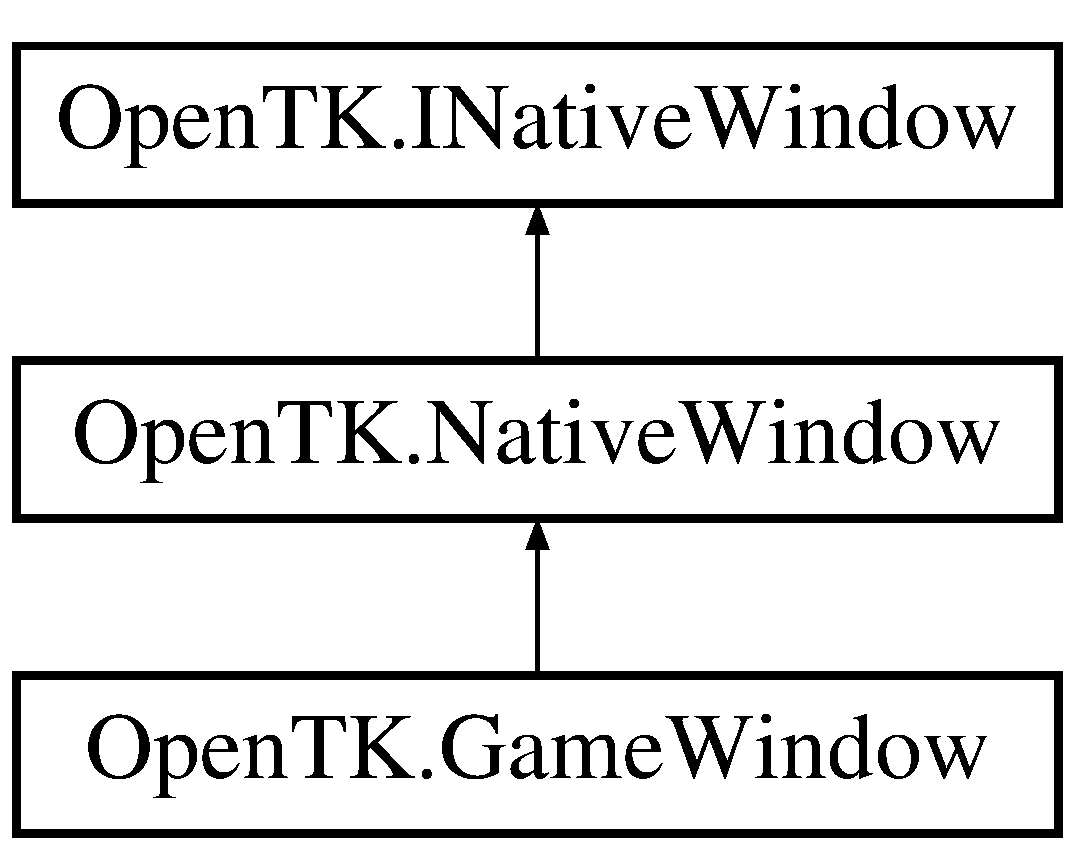
\includegraphics[height=3.000000cm]{class_open_t_k_1_1_native_window}
\end{center}
\end{figure}
\subsection*{Public Member Functions}
\begin{DoxyCompactItemize}
\item 
\hyperlink{class_open_t_k_1_1_native_window_aedcb5b381bebdedbe85834e05a7639c0}{Native\-Window} ()
\begin{DoxyCompactList}\small\item\em Constructs a new \hyperlink{class_open_t_k_1_1_native_window}{Native\-Window} with default attributes without enabling events.\end{DoxyCompactList}\item 
\hyperlink{class_open_t_k_1_1_native_window_a8aeb7aba37baeb414eed22374cdccef5}{Native\-Window} (int width, int height, string title, \hyperlink{namespace_open_t_k_af73dc15fc9d5b87827c81fa11b3ec6f0}{Game\-Window\-Flags} options, \hyperlink{class_open_t_k_1_1_graphics_1_1_graphics_mode}{Graphics\-Mode} mode, \hyperlink{class_open_t_k_1_1_display_device}{Display\-Device} device)
\begin{DoxyCompactList}\small\item\em Constructs a new centered \hyperlink{class_open_t_k_1_1_native_window}{Native\-Window} with the specified attributes.\end{DoxyCompactList}\item 
\hyperlink{class_open_t_k_1_1_native_window_a8c3ab784c89cf6eb36f3ce7ace16a193}{Native\-Window} (int x, int y, int width, int height, string title, \hyperlink{namespace_open_t_k_af73dc15fc9d5b87827c81fa11b3ec6f0}{Game\-Window\-Flags} options, \hyperlink{class_open_t_k_1_1_graphics_1_1_graphics_mode}{Graphics\-Mode} mode, \hyperlink{class_open_t_k_1_1_display_device}{Display\-Device} device)
\begin{DoxyCompactList}\small\item\em Constructs a new \hyperlink{class_open_t_k_1_1_native_window}{Native\-Window} with the specified attributes.\end{DoxyCompactList}\item 
void \hyperlink{class_open_t_k_1_1_native_window_ae7dae9eca1c2298dbcdbc34a81304a61}{Close} ()
\begin{DoxyCompactList}\small\item\em Closes the \hyperlink{class_open_t_k_1_1_native_window}{Native\-Window}. \end{DoxyCompactList}\item 
Point \hyperlink{class_open_t_k_1_1_native_window_a4807376063a7cc130ca6b6dfb4b4a24f}{Point\-To\-Client} (Point point)
\begin{DoxyCompactList}\small\item\em Transforms the specified point from screen to client coordinates. \end{DoxyCompactList}\item 
Point \hyperlink{class_open_t_k_1_1_native_window_a631e83f783213650f854a7c953a4f34d}{Point\-To\-Screen} (Point point)
\begin{DoxyCompactList}\small\item\em Transforms the specified point from client to screen coordinates. \end{DoxyCompactList}\item 
void \hyperlink{class_open_t_k_1_1_native_window_a8150f2aa496459e492965c4577ec0dc9}{Process\-Events} ()
\begin{DoxyCompactList}\small\item\em Processes operating system events until the \hyperlink{class_open_t_k_1_1_native_window}{Native\-Window} becomes idle. \end{DoxyCompactList}\item 
virtual void \hyperlink{class_open_t_k_1_1_native_window_a1cc77f20d1c61f32d62e03896e358d20}{Dispose} ()
\begin{DoxyCompactList}\small\item\em Releases all non-\/managed resources belonging to this \hyperlink{class_open_t_k_1_1_native_window}{Native\-Window}. \end{DoxyCompactList}\end{DoxyCompactItemize}
\subsection*{Protected Member Functions}
\begin{DoxyCompactItemize}
\item 
void \hyperlink{class_open_t_k_1_1_native_window_ae0abb4d6aa1dc7483948ec7ddf33c55e}{Ensure\-Undisposed} ()
\begin{DoxyCompactList}\small\item\em Ensures that this \hyperlink{class_open_t_k_1_1_native_window}{Native\-Window} has not been disposed. \end{DoxyCompactList}\item 
virtual void \hyperlink{class_open_t_k_1_1_native_window_affb5f7e8fddfe0865504dbc0a0cbd380}{On\-Closed} (Event\-Args e)
\begin{DoxyCompactList}\small\item\em Called when the \hyperlink{class_open_t_k_1_1_native_window}{Native\-Window} has closed. \end{DoxyCompactList}\item 
virtual void \hyperlink{class_open_t_k_1_1_native_window_a5082904386942ea2884f148ceb68fe00}{On\-Closing} (Cancel\-Event\-Args e)
\begin{DoxyCompactList}\small\item\em Called when the \hyperlink{class_open_t_k_1_1_native_window}{Native\-Window} is about to close. \end{DoxyCompactList}\item 
virtual void \hyperlink{class_open_t_k_1_1_native_window_a59f4ca5c53d636d1463c9d7f18c5bb22}{On\-Disposed} (Event\-Args e)
\begin{DoxyCompactList}\small\item\em Called when the \hyperlink{class_open_t_k_1_1_native_window}{Native\-Window} is disposed. \end{DoxyCompactList}\item 
virtual void \hyperlink{class_open_t_k_1_1_native_window_a2640077fe274ad83e308466969db0100}{On\-Focused\-Changed} (Event\-Args e)
\begin{DoxyCompactList}\small\item\em Called when the \hyperlink{interface_open_t_k_1_1_i_native_window_aaa2ef631c8bd4bcbef3374dfaeb50299}{Open\-T\-K.\-I\-Native\-Window.\-Focused} property of the \hyperlink{class_open_t_k_1_1_native_window}{Native\-Window} has changed. \end{DoxyCompactList}\item 
virtual void \hyperlink{class_open_t_k_1_1_native_window_a0c90b5dd60dc3e2fea5ed2dcfd1c5094}{On\-Icon\-Changed} (Event\-Args e)
\begin{DoxyCompactList}\small\item\em Called when the \hyperlink{interface_open_t_k_1_1_i_native_window_a16cffc51a5dd62c9d9dbf9a089620754}{Open\-T\-K.\-I\-Native\-Window.\-Icon} property of the \hyperlink{class_open_t_k_1_1_native_window}{Native\-Window} has changed. \end{DoxyCompactList}\item 
virtual void \hyperlink{class_open_t_k_1_1_native_window_a8f2fad3b2f39c318249bd9fa0fc18e39}{On\-Key\-Down} (\hyperlink{class_open_t_k_1_1_input_1_1_keyboard_key_event_args}{Keyboard\-Key\-Event\-Args} e)
\begin{DoxyCompactList}\small\item\em Occurs whenever a keybord key is pressed. \end{DoxyCompactList}\item 
virtual void \hyperlink{class_open_t_k_1_1_native_window_a0fa29d091481aff3ea935c77f2b44f1e}{On\-Key\-Press} (\hyperlink{class_open_t_k_1_1_key_press_event_args}{Key\-Press\-Event\-Args} e)
\begin{DoxyCompactList}\small\item\em Called when a character is typed. \end{DoxyCompactList}\item 
virtual void \hyperlink{class_open_t_k_1_1_native_window_a2c7356d198a60fccde5ff9c92f3b58c6}{On\-Key\-Up} (\hyperlink{class_open_t_k_1_1_input_1_1_keyboard_key_event_args}{Keyboard\-Key\-Event\-Args} e)
\begin{DoxyCompactList}\small\item\em Called when a keybord key is released. \end{DoxyCompactList}\item 
virtual void \hyperlink{class_open_t_k_1_1_native_window_aef0cbd0985015518ddc11c6ef11ab360}{On\-Move} (Event\-Args e)
\begin{DoxyCompactList}\small\item\em Called when the \hyperlink{class_open_t_k_1_1_native_window}{Native\-Window} is moved. \end{DoxyCompactList}\item 
virtual void \hyperlink{class_open_t_k_1_1_native_window_a2326c87203682e745505d2eee19ccd16}{On\-Mouse\-Enter} (Event\-Args e)
\begin{DoxyCompactList}\small\item\em Called whenever the mouse cursor reenters the window \hyperlink{class_open_t_k_1_1_native_window_ac0325973134062eba62484df45236464}{Bounds}. \end{DoxyCompactList}\item 
virtual void \hyperlink{class_open_t_k_1_1_native_window_a617fe22d2fe135ea57d098bef3113792}{On\-Mouse\-Leave} (Event\-Args e)
\begin{DoxyCompactList}\small\item\em Called whenever the mouse cursor leaves the window \hyperlink{class_open_t_k_1_1_native_window_ac0325973134062eba62484df45236464}{Bounds}. \end{DoxyCompactList}\item 
virtual void \hyperlink{class_open_t_k_1_1_native_window_a647ac43f6e6844ce93c1182579c0dbe4}{On\-Resize} (Event\-Args e)
\begin{DoxyCompactList}\small\item\em Called when the \hyperlink{class_open_t_k_1_1_native_window}{Native\-Window} is resized. \end{DoxyCompactList}\item 
virtual void \hyperlink{class_open_t_k_1_1_native_window_aff47a44bbfd91b63a4c95070462d9b25}{On\-Title\-Changed} (Event\-Args e)
\begin{DoxyCompactList}\small\item\em Called when the \hyperlink{interface_open_t_k_1_1_i_native_window_acc6e79eb06f9e7d725f6eac5ac1df71d}{Open\-T\-K.\-I\-Native\-Window.\-Title} property of the \hyperlink{class_open_t_k_1_1_native_window}{Native\-Window} has changed. \end{DoxyCompactList}\item 
virtual void \hyperlink{class_open_t_k_1_1_native_window_ad007ba290983c3aaf8e1b32c47d7b90b}{On\-Visible\-Changed} (Event\-Args e)
\begin{DoxyCompactList}\small\item\em Called when the \hyperlink{interface_open_t_k_1_1_i_native_window_ac455c50c69983d4a26e7ed61336290d8}{Open\-T\-K.\-I\-Native\-Window.\-Visible} property of the \hyperlink{class_open_t_k_1_1_native_window}{Native\-Window} has changed. \end{DoxyCompactList}\item 
virtual void \hyperlink{class_open_t_k_1_1_native_window_a901e27ea7e489bf53ee2d7c9fa43d83e}{On\-Window\-Border\-Changed} (Event\-Args e)
\begin{DoxyCompactList}\small\item\em Called when the Window\-Border of this \hyperlink{class_open_t_k_1_1_native_window}{Native\-Window} has changed. \end{DoxyCompactList}\item 
virtual void \hyperlink{class_open_t_k_1_1_native_window_ac185465ace10f266e5f723c792a04260}{On\-Window\-State\-Changed} (Event\-Args e)
\begin{DoxyCompactList}\small\item\em Called when the Window\-State of this \hyperlink{class_open_t_k_1_1_native_window}{Native\-Window} has changed. \end{DoxyCompactList}\item 
void \hyperlink{class_open_t_k_1_1_native_window_ab685ecac14ba8ea985e3c67a877ab41c}{Process\-Events} (bool retain\-Events)
\begin{DoxyCompactList}\small\item\em Processes operating system events until the \hyperlink{class_open_t_k_1_1_native_window}{Native\-Window} becomes idle. \end{DoxyCompactList}\end{DoxyCompactItemize}
\subsection*{Properties}
\begin{DoxyCompactItemize}
\item 
Rectangle \hyperlink{class_open_t_k_1_1_native_window_ac0325973134062eba62484df45236464}{Bounds}\hspace{0.3cm}{\ttfamily  \mbox{[}get, set\mbox{]}}
\begin{DoxyCompactList}\small\item\em Gets or sets a System.\-Drawing.\-Rectangle structure that contains the external bounds of this window, in screen coordinates. External bounds include the title bar, borders and drawing area of the window. \end{DoxyCompactList}\item 
Rectangle \hyperlink{class_open_t_k_1_1_native_window_a397e3c3a3a98d0660bd9463090422bf6}{Client\-Rectangle}\hspace{0.3cm}{\ttfamily  \mbox{[}get, set\mbox{]}}
\begin{DoxyCompactList}\small\item\em Gets or sets a System.\-Drawing.\-Rectangle structure that contains the internal bounds of this window, in client coordinates. The internal bounds include the drawing area of the window, but exclude the titlebar and window borders. \end{DoxyCompactList}\item 
\hyperlink{class_open_t_k_1_1_native_window_a956be027bb7ba880507909d919b2ad6a}{Size} \hyperlink{class_open_t_k_1_1_native_window_ac863b486a8c7e3d5d6b09aae1c010eac}{Client\-Size}\hspace{0.3cm}{\ttfamily  \mbox{[}get, set\mbox{]}}
\begin{DoxyCompactList}\small\item\em Gets or sets a System.\-Drawing.\-Size structure that contains the internal size this window. \end{DoxyCompactList}\item 
bool \hyperlink{class_open_t_k_1_1_native_window_a150f5a96451228bfc91fe9587eb64c19}{Exists}\hspace{0.3cm}{\ttfamily  \mbox{[}get\mbox{]}}
\begin{DoxyCompactList}\small\item\em Gets a value indicating whether a render window exists. \end{DoxyCompactList}\item 
bool \hyperlink{class_open_t_k_1_1_native_window_ad68c0c086e7733e7a55745425c4faf5d}{Focused}\hspace{0.3cm}{\ttfamily  \mbox{[}get\mbox{]}}
\begin{DoxyCompactList}\small\item\em Gets a System.\-Boolean that indicates whether this \hyperlink{class_open_t_k_1_1_native_window}{Native\-Window} has input focus. \end{DoxyCompactList}\item 
int \hyperlink{class_open_t_k_1_1_native_window_afc84f4b20f80301bc41c3511763c3917}{Height}\hspace{0.3cm}{\ttfamily  \mbox{[}get, set\mbox{]}}
\begin{DoxyCompactList}\small\item\em Gets or sets the external height of this window. \end{DoxyCompactList}\item 
Icon \hyperlink{class_open_t_k_1_1_native_window_a6cb12235c07f51662905a238baf65f2d}{Icon}\hspace{0.3cm}{\ttfamily  \mbox{[}get, set\mbox{]}}
\begin{DoxyCompactList}\small\item\em Gets or sets the System.\-Drawing.\-Icon for this \hyperlink{class_open_t_k_1_1_game_window}{Game\-Window}. \end{DoxyCompactList}\item 
\hyperlink{interface_open_t_k_1_1_input_1_1_i_input_driver}{I\-Input\-Driver} \hyperlink{class_open_t_k_1_1_native_window_a9c19a3cff0a4f0ce60885c8dc6f4a89c}{Input\-Driver}\hspace{0.3cm}{\ttfamily  \mbox{[}get\mbox{]}}
\begin{DoxyCompactList}\small\item\em This property is deprecated. \end{DoxyCompactList}\item 
Point \hyperlink{class_open_t_k_1_1_native_window_ab23cac873e75d052d5ccd7f9f709d80c}{Location}\hspace{0.3cm}{\ttfamily  \mbox{[}get, set\mbox{]}}
\begin{DoxyCompactList}\small\item\em Gets or sets a System.\-Drawing.\-Point structure that contains the location of this window on the desktop. \end{DoxyCompactList}\item 
Size \hyperlink{class_open_t_k_1_1_native_window_a956be027bb7ba880507909d919b2ad6a}{Size}\hspace{0.3cm}{\ttfamily  \mbox{[}get, set\mbox{]}}
\begin{DoxyCompactList}\small\item\em Gets or sets a System.\-Drawing.\-Size structure that contains the external size of this window. \end{DoxyCompactList}\item 
string \hyperlink{class_open_t_k_1_1_native_window_af5cd587c921ef6c10709fc69a1e2900b}{Title}\hspace{0.3cm}{\ttfamily  \mbox{[}get, set\mbox{]}}
\begin{DoxyCompactList}\small\item\em Gets or sets the \hyperlink{class_open_t_k_1_1_native_window}{Native\-Window} title. \end{DoxyCompactList}\item 
bool \hyperlink{class_open_t_k_1_1_native_window_aff1fe36bb34bb3ba53814a7aaceea940}{Visible}\hspace{0.3cm}{\ttfamily  \mbox{[}get, set\mbox{]}}
\begin{DoxyCompactList}\small\item\em Gets or sets a System.\-Boolean that indicates whether this \hyperlink{class_open_t_k_1_1_native_window}{Native\-Window} is visible. \end{DoxyCompactList}\item 
int \hyperlink{class_open_t_k_1_1_native_window_a0cea0939dfd9dc512757e80cfa588de6}{Width}\hspace{0.3cm}{\ttfamily  \mbox{[}get, set\mbox{]}}
\begin{DoxyCompactList}\small\item\em Gets or sets the external width of this window. \end{DoxyCompactList}\item 
\hyperlink{namespace_open_t_k_a20f46792b5471ff32362bd0a29fa5f1c}{Window\-Border} \hyperlink{class_open_t_k_1_1_native_window_a847af2dd07cb323f3a96767bb96ea44b}{Window\-Border}\hspace{0.3cm}{\ttfamily  \mbox{[}get, set\mbox{]}}
\begin{DoxyCompactList}\small\item\em Gets or states the border of the \hyperlink{class_open_t_k_1_1_native_window}{Native\-Window}. \end{DoxyCompactList}\item 
\hyperlink{interface_open_t_k_1_1_platform_1_1_i_window_info}{I\-Window\-Info} \hyperlink{class_open_t_k_1_1_native_window_a1593f5f56e2bd9b67f9559385aba81de}{Window\-Info}\hspace{0.3cm}{\ttfamily  \mbox{[}get\mbox{]}}
\begin{DoxyCompactList}\small\item\em Gets the \hyperlink{interface_open_t_k_1_1_platform_1_1_i_window_info}{Open\-T\-K.\-Platform.\-I\-Window\-Info} of this window. \end{DoxyCompactList}\item 
virtual \hyperlink{namespace_open_t_k_ace9268dc87bd36f48c9d9d8b939559b4}{Window\-State} \hyperlink{class_open_t_k_1_1_native_window_a78e6278aa092a82f672ff838ac7c1e2d}{Window\-State}\hspace{0.3cm}{\ttfamily  \mbox{[}get, set\mbox{]}}
\begin{DoxyCompactList}\small\item\em Gets or states the state of the \hyperlink{class_open_t_k_1_1_native_window}{Native\-Window}. \end{DoxyCompactList}\item 
int \hyperlink{class_open_t_k_1_1_native_window_a7c5eafcedf58f9b72995633b93657463}{X}\hspace{0.3cm}{\ttfamily  \mbox{[}get, set\mbox{]}}
\begin{DoxyCompactList}\small\item\em Gets or sets the horizontal location of this window on the desktop. \end{DoxyCompactList}\item 
int \hyperlink{class_open_t_k_1_1_native_window_a6652ffe8f86f05bddd470872874aa8b8}{Y}\hspace{0.3cm}{\ttfamily  \mbox{[}get, set\mbox{]}}
\begin{DoxyCompactList}\small\item\em Gets or sets the vertical location of this window on the desktop. \end{DoxyCompactList}\item 
bool \hyperlink{class_open_t_k_1_1_native_window_a028d01996236ac800257e79392f42c3c}{Cursor\-Visible}\hspace{0.3cm}{\ttfamily  \mbox{[}get, set\mbox{]}}
\begin{DoxyCompactList}\small\item\em Gets or sets a value indicating whether the mouse cursor is visible. \end{DoxyCompactList}\item 
bool \hyperlink{class_open_t_k_1_1_native_window_af15932872565db89a7f0fe92f9216699}{Is\-Disposed}\hspace{0.3cm}{\ttfamily  \mbox{[}get, set\mbox{]}}
\begin{DoxyCompactList}\small\item\em Gets or sets a System.\-Boolean, which indicates whether this instance has been disposed. \end{DoxyCompactList}\end{DoxyCompactItemize}
\subsection*{Events}
\begin{DoxyCompactItemize}
\item 
Event\-Handler$<$ Event\-Args $>$ \hyperlink{class_open_t_k_1_1_native_window_a8eb75858475f8cb49540c8142c4796f9}{Closed} = delegate \{ \}
\begin{DoxyCompactList}\small\item\em Occurs after the window has closed. \end{DoxyCompactList}\item 
Event\-Handler$<$ Cancel\-Event\-Args $>$ \hyperlink{class_open_t_k_1_1_native_window_ac6c8dbb48a823371397548b7c55e5459}{Closing} = delegate \{ \}
\begin{DoxyCompactList}\small\item\em Occurs when the window is about to close. \end{DoxyCompactList}\item 
Event\-Handler$<$ Event\-Args $>$ \hyperlink{class_open_t_k_1_1_native_window_a28187250dc87ba3b721177cd78f8e52b}{Disposed} = delegate \{ \}
\begin{DoxyCompactList}\small\item\em Occurs when the window is disposed. \end{DoxyCompactList}\item 
Event\-Handler$<$ Event\-Args $>$ \hyperlink{class_open_t_k_1_1_native_window_ab499521edced0c062b37a01eefecaf4a}{Focused\-Changed} = delegate \{ \}
\begin{DoxyCompactList}\small\item\em Occurs when the \hyperlink{class_open_t_k_1_1_native_window_ad68c0c086e7733e7a55745425c4faf5d}{Focused} property of the window changes. \end{DoxyCompactList}\item 
Event\-Handler$<$ Event\-Args $>$ \hyperlink{class_open_t_k_1_1_native_window_a585aeb8c100ea173db497c287def293b}{Icon\-Changed} = delegate \{ \}
\begin{DoxyCompactList}\small\item\em Occurs when the \hyperlink{class_open_t_k_1_1_native_window_a6cb12235c07f51662905a238baf65f2d}{Icon} property of the window changes. \end{DoxyCompactList}\item 
Event\-Handler\\*
$<$ \hyperlink{class_open_t_k_1_1_input_1_1_keyboard_key_event_args}{Open\-T\-K.\-Input.\-Keyboard\-Key\-Event\-Args} $>$ \hyperlink{class_open_t_k_1_1_native_window_aba78b8d5243523c3ebb373cc2ab564db}{Key\-Down} = delegate \{ \}
\begin{DoxyCompactList}\small\item\em Occurs whenever a keybord key is pressed. \end{DoxyCompactList}\item 
Event\-Handler$<$ \hyperlink{class_open_t_k_1_1_key_press_event_args}{Key\-Press\-Event\-Args} $>$ \hyperlink{class_open_t_k_1_1_native_window_a77b59f8d65f596bdabc4f199dfa1dc0e}{Key\-Press} = delegate \{ \}
\begin{DoxyCompactList}\small\item\em Occurs whenever a character is typed. \end{DoxyCompactList}\item 
Event\-Handler\\*
$<$ \hyperlink{class_open_t_k_1_1_input_1_1_keyboard_key_event_args}{Open\-T\-K.\-Input.\-Keyboard\-Key\-Event\-Args} $>$ \hyperlink{class_open_t_k_1_1_native_window_ab124b92a7dc7bec0d6a752b15103e36d}{Key\-Up} = delegate \{ \}
\begin{DoxyCompactList}\small\item\em Occurs whenever a keyboard key is released. \end{DoxyCompactList}\item 
Event\-Handler$<$ Event\-Args $>$ \hyperlink{class_open_t_k_1_1_native_window_aab24c27eb84152880e401b0c74718ce8}{Move} = delegate \{ \}
\begin{DoxyCompactList}\small\item\em Occurs whenever the window is moved. \end{DoxyCompactList}\item 
Event\-Handler$<$ Event\-Args $>$ \hyperlink{class_open_t_k_1_1_native_window_a04e101987663c30051ae857f7b440f52}{Mouse\-Enter} = delegate \{ \}
\begin{DoxyCompactList}\small\item\em Occurs whenever the mouse cursor enters the window \hyperlink{class_open_t_k_1_1_native_window_ac0325973134062eba62484df45236464}{Bounds}. \end{DoxyCompactList}\item 
Event\-Handler$<$ Event\-Args $>$ \hyperlink{class_open_t_k_1_1_native_window_aa1f74c551b636689078e31d72627e856}{Mouse\-Leave} = delegate \{ \}
\begin{DoxyCompactList}\small\item\em Occurs whenever the mouse cursor leaves the window \hyperlink{class_open_t_k_1_1_native_window_ac0325973134062eba62484df45236464}{Bounds}. \end{DoxyCompactList}\item 
Event\-Handler$<$ Event\-Args $>$ \hyperlink{class_open_t_k_1_1_native_window_a4fac914cf3df915f63f5de6f856bdfe6}{Resize} = delegate \{ \}
\begin{DoxyCompactList}\small\item\em Occurs whenever the window is resized. \end{DoxyCompactList}\item 
Event\-Handler$<$ Event\-Args $>$ \hyperlink{class_open_t_k_1_1_native_window_a25393018b81b7d842548407749b338cb}{Title\-Changed} = delegate \{ \}
\begin{DoxyCompactList}\small\item\em Occurs when the \hyperlink{class_open_t_k_1_1_native_window_af5cd587c921ef6c10709fc69a1e2900b}{Title} property of the window changes. \end{DoxyCompactList}\item 
Event\-Handler$<$ Event\-Args $>$ \hyperlink{class_open_t_k_1_1_native_window_af1678140a475ad9076116260b76fb98e}{Visible\-Changed} = delegate \{ \}
\begin{DoxyCompactList}\small\item\em Occurs when the \hyperlink{class_open_t_k_1_1_native_window_aff1fe36bb34bb3ba53814a7aaceea940}{Visible} property of the window changes. \end{DoxyCompactList}\item 
Event\-Handler$<$ Event\-Args $>$ \hyperlink{class_open_t_k_1_1_native_window_a1e42d7762769cd074dfb68496b0b2dbf}{Window\-Border\-Changed} = delegate \{ \}
\begin{DoxyCompactList}\small\item\em Occurs when the \hyperlink{class_open_t_k_1_1_native_window_a847af2dd07cb323f3a96767bb96ea44b}{Window\-Border} property of the window changes. \end{DoxyCompactList}\item 
Event\-Handler$<$ Event\-Args $>$ \hyperlink{class_open_t_k_1_1_native_window_a911c577473fdc8b422419e4677350c0f}{Window\-State\-Changed} = delegate \{ \}
\begin{DoxyCompactList}\small\item\em Occurs when the \hyperlink{class_open_t_k_1_1_native_window_a78e6278aa092a82f672ff838ac7c1e2d}{Window\-State} property of the window changes. \end{DoxyCompactList}\end{DoxyCompactItemize}


\subsection{Detailed Description}
Instances of this class implement the \hyperlink{interface_open_t_k_1_1_i_native_window}{Open\-T\-K.\-I\-Native\-Window} interface on the current platform. 



\subsection{Constructor \& Destructor Documentation}
\hypertarget{class_open_t_k_1_1_native_window_aedcb5b381bebdedbe85834e05a7639c0}{\index{Open\-T\-K\-::\-Native\-Window@{Open\-T\-K\-::\-Native\-Window}!Native\-Window@{Native\-Window}}
\index{Native\-Window@{Native\-Window}!OpenTK::NativeWindow@{Open\-T\-K\-::\-Native\-Window}}
\subsubsection[{Native\-Window}]{\setlength{\rightskip}{0pt plus 5cm}Open\-T\-K.\-Native\-Window.\-Native\-Window (
\begin{DoxyParamCaption}
{}
\end{DoxyParamCaption}
)}}\label{class_open_t_k_1_1_native_window_aedcb5b381bebdedbe85834e05a7639c0}


Constructs a new \hyperlink{class_open_t_k_1_1_native_window}{Native\-Window} with default attributes without enabling events.

\hypertarget{class_open_t_k_1_1_native_window_a8aeb7aba37baeb414eed22374cdccef5}{\index{Open\-T\-K\-::\-Native\-Window@{Open\-T\-K\-::\-Native\-Window}!Native\-Window@{Native\-Window}}
\index{Native\-Window@{Native\-Window}!OpenTK::NativeWindow@{Open\-T\-K\-::\-Native\-Window}}
\subsubsection[{Native\-Window}]{\setlength{\rightskip}{0pt plus 5cm}Open\-T\-K.\-Native\-Window.\-Native\-Window (
\begin{DoxyParamCaption}
\item[{int}]{width, }
\item[{int}]{height, }
\item[{string}]{title, }
\item[{{\bf Game\-Window\-Flags}}]{options, }
\item[{{\bf Graphics\-Mode}}]{mode, }
\item[{{\bf Display\-Device}}]{device}
\end{DoxyParamCaption}
)}}\label{class_open_t_k_1_1_native_window_a8aeb7aba37baeb414eed22374cdccef5}


Constructs a new centered \hyperlink{class_open_t_k_1_1_native_window}{Native\-Window} with the specified attributes.


\begin{DoxyParams}{Parameters}
{\em width} & The width of the \hyperlink{class_open_t_k_1_1_native_window}{Native\-Window} in pixels.\\
\hline
{\em height} & The height of the \hyperlink{class_open_t_k_1_1_native_window}{Native\-Window} in pixels.\\
\hline
{\em title} & The title of the \hyperlink{class_open_t_k_1_1_native_window}{Native\-Window}.\\
\hline
{\em options} & \hyperlink{class_open_t_k_1_1_game_window}{Game\-Window} options specifying window appearance and behavior.\\
\hline
{\em mode} & The \hyperlink{class_open_t_k_1_1_graphics_1_1_graphics_mode}{Open\-T\-K.\-Graphics.\-Graphics\-Mode} of the \hyperlink{class_open_t_k_1_1_native_window}{Native\-Window}.\\
\hline
{\em device} & The Open\-T\-K.\-Graphics.\-Display\-Device to construct the \hyperlink{class_open_t_k_1_1_native_window}{Native\-Window} in.\\
\hline
\end{DoxyParams}

\begin{DoxyExceptions}{Exceptions}
{\em System.\-Argument\-Out\-Of\-Range\-Exception} & If width or height is less than 1.\\
\hline
{\em System.\-Argument\-Null\-Exception} & If mode or device is null.\\
\hline
\end{DoxyExceptions}
\hypertarget{class_open_t_k_1_1_native_window_a8c3ab784c89cf6eb36f3ce7ace16a193}{\index{Open\-T\-K\-::\-Native\-Window@{Open\-T\-K\-::\-Native\-Window}!Native\-Window@{Native\-Window}}
\index{Native\-Window@{Native\-Window}!OpenTK::NativeWindow@{Open\-T\-K\-::\-Native\-Window}}
\subsubsection[{Native\-Window}]{\setlength{\rightskip}{0pt plus 5cm}Open\-T\-K.\-Native\-Window.\-Native\-Window (
\begin{DoxyParamCaption}
\item[{int}]{x, }
\item[{int}]{y, }
\item[{int}]{width, }
\item[{int}]{height, }
\item[{string}]{title, }
\item[{{\bf Game\-Window\-Flags}}]{options, }
\item[{{\bf Graphics\-Mode}}]{mode, }
\item[{{\bf Display\-Device}}]{device}
\end{DoxyParamCaption}
)}}\label{class_open_t_k_1_1_native_window_a8c3ab784c89cf6eb36f3ce7ace16a193}


Constructs a new \hyperlink{class_open_t_k_1_1_native_window}{Native\-Window} with the specified attributes.


\begin{DoxyParams}{Parameters}
{\em x} & Horizontal screen space coordinate of the \hyperlink{class_open_t_k_1_1_native_window}{Native\-Window}'s origin.\\
\hline
{\em y} & Vertical screen space coordinate of the \hyperlink{class_open_t_k_1_1_native_window}{Native\-Window}'s origin.\\
\hline
{\em width} & The width of the \hyperlink{class_open_t_k_1_1_native_window}{Native\-Window} in pixels.\\
\hline
{\em height} & The height of the \hyperlink{class_open_t_k_1_1_native_window}{Native\-Window} in pixels.\\
\hline
{\em title} & The title of the \hyperlink{class_open_t_k_1_1_native_window}{Native\-Window}.\\
\hline
{\em options} & \hyperlink{class_open_t_k_1_1_game_window}{Game\-Window} options specifying window appearance and behavior.\\
\hline
{\em mode} & The \hyperlink{class_open_t_k_1_1_graphics_1_1_graphics_mode}{Open\-T\-K.\-Graphics.\-Graphics\-Mode} of the \hyperlink{class_open_t_k_1_1_native_window}{Native\-Window}.\\
\hline
{\em device} & The Open\-T\-K.\-Graphics.\-Display\-Device to construct the \hyperlink{class_open_t_k_1_1_native_window}{Native\-Window} in.\\
\hline
\end{DoxyParams}

\begin{DoxyExceptions}{Exceptions}
{\em System.\-Argument\-Out\-Of\-Range\-Exception} & If width or height is less than 1.\\
\hline
{\em System.\-Argument\-Null\-Exception} & If mode or device is null.\\
\hline
\end{DoxyExceptions}


\subsection{Member Function Documentation}
\hypertarget{class_open_t_k_1_1_native_window_ae7dae9eca1c2298dbcdbc34a81304a61}{\index{Open\-T\-K\-::\-Native\-Window@{Open\-T\-K\-::\-Native\-Window}!Close@{Close}}
\index{Close@{Close}!OpenTK::NativeWindow@{Open\-T\-K\-::\-Native\-Window}}
\subsubsection[{Close}]{\setlength{\rightskip}{0pt plus 5cm}void Open\-T\-K.\-Native\-Window.\-Close (
\begin{DoxyParamCaption}
{}
\end{DoxyParamCaption}
)}}\label{class_open_t_k_1_1_native_window_ae7dae9eca1c2298dbcdbc34a81304a61}


Closes the \hyperlink{class_open_t_k_1_1_native_window}{Native\-Window}. 



Implements \hyperlink{interface_open_t_k_1_1_i_native_window_a1ccc061d19e83d00f29b50f27263fcfe}{Open\-T\-K.\-I\-Native\-Window}.

\hypertarget{class_open_t_k_1_1_native_window_a1cc77f20d1c61f32d62e03896e358d20}{\index{Open\-T\-K\-::\-Native\-Window@{Open\-T\-K\-::\-Native\-Window}!Dispose@{Dispose}}
\index{Dispose@{Dispose}!OpenTK::NativeWindow@{Open\-T\-K\-::\-Native\-Window}}
\subsubsection[{Dispose}]{\setlength{\rightskip}{0pt plus 5cm}virtual void Open\-T\-K.\-Native\-Window.\-Dispose (
\begin{DoxyParamCaption}
{}
\end{DoxyParamCaption}
)\hspace{0.3cm}{\ttfamily [virtual]}}}\label{class_open_t_k_1_1_native_window_a1cc77f20d1c61f32d62e03896e358d20}


Releases all non-\/managed resources belonging to this \hyperlink{class_open_t_k_1_1_native_window}{Native\-Window}. 



Reimplemented in \hyperlink{class_open_t_k_1_1_game_window_acfd19fafb5563df42e2104ea38c2889a}{Open\-T\-K.\-Game\-Window}.

\hypertarget{class_open_t_k_1_1_native_window_ae0abb4d6aa1dc7483948ec7ddf33c55e}{\index{Open\-T\-K\-::\-Native\-Window@{Open\-T\-K\-::\-Native\-Window}!Ensure\-Undisposed@{Ensure\-Undisposed}}
\index{Ensure\-Undisposed@{Ensure\-Undisposed}!OpenTK::NativeWindow@{Open\-T\-K\-::\-Native\-Window}}
\subsubsection[{Ensure\-Undisposed}]{\setlength{\rightskip}{0pt plus 5cm}void Open\-T\-K.\-Native\-Window.\-Ensure\-Undisposed (
\begin{DoxyParamCaption}
{}
\end{DoxyParamCaption}
)\hspace{0.3cm}{\ttfamily [protected]}}}\label{class_open_t_k_1_1_native_window_ae0abb4d6aa1dc7483948ec7ddf33c55e}


Ensures that this \hyperlink{class_open_t_k_1_1_native_window}{Native\-Window} has not been disposed. 


\begin{DoxyExceptions}{Exceptions}
{\em System.\-Object\-Disposed\-Exception} & If this \hyperlink{class_open_t_k_1_1_native_window}{Native\-Window} has been disposed. \\
\hline
\end{DoxyExceptions}
\hypertarget{class_open_t_k_1_1_native_window_affb5f7e8fddfe0865504dbc0a0cbd380}{\index{Open\-T\-K\-::\-Native\-Window@{Open\-T\-K\-::\-Native\-Window}!On\-Closed@{On\-Closed}}
\index{On\-Closed@{On\-Closed}!OpenTK::NativeWindow@{Open\-T\-K\-::\-Native\-Window}}
\subsubsection[{On\-Closed}]{\setlength{\rightskip}{0pt plus 5cm}virtual void Open\-T\-K.\-Native\-Window.\-On\-Closed (
\begin{DoxyParamCaption}
\item[{Event\-Args}]{e}
\end{DoxyParamCaption}
)\hspace{0.3cm}{\ttfamily [protected]}, {\ttfamily [virtual]}}}\label{class_open_t_k_1_1_native_window_affb5f7e8fddfe0865504dbc0a0cbd380}


Called when the \hyperlink{class_open_t_k_1_1_native_window}{Native\-Window} has closed. 


\begin{DoxyParams}{Parameters}
{\em e} & Not used.\\
\hline
\end{DoxyParams}
\hypertarget{class_open_t_k_1_1_native_window_a5082904386942ea2884f148ceb68fe00}{\index{Open\-T\-K\-::\-Native\-Window@{Open\-T\-K\-::\-Native\-Window}!On\-Closing@{On\-Closing}}
\index{On\-Closing@{On\-Closing}!OpenTK::NativeWindow@{Open\-T\-K\-::\-Native\-Window}}
\subsubsection[{On\-Closing}]{\setlength{\rightskip}{0pt plus 5cm}virtual void Open\-T\-K.\-Native\-Window.\-On\-Closing (
\begin{DoxyParamCaption}
\item[{Cancel\-Event\-Args}]{e}
\end{DoxyParamCaption}
)\hspace{0.3cm}{\ttfamily [protected]}, {\ttfamily [virtual]}}}\label{class_open_t_k_1_1_native_window_a5082904386942ea2884f148ceb68fe00}


Called when the \hyperlink{class_open_t_k_1_1_native_window}{Native\-Window} is about to close. 


\begin{DoxyParams}{Parameters}
{\em e} & The System.\-Component\-Model.\-Cancel\-Event\-Args for this event. Set e.\-Cancel to true in order to stop the \hyperlink{class_open_t_k_1_1_native_window}{Native\-Window} from closing.\\
\hline
\end{DoxyParams}
\hypertarget{class_open_t_k_1_1_native_window_a59f4ca5c53d636d1463c9d7f18c5bb22}{\index{Open\-T\-K\-::\-Native\-Window@{Open\-T\-K\-::\-Native\-Window}!On\-Disposed@{On\-Disposed}}
\index{On\-Disposed@{On\-Disposed}!OpenTK::NativeWindow@{Open\-T\-K\-::\-Native\-Window}}
\subsubsection[{On\-Disposed}]{\setlength{\rightskip}{0pt plus 5cm}virtual void Open\-T\-K.\-Native\-Window.\-On\-Disposed (
\begin{DoxyParamCaption}
\item[{Event\-Args}]{e}
\end{DoxyParamCaption}
)\hspace{0.3cm}{\ttfamily [protected]}, {\ttfamily [virtual]}}}\label{class_open_t_k_1_1_native_window_a59f4ca5c53d636d1463c9d7f18c5bb22}


Called when the \hyperlink{class_open_t_k_1_1_native_window}{Native\-Window} is disposed. 


\begin{DoxyParams}{Parameters}
{\em e} & Not used.\\
\hline
\end{DoxyParams}
\hypertarget{class_open_t_k_1_1_native_window_a2640077fe274ad83e308466969db0100}{\index{Open\-T\-K\-::\-Native\-Window@{Open\-T\-K\-::\-Native\-Window}!On\-Focused\-Changed@{On\-Focused\-Changed}}
\index{On\-Focused\-Changed@{On\-Focused\-Changed}!OpenTK::NativeWindow@{Open\-T\-K\-::\-Native\-Window}}
\subsubsection[{On\-Focused\-Changed}]{\setlength{\rightskip}{0pt plus 5cm}virtual void Open\-T\-K.\-Native\-Window.\-On\-Focused\-Changed (
\begin{DoxyParamCaption}
\item[{Event\-Args}]{e}
\end{DoxyParamCaption}
)\hspace{0.3cm}{\ttfamily [protected]}, {\ttfamily [virtual]}}}\label{class_open_t_k_1_1_native_window_a2640077fe274ad83e308466969db0100}


Called when the \hyperlink{interface_open_t_k_1_1_i_native_window_aaa2ef631c8bd4bcbef3374dfaeb50299}{Open\-T\-K.\-I\-Native\-Window.\-Focused} property of the \hyperlink{class_open_t_k_1_1_native_window}{Native\-Window} has changed. 


\begin{DoxyParams}{Parameters}
{\em e} & Not used.\\
\hline
\end{DoxyParams}
\hypertarget{class_open_t_k_1_1_native_window_a0c90b5dd60dc3e2fea5ed2dcfd1c5094}{\index{Open\-T\-K\-::\-Native\-Window@{Open\-T\-K\-::\-Native\-Window}!On\-Icon\-Changed@{On\-Icon\-Changed}}
\index{On\-Icon\-Changed@{On\-Icon\-Changed}!OpenTK::NativeWindow@{Open\-T\-K\-::\-Native\-Window}}
\subsubsection[{On\-Icon\-Changed}]{\setlength{\rightskip}{0pt plus 5cm}virtual void Open\-T\-K.\-Native\-Window.\-On\-Icon\-Changed (
\begin{DoxyParamCaption}
\item[{Event\-Args}]{e}
\end{DoxyParamCaption}
)\hspace{0.3cm}{\ttfamily [protected]}, {\ttfamily [virtual]}}}\label{class_open_t_k_1_1_native_window_a0c90b5dd60dc3e2fea5ed2dcfd1c5094}


Called when the \hyperlink{interface_open_t_k_1_1_i_native_window_a16cffc51a5dd62c9d9dbf9a089620754}{Open\-T\-K.\-I\-Native\-Window.\-Icon} property of the \hyperlink{class_open_t_k_1_1_native_window}{Native\-Window} has changed. 


\begin{DoxyParams}{Parameters}
{\em e} & Not used.\\
\hline
\end{DoxyParams}
\hypertarget{class_open_t_k_1_1_native_window_a8f2fad3b2f39c318249bd9fa0fc18e39}{\index{Open\-T\-K\-::\-Native\-Window@{Open\-T\-K\-::\-Native\-Window}!On\-Key\-Down@{On\-Key\-Down}}
\index{On\-Key\-Down@{On\-Key\-Down}!OpenTK::NativeWindow@{Open\-T\-K\-::\-Native\-Window}}
\subsubsection[{On\-Key\-Down}]{\setlength{\rightskip}{0pt plus 5cm}virtual void Open\-T\-K.\-Native\-Window.\-On\-Key\-Down (
\begin{DoxyParamCaption}
\item[{{\bf Keyboard\-Key\-Event\-Args}}]{e}
\end{DoxyParamCaption}
)\hspace{0.3cm}{\ttfamily [protected]}, {\ttfamily [virtual]}}}\label{class_open_t_k_1_1_native_window_a8f2fad3b2f39c318249bd9fa0fc18e39}


Occurs whenever a keybord key is pressed. 

\hypertarget{class_open_t_k_1_1_native_window_a0fa29d091481aff3ea935c77f2b44f1e}{\index{Open\-T\-K\-::\-Native\-Window@{Open\-T\-K\-::\-Native\-Window}!On\-Key\-Press@{On\-Key\-Press}}
\index{On\-Key\-Press@{On\-Key\-Press}!OpenTK::NativeWindow@{Open\-T\-K\-::\-Native\-Window}}
\subsubsection[{On\-Key\-Press}]{\setlength{\rightskip}{0pt plus 5cm}virtual void Open\-T\-K.\-Native\-Window.\-On\-Key\-Press (
\begin{DoxyParamCaption}
\item[{{\bf Key\-Press\-Event\-Args}}]{e}
\end{DoxyParamCaption}
)\hspace{0.3cm}{\ttfamily [protected]}, {\ttfamily [virtual]}}}\label{class_open_t_k_1_1_native_window_a0fa29d091481aff3ea935c77f2b44f1e}


Called when a character is typed. 


\begin{DoxyParams}{Parameters}
{\em e} & The \hyperlink{class_open_t_k_1_1_key_press_event_args}{Open\-T\-K.\-Key\-Press\-Event\-Args} for this event.\\
\hline
\end{DoxyParams}
\hypertarget{class_open_t_k_1_1_native_window_a2c7356d198a60fccde5ff9c92f3b58c6}{\index{Open\-T\-K\-::\-Native\-Window@{Open\-T\-K\-::\-Native\-Window}!On\-Key\-Up@{On\-Key\-Up}}
\index{On\-Key\-Up@{On\-Key\-Up}!OpenTK::NativeWindow@{Open\-T\-K\-::\-Native\-Window}}
\subsubsection[{On\-Key\-Up}]{\setlength{\rightskip}{0pt plus 5cm}virtual void Open\-T\-K.\-Native\-Window.\-On\-Key\-Up (
\begin{DoxyParamCaption}
\item[{{\bf Keyboard\-Key\-Event\-Args}}]{e}
\end{DoxyParamCaption}
)\hspace{0.3cm}{\ttfamily [protected]}, {\ttfamily [virtual]}}}\label{class_open_t_k_1_1_native_window_a2c7356d198a60fccde5ff9c92f3b58c6}


Called when a keybord key is released. 


\begin{DoxyParams}{Parameters}
{\em e} & The \hyperlink{class_open_t_k_1_1_input_1_1_keyboard_key_event_args}{Open\-T\-K.\-Input.\-Keyboard\-Key\-Event\-Args} for this event.\\
\hline
\end{DoxyParams}
\hypertarget{class_open_t_k_1_1_native_window_a2326c87203682e745505d2eee19ccd16}{\index{Open\-T\-K\-::\-Native\-Window@{Open\-T\-K\-::\-Native\-Window}!On\-Mouse\-Enter@{On\-Mouse\-Enter}}
\index{On\-Mouse\-Enter@{On\-Mouse\-Enter}!OpenTK::NativeWindow@{Open\-T\-K\-::\-Native\-Window}}
\subsubsection[{On\-Mouse\-Enter}]{\setlength{\rightskip}{0pt plus 5cm}virtual void Open\-T\-K.\-Native\-Window.\-On\-Mouse\-Enter (
\begin{DoxyParamCaption}
\item[{Event\-Args}]{e}
\end{DoxyParamCaption}
)\hspace{0.3cm}{\ttfamily [protected]}, {\ttfamily [virtual]}}}\label{class_open_t_k_1_1_native_window_a2326c87203682e745505d2eee19ccd16}


Called whenever the mouse cursor reenters the window \hyperlink{class_open_t_k_1_1_native_window_ac0325973134062eba62484df45236464}{Bounds}. 


\begin{DoxyParams}{Parameters}
{\em e} & Not used.\\
\hline
\end{DoxyParams}
\hypertarget{class_open_t_k_1_1_native_window_a617fe22d2fe135ea57d098bef3113792}{\index{Open\-T\-K\-::\-Native\-Window@{Open\-T\-K\-::\-Native\-Window}!On\-Mouse\-Leave@{On\-Mouse\-Leave}}
\index{On\-Mouse\-Leave@{On\-Mouse\-Leave}!OpenTK::NativeWindow@{Open\-T\-K\-::\-Native\-Window}}
\subsubsection[{On\-Mouse\-Leave}]{\setlength{\rightskip}{0pt plus 5cm}virtual void Open\-T\-K.\-Native\-Window.\-On\-Mouse\-Leave (
\begin{DoxyParamCaption}
\item[{Event\-Args}]{e}
\end{DoxyParamCaption}
)\hspace{0.3cm}{\ttfamily [protected]}, {\ttfamily [virtual]}}}\label{class_open_t_k_1_1_native_window_a617fe22d2fe135ea57d098bef3113792}


Called whenever the mouse cursor leaves the window \hyperlink{class_open_t_k_1_1_native_window_ac0325973134062eba62484df45236464}{Bounds}. 


\begin{DoxyParams}{Parameters}
{\em e} & Not used.\\
\hline
\end{DoxyParams}
\hypertarget{class_open_t_k_1_1_native_window_aef0cbd0985015518ddc11c6ef11ab360}{\index{Open\-T\-K\-::\-Native\-Window@{Open\-T\-K\-::\-Native\-Window}!On\-Move@{On\-Move}}
\index{On\-Move@{On\-Move}!OpenTK::NativeWindow@{Open\-T\-K\-::\-Native\-Window}}
\subsubsection[{On\-Move}]{\setlength{\rightskip}{0pt plus 5cm}virtual void Open\-T\-K.\-Native\-Window.\-On\-Move (
\begin{DoxyParamCaption}
\item[{Event\-Args}]{e}
\end{DoxyParamCaption}
)\hspace{0.3cm}{\ttfamily [protected]}, {\ttfamily [virtual]}}}\label{class_open_t_k_1_1_native_window_aef0cbd0985015518ddc11c6ef11ab360}


Called when the \hyperlink{class_open_t_k_1_1_native_window}{Native\-Window} is moved. 


\begin{DoxyParams}{Parameters}
{\em e} & Not used.\\
\hline
\end{DoxyParams}
\hypertarget{class_open_t_k_1_1_native_window_a647ac43f6e6844ce93c1182579c0dbe4}{\index{Open\-T\-K\-::\-Native\-Window@{Open\-T\-K\-::\-Native\-Window}!On\-Resize@{On\-Resize}}
\index{On\-Resize@{On\-Resize}!OpenTK::NativeWindow@{Open\-T\-K\-::\-Native\-Window}}
\subsubsection[{On\-Resize}]{\setlength{\rightskip}{0pt plus 5cm}virtual void Open\-T\-K.\-Native\-Window.\-On\-Resize (
\begin{DoxyParamCaption}
\item[{Event\-Args}]{e}
\end{DoxyParamCaption}
)\hspace{0.3cm}{\ttfamily [protected]}, {\ttfamily [virtual]}}}\label{class_open_t_k_1_1_native_window_a647ac43f6e6844ce93c1182579c0dbe4}


Called when the \hyperlink{class_open_t_k_1_1_native_window}{Native\-Window} is resized. 


\begin{DoxyParams}{Parameters}
{\em e} & Not used.\\
\hline
\end{DoxyParams}


Reimplemented in \hyperlink{class_open_t_k_1_1_game_window_a730fe82126e7616bccba531bb2abc770}{Open\-T\-K.\-Game\-Window}.

\hypertarget{class_open_t_k_1_1_native_window_aff47a44bbfd91b63a4c95070462d9b25}{\index{Open\-T\-K\-::\-Native\-Window@{Open\-T\-K\-::\-Native\-Window}!On\-Title\-Changed@{On\-Title\-Changed}}
\index{On\-Title\-Changed@{On\-Title\-Changed}!OpenTK::NativeWindow@{Open\-T\-K\-::\-Native\-Window}}
\subsubsection[{On\-Title\-Changed}]{\setlength{\rightskip}{0pt plus 5cm}virtual void Open\-T\-K.\-Native\-Window.\-On\-Title\-Changed (
\begin{DoxyParamCaption}
\item[{Event\-Args}]{e}
\end{DoxyParamCaption}
)\hspace{0.3cm}{\ttfamily [protected]}, {\ttfamily [virtual]}}}\label{class_open_t_k_1_1_native_window_aff47a44bbfd91b63a4c95070462d9b25}


Called when the \hyperlink{interface_open_t_k_1_1_i_native_window_acc6e79eb06f9e7d725f6eac5ac1df71d}{Open\-T\-K.\-I\-Native\-Window.\-Title} property of the \hyperlink{class_open_t_k_1_1_native_window}{Native\-Window} has changed. 


\begin{DoxyParams}{Parameters}
{\em e} & Not used.\\
\hline
\end{DoxyParams}
\hypertarget{class_open_t_k_1_1_native_window_ad007ba290983c3aaf8e1b32c47d7b90b}{\index{Open\-T\-K\-::\-Native\-Window@{Open\-T\-K\-::\-Native\-Window}!On\-Visible\-Changed@{On\-Visible\-Changed}}
\index{On\-Visible\-Changed@{On\-Visible\-Changed}!OpenTK::NativeWindow@{Open\-T\-K\-::\-Native\-Window}}
\subsubsection[{On\-Visible\-Changed}]{\setlength{\rightskip}{0pt plus 5cm}virtual void Open\-T\-K.\-Native\-Window.\-On\-Visible\-Changed (
\begin{DoxyParamCaption}
\item[{Event\-Args}]{e}
\end{DoxyParamCaption}
)\hspace{0.3cm}{\ttfamily [protected]}, {\ttfamily [virtual]}}}\label{class_open_t_k_1_1_native_window_ad007ba290983c3aaf8e1b32c47d7b90b}


Called when the \hyperlink{interface_open_t_k_1_1_i_native_window_ac455c50c69983d4a26e7ed61336290d8}{Open\-T\-K.\-I\-Native\-Window.\-Visible} property of the \hyperlink{class_open_t_k_1_1_native_window}{Native\-Window} has changed. 


\begin{DoxyParams}{Parameters}
{\em e} & Not used.\\
\hline
\end{DoxyParams}
\hypertarget{class_open_t_k_1_1_native_window_a901e27ea7e489bf53ee2d7c9fa43d83e}{\index{Open\-T\-K\-::\-Native\-Window@{Open\-T\-K\-::\-Native\-Window}!On\-Window\-Border\-Changed@{On\-Window\-Border\-Changed}}
\index{On\-Window\-Border\-Changed@{On\-Window\-Border\-Changed}!OpenTK::NativeWindow@{Open\-T\-K\-::\-Native\-Window}}
\subsubsection[{On\-Window\-Border\-Changed}]{\setlength{\rightskip}{0pt plus 5cm}virtual void Open\-T\-K.\-Native\-Window.\-On\-Window\-Border\-Changed (
\begin{DoxyParamCaption}
\item[{Event\-Args}]{e}
\end{DoxyParamCaption}
)\hspace{0.3cm}{\ttfamily [protected]}, {\ttfamily [virtual]}}}\label{class_open_t_k_1_1_native_window_a901e27ea7e489bf53ee2d7c9fa43d83e}


Called when the Window\-Border of this \hyperlink{class_open_t_k_1_1_native_window}{Native\-Window} has changed. 


\begin{DoxyParams}{Parameters}
{\em e} & Not used.\\
\hline
\end{DoxyParams}
\hypertarget{class_open_t_k_1_1_native_window_ac185465ace10f266e5f723c792a04260}{\index{Open\-T\-K\-::\-Native\-Window@{Open\-T\-K\-::\-Native\-Window}!On\-Window\-State\-Changed@{On\-Window\-State\-Changed}}
\index{On\-Window\-State\-Changed@{On\-Window\-State\-Changed}!OpenTK::NativeWindow@{Open\-T\-K\-::\-Native\-Window}}
\subsubsection[{On\-Window\-State\-Changed}]{\setlength{\rightskip}{0pt plus 5cm}virtual void Open\-T\-K.\-Native\-Window.\-On\-Window\-State\-Changed (
\begin{DoxyParamCaption}
\item[{Event\-Args}]{e}
\end{DoxyParamCaption}
)\hspace{0.3cm}{\ttfamily [protected]}, {\ttfamily [virtual]}}}\label{class_open_t_k_1_1_native_window_ac185465ace10f266e5f723c792a04260}


Called when the Window\-State of this \hyperlink{class_open_t_k_1_1_native_window}{Native\-Window} has changed. 


\begin{DoxyParams}{Parameters}
{\em e} & Not used.\\
\hline
\end{DoxyParams}
\hypertarget{class_open_t_k_1_1_native_window_a4807376063a7cc130ca6b6dfb4b4a24f}{\index{Open\-T\-K\-::\-Native\-Window@{Open\-T\-K\-::\-Native\-Window}!Point\-To\-Client@{Point\-To\-Client}}
\index{Point\-To\-Client@{Point\-To\-Client}!OpenTK::NativeWindow@{Open\-T\-K\-::\-Native\-Window}}
\subsubsection[{Point\-To\-Client}]{\setlength{\rightskip}{0pt plus 5cm}Point Open\-T\-K.\-Native\-Window.\-Point\-To\-Client (
\begin{DoxyParamCaption}
\item[{Point}]{point}
\end{DoxyParamCaption}
)}}\label{class_open_t_k_1_1_native_window_a4807376063a7cc130ca6b6dfb4b4a24f}


Transforms the specified point from screen to client coordinates. 


\begin{DoxyParams}{Parameters}
{\em point} & A System.\-Drawing.\-Point to transform. \\
\hline
\end{DoxyParams}
\begin{DoxyReturn}{Returns}
The point transformed to client coordinates. 
\end{DoxyReturn}


Implements \hyperlink{interface_open_t_k_1_1_i_native_window_ae3d487a830389a57f8732d4de101a063}{Open\-T\-K.\-I\-Native\-Window}.

\hypertarget{class_open_t_k_1_1_native_window_a631e83f783213650f854a7c953a4f34d}{\index{Open\-T\-K\-::\-Native\-Window@{Open\-T\-K\-::\-Native\-Window}!Point\-To\-Screen@{Point\-To\-Screen}}
\index{Point\-To\-Screen@{Point\-To\-Screen}!OpenTK::NativeWindow@{Open\-T\-K\-::\-Native\-Window}}
\subsubsection[{Point\-To\-Screen}]{\setlength{\rightskip}{0pt plus 5cm}Point Open\-T\-K.\-Native\-Window.\-Point\-To\-Screen (
\begin{DoxyParamCaption}
\item[{Point}]{point}
\end{DoxyParamCaption}
)}}\label{class_open_t_k_1_1_native_window_a631e83f783213650f854a7c953a4f34d}


Transforms the specified point from client to screen coordinates. 


\begin{DoxyParams}{Parameters}
{\em point} & A System.\-Drawing.\-Point to transform. \\
\hline
\end{DoxyParams}
\begin{DoxyReturn}{Returns}
The point transformed to screen coordinates. 
\end{DoxyReturn}


Implements \hyperlink{interface_open_t_k_1_1_i_native_window_a24ec247d43eab609220b1b581dbad519}{Open\-T\-K.\-I\-Native\-Window}.

\hypertarget{class_open_t_k_1_1_native_window_a8150f2aa496459e492965c4577ec0dc9}{\index{Open\-T\-K\-::\-Native\-Window@{Open\-T\-K\-::\-Native\-Window}!Process\-Events@{Process\-Events}}
\index{Process\-Events@{Process\-Events}!OpenTK::NativeWindow@{Open\-T\-K\-::\-Native\-Window}}
\subsubsection[{Process\-Events}]{\setlength{\rightskip}{0pt plus 5cm}void Open\-T\-K.\-Native\-Window.\-Process\-Events (
\begin{DoxyParamCaption}
{}
\end{DoxyParamCaption}
)}}\label{class_open_t_k_1_1_native_window_a8150f2aa496459e492965c4577ec0dc9}


Processes operating system events until the \hyperlink{class_open_t_k_1_1_native_window}{Native\-Window} becomes idle. 



Implements \hyperlink{interface_open_t_k_1_1_i_native_window_a23e81e7f8c02cc874c3e23f957909171}{Open\-T\-K.\-I\-Native\-Window}.

\hypertarget{class_open_t_k_1_1_native_window_ab685ecac14ba8ea985e3c67a877ab41c}{\index{Open\-T\-K\-::\-Native\-Window@{Open\-T\-K\-::\-Native\-Window}!Process\-Events@{Process\-Events}}
\index{Process\-Events@{Process\-Events}!OpenTK::NativeWindow@{Open\-T\-K\-::\-Native\-Window}}
\subsubsection[{Process\-Events}]{\setlength{\rightskip}{0pt plus 5cm}void Open\-T\-K.\-Native\-Window.\-Process\-Events (
\begin{DoxyParamCaption}
\item[{bool}]{retain\-Events}
\end{DoxyParamCaption}
)\hspace{0.3cm}{\ttfamily [protected]}}}\label{class_open_t_k_1_1_native_window_ab685ecac14ba8ea985e3c67a877ab41c}


Processes operating system events until the \hyperlink{class_open_t_k_1_1_native_window}{Native\-Window} becomes idle. 


\begin{DoxyParams}{Parameters}
{\em retain\-Events} & If true, the state of underlying system event propagation will be preserved, otherwise event propagation will be enabled if it has not been already.\\
\hline
\end{DoxyParams}


\subsection{Property Documentation}
\hypertarget{class_open_t_k_1_1_native_window_ac0325973134062eba62484df45236464}{\index{Open\-T\-K\-::\-Native\-Window@{Open\-T\-K\-::\-Native\-Window}!Bounds@{Bounds}}
\index{Bounds@{Bounds}!OpenTK::NativeWindow@{Open\-T\-K\-::\-Native\-Window}}
\subsubsection[{Bounds}]{\setlength{\rightskip}{0pt plus 5cm}Rectangle Open\-T\-K.\-Native\-Window.\-Bounds\hspace{0.3cm}{\ttfamily [get]}, {\ttfamily [set]}}}\label{class_open_t_k_1_1_native_window_ac0325973134062eba62484df45236464}


Gets or sets a System.\-Drawing.\-Rectangle structure that contains the external bounds of this window, in screen coordinates. External bounds include the title bar, borders and drawing area of the window. 

\hypertarget{class_open_t_k_1_1_native_window_a397e3c3a3a98d0660bd9463090422bf6}{\index{Open\-T\-K\-::\-Native\-Window@{Open\-T\-K\-::\-Native\-Window}!Client\-Rectangle@{Client\-Rectangle}}
\index{Client\-Rectangle@{Client\-Rectangle}!OpenTK::NativeWindow@{Open\-T\-K\-::\-Native\-Window}}
\subsubsection[{Client\-Rectangle}]{\setlength{\rightskip}{0pt plus 5cm}Rectangle Open\-T\-K.\-Native\-Window.\-Client\-Rectangle\hspace{0.3cm}{\ttfamily [get]}, {\ttfamily [set]}}}\label{class_open_t_k_1_1_native_window_a397e3c3a3a98d0660bd9463090422bf6}


Gets or sets a System.\-Drawing.\-Rectangle structure that contains the internal bounds of this window, in client coordinates. The internal bounds include the drawing area of the window, but exclude the titlebar and window borders. 

\hypertarget{class_open_t_k_1_1_native_window_ac863b486a8c7e3d5d6b09aae1c010eac}{\index{Open\-T\-K\-::\-Native\-Window@{Open\-T\-K\-::\-Native\-Window}!Client\-Size@{Client\-Size}}
\index{Client\-Size@{Client\-Size}!OpenTK::NativeWindow@{Open\-T\-K\-::\-Native\-Window}}
\subsubsection[{Client\-Size}]{\setlength{\rightskip}{0pt plus 5cm}{\bf Size} Open\-T\-K.\-Native\-Window.\-Client\-Size\hspace{0.3cm}{\ttfamily [get]}, {\ttfamily [set]}}}\label{class_open_t_k_1_1_native_window_ac863b486a8c7e3d5d6b09aae1c010eac}


Gets or sets a System.\-Drawing.\-Size structure that contains the internal size this window. 

\hypertarget{class_open_t_k_1_1_native_window_a028d01996236ac800257e79392f42c3c}{\index{Open\-T\-K\-::\-Native\-Window@{Open\-T\-K\-::\-Native\-Window}!Cursor\-Visible@{Cursor\-Visible}}
\index{Cursor\-Visible@{Cursor\-Visible}!OpenTK::NativeWindow@{Open\-T\-K\-::\-Native\-Window}}
\subsubsection[{Cursor\-Visible}]{\setlength{\rightskip}{0pt plus 5cm}bool Open\-T\-K.\-Native\-Window.\-Cursor\-Visible\hspace{0.3cm}{\ttfamily [get]}, {\ttfamily [set]}}}\label{class_open_t_k_1_1_native_window_a028d01996236ac800257e79392f42c3c}


Gets or sets a value indicating whether the mouse cursor is visible. 

\hypertarget{class_open_t_k_1_1_native_window_a150f5a96451228bfc91fe9587eb64c19}{\index{Open\-T\-K\-::\-Native\-Window@{Open\-T\-K\-::\-Native\-Window}!Exists@{Exists}}
\index{Exists@{Exists}!OpenTK::NativeWindow@{Open\-T\-K\-::\-Native\-Window}}
\subsubsection[{Exists}]{\setlength{\rightskip}{0pt plus 5cm}bool Open\-T\-K.\-Native\-Window.\-Exists\hspace{0.3cm}{\ttfamily [get]}}}\label{class_open_t_k_1_1_native_window_a150f5a96451228bfc91fe9587eb64c19}


Gets a value indicating whether a render window exists. 

\hypertarget{class_open_t_k_1_1_native_window_ad68c0c086e7733e7a55745425c4faf5d}{\index{Open\-T\-K\-::\-Native\-Window@{Open\-T\-K\-::\-Native\-Window}!Focused@{Focused}}
\index{Focused@{Focused}!OpenTK::NativeWindow@{Open\-T\-K\-::\-Native\-Window}}
\subsubsection[{Focused}]{\setlength{\rightskip}{0pt plus 5cm}bool Open\-T\-K.\-Native\-Window.\-Focused\hspace{0.3cm}{\ttfamily [get]}}}\label{class_open_t_k_1_1_native_window_ad68c0c086e7733e7a55745425c4faf5d}


Gets a System.\-Boolean that indicates whether this \hyperlink{class_open_t_k_1_1_native_window}{Native\-Window} has input focus. 

\hypertarget{class_open_t_k_1_1_native_window_afc84f4b20f80301bc41c3511763c3917}{\index{Open\-T\-K\-::\-Native\-Window@{Open\-T\-K\-::\-Native\-Window}!Height@{Height}}
\index{Height@{Height}!OpenTK::NativeWindow@{Open\-T\-K\-::\-Native\-Window}}
\subsubsection[{Height}]{\setlength{\rightskip}{0pt plus 5cm}int Open\-T\-K.\-Native\-Window.\-Height\hspace{0.3cm}{\ttfamily [get]}, {\ttfamily [set]}}}\label{class_open_t_k_1_1_native_window_afc84f4b20f80301bc41c3511763c3917}


Gets or sets the external height of this window. 

\hypertarget{class_open_t_k_1_1_native_window_a6cb12235c07f51662905a238baf65f2d}{\index{Open\-T\-K\-::\-Native\-Window@{Open\-T\-K\-::\-Native\-Window}!Icon@{Icon}}
\index{Icon@{Icon}!OpenTK::NativeWindow@{Open\-T\-K\-::\-Native\-Window}}
\subsubsection[{Icon}]{\setlength{\rightskip}{0pt plus 5cm}Icon Open\-T\-K.\-Native\-Window.\-Icon\hspace{0.3cm}{\ttfamily [get]}, {\ttfamily [set]}}}\label{class_open_t_k_1_1_native_window_a6cb12235c07f51662905a238baf65f2d}


Gets or sets the System.\-Drawing.\-Icon for this \hyperlink{class_open_t_k_1_1_game_window}{Game\-Window}. 

\hypertarget{class_open_t_k_1_1_native_window_a9c19a3cff0a4f0ce60885c8dc6f4a89c}{\index{Open\-T\-K\-::\-Native\-Window@{Open\-T\-K\-::\-Native\-Window}!Input\-Driver@{Input\-Driver}}
\index{Input\-Driver@{Input\-Driver}!OpenTK::NativeWindow@{Open\-T\-K\-::\-Native\-Window}}
\subsubsection[{Input\-Driver}]{\setlength{\rightskip}{0pt plus 5cm}{\bf I\-Input\-Driver} Open\-T\-K.\-Native\-Window.\-Input\-Driver\hspace{0.3cm}{\ttfamily [get]}}}\label{class_open_t_k_1_1_native_window_a9c19a3cff0a4f0ce60885c8dc6f4a89c}


This property is deprecated. 

\hypertarget{class_open_t_k_1_1_native_window_af15932872565db89a7f0fe92f9216699}{\index{Open\-T\-K\-::\-Native\-Window@{Open\-T\-K\-::\-Native\-Window}!Is\-Disposed@{Is\-Disposed}}
\index{Is\-Disposed@{Is\-Disposed}!OpenTK::NativeWindow@{Open\-T\-K\-::\-Native\-Window}}
\subsubsection[{Is\-Disposed}]{\setlength{\rightskip}{0pt plus 5cm}bool Open\-T\-K.\-Native\-Window.\-Is\-Disposed\hspace{0.3cm}{\ttfamily [get]}, {\ttfamily [set]}, {\ttfamily [protected]}}}\label{class_open_t_k_1_1_native_window_af15932872565db89a7f0fe92f9216699}


Gets or sets a System.\-Boolean, which indicates whether this instance has been disposed. 

\hypertarget{class_open_t_k_1_1_native_window_ab23cac873e75d052d5ccd7f9f709d80c}{\index{Open\-T\-K\-::\-Native\-Window@{Open\-T\-K\-::\-Native\-Window}!Location@{Location}}
\index{Location@{Location}!OpenTK::NativeWindow@{Open\-T\-K\-::\-Native\-Window}}
\subsubsection[{Location}]{\setlength{\rightskip}{0pt plus 5cm}Point Open\-T\-K.\-Native\-Window.\-Location\hspace{0.3cm}{\ttfamily [get]}, {\ttfamily [set]}}}\label{class_open_t_k_1_1_native_window_ab23cac873e75d052d5ccd7f9f709d80c}


Gets or sets a System.\-Drawing.\-Point structure that contains the location of this window on the desktop. 

\hypertarget{class_open_t_k_1_1_native_window_a956be027bb7ba880507909d919b2ad6a}{\index{Open\-T\-K\-::\-Native\-Window@{Open\-T\-K\-::\-Native\-Window}!Size@{Size}}
\index{Size@{Size}!OpenTK::NativeWindow@{Open\-T\-K\-::\-Native\-Window}}
\subsubsection[{Size}]{\setlength{\rightskip}{0pt plus 5cm}Size Open\-T\-K.\-Native\-Window.\-Size\hspace{0.3cm}{\ttfamily [get]}, {\ttfamily [set]}}}\label{class_open_t_k_1_1_native_window_a956be027bb7ba880507909d919b2ad6a}


Gets or sets a System.\-Drawing.\-Size structure that contains the external size of this window. 

\hypertarget{class_open_t_k_1_1_native_window_af5cd587c921ef6c10709fc69a1e2900b}{\index{Open\-T\-K\-::\-Native\-Window@{Open\-T\-K\-::\-Native\-Window}!Title@{Title}}
\index{Title@{Title}!OpenTK::NativeWindow@{Open\-T\-K\-::\-Native\-Window}}
\subsubsection[{Title}]{\setlength{\rightskip}{0pt plus 5cm}string Open\-T\-K.\-Native\-Window.\-Title\hspace{0.3cm}{\ttfamily [get]}, {\ttfamily [set]}}}\label{class_open_t_k_1_1_native_window_af5cd587c921ef6c10709fc69a1e2900b}


Gets or sets the \hyperlink{class_open_t_k_1_1_native_window}{Native\-Window} title. 

\hypertarget{class_open_t_k_1_1_native_window_aff1fe36bb34bb3ba53814a7aaceea940}{\index{Open\-T\-K\-::\-Native\-Window@{Open\-T\-K\-::\-Native\-Window}!Visible@{Visible}}
\index{Visible@{Visible}!OpenTK::NativeWindow@{Open\-T\-K\-::\-Native\-Window}}
\subsubsection[{Visible}]{\setlength{\rightskip}{0pt plus 5cm}bool Open\-T\-K.\-Native\-Window.\-Visible\hspace{0.3cm}{\ttfamily [get]}, {\ttfamily [set]}}}\label{class_open_t_k_1_1_native_window_aff1fe36bb34bb3ba53814a7aaceea940}


Gets or sets a System.\-Boolean that indicates whether this \hyperlink{class_open_t_k_1_1_native_window}{Native\-Window} is visible. 

\hypertarget{class_open_t_k_1_1_native_window_a0cea0939dfd9dc512757e80cfa588de6}{\index{Open\-T\-K\-::\-Native\-Window@{Open\-T\-K\-::\-Native\-Window}!Width@{Width}}
\index{Width@{Width}!OpenTK::NativeWindow@{Open\-T\-K\-::\-Native\-Window}}
\subsubsection[{Width}]{\setlength{\rightskip}{0pt plus 5cm}int Open\-T\-K.\-Native\-Window.\-Width\hspace{0.3cm}{\ttfamily [get]}, {\ttfamily [set]}}}\label{class_open_t_k_1_1_native_window_a0cea0939dfd9dc512757e80cfa588de6}


Gets or sets the external width of this window. 

\hypertarget{class_open_t_k_1_1_native_window_a847af2dd07cb323f3a96767bb96ea44b}{\index{Open\-T\-K\-::\-Native\-Window@{Open\-T\-K\-::\-Native\-Window}!Window\-Border@{Window\-Border}}
\index{Window\-Border@{Window\-Border}!OpenTK::NativeWindow@{Open\-T\-K\-::\-Native\-Window}}
\subsubsection[{Window\-Border}]{\setlength{\rightskip}{0pt plus 5cm}{\bf Window\-Border} Open\-T\-K.\-Native\-Window.\-Window\-Border\hspace{0.3cm}{\ttfamily [get]}, {\ttfamily [set]}}}\label{class_open_t_k_1_1_native_window_a847af2dd07cb323f3a96767bb96ea44b}


Gets or states the border of the \hyperlink{class_open_t_k_1_1_native_window}{Native\-Window}. 

\hypertarget{class_open_t_k_1_1_native_window_a1593f5f56e2bd9b67f9559385aba81de}{\index{Open\-T\-K\-::\-Native\-Window@{Open\-T\-K\-::\-Native\-Window}!Window\-Info@{Window\-Info}}
\index{Window\-Info@{Window\-Info}!OpenTK::NativeWindow@{Open\-T\-K\-::\-Native\-Window}}
\subsubsection[{Window\-Info}]{\setlength{\rightskip}{0pt plus 5cm}{\bf I\-Window\-Info} Open\-T\-K.\-Native\-Window.\-Window\-Info\hspace{0.3cm}{\ttfamily [get]}}}\label{class_open_t_k_1_1_native_window_a1593f5f56e2bd9b67f9559385aba81de}


Gets the \hyperlink{interface_open_t_k_1_1_platform_1_1_i_window_info}{Open\-T\-K.\-Platform.\-I\-Window\-Info} of this window. 

\hypertarget{class_open_t_k_1_1_native_window_a78e6278aa092a82f672ff838ac7c1e2d}{\index{Open\-T\-K\-::\-Native\-Window@{Open\-T\-K\-::\-Native\-Window}!Window\-State@{Window\-State}}
\index{Window\-State@{Window\-State}!OpenTK::NativeWindow@{Open\-T\-K\-::\-Native\-Window}}
\subsubsection[{Window\-State}]{\setlength{\rightskip}{0pt plus 5cm}virtual {\bf Window\-State} Open\-T\-K.\-Native\-Window.\-Window\-State\hspace{0.3cm}{\ttfamily [get]}, {\ttfamily [set]}}}\label{class_open_t_k_1_1_native_window_a78e6278aa092a82f672ff838ac7c1e2d}


Gets or states the state of the \hyperlink{class_open_t_k_1_1_native_window}{Native\-Window}. 

\hypertarget{class_open_t_k_1_1_native_window_a7c5eafcedf58f9b72995633b93657463}{\index{Open\-T\-K\-::\-Native\-Window@{Open\-T\-K\-::\-Native\-Window}!X@{X}}
\index{X@{X}!OpenTK::NativeWindow@{Open\-T\-K\-::\-Native\-Window}}
\subsubsection[{X}]{\setlength{\rightskip}{0pt plus 5cm}int Open\-T\-K.\-Native\-Window.\-X\hspace{0.3cm}{\ttfamily [get]}, {\ttfamily [set]}}}\label{class_open_t_k_1_1_native_window_a7c5eafcedf58f9b72995633b93657463}


Gets or sets the horizontal location of this window on the desktop. 

\hypertarget{class_open_t_k_1_1_native_window_a6652ffe8f86f05bddd470872874aa8b8}{\index{Open\-T\-K\-::\-Native\-Window@{Open\-T\-K\-::\-Native\-Window}!Y@{Y}}
\index{Y@{Y}!OpenTK::NativeWindow@{Open\-T\-K\-::\-Native\-Window}}
\subsubsection[{Y}]{\setlength{\rightskip}{0pt plus 5cm}int Open\-T\-K.\-Native\-Window.\-Y\hspace{0.3cm}{\ttfamily [get]}, {\ttfamily [set]}}}\label{class_open_t_k_1_1_native_window_a6652ffe8f86f05bddd470872874aa8b8}


Gets or sets the vertical location of this window on the desktop. 



\subsection{Event Documentation}
\hypertarget{class_open_t_k_1_1_native_window_a8eb75858475f8cb49540c8142c4796f9}{\index{Open\-T\-K\-::\-Native\-Window@{Open\-T\-K\-::\-Native\-Window}!Closed@{Closed}}
\index{Closed@{Closed}!OpenTK::NativeWindow@{Open\-T\-K\-::\-Native\-Window}}
\subsubsection[{Closed}]{\setlength{\rightskip}{0pt plus 5cm}Event\-Handler$<$Event\-Args$>$ Open\-T\-K.\-Native\-Window.\-Closed = delegate \{ \}}}\label{class_open_t_k_1_1_native_window_a8eb75858475f8cb49540c8142c4796f9}


Occurs after the window has closed. 

\hypertarget{class_open_t_k_1_1_native_window_ac6c8dbb48a823371397548b7c55e5459}{\index{Open\-T\-K\-::\-Native\-Window@{Open\-T\-K\-::\-Native\-Window}!Closing@{Closing}}
\index{Closing@{Closing}!OpenTK::NativeWindow@{Open\-T\-K\-::\-Native\-Window}}
\subsubsection[{Closing}]{\setlength{\rightskip}{0pt plus 5cm}Event\-Handler$<$Cancel\-Event\-Args$>$ Open\-T\-K.\-Native\-Window.\-Closing = delegate \{ \}}}\label{class_open_t_k_1_1_native_window_ac6c8dbb48a823371397548b7c55e5459}


Occurs when the window is about to close. 

\hypertarget{class_open_t_k_1_1_native_window_a28187250dc87ba3b721177cd78f8e52b}{\index{Open\-T\-K\-::\-Native\-Window@{Open\-T\-K\-::\-Native\-Window}!Disposed@{Disposed}}
\index{Disposed@{Disposed}!OpenTK::NativeWindow@{Open\-T\-K\-::\-Native\-Window}}
\subsubsection[{Disposed}]{\setlength{\rightskip}{0pt plus 5cm}Event\-Handler$<$Event\-Args$>$ Open\-T\-K.\-Native\-Window.\-Disposed = delegate \{ \}}}\label{class_open_t_k_1_1_native_window_a28187250dc87ba3b721177cd78f8e52b}


Occurs when the window is disposed. 

\hypertarget{class_open_t_k_1_1_native_window_ab499521edced0c062b37a01eefecaf4a}{\index{Open\-T\-K\-::\-Native\-Window@{Open\-T\-K\-::\-Native\-Window}!Focused\-Changed@{Focused\-Changed}}
\index{Focused\-Changed@{Focused\-Changed}!OpenTK::NativeWindow@{Open\-T\-K\-::\-Native\-Window}}
\subsubsection[{Focused\-Changed}]{\setlength{\rightskip}{0pt plus 5cm}Event\-Handler$<$Event\-Args$>$ Open\-T\-K.\-Native\-Window.\-Focused\-Changed = delegate \{ \}}}\label{class_open_t_k_1_1_native_window_ab499521edced0c062b37a01eefecaf4a}


Occurs when the \hyperlink{class_open_t_k_1_1_native_window_ad68c0c086e7733e7a55745425c4faf5d}{Focused} property of the window changes. 

\hypertarget{class_open_t_k_1_1_native_window_a585aeb8c100ea173db497c287def293b}{\index{Open\-T\-K\-::\-Native\-Window@{Open\-T\-K\-::\-Native\-Window}!Icon\-Changed@{Icon\-Changed}}
\index{Icon\-Changed@{Icon\-Changed}!OpenTK::NativeWindow@{Open\-T\-K\-::\-Native\-Window}}
\subsubsection[{Icon\-Changed}]{\setlength{\rightskip}{0pt plus 5cm}Event\-Handler$<$Event\-Args$>$ Open\-T\-K.\-Native\-Window.\-Icon\-Changed = delegate \{ \}}}\label{class_open_t_k_1_1_native_window_a585aeb8c100ea173db497c287def293b}


Occurs when the \hyperlink{class_open_t_k_1_1_native_window_a6cb12235c07f51662905a238baf65f2d}{Icon} property of the window changes. 

\hypertarget{class_open_t_k_1_1_native_window_aba78b8d5243523c3ebb373cc2ab564db}{\index{Open\-T\-K\-::\-Native\-Window@{Open\-T\-K\-::\-Native\-Window}!Key\-Down@{Key\-Down}}
\index{Key\-Down@{Key\-Down}!OpenTK::NativeWindow@{Open\-T\-K\-::\-Native\-Window}}
\subsubsection[{Key\-Down}]{\setlength{\rightskip}{0pt plus 5cm}Event\-Handler$<${\bf Open\-T\-K.\-Input.\-Keyboard\-Key\-Event\-Args}$>$ Open\-T\-K.\-Native\-Window.\-Key\-Down = delegate \{ \}}}\label{class_open_t_k_1_1_native_window_aba78b8d5243523c3ebb373cc2ab564db}


Occurs whenever a keybord key is pressed. 

\hypertarget{class_open_t_k_1_1_native_window_a77b59f8d65f596bdabc4f199dfa1dc0e}{\index{Open\-T\-K\-::\-Native\-Window@{Open\-T\-K\-::\-Native\-Window}!Key\-Press@{Key\-Press}}
\index{Key\-Press@{Key\-Press}!OpenTK::NativeWindow@{Open\-T\-K\-::\-Native\-Window}}
\subsubsection[{Key\-Press}]{\setlength{\rightskip}{0pt plus 5cm}Event\-Handler$<${\bf Key\-Press\-Event\-Args}$>$ Open\-T\-K.\-Native\-Window.\-Key\-Press = delegate \{ \}}}\label{class_open_t_k_1_1_native_window_a77b59f8d65f596bdabc4f199dfa1dc0e}


Occurs whenever a character is typed. 

\hypertarget{class_open_t_k_1_1_native_window_ab124b92a7dc7bec0d6a752b15103e36d}{\index{Open\-T\-K\-::\-Native\-Window@{Open\-T\-K\-::\-Native\-Window}!Key\-Up@{Key\-Up}}
\index{Key\-Up@{Key\-Up}!OpenTK::NativeWindow@{Open\-T\-K\-::\-Native\-Window}}
\subsubsection[{Key\-Up}]{\setlength{\rightskip}{0pt plus 5cm}Event\-Handler$<${\bf Open\-T\-K.\-Input.\-Keyboard\-Key\-Event\-Args}$>$ Open\-T\-K.\-Native\-Window.\-Key\-Up = delegate \{ \}}}\label{class_open_t_k_1_1_native_window_ab124b92a7dc7bec0d6a752b15103e36d}


Occurs whenever a keyboard key is released. 

\hypertarget{class_open_t_k_1_1_native_window_a04e101987663c30051ae857f7b440f52}{\index{Open\-T\-K\-::\-Native\-Window@{Open\-T\-K\-::\-Native\-Window}!Mouse\-Enter@{Mouse\-Enter}}
\index{Mouse\-Enter@{Mouse\-Enter}!OpenTK::NativeWindow@{Open\-T\-K\-::\-Native\-Window}}
\subsubsection[{Mouse\-Enter}]{\setlength{\rightskip}{0pt plus 5cm}Event\-Handler$<$Event\-Args$>$ Open\-T\-K.\-Native\-Window.\-Mouse\-Enter = delegate \{ \}}}\label{class_open_t_k_1_1_native_window_a04e101987663c30051ae857f7b440f52}


Occurs whenever the mouse cursor enters the window \hyperlink{class_open_t_k_1_1_native_window_ac0325973134062eba62484df45236464}{Bounds}. 

\hypertarget{class_open_t_k_1_1_native_window_aa1f74c551b636689078e31d72627e856}{\index{Open\-T\-K\-::\-Native\-Window@{Open\-T\-K\-::\-Native\-Window}!Mouse\-Leave@{Mouse\-Leave}}
\index{Mouse\-Leave@{Mouse\-Leave}!OpenTK::NativeWindow@{Open\-T\-K\-::\-Native\-Window}}
\subsubsection[{Mouse\-Leave}]{\setlength{\rightskip}{0pt plus 5cm}Event\-Handler$<$Event\-Args$>$ Open\-T\-K.\-Native\-Window.\-Mouse\-Leave = delegate \{ \}}}\label{class_open_t_k_1_1_native_window_aa1f74c551b636689078e31d72627e856}


Occurs whenever the mouse cursor leaves the window \hyperlink{class_open_t_k_1_1_native_window_ac0325973134062eba62484df45236464}{Bounds}. 

\hypertarget{class_open_t_k_1_1_native_window_aab24c27eb84152880e401b0c74718ce8}{\index{Open\-T\-K\-::\-Native\-Window@{Open\-T\-K\-::\-Native\-Window}!Move@{Move}}
\index{Move@{Move}!OpenTK::NativeWindow@{Open\-T\-K\-::\-Native\-Window}}
\subsubsection[{Move}]{\setlength{\rightskip}{0pt plus 5cm}Event\-Handler$<$Event\-Args$>$ Open\-T\-K.\-Native\-Window.\-Move = delegate \{ \}}}\label{class_open_t_k_1_1_native_window_aab24c27eb84152880e401b0c74718ce8}


Occurs whenever the window is moved. 

\hypertarget{class_open_t_k_1_1_native_window_a4fac914cf3df915f63f5de6f856bdfe6}{\index{Open\-T\-K\-::\-Native\-Window@{Open\-T\-K\-::\-Native\-Window}!Resize@{Resize}}
\index{Resize@{Resize}!OpenTK::NativeWindow@{Open\-T\-K\-::\-Native\-Window}}
\subsubsection[{Resize}]{\setlength{\rightskip}{0pt plus 5cm}Event\-Handler$<$Event\-Args$>$ Open\-T\-K.\-Native\-Window.\-Resize = delegate \{ \}}}\label{class_open_t_k_1_1_native_window_a4fac914cf3df915f63f5de6f856bdfe6}


Occurs whenever the window is resized. 

\hypertarget{class_open_t_k_1_1_native_window_a25393018b81b7d842548407749b338cb}{\index{Open\-T\-K\-::\-Native\-Window@{Open\-T\-K\-::\-Native\-Window}!Title\-Changed@{Title\-Changed}}
\index{Title\-Changed@{Title\-Changed}!OpenTK::NativeWindow@{Open\-T\-K\-::\-Native\-Window}}
\subsubsection[{Title\-Changed}]{\setlength{\rightskip}{0pt plus 5cm}Event\-Handler$<$Event\-Args$>$ Open\-T\-K.\-Native\-Window.\-Title\-Changed = delegate \{ \}}}\label{class_open_t_k_1_1_native_window_a25393018b81b7d842548407749b338cb}


Occurs when the \hyperlink{class_open_t_k_1_1_native_window_af5cd587c921ef6c10709fc69a1e2900b}{Title} property of the window changes. 

\hypertarget{class_open_t_k_1_1_native_window_af1678140a475ad9076116260b76fb98e}{\index{Open\-T\-K\-::\-Native\-Window@{Open\-T\-K\-::\-Native\-Window}!Visible\-Changed@{Visible\-Changed}}
\index{Visible\-Changed@{Visible\-Changed}!OpenTK::NativeWindow@{Open\-T\-K\-::\-Native\-Window}}
\subsubsection[{Visible\-Changed}]{\setlength{\rightskip}{0pt plus 5cm}Event\-Handler$<$Event\-Args$>$ Open\-T\-K.\-Native\-Window.\-Visible\-Changed = delegate \{ \}}}\label{class_open_t_k_1_1_native_window_af1678140a475ad9076116260b76fb98e}


Occurs when the \hyperlink{class_open_t_k_1_1_native_window_aff1fe36bb34bb3ba53814a7aaceea940}{Visible} property of the window changes. 

\hypertarget{class_open_t_k_1_1_native_window_a1e42d7762769cd074dfb68496b0b2dbf}{\index{Open\-T\-K\-::\-Native\-Window@{Open\-T\-K\-::\-Native\-Window}!Window\-Border\-Changed@{Window\-Border\-Changed}}
\index{Window\-Border\-Changed@{Window\-Border\-Changed}!OpenTK::NativeWindow@{Open\-T\-K\-::\-Native\-Window}}
\subsubsection[{Window\-Border\-Changed}]{\setlength{\rightskip}{0pt plus 5cm}Event\-Handler$<$Event\-Args$>$ Open\-T\-K.\-Native\-Window.\-Window\-Border\-Changed = delegate \{ \}}}\label{class_open_t_k_1_1_native_window_a1e42d7762769cd074dfb68496b0b2dbf}


Occurs when the \hyperlink{class_open_t_k_1_1_native_window_a847af2dd07cb323f3a96767bb96ea44b}{Window\-Border} property of the window changes. 

\hypertarget{class_open_t_k_1_1_native_window_a911c577473fdc8b422419e4677350c0f}{\index{Open\-T\-K\-::\-Native\-Window@{Open\-T\-K\-::\-Native\-Window}!Window\-State\-Changed@{Window\-State\-Changed}}
\index{Window\-State\-Changed@{Window\-State\-Changed}!OpenTK::NativeWindow@{Open\-T\-K\-::\-Native\-Window}}
\subsubsection[{Window\-State\-Changed}]{\setlength{\rightskip}{0pt plus 5cm}Event\-Handler$<$Event\-Args$>$ Open\-T\-K.\-Native\-Window.\-Window\-State\-Changed = delegate \{ \}}}\label{class_open_t_k_1_1_native_window_a911c577473fdc8b422419e4677350c0f}


Occurs when the \hyperlink{class_open_t_k_1_1_native_window_a78e6278aa092a82f672ff838ac7c1e2d}{Window\-State} property of the window changes. 


\hypertarget{interface_open_t_k_1_1_platform_1_1_i_game_window}{\section{Open\-T\-K.\-Platform.\-I\-Game\-Window Interface Reference}
\label{interface_open_t_k_1_1_platform_1_1_i_game_window}\index{Open\-T\-K.\-Platform.\-I\-Game\-Window@{Open\-T\-K.\-Platform.\-I\-Game\-Window}}
}


Defines the interface for a \hyperlink{class_open_t_k_1_1_game_window}{Game\-Window}.  


Inheritance diagram for Open\-T\-K.\-Platform.\-I\-Game\-Window\-:\begin{figure}[H]
\begin{center}
\leavevmode
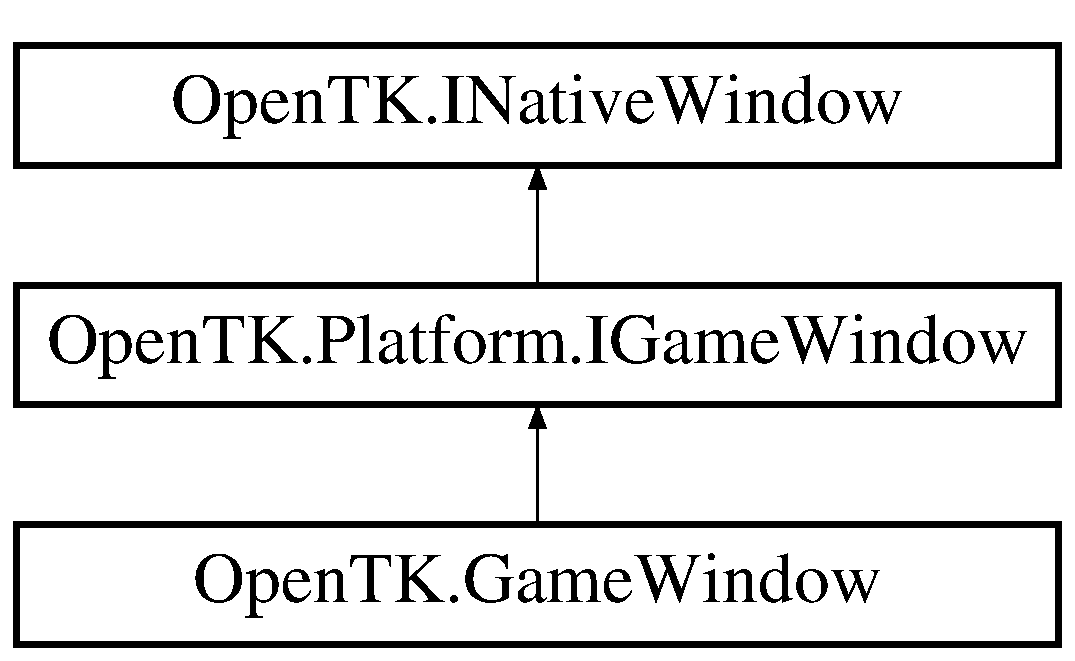
\includegraphics[height=3.000000cm]{interface_open_t_k_1_1_platform_1_1_i_game_window}
\end{center}
\end{figure}
\subsection*{Public Member Functions}
\begin{DoxyCompactItemize}
\item 
void \hyperlink{interface_open_t_k_1_1_platform_1_1_i_game_window_a07597d249869f2da75e650caafb72f94}{Run} ()
\begin{DoxyCompactList}\small\item\em Enters the game loop of the \hyperlink{class_open_t_k_1_1_game_window}{Game\-Window} using the maximum update rate. \end{DoxyCompactList}\item 
void \hyperlink{interface_open_t_k_1_1_platform_1_1_i_game_window_a60761d038847624f5d1a8beb0b1a6ec2}{Run} (double update\-Rate)
\begin{DoxyCompactList}\small\item\em Enters the game loop of the \hyperlink{class_open_t_k_1_1_game_window}{Game\-Window} using the specified update rate. \end{DoxyCompactList}\item 
void \hyperlink{interface_open_t_k_1_1_platform_1_1_i_game_window_a82429a99533b04e178b4e6b7893efb17}{Make\-Current} ()
\begin{DoxyCompactList}\small\item\em Makes the Graphics\-Context current on the calling thread. \end{DoxyCompactList}\item 
void \hyperlink{interface_open_t_k_1_1_platform_1_1_i_game_window_a1a426b9c39d98f557b702fe4ef91c007}{Swap\-Buffers} ()
\begin{DoxyCompactList}\small\item\em Swaps the front and back buffers of the current Graphics\-Context, presenting the rendered scene to the user. \end{DoxyCompactList}\end{DoxyCompactItemize}
\subsection*{Events}
\begin{DoxyCompactItemize}
\item 
Event\-Handler$<$ Event\-Args $>$ \hyperlink{interface_open_t_k_1_1_platform_1_1_i_game_window_a59759b2288998cda597bcd28f72994da}{Load}
\begin{DoxyCompactList}\small\item\em Occurs before the window is displayed for the first time. \end{DoxyCompactList}\item 
Event\-Handler$<$ Event\-Args $>$ \hyperlink{interface_open_t_k_1_1_platform_1_1_i_game_window_a493b559f07695d05b9a62a4fb7f8addb}{Unload}
\begin{DoxyCompactList}\small\item\em Occurs before the window is destroyed. \end{DoxyCompactList}\item 
Event\-Handler$<$ \hyperlink{class_open_t_k_1_1_frame_event_args}{Frame\-Event\-Args} $>$ \hyperlink{interface_open_t_k_1_1_platform_1_1_i_game_window_adb51747b40dcd20623f79ab492e28cd7}{Update\-Frame}
\begin{DoxyCompactList}\small\item\em Occurs when it is time to update a frame. \end{DoxyCompactList}\item 
Event\-Handler$<$ \hyperlink{class_open_t_k_1_1_frame_event_args}{Frame\-Event\-Args} $>$ \hyperlink{interface_open_t_k_1_1_platform_1_1_i_game_window_a93a6ae6565e74397cb44c57e99f55867}{Render\-Frame}
\begin{DoxyCompactList}\small\item\em Occurs when it is time to render a frame. \end{DoxyCompactList}\end{DoxyCompactItemize}
\subsection*{Additional Inherited Members}


\subsection{Detailed Description}
Defines the interface for a \hyperlink{class_open_t_k_1_1_game_window}{Game\-Window}. 



\subsection{Member Function Documentation}
\hypertarget{interface_open_t_k_1_1_platform_1_1_i_game_window_a82429a99533b04e178b4e6b7893efb17}{\index{Open\-T\-K\-::\-Platform\-::\-I\-Game\-Window@{Open\-T\-K\-::\-Platform\-::\-I\-Game\-Window}!Make\-Current@{Make\-Current}}
\index{Make\-Current@{Make\-Current}!OpenTK::Platform::IGameWindow@{Open\-T\-K\-::\-Platform\-::\-I\-Game\-Window}}
\subsubsection[{Make\-Current}]{\setlength{\rightskip}{0pt plus 5cm}void Open\-T\-K.\-Platform.\-I\-Game\-Window.\-Make\-Current (
\begin{DoxyParamCaption}
{}
\end{DoxyParamCaption}
)}}\label{interface_open_t_k_1_1_platform_1_1_i_game_window_a82429a99533b04e178b4e6b7893efb17}


Makes the Graphics\-Context current on the calling thread. 



Implemented in \hyperlink{class_open_t_k_1_1_game_window_a84d84a7173903a8d991e6ca3d40a7a4b}{Open\-T\-K.\-Game\-Window}.

\hypertarget{interface_open_t_k_1_1_platform_1_1_i_game_window_a07597d249869f2da75e650caafb72f94}{\index{Open\-T\-K\-::\-Platform\-::\-I\-Game\-Window@{Open\-T\-K\-::\-Platform\-::\-I\-Game\-Window}!Run@{Run}}
\index{Run@{Run}!OpenTK::Platform::IGameWindow@{Open\-T\-K\-::\-Platform\-::\-I\-Game\-Window}}
\subsubsection[{Run}]{\setlength{\rightskip}{0pt plus 5cm}void Open\-T\-K.\-Platform.\-I\-Game\-Window.\-Run (
\begin{DoxyParamCaption}
{}
\end{DoxyParamCaption}
)}}\label{interface_open_t_k_1_1_platform_1_1_i_game_window_a07597d249869f2da75e650caafb72f94}


Enters the game loop of the \hyperlink{class_open_t_k_1_1_game_window}{Game\-Window} using the maximum update rate. 

\begin{DoxySeeAlso}{See Also}
\hyperlink{interface_open_t_k_1_1_platform_1_1_i_game_window_a60761d038847624f5d1a8beb0b1a6ec2}{Run(double)}


\end{DoxySeeAlso}


Implemented in \hyperlink{class_open_t_k_1_1_game_window_a2ead9bd94f36e26e86da79ef548e7d6b}{Open\-T\-K.\-Game\-Window}.

\hypertarget{interface_open_t_k_1_1_platform_1_1_i_game_window_a60761d038847624f5d1a8beb0b1a6ec2}{\index{Open\-T\-K\-::\-Platform\-::\-I\-Game\-Window@{Open\-T\-K\-::\-Platform\-::\-I\-Game\-Window}!Run@{Run}}
\index{Run@{Run}!OpenTK::Platform::IGameWindow@{Open\-T\-K\-::\-Platform\-::\-I\-Game\-Window}}
\subsubsection[{Run}]{\setlength{\rightskip}{0pt plus 5cm}void Open\-T\-K.\-Platform.\-I\-Game\-Window.\-Run (
\begin{DoxyParamCaption}
\item[{double}]{update\-Rate}
\end{DoxyParamCaption}
)}}\label{interface_open_t_k_1_1_platform_1_1_i_game_window_a60761d038847624f5d1a8beb0b1a6ec2}


Enters the game loop of the \hyperlink{class_open_t_k_1_1_game_window}{Game\-Window} using the specified update rate. 



Implemented in \hyperlink{class_open_t_k_1_1_game_window_a0c9d2a547ee1dc8f59ad0e70c2552730}{Open\-T\-K.\-Game\-Window}.

\hypertarget{interface_open_t_k_1_1_platform_1_1_i_game_window_a1a426b9c39d98f557b702fe4ef91c007}{\index{Open\-T\-K\-::\-Platform\-::\-I\-Game\-Window@{Open\-T\-K\-::\-Platform\-::\-I\-Game\-Window}!Swap\-Buffers@{Swap\-Buffers}}
\index{Swap\-Buffers@{Swap\-Buffers}!OpenTK::Platform::IGameWindow@{Open\-T\-K\-::\-Platform\-::\-I\-Game\-Window}}
\subsubsection[{Swap\-Buffers}]{\setlength{\rightskip}{0pt plus 5cm}void Open\-T\-K.\-Platform.\-I\-Game\-Window.\-Swap\-Buffers (
\begin{DoxyParamCaption}
{}
\end{DoxyParamCaption}
)}}\label{interface_open_t_k_1_1_platform_1_1_i_game_window_a1a426b9c39d98f557b702fe4ef91c007}


Swaps the front and back buffers of the current Graphics\-Context, presenting the rendered scene to the user. 



Implemented in \hyperlink{class_open_t_k_1_1_game_window_adeaeff9283d467a5cda90e6b8579543a}{Open\-T\-K.\-Game\-Window}.



\subsection{Event Documentation}
\hypertarget{interface_open_t_k_1_1_platform_1_1_i_game_window_a59759b2288998cda597bcd28f72994da}{\index{Open\-T\-K\-::\-Platform\-::\-I\-Game\-Window@{Open\-T\-K\-::\-Platform\-::\-I\-Game\-Window}!Load@{Load}}
\index{Load@{Load}!OpenTK::Platform::IGameWindow@{Open\-T\-K\-::\-Platform\-::\-I\-Game\-Window}}
\subsubsection[{Load}]{\setlength{\rightskip}{0pt plus 5cm}Event\-Handler$<$Event\-Args$>$ Open\-T\-K.\-Platform.\-I\-Game\-Window.\-Load}}\label{interface_open_t_k_1_1_platform_1_1_i_game_window_a59759b2288998cda597bcd28f72994da}


Occurs before the window is displayed for the first time. 

\hypertarget{interface_open_t_k_1_1_platform_1_1_i_game_window_a93a6ae6565e74397cb44c57e99f55867}{\index{Open\-T\-K\-::\-Platform\-::\-I\-Game\-Window@{Open\-T\-K\-::\-Platform\-::\-I\-Game\-Window}!Render\-Frame@{Render\-Frame}}
\index{Render\-Frame@{Render\-Frame}!OpenTK::Platform::IGameWindow@{Open\-T\-K\-::\-Platform\-::\-I\-Game\-Window}}
\subsubsection[{Render\-Frame}]{\setlength{\rightskip}{0pt plus 5cm}Event\-Handler$<${\bf Frame\-Event\-Args}$>$ Open\-T\-K.\-Platform.\-I\-Game\-Window.\-Render\-Frame}}\label{interface_open_t_k_1_1_platform_1_1_i_game_window_a93a6ae6565e74397cb44c57e99f55867}


Occurs when it is time to render a frame. 

\hypertarget{interface_open_t_k_1_1_platform_1_1_i_game_window_a493b559f07695d05b9a62a4fb7f8addb}{\index{Open\-T\-K\-::\-Platform\-::\-I\-Game\-Window@{Open\-T\-K\-::\-Platform\-::\-I\-Game\-Window}!Unload@{Unload}}
\index{Unload@{Unload}!OpenTK::Platform::IGameWindow@{Open\-T\-K\-::\-Platform\-::\-I\-Game\-Window}}
\subsubsection[{Unload}]{\setlength{\rightskip}{0pt plus 5cm}Event\-Handler$<$Event\-Args$>$ Open\-T\-K.\-Platform.\-I\-Game\-Window.\-Unload}}\label{interface_open_t_k_1_1_platform_1_1_i_game_window_a493b559f07695d05b9a62a4fb7f8addb}


Occurs before the window is destroyed. 

\hypertarget{interface_open_t_k_1_1_platform_1_1_i_game_window_adb51747b40dcd20623f79ab492e28cd7}{\index{Open\-T\-K\-::\-Platform\-::\-I\-Game\-Window@{Open\-T\-K\-::\-Platform\-::\-I\-Game\-Window}!Update\-Frame@{Update\-Frame}}
\index{Update\-Frame@{Update\-Frame}!OpenTK::Platform::IGameWindow@{Open\-T\-K\-::\-Platform\-::\-I\-Game\-Window}}
\subsubsection[{Update\-Frame}]{\setlength{\rightskip}{0pt plus 5cm}Event\-Handler$<${\bf Frame\-Event\-Args}$>$ Open\-T\-K.\-Platform.\-I\-Game\-Window.\-Update\-Frame}}\label{interface_open_t_k_1_1_platform_1_1_i_game_window_adb51747b40dcd20623f79ab492e28cd7}


Occurs when it is time to update a frame. 


\hypertarget{interface_open_t_k_1_1_platform_1_1_i_window_info}{\section{Open\-T\-K.\-Platform.\-I\-Window\-Info Interface Reference}
\label{interface_open_t_k_1_1_platform_1_1_i_window_info}\index{Open\-T\-K.\-Platform.\-I\-Window\-Info@{Open\-T\-K.\-Platform.\-I\-Window\-Info}}
}


Descibes an O\-S window. 




Inherits I\-Disposable.



Inherited by Open\-T\-K.\-Platform.\-Dummy.\-Dummy\-Window\-Info, Open\-T\-K.\-Platform.\-Egl.\-Egl\-Window\-Info, Open\-T\-K.\-Platform.\-Mac\-O\-S.\-Carbon\-Window\-Info, Open\-T\-K.\-Platform.\-Windows.\-Win\-Window\-Info, and Open\-T\-K.\-Platform.\-X11.\-X11\-Window\-Info.



\subsection{Detailed Description}
Descibes an O\-S window.


\hypertarget{class_open_t_k_1_1_platform_exception}{\section{Open\-T\-K.\-Platform\-Exception Class Reference}
\label{class_open_t_k_1_1_platform_exception}\index{Open\-T\-K.\-Platform\-Exception@{Open\-T\-K.\-Platform\-Exception}}
}


Defines a plaftorm specific exception. 




Inherits Exception.

\subsection*{Public Member Functions}
\begin{DoxyCompactItemize}
\item 
\hyperlink{class_open_t_k_1_1_platform_exception_afc73a2d1d2ff1eca82da22ce4315f560}{Platform\-Exception} (string s)
\begin{DoxyCompactList}\small\item\em Constructs a new \hyperlink{class_open_t_k_1_1_platform_exception}{Platform\-Exception}.\end{DoxyCompactList}\end{DoxyCompactItemize}


\subsection{Detailed Description}
Defines a plaftorm specific exception.



\subsection{Constructor \& Destructor Documentation}
\hypertarget{class_open_t_k_1_1_platform_exception_afc73a2d1d2ff1eca82da22ce4315f560}{\index{Open\-T\-K\-::\-Platform\-Exception@{Open\-T\-K\-::\-Platform\-Exception}!Platform\-Exception@{Platform\-Exception}}
\index{Platform\-Exception@{Platform\-Exception}!OpenTK::PlatformException@{Open\-T\-K\-::\-Platform\-Exception}}
\subsubsection[{Platform\-Exception}]{\setlength{\rightskip}{0pt plus 5cm}Open\-T\-K.\-Platform\-Exception.\-Platform\-Exception (
\begin{DoxyParamCaption}
\item[{string}]{s}
\end{DoxyParamCaption}
)}}\label{class_open_t_k_1_1_platform_exception_afc73a2d1d2ff1eca82da22ce4315f560}


Constructs a new \hyperlink{class_open_t_k_1_1_platform_exception}{Platform\-Exception}.


\hypertarget{struct_open_t_k_1_1_quaternion}{\section{Open\-T\-K.\-Quaternion Struct Reference}
\label{struct_open_t_k_1_1_quaternion}\index{Open\-T\-K.\-Quaternion@{Open\-T\-K.\-Quaternion}}
}


Represents a \hyperlink{struct_open_t_k_1_1_quaternion}{Quaternion}.  




Inherits I\-Equatable$<$ Quaternion $>$.

\subsection*{Public Member Functions}
\begin{DoxyCompactItemize}
\item 
\hyperlink{struct_open_t_k_1_1_quaternion_a06f0e188f9174175b591389fc4bbf0a1}{Quaternion} (\hyperlink{struct_open_t_k_1_1_vector3}{Vector3} v, float w)
\begin{DoxyCompactList}\small\item\em Construct a new \hyperlink{struct_open_t_k_1_1_quaternion}{Quaternion} from vector and w components \end{DoxyCompactList}\item 
\hyperlink{struct_open_t_k_1_1_quaternion_a903587c421dde735c08bf0bf878daf1f}{Quaternion} (float x, float y, float z, float w)
\begin{DoxyCompactList}\small\item\em Construct a new \hyperlink{struct_open_t_k_1_1_quaternion}{Quaternion} \end{DoxyCompactList}\item 
void \hyperlink{struct_open_t_k_1_1_quaternion_aefdf2ce49edd34247ee47da47ea340e5}{To\-Axis\-Angle} (out \hyperlink{struct_open_t_k_1_1_vector3}{Vector3} axis, out float angle)
\begin{DoxyCompactList}\small\item\em Convert the current quaternion to axis angle representation \end{DoxyCompactList}\item 
\hyperlink{struct_open_t_k_1_1_vector4}{Vector4} \hyperlink{struct_open_t_k_1_1_quaternion_a9473c428ba8e986cbf56b28d729a8cd3}{To\-Axis\-Angle} ()
\begin{DoxyCompactList}\small\item\em Convert this instance to an axis-\/angle representation. \end{DoxyCompactList}\item 
\hyperlink{struct_open_t_k_1_1_quaternion}{Quaternion} \hyperlink{struct_open_t_k_1_1_quaternion_acbd0d16744065bf333d842d482460e26}{Normalized} ()
\begin{DoxyCompactList}\small\item\em Returns a copy of the \hyperlink{struct_open_t_k_1_1_quaternion}{Quaternion} scaled to unit length. \end{DoxyCompactList}\item 
void \hyperlink{struct_open_t_k_1_1_quaternion_aa72d00779d1c9f5de9c6cbb7cc460f08}{Invert} ()
\begin{DoxyCompactList}\small\item\em Reverses the rotation angle of this \hyperlink{struct_open_t_k_1_1_quaterniond}{Quaterniond}. \end{DoxyCompactList}\item 
\hyperlink{struct_open_t_k_1_1_quaternion}{Quaternion} \hyperlink{struct_open_t_k_1_1_quaternion_a8c595f7a501f568fbb1bc15f783847dd}{Inverted} ()
\begin{DoxyCompactList}\small\item\em Returns a copy of this \hyperlink{struct_open_t_k_1_1_quaterniond}{Quaterniond} with its rotation angle reversed. \end{DoxyCompactList}\item 
void \hyperlink{struct_open_t_k_1_1_quaternion_a39c08673d20b47daeb30691cc9b887e0}{Normalize} ()
\begin{DoxyCompactList}\small\item\em Scales the \hyperlink{struct_open_t_k_1_1_quaternion}{Quaternion} to unit length. \end{DoxyCompactList}\item 
void \hyperlink{struct_open_t_k_1_1_quaternion_ad2a8d218e87e0d7351e190f79bd9a6d3}{Conjugate} ()
\begin{DoxyCompactList}\small\item\em Inverts the \hyperlink{struct_open_t_k_1_1_vector3}{Vector3} component of this \hyperlink{struct_open_t_k_1_1_quaternion}{Quaternion}. \end{DoxyCompactList}\item 
override string \hyperlink{struct_open_t_k_1_1_quaternion_a234a78961f6168602932a391543bb517}{To\-String} ()
\begin{DoxyCompactList}\small\item\em Returns a System.\-String that represents the current \hyperlink{struct_open_t_k_1_1_quaternion}{Quaternion}. \end{DoxyCompactList}\item 
override bool \hyperlink{struct_open_t_k_1_1_quaternion_ae4258668435340a6b71613bf6e086690}{Equals} (object other)
\begin{DoxyCompactList}\small\item\em Compares this object instance to another object for equality. \end{DoxyCompactList}\item 
override int \hyperlink{struct_open_t_k_1_1_quaternion_a7cf9a59b36cc514ac8f4ac71ad175c4f}{Get\-Hash\-Code} ()
\begin{DoxyCompactList}\small\item\em Provides the hash code for this object. \end{DoxyCompactList}\item 
bool \hyperlink{struct_open_t_k_1_1_quaternion_a2537c5ba956b79ba91cade02b6f6ca71}{Equals} (\hyperlink{struct_open_t_k_1_1_quaternion}{Quaternion} other)
\begin{DoxyCompactList}\small\item\em Compares this \hyperlink{struct_open_t_k_1_1_quaternion}{Quaternion} instance to another \hyperlink{struct_open_t_k_1_1_quaternion}{Quaternion} for equality. \end{DoxyCompactList}\end{DoxyCompactItemize}
\subsection*{Static Public Member Functions}
\begin{DoxyCompactItemize}
\item 
static \hyperlink{struct_open_t_k_1_1_quaternion}{Quaternion} \hyperlink{struct_open_t_k_1_1_quaternion_a7de4c42bb87e78a0e6b1dfee623d8fc7}{Add} (\hyperlink{struct_open_t_k_1_1_quaternion}{Quaternion} left, \hyperlink{struct_open_t_k_1_1_quaternion}{Quaternion} right)
\begin{DoxyCompactList}\small\item\em Add two quaternions \end{DoxyCompactList}\item 
static void \hyperlink{struct_open_t_k_1_1_quaternion_a02cbc83e73f0daefba3e77beb45c5e5a}{Add} (ref \hyperlink{struct_open_t_k_1_1_quaternion}{Quaternion} left, ref \hyperlink{struct_open_t_k_1_1_quaternion}{Quaternion} right, out \hyperlink{struct_open_t_k_1_1_quaternion}{Quaternion} result)
\begin{DoxyCompactList}\small\item\em Add two quaternions \end{DoxyCompactList}\item 
static \hyperlink{struct_open_t_k_1_1_quaternion}{Quaternion} \hyperlink{struct_open_t_k_1_1_quaternion_ab1ddf04d6cf86e470cf1aa75147c143a}{Sub} (\hyperlink{struct_open_t_k_1_1_quaternion}{Quaternion} left, \hyperlink{struct_open_t_k_1_1_quaternion}{Quaternion} right)
\begin{DoxyCompactList}\small\item\em Subtracts two instances. \end{DoxyCompactList}\item 
static void \hyperlink{struct_open_t_k_1_1_quaternion_ad8bf2c580b06268b9e1c45aea27b8c52}{Sub} (ref \hyperlink{struct_open_t_k_1_1_quaternion}{Quaternion} left, ref \hyperlink{struct_open_t_k_1_1_quaternion}{Quaternion} right, out \hyperlink{struct_open_t_k_1_1_quaternion}{Quaternion} result)
\begin{DoxyCompactList}\small\item\em Subtracts two instances. \end{DoxyCompactList}\item 
static \hyperlink{struct_open_t_k_1_1_quaternion}{Quaternion} \hyperlink{struct_open_t_k_1_1_quaternion_a1f38c4a06ba31f9f862b5dc57494dd39}{Mult} (\hyperlink{struct_open_t_k_1_1_quaternion}{Quaternion} left, \hyperlink{struct_open_t_k_1_1_quaternion}{Quaternion} right)
\begin{DoxyCompactList}\small\item\em Multiplies two instances. \end{DoxyCompactList}\item 
static void \hyperlink{struct_open_t_k_1_1_quaternion_ad0e67d8b7266915adf0bfae31d6757b9}{Mult} (ref \hyperlink{struct_open_t_k_1_1_quaternion}{Quaternion} left, ref \hyperlink{struct_open_t_k_1_1_quaternion}{Quaternion} right, out \hyperlink{struct_open_t_k_1_1_quaternion}{Quaternion} result)
\begin{DoxyCompactList}\small\item\em Multiplies two instances. \end{DoxyCompactList}\item 
static \hyperlink{struct_open_t_k_1_1_quaternion}{Quaternion} \hyperlink{struct_open_t_k_1_1_quaternion_a1fa69eacde2186a08be8eaecb818efb4}{Multiply} (\hyperlink{struct_open_t_k_1_1_quaternion}{Quaternion} left, \hyperlink{struct_open_t_k_1_1_quaternion}{Quaternion} right)
\begin{DoxyCompactList}\small\item\em Multiplies two instances. \end{DoxyCompactList}\item 
static void \hyperlink{struct_open_t_k_1_1_quaternion_ac2020c45a1c9e109c9b5667e0ed3c0bc}{Multiply} (ref \hyperlink{struct_open_t_k_1_1_quaternion}{Quaternion} left, ref \hyperlink{struct_open_t_k_1_1_quaternion}{Quaternion} right, out \hyperlink{struct_open_t_k_1_1_quaternion}{Quaternion} result)
\begin{DoxyCompactList}\small\item\em Multiplies two instances. \end{DoxyCompactList}\item 
static void \hyperlink{struct_open_t_k_1_1_quaternion_aec98462c1fa302496cc639c8d95da343}{Multiply} (ref \hyperlink{struct_open_t_k_1_1_quaternion}{Quaternion} quaternion, float scale, out \hyperlink{struct_open_t_k_1_1_quaternion}{Quaternion} result)
\begin{DoxyCompactList}\small\item\em Multiplies an instance by a scalar. \end{DoxyCompactList}\item 
static \hyperlink{struct_open_t_k_1_1_quaternion}{Quaternion} \hyperlink{struct_open_t_k_1_1_quaternion_aca2a12afdd23d4fc851a9db604bff627}{Multiply} (\hyperlink{struct_open_t_k_1_1_quaternion}{Quaternion} quaternion, float scale)
\begin{DoxyCompactList}\small\item\em Multiplies an instance by a scalar. \end{DoxyCompactList}\item 
static \hyperlink{struct_open_t_k_1_1_quaternion}{Quaternion} \hyperlink{struct_open_t_k_1_1_quaternion_a8284d69ce3125f7509a25ebb4adc8563}{Conjugate} (\hyperlink{struct_open_t_k_1_1_quaternion}{Quaternion} q)
\begin{DoxyCompactList}\small\item\em Get the conjugate of the given quaternion \end{DoxyCompactList}\item 
static void \hyperlink{struct_open_t_k_1_1_quaternion_a5a1b50899ba3ed87e585615060233f39}{Conjugate} (ref \hyperlink{struct_open_t_k_1_1_quaternion}{Quaternion} q, out \hyperlink{struct_open_t_k_1_1_quaternion}{Quaternion} result)
\begin{DoxyCompactList}\small\item\em Get the conjugate of the given quaternion \end{DoxyCompactList}\item 
static \hyperlink{struct_open_t_k_1_1_quaternion}{Quaternion} \hyperlink{struct_open_t_k_1_1_quaternion_a482789e5f1cdc692474c1465095d00c3}{Invert} (\hyperlink{struct_open_t_k_1_1_quaternion}{Quaternion} q)
\begin{DoxyCompactList}\small\item\em Get the inverse of the given quaternion \end{DoxyCompactList}\item 
static void \hyperlink{struct_open_t_k_1_1_quaternion_a2dadba34c0cdc6f578215cc78c184694}{Invert} (ref \hyperlink{struct_open_t_k_1_1_quaternion}{Quaternion} q, out \hyperlink{struct_open_t_k_1_1_quaternion}{Quaternion} result)
\begin{DoxyCompactList}\small\item\em Get the inverse of the given quaternion \end{DoxyCompactList}\item 
static \hyperlink{struct_open_t_k_1_1_quaternion}{Quaternion} \hyperlink{struct_open_t_k_1_1_quaternion_a522236c79e456951f8b1927265e8752f}{Normalize} (\hyperlink{struct_open_t_k_1_1_quaternion}{Quaternion} q)
\begin{DoxyCompactList}\small\item\em Scale the given quaternion to unit length \end{DoxyCompactList}\item 
static void \hyperlink{struct_open_t_k_1_1_quaternion_a1346d52ee04b407b038aa7e3e07ff955}{Normalize} (ref \hyperlink{struct_open_t_k_1_1_quaternion}{Quaternion} q, out \hyperlink{struct_open_t_k_1_1_quaternion}{Quaternion} result)
\begin{DoxyCompactList}\small\item\em Scale the given quaternion to unit length \end{DoxyCompactList}\item 
static \hyperlink{struct_open_t_k_1_1_quaternion}{Quaternion} \hyperlink{struct_open_t_k_1_1_quaternion_aed64b65ba3e40a4155907038fe0e361a}{From\-Axis\-Angle} (\hyperlink{struct_open_t_k_1_1_vector3}{Vector3} axis, float angle)
\begin{DoxyCompactList}\small\item\em Build a quaternion from the given axis and angle \end{DoxyCompactList}\item 
static \hyperlink{struct_open_t_k_1_1_quaternion}{Quaternion} \hyperlink{struct_open_t_k_1_1_quaternion_a25e810d6f864d1ac1f21bfb617197072}{From\-Matrix} (\hyperlink{struct_open_t_k_1_1_matrix3}{Matrix3} matrix)
\begin{DoxyCompactList}\small\item\em Builds a quaternion from the given rotation matrix \end{DoxyCompactList}\item 
static void \hyperlink{struct_open_t_k_1_1_quaternion_a5fef0adb952afd3c0495ce3b3f5b95df}{From\-Matrix} (ref \hyperlink{struct_open_t_k_1_1_matrix3}{Matrix3} matrix, out \hyperlink{struct_open_t_k_1_1_quaternion}{Quaternion} result)
\begin{DoxyCompactList}\small\item\em Builds a quaternion from the given rotation matrix \end{DoxyCompactList}\item 
static \hyperlink{struct_open_t_k_1_1_quaternion}{Quaternion} \hyperlink{struct_open_t_k_1_1_quaternion_a113ca4abddf8864c08be7e0f9b6586cd}{Slerp} (\hyperlink{struct_open_t_k_1_1_quaternion}{Quaternion} q1, \hyperlink{struct_open_t_k_1_1_quaternion}{Quaternion} q2, float blend)
\begin{DoxyCompactList}\small\item\em Do Spherical linear interpolation between two quaternions \end{DoxyCompactList}\item 
static \hyperlink{struct_open_t_k_1_1_quaternion}{Quaternion} \hyperlink{struct_open_t_k_1_1_quaternion_a68a96fe08097a18c698a4cbbb335372f}{operator+} (\hyperlink{struct_open_t_k_1_1_quaternion}{Quaternion} left, \hyperlink{struct_open_t_k_1_1_quaternion}{Quaternion} right)
\begin{DoxyCompactList}\small\item\em Adds two instances. \end{DoxyCompactList}\item 
static \hyperlink{struct_open_t_k_1_1_quaternion}{Quaternion} \hyperlink{struct_open_t_k_1_1_quaternion_a848dc62ea8c62fba5754caa400439428}{operator-\/} (\hyperlink{struct_open_t_k_1_1_quaternion}{Quaternion} left, \hyperlink{struct_open_t_k_1_1_quaternion}{Quaternion} right)
\begin{DoxyCompactList}\small\item\em Subtracts two instances. \end{DoxyCompactList}\item 
static \hyperlink{struct_open_t_k_1_1_quaternion}{Quaternion} \hyperlink{struct_open_t_k_1_1_quaternion_aad1164cd81a83b59b0f769e90a4a944e}{operator$\ast$} (\hyperlink{struct_open_t_k_1_1_quaternion}{Quaternion} left, \hyperlink{struct_open_t_k_1_1_quaternion}{Quaternion} right)
\begin{DoxyCompactList}\small\item\em Multiplies two instances. \end{DoxyCompactList}\item 
static \hyperlink{struct_open_t_k_1_1_quaternion}{Quaternion} \hyperlink{struct_open_t_k_1_1_quaternion_ad8968c9f9573910c22591929281146d0}{operator$\ast$} (\hyperlink{struct_open_t_k_1_1_quaternion}{Quaternion} quaternion, float scale)
\begin{DoxyCompactList}\small\item\em Multiplies an instance by a scalar. \end{DoxyCompactList}\item 
static \hyperlink{struct_open_t_k_1_1_quaternion}{Quaternion} \hyperlink{struct_open_t_k_1_1_quaternion_a2d72651a42a17832233bbf907ee863b5}{operator$\ast$} (float scale, \hyperlink{struct_open_t_k_1_1_quaternion}{Quaternion} quaternion)
\begin{DoxyCompactList}\small\item\em Multiplies an instance by a scalar. \end{DoxyCompactList}\item 
static bool \hyperlink{struct_open_t_k_1_1_quaternion_a6153f36272b85146421d17e5fa611425}{operator==} (\hyperlink{struct_open_t_k_1_1_quaternion}{Quaternion} left, \hyperlink{struct_open_t_k_1_1_quaternion}{Quaternion} right)
\begin{DoxyCompactList}\small\item\em Compares two instances for equality. \end{DoxyCompactList}\item 
static bool \hyperlink{struct_open_t_k_1_1_quaternion_a9303285e5fbd0c4c329844a9e021ea29}{operator!=} (\hyperlink{struct_open_t_k_1_1_quaternion}{Quaternion} left, \hyperlink{struct_open_t_k_1_1_quaternion}{Quaternion} right)
\begin{DoxyCompactList}\small\item\em Compares two instances for inequality. \end{DoxyCompactList}\end{DoxyCompactItemize}
\subsection*{Public Attributes}
\begin{DoxyCompactItemize}
\item 
\hypertarget{struct_open_t_k_1_1_quaternion_a507f0624584f5ff9ed6f0e45578452d0}{\hyperlink{struct_open_t_k_1_1_vector3}{Vector3} {\bfseries xyz}}\label{struct_open_t_k_1_1_quaternion_a507f0624584f5ff9ed6f0e45578452d0}

\item 
\hypertarget{struct_open_t_k_1_1_quaternion_a413d4be8475f8911ddee7ba3dbee3fd3}{float {\bfseries w}}\label{struct_open_t_k_1_1_quaternion_a413d4be8475f8911ddee7ba3dbee3fd3}

\end{DoxyCompactItemize}
\subsection*{Static Public Attributes}
\begin{DoxyCompactItemize}
\item 
static readonly \hyperlink{struct_open_t_k_1_1_quaternion}{Quaternion} \hyperlink{struct_open_t_k_1_1_quaternion_a32c6811aa364dda3e3c88600baed2593}{Identity} = new \hyperlink{struct_open_t_k_1_1_quaternion}{Quaternion}(0, 0, 0, 1)
\begin{DoxyCompactList}\small\item\em Defines the identity quaternion. \end{DoxyCompactList}\end{DoxyCompactItemize}
\subsection*{Properties}
\begin{DoxyCompactItemize}
\item 
\hyperlink{struct_open_t_k_1_1_vector3}{Vector3} \hyperlink{struct_open_t_k_1_1_quaternion_ac93b88de0dfdbc1fc7561717b4c60195}{X\-Y\-Z}\hspace{0.3cm}{\ttfamily  \mbox{[}get, set\mbox{]}}
\begin{DoxyCompactList}\small\item\em Gets or sets an \hyperlink{struct_open_t_k_1_1_vector3}{Open\-T\-K.\-Vector3} with the X, Y and Z components of this instance. \end{DoxyCompactList}\item 
\hyperlink{struct_open_t_k_1_1_vector3}{Vector3} \hyperlink{struct_open_t_k_1_1_quaternion_a179592a60e7facac046589a6aabc2d41}{Xyz}\hspace{0.3cm}{\ttfamily  \mbox{[}get, set\mbox{]}}
\begin{DoxyCompactList}\small\item\em Gets or sets an \hyperlink{struct_open_t_k_1_1_vector3}{Open\-T\-K.\-Vector3} with the X, Y and Z components of this instance. \end{DoxyCompactList}\item 
float \hyperlink{struct_open_t_k_1_1_quaternion_af928c6d2c5e59f5d771223b1d9c7018b}{X}\hspace{0.3cm}{\ttfamily  \mbox{[}get, set\mbox{]}}
\begin{DoxyCompactList}\small\item\em Gets or sets the X component of this instance. \end{DoxyCompactList}\item 
float \hyperlink{struct_open_t_k_1_1_quaternion_aad3fdabef1cdc7fd69a807fd043fe1d3}{Y}\hspace{0.3cm}{\ttfamily  \mbox{[}get, set\mbox{]}}
\begin{DoxyCompactList}\small\item\em Gets or sets the Y component of this instance. \end{DoxyCompactList}\item 
float \hyperlink{struct_open_t_k_1_1_quaternion_af184db9f0b3958e0ab8c1ef0eb0667f7}{Z}\hspace{0.3cm}{\ttfamily  \mbox{[}get, set\mbox{]}}
\begin{DoxyCompactList}\small\item\em Gets or sets the Z component of this instance. \end{DoxyCompactList}\item 
float \hyperlink{struct_open_t_k_1_1_quaternion_a9393e674a6d043b72c26ec8fac95a5c3}{W}\hspace{0.3cm}{\ttfamily  \mbox{[}get, set\mbox{]}}
\begin{DoxyCompactList}\small\item\em Gets or sets the W component of this instance. \end{DoxyCompactList}\item 
float \hyperlink{struct_open_t_k_1_1_quaternion_a28670c4161bff2712e57f77e46570af5}{Length}\hspace{0.3cm}{\ttfamily  \mbox{[}get\mbox{]}}
\begin{DoxyCompactList}\small\item\em Gets the length (magnitude) of the quaternion. \end{DoxyCompactList}\item 
float \hyperlink{struct_open_t_k_1_1_quaternion_a356340ca64b0873a256f823228bc3c75}{Length\-Squared}\hspace{0.3cm}{\ttfamily  \mbox{[}get\mbox{]}}
\begin{DoxyCompactList}\small\item\em Gets the square of the quaternion length (magnitude). \end{DoxyCompactList}\end{DoxyCompactItemize}


\subsection{Detailed Description}
Represents a \hyperlink{struct_open_t_k_1_1_quaternion}{Quaternion}. 



\subsection{Constructor \& Destructor Documentation}
\hypertarget{struct_open_t_k_1_1_quaternion_a06f0e188f9174175b591389fc4bbf0a1}{\index{Open\-T\-K\-::\-Quaternion@{Open\-T\-K\-::\-Quaternion}!Quaternion@{Quaternion}}
\index{Quaternion@{Quaternion}!OpenTK::Quaternion@{Open\-T\-K\-::\-Quaternion}}
\subsubsection[{Quaternion}]{\setlength{\rightskip}{0pt plus 5cm}Open\-T\-K.\-Quaternion.\-Quaternion (
\begin{DoxyParamCaption}
\item[{{\bf Vector3}}]{v, }
\item[{float}]{w}
\end{DoxyParamCaption}
)}}\label{struct_open_t_k_1_1_quaternion_a06f0e188f9174175b591389fc4bbf0a1}


Construct a new \hyperlink{struct_open_t_k_1_1_quaternion}{Quaternion} from vector and w components 


\begin{DoxyParams}{Parameters}
{\em v} & The vector part\\
\hline
{\em w} & The w part\\
\hline
\end{DoxyParams}
\hypertarget{struct_open_t_k_1_1_quaternion_a903587c421dde735c08bf0bf878daf1f}{\index{Open\-T\-K\-::\-Quaternion@{Open\-T\-K\-::\-Quaternion}!Quaternion@{Quaternion}}
\index{Quaternion@{Quaternion}!OpenTK::Quaternion@{Open\-T\-K\-::\-Quaternion}}
\subsubsection[{Quaternion}]{\setlength{\rightskip}{0pt plus 5cm}Open\-T\-K.\-Quaternion.\-Quaternion (
\begin{DoxyParamCaption}
\item[{float}]{x, }
\item[{float}]{y, }
\item[{float}]{z, }
\item[{float}]{w}
\end{DoxyParamCaption}
)}}\label{struct_open_t_k_1_1_quaternion_a903587c421dde735c08bf0bf878daf1f}


Construct a new \hyperlink{struct_open_t_k_1_1_quaternion}{Quaternion} 


\begin{DoxyParams}{Parameters}
{\em x} & The x component\\
\hline
{\em y} & The y component\\
\hline
{\em z} & The z component\\
\hline
{\em w} & The w component\\
\hline
\end{DoxyParams}


\subsection{Member Function Documentation}
\hypertarget{struct_open_t_k_1_1_quaternion_a7de4c42bb87e78a0e6b1dfee623d8fc7}{\index{Open\-T\-K\-::\-Quaternion@{Open\-T\-K\-::\-Quaternion}!Add@{Add}}
\index{Add@{Add}!OpenTK::Quaternion@{Open\-T\-K\-::\-Quaternion}}
\subsubsection[{Add}]{\setlength{\rightskip}{0pt plus 5cm}static {\bf Quaternion} Open\-T\-K.\-Quaternion.\-Add (
\begin{DoxyParamCaption}
\item[{{\bf Quaternion}}]{left, }
\item[{{\bf Quaternion}}]{right}
\end{DoxyParamCaption}
)\hspace{0.3cm}{\ttfamily [static]}}}\label{struct_open_t_k_1_1_quaternion_a7de4c42bb87e78a0e6b1dfee623d8fc7}


Add two quaternions 


\begin{DoxyParams}{Parameters}
{\em left} & The first operand\\
\hline
{\em right} & The second operand\\
\hline
\end{DoxyParams}
\begin{DoxyReturn}{Returns}
The result of the addition
\end{DoxyReturn}
\hypertarget{struct_open_t_k_1_1_quaternion_a02cbc83e73f0daefba3e77beb45c5e5a}{\index{Open\-T\-K\-::\-Quaternion@{Open\-T\-K\-::\-Quaternion}!Add@{Add}}
\index{Add@{Add}!OpenTK::Quaternion@{Open\-T\-K\-::\-Quaternion}}
\subsubsection[{Add}]{\setlength{\rightskip}{0pt plus 5cm}static void Open\-T\-K.\-Quaternion.\-Add (
\begin{DoxyParamCaption}
\item[{ref {\bf Quaternion}}]{left, }
\item[{ref {\bf Quaternion}}]{right, }
\item[{out {\bf Quaternion}}]{result}
\end{DoxyParamCaption}
)\hspace{0.3cm}{\ttfamily [static]}}}\label{struct_open_t_k_1_1_quaternion_a02cbc83e73f0daefba3e77beb45c5e5a}


Add two quaternions 


\begin{DoxyParams}{Parameters}
{\em left} & The first operand\\
\hline
{\em right} & The second operand\\
\hline
{\em result} & The result of the addition\\
\hline
\end{DoxyParams}
\hypertarget{struct_open_t_k_1_1_quaternion_ad2a8d218e87e0d7351e190f79bd9a6d3}{\index{Open\-T\-K\-::\-Quaternion@{Open\-T\-K\-::\-Quaternion}!Conjugate@{Conjugate}}
\index{Conjugate@{Conjugate}!OpenTK::Quaternion@{Open\-T\-K\-::\-Quaternion}}
\subsubsection[{Conjugate}]{\setlength{\rightskip}{0pt plus 5cm}void Open\-T\-K.\-Quaternion.\-Conjugate (
\begin{DoxyParamCaption}
{}
\end{DoxyParamCaption}
)}}\label{struct_open_t_k_1_1_quaternion_ad2a8d218e87e0d7351e190f79bd9a6d3}


Inverts the \hyperlink{struct_open_t_k_1_1_vector3}{Vector3} component of this \hyperlink{struct_open_t_k_1_1_quaternion}{Quaternion}. 

\hypertarget{struct_open_t_k_1_1_quaternion_a8284d69ce3125f7509a25ebb4adc8563}{\index{Open\-T\-K\-::\-Quaternion@{Open\-T\-K\-::\-Quaternion}!Conjugate@{Conjugate}}
\index{Conjugate@{Conjugate}!OpenTK::Quaternion@{Open\-T\-K\-::\-Quaternion}}
\subsubsection[{Conjugate}]{\setlength{\rightskip}{0pt plus 5cm}static {\bf Quaternion} Open\-T\-K.\-Quaternion.\-Conjugate (
\begin{DoxyParamCaption}
\item[{{\bf Quaternion}}]{q}
\end{DoxyParamCaption}
)\hspace{0.3cm}{\ttfamily [static]}}}\label{struct_open_t_k_1_1_quaternion_a8284d69ce3125f7509a25ebb4adc8563}


Get the conjugate of the given quaternion 


\begin{DoxyParams}{Parameters}
{\em q} & The quaternion\\
\hline
\end{DoxyParams}
\begin{DoxyReturn}{Returns}
The conjugate of the given quaternion
\end{DoxyReturn}
\hypertarget{struct_open_t_k_1_1_quaternion_a5a1b50899ba3ed87e585615060233f39}{\index{Open\-T\-K\-::\-Quaternion@{Open\-T\-K\-::\-Quaternion}!Conjugate@{Conjugate}}
\index{Conjugate@{Conjugate}!OpenTK::Quaternion@{Open\-T\-K\-::\-Quaternion}}
\subsubsection[{Conjugate}]{\setlength{\rightskip}{0pt plus 5cm}static void Open\-T\-K.\-Quaternion.\-Conjugate (
\begin{DoxyParamCaption}
\item[{ref {\bf Quaternion}}]{q, }
\item[{out {\bf Quaternion}}]{result}
\end{DoxyParamCaption}
)\hspace{0.3cm}{\ttfamily [static]}}}\label{struct_open_t_k_1_1_quaternion_a5a1b50899ba3ed87e585615060233f39}


Get the conjugate of the given quaternion 


\begin{DoxyParams}{Parameters}
{\em q} & The quaternion\\
\hline
{\em result} & The conjugate of the given quaternion\\
\hline
\end{DoxyParams}
\hypertarget{struct_open_t_k_1_1_quaternion_ae4258668435340a6b71613bf6e086690}{\index{Open\-T\-K\-::\-Quaternion@{Open\-T\-K\-::\-Quaternion}!Equals@{Equals}}
\index{Equals@{Equals}!OpenTK::Quaternion@{Open\-T\-K\-::\-Quaternion}}
\subsubsection[{Equals}]{\setlength{\rightskip}{0pt plus 5cm}override bool Open\-T\-K.\-Quaternion.\-Equals (
\begin{DoxyParamCaption}
\item[{object}]{other}
\end{DoxyParamCaption}
)}}\label{struct_open_t_k_1_1_quaternion_ae4258668435340a6b71613bf6e086690}


Compares this object instance to another object for equality. 


\begin{DoxyParams}{Parameters}
{\em other} & The other object to be used in the comparison.\\
\hline
\end{DoxyParams}
\begin{DoxyReturn}{Returns}
True if both objects are Quaternions of equal value. Otherwise it returns false.
\end{DoxyReturn}
\hypertarget{struct_open_t_k_1_1_quaternion_a2537c5ba956b79ba91cade02b6f6ca71}{\index{Open\-T\-K\-::\-Quaternion@{Open\-T\-K\-::\-Quaternion}!Equals@{Equals}}
\index{Equals@{Equals}!OpenTK::Quaternion@{Open\-T\-K\-::\-Quaternion}}
\subsubsection[{Equals}]{\setlength{\rightskip}{0pt plus 5cm}bool Open\-T\-K.\-Quaternion.\-Equals (
\begin{DoxyParamCaption}
\item[{{\bf Quaternion}}]{other}
\end{DoxyParamCaption}
)}}\label{struct_open_t_k_1_1_quaternion_a2537c5ba956b79ba91cade02b6f6ca71}


Compares this \hyperlink{struct_open_t_k_1_1_quaternion}{Quaternion} instance to another \hyperlink{struct_open_t_k_1_1_quaternion}{Quaternion} for equality. 


\begin{DoxyParams}{Parameters}
{\em other} & The other \hyperlink{struct_open_t_k_1_1_quaternion}{Quaternion} to be used in the comparison.\\
\hline
\end{DoxyParams}
\begin{DoxyReturn}{Returns}
True if both instances are equal; false otherwise.
\end{DoxyReturn}
\hypertarget{struct_open_t_k_1_1_quaternion_aed64b65ba3e40a4155907038fe0e361a}{\index{Open\-T\-K\-::\-Quaternion@{Open\-T\-K\-::\-Quaternion}!From\-Axis\-Angle@{From\-Axis\-Angle}}
\index{From\-Axis\-Angle@{From\-Axis\-Angle}!OpenTK::Quaternion@{Open\-T\-K\-::\-Quaternion}}
\subsubsection[{From\-Axis\-Angle}]{\setlength{\rightskip}{0pt plus 5cm}static {\bf Quaternion} Open\-T\-K.\-Quaternion.\-From\-Axis\-Angle (
\begin{DoxyParamCaption}
\item[{{\bf Vector3}}]{axis, }
\item[{float}]{angle}
\end{DoxyParamCaption}
)\hspace{0.3cm}{\ttfamily [static]}}}\label{struct_open_t_k_1_1_quaternion_aed64b65ba3e40a4155907038fe0e361a}


Build a quaternion from the given axis and angle 


\begin{DoxyParams}{Parameters}
{\em axis} & The axis to rotate about\\
\hline
{\em angle} & The rotation angle in radians\\
\hline
\end{DoxyParams}
\begin{DoxyReturn}{Returns}
The equivalent quaternion
\end{DoxyReturn}
\hypertarget{struct_open_t_k_1_1_quaternion_a25e810d6f864d1ac1f21bfb617197072}{\index{Open\-T\-K\-::\-Quaternion@{Open\-T\-K\-::\-Quaternion}!From\-Matrix@{From\-Matrix}}
\index{From\-Matrix@{From\-Matrix}!OpenTK::Quaternion@{Open\-T\-K\-::\-Quaternion}}
\subsubsection[{From\-Matrix}]{\setlength{\rightskip}{0pt plus 5cm}static {\bf Quaternion} Open\-T\-K.\-Quaternion.\-From\-Matrix (
\begin{DoxyParamCaption}
\item[{{\bf Matrix3}}]{matrix}
\end{DoxyParamCaption}
)\hspace{0.3cm}{\ttfamily [static]}}}\label{struct_open_t_k_1_1_quaternion_a25e810d6f864d1ac1f21bfb617197072}


Builds a quaternion from the given rotation matrix 


\begin{DoxyParams}{Parameters}
{\em matrix} & A rotation matrix\\
\hline
\end{DoxyParams}
\begin{DoxyReturn}{Returns}
The equivalent quaternion
\end{DoxyReturn}
\hypertarget{struct_open_t_k_1_1_quaternion_a5fef0adb952afd3c0495ce3b3f5b95df}{\index{Open\-T\-K\-::\-Quaternion@{Open\-T\-K\-::\-Quaternion}!From\-Matrix@{From\-Matrix}}
\index{From\-Matrix@{From\-Matrix}!OpenTK::Quaternion@{Open\-T\-K\-::\-Quaternion}}
\subsubsection[{From\-Matrix}]{\setlength{\rightskip}{0pt plus 5cm}static void Open\-T\-K.\-Quaternion.\-From\-Matrix (
\begin{DoxyParamCaption}
\item[{ref {\bf Matrix3}}]{matrix, }
\item[{out {\bf Quaternion}}]{result}
\end{DoxyParamCaption}
)\hspace{0.3cm}{\ttfamily [static]}}}\label{struct_open_t_k_1_1_quaternion_a5fef0adb952afd3c0495ce3b3f5b95df}


Builds a quaternion from the given rotation matrix 


\begin{DoxyParams}{Parameters}
{\em matrix} & A rotation matrix\\
\hline
{\em result} & The equivalent quaternion\\
\hline
\end{DoxyParams}
\hypertarget{struct_open_t_k_1_1_quaternion_a7cf9a59b36cc514ac8f4ac71ad175c4f}{\index{Open\-T\-K\-::\-Quaternion@{Open\-T\-K\-::\-Quaternion}!Get\-Hash\-Code@{Get\-Hash\-Code}}
\index{Get\-Hash\-Code@{Get\-Hash\-Code}!OpenTK::Quaternion@{Open\-T\-K\-::\-Quaternion}}
\subsubsection[{Get\-Hash\-Code}]{\setlength{\rightskip}{0pt plus 5cm}override int Open\-T\-K.\-Quaternion.\-Get\-Hash\-Code (
\begin{DoxyParamCaption}
{}
\end{DoxyParamCaption}
)}}\label{struct_open_t_k_1_1_quaternion_a7cf9a59b36cc514ac8f4ac71ad175c4f}


Provides the hash code for this object. 

\begin{DoxyReturn}{Returns}
A hash code formed from the bitwise X\-O\-R of this objects members.
\end{DoxyReturn}
\hypertarget{struct_open_t_k_1_1_quaternion_aa72d00779d1c9f5de9c6cbb7cc460f08}{\index{Open\-T\-K\-::\-Quaternion@{Open\-T\-K\-::\-Quaternion}!Invert@{Invert}}
\index{Invert@{Invert}!OpenTK::Quaternion@{Open\-T\-K\-::\-Quaternion}}
\subsubsection[{Invert}]{\setlength{\rightskip}{0pt plus 5cm}void Open\-T\-K.\-Quaternion.\-Invert (
\begin{DoxyParamCaption}
{}
\end{DoxyParamCaption}
)}}\label{struct_open_t_k_1_1_quaternion_aa72d00779d1c9f5de9c6cbb7cc460f08}


Reverses the rotation angle of this \hyperlink{struct_open_t_k_1_1_quaterniond}{Quaterniond}. 

\hypertarget{struct_open_t_k_1_1_quaternion_a482789e5f1cdc692474c1465095d00c3}{\index{Open\-T\-K\-::\-Quaternion@{Open\-T\-K\-::\-Quaternion}!Invert@{Invert}}
\index{Invert@{Invert}!OpenTK::Quaternion@{Open\-T\-K\-::\-Quaternion}}
\subsubsection[{Invert}]{\setlength{\rightskip}{0pt plus 5cm}static {\bf Quaternion} Open\-T\-K.\-Quaternion.\-Invert (
\begin{DoxyParamCaption}
\item[{{\bf Quaternion}}]{q}
\end{DoxyParamCaption}
)\hspace{0.3cm}{\ttfamily [static]}}}\label{struct_open_t_k_1_1_quaternion_a482789e5f1cdc692474c1465095d00c3}


Get the inverse of the given quaternion 


\begin{DoxyParams}{Parameters}
{\em q} & The quaternion to invert\\
\hline
\end{DoxyParams}
\begin{DoxyReturn}{Returns}
The inverse of the given quaternion
\end{DoxyReturn}
\hypertarget{struct_open_t_k_1_1_quaternion_a2dadba34c0cdc6f578215cc78c184694}{\index{Open\-T\-K\-::\-Quaternion@{Open\-T\-K\-::\-Quaternion}!Invert@{Invert}}
\index{Invert@{Invert}!OpenTK::Quaternion@{Open\-T\-K\-::\-Quaternion}}
\subsubsection[{Invert}]{\setlength{\rightskip}{0pt plus 5cm}static void Open\-T\-K.\-Quaternion.\-Invert (
\begin{DoxyParamCaption}
\item[{ref {\bf Quaternion}}]{q, }
\item[{out {\bf Quaternion}}]{result}
\end{DoxyParamCaption}
)\hspace{0.3cm}{\ttfamily [static]}}}\label{struct_open_t_k_1_1_quaternion_a2dadba34c0cdc6f578215cc78c184694}


Get the inverse of the given quaternion 


\begin{DoxyParams}{Parameters}
{\em q} & The quaternion to invert\\
\hline
{\em result} & The inverse of the given quaternion\\
\hline
\end{DoxyParams}
\hypertarget{struct_open_t_k_1_1_quaternion_a8c595f7a501f568fbb1bc15f783847dd}{\index{Open\-T\-K\-::\-Quaternion@{Open\-T\-K\-::\-Quaternion}!Inverted@{Inverted}}
\index{Inverted@{Inverted}!OpenTK::Quaternion@{Open\-T\-K\-::\-Quaternion}}
\subsubsection[{Inverted}]{\setlength{\rightskip}{0pt plus 5cm}{\bf Quaternion} Open\-T\-K.\-Quaternion.\-Inverted (
\begin{DoxyParamCaption}
{}
\end{DoxyParamCaption}
)}}\label{struct_open_t_k_1_1_quaternion_a8c595f7a501f568fbb1bc15f783847dd}


Returns a copy of this \hyperlink{struct_open_t_k_1_1_quaterniond}{Quaterniond} with its rotation angle reversed. 

\hypertarget{struct_open_t_k_1_1_quaternion_a1f38c4a06ba31f9f862b5dc57494dd39}{\index{Open\-T\-K\-::\-Quaternion@{Open\-T\-K\-::\-Quaternion}!Mult@{Mult}}
\index{Mult@{Mult}!OpenTK::Quaternion@{Open\-T\-K\-::\-Quaternion}}
\subsubsection[{Mult}]{\setlength{\rightskip}{0pt plus 5cm}static {\bf Quaternion} Open\-T\-K.\-Quaternion.\-Mult (
\begin{DoxyParamCaption}
\item[{{\bf Quaternion}}]{left, }
\item[{{\bf Quaternion}}]{right}
\end{DoxyParamCaption}
)\hspace{0.3cm}{\ttfamily [static]}}}\label{struct_open_t_k_1_1_quaternion_a1f38c4a06ba31f9f862b5dc57494dd39}


Multiplies two instances. 


\begin{DoxyParams}{Parameters}
{\em left} & The first instance.\\
\hline
{\em right} & The second instance.\\
\hline
\end{DoxyParams}
\begin{DoxyReturn}{Returns}
A new instance containing the result of the calculation.
\end{DoxyReturn}
\hypertarget{struct_open_t_k_1_1_quaternion_ad0e67d8b7266915adf0bfae31d6757b9}{\index{Open\-T\-K\-::\-Quaternion@{Open\-T\-K\-::\-Quaternion}!Mult@{Mult}}
\index{Mult@{Mult}!OpenTK::Quaternion@{Open\-T\-K\-::\-Quaternion}}
\subsubsection[{Mult}]{\setlength{\rightskip}{0pt plus 5cm}static void Open\-T\-K.\-Quaternion.\-Mult (
\begin{DoxyParamCaption}
\item[{ref {\bf Quaternion}}]{left, }
\item[{ref {\bf Quaternion}}]{right, }
\item[{out {\bf Quaternion}}]{result}
\end{DoxyParamCaption}
)\hspace{0.3cm}{\ttfamily [static]}}}\label{struct_open_t_k_1_1_quaternion_ad0e67d8b7266915adf0bfae31d6757b9}


Multiplies two instances. 


\begin{DoxyParams}{Parameters}
{\em left} & The first instance.\\
\hline
{\em right} & The second instance.\\
\hline
{\em result} & A new instance containing the result of the calculation.\\
\hline
\end{DoxyParams}
\hypertarget{struct_open_t_k_1_1_quaternion_a1fa69eacde2186a08be8eaecb818efb4}{\index{Open\-T\-K\-::\-Quaternion@{Open\-T\-K\-::\-Quaternion}!Multiply@{Multiply}}
\index{Multiply@{Multiply}!OpenTK::Quaternion@{Open\-T\-K\-::\-Quaternion}}
\subsubsection[{Multiply}]{\setlength{\rightskip}{0pt plus 5cm}static {\bf Quaternion} Open\-T\-K.\-Quaternion.\-Multiply (
\begin{DoxyParamCaption}
\item[{{\bf Quaternion}}]{left, }
\item[{{\bf Quaternion}}]{right}
\end{DoxyParamCaption}
)\hspace{0.3cm}{\ttfamily [static]}}}\label{struct_open_t_k_1_1_quaternion_a1fa69eacde2186a08be8eaecb818efb4}


Multiplies two instances. 


\begin{DoxyParams}{Parameters}
{\em left} & The first instance.\\
\hline
{\em right} & The second instance.\\
\hline
\end{DoxyParams}
\begin{DoxyReturn}{Returns}
A new instance containing the result of the calculation.
\end{DoxyReturn}
\hypertarget{struct_open_t_k_1_1_quaternion_ac2020c45a1c9e109c9b5667e0ed3c0bc}{\index{Open\-T\-K\-::\-Quaternion@{Open\-T\-K\-::\-Quaternion}!Multiply@{Multiply}}
\index{Multiply@{Multiply}!OpenTK::Quaternion@{Open\-T\-K\-::\-Quaternion}}
\subsubsection[{Multiply}]{\setlength{\rightskip}{0pt plus 5cm}static void Open\-T\-K.\-Quaternion.\-Multiply (
\begin{DoxyParamCaption}
\item[{ref {\bf Quaternion}}]{left, }
\item[{ref {\bf Quaternion}}]{right, }
\item[{out {\bf Quaternion}}]{result}
\end{DoxyParamCaption}
)\hspace{0.3cm}{\ttfamily [static]}}}\label{struct_open_t_k_1_1_quaternion_ac2020c45a1c9e109c9b5667e0ed3c0bc}


Multiplies two instances. 


\begin{DoxyParams}{Parameters}
{\em left} & The first instance.\\
\hline
{\em right} & The second instance.\\
\hline
{\em result} & A new instance containing the result of the calculation.\\
\hline
\end{DoxyParams}
\hypertarget{struct_open_t_k_1_1_quaternion_aec98462c1fa302496cc639c8d95da343}{\index{Open\-T\-K\-::\-Quaternion@{Open\-T\-K\-::\-Quaternion}!Multiply@{Multiply}}
\index{Multiply@{Multiply}!OpenTK::Quaternion@{Open\-T\-K\-::\-Quaternion}}
\subsubsection[{Multiply}]{\setlength{\rightskip}{0pt plus 5cm}static void Open\-T\-K.\-Quaternion.\-Multiply (
\begin{DoxyParamCaption}
\item[{ref {\bf Quaternion}}]{quaternion, }
\item[{float}]{scale, }
\item[{out {\bf Quaternion}}]{result}
\end{DoxyParamCaption}
)\hspace{0.3cm}{\ttfamily [static]}}}\label{struct_open_t_k_1_1_quaternion_aec98462c1fa302496cc639c8d95da343}


Multiplies an instance by a scalar. 


\begin{DoxyParams}{Parameters}
{\em quaternion} & The instance.\\
\hline
{\em scale} & The scalar.\\
\hline
{\em result} & A new instance containing the result of the calculation.\\
\hline
\end{DoxyParams}
\hypertarget{struct_open_t_k_1_1_quaternion_aca2a12afdd23d4fc851a9db604bff627}{\index{Open\-T\-K\-::\-Quaternion@{Open\-T\-K\-::\-Quaternion}!Multiply@{Multiply}}
\index{Multiply@{Multiply}!OpenTK::Quaternion@{Open\-T\-K\-::\-Quaternion}}
\subsubsection[{Multiply}]{\setlength{\rightskip}{0pt plus 5cm}static {\bf Quaternion} Open\-T\-K.\-Quaternion.\-Multiply (
\begin{DoxyParamCaption}
\item[{{\bf Quaternion}}]{quaternion, }
\item[{float}]{scale}
\end{DoxyParamCaption}
)\hspace{0.3cm}{\ttfamily [static]}}}\label{struct_open_t_k_1_1_quaternion_aca2a12afdd23d4fc851a9db604bff627}


Multiplies an instance by a scalar. 


\begin{DoxyParams}{Parameters}
{\em quaternion} & The instance.\\
\hline
{\em scale} & The scalar.\\
\hline
\end{DoxyParams}
\begin{DoxyReturn}{Returns}
A new instance containing the result of the calculation.
\end{DoxyReturn}
\hypertarget{struct_open_t_k_1_1_quaternion_a39c08673d20b47daeb30691cc9b887e0}{\index{Open\-T\-K\-::\-Quaternion@{Open\-T\-K\-::\-Quaternion}!Normalize@{Normalize}}
\index{Normalize@{Normalize}!OpenTK::Quaternion@{Open\-T\-K\-::\-Quaternion}}
\subsubsection[{Normalize}]{\setlength{\rightskip}{0pt plus 5cm}void Open\-T\-K.\-Quaternion.\-Normalize (
\begin{DoxyParamCaption}
{}
\end{DoxyParamCaption}
)}}\label{struct_open_t_k_1_1_quaternion_a39c08673d20b47daeb30691cc9b887e0}


Scales the \hyperlink{struct_open_t_k_1_1_quaternion}{Quaternion} to unit length. 

\hypertarget{struct_open_t_k_1_1_quaternion_a522236c79e456951f8b1927265e8752f}{\index{Open\-T\-K\-::\-Quaternion@{Open\-T\-K\-::\-Quaternion}!Normalize@{Normalize}}
\index{Normalize@{Normalize}!OpenTK::Quaternion@{Open\-T\-K\-::\-Quaternion}}
\subsubsection[{Normalize}]{\setlength{\rightskip}{0pt plus 5cm}static {\bf Quaternion} Open\-T\-K.\-Quaternion.\-Normalize (
\begin{DoxyParamCaption}
\item[{{\bf Quaternion}}]{q}
\end{DoxyParamCaption}
)\hspace{0.3cm}{\ttfamily [static]}}}\label{struct_open_t_k_1_1_quaternion_a522236c79e456951f8b1927265e8752f}


Scale the given quaternion to unit length 


\begin{DoxyParams}{Parameters}
{\em q} & The quaternion to normalize\\
\hline
\end{DoxyParams}
\begin{DoxyReturn}{Returns}
The normalized quaternion
\end{DoxyReturn}
\hypertarget{struct_open_t_k_1_1_quaternion_a1346d52ee04b407b038aa7e3e07ff955}{\index{Open\-T\-K\-::\-Quaternion@{Open\-T\-K\-::\-Quaternion}!Normalize@{Normalize}}
\index{Normalize@{Normalize}!OpenTK::Quaternion@{Open\-T\-K\-::\-Quaternion}}
\subsubsection[{Normalize}]{\setlength{\rightskip}{0pt plus 5cm}static void Open\-T\-K.\-Quaternion.\-Normalize (
\begin{DoxyParamCaption}
\item[{ref {\bf Quaternion}}]{q, }
\item[{out {\bf Quaternion}}]{result}
\end{DoxyParamCaption}
)\hspace{0.3cm}{\ttfamily [static]}}}\label{struct_open_t_k_1_1_quaternion_a1346d52ee04b407b038aa7e3e07ff955}


Scale the given quaternion to unit length 


\begin{DoxyParams}{Parameters}
{\em q} & The quaternion to normalize\\
\hline
{\em result} & The normalized quaternion\\
\hline
\end{DoxyParams}
\hypertarget{struct_open_t_k_1_1_quaternion_acbd0d16744065bf333d842d482460e26}{\index{Open\-T\-K\-::\-Quaternion@{Open\-T\-K\-::\-Quaternion}!Normalized@{Normalized}}
\index{Normalized@{Normalized}!OpenTK::Quaternion@{Open\-T\-K\-::\-Quaternion}}
\subsubsection[{Normalized}]{\setlength{\rightskip}{0pt plus 5cm}{\bf Quaternion} Open\-T\-K.\-Quaternion.\-Normalized (
\begin{DoxyParamCaption}
{}
\end{DoxyParamCaption}
)}}\label{struct_open_t_k_1_1_quaternion_acbd0d16744065bf333d842d482460e26}


Returns a copy of the \hyperlink{struct_open_t_k_1_1_quaternion}{Quaternion} scaled to unit length. 

\hypertarget{struct_open_t_k_1_1_quaternion_a9303285e5fbd0c4c329844a9e021ea29}{\index{Open\-T\-K\-::\-Quaternion@{Open\-T\-K\-::\-Quaternion}!operator!=@{operator!=}}
\index{operator!=@{operator!=}!OpenTK::Quaternion@{Open\-T\-K\-::\-Quaternion}}
\subsubsection[{operator!=}]{\setlength{\rightskip}{0pt plus 5cm}static bool Open\-T\-K.\-Quaternion.\-operator!= (
\begin{DoxyParamCaption}
\item[{{\bf Quaternion}}]{left, }
\item[{{\bf Quaternion}}]{right}
\end{DoxyParamCaption}
)\hspace{0.3cm}{\ttfamily [static]}}}\label{struct_open_t_k_1_1_quaternion_a9303285e5fbd0c4c329844a9e021ea29}


Compares two instances for inequality. 


\begin{DoxyParams}{Parameters}
{\em left} & The first instance.\\
\hline
{\em right} & The second instance.\\
\hline
\end{DoxyParams}
\begin{DoxyReturn}{Returns}
True, if left does not equal right; false otherwise.
\end{DoxyReturn}
\hypertarget{struct_open_t_k_1_1_quaternion_aad1164cd81a83b59b0f769e90a4a944e}{\index{Open\-T\-K\-::\-Quaternion@{Open\-T\-K\-::\-Quaternion}!operator$\ast$@{operator$\ast$}}
\index{operator$\ast$@{operator$\ast$}!OpenTK::Quaternion@{Open\-T\-K\-::\-Quaternion}}
\subsubsection[{operator$\ast$}]{\setlength{\rightskip}{0pt plus 5cm}static {\bf Quaternion} Open\-T\-K.\-Quaternion.\-operator$\ast$ (
\begin{DoxyParamCaption}
\item[{{\bf Quaternion}}]{left, }
\item[{{\bf Quaternion}}]{right}
\end{DoxyParamCaption}
)\hspace{0.3cm}{\ttfamily [static]}}}\label{struct_open_t_k_1_1_quaternion_aad1164cd81a83b59b0f769e90a4a944e}


Multiplies two instances. 


\begin{DoxyParams}{Parameters}
{\em left} & The first instance.\\
\hline
{\em right} & The second instance.\\
\hline
\end{DoxyParams}
\begin{DoxyReturn}{Returns}
The result of the calculation.
\end{DoxyReturn}
\hypertarget{struct_open_t_k_1_1_quaternion_ad8968c9f9573910c22591929281146d0}{\index{Open\-T\-K\-::\-Quaternion@{Open\-T\-K\-::\-Quaternion}!operator$\ast$@{operator$\ast$}}
\index{operator$\ast$@{operator$\ast$}!OpenTK::Quaternion@{Open\-T\-K\-::\-Quaternion}}
\subsubsection[{operator$\ast$}]{\setlength{\rightskip}{0pt plus 5cm}static {\bf Quaternion} Open\-T\-K.\-Quaternion.\-operator$\ast$ (
\begin{DoxyParamCaption}
\item[{{\bf Quaternion}}]{quaternion, }
\item[{float}]{scale}
\end{DoxyParamCaption}
)\hspace{0.3cm}{\ttfamily [static]}}}\label{struct_open_t_k_1_1_quaternion_ad8968c9f9573910c22591929281146d0}


Multiplies an instance by a scalar. 


\begin{DoxyParams}{Parameters}
{\em quaternion} & The instance.\\
\hline
{\em scale} & The scalar.\\
\hline
\end{DoxyParams}
\begin{DoxyReturn}{Returns}
A new instance containing the result of the calculation.
\end{DoxyReturn}
\hypertarget{struct_open_t_k_1_1_quaternion_a2d72651a42a17832233bbf907ee863b5}{\index{Open\-T\-K\-::\-Quaternion@{Open\-T\-K\-::\-Quaternion}!operator$\ast$@{operator$\ast$}}
\index{operator$\ast$@{operator$\ast$}!OpenTK::Quaternion@{Open\-T\-K\-::\-Quaternion}}
\subsubsection[{operator$\ast$}]{\setlength{\rightskip}{0pt plus 5cm}static {\bf Quaternion} Open\-T\-K.\-Quaternion.\-operator$\ast$ (
\begin{DoxyParamCaption}
\item[{float}]{scale, }
\item[{{\bf Quaternion}}]{quaternion}
\end{DoxyParamCaption}
)\hspace{0.3cm}{\ttfamily [static]}}}\label{struct_open_t_k_1_1_quaternion_a2d72651a42a17832233bbf907ee863b5}


Multiplies an instance by a scalar. 


\begin{DoxyParams}{Parameters}
{\em quaternion} & The instance.\\
\hline
{\em scale} & The scalar.\\
\hline
\end{DoxyParams}
\begin{DoxyReturn}{Returns}
A new instance containing the result of the calculation.
\end{DoxyReturn}
\hypertarget{struct_open_t_k_1_1_quaternion_a68a96fe08097a18c698a4cbbb335372f}{\index{Open\-T\-K\-::\-Quaternion@{Open\-T\-K\-::\-Quaternion}!operator+@{operator+}}
\index{operator+@{operator+}!OpenTK::Quaternion@{Open\-T\-K\-::\-Quaternion}}
\subsubsection[{operator+}]{\setlength{\rightskip}{0pt plus 5cm}static {\bf Quaternion} Open\-T\-K.\-Quaternion.\-operator+ (
\begin{DoxyParamCaption}
\item[{{\bf Quaternion}}]{left, }
\item[{{\bf Quaternion}}]{right}
\end{DoxyParamCaption}
)\hspace{0.3cm}{\ttfamily [static]}}}\label{struct_open_t_k_1_1_quaternion_a68a96fe08097a18c698a4cbbb335372f}


Adds two instances. 


\begin{DoxyParams}{Parameters}
{\em left} & The first instance.\\
\hline
{\em right} & The second instance.\\
\hline
\end{DoxyParams}
\begin{DoxyReturn}{Returns}
The result of the calculation.
\end{DoxyReturn}
\hypertarget{struct_open_t_k_1_1_quaternion_a848dc62ea8c62fba5754caa400439428}{\index{Open\-T\-K\-::\-Quaternion@{Open\-T\-K\-::\-Quaternion}!operator-\/@{operator-\/}}
\index{operator-\/@{operator-\/}!OpenTK::Quaternion@{Open\-T\-K\-::\-Quaternion}}
\subsubsection[{operator-\/}]{\setlength{\rightskip}{0pt plus 5cm}static {\bf Quaternion} Open\-T\-K.\-Quaternion.\-operator-\/ (
\begin{DoxyParamCaption}
\item[{{\bf Quaternion}}]{left, }
\item[{{\bf Quaternion}}]{right}
\end{DoxyParamCaption}
)\hspace{0.3cm}{\ttfamily [static]}}}\label{struct_open_t_k_1_1_quaternion_a848dc62ea8c62fba5754caa400439428}


Subtracts two instances. 


\begin{DoxyParams}{Parameters}
{\em left} & The first instance.\\
\hline
{\em right} & The second instance.\\
\hline
\end{DoxyParams}
\begin{DoxyReturn}{Returns}
The result of the calculation.
\end{DoxyReturn}
\hypertarget{struct_open_t_k_1_1_quaternion_a6153f36272b85146421d17e5fa611425}{\index{Open\-T\-K\-::\-Quaternion@{Open\-T\-K\-::\-Quaternion}!operator==@{operator==}}
\index{operator==@{operator==}!OpenTK::Quaternion@{Open\-T\-K\-::\-Quaternion}}
\subsubsection[{operator==}]{\setlength{\rightskip}{0pt plus 5cm}static bool Open\-T\-K.\-Quaternion.\-operator== (
\begin{DoxyParamCaption}
\item[{{\bf Quaternion}}]{left, }
\item[{{\bf Quaternion}}]{right}
\end{DoxyParamCaption}
)\hspace{0.3cm}{\ttfamily [static]}}}\label{struct_open_t_k_1_1_quaternion_a6153f36272b85146421d17e5fa611425}


Compares two instances for equality. 


\begin{DoxyParams}{Parameters}
{\em left} & The first instance.\\
\hline
{\em right} & The second instance.\\
\hline
\end{DoxyParams}
\begin{DoxyReturn}{Returns}
True, if left equals right; false otherwise.
\end{DoxyReturn}
\hypertarget{struct_open_t_k_1_1_quaternion_a113ca4abddf8864c08be7e0f9b6586cd}{\index{Open\-T\-K\-::\-Quaternion@{Open\-T\-K\-::\-Quaternion}!Slerp@{Slerp}}
\index{Slerp@{Slerp}!OpenTK::Quaternion@{Open\-T\-K\-::\-Quaternion}}
\subsubsection[{Slerp}]{\setlength{\rightskip}{0pt plus 5cm}static {\bf Quaternion} Open\-T\-K.\-Quaternion.\-Slerp (
\begin{DoxyParamCaption}
\item[{{\bf Quaternion}}]{q1, }
\item[{{\bf Quaternion}}]{q2, }
\item[{float}]{blend}
\end{DoxyParamCaption}
)\hspace{0.3cm}{\ttfamily [static]}}}\label{struct_open_t_k_1_1_quaternion_a113ca4abddf8864c08be7e0f9b6586cd}


Do Spherical linear interpolation between two quaternions 


\begin{DoxyParams}{Parameters}
{\em q1} & The first quaternion\\
\hline
{\em q2} & The second quaternion\\
\hline
{\em blend} & The blend factor\\
\hline
\end{DoxyParams}
\begin{DoxyReturn}{Returns}
A smooth blend between the given quaternions
\end{DoxyReturn}
\hypertarget{struct_open_t_k_1_1_quaternion_ab1ddf04d6cf86e470cf1aa75147c143a}{\index{Open\-T\-K\-::\-Quaternion@{Open\-T\-K\-::\-Quaternion}!Sub@{Sub}}
\index{Sub@{Sub}!OpenTK::Quaternion@{Open\-T\-K\-::\-Quaternion}}
\subsubsection[{Sub}]{\setlength{\rightskip}{0pt plus 5cm}static {\bf Quaternion} Open\-T\-K.\-Quaternion.\-Sub (
\begin{DoxyParamCaption}
\item[{{\bf Quaternion}}]{left, }
\item[{{\bf Quaternion}}]{right}
\end{DoxyParamCaption}
)\hspace{0.3cm}{\ttfamily [static]}}}\label{struct_open_t_k_1_1_quaternion_ab1ddf04d6cf86e470cf1aa75147c143a}


Subtracts two instances. 


\begin{DoxyParams}{Parameters}
{\em left} & The left instance.\\
\hline
{\em right} & The right instance.\\
\hline
\end{DoxyParams}
\begin{DoxyReturn}{Returns}
The result of the operation.
\end{DoxyReturn}
\hypertarget{struct_open_t_k_1_1_quaternion_ad8bf2c580b06268b9e1c45aea27b8c52}{\index{Open\-T\-K\-::\-Quaternion@{Open\-T\-K\-::\-Quaternion}!Sub@{Sub}}
\index{Sub@{Sub}!OpenTK::Quaternion@{Open\-T\-K\-::\-Quaternion}}
\subsubsection[{Sub}]{\setlength{\rightskip}{0pt plus 5cm}static void Open\-T\-K.\-Quaternion.\-Sub (
\begin{DoxyParamCaption}
\item[{ref {\bf Quaternion}}]{left, }
\item[{ref {\bf Quaternion}}]{right, }
\item[{out {\bf Quaternion}}]{result}
\end{DoxyParamCaption}
)\hspace{0.3cm}{\ttfamily [static]}}}\label{struct_open_t_k_1_1_quaternion_ad8bf2c580b06268b9e1c45aea27b8c52}


Subtracts two instances. 


\begin{DoxyParams}{Parameters}
{\em left} & The left instance.\\
\hline
{\em right} & The right instance.\\
\hline
{\em result} & The result of the operation.\\
\hline
\end{DoxyParams}
\hypertarget{struct_open_t_k_1_1_quaternion_aefdf2ce49edd34247ee47da47ea340e5}{\index{Open\-T\-K\-::\-Quaternion@{Open\-T\-K\-::\-Quaternion}!To\-Axis\-Angle@{To\-Axis\-Angle}}
\index{To\-Axis\-Angle@{To\-Axis\-Angle}!OpenTK::Quaternion@{Open\-T\-K\-::\-Quaternion}}
\subsubsection[{To\-Axis\-Angle}]{\setlength{\rightskip}{0pt plus 5cm}void Open\-T\-K.\-Quaternion.\-To\-Axis\-Angle (
\begin{DoxyParamCaption}
\item[{out {\bf Vector3}}]{axis, }
\item[{out float}]{angle}
\end{DoxyParamCaption}
)}}\label{struct_open_t_k_1_1_quaternion_aefdf2ce49edd34247ee47da47ea340e5}


Convert the current quaternion to axis angle representation 


\begin{DoxyParams}{Parameters}
{\em axis} & The resultant axis\\
\hline
{\em angle} & The resultant angle\\
\hline
\end{DoxyParams}
\hypertarget{struct_open_t_k_1_1_quaternion_a9473c428ba8e986cbf56b28d729a8cd3}{\index{Open\-T\-K\-::\-Quaternion@{Open\-T\-K\-::\-Quaternion}!To\-Axis\-Angle@{To\-Axis\-Angle}}
\index{To\-Axis\-Angle@{To\-Axis\-Angle}!OpenTK::Quaternion@{Open\-T\-K\-::\-Quaternion}}
\subsubsection[{To\-Axis\-Angle}]{\setlength{\rightskip}{0pt plus 5cm}{\bf Vector4} Open\-T\-K.\-Quaternion.\-To\-Axis\-Angle (
\begin{DoxyParamCaption}
{}
\end{DoxyParamCaption}
)}}\label{struct_open_t_k_1_1_quaternion_a9473c428ba8e986cbf56b28d729a8cd3}


Convert this instance to an axis-\/angle representation. 

\begin{DoxyReturn}{Returns}
A \hyperlink{struct_open_t_k_1_1_vector4}{Vector4} that is the axis-\/angle representation of this quaternion.
\end{DoxyReturn}
\hypertarget{struct_open_t_k_1_1_quaternion_a234a78961f6168602932a391543bb517}{\index{Open\-T\-K\-::\-Quaternion@{Open\-T\-K\-::\-Quaternion}!To\-String@{To\-String}}
\index{To\-String@{To\-String}!OpenTK::Quaternion@{Open\-T\-K\-::\-Quaternion}}
\subsubsection[{To\-String}]{\setlength{\rightskip}{0pt plus 5cm}override string Open\-T\-K.\-Quaternion.\-To\-String (
\begin{DoxyParamCaption}
{}
\end{DoxyParamCaption}
)}}\label{struct_open_t_k_1_1_quaternion_a234a78961f6168602932a391543bb517}


Returns a System.\-String that represents the current \hyperlink{struct_open_t_k_1_1_quaternion}{Quaternion}. 

\begin{DoxyReturn}{Returns}

\end{DoxyReturn}


\subsection{Member Data Documentation}
\hypertarget{struct_open_t_k_1_1_quaternion_a32c6811aa364dda3e3c88600baed2593}{\index{Open\-T\-K\-::\-Quaternion@{Open\-T\-K\-::\-Quaternion}!Identity@{Identity}}
\index{Identity@{Identity}!OpenTK::Quaternion@{Open\-T\-K\-::\-Quaternion}}
\subsubsection[{Identity}]{\setlength{\rightskip}{0pt plus 5cm}readonly {\bf Quaternion} Open\-T\-K.\-Quaternion.\-Identity = new {\bf Quaternion}(0, 0, 0, 1)\hspace{0.3cm}{\ttfamily [static]}}}\label{struct_open_t_k_1_1_quaternion_a32c6811aa364dda3e3c88600baed2593}


Defines the identity quaternion. 



\subsection{Property Documentation}
\hypertarget{struct_open_t_k_1_1_quaternion_a28670c4161bff2712e57f77e46570af5}{\index{Open\-T\-K\-::\-Quaternion@{Open\-T\-K\-::\-Quaternion}!Length@{Length}}
\index{Length@{Length}!OpenTK::Quaternion@{Open\-T\-K\-::\-Quaternion}}
\subsubsection[{Length}]{\setlength{\rightskip}{0pt plus 5cm}float Open\-T\-K.\-Quaternion.\-Length\hspace{0.3cm}{\ttfamily [get]}}}\label{struct_open_t_k_1_1_quaternion_a28670c4161bff2712e57f77e46570af5}


Gets the length (magnitude) of the quaternion. 

\begin{DoxySeeAlso}{See Also}
\hyperlink{struct_open_t_k_1_1_quaternion_a356340ca64b0873a256f823228bc3c75}{Length\-Squared}


\end{DoxySeeAlso}
\hypertarget{struct_open_t_k_1_1_quaternion_a356340ca64b0873a256f823228bc3c75}{\index{Open\-T\-K\-::\-Quaternion@{Open\-T\-K\-::\-Quaternion}!Length\-Squared@{Length\-Squared}}
\index{Length\-Squared@{Length\-Squared}!OpenTK::Quaternion@{Open\-T\-K\-::\-Quaternion}}
\subsubsection[{Length\-Squared}]{\setlength{\rightskip}{0pt plus 5cm}float Open\-T\-K.\-Quaternion.\-Length\-Squared\hspace{0.3cm}{\ttfamily [get]}}}\label{struct_open_t_k_1_1_quaternion_a356340ca64b0873a256f823228bc3c75}


Gets the square of the quaternion length (magnitude). 

\hypertarget{struct_open_t_k_1_1_quaternion_a9393e674a6d043b72c26ec8fac95a5c3}{\index{Open\-T\-K\-::\-Quaternion@{Open\-T\-K\-::\-Quaternion}!W@{W}}
\index{W@{W}!OpenTK::Quaternion@{Open\-T\-K\-::\-Quaternion}}
\subsubsection[{W}]{\setlength{\rightskip}{0pt plus 5cm}float Open\-T\-K.\-Quaternion.\-W\hspace{0.3cm}{\ttfamily [get]}, {\ttfamily [set]}}}\label{struct_open_t_k_1_1_quaternion_a9393e674a6d043b72c26ec8fac95a5c3}


Gets or sets the W component of this instance. 

\hypertarget{struct_open_t_k_1_1_quaternion_af928c6d2c5e59f5d771223b1d9c7018b}{\index{Open\-T\-K\-::\-Quaternion@{Open\-T\-K\-::\-Quaternion}!X@{X}}
\index{X@{X}!OpenTK::Quaternion@{Open\-T\-K\-::\-Quaternion}}
\subsubsection[{X}]{\setlength{\rightskip}{0pt plus 5cm}float Open\-T\-K.\-Quaternion.\-X\hspace{0.3cm}{\ttfamily [get]}, {\ttfamily [set]}}}\label{struct_open_t_k_1_1_quaternion_af928c6d2c5e59f5d771223b1d9c7018b}


Gets or sets the X component of this instance. 

\hypertarget{struct_open_t_k_1_1_quaternion_ac93b88de0dfdbc1fc7561717b4c60195}{\index{Open\-T\-K\-::\-Quaternion@{Open\-T\-K\-::\-Quaternion}!X\-Y\-Z@{X\-Y\-Z}}
\index{X\-Y\-Z@{X\-Y\-Z}!OpenTK::Quaternion@{Open\-T\-K\-::\-Quaternion}}
\subsubsection[{X\-Y\-Z}]{\setlength{\rightskip}{0pt plus 5cm}{\bf Vector3} Open\-T\-K.\-Quaternion.\-X\-Y\-Z\hspace{0.3cm}{\ttfamily [get]}, {\ttfamily [set]}}}\label{struct_open_t_k_1_1_quaternion_ac93b88de0dfdbc1fc7561717b4c60195}


Gets or sets an \hyperlink{struct_open_t_k_1_1_vector3}{Open\-T\-K.\-Vector3} with the X, Y and Z components of this instance. 

\hypertarget{struct_open_t_k_1_1_quaternion_a179592a60e7facac046589a6aabc2d41}{\index{Open\-T\-K\-::\-Quaternion@{Open\-T\-K\-::\-Quaternion}!Xyz@{Xyz}}
\index{Xyz@{Xyz}!OpenTK::Quaternion@{Open\-T\-K\-::\-Quaternion}}
\subsubsection[{Xyz}]{\setlength{\rightskip}{0pt plus 5cm}{\bf Vector3} Open\-T\-K.\-Quaternion.\-Xyz\hspace{0.3cm}{\ttfamily [get]}, {\ttfamily [set]}}}\label{struct_open_t_k_1_1_quaternion_a179592a60e7facac046589a6aabc2d41}


Gets or sets an \hyperlink{struct_open_t_k_1_1_vector3}{Open\-T\-K.\-Vector3} with the X, Y and Z components of this instance. 

\hypertarget{struct_open_t_k_1_1_quaternion_aad3fdabef1cdc7fd69a807fd043fe1d3}{\index{Open\-T\-K\-::\-Quaternion@{Open\-T\-K\-::\-Quaternion}!Y@{Y}}
\index{Y@{Y}!OpenTK::Quaternion@{Open\-T\-K\-::\-Quaternion}}
\subsubsection[{Y}]{\setlength{\rightskip}{0pt plus 5cm}float Open\-T\-K.\-Quaternion.\-Y\hspace{0.3cm}{\ttfamily [get]}, {\ttfamily [set]}}}\label{struct_open_t_k_1_1_quaternion_aad3fdabef1cdc7fd69a807fd043fe1d3}


Gets or sets the Y component of this instance. 

\hypertarget{struct_open_t_k_1_1_quaternion_af184db9f0b3958e0ab8c1ef0eb0667f7}{\index{Open\-T\-K\-::\-Quaternion@{Open\-T\-K\-::\-Quaternion}!Z@{Z}}
\index{Z@{Z}!OpenTK::Quaternion@{Open\-T\-K\-::\-Quaternion}}
\subsubsection[{Z}]{\setlength{\rightskip}{0pt plus 5cm}float Open\-T\-K.\-Quaternion.\-Z\hspace{0.3cm}{\ttfamily [get]}, {\ttfamily [set]}}}\label{struct_open_t_k_1_1_quaternion_af184db9f0b3958e0ab8c1ef0eb0667f7}


Gets or sets the Z component of this instance. 


\hypertarget{struct_open_t_k_1_1_quaterniond}{\section{Open\-T\-K.\-Quaterniond Struct Reference}
\label{struct_open_t_k_1_1_quaterniond}\index{Open\-T\-K.\-Quaterniond@{Open\-T\-K.\-Quaterniond}}
}


Represents a double-\/precision \hyperlink{struct_open_t_k_1_1_quaternion}{Quaternion}.  




Inherits I\-Equatable$<$ Quaterniond $>$.

\subsection*{Public Member Functions}
\begin{DoxyCompactItemize}
\item 
\hyperlink{struct_open_t_k_1_1_quaterniond_a1ee2a28457c7e883a659acec6f5b5d47}{Quaterniond} (\hyperlink{struct_open_t_k_1_1_vector3d}{Vector3d} v, double w)
\begin{DoxyCompactList}\small\item\em Construct a new \hyperlink{struct_open_t_k_1_1_quaterniond}{Quaterniond} from vector and w components \end{DoxyCompactList}\item 
\hyperlink{struct_open_t_k_1_1_quaterniond_a4953ca5777002ec5c80853e61ee80b28}{Quaterniond} (double x, double y, double z, double w)
\begin{DoxyCompactList}\small\item\em Construct a new \hyperlink{struct_open_t_k_1_1_quaterniond}{Quaterniond} \end{DoxyCompactList}\item 
void \hyperlink{struct_open_t_k_1_1_quaterniond_a98e59d928b8269c719d328fa14eb82ca}{To\-Axis\-Angle} (out \hyperlink{struct_open_t_k_1_1_vector3d}{Vector3d} axis, out double angle)
\begin{DoxyCompactList}\small\item\em Convert the current quaternion to axis angle representation \end{DoxyCompactList}\item 
\hyperlink{struct_open_t_k_1_1_vector4d}{Vector4d} \hyperlink{struct_open_t_k_1_1_quaterniond_accfe115adc1ec4bf1f184ab9f33ad3f1}{To\-Axis\-Angle} ()
\begin{DoxyCompactList}\small\item\em Convert this instance to an axis-\/angle representation. \end{DoxyCompactList}\item 
\hyperlink{struct_open_t_k_1_1_quaterniond}{Quaterniond} \hyperlink{struct_open_t_k_1_1_quaterniond_a1ad44113a826afafe4664c96446a8e82}{Normalized} ()
\begin{DoxyCompactList}\small\item\em Returns a copy of the \hyperlink{struct_open_t_k_1_1_quaterniond}{Quaterniond} scaled to unit length. \end{DoxyCompactList}\item 
void \hyperlink{struct_open_t_k_1_1_quaterniond_a03a329b2336cbef70733160519b085b7}{Invert} ()
\begin{DoxyCompactList}\small\item\em Reverses the rotation angle of this \hyperlink{struct_open_t_k_1_1_quaterniond}{Quaterniond}. \end{DoxyCompactList}\item 
\hyperlink{struct_open_t_k_1_1_quaterniond}{Quaterniond} \hyperlink{struct_open_t_k_1_1_quaterniond_a7d1148da4d01d90a65334951e8ddce54}{Inverted} ()
\begin{DoxyCompactList}\small\item\em Returns a copy of this \hyperlink{struct_open_t_k_1_1_quaterniond}{Quaterniond} with its rotation angle reversed. \end{DoxyCompactList}\item 
void \hyperlink{struct_open_t_k_1_1_quaterniond_a4430185311f5a7fa97a782f9a10006b6}{Normalize} ()
\begin{DoxyCompactList}\small\item\em Scales the \hyperlink{struct_open_t_k_1_1_quaterniond}{Quaterniond} to unit length. \end{DoxyCompactList}\item 
void \hyperlink{struct_open_t_k_1_1_quaterniond_a9760ac06e29a3ab52d62958057cbbd5b}{Conjugate} ()
\begin{DoxyCompactList}\small\item\em Inverts the \hyperlink{struct_open_t_k_1_1_vector3d}{Vector3d} component of this \hyperlink{struct_open_t_k_1_1_quaterniond}{Quaterniond}. \end{DoxyCompactList}\item 
override string \hyperlink{struct_open_t_k_1_1_quaterniond_a5efa27da965ea0d68c399b47bc3b36de}{To\-String} ()
\begin{DoxyCompactList}\small\item\em Returns a System.\-String that represents the current \hyperlink{struct_open_t_k_1_1_quaterniond}{Quaterniond}. \end{DoxyCompactList}\item 
override bool \hyperlink{struct_open_t_k_1_1_quaterniond_afbac036863da104ad691f0bb7f08bb28}{Equals} (object other)
\begin{DoxyCompactList}\small\item\em Compares this object instance to another object for equality. \end{DoxyCompactList}\item 
override int \hyperlink{struct_open_t_k_1_1_quaterniond_a220b1fc82beba2b29084ada276e6d421}{Get\-Hash\-Code} ()
\begin{DoxyCompactList}\small\item\em Provides the hash code for this object. \end{DoxyCompactList}\item 
bool \hyperlink{struct_open_t_k_1_1_quaterniond_a65b02dfedb9ceb37b138829fa886c317}{Equals} (\hyperlink{struct_open_t_k_1_1_quaterniond}{Quaterniond} other)
\begin{DoxyCompactList}\small\item\em Compares this \hyperlink{struct_open_t_k_1_1_quaterniond}{Quaterniond} instance to another \hyperlink{struct_open_t_k_1_1_quaterniond}{Quaterniond} for equality. \end{DoxyCompactList}\end{DoxyCompactItemize}
\subsection*{Static Public Member Functions}
\begin{DoxyCompactItemize}
\item 
static \hyperlink{struct_open_t_k_1_1_quaterniond}{Quaterniond} \hyperlink{struct_open_t_k_1_1_quaterniond_a3719cc0d83970b0982e78c6ce1328b27}{Add} (\hyperlink{struct_open_t_k_1_1_quaterniond}{Quaterniond} left, \hyperlink{struct_open_t_k_1_1_quaterniond}{Quaterniond} right)
\begin{DoxyCompactList}\small\item\em Add two quaternions \end{DoxyCompactList}\item 
static void \hyperlink{struct_open_t_k_1_1_quaterniond_a3a71131e8b1c55fcf0d3b3c7601145de}{Add} (ref \hyperlink{struct_open_t_k_1_1_quaterniond}{Quaterniond} left, ref \hyperlink{struct_open_t_k_1_1_quaterniond}{Quaterniond} right, out \hyperlink{struct_open_t_k_1_1_quaterniond}{Quaterniond} result)
\begin{DoxyCompactList}\small\item\em Add two quaternions \end{DoxyCompactList}\item 
static \hyperlink{struct_open_t_k_1_1_quaterniond}{Quaterniond} \hyperlink{struct_open_t_k_1_1_quaterniond_ae0ef73b4870baeb922a05450d878a9a9}{Sub} (\hyperlink{struct_open_t_k_1_1_quaterniond}{Quaterniond} left, \hyperlink{struct_open_t_k_1_1_quaterniond}{Quaterniond} right)
\begin{DoxyCompactList}\small\item\em Subtracts two instances. \end{DoxyCompactList}\item 
static void \hyperlink{struct_open_t_k_1_1_quaterniond_a6a880dc13c646c5aeebc9713acd8cdf7}{Sub} (ref \hyperlink{struct_open_t_k_1_1_quaterniond}{Quaterniond} left, ref \hyperlink{struct_open_t_k_1_1_quaterniond}{Quaterniond} right, out \hyperlink{struct_open_t_k_1_1_quaterniond}{Quaterniond} result)
\begin{DoxyCompactList}\small\item\em Subtracts two instances. \end{DoxyCompactList}\item 
static \hyperlink{struct_open_t_k_1_1_quaterniond}{Quaterniond} \hyperlink{struct_open_t_k_1_1_quaterniond_ab3a7e0269edff0aa97035d59d0064160}{Mult} (\hyperlink{struct_open_t_k_1_1_quaterniond}{Quaterniond} left, \hyperlink{struct_open_t_k_1_1_quaterniond}{Quaterniond} right)
\begin{DoxyCompactList}\small\item\em Multiplies two instances. \end{DoxyCompactList}\item 
static void \hyperlink{struct_open_t_k_1_1_quaterniond_a318fad702cef759b99e1b095b37fe6ee}{Mult} (ref \hyperlink{struct_open_t_k_1_1_quaterniond}{Quaterniond} left, ref \hyperlink{struct_open_t_k_1_1_quaterniond}{Quaterniond} right, out \hyperlink{struct_open_t_k_1_1_quaterniond}{Quaterniond} result)
\begin{DoxyCompactList}\small\item\em Multiplies two instances. \end{DoxyCompactList}\item 
static \hyperlink{struct_open_t_k_1_1_quaterniond}{Quaterniond} \hyperlink{struct_open_t_k_1_1_quaterniond_a3ee0fa11b125b3e9e02c2cfe8f1bca4c}{Multiply} (\hyperlink{struct_open_t_k_1_1_quaterniond}{Quaterniond} left, \hyperlink{struct_open_t_k_1_1_quaterniond}{Quaterniond} right)
\begin{DoxyCompactList}\small\item\em Multiplies two instances. \end{DoxyCompactList}\item 
static void \hyperlink{struct_open_t_k_1_1_quaterniond_af0a96f3005b5af22b2779312b4a8c6ae}{Multiply} (ref \hyperlink{struct_open_t_k_1_1_quaterniond}{Quaterniond} left, ref \hyperlink{struct_open_t_k_1_1_quaterniond}{Quaterniond} right, out \hyperlink{struct_open_t_k_1_1_quaterniond}{Quaterniond} result)
\begin{DoxyCompactList}\small\item\em Multiplies two instances. \end{DoxyCompactList}\item 
static void \hyperlink{struct_open_t_k_1_1_quaterniond_a755595d84d818b7d81206054e76bf971}{Multiply} (ref \hyperlink{struct_open_t_k_1_1_quaterniond}{Quaterniond} quaternion, double scale, out \hyperlink{struct_open_t_k_1_1_quaterniond}{Quaterniond} result)
\begin{DoxyCompactList}\small\item\em Multiplies an instance by a scalar. \end{DoxyCompactList}\item 
static \hyperlink{struct_open_t_k_1_1_quaterniond}{Quaterniond} \hyperlink{struct_open_t_k_1_1_quaterniond_ac9cb66160a4fd9f729f0f57808cde218}{Multiply} (\hyperlink{struct_open_t_k_1_1_quaterniond}{Quaterniond} quaternion, double scale)
\begin{DoxyCompactList}\small\item\em Multiplies an instance by a scalar. \end{DoxyCompactList}\item 
static \hyperlink{struct_open_t_k_1_1_quaterniond}{Quaterniond} \hyperlink{struct_open_t_k_1_1_quaterniond_a6e31ad4548580e67fd112673b047563e}{Conjugate} (\hyperlink{struct_open_t_k_1_1_quaterniond}{Quaterniond} q)
\begin{DoxyCompactList}\small\item\em Get the conjugate of the given \hyperlink{struct_open_t_k_1_1_quaterniond}{Quaterniond} \end{DoxyCompactList}\item 
static void \hyperlink{struct_open_t_k_1_1_quaterniond_a1dec147f14cb1847374fb87e6718e193}{Conjugate} (ref \hyperlink{struct_open_t_k_1_1_quaterniond}{Quaterniond} q, out \hyperlink{struct_open_t_k_1_1_quaterniond}{Quaterniond} result)
\begin{DoxyCompactList}\small\item\em Get the conjugate of the given \hyperlink{struct_open_t_k_1_1_quaterniond}{Quaterniond} \end{DoxyCompactList}\item 
static \hyperlink{struct_open_t_k_1_1_quaterniond}{Quaterniond} \hyperlink{struct_open_t_k_1_1_quaterniond_a2e0b1d66188a58a10dd71676b51d2743}{Invert} (\hyperlink{struct_open_t_k_1_1_quaterniond}{Quaterniond} q)
\begin{DoxyCompactList}\small\item\em Get the inverse of the given \hyperlink{struct_open_t_k_1_1_quaterniond}{Quaterniond} \end{DoxyCompactList}\item 
static void \hyperlink{struct_open_t_k_1_1_quaterniond_a9b96050970ec65cd8120565bdcf956f9}{Invert} (ref \hyperlink{struct_open_t_k_1_1_quaterniond}{Quaterniond} q, out \hyperlink{struct_open_t_k_1_1_quaterniond}{Quaterniond} result)
\begin{DoxyCompactList}\small\item\em Get the inverse of the given \hyperlink{struct_open_t_k_1_1_quaterniond}{Quaterniond} \end{DoxyCompactList}\item 
static \hyperlink{struct_open_t_k_1_1_quaterniond}{Quaterniond} \hyperlink{struct_open_t_k_1_1_quaterniond_aba1ff89904f1e08232eaa5b24c77e231}{Normalize} (\hyperlink{struct_open_t_k_1_1_quaterniond}{Quaterniond} q)
\begin{DoxyCompactList}\small\item\em Scale the given \hyperlink{struct_open_t_k_1_1_quaterniond}{Quaterniond} to unit length \end{DoxyCompactList}\item 
static void \hyperlink{struct_open_t_k_1_1_quaterniond_a04e8b92436006c087fa2b28eabc81d11}{Normalize} (ref \hyperlink{struct_open_t_k_1_1_quaterniond}{Quaterniond} q, out \hyperlink{struct_open_t_k_1_1_quaterniond}{Quaterniond} result)
\begin{DoxyCompactList}\small\item\em Scale the given \hyperlink{struct_open_t_k_1_1_quaterniond}{Quaterniond} to unit length \end{DoxyCompactList}\item 
static \hyperlink{struct_open_t_k_1_1_quaterniond}{Quaterniond} \hyperlink{struct_open_t_k_1_1_quaterniond_a0c99a8bc420203f591b1605dcc5631ff}{From\-Axis\-Angle} (\hyperlink{struct_open_t_k_1_1_vector3d}{Vector3d} axis, double angle)
\begin{DoxyCompactList}\small\item\em Build a \hyperlink{struct_open_t_k_1_1_quaterniond}{Quaterniond} from the given axis and angle \end{DoxyCompactList}\item 
static \hyperlink{struct_open_t_k_1_1_quaterniond}{Quaterniond} \hyperlink{struct_open_t_k_1_1_quaterniond_ad416819a9221a7b6977757b0c020985a}{From\-Matrix} (\hyperlink{struct_open_t_k_1_1_matrix3d}{Matrix3d} matrix)
\begin{DoxyCompactList}\small\item\em Builds a quaternion from the given rotation matrix \end{DoxyCompactList}\item 
static void \hyperlink{struct_open_t_k_1_1_quaterniond_a1e62e3b50efd287bfca3a93a25e631a1}{From\-Matrix} (ref \hyperlink{struct_open_t_k_1_1_matrix3d}{Matrix3d} matrix, out \hyperlink{struct_open_t_k_1_1_quaterniond}{Quaterniond} result)
\begin{DoxyCompactList}\small\item\em Builds a quaternion from the given rotation matrix \end{DoxyCompactList}\item 
static \hyperlink{struct_open_t_k_1_1_quaterniond}{Quaterniond} \hyperlink{struct_open_t_k_1_1_quaterniond_a25a5935953cdf497cd5712ba14ea55f8}{Slerp} (\hyperlink{struct_open_t_k_1_1_quaterniond}{Quaterniond} q1, \hyperlink{struct_open_t_k_1_1_quaterniond}{Quaterniond} q2, double blend)
\begin{DoxyCompactList}\small\item\em Do Spherical linear interpolation between two quaternions \end{DoxyCompactList}\item 
static \hyperlink{struct_open_t_k_1_1_quaterniond}{Quaterniond} \hyperlink{struct_open_t_k_1_1_quaterniond_a16578fc288f05255360d0266596d1adc}{operator+} (\hyperlink{struct_open_t_k_1_1_quaterniond}{Quaterniond} left, \hyperlink{struct_open_t_k_1_1_quaterniond}{Quaterniond} right)
\begin{DoxyCompactList}\small\item\em Adds two instances. \end{DoxyCompactList}\item 
static \hyperlink{struct_open_t_k_1_1_quaterniond}{Quaterniond} \hyperlink{struct_open_t_k_1_1_quaterniond_a94d5c0b541389c5a0782bd371b8f090d}{operator-\/} (\hyperlink{struct_open_t_k_1_1_quaterniond}{Quaterniond} left, \hyperlink{struct_open_t_k_1_1_quaterniond}{Quaterniond} right)
\begin{DoxyCompactList}\small\item\em Subtracts two instances. \end{DoxyCompactList}\item 
static \hyperlink{struct_open_t_k_1_1_quaterniond}{Quaterniond} \hyperlink{struct_open_t_k_1_1_quaterniond_a6b06ee7345dab7702f70237e6c77c0af}{operator$\ast$} (\hyperlink{struct_open_t_k_1_1_quaterniond}{Quaterniond} left, \hyperlink{struct_open_t_k_1_1_quaterniond}{Quaterniond} right)
\begin{DoxyCompactList}\small\item\em Multiplies two instances. \end{DoxyCompactList}\item 
static \hyperlink{struct_open_t_k_1_1_quaterniond}{Quaterniond} \hyperlink{struct_open_t_k_1_1_quaterniond_a2bf2debad1c579562d583b23958438fc}{operator$\ast$} (\hyperlink{struct_open_t_k_1_1_quaterniond}{Quaterniond} quaternion, double scale)
\begin{DoxyCompactList}\small\item\em Multiplies an instance by a scalar. \end{DoxyCompactList}\item 
static \hyperlink{struct_open_t_k_1_1_quaterniond}{Quaterniond} \hyperlink{struct_open_t_k_1_1_quaterniond_a572d99c01d99e0a93317c6275fe38859}{operator$\ast$} (double scale, \hyperlink{struct_open_t_k_1_1_quaterniond}{Quaterniond} quaternion)
\begin{DoxyCompactList}\small\item\em Multiplies an instance by a scalar. \end{DoxyCompactList}\item 
static bool \hyperlink{struct_open_t_k_1_1_quaterniond_a0bed8bc84dab19ea64a98412aface866}{operator==} (\hyperlink{struct_open_t_k_1_1_quaterniond}{Quaterniond} left, \hyperlink{struct_open_t_k_1_1_quaterniond}{Quaterniond} right)
\begin{DoxyCompactList}\small\item\em Compares two instances for equality. \end{DoxyCompactList}\item 
static bool \hyperlink{struct_open_t_k_1_1_quaterniond_ab712946b78898ef4a054d5a18891a817}{operator!=} (\hyperlink{struct_open_t_k_1_1_quaterniond}{Quaterniond} left, \hyperlink{struct_open_t_k_1_1_quaterniond}{Quaterniond} right)
\begin{DoxyCompactList}\small\item\em Compares two instances for inequality. \end{DoxyCompactList}\end{DoxyCompactItemize}
\subsection*{Public Attributes}
\begin{DoxyCompactItemize}
\item 
\hypertarget{struct_open_t_k_1_1_quaterniond_a8c3288352505ef3e1aa87278d08fc129}{\hyperlink{struct_open_t_k_1_1_vector3d}{Vector3d} {\bfseries xyz}}\label{struct_open_t_k_1_1_quaterniond_a8c3288352505ef3e1aa87278d08fc129}

\item 
\hypertarget{struct_open_t_k_1_1_quaterniond_a3483a6660a55ce2def20bbe60a4da48d}{double {\bfseries w}}\label{struct_open_t_k_1_1_quaterniond_a3483a6660a55ce2def20bbe60a4da48d}

\end{DoxyCompactItemize}
\subsection*{Static Public Attributes}
\begin{DoxyCompactItemize}
\item 
static readonly \hyperlink{struct_open_t_k_1_1_quaterniond}{Quaterniond} \hyperlink{struct_open_t_k_1_1_quaterniond_af8196c63aab195c3582028951e7d093a}{Identity} = new \hyperlink{struct_open_t_k_1_1_quaterniond}{Quaterniond}(0, 0, 0, 1)
\begin{DoxyCompactList}\small\item\em Defines the identity quaternion. \end{DoxyCompactList}\end{DoxyCompactItemize}
\subsection*{Properties}
\begin{DoxyCompactItemize}
\item 
\hyperlink{struct_open_t_k_1_1_vector3d}{Vector3d} \hyperlink{struct_open_t_k_1_1_quaterniond_aaa7eee901e44e92bdeeaa260f100f3ea}{X\-Y\-Z}\hspace{0.3cm}{\ttfamily  \mbox{[}get, set\mbox{]}}
\begin{DoxyCompactList}\small\item\em Gets or sets an \hyperlink{struct_open_t_k_1_1_vector3d}{Open\-T\-K.\-Vector3d} with the X, Y and Z components of this instance. \end{DoxyCompactList}\item 
\hyperlink{struct_open_t_k_1_1_vector3d}{Vector3d} \hyperlink{struct_open_t_k_1_1_quaterniond_a4be7aa1af1afd9ab2f1cba872a191f70}{Xyz}\hspace{0.3cm}{\ttfamily  \mbox{[}get, set\mbox{]}}
\begin{DoxyCompactList}\small\item\em Gets or sets an \hyperlink{struct_open_t_k_1_1_vector3d}{Open\-T\-K.\-Vector3d} with the X, Y and Z components of this instance. \end{DoxyCompactList}\item 
double \hyperlink{struct_open_t_k_1_1_quaterniond_ad327401a2d49e95a009185f844238046}{X}\hspace{0.3cm}{\ttfamily  \mbox{[}get, set\mbox{]}}
\begin{DoxyCompactList}\small\item\em Gets or sets the X component of this instance. \end{DoxyCompactList}\item 
double \hyperlink{struct_open_t_k_1_1_quaterniond_ad1e8a8564cc57374f5db3569238b2a77}{Y}\hspace{0.3cm}{\ttfamily  \mbox{[}get, set\mbox{]}}
\begin{DoxyCompactList}\small\item\em Gets or sets the Y component of this instance. \end{DoxyCompactList}\item 
double \hyperlink{struct_open_t_k_1_1_quaterniond_a5dfcea3ee6e2541d0539ec4947a8677c}{Z}\hspace{0.3cm}{\ttfamily  \mbox{[}get, set\mbox{]}}
\begin{DoxyCompactList}\small\item\em Gets or sets the Z component of this instance. \end{DoxyCompactList}\item 
double \hyperlink{struct_open_t_k_1_1_quaterniond_a6407599296d528ce64964114eb7d6745}{W}\hspace{0.3cm}{\ttfamily  \mbox{[}get, set\mbox{]}}
\begin{DoxyCompactList}\small\item\em Gets or sets the W component of this instance. \end{DoxyCompactList}\item 
double \hyperlink{struct_open_t_k_1_1_quaterniond_a8759a8c86b72c93aed6739c00b076cf3}{Length}\hspace{0.3cm}{\ttfamily  \mbox{[}get\mbox{]}}
\begin{DoxyCompactList}\small\item\em Gets the length (magnitude) of the \hyperlink{struct_open_t_k_1_1_quaterniond}{Quaterniond}. \end{DoxyCompactList}\item 
double \hyperlink{struct_open_t_k_1_1_quaterniond_a3a3405ecb859e0bec87c04f68ea81583}{Length\-Squared}\hspace{0.3cm}{\ttfamily  \mbox{[}get\mbox{]}}
\begin{DoxyCompactList}\small\item\em Gets the square of the \hyperlink{struct_open_t_k_1_1_quaterniond}{Quaterniond} length (magnitude). \end{DoxyCompactList}\end{DoxyCompactItemize}


\subsection{Detailed Description}
Represents a double-\/precision \hyperlink{struct_open_t_k_1_1_quaternion}{Quaternion}. 



\subsection{Constructor \& Destructor Documentation}
\hypertarget{struct_open_t_k_1_1_quaterniond_a1ee2a28457c7e883a659acec6f5b5d47}{\index{Open\-T\-K\-::\-Quaterniond@{Open\-T\-K\-::\-Quaterniond}!Quaterniond@{Quaterniond}}
\index{Quaterniond@{Quaterniond}!OpenTK::Quaterniond@{Open\-T\-K\-::\-Quaterniond}}
\subsubsection[{Quaterniond}]{\setlength{\rightskip}{0pt plus 5cm}Open\-T\-K.\-Quaterniond.\-Quaterniond (
\begin{DoxyParamCaption}
\item[{{\bf Vector3d}}]{v, }
\item[{double}]{w}
\end{DoxyParamCaption}
)}}\label{struct_open_t_k_1_1_quaterniond_a1ee2a28457c7e883a659acec6f5b5d47}


Construct a new \hyperlink{struct_open_t_k_1_1_quaterniond}{Quaterniond} from vector and w components 


\begin{DoxyParams}{Parameters}
{\em v} & The vector part\\
\hline
{\em w} & The w part\\
\hline
\end{DoxyParams}
\hypertarget{struct_open_t_k_1_1_quaterniond_a4953ca5777002ec5c80853e61ee80b28}{\index{Open\-T\-K\-::\-Quaterniond@{Open\-T\-K\-::\-Quaterniond}!Quaterniond@{Quaterniond}}
\index{Quaterniond@{Quaterniond}!OpenTK::Quaterniond@{Open\-T\-K\-::\-Quaterniond}}
\subsubsection[{Quaterniond}]{\setlength{\rightskip}{0pt plus 5cm}Open\-T\-K.\-Quaterniond.\-Quaterniond (
\begin{DoxyParamCaption}
\item[{double}]{x, }
\item[{double}]{y, }
\item[{double}]{z, }
\item[{double}]{w}
\end{DoxyParamCaption}
)}}\label{struct_open_t_k_1_1_quaterniond_a4953ca5777002ec5c80853e61ee80b28}


Construct a new \hyperlink{struct_open_t_k_1_1_quaterniond}{Quaterniond} 


\begin{DoxyParams}{Parameters}
{\em x} & The x component\\
\hline
{\em y} & The y component\\
\hline
{\em z} & The z component\\
\hline
{\em w} & The w component\\
\hline
\end{DoxyParams}


\subsection{Member Function Documentation}
\hypertarget{struct_open_t_k_1_1_quaterniond_a3719cc0d83970b0982e78c6ce1328b27}{\index{Open\-T\-K\-::\-Quaterniond@{Open\-T\-K\-::\-Quaterniond}!Add@{Add}}
\index{Add@{Add}!OpenTK::Quaterniond@{Open\-T\-K\-::\-Quaterniond}}
\subsubsection[{Add}]{\setlength{\rightskip}{0pt plus 5cm}static {\bf Quaterniond} Open\-T\-K.\-Quaterniond.\-Add (
\begin{DoxyParamCaption}
\item[{{\bf Quaterniond}}]{left, }
\item[{{\bf Quaterniond}}]{right}
\end{DoxyParamCaption}
)\hspace{0.3cm}{\ttfamily [static]}}}\label{struct_open_t_k_1_1_quaterniond_a3719cc0d83970b0982e78c6ce1328b27}


Add two quaternions 


\begin{DoxyParams}{Parameters}
{\em left} & The first operand\\
\hline
{\em right} & The second operand\\
\hline
\end{DoxyParams}
\begin{DoxyReturn}{Returns}
The result of the addition
\end{DoxyReturn}
\hypertarget{struct_open_t_k_1_1_quaterniond_a3a71131e8b1c55fcf0d3b3c7601145de}{\index{Open\-T\-K\-::\-Quaterniond@{Open\-T\-K\-::\-Quaterniond}!Add@{Add}}
\index{Add@{Add}!OpenTK::Quaterniond@{Open\-T\-K\-::\-Quaterniond}}
\subsubsection[{Add}]{\setlength{\rightskip}{0pt plus 5cm}static void Open\-T\-K.\-Quaterniond.\-Add (
\begin{DoxyParamCaption}
\item[{ref {\bf Quaterniond}}]{left, }
\item[{ref {\bf Quaterniond}}]{right, }
\item[{out {\bf Quaterniond}}]{result}
\end{DoxyParamCaption}
)\hspace{0.3cm}{\ttfamily [static]}}}\label{struct_open_t_k_1_1_quaterniond_a3a71131e8b1c55fcf0d3b3c7601145de}


Add two quaternions 


\begin{DoxyParams}{Parameters}
{\em left} & The first operand\\
\hline
{\em right} & The second operand\\
\hline
{\em result} & The result of the addition\\
\hline
\end{DoxyParams}
\hypertarget{struct_open_t_k_1_1_quaterniond_a9760ac06e29a3ab52d62958057cbbd5b}{\index{Open\-T\-K\-::\-Quaterniond@{Open\-T\-K\-::\-Quaterniond}!Conjugate@{Conjugate}}
\index{Conjugate@{Conjugate}!OpenTK::Quaterniond@{Open\-T\-K\-::\-Quaterniond}}
\subsubsection[{Conjugate}]{\setlength{\rightskip}{0pt plus 5cm}void Open\-T\-K.\-Quaterniond.\-Conjugate (
\begin{DoxyParamCaption}
{}
\end{DoxyParamCaption}
)}}\label{struct_open_t_k_1_1_quaterniond_a9760ac06e29a3ab52d62958057cbbd5b}


Inverts the \hyperlink{struct_open_t_k_1_1_vector3d}{Vector3d} component of this \hyperlink{struct_open_t_k_1_1_quaterniond}{Quaterniond}. 

\hypertarget{struct_open_t_k_1_1_quaterniond_a6e31ad4548580e67fd112673b047563e}{\index{Open\-T\-K\-::\-Quaterniond@{Open\-T\-K\-::\-Quaterniond}!Conjugate@{Conjugate}}
\index{Conjugate@{Conjugate}!OpenTK::Quaterniond@{Open\-T\-K\-::\-Quaterniond}}
\subsubsection[{Conjugate}]{\setlength{\rightskip}{0pt plus 5cm}static {\bf Quaterniond} Open\-T\-K.\-Quaterniond.\-Conjugate (
\begin{DoxyParamCaption}
\item[{{\bf Quaterniond}}]{q}
\end{DoxyParamCaption}
)\hspace{0.3cm}{\ttfamily [static]}}}\label{struct_open_t_k_1_1_quaterniond_a6e31ad4548580e67fd112673b047563e}


Get the conjugate of the given \hyperlink{struct_open_t_k_1_1_quaterniond}{Quaterniond} 


\begin{DoxyParams}{Parameters}
{\em q} & The \hyperlink{struct_open_t_k_1_1_quaterniond}{Quaterniond}\\
\hline
\end{DoxyParams}
\begin{DoxyReturn}{Returns}
The conjugate of the given \hyperlink{struct_open_t_k_1_1_quaterniond}{Quaterniond}
\end{DoxyReturn}
\hypertarget{struct_open_t_k_1_1_quaterniond_a1dec147f14cb1847374fb87e6718e193}{\index{Open\-T\-K\-::\-Quaterniond@{Open\-T\-K\-::\-Quaterniond}!Conjugate@{Conjugate}}
\index{Conjugate@{Conjugate}!OpenTK::Quaterniond@{Open\-T\-K\-::\-Quaterniond}}
\subsubsection[{Conjugate}]{\setlength{\rightskip}{0pt plus 5cm}static void Open\-T\-K.\-Quaterniond.\-Conjugate (
\begin{DoxyParamCaption}
\item[{ref {\bf Quaterniond}}]{q, }
\item[{out {\bf Quaterniond}}]{result}
\end{DoxyParamCaption}
)\hspace{0.3cm}{\ttfamily [static]}}}\label{struct_open_t_k_1_1_quaterniond_a1dec147f14cb1847374fb87e6718e193}


Get the conjugate of the given \hyperlink{struct_open_t_k_1_1_quaterniond}{Quaterniond} 


\begin{DoxyParams}{Parameters}
{\em q} & The \hyperlink{struct_open_t_k_1_1_quaterniond}{Quaterniond}\\
\hline
{\em result} & The conjugate of the given \hyperlink{struct_open_t_k_1_1_quaterniond}{Quaterniond}\\
\hline
\end{DoxyParams}
\hypertarget{struct_open_t_k_1_1_quaterniond_afbac036863da104ad691f0bb7f08bb28}{\index{Open\-T\-K\-::\-Quaterniond@{Open\-T\-K\-::\-Quaterniond}!Equals@{Equals}}
\index{Equals@{Equals}!OpenTK::Quaterniond@{Open\-T\-K\-::\-Quaterniond}}
\subsubsection[{Equals}]{\setlength{\rightskip}{0pt plus 5cm}override bool Open\-T\-K.\-Quaterniond.\-Equals (
\begin{DoxyParamCaption}
\item[{object}]{other}
\end{DoxyParamCaption}
)}}\label{struct_open_t_k_1_1_quaterniond_afbac036863da104ad691f0bb7f08bb28}


Compares this object instance to another object for equality. 


\begin{DoxyParams}{Parameters}
{\em other} & The other object to be used in the comparison.\\
\hline
\end{DoxyParams}
\begin{DoxyReturn}{Returns}
True if both objects are Quaternions of equal value. Otherwise it returns false.
\end{DoxyReturn}
\hypertarget{struct_open_t_k_1_1_quaterniond_a65b02dfedb9ceb37b138829fa886c317}{\index{Open\-T\-K\-::\-Quaterniond@{Open\-T\-K\-::\-Quaterniond}!Equals@{Equals}}
\index{Equals@{Equals}!OpenTK::Quaterniond@{Open\-T\-K\-::\-Quaterniond}}
\subsubsection[{Equals}]{\setlength{\rightskip}{0pt plus 5cm}bool Open\-T\-K.\-Quaterniond.\-Equals (
\begin{DoxyParamCaption}
\item[{{\bf Quaterniond}}]{other}
\end{DoxyParamCaption}
)}}\label{struct_open_t_k_1_1_quaterniond_a65b02dfedb9ceb37b138829fa886c317}


Compares this \hyperlink{struct_open_t_k_1_1_quaterniond}{Quaterniond} instance to another \hyperlink{struct_open_t_k_1_1_quaterniond}{Quaterniond} for equality. 


\begin{DoxyParams}{Parameters}
{\em other} & The other \hyperlink{struct_open_t_k_1_1_quaterniond}{Quaterniond} to be used in the comparison.\\
\hline
\end{DoxyParams}
\begin{DoxyReturn}{Returns}
True if both instances are equal; false otherwise.
\end{DoxyReturn}
\hypertarget{struct_open_t_k_1_1_quaterniond_a0c99a8bc420203f591b1605dcc5631ff}{\index{Open\-T\-K\-::\-Quaterniond@{Open\-T\-K\-::\-Quaterniond}!From\-Axis\-Angle@{From\-Axis\-Angle}}
\index{From\-Axis\-Angle@{From\-Axis\-Angle}!OpenTK::Quaterniond@{Open\-T\-K\-::\-Quaterniond}}
\subsubsection[{From\-Axis\-Angle}]{\setlength{\rightskip}{0pt plus 5cm}static {\bf Quaterniond} Open\-T\-K.\-Quaterniond.\-From\-Axis\-Angle (
\begin{DoxyParamCaption}
\item[{{\bf Vector3d}}]{axis, }
\item[{double}]{angle}
\end{DoxyParamCaption}
)\hspace{0.3cm}{\ttfamily [static]}}}\label{struct_open_t_k_1_1_quaterniond_a0c99a8bc420203f591b1605dcc5631ff}


Build a \hyperlink{struct_open_t_k_1_1_quaterniond}{Quaterniond} from the given axis and angle 


\begin{DoxyParams}{Parameters}
{\em axis} & The axis to rotate about\\
\hline
{\em angle} & The rotation angle in radians\\
\hline
\end{DoxyParams}
\begin{DoxyReturn}{Returns}

\end{DoxyReturn}
\hypertarget{struct_open_t_k_1_1_quaterniond_ad416819a9221a7b6977757b0c020985a}{\index{Open\-T\-K\-::\-Quaterniond@{Open\-T\-K\-::\-Quaterniond}!From\-Matrix@{From\-Matrix}}
\index{From\-Matrix@{From\-Matrix}!OpenTK::Quaterniond@{Open\-T\-K\-::\-Quaterniond}}
\subsubsection[{From\-Matrix}]{\setlength{\rightskip}{0pt plus 5cm}static {\bf Quaterniond} Open\-T\-K.\-Quaterniond.\-From\-Matrix (
\begin{DoxyParamCaption}
\item[{{\bf Matrix3d}}]{matrix}
\end{DoxyParamCaption}
)\hspace{0.3cm}{\ttfamily [static]}}}\label{struct_open_t_k_1_1_quaterniond_ad416819a9221a7b6977757b0c020985a}


Builds a quaternion from the given rotation matrix 


\begin{DoxyParams}{Parameters}
{\em matrix} & A rotation matrix\\
\hline
\end{DoxyParams}
\begin{DoxyReturn}{Returns}
The equivalent quaternion
\end{DoxyReturn}
\hypertarget{struct_open_t_k_1_1_quaterniond_a1e62e3b50efd287bfca3a93a25e631a1}{\index{Open\-T\-K\-::\-Quaterniond@{Open\-T\-K\-::\-Quaterniond}!From\-Matrix@{From\-Matrix}}
\index{From\-Matrix@{From\-Matrix}!OpenTK::Quaterniond@{Open\-T\-K\-::\-Quaterniond}}
\subsubsection[{From\-Matrix}]{\setlength{\rightskip}{0pt plus 5cm}static void Open\-T\-K.\-Quaterniond.\-From\-Matrix (
\begin{DoxyParamCaption}
\item[{ref {\bf Matrix3d}}]{matrix, }
\item[{out {\bf Quaterniond}}]{result}
\end{DoxyParamCaption}
)\hspace{0.3cm}{\ttfamily [static]}}}\label{struct_open_t_k_1_1_quaterniond_a1e62e3b50efd287bfca3a93a25e631a1}


Builds a quaternion from the given rotation matrix 


\begin{DoxyParams}{Parameters}
{\em matrix} & A rotation matrix\\
\hline
{\em result} & The equivalent quaternion\\
\hline
\end{DoxyParams}
\hypertarget{struct_open_t_k_1_1_quaterniond_a220b1fc82beba2b29084ada276e6d421}{\index{Open\-T\-K\-::\-Quaterniond@{Open\-T\-K\-::\-Quaterniond}!Get\-Hash\-Code@{Get\-Hash\-Code}}
\index{Get\-Hash\-Code@{Get\-Hash\-Code}!OpenTK::Quaterniond@{Open\-T\-K\-::\-Quaterniond}}
\subsubsection[{Get\-Hash\-Code}]{\setlength{\rightskip}{0pt plus 5cm}override int Open\-T\-K.\-Quaterniond.\-Get\-Hash\-Code (
\begin{DoxyParamCaption}
{}
\end{DoxyParamCaption}
)}}\label{struct_open_t_k_1_1_quaterniond_a220b1fc82beba2b29084ada276e6d421}


Provides the hash code for this object. 

\begin{DoxyReturn}{Returns}
A hash code formed from the bitwise X\-O\-R of this objects members.
\end{DoxyReturn}
\hypertarget{struct_open_t_k_1_1_quaterniond_a03a329b2336cbef70733160519b085b7}{\index{Open\-T\-K\-::\-Quaterniond@{Open\-T\-K\-::\-Quaterniond}!Invert@{Invert}}
\index{Invert@{Invert}!OpenTK::Quaterniond@{Open\-T\-K\-::\-Quaterniond}}
\subsubsection[{Invert}]{\setlength{\rightskip}{0pt plus 5cm}void Open\-T\-K.\-Quaterniond.\-Invert (
\begin{DoxyParamCaption}
{}
\end{DoxyParamCaption}
)}}\label{struct_open_t_k_1_1_quaterniond_a03a329b2336cbef70733160519b085b7}


Reverses the rotation angle of this \hyperlink{struct_open_t_k_1_1_quaterniond}{Quaterniond}. 

\hypertarget{struct_open_t_k_1_1_quaterniond_a2e0b1d66188a58a10dd71676b51d2743}{\index{Open\-T\-K\-::\-Quaterniond@{Open\-T\-K\-::\-Quaterniond}!Invert@{Invert}}
\index{Invert@{Invert}!OpenTK::Quaterniond@{Open\-T\-K\-::\-Quaterniond}}
\subsubsection[{Invert}]{\setlength{\rightskip}{0pt plus 5cm}static {\bf Quaterniond} Open\-T\-K.\-Quaterniond.\-Invert (
\begin{DoxyParamCaption}
\item[{{\bf Quaterniond}}]{q}
\end{DoxyParamCaption}
)\hspace{0.3cm}{\ttfamily [static]}}}\label{struct_open_t_k_1_1_quaterniond_a2e0b1d66188a58a10dd71676b51d2743}


Get the inverse of the given \hyperlink{struct_open_t_k_1_1_quaterniond}{Quaterniond} 


\begin{DoxyParams}{Parameters}
{\em q} & The \hyperlink{struct_open_t_k_1_1_quaterniond}{Quaterniond} to invert\\
\hline
\end{DoxyParams}
\begin{DoxyReturn}{Returns}
The inverse of the given \hyperlink{struct_open_t_k_1_1_quaterniond}{Quaterniond}
\end{DoxyReturn}
\hypertarget{struct_open_t_k_1_1_quaterniond_a9b96050970ec65cd8120565bdcf956f9}{\index{Open\-T\-K\-::\-Quaterniond@{Open\-T\-K\-::\-Quaterniond}!Invert@{Invert}}
\index{Invert@{Invert}!OpenTK::Quaterniond@{Open\-T\-K\-::\-Quaterniond}}
\subsubsection[{Invert}]{\setlength{\rightskip}{0pt plus 5cm}static void Open\-T\-K.\-Quaterniond.\-Invert (
\begin{DoxyParamCaption}
\item[{ref {\bf Quaterniond}}]{q, }
\item[{out {\bf Quaterniond}}]{result}
\end{DoxyParamCaption}
)\hspace{0.3cm}{\ttfamily [static]}}}\label{struct_open_t_k_1_1_quaterniond_a9b96050970ec65cd8120565bdcf956f9}


Get the inverse of the given \hyperlink{struct_open_t_k_1_1_quaterniond}{Quaterniond} 


\begin{DoxyParams}{Parameters}
{\em q} & The \hyperlink{struct_open_t_k_1_1_quaterniond}{Quaterniond} to invert\\
\hline
{\em result} & The inverse of the given \hyperlink{struct_open_t_k_1_1_quaterniond}{Quaterniond}\\
\hline
\end{DoxyParams}
\hypertarget{struct_open_t_k_1_1_quaterniond_a7d1148da4d01d90a65334951e8ddce54}{\index{Open\-T\-K\-::\-Quaterniond@{Open\-T\-K\-::\-Quaterniond}!Inverted@{Inverted}}
\index{Inverted@{Inverted}!OpenTK::Quaterniond@{Open\-T\-K\-::\-Quaterniond}}
\subsubsection[{Inverted}]{\setlength{\rightskip}{0pt plus 5cm}{\bf Quaterniond} Open\-T\-K.\-Quaterniond.\-Inverted (
\begin{DoxyParamCaption}
{}
\end{DoxyParamCaption}
)}}\label{struct_open_t_k_1_1_quaterniond_a7d1148da4d01d90a65334951e8ddce54}


Returns a copy of this \hyperlink{struct_open_t_k_1_1_quaterniond}{Quaterniond} with its rotation angle reversed. 

\hypertarget{struct_open_t_k_1_1_quaterniond_ab3a7e0269edff0aa97035d59d0064160}{\index{Open\-T\-K\-::\-Quaterniond@{Open\-T\-K\-::\-Quaterniond}!Mult@{Mult}}
\index{Mult@{Mult}!OpenTK::Quaterniond@{Open\-T\-K\-::\-Quaterniond}}
\subsubsection[{Mult}]{\setlength{\rightskip}{0pt plus 5cm}static {\bf Quaterniond} Open\-T\-K.\-Quaterniond.\-Mult (
\begin{DoxyParamCaption}
\item[{{\bf Quaterniond}}]{left, }
\item[{{\bf Quaterniond}}]{right}
\end{DoxyParamCaption}
)\hspace{0.3cm}{\ttfamily [static]}}}\label{struct_open_t_k_1_1_quaterniond_ab3a7e0269edff0aa97035d59d0064160}


Multiplies two instances. 


\begin{DoxyParams}{Parameters}
{\em left} & The first instance.\\
\hline
{\em right} & The second instance.\\
\hline
\end{DoxyParams}
\begin{DoxyReturn}{Returns}
A new instance containing the result of the calculation.
\end{DoxyReturn}
\hypertarget{struct_open_t_k_1_1_quaterniond_a318fad702cef759b99e1b095b37fe6ee}{\index{Open\-T\-K\-::\-Quaterniond@{Open\-T\-K\-::\-Quaterniond}!Mult@{Mult}}
\index{Mult@{Mult}!OpenTK::Quaterniond@{Open\-T\-K\-::\-Quaterniond}}
\subsubsection[{Mult}]{\setlength{\rightskip}{0pt plus 5cm}static void Open\-T\-K.\-Quaterniond.\-Mult (
\begin{DoxyParamCaption}
\item[{ref {\bf Quaterniond}}]{left, }
\item[{ref {\bf Quaterniond}}]{right, }
\item[{out {\bf Quaterniond}}]{result}
\end{DoxyParamCaption}
)\hspace{0.3cm}{\ttfamily [static]}}}\label{struct_open_t_k_1_1_quaterniond_a318fad702cef759b99e1b095b37fe6ee}


Multiplies two instances. 


\begin{DoxyParams}{Parameters}
{\em left} & The first instance.\\
\hline
{\em right} & The second instance.\\
\hline
{\em result} & A new instance containing the result of the calculation.\\
\hline
\end{DoxyParams}
\hypertarget{struct_open_t_k_1_1_quaterniond_a3ee0fa11b125b3e9e02c2cfe8f1bca4c}{\index{Open\-T\-K\-::\-Quaterniond@{Open\-T\-K\-::\-Quaterniond}!Multiply@{Multiply}}
\index{Multiply@{Multiply}!OpenTK::Quaterniond@{Open\-T\-K\-::\-Quaterniond}}
\subsubsection[{Multiply}]{\setlength{\rightskip}{0pt plus 5cm}static {\bf Quaterniond} Open\-T\-K.\-Quaterniond.\-Multiply (
\begin{DoxyParamCaption}
\item[{{\bf Quaterniond}}]{left, }
\item[{{\bf Quaterniond}}]{right}
\end{DoxyParamCaption}
)\hspace{0.3cm}{\ttfamily [static]}}}\label{struct_open_t_k_1_1_quaterniond_a3ee0fa11b125b3e9e02c2cfe8f1bca4c}


Multiplies two instances. 


\begin{DoxyParams}{Parameters}
{\em left} & The first instance.\\
\hline
{\em right} & The second instance.\\
\hline
\end{DoxyParams}
\begin{DoxyReturn}{Returns}
A new instance containing the result of the calculation.
\end{DoxyReturn}
\hypertarget{struct_open_t_k_1_1_quaterniond_af0a96f3005b5af22b2779312b4a8c6ae}{\index{Open\-T\-K\-::\-Quaterniond@{Open\-T\-K\-::\-Quaterniond}!Multiply@{Multiply}}
\index{Multiply@{Multiply}!OpenTK::Quaterniond@{Open\-T\-K\-::\-Quaterniond}}
\subsubsection[{Multiply}]{\setlength{\rightskip}{0pt plus 5cm}static void Open\-T\-K.\-Quaterniond.\-Multiply (
\begin{DoxyParamCaption}
\item[{ref {\bf Quaterniond}}]{left, }
\item[{ref {\bf Quaterniond}}]{right, }
\item[{out {\bf Quaterniond}}]{result}
\end{DoxyParamCaption}
)\hspace{0.3cm}{\ttfamily [static]}}}\label{struct_open_t_k_1_1_quaterniond_af0a96f3005b5af22b2779312b4a8c6ae}


Multiplies two instances. 


\begin{DoxyParams}{Parameters}
{\em left} & The first instance.\\
\hline
{\em right} & The second instance.\\
\hline
{\em result} & A new instance containing the result of the calculation.\\
\hline
\end{DoxyParams}
\hypertarget{struct_open_t_k_1_1_quaterniond_a755595d84d818b7d81206054e76bf971}{\index{Open\-T\-K\-::\-Quaterniond@{Open\-T\-K\-::\-Quaterniond}!Multiply@{Multiply}}
\index{Multiply@{Multiply}!OpenTK::Quaterniond@{Open\-T\-K\-::\-Quaterniond}}
\subsubsection[{Multiply}]{\setlength{\rightskip}{0pt plus 5cm}static void Open\-T\-K.\-Quaterniond.\-Multiply (
\begin{DoxyParamCaption}
\item[{ref {\bf Quaterniond}}]{quaternion, }
\item[{double}]{scale, }
\item[{out {\bf Quaterniond}}]{result}
\end{DoxyParamCaption}
)\hspace{0.3cm}{\ttfamily [static]}}}\label{struct_open_t_k_1_1_quaterniond_a755595d84d818b7d81206054e76bf971}


Multiplies an instance by a scalar. 


\begin{DoxyParams}{Parameters}
{\em quaternion} & The instance.\\
\hline
{\em scale} & The scalar.\\
\hline
{\em result} & A new instance containing the result of the calculation.\\
\hline
\end{DoxyParams}
\hypertarget{struct_open_t_k_1_1_quaterniond_ac9cb66160a4fd9f729f0f57808cde218}{\index{Open\-T\-K\-::\-Quaterniond@{Open\-T\-K\-::\-Quaterniond}!Multiply@{Multiply}}
\index{Multiply@{Multiply}!OpenTK::Quaterniond@{Open\-T\-K\-::\-Quaterniond}}
\subsubsection[{Multiply}]{\setlength{\rightskip}{0pt plus 5cm}static {\bf Quaterniond} Open\-T\-K.\-Quaterniond.\-Multiply (
\begin{DoxyParamCaption}
\item[{{\bf Quaterniond}}]{quaternion, }
\item[{double}]{scale}
\end{DoxyParamCaption}
)\hspace{0.3cm}{\ttfamily [static]}}}\label{struct_open_t_k_1_1_quaterniond_ac9cb66160a4fd9f729f0f57808cde218}


Multiplies an instance by a scalar. 


\begin{DoxyParams}{Parameters}
{\em quaternion} & The instance.\\
\hline
{\em scale} & The scalar.\\
\hline
\end{DoxyParams}
\begin{DoxyReturn}{Returns}
A new instance containing the result of the calculation.
\end{DoxyReturn}
\hypertarget{struct_open_t_k_1_1_quaterniond_a4430185311f5a7fa97a782f9a10006b6}{\index{Open\-T\-K\-::\-Quaterniond@{Open\-T\-K\-::\-Quaterniond}!Normalize@{Normalize}}
\index{Normalize@{Normalize}!OpenTK::Quaterniond@{Open\-T\-K\-::\-Quaterniond}}
\subsubsection[{Normalize}]{\setlength{\rightskip}{0pt plus 5cm}void Open\-T\-K.\-Quaterniond.\-Normalize (
\begin{DoxyParamCaption}
{}
\end{DoxyParamCaption}
)}}\label{struct_open_t_k_1_1_quaterniond_a4430185311f5a7fa97a782f9a10006b6}


Scales the \hyperlink{struct_open_t_k_1_1_quaterniond}{Quaterniond} to unit length. 

\hypertarget{struct_open_t_k_1_1_quaterniond_aba1ff89904f1e08232eaa5b24c77e231}{\index{Open\-T\-K\-::\-Quaterniond@{Open\-T\-K\-::\-Quaterniond}!Normalize@{Normalize}}
\index{Normalize@{Normalize}!OpenTK::Quaterniond@{Open\-T\-K\-::\-Quaterniond}}
\subsubsection[{Normalize}]{\setlength{\rightskip}{0pt plus 5cm}static {\bf Quaterniond} Open\-T\-K.\-Quaterniond.\-Normalize (
\begin{DoxyParamCaption}
\item[{{\bf Quaterniond}}]{q}
\end{DoxyParamCaption}
)\hspace{0.3cm}{\ttfamily [static]}}}\label{struct_open_t_k_1_1_quaterniond_aba1ff89904f1e08232eaa5b24c77e231}


Scale the given \hyperlink{struct_open_t_k_1_1_quaterniond}{Quaterniond} to unit length 


\begin{DoxyParams}{Parameters}
{\em q} & The \hyperlink{struct_open_t_k_1_1_quaterniond}{Quaterniond} to normalize\\
\hline
\end{DoxyParams}
\begin{DoxyReturn}{Returns}
The normalized \hyperlink{struct_open_t_k_1_1_quaterniond}{Quaterniond}
\end{DoxyReturn}
\hypertarget{struct_open_t_k_1_1_quaterniond_a04e8b92436006c087fa2b28eabc81d11}{\index{Open\-T\-K\-::\-Quaterniond@{Open\-T\-K\-::\-Quaterniond}!Normalize@{Normalize}}
\index{Normalize@{Normalize}!OpenTK::Quaterniond@{Open\-T\-K\-::\-Quaterniond}}
\subsubsection[{Normalize}]{\setlength{\rightskip}{0pt plus 5cm}static void Open\-T\-K.\-Quaterniond.\-Normalize (
\begin{DoxyParamCaption}
\item[{ref {\bf Quaterniond}}]{q, }
\item[{out {\bf Quaterniond}}]{result}
\end{DoxyParamCaption}
)\hspace{0.3cm}{\ttfamily [static]}}}\label{struct_open_t_k_1_1_quaterniond_a04e8b92436006c087fa2b28eabc81d11}


Scale the given \hyperlink{struct_open_t_k_1_1_quaterniond}{Quaterniond} to unit length 


\begin{DoxyParams}{Parameters}
{\em q} & The \hyperlink{struct_open_t_k_1_1_quaterniond}{Quaterniond} to normalize\\
\hline
{\em result} & The normalized \hyperlink{struct_open_t_k_1_1_quaterniond}{Quaterniond}\\
\hline
\end{DoxyParams}
\hypertarget{struct_open_t_k_1_1_quaterniond_a1ad44113a826afafe4664c96446a8e82}{\index{Open\-T\-K\-::\-Quaterniond@{Open\-T\-K\-::\-Quaterniond}!Normalized@{Normalized}}
\index{Normalized@{Normalized}!OpenTK::Quaterniond@{Open\-T\-K\-::\-Quaterniond}}
\subsubsection[{Normalized}]{\setlength{\rightskip}{0pt plus 5cm}{\bf Quaterniond} Open\-T\-K.\-Quaterniond.\-Normalized (
\begin{DoxyParamCaption}
{}
\end{DoxyParamCaption}
)}}\label{struct_open_t_k_1_1_quaterniond_a1ad44113a826afafe4664c96446a8e82}


Returns a copy of the \hyperlink{struct_open_t_k_1_1_quaterniond}{Quaterniond} scaled to unit length. 

\hypertarget{struct_open_t_k_1_1_quaterniond_ab712946b78898ef4a054d5a18891a817}{\index{Open\-T\-K\-::\-Quaterniond@{Open\-T\-K\-::\-Quaterniond}!operator!=@{operator!=}}
\index{operator!=@{operator!=}!OpenTK::Quaterniond@{Open\-T\-K\-::\-Quaterniond}}
\subsubsection[{operator!=}]{\setlength{\rightskip}{0pt plus 5cm}static bool Open\-T\-K.\-Quaterniond.\-operator!= (
\begin{DoxyParamCaption}
\item[{{\bf Quaterniond}}]{left, }
\item[{{\bf Quaterniond}}]{right}
\end{DoxyParamCaption}
)\hspace{0.3cm}{\ttfamily [static]}}}\label{struct_open_t_k_1_1_quaterniond_ab712946b78898ef4a054d5a18891a817}


Compares two instances for inequality. 


\begin{DoxyParams}{Parameters}
{\em left} & The first instance.\\
\hline
{\em right} & The second instance.\\
\hline
\end{DoxyParams}
\begin{DoxyReturn}{Returns}
True, if left does not equal right; false otherwise.
\end{DoxyReturn}
\hypertarget{struct_open_t_k_1_1_quaterniond_a6b06ee7345dab7702f70237e6c77c0af}{\index{Open\-T\-K\-::\-Quaterniond@{Open\-T\-K\-::\-Quaterniond}!operator$\ast$@{operator$\ast$}}
\index{operator$\ast$@{operator$\ast$}!OpenTK::Quaterniond@{Open\-T\-K\-::\-Quaterniond}}
\subsubsection[{operator$\ast$}]{\setlength{\rightskip}{0pt plus 5cm}static {\bf Quaterniond} Open\-T\-K.\-Quaterniond.\-operator$\ast$ (
\begin{DoxyParamCaption}
\item[{{\bf Quaterniond}}]{left, }
\item[{{\bf Quaterniond}}]{right}
\end{DoxyParamCaption}
)\hspace{0.3cm}{\ttfamily [static]}}}\label{struct_open_t_k_1_1_quaterniond_a6b06ee7345dab7702f70237e6c77c0af}


Multiplies two instances. 


\begin{DoxyParams}{Parameters}
{\em left} & The first instance.\\
\hline
{\em right} & The second instance.\\
\hline
\end{DoxyParams}
\begin{DoxyReturn}{Returns}
The result of the calculation.
\end{DoxyReturn}
\hypertarget{struct_open_t_k_1_1_quaterniond_a2bf2debad1c579562d583b23958438fc}{\index{Open\-T\-K\-::\-Quaterniond@{Open\-T\-K\-::\-Quaterniond}!operator$\ast$@{operator$\ast$}}
\index{operator$\ast$@{operator$\ast$}!OpenTK::Quaterniond@{Open\-T\-K\-::\-Quaterniond}}
\subsubsection[{operator$\ast$}]{\setlength{\rightskip}{0pt plus 5cm}static {\bf Quaterniond} Open\-T\-K.\-Quaterniond.\-operator$\ast$ (
\begin{DoxyParamCaption}
\item[{{\bf Quaterniond}}]{quaternion, }
\item[{double}]{scale}
\end{DoxyParamCaption}
)\hspace{0.3cm}{\ttfamily [static]}}}\label{struct_open_t_k_1_1_quaterniond_a2bf2debad1c579562d583b23958438fc}


Multiplies an instance by a scalar. 


\begin{DoxyParams}{Parameters}
{\em quaternion} & The instance.\\
\hline
{\em scale} & The scalar.\\
\hline
\end{DoxyParams}
\begin{DoxyReturn}{Returns}
A new instance containing the result of the calculation.
\end{DoxyReturn}
\hypertarget{struct_open_t_k_1_1_quaterniond_a572d99c01d99e0a93317c6275fe38859}{\index{Open\-T\-K\-::\-Quaterniond@{Open\-T\-K\-::\-Quaterniond}!operator$\ast$@{operator$\ast$}}
\index{operator$\ast$@{operator$\ast$}!OpenTK::Quaterniond@{Open\-T\-K\-::\-Quaterniond}}
\subsubsection[{operator$\ast$}]{\setlength{\rightskip}{0pt plus 5cm}static {\bf Quaterniond} Open\-T\-K.\-Quaterniond.\-operator$\ast$ (
\begin{DoxyParamCaption}
\item[{double}]{scale, }
\item[{{\bf Quaterniond}}]{quaternion}
\end{DoxyParamCaption}
)\hspace{0.3cm}{\ttfamily [static]}}}\label{struct_open_t_k_1_1_quaterniond_a572d99c01d99e0a93317c6275fe38859}


Multiplies an instance by a scalar. 


\begin{DoxyParams}{Parameters}
{\em quaternion} & The instance.\\
\hline
{\em scale} & The scalar.\\
\hline
\end{DoxyParams}
\begin{DoxyReturn}{Returns}
A new instance containing the result of the calculation.
\end{DoxyReturn}
\hypertarget{struct_open_t_k_1_1_quaterniond_a16578fc288f05255360d0266596d1adc}{\index{Open\-T\-K\-::\-Quaterniond@{Open\-T\-K\-::\-Quaterniond}!operator+@{operator+}}
\index{operator+@{operator+}!OpenTK::Quaterniond@{Open\-T\-K\-::\-Quaterniond}}
\subsubsection[{operator+}]{\setlength{\rightskip}{0pt plus 5cm}static {\bf Quaterniond} Open\-T\-K.\-Quaterniond.\-operator+ (
\begin{DoxyParamCaption}
\item[{{\bf Quaterniond}}]{left, }
\item[{{\bf Quaterniond}}]{right}
\end{DoxyParamCaption}
)\hspace{0.3cm}{\ttfamily [static]}}}\label{struct_open_t_k_1_1_quaterniond_a16578fc288f05255360d0266596d1adc}


Adds two instances. 


\begin{DoxyParams}{Parameters}
{\em left} & The first instance.\\
\hline
{\em right} & The second instance.\\
\hline
\end{DoxyParams}
\begin{DoxyReturn}{Returns}
The result of the calculation.
\end{DoxyReturn}
\hypertarget{struct_open_t_k_1_1_quaterniond_a94d5c0b541389c5a0782bd371b8f090d}{\index{Open\-T\-K\-::\-Quaterniond@{Open\-T\-K\-::\-Quaterniond}!operator-\/@{operator-\/}}
\index{operator-\/@{operator-\/}!OpenTK::Quaterniond@{Open\-T\-K\-::\-Quaterniond}}
\subsubsection[{operator-\/}]{\setlength{\rightskip}{0pt plus 5cm}static {\bf Quaterniond} Open\-T\-K.\-Quaterniond.\-operator-\/ (
\begin{DoxyParamCaption}
\item[{{\bf Quaterniond}}]{left, }
\item[{{\bf Quaterniond}}]{right}
\end{DoxyParamCaption}
)\hspace{0.3cm}{\ttfamily [static]}}}\label{struct_open_t_k_1_1_quaterniond_a94d5c0b541389c5a0782bd371b8f090d}


Subtracts two instances. 


\begin{DoxyParams}{Parameters}
{\em left} & The first instance.\\
\hline
{\em right} & The second instance.\\
\hline
\end{DoxyParams}
\begin{DoxyReturn}{Returns}
The result of the calculation.
\end{DoxyReturn}
\hypertarget{struct_open_t_k_1_1_quaterniond_a0bed8bc84dab19ea64a98412aface866}{\index{Open\-T\-K\-::\-Quaterniond@{Open\-T\-K\-::\-Quaterniond}!operator==@{operator==}}
\index{operator==@{operator==}!OpenTK::Quaterniond@{Open\-T\-K\-::\-Quaterniond}}
\subsubsection[{operator==}]{\setlength{\rightskip}{0pt plus 5cm}static bool Open\-T\-K.\-Quaterniond.\-operator== (
\begin{DoxyParamCaption}
\item[{{\bf Quaterniond}}]{left, }
\item[{{\bf Quaterniond}}]{right}
\end{DoxyParamCaption}
)\hspace{0.3cm}{\ttfamily [static]}}}\label{struct_open_t_k_1_1_quaterniond_a0bed8bc84dab19ea64a98412aface866}


Compares two instances for equality. 


\begin{DoxyParams}{Parameters}
{\em left} & The first instance.\\
\hline
{\em right} & The second instance.\\
\hline
\end{DoxyParams}
\begin{DoxyReturn}{Returns}
True, if left equals right; false otherwise.
\end{DoxyReturn}
\hypertarget{struct_open_t_k_1_1_quaterniond_a25a5935953cdf497cd5712ba14ea55f8}{\index{Open\-T\-K\-::\-Quaterniond@{Open\-T\-K\-::\-Quaterniond}!Slerp@{Slerp}}
\index{Slerp@{Slerp}!OpenTK::Quaterniond@{Open\-T\-K\-::\-Quaterniond}}
\subsubsection[{Slerp}]{\setlength{\rightskip}{0pt plus 5cm}static {\bf Quaterniond} Open\-T\-K.\-Quaterniond.\-Slerp (
\begin{DoxyParamCaption}
\item[{{\bf Quaterniond}}]{q1, }
\item[{{\bf Quaterniond}}]{q2, }
\item[{double}]{blend}
\end{DoxyParamCaption}
)\hspace{0.3cm}{\ttfamily [static]}}}\label{struct_open_t_k_1_1_quaterniond_a25a5935953cdf497cd5712ba14ea55f8}


Do Spherical linear interpolation between two quaternions 


\begin{DoxyParams}{Parameters}
{\em q1} & The first \hyperlink{struct_open_t_k_1_1_quaterniond}{Quaterniond}\\
\hline
{\em q2} & The second \hyperlink{struct_open_t_k_1_1_quaterniond}{Quaterniond}\\
\hline
{\em blend} & The blend factor\\
\hline
\end{DoxyParams}
\begin{DoxyReturn}{Returns}
A smooth blend between the given quaternions
\end{DoxyReturn}
\hypertarget{struct_open_t_k_1_1_quaterniond_ae0ef73b4870baeb922a05450d878a9a9}{\index{Open\-T\-K\-::\-Quaterniond@{Open\-T\-K\-::\-Quaterniond}!Sub@{Sub}}
\index{Sub@{Sub}!OpenTK::Quaterniond@{Open\-T\-K\-::\-Quaterniond}}
\subsubsection[{Sub}]{\setlength{\rightskip}{0pt plus 5cm}static {\bf Quaterniond} Open\-T\-K.\-Quaterniond.\-Sub (
\begin{DoxyParamCaption}
\item[{{\bf Quaterniond}}]{left, }
\item[{{\bf Quaterniond}}]{right}
\end{DoxyParamCaption}
)\hspace{0.3cm}{\ttfamily [static]}}}\label{struct_open_t_k_1_1_quaterniond_ae0ef73b4870baeb922a05450d878a9a9}


Subtracts two instances. 


\begin{DoxyParams}{Parameters}
{\em left} & The left instance.\\
\hline
{\em right} & The right instance.\\
\hline
\end{DoxyParams}
\begin{DoxyReturn}{Returns}
The result of the operation.
\end{DoxyReturn}
\hypertarget{struct_open_t_k_1_1_quaterniond_a6a880dc13c646c5aeebc9713acd8cdf7}{\index{Open\-T\-K\-::\-Quaterniond@{Open\-T\-K\-::\-Quaterniond}!Sub@{Sub}}
\index{Sub@{Sub}!OpenTK::Quaterniond@{Open\-T\-K\-::\-Quaterniond}}
\subsubsection[{Sub}]{\setlength{\rightskip}{0pt plus 5cm}static void Open\-T\-K.\-Quaterniond.\-Sub (
\begin{DoxyParamCaption}
\item[{ref {\bf Quaterniond}}]{left, }
\item[{ref {\bf Quaterniond}}]{right, }
\item[{out {\bf Quaterniond}}]{result}
\end{DoxyParamCaption}
)\hspace{0.3cm}{\ttfamily [static]}}}\label{struct_open_t_k_1_1_quaterniond_a6a880dc13c646c5aeebc9713acd8cdf7}


Subtracts two instances. 


\begin{DoxyParams}{Parameters}
{\em left} & The left instance.\\
\hline
{\em right} & The right instance.\\
\hline
{\em result} & The result of the operation.\\
\hline
\end{DoxyParams}
\hypertarget{struct_open_t_k_1_1_quaterniond_a98e59d928b8269c719d328fa14eb82ca}{\index{Open\-T\-K\-::\-Quaterniond@{Open\-T\-K\-::\-Quaterniond}!To\-Axis\-Angle@{To\-Axis\-Angle}}
\index{To\-Axis\-Angle@{To\-Axis\-Angle}!OpenTK::Quaterniond@{Open\-T\-K\-::\-Quaterniond}}
\subsubsection[{To\-Axis\-Angle}]{\setlength{\rightskip}{0pt plus 5cm}void Open\-T\-K.\-Quaterniond.\-To\-Axis\-Angle (
\begin{DoxyParamCaption}
\item[{out {\bf Vector3d}}]{axis, }
\item[{out double}]{angle}
\end{DoxyParamCaption}
)}}\label{struct_open_t_k_1_1_quaterniond_a98e59d928b8269c719d328fa14eb82ca}


Convert the current quaternion to axis angle representation 


\begin{DoxyParams}{Parameters}
{\em axis} & The resultant axis\\
\hline
{\em angle} & The resultant angle\\
\hline
\end{DoxyParams}
\hypertarget{struct_open_t_k_1_1_quaterniond_accfe115adc1ec4bf1f184ab9f33ad3f1}{\index{Open\-T\-K\-::\-Quaterniond@{Open\-T\-K\-::\-Quaterniond}!To\-Axis\-Angle@{To\-Axis\-Angle}}
\index{To\-Axis\-Angle@{To\-Axis\-Angle}!OpenTK::Quaterniond@{Open\-T\-K\-::\-Quaterniond}}
\subsubsection[{To\-Axis\-Angle}]{\setlength{\rightskip}{0pt plus 5cm}{\bf Vector4d} Open\-T\-K.\-Quaterniond.\-To\-Axis\-Angle (
\begin{DoxyParamCaption}
{}
\end{DoxyParamCaption}
)}}\label{struct_open_t_k_1_1_quaterniond_accfe115adc1ec4bf1f184ab9f33ad3f1}


Convert this instance to an axis-\/angle representation. 

\begin{DoxyReturn}{Returns}
A \hyperlink{struct_open_t_k_1_1_vector4}{Vector4} that is the axis-\/angle representation of this quaternion.
\end{DoxyReturn}
\hypertarget{struct_open_t_k_1_1_quaterniond_a5efa27da965ea0d68c399b47bc3b36de}{\index{Open\-T\-K\-::\-Quaterniond@{Open\-T\-K\-::\-Quaterniond}!To\-String@{To\-String}}
\index{To\-String@{To\-String}!OpenTK::Quaterniond@{Open\-T\-K\-::\-Quaterniond}}
\subsubsection[{To\-String}]{\setlength{\rightskip}{0pt plus 5cm}override string Open\-T\-K.\-Quaterniond.\-To\-String (
\begin{DoxyParamCaption}
{}
\end{DoxyParamCaption}
)}}\label{struct_open_t_k_1_1_quaterniond_a5efa27da965ea0d68c399b47bc3b36de}


Returns a System.\-String that represents the current \hyperlink{struct_open_t_k_1_1_quaterniond}{Quaterniond}. 

\begin{DoxyReturn}{Returns}

\end{DoxyReturn}


\subsection{Member Data Documentation}
\hypertarget{struct_open_t_k_1_1_quaterniond_af8196c63aab195c3582028951e7d093a}{\index{Open\-T\-K\-::\-Quaterniond@{Open\-T\-K\-::\-Quaterniond}!Identity@{Identity}}
\index{Identity@{Identity}!OpenTK::Quaterniond@{Open\-T\-K\-::\-Quaterniond}}
\subsubsection[{Identity}]{\setlength{\rightskip}{0pt plus 5cm}readonly {\bf Quaterniond} Open\-T\-K.\-Quaterniond.\-Identity = new {\bf Quaterniond}(0, 0, 0, 1)\hspace{0.3cm}{\ttfamily [static]}}}\label{struct_open_t_k_1_1_quaterniond_af8196c63aab195c3582028951e7d093a}


Defines the identity quaternion. 



\subsection{Property Documentation}
\hypertarget{struct_open_t_k_1_1_quaterniond_a8759a8c86b72c93aed6739c00b076cf3}{\index{Open\-T\-K\-::\-Quaterniond@{Open\-T\-K\-::\-Quaterniond}!Length@{Length}}
\index{Length@{Length}!OpenTK::Quaterniond@{Open\-T\-K\-::\-Quaterniond}}
\subsubsection[{Length}]{\setlength{\rightskip}{0pt plus 5cm}double Open\-T\-K.\-Quaterniond.\-Length\hspace{0.3cm}{\ttfamily [get]}}}\label{struct_open_t_k_1_1_quaterniond_a8759a8c86b72c93aed6739c00b076cf3}


Gets the length (magnitude) of the \hyperlink{struct_open_t_k_1_1_quaterniond}{Quaterniond}. 

\begin{DoxySeeAlso}{See Also}
\hyperlink{struct_open_t_k_1_1_quaterniond_a3a3405ecb859e0bec87c04f68ea81583}{Length\-Squared}


\end{DoxySeeAlso}
\hypertarget{struct_open_t_k_1_1_quaterniond_a3a3405ecb859e0bec87c04f68ea81583}{\index{Open\-T\-K\-::\-Quaterniond@{Open\-T\-K\-::\-Quaterniond}!Length\-Squared@{Length\-Squared}}
\index{Length\-Squared@{Length\-Squared}!OpenTK::Quaterniond@{Open\-T\-K\-::\-Quaterniond}}
\subsubsection[{Length\-Squared}]{\setlength{\rightskip}{0pt plus 5cm}double Open\-T\-K.\-Quaterniond.\-Length\-Squared\hspace{0.3cm}{\ttfamily [get]}}}\label{struct_open_t_k_1_1_quaterniond_a3a3405ecb859e0bec87c04f68ea81583}


Gets the square of the \hyperlink{struct_open_t_k_1_1_quaterniond}{Quaterniond} length (magnitude). 

\hypertarget{struct_open_t_k_1_1_quaterniond_a6407599296d528ce64964114eb7d6745}{\index{Open\-T\-K\-::\-Quaterniond@{Open\-T\-K\-::\-Quaterniond}!W@{W}}
\index{W@{W}!OpenTK::Quaterniond@{Open\-T\-K\-::\-Quaterniond}}
\subsubsection[{W}]{\setlength{\rightskip}{0pt plus 5cm}double Open\-T\-K.\-Quaterniond.\-W\hspace{0.3cm}{\ttfamily [get]}, {\ttfamily [set]}}}\label{struct_open_t_k_1_1_quaterniond_a6407599296d528ce64964114eb7d6745}


Gets or sets the W component of this instance. 

\hypertarget{struct_open_t_k_1_1_quaterniond_ad327401a2d49e95a009185f844238046}{\index{Open\-T\-K\-::\-Quaterniond@{Open\-T\-K\-::\-Quaterniond}!X@{X}}
\index{X@{X}!OpenTK::Quaterniond@{Open\-T\-K\-::\-Quaterniond}}
\subsubsection[{X}]{\setlength{\rightskip}{0pt plus 5cm}double Open\-T\-K.\-Quaterniond.\-X\hspace{0.3cm}{\ttfamily [get]}, {\ttfamily [set]}}}\label{struct_open_t_k_1_1_quaterniond_ad327401a2d49e95a009185f844238046}


Gets or sets the X component of this instance. 

\hypertarget{struct_open_t_k_1_1_quaterniond_aaa7eee901e44e92bdeeaa260f100f3ea}{\index{Open\-T\-K\-::\-Quaterniond@{Open\-T\-K\-::\-Quaterniond}!X\-Y\-Z@{X\-Y\-Z}}
\index{X\-Y\-Z@{X\-Y\-Z}!OpenTK::Quaterniond@{Open\-T\-K\-::\-Quaterniond}}
\subsubsection[{X\-Y\-Z}]{\setlength{\rightskip}{0pt plus 5cm}{\bf Vector3d} Open\-T\-K.\-Quaterniond.\-X\-Y\-Z\hspace{0.3cm}{\ttfamily [get]}, {\ttfamily [set]}}}\label{struct_open_t_k_1_1_quaterniond_aaa7eee901e44e92bdeeaa260f100f3ea}


Gets or sets an \hyperlink{struct_open_t_k_1_1_vector3d}{Open\-T\-K.\-Vector3d} with the X, Y and Z components of this instance. 

\hypertarget{struct_open_t_k_1_1_quaterniond_a4be7aa1af1afd9ab2f1cba872a191f70}{\index{Open\-T\-K\-::\-Quaterniond@{Open\-T\-K\-::\-Quaterniond}!Xyz@{Xyz}}
\index{Xyz@{Xyz}!OpenTK::Quaterniond@{Open\-T\-K\-::\-Quaterniond}}
\subsubsection[{Xyz}]{\setlength{\rightskip}{0pt plus 5cm}{\bf Vector3d} Open\-T\-K.\-Quaterniond.\-Xyz\hspace{0.3cm}{\ttfamily [get]}, {\ttfamily [set]}}}\label{struct_open_t_k_1_1_quaterniond_a4be7aa1af1afd9ab2f1cba872a191f70}


Gets or sets an \hyperlink{struct_open_t_k_1_1_vector3d}{Open\-T\-K.\-Vector3d} with the X, Y and Z components of this instance. 

\hypertarget{struct_open_t_k_1_1_quaterniond_ad1e8a8564cc57374f5db3569238b2a77}{\index{Open\-T\-K\-::\-Quaterniond@{Open\-T\-K\-::\-Quaterniond}!Y@{Y}}
\index{Y@{Y}!OpenTK::Quaterniond@{Open\-T\-K\-::\-Quaterniond}}
\subsubsection[{Y}]{\setlength{\rightskip}{0pt plus 5cm}double Open\-T\-K.\-Quaterniond.\-Y\hspace{0.3cm}{\ttfamily [get]}, {\ttfamily [set]}}}\label{struct_open_t_k_1_1_quaterniond_ad1e8a8564cc57374f5db3569238b2a77}


Gets or sets the Y component of this instance. 

\hypertarget{struct_open_t_k_1_1_quaterniond_a5dfcea3ee6e2541d0539ec4947a8677c}{\index{Open\-T\-K\-::\-Quaterniond@{Open\-T\-K\-::\-Quaterniond}!Z@{Z}}
\index{Z@{Z}!OpenTK::Quaterniond@{Open\-T\-K\-::\-Quaterniond}}
\subsubsection[{Z}]{\setlength{\rightskip}{0pt plus 5cm}double Open\-T\-K.\-Quaterniond.\-Z\hspace{0.3cm}{\ttfamily [get]}, {\ttfamily [set]}}}\label{struct_open_t_k_1_1_quaterniond_a5dfcea3ee6e2541d0539ec4947a8677c}


Gets or sets the Z component of this instance. 


\hypertarget{class_open_t_k_1_1_toolkit}{\section{Open\-T\-K.\-Toolkit Class Reference}
\label{class_open_t_k_1_1_toolkit}\index{Open\-T\-K.\-Toolkit@{Open\-T\-K.\-Toolkit}}
}


Provides static methods to manage an \hyperlink{namespace_open_t_k}{Open\-T\-K} application.  


\subsection*{Static Public Member Functions}
\begin{DoxyCompactItemize}
\item 
static void \hyperlink{class_open_t_k_1_1_toolkit_a00b5ae6ea092170dc60952a37028d78f}{Init} ()
\begin{DoxyCompactList}\small\item\em Initializes \hyperlink{namespace_open_t_k}{Open\-T\-K}. This method is necessary only if you are using \hyperlink{namespace_open_t_k}{Open\-T\-K} alongside a different windowing toolkit (e.\-g. G\-T\-K\#) and should be the very first method called by your application (i.\-e. calling this method should be the very first statement executed by the \char`\"{}\-Main\char`\"{} method). \end{DoxyCompactList}\end{DoxyCompactItemize}


\subsection{Detailed Description}
Provides static methods to manage an \hyperlink{namespace_open_t_k}{Open\-T\-K} application. 



\subsection{Member Function Documentation}
\hypertarget{class_open_t_k_1_1_toolkit_a00b5ae6ea092170dc60952a37028d78f}{\index{Open\-T\-K\-::\-Toolkit@{Open\-T\-K\-::\-Toolkit}!Init@{Init}}
\index{Init@{Init}!OpenTK::Toolkit@{Open\-T\-K\-::\-Toolkit}}
\subsubsection[{Init}]{\setlength{\rightskip}{0pt plus 5cm}static void Open\-T\-K.\-Toolkit.\-Init (
\begin{DoxyParamCaption}
{}
\end{DoxyParamCaption}
)\hspace{0.3cm}{\ttfamily [static]}}}\label{class_open_t_k_1_1_toolkit_a00b5ae6ea092170dc60952a37028d78f}


Initializes \hyperlink{namespace_open_t_k}{Open\-T\-K}. This method is necessary only if you are using \hyperlink{namespace_open_t_k}{Open\-T\-K} alongside a different windowing toolkit (e.\-g. G\-T\-K\#) and should be the very first method called by your application (i.\-e. calling this method should be the very first statement executed by the \char`\"{}\-Main\char`\"{} method). 

Some windowing toolkits do not configure the underlying platform correctly or configure it in a way that is incompatible with \hyperlink{namespace_open_t_k}{Open\-T\-K}. Calling this method first ensures that \hyperlink{namespace_open_t_k}{Open\-T\-K} is given the chance to initialize itself and configure the platform correctly. 
\hypertarget{struct_open_t_k_1_1_vector2}{\section{Open\-T\-K.\-Vector2 Struct Reference}
\label{struct_open_t_k_1_1_vector2}\index{Open\-T\-K.\-Vector2@{Open\-T\-K.\-Vector2}}
}


Represents a 2\-D vector using two single-\/precision floating-\/point numbers. 




Inherits I\-Equatable$<$ Vector2 $>$.

\subsection*{Public Member Functions}
\begin{DoxyCompactItemize}
\item 
\hyperlink{struct_open_t_k_1_1_vector2_a53943eae3024e0d8ebfd7fc3df5be3a1}{Vector2} (float value)
\begin{DoxyCompactList}\small\item\em Constructs a new instance. \end{DoxyCompactList}\item 
\hyperlink{struct_open_t_k_1_1_vector2_a30b6efc6ac0abd4cd7355e7d615eed6a}{Vector2} (float x, float y)
\begin{DoxyCompactList}\small\item\em Constructs a new \hyperlink{struct_open_t_k_1_1_vector2}{Vector2}. \end{DoxyCompactList}\item 
\hyperlink{struct_open_t_k_1_1_vector2_acac2d82baff29a0933a774b805caa760}{Vector2} (\hyperlink{struct_open_t_k_1_1_vector2}{Vector2} v)
\begin{DoxyCompactList}\small\item\em Constructs a new \hyperlink{struct_open_t_k_1_1_vector2}{Vector2} from the given \hyperlink{struct_open_t_k_1_1_vector2}{Vector2}. \end{DoxyCompactList}\item 
\hyperlink{struct_open_t_k_1_1_vector2_aa47606521cea5a6b447f5414668c3276}{Vector2} (\hyperlink{struct_open_t_k_1_1_vector3}{Vector3} v)
\begin{DoxyCompactList}\small\item\em Constructs a new \hyperlink{struct_open_t_k_1_1_vector2}{Vector2} from the given \hyperlink{struct_open_t_k_1_1_vector3}{Vector3}. \end{DoxyCompactList}\item 
\hyperlink{struct_open_t_k_1_1_vector2_a3b5e7982620bc13839f34edf289ccd4c}{Vector2} (\hyperlink{struct_open_t_k_1_1_vector4}{Vector4} v)
\begin{DoxyCompactList}\small\item\em Constructs a new \hyperlink{struct_open_t_k_1_1_vector2}{Vector2} from the given \hyperlink{struct_open_t_k_1_1_vector4}{Vector4}. \end{DoxyCompactList}\item 
void \hyperlink{struct_open_t_k_1_1_vector2_adf3319b0fd844c99ccce081fbcd10bb5}{Add} (\hyperlink{struct_open_t_k_1_1_vector2}{Vector2} right)
\begin{DoxyCompactList}\small\item\em Add the Vector passed as parameter to this instance.\end{DoxyCompactList}\item 
void \hyperlink{struct_open_t_k_1_1_vector2_a5e538a565b3be8c3d2379e2a9ee2121a}{Add} (ref \hyperlink{struct_open_t_k_1_1_vector2}{Vector2} right)
\begin{DoxyCompactList}\small\item\em Add the Vector passed as parameter to this instance.\end{DoxyCompactList}\item 
void \hyperlink{struct_open_t_k_1_1_vector2_a550acc9c500c3be18e7df36881222d08}{Sub} (\hyperlink{struct_open_t_k_1_1_vector2}{Vector2} right)
\begin{DoxyCompactList}\small\item\em Subtract the Vector passed as parameter from this instance.\end{DoxyCompactList}\item 
void \hyperlink{struct_open_t_k_1_1_vector2_a82b82216a0d97df9caeb0578440af577}{Sub} (ref \hyperlink{struct_open_t_k_1_1_vector2}{Vector2} right)
\begin{DoxyCompactList}\small\item\em Subtract the Vector passed as parameter from this instance.\end{DoxyCompactList}\item 
void \hyperlink{struct_open_t_k_1_1_vector2_aff594d3078110196ae2421fcaf5bced2}{Mult} (float f)
\begin{DoxyCompactList}\small\item\em Multiply this instance by a scalar.\end{DoxyCompactList}\item 
void \hyperlink{struct_open_t_k_1_1_vector2_aa60747bd803334f27e4e685db35f4428}{Div} (float f)
\begin{DoxyCompactList}\small\item\em Divide this instance by a scalar.\end{DoxyCompactList}\item 
\hyperlink{struct_open_t_k_1_1_vector2}{Vector2} \hyperlink{struct_open_t_k_1_1_vector2_a185f15da996c575c32fe25f22d449aa3}{Normalized} ()
\begin{DoxyCompactList}\small\item\em Returns a copy of the \hyperlink{struct_open_t_k_1_1_vector2}{Vector2} scaled to unit length. \end{DoxyCompactList}\item 
void \hyperlink{struct_open_t_k_1_1_vector2_a082798f10a777043a9b7e18db96ea1d0}{Normalize} ()
\begin{DoxyCompactList}\small\item\em Scales the \hyperlink{struct_open_t_k_1_1_vector2}{Vector2} to unit length. \end{DoxyCompactList}\item 
void \hyperlink{struct_open_t_k_1_1_vector2_ae17139e85700673c4ac343b093683f0a}{Normalize\-Fast} ()
\begin{DoxyCompactList}\small\item\em Scales the \hyperlink{struct_open_t_k_1_1_vector2}{Vector2} to approximately unit length. \end{DoxyCompactList}\item 
void \hyperlink{struct_open_t_k_1_1_vector2_ac9012e6cf3cbc4a9a4c99cf7d9e00336}{Scale} (float sx, float sy)
\begin{DoxyCompactList}\small\item\em Scales the current \hyperlink{struct_open_t_k_1_1_vector2}{Vector2} by the given amounts. \end{DoxyCompactList}\item 
void \hyperlink{struct_open_t_k_1_1_vector2_abd5fd854bcf3b8b49eade5eb838bcdae}{Scale} (\hyperlink{struct_open_t_k_1_1_vector2}{Vector2} scale)
\begin{DoxyCompactList}\small\item\em Scales this instance by the given parameter.\end{DoxyCompactList}\item 
void \hyperlink{struct_open_t_k_1_1_vector2_ac8273523a19507d191cc5f45ae7f9d5e}{Scale} (ref \hyperlink{struct_open_t_k_1_1_vector2}{Vector2} scale)
\begin{DoxyCompactList}\small\item\em Scales this instance by the given parameter.\end{DoxyCompactList}\item 
override string \hyperlink{struct_open_t_k_1_1_vector2_a1c656be132bc296d4c25e1e951b09792}{To\-String} ()
\begin{DoxyCompactList}\small\item\em Returns a System.\-String that represents the current \hyperlink{struct_open_t_k_1_1_vector2}{Vector2}. \end{DoxyCompactList}\item 
override int \hyperlink{struct_open_t_k_1_1_vector2_acbfa30b79a59fc1204213acbc7ae41b8}{Get\-Hash\-Code} ()
\begin{DoxyCompactList}\small\item\em Returns the hashcode for this instance. \end{DoxyCompactList}\item 
override bool \hyperlink{struct_open_t_k_1_1_vector2_a51249d5ec60cf5420ef3d3e5d85fe4c5}{Equals} (object obj)
\begin{DoxyCompactList}\small\item\em Indicates whether this instance and a specified object are equal. \end{DoxyCompactList}\item 
bool \hyperlink{struct_open_t_k_1_1_vector2_ab092658ecf87e2e0da0c69b17c6d9012}{Equals} (\hyperlink{struct_open_t_k_1_1_vector2}{Vector2} other)
\begin{DoxyCompactList}\small\item\em Indicates whether the current vector is equal to another vector.\end{DoxyCompactList}\end{DoxyCompactItemize}
\subsection*{Static Public Member Functions}
\begin{DoxyCompactItemize}
\item 
static \hyperlink{struct_open_t_k_1_1_vector2}{Vector2} \hyperlink{struct_open_t_k_1_1_vector2_a2a4d3f2c7ca83945ba71e446fbadec3f}{Sub} (\hyperlink{struct_open_t_k_1_1_vector2}{Vector2} a, \hyperlink{struct_open_t_k_1_1_vector2}{Vector2} b)
\begin{DoxyCompactList}\small\item\em Subtract one Vector from another \end{DoxyCompactList}\item 
static void \hyperlink{struct_open_t_k_1_1_vector2_a85ac149af146e99311e088347c393081}{Sub} (ref \hyperlink{struct_open_t_k_1_1_vector2}{Vector2} a, ref \hyperlink{struct_open_t_k_1_1_vector2}{Vector2} b, out \hyperlink{struct_open_t_k_1_1_vector2}{Vector2} result)
\begin{DoxyCompactList}\small\item\em Subtract one Vector from another \end{DoxyCompactList}\item 
static \hyperlink{struct_open_t_k_1_1_vector2}{Vector2} \hyperlink{struct_open_t_k_1_1_vector2_a5b75f127520431a1e635d0120d39cfe6}{Mult} (\hyperlink{struct_open_t_k_1_1_vector2}{Vector2} a, float f)
\begin{DoxyCompactList}\small\item\em Multiply a vector and a scalar \end{DoxyCompactList}\item 
static void \hyperlink{struct_open_t_k_1_1_vector2_a80d890db67351a5a03040966516b260d}{Mult} (ref \hyperlink{struct_open_t_k_1_1_vector2}{Vector2} a, float f, out \hyperlink{struct_open_t_k_1_1_vector2}{Vector2} result)
\begin{DoxyCompactList}\small\item\em Multiply a vector and a scalar \end{DoxyCompactList}\item 
static \hyperlink{struct_open_t_k_1_1_vector2}{Vector2} \hyperlink{struct_open_t_k_1_1_vector2_ade4f736046eb659e3e1855f75ae22f3a}{Div} (\hyperlink{struct_open_t_k_1_1_vector2}{Vector2} a, float f)
\begin{DoxyCompactList}\small\item\em Divide a vector by a scalar \end{DoxyCompactList}\item 
static void \hyperlink{struct_open_t_k_1_1_vector2_a4555732618ad8259dcf338d59fbbbc87}{Div} (ref \hyperlink{struct_open_t_k_1_1_vector2}{Vector2} a, float f, out \hyperlink{struct_open_t_k_1_1_vector2}{Vector2} result)
\begin{DoxyCompactList}\small\item\em Divide a vector by a scalar \end{DoxyCompactList}\item 
static \hyperlink{struct_open_t_k_1_1_vector2}{Vector2} \hyperlink{struct_open_t_k_1_1_vector2_a5cc6addca4720d637e1587eb1c55fee1}{Add} (\hyperlink{struct_open_t_k_1_1_vector2}{Vector2} a, \hyperlink{struct_open_t_k_1_1_vector2}{Vector2} b)
\begin{DoxyCompactList}\small\item\em Adds two vectors. \end{DoxyCompactList}\item 
static void \hyperlink{struct_open_t_k_1_1_vector2_a14bd2a3bda0016ddcb678618124517a0}{Add} (ref \hyperlink{struct_open_t_k_1_1_vector2}{Vector2} a, ref \hyperlink{struct_open_t_k_1_1_vector2}{Vector2} b, out \hyperlink{struct_open_t_k_1_1_vector2}{Vector2} result)
\begin{DoxyCompactList}\small\item\em Adds two vectors. \end{DoxyCompactList}\item 
static \hyperlink{struct_open_t_k_1_1_vector2}{Vector2} \hyperlink{struct_open_t_k_1_1_vector2_a26fe241ba0b72418262cf0c1ef987288}{Subtract} (\hyperlink{struct_open_t_k_1_1_vector2}{Vector2} a, \hyperlink{struct_open_t_k_1_1_vector2}{Vector2} b)
\begin{DoxyCompactList}\small\item\em Subtract one Vector from another \end{DoxyCompactList}\item 
static void \hyperlink{struct_open_t_k_1_1_vector2_a8ef9cd3c2483da4eb5889f240c6fe349}{Subtract} (ref \hyperlink{struct_open_t_k_1_1_vector2}{Vector2} a, ref \hyperlink{struct_open_t_k_1_1_vector2}{Vector2} b, out \hyperlink{struct_open_t_k_1_1_vector2}{Vector2} result)
\begin{DoxyCompactList}\small\item\em Subtract one Vector from another \end{DoxyCompactList}\item 
static \hyperlink{struct_open_t_k_1_1_vector2}{Vector2} \hyperlink{struct_open_t_k_1_1_vector2_a19052e00b00997d4a641bfb988a2f21e}{Multiply} (\hyperlink{struct_open_t_k_1_1_vector2}{Vector2} vector, float scale)
\begin{DoxyCompactList}\small\item\em Multiplies a vector by a scalar. \end{DoxyCompactList}\item 
static void \hyperlink{struct_open_t_k_1_1_vector2_aaa1eae8f68d9c1dc18d2f0774baf0cde}{Multiply} (ref \hyperlink{struct_open_t_k_1_1_vector2}{Vector2} vector, float scale, out \hyperlink{struct_open_t_k_1_1_vector2}{Vector2} result)
\begin{DoxyCompactList}\small\item\em Multiplies a vector by a scalar. \end{DoxyCompactList}\item 
static \hyperlink{struct_open_t_k_1_1_vector2}{Vector2} \hyperlink{struct_open_t_k_1_1_vector2_a9a03b45fe5032bcf2cd956616d6dbf78}{Multiply} (\hyperlink{struct_open_t_k_1_1_vector2}{Vector2} vector, \hyperlink{struct_open_t_k_1_1_vector2}{Vector2} scale)
\begin{DoxyCompactList}\small\item\em Multiplies a vector by the components a vector (scale). \end{DoxyCompactList}\item 
static void \hyperlink{struct_open_t_k_1_1_vector2_af5ca9af5ebda779cf389d0912326e1c7}{Multiply} (ref \hyperlink{struct_open_t_k_1_1_vector2}{Vector2} vector, ref \hyperlink{struct_open_t_k_1_1_vector2}{Vector2} scale, out \hyperlink{struct_open_t_k_1_1_vector2}{Vector2} result)
\begin{DoxyCompactList}\small\item\em Multiplies a vector by the components of a vector (scale). \end{DoxyCompactList}\item 
static \hyperlink{struct_open_t_k_1_1_vector2}{Vector2} \hyperlink{struct_open_t_k_1_1_vector2_a1758508ecc9e496612c4ff7b2ff2c549}{Divide} (\hyperlink{struct_open_t_k_1_1_vector2}{Vector2} vector, float scale)
\begin{DoxyCompactList}\small\item\em Divides a vector by a scalar. \end{DoxyCompactList}\item 
static void \hyperlink{struct_open_t_k_1_1_vector2_a2e8c56f3ec21a4a8aac59f32e9ef21a9}{Divide} (ref \hyperlink{struct_open_t_k_1_1_vector2}{Vector2} vector, float scale, out \hyperlink{struct_open_t_k_1_1_vector2}{Vector2} result)
\begin{DoxyCompactList}\small\item\em Divides a vector by a scalar. \end{DoxyCompactList}\item 
static \hyperlink{struct_open_t_k_1_1_vector2}{Vector2} \hyperlink{struct_open_t_k_1_1_vector2_ae5c0056e17696cd93fcedd73461c2477}{Divide} (\hyperlink{struct_open_t_k_1_1_vector2}{Vector2} vector, \hyperlink{struct_open_t_k_1_1_vector2}{Vector2} scale)
\begin{DoxyCompactList}\small\item\em Divides a vector by the components of a vector (scale). \end{DoxyCompactList}\item 
static void \hyperlink{struct_open_t_k_1_1_vector2_af1ae6c35ea20e37ada003cadf0d5e626}{Divide} (ref \hyperlink{struct_open_t_k_1_1_vector2}{Vector2} vector, ref \hyperlink{struct_open_t_k_1_1_vector2}{Vector2} scale, out \hyperlink{struct_open_t_k_1_1_vector2}{Vector2} result)
\begin{DoxyCompactList}\small\item\em Divide a vector by the components of a vector (scale). \end{DoxyCompactList}\item 
static \hyperlink{struct_open_t_k_1_1_vector2}{Vector2} \hyperlink{struct_open_t_k_1_1_vector2_a2f1bc059d3c1908823fe89c8c4b516c4}{Component\-Min} (\hyperlink{struct_open_t_k_1_1_vector2}{Vector2} a, \hyperlink{struct_open_t_k_1_1_vector2}{Vector2} b)
\begin{DoxyCompactList}\small\item\em Calculate the component-\/wise minimum of two vectors \end{DoxyCompactList}\item 
static void \hyperlink{struct_open_t_k_1_1_vector2_a198941fa1887d67ad61d9f9a4c1443f9}{Component\-Min} (ref \hyperlink{struct_open_t_k_1_1_vector2}{Vector2} a, ref \hyperlink{struct_open_t_k_1_1_vector2}{Vector2} b, out \hyperlink{struct_open_t_k_1_1_vector2}{Vector2} result)
\begin{DoxyCompactList}\small\item\em Calculate the component-\/wise minimum of two vectors \end{DoxyCompactList}\item 
static \hyperlink{struct_open_t_k_1_1_vector2}{Vector2} \hyperlink{struct_open_t_k_1_1_vector2_a09e8ba013ed7287342df89b618eaf195}{Component\-Max} (\hyperlink{struct_open_t_k_1_1_vector2}{Vector2} a, \hyperlink{struct_open_t_k_1_1_vector2}{Vector2} b)
\begin{DoxyCompactList}\small\item\em Calculate the component-\/wise maximum of two vectors \end{DoxyCompactList}\item 
static void \hyperlink{struct_open_t_k_1_1_vector2_af4b17308fb06244abb2fb547e6609b52}{Component\-Max} (ref \hyperlink{struct_open_t_k_1_1_vector2}{Vector2} a, ref \hyperlink{struct_open_t_k_1_1_vector2}{Vector2} b, out \hyperlink{struct_open_t_k_1_1_vector2}{Vector2} result)
\begin{DoxyCompactList}\small\item\em Calculate the component-\/wise maximum of two vectors \end{DoxyCompactList}\item 
static \hyperlink{struct_open_t_k_1_1_vector2}{Vector2} \hyperlink{struct_open_t_k_1_1_vector2_a8e023e23aa19f2bc5167758264124c61}{Min} (\hyperlink{struct_open_t_k_1_1_vector2}{Vector2} left, \hyperlink{struct_open_t_k_1_1_vector2}{Vector2} right)
\begin{DoxyCompactList}\small\item\em Returns the \hyperlink{struct_open_t_k_1_1_vector3}{Vector3} with the minimum magnitude \end{DoxyCompactList}\item 
static \hyperlink{struct_open_t_k_1_1_vector2}{Vector2} \hyperlink{struct_open_t_k_1_1_vector2_a439f757e01161e54e7f083e4b33047dc}{Max} (\hyperlink{struct_open_t_k_1_1_vector2}{Vector2} left, \hyperlink{struct_open_t_k_1_1_vector2}{Vector2} right)
\begin{DoxyCompactList}\small\item\em Returns the \hyperlink{struct_open_t_k_1_1_vector3}{Vector3} with the minimum magnitude \end{DoxyCompactList}\item 
static \hyperlink{struct_open_t_k_1_1_vector2}{Vector2} \hyperlink{struct_open_t_k_1_1_vector2_a22a277477ed0a0307a757d9a203c42f2}{Clamp} (\hyperlink{struct_open_t_k_1_1_vector2}{Vector2} vec, \hyperlink{struct_open_t_k_1_1_vector2}{Vector2} min, \hyperlink{struct_open_t_k_1_1_vector2}{Vector2} max)
\begin{DoxyCompactList}\small\item\em Clamp a vector to the given minimum and maximum vectors \end{DoxyCompactList}\item 
static void \hyperlink{struct_open_t_k_1_1_vector2_ac73faa891a15802b7b9d5208d20ca9b9}{Clamp} (ref \hyperlink{struct_open_t_k_1_1_vector2}{Vector2} vec, ref \hyperlink{struct_open_t_k_1_1_vector2}{Vector2} min, ref \hyperlink{struct_open_t_k_1_1_vector2}{Vector2} max, out \hyperlink{struct_open_t_k_1_1_vector2}{Vector2} result)
\begin{DoxyCompactList}\small\item\em Clamp a vector to the given minimum and maximum vectors \end{DoxyCompactList}\item 
static \hyperlink{struct_open_t_k_1_1_vector2}{Vector2} \hyperlink{struct_open_t_k_1_1_vector2_ac812cff9fa017a4764ff7a97f55a76df}{Normalize} (\hyperlink{struct_open_t_k_1_1_vector2}{Vector2} vec)
\begin{DoxyCompactList}\small\item\em Scale a vector to unit length \end{DoxyCompactList}\item 
static void \hyperlink{struct_open_t_k_1_1_vector2_a48eb61d843f7128a69969c606f66bcb6}{Normalize} (ref \hyperlink{struct_open_t_k_1_1_vector2}{Vector2} vec, out \hyperlink{struct_open_t_k_1_1_vector2}{Vector2} result)
\begin{DoxyCompactList}\small\item\em Scale a vector to unit length \end{DoxyCompactList}\item 
static \hyperlink{struct_open_t_k_1_1_vector2}{Vector2} \hyperlink{struct_open_t_k_1_1_vector2_aac5df88b123e60274175aa0e1645450e}{Normalize\-Fast} (\hyperlink{struct_open_t_k_1_1_vector2}{Vector2} vec)
\begin{DoxyCompactList}\small\item\em Scale a vector to approximately unit length \end{DoxyCompactList}\item 
static void \hyperlink{struct_open_t_k_1_1_vector2_a5f8b6f8d883e6b8ee67ef2d9a42096fe}{Normalize\-Fast} (ref \hyperlink{struct_open_t_k_1_1_vector2}{Vector2} vec, out \hyperlink{struct_open_t_k_1_1_vector2}{Vector2} result)
\begin{DoxyCompactList}\small\item\em Scale a vector to approximately unit length \end{DoxyCompactList}\item 
static float \hyperlink{struct_open_t_k_1_1_vector2_a5042b8afaa21175a455e8dfd3f1cb6b3}{Dot} (\hyperlink{struct_open_t_k_1_1_vector2}{Vector2} left, \hyperlink{struct_open_t_k_1_1_vector2}{Vector2} right)
\begin{DoxyCompactList}\small\item\em Calculate the dot (scalar) product of two vectors \end{DoxyCompactList}\item 
static void \hyperlink{struct_open_t_k_1_1_vector2_a9f8c59cce1647599d97f4c3b7d760fc2}{Dot} (ref \hyperlink{struct_open_t_k_1_1_vector2}{Vector2} left, ref \hyperlink{struct_open_t_k_1_1_vector2}{Vector2} right, out float result)
\begin{DoxyCompactList}\small\item\em Calculate the dot (scalar) product of two vectors \end{DoxyCompactList}\item 
static float \hyperlink{struct_open_t_k_1_1_vector2_ab58d4bc7b965ef49492851a7765a1102}{Perp\-Dot} (\hyperlink{struct_open_t_k_1_1_vector2}{Vector2} left, \hyperlink{struct_open_t_k_1_1_vector2}{Vector2} right)
\begin{DoxyCompactList}\small\item\em Calculate the perpendicular dot (scalar) product of two vectors \end{DoxyCompactList}\item 
static void \hyperlink{struct_open_t_k_1_1_vector2_acc1cd930d7fc6e7fd24d4adf2a7db9a1}{Perp\-Dot} (ref \hyperlink{struct_open_t_k_1_1_vector2}{Vector2} left, ref \hyperlink{struct_open_t_k_1_1_vector2}{Vector2} right, out float result)
\begin{DoxyCompactList}\small\item\em Calculate the perpendicular dot (scalar) product of two vectors \end{DoxyCompactList}\item 
static \hyperlink{struct_open_t_k_1_1_vector2}{Vector2} \hyperlink{struct_open_t_k_1_1_vector2_acb29fc54e0d91253630b3ae6d4e84d18}{Lerp} (\hyperlink{struct_open_t_k_1_1_vector2}{Vector2} a, \hyperlink{struct_open_t_k_1_1_vector2}{Vector2} b, float blend)
\begin{DoxyCompactList}\small\item\em Returns a new Vector that is the linear blend of the 2 given Vectors \end{DoxyCompactList}\item 
static void \hyperlink{struct_open_t_k_1_1_vector2_a3ec68780bd3702bf865327d817e8b5ca}{Lerp} (ref \hyperlink{struct_open_t_k_1_1_vector2}{Vector2} a, ref \hyperlink{struct_open_t_k_1_1_vector2}{Vector2} b, float blend, out \hyperlink{struct_open_t_k_1_1_vector2}{Vector2} result)
\begin{DoxyCompactList}\small\item\em Returns a new Vector that is the linear blend of the 2 given Vectors \end{DoxyCompactList}\item 
static \hyperlink{struct_open_t_k_1_1_vector2}{Vector2} \hyperlink{struct_open_t_k_1_1_vector2_aea19a8a241074d896cebc693150cdf8a}{Bary\-Centric} (\hyperlink{struct_open_t_k_1_1_vector2}{Vector2} a, \hyperlink{struct_open_t_k_1_1_vector2}{Vector2} b, \hyperlink{struct_open_t_k_1_1_vector2}{Vector2} c, float u, float v)
\begin{DoxyCompactList}\small\item\em Interpolate 3 Vectors using Barycentric coordinates \end{DoxyCompactList}\item 
static void \hyperlink{struct_open_t_k_1_1_vector2_a0ab8b94b5c685a6a8c08cd1f9aed328b}{Bary\-Centric} (ref \hyperlink{struct_open_t_k_1_1_vector2}{Vector2} a, ref \hyperlink{struct_open_t_k_1_1_vector2}{Vector2} b, ref \hyperlink{struct_open_t_k_1_1_vector2}{Vector2} c, float u, float v, out \hyperlink{struct_open_t_k_1_1_vector2}{Vector2} result)
\begin{DoxyCompactList}\small\item\em Interpolate 3 Vectors using Barycentric coordinates\end{DoxyCompactList}\item 
static \hyperlink{struct_open_t_k_1_1_vector2}{Vector2} \hyperlink{struct_open_t_k_1_1_vector2_a6b94457be2e31788398e1c3812fa8000}{Transform} (\hyperlink{struct_open_t_k_1_1_vector2}{Vector2} vec, \hyperlink{struct_open_t_k_1_1_quaternion}{Quaternion} quat)
\begin{DoxyCompactList}\small\item\em Transforms a vector by a quaternion rotation. \end{DoxyCompactList}\item 
static void \hyperlink{struct_open_t_k_1_1_vector2_a7d13af35d6bf2be4395e73de0dc48260}{Transform} (ref \hyperlink{struct_open_t_k_1_1_vector2}{Vector2} vec, ref \hyperlink{struct_open_t_k_1_1_quaternion}{Quaternion} quat, out \hyperlink{struct_open_t_k_1_1_vector2}{Vector2} result)
\begin{DoxyCompactList}\small\item\em Transforms a vector by a quaternion rotation. \end{DoxyCompactList}\item 
static \hyperlink{struct_open_t_k_1_1_vector2}{Vector2} \hyperlink{struct_open_t_k_1_1_vector2_adfee3dab77f54406bdb2941a8753e87a}{operator+} (\hyperlink{struct_open_t_k_1_1_vector2}{Vector2} left, \hyperlink{struct_open_t_k_1_1_vector2}{Vector2} right)
\begin{DoxyCompactList}\small\item\em Adds the specified instances. \end{DoxyCompactList}\item 
static \hyperlink{struct_open_t_k_1_1_vector2}{Vector2} \hyperlink{struct_open_t_k_1_1_vector2_afae626cd313039ce48c6e6e948d63aa0}{operator-\/} (\hyperlink{struct_open_t_k_1_1_vector2}{Vector2} left, \hyperlink{struct_open_t_k_1_1_vector2}{Vector2} right)
\begin{DoxyCompactList}\small\item\em Subtracts the specified instances. \end{DoxyCompactList}\item 
static \hyperlink{struct_open_t_k_1_1_vector2}{Vector2} \hyperlink{struct_open_t_k_1_1_vector2_ab03680c8f164c965567805d976f6cf9b}{operator-\/} (\hyperlink{struct_open_t_k_1_1_vector2}{Vector2} vec)
\begin{DoxyCompactList}\small\item\em Negates the specified instance. \end{DoxyCompactList}\item 
static \hyperlink{struct_open_t_k_1_1_vector2}{Vector2} \hyperlink{struct_open_t_k_1_1_vector2_a706d5f6f8d648bda3616b83afd96eefd}{operator$\ast$} (\hyperlink{struct_open_t_k_1_1_vector2}{Vector2} vec, float scale)
\begin{DoxyCompactList}\small\item\em Multiplies the specified instance by a scalar. \end{DoxyCompactList}\item 
static \hyperlink{struct_open_t_k_1_1_vector2}{Vector2} \hyperlink{struct_open_t_k_1_1_vector2_a2563c5cedf5a4847a9635354304814fd}{operator$\ast$} (float scale, \hyperlink{struct_open_t_k_1_1_vector2}{Vector2} vec)
\begin{DoxyCompactList}\small\item\em Multiplies the specified instance by a scalar. \end{DoxyCompactList}\item 
static \hyperlink{struct_open_t_k_1_1_vector2}{Vector2} \hyperlink{struct_open_t_k_1_1_vector2_a98e478e91ed66a141651d6cca49ca8be}{operator/} (\hyperlink{struct_open_t_k_1_1_vector2}{Vector2} vec, float scale)
\begin{DoxyCompactList}\small\item\em Divides the specified instance by a scalar. \end{DoxyCompactList}\item 
static bool \hyperlink{struct_open_t_k_1_1_vector2_a0ea969b3acedb9d94878db6f14fb3679}{operator==} (\hyperlink{struct_open_t_k_1_1_vector2}{Vector2} left, \hyperlink{struct_open_t_k_1_1_vector2}{Vector2} right)
\begin{DoxyCompactList}\small\item\em Compares the specified instances for equality. \end{DoxyCompactList}\item 
static bool \hyperlink{struct_open_t_k_1_1_vector2_a9535e4308a8b0708b6ecc3452e3336fe}{operator!=} (\hyperlink{struct_open_t_k_1_1_vector2}{Vector2} left, \hyperlink{struct_open_t_k_1_1_vector2}{Vector2} right)
\begin{DoxyCompactList}\small\item\em Compares the specified instances for inequality. \end{DoxyCompactList}\end{DoxyCompactItemize}
\subsection*{Public Attributes}
\begin{DoxyCompactItemize}
\item 
float \hyperlink{struct_open_t_k_1_1_vector2_a26626fe0414169641852bfaf089c05f0}{X}
\begin{DoxyCompactList}\small\item\em The X component of the \hyperlink{struct_open_t_k_1_1_vector2}{Vector2}. \end{DoxyCompactList}\item 
float \hyperlink{struct_open_t_k_1_1_vector2_af6afa39de08795147e25a695472fa3a8}{Y}
\begin{DoxyCompactList}\small\item\em The Y component of the \hyperlink{struct_open_t_k_1_1_vector2}{Vector2}. \end{DoxyCompactList}\end{DoxyCompactItemize}
\subsection*{Static Public Attributes}
\begin{DoxyCompactItemize}
\item 
static readonly \hyperlink{struct_open_t_k_1_1_vector2}{Vector2} \hyperlink{struct_open_t_k_1_1_vector2_a7f2eba13c36cf07b242119014b3cc959}{Unit\-X} = new \hyperlink{struct_open_t_k_1_1_vector2}{Vector2}(1, 0)
\begin{DoxyCompactList}\small\item\em Defines a unit-\/length \hyperlink{struct_open_t_k_1_1_vector2}{Vector2} that points towards the X-\/axis. \end{DoxyCompactList}\item 
static readonly \hyperlink{struct_open_t_k_1_1_vector2}{Vector2} \hyperlink{struct_open_t_k_1_1_vector2_ae71028930b0fc4172fddddad30a6cf23}{Unit\-Y} = new \hyperlink{struct_open_t_k_1_1_vector2}{Vector2}(0, 1)
\begin{DoxyCompactList}\small\item\em Defines a unit-\/length \hyperlink{struct_open_t_k_1_1_vector2}{Vector2} that points towards the Y-\/axis. \end{DoxyCompactList}\item 
static readonly \hyperlink{struct_open_t_k_1_1_vector2}{Vector2} \hyperlink{struct_open_t_k_1_1_vector2_af9a8e6eee1e15bcc8e29d6c91a3793b4}{Zero} = new \hyperlink{struct_open_t_k_1_1_vector2}{Vector2}(0, 0)
\begin{DoxyCompactList}\small\item\em Defines a zero-\/length \hyperlink{struct_open_t_k_1_1_vector2}{Vector2}. \end{DoxyCompactList}\item 
static readonly \hyperlink{struct_open_t_k_1_1_vector2}{Vector2} \hyperlink{struct_open_t_k_1_1_vector2_a3c2a6572678eea7593aa3695aafabd63}{One} = new \hyperlink{struct_open_t_k_1_1_vector2}{Vector2}(1, 1)
\begin{DoxyCompactList}\small\item\em Defines an instance with all components set to 1. \end{DoxyCompactList}\item 
static readonly int \hyperlink{struct_open_t_k_1_1_vector2_aaf8d679a6cda1dec33be45038974e04d}{Size\-In\-Bytes} = Marshal.\-Size\-Of(new \hyperlink{struct_open_t_k_1_1_vector2}{Vector2}())
\begin{DoxyCompactList}\small\item\em Defines the size of the \hyperlink{struct_open_t_k_1_1_vector2}{Vector2} struct in bytes. \end{DoxyCompactList}\end{DoxyCompactItemize}
\subsection*{Properties}
\begin{DoxyCompactItemize}
\item 
float \hyperlink{struct_open_t_k_1_1_vector2_a43319657b1c446e2b969e8123a1a0521}{this\mbox{[}int index\mbox{]}}\hspace{0.3cm}{\ttfamily  \mbox{[}get, set\mbox{]}}
\begin{DoxyCompactList}\small\item\em Gets or sets the value at the index of the Vector. \end{DoxyCompactList}\item 
float \hyperlink{struct_open_t_k_1_1_vector2_a4e59d4f3f2a003e47705241fb3018023}{Length}\hspace{0.3cm}{\ttfamily  \mbox{[}get\mbox{]}}
\begin{DoxyCompactList}\small\item\em Gets the length (magnitude) of the vector. \end{DoxyCompactList}\item 
float \hyperlink{struct_open_t_k_1_1_vector2_a3ca5088bcfc730ee241e3851ac49eab4}{Length\-Fast}\hspace{0.3cm}{\ttfamily  \mbox{[}get\mbox{]}}
\begin{DoxyCompactList}\small\item\em Gets an approximation of the vector length (magnitude). \end{DoxyCompactList}\item 
float \hyperlink{struct_open_t_k_1_1_vector2_aba3ddfbb5955550d76df2b9f1bed585c}{Length\-Squared}\hspace{0.3cm}{\ttfamily  \mbox{[}get\mbox{]}}
\begin{DoxyCompactList}\small\item\em Gets the square of the vector length (magnitude). \end{DoxyCompactList}\item 
\hyperlink{struct_open_t_k_1_1_vector2}{Vector2} \hyperlink{struct_open_t_k_1_1_vector2_aa1d47fbd2f965d0bd84d1d404da1fb9a}{Perpendicular\-Right}\hspace{0.3cm}{\ttfamily  \mbox{[}get\mbox{]}}
\begin{DoxyCompactList}\small\item\em Gets the perpendicular vector on the right side of this vector. \end{DoxyCompactList}\item 
\hyperlink{struct_open_t_k_1_1_vector2}{Vector2} \hyperlink{struct_open_t_k_1_1_vector2_a78a25728baa8a1707d8430fee480a57a}{Perpendicular\-Left}\hspace{0.3cm}{\ttfamily  \mbox{[}get\mbox{]}}
\begin{DoxyCompactList}\small\item\em Gets the perpendicular vector on the left side of this vector. \end{DoxyCompactList}\item 
\hyperlink{struct_open_t_k_1_1_vector2}{Vector2} \hyperlink{struct_open_t_k_1_1_vector2_aa9c081d083d0430ff8ef9e6ab0797691}{Yx}\hspace{0.3cm}{\ttfamily  \mbox{[}get, set\mbox{]}}
\begin{DoxyCompactList}\small\item\em Gets or sets an \hyperlink{struct_open_t_k_1_1_vector2}{Open\-T\-K.\-Vector2} with the Y and X components of this instance. \end{DoxyCompactList}\end{DoxyCompactItemize}


\subsection{Detailed Description}
Represents a 2\-D vector using two single-\/precision floating-\/point numbers.

The \hyperlink{struct_open_t_k_1_1_vector2}{Vector2} structure is suitable for interoperation with unmanaged code requiring two consecutive floats. 

\subsection{Constructor \& Destructor Documentation}
\hypertarget{struct_open_t_k_1_1_vector2_a53943eae3024e0d8ebfd7fc3df5be3a1}{\index{Open\-T\-K\-::\-Vector2@{Open\-T\-K\-::\-Vector2}!Vector2@{Vector2}}
\index{Vector2@{Vector2}!OpenTK::Vector2@{Open\-T\-K\-::\-Vector2}}
\subsubsection[{Vector2}]{\setlength{\rightskip}{0pt plus 5cm}Open\-T\-K.\-Vector2.\-Vector2 (
\begin{DoxyParamCaption}
\item[{float}]{value}
\end{DoxyParamCaption}
)}}\label{struct_open_t_k_1_1_vector2_a53943eae3024e0d8ebfd7fc3df5be3a1}


Constructs a new instance. 


\begin{DoxyParams}{Parameters}
{\em value} & The value that will initialize this instance.\\
\hline
\end{DoxyParams}
\hypertarget{struct_open_t_k_1_1_vector2_a30b6efc6ac0abd4cd7355e7d615eed6a}{\index{Open\-T\-K\-::\-Vector2@{Open\-T\-K\-::\-Vector2}!Vector2@{Vector2}}
\index{Vector2@{Vector2}!OpenTK::Vector2@{Open\-T\-K\-::\-Vector2}}
\subsubsection[{Vector2}]{\setlength{\rightskip}{0pt plus 5cm}Open\-T\-K.\-Vector2.\-Vector2 (
\begin{DoxyParamCaption}
\item[{float}]{x, }
\item[{float}]{y}
\end{DoxyParamCaption}
)}}\label{struct_open_t_k_1_1_vector2_a30b6efc6ac0abd4cd7355e7d615eed6a}


Constructs a new \hyperlink{struct_open_t_k_1_1_vector2}{Vector2}. 


\begin{DoxyParams}{Parameters}
{\em x} & The x coordinate of the net \hyperlink{struct_open_t_k_1_1_vector2}{Vector2}.\\
\hline
{\em y} & The y coordinate of the net \hyperlink{struct_open_t_k_1_1_vector2}{Vector2}.\\
\hline
\end{DoxyParams}
\hypertarget{struct_open_t_k_1_1_vector2_acac2d82baff29a0933a774b805caa760}{\index{Open\-T\-K\-::\-Vector2@{Open\-T\-K\-::\-Vector2}!Vector2@{Vector2}}
\index{Vector2@{Vector2}!OpenTK::Vector2@{Open\-T\-K\-::\-Vector2}}
\subsubsection[{Vector2}]{\setlength{\rightskip}{0pt plus 5cm}Open\-T\-K.\-Vector2.\-Vector2 (
\begin{DoxyParamCaption}
\item[{{\bf Vector2}}]{v}
\end{DoxyParamCaption}
)}}\label{struct_open_t_k_1_1_vector2_acac2d82baff29a0933a774b805caa760}


Constructs a new \hyperlink{struct_open_t_k_1_1_vector2}{Vector2} from the given \hyperlink{struct_open_t_k_1_1_vector2}{Vector2}. 


\begin{DoxyParams}{Parameters}
{\em v} & The \hyperlink{struct_open_t_k_1_1_vector2}{Vector2} to copy components from.\\
\hline
\end{DoxyParams}
\hypertarget{struct_open_t_k_1_1_vector2_aa47606521cea5a6b447f5414668c3276}{\index{Open\-T\-K\-::\-Vector2@{Open\-T\-K\-::\-Vector2}!Vector2@{Vector2}}
\index{Vector2@{Vector2}!OpenTK::Vector2@{Open\-T\-K\-::\-Vector2}}
\subsubsection[{Vector2}]{\setlength{\rightskip}{0pt plus 5cm}Open\-T\-K.\-Vector2.\-Vector2 (
\begin{DoxyParamCaption}
\item[{{\bf Vector3}}]{v}
\end{DoxyParamCaption}
)}}\label{struct_open_t_k_1_1_vector2_aa47606521cea5a6b447f5414668c3276}


Constructs a new \hyperlink{struct_open_t_k_1_1_vector2}{Vector2} from the given \hyperlink{struct_open_t_k_1_1_vector3}{Vector3}. 


\begin{DoxyParams}{Parameters}
{\em v} & The \hyperlink{struct_open_t_k_1_1_vector3}{Vector3} to copy components from. Z is discarded.\\
\hline
\end{DoxyParams}
\hypertarget{struct_open_t_k_1_1_vector2_a3b5e7982620bc13839f34edf289ccd4c}{\index{Open\-T\-K\-::\-Vector2@{Open\-T\-K\-::\-Vector2}!Vector2@{Vector2}}
\index{Vector2@{Vector2}!OpenTK::Vector2@{Open\-T\-K\-::\-Vector2}}
\subsubsection[{Vector2}]{\setlength{\rightskip}{0pt plus 5cm}Open\-T\-K.\-Vector2.\-Vector2 (
\begin{DoxyParamCaption}
\item[{{\bf Vector4}}]{v}
\end{DoxyParamCaption}
)}}\label{struct_open_t_k_1_1_vector2_a3b5e7982620bc13839f34edf289ccd4c}


Constructs a new \hyperlink{struct_open_t_k_1_1_vector2}{Vector2} from the given \hyperlink{struct_open_t_k_1_1_vector4}{Vector4}. 


\begin{DoxyParams}{Parameters}
{\em v} & The \hyperlink{struct_open_t_k_1_1_vector4}{Vector4} to copy components from. Z and W are discarded.\\
\hline
\end{DoxyParams}


\subsection{Member Function Documentation}
\hypertarget{struct_open_t_k_1_1_vector2_adf3319b0fd844c99ccce081fbcd10bb5}{\index{Open\-T\-K\-::\-Vector2@{Open\-T\-K\-::\-Vector2}!Add@{Add}}
\index{Add@{Add}!OpenTK::Vector2@{Open\-T\-K\-::\-Vector2}}
\subsubsection[{Add}]{\setlength{\rightskip}{0pt plus 5cm}void Open\-T\-K.\-Vector2.\-Add (
\begin{DoxyParamCaption}
\item[{{\bf Vector2}}]{right}
\end{DoxyParamCaption}
)}}\label{struct_open_t_k_1_1_vector2_adf3319b0fd844c99ccce081fbcd10bb5}


Add the Vector passed as parameter to this instance.


\begin{DoxyParams}{Parameters}
{\em right} & Right operand. This parameter is only read from.\\
\hline
\end{DoxyParams}
\hypertarget{struct_open_t_k_1_1_vector2_a5e538a565b3be8c3d2379e2a9ee2121a}{\index{Open\-T\-K\-::\-Vector2@{Open\-T\-K\-::\-Vector2}!Add@{Add}}
\index{Add@{Add}!OpenTK::Vector2@{Open\-T\-K\-::\-Vector2}}
\subsubsection[{Add}]{\setlength{\rightskip}{0pt plus 5cm}void Open\-T\-K.\-Vector2.\-Add (
\begin{DoxyParamCaption}
\item[{ref {\bf Vector2}}]{right}
\end{DoxyParamCaption}
)}}\label{struct_open_t_k_1_1_vector2_a5e538a565b3be8c3d2379e2a9ee2121a}


Add the Vector passed as parameter to this instance.


\begin{DoxyParams}{Parameters}
{\em right} & Right operand. This parameter is only read from.\\
\hline
\end{DoxyParams}
\hypertarget{struct_open_t_k_1_1_vector2_a5cc6addca4720d637e1587eb1c55fee1}{\index{Open\-T\-K\-::\-Vector2@{Open\-T\-K\-::\-Vector2}!Add@{Add}}
\index{Add@{Add}!OpenTK::Vector2@{Open\-T\-K\-::\-Vector2}}
\subsubsection[{Add}]{\setlength{\rightskip}{0pt plus 5cm}static {\bf Vector2} Open\-T\-K.\-Vector2.\-Add (
\begin{DoxyParamCaption}
\item[{{\bf Vector2}}]{a, }
\item[{{\bf Vector2}}]{b}
\end{DoxyParamCaption}
)\hspace{0.3cm}{\ttfamily [static]}}}\label{struct_open_t_k_1_1_vector2_a5cc6addca4720d637e1587eb1c55fee1}


Adds two vectors. 


\begin{DoxyParams}{Parameters}
{\em a} & Left operand.\\
\hline
{\em b} & Right operand.\\
\hline
\end{DoxyParams}
\begin{DoxyReturn}{Returns}
Result of operation.
\end{DoxyReturn}
\hypertarget{struct_open_t_k_1_1_vector2_a14bd2a3bda0016ddcb678618124517a0}{\index{Open\-T\-K\-::\-Vector2@{Open\-T\-K\-::\-Vector2}!Add@{Add}}
\index{Add@{Add}!OpenTK::Vector2@{Open\-T\-K\-::\-Vector2}}
\subsubsection[{Add}]{\setlength{\rightskip}{0pt plus 5cm}static void Open\-T\-K.\-Vector2.\-Add (
\begin{DoxyParamCaption}
\item[{ref {\bf Vector2}}]{a, }
\item[{ref {\bf Vector2}}]{b, }
\item[{out {\bf Vector2}}]{result}
\end{DoxyParamCaption}
)\hspace{0.3cm}{\ttfamily [static]}}}\label{struct_open_t_k_1_1_vector2_a14bd2a3bda0016ddcb678618124517a0}


Adds two vectors. 


\begin{DoxyParams}{Parameters}
{\em a} & Left operand.\\
\hline
{\em b} & Right operand.\\
\hline
{\em result} & Result of operation.\\
\hline
\end{DoxyParams}
\hypertarget{struct_open_t_k_1_1_vector2_aea19a8a241074d896cebc693150cdf8a}{\index{Open\-T\-K\-::\-Vector2@{Open\-T\-K\-::\-Vector2}!Bary\-Centric@{Bary\-Centric}}
\index{Bary\-Centric@{Bary\-Centric}!OpenTK::Vector2@{Open\-T\-K\-::\-Vector2}}
\subsubsection[{Bary\-Centric}]{\setlength{\rightskip}{0pt plus 5cm}static {\bf Vector2} Open\-T\-K.\-Vector2.\-Bary\-Centric (
\begin{DoxyParamCaption}
\item[{{\bf Vector2}}]{a, }
\item[{{\bf Vector2}}]{b, }
\item[{{\bf Vector2}}]{c, }
\item[{float}]{u, }
\item[{float}]{v}
\end{DoxyParamCaption}
)\hspace{0.3cm}{\ttfamily [static]}}}\label{struct_open_t_k_1_1_vector2_aea19a8a241074d896cebc693150cdf8a}


Interpolate 3 Vectors using Barycentric coordinates 


\begin{DoxyParams}{Parameters}
{\em a} & First input Vector\\
\hline
{\em b} & Second input Vector\\
\hline
{\em c} & Third input Vector\\
\hline
{\em u} & First Barycentric Coordinate\\
\hline
{\em v} & Second Barycentric Coordinate\\
\hline
\end{DoxyParams}
\begin{DoxyReturn}{Returns}
a when u=v=0, b when u=1,v=0, c when u=0,v=1, and a linear combination of a,b,c otherwise
\end{DoxyReturn}
\hypertarget{struct_open_t_k_1_1_vector2_a0ab8b94b5c685a6a8c08cd1f9aed328b}{\index{Open\-T\-K\-::\-Vector2@{Open\-T\-K\-::\-Vector2}!Bary\-Centric@{Bary\-Centric}}
\index{Bary\-Centric@{Bary\-Centric}!OpenTK::Vector2@{Open\-T\-K\-::\-Vector2}}
\subsubsection[{Bary\-Centric}]{\setlength{\rightskip}{0pt plus 5cm}static void Open\-T\-K.\-Vector2.\-Bary\-Centric (
\begin{DoxyParamCaption}
\item[{ref {\bf Vector2}}]{a, }
\item[{ref {\bf Vector2}}]{b, }
\item[{ref {\bf Vector2}}]{c, }
\item[{float}]{u, }
\item[{float}]{v, }
\item[{out {\bf Vector2}}]{result}
\end{DoxyParamCaption}
)\hspace{0.3cm}{\ttfamily [static]}}}\label{struct_open_t_k_1_1_vector2_a0ab8b94b5c685a6a8c08cd1f9aed328b}


Interpolate 3 Vectors using Barycentric coordinates


\begin{DoxyParams}{Parameters}
{\em a} & First input Vector.\\
\hline
{\em b} & Second input Vector.\\
\hline
{\em c} & Third input Vector.\\
\hline
{\em u} & First Barycentric Coordinate.\\
\hline
{\em v} & Second Barycentric Coordinate.\\
\hline
{\em result} & Output Vector. a when u=v=0, b when u=1,v=0, c when u=0,v=1, and a linear combination of a,b,c otherwise\\
\hline
\end{DoxyParams}
\hypertarget{struct_open_t_k_1_1_vector2_a22a277477ed0a0307a757d9a203c42f2}{\index{Open\-T\-K\-::\-Vector2@{Open\-T\-K\-::\-Vector2}!Clamp@{Clamp}}
\index{Clamp@{Clamp}!OpenTK::Vector2@{Open\-T\-K\-::\-Vector2}}
\subsubsection[{Clamp}]{\setlength{\rightskip}{0pt plus 5cm}static {\bf Vector2} Open\-T\-K.\-Vector2.\-Clamp (
\begin{DoxyParamCaption}
\item[{{\bf Vector2}}]{vec, }
\item[{{\bf Vector2}}]{min, }
\item[{{\bf Vector2}}]{max}
\end{DoxyParamCaption}
)\hspace{0.3cm}{\ttfamily [static]}}}\label{struct_open_t_k_1_1_vector2_a22a277477ed0a0307a757d9a203c42f2}


Clamp a vector to the given minimum and maximum vectors 


\begin{DoxyParams}{Parameters}
{\em vec} & \hyperlink{namespace_open_t_k_1_1_input}{Input} vector\\
\hline
{\em min} & Minimum vector\\
\hline
{\em max} & Maximum vector\\
\hline
\end{DoxyParams}
\begin{DoxyReturn}{Returns}
The clamped vector
\end{DoxyReturn}
\hypertarget{struct_open_t_k_1_1_vector2_ac73faa891a15802b7b9d5208d20ca9b9}{\index{Open\-T\-K\-::\-Vector2@{Open\-T\-K\-::\-Vector2}!Clamp@{Clamp}}
\index{Clamp@{Clamp}!OpenTK::Vector2@{Open\-T\-K\-::\-Vector2}}
\subsubsection[{Clamp}]{\setlength{\rightskip}{0pt plus 5cm}static void Open\-T\-K.\-Vector2.\-Clamp (
\begin{DoxyParamCaption}
\item[{ref {\bf Vector2}}]{vec, }
\item[{ref {\bf Vector2}}]{min, }
\item[{ref {\bf Vector2}}]{max, }
\item[{out {\bf Vector2}}]{result}
\end{DoxyParamCaption}
)\hspace{0.3cm}{\ttfamily [static]}}}\label{struct_open_t_k_1_1_vector2_ac73faa891a15802b7b9d5208d20ca9b9}


Clamp a vector to the given minimum and maximum vectors 


\begin{DoxyParams}{Parameters}
{\em vec} & \hyperlink{namespace_open_t_k_1_1_input}{Input} vector\\
\hline
{\em min} & Minimum vector\\
\hline
{\em max} & Maximum vector\\
\hline
{\em result} & The clamped vector\\
\hline
\end{DoxyParams}
\hypertarget{struct_open_t_k_1_1_vector2_a09e8ba013ed7287342df89b618eaf195}{\index{Open\-T\-K\-::\-Vector2@{Open\-T\-K\-::\-Vector2}!Component\-Max@{Component\-Max}}
\index{Component\-Max@{Component\-Max}!OpenTK::Vector2@{Open\-T\-K\-::\-Vector2}}
\subsubsection[{Component\-Max}]{\setlength{\rightskip}{0pt plus 5cm}static {\bf Vector2} Open\-T\-K.\-Vector2.\-Component\-Max (
\begin{DoxyParamCaption}
\item[{{\bf Vector2}}]{a, }
\item[{{\bf Vector2}}]{b}
\end{DoxyParamCaption}
)\hspace{0.3cm}{\ttfamily [static]}}}\label{struct_open_t_k_1_1_vector2_a09e8ba013ed7287342df89b618eaf195}


Calculate the component-\/wise maximum of two vectors 


\begin{DoxyParams}{Parameters}
{\em a} & First operand\\
\hline
{\em b} & Second operand\\
\hline
\end{DoxyParams}
\begin{DoxyReturn}{Returns}
The component-\/wise maximum
\end{DoxyReturn}
\hypertarget{struct_open_t_k_1_1_vector2_af4b17308fb06244abb2fb547e6609b52}{\index{Open\-T\-K\-::\-Vector2@{Open\-T\-K\-::\-Vector2}!Component\-Max@{Component\-Max}}
\index{Component\-Max@{Component\-Max}!OpenTK::Vector2@{Open\-T\-K\-::\-Vector2}}
\subsubsection[{Component\-Max}]{\setlength{\rightskip}{0pt plus 5cm}static void Open\-T\-K.\-Vector2.\-Component\-Max (
\begin{DoxyParamCaption}
\item[{ref {\bf Vector2}}]{a, }
\item[{ref {\bf Vector2}}]{b, }
\item[{out {\bf Vector2}}]{result}
\end{DoxyParamCaption}
)\hspace{0.3cm}{\ttfamily [static]}}}\label{struct_open_t_k_1_1_vector2_af4b17308fb06244abb2fb547e6609b52}


Calculate the component-\/wise maximum of two vectors 


\begin{DoxyParams}{Parameters}
{\em a} & First operand\\
\hline
{\em b} & Second operand\\
\hline
{\em result} & The component-\/wise maximum\\
\hline
\end{DoxyParams}
\hypertarget{struct_open_t_k_1_1_vector2_a2f1bc059d3c1908823fe89c8c4b516c4}{\index{Open\-T\-K\-::\-Vector2@{Open\-T\-K\-::\-Vector2}!Component\-Min@{Component\-Min}}
\index{Component\-Min@{Component\-Min}!OpenTK::Vector2@{Open\-T\-K\-::\-Vector2}}
\subsubsection[{Component\-Min}]{\setlength{\rightskip}{0pt plus 5cm}static {\bf Vector2} Open\-T\-K.\-Vector2.\-Component\-Min (
\begin{DoxyParamCaption}
\item[{{\bf Vector2}}]{a, }
\item[{{\bf Vector2}}]{b}
\end{DoxyParamCaption}
)\hspace{0.3cm}{\ttfamily [static]}}}\label{struct_open_t_k_1_1_vector2_a2f1bc059d3c1908823fe89c8c4b516c4}


Calculate the component-\/wise minimum of two vectors 


\begin{DoxyParams}{Parameters}
{\em a} & First operand\\
\hline
{\em b} & Second operand\\
\hline
\end{DoxyParams}
\begin{DoxyReturn}{Returns}
The component-\/wise minimum
\end{DoxyReturn}
\hypertarget{struct_open_t_k_1_1_vector2_a198941fa1887d67ad61d9f9a4c1443f9}{\index{Open\-T\-K\-::\-Vector2@{Open\-T\-K\-::\-Vector2}!Component\-Min@{Component\-Min}}
\index{Component\-Min@{Component\-Min}!OpenTK::Vector2@{Open\-T\-K\-::\-Vector2}}
\subsubsection[{Component\-Min}]{\setlength{\rightskip}{0pt plus 5cm}static void Open\-T\-K.\-Vector2.\-Component\-Min (
\begin{DoxyParamCaption}
\item[{ref {\bf Vector2}}]{a, }
\item[{ref {\bf Vector2}}]{b, }
\item[{out {\bf Vector2}}]{result}
\end{DoxyParamCaption}
)\hspace{0.3cm}{\ttfamily [static]}}}\label{struct_open_t_k_1_1_vector2_a198941fa1887d67ad61d9f9a4c1443f9}


Calculate the component-\/wise minimum of two vectors 


\begin{DoxyParams}{Parameters}
{\em a} & First operand\\
\hline
{\em b} & Second operand\\
\hline
{\em result} & The component-\/wise minimum\\
\hline
\end{DoxyParams}
\hypertarget{struct_open_t_k_1_1_vector2_aa60747bd803334f27e4e685db35f4428}{\index{Open\-T\-K\-::\-Vector2@{Open\-T\-K\-::\-Vector2}!Div@{Div}}
\index{Div@{Div}!OpenTK::Vector2@{Open\-T\-K\-::\-Vector2}}
\subsubsection[{Div}]{\setlength{\rightskip}{0pt plus 5cm}void Open\-T\-K.\-Vector2.\-Div (
\begin{DoxyParamCaption}
\item[{float}]{f}
\end{DoxyParamCaption}
)}}\label{struct_open_t_k_1_1_vector2_aa60747bd803334f27e4e685db35f4428}


Divide this instance by a scalar.


\begin{DoxyParams}{Parameters}
{\em f} & Scalar operand.\\
\hline
\end{DoxyParams}
\hypertarget{struct_open_t_k_1_1_vector2_ade4f736046eb659e3e1855f75ae22f3a}{\index{Open\-T\-K\-::\-Vector2@{Open\-T\-K\-::\-Vector2}!Div@{Div}}
\index{Div@{Div}!OpenTK::Vector2@{Open\-T\-K\-::\-Vector2}}
\subsubsection[{Div}]{\setlength{\rightskip}{0pt plus 5cm}static {\bf Vector2} Open\-T\-K.\-Vector2.\-Div (
\begin{DoxyParamCaption}
\item[{{\bf Vector2}}]{a, }
\item[{float}]{f}
\end{DoxyParamCaption}
)\hspace{0.3cm}{\ttfamily [static]}}}\label{struct_open_t_k_1_1_vector2_ade4f736046eb659e3e1855f75ae22f3a}


Divide a vector by a scalar 


\begin{DoxyParams}{Parameters}
{\em a} & Vector operand\\
\hline
{\em f} & Scalar operand\\
\hline
\end{DoxyParams}
\begin{DoxyReturn}{Returns}
Result of the division
\end{DoxyReturn}
\hypertarget{struct_open_t_k_1_1_vector2_a4555732618ad8259dcf338d59fbbbc87}{\index{Open\-T\-K\-::\-Vector2@{Open\-T\-K\-::\-Vector2}!Div@{Div}}
\index{Div@{Div}!OpenTK::Vector2@{Open\-T\-K\-::\-Vector2}}
\subsubsection[{Div}]{\setlength{\rightskip}{0pt plus 5cm}static void Open\-T\-K.\-Vector2.\-Div (
\begin{DoxyParamCaption}
\item[{ref {\bf Vector2}}]{a, }
\item[{float}]{f, }
\item[{out {\bf Vector2}}]{result}
\end{DoxyParamCaption}
)\hspace{0.3cm}{\ttfamily [static]}}}\label{struct_open_t_k_1_1_vector2_a4555732618ad8259dcf338d59fbbbc87}


Divide a vector by a scalar 


\begin{DoxyParams}{Parameters}
{\em a} & Vector operand\\
\hline
{\em f} & Scalar operand\\
\hline
{\em result} & Result of the division\\
\hline
\end{DoxyParams}
\hypertarget{struct_open_t_k_1_1_vector2_a1758508ecc9e496612c4ff7b2ff2c549}{\index{Open\-T\-K\-::\-Vector2@{Open\-T\-K\-::\-Vector2}!Divide@{Divide}}
\index{Divide@{Divide}!OpenTK::Vector2@{Open\-T\-K\-::\-Vector2}}
\subsubsection[{Divide}]{\setlength{\rightskip}{0pt plus 5cm}static {\bf Vector2} Open\-T\-K.\-Vector2.\-Divide (
\begin{DoxyParamCaption}
\item[{{\bf Vector2}}]{vector, }
\item[{float}]{scale}
\end{DoxyParamCaption}
)\hspace{0.3cm}{\ttfamily [static]}}}\label{struct_open_t_k_1_1_vector2_a1758508ecc9e496612c4ff7b2ff2c549}


Divides a vector by a scalar. 


\begin{DoxyParams}{Parameters}
{\em vector} & Left operand.\\
\hline
{\em scale} & Right operand.\\
\hline
\end{DoxyParams}
\begin{DoxyReturn}{Returns}
Result of the operation.
\end{DoxyReturn}
\hypertarget{struct_open_t_k_1_1_vector2_a2e8c56f3ec21a4a8aac59f32e9ef21a9}{\index{Open\-T\-K\-::\-Vector2@{Open\-T\-K\-::\-Vector2}!Divide@{Divide}}
\index{Divide@{Divide}!OpenTK::Vector2@{Open\-T\-K\-::\-Vector2}}
\subsubsection[{Divide}]{\setlength{\rightskip}{0pt plus 5cm}static void Open\-T\-K.\-Vector2.\-Divide (
\begin{DoxyParamCaption}
\item[{ref {\bf Vector2}}]{vector, }
\item[{float}]{scale, }
\item[{out {\bf Vector2}}]{result}
\end{DoxyParamCaption}
)\hspace{0.3cm}{\ttfamily [static]}}}\label{struct_open_t_k_1_1_vector2_a2e8c56f3ec21a4a8aac59f32e9ef21a9}


Divides a vector by a scalar. 


\begin{DoxyParams}{Parameters}
{\em vector} & Left operand.\\
\hline
{\em scale} & Right operand.\\
\hline
{\em result} & Result of the operation.\\
\hline
\end{DoxyParams}
\hypertarget{struct_open_t_k_1_1_vector2_ae5c0056e17696cd93fcedd73461c2477}{\index{Open\-T\-K\-::\-Vector2@{Open\-T\-K\-::\-Vector2}!Divide@{Divide}}
\index{Divide@{Divide}!OpenTK::Vector2@{Open\-T\-K\-::\-Vector2}}
\subsubsection[{Divide}]{\setlength{\rightskip}{0pt plus 5cm}static {\bf Vector2} Open\-T\-K.\-Vector2.\-Divide (
\begin{DoxyParamCaption}
\item[{{\bf Vector2}}]{vector, }
\item[{{\bf Vector2}}]{scale}
\end{DoxyParamCaption}
)\hspace{0.3cm}{\ttfamily [static]}}}\label{struct_open_t_k_1_1_vector2_ae5c0056e17696cd93fcedd73461c2477}


Divides a vector by the components of a vector (scale). 


\begin{DoxyParams}{Parameters}
{\em vector} & Left operand.\\
\hline
{\em scale} & Right operand.\\
\hline
\end{DoxyParams}
\begin{DoxyReturn}{Returns}
Result of the operation.
\end{DoxyReturn}
\hypertarget{struct_open_t_k_1_1_vector2_af1ae6c35ea20e37ada003cadf0d5e626}{\index{Open\-T\-K\-::\-Vector2@{Open\-T\-K\-::\-Vector2}!Divide@{Divide}}
\index{Divide@{Divide}!OpenTK::Vector2@{Open\-T\-K\-::\-Vector2}}
\subsubsection[{Divide}]{\setlength{\rightskip}{0pt plus 5cm}static void Open\-T\-K.\-Vector2.\-Divide (
\begin{DoxyParamCaption}
\item[{ref {\bf Vector2}}]{vector, }
\item[{ref {\bf Vector2}}]{scale, }
\item[{out {\bf Vector2}}]{result}
\end{DoxyParamCaption}
)\hspace{0.3cm}{\ttfamily [static]}}}\label{struct_open_t_k_1_1_vector2_af1ae6c35ea20e37ada003cadf0d5e626}


Divide a vector by the components of a vector (scale). 


\begin{DoxyParams}{Parameters}
{\em vector} & Left operand.\\
\hline
{\em scale} & Right operand.\\
\hline
{\em result} & Result of the operation.\\
\hline
\end{DoxyParams}
\hypertarget{struct_open_t_k_1_1_vector2_a5042b8afaa21175a455e8dfd3f1cb6b3}{\index{Open\-T\-K\-::\-Vector2@{Open\-T\-K\-::\-Vector2}!Dot@{Dot}}
\index{Dot@{Dot}!OpenTK::Vector2@{Open\-T\-K\-::\-Vector2}}
\subsubsection[{Dot}]{\setlength{\rightskip}{0pt plus 5cm}static float Open\-T\-K.\-Vector2.\-Dot (
\begin{DoxyParamCaption}
\item[{{\bf Vector2}}]{left, }
\item[{{\bf Vector2}}]{right}
\end{DoxyParamCaption}
)\hspace{0.3cm}{\ttfamily [static]}}}\label{struct_open_t_k_1_1_vector2_a5042b8afaa21175a455e8dfd3f1cb6b3}


Calculate the dot (scalar) product of two vectors 


\begin{DoxyParams}{Parameters}
{\em left} & First operand\\
\hline
{\em right} & Second operand\\
\hline
\end{DoxyParams}
\begin{DoxyReturn}{Returns}
The dot product of the two inputs
\end{DoxyReturn}
\hypertarget{struct_open_t_k_1_1_vector2_a9f8c59cce1647599d97f4c3b7d760fc2}{\index{Open\-T\-K\-::\-Vector2@{Open\-T\-K\-::\-Vector2}!Dot@{Dot}}
\index{Dot@{Dot}!OpenTK::Vector2@{Open\-T\-K\-::\-Vector2}}
\subsubsection[{Dot}]{\setlength{\rightskip}{0pt plus 5cm}static void Open\-T\-K.\-Vector2.\-Dot (
\begin{DoxyParamCaption}
\item[{ref {\bf Vector2}}]{left, }
\item[{ref {\bf Vector2}}]{right, }
\item[{out float}]{result}
\end{DoxyParamCaption}
)\hspace{0.3cm}{\ttfamily [static]}}}\label{struct_open_t_k_1_1_vector2_a9f8c59cce1647599d97f4c3b7d760fc2}


Calculate the dot (scalar) product of two vectors 


\begin{DoxyParams}{Parameters}
{\em left} & First operand\\
\hline
{\em right} & Second operand\\
\hline
{\em result} & The dot product of the two inputs\\
\hline
\end{DoxyParams}
\hypertarget{struct_open_t_k_1_1_vector2_a51249d5ec60cf5420ef3d3e5d85fe4c5}{\index{Open\-T\-K\-::\-Vector2@{Open\-T\-K\-::\-Vector2}!Equals@{Equals}}
\index{Equals@{Equals}!OpenTK::Vector2@{Open\-T\-K\-::\-Vector2}}
\subsubsection[{Equals}]{\setlength{\rightskip}{0pt plus 5cm}override bool Open\-T\-K.\-Vector2.\-Equals (
\begin{DoxyParamCaption}
\item[{object}]{obj}
\end{DoxyParamCaption}
)}}\label{struct_open_t_k_1_1_vector2_a51249d5ec60cf5420ef3d3e5d85fe4c5}


Indicates whether this instance and a specified object are equal. 


\begin{DoxyParams}{Parameters}
{\em obj} & The object to compare to.\\
\hline
\end{DoxyParams}
\begin{DoxyReturn}{Returns}
True if the instances are equal; false otherwise.
\end{DoxyReturn}
\hypertarget{struct_open_t_k_1_1_vector2_ab092658ecf87e2e0da0c69b17c6d9012}{\index{Open\-T\-K\-::\-Vector2@{Open\-T\-K\-::\-Vector2}!Equals@{Equals}}
\index{Equals@{Equals}!OpenTK::Vector2@{Open\-T\-K\-::\-Vector2}}
\subsubsection[{Equals}]{\setlength{\rightskip}{0pt plus 5cm}bool Open\-T\-K.\-Vector2.\-Equals (
\begin{DoxyParamCaption}
\item[{{\bf Vector2}}]{other}
\end{DoxyParamCaption}
)}}\label{struct_open_t_k_1_1_vector2_ab092658ecf87e2e0da0c69b17c6d9012}


Indicates whether the current vector is equal to another vector.


\begin{DoxyParams}{Parameters}
{\em other} & A vector to compare with this vector.\\
\hline
\end{DoxyParams}
\begin{DoxyReturn}{Returns}
true if the current vector is equal to the vector parameter; otherwise, false.
\end{DoxyReturn}
\hypertarget{struct_open_t_k_1_1_vector2_acbfa30b79a59fc1204213acbc7ae41b8}{\index{Open\-T\-K\-::\-Vector2@{Open\-T\-K\-::\-Vector2}!Get\-Hash\-Code@{Get\-Hash\-Code}}
\index{Get\-Hash\-Code@{Get\-Hash\-Code}!OpenTK::Vector2@{Open\-T\-K\-::\-Vector2}}
\subsubsection[{Get\-Hash\-Code}]{\setlength{\rightskip}{0pt plus 5cm}override int Open\-T\-K.\-Vector2.\-Get\-Hash\-Code (
\begin{DoxyParamCaption}
{}
\end{DoxyParamCaption}
)}}\label{struct_open_t_k_1_1_vector2_acbfa30b79a59fc1204213acbc7ae41b8}


Returns the hashcode for this instance. 

\begin{DoxyReturn}{Returns}
A System.\-Int32 containing the unique hashcode for this instance.
\end{DoxyReturn}
\hypertarget{struct_open_t_k_1_1_vector2_acb29fc54e0d91253630b3ae6d4e84d18}{\index{Open\-T\-K\-::\-Vector2@{Open\-T\-K\-::\-Vector2}!Lerp@{Lerp}}
\index{Lerp@{Lerp}!OpenTK::Vector2@{Open\-T\-K\-::\-Vector2}}
\subsubsection[{Lerp}]{\setlength{\rightskip}{0pt plus 5cm}static {\bf Vector2} Open\-T\-K.\-Vector2.\-Lerp (
\begin{DoxyParamCaption}
\item[{{\bf Vector2}}]{a, }
\item[{{\bf Vector2}}]{b, }
\item[{float}]{blend}
\end{DoxyParamCaption}
)\hspace{0.3cm}{\ttfamily [static]}}}\label{struct_open_t_k_1_1_vector2_acb29fc54e0d91253630b3ae6d4e84d18}


Returns a new Vector that is the linear blend of the 2 given Vectors 


\begin{DoxyParams}{Parameters}
{\em a} & First input vector\\
\hline
{\em b} & Second input vector\\
\hline
{\em blend} & The blend factor. a when blend=0, b when blend=1.\\
\hline
\end{DoxyParams}
\begin{DoxyReturn}{Returns}
a when blend=0, b when blend=1, and a linear combination otherwise
\end{DoxyReturn}
\hypertarget{struct_open_t_k_1_1_vector2_a3ec68780bd3702bf865327d817e8b5ca}{\index{Open\-T\-K\-::\-Vector2@{Open\-T\-K\-::\-Vector2}!Lerp@{Lerp}}
\index{Lerp@{Lerp}!OpenTK::Vector2@{Open\-T\-K\-::\-Vector2}}
\subsubsection[{Lerp}]{\setlength{\rightskip}{0pt plus 5cm}static void Open\-T\-K.\-Vector2.\-Lerp (
\begin{DoxyParamCaption}
\item[{ref {\bf Vector2}}]{a, }
\item[{ref {\bf Vector2}}]{b, }
\item[{float}]{blend, }
\item[{out {\bf Vector2}}]{result}
\end{DoxyParamCaption}
)\hspace{0.3cm}{\ttfamily [static]}}}\label{struct_open_t_k_1_1_vector2_a3ec68780bd3702bf865327d817e8b5ca}


Returns a new Vector that is the linear blend of the 2 given Vectors 


\begin{DoxyParams}{Parameters}
{\em a} & First input vector\\
\hline
{\em b} & Second input vector\\
\hline
{\em blend} & The blend factor. a when blend=0, b when blend=1.\\
\hline
{\em result} & a when blend=0, b when blend=1, and a linear combination otherwise\\
\hline
\end{DoxyParams}
\hypertarget{struct_open_t_k_1_1_vector2_a439f757e01161e54e7f083e4b33047dc}{\index{Open\-T\-K\-::\-Vector2@{Open\-T\-K\-::\-Vector2}!Max@{Max}}
\index{Max@{Max}!OpenTK::Vector2@{Open\-T\-K\-::\-Vector2}}
\subsubsection[{Max}]{\setlength{\rightskip}{0pt plus 5cm}static {\bf Vector2} Open\-T\-K.\-Vector2.\-Max (
\begin{DoxyParamCaption}
\item[{{\bf Vector2}}]{left, }
\item[{{\bf Vector2}}]{right}
\end{DoxyParamCaption}
)\hspace{0.3cm}{\ttfamily [static]}}}\label{struct_open_t_k_1_1_vector2_a439f757e01161e54e7f083e4b33047dc}


Returns the \hyperlink{struct_open_t_k_1_1_vector3}{Vector3} with the minimum magnitude 


\begin{DoxyParams}{Parameters}
{\em left} & Left operand\\
\hline
{\em right} & Right operand\\
\hline
\end{DoxyParams}
\begin{DoxyReturn}{Returns}
The minimum \hyperlink{struct_open_t_k_1_1_vector3}{Vector3}
\end{DoxyReturn}
\hypertarget{struct_open_t_k_1_1_vector2_a8e023e23aa19f2bc5167758264124c61}{\index{Open\-T\-K\-::\-Vector2@{Open\-T\-K\-::\-Vector2}!Min@{Min}}
\index{Min@{Min}!OpenTK::Vector2@{Open\-T\-K\-::\-Vector2}}
\subsubsection[{Min}]{\setlength{\rightskip}{0pt plus 5cm}static {\bf Vector2} Open\-T\-K.\-Vector2.\-Min (
\begin{DoxyParamCaption}
\item[{{\bf Vector2}}]{left, }
\item[{{\bf Vector2}}]{right}
\end{DoxyParamCaption}
)\hspace{0.3cm}{\ttfamily [static]}}}\label{struct_open_t_k_1_1_vector2_a8e023e23aa19f2bc5167758264124c61}


Returns the \hyperlink{struct_open_t_k_1_1_vector3}{Vector3} with the minimum magnitude 


\begin{DoxyParams}{Parameters}
{\em left} & Left operand\\
\hline
{\em right} & Right operand\\
\hline
\end{DoxyParams}
\begin{DoxyReturn}{Returns}
The minimum \hyperlink{struct_open_t_k_1_1_vector3}{Vector3}
\end{DoxyReturn}
\hypertarget{struct_open_t_k_1_1_vector2_aff594d3078110196ae2421fcaf5bced2}{\index{Open\-T\-K\-::\-Vector2@{Open\-T\-K\-::\-Vector2}!Mult@{Mult}}
\index{Mult@{Mult}!OpenTK::Vector2@{Open\-T\-K\-::\-Vector2}}
\subsubsection[{Mult}]{\setlength{\rightskip}{0pt plus 5cm}void Open\-T\-K.\-Vector2.\-Mult (
\begin{DoxyParamCaption}
\item[{float}]{f}
\end{DoxyParamCaption}
)}}\label{struct_open_t_k_1_1_vector2_aff594d3078110196ae2421fcaf5bced2}


Multiply this instance by a scalar.


\begin{DoxyParams}{Parameters}
{\em f} & Scalar operand.\\
\hline
\end{DoxyParams}
\hypertarget{struct_open_t_k_1_1_vector2_a5b75f127520431a1e635d0120d39cfe6}{\index{Open\-T\-K\-::\-Vector2@{Open\-T\-K\-::\-Vector2}!Mult@{Mult}}
\index{Mult@{Mult}!OpenTK::Vector2@{Open\-T\-K\-::\-Vector2}}
\subsubsection[{Mult}]{\setlength{\rightskip}{0pt plus 5cm}static {\bf Vector2} Open\-T\-K.\-Vector2.\-Mult (
\begin{DoxyParamCaption}
\item[{{\bf Vector2}}]{a, }
\item[{float}]{f}
\end{DoxyParamCaption}
)\hspace{0.3cm}{\ttfamily [static]}}}\label{struct_open_t_k_1_1_vector2_a5b75f127520431a1e635d0120d39cfe6}


Multiply a vector and a scalar 


\begin{DoxyParams}{Parameters}
{\em a} & Vector operand\\
\hline
{\em f} & Scalar operand\\
\hline
\end{DoxyParams}
\begin{DoxyReturn}{Returns}
Result of the multiplication
\end{DoxyReturn}
\hypertarget{struct_open_t_k_1_1_vector2_a80d890db67351a5a03040966516b260d}{\index{Open\-T\-K\-::\-Vector2@{Open\-T\-K\-::\-Vector2}!Mult@{Mult}}
\index{Mult@{Mult}!OpenTK::Vector2@{Open\-T\-K\-::\-Vector2}}
\subsubsection[{Mult}]{\setlength{\rightskip}{0pt plus 5cm}static void Open\-T\-K.\-Vector2.\-Mult (
\begin{DoxyParamCaption}
\item[{ref {\bf Vector2}}]{a, }
\item[{float}]{f, }
\item[{out {\bf Vector2}}]{result}
\end{DoxyParamCaption}
)\hspace{0.3cm}{\ttfamily [static]}}}\label{struct_open_t_k_1_1_vector2_a80d890db67351a5a03040966516b260d}


Multiply a vector and a scalar 


\begin{DoxyParams}{Parameters}
{\em a} & Vector operand\\
\hline
{\em f} & Scalar operand\\
\hline
{\em result} & Result of the multiplication\\
\hline
\end{DoxyParams}
\hypertarget{struct_open_t_k_1_1_vector2_a19052e00b00997d4a641bfb988a2f21e}{\index{Open\-T\-K\-::\-Vector2@{Open\-T\-K\-::\-Vector2}!Multiply@{Multiply}}
\index{Multiply@{Multiply}!OpenTK::Vector2@{Open\-T\-K\-::\-Vector2}}
\subsubsection[{Multiply}]{\setlength{\rightskip}{0pt plus 5cm}static {\bf Vector2} Open\-T\-K.\-Vector2.\-Multiply (
\begin{DoxyParamCaption}
\item[{{\bf Vector2}}]{vector, }
\item[{float}]{scale}
\end{DoxyParamCaption}
)\hspace{0.3cm}{\ttfamily [static]}}}\label{struct_open_t_k_1_1_vector2_a19052e00b00997d4a641bfb988a2f21e}


Multiplies a vector by a scalar. 


\begin{DoxyParams}{Parameters}
{\em vector} & Left operand.\\
\hline
{\em scale} & Right operand.\\
\hline
\end{DoxyParams}
\begin{DoxyReturn}{Returns}
Result of the operation.
\end{DoxyReturn}
\hypertarget{struct_open_t_k_1_1_vector2_aaa1eae8f68d9c1dc18d2f0774baf0cde}{\index{Open\-T\-K\-::\-Vector2@{Open\-T\-K\-::\-Vector2}!Multiply@{Multiply}}
\index{Multiply@{Multiply}!OpenTK::Vector2@{Open\-T\-K\-::\-Vector2}}
\subsubsection[{Multiply}]{\setlength{\rightskip}{0pt plus 5cm}static void Open\-T\-K.\-Vector2.\-Multiply (
\begin{DoxyParamCaption}
\item[{ref {\bf Vector2}}]{vector, }
\item[{float}]{scale, }
\item[{out {\bf Vector2}}]{result}
\end{DoxyParamCaption}
)\hspace{0.3cm}{\ttfamily [static]}}}\label{struct_open_t_k_1_1_vector2_aaa1eae8f68d9c1dc18d2f0774baf0cde}


Multiplies a vector by a scalar. 


\begin{DoxyParams}{Parameters}
{\em vector} & Left operand.\\
\hline
{\em scale} & Right operand.\\
\hline
{\em result} & Result of the operation.\\
\hline
\end{DoxyParams}
\hypertarget{struct_open_t_k_1_1_vector2_a9a03b45fe5032bcf2cd956616d6dbf78}{\index{Open\-T\-K\-::\-Vector2@{Open\-T\-K\-::\-Vector2}!Multiply@{Multiply}}
\index{Multiply@{Multiply}!OpenTK::Vector2@{Open\-T\-K\-::\-Vector2}}
\subsubsection[{Multiply}]{\setlength{\rightskip}{0pt plus 5cm}static {\bf Vector2} Open\-T\-K.\-Vector2.\-Multiply (
\begin{DoxyParamCaption}
\item[{{\bf Vector2}}]{vector, }
\item[{{\bf Vector2}}]{scale}
\end{DoxyParamCaption}
)\hspace{0.3cm}{\ttfamily [static]}}}\label{struct_open_t_k_1_1_vector2_a9a03b45fe5032bcf2cd956616d6dbf78}


Multiplies a vector by the components a vector (scale). 


\begin{DoxyParams}{Parameters}
{\em vector} & Left operand.\\
\hline
{\em scale} & Right operand.\\
\hline
\end{DoxyParams}
\begin{DoxyReturn}{Returns}
Result of the operation.
\end{DoxyReturn}
\hypertarget{struct_open_t_k_1_1_vector2_af5ca9af5ebda779cf389d0912326e1c7}{\index{Open\-T\-K\-::\-Vector2@{Open\-T\-K\-::\-Vector2}!Multiply@{Multiply}}
\index{Multiply@{Multiply}!OpenTK::Vector2@{Open\-T\-K\-::\-Vector2}}
\subsubsection[{Multiply}]{\setlength{\rightskip}{0pt plus 5cm}static void Open\-T\-K.\-Vector2.\-Multiply (
\begin{DoxyParamCaption}
\item[{ref {\bf Vector2}}]{vector, }
\item[{ref {\bf Vector2}}]{scale, }
\item[{out {\bf Vector2}}]{result}
\end{DoxyParamCaption}
)\hspace{0.3cm}{\ttfamily [static]}}}\label{struct_open_t_k_1_1_vector2_af5ca9af5ebda779cf389d0912326e1c7}


Multiplies a vector by the components of a vector (scale). 


\begin{DoxyParams}{Parameters}
{\em vector} & Left operand.\\
\hline
{\em scale} & Right operand.\\
\hline
{\em result} & Result of the operation.\\
\hline
\end{DoxyParams}
\hypertarget{struct_open_t_k_1_1_vector2_a082798f10a777043a9b7e18db96ea1d0}{\index{Open\-T\-K\-::\-Vector2@{Open\-T\-K\-::\-Vector2}!Normalize@{Normalize}}
\index{Normalize@{Normalize}!OpenTK::Vector2@{Open\-T\-K\-::\-Vector2}}
\subsubsection[{Normalize}]{\setlength{\rightskip}{0pt plus 5cm}void Open\-T\-K.\-Vector2.\-Normalize (
\begin{DoxyParamCaption}
{}
\end{DoxyParamCaption}
)}}\label{struct_open_t_k_1_1_vector2_a082798f10a777043a9b7e18db96ea1d0}


Scales the \hyperlink{struct_open_t_k_1_1_vector2}{Vector2} to unit length. 

\hypertarget{struct_open_t_k_1_1_vector2_ac812cff9fa017a4764ff7a97f55a76df}{\index{Open\-T\-K\-::\-Vector2@{Open\-T\-K\-::\-Vector2}!Normalize@{Normalize}}
\index{Normalize@{Normalize}!OpenTK::Vector2@{Open\-T\-K\-::\-Vector2}}
\subsubsection[{Normalize}]{\setlength{\rightskip}{0pt plus 5cm}static {\bf Vector2} Open\-T\-K.\-Vector2.\-Normalize (
\begin{DoxyParamCaption}
\item[{{\bf Vector2}}]{vec}
\end{DoxyParamCaption}
)\hspace{0.3cm}{\ttfamily [static]}}}\label{struct_open_t_k_1_1_vector2_ac812cff9fa017a4764ff7a97f55a76df}


Scale a vector to unit length 


\begin{DoxyParams}{Parameters}
{\em vec} & The input vector\\
\hline
\end{DoxyParams}
\begin{DoxyReturn}{Returns}
The normalized vector
\end{DoxyReturn}
\hypertarget{struct_open_t_k_1_1_vector2_a48eb61d843f7128a69969c606f66bcb6}{\index{Open\-T\-K\-::\-Vector2@{Open\-T\-K\-::\-Vector2}!Normalize@{Normalize}}
\index{Normalize@{Normalize}!OpenTK::Vector2@{Open\-T\-K\-::\-Vector2}}
\subsubsection[{Normalize}]{\setlength{\rightskip}{0pt plus 5cm}static void Open\-T\-K.\-Vector2.\-Normalize (
\begin{DoxyParamCaption}
\item[{ref {\bf Vector2}}]{vec, }
\item[{out {\bf Vector2}}]{result}
\end{DoxyParamCaption}
)\hspace{0.3cm}{\ttfamily [static]}}}\label{struct_open_t_k_1_1_vector2_a48eb61d843f7128a69969c606f66bcb6}


Scale a vector to unit length 


\begin{DoxyParams}{Parameters}
{\em vec} & The input vector\\
\hline
{\em result} & The normalized vector\\
\hline
\end{DoxyParams}
\hypertarget{struct_open_t_k_1_1_vector2_a185f15da996c575c32fe25f22d449aa3}{\index{Open\-T\-K\-::\-Vector2@{Open\-T\-K\-::\-Vector2}!Normalized@{Normalized}}
\index{Normalized@{Normalized}!OpenTK::Vector2@{Open\-T\-K\-::\-Vector2}}
\subsubsection[{Normalized}]{\setlength{\rightskip}{0pt plus 5cm}{\bf Vector2} Open\-T\-K.\-Vector2.\-Normalized (
\begin{DoxyParamCaption}
{}
\end{DoxyParamCaption}
)}}\label{struct_open_t_k_1_1_vector2_a185f15da996c575c32fe25f22d449aa3}


Returns a copy of the \hyperlink{struct_open_t_k_1_1_vector2}{Vector2} scaled to unit length. 

\begin{DoxyReturn}{Returns}

\end{DoxyReturn}
\hypertarget{struct_open_t_k_1_1_vector2_ae17139e85700673c4ac343b093683f0a}{\index{Open\-T\-K\-::\-Vector2@{Open\-T\-K\-::\-Vector2}!Normalize\-Fast@{Normalize\-Fast}}
\index{Normalize\-Fast@{Normalize\-Fast}!OpenTK::Vector2@{Open\-T\-K\-::\-Vector2}}
\subsubsection[{Normalize\-Fast}]{\setlength{\rightskip}{0pt plus 5cm}void Open\-T\-K.\-Vector2.\-Normalize\-Fast (
\begin{DoxyParamCaption}
{}
\end{DoxyParamCaption}
)}}\label{struct_open_t_k_1_1_vector2_ae17139e85700673c4ac343b093683f0a}


Scales the \hyperlink{struct_open_t_k_1_1_vector2}{Vector2} to approximately unit length. 

\hypertarget{struct_open_t_k_1_1_vector2_aac5df88b123e60274175aa0e1645450e}{\index{Open\-T\-K\-::\-Vector2@{Open\-T\-K\-::\-Vector2}!Normalize\-Fast@{Normalize\-Fast}}
\index{Normalize\-Fast@{Normalize\-Fast}!OpenTK::Vector2@{Open\-T\-K\-::\-Vector2}}
\subsubsection[{Normalize\-Fast}]{\setlength{\rightskip}{0pt plus 5cm}static {\bf Vector2} Open\-T\-K.\-Vector2.\-Normalize\-Fast (
\begin{DoxyParamCaption}
\item[{{\bf Vector2}}]{vec}
\end{DoxyParamCaption}
)\hspace{0.3cm}{\ttfamily [static]}}}\label{struct_open_t_k_1_1_vector2_aac5df88b123e60274175aa0e1645450e}


Scale a vector to approximately unit length 


\begin{DoxyParams}{Parameters}
{\em vec} & The input vector\\
\hline
\end{DoxyParams}
\begin{DoxyReturn}{Returns}
The normalized vector
\end{DoxyReturn}
\hypertarget{struct_open_t_k_1_1_vector2_a5f8b6f8d883e6b8ee67ef2d9a42096fe}{\index{Open\-T\-K\-::\-Vector2@{Open\-T\-K\-::\-Vector2}!Normalize\-Fast@{Normalize\-Fast}}
\index{Normalize\-Fast@{Normalize\-Fast}!OpenTK::Vector2@{Open\-T\-K\-::\-Vector2}}
\subsubsection[{Normalize\-Fast}]{\setlength{\rightskip}{0pt plus 5cm}static void Open\-T\-K.\-Vector2.\-Normalize\-Fast (
\begin{DoxyParamCaption}
\item[{ref {\bf Vector2}}]{vec, }
\item[{out {\bf Vector2}}]{result}
\end{DoxyParamCaption}
)\hspace{0.3cm}{\ttfamily [static]}}}\label{struct_open_t_k_1_1_vector2_a5f8b6f8d883e6b8ee67ef2d9a42096fe}


Scale a vector to approximately unit length 


\begin{DoxyParams}{Parameters}
{\em vec} & The input vector\\
\hline
{\em result} & The normalized vector\\
\hline
\end{DoxyParams}
\hypertarget{struct_open_t_k_1_1_vector2_a9535e4308a8b0708b6ecc3452e3336fe}{\index{Open\-T\-K\-::\-Vector2@{Open\-T\-K\-::\-Vector2}!operator!=@{operator!=}}
\index{operator!=@{operator!=}!OpenTK::Vector2@{Open\-T\-K\-::\-Vector2}}
\subsubsection[{operator!=}]{\setlength{\rightskip}{0pt plus 5cm}static bool Open\-T\-K.\-Vector2.\-operator!= (
\begin{DoxyParamCaption}
\item[{{\bf Vector2}}]{left, }
\item[{{\bf Vector2}}]{right}
\end{DoxyParamCaption}
)\hspace{0.3cm}{\ttfamily [static]}}}\label{struct_open_t_k_1_1_vector2_a9535e4308a8b0708b6ecc3452e3336fe}


Compares the specified instances for inequality. 


\begin{DoxyParams}{Parameters}
{\em left} & Left operand.\\
\hline
{\em right} & Right operand.\\
\hline
\end{DoxyParams}
\begin{DoxyReturn}{Returns}
True if both instances are not equal; false otherwise.
\end{DoxyReturn}
\hypertarget{struct_open_t_k_1_1_vector2_a706d5f6f8d648bda3616b83afd96eefd}{\index{Open\-T\-K\-::\-Vector2@{Open\-T\-K\-::\-Vector2}!operator$\ast$@{operator$\ast$}}
\index{operator$\ast$@{operator$\ast$}!OpenTK::Vector2@{Open\-T\-K\-::\-Vector2}}
\subsubsection[{operator$\ast$}]{\setlength{\rightskip}{0pt plus 5cm}static {\bf Vector2} Open\-T\-K.\-Vector2.\-operator$\ast$ (
\begin{DoxyParamCaption}
\item[{{\bf Vector2}}]{vec, }
\item[{float}]{scale}
\end{DoxyParamCaption}
)\hspace{0.3cm}{\ttfamily [static]}}}\label{struct_open_t_k_1_1_vector2_a706d5f6f8d648bda3616b83afd96eefd}


Multiplies the specified instance by a scalar. 


\begin{DoxyParams}{Parameters}
{\em vec} & Left operand.\\
\hline
{\em scale} & Right operand.\\
\hline
\end{DoxyParams}
\begin{DoxyReturn}{Returns}
Result of multiplication.
\end{DoxyReturn}
\hypertarget{struct_open_t_k_1_1_vector2_a2563c5cedf5a4847a9635354304814fd}{\index{Open\-T\-K\-::\-Vector2@{Open\-T\-K\-::\-Vector2}!operator$\ast$@{operator$\ast$}}
\index{operator$\ast$@{operator$\ast$}!OpenTK::Vector2@{Open\-T\-K\-::\-Vector2}}
\subsubsection[{operator$\ast$}]{\setlength{\rightskip}{0pt plus 5cm}static {\bf Vector2} Open\-T\-K.\-Vector2.\-operator$\ast$ (
\begin{DoxyParamCaption}
\item[{float}]{scale, }
\item[{{\bf Vector2}}]{vec}
\end{DoxyParamCaption}
)\hspace{0.3cm}{\ttfamily [static]}}}\label{struct_open_t_k_1_1_vector2_a2563c5cedf5a4847a9635354304814fd}


Multiplies the specified instance by a scalar. 


\begin{DoxyParams}{Parameters}
{\em scale} & Left operand.\\
\hline
{\em vec} & Right operand.\\
\hline
\end{DoxyParams}
\begin{DoxyReturn}{Returns}
Result of multiplication.
\end{DoxyReturn}
\hypertarget{struct_open_t_k_1_1_vector2_adfee3dab77f54406bdb2941a8753e87a}{\index{Open\-T\-K\-::\-Vector2@{Open\-T\-K\-::\-Vector2}!operator+@{operator+}}
\index{operator+@{operator+}!OpenTK::Vector2@{Open\-T\-K\-::\-Vector2}}
\subsubsection[{operator+}]{\setlength{\rightskip}{0pt plus 5cm}static {\bf Vector2} Open\-T\-K.\-Vector2.\-operator+ (
\begin{DoxyParamCaption}
\item[{{\bf Vector2}}]{left, }
\item[{{\bf Vector2}}]{right}
\end{DoxyParamCaption}
)\hspace{0.3cm}{\ttfamily [static]}}}\label{struct_open_t_k_1_1_vector2_adfee3dab77f54406bdb2941a8753e87a}


Adds the specified instances. 


\begin{DoxyParams}{Parameters}
{\em left} & Left operand.\\
\hline
{\em right} & Right operand.\\
\hline
\end{DoxyParams}
\begin{DoxyReturn}{Returns}
Result of addition.
\end{DoxyReturn}
\hypertarget{struct_open_t_k_1_1_vector2_afae626cd313039ce48c6e6e948d63aa0}{\index{Open\-T\-K\-::\-Vector2@{Open\-T\-K\-::\-Vector2}!operator-\/@{operator-\/}}
\index{operator-\/@{operator-\/}!OpenTK::Vector2@{Open\-T\-K\-::\-Vector2}}
\subsubsection[{operator-\/}]{\setlength{\rightskip}{0pt plus 5cm}static {\bf Vector2} Open\-T\-K.\-Vector2.\-operator-\/ (
\begin{DoxyParamCaption}
\item[{{\bf Vector2}}]{left, }
\item[{{\bf Vector2}}]{right}
\end{DoxyParamCaption}
)\hspace{0.3cm}{\ttfamily [static]}}}\label{struct_open_t_k_1_1_vector2_afae626cd313039ce48c6e6e948d63aa0}


Subtracts the specified instances. 


\begin{DoxyParams}{Parameters}
{\em left} & Left operand.\\
\hline
{\em right} & Right operand.\\
\hline
\end{DoxyParams}
\begin{DoxyReturn}{Returns}
Result of subtraction.
\end{DoxyReturn}
\hypertarget{struct_open_t_k_1_1_vector2_ab03680c8f164c965567805d976f6cf9b}{\index{Open\-T\-K\-::\-Vector2@{Open\-T\-K\-::\-Vector2}!operator-\/@{operator-\/}}
\index{operator-\/@{operator-\/}!OpenTK::Vector2@{Open\-T\-K\-::\-Vector2}}
\subsubsection[{operator-\/}]{\setlength{\rightskip}{0pt plus 5cm}static {\bf Vector2} Open\-T\-K.\-Vector2.\-operator-\/ (
\begin{DoxyParamCaption}
\item[{{\bf Vector2}}]{vec}
\end{DoxyParamCaption}
)\hspace{0.3cm}{\ttfamily [static]}}}\label{struct_open_t_k_1_1_vector2_ab03680c8f164c965567805d976f6cf9b}


Negates the specified instance. 


\begin{DoxyParams}{Parameters}
{\em vec} & Operand.\\
\hline
\end{DoxyParams}
\begin{DoxyReturn}{Returns}
Result of negation.
\end{DoxyReturn}
\hypertarget{struct_open_t_k_1_1_vector2_a98e478e91ed66a141651d6cca49ca8be}{\index{Open\-T\-K\-::\-Vector2@{Open\-T\-K\-::\-Vector2}!operator/@{operator/}}
\index{operator/@{operator/}!OpenTK::Vector2@{Open\-T\-K\-::\-Vector2}}
\subsubsection[{operator/}]{\setlength{\rightskip}{0pt plus 5cm}static {\bf Vector2} Open\-T\-K.\-Vector2.\-operator/ (
\begin{DoxyParamCaption}
\item[{{\bf Vector2}}]{vec, }
\item[{float}]{scale}
\end{DoxyParamCaption}
)\hspace{0.3cm}{\ttfamily [static]}}}\label{struct_open_t_k_1_1_vector2_a98e478e91ed66a141651d6cca49ca8be}


Divides the specified instance by a scalar. 


\begin{DoxyParams}{Parameters}
{\em vec} & Left operand\\
\hline
{\em scale} & Right operand\\
\hline
\end{DoxyParams}
\begin{DoxyReturn}{Returns}
Result of the division.
\end{DoxyReturn}
\hypertarget{struct_open_t_k_1_1_vector2_a0ea969b3acedb9d94878db6f14fb3679}{\index{Open\-T\-K\-::\-Vector2@{Open\-T\-K\-::\-Vector2}!operator==@{operator==}}
\index{operator==@{operator==}!OpenTK::Vector2@{Open\-T\-K\-::\-Vector2}}
\subsubsection[{operator==}]{\setlength{\rightskip}{0pt plus 5cm}static bool Open\-T\-K.\-Vector2.\-operator== (
\begin{DoxyParamCaption}
\item[{{\bf Vector2}}]{left, }
\item[{{\bf Vector2}}]{right}
\end{DoxyParamCaption}
)\hspace{0.3cm}{\ttfamily [static]}}}\label{struct_open_t_k_1_1_vector2_a0ea969b3acedb9d94878db6f14fb3679}


Compares the specified instances for equality. 


\begin{DoxyParams}{Parameters}
{\em left} & Left operand.\\
\hline
{\em right} & Right operand.\\
\hline
\end{DoxyParams}
\begin{DoxyReturn}{Returns}
True if both instances are equal; false otherwise.
\end{DoxyReturn}
\hypertarget{struct_open_t_k_1_1_vector2_ab58d4bc7b965ef49492851a7765a1102}{\index{Open\-T\-K\-::\-Vector2@{Open\-T\-K\-::\-Vector2}!Perp\-Dot@{Perp\-Dot}}
\index{Perp\-Dot@{Perp\-Dot}!OpenTK::Vector2@{Open\-T\-K\-::\-Vector2}}
\subsubsection[{Perp\-Dot}]{\setlength{\rightskip}{0pt plus 5cm}static float Open\-T\-K.\-Vector2.\-Perp\-Dot (
\begin{DoxyParamCaption}
\item[{{\bf Vector2}}]{left, }
\item[{{\bf Vector2}}]{right}
\end{DoxyParamCaption}
)\hspace{0.3cm}{\ttfamily [static]}}}\label{struct_open_t_k_1_1_vector2_ab58d4bc7b965ef49492851a7765a1102}


Calculate the perpendicular dot (scalar) product of two vectors 


\begin{DoxyParams}{Parameters}
{\em left} & First operand\\
\hline
{\em right} & Second operand\\
\hline
\end{DoxyParams}
\begin{DoxyReturn}{Returns}
The perpendicular dot product of the two inputs
\end{DoxyReturn}
\hypertarget{struct_open_t_k_1_1_vector2_acc1cd930d7fc6e7fd24d4adf2a7db9a1}{\index{Open\-T\-K\-::\-Vector2@{Open\-T\-K\-::\-Vector2}!Perp\-Dot@{Perp\-Dot}}
\index{Perp\-Dot@{Perp\-Dot}!OpenTK::Vector2@{Open\-T\-K\-::\-Vector2}}
\subsubsection[{Perp\-Dot}]{\setlength{\rightskip}{0pt plus 5cm}static void Open\-T\-K.\-Vector2.\-Perp\-Dot (
\begin{DoxyParamCaption}
\item[{ref {\bf Vector2}}]{left, }
\item[{ref {\bf Vector2}}]{right, }
\item[{out float}]{result}
\end{DoxyParamCaption}
)\hspace{0.3cm}{\ttfamily [static]}}}\label{struct_open_t_k_1_1_vector2_acc1cd930d7fc6e7fd24d4adf2a7db9a1}


Calculate the perpendicular dot (scalar) product of two vectors 


\begin{DoxyParams}{Parameters}
{\em left} & First operand\\
\hline
{\em right} & Second operand\\
\hline
{\em result} & The perpendicular dot product of the two inputs\\
\hline
\end{DoxyParams}
\hypertarget{struct_open_t_k_1_1_vector2_ac9012e6cf3cbc4a9a4c99cf7d9e00336}{\index{Open\-T\-K\-::\-Vector2@{Open\-T\-K\-::\-Vector2}!Scale@{Scale}}
\index{Scale@{Scale}!OpenTK::Vector2@{Open\-T\-K\-::\-Vector2}}
\subsubsection[{Scale}]{\setlength{\rightskip}{0pt plus 5cm}void Open\-T\-K.\-Vector2.\-Scale (
\begin{DoxyParamCaption}
\item[{float}]{sx, }
\item[{float}]{sy}
\end{DoxyParamCaption}
)}}\label{struct_open_t_k_1_1_vector2_ac9012e6cf3cbc4a9a4c99cf7d9e00336}


Scales the current \hyperlink{struct_open_t_k_1_1_vector2}{Vector2} by the given amounts. 


\begin{DoxyParams}{Parameters}
{\em sx} & The scale of the X component.\\
\hline
{\em sy} & The scale of the Y component.\\
\hline
\end{DoxyParams}
\hypertarget{struct_open_t_k_1_1_vector2_abd5fd854bcf3b8b49eade5eb838bcdae}{\index{Open\-T\-K\-::\-Vector2@{Open\-T\-K\-::\-Vector2}!Scale@{Scale}}
\index{Scale@{Scale}!OpenTK::Vector2@{Open\-T\-K\-::\-Vector2}}
\subsubsection[{Scale}]{\setlength{\rightskip}{0pt plus 5cm}void Open\-T\-K.\-Vector2.\-Scale (
\begin{DoxyParamCaption}
\item[{{\bf Vector2}}]{scale}
\end{DoxyParamCaption}
)}}\label{struct_open_t_k_1_1_vector2_abd5fd854bcf3b8b49eade5eb838bcdae}


Scales this instance by the given parameter.


\begin{DoxyParams}{Parameters}
{\em scale} & The scaling of the individual components.\\
\hline
\end{DoxyParams}
\hypertarget{struct_open_t_k_1_1_vector2_ac8273523a19507d191cc5f45ae7f9d5e}{\index{Open\-T\-K\-::\-Vector2@{Open\-T\-K\-::\-Vector2}!Scale@{Scale}}
\index{Scale@{Scale}!OpenTK::Vector2@{Open\-T\-K\-::\-Vector2}}
\subsubsection[{Scale}]{\setlength{\rightskip}{0pt plus 5cm}void Open\-T\-K.\-Vector2.\-Scale (
\begin{DoxyParamCaption}
\item[{ref {\bf Vector2}}]{scale}
\end{DoxyParamCaption}
)}}\label{struct_open_t_k_1_1_vector2_ac8273523a19507d191cc5f45ae7f9d5e}


Scales this instance by the given parameter.


\begin{DoxyParams}{Parameters}
{\em scale} & The scaling of the individual components.\\
\hline
\end{DoxyParams}
\hypertarget{struct_open_t_k_1_1_vector2_a550acc9c500c3be18e7df36881222d08}{\index{Open\-T\-K\-::\-Vector2@{Open\-T\-K\-::\-Vector2}!Sub@{Sub}}
\index{Sub@{Sub}!OpenTK::Vector2@{Open\-T\-K\-::\-Vector2}}
\subsubsection[{Sub}]{\setlength{\rightskip}{0pt plus 5cm}void Open\-T\-K.\-Vector2.\-Sub (
\begin{DoxyParamCaption}
\item[{{\bf Vector2}}]{right}
\end{DoxyParamCaption}
)}}\label{struct_open_t_k_1_1_vector2_a550acc9c500c3be18e7df36881222d08}


Subtract the Vector passed as parameter from this instance.


\begin{DoxyParams}{Parameters}
{\em right} & Right operand. This parameter is only read from.\\
\hline
\end{DoxyParams}
\hypertarget{struct_open_t_k_1_1_vector2_a82b82216a0d97df9caeb0578440af577}{\index{Open\-T\-K\-::\-Vector2@{Open\-T\-K\-::\-Vector2}!Sub@{Sub}}
\index{Sub@{Sub}!OpenTK::Vector2@{Open\-T\-K\-::\-Vector2}}
\subsubsection[{Sub}]{\setlength{\rightskip}{0pt plus 5cm}void Open\-T\-K.\-Vector2.\-Sub (
\begin{DoxyParamCaption}
\item[{ref {\bf Vector2}}]{right}
\end{DoxyParamCaption}
)}}\label{struct_open_t_k_1_1_vector2_a82b82216a0d97df9caeb0578440af577}


Subtract the Vector passed as parameter from this instance.


\begin{DoxyParams}{Parameters}
{\em right} & Right operand. This parameter is only read from.\\
\hline
\end{DoxyParams}
\hypertarget{struct_open_t_k_1_1_vector2_a2a4d3f2c7ca83945ba71e446fbadec3f}{\index{Open\-T\-K\-::\-Vector2@{Open\-T\-K\-::\-Vector2}!Sub@{Sub}}
\index{Sub@{Sub}!OpenTK::Vector2@{Open\-T\-K\-::\-Vector2}}
\subsubsection[{Sub}]{\setlength{\rightskip}{0pt plus 5cm}static {\bf Vector2} Open\-T\-K.\-Vector2.\-Sub (
\begin{DoxyParamCaption}
\item[{{\bf Vector2}}]{a, }
\item[{{\bf Vector2}}]{b}
\end{DoxyParamCaption}
)\hspace{0.3cm}{\ttfamily [static]}}}\label{struct_open_t_k_1_1_vector2_a2a4d3f2c7ca83945ba71e446fbadec3f}


Subtract one Vector from another 


\begin{DoxyParams}{Parameters}
{\em a} & First operand\\
\hline
{\em b} & Second operand\\
\hline
\end{DoxyParams}
\begin{DoxyReturn}{Returns}
Result of subtraction
\end{DoxyReturn}
\hypertarget{struct_open_t_k_1_1_vector2_a85ac149af146e99311e088347c393081}{\index{Open\-T\-K\-::\-Vector2@{Open\-T\-K\-::\-Vector2}!Sub@{Sub}}
\index{Sub@{Sub}!OpenTK::Vector2@{Open\-T\-K\-::\-Vector2}}
\subsubsection[{Sub}]{\setlength{\rightskip}{0pt plus 5cm}static void Open\-T\-K.\-Vector2.\-Sub (
\begin{DoxyParamCaption}
\item[{ref {\bf Vector2}}]{a, }
\item[{ref {\bf Vector2}}]{b, }
\item[{out {\bf Vector2}}]{result}
\end{DoxyParamCaption}
)\hspace{0.3cm}{\ttfamily [static]}}}\label{struct_open_t_k_1_1_vector2_a85ac149af146e99311e088347c393081}


Subtract one Vector from another 


\begin{DoxyParams}{Parameters}
{\em a} & First operand\\
\hline
{\em b} & Second operand\\
\hline
{\em result} & Result of subtraction\\
\hline
\end{DoxyParams}
\hypertarget{struct_open_t_k_1_1_vector2_a26fe241ba0b72418262cf0c1ef987288}{\index{Open\-T\-K\-::\-Vector2@{Open\-T\-K\-::\-Vector2}!Subtract@{Subtract}}
\index{Subtract@{Subtract}!OpenTK::Vector2@{Open\-T\-K\-::\-Vector2}}
\subsubsection[{Subtract}]{\setlength{\rightskip}{0pt plus 5cm}static {\bf Vector2} Open\-T\-K.\-Vector2.\-Subtract (
\begin{DoxyParamCaption}
\item[{{\bf Vector2}}]{a, }
\item[{{\bf Vector2}}]{b}
\end{DoxyParamCaption}
)\hspace{0.3cm}{\ttfamily [static]}}}\label{struct_open_t_k_1_1_vector2_a26fe241ba0b72418262cf0c1ef987288}


Subtract one Vector from another 


\begin{DoxyParams}{Parameters}
{\em a} & First operand\\
\hline
{\em b} & Second operand\\
\hline
\end{DoxyParams}
\begin{DoxyReturn}{Returns}
Result of subtraction
\end{DoxyReturn}
\hypertarget{struct_open_t_k_1_1_vector2_a8ef9cd3c2483da4eb5889f240c6fe349}{\index{Open\-T\-K\-::\-Vector2@{Open\-T\-K\-::\-Vector2}!Subtract@{Subtract}}
\index{Subtract@{Subtract}!OpenTK::Vector2@{Open\-T\-K\-::\-Vector2}}
\subsubsection[{Subtract}]{\setlength{\rightskip}{0pt plus 5cm}static void Open\-T\-K.\-Vector2.\-Subtract (
\begin{DoxyParamCaption}
\item[{ref {\bf Vector2}}]{a, }
\item[{ref {\bf Vector2}}]{b, }
\item[{out {\bf Vector2}}]{result}
\end{DoxyParamCaption}
)\hspace{0.3cm}{\ttfamily [static]}}}\label{struct_open_t_k_1_1_vector2_a8ef9cd3c2483da4eb5889f240c6fe349}


Subtract one Vector from another 


\begin{DoxyParams}{Parameters}
{\em a} & First operand\\
\hline
{\em b} & Second operand\\
\hline
{\em result} & Result of subtraction\\
\hline
\end{DoxyParams}
\hypertarget{struct_open_t_k_1_1_vector2_a1c656be132bc296d4c25e1e951b09792}{\index{Open\-T\-K\-::\-Vector2@{Open\-T\-K\-::\-Vector2}!To\-String@{To\-String}}
\index{To\-String@{To\-String}!OpenTK::Vector2@{Open\-T\-K\-::\-Vector2}}
\subsubsection[{To\-String}]{\setlength{\rightskip}{0pt plus 5cm}override string Open\-T\-K.\-Vector2.\-To\-String (
\begin{DoxyParamCaption}
{}
\end{DoxyParamCaption}
)}}\label{struct_open_t_k_1_1_vector2_a1c656be132bc296d4c25e1e951b09792}


Returns a System.\-String that represents the current \hyperlink{struct_open_t_k_1_1_vector2}{Vector2}. 

\begin{DoxyReturn}{Returns}

\end{DoxyReturn}
\hypertarget{struct_open_t_k_1_1_vector2_a6b94457be2e31788398e1c3812fa8000}{\index{Open\-T\-K\-::\-Vector2@{Open\-T\-K\-::\-Vector2}!Transform@{Transform}}
\index{Transform@{Transform}!OpenTK::Vector2@{Open\-T\-K\-::\-Vector2}}
\subsubsection[{Transform}]{\setlength{\rightskip}{0pt plus 5cm}static {\bf Vector2} Open\-T\-K.\-Vector2.\-Transform (
\begin{DoxyParamCaption}
\item[{{\bf Vector2}}]{vec, }
\item[{{\bf Quaternion}}]{quat}
\end{DoxyParamCaption}
)\hspace{0.3cm}{\ttfamily [static]}}}\label{struct_open_t_k_1_1_vector2_a6b94457be2e31788398e1c3812fa8000}


Transforms a vector by a quaternion rotation. 


\begin{DoxyParams}{Parameters}
{\em vec} & The vector to transform.\\
\hline
{\em quat} & The quaternion to rotate the vector by.\\
\hline
\end{DoxyParams}
\begin{DoxyReturn}{Returns}
The result of the operation.
\end{DoxyReturn}
\hypertarget{struct_open_t_k_1_1_vector2_a7d13af35d6bf2be4395e73de0dc48260}{\index{Open\-T\-K\-::\-Vector2@{Open\-T\-K\-::\-Vector2}!Transform@{Transform}}
\index{Transform@{Transform}!OpenTK::Vector2@{Open\-T\-K\-::\-Vector2}}
\subsubsection[{Transform}]{\setlength{\rightskip}{0pt plus 5cm}static void Open\-T\-K.\-Vector2.\-Transform (
\begin{DoxyParamCaption}
\item[{ref {\bf Vector2}}]{vec, }
\item[{ref {\bf Quaternion}}]{quat, }
\item[{out {\bf Vector2}}]{result}
\end{DoxyParamCaption}
)\hspace{0.3cm}{\ttfamily [static]}}}\label{struct_open_t_k_1_1_vector2_a7d13af35d6bf2be4395e73de0dc48260}


Transforms a vector by a quaternion rotation. 


\begin{DoxyParams}{Parameters}
{\em vec} & The vector to transform.\\
\hline
{\em quat} & The quaternion to rotate the vector by.\\
\hline
{\em result} & The result of the operation.\\
\hline
\end{DoxyParams}


\subsection{Member Data Documentation}
\hypertarget{struct_open_t_k_1_1_vector2_a3c2a6572678eea7593aa3695aafabd63}{\index{Open\-T\-K\-::\-Vector2@{Open\-T\-K\-::\-Vector2}!One@{One}}
\index{One@{One}!OpenTK::Vector2@{Open\-T\-K\-::\-Vector2}}
\subsubsection[{One}]{\setlength{\rightskip}{0pt plus 5cm}readonly {\bf Vector2} Open\-T\-K.\-Vector2.\-One = new {\bf Vector2}(1, 1)\hspace{0.3cm}{\ttfamily [static]}}}\label{struct_open_t_k_1_1_vector2_a3c2a6572678eea7593aa3695aafabd63}


Defines an instance with all components set to 1. 

\hypertarget{struct_open_t_k_1_1_vector2_aaf8d679a6cda1dec33be45038974e04d}{\index{Open\-T\-K\-::\-Vector2@{Open\-T\-K\-::\-Vector2}!Size\-In\-Bytes@{Size\-In\-Bytes}}
\index{Size\-In\-Bytes@{Size\-In\-Bytes}!OpenTK::Vector2@{Open\-T\-K\-::\-Vector2}}
\subsubsection[{Size\-In\-Bytes}]{\setlength{\rightskip}{0pt plus 5cm}readonly int Open\-T\-K.\-Vector2.\-Size\-In\-Bytes = Marshal.\-Size\-Of(new {\bf Vector2}())\hspace{0.3cm}{\ttfamily [static]}}}\label{struct_open_t_k_1_1_vector2_aaf8d679a6cda1dec33be45038974e04d}


Defines the size of the \hyperlink{struct_open_t_k_1_1_vector2}{Vector2} struct in bytes. 

\hypertarget{struct_open_t_k_1_1_vector2_a7f2eba13c36cf07b242119014b3cc959}{\index{Open\-T\-K\-::\-Vector2@{Open\-T\-K\-::\-Vector2}!Unit\-X@{Unit\-X}}
\index{Unit\-X@{Unit\-X}!OpenTK::Vector2@{Open\-T\-K\-::\-Vector2}}
\subsubsection[{Unit\-X}]{\setlength{\rightskip}{0pt plus 5cm}readonly {\bf Vector2} Open\-T\-K.\-Vector2.\-Unit\-X = new {\bf Vector2}(1, 0)\hspace{0.3cm}{\ttfamily [static]}}}\label{struct_open_t_k_1_1_vector2_a7f2eba13c36cf07b242119014b3cc959}


Defines a unit-\/length \hyperlink{struct_open_t_k_1_1_vector2}{Vector2} that points towards the X-\/axis. 

\hypertarget{struct_open_t_k_1_1_vector2_ae71028930b0fc4172fddddad30a6cf23}{\index{Open\-T\-K\-::\-Vector2@{Open\-T\-K\-::\-Vector2}!Unit\-Y@{Unit\-Y}}
\index{Unit\-Y@{Unit\-Y}!OpenTK::Vector2@{Open\-T\-K\-::\-Vector2}}
\subsubsection[{Unit\-Y}]{\setlength{\rightskip}{0pt plus 5cm}readonly {\bf Vector2} Open\-T\-K.\-Vector2.\-Unit\-Y = new {\bf Vector2}(0, 1)\hspace{0.3cm}{\ttfamily [static]}}}\label{struct_open_t_k_1_1_vector2_ae71028930b0fc4172fddddad30a6cf23}


Defines a unit-\/length \hyperlink{struct_open_t_k_1_1_vector2}{Vector2} that points towards the Y-\/axis. 

\hypertarget{struct_open_t_k_1_1_vector2_a26626fe0414169641852bfaf089c05f0}{\index{Open\-T\-K\-::\-Vector2@{Open\-T\-K\-::\-Vector2}!X@{X}}
\index{X@{X}!OpenTK::Vector2@{Open\-T\-K\-::\-Vector2}}
\subsubsection[{X}]{\setlength{\rightskip}{0pt plus 5cm}float Open\-T\-K.\-Vector2.\-X}}\label{struct_open_t_k_1_1_vector2_a26626fe0414169641852bfaf089c05f0}


The X component of the \hyperlink{struct_open_t_k_1_1_vector2}{Vector2}. 

\hypertarget{struct_open_t_k_1_1_vector2_af6afa39de08795147e25a695472fa3a8}{\index{Open\-T\-K\-::\-Vector2@{Open\-T\-K\-::\-Vector2}!Y@{Y}}
\index{Y@{Y}!OpenTK::Vector2@{Open\-T\-K\-::\-Vector2}}
\subsubsection[{Y}]{\setlength{\rightskip}{0pt plus 5cm}float Open\-T\-K.\-Vector2.\-Y}}\label{struct_open_t_k_1_1_vector2_af6afa39de08795147e25a695472fa3a8}


The Y component of the \hyperlink{struct_open_t_k_1_1_vector2}{Vector2}. 

\hypertarget{struct_open_t_k_1_1_vector2_af9a8e6eee1e15bcc8e29d6c91a3793b4}{\index{Open\-T\-K\-::\-Vector2@{Open\-T\-K\-::\-Vector2}!Zero@{Zero}}
\index{Zero@{Zero}!OpenTK::Vector2@{Open\-T\-K\-::\-Vector2}}
\subsubsection[{Zero}]{\setlength{\rightskip}{0pt plus 5cm}readonly {\bf Vector2} Open\-T\-K.\-Vector2.\-Zero = new {\bf Vector2}(0, 0)\hspace{0.3cm}{\ttfamily [static]}}}\label{struct_open_t_k_1_1_vector2_af9a8e6eee1e15bcc8e29d6c91a3793b4}


Defines a zero-\/length \hyperlink{struct_open_t_k_1_1_vector2}{Vector2}. 



\subsection{Property Documentation}
\hypertarget{struct_open_t_k_1_1_vector2_a4e59d4f3f2a003e47705241fb3018023}{\index{Open\-T\-K\-::\-Vector2@{Open\-T\-K\-::\-Vector2}!Length@{Length}}
\index{Length@{Length}!OpenTK::Vector2@{Open\-T\-K\-::\-Vector2}}
\subsubsection[{Length}]{\setlength{\rightskip}{0pt plus 5cm}float Open\-T\-K.\-Vector2.\-Length\hspace{0.3cm}{\ttfamily [get]}}}\label{struct_open_t_k_1_1_vector2_a4e59d4f3f2a003e47705241fb3018023}


Gets the length (magnitude) of the vector. 

\hyperlink{struct_open_t_k_1_1_vector2_a3ca5088bcfc730ee241e3851ac49eab4}{Length\-Fast} \begin{DoxySeeAlso}{See Also}
\hyperlink{struct_open_t_k_1_1_vector2_aba3ddfbb5955550d76df2b9f1bed585c}{Length\-Squared}


\end{DoxySeeAlso}
\hypertarget{struct_open_t_k_1_1_vector2_a3ca5088bcfc730ee241e3851ac49eab4}{\index{Open\-T\-K\-::\-Vector2@{Open\-T\-K\-::\-Vector2}!Length\-Fast@{Length\-Fast}}
\index{Length\-Fast@{Length\-Fast}!OpenTK::Vector2@{Open\-T\-K\-::\-Vector2}}
\subsubsection[{Length\-Fast}]{\setlength{\rightskip}{0pt plus 5cm}float Open\-T\-K.\-Vector2.\-Length\-Fast\hspace{0.3cm}{\ttfamily [get]}}}\label{struct_open_t_k_1_1_vector2_a3ca5088bcfc730ee241e3851ac49eab4}


Gets an approximation of the vector length (magnitude). 

This property uses an approximation of the square root function to calculate vector magnitude, with an upper error bound of 0.\-001. 

\hyperlink{struct_open_t_k_1_1_vector2_a4e59d4f3f2a003e47705241fb3018023}{Length} \begin{DoxySeeAlso}{See Also}
\hyperlink{struct_open_t_k_1_1_vector2_aba3ddfbb5955550d76df2b9f1bed585c}{Length\-Squared}


\end{DoxySeeAlso}
\hypertarget{struct_open_t_k_1_1_vector2_aba3ddfbb5955550d76df2b9f1bed585c}{\index{Open\-T\-K\-::\-Vector2@{Open\-T\-K\-::\-Vector2}!Length\-Squared@{Length\-Squared}}
\index{Length\-Squared@{Length\-Squared}!OpenTK::Vector2@{Open\-T\-K\-::\-Vector2}}
\subsubsection[{Length\-Squared}]{\setlength{\rightskip}{0pt plus 5cm}float Open\-T\-K.\-Vector2.\-Length\-Squared\hspace{0.3cm}{\ttfamily [get]}}}\label{struct_open_t_k_1_1_vector2_aba3ddfbb5955550d76df2b9f1bed585c}


Gets the square of the vector length (magnitude). 

This property avoids the costly square root operation required by the Length property. This makes it more suitable for comparisons. 

\hyperlink{struct_open_t_k_1_1_vector2_a4e59d4f3f2a003e47705241fb3018023}{Length} \begin{DoxySeeAlso}{See Also}
\hyperlink{struct_open_t_k_1_1_vector2_a3ca5088bcfc730ee241e3851ac49eab4}{Length\-Fast}


\end{DoxySeeAlso}
\hypertarget{struct_open_t_k_1_1_vector2_a78a25728baa8a1707d8430fee480a57a}{\index{Open\-T\-K\-::\-Vector2@{Open\-T\-K\-::\-Vector2}!Perpendicular\-Left@{Perpendicular\-Left}}
\index{Perpendicular\-Left@{Perpendicular\-Left}!OpenTK::Vector2@{Open\-T\-K\-::\-Vector2}}
\subsubsection[{Perpendicular\-Left}]{\setlength{\rightskip}{0pt plus 5cm}{\bf Vector2} Open\-T\-K.\-Vector2.\-Perpendicular\-Left\hspace{0.3cm}{\ttfamily [get]}}}\label{struct_open_t_k_1_1_vector2_a78a25728baa8a1707d8430fee480a57a}


Gets the perpendicular vector on the left side of this vector. 

\hypertarget{struct_open_t_k_1_1_vector2_aa1d47fbd2f965d0bd84d1d404da1fb9a}{\index{Open\-T\-K\-::\-Vector2@{Open\-T\-K\-::\-Vector2}!Perpendicular\-Right@{Perpendicular\-Right}}
\index{Perpendicular\-Right@{Perpendicular\-Right}!OpenTK::Vector2@{Open\-T\-K\-::\-Vector2}}
\subsubsection[{Perpendicular\-Right}]{\setlength{\rightskip}{0pt plus 5cm}{\bf Vector2} Open\-T\-K.\-Vector2.\-Perpendicular\-Right\hspace{0.3cm}{\ttfamily [get]}}}\label{struct_open_t_k_1_1_vector2_aa1d47fbd2f965d0bd84d1d404da1fb9a}


Gets the perpendicular vector on the right side of this vector. 

\hypertarget{struct_open_t_k_1_1_vector2_a43319657b1c446e2b969e8123a1a0521}{\index{Open\-T\-K\-::\-Vector2@{Open\-T\-K\-::\-Vector2}!this\mbox{[}int index\mbox{]}@{this[int index]}}
\index{this\mbox{[}int index\mbox{]}@{this[int index]}!OpenTK::Vector2@{Open\-T\-K\-::\-Vector2}}
\subsubsection[{this[int index]}]{\setlength{\rightskip}{0pt plus 5cm}float Open\-T\-K.\-Vector2.\-this\mbox{[}int index\mbox{]}\hspace{0.3cm}{\ttfamily [get]}, {\ttfamily [set]}}}\label{struct_open_t_k_1_1_vector2_a43319657b1c446e2b969e8123a1a0521}


Gets or sets the value at the index of the Vector. 

\hypertarget{struct_open_t_k_1_1_vector2_aa9c081d083d0430ff8ef9e6ab0797691}{\index{Open\-T\-K\-::\-Vector2@{Open\-T\-K\-::\-Vector2}!Yx@{Yx}}
\index{Yx@{Yx}!OpenTK::Vector2@{Open\-T\-K\-::\-Vector2}}
\subsubsection[{Yx}]{\setlength{\rightskip}{0pt plus 5cm}{\bf Vector2} Open\-T\-K.\-Vector2.\-Yx\hspace{0.3cm}{\ttfamily [get]}, {\ttfamily [set]}}}\label{struct_open_t_k_1_1_vector2_aa9c081d083d0430ff8ef9e6ab0797691}


Gets or sets an \hyperlink{struct_open_t_k_1_1_vector2}{Open\-T\-K.\-Vector2} with the Y and X components of this instance. 


\hypertarget{struct_open_t_k_1_1_vector2d}{\section{Open\-T\-K.\-Vector2d Struct Reference}
\label{struct_open_t_k_1_1_vector2d}\index{Open\-T\-K.\-Vector2d@{Open\-T\-K.\-Vector2d}}
}


Represents a 2\-D vector using two double-\/precision floating-\/point numbers. 




Inherits I\-Equatable$<$ Vector2d $>$.

\subsection*{Public Member Functions}
\begin{DoxyCompactItemize}
\item 
\hyperlink{struct_open_t_k_1_1_vector2d_ab1ef1fd6f8d3e24c94a62654caf19a5a}{Vector2d} (double value)
\begin{DoxyCompactList}\small\item\em Constructs a new instance. \end{DoxyCompactList}\item 
\hyperlink{struct_open_t_k_1_1_vector2d_a39cb7f684191381835c2898762af5d1a}{Vector2d} (double x, double y)
\begin{DoxyCompactList}\small\item\em Constructs left vector with the given coordinates.\end{DoxyCompactList}\item 
void \hyperlink{struct_open_t_k_1_1_vector2d_a3aca3a33031d205732b63ba6ccc498a0}{Add} (\hyperlink{struct_open_t_k_1_1_vector2d}{Vector2d} right)
\begin{DoxyCompactList}\small\item\em Add the Vector passed as parameter to this instance.\end{DoxyCompactList}\item 
void \hyperlink{struct_open_t_k_1_1_vector2d_a4d7ef861a76264c3af6451f9aad2018c}{Add} (ref \hyperlink{struct_open_t_k_1_1_vector2d}{Vector2d} right)
\begin{DoxyCompactList}\small\item\em Add the Vector passed as parameter to this instance.\end{DoxyCompactList}\item 
void \hyperlink{struct_open_t_k_1_1_vector2d_a10928e4fdfbbeb9d1456d40bcae37ff3}{Sub} (\hyperlink{struct_open_t_k_1_1_vector2d}{Vector2d} right)
\begin{DoxyCompactList}\small\item\em Subtract the Vector passed as parameter from this instance.\end{DoxyCompactList}\item 
void \hyperlink{struct_open_t_k_1_1_vector2d_a7434fda20de398c11d44733632c0c11b}{Sub} (ref \hyperlink{struct_open_t_k_1_1_vector2d}{Vector2d} right)
\begin{DoxyCompactList}\small\item\em Subtract the Vector passed as parameter from this instance.\end{DoxyCompactList}\item 
void \hyperlink{struct_open_t_k_1_1_vector2d_a5db83f4f71416f7071600ef409489468}{Mult} (double f)
\begin{DoxyCompactList}\small\item\em Multiply this instance by a scalar.\end{DoxyCompactList}\item 
void \hyperlink{struct_open_t_k_1_1_vector2d_aae73c1afcfa593971e3acb1376c40648}{Div} (double f)
\begin{DoxyCompactList}\small\item\em Divide this instance by a scalar.\end{DoxyCompactList}\item 
\hyperlink{struct_open_t_k_1_1_vector2d}{Vector2d} \hyperlink{struct_open_t_k_1_1_vector2d_a23c635b67beef38dd3e6c7d2885ddad7}{Normalized} ()
\begin{DoxyCompactList}\small\item\em Returns a copy of the \hyperlink{struct_open_t_k_1_1_vector2d}{Vector2d} scaled to unit length. \end{DoxyCompactList}\item 
void \hyperlink{struct_open_t_k_1_1_vector2d_af272c675141ac462c157924b5b602e10}{Normalize} ()
\begin{DoxyCompactList}\small\item\em Scales the \hyperlink{struct_open_t_k_1_1_vector2}{Vector2} to unit length. \end{DoxyCompactList}\item 
void \hyperlink{struct_open_t_k_1_1_vector2d_a89cbe06302962e5fc919265186bc1ce1}{Scale} (double sx, double sy)
\begin{DoxyCompactList}\small\item\em Scales the current \hyperlink{struct_open_t_k_1_1_vector2}{Vector2} by the given amounts. \end{DoxyCompactList}\item 
void \hyperlink{struct_open_t_k_1_1_vector2d_ae10ad5814fb0786b66e5a5b17243d416}{Scale} (\hyperlink{struct_open_t_k_1_1_vector2d}{Vector2d} scale)
\begin{DoxyCompactList}\small\item\em Scales this instance by the given parameter.\end{DoxyCompactList}\item 
void \hyperlink{struct_open_t_k_1_1_vector2d_a4937f85e59ff76c22f60d3845c8ac3ed}{Scale} (ref \hyperlink{struct_open_t_k_1_1_vector2d}{Vector2d} scale)
\begin{DoxyCompactList}\small\item\em Scales this instance by the given parameter.\end{DoxyCompactList}\item 
override string \hyperlink{struct_open_t_k_1_1_vector2d_a5fa1b9e286d7d4b5b6122061367f7791}{To\-String} ()
\begin{DoxyCompactList}\small\item\em Returns a System.\-String that represents the current instance. \end{DoxyCompactList}\item 
override int \hyperlink{struct_open_t_k_1_1_vector2d_a85fe46ce348dd886d2a6faaff4ad654b}{Get\-Hash\-Code} ()
\begin{DoxyCompactList}\small\item\em Returns the hashcode for this instance. \end{DoxyCompactList}\item 
override bool \hyperlink{struct_open_t_k_1_1_vector2d_a859fe5d578bb0195d359d7be28924083}{Equals} (object obj)
\begin{DoxyCompactList}\small\item\em Indicates whether this instance and a specified object are equal. \end{DoxyCompactList}\item 
bool \hyperlink{struct_open_t_k_1_1_vector2d_a83e718d36d904b34676d6f7f1397c945}{Equals} (\hyperlink{struct_open_t_k_1_1_vector2d}{Vector2d} other)
\begin{DoxyCompactList}\small\item\em Indicates whether the current vector is equal to another vector.\end{DoxyCompactList}\end{DoxyCompactItemize}
\subsection*{Static Public Member Functions}
\begin{DoxyCompactItemize}
\item 
static \hyperlink{struct_open_t_k_1_1_vector2d}{Vector2d} \hyperlink{struct_open_t_k_1_1_vector2d_a590ffd8418e1905e0e00e1a9d418a1d9}{Sub} (\hyperlink{struct_open_t_k_1_1_vector2d}{Vector2d} a, \hyperlink{struct_open_t_k_1_1_vector2d}{Vector2d} b)
\begin{DoxyCompactList}\small\item\em Subtract one Vector from another \end{DoxyCompactList}\item 
static void \hyperlink{struct_open_t_k_1_1_vector2d_a729dd99b0789cf7113f87f678f63db9c}{Sub} (ref \hyperlink{struct_open_t_k_1_1_vector2d}{Vector2d} a, ref \hyperlink{struct_open_t_k_1_1_vector2d}{Vector2d} b, out \hyperlink{struct_open_t_k_1_1_vector2d}{Vector2d} result)
\begin{DoxyCompactList}\small\item\em Subtract one Vector from another \end{DoxyCompactList}\item 
static \hyperlink{struct_open_t_k_1_1_vector2d}{Vector2d} \hyperlink{struct_open_t_k_1_1_vector2d_a2ef7c5f5c0272bf301c939d9265bdf70}{Mult} (\hyperlink{struct_open_t_k_1_1_vector2d}{Vector2d} a, double d)
\begin{DoxyCompactList}\small\item\em Multiply a vector and a scalar \end{DoxyCompactList}\item 
static void \hyperlink{struct_open_t_k_1_1_vector2d_a3131fe454013b47008690fba20d44874}{Mult} (ref \hyperlink{struct_open_t_k_1_1_vector2d}{Vector2d} a, double d, out \hyperlink{struct_open_t_k_1_1_vector2d}{Vector2d} result)
\begin{DoxyCompactList}\small\item\em Multiply a vector and a scalar \end{DoxyCompactList}\item 
static \hyperlink{struct_open_t_k_1_1_vector2d}{Vector2d} \hyperlink{struct_open_t_k_1_1_vector2d_a0d626b8988d598f950b92fe7db3feb97}{Div} (\hyperlink{struct_open_t_k_1_1_vector2d}{Vector2d} a, double d)
\begin{DoxyCompactList}\small\item\em Divide a vector by a scalar \end{DoxyCompactList}\item 
static void \hyperlink{struct_open_t_k_1_1_vector2d_ad8c7eec2c10ebe396e8d2b932ed00706}{Div} (ref \hyperlink{struct_open_t_k_1_1_vector2d}{Vector2d} a, double d, out \hyperlink{struct_open_t_k_1_1_vector2d}{Vector2d} result)
\begin{DoxyCompactList}\small\item\em Divide a vector by a scalar \end{DoxyCompactList}\item 
static \hyperlink{struct_open_t_k_1_1_vector2d}{Vector2d} \hyperlink{struct_open_t_k_1_1_vector2d_a6b293e21fb885643fbf2c3a516e82a25}{Add} (\hyperlink{struct_open_t_k_1_1_vector2d}{Vector2d} a, \hyperlink{struct_open_t_k_1_1_vector2d}{Vector2d} b)
\begin{DoxyCompactList}\small\item\em Adds two vectors. \end{DoxyCompactList}\item 
static void \hyperlink{struct_open_t_k_1_1_vector2d_ae1dff815a79e5cd41c5b76cff5a52ad8}{Add} (ref \hyperlink{struct_open_t_k_1_1_vector2d}{Vector2d} a, ref \hyperlink{struct_open_t_k_1_1_vector2d}{Vector2d} b, out \hyperlink{struct_open_t_k_1_1_vector2d}{Vector2d} result)
\begin{DoxyCompactList}\small\item\em Adds two vectors. \end{DoxyCompactList}\item 
static \hyperlink{struct_open_t_k_1_1_vector2d}{Vector2d} \hyperlink{struct_open_t_k_1_1_vector2d_a0b6e92bd9dda7a083b2efa24f55f93c2}{Subtract} (\hyperlink{struct_open_t_k_1_1_vector2d}{Vector2d} a, \hyperlink{struct_open_t_k_1_1_vector2d}{Vector2d} b)
\begin{DoxyCompactList}\small\item\em Subtract one Vector from another \end{DoxyCompactList}\item 
static void \hyperlink{struct_open_t_k_1_1_vector2d_a003dd00f3eee8b0f12870e1c514e7912}{Subtract} (ref \hyperlink{struct_open_t_k_1_1_vector2d}{Vector2d} a, ref \hyperlink{struct_open_t_k_1_1_vector2d}{Vector2d} b, out \hyperlink{struct_open_t_k_1_1_vector2d}{Vector2d} result)
\begin{DoxyCompactList}\small\item\em Subtract one Vector from another \end{DoxyCompactList}\item 
static \hyperlink{struct_open_t_k_1_1_vector2d}{Vector2d} \hyperlink{struct_open_t_k_1_1_vector2d_a1844f648753c7458a611c6b4c64573c5}{Multiply} (\hyperlink{struct_open_t_k_1_1_vector2d}{Vector2d} vector, double scale)
\begin{DoxyCompactList}\small\item\em Multiplies a vector by a scalar. \end{DoxyCompactList}\item 
static void \hyperlink{struct_open_t_k_1_1_vector2d_abb63cc7484db05bad56ffc80ed425589}{Multiply} (ref \hyperlink{struct_open_t_k_1_1_vector2d}{Vector2d} vector, double scale, out \hyperlink{struct_open_t_k_1_1_vector2d}{Vector2d} result)
\begin{DoxyCompactList}\small\item\em Multiplies a vector by a scalar. \end{DoxyCompactList}\item 
static \hyperlink{struct_open_t_k_1_1_vector2d}{Vector2d} \hyperlink{struct_open_t_k_1_1_vector2d_aa1cb0a7d7febee295cf9e6951d4a99ec}{Multiply} (\hyperlink{struct_open_t_k_1_1_vector2d}{Vector2d} vector, \hyperlink{struct_open_t_k_1_1_vector2d}{Vector2d} scale)
\begin{DoxyCompactList}\small\item\em Multiplies a vector by the components a vector (scale). \end{DoxyCompactList}\item 
static void \hyperlink{struct_open_t_k_1_1_vector2d_af1e49cfbc565bba1ae86f390d56b9ca8}{Multiply} (ref \hyperlink{struct_open_t_k_1_1_vector2d}{Vector2d} vector, ref \hyperlink{struct_open_t_k_1_1_vector2d}{Vector2d} scale, out \hyperlink{struct_open_t_k_1_1_vector2d}{Vector2d} result)
\begin{DoxyCompactList}\small\item\em Multiplies a vector by the components of a vector (scale). \end{DoxyCompactList}\item 
static \hyperlink{struct_open_t_k_1_1_vector2d}{Vector2d} \hyperlink{struct_open_t_k_1_1_vector2d_af568798c385e9d498a4a8cc08977ba9f}{Divide} (\hyperlink{struct_open_t_k_1_1_vector2d}{Vector2d} vector, double scale)
\begin{DoxyCompactList}\small\item\em Divides a vector by a scalar. \end{DoxyCompactList}\item 
static void \hyperlink{struct_open_t_k_1_1_vector2d_a38ffee811bf1f1f12c5325b82a4011fd}{Divide} (ref \hyperlink{struct_open_t_k_1_1_vector2d}{Vector2d} vector, double scale, out \hyperlink{struct_open_t_k_1_1_vector2d}{Vector2d} result)
\begin{DoxyCompactList}\small\item\em Divides a vector by a scalar. \end{DoxyCompactList}\item 
static \hyperlink{struct_open_t_k_1_1_vector2d}{Vector2d} \hyperlink{struct_open_t_k_1_1_vector2d_a3d4e9431e33cbfe73d704cb56e963846}{Divide} (\hyperlink{struct_open_t_k_1_1_vector2d}{Vector2d} vector, \hyperlink{struct_open_t_k_1_1_vector2d}{Vector2d} scale)
\begin{DoxyCompactList}\small\item\em Divides a vector by the components of a vector (scale). \end{DoxyCompactList}\item 
static void \hyperlink{struct_open_t_k_1_1_vector2d_a107e0c2d951b215a797cdd06ae3a7c66}{Divide} (ref \hyperlink{struct_open_t_k_1_1_vector2d}{Vector2d} vector, ref \hyperlink{struct_open_t_k_1_1_vector2d}{Vector2d} scale, out \hyperlink{struct_open_t_k_1_1_vector2d}{Vector2d} result)
\begin{DoxyCompactList}\small\item\em Divide a vector by the components of a vector (scale). \end{DoxyCompactList}\item 
static \hyperlink{struct_open_t_k_1_1_vector2d}{Vector2d} \hyperlink{struct_open_t_k_1_1_vector2d_a7708efc90e19b365d34bc90a23f35da8}{Min} (\hyperlink{struct_open_t_k_1_1_vector2d}{Vector2d} a, \hyperlink{struct_open_t_k_1_1_vector2d}{Vector2d} b)
\begin{DoxyCompactList}\small\item\em Calculate the component-\/wise minimum of two vectors \end{DoxyCompactList}\item 
static void \hyperlink{struct_open_t_k_1_1_vector2d_a83a45ef8e39bfc05a619714066245d0d}{Min} (ref \hyperlink{struct_open_t_k_1_1_vector2d}{Vector2d} a, ref \hyperlink{struct_open_t_k_1_1_vector2d}{Vector2d} b, out \hyperlink{struct_open_t_k_1_1_vector2d}{Vector2d} result)
\begin{DoxyCompactList}\small\item\em Calculate the component-\/wise minimum of two vectors \end{DoxyCompactList}\item 
static \hyperlink{struct_open_t_k_1_1_vector2d}{Vector2d} \hyperlink{struct_open_t_k_1_1_vector2d_aa8579863bb3cf5006eb1d2005ddbd7a3}{Max} (\hyperlink{struct_open_t_k_1_1_vector2d}{Vector2d} a, \hyperlink{struct_open_t_k_1_1_vector2d}{Vector2d} b)
\begin{DoxyCompactList}\small\item\em Calculate the component-\/wise maximum of two vectors \end{DoxyCompactList}\item 
static void \hyperlink{struct_open_t_k_1_1_vector2d_a7e3fb96a578d026bcb224d48fe0e6bcd}{Max} (ref \hyperlink{struct_open_t_k_1_1_vector2d}{Vector2d} a, ref \hyperlink{struct_open_t_k_1_1_vector2d}{Vector2d} b, out \hyperlink{struct_open_t_k_1_1_vector2d}{Vector2d} result)
\begin{DoxyCompactList}\small\item\em Calculate the component-\/wise maximum of two vectors \end{DoxyCompactList}\item 
static \hyperlink{struct_open_t_k_1_1_vector2d}{Vector2d} \hyperlink{struct_open_t_k_1_1_vector2d_a108801468e6e0af6ae59f9af67c2093e}{Clamp} (\hyperlink{struct_open_t_k_1_1_vector2d}{Vector2d} vec, \hyperlink{struct_open_t_k_1_1_vector2d}{Vector2d} min, \hyperlink{struct_open_t_k_1_1_vector2d}{Vector2d} max)
\begin{DoxyCompactList}\small\item\em Clamp a vector to the given minimum and maximum vectors \end{DoxyCompactList}\item 
static void \hyperlink{struct_open_t_k_1_1_vector2d_afb0928c5d97706c011362a530e647d25}{Clamp} (ref \hyperlink{struct_open_t_k_1_1_vector2d}{Vector2d} vec, ref \hyperlink{struct_open_t_k_1_1_vector2d}{Vector2d} min, ref \hyperlink{struct_open_t_k_1_1_vector2d}{Vector2d} max, out \hyperlink{struct_open_t_k_1_1_vector2d}{Vector2d} result)
\begin{DoxyCompactList}\small\item\em Clamp a vector to the given minimum and maximum vectors \end{DoxyCompactList}\item 
static \hyperlink{struct_open_t_k_1_1_vector2d}{Vector2d} \hyperlink{struct_open_t_k_1_1_vector2d_af2c16f2f19bb27b3c33e1dd31b3235e2}{Normalize} (\hyperlink{struct_open_t_k_1_1_vector2d}{Vector2d} vec)
\begin{DoxyCompactList}\small\item\em Scale a vector to unit length \end{DoxyCompactList}\item 
static void \hyperlink{struct_open_t_k_1_1_vector2d_aa1c1de04a4d305db58a6306df85dd122}{Normalize} (ref \hyperlink{struct_open_t_k_1_1_vector2d}{Vector2d} vec, out \hyperlink{struct_open_t_k_1_1_vector2d}{Vector2d} result)
\begin{DoxyCompactList}\small\item\em Scale a vector to unit length \end{DoxyCompactList}\item 
static \hyperlink{struct_open_t_k_1_1_vector2d}{Vector2d} \hyperlink{struct_open_t_k_1_1_vector2d_a0e7a39a93a67fcfcd2d0044967d6cea4}{Normalize\-Fast} (\hyperlink{struct_open_t_k_1_1_vector2d}{Vector2d} vec)
\begin{DoxyCompactList}\small\item\em Scale a vector to approximately unit length \end{DoxyCompactList}\item 
static void \hyperlink{struct_open_t_k_1_1_vector2d_a19d77a95f855f644e51e47e681222c0a}{Normalize\-Fast} (ref \hyperlink{struct_open_t_k_1_1_vector2d}{Vector2d} vec, out \hyperlink{struct_open_t_k_1_1_vector2d}{Vector2d} result)
\begin{DoxyCompactList}\small\item\em Scale a vector to approximately unit length \end{DoxyCompactList}\item 
static double \hyperlink{struct_open_t_k_1_1_vector2d_a04f60a0ff453ecc042d11aa04650da9c}{Dot} (\hyperlink{struct_open_t_k_1_1_vector2d}{Vector2d} left, \hyperlink{struct_open_t_k_1_1_vector2d}{Vector2d} right)
\begin{DoxyCompactList}\small\item\em Calculate the dot (scalar) product of two vectors \end{DoxyCompactList}\item 
static void \hyperlink{struct_open_t_k_1_1_vector2d_a203f790daceb5dd391b3afcdaddfc6ca}{Dot} (ref \hyperlink{struct_open_t_k_1_1_vector2d}{Vector2d} left, ref \hyperlink{struct_open_t_k_1_1_vector2d}{Vector2d} right, out double result)
\begin{DoxyCompactList}\small\item\em Calculate the dot (scalar) product of two vectors \end{DoxyCompactList}\item 
static \hyperlink{struct_open_t_k_1_1_vector2d}{Vector2d} \hyperlink{struct_open_t_k_1_1_vector2d_a46089aefe12a5f0497582f6d1134febe}{Lerp} (\hyperlink{struct_open_t_k_1_1_vector2d}{Vector2d} a, \hyperlink{struct_open_t_k_1_1_vector2d}{Vector2d} b, double blend)
\begin{DoxyCompactList}\small\item\em Returns a new Vector that is the linear blend of the 2 given Vectors \end{DoxyCompactList}\item 
static void \hyperlink{struct_open_t_k_1_1_vector2d_a3e402184be7cdf45bb6517c4ad96edde}{Lerp} (ref \hyperlink{struct_open_t_k_1_1_vector2d}{Vector2d} a, ref \hyperlink{struct_open_t_k_1_1_vector2d}{Vector2d} b, double blend, out \hyperlink{struct_open_t_k_1_1_vector2d}{Vector2d} result)
\begin{DoxyCompactList}\small\item\em Returns a new Vector that is the linear blend of the 2 given Vectors \end{DoxyCompactList}\item 
static \hyperlink{struct_open_t_k_1_1_vector2d}{Vector2d} \hyperlink{struct_open_t_k_1_1_vector2d_a5f4cb45a17f9e62a4b3dfdffb1bf6058}{Bary\-Centric} (\hyperlink{struct_open_t_k_1_1_vector2d}{Vector2d} a, \hyperlink{struct_open_t_k_1_1_vector2d}{Vector2d} b, \hyperlink{struct_open_t_k_1_1_vector2d}{Vector2d} c, double u, double v)
\begin{DoxyCompactList}\small\item\em Interpolate 3 Vectors using Barycentric coordinates \end{DoxyCompactList}\item 
static void \hyperlink{struct_open_t_k_1_1_vector2d_af3d32ab76d0f6cf85248d79608858a19}{Bary\-Centric} (ref \hyperlink{struct_open_t_k_1_1_vector2d}{Vector2d} a, ref \hyperlink{struct_open_t_k_1_1_vector2d}{Vector2d} b, ref \hyperlink{struct_open_t_k_1_1_vector2d}{Vector2d} c, double u, double v, out \hyperlink{struct_open_t_k_1_1_vector2d}{Vector2d} result)
\begin{DoxyCompactList}\small\item\em Interpolate 3 Vectors using Barycentric coordinates\end{DoxyCompactList}\item 
static \hyperlink{struct_open_t_k_1_1_vector2d}{Vector2d} \hyperlink{struct_open_t_k_1_1_vector2d_a4b77f6d5ddd6dcb88bb9be38c838ddb1}{Transform} (\hyperlink{struct_open_t_k_1_1_vector2d}{Vector2d} vec, \hyperlink{struct_open_t_k_1_1_quaterniond}{Quaterniond} quat)
\begin{DoxyCompactList}\small\item\em Transforms a vector by a quaternion rotation. \end{DoxyCompactList}\item 
static void \hyperlink{struct_open_t_k_1_1_vector2d_a0f888c6ed5e9fe810341214004607a2a}{Transform} (ref \hyperlink{struct_open_t_k_1_1_vector2d}{Vector2d} vec, ref \hyperlink{struct_open_t_k_1_1_quaterniond}{Quaterniond} quat, out \hyperlink{struct_open_t_k_1_1_vector2d}{Vector2d} result)
\begin{DoxyCompactList}\small\item\em Transforms a vector by a quaternion rotation. \end{DoxyCompactList}\item 
static \hyperlink{struct_open_t_k_1_1_vector2d}{Vector2d} \hyperlink{struct_open_t_k_1_1_vector2d_a251b196f64b1ea5ad9b68f3995100faf}{operator+} (\hyperlink{struct_open_t_k_1_1_vector2d}{Vector2d} left, \hyperlink{struct_open_t_k_1_1_vector2d}{Vector2d} right)
\begin{DoxyCompactList}\small\item\em Adds two instances. \end{DoxyCompactList}\item 
static \hyperlink{struct_open_t_k_1_1_vector2d}{Vector2d} \hyperlink{struct_open_t_k_1_1_vector2d_ad046f955a83215dafa09a8ad34f345d0}{operator-\/} (\hyperlink{struct_open_t_k_1_1_vector2d}{Vector2d} left, \hyperlink{struct_open_t_k_1_1_vector2d}{Vector2d} right)
\begin{DoxyCompactList}\small\item\em Subtracts two instances. \end{DoxyCompactList}\item 
static \hyperlink{struct_open_t_k_1_1_vector2d}{Vector2d} \hyperlink{struct_open_t_k_1_1_vector2d_ae6a1ed03e3e0f7d2c0e4d82912fe989a}{operator-\/} (\hyperlink{struct_open_t_k_1_1_vector2d}{Vector2d} vec)
\begin{DoxyCompactList}\small\item\em Negates an instance. \end{DoxyCompactList}\item 
static \hyperlink{struct_open_t_k_1_1_vector2d}{Vector2d} \hyperlink{struct_open_t_k_1_1_vector2d_a20dbfda77980897863a01ed1232e0907}{operator$\ast$} (\hyperlink{struct_open_t_k_1_1_vector2d}{Vector2d} vec, double f)
\begin{DoxyCompactList}\small\item\em Multiplies an instance by a scalar. \end{DoxyCompactList}\item 
static \hyperlink{struct_open_t_k_1_1_vector2d}{Vector2d} \hyperlink{struct_open_t_k_1_1_vector2d_a7fbb650025220146c1536644d4972044}{operator$\ast$} (double f, \hyperlink{struct_open_t_k_1_1_vector2d}{Vector2d} vec)
\begin{DoxyCompactList}\small\item\em Multiply an instance by a scalar. \end{DoxyCompactList}\item 
static \hyperlink{struct_open_t_k_1_1_vector2d}{Vector2d} \hyperlink{struct_open_t_k_1_1_vector2d_aaa4d82b39bee4eab099d5787296770b1}{operator/} (\hyperlink{struct_open_t_k_1_1_vector2d}{Vector2d} vec, double f)
\begin{DoxyCompactList}\small\item\em Divides an instance by a scalar. \end{DoxyCompactList}\item 
static bool \hyperlink{struct_open_t_k_1_1_vector2d_a39904d09b13eb916bdfbd2674ae8e45a}{operator==} (\hyperlink{struct_open_t_k_1_1_vector2d}{Vector2d} left, \hyperlink{struct_open_t_k_1_1_vector2d}{Vector2d} right)
\begin{DoxyCompactList}\small\item\em Compares two instances for equality. \end{DoxyCompactList}\item 
static bool \hyperlink{struct_open_t_k_1_1_vector2d_a1fbab1a71c9c88c004a0dd80f758be8c}{operator!=} (\hyperlink{struct_open_t_k_1_1_vector2d}{Vector2d} left, \hyperlink{struct_open_t_k_1_1_vector2d}{Vector2d} right)
\begin{DoxyCompactList}\small\item\em Compares two instances for ienquality. \end{DoxyCompactList}\item 
static \hyperlink{struct_open_t_k_1_1_vector2d_a4cd1827967be65100a30bcb47ea1824b}{operator Vector2d} (\hyperlink{struct_open_t_k_1_1_vector2}{Vector2} v2)
\begin{DoxyCompactList}\small\item\em Converts \hyperlink{struct_open_t_k_1_1_vector2}{Open\-T\-K.\-Vector2} to \hyperlink{struct_open_t_k_1_1_vector2d}{Open\-T\-K.\-Vector2d}.\end{DoxyCompactList}\item 
static \hyperlink{struct_open_t_k_1_1_vector2d_a1f22ade575ea23e634f296aa01f93623}{operator Vector2} (\hyperlink{struct_open_t_k_1_1_vector2d}{Vector2d} v2d)
\begin{DoxyCompactList}\small\item\em Converts \hyperlink{struct_open_t_k_1_1_vector2d}{Open\-T\-K.\-Vector2d} to \hyperlink{struct_open_t_k_1_1_vector2}{Open\-T\-K.\-Vector2}.\end{DoxyCompactList}\end{DoxyCompactItemize}
\subsection*{Public Attributes}
\begin{DoxyCompactItemize}
\item 
double \hyperlink{struct_open_t_k_1_1_vector2d_aef1217aed33a0d3273c53e67828274c3}{X}
\begin{DoxyCompactList}\small\item\em The X coordinate of this instance.\end{DoxyCompactList}\item 
double \hyperlink{struct_open_t_k_1_1_vector2d_a2f7fee61d8a69fbfbbf221bad820927b}{Y}
\begin{DoxyCompactList}\small\item\em The Y coordinate of this instance.\end{DoxyCompactList}\end{DoxyCompactItemize}
\subsection*{Static Public Attributes}
\begin{DoxyCompactItemize}
\item 
static readonly \hyperlink{struct_open_t_k_1_1_vector2d}{Vector2d} \hyperlink{struct_open_t_k_1_1_vector2d_aef5769e047c770dcc537be20baf7fdab}{Unit\-X} = new \hyperlink{struct_open_t_k_1_1_vector2d}{Vector2d}(1, 0)
\begin{DoxyCompactList}\small\item\em Defines a unit-\/length \hyperlink{struct_open_t_k_1_1_vector2d}{Vector2d} that points towards the X-\/axis. \end{DoxyCompactList}\item 
static readonly \hyperlink{struct_open_t_k_1_1_vector2d}{Vector2d} \hyperlink{struct_open_t_k_1_1_vector2d_a3bcd3b007dba58a896c0016ae27c21d2}{Unit\-Y} = new \hyperlink{struct_open_t_k_1_1_vector2d}{Vector2d}(0, 1)
\begin{DoxyCompactList}\small\item\em Defines a unit-\/length \hyperlink{struct_open_t_k_1_1_vector2d}{Vector2d} that points towards the Y-\/axis. \end{DoxyCompactList}\item 
static readonly \hyperlink{struct_open_t_k_1_1_vector2d}{Vector2d} \hyperlink{struct_open_t_k_1_1_vector2d_a5b5b62970c7d37767d4d665068714638}{Zero} = new \hyperlink{struct_open_t_k_1_1_vector2d}{Vector2d}(0, 0)
\begin{DoxyCompactList}\small\item\em Defines a zero-\/length \hyperlink{struct_open_t_k_1_1_vector2d}{Vector2d}. \end{DoxyCompactList}\item 
static readonly \hyperlink{struct_open_t_k_1_1_vector2d}{Vector2d} \hyperlink{struct_open_t_k_1_1_vector2d_adb9c74ec43c54427fee2f74cb06e1995}{One} = new \hyperlink{struct_open_t_k_1_1_vector2d}{Vector2d}(1, 1)
\begin{DoxyCompactList}\small\item\em Defines an instance with all components set to 1. \end{DoxyCompactList}\item 
static readonly int \hyperlink{struct_open_t_k_1_1_vector2d_aaea85487e5855f3e18e3820ddb005f7b}{Size\-In\-Bytes} = Marshal.\-Size\-Of(new \hyperlink{struct_open_t_k_1_1_vector2d}{Vector2d}())
\begin{DoxyCompactList}\small\item\em Defines the size of the \hyperlink{struct_open_t_k_1_1_vector2d}{Vector2d} struct in bytes. \end{DoxyCompactList}\end{DoxyCompactItemize}
\subsection*{Properties}
\begin{DoxyCompactItemize}
\item 
double \hyperlink{struct_open_t_k_1_1_vector2d_afb55e4bd5f5fe24a0a7fe0f899bbe876}{this\mbox{[}int index\mbox{]}}\hspace{0.3cm}{\ttfamily  \mbox{[}get, set\mbox{]}}
\begin{DoxyCompactList}\small\item\em Gets or sets the value at the index of the Vector. \end{DoxyCompactList}\item 
double \hyperlink{struct_open_t_k_1_1_vector2d_a95c8cd7d1f964c7fb7e7ef0acf1487e4}{Length}\hspace{0.3cm}{\ttfamily  \mbox{[}get\mbox{]}}
\begin{DoxyCompactList}\small\item\em Gets the length (magnitude) of the vector. \end{DoxyCompactList}\item 
double \hyperlink{struct_open_t_k_1_1_vector2d_abbca0e5c823caed814092dd1d7fadc23}{Length\-Squared}\hspace{0.3cm}{\ttfamily  \mbox{[}get\mbox{]}}
\begin{DoxyCompactList}\small\item\em Gets the square of the vector length (magnitude). \end{DoxyCompactList}\item 
\hyperlink{struct_open_t_k_1_1_vector2d}{Vector2d} \hyperlink{struct_open_t_k_1_1_vector2d_abcbb2f176283994317680ca8e8a336b3}{Perpendicular\-Right}\hspace{0.3cm}{\ttfamily  \mbox{[}get\mbox{]}}
\begin{DoxyCompactList}\small\item\em Gets the perpendicular vector on the right side of this vector. \end{DoxyCompactList}\item 
\hyperlink{struct_open_t_k_1_1_vector2d}{Vector2d} \hyperlink{struct_open_t_k_1_1_vector2d_a759a3f93398ef84bf5510c2e486c2f03}{Perpendicular\-Left}\hspace{0.3cm}{\ttfamily  \mbox{[}get\mbox{]}}
\begin{DoxyCompactList}\small\item\em Gets the perpendicular vector on the left side of this vector. \end{DoxyCompactList}\item 
\hyperlink{struct_open_t_k_1_1_vector2d}{Vector2d} \hyperlink{struct_open_t_k_1_1_vector2d_aec31e1a880019cab41c29650f0facab9}{Yx}\hspace{0.3cm}{\ttfamily  \mbox{[}get, set\mbox{]}}
\begin{DoxyCompactList}\small\item\em Gets or sets an \hyperlink{struct_open_t_k_1_1_vector2d}{Open\-T\-K.\-Vector2d} with the Y and X components of this instance. \end{DoxyCompactList}\end{DoxyCompactItemize}


\subsection{Detailed Description}
Represents a 2\-D vector using two double-\/precision floating-\/point numbers.



\subsection{Constructor \& Destructor Documentation}
\hypertarget{struct_open_t_k_1_1_vector2d_ab1ef1fd6f8d3e24c94a62654caf19a5a}{\index{Open\-T\-K\-::\-Vector2d@{Open\-T\-K\-::\-Vector2d}!Vector2d@{Vector2d}}
\index{Vector2d@{Vector2d}!OpenTK::Vector2d@{Open\-T\-K\-::\-Vector2d}}
\subsubsection[{Vector2d}]{\setlength{\rightskip}{0pt plus 5cm}Open\-T\-K.\-Vector2d.\-Vector2d (
\begin{DoxyParamCaption}
\item[{double}]{value}
\end{DoxyParamCaption}
)}}\label{struct_open_t_k_1_1_vector2d_ab1ef1fd6f8d3e24c94a62654caf19a5a}


Constructs a new instance. 


\begin{DoxyParams}{Parameters}
{\em value} & The value that will initialize this instance.\\
\hline
\end{DoxyParams}
\hypertarget{struct_open_t_k_1_1_vector2d_a39cb7f684191381835c2898762af5d1a}{\index{Open\-T\-K\-::\-Vector2d@{Open\-T\-K\-::\-Vector2d}!Vector2d@{Vector2d}}
\index{Vector2d@{Vector2d}!OpenTK::Vector2d@{Open\-T\-K\-::\-Vector2d}}
\subsubsection[{Vector2d}]{\setlength{\rightskip}{0pt plus 5cm}Open\-T\-K.\-Vector2d.\-Vector2d (
\begin{DoxyParamCaption}
\item[{double}]{x, }
\item[{double}]{y}
\end{DoxyParamCaption}
)}}\label{struct_open_t_k_1_1_vector2d_a39cb7f684191381835c2898762af5d1a}


Constructs left vector with the given coordinates.


\begin{DoxyParams}{Parameters}
{\em x} & The X coordinate.\\
\hline
{\em y} & The Y coordinate.\\
\hline
\end{DoxyParams}


\subsection{Member Function Documentation}
\hypertarget{struct_open_t_k_1_1_vector2d_a3aca3a33031d205732b63ba6ccc498a0}{\index{Open\-T\-K\-::\-Vector2d@{Open\-T\-K\-::\-Vector2d}!Add@{Add}}
\index{Add@{Add}!OpenTK::Vector2d@{Open\-T\-K\-::\-Vector2d}}
\subsubsection[{Add}]{\setlength{\rightskip}{0pt plus 5cm}void Open\-T\-K.\-Vector2d.\-Add (
\begin{DoxyParamCaption}
\item[{{\bf Vector2d}}]{right}
\end{DoxyParamCaption}
)}}\label{struct_open_t_k_1_1_vector2d_a3aca3a33031d205732b63ba6ccc498a0}


Add the Vector passed as parameter to this instance.


\begin{DoxyParams}{Parameters}
{\em right} & Right operand. This parameter is only read from.\\
\hline
\end{DoxyParams}
\hypertarget{struct_open_t_k_1_1_vector2d_a4d7ef861a76264c3af6451f9aad2018c}{\index{Open\-T\-K\-::\-Vector2d@{Open\-T\-K\-::\-Vector2d}!Add@{Add}}
\index{Add@{Add}!OpenTK::Vector2d@{Open\-T\-K\-::\-Vector2d}}
\subsubsection[{Add}]{\setlength{\rightskip}{0pt plus 5cm}void Open\-T\-K.\-Vector2d.\-Add (
\begin{DoxyParamCaption}
\item[{ref {\bf Vector2d}}]{right}
\end{DoxyParamCaption}
)}}\label{struct_open_t_k_1_1_vector2d_a4d7ef861a76264c3af6451f9aad2018c}


Add the Vector passed as parameter to this instance.


\begin{DoxyParams}{Parameters}
{\em right} & Right operand. This parameter is only read from.\\
\hline
\end{DoxyParams}
\hypertarget{struct_open_t_k_1_1_vector2d_a6b293e21fb885643fbf2c3a516e82a25}{\index{Open\-T\-K\-::\-Vector2d@{Open\-T\-K\-::\-Vector2d}!Add@{Add}}
\index{Add@{Add}!OpenTK::Vector2d@{Open\-T\-K\-::\-Vector2d}}
\subsubsection[{Add}]{\setlength{\rightskip}{0pt plus 5cm}static {\bf Vector2d} Open\-T\-K.\-Vector2d.\-Add (
\begin{DoxyParamCaption}
\item[{{\bf Vector2d}}]{a, }
\item[{{\bf Vector2d}}]{b}
\end{DoxyParamCaption}
)\hspace{0.3cm}{\ttfamily [static]}}}\label{struct_open_t_k_1_1_vector2d_a6b293e21fb885643fbf2c3a516e82a25}


Adds two vectors. 


\begin{DoxyParams}{Parameters}
{\em a} & Left operand.\\
\hline
{\em b} & Right operand.\\
\hline
\end{DoxyParams}
\begin{DoxyReturn}{Returns}
Result of operation.
\end{DoxyReturn}
\hypertarget{struct_open_t_k_1_1_vector2d_ae1dff815a79e5cd41c5b76cff5a52ad8}{\index{Open\-T\-K\-::\-Vector2d@{Open\-T\-K\-::\-Vector2d}!Add@{Add}}
\index{Add@{Add}!OpenTK::Vector2d@{Open\-T\-K\-::\-Vector2d}}
\subsubsection[{Add}]{\setlength{\rightskip}{0pt plus 5cm}static void Open\-T\-K.\-Vector2d.\-Add (
\begin{DoxyParamCaption}
\item[{ref {\bf Vector2d}}]{a, }
\item[{ref {\bf Vector2d}}]{b, }
\item[{out {\bf Vector2d}}]{result}
\end{DoxyParamCaption}
)\hspace{0.3cm}{\ttfamily [static]}}}\label{struct_open_t_k_1_1_vector2d_ae1dff815a79e5cd41c5b76cff5a52ad8}


Adds two vectors. 


\begin{DoxyParams}{Parameters}
{\em a} & Left operand.\\
\hline
{\em b} & Right operand.\\
\hline
{\em result} & Result of operation.\\
\hline
\end{DoxyParams}
\hypertarget{struct_open_t_k_1_1_vector2d_a5f4cb45a17f9e62a4b3dfdffb1bf6058}{\index{Open\-T\-K\-::\-Vector2d@{Open\-T\-K\-::\-Vector2d}!Bary\-Centric@{Bary\-Centric}}
\index{Bary\-Centric@{Bary\-Centric}!OpenTK::Vector2d@{Open\-T\-K\-::\-Vector2d}}
\subsubsection[{Bary\-Centric}]{\setlength{\rightskip}{0pt plus 5cm}static {\bf Vector2d} Open\-T\-K.\-Vector2d.\-Bary\-Centric (
\begin{DoxyParamCaption}
\item[{{\bf Vector2d}}]{a, }
\item[{{\bf Vector2d}}]{b, }
\item[{{\bf Vector2d}}]{c, }
\item[{double}]{u, }
\item[{double}]{v}
\end{DoxyParamCaption}
)\hspace{0.3cm}{\ttfamily [static]}}}\label{struct_open_t_k_1_1_vector2d_a5f4cb45a17f9e62a4b3dfdffb1bf6058}


Interpolate 3 Vectors using Barycentric coordinates 


\begin{DoxyParams}{Parameters}
{\em a} & First input Vector\\
\hline
{\em b} & Second input Vector\\
\hline
{\em c} & Third input Vector\\
\hline
{\em u} & First Barycentric Coordinate\\
\hline
{\em v} & Second Barycentric Coordinate\\
\hline
\end{DoxyParams}
\begin{DoxyReturn}{Returns}
a when u=v=0, b when u=1,v=0, c when u=0,v=1, and a linear combination of a,b,c otherwise
\end{DoxyReturn}
\hypertarget{struct_open_t_k_1_1_vector2d_af3d32ab76d0f6cf85248d79608858a19}{\index{Open\-T\-K\-::\-Vector2d@{Open\-T\-K\-::\-Vector2d}!Bary\-Centric@{Bary\-Centric}}
\index{Bary\-Centric@{Bary\-Centric}!OpenTK::Vector2d@{Open\-T\-K\-::\-Vector2d}}
\subsubsection[{Bary\-Centric}]{\setlength{\rightskip}{0pt plus 5cm}static void Open\-T\-K.\-Vector2d.\-Bary\-Centric (
\begin{DoxyParamCaption}
\item[{ref {\bf Vector2d}}]{a, }
\item[{ref {\bf Vector2d}}]{b, }
\item[{ref {\bf Vector2d}}]{c, }
\item[{double}]{u, }
\item[{double}]{v, }
\item[{out {\bf Vector2d}}]{result}
\end{DoxyParamCaption}
)\hspace{0.3cm}{\ttfamily [static]}}}\label{struct_open_t_k_1_1_vector2d_af3d32ab76d0f6cf85248d79608858a19}


Interpolate 3 Vectors using Barycentric coordinates


\begin{DoxyParams}{Parameters}
{\em a} & First input Vector.\\
\hline
{\em b} & Second input Vector.\\
\hline
{\em c} & Third input Vector.\\
\hline
{\em u} & First Barycentric Coordinate.\\
\hline
{\em v} & Second Barycentric Coordinate.\\
\hline
{\em result} & Output Vector. a when u=v=0, b when u=1,v=0, c when u=0,v=1, and a linear combination of a,b,c otherwise\\
\hline
\end{DoxyParams}
\hypertarget{struct_open_t_k_1_1_vector2d_a108801468e6e0af6ae59f9af67c2093e}{\index{Open\-T\-K\-::\-Vector2d@{Open\-T\-K\-::\-Vector2d}!Clamp@{Clamp}}
\index{Clamp@{Clamp}!OpenTK::Vector2d@{Open\-T\-K\-::\-Vector2d}}
\subsubsection[{Clamp}]{\setlength{\rightskip}{0pt plus 5cm}static {\bf Vector2d} Open\-T\-K.\-Vector2d.\-Clamp (
\begin{DoxyParamCaption}
\item[{{\bf Vector2d}}]{vec, }
\item[{{\bf Vector2d}}]{min, }
\item[{{\bf Vector2d}}]{max}
\end{DoxyParamCaption}
)\hspace{0.3cm}{\ttfamily [static]}}}\label{struct_open_t_k_1_1_vector2d_a108801468e6e0af6ae59f9af67c2093e}


Clamp a vector to the given minimum and maximum vectors 


\begin{DoxyParams}{Parameters}
{\em vec} & \hyperlink{namespace_open_t_k_1_1_input}{Input} vector\\
\hline
{\em min} & Minimum vector\\
\hline
{\em max} & Maximum vector\\
\hline
\end{DoxyParams}
\begin{DoxyReturn}{Returns}
The clamped vector
\end{DoxyReturn}
\hypertarget{struct_open_t_k_1_1_vector2d_afb0928c5d97706c011362a530e647d25}{\index{Open\-T\-K\-::\-Vector2d@{Open\-T\-K\-::\-Vector2d}!Clamp@{Clamp}}
\index{Clamp@{Clamp}!OpenTK::Vector2d@{Open\-T\-K\-::\-Vector2d}}
\subsubsection[{Clamp}]{\setlength{\rightskip}{0pt plus 5cm}static void Open\-T\-K.\-Vector2d.\-Clamp (
\begin{DoxyParamCaption}
\item[{ref {\bf Vector2d}}]{vec, }
\item[{ref {\bf Vector2d}}]{min, }
\item[{ref {\bf Vector2d}}]{max, }
\item[{out {\bf Vector2d}}]{result}
\end{DoxyParamCaption}
)\hspace{0.3cm}{\ttfamily [static]}}}\label{struct_open_t_k_1_1_vector2d_afb0928c5d97706c011362a530e647d25}


Clamp a vector to the given minimum and maximum vectors 


\begin{DoxyParams}{Parameters}
{\em vec} & \hyperlink{namespace_open_t_k_1_1_input}{Input} vector\\
\hline
{\em min} & Minimum vector\\
\hline
{\em max} & Maximum vector\\
\hline
{\em result} & The clamped vector\\
\hline
\end{DoxyParams}
\hypertarget{struct_open_t_k_1_1_vector2d_aae73c1afcfa593971e3acb1376c40648}{\index{Open\-T\-K\-::\-Vector2d@{Open\-T\-K\-::\-Vector2d}!Div@{Div}}
\index{Div@{Div}!OpenTK::Vector2d@{Open\-T\-K\-::\-Vector2d}}
\subsubsection[{Div}]{\setlength{\rightskip}{0pt plus 5cm}void Open\-T\-K.\-Vector2d.\-Div (
\begin{DoxyParamCaption}
\item[{double}]{f}
\end{DoxyParamCaption}
)}}\label{struct_open_t_k_1_1_vector2d_aae73c1afcfa593971e3acb1376c40648}


Divide this instance by a scalar.


\begin{DoxyParams}{Parameters}
{\em f} & Scalar operand.\\
\hline
\end{DoxyParams}
\hypertarget{struct_open_t_k_1_1_vector2d_a0d626b8988d598f950b92fe7db3feb97}{\index{Open\-T\-K\-::\-Vector2d@{Open\-T\-K\-::\-Vector2d}!Div@{Div}}
\index{Div@{Div}!OpenTK::Vector2d@{Open\-T\-K\-::\-Vector2d}}
\subsubsection[{Div}]{\setlength{\rightskip}{0pt plus 5cm}static {\bf Vector2d} Open\-T\-K.\-Vector2d.\-Div (
\begin{DoxyParamCaption}
\item[{{\bf Vector2d}}]{a, }
\item[{double}]{d}
\end{DoxyParamCaption}
)\hspace{0.3cm}{\ttfamily [static]}}}\label{struct_open_t_k_1_1_vector2d_a0d626b8988d598f950b92fe7db3feb97}


Divide a vector by a scalar 


\begin{DoxyParams}{Parameters}
{\em a} & Vector operand\\
\hline
{\em d} & Scalar operand\\
\hline
\end{DoxyParams}
\begin{DoxyReturn}{Returns}
Result of the division
\end{DoxyReturn}
\hypertarget{struct_open_t_k_1_1_vector2d_ad8c7eec2c10ebe396e8d2b932ed00706}{\index{Open\-T\-K\-::\-Vector2d@{Open\-T\-K\-::\-Vector2d}!Div@{Div}}
\index{Div@{Div}!OpenTK::Vector2d@{Open\-T\-K\-::\-Vector2d}}
\subsubsection[{Div}]{\setlength{\rightskip}{0pt plus 5cm}static void Open\-T\-K.\-Vector2d.\-Div (
\begin{DoxyParamCaption}
\item[{ref {\bf Vector2d}}]{a, }
\item[{double}]{d, }
\item[{out {\bf Vector2d}}]{result}
\end{DoxyParamCaption}
)\hspace{0.3cm}{\ttfamily [static]}}}\label{struct_open_t_k_1_1_vector2d_ad8c7eec2c10ebe396e8d2b932ed00706}


Divide a vector by a scalar 


\begin{DoxyParams}{Parameters}
{\em a} & Vector operand\\
\hline
{\em d} & Scalar operand\\
\hline
{\em result} & Result of the division\\
\hline
\end{DoxyParams}
\hypertarget{struct_open_t_k_1_1_vector2d_af568798c385e9d498a4a8cc08977ba9f}{\index{Open\-T\-K\-::\-Vector2d@{Open\-T\-K\-::\-Vector2d}!Divide@{Divide}}
\index{Divide@{Divide}!OpenTK::Vector2d@{Open\-T\-K\-::\-Vector2d}}
\subsubsection[{Divide}]{\setlength{\rightskip}{0pt plus 5cm}static {\bf Vector2d} Open\-T\-K.\-Vector2d.\-Divide (
\begin{DoxyParamCaption}
\item[{{\bf Vector2d}}]{vector, }
\item[{double}]{scale}
\end{DoxyParamCaption}
)\hspace{0.3cm}{\ttfamily [static]}}}\label{struct_open_t_k_1_1_vector2d_af568798c385e9d498a4a8cc08977ba9f}


Divides a vector by a scalar. 


\begin{DoxyParams}{Parameters}
{\em vector} & Left operand.\\
\hline
{\em scale} & Right operand.\\
\hline
\end{DoxyParams}
\begin{DoxyReturn}{Returns}
Result of the operation.
\end{DoxyReturn}
\hypertarget{struct_open_t_k_1_1_vector2d_a38ffee811bf1f1f12c5325b82a4011fd}{\index{Open\-T\-K\-::\-Vector2d@{Open\-T\-K\-::\-Vector2d}!Divide@{Divide}}
\index{Divide@{Divide}!OpenTK::Vector2d@{Open\-T\-K\-::\-Vector2d}}
\subsubsection[{Divide}]{\setlength{\rightskip}{0pt plus 5cm}static void Open\-T\-K.\-Vector2d.\-Divide (
\begin{DoxyParamCaption}
\item[{ref {\bf Vector2d}}]{vector, }
\item[{double}]{scale, }
\item[{out {\bf Vector2d}}]{result}
\end{DoxyParamCaption}
)\hspace{0.3cm}{\ttfamily [static]}}}\label{struct_open_t_k_1_1_vector2d_a38ffee811bf1f1f12c5325b82a4011fd}


Divides a vector by a scalar. 


\begin{DoxyParams}{Parameters}
{\em vector} & Left operand.\\
\hline
{\em scale} & Right operand.\\
\hline
{\em result} & Result of the operation.\\
\hline
\end{DoxyParams}
\hypertarget{struct_open_t_k_1_1_vector2d_a3d4e9431e33cbfe73d704cb56e963846}{\index{Open\-T\-K\-::\-Vector2d@{Open\-T\-K\-::\-Vector2d}!Divide@{Divide}}
\index{Divide@{Divide}!OpenTK::Vector2d@{Open\-T\-K\-::\-Vector2d}}
\subsubsection[{Divide}]{\setlength{\rightskip}{0pt plus 5cm}static {\bf Vector2d} Open\-T\-K.\-Vector2d.\-Divide (
\begin{DoxyParamCaption}
\item[{{\bf Vector2d}}]{vector, }
\item[{{\bf Vector2d}}]{scale}
\end{DoxyParamCaption}
)\hspace{0.3cm}{\ttfamily [static]}}}\label{struct_open_t_k_1_1_vector2d_a3d4e9431e33cbfe73d704cb56e963846}


Divides a vector by the components of a vector (scale). 


\begin{DoxyParams}{Parameters}
{\em vector} & Left operand.\\
\hline
{\em scale} & Right operand.\\
\hline
\end{DoxyParams}
\begin{DoxyReturn}{Returns}
Result of the operation.
\end{DoxyReturn}
\hypertarget{struct_open_t_k_1_1_vector2d_a107e0c2d951b215a797cdd06ae3a7c66}{\index{Open\-T\-K\-::\-Vector2d@{Open\-T\-K\-::\-Vector2d}!Divide@{Divide}}
\index{Divide@{Divide}!OpenTK::Vector2d@{Open\-T\-K\-::\-Vector2d}}
\subsubsection[{Divide}]{\setlength{\rightskip}{0pt plus 5cm}static void Open\-T\-K.\-Vector2d.\-Divide (
\begin{DoxyParamCaption}
\item[{ref {\bf Vector2d}}]{vector, }
\item[{ref {\bf Vector2d}}]{scale, }
\item[{out {\bf Vector2d}}]{result}
\end{DoxyParamCaption}
)\hspace{0.3cm}{\ttfamily [static]}}}\label{struct_open_t_k_1_1_vector2d_a107e0c2d951b215a797cdd06ae3a7c66}


Divide a vector by the components of a vector (scale). 


\begin{DoxyParams}{Parameters}
{\em vector} & Left operand.\\
\hline
{\em scale} & Right operand.\\
\hline
{\em result} & Result of the operation.\\
\hline
\end{DoxyParams}
\hypertarget{struct_open_t_k_1_1_vector2d_a04f60a0ff453ecc042d11aa04650da9c}{\index{Open\-T\-K\-::\-Vector2d@{Open\-T\-K\-::\-Vector2d}!Dot@{Dot}}
\index{Dot@{Dot}!OpenTK::Vector2d@{Open\-T\-K\-::\-Vector2d}}
\subsubsection[{Dot}]{\setlength{\rightskip}{0pt plus 5cm}static double Open\-T\-K.\-Vector2d.\-Dot (
\begin{DoxyParamCaption}
\item[{{\bf Vector2d}}]{left, }
\item[{{\bf Vector2d}}]{right}
\end{DoxyParamCaption}
)\hspace{0.3cm}{\ttfamily [static]}}}\label{struct_open_t_k_1_1_vector2d_a04f60a0ff453ecc042d11aa04650da9c}


Calculate the dot (scalar) product of two vectors 


\begin{DoxyParams}{Parameters}
{\em left} & First operand\\
\hline
{\em right} & Second operand\\
\hline
\end{DoxyParams}
\begin{DoxyReturn}{Returns}
The dot product of the two inputs
\end{DoxyReturn}
\hypertarget{struct_open_t_k_1_1_vector2d_a203f790daceb5dd391b3afcdaddfc6ca}{\index{Open\-T\-K\-::\-Vector2d@{Open\-T\-K\-::\-Vector2d}!Dot@{Dot}}
\index{Dot@{Dot}!OpenTK::Vector2d@{Open\-T\-K\-::\-Vector2d}}
\subsubsection[{Dot}]{\setlength{\rightskip}{0pt plus 5cm}static void Open\-T\-K.\-Vector2d.\-Dot (
\begin{DoxyParamCaption}
\item[{ref {\bf Vector2d}}]{left, }
\item[{ref {\bf Vector2d}}]{right, }
\item[{out double}]{result}
\end{DoxyParamCaption}
)\hspace{0.3cm}{\ttfamily [static]}}}\label{struct_open_t_k_1_1_vector2d_a203f790daceb5dd391b3afcdaddfc6ca}


Calculate the dot (scalar) product of two vectors 


\begin{DoxyParams}{Parameters}
{\em left} & First operand\\
\hline
{\em right} & Second operand\\
\hline
{\em result} & The dot product of the two inputs\\
\hline
\end{DoxyParams}
\hypertarget{struct_open_t_k_1_1_vector2d_a859fe5d578bb0195d359d7be28924083}{\index{Open\-T\-K\-::\-Vector2d@{Open\-T\-K\-::\-Vector2d}!Equals@{Equals}}
\index{Equals@{Equals}!OpenTK::Vector2d@{Open\-T\-K\-::\-Vector2d}}
\subsubsection[{Equals}]{\setlength{\rightskip}{0pt plus 5cm}override bool Open\-T\-K.\-Vector2d.\-Equals (
\begin{DoxyParamCaption}
\item[{object}]{obj}
\end{DoxyParamCaption}
)}}\label{struct_open_t_k_1_1_vector2d_a859fe5d578bb0195d359d7be28924083}


Indicates whether this instance and a specified object are equal. 


\begin{DoxyParams}{Parameters}
{\em obj} & The object to compare to.\\
\hline
\end{DoxyParams}
\begin{DoxyReturn}{Returns}
True if the instances are equal; false otherwise.
\end{DoxyReturn}
\hypertarget{struct_open_t_k_1_1_vector2d_a83e718d36d904b34676d6f7f1397c945}{\index{Open\-T\-K\-::\-Vector2d@{Open\-T\-K\-::\-Vector2d}!Equals@{Equals}}
\index{Equals@{Equals}!OpenTK::Vector2d@{Open\-T\-K\-::\-Vector2d}}
\subsubsection[{Equals}]{\setlength{\rightskip}{0pt plus 5cm}bool Open\-T\-K.\-Vector2d.\-Equals (
\begin{DoxyParamCaption}
\item[{{\bf Vector2d}}]{other}
\end{DoxyParamCaption}
)}}\label{struct_open_t_k_1_1_vector2d_a83e718d36d904b34676d6f7f1397c945}


Indicates whether the current vector is equal to another vector.


\begin{DoxyParams}{Parameters}
{\em other} & A vector to compare with this vector.\\
\hline
\end{DoxyParams}
\begin{DoxyReturn}{Returns}
true if the current vector is equal to the vector parameter; otherwise, false.
\end{DoxyReturn}
\hypertarget{struct_open_t_k_1_1_vector2d_a85fe46ce348dd886d2a6faaff4ad654b}{\index{Open\-T\-K\-::\-Vector2d@{Open\-T\-K\-::\-Vector2d}!Get\-Hash\-Code@{Get\-Hash\-Code}}
\index{Get\-Hash\-Code@{Get\-Hash\-Code}!OpenTK::Vector2d@{Open\-T\-K\-::\-Vector2d}}
\subsubsection[{Get\-Hash\-Code}]{\setlength{\rightskip}{0pt plus 5cm}override int Open\-T\-K.\-Vector2d.\-Get\-Hash\-Code (
\begin{DoxyParamCaption}
{}
\end{DoxyParamCaption}
)}}\label{struct_open_t_k_1_1_vector2d_a85fe46ce348dd886d2a6faaff4ad654b}


Returns the hashcode for this instance. 

\begin{DoxyReturn}{Returns}
A System.\-Int32 containing the unique hashcode for this instance.
\end{DoxyReturn}
\hypertarget{struct_open_t_k_1_1_vector2d_a46089aefe12a5f0497582f6d1134febe}{\index{Open\-T\-K\-::\-Vector2d@{Open\-T\-K\-::\-Vector2d}!Lerp@{Lerp}}
\index{Lerp@{Lerp}!OpenTK::Vector2d@{Open\-T\-K\-::\-Vector2d}}
\subsubsection[{Lerp}]{\setlength{\rightskip}{0pt plus 5cm}static {\bf Vector2d} Open\-T\-K.\-Vector2d.\-Lerp (
\begin{DoxyParamCaption}
\item[{{\bf Vector2d}}]{a, }
\item[{{\bf Vector2d}}]{b, }
\item[{double}]{blend}
\end{DoxyParamCaption}
)\hspace{0.3cm}{\ttfamily [static]}}}\label{struct_open_t_k_1_1_vector2d_a46089aefe12a5f0497582f6d1134febe}


Returns a new Vector that is the linear blend of the 2 given Vectors 


\begin{DoxyParams}{Parameters}
{\em a} & First input vector\\
\hline
{\em b} & Second input vector\\
\hline
{\em blend} & The blend factor. a when blend=0, b when blend=1.\\
\hline
\end{DoxyParams}
\begin{DoxyReturn}{Returns}
a when blend=0, b when blend=1, and a linear combination otherwise
\end{DoxyReturn}
\hypertarget{struct_open_t_k_1_1_vector2d_a3e402184be7cdf45bb6517c4ad96edde}{\index{Open\-T\-K\-::\-Vector2d@{Open\-T\-K\-::\-Vector2d}!Lerp@{Lerp}}
\index{Lerp@{Lerp}!OpenTK::Vector2d@{Open\-T\-K\-::\-Vector2d}}
\subsubsection[{Lerp}]{\setlength{\rightskip}{0pt plus 5cm}static void Open\-T\-K.\-Vector2d.\-Lerp (
\begin{DoxyParamCaption}
\item[{ref {\bf Vector2d}}]{a, }
\item[{ref {\bf Vector2d}}]{b, }
\item[{double}]{blend, }
\item[{out {\bf Vector2d}}]{result}
\end{DoxyParamCaption}
)\hspace{0.3cm}{\ttfamily [static]}}}\label{struct_open_t_k_1_1_vector2d_a3e402184be7cdf45bb6517c4ad96edde}


Returns a new Vector that is the linear blend of the 2 given Vectors 


\begin{DoxyParams}{Parameters}
{\em a} & First input vector\\
\hline
{\em b} & Second input vector\\
\hline
{\em blend} & The blend factor. a when blend=0, b when blend=1.\\
\hline
{\em result} & a when blend=0, b when blend=1, and a linear combination otherwise\\
\hline
\end{DoxyParams}
\hypertarget{struct_open_t_k_1_1_vector2d_aa8579863bb3cf5006eb1d2005ddbd7a3}{\index{Open\-T\-K\-::\-Vector2d@{Open\-T\-K\-::\-Vector2d}!Max@{Max}}
\index{Max@{Max}!OpenTK::Vector2d@{Open\-T\-K\-::\-Vector2d}}
\subsubsection[{Max}]{\setlength{\rightskip}{0pt plus 5cm}static {\bf Vector2d} Open\-T\-K.\-Vector2d.\-Max (
\begin{DoxyParamCaption}
\item[{{\bf Vector2d}}]{a, }
\item[{{\bf Vector2d}}]{b}
\end{DoxyParamCaption}
)\hspace{0.3cm}{\ttfamily [static]}}}\label{struct_open_t_k_1_1_vector2d_aa8579863bb3cf5006eb1d2005ddbd7a3}


Calculate the component-\/wise maximum of two vectors 


\begin{DoxyParams}{Parameters}
{\em a} & First operand\\
\hline
{\em b} & Second operand\\
\hline
\end{DoxyParams}
\begin{DoxyReturn}{Returns}
The component-\/wise maximum
\end{DoxyReturn}
\hypertarget{struct_open_t_k_1_1_vector2d_a7e3fb96a578d026bcb224d48fe0e6bcd}{\index{Open\-T\-K\-::\-Vector2d@{Open\-T\-K\-::\-Vector2d}!Max@{Max}}
\index{Max@{Max}!OpenTK::Vector2d@{Open\-T\-K\-::\-Vector2d}}
\subsubsection[{Max}]{\setlength{\rightskip}{0pt plus 5cm}static void Open\-T\-K.\-Vector2d.\-Max (
\begin{DoxyParamCaption}
\item[{ref {\bf Vector2d}}]{a, }
\item[{ref {\bf Vector2d}}]{b, }
\item[{out {\bf Vector2d}}]{result}
\end{DoxyParamCaption}
)\hspace{0.3cm}{\ttfamily [static]}}}\label{struct_open_t_k_1_1_vector2d_a7e3fb96a578d026bcb224d48fe0e6bcd}


Calculate the component-\/wise maximum of two vectors 


\begin{DoxyParams}{Parameters}
{\em a} & First operand\\
\hline
{\em b} & Second operand\\
\hline
{\em result} & The component-\/wise maximum\\
\hline
\end{DoxyParams}
\hypertarget{struct_open_t_k_1_1_vector2d_a7708efc90e19b365d34bc90a23f35da8}{\index{Open\-T\-K\-::\-Vector2d@{Open\-T\-K\-::\-Vector2d}!Min@{Min}}
\index{Min@{Min}!OpenTK::Vector2d@{Open\-T\-K\-::\-Vector2d}}
\subsubsection[{Min}]{\setlength{\rightskip}{0pt plus 5cm}static {\bf Vector2d} Open\-T\-K.\-Vector2d.\-Min (
\begin{DoxyParamCaption}
\item[{{\bf Vector2d}}]{a, }
\item[{{\bf Vector2d}}]{b}
\end{DoxyParamCaption}
)\hspace{0.3cm}{\ttfamily [static]}}}\label{struct_open_t_k_1_1_vector2d_a7708efc90e19b365d34bc90a23f35da8}


Calculate the component-\/wise minimum of two vectors 


\begin{DoxyParams}{Parameters}
{\em a} & First operand\\
\hline
{\em b} & Second operand\\
\hline
\end{DoxyParams}
\begin{DoxyReturn}{Returns}
The component-\/wise minimum
\end{DoxyReturn}
\hypertarget{struct_open_t_k_1_1_vector2d_a83a45ef8e39bfc05a619714066245d0d}{\index{Open\-T\-K\-::\-Vector2d@{Open\-T\-K\-::\-Vector2d}!Min@{Min}}
\index{Min@{Min}!OpenTK::Vector2d@{Open\-T\-K\-::\-Vector2d}}
\subsubsection[{Min}]{\setlength{\rightskip}{0pt plus 5cm}static void Open\-T\-K.\-Vector2d.\-Min (
\begin{DoxyParamCaption}
\item[{ref {\bf Vector2d}}]{a, }
\item[{ref {\bf Vector2d}}]{b, }
\item[{out {\bf Vector2d}}]{result}
\end{DoxyParamCaption}
)\hspace{0.3cm}{\ttfamily [static]}}}\label{struct_open_t_k_1_1_vector2d_a83a45ef8e39bfc05a619714066245d0d}


Calculate the component-\/wise minimum of two vectors 


\begin{DoxyParams}{Parameters}
{\em a} & First operand\\
\hline
{\em b} & Second operand\\
\hline
{\em result} & The component-\/wise minimum\\
\hline
\end{DoxyParams}
\hypertarget{struct_open_t_k_1_1_vector2d_a5db83f4f71416f7071600ef409489468}{\index{Open\-T\-K\-::\-Vector2d@{Open\-T\-K\-::\-Vector2d}!Mult@{Mult}}
\index{Mult@{Mult}!OpenTK::Vector2d@{Open\-T\-K\-::\-Vector2d}}
\subsubsection[{Mult}]{\setlength{\rightskip}{0pt plus 5cm}void Open\-T\-K.\-Vector2d.\-Mult (
\begin{DoxyParamCaption}
\item[{double}]{f}
\end{DoxyParamCaption}
)}}\label{struct_open_t_k_1_1_vector2d_a5db83f4f71416f7071600ef409489468}


Multiply this instance by a scalar.


\begin{DoxyParams}{Parameters}
{\em f} & Scalar operand.\\
\hline
\end{DoxyParams}
\hypertarget{struct_open_t_k_1_1_vector2d_a2ef7c5f5c0272bf301c939d9265bdf70}{\index{Open\-T\-K\-::\-Vector2d@{Open\-T\-K\-::\-Vector2d}!Mult@{Mult}}
\index{Mult@{Mult}!OpenTK::Vector2d@{Open\-T\-K\-::\-Vector2d}}
\subsubsection[{Mult}]{\setlength{\rightskip}{0pt plus 5cm}static {\bf Vector2d} Open\-T\-K.\-Vector2d.\-Mult (
\begin{DoxyParamCaption}
\item[{{\bf Vector2d}}]{a, }
\item[{double}]{d}
\end{DoxyParamCaption}
)\hspace{0.3cm}{\ttfamily [static]}}}\label{struct_open_t_k_1_1_vector2d_a2ef7c5f5c0272bf301c939d9265bdf70}


Multiply a vector and a scalar 


\begin{DoxyParams}{Parameters}
{\em a} & Vector operand\\
\hline
{\em d} & Scalar operand\\
\hline
\end{DoxyParams}
\begin{DoxyReturn}{Returns}
Result of the multiplication
\end{DoxyReturn}
\hypertarget{struct_open_t_k_1_1_vector2d_a3131fe454013b47008690fba20d44874}{\index{Open\-T\-K\-::\-Vector2d@{Open\-T\-K\-::\-Vector2d}!Mult@{Mult}}
\index{Mult@{Mult}!OpenTK::Vector2d@{Open\-T\-K\-::\-Vector2d}}
\subsubsection[{Mult}]{\setlength{\rightskip}{0pt plus 5cm}static void Open\-T\-K.\-Vector2d.\-Mult (
\begin{DoxyParamCaption}
\item[{ref {\bf Vector2d}}]{a, }
\item[{double}]{d, }
\item[{out {\bf Vector2d}}]{result}
\end{DoxyParamCaption}
)\hspace{0.3cm}{\ttfamily [static]}}}\label{struct_open_t_k_1_1_vector2d_a3131fe454013b47008690fba20d44874}


Multiply a vector and a scalar 


\begin{DoxyParams}{Parameters}
{\em a} & Vector operand\\
\hline
{\em d} & Scalar operand\\
\hline
{\em result} & Result of the multiplication\\
\hline
\end{DoxyParams}
\hypertarget{struct_open_t_k_1_1_vector2d_a1844f648753c7458a611c6b4c64573c5}{\index{Open\-T\-K\-::\-Vector2d@{Open\-T\-K\-::\-Vector2d}!Multiply@{Multiply}}
\index{Multiply@{Multiply}!OpenTK::Vector2d@{Open\-T\-K\-::\-Vector2d}}
\subsubsection[{Multiply}]{\setlength{\rightskip}{0pt plus 5cm}static {\bf Vector2d} Open\-T\-K.\-Vector2d.\-Multiply (
\begin{DoxyParamCaption}
\item[{{\bf Vector2d}}]{vector, }
\item[{double}]{scale}
\end{DoxyParamCaption}
)\hspace{0.3cm}{\ttfamily [static]}}}\label{struct_open_t_k_1_1_vector2d_a1844f648753c7458a611c6b4c64573c5}


Multiplies a vector by a scalar. 


\begin{DoxyParams}{Parameters}
{\em vector} & Left operand.\\
\hline
{\em scale} & Right operand.\\
\hline
\end{DoxyParams}
\begin{DoxyReturn}{Returns}
Result of the operation.
\end{DoxyReturn}
\hypertarget{struct_open_t_k_1_1_vector2d_abb63cc7484db05bad56ffc80ed425589}{\index{Open\-T\-K\-::\-Vector2d@{Open\-T\-K\-::\-Vector2d}!Multiply@{Multiply}}
\index{Multiply@{Multiply}!OpenTK::Vector2d@{Open\-T\-K\-::\-Vector2d}}
\subsubsection[{Multiply}]{\setlength{\rightskip}{0pt plus 5cm}static void Open\-T\-K.\-Vector2d.\-Multiply (
\begin{DoxyParamCaption}
\item[{ref {\bf Vector2d}}]{vector, }
\item[{double}]{scale, }
\item[{out {\bf Vector2d}}]{result}
\end{DoxyParamCaption}
)\hspace{0.3cm}{\ttfamily [static]}}}\label{struct_open_t_k_1_1_vector2d_abb63cc7484db05bad56ffc80ed425589}


Multiplies a vector by a scalar. 


\begin{DoxyParams}{Parameters}
{\em vector} & Left operand.\\
\hline
{\em scale} & Right operand.\\
\hline
{\em result} & Result of the operation.\\
\hline
\end{DoxyParams}
\hypertarget{struct_open_t_k_1_1_vector2d_aa1cb0a7d7febee295cf9e6951d4a99ec}{\index{Open\-T\-K\-::\-Vector2d@{Open\-T\-K\-::\-Vector2d}!Multiply@{Multiply}}
\index{Multiply@{Multiply}!OpenTK::Vector2d@{Open\-T\-K\-::\-Vector2d}}
\subsubsection[{Multiply}]{\setlength{\rightskip}{0pt plus 5cm}static {\bf Vector2d} Open\-T\-K.\-Vector2d.\-Multiply (
\begin{DoxyParamCaption}
\item[{{\bf Vector2d}}]{vector, }
\item[{{\bf Vector2d}}]{scale}
\end{DoxyParamCaption}
)\hspace{0.3cm}{\ttfamily [static]}}}\label{struct_open_t_k_1_1_vector2d_aa1cb0a7d7febee295cf9e6951d4a99ec}


Multiplies a vector by the components a vector (scale). 


\begin{DoxyParams}{Parameters}
{\em vector} & Left operand.\\
\hline
{\em scale} & Right operand.\\
\hline
\end{DoxyParams}
\begin{DoxyReturn}{Returns}
Result of the operation.
\end{DoxyReturn}
\hypertarget{struct_open_t_k_1_1_vector2d_af1e49cfbc565bba1ae86f390d56b9ca8}{\index{Open\-T\-K\-::\-Vector2d@{Open\-T\-K\-::\-Vector2d}!Multiply@{Multiply}}
\index{Multiply@{Multiply}!OpenTK::Vector2d@{Open\-T\-K\-::\-Vector2d}}
\subsubsection[{Multiply}]{\setlength{\rightskip}{0pt plus 5cm}static void Open\-T\-K.\-Vector2d.\-Multiply (
\begin{DoxyParamCaption}
\item[{ref {\bf Vector2d}}]{vector, }
\item[{ref {\bf Vector2d}}]{scale, }
\item[{out {\bf Vector2d}}]{result}
\end{DoxyParamCaption}
)\hspace{0.3cm}{\ttfamily [static]}}}\label{struct_open_t_k_1_1_vector2d_af1e49cfbc565bba1ae86f390d56b9ca8}


Multiplies a vector by the components of a vector (scale). 


\begin{DoxyParams}{Parameters}
{\em vector} & Left operand.\\
\hline
{\em scale} & Right operand.\\
\hline
{\em result} & Result of the operation.\\
\hline
\end{DoxyParams}
\hypertarget{struct_open_t_k_1_1_vector2d_af272c675141ac462c157924b5b602e10}{\index{Open\-T\-K\-::\-Vector2d@{Open\-T\-K\-::\-Vector2d}!Normalize@{Normalize}}
\index{Normalize@{Normalize}!OpenTK::Vector2d@{Open\-T\-K\-::\-Vector2d}}
\subsubsection[{Normalize}]{\setlength{\rightskip}{0pt plus 5cm}void Open\-T\-K.\-Vector2d.\-Normalize (
\begin{DoxyParamCaption}
{}
\end{DoxyParamCaption}
)}}\label{struct_open_t_k_1_1_vector2d_af272c675141ac462c157924b5b602e10}


Scales the \hyperlink{struct_open_t_k_1_1_vector2}{Vector2} to unit length. 

\hypertarget{struct_open_t_k_1_1_vector2d_af2c16f2f19bb27b3c33e1dd31b3235e2}{\index{Open\-T\-K\-::\-Vector2d@{Open\-T\-K\-::\-Vector2d}!Normalize@{Normalize}}
\index{Normalize@{Normalize}!OpenTK::Vector2d@{Open\-T\-K\-::\-Vector2d}}
\subsubsection[{Normalize}]{\setlength{\rightskip}{0pt plus 5cm}static {\bf Vector2d} Open\-T\-K.\-Vector2d.\-Normalize (
\begin{DoxyParamCaption}
\item[{{\bf Vector2d}}]{vec}
\end{DoxyParamCaption}
)\hspace{0.3cm}{\ttfamily [static]}}}\label{struct_open_t_k_1_1_vector2d_af2c16f2f19bb27b3c33e1dd31b3235e2}


Scale a vector to unit length 


\begin{DoxyParams}{Parameters}
{\em vec} & The input vector\\
\hline
\end{DoxyParams}
\begin{DoxyReturn}{Returns}
The normalized vector
\end{DoxyReturn}
\hypertarget{struct_open_t_k_1_1_vector2d_aa1c1de04a4d305db58a6306df85dd122}{\index{Open\-T\-K\-::\-Vector2d@{Open\-T\-K\-::\-Vector2d}!Normalize@{Normalize}}
\index{Normalize@{Normalize}!OpenTK::Vector2d@{Open\-T\-K\-::\-Vector2d}}
\subsubsection[{Normalize}]{\setlength{\rightskip}{0pt plus 5cm}static void Open\-T\-K.\-Vector2d.\-Normalize (
\begin{DoxyParamCaption}
\item[{ref {\bf Vector2d}}]{vec, }
\item[{out {\bf Vector2d}}]{result}
\end{DoxyParamCaption}
)\hspace{0.3cm}{\ttfamily [static]}}}\label{struct_open_t_k_1_1_vector2d_aa1c1de04a4d305db58a6306df85dd122}


Scale a vector to unit length 


\begin{DoxyParams}{Parameters}
{\em vec} & The input vector\\
\hline
{\em result} & The normalized vector\\
\hline
\end{DoxyParams}
\hypertarget{struct_open_t_k_1_1_vector2d_a23c635b67beef38dd3e6c7d2885ddad7}{\index{Open\-T\-K\-::\-Vector2d@{Open\-T\-K\-::\-Vector2d}!Normalized@{Normalized}}
\index{Normalized@{Normalized}!OpenTK::Vector2d@{Open\-T\-K\-::\-Vector2d}}
\subsubsection[{Normalized}]{\setlength{\rightskip}{0pt plus 5cm}{\bf Vector2d} Open\-T\-K.\-Vector2d.\-Normalized (
\begin{DoxyParamCaption}
{}
\end{DoxyParamCaption}
)}}\label{struct_open_t_k_1_1_vector2d_a23c635b67beef38dd3e6c7d2885ddad7}


Returns a copy of the \hyperlink{struct_open_t_k_1_1_vector2d}{Vector2d} scaled to unit length. 

\begin{DoxyReturn}{Returns}

\end{DoxyReturn}
\hypertarget{struct_open_t_k_1_1_vector2d_a0e7a39a93a67fcfcd2d0044967d6cea4}{\index{Open\-T\-K\-::\-Vector2d@{Open\-T\-K\-::\-Vector2d}!Normalize\-Fast@{Normalize\-Fast}}
\index{Normalize\-Fast@{Normalize\-Fast}!OpenTK::Vector2d@{Open\-T\-K\-::\-Vector2d}}
\subsubsection[{Normalize\-Fast}]{\setlength{\rightskip}{0pt plus 5cm}static {\bf Vector2d} Open\-T\-K.\-Vector2d.\-Normalize\-Fast (
\begin{DoxyParamCaption}
\item[{{\bf Vector2d}}]{vec}
\end{DoxyParamCaption}
)\hspace{0.3cm}{\ttfamily [static]}}}\label{struct_open_t_k_1_1_vector2d_a0e7a39a93a67fcfcd2d0044967d6cea4}


Scale a vector to approximately unit length 


\begin{DoxyParams}{Parameters}
{\em vec} & The input vector\\
\hline
\end{DoxyParams}
\begin{DoxyReturn}{Returns}
The normalized vector
\end{DoxyReturn}
\hypertarget{struct_open_t_k_1_1_vector2d_a19d77a95f855f644e51e47e681222c0a}{\index{Open\-T\-K\-::\-Vector2d@{Open\-T\-K\-::\-Vector2d}!Normalize\-Fast@{Normalize\-Fast}}
\index{Normalize\-Fast@{Normalize\-Fast}!OpenTK::Vector2d@{Open\-T\-K\-::\-Vector2d}}
\subsubsection[{Normalize\-Fast}]{\setlength{\rightskip}{0pt plus 5cm}static void Open\-T\-K.\-Vector2d.\-Normalize\-Fast (
\begin{DoxyParamCaption}
\item[{ref {\bf Vector2d}}]{vec, }
\item[{out {\bf Vector2d}}]{result}
\end{DoxyParamCaption}
)\hspace{0.3cm}{\ttfamily [static]}}}\label{struct_open_t_k_1_1_vector2d_a19d77a95f855f644e51e47e681222c0a}


Scale a vector to approximately unit length 


\begin{DoxyParams}{Parameters}
{\em vec} & The input vector\\
\hline
{\em result} & The normalized vector\\
\hline
\end{DoxyParams}
\hypertarget{struct_open_t_k_1_1_vector2d_a1f22ade575ea23e634f296aa01f93623}{\index{Open\-T\-K\-::\-Vector2d@{Open\-T\-K\-::\-Vector2d}!operator Vector2@{operator Vector2}}
\index{operator Vector2@{operator Vector2}!OpenTK::Vector2d@{Open\-T\-K\-::\-Vector2d}}
\subsubsection[{operator Vector2}]{\setlength{\rightskip}{0pt plus 5cm}static Open\-T\-K.\-Vector2d.\-operator {\bf Vector2} (
\begin{DoxyParamCaption}
\item[{{\bf Vector2d}}]{v2d}
\end{DoxyParamCaption}
)\hspace{0.3cm}{\ttfamily [explicit]}, {\ttfamily [static]}}}\label{struct_open_t_k_1_1_vector2d_a1f22ade575ea23e634f296aa01f93623}


Converts \hyperlink{struct_open_t_k_1_1_vector2d}{Open\-T\-K.\-Vector2d} to \hyperlink{struct_open_t_k_1_1_vector2}{Open\-T\-K.\-Vector2}.


\begin{DoxyParams}{Parameters}
{\em v2d} & The \hyperlink{struct_open_t_k_1_1_vector2d}{Vector2d} to convert.\\
\hline
\end{DoxyParams}
\begin{DoxyReturn}{Returns}
The resulting \hyperlink{struct_open_t_k_1_1_vector2}{Vector2}.
\end{DoxyReturn}
\hypertarget{struct_open_t_k_1_1_vector2d_a4cd1827967be65100a30bcb47ea1824b}{\index{Open\-T\-K\-::\-Vector2d@{Open\-T\-K\-::\-Vector2d}!operator Vector2d@{operator Vector2d}}
\index{operator Vector2d@{operator Vector2d}!OpenTK::Vector2d@{Open\-T\-K\-::\-Vector2d}}
\subsubsection[{operator Vector2d}]{\setlength{\rightskip}{0pt plus 5cm}static Open\-T\-K.\-Vector2d.\-operator {\bf Vector2d} (
\begin{DoxyParamCaption}
\item[{{\bf Vector2}}]{v2}
\end{DoxyParamCaption}
)\hspace{0.3cm}{\ttfamily [explicit]}, {\ttfamily [static]}}}\label{struct_open_t_k_1_1_vector2d_a4cd1827967be65100a30bcb47ea1824b}


Converts \hyperlink{struct_open_t_k_1_1_vector2}{Open\-T\-K.\-Vector2} to \hyperlink{struct_open_t_k_1_1_vector2d}{Open\-T\-K.\-Vector2d}.


\begin{DoxyParams}{Parameters}
{\em v2} & The \hyperlink{struct_open_t_k_1_1_vector2}{Vector2} to convert.\\
\hline
\end{DoxyParams}
\begin{DoxyReturn}{Returns}
The resulting \hyperlink{struct_open_t_k_1_1_vector2d}{Vector2d}.
\end{DoxyReturn}
\hypertarget{struct_open_t_k_1_1_vector2d_a1fbab1a71c9c88c004a0dd80f758be8c}{\index{Open\-T\-K\-::\-Vector2d@{Open\-T\-K\-::\-Vector2d}!operator!=@{operator!=}}
\index{operator!=@{operator!=}!OpenTK::Vector2d@{Open\-T\-K\-::\-Vector2d}}
\subsubsection[{operator!=}]{\setlength{\rightskip}{0pt plus 5cm}static bool Open\-T\-K.\-Vector2d.\-operator!= (
\begin{DoxyParamCaption}
\item[{{\bf Vector2d}}]{left, }
\item[{{\bf Vector2d}}]{right}
\end{DoxyParamCaption}
)\hspace{0.3cm}{\ttfamily [static]}}}\label{struct_open_t_k_1_1_vector2d_a1fbab1a71c9c88c004a0dd80f758be8c}


Compares two instances for ienquality. 


\begin{DoxyParams}{Parameters}
{\em left} & The left instance.\\
\hline
{\em right} & The right instance.\\
\hline
\end{DoxyParams}
\begin{DoxyReturn}{Returns}
True, if the instances are not equal; false otherwise.
\end{DoxyReturn}
\hypertarget{struct_open_t_k_1_1_vector2d_a20dbfda77980897863a01ed1232e0907}{\index{Open\-T\-K\-::\-Vector2d@{Open\-T\-K\-::\-Vector2d}!operator$\ast$@{operator$\ast$}}
\index{operator$\ast$@{operator$\ast$}!OpenTK::Vector2d@{Open\-T\-K\-::\-Vector2d}}
\subsubsection[{operator$\ast$}]{\setlength{\rightskip}{0pt plus 5cm}static {\bf Vector2d} Open\-T\-K.\-Vector2d.\-operator$\ast$ (
\begin{DoxyParamCaption}
\item[{{\bf Vector2d}}]{vec, }
\item[{double}]{f}
\end{DoxyParamCaption}
)\hspace{0.3cm}{\ttfamily [static]}}}\label{struct_open_t_k_1_1_vector2d_a20dbfda77980897863a01ed1232e0907}


Multiplies an instance by a scalar. 


\begin{DoxyParams}{Parameters}
{\em vec} & The instance.\\
\hline
{\em f} & The scalar.\\
\hline
\end{DoxyParams}
\begin{DoxyReturn}{Returns}
The result of the operation.
\end{DoxyReturn}
\hypertarget{struct_open_t_k_1_1_vector2d_a7fbb650025220146c1536644d4972044}{\index{Open\-T\-K\-::\-Vector2d@{Open\-T\-K\-::\-Vector2d}!operator$\ast$@{operator$\ast$}}
\index{operator$\ast$@{operator$\ast$}!OpenTK::Vector2d@{Open\-T\-K\-::\-Vector2d}}
\subsubsection[{operator$\ast$}]{\setlength{\rightskip}{0pt plus 5cm}static {\bf Vector2d} Open\-T\-K.\-Vector2d.\-operator$\ast$ (
\begin{DoxyParamCaption}
\item[{double}]{f, }
\item[{{\bf Vector2d}}]{vec}
\end{DoxyParamCaption}
)\hspace{0.3cm}{\ttfamily [static]}}}\label{struct_open_t_k_1_1_vector2d_a7fbb650025220146c1536644d4972044}


Multiply an instance by a scalar. 


\begin{DoxyParams}{Parameters}
{\em f} & The scalar.\\
\hline
{\em vec} & The instance.\\
\hline
\end{DoxyParams}
\begin{DoxyReturn}{Returns}
The result of the operation.
\end{DoxyReturn}
\hypertarget{struct_open_t_k_1_1_vector2d_a251b196f64b1ea5ad9b68f3995100faf}{\index{Open\-T\-K\-::\-Vector2d@{Open\-T\-K\-::\-Vector2d}!operator+@{operator+}}
\index{operator+@{operator+}!OpenTK::Vector2d@{Open\-T\-K\-::\-Vector2d}}
\subsubsection[{operator+}]{\setlength{\rightskip}{0pt plus 5cm}static {\bf Vector2d} Open\-T\-K.\-Vector2d.\-operator+ (
\begin{DoxyParamCaption}
\item[{{\bf Vector2d}}]{left, }
\item[{{\bf Vector2d}}]{right}
\end{DoxyParamCaption}
)\hspace{0.3cm}{\ttfamily [static]}}}\label{struct_open_t_k_1_1_vector2d_a251b196f64b1ea5ad9b68f3995100faf}


Adds two instances. 


\begin{DoxyParams}{Parameters}
{\em left} & The left instance.\\
\hline
{\em right} & The right instance.\\
\hline
\end{DoxyParams}
\begin{DoxyReturn}{Returns}
The result of the operation.
\end{DoxyReturn}
\hypertarget{struct_open_t_k_1_1_vector2d_ad046f955a83215dafa09a8ad34f345d0}{\index{Open\-T\-K\-::\-Vector2d@{Open\-T\-K\-::\-Vector2d}!operator-\/@{operator-\/}}
\index{operator-\/@{operator-\/}!OpenTK::Vector2d@{Open\-T\-K\-::\-Vector2d}}
\subsubsection[{operator-\/}]{\setlength{\rightskip}{0pt plus 5cm}static {\bf Vector2d} Open\-T\-K.\-Vector2d.\-operator-\/ (
\begin{DoxyParamCaption}
\item[{{\bf Vector2d}}]{left, }
\item[{{\bf Vector2d}}]{right}
\end{DoxyParamCaption}
)\hspace{0.3cm}{\ttfamily [static]}}}\label{struct_open_t_k_1_1_vector2d_ad046f955a83215dafa09a8ad34f345d0}


Subtracts two instances. 


\begin{DoxyParams}{Parameters}
{\em left} & The left instance.\\
\hline
{\em right} & The right instance.\\
\hline
\end{DoxyParams}
\begin{DoxyReturn}{Returns}
The result of the operation.
\end{DoxyReturn}
\hypertarget{struct_open_t_k_1_1_vector2d_ae6a1ed03e3e0f7d2c0e4d82912fe989a}{\index{Open\-T\-K\-::\-Vector2d@{Open\-T\-K\-::\-Vector2d}!operator-\/@{operator-\/}}
\index{operator-\/@{operator-\/}!OpenTK::Vector2d@{Open\-T\-K\-::\-Vector2d}}
\subsubsection[{operator-\/}]{\setlength{\rightskip}{0pt plus 5cm}static {\bf Vector2d} Open\-T\-K.\-Vector2d.\-operator-\/ (
\begin{DoxyParamCaption}
\item[{{\bf Vector2d}}]{vec}
\end{DoxyParamCaption}
)\hspace{0.3cm}{\ttfamily [static]}}}\label{struct_open_t_k_1_1_vector2d_ae6a1ed03e3e0f7d2c0e4d82912fe989a}


Negates an instance. 


\begin{DoxyParams}{Parameters}
{\em vec} & The instance.\\
\hline
\end{DoxyParams}
\begin{DoxyReturn}{Returns}
The result of the operation.
\end{DoxyReturn}
\hypertarget{struct_open_t_k_1_1_vector2d_aaa4d82b39bee4eab099d5787296770b1}{\index{Open\-T\-K\-::\-Vector2d@{Open\-T\-K\-::\-Vector2d}!operator/@{operator/}}
\index{operator/@{operator/}!OpenTK::Vector2d@{Open\-T\-K\-::\-Vector2d}}
\subsubsection[{operator/}]{\setlength{\rightskip}{0pt plus 5cm}static {\bf Vector2d} Open\-T\-K.\-Vector2d.\-operator/ (
\begin{DoxyParamCaption}
\item[{{\bf Vector2d}}]{vec, }
\item[{double}]{f}
\end{DoxyParamCaption}
)\hspace{0.3cm}{\ttfamily [static]}}}\label{struct_open_t_k_1_1_vector2d_aaa4d82b39bee4eab099d5787296770b1}


Divides an instance by a scalar. 


\begin{DoxyParams}{Parameters}
{\em vec} & The instance.\\
\hline
{\em f} & The scalar.\\
\hline
\end{DoxyParams}
\begin{DoxyReturn}{Returns}
The result of the operation.
\end{DoxyReturn}
\hypertarget{struct_open_t_k_1_1_vector2d_a39904d09b13eb916bdfbd2674ae8e45a}{\index{Open\-T\-K\-::\-Vector2d@{Open\-T\-K\-::\-Vector2d}!operator==@{operator==}}
\index{operator==@{operator==}!OpenTK::Vector2d@{Open\-T\-K\-::\-Vector2d}}
\subsubsection[{operator==}]{\setlength{\rightskip}{0pt plus 5cm}static bool Open\-T\-K.\-Vector2d.\-operator== (
\begin{DoxyParamCaption}
\item[{{\bf Vector2d}}]{left, }
\item[{{\bf Vector2d}}]{right}
\end{DoxyParamCaption}
)\hspace{0.3cm}{\ttfamily [static]}}}\label{struct_open_t_k_1_1_vector2d_a39904d09b13eb916bdfbd2674ae8e45a}


Compares two instances for equality. 


\begin{DoxyParams}{Parameters}
{\em left} & The left instance.\\
\hline
{\em right} & The right instance.\\
\hline
\end{DoxyParams}
\begin{DoxyReturn}{Returns}
True, if both instances are equal; false otherwise.
\end{DoxyReturn}
\hypertarget{struct_open_t_k_1_1_vector2d_a89cbe06302962e5fc919265186bc1ce1}{\index{Open\-T\-K\-::\-Vector2d@{Open\-T\-K\-::\-Vector2d}!Scale@{Scale}}
\index{Scale@{Scale}!OpenTK::Vector2d@{Open\-T\-K\-::\-Vector2d}}
\subsubsection[{Scale}]{\setlength{\rightskip}{0pt plus 5cm}void Open\-T\-K.\-Vector2d.\-Scale (
\begin{DoxyParamCaption}
\item[{double}]{sx, }
\item[{double}]{sy}
\end{DoxyParamCaption}
)}}\label{struct_open_t_k_1_1_vector2d_a89cbe06302962e5fc919265186bc1ce1}


Scales the current \hyperlink{struct_open_t_k_1_1_vector2}{Vector2} by the given amounts. 


\begin{DoxyParams}{Parameters}
{\em sx} & The scale of the X component.\\
\hline
{\em sy} & The scale of the Y component.\\
\hline
\end{DoxyParams}
\hypertarget{struct_open_t_k_1_1_vector2d_ae10ad5814fb0786b66e5a5b17243d416}{\index{Open\-T\-K\-::\-Vector2d@{Open\-T\-K\-::\-Vector2d}!Scale@{Scale}}
\index{Scale@{Scale}!OpenTK::Vector2d@{Open\-T\-K\-::\-Vector2d}}
\subsubsection[{Scale}]{\setlength{\rightskip}{0pt plus 5cm}void Open\-T\-K.\-Vector2d.\-Scale (
\begin{DoxyParamCaption}
\item[{{\bf Vector2d}}]{scale}
\end{DoxyParamCaption}
)}}\label{struct_open_t_k_1_1_vector2d_ae10ad5814fb0786b66e5a5b17243d416}


Scales this instance by the given parameter.


\begin{DoxyParams}{Parameters}
{\em scale} & The scaling of the individual components.\\
\hline
\end{DoxyParams}
\hypertarget{struct_open_t_k_1_1_vector2d_a4937f85e59ff76c22f60d3845c8ac3ed}{\index{Open\-T\-K\-::\-Vector2d@{Open\-T\-K\-::\-Vector2d}!Scale@{Scale}}
\index{Scale@{Scale}!OpenTK::Vector2d@{Open\-T\-K\-::\-Vector2d}}
\subsubsection[{Scale}]{\setlength{\rightskip}{0pt plus 5cm}void Open\-T\-K.\-Vector2d.\-Scale (
\begin{DoxyParamCaption}
\item[{ref {\bf Vector2d}}]{scale}
\end{DoxyParamCaption}
)}}\label{struct_open_t_k_1_1_vector2d_a4937f85e59ff76c22f60d3845c8ac3ed}


Scales this instance by the given parameter.


\begin{DoxyParams}{Parameters}
{\em scale} & The scaling of the individual components.\\
\hline
\end{DoxyParams}
\hypertarget{struct_open_t_k_1_1_vector2d_a10928e4fdfbbeb9d1456d40bcae37ff3}{\index{Open\-T\-K\-::\-Vector2d@{Open\-T\-K\-::\-Vector2d}!Sub@{Sub}}
\index{Sub@{Sub}!OpenTK::Vector2d@{Open\-T\-K\-::\-Vector2d}}
\subsubsection[{Sub}]{\setlength{\rightskip}{0pt plus 5cm}void Open\-T\-K.\-Vector2d.\-Sub (
\begin{DoxyParamCaption}
\item[{{\bf Vector2d}}]{right}
\end{DoxyParamCaption}
)}}\label{struct_open_t_k_1_1_vector2d_a10928e4fdfbbeb9d1456d40bcae37ff3}


Subtract the Vector passed as parameter from this instance.


\begin{DoxyParams}{Parameters}
{\em right} & Right operand. This parameter is only read from.\\
\hline
\end{DoxyParams}
\hypertarget{struct_open_t_k_1_1_vector2d_a7434fda20de398c11d44733632c0c11b}{\index{Open\-T\-K\-::\-Vector2d@{Open\-T\-K\-::\-Vector2d}!Sub@{Sub}}
\index{Sub@{Sub}!OpenTK::Vector2d@{Open\-T\-K\-::\-Vector2d}}
\subsubsection[{Sub}]{\setlength{\rightskip}{0pt plus 5cm}void Open\-T\-K.\-Vector2d.\-Sub (
\begin{DoxyParamCaption}
\item[{ref {\bf Vector2d}}]{right}
\end{DoxyParamCaption}
)}}\label{struct_open_t_k_1_1_vector2d_a7434fda20de398c11d44733632c0c11b}


Subtract the Vector passed as parameter from this instance.


\begin{DoxyParams}{Parameters}
{\em right} & Right operand. This parameter is only read from.\\
\hline
\end{DoxyParams}
\hypertarget{struct_open_t_k_1_1_vector2d_a590ffd8418e1905e0e00e1a9d418a1d9}{\index{Open\-T\-K\-::\-Vector2d@{Open\-T\-K\-::\-Vector2d}!Sub@{Sub}}
\index{Sub@{Sub}!OpenTK::Vector2d@{Open\-T\-K\-::\-Vector2d}}
\subsubsection[{Sub}]{\setlength{\rightskip}{0pt plus 5cm}static {\bf Vector2d} Open\-T\-K.\-Vector2d.\-Sub (
\begin{DoxyParamCaption}
\item[{{\bf Vector2d}}]{a, }
\item[{{\bf Vector2d}}]{b}
\end{DoxyParamCaption}
)\hspace{0.3cm}{\ttfamily [static]}}}\label{struct_open_t_k_1_1_vector2d_a590ffd8418e1905e0e00e1a9d418a1d9}


Subtract one Vector from another 


\begin{DoxyParams}{Parameters}
{\em a} & First operand\\
\hline
{\em b} & Second operand\\
\hline
\end{DoxyParams}
\begin{DoxyReturn}{Returns}
Result of subtraction
\end{DoxyReturn}
\hypertarget{struct_open_t_k_1_1_vector2d_a729dd99b0789cf7113f87f678f63db9c}{\index{Open\-T\-K\-::\-Vector2d@{Open\-T\-K\-::\-Vector2d}!Sub@{Sub}}
\index{Sub@{Sub}!OpenTK::Vector2d@{Open\-T\-K\-::\-Vector2d}}
\subsubsection[{Sub}]{\setlength{\rightskip}{0pt plus 5cm}static void Open\-T\-K.\-Vector2d.\-Sub (
\begin{DoxyParamCaption}
\item[{ref {\bf Vector2d}}]{a, }
\item[{ref {\bf Vector2d}}]{b, }
\item[{out {\bf Vector2d}}]{result}
\end{DoxyParamCaption}
)\hspace{0.3cm}{\ttfamily [static]}}}\label{struct_open_t_k_1_1_vector2d_a729dd99b0789cf7113f87f678f63db9c}


Subtract one Vector from another 


\begin{DoxyParams}{Parameters}
{\em a} & First operand\\
\hline
{\em b} & Second operand\\
\hline
{\em result} & Result of subtraction\\
\hline
\end{DoxyParams}
\hypertarget{struct_open_t_k_1_1_vector2d_a0b6e92bd9dda7a083b2efa24f55f93c2}{\index{Open\-T\-K\-::\-Vector2d@{Open\-T\-K\-::\-Vector2d}!Subtract@{Subtract}}
\index{Subtract@{Subtract}!OpenTK::Vector2d@{Open\-T\-K\-::\-Vector2d}}
\subsubsection[{Subtract}]{\setlength{\rightskip}{0pt plus 5cm}static {\bf Vector2d} Open\-T\-K.\-Vector2d.\-Subtract (
\begin{DoxyParamCaption}
\item[{{\bf Vector2d}}]{a, }
\item[{{\bf Vector2d}}]{b}
\end{DoxyParamCaption}
)\hspace{0.3cm}{\ttfamily [static]}}}\label{struct_open_t_k_1_1_vector2d_a0b6e92bd9dda7a083b2efa24f55f93c2}


Subtract one Vector from another 


\begin{DoxyParams}{Parameters}
{\em a} & First operand\\
\hline
{\em b} & Second operand\\
\hline
\end{DoxyParams}
\begin{DoxyReturn}{Returns}
Result of subtraction
\end{DoxyReturn}
\hypertarget{struct_open_t_k_1_1_vector2d_a003dd00f3eee8b0f12870e1c514e7912}{\index{Open\-T\-K\-::\-Vector2d@{Open\-T\-K\-::\-Vector2d}!Subtract@{Subtract}}
\index{Subtract@{Subtract}!OpenTK::Vector2d@{Open\-T\-K\-::\-Vector2d}}
\subsubsection[{Subtract}]{\setlength{\rightskip}{0pt plus 5cm}static void Open\-T\-K.\-Vector2d.\-Subtract (
\begin{DoxyParamCaption}
\item[{ref {\bf Vector2d}}]{a, }
\item[{ref {\bf Vector2d}}]{b, }
\item[{out {\bf Vector2d}}]{result}
\end{DoxyParamCaption}
)\hspace{0.3cm}{\ttfamily [static]}}}\label{struct_open_t_k_1_1_vector2d_a003dd00f3eee8b0f12870e1c514e7912}


Subtract one Vector from another 


\begin{DoxyParams}{Parameters}
{\em a} & First operand\\
\hline
{\em b} & Second operand\\
\hline
{\em result} & Result of subtraction\\
\hline
\end{DoxyParams}
\hypertarget{struct_open_t_k_1_1_vector2d_a5fa1b9e286d7d4b5b6122061367f7791}{\index{Open\-T\-K\-::\-Vector2d@{Open\-T\-K\-::\-Vector2d}!To\-String@{To\-String}}
\index{To\-String@{To\-String}!OpenTK::Vector2d@{Open\-T\-K\-::\-Vector2d}}
\subsubsection[{To\-String}]{\setlength{\rightskip}{0pt plus 5cm}override string Open\-T\-K.\-Vector2d.\-To\-String (
\begin{DoxyParamCaption}
{}
\end{DoxyParamCaption}
)}}\label{struct_open_t_k_1_1_vector2d_a5fa1b9e286d7d4b5b6122061367f7791}


Returns a System.\-String that represents the current instance. 

\begin{DoxyReturn}{Returns}

\end{DoxyReturn}
\hypertarget{struct_open_t_k_1_1_vector2d_a4b77f6d5ddd6dcb88bb9be38c838ddb1}{\index{Open\-T\-K\-::\-Vector2d@{Open\-T\-K\-::\-Vector2d}!Transform@{Transform}}
\index{Transform@{Transform}!OpenTK::Vector2d@{Open\-T\-K\-::\-Vector2d}}
\subsubsection[{Transform}]{\setlength{\rightskip}{0pt plus 5cm}static {\bf Vector2d} Open\-T\-K.\-Vector2d.\-Transform (
\begin{DoxyParamCaption}
\item[{{\bf Vector2d}}]{vec, }
\item[{{\bf Quaterniond}}]{quat}
\end{DoxyParamCaption}
)\hspace{0.3cm}{\ttfamily [static]}}}\label{struct_open_t_k_1_1_vector2d_a4b77f6d5ddd6dcb88bb9be38c838ddb1}


Transforms a vector by a quaternion rotation. 


\begin{DoxyParams}{Parameters}
{\em vec} & The vector to transform.\\
\hline
{\em quat} & The quaternion to rotate the vector by.\\
\hline
\end{DoxyParams}
\begin{DoxyReturn}{Returns}
The result of the operation.
\end{DoxyReturn}
\hypertarget{struct_open_t_k_1_1_vector2d_a0f888c6ed5e9fe810341214004607a2a}{\index{Open\-T\-K\-::\-Vector2d@{Open\-T\-K\-::\-Vector2d}!Transform@{Transform}}
\index{Transform@{Transform}!OpenTK::Vector2d@{Open\-T\-K\-::\-Vector2d}}
\subsubsection[{Transform}]{\setlength{\rightskip}{0pt plus 5cm}static void Open\-T\-K.\-Vector2d.\-Transform (
\begin{DoxyParamCaption}
\item[{ref {\bf Vector2d}}]{vec, }
\item[{ref {\bf Quaterniond}}]{quat, }
\item[{out {\bf Vector2d}}]{result}
\end{DoxyParamCaption}
)\hspace{0.3cm}{\ttfamily [static]}}}\label{struct_open_t_k_1_1_vector2d_a0f888c6ed5e9fe810341214004607a2a}


Transforms a vector by a quaternion rotation. 


\begin{DoxyParams}{Parameters}
{\em vec} & The vector to transform.\\
\hline
{\em quat} & The quaternion to rotate the vector by.\\
\hline
{\em result} & The result of the operation.\\
\hline
\end{DoxyParams}


\subsection{Member Data Documentation}
\hypertarget{struct_open_t_k_1_1_vector2d_adb9c74ec43c54427fee2f74cb06e1995}{\index{Open\-T\-K\-::\-Vector2d@{Open\-T\-K\-::\-Vector2d}!One@{One}}
\index{One@{One}!OpenTK::Vector2d@{Open\-T\-K\-::\-Vector2d}}
\subsubsection[{One}]{\setlength{\rightskip}{0pt plus 5cm}readonly {\bf Vector2d} Open\-T\-K.\-Vector2d.\-One = new {\bf Vector2d}(1, 1)\hspace{0.3cm}{\ttfamily [static]}}}\label{struct_open_t_k_1_1_vector2d_adb9c74ec43c54427fee2f74cb06e1995}


Defines an instance with all components set to 1. 

\hypertarget{struct_open_t_k_1_1_vector2d_aaea85487e5855f3e18e3820ddb005f7b}{\index{Open\-T\-K\-::\-Vector2d@{Open\-T\-K\-::\-Vector2d}!Size\-In\-Bytes@{Size\-In\-Bytes}}
\index{Size\-In\-Bytes@{Size\-In\-Bytes}!OpenTK::Vector2d@{Open\-T\-K\-::\-Vector2d}}
\subsubsection[{Size\-In\-Bytes}]{\setlength{\rightskip}{0pt plus 5cm}readonly int Open\-T\-K.\-Vector2d.\-Size\-In\-Bytes = Marshal.\-Size\-Of(new {\bf Vector2d}())\hspace{0.3cm}{\ttfamily [static]}}}\label{struct_open_t_k_1_1_vector2d_aaea85487e5855f3e18e3820ddb005f7b}


Defines the size of the \hyperlink{struct_open_t_k_1_1_vector2d}{Vector2d} struct in bytes. 

\hypertarget{struct_open_t_k_1_1_vector2d_aef5769e047c770dcc537be20baf7fdab}{\index{Open\-T\-K\-::\-Vector2d@{Open\-T\-K\-::\-Vector2d}!Unit\-X@{Unit\-X}}
\index{Unit\-X@{Unit\-X}!OpenTK::Vector2d@{Open\-T\-K\-::\-Vector2d}}
\subsubsection[{Unit\-X}]{\setlength{\rightskip}{0pt plus 5cm}readonly {\bf Vector2d} Open\-T\-K.\-Vector2d.\-Unit\-X = new {\bf Vector2d}(1, 0)\hspace{0.3cm}{\ttfamily [static]}}}\label{struct_open_t_k_1_1_vector2d_aef5769e047c770dcc537be20baf7fdab}


Defines a unit-\/length \hyperlink{struct_open_t_k_1_1_vector2d}{Vector2d} that points towards the X-\/axis. 

\hypertarget{struct_open_t_k_1_1_vector2d_a3bcd3b007dba58a896c0016ae27c21d2}{\index{Open\-T\-K\-::\-Vector2d@{Open\-T\-K\-::\-Vector2d}!Unit\-Y@{Unit\-Y}}
\index{Unit\-Y@{Unit\-Y}!OpenTK::Vector2d@{Open\-T\-K\-::\-Vector2d}}
\subsubsection[{Unit\-Y}]{\setlength{\rightskip}{0pt plus 5cm}readonly {\bf Vector2d} Open\-T\-K.\-Vector2d.\-Unit\-Y = new {\bf Vector2d}(0, 1)\hspace{0.3cm}{\ttfamily [static]}}}\label{struct_open_t_k_1_1_vector2d_a3bcd3b007dba58a896c0016ae27c21d2}


Defines a unit-\/length \hyperlink{struct_open_t_k_1_1_vector2d}{Vector2d} that points towards the Y-\/axis. 

\hypertarget{struct_open_t_k_1_1_vector2d_aef1217aed33a0d3273c53e67828274c3}{\index{Open\-T\-K\-::\-Vector2d@{Open\-T\-K\-::\-Vector2d}!X@{X}}
\index{X@{X}!OpenTK::Vector2d@{Open\-T\-K\-::\-Vector2d}}
\subsubsection[{X}]{\setlength{\rightskip}{0pt plus 5cm}double Open\-T\-K.\-Vector2d.\-X}}\label{struct_open_t_k_1_1_vector2d_aef1217aed33a0d3273c53e67828274c3}


The X coordinate of this instance.

\hypertarget{struct_open_t_k_1_1_vector2d_a2f7fee61d8a69fbfbbf221bad820927b}{\index{Open\-T\-K\-::\-Vector2d@{Open\-T\-K\-::\-Vector2d}!Y@{Y}}
\index{Y@{Y}!OpenTK::Vector2d@{Open\-T\-K\-::\-Vector2d}}
\subsubsection[{Y}]{\setlength{\rightskip}{0pt plus 5cm}double Open\-T\-K.\-Vector2d.\-Y}}\label{struct_open_t_k_1_1_vector2d_a2f7fee61d8a69fbfbbf221bad820927b}


The Y coordinate of this instance.

\hypertarget{struct_open_t_k_1_1_vector2d_a5b5b62970c7d37767d4d665068714638}{\index{Open\-T\-K\-::\-Vector2d@{Open\-T\-K\-::\-Vector2d}!Zero@{Zero}}
\index{Zero@{Zero}!OpenTK::Vector2d@{Open\-T\-K\-::\-Vector2d}}
\subsubsection[{Zero}]{\setlength{\rightskip}{0pt plus 5cm}readonly {\bf Vector2d} Open\-T\-K.\-Vector2d.\-Zero = new {\bf Vector2d}(0, 0)\hspace{0.3cm}{\ttfamily [static]}}}\label{struct_open_t_k_1_1_vector2d_a5b5b62970c7d37767d4d665068714638}


Defines a zero-\/length \hyperlink{struct_open_t_k_1_1_vector2d}{Vector2d}. 



\subsection{Property Documentation}
\hypertarget{struct_open_t_k_1_1_vector2d_a95c8cd7d1f964c7fb7e7ef0acf1487e4}{\index{Open\-T\-K\-::\-Vector2d@{Open\-T\-K\-::\-Vector2d}!Length@{Length}}
\index{Length@{Length}!OpenTK::Vector2d@{Open\-T\-K\-::\-Vector2d}}
\subsubsection[{Length}]{\setlength{\rightskip}{0pt plus 5cm}double Open\-T\-K.\-Vector2d.\-Length\hspace{0.3cm}{\ttfamily [get]}}}\label{struct_open_t_k_1_1_vector2d_a95c8cd7d1f964c7fb7e7ef0acf1487e4}


Gets the length (magnitude) of the vector. 

\begin{DoxySeeAlso}{See Also}
\hyperlink{struct_open_t_k_1_1_vector2d_abbca0e5c823caed814092dd1d7fadc23}{Length\-Squared}


\end{DoxySeeAlso}
\hypertarget{struct_open_t_k_1_1_vector2d_abbca0e5c823caed814092dd1d7fadc23}{\index{Open\-T\-K\-::\-Vector2d@{Open\-T\-K\-::\-Vector2d}!Length\-Squared@{Length\-Squared}}
\index{Length\-Squared@{Length\-Squared}!OpenTK::Vector2d@{Open\-T\-K\-::\-Vector2d}}
\subsubsection[{Length\-Squared}]{\setlength{\rightskip}{0pt plus 5cm}double Open\-T\-K.\-Vector2d.\-Length\-Squared\hspace{0.3cm}{\ttfamily [get]}}}\label{struct_open_t_k_1_1_vector2d_abbca0e5c823caed814092dd1d7fadc23}


Gets the square of the vector length (magnitude). 

This property avoids the costly square root operation required by the Length property. This makes it more suitable for comparisons. 

\hyperlink{struct_open_t_k_1_1_vector2d_a95c8cd7d1f964c7fb7e7ef0acf1487e4}{Length} \hypertarget{struct_open_t_k_1_1_vector2d_a759a3f93398ef84bf5510c2e486c2f03}{\index{Open\-T\-K\-::\-Vector2d@{Open\-T\-K\-::\-Vector2d}!Perpendicular\-Left@{Perpendicular\-Left}}
\index{Perpendicular\-Left@{Perpendicular\-Left}!OpenTK::Vector2d@{Open\-T\-K\-::\-Vector2d}}
\subsubsection[{Perpendicular\-Left}]{\setlength{\rightskip}{0pt plus 5cm}{\bf Vector2d} Open\-T\-K.\-Vector2d.\-Perpendicular\-Left\hspace{0.3cm}{\ttfamily [get]}}}\label{struct_open_t_k_1_1_vector2d_a759a3f93398ef84bf5510c2e486c2f03}


Gets the perpendicular vector on the left side of this vector. 

\hypertarget{struct_open_t_k_1_1_vector2d_abcbb2f176283994317680ca8e8a336b3}{\index{Open\-T\-K\-::\-Vector2d@{Open\-T\-K\-::\-Vector2d}!Perpendicular\-Right@{Perpendicular\-Right}}
\index{Perpendicular\-Right@{Perpendicular\-Right}!OpenTK::Vector2d@{Open\-T\-K\-::\-Vector2d}}
\subsubsection[{Perpendicular\-Right}]{\setlength{\rightskip}{0pt plus 5cm}{\bf Vector2d} Open\-T\-K.\-Vector2d.\-Perpendicular\-Right\hspace{0.3cm}{\ttfamily [get]}}}\label{struct_open_t_k_1_1_vector2d_abcbb2f176283994317680ca8e8a336b3}


Gets the perpendicular vector on the right side of this vector. 

\hypertarget{struct_open_t_k_1_1_vector2d_afb55e4bd5f5fe24a0a7fe0f899bbe876}{\index{Open\-T\-K\-::\-Vector2d@{Open\-T\-K\-::\-Vector2d}!this\mbox{[}int index\mbox{]}@{this[int index]}}
\index{this\mbox{[}int index\mbox{]}@{this[int index]}!OpenTK::Vector2d@{Open\-T\-K\-::\-Vector2d}}
\subsubsection[{this[int index]}]{\setlength{\rightskip}{0pt plus 5cm}double Open\-T\-K.\-Vector2d.\-this\mbox{[}int index\mbox{]}\hspace{0.3cm}{\ttfamily [get]}, {\ttfamily [set]}}}\label{struct_open_t_k_1_1_vector2d_afb55e4bd5f5fe24a0a7fe0f899bbe876}


Gets or sets the value at the index of the Vector. 

\hypertarget{struct_open_t_k_1_1_vector2d_aec31e1a880019cab41c29650f0facab9}{\index{Open\-T\-K\-::\-Vector2d@{Open\-T\-K\-::\-Vector2d}!Yx@{Yx}}
\index{Yx@{Yx}!OpenTK::Vector2d@{Open\-T\-K\-::\-Vector2d}}
\subsubsection[{Yx}]{\setlength{\rightskip}{0pt plus 5cm}{\bf Vector2d} Open\-T\-K.\-Vector2d.\-Yx\hspace{0.3cm}{\ttfamily [get]}, {\ttfamily [set]}}}\label{struct_open_t_k_1_1_vector2d_aec31e1a880019cab41c29650f0facab9}


Gets or sets an \hyperlink{struct_open_t_k_1_1_vector2d}{Open\-T\-K.\-Vector2d} with the Y and X components of this instance. 


\hypertarget{struct_open_t_k_1_1_vector2h}{\section{Open\-T\-K.\-Vector2h Struct Reference}
\label{struct_open_t_k_1_1_vector2h}\index{Open\-T\-K.\-Vector2h@{Open\-T\-K.\-Vector2h}}
}


2-\/component Vector of the \hyperlink{struct_open_t_k_1_1_half}{Half} type. Occupies 4 Byte total. 




Inherits I\-Serializable, and I\-Equatable$<$ Vector2h $>$.

\subsection*{Public Member Functions}
\begin{DoxyCompactItemize}
\item 
\hyperlink{struct_open_t_k_1_1_vector2h_a74a5bbb4039983a4abd1694c6812ad91}{Vector2h} (\hyperlink{struct_open_t_k_1_1_half}{Half} value)
\begin{DoxyCompactList}\small\item\em Constructs a new instance. \end{DoxyCompactList}\item 
\hyperlink{struct_open_t_k_1_1_vector2h_a8da51c1139b35d24254b0f9f0a20c7f0}{Vector2h} (Single value)
\begin{DoxyCompactList}\small\item\em Constructs a new instance. \end{DoxyCompactList}\item 
\hyperlink{struct_open_t_k_1_1_vector2h_a151e9027d2c30aeb3cf30e7e290d8eb5}{Vector2h} (\hyperlink{struct_open_t_k_1_1_half}{Half} x, \hyperlink{struct_open_t_k_1_1_half}{Half} y)
\begin{DoxyCompactList}\small\item\em The new Half2 instance will avoid conversion and copy directly from the \hyperlink{struct_open_t_k_1_1_half}{Half} parameters. \end{DoxyCompactList}\item 
\hyperlink{struct_open_t_k_1_1_vector2h_ab8bcb23918e71c829bd98f3348d39543}{Vector2h} (Single x, Single y)
\begin{DoxyCompactList}\small\item\em The new Half2 instance will convert the 2 parameters into 16-\/bit half-\/precision floating-\/point. \end{DoxyCompactList}\item 
\hyperlink{struct_open_t_k_1_1_vector2h_ae585f7db6a05ae7a23082ef25f993965}{Vector2h} (Single x, Single y, bool throw\-On\-Error)
\begin{DoxyCompactList}\small\item\em The new Half2 instance will convert the 2 parameters into 16-\/bit half-\/precision floating-\/point. \end{DoxyCompactList}\item 
\hyperlink{struct_open_t_k_1_1_vector2h_a4f01d1106542ec6f543283e5e34a5c25}{Vector2h} (\hyperlink{struct_open_t_k_1_1_vector2}{Vector2} v)
\begin{DoxyCompactList}\small\item\em The new Half2 instance will convert the \hyperlink{struct_open_t_k_1_1_vector2}{Vector2} into 16-\/bit half-\/precision floating-\/point. \end{DoxyCompactList}\item 
\hyperlink{struct_open_t_k_1_1_vector2h_a4c324e9d7a8195530e11a29739b2097a}{Vector2h} (\hyperlink{struct_open_t_k_1_1_vector2}{Vector2} v, bool throw\-On\-Error)
\begin{DoxyCompactList}\small\item\em The new Half2 instance will convert the \hyperlink{struct_open_t_k_1_1_vector2}{Vector2} into 16-\/bit half-\/precision floating-\/point. \end{DoxyCompactList}\item 
\hyperlink{struct_open_t_k_1_1_vector2h_ab0fbb2d879c4b7238be7c8bd34bf4874}{Vector2h} (ref \hyperlink{struct_open_t_k_1_1_vector2}{Vector2} v)
\begin{DoxyCompactList}\small\item\em The new Half2 instance will convert the \hyperlink{struct_open_t_k_1_1_vector2}{Vector2} into 16-\/bit half-\/precision floating-\/point. This is the fastest constructor. \end{DoxyCompactList}\item 
\hyperlink{struct_open_t_k_1_1_vector2h_a466e08f80b28f811601d64db532d8e23}{Vector2h} (ref \hyperlink{struct_open_t_k_1_1_vector2}{Vector2} v, bool throw\-On\-Error)
\begin{DoxyCompactList}\small\item\em The new Half2 instance will convert the \hyperlink{struct_open_t_k_1_1_vector2}{Vector2} into 16-\/bit half-\/precision floating-\/point. \end{DoxyCompactList}\item 
\hyperlink{struct_open_t_k_1_1_vector2h_a025176b5e72b8eab8770dd943582aede}{Vector2h} (\hyperlink{struct_open_t_k_1_1_vector2d}{Vector2d} v)
\begin{DoxyCompactList}\small\item\em The new Half2 instance will convert the \hyperlink{struct_open_t_k_1_1_vector2d}{Vector2d} into 16-\/bit half-\/precision floating-\/point. \end{DoxyCompactList}\item 
\hyperlink{struct_open_t_k_1_1_vector2h_a5056791eb7a6709afa693527539a5fef}{Vector2h} (\hyperlink{struct_open_t_k_1_1_vector2d}{Vector2d} v, bool throw\-On\-Error)
\begin{DoxyCompactList}\small\item\em The new Half2 instance will convert the \hyperlink{struct_open_t_k_1_1_vector2d}{Vector2d} into 16-\/bit half-\/precision floating-\/point. \end{DoxyCompactList}\item 
\hyperlink{struct_open_t_k_1_1_vector2h_ac49060e5cc2e9e1079ea71e87bc61448}{Vector2h} (ref \hyperlink{struct_open_t_k_1_1_vector2d}{Vector2d} v)
\begin{DoxyCompactList}\small\item\em The new Half2 instance will convert the \hyperlink{struct_open_t_k_1_1_vector2d}{Vector2d} into 16-\/bit half-\/precision floating-\/point. This is the faster constructor. \end{DoxyCompactList}\item 
\hyperlink{struct_open_t_k_1_1_vector2h_ae0f52373b2aa6c49e9b434965cc84bdd}{Vector2h} (ref \hyperlink{struct_open_t_k_1_1_vector2d}{Vector2d} v, bool throw\-On\-Error)
\begin{DoxyCompactList}\small\item\em The new Half2 instance will convert the \hyperlink{struct_open_t_k_1_1_vector2d}{Vector2d} into 16-\/bit half-\/precision floating-\/point. \end{DoxyCompactList}\item 
\hyperlink{struct_open_t_k_1_1_vector2}{Vector2} \hyperlink{struct_open_t_k_1_1_vector2h_a832ec249ee543cbb791e870d94d5b34a}{To\-Vector2} ()
\begin{DoxyCompactList}\small\item\em Returns this Half2 instance's contents as \hyperlink{struct_open_t_k_1_1_vector2}{Vector2}. \end{DoxyCompactList}\item 
\hyperlink{struct_open_t_k_1_1_vector2d}{Vector2d} \hyperlink{struct_open_t_k_1_1_vector2h_a36e822a9f703e1d0de939c23e5de0c52}{To\-Vector2d} ()
\begin{DoxyCompactList}\small\item\em Returns this Half2 instance's contents as \hyperlink{struct_open_t_k_1_1_vector2d}{Vector2d}. \end{DoxyCompactList}\item 
\hyperlink{struct_open_t_k_1_1_vector2h_a8b3983473ffb93559239bc2e1e636c96}{Vector2h} (Serialization\-Info info, Streaming\-Context context)
\begin{DoxyCompactList}\small\item\em Constructor used by I\-Serializable to deserialize the object.\end{DoxyCompactList}\item 
void \hyperlink{struct_open_t_k_1_1_vector2h_aa838b7b16dabd197806c57c8cb1ef428}{Get\-Object\-Data} (Serialization\-Info info, Streaming\-Context context)
\begin{DoxyCompactList}\small\item\em Used by I\-Serialize to serialize the object.\end{DoxyCompactList}\item 
void \hyperlink{struct_open_t_k_1_1_vector2h_ae86af493fc315b2bfe39e12f7bfd9324}{From\-Binary\-Stream} (Binary\-Reader bin)
\begin{DoxyCompactList}\small\item\em Updates the X and Y components of this instance by reading from a Stream.\end{DoxyCompactList}\item 
void \hyperlink{struct_open_t_k_1_1_vector2h_a7a51e88dd8bbf12cb0de4d59ab310854}{To\-Binary\-Stream} (Binary\-Writer bin)
\begin{DoxyCompactList}\small\item\em Writes the X and Y components of this instance into a Stream.\end{DoxyCompactList}\item 
bool \hyperlink{struct_open_t_k_1_1_vector2h_acaacfb94f9345ceb7b1ba69a94832b79}{Equals} (\hyperlink{struct_open_t_k_1_1_vector2h}{Vector2h} other)
\begin{DoxyCompactList}\small\item\em Returns a value indicating whether this instance is equal to a specified Open\-T\-K.\-Half2 vector.\end{DoxyCompactList}\item 
override string \hyperlink{struct_open_t_k_1_1_vector2h_a8628970221af258cb5368a6758d70786}{To\-String} ()
\begin{DoxyCompactList}\small\item\em Returns a string that contains this Half2's numbers in human-\/legible form.\end{DoxyCompactList}\end{DoxyCompactItemize}
\subsection*{Static Public Member Functions}
\begin{DoxyCompactItemize}
\item 
static \hyperlink{struct_open_t_k_1_1_vector2h_a08bd57716156ba8ceaf2a0a08cbadfc8}{operator Vector2h} (\hyperlink{struct_open_t_k_1_1_vector2}{Vector2} v)
\begin{DoxyCompactList}\small\item\em Converts \hyperlink{struct_open_t_k_1_1_vector2}{Open\-T\-K.\-Vector2} to Open\-T\-K.\-Half2.\end{DoxyCompactList}\item 
static \hyperlink{struct_open_t_k_1_1_vector2h_abb84bcf5fcd53c195c67b79507761a53}{operator Vector2h} (\hyperlink{struct_open_t_k_1_1_vector2d}{Vector2d} v)
\begin{DoxyCompactList}\small\item\em Converts \hyperlink{struct_open_t_k_1_1_vector2d}{Open\-T\-K.\-Vector2d} to Open\-T\-K.\-Half2.\end{DoxyCompactList}\item 
static \hyperlink{struct_open_t_k_1_1_vector2h_ad70b03a9a9a4d4c87efdafae7449b104}{operator Vector2} (\hyperlink{struct_open_t_k_1_1_vector2h}{Vector2h} h)
\begin{DoxyCompactList}\small\item\em Converts Open\-T\-K.\-Half2 to \hyperlink{struct_open_t_k_1_1_vector2}{Open\-T\-K.\-Vector2}.\end{DoxyCompactList}\item 
static \hyperlink{struct_open_t_k_1_1_vector2h_acf15cbcd9a49565be9c962b2f9c31fbe}{operator Vector2d} (\hyperlink{struct_open_t_k_1_1_vector2h}{Vector2h} h)
\begin{DoxyCompactList}\small\item\em Converts Open\-T\-K.\-Half2 to \hyperlink{struct_open_t_k_1_1_vector2d}{Open\-T\-K.\-Vector2d}.\end{DoxyCompactList}\item 
static byte\mbox{[}$\,$\mbox{]} \hyperlink{struct_open_t_k_1_1_vector2h_a06bcb7a97551a6622cb852558d8641bb}{Get\-Bytes} (\hyperlink{struct_open_t_k_1_1_vector2h}{Vector2h} h)
\begin{DoxyCompactList}\small\item\em Returns the Half2 as an array of bytes.\end{DoxyCompactList}\item 
static \hyperlink{struct_open_t_k_1_1_vector2h}{Vector2h} \hyperlink{struct_open_t_k_1_1_vector2h_a8576bca5425a1aa0116caebc9ade55bd}{From\-Bytes} (byte\mbox{[}$\,$\mbox{]} value, int start\-Index)
\begin{DoxyCompactList}\small\item\em Converts an array of bytes into Half2.\end{DoxyCompactList}\end{DoxyCompactItemize}
\subsection*{Public Attributes}
\begin{DoxyCompactItemize}
\item 
\hyperlink{struct_open_t_k_1_1_half}{Half} \hyperlink{struct_open_t_k_1_1_vector2h_a40362fcbff82e522ff2fd6348a467fe4}{X}
\begin{DoxyCompactList}\small\item\em The X component of the Half2.\end{DoxyCompactList}\item 
\hyperlink{struct_open_t_k_1_1_half}{Half} \hyperlink{struct_open_t_k_1_1_vector2h_ac6224ec322ee311b9f7173c5c2cf0f34}{Y}
\begin{DoxyCompactList}\small\item\em The Y component of the Half2.\end{DoxyCompactList}\end{DoxyCompactItemize}
\subsection*{Static Public Attributes}
\begin{DoxyCompactItemize}
\item 
static readonly int \hyperlink{struct_open_t_k_1_1_vector2h_a3499ae9dc291a6ddc6ccee66e06a4cb2}{Size\-In\-Bytes} = 4
\begin{DoxyCompactList}\small\item\em The size in bytes for an instance of the Half2 struct is 4.\end{DoxyCompactList}\end{DoxyCompactItemize}
\subsection*{Properties}
\begin{DoxyCompactItemize}
\item 
\hyperlink{struct_open_t_k_1_1_vector2h}{Vector2h} \hyperlink{struct_open_t_k_1_1_vector2h_a74058642879f307742558b0a8d8b362e}{Yx}\hspace{0.3cm}{\ttfamily  \mbox{[}get, set\mbox{]}}
\begin{DoxyCompactList}\small\item\em Gets or sets an \hyperlink{struct_open_t_k_1_1_vector2h}{Open\-T\-K.\-Vector2h} with the Y and X components of this instance. \end{DoxyCompactList}\end{DoxyCompactItemize}


\subsection{Detailed Description}
2-\/component Vector of the \hyperlink{struct_open_t_k_1_1_half}{Half} type. Occupies 4 Byte total.



\subsection{Constructor \& Destructor Documentation}
\hypertarget{struct_open_t_k_1_1_vector2h_a74a5bbb4039983a4abd1694c6812ad91}{\index{Open\-T\-K\-::\-Vector2h@{Open\-T\-K\-::\-Vector2h}!Vector2h@{Vector2h}}
\index{Vector2h@{Vector2h}!OpenTK::Vector2h@{Open\-T\-K\-::\-Vector2h}}
\subsubsection[{Vector2h}]{\setlength{\rightskip}{0pt plus 5cm}Open\-T\-K.\-Vector2h.\-Vector2h (
\begin{DoxyParamCaption}
\item[{{\bf Half}}]{value}
\end{DoxyParamCaption}
)}}\label{struct_open_t_k_1_1_vector2h_a74a5bbb4039983a4abd1694c6812ad91}


Constructs a new instance. 


\begin{DoxyParams}{Parameters}
{\em value} & The value that will initialize this instance.\\
\hline
\end{DoxyParams}
\hypertarget{struct_open_t_k_1_1_vector2h_a8da51c1139b35d24254b0f9f0a20c7f0}{\index{Open\-T\-K\-::\-Vector2h@{Open\-T\-K\-::\-Vector2h}!Vector2h@{Vector2h}}
\index{Vector2h@{Vector2h}!OpenTK::Vector2h@{Open\-T\-K\-::\-Vector2h}}
\subsubsection[{Vector2h}]{\setlength{\rightskip}{0pt plus 5cm}Open\-T\-K.\-Vector2h.\-Vector2h (
\begin{DoxyParamCaption}
\item[{Single}]{value}
\end{DoxyParamCaption}
)}}\label{struct_open_t_k_1_1_vector2h_a8da51c1139b35d24254b0f9f0a20c7f0}


Constructs a new instance. 


\begin{DoxyParams}{Parameters}
{\em value} & The value that will initialize this instance.\\
\hline
\end{DoxyParams}
\hypertarget{struct_open_t_k_1_1_vector2h_a151e9027d2c30aeb3cf30e7e290d8eb5}{\index{Open\-T\-K\-::\-Vector2h@{Open\-T\-K\-::\-Vector2h}!Vector2h@{Vector2h}}
\index{Vector2h@{Vector2h}!OpenTK::Vector2h@{Open\-T\-K\-::\-Vector2h}}
\subsubsection[{Vector2h}]{\setlength{\rightskip}{0pt plus 5cm}Open\-T\-K.\-Vector2h.\-Vector2h (
\begin{DoxyParamCaption}
\item[{{\bf Half}}]{x, }
\item[{{\bf Half}}]{y}
\end{DoxyParamCaption}
)}}\label{struct_open_t_k_1_1_vector2h_a151e9027d2c30aeb3cf30e7e290d8eb5}


The new Half2 instance will avoid conversion and copy directly from the \hyperlink{struct_open_t_k_1_1_half}{Half} parameters. 


\begin{DoxyParams}{Parameters}
{\em x} & An \hyperlink{struct_open_t_k_1_1_half}{Half} instance of a 16-\/bit half-\/precision floating-\/point number.\\
\hline
{\em y} & An \hyperlink{struct_open_t_k_1_1_half}{Half} instance of a 16-\/bit half-\/precision floating-\/point number.\\
\hline
\end{DoxyParams}
\hypertarget{struct_open_t_k_1_1_vector2h_ab8bcb23918e71c829bd98f3348d39543}{\index{Open\-T\-K\-::\-Vector2h@{Open\-T\-K\-::\-Vector2h}!Vector2h@{Vector2h}}
\index{Vector2h@{Vector2h}!OpenTK::Vector2h@{Open\-T\-K\-::\-Vector2h}}
\subsubsection[{Vector2h}]{\setlength{\rightskip}{0pt plus 5cm}Open\-T\-K.\-Vector2h.\-Vector2h (
\begin{DoxyParamCaption}
\item[{Single}]{x, }
\item[{Single}]{y}
\end{DoxyParamCaption}
)}}\label{struct_open_t_k_1_1_vector2h_ab8bcb23918e71c829bd98f3348d39543}


The new Half2 instance will convert the 2 parameters into 16-\/bit half-\/precision floating-\/point. 


\begin{DoxyParams}{Parameters}
{\em x} & 32-\/bit single-\/precision floating-\/point number.\\
\hline
{\em y} & 32-\/bit single-\/precision floating-\/point number.\\
\hline
\end{DoxyParams}
\hypertarget{struct_open_t_k_1_1_vector2h_ae585f7db6a05ae7a23082ef25f993965}{\index{Open\-T\-K\-::\-Vector2h@{Open\-T\-K\-::\-Vector2h}!Vector2h@{Vector2h}}
\index{Vector2h@{Vector2h}!OpenTK::Vector2h@{Open\-T\-K\-::\-Vector2h}}
\subsubsection[{Vector2h}]{\setlength{\rightskip}{0pt plus 5cm}Open\-T\-K.\-Vector2h.\-Vector2h (
\begin{DoxyParamCaption}
\item[{Single}]{x, }
\item[{Single}]{y, }
\item[{bool}]{throw\-On\-Error}
\end{DoxyParamCaption}
)}}\label{struct_open_t_k_1_1_vector2h_ae585f7db6a05ae7a23082ef25f993965}


The new Half2 instance will convert the 2 parameters into 16-\/bit half-\/precision floating-\/point. 


\begin{DoxyParams}{Parameters}
{\em x} & 32-\/bit single-\/precision floating-\/point number.\\
\hline
{\em y} & 32-\/bit single-\/precision floating-\/point number.\\
\hline
{\em throw\-On\-Error} & Enable checks that will throw if the conversion result is not meaningful.\\
\hline
\end{DoxyParams}
\hypertarget{struct_open_t_k_1_1_vector2h_a4f01d1106542ec6f543283e5e34a5c25}{\index{Open\-T\-K\-::\-Vector2h@{Open\-T\-K\-::\-Vector2h}!Vector2h@{Vector2h}}
\index{Vector2h@{Vector2h}!OpenTK::Vector2h@{Open\-T\-K\-::\-Vector2h}}
\subsubsection[{Vector2h}]{\setlength{\rightskip}{0pt plus 5cm}Open\-T\-K.\-Vector2h.\-Vector2h (
\begin{DoxyParamCaption}
\item[{{\bf Vector2}}]{v}
\end{DoxyParamCaption}
)}}\label{struct_open_t_k_1_1_vector2h_a4f01d1106542ec6f543283e5e34a5c25}


The new Half2 instance will convert the \hyperlink{struct_open_t_k_1_1_vector2}{Vector2} into 16-\/bit half-\/precision floating-\/point. 


\begin{DoxyParams}{Parameters}
{\em v} & \hyperlink{struct_open_t_k_1_1_vector2}{Open\-T\-K.\-Vector2}\\
\hline
\end{DoxyParams}
\hypertarget{struct_open_t_k_1_1_vector2h_a4c324e9d7a8195530e11a29739b2097a}{\index{Open\-T\-K\-::\-Vector2h@{Open\-T\-K\-::\-Vector2h}!Vector2h@{Vector2h}}
\index{Vector2h@{Vector2h}!OpenTK::Vector2h@{Open\-T\-K\-::\-Vector2h}}
\subsubsection[{Vector2h}]{\setlength{\rightskip}{0pt plus 5cm}Open\-T\-K.\-Vector2h.\-Vector2h (
\begin{DoxyParamCaption}
\item[{{\bf Vector2}}]{v, }
\item[{bool}]{throw\-On\-Error}
\end{DoxyParamCaption}
)}}\label{struct_open_t_k_1_1_vector2h_a4c324e9d7a8195530e11a29739b2097a}


The new Half2 instance will convert the \hyperlink{struct_open_t_k_1_1_vector2}{Vector2} into 16-\/bit half-\/precision floating-\/point. 


\begin{DoxyParams}{Parameters}
{\em v} & \hyperlink{struct_open_t_k_1_1_vector2}{Open\-T\-K.\-Vector2}\\
\hline
{\em throw\-On\-Error} & Enable checks that will throw if the conversion result is not meaningful.\\
\hline
\end{DoxyParams}
\hypertarget{struct_open_t_k_1_1_vector2h_ab0fbb2d879c4b7238be7c8bd34bf4874}{\index{Open\-T\-K\-::\-Vector2h@{Open\-T\-K\-::\-Vector2h}!Vector2h@{Vector2h}}
\index{Vector2h@{Vector2h}!OpenTK::Vector2h@{Open\-T\-K\-::\-Vector2h}}
\subsubsection[{Vector2h}]{\setlength{\rightskip}{0pt plus 5cm}Open\-T\-K.\-Vector2h.\-Vector2h (
\begin{DoxyParamCaption}
\item[{ref {\bf Vector2}}]{v}
\end{DoxyParamCaption}
)}}\label{struct_open_t_k_1_1_vector2h_ab0fbb2d879c4b7238be7c8bd34bf4874}


The new Half2 instance will convert the \hyperlink{struct_open_t_k_1_1_vector2}{Vector2} into 16-\/bit half-\/precision floating-\/point. This is the fastest constructor. 


\begin{DoxyParams}{Parameters}
{\em v} & \hyperlink{struct_open_t_k_1_1_vector2}{Open\-T\-K.\-Vector2}\\
\hline
\end{DoxyParams}
\hypertarget{struct_open_t_k_1_1_vector2h_a466e08f80b28f811601d64db532d8e23}{\index{Open\-T\-K\-::\-Vector2h@{Open\-T\-K\-::\-Vector2h}!Vector2h@{Vector2h}}
\index{Vector2h@{Vector2h}!OpenTK::Vector2h@{Open\-T\-K\-::\-Vector2h}}
\subsubsection[{Vector2h}]{\setlength{\rightskip}{0pt plus 5cm}Open\-T\-K.\-Vector2h.\-Vector2h (
\begin{DoxyParamCaption}
\item[{ref {\bf Vector2}}]{v, }
\item[{bool}]{throw\-On\-Error}
\end{DoxyParamCaption}
)}}\label{struct_open_t_k_1_1_vector2h_a466e08f80b28f811601d64db532d8e23}


The new Half2 instance will convert the \hyperlink{struct_open_t_k_1_1_vector2}{Vector2} into 16-\/bit half-\/precision floating-\/point. 


\begin{DoxyParams}{Parameters}
{\em v} & \hyperlink{struct_open_t_k_1_1_vector2}{Open\-T\-K.\-Vector2}\\
\hline
{\em throw\-On\-Error} & Enable checks that will throw if the conversion result is not meaningful.\\
\hline
\end{DoxyParams}
\hypertarget{struct_open_t_k_1_1_vector2h_a025176b5e72b8eab8770dd943582aede}{\index{Open\-T\-K\-::\-Vector2h@{Open\-T\-K\-::\-Vector2h}!Vector2h@{Vector2h}}
\index{Vector2h@{Vector2h}!OpenTK::Vector2h@{Open\-T\-K\-::\-Vector2h}}
\subsubsection[{Vector2h}]{\setlength{\rightskip}{0pt plus 5cm}Open\-T\-K.\-Vector2h.\-Vector2h (
\begin{DoxyParamCaption}
\item[{{\bf Vector2d}}]{v}
\end{DoxyParamCaption}
)}}\label{struct_open_t_k_1_1_vector2h_a025176b5e72b8eab8770dd943582aede}


The new Half2 instance will convert the \hyperlink{struct_open_t_k_1_1_vector2d}{Vector2d} into 16-\/bit half-\/precision floating-\/point. 


\begin{DoxyParams}{Parameters}
{\em v} & \hyperlink{struct_open_t_k_1_1_vector2d}{Open\-T\-K.\-Vector2d}\\
\hline
\end{DoxyParams}
\hypertarget{struct_open_t_k_1_1_vector2h_a5056791eb7a6709afa693527539a5fef}{\index{Open\-T\-K\-::\-Vector2h@{Open\-T\-K\-::\-Vector2h}!Vector2h@{Vector2h}}
\index{Vector2h@{Vector2h}!OpenTK::Vector2h@{Open\-T\-K\-::\-Vector2h}}
\subsubsection[{Vector2h}]{\setlength{\rightskip}{0pt plus 5cm}Open\-T\-K.\-Vector2h.\-Vector2h (
\begin{DoxyParamCaption}
\item[{{\bf Vector2d}}]{v, }
\item[{bool}]{throw\-On\-Error}
\end{DoxyParamCaption}
)}}\label{struct_open_t_k_1_1_vector2h_a5056791eb7a6709afa693527539a5fef}


The new Half2 instance will convert the \hyperlink{struct_open_t_k_1_1_vector2d}{Vector2d} into 16-\/bit half-\/precision floating-\/point. 


\begin{DoxyParams}{Parameters}
{\em v} & \hyperlink{struct_open_t_k_1_1_vector2d}{Open\-T\-K.\-Vector2d}\\
\hline
{\em throw\-On\-Error} & Enable checks that will throw if the conversion result is not meaningful.\\
\hline
\end{DoxyParams}
\hypertarget{struct_open_t_k_1_1_vector2h_ac49060e5cc2e9e1079ea71e87bc61448}{\index{Open\-T\-K\-::\-Vector2h@{Open\-T\-K\-::\-Vector2h}!Vector2h@{Vector2h}}
\index{Vector2h@{Vector2h}!OpenTK::Vector2h@{Open\-T\-K\-::\-Vector2h}}
\subsubsection[{Vector2h}]{\setlength{\rightskip}{0pt plus 5cm}Open\-T\-K.\-Vector2h.\-Vector2h (
\begin{DoxyParamCaption}
\item[{ref {\bf Vector2d}}]{v}
\end{DoxyParamCaption}
)}}\label{struct_open_t_k_1_1_vector2h_ac49060e5cc2e9e1079ea71e87bc61448}


The new Half2 instance will convert the \hyperlink{struct_open_t_k_1_1_vector2d}{Vector2d} into 16-\/bit half-\/precision floating-\/point. This is the faster constructor. 


\begin{DoxyParams}{Parameters}
{\em v} & \hyperlink{struct_open_t_k_1_1_vector2d}{Open\-T\-K.\-Vector2d}\\
\hline
\end{DoxyParams}
\hypertarget{struct_open_t_k_1_1_vector2h_ae0f52373b2aa6c49e9b434965cc84bdd}{\index{Open\-T\-K\-::\-Vector2h@{Open\-T\-K\-::\-Vector2h}!Vector2h@{Vector2h}}
\index{Vector2h@{Vector2h}!OpenTK::Vector2h@{Open\-T\-K\-::\-Vector2h}}
\subsubsection[{Vector2h}]{\setlength{\rightskip}{0pt plus 5cm}Open\-T\-K.\-Vector2h.\-Vector2h (
\begin{DoxyParamCaption}
\item[{ref {\bf Vector2d}}]{v, }
\item[{bool}]{throw\-On\-Error}
\end{DoxyParamCaption}
)}}\label{struct_open_t_k_1_1_vector2h_ae0f52373b2aa6c49e9b434965cc84bdd}


The new Half2 instance will convert the \hyperlink{struct_open_t_k_1_1_vector2d}{Vector2d} into 16-\/bit half-\/precision floating-\/point. 


\begin{DoxyParams}{Parameters}
{\em v} & \hyperlink{struct_open_t_k_1_1_vector2d}{Open\-T\-K.\-Vector2d}\\
\hline
{\em throw\-On\-Error} & Enable checks that will throw if the conversion result is not meaningful.\\
\hline
\end{DoxyParams}
\hypertarget{struct_open_t_k_1_1_vector2h_a8b3983473ffb93559239bc2e1e636c96}{\index{Open\-T\-K\-::\-Vector2h@{Open\-T\-K\-::\-Vector2h}!Vector2h@{Vector2h}}
\index{Vector2h@{Vector2h}!OpenTK::Vector2h@{Open\-T\-K\-::\-Vector2h}}
\subsubsection[{Vector2h}]{\setlength{\rightskip}{0pt plus 5cm}Open\-T\-K.\-Vector2h.\-Vector2h (
\begin{DoxyParamCaption}
\item[{Serialization\-Info}]{info, }
\item[{Streaming\-Context}]{context}
\end{DoxyParamCaption}
)}}\label{struct_open_t_k_1_1_vector2h_a8b3983473ffb93559239bc2e1e636c96}


Constructor used by I\-Serializable to deserialize the object.


\begin{DoxyParams}{Parameters}
{\em info} & \\
\hline
{\em context} & \\
\hline
\end{DoxyParams}


\subsection{Member Function Documentation}
\hypertarget{struct_open_t_k_1_1_vector2h_acaacfb94f9345ceb7b1ba69a94832b79}{\index{Open\-T\-K\-::\-Vector2h@{Open\-T\-K\-::\-Vector2h}!Equals@{Equals}}
\index{Equals@{Equals}!OpenTK::Vector2h@{Open\-T\-K\-::\-Vector2h}}
\subsubsection[{Equals}]{\setlength{\rightskip}{0pt plus 5cm}bool Open\-T\-K.\-Vector2h.\-Equals (
\begin{DoxyParamCaption}
\item[{{\bf Vector2h}}]{other}
\end{DoxyParamCaption}
)}}\label{struct_open_t_k_1_1_vector2h_acaacfb94f9345ceb7b1ba69a94832b79}


Returns a value indicating whether this instance is equal to a specified Open\-T\-K.\-Half2 vector.


\begin{DoxyParams}{Parameters}
{\em other} & Open\-T\-K.\-Half2 to compare to this instance..\\
\hline
\end{DoxyParams}
\begin{DoxyReturn}{Returns}
True, if other is equal to this instance; false otherwise.
\end{DoxyReturn}
\hypertarget{struct_open_t_k_1_1_vector2h_ae86af493fc315b2bfe39e12f7bfd9324}{\index{Open\-T\-K\-::\-Vector2h@{Open\-T\-K\-::\-Vector2h}!From\-Binary\-Stream@{From\-Binary\-Stream}}
\index{From\-Binary\-Stream@{From\-Binary\-Stream}!OpenTK::Vector2h@{Open\-T\-K\-::\-Vector2h}}
\subsubsection[{From\-Binary\-Stream}]{\setlength{\rightskip}{0pt plus 5cm}void Open\-T\-K.\-Vector2h.\-From\-Binary\-Stream (
\begin{DoxyParamCaption}
\item[{Binary\-Reader}]{bin}
\end{DoxyParamCaption}
)}}\label{struct_open_t_k_1_1_vector2h_ae86af493fc315b2bfe39e12f7bfd9324}


Updates the X and Y components of this instance by reading from a Stream.


\begin{DoxyParams}{Parameters}
{\em bin} & A Binary\-Reader instance associated with an open Stream.\\
\hline
\end{DoxyParams}
\hypertarget{struct_open_t_k_1_1_vector2h_a8576bca5425a1aa0116caebc9ade55bd}{\index{Open\-T\-K\-::\-Vector2h@{Open\-T\-K\-::\-Vector2h}!From\-Bytes@{From\-Bytes}}
\index{From\-Bytes@{From\-Bytes}!OpenTK::Vector2h@{Open\-T\-K\-::\-Vector2h}}
\subsubsection[{From\-Bytes}]{\setlength{\rightskip}{0pt plus 5cm}static {\bf Vector2h} Open\-T\-K.\-Vector2h.\-From\-Bytes (
\begin{DoxyParamCaption}
\item[{byte\mbox{[}$\,$\mbox{]}}]{value, }
\item[{int}]{start\-Index}
\end{DoxyParamCaption}
)\hspace{0.3cm}{\ttfamily [static]}}}\label{struct_open_t_k_1_1_vector2h_a8576bca5425a1aa0116caebc9ade55bd}


Converts an array of bytes into Half2.


\begin{DoxyParams}{Parameters}
{\em value} & A Half2 in it's byte\mbox{[}\mbox{]} representation.\\
\hline
{\em start\-Index} & The starting position within value.\\
\hline
\end{DoxyParams}
\begin{DoxyReturn}{Returns}
A new Half2 instance.
\end{DoxyReturn}
\hypertarget{struct_open_t_k_1_1_vector2h_a06bcb7a97551a6622cb852558d8641bb}{\index{Open\-T\-K\-::\-Vector2h@{Open\-T\-K\-::\-Vector2h}!Get\-Bytes@{Get\-Bytes}}
\index{Get\-Bytes@{Get\-Bytes}!OpenTK::Vector2h@{Open\-T\-K\-::\-Vector2h}}
\subsubsection[{Get\-Bytes}]{\setlength{\rightskip}{0pt plus 5cm}static byte \mbox{[}$\,$\mbox{]} Open\-T\-K.\-Vector2h.\-Get\-Bytes (
\begin{DoxyParamCaption}
\item[{{\bf Vector2h}}]{h}
\end{DoxyParamCaption}
)\hspace{0.3cm}{\ttfamily [static]}}}\label{struct_open_t_k_1_1_vector2h_a06bcb7a97551a6622cb852558d8641bb}


Returns the Half2 as an array of bytes.


\begin{DoxyParams}{Parameters}
{\em h} & The Half2 to convert.\\
\hline
\end{DoxyParams}
\begin{DoxyReturn}{Returns}
The input as byte array.
\end{DoxyReturn}
\hypertarget{struct_open_t_k_1_1_vector2h_aa838b7b16dabd197806c57c8cb1ef428}{\index{Open\-T\-K\-::\-Vector2h@{Open\-T\-K\-::\-Vector2h}!Get\-Object\-Data@{Get\-Object\-Data}}
\index{Get\-Object\-Data@{Get\-Object\-Data}!OpenTK::Vector2h@{Open\-T\-K\-::\-Vector2h}}
\subsubsection[{Get\-Object\-Data}]{\setlength{\rightskip}{0pt plus 5cm}void Open\-T\-K.\-Vector2h.\-Get\-Object\-Data (
\begin{DoxyParamCaption}
\item[{Serialization\-Info}]{info, }
\item[{Streaming\-Context}]{context}
\end{DoxyParamCaption}
)}}\label{struct_open_t_k_1_1_vector2h_aa838b7b16dabd197806c57c8cb1ef428}


Used by I\-Serialize to serialize the object.


\begin{DoxyParams}{Parameters}
{\em info} & \\
\hline
{\em context} & \\
\hline
\end{DoxyParams}
\hypertarget{struct_open_t_k_1_1_vector2h_ad70b03a9a9a4d4c87efdafae7449b104}{\index{Open\-T\-K\-::\-Vector2h@{Open\-T\-K\-::\-Vector2h}!operator Vector2@{operator Vector2}}
\index{operator Vector2@{operator Vector2}!OpenTK::Vector2h@{Open\-T\-K\-::\-Vector2h}}
\subsubsection[{operator Vector2}]{\setlength{\rightskip}{0pt plus 5cm}static Open\-T\-K.\-Vector2h.\-operator {\bf Vector2} (
\begin{DoxyParamCaption}
\item[{{\bf Vector2h}}]{h}
\end{DoxyParamCaption}
)\hspace{0.3cm}{\ttfamily [explicit]}, {\ttfamily [static]}}}\label{struct_open_t_k_1_1_vector2h_ad70b03a9a9a4d4c87efdafae7449b104}


Converts Open\-T\-K.\-Half2 to \hyperlink{struct_open_t_k_1_1_vector2}{Open\-T\-K.\-Vector2}.


\begin{DoxyParams}{Parameters}
{\em h} & The Half2 to convert.\\
\hline
\end{DoxyParams}
\begin{DoxyReturn}{Returns}
The resulting \hyperlink{struct_open_t_k_1_1_vector2}{Vector2}.
\end{DoxyReturn}
\hypertarget{struct_open_t_k_1_1_vector2h_acf15cbcd9a49565be9c962b2f9c31fbe}{\index{Open\-T\-K\-::\-Vector2h@{Open\-T\-K\-::\-Vector2h}!operator Vector2d@{operator Vector2d}}
\index{operator Vector2d@{operator Vector2d}!OpenTK::Vector2h@{Open\-T\-K\-::\-Vector2h}}
\subsubsection[{operator Vector2d}]{\setlength{\rightskip}{0pt plus 5cm}static Open\-T\-K.\-Vector2h.\-operator {\bf Vector2d} (
\begin{DoxyParamCaption}
\item[{{\bf Vector2h}}]{h}
\end{DoxyParamCaption}
)\hspace{0.3cm}{\ttfamily [explicit]}, {\ttfamily [static]}}}\label{struct_open_t_k_1_1_vector2h_acf15cbcd9a49565be9c962b2f9c31fbe}


Converts Open\-T\-K.\-Half2 to \hyperlink{struct_open_t_k_1_1_vector2d}{Open\-T\-K.\-Vector2d}.


\begin{DoxyParams}{Parameters}
{\em h} & The Half2 to convert.\\
\hline
\end{DoxyParams}
\begin{DoxyReturn}{Returns}
The resulting \hyperlink{struct_open_t_k_1_1_vector2d}{Vector2d}.
\end{DoxyReturn}
\hypertarget{struct_open_t_k_1_1_vector2h_a08bd57716156ba8ceaf2a0a08cbadfc8}{\index{Open\-T\-K\-::\-Vector2h@{Open\-T\-K\-::\-Vector2h}!operator Vector2h@{operator Vector2h}}
\index{operator Vector2h@{operator Vector2h}!OpenTK::Vector2h@{Open\-T\-K\-::\-Vector2h}}
\subsubsection[{operator Vector2h}]{\setlength{\rightskip}{0pt plus 5cm}static Open\-T\-K.\-Vector2h.\-operator {\bf Vector2h} (
\begin{DoxyParamCaption}
\item[{{\bf Vector2}}]{v}
\end{DoxyParamCaption}
)\hspace{0.3cm}{\ttfamily [explicit]}, {\ttfamily [static]}}}\label{struct_open_t_k_1_1_vector2h_a08bd57716156ba8ceaf2a0a08cbadfc8}


Converts \hyperlink{struct_open_t_k_1_1_vector2}{Open\-T\-K.\-Vector2} to Open\-T\-K.\-Half2.


\begin{DoxyParams}{Parameters}
{\em v} & The \hyperlink{struct_open_t_k_1_1_vector2}{Vector2} to convert.\\
\hline
\end{DoxyParams}
\begin{DoxyReturn}{Returns}
The resulting \hyperlink{struct_open_t_k_1_1_half}{Half} vector.
\end{DoxyReturn}
\hypertarget{struct_open_t_k_1_1_vector2h_abb84bcf5fcd53c195c67b79507761a53}{\index{Open\-T\-K\-::\-Vector2h@{Open\-T\-K\-::\-Vector2h}!operator Vector2h@{operator Vector2h}}
\index{operator Vector2h@{operator Vector2h}!OpenTK::Vector2h@{Open\-T\-K\-::\-Vector2h}}
\subsubsection[{operator Vector2h}]{\setlength{\rightskip}{0pt plus 5cm}static Open\-T\-K.\-Vector2h.\-operator {\bf Vector2h} (
\begin{DoxyParamCaption}
\item[{{\bf Vector2d}}]{v}
\end{DoxyParamCaption}
)\hspace{0.3cm}{\ttfamily [explicit]}, {\ttfamily [static]}}}\label{struct_open_t_k_1_1_vector2h_abb84bcf5fcd53c195c67b79507761a53}


Converts \hyperlink{struct_open_t_k_1_1_vector2d}{Open\-T\-K.\-Vector2d} to Open\-T\-K.\-Half2.


\begin{DoxyParams}{Parameters}
{\em v} & The \hyperlink{struct_open_t_k_1_1_vector2d}{Vector2d} to convert.\\
\hline
\end{DoxyParams}
\begin{DoxyReturn}{Returns}
The resulting \hyperlink{struct_open_t_k_1_1_half}{Half} vector.
\end{DoxyReturn}
\hypertarget{struct_open_t_k_1_1_vector2h_a7a51e88dd8bbf12cb0de4d59ab310854}{\index{Open\-T\-K\-::\-Vector2h@{Open\-T\-K\-::\-Vector2h}!To\-Binary\-Stream@{To\-Binary\-Stream}}
\index{To\-Binary\-Stream@{To\-Binary\-Stream}!OpenTK::Vector2h@{Open\-T\-K\-::\-Vector2h}}
\subsubsection[{To\-Binary\-Stream}]{\setlength{\rightskip}{0pt plus 5cm}void Open\-T\-K.\-Vector2h.\-To\-Binary\-Stream (
\begin{DoxyParamCaption}
\item[{Binary\-Writer}]{bin}
\end{DoxyParamCaption}
)}}\label{struct_open_t_k_1_1_vector2h_a7a51e88dd8bbf12cb0de4d59ab310854}


Writes the X and Y components of this instance into a Stream.


\begin{DoxyParams}{Parameters}
{\em bin} & A Binary\-Writer instance associated with an open Stream.\\
\hline
\end{DoxyParams}
\hypertarget{struct_open_t_k_1_1_vector2h_a8628970221af258cb5368a6758d70786}{\index{Open\-T\-K\-::\-Vector2h@{Open\-T\-K\-::\-Vector2h}!To\-String@{To\-String}}
\index{To\-String@{To\-String}!OpenTK::Vector2h@{Open\-T\-K\-::\-Vector2h}}
\subsubsection[{To\-String}]{\setlength{\rightskip}{0pt plus 5cm}override string Open\-T\-K.\-Vector2h.\-To\-String (
\begin{DoxyParamCaption}
{}
\end{DoxyParamCaption}
)}}\label{struct_open_t_k_1_1_vector2h_a8628970221af258cb5368a6758d70786}


Returns a string that contains this Half2's numbers in human-\/legible form.

\hypertarget{struct_open_t_k_1_1_vector2h_a832ec249ee543cbb791e870d94d5b34a}{\index{Open\-T\-K\-::\-Vector2h@{Open\-T\-K\-::\-Vector2h}!To\-Vector2@{To\-Vector2}}
\index{To\-Vector2@{To\-Vector2}!OpenTK::Vector2h@{Open\-T\-K\-::\-Vector2h}}
\subsubsection[{To\-Vector2}]{\setlength{\rightskip}{0pt plus 5cm}{\bf Vector2} Open\-T\-K.\-Vector2h.\-To\-Vector2 (
\begin{DoxyParamCaption}
{}
\end{DoxyParamCaption}
)}}\label{struct_open_t_k_1_1_vector2h_a832ec249ee543cbb791e870d94d5b34a}


Returns this Half2 instance's contents as \hyperlink{struct_open_t_k_1_1_vector2}{Vector2}. 

\begin{DoxyReturn}{Returns}
\hyperlink{struct_open_t_k_1_1_vector2}{Open\-T\-K.\-Vector2}
\end{DoxyReturn}
\hypertarget{struct_open_t_k_1_1_vector2h_a36e822a9f703e1d0de939c23e5de0c52}{\index{Open\-T\-K\-::\-Vector2h@{Open\-T\-K\-::\-Vector2h}!To\-Vector2d@{To\-Vector2d}}
\index{To\-Vector2d@{To\-Vector2d}!OpenTK::Vector2h@{Open\-T\-K\-::\-Vector2h}}
\subsubsection[{To\-Vector2d}]{\setlength{\rightskip}{0pt plus 5cm}{\bf Vector2d} Open\-T\-K.\-Vector2h.\-To\-Vector2d (
\begin{DoxyParamCaption}
{}
\end{DoxyParamCaption}
)}}\label{struct_open_t_k_1_1_vector2h_a36e822a9f703e1d0de939c23e5de0c52}


Returns this Half2 instance's contents as \hyperlink{struct_open_t_k_1_1_vector2d}{Vector2d}. 



\subsection{Member Data Documentation}
\hypertarget{struct_open_t_k_1_1_vector2h_a3499ae9dc291a6ddc6ccee66e06a4cb2}{\index{Open\-T\-K\-::\-Vector2h@{Open\-T\-K\-::\-Vector2h}!Size\-In\-Bytes@{Size\-In\-Bytes}}
\index{Size\-In\-Bytes@{Size\-In\-Bytes}!OpenTK::Vector2h@{Open\-T\-K\-::\-Vector2h}}
\subsubsection[{Size\-In\-Bytes}]{\setlength{\rightskip}{0pt plus 5cm}readonly int Open\-T\-K.\-Vector2h.\-Size\-In\-Bytes = 4\hspace{0.3cm}{\ttfamily [static]}}}\label{struct_open_t_k_1_1_vector2h_a3499ae9dc291a6ddc6ccee66e06a4cb2}


The size in bytes for an instance of the Half2 struct is 4.

\hypertarget{struct_open_t_k_1_1_vector2h_a40362fcbff82e522ff2fd6348a467fe4}{\index{Open\-T\-K\-::\-Vector2h@{Open\-T\-K\-::\-Vector2h}!X@{X}}
\index{X@{X}!OpenTK::Vector2h@{Open\-T\-K\-::\-Vector2h}}
\subsubsection[{X}]{\setlength{\rightskip}{0pt plus 5cm}{\bf Half} Open\-T\-K.\-Vector2h.\-X}}\label{struct_open_t_k_1_1_vector2h_a40362fcbff82e522ff2fd6348a467fe4}


The X component of the Half2.

\hypertarget{struct_open_t_k_1_1_vector2h_ac6224ec322ee311b9f7173c5c2cf0f34}{\index{Open\-T\-K\-::\-Vector2h@{Open\-T\-K\-::\-Vector2h}!Y@{Y}}
\index{Y@{Y}!OpenTK::Vector2h@{Open\-T\-K\-::\-Vector2h}}
\subsubsection[{Y}]{\setlength{\rightskip}{0pt plus 5cm}{\bf Half} Open\-T\-K.\-Vector2h.\-Y}}\label{struct_open_t_k_1_1_vector2h_ac6224ec322ee311b9f7173c5c2cf0f34}


The Y component of the Half2.



\subsection{Property Documentation}
\hypertarget{struct_open_t_k_1_1_vector2h_a74058642879f307742558b0a8d8b362e}{\index{Open\-T\-K\-::\-Vector2h@{Open\-T\-K\-::\-Vector2h}!Yx@{Yx}}
\index{Yx@{Yx}!OpenTK::Vector2h@{Open\-T\-K\-::\-Vector2h}}
\subsubsection[{Yx}]{\setlength{\rightskip}{0pt plus 5cm}{\bf Vector2h} Open\-T\-K.\-Vector2h.\-Yx\hspace{0.3cm}{\ttfamily [get]}, {\ttfamily [set]}}}\label{struct_open_t_k_1_1_vector2h_a74058642879f307742558b0a8d8b362e}


Gets or sets an \hyperlink{struct_open_t_k_1_1_vector2h}{Open\-T\-K.\-Vector2h} with the Y and X components of this instance. 


\hypertarget{struct_open_t_k_1_1_vector3}{\section{Open\-T\-K.\-Vector3 Struct Reference}
\label{struct_open_t_k_1_1_vector3}\index{Open\-T\-K.\-Vector3@{Open\-T\-K.\-Vector3}}
}


Represents a 3\-D vector using three single-\/precision floating-\/point numbers.  




Inherits I\-Equatable$<$ Vector3 $>$.

\subsection*{Public Member Functions}
\begin{DoxyCompactItemize}
\item 
\hyperlink{struct_open_t_k_1_1_vector3_a86a54f61c76e4b47a59fadfed93b990e}{Vector3} (float value)
\begin{DoxyCompactList}\small\item\em Constructs a new instance. \end{DoxyCompactList}\item 
\hyperlink{struct_open_t_k_1_1_vector3_ad97f4b09829953c6f0d3cb741acb50ee}{Vector3} (float x, float y, float z)
\begin{DoxyCompactList}\small\item\em Constructs a new \hyperlink{struct_open_t_k_1_1_vector3}{Vector3}. \end{DoxyCompactList}\item 
\hyperlink{struct_open_t_k_1_1_vector3_a72723b413384ca5c2b4d043fa9cd59c4}{Vector3} (\hyperlink{struct_open_t_k_1_1_vector2}{Vector2} v)
\begin{DoxyCompactList}\small\item\em Constructs a new \hyperlink{struct_open_t_k_1_1_vector3}{Vector3} from the given \hyperlink{struct_open_t_k_1_1_vector2}{Vector2}. \end{DoxyCompactList}\item 
\hyperlink{struct_open_t_k_1_1_vector3_a3c5a4ffa998c2d07e6b6861296c847b7}{Vector3} (\hyperlink{struct_open_t_k_1_1_vector3}{Vector3} v)
\begin{DoxyCompactList}\small\item\em Constructs a new \hyperlink{struct_open_t_k_1_1_vector3}{Vector3} from the given \hyperlink{struct_open_t_k_1_1_vector3}{Vector3}. \end{DoxyCompactList}\item 
\hyperlink{struct_open_t_k_1_1_vector3_a0f946e093f6112e202f887276d9ee119}{Vector3} (\hyperlink{struct_open_t_k_1_1_vector4}{Vector4} v)
\begin{DoxyCompactList}\small\item\em Constructs a new \hyperlink{struct_open_t_k_1_1_vector3}{Vector3} from the given \hyperlink{struct_open_t_k_1_1_vector4}{Vector4}. \end{DoxyCompactList}\item 
void \hyperlink{struct_open_t_k_1_1_vector3_a1a4e92e5eefda241d41355eee295bbca}{Add} (\hyperlink{struct_open_t_k_1_1_vector3}{Vector3} right)
\begin{DoxyCompactList}\small\item\em Add the Vector passed as parameter to this instance.\end{DoxyCompactList}\item 
void \hyperlink{struct_open_t_k_1_1_vector3_ac1e91f76043f9ba4d35cd754dee51321}{Add} (ref \hyperlink{struct_open_t_k_1_1_vector3}{Vector3} right)
\begin{DoxyCompactList}\small\item\em Add the Vector passed as parameter to this instance.\end{DoxyCompactList}\item 
void \hyperlink{struct_open_t_k_1_1_vector3_a954b15a9de80eafd19f3023728a41175}{Sub} (\hyperlink{struct_open_t_k_1_1_vector3}{Vector3} right)
\begin{DoxyCompactList}\small\item\em Subtract the Vector passed as parameter from this instance.\end{DoxyCompactList}\item 
void \hyperlink{struct_open_t_k_1_1_vector3_a5cc7a802e9e8a213e636fcf92005615a}{Sub} (ref \hyperlink{struct_open_t_k_1_1_vector3}{Vector3} right)
\begin{DoxyCompactList}\small\item\em Subtract the Vector passed as parameter from this instance.\end{DoxyCompactList}\item 
void \hyperlink{struct_open_t_k_1_1_vector3_a65502eebc671f091ae751a7776148dbe}{Mult} (float f)
\begin{DoxyCompactList}\small\item\em Multiply this instance by a scalar.\end{DoxyCompactList}\item 
void \hyperlink{struct_open_t_k_1_1_vector3_aac8c8b370d780c3da47dcc68e92517ac}{Div} (float f)
\begin{DoxyCompactList}\small\item\em Divide this instance by a scalar.\end{DoxyCompactList}\item 
\hyperlink{struct_open_t_k_1_1_vector3}{Vector3} \hyperlink{struct_open_t_k_1_1_vector3_abcf916e2d79e87133fff9db5d11ed1fd}{Normalized} ()
\begin{DoxyCompactList}\small\item\em Returns a copy of the \hyperlink{struct_open_t_k_1_1_vector3}{Vector3} scaled to unit length. \end{DoxyCompactList}\item 
void \hyperlink{struct_open_t_k_1_1_vector3_ac717b081f161e5753bbd8eba76aba5c8}{Normalize} ()
\begin{DoxyCompactList}\small\item\em Scales the \hyperlink{struct_open_t_k_1_1_vector3}{Vector3} to unit length. \end{DoxyCompactList}\item 
void \hyperlink{struct_open_t_k_1_1_vector3_a18a963e086d42e1a569e77be89c6f495}{Normalize\-Fast} ()
\begin{DoxyCompactList}\small\item\em Scales the \hyperlink{struct_open_t_k_1_1_vector3}{Vector3} to approximately unit length. \end{DoxyCompactList}\item 
void \hyperlink{struct_open_t_k_1_1_vector3_ae6abd5842860c24f5e1f1636038ccdf5}{Scale} (float sx, float sy, float sz)
\begin{DoxyCompactList}\small\item\em Scales the current \hyperlink{struct_open_t_k_1_1_vector3}{Vector3} by the given amounts. \end{DoxyCompactList}\item 
void \hyperlink{struct_open_t_k_1_1_vector3_a6be524a212809a4f3785ab63e7bf816d}{Scale} (\hyperlink{struct_open_t_k_1_1_vector3}{Vector3} scale)
\begin{DoxyCompactList}\small\item\em Scales this instance by the given parameter.\end{DoxyCompactList}\item 
void \hyperlink{struct_open_t_k_1_1_vector3_a7af4b5254b970388b10d03805ad72647}{Scale} (ref \hyperlink{struct_open_t_k_1_1_vector3}{Vector3} scale)
\begin{DoxyCompactList}\small\item\em Scales this instance by the given parameter.\end{DoxyCompactList}\item 
override string \hyperlink{struct_open_t_k_1_1_vector3_ab26de735b2646eb8c9f289fc99684f18}{To\-String} ()
\begin{DoxyCompactList}\small\item\em Returns a System.\-String that represents the current \hyperlink{struct_open_t_k_1_1_vector3}{Vector3}. \end{DoxyCompactList}\item 
override int \hyperlink{struct_open_t_k_1_1_vector3_afc81bc318b2f253603561d1d6845dfb4}{Get\-Hash\-Code} ()
\begin{DoxyCompactList}\small\item\em Returns the hashcode for this instance. \end{DoxyCompactList}\item 
override bool \hyperlink{struct_open_t_k_1_1_vector3_a142ab6d16736a913b72c629d49a4d17f}{Equals} (object obj)
\begin{DoxyCompactList}\small\item\em Indicates whether this instance and a specified object are equal. \end{DoxyCompactList}\item 
bool \hyperlink{struct_open_t_k_1_1_vector3_a2faf32fa979f2e9393d0e51beb80f147}{Equals} (\hyperlink{struct_open_t_k_1_1_vector3}{Vector3} other)
\begin{DoxyCompactList}\small\item\em Indicates whether the current vector is equal to another vector.\end{DoxyCompactList}\end{DoxyCompactItemize}
\subsection*{Static Public Member Functions}
\begin{DoxyCompactItemize}
\item 
static \hyperlink{struct_open_t_k_1_1_vector3}{Vector3} \hyperlink{struct_open_t_k_1_1_vector3_a73b4bcbba84b4aacf3b45dece3a11430}{Sub} (\hyperlink{struct_open_t_k_1_1_vector3}{Vector3} a, \hyperlink{struct_open_t_k_1_1_vector3}{Vector3} b)
\begin{DoxyCompactList}\small\item\em Subtract one Vector from another \end{DoxyCompactList}\item 
static void \hyperlink{struct_open_t_k_1_1_vector3_a93def1ba5758d48d3902a901e7345115}{Sub} (ref \hyperlink{struct_open_t_k_1_1_vector3}{Vector3} a, ref \hyperlink{struct_open_t_k_1_1_vector3}{Vector3} b, out \hyperlink{struct_open_t_k_1_1_vector3}{Vector3} result)
\begin{DoxyCompactList}\small\item\em Subtract one Vector from another \end{DoxyCompactList}\item 
static \hyperlink{struct_open_t_k_1_1_vector3}{Vector3} \hyperlink{struct_open_t_k_1_1_vector3_aa58aaf1ba7b6c02dbabaa11fb1fa4e30}{Mult} (\hyperlink{struct_open_t_k_1_1_vector3}{Vector3} a, float f)
\begin{DoxyCompactList}\small\item\em Multiply a vector and a scalar \end{DoxyCompactList}\item 
static void \hyperlink{struct_open_t_k_1_1_vector3_a9391c1b8fd3cb6889381b51df2389748}{Mult} (ref \hyperlink{struct_open_t_k_1_1_vector3}{Vector3} a, float f, out \hyperlink{struct_open_t_k_1_1_vector3}{Vector3} result)
\begin{DoxyCompactList}\small\item\em Multiply a vector and a scalar \end{DoxyCompactList}\item 
static \hyperlink{struct_open_t_k_1_1_vector3}{Vector3} \hyperlink{struct_open_t_k_1_1_vector3_adcee425d5256151063c60587ca759744}{Div} (\hyperlink{struct_open_t_k_1_1_vector3}{Vector3} a, float f)
\begin{DoxyCompactList}\small\item\em Divide a vector by a scalar \end{DoxyCompactList}\item 
static void \hyperlink{struct_open_t_k_1_1_vector3_a347b4dce4ae8c020e823afa8b028f6ce}{Div} (ref \hyperlink{struct_open_t_k_1_1_vector3}{Vector3} a, float f, out \hyperlink{struct_open_t_k_1_1_vector3}{Vector3} result)
\begin{DoxyCompactList}\small\item\em Divide a vector by a scalar \end{DoxyCompactList}\item 
static \hyperlink{struct_open_t_k_1_1_vector3}{Vector3} \hyperlink{struct_open_t_k_1_1_vector3_a159e8b71e499944985edef8e0a3bf02a}{Add} (\hyperlink{struct_open_t_k_1_1_vector3}{Vector3} a, \hyperlink{struct_open_t_k_1_1_vector3}{Vector3} b)
\begin{DoxyCompactList}\small\item\em Adds two vectors. \end{DoxyCompactList}\item 
static void \hyperlink{struct_open_t_k_1_1_vector3_a3fec7fbb50b9becc786ee9e9f376ab80}{Add} (ref \hyperlink{struct_open_t_k_1_1_vector3}{Vector3} a, ref \hyperlink{struct_open_t_k_1_1_vector3}{Vector3} b, out \hyperlink{struct_open_t_k_1_1_vector3}{Vector3} result)
\begin{DoxyCompactList}\small\item\em Adds two vectors. \end{DoxyCompactList}\item 
static \hyperlink{struct_open_t_k_1_1_vector3}{Vector3} \hyperlink{struct_open_t_k_1_1_vector3_a62c60fd2d77ddc78e6faea298f008acd}{Subtract} (\hyperlink{struct_open_t_k_1_1_vector3}{Vector3} a, \hyperlink{struct_open_t_k_1_1_vector3}{Vector3} b)
\begin{DoxyCompactList}\small\item\em Subtract one Vector from another \end{DoxyCompactList}\item 
static void \hyperlink{struct_open_t_k_1_1_vector3_a57d728e53a3320b8c29c2f74eb0cb699}{Subtract} (ref \hyperlink{struct_open_t_k_1_1_vector3}{Vector3} a, ref \hyperlink{struct_open_t_k_1_1_vector3}{Vector3} b, out \hyperlink{struct_open_t_k_1_1_vector3}{Vector3} result)
\begin{DoxyCompactList}\small\item\em Subtract one Vector from another \end{DoxyCompactList}\item 
static \hyperlink{struct_open_t_k_1_1_vector3}{Vector3} \hyperlink{struct_open_t_k_1_1_vector3_a08a332aa8a73c37588f8bafb0fbe232b}{Multiply} (\hyperlink{struct_open_t_k_1_1_vector3}{Vector3} vector, float scale)
\begin{DoxyCompactList}\small\item\em Multiplies a vector by a scalar. \end{DoxyCompactList}\item 
static void \hyperlink{struct_open_t_k_1_1_vector3_a76ae948f2a05f1bff3c69dc4911882a2}{Multiply} (ref \hyperlink{struct_open_t_k_1_1_vector3}{Vector3} vector, float scale, out \hyperlink{struct_open_t_k_1_1_vector3}{Vector3} result)
\begin{DoxyCompactList}\small\item\em Multiplies a vector by a scalar. \end{DoxyCompactList}\item 
static \hyperlink{struct_open_t_k_1_1_vector3}{Vector3} \hyperlink{struct_open_t_k_1_1_vector3_a1a52cade5c6b413e39a6806a680a7324}{Multiply} (\hyperlink{struct_open_t_k_1_1_vector3}{Vector3} vector, \hyperlink{struct_open_t_k_1_1_vector3}{Vector3} scale)
\begin{DoxyCompactList}\small\item\em Multiplies a vector by the components a vector (scale). \end{DoxyCompactList}\item 
static void \hyperlink{struct_open_t_k_1_1_vector3_ae7a8df01f76fa45abe3abcb23d7650aa}{Multiply} (ref \hyperlink{struct_open_t_k_1_1_vector3}{Vector3} vector, ref \hyperlink{struct_open_t_k_1_1_vector3}{Vector3} scale, out \hyperlink{struct_open_t_k_1_1_vector3}{Vector3} result)
\begin{DoxyCompactList}\small\item\em Multiplies a vector by the components of a vector (scale). \end{DoxyCompactList}\item 
static \hyperlink{struct_open_t_k_1_1_vector3}{Vector3} \hyperlink{struct_open_t_k_1_1_vector3_a54646cfefc327a5063cc9a215ae74792}{Divide} (\hyperlink{struct_open_t_k_1_1_vector3}{Vector3} vector, float scale)
\begin{DoxyCompactList}\small\item\em Divides a vector by a scalar. \end{DoxyCompactList}\item 
static void \hyperlink{struct_open_t_k_1_1_vector3_a3a78a5a9647d9cc7a8967618a441b2be}{Divide} (ref \hyperlink{struct_open_t_k_1_1_vector3}{Vector3} vector, float scale, out \hyperlink{struct_open_t_k_1_1_vector3}{Vector3} result)
\begin{DoxyCompactList}\small\item\em Divides a vector by a scalar. \end{DoxyCompactList}\item 
static \hyperlink{struct_open_t_k_1_1_vector3}{Vector3} \hyperlink{struct_open_t_k_1_1_vector3_ad5ee6385017e0095d0c1f94e58cef029}{Divide} (\hyperlink{struct_open_t_k_1_1_vector3}{Vector3} vector, \hyperlink{struct_open_t_k_1_1_vector3}{Vector3} scale)
\begin{DoxyCompactList}\small\item\em Divides a vector by the components of a vector (scale). \end{DoxyCompactList}\item 
static void \hyperlink{struct_open_t_k_1_1_vector3_a1bc73df1c6ad3b74f5dab8783b0f9923}{Divide} (ref \hyperlink{struct_open_t_k_1_1_vector3}{Vector3} vector, ref \hyperlink{struct_open_t_k_1_1_vector3}{Vector3} scale, out \hyperlink{struct_open_t_k_1_1_vector3}{Vector3} result)
\begin{DoxyCompactList}\small\item\em Divide a vector by the components of a vector (scale). \end{DoxyCompactList}\item 
static \hyperlink{struct_open_t_k_1_1_vector3}{Vector3} \hyperlink{struct_open_t_k_1_1_vector3_aa559e03d19cbf7f4dc1a212c841eac9d}{Component\-Min} (\hyperlink{struct_open_t_k_1_1_vector3}{Vector3} a, \hyperlink{struct_open_t_k_1_1_vector3}{Vector3} b)
\begin{DoxyCompactList}\small\item\em Calculate the component-\/wise minimum of two vectors \end{DoxyCompactList}\item 
static void \hyperlink{struct_open_t_k_1_1_vector3_a365a6b79964ba5e8cad45c65b9cd0730}{Component\-Min} (ref \hyperlink{struct_open_t_k_1_1_vector3}{Vector3} a, ref \hyperlink{struct_open_t_k_1_1_vector3}{Vector3} b, out \hyperlink{struct_open_t_k_1_1_vector3}{Vector3} result)
\begin{DoxyCompactList}\small\item\em Calculate the component-\/wise minimum of two vectors \end{DoxyCompactList}\item 
static \hyperlink{struct_open_t_k_1_1_vector3}{Vector3} \hyperlink{struct_open_t_k_1_1_vector3_a646d40afcf3c984bc0cfeb91973f7509}{Component\-Max} (\hyperlink{struct_open_t_k_1_1_vector3}{Vector3} a, \hyperlink{struct_open_t_k_1_1_vector3}{Vector3} b)
\begin{DoxyCompactList}\small\item\em Calculate the component-\/wise maximum of two vectors \end{DoxyCompactList}\item 
static void \hyperlink{struct_open_t_k_1_1_vector3_aa88c04384ba37ee5822602423a0d9562}{Component\-Max} (ref \hyperlink{struct_open_t_k_1_1_vector3}{Vector3} a, ref \hyperlink{struct_open_t_k_1_1_vector3}{Vector3} b, out \hyperlink{struct_open_t_k_1_1_vector3}{Vector3} result)
\begin{DoxyCompactList}\small\item\em Calculate the component-\/wise maximum of two vectors \end{DoxyCompactList}\item 
static \hyperlink{struct_open_t_k_1_1_vector3}{Vector3} \hyperlink{struct_open_t_k_1_1_vector3_ad65dcd3130167d28974ce8ea24704aa8}{Min} (\hyperlink{struct_open_t_k_1_1_vector3}{Vector3} left, \hyperlink{struct_open_t_k_1_1_vector3}{Vector3} right)
\begin{DoxyCompactList}\small\item\em Returns the \hyperlink{struct_open_t_k_1_1_vector3}{Vector3} with the minimum magnitude \end{DoxyCompactList}\item 
static \hyperlink{struct_open_t_k_1_1_vector3}{Vector3} \hyperlink{struct_open_t_k_1_1_vector3_ac7e8845bd26cb39a33c189ba8c6329a9}{Max} (\hyperlink{struct_open_t_k_1_1_vector3}{Vector3} left, \hyperlink{struct_open_t_k_1_1_vector3}{Vector3} right)
\begin{DoxyCompactList}\small\item\em Returns the \hyperlink{struct_open_t_k_1_1_vector3}{Vector3} with the minimum magnitude \end{DoxyCompactList}\item 
static \hyperlink{struct_open_t_k_1_1_vector3}{Vector3} \hyperlink{struct_open_t_k_1_1_vector3_ae9bcdb3b51fe932e60891894e8c20ec1}{Clamp} (\hyperlink{struct_open_t_k_1_1_vector3}{Vector3} vec, \hyperlink{struct_open_t_k_1_1_vector3}{Vector3} min, \hyperlink{struct_open_t_k_1_1_vector3}{Vector3} max)
\begin{DoxyCompactList}\small\item\em Clamp a vector to the given minimum and maximum vectors \end{DoxyCompactList}\item 
static void \hyperlink{struct_open_t_k_1_1_vector3_aad4c3e6e66a1dbff3a62058e95fc4d96}{Clamp} (ref \hyperlink{struct_open_t_k_1_1_vector3}{Vector3} vec, ref \hyperlink{struct_open_t_k_1_1_vector3}{Vector3} min, ref \hyperlink{struct_open_t_k_1_1_vector3}{Vector3} max, out \hyperlink{struct_open_t_k_1_1_vector3}{Vector3} result)
\begin{DoxyCompactList}\small\item\em Clamp a vector to the given minimum and maximum vectors \end{DoxyCompactList}\item 
static \hyperlink{struct_open_t_k_1_1_vector3}{Vector3} \hyperlink{struct_open_t_k_1_1_vector3_a2d36ae21b1e4e7a1fdf9fe02252e2888}{Normalize} (\hyperlink{struct_open_t_k_1_1_vector3}{Vector3} vec)
\begin{DoxyCompactList}\small\item\em Scale a vector to unit length \end{DoxyCompactList}\item 
static void \hyperlink{struct_open_t_k_1_1_vector3_abf4c819096b017f4aff906e4857f40a0}{Normalize} (ref \hyperlink{struct_open_t_k_1_1_vector3}{Vector3} vec, out \hyperlink{struct_open_t_k_1_1_vector3}{Vector3} result)
\begin{DoxyCompactList}\small\item\em Scale a vector to unit length \end{DoxyCompactList}\item 
static \hyperlink{struct_open_t_k_1_1_vector3}{Vector3} \hyperlink{struct_open_t_k_1_1_vector3_a15037989f67a2055c926f261ef22fc88}{Normalize\-Fast} (\hyperlink{struct_open_t_k_1_1_vector3}{Vector3} vec)
\begin{DoxyCompactList}\small\item\em Scale a vector to approximately unit length \end{DoxyCompactList}\item 
static void \hyperlink{struct_open_t_k_1_1_vector3_a7855c38823558611bf1b47105b749370}{Normalize\-Fast} (ref \hyperlink{struct_open_t_k_1_1_vector3}{Vector3} vec, out \hyperlink{struct_open_t_k_1_1_vector3}{Vector3} result)
\begin{DoxyCompactList}\small\item\em Scale a vector to approximately unit length \end{DoxyCompactList}\item 
static float \hyperlink{struct_open_t_k_1_1_vector3_ad526184d8897315b3c8fef587af54d07}{Dot} (\hyperlink{struct_open_t_k_1_1_vector3}{Vector3} left, \hyperlink{struct_open_t_k_1_1_vector3}{Vector3} right)
\begin{DoxyCompactList}\small\item\em Calculate the dot (scalar) product of two vectors \end{DoxyCompactList}\item 
static void \hyperlink{struct_open_t_k_1_1_vector3_adb5d3b3b1958832df07ef781fa187221}{Dot} (ref \hyperlink{struct_open_t_k_1_1_vector3}{Vector3} left, ref \hyperlink{struct_open_t_k_1_1_vector3}{Vector3} right, out float result)
\begin{DoxyCompactList}\small\item\em Calculate the dot (scalar) product of two vectors \end{DoxyCompactList}\item 
static \hyperlink{struct_open_t_k_1_1_vector3}{Vector3} \hyperlink{struct_open_t_k_1_1_vector3_a9deb7c0a07c1dc50185bb606bb50a9d2}{Cross} (\hyperlink{struct_open_t_k_1_1_vector3}{Vector3} left, \hyperlink{struct_open_t_k_1_1_vector3}{Vector3} right)
\begin{DoxyCompactList}\small\item\em Caclulate the cross (vector) product of two vectors \end{DoxyCompactList}\item 
static void \hyperlink{struct_open_t_k_1_1_vector3_acc1443eb0e8cb4ba8bb51314ab4f081f}{Cross} (ref \hyperlink{struct_open_t_k_1_1_vector3}{Vector3} left, ref \hyperlink{struct_open_t_k_1_1_vector3}{Vector3} right, out \hyperlink{struct_open_t_k_1_1_vector3}{Vector3} result)
\begin{DoxyCompactList}\small\item\em Caclulate the cross (vector) product of two vectors \end{DoxyCompactList}\item 
static \hyperlink{struct_open_t_k_1_1_vector3}{Vector3} \hyperlink{struct_open_t_k_1_1_vector3_a093e55fc28b96e667c11ab880acc22c1}{Lerp} (\hyperlink{struct_open_t_k_1_1_vector3}{Vector3} a, \hyperlink{struct_open_t_k_1_1_vector3}{Vector3} b, float blend)
\begin{DoxyCompactList}\small\item\em Returns a new Vector that is the linear blend of the 2 given Vectors \end{DoxyCompactList}\item 
static void \hyperlink{struct_open_t_k_1_1_vector3_a0aa8d38bc0693466c3fafae8f3f5567f}{Lerp} (ref \hyperlink{struct_open_t_k_1_1_vector3}{Vector3} a, ref \hyperlink{struct_open_t_k_1_1_vector3}{Vector3} b, float blend, out \hyperlink{struct_open_t_k_1_1_vector3}{Vector3} result)
\begin{DoxyCompactList}\small\item\em Returns a new Vector that is the linear blend of the 2 given Vectors \end{DoxyCompactList}\item 
static \hyperlink{struct_open_t_k_1_1_vector3}{Vector3} \hyperlink{struct_open_t_k_1_1_vector3_a9324bea2c2eb486f7054c20360c532e3}{Bary\-Centric} (\hyperlink{struct_open_t_k_1_1_vector3}{Vector3} a, \hyperlink{struct_open_t_k_1_1_vector3}{Vector3} b, \hyperlink{struct_open_t_k_1_1_vector3}{Vector3} c, float u, float v)
\begin{DoxyCompactList}\small\item\em Interpolate 3 Vectors using Barycentric coordinates \end{DoxyCompactList}\item 
static void \hyperlink{struct_open_t_k_1_1_vector3_ab009673d19b7c8064cfe209559eefe1d}{Bary\-Centric} (ref \hyperlink{struct_open_t_k_1_1_vector3}{Vector3} a, ref \hyperlink{struct_open_t_k_1_1_vector3}{Vector3} b, ref \hyperlink{struct_open_t_k_1_1_vector3}{Vector3} c, float u, float v, out \hyperlink{struct_open_t_k_1_1_vector3}{Vector3} result)
\begin{DoxyCompactList}\small\item\em Interpolate 3 Vectors using Barycentric coordinates\end{DoxyCompactList}\item 
static \hyperlink{struct_open_t_k_1_1_vector3}{Vector3} \hyperlink{struct_open_t_k_1_1_vector3_a6d45aca798ec51d72280a7b823037121}{Transform\-Vector} (\hyperlink{struct_open_t_k_1_1_vector3}{Vector3} vec, \hyperlink{struct_open_t_k_1_1_matrix4}{Matrix4} mat)
\begin{DoxyCompactList}\small\item\em Transform a direction vector by the given Matrix Assumes the matrix has a bottom row of (0,0,0,1), that is the translation part is ignored. \end{DoxyCompactList}\item 
static void \hyperlink{struct_open_t_k_1_1_vector3_adc9fcc16fde265b0d24f318bba8bd44e}{Transform\-Vector} (ref \hyperlink{struct_open_t_k_1_1_vector3}{Vector3} vec, ref \hyperlink{struct_open_t_k_1_1_matrix4}{Matrix4} mat, out \hyperlink{struct_open_t_k_1_1_vector3}{Vector3} result)
\begin{DoxyCompactList}\small\item\em Transform a direction vector by the given Matrix Assumes the matrix has a bottom row of (0,0,0,1), that is the translation part is ignored. \end{DoxyCompactList}\item 
static \hyperlink{struct_open_t_k_1_1_vector3}{Vector3} \hyperlink{struct_open_t_k_1_1_vector3_a609bbbfc1a1569d9c6097f72966ed513}{Transform\-Normal} (\hyperlink{struct_open_t_k_1_1_vector3}{Vector3} norm, \hyperlink{struct_open_t_k_1_1_matrix4}{Matrix4} mat)
\begin{DoxyCompactList}\small\item\em Transform a Normal by the given Matrix\end{DoxyCompactList}\item 
static void \hyperlink{struct_open_t_k_1_1_vector3_a7cfbe62c9b6e04c3ed4721953c10d613}{Transform\-Normal} (ref \hyperlink{struct_open_t_k_1_1_vector3}{Vector3} norm, ref \hyperlink{struct_open_t_k_1_1_matrix4}{Matrix4} mat, out \hyperlink{struct_open_t_k_1_1_vector3}{Vector3} result)
\begin{DoxyCompactList}\small\item\em Transform a Normal by the given Matrix\end{DoxyCompactList}\item 
static \hyperlink{struct_open_t_k_1_1_vector3}{Vector3} \hyperlink{struct_open_t_k_1_1_vector3_a1ea130f503735fb10be916e64861a9d6}{Transform\-Normal\-Inverse} (\hyperlink{struct_open_t_k_1_1_vector3}{Vector3} norm, \hyperlink{struct_open_t_k_1_1_matrix4}{Matrix4} inv\-Mat)
\begin{DoxyCompactList}\small\item\em Transform a Normal by the (transpose of the) given Matrix\end{DoxyCompactList}\item 
static void \hyperlink{struct_open_t_k_1_1_vector3_ace10748b0b3a42c350e2756875c948f9}{Transform\-Normal\-Inverse} (ref \hyperlink{struct_open_t_k_1_1_vector3}{Vector3} norm, ref \hyperlink{struct_open_t_k_1_1_matrix4}{Matrix4} inv\-Mat, out \hyperlink{struct_open_t_k_1_1_vector3}{Vector3} result)
\begin{DoxyCompactList}\small\item\em Transform a Normal by the (transpose of the) given Matrix\end{DoxyCompactList}\item 
static \hyperlink{struct_open_t_k_1_1_vector3}{Vector3} \hyperlink{struct_open_t_k_1_1_vector3_aa2ddae26f8d2e64c1cdacb332423b403}{Transform\-Position} (\hyperlink{struct_open_t_k_1_1_vector3}{Vector3} pos, \hyperlink{struct_open_t_k_1_1_matrix4}{Matrix4} mat)
\begin{DoxyCompactList}\small\item\em Transform a Position by the given Matrix\end{DoxyCompactList}\item 
static void \hyperlink{struct_open_t_k_1_1_vector3_a22e2d8fb4d21b4c9987a28f17b6aeb07}{Transform\-Position} (ref \hyperlink{struct_open_t_k_1_1_vector3}{Vector3} pos, ref \hyperlink{struct_open_t_k_1_1_matrix4}{Matrix4} mat, out \hyperlink{struct_open_t_k_1_1_vector3}{Vector3} result)
\begin{DoxyCompactList}\small\item\em Transform a Position by the given Matrix\end{DoxyCompactList}\item 
static \hyperlink{struct_open_t_k_1_1_vector3}{Vector3} \hyperlink{struct_open_t_k_1_1_vector3_a5701f33c48e2b49d0cb69a71c1345b7e}{Transform} (\hyperlink{struct_open_t_k_1_1_vector3}{Vector3} vec, \hyperlink{struct_open_t_k_1_1_matrix4}{Matrix4} mat)
\begin{DoxyCompactList}\small\item\em Transform a Vector by the given Matrix\end{DoxyCompactList}\item 
static void \hyperlink{struct_open_t_k_1_1_vector3_a5e688fb4963e41fcfc73fba1a972893d}{Transform} (ref \hyperlink{struct_open_t_k_1_1_vector3}{Vector3} vec, ref \hyperlink{struct_open_t_k_1_1_matrix4}{Matrix4} mat, out \hyperlink{struct_open_t_k_1_1_vector3}{Vector3} result)
\begin{DoxyCompactList}\small\item\em Transform a Vector by the given Matrix\end{DoxyCompactList}\item 
static \hyperlink{struct_open_t_k_1_1_vector3}{Vector3} \hyperlink{struct_open_t_k_1_1_vector3_a76557fb1f8c5dec89e554b4b45149f4f}{Transform} (\hyperlink{struct_open_t_k_1_1_vector3}{Vector3} vec, \hyperlink{struct_open_t_k_1_1_quaternion}{Quaternion} quat)
\begin{DoxyCompactList}\small\item\em Transforms a vector by a quaternion rotation. \end{DoxyCompactList}\item 
static void \hyperlink{struct_open_t_k_1_1_vector3_a07e67d565121be6e9ac465801c6555d4}{Transform} (ref \hyperlink{struct_open_t_k_1_1_vector3}{Vector3} vec, ref \hyperlink{struct_open_t_k_1_1_quaternion}{Quaternion} quat, out \hyperlink{struct_open_t_k_1_1_vector3}{Vector3} result)
\begin{DoxyCompactList}\small\item\em Transforms a vector by a quaternion rotation. \end{DoxyCompactList}\item 
static \hyperlink{struct_open_t_k_1_1_vector3}{Vector3} \hyperlink{struct_open_t_k_1_1_vector3_a45e0617b72aec3511cdf99612312a5ba}{Transform\-Perspective} (\hyperlink{struct_open_t_k_1_1_vector3}{Vector3} vec, \hyperlink{struct_open_t_k_1_1_matrix4}{Matrix4} mat)
\begin{DoxyCompactList}\small\item\em Transform a \hyperlink{struct_open_t_k_1_1_vector3}{Vector3} by the given Matrix, and project the resulting \hyperlink{struct_open_t_k_1_1_vector4}{Vector4} back to a \hyperlink{struct_open_t_k_1_1_vector3}{Vector3}\end{DoxyCompactList}\item 
static void \hyperlink{struct_open_t_k_1_1_vector3_a08e781afbf7d084252edf73a3bc474cb}{Transform\-Perspective} (ref \hyperlink{struct_open_t_k_1_1_vector3}{Vector3} vec, ref \hyperlink{struct_open_t_k_1_1_matrix4}{Matrix4} mat, out \hyperlink{struct_open_t_k_1_1_vector3}{Vector3} result)
\begin{DoxyCompactList}\small\item\em Transform a \hyperlink{struct_open_t_k_1_1_vector3}{Vector3} by the given Matrix, and project the resulting \hyperlink{struct_open_t_k_1_1_vector4}{Vector4} back to a \hyperlink{struct_open_t_k_1_1_vector3}{Vector3}\end{DoxyCompactList}\item 
static float \hyperlink{struct_open_t_k_1_1_vector3_ae25bbec421a496b3a5f3f836c310e374}{Calculate\-Angle} (\hyperlink{struct_open_t_k_1_1_vector3}{Vector3} first, \hyperlink{struct_open_t_k_1_1_vector3}{Vector3} second)
\begin{DoxyCompactList}\small\item\em Calculates the angle (in radians) between two vectors. \end{DoxyCompactList}\item 
static void \hyperlink{struct_open_t_k_1_1_vector3_a42aa96a32d7b02e9e12f77f2d8e891f7}{Calculate\-Angle} (ref \hyperlink{struct_open_t_k_1_1_vector3}{Vector3} first, ref \hyperlink{struct_open_t_k_1_1_vector3}{Vector3} second, out float result)
\begin{DoxyCompactList}\small\item\em Calculates the angle (in radians) between two vectors.\end{DoxyCompactList}\item 
static \hyperlink{struct_open_t_k_1_1_vector3}{Vector3} \hyperlink{struct_open_t_k_1_1_vector3_abbe8d408b4fdf7f352d38fea26ba0243}{operator+} (\hyperlink{struct_open_t_k_1_1_vector3}{Vector3} left, \hyperlink{struct_open_t_k_1_1_vector3}{Vector3} right)
\begin{DoxyCompactList}\small\item\em Adds two instances. \end{DoxyCompactList}\item 
static \hyperlink{struct_open_t_k_1_1_vector3}{Vector3} \hyperlink{struct_open_t_k_1_1_vector3_ac844ef22066798333cd0f54e46cef300}{operator-\/} (\hyperlink{struct_open_t_k_1_1_vector3}{Vector3} left, \hyperlink{struct_open_t_k_1_1_vector3}{Vector3} right)
\begin{DoxyCompactList}\small\item\em Subtracts two instances. \end{DoxyCompactList}\item 
static \hyperlink{struct_open_t_k_1_1_vector3}{Vector3} \hyperlink{struct_open_t_k_1_1_vector3_a96c9f1926bec0c3a344e1fcc65ed9bee}{operator-\/} (\hyperlink{struct_open_t_k_1_1_vector3}{Vector3} vec)
\begin{DoxyCompactList}\small\item\em Negates an instance. \end{DoxyCompactList}\item 
static \hyperlink{struct_open_t_k_1_1_vector3}{Vector3} \hyperlink{struct_open_t_k_1_1_vector3_a5d752504aac425f88d549e58d71bade2}{operator$\ast$} (\hyperlink{struct_open_t_k_1_1_vector3}{Vector3} vec, float scale)
\begin{DoxyCompactList}\small\item\em Multiplies an instance by a scalar. \end{DoxyCompactList}\item 
static \hyperlink{struct_open_t_k_1_1_vector3}{Vector3} \hyperlink{struct_open_t_k_1_1_vector3_a1fb5158fe548f531205fa3c2f7dff5c3}{operator$\ast$} (float scale, \hyperlink{struct_open_t_k_1_1_vector3}{Vector3} vec)
\begin{DoxyCompactList}\small\item\em Multiplies an instance by a scalar. \end{DoxyCompactList}\item 
static \hyperlink{struct_open_t_k_1_1_vector3}{Vector3} \hyperlink{struct_open_t_k_1_1_vector3_a66ac937445ea5fc1e1a90be086e5d022}{operator/} (\hyperlink{struct_open_t_k_1_1_vector3}{Vector3} vec, float scale)
\begin{DoxyCompactList}\small\item\em Divides an instance by a scalar. \end{DoxyCompactList}\item 
static bool \hyperlink{struct_open_t_k_1_1_vector3_a9b41b0864a92b897a5f9cacfb5f241a9}{operator==} (\hyperlink{struct_open_t_k_1_1_vector3}{Vector3} left, \hyperlink{struct_open_t_k_1_1_vector3}{Vector3} right)
\begin{DoxyCompactList}\small\item\em Compares two instances for equality. \end{DoxyCompactList}\item 
static bool \hyperlink{struct_open_t_k_1_1_vector3_aa8fd533ce6fdd542221814cd0544ddb3}{operator!=} (\hyperlink{struct_open_t_k_1_1_vector3}{Vector3} left, \hyperlink{struct_open_t_k_1_1_vector3}{Vector3} right)
\begin{DoxyCompactList}\small\item\em Compares two instances for inequality. \end{DoxyCompactList}\end{DoxyCompactItemize}
\subsection*{Public Attributes}
\begin{DoxyCompactItemize}
\item 
float \hyperlink{struct_open_t_k_1_1_vector3_aa5d71ea5b15826145ddd9606235aa4f5}{X}
\begin{DoxyCompactList}\small\item\em The X component of the \hyperlink{struct_open_t_k_1_1_vector3}{Vector3}. \end{DoxyCompactList}\item 
float \hyperlink{struct_open_t_k_1_1_vector3_ae8f1c909251ac095a9baff7bdd7b185c}{Y}
\begin{DoxyCompactList}\small\item\em The Y component of the \hyperlink{struct_open_t_k_1_1_vector3}{Vector3}. \end{DoxyCompactList}\item 
float \hyperlink{struct_open_t_k_1_1_vector3_a1fc1f991eabe71caaafeab3585f658e0}{Z}
\begin{DoxyCompactList}\small\item\em The Z component of the \hyperlink{struct_open_t_k_1_1_vector3}{Vector3}. \end{DoxyCompactList}\end{DoxyCompactItemize}
\subsection*{Static Public Attributes}
\begin{DoxyCompactItemize}
\item 
static readonly \hyperlink{struct_open_t_k_1_1_vector3}{Vector3} \hyperlink{struct_open_t_k_1_1_vector3_a54bca41090c546209620c5cbad1f0a40}{Unit\-X} = new \hyperlink{struct_open_t_k_1_1_vector3}{Vector3}(1, 0, 0)
\begin{DoxyCompactList}\small\item\em Defines a unit-\/length \hyperlink{struct_open_t_k_1_1_vector3}{Vector3} that points towards the X-\/axis. \end{DoxyCompactList}\item 
static readonly \hyperlink{struct_open_t_k_1_1_vector3}{Vector3} \hyperlink{struct_open_t_k_1_1_vector3_acbc98b807526c6eecc9fc75e9a819db5}{Unit\-Y} = new \hyperlink{struct_open_t_k_1_1_vector3}{Vector3}(0, 1, 0)
\begin{DoxyCompactList}\small\item\em Defines a unit-\/length \hyperlink{struct_open_t_k_1_1_vector3}{Vector3} that points towards the Y-\/axis. \end{DoxyCompactList}\item 
static readonly \hyperlink{struct_open_t_k_1_1_vector3}{Vector3} \hyperlink{struct_open_t_k_1_1_vector3_acc3b909cd51e4989e798052ed5c5d327}{Unit\-Z} = new \hyperlink{struct_open_t_k_1_1_vector3}{Vector3}(0, 0, 1)
\begin{DoxyCompactList}\small\item\em /// Defines a unit-\/length \hyperlink{struct_open_t_k_1_1_vector3}{Vector3} that points towards the Z-\/axis. \end{DoxyCompactList}\item 
static readonly \hyperlink{struct_open_t_k_1_1_vector3}{Vector3} \hyperlink{struct_open_t_k_1_1_vector3_ab4f0cf5c4aa3471bdde372676cbaa3a5}{Zero} = new \hyperlink{struct_open_t_k_1_1_vector3}{Vector3}(0, 0, 0)
\begin{DoxyCompactList}\small\item\em Defines a zero-\/length \hyperlink{struct_open_t_k_1_1_vector3}{Vector3}. \end{DoxyCompactList}\item 
static readonly \hyperlink{struct_open_t_k_1_1_vector3}{Vector3} \hyperlink{struct_open_t_k_1_1_vector3_a12bc14ea7ad4c48e623438c7ff4ff9ed}{One} = new \hyperlink{struct_open_t_k_1_1_vector3}{Vector3}(1, 1, 1)
\begin{DoxyCompactList}\small\item\em Defines an instance with all components set to 1. \end{DoxyCompactList}\item 
static readonly int \hyperlink{struct_open_t_k_1_1_vector3_ae7cbee02af524095ee72226d842c6892}{Size\-In\-Bytes} = Marshal.\-Size\-Of(new \hyperlink{struct_open_t_k_1_1_vector3}{Vector3}())
\begin{DoxyCompactList}\small\item\em Defines the size of the \hyperlink{struct_open_t_k_1_1_vector3}{Vector3} struct in bytes. \end{DoxyCompactList}\end{DoxyCompactItemize}
\subsection*{Properties}
\begin{DoxyCompactItemize}
\item 
float \hyperlink{struct_open_t_k_1_1_vector3_a8981d021599819438d96b7de1f1a2419}{this\mbox{[}int index\mbox{]}}\hspace{0.3cm}{\ttfamily  \mbox{[}get, set\mbox{]}}
\begin{DoxyCompactList}\small\item\em Gets or sets the value at the index of the Vector. \end{DoxyCompactList}\item 
float \hyperlink{struct_open_t_k_1_1_vector3_a628fb895a38c0d423479e16a9309a64b}{Length}\hspace{0.3cm}{\ttfamily  \mbox{[}get\mbox{]}}
\begin{DoxyCompactList}\small\item\em Gets the length (magnitude) of the vector. \end{DoxyCompactList}\item 
float \hyperlink{struct_open_t_k_1_1_vector3_ab76d7854a462ae971dc5b10947f34619}{Length\-Fast}\hspace{0.3cm}{\ttfamily  \mbox{[}get\mbox{]}}
\begin{DoxyCompactList}\small\item\em Gets an approximation of the vector length (magnitude). \end{DoxyCompactList}\item 
float \hyperlink{struct_open_t_k_1_1_vector3_a160290ae46295484dfa7d564dce347f4}{Length\-Squared}\hspace{0.3cm}{\ttfamily  \mbox{[}get\mbox{]}}
\begin{DoxyCompactList}\small\item\em Gets the square of the vector length (magnitude). \end{DoxyCompactList}\item 
\hyperlink{struct_open_t_k_1_1_vector2}{Vector2} \hyperlink{struct_open_t_k_1_1_vector3_a9ba609953357c0a84043b8917b7e93f1}{Xy}\hspace{0.3cm}{\ttfamily  \mbox{[}get, set\mbox{]}}
\begin{DoxyCompactList}\small\item\em Gets or sets an \hyperlink{struct_open_t_k_1_1_vector2}{Open\-T\-K.\-Vector2} with the X and Y components of this instance. \end{DoxyCompactList}\item 
\hyperlink{struct_open_t_k_1_1_vector2}{Vector2} \hyperlink{struct_open_t_k_1_1_vector3_afa545fdfe354309cbce5785ff1ad3193}{Xz}\hspace{0.3cm}{\ttfamily  \mbox{[}get, set\mbox{]}}
\begin{DoxyCompactList}\small\item\em Gets or sets an \hyperlink{struct_open_t_k_1_1_vector2}{Open\-T\-K.\-Vector2} with the X and Z components of this instance. \end{DoxyCompactList}\item 
\hyperlink{struct_open_t_k_1_1_vector2}{Vector2} \hyperlink{struct_open_t_k_1_1_vector3_a0df25fa1e9d3714bc65f43efd8cf574e}{Yx}\hspace{0.3cm}{\ttfamily  \mbox{[}get, set\mbox{]}}
\begin{DoxyCompactList}\small\item\em Gets or sets an \hyperlink{struct_open_t_k_1_1_vector2}{Open\-T\-K.\-Vector2} with the Y and X components of this instance. \end{DoxyCompactList}\item 
\hyperlink{struct_open_t_k_1_1_vector2}{Vector2} \hyperlink{struct_open_t_k_1_1_vector3_a9aa986e42b6d765d154325bf7a81bf84}{Yz}\hspace{0.3cm}{\ttfamily  \mbox{[}get, set\mbox{]}}
\begin{DoxyCompactList}\small\item\em Gets or sets an \hyperlink{struct_open_t_k_1_1_vector2}{Open\-T\-K.\-Vector2} with the Y and Z components of this instance. \end{DoxyCompactList}\item 
\hyperlink{struct_open_t_k_1_1_vector2}{Vector2} \hyperlink{struct_open_t_k_1_1_vector3_aed5a7595e31e263f5fc64397af2ebf74}{Zx}\hspace{0.3cm}{\ttfamily  \mbox{[}get, set\mbox{]}}
\begin{DoxyCompactList}\small\item\em Gets or sets an \hyperlink{struct_open_t_k_1_1_vector2}{Open\-T\-K.\-Vector2} with the Z and X components of this instance. \end{DoxyCompactList}\item 
\hyperlink{struct_open_t_k_1_1_vector2}{Vector2} \hyperlink{struct_open_t_k_1_1_vector3_a8ec9f31766bde650eddd5a617f0758a9}{Zy}\hspace{0.3cm}{\ttfamily  \mbox{[}get, set\mbox{]}}
\begin{DoxyCompactList}\small\item\em Gets or sets an \hyperlink{struct_open_t_k_1_1_vector2}{Open\-T\-K.\-Vector2} with the Z and Y components of this instance. \end{DoxyCompactList}\item 
\hyperlink{struct_open_t_k_1_1_vector3}{Vector3} \hyperlink{struct_open_t_k_1_1_vector3_a50a9ce0de3089c7d6d35b5d45771b71e}{Xzy}\hspace{0.3cm}{\ttfamily  \mbox{[}get, set\mbox{]}}
\begin{DoxyCompactList}\small\item\em Gets or sets an \hyperlink{struct_open_t_k_1_1_vector3}{Open\-T\-K.\-Vector3} with the X, Z, and Y components of this instance. \end{DoxyCompactList}\item 
\hyperlink{struct_open_t_k_1_1_vector3}{Vector3} \hyperlink{struct_open_t_k_1_1_vector3_acb33168a5d62a5bf9c238de3004d18e5}{Yxz}\hspace{0.3cm}{\ttfamily  \mbox{[}get, set\mbox{]}}
\begin{DoxyCompactList}\small\item\em Gets or sets an \hyperlink{struct_open_t_k_1_1_vector3}{Open\-T\-K.\-Vector3} with the Y, X, and Z components of this instance. \end{DoxyCompactList}\item 
\hyperlink{struct_open_t_k_1_1_vector3}{Vector3} \hyperlink{struct_open_t_k_1_1_vector3_a2d64eea73bdec2f85d1e9d3f678e4165}{Yzx}\hspace{0.3cm}{\ttfamily  \mbox{[}get, set\mbox{]}}
\begin{DoxyCompactList}\small\item\em Gets or sets an \hyperlink{struct_open_t_k_1_1_vector3}{Open\-T\-K.\-Vector3} with the Y, Z, and X components of this instance. \end{DoxyCompactList}\item 
\hyperlink{struct_open_t_k_1_1_vector3}{Vector3} \hyperlink{struct_open_t_k_1_1_vector3_a9024fb2595a67c4f1ab7dc6b8e2dbb0e}{Zxy}\hspace{0.3cm}{\ttfamily  \mbox{[}get, set\mbox{]}}
\begin{DoxyCompactList}\small\item\em Gets or sets an \hyperlink{struct_open_t_k_1_1_vector3}{Open\-T\-K.\-Vector3} with the Z, X, and Y components of this instance. \end{DoxyCompactList}\item 
\hyperlink{struct_open_t_k_1_1_vector3}{Vector3} \hyperlink{struct_open_t_k_1_1_vector3_a659b53e7c8b5f305b8b8f3faa8325b05}{Zyx}\hspace{0.3cm}{\ttfamily  \mbox{[}get, set\mbox{]}}
\begin{DoxyCompactList}\small\item\em Gets or sets an \hyperlink{struct_open_t_k_1_1_vector3}{Open\-T\-K.\-Vector3} with the Z, Y, and X components of this instance. \end{DoxyCompactList}\end{DoxyCompactItemize}


\subsection{Detailed Description}
Represents a 3\-D vector using three single-\/precision floating-\/point numbers. 

The \hyperlink{struct_open_t_k_1_1_vector3}{Vector3} structure is suitable for interoperation with unmanaged code requiring three consecutive floats. 

\subsection{Constructor \& Destructor Documentation}
\hypertarget{struct_open_t_k_1_1_vector3_a86a54f61c76e4b47a59fadfed93b990e}{\index{Open\-T\-K\-::\-Vector3@{Open\-T\-K\-::\-Vector3}!Vector3@{Vector3}}
\index{Vector3@{Vector3}!OpenTK::Vector3@{Open\-T\-K\-::\-Vector3}}
\subsubsection[{Vector3}]{\setlength{\rightskip}{0pt plus 5cm}Open\-T\-K.\-Vector3.\-Vector3 (
\begin{DoxyParamCaption}
\item[{float}]{value}
\end{DoxyParamCaption}
)}}\label{struct_open_t_k_1_1_vector3_a86a54f61c76e4b47a59fadfed93b990e}


Constructs a new instance. 


\begin{DoxyParams}{Parameters}
{\em value} & The value that will initialize this instance.\\
\hline
\end{DoxyParams}
\hypertarget{struct_open_t_k_1_1_vector3_ad97f4b09829953c6f0d3cb741acb50ee}{\index{Open\-T\-K\-::\-Vector3@{Open\-T\-K\-::\-Vector3}!Vector3@{Vector3}}
\index{Vector3@{Vector3}!OpenTK::Vector3@{Open\-T\-K\-::\-Vector3}}
\subsubsection[{Vector3}]{\setlength{\rightskip}{0pt plus 5cm}Open\-T\-K.\-Vector3.\-Vector3 (
\begin{DoxyParamCaption}
\item[{float}]{x, }
\item[{float}]{y, }
\item[{float}]{z}
\end{DoxyParamCaption}
)}}\label{struct_open_t_k_1_1_vector3_ad97f4b09829953c6f0d3cb741acb50ee}


Constructs a new \hyperlink{struct_open_t_k_1_1_vector3}{Vector3}. 


\begin{DoxyParams}{Parameters}
{\em x} & The x component of the \hyperlink{struct_open_t_k_1_1_vector3}{Vector3}.\\
\hline
{\em y} & The y component of the \hyperlink{struct_open_t_k_1_1_vector3}{Vector3}.\\
\hline
{\em z} & The z component of the \hyperlink{struct_open_t_k_1_1_vector3}{Vector3}.\\
\hline
\end{DoxyParams}
\hypertarget{struct_open_t_k_1_1_vector3_a72723b413384ca5c2b4d043fa9cd59c4}{\index{Open\-T\-K\-::\-Vector3@{Open\-T\-K\-::\-Vector3}!Vector3@{Vector3}}
\index{Vector3@{Vector3}!OpenTK::Vector3@{Open\-T\-K\-::\-Vector3}}
\subsubsection[{Vector3}]{\setlength{\rightskip}{0pt plus 5cm}Open\-T\-K.\-Vector3.\-Vector3 (
\begin{DoxyParamCaption}
\item[{{\bf Vector2}}]{v}
\end{DoxyParamCaption}
)}}\label{struct_open_t_k_1_1_vector3_a72723b413384ca5c2b4d043fa9cd59c4}


Constructs a new \hyperlink{struct_open_t_k_1_1_vector3}{Vector3} from the given \hyperlink{struct_open_t_k_1_1_vector2}{Vector2}. 


\begin{DoxyParams}{Parameters}
{\em v} & The \hyperlink{struct_open_t_k_1_1_vector2}{Vector2} to copy components from.\\
\hline
\end{DoxyParams}
\hypertarget{struct_open_t_k_1_1_vector3_a3c5a4ffa998c2d07e6b6861296c847b7}{\index{Open\-T\-K\-::\-Vector3@{Open\-T\-K\-::\-Vector3}!Vector3@{Vector3}}
\index{Vector3@{Vector3}!OpenTK::Vector3@{Open\-T\-K\-::\-Vector3}}
\subsubsection[{Vector3}]{\setlength{\rightskip}{0pt plus 5cm}Open\-T\-K.\-Vector3.\-Vector3 (
\begin{DoxyParamCaption}
\item[{{\bf Vector3}}]{v}
\end{DoxyParamCaption}
)}}\label{struct_open_t_k_1_1_vector3_a3c5a4ffa998c2d07e6b6861296c847b7}


Constructs a new \hyperlink{struct_open_t_k_1_1_vector3}{Vector3} from the given \hyperlink{struct_open_t_k_1_1_vector3}{Vector3}. 


\begin{DoxyParams}{Parameters}
{\em v} & The \hyperlink{struct_open_t_k_1_1_vector3}{Vector3} to copy components from.\\
\hline
\end{DoxyParams}
\hypertarget{struct_open_t_k_1_1_vector3_a0f946e093f6112e202f887276d9ee119}{\index{Open\-T\-K\-::\-Vector3@{Open\-T\-K\-::\-Vector3}!Vector3@{Vector3}}
\index{Vector3@{Vector3}!OpenTK::Vector3@{Open\-T\-K\-::\-Vector3}}
\subsubsection[{Vector3}]{\setlength{\rightskip}{0pt plus 5cm}Open\-T\-K.\-Vector3.\-Vector3 (
\begin{DoxyParamCaption}
\item[{{\bf Vector4}}]{v}
\end{DoxyParamCaption}
)}}\label{struct_open_t_k_1_1_vector3_a0f946e093f6112e202f887276d9ee119}


Constructs a new \hyperlink{struct_open_t_k_1_1_vector3}{Vector3} from the given \hyperlink{struct_open_t_k_1_1_vector4}{Vector4}. 


\begin{DoxyParams}{Parameters}
{\em v} & The \hyperlink{struct_open_t_k_1_1_vector4}{Vector4} to copy components from.\\
\hline
\end{DoxyParams}


\subsection{Member Function Documentation}
\hypertarget{struct_open_t_k_1_1_vector3_a1a4e92e5eefda241d41355eee295bbca}{\index{Open\-T\-K\-::\-Vector3@{Open\-T\-K\-::\-Vector3}!Add@{Add}}
\index{Add@{Add}!OpenTK::Vector3@{Open\-T\-K\-::\-Vector3}}
\subsubsection[{Add}]{\setlength{\rightskip}{0pt plus 5cm}void Open\-T\-K.\-Vector3.\-Add (
\begin{DoxyParamCaption}
\item[{{\bf Vector3}}]{right}
\end{DoxyParamCaption}
)}}\label{struct_open_t_k_1_1_vector3_a1a4e92e5eefda241d41355eee295bbca}


Add the Vector passed as parameter to this instance.


\begin{DoxyParams}{Parameters}
{\em right} & Right operand. This parameter is only read from.\\
\hline
\end{DoxyParams}
\hypertarget{struct_open_t_k_1_1_vector3_ac1e91f76043f9ba4d35cd754dee51321}{\index{Open\-T\-K\-::\-Vector3@{Open\-T\-K\-::\-Vector3}!Add@{Add}}
\index{Add@{Add}!OpenTK::Vector3@{Open\-T\-K\-::\-Vector3}}
\subsubsection[{Add}]{\setlength{\rightskip}{0pt plus 5cm}void Open\-T\-K.\-Vector3.\-Add (
\begin{DoxyParamCaption}
\item[{ref {\bf Vector3}}]{right}
\end{DoxyParamCaption}
)}}\label{struct_open_t_k_1_1_vector3_ac1e91f76043f9ba4d35cd754dee51321}


Add the Vector passed as parameter to this instance.


\begin{DoxyParams}{Parameters}
{\em right} & Right operand. This parameter is only read from.\\
\hline
\end{DoxyParams}
\hypertarget{struct_open_t_k_1_1_vector3_a159e8b71e499944985edef8e0a3bf02a}{\index{Open\-T\-K\-::\-Vector3@{Open\-T\-K\-::\-Vector3}!Add@{Add}}
\index{Add@{Add}!OpenTK::Vector3@{Open\-T\-K\-::\-Vector3}}
\subsubsection[{Add}]{\setlength{\rightskip}{0pt plus 5cm}static {\bf Vector3} Open\-T\-K.\-Vector3.\-Add (
\begin{DoxyParamCaption}
\item[{{\bf Vector3}}]{a, }
\item[{{\bf Vector3}}]{b}
\end{DoxyParamCaption}
)\hspace{0.3cm}{\ttfamily [static]}}}\label{struct_open_t_k_1_1_vector3_a159e8b71e499944985edef8e0a3bf02a}


Adds two vectors. 


\begin{DoxyParams}{Parameters}
{\em a} & Left operand.\\
\hline
{\em b} & Right operand.\\
\hline
\end{DoxyParams}
\begin{DoxyReturn}{Returns}
Result of operation.
\end{DoxyReturn}
\hypertarget{struct_open_t_k_1_1_vector3_a3fec7fbb50b9becc786ee9e9f376ab80}{\index{Open\-T\-K\-::\-Vector3@{Open\-T\-K\-::\-Vector3}!Add@{Add}}
\index{Add@{Add}!OpenTK::Vector3@{Open\-T\-K\-::\-Vector3}}
\subsubsection[{Add}]{\setlength{\rightskip}{0pt plus 5cm}static void Open\-T\-K.\-Vector3.\-Add (
\begin{DoxyParamCaption}
\item[{ref {\bf Vector3}}]{a, }
\item[{ref {\bf Vector3}}]{b, }
\item[{out {\bf Vector3}}]{result}
\end{DoxyParamCaption}
)\hspace{0.3cm}{\ttfamily [static]}}}\label{struct_open_t_k_1_1_vector3_a3fec7fbb50b9becc786ee9e9f376ab80}


Adds two vectors. 


\begin{DoxyParams}{Parameters}
{\em a} & Left operand.\\
\hline
{\em b} & Right operand.\\
\hline
{\em result} & Result of operation.\\
\hline
\end{DoxyParams}
\hypertarget{struct_open_t_k_1_1_vector3_a9324bea2c2eb486f7054c20360c532e3}{\index{Open\-T\-K\-::\-Vector3@{Open\-T\-K\-::\-Vector3}!Bary\-Centric@{Bary\-Centric}}
\index{Bary\-Centric@{Bary\-Centric}!OpenTK::Vector3@{Open\-T\-K\-::\-Vector3}}
\subsubsection[{Bary\-Centric}]{\setlength{\rightskip}{0pt plus 5cm}static {\bf Vector3} Open\-T\-K.\-Vector3.\-Bary\-Centric (
\begin{DoxyParamCaption}
\item[{{\bf Vector3}}]{a, }
\item[{{\bf Vector3}}]{b, }
\item[{{\bf Vector3}}]{c, }
\item[{float}]{u, }
\item[{float}]{v}
\end{DoxyParamCaption}
)\hspace{0.3cm}{\ttfamily [static]}}}\label{struct_open_t_k_1_1_vector3_a9324bea2c2eb486f7054c20360c532e3}


Interpolate 3 Vectors using Barycentric coordinates 


\begin{DoxyParams}{Parameters}
{\em a} & First input Vector\\
\hline
{\em b} & Second input Vector\\
\hline
{\em c} & Third input Vector\\
\hline
{\em u} & First Barycentric Coordinate\\
\hline
{\em v} & Second Barycentric Coordinate\\
\hline
\end{DoxyParams}
\begin{DoxyReturn}{Returns}
a when u=v=0, b when u=1,v=0, c when u=0,v=1, and a linear combination of a,b,c otherwise
\end{DoxyReturn}
\hypertarget{struct_open_t_k_1_1_vector3_ab009673d19b7c8064cfe209559eefe1d}{\index{Open\-T\-K\-::\-Vector3@{Open\-T\-K\-::\-Vector3}!Bary\-Centric@{Bary\-Centric}}
\index{Bary\-Centric@{Bary\-Centric}!OpenTK::Vector3@{Open\-T\-K\-::\-Vector3}}
\subsubsection[{Bary\-Centric}]{\setlength{\rightskip}{0pt plus 5cm}static void Open\-T\-K.\-Vector3.\-Bary\-Centric (
\begin{DoxyParamCaption}
\item[{ref {\bf Vector3}}]{a, }
\item[{ref {\bf Vector3}}]{b, }
\item[{ref {\bf Vector3}}]{c, }
\item[{float}]{u, }
\item[{float}]{v, }
\item[{out {\bf Vector3}}]{result}
\end{DoxyParamCaption}
)\hspace{0.3cm}{\ttfamily [static]}}}\label{struct_open_t_k_1_1_vector3_ab009673d19b7c8064cfe209559eefe1d}


Interpolate 3 Vectors using Barycentric coordinates


\begin{DoxyParams}{Parameters}
{\em a} & First input Vector.\\
\hline
{\em b} & Second input Vector.\\
\hline
{\em c} & Third input Vector.\\
\hline
{\em u} & First Barycentric Coordinate.\\
\hline
{\em v} & Second Barycentric Coordinate.\\
\hline
{\em result} & Output Vector. a when u=v=0, b when u=1,v=0, c when u=0,v=1, and a linear combination of a,b,c otherwise\\
\hline
\end{DoxyParams}
\hypertarget{struct_open_t_k_1_1_vector3_ae25bbec421a496b3a5f3f836c310e374}{\index{Open\-T\-K\-::\-Vector3@{Open\-T\-K\-::\-Vector3}!Calculate\-Angle@{Calculate\-Angle}}
\index{Calculate\-Angle@{Calculate\-Angle}!OpenTK::Vector3@{Open\-T\-K\-::\-Vector3}}
\subsubsection[{Calculate\-Angle}]{\setlength{\rightskip}{0pt plus 5cm}static float Open\-T\-K.\-Vector3.\-Calculate\-Angle (
\begin{DoxyParamCaption}
\item[{{\bf Vector3}}]{first, }
\item[{{\bf Vector3}}]{second}
\end{DoxyParamCaption}
)\hspace{0.3cm}{\ttfamily [static]}}}\label{struct_open_t_k_1_1_vector3_ae25bbec421a496b3a5f3f836c310e374}


Calculates the angle (in radians) between two vectors. 


\begin{DoxyParams}{Parameters}
{\em first} & The first vector.\\
\hline
{\em second} & The second vector.\\
\hline
\end{DoxyParams}
\begin{DoxyReturn}{Returns}
Angle (in radians) between the vectors.
\end{DoxyReturn}


Note that the returned angle is never bigger than the constant Pi.\hypertarget{struct_open_t_k_1_1_vector3_a42aa96a32d7b02e9e12f77f2d8e891f7}{\index{Open\-T\-K\-::\-Vector3@{Open\-T\-K\-::\-Vector3}!Calculate\-Angle@{Calculate\-Angle}}
\index{Calculate\-Angle@{Calculate\-Angle}!OpenTK::Vector3@{Open\-T\-K\-::\-Vector3}}
\subsubsection[{Calculate\-Angle}]{\setlength{\rightskip}{0pt plus 5cm}static void Open\-T\-K.\-Vector3.\-Calculate\-Angle (
\begin{DoxyParamCaption}
\item[{ref {\bf Vector3}}]{first, }
\item[{ref {\bf Vector3}}]{second, }
\item[{out float}]{result}
\end{DoxyParamCaption}
)\hspace{0.3cm}{\ttfamily [static]}}}\label{struct_open_t_k_1_1_vector3_a42aa96a32d7b02e9e12f77f2d8e891f7}


Calculates the angle (in radians) between two vectors.


\begin{DoxyParams}{Parameters}
{\em first} & The first vector.\\
\hline
{\em second} & The second vector.\\
\hline
{\em result} & Angle (in radians) between the vectors.\\
\hline
\end{DoxyParams}


Note that the returned angle is never bigger than the constant Pi.\hypertarget{struct_open_t_k_1_1_vector3_ae9bcdb3b51fe932e60891894e8c20ec1}{\index{Open\-T\-K\-::\-Vector3@{Open\-T\-K\-::\-Vector3}!Clamp@{Clamp}}
\index{Clamp@{Clamp}!OpenTK::Vector3@{Open\-T\-K\-::\-Vector3}}
\subsubsection[{Clamp}]{\setlength{\rightskip}{0pt plus 5cm}static {\bf Vector3} Open\-T\-K.\-Vector3.\-Clamp (
\begin{DoxyParamCaption}
\item[{{\bf Vector3}}]{vec, }
\item[{{\bf Vector3}}]{min, }
\item[{{\bf Vector3}}]{max}
\end{DoxyParamCaption}
)\hspace{0.3cm}{\ttfamily [static]}}}\label{struct_open_t_k_1_1_vector3_ae9bcdb3b51fe932e60891894e8c20ec1}


Clamp a vector to the given minimum and maximum vectors 


\begin{DoxyParams}{Parameters}
{\em vec} & \hyperlink{namespace_open_t_k_1_1_input}{Input} vector\\
\hline
{\em min} & Minimum vector\\
\hline
{\em max} & Maximum vector\\
\hline
\end{DoxyParams}
\begin{DoxyReturn}{Returns}
The clamped vector
\end{DoxyReturn}
\hypertarget{struct_open_t_k_1_1_vector3_aad4c3e6e66a1dbff3a62058e95fc4d96}{\index{Open\-T\-K\-::\-Vector3@{Open\-T\-K\-::\-Vector3}!Clamp@{Clamp}}
\index{Clamp@{Clamp}!OpenTK::Vector3@{Open\-T\-K\-::\-Vector3}}
\subsubsection[{Clamp}]{\setlength{\rightskip}{0pt plus 5cm}static void Open\-T\-K.\-Vector3.\-Clamp (
\begin{DoxyParamCaption}
\item[{ref {\bf Vector3}}]{vec, }
\item[{ref {\bf Vector3}}]{min, }
\item[{ref {\bf Vector3}}]{max, }
\item[{out {\bf Vector3}}]{result}
\end{DoxyParamCaption}
)\hspace{0.3cm}{\ttfamily [static]}}}\label{struct_open_t_k_1_1_vector3_aad4c3e6e66a1dbff3a62058e95fc4d96}


Clamp a vector to the given minimum and maximum vectors 


\begin{DoxyParams}{Parameters}
{\em vec} & \hyperlink{namespace_open_t_k_1_1_input}{Input} vector\\
\hline
{\em min} & Minimum vector\\
\hline
{\em max} & Maximum vector\\
\hline
{\em result} & The clamped vector\\
\hline
\end{DoxyParams}
\hypertarget{struct_open_t_k_1_1_vector3_a646d40afcf3c984bc0cfeb91973f7509}{\index{Open\-T\-K\-::\-Vector3@{Open\-T\-K\-::\-Vector3}!Component\-Max@{Component\-Max}}
\index{Component\-Max@{Component\-Max}!OpenTK::Vector3@{Open\-T\-K\-::\-Vector3}}
\subsubsection[{Component\-Max}]{\setlength{\rightskip}{0pt plus 5cm}static {\bf Vector3} Open\-T\-K.\-Vector3.\-Component\-Max (
\begin{DoxyParamCaption}
\item[{{\bf Vector3}}]{a, }
\item[{{\bf Vector3}}]{b}
\end{DoxyParamCaption}
)\hspace{0.3cm}{\ttfamily [static]}}}\label{struct_open_t_k_1_1_vector3_a646d40afcf3c984bc0cfeb91973f7509}


Calculate the component-\/wise maximum of two vectors 


\begin{DoxyParams}{Parameters}
{\em a} & First operand\\
\hline
{\em b} & Second operand\\
\hline
\end{DoxyParams}
\begin{DoxyReturn}{Returns}
The component-\/wise maximum
\end{DoxyReturn}
\hypertarget{struct_open_t_k_1_1_vector3_aa88c04384ba37ee5822602423a0d9562}{\index{Open\-T\-K\-::\-Vector3@{Open\-T\-K\-::\-Vector3}!Component\-Max@{Component\-Max}}
\index{Component\-Max@{Component\-Max}!OpenTK::Vector3@{Open\-T\-K\-::\-Vector3}}
\subsubsection[{Component\-Max}]{\setlength{\rightskip}{0pt plus 5cm}static void Open\-T\-K.\-Vector3.\-Component\-Max (
\begin{DoxyParamCaption}
\item[{ref {\bf Vector3}}]{a, }
\item[{ref {\bf Vector3}}]{b, }
\item[{out {\bf Vector3}}]{result}
\end{DoxyParamCaption}
)\hspace{0.3cm}{\ttfamily [static]}}}\label{struct_open_t_k_1_1_vector3_aa88c04384ba37ee5822602423a0d9562}


Calculate the component-\/wise maximum of two vectors 


\begin{DoxyParams}{Parameters}
{\em a} & First operand\\
\hline
{\em b} & Second operand\\
\hline
{\em result} & The component-\/wise maximum\\
\hline
\end{DoxyParams}
\hypertarget{struct_open_t_k_1_1_vector3_aa559e03d19cbf7f4dc1a212c841eac9d}{\index{Open\-T\-K\-::\-Vector3@{Open\-T\-K\-::\-Vector3}!Component\-Min@{Component\-Min}}
\index{Component\-Min@{Component\-Min}!OpenTK::Vector3@{Open\-T\-K\-::\-Vector3}}
\subsubsection[{Component\-Min}]{\setlength{\rightskip}{0pt plus 5cm}static {\bf Vector3} Open\-T\-K.\-Vector3.\-Component\-Min (
\begin{DoxyParamCaption}
\item[{{\bf Vector3}}]{a, }
\item[{{\bf Vector3}}]{b}
\end{DoxyParamCaption}
)\hspace{0.3cm}{\ttfamily [static]}}}\label{struct_open_t_k_1_1_vector3_aa559e03d19cbf7f4dc1a212c841eac9d}


Calculate the component-\/wise minimum of two vectors 


\begin{DoxyParams}{Parameters}
{\em a} & First operand\\
\hline
{\em b} & Second operand\\
\hline
\end{DoxyParams}
\begin{DoxyReturn}{Returns}
The component-\/wise minimum
\end{DoxyReturn}
\hypertarget{struct_open_t_k_1_1_vector3_a365a6b79964ba5e8cad45c65b9cd0730}{\index{Open\-T\-K\-::\-Vector3@{Open\-T\-K\-::\-Vector3}!Component\-Min@{Component\-Min}}
\index{Component\-Min@{Component\-Min}!OpenTK::Vector3@{Open\-T\-K\-::\-Vector3}}
\subsubsection[{Component\-Min}]{\setlength{\rightskip}{0pt plus 5cm}static void Open\-T\-K.\-Vector3.\-Component\-Min (
\begin{DoxyParamCaption}
\item[{ref {\bf Vector3}}]{a, }
\item[{ref {\bf Vector3}}]{b, }
\item[{out {\bf Vector3}}]{result}
\end{DoxyParamCaption}
)\hspace{0.3cm}{\ttfamily [static]}}}\label{struct_open_t_k_1_1_vector3_a365a6b79964ba5e8cad45c65b9cd0730}


Calculate the component-\/wise minimum of two vectors 


\begin{DoxyParams}{Parameters}
{\em a} & First operand\\
\hline
{\em b} & Second operand\\
\hline
{\em result} & The component-\/wise minimum\\
\hline
\end{DoxyParams}
\hypertarget{struct_open_t_k_1_1_vector3_a9deb7c0a07c1dc50185bb606bb50a9d2}{\index{Open\-T\-K\-::\-Vector3@{Open\-T\-K\-::\-Vector3}!Cross@{Cross}}
\index{Cross@{Cross}!OpenTK::Vector3@{Open\-T\-K\-::\-Vector3}}
\subsubsection[{Cross}]{\setlength{\rightskip}{0pt plus 5cm}static {\bf Vector3} Open\-T\-K.\-Vector3.\-Cross (
\begin{DoxyParamCaption}
\item[{{\bf Vector3}}]{left, }
\item[{{\bf Vector3}}]{right}
\end{DoxyParamCaption}
)\hspace{0.3cm}{\ttfamily [static]}}}\label{struct_open_t_k_1_1_vector3_a9deb7c0a07c1dc50185bb606bb50a9d2}


Caclulate the cross (vector) product of two vectors 


\begin{DoxyParams}{Parameters}
{\em left} & First operand\\
\hline
{\em right} & Second operand\\
\hline
\end{DoxyParams}
\begin{DoxyReturn}{Returns}
The cross product of the two inputs
\end{DoxyReturn}
\hypertarget{struct_open_t_k_1_1_vector3_acc1443eb0e8cb4ba8bb51314ab4f081f}{\index{Open\-T\-K\-::\-Vector3@{Open\-T\-K\-::\-Vector3}!Cross@{Cross}}
\index{Cross@{Cross}!OpenTK::Vector3@{Open\-T\-K\-::\-Vector3}}
\subsubsection[{Cross}]{\setlength{\rightskip}{0pt plus 5cm}static void Open\-T\-K.\-Vector3.\-Cross (
\begin{DoxyParamCaption}
\item[{ref {\bf Vector3}}]{left, }
\item[{ref {\bf Vector3}}]{right, }
\item[{out {\bf Vector3}}]{result}
\end{DoxyParamCaption}
)\hspace{0.3cm}{\ttfamily [static]}}}\label{struct_open_t_k_1_1_vector3_acc1443eb0e8cb4ba8bb51314ab4f081f}


Caclulate the cross (vector) product of two vectors 


\begin{DoxyParams}{Parameters}
{\em left} & First operand\\
\hline
{\em right} & Second operand\\
\hline
\end{DoxyParams}
\begin{DoxyReturn}{Returns}
The cross product of the two inputs
\end{DoxyReturn}

\begin{DoxyParams}{Parameters}
{\em result} & The cross product of the two inputs\\
\hline
\end{DoxyParams}
\hypertarget{struct_open_t_k_1_1_vector3_aac8c8b370d780c3da47dcc68e92517ac}{\index{Open\-T\-K\-::\-Vector3@{Open\-T\-K\-::\-Vector3}!Div@{Div}}
\index{Div@{Div}!OpenTK::Vector3@{Open\-T\-K\-::\-Vector3}}
\subsubsection[{Div}]{\setlength{\rightskip}{0pt plus 5cm}void Open\-T\-K.\-Vector3.\-Div (
\begin{DoxyParamCaption}
\item[{float}]{f}
\end{DoxyParamCaption}
)}}\label{struct_open_t_k_1_1_vector3_aac8c8b370d780c3da47dcc68e92517ac}


Divide this instance by a scalar.


\begin{DoxyParams}{Parameters}
{\em f} & Scalar operand.\\
\hline
\end{DoxyParams}
\hypertarget{struct_open_t_k_1_1_vector3_adcee425d5256151063c60587ca759744}{\index{Open\-T\-K\-::\-Vector3@{Open\-T\-K\-::\-Vector3}!Div@{Div}}
\index{Div@{Div}!OpenTK::Vector3@{Open\-T\-K\-::\-Vector3}}
\subsubsection[{Div}]{\setlength{\rightskip}{0pt plus 5cm}static {\bf Vector3} Open\-T\-K.\-Vector3.\-Div (
\begin{DoxyParamCaption}
\item[{{\bf Vector3}}]{a, }
\item[{float}]{f}
\end{DoxyParamCaption}
)\hspace{0.3cm}{\ttfamily [static]}}}\label{struct_open_t_k_1_1_vector3_adcee425d5256151063c60587ca759744}


Divide a vector by a scalar 


\begin{DoxyParams}{Parameters}
{\em a} & Vector operand\\
\hline
{\em f} & Scalar operand\\
\hline
\end{DoxyParams}
\begin{DoxyReturn}{Returns}
Result of the division
\end{DoxyReturn}
\hypertarget{struct_open_t_k_1_1_vector3_a347b4dce4ae8c020e823afa8b028f6ce}{\index{Open\-T\-K\-::\-Vector3@{Open\-T\-K\-::\-Vector3}!Div@{Div}}
\index{Div@{Div}!OpenTK::Vector3@{Open\-T\-K\-::\-Vector3}}
\subsubsection[{Div}]{\setlength{\rightskip}{0pt plus 5cm}static void Open\-T\-K.\-Vector3.\-Div (
\begin{DoxyParamCaption}
\item[{ref {\bf Vector3}}]{a, }
\item[{float}]{f, }
\item[{out {\bf Vector3}}]{result}
\end{DoxyParamCaption}
)\hspace{0.3cm}{\ttfamily [static]}}}\label{struct_open_t_k_1_1_vector3_a347b4dce4ae8c020e823afa8b028f6ce}


Divide a vector by a scalar 


\begin{DoxyParams}{Parameters}
{\em a} & Vector operand\\
\hline
{\em f} & Scalar operand\\
\hline
{\em result} & Result of the division\\
\hline
\end{DoxyParams}
\hypertarget{struct_open_t_k_1_1_vector3_a54646cfefc327a5063cc9a215ae74792}{\index{Open\-T\-K\-::\-Vector3@{Open\-T\-K\-::\-Vector3}!Divide@{Divide}}
\index{Divide@{Divide}!OpenTK::Vector3@{Open\-T\-K\-::\-Vector3}}
\subsubsection[{Divide}]{\setlength{\rightskip}{0pt plus 5cm}static {\bf Vector3} Open\-T\-K.\-Vector3.\-Divide (
\begin{DoxyParamCaption}
\item[{{\bf Vector3}}]{vector, }
\item[{float}]{scale}
\end{DoxyParamCaption}
)\hspace{0.3cm}{\ttfamily [static]}}}\label{struct_open_t_k_1_1_vector3_a54646cfefc327a5063cc9a215ae74792}


Divides a vector by a scalar. 


\begin{DoxyParams}{Parameters}
{\em vector} & Left operand.\\
\hline
{\em scale} & Right operand.\\
\hline
\end{DoxyParams}
\begin{DoxyReturn}{Returns}
Result of the operation.
\end{DoxyReturn}
\hypertarget{struct_open_t_k_1_1_vector3_a3a78a5a9647d9cc7a8967618a441b2be}{\index{Open\-T\-K\-::\-Vector3@{Open\-T\-K\-::\-Vector3}!Divide@{Divide}}
\index{Divide@{Divide}!OpenTK::Vector3@{Open\-T\-K\-::\-Vector3}}
\subsubsection[{Divide}]{\setlength{\rightskip}{0pt plus 5cm}static void Open\-T\-K.\-Vector3.\-Divide (
\begin{DoxyParamCaption}
\item[{ref {\bf Vector3}}]{vector, }
\item[{float}]{scale, }
\item[{out {\bf Vector3}}]{result}
\end{DoxyParamCaption}
)\hspace{0.3cm}{\ttfamily [static]}}}\label{struct_open_t_k_1_1_vector3_a3a78a5a9647d9cc7a8967618a441b2be}


Divides a vector by a scalar. 


\begin{DoxyParams}{Parameters}
{\em vector} & Left operand.\\
\hline
{\em scale} & Right operand.\\
\hline
{\em result} & Result of the operation.\\
\hline
\end{DoxyParams}
\hypertarget{struct_open_t_k_1_1_vector3_ad5ee6385017e0095d0c1f94e58cef029}{\index{Open\-T\-K\-::\-Vector3@{Open\-T\-K\-::\-Vector3}!Divide@{Divide}}
\index{Divide@{Divide}!OpenTK::Vector3@{Open\-T\-K\-::\-Vector3}}
\subsubsection[{Divide}]{\setlength{\rightskip}{0pt plus 5cm}static {\bf Vector3} Open\-T\-K.\-Vector3.\-Divide (
\begin{DoxyParamCaption}
\item[{{\bf Vector3}}]{vector, }
\item[{{\bf Vector3}}]{scale}
\end{DoxyParamCaption}
)\hspace{0.3cm}{\ttfamily [static]}}}\label{struct_open_t_k_1_1_vector3_ad5ee6385017e0095d0c1f94e58cef029}


Divides a vector by the components of a vector (scale). 


\begin{DoxyParams}{Parameters}
{\em vector} & Left operand.\\
\hline
{\em scale} & Right operand.\\
\hline
\end{DoxyParams}
\begin{DoxyReturn}{Returns}
Result of the operation.
\end{DoxyReturn}
\hypertarget{struct_open_t_k_1_1_vector3_a1bc73df1c6ad3b74f5dab8783b0f9923}{\index{Open\-T\-K\-::\-Vector3@{Open\-T\-K\-::\-Vector3}!Divide@{Divide}}
\index{Divide@{Divide}!OpenTK::Vector3@{Open\-T\-K\-::\-Vector3}}
\subsubsection[{Divide}]{\setlength{\rightskip}{0pt plus 5cm}static void Open\-T\-K.\-Vector3.\-Divide (
\begin{DoxyParamCaption}
\item[{ref {\bf Vector3}}]{vector, }
\item[{ref {\bf Vector3}}]{scale, }
\item[{out {\bf Vector3}}]{result}
\end{DoxyParamCaption}
)\hspace{0.3cm}{\ttfamily [static]}}}\label{struct_open_t_k_1_1_vector3_a1bc73df1c6ad3b74f5dab8783b0f9923}


Divide a vector by the components of a vector (scale). 


\begin{DoxyParams}{Parameters}
{\em vector} & Left operand.\\
\hline
{\em scale} & Right operand.\\
\hline
{\em result} & Result of the operation.\\
\hline
\end{DoxyParams}
\hypertarget{struct_open_t_k_1_1_vector3_ad526184d8897315b3c8fef587af54d07}{\index{Open\-T\-K\-::\-Vector3@{Open\-T\-K\-::\-Vector3}!Dot@{Dot}}
\index{Dot@{Dot}!OpenTK::Vector3@{Open\-T\-K\-::\-Vector3}}
\subsubsection[{Dot}]{\setlength{\rightskip}{0pt plus 5cm}static float Open\-T\-K.\-Vector3.\-Dot (
\begin{DoxyParamCaption}
\item[{{\bf Vector3}}]{left, }
\item[{{\bf Vector3}}]{right}
\end{DoxyParamCaption}
)\hspace{0.3cm}{\ttfamily [static]}}}\label{struct_open_t_k_1_1_vector3_ad526184d8897315b3c8fef587af54d07}


Calculate the dot (scalar) product of two vectors 


\begin{DoxyParams}{Parameters}
{\em left} & First operand\\
\hline
{\em right} & Second operand\\
\hline
\end{DoxyParams}
\begin{DoxyReturn}{Returns}
The dot product of the two inputs
\end{DoxyReturn}
\hypertarget{struct_open_t_k_1_1_vector3_adb5d3b3b1958832df07ef781fa187221}{\index{Open\-T\-K\-::\-Vector3@{Open\-T\-K\-::\-Vector3}!Dot@{Dot}}
\index{Dot@{Dot}!OpenTK::Vector3@{Open\-T\-K\-::\-Vector3}}
\subsubsection[{Dot}]{\setlength{\rightskip}{0pt plus 5cm}static void Open\-T\-K.\-Vector3.\-Dot (
\begin{DoxyParamCaption}
\item[{ref {\bf Vector3}}]{left, }
\item[{ref {\bf Vector3}}]{right, }
\item[{out float}]{result}
\end{DoxyParamCaption}
)\hspace{0.3cm}{\ttfamily [static]}}}\label{struct_open_t_k_1_1_vector3_adb5d3b3b1958832df07ef781fa187221}


Calculate the dot (scalar) product of two vectors 


\begin{DoxyParams}{Parameters}
{\em left} & First operand\\
\hline
{\em right} & Second operand\\
\hline
{\em result} & The dot product of the two inputs\\
\hline
\end{DoxyParams}
\hypertarget{struct_open_t_k_1_1_vector3_a142ab6d16736a913b72c629d49a4d17f}{\index{Open\-T\-K\-::\-Vector3@{Open\-T\-K\-::\-Vector3}!Equals@{Equals}}
\index{Equals@{Equals}!OpenTK::Vector3@{Open\-T\-K\-::\-Vector3}}
\subsubsection[{Equals}]{\setlength{\rightskip}{0pt plus 5cm}override bool Open\-T\-K.\-Vector3.\-Equals (
\begin{DoxyParamCaption}
\item[{object}]{obj}
\end{DoxyParamCaption}
)}}\label{struct_open_t_k_1_1_vector3_a142ab6d16736a913b72c629d49a4d17f}


Indicates whether this instance and a specified object are equal. 


\begin{DoxyParams}{Parameters}
{\em obj} & The object to compare to.\\
\hline
\end{DoxyParams}
\begin{DoxyReturn}{Returns}
True if the instances are equal; false otherwise.
\end{DoxyReturn}
\hypertarget{struct_open_t_k_1_1_vector3_a2faf32fa979f2e9393d0e51beb80f147}{\index{Open\-T\-K\-::\-Vector3@{Open\-T\-K\-::\-Vector3}!Equals@{Equals}}
\index{Equals@{Equals}!OpenTK::Vector3@{Open\-T\-K\-::\-Vector3}}
\subsubsection[{Equals}]{\setlength{\rightskip}{0pt plus 5cm}bool Open\-T\-K.\-Vector3.\-Equals (
\begin{DoxyParamCaption}
\item[{{\bf Vector3}}]{other}
\end{DoxyParamCaption}
)}}\label{struct_open_t_k_1_1_vector3_a2faf32fa979f2e9393d0e51beb80f147}


Indicates whether the current vector is equal to another vector.


\begin{DoxyParams}{Parameters}
{\em other} & A vector to compare with this vector.\\
\hline
\end{DoxyParams}
\begin{DoxyReturn}{Returns}
true if the current vector is equal to the vector parameter; otherwise, false.
\end{DoxyReturn}
\hypertarget{struct_open_t_k_1_1_vector3_afc81bc318b2f253603561d1d6845dfb4}{\index{Open\-T\-K\-::\-Vector3@{Open\-T\-K\-::\-Vector3}!Get\-Hash\-Code@{Get\-Hash\-Code}}
\index{Get\-Hash\-Code@{Get\-Hash\-Code}!OpenTK::Vector3@{Open\-T\-K\-::\-Vector3}}
\subsubsection[{Get\-Hash\-Code}]{\setlength{\rightskip}{0pt plus 5cm}override int Open\-T\-K.\-Vector3.\-Get\-Hash\-Code (
\begin{DoxyParamCaption}
{}
\end{DoxyParamCaption}
)}}\label{struct_open_t_k_1_1_vector3_afc81bc318b2f253603561d1d6845dfb4}


Returns the hashcode for this instance. 

\begin{DoxyReturn}{Returns}
A System.\-Int32 containing the unique hashcode for this instance.
\end{DoxyReturn}
\hypertarget{struct_open_t_k_1_1_vector3_a093e55fc28b96e667c11ab880acc22c1}{\index{Open\-T\-K\-::\-Vector3@{Open\-T\-K\-::\-Vector3}!Lerp@{Lerp}}
\index{Lerp@{Lerp}!OpenTK::Vector3@{Open\-T\-K\-::\-Vector3}}
\subsubsection[{Lerp}]{\setlength{\rightskip}{0pt plus 5cm}static {\bf Vector3} Open\-T\-K.\-Vector3.\-Lerp (
\begin{DoxyParamCaption}
\item[{{\bf Vector3}}]{a, }
\item[{{\bf Vector3}}]{b, }
\item[{float}]{blend}
\end{DoxyParamCaption}
)\hspace{0.3cm}{\ttfamily [static]}}}\label{struct_open_t_k_1_1_vector3_a093e55fc28b96e667c11ab880acc22c1}


Returns a new Vector that is the linear blend of the 2 given Vectors 


\begin{DoxyParams}{Parameters}
{\em a} & First input vector\\
\hline
{\em b} & Second input vector\\
\hline
{\em blend} & The blend factor. a when blend=0, b when blend=1.\\
\hline
\end{DoxyParams}
\begin{DoxyReturn}{Returns}
a when blend=0, b when blend=1, and a linear combination otherwise
\end{DoxyReturn}
\hypertarget{struct_open_t_k_1_1_vector3_a0aa8d38bc0693466c3fafae8f3f5567f}{\index{Open\-T\-K\-::\-Vector3@{Open\-T\-K\-::\-Vector3}!Lerp@{Lerp}}
\index{Lerp@{Lerp}!OpenTK::Vector3@{Open\-T\-K\-::\-Vector3}}
\subsubsection[{Lerp}]{\setlength{\rightskip}{0pt plus 5cm}static void Open\-T\-K.\-Vector3.\-Lerp (
\begin{DoxyParamCaption}
\item[{ref {\bf Vector3}}]{a, }
\item[{ref {\bf Vector3}}]{b, }
\item[{float}]{blend, }
\item[{out {\bf Vector3}}]{result}
\end{DoxyParamCaption}
)\hspace{0.3cm}{\ttfamily [static]}}}\label{struct_open_t_k_1_1_vector3_a0aa8d38bc0693466c3fafae8f3f5567f}


Returns a new Vector that is the linear blend of the 2 given Vectors 


\begin{DoxyParams}{Parameters}
{\em a} & First input vector\\
\hline
{\em b} & Second input vector\\
\hline
{\em blend} & The blend factor. a when blend=0, b when blend=1.\\
\hline
{\em result} & a when blend=0, b when blend=1, and a linear combination otherwise\\
\hline
\end{DoxyParams}
\hypertarget{struct_open_t_k_1_1_vector3_ac7e8845bd26cb39a33c189ba8c6329a9}{\index{Open\-T\-K\-::\-Vector3@{Open\-T\-K\-::\-Vector3}!Max@{Max}}
\index{Max@{Max}!OpenTK::Vector3@{Open\-T\-K\-::\-Vector3}}
\subsubsection[{Max}]{\setlength{\rightskip}{0pt plus 5cm}static {\bf Vector3} Open\-T\-K.\-Vector3.\-Max (
\begin{DoxyParamCaption}
\item[{{\bf Vector3}}]{left, }
\item[{{\bf Vector3}}]{right}
\end{DoxyParamCaption}
)\hspace{0.3cm}{\ttfamily [static]}}}\label{struct_open_t_k_1_1_vector3_ac7e8845bd26cb39a33c189ba8c6329a9}


Returns the \hyperlink{struct_open_t_k_1_1_vector3}{Vector3} with the minimum magnitude 


\begin{DoxyParams}{Parameters}
{\em left} & Left operand\\
\hline
{\em right} & Right operand\\
\hline
\end{DoxyParams}
\begin{DoxyReturn}{Returns}
The minimum \hyperlink{struct_open_t_k_1_1_vector3}{Vector3}
\end{DoxyReturn}
\hypertarget{struct_open_t_k_1_1_vector3_ad65dcd3130167d28974ce8ea24704aa8}{\index{Open\-T\-K\-::\-Vector3@{Open\-T\-K\-::\-Vector3}!Min@{Min}}
\index{Min@{Min}!OpenTK::Vector3@{Open\-T\-K\-::\-Vector3}}
\subsubsection[{Min}]{\setlength{\rightskip}{0pt plus 5cm}static {\bf Vector3} Open\-T\-K.\-Vector3.\-Min (
\begin{DoxyParamCaption}
\item[{{\bf Vector3}}]{left, }
\item[{{\bf Vector3}}]{right}
\end{DoxyParamCaption}
)\hspace{0.3cm}{\ttfamily [static]}}}\label{struct_open_t_k_1_1_vector3_ad65dcd3130167d28974ce8ea24704aa8}


Returns the \hyperlink{struct_open_t_k_1_1_vector3}{Vector3} with the minimum magnitude 


\begin{DoxyParams}{Parameters}
{\em left} & Left operand\\
\hline
{\em right} & Right operand\\
\hline
\end{DoxyParams}
\begin{DoxyReturn}{Returns}
The minimum \hyperlink{struct_open_t_k_1_1_vector3}{Vector3}
\end{DoxyReturn}
\hypertarget{struct_open_t_k_1_1_vector3_a65502eebc671f091ae751a7776148dbe}{\index{Open\-T\-K\-::\-Vector3@{Open\-T\-K\-::\-Vector3}!Mult@{Mult}}
\index{Mult@{Mult}!OpenTK::Vector3@{Open\-T\-K\-::\-Vector3}}
\subsubsection[{Mult}]{\setlength{\rightskip}{0pt plus 5cm}void Open\-T\-K.\-Vector3.\-Mult (
\begin{DoxyParamCaption}
\item[{float}]{f}
\end{DoxyParamCaption}
)}}\label{struct_open_t_k_1_1_vector3_a65502eebc671f091ae751a7776148dbe}


Multiply this instance by a scalar.


\begin{DoxyParams}{Parameters}
{\em f} & Scalar operand.\\
\hline
\end{DoxyParams}
\hypertarget{struct_open_t_k_1_1_vector3_aa58aaf1ba7b6c02dbabaa11fb1fa4e30}{\index{Open\-T\-K\-::\-Vector3@{Open\-T\-K\-::\-Vector3}!Mult@{Mult}}
\index{Mult@{Mult}!OpenTK::Vector3@{Open\-T\-K\-::\-Vector3}}
\subsubsection[{Mult}]{\setlength{\rightskip}{0pt plus 5cm}static {\bf Vector3} Open\-T\-K.\-Vector3.\-Mult (
\begin{DoxyParamCaption}
\item[{{\bf Vector3}}]{a, }
\item[{float}]{f}
\end{DoxyParamCaption}
)\hspace{0.3cm}{\ttfamily [static]}}}\label{struct_open_t_k_1_1_vector3_aa58aaf1ba7b6c02dbabaa11fb1fa4e30}


Multiply a vector and a scalar 


\begin{DoxyParams}{Parameters}
{\em a} & Vector operand\\
\hline
{\em f} & Scalar operand\\
\hline
\end{DoxyParams}
\begin{DoxyReturn}{Returns}
Result of the multiplication
\end{DoxyReturn}
\hypertarget{struct_open_t_k_1_1_vector3_a9391c1b8fd3cb6889381b51df2389748}{\index{Open\-T\-K\-::\-Vector3@{Open\-T\-K\-::\-Vector3}!Mult@{Mult}}
\index{Mult@{Mult}!OpenTK::Vector3@{Open\-T\-K\-::\-Vector3}}
\subsubsection[{Mult}]{\setlength{\rightskip}{0pt plus 5cm}static void Open\-T\-K.\-Vector3.\-Mult (
\begin{DoxyParamCaption}
\item[{ref {\bf Vector3}}]{a, }
\item[{float}]{f, }
\item[{out {\bf Vector3}}]{result}
\end{DoxyParamCaption}
)\hspace{0.3cm}{\ttfamily [static]}}}\label{struct_open_t_k_1_1_vector3_a9391c1b8fd3cb6889381b51df2389748}


Multiply a vector and a scalar 


\begin{DoxyParams}{Parameters}
{\em a} & Vector operand\\
\hline
{\em f} & Scalar operand\\
\hline
{\em result} & Result of the multiplication\\
\hline
\end{DoxyParams}
\hypertarget{struct_open_t_k_1_1_vector3_a08a332aa8a73c37588f8bafb0fbe232b}{\index{Open\-T\-K\-::\-Vector3@{Open\-T\-K\-::\-Vector3}!Multiply@{Multiply}}
\index{Multiply@{Multiply}!OpenTK::Vector3@{Open\-T\-K\-::\-Vector3}}
\subsubsection[{Multiply}]{\setlength{\rightskip}{0pt plus 5cm}static {\bf Vector3} Open\-T\-K.\-Vector3.\-Multiply (
\begin{DoxyParamCaption}
\item[{{\bf Vector3}}]{vector, }
\item[{float}]{scale}
\end{DoxyParamCaption}
)\hspace{0.3cm}{\ttfamily [static]}}}\label{struct_open_t_k_1_1_vector3_a08a332aa8a73c37588f8bafb0fbe232b}


Multiplies a vector by a scalar. 


\begin{DoxyParams}{Parameters}
{\em vector} & Left operand.\\
\hline
{\em scale} & Right operand.\\
\hline
\end{DoxyParams}
\begin{DoxyReturn}{Returns}
Result of the operation.
\end{DoxyReturn}
\hypertarget{struct_open_t_k_1_1_vector3_a76ae948f2a05f1bff3c69dc4911882a2}{\index{Open\-T\-K\-::\-Vector3@{Open\-T\-K\-::\-Vector3}!Multiply@{Multiply}}
\index{Multiply@{Multiply}!OpenTK::Vector3@{Open\-T\-K\-::\-Vector3}}
\subsubsection[{Multiply}]{\setlength{\rightskip}{0pt plus 5cm}static void Open\-T\-K.\-Vector3.\-Multiply (
\begin{DoxyParamCaption}
\item[{ref {\bf Vector3}}]{vector, }
\item[{float}]{scale, }
\item[{out {\bf Vector3}}]{result}
\end{DoxyParamCaption}
)\hspace{0.3cm}{\ttfamily [static]}}}\label{struct_open_t_k_1_1_vector3_a76ae948f2a05f1bff3c69dc4911882a2}


Multiplies a vector by a scalar. 


\begin{DoxyParams}{Parameters}
{\em vector} & Left operand.\\
\hline
{\em scale} & Right operand.\\
\hline
{\em result} & Result of the operation.\\
\hline
\end{DoxyParams}
\hypertarget{struct_open_t_k_1_1_vector3_a1a52cade5c6b413e39a6806a680a7324}{\index{Open\-T\-K\-::\-Vector3@{Open\-T\-K\-::\-Vector3}!Multiply@{Multiply}}
\index{Multiply@{Multiply}!OpenTK::Vector3@{Open\-T\-K\-::\-Vector3}}
\subsubsection[{Multiply}]{\setlength{\rightskip}{0pt plus 5cm}static {\bf Vector3} Open\-T\-K.\-Vector3.\-Multiply (
\begin{DoxyParamCaption}
\item[{{\bf Vector3}}]{vector, }
\item[{{\bf Vector3}}]{scale}
\end{DoxyParamCaption}
)\hspace{0.3cm}{\ttfamily [static]}}}\label{struct_open_t_k_1_1_vector3_a1a52cade5c6b413e39a6806a680a7324}


Multiplies a vector by the components a vector (scale). 


\begin{DoxyParams}{Parameters}
{\em vector} & Left operand.\\
\hline
{\em scale} & Right operand.\\
\hline
\end{DoxyParams}
\begin{DoxyReturn}{Returns}
Result of the operation.
\end{DoxyReturn}
\hypertarget{struct_open_t_k_1_1_vector3_ae7a8df01f76fa45abe3abcb23d7650aa}{\index{Open\-T\-K\-::\-Vector3@{Open\-T\-K\-::\-Vector3}!Multiply@{Multiply}}
\index{Multiply@{Multiply}!OpenTK::Vector3@{Open\-T\-K\-::\-Vector3}}
\subsubsection[{Multiply}]{\setlength{\rightskip}{0pt plus 5cm}static void Open\-T\-K.\-Vector3.\-Multiply (
\begin{DoxyParamCaption}
\item[{ref {\bf Vector3}}]{vector, }
\item[{ref {\bf Vector3}}]{scale, }
\item[{out {\bf Vector3}}]{result}
\end{DoxyParamCaption}
)\hspace{0.3cm}{\ttfamily [static]}}}\label{struct_open_t_k_1_1_vector3_ae7a8df01f76fa45abe3abcb23d7650aa}


Multiplies a vector by the components of a vector (scale). 


\begin{DoxyParams}{Parameters}
{\em vector} & Left operand.\\
\hline
{\em scale} & Right operand.\\
\hline
{\em result} & Result of the operation.\\
\hline
\end{DoxyParams}
\hypertarget{struct_open_t_k_1_1_vector3_ac717b081f161e5753bbd8eba76aba5c8}{\index{Open\-T\-K\-::\-Vector3@{Open\-T\-K\-::\-Vector3}!Normalize@{Normalize}}
\index{Normalize@{Normalize}!OpenTK::Vector3@{Open\-T\-K\-::\-Vector3}}
\subsubsection[{Normalize}]{\setlength{\rightskip}{0pt plus 5cm}void Open\-T\-K.\-Vector3.\-Normalize (
\begin{DoxyParamCaption}
{}
\end{DoxyParamCaption}
)}}\label{struct_open_t_k_1_1_vector3_ac717b081f161e5753bbd8eba76aba5c8}


Scales the \hyperlink{struct_open_t_k_1_1_vector3}{Vector3} to unit length. 

\hypertarget{struct_open_t_k_1_1_vector3_a2d36ae21b1e4e7a1fdf9fe02252e2888}{\index{Open\-T\-K\-::\-Vector3@{Open\-T\-K\-::\-Vector3}!Normalize@{Normalize}}
\index{Normalize@{Normalize}!OpenTK::Vector3@{Open\-T\-K\-::\-Vector3}}
\subsubsection[{Normalize}]{\setlength{\rightskip}{0pt plus 5cm}static {\bf Vector3} Open\-T\-K.\-Vector3.\-Normalize (
\begin{DoxyParamCaption}
\item[{{\bf Vector3}}]{vec}
\end{DoxyParamCaption}
)\hspace{0.3cm}{\ttfamily [static]}}}\label{struct_open_t_k_1_1_vector3_a2d36ae21b1e4e7a1fdf9fe02252e2888}


Scale a vector to unit length 


\begin{DoxyParams}{Parameters}
{\em vec} & The input vector\\
\hline
\end{DoxyParams}
\begin{DoxyReturn}{Returns}
The normalized vector
\end{DoxyReturn}
\hypertarget{struct_open_t_k_1_1_vector3_abf4c819096b017f4aff906e4857f40a0}{\index{Open\-T\-K\-::\-Vector3@{Open\-T\-K\-::\-Vector3}!Normalize@{Normalize}}
\index{Normalize@{Normalize}!OpenTK::Vector3@{Open\-T\-K\-::\-Vector3}}
\subsubsection[{Normalize}]{\setlength{\rightskip}{0pt plus 5cm}static void Open\-T\-K.\-Vector3.\-Normalize (
\begin{DoxyParamCaption}
\item[{ref {\bf Vector3}}]{vec, }
\item[{out {\bf Vector3}}]{result}
\end{DoxyParamCaption}
)\hspace{0.3cm}{\ttfamily [static]}}}\label{struct_open_t_k_1_1_vector3_abf4c819096b017f4aff906e4857f40a0}


Scale a vector to unit length 


\begin{DoxyParams}{Parameters}
{\em vec} & The input vector\\
\hline
{\em result} & The normalized vector\\
\hline
\end{DoxyParams}
\hypertarget{struct_open_t_k_1_1_vector3_abcf916e2d79e87133fff9db5d11ed1fd}{\index{Open\-T\-K\-::\-Vector3@{Open\-T\-K\-::\-Vector3}!Normalized@{Normalized}}
\index{Normalized@{Normalized}!OpenTK::Vector3@{Open\-T\-K\-::\-Vector3}}
\subsubsection[{Normalized}]{\setlength{\rightskip}{0pt plus 5cm}{\bf Vector3} Open\-T\-K.\-Vector3.\-Normalized (
\begin{DoxyParamCaption}
{}
\end{DoxyParamCaption}
)}}\label{struct_open_t_k_1_1_vector3_abcf916e2d79e87133fff9db5d11ed1fd}


Returns a copy of the \hyperlink{struct_open_t_k_1_1_vector3}{Vector3} scaled to unit length. 

\hypertarget{struct_open_t_k_1_1_vector3_a18a963e086d42e1a569e77be89c6f495}{\index{Open\-T\-K\-::\-Vector3@{Open\-T\-K\-::\-Vector3}!Normalize\-Fast@{Normalize\-Fast}}
\index{Normalize\-Fast@{Normalize\-Fast}!OpenTK::Vector3@{Open\-T\-K\-::\-Vector3}}
\subsubsection[{Normalize\-Fast}]{\setlength{\rightskip}{0pt plus 5cm}void Open\-T\-K.\-Vector3.\-Normalize\-Fast (
\begin{DoxyParamCaption}
{}
\end{DoxyParamCaption}
)}}\label{struct_open_t_k_1_1_vector3_a18a963e086d42e1a569e77be89c6f495}


Scales the \hyperlink{struct_open_t_k_1_1_vector3}{Vector3} to approximately unit length. 

\hypertarget{struct_open_t_k_1_1_vector3_a15037989f67a2055c926f261ef22fc88}{\index{Open\-T\-K\-::\-Vector3@{Open\-T\-K\-::\-Vector3}!Normalize\-Fast@{Normalize\-Fast}}
\index{Normalize\-Fast@{Normalize\-Fast}!OpenTK::Vector3@{Open\-T\-K\-::\-Vector3}}
\subsubsection[{Normalize\-Fast}]{\setlength{\rightskip}{0pt plus 5cm}static {\bf Vector3} Open\-T\-K.\-Vector3.\-Normalize\-Fast (
\begin{DoxyParamCaption}
\item[{{\bf Vector3}}]{vec}
\end{DoxyParamCaption}
)\hspace{0.3cm}{\ttfamily [static]}}}\label{struct_open_t_k_1_1_vector3_a15037989f67a2055c926f261ef22fc88}


Scale a vector to approximately unit length 


\begin{DoxyParams}{Parameters}
{\em vec} & The input vector\\
\hline
\end{DoxyParams}
\begin{DoxyReturn}{Returns}
The normalized vector
\end{DoxyReturn}
\hypertarget{struct_open_t_k_1_1_vector3_a7855c38823558611bf1b47105b749370}{\index{Open\-T\-K\-::\-Vector3@{Open\-T\-K\-::\-Vector3}!Normalize\-Fast@{Normalize\-Fast}}
\index{Normalize\-Fast@{Normalize\-Fast}!OpenTK::Vector3@{Open\-T\-K\-::\-Vector3}}
\subsubsection[{Normalize\-Fast}]{\setlength{\rightskip}{0pt plus 5cm}static void Open\-T\-K.\-Vector3.\-Normalize\-Fast (
\begin{DoxyParamCaption}
\item[{ref {\bf Vector3}}]{vec, }
\item[{out {\bf Vector3}}]{result}
\end{DoxyParamCaption}
)\hspace{0.3cm}{\ttfamily [static]}}}\label{struct_open_t_k_1_1_vector3_a7855c38823558611bf1b47105b749370}


Scale a vector to approximately unit length 


\begin{DoxyParams}{Parameters}
{\em vec} & The input vector\\
\hline
{\em result} & The normalized vector\\
\hline
\end{DoxyParams}
\hypertarget{struct_open_t_k_1_1_vector3_aa8fd533ce6fdd542221814cd0544ddb3}{\index{Open\-T\-K\-::\-Vector3@{Open\-T\-K\-::\-Vector3}!operator!=@{operator!=}}
\index{operator!=@{operator!=}!OpenTK::Vector3@{Open\-T\-K\-::\-Vector3}}
\subsubsection[{operator!=}]{\setlength{\rightskip}{0pt plus 5cm}static bool Open\-T\-K.\-Vector3.\-operator!= (
\begin{DoxyParamCaption}
\item[{{\bf Vector3}}]{left, }
\item[{{\bf Vector3}}]{right}
\end{DoxyParamCaption}
)\hspace{0.3cm}{\ttfamily [static]}}}\label{struct_open_t_k_1_1_vector3_aa8fd533ce6fdd542221814cd0544ddb3}


Compares two instances for inequality. 


\begin{DoxyParams}{Parameters}
{\em left} & The first instance.\\
\hline
{\em right} & The second instance.\\
\hline
\end{DoxyParams}
\begin{DoxyReturn}{Returns}
True, if left does not equa lright; false otherwise.
\end{DoxyReturn}
\hypertarget{struct_open_t_k_1_1_vector3_a5d752504aac425f88d549e58d71bade2}{\index{Open\-T\-K\-::\-Vector3@{Open\-T\-K\-::\-Vector3}!operator$\ast$@{operator$\ast$}}
\index{operator$\ast$@{operator$\ast$}!OpenTK::Vector3@{Open\-T\-K\-::\-Vector3}}
\subsubsection[{operator$\ast$}]{\setlength{\rightskip}{0pt plus 5cm}static {\bf Vector3} Open\-T\-K.\-Vector3.\-operator$\ast$ (
\begin{DoxyParamCaption}
\item[{{\bf Vector3}}]{vec, }
\item[{float}]{scale}
\end{DoxyParamCaption}
)\hspace{0.3cm}{\ttfamily [static]}}}\label{struct_open_t_k_1_1_vector3_a5d752504aac425f88d549e58d71bade2}


Multiplies an instance by a scalar. 


\begin{DoxyParams}{Parameters}
{\em vec} & The instance.\\
\hline
{\em scale} & The scalar.\\
\hline
\end{DoxyParams}
\begin{DoxyReturn}{Returns}
The result of the calculation.
\end{DoxyReturn}
\hypertarget{struct_open_t_k_1_1_vector3_a1fb5158fe548f531205fa3c2f7dff5c3}{\index{Open\-T\-K\-::\-Vector3@{Open\-T\-K\-::\-Vector3}!operator$\ast$@{operator$\ast$}}
\index{operator$\ast$@{operator$\ast$}!OpenTK::Vector3@{Open\-T\-K\-::\-Vector3}}
\subsubsection[{operator$\ast$}]{\setlength{\rightskip}{0pt plus 5cm}static {\bf Vector3} Open\-T\-K.\-Vector3.\-operator$\ast$ (
\begin{DoxyParamCaption}
\item[{float}]{scale, }
\item[{{\bf Vector3}}]{vec}
\end{DoxyParamCaption}
)\hspace{0.3cm}{\ttfamily [static]}}}\label{struct_open_t_k_1_1_vector3_a1fb5158fe548f531205fa3c2f7dff5c3}


Multiplies an instance by a scalar. 


\begin{DoxyParams}{Parameters}
{\em scale} & The scalar.\\
\hline
{\em vec} & The instance.\\
\hline
\end{DoxyParams}
\begin{DoxyReturn}{Returns}
The result of the calculation.
\end{DoxyReturn}
\hypertarget{struct_open_t_k_1_1_vector3_abbe8d408b4fdf7f352d38fea26ba0243}{\index{Open\-T\-K\-::\-Vector3@{Open\-T\-K\-::\-Vector3}!operator+@{operator+}}
\index{operator+@{operator+}!OpenTK::Vector3@{Open\-T\-K\-::\-Vector3}}
\subsubsection[{operator+}]{\setlength{\rightskip}{0pt plus 5cm}static {\bf Vector3} Open\-T\-K.\-Vector3.\-operator+ (
\begin{DoxyParamCaption}
\item[{{\bf Vector3}}]{left, }
\item[{{\bf Vector3}}]{right}
\end{DoxyParamCaption}
)\hspace{0.3cm}{\ttfamily [static]}}}\label{struct_open_t_k_1_1_vector3_abbe8d408b4fdf7f352d38fea26ba0243}


Adds two instances. 


\begin{DoxyParams}{Parameters}
{\em left} & The first instance.\\
\hline
{\em right} & The second instance.\\
\hline
\end{DoxyParams}
\begin{DoxyReturn}{Returns}
The result of the calculation.
\end{DoxyReturn}
\hypertarget{struct_open_t_k_1_1_vector3_ac844ef22066798333cd0f54e46cef300}{\index{Open\-T\-K\-::\-Vector3@{Open\-T\-K\-::\-Vector3}!operator-\/@{operator-\/}}
\index{operator-\/@{operator-\/}!OpenTK::Vector3@{Open\-T\-K\-::\-Vector3}}
\subsubsection[{operator-\/}]{\setlength{\rightskip}{0pt plus 5cm}static {\bf Vector3} Open\-T\-K.\-Vector3.\-operator-\/ (
\begin{DoxyParamCaption}
\item[{{\bf Vector3}}]{left, }
\item[{{\bf Vector3}}]{right}
\end{DoxyParamCaption}
)\hspace{0.3cm}{\ttfamily [static]}}}\label{struct_open_t_k_1_1_vector3_ac844ef22066798333cd0f54e46cef300}


Subtracts two instances. 


\begin{DoxyParams}{Parameters}
{\em left} & The first instance.\\
\hline
{\em right} & The second instance.\\
\hline
\end{DoxyParams}
\begin{DoxyReturn}{Returns}
The result of the calculation.
\end{DoxyReturn}
\hypertarget{struct_open_t_k_1_1_vector3_a96c9f1926bec0c3a344e1fcc65ed9bee}{\index{Open\-T\-K\-::\-Vector3@{Open\-T\-K\-::\-Vector3}!operator-\/@{operator-\/}}
\index{operator-\/@{operator-\/}!OpenTK::Vector3@{Open\-T\-K\-::\-Vector3}}
\subsubsection[{operator-\/}]{\setlength{\rightskip}{0pt plus 5cm}static {\bf Vector3} Open\-T\-K.\-Vector3.\-operator-\/ (
\begin{DoxyParamCaption}
\item[{{\bf Vector3}}]{vec}
\end{DoxyParamCaption}
)\hspace{0.3cm}{\ttfamily [static]}}}\label{struct_open_t_k_1_1_vector3_a96c9f1926bec0c3a344e1fcc65ed9bee}


Negates an instance. 


\begin{DoxyParams}{Parameters}
{\em vec} & The instance.\\
\hline
\end{DoxyParams}
\begin{DoxyReturn}{Returns}
The result of the calculation.
\end{DoxyReturn}
\hypertarget{struct_open_t_k_1_1_vector3_a66ac937445ea5fc1e1a90be086e5d022}{\index{Open\-T\-K\-::\-Vector3@{Open\-T\-K\-::\-Vector3}!operator/@{operator/}}
\index{operator/@{operator/}!OpenTK::Vector3@{Open\-T\-K\-::\-Vector3}}
\subsubsection[{operator/}]{\setlength{\rightskip}{0pt plus 5cm}static {\bf Vector3} Open\-T\-K.\-Vector3.\-operator/ (
\begin{DoxyParamCaption}
\item[{{\bf Vector3}}]{vec, }
\item[{float}]{scale}
\end{DoxyParamCaption}
)\hspace{0.3cm}{\ttfamily [static]}}}\label{struct_open_t_k_1_1_vector3_a66ac937445ea5fc1e1a90be086e5d022}


Divides an instance by a scalar. 


\begin{DoxyParams}{Parameters}
{\em vec} & The instance.\\
\hline
{\em scale} & The scalar.\\
\hline
\end{DoxyParams}
\begin{DoxyReturn}{Returns}
The result of the calculation.
\end{DoxyReturn}
\hypertarget{struct_open_t_k_1_1_vector3_a9b41b0864a92b897a5f9cacfb5f241a9}{\index{Open\-T\-K\-::\-Vector3@{Open\-T\-K\-::\-Vector3}!operator==@{operator==}}
\index{operator==@{operator==}!OpenTK::Vector3@{Open\-T\-K\-::\-Vector3}}
\subsubsection[{operator==}]{\setlength{\rightskip}{0pt plus 5cm}static bool Open\-T\-K.\-Vector3.\-operator== (
\begin{DoxyParamCaption}
\item[{{\bf Vector3}}]{left, }
\item[{{\bf Vector3}}]{right}
\end{DoxyParamCaption}
)\hspace{0.3cm}{\ttfamily [static]}}}\label{struct_open_t_k_1_1_vector3_a9b41b0864a92b897a5f9cacfb5f241a9}


Compares two instances for equality. 


\begin{DoxyParams}{Parameters}
{\em left} & The first instance.\\
\hline
{\em right} & The second instance.\\
\hline
\end{DoxyParams}
\begin{DoxyReturn}{Returns}
True, if left equals right; false otherwise.
\end{DoxyReturn}
\hypertarget{struct_open_t_k_1_1_vector3_ae6abd5842860c24f5e1f1636038ccdf5}{\index{Open\-T\-K\-::\-Vector3@{Open\-T\-K\-::\-Vector3}!Scale@{Scale}}
\index{Scale@{Scale}!OpenTK::Vector3@{Open\-T\-K\-::\-Vector3}}
\subsubsection[{Scale}]{\setlength{\rightskip}{0pt plus 5cm}void Open\-T\-K.\-Vector3.\-Scale (
\begin{DoxyParamCaption}
\item[{float}]{sx, }
\item[{float}]{sy, }
\item[{float}]{sz}
\end{DoxyParamCaption}
)}}\label{struct_open_t_k_1_1_vector3_ae6abd5842860c24f5e1f1636038ccdf5}


Scales the current \hyperlink{struct_open_t_k_1_1_vector3}{Vector3} by the given amounts. 


\begin{DoxyParams}{Parameters}
{\em sx} & The scale of the X component.\\
\hline
{\em sy} & The scale of the Y component.\\
\hline
{\em sz} & The scale of the Z component.\\
\hline
\end{DoxyParams}
\hypertarget{struct_open_t_k_1_1_vector3_a6be524a212809a4f3785ab63e7bf816d}{\index{Open\-T\-K\-::\-Vector3@{Open\-T\-K\-::\-Vector3}!Scale@{Scale}}
\index{Scale@{Scale}!OpenTK::Vector3@{Open\-T\-K\-::\-Vector3}}
\subsubsection[{Scale}]{\setlength{\rightskip}{0pt plus 5cm}void Open\-T\-K.\-Vector3.\-Scale (
\begin{DoxyParamCaption}
\item[{{\bf Vector3}}]{scale}
\end{DoxyParamCaption}
)}}\label{struct_open_t_k_1_1_vector3_a6be524a212809a4f3785ab63e7bf816d}


Scales this instance by the given parameter.


\begin{DoxyParams}{Parameters}
{\em scale} & The scaling of the individual components.\\
\hline
\end{DoxyParams}
\hypertarget{struct_open_t_k_1_1_vector3_a7af4b5254b970388b10d03805ad72647}{\index{Open\-T\-K\-::\-Vector3@{Open\-T\-K\-::\-Vector3}!Scale@{Scale}}
\index{Scale@{Scale}!OpenTK::Vector3@{Open\-T\-K\-::\-Vector3}}
\subsubsection[{Scale}]{\setlength{\rightskip}{0pt plus 5cm}void Open\-T\-K.\-Vector3.\-Scale (
\begin{DoxyParamCaption}
\item[{ref {\bf Vector3}}]{scale}
\end{DoxyParamCaption}
)}}\label{struct_open_t_k_1_1_vector3_a7af4b5254b970388b10d03805ad72647}


Scales this instance by the given parameter.


\begin{DoxyParams}{Parameters}
{\em scale} & The scaling of the individual components.\\
\hline
\end{DoxyParams}
\hypertarget{struct_open_t_k_1_1_vector3_a954b15a9de80eafd19f3023728a41175}{\index{Open\-T\-K\-::\-Vector3@{Open\-T\-K\-::\-Vector3}!Sub@{Sub}}
\index{Sub@{Sub}!OpenTK::Vector3@{Open\-T\-K\-::\-Vector3}}
\subsubsection[{Sub}]{\setlength{\rightskip}{0pt plus 5cm}void Open\-T\-K.\-Vector3.\-Sub (
\begin{DoxyParamCaption}
\item[{{\bf Vector3}}]{right}
\end{DoxyParamCaption}
)}}\label{struct_open_t_k_1_1_vector3_a954b15a9de80eafd19f3023728a41175}


Subtract the Vector passed as parameter from this instance.


\begin{DoxyParams}{Parameters}
{\em right} & Right operand. This parameter is only read from.\\
\hline
\end{DoxyParams}
\hypertarget{struct_open_t_k_1_1_vector3_a5cc7a802e9e8a213e636fcf92005615a}{\index{Open\-T\-K\-::\-Vector3@{Open\-T\-K\-::\-Vector3}!Sub@{Sub}}
\index{Sub@{Sub}!OpenTK::Vector3@{Open\-T\-K\-::\-Vector3}}
\subsubsection[{Sub}]{\setlength{\rightskip}{0pt plus 5cm}void Open\-T\-K.\-Vector3.\-Sub (
\begin{DoxyParamCaption}
\item[{ref {\bf Vector3}}]{right}
\end{DoxyParamCaption}
)}}\label{struct_open_t_k_1_1_vector3_a5cc7a802e9e8a213e636fcf92005615a}


Subtract the Vector passed as parameter from this instance.


\begin{DoxyParams}{Parameters}
{\em right} & Right operand. This parameter is only read from.\\
\hline
\end{DoxyParams}
\hypertarget{struct_open_t_k_1_1_vector3_a73b4bcbba84b4aacf3b45dece3a11430}{\index{Open\-T\-K\-::\-Vector3@{Open\-T\-K\-::\-Vector3}!Sub@{Sub}}
\index{Sub@{Sub}!OpenTK::Vector3@{Open\-T\-K\-::\-Vector3}}
\subsubsection[{Sub}]{\setlength{\rightskip}{0pt plus 5cm}static {\bf Vector3} Open\-T\-K.\-Vector3.\-Sub (
\begin{DoxyParamCaption}
\item[{{\bf Vector3}}]{a, }
\item[{{\bf Vector3}}]{b}
\end{DoxyParamCaption}
)\hspace{0.3cm}{\ttfamily [static]}}}\label{struct_open_t_k_1_1_vector3_a73b4bcbba84b4aacf3b45dece3a11430}


Subtract one Vector from another 


\begin{DoxyParams}{Parameters}
{\em a} & First operand\\
\hline
{\em b} & Second operand\\
\hline
\end{DoxyParams}
\begin{DoxyReturn}{Returns}
Result of subtraction
\end{DoxyReturn}
\hypertarget{struct_open_t_k_1_1_vector3_a93def1ba5758d48d3902a901e7345115}{\index{Open\-T\-K\-::\-Vector3@{Open\-T\-K\-::\-Vector3}!Sub@{Sub}}
\index{Sub@{Sub}!OpenTK::Vector3@{Open\-T\-K\-::\-Vector3}}
\subsubsection[{Sub}]{\setlength{\rightskip}{0pt plus 5cm}static void Open\-T\-K.\-Vector3.\-Sub (
\begin{DoxyParamCaption}
\item[{ref {\bf Vector3}}]{a, }
\item[{ref {\bf Vector3}}]{b, }
\item[{out {\bf Vector3}}]{result}
\end{DoxyParamCaption}
)\hspace{0.3cm}{\ttfamily [static]}}}\label{struct_open_t_k_1_1_vector3_a93def1ba5758d48d3902a901e7345115}


Subtract one Vector from another 


\begin{DoxyParams}{Parameters}
{\em a} & First operand\\
\hline
{\em b} & Second operand\\
\hline
{\em result} & Result of subtraction\\
\hline
\end{DoxyParams}
\hypertarget{struct_open_t_k_1_1_vector3_a62c60fd2d77ddc78e6faea298f008acd}{\index{Open\-T\-K\-::\-Vector3@{Open\-T\-K\-::\-Vector3}!Subtract@{Subtract}}
\index{Subtract@{Subtract}!OpenTK::Vector3@{Open\-T\-K\-::\-Vector3}}
\subsubsection[{Subtract}]{\setlength{\rightskip}{0pt plus 5cm}static {\bf Vector3} Open\-T\-K.\-Vector3.\-Subtract (
\begin{DoxyParamCaption}
\item[{{\bf Vector3}}]{a, }
\item[{{\bf Vector3}}]{b}
\end{DoxyParamCaption}
)\hspace{0.3cm}{\ttfamily [static]}}}\label{struct_open_t_k_1_1_vector3_a62c60fd2d77ddc78e6faea298f008acd}


Subtract one Vector from another 


\begin{DoxyParams}{Parameters}
{\em a} & First operand\\
\hline
{\em b} & Second operand\\
\hline
\end{DoxyParams}
\begin{DoxyReturn}{Returns}
Result of subtraction
\end{DoxyReturn}
\hypertarget{struct_open_t_k_1_1_vector3_a57d728e53a3320b8c29c2f74eb0cb699}{\index{Open\-T\-K\-::\-Vector3@{Open\-T\-K\-::\-Vector3}!Subtract@{Subtract}}
\index{Subtract@{Subtract}!OpenTK::Vector3@{Open\-T\-K\-::\-Vector3}}
\subsubsection[{Subtract}]{\setlength{\rightskip}{0pt plus 5cm}static void Open\-T\-K.\-Vector3.\-Subtract (
\begin{DoxyParamCaption}
\item[{ref {\bf Vector3}}]{a, }
\item[{ref {\bf Vector3}}]{b, }
\item[{out {\bf Vector3}}]{result}
\end{DoxyParamCaption}
)\hspace{0.3cm}{\ttfamily [static]}}}\label{struct_open_t_k_1_1_vector3_a57d728e53a3320b8c29c2f74eb0cb699}


Subtract one Vector from another 


\begin{DoxyParams}{Parameters}
{\em a} & First operand\\
\hline
{\em b} & Second operand\\
\hline
{\em result} & Result of subtraction\\
\hline
\end{DoxyParams}
\hypertarget{struct_open_t_k_1_1_vector3_ab26de735b2646eb8c9f289fc99684f18}{\index{Open\-T\-K\-::\-Vector3@{Open\-T\-K\-::\-Vector3}!To\-String@{To\-String}}
\index{To\-String@{To\-String}!OpenTK::Vector3@{Open\-T\-K\-::\-Vector3}}
\subsubsection[{To\-String}]{\setlength{\rightskip}{0pt plus 5cm}override string Open\-T\-K.\-Vector3.\-To\-String (
\begin{DoxyParamCaption}
{}
\end{DoxyParamCaption}
)}}\label{struct_open_t_k_1_1_vector3_ab26de735b2646eb8c9f289fc99684f18}


Returns a System.\-String that represents the current \hyperlink{struct_open_t_k_1_1_vector3}{Vector3}. 

\begin{DoxyReturn}{Returns}

\end{DoxyReturn}
\hypertarget{struct_open_t_k_1_1_vector3_a5701f33c48e2b49d0cb69a71c1345b7e}{\index{Open\-T\-K\-::\-Vector3@{Open\-T\-K\-::\-Vector3}!Transform@{Transform}}
\index{Transform@{Transform}!OpenTK::Vector3@{Open\-T\-K\-::\-Vector3}}
\subsubsection[{Transform}]{\setlength{\rightskip}{0pt plus 5cm}static {\bf Vector3} Open\-T\-K.\-Vector3.\-Transform (
\begin{DoxyParamCaption}
\item[{{\bf Vector3}}]{vec, }
\item[{{\bf Matrix4}}]{mat}
\end{DoxyParamCaption}
)\hspace{0.3cm}{\ttfamily [static]}}}\label{struct_open_t_k_1_1_vector3_a5701f33c48e2b49d0cb69a71c1345b7e}


Transform a Vector by the given Matrix


\begin{DoxyParams}{Parameters}
{\em vec} & The vector to transform\\
\hline
{\em mat} & The desired transformation\\
\hline
\end{DoxyParams}
\begin{DoxyReturn}{Returns}
The transformed vector
\end{DoxyReturn}
\hypertarget{struct_open_t_k_1_1_vector3_a5e688fb4963e41fcfc73fba1a972893d}{\index{Open\-T\-K\-::\-Vector3@{Open\-T\-K\-::\-Vector3}!Transform@{Transform}}
\index{Transform@{Transform}!OpenTK::Vector3@{Open\-T\-K\-::\-Vector3}}
\subsubsection[{Transform}]{\setlength{\rightskip}{0pt plus 5cm}static void Open\-T\-K.\-Vector3.\-Transform (
\begin{DoxyParamCaption}
\item[{ref {\bf Vector3}}]{vec, }
\item[{ref {\bf Matrix4}}]{mat, }
\item[{out {\bf Vector3}}]{result}
\end{DoxyParamCaption}
)\hspace{0.3cm}{\ttfamily [static]}}}\label{struct_open_t_k_1_1_vector3_a5e688fb4963e41fcfc73fba1a972893d}


Transform a Vector by the given Matrix


\begin{DoxyParams}{Parameters}
{\em vec} & The vector to transform\\
\hline
{\em mat} & The desired transformation\\
\hline
{\em result} & The transformed vector\\
\hline
\end{DoxyParams}
\hypertarget{struct_open_t_k_1_1_vector3_a76557fb1f8c5dec89e554b4b45149f4f}{\index{Open\-T\-K\-::\-Vector3@{Open\-T\-K\-::\-Vector3}!Transform@{Transform}}
\index{Transform@{Transform}!OpenTK::Vector3@{Open\-T\-K\-::\-Vector3}}
\subsubsection[{Transform}]{\setlength{\rightskip}{0pt plus 5cm}static {\bf Vector3} Open\-T\-K.\-Vector3.\-Transform (
\begin{DoxyParamCaption}
\item[{{\bf Vector3}}]{vec, }
\item[{{\bf Quaternion}}]{quat}
\end{DoxyParamCaption}
)\hspace{0.3cm}{\ttfamily [static]}}}\label{struct_open_t_k_1_1_vector3_a76557fb1f8c5dec89e554b4b45149f4f}


Transforms a vector by a quaternion rotation. 


\begin{DoxyParams}{Parameters}
{\em vec} & The vector to transform.\\
\hline
{\em quat} & The quaternion to rotate the vector by.\\
\hline
\end{DoxyParams}
\begin{DoxyReturn}{Returns}
The result of the operation.
\end{DoxyReturn}
\hypertarget{struct_open_t_k_1_1_vector3_a07e67d565121be6e9ac465801c6555d4}{\index{Open\-T\-K\-::\-Vector3@{Open\-T\-K\-::\-Vector3}!Transform@{Transform}}
\index{Transform@{Transform}!OpenTK::Vector3@{Open\-T\-K\-::\-Vector3}}
\subsubsection[{Transform}]{\setlength{\rightskip}{0pt plus 5cm}static void Open\-T\-K.\-Vector3.\-Transform (
\begin{DoxyParamCaption}
\item[{ref {\bf Vector3}}]{vec, }
\item[{ref {\bf Quaternion}}]{quat, }
\item[{out {\bf Vector3}}]{result}
\end{DoxyParamCaption}
)\hspace{0.3cm}{\ttfamily [static]}}}\label{struct_open_t_k_1_1_vector3_a07e67d565121be6e9ac465801c6555d4}


Transforms a vector by a quaternion rotation. 


\begin{DoxyParams}{Parameters}
{\em vec} & The vector to transform.\\
\hline
{\em quat} & The quaternion to rotate the vector by.\\
\hline
{\em result} & The result of the operation.\\
\hline
\end{DoxyParams}
\hypertarget{struct_open_t_k_1_1_vector3_a609bbbfc1a1569d9c6097f72966ed513}{\index{Open\-T\-K\-::\-Vector3@{Open\-T\-K\-::\-Vector3}!Transform\-Normal@{Transform\-Normal}}
\index{Transform\-Normal@{Transform\-Normal}!OpenTK::Vector3@{Open\-T\-K\-::\-Vector3}}
\subsubsection[{Transform\-Normal}]{\setlength{\rightskip}{0pt plus 5cm}static {\bf Vector3} Open\-T\-K.\-Vector3.\-Transform\-Normal (
\begin{DoxyParamCaption}
\item[{{\bf Vector3}}]{norm, }
\item[{{\bf Matrix4}}]{mat}
\end{DoxyParamCaption}
)\hspace{0.3cm}{\ttfamily [static]}}}\label{struct_open_t_k_1_1_vector3_a609bbbfc1a1569d9c6097f72966ed513}


Transform a Normal by the given Matrix

This calculates the inverse of the given matrix, use Transform\-Normal\-Inverse if you already have the inverse to avoid this extra calculation 


\begin{DoxyParams}{Parameters}
{\em norm} & The normal to transform\\
\hline
{\em mat} & The desired transformation\\
\hline
\end{DoxyParams}
\begin{DoxyReturn}{Returns}
The transformed normal
\end{DoxyReturn}
\hypertarget{struct_open_t_k_1_1_vector3_a7cfbe62c9b6e04c3ed4721953c10d613}{\index{Open\-T\-K\-::\-Vector3@{Open\-T\-K\-::\-Vector3}!Transform\-Normal@{Transform\-Normal}}
\index{Transform\-Normal@{Transform\-Normal}!OpenTK::Vector3@{Open\-T\-K\-::\-Vector3}}
\subsubsection[{Transform\-Normal}]{\setlength{\rightskip}{0pt plus 5cm}static void Open\-T\-K.\-Vector3.\-Transform\-Normal (
\begin{DoxyParamCaption}
\item[{ref {\bf Vector3}}]{norm, }
\item[{ref {\bf Matrix4}}]{mat, }
\item[{out {\bf Vector3}}]{result}
\end{DoxyParamCaption}
)\hspace{0.3cm}{\ttfamily [static]}}}\label{struct_open_t_k_1_1_vector3_a7cfbe62c9b6e04c3ed4721953c10d613}


Transform a Normal by the given Matrix

This calculates the inverse of the given matrix, use Transform\-Normal\-Inverse if you already have the inverse to avoid this extra calculation 


\begin{DoxyParams}{Parameters}
{\em norm} & The normal to transform\\
\hline
{\em mat} & The desired transformation\\
\hline
{\em result} & The transformed normal\\
\hline
\end{DoxyParams}
\hypertarget{struct_open_t_k_1_1_vector3_a1ea130f503735fb10be916e64861a9d6}{\index{Open\-T\-K\-::\-Vector3@{Open\-T\-K\-::\-Vector3}!Transform\-Normal\-Inverse@{Transform\-Normal\-Inverse}}
\index{Transform\-Normal\-Inverse@{Transform\-Normal\-Inverse}!OpenTK::Vector3@{Open\-T\-K\-::\-Vector3}}
\subsubsection[{Transform\-Normal\-Inverse}]{\setlength{\rightskip}{0pt plus 5cm}static {\bf Vector3} Open\-T\-K.\-Vector3.\-Transform\-Normal\-Inverse (
\begin{DoxyParamCaption}
\item[{{\bf Vector3}}]{norm, }
\item[{{\bf Matrix4}}]{inv\-Mat}
\end{DoxyParamCaption}
)\hspace{0.3cm}{\ttfamily [static]}}}\label{struct_open_t_k_1_1_vector3_a1ea130f503735fb10be916e64861a9d6}


Transform a Normal by the (transpose of the) given Matrix

This version doesn't calculate the inverse matrix. Use this version if you already have the inverse of the desired transform to hand 


\begin{DoxyParams}{Parameters}
{\em norm} & The normal to transform\\
\hline
{\em inv\-Mat} & The inverse of the desired transformation\\
\hline
\end{DoxyParams}
\begin{DoxyReturn}{Returns}
The transformed normal
\end{DoxyReturn}
\hypertarget{struct_open_t_k_1_1_vector3_ace10748b0b3a42c350e2756875c948f9}{\index{Open\-T\-K\-::\-Vector3@{Open\-T\-K\-::\-Vector3}!Transform\-Normal\-Inverse@{Transform\-Normal\-Inverse}}
\index{Transform\-Normal\-Inverse@{Transform\-Normal\-Inverse}!OpenTK::Vector3@{Open\-T\-K\-::\-Vector3}}
\subsubsection[{Transform\-Normal\-Inverse}]{\setlength{\rightskip}{0pt plus 5cm}static void Open\-T\-K.\-Vector3.\-Transform\-Normal\-Inverse (
\begin{DoxyParamCaption}
\item[{ref {\bf Vector3}}]{norm, }
\item[{ref {\bf Matrix4}}]{inv\-Mat, }
\item[{out {\bf Vector3}}]{result}
\end{DoxyParamCaption}
)\hspace{0.3cm}{\ttfamily [static]}}}\label{struct_open_t_k_1_1_vector3_ace10748b0b3a42c350e2756875c948f9}


Transform a Normal by the (transpose of the) given Matrix

This version doesn't calculate the inverse matrix. Use this version if you already have the inverse of the desired transform to hand 


\begin{DoxyParams}{Parameters}
{\em norm} & The normal to transform\\
\hline
{\em inv\-Mat} & The inverse of the desired transformation\\
\hline
{\em result} & The transformed normal\\
\hline
\end{DoxyParams}
\hypertarget{struct_open_t_k_1_1_vector3_a45e0617b72aec3511cdf99612312a5ba}{\index{Open\-T\-K\-::\-Vector3@{Open\-T\-K\-::\-Vector3}!Transform\-Perspective@{Transform\-Perspective}}
\index{Transform\-Perspective@{Transform\-Perspective}!OpenTK::Vector3@{Open\-T\-K\-::\-Vector3}}
\subsubsection[{Transform\-Perspective}]{\setlength{\rightskip}{0pt plus 5cm}static {\bf Vector3} Open\-T\-K.\-Vector3.\-Transform\-Perspective (
\begin{DoxyParamCaption}
\item[{{\bf Vector3}}]{vec, }
\item[{{\bf Matrix4}}]{mat}
\end{DoxyParamCaption}
)\hspace{0.3cm}{\ttfamily [static]}}}\label{struct_open_t_k_1_1_vector3_a45e0617b72aec3511cdf99612312a5ba}


Transform a \hyperlink{struct_open_t_k_1_1_vector3}{Vector3} by the given Matrix, and project the resulting \hyperlink{struct_open_t_k_1_1_vector4}{Vector4} back to a \hyperlink{struct_open_t_k_1_1_vector3}{Vector3}


\begin{DoxyParams}{Parameters}
{\em vec} & The vector to transform\\
\hline
{\em mat} & The desired transformation\\
\hline
\end{DoxyParams}
\begin{DoxyReturn}{Returns}
The transformed vector
\end{DoxyReturn}
\hypertarget{struct_open_t_k_1_1_vector3_a08e781afbf7d084252edf73a3bc474cb}{\index{Open\-T\-K\-::\-Vector3@{Open\-T\-K\-::\-Vector3}!Transform\-Perspective@{Transform\-Perspective}}
\index{Transform\-Perspective@{Transform\-Perspective}!OpenTK::Vector3@{Open\-T\-K\-::\-Vector3}}
\subsubsection[{Transform\-Perspective}]{\setlength{\rightskip}{0pt plus 5cm}static void Open\-T\-K.\-Vector3.\-Transform\-Perspective (
\begin{DoxyParamCaption}
\item[{ref {\bf Vector3}}]{vec, }
\item[{ref {\bf Matrix4}}]{mat, }
\item[{out {\bf Vector3}}]{result}
\end{DoxyParamCaption}
)\hspace{0.3cm}{\ttfamily [static]}}}\label{struct_open_t_k_1_1_vector3_a08e781afbf7d084252edf73a3bc474cb}


Transform a \hyperlink{struct_open_t_k_1_1_vector3}{Vector3} by the given Matrix, and project the resulting \hyperlink{struct_open_t_k_1_1_vector4}{Vector4} back to a \hyperlink{struct_open_t_k_1_1_vector3}{Vector3}


\begin{DoxyParams}{Parameters}
{\em vec} & The vector to transform\\
\hline
{\em mat} & The desired transformation\\
\hline
{\em result} & The transformed vector\\
\hline
\end{DoxyParams}
\hypertarget{struct_open_t_k_1_1_vector3_aa2ddae26f8d2e64c1cdacb332423b403}{\index{Open\-T\-K\-::\-Vector3@{Open\-T\-K\-::\-Vector3}!Transform\-Position@{Transform\-Position}}
\index{Transform\-Position@{Transform\-Position}!OpenTK::Vector3@{Open\-T\-K\-::\-Vector3}}
\subsubsection[{Transform\-Position}]{\setlength{\rightskip}{0pt plus 5cm}static {\bf Vector3} Open\-T\-K.\-Vector3.\-Transform\-Position (
\begin{DoxyParamCaption}
\item[{{\bf Vector3}}]{pos, }
\item[{{\bf Matrix4}}]{mat}
\end{DoxyParamCaption}
)\hspace{0.3cm}{\ttfamily [static]}}}\label{struct_open_t_k_1_1_vector3_aa2ddae26f8d2e64c1cdacb332423b403}


Transform a Position by the given Matrix


\begin{DoxyParams}{Parameters}
{\em pos} & The position to transform\\
\hline
{\em mat} & The desired transformation\\
\hline
\end{DoxyParams}
\begin{DoxyReturn}{Returns}
The transformed position
\end{DoxyReturn}
\hypertarget{struct_open_t_k_1_1_vector3_a22e2d8fb4d21b4c9987a28f17b6aeb07}{\index{Open\-T\-K\-::\-Vector3@{Open\-T\-K\-::\-Vector3}!Transform\-Position@{Transform\-Position}}
\index{Transform\-Position@{Transform\-Position}!OpenTK::Vector3@{Open\-T\-K\-::\-Vector3}}
\subsubsection[{Transform\-Position}]{\setlength{\rightskip}{0pt plus 5cm}static void Open\-T\-K.\-Vector3.\-Transform\-Position (
\begin{DoxyParamCaption}
\item[{ref {\bf Vector3}}]{pos, }
\item[{ref {\bf Matrix4}}]{mat, }
\item[{out {\bf Vector3}}]{result}
\end{DoxyParamCaption}
)\hspace{0.3cm}{\ttfamily [static]}}}\label{struct_open_t_k_1_1_vector3_a22e2d8fb4d21b4c9987a28f17b6aeb07}


Transform a Position by the given Matrix


\begin{DoxyParams}{Parameters}
{\em pos} & The position to transform\\
\hline
{\em mat} & The desired transformation\\
\hline
{\em result} & The transformed position\\
\hline
\end{DoxyParams}
\hypertarget{struct_open_t_k_1_1_vector3_a6d45aca798ec51d72280a7b823037121}{\index{Open\-T\-K\-::\-Vector3@{Open\-T\-K\-::\-Vector3}!Transform\-Vector@{Transform\-Vector}}
\index{Transform\-Vector@{Transform\-Vector}!OpenTK::Vector3@{Open\-T\-K\-::\-Vector3}}
\subsubsection[{Transform\-Vector}]{\setlength{\rightskip}{0pt plus 5cm}static {\bf Vector3} Open\-T\-K.\-Vector3.\-Transform\-Vector (
\begin{DoxyParamCaption}
\item[{{\bf Vector3}}]{vec, }
\item[{{\bf Matrix4}}]{mat}
\end{DoxyParamCaption}
)\hspace{0.3cm}{\ttfamily [static]}}}\label{struct_open_t_k_1_1_vector3_a6d45aca798ec51d72280a7b823037121}


Transform a direction vector by the given Matrix Assumes the matrix has a bottom row of (0,0,0,1), that is the translation part is ignored. 


\begin{DoxyParams}{Parameters}
{\em vec} & The vector to transform\\
\hline
{\em mat} & The desired transformation\\
\hline
\end{DoxyParams}
\begin{DoxyReturn}{Returns}
The transformed vector
\end{DoxyReturn}
\hypertarget{struct_open_t_k_1_1_vector3_adc9fcc16fde265b0d24f318bba8bd44e}{\index{Open\-T\-K\-::\-Vector3@{Open\-T\-K\-::\-Vector3}!Transform\-Vector@{Transform\-Vector}}
\index{Transform\-Vector@{Transform\-Vector}!OpenTK::Vector3@{Open\-T\-K\-::\-Vector3}}
\subsubsection[{Transform\-Vector}]{\setlength{\rightskip}{0pt plus 5cm}static void Open\-T\-K.\-Vector3.\-Transform\-Vector (
\begin{DoxyParamCaption}
\item[{ref {\bf Vector3}}]{vec, }
\item[{ref {\bf Matrix4}}]{mat, }
\item[{out {\bf Vector3}}]{result}
\end{DoxyParamCaption}
)\hspace{0.3cm}{\ttfamily [static]}}}\label{struct_open_t_k_1_1_vector3_adc9fcc16fde265b0d24f318bba8bd44e}


Transform a direction vector by the given Matrix Assumes the matrix has a bottom row of (0,0,0,1), that is the translation part is ignored. 


\begin{DoxyParams}{Parameters}
{\em vec} & The vector to transform\\
\hline
{\em mat} & The desired transformation\\
\hline
{\em result} & The transformed vector\\
\hline
\end{DoxyParams}


\subsection{Member Data Documentation}
\hypertarget{struct_open_t_k_1_1_vector3_a12bc14ea7ad4c48e623438c7ff4ff9ed}{\index{Open\-T\-K\-::\-Vector3@{Open\-T\-K\-::\-Vector3}!One@{One}}
\index{One@{One}!OpenTK::Vector3@{Open\-T\-K\-::\-Vector3}}
\subsubsection[{One}]{\setlength{\rightskip}{0pt plus 5cm}readonly {\bf Vector3} Open\-T\-K.\-Vector3.\-One = new {\bf Vector3}(1, 1, 1)\hspace{0.3cm}{\ttfamily [static]}}}\label{struct_open_t_k_1_1_vector3_a12bc14ea7ad4c48e623438c7ff4ff9ed}


Defines an instance with all components set to 1. 

\hypertarget{struct_open_t_k_1_1_vector3_ae7cbee02af524095ee72226d842c6892}{\index{Open\-T\-K\-::\-Vector3@{Open\-T\-K\-::\-Vector3}!Size\-In\-Bytes@{Size\-In\-Bytes}}
\index{Size\-In\-Bytes@{Size\-In\-Bytes}!OpenTK::Vector3@{Open\-T\-K\-::\-Vector3}}
\subsubsection[{Size\-In\-Bytes}]{\setlength{\rightskip}{0pt plus 5cm}readonly int Open\-T\-K.\-Vector3.\-Size\-In\-Bytes = Marshal.\-Size\-Of(new {\bf Vector3}())\hspace{0.3cm}{\ttfamily [static]}}}\label{struct_open_t_k_1_1_vector3_ae7cbee02af524095ee72226d842c6892}


Defines the size of the \hyperlink{struct_open_t_k_1_1_vector3}{Vector3} struct in bytes. 

\hypertarget{struct_open_t_k_1_1_vector3_a54bca41090c546209620c5cbad1f0a40}{\index{Open\-T\-K\-::\-Vector3@{Open\-T\-K\-::\-Vector3}!Unit\-X@{Unit\-X}}
\index{Unit\-X@{Unit\-X}!OpenTK::Vector3@{Open\-T\-K\-::\-Vector3}}
\subsubsection[{Unit\-X}]{\setlength{\rightskip}{0pt plus 5cm}readonly {\bf Vector3} Open\-T\-K.\-Vector3.\-Unit\-X = new {\bf Vector3}(1, 0, 0)\hspace{0.3cm}{\ttfamily [static]}}}\label{struct_open_t_k_1_1_vector3_a54bca41090c546209620c5cbad1f0a40}


Defines a unit-\/length \hyperlink{struct_open_t_k_1_1_vector3}{Vector3} that points towards the X-\/axis. 

\hypertarget{struct_open_t_k_1_1_vector3_acbc98b807526c6eecc9fc75e9a819db5}{\index{Open\-T\-K\-::\-Vector3@{Open\-T\-K\-::\-Vector3}!Unit\-Y@{Unit\-Y}}
\index{Unit\-Y@{Unit\-Y}!OpenTK::Vector3@{Open\-T\-K\-::\-Vector3}}
\subsubsection[{Unit\-Y}]{\setlength{\rightskip}{0pt plus 5cm}readonly {\bf Vector3} Open\-T\-K.\-Vector3.\-Unit\-Y = new {\bf Vector3}(0, 1, 0)\hspace{0.3cm}{\ttfamily [static]}}}\label{struct_open_t_k_1_1_vector3_acbc98b807526c6eecc9fc75e9a819db5}


Defines a unit-\/length \hyperlink{struct_open_t_k_1_1_vector3}{Vector3} that points towards the Y-\/axis. 

\hypertarget{struct_open_t_k_1_1_vector3_acc3b909cd51e4989e798052ed5c5d327}{\index{Open\-T\-K\-::\-Vector3@{Open\-T\-K\-::\-Vector3}!Unit\-Z@{Unit\-Z}}
\index{Unit\-Z@{Unit\-Z}!OpenTK::Vector3@{Open\-T\-K\-::\-Vector3}}
\subsubsection[{Unit\-Z}]{\setlength{\rightskip}{0pt plus 5cm}readonly {\bf Vector3} Open\-T\-K.\-Vector3.\-Unit\-Z = new {\bf Vector3}(0, 0, 1)\hspace{0.3cm}{\ttfamily [static]}}}\label{struct_open_t_k_1_1_vector3_acc3b909cd51e4989e798052ed5c5d327}


/// Defines a unit-\/length \hyperlink{struct_open_t_k_1_1_vector3}{Vector3} that points towards the Z-\/axis. 

\hypertarget{struct_open_t_k_1_1_vector3_aa5d71ea5b15826145ddd9606235aa4f5}{\index{Open\-T\-K\-::\-Vector3@{Open\-T\-K\-::\-Vector3}!X@{X}}
\index{X@{X}!OpenTK::Vector3@{Open\-T\-K\-::\-Vector3}}
\subsubsection[{X}]{\setlength{\rightskip}{0pt plus 5cm}float Open\-T\-K.\-Vector3.\-X}}\label{struct_open_t_k_1_1_vector3_aa5d71ea5b15826145ddd9606235aa4f5}


The X component of the \hyperlink{struct_open_t_k_1_1_vector3}{Vector3}. 

\hypertarget{struct_open_t_k_1_1_vector3_ae8f1c909251ac095a9baff7bdd7b185c}{\index{Open\-T\-K\-::\-Vector3@{Open\-T\-K\-::\-Vector3}!Y@{Y}}
\index{Y@{Y}!OpenTK::Vector3@{Open\-T\-K\-::\-Vector3}}
\subsubsection[{Y}]{\setlength{\rightskip}{0pt plus 5cm}float Open\-T\-K.\-Vector3.\-Y}}\label{struct_open_t_k_1_1_vector3_ae8f1c909251ac095a9baff7bdd7b185c}


The Y component of the \hyperlink{struct_open_t_k_1_1_vector3}{Vector3}. 

\hypertarget{struct_open_t_k_1_1_vector3_a1fc1f991eabe71caaafeab3585f658e0}{\index{Open\-T\-K\-::\-Vector3@{Open\-T\-K\-::\-Vector3}!Z@{Z}}
\index{Z@{Z}!OpenTK::Vector3@{Open\-T\-K\-::\-Vector3}}
\subsubsection[{Z}]{\setlength{\rightskip}{0pt plus 5cm}float Open\-T\-K.\-Vector3.\-Z}}\label{struct_open_t_k_1_1_vector3_a1fc1f991eabe71caaafeab3585f658e0}


The Z component of the \hyperlink{struct_open_t_k_1_1_vector3}{Vector3}. 

\hypertarget{struct_open_t_k_1_1_vector3_ab4f0cf5c4aa3471bdde372676cbaa3a5}{\index{Open\-T\-K\-::\-Vector3@{Open\-T\-K\-::\-Vector3}!Zero@{Zero}}
\index{Zero@{Zero}!OpenTK::Vector3@{Open\-T\-K\-::\-Vector3}}
\subsubsection[{Zero}]{\setlength{\rightskip}{0pt plus 5cm}readonly {\bf Vector3} Open\-T\-K.\-Vector3.\-Zero = new {\bf Vector3}(0, 0, 0)\hspace{0.3cm}{\ttfamily [static]}}}\label{struct_open_t_k_1_1_vector3_ab4f0cf5c4aa3471bdde372676cbaa3a5}


Defines a zero-\/length \hyperlink{struct_open_t_k_1_1_vector3}{Vector3}. 



\subsection{Property Documentation}
\hypertarget{struct_open_t_k_1_1_vector3_a628fb895a38c0d423479e16a9309a64b}{\index{Open\-T\-K\-::\-Vector3@{Open\-T\-K\-::\-Vector3}!Length@{Length}}
\index{Length@{Length}!OpenTK::Vector3@{Open\-T\-K\-::\-Vector3}}
\subsubsection[{Length}]{\setlength{\rightskip}{0pt plus 5cm}float Open\-T\-K.\-Vector3.\-Length\hspace{0.3cm}{\ttfamily [get]}}}\label{struct_open_t_k_1_1_vector3_a628fb895a38c0d423479e16a9309a64b}


Gets the length (magnitude) of the vector. 

\hyperlink{struct_open_t_k_1_1_vector3_ab76d7854a462ae971dc5b10947f34619}{Length\-Fast} \begin{DoxySeeAlso}{See Also}
\hyperlink{struct_open_t_k_1_1_vector3_a160290ae46295484dfa7d564dce347f4}{Length\-Squared}


\end{DoxySeeAlso}
\hypertarget{struct_open_t_k_1_1_vector3_ab76d7854a462ae971dc5b10947f34619}{\index{Open\-T\-K\-::\-Vector3@{Open\-T\-K\-::\-Vector3}!Length\-Fast@{Length\-Fast}}
\index{Length\-Fast@{Length\-Fast}!OpenTK::Vector3@{Open\-T\-K\-::\-Vector3}}
\subsubsection[{Length\-Fast}]{\setlength{\rightskip}{0pt plus 5cm}float Open\-T\-K.\-Vector3.\-Length\-Fast\hspace{0.3cm}{\ttfamily [get]}}}\label{struct_open_t_k_1_1_vector3_ab76d7854a462ae971dc5b10947f34619}


Gets an approximation of the vector length (magnitude). 

This property uses an approximation of the square root function to calculate vector magnitude, with an upper error bound of 0.\-001. 

\hyperlink{struct_open_t_k_1_1_vector3_a628fb895a38c0d423479e16a9309a64b}{Length} \begin{DoxySeeAlso}{See Also}
\hyperlink{struct_open_t_k_1_1_vector3_a160290ae46295484dfa7d564dce347f4}{Length\-Squared}


\end{DoxySeeAlso}
\hypertarget{struct_open_t_k_1_1_vector3_a160290ae46295484dfa7d564dce347f4}{\index{Open\-T\-K\-::\-Vector3@{Open\-T\-K\-::\-Vector3}!Length\-Squared@{Length\-Squared}}
\index{Length\-Squared@{Length\-Squared}!OpenTK::Vector3@{Open\-T\-K\-::\-Vector3}}
\subsubsection[{Length\-Squared}]{\setlength{\rightskip}{0pt plus 5cm}float Open\-T\-K.\-Vector3.\-Length\-Squared\hspace{0.3cm}{\ttfamily [get]}}}\label{struct_open_t_k_1_1_vector3_a160290ae46295484dfa7d564dce347f4}


Gets the square of the vector length (magnitude). 

This property avoids the costly square root operation required by the Length property. This makes it more suitable for comparisons. 

\hyperlink{struct_open_t_k_1_1_vector3_a628fb895a38c0d423479e16a9309a64b}{Length} \begin{DoxySeeAlso}{See Also}
\hyperlink{struct_open_t_k_1_1_vector3_ab76d7854a462ae971dc5b10947f34619}{Length\-Fast}


\end{DoxySeeAlso}
\hypertarget{struct_open_t_k_1_1_vector3_a8981d021599819438d96b7de1f1a2419}{\index{Open\-T\-K\-::\-Vector3@{Open\-T\-K\-::\-Vector3}!this\mbox{[}int index\mbox{]}@{this[int index]}}
\index{this\mbox{[}int index\mbox{]}@{this[int index]}!OpenTK::Vector3@{Open\-T\-K\-::\-Vector3}}
\subsubsection[{this[int index]}]{\setlength{\rightskip}{0pt plus 5cm}float Open\-T\-K.\-Vector3.\-this\mbox{[}int index\mbox{]}\hspace{0.3cm}{\ttfamily [get]}, {\ttfamily [set]}}}\label{struct_open_t_k_1_1_vector3_a8981d021599819438d96b7de1f1a2419}


Gets or sets the value at the index of the Vector. 

\hypertarget{struct_open_t_k_1_1_vector3_a9ba609953357c0a84043b8917b7e93f1}{\index{Open\-T\-K\-::\-Vector3@{Open\-T\-K\-::\-Vector3}!Xy@{Xy}}
\index{Xy@{Xy}!OpenTK::Vector3@{Open\-T\-K\-::\-Vector3}}
\subsubsection[{Xy}]{\setlength{\rightskip}{0pt plus 5cm}{\bf Vector2} Open\-T\-K.\-Vector3.\-Xy\hspace{0.3cm}{\ttfamily [get]}, {\ttfamily [set]}}}\label{struct_open_t_k_1_1_vector3_a9ba609953357c0a84043b8917b7e93f1}


Gets or sets an \hyperlink{struct_open_t_k_1_1_vector2}{Open\-T\-K.\-Vector2} with the X and Y components of this instance. 

\hypertarget{struct_open_t_k_1_1_vector3_afa545fdfe354309cbce5785ff1ad3193}{\index{Open\-T\-K\-::\-Vector3@{Open\-T\-K\-::\-Vector3}!Xz@{Xz}}
\index{Xz@{Xz}!OpenTK::Vector3@{Open\-T\-K\-::\-Vector3}}
\subsubsection[{Xz}]{\setlength{\rightskip}{0pt plus 5cm}{\bf Vector2} Open\-T\-K.\-Vector3.\-Xz\hspace{0.3cm}{\ttfamily [get]}, {\ttfamily [set]}}}\label{struct_open_t_k_1_1_vector3_afa545fdfe354309cbce5785ff1ad3193}


Gets or sets an \hyperlink{struct_open_t_k_1_1_vector2}{Open\-T\-K.\-Vector2} with the X and Z components of this instance. 

\hypertarget{struct_open_t_k_1_1_vector3_a50a9ce0de3089c7d6d35b5d45771b71e}{\index{Open\-T\-K\-::\-Vector3@{Open\-T\-K\-::\-Vector3}!Xzy@{Xzy}}
\index{Xzy@{Xzy}!OpenTK::Vector3@{Open\-T\-K\-::\-Vector3}}
\subsubsection[{Xzy}]{\setlength{\rightskip}{0pt plus 5cm}{\bf Vector3} Open\-T\-K.\-Vector3.\-Xzy\hspace{0.3cm}{\ttfamily [get]}, {\ttfamily [set]}}}\label{struct_open_t_k_1_1_vector3_a50a9ce0de3089c7d6d35b5d45771b71e}


Gets or sets an \hyperlink{struct_open_t_k_1_1_vector3}{Open\-T\-K.\-Vector3} with the X, Z, and Y components of this instance. 

\hypertarget{struct_open_t_k_1_1_vector3_a0df25fa1e9d3714bc65f43efd8cf574e}{\index{Open\-T\-K\-::\-Vector3@{Open\-T\-K\-::\-Vector3}!Yx@{Yx}}
\index{Yx@{Yx}!OpenTK::Vector3@{Open\-T\-K\-::\-Vector3}}
\subsubsection[{Yx}]{\setlength{\rightskip}{0pt plus 5cm}{\bf Vector2} Open\-T\-K.\-Vector3.\-Yx\hspace{0.3cm}{\ttfamily [get]}, {\ttfamily [set]}}}\label{struct_open_t_k_1_1_vector3_a0df25fa1e9d3714bc65f43efd8cf574e}


Gets or sets an \hyperlink{struct_open_t_k_1_1_vector2}{Open\-T\-K.\-Vector2} with the Y and X components of this instance. 

\hypertarget{struct_open_t_k_1_1_vector3_acb33168a5d62a5bf9c238de3004d18e5}{\index{Open\-T\-K\-::\-Vector3@{Open\-T\-K\-::\-Vector3}!Yxz@{Yxz}}
\index{Yxz@{Yxz}!OpenTK::Vector3@{Open\-T\-K\-::\-Vector3}}
\subsubsection[{Yxz}]{\setlength{\rightskip}{0pt plus 5cm}{\bf Vector3} Open\-T\-K.\-Vector3.\-Yxz\hspace{0.3cm}{\ttfamily [get]}, {\ttfamily [set]}}}\label{struct_open_t_k_1_1_vector3_acb33168a5d62a5bf9c238de3004d18e5}


Gets or sets an \hyperlink{struct_open_t_k_1_1_vector3}{Open\-T\-K.\-Vector3} with the Y, X, and Z components of this instance. 

\hypertarget{struct_open_t_k_1_1_vector3_a9aa986e42b6d765d154325bf7a81bf84}{\index{Open\-T\-K\-::\-Vector3@{Open\-T\-K\-::\-Vector3}!Yz@{Yz}}
\index{Yz@{Yz}!OpenTK::Vector3@{Open\-T\-K\-::\-Vector3}}
\subsubsection[{Yz}]{\setlength{\rightskip}{0pt plus 5cm}{\bf Vector2} Open\-T\-K.\-Vector3.\-Yz\hspace{0.3cm}{\ttfamily [get]}, {\ttfamily [set]}}}\label{struct_open_t_k_1_1_vector3_a9aa986e42b6d765d154325bf7a81bf84}


Gets or sets an \hyperlink{struct_open_t_k_1_1_vector2}{Open\-T\-K.\-Vector2} with the Y and Z components of this instance. 

\hypertarget{struct_open_t_k_1_1_vector3_a2d64eea73bdec2f85d1e9d3f678e4165}{\index{Open\-T\-K\-::\-Vector3@{Open\-T\-K\-::\-Vector3}!Yzx@{Yzx}}
\index{Yzx@{Yzx}!OpenTK::Vector3@{Open\-T\-K\-::\-Vector3}}
\subsubsection[{Yzx}]{\setlength{\rightskip}{0pt plus 5cm}{\bf Vector3} Open\-T\-K.\-Vector3.\-Yzx\hspace{0.3cm}{\ttfamily [get]}, {\ttfamily [set]}}}\label{struct_open_t_k_1_1_vector3_a2d64eea73bdec2f85d1e9d3f678e4165}


Gets or sets an \hyperlink{struct_open_t_k_1_1_vector3}{Open\-T\-K.\-Vector3} with the Y, Z, and X components of this instance. 

\hypertarget{struct_open_t_k_1_1_vector3_aed5a7595e31e263f5fc64397af2ebf74}{\index{Open\-T\-K\-::\-Vector3@{Open\-T\-K\-::\-Vector3}!Zx@{Zx}}
\index{Zx@{Zx}!OpenTK::Vector3@{Open\-T\-K\-::\-Vector3}}
\subsubsection[{Zx}]{\setlength{\rightskip}{0pt plus 5cm}{\bf Vector2} Open\-T\-K.\-Vector3.\-Zx\hspace{0.3cm}{\ttfamily [get]}, {\ttfamily [set]}}}\label{struct_open_t_k_1_1_vector3_aed5a7595e31e263f5fc64397af2ebf74}


Gets or sets an \hyperlink{struct_open_t_k_1_1_vector2}{Open\-T\-K.\-Vector2} with the Z and X components of this instance. 

\hypertarget{struct_open_t_k_1_1_vector3_a9024fb2595a67c4f1ab7dc6b8e2dbb0e}{\index{Open\-T\-K\-::\-Vector3@{Open\-T\-K\-::\-Vector3}!Zxy@{Zxy}}
\index{Zxy@{Zxy}!OpenTK::Vector3@{Open\-T\-K\-::\-Vector3}}
\subsubsection[{Zxy}]{\setlength{\rightskip}{0pt plus 5cm}{\bf Vector3} Open\-T\-K.\-Vector3.\-Zxy\hspace{0.3cm}{\ttfamily [get]}, {\ttfamily [set]}}}\label{struct_open_t_k_1_1_vector3_a9024fb2595a67c4f1ab7dc6b8e2dbb0e}


Gets or sets an \hyperlink{struct_open_t_k_1_1_vector3}{Open\-T\-K.\-Vector3} with the Z, X, and Y components of this instance. 

\hypertarget{struct_open_t_k_1_1_vector3_a8ec9f31766bde650eddd5a617f0758a9}{\index{Open\-T\-K\-::\-Vector3@{Open\-T\-K\-::\-Vector3}!Zy@{Zy}}
\index{Zy@{Zy}!OpenTK::Vector3@{Open\-T\-K\-::\-Vector3}}
\subsubsection[{Zy}]{\setlength{\rightskip}{0pt plus 5cm}{\bf Vector2} Open\-T\-K.\-Vector3.\-Zy\hspace{0.3cm}{\ttfamily [get]}, {\ttfamily [set]}}}\label{struct_open_t_k_1_1_vector3_a8ec9f31766bde650eddd5a617f0758a9}


Gets or sets an \hyperlink{struct_open_t_k_1_1_vector2}{Open\-T\-K.\-Vector2} with the Z and Y components of this instance. 

\hypertarget{struct_open_t_k_1_1_vector3_a659b53e7c8b5f305b8b8f3faa8325b05}{\index{Open\-T\-K\-::\-Vector3@{Open\-T\-K\-::\-Vector3}!Zyx@{Zyx}}
\index{Zyx@{Zyx}!OpenTK::Vector3@{Open\-T\-K\-::\-Vector3}}
\subsubsection[{Zyx}]{\setlength{\rightskip}{0pt plus 5cm}{\bf Vector3} Open\-T\-K.\-Vector3.\-Zyx\hspace{0.3cm}{\ttfamily [get]}, {\ttfamily [set]}}}\label{struct_open_t_k_1_1_vector3_a659b53e7c8b5f305b8b8f3faa8325b05}


Gets or sets an \hyperlink{struct_open_t_k_1_1_vector3}{Open\-T\-K.\-Vector3} with the Z, Y, and X components of this instance. 


\hypertarget{struct_open_t_k_1_1_vector3d}{\section{Open\-T\-K.\-Vector3d Struct Reference}
\label{struct_open_t_k_1_1_vector3d}\index{Open\-T\-K.\-Vector3d@{Open\-T\-K.\-Vector3d}}
}


Represents a 3\-D vector using three double-\/precision floating-\/point numbers.  




Inherits I\-Equatable$<$ Vector3d $>$.

\subsection*{Public Member Functions}
\begin{DoxyCompactItemize}
\item 
\hyperlink{struct_open_t_k_1_1_vector3d_a02358e64cb6d3d31799125c1d24cb294}{Vector3d} (double value)
\begin{DoxyCompactList}\small\item\em Constructs a new instance. \end{DoxyCompactList}\item 
\hyperlink{struct_open_t_k_1_1_vector3d_aa606a775cb7818232c511ef06af38565}{Vector3d} (double x, double y, double z)
\begin{DoxyCompactList}\small\item\em Constructs a new \hyperlink{struct_open_t_k_1_1_vector3}{Vector3}. \end{DoxyCompactList}\item 
\hyperlink{struct_open_t_k_1_1_vector3d_a2286933384d774b643611fcb15426cc0}{Vector3d} (\hyperlink{struct_open_t_k_1_1_vector2d}{Vector2d} v)
\begin{DoxyCompactList}\small\item\em Constructs a new instance from the given \hyperlink{struct_open_t_k_1_1_vector2d}{Vector2d}. \end{DoxyCompactList}\item 
\hyperlink{struct_open_t_k_1_1_vector3d_ac82e74577ed1b8c3483c4fc497ab6e8c}{Vector3d} (\hyperlink{struct_open_t_k_1_1_vector3d}{Vector3d} v)
\begin{DoxyCompactList}\small\item\em Constructs a new instance from the given \hyperlink{struct_open_t_k_1_1_vector3d}{Vector3d}. \end{DoxyCompactList}\item 
\hyperlink{struct_open_t_k_1_1_vector3d_a5177e1a86c590b993afe3abc20aaa3e7}{Vector3d} (\hyperlink{struct_open_t_k_1_1_vector4d}{Vector4d} v)
\begin{DoxyCompactList}\small\item\em Constructs a new instance from the given \hyperlink{struct_open_t_k_1_1_vector4d}{Vector4d}. \end{DoxyCompactList}\item 
void \hyperlink{struct_open_t_k_1_1_vector3d_adc445ad9a941c590dc447c6d2f7ccb34}{Add} (\hyperlink{struct_open_t_k_1_1_vector3d}{Vector3d} right)
\begin{DoxyCompactList}\small\item\em Add the Vector passed as parameter to this instance.\end{DoxyCompactList}\item 
void \hyperlink{struct_open_t_k_1_1_vector3d_ab7fd01601025bd6f0af1db19215bb464}{Add} (ref \hyperlink{struct_open_t_k_1_1_vector3d}{Vector3d} right)
\begin{DoxyCompactList}\small\item\em Add the Vector passed as parameter to this instance.\end{DoxyCompactList}\item 
void \hyperlink{struct_open_t_k_1_1_vector3d_aab98cdc60c3ee632c2c31aa6ff73bc5c}{Sub} (\hyperlink{struct_open_t_k_1_1_vector3d}{Vector3d} right)
\begin{DoxyCompactList}\small\item\em Subtract the Vector passed as parameter from this instance.\end{DoxyCompactList}\item 
void \hyperlink{struct_open_t_k_1_1_vector3d_a692dcef55111b47eb83e35372ecff544}{Sub} (ref \hyperlink{struct_open_t_k_1_1_vector3d}{Vector3d} right)
\begin{DoxyCompactList}\small\item\em Subtract the Vector passed as parameter from this instance.\end{DoxyCompactList}\item 
void \hyperlink{struct_open_t_k_1_1_vector3d_ae290c47012c01c4abbe5c0ec93bcd026}{Mult} (double f)
\begin{DoxyCompactList}\small\item\em Multiply this instance by a scalar.\end{DoxyCompactList}\item 
void \hyperlink{struct_open_t_k_1_1_vector3d_a32b8dae5103dc2eb4dbb02210a003d83}{Div} (double f)
\begin{DoxyCompactList}\small\item\em Divide this instance by a scalar.\end{DoxyCompactList}\item 
\hyperlink{struct_open_t_k_1_1_vector3d}{Vector3d} \hyperlink{struct_open_t_k_1_1_vector3d_a4143dc72cf7c9850c1225a7c4ab65963}{Normalized} ()
\begin{DoxyCompactList}\small\item\em Returns a copy of the \hyperlink{struct_open_t_k_1_1_vector3d}{Vector3d} scaled to unit length. \end{DoxyCompactList}\item 
void \hyperlink{struct_open_t_k_1_1_vector3d_a5096b75ce9daa19ffca7db45feb85415}{Normalize} ()
\begin{DoxyCompactList}\small\item\em Scales the \hyperlink{struct_open_t_k_1_1_vector3d}{Vector3d} to unit length. \end{DoxyCompactList}\item 
void \hyperlink{struct_open_t_k_1_1_vector3d_a44b3f4f59aa64e1dfefdc2f714de544b}{Normalize\-Fast} ()
\begin{DoxyCompactList}\small\item\em Scales the \hyperlink{struct_open_t_k_1_1_vector3d}{Vector3d} to approximately unit length. \end{DoxyCompactList}\item 
void \hyperlink{struct_open_t_k_1_1_vector3d_a36c3fa94dd653353e08eb0ff1bf10ce0}{Scale} (double sx, double sy, double sz)
\begin{DoxyCompactList}\small\item\em Scales the current \hyperlink{struct_open_t_k_1_1_vector3d}{Vector3d} by the given amounts. \end{DoxyCompactList}\item 
void \hyperlink{struct_open_t_k_1_1_vector3d_a6bfb88dfaa9794d8caf747019c085dfb}{Scale} (\hyperlink{struct_open_t_k_1_1_vector3d}{Vector3d} scale)
\begin{DoxyCompactList}\small\item\em Scales this instance by the given parameter.\end{DoxyCompactList}\item 
void \hyperlink{struct_open_t_k_1_1_vector3d_a250b4e8eb8b4ca8d2b1bf67fb27d7568}{Scale} (ref \hyperlink{struct_open_t_k_1_1_vector3d}{Vector3d} scale)
\begin{DoxyCompactList}\small\item\em Scales this instance by the given parameter.\end{DoxyCompactList}\item 
override string \hyperlink{struct_open_t_k_1_1_vector3d_ab3abad1c646b9c5952867f4d9bea077a}{To\-String} ()
\begin{DoxyCompactList}\small\item\em Returns a System.\-String that represents the current \hyperlink{struct_open_t_k_1_1_vector3}{Vector3}. \end{DoxyCompactList}\item 
override int \hyperlink{struct_open_t_k_1_1_vector3d_a3b7f65557039ff2ee2586686ee8ded4a}{Get\-Hash\-Code} ()
\begin{DoxyCompactList}\small\item\em Returns the hashcode for this instance. \end{DoxyCompactList}\item 
override bool \hyperlink{struct_open_t_k_1_1_vector3d_ac93f701e73a3b72deb2df5bca6bd83cc}{Equals} (object obj)
\begin{DoxyCompactList}\small\item\em Indicates whether this instance and a specified object are equal. \end{DoxyCompactList}\item 
bool \hyperlink{struct_open_t_k_1_1_vector3d_a999d83b4d83ce030026d7c59e895d002}{Equals} (\hyperlink{struct_open_t_k_1_1_vector3d}{Vector3d} other)
\begin{DoxyCompactList}\small\item\em Indicates whether the current vector is equal to another vector.\end{DoxyCompactList}\end{DoxyCompactItemize}
\subsection*{Static Public Member Functions}
\begin{DoxyCompactItemize}
\item 
static \hyperlink{struct_open_t_k_1_1_vector3d}{Vector3d} \hyperlink{struct_open_t_k_1_1_vector3d_a78df40f0631ca6fd74944b1f8ac9e20b}{Sub} (\hyperlink{struct_open_t_k_1_1_vector3d}{Vector3d} a, \hyperlink{struct_open_t_k_1_1_vector3d}{Vector3d} b)
\begin{DoxyCompactList}\small\item\em Subtract one Vector from another \end{DoxyCompactList}\item 
static void \hyperlink{struct_open_t_k_1_1_vector3d_a5bf0f4a3b881cfe3a88a3b4e75a86aa4}{Sub} (ref \hyperlink{struct_open_t_k_1_1_vector3d}{Vector3d} a, ref \hyperlink{struct_open_t_k_1_1_vector3d}{Vector3d} b, out \hyperlink{struct_open_t_k_1_1_vector3d}{Vector3d} result)
\begin{DoxyCompactList}\small\item\em Subtract one Vector from another \end{DoxyCompactList}\item 
static \hyperlink{struct_open_t_k_1_1_vector3d}{Vector3d} \hyperlink{struct_open_t_k_1_1_vector3d_a816913e521c522fd0ac4fe8da8ee850c}{Mult} (\hyperlink{struct_open_t_k_1_1_vector3d}{Vector3d} a, double f)
\begin{DoxyCompactList}\small\item\em Multiply a vector and a scalar \end{DoxyCompactList}\item 
static void \hyperlink{struct_open_t_k_1_1_vector3d_a6b782a5823060ed26170944622c94cc9}{Mult} (ref \hyperlink{struct_open_t_k_1_1_vector3d}{Vector3d} a, double f, out \hyperlink{struct_open_t_k_1_1_vector3d}{Vector3d} result)
\begin{DoxyCompactList}\small\item\em Multiply a vector and a scalar \end{DoxyCompactList}\item 
static \hyperlink{struct_open_t_k_1_1_vector3d}{Vector3d} \hyperlink{struct_open_t_k_1_1_vector3d_a40572545a7c1dda9815ca4c41a12fe57}{Div} (\hyperlink{struct_open_t_k_1_1_vector3d}{Vector3d} a, double f)
\begin{DoxyCompactList}\small\item\em Divide a vector by a scalar \end{DoxyCompactList}\item 
static void \hyperlink{struct_open_t_k_1_1_vector3d_ae29ea2c48d8c832e9cbfd66a7a8e9ef9}{Div} (ref \hyperlink{struct_open_t_k_1_1_vector3d}{Vector3d} a, double f, out \hyperlink{struct_open_t_k_1_1_vector3d}{Vector3d} result)
\begin{DoxyCompactList}\small\item\em Divide a vector by a scalar \end{DoxyCompactList}\item 
static \hyperlink{struct_open_t_k_1_1_vector3d}{Vector3d} \hyperlink{struct_open_t_k_1_1_vector3d_a000813142e2eca31cd127cf8ef1ce10b}{Add} (\hyperlink{struct_open_t_k_1_1_vector3d}{Vector3d} a, \hyperlink{struct_open_t_k_1_1_vector3d}{Vector3d} b)
\begin{DoxyCompactList}\small\item\em Adds two vectors. \end{DoxyCompactList}\item 
static void \hyperlink{struct_open_t_k_1_1_vector3d_affeec46e718fdb8f8142980756a6e543}{Add} (ref \hyperlink{struct_open_t_k_1_1_vector3d}{Vector3d} a, ref \hyperlink{struct_open_t_k_1_1_vector3d}{Vector3d} b, out \hyperlink{struct_open_t_k_1_1_vector3d}{Vector3d} result)
\begin{DoxyCompactList}\small\item\em Adds two vectors. \end{DoxyCompactList}\item 
static \hyperlink{struct_open_t_k_1_1_vector3d}{Vector3d} \hyperlink{struct_open_t_k_1_1_vector3d_a72dba90498927eeedcd7c44bd353cbed}{Subtract} (\hyperlink{struct_open_t_k_1_1_vector3d}{Vector3d} a, \hyperlink{struct_open_t_k_1_1_vector3d}{Vector3d} b)
\begin{DoxyCompactList}\small\item\em Subtract one Vector from another \end{DoxyCompactList}\item 
static void \hyperlink{struct_open_t_k_1_1_vector3d_af4ccc73aca284e11959b1ff121f8fbc7}{Subtract} (ref \hyperlink{struct_open_t_k_1_1_vector3d}{Vector3d} a, ref \hyperlink{struct_open_t_k_1_1_vector3d}{Vector3d} b, out \hyperlink{struct_open_t_k_1_1_vector3d}{Vector3d} result)
\begin{DoxyCompactList}\small\item\em Subtract one Vector from another \end{DoxyCompactList}\item 
static \hyperlink{struct_open_t_k_1_1_vector3d}{Vector3d} \hyperlink{struct_open_t_k_1_1_vector3d_a7bf42bd9ec3f90548104af9ca8c9da4b}{Multiply} (\hyperlink{struct_open_t_k_1_1_vector3d}{Vector3d} vector, double scale)
\begin{DoxyCompactList}\small\item\em Multiplies a vector by a scalar. \end{DoxyCompactList}\item 
static void \hyperlink{struct_open_t_k_1_1_vector3d_a4308dccb089abe36ba817bda4ddd0633}{Multiply} (ref \hyperlink{struct_open_t_k_1_1_vector3d}{Vector3d} vector, double scale, out \hyperlink{struct_open_t_k_1_1_vector3d}{Vector3d} result)
\begin{DoxyCompactList}\small\item\em Multiplies a vector by a scalar. \end{DoxyCompactList}\item 
static \hyperlink{struct_open_t_k_1_1_vector3d}{Vector3d} \hyperlink{struct_open_t_k_1_1_vector3d_a7079a428810b58995b4a1865d9695d28}{Multiply} (\hyperlink{struct_open_t_k_1_1_vector3d}{Vector3d} vector, \hyperlink{struct_open_t_k_1_1_vector3d}{Vector3d} scale)
\begin{DoxyCompactList}\small\item\em Multiplies a vector by the components a vector (scale). \end{DoxyCompactList}\item 
static void \hyperlink{struct_open_t_k_1_1_vector3d_acd8421962a9e4ddf3b12f80368a750f5}{Multiply} (ref \hyperlink{struct_open_t_k_1_1_vector3d}{Vector3d} vector, ref \hyperlink{struct_open_t_k_1_1_vector3d}{Vector3d} scale, out \hyperlink{struct_open_t_k_1_1_vector3d}{Vector3d} result)
\begin{DoxyCompactList}\small\item\em Multiplies a vector by the components of a vector (scale). \end{DoxyCompactList}\item 
static \hyperlink{struct_open_t_k_1_1_vector3d}{Vector3d} \hyperlink{struct_open_t_k_1_1_vector3d_a41e2e84739b70b5302281ac799586760}{Divide} (\hyperlink{struct_open_t_k_1_1_vector3d}{Vector3d} vector, double scale)
\begin{DoxyCompactList}\small\item\em Divides a vector by a scalar. \end{DoxyCompactList}\item 
static void \hyperlink{struct_open_t_k_1_1_vector3d_a0639a0d73e3978bf9720ff7b1228b9a4}{Divide} (ref \hyperlink{struct_open_t_k_1_1_vector3d}{Vector3d} vector, double scale, out \hyperlink{struct_open_t_k_1_1_vector3d}{Vector3d} result)
\begin{DoxyCompactList}\small\item\em Divides a vector by a scalar. \end{DoxyCompactList}\item 
static \hyperlink{struct_open_t_k_1_1_vector3d}{Vector3d} \hyperlink{struct_open_t_k_1_1_vector3d_a75e526d29ab50ffbcb2290087cc9ab30}{Divide} (\hyperlink{struct_open_t_k_1_1_vector3d}{Vector3d} vector, \hyperlink{struct_open_t_k_1_1_vector3d}{Vector3d} scale)
\begin{DoxyCompactList}\small\item\em Divides a vector by the components of a vector (scale). \end{DoxyCompactList}\item 
static void \hyperlink{struct_open_t_k_1_1_vector3d_a4603043bb746f7921aa124392348997a}{Divide} (ref \hyperlink{struct_open_t_k_1_1_vector3d}{Vector3d} vector, ref \hyperlink{struct_open_t_k_1_1_vector3d}{Vector3d} scale, out \hyperlink{struct_open_t_k_1_1_vector3d}{Vector3d} result)
\begin{DoxyCompactList}\small\item\em Divide a vector by the components of a vector (scale). \end{DoxyCompactList}\item 
static \hyperlink{struct_open_t_k_1_1_vector3d}{Vector3d} \hyperlink{struct_open_t_k_1_1_vector3d_af9c428e9141aa1d67b6c3a3b6c9c19e9}{Component\-Min} (\hyperlink{struct_open_t_k_1_1_vector3d}{Vector3d} a, \hyperlink{struct_open_t_k_1_1_vector3d}{Vector3d} b)
\begin{DoxyCompactList}\small\item\em Calculate the component-\/wise minimum of two vectors \end{DoxyCompactList}\item 
static void \hyperlink{struct_open_t_k_1_1_vector3d_aaf69f7b58e905d3fd535d5510a2b4b90}{Component\-Min} (ref \hyperlink{struct_open_t_k_1_1_vector3d}{Vector3d} a, ref \hyperlink{struct_open_t_k_1_1_vector3d}{Vector3d} b, out \hyperlink{struct_open_t_k_1_1_vector3d}{Vector3d} result)
\begin{DoxyCompactList}\small\item\em Calculate the component-\/wise minimum of two vectors \end{DoxyCompactList}\item 
static \hyperlink{struct_open_t_k_1_1_vector3d}{Vector3d} \hyperlink{struct_open_t_k_1_1_vector3d_a1f3653005760ef494642e954414bc774}{Component\-Max} (\hyperlink{struct_open_t_k_1_1_vector3d}{Vector3d} a, \hyperlink{struct_open_t_k_1_1_vector3d}{Vector3d} b)
\begin{DoxyCompactList}\small\item\em Calculate the component-\/wise maximum of two vectors \end{DoxyCompactList}\item 
static void \hyperlink{struct_open_t_k_1_1_vector3d_a7595f16dd6bd992c0927567abdbd64b6}{Component\-Max} (ref \hyperlink{struct_open_t_k_1_1_vector3d}{Vector3d} a, ref \hyperlink{struct_open_t_k_1_1_vector3d}{Vector3d} b, out \hyperlink{struct_open_t_k_1_1_vector3d}{Vector3d} result)
\begin{DoxyCompactList}\small\item\em Calculate the component-\/wise maximum of two vectors \end{DoxyCompactList}\item 
static \hyperlink{struct_open_t_k_1_1_vector3d}{Vector3d} \hyperlink{struct_open_t_k_1_1_vector3d_a6da3a63025e7c6eb996a3437b312a7ed}{Min} (\hyperlink{struct_open_t_k_1_1_vector3d}{Vector3d} left, \hyperlink{struct_open_t_k_1_1_vector3d}{Vector3d} right)
\begin{DoxyCompactList}\small\item\em Returns the \hyperlink{struct_open_t_k_1_1_vector3d}{Vector3d} with the minimum magnitude \end{DoxyCompactList}\item 
static \hyperlink{struct_open_t_k_1_1_vector3d}{Vector3d} \hyperlink{struct_open_t_k_1_1_vector3d_a4e45c635ab5ef76f811381bd006c11af}{Max} (\hyperlink{struct_open_t_k_1_1_vector3d}{Vector3d} left, \hyperlink{struct_open_t_k_1_1_vector3d}{Vector3d} right)
\begin{DoxyCompactList}\small\item\em Returns the \hyperlink{struct_open_t_k_1_1_vector3d}{Vector3d} with the minimum magnitude \end{DoxyCompactList}\item 
static \hyperlink{struct_open_t_k_1_1_vector3d}{Vector3d} \hyperlink{struct_open_t_k_1_1_vector3d_ae9a2d2346830c76998265c5d77ebece7}{Clamp} (\hyperlink{struct_open_t_k_1_1_vector3d}{Vector3d} vec, \hyperlink{struct_open_t_k_1_1_vector3d}{Vector3d} min, \hyperlink{struct_open_t_k_1_1_vector3d}{Vector3d} max)
\begin{DoxyCompactList}\small\item\em Clamp a vector to the given minimum and maximum vectors \end{DoxyCompactList}\item 
static void \hyperlink{struct_open_t_k_1_1_vector3d_ac96aa54f03a61f6c3a022d37e0316dee}{Clamp} (ref \hyperlink{struct_open_t_k_1_1_vector3d}{Vector3d} vec, ref \hyperlink{struct_open_t_k_1_1_vector3d}{Vector3d} min, ref \hyperlink{struct_open_t_k_1_1_vector3d}{Vector3d} max, out \hyperlink{struct_open_t_k_1_1_vector3d}{Vector3d} result)
\begin{DoxyCompactList}\small\item\em Clamp a vector to the given minimum and maximum vectors \end{DoxyCompactList}\item 
static \hyperlink{struct_open_t_k_1_1_vector3d}{Vector3d} \hyperlink{struct_open_t_k_1_1_vector3d_a491a35dda1a3afc7e623884f1ae175a1}{Normalize} (\hyperlink{struct_open_t_k_1_1_vector3d}{Vector3d} vec)
\begin{DoxyCompactList}\small\item\em Scale a vector to unit length \end{DoxyCompactList}\item 
static void \hyperlink{struct_open_t_k_1_1_vector3d_a33fbddd9977c1a289967ba0e1497d1b5}{Normalize} (ref \hyperlink{struct_open_t_k_1_1_vector3d}{Vector3d} vec, out \hyperlink{struct_open_t_k_1_1_vector3d}{Vector3d} result)
\begin{DoxyCompactList}\small\item\em Scale a vector to unit length \end{DoxyCompactList}\item 
static \hyperlink{struct_open_t_k_1_1_vector3d}{Vector3d} \hyperlink{struct_open_t_k_1_1_vector3d_a78b9fa216eb61a3489467def86e5b771}{Normalize\-Fast} (\hyperlink{struct_open_t_k_1_1_vector3d}{Vector3d} vec)
\begin{DoxyCompactList}\small\item\em Scale a vector to approximately unit length \end{DoxyCompactList}\item 
static void \hyperlink{struct_open_t_k_1_1_vector3d_abbecf0ee466bd83cdc59b045b8af1788}{Normalize\-Fast} (ref \hyperlink{struct_open_t_k_1_1_vector3d}{Vector3d} vec, out \hyperlink{struct_open_t_k_1_1_vector3d}{Vector3d} result)
\begin{DoxyCompactList}\small\item\em Scale a vector to approximately unit length \end{DoxyCompactList}\item 
static double \hyperlink{struct_open_t_k_1_1_vector3d_a11344599553ecbd7d4b5a8bb7d629f12}{Dot} (\hyperlink{struct_open_t_k_1_1_vector3d}{Vector3d} left, \hyperlink{struct_open_t_k_1_1_vector3d}{Vector3d} right)
\begin{DoxyCompactList}\small\item\em Calculate the dot (scalar) product of two vectors \end{DoxyCompactList}\item 
static void \hyperlink{struct_open_t_k_1_1_vector3d_a9e94fbdfa30466c8846baf0027e19e13}{Dot} (ref \hyperlink{struct_open_t_k_1_1_vector3d}{Vector3d} left, ref \hyperlink{struct_open_t_k_1_1_vector3d}{Vector3d} right, out double result)
\begin{DoxyCompactList}\small\item\em Calculate the dot (scalar) product of two vectors \end{DoxyCompactList}\item 
static \hyperlink{struct_open_t_k_1_1_vector3d}{Vector3d} \hyperlink{struct_open_t_k_1_1_vector3d_afae6501c77bff8155399399d14852813}{Cross} (\hyperlink{struct_open_t_k_1_1_vector3d}{Vector3d} left, \hyperlink{struct_open_t_k_1_1_vector3d}{Vector3d} right)
\begin{DoxyCompactList}\small\item\em Caclulate the cross (vector) product of two vectors \end{DoxyCompactList}\item 
static void \hyperlink{struct_open_t_k_1_1_vector3d_ac0c6f9e6851a01b794c5c0c299ef2673}{Cross} (ref \hyperlink{struct_open_t_k_1_1_vector3d}{Vector3d} left, ref \hyperlink{struct_open_t_k_1_1_vector3d}{Vector3d} right, out \hyperlink{struct_open_t_k_1_1_vector3d}{Vector3d} result)
\begin{DoxyCompactList}\small\item\em Caclulate the cross (vector) product of two vectors \end{DoxyCompactList}\item 
static \hyperlink{struct_open_t_k_1_1_vector3d}{Vector3d} \hyperlink{struct_open_t_k_1_1_vector3d_ad83b3030cfda37a4c06348fedbc65ff0}{Lerp} (\hyperlink{struct_open_t_k_1_1_vector3d}{Vector3d} a, \hyperlink{struct_open_t_k_1_1_vector3d}{Vector3d} b, double blend)
\begin{DoxyCompactList}\small\item\em Returns a new Vector that is the linear blend of the 2 given Vectors \end{DoxyCompactList}\item 
static void \hyperlink{struct_open_t_k_1_1_vector3d_a9a6222623dade122dbd385514490f196}{Lerp} (ref \hyperlink{struct_open_t_k_1_1_vector3d}{Vector3d} a, ref \hyperlink{struct_open_t_k_1_1_vector3d}{Vector3d} b, double blend, out \hyperlink{struct_open_t_k_1_1_vector3d}{Vector3d} result)
\begin{DoxyCompactList}\small\item\em Returns a new Vector that is the linear blend of the 2 given Vectors \end{DoxyCompactList}\item 
static \hyperlink{struct_open_t_k_1_1_vector3d}{Vector3d} \hyperlink{struct_open_t_k_1_1_vector3d_a75358f7bb6fd68ec708d084fa36c0663}{Bary\-Centric} (\hyperlink{struct_open_t_k_1_1_vector3d}{Vector3d} a, \hyperlink{struct_open_t_k_1_1_vector3d}{Vector3d} b, \hyperlink{struct_open_t_k_1_1_vector3d}{Vector3d} c, double u, double v)
\begin{DoxyCompactList}\small\item\em Interpolate 3 Vectors using Barycentric coordinates \end{DoxyCompactList}\item 
static void \hyperlink{struct_open_t_k_1_1_vector3d_a48a0c572c01d771d5903661242d25672}{Bary\-Centric} (ref \hyperlink{struct_open_t_k_1_1_vector3d}{Vector3d} a, ref \hyperlink{struct_open_t_k_1_1_vector3d}{Vector3d} b, ref \hyperlink{struct_open_t_k_1_1_vector3d}{Vector3d} c, double u, double v, out \hyperlink{struct_open_t_k_1_1_vector3d}{Vector3d} result)
\begin{DoxyCompactList}\small\item\em Interpolate 3 Vectors using Barycentric coordinates\end{DoxyCompactList}\item 
static \hyperlink{struct_open_t_k_1_1_vector3d}{Vector3d} \hyperlink{struct_open_t_k_1_1_vector3d_a2f33e9f148b468ed15a70f40ac948fe7}{Transform\-Vector} (\hyperlink{struct_open_t_k_1_1_vector3d}{Vector3d} vec, \hyperlink{struct_open_t_k_1_1_matrix4d}{Matrix4d} mat)
\begin{DoxyCompactList}\small\item\em Transform a direction vector by the given Matrix Assumes the matrix has a bottom row of (0,0,0,1), that is the translation part is ignored. \end{DoxyCompactList}\item 
static void \hyperlink{struct_open_t_k_1_1_vector3d_aaa12b4d37c1de0624670ebf8aeb39811}{Transform\-Vector} (ref \hyperlink{struct_open_t_k_1_1_vector3d}{Vector3d} vec, ref \hyperlink{struct_open_t_k_1_1_matrix4d}{Matrix4d} mat, out \hyperlink{struct_open_t_k_1_1_vector3d}{Vector3d} result)
\begin{DoxyCompactList}\small\item\em Transform a direction vector by the given Matrix Assumes the matrix has a bottom row of (0,0,0,1), that is the translation part is ignored. \end{DoxyCompactList}\item 
static \hyperlink{struct_open_t_k_1_1_vector3d}{Vector3d} \hyperlink{struct_open_t_k_1_1_vector3d_a5788e03915793e548f9a63496d2b4e40}{Transform\-Normal} (\hyperlink{struct_open_t_k_1_1_vector3d}{Vector3d} norm, \hyperlink{struct_open_t_k_1_1_matrix4d}{Matrix4d} mat)
\begin{DoxyCompactList}\small\item\em Transform a Normal by the given Matrix\end{DoxyCompactList}\item 
static void \hyperlink{struct_open_t_k_1_1_vector3d_a5cf4cc6c9d66c028d0f66a0a5d3ee5fb}{Transform\-Normal} (ref \hyperlink{struct_open_t_k_1_1_vector3d}{Vector3d} norm, ref \hyperlink{struct_open_t_k_1_1_matrix4d}{Matrix4d} mat, out \hyperlink{struct_open_t_k_1_1_vector3d}{Vector3d} result)
\begin{DoxyCompactList}\small\item\em Transform a Normal by the given Matrix\end{DoxyCompactList}\item 
static \hyperlink{struct_open_t_k_1_1_vector3d}{Vector3d} \hyperlink{struct_open_t_k_1_1_vector3d_a50813ed03f4685983c7f6513c7271847}{Transform\-Normal\-Inverse} (\hyperlink{struct_open_t_k_1_1_vector3d}{Vector3d} norm, \hyperlink{struct_open_t_k_1_1_matrix4d}{Matrix4d} inv\-Mat)
\begin{DoxyCompactList}\small\item\em Transform a Normal by the (transpose of the) given Matrix\end{DoxyCompactList}\item 
static void \hyperlink{struct_open_t_k_1_1_vector3d_a7481a150ba39c7e6f7dcedd2b9365969}{Transform\-Normal\-Inverse} (ref \hyperlink{struct_open_t_k_1_1_vector3d}{Vector3d} norm, ref \hyperlink{struct_open_t_k_1_1_matrix4d}{Matrix4d} inv\-Mat, out \hyperlink{struct_open_t_k_1_1_vector3d}{Vector3d} result)
\begin{DoxyCompactList}\small\item\em Transform a Normal by the (transpose of the) given Matrix\end{DoxyCompactList}\item 
static \hyperlink{struct_open_t_k_1_1_vector3d}{Vector3d} \hyperlink{struct_open_t_k_1_1_vector3d_acfca4b52cf2fb9dc64156a624dd0545d}{Transform\-Position} (\hyperlink{struct_open_t_k_1_1_vector3d}{Vector3d} pos, \hyperlink{struct_open_t_k_1_1_matrix4d}{Matrix4d} mat)
\begin{DoxyCompactList}\small\item\em Transform a Position by the given Matrix\end{DoxyCompactList}\item 
static void \hyperlink{struct_open_t_k_1_1_vector3d_a249ee6f2d34de7cc267cefada316fb5b}{Transform\-Position} (ref \hyperlink{struct_open_t_k_1_1_vector3d}{Vector3d} pos, ref \hyperlink{struct_open_t_k_1_1_matrix4d}{Matrix4d} mat, out \hyperlink{struct_open_t_k_1_1_vector3d}{Vector3d} result)
\begin{DoxyCompactList}\small\item\em Transform a Position by the given Matrix\end{DoxyCompactList}\item 
static \hyperlink{struct_open_t_k_1_1_vector3d}{Vector3d} \hyperlink{struct_open_t_k_1_1_vector3d_af14d87cf6330c7381b3773cd165032a2}{Transform} (\hyperlink{struct_open_t_k_1_1_vector3d}{Vector3d} vec, \hyperlink{struct_open_t_k_1_1_matrix4d}{Matrix4d} mat)
\begin{DoxyCompactList}\small\item\em Transform a Vector by the given Matrix\end{DoxyCompactList}\item 
static void \hyperlink{struct_open_t_k_1_1_vector3d_ac001fabab6214fa4d83aebf9f766eeb2}{Transform} (ref \hyperlink{struct_open_t_k_1_1_vector3d}{Vector3d} vec, ref \hyperlink{struct_open_t_k_1_1_matrix4d}{Matrix4d} mat, out \hyperlink{struct_open_t_k_1_1_vector3d}{Vector3d} result)
\begin{DoxyCompactList}\small\item\em Transform a Vector by the given Matrix\end{DoxyCompactList}\item 
static \hyperlink{struct_open_t_k_1_1_vector3d}{Vector3d} \hyperlink{struct_open_t_k_1_1_vector3d_a9c8b5c060958dd56893fe5a6cf21245d}{Transform} (\hyperlink{struct_open_t_k_1_1_vector3d}{Vector3d} vec, \hyperlink{struct_open_t_k_1_1_quaterniond}{Quaterniond} quat)
\begin{DoxyCompactList}\small\item\em Transforms a vector by a quaternion rotation. \end{DoxyCompactList}\item 
static void \hyperlink{struct_open_t_k_1_1_vector3d_a5db7b54819e762a9cd16db732e4846fe}{Transform} (ref \hyperlink{struct_open_t_k_1_1_vector3d}{Vector3d} vec, ref \hyperlink{struct_open_t_k_1_1_quaterniond}{Quaterniond} quat, out \hyperlink{struct_open_t_k_1_1_vector3d}{Vector3d} result)
\begin{DoxyCompactList}\small\item\em Transforms a vector by a quaternion rotation. \end{DoxyCompactList}\item 
static \hyperlink{struct_open_t_k_1_1_vector3d}{Vector3d} \hyperlink{struct_open_t_k_1_1_vector3d_aa776e9fd6b0881d20814397a155e1341}{Transform\-Perspective} (\hyperlink{struct_open_t_k_1_1_vector3d}{Vector3d} vec, \hyperlink{struct_open_t_k_1_1_matrix4d}{Matrix4d} mat)
\begin{DoxyCompactList}\small\item\em Transform a \hyperlink{struct_open_t_k_1_1_vector3d}{Vector3d} by the given Matrix, and project the resulting \hyperlink{struct_open_t_k_1_1_vector4}{Vector4} back to a \hyperlink{struct_open_t_k_1_1_vector3}{Vector3} \end{DoxyCompactList}\item 
static void \hyperlink{struct_open_t_k_1_1_vector3d_a8f7a7ad8674db5e6b3937dd6f9902910}{Transform\-Perspective} (ref \hyperlink{struct_open_t_k_1_1_vector3d}{Vector3d} vec, ref \hyperlink{struct_open_t_k_1_1_matrix4d}{Matrix4d} mat, out \hyperlink{struct_open_t_k_1_1_vector3d}{Vector3d} result)
\begin{DoxyCompactList}\small\item\em Transform a \hyperlink{struct_open_t_k_1_1_vector3d}{Vector3d} by the given Matrix, and project the resulting \hyperlink{struct_open_t_k_1_1_vector4d}{Vector4d} back to a \hyperlink{struct_open_t_k_1_1_vector3d}{Vector3d}\end{DoxyCompactList}\item 
static double \hyperlink{struct_open_t_k_1_1_vector3d_aef221b17efd144a5da84bb8827e46d20}{Calculate\-Angle} (\hyperlink{struct_open_t_k_1_1_vector3d}{Vector3d} first, \hyperlink{struct_open_t_k_1_1_vector3d}{Vector3d} second)
\begin{DoxyCompactList}\small\item\em Calculates the angle (in radians) between two vectors. \end{DoxyCompactList}\item 
static void \hyperlink{struct_open_t_k_1_1_vector3d_a6c5209a6296a2d3dd6f0be6e64dc1209}{Calculate\-Angle} (ref \hyperlink{struct_open_t_k_1_1_vector3d}{Vector3d} first, ref \hyperlink{struct_open_t_k_1_1_vector3d}{Vector3d} second, out double result)
\begin{DoxyCompactList}\small\item\em Calculates the angle (in radians) between two vectors.\end{DoxyCompactList}\item 
static \hyperlink{struct_open_t_k_1_1_vector3d}{Vector3d} \hyperlink{struct_open_t_k_1_1_vector3d_a9c1682494023790eb13cec857d4a95d6}{operator+} (\hyperlink{struct_open_t_k_1_1_vector3d}{Vector3d} left, \hyperlink{struct_open_t_k_1_1_vector3d}{Vector3d} right)
\begin{DoxyCompactList}\small\item\em Adds two instances. \end{DoxyCompactList}\item 
static \hyperlink{struct_open_t_k_1_1_vector3d}{Vector3d} \hyperlink{struct_open_t_k_1_1_vector3d_a10aef80dffe323a3c43db9329adff1c2}{operator-\/} (\hyperlink{struct_open_t_k_1_1_vector3d}{Vector3d} left, \hyperlink{struct_open_t_k_1_1_vector3d}{Vector3d} right)
\begin{DoxyCompactList}\small\item\em Subtracts two instances. \end{DoxyCompactList}\item 
static \hyperlink{struct_open_t_k_1_1_vector3d}{Vector3d} \hyperlink{struct_open_t_k_1_1_vector3d_a1ac5dcc8891cc0d8eeb309e2ef4fd87b}{operator-\/} (\hyperlink{struct_open_t_k_1_1_vector3d}{Vector3d} vec)
\begin{DoxyCompactList}\small\item\em Negates an instance. \end{DoxyCompactList}\item 
static \hyperlink{struct_open_t_k_1_1_vector3d}{Vector3d} \hyperlink{struct_open_t_k_1_1_vector3d_aa1c51b2bbe6e2adf39b63e9c6e09af40}{operator$\ast$} (\hyperlink{struct_open_t_k_1_1_vector3d}{Vector3d} vec, double scale)
\begin{DoxyCompactList}\small\item\em Multiplies an instance by a scalar. \end{DoxyCompactList}\item 
static \hyperlink{struct_open_t_k_1_1_vector3d}{Vector3d} \hyperlink{struct_open_t_k_1_1_vector3d_aab0e909ef74f4f29f9b307183b55a300}{operator$\ast$} (double scale, \hyperlink{struct_open_t_k_1_1_vector3d}{Vector3d} vec)
\begin{DoxyCompactList}\small\item\em Multiplies an instance by a scalar. \end{DoxyCompactList}\item 
static \hyperlink{struct_open_t_k_1_1_vector3d}{Vector3d} \hyperlink{struct_open_t_k_1_1_vector3d_a8ab18f6f16bb04b10b60b23956ec329c}{operator$\ast$} (\hyperlink{struct_open_t_k_1_1_vector3d}{Vector3d} vec, \hyperlink{struct_open_t_k_1_1_matrix4d}{Matrix4d} mat)
\begin{DoxyCompactList}\small\item\em Multiplies an instance by a matrix. \end{DoxyCompactList}\item 
static \hyperlink{struct_open_t_k_1_1_vector3d}{Vector3d} \hyperlink{struct_open_t_k_1_1_vector3d_acb92a8ba0d2439567b09d503a5388369}{operator$\ast$} (\hyperlink{struct_open_t_k_1_1_matrix4d}{Matrix4d} mat, \hyperlink{struct_open_t_k_1_1_vector3d}{Vector3d} vec)
\begin{DoxyCompactList}\small\item\em Multiplies an instance by a matrix. \end{DoxyCompactList}\item 
static \hyperlink{struct_open_t_k_1_1_vector3d}{Vector3d} \hyperlink{struct_open_t_k_1_1_vector3d_a207436ca4cb857eced58727aa513763f}{operator/} (\hyperlink{struct_open_t_k_1_1_vector3d}{Vector3d} vec, double scale)
\begin{DoxyCompactList}\small\item\em Divides an instance by a scalar. \end{DoxyCompactList}\item 
static bool \hyperlink{struct_open_t_k_1_1_vector3d_a26c18a277d3551a7bce1607a034b4b3b}{operator==} (\hyperlink{struct_open_t_k_1_1_vector3d}{Vector3d} left, \hyperlink{struct_open_t_k_1_1_vector3d}{Vector3d} right)
\begin{DoxyCompactList}\small\item\em Compares two instances for equality. \end{DoxyCompactList}\item 
static bool \hyperlink{struct_open_t_k_1_1_vector3d_ae24bedde1d9f1fcb4bbf5d647dcdea2a}{operator!=} (\hyperlink{struct_open_t_k_1_1_vector3d}{Vector3d} left, \hyperlink{struct_open_t_k_1_1_vector3d}{Vector3d} right)
\begin{DoxyCompactList}\small\item\em Compares two instances for inequality. \end{DoxyCompactList}\item 
static \hyperlink{struct_open_t_k_1_1_vector3d_a2e09d81252a6ec595b736f29c447f52f}{operator Vector3d} (\hyperlink{struct_open_t_k_1_1_vector3}{Vector3} v3)
\begin{DoxyCompactList}\small\item\em Converts \hyperlink{struct_open_t_k_1_1_vector3}{Open\-T\-K.\-Vector3} to \hyperlink{struct_open_t_k_1_1_vector3d}{Open\-T\-K.\-Vector3d}.\end{DoxyCompactList}\item 
static \hyperlink{struct_open_t_k_1_1_vector3d_aa29e45d1a757cdc73d8c91ea7b38f36d}{operator Vector3} (\hyperlink{struct_open_t_k_1_1_vector3d}{Vector3d} v3d)
\begin{DoxyCompactList}\small\item\em Converts \hyperlink{struct_open_t_k_1_1_vector3d}{Open\-T\-K.\-Vector3d} to \hyperlink{struct_open_t_k_1_1_vector3}{Open\-T\-K.\-Vector3}.\end{DoxyCompactList}\end{DoxyCompactItemize}
\subsection*{Public Attributes}
\begin{DoxyCompactItemize}
\item 
double \hyperlink{struct_open_t_k_1_1_vector3d_a1259c1afde67e1518d723d9e150c9c9e}{X}
\begin{DoxyCompactList}\small\item\em The X component of the \hyperlink{struct_open_t_k_1_1_vector3}{Vector3}. \end{DoxyCompactList}\item 
double \hyperlink{struct_open_t_k_1_1_vector3d_a8cb2eeeb8cf190e7aeab39af66a2ec5e}{Y}
\begin{DoxyCompactList}\small\item\em The Y component of the \hyperlink{struct_open_t_k_1_1_vector3}{Vector3}. \end{DoxyCompactList}\item 
double \hyperlink{struct_open_t_k_1_1_vector3d_a894d99bd161ab4ad52a45702f48641d5}{Z}
\begin{DoxyCompactList}\small\item\em The Z component of the \hyperlink{struct_open_t_k_1_1_vector3}{Vector3}. \end{DoxyCompactList}\end{DoxyCompactItemize}
\subsection*{Static Public Attributes}
\begin{DoxyCompactItemize}
\item 
static readonly \hyperlink{struct_open_t_k_1_1_vector3d}{Vector3d} \hyperlink{struct_open_t_k_1_1_vector3d_a1df7baf64afca7d17602d5f072e188c9}{Unit\-X} = new \hyperlink{struct_open_t_k_1_1_vector3d}{Vector3d}(1, 0, 0)
\begin{DoxyCompactList}\small\item\em Defines a unit-\/length \hyperlink{struct_open_t_k_1_1_vector3d}{Vector3d} that points towards the X-\/axis. \end{DoxyCompactList}\item 
static readonly \hyperlink{struct_open_t_k_1_1_vector3d}{Vector3d} \hyperlink{struct_open_t_k_1_1_vector3d_a020b45e3c1a0b417aff18e3deb4a9942}{Unit\-Y} = new \hyperlink{struct_open_t_k_1_1_vector3d}{Vector3d}(0, 1, 0)
\begin{DoxyCompactList}\small\item\em Defines a unit-\/length \hyperlink{struct_open_t_k_1_1_vector3d}{Vector3d} that points towards the Y-\/axis. \end{DoxyCompactList}\item 
static readonly \hyperlink{struct_open_t_k_1_1_vector3d}{Vector3d} \hyperlink{struct_open_t_k_1_1_vector3d_aa843d07a35e3d275f117d252877d2e55}{Unit\-Z} = new \hyperlink{struct_open_t_k_1_1_vector3d}{Vector3d}(0, 0, 1)
\begin{DoxyCompactList}\small\item\em /// Defines a unit-\/length \hyperlink{struct_open_t_k_1_1_vector3d}{Vector3d} that points towards the Z-\/axis. \end{DoxyCompactList}\item 
static readonly \hyperlink{struct_open_t_k_1_1_vector3d}{Vector3d} \hyperlink{struct_open_t_k_1_1_vector3d_ab7ac2adf76ddd6450d2a1e10ca2e22c1}{Zero} = new \hyperlink{struct_open_t_k_1_1_vector3d}{Vector3d}(0, 0, 0)
\begin{DoxyCompactList}\small\item\em Defines a zero-\/length \hyperlink{struct_open_t_k_1_1_vector3}{Vector3}. \end{DoxyCompactList}\item 
static readonly \hyperlink{struct_open_t_k_1_1_vector3d}{Vector3d} \hyperlink{struct_open_t_k_1_1_vector3d_a41eced555e80b5f7f7146ddddb165e85}{One} = new \hyperlink{struct_open_t_k_1_1_vector3d}{Vector3d}(1, 1, 1)
\begin{DoxyCompactList}\small\item\em Defines an instance with all components set to 1. \end{DoxyCompactList}\item 
static readonly int \hyperlink{struct_open_t_k_1_1_vector3d_a5390299765c81e1b1f04850ee26c2a5e}{Size\-In\-Bytes} = Marshal.\-Size\-Of(new \hyperlink{struct_open_t_k_1_1_vector3d}{Vector3d}())
\begin{DoxyCompactList}\small\item\em Defines the size of the \hyperlink{struct_open_t_k_1_1_vector3d}{Vector3d} struct in bytes. \end{DoxyCompactList}\end{DoxyCompactItemize}
\subsection*{Properties}
\begin{DoxyCompactItemize}
\item 
double \hyperlink{struct_open_t_k_1_1_vector3d_a0052ef76359efe834947565dcabe91fc}{this\mbox{[}int index\mbox{]}}\hspace{0.3cm}{\ttfamily  \mbox{[}get, set\mbox{]}}
\begin{DoxyCompactList}\small\item\em Gets or sets the value at the index of the Vector. \end{DoxyCompactList}\item 
double \hyperlink{struct_open_t_k_1_1_vector3d_a554332540dcf9bac5720fdb26d5e96c2}{Length}\hspace{0.3cm}{\ttfamily  \mbox{[}get\mbox{]}}
\begin{DoxyCompactList}\small\item\em Gets the length (magnitude) of the vector. \end{DoxyCompactList}\item 
double \hyperlink{struct_open_t_k_1_1_vector3d_ae08ae4196dadb5dfb4baf0ab27b1ee57}{Length\-Fast}\hspace{0.3cm}{\ttfamily  \mbox{[}get\mbox{]}}
\begin{DoxyCompactList}\small\item\em Gets an approximation of the vector length (magnitude). \end{DoxyCompactList}\item 
double \hyperlink{struct_open_t_k_1_1_vector3d_aaad32d6807957c3db9e5d32f00571e70}{Length\-Squared}\hspace{0.3cm}{\ttfamily  \mbox{[}get\mbox{]}}
\begin{DoxyCompactList}\small\item\em Gets the square of the vector length (magnitude). \end{DoxyCompactList}\item 
\hyperlink{struct_open_t_k_1_1_vector2d}{Vector2d} \hyperlink{struct_open_t_k_1_1_vector3d_ae67054daed5a4c1e080b1550d4022276}{Xy}\hspace{0.3cm}{\ttfamily  \mbox{[}get, set\mbox{]}}
\begin{DoxyCompactList}\small\item\em Gets or sets an \hyperlink{struct_open_t_k_1_1_vector2d}{Open\-T\-K.\-Vector2d} with the X and Y components of this instance. \end{DoxyCompactList}\item 
\hyperlink{struct_open_t_k_1_1_vector2d}{Vector2d} \hyperlink{struct_open_t_k_1_1_vector3d_a7072875ab2d574f202617f985311cd0d}{Xz}\hspace{0.3cm}{\ttfamily  \mbox{[}get, set\mbox{]}}
\begin{DoxyCompactList}\small\item\em Gets or sets an \hyperlink{struct_open_t_k_1_1_vector2d}{Open\-T\-K.\-Vector2d} with the X and Z components of this instance. \end{DoxyCompactList}\item 
\hyperlink{struct_open_t_k_1_1_vector2d}{Vector2d} \hyperlink{struct_open_t_k_1_1_vector3d_a2085dfeb2b1f46e06bbf5429369cf473}{Yx}\hspace{0.3cm}{\ttfamily  \mbox{[}get, set\mbox{]}}
\begin{DoxyCompactList}\small\item\em Gets or sets an \hyperlink{struct_open_t_k_1_1_vector2d}{Open\-T\-K.\-Vector2d} with the Y and X components of this instance. \end{DoxyCompactList}\item 
\hyperlink{struct_open_t_k_1_1_vector2d}{Vector2d} \hyperlink{struct_open_t_k_1_1_vector3d_aa4e666b501c263a4dbc03f2aadee8c18}{Yz}\hspace{0.3cm}{\ttfamily  \mbox{[}get, set\mbox{]}}
\begin{DoxyCompactList}\small\item\em Gets or sets an \hyperlink{struct_open_t_k_1_1_vector2d}{Open\-T\-K.\-Vector2d} with the Y and Z components of this instance. \end{DoxyCompactList}\item 
\hyperlink{struct_open_t_k_1_1_vector2d}{Vector2d} \hyperlink{struct_open_t_k_1_1_vector3d_a80d1ecc7d4722af5295bbacec4d4f47f}{Zx}\hspace{0.3cm}{\ttfamily  \mbox{[}get, set\mbox{]}}
\begin{DoxyCompactList}\small\item\em Gets or sets an \hyperlink{struct_open_t_k_1_1_vector2d}{Open\-T\-K.\-Vector2d} with the Z and X components of this instance. \end{DoxyCompactList}\item 
\hyperlink{struct_open_t_k_1_1_vector2d}{Vector2d} \hyperlink{struct_open_t_k_1_1_vector3d_ad49db3a01526f1557d1b8144d560ccaf}{Zy}\hspace{0.3cm}{\ttfamily  \mbox{[}get, set\mbox{]}}
\begin{DoxyCompactList}\small\item\em Gets or sets an \hyperlink{struct_open_t_k_1_1_vector2d}{Open\-T\-K.\-Vector2d} with the Z and Y components of this instance. \end{DoxyCompactList}\item 
\hyperlink{struct_open_t_k_1_1_vector3d}{Vector3d} \hyperlink{struct_open_t_k_1_1_vector3d_ab7f5d1a104fcf24bb79cccb06dfbc99d}{Xzy}\hspace{0.3cm}{\ttfamily  \mbox{[}get, set\mbox{]}}
\begin{DoxyCompactList}\small\item\em Gets or sets an \hyperlink{struct_open_t_k_1_1_vector3d}{Open\-T\-K.\-Vector3d} with the X, Z, and Y components of this instance. \end{DoxyCompactList}\item 
\hyperlink{struct_open_t_k_1_1_vector3d}{Vector3d} \hyperlink{struct_open_t_k_1_1_vector3d_a2ae98c94c4978c88492ff24351b40941}{Yxz}\hspace{0.3cm}{\ttfamily  \mbox{[}get, set\mbox{]}}
\begin{DoxyCompactList}\small\item\em Gets or sets an \hyperlink{struct_open_t_k_1_1_vector3d}{Open\-T\-K.\-Vector3d} with the Y, X, and Z components of this instance. \end{DoxyCompactList}\item 
\hyperlink{struct_open_t_k_1_1_vector3d}{Vector3d} \hyperlink{struct_open_t_k_1_1_vector3d_acbf0f74c431fac06fb539f935a3e82cc}{Yzx}\hspace{0.3cm}{\ttfamily  \mbox{[}get, set\mbox{]}}
\begin{DoxyCompactList}\small\item\em Gets or sets an \hyperlink{struct_open_t_k_1_1_vector3d}{Open\-T\-K.\-Vector3d} with the Y, Z, and X components of this instance. \end{DoxyCompactList}\item 
\hyperlink{struct_open_t_k_1_1_vector3d}{Vector3d} \hyperlink{struct_open_t_k_1_1_vector3d_a258be4f58bae23c1e48513647f9f0ad7}{Zxy}\hspace{0.3cm}{\ttfamily  \mbox{[}get, set\mbox{]}}
\begin{DoxyCompactList}\small\item\em Gets or sets an \hyperlink{struct_open_t_k_1_1_vector3d}{Open\-T\-K.\-Vector3d} with the Z, X, and Y components of this instance. \end{DoxyCompactList}\item 
\hyperlink{struct_open_t_k_1_1_vector3d}{Vector3d} \hyperlink{struct_open_t_k_1_1_vector3d_a858976422e349beaf8e1de8153d2eece}{Zyx}\hspace{0.3cm}{\ttfamily  \mbox{[}get, set\mbox{]}}
\begin{DoxyCompactList}\small\item\em Gets or sets an \hyperlink{struct_open_t_k_1_1_vector3d}{Open\-T\-K.\-Vector3d} with the Z, Y, and X components of this instance. \end{DoxyCompactList}\end{DoxyCompactItemize}


\subsection{Detailed Description}
Represents a 3\-D vector using three double-\/precision floating-\/point numbers. 



\subsection{Constructor \& Destructor Documentation}
\hypertarget{struct_open_t_k_1_1_vector3d_a02358e64cb6d3d31799125c1d24cb294}{\index{Open\-T\-K\-::\-Vector3d@{Open\-T\-K\-::\-Vector3d}!Vector3d@{Vector3d}}
\index{Vector3d@{Vector3d}!OpenTK::Vector3d@{Open\-T\-K\-::\-Vector3d}}
\subsubsection[{Vector3d}]{\setlength{\rightskip}{0pt plus 5cm}Open\-T\-K.\-Vector3d.\-Vector3d (
\begin{DoxyParamCaption}
\item[{double}]{value}
\end{DoxyParamCaption}
)}}\label{struct_open_t_k_1_1_vector3d_a02358e64cb6d3d31799125c1d24cb294}


Constructs a new instance. 


\begin{DoxyParams}{Parameters}
{\em value} & The value that will initialize this instance.\\
\hline
\end{DoxyParams}
\hypertarget{struct_open_t_k_1_1_vector3d_aa606a775cb7818232c511ef06af38565}{\index{Open\-T\-K\-::\-Vector3d@{Open\-T\-K\-::\-Vector3d}!Vector3d@{Vector3d}}
\index{Vector3d@{Vector3d}!OpenTK::Vector3d@{Open\-T\-K\-::\-Vector3d}}
\subsubsection[{Vector3d}]{\setlength{\rightskip}{0pt plus 5cm}Open\-T\-K.\-Vector3d.\-Vector3d (
\begin{DoxyParamCaption}
\item[{double}]{x, }
\item[{double}]{y, }
\item[{double}]{z}
\end{DoxyParamCaption}
)}}\label{struct_open_t_k_1_1_vector3d_aa606a775cb7818232c511ef06af38565}


Constructs a new \hyperlink{struct_open_t_k_1_1_vector3}{Vector3}. 


\begin{DoxyParams}{Parameters}
{\em x} & The x component of the \hyperlink{struct_open_t_k_1_1_vector3}{Vector3}.\\
\hline
{\em y} & The y component of the \hyperlink{struct_open_t_k_1_1_vector3}{Vector3}.\\
\hline
{\em z} & The z component of the \hyperlink{struct_open_t_k_1_1_vector3}{Vector3}.\\
\hline
\end{DoxyParams}
\hypertarget{struct_open_t_k_1_1_vector3d_a2286933384d774b643611fcb15426cc0}{\index{Open\-T\-K\-::\-Vector3d@{Open\-T\-K\-::\-Vector3d}!Vector3d@{Vector3d}}
\index{Vector3d@{Vector3d}!OpenTK::Vector3d@{Open\-T\-K\-::\-Vector3d}}
\subsubsection[{Vector3d}]{\setlength{\rightskip}{0pt plus 5cm}Open\-T\-K.\-Vector3d.\-Vector3d (
\begin{DoxyParamCaption}
\item[{{\bf Vector2d}}]{v}
\end{DoxyParamCaption}
)}}\label{struct_open_t_k_1_1_vector3d_a2286933384d774b643611fcb15426cc0}


Constructs a new instance from the given \hyperlink{struct_open_t_k_1_1_vector2d}{Vector2d}. 


\begin{DoxyParams}{Parameters}
{\em v} & The \hyperlink{struct_open_t_k_1_1_vector2d}{Vector2d} to copy components from.\\
\hline
\end{DoxyParams}
\hypertarget{struct_open_t_k_1_1_vector3d_ac82e74577ed1b8c3483c4fc497ab6e8c}{\index{Open\-T\-K\-::\-Vector3d@{Open\-T\-K\-::\-Vector3d}!Vector3d@{Vector3d}}
\index{Vector3d@{Vector3d}!OpenTK::Vector3d@{Open\-T\-K\-::\-Vector3d}}
\subsubsection[{Vector3d}]{\setlength{\rightskip}{0pt plus 5cm}Open\-T\-K.\-Vector3d.\-Vector3d (
\begin{DoxyParamCaption}
\item[{{\bf Vector3d}}]{v}
\end{DoxyParamCaption}
)}}\label{struct_open_t_k_1_1_vector3d_ac82e74577ed1b8c3483c4fc497ab6e8c}


Constructs a new instance from the given \hyperlink{struct_open_t_k_1_1_vector3d}{Vector3d}. 


\begin{DoxyParams}{Parameters}
{\em v} & The \hyperlink{struct_open_t_k_1_1_vector3d}{Vector3d} to copy components from.\\
\hline
\end{DoxyParams}
\hypertarget{struct_open_t_k_1_1_vector3d_a5177e1a86c590b993afe3abc20aaa3e7}{\index{Open\-T\-K\-::\-Vector3d@{Open\-T\-K\-::\-Vector3d}!Vector3d@{Vector3d}}
\index{Vector3d@{Vector3d}!OpenTK::Vector3d@{Open\-T\-K\-::\-Vector3d}}
\subsubsection[{Vector3d}]{\setlength{\rightskip}{0pt plus 5cm}Open\-T\-K.\-Vector3d.\-Vector3d (
\begin{DoxyParamCaption}
\item[{{\bf Vector4d}}]{v}
\end{DoxyParamCaption}
)}}\label{struct_open_t_k_1_1_vector3d_a5177e1a86c590b993afe3abc20aaa3e7}


Constructs a new instance from the given \hyperlink{struct_open_t_k_1_1_vector4d}{Vector4d}. 


\begin{DoxyParams}{Parameters}
{\em v} & The \hyperlink{struct_open_t_k_1_1_vector4d}{Vector4d} to copy components from.\\
\hline
\end{DoxyParams}


\subsection{Member Function Documentation}
\hypertarget{struct_open_t_k_1_1_vector3d_adc445ad9a941c590dc447c6d2f7ccb34}{\index{Open\-T\-K\-::\-Vector3d@{Open\-T\-K\-::\-Vector3d}!Add@{Add}}
\index{Add@{Add}!OpenTK::Vector3d@{Open\-T\-K\-::\-Vector3d}}
\subsubsection[{Add}]{\setlength{\rightskip}{0pt plus 5cm}void Open\-T\-K.\-Vector3d.\-Add (
\begin{DoxyParamCaption}
\item[{{\bf Vector3d}}]{right}
\end{DoxyParamCaption}
)}}\label{struct_open_t_k_1_1_vector3d_adc445ad9a941c590dc447c6d2f7ccb34}


Add the Vector passed as parameter to this instance.


\begin{DoxyParams}{Parameters}
{\em right} & Right operand. This parameter is only read from.\\
\hline
\end{DoxyParams}
\hypertarget{struct_open_t_k_1_1_vector3d_ab7fd01601025bd6f0af1db19215bb464}{\index{Open\-T\-K\-::\-Vector3d@{Open\-T\-K\-::\-Vector3d}!Add@{Add}}
\index{Add@{Add}!OpenTK::Vector3d@{Open\-T\-K\-::\-Vector3d}}
\subsubsection[{Add}]{\setlength{\rightskip}{0pt plus 5cm}void Open\-T\-K.\-Vector3d.\-Add (
\begin{DoxyParamCaption}
\item[{ref {\bf Vector3d}}]{right}
\end{DoxyParamCaption}
)}}\label{struct_open_t_k_1_1_vector3d_ab7fd01601025bd6f0af1db19215bb464}


Add the Vector passed as parameter to this instance.


\begin{DoxyParams}{Parameters}
{\em right} & Right operand. This parameter is only read from.\\
\hline
\end{DoxyParams}
\hypertarget{struct_open_t_k_1_1_vector3d_a000813142e2eca31cd127cf8ef1ce10b}{\index{Open\-T\-K\-::\-Vector3d@{Open\-T\-K\-::\-Vector3d}!Add@{Add}}
\index{Add@{Add}!OpenTK::Vector3d@{Open\-T\-K\-::\-Vector3d}}
\subsubsection[{Add}]{\setlength{\rightskip}{0pt plus 5cm}static {\bf Vector3d} Open\-T\-K.\-Vector3d.\-Add (
\begin{DoxyParamCaption}
\item[{{\bf Vector3d}}]{a, }
\item[{{\bf Vector3d}}]{b}
\end{DoxyParamCaption}
)\hspace{0.3cm}{\ttfamily [static]}}}\label{struct_open_t_k_1_1_vector3d_a000813142e2eca31cd127cf8ef1ce10b}


Adds two vectors. 


\begin{DoxyParams}{Parameters}
{\em a} & Left operand.\\
\hline
{\em b} & Right operand.\\
\hline
\end{DoxyParams}
\begin{DoxyReturn}{Returns}
Result of operation.
\end{DoxyReturn}
\hypertarget{struct_open_t_k_1_1_vector3d_affeec46e718fdb8f8142980756a6e543}{\index{Open\-T\-K\-::\-Vector3d@{Open\-T\-K\-::\-Vector3d}!Add@{Add}}
\index{Add@{Add}!OpenTK::Vector3d@{Open\-T\-K\-::\-Vector3d}}
\subsubsection[{Add}]{\setlength{\rightskip}{0pt plus 5cm}static void Open\-T\-K.\-Vector3d.\-Add (
\begin{DoxyParamCaption}
\item[{ref {\bf Vector3d}}]{a, }
\item[{ref {\bf Vector3d}}]{b, }
\item[{out {\bf Vector3d}}]{result}
\end{DoxyParamCaption}
)\hspace{0.3cm}{\ttfamily [static]}}}\label{struct_open_t_k_1_1_vector3d_affeec46e718fdb8f8142980756a6e543}


Adds two vectors. 


\begin{DoxyParams}{Parameters}
{\em a} & Left operand.\\
\hline
{\em b} & Right operand.\\
\hline
{\em result} & Result of operation.\\
\hline
\end{DoxyParams}
\hypertarget{struct_open_t_k_1_1_vector3d_a75358f7bb6fd68ec708d084fa36c0663}{\index{Open\-T\-K\-::\-Vector3d@{Open\-T\-K\-::\-Vector3d}!Bary\-Centric@{Bary\-Centric}}
\index{Bary\-Centric@{Bary\-Centric}!OpenTK::Vector3d@{Open\-T\-K\-::\-Vector3d}}
\subsubsection[{Bary\-Centric}]{\setlength{\rightskip}{0pt plus 5cm}static {\bf Vector3d} Open\-T\-K.\-Vector3d.\-Bary\-Centric (
\begin{DoxyParamCaption}
\item[{{\bf Vector3d}}]{a, }
\item[{{\bf Vector3d}}]{b, }
\item[{{\bf Vector3d}}]{c, }
\item[{double}]{u, }
\item[{double}]{v}
\end{DoxyParamCaption}
)\hspace{0.3cm}{\ttfamily [static]}}}\label{struct_open_t_k_1_1_vector3d_a75358f7bb6fd68ec708d084fa36c0663}


Interpolate 3 Vectors using Barycentric coordinates 


\begin{DoxyParams}{Parameters}
{\em a} & First input Vector\\
\hline
{\em b} & Second input Vector\\
\hline
{\em c} & Third input Vector\\
\hline
{\em u} & First Barycentric Coordinate\\
\hline
{\em v} & Second Barycentric Coordinate\\
\hline
\end{DoxyParams}
\begin{DoxyReturn}{Returns}
a when u=v=0, b when u=1,v=0, c when u=0,v=1, and a linear combination of a,b,c otherwise
\end{DoxyReturn}
\hypertarget{struct_open_t_k_1_1_vector3d_a48a0c572c01d771d5903661242d25672}{\index{Open\-T\-K\-::\-Vector3d@{Open\-T\-K\-::\-Vector3d}!Bary\-Centric@{Bary\-Centric}}
\index{Bary\-Centric@{Bary\-Centric}!OpenTK::Vector3d@{Open\-T\-K\-::\-Vector3d}}
\subsubsection[{Bary\-Centric}]{\setlength{\rightskip}{0pt plus 5cm}static void Open\-T\-K.\-Vector3d.\-Bary\-Centric (
\begin{DoxyParamCaption}
\item[{ref {\bf Vector3d}}]{a, }
\item[{ref {\bf Vector3d}}]{b, }
\item[{ref {\bf Vector3d}}]{c, }
\item[{double}]{u, }
\item[{double}]{v, }
\item[{out {\bf Vector3d}}]{result}
\end{DoxyParamCaption}
)\hspace{0.3cm}{\ttfamily [static]}}}\label{struct_open_t_k_1_1_vector3d_a48a0c572c01d771d5903661242d25672}


Interpolate 3 Vectors using Barycentric coordinates


\begin{DoxyParams}{Parameters}
{\em a} & First input Vector.\\
\hline
{\em b} & Second input Vector.\\
\hline
{\em c} & Third input Vector.\\
\hline
{\em u} & First Barycentric Coordinate.\\
\hline
{\em v} & Second Barycentric Coordinate.\\
\hline
{\em result} & Output Vector. a when u=v=0, b when u=1,v=0, c when u=0,v=1, and a linear combination of a,b,c otherwise\\
\hline
\end{DoxyParams}
\hypertarget{struct_open_t_k_1_1_vector3d_aef221b17efd144a5da84bb8827e46d20}{\index{Open\-T\-K\-::\-Vector3d@{Open\-T\-K\-::\-Vector3d}!Calculate\-Angle@{Calculate\-Angle}}
\index{Calculate\-Angle@{Calculate\-Angle}!OpenTK::Vector3d@{Open\-T\-K\-::\-Vector3d}}
\subsubsection[{Calculate\-Angle}]{\setlength{\rightskip}{0pt plus 5cm}static double Open\-T\-K.\-Vector3d.\-Calculate\-Angle (
\begin{DoxyParamCaption}
\item[{{\bf Vector3d}}]{first, }
\item[{{\bf Vector3d}}]{second}
\end{DoxyParamCaption}
)\hspace{0.3cm}{\ttfamily [static]}}}\label{struct_open_t_k_1_1_vector3d_aef221b17efd144a5da84bb8827e46d20}


Calculates the angle (in radians) between two vectors. 


\begin{DoxyParams}{Parameters}
{\em first} & The first vector.\\
\hline
{\em second} & The second vector.\\
\hline
\end{DoxyParams}
\begin{DoxyReturn}{Returns}
Angle (in radians) between the vectors.
\end{DoxyReturn}


Note that the returned angle is never bigger than the constant Pi.\hypertarget{struct_open_t_k_1_1_vector3d_a6c5209a6296a2d3dd6f0be6e64dc1209}{\index{Open\-T\-K\-::\-Vector3d@{Open\-T\-K\-::\-Vector3d}!Calculate\-Angle@{Calculate\-Angle}}
\index{Calculate\-Angle@{Calculate\-Angle}!OpenTK::Vector3d@{Open\-T\-K\-::\-Vector3d}}
\subsubsection[{Calculate\-Angle}]{\setlength{\rightskip}{0pt plus 5cm}static void Open\-T\-K.\-Vector3d.\-Calculate\-Angle (
\begin{DoxyParamCaption}
\item[{ref {\bf Vector3d}}]{first, }
\item[{ref {\bf Vector3d}}]{second, }
\item[{out double}]{result}
\end{DoxyParamCaption}
)\hspace{0.3cm}{\ttfamily [static]}}}\label{struct_open_t_k_1_1_vector3d_a6c5209a6296a2d3dd6f0be6e64dc1209}


Calculates the angle (in radians) between two vectors.


\begin{DoxyParams}{Parameters}
{\em first} & The first vector.\\
\hline
{\em second} & The second vector.\\
\hline
{\em result} & Angle (in radians) between the vectors.\\
\hline
\end{DoxyParams}


Note that the returned angle is never bigger than the constant Pi.\hypertarget{struct_open_t_k_1_1_vector3d_ae9a2d2346830c76998265c5d77ebece7}{\index{Open\-T\-K\-::\-Vector3d@{Open\-T\-K\-::\-Vector3d}!Clamp@{Clamp}}
\index{Clamp@{Clamp}!OpenTK::Vector3d@{Open\-T\-K\-::\-Vector3d}}
\subsubsection[{Clamp}]{\setlength{\rightskip}{0pt plus 5cm}static {\bf Vector3d} Open\-T\-K.\-Vector3d.\-Clamp (
\begin{DoxyParamCaption}
\item[{{\bf Vector3d}}]{vec, }
\item[{{\bf Vector3d}}]{min, }
\item[{{\bf Vector3d}}]{max}
\end{DoxyParamCaption}
)\hspace{0.3cm}{\ttfamily [static]}}}\label{struct_open_t_k_1_1_vector3d_ae9a2d2346830c76998265c5d77ebece7}


Clamp a vector to the given minimum and maximum vectors 


\begin{DoxyParams}{Parameters}
{\em vec} & \hyperlink{namespace_open_t_k_1_1_input}{Input} vector\\
\hline
{\em min} & Minimum vector\\
\hline
{\em max} & Maximum vector\\
\hline
\end{DoxyParams}
\begin{DoxyReturn}{Returns}
The clamped vector
\end{DoxyReturn}
\hypertarget{struct_open_t_k_1_1_vector3d_ac96aa54f03a61f6c3a022d37e0316dee}{\index{Open\-T\-K\-::\-Vector3d@{Open\-T\-K\-::\-Vector3d}!Clamp@{Clamp}}
\index{Clamp@{Clamp}!OpenTK::Vector3d@{Open\-T\-K\-::\-Vector3d}}
\subsubsection[{Clamp}]{\setlength{\rightskip}{0pt plus 5cm}static void Open\-T\-K.\-Vector3d.\-Clamp (
\begin{DoxyParamCaption}
\item[{ref {\bf Vector3d}}]{vec, }
\item[{ref {\bf Vector3d}}]{min, }
\item[{ref {\bf Vector3d}}]{max, }
\item[{out {\bf Vector3d}}]{result}
\end{DoxyParamCaption}
)\hspace{0.3cm}{\ttfamily [static]}}}\label{struct_open_t_k_1_1_vector3d_ac96aa54f03a61f6c3a022d37e0316dee}


Clamp a vector to the given minimum and maximum vectors 


\begin{DoxyParams}{Parameters}
{\em vec} & \hyperlink{namespace_open_t_k_1_1_input}{Input} vector\\
\hline
{\em min} & Minimum vector\\
\hline
{\em max} & Maximum vector\\
\hline
{\em result} & The clamped vector\\
\hline
\end{DoxyParams}
\hypertarget{struct_open_t_k_1_1_vector3d_a1f3653005760ef494642e954414bc774}{\index{Open\-T\-K\-::\-Vector3d@{Open\-T\-K\-::\-Vector3d}!Component\-Max@{Component\-Max}}
\index{Component\-Max@{Component\-Max}!OpenTK::Vector3d@{Open\-T\-K\-::\-Vector3d}}
\subsubsection[{Component\-Max}]{\setlength{\rightskip}{0pt plus 5cm}static {\bf Vector3d} Open\-T\-K.\-Vector3d.\-Component\-Max (
\begin{DoxyParamCaption}
\item[{{\bf Vector3d}}]{a, }
\item[{{\bf Vector3d}}]{b}
\end{DoxyParamCaption}
)\hspace{0.3cm}{\ttfamily [static]}}}\label{struct_open_t_k_1_1_vector3d_a1f3653005760ef494642e954414bc774}


Calculate the component-\/wise maximum of two vectors 


\begin{DoxyParams}{Parameters}
{\em a} & First operand\\
\hline
{\em b} & Second operand\\
\hline
\end{DoxyParams}
\begin{DoxyReturn}{Returns}
The component-\/wise maximum
\end{DoxyReturn}
\hypertarget{struct_open_t_k_1_1_vector3d_a7595f16dd6bd992c0927567abdbd64b6}{\index{Open\-T\-K\-::\-Vector3d@{Open\-T\-K\-::\-Vector3d}!Component\-Max@{Component\-Max}}
\index{Component\-Max@{Component\-Max}!OpenTK::Vector3d@{Open\-T\-K\-::\-Vector3d}}
\subsubsection[{Component\-Max}]{\setlength{\rightskip}{0pt plus 5cm}static void Open\-T\-K.\-Vector3d.\-Component\-Max (
\begin{DoxyParamCaption}
\item[{ref {\bf Vector3d}}]{a, }
\item[{ref {\bf Vector3d}}]{b, }
\item[{out {\bf Vector3d}}]{result}
\end{DoxyParamCaption}
)\hspace{0.3cm}{\ttfamily [static]}}}\label{struct_open_t_k_1_1_vector3d_a7595f16dd6bd992c0927567abdbd64b6}


Calculate the component-\/wise maximum of two vectors 


\begin{DoxyParams}{Parameters}
{\em a} & First operand\\
\hline
{\em b} & Second operand\\
\hline
{\em result} & The component-\/wise maximum\\
\hline
\end{DoxyParams}
\hypertarget{struct_open_t_k_1_1_vector3d_af9c428e9141aa1d67b6c3a3b6c9c19e9}{\index{Open\-T\-K\-::\-Vector3d@{Open\-T\-K\-::\-Vector3d}!Component\-Min@{Component\-Min}}
\index{Component\-Min@{Component\-Min}!OpenTK::Vector3d@{Open\-T\-K\-::\-Vector3d}}
\subsubsection[{Component\-Min}]{\setlength{\rightskip}{0pt plus 5cm}static {\bf Vector3d} Open\-T\-K.\-Vector3d.\-Component\-Min (
\begin{DoxyParamCaption}
\item[{{\bf Vector3d}}]{a, }
\item[{{\bf Vector3d}}]{b}
\end{DoxyParamCaption}
)\hspace{0.3cm}{\ttfamily [static]}}}\label{struct_open_t_k_1_1_vector3d_af9c428e9141aa1d67b6c3a3b6c9c19e9}


Calculate the component-\/wise minimum of two vectors 


\begin{DoxyParams}{Parameters}
{\em a} & First operand\\
\hline
{\em b} & Second operand\\
\hline
\end{DoxyParams}
\begin{DoxyReturn}{Returns}
The component-\/wise minimum
\end{DoxyReturn}
\hypertarget{struct_open_t_k_1_1_vector3d_aaf69f7b58e905d3fd535d5510a2b4b90}{\index{Open\-T\-K\-::\-Vector3d@{Open\-T\-K\-::\-Vector3d}!Component\-Min@{Component\-Min}}
\index{Component\-Min@{Component\-Min}!OpenTK::Vector3d@{Open\-T\-K\-::\-Vector3d}}
\subsubsection[{Component\-Min}]{\setlength{\rightskip}{0pt plus 5cm}static void Open\-T\-K.\-Vector3d.\-Component\-Min (
\begin{DoxyParamCaption}
\item[{ref {\bf Vector3d}}]{a, }
\item[{ref {\bf Vector3d}}]{b, }
\item[{out {\bf Vector3d}}]{result}
\end{DoxyParamCaption}
)\hspace{0.3cm}{\ttfamily [static]}}}\label{struct_open_t_k_1_1_vector3d_aaf69f7b58e905d3fd535d5510a2b4b90}


Calculate the component-\/wise minimum of two vectors 


\begin{DoxyParams}{Parameters}
{\em a} & First operand\\
\hline
{\em b} & Second operand\\
\hline
{\em result} & The component-\/wise minimum\\
\hline
\end{DoxyParams}
\hypertarget{struct_open_t_k_1_1_vector3d_afae6501c77bff8155399399d14852813}{\index{Open\-T\-K\-::\-Vector3d@{Open\-T\-K\-::\-Vector3d}!Cross@{Cross}}
\index{Cross@{Cross}!OpenTK::Vector3d@{Open\-T\-K\-::\-Vector3d}}
\subsubsection[{Cross}]{\setlength{\rightskip}{0pt plus 5cm}static {\bf Vector3d} Open\-T\-K.\-Vector3d.\-Cross (
\begin{DoxyParamCaption}
\item[{{\bf Vector3d}}]{left, }
\item[{{\bf Vector3d}}]{right}
\end{DoxyParamCaption}
)\hspace{0.3cm}{\ttfamily [static]}}}\label{struct_open_t_k_1_1_vector3d_afae6501c77bff8155399399d14852813}


Caclulate the cross (vector) product of two vectors 


\begin{DoxyParams}{Parameters}
{\em left} & First operand\\
\hline
{\em right} & Second operand\\
\hline
\end{DoxyParams}
\begin{DoxyReturn}{Returns}
The cross product of the two inputs
\end{DoxyReturn}
\hypertarget{struct_open_t_k_1_1_vector3d_ac0c6f9e6851a01b794c5c0c299ef2673}{\index{Open\-T\-K\-::\-Vector3d@{Open\-T\-K\-::\-Vector3d}!Cross@{Cross}}
\index{Cross@{Cross}!OpenTK::Vector3d@{Open\-T\-K\-::\-Vector3d}}
\subsubsection[{Cross}]{\setlength{\rightskip}{0pt plus 5cm}static void Open\-T\-K.\-Vector3d.\-Cross (
\begin{DoxyParamCaption}
\item[{ref {\bf Vector3d}}]{left, }
\item[{ref {\bf Vector3d}}]{right, }
\item[{out {\bf Vector3d}}]{result}
\end{DoxyParamCaption}
)\hspace{0.3cm}{\ttfamily [static]}}}\label{struct_open_t_k_1_1_vector3d_ac0c6f9e6851a01b794c5c0c299ef2673}


Caclulate the cross (vector) product of two vectors 


\begin{DoxyParams}{Parameters}
{\em left} & First operand\\
\hline
{\em right} & Second operand\\
\hline
\end{DoxyParams}
\begin{DoxyReturn}{Returns}
The cross product of the two inputs
\end{DoxyReturn}

\begin{DoxyParams}{Parameters}
{\em result} & The cross product of the two inputs\\
\hline
\end{DoxyParams}
\hypertarget{struct_open_t_k_1_1_vector3d_a32b8dae5103dc2eb4dbb02210a003d83}{\index{Open\-T\-K\-::\-Vector3d@{Open\-T\-K\-::\-Vector3d}!Div@{Div}}
\index{Div@{Div}!OpenTK::Vector3d@{Open\-T\-K\-::\-Vector3d}}
\subsubsection[{Div}]{\setlength{\rightskip}{0pt plus 5cm}void Open\-T\-K.\-Vector3d.\-Div (
\begin{DoxyParamCaption}
\item[{double}]{f}
\end{DoxyParamCaption}
)}}\label{struct_open_t_k_1_1_vector3d_a32b8dae5103dc2eb4dbb02210a003d83}


Divide this instance by a scalar.


\begin{DoxyParams}{Parameters}
{\em f} & Scalar operand.\\
\hline
\end{DoxyParams}
\hypertarget{struct_open_t_k_1_1_vector3d_a40572545a7c1dda9815ca4c41a12fe57}{\index{Open\-T\-K\-::\-Vector3d@{Open\-T\-K\-::\-Vector3d}!Div@{Div}}
\index{Div@{Div}!OpenTK::Vector3d@{Open\-T\-K\-::\-Vector3d}}
\subsubsection[{Div}]{\setlength{\rightskip}{0pt plus 5cm}static {\bf Vector3d} Open\-T\-K.\-Vector3d.\-Div (
\begin{DoxyParamCaption}
\item[{{\bf Vector3d}}]{a, }
\item[{double}]{f}
\end{DoxyParamCaption}
)\hspace{0.3cm}{\ttfamily [static]}}}\label{struct_open_t_k_1_1_vector3d_a40572545a7c1dda9815ca4c41a12fe57}


Divide a vector by a scalar 


\begin{DoxyParams}{Parameters}
{\em a} & Vector operand\\
\hline
{\em f} & Scalar operand\\
\hline
\end{DoxyParams}
\begin{DoxyReturn}{Returns}
Result of the division
\end{DoxyReturn}
\hypertarget{struct_open_t_k_1_1_vector3d_ae29ea2c48d8c832e9cbfd66a7a8e9ef9}{\index{Open\-T\-K\-::\-Vector3d@{Open\-T\-K\-::\-Vector3d}!Div@{Div}}
\index{Div@{Div}!OpenTK::Vector3d@{Open\-T\-K\-::\-Vector3d}}
\subsubsection[{Div}]{\setlength{\rightskip}{0pt plus 5cm}static void Open\-T\-K.\-Vector3d.\-Div (
\begin{DoxyParamCaption}
\item[{ref {\bf Vector3d}}]{a, }
\item[{double}]{f, }
\item[{out {\bf Vector3d}}]{result}
\end{DoxyParamCaption}
)\hspace{0.3cm}{\ttfamily [static]}}}\label{struct_open_t_k_1_1_vector3d_ae29ea2c48d8c832e9cbfd66a7a8e9ef9}


Divide a vector by a scalar 


\begin{DoxyParams}{Parameters}
{\em a} & Vector operand\\
\hline
{\em f} & Scalar operand\\
\hline
{\em result} & Result of the division\\
\hline
\end{DoxyParams}
\hypertarget{struct_open_t_k_1_1_vector3d_a41e2e84739b70b5302281ac799586760}{\index{Open\-T\-K\-::\-Vector3d@{Open\-T\-K\-::\-Vector3d}!Divide@{Divide}}
\index{Divide@{Divide}!OpenTK::Vector3d@{Open\-T\-K\-::\-Vector3d}}
\subsubsection[{Divide}]{\setlength{\rightskip}{0pt plus 5cm}static {\bf Vector3d} Open\-T\-K.\-Vector3d.\-Divide (
\begin{DoxyParamCaption}
\item[{{\bf Vector3d}}]{vector, }
\item[{double}]{scale}
\end{DoxyParamCaption}
)\hspace{0.3cm}{\ttfamily [static]}}}\label{struct_open_t_k_1_1_vector3d_a41e2e84739b70b5302281ac799586760}


Divides a vector by a scalar. 


\begin{DoxyParams}{Parameters}
{\em vector} & Left operand.\\
\hline
{\em scale} & Right operand.\\
\hline
\end{DoxyParams}
\begin{DoxyReturn}{Returns}
Result of the operation.
\end{DoxyReturn}
\hypertarget{struct_open_t_k_1_1_vector3d_a0639a0d73e3978bf9720ff7b1228b9a4}{\index{Open\-T\-K\-::\-Vector3d@{Open\-T\-K\-::\-Vector3d}!Divide@{Divide}}
\index{Divide@{Divide}!OpenTK::Vector3d@{Open\-T\-K\-::\-Vector3d}}
\subsubsection[{Divide}]{\setlength{\rightskip}{0pt plus 5cm}static void Open\-T\-K.\-Vector3d.\-Divide (
\begin{DoxyParamCaption}
\item[{ref {\bf Vector3d}}]{vector, }
\item[{double}]{scale, }
\item[{out {\bf Vector3d}}]{result}
\end{DoxyParamCaption}
)\hspace{0.3cm}{\ttfamily [static]}}}\label{struct_open_t_k_1_1_vector3d_a0639a0d73e3978bf9720ff7b1228b9a4}


Divides a vector by a scalar. 


\begin{DoxyParams}{Parameters}
{\em vector} & Left operand.\\
\hline
{\em scale} & Right operand.\\
\hline
{\em result} & Result of the operation.\\
\hline
\end{DoxyParams}
\hypertarget{struct_open_t_k_1_1_vector3d_a75e526d29ab50ffbcb2290087cc9ab30}{\index{Open\-T\-K\-::\-Vector3d@{Open\-T\-K\-::\-Vector3d}!Divide@{Divide}}
\index{Divide@{Divide}!OpenTK::Vector3d@{Open\-T\-K\-::\-Vector3d}}
\subsubsection[{Divide}]{\setlength{\rightskip}{0pt plus 5cm}static {\bf Vector3d} Open\-T\-K.\-Vector3d.\-Divide (
\begin{DoxyParamCaption}
\item[{{\bf Vector3d}}]{vector, }
\item[{{\bf Vector3d}}]{scale}
\end{DoxyParamCaption}
)\hspace{0.3cm}{\ttfamily [static]}}}\label{struct_open_t_k_1_1_vector3d_a75e526d29ab50ffbcb2290087cc9ab30}


Divides a vector by the components of a vector (scale). 


\begin{DoxyParams}{Parameters}
{\em vector} & Left operand.\\
\hline
{\em scale} & Right operand.\\
\hline
\end{DoxyParams}
\begin{DoxyReturn}{Returns}
Result of the operation.
\end{DoxyReturn}
\hypertarget{struct_open_t_k_1_1_vector3d_a4603043bb746f7921aa124392348997a}{\index{Open\-T\-K\-::\-Vector3d@{Open\-T\-K\-::\-Vector3d}!Divide@{Divide}}
\index{Divide@{Divide}!OpenTK::Vector3d@{Open\-T\-K\-::\-Vector3d}}
\subsubsection[{Divide}]{\setlength{\rightskip}{0pt plus 5cm}static void Open\-T\-K.\-Vector3d.\-Divide (
\begin{DoxyParamCaption}
\item[{ref {\bf Vector3d}}]{vector, }
\item[{ref {\bf Vector3d}}]{scale, }
\item[{out {\bf Vector3d}}]{result}
\end{DoxyParamCaption}
)\hspace{0.3cm}{\ttfamily [static]}}}\label{struct_open_t_k_1_1_vector3d_a4603043bb746f7921aa124392348997a}


Divide a vector by the components of a vector (scale). 


\begin{DoxyParams}{Parameters}
{\em vector} & Left operand.\\
\hline
{\em scale} & Right operand.\\
\hline
{\em result} & Result of the operation.\\
\hline
\end{DoxyParams}
\hypertarget{struct_open_t_k_1_1_vector3d_a11344599553ecbd7d4b5a8bb7d629f12}{\index{Open\-T\-K\-::\-Vector3d@{Open\-T\-K\-::\-Vector3d}!Dot@{Dot}}
\index{Dot@{Dot}!OpenTK::Vector3d@{Open\-T\-K\-::\-Vector3d}}
\subsubsection[{Dot}]{\setlength{\rightskip}{0pt plus 5cm}static double Open\-T\-K.\-Vector3d.\-Dot (
\begin{DoxyParamCaption}
\item[{{\bf Vector3d}}]{left, }
\item[{{\bf Vector3d}}]{right}
\end{DoxyParamCaption}
)\hspace{0.3cm}{\ttfamily [static]}}}\label{struct_open_t_k_1_1_vector3d_a11344599553ecbd7d4b5a8bb7d629f12}


Calculate the dot (scalar) product of two vectors 


\begin{DoxyParams}{Parameters}
{\em left} & First operand\\
\hline
{\em right} & Second operand\\
\hline
\end{DoxyParams}
\begin{DoxyReturn}{Returns}
The dot product of the two inputs
\end{DoxyReturn}
\hypertarget{struct_open_t_k_1_1_vector3d_a9e94fbdfa30466c8846baf0027e19e13}{\index{Open\-T\-K\-::\-Vector3d@{Open\-T\-K\-::\-Vector3d}!Dot@{Dot}}
\index{Dot@{Dot}!OpenTK::Vector3d@{Open\-T\-K\-::\-Vector3d}}
\subsubsection[{Dot}]{\setlength{\rightskip}{0pt plus 5cm}static void Open\-T\-K.\-Vector3d.\-Dot (
\begin{DoxyParamCaption}
\item[{ref {\bf Vector3d}}]{left, }
\item[{ref {\bf Vector3d}}]{right, }
\item[{out double}]{result}
\end{DoxyParamCaption}
)\hspace{0.3cm}{\ttfamily [static]}}}\label{struct_open_t_k_1_1_vector3d_a9e94fbdfa30466c8846baf0027e19e13}


Calculate the dot (scalar) product of two vectors 


\begin{DoxyParams}{Parameters}
{\em left} & First operand\\
\hline
{\em right} & Second operand\\
\hline
{\em result} & The dot product of the two inputs\\
\hline
\end{DoxyParams}
\hypertarget{struct_open_t_k_1_1_vector3d_ac93f701e73a3b72deb2df5bca6bd83cc}{\index{Open\-T\-K\-::\-Vector3d@{Open\-T\-K\-::\-Vector3d}!Equals@{Equals}}
\index{Equals@{Equals}!OpenTK::Vector3d@{Open\-T\-K\-::\-Vector3d}}
\subsubsection[{Equals}]{\setlength{\rightskip}{0pt plus 5cm}override bool Open\-T\-K.\-Vector3d.\-Equals (
\begin{DoxyParamCaption}
\item[{object}]{obj}
\end{DoxyParamCaption}
)}}\label{struct_open_t_k_1_1_vector3d_ac93f701e73a3b72deb2df5bca6bd83cc}


Indicates whether this instance and a specified object are equal. 


\begin{DoxyParams}{Parameters}
{\em obj} & The object to compare to.\\
\hline
\end{DoxyParams}
\begin{DoxyReturn}{Returns}
True if the instances are equal; false otherwise.
\end{DoxyReturn}
\hypertarget{struct_open_t_k_1_1_vector3d_a999d83b4d83ce030026d7c59e895d002}{\index{Open\-T\-K\-::\-Vector3d@{Open\-T\-K\-::\-Vector3d}!Equals@{Equals}}
\index{Equals@{Equals}!OpenTK::Vector3d@{Open\-T\-K\-::\-Vector3d}}
\subsubsection[{Equals}]{\setlength{\rightskip}{0pt plus 5cm}bool Open\-T\-K.\-Vector3d.\-Equals (
\begin{DoxyParamCaption}
\item[{{\bf Vector3d}}]{other}
\end{DoxyParamCaption}
)}}\label{struct_open_t_k_1_1_vector3d_a999d83b4d83ce030026d7c59e895d002}


Indicates whether the current vector is equal to another vector.


\begin{DoxyParams}{Parameters}
{\em other} & A vector to compare with this vector.\\
\hline
\end{DoxyParams}
\begin{DoxyReturn}{Returns}
true if the current vector is equal to the vector parameter; otherwise, false.
\end{DoxyReturn}
\hypertarget{struct_open_t_k_1_1_vector3d_a3b7f65557039ff2ee2586686ee8ded4a}{\index{Open\-T\-K\-::\-Vector3d@{Open\-T\-K\-::\-Vector3d}!Get\-Hash\-Code@{Get\-Hash\-Code}}
\index{Get\-Hash\-Code@{Get\-Hash\-Code}!OpenTK::Vector3d@{Open\-T\-K\-::\-Vector3d}}
\subsubsection[{Get\-Hash\-Code}]{\setlength{\rightskip}{0pt plus 5cm}override int Open\-T\-K.\-Vector3d.\-Get\-Hash\-Code (
\begin{DoxyParamCaption}
{}
\end{DoxyParamCaption}
)}}\label{struct_open_t_k_1_1_vector3d_a3b7f65557039ff2ee2586686ee8ded4a}


Returns the hashcode for this instance. 

\begin{DoxyReturn}{Returns}
A System.\-Int32 containing the unique hashcode for this instance.
\end{DoxyReturn}
\hypertarget{struct_open_t_k_1_1_vector3d_ad83b3030cfda37a4c06348fedbc65ff0}{\index{Open\-T\-K\-::\-Vector3d@{Open\-T\-K\-::\-Vector3d}!Lerp@{Lerp}}
\index{Lerp@{Lerp}!OpenTK::Vector3d@{Open\-T\-K\-::\-Vector3d}}
\subsubsection[{Lerp}]{\setlength{\rightskip}{0pt plus 5cm}static {\bf Vector3d} Open\-T\-K.\-Vector3d.\-Lerp (
\begin{DoxyParamCaption}
\item[{{\bf Vector3d}}]{a, }
\item[{{\bf Vector3d}}]{b, }
\item[{double}]{blend}
\end{DoxyParamCaption}
)\hspace{0.3cm}{\ttfamily [static]}}}\label{struct_open_t_k_1_1_vector3d_ad83b3030cfda37a4c06348fedbc65ff0}


Returns a new Vector that is the linear blend of the 2 given Vectors 


\begin{DoxyParams}{Parameters}
{\em a} & First input vector\\
\hline
{\em b} & Second input vector\\
\hline
{\em blend} & The blend factor. a when blend=0, b when blend=1.\\
\hline
\end{DoxyParams}
\begin{DoxyReturn}{Returns}
a when blend=0, b when blend=1, and a linear combination otherwise
\end{DoxyReturn}
\hypertarget{struct_open_t_k_1_1_vector3d_a9a6222623dade122dbd385514490f196}{\index{Open\-T\-K\-::\-Vector3d@{Open\-T\-K\-::\-Vector3d}!Lerp@{Lerp}}
\index{Lerp@{Lerp}!OpenTK::Vector3d@{Open\-T\-K\-::\-Vector3d}}
\subsubsection[{Lerp}]{\setlength{\rightskip}{0pt plus 5cm}static void Open\-T\-K.\-Vector3d.\-Lerp (
\begin{DoxyParamCaption}
\item[{ref {\bf Vector3d}}]{a, }
\item[{ref {\bf Vector3d}}]{b, }
\item[{double}]{blend, }
\item[{out {\bf Vector3d}}]{result}
\end{DoxyParamCaption}
)\hspace{0.3cm}{\ttfamily [static]}}}\label{struct_open_t_k_1_1_vector3d_a9a6222623dade122dbd385514490f196}


Returns a new Vector that is the linear blend of the 2 given Vectors 


\begin{DoxyParams}{Parameters}
{\em a} & First input vector\\
\hline
{\em b} & Second input vector\\
\hline
{\em blend} & The blend factor. a when blend=0, b when blend=1.\\
\hline
{\em result} & a when blend=0, b when blend=1, and a linear combination otherwise\\
\hline
\end{DoxyParams}
\hypertarget{struct_open_t_k_1_1_vector3d_a4e45c635ab5ef76f811381bd006c11af}{\index{Open\-T\-K\-::\-Vector3d@{Open\-T\-K\-::\-Vector3d}!Max@{Max}}
\index{Max@{Max}!OpenTK::Vector3d@{Open\-T\-K\-::\-Vector3d}}
\subsubsection[{Max}]{\setlength{\rightskip}{0pt plus 5cm}static {\bf Vector3d} Open\-T\-K.\-Vector3d.\-Max (
\begin{DoxyParamCaption}
\item[{{\bf Vector3d}}]{left, }
\item[{{\bf Vector3d}}]{right}
\end{DoxyParamCaption}
)\hspace{0.3cm}{\ttfamily [static]}}}\label{struct_open_t_k_1_1_vector3d_a4e45c635ab5ef76f811381bd006c11af}


Returns the \hyperlink{struct_open_t_k_1_1_vector3d}{Vector3d} with the minimum magnitude 


\begin{DoxyParams}{Parameters}
{\em left} & Left operand\\
\hline
{\em right} & Right operand\\
\hline
\end{DoxyParams}
\begin{DoxyReturn}{Returns}
The minimum \hyperlink{struct_open_t_k_1_1_vector3}{Vector3}
\end{DoxyReturn}
\hypertarget{struct_open_t_k_1_1_vector3d_a6da3a63025e7c6eb996a3437b312a7ed}{\index{Open\-T\-K\-::\-Vector3d@{Open\-T\-K\-::\-Vector3d}!Min@{Min}}
\index{Min@{Min}!OpenTK::Vector3d@{Open\-T\-K\-::\-Vector3d}}
\subsubsection[{Min}]{\setlength{\rightskip}{0pt plus 5cm}static {\bf Vector3d} Open\-T\-K.\-Vector3d.\-Min (
\begin{DoxyParamCaption}
\item[{{\bf Vector3d}}]{left, }
\item[{{\bf Vector3d}}]{right}
\end{DoxyParamCaption}
)\hspace{0.3cm}{\ttfamily [static]}}}\label{struct_open_t_k_1_1_vector3d_a6da3a63025e7c6eb996a3437b312a7ed}


Returns the \hyperlink{struct_open_t_k_1_1_vector3d}{Vector3d} with the minimum magnitude 


\begin{DoxyParams}{Parameters}
{\em left} & Left operand\\
\hline
{\em right} & Right operand\\
\hline
\end{DoxyParams}
\begin{DoxyReturn}{Returns}
The minimum \hyperlink{struct_open_t_k_1_1_vector3}{Vector3}
\end{DoxyReturn}
\hypertarget{struct_open_t_k_1_1_vector3d_ae290c47012c01c4abbe5c0ec93bcd026}{\index{Open\-T\-K\-::\-Vector3d@{Open\-T\-K\-::\-Vector3d}!Mult@{Mult}}
\index{Mult@{Mult}!OpenTK::Vector3d@{Open\-T\-K\-::\-Vector3d}}
\subsubsection[{Mult}]{\setlength{\rightskip}{0pt plus 5cm}void Open\-T\-K.\-Vector3d.\-Mult (
\begin{DoxyParamCaption}
\item[{double}]{f}
\end{DoxyParamCaption}
)}}\label{struct_open_t_k_1_1_vector3d_ae290c47012c01c4abbe5c0ec93bcd026}


Multiply this instance by a scalar.


\begin{DoxyParams}{Parameters}
{\em f} & Scalar operand.\\
\hline
\end{DoxyParams}
\hypertarget{struct_open_t_k_1_1_vector3d_a816913e521c522fd0ac4fe8da8ee850c}{\index{Open\-T\-K\-::\-Vector3d@{Open\-T\-K\-::\-Vector3d}!Mult@{Mult}}
\index{Mult@{Mult}!OpenTK::Vector3d@{Open\-T\-K\-::\-Vector3d}}
\subsubsection[{Mult}]{\setlength{\rightskip}{0pt plus 5cm}static {\bf Vector3d} Open\-T\-K.\-Vector3d.\-Mult (
\begin{DoxyParamCaption}
\item[{{\bf Vector3d}}]{a, }
\item[{double}]{f}
\end{DoxyParamCaption}
)\hspace{0.3cm}{\ttfamily [static]}}}\label{struct_open_t_k_1_1_vector3d_a816913e521c522fd0ac4fe8da8ee850c}


Multiply a vector and a scalar 


\begin{DoxyParams}{Parameters}
{\em a} & Vector operand\\
\hline
{\em f} & Scalar operand\\
\hline
\end{DoxyParams}
\begin{DoxyReturn}{Returns}
Result of the multiplication
\end{DoxyReturn}
\hypertarget{struct_open_t_k_1_1_vector3d_a6b782a5823060ed26170944622c94cc9}{\index{Open\-T\-K\-::\-Vector3d@{Open\-T\-K\-::\-Vector3d}!Mult@{Mult}}
\index{Mult@{Mult}!OpenTK::Vector3d@{Open\-T\-K\-::\-Vector3d}}
\subsubsection[{Mult}]{\setlength{\rightskip}{0pt plus 5cm}static void Open\-T\-K.\-Vector3d.\-Mult (
\begin{DoxyParamCaption}
\item[{ref {\bf Vector3d}}]{a, }
\item[{double}]{f, }
\item[{out {\bf Vector3d}}]{result}
\end{DoxyParamCaption}
)\hspace{0.3cm}{\ttfamily [static]}}}\label{struct_open_t_k_1_1_vector3d_a6b782a5823060ed26170944622c94cc9}


Multiply a vector and a scalar 


\begin{DoxyParams}{Parameters}
{\em a} & Vector operand\\
\hline
{\em f} & Scalar operand\\
\hline
{\em result} & Result of the multiplication\\
\hline
\end{DoxyParams}
\hypertarget{struct_open_t_k_1_1_vector3d_a7bf42bd9ec3f90548104af9ca8c9da4b}{\index{Open\-T\-K\-::\-Vector3d@{Open\-T\-K\-::\-Vector3d}!Multiply@{Multiply}}
\index{Multiply@{Multiply}!OpenTK::Vector3d@{Open\-T\-K\-::\-Vector3d}}
\subsubsection[{Multiply}]{\setlength{\rightskip}{0pt plus 5cm}static {\bf Vector3d} Open\-T\-K.\-Vector3d.\-Multiply (
\begin{DoxyParamCaption}
\item[{{\bf Vector3d}}]{vector, }
\item[{double}]{scale}
\end{DoxyParamCaption}
)\hspace{0.3cm}{\ttfamily [static]}}}\label{struct_open_t_k_1_1_vector3d_a7bf42bd9ec3f90548104af9ca8c9da4b}


Multiplies a vector by a scalar. 


\begin{DoxyParams}{Parameters}
{\em vector} & Left operand.\\
\hline
{\em scale} & Right operand.\\
\hline
\end{DoxyParams}
\begin{DoxyReturn}{Returns}
Result of the operation.
\end{DoxyReturn}
\hypertarget{struct_open_t_k_1_1_vector3d_a4308dccb089abe36ba817bda4ddd0633}{\index{Open\-T\-K\-::\-Vector3d@{Open\-T\-K\-::\-Vector3d}!Multiply@{Multiply}}
\index{Multiply@{Multiply}!OpenTK::Vector3d@{Open\-T\-K\-::\-Vector3d}}
\subsubsection[{Multiply}]{\setlength{\rightskip}{0pt plus 5cm}static void Open\-T\-K.\-Vector3d.\-Multiply (
\begin{DoxyParamCaption}
\item[{ref {\bf Vector3d}}]{vector, }
\item[{double}]{scale, }
\item[{out {\bf Vector3d}}]{result}
\end{DoxyParamCaption}
)\hspace{0.3cm}{\ttfamily [static]}}}\label{struct_open_t_k_1_1_vector3d_a4308dccb089abe36ba817bda4ddd0633}


Multiplies a vector by a scalar. 


\begin{DoxyParams}{Parameters}
{\em vector} & Left operand.\\
\hline
{\em scale} & Right operand.\\
\hline
{\em result} & Result of the operation.\\
\hline
\end{DoxyParams}
\hypertarget{struct_open_t_k_1_1_vector3d_a7079a428810b58995b4a1865d9695d28}{\index{Open\-T\-K\-::\-Vector3d@{Open\-T\-K\-::\-Vector3d}!Multiply@{Multiply}}
\index{Multiply@{Multiply}!OpenTK::Vector3d@{Open\-T\-K\-::\-Vector3d}}
\subsubsection[{Multiply}]{\setlength{\rightskip}{0pt plus 5cm}static {\bf Vector3d} Open\-T\-K.\-Vector3d.\-Multiply (
\begin{DoxyParamCaption}
\item[{{\bf Vector3d}}]{vector, }
\item[{{\bf Vector3d}}]{scale}
\end{DoxyParamCaption}
)\hspace{0.3cm}{\ttfamily [static]}}}\label{struct_open_t_k_1_1_vector3d_a7079a428810b58995b4a1865d9695d28}


Multiplies a vector by the components a vector (scale). 


\begin{DoxyParams}{Parameters}
{\em vector} & Left operand.\\
\hline
{\em scale} & Right operand.\\
\hline
\end{DoxyParams}
\begin{DoxyReturn}{Returns}
Result of the operation.
\end{DoxyReturn}
\hypertarget{struct_open_t_k_1_1_vector3d_acd8421962a9e4ddf3b12f80368a750f5}{\index{Open\-T\-K\-::\-Vector3d@{Open\-T\-K\-::\-Vector3d}!Multiply@{Multiply}}
\index{Multiply@{Multiply}!OpenTK::Vector3d@{Open\-T\-K\-::\-Vector3d}}
\subsubsection[{Multiply}]{\setlength{\rightskip}{0pt plus 5cm}static void Open\-T\-K.\-Vector3d.\-Multiply (
\begin{DoxyParamCaption}
\item[{ref {\bf Vector3d}}]{vector, }
\item[{ref {\bf Vector3d}}]{scale, }
\item[{out {\bf Vector3d}}]{result}
\end{DoxyParamCaption}
)\hspace{0.3cm}{\ttfamily [static]}}}\label{struct_open_t_k_1_1_vector3d_acd8421962a9e4ddf3b12f80368a750f5}


Multiplies a vector by the components of a vector (scale). 


\begin{DoxyParams}{Parameters}
{\em vector} & Left operand.\\
\hline
{\em scale} & Right operand.\\
\hline
{\em result} & Result of the operation.\\
\hline
\end{DoxyParams}
\hypertarget{struct_open_t_k_1_1_vector3d_a5096b75ce9daa19ffca7db45feb85415}{\index{Open\-T\-K\-::\-Vector3d@{Open\-T\-K\-::\-Vector3d}!Normalize@{Normalize}}
\index{Normalize@{Normalize}!OpenTK::Vector3d@{Open\-T\-K\-::\-Vector3d}}
\subsubsection[{Normalize}]{\setlength{\rightskip}{0pt plus 5cm}void Open\-T\-K.\-Vector3d.\-Normalize (
\begin{DoxyParamCaption}
{}
\end{DoxyParamCaption}
)}}\label{struct_open_t_k_1_1_vector3d_a5096b75ce9daa19ffca7db45feb85415}


Scales the \hyperlink{struct_open_t_k_1_1_vector3d}{Vector3d} to unit length. 

\hypertarget{struct_open_t_k_1_1_vector3d_a491a35dda1a3afc7e623884f1ae175a1}{\index{Open\-T\-K\-::\-Vector3d@{Open\-T\-K\-::\-Vector3d}!Normalize@{Normalize}}
\index{Normalize@{Normalize}!OpenTK::Vector3d@{Open\-T\-K\-::\-Vector3d}}
\subsubsection[{Normalize}]{\setlength{\rightskip}{0pt plus 5cm}static {\bf Vector3d} Open\-T\-K.\-Vector3d.\-Normalize (
\begin{DoxyParamCaption}
\item[{{\bf Vector3d}}]{vec}
\end{DoxyParamCaption}
)\hspace{0.3cm}{\ttfamily [static]}}}\label{struct_open_t_k_1_1_vector3d_a491a35dda1a3afc7e623884f1ae175a1}


Scale a vector to unit length 


\begin{DoxyParams}{Parameters}
{\em vec} & The input vector\\
\hline
\end{DoxyParams}
\begin{DoxyReturn}{Returns}
The normalized vector
\end{DoxyReturn}
\hypertarget{struct_open_t_k_1_1_vector3d_a33fbddd9977c1a289967ba0e1497d1b5}{\index{Open\-T\-K\-::\-Vector3d@{Open\-T\-K\-::\-Vector3d}!Normalize@{Normalize}}
\index{Normalize@{Normalize}!OpenTK::Vector3d@{Open\-T\-K\-::\-Vector3d}}
\subsubsection[{Normalize}]{\setlength{\rightskip}{0pt plus 5cm}static void Open\-T\-K.\-Vector3d.\-Normalize (
\begin{DoxyParamCaption}
\item[{ref {\bf Vector3d}}]{vec, }
\item[{out {\bf Vector3d}}]{result}
\end{DoxyParamCaption}
)\hspace{0.3cm}{\ttfamily [static]}}}\label{struct_open_t_k_1_1_vector3d_a33fbddd9977c1a289967ba0e1497d1b5}


Scale a vector to unit length 


\begin{DoxyParams}{Parameters}
{\em vec} & The input vector\\
\hline
{\em result} & The normalized vector\\
\hline
\end{DoxyParams}
\hypertarget{struct_open_t_k_1_1_vector3d_a4143dc72cf7c9850c1225a7c4ab65963}{\index{Open\-T\-K\-::\-Vector3d@{Open\-T\-K\-::\-Vector3d}!Normalized@{Normalized}}
\index{Normalized@{Normalized}!OpenTK::Vector3d@{Open\-T\-K\-::\-Vector3d}}
\subsubsection[{Normalized}]{\setlength{\rightskip}{0pt plus 5cm}{\bf Vector3d} Open\-T\-K.\-Vector3d.\-Normalized (
\begin{DoxyParamCaption}
{}
\end{DoxyParamCaption}
)}}\label{struct_open_t_k_1_1_vector3d_a4143dc72cf7c9850c1225a7c4ab65963}


Returns a copy of the \hyperlink{struct_open_t_k_1_1_vector3d}{Vector3d} scaled to unit length. 

\begin{DoxyReturn}{Returns}

\end{DoxyReturn}
\hypertarget{struct_open_t_k_1_1_vector3d_a44b3f4f59aa64e1dfefdc2f714de544b}{\index{Open\-T\-K\-::\-Vector3d@{Open\-T\-K\-::\-Vector3d}!Normalize\-Fast@{Normalize\-Fast}}
\index{Normalize\-Fast@{Normalize\-Fast}!OpenTK::Vector3d@{Open\-T\-K\-::\-Vector3d}}
\subsubsection[{Normalize\-Fast}]{\setlength{\rightskip}{0pt plus 5cm}void Open\-T\-K.\-Vector3d.\-Normalize\-Fast (
\begin{DoxyParamCaption}
{}
\end{DoxyParamCaption}
)}}\label{struct_open_t_k_1_1_vector3d_a44b3f4f59aa64e1dfefdc2f714de544b}


Scales the \hyperlink{struct_open_t_k_1_1_vector3d}{Vector3d} to approximately unit length. 

\hypertarget{struct_open_t_k_1_1_vector3d_a78b9fa216eb61a3489467def86e5b771}{\index{Open\-T\-K\-::\-Vector3d@{Open\-T\-K\-::\-Vector3d}!Normalize\-Fast@{Normalize\-Fast}}
\index{Normalize\-Fast@{Normalize\-Fast}!OpenTK::Vector3d@{Open\-T\-K\-::\-Vector3d}}
\subsubsection[{Normalize\-Fast}]{\setlength{\rightskip}{0pt plus 5cm}static {\bf Vector3d} Open\-T\-K.\-Vector3d.\-Normalize\-Fast (
\begin{DoxyParamCaption}
\item[{{\bf Vector3d}}]{vec}
\end{DoxyParamCaption}
)\hspace{0.3cm}{\ttfamily [static]}}}\label{struct_open_t_k_1_1_vector3d_a78b9fa216eb61a3489467def86e5b771}


Scale a vector to approximately unit length 


\begin{DoxyParams}{Parameters}
{\em vec} & The input vector\\
\hline
\end{DoxyParams}
\begin{DoxyReturn}{Returns}
The normalized vector
\end{DoxyReturn}
\hypertarget{struct_open_t_k_1_1_vector3d_abbecf0ee466bd83cdc59b045b8af1788}{\index{Open\-T\-K\-::\-Vector3d@{Open\-T\-K\-::\-Vector3d}!Normalize\-Fast@{Normalize\-Fast}}
\index{Normalize\-Fast@{Normalize\-Fast}!OpenTK::Vector3d@{Open\-T\-K\-::\-Vector3d}}
\subsubsection[{Normalize\-Fast}]{\setlength{\rightskip}{0pt plus 5cm}static void Open\-T\-K.\-Vector3d.\-Normalize\-Fast (
\begin{DoxyParamCaption}
\item[{ref {\bf Vector3d}}]{vec, }
\item[{out {\bf Vector3d}}]{result}
\end{DoxyParamCaption}
)\hspace{0.3cm}{\ttfamily [static]}}}\label{struct_open_t_k_1_1_vector3d_abbecf0ee466bd83cdc59b045b8af1788}


Scale a vector to approximately unit length 


\begin{DoxyParams}{Parameters}
{\em vec} & The input vector\\
\hline
{\em result} & The normalized vector\\
\hline
\end{DoxyParams}
\hypertarget{struct_open_t_k_1_1_vector3d_aa29e45d1a757cdc73d8c91ea7b38f36d}{\index{Open\-T\-K\-::\-Vector3d@{Open\-T\-K\-::\-Vector3d}!operator Vector3@{operator Vector3}}
\index{operator Vector3@{operator Vector3}!OpenTK::Vector3d@{Open\-T\-K\-::\-Vector3d}}
\subsubsection[{operator Vector3}]{\setlength{\rightskip}{0pt plus 5cm}static Open\-T\-K.\-Vector3d.\-operator {\bf Vector3} (
\begin{DoxyParamCaption}
\item[{{\bf Vector3d}}]{v3d}
\end{DoxyParamCaption}
)\hspace{0.3cm}{\ttfamily [explicit]}, {\ttfamily [static]}}}\label{struct_open_t_k_1_1_vector3d_aa29e45d1a757cdc73d8c91ea7b38f36d}


Converts \hyperlink{struct_open_t_k_1_1_vector3d}{Open\-T\-K.\-Vector3d} to \hyperlink{struct_open_t_k_1_1_vector3}{Open\-T\-K.\-Vector3}.


\begin{DoxyParams}{Parameters}
{\em v3d} & The \hyperlink{struct_open_t_k_1_1_vector3d}{Vector3d} to convert.\\
\hline
\end{DoxyParams}
\begin{DoxyReturn}{Returns}
The resulting \hyperlink{struct_open_t_k_1_1_vector3}{Vector3}.
\end{DoxyReturn}
\hypertarget{struct_open_t_k_1_1_vector3d_a2e09d81252a6ec595b736f29c447f52f}{\index{Open\-T\-K\-::\-Vector3d@{Open\-T\-K\-::\-Vector3d}!operator Vector3d@{operator Vector3d}}
\index{operator Vector3d@{operator Vector3d}!OpenTK::Vector3d@{Open\-T\-K\-::\-Vector3d}}
\subsubsection[{operator Vector3d}]{\setlength{\rightskip}{0pt plus 5cm}static Open\-T\-K.\-Vector3d.\-operator {\bf Vector3d} (
\begin{DoxyParamCaption}
\item[{{\bf Vector3}}]{v3}
\end{DoxyParamCaption}
)\hspace{0.3cm}{\ttfamily [explicit]}, {\ttfamily [static]}}}\label{struct_open_t_k_1_1_vector3d_a2e09d81252a6ec595b736f29c447f52f}


Converts \hyperlink{struct_open_t_k_1_1_vector3}{Open\-T\-K.\-Vector3} to \hyperlink{struct_open_t_k_1_1_vector3d}{Open\-T\-K.\-Vector3d}.


\begin{DoxyParams}{Parameters}
{\em v3} & The \hyperlink{struct_open_t_k_1_1_vector3}{Vector3} to convert.\\
\hline
\end{DoxyParams}
\begin{DoxyReturn}{Returns}
The resulting \hyperlink{struct_open_t_k_1_1_vector3d}{Vector3d}.
\end{DoxyReturn}
\hypertarget{struct_open_t_k_1_1_vector3d_ae24bedde1d9f1fcb4bbf5d647dcdea2a}{\index{Open\-T\-K\-::\-Vector3d@{Open\-T\-K\-::\-Vector3d}!operator!=@{operator!=}}
\index{operator!=@{operator!=}!OpenTK::Vector3d@{Open\-T\-K\-::\-Vector3d}}
\subsubsection[{operator!=}]{\setlength{\rightskip}{0pt plus 5cm}static bool Open\-T\-K.\-Vector3d.\-operator!= (
\begin{DoxyParamCaption}
\item[{{\bf Vector3d}}]{left, }
\item[{{\bf Vector3d}}]{right}
\end{DoxyParamCaption}
)\hspace{0.3cm}{\ttfamily [static]}}}\label{struct_open_t_k_1_1_vector3d_ae24bedde1d9f1fcb4bbf5d647dcdea2a}


Compares two instances for inequality. 


\begin{DoxyParams}{Parameters}
{\em left} & The first instance.\\
\hline
{\em right} & The second instance.\\
\hline
\end{DoxyParams}
\begin{DoxyReturn}{Returns}
True, if left does not equa lright; false otherwise.
\end{DoxyReturn}
\hypertarget{struct_open_t_k_1_1_vector3d_aa1c51b2bbe6e2adf39b63e9c6e09af40}{\index{Open\-T\-K\-::\-Vector3d@{Open\-T\-K\-::\-Vector3d}!operator$\ast$@{operator$\ast$}}
\index{operator$\ast$@{operator$\ast$}!OpenTK::Vector3d@{Open\-T\-K\-::\-Vector3d}}
\subsubsection[{operator$\ast$}]{\setlength{\rightskip}{0pt plus 5cm}static {\bf Vector3d} Open\-T\-K.\-Vector3d.\-operator$\ast$ (
\begin{DoxyParamCaption}
\item[{{\bf Vector3d}}]{vec, }
\item[{double}]{scale}
\end{DoxyParamCaption}
)\hspace{0.3cm}{\ttfamily [static]}}}\label{struct_open_t_k_1_1_vector3d_aa1c51b2bbe6e2adf39b63e9c6e09af40}


Multiplies an instance by a scalar. 


\begin{DoxyParams}{Parameters}
{\em vec} & The instance.\\
\hline
{\em scale} & The scalar.\\
\hline
\end{DoxyParams}
\begin{DoxyReturn}{Returns}
The result of the calculation.
\end{DoxyReturn}
\hypertarget{struct_open_t_k_1_1_vector3d_aab0e909ef74f4f29f9b307183b55a300}{\index{Open\-T\-K\-::\-Vector3d@{Open\-T\-K\-::\-Vector3d}!operator$\ast$@{operator$\ast$}}
\index{operator$\ast$@{operator$\ast$}!OpenTK::Vector3d@{Open\-T\-K\-::\-Vector3d}}
\subsubsection[{operator$\ast$}]{\setlength{\rightskip}{0pt plus 5cm}static {\bf Vector3d} Open\-T\-K.\-Vector3d.\-operator$\ast$ (
\begin{DoxyParamCaption}
\item[{double}]{scale, }
\item[{{\bf Vector3d}}]{vec}
\end{DoxyParamCaption}
)\hspace{0.3cm}{\ttfamily [static]}}}\label{struct_open_t_k_1_1_vector3d_aab0e909ef74f4f29f9b307183b55a300}


Multiplies an instance by a scalar. 


\begin{DoxyParams}{Parameters}
{\em scale} & The scalar.\\
\hline
{\em vec} & The instance.\\
\hline
\end{DoxyParams}
\begin{DoxyReturn}{Returns}
The result of the calculation.
\end{DoxyReturn}
\hypertarget{struct_open_t_k_1_1_vector3d_a8ab18f6f16bb04b10b60b23956ec329c}{\index{Open\-T\-K\-::\-Vector3d@{Open\-T\-K\-::\-Vector3d}!operator$\ast$@{operator$\ast$}}
\index{operator$\ast$@{operator$\ast$}!OpenTK::Vector3d@{Open\-T\-K\-::\-Vector3d}}
\subsubsection[{operator$\ast$}]{\setlength{\rightskip}{0pt plus 5cm}static {\bf Vector3d} Open\-T\-K.\-Vector3d.\-operator$\ast$ (
\begin{DoxyParamCaption}
\item[{{\bf Vector3d}}]{vec, }
\item[{{\bf Matrix4d}}]{mat}
\end{DoxyParamCaption}
)\hspace{0.3cm}{\ttfamily [static]}}}\label{struct_open_t_k_1_1_vector3d_a8ab18f6f16bb04b10b60b23956ec329c}


Multiplies an instance by a matrix. 


\begin{DoxyParams}{Parameters}
{\em scale} & The scalar.\\
\hline
{\em vec} & The matrix.\\
\hline
\end{DoxyParams}
\begin{DoxyReturn}{Returns}
The result of the calculation.
\end{DoxyReturn}
\hypertarget{struct_open_t_k_1_1_vector3d_acb92a8ba0d2439567b09d503a5388369}{\index{Open\-T\-K\-::\-Vector3d@{Open\-T\-K\-::\-Vector3d}!operator$\ast$@{operator$\ast$}}
\index{operator$\ast$@{operator$\ast$}!OpenTK::Vector3d@{Open\-T\-K\-::\-Vector3d}}
\subsubsection[{operator$\ast$}]{\setlength{\rightskip}{0pt plus 5cm}static {\bf Vector3d} Open\-T\-K.\-Vector3d.\-operator$\ast$ (
\begin{DoxyParamCaption}
\item[{{\bf Matrix4d}}]{mat, }
\item[{{\bf Vector3d}}]{vec}
\end{DoxyParamCaption}
)\hspace{0.3cm}{\ttfamily [static]}}}\label{struct_open_t_k_1_1_vector3d_acb92a8ba0d2439567b09d503a5388369}


Multiplies an instance by a matrix. 


\begin{DoxyParams}{Parameters}
{\em vec} & The matrix.\\
\hline
{\em scale} & The scalar.\\
\hline
\end{DoxyParams}
\begin{DoxyReturn}{Returns}
The result of the calculation.
\end{DoxyReturn}
\hypertarget{struct_open_t_k_1_1_vector3d_a9c1682494023790eb13cec857d4a95d6}{\index{Open\-T\-K\-::\-Vector3d@{Open\-T\-K\-::\-Vector3d}!operator+@{operator+}}
\index{operator+@{operator+}!OpenTK::Vector3d@{Open\-T\-K\-::\-Vector3d}}
\subsubsection[{operator+}]{\setlength{\rightskip}{0pt plus 5cm}static {\bf Vector3d} Open\-T\-K.\-Vector3d.\-operator+ (
\begin{DoxyParamCaption}
\item[{{\bf Vector3d}}]{left, }
\item[{{\bf Vector3d}}]{right}
\end{DoxyParamCaption}
)\hspace{0.3cm}{\ttfamily [static]}}}\label{struct_open_t_k_1_1_vector3d_a9c1682494023790eb13cec857d4a95d6}


Adds two instances. 


\begin{DoxyParams}{Parameters}
{\em left} & The first instance.\\
\hline
{\em right} & The second instance.\\
\hline
\end{DoxyParams}
\begin{DoxyReturn}{Returns}
The result of the calculation.
\end{DoxyReturn}
\hypertarget{struct_open_t_k_1_1_vector3d_a10aef80dffe323a3c43db9329adff1c2}{\index{Open\-T\-K\-::\-Vector3d@{Open\-T\-K\-::\-Vector3d}!operator-\/@{operator-\/}}
\index{operator-\/@{operator-\/}!OpenTK::Vector3d@{Open\-T\-K\-::\-Vector3d}}
\subsubsection[{operator-\/}]{\setlength{\rightskip}{0pt plus 5cm}static {\bf Vector3d} Open\-T\-K.\-Vector3d.\-operator-\/ (
\begin{DoxyParamCaption}
\item[{{\bf Vector3d}}]{left, }
\item[{{\bf Vector3d}}]{right}
\end{DoxyParamCaption}
)\hspace{0.3cm}{\ttfamily [static]}}}\label{struct_open_t_k_1_1_vector3d_a10aef80dffe323a3c43db9329adff1c2}


Subtracts two instances. 


\begin{DoxyParams}{Parameters}
{\em left} & The first instance.\\
\hline
{\em right} & The second instance.\\
\hline
\end{DoxyParams}
\begin{DoxyReturn}{Returns}
The result of the calculation.
\end{DoxyReturn}
\hypertarget{struct_open_t_k_1_1_vector3d_a1ac5dcc8891cc0d8eeb309e2ef4fd87b}{\index{Open\-T\-K\-::\-Vector3d@{Open\-T\-K\-::\-Vector3d}!operator-\/@{operator-\/}}
\index{operator-\/@{operator-\/}!OpenTK::Vector3d@{Open\-T\-K\-::\-Vector3d}}
\subsubsection[{operator-\/}]{\setlength{\rightskip}{0pt plus 5cm}static {\bf Vector3d} Open\-T\-K.\-Vector3d.\-operator-\/ (
\begin{DoxyParamCaption}
\item[{{\bf Vector3d}}]{vec}
\end{DoxyParamCaption}
)\hspace{0.3cm}{\ttfamily [static]}}}\label{struct_open_t_k_1_1_vector3d_a1ac5dcc8891cc0d8eeb309e2ef4fd87b}


Negates an instance. 


\begin{DoxyParams}{Parameters}
{\em vec} & The instance.\\
\hline
\end{DoxyParams}
\begin{DoxyReturn}{Returns}
The result of the calculation.
\end{DoxyReturn}
\hypertarget{struct_open_t_k_1_1_vector3d_a207436ca4cb857eced58727aa513763f}{\index{Open\-T\-K\-::\-Vector3d@{Open\-T\-K\-::\-Vector3d}!operator/@{operator/}}
\index{operator/@{operator/}!OpenTK::Vector3d@{Open\-T\-K\-::\-Vector3d}}
\subsubsection[{operator/}]{\setlength{\rightskip}{0pt plus 5cm}static {\bf Vector3d} Open\-T\-K.\-Vector3d.\-operator/ (
\begin{DoxyParamCaption}
\item[{{\bf Vector3d}}]{vec, }
\item[{double}]{scale}
\end{DoxyParamCaption}
)\hspace{0.3cm}{\ttfamily [static]}}}\label{struct_open_t_k_1_1_vector3d_a207436ca4cb857eced58727aa513763f}


Divides an instance by a scalar. 


\begin{DoxyParams}{Parameters}
{\em vec} & The instance.\\
\hline
{\em scale} & The scalar.\\
\hline
\end{DoxyParams}
\begin{DoxyReturn}{Returns}
The result of the calculation.
\end{DoxyReturn}
\hypertarget{struct_open_t_k_1_1_vector3d_a26c18a277d3551a7bce1607a034b4b3b}{\index{Open\-T\-K\-::\-Vector3d@{Open\-T\-K\-::\-Vector3d}!operator==@{operator==}}
\index{operator==@{operator==}!OpenTK::Vector3d@{Open\-T\-K\-::\-Vector3d}}
\subsubsection[{operator==}]{\setlength{\rightskip}{0pt plus 5cm}static bool Open\-T\-K.\-Vector3d.\-operator== (
\begin{DoxyParamCaption}
\item[{{\bf Vector3d}}]{left, }
\item[{{\bf Vector3d}}]{right}
\end{DoxyParamCaption}
)\hspace{0.3cm}{\ttfamily [static]}}}\label{struct_open_t_k_1_1_vector3d_a26c18a277d3551a7bce1607a034b4b3b}


Compares two instances for equality. 


\begin{DoxyParams}{Parameters}
{\em left} & The first instance.\\
\hline
{\em right} & The second instance.\\
\hline
\end{DoxyParams}
\begin{DoxyReturn}{Returns}
True, if left equals right; false otherwise.
\end{DoxyReturn}
\hypertarget{struct_open_t_k_1_1_vector3d_a36c3fa94dd653353e08eb0ff1bf10ce0}{\index{Open\-T\-K\-::\-Vector3d@{Open\-T\-K\-::\-Vector3d}!Scale@{Scale}}
\index{Scale@{Scale}!OpenTK::Vector3d@{Open\-T\-K\-::\-Vector3d}}
\subsubsection[{Scale}]{\setlength{\rightskip}{0pt plus 5cm}void Open\-T\-K.\-Vector3d.\-Scale (
\begin{DoxyParamCaption}
\item[{double}]{sx, }
\item[{double}]{sy, }
\item[{double}]{sz}
\end{DoxyParamCaption}
)}}\label{struct_open_t_k_1_1_vector3d_a36c3fa94dd653353e08eb0ff1bf10ce0}


Scales the current \hyperlink{struct_open_t_k_1_1_vector3d}{Vector3d} by the given amounts. 


\begin{DoxyParams}{Parameters}
{\em sx} & The scale of the X component.\\
\hline
{\em sy} & The scale of the Y component.\\
\hline
{\em sz} & The scale of the Z component.\\
\hline
\end{DoxyParams}
\hypertarget{struct_open_t_k_1_1_vector3d_a6bfb88dfaa9794d8caf747019c085dfb}{\index{Open\-T\-K\-::\-Vector3d@{Open\-T\-K\-::\-Vector3d}!Scale@{Scale}}
\index{Scale@{Scale}!OpenTK::Vector3d@{Open\-T\-K\-::\-Vector3d}}
\subsubsection[{Scale}]{\setlength{\rightskip}{0pt plus 5cm}void Open\-T\-K.\-Vector3d.\-Scale (
\begin{DoxyParamCaption}
\item[{{\bf Vector3d}}]{scale}
\end{DoxyParamCaption}
)}}\label{struct_open_t_k_1_1_vector3d_a6bfb88dfaa9794d8caf747019c085dfb}


Scales this instance by the given parameter.


\begin{DoxyParams}{Parameters}
{\em scale} & The scaling of the individual components.\\
\hline
\end{DoxyParams}
\hypertarget{struct_open_t_k_1_1_vector3d_a250b4e8eb8b4ca8d2b1bf67fb27d7568}{\index{Open\-T\-K\-::\-Vector3d@{Open\-T\-K\-::\-Vector3d}!Scale@{Scale}}
\index{Scale@{Scale}!OpenTK::Vector3d@{Open\-T\-K\-::\-Vector3d}}
\subsubsection[{Scale}]{\setlength{\rightskip}{0pt plus 5cm}void Open\-T\-K.\-Vector3d.\-Scale (
\begin{DoxyParamCaption}
\item[{ref {\bf Vector3d}}]{scale}
\end{DoxyParamCaption}
)}}\label{struct_open_t_k_1_1_vector3d_a250b4e8eb8b4ca8d2b1bf67fb27d7568}


Scales this instance by the given parameter.


\begin{DoxyParams}{Parameters}
{\em scale} & The scaling of the individual components.\\
\hline
\end{DoxyParams}
\hypertarget{struct_open_t_k_1_1_vector3d_aab98cdc60c3ee632c2c31aa6ff73bc5c}{\index{Open\-T\-K\-::\-Vector3d@{Open\-T\-K\-::\-Vector3d}!Sub@{Sub}}
\index{Sub@{Sub}!OpenTK::Vector3d@{Open\-T\-K\-::\-Vector3d}}
\subsubsection[{Sub}]{\setlength{\rightskip}{0pt plus 5cm}void Open\-T\-K.\-Vector3d.\-Sub (
\begin{DoxyParamCaption}
\item[{{\bf Vector3d}}]{right}
\end{DoxyParamCaption}
)}}\label{struct_open_t_k_1_1_vector3d_aab98cdc60c3ee632c2c31aa6ff73bc5c}


Subtract the Vector passed as parameter from this instance.


\begin{DoxyParams}{Parameters}
{\em right} & Right operand. This parameter is only read from.\\
\hline
\end{DoxyParams}
\hypertarget{struct_open_t_k_1_1_vector3d_a692dcef55111b47eb83e35372ecff544}{\index{Open\-T\-K\-::\-Vector3d@{Open\-T\-K\-::\-Vector3d}!Sub@{Sub}}
\index{Sub@{Sub}!OpenTK::Vector3d@{Open\-T\-K\-::\-Vector3d}}
\subsubsection[{Sub}]{\setlength{\rightskip}{0pt plus 5cm}void Open\-T\-K.\-Vector3d.\-Sub (
\begin{DoxyParamCaption}
\item[{ref {\bf Vector3d}}]{right}
\end{DoxyParamCaption}
)}}\label{struct_open_t_k_1_1_vector3d_a692dcef55111b47eb83e35372ecff544}


Subtract the Vector passed as parameter from this instance.


\begin{DoxyParams}{Parameters}
{\em right} & Right operand. This parameter is only read from.\\
\hline
\end{DoxyParams}
\hypertarget{struct_open_t_k_1_1_vector3d_a78df40f0631ca6fd74944b1f8ac9e20b}{\index{Open\-T\-K\-::\-Vector3d@{Open\-T\-K\-::\-Vector3d}!Sub@{Sub}}
\index{Sub@{Sub}!OpenTK::Vector3d@{Open\-T\-K\-::\-Vector3d}}
\subsubsection[{Sub}]{\setlength{\rightskip}{0pt plus 5cm}static {\bf Vector3d} Open\-T\-K.\-Vector3d.\-Sub (
\begin{DoxyParamCaption}
\item[{{\bf Vector3d}}]{a, }
\item[{{\bf Vector3d}}]{b}
\end{DoxyParamCaption}
)\hspace{0.3cm}{\ttfamily [static]}}}\label{struct_open_t_k_1_1_vector3d_a78df40f0631ca6fd74944b1f8ac9e20b}


Subtract one Vector from another 


\begin{DoxyParams}{Parameters}
{\em a} & First operand\\
\hline
{\em b} & Second operand\\
\hline
\end{DoxyParams}
\begin{DoxyReturn}{Returns}
Result of subtraction
\end{DoxyReturn}
\hypertarget{struct_open_t_k_1_1_vector3d_a5bf0f4a3b881cfe3a88a3b4e75a86aa4}{\index{Open\-T\-K\-::\-Vector3d@{Open\-T\-K\-::\-Vector3d}!Sub@{Sub}}
\index{Sub@{Sub}!OpenTK::Vector3d@{Open\-T\-K\-::\-Vector3d}}
\subsubsection[{Sub}]{\setlength{\rightskip}{0pt plus 5cm}static void Open\-T\-K.\-Vector3d.\-Sub (
\begin{DoxyParamCaption}
\item[{ref {\bf Vector3d}}]{a, }
\item[{ref {\bf Vector3d}}]{b, }
\item[{out {\bf Vector3d}}]{result}
\end{DoxyParamCaption}
)\hspace{0.3cm}{\ttfamily [static]}}}\label{struct_open_t_k_1_1_vector3d_a5bf0f4a3b881cfe3a88a3b4e75a86aa4}


Subtract one Vector from another 


\begin{DoxyParams}{Parameters}
{\em a} & First operand\\
\hline
{\em b} & Second operand\\
\hline
{\em result} & Result of subtraction\\
\hline
\end{DoxyParams}
\hypertarget{struct_open_t_k_1_1_vector3d_a72dba90498927eeedcd7c44bd353cbed}{\index{Open\-T\-K\-::\-Vector3d@{Open\-T\-K\-::\-Vector3d}!Subtract@{Subtract}}
\index{Subtract@{Subtract}!OpenTK::Vector3d@{Open\-T\-K\-::\-Vector3d}}
\subsubsection[{Subtract}]{\setlength{\rightskip}{0pt plus 5cm}static {\bf Vector3d} Open\-T\-K.\-Vector3d.\-Subtract (
\begin{DoxyParamCaption}
\item[{{\bf Vector3d}}]{a, }
\item[{{\bf Vector3d}}]{b}
\end{DoxyParamCaption}
)\hspace{0.3cm}{\ttfamily [static]}}}\label{struct_open_t_k_1_1_vector3d_a72dba90498927eeedcd7c44bd353cbed}


Subtract one Vector from another 


\begin{DoxyParams}{Parameters}
{\em a} & First operand\\
\hline
{\em b} & Second operand\\
\hline
\end{DoxyParams}
\begin{DoxyReturn}{Returns}
Result of subtraction
\end{DoxyReturn}
\hypertarget{struct_open_t_k_1_1_vector3d_af4ccc73aca284e11959b1ff121f8fbc7}{\index{Open\-T\-K\-::\-Vector3d@{Open\-T\-K\-::\-Vector3d}!Subtract@{Subtract}}
\index{Subtract@{Subtract}!OpenTK::Vector3d@{Open\-T\-K\-::\-Vector3d}}
\subsubsection[{Subtract}]{\setlength{\rightskip}{0pt plus 5cm}static void Open\-T\-K.\-Vector3d.\-Subtract (
\begin{DoxyParamCaption}
\item[{ref {\bf Vector3d}}]{a, }
\item[{ref {\bf Vector3d}}]{b, }
\item[{out {\bf Vector3d}}]{result}
\end{DoxyParamCaption}
)\hspace{0.3cm}{\ttfamily [static]}}}\label{struct_open_t_k_1_1_vector3d_af4ccc73aca284e11959b1ff121f8fbc7}


Subtract one Vector from another 


\begin{DoxyParams}{Parameters}
{\em a} & First operand\\
\hline
{\em b} & Second operand\\
\hline
{\em result} & Result of subtraction\\
\hline
\end{DoxyParams}
\hypertarget{struct_open_t_k_1_1_vector3d_ab3abad1c646b9c5952867f4d9bea077a}{\index{Open\-T\-K\-::\-Vector3d@{Open\-T\-K\-::\-Vector3d}!To\-String@{To\-String}}
\index{To\-String@{To\-String}!OpenTK::Vector3d@{Open\-T\-K\-::\-Vector3d}}
\subsubsection[{To\-String}]{\setlength{\rightskip}{0pt plus 5cm}override string Open\-T\-K.\-Vector3d.\-To\-String (
\begin{DoxyParamCaption}
{}
\end{DoxyParamCaption}
)}}\label{struct_open_t_k_1_1_vector3d_ab3abad1c646b9c5952867f4d9bea077a}


Returns a System.\-String that represents the current \hyperlink{struct_open_t_k_1_1_vector3}{Vector3}. 

\begin{DoxyReturn}{Returns}

\end{DoxyReturn}
\hypertarget{struct_open_t_k_1_1_vector3d_af14d87cf6330c7381b3773cd165032a2}{\index{Open\-T\-K\-::\-Vector3d@{Open\-T\-K\-::\-Vector3d}!Transform@{Transform}}
\index{Transform@{Transform}!OpenTK::Vector3d@{Open\-T\-K\-::\-Vector3d}}
\subsubsection[{Transform}]{\setlength{\rightskip}{0pt plus 5cm}static {\bf Vector3d} Open\-T\-K.\-Vector3d.\-Transform (
\begin{DoxyParamCaption}
\item[{{\bf Vector3d}}]{vec, }
\item[{{\bf Matrix4d}}]{mat}
\end{DoxyParamCaption}
)\hspace{0.3cm}{\ttfamily [static]}}}\label{struct_open_t_k_1_1_vector3d_af14d87cf6330c7381b3773cd165032a2}


Transform a Vector by the given Matrix


\begin{DoxyParams}{Parameters}
{\em vec} & The vector to transform\\
\hline
{\em mat} & The desired transformation\\
\hline
\end{DoxyParams}
\begin{DoxyReturn}{Returns}
The transformed vector
\end{DoxyReturn}
\hypertarget{struct_open_t_k_1_1_vector3d_ac001fabab6214fa4d83aebf9f766eeb2}{\index{Open\-T\-K\-::\-Vector3d@{Open\-T\-K\-::\-Vector3d}!Transform@{Transform}}
\index{Transform@{Transform}!OpenTK::Vector3d@{Open\-T\-K\-::\-Vector3d}}
\subsubsection[{Transform}]{\setlength{\rightskip}{0pt plus 5cm}static void Open\-T\-K.\-Vector3d.\-Transform (
\begin{DoxyParamCaption}
\item[{ref {\bf Vector3d}}]{vec, }
\item[{ref {\bf Matrix4d}}]{mat, }
\item[{out {\bf Vector3d}}]{result}
\end{DoxyParamCaption}
)\hspace{0.3cm}{\ttfamily [static]}}}\label{struct_open_t_k_1_1_vector3d_ac001fabab6214fa4d83aebf9f766eeb2}


Transform a Vector by the given Matrix


\begin{DoxyParams}{Parameters}
{\em vec} & The vector to transform\\
\hline
{\em mat} & The desired transformation\\
\hline
{\em result} & The transformed vector\\
\hline
\end{DoxyParams}
\hypertarget{struct_open_t_k_1_1_vector3d_a9c8b5c060958dd56893fe5a6cf21245d}{\index{Open\-T\-K\-::\-Vector3d@{Open\-T\-K\-::\-Vector3d}!Transform@{Transform}}
\index{Transform@{Transform}!OpenTK::Vector3d@{Open\-T\-K\-::\-Vector3d}}
\subsubsection[{Transform}]{\setlength{\rightskip}{0pt plus 5cm}static {\bf Vector3d} Open\-T\-K.\-Vector3d.\-Transform (
\begin{DoxyParamCaption}
\item[{{\bf Vector3d}}]{vec, }
\item[{{\bf Quaterniond}}]{quat}
\end{DoxyParamCaption}
)\hspace{0.3cm}{\ttfamily [static]}}}\label{struct_open_t_k_1_1_vector3d_a9c8b5c060958dd56893fe5a6cf21245d}


Transforms a vector by a quaternion rotation. 


\begin{DoxyParams}{Parameters}
{\em vec} & The vector to transform.\\
\hline
{\em quat} & The quaternion to rotate the vector by.\\
\hline
\end{DoxyParams}
\begin{DoxyReturn}{Returns}
The result of the operation.
\end{DoxyReturn}
\hypertarget{struct_open_t_k_1_1_vector3d_a5db7b54819e762a9cd16db732e4846fe}{\index{Open\-T\-K\-::\-Vector3d@{Open\-T\-K\-::\-Vector3d}!Transform@{Transform}}
\index{Transform@{Transform}!OpenTK::Vector3d@{Open\-T\-K\-::\-Vector3d}}
\subsubsection[{Transform}]{\setlength{\rightskip}{0pt plus 5cm}static void Open\-T\-K.\-Vector3d.\-Transform (
\begin{DoxyParamCaption}
\item[{ref {\bf Vector3d}}]{vec, }
\item[{ref {\bf Quaterniond}}]{quat, }
\item[{out {\bf Vector3d}}]{result}
\end{DoxyParamCaption}
)\hspace{0.3cm}{\ttfamily [static]}}}\label{struct_open_t_k_1_1_vector3d_a5db7b54819e762a9cd16db732e4846fe}


Transforms a vector by a quaternion rotation. 


\begin{DoxyParams}{Parameters}
{\em vec} & The vector to transform.\\
\hline
{\em quat} & The quaternion to rotate the vector by.\\
\hline
{\em result} & The result of the operation.\\
\hline
\end{DoxyParams}
\hypertarget{struct_open_t_k_1_1_vector3d_a5788e03915793e548f9a63496d2b4e40}{\index{Open\-T\-K\-::\-Vector3d@{Open\-T\-K\-::\-Vector3d}!Transform\-Normal@{Transform\-Normal}}
\index{Transform\-Normal@{Transform\-Normal}!OpenTK::Vector3d@{Open\-T\-K\-::\-Vector3d}}
\subsubsection[{Transform\-Normal}]{\setlength{\rightskip}{0pt plus 5cm}static {\bf Vector3d} Open\-T\-K.\-Vector3d.\-Transform\-Normal (
\begin{DoxyParamCaption}
\item[{{\bf Vector3d}}]{norm, }
\item[{{\bf Matrix4d}}]{mat}
\end{DoxyParamCaption}
)\hspace{0.3cm}{\ttfamily [static]}}}\label{struct_open_t_k_1_1_vector3d_a5788e03915793e548f9a63496d2b4e40}


Transform a Normal by the given Matrix

This calculates the inverse of the given matrix, use Transform\-Normal\-Inverse if you already have the inverse to avoid this extra calculation 


\begin{DoxyParams}{Parameters}
{\em norm} & The normal to transform\\
\hline
{\em mat} & The desired transformation\\
\hline
\end{DoxyParams}
\begin{DoxyReturn}{Returns}
The transformed normal
\end{DoxyReturn}
\hypertarget{struct_open_t_k_1_1_vector3d_a5cf4cc6c9d66c028d0f66a0a5d3ee5fb}{\index{Open\-T\-K\-::\-Vector3d@{Open\-T\-K\-::\-Vector3d}!Transform\-Normal@{Transform\-Normal}}
\index{Transform\-Normal@{Transform\-Normal}!OpenTK::Vector3d@{Open\-T\-K\-::\-Vector3d}}
\subsubsection[{Transform\-Normal}]{\setlength{\rightskip}{0pt plus 5cm}static void Open\-T\-K.\-Vector3d.\-Transform\-Normal (
\begin{DoxyParamCaption}
\item[{ref {\bf Vector3d}}]{norm, }
\item[{ref {\bf Matrix4d}}]{mat, }
\item[{out {\bf Vector3d}}]{result}
\end{DoxyParamCaption}
)\hspace{0.3cm}{\ttfamily [static]}}}\label{struct_open_t_k_1_1_vector3d_a5cf4cc6c9d66c028d0f66a0a5d3ee5fb}


Transform a Normal by the given Matrix

This calculates the inverse of the given matrix, use Transform\-Normal\-Inverse if you already have the inverse to avoid this extra calculation 


\begin{DoxyParams}{Parameters}
{\em norm} & The normal to transform\\
\hline
{\em mat} & The desired transformation\\
\hline
{\em result} & The transformed normal\\
\hline
\end{DoxyParams}
\hypertarget{struct_open_t_k_1_1_vector3d_a50813ed03f4685983c7f6513c7271847}{\index{Open\-T\-K\-::\-Vector3d@{Open\-T\-K\-::\-Vector3d}!Transform\-Normal\-Inverse@{Transform\-Normal\-Inverse}}
\index{Transform\-Normal\-Inverse@{Transform\-Normal\-Inverse}!OpenTK::Vector3d@{Open\-T\-K\-::\-Vector3d}}
\subsubsection[{Transform\-Normal\-Inverse}]{\setlength{\rightskip}{0pt plus 5cm}static {\bf Vector3d} Open\-T\-K.\-Vector3d.\-Transform\-Normal\-Inverse (
\begin{DoxyParamCaption}
\item[{{\bf Vector3d}}]{norm, }
\item[{{\bf Matrix4d}}]{inv\-Mat}
\end{DoxyParamCaption}
)\hspace{0.3cm}{\ttfamily [static]}}}\label{struct_open_t_k_1_1_vector3d_a50813ed03f4685983c7f6513c7271847}


Transform a Normal by the (transpose of the) given Matrix

This version doesn't calculate the inverse matrix. Use this version if you already have the inverse of the desired transform to hand 


\begin{DoxyParams}{Parameters}
{\em norm} & The normal to transform\\
\hline
{\em inv\-Mat} & The inverse of the desired transformation\\
\hline
\end{DoxyParams}
\begin{DoxyReturn}{Returns}
The transformed normal
\end{DoxyReturn}
\hypertarget{struct_open_t_k_1_1_vector3d_a7481a150ba39c7e6f7dcedd2b9365969}{\index{Open\-T\-K\-::\-Vector3d@{Open\-T\-K\-::\-Vector3d}!Transform\-Normal\-Inverse@{Transform\-Normal\-Inverse}}
\index{Transform\-Normal\-Inverse@{Transform\-Normal\-Inverse}!OpenTK::Vector3d@{Open\-T\-K\-::\-Vector3d}}
\subsubsection[{Transform\-Normal\-Inverse}]{\setlength{\rightskip}{0pt plus 5cm}static void Open\-T\-K.\-Vector3d.\-Transform\-Normal\-Inverse (
\begin{DoxyParamCaption}
\item[{ref {\bf Vector3d}}]{norm, }
\item[{ref {\bf Matrix4d}}]{inv\-Mat, }
\item[{out {\bf Vector3d}}]{result}
\end{DoxyParamCaption}
)\hspace{0.3cm}{\ttfamily [static]}}}\label{struct_open_t_k_1_1_vector3d_a7481a150ba39c7e6f7dcedd2b9365969}


Transform a Normal by the (transpose of the) given Matrix

This version doesn't calculate the inverse matrix. Use this version if you already have the inverse of the desired transform to hand 


\begin{DoxyParams}{Parameters}
{\em norm} & The normal to transform\\
\hline
{\em inv\-Mat} & The inverse of the desired transformation\\
\hline
{\em result} & The transformed normal\\
\hline
\end{DoxyParams}
\hypertarget{struct_open_t_k_1_1_vector3d_aa776e9fd6b0881d20814397a155e1341}{\index{Open\-T\-K\-::\-Vector3d@{Open\-T\-K\-::\-Vector3d}!Transform\-Perspective@{Transform\-Perspective}}
\index{Transform\-Perspective@{Transform\-Perspective}!OpenTK::Vector3d@{Open\-T\-K\-::\-Vector3d}}
\subsubsection[{Transform\-Perspective}]{\setlength{\rightskip}{0pt plus 5cm}static {\bf Vector3d} Open\-T\-K.\-Vector3d.\-Transform\-Perspective (
\begin{DoxyParamCaption}
\item[{{\bf Vector3d}}]{vec, }
\item[{{\bf Matrix4d}}]{mat}
\end{DoxyParamCaption}
)\hspace{0.3cm}{\ttfamily [static]}}}\label{struct_open_t_k_1_1_vector3d_aa776e9fd6b0881d20814397a155e1341}


Transform a \hyperlink{struct_open_t_k_1_1_vector3d}{Vector3d} by the given Matrix, and project the resulting \hyperlink{struct_open_t_k_1_1_vector4}{Vector4} back to a \hyperlink{struct_open_t_k_1_1_vector3}{Vector3} 


\begin{DoxyParams}{Parameters}
{\em vec} & The vector to transform\\
\hline
{\em mat} & The desired transformation\\
\hline
\end{DoxyParams}
\begin{DoxyReturn}{Returns}
The transformed vector
\end{DoxyReturn}
\hypertarget{struct_open_t_k_1_1_vector3d_a8f7a7ad8674db5e6b3937dd6f9902910}{\index{Open\-T\-K\-::\-Vector3d@{Open\-T\-K\-::\-Vector3d}!Transform\-Perspective@{Transform\-Perspective}}
\index{Transform\-Perspective@{Transform\-Perspective}!OpenTK::Vector3d@{Open\-T\-K\-::\-Vector3d}}
\subsubsection[{Transform\-Perspective}]{\setlength{\rightskip}{0pt plus 5cm}static void Open\-T\-K.\-Vector3d.\-Transform\-Perspective (
\begin{DoxyParamCaption}
\item[{ref {\bf Vector3d}}]{vec, }
\item[{ref {\bf Matrix4d}}]{mat, }
\item[{out {\bf Vector3d}}]{result}
\end{DoxyParamCaption}
)\hspace{0.3cm}{\ttfamily [static]}}}\label{struct_open_t_k_1_1_vector3d_a8f7a7ad8674db5e6b3937dd6f9902910}


Transform a \hyperlink{struct_open_t_k_1_1_vector3d}{Vector3d} by the given Matrix, and project the resulting \hyperlink{struct_open_t_k_1_1_vector4d}{Vector4d} back to a \hyperlink{struct_open_t_k_1_1_vector3d}{Vector3d}


\begin{DoxyParams}{Parameters}
{\em vec} & The vector to transform\\
\hline
{\em mat} & The desired transformation\\
\hline
{\em result} & The transformed vector\\
\hline
\end{DoxyParams}
\hypertarget{struct_open_t_k_1_1_vector3d_acfca4b52cf2fb9dc64156a624dd0545d}{\index{Open\-T\-K\-::\-Vector3d@{Open\-T\-K\-::\-Vector3d}!Transform\-Position@{Transform\-Position}}
\index{Transform\-Position@{Transform\-Position}!OpenTK::Vector3d@{Open\-T\-K\-::\-Vector3d}}
\subsubsection[{Transform\-Position}]{\setlength{\rightskip}{0pt plus 5cm}static {\bf Vector3d} Open\-T\-K.\-Vector3d.\-Transform\-Position (
\begin{DoxyParamCaption}
\item[{{\bf Vector3d}}]{pos, }
\item[{{\bf Matrix4d}}]{mat}
\end{DoxyParamCaption}
)\hspace{0.3cm}{\ttfamily [static]}}}\label{struct_open_t_k_1_1_vector3d_acfca4b52cf2fb9dc64156a624dd0545d}


Transform a Position by the given Matrix


\begin{DoxyParams}{Parameters}
{\em pos} & The position to transform\\
\hline
{\em mat} & The desired transformation\\
\hline
\end{DoxyParams}
\begin{DoxyReturn}{Returns}
The transformed position
\end{DoxyReturn}
\hypertarget{struct_open_t_k_1_1_vector3d_a249ee6f2d34de7cc267cefada316fb5b}{\index{Open\-T\-K\-::\-Vector3d@{Open\-T\-K\-::\-Vector3d}!Transform\-Position@{Transform\-Position}}
\index{Transform\-Position@{Transform\-Position}!OpenTK::Vector3d@{Open\-T\-K\-::\-Vector3d}}
\subsubsection[{Transform\-Position}]{\setlength{\rightskip}{0pt plus 5cm}static void Open\-T\-K.\-Vector3d.\-Transform\-Position (
\begin{DoxyParamCaption}
\item[{ref {\bf Vector3d}}]{pos, }
\item[{ref {\bf Matrix4d}}]{mat, }
\item[{out {\bf Vector3d}}]{result}
\end{DoxyParamCaption}
)\hspace{0.3cm}{\ttfamily [static]}}}\label{struct_open_t_k_1_1_vector3d_a249ee6f2d34de7cc267cefada316fb5b}


Transform a Position by the given Matrix


\begin{DoxyParams}{Parameters}
{\em pos} & The position to transform\\
\hline
{\em mat} & The desired transformation\\
\hline
{\em result} & The transformed position\\
\hline
\end{DoxyParams}
\hypertarget{struct_open_t_k_1_1_vector3d_a2f33e9f148b468ed15a70f40ac948fe7}{\index{Open\-T\-K\-::\-Vector3d@{Open\-T\-K\-::\-Vector3d}!Transform\-Vector@{Transform\-Vector}}
\index{Transform\-Vector@{Transform\-Vector}!OpenTK::Vector3d@{Open\-T\-K\-::\-Vector3d}}
\subsubsection[{Transform\-Vector}]{\setlength{\rightskip}{0pt plus 5cm}static {\bf Vector3d} Open\-T\-K.\-Vector3d.\-Transform\-Vector (
\begin{DoxyParamCaption}
\item[{{\bf Vector3d}}]{vec, }
\item[{{\bf Matrix4d}}]{mat}
\end{DoxyParamCaption}
)\hspace{0.3cm}{\ttfamily [static]}}}\label{struct_open_t_k_1_1_vector3d_a2f33e9f148b468ed15a70f40ac948fe7}


Transform a direction vector by the given Matrix Assumes the matrix has a bottom row of (0,0,0,1), that is the translation part is ignored. 


\begin{DoxyParams}{Parameters}
{\em vec} & The vector to transform\\
\hline
{\em mat} & The desired transformation\\
\hline
\end{DoxyParams}
\begin{DoxyReturn}{Returns}
The transformed vector
\end{DoxyReturn}
\hypertarget{struct_open_t_k_1_1_vector3d_aaa12b4d37c1de0624670ebf8aeb39811}{\index{Open\-T\-K\-::\-Vector3d@{Open\-T\-K\-::\-Vector3d}!Transform\-Vector@{Transform\-Vector}}
\index{Transform\-Vector@{Transform\-Vector}!OpenTK::Vector3d@{Open\-T\-K\-::\-Vector3d}}
\subsubsection[{Transform\-Vector}]{\setlength{\rightskip}{0pt plus 5cm}static void Open\-T\-K.\-Vector3d.\-Transform\-Vector (
\begin{DoxyParamCaption}
\item[{ref {\bf Vector3d}}]{vec, }
\item[{ref {\bf Matrix4d}}]{mat, }
\item[{out {\bf Vector3d}}]{result}
\end{DoxyParamCaption}
)\hspace{0.3cm}{\ttfamily [static]}}}\label{struct_open_t_k_1_1_vector3d_aaa12b4d37c1de0624670ebf8aeb39811}


Transform a direction vector by the given Matrix Assumes the matrix has a bottom row of (0,0,0,1), that is the translation part is ignored. 


\begin{DoxyParams}{Parameters}
{\em vec} & The vector to transform\\
\hline
{\em mat} & The desired transformation\\
\hline
{\em result} & The transformed vector\\
\hline
\end{DoxyParams}


\subsection{Member Data Documentation}
\hypertarget{struct_open_t_k_1_1_vector3d_a41eced555e80b5f7f7146ddddb165e85}{\index{Open\-T\-K\-::\-Vector3d@{Open\-T\-K\-::\-Vector3d}!One@{One}}
\index{One@{One}!OpenTK::Vector3d@{Open\-T\-K\-::\-Vector3d}}
\subsubsection[{One}]{\setlength{\rightskip}{0pt plus 5cm}readonly {\bf Vector3d} Open\-T\-K.\-Vector3d.\-One = new {\bf Vector3d}(1, 1, 1)\hspace{0.3cm}{\ttfamily [static]}}}\label{struct_open_t_k_1_1_vector3d_a41eced555e80b5f7f7146ddddb165e85}


Defines an instance with all components set to 1. 

\hypertarget{struct_open_t_k_1_1_vector3d_a5390299765c81e1b1f04850ee26c2a5e}{\index{Open\-T\-K\-::\-Vector3d@{Open\-T\-K\-::\-Vector3d}!Size\-In\-Bytes@{Size\-In\-Bytes}}
\index{Size\-In\-Bytes@{Size\-In\-Bytes}!OpenTK::Vector3d@{Open\-T\-K\-::\-Vector3d}}
\subsubsection[{Size\-In\-Bytes}]{\setlength{\rightskip}{0pt plus 5cm}readonly int Open\-T\-K.\-Vector3d.\-Size\-In\-Bytes = Marshal.\-Size\-Of(new {\bf Vector3d}())\hspace{0.3cm}{\ttfamily [static]}}}\label{struct_open_t_k_1_1_vector3d_a5390299765c81e1b1f04850ee26c2a5e}


Defines the size of the \hyperlink{struct_open_t_k_1_1_vector3d}{Vector3d} struct in bytes. 

\hypertarget{struct_open_t_k_1_1_vector3d_a1df7baf64afca7d17602d5f072e188c9}{\index{Open\-T\-K\-::\-Vector3d@{Open\-T\-K\-::\-Vector3d}!Unit\-X@{Unit\-X}}
\index{Unit\-X@{Unit\-X}!OpenTK::Vector3d@{Open\-T\-K\-::\-Vector3d}}
\subsubsection[{Unit\-X}]{\setlength{\rightskip}{0pt plus 5cm}readonly {\bf Vector3d} Open\-T\-K.\-Vector3d.\-Unit\-X = new {\bf Vector3d}(1, 0, 0)\hspace{0.3cm}{\ttfamily [static]}}}\label{struct_open_t_k_1_1_vector3d_a1df7baf64afca7d17602d5f072e188c9}


Defines a unit-\/length \hyperlink{struct_open_t_k_1_1_vector3d}{Vector3d} that points towards the X-\/axis. 

\hypertarget{struct_open_t_k_1_1_vector3d_a020b45e3c1a0b417aff18e3deb4a9942}{\index{Open\-T\-K\-::\-Vector3d@{Open\-T\-K\-::\-Vector3d}!Unit\-Y@{Unit\-Y}}
\index{Unit\-Y@{Unit\-Y}!OpenTK::Vector3d@{Open\-T\-K\-::\-Vector3d}}
\subsubsection[{Unit\-Y}]{\setlength{\rightskip}{0pt plus 5cm}readonly {\bf Vector3d} Open\-T\-K.\-Vector3d.\-Unit\-Y = new {\bf Vector3d}(0, 1, 0)\hspace{0.3cm}{\ttfamily [static]}}}\label{struct_open_t_k_1_1_vector3d_a020b45e3c1a0b417aff18e3deb4a9942}


Defines a unit-\/length \hyperlink{struct_open_t_k_1_1_vector3d}{Vector3d} that points towards the Y-\/axis. 

\hypertarget{struct_open_t_k_1_1_vector3d_aa843d07a35e3d275f117d252877d2e55}{\index{Open\-T\-K\-::\-Vector3d@{Open\-T\-K\-::\-Vector3d}!Unit\-Z@{Unit\-Z}}
\index{Unit\-Z@{Unit\-Z}!OpenTK::Vector3d@{Open\-T\-K\-::\-Vector3d}}
\subsubsection[{Unit\-Z}]{\setlength{\rightskip}{0pt plus 5cm}readonly {\bf Vector3d} Open\-T\-K.\-Vector3d.\-Unit\-Z = new {\bf Vector3d}(0, 0, 1)\hspace{0.3cm}{\ttfamily [static]}}}\label{struct_open_t_k_1_1_vector3d_aa843d07a35e3d275f117d252877d2e55}


/// Defines a unit-\/length \hyperlink{struct_open_t_k_1_1_vector3d}{Vector3d} that points towards the Z-\/axis. 

\hypertarget{struct_open_t_k_1_1_vector3d_a1259c1afde67e1518d723d9e150c9c9e}{\index{Open\-T\-K\-::\-Vector3d@{Open\-T\-K\-::\-Vector3d}!X@{X}}
\index{X@{X}!OpenTK::Vector3d@{Open\-T\-K\-::\-Vector3d}}
\subsubsection[{X}]{\setlength{\rightskip}{0pt plus 5cm}double Open\-T\-K.\-Vector3d.\-X}}\label{struct_open_t_k_1_1_vector3d_a1259c1afde67e1518d723d9e150c9c9e}


The X component of the \hyperlink{struct_open_t_k_1_1_vector3}{Vector3}. 

\hypertarget{struct_open_t_k_1_1_vector3d_a8cb2eeeb8cf190e7aeab39af66a2ec5e}{\index{Open\-T\-K\-::\-Vector3d@{Open\-T\-K\-::\-Vector3d}!Y@{Y}}
\index{Y@{Y}!OpenTK::Vector3d@{Open\-T\-K\-::\-Vector3d}}
\subsubsection[{Y}]{\setlength{\rightskip}{0pt plus 5cm}double Open\-T\-K.\-Vector3d.\-Y}}\label{struct_open_t_k_1_1_vector3d_a8cb2eeeb8cf190e7aeab39af66a2ec5e}


The Y component of the \hyperlink{struct_open_t_k_1_1_vector3}{Vector3}. 

\hypertarget{struct_open_t_k_1_1_vector3d_a894d99bd161ab4ad52a45702f48641d5}{\index{Open\-T\-K\-::\-Vector3d@{Open\-T\-K\-::\-Vector3d}!Z@{Z}}
\index{Z@{Z}!OpenTK::Vector3d@{Open\-T\-K\-::\-Vector3d}}
\subsubsection[{Z}]{\setlength{\rightskip}{0pt plus 5cm}double Open\-T\-K.\-Vector3d.\-Z}}\label{struct_open_t_k_1_1_vector3d_a894d99bd161ab4ad52a45702f48641d5}


The Z component of the \hyperlink{struct_open_t_k_1_1_vector3}{Vector3}. 

\hypertarget{struct_open_t_k_1_1_vector3d_ab7ac2adf76ddd6450d2a1e10ca2e22c1}{\index{Open\-T\-K\-::\-Vector3d@{Open\-T\-K\-::\-Vector3d}!Zero@{Zero}}
\index{Zero@{Zero}!OpenTK::Vector3d@{Open\-T\-K\-::\-Vector3d}}
\subsubsection[{Zero}]{\setlength{\rightskip}{0pt plus 5cm}readonly {\bf Vector3d} Open\-T\-K.\-Vector3d.\-Zero = new {\bf Vector3d}(0, 0, 0)\hspace{0.3cm}{\ttfamily [static]}}}\label{struct_open_t_k_1_1_vector3d_ab7ac2adf76ddd6450d2a1e10ca2e22c1}


Defines a zero-\/length \hyperlink{struct_open_t_k_1_1_vector3}{Vector3}. 



\subsection{Property Documentation}
\hypertarget{struct_open_t_k_1_1_vector3d_a554332540dcf9bac5720fdb26d5e96c2}{\index{Open\-T\-K\-::\-Vector3d@{Open\-T\-K\-::\-Vector3d}!Length@{Length}}
\index{Length@{Length}!OpenTK::Vector3d@{Open\-T\-K\-::\-Vector3d}}
\subsubsection[{Length}]{\setlength{\rightskip}{0pt plus 5cm}double Open\-T\-K.\-Vector3d.\-Length\hspace{0.3cm}{\ttfamily [get]}}}\label{struct_open_t_k_1_1_vector3d_a554332540dcf9bac5720fdb26d5e96c2}


Gets the length (magnitude) of the vector. 

\hyperlink{struct_open_t_k_1_1_vector3d_ae08ae4196dadb5dfb4baf0ab27b1ee57}{Length\-Fast} \begin{DoxySeeAlso}{See Also}
\hyperlink{struct_open_t_k_1_1_vector3d_aaad32d6807957c3db9e5d32f00571e70}{Length\-Squared}


\end{DoxySeeAlso}
\hypertarget{struct_open_t_k_1_1_vector3d_ae08ae4196dadb5dfb4baf0ab27b1ee57}{\index{Open\-T\-K\-::\-Vector3d@{Open\-T\-K\-::\-Vector3d}!Length\-Fast@{Length\-Fast}}
\index{Length\-Fast@{Length\-Fast}!OpenTK::Vector3d@{Open\-T\-K\-::\-Vector3d}}
\subsubsection[{Length\-Fast}]{\setlength{\rightskip}{0pt plus 5cm}double Open\-T\-K.\-Vector3d.\-Length\-Fast\hspace{0.3cm}{\ttfamily [get]}}}\label{struct_open_t_k_1_1_vector3d_ae08ae4196dadb5dfb4baf0ab27b1ee57}


Gets an approximation of the vector length (magnitude). 

This property uses an approximation of the square root function to calculate vector magnitude, with an upper error bound of 0.\-001. 

\hyperlink{struct_open_t_k_1_1_vector3d_a554332540dcf9bac5720fdb26d5e96c2}{Length} \begin{DoxySeeAlso}{See Also}
\hyperlink{struct_open_t_k_1_1_vector3d_aaad32d6807957c3db9e5d32f00571e70}{Length\-Squared}


\end{DoxySeeAlso}
\hypertarget{struct_open_t_k_1_1_vector3d_aaad32d6807957c3db9e5d32f00571e70}{\index{Open\-T\-K\-::\-Vector3d@{Open\-T\-K\-::\-Vector3d}!Length\-Squared@{Length\-Squared}}
\index{Length\-Squared@{Length\-Squared}!OpenTK::Vector3d@{Open\-T\-K\-::\-Vector3d}}
\subsubsection[{Length\-Squared}]{\setlength{\rightskip}{0pt plus 5cm}double Open\-T\-K.\-Vector3d.\-Length\-Squared\hspace{0.3cm}{\ttfamily [get]}}}\label{struct_open_t_k_1_1_vector3d_aaad32d6807957c3db9e5d32f00571e70}


Gets the square of the vector length (magnitude). 

This property avoids the costly square root operation required by the Length property. This makes it more suitable for comparisons. 

\hyperlink{struct_open_t_k_1_1_vector3d_a554332540dcf9bac5720fdb26d5e96c2}{Length} \begin{DoxySeeAlso}{See Also}
\hyperlink{struct_open_t_k_1_1_vector3d_ae08ae4196dadb5dfb4baf0ab27b1ee57}{Length\-Fast}


\end{DoxySeeAlso}
\hypertarget{struct_open_t_k_1_1_vector3d_a0052ef76359efe834947565dcabe91fc}{\index{Open\-T\-K\-::\-Vector3d@{Open\-T\-K\-::\-Vector3d}!this\mbox{[}int index\mbox{]}@{this[int index]}}
\index{this\mbox{[}int index\mbox{]}@{this[int index]}!OpenTK::Vector3d@{Open\-T\-K\-::\-Vector3d}}
\subsubsection[{this[int index]}]{\setlength{\rightskip}{0pt plus 5cm}double Open\-T\-K.\-Vector3d.\-this\mbox{[}int index\mbox{]}\hspace{0.3cm}{\ttfamily [get]}, {\ttfamily [set]}}}\label{struct_open_t_k_1_1_vector3d_a0052ef76359efe834947565dcabe91fc}


Gets or sets the value at the index of the Vector. 

\hypertarget{struct_open_t_k_1_1_vector3d_ae67054daed5a4c1e080b1550d4022276}{\index{Open\-T\-K\-::\-Vector3d@{Open\-T\-K\-::\-Vector3d}!Xy@{Xy}}
\index{Xy@{Xy}!OpenTK::Vector3d@{Open\-T\-K\-::\-Vector3d}}
\subsubsection[{Xy}]{\setlength{\rightskip}{0pt plus 5cm}{\bf Vector2d} Open\-T\-K.\-Vector3d.\-Xy\hspace{0.3cm}{\ttfamily [get]}, {\ttfamily [set]}}}\label{struct_open_t_k_1_1_vector3d_ae67054daed5a4c1e080b1550d4022276}


Gets or sets an \hyperlink{struct_open_t_k_1_1_vector2d}{Open\-T\-K.\-Vector2d} with the X and Y components of this instance. 

\hypertarget{struct_open_t_k_1_1_vector3d_a7072875ab2d574f202617f985311cd0d}{\index{Open\-T\-K\-::\-Vector3d@{Open\-T\-K\-::\-Vector3d}!Xz@{Xz}}
\index{Xz@{Xz}!OpenTK::Vector3d@{Open\-T\-K\-::\-Vector3d}}
\subsubsection[{Xz}]{\setlength{\rightskip}{0pt plus 5cm}{\bf Vector2d} Open\-T\-K.\-Vector3d.\-Xz\hspace{0.3cm}{\ttfamily [get]}, {\ttfamily [set]}}}\label{struct_open_t_k_1_1_vector3d_a7072875ab2d574f202617f985311cd0d}


Gets or sets an \hyperlink{struct_open_t_k_1_1_vector2d}{Open\-T\-K.\-Vector2d} with the X and Z components of this instance. 

\hypertarget{struct_open_t_k_1_1_vector3d_ab7f5d1a104fcf24bb79cccb06dfbc99d}{\index{Open\-T\-K\-::\-Vector3d@{Open\-T\-K\-::\-Vector3d}!Xzy@{Xzy}}
\index{Xzy@{Xzy}!OpenTK::Vector3d@{Open\-T\-K\-::\-Vector3d}}
\subsubsection[{Xzy}]{\setlength{\rightskip}{0pt plus 5cm}{\bf Vector3d} Open\-T\-K.\-Vector3d.\-Xzy\hspace{0.3cm}{\ttfamily [get]}, {\ttfamily [set]}}}\label{struct_open_t_k_1_1_vector3d_ab7f5d1a104fcf24bb79cccb06dfbc99d}


Gets or sets an \hyperlink{struct_open_t_k_1_1_vector3d}{Open\-T\-K.\-Vector3d} with the X, Z, and Y components of this instance. 

\hypertarget{struct_open_t_k_1_1_vector3d_a2085dfeb2b1f46e06bbf5429369cf473}{\index{Open\-T\-K\-::\-Vector3d@{Open\-T\-K\-::\-Vector3d}!Yx@{Yx}}
\index{Yx@{Yx}!OpenTK::Vector3d@{Open\-T\-K\-::\-Vector3d}}
\subsubsection[{Yx}]{\setlength{\rightskip}{0pt plus 5cm}{\bf Vector2d} Open\-T\-K.\-Vector3d.\-Yx\hspace{0.3cm}{\ttfamily [get]}, {\ttfamily [set]}}}\label{struct_open_t_k_1_1_vector3d_a2085dfeb2b1f46e06bbf5429369cf473}


Gets or sets an \hyperlink{struct_open_t_k_1_1_vector2d}{Open\-T\-K.\-Vector2d} with the Y and X components of this instance. 

\hypertarget{struct_open_t_k_1_1_vector3d_a2ae98c94c4978c88492ff24351b40941}{\index{Open\-T\-K\-::\-Vector3d@{Open\-T\-K\-::\-Vector3d}!Yxz@{Yxz}}
\index{Yxz@{Yxz}!OpenTK::Vector3d@{Open\-T\-K\-::\-Vector3d}}
\subsubsection[{Yxz}]{\setlength{\rightskip}{0pt plus 5cm}{\bf Vector3d} Open\-T\-K.\-Vector3d.\-Yxz\hspace{0.3cm}{\ttfamily [get]}, {\ttfamily [set]}}}\label{struct_open_t_k_1_1_vector3d_a2ae98c94c4978c88492ff24351b40941}


Gets or sets an \hyperlink{struct_open_t_k_1_1_vector3d}{Open\-T\-K.\-Vector3d} with the Y, X, and Z components of this instance. 

\hypertarget{struct_open_t_k_1_1_vector3d_aa4e666b501c263a4dbc03f2aadee8c18}{\index{Open\-T\-K\-::\-Vector3d@{Open\-T\-K\-::\-Vector3d}!Yz@{Yz}}
\index{Yz@{Yz}!OpenTK::Vector3d@{Open\-T\-K\-::\-Vector3d}}
\subsubsection[{Yz}]{\setlength{\rightskip}{0pt plus 5cm}{\bf Vector2d} Open\-T\-K.\-Vector3d.\-Yz\hspace{0.3cm}{\ttfamily [get]}, {\ttfamily [set]}}}\label{struct_open_t_k_1_1_vector3d_aa4e666b501c263a4dbc03f2aadee8c18}


Gets or sets an \hyperlink{struct_open_t_k_1_1_vector2d}{Open\-T\-K.\-Vector2d} with the Y and Z components of this instance. 

\hypertarget{struct_open_t_k_1_1_vector3d_acbf0f74c431fac06fb539f935a3e82cc}{\index{Open\-T\-K\-::\-Vector3d@{Open\-T\-K\-::\-Vector3d}!Yzx@{Yzx}}
\index{Yzx@{Yzx}!OpenTK::Vector3d@{Open\-T\-K\-::\-Vector3d}}
\subsubsection[{Yzx}]{\setlength{\rightskip}{0pt plus 5cm}{\bf Vector3d} Open\-T\-K.\-Vector3d.\-Yzx\hspace{0.3cm}{\ttfamily [get]}, {\ttfamily [set]}}}\label{struct_open_t_k_1_1_vector3d_acbf0f74c431fac06fb539f935a3e82cc}


Gets or sets an \hyperlink{struct_open_t_k_1_1_vector3d}{Open\-T\-K.\-Vector3d} with the Y, Z, and X components of this instance. 

\hypertarget{struct_open_t_k_1_1_vector3d_a80d1ecc7d4722af5295bbacec4d4f47f}{\index{Open\-T\-K\-::\-Vector3d@{Open\-T\-K\-::\-Vector3d}!Zx@{Zx}}
\index{Zx@{Zx}!OpenTK::Vector3d@{Open\-T\-K\-::\-Vector3d}}
\subsubsection[{Zx}]{\setlength{\rightskip}{0pt plus 5cm}{\bf Vector2d} Open\-T\-K.\-Vector3d.\-Zx\hspace{0.3cm}{\ttfamily [get]}, {\ttfamily [set]}}}\label{struct_open_t_k_1_1_vector3d_a80d1ecc7d4722af5295bbacec4d4f47f}


Gets or sets an \hyperlink{struct_open_t_k_1_1_vector2d}{Open\-T\-K.\-Vector2d} with the Z and X components of this instance. 

\hypertarget{struct_open_t_k_1_1_vector3d_a258be4f58bae23c1e48513647f9f0ad7}{\index{Open\-T\-K\-::\-Vector3d@{Open\-T\-K\-::\-Vector3d}!Zxy@{Zxy}}
\index{Zxy@{Zxy}!OpenTK::Vector3d@{Open\-T\-K\-::\-Vector3d}}
\subsubsection[{Zxy}]{\setlength{\rightskip}{0pt plus 5cm}{\bf Vector3d} Open\-T\-K.\-Vector3d.\-Zxy\hspace{0.3cm}{\ttfamily [get]}, {\ttfamily [set]}}}\label{struct_open_t_k_1_1_vector3d_a258be4f58bae23c1e48513647f9f0ad7}


Gets or sets an \hyperlink{struct_open_t_k_1_1_vector3d}{Open\-T\-K.\-Vector3d} with the Z, X, and Y components of this instance. 

\hypertarget{struct_open_t_k_1_1_vector3d_ad49db3a01526f1557d1b8144d560ccaf}{\index{Open\-T\-K\-::\-Vector3d@{Open\-T\-K\-::\-Vector3d}!Zy@{Zy}}
\index{Zy@{Zy}!OpenTK::Vector3d@{Open\-T\-K\-::\-Vector3d}}
\subsubsection[{Zy}]{\setlength{\rightskip}{0pt plus 5cm}{\bf Vector2d} Open\-T\-K.\-Vector3d.\-Zy\hspace{0.3cm}{\ttfamily [get]}, {\ttfamily [set]}}}\label{struct_open_t_k_1_1_vector3d_ad49db3a01526f1557d1b8144d560ccaf}


Gets or sets an \hyperlink{struct_open_t_k_1_1_vector2d}{Open\-T\-K.\-Vector2d} with the Z and Y components of this instance. 

\hypertarget{struct_open_t_k_1_1_vector3d_a858976422e349beaf8e1de8153d2eece}{\index{Open\-T\-K\-::\-Vector3d@{Open\-T\-K\-::\-Vector3d}!Zyx@{Zyx}}
\index{Zyx@{Zyx}!OpenTK::Vector3d@{Open\-T\-K\-::\-Vector3d}}
\subsubsection[{Zyx}]{\setlength{\rightskip}{0pt plus 5cm}{\bf Vector3d} Open\-T\-K.\-Vector3d.\-Zyx\hspace{0.3cm}{\ttfamily [get]}, {\ttfamily [set]}}}\label{struct_open_t_k_1_1_vector3d_a858976422e349beaf8e1de8153d2eece}


Gets or sets an \hyperlink{struct_open_t_k_1_1_vector3d}{Open\-T\-K.\-Vector3d} with the Z, Y, and X components of this instance. 


\hypertarget{struct_open_t_k_1_1_vector3h}{\section{Open\-T\-K.\-Vector3h Struct Reference}
\label{struct_open_t_k_1_1_vector3h}\index{Open\-T\-K.\-Vector3h@{Open\-T\-K.\-Vector3h}}
}


3-\/component Vector of the \hyperlink{struct_open_t_k_1_1_half}{Half} type. Occupies 6 Byte total.  




Inherits I\-Serializable, and I\-Equatable$<$ Vector3h $>$.

\subsection*{Public Member Functions}
\begin{DoxyCompactItemize}
\item 
\hyperlink{struct_open_t_k_1_1_vector3h_a30550f0a2648a43e00b622c8196eb6b7}{Vector3h} (\hyperlink{struct_open_t_k_1_1_half}{Half} value)
\begin{DoxyCompactList}\small\item\em Constructs a new instance. \end{DoxyCompactList}\item 
\hyperlink{struct_open_t_k_1_1_vector3h_aa7c357bde0fa5688a72058ddd749411e}{Vector3h} (Single value)
\begin{DoxyCompactList}\small\item\em Constructs a new instance. \end{DoxyCompactList}\item 
\hyperlink{struct_open_t_k_1_1_vector3h_aa61b6383e0f22bdf73bbfc32e9b4f053}{Vector3h} (\hyperlink{struct_open_t_k_1_1_half}{Half} x, \hyperlink{struct_open_t_k_1_1_half}{Half} y, \hyperlink{struct_open_t_k_1_1_half}{Half} z)
\begin{DoxyCompactList}\small\item\em The new Half3 instance will avoid conversion and copy directly from the \hyperlink{struct_open_t_k_1_1_half}{Half} parameters. \end{DoxyCompactList}\item 
\hyperlink{struct_open_t_k_1_1_vector3h_a8bb3531c67918816de6920ee6af2bb4f}{Vector3h} (Single x, Single y, Single z)
\begin{DoxyCompactList}\small\item\em The new Half3 instance will convert the 3 parameters into 16-\/bit half-\/precision floating-\/point. \end{DoxyCompactList}\item 
\hyperlink{struct_open_t_k_1_1_vector3h_ae263a6b3582cc38a791c639ec1e25ef0}{Vector3h} (Single x, Single y, Single z, bool throw\-On\-Error)
\begin{DoxyCompactList}\small\item\em The new Half3 instance will convert the 3 parameters into 16-\/bit half-\/precision floating-\/point. \end{DoxyCompactList}\item 
\hyperlink{struct_open_t_k_1_1_vector3h_af8edd614062cb46df187d0340be606ab}{Vector3h} (\hyperlink{struct_open_t_k_1_1_vector3}{Vector3} v)
\begin{DoxyCompactList}\small\item\em The new Half3 instance will convert the \hyperlink{struct_open_t_k_1_1_vector3}{Vector3} into 16-\/bit half-\/precision floating-\/point. \end{DoxyCompactList}\item 
\hyperlink{struct_open_t_k_1_1_vector3h_aa5178fc0ce4195febaaa202879056774}{Vector3h} (\hyperlink{struct_open_t_k_1_1_vector3}{Vector3} v, bool throw\-On\-Error)
\begin{DoxyCompactList}\small\item\em The new Half3 instance will convert the \hyperlink{struct_open_t_k_1_1_vector3}{Vector3} into 16-\/bit half-\/precision floating-\/point. \end{DoxyCompactList}\item 
\hyperlink{struct_open_t_k_1_1_vector3h_ae32c28c5662f9df87f7cccb1e3ead242}{Vector3h} (ref \hyperlink{struct_open_t_k_1_1_vector3}{Vector3} v)
\begin{DoxyCompactList}\small\item\em The new Half3 instance will convert the \hyperlink{struct_open_t_k_1_1_vector3}{Vector3} into 16-\/bit half-\/precision floating-\/point. This is the fastest constructor. \end{DoxyCompactList}\item 
\hyperlink{struct_open_t_k_1_1_vector3h_a26c187f21a57843adafefb24f449f84d}{Vector3h} (ref \hyperlink{struct_open_t_k_1_1_vector3}{Vector3} v, bool throw\-On\-Error)
\begin{DoxyCompactList}\small\item\em The new Half3 instance will convert the \hyperlink{struct_open_t_k_1_1_vector3}{Vector3} into 16-\/bit half-\/precision floating-\/point. \end{DoxyCompactList}\item 
\hyperlink{struct_open_t_k_1_1_vector3h_ada7cb6311a11bb15b80f1debac209793}{Vector3h} (\hyperlink{struct_open_t_k_1_1_vector3d}{Vector3d} v)
\begin{DoxyCompactList}\small\item\em The new Half3 instance will convert the \hyperlink{struct_open_t_k_1_1_vector3d}{Vector3d} into 16-\/bit half-\/precision floating-\/point. \end{DoxyCompactList}\item 
\hyperlink{struct_open_t_k_1_1_vector3h_ab45ddaa75353852dc4c2c70acffd8944}{Vector3h} (\hyperlink{struct_open_t_k_1_1_vector3d}{Vector3d} v, bool throw\-On\-Error)
\begin{DoxyCompactList}\small\item\em The new Half3 instance will convert the \hyperlink{struct_open_t_k_1_1_vector3d}{Vector3d} into 16-\/bit half-\/precision floating-\/point. \end{DoxyCompactList}\item 
\hyperlink{struct_open_t_k_1_1_vector3h_a1192138254203e1164cc9d84ec0b4ba9}{Vector3h} (ref \hyperlink{struct_open_t_k_1_1_vector3d}{Vector3d} v)
\begin{DoxyCompactList}\small\item\em The new Half3 instance will convert the \hyperlink{struct_open_t_k_1_1_vector3d}{Vector3d} into 16-\/bit half-\/precision floating-\/point. This is the faster constructor. \end{DoxyCompactList}\item 
\hyperlink{struct_open_t_k_1_1_vector3h_ae4559fb485c107b1f909d658cabd4b8e}{Vector3h} (ref \hyperlink{struct_open_t_k_1_1_vector3d}{Vector3d} v, bool throw\-On\-Error)
\begin{DoxyCompactList}\small\item\em The new Half3 instance will convert the \hyperlink{struct_open_t_k_1_1_vector3d}{Vector3d} into 16-\/bit half-\/precision floating-\/point. \end{DoxyCompactList}\item 
\hyperlink{struct_open_t_k_1_1_vector3}{Vector3} \hyperlink{struct_open_t_k_1_1_vector3h_a8e16a499d853697ff0e15b5ef1fe8cce}{To\-Vector3} ()
\begin{DoxyCompactList}\small\item\em Returns this Half3 instance's contents as \hyperlink{struct_open_t_k_1_1_vector3}{Vector3}. \end{DoxyCompactList}\item 
\hyperlink{struct_open_t_k_1_1_vector3d}{Vector3d} \hyperlink{struct_open_t_k_1_1_vector3h_aa0d61f4d1b26bbc9cd7ae36db7e83f2a}{To\-Vector3d} ()
\begin{DoxyCompactList}\small\item\em Returns this Half3 instance's contents as \hyperlink{struct_open_t_k_1_1_vector3d}{Vector3d}. \end{DoxyCompactList}\item 
\hyperlink{struct_open_t_k_1_1_vector3h_ad9a342fee8c4bb7b1198cc770b8eba51}{Vector3h} (Serialization\-Info info, Streaming\-Context context)
\begin{DoxyCompactList}\small\item\em Constructor used by I\-Serializable to deserialize the object.\end{DoxyCompactList}\item 
void \hyperlink{struct_open_t_k_1_1_vector3h_a10a72a8f7b73486e572ba689e1f17f4b}{Get\-Object\-Data} (Serialization\-Info info, Streaming\-Context context)
\begin{DoxyCompactList}\small\item\em Used by I\-Serialize to serialize the object.\end{DoxyCompactList}\item 
void \hyperlink{struct_open_t_k_1_1_vector3h_a7b3ee8aa56680cbc9a63225889e45ae7}{From\-Binary\-Stream} (Binary\-Reader bin)
\begin{DoxyCompactList}\small\item\em Updates the X,Y and Z components of this instance by reading from a Stream.\end{DoxyCompactList}\item 
void \hyperlink{struct_open_t_k_1_1_vector3h_a7bc89e7ee7e1a6098d7a8817610d53b8}{To\-Binary\-Stream} (Binary\-Writer bin)
\begin{DoxyCompactList}\small\item\em Writes the X,Y and Z components of this instance into a Stream.\end{DoxyCompactList}\item 
bool \hyperlink{struct_open_t_k_1_1_vector3h_a54d54e572541a14736ea97c0c4786170}{Equals} (\hyperlink{struct_open_t_k_1_1_vector3h}{Vector3h} other)
\begin{DoxyCompactList}\small\item\em Returns a value indicating whether this instance is equal to a specified Open\-T\-K.\-Half3 vector.\end{DoxyCompactList}\item 
override string \hyperlink{struct_open_t_k_1_1_vector3h_a528fb170e3b5a3b28c9750d2e704ac3d}{To\-String} ()
\begin{DoxyCompactList}\small\item\em Returns a string that contains this Half3's numbers in human-\/legible form.\end{DoxyCompactList}\end{DoxyCompactItemize}
\subsection*{Static Public Member Functions}
\begin{DoxyCompactItemize}
\item 
static \hyperlink{struct_open_t_k_1_1_vector3h_a98974a459f253073adf001a8b4db6dbb}{operator Vector3h} (\hyperlink{struct_open_t_k_1_1_vector3}{Vector3} v3f)
\begin{DoxyCompactList}\small\item\em Converts \hyperlink{struct_open_t_k_1_1_vector3}{Open\-T\-K.\-Vector3} to Open\-T\-K.\-Half3.\end{DoxyCompactList}\item 
static \hyperlink{struct_open_t_k_1_1_vector3h_ae63d88f20bd02dea8bebd7cadc9cf04d}{operator Vector3h} (\hyperlink{struct_open_t_k_1_1_vector3d}{Vector3d} v3d)
\begin{DoxyCompactList}\small\item\em Converts \hyperlink{struct_open_t_k_1_1_vector3d}{Open\-T\-K.\-Vector3d} to Open\-T\-K.\-Half3.\end{DoxyCompactList}\item 
static \hyperlink{struct_open_t_k_1_1_vector3h_a1f3b688ab2eb192a25164c4c3a689c57}{operator Vector3} (\hyperlink{struct_open_t_k_1_1_vector3h}{Vector3h} h3)
\begin{DoxyCompactList}\small\item\em Converts Open\-T\-K.\-Half3 to \hyperlink{struct_open_t_k_1_1_vector3}{Open\-T\-K.\-Vector3}.\end{DoxyCompactList}\item 
static \hyperlink{struct_open_t_k_1_1_vector3h_a87b14a3e54fe059e7fb19cacd50d3d6c}{operator Vector3d} (\hyperlink{struct_open_t_k_1_1_vector3h}{Vector3h} h3)
\begin{DoxyCompactList}\small\item\em Converts Open\-T\-K.\-Half3 to \hyperlink{struct_open_t_k_1_1_vector3d}{Open\-T\-K.\-Vector3d}.\end{DoxyCompactList}\item 
static byte\mbox{[}$\,$\mbox{]} \hyperlink{struct_open_t_k_1_1_vector3h_ae352fdd97ce57eb75d4d4f4096623367}{Get\-Bytes} (\hyperlink{struct_open_t_k_1_1_vector3h}{Vector3h} h)
\begin{DoxyCompactList}\small\item\em Returns the Half3 as an array of bytes.\end{DoxyCompactList}\item 
static \hyperlink{struct_open_t_k_1_1_vector3h}{Vector3h} \hyperlink{struct_open_t_k_1_1_vector3h_a3931628ea48de761a96de6a2afd108ae}{From\-Bytes} (byte\mbox{[}$\,$\mbox{]} value, int start\-Index)
\begin{DoxyCompactList}\small\item\em Converts an array of bytes into Half3.\end{DoxyCompactList}\end{DoxyCompactItemize}
\subsection*{Public Attributes}
\begin{DoxyCompactItemize}
\item 
\hyperlink{struct_open_t_k_1_1_half}{Half} \hyperlink{struct_open_t_k_1_1_vector3h_a3ddede79fc645c3cf8798c5333241082}{X}
\begin{DoxyCompactList}\small\item\em The X component of the Half3.\end{DoxyCompactList}\item 
\hyperlink{struct_open_t_k_1_1_half}{Half} \hyperlink{struct_open_t_k_1_1_vector3h_acfde1ca81a6ea60fea78e4baf2f7ea6e}{Y}
\begin{DoxyCompactList}\small\item\em The Y component of the Half3.\end{DoxyCompactList}\item 
\hyperlink{struct_open_t_k_1_1_half}{Half} \hyperlink{struct_open_t_k_1_1_vector3h_a78817af944696985fde275c56bd905ea}{Z}
\begin{DoxyCompactList}\small\item\em The Z component of the Half3.\end{DoxyCompactList}\end{DoxyCompactItemize}
\subsection*{Static Public Attributes}
\begin{DoxyCompactItemize}
\item 
static readonly int \hyperlink{struct_open_t_k_1_1_vector3h_a60936d86d094e2701a6bd1b758e9f62f}{Size\-In\-Bytes} = 6
\begin{DoxyCompactList}\small\item\em The size in bytes for an instance of the Half3 struct is 6.\end{DoxyCompactList}\end{DoxyCompactItemize}
\subsection*{Properties}
\begin{DoxyCompactItemize}
\item 
\hyperlink{struct_open_t_k_1_1_vector2h}{Vector2h} \hyperlink{struct_open_t_k_1_1_vector3h_add028391e6cdead82cc69f2e1af1e1e7}{Xy}\hspace{0.3cm}{\ttfamily  \mbox{[}get, set\mbox{]}}
\begin{DoxyCompactList}\small\item\em Gets or sets an \hyperlink{struct_open_t_k_1_1_vector2h}{Open\-T\-K.\-Vector2h} with the X and Y components of this instance. \end{DoxyCompactList}\item 
\hyperlink{struct_open_t_k_1_1_vector2h}{Vector2h} \hyperlink{struct_open_t_k_1_1_vector3h_a538424451d707bbfd01795f619e4dd29}{Xz}\hspace{0.3cm}{\ttfamily  \mbox{[}get, set\mbox{]}}
\begin{DoxyCompactList}\small\item\em Gets or sets an \hyperlink{struct_open_t_k_1_1_vector2h}{Open\-T\-K.\-Vector2h} with the X and Z components of this instance. \end{DoxyCompactList}\item 
\hyperlink{struct_open_t_k_1_1_vector2h}{Vector2h} \hyperlink{struct_open_t_k_1_1_vector3h_a0f7c7bda0a60e484981c1089fdce1204}{Yx}\hspace{0.3cm}{\ttfamily  \mbox{[}get, set\mbox{]}}
\begin{DoxyCompactList}\small\item\em Gets or sets an \hyperlink{struct_open_t_k_1_1_vector2h}{Open\-T\-K.\-Vector2h} with the Y and X components of this instance. \end{DoxyCompactList}\item 
\hyperlink{struct_open_t_k_1_1_vector2h}{Vector2h} \hyperlink{struct_open_t_k_1_1_vector3h_a9172e82a50106f8eb80f62b901418151}{Yz}\hspace{0.3cm}{\ttfamily  \mbox{[}get, set\mbox{]}}
\begin{DoxyCompactList}\small\item\em Gets or sets an \hyperlink{struct_open_t_k_1_1_vector2h}{Open\-T\-K.\-Vector2h} with the Y and Z components of this instance. \end{DoxyCompactList}\item 
\hyperlink{struct_open_t_k_1_1_vector2h}{Vector2h} \hyperlink{struct_open_t_k_1_1_vector3h_ab8db906757da2dc6f07320fce354188d}{Zx}\hspace{0.3cm}{\ttfamily  \mbox{[}get, set\mbox{]}}
\begin{DoxyCompactList}\small\item\em Gets or sets an \hyperlink{struct_open_t_k_1_1_vector2h}{Open\-T\-K.\-Vector2h} with the Z and X components of this instance. \end{DoxyCompactList}\item 
\hyperlink{struct_open_t_k_1_1_vector2h}{Vector2h} \hyperlink{struct_open_t_k_1_1_vector3h_a8b56a3387db80c5ef53ab06ebee62b55}{Zy}\hspace{0.3cm}{\ttfamily  \mbox{[}get, set\mbox{]}}
\begin{DoxyCompactList}\small\item\em Gets or sets an \hyperlink{struct_open_t_k_1_1_vector2h}{Open\-T\-K.\-Vector2h} with the Z and Y components of this instance. \end{DoxyCompactList}\item 
\hyperlink{struct_open_t_k_1_1_vector3h}{Vector3h} \hyperlink{struct_open_t_k_1_1_vector3h_a2d741bbec8beb698f01ae815801937ee}{Xzy}\hspace{0.3cm}{\ttfamily  \mbox{[}get, set\mbox{]}}
\begin{DoxyCompactList}\small\item\em Gets or sets an \hyperlink{struct_open_t_k_1_1_vector3h}{Open\-T\-K.\-Vector3h} with the X, Z, and Y components of this instance. \end{DoxyCompactList}\item 
\hyperlink{struct_open_t_k_1_1_vector3h}{Vector3h} \hyperlink{struct_open_t_k_1_1_vector3h_a1153d34161e8b1b76e1daedef27b8691}{Yxz}\hspace{0.3cm}{\ttfamily  \mbox{[}get, set\mbox{]}}
\begin{DoxyCompactList}\small\item\em Gets or sets an \hyperlink{struct_open_t_k_1_1_vector3h}{Open\-T\-K.\-Vector3h} with the Y, X, and Z components of this instance. \end{DoxyCompactList}\item 
\hyperlink{struct_open_t_k_1_1_vector3h}{Vector3h} \hyperlink{struct_open_t_k_1_1_vector3h_a31eaef98f6b957b90756a3b51df9e14d}{Yzx}\hspace{0.3cm}{\ttfamily  \mbox{[}get, set\mbox{]}}
\begin{DoxyCompactList}\small\item\em Gets or sets an \hyperlink{struct_open_t_k_1_1_vector3h}{Open\-T\-K.\-Vector3h} with the Y, Z, and X components of this instance. \end{DoxyCompactList}\item 
\hyperlink{struct_open_t_k_1_1_vector3h}{Vector3h} \hyperlink{struct_open_t_k_1_1_vector3h_a7716c49ef72d22feda5d6f372d28c57b}{Zxy}\hspace{0.3cm}{\ttfamily  \mbox{[}get, set\mbox{]}}
\begin{DoxyCompactList}\small\item\em Gets or sets an \hyperlink{struct_open_t_k_1_1_vector3h}{Open\-T\-K.\-Vector3h} with the Z, X, and Y components of this instance. \end{DoxyCompactList}\item 
\hyperlink{struct_open_t_k_1_1_vector3h}{Vector3h} \hyperlink{struct_open_t_k_1_1_vector3h_a484f9fd6b2027bf42e2ebfffe46364e7}{Zyx}\hspace{0.3cm}{\ttfamily  \mbox{[}get, set\mbox{]}}
\begin{DoxyCompactList}\small\item\em Gets or sets an \hyperlink{struct_open_t_k_1_1_vector3h}{Open\-T\-K.\-Vector3h} with the Z, Y, and X components of this instance. \end{DoxyCompactList}\end{DoxyCompactItemize}


\subsection{Detailed Description}
3-\/component Vector of the \hyperlink{struct_open_t_k_1_1_half}{Half} type. Occupies 6 Byte total. 



\subsection{Constructor \& Destructor Documentation}
\hypertarget{struct_open_t_k_1_1_vector3h_a30550f0a2648a43e00b622c8196eb6b7}{\index{Open\-T\-K\-::\-Vector3h@{Open\-T\-K\-::\-Vector3h}!Vector3h@{Vector3h}}
\index{Vector3h@{Vector3h}!OpenTK::Vector3h@{Open\-T\-K\-::\-Vector3h}}
\subsubsection[{Vector3h}]{\setlength{\rightskip}{0pt plus 5cm}Open\-T\-K.\-Vector3h.\-Vector3h (
\begin{DoxyParamCaption}
\item[{{\bf Half}}]{value}
\end{DoxyParamCaption}
)}}\label{struct_open_t_k_1_1_vector3h_a30550f0a2648a43e00b622c8196eb6b7}


Constructs a new instance. 


\begin{DoxyParams}{Parameters}
{\em value} & The value that will initialize this instance.\\
\hline
\end{DoxyParams}
\hypertarget{struct_open_t_k_1_1_vector3h_aa7c357bde0fa5688a72058ddd749411e}{\index{Open\-T\-K\-::\-Vector3h@{Open\-T\-K\-::\-Vector3h}!Vector3h@{Vector3h}}
\index{Vector3h@{Vector3h}!OpenTK::Vector3h@{Open\-T\-K\-::\-Vector3h}}
\subsubsection[{Vector3h}]{\setlength{\rightskip}{0pt plus 5cm}Open\-T\-K.\-Vector3h.\-Vector3h (
\begin{DoxyParamCaption}
\item[{Single}]{value}
\end{DoxyParamCaption}
)}}\label{struct_open_t_k_1_1_vector3h_aa7c357bde0fa5688a72058ddd749411e}


Constructs a new instance. 


\begin{DoxyParams}{Parameters}
{\em value} & The value that will initialize this instance.\\
\hline
\end{DoxyParams}
\hypertarget{struct_open_t_k_1_1_vector3h_aa61b6383e0f22bdf73bbfc32e9b4f053}{\index{Open\-T\-K\-::\-Vector3h@{Open\-T\-K\-::\-Vector3h}!Vector3h@{Vector3h}}
\index{Vector3h@{Vector3h}!OpenTK::Vector3h@{Open\-T\-K\-::\-Vector3h}}
\subsubsection[{Vector3h}]{\setlength{\rightskip}{0pt plus 5cm}Open\-T\-K.\-Vector3h.\-Vector3h (
\begin{DoxyParamCaption}
\item[{{\bf Half}}]{x, }
\item[{{\bf Half}}]{y, }
\item[{{\bf Half}}]{z}
\end{DoxyParamCaption}
)}}\label{struct_open_t_k_1_1_vector3h_aa61b6383e0f22bdf73bbfc32e9b4f053}


The new Half3 instance will avoid conversion and copy directly from the \hyperlink{struct_open_t_k_1_1_half}{Half} parameters. 


\begin{DoxyParams}{Parameters}
{\em x} & An \hyperlink{struct_open_t_k_1_1_half}{Half} instance of a 16-\/bit half-\/precision floating-\/point number.\\
\hline
{\em y} & An \hyperlink{struct_open_t_k_1_1_half}{Half} instance of a 16-\/bit half-\/precision floating-\/point number.\\
\hline
{\em z} & An \hyperlink{struct_open_t_k_1_1_half}{Half} instance of a 16-\/bit half-\/precision floating-\/point number.\\
\hline
\end{DoxyParams}
\hypertarget{struct_open_t_k_1_1_vector3h_a8bb3531c67918816de6920ee6af2bb4f}{\index{Open\-T\-K\-::\-Vector3h@{Open\-T\-K\-::\-Vector3h}!Vector3h@{Vector3h}}
\index{Vector3h@{Vector3h}!OpenTK::Vector3h@{Open\-T\-K\-::\-Vector3h}}
\subsubsection[{Vector3h}]{\setlength{\rightskip}{0pt plus 5cm}Open\-T\-K.\-Vector3h.\-Vector3h (
\begin{DoxyParamCaption}
\item[{Single}]{x, }
\item[{Single}]{y, }
\item[{Single}]{z}
\end{DoxyParamCaption}
)}}\label{struct_open_t_k_1_1_vector3h_a8bb3531c67918816de6920ee6af2bb4f}


The new Half3 instance will convert the 3 parameters into 16-\/bit half-\/precision floating-\/point. 


\begin{DoxyParams}{Parameters}
{\em x} & 32-\/bit single-\/precision floating-\/point number.\\
\hline
{\em y} & 32-\/bit single-\/precision floating-\/point number.\\
\hline
{\em z} & 32-\/bit single-\/precision floating-\/point number.\\
\hline
\end{DoxyParams}
\hypertarget{struct_open_t_k_1_1_vector3h_ae263a6b3582cc38a791c639ec1e25ef0}{\index{Open\-T\-K\-::\-Vector3h@{Open\-T\-K\-::\-Vector3h}!Vector3h@{Vector3h}}
\index{Vector3h@{Vector3h}!OpenTK::Vector3h@{Open\-T\-K\-::\-Vector3h}}
\subsubsection[{Vector3h}]{\setlength{\rightskip}{0pt plus 5cm}Open\-T\-K.\-Vector3h.\-Vector3h (
\begin{DoxyParamCaption}
\item[{Single}]{x, }
\item[{Single}]{y, }
\item[{Single}]{z, }
\item[{bool}]{throw\-On\-Error}
\end{DoxyParamCaption}
)}}\label{struct_open_t_k_1_1_vector3h_ae263a6b3582cc38a791c639ec1e25ef0}


The new Half3 instance will convert the 3 parameters into 16-\/bit half-\/precision floating-\/point. 


\begin{DoxyParams}{Parameters}
{\em x} & 32-\/bit single-\/precision floating-\/point number.\\
\hline
{\em y} & 32-\/bit single-\/precision floating-\/point number.\\
\hline
{\em z} & 32-\/bit single-\/precision floating-\/point number.\\
\hline
{\em throw\-On\-Error} & Enable checks that will throw if the conversion result is not meaningful.\\
\hline
\end{DoxyParams}
\hypertarget{struct_open_t_k_1_1_vector3h_af8edd614062cb46df187d0340be606ab}{\index{Open\-T\-K\-::\-Vector3h@{Open\-T\-K\-::\-Vector3h}!Vector3h@{Vector3h}}
\index{Vector3h@{Vector3h}!OpenTK::Vector3h@{Open\-T\-K\-::\-Vector3h}}
\subsubsection[{Vector3h}]{\setlength{\rightskip}{0pt plus 5cm}Open\-T\-K.\-Vector3h.\-Vector3h (
\begin{DoxyParamCaption}
\item[{{\bf Vector3}}]{v}
\end{DoxyParamCaption}
)}}\label{struct_open_t_k_1_1_vector3h_af8edd614062cb46df187d0340be606ab}


The new Half3 instance will convert the \hyperlink{struct_open_t_k_1_1_vector3}{Vector3} into 16-\/bit half-\/precision floating-\/point. 


\begin{DoxyParams}{Parameters}
{\em v} & \hyperlink{struct_open_t_k_1_1_vector3}{Open\-T\-K.\-Vector3}\\
\hline
\end{DoxyParams}
\hypertarget{struct_open_t_k_1_1_vector3h_aa5178fc0ce4195febaaa202879056774}{\index{Open\-T\-K\-::\-Vector3h@{Open\-T\-K\-::\-Vector3h}!Vector3h@{Vector3h}}
\index{Vector3h@{Vector3h}!OpenTK::Vector3h@{Open\-T\-K\-::\-Vector3h}}
\subsubsection[{Vector3h}]{\setlength{\rightskip}{0pt plus 5cm}Open\-T\-K.\-Vector3h.\-Vector3h (
\begin{DoxyParamCaption}
\item[{{\bf Vector3}}]{v, }
\item[{bool}]{throw\-On\-Error}
\end{DoxyParamCaption}
)}}\label{struct_open_t_k_1_1_vector3h_aa5178fc0ce4195febaaa202879056774}


The new Half3 instance will convert the \hyperlink{struct_open_t_k_1_1_vector3}{Vector3} into 16-\/bit half-\/precision floating-\/point. 


\begin{DoxyParams}{Parameters}
{\em v} & \hyperlink{struct_open_t_k_1_1_vector3}{Open\-T\-K.\-Vector3}\\
\hline
{\em throw\-On\-Error} & Enable checks that will throw if the conversion result is not meaningful.\\
\hline
\end{DoxyParams}
\hypertarget{struct_open_t_k_1_1_vector3h_ae32c28c5662f9df87f7cccb1e3ead242}{\index{Open\-T\-K\-::\-Vector3h@{Open\-T\-K\-::\-Vector3h}!Vector3h@{Vector3h}}
\index{Vector3h@{Vector3h}!OpenTK::Vector3h@{Open\-T\-K\-::\-Vector3h}}
\subsubsection[{Vector3h}]{\setlength{\rightskip}{0pt plus 5cm}Open\-T\-K.\-Vector3h.\-Vector3h (
\begin{DoxyParamCaption}
\item[{ref {\bf Vector3}}]{v}
\end{DoxyParamCaption}
)}}\label{struct_open_t_k_1_1_vector3h_ae32c28c5662f9df87f7cccb1e3ead242}


The new Half3 instance will convert the \hyperlink{struct_open_t_k_1_1_vector3}{Vector3} into 16-\/bit half-\/precision floating-\/point. This is the fastest constructor. 


\begin{DoxyParams}{Parameters}
{\em v} & \hyperlink{struct_open_t_k_1_1_vector3}{Open\-T\-K.\-Vector3}\\
\hline
\end{DoxyParams}
\hypertarget{struct_open_t_k_1_1_vector3h_a26c187f21a57843adafefb24f449f84d}{\index{Open\-T\-K\-::\-Vector3h@{Open\-T\-K\-::\-Vector3h}!Vector3h@{Vector3h}}
\index{Vector3h@{Vector3h}!OpenTK::Vector3h@{Open\-T\-K\-::\-Vector3h}}
\subsubsection[{Vector3h}]{\setlength{\rightskip}{0pt plus 5cm}Open\-T\-K.\-Vector3h.\-Vector3h (
\begin{DoxyParamCaption}
\item[{ref {\bf Vector3}}]{v, }
\item[{bool}]{throw\-On\-Error}
\end{DoxyParamCaption}
)}}\label{struct_open_t_k_1_1_vector3h_a26c187f21a57843adafefb24f449f84d}


The new Half3 instance will convert the \hyperlink{struct_open_t_k_1_1_vector3}{Vector3} into 16-\/bit half-\/precision floating-\/point. 


\begin{DoxyParams}{Parameters}
{\em v} & \hyperlink{struct_open_t_k_1_1_vector3}{Open\-T\-K.\-Vector3}\\
\hline
{\em throw\-On\-Error} & Enable checks that will throw if the conversion result is not meaningful.\\
\hline
\end{DoxyParams}
\hypertarget{struct_open_t_k_1_1_vector3h_ada7cb6311a11bb15b80f1debac209793}{\index{Open\-T\-K\-::\-Vector3h@{Open\-T\-K\-::\-Vector3h}!Vector3h@{Vector3h}}
\index{Vector3h@{Vector3h}!OpenTK::Vector3h@{Open\-T\-K\-::\-Vector3h}}
\subsubsection[{Vector3h}]{\setlength{\rightskip}{0pt plus 5cm}Open\-T\-K.\-Vector3h.\-Vector3h (
\begin{DoxyParamCaption}
\item[{{\bf Vector3d}}]{v}
\end{DoxyParamCaption}
)}}\label{struct_open_t_k_1_1_vector3h_ada7cb6311a11bb15b80f1debac209793}


The new Half3 instance will convert the \hyperlink{struct_open_t_k_1_1_vector3d}{Vector3d} into 16-\/bit half-\/precision floating-\/point. 


\begin{DoxyParams}{Parameters}
{\em v} & \hyperlink{struct_open_t_k_1_1_vector3d}{Open\-T\-K.\-Vector3d}\\
\hline
\end{DoxyParams}
\hypertarget{struct_open_t_k_1_1_vector3h_ab45ddaa75353852dc4c2c70acffd8944}{\index{Open\-T\-K\-::\-Vector3h@{Open\-T\-K\-::\-Vector3h}!Vector3h@{Vector3h}}
\index{Vector3h@{Vector3h}!OpenTK::Vector3h@{Open\-T\-K\-::\-Vector3h}}
\subsubsection[{Vector3h}]{\setlength{\rightskip}{0pt plus 5cm}Open\-T\-K.\-Vector3h.\-Vector3h (
\begin{DoxyParamCaption}
\item[{{\bf Vector3d}}]{v, }
\item[{bool}]{throw\-On\-Error}
\end{DoxyParamCaption}
)}}\label{struct_open_t_k_1_1_vector3h_ab45ddaa75353852dc4c2c70acffd8944}


The new Half3 instance will convert the \hyperlink{struct_open_t_k_1_1_vector3d}{Vector3d} into 16-\/bit half-\/precision floating-\/point. 


\begin{DoxyParams}{Parameters}
{\em v} & \hyperlink{struct_open_t_k_1_1_vector3d}{Open\-T\-K.\-Vector3d}\\
\hline
{\em throw\-On\-Error} & Enable checks that will throw if the conversion result is not meaningful.\\
\hline
\end{DoxyParams}
\hypertarget{struct_open_t_k_1_1_vector3h_a1192138254203e1164cc9d84ec0b4ba9}{\index{Open\-T\-K\-::\-Vector3h@{Open\-T\-K\-::\-Vector3h}!Vector3h@{Vector3h}}
\index{Vector3h@{Vector3h}!OpenTK::Vector3h@{Open\-T\-K\-::\-Vector3h}}
\subsubsection[{Vector3h}]{\setlength{\rightskip}{0pt plus 5cm}Open\-T\-K.\-Vector3h.\-Vector3h (
\begin{DoxyParamCaption}
\item[{ref {\bf Vector3d}}]{v}
\end{DoxyParamCaption}
)}}\label{struct_open_t_k_1_1_vector3h_a1192138254203e1164cc9d84ec0b4ba9}


The new Half3 instance will convert the \hyperlink{struct_open_t_k_1_1_vector3d}{Vector3d} into 16-\/bit half-\/precision floating-\/point. This is the faster constructor. 


\begin{DoxyParams}{Parameters}
{\em v} & \hyperlink{struct_open_t_k_1_1_vector3d}{Open\-T\-K.\-Vector3d}\\
\hline
\end{DoxyParams}
\hypertarget{struct_open_t_k_1_1_vector3h_ae4559fb485c107b1f909d658cabd4b8e}{\index{Open\-T\-K\-::\-Vector3h@{Open\-T\-K\-::\-Vector3h}!Vector3h@{Vector3h}}
\index{Vector3h@{Vector3h}!OpenTK::Vector3h@{Open\-T\-K\-::\-Vector3h}}
\subsubsection[{Vector3h}]{\setlength{\rightskip}{0pt plus 5cm}Open\-T\-K.\-Vector3h.\-Vector3h (
\begin{DoxyParamCaption}
\item[{ref {\bf Vector3d}}]{v, }
\item[{bool}]{throw\-On\-Error}
\end{DoxyParamCaption}
)}}\label{struct_open_t_k_1_1_vector3h_ae4559fb485c107b1f909d658cabd4b8e}


The new Half3 instance will convert the \hyperlink{struct_open_t_k_1_1_vector3d}{Vector3d} into 16-\/bit half-\/precision floating-\/point. 


\begin{DoxyParams}{Parameters}
{\em v} & \hyperlink{struct_open_t_k_1_1_vector3d}{Open\-T\-K.\-Vector3d}\\
\hline
{\em throw\-On\-Error} & Enable checks that will throw if the conversion result is not meaningful.\\
\hline
\end{DoxyParams}
\hypertarget{struct_open_t_k_1_1_vector3h_ad9a342fee8c4bb7b1198cc770b8eba51}{\index{Open\-T\-K\-::\-Vector3h@{Open\-T\-K\-::\-Vector3h}!Vector3h@{Vector3h}}
\index{Vector3h@{Vector3h}!OpenTK::Vector3h@{Open\-T\-K\-::\-Vector3h}}
\subsubsection[{Vector3h}]{\setlength{\rightskip}{0pt plus 5cm}Open\-T\-K.\-Vector3h.\-Vector3h (
\begin{DoxyParamCaption}
\item[{Serialization\-Info}]{info, }
\item[{Streaming\-Context}]{context}
\end{DoxyParamCaption}
)}}\label{struct_open_t_k_1_1_vector3h_ad9a342fee8c4bb7b1198cc770b8eba51}


Constructor used by I\-Serializable to deserialize the object.


\begin{DoxyParams}{Parameters}
{\em info} & \\
\hline
{\em context} & \\
\hline
\end{DoxyParams}


\subsection{Member Function Documentation}
\hypertarget{struct_open_t_k_1_1_vector3h_a54d54e572541a14736ea97c0c4786170}{\index{Open\-T\-K\-::\-Vector3h@{Open\-T\-K\-::\-Vector3h}!Equals@{Equals}}
\index{Equals@{Equals}!OpenTK::Vector3h@{Open\-T\-K\-::\-Vector3h}}
\subsubsection[{Equals}]{\setlength{\rightskip}{0pt plus 5cm}bool Open\-T\-K.\-Vector3h.\-Equals (
\begin{DoxyParamCaption}
\item[{{\bf Vector3h}}]{other}
\end{DoxyParamCaption}
)}}\label{struct_open_t_k_1_1_vector3h_a54d54e572541a14736ea97c0c4786170}


Returns a value indicating whether this instance is equal to a specified Open\-T\-K.\-Half3 vector.


\begin{DoxyParams}{Parameters}
{\em other} & Open\-T\-K.\-Half3 to compare to this instance..\\
\hline
\end{DoxyParams}
\begin{DoxyReturn}{Returns}
True, if other is equal to this instance; false otherwise.
\end{DoxyReturn}
\hypertarget{struct_open_t_k_1_1_vector3h_a7b3ee8aa56680cbc9a63225889e45ae7}{\index{Open\-T\-K\-::\-Vector3h@{Open\-T\-K\-::\-Vector3h}!From\-Binary\-Stream@{From\-Binary\-Stream}}
\index{From\-Binary\-Stream@{From\-Binary\-Stream}!OpenTK::Vector3h@{Open\-T\-K\-::\-Vector3h}}
\subsubsection[{From\-Binary\-Stream}]{\setlength{\rightskip}{0pt plus 5cm}void Open\-T\-K.\-Vector3h.\-From\-Binary\-Stream (
\begin{DoxyParamCaption}
\item[{Binary\-Reader}]{bin}
\end{DoxyParamCaption}
)}}\label{struct_open_t_k_1_1_vector3h_a7b3ee8aa56680cbc9a63225889e45ae7}


Updates the X,Y and Z components of this instance by reading from a Stream.


\begin{DoxyParams}{Parameters}
{\em bin} & A Binary\-Reader instance associated with an open Stream.\\
\hline
\end{DoxyParams}
\hypertarget{struct_open_t_k_1_1_vector3h_a3931628ea48de761a96de6a2afd108ae}{\index{Open\-T\-K\-::\-Vector3h@{Open\-T\-K\-::\-Vector3h}!From\-Bytes@{From\-Bytes}}
\index{From\-Bytes@{From\-Bytes}!OpenTK::Vector3h@{Open\-T\-K\-::\-Vector3h}}
\subsubsection[{From\-Bytes}]{\setlength{\rightskip}{0pt plus 5cm}static {\bf Vector3h} Open\-T\-K.\-Vector3h.\-From\-Bytes (
\begin{DoxyParamCaption}
\item[{byte\mbox{[}$\,$\mbox{]}}]{value, }
\item[{int}]{start\-Index}
\end{DoxyParamCaption}
)\hspace{0.3cm}{\ttfamily [static]}}}\label{struct_open_t_k_1_1_vector3h_a3931628ea48de761a96de6a2afd108ae}


Converts an array of bytes into Half3.


\begin{DoxyParams}{Parameters}
{\em value} & A Half3 in it's byte\mbox{[}\mbox{]} representation.\\
\hline
{\em start\-Index} & The starting position within value.\\
\hline
\end{DoxyParams}
\begin{DoxyReturn}{Returns}
A new Half3 instance.
\end{DoxyReturn}
\hypertarget{struct_open_t_k_1_1_vector3h_ae352fdd97ce57eb75d4d4f4096623367}{\index{Open\-T\-K\-::\-Vector3h@{Open\-T\-K\-::\-Vector3h}!Get\-Bytes@{Get\-Bytes}}
\index{Get\-Bytes@{Get\-Bytes}!OpenTK::Vector3h@{Open\-T\-K\-::\-Vector3h}}
\subsubsection[{Get\-Bytes}]{\setlength{\rightskip}{0pt plus 5cm}static byte \mbox{[}$\,$\mbox{]} Open\-T\-K.\-Vector3h.\-Get\-Bytes (
\begin{DoxyParamCaption}
\item[{{\bf Vector3h}}]{h}
\end{DoxyParamCaption}
)\hspace{0.3cm}{\ttfamily [static]}}}\label{struct_open_t_k_1_1_vector3h_ae352fdd97ce57eb75d4d4f4096623367}


Returns the Half3 as an array of bytes.


\begin{DoxyParams}{Parameters}
{\em h} & The Half3 to convert.\\
\hline
\end{DoxyParams}
\begin{DoxyReturn}{Returns}
The input as byte array.
\end{DoxyReturn}
\hypertarget{struct_open_t_k_1_1_vector3h_a10a72a8f7b73486e572ba689e1f17f4b}{\index{Open\-T\-K\-::\-Vector3h@{Open\-T\-K\-::\-Vector3h}!Get\-Object\-Data@{Get\-Object\-Data}}
\index{Get\-Object\-Data@{Get\-Object\-Data}!OpenTK::Vector3h@{Open\-T\-K\-::\-Vector3h}}
\subsubsection[{Get\-Object\-Data}]{\setlength{\rightskip}{0pt plus 5cm}void Open\-T\-K.\-Vector3h.\-Get\-Object\-Data (
\begin{DoxyParamCaption}
\item[{Serialization\-Info}]{info, }
\item[{Streaming\-Context}]{context}
\end{DoxyParamCaption}
)}}\label{struct_open_t_k_1_1_vector3h_a10a72a8f7b73486e572ba689e1f17f4b}


Used by I\-Serialize to serialize the object.


\begin{DoxyParams}{Parameters}
{\em info} & \\
\hline
{\em context} & \\
\hline
\end{DoxyParams}
\hypertarget{struct_open_t_k_1_1_vector3h_a1f3b688ab2eb192a25164c4c3a689c57}{\index{Open\-T\-K\-::\-Vector3h@{Open\-T\-K\-::\-Vector3h}!operator Vector3@{operator Vector3}}
\index{operator Vector3@{operator Vector3}!OpenTK::Vector3h@{Open\-T\-K\-::\-Vector3h}}
\subsubsection[{operator Vector3}]{\setlength{\rightskip}{0pt plus 5cm}static Open\-T\-K.\-Vector3h.\-operator {\bf Vector3} (
\begin{DoxyParamCaption}
\item[{{\bf Vector3h}}]{h3}
\end{DoxyParamCaption}
)\hspace{0.3cm}{\ttfamily [explicit]}, {\ttfamily [static]}}}\label{struct_open_t_k_1_1_vector3h_a1f3b688ab2eb192a25164c4c3a689c57}


Converts Open\-T\-K.\-Half3 to \hyperlink{struct_open_t_k_1_1_vector3}{Open\-T\-K.\-Vector3}.


\begin{DoxyParams}{Parameters}
{\em h3} & The Half3 to convert.\\
\hline
\end{DoxyParams}
\begin{DoxyReturn}{Returns}
The resulting \hyperlink{struct_open_t_k_1_1_vector3}{Vector3}.
\end{DoxyReturn}
\hypertarget{struct_open_t_k_1_1_vector3h_a87b14a3e54fe059e7fb19cacd50d3d6c}{\index{Open\-T\-K\-::\-Vector3h@{Open\-T\-K\-::\-Vector3h}!operator Vector3d@{operator Vector3d}}
\index{operator Vector3d@{operator Vector3d}!OpenTK::Vector3h@{Open\-T\-K\-::\-Vector3h}}
\subsubsection[{operator Vector3d}]{\setlength{\rightskip}{0pt plus 5cm}static Open\-T\-K.\-Vector3h.\-operator {\bf Vector3d} (
\begin{DoxyParamCaption}
\item[{{\bf Vector3h}}]{h3}
\end{DoxyParamCaption}
)\hspace{0.3cm}{\ttfamily [explicit]}, {\ttfamily [static]}}}\label{struct_open_t_k_1_1_vector3h_a87b14a3e54fe059e7fb19cacd50d3d6c}


Converts Open\-T\-K.\-Half3 to \hyperlink{struct_open_t_k_1_1_vector3d}{Open\-T\-K.\-Vector3d}.


\begin{DoxyParams}{Parameters}
{\em h3} & The Half3 to convert.\\
\hline
\end{DoxyParams}
\begin{DoxyReturn}{Returns}
The resulting \hyperlink{struct_open_t_k_1_1_vector3d}{Vector3d}.
\end{DoxyReturn}
\hypertarget{struct_open_t_k_1_1_vector3h_a98974a459f253073adf001a8b4db6dbb}{\index{Open\-T\-K\-::\-Vector3h@{Open\-T\-K\-::\-Vector3h}!operator Vector3h@{operator Vector3h}}
\index{operator Vector3h@{operator Vector3h}!OpenTK::Vector3h@{Open\-T\-K\-::\-Vector3h}}
\subsubsection[{operator Vector3h}]{\setlength{\rightskip}{0pt plus 5cm}static Open\-T\-K.\-Vector3h.\-operator {\bf Vector3h} (
\begin{DoxyParamCaption}
\item[{{\bf Vector3}}]{v3f}
\end{DoxyParamCaption}
)\hspace{0.3cm}{\ttfamily [explicit]}, {\ttfamily [static]}}}\label{struct_open_t_k_1_1_vector3h_a98974a459f253073adf001a8b4db6dbb}


Converts \hyperlink{struct_open_t_k_1_1_vector3}{Open\-T\-K.\-Vector3} to Open\-T\-K.\-Half3.


\begin{DoxyParams}{Parameters}
{\em v3f} & The \hyperlink{struct_open_t_k_1_1_vector3}{Vector3} to convert.\\
\hline
\end{DoxyParams}
\begin{DoxyReturn}{Returns}
The resulting \hyperlink{struct_open_t_k_1_1_half}{Half} vector.
\end{DoxyReturn}
\hypertarget{struct_open_t_k_1_1_vector3h_ae63d88f20bd02dea8bebd7cadc9cf04d}{\index{Open\-T\-K\-::\-Vector3h@{Open\-T\-K\-::\-Vector3h}!operator Vector3h@{operator Vector3h}}
\index{operator Vector3h@{operator Vector3h}!OpenTK::Vector3h@{Open\-T\-K\-::\-Vector3h}}
\subsubsection[{operator Vector3h}]{\setlength{\rightskip}{0pt plus 5cm}static Open\-T\-K.\-Vector3h.\-operator {\bf Vector3h} (
\begin{DoxyParamCaption}
\item[{{\bf Vector3d}}]{v3d}
\end{DoxyParamCaption}
)\hspace{0.3cm}{\ttfamily [explicit]}, {\ttfamily [static]}}}\label{struct_open_t_k_1_1_vector3h_ae63d88f20bd02dea8bebd7cadc9cf04d}


Converts \hyperlink{struct_open_t_k_1_1_vector3d}{Open\-T\-K.\-Vector3d} to Open\-T\-K.\-Half3.


\begin{DoxyParams}{Parameters}
{\em v3d} & The \hyperlink{struct_open_t_k_1_1_vector3d}{Vector3d} to convert.\\
\hline
\end{DoxyParams}
\begin{DoxyReturn}{Returns}
The resulting \hyperlink{struct_open_t_k_1_1_half}{Half} vector.
\end{DoxyReturn}
\hypertarget{struct_open_t_k_1_1_vector3h_a7bc89e7ee7e1a6098d7a8817610d53b8}{\index{Open\-T\-K\-::\-Vector3h@{Open\-T\-K\-::\-Vector3h}!To\-Binary\-Stream@{To\-Binary\-Stream}}
\index{To\-Binary\-Stream@{To\-Binary\-Stream}!OpenTK::Vector3h@{Open\-T\-K\-::\-Vector3h}}
\subsubsection[{To\-Binary\-Stream}]{\setlength{\rightskip}{0pt plus 5cm}void Open\-T\-K.\-Vector3h.\-To\-Binary\-Stream (
\begin{DoxyParamCaption}
\item[{Binary\-Writer}]{bin}
\end{DoxyParamCaption}
)}}\label{struct_open_t_k_1_1_vector3h_a7bc89e7ee7e1a6098d7a8817610d53b8}


Writes the X,Y and Z components of this instance into a Stream.


\begin{DoxyParams}{Parameters}
{\em bin} & A Binary\-Writer instance associated with an open Stream.\\
\hline
\end{DoxyParams}
\hypertarget{struct_open_t_k_1_1_vector3h_a528fb170e3b5a3b28c9750d2e704ac3d}{\index{Open\-T\-K\-::\-Vector3h@{Open\-T\-K\-::\-Vector3h}!To\-String@{To\-String}}
\index{To\-String@{To\-String}!OpenTK::Vector3h@{Open\-T\-K\-::\-Vector3h}}
\subsubsection[{To\-String}]{\setlength{\rightskip}{0pt plus 5cm}override string Open\-T\-K.\-Vector3h.\-To\-String (
\begin{DoxyParamCaption}
{}
\end{DoxyParamCaption}
)}}\label{struct_open_t_k_1_1_vector3h_a528fb170e3b5a3b28c9750d2e704ac3d}


Returns a string that contains this Half3's numbers in human-\/legible form.

\hypertarget{struct_open_t_k_1_1_vector3h_a8e16a499d853697ff0e15b5ef1fe8cce}{\index{Open\-T\-K\-::\-Vector3h@{Open\-T\-K\-::\-Vector3h}!To\-Vector3@{To\-Vector3}}
\index{To\-Vector3@{To\-Vector3}!OpenTK::Vector3h@{Open\-T\-K\-::\-Vector3h}}
\subsubsection[{To\-Vector3}]{\setlength{\rightskip}{0pt plus 5cm}{\bf Vector3} Open\-T\-K.\-Vector3h.\-To\-Vector3 (
\begin{DoxyParamCaption}
{}
\end{DoxyParamCaption}
)}}\label{struct_open_t_k_1_1_vector3h_a8e16a499d853697ff0e15b5ef1fe8cce}


Returns this Half3 instance's contents as \hyperlink{struct_open_t_k_1_1_vector3}{Vector3}. 

\begin{DoxyReturn}{Returns}
\hyperlink{struct_open_t_k_1_1_vector3}{Open\-T\-K.\-Vector3}
\end{DoxyReturn}
\hypertarget{struct_open_t_k_1_1_vector3h_aa0d61f4d1b26bbc9cd7ae36db7e83f2a}{\index{Open\-T\-K\-::\-Vector3h@{Open\-T\-K\-::\-Vector3h}!To\-Vector3d@{To\-Vector3d}}
\index{To\-Vector3d@{To\-Vector3d}!OpenTK::Vector3h@{Open\-T\-K\-::\-Vector3h}}
\subsubsection[{To\-Vector3d}]{\setlength{\rightskip}{0pt plus 5cm}{\bf Vector3d} Open\-T\-K.\-Vector3h.\-To\-Vector3d (
\begin{DoxyParamCaption}
{}
\end{DoxyParamCaption}
)}}\label{struct_open_t_k_1_1_vector3h_aa0d61f4d1b26bbc9cd7ae36db7e83f2a}


Returns this Half3 instance's contents as \hyperlink{struct_open_t_k_1_1_vector3d}{Vector3d}. 



\subsection{Member Data Documentation}
\hypertarget{struct_open_t_k_1_1_vector3h_a60936d86d094e2701a6bd1b758e9f62f}{\index{Open\-T\-K\-::\-Vector3h@{Open\-T\-K\-::\-Vector3h}!Size\-In\-Bytes@{Size\-In\-Bytes}}
\index{Size\-In\-Bytes@{Size\-In\-Bytes}!OpenTK::Vector3h@{Open\-T\-K\-::\-Vector3h}}
\subsubsection[{Size\-In\-Bytes}]{\setlength{\rightskip}{0pt plus 5cm}readonly int Open\-T\-K.\-Vector3h.\-Size\-In\-Bytes = 6\hspace{0.3cm}{\ttfamily [static]}}}\label{struct_open_t_k_1_1_vector3h_a60936d86d094e2701a6bd1b758e9f62f}


The size in bytes for an instance of the Half3 struct is 6.

\hypertarget{struct_open_t_k_1_1_vector3h_a3ddede79fc645c3cf8798c5333241082}{\index{Open\-T\-K\-::\-Vector3h@{Open\-T\-K\-::\-Vector3h}!X@{X}}
\index{X@{X}!OpenTK::Vector3h@{Open\-T\-K\-::\-Vector3h}}
\subsubsection[{X}]{\setlength{\rightskip}{0pt plus 5cm}{\bf Half} Open\-T\-K.\-Vector3h.\-X}}\label{struct_open_t_k_1_1_vector3h_a3ddede79fc645c3cf8798c5333241082}


The X component of the Half3.

\hypertarget{struct_open_t_k_1_1_vector3h_acfde1ca81a6ea60fea78e4baf2f7ea6e}{\index{Open\-T\-K\-::\-Vector3h@{Open\-T\-K\-::\-Vector3h}!Y@{Y}}
\index{Y@{Y}!OpenTK::Vector3h@{Open\-T\-K\-::\-Vector3h}}
\subsubsection[{Y}]{\setlength{\rightskip}{0pt plus 5cm}{\bf Half} Open\-T\-K.\-Vector3h.\-Y}}\label{struct_open_t_k_1_1_vector3h_acfde1ca81a6ea60fea78e4baf2f7ea6e}


The Y component of the Half3.

\hypertarget{struct_open_t_k_1_1_vector3h_a78817af944696985fde275c56bd905ea}{\index{Open\-T\-K\-::\-Vector3h@{Open\-T\-K\-::\-Vector3h}!Z@{Z}}
\index{Z@{Z}!OpenTK::Vector3h@{Open\-T\-K\-::\-Vector3h}}
\subsubsection[{Z}]{\setlength{\rightskip}{0pt plus 5cm}{\bf Half} Open\-T\-K.\-Vector3h.\-Z}}\label{struct_open_t_k_1_1_vector3h_a78817af944696985fde275c56bd905ea}


The Z component of the Half3.



\subsection{Property Documentation}
\hypertarget{struct_open_t_k_1_1_vector3h_add028391e6cdead82cc69f2e1af1e1e7}{\index{Open\-T\-K\-::\-Vector3h@{Open\-T\-K\-::\-Vector3h}!Xy@{Xy}}
\index{Xy@{Xy}!OpenTK::Vector3h@{Open\-T\-K\-::\-Vector3h}}
\subsubsection[{Xy}]{\setlength{\rightskip}{0pt plus 5cm}{\bf Vector2h} Open\-T\-K.\-Vector3h.\-Xy\hspace{0.3cm}{\ttfamily [get]}, {\ttfamily [set]}}}\label{struct_open_t_k_1_1_vector3h_add028391e6cdead82cc69f2e1af1e1e7}


Gets or sets an \hyperlink{struct_open_t_k_1_1_vector2h}{Open\-T\-K.\-Vector2h} with the X and Y components of this instance. 

\hypertarget{struct_open_t_k_1_1_vector3h_a538424451d707bbfd01795f619e4dd29}{\index{Open\-T\-K\-::\-Vector3h@{Open\-T\-K\-::\-Vector3h}!Xz@{Xz}}
\index{Xz@{Xz}!OpenTK::Vector3h@{Open\-T\-K\-::\-Vector3h}}
\subsubsection[{Xz}]{\setlength{\rightskip}{0pt plus 5cm}{\bf Vector2h} Open\-T\-K.\-Vector3h.\-Xz\hspace{0.3cm}{\ttfamily [get]}, {\ttfamily [set]}}}\label{struct_open_t_k_1_1_vector3h_a538424451d707bbfd01795f619e4dd29}


Gets or sets an \hyperlink{struct_open_t_k_1_1_vector2h}{Open\-T\-K.\-Vector2h} with the X and Z components of this instance. 

\hypertarget{struct_open_t_k_1_1_vector3h_a2d741bbec8beb698f01ae815801937ee}{\index{Open\-T\-K\-::\-Vector3h@{Open\-T\-K\-::\-Vector3h}!Xzy@{Xzy}}
\index{Xzy@{Xzy}!OpenTK::Vector3h@{Open\-T\-K\-::\-Vector3h}}
\subsubsection[{Xzy}]{\setlength{\rightskip}{0pt plus 5cm}{\bf Vector3h} Open\-T\-K.\-Vector3h.\-Xzy\hspace{0.3cm}{\ttfamily [get]}, {\ttfamily [set]}}}\label{struct_open_t_k_1_1_vector3h_a2d741bbec8beb698f01ae815801937ee}


Gets or sets an \hyperlink{struct_open_t_k_1_1_vector3h}{Open\-T\-K.\-Vector3h} with the X, Z, and Y components of this instance. 

\hypertarget{struct_open_t_k_1_1_vector3h_a0f7c7bda0a60e484981c1089fdce1204}{\index{Open\-T\-K\-::\-Vector3h@{Open\-T\-K\-::\-Vector3h}!Yx@{Yx}}
\index{Yx@{Yx}!OpenTK::Vector3h@{Open\-T\-K\-::\-Vector3h}}
\subsubsection[{Yx}]{\setlength{\rightskip}{0pt plus 5cm}{\bf Vector2h} Open\-T\-K.\-Vector3h.\-Yx\hspace{0.3cm}{\ttfamily [get]}, {\ttfamily [set]}}}\label{struct_open_t_k_1_1_vector3h_a0f7c7bda0a60e484981c1089fdce1204}


Gets or sets an \hyperlink{struct_open_t_k_1_1_vector2h}{Open\-T\-K.\-Vector2h} with the Y and X components of this instance. 

\hypertarget{struct_open_t_k_1_1_vector3h_a1153d34161e8b1b76e1daedef27b8691}{\index{Open\-T\-K\-::\-Vector3h@{Open\-T\-K\-::\-Vector3h}!Yxz@{Yxz}}
\index{Yxz@{Yxz}!OpenTK::Vector3h@{Open\-T\-K\-::\-Vector3h}}
\subsubsection[{Yxz}]{\setlength{\rightskip}{0pt plus 5cm}{\bf Vector3h} Open\-T\-K.\-Vector3h.\-Yxz\hspace{0.3cm}{\ttfamily [get]}, {\ttfamily [set]}}}\label{struct_open_t_k_1_1_vector3h_a1153d34161e8b1b76e1daedef27b8691}


Gets or sets an \hyperlink{struct_open_t_k_1_1_vector3h}{Open\-T\-K.\-Vector3h} with the Y, X, and Z components of this instance. 

\hypertarget{struct_open_t_k_1_1_vector3h_a9172e82a50106f8eb80f62b901418151}{\index{Open\-T\-K\-::\-Vector3h@{Open\-T\-K\-::\-Vector3h}!Yz@{Yz}}
\index{Yz@{Yz}!OpenTK::Vector3h@{Open\-T\-K\-::\-Vector3h}}
\subsubsection[{Yz}]{\setlength{\rightskip}{0pt plus 5cm}{\bf Vector2h} Open\-T\-K.\-Vector3h.\-Yz\hspace{0.3cm}{\ttfamily [get]}, {\ttfamily [set]}}}\label{struct_open_t_k_1_1_vector3h_a9172e82a50106f8eb80f62b901418151}


Gets or sets an \hyperlink{struct_open_t_k_1_1_vector2h}{Open\-T\-K.\-Vector2h} with the Y and Z components of this instance. 

\hypertarget{struct_open_t_k_1_1_vector3h_a31eaef98f6b957b90756a3b51df9e14d}{\index{Open\-T\-K\-::\-Vector3h@{Open\-T\-K\-::\-Vector3h}!Yzx@{Yzx}}
\index{Yzx@{Yzx}!OpenTK::Vector3h@{Open\-T\-K\-::\-Vector3h}}
\subsubsection[{Yzx}]{\setlength{\rightskip}{0pt plus 5cm}{\bf Vector3h} Open\-T\-K.\-Vector3h.\-Yzx\hspace{0.3cm}{\ttfamily [get]}, {\ttfamily [set]}}}\label{struct_open_t_k_1_1_vector3h_a31eaef98f6b957b90756a3b51df9e14d}


Gets or sets an \hyperlink{struct_open_t_k_1_1_vector3h}{Open\-T\-K.\-Vector3h} with the Y, Z, and X components of this instance. 

\hypertarget{struct_open_t_k_1_1_vector3h_ab8db906757da2dc6f07320fce354188d}{\index{Open\-T\-K\-::\-Vector3h@{Open\-T\-K\-::\-Vector3h}!Zx@{Zx}}
\index{Zx@{Zx}!OpenTK::Vector3h@{Open\-T\-K\-::\-Vector3h}}
\subsubsection[{Zx}]{\setlength{\rightskip}{0pt plus 5cm}{\bf Vector2h} Open\-T\-K.\-Vector3h.\-Zx\hspace{0.3cm}{\ttfamily [get]}, {\ttfamily [set]}}}\label{struct_open_t_k_1_1_vector3h_ab8db906757da2dc6f07320fce354188d}


Gets or sets an \hyperlink{struct_open_t_k_1_1_vector2h}{Open\-T\-K.\-Vector2h} with the Z and X components of this instance. 

\hypertarget{struct_open_t_k_1_1_vector3h_a7716c49ef72d22feda5d6f372d28c57b}{\index{Open\-T\-K\-::\-Vector3h@{Open\-T\-K\-::\-Vector3h}!Zxy@{Zxy}}
\index{Zxy@{Zxy}!OpenTK::Vector3h@{Open\-T\-K\-::\-Vector3h}}
\subsubsection[{Zxy}]{\setlength{\rightskip}{0pt plus 5cm}{\bf Vector3h} Open\-T\-K.\-Vector3h.\-Zxy\hspace{0.3cm}{\ttfamily [get]}, {\ttfamily [set]}}}\label{struct_open_t_k_1_1_vector3h_a7716c49ef72d22feda5d6f372d28c57b}


Gets or sets an \hyperlink{struct_open_t_k_1_1_vector3h}{Open\-T\-K.\-Vector3h} with the Z, X, and Y components of this instance. 

\hypertarget{struct_open_t_k_1_1_vector3h_a8b56a3387db80c5ef53ab06ebee62b55}{\index{Open\-T\-K\-::\-Vector3h@{Open\-T\-K\-::\-Vector3h}!Zy@{Zy}}
\index{Zy@{Zy}!OpenTK::Vector3h@{Open\-T\-K\-::\-Vector3h}}
\subsubsection[{Zy}]{\setlength{\rightskip}{0pt plus 5cm}{\bf Vector2h} Open\-T\-K.\-Vector3h.\-Zy\hspace{0.3cm}{\ttfamily [get]}, {\ttfamily [set]}}}\label{struct_open_t_k_1_1_vector3h_a8b56a3387db80c5ef53ab06ebee62b55}


Gets or sets an \hyperlink{struct_open_t_k_1_1_vector2h}{Open\-T\-K.\-Vector2h} with the Z and Y components of this instance. 

\hypertarget{struct_open_t_k_1_1_vector3h_a484f9fd6b2027bf42e2ebfffe46364e7}{\index{Open\-T\-K\-::\-Vector3h@{Open\-T\-K\-::\-Vector3h}!Zyx@{Zyx}}
\index{Zyx@{Zyx}!OpenTK::Vector3h@{Open\-T\-K\-::\-Vector3h}}
\subsubsection[{Zyx}]{\setlength{\rightskip}{0pt plus 5cm}{\bf Vector3h} Open\-T\-K.\-Vector3h.\-Zyx\hspace{0.3cm}{\ttfamily [get]}, {\ttfamily [set]}}}\label{struct_open_t_k_1_1_vector3h_a484f9fd6b2027bf42e2ebfffe46364e7}


Gets or sets an \hyperlink{struct_open_t_k_1_1_vector3h}{Open\-T\-K.\-Vector3h} with the Z, Y, and X components of this instance. 


\hypertarget{struct_open_t_k_1_1_vector4}{\section{Open\-T\-K.\-Vector4 Struct Reference}
\label{struct_open_t_k_1_1_vector4}\index{Open\-T\-K.\-Vector4@{Open\-T\-K.\-Vector4}}
}


Represents a 4\-D vector using four single-\/precision floating-\/point numbers. 




Inherits I\-Equatable$<$ Vector4 $>$.

\subsection*{Public Member Functions}
\begin{DoxyCompactItemize}
\item 
\hyperlink{struct_open_t_k_1_1_vector4_a10fad481da7ea448899043d4269bf98a}{Vector4} (float value)
\begin{DoxyCompactList}\small\item\em Constructs a new instance. \end{DoxyCompactList}\item 
\hyperlink{struct_open_t_k_1_1_vector4_a0b8abe9677984f1a814f06e250b92672}{Vector4} (float x, float y, float z, float w)
\begin{DoxyCompactList}\small\item\em Constructs a new \hyperlink{struct_open_t_k_1_1_vector4}{Vector4}. \end{DoxyCompactList}\item 
\hyperlink{struct_open_t_k_1_1_vector4_a29b53445e9041ad90b7567c3f588ee04}{Vector4} (\hyperlink{struct_open_t_k_1_1_vector2}{Vector2} v)
\begin{DoxyCompactList}\small\item\em Constructs a new \hyperlink{struct_open_t_k_1_1_vector4}{Vector4} from the given \hyperlink{struct_open_t_k_1_1_vector2}{Vector2}. \end{DoxyCompactList}\item 
\hyperlink{struct_open_t_k_1_1_vector4_aae7f923e9b457aecbec111e789727c8d}{Vector4} (\hyperlink{struct_open_t_k_1_1_vector3}{Vector3} v)
\begin{DoxyCompactList}\small\item\em Constructs a new \hyperlink{struct_open_t_k_1_1_vector4}{Vector4} from the given \hyperlink{struct_open_t_k_1_1_vector3}{Vector3}. The w component is initialized to 0. \end{DoxyCompactList}\item 
\hyperlink{struct_open_t_k_1_1_vector4_a7ecb6fb65ed9b77165a0eb9f0c4c7731}{Vector4} (\hyperlink{struct_open_t_k_1_1_vector3}{Vector3} v, float w)
\begin{DoxyCompactList}\small\item\em Constructs a new \hyperlink{struct_open_t_k_1_1_vector4}{Vector4} from the specified \hyperlink{struct_open_t_k_1_1_vector3}{Vector3} and w component. \end{DoxyCompactList}\item 
\hyperlink{struct_open_t_k_1_1_vector4_a1427b48150463a062608d2cfa8c15e90}{Vector4} (\hyperlink{struct_open_t_k_1_1_vector4}{Vector4} v)
\begin{DoxyCompactList}\small\item\em Constructs a new \hyperlink{struct_open_t_k_1_1_vector4}{Vector4} from the given \hyperlink{struct_open_t_k_1_1_vector4}{Vector4}. \end{DoxyCompactList}\item 
void \hyperlink{struct_open_t_k_1_1_vector4_a013c6a6eae2201e1a5168419e98c37e1}{Add} (\hyperlink{struct_open_t_k_1_1_vector4}{Vector4} right)
\begin{DoxyCompactList}\small\item\em Add the Vector passed as parameter to this instance.\end{DoxyCompactList}\item 
void \hyperlink{struct_open_t_k_1_1_vector4_a42356c7df1d2c2be02e445976a6d201d}{Add} (ref \hyperlink{struct_open_t_k_1_1_vector4}{Vector4} right)
\begin{DoxyCompactList}\small\item\em Add the Vector passed as parameter to this instance.\end{DoxyCompactList}\item 
void \hyperlink{struct_open_t_k_1_1_vector4_af4d1e6879daed0ec876b194e3ce6bf6a}{Sub} (\hyperlink{struct_open_t_k_1_1_vector4}{Vector4} right)
\begin{DoxyCompactList}\small\item\em Subtract the Vector passed as parameter from this instance.\end{DoxyCompactList}\item 
void \hyperlink{struct_open_t_k_1_1_vector4_a1dbb7dfe23d60d4fcdea3909fba61a2c}{Sub} (ref \hyperlink{struct_open_t_k_1_1_vector4}{Vector4} right)
\begin{DoxyCompactList}\small\item\em Subtract the Vector passed as parameter from this instance.\end{DoxyCompactList}\item 
void \hyperlink{struct_open_t_k_1_1_vector4_a667f1af6fa4581d443ec95d579463587}{Mult} (float f)
\begin{DoxyCompactList}\small\item\em Multiply this instance by a scalar.\end{DoxyCompactList}\item 
void \hyperlink{struct_open_t_k_1_1_vector4_a90a5f15955b19e14842650f1b839ccbd}{Div} (float f)
\begin{DoxyCompactList}\small\item\em Divide this instance by a scalar.\end{DoxyCompactList}\item 
\hyperlink{struct_open_t_k_1_1_vector4}{Vector4} \hyperlink{struct_open_t_k_1_1_vector4_ae7a5cc09d7b9e73dd18a563316eb8dc8}{Normalized} ()
\begin{DoxyCompactList}\small\item\em Returns a copy of the \hyperlink{struct_open_t_k_1_1_vector4}{Vector4} scaled to unit length. \end{DoxyCompactList}\item 
void \hyperlink{struct_open_t_k_1_1_vector4_a176b7dac6beee2417726301d814676c9}{Normalize} ()
\begin{DoxyCompactList}\small\item\em Scales the \hyperlink{struct_open_t_k_1_1_vector4}{Vector4} to unit length. \end{DoxyCompactList}\item 
void \hyperlink{struct_open_t_k_1_1_vector4_a043f0c73d2ea91b55caecc605cea60d7}{Normalize\-Fast} ()
\begin{DoxyCompactList}\small\item\em Scales the \hyperlink{struct_open_t_k_1_1_vector4}{Vector4} to approximately unit length. \end{DoxyCompactList}\item 
void \hyperlink{struct_open_t_k_1_1_vector4_a4ea7cefaa9dfc52879b8771fb5b6274d}{Scale} (float sx, float sy, float sz, float sw)
\begin{DoxyCompactList}\small\item\em Scales the current \hyperlink{struct_open_t_k_1_1_vector4}{Vector4} by the given amounts. \end{DoxyCompactList}\item 
void \hyperlink{struct_open_t_k_1_1_vector4_ab07575d37303a64652ea17d72daf5196}{Scale} (\hyperlink{struct_open_t_k_1_1_vector4}{Vector4} scale)
\begin{DoxyCompactList}\small\item\em Scales this instance by the given parameter.\end{DoxyCompactList}\item 
void \hyperlink{struct_open_t_k_1_1_vector4_a876fb3abb0a68abd3d136d2c6d309c58}{Scale} (ref \hyperlink{struct_open_t_k_1_1_vector4}{Vector4} scale)
\begin{DoxyCompactList}\small\item\em Scales this instance by the given parameter.\end{DoxyCompactList}\item 
override string \hyperlink{struct_open_t_k_1_1_vector4_a6f7a59232074a5af02fadb85310dc5c7}{To\-String} ()
\begin{DoxyCompactList}\small\item\em Returns a System.\-String that represents the current \hyperlink{struct_open_t_k_1_1_vector4}{Vector4}. \end{DoxyCompactList}\item 
override int \hyperlink{struct_open_t_k_1_1_vector4_a4f1b007b9340e578994aca82e9cb8abe}{Get\-Hash\-Code} ()
\begin{DoxyCompactList}\small\item\em Returns the hashcode for this instance. \end{DoxyCompactList}\item 
override bool \hyperlink{struct_open_t_k_1_1_vector4_af91ad2bd94666f9dd6eba575abcf54e3}{Equals} (object obj)
\begin{DoxyCompactList}\small\item\em Indicates whether this instance and a specified object are equal. \end{DoxyCompactList}\item 
bool \hyperlink{struct_open_t_k_1_1_vector4_ad3aec1842928672bae6b075f06616fd0}{Equals} (\hyperlink{struct_open_t_k_1_1_vector4}{Vector4} other)
\begin{DoxyCompactList}\small\item\em Indicates whether the current vector is equal to another vector.\end{DoxyCompactList}\end{DoxyCompactItemize}
\subsection*{Static Public Member Functions}
\begin{DoxyCompactItemize}
\item 
static \hyperlink{struct_open_t_k_1_1_vector4}{Vector4} \hyperlink{struct_open_t_k_1_1_vector4_a72907b9b79f1c2132b2f5b72efd7c68f}{Sub} (\hyperlink{struct_open_t_k_1_1_vector4}{Vector4} a, \hyperlink{struct_open_t_k_1_1_vector4}{Vector4} b)
\begin{DoxyCompactList}\small\item\em Subtract one Vector from another \end{DoxyCompactList}\item 
static void \hyperlink{struct_open_t_k_1_1_vector4_a3760ac182284b4c36155490ab204c87c}{Sub} (ref \hyperlink{struct_open_t_k_1_1_vector4}{Vector4} a, ref \hyperlink{struct_open_t_k_1_1_vector4}{Vector4} b, out \hyperlink{struct_open_t_k_1_1_vector4}{Vector4} result)
\begin{DoxyCompactList}\small\item\em Subtract one Vector from another \end{DoxyCompactList}\item 
static \hyperlink{struct_open_t_k_1_1_vector4}{Vector4} \hyperlink{struct_open_t_k_1_1_vector4_a5c6b6c83b904b480711de082625c2915}{Mult} (\hyperlink{struct_open_t_k_1_1_vector4}{Vector4} a, float f)
\begin{DoxyCompactList}\small\item\em Multiply a vector and a scalar \end{DoxyCompactList}\item 
static void \hyperlink{struct_open_t_k_1_1_vector4_a8abd60a2a071d3788ec5d8dea9903ef0}{Mult} (ref \hyperlink{struct_open_t_k_1_1_vector4}{Vector4} a, float f, out \hyperlink{struct_open_t_k_1_1_vector4}{Vector4} result)
\begin{DoxyCompactList}\small\item\em Multiply a vector and a scalar \end{DoxyCompactList}\item 
static \hyperlink{struct_open_t_k_1_1_vector4}{Vector4} \hyperlink{struct_open_t_k_1_1_vector4_aaee808c21dfa0e2f938f34b19175d39b}{Div} (\hyperlink{struct_open_t_k_1_1_vector4}{Vector4} a, float f)
\begin{DoxyCompactList}\small\item\em Divide a vector by a scalar \end{DoxyCompactList}\item 
static void \hyperlink{struct_open_t_k_1_1_vector4_a270900048834c2172f97ef7a8f733ea1}{Div} (ref \hyperlink{struct_open_t_k_1_1_vector4}{Vector4} a, float f, out \hyperlink{struct_open_t_k_1_1_vector4}{Vector4} result)
\begin{DoxyCompactList}\small\item\em Divide a vector by a scalar \end{DoxyCompactList}\item 
static \hyperlink{struct_open_t_k_1_1_vector4}{Vector4} \hyperlink{struct_open_t_k_1_1_vector4_a6ec8531c71de1432811088523d9400dc}{Add} (\hyperlink{struct_open_t_k_1_1_vector4}{Vector4} a, \hyperlink{struct_open_t_k_1_1_vector4}{Vector4} b)
\begin{DoxyCompactList}\small\item\em Adds two vectors. \end{DoxyCompactList}\item 
static void \hyperlink{struct_open_t_k_1_1_vector4_ad477d2f91afbcbbfec7a88ff6f92a66d}{Add} (ref \hyperlink{struct_open_t_k_1_1_vector4}{Vector4} a, ref \hyperlink{struct_open_t_k_1_1_vector4}{Vector4} b, out \hyperlink{struct_open_t_k_1_1_vector4}{Vector4} result)
\begin{DoxyCompactList}\small\item\em Adds two vectors. \end{DoxyCompactList}\item 
static \hyperlink{struct_open_t_k_1_1_vector4}{Vector4} \hyperlink{struct_open_t_k_1_1_vector4_adbfd92237b4b8262a1c0024e9164c8ce}{Subtract} (\hyperlink{struct_open_t_k_1_1_vector4}{Vector4} a, \hyperlink{struct_open_t_k_1_1_vector4}{Vector4} b)
\begin{DoxyCompactList}\small\item\em Subtract one Vector from another \end{DoxyCompactList}\item 
static void \hyperlink{struct_open_t_k_1_1_vector4_a61db8005cbfe72d83a9d397d025efe8d}{Subtract} (ref \hyperlink{struct_open_t_k_1_1_vector4}{Vector4} a, ref \hyperlink{struct_open_t_k_1_1_vector4}{Vector4} b, out \hyperlink{struct_open_t_k_1_1_vector4}{Vector4} result)
\begin{DoxyCompactList}\small\item\em Subtract one Vector from another \end{DoxyCompactList}\item 
static \hyperlink{struct_open_t_k_1_1_vector4}{Vector4} \hyperlink{struct_open_t_k_1_1_vector4_a6b0e865a1f6f16d6053e4ab082baee3b}{Multiply} (\hyperlink{struct_open_t_k_1_1_vector4}{Vector4} vector, float scale)
\begin{DoxyCompactList}\small\item\em Multiplies a vector by a scalar. \end{DoxyCompactList}\item 
static void \hyperlink{struct_open_t_k_1_1_vector4_a325e236d8b78980db2a24142891acbbf}{Multiply} (ref \hyperlink{struct_open_t_k_1_1_vector4}{Vector4} vector, float scale, out \hyperlink{struct_open_t_k_1_1_vector4}{Vector4} result)
\begin{DoxyCompactList}\small\item\em Multiplies a vector by a scalar. \end{DoxyCompactList}\item 
static \hyperlink{struct_open_t_k_1_1_vector4}{Vector4} \hyperlink{struct_open_t_k_1_1_vector4_ab416ce8379f0c20805ffcf54397227ff}{Multiply} (\hyperlink{struct_open_t_k_1_1_vector4}{Vector4} vector, \hyperlink{struct_open_t_k_1_1_vector4}{Vector4} scale)
\begin{DoxyCompactList}\small\item\em Multiplies a vector by the components a vector (scale). \end{DoxyCompactList}\item 
static void \hyperlink{struct_open_t_k_1_1_vector4_acf6d7ad3cbb1f686c0d8c6f3bafa65fa}{Multiply} (ref \hyperlink{struct_open_t_k_1_1_vector4}{Vector4} vector, ref \hyperlink{struct_open_t_k_1_1_vector4}{Vector4} scale, out \hyperlink{struct_open_t_k_1_1_vector4}{Vector4} result)
\begin{DoxyCompactList}\small\item\em Multiplies a vector by the components of a vector (scale). \end{DoxyCompactList}\item 
static \hyperlink{struct_open_t_k_1_1_vector4}{Vector4} \hyperlink{struct_open_t_k_1_1_vector4_a6f3da4e97dafe25be3d43b432cb4be53}{Divide} (\hyperlink{struct_open_t_k_1_1_vector4}{Vector4} vector, float scale)
\begin{DoxyCompactList}\small\item\em Divides a vector by a scalar. \end{DoxyCompactList}\item 
static void \hyperlink{struct_open_t_k_1_1_vector4_a02667112b4fdb51e25612389dc963fa0}{Divide} (ref \hyperlink{struct_open_t_k_1_1_vector4}{Vector4} vector, float scale, out \hyperlink{struct_open_t_k_1_1_vector4}{Vector4} result)
\begin{DoxyCompactList}\small\item\em Divides a vector by a scalar. \end{DoxyCompactList}\item 
static \hyperlink{struct_open_t_k_1_1_vector4}{Vector4} \hyperlink{struct_open_t_k_1_1_vector4_a99cc7adf29bdda4c2187633fdc5c52e7}{Divide} (\hyperlink{struct_open_t_k_1_1_vector4}{Vector4} vector, \hyperlink{struct_open_t_k_1_1_vector4}{Vector4} scale)
\begin{DoxyCompactList}\small\item\em Divides a vector by the components of a vector (scale). \end{DoxyCompactList}\item 
static void \hyperlink{struct_open_t_k_1_1_vector4_adeeaa875c098cc67411cd512540fdc65}{Divide} (ref \hyperlink{struct_open_t_k_1_1_vector4}{Vector4} vector, ref \hyperlink{struct_open_t_k_1_1_vector4}{Vector4} scale, out \hyperlink{struct_open_t_k_1_1_vector4}{Vector4} result)
\begin{DoxyCompactList}\small\item\em Divide a vector by the components of a vector (scale). \end{DoxyCompactList}\item 
static \hyperlink{struct_open_t_k_1_1_vector4}{Vector4} \hyperlink{struct_open_t_k_1_1_vector4_ae4c4586c94350f232f547884742fcbcc}{Min} (\hyperlink{struct_open_t_k_1_1_vector4}{Vector4} a, \hyperlink{struct_open_t_k_1_1_vector4}{Vector4} b)
\begin{DoxyCompactList}\small\item\em Calculate the component-\/wise minimum of two vectors \end{DoxyCompactList}\item 
static void \hyperlink{struct_open_t_k_1_1_vector4_aae403742af993919fd957f544294967b}{Min} (ref \hyperlink{struct_open_t_k_1_1_vector4}{Vector4} a, ref \hyperlink{struct_open_t_k_1_1_vector4}{Vector4} b, out \hyperlink{struct_open_t_k_1_1_vector4}{Vector4} result)
\begin{DoxyCompactList}\small\item\em Calculate the component-\/wise minimum of two vectors \end{DoxyCompactList}\item 
static \hyperlink{struct_open_t_k_1_1_vector4}{Vector4} \hyperlink{struct_open_t_k_1_1_vector4_a2ef6ee97934b12d84767a3e4f631ccc4}{Max} (\hyperlink{struct_open_t_k_1_1_vector4}{Vector4} a, \hyperlink{struct_open_t_k_1_1_vector4}{Vector4} b)
\begin{DoxyCompactList}\small\item\em Calculate the component-\/wise maximum of two vectors \end{DoxyCompactList}\item 
static void \hyperlink{struct_open_t_k_1_1_vector4_a920b1cbab191da494c72550f67910d28}{Max} (ref \hyperlink{struct_open_t_k_1_1_vector4}{Vector4} a, ref \hyperlink{struct_open_t_k_1_1_vector4}{Vector4} b, out \hyperlink{struct_open_t_k_1_1_vector4}{Vector4} result)
\begin{DoxyCompactList}\small\item\em Calculate the component-\/wise maximum of two vectors \end{DoxyCompactList}\item 
static \hyperlink{struct_open_t_k_1_1_vector4}{Vector4} \hyperlink{struct_open_t_k_1_1_vector4_aa291d49a4b21f9857bfcf7c3d46f292a}{Clamp} (\hyperlink{struct_open_t_k_1_1_vector4}{Vector4} vec, \hyperlink{struct_open_t_k_1_1_vector4}{Vector4} min, \hyperlink{struct_open_t_k_1_1_vector4}{Vector4} max)
\begin{DoxyCompactList}\small\item\em Clamp a vector to the given minimum and maximum vectors \end{DoxyCompactList}\item 
static void \hyperlink{struct_open_t_k_1_1_vector4_aa40d7ccae7c55645a02462208780d60d}{Clamp} (ref \hyperlink{struct_open_t_k_1_1_vector4}{Vector4} vec, ref \hyperlink{struct_open_t_k_1_1_vector4}{Vector4} min, ref \hyperlink{struct_open_t_k_1_1_vector4}{Vector4} max, out \hyperlink{struct_open_t_k_1_1_vector4}{Vector4} result)
\begin{DoxyCompactList}\small\item\em Clamp a vector to the given minimum and maximum vectors \end{DoxyCompactList}\item 
static \hyperlink{struct_open_t_k_1_1_vector4}{Vector4} \hyperlink{struct_open_t_k_1_1_vector4_ae78e4a3e6de7f55f32cc82720d2b1dc3}{Normalize} (\hyperlink{struct_open_t_k_1_1_vector4}{Vector4} vec)
\begin{DoxyCompactList}\small\item\em Scale a vector to unit length \end{DoxyCompactList}\item 
static void \hyperlink{struct_open_t_k_1_1_vector4_a56913087b5fa018854e0dfa6b980c767}{Normalize} (ref \hyperlink{struct_open_t_k_1_1_vector4}{Vector4} vec, out \hyperlink{struct_open_t_k_1_1_vector4}{Vector4} result)
\begin{DoxyCompactList}\small\item\em Scale a vector to unit length \end{DoxyCompactList}\item 
static \hyperlink{struct_open_t_k_1_1_vector4}{Vector4} \hyperlink{struct_open_t_k_1_1_vector4_a5ca59acae7f341057d4808bd2c4f2623}{Normalize\-Fast} (\hyperlink{struct_open_t_k_1_1_vector4}{Vector4} vec)
\begin{DoxyCompactList}\small\item\em Scale a vector to approximately unit length \end{DoxyCompactList}\item 
static void \hyperlink{struct_open_t_k_1_1_vector4_ad11c124ba7fb36eecf4b370c35e9c2f6}{Normalize\-Fast} (ref \hyperlink{struct_open_t_k_1_1_vector4}{Vector4} vec, out \hyperlink{struct_open_t_k_1_1_vector4}{Vector4} result)
\begin{DoxyCompactList}\small\item\em Scale a vector to approximately unit length \end{DoxyCompactList}\item 
static float \hyperlink{struct_open_t_k_1_1_vector4_ad29fcfe8260bf92532dc36ffb8efb9c9}{Dot} (\hyperlink{struct_open_t_k_1_1_vector4}{Vector4} left, \hyperlink{struct_open_t_k_1_1_vector4}{Vector4} right)
\begin{DoxyCompactList}\small\item\em Calculate the dot product of two vectors \end{DoxyCompactList}\item 
static void \hyperlink{struct_open_t_k_1_1_vector4_a9b63280f186568aaab73113722a36bc6}{Dot} (ref \hyperlink{struct_open_t_k_1_1_vector4}{Vector4} left, ref \hyperlink{struct_open_t_k_1_1_vector4}{Vector4} right, out float result)
\begin{DoxyCompactList}\small\item\em Calculate the dot product of two vectors \end{DoxyCompactList}\item 
static \hyperlink{struct_open_t_k_1_1_vector4}{Vector4} \hyperlink{struct_open_t_k_1_1_vector4_a53f0b810570708b062045698f559a2ab}{Lerp} (\hyperlink{struct_open_t_k_1_1_vector4}{Vector4} a, \hyperlink{struct_open_t_k_1_1_vector4}{Vector4} b, float blend)
\begin{DoxyCompactList}\small\item\em Returns a new Vector that is the linear blend of the 2 given Vectors \end{DoxyCompactList}\item 
static void \hyperlink{struct_open_t_k_1_1_vector4_ae8ef56a691242f2491238f0c9c12e7ee}{Lerp} (ref \hyperlink{struct_open_t_k_1_1_vector4}{Vector4} a, ref \hyperlink{struct_open_t_k_1_1_vector4}{Vector4} b, float blend, out \hyperlink{struct_open_t_k_1_1_vector4}{Vector4} result)
\begin{DoxyCompactList}\small\item\em Returns a new Vector that is the linear blend of the 2 given Vectors \end{DoxyCompactList}\item 
static \hyperlink{struct_open_t_k_1_1_vector4}{Vector4} \hyperlink{struct_open_t_k_1_1_vector4_a587b8187b4e73c9d488fc48b933f9f36}{Bary\-Centric} (\hyperlink{struct_open_t_k_1_1_vector4}{Vector4} a, \hyperlink{struct_open_t_k_1_1_vector4}{Vector4} b, \hyperlink{struct_open_t_k_1_1_vector4}{Vector4} c, float u, float v)
\begin{DoxyCompactList}\small\item\em Interpolate 3 Vectors using Barycentric coordinates \end{DoxyCompactList}\item 
static void \hyperlink{struct_open_t_k_1_1_vector4_ae5a725fa4d4a2fac650f163c8c74c289}{Bary\-Centric} (ref \hyperlink{struct_open_t_k_1_1_vector4}{Vector4} a, ref \hyperlink{struct_open_t_k_1_1_vector4}{Vector4} b, ref \hyperlink{struct_open_t_k_1_1_vector4}{Vector4} c, float u, float v, out \hyperlink{struct_open_t_k_1_1_vector4}{Vector4} result)
\begin{DoxyCompactList}\small\item\em Interpolate 3 Vectors using Barycentric coordinates\end{DoxyCompactList}\item 
static \hyperlink{struct_open_t_k_1_1_vector4}{Vector4} \hyperlink{struct_open_t_k_1_1_vector4_a4cf20f2b1edc60a283ea4ceefd33654d}{Transform} (\hyperlink{struct_open_t_k_1_1_vector4}{Vector4} vec, \hyperlink{struct_open_t_k_1_1_matrix4}{Matrix4} mat)
\begin{DoxyCompactList}\small\item\em Transform a Vector by the given Matrix\end{DoxyCompactList}\item 
static void \hyperlink{struct_open_t_k_1_1_vector4_a7924b990904d2933269e9139f00f581c}{Transform} (ref \hyperlink{struct_open_t_k_1_1_vector4}{Vector4} vec, ref \hyperlink{struct_open_t_k_1_1_matrix4}{Matrix4} mat, out \hyperlink{struct_open_t_k_1_1_vector4}{Vector4} result)
\begin{DoxyCompactList}\small\item\em Transform a Vector by the given Matrix\end{DoxyCompactList}\item 
static \hyperlink{struct_open_t_k_1_1_vector4}{Vector4} \hyperlink{struct_open_t_k_1_1_vector4_a38db62497f185ccd287de7bf0bca21f0}{Transform} (\hyperlink{struct_open_t_k_1_1_vector4}{Vector4} vec, \hyperlink{struct_open_t_k_1_1_quaternion}{Quaternion} quat)
\begin{DoxyCompactList}\small\item\em Transforms a vector by a quaternion rotation. \end{DoxyCompactList}\item 
static void \hyperlink{struct_open_t_k_1_1_vector4_a28b0e8c46096709783ffcffc5ec51a26}{Transform} (ref \hyperlink{struct_open_t_k_1_1_vector4}{Vector4} vec, ref \hyperlink{struct_open_t_k_1_1_quaternion}{Quaternion} quat, out \hyperlink{struct_open_t_k_1_1_vector4}{Vector4} result)
\begin{DoxyCompactList}\small\item\em Transforms a vector by a quaternion rotation. \end{DoxyCompactList}\item 
static \hyperlink{struct_open_t_k_1_1_vector4}{Vector4} \hyperlink{struct_open_t_k_1_1_vector4_af18af1cc92daa6d82ced9873bda29e32}{operator+} (\hyperlink{struct_open_t_k_1_1_vector4}{Vector4} left, \hyperlink{struct_open_t_k_1_1_vector4}{Vector4} right)
\begin{DoxyCompactList}\small\item\em Adds two instances. \end{DoxyCompactList}\item 
static \hyperlink{struct_open_t_k_1_1_vector4}{Vector4} \hyperlink{struct_open_t_k_1_1_vector4_a900d0251c6dd011b8b4c925f936ab339}{operator-\/} (\hyperlink{struct_open_t_k_1_1_vector4}{Vector4} left, \hyperlink{struct_open_t_k_1_1_vector4}{Vector4} right)
\begin{DoxyCompactList}\small\item\em Subtracts two instances. \end{DoxyCompactList}\item 
static \hyperlink{struct_open_t_k_1_1_vector4}{Vector4} \hyperlink{struct_open_t_k_1_1_vector4_a86dfa78e2e67cc6ec0b3f4396ff31395}{operator-\/} (\hyperlink{struct_open_t_k_1_1_vector4}{Vector4} vec)
\begin{DoxyCompactList}\small\item\em Negates an instance. \end{DoxyCompactList}\item 
static \hyperlink{struct_open_t_k_1_1_vector4}{Vector4} \hyperlink{struct_open_t_k_1_1_vector4_a1c8b35d5622d0f3c41788027cb26ed8b}{operator$\ast$} (\hyperlink{struct_open_t_k_1_1_vector4}{Vector4} vec, float scale)
\begin{DoxyCompactList}\small\item\em Multiplies an instance by a scalar. \end{DoxyCompactList}\item 
static \hyperlink{struct_open_t_k_1_1_vector4}{Vector4} \hyperlink{struct_open_t_k_1_1_vector4_ae060f0f62dd03aa84a3195ae63b25414}{operator$\ast$} (float scale, \hyperlink{struct_open_t_k_1_1_vector4}{Vector4} vec)
\begin{DoxyCompactList}\small\item\em Multiplies an instance by a scalar. \end{DoxyCompactList}\item 
static \hyperlink{struct_open_t_k_1_1_vector4}{Vector4} \hyperlink{struct_open_t_k_1_1_vector4_a53f01b1b4c5738bf7d23a1ffa758503b}{operator/} (\hyperlink{struct_open_t_k_1_1_vector4}{Vector4} vec, float scale)
\begin{DoxyCompactList}\small\item\em Divides an instance by a scalar. \end{DoxyCompactList}\item 
static bool \hyperlink{struct_open_t_k_1_1_vector4_abfde8dd6cef5ce616795511c9e618697}{operator==} (\hyperlink{struct_open_t_k_1_1_vector4}{Vector4} left, \hyperlink{struct_open_t_k_1_1_vector4}{Vector4} right)
\begin{DoxyCompactList}\small\item\em Compares two instances for equality. \end{DoxyCompactList}\item 
static bool \hyperlink{struct_open_t_k_1_1_vector4_a70fc63e29dd9949fe209085a7ab7746f}{operator!=} (\hyperlink{struct_open_t_k_1_1_vector4}{Vector4} left, \hyperlink{struct_open_t_k_1_1_vector4}{Vector4} right)
\begin{DoxyCompactList}\small\item\em Compares two instances for inequality. \end{DoxyCompactList}\item 
unsafe static \hyperlink{struct_open_t_k_1_1_vector4_a6cf7b4bbdbbe92787b134684bbd9a852}{operator float $\ast$} (\hyperlink{struct_open_t_k_1_1_vector4}{Vector4} v)
\begin{DoxyCompactList}\small\item\em Returns a pointer to the first element of the specified instance. \end{DoxyCompactList}\item 
static \hyperlink{struct_open_t_k_1_1_vector4_acd9853f99ad16e25ee3f7b4327891035}{operator Int\-Ptr} (\hyperlink{struct_open_t_k_1_1_vector4}{Vector4} v)
\begin{DoxyCompactList}\small\item\em Returns a pointer to the first element of the specified instance. \end{DoxyCompactList}\end{DoxyCompactItemize}
\subsection*{Public Attributes}
\begin{DoxyCompactItemize}
\item 
float \hyperlink{struct_open_t_k_1_1_vector4_a8dabc9b9a0cf582c6e00d3670ead72ca}{X}
\begin{DoxyCompactList}\small\item\em The X component of the \hyperlink{struct_open_t_k_1_1_vector4}{Vector4}. \end{DoxyCompactList}\item 
float \hyperlink{struct_open_t_k_1_1_vector4_a241130b43eaa8868cb77ceb86fa32dcb}{Y}
\begin{DoxyCompactList}\small\item\em The Y component of the \hyperlink{struct_open_t_k_1_1_vector4}{Vector4}. \end{DoxyCompactList}\item 
float \hyperlink{struct_open_t_k_1_1_vector4_aa1b36c76315defc174611893d1260b46}{Z}
\begin{DoxyCompactList}\small\item\em The Z component of the \hyperlink{struct_open_t_k_1_1_vector4}{Vector4}. \end{DoxyCompactList}\item 
float \hyperlink{struct_open_t_k_1_1_vector4_a637c8b7da3fc2c3745776d95438032a7}{W}
\begin{DoxyCompactList}\small\item\em The W component of the \hyperlink{struct_open_t_k_1_1_vector4}{Vector4}. \end{DoxyCompactList}\end{DoxyCompactItemize}
\subsection*{Static Public Attributes}
\begin{DoxyCompactItemize}
\item 
static readonly \hyperlink{struct_open_t_k_1_1_vector4}{Vector4} \hyperlink{struct_open_t_k_1_1_vector4_ad3b78911d7b6438c95ec666d49698487}{Unit\-X} = new \hyperlink{struct_open_t_k_1_1_vector4}{Vector4}(1, 0, 0, 0)
\begin{DoxyCompactList}\small\item\em Defines a unit-\/length \hyperlink{struct_open_t_k_1_1_vector4}{Vector4} that points towards the X-\/axis. \end{DoxyCompactList}\item 
static readonly \hyperlink{struct_open_t_k_1_1_vector4}{Vector4} \hyperlink{struct_open_t_k_1_1_vector4_a1396b403dd251cb508210d93751494e5}{Unit\-Y} = new \hyperlink{struct_open_t_k_1_1_vector4}{Vector4}(0, 1, 0, 0)
\begin{DoxyCompactList}\small\item\em Defines a unit-\/length \hyperlink{struct_open_t_k_1_1_vector4}{Vector4} that points towards the Y-\/axis. \end{DoxyCompactList}\item 
static readonly \hyperlink{struct_open_t_k_1_1_vector4}{Vector4} \hyperlink{struct_open_t_k_1_1_vector4_ad269575f7cc9936e91f79f89c3fb1b48}{Unit\-Z} = new \hyperlink{struct_open_t_k_1_1_vector4}{Vector4}(0, 0, 1, 0)
\begin{DoxyCompactList}\small\item\em Defines a unit-\/length \hyperlink{struct_open_t_k_1_1_vector4}{Vector4} that points towards the Z-\/axis. \end{DoxyCompactList}\item 
static readonly \hyperlink{struct_open_t_k_1_1_vector4}{Vector4} \hyperlink{struct_open_t_k_1_1_vector4_ac56f2979d015c23002983614a97b3226}{Unit\-W} = new \hyperlink{struct_open_t_k_1_1_vector4}{Vector4}(0, 0, 0, 1)
\begin{DoxyCompactList}\small\item\em Defines a unit-\/length \hyperlink{struct_open_t_k_1_1_vector4}{Vector4} that points towards the W-\/axis. \end{DoxyCompactList}\item 
static readonly \hyperlink{struct_open_t_k_1_1_vector4}{Vector4} \hyperlink{struct_open_t_k_1_1_vector4_a4ee26a366cfffb3bf6ee42ce1c9d53c4}{Zero} = new \hyperlink{struct_open_t_k_1_1_vector4}{Vector4}(0, 0, 0, 0)
\begin{DoxyCompactList}\small\item\em Defines a zero-\/length \hyperlink{struct_open_t_k_1_1_vector4}{Vector4}. \end{DoxyCompactList}\item 
static readonly \hyperlink{struct_open_t_k_1_1_vector4}{Vector4} \hyperlink{struct_open_t_k_1_1_vector4_a085640a0147720f51f8bc370b2dc84fa}{One} = new \hyperlink{struct_open_t_k_1_1_vector4}{Vector4}(1, 1, 1, 1)
\begin{DoxyCompactList}\small\item\em Defines an instance with all components set to 1. \end{DoxyCompactList}\item 
static readonly int \hyperlink{struct_open_t_k_1_1_vector4_a9794982f6a708d35bdfb9cec9bf38f47}{Size\-In\-Bytes} = Marshal.\-Size\-Of(new \hyperlink{struct_open_t_k_1_1_vector4}{Vector4}())
\begin{DoxyCompactList}\small\item\em Defines the size of the \hyperlink{struct_open_t_k_1_1_vector4}{Vector4} struct in bytes. \end{DoxyCompactList}\end{DoxyCompactItemize}
\subsection*{Properties}
\begin{DoxyCompactItemize}
\item 
float \hyperlink{struct_open_t_k_1_1_vector4_a3d4906d6868ab36424bb334288838adb}{this\mbox{[}int index\mbox{]}}\hspace{0.3cm}{\ttfamily  \mbox{[}get, set\mbox{]}}
\begin{DoxyCompactList}\small\item\em Gets or sets the value at the index of the Vector. \end{DoxyCompactList}\item 
float \hyperlink{struct_open_t_k_1_1_vector4_a5ebc615641557a752cfe160608f09832}{Length}\hspace{0.3cm}{\ttfamily  \mbox{[}get\mbox{]}}
\begin{DoxyCompactList}\small\item\em Gets the length (magnitude) of the vector. \end{DoxyCompactList}\item 
float \hyperlink{struct_open_t_k_1_1_vector4_a3bebfd9daf625e3da63f9a734544e0c9}{Length\-Fast}\hspace{0.3cm}{\ttfamily  \mbox{[}get\mbox{]}}
\begin{DoxyCompactList}\small\item\em Gets an approximation of the vector length (magnitude). \end{DoxyCompactList}\item 
float \hyperlink{struct_open_t_k_1_1_vector4_ab66b8b2f18337d5d5a758f3c76a1fd60}{Length\-Squared}\hspace{0.3cm}{\ttfamily  \mbox{[}get\mbox{]}}
\begin{DoxyCompactList}\small\item\em Gets the square of the vector length (magnitude). \end{DoxyCompactList}\item 
\hyperlink{struct_open_t_k_1_1_vector2}{Vector2} \hyperlink{struct_open_t_k_1_1_vector4_ac64c71e973677fa725cc58e6b32c149d}{Xy}\hspace{0.3cm}{\ttfamily  \mbox{[}get, set\mbox{]}}
\begin{DoxyCompactList}\small\item\em Gets or sets an \hyperlink{struct_open_t_k_1_1_vector2}{Open\-T\-K.\-Vector2} with the X and Y components of this instance. \end{DoxyCompactList}\item 
\hyperlink{struct_open_t_k_1_1_vector2}{Vector2} \hyperlink{struct_open_t_k_1_1_vector4_a4e9f6d694c35bdcf4285f9bb1aca624f}{Xz}\hspace{0.3cm}{\ttfamily  \mbox{[}get, set\mbox{]}}
\begin{DoxyCompactList}\small\item\em Gets or sets an \hyperlink{struct_open_t_k_1_1_vector2}{Open\-T\-K.\-Vector2} with the X and Z components of this instance. \end{DoxyCompactList}\item 
\hyperlink{struct_open_t_k_1_1_vector2}{Vector2} \hyperlink{struct_open_t_k_1_1_vector4_a6585c77b5bef07e93623c8d274ffd8ab}{Xw}\hspace{0.3cm}{\ttfamily  \mbox{[}get, set\mbox{]}}
\begin{DoxyCompactList}\small\item\em Gets or sets an \hyperlink{struct_open_t_k_1_1_vector2}{Open\-T\-K.\-Vector2} with the X and W components of this instance. \end{DoxyCompactList}\item 
\hyperlink{struct_open_t_k_1_1_vector2}{Vector2} \hyperlink{struct_open_t_k_1_1_vector4_af8cfeb04cdb9a96f668edde34b69dd98}{Yx}\hspace{0.3cm}{\ttfamily  \mbox{[}get, set\mbox{]}}
\begin{DoxyCompactList}\small\item\em Gets or sets an \hyperlink{struct_open_t_k_1_1_vector2}{Open\-T\-K.\-Vector2} with the Y and X components of this instance. \end{DoxyCompactList}\item 
\hyperlink{struct_open_t_k_1_1_vector2}{Vector2} \hyperlink{struct_open_t_k_1_1_vector4_a045001f835440f1e80dfc399f443e3ef}{Yz}\hspace{0.3cm}{\ttfamily  \mbox{[}get, set\mbox{]}}
\begin{DoxyCompactList}\small\item\em Gets or sets an \hyperlink{struct_open_t_k_1_1_vector2}{Open\-T\-K.\-Vector2} with the Y and Z components of this instance. \end{DoxyCompactList}\item 
\hyperlink{struct_open_t_k_1_1_vector2}{Vector2} \hyperlink{struct_open_t_k_1_1_vector4_a93fb0f3aa1e997e2ac52ecd9117fb78f}{Yw}\hspace{0.3cm}{\ttfamily  \mbox{[}get, set\mbox{]}}
\begin{DoxyCompactList}\small\item\em Gets or sets an \hyperlink{struct_open_t_k_1_1_vector2}{Open\-T\-K.\-Vector2} with the Y and W components of this instance. \end{DoxyCompactList}\item 
\hyperlink{struct_open_t_k_1_1_vector2}{Vector2} \hyperlink{struct_open_t_k_1_1_vector4_a3262828fe7ba03156975e222a689fbe0}{Zx}\hspace{0.3cm}{\ttfamily  \mbox{[}get, set\mbox{]}}
\begin{DoxyCompactList}\small\item\em Gets or sets an \hyperlink{struct_open_t_k_1_1_vector2}{Open\-T\-K.\-Vector2} with the Z and X components of this instance. \end{DoxyCompactList}\item 
\hyperlink{struct_open_t_k_1_1_vector2}{Vector2} \hyperlink{struct_open_t_k_1_1_vector4_a6b251d1aabb60d339aca57817dfcf45e}{Zy}\hspace{0.3cm}{\ttfamily  \mbox{[}get, set\mbox{]}}
\begin{DoxyCompactList}\small\item\em Gets or sets an \hyperlink{struct_open_t_k_1_1_vector2}{Open\-T\-K.\-Vector2} with the Z and Y components of this instance. \end{DoxyCompactList}\item 
\hyperlink{struct_open_t_k_1_1_vector2}{Vector2} \hyperlink{struct_open_t_k_1_1_vector4_ab22b4c879a39da1588e14ff867627b44}{Zw}\hspace{0.3cm}{\ttfamily  \mbox{[}get, set\mbox{]}}
\begin{DoxyCompactList}\small\item\em Gets an \hyperlink{struct_open_t_k_1_1_vector2}{Open\-T\-K.\-Vector2} with the Z and W components of this instance. \end{DoxyCompactList}\item 
\hyperlink{struct_open_t_k_1_1_vector2}{Vector2} \hyperlink{struct_open_t_k_1_1_vector4_a755c295f62f2d11e38e2c0b451b2da19}{Wx}\hspace{0.3cm}{\ttfamily  \mbox{[}get, set\mbox{]}}
\begin{DoxyCompactList}\small\item\em Gets or sets an \hyperlink{struct_open_t_k_1_1_vector2}{Open\-T\-K.\-Vector2} with the W and X components of this instance. \end{DoxyCompactList}\item 
\hyperlink{struct_open_t_k_1_1_vector2}{Vector2} \hyperlink{struct_open_t_k_1_1_vector4_ab3cccbcf54325d45c265fcc142fa5be0}{Wy}\hspace{0.3cm}{\ttfamily  \mbox{[}get, set\mbox{]}}
\begin{DoxyCompactList}\small\item\em Gets or sets an \hyperlink{struct_open_t_k_1_1_vector2}{Open\-T\-K.\-Vector2} with the W and Y components of this instance. \end{DoxyCompactList}\item 
\hyperlink{struct_open_t_k_1_1_vector2}{Vector2} \hyperlink{struct_open_t_k_1_1_vector4_ade8939578bfd094a45806c8394927770}{Wz}\hspace{0.3cm}{\ttfamily  \mbox{[}get, set\mbox{]}}
\begin{DoxyCompactList}\small\item\em Gets or sets an \hyperlink{struct_open_t_k_1_1_vector2}{Open\-T\-K.\-Vector2} with the W and Z components of this instance. \end{DoxyCompactList}\item 
\hyperlink{struct_open_t_k_1_1_vector3}{Vector3} \hyperlink{struct_open_t_k_1_1_vector4_a2beb4e8e347fa25c8deb8e207c43420c}{Xyz}\hspace{0.3cm}{\ttfamily  \mbox{[}get, set\mbox{]}}
\begin{DoxyCompactList}\small\item\em Gets or sets an \hyperlink{struct_open_t_k_1_1_vector3}{Open\-T\-K.\-Vector3} with the X, Y, and Z components of this instance. \end{DoxyCompactList}\item 
\hyperlink{struct_open_t_k_1_1_vector3}{Vector3} \hyperlink{struct_open_t_k_1_1_vector4_aa50a2802725d8d0cd9fefafc7166076a}{Xyw}\hspace{0.3cm}{\ttfamily  \mbox{[}get, set\mbox{]}}
\begin{DoxyCompactList}\small\item\em Gets or sets an \hyperlink{struct_open_t_k_1_1_vector3}{Open\-T\-K.\-Vector3} with the X, Y, and Z components of this instance. \end{DoxyCompactList}\item 
\hyperlink{struct_open_t_k_1_1_vector3}{Vector3} \hyperlink{struct_open_t_k_1_1_vector4_a37dfb24fdb8b51e9bb06efe376c5103c}{Xzy}\hspace{0.3cm}{\ttfamily  \mbox{[}get, set\mbox{]}}
\begin{DoxyCompactList}\small\item\em Gets or sets an \hyperlink{struct_open_t_k_1_1_vector3}{Open\-T\-K.\-Vector3} with the X, Z, and Y components of this instance. \end{DoxyCompactList}\item 
\hyperlink{struct_open_t_k_1_1_vector3}{Vector3} \hyperlink{struct_open_t_k_1_1_vector4_a6bc1c65cf068055bcb0be9ee07fd9699}{Xzw}\hspace{0.3cm}{\ttfamily  \mbox{[}get, set\mbox{]}}
\begin{DoxyCompactList}\small\item\em Gets or sets an \hyperlink{struct_open_t_k_1_1_vector3}{Open\-T\-K.\-Vector3} with the X, Z, and W components of this instance. \end{DoxyCompactList}\item 
\hyperlink{struct_open_t_k_1_1_vector3}{Vector3} \hyperlink{struct_open_t_k_1_1_vector4_ad7ab464b8656b0bdade7b3dfc832e057}{Xwy}\hspace{0.3cm}{\ttfamily  \mbox{[}get, set\mbox{]}}
\begin{DoxyCompactList}\small\item\em Gets or sets an \hyperlink{struct_open_t_k_1_1_vector3}{Open\-T\-K.\-Vector3} with the X, W, and Y components of this instance. \end{DoxyCompactList}\item 
\hyperlink{struct_open_t_k_1_1_vector3}{Vector3} \hyperlink{struct_open_t_k_1_1_vector4_aec377931aad9bbeab017e5ed9b5c3f49}{Xwz}\hspace{0.3cm}{\ttfamily  \mbox{[}get, set\mbox{]}}
\begin{DoxyCompactList}\small\item\em Gets or sets an \hyperlink{struct_open_t_k_1_1_vector3}{Open\-T\-K.\-Vector3} with the X, W, and Z components of this instance. \end{DoxyCompactList}\item 
\hyperlink{struct_open_t_k_1_1_vector3}{Vector3} \hyperlink{struct_open_t_k_1_1_vector4_afe3098c92a5d4ec77e9e7533baca2efe}{Yxz}\hspace{0.3cm}{\ttfamily  \mbox{[}get, set\mbox{]}}
\begin{DoxyCompactList}\small\item\em Gets or sets an \hyperlink{struct_open_t_k_1_1_vector3}{Open\-T\-K.\-Vector3} with the Y, X, and Z components of this instance. \end{DoxyCompactList}\item 
\hyperlink{struct_open_t_k_1_1_vector3}{Vector3} \hyperlink{struct_open_t_k_1_1_vector4_a9fca4429b114e78a69519bf609ca622f}{Yxw}\hspace{0.3cm}{\ttfamily  \mbox{[}get, set\mbox{]}}
\begin{DoxyCompactList}\small\item\em Gets or sets an \hyperlink{struct_open_t_k_1_1_vector3}{Open\-T\-K.\-Vector3} with the Y, X, and W components of this instance. \end{DoxyCompactList}\item 
\hyperlink{struct_open_t_k_1_1_vector3}{Vector3} \hyperlink{struct_open_t_k_1_1_vector4_ad06fbcc20926c5ad868c1e825819b6f9}{Yzx}\hspace{0.3cm}{\ttfamily  \mbox{[}get, set\mbox{]}}
\begin{DoxyCompactList}\small\item\em Gets or sets an \hyperlink{struct_open_t_k_1_1_vector3}{Open\-T\-K.\-Vector3} with the Y, Z, and X components of this instance. \end{DoxyCompactList}\item 
\hyperlink{struct_open_t_k_1_1_vector3}{Vector3} \hyperlink{struct_open_t_k_1_1_vector4_a71bbd7c966a9f3fb8fc2792170d82ba8}{Yzw}\hspace{0.3cm}{\ttfamily  \mbox{[}get, set\mbox{]}}
\begin{DoxyCompactList}\small\item\em Gets or sets an \hyperlink{struct_open_t_k_1_1_vector3}{Open\-T\-K.\-Vector3} with the Y, Z, and W components of this instance. \end{DoxyCompactList}\item 
\hyperlink{struct_open_t_k_1_1_vector3}{Vector3} \hyperlink{struct_open_t_k_1_1_vector4_a6105915c93f198ff7bfd42f30bd9c535}{Ywx}\hspace{0.3cm}{\ttfamily  \mbox{[}get, set\mbox{]}}
\begin{DoxyCompactList}\small\item\em Gets or sets an \hyperlink{struct_open_t_k_1_1_vector3}{Open\-T\-K.\-Vector3} with the Y, W, and X components of this instance. \end{DoxyCompactList}\item 
\hyperlink{struct_open_t_k_1_1_vector3}{Vector3} \hyperlink{struct_open_t_k_1_1_vector4_aca49c9d39e463c4b3aa4c02d3498489a}{Ywz}\hspace{0.3cm}{\ttfamily  \mbox{[}get, set\mbox{]}}
\begin{DoxyCompactList}\small\item\em Gets an \hyperlink{struct_open_t_k_1_1_vector3}{Open\-T\-K.\-Vector3} with the Y, W, and Z components of this instance. \end{DoxyCompactList}\item 
\hyperlink{struct_open_t_k_1_1_vector3}{Vector3} \hyperlink{struct_open_t_k_1_1_vector4_ad0184a7b31236c5c35d11151f41de82d}{Zxy}\hspace{0.3cm}{\ttfamily  \mbox{[}get, set\mbox{]}}
\begin{DoxyCompactList}\small\item\em Gets or sets an \hyperlink{struct_open_t_k_1_1_vector3}{Open\-T\-K.\-Vector3} with the Z, X, and Y components of this instance. \end{DoxyCompactList}\item 
\hyperlink{struct_open_t_k_1_1_vector3}{Vector3} \hyperlink{struct_open_t_k_1_1_vector4_a1e8fe7f52610bb9ff43d9532334e10ca}{Zxw}\hspace{0.3cm}{\ttfamily  \mbox{[}get, set\mbox{]}}
\begin{DoxyCompactList}\small\item\em Gets or sets an \hyperlink{struct_open_t_k_1_1_vector3}{Open\-T\-K.\-Vector3} with the Z, X, and W components of this instance. \end{DoxyCompactList}\item 
\hyperlink{struct_open_t_k_1_1_vector3}{Vector3} \hyperlink{struct_open_t_k_1_1_vector4_ad2129a92b63e940bc2348b5fc0b166c9}{Zyx}\hspace{0.3cm}{\ttfamily  \mbox{[}get, set\mbox{]}}
\begin{DoxyCompactList}\small\item\em Gets or sets an \hyperlink{struct_open_t_k_1_1_vector3}{Open\-T\-K.\-Vector3} with the Z, Y, and X components of this instance. \end{DoxyCompactList}\item 
\hyperlink{struct_open_t_k_1_1_vector3}{Vector3} \hyperlink{struct_open_t_k_1_1_vector4_a9594de4b64544f1387b8dd76f7568936}{Zyw}\hspace{0.3cm}{\ttfamily  \mbox{[}get, set\mbox{]}}
\begin{DoxyCompactList}\small\item\em Gets or sets an \hyperlink{struct_open_t_k_1_1_vector3}{Open\-T\-K.\-Vector3} with the Z, Y, and W components of this instance. \end{DoxyCompactList}\item 
\hyperlink{struct_open_t_k_1_1_vector3}{Vector3} \hyperlink{struct_open_t_k_1_1_vector4_afe3b5e6536855e02a9a287e5aa85b067}{Zwx}\hspace{0.3cm}{\ttfamily  \mbox{[}get, set\mbox{]}}
\begin{DoxyCompactList}\small\item\em Gets or sets an \hyperlink{struct_open_t_k_1_1_vector3}{Open\-T\-K.\-Vector3} with the Z, W, and X components of this instance. \end{DoxyCompactList}\item 
\hyperlink{struct_open_t_k_1_1_vector3}{Vector3} \hyperlink{struct_open_t_k_1_1_vector4_a12fd3a0b6ac4841b95ea39a34cc10493}{Zwy}\hspace{0.3cm}{\ttfamily  \mbox{[}get, set\mbox{]}}
\begin{DoxyCompactList}\small\item\em Gets or sets an \hyperlink{struct_open_t_k_1_1_vector3}{Open\-T\-K.\-Vector3} with the Z, W, and Y components of this instance. \end{DoxyCompactList}\item 
\hyperlink{struct_open_t_k_1_1_vector3}{Vector3} \hyperlink{struct_open_t_k_1_1_vector4_a807d0c7618a918e3b3fffea9639bba41}{Wxy}\hspace{0.3cm}{\ttfamily  \mbox{[}get, set\mbox{]}}
\begin{DoxyCompactList}\small\item\em Gets or sets an \hyperlink{struct_open_t_k_1_1_vector3}{Open\-T\-K.\-Vector3} with the W, X, and Y components of this instance. \end{DoxyCompactList}\item 
\hyperlink{struct_open_t_k_1_1_vector3}{Vector3} \hyperlink{struct_open_t_k_1_1_vector4_a8404d3e04b4c44ce26ba521c4449adf4}{Wxz}\hspace{0.3cm}{\ttfamily  \mbox{[}get, set\mbox{]}}
\begin{DoxyCompactList}\small\item\em Gets or sets an \hyperlink{struct_open_t_k_1_1_vector3}{Open\-T\-K.\-Vector3} with the W, X, and Z components of this instance. \end{DoxyCompactList}\item 
\hyperlink{struct_open_t_k_1_1_vector3}{Vector3} \hyperlink{struct_open_t_k_1_1_vector4_ae72bf98597020d5e0c9cb159b6336576}{Wyx}\hspace{0.3cm}{\ttfamily  \mbox{[}get, set\mbox{]}}
\begin{DoxyCompactList}\small\item\em Gets or sets an \hyperlink{struct_open_t_k_1_1_vector3}{Open\-T\-K.\-Vector3} with the W, Y, and X components of this instance. \end{DoxyCompactList}\item 
\hyperlink{struct_open_t_k_1_1_vector3}{Vector3} \hyperlink{struct_open_t_k_1_1_vector4_af3823ed1d229208602c5596e991fb717}{Wyz}\hspace{0.3cm}{\ttfamily  \mbox{[}get, set\mbox{]}}
\begin{DoxyCompactList}\small\item\em Gets or sets an \hyperlink{struct_open_t_k_1_1_vector3}{Open\-T\-K.\-Vector3} with the W, Y, and Z components of this instance. \end{DoxyCompactList}\item 
\hyperlink{struct_open_t_k_1_1_vector3}{Vector3} \hyperlink{struct_open_t_k_1_1_vector4_a9a8ec929cd4595fd41016473a729f0ef}{Wzx}\hspace{0.3cm}{\ttfamily  \mbox{[}get, set\mbox{]}}
\begin{DoxyCompactList}\small\item\em Gets or sets an \hyperlink{struct_open_t_k_1_1_vector3}{Open\-T\-K.\-Vector3} with the W, Z, and X components of this instance. \end{DoxyCompactList}\item 
\hyperlink{struct_open_t_k_1_1_vector3}{Vector3} \hyperlink{struct_open_t_k_1_1_vector4_a21bf7a074dd1f87eda81b1b855e93eff}{Wzy}\hspace{0.3cm}{\ttfamily  \mbox{[}get, set\mbox{]}}
\begin{DoxyCompactList}\small\item\em Gets or sets an \hyperlink{struct_open_t_k_1_1_vector3}{Open\-T\-K.\-Vector3} with the W, Z, and Y components of this instance. \end{DoxyCompactList}\item 
\hyperlink{struct_open_t_k_1_1_vector4}{Vector4} \hyperlink{struct_open_t_k_1_1_vector4_ac6b6b6787cb704e6efe742dc48ad7544}{Xywz}\hspace{0.3cm}{\ttfamily  \mbox{[}get, set\mbox{]}}
\begin{DoxyCompactList}\small\item\em Gets or sets an \hyperlink{struct_open_t_k_1_1_vector4}{Open\-T\-K.\-Vector4} with the X, Y, W, and Z components of this instance. \end{DoxyCompactList}\item 
\hyperlink{struct_open_t_k_1_1_vector4}{Vector4} \hyperlink{struct_open_t_k_1_1_vector4_a9d766347910a9c70e72320a6b89a43c8}{Xzyw}\hspace{0.3cm}{\ttfamily  \mbox{[}get, set\mbox{]}}
\begin{DoxyCompactList}\small\item\em Gets or sets an \hyperlink{struct_open_t_k_1_1_vector4}{Open\-T\-K.\-Vector4} with the X, Z, Y, and W components of this instance. \end{DoxyCompactList}\item 
\hyperlink{struct_open_t_k_1_1_vector4}{Vector4} \hyperlink{struct_open_t_k_1_1_vector4_a9562c726042c83a05978d9d4dceb6a71}{Xzwy}\hspace{0.3cm}{\ttfamily  \mbox{[}get, set\mbox{]}}
\begin{DoxyCompactList}\small\item\em Gets or sets an \hyperlink{struct_open_t_k_1_1_vector4}{Open\-T\-K.\-Vector4} with the X, Z, W, and Y components of this instance. \end{DoxyCompactList}\item 
\hyperlink{struct_open_t_k_1_1_vector4}{Vector4} \hyperlink{struct_open_t_k_1_1_vector4_a757c3ecc2f21a65847b654624afa64e2}{Xwyz}\hspace{0.3cm}{\ttfamily  \mbox{[}get, set\mbox{]}}
\begin{DoxyCompactList}\small\item\em Gets or sets an \hyperlink{struct_open_t_k_1_1_vector4}{Open\-T\-K.\-Vector4} with the X, W, Y, and Z components of this instance. \end{DoxyCompactList}\item 
\hyperlink{struct_open_t_k_1_1_vector4}{Vector4} \hyperlink{struct_open_t_k_1_1_vector4_a09321872882188fd71a114c1f5230024}{Xwzy}\hspace{0.3cm}{\ttfamily  \mbox{[}get, set\mbox{]}}
\begin{DoxyCompactList}\small\item\em Gets or sets an \hyperlink{struct_open_t_k_1_1_vector4}{Open\-T\-K.\-Vector4} with the X, W, Z, and Y components of this instance. \end{DoxyCompactList}\item 
\hyperlink{struct_open_t_k_1_1_vector4}{Vector4} \hyperlink{struct_open_t_k_1_1_vector4_abb85791f07c957726ab2e9351851b8a1}{Yxzw}\hspace{0.3cm}{\ttfamily  \mbox{[}get, set\mbox{]}}
\begin{DoxyCompactList}\small\item\em Gets or sets an \hyperlink{struct_open_t_k_1_1_vector4}{Open\-T\-K.\-Vector4} with the Y, X, Z, and W components of this instance. \end{DoxyCompactList}\item 
\hyperlink{struct_open_t_k_1_1_vector4}{Vector4} \hyperlink{struct_open_t_k_1_1_vector4_ab5204cd89bf9656f00868a6ed7be4d59}{Yxwz}\hspace{0.3cm}{\ttfamily  \mbox{[}get, set\mbox{]}}
\begin{DoxyCompactList}\small\item\em Gets or sets an \hyperlink{struct_open_t_k_1_1_vector4}{Open\-T\-K.\-Vector4} with the Y, X, W, and Z components of this instance. \end{DoxyCompactList}\item 
\hyperlink{struct_open_t_k_1_1_vector4}{Vector4} \hyperlink{struct_open_t_k_1_1_vector4_a22ee2457a51a8b0e5239826ad15fc7a5}{Yyzw}\hspace{0.3cm}{\ttfamily  \mbox{[}get, set\mbox{]}}
\begin{DoxyCompactList}\small\item\em Gets an \hyperlink{struct_open_t_k_1_1_vector4}{Open\-T\-K.\-Vector4} with the Y, Y, Z, and W components of this instance. \end{DoxyCompactList}\item 
\hyperlink{struct_open_t_k_1_1_vector4}{Vector4} \hyperlink{struct_open_t_k_1_1_vector4_a964adcf52ba8064c089af46176bbf562}{Yywz}\hspace{0.3cm}{\ttfamily  \mbox{[}get, set\mbox{]}}
\begin{DoxyCompactList}\small\item\em Gets an \hyperlink{struct_open_t_k_1_1_vector4}{Open\-T\-K.\-Vector4} with the Y, Y, W, and Z components of this instance. \end{DoxyCompactList}\item 
\hyperlink{struct_open_t_k_1_1_vector4}{Vector4} \hyperlink{struct_open_t_k_1_1_vector4_a74f9723520cecef3af340f61f9259371}{Yzxw}\hspace{0.3cm}{\ttfamily  \mbox{[}get, set\mbox{]}}
\begin{DoxyCompactList}\small\item\em Gets or sets an \hyperlink{struct_open_t_k_1_1_vector4}{Open\-T\-K.\-Vector4} with the Y, Z, X, and W components of this instance. \end{DoxyCompactList}\item 
\hyperlink{struct_open_t_k_1_1_vector4}{Vector4} \hyperlink{struct_open_t_k_1_1_vector4_a42fc147dd892f3f91c979e685c25365d}{Yzwx}\hspace{0.3cm}{\ttfamily  \mbox{[}get, set\mbox{]}}
\begin{DoxyCompactList}\small\item\em Gets or sets an \hyperlink{struct_open_t_k_1_1_vector4}{Open\-T\-K.\-Vector4} with the Y, Z, W, and X components of this instance. \end{DoxyCompactList}\item 
\hyperlink{struct_open_t_k_1_1_vector4}{Vector4} \hyperlink{struct_open_t_k_1_1_vector4_a41c594a8f8c007dd321a0240c185b14d}{Ywxz}\hspace{0.3cm}{\ttfamily  \mbox{[}get, set\mbox{]}}
\begin{DoxyCompactList}\small\item\em Gets or sets an \hyperlink{struct_open_t_k_1_1_vector4}{Open\-T\-K.\-Vector4} with the Y, W, X, and Z components of this instance. \end{DoxyCompactList}\item 
\hyperlink{struct_open_t_k_1_1_vector4}{Vector4} \hyperlink{struct_open_t_k_1_1_vector4_aa25d25b27d3a2744686becfb16e7e39d}{Ywzx}\hspace{0.3cm}{\ttfamily  \mbox{[}get, set\mbox{]}}
\begin{DoxyCompactList}\small\item\em Gets or sets an \hyperlink{struct_open_t_k_1_1_vector4}{Open\-T\-K.\-Vector4} with the Y, W, Z, and X components of this instance. \end{DoxyCompactList}\item 
\hyperlink{struct_open_t_k_1_1_vector4}{Vector4} \hyperlink{struct_open_t_k_1_1_vector4_a80d1e072767fc736ab04ff48bafb3ed5}{Zxyw}\hspace{0.3cm}{\ttfamily  \mbox{[}get, set\mbox{]}}
\begin{DoxyCompactList}\small\item\em Gets or sets an \hyperlink{struct_open_t_k_1_1_vector4}{Open\-T\-K.\-Vector4} with the Z, X, Y, and Z components of this instance. \end{DoxyCompactList}\item 
\hyperlink{struct_open_t_k_1_1_vector4}{Vector4} \hyperlink{struct_open_t_k_1_1_vector4_a1321eb94f6330f0ebb95b94a637894da}{Zxwy}\hspace{0.3cm}{\ttfamily  \mbox{[}get, set\mbox{]}}
\begin{DoxyCompactList}\small\item\em Gets or sets an \hyperlink{struct_open_t_k_1_1_vector4}{Open\-T\-K.\-Vector4} with the Z, X, W, and Y components of this instance. \end{DoxyCompactList}\item 
\hyperlink{struct_open_t_k_1_1_vector4}{Vector4} \hyperlink{struct_open_t_k_1_1_vector4_ab29481fc7450aaa07ad020e4b8f6aff3}{Zyxw}\hspace{0.3cm}{\ttfamily  \mbox{[}get, set\mbox{]}}
\begin{DoxyCompactList}\small\item\em Gets or sets an \hyperlink{struct_open_t_k_1_1_vector4}{Open\-T\-K.\-Vector4} with the Z, Y, X, and W components of this instance. \end{DoxyCompactList}\item 
\hyperlink{struct_open_t_k_1_1_vector4}{Vector4} \hyperlink{struct_open_t_k_1_1_vector4_a0c074234218bea5d90fd5e1a86e6d35b}{Zywx}\hspace{0.3cm}{\ttfamily  \mbox{[}get, set\mbox{]}}
\begin{DoxyCompactList}\small\item\em Gets or sets an \hyperlink{struct_open_t_k_1_1_vector4}{Open\-T\-K.\-Vector4} with the Z, Y, W, and X components of this instance. \end{DoxyCompactList}\item 
\hyperlink{struct_open_t_k_1_1_vector4}{Vector4} \hyperlink{struct_open_t_k_1_1_vector4_a9b4ba0bbb30945a9cd03f22c37fe2704}{Zwxy}\hspace{0.3cm}{\ttfamily  \mbox{[}get, set\mbox{]}}
\begin{DoxyCompactList}\small\item\em Gets or sets an \hyperlink{struct_open_t_k_1_1_vector4}{Open\-T\-K.\-Vector4} with the Z, W, X, and Y components of this instance. \end{DoxyCompactList}\item 
\hyperlink{struct_open_t_k_1_1_vector4}{Vector4} \hyperlink{struct_open_t_k_1_1_vector4_acfd06f4daca5c108a34e8793304e5611}{Zwyx}\hspace{0.3cm}{\ttfamily  \mbox{[}get, set\mbox{]}}
\begin{DoxyCompactList}\small\item\em Gets or sets an \hyperlink{struct_open_t_k_1_1_vector4}{Open\-T\-K.\-Vector4} with the Z, W, Y, and X components of this instance. \end{DoxyCompactList}\item 
\hyperlink{struct_open_t_k_1_1_vector4}{Vector4} \hyperlink{struct_open_t_k_1_1_vector4_a2e2e6a3430dce9badae994c716473602}{Zwzy}\hspace{0.3cm}{\ttfamily  \mbox{[}get, set\mbox{]}}
\begin{DoxyCompactList}\small\item\em Gets an \hyperlink{struct_open_t_k_1_1_vector4}{Open\-T\-K.\-Vector4} with the Z, W, Z, and Y components of this instance. \end{DoxyCompactList}\item 
\hyperlink{struct_open_t_k_1_1_vector4}{Vector4} \hyperlink{struct_open_t_k_1_1_vector4_ab30f659b21a1510672cd55e801feb81a}{Wxyz}\hspace{0.3cm}{\ttfamily  \mbox{[}get, set\mbox{]}}
\begin{DoxyCompactList}\small\item\em Gets or sets an \hyperlink{struct_open_t_k_1_1_vector4}{Open\-T\-K.\-Vector4} with the W, X, Y, and Z components of this instance. \end{DoxyCompactList}\item 
\hyperlink{struct_open_t_k_1_1_vector4}{Vector4} \hyperlink{struct_open_t_k_1_1_vector4_abee347ee58abac0cae1c63acc7f9e45a}{Wxzy}\hspace{0.3cm}{\ttfamily  \mbox{[}get, set\mbox{]}}
\begin{DoxyCompactList}\small\item\em Gets or sets an \hyperlink{struct_open_t_k_1_1_vector4}{Open\-T\-K.\-Vector4} with the W, X, Z, and Y components of this instance. \end{DoxyCompactList}\item 
\hyperlink{struct_open_t_k_1_1_vector4}{Vector4} \hyperlink{struct_open_t_k_1_1_vector4_aed53a7c83d8dd97792f074f50df7ac8e}{Wyxz}\hspace{0.3cm}{\ttfamily  \mbox{[}get, set\mbox{]}}
\begin{DoxyCompactList}\small\item\em Gets or sets an \hyperlink{struct_open_t_k_1_1_vector4}{Open\-T\-K.\-Vector4} with the W, Y, X, and Z components of this instance. \end{DoxyCompactList}\item 
\hyperlink{struct_open_t_k_1_1_vector4}{Vector4} \hyperlink{struct_open_t_k_1_1_vector4_a0b6a28602302d64606e828a4b20b256b}{Wyzx}\hspace{0.3cm}{\ttfamily  \mbox{[}get, set\mbox{]}}
\begin{DoxyCompactList}\small\item\em Gets or sets an \hyperlink{struct_open_t_k_1_1_vector4}{Open\-T\-K.\-Vector4} with the W, Y, Z, and X components of this instance. \end{DoxyCompactList}\item 
\hyperlink{struct_open_t_k_1_1_vector4}{Vector4} \hyperlink{struct_open_t_k_1_1_vector4_ae5568f39cb651a34398fb8e1170c9f22}{Wzxy}\hspace{0.3cm}{\ttfamily  \mbox{[}get, set\mbox{]}}
\begin{DoxyCompactList}\small\item\em Gets or sets an \hyperlink{struct_open_t_k_1_1_vector4}{Open\-T\-K.\-Vector4} with the W, Z, X, and Y components of this instance. \end{DoxyCompactList}\item 
\hyperlink{struct_open_t_k_1_1_vector4}{Vector4} \hyperlink{struct_open_t_k_1_1_vector4_a4a849cdf66b35ffab07f8fa31954c95e}{Wzyx}\hspace{0.3cm}{\ttfamily  \mbox{[}get, set\mbox{]}}
\begin{DoxyCompactList}\small\item\em Gets or sets an \hyperlink{struct_open_t_k_1_1_vector4}{Open\-T\-K.\-Vector4} with the W, Z, Y, and X components of this instance. \end{DoxyCompactList}\item 
\hyperlink{struct_open_t_k_1_1_vector4}{Vector4} \hyperlink{struct_open_t_k_1_1_vector4_a2cf2f785cb9fe64ae8da31c6279ffe1d}{Wzyw}\hspace{0.3cm}{\ttfamily  \mbox{[}get, set\mbox{]}}
\begin{DoxyCompactList}\small\item\em Gets an \hyperlink{struct_open_t_k_1_1_vector4}{Open\-T\-K.\-Vector4} with the W, Z, Y, and W components of this instance. \end{DoxyCompactList}\end{DoxyCompactItemize}


\subsection{Detailed Description}
Represents a 4\-D vector using four single-\/precision floating-\/point numbers.

The \hyperlink{struct_open_t_k_1_1_vector4}{Vector4} structure is suitable for interoperation with unmanaged code requiring four consecutive floats. 

\subsection{Constructor \& Destructor Documentation}
\hypertarget{struct_open_t_k_1_1_vector4_a10fad481da7ea448899043d4269bf98a}{\index{Open\-T\-K\-::\-Vector4@{Open\-T\-K\-::\-Vector4}!Vector4@{Vector4}}
\index{Vector4@{Vector4}!OpenTK::Vector4@{Open\-T\-K\-::\-Vector4}}
\subsubsection[{Vector4}]{\setlength{\rightskip}{0pt plus 5cm}Open\-T\-K.\-Vector4.\-Vector4 (
\begin{DoxyParamCaption}
\item[{float}]{value}
\end{DoxyParamCaption}
)}}\label{struct_open_t_k_1_1_vector4_a10fad481da7ea448899043d4269bf98a}


Constructs a new instance. 


\begin{DoxyParams}{Parameters}
{\em value} & The value that will initialize this instance.\\
\hline
\end{DoxyParams}
\hypertarget{struct_open_t_k_1_1_vector4_a0b8abe9677984f1a814f06e250b92672}{\index{Open\-T\-K\-::\-Vector4@{Open\-T\-K\-::\-Vector4}!Vector4@{Vector4}}
\index{Vector4@{Vector4}!OpenTK::Vector4@{Open\-T\-K\-::\-Vector4}}
\subsubsection[{Vector4}]{\setlength{\rightskip}{0pt plus 5cm}Open\-T\-K.\-Vector4.\-Vector4 (
\begin{DoxyParamCaption}
\item[{float}]{x, }
\item[{float}]{y, }
\item[{float}]{z, }
\item[{float}]{w}
\end{DoxyParamCaption}
)}}\label{struct_open_t_k_1_1_vector4_a0b8abe9677984f1a814f06e250b92672}


Constructs a new \hyperlink{struct_open_t_k_1_1_vector4}{Vector4}. 


\begin{DoxyParams}{Parameters}
{\em x} & The x component of the \hyperlink{struct_open_t_k_1_1_vector4}{Vector4}.\\
\hline
{\em y} & The y component of the \hyperlink{struct_open_t_k_1_1_vector4}{Vector4}.\\
\hline
{\em z} & The z component of the \hyperlink{struct_open_t_k_1_1_vector4}{Vector4}.\\
\hline
{\em w} & The w component of the \hyperlink{struct_open_t_k_1_1_vector4}{Vector4}.\\
\hline
\end{DoxyParams}
\hypertarget{struct_open_t_k_1_1_vector4_a29b53445e9041ad90b7567c3f588ee04}{\index{Open\-T\-K\-::\-Vector4@{Open\-T\-K\-::\-Vector4}!Vector4@{Vector4}}
\index{Vector4@{Vector4}!OpenTK::Vector4@{Open\-T\-K\-::\-Vector4}}
\subsubsection[{Vector4}]{\setlength{\rightskip}{0pt plus 5cm}Open\-T\-K.\-Vector4.\-Vector4 (
\begin{DoxyParamCaption}
\item[{{\bf Vector2}}]{v}
\end{DoxyParamCaption}
)}}\label{struct_open_t_k_1_1_vector4_a29b53445e9041ad90b7567c3f588ee04}


Constructs a new \hyperlink{struct_open_t_k_1_1_vector4}{Vector4} from the given \hyperlink{struct_open_t_k_1_1_vector2}{Vector2}. 


\begin{DoxyParams}{Parameters}
{\em v} & The \hyperlink{struct_open_t_k_1_1_vector2}{Vector2} to copy components from.\\
\hline
\end{DoxyParams}
\hypertarget{struct_open_t_k_1_1_vector4_aae7f923e9b457aecbec111e789727c8d}{\index{Open\-T\-K\-::\-Vector4@{Open\-T\-K\-::\-Vector4}!Vector4@{Vector4}}
\index{Vector4@{Vector4}!OpenTK::Vector4@{Open\-T\-K\-::\-Vector4}}
\subsubsection[{Vector4}]{\setlength{\rightskip}{0pt plus 5cm}Open\-T\-K.\-Vector4.\-Vector4 (
\begin{DoxyParamCaption}
\item[{{\bf Vector3}}]{v}
\end{DoxyParamCaption}
)}}\label{struct_open_t_k_1_1_vector4_aae7f923e9b457aecbec111e789727c8d}


Constructs a new \hyperlink{struct_open_t_k_1_1_vector4}{Vector4} from the given \hyperlink{struct_open_t_k_1_1_vector3}{Vector3}. The w component is initialized to 0. 


\begin{DoxyParams}{Parameters}
{\em v} & The \hyperlink{struct_open_t_k_1_1_vector3}{Vector3} to copy components from.\\
\hline
\end{DoxyParams}


\begin{DoxySeeAlso}{See Also}
\hyperlink{struct_open_t_k_1_1_vector4_a7ecb6fb65ed9b77165a0eb9f0c4c7731}{Vector4(\-Vector3, float)}


\end{DoxySeeAlso}
\hypertarget{struct_open_t_k_1_1_vector4_a7ecb6fb65ed9b77165a0eb9f0c4c7731}{\index{Open\-T\-K\-::\-Vector4@{Open\-T\-K\-::\-Vector4}!Vector4@{Vector4}}
\index{Vector4@{Vector4}!OpenTK::Vector4@{Open\-T\-K\-::\-Vector4}}
\subsubsection[{Vector4}]{\setlength{\rightskip}{0pt plus 5cm}Open\-T\-K.\-Vector4.\-Vector4 (
\begin{DoxyParamCaption}
\item[{{\bf Vector3}}]{v, }
\item[{float}]{w}
\end{DoxyParamCaption}
)}}\label{struct_open_t_k_1_1_vector4_a7ecb6fb65ed9b77165a0eb9f0c4c7731}


Constructs a new \hyperlink{struct_open_t_k_1_1_vector4}{Vector4} from the specified \hyperlink{struct_open_t_k_1_1_vector3}{Vector3} and w component. 


\begin{DoxyParams}{Parameters}
{\em v} & The \hyperlink{struct_open_t_k_1_1_vector3}{Vector3} to copy components from.\\
\hline
{\em w} & The w component of the new \hyperlink{struct_open_t_k_1_1_vector4}{Vector4}.\\
\hline
\end{DoxyParams}
\hypertarget{struct_open_t_k_1_1_vector4_a1427b48150463a062608d2cfa8c15e90}{\index{Open\-T\-K\-::\-Vector4@{Open\-T\-K\-::\-Vector4}!Vector4@{Vector4}}
\index{Vector4@{Vector4}!OpenTK::Vector4@{Open\-T\-K\-::\-Vector4}}
\subsubsection[{Vector4}]{\setlength{\rightskip}{0pt plus 5cm}Open\-T\-K.\-Vector4.\-Vector4 (
\begin{DoxyParamCaption}
\item[{{\bf Vector4}}]{v}
\end{DoxyParamCaption}
)}}\label{struct_open_t_k_1_1_vector4_a1427b48150463a062608d2cfa8c15e90}


Constructs a new \hyperlink{struct_open_t_k_1_1_vector4}{Vector4} from the given \hyperlink{struct_open_t_k_1_1_vector4}{Vector4}. 


\begin{DoxyParams}{Parameters}
{\em v} & The \hyperlink{struct_open_t_k_1_1_vector4}{Vector4} to copy components from.\\
\hline
\end{DoxyParams}


\subsection{Member Function Documentation}
\hypertarget{struct_open_t_k_1_1_vector4_a013c6a6eae2201e1a5168419e98c37e1}{\index{Open\-T\-K\-::\-Vector4@{Open\-T\-K\-::\-Vector4}!Add@{Add}}
\index{Add@{Add}!OpenTK::Vector4@{Open\-T\-K\-::\-Vector4}}
\subsubsection[{Add}]{\setlength{\rightskip}{0pt plus 5cm}void Open\-T\-K.\-Vector4.\-Add (
\begin{DoxyParamCaption}
\item[{{\bf Vector4}}]{right}
\end{DoxyParamCaption}
)}}\label{struct_open_t_k_1_1_vector4_a013c6a6eae2201e1a5168419e98c37e1}


Add the Vector passed as parameter to this instance.


\begin{DoxyParams}{Parameters}
{\em right} & Right operand. This parameter is only read from.\\
\hline
\end{DoxyParams}
\hypertarget{struct_open_t_k_1_1_vector4_a42356c7df1d2c2be02e445976a6d201d}{\index{Open\-T\-K\-::\-Vector4@{Open\-T\-K\-::\-Vector4}!Add@{Add}}
\index{Add@{Add}!OpenTK::Vector4@{Open\-T\-K\-::\-Vector4}}
\subsubsection[{Add}]{\setlength{\rightskip}{0pt plus 5cm}void Open\-T\-K.\-Vector4.\-Add (
\begin{DoxyParamCaption}
\item[{ref {\bf Vector4}}]{right}
\end{DoxyParamCaption}
)}}\label{struct_open_t_k_1_1_vector4_a42356c7df1d2c2be02e445976a6d201d}


Add the Vector passed as parameter to this instance.


\begin{DoxyParams}{Parameters}
{\em right} & Right operand. This parameter is only read from.\\
\hline
\end{DoxyParams}
\hypertarget{struct_open_t_k_1_1_vector4_a6ec8531c71de1432811088523d9400dc}{\index{Open\-T\-K\-::\-Vector4@{Open\-T\-K\-::\-Vector4}!Add@{Add}}
\index{Add@{Add}!OpenTK::Vector4@{Open\-T\-K\-::\-Vector4}}
\subsubsection[{Add}]{\setlength{\rightskip}{0pt plus 5cm}static {\bf Vector4} Open\-T\-K.\-Vector4.\-Add (
\begin{DoxyParamCaption}
\item[{{\bf Vector4}}]{a, }
\item[{{\bf Vector4}}]{b}
\end{DoxyParamCaption}
)\hspace{0.3cm}{\ttfamily [static]}}}\label{struct_open_t_k_1_1_vector4_a6ec8531c71de1432811088523d9400dc}


Adds two vectors. 


\begin{DoxyParams}{Parameters}
{\em a} & Left operand.\\
\hline
{\em b} & Right operand.\\
\hline
\end{DoxyParams}
\begin{DoxyReturn}{Returns}
Result of operation.
\end{DoxyReturn}
\hypertarget{struct_open_t_k_1_1_vector4_ad477d2f91afbcbbfec7a88ff6f92a66d}{\index{Open\-T\-K\-::\-Vector4@{Open\-T\-K\-::\-Vector4}!Add@{Add}}
\index{Add@{Add}!OpenTK::Vector4@{Open\-T\-K\-::\-Vector4}}
\subsubsection[{Add}]{\setlength{\rightskip}{0pt plus 5cm}static void Open\-T\-K.\-Vector4.\-Add (
\begin{DoxyParamCaption}
\item[{ref {\bf Vector4}}]{a, }
\item[{ref {\bf Vector4}}]{b, }
\item[{out {\bf Vector4}}]{result}
\end{DoxyParamCaption}
)\hspace{0.3cm}{\ttfamily [static]}}}\label{struct_open_t_k_1_1_vector4_ad477d2f91afbcbbfec7a88ff6f92a66d}


Adds two vectors. 


\begin{DoxyParams}{Parameters}
{\em a} & Left operand.\\
\hline
{\em b} & Right operand.\\
\hline
{\em result} & Result of operation.\\
\hline
\end{DoxyParams}
\hypertarget{struct_open_t_k_1_1_vector4_a587b8187b4e73c9d488fc48b933f9f36}{\index{Open\-T\-K\-::\-Vector4@{Open\-T\-K\-::\-Vector4}!Bary\-Centric@{Bary\-Centric}}
\index{Bary\-Centric@{Bary\-Centric}!OpenTK::Vector4@{Open\-T\-K\-::\-Vector4}}
\subsubsection[{Bary\-Centric}]{\setlength{\rightskip}{0pt plus 5cm}static {\bf Vector4} Open\-T\-K.\-Vector4.\-Bary\-Centric (
\begin{DoxyParamCaption}
\item[{{\bf Vector4}}]{a, }
\item[{{\bf Vector4}}]{b, }
\item[{{\bf Vector4}}]{c, }
\item[{float}]{u, }
\item[{float}]{v}
\end{DoxyParamCaption}
)\hspace{0.3cm}{\ttfamily [static]}}}\label{struct_open_t_k_1_1_vector4_a587b8187b4e73c9d488fc48b933f9f36}


Interpolate 3 Vectors using Barycentric coordinates 


\begin{DoxyParams}{Parameters}
{\em a} & First input Vector\\
\hline
{\em b} & Second input Vector\\
\hline
{\em c} & Third input Vector\\
\hline
{\em u} & First Barycentric Coordinate\\
\hline
{\em v} & Second Barycentric Coordinate\\
\hline
\end{DoxyParams}
\begin{DoxyReturn}{Returns}
a when u=v=0, b when u=1,v=0, c when u=0,v=1, and a linear combination of a,b,c otherwise
\end{DoxyReturn}
\hypertarget{struct_open_t_k_1_1_vector4_ae5a725fa4d4a2fac650f163c8c74c289}{\index{Open\-T\-K\-::\-Vector4@{Open\-T\-K\-::\-Vector4}!Bary\-Centric@{Bary\-Centric}}
\index{Bary\-Centric@{Bary\-Centric}!OpenTK::Vector4@{Open\-T\-K\-::\-Vector4}}
\subsubsection[{Bary\-Centric}]{\setlength{\rightskip}{0pt plus 5cm}static void Open\-T\-K.\-Vector4.\-Bary\-Centric (
\begin{DoxyParamCaption}
\item[{ref {\bf Vector4}}]{a, }
\item[{ref {\bf Vector4}}]{b, }
\item[{ref {\bf Vector4}}]{c, }
\item[{float}]{u, }
\item[{float}]{v, }
\item[{out {\bf Vector4}}]{result}
\end{DoxyParamCaption}
)\hspace{0.3cm}{\ttfamily [static]}}}\label{struct_open_t_k_1_1_vector4_ae5a725fa4d4a2fac650f163c8c74c289}


Interpolate 3 Vectors using Barycentric coordinates


\begin{DoxyParams}{Parameters}
{\em a} & First input Vector.\\
\hline
{\em b} & Second input Vector.\\
\hline
{\em c} & Third input Vector.\\
\hline
{\em u} & First Barycentric Coordinate.\\
\hline
{\em v} & Second Barycentric Coordinate.\\
\hline
{\em result} & Output Vector. a when u=v=0, b when u=1,v=0, c when u=0,v=1, and a linear combination of a,b,c otherwise\\
\hline
\end{DoxyParams}
\hypertarget{struct_open_t_k_1_1_vector4_aa291d49a4b21f9857bfcf7c3d46f292a}{\index{Open\-T\-K\-::\-Vector4@{Open\-T\-K\-::\-Vector4}!Clamp@{Clamp}}
\index{Clamp@{Clamp}!OpenTK::Vector4@{Open\-T\-K\-::\-Vector4}}
\subsubsection[{Clamp}]{\setlength{\rightskip}{0pt plus 5cm}static {\bf Vector4} Open\-T\-K.\-Vector4.\-Clamp (
\begin{DoxyParamCaption}
\item[{{\bf Vector4}}]{vec, }
\item[{{\bf Vector4}}]{min, }
\item[{{\bf Vector4}}]{max}
\end{DoxyParamCaption}
)\hspace{0.3cm}{\ttfamily [static]}}}\label{struct_open_t_k_1_1_vector4_aa291d49a4b21f9857bfcf7c3d46f292a}


Clamp a vector to the given minimum and maximum vectors 


\begin{DoxyParams}{Parameters}
{\em vec} & \hyperlink{namespace_open_t_k_1_1_input}{Input} vector\\
\hline
{\em min} & Minimum vector\\
\hline
{\em max} & Maximum vector\\
\hline
\end{DoxyParams}
\begin{DoxyReturn}{Returns}
The clamped vector
\end{DoxyReturn}
\hypertarget{struct_open_t_k_1_1_vector4_aa40d7ccae7c55645a02462208780d60d}{\index{Open\-T\-K\-::\-Vector4@{Open\-T\-K\-::\-Vector4}!Clamp@{Clamp}}
\index{Clamp@{Clamp}!OpenTK::Vector4@{Open\-T\-K\-::\-Vector4}}
\subsubsection[{Clamp}]{\setlength{\rightskip}{0pt plus 5cm}static void Open\-T\-K.\-Vector4.\-Clamp (
\begin{DoxyParamCaption}
\item[{ref {\bf Vector4}}]{vec, }
\item[{ref {\bf Vector4}}]{min, }
\item[{ref {\bf Vector4}}]{max, }
\item[{out {\bf Vector4}}]{result}
\end{DoxyParamCaption}
)\hspace{0.3cm}{\ttfamily [static]}}}\label{struct_open_t_k_1_1_vector4_aa40d7ccae7c55645a02462208780d60d}


Clamp a vector to the given minimum and maximum vectors 


\begin{DoxyParams}{Parameters}
{\em vec} & \hyperlink{namespace_open_t_k_1_1_input}{Input} vector\\
\hline
{\em min} & Minimum vector\\
\hline
{\em max} & Maximum vector\\
\hline
{\em result} & The clamped vector\\
\hline
\end{DoxyParams}
\hypertarget{struct_open_t_k_1_1_vector4_a90a5f15955b19e14842650f1b839ccbd}{\index{Open\-T\-K\-::\-Vector4@{Open\-T\-K\-::\-Vector4}!Div@{Div}}
\index{Div@{Div}!OpenTK::Vector4@{Open\-T\-K\-::\-Vector4}}
\subsubsection[{Div}]{\setlength{\rightskip}{0pt plus 5cm}void Open\-T\-K.\-Vector4.\-Div (
\begin{DoxyParamCaption}
\item[{float}]{f}
\end{DoxyParamCaption}
)}}\label{struct_open_t_k_1_1_vector4_a90a5f15955b19e14842650f1b839ccbd}


Divide this instance by a scalar.


\begin{DoxyParams}{Parameters}
{\em f} & Scalar operand.\\
\hline
\end{DoxyParams}
\hypertarget{struct_open_t_k_1_1_vector4_aaee808c21dfa0e2f938f34b19175d39b}{\index{Open\-T\-K\-::\-Vector4@{Open\-T\-K\-::\-Vector4}!Div@{Div}}
\index{Div@{Div}!OpenTK::Vector4@{Open\-T\-K\-::\-Vector4}}
\subsubsection[{Div}]{\setlength{\rightskip}{0pt plus 5cm}static {\bf Vector4} Open\-T\-K.\-Vector4.\-Div (
\begin{DoxyParamCaption}
\item[{{\bf Vector4}}]{a, }
\item[{float}]{f}
\end{DoxyParamCaption}
)\hspace{0.3cm}{\ttfamily [static]}}}\label{struct_open_t_k_1_1_vector4_aaee808c21dfa0e2f938f34b19175d39b}


Divide a vector by a scalar 


\begin{DoxyParams}{Parameters}
{\em a} & Vector operand\\
\hline
{\em f} & Scalar operand\\
\hline
\end{DoxyParams}
\begin{DoxyReturn}{Returns}
Result of the division
\end{DoxyReturn}
\hypertarget{struct_open_t_k_1_1_vector4_a270900048834c2172f97ef7a8f733ea1}{\index{Open\-T\-K\-::\-Vector4@{Open\-T\-K\-::\-Vector4}!Div@{Div}}
\index{Div@{Div}!OpenTK::Vector4@{Open\-T\-K\-::\-Vector4}}
\subsubsection[{Div}]{\setlength{\rightskip}{0pt plus 5cm}static void Open\-T\-K.\-Vector4.\-Div (
\begin{DoxyParamCaption}
\item[{ref {\bf Vector4}}]{a, }
\item[{float}]{f, }
\item[{out {\bf Vector4}}]{result}
\end{DoxyParamCaption}
)\hspace{0.3cm}{\ttfamily [static]}}}\label{struct_open_t_k_1_1_vector4_a270900048834c2172f97ef7a8f733ea1}


Divide a vector by a scalar 


\begin{DoxyParams}{Parameters}
{\em a} & Vector operand\\
\hline
{\em f} & Scalar operand\\
\hline
{\em result} & Result of the division\\
\hline
\end{DoxyParams}
\hypertarget{struct_open_t_k_1_1_vector4_a6f3da4e97dafe25be3d43b432cb4be53}{\index{Open\-T\-K\-::\-Vector4@{Open\-T\-K\-::\-Vector4}!Divide@{Divide}}
\index{Divide@{Divide}!OpenTK::Vector4@{Open\-T\-K\-::\-Vector4}}
\subsubsection[{Divide}]{\setlength{\rightskip}{0pt plus 5cm}static {\bf Vector4} Open\-T\-K.\-Vector4.\-Divide (
\begin{DoxyParamCaption}
\item[{{\bf Vector4}}]{vector, }
\item[{float}]{scale}
\end{DoxyParamCaption}
)\hspace{0.3cm}{\ttfamily [static]}}}\label{struct_open_t_k_1_1_vector4_a6f3da4e97dafe25be3d43b432cb4be53}


Divides a vector by a scalar. 


\begin{DoxyParams}{Parameters}
{\em vector} & Left operand.\\
\hline
{\em scale} & Right operand.\\
\hline
\end{DoxyParams}
\begin{DoxyReturn}{Returns}
Result of the operation.
\end{DoxyReturn}
\hypertarget{struct_open_t_k_1_1_vector4_a02667112b4fdb51e25612389dc963fa0}{\index{Open\-T\-K\-::\-Vector4@{Open\-T\-K\-::\-Vector4}!Divide@{Divide}}
\index{Divide@{Divide}!OpenTK::Vector4@{Open\-T\-K\-::\-Vector4}}
\subsubsection[{Divide}]{\setlength{\rightskip}{0pt plus 5cm}static void Open\-T\-K.\-Vector4.\-Divide (
\begin{DoxyParamCaption}
\item[{ref {\bf Vector4}}]{vector, }
\item[{float}]{scale, }
\item[{out {\bf Vector4}}]{result}
\end{DoxyParamCaption}
)\hspace{0.3cm}{\ttfamily [static]}}}\label{struct_open_t_k_1_1_vector4_a02667112b4fdb51e25612389dc963fa0}


Divides a vector by a scalar. 


\begin{DoxyParams}{Parameters}
{\em vector} & Left operand.\\
\hline
{\em scale} & Right operand.\\
\hline
{\em result} & Result of the operation.\\
\hline
\end{DoxyParams}
\hypertarget{struct_open_t_k_1_1_vector4_a99cc7adf29bdda4c2187633fdc5c52e7}{\index{Open\-T\-K\-::\-Vector4@{Open\-T\-K\-::\-Vector4}!Divide@{Divide}}
\index{Divide@{Divide}!OpenTK::Vector4@{Open\-T\-K\-::\-Vector4}}
\subsubsection[{Divide}]{\setlength{\rightskip}{0pt plus 5cm}static {\bf Vector4} Open\-T\-K.\-Vector4.\-Divide (
\begin{DoxyParamCaption}
\item[{{\bf Vector4}}]{vector, }
\item[{{\bf Vector4}}]{scale}
\end{DoxyParamCaption}
)\hspace{0.3cm}{\ttfamily [static]}}}\label{struct_open_t_k_1_1_vector4_a99cc7adf29bdda4c2187633fdc5c52e7}


Divides a vector by the components of a vector (scale). 


\begin{DoxyParams}{Parameters}
{\em vector} & Left operand.\\
\hline
{\em scale} & Right operand.\\
\hline
\end{DoxyParams}
\begin{DoxyReturn}{Returns}
Result of the operation.
\end{DoxyReturn}
\hypertarget{struct_open_t_k_1_1_vector4_adeeaa875c098cc67411cd512540fdc65}{\index{Open\-T\-K\-::\-Vector4@{Open\-T\-K\-::\-Vector4}!Divide@{Divide}}
\index{Divide@{Divide}!OpenTK::Vector4@{Open\-T\-K\-::\-Vector4}}
\subsubsection[{Divide}]{\setlength{\rightskip}{0pt plus 5cm}static void Open\-T\-K.\-Vector4.\-Divide (
\begin{DoxyParamCaption}
\item[{ref {\bf Vector4}}]{vector, }
\item[{ref {\bf Vector4}}]{scale, }
\item[{out {\bf Vector4}}]{result}
\end{DoxyParamCaption}
)\hspace{0.3cm}{\ttfamily [static]}}}\label{struct_open_t_k_1_1_vector4_adeeaa875c098cc67411cd512540fdc65}


Divide a vector by the components of a vector (scale). 


\begin{DoxyParams}{Parameters}
{\em vector} & Left operand.\\
\hline
{\em scale} & Right operand.\\
\hline
{\em result} & Result of the operation.\\
\hline
\end{DoxyParams}
\hypertarget{struct_open_t_k_1_1_vector4_ad29fcfe8260bf92532dc36ffb8efb9c9}{\index{Open\-T\-K\-::\-Vector4@{Open\-T\-K\-::\-Vector4}!Dot@{Dot}}
\index{Dot@{Dot}!OpenTK::Vector4@{Open\-T\-K\-::\-Vector4}}
\subsubsection[{Dot}]{\setlength{\rightskip}{0pt plus 5cm}static float Open\-T\-K.\-Vector4.\-Dot (
\begin{DoxyParamCaption}
\item[{{\bf Vector4}}]{left, }
\item[{{\bf Vector4}}]{right}
\end{DoxyParamCaption}
)\hspace{0.3cm}{\ttfamily [static]}}}\label{struct_open_t_k_1_1_vector4_ad29fcfe8260bf92532dc36ffb8efb9c9}


Calculate the dot product of two vectors 


\begin{DoxyParams}{Parameters}
{\em left} & First operand\\
\hline
{\em right} & Second operand\\
\hline
\end{DoxyParams}
\begin{DoxyReturn}{Returns}
The dot product of the two inputs
\end{DoxyReturn}
\hypertarget{struct_open_t_k_1_1_vector4_a9b63280f186568aaab73113722a36bc6}{\index{Open\-T\-K\-::\-Vector4@{Open\-T\-K\-::\-Vector4}!Dot@{Dot}}
\index{Dot@{Dot}!OpenTK::Vector4@{Open\-T\-K\-::\-Vector4}}
\subsubsection[{Dot}]{\setlength{\rightskip}{0pt plus 5cm}static void Open\-T\-K.\-Vector4.\-Dot (
\begin{DoxyParamCaption}
\item[{ref {\bf Vector4}}]{left, }
\item[{ref {\bf Vector4}}]{right, }
\item[{out float}]{result}
\end{DoxyParamCaption}
)\hspace{0.3cm}{\ttfamily [static]}}}\label{struct_open_t_k_1_1_vector4_a9b63280f186568aaab73113722a36bc6}


Calculate the dot product of two vectors 


\begin{DoxyParams}{Parameters}
{\em left} & First operand\\
\hline
{\em right} & Second operand\\
\hline
{\em result} & The dot product of the two inputs\\
\hline
\end{DoxyParams}
\hypertarget{struct_open_t_k_1_1_vector4_af91ad2bd94666f9dd6eba575abcf54e3}{\index{Open\-T\-K\-::\-Vector4@{Open\-T\-K\-::\-Vector4}!Equals@{Equals}}
\index{Equals@{Equals}!OpenTK::Vector4@{Open\-T\-K\-::\-Vector4}}
\subsubsection[{Equals}]{\setlength{\rightskip}{0pt plus 5cm}override bool Open\-T\-K.\-Vector4.\-Equals (
\begin{DoxyParamCaption}
\item[{object}]{obj}
\end{DoxyParamCaption}
)}}\label{struct_open_t_k_1_1_vector4_af91ad2bd94666f9dd6eba575abcf54e3}


Indicates whether this instance and a specified object are equal. 


\begin{DoxyParams}{Parameters}
{\em obj} & The object to compare to.\\
\hline
\end{DoxyParams}
\begin{DoxyReturn}{Returns}
True if the instances are equal; false otherwise.
\end{DoxyReturn}
\hypertarget{struct_open_t_k_1_1_vector4_ad3aec1842928672bae6b075f06616fd0}{\index{Open\-T\-K\-::\-Vector4@{Open\-T\-K\-::\-Vector4}!Equals@{Equals}}
\index{Equals@{Equals}!OpenTK::Vector4@{Open\-T\-K\-::\-Vector4}}
\subsubsection[{Equals}]{\setlength{\rightskip}{0pt plus 5cm}bool Open\-T\-K.\-Vector4.\-Equals (
\begin{DoxyParamCaption}
\item[{{\bf Vector4}}]{other}
\end{DoxyParamCaption}
)}}\label{struct_open_t_k_1_1_vector4_ad3aec1842928672bae6b075f06616fd0}


Indicates whether the current vector is equal to another vector.


\begin{DoxyParams}{Parameters}
{\em other} & A vector to compare with this vector.\\
\hline
\end{DoxyParams}
\begin{DoxyReturn}{Returns}
true if the current vector is equal to the vector parameter; otherwise, false.
\end{DoxyReturn}
\hypertarget{struct_open_t_k_1_1_vector4_a4f1b007b9340e578994aca82e9cb8abe}{\index{Open\-T\-K\-::\-Vector4@{Open\-T\-K\-::\-Vector4}!Get\-Hash\-Code@{Get\-Hash\-Code}}
\index{Get\-Hash\-Code@{Get\-Hash\-Code}!OpenTK::Vector4@{Open\-T\-K\-::\-Vector4}}
\subsubsection[{Get\-Hash\-Code}]{\setlength{\rightskip}{0pt plus 5cm}override int Open\-T\-K.\-Vector4.\-Get\-Hash\-Code (
\begin{DoxyParamCaption}
{}
\end{DoxyParamCaption}
)}}\label{struct_open_t_k_1_1_vector4_a4f1b007b9340e578994aca82e9cb8abe}


Returns the hashcode for this instance. 

\begin{DoxyReturn}{Returns}
A System.\-Int32 containing the unique hashcode for this instance.
\end{DoxyReturn}
\hypertarget{struct_open_t_k_1_1_vector4_a53f0b810570708b062045698f559a2ab}{\index{Open\-T\-K\-::\-Vector4@{Open\-T\-K\-::\-Vector4}!Lerp@{Lerp}}
\index{Lerp@{Lerp}!OpenTK::Vector4@{Open\-T\-K\-::\-Vector4}}
\subsubsection[{Lerp}]{\setlength{\rightskip}{0pt plus 5cm}static {\bf Vector4} Open\-T\-K.\-Vector4.\-Lerp (
\begin{DoxyParamCaption}
\item[{{\bf Vector4}}]{a, }
\item[{{\bf Vector4}}]{b, }
\item[{float}]{blend}
\end{DoxyParamCaption}
)\hspace{0.3cm}{\ttfamily [static]}}}\label{struct_open_t_k_1_1_vector4_a53f0b810570708b062045698f559a2ab}


Returns a new Vector that is the linear blend of the 2 given Vectors 


\begin{DoxyParams}{Parameters}
{\em a} & First input vector\\
\hline
{\em b} & Second input vector\\
\hline
{\em blend} & The blend factor. a when blend=0, b when blend=1.\\
\hline
\end{DoxyParams}
\begin{DoxyReturn}{Returns}
a when blend=0, b when blend=1, and a linear combination otherwise
\end{DoxyReturn}
\hypertarget{struct_open_t_k_1_1_vector4_ae8ef56a691242f2491238f0c9c12e7ee}{\index{Open\-T\-K\-::\-Vector4@{Open\-T\-K\-::\-Vector4}!Lerp@{Lerp}}
\index{Lerp@{Lerp}!OpenTK::Vector4@{Open\-T\-K\-::\-Vector4}}
\subsubsection[{Lerp}]{\setlength{\rightskip}{0pt plus 5cm}static void Open\-T\-K.\-Vector4.\-Lerp (
\begin{DoxyParamCaption}
\item[{ref {\bf Vector4}}]{a, }
\item[{ref {\bf Vector4}}]{b, }
\item[{float}]{blend, }
\item[{out {\bf Vector4}}]{result}
\end{DoxyParamCaption}
)\hspace{0.3cm}{\ttfamily [static]}}}\label{struct_open_t_k_1_1_vector4_ae8ef56a691242f2491238f0c9c12e7ee}


Returns a new Vector that is the linear blend of the 2 given Vectors 


\begin{DoxyParams}{Parameters}
{\em a} & First input vector\\
\hline
{\em b} & Second input vector\\
\hline
{\em blend} & The blend factor. a when blend=0, b when blend=1.\\
\hline
{\em result} & a when blend=0, b when blend=1, and a linear combination otherwise\\
\hline
\end{DoxyParams}
\hypertarget{struct_open_t_k_1_1_vector4_a2ef6ee97934b12d84767a3e4f631ccc4}{\index{Open\-T\-K\-::\-Vector4@{Open\-T\-K\-::\-Vector4}!Max@{Max}}
\index{Max@{Max}!OpenTK::Vector4@{Open\-T\-K\-::\-Vector4}}
\subsubsection[{Max}]{\setlength{\rightskip}{0pt plus 5cm}static {\bf Vector4} Open\-T\-K.\-Vector4.\-Max (
\begin{DoxyParamCaption}
\item[{{\bf Vector4}}]{a, }
\item[{{\bf Vector4}}]{b}
\end{DoxyParamCaption}
)\hspace{0.3cm}{\ttfamily [static]}}}\label{struct_open_t_k_1_1_vector4_a2ef6ee97934b12d84767a3e4f631ccc4}


Calculate the component-\/wise maximum of two vectors 


\begin{DoxyParams}{Parameters}
{\em a} & First operand\\
\hline
{\em b} & Second operand\\
\hline
\end{DoxyParams}
\begin{DoxyReturn}{Returns}
The component-\/wise maximum
\end{DoxyReturn}
\hypertarget{struct_open_t_k_1_1_vector4_a920b1cbab191da494c72550f67910d28}{\index{Open\-T\-K\-::\-Vector4@{Open\-T\-K\-::\-Vector4}!Max@{Max}}
\index{Max@{Max}!OpenTK::Vector4@{Open\-T\-K\-::\-Vector4}}
\subsubsection[{Max}]{\setlength{\rightskip}{0pt plus 5cm}static void Open\-T\-K.\-Vector4.\-Max (
\begin{DoxyParamCaption}
\item[{ref {\bf Vector4}}]{a, }
\item[{ref {\bf Vector4}}]{b, }
\item[{out {\bf Vector4}}]{result}
\end{DoxyParamCaption}
)\hspace{0.3cm}{\ttfamily [static]}}}\label{struct_open_t_k_1_1_vector4_a920b1cbab191da494c72550f67910d28}


Calculate the component-\/wise maximum of two vectors 


\begin{DoxyParams}{Parameters}
{\em a} & First operand\\
\hline
{\em b} & Second operand\\
\hline
{\em result} & The component-\/wise maximum\\
\hline
\end{DoxyParams}
\hypertarget{struct_open_t_k_1_1_vector4_ae4c4586c94350f232f547884742fcbcc}{\index{Open\-T\-K\-::\-Vector4@{Open\-T\-K\-::\-Vector4}!Min@{Min}}
\index{Min@{Min}!OpenTK::Vector4@{Open\-T\-K\-::\-Vector4}}
\subsubsection[{Min}]{\setlength{\rightskip}{0pt plus 5cm}static {\bf Vector4} Open\-T\-K.\-Vector4.\-Min (
\begin{DoxyParamCaption}
\item[{{\bf Vector4}}]{a, }
\item[{{\bf Vector4}}]{b}
\end{DoxyParamCaption}
)\hspace{0.3cm}{\ttfamily [static]}}}\label{struct_open_t_k_1_1_vector4_ae4c4586c94350f232f547884742fcbcc}


Calculate the component-\/wise minimum of two vectors 


\begin{DoxyParams}{Parameters}
{\em a} & First operand\\
\hline
{\em b} & Second operand\\
\hline
\end{DoxyParams}
\begin{DoxyReturn}{Returns}
The component-\/wise minimum
\end{DoxyReturn}
\hypertarget{struct_open_t_k_1_1_vector4_aae403742af993919fd957f544294967b}{\index{Open\-T\-K\-::\-Vector4@{Open\-T\-K\-::\-Vector4}!Min@{Min}}
\index{Min@{Min}!OpenTK::Vector4@{Open\-T\-K\-::\-Vector4}}
\subsubsection[{Min}]{\setlength{\rightskip}{0pt plus 5cm}static void Open\-T\-K.\-Vector4.\-Min (
\begin{DoxyParamCaption}
\item[{ref {\bf Vector4}}]{a, }
\item[{ref {\bf Vector4}}]{b, }
\item[{out {\bf Vector4}}]{result}
\end{DoxyParamCaption}
)\hspace{0.3cm}{\ttfamily [static]}}}\label{struct_open_t_k_1_1_vector4_aae403742af993919fd957f544294967b}


Calculate the component-\/wise minimum of two vectors 


\begin{DoxyParams}{Parameters}
{\em a} & First operand\\
\hline
{\em b} & Second operand\\
\hline
{\em result} & The component-\/wise minimum\\
\hline
\end{DoxyParams}
\hypertarget{struct_open_t_k_1_1_vector4_a667f1af6fa4581d443ec95d579463587}{\index{Open\-T\-K\-::\-Vector4@{Open\-T\-K\-::\-Vector4}!Mult@{Mult}}
\index{Mult@{Mult}!OpenTK::Vector4@{Open\-T\-K\-::\-Vector4}}
\subsubsection[{Mult}]{\setlength{\rightskip}{0pt plus 5cm}void Open\-T\-K.\-Vector4.\-Mult (
\begin{DoxyParamCaption}
\item[{float}]{f}
\end{DoxyParamCaption}
)}}\label{struct_open_t_k_1_1_vector4_a667f1af6fa4581d443ec95d579463587}


Multiply this instance by a scalar.


\begin{DoxyParams}{Parameters}
{\em f} & Scalar operand.\\
\hline
\end{DoxyParams}
\hypertarget{struct_open_t_k_1_1_vector4_a5c6b6c83b904b480711de082625c2915}{\index{Open\-T\-K\-::\-Vector4@{Open\-T\-K\-::\-Vector4}!Mult@{Mult}}
\index{Mult@{Mult}!OpenTK::Vector4@{Open\-T\-K\-::\-Vector4}}
\subsubsection[{Mult}]{\setlength{\rightskip}{0pt plus 5cm}static {\bf Vector4} Open\-T\-K.\-Vector4.\-Mult (
\begin{DoxyParamCaption}
\item[{{\bf Vector4}}]{a, }
\item[{float}]{f}
\end{DoxyParamCaption}
)\hspace{0.3cm}{\ttfamily [static]}}}\label{struct_open_t_k_1_1_vector4_a5c6b6c83b904b480711de082625c2915}


Multiply a vector and a scalar 


\begin{DoxyParams}{Parameters}
{\em a} & Vector operand\\
\hline
{\em f} & Scalar operand\\
\hline
\end{DoxyParams}
\begin{DoxyReturn}{Returns}
Result of the multiplication
\end{DoxyReturn}
\hypertarget{struct_open_t_k_1_1_vector4_a8abd60a2a071d3788ec5d8dea9903ef0}{\index{Open\-T\-K\-::\-Vector4@{Open\-T\-K\-::\-Vector4}!Mult@{Mult}}
\index{Mult@{Mult}!OpenTK::Vector4@{Open\-T\-K\-::\-Vector4}}
\subsubsection[{Mult}]{\setlength{\rightskip}{0pt plus 5cm}static void Open\-T\-K.\-Vector4.\-Mult (
\begin{DoxyParamCaption}
\item[{ref {\bf Vector4}}]{a, }
\item[{float}]{f, }
\item[{out {\bf Vector4}}]{result}
\end{DoxyParamCaption}
)\hspace{0.3cm}{\ttfamily [static]}}}\label{struct_open_t_k_1_1_vector4_a8abd60a2a071d3788ec5d8dea9903ef0}


Multiply a vector and a scalar 


\begin{DoxyParams}{Parameters}
{\em a} & Vector operand\\
\hline
{\em f} & Scalar operand\\
\hline
{\em result} & Result of the multiplication\\
\hline
\end{DoxyParams}
\hypertarget{struct_open_t_k_1_1_vector4_a6b0e865a1f6f16d6053e4ab082baee3b}{\index{Open\-T\-K\-::\-Vector4@{Open\-T\-K\-::\-Vector4}!Multiply@{Multiply}}
\index{Multiply@{Multiply}!OpenTK::Vector4@{Open\-T\-K\-::\-Vector4}}
\subsubsection[{Multiply}]{\setlength{\rightskip}{0pt plus 5cm}static {\bf Vector4} Open\-T\-K.\-Vector4.\-Multiply (
\begin{DoxyParamCaption}
\item[{{\bf Vector4}}]{vector, }
\item[{float}]{scale}
\end{DoxyParamCaption}
)\hspace{0.3cm}{\ttfamily [static]}}}\label{struct_open_t_k_1_1_vector4_a6b0e865a1f6f16d6053e4ab082baee3b}


Multiplies a vector by a scalar. 


\begin{DoxyParams}{Parameters}
{\em vector} & Left operand.\\
\hline
{\em scale} & Right operand.\\
\hline
\end{DoxyParams}
\begin{DoxyReturn}{Returns}
Result of the operation.
\end{DoxyReturn}
\hypertarget{struct_open_t_k_1_1_vector4_a325e236d8b78980db2a24142891acbbf}{\index{Open\-T\-K\-::\-Vector4@{Open\-T\-K\-::\-Vector4}!Multiply@{Multiply}}
\index{Multiply@{Multiply}!OpenTK::Vector4@{Open\-T\-K\-::\-Vector4}}
\subsubsection[{Multiply}]{\setlength{\rightskip}{0pt plus 5cm}static void Open\-T\-K.\-Vector4.\-Multiply (
\begin{DoxyParamCaption}
\item[{ref {\bf Vector4}}]{vector, }
\item[{float}]{scale, }
\item[{out {\bf Vector4}}]{result}
\end{DoxyParamCaption}
)\hspace{0.3cm}{\ttfamily [static]}}}\label{struct_open_t_k_1_1_vector4_a325e236d8b78980db2a24142891acbbf}


Multiplies a vector by a scalar. 


\begin{DoxyParams}{Parameters}
{\em vector} & Left operand.\\
\hline
{\em scale} & Right operand.\\
\hline
{\em result} & Result of the operation.\\
\hline
\end{DoxyParams}
\hypertarget{struct_open_t_k_1_1_vector4_ab416ce8379f0c20805ffcf54397227ff}{\index{Open\-T\-K\-::\-Vector4@{Open\-T\-K\-::\-Vector4}!Multiply@{Multiply}}
\index{Multiply@{Multiply}!OpenTK::Vector4@{Open\-T\-K\-::\-Vector4}}
\subsubsection[{Multiply}]{\setlength{\rightskip}{0pt plus 5cm}static {\bf Vector4} Open\-T\-K.\-Vector4.\-Multiply (
\begin{DoxyParamCaption}
\item[{{\bf Vector4}}]{vector, }
\item[{{\bf Vector4}}]{scale}
\end{DoxyParamCaption}
)\hspace{0.3cm}{\ttfamily [static]}}}\label{struct_open_t_k_1_1_vector4_ab416ce8379f0c20805ffcf54397227ff}


Multiplies a vector by the components a vector (scale). 


\begin{DoxyParams}{Parameters}
{\em vector} & Left operand.\\
\hline
{\em scale} & Right operand.\\
\hline
\end{DoxyParams}
\begin{DoxyReturn}{Returns}
Result of the operation.
\end{DoxyReturn}
\hypertarget{struct_open_t_k_1_1_vector4_acf6d7ad3cbb1f686c0d8c6f3bafa65fa}{\index{Open\-T\-K\-::\-Vector4@{Open\-T\-K\-::\-Vector4}!Multiply@{Multiply}}
\index{Multiply@{Multiply}!OpenTK::Vector4@{Open\-T\-K\-::\-Vector4}}
\subsubsection[{Multiply}]{\setlength{\rightskip}{0pt plus 5cm}static void Open\-T\-K.\-Vector4.\-Multiply (
\begin{DoxyParamCaption}
\item[{ref {\bf Vector4}}]{vector, }
\item[{ref {\bf Vector4}}]{scale, }
\item[{out {\bf Vector4}}]{result}
\end{DoxyParamCaption}
)\hspace{0.3cm}{\ttfamily [static]}}}\label{struct_open_t_k_1_1_vector4_acf6d7ad3cbb1f686c0d8c6f3bafa65fa}


Multiplies a vector by the components of a vector (scale). 


\begin{DoxyParams}{Parameters}
{\em vector} & Left operand.\\
\hline
{\em scale} & Right operand.\\
\hline
{\em result} & Result of the operation.\\
\hline
\end{DoxyParams}
\hypertarget{struct_open_t_k_1_1_vector4_a176b7dac6beee2417726301d814676c9}{\index{Open\-T\-K\-::\-Vector4@{Open\-T\-K\-::\-Vector4}!Normalize@{Normalize}}
\index{Normalize@{Normalize}!OpenTK::Vector4@{Open\-T\-K\-::\-Vector4}}
\subsubsection[{Normalize}]{\setlength{\rightskip}{0pt plus 5cm}void Open\-T\-K.\-Vector4.\-Normalize (
\begin{DoxyParamCaption}
{}
\end{DoxyParamCaption}
)}}\label{struct_open_t_k_1_1_vector4_a176b7dac6beee2417726301d814676c9}


Scales the \hyperlink{struct_open_t_k_1_1_vector4}{Vector4} to unit length. 

\hypertarget{struct_open_t_k_1_1_vector4_ae78e4a3e6de7f55f32cc82720d2b1dc3}{\index{Open\-T\-K\-::\-Vector4@{Open\-T\-K\-::\-Vector4}!Normalize@{Normalize}}
\index{Normalize@{Normalize}!OpenTK::Vector4@{Open\-T\-K\-::\-Vector4}}
\subsubsection[{Normalize}]{\setlength{\rightskip}{0pt plus 5cm}static {\bf Vector4} Open\-T\-K.\-Vector4.\-Normalize (
\begin{DoxyParamCaption}
\item[{{\bf Vector4}}]{vec}
\end{DoxyParamCaption}
)\hspace{0.3cm}{\ttfamily [static]}}}\label{struct_open_t_k_1_1_vector4_ae78e4a3e6de7f55f32cc82720d2b1dc3}


Scale a vector to unit length 


\begin{DoxyParams}{Parameters}
{\em vec} & The input vector\\
\hline
\end{DoxyParams}
\begin{DoxyReturn}{Returns}
The normalized vector
\end{DoxyReturn}
\hypertarget{struct_open_t_k_1_1_vector4_a56913087b5fa018854e0dfa6b980c767}{\index{Open\-T\-K\-::\-Vector4@{Open\-T\-K\-::\-Vector4}!Normalize@{Normalize}}
\index{Normalize@{Normalize}!OpenTK::Vector4@{Open\-T\-K\-::\-Vector4}}
\subsubsection[{Normalize}]{\setlength{\rightskip}{0pt plus 5cm}static void Open\-T\-K.\-Vector4.\-Normalize (
\begin{DoxyParamCaption}
\item[{ref {\bf Vector4}}]{vec, }
\item[{out {\bf Vector4}}]{result}
\end{DoxyParamCaption}
)\hspace{0.3cm}{\ttfamily [static]}}}\label{struct_open_t_k_1_1_vector4_a56913087b5fa018854e0dfa6b980c767}


Scale a vector to unit length 


\begin{DoxyParams}{Parameters}
{\em vec} & The input vector\\
\hline
{\em result} & The normalized vector\\
\hline
\end{DoxyParams}
\hypertarget{struct_open_t_k_1_1_vector4_ae7a5cc09d7b9e73dd18a563316eb8dc8}{\index{Open\-T\-K\-::\-Vector4@{Open\-T\-K\-::\-Vector4}!Normalized@{Normalized}}
\index{Normalized@{Normalized}!OpenTK::Vector4@{Open\-T\-K\-::\-Vector4}}
\subsubsection[{Normalized}]{\setlength{\rightskip}{0pt plus 5cm}{\bf Vector4} Open\-T\-K.\-Vector4.\-Normalized (
\begin{DoxyParamCaption}
{}
\end{DoxyParamCaption}
)}}\label{struct_open_t_k_1_1_vector4_ae7a5cc09d7b9e73dd18a563316eb8dc8}


Returns a copy of the \hyperlink{struct_open_t_k_1_1_vector4}{Vector4} scaled to unit length. 

\hypertarget{struct_open_t_k_1_1_vector4_a043f0c73d2ea91b55caecc605cea60d7}{\index{Open\-T\-K\-::\-Vector4@{Open\-T\-K\-::\-Vector4}!Normalize\-Fast@{Normalize\-Fast}}
\index{Normalize\-Fast@{Normalize\-Fast}!OpenTK::Vector4@{Open\-T\-K\-::\-Vector4}}
\subsubsection[{Normalize\-Fast}]{\setlength{\rightskip}{0pt plus 5cm}void Open\-T\-K.\-Vector4.\-Normalize\-Fast (
\begin{DoxyParamCaption}
{}
\end{DoxyParamCaption}
)}}\label{struct_open_t_k_1_1_vector4_a043f0c73d2ea91b55caecc605cea60d7}


Scales the \hyperlink{struct_open_t_k_1_1_vector4}{Vector4} to approximately unit length. 

\hypertarget{struct_open_t_k_1_1_vector4_a5ca59acae7f341057d4808bd2c4f2623}{\index{Open\-T\-K\-::\-Vector4@{Open\-T\-K\-::\-Vector4}!Normalize\-Fast@{Normalize\-Fast}}
\index{Normalize\-Fast@{Normalize\-Fast}!OpenTK::Vector4@{Open\-T\-K\-::\-Vector4}}
\subsubsection[{Normalize\-Fast}]{\setlength{\rightskip}{0pt plus 5cm}static {\bf Vector4} Open\-T\-K.\-Vector4.\-Normalize\-Fast (
\begin{DoxyParamCaption}
\item[{{\bf Vector4}}]{vec}
\end{DoxyParamCaption}
)\hspace{0.3cm}{\ttfamily [static]}}}\label{struct_open_t_k_1_1_vector4_a5ca59acae7f341057d4808bd2c4f2623}


Scale a vector to approximately unit length 


\begin{DoxyParams}{Parameters}
{\em vec} & The input vector\\
\hline
\end{DoxyParams}
\begin{DoxyReturn}{Returns}
The normalized vector
\end{DoxyReturn}
\hypertarget{struct_open_t_k_1_1_vector4_ad11c124ba7fb36eecf4b370c35e9c2f6}{\index{Open\-T\-K\-::\-Vector4@{Open\-T\-K\-::\-Vector4}!Normalize\-Fast@{Normalize\-Fast}}
\index{Normalize\-Fast@{Normalize\-Fast}!OpenTK::Vector4@{Open\-T\-K\-::\-Vector4}}
\subsubsection[{Normalize\-Fast}]{\setlength{\rightskip}{0pt plus 5cm}static void Open\-T\-K.\-Vector4.\-Normalize\-Fast (
\begin{DoxyParamCaption}
\item[{ref {\bf Vector4}}]{vec, }
\item[{out {\bf Vector4}}]{result}
\end{DoxyParamCaption}
)\hspace{0.3cm}{\ttfamily [static]}}}\label{struct_open_t_k_1_1_vector4_ad11c124ba7fb36eecf4b370c35e9c2f6}


Scale a vector to approximately unit length 


\begin{DoxyParams}{Parameters}
{\em vec} & The input vector\\
\hline
{\em result} & The normalized vector\\
\hline
\end{DoxyParams}
\hypertarget{struct_open_t_k_1_1_vector4_a6cf7b4bbdbbe92787b134684bbd9a852}{\index{Open\-T\-K\-::\-Vector4@{Open\-T\-K\-::\-Vector4}!operator float $\ast$@{operator float $\ast$}}
\index{operator float $\ast$@{operator float $\ast$}!OpenTK::Vector4@{Open\-T\-K\-::\-Vector4}}
\subsubsection[{operator float $\ast$}]{\setlength{\rightskip}{0pt plus 5cm}unsafe static Open\-T\-K.\-Vector4.\-operator float $\ast$ (
\begin{DoxyParamCaption}
\item[{{\bf Vector4}}]{v}
\end{DoxyParamCaption}
)\hspace{0.3cm}{\ttfamily [explicit]}, {\ttfamily [static]}}}\label{struct_open_t_k_1_1_vector4_a6cf7b4bbdbbe92787b134684bbd9a852}


Returns a pointer to the first element of the specified instance. 


\begin{DoxyParams}{Parameters}
{\em v} & The instance.\\
\hline
\end{DoxyParams}
\begin{DoxyReturn}{Returns}
A pointer to the first element of v.
\end{DoxyReturn}
\hypertarget{struct_open_t_k_1_1_vector4_acd9853f99ad16e25ee3f7b4327891035}{\index{Open\-T\-K\-::\-Vector4@{Open\-T\-K\-::\-Vector4}!operator Int\-Ptr@{operator Int\-Ptr}}
\index{operator Int\-Ptr@{operator Int\-Ptr}!OpenTK::Vector4@{Open\-T\-K\-::\-Vector4}}
\subsubsection[{operator Int\-Ptr}]{\setlength{\rightskip}{0pt plus 5cm}static Open\-T\-K.\-Vector4.\-operator Int\-Ptr (
\begin{DoxyParamCaption}
\item[{{\bf Vector4}}]{v}
\end{DoxyParamCaption}
)\hspace{0.3cm}{\ttfamily [explicit]}, {\ttfamily [static]}}}\label{struct_open_t_k_1_1_vector4_acd9853f99ad16e25ee3f7b4327891035}


Returns a pointer to the first element of the specified instance. 


\begin{DoxyParams}{Parameters}
{\em v} & The instance.\\
\hline
\end{DoxyParams}
\begin{DoxyReturn}{Returns}
A pointer to the first element of v.
\end{DoxyReturn}
\hypertarget{struct_open_t_k_1_1_vector4_a70fc63e29dd9949fe209085a7ab7746f}{\index{Open\-T\-K\-::\-Vector4@{Open\-T\-K\-::\-Vector4}!operator!=@{operator!=}}
\index{operator!=@{operator!=}!OpenTK::Vector4@{Open\-T\-K\-::\-Vector4}}
\subsubsection[{operator!=}]{\setlength{\rightskip}{0pt plus 5cm}static bool Open\-T\-K.\-Vector4.\-operator!= (
\begin{DoxyParamCaption}
\item[{{\bf Vector4}}]{left, }
\item[{{\bf Vector4}}]{right}
\end{DoxyParamCaption}
)\hspace{0.3cm}{\ttfamily [static]}}}\label{struct_open_t_k_1_1_vector4_a70fc63e29dd9949fe209085a7ab7746f}


Compares two instances for inequality. 


\begin{DoxyParams}{Parameters}
{\em left} & The first instance.\\
\hline
{\em right} & The second instance.\\
\hline
\end{DoxyParams}
\begin{DoxyReturn}{Returns}
True, if left does not equa lright; false otherwise.
\end{DoxyReturn}
\hypertarget{struct_open_t_k_1_1_vector4_a1c8b35d5622d0f3c41788027cb26ed8b}{\index{Open\-T\-K\-::\-Vector4@{Open\-T\-K\-::\-Vector4}!operator$\ast$@{operator$\ast$}}
\index{operator$\ast$@{operator$\ast$}!OpenTK::Vector4@{Open\-T\-K\-::\-Vector4}}
\subsubsection[{operator$\ast$}]{\setlength{\rightskip}{0pt plus 5cm}static {\bf Vector4} Open\-T\-K.\-Vector4.\-operator$\ast$ (
\begin{DoxyParamCaption}
\item[{{\bf Vector4}}]{vec, }
\item[{float}]{scale}
\end{DoxyParamCaption}
)\hspace{0.3cm}{\ttfamily [static]}}}\label{struct_open_t_k_1_1_vector4_a1c8b35d5622d0f3c41788027cb26ed8b}


Multiplies an instance by a scalar. 


\begin{DoxyParams}{Parameters}
{\em vec} & The instance.\\
\hline
{\em scale} & The scalar.\\
\hline
\end{DoxyParams}
\begin{DoxyReturn}{Returns}
The result of the calculation.
\end{DoxyReturn}
\hypertarget{struct_open_t_k_1_1_vector4_ae060f0f62dd03aa84a3195ae63b25414}{\index{Open\-T\-K\-::\-Vector4@{Open\-T\-K\-::\-Vector4}!operator$\ast$@{operator$\ast$}}
\index{operator$\ast$@{operator$\ast$}!OpenTK::Vector4@{Open\-T\-K\-::\-Vector4}}
\subsubsection[{operator$\ast$}]{\setlength{\rightskip}{0pt plus 5cm}static {\bf Vector4} Open\-T\-K.\-Vector4.\-operator$\ast$ (
\begin{DoxyParamCaption}
\item[{float}]{scale, }
\item[{{\bf Vector4}}]{vec}
\end{DoxyParamCaption}
)\hspace{0.3cm}{\ttfamily [static]}}}\label{struct_open_t_k_1_1_vector4_ae060f0f62dd03aa84a3195ae63b25414}


Multiplies an instance by a scalar. 


\begin{DoxyParams}{Parameters}
{\em scale} & The scalar.\\
\hline
{\em vec} & The instance.\\
\hline
\end{DoxyParams}
\begin{DoxyReturn}{Returns}
The result of the calculation.
\end{DoxyReturn}
\hypertarget{struct_open_t_k_1_1_vector4_af18af1cc92daa6d82ced9873bda29e32}{\index{Open\-T\-K\-::\-Vector4@{Open\-T\-K\-::\-Vector4}!operator+@{operator+}}
\index{operator+@{operator+}!OpenTK::Vector4@{Open\-T\-K\-::\-Vector4}}
\subsubsection[{operator+}]{\setlength{\rightskip}{0pt plus 5cm}static {\bf Vector4} Open\-T\-K.\-Vector4.\-operator+ (
\begin{DoxyParamCaption}
\item[{{\bf Vector4}}]{left, }
\item[{{\bf Vector4}}]{right}
\end{DoxyParamCaption}
)\hspace{0.3cm}{\ttfamily [static]}}}\label{struct_open_t_k_1_1_vector4_af18af1cc92daa6d82ced9873bda29e32}


Adds two instances. 


\begin{DoxyParams}{Parameters}
{\em left} & The first instance.\\
\hline
{\em right} & The second instance.\\
\hline
\end{DoxyParams}
\begin{DoxyReturn}{Returns}
The result of the calculation.
\end{DoxyReturn}
\hypertarget{struct_open_t_k_1_1_vector4_a900d0251c6dd011b8b4c925f936ab339}{\index{Open\-T\-K\-::\-Vector4@{Open\-T\-K\-::\-Vector4}!operator-\/@{operator-\/}}
\index{operator-\/@{operator-\/}!OpenTK::Vector4@{Open\-T\-K\-::\-Vector4}}
\subsubsection[{operator-\/}]{\setlength{\rightskip}{0pt plus 5cm}static {\bf Vector4} Open\-T\-K.\-Vector4.\-operator-\/ (
\begin{DoxyParamCaption}
\item[{{\bf Vector4}}]{left, }
\item[{{\bf Vector4}}]{right}
\end{DoxyParamCaption}
)\hspace{0.3cm}{\ttfamily [static]}}}\label{struct_open_t_k_1_1_vector4_a900d0251c6dd011b8b4c925f936ab339}


Subtracts two instances. 


\begin{DoxyParams}{Parameters}
{\em left} & The first instance.\\
\hline
{\em right} & The second instance.\\
\hline
\end{DoxyParams}
\begin{DoxyReturn}{Returns}
The result of the calculation.
\end{DoxyReturn}
\hypertarget{struct_open_t_k_1_1_vector4_a86dfa78e2e67cc6ec0b3f4396ff31395}{\index{Open\-T\-K\-::\-Vector4@{Open\-T\-K\-::\-Vector4}!operator-\/@{operator-\/}}
\index{operator-\/@{operator-\/}!OpenTK::Vector4@{Open\-T\-K\-::\-Vector4}}
\subsubsection[{operator-\/}]{\setlength{\rightskip}{0pt plus 5cm}static {\bf Vector4} Open\-T\-K.\-Vector4.\-operator-\/ (
\begin{DoxyParamCaption}
\item[{{\bf Vector4}}]{vec}
\end{DoxyParamCaption}
)\hspace{0.3cm}{\ttfamily [static]}}}\label{struct_open_t_k_1_1_vector4_a86dfa78e2e67cc6ec0b3f4396ff31395}


Negates an instance. 


\begin{DoxyParams}{Parameters}
{\em vec} & The instance.\\
\hline
\end{DoxyParams}
\begin{DoxyReturn}{Returns}
The result of the calculation.
\end{DoxyReturn}
\hypertarget{struct_open_t_k_1_1_vector4_a53f01b1b4c5738bf7d23a1ffa758503b}{\index{Open\-T\-K\-::\-Vector4@{Open\-T\-K\-::\-Vector4}!operator/@{operator/}}
\index{operator/@{operator/}!OpenTK::Vector4@{Open\-T\-K\-::\-Vector4}}
\subsubsection[{operator/}]{\setlength{\rightskip}{0pt plus 5cm}static {\bf Vector4} Open\-T\-K.\-Vector4.\-operator/ (
\begin{DoxyParamCaption}
\item[{{\bf Vector4}}]{vec, }
\item[{float}]{scale}
\end{DoxyParamCaption}
)\hspace{0.3cm}{\ttfamily [static]}}}\label{struct_open_t_k_1_1_vector4_a53f01b1b4c5738bf7d23a1ffa758503b}


Divides an instance by a scalar. 


\begin{DoxyParams}{Parameters}
{\em vec} & The instance.\\
\hline
{\em scale} & The scalar.\\
\hline
\end{DoxyParams}
\begin{DoxyReturn}{Returns}
The result of the calculation.
\end{DoxyReturn}
\hypertarget{struct_open_t_k_1_1_vector4_abfde8dd6cef5ce616795511c9e618697}{\index{Open\-T\-K\-::\-Vector4@{Open\-T\-K\-::\-Vector4}!operator==@{operator==}}
\index{operator==@{operator==}!OpenTK::Vector4@{Open\-T\-K\-::\-Vector4}}
\subsubsection[{operator==}]{\setlength{\rightskip}{0pt plus 5cm}static bool Open\-T\-K.\-Vector4.\-operator== (
\begin{DoxyParamCaption}
\item[{{\bf Vector4}}]{left, }
\item[{{\bf Vector4}}]{right}
\end{DoxyParamCaption}
)\hspace{0.3cm}{\ttfamily [static]}}}\label{struct_open_t_k_1_1_vector4_abfde8dd6cef5ce616795511c9e618697}


Compares two instances for equality. 


\begin{DoxyParams}{Parameters}
{\em left} & The first instance.\\
\hline
{\em right} & The second instance.\\
\hline
\end{DoxyParams}
\begin{DoxyReturn}{Returns}
True, if left equals right; false otherwise.
\end{DoxyReturn}
\hypertarget{struct_open_t_k_1_1_vector4_a4ea7cefaa9dfc52879b8771fb5b6274d}{\index{Open\-T\-K\-::\-Vector4@{Open\-T\-K\-::\-Vector4}!Scale@{Scale}}
\index{Scale@{Scale}!OpenTK::Vector4@{Open\-T\-K\-::\-Vector4}}
\subsubsection[{Scale}]{\setlength{\rightskip}{0pt plus 5cm}void Open\-T\-K.\-Vector4.\-Scale (
\begin{DoxyParamCaption}
\item[{float}]{sx, }
\item[{float}]{sy, }
\item[{float}]{sz, }
\item[{float}]{sw}
\end{DoxyParamCaption}
)}}\label{struct_open_t_k_1_1_vector4_a4ea7cefaa9dfc52879b8771fb5b6274d}


Scales the current \hyperlink{struct_open_t_k_1_1_vector4}{Vector4} by the given amounts. 


\begin{DoxyParams}{Parameters}
{\em sx} & The scale of the X component.\\
\hline
{\em sy} & The scale of the Y component.\\
\hline
{\em sz} & The scale of the Z component.\\
\hline
{\em sw} & The scale of the Z component.\\
\hline
\end{DoxyParams}
\hypertarget{struct_open_t_k_1_1_vector4_ab07575d37303a64652ea17d72daf5196}{\index{Open\-T\-K\-::\-Vector4@{Open\-T\-K\-::\-Vector4}!Scale@{Scale}}
\index{Scale@{Scale}!OpenTK::Vector4@{Open\-T\-K\-::\-Vector4}}
\subsubsection[{Scale}]{\setlength{\rightskip}{0pt plus 5cm}void Open\-T\-K.\-Vector4.\-Scale (
\begin{DoxyParamCaption}
\item[{{\bf Vector4}}]{scale}
\end{DoxyParamCaption}
)}}\label{struct_open_t_k_1_1_vector4_ab07575d37303a64652ea17d72daf5196}


Scales this instance by the given parameter.


\begin{DoxyParams}{Parameters}
{\em scale} & The scaling of the individual components.\\
\hline
\end{DoxyParams}
\hypertarget{struct_open_t_k_1_1_vector4_a876fb3abb0a68abd3d136d2c6d309c58}{\index{Open\-T\-K\-::\-Vector4@{Open\-T\-K\-::\-Vector4}!Scale@{Scale}}
\index{Scale@{Scale}!OpenTK::Vector4@{Open\-T\-K\-::\-Vector4}}
\subsubsection[{Scale}]{\setlength{\rightskip}{0pt plus 5cm}void Open\-T\-K.\-Vector4.\-Scale (
\begin{DoxyParamCaption}
\item[{ref {\bf Vector4}}]{scale}
\end{DoxyParamCaption}
)}}\label{struct_open_t_k_1_1_vector4_a876fb3abb0a68abd3d136d2c6d309c58}


Scales this instance by the given parameter.


\begin{DoxyParams}{Parameters}
{\em scale} & The scaling of the individual components.\\
\hline
\end{DoxyParams}
\hypertarget{struct_open_t_k_1_1_vector4_af4d1e6879daed0ec876b194e3ce6bf6a}{\index{Open\-T\-K\-::\-Vector4@{Open\-T\-K\-::\-Vector4}!Sub@{Sub}}
\index{Sub@{Sub}!OpenTK::Vector4@{Open\-T\-K\-::\-Vector4}}
\subsubsection[{Sub}]{\setlength{\rightskip}{0pt plus 5cm}void Open\-T\-K.\-Vector4.\-Sub (
\begin{DoxyParamCaption}
\item[{{\bf Vector4}}]{right}
\end{DoxyParamCaption}
)}}\label{struct_open_t_k_1_1_vector4_af4d1e6879daed0ec876b194e3ce6bf6a}


Subtract the Vector passed as parameter from this instance.


\begin{DoxyParams}{Parameters}
{\em right} & Right operand. This parameter is only read from.\\
\hline
\end{DoxyParams}
\hypertarget{struct_open_t_k_1_1_vector4_a1dbb7dfe23d60d4fcdea3909fba61a2c}{\index{Open\-T\-K\-::\-Vector4@{Open\-T\-K\-::\-Vector4}!Sub@{Sub}}
\index{Sub@{Sub}!OpenTK::Vector4@{Open\-T\-K\-::\-Vector4}}
\subsubsection[{Sub}]{\setlength{\rightskip}{0pt plus 5cm}void Open\-T\-K.\-Vector4.\-Sub (
\begin{DoxyParamCaption}
\item[{ref {\bf Vector4}}]{right}
\end{DoxyParamCaption}
)}}\label{struct_open_t_k_1_1_vector4_a1dbb7dfe23d60d4fcdea3909fba61a2c}


Subtract the Vector passed as parameter from this instance.


\begin{DoxyParams}{Parameters}
{\em right} & Right operand. This parameter is only read from.\\
\hline
\end{DoxyParams}
\hypertarget{struct_open_t_k_1_1_vector4_a72907b9b79f1c2132b2f5b72efd7c68f}{\index{Open\-T\-K\-::\-Vector4@{Open\-T\-K\-::\-Vector4}!Sub@{Sub}}
\index{Sub@{Sub}!OpenTK::Vector4@{Open\-T\-K\-::\-Vector4}}
\subsubsection[{Sub}]{\setlength{\rightskip}{0pt plus 5cm}static {\bf Vector4} Open\-T\-K.\-Vector4.\-Sub (
\begin{DoxyParamCaption}
\item[{{\bf Vector4}}]{a, }
\item[{{\bf Vector4}}]{b}
\end{DoxyParamCaption}
)\hspace{0.3cm}{\ttfamily [static]}}}\label{struct_open_t_k_1_1_vector4_a72907b9b79f1c2132b2f5b72efd7c68f}


Subtract one Vector from another 


\begin{DoxyParams}{Parameters}
{\em a} & First operand\\
\hline
{\em b} & Second operand\\
\hline
\end{DoxyParams}
\begin{DoxyReturn}{Returns}
Result of subtraction
\end{DoxyReturn}
\hypertarget{struct_open_t_k_1_1_vector4_a3760ac182284b4c36155490ab204c87c}{\index{Open\-T\-K\-::\-Vector4@{Open\-T\-K\-::\-Vector4}!Sub@{Sub}}
\index{Sub@{Sub}!OpenTK::Vector4@{Open\-T\-K\-::\-Vector4}}
\subsubsection[{Sub}]{\setlength{\rightskip}{0pt plus 5cm}static void Open\-T\-K.\-Vector4.\-Sub (
\begin{DoxyParamCaption}
\item[{ref {\bf Vector4}}]{a, }
\item[{ref {\bf Vector4}}]{b, }
\item[{out {\bf Vector4}}]{result}
\end{DoxyParamCaption}
)\hspace{0.3cm}{\ttfamily [static]}}}\label{struct_open_t_k_1_1_vector4_a3760ac182284b4c36155490ab204c87c}


Subtract one Vector from another 


\begin{DoxyParams}{Parameters}
{\em a} & First operand\\
\hline
{\em b} & Second operand\\
\hline
{\em result} & Result of subtraction\\
\hline
\end{DoxyParams}
\hypertarget{struct_open_t_k_1_1_vector4_adbfd92237b4b8262a1c0024e9164c8ce}{\index{Open\-T\-K\-::\-Vector4@{Open\-T\-K\-::\-Vector4}!Subtract@{Subtract}}
\index{Subtract@{Subtract}!OpenTK::Vector4@{Open\-T\-K\-::\-Vector4}}
\subsubsection[{Subtract}]{\setlength{\rightskip}{0pt plus 5cm}static {\bf Vector4} Open\-T\-K.\-Vector4.\-Subtract (
\begin{DoxyParamCaption}
\item[{{\bf Vector4}}]{a, }
\item[{{\bf Vector4}}]{b}
\end{DoxyParamCaption}
)\hspace{0.3cm}{\ttfamily [static]}}}\label{struct_open_t_k_1_1_vector4_adbfd92237b4b8262a1c0024e9164c8ce}


Subtract one Vector from another 


\begin{DoxyParams}{Parameters}
{\em a} & First operand\\
\hline
{\em b} & Second operand\\
\hline
\end{DoxyParams}
\begin{DoxyReturn}{Returns}
Result of subtraction
\end{DoxyReturn}
\hypertarget{struct_open_t_k_1_1_vector4_a61db8005cbfe72d83a9d397d025efe8d}{\index{Open\-T\-K\-::\-Vector4@{Open\-T\-K\-::\-Vector4}!Subtract@{Subtract}}
\index{Subtract@{Subtract}!OpenTK::Vector4@{Open\-T\-K\-::\-Vector4}}
\subsubsection[{Subtract}]{\setlength{\rightskip}{0pt plus 5cm}static void Open\-T\-K.\-Vector4.\-Subtract (
\begin{DoxyParamCaption}
\item[{ref {\bf Vector4}}]{a, }
\item[{ref {\bf Vector4}}]{b, }
\item[{out {\bf Vector4}}]{result}
\end{DoxyParamCaption}
)\hspace{0.3cm}{\ttfamily [static]}}}\label{struct_open_t_k_1_1_vector4_a61db8005cbfe72d83a9d397d025efe8d}


Subtract one Vector from another 


\begin{DoxyParams}{Parameters}
{\em a} & First operand\\
\hline
{\em b} & Second operand\\
\hline
{\em result} & Result of subtraction\\
\hline
\end{DoxyParams}
\hypertarget{struct_open_t_k_1_1_vector4_a6f7a59232074a5af02fadb85310dc5c7}{\index{Open\-T\-K\-::\-Vector4@{Open\-T\-K\-::\-Vector4}!To\-String@{To\-String}}
\index{To\-String@{To\-String}!OpenTK::Vector4@{Open\-T\-K\-::\-Vector4}}
\subsubsection[{To\-String}]{\setlength{\rightskip}{0pt plus 5cm}override string Open\-T\-K.\-Vector4.\-To\-String (
\begin{DoxyParamCaption}
{}
\end{DoxyParamCaption}
)}}\label{struct_open_t_k_1_1_vector4_a6f7a59232074a5af02fadb85310dc5c7}


Returns a System.\-String that represents the current \hyperlink{struct_open_t_k_1_1_vector4}{Vector4}. 

\begin{DoxyReturn}{Returns}

\end{DoxyReturn}
\hypertarget{struct_open_t_k_1_1_vector4_a4cf20f2b1edc60a283ea4ceefd33654d}{\index{Open\-T\-K\-::\-Vector4@{Open\-T\-K\-::\-Vector4}!Transform@{Transform}}
\index{Transform@{Transform}!OpenTK::Vector4@{Open\-T\-K\-::\-Vector4}}
\subsubsection[{Transform}]{\setlength{\rightskip}{0pt plus 5cm}static {\bf Vector4} Open\-T\-K.\-Vector4.\-Transform (
\begin{DoxyParamCaption}
\item[{{\bf Vector4}}]{vec, }
\item[{{\bf Matrix4}}]{mat}
\end{DoxyParamCaption}
)\hspace{0.3cm}{\ttfamily [static]}}}\label{struct_open_t_k_1_1_vector4_a4cf20f2b1edc60a283ea4ceefd33654d}


Transform a Vector by the given Matrix


\begin{DoxyParams}{Parameters}
{\em vec} & The vector to transform\\
\hline
{\em mat} & The desired transformation\\
\hline
\end{DoxyParams}
\begin{DoxyReturn}{Returns}
The transformed vector
\end{DoxyReturn}
\hypertarget{struct_open_t_k_1_1_vector4_a7924b990904d2933269e9139f00f581c}{\index{Open\-T\-K\-::\-Vector4@{Open\-T\-K\-::\-Vector4}!Transform@{Transform}}
\index{Transform@{Transform}!OpenTK::Vector4@{Open\-T\-K\-::\-Vector4}}
\subsubsection[{Transform}]{\setlength{\rightskip}{0pt plus 5cm}static void Open\-T\-K.\-Vector4.\-Transform (
\begin{DoxyParamCaption}
\item[{ref {\bf Vector4}}]{vec, }
\item[{ref {\bf Matrix4}}]{mat, }
\item[{out {\bf Vector4}}]{result}
\end{DoxyParamCaption}
)\hspace{0.3cm}{\ttfamily [static]}}}\label{struct_open_t_k_1_1_vector4_a7924b990904d2933269e9139f00f581c}


Transform a Vector by the given Matrix


\begin{DoxyParams}{Parameters}
{\em vec} & The vector to transform\\
\hline
{\em mat} & The desired transformation\\
\hline
{\em result} & The transformed vector\\
\hline
\end{DoxyParams}
\hypertarget{struct_open_t_k_1_1_vector4_a38db62497f185ccd287de7bf0bca21f0}{\index{Open\-T\-K\-::\-Vector4@{Open\-T\-K\-::\-Vector4}!Transform@{Transform}}
\index{Transform@{Transform}!OpenTK::Vector4@{Open\-T\-K\-::\-Vector4}}
\subsubsection[{Transform}]{\setlength{\rightskip}{0pt plus 5cm}static {\bf Vector4} Open\-T\-K.\-Vector4.\-Transform (
\begin{DoxyParamCaption}
\item[{{\bf Vector4}}]{vec, }
\item[{{\bf Quaternion}}]{quat}
\end{DoxyParamCaption}
)\hspace{0.3cm}{\ttfamily [static]}}}\label{struct_open_t_k_1_1_vector4_a38db62497f185ccd287de7bf0bca21f0}


Transforms a vector by a quaternion rotation. 


\begin{DoxyParams}{Parameters}
{\em vec} & The vector to transform.\\
\hline
{\em quat} & The quaternion to rotate the vector by.\\
\hline
\end{DoxyParams}
\begin{DoxyReturn}{Returns}
The result of the operation.
\end{DoxyReturn}
\hypertarget{struct_open_t_k_1_1_vector4_a28b0e8c46096709783ffcffc5ec51a26}{\index{Open\-T\-K\-::\-Vector4@{Open\-T\-K\-::\-Vector4}!Transform@{Transform}}
\index{Transform@{Transform}!OpenTK::Vector4@{Open\-T\-K\-::\-Vector4}}
\subsubsection[{Transform}]{\setlength{\rightskip}{0pt plus 5cm}static void Open\-T\-K.\-Vector4.\-Transform (
\begin{DoxyParamCaption}
\item[{ref {\bf Vector4}}]{vec, }
\item[{ref {\bf Quaternion}}]{quat, }
\item[{out {\bf Vector4}}]{result}
\end{DoxyParamCaption}
)\hspace{0.3cm}{\ttfamily [static]}}}\label{struct_open_t_k_1_1_vector4_a28b0e8c46096709783ffcffc5ec51a26}


Transforms a vector by a quaternion rotation. 


\begin{DoxyParams}{Parameters}
{\em vec} & The vector to transform.\\
\hline
{\em quat} & The quaternion to rotate the vector by.\\
\hline
{\em result} & The result of the operation.\\
\hline
\end{DoxyParams}


\subsection{Member Data Documentation}
\hypertarget{struct_open_t_k_1_1_vector4_a085640a0147720f51f8bc370b2dc84fa}{\index{Open\-T\-K\-::\-Vector4@{Open\-T\-K\-::\-Vector4}!One@{One}}
\index{One@{One}!OpenTK::Vector4@{Open\-T\-K\-::\-Vector4}}
\subsubsection[{One}]{\setlength{\rightskip}{0pt plus 5cm}readonly {\bf Vector4} Open\-T\-K.\-Vector4.\-One = new {\bf Vector4}(1, 1, 1, 1)\hspace{0.3cm}{\ttfamily [static]}}}\label{struct_open_t_k_1_1_vector4_a085640a0147720f51f8bc370b2dc84fa}


Defines an instance with all components set to 1. 

\hypertarget{struct_open_t_k_1_1_vector4_a9794982f6a708d35bdfb9cec9bf38f47}{\index{Open\-T\-K\-::\-Vector4@{Open\-T\-K\-::\-Vector4}!Size\-In\-Bytes@{Size\-In\-Bytes}}
\index{Size\-In\-Bytes@{Size\-In\-Bytes}!OpenTK::Vector4@{Open\-T\-K\-::\-Vector4}}
\subsubsection[{Size\-In\-Bytes}]{\setlength{\rightskip}{0pt plus 5cm}readonly int Open\-T\-K.\-Vector4.\-Size\-In\-Bytes = Marshal.\-Size\-Of(new {\bf Vector4}())\hspace{0.3cm}{\ttfamily [static]}}}\label{struct_open_t_k_1_1_vector4_a9794982f6a708d35bdfb9cec9bf38f47}


Defines the size of the \hyperlink{struct_open_t_k_1_1_vector4}{Vector4} struct in bytes. 

\hypertarget{struct_open_t_k_1_1_vector4_ac56f2979d015c23002983614a97b3226}{\index{Open\-T\-K\-::\-Vector4@{Open\-T\-K\-::\-Vector4}!Unit\-W@{Unit\-W}}
\index{Unit\-W@{Unit\-W}!OpenTK::Vector4@{Open\-T\-K\-::\-Vector4}}
\subsubsection[{Unit\-W}]{\setlength{\rightskip}{0pt plus 5cm}readonly {\bf Vector4} Open\-T\-K.\-Vector4.\-Unit\-W = new {\bf Vector4}(0, 0, 0, 1)\hspace{0.3cm}{\ttfamily [static]}}}\label{struct_open_t_k_1_1_vector4_ac56f2979d015c23002983614a97b3226}


Defines a unit-\/length \hyperlink{struct_open_t_k_1_1_vector4}{Vector4} that points towards the W-\/axis. 

\hypertarget{struct_open_t_k_1_1_vector4_ad3b78911d7b6438c95ec666d49698487}{\index{Open\-T\-K\-::\-Vector4@{Open\-T\-K\-::\-Vector4}!Unit\-X@{Unit\-X}}
\index{Unit\-X@{Unit\-X}!OpenTK::Vector4@{Open\-T\-K\-::\-Vector4}}
\subsubsection[{Unit\-X}]{\setlength{\rightskip}{0pt plus 5cm}readonly {\bf Vector4} Open\-T\-K.\-Vector4.\-Unit\-X = new {\bf Vector4}(1, 0, 0, 0)\hspace{0.3cm}{\ttfamily [static]}}}\label{struct_open_t_k_1_1_vector4_ad3b78911d7b6438c95ec666d49698487}


Defines a unit-\/length \hyperlink{struct_open_t_k_1_1_vector4}{Vector4} that points towards the X-\/axis. 

\hypertarget{struct_open_t_k_1_1_vector4_a1396b403dd251cb508210d93751494e5}{\index{Open\-T\-K\-::\-Vector4@{Open\-T\-K\-::\-Vector4}!Unit\-Y@{Unit\-Y}}
\index{Unit\-Y@{Unit\-Y}!OpenTK::Vector4@{Open\-T\-K\-::\-Vector4}}
\subsubsection[{Unit\-Y}]{\setlength{\rightskip}{0pt plus 5cm}readonly {\bf Vector4} Open\-T\-K.\-Vector4.\-Unit\-Y = new {\bf Vector4}(0, 1, 0, 0)\hspace{0.3cm}{\ttfamily [static]}}}\label{struct_open_t_k_1_1_vector4_a1396b403dd251cb508210d93751494e5}


Defines a unit-\/length \hyperlink{struct_open_t_k_1_1_vector4}{Vector4} that points towards the Y-\/axis. 

\hypertarget{struct_open_t_k_1_1_vector4_ad269575f7cc9936e91f79f89c3fb1b48}{\index{Open\-T\-K\-::\-Vector4@{Open\-T\-K\-::\-Vector4}!Unit\-Z@{Unit\-Z}}
\index{Unit\-Z@{Unit\-Z}!OpenTK::Vector4@{Open\-T\-K\-::\-Vector4}}
\subsubsection[{Unit\-Z}]{\setlength{\rightskip}{0pt plus 5cm}readonly {\bf Vector4} Open\-T\-K.\-Vector4.\-Unit\-Z = new {\bf Vector4}(0, 0, 1, 0)\hspace{0.3cm}{\ttfamily [static]}}}\label{struct_open_t_k_1_1_vector4_ad269575f7cc9936e91f79f89c3fb1b48}


Defines a unit-\/length \hyperlink{struct_open_t_k_1_1_vector4}{Vector4} that points towards the Z-\/axis. 

\hypertarget{struct_open_t_k_1_1_vector4_a637c8b7da3fc2c3745776d95438032a7}{\index{Open\-T\-K\-::\-Vector4@{Open\-T\-K\-::\-Vector4}!W@{W}}
\index{W@{W}!OpenTK::Vector4@{Open\-T\-K\-::\-Vector4}}
\subsubsection[{W}]{\setlength{\rightskip}{0pt plus 5cm}float Open\-T\-K.\-Vector4.\-W}}\label{struct_open_t_k_1_1_vector4_a637c8b7da3fc2c3745776d95438032a7}


The W component of the \hyperlink{struct_open_t_k_1_1_vector4}{Vector4}. 

\hypertarget{struct_open_t_k_1_1_vector4_a8dabc9b9a0cf582c6e00d3670ead72ca}{\index{Open\-T\-K\-::\-Vector4@{Open\-T\-K\-::\-Vector4}!X@{X}}
\index{X@{X}!OpenTK::Vector4@{Open\-T\-K\-::\-Vector4}}
\subsubsection[{X}]{\setlength{\rightskip}{0pt plus 5cm}float Open\-T\-K.\-Vector4.\-X}}\label{struct_open_t_k_1_1_vector4_a8dabc9b9a0cf582c6e00d3670ead72ca}


The X component of the \hyperlink{struct_open_t_k_1_1_vector4}{Vector4}. 

\hypertarget{struct_open_t_k_1_1_vector4_a241130b43eaa8868cb77ceb86fa32dcb}{\index{Open\-T\-K\-::\-Vector4@{Open\-T\-K\-::\-Vector4}!Y@{Y}}
\index{Y@{Y}!OpenTK::Vector4@{Open\-T\-K\-::\-Vector4}}
\subsubsection[{Y}]{\setlength{\rightskip}{0pt plus 5cm}float Open\-T\-K.\-Vector4.\-Y}}\label{struct_open_t_k_1_1_vector4_a241130b43eaa8868cb77ceb86fa32dcb}


The Y component of the \hyperlink{struct_open_t_k_1_1_vector4}{Vector4}. 

\hypertarget{struct_open_t_k_1_1_vector4_aa1b36c76315defc174611893d1260b46}{\index{Open\-T\-K\-::\-Vector4@{Open\-T\-K\-::\-Vector4}!Z@{Z}}
\index{Z@{Z}!OpenTK::Vector4@{Open\-T\-K\-::\-Vector4}}
\subsubsection[{Z}]{\setlength{\rightskip}{0pt plus 5cm}float Open\-T\-K.\-Vector4.\-Z}}\label{struct_open_t_k_1_1_vector4_aa1b36c76315defc174611893d1260b46}


The Z component of the \hyperlink{struct_open_t_k_1_1_vector4}{Vector4}. 

\hypertarget{struct_open_t_k_1_1_vector4_a4ee26a366cfffb3bf6ee42ce1c9d53c4}{\index{Open\-T\-K\-::\-Vector4@{Open\-T\-K\-::\-Vector4}!Zero@{Zero}}
\index{Zero@{Zero}!OpenTK::Vector4@{Open\-T\-K\-::\-Vector4}}
\subsubsection[{Zero}]{\setlength{\rightskip}{0pt plus 5cm}readonly {\bf Vector4} Open\-T\-K.\-Vector4.\-Zero = new {\bf Vector4}(0, 0, 0, 0)\hspace{0.3cm}{\ttfamily [static]}}}\label{struct_open_t_k_1_1_vector4_a4ee26a366cfffb3bf6ee42ce1c9d53c4}


Defines a zero-\/length \hyperlink{struct_open_t_k_1_1_vector4}{Vector4}. 



\subsection{Property Documentation}
\hypertarget{struct_open_t_k_1_1_vector4_a5ebc615641557a752cfe160608f09832}{\index{Open\-T\-K\-::\-Vector4@{Open\-T\-K\-::\-Vector4}!Length@{Length}}
\index{Length@{Length}!OpenTK::Vector4@{Open\-T\-K\-::\-Vector4}}
\subsubsection[{Length}]{\setlength{\rightskip}{0pt plus 5cm}float Open\-T\-K.\-Vector4.\-Length\hspace{0.3cm}{\ttfamily [get]}}}\label{struct_open_t_k_1_1_vector4_a5ebc615641557a752cfe160608f09832}


Gets the length (magnitude) of the vector. 

\hyperlink{struct_open_t_k_1_1_vector4_a3bebfd9daf625e3da63f9a734544e0c9}{Length\-Fast} \begin{DoxySeeAlso}{See Also}
\hyperlink{struct_open_t_k_1_1_vector4_ab66b8b2f18337d5d5a758f3c76a1fd60}{Length\-Squared}


\end{DoxySeeAlso}
\hypertarget{struct_open_t_k_1_1_vector4_a3bebfd9daf625e3da63f9a734544e0c9}{\index{Open\-T\-K\-::\-Vector4@{Open\-T\-K\-::\-Vector4}!Length\-Fast@{Length\-Fast}}
\index{Length\-Fast@{Length\-Fast}!OpenTK::Vector4@{Open\-T\-K\-::\-Vector4}}
\subsubsection[{Length\-Fast}]{\setlength{\rightskip}{0pt plus 5cm}float Open\-T\-K.\-Vector4.\-Length\-Fast\hspace{0.3cm}{\ttfamily [get]}}}\label{struct_open_t_k_1_1_vector4_a3bebfd9daf625e3da63f9a734544e0c9}


Gets an approximation of the vector length (magnitude). 

This property uses an approximation of the square root function to calculate vector magnitude, with an upper error bound of 0.\-001. 

\hyperlink{struct_open_t_k_1_1_vector4_a5ebc615641557a752cfe160608f09832}{Length} \begin{DoxySeeAlso}{See Also}
\hyperlink{struct_open_t_k_1_1_vector4_ab66b8b2f18337d5d5a758f3c76a1fd60}{Length\-Squared}


\end{DoxySeeAlso}
\hypertarget{struct_open_t_k_1_1_vector4_ab66b8b2f18337d5d5a758f3c76a1fd60}{\index{Open\-T\-K\-::\-Vector4@{Open\-T\-K\-::\-Vector4}!Length\-Squared@{Length\-Squared}}
\index{Length\-Squared@{Length\-Squared}!OpenTK::Vector4@{Open\-T\-K\-::\-Vector4}}
\subsubsection[{Length\-Squared}]{\setlength{\rightskip}{0pt plus 5cm}float Open\-T\-K.\-Vector4.\-Length\-Squared\hspace{0.3cm}{\ttfamily [get]}}}\label{struct_open_t_k_1_1_vector4_ab66b8b2f18337d5d5a758f3c76a1fd60}


Gets the square of the vector length (magnitude). 

This property avoids the costly square root operation required by the Length property. This makes it more suitable for comparisons. 

\hyperlink{struct_open_t_k_1_1_vector4_a5ebc615641557a752cfe160608f09832}{Length} \begin{DoxySeeAlso}{See Also}
\hyperlink{struct_open_t_k_1_1_vector4_a3bebfd9daf625e3da63f9a734544e0c9}{Length\-Fast}


\end{DoxySeeAlso}
\hypertarget{struct_open_t_k_1_1_vector4_a3d4906d6868ab36424bb334288838adb}{\index{Open\-T\-K\-::\-Vector4@{Open\-T\-K\-::\-Vector4}!this\mbox{[}int index\mbox{]}@{this[int index]}}
\index{this\mbox{[}int index\mbox{]}@{this[int index]}!OpenTK::Vector4@{Open\-T\-K\-::\-Vector4}}
\subsubsection[{this[int index]}]{\setlength{\rightskip}{0pt plus 5cm}float Open\-T\-K.\-Vector4.\-this\mbox{[}int index\mbox{]}\hspace{0.3cm}{\ttfamily [get]}, {\ttfamily [set]}}}\label{struct_open_t_k_1_1_vector4_a3d4906d6868ab36424bb334288838adb}


Gets or sets the value at the index of the Vector. 

\hypertarget{struct_open_t_k_1_1_vector4_a755c295f62f2d11e38e2c0b451b2da19}{\index{Open\-T\-K\-::\-Vector4@{Open\-T\-K\-::\-Vector4}!Wx@{Wx}}
\index{Wx@{Wx}!OpenTK::Vector4@{Open\-T\-K\-::\-Vector4}}
\subsubsection[{Wx}]{\setlength{\rightskip}{0pt plus 5cm}{\bf Vector2} Open\-T\-K.\-Vector4.\-Wx\hspace{0.3cm}{\ttfamily [get]}, {\ttfamily [set]}}}\label{struct_open_t_k_1_1_vector4_a755c295f62f2d11e38e2c0b451b2da19}


Gets or sets an \hyperlink{struct_open_t_k_1_1_vector2}{Open\-T\-K.\-Vector2} with the W and X components of this instance. 

\hypertarget{struct_open_t_k_1_1_vector4_a807d0c7618a918e3b3fffea9639bba41}{\index{Open\-T\-K\-::\-Vector4@{Open\-T\-K\-::\-Vector4}!Wxy@{Wxy}}
\index{Wxy@{Wxy}!OpenTK::Vector4@{Open\-T\-K\-::\-Vector4}}
\subsubsection[{Wxy}]{\setlength{\rightskip}{0pt plus 5cm}{\bf Vector3} Open\-T\-K.\-Vector4.\-Wxy\hspace{0.3cm}{\ttfamily [get]}, {\ttfamily [set]}}}\label{struct_open_t_k_1_1_vector4_a807d0c7618a918e3b3fffea9639bba41}


Gets or sets an \hyperlink{struct_open_t_k_1_1_vector3}{Open\-T\-K.\-Vector3} with the W, X, and Y components of this instance. 

\hypertarget{struct_open_t_k_1_1_vector4_ab30f659b21a1510672cd55e801feb81a}{\index{Open\-T\-K\-::\-Vector4@{Open\-T\-K\-::\-Vector4}!Wxyz@{Wxyz}}
\index{Wxyz@{Wxyz}!OpenTK::Vector4@{Open\-T\-K\-::\-Vector4}}
\subsubsection[{Wxyz}]{\setlength{\rightskip}{0pt plus 5cm}{\bf Vector4} Open\-T\-K.\-Vector4.\-Wxyz\hspace{0.3cm}{\ttfamily [get]}, {\ttfamily [set]}}}\label{struct_open_t_k_1_1_vector4_ab30f659b21a1510672cd55e801feb81a}


Gets or sets an \hyperlink{struct_open_t_k_1_1_vector4}{Open\-T\-K.\-Vector4} with the W, X, Y, and Z components of this instance. 

\hypertarget{struct_open_t_k_1_1_vector4_a8404d3e04b4c44ce26ba521c4449adf4}{\index{Open\-T\-K\-::\-Vector4@{Open\-T\-K\-::\-Vector4}!Wxz@{Wxz}}
\index{Wxz@{Wxz}!OpenTK::Vector4@{Open\-T\-K\-::\-Vector4}}
\subsubsection[{Wxz}]{\setlength{\rightskip}{0pt plus 5cm}{\bf Vector3} Open\-T\-K.\-Vector4.\-Wxz\hspace{0.3cm}{\ttfamily [get]}, {\ttfamily [set]}}}\label{struct_open_t_k_1_1_vector4_a8404d3e04b4c44ce26ba521c4449adf4}


Gets or sets an \hyperlink{struct_open_t_k_1_1_vector3}{Open\-T\-K.\-Vector3} with the W, X, and Z components of this instance. 

\hypertarget{struct_open_t_k_1_1_vector4_abee347ee58abac0cae1c63acc7f9e45a}{\index{Open\-T\-K\-::\-Vector4@{Open\-T\-K\-::\-Vector4}!Wxzy@{Wxzy}}
\index{Wxzy@{Wxzy}!OpenTK::Vector4@{Open\-T\-K\-::\-Vector4}}
\subsubsection[{Wxzy}]{\setlength{\rightskip}{0pt plus 5cm}{\bf Vector4} Open\-T\-K.\-Vector4.\-Wxzy\hspace{0.3cm}{\ttfamily [get]}, {\ttfamily [set]}}}\label{struct_open_t_k_1_1_vector4_abee347ee58abac0cae1c63acc7f9e45a}


Gets or sets an \hyperlink{struct_open_t_k_1_1_vector4}{Open\-T\-K.\-Vector4} with the W, X, Z, and Y components of this instance. 

\hypertarget{struct_open_t_k_1_1_vector4_ab3cccbcf54325d45c265fcc142fa5be0}{\index{Open\-T\-K\-::\-Vector4@{Open\-T\-K\-::\-Vector4}!Wy@{Wy}}
\index{Wy@{Wy}!OpenTK::Vector4@{Open\-T\-K\-::\-Vector4}}
\subsubsection[{Wy}]{\setlength{\rightskip}{0pt plus 5cm}{\bf Vector2} Open\-T\-K.\-Vector4.\-Wy\hspace{0.3cm}{\ttfamily [get]}, {\ttfamily [set]}}}\label{struct_open_t_k_1_1_vector4_ab3cccbcf54325d45c265fcc142fa5be0}


Gets or sets an \hyperlink{struct_open_t_k_1_1_vector2}{Open\-T\-K.\-Vector2} with the W and Y components of this instance. 

\hypertarget{struct_open_t_k_1_1_vector4_ae72bf98597020d5e0c9cb159b6336576}{\index{Open\-T\-K\-::\-Vector4@{Open\-T\-K\-::\-Vector4}!Wyx@{Wyx}}
\index{Wyx@{Wyx}!OpenTK::Vector4@{Open\-T\-K\-::\-Vector4}}
\subsubsection[{Wyx}]{\setlength{\rightskip}{0pt plus 5cm}{\bf Vector3} Open\-T\-K.\-Vector4.\-Wyx\hspace{0.3cm}{\ttfamily [get]}, {\ttfamily [set]}}}\label{struct_open_t_k_1_1_vector4_ae72bf98597020d5e0c9cb159b6336576}


Gets or sets an \hyperlink{struct_open_t_k_1_1_vector3}{Open\-T\-K.\-Vector3} with the W, Y, and X components of this instance. 

\hypertarget{struct_open_t_k_1_1_vector4_aed53a7c83d8dd97792f074f50df7ac8e}{\index{Open\-T\-K\-::\-Vector4@{Open\-T\-K\-::\-Vector4}!Wyxz@{Wyxz}}
\index{Wyxz@{Wyxz}!OpenTK::Vector4@{Open\-T\-K\-::\-Vector4}}
\subsubsection[{Wyxz}]{\setlength{\rightskip}{0pt plus 5cm}{\bf Vector4} Open\-T\-K.\-Vector4.\-Wyxz\hspace{0.3cm}{\ttfamily [get]}, {\ttfamily [set]}}}\label{struct_open_t_k_1_1_vector4_aed53a7c83d8dd97792f074f50df7ac8e}


Gets or sets an \hyperlink{struct_open_t_k_1_1_vector4}{Open\-T\-K.\-Vector4} with the W, Y, X, and Z components of this instance. 

\hypertarget{struct_open_t_k_1_1_vector4_af3823ed1d229208602c5596e991fb717}{\index{Open\-T\-K\-::\-Vector4@{Open\-T\-K\-::\-Vector4}!Wyz@{Wyz}}
\index{Wyz@{Wyz}!OpenTK::Vector4@{Open\-T\-K\-::\-Vector4}}
\subsubsection[{Wyz}]{\setlength{\rightskip}{0pt plus 5cm}{\bf Vector3} Open\-T\-K.\-Vector4.\-Wyz\hspace{0.3cm}{\ttfamily [get]}, {\ttfamily [set]}}}\label{struct_open_t_k_1_1_vector4_af3823ed1d229208602c5596e991fb717}


Gets or sets an \hyperlink{struct_open_t_k_1_1_vector3}{Open\-T\-K.\-Vector3} with the W, Y, and Z components of this instance. 

\hypertarget{struct_open_t_k_1_1_vector4_a0b6a28602302d64606e828a4b20b256b}{\index{Open\-T\-K\-::\-Vector4@{Open\-T\-K\-::\-Vector4}!Wyzx@{Wyzx}}
\index{Wyzx@{Wyzx}!OpenTK::Vector4@{Open\-T\-K\-::\-Vector4}}
\subsubsection[{Wyzx}]{\setlength{\rightskip}{0pt plus 5cm}{\bf Vector4} Open\-T\-K.\-Vector4.\-Wyzx\hspace{0.3cm}{\ttfamily [get]}, {\ttfamily [set]}}}\label{struct_open_t_k_1_1_vector4_a0b6a28602302d64606e828a4b20b256b}


Gets or sets an \hyperlink{struct_open_t_k_1_1_vector4}{Open\-T\-K.\-Vector4} with the W, Y, Z, and X components of this instance. 

\hypertarget{struct_open_t_k_1_1_vector4_ade8939578bfd094a45806c8394927770}{\index{Open\-T\-K\-::\-Vector4@{Open\-T\-K\-::\-Vector4}!Wz@{Wz}}
\index{Wz@{Wz}!OpenTK::Vector4@{Open\-T\-K\-::\-Vector4}}
\subsubsection[{Wz}]{\setlength{\rightskip}{0pt plus 5cm}{\bf Vector2} Open\-T\-K.\-Vector4.\-Wz\hspace{0.3cm}{\ttfamily [get]}, {\ttfamily [set]}}}\label{struct_open_t_k_1_1_vector4_ade8939578bfd094a45806c8394927770}


Gets or sets an \hyperlink{struct_open_t_k_1_1_vector2}{Open\-T\-K.\-Vector2} with the W and Z components of this instance. 

\hypertarget{struct_open_t_k_1_1_vector4_a9a8ec929cd4595fd41016473a729f0ef}{\index{Open\-T\-K\-::\-Vector4@{Open\-T\-K\-::\-Vector4}!Wzx@{Wzx}}
\index{Wzx@{Wzx}!OpenTK::Vector4@{Open\-T\-K\-::\-Vector4}}
\subsubsection[{Wzx}]{\setlength{\rightskip}{0pt plus 5cm}{\bf Vector3} Open\-T\-K.\-Vector4.\-Wzx\hspace{0.3cm}{\ttfamily [get]}, {\ttfamily [set]}}}\label{struct_open_t_k_1_1_vector4_a9a8ec929cd4595fd41016473a729f0ef}


Gets or sets an \hyperlink{struct_open_t_k_1_1_vector3}{Open\-T\-K.\-Vector3} with the W, Z, and X components of this instance. 

\hypertarget{struct_open_t_k_1_1_vector4_ae5568f39cb651a34398fb8e1170c9f22}{\index{Open\-T\-K\-::\-Vector4@{Open\-T\-K\-::\-Vector4}!Wzxy@{Wzxy}}
\index{Wzxy@{Wzxy}!OpenTK::Vector4@{Open\-T\-K\-::\-Vector4}}
\subsubsection[{Wzxy}]{\setlength{\rightskip}{0pt plus 5cm}{\bf Vector4} Open\-T\-K.\-Vector4.\-Wzxy\hspace{0.3cm}{\ttfamily [get]}, {\ttfamily [set]}}}\label{struct_open_t_k_1_1_vector4_ae5568f39cb651a34398fb8e1170c9f22}


Gets or sets an \hyperlink{struct_open_t_k_1_1_vector4}{Open\-T\-K.\-Vector4} with the W, Z, X, and Y components of this instance. 

\hypertarget{struct_open_t_k_1_1_vector4_a21bf7a074dd1f87eda81b1b855e93eff}{\index{Open\-T\-K\-::\-Vector4@{Open\-T\-K\-::\-Vector4}!Wzy@{Wzy}}
\index{Wzy@{Wzy}!OpenTK::Vector4@{Open\-T\-K\-::\-Vector4}}
\subsubsection[{Wzy}]{\setlength{\rightskip}{0pt plus 5cm}{\bf Vector3} Open\-T\-K.\-Vector4.\-Wzy\hspace{0.3cm}{\ttfamily [get]}, {\ttfamily [set]}}}\label{struct_open_t_k_1_1_vector4_a21bf7a074dd1f87eda81b1b855e93eff}


Gets or sets an \hyperlink{struct_open_t_k_1_1_vector3}{Open\-T\-K.\-Vector3} with the W, Z, and Y components of this instance. 

\hypertarget{struct_open_t_k_1_1_vector4_a2cf2f785cb9fe64ae8da31c6279ffe1d}{\index{Open\-T\-K\-::\-Vector4@{Open\-T\-K\-::\-Vector4}!Wzyw@{Wzyw}}
\index{Wzyw@{Wzyw}!OpenTK::Vector4@{Open\-T\-K\-::\-Vector4}}
\subsubsection[{Wzyw}]{\setlength{\rightskip}{0pt plus 5cm}{\bf Vector4} Open\-T\-K.\-Vector4.\-Wzyw\hspace{0.3cm}{\ttfamily [get]}, {\ttfamily [set]}}}\label{struct_open_t_k_1_1_vector4_a2cf2f785cb9fe64ae8da31c6279ffe1d}


Gets an \hyperlink{struct_open_t_k_1_1_vector4}{Open\-T\-K.\-Vector4} with the W, Z, Y, and W components of this instance. 

\hypertarget{struct_open_t_k_1_1_vector4_a4a849cdf66b35ffab07f8fa31954c95e}{\index{Open\-T\-K\-::\-Vector4@{Open\-T\-K\-::\-Vector4}!Wzyx@{Wzyx}}
\index{Wzyx@{Wzyx}!OpenTK::Vector4@{Open\-T\-K\-::\-Vector4}}
\subsubsection[{Wzyx}]{\setlength{\rightskip}{0pt plus 5cm}{\bf Vector4} Open\-T\-K.\-Vector4.\-Wzyx\hspace{0.3cm}{\ttfamily [get]}, {\ttfamily [set]}}}\label{struct_open_t_k_1_1_vector4_a4a849cdf66b35ffab07f8fa31954c95e}


Gets or sets an \hyperlink{struct_open_t_k_1_1_vector4}{Open\-T\-K.\-Vector4} with the W, Z, Y, and X components of this instance. 

\hypertarget{struct_open_t_k_1_1_vector4_a6585c77b5bef07e93623c8d274ffd8ab}{\index{Open\-T\-K\-::\-Vector4@{Open\-T\-K\-::\-Vector4}!Xw@{Xw}}
\index{Xw@{Xw}!OpenTK::Vector4@{Open\-T\-K\-::\-Vector4}}
\subsubsection[{Xw}]{\setlength{\rightskip}{0pt plus 5cm}{\bf Vector2} Open\-T\-K.\-Vector4.\-Xw\hspace{0.3cm}{\ttfamily [get]}, {\ttfamily [set]}}}\label{struct_open_t_k_1_1_vector4_a6585c77b5bef07e93623c8d274ffd8ab}


Gets or sets an \hyperlink{struct_open_t_k_1_1_vector2}{Open\-T\-K.\-Vector2} with the X and W components of this instance. 

\hypertarget{struct_open_t_k_1_1_vector4_ad7ab464b8656b0bdade7b3dfc832e057}{\index{Open\-T\-K\-::\-Vector4@{Open\-T\-K\-::\-Vector4}!Xwy@{Xwy}}
\index{Xwy@{Xwy}!OpenTK::Vector4@{Open\-T\-K\-::\-Vector4}}
\subsubsection[{Xwy}]{\setlength{\rightskip}{0pt plus 5cm}{\bf Vector3} Open\-T\-K.\-Vector4.\-Xwy\hspace{0.3cm}{\ttfamily [get]}, {\ttfamily [set]}}}\label{struct_open_t_k_1_1_vector4_ad7ab464b8656b0bdade7b3dfc832e057}


Gets or sets an \hyperlink{struct_open_t_k_1_1_vector3}{Open\-T\-K.\-Vector3} with the X, W, and Y components of this instance. 

\hypertarget{struct_open_t_k_1_1_vector4_a757c3ecc2f21a65847b654624afa64e2}{\index{Open\-T\-K\-::\-Vector4@{Open\-T\-K\-::\-Vector4}!Xwyz@{Xwyz}}
\index{Xwyz@{Xwyz}!OpenTK::Vector4@{Open\-T\-K\-::\-Vector4}}
\subsubsection[{Xwyz}]{\setlength{\rightskip}{0pt plus 5cm}{\bf Vector4} Open\-T\-K.\-Vector4.\-Xwyz\hspace{0.3cm}{\ttfamily [get]}, {\ttfamily [set]}}}\label{struct_open_t_k_1_1_vector4_a757c3ecc2f21a65847b654624afa64e2}


Gets or sets an \hyperlink{struct_open_t_k_1_1_vector4}{Open\-T\-K.\-Vector4} with the X, W, Y, and Z components of this instance. 

\hypertarget{struct_open_t_k_1_1_vector4_aec377931aad9bbeab017e5ed9b5c3f49}{\index{Open\-T\-K\-::\-Vector4@{Open\-T\-K\-::\-Vector4}!Xwz@{Xwz}}
\index{Xwz@{Xwz}!OpenTK::Vector4@{Open\-T\-K\-::\-Vector4}}
\subsubsection[{Xwz}]{\setlength{\rightskip}{0pt plus 5cm}{\bf Vector3} Open\-T\-K.\-Vector4.\-Xwz\hspace{0.3cm}{\ttfamily [get]}, {\ttfamily [set]}}}\label{struct_open_t_k_1_1_vector4_aec377931aad9bbeab017e5ed9b5c3f49}


Gets or sets an \hyperlink{struct_open_t_k_1_1_vector3}{Open\-T\-K.\-Vector3} with the X, W, and Z components of this instance. 

\hypertarget{struct_open_t_k_1_1_vector4_a09321872882188fd71a114c1f5230024}{\index{Open\-T\-K\-::\-Vector4@{Open\-T\-K\-::\-Vector4}!Xwzy@{Xwzy}}
\index{Xwzy@{Xwzy}!OpenTK::Vector4@{Open\-T\-K\-::\-Vector4}}
\subsubsection[{Xwzy}]{\setlength{\rightskip}{0pt plus 5cm}{\bf Vector4} Open\-T\-K.\-Vector4.\-Xwzy\hspace{0.3cm}{\ttfamily [get]}, {\ttfamily [set]}}}\label{struct_open_t_k_1_1_vector4_a09321872882188fd71a114c1f5230024}


Gets or sets an \hyperlink{struct_open_t_k_1_1_vector4}{Open\-T\-K.\-Vector4} with the X, W, Z, and Y components of this instance. 

\hypertarget{struct_open_t_k_1_1_vector4_ac64c71e973677fa725cc58e6b32c149d}{\index{Open\-T\-K\-::\-Vector4@{Open\-T\-K\-::\-Vector4}!Xy@{Xy}}
\index{Xy@{Xy}!OpenTK::Vector4@{Open\-T\-K\-::\-Vector4}}
\subsubsection[{Xy}]{\setlength{\rightskip}{0pt plus 5cm}{\bf Vector2} Open\-T\-K.\-Vector4.\-Xy\hspace{0.3cm}{\ttfamily [get]}, {\ttfamily [set]}}}\label{struct_open_t_k_1_1_vector4_ac64c71e973677fa725cc58e6b32c149d}


Gets or sets an \hyperlink{struct_open_t_k_1_1_vector2}{Open\-T\-K.\-Vector2} with the X and Y components of this instance. 

\hypertarget{struct_open_t_k_1_1_vector4_aa50a2802725d8d0cd9fefafc7166076a}{\index{Open\-T\-K\-::\-Vector4@{Open\-T\-K\-::\-Vector4}!Xyw@{Xyw}}
\index{Xyw@{Xyw}!OpenTK::Vector4@{Open\-T\-K\-::\-Vector4}}
\subsubsection[{Xyw}]{\setlength{\rightskip}{0pt plus 5cm}{\bf Vector3} Open\-T\-K.\-Vector4.\-Xyw\hspace{0.3cm}{\ttfamily [get]}, {\ttfamily [set]}}}\label{struct_open_t_k_1_1_vector4_aa50a2802725d8d0cd9fefafc7166076a}


Gets or sets an \hyperlink{struct_open_t_k_1_1_vector3}{Open\-T\-K.\-Vector3} with the X, Y, and Z components of this instance. 

\hypertarget{struct_open_t_k_1_1_vector4_ac6b6b6787cb704e6efe742dc48ad7544}{\index{Open\-T\-K\-::\-Vector4@{Open\-T\-K\-::\-Vector4}!Xywz@{Xywz}}
\index{Xywz@{Xywz}!OpenTK::Vector4@{Open\-T\-K\-::\-Vector4}}
\subsubsection[{Xywz}]{\setlength{\rightskip}{0pt plus 5cm}{\bf Vector4} Open\-T\-K.\-Vector4.\-Xywz\hspace{0.3cm}{\ttfamily [get]}, {\ttfamily [set]}}}\label{struct_open_t_k_1_1_vector4_ac6b6b6787cb704e6efe742dc48ad7544}


Gets or sets an \hyperlink{struct_open_t_k_1_1_vector4}{Open\-T\-K.\-Vector4} with the X, Y, W, and Z components of this instance. 

\hypertarget{struct_open_t_k_1_1_vector4_a2beb4e8e347fa25c8deb8e207c43420c}{\index{Open\-T\-K\-::\-Vector4@{Open\-T\-K\-::\-Vector4}!Xyz@{Xyz}}
\index{Xyz@{Xyz}!OpenTK::Vector4@{Open\-T\-K\-::\-Vector4}}
\subsubsection[{Xyz}]{\setlength{\rightskip}{0pt plus 5cm}{\bf Vector3} Open\-T\-K.\-Vector4.\-Xyz\hspace{0.3cm}{\ttfamily [get]}, {\ttfamily [set]}}}\label{struct_open_t_k_1_1_vector4_a2beb4e8e347fa25c8deb8e207c43420c}


Gets or sets an \hyperlink{struct_open_t_k_1_1_vector3}{Open\-T\-K.\-Vector3} with the X, Y, and Z components of this instance. 

\hypertarget{struct_open_t_k_1_1_vector4_a4e9f6d694c35bdcf4285f9bb1aca624f}{\index{Open\-T\-K\-::\-Vector4@{Open\-T\-K\-::\-Vector4}!Xz@{Xz}}
\index{Xz@{Xz}!OpenTK::Vector4@{Open\-T\-K\-::\-Vector4}}
\subsubsection[{Xz}]{\setlength{\rightskip}{0pt plus 5cm}{\bf Vector2} Open\-T\-K.\-Vector4.\-Xz\hspace{0.3cm}{\ttfamily [get]}, {\ttfamily [set]}}}\label{struct_open_t_k_1_1_vector4_a4e9f6d694c35bdcf4285f9bb1aca624f}


Gets or sets an \hyperlink{struct_open_t_k_1_1_vector2}{Open\-T\-K.\-Vector2} with the X and Z components of this instance. 

\hypertarget{struct_open_t_k_1_1_vector4_a6bc1c65cf068055bcb0be9ee07fd9699}{\index{Open\-T\-K\-::\-Vector4@{Open\-T\-K\-::\-Vector4}!Xzw@{Xzw}}
\index{Xzw@{Xzw}!OpenTK::Vector4@{Open\-T\-K\-::\-Vector4}}
\subsubsection[{Xzw}]{\setlength{\rightskip}{0pt plus 5cm}{\bf Vector3} Open\-T\-K.\-Vector4.\-Xzw\hspace{0.3cm}{\ttfamily [get]}, {\ttfamily [set]}}}\label{struct_open_t_k_1_1_vector4_a6bc1c65cf068055bcb0be9ee07fd9699}


Gets or sets an \hyperlink{struct_open_t_k_1_1_vector3}{Open\-T\-K.\-Vector3} with the X, Z, and W components of this instance. 

\hypertarget{struct_open_t_k_1_1_vector4_a9562c726042c83a05978d9d4dceb6a71}{\index{Open\-T\-K\-::\-Vector4@{Open\-T\-K\-::\-Vector4}!Xzwy@{Xzwy}}
\index{Xzwy@{Xzwy}!OpenTK::Vector4@{Open\-T\-K\-::\-Vector4}}
\subsubsection[{Xzwy}]{\setlength{\rightskip}{0pt plus 5cm}{\bf Vector4} Open\-T\-K.\-Vector4.\-Xzwy\hspace{0.3cm}{\ttfamily [get]}, {\ttfamily [set]}}}\label{struct_open_t_k_1_1_vector4_a9562c726042c83a05978d9d4dceb6a71}


Gets or sets an \hyperlink{struct_open_t_k_1_1_vector4}{Open\-T\-K.\-Vector4} with the X, Z, W, and Y components of this instance. 

\hypertarget{struct_open_t_k_1_1_vector4_a37dfb24fdb8b51e9bb06efe376c5103c}{\index{Open\-T\-K\-::\-Vector4@{Open\-T\-K\-::\-Vector4}!Xzy@{Xzy}}
\index{Xzy@{Xzy}!OpenTK::Vector4@{Open\-T\-K\-::\-Vector4}}
\subsubsection[{Xzy}]{\setlength{\rightskip}{0pt plus 5cm}{\bf Vector3} Open\-T\-K.\-Vector4.\-Xzy\hspace{0.3cm}{\ttfamily [get]}, {\ttfamily [set]}}}\label{struct_open_t_k_1_1_vector4_a37dfb24fdb8b51e9bb06efe376c5103c}


Gets or sets an \hyperlink{struct_open_t_k_1_1_vector3}{Open\-T\-K.\-Vector3} with the X, Z, and Y components of this instance. 

\hypertarget{struct_open_t_k_1_1_vector4_a9d766347910a9c70e72320a6b89a43c8}{\index{Open\-T\-K\-::\-Vector4@{Open\-T\-K\-::\-Vector4}!Xzyw@{Xzyw}}
\index{Xzyw@{Xzyw}!OpenTK::Vector4@{Open\-T\-K\-::\-Vector4}}
\subsubsection[{Xzyw}]{\setlength{\rightskip}{0pt plus 5cm}{\bf Vector4} Open\-T\-K.\-Vector4.\-Xzyw\hspace{0.3cm}{\ttfamily [get]}, {\ttfamily [set]}}}\label{struct_open_t_k_1_1_vector4_a9d766347910a9c70e72320a6b89a43c8}


Gets or sets an \hyperlink{struct_open_t_k_1_1_vector4}{Open\-T\-K.\-Vector4} with the X, Z, Y, and W components of this instance. 

\hypertarget{struct_open_t_k_1_1_vector4_a93fb0f3aa1e997e2ac52ecd9117fb78f}{\index{Open\-T\-K\-::\-Vector4@{Open\-T\-K\-::\-Vector4}!Yw@{Yw}}
\index{Yw@{Yw}!OpenTK::Vector4@{Open\-T\-K\-::\-Vector4}}
\subsubsection[{Yw}]{\setlength{\rightskip}{0pt plus 5cm}{\bf Vector2} Open\-T\-K.\-Vector4.\-Yw\hspace{0.3cm}{\ttfamily [get]}, {\ttfamily [set]}}}\label{struct_open_t_k_1_1_vector4_a93fb0f3aa1e997e2ac52ecd9117fb78f}


Gets or sets an \hyperlink{struct_open_t_k_1_1_vector2}{Open\-T\-K.\-Vector2} with the Y and W components of this instance. 

\hypertarget{struct_open_t_k_1_1_vector4_a6105915c93f198ff7bfd42f30bd9c535}{\index{Open\-T\-K\-::\-Vector4@{Open\-T\-K\-::\-Vector4}!Ywx@{Ywx}}
\index{Ywx@{Ywx}!OpenTK::Vector4@{Open\-T\-K\-::\-Vector4}}
\subsubsection[{Ywx}]{\setlength{\rightskip}{0pt plus 5cm}{\bf Vector3} Open\-T\-K.\-Vector4.\-Ywx\hspace{0.3cm}{\ttfamily [get]}, {\ttfamily [set]}}}\label{struct_open_t_k_1_1_vector4_a6105915c93f198ff7bfd42f30bd9c535}


Gets or sets an \hyperlink{struct_open_t_k_1_1_vector3}{Open\-T\-K.\-Vector3} with the Y, W, and X components of this instance. 

\hypertarget{struct_open_t_k_1_1_vector4_a41c594a8f8c007dd321a0240c185b14d}{\index{Open\-T\-K\-::\-Vector4@{Open\-T\-K\-::\-Vector4}!Ywxz@{Ywxz}}
\index{Ywxz@{Ywxz}!OpenTK::Vector4@{Open\-T\-K\-::\-Vector4}}
\subsubsection[{Ywxz}]{\setlength{\rightskip}{0pt plus 5cm}{\bf Vector4} Open\-T\-K.\-Vector4.\-Ywxz\hspace{0.3cm}{\ttfamily [get]}, {\ttfamily [set]}}}\label{struct_open_t_k_1_1_vector4_a41c594a8f8c007dd321a0240c185b14d}


Gets or sets an \hyperlink{struct_open_t_k_1_1_vector4}{Open\-T\-K.\-Vector4} with the Y, W, X, and Z components of this instance. 

\hypertarget{struct_open_t_k_1_1_vector4_aca49c9d39e463c4b3aa4c02d3498489a}{\index{Open\-T\-K\-::\-Vector4@{Open\-T\-K\-::\-Vector4}!Ywz@{Ywz}}
\index{Ywz@{Ywz}!OpenTK::Vector4@{Open\-T\-K\-::\-Vector4}}
\subsubsection[{Ywz}]{\setlength{\rightskip}{0pt plus 5cm}{\bf Vector3} Open\-T\-K.\-Vector4.\-Ywz\hspace{0.3cm}{\ttfamily [get]}, {\ttfamily [set]}}}\label{struct_open_t_k_1_1_vector4_aca49c9d39e463c4b3aa4c02d3498489a}


Gets an \hyperlink{struct_open_t_k_1_1_vector3}{Open\-T\-K.\-Vector3} with the Y, W, and Z components of this instance. 

\hypertarget{struct_open_t_k_1_1_vector4_aa25d25b27d3a2744686becfb16e7e39d}{\index{Open\-T\-K\-::\-Vector4@{Open\-T\-K\-::\-Vector4}!Ywzx@{Ywzx}}
\index{Ywzx@{Ywzx}!OpenTK::Vector4@{Open\-T\-K\-::\-Vector4}}
\subsubsection[{Ywzx}]{\setlength{\rightskip}{0pt plus 5cm}{\bf Vector4} Open\-T\-K.\-Vector4.\-Ywzx\hspace{0.3cm}{\ttfamily [get]}, {\ttfamily [set]}}}\label{struct_open_t_k_1_1_vector4_aa25d25b27d3a2744686becfb16e7e39d}


Gets or sets an \hyperlink{struct_open_t_k_1_1_vector4}{Open\-T\-K.\-Vector4} with the Y, W, Z, and X components of this instance. 

\hypertarget{struct_open_t_k_1_1_vector4_af8cfeb04cdb9a96f668edde34b69dd98}{\index{Open\-T\-K\-::\-Vector4@{Open\-T\-K\-::\-Vector4}!Yx@{Yx}}
\index{Yx@{Yx}!OpenTK::Vector4@{Open\-T\-K\-::\-Vector4}}
\subsubsection[{Yx}]{\setlength{\rightskip}{0pt plus 5cm}{\bf Vector2} Open\-T\-K.\-Vector4.\-Yx\hspace{0.3cm}{\ttfamily [get]}, {\ttfamily [set]}}}\label{struct_open_t_k_1_1_vector4_af8cfeb04cdb9a96f668edde34b69dd98}


Gets or sets an \hyperlink{struct_open_t_k_1_1_vector2}{Open\-T\-K.\-Vector2} with the Y and X components of this instance. 

\hypertarget{struct_open_t_k_1_1_vector4_a9fca4429b114e78a69519bf609ca622f}{\index{Open\-T\-K\-::\-Vector4@{Open\-T\-K\-::\-Vector4}!Yxw@{Yxw}}
\index{Yxw@{Yxw}!OpenTK::Vector4@{Open\-T\-K\-::\-Vector4}}
\subsubsection[{Yxw}]{\setlength{\rightskip}{0pt plus 5cm}{\bf Vector3} Open\-T\-K.\-Vector4.\-Yxw\hspace{0.3cm}{\ttfamily [get]}, {\ttfamily [set]}}}\label{struct_open_t_k_1_1_vector4_a9fca4429b114e78a69519bf609ca622f}


Gets or sets an \hyperlink{struct_open_t_k_1_1_vector3}{Open\-T\-K.\-Vector3} with the Y, X, and W components of this instance. 

\hypertarget{struct_open_t_k_1_1_vector4_ab5204cd89bf9656f00868a6ed7be4d59}{\index{Open\-T\-K\-::\-Vector4@{Open\-T\-K\-::\-Vector4}!Yxwz@{Yxwz}}
\index{Yxwz@{Yxwz}!OpenTK::Vector4@{Open\-T\-K\-::\-Vector4}}
\subsubsection[{Yxwz}]{\setlength{\rightskip}{0pt plus 5cm}{\bf Vector4} Open\-T\-K.\-Vector4.\-Yxwz\hspace{0.3cm}{\ttfamily [get]}, {\ttfamily [set]}}}\label{struct_open_t_k_1_1_vector4_ab5204cd89bf9656f00868a6ed7be4d59}


Gets or sets an \hyperlink{struct_open_t_k_1_1_vector4}{Open\-T\-K.\-Vector4} with the Y, X, W, and Z components of this instance. 

\hypertarget{struct_open_t_k_1_1_vector4_afe3098c92a5d4ec77e9e7533baca2efe}{\index{Open\-T\-K\-::\-Vector4@{Open\-T\-K\-::\-Vector4}!Yxz@{Yxz}}
\index{Yxz@{Yxz}!OpenTK::Vector4@{Open\-T\-K\-::\-Vector4}}
\subsubsection[{Yxz}]{\setlength{\rightskip}{0pt plus 5cm}{\bf Vector3} Open\-T\-K.\-Vector4.\-Yxz\hspace{0.3cm}{\ttfamily [get]}, {\ttfamily [set]}}}\label{struct_open_t_k_1_1_vector4_afe3098c92a5d4ec77e9e7533baca2efe}


Gets or sets an \hyperlink{struct_open_t_k_1_1_vector3}{Open\-T\-K.\-Vector3} with the Y, X, and Z components of this instance. 

\hypertarget{struct_open_t_k_1_1_vector4_abb85791f07c957726ab2e9351851b8a1}{\index{Open\-T\-K\-::\-Vector4@{Open\-T\-K\-::\-Vector4}!Yxzw@{Yxzw}}
\index{Yxzw@{Yxzw}!OpenTK::Vector4@{Open\-T\-K\-::\-Vector4}}
\subsubsection[{Yxzw}]{\setlength{\rightskip}{0pt plus 5cm}{\bf Vector4} Open\-T\-K.\-Vector4.\-Yxzw\hspace{0.3cm}{\ttfamily [get]}, {\ttfamily [set]}}}\label{struct_open_t_k_1_1_vector4_abb85791f07c957726ab2e9351851b8a1}


Gets or sets an \hyperlink{struct_open_t_k_1_1_vector4}{Open\-T\-K.\-Vector4} with the Y, X, Z, and W components of this instance. 

\hypertarget{struct_open_t_k_1_1_vector4_a964adcf52ba8064c089af46176bbf562}{\index{Open\-T\-K\-::\-Vector4@{Open\-T\-K\-::\-Vector4}!Yywz@{Yywz}}
\index{Yywz@{Yywz}!OpenTK::Vector4@{Open\-T\-K\-::\-Vector4}}
\subsubsection[{Yywz}]{\setlength{\rightskip}{0pt plus 5cm}{\bf Vector4} Open\-T\-K.\-Vector4.\-Yywz\hspace{0.3cm}{\ttfamily [get]}, {\ttfamily [set]}}}\label{struct_open_t_k_1_1_vector4_a964adcf52ba8064c089af46176bbf562}


Gets an \hyperlink{struct_open_t_k_1_1_vector4}{Open\-T\-K.\-Vector4} with the Y, Y, W, and Z components of this instance. 

\hypertarget{struct_open_t_k_1_1_vector4_a22ee2457a51a8b0e5239826ad15fc7a5}{\index{Open\-T\-K\-::\-Vector4@{Open\-T\-K\-::\-Vector4}!Yyzw@{Yyzw}}
\index{Yyzw@{Yyzw}!OpenTK::Vector4@{Open\-T\-K\-::\-Vector4}}
\subsubsection[{Yyzw}]{\setlength{\rightskip}{0pt plus 5cm}{\bf Vector4} Open\-T\-K.\-Vector4.\-Yyzw\hspace{0.3cm}{\ttfamily [get]}, {\ttfamily [set]}}}\label{struct_open_t_k_1_1_vector4_a22ee2457a51a8b0e5239826ad15fc7a5}


Gets an \hyperlink{struct_open_t_k_1_1_vector4}{Open\-T\-K.\-Vector4} with the Y, Y, Z, and W components of this instance. 

\hypertarget{struct_open_t_k_1_1_vector4_a045001f835440f1e80dfc399f443e3ef}{\index{Open\-T\-K\-::\-Vector4@{Open\-T\-K\-::\-Vector4}!Yz@{Yz}}
\index{Yz@{Yz}!OpenTK::Vector4@{Open\-T\-K\-::\-Vector4}}
\subsubsection[{Yz}]{\setlength{\rightskip}{0pt plus 5cm}{\bf Vector2} Open\-T\-K.\-Vector4.\-Yz\hspace{0.3cm}{\ttfamily [get]}, {\ttfamily [set]}}}\label{struct_open_t_k_1_1_vector4_a045001f835440f1e80dfc399f443e3ef}


Gets or sets an \hyperlink{struct_open_t_k_1_1_vector2}{Open\-T\-K.\-Vector2} with the Y and Z components of this instance. 

\hypertarget{struct_open_t_k_1_1_vector4_a71bbd7c966a9f3fb8fc2792170d82ba8}{\index{Open\-T\-K\-::\-Vector4@{Open\-T\-K\-::\-Vector4}!Yzw@{Yzw}}
\index{Yzw@{Yzw}!OpenTK::Vector4@{Open\-T\-K\-::\-Vector4}}
\subsubsection[{Yzw}]{\setlength{\rightskip}{0pt plus 5cm}{\bf Vector3} Open\-T\-K.\-Vector4.\-Yzw\hspace{0.3cm}{\ttfamily [get]}, {\ttfamily [set]}}}\label{struct_open_t_k_1_1_vector4_a71bbd7c966a9f3fb8fc2792170d82ba8}


Gets or sets an \hyperlink{struct_open_t_k_1_1_vector3}{Open\-T\-K.\-Vector3} with the Y, Z, and W components of this instance. 

\hypertarget{struct_open_t_k_1_1_vector4_a42fc147dd892f3f91c979e685c25365d}{\index{Open\-T\-K\-::\-Vector4@{Open\-T\-K\-::\-Vector4}!Yzwx@{Yzwx}}
\index{Yzwx@{Yzwx}!OpenTK::Vector4@{Open\-T\-K\-::\-Vector4}}
\subsubsection[{Yzwx}]{\setlength{\rightskip}{0pt plus 5cm}{\bf Vector4} Open\-T\-K.\-Vector4.\-Yzwx\hspace{0.3cm}{\ttfamily [get]}, {\ttfamily [set]}}}\label{struct_open_t_k_1_1_vector4_a42fc147dd892f3f91c979e685c25365d}


Gets or sets an \hyperlink{struct_open_t_k_1_1_vector4}{Open\-T\-K.\-Vector4} with the Y, Z, W, and X components of this instance. 

\hypertarget{struct_open_t_k_1_1_vector4_ad06fbcc20926c5ad868c1e825819b6f9}{\index{Open\-T\-K\-::\-Vector4@{Open\-T\-K\-::\-Vector4}!Yzx@{Yzx}}
\index{Yzx@{Yzx}!OpenTK::Vector4@{Open\-T\-K\-::\-Vector4}}
\subsubsection[{Yzx}]{\setlength{\rightskip}{0pt plus 5cm}{\bf Vector3} Open\-T\-K.\-Vector4.\-Yzx\hspace{0.3cm}{\ttfamily [get]}, {\ttfamily [set]}}}\label{struct_open_t_k_1_1_vector4_ad06fbcc20926c5ad868c1e825819b6f9}


Gets or sets an \hyperlink{struct_open_t_k_1_1_vector3}{Open\-T\-K.\-Vector3} with the Y, Z, and X components of this instance. 

\hypertarget{struct_open_t_k_1_1_vector4_a74f9723520cecef3af340f61f9259371}{\index{Open\-T\-K\-::\-Vector4@{Open\-T\-K\-::\-Vector4}!Yzxw@{Yzxw}}
\index{Yzxw@{Yzxw}!OpenTK::Vector4@{Open\-T\-K\-::\-Vector4}}
\subsubsection[{Yzxw}]{\setlength{\rightskip}{0pt plus 5cm}{\bf Vector4} Open\-T\-K.\-Vector4.\-Yzxw\hspace{0.3cm}{\ttfamily [get]}, {\ttfamily [set]}}}\label{struct_open_t_k_1_1_vector4_a74f9723520cecef3af340f61f9259371}


Gets or sets an \hyperlink{struct_open_t_k_1_1_vector4}{Open\-T\-K.\-Vector4} with the Y, Z, X, and W components of this instance. 

\hypertarget{struct_open_t_k_1_1_vector4_ab22b4c879a39da1588e14ff867627b44}{\index{Open\-T\-K\-::\-Vector4@{Open\-T\-K\-::\-Vector4}!Zw@{Zw}}
\index{Zw@{Zw}!OpenTK::Vector4@{Open\-T\-K\-::\-Vector4}}
\subsubsection[{Zw}]{\setlength{\rightskip}{0pt plus 5cm}{\bf Vector2} Open\-T\-K.\-Vector4.\-Zw\hspace{0.3cm}{\ttfamily [get]}, {\ttfamily [set]}}}\label{struct_open_t_k_1_1_vector4_ab22b4c879a39da1588e14ff867627b44}


Gets an \hyperlink{struct_open_t_k_1_1_vector2}{Open\-T\-K.\-Vector2} with the Z and W components of this instance. 

\hypertarget{struct_open_t_k_1_1_vector4_afe3b5e6536855e02a9a287e5aa85b067}{\index{Open\-T\-K\-::\-Vector4@{Open\-T\-K\-::\-Vector4}!Zwx@{Zwx}}
\index{Zwx@{Zwx}!OpenTK::Vector4@{Open\-T\-K\-::\-Vector4}}
\subsubsection[{Zwx}]{\setlength{\rightskip}{0pt plus 5cm}{\bf Vector3} Open\-T\-K.\-Vector4.\-Zwx\hspace{0.3cm}{\ttfamily [get]}, {\ttfamily [set]}}}\label{struct_open_t_k_1_1_vector4_afe3b5e6536855e02a9a287e5aa85b067}


Gets or sets an \hyperlink{struct_open_t_k_1_1_vector3}{Open\-T\-K.\-Vector3} with the Z, W, and X components of this instance. 

\hypertarget{struct_open_t_k_1_1_vector4_a9b4ba0bbb30945a9cd03f22c37fe2704}{\index{Open\-T\-K\-::\-Vector4@{Open\-T\-K\-::\-Vector4}!Zwxy@{Zwxy}}
\index{Zwxy@{Zwxy}!OpenTK::Vector4@{Open\-T\-K\-::\-Vector4}}
\subsubsection[{Zwxy}]{\setlength{\rightskip}{0pt plus 5cm}{\bf Vector4} Open\-T\-K.\-Vector4.\-Zwxy\hspace{0.3cm}{\ttfamily [get]}, {\ttfamily [set]}}}\label{struct_open_t_k_1_1_vector4_a9b4ba0bbb30945a9cd03f22c37fe2704}


Gets or sets an \hyperlink{struct_open_t_k_1_1_vector4}{Open\-T\-K.\-Vector4} with the Z, W, X, and Y components of this instance. 

\hypertarget{struct_open_t_k_1_1_vector4_a12fd3a0b6ac4841b95ea39a34cc10493}{\index{Open\-T\-K\-::\-Vector4@{Open\-T\-K\-::\-Vector4}!Zwy@{Zwy}}
\index{Zwy@{Zwy}!OpenTK::Vector4@{Open\-T\-K\-::\-Vector4}}
\subsubsection[{Zwy}]{\setlength{\rightskip}{0pt plus 5cm}{\bf Vector3} Open\-T\-K.\-Vector4.\-Zwy\hspace{0.3cm}{\ttfamily [get]}, {\ttfamily [set]}}}\label{struct_open_t_k_1_1_vector4_a12fd3a0b6ac4841b95ea39a34cc10493}


Gets or sets an \hyperlink{struct_open_t_k_1_1_vector3}{Open\-T\-K.\-Vector3} with the Z, W, and Y components of this instance. 

\hypertarget{struct_open_t_k_1_1_vector4_acfd06f4daca5c108a34e8793304e5611}{\index{Open\-T\-K\-::\-Vector4@{Open\-T\-K\-::\-Vector4}!Zwyx@{Zwyx}}
\index{Zwyx@{Zwyx}!OpenTK::Vector4@{Open\-T\-K\-::\-Vector4}}
\subsubsection[{Zwyx}]{\setlength{\rightskip}{0pt plus 5cm}{\bf Vector4} Open\-T\-K.\-Vector4.\-Zwyx\hspace{0.3cm}{\ttfamily [get]}, {\ttfamily [set]}}}\label{struct_open_t_k_1_1_vector4_acfd06f4daca5c108a34e8793304e5611}


Gets or sets an \hyperlink{struct_open_t_k_1_1_vector4}{Open\-T\-K.\-Vector4} with the Z, W, Y, and X components of this instance. 

\hypertarget{struct_open_t_k_1_1_vector4_a2e2e6a3430dce9badae994c716473602}{\index{Open\-T\-K\-::\-Vector4@{Open\-T\-K\-::\-Vector4}!Zwzy@{Zwzy}}
\index{Zwzy@{Zwzy}!OpenTK::Vector4@{Open\-T\-K\-::\-Vector4}}
\subsubsection[{Zwzy}]{\setlength{\rightskip}{0pt plus 5cm}{\bf Vector4} Open\-T\-K.\-Vector4.\-Zwzy\hspace{0.3cm}{\ttfamily [get]}, {\ttfamily [set]}}}\label{struct_open_t_k_1_1_vector4_a2e2e6a3430dce9badae994c716473602}


Gets an \hyperlink{struct_open_t_k_1_1_vector4}{Open\-T\-K.\-Vector4} with the Z, W, Z, and Y components of this instance. 

\hypertarget{struct_open_t_k_1_1_vector4_a3262828fe7ba03156975e222a689fbe0}{\index{Open\-T\-K\-::\-Vector4@{Open\-T\-K\-::\-Vector4}!Zx@{Zx}}
\index{Zx@{Zx}!OpenTK::Vector4@{Open\-T\-K\-::\-Vector4}}
\subsubsection[{Zx}]{\setlength{\rightskip}{0pt plus 5cm}{\bf Vector2} Open\-T\-K.\-Vector4.\-Zx\hspace{0.3cm}{\ttfamily [get]}, {\ttfamily [set]}}}\label{struct_open_t_k_1_1_vector4_a3262828fe7ba03156975e222a689fbe0}


Gets or sets an \hyperlink{struct_open_t_k_1_1_vector2}{Open\-T\-K.\-Vector2} with the Z and X components of this instance. 

\hypertarget{struct_open_t_k_1_1_vector4_a1e8fe7f52610bb9ff43d9532334e10ca}{\index{Open\-T\-K\-::\-Vector4@{Open\-T\-K\-::\-Vector4}!Zxw@{Zxw}}
\index{Zxw@{Zxw}!OpenTK::Vector4@{Open\-T\-K\-::\-Vector4}}
\subsubsection[{Zxw}]{\setlength{\rightskip}{0pt plus 5cm}{\bf Vector3} Open\-T\-K.\-Vector4.\-Zxw\hspace{0.3cm}{\ttfamily [get]}, {\ttfamily [set]}}}\label{struct_open_t_k_1_1_vector4_a1e8fe7f52610bb9ff43d9532334e10ca}


Gets or sets an \hyperlink{struct_open_t_k_1_1_vector3}{Open\-T\-K.\-Vector3} with the Z, X, and W components of this instance. 

\hypertarget{struct_open_t_k_1_1_vector4_a1321eb94f6330f0ebb95b94a637894da}{\index{Open\-T\-K\-::\-Vector4@{Open\-T\-K\-::\-Vector4}!Zxwy@{Zxwy}}
\index{Zxwy@{Zxwy}!OpenTK::Vector4@{Open\-T\-K\-::\-Vector4}}
\subsubsection[{Zxwy}]{\setlength{\rightskip}{0pt plus 5cm}{\bf Vector4} Open\-T\-K.\-Vector4.\-Zxwy\hspace{0.3cm}{\ttfamily [get]}, {\ttfamily [set]}}}\label{struct_open_t_k_1_1_vector4_a1321eb94f6330f0ebb95b94a637894da}


Gets or sets an \hyperlink{struct_open_t_k_1_1_vector4}{Open\-T\-K.\-Vector4} with the Z, X, W, and Y components of this instance. 

\hypertarget{struct_open_t_k_1_1_vector4_ad0184a7b31236c5c35d11151f41de82d}{\index{Open\-T\-K\-::\-Vector4@{Open\-T\-K\-::\-Vector4}!Zxy@{Zxy}}
\index{Zxy@{Zxy}!OpenTK::Vector4@{Open\-T\-K\-::\-Vector4}}
\subsubsection[{Zxy}]{\setlength{\rightskip}{0pt plus 5cm}{\bf Vector3} Open\-T\-K.\-Vector4.\-Zxy\hspace{0.3cm}{\ttfamily [get]}, {\ttfamily [set]}}}\label{struct_open_t_k_1_1_vector4_ad0184a7b31236c5c35d11151f41de82d}


Gets or sets an \hyperlink{struct_open_t_k_1_1_vector3}{Open\-T\-K.\-Vector3} with the Z, X, and Y components of this instance. 

\hypertarget{struct_open_t_k_1_1_vector4_a80d1e072767fc736ab04ff48bafb3ed5}{\index{Open\-T\-K\-::\-Vector4@{Open\-T\-K\-::\-Vector4}!Zxyw@{Zxyw}}
\index{Zxyw@{Zxyw}!OpenTK::Vector4@{Open\-T\-K\-::\-Vector4}}
\subsubsection[{Zxyw}]{\setlength{\rightskip}{0pt plus 5cm}{\bf Vector4} Open\-T\-K.\-Vector4.\-Zxyw\hspace{0.3cm}{\ttfamily [get]}, {\ttfamily [set]}}}\label{struct_open_t_k_1_1_vector4_a80d1e072767fc736ab04ff48bafb3ed5}


Gets or sets an \hyperlink{struct_open_t_k_1_1_vector4}{Open\-T\-K.\-Vector4} with the Z, X, Y, and Z components of this instance. 

\hypertarget{struct_open_t_k_1_1_vector4_a6b251d1aabb60d339aca57817dfcf45e}{\index{Open\-T\-K\-::\-Vector4@{Open\-T\-K\-::\-Vector4}!Zy@{Zy}}
\index{Zy@{Zy}!OpenTK::Vector4@{Open\-T\-K\-::\-Vector4}}
\subsubsection[{Zy}]{\setlength{\rightskip}{0pt plus 5cm}{\bf Vector2} Open\-T\-K.\-Vector4.\-Zy\hspace{0.3cm}{\ttfamily [get]}, {\ttfamily [set]}}}\label{struct_open_t_k_1_1_vector4_a6b251d1aabb60d339aca57817dfcf45e}


Gets or sets an \hyperlink{struct_open_t_k_1_1_vector2}{Open\-T\-K.\-Vector2} with the Z and Y components of this instance. 

\hypertarget{struct_open_t_k_1_1_vector4_a9594de4b64544f1387b8dd76f7568936}{\index{Open\-T\-K\-::\-Vector4@{Open\-T\-K\-::\-Vector4}!Zyw@{Zyw}}
\index{Zyw@{Zyw}!OpenTK::Vector4@{Open\-T\-K\-::\-Vector4}}
\subsubsection[{Zyw}]{\setlength{\rightskip}{0pt plus 5cm}{\bf Vector3} Open\-T\-K.\-Vector4.\-Zyw\hspace{0.3cm}{\ttfamily [get]}, {\ttfamily [set]}}}\label{struct_open_t_k_1_1_vector4_a9594de4b64544f1387b8dd76f7568936}


Gets or sets an \hyperlink{struct_open_t_k_1_1_vector3}{Open\-T\-K.\-Vector3} with the Z, Y, and W components of this instance. 

\hypertarget{struct_open_t_k_1_1_vector4_a0c074234218bea5d90fd5e1a86e6d35b}{\index{Open\-T\-K\-::\-Vector4@{Open\-T\-K\-::\-Vector4}!Zywx@{Zywx}}
\index{Zywx@{Zywx}!OpenTK::Vector4@{Open\-T\-K\-::\-Vector4}}
\subsubsection[{Zywx}]{\setlength{\rightskip}{0pt plus 5cm}{\bf Vector4} Open\-T\-K.\-Vector4.\-Zywx\hspace{0.3cm}{\ttfamily [get]}, {\ttfamily [set]}}}\label{struct_open_t_k_1_1_vector4_a0c074234218bea5d90fd5e1a86e6d35b}


Gets or sets an \hyperlink{struct_open_t_k_1_1_vector4}{Open\-T\-K.\-Vector4} with the Z, Y, W, and X components of this instance. 

\hypertarget{struct_open_t_k_1_1_vector4_ad2129a92b63e940bc2348b5fc0b166c9}{\index{Open\-T\-K\-::\-Vector4@{Open\-T\-K\-::\-Vector4}!Zyx@{Zyx}}
\index{Zyx@{Zyx}!OpenTK::Vector4@{Open\-T\-K\-::\-Vector4}}
\subsubsection[{Zyx}]{\setlength{\rightskip}{0pt plus 5cm}{\bf Vector3} Open\-T\-K.\-Vector4.\-Zyx\hspace{0.3cm}{\ttfamily [get]}, {\ttfamily [set]}}}\label{struct_open_t_k_1_1_vector4_ad2129a92b63e940bc2348b5fc0b166c9}


Gets or sets an \hyperlink{struct_open_t_k_1_1_vector3}{Open\-T\-K.\-Vector3} with the Z, Y, and X components of this instance. 

\hypertarget{struct_open_t_k_1_1_vector4_ab29481fc7450aaa07ad020e4b8f6aff3}{\index{Open\-T\-K\-::\-Vector4@{Open\-T\-K\-::\-Vector4}!Zyxw@{Zyxw}}
\index{Zyxw@{Zyxw}!OpenTK::Vector4@{Open\-T\-K\-::\-Vector4}}
\subsubsection[{Zyxw}]{\setlength{\rightskip}{0pt plus 5cm}{\bf Vector4} Open\-T\-K.\-Vector4.\-Zyxw\hspace{0.3cm}{\ttfamily [get]}, {\ttfamily [set]}}}\label{struct_open_t_k_1_1_vector4_ab29481fc7450aaa07ad020e4b8f6aff3}


Gets or sets an \hyperlink{struct_open_t_k_1_1_vector4}{Open\-T\-K.\-Vector4} with the Z, Y, X, and W components of this instance. 


\hypertarget{struct_open_t_k_1_1_vector4d}{\section{Open\-T\-K.\-Vector4d Struct Reference}
\label{struct_open_t_k_1_1_vector4d}\index{Open\-T\-K.\-Vector4d@{Open\-T\-K.\-Vector4d}}
}


Represents a 4\-D vector using four double-\/precision floating-\/point numbers. 




Inherits I\-Equatable$<$ Vector4d $>$.

\subsection*{Public Member Functions}
\begin{DoxyCompactItemize}
\item 
\hyperlink{struct_open_t_k_1_1_vector4d_ab4afe4406c86c6693edac973f710356d}{Vector4d} (double value)
\begin{DoxyCompactList}\small\item\em Constructs a new instance. \end{DoxyCompactList}\item 
\hyperlink{struct_open_t_k_1_1_vector4d_a47105860f220f7cbc524f065d6a17b82}{Vector4d} (double x, double y, double z, double w)
\begin{DoxyCompactList}\small\item\em Constructs a new \hyperlink{struct_open_t_k_1_1_vector4d}{Vector4d}. \end{DoxyCompactList}\item 
\hyperlink{struct_open_t_k_1_1_vector4d_ac3600a0cba851d83c6c0ebf05512bd66}{Vector4d} (\hyperlink{struct_open_t_k_1_1_vector2d}{Vector2d} v)
\begin{DoxyCompactList}\small\item\em Constructs a new \hyperlink{struct_open_t_k_1_1_vector4d}{Vector4d} from the given \hyperlink{struct_open_t_k_1_1_vector2d}{Vector2d}. \end{DoxyCompactList}\item 
\hyperlink{struct_open_t_k_1_1_vector4d_a88c5be55f77a7fc7d7c3d502a405588c}{Vector4d} (\hyperlink{struct_open_t_k_1_1_vector3d}{Vector3d} v)
\begin{DoxyCompactList}\small\item\em Constructs a new \hyperlink{struct_open_t_k_1_1_vector4d}{Vector4d} from the given \hyperlink{struct_open_t_k_1_1_vector3d}{Vector3d}. The w component is initialized to 0. \end{DoxyCompactList}\item 
\hyperlink{struct_open_t_k_1_1_vector4d_a3fc1e5e225c53d82529f8401ac285a21}{Vector4d} (\hyperlink{struct_open_t_k_1_1_vector3d}{Vector3d} v, double w)
\begin{DoxyCompactList}\small\item\em Constructs a new \hyperlink{struct_open_t_k_1_1_vector4d}{Vector4d} from the specified \hyperlink{struct_open_t_k_1_1_vector3d}{Vector3d} and w component. \end{DoxyCompactList}\item 
\hyperlink{struct_open_t_k_1_1_vector4d_aa03c3f431416538c942d481a9f69643e}{Vector4d} (\hyperlink{struct_open_t_k_1_1_vector4d}{Vector4d} v)
\begin{DoxyCompactList}\small\item\em Constructs a new \hyperlink{struct_open_t_k_1_1_vector4d}{Vector4d} from the given \hyperlink{struct_open_t_k_1_1_vector4d}{Vector4d}. \end{DoxyCompactList}\item 
void \hyperlink{struct_open_t_k_1_1_vector4d_a9142bbf5c5c0705863e6459421714682}{Add} (\hyperlink{struct_open_t_k_1_1_vector4d}{Vector4d} right)
\begin{DoxyCompactList}\small\item\em Add the Vector passed as parameter to this instance.\end{DoxyCompactList}\item 
void \hyperlink{struct_open_t_k_1_1_vector4d_aa7efe5d13e8f35c03662793906326e45}{Add} (ref \hyperlink{struct_open_t_k_1_1_vector4d}{Vector4d} right)
\begin{DoxyCompactList}\small\item\em Add the Vector passed as parameter to this instance.\end{DoxyCompactList}\item 
void \hyperlink{struct_open_t_k_1_1_vector4d_ad8316ab79e1c7ae207ee19e55a40a413}{Sub} (\hyperlink{struct_open_t_k_1_1_vector4d}{Vector4d} right)
\begin{DoxyCompactList}\small\item\em Subtract the Vector passed as parameter from this instance.\end{DoxyCompactList}\item 
void \hyperlink{struct_open_t_k_1_1_vector4d_aaf10c5a99b18ca995a284a77eab323bd}{Sub} (ref \hyperlink{struct_open_t_k_1_1_vector4d}{Vector4d} right)
\begin{DoxyCompactList}\small\item\em Subtract the Vector passed as parameter from this instance.\end{DoxyCompactList}\item 
void \hyperlink{struct_open_t_k_1_1_vector4d_a0304350bccfedcfb1028b6fb1cfa52da}{Mult} (double f)
\begin{DoxyCompactList}\small\item\em Multiply this instance by a scalar.\end{DoxyCompactList}\item 
void \hyperlink{struct_open_t_k_1_1_vector4d_a72d1b387fa804527aacb055ba9cdb265}{Div} (double f)
\begin{DoxyCompactList}\small\item\em Divide this instance by a scalar.\end{DoxyCompactList}\item 
\hyperlink{struct_open_t_k_1_1_vector4d}{Vector4d} \hyperlink{struct_open_t_k_1_1_vector4d_a08ad67338c6ca937f92f87d5a3e50a67}{Normalized} ()
\begin{DoxyCompactList}\small\item\em Returns a copy of the \hyperlink{struct_open_t_k_1_1_vector4d}{Vector4d} scaled to unit length. \end{DoxyCompactList}\item 
void \hyperlink{struct_open_t_k_1_1_vector4d_ad3ae879d5085a831ae9e995a0be82212}{Normalize} ()
\begin{DoxyCompactList}\small\item\em Scales the \hyperlink{struct_open_t_k_1_1_vector4d}{Vector4d} to unit length. \end{DoxyCompactList}\item 
void \hyperlink{struct_open_t_k_1_1_vector4d_acab4d2793f499d4f5707ea44c18cfdc5}{Normalize\-Fast} ()
\begin{DoxyCompactList}\small\item\em Scales the \hyperlink{struct_open_t_k_1_1_vector4d}{Vector4d} to approximately unit length. \end{DoxyCompactList}\item 
void \hyperlink{struct_open_t_k_1_1_vector4d_a6dba8b157ce434812237ad6b93aab3d9}{Scale} (double sx, double sy, double sz, double sw)
\begin{DoxyCompactList}\small\item\em Scales the current \hyperlink{struct_open_t_k_1_1_vector4d}{Vector4d} by the given amounts. \end{DoxyCompactList}\item 
void \hyperlink{struct_open_t_k_1_1_vector4d_af1bf1d457a3d10650c039f6e982a0876}{Scale} (\hyperlink{struct_open_t_k_1_1_vector4d}{Vector4d} scale)
\begin{DoxyCompactList}\small\item\em Scales this instance by the given parameter.\end{DoxyCompactList}\item 
void \hyperlink{struct_open_t_k_1_1_vector4d_a6ef85554aea8a2f2c605b494be62e9d3}{Scale} (ref \hyperlink{struct_open_t_k_1_1_vector4d}{Vector4d} scale)
\begin{DoxyCompactList}\small\item\em Scales this instance by the given parameter.\end{DoxyCompactList}\item 
override string \hyperlink{struct_open_t_k_1_1_vector4d_a754fd098d50be956f602aac84f1410df}{To\-String} ()
\begin{DoxyCompactList}\small\item\em Returns a System.\-String that represents the current \hyperlink{struct_open_t_k_1_1_vector4d}{Vector4d}. \end{DoxyCompactList}\item 
override int \hyperlink{struct_open_t_k_1_1_vector4d_a8cd33796bbbd95360cb00e649ecf009e}{Get\-Hash\-Code} ()
\begin{DoxyCompactList}\small\item\em Returns the hashcode for this instance. \end{DoxyCompactList}\item 
override bool \hyperlink{struct_open_t_k_1_1_vector4d_aa4ebd85d8db313a5ef8ab5696e21389b}{Equals} (object obj)
\begin{DoxyCompactList}\small\item\em Indicates whether this instance and a specified object are equal. \end{DoxyCompactList}\item 
bool \hyperlink{struct_open_t_k_1_1_vector4d_aafe80008beb27856cde3985c11a15ed5}{Equals} (\hyperlink{struct_open_t_k_1_1_vector4d}{Vector4d} other)
\begin{DoxyCompactList}\small\item\em Indicates whether the current vector is equal to another vector.\end{DoxyCompactList}\end{DoxyCompactItemize}
\subsection*{Static Public Member Functions}
\begin{DoxyCompactItemize}
\item 
static \hyperlink{struct_open_t_k_1_1_vector4d}{Vector4d} \hyperlink{struct_open_t_k_1_1_vector4d_a68dd7771103e7beab452d6f4cb4c065e}{Sub} (\hyperlink{struct_open_t_k_1_1_vector4d}{Vector4d} a, \hyperlink{struct_open_t_k_1_1_vector4d}{Vector4d} b)
\begin{DoxyCompactList}\small\item\em Subtract one Vector from another \end{DoxyCompactList}\item 
static void \hyperlink{struct_open_t_k_1_1_vector4d_acc7e8880c2090a709c3f4f0530f41cb1}{Sub} (ref \hyperlink{struct_open_t_k_1_1_vector4d}{Vector4d} a, ref \hyperlink{struct_open_t_k_1_1_vector4d}{Vector4d} b, out \hyperlink{struct_open_t_k_1_1_vector4d}{Vector4d} result)
\begin{DoxyCompactList}\small\item\em Subtract one Vector from another \end{DoxyCompactList}\item 
static \hyperlink{struct_open_t_k_1_1_vector4d}{Vector4d} \hyperlink{struct_open_t_k_1_1_vector4d_abcc672eb4d782329147d2777550031e6}{Mult} (\hyperlink{struct_open_t_k_1_1_vector4d}{Vector4d} a, double f)
\begin{DoxyCompactList}\small\item\em Multiply a vector and a scalar \end{DoxyCompactList}\item 
static void \hyperlink{struct_open_t_k_1_1_vector4d_a8342a4e0faa02e7b0debb31ab940766e}{Mult} (ref \hyperlink{struct_open_t_k_1_1_vector4d}{Vector4d} a, double f, out \hyperlink{struct_open_t_k_1_1_vector4d}{Vector4d} result)
\begin{DoxyCompactList}\small\item\em Multiply a vector and a scalar \end{DoxyCompactList}\item 
static \hyperlink{struct_open_t_k_1_1_vector4d}{Vector4d} \hyperlink{struct_open_t_k_1_1_vector4d_a5862c78d249d7f60654ae3ff942e96e4}{Div} (\hyperlink{struct_open_t_k_1_1_vector4d}{Vector4d} a, double f)
\begin{DoxyCompactList}\small\item\em Divide a vector by a scalar \end{DoxyCompactList}\item 
static void \hyperlink{struct_open_t_k_1_1_vector4d_ae5dc63d426bbc8aa58f21d23b08edd23}{Div} (ref \hyperlink{struct_open_t_k_1_1_vector4d}{Vector4d} a, double f, out \hyperlink{struct_open_t_k_1_1_vector4d}{Vector4d} result)
\begin{DoxyCompactList}\small\item\em Divide a vector by a scalar \end{DoxyCompactList}\item 
static \hyperlink{struct_open_t_k_1_1_vector4d}{Vector4d} \hyperlink{struct_open_t_k_1_1_vector4d_aba358315b48973ffdd80836a8185c588}{Add} (\hyperlink{struct_open_t_k_1_1_vector4d}{Vector4d} a, \hyperlink{struct_open_t_k_1_1_vector4d}{Vector4d} b)
\begin{DoxyCompactList}\small\item\em Adds two vectors. \end{DoxyCompactList}\item 
static void \hyperlink{struct_open_t_k_1_1_vector4d_ac96886abb288bef6a2f0134eaeea545e}{Add} (ref \hyperlink{struct_open_t_k_1_1_vector4d}{Vector4d} a, ref \hyperlink{struct_open_t_k_1_1_vector4d}{Vector4d} b, out \hyperlink{struct_open_t_k_1_1_vector4d}{Vector4d} result)
\begin{DoxyCompactList}\small\item\em Adds two vectors. \end{DoxyCompactList}\item 
static \hyperlink{struct_open_t_k_1_1_vector4d}{Vector4d} \hyperlink{struct_open_t_k_1_1_vector4d_abb4c63506315cd9e8595593c4383690d}{Subtract} (\hyperlink{struct_open_t_k_1_1_vector4d}{Vector4d} a, \hyperlink{struct_open_t_k_1_1_vector4d}{Vector4d} b)
\begin{DoxyCompactList}\small\item\em Subtract one Vector from another \end{DoxyCompactList}\item 
static void \hyperlink{struct_open_t_k_1_1_vector4d_a725b9546209748cdfea177dcf8565b01}{Subtract} (ref \hyperlink{struct_open_t_k_1_1_vector4d}{Vector4d} a, ref \hyperlink{struct_open_t_k_1_1_vector4d}{Vector4d} b, out \hyperlink{struct_open_t_k_1_1_vector4d}{Vector4d} result)
\begin{DoxyCompactList}\small\item\em Subtract one Vector from another \end{DoxyCompactList}\item 
static \hyperlink{struct_open_t_k_1_1_vector4d}{Vector4d} \hyperlink{struct_open_t_k_1_1_vector4d_a6a6106ad04842e56a4c206d395b59a69}{Multiply} (\hyperlink{struct_open_t_k_1_1_vector4d}{Vector4d} vector, double scale)
\begin{DoxyCompactList}\small\item\em Multiplies a vector by a scalar. \end{DoxyCompactList}\item 
static void \hyperlink{struct_open_t_k_1_1_vector4d_a01b6b4cffd8422610f3da5598874b82c}{Multiply} (ref \hyperlink{struct_open_t_k_1_1_vector4d}{Vector4d} vector, double scale, out \hyperlink{struct_open_t_k_1_1_vector4d}{Vector4d} result)
\begin{DoxyCompactList}\small\item\em Multiplies a vector by a scalar. \end{DoxyCompactList}\item 
static \hyperlink{struct_open_t_k_1_1_vector4d}{Vector4d} \hyperlink{struct_open_t_k_1_1_vector4d_a7605e9a585b8091c01a158be113ac2e4}{Multiply} (\hyperlink{struct_open_t_k_1_1_vector4d}{Vector4d} vector, \hyperlink{struct_open_t_k_1_1_vector4d}{Vector4d} scale)
\begin{DoxyCompactList}\small\item\em Multiplies a vector by the components a vector (scale). \end{DoxyCompactList}\item 
static void \hyperlink{struct_open_t_k_1_1_vector4d_a95d2aa0b0eeb3ed3c5880635af409e8b}{Multiply} (ref \hyperlink{struct_open_t_k_1_1_vector4d}{Vector4d} vector, ref \hyperlink{struct_open_t_k_1_1_vector4d}{Vector4d} scale, out \hyperlink{struct_open_t_k_1_1_vector4d}{Vector4d} result)
\begin{DoxyCompactList}\small\item\em Multiplies a vector by the components of a vector (scale). \end{DoxyCompactList}\item 
static \hyperlink{struct_open_t_k_1_1_vector4d}{Vector4d} \hyperlink{struct_open_t_k_1_1_vector4d_a3821ff51eb8cc9d99d44119a4d6c6961}{Divide} (\hyperlink{struct_open_t_k_1_1_vector4d}{Vector4d} vector, double scale)
\begin{DoxyCompactList}\small\item\em Divides a vector by a scalar. \end{DoxyCompactList}\item 
static void \hyperlink{struct_open_t_k_1_1_vector4d_a7ef9359fbaa92b5655e8733dce328613}{Divide} (ref \hyperlink{struct_open_t_k_1_1_vector4d}{Vector4d} vector, double scale, out \hyperlink{struct_open_t_k_1_1_vector4d}{Vector4d} result)
\begin{DoxyCompactList}\small\item\em Divides a vector by a scalar. \end{DoxyCompactList}\item 
static \hyperlink{struct_open_t_k_1_1_vector4d}{Vector4d} \hyperlink{struct_open_t_k_1_1_vector4d_ac31695d22b0c7d57e2090d1f580ec2e7}{Divide} (\hyperlink{struct_open_t_k_1_1_vector4d}{Vector4d} vector, \hyperlink{struct_open_t_k_1_1_vector4d}{Vector4d} scale)
\begin{DoxyCompactList}\small\item\em Divides a vector by the components of a vector (scale). \end{DoxyCompactList}\item 
static void \hyperlink{struct_open_t_k_1_1_vector4d_a88e149eca193d3394bec02ac4b8e8338}{Divide} (ref \hyperlink{struct_open_t_k_1_1_vector4d}{Vector4d} vector, ref \hyperlink{struct_open_t_k_1_1_vector4d}{Vector4d} scale, out \hyperlink{struct_open_t_k_1_1_vector4d}{Vector4d} result)
\begin{DoxyCompactList}\small\item\em Divide a vector by the components of a vector (scale). \end{DoxyCompactList}\item 
static \hyperlink{struct_open_t_k_1_1_vector4d}{Vector4d} \hyperlink{struct_open_t_k_1_1_vector4d_acd7c291eff9637ca79eeab635151e146}{Min} (\hyperlink{struct_open_t_k_1_1_vector4d}{Vector4d} a, \hyperlink{struct_open_t_k_1_1_vector4d}{Vector4d} b)
\begin{DoxyCompactList}\small\item\em Calculate the component-\/wise minimum of two vectors \end{DoxyCompactList}\item 
static void \hyperlink{struct_open_t_k_1_1_vector4d_ae2bfaccd45d021e46725a9620e07f965}{Min} (ref \hyperlink{struct_open_t_k_1_1_vector4d}{Vector4d} a, ref \hyperlink{struct_open_t_k_1_1_vector4d}{Vector4d} b, out \hyperlink{struct_open_t_k_1_1_vector4d}{Vector4d} result)
\begin{DoxyCompactList}\small\item\em Calculate the component-\/wise minimum of two vectors \end{DoxyCompactList}\item 
static \hyperlink{struct_open_t_k_1_1_vector4d}{Vector4d} \hyperlink{struct_open_t_k_1_1_vector4d_a09291ce15a9b58c46a114294c8a8b36e}{Max} (\hyperlink{struct_open_t_k_1_1_vector4d}{Vector4d} a, \hyperlink{struct_open_t_k_1_1_vector4d}{Vector4d} b)
\begin{DoxyCompactList}\small\item\em Calculate the component-\/wise maximum of two vectors \end{DoxyCompactList}\item 
static void \hyperlink{struct_open_t_k_1_1_vector4d_a1fc8d4efea89c6e4e92691ee4f2e05e4}{Max} (ref \hyperlink{struct_open_t_k_1_1_vector4d}{Vector4d} a, ref \hyperlink{struct_open_t_k_1_1_vector4d}{Vector4d} b, out \hyperlink{struct_open_t_k_1_1_vector4d}{Vector4d} result)
\begin{DoxyCompactList}\small\item\em Calculate the component-\/wise maximum of two vectors \end{DoxyCompactList}\item 
static \hyperlink{struct_open_t_k_1_1_vector4d}{Vector4d} \hyperlink{struct_open_t_k_1_1_vector4d_a7de635a7d3a8772bb756d91711bcf08f}{Clamp} (\hyperlink{struct_open_t_k_1_1_vector4d}{Vector4d} vec, \hyperlink{struct_open_t_k_1_1_vector4d}{Vector4d} min, \hyperlink{struct_open_t_k_1_1_vector4d}{Vector4d} max)
\begin{DoxyCompactList}\small\item\em Clamp a vector to the given minimum and maximum vectors \end{DoxyCompactList}\item 
static void \hyperlink{struct_open_t_k_1_1_vector4d_a00380f4c255c721c67f1af92ebaf84b0}{Clamp} (ref \hyperlink{struct_open_t_k_1_1_vector4d}{Vector4d} vec, ref \hyperlink{struct_open_t_k_1_1_vector4d}{Vector4d} min, ref \hyperlink{struct_open_t_k_1_1_vector4d}{Vector4d} max, out \hyperlink{struct_open_t_k_1_1_vector4d}{Vector4d} result)
\begin{DoxyCompactList}\small\item\em Clamp a vector to the given minimum and maximum vectors \end{DoxyCompactList}\item 
static \hyperlink{struct_open_t_k_1_1_vector4d}{Vector4d} \hyperlink{struct_open_t_k_1_1_vector4d_a40c271a72e977c382667f68dc9b7b879}{Normalize} (\hyperlink{struct_open_t_k_1_1_vector4d}{Vector4d} vec)
\begin{DoxyCompactList}\small\item\em Scale a vector to unit length \end{DoxyCompactList}\item 
static void \hyperlink{struct_open_t_k_1_1_vector4d_a460519a12434fba159f8a3d474b63027}{Normalize} (ref \hyperlink{struct_open_t_k_1_1_vector4d}{Vector4d} vec, out \hyperlink{struct_open_t_k_1_1_vector4d}{Vector4d} result)
\begin{DoxyCompactList}\small\item\em Scale a vector to unit length \end{DoxyCompactList}\item 
static \hyperlink{struct_open_t_k_1_1_vector4d}{Vector4d} \hyperlink{struct_open_t_k_1_1_vector4d_ab3f6f989622184d18bc60b96bbe5b23d}{Normalize\-Fast} (\hyperlink{struct_open_t_k_1_1_vector4d}{Vector4d} vec)
\begin{DoxyCompactList}\small\item\em Scale a vector to approximately unit length \end{DoxyCompactList}\item 
static void \hyperlink{struct_open_t_k_1_1_vector4d_afacb02c7ab592ddbfbffbcca4a181363}{Normalize\-Fast} (ref \hyperlink{struct_open_t_k_1_1_vector4d}{Vector4d} vec, out \hyperlink{struct_open_t_k_1_1_vector4d}{Vector4d} result)
\begin{DoxyCompactList}\small\item\em Scale a vector to approximately unit length \end{DoxyCompactList}\item 
static double \hyperlink{struct_open_t_k_1_1_vector4d_aff20652d93a896e2e4ca242b7d40ea07}{Dot} (\hyperlink{struct_open_t_k_1_1_vector4d}{Vector4d} left, \hyperlink{struct_open_t_k_1_1_vector4d}{Vector4d} right)
\begin{DoxyCompactList}\small\item\em Calculate the dot product of two vectors \end{DoxyCompactList}\item 
static void \hyperlink{struct_open_t_k_1_1_vector4d_a92ba23b1c23dd3dac0ed61b7ec664ed2}{Dot} (ref \hyperlink{struct_open_t_k_1_1_vector4d}{Vector4d} left, ref \hyperlink{struct_open_t_k_1_1_vector4d}{Vector4d} right, out double result)
\begin{DoxyCompactList}\small\item\em Calculate the dot product of two vectors \end{DoxyCompactList}\item 
static \hyperlink{struct_open_t_k_1_1_vector4d}{Vector4d} \hyperlink{struct_open_t_k_1_1_vector4d_ac6a2b0348705fc9101d93670b0130717}{Lerp} (\hyperlink{struct_open_t_k_1_1_vector4d}{Vector4d} a, \hyperlink{struct_open_t_k_1_1_vector4d}{Vector4d} b, double blend)
\begin{DoxyCompactList}\small\item\em Returns a new Vector that is the linear blend of the 2 given Vectors \end{DoxyCompactList}\item 
static void \hyperlink{struct_open_t_k_1_1_vector4d_a5d571a92a9058c8b2661488c9e034fb9}{Lerp} (ref \hyperlink{struct_open_t_k_1_1_vector4d}{Vector4d} a, ref \hyperlink{struct_open_t_k_1_1_vector4d}{Vector4d} b, double blend, out \hyperlink{struct_open_t_k_1_1_vector4d}{Vector4d} result)
\begin{DoxyCompactList}\small\item\em Returns a new Vector that is the linear blend of the 2 given Vectors \end{DoxyCompactList}\item 
static \hyperlink{struct_open_t_k_1_1_vector4d}{Vector4d} \hyperlink{struct_open_t_k_1_1_vector4d_a5107e878208d5be112a8ca79a4a188f6}{Bary\-Centric} (\hyperlink{struct_open_t_k_1_1_vector4d}{Vector4d} a, \hyperlink{struct_open_t_k_1_1_vector4d}{Vector4d} b, \hyperlink{struct_open_t_k_1_1_vector4d}{Vector4d} c, double u, double v)
\begin{DoxyCompactList}\small\item\em Interpolate 3 Vectors using Barycentric coordinates \end{DoxyCompactList}\item 
static void \hyperlink{struct_open_t_k_1_1_vector4d_a9f231d75d7461204821023277b30a9df}{Bary\-Centric} (ref \hyperlink{struct_open_t_k_1_1_vector4d}{Vector4d} a, ref \hyperlink{struct_open_t_k_1_1_vector4d}{Vector4d} b, ref \hyperlink{struct_open_t_k_1_1_vector4d}{Vector4d} c, double u, double v, out \hyperlink{struct_open_t_k_1_1_vector4d}{Vector4d} result)
\begin{DoxyCompactList}\small\item\em Interpolate 3 Vectors using Barycentric coordinates\end{DoxyCompactList}\item 
static \hyperlink{struct_open_t_k_1_1_vector4d}{Vector4d} \hyperlink{struct_open_t_k_1_1_vector4d_aa9b52a2f5411f21dc183b629295d4ebf}{Transform} (\hyperlink{struct_open_t_k_1_1_vector4d}{Vector4d} vec, \hyperlink{struct_open_t_k_1_1_matrix4d}{Matrix4d} mat)
\begin{DoxyCompactList}\small\item\em Transform a Vector by the given Matrix\end{DoxyCompactList}\item 
static void \hyperlink{struct_open_t_k_1_1_vector4d_a4b3990263053e0c464d79e56e46af7d6}{Transform} (ref \hyperlink{struct_open_t_k_1_1_vector4d}{Vector4d} vec, ref \hyperlink{struct_open_t_k_1_1_matrix4d}{Matrix4d} mat, out \hyperlink{struct_open_t_k_1_1_vector4d}{Vector4d} result)
\begin{DoxyCompactList}\small\item\em Transform a Vector by the given Matrix\end{DoxyCompactList}\item 
static \hyperlink{struct_open_t_k_1_1_vector4d}{Vector4d} \hyperlink{struct_open_t_k_1_1_vector4d_ad28d990d401ca22fa44abe218d8af2d6}{Transform} (\hyperlink{struct_open_t_k_1_1_vector4d}{Vector4d} vec, \hyperlink{struct_open_t_k_1_1_quaterniond}{Quaterniond} quat)
\begin{DoxyCompactList}\small\item\em Transforms a vector by a quaternion rotation. \end{DoxyCompactList}\item 
static void \hyperlink{struct_open_t_k_1_1_vector4d_a0c7eee1cee688d603eb2e3df9260e858}{Transform} (ref \hyperlink{struct_open_t_k_1_1_vector4d}{Vector4d} vec, ref \hyperlink{struct_open_t_k_1_1_quaterniond}{Quaterniond} quat, out \hyperlink{struct_open_t_k_1_1_vector4d}{Vector4d} result)
\begin{DoxyCompactList}\small\item\em Transforms a vector by a quaternion rotation. \end{DoxyCompactList}\item 
static \hyperlink{struct_open_t_k_1_1_vector4d}{Vector4d} \hyperlink{struct_open_t_k_1_1_vector4d_ad78d4f7a5ba5e765df14e4625ce6fdf1}{operator+} (\hyperlink{struct_open_t_k_1_1_vector4d}{Vector4d} left, \hyperlink{struct_open_t_k_1_1_vector4d}{Vector4d} right)
\begin{DoxyCompactList}\small\item\em Adds two instances. \end{DoxyCompactList}\item 
static \hyperlink{struct_open_t_k_1_1_vector4d}{Vector4d} \hyperlink{struct_open_t_k_1_1_vector4d_a85276a8d598ebb0a55f95cdc9dd9a412}{operator-\/} (\hyperlink{struct_open_t_k_1_1_vector4d}{Vector4d} left, \hyperlink{struct_open_t_k_1_1_vector4d}{Vector4d} right)
\begin{DoxyCompactList}\small\item\em Subtracts two instances. \end{DoxyCompactList}\item 
static \hyperlink{struct_open_t_k_1_1_vector4d}{Vector4d} \hyperlink{struct_open_t_k_1_1_vector4d_a1623c104303c69f3c587fd505b739d4f}{operator-\/} (\hyperlink{struct_open_t_k_1_1_vector4d}{Vector4d} vec)
\begin{DoxyCompactList}\small\item\em Negates an instance. \end{DoxyCompactList}\item 
static \hyperlink{struct_open_t_k_1_1_vector4d}{Vector4d} \hyperlink{struct_open_t_k_1_1_vector4d_a337a14c0a20d87ea618fe8ed2355e323}{operator$\ast$} (\hyperlink{struct_open_t_k_1_1_vector4d}{Vector4d} vec, double scale)
\begin{DoxyCompactList}\small\item\em Multiplies an instance by a scalar. \end{DoxyCompactList}\item 
static \hyperlink{struct_open_t_k_1_1_vector4d}{Vector4d} \hyperlink{struct_open_t_k_1_1_vector4d_ae08eac66b5d9b3486abaab3c88940cd0}{operator$\ast$} (double scale, \hyperlink{struct_open_t_k_1_1_vector4d}{Vector4d} vec)
\begin{DoxyCompactList}\small\item\em Multiplies an instance by a scalar. \end{DoxyCompactList}\item 
static \hyperlink{struct_open_t_k_1_1_vector4d}{Vector4d} \hyperlink{struct_open_t_k_1_1_vector4d_aff9dc6f74fbff719084af0e678f07cb5}{operator/} (\hyperlink{struct_open_t_k_1_1_vector4d}{Vector4d} vec, double scale)
\begin{DoxyCompactList}\small\item\em Divides an instance by a scalar. \end{DoxyCompactList}\item 
static bool \hyperlink{struct_open_t_k_1_1_vector4d_a87f404525bcd3f3e3647955038712810}{operator==} (\hyperlink{struct_open_t_k_1_1_vector4d}{Vector4d} left, \hyperlink{struct_open_t_k_1_1_vector4d}{Vector4d} right)
\begin{DoxyCompactList}\small\item\em Compares two instances for equality. \end{DoxyCompactList}\item 
static bool \hyperlink{struct_open_t_k_1_1_vector4d_a78b2c0a5bb644d338756bbb597a1a7e6}{operator!=} (\hyperlink{struct_open_t_k_1_1_vector4d}{Vector4d} left, \hyperlink{struct_open_t_k_1_1_vector4d}{Vector4d} right)
\begin{DoxyCompactList}\small\item\em Compares two instances for inequality. \end{DoxyCompactList}\item 
unsafe static \hyperlink{struct_open_t_k_1_1_vector4d_ac465f329343b60e7af342a0c49494cc0}{operator double $\ast$} (\hyperlink{struct_open_t_k_1_1_vector4d}{Vector4d} v)
\begin{DoxyCompactList}\small\item\em Returns a pointer to the first element of the specified instance. \end{DoxyCompactList}\item 
static \hyperlink{struct_open_t_k_1_1_vector4d_ab3d74f12e6d5ff0a10321e799e8635f6}{operator Int\-Ptr} (\hyperlink{struct_open_t_k_1_1_vector4d}{Vector4d} v)
\begin{DoxyCompactList}\small\item\em Returns a pointer to the first element of the specified instance. \end{DoxyCompactList}\item 
static \hyperlink{struct_open_t_k_1_1_vector4d_a8ab9439229f4e38c361937ec8101712d}{operator Vector4d} (\hyperlink{struct_open_t_k_1_1_vector4}{Vector4} v4)
\begin{DoxyCompactList}\small\item\em Converts \hyperlink{struct_open_t_k_1_1_vector4}{Open\-T\-K.\-Vector4} to \hyperlink{struct_open_t_k_1_1_vector4d}{Open\-T\-K.\-Vector4d}.\end{DoxyCompactList}\item 
static \hyperlink{struct_open_t_k_1_1_vector4d_ae6746585987080cd5fd87c572d958564}{operator Vector4} (\hyperlink{struct_open_t_k_1_1_vector4d}{Vector4d} v4d)
\begin{DoxyCompactList}\small\item\em Converts \hyperlink{struct_open_t_k_1_1_vector4d}{Open\-T\-K.\-Vector4d} to \hyperlink{struct_open_t_k_1_1_vector4}{Open\-T\-K.\-Vector4}.\end{DoxyCompactList}\end{DoxyCompactItemize}
\subsection*{Public Attributes}
\begin{DoxyCompactItemize}
\item 
double \hyperlink{struct_open_t_k_1_1_vector4d_a323a82aafae6e3970430a78a61fd913d}{X}
\begin{DoxyCompactList}\small\item\em The X component of the \hyperlink{struct_open_t_k_1_1_vector4d}{Vector4d}. \end{DoxyCompactList}\item 
double \hyperlink{struct_open_t_k_1_1_vector4d_a4937063b60b49337bf5ed66f2d360219}{Y}
\begin{DoxyCompactList}\small\item\em The Y component of the \hyperlink{struct_open_t_k_1_1_vector4d}{Vector4d}. \end{DoxyCompactList}\item 
double \hyperlink{struct_open_t_k_1_1_vector4d_a73d5452aab4b549eecaeb9261e85d184}{Z}
\begin{DoxyCompactList}\small\item\em The Z component of the \hyperlink{struct_open_t_k_1_1_vector4d}{Vector4d}. \end{DoxyCompactList}\item 
double \hyperlink{struct_open_t_k_1_1_vector4d_af86fa9579a6d45d153d0afceee1173ea}{W}
\begin{DoxyCompactList}\small\item\em The W component of the \hyperlink{struct_open_t_k_1_1_vector4d}{Vector4d}. \end{DoxyCompactList}\end{DoxyCompactItemize}
\subsection*{Static Public Attributes}
\begin{DoxyCompactItemize}
\item 
static readonly \hyperlink{struct_open_t_k_1_1_vector4d}{Vector4d} \hyperlink{struct_open_t_k_1_1_vector4d_a8b680bfc1a34f35c9b6c1f86c4d13a78}{Unit\-X} = new \hyperlink{struct_open_t_k_1_1_vector4d}{Vector4d}(1, 0, 0, 0)
\begin{DoxyCompactList}\small\item\em Defines a unit-\/length \hyperlink{struct_open_t_k_1_1_vector4d}{Vector4d} that points towards the X-\/axis. \end{DoxyCompactList}\item 
static readonly \hyperlink{struct_open_t_k_1_1_vector4d}{Vector4d} \hyperlink{struct_open_t_k_1_1_vector4d_ae5a0e650e3a76c7cbb541c84d25934ac}{Unit\-Y} = new \hyperlink{struct_open_t_k_1_1_vector4d}{Vector4d}(0, 1, 0, 0)
\begin{DoxyCompactList}\small\item\em Defines a unit-\/length \hyperlink{struct_open_t_k_1_1_vector4d}{Vector4d} that points towards the Y-\/axis. \end{DoxyCompactList}\item 
static readonly \hyperlink{struct_open_t_k_1_1_vector4d}{Vector4d} \hyperlink{struct_open_t_k_1_1_vector4d_a362b8ee3aa8ea327234d5082c4320404}{Unit\-Z} = new \hyperlink{struct_open_t_k_1_1_vector4d}{Vector4d}(0, 0, 1, 0)
\begin{DoxyCompactList}\small\item\em Defines a unit-\/length \hyperlink{struct_open_t_k_1_1_vector4d}{Vector4d} that points towards the Z-\/axis. \end{DoxyCompactList}\item 
static readonly \hyperlink{struct_open_t_k_1_1_vector4d}{Vector4d} \hyperlink{struct_open_t_k_1_1_vector4d_aed38a8e576f79b30e7310255089e3e3e}{Unit\-W} = new \hyperlink{struct_open_t_k_1_1_vector4d}{Vector4d}(0, 0, 0, 1)
\begin{DoxyCompactList}\small\item\em Defines a unit-\/length \hyperlink{struct_open_t_k_1_1_vector4d}{Vector4d} that points towards the W-\/axis. \end{DoxyCompactList}\item 
static readonly \hyperlink{struct_open_t_k_1_1_vector4d}{Vector4d} \hyperlink{struct_open_t_k_1_1_vector4d_acd01e6c83590d1bd9fcc89d526f86f48}{Zero} = new \hyperlink{struct_open_t_k_1_1_vector4d}{Vector4d}(0, 0, 0, 0)
\begin{DoxyCompactList}\small\item\em Defines a zero-\/length \hyperlink{struct_open_t_k_1_1_vector4d}{Vector4d}. \end{DoxyCompactList}\item 
static readonly \hyperlink{struct_open_t_k_1_1_vector4d}{Vector4d} \hyperlink{struct_open_t_k_1_1_vector4d_a2ab9387d42b63eb49972733a69e34ff3}{One} = new \hyperlink{struct_open_t_k_1_1_vector4d}{Vector4d}(1, 1, 1, 1)
\begin{DoxyCompactList}\small\item\em Defines an instance with all components set to 1. \end{DoxyCompactList}\item 
static readonly int \hyperlink{struct_open_t_k_1_1_vector4d_a9e70f61574922798bf2ff182ffc82cb5}{Size\-In\-Bytes} = Marshal.\-Size\-Of(new \hyperlink{struct_open_t_k_1_1_vector4d}{Vector4d}())
\begin{DoxyCompactList}\small\item\em Defines the size of the \hyperlink{struct_open_t_k_1_1_vector4d}{Vector4d} struct in bytes. \end{DoxyCompactList}\end{DoxyCompactItemize}
\subsection*{Properties}
\begin{DoxyCompactItemize}
\item 
double \hyperlink{struct_open_t_k_1_1_vector4d_a7d7ef511863616a944237df2b6d4a898}{this\mbox{[}int index\mbox{]}}\hspace{0.3cm}{\ttfamily  \mbox{[}get, set\mbox{]}}
\begin{DoxyCompactList}\small\item\em Gets or sets the value at the index of the Vector. \end{DoxyCompactList}\item 
double \hyperlink{struct_open_t_k_1_1_vector4d_ab9f920535e4630430c8b2a6affcdb6a4}{Length}\hspace{0.3cm}{\ttfamily  \mbox{[}get\mbox{]}}
\begin{DoxyCompactList}\small\item\em Gets the length (magnitude) of the vector. \end{DoxyCompactList}\item 
double \hyperlink{struct_open_t_k_1_1_vector4d_a2d8389c0eab7152b136e96a89d9c6d19}{Length\-Fast}\hspace{0.3cm}{\ttfamily  \mbox{[}get\mbox{]}}
\begin{DoxyCompactList}\small\item\em Gets an approximation of the vector length (magnitude). \end{DoxyCompactList}\item 
double \hyperlink{struct_open_t_k_1_1_vector4d_a359d864d15d2f2fd790fd2577bb04ec1}{Length\-Squared}\hspace{0.3cm}{\ttfamily  \mbox{[}get\mbox{]}}
\begin{DoxyCompactList}\small\item\em Gets the square of the vector length (magnitude). \end{DoxyCompactList}\item 
\hyperlink{struct_open_t_k_1_1_vector2d}{Vector2d} \hyperlink{struct_open_t_k_1_1_vector4d_abe07a639c5388fdeb6428426487ba426}{Xy}\hspace{0.3cm}{\ttfamily  \mbox{[}get, set\mbox{]}}
\begin{DoxyCompactList}\small\item\em Gets or sets an \hyperlink{struct_open_t_k_1_1_vector2d}{Open\-T\-K.\-Vector2d} with the X and Y components of this instance. \end{DoxyCompactList}\item 
\hyperlink{struct_open_t_k_1_1_vector2d}{Vector2d} \hyperlink{struct_open_t_k_1_1_vector4d_ae7d2a85a63e048b3acd04ee07d2913d2}{Xz}\hspace{0.3cm}{\ttfamily  \mbox{[}get, set\mbox{]}}
\begin{DoxyCompactList}\small\item\em Gets or sets an \hyperlink{struct_open_t_k_1_1_vector2d}{Open\-T\-K.\-Vector2d} with the X and Z components of this instance. \end{DoxyCompactList}\item 
\hyperlink{struct_open_t_k_1_1_vector2d}{Vector2d} \hyperlink{struct_open_t_k_1_1_vector4d_ac51d6b06d0055c5fdb454ef012693062}{Xw}\hspace{0.3cm}{\ttfamily  \mbox{[}get, set\mbox{]}}
\begin{DoxyCompactList}\small\item\em Gets or sets an \hyperlink{struct_open_t_k_1_1_vector2d}{Open\-T\-K.\-Vector2d} with the X and W components of this instance. \end{DoxyCompactList}\item 
\hyperlink{struct_open_t_k_1_1_vector2d}{Vector2d} \hyperlink{struct_open_t_k_1_1_vector4d_a646a3b4894af900f5bc9e42da9609e7c}{Yx}\hspace{0.3cm}{\ttfamily  \mbox{[}get, set\mbox{]}}
\begin{DoxyCompactList}\small\item\em Gets or sets an \hyperlink{struct_open_t_k_1_1_vector2d}{Open\-T\-K.\-Vector2d} with the Y and X components of this instance. \end{DoxyCompactList}\item 
\hyperlink{struct_open_t_k_1_1_vector2d}{Vector2d} \hyperlink{struct_open_t_k_1_1_vector4d_aa91df7bb24a70c567bc157fd98c54b96}{Yz}\hspace{0.3cm}{\ttfamily  \mbox{[}get, set\mbox{]}}
\begin{DoxyCompactList}\small\item\em Gets or sets an \hyperlink{struct_open_t_k_1_1_vector2d}{Open\-T\-K.\-Vector2d} with the Y and Z components of this instance. \end{DoxyCompactList}\item 
\hyperlink{struct_open_t_k_1_1_vector2d}{Vector2d} \hyperlink{struct_open_t_k_1_1_vector4d_a2568d72f35a644ab2e84e73332934492}{Yw}\hspace{0.3cm}{\ttfamily  \mbox{[}get, set\mbox{]}}
\begin{DoxyCompactList}\small\item\em Gets or sets an \hyperlink{struct_open_t_k_1_1_vector2d}{Open\-T\-K.\-Vector2d} with the Y and W components of this instance. \end{DoxyCompactList}\item 
\hyperlink{struct_open_t_k_1_1_vector2d}{Vector2d} \hyperlink{struct_open_t_k_1_1_vector4d_a4ba315f735bff80292c71d825f709923}{Zx}\hspace{0.3cm}{\ttfamily  \mbox{[}get, set\mbox{]}}
\begin{DoxyCompactList}\small\item\em Gets or sets an \hyperlink{struct_open_t_k_1_1_vector2d}{Open\-T\-K.\-Vector2d} with the Z and X components of this instance. \end{DoxyCompactList}\item 
\hyperlink{struct_open_t_k_1_1_vector2d}{Vector2d} \hyperlink{struct_open_t_k_1_1_vector4d_adc6bfcd46528871e76a47c83fc38b0fd}{Zy}\hspace{0.3cm}{\ttfamily  \mbox{[}get, set\mbox{]}}
\begin{DoxyCompactList}\small\item\em Gets or sets an \hyperlink{struct_open_t_k_1_1_vector2d}{Open\-T\-K.\-Vector2d} with the Z and Y components of this instance. \end{DoxyCompactList}\item 
\hyperlink{struct_open_t_k_1_1_vector2d}{Vector2d} \hyperlink{struct_open_t_k_1_1_vector4d_aea2374e451389525bd30e238249db5d1}{Zw}\hspace{0.3cm}{\ttfamily  \mbox{[}get, set\mbox{]}}
\begin{DoxyCompactList}\small\item\em Gets an \hyperlink{struct_open_t_k_1_1_vector2d}{Open\-T\-K.\-Vector2d} with the Z and W components of this instance. \end{DoxyCompactList}\item 
\hyperlink{struct_open_t_k_1_1_vector2d}{Vector2d} \hyperlink{struct_open_t_k_1_1_vector4d_a6659b3cfd08b22fc6bd30ca60dd2b5eb}{Wx}\hspace{0.3cm}{\ttfamily  \mbox{[}get, set\mbox{]}}
\begin{DoxyCompactList}\small\item\em Gets or sets an \hyperlink{struct_open_t_k_1_1_vector2d}{Open\-T\-K.\-Vector2d} with the W and X components of this instance. \end{DoxyCompactList}\item 
\hyperlink{struct_open_t_k_1_1_vector2d}{Vector2d} \hyperlink{struct_open_t_k_1_1_vector4d_a18468220fd0c64160b718b9997708435}{Wy}\hspace{0.3cm}{\ttfamily  \mbox{[}get, set\mbox{]}}
\begin{DoxyCompactList}\small\item\em Gets or sets an \hyperlink{struct_open_t_k_1_1_vector2d}{Open\-T\-K.\-Vector2d} with the W and Y components of this instance. \end{DoxyCompactList}\item 
\hyperlink{struct_open_t_k_1_1_vector2d}{Vector2d} \hyperlink{struct_open_t_k_1_1_vector4d_a9ba4c7347663f24f20fd565daaa36066}{Wz}\hspace{0.3cm}{\ttfamily  \mbox{[}get, set\mbox{]}}
\begin{DoxyCompactList}\small\item\em Gets or sets an \hyperlink{struct_open_t_k_1_1_vector2d}{Open\-T\-K.\-Vector2d} with the W and Z components of this instance. \end{DoxyCompactList}\item 
\hyperlink{struct_open_t_k_1_1_vector3d}{Vector3d} \hyperlink{struct_open_t_k_1_1_vector4d_ac07b2f14a4b949711001d3e67ff37991}{Xyz}\hspace{0.3cm}{\ttfamily  \mbox{[}get, set\mbox{]}}
\begin{DoxyCompactList}\small\item\em Gets or sets an \hyperlink{struct_open_t_k_1_1_vector3d}{Open\-T\-K.\-Vector3d} with the X, Y, and Z components of this instance. \end{DoxyCompactList}\item 
\hyperlink{struct_open_t_k_1_1_vector3d}{Vector3d} \hyperlink{struct_open_t_k_1_1_vector4d_aa5103a7c073c7305e801ee8510a753d4}{Xyw}\hspace{0.3cm}{\ttfamily  \mbox{[}get, set\mbox{]}}
\begin{DoxyCompactList}\small\item\em Gets or sets an \hyperlink{struct_open_t_k_1_1_vector3d}{Open\-T\-K.\-Vector3d} with the X, Y, and Z components of this instance. \end{DoxyCompactList}\item 
\hyperlink{struct_open_t_k_1_1_vector3d}{Vector3d} \hyperlink{struct_open_t_k_1_1_vector4d_ae97427057c354728905f292554a2816c}{Xzy}\hspace{0.3cm}{\ttfamily  \mbox{[}get, set\mbox{]}}
\begin{DoxyCompactList}\small\item\em Gets or sets an \hyperlink{struct_open_t_k_1_1_vector3d}{Open\-T\-K.\-Vector3d} with the X, Z, and Y components of this instance. \end{DoxyCompactList}\item 
\hyperlink{struct_open_t_k_1_1_vector3d}{Vector3d} \hyperlink{struct_open_t_k_1_1_vector4d_a5a5310d719755ec2771ca67aa51ed7e6}{Xzw}\hspace{0.3cm}{\ttfamily  \mbox{[}get, set\mbox{]}}
\begin{DoxyCompactList}\small\item\em Gets or sets an \hyperlink{struct_open_t_k_1_1_vector3d}{Open\-T\-K.\-Vector3d} with the X, Z, and W components of this instance. \end{DoxyCompactList}\item 
\hyperlink{struct_open_t_k_1_1_vector3d}{Vector3d} \hyperlink{struct_open_t_k_1_1_vector4d_a0573f433a094655e758c3b6286069936}{Xwy}\hspace{0.3cm}{\ttfamily  \mbox{[}get, set\mbox{]}}
\begin{DoxyCompactList}\small\item\em Gets or sets an \hyperlink{struct_open_t_k_1_1_vector3d}{Open\-T\-K.\-Vector3d} with the X, W, and Y components of this instance. \end{DoxyCompactList}\item 
\hyperlink{struct_open_t_k_1_1_vector3d}{Vector3d} \hyperlink{struct_open_t_k_1_1_vector4d_a16554fa9c3a037fcc74dab63f5e1879f}{Xwz}\hspace{0.3cm}{\ttfamily  \mbox{[}get, set\mbox{]}}
\begin{DoxyCompactList}\small\item\em Gets or sets an \hyperlink{struct_open_t_k_1_1_vector3d}{Open\-T\-K.\-Vector3d} with the X, W, and Z components of this instance. \end{DoxyCompactList}\item 
\hyperlink{struct_open_t_k_1_1_vector3d}{Vector3d} \hyperlink{struct_open_t_k_1_1_vector4d_a720d10f2dceaf03b22fb07c2eb71d22e}{Yxz}\hspace{0.3cm}{\ttfamily  \mbox{[}get, set\mbox{]}}
\begin{DoxyCompactList}\small\item\em Gets or sets an \hyperlink{struct_open_t_k_1_1_vector3d}{Open\-T\-K.\-Vector3d} with the Y, X, and Z components of this instance. \end{DoxyCompactList}\item 
\hyperlink{struct_open_t_k_1_1_vector3d}{Vector3d} \hyperlink{struct_open_t_k_1_1_vector4d_a90b3743157ec0930db8459bb85f1e348}{Yxw}\hspace{0.3cm}{\ttfamily  \mbox{[}get, set\mbox{]}}
\begin{DoxyCompactList}\small\item\em Gets or sets an \hyperlink{struct_open_t_k_1_1_vector3d}{Open\-T\-K.\-Vector3d} with the Y, X, and W components of this instance. \end{DoxyCompactList}\item 
\hyperlink{struct_open_t_k_1_1_vector3d}{Vector3d} \hyperlink{struct_open_t_k_1_1_vector4d_ab54c9a4d89cf6b492e5a24a1b1db6b50}{Yzx}\hspace{0.3cm}{\ttfamily  \mbox{[}get, set\mbox{]}}
\begin{DoxyCompactList}\small\item\em Gets or sets an \hyperlink{struct_open_t_k_1_1_vector3d}{Open\-T\-K.\-Vector3d} with the Y, Z, and X components of this instance. \end{DoxyCompactList}\item 
\hyperlink{struct_open_t_k_1_1_vector3d}{Vector3d} \hyperlink{struct_open_t_k_1_1_vector4d_aa26f2964b337aa6fb8b3cd76c7f228be}{Yzw}\hspace{0.3cm}{\ttfamily  \mbox{[}get, set\mbox{]}}
\begin{DoxyCompactList}\small\item\em Gets or sets an \hyperlink{struct_open_t_k_1_1_vector3d}{Open\-T\-K.\-Vector3d} with the Y, Z, and W components of this instance. \end{DoxyCompactList}\item 
\hyperlink{struct_open_t_k_1_1_vector3d}{Vector3d} \hyperlink{struct_open_t_k_1_1_vector4d_a38f8506812c576ba282db5354f07fbd0}{Ywx}\hspace{0.3cm}{\ttfamily  \mbox{[}get, set\mbox{]}}
\begin{DoxyCompactList}\small\item\em Gets or sets an \hyperlink{struct_open_t_k_1_1_vector3d}{Open\-T\-K.\-Vector3d} with the Y, W, and X components of this instance. \end{DoxyCompactList}\item 
\hyperlink{struct_open_t_k_1_1_vector3d}{Vector3d} \hyperlink{struct_open_t_k_1_1_vector4d_af37c99e4b4ea8c9d6592af05c4375d74}{Ywz}\hspace{0.3cm}{\ttfamily  \mbox{[}get, set\mbox{]}}
\begin{DoxyCompactList}\small\item\em Gets an \hyperlink{struct_open_t_k_1_1_vector3d}{Open\-T\-K.\-Vector3d} with the Y, W, and Z components of this instance. \end{DoxyCompactList}\item 
\hyperlink{struct_open_t_k_1_1_vector3d}{Vector3d} \hyperlink{struct_open_t_k_1_1_vector4d_a6073000686398b5e623109eff3c96719}{Zxy}\hspace{0.3cm}{\ttfamily  \mbox{[}get, set\mbox{]}}
\begin{DoxyCompactList}\small\item\em Gets or sets an \hyperlink{struct_open_t_k_1_1_vector3d}{Open\-T\-K.\-Vector3d} with the Z, X, and Y components of this instance. \end{DoxyCompactList}\item 
\hyperlink{struct_open_t_k_1_1_vector3d}{Vector3d} \hyperlink{struct_open_t_k_1_1_vector4d_a1d73a5b92928bd51e510dd55d81577f2}{Zxw}\hspace{0.3cm}{\ttfamily  \mbox{[}get, set\mbox{]}}
\begin{DoxyCompactList}\small\item\em Gets or sets an \hyperlink{struct_open_t_k_1_1_vector3d}{Open\-T\-K.\-Vector3d} with the Z, X, and W components of this instance. \end{DoxyCompactList}\item 
\hyperlink{struct_open_t_k_1_1_vector3d}{Vector3d} \hyperlink{struct_open_t_k_1_1_vector4d_af2ae726ea271da2fb92774de5514ef10}{Zyx}\hspace{0.3cm}{\ttfamily  \mbox{[}get, set\mbox{]}}
\begin{DoxyCompactList}\small\item\em Gets or sets an \hyperlink{struct_open_t_k_1_1_vector3d}{Open\-T\-K.\-Vector3d} with the Z, Y, and X components of this instance. \end{DoxyCompactList}\item 
\hyperlink{struct_open_t_k_1_1_vector3d}{Vector3d} \hyperlink{struct_open_t_k_1_1_vector4d_a34fcf5a1437f2112426b3d5c5e2f55e8}{Zyw}\hspace{0.3cm}{\ttfamily  \mbox{[}get, set\mbox{]}}
\begin{DoxyCompactList}\small\item\em Gets or sets an \hyperlink{struct_open_t_k_1_1_vector3d}{Open\-T\-K.\-Vector3d} with the Z, Y, and W components of this instance. \end{DoxyCompactList}\item 
\hyperlink{struct_open_t_k_1_1_vector3d}{Vector3d} \hyperlink{struct_open_t_k_1_1_vector4d_a78309dc07b0dd112b59dbee1127f795c}{Zwx}\hspace{0.3cm}{\ttfamily  \mbox{[}get, set\mbox{]}}
\begin{DoxyCompactList}\small\item\em Gets or sets an \hyperlink{struct_open_t_k_1_1_vector3d}{Open\-T\-K.\-Vector3d} with the Z, W, and X components of this instance. \end{DoxyCompactList}\item 
\hyperlink{struct_open_t_k_1_1_vector3d}{Vector3d} \hyperlink{struct_open_t_k_1_1_vector4d_ac126676649f22dcc8fa0167a41450c4f}{Zwy}\hspace{0.3cm}{\ttfamily  \mbox{[}get, set\mbox{]}}
\begin{DoxyCompactList}\small\item\em Gets or sets an \hyperlink{struct_open_t_k_1_1_vector3d}{Open\-T\-K.\-Vector3d} with the Z, W, and Y components of this instance. \end{DoxyCompactList}\item 
\hyperlink{struct_open_t_k_1_1_vector3d}{Vector3d} \hyperlink{struct_open_t_k_1_1_vector4d_addb3d11762322adf2c943c04ead56c8c}{Wxy}\hspace{0.3cm}{\ttfamily  \mbox{[}get, set\mbox{]}}
\begin{DoxyCompactList}\small\item\em Gets or sets an \hyperlink{struct_open_t_k_1_1_vector3d}{Open\-T\-K.\-Vector3d} with the W, X, and Y components of this instance. \end{DoxyCompactList}\item 
\hyperlink{struct_open_t_k_1_1_vector3d}{Vector3d} \hyperlink{struct_open_t_k_1_1_vector4d_aec7991cece26db42819179ed030e0714}{Wxz}\hspace{0.3cm}{\ttfamily  \mbox{[}get, set\mbox{]}}
\begin{DoxyCompactList}\small\item\em Gets or sets an \hyperlink{struct_open_t_k_1_1_vector3d}{Open\-T\-K.\-Vector3d} with the W, X, and Z components of this instance. \end{DoxyCompactList}\item 
\hyperlink{struct_open_t_k_1_1_vector3d}{Vector3d} \hyperlink{struct_open_t_k_1_1_vector4d_a54fa95a36d8f0f19fb27fd8ccea96e56}{Wyx}\hspace{0.3cm}{\ttfamily  \mbox{[}get, set\mbox{]}}
\begin{DoxyCompactList}\small\item\em Gets or sets an \hyperlink{struct_open_t_k_1_1_vector3d}{Open\-T\-K.\-Vector3d} with the W, Y, and X components of this instance. \end{DoxyCompactList}\item 
\hyperlink{struct_open_t_k_1_1_vector3d}{Vector3d} \hyperlink{struct_open_t_k_1_1_vector4d_acb47d15e462f5992e0f3980aa3217f41}{Wyz}\hspace{0.3cm}{\ttfamily  \mbox{[}get, set\mbox{]}}
\begin{DoxyCompactList}\small\item\em Gets or sets an \hyperlink{struct_open_t_k_1_1_vector3d}{Open\-T\-K.\-Vector3d} with the W, Y, and Z components of this instance. \end{DoxyCompactList}\item 
\hyperlink{struct_open_t_k_1_1_vector3d}{Vector3d} \hyperlink{struct_open_t_k_1_1_vector4d_ab4176efafa4585535b7285b0f6e6ed90}{Wzx}\hspace{0.3cm}{\ttfamily  \mbox{[}get, set\mbox{]}}
\begin{DoxyCompactList}\small\item\em Gets or sets an \hyperlink{struct_open_t_k_1_1_vector3d}{Open\-T\-K.\-Vector3d} with the W, Z, and X components of this instance. \end{DoxyCompactList}\item 
\hyperlink{struct_open_t_k_1_1_vector3d}{Vector3d} \hyperlink{struct_open_t_k_1_1_vector4d_a3bac109c103b2c6a92b3af68286f8356}{Wzy}\hspace{0.3cm}{\ttfamily  \mbox{[}get, set\mbox{]}}
\begin{DoxyCompactList}\small\item\em Gets or sets an \hyperlink{struct_open_t_k_1_1_vector3d}{Open\-T\-K.\-Vector3d} with the W, Z, and Y components of this instance. \end{DoxyCompactList}\item 
\hyperlink{struct_open_t_k_1_1_vector4d}{Vector4d} \hyperlink{struct_open_t_k_1_1_vector4d_afed3244397fa89920cf800221490e988}{Xywz}\hspace{0.3cm}{\ttfamily  \mbox{[}get, set\mbox{]}}
\begin{DoxyCompactList}\small\item\em Gets or sets an \hyperlink{struct_open_t_k_1_1_vector4d}{Open\-T\-K.\-Vector4d} with the X, Y, W, and Z components of this instance. \end{DoxyCompactList}\item 
\hyperlink{struct_open_t_k_1_1_vector4d}{Vector4d} \hyperlink{struct_open_t_k_1_1_vector4d_a4c645af829f25930623587c73d88e151}{Xzyw}\hspace{0.3cm}{\ttfamily  \mbox{[}get, set\mbox{]}}
\begin{DoxyCompactList}\small\item\em Gets or sets an \hyperlink{struct_open_t_k_1_1_vector4d}{Open\-T\-K.\-Vector4d} with the X, Z, Y, and W components of this instance. \end{DoxyCompactList}\item 
\hyperlink{struct_open_t_k_1_1_vector4d}{Vector4d} \hyperlink{struct_open_t_k_1_1_vector4d_a6f89fd12856113a06849c4693875b7bd}{Xzwy}\hspace{0.3cm}{\ttfamily  \mbox{[}get, set\mbox{]}}
\begin{DoxyCompactList}\small\item\em Gets or sets an \hyperlink{struct_open_t_k_1_1_vector4d}{Open\-T\-K.\-Vector4d} with the X, Z, W, and Y components of this instance. \end{DoxyCompactList}\item 
\hyperlink{struct_open_t_k_1_1_vector4d}{Vector4d} \hyperlink{struct_open_t_k_1_1_vector4d_abf4e9988c0495a9a8eee3c6068368719}{Xwyz}\hspace{0.3cm}{\ttfamily  \mbox{[}get, set\mbox{]}}
\begin{DoxyCompactList}\small\item\em Gets or sets an \hyperlink{struct_open_t_k_1_1_vector4d}{Open\-T\-K.\-Vector4d} with the X, W, Y, and Z components of this instance. \end{DoxyCompactList}\item 
\hyperlink{struct_open_t_k_1_1_vector4d}{Vector4d} \hyperlink{struct_open_t_k_1_1_vector4d_a96c112078c860364f036800fe2209618}{Xwzy}\hspace{0.3cm}{\ttfamily  \mbox{[}get, set\mbox{]}}
\begin{DoxyCompactList}\small\item\em Gets or sets an \hyperlink{struct_open_t_k_1_1_vector4d}{Open\-T\-K.\-Vector4d} with the X, W, Z, and Y components of this instance. \end{DoxyCompactList}\item 
\hyperlink{struct_open_t_k_1_1_vector4d}{Vector4d} \hyperlink{struct_open_t_k_1_1_vector4d_af78b309cbef96003bc9c7b85f067376e}{Yxzw}\hspace{0.3cm}{\ttfamily  \mbox{[}get, set\mbox{]}}
\begin{DoxyCompactList}\small\item\em Gets or sets an \hyperlink{struct_open_t_k_1_1_vector4d}{Open\-T\-K.\-Vector4d} with the Y, X, Z, and W components of this instance. \end{DoxyCompactList}\item 
\hyperlink{struct_open_t_k_1_1_vector4d}{Vector4d} \hyperlink{struct_open_t_k_1_1_vector4d_aa2e3d3a897d3751676cd2de1a21099f5}{Yxwz}\hspace{0.3cm}{\ttfamily  \mbox{[}get, set\mbox{]}}
\begin{DoxyCompactList}\small\item\em Gets or sets an \hyperlink{struct_open_t_k_1_1_vector4d}{Open\-T\-K.\-Vector4d} with the Y, X, W, and Z components of this instance. \end{DoxyCompactList}\item 
\hyperlink{struct_open_t_k_1_1_vector4d}{Vector4d} \hyperlink{struct_open_t_k_1_1_vector4d_a577be77e6fc22221f6b7244ffd00db6a}{Yyzw}\hspace{0.3cm}{\ttfamily  \mbox{[}get, set\mbox{]}}
\begin{DoxyCompactList}\small\item\em Gets an \hyperlink{struct_open_t_k_1_1_vector4d}{Open\-T\-K.\-Vector4d} with the Y, Y, Z, and W components of this instance. \end{DoxyCompactList}\item 
\hyperlink{struct_open_t_k_1_1_vector4d}{Vector4d} \hyperlink{struct_open_t_k_1_1_vector4d_ab67a4a13e1eb79b5093ff6ff2db513f6}{Yywz}\hspace{0.3cm}{\ttfamily  \mbox{[}get, set\mbox{]}}
\begin{DoxyCompactList}\small\item\em Gets an \hyperlink{struct_open_t_k_1_1_vector4d}{Open\-T\-K.\-Vector4d} with the Y, Y, W, and Z components of this instance. \end{DoxyCompactList}\item 
\hyperlink{struct_open_t_k_1_1_vector4d}{Vector4d} \hyperlink{struct_open_t_k_1_1_vector4d_a8f2c1ac7c4cb21f032c1768d7221b9bf}{Yzxw}\hspace{0.3cm}{\ttfamily  \mbox{[}get, set\mbox{]}}
\begin{DoxyCompactList}\small\item\em Gets or sets an \hyperlink{struct_open_t_k_1_1_vector4d}{Open\-T\-K.\-Vector4d} with the Y, Z, X, and W components of this instance. \end{DoxyCompactList}\item 
\hyperlink{struct_open_t_k_1_1_vector4d}{Vector4d} \hyperlink{struct_open_t_k_1_1_vector4d_a89b53c3e716f7ff0897fd5b7d7e0d424}{Yzwx}\hspace{0.3cm}{\ttfamily  \mbox{[}get, set\mbox{]}}
\begin{DoxyCompactList}\small\item\em Gets or sets an \hyperlink{struct_open_t_k_1_1_vector4d}{Open\-T\-K.\-Vector4d} with the Y, Z, W, and X components of this instance. \end{DoxyCompactList}\item 
\hyperlink{struct_open_t_k_1_1_vector4d}{Vector4d} \hyperlink{struct_open_t_k_1_1_vector4d_af6740e2c7d8371dc35017cbdd02cda33}{Ywxz}\hspace{0.3cm}{\ttfamily  \mbox{[}get, set\mbox{]}}
\begin{DoxyCompactList}\small\item\em Gets or sets an \hyperlink{struct_open_t_k_1_1_vector4d}{Open\-T\-K.\-Vector4d} with the Y, W, X, and Z components of this instance. \end{DoxyCompactList}\item 
\hyperlink{struct_open_t_k_1_1_vector4d}{Vector4d} \hyperlink{struct_open_t_k_1_1_vector4d_a5af0e53a635f02c740144194401b55e8}{Ywzx}\hspace{0.3cm}{\ttfamily  \mbox{[}get, set\mbox{]}}
\begin{DoxyCompactList}\small\item\em Gets or sets an \hyperlink{struct_open_t_k_1_1_vector4d}{Open\-T\-K.\-Vector4d} with the Y, W, Z, and X components of this instance. \end{DoxyCompactList}\item 
\hyperlink{struct_open_t_k_1_1_vector4d}{Vector4d} \hyperlink{struct_open_t_k_1_1_vector4d_a2380266e1d9836e3a31f5e04a33f78f5}{Zxyw}\hspace{0.3cm}{\ttfamily  \mbox{[}get, set\mbox{]}}
\begin{DoxyCompactList}\small\item\em Gets or sets an \hyperlink{struct_open_t_k_1_1_vector4d}{Open\-T\-K.\-Vector4d} with the Z, X, Y, and Z components of this instance. \end{DoxyCompactList}\item 
\hyperlink{struct_open_t_k_1_1_vector4d}{Vector4d} \hyperlink{struct_open_t_k_1_1_vector4d_a3ffdae4b4eeea27e94597d6293f704a4}{Zxwy}\hspace{0.3cm}{\ttfamily  \mbox{[}get, set\mbox{]}}
\begin{DoxyCompactList}\small\item\em Gets or sets an \hyperlink{struct_open_t_k_1_1_vector4d}{Open\-T\-K.\-Vector4d} with the Z, X, W, and Y components of this instance. \end{DoxyCompactList}\item 
\hyperlink{struct_open_t_k_1_1_vector4d}{Vector4d} \hyperlink{struct_open_t_k_1_1_vector4d_a38de2947c9afdbaaee67e21e94f22775}{Zyxw}\hspace{0.3cm}{\ttfamily  \mbox{[}get, set\mbox{]}}
\begin{DoxyCompactList}\small\item\em Gets or sets an \hyperlink{struct_open_t_k_1_1_vector4d}{Open\-T\-K.\-Vector4d} with the Z, Y, X, and W components of this instance. \end{DoxyCompactList}\item 
\hyperlink{struct_open_t_k_1_1_vector4d}{Vector4d} \hyperlink{struct_open_t_k_1_1_vector4d_a93e87ff99458410f8bd8e1953094f56b}{Zywx}\hspace{0.3cm}{\ttfamily  \mbox{[}get, set\mbox{]}}
\begin{DoxyCompactList}\small\item\em Gets or sets an \hyperlink{struct_open_t_k_1_1_vector4d}{Open\-T\-K.\-Vector4d} with the Z, Y, W, and X components of this instance. \end{DoxyCompactList}\item 
\hyperlink{struct_open_t_k_1_1_vector4d}{Vector4d} \hyperlink{struct_open_t_k_1_1_vector4d_ac67b4699c19bddbe5f02f876cb5ed8ae}{Zwxy}\hspace{0.3cm}{\ttfamily  \mbox{[}get, set\mbox{]}}
\begin{DoxyCompactList}\small\item\em Gets or sets an \hyperlink{struct_open_t_k_1_1_vector4d}{Open\-T\-K.\-Vector4d} with the Z, W, X, and Y components of this instance. \end{DoxyCompactList}\item 
\hyperlink{struct_open_t_k_1_1_vector4d}{Vector4d} \hyperlink{struct_open_t_k_1_1_vector4d_aa87578ae549f0135d03ceacb4c4de657}{Zwyx}\hspace{0.3cm}{\ttfamily  \mbox{[}get, set\mbox{]}}
\begin{DoxyCompactList}\small\item\em Gets or sets an \hyperlink{struct_open_t_k_1_1_vector4d}{Open\-T\-K.\-Vector4d} with the Z, W, Y, and X components of this instance. \end{DoxyCompactList}\item 
\hyperlink{struct_open_t_k_1_1_vector4d}{Vector4d} \hyperlink{struct_open_t_k_1_1_vector4d_a7b494871928e7257d512760ea9106254}{Zwzy}\hspace{0.3cm}{\ttfamily  \mbox{[}get, set\mbox{]}}
\begin{DoxyCompactList}\small\item\em Gets an \hyperlink{struct_open_t_k_1_1_vector4d}{Open\-T\-K.\-Vector4d} with the Z, W, Z, and Y components of this instance. \end{DoxyCompactList}\item 
\hyperlink{struct_open_t_k_1_1_vector4d}{Vector4d} \hyperlink{struct_open_t_k_1_1_vector4d_aca45279533fcd6f06940311f4162a0b1}{Wxyz}\hspace{0.3cm}{\ttfamily  \mbox{[}get, set\mbox{]}}
\begin{DoxyCompactList}\small\item\em Gets or sets an \hyperlink{struct_open_t_k_1_1_vector4d}{Open\-T\-K.\-Vector4d} with the W, X, Y, and Z components of this instance. \end{DoxyCompactList}\item 
\hyperlink{struct_open_t_k_1_1_vector4d}{Vector4d} \hyperlink{struct_open_t_k_1_1_vector4d_aeb143492351bd2ef9d7cb4526a6db7cf}{Wxzy}\hspace{0.3cm}{\ttfamily  \mbox{[}get, set\mbox{]}}
\begin{DoxyCompactList}\small\item\em Gets or sets an \hyperlink{struct_open_t_k_1_1_vector4d}{Open\-T\-K.\-Vector4d} with the W, X, Z, and Y components of this instance. \end{DoxyCompactList}\item 
\hyperlink{struct_open_t_k_1_1_vector4d}{Vector4d} \hyperlink{struct_open_t_k_1_1_vector4d_a765866b8f9b1ee679a967fc23f16e2ef}{Wyxz}\hspace{0.3cm}{\ttfamily  \mbox{[}get, set\mbox{]}}
\begin{DoxyCompactList}\small\item\em Gets or sets an \hyperlink{struct_open_t_k_1_1_vector4d}{Open\-T\-K.\-Vector4d} with the W, Y, X, and Z components of this instance. \end{DoxyCompactList}\item 
\hyperlink{struct_open_t_k_1_1_vector4d}{Vector4d} \hyperlink{struct_open_t_k_1_1_vector4d_a2e7ba0af1a49014cb55aba88d227dcbf}{Wyzx}\hspace{0.3cm}{\ttfamily  \mbox{[}get, set\mbox{]}}
\begin{DoxyCompactList}\small\item\em Gets or sets an \hyperlink{struct_open_t_k_1_1_vector4d}{Open\-T\-K.\-Vector4d} with the W, Y, Z, and X components of this instance. \end{DoxyCompactList}\item 
\hyperlink{struct_open_t_k_1_1_vector4d}{Vector4d} \hyperlink{struct_open_t_k_1_1_vector4d_aa7c1433815b91e99ded46d981cdb358b}{Wzxy}\hspace{0.3cm}{\ttfamily  \mbox{[}get, set\mbox{]}}
\begin{DoxyCompactList}\small\item\em Gets or sets an \hyperlink{struct_open_t_k_1_1_vector4d}{Open\-T\-K.\-Vector4d} with the W, Z, X, and Y components of this instance. \end{DoxyCompactList}\item 
\hyperlink{struct_open_t_k_1_1_vector4d}{Vector4d} \hyperlink{struct_open_t_k_1_1_vector4d_a040aeb8d48f4501897162c83532fb64a}{Wzyx}\hspace{0.3cm}{\ttfamily  \mbox{[}get, set\mbox{]}}
\begin{DoxyCompactList}\small\item\em Gets or sets an \hyperlink{struct_open_t_k_1_1_vector4d}{Open\-T\-K.\-Vector4d} with the W, Z, Y, and X components of this instance. \end{DoxyCompactList}\item 
\hyperlink{struct_open_t_k_1_1_vector4d}{Vector4d} \hyperlink{struct_open_t_k_1_1_vector4d_a5304a9a1f46ac413b7ebf9098d6887f0}{Wzyw}\hspace{0.3cm}{\ttfamily  \mbox{[}get, set\mbox{]}}
\begin{DoxyCompactList}\small\item\em Gets an \hyperlink{struct_open_t_k_1_1_vector4d}{Open\-T\-K.\-Vector4d} with the W, Z, Y, and W components of this instance. \end{DoxyCompactList}\end{DoxyCompactItemize}


\subsection{Detailed Description}
Represents a 4\-D vector using four double-\/precision floating-\/point numbers.



\subsection{Constructor \& Destructor Documentation}
\hypertarget{struct_open_t_k_1_1_vector4d_ab4afe4406c86c6693edac973f710356d}{\index{Open\-T\-K\-::\-Vector4d@{Open\-T\-K\-::\-Vector4d}!Vector4d@{Vector4d}}
\index{Vector4d@{Vector4d}!OpenTK::Vector4d@{Open\-T\-K\-::\-Vector4d}}
\subsubsection[{Vector4d}]{\setlength{\rightskip}{0pt plus 5cm}Open\-T\-K.\-Vector4d.\-Vector4d (
\begin{DoxyParamCaption}
\item[{double}]{value}
\end{DoxyParamCaption}
)}}\label{struct_open_t_k_1_1_vector4d_ab4afe4406c86c6693edac973f710356d}


Constructs a new instance. 


\begin{DoxyParams}{Parameters}
{\em value} & The value that will initialize this instance.\\
\hline
\end{DoxyParams}
\hypertarget{struct_open_t_k_1_1_vector4d_a47105860f220f7cbc524f065d6a17b82}{\index{Open\-T\-K\-::\-Vector4d@{Open\-T\-K\-::\-Vector4d}!Vector4d@{Vector4d}}
\index{Vector4d@{Vector4d}!OpenTK::Vector4d@{Open\-T\-K\-::\-Vector4d}}
\subsubsection[{Vector4d}]{\setlength{\rightskip}{0pt plus 5cm}Open\-T\-K.\-Vector4d.\-Vector4d (
\begin{DoxyParamCaption}
\item[{double}]{x, }
\item[{double}]{y, }
\item[{double}]{z, }
\item[{double}]{w}
\end{DoxyParamCaption}
)}}\label{struct_open_t_k_1_1_vector4d_a47105860f220f7cbc524f065d6a17b82}


Constructs a new \hyperlink{struct_open_t_k_1_1_vector4d}{Vector4d}. 


\begin{DoxyParams}{Parameters}
{\em x} & The x component of the \hyperlink{struct_open_t_k_1_1_vector4d}{Vector4d}.\\
\hline
{\em y} & The y component of the \hyperlink{struct_open_t_k_1_1_vector4d}{Vector4d}.\\
\hline
{\em z} & The z component of the \hyperlink{struct_open_t_k_1_1_vector4d}{Vector4d}.\\
\hline
{\em w} & The w component of the \hyperlink{struct_open_t_k_1_1_vector4d}{Vector4d}.\\
\hline
\end{DoxyParams}
\hypertarget{struct_open_t_k_1_1_vector4d_ac3600a0cba851d83c6c0ebf05512bd66}{\index{Open\-T\-K\-::\-Vector4d@{Open\-T\-K\-::\-Vector4d}!Vector4d@{Vector4d}}
\index{Vector4d@{Vector4d}!OpenTK::Vector4d@{Open\-T\-K\-::\-Vector4d}}
\subsubsection[{Vector4d}]{\setlength{\rightskip}{0pt plus 5cm}Open\-T\-K.\-Vector4d.\-Vector4d (
\begin{DoxyParamCaption}
\item[{{\bf Vector2d}}]{v}
\end{DoxyParamCaption}
)}}\label{struct_open_t_k_1_1_vector4d_ac3600a0cba851d83c6c0ebf05512bd66}


Constructs a new \hyperlink{struct_open_t_k_1_1_vector4d}{Vector4d} from the given \hyperlink{struct_open_t_k_1_1_vector2d}{Vector2d}. 


\begin{DoxyParams}{Parameters}
{\em v} & The \hyperlink{struct_open_t_k_1_1_vector2d}{Vector2d} to copy components from.\\
\hline
\end{DoxyParams}
\hypertarget{struct_open_t_k_1_1_vector4d_a88c5be55f77a7fc7d7c3d502a405588c}{\index{Open\-T\-K\-::\-Vector4d@{Open\-T\-K\-::\-Vector4d}!Vector4d@{Vector4d}}
\index{Vector4d@{Vector4d}!OpenTK::Vector4d@{Open\-T\-K\-::\-Vector4d}}
\subsubsection[{Vector4d}]{\setlength{\rightskip}{0pt plus 5cm}Open\-T\-K.\-Vector4d.\-Vector4d (
\begin{DoxyParamCaption}
\item[{{\bf Vector3d}}]{v}
\end{DoxyParamCaption}
)}}\label{struct_open_t_k_1_1_vector4d_a88c5be55f77a7fc7d7c3d502a405588c}


Constructs a new \hyperlink{struct_open_t_k_1_1_vector4d}{Vector4d} from the given \hyperlink{struct_open_t_k_1_1_vector3d}{Vector3d}. The w component is initialized to 0. 


\begin{DoxyParams}{Parameters}
{\em v} & The \hyperlink{struct_open_t_k_1_1_vector3d}{Vector3d} to copy components from.\\
\hline
\end{DoxyParams}


\begin{DoxySeeAlso}{See Also}
\hyperlink{struct_open_t_k_1_1_vector4d_a3fc1e5e225c53d82529f8401ac285a21}{Vector4d(\-Vector3d, double)}


\end{DoxySeeAlso}
\hypertarget{struct_open_t_k_1_1_vector4d_a3fc1e5e225c53d82529f8401ac285a21}{\index{Open\-T\-K\-::\-Vector4d@{Open\-T\-K\-::\-Vector4d}!Vector4d@{Vector4d}}
\index{Vector4d@{Vector4d}!OpenTK::Vector4d@{Open\-T\-K\-::\-Vector4d}}
\subsubsection[{Vector4d}]{\setlength{\rightskip}{0pt plus 5cm}Open\-T\-K.\-Vector4d.\-Vector4d (
\begin{DoxyParamCaption}
\item[{{\bf Vector3d}}]{v, }
\item[{double}]{w}
\end{DoxyParamCaption}
)}}\label{struct_open_t_k_1_1_vector4d_a3fc1e5e225c53d82529f8401ac285a21}


Constructs a new \hyperlink{struct_open_t_k_1_1_vector4d}{Vector4d} from the specified \hyperlink{struct_open_t_k_1_1_vector3d}{Vector3d} and w component. 


\begin{DoxyParams}{Parameters}
{\em v} & The \hyperlink{struct_open_t_k_1_1_vector3d}{Vector3d} to copy components from.\\
\hline
{\em w} & The w component of the new \hyperlink{struct_open_t_k_1_1_vector4}{Vector4}.\\
\hline
\end{DoxyParams}
\hypertarget{struct_open_t_k_1_1_vector4d_aa03c3f431416538c942d481a9f69643e}{\index{Open\-T\-K\-::\-Vector4d@{Open\-T\-K\-::\-Vector4d}!Vector4d@{Vector4d}}
\index{Vector4d@{Vector4d}!OpenTK::Vector4d@{Open\-T\-K\-::\-Vector4d}}
\subsubsection[{Vector4d}]{\setlength{\rightskip}{0pt plus 5cm}Open\-T\-K.\-Vector4d.\-Vector4d (
\begin{DoxyParamCaption}
\item[{{\bf Vector4d}}]{v}
\end{DoxyParamCaption}
)}}\label{struct_open_t_k_1_1_vector4d_aa03c3f431416538c942d481a9f69643e}


Constructs a new \hyperlink{struct_open_t_k_1_1_vector4d}{Vector4d} from the given \hyperlink{struct_open_t_k_1_1_vector4d}{Vector4d}. 


\begin{DoxyParams}{Parameters}
{\em v} & The \hyperlink{struct_open_t_k_1_1_vector4d}{Vector4d} to copy components from.\\
\hline
\end{DoxyParams}


\subsection{Member Function Documentation}
\hypertarget{struct_open_t_k_1_1_vector4d_a9142bbf5c5c0705863e6459421714682}{\index{Open\-T\-K\-::\-Vector4d@{Open\-T\-K\-::\-Vector4d}!Add@{Add}}
\index{Add@{Add}!OpenTK::Vector4d@{Open\-T\-K\-::\-Vector4d}}
\subsubsection[{Add}]{\setlength{\rightskip}{0pt plus 5cm}void Open\-T\-K.\-Vector4d.\-Add (
\begin{DoxyParamCaption}
\item[{{\bf Vector4d}}]{right}
\end{DoxyParamCaption}
)}}\label{struct_open_t_k_1_1_vector4d_a9142bbf5c5c0705863e6459421714682}


Add the Vector passed as parameter to this instance.


\begin{DoxyParams}{Parameters}
{\em right} & Right operand. This parameter is only read from.\\
\hline
\end{DoxyParams}
\hypertarget{struct_open_t_k_1_1_vector4d_aa7efe5d13e8f35c03662793906326e45}{\index{Open\-T\-K\-::\-Vector4d@{Open\-T\-K\-::\-Vector4d}!Add@{Add}}
\index{Add@{Add}!OpenTK::Vector4d@{Open\-T\-K\-::\-Vector4d}}
\subsubsection[{Add}]{\setlength{\rightskip}{0pt plus 5cm}void Open\-T\-K.\-Vector4d.\-Add (
\begin{DoxyParamCaption}
\item[{ref {\bf Vector4d}}]{right}
\end{DoxyParamCaption}
)}}\label{struct_open_t_k_1_1_vector4d_aa7efe5d13e8f35c03662793906326e45}


Add the Vector passed as parameter to this instance.


\begin{DoxyParams}{Parameters}
{\em right} & Right operand. This parameter is only read from.\\
\hline
\end{DoxyParams}
\hypertarget{struct_open_t_k_1_1_vector4d_aba358315b48973ffdd80836a8185c588}{\index{Open\-T\-K\-::\-Vector4d@{Open\-T\-K\-::\-Vector4d}!Add@{Add}}
\index{Add@{Add}!OpenTK::Vector4d@{Open\-T\-K\-::\-Vector4d}}
\subsubsection[{Add}]{\setlength{\rightskip}{0pt plus 5cm}static {\bf Vector4d} Open\-T\-K.\-Vector4d.\-Add (
\begin{DoxyParamCaption}
\item[{{\bf Vector4d}}]{a, }
\item[{{\bf Vector4d}}]{b}
\end{DoxyParamCaption}
)\hspace{0.3cm}{\ttfamily [static]}}}\label{struct_open_t_k_1_1_vector4d_aba358315b48973ffdd80836a8185c588}


Adds two vectors. 


\begin{DoxyParams}{Parameters}
{\em a} & Left operand.\\
\hline
{\em b} & Right operand.\\
\hline
\end{DoxyParams}
\begin{DoxyReturn}{Returns}
Result of operation.
\end{DoxyReturn}
\hypertarget{struct_open_t_k_1_1_vector4d_ac96886abb288bef6a2f0134eaeea545e}{\index{Open\-T\-K\-::\-Vector4d@{Open\-T\-K\-::\-Vector4d}!Add@{Add}}
\index{Add@{Add}!OpenTK::Vector4d@{Open\-T\-K\-::\-Vector4d}}
\subsubsection[{Add}]{\setlength{\rightskip}{0pt plus 5cm}static void Open\-T\-K.\-Vector4d.\-Add (
\begin{DoxyParamCaption}
\item[{ref {\bf Vector4d}}]{a, }
\item[{ref {\bf Vector4d}}]{b, }
\item[{out {\bf Vector4d}}]{result}
\end{DoxyParamCaption}
)\hspace{0.3cm}{\ttfamily [static]}}}\label{struct_open_t_k_1_1_vector4d_ac96886abb288bef6a2f0134eaeea545e}


Adds two vectors. 


\begin{DoxyParams}{Parameters}
{\em a} & Left operand.\\
\hline
{\em b} & Right operand.\\
\hline
{\em result} & Result of operation.\\
\hline
\end{DoxyParams}
\hypertarget{struct_open_t_k_1_1_vector4d_a5107e878208d5be112a8ca79a4a188f6}{\index{Open\-T\-K\-::\-Vector4d@{Open\-T\-K\-::\-Vector4d}!Bary\-Centric@{Bary\-Centric}}
\index{Bary\-Centric@{Bary\-Centric}!OpenTK::Vector4d@{Open\-T\-K\-::\-Vector4d}}
\subsubsection[{Bary\-Centric}]{\setlength{\rightskip}{0pt plus 5cm}static {\bf Vector4d} Open\-T\-K.\-Vector4d.\-Bary\-Centric (
\begin{DoxyParamCaption}
\item[{{\bf Vector4d}}]{a, }
\item[{{\bf Vector4d}}]{b, }
\item[{{\bf Vector4d}}]{c, }
\item[{double}]{u, }
\item[{double}]{v}
\end{DoxyParamCaption}
)\hspace{0.3cm}{\ttfamily [static]}}}\label{struct_open_t_k_1_1_vector4d_a5107e878208d5be112a8ca79a4a188f6}


Interpolate 3 Vectors using Barycentric coordinates 


\begin{DoxyParams}{Parameters}
{\em a} & First input Vector\\
\hline
{\em b} & Second input Vector\\
\hline
{\em c} & Third input Vector\\
\hline
{\em u} & First Barycentric Coordinate\\
\hline
{\em v} & Second Barycentric Coordinate\\
\hline
\end{DoxyParams}
\begin{DoxyReturn}{Returns}
a when u=v=0, b when u=1,v=0, c when u=0,v=1, and a linear combination of a,b,c otherwise
\end{DoxyReturn}
\hypertarget{struct_open_t_k_1_1_vector4d_a9f231d75d7461204821023277b30a9df}{\index{Open\-T\-K\-::\-Vector4d@{Open\-T\-K\-::\-Vector4d}!Bary\-Centric@{Bary\-Centric}}
\index{Bary\-Centric@{Bary\-Centric}!OpenTK::Vector4d@{Open\-T\-K\-::\-Vector4d}}
\subsubsection[{Bary\-Centric}]{\setlength{\rightskip}{0pt plus 5cm}static void Open\-T\-K.\-Vector4d.\-Bary\-Centric (
\begin{DoxyParamCaption}
\item[{ref {\bf Vector4d}}]{a, }
\item[{ref {\bf Vector4d}}]{b, }
\item[{ref {\bf Vector4d}}]{c, }
\item[{double}]{u, }
\item[{double}]{v, }
\item[{out {\bf Vector4d}}]{result}
\end{DoxyParamCaption}
)\hspace{0.3cm}{\ttfamily [static]}}}\label{struct_open_t_k_1_1_vector4d_a9f231d75d7461204821023277b30a9df}


Interpolate 3 Vectors using Barycentric coordinates


\begin{DoxyParams}{Parameters}
{\em a} & First input Vector.\\
\hline
{\em b} & Second input Vector.\\
\hline
{\em c} & Third input Vector.\\
\hline
{\em u} & First Barycentric Coordinate.\\
\hline
{\em v} & Second Barycentric Coordinate.\\
\hline
{\em result} & Output Vector. a when u=v=0, b when u=1,v=0, c when u=0,v=1, and a linear combination of a,b,c otherwise\\
\hline
\end{DoxyParams}
\hypertarget{struct_open_t_k_1_1_vector4d_a7de635a7d3a8772bb756d91711bcf08f}{\index{Open\-T\-K\-::\-Vector4d@{Open\-T\-K\-::\-Vector4d}!Clamp@{Clamp}}
\index{Clamp@{Clamp}!OpenTK::Vector4d@{Open\-T\-K\-::\-Vector4d}}
\subsubsection[{Clamp}]{\setlength{\rightskip}{0pt plus 5cm}static {\bf Vector4d} Open\-T\-K.\-Vector4d.\-Clamp (
\begin{DoxyParamCaption}
\item[{{\bf Vector4d}}]{vec, }
\item[{{\bf Vector4d}}]{min, }
\item[{{\bf Vector4d}}]{max}
\end{DoxyParamCaption}
)\hspace{0.3cm}{\ttfamily [static]}}}\label{struct_open_t_k_1_1_vector4d_a7de635a7d3a8772bb756d91711bcf08f}


Clamp a vector to the given minimum and maximum vectors 


\begin{DoxyParams}{Parameters}
{\em vec} & \hyperlink{namespace_open_t_k_1_1_input}{Input} vector\\
\hline
{\em min} & Minimum vector\\
\hline
{\em max} & Maximum vector\\
\hline
\end{DoxyParams}
\begin{DoxyReturn}{Returns}
The clamped vector
\end{DoxyReturn}
\hypertarget{struct_open_t_k_1_1_vector4d_a00380f4c255c721c67f1af92ebaf84b0}{\index{Open\-T\-K\-::\-Vector4d@{Open\-T\-K\-::\-Vector4d}!Clamp@{Clamp}}
\index{Clamp@{Clamp}!OpenTK::Vector4d@{Open\-T\-K\-::\-Vector4d}}
\subsubsection[{Clamp}]{\setlength{\rightskip}{0pt plus 5cm}static void Open\-T\-K.\-Vector4d.\-Clamp (
\begin{DoxyParamCaption}
\item[{ref {\bf Vector4d}}]{vec, }
\item[{ref {\bf Vector4d}}]{min, }
\item[{ref {\bf Vector4d}}]{max, }
\item[{out {\bf Vector4d}}]{result}
\end{DoxyParamCaption}
)\hspace{0.3cm}{\ttfamily [static]}}}\label{struct_open_t_k_1_1_vector4d_a00380f4c255c721c67f1af92ebaf84b0}


Clamp a vector to the given minimum and maximum vectors 


\begin{DoxyParams}{Parameters}
{\em vec} & \hyperlink{namespace_open_t_k_1_1_input}{Input} vector\\
\hline
{\em min} & Minimum vector\\
\hline
{\em max} & Maximum vector\\
\hline
{\em result} & The clamped vector\\
\hline
\end{DoxyParams}
\hypertarget{struct_open_t_k_1_1_vector4d_a72d1b387fa804527aacb055ba9cdb265}{\index{Open\-T\-K\-::\-Vector4d@{Open\-T\-K\-::\-Vector4d}!Div@{Div}}
\index{Div@{Div}!OpenTK::Vector4d@{Open\-T\-K\-::\-Vector4d}}
\subsubsection[{Div}]{\setlength{\rightskip}{0pt plus 5cm}void Open\-T\-K.\-Vector4d.\-Div (
\begin{DoxyParamCaption}
\item[{double}]{f}
\end{DoxyParamCaption}
)}}\label{struct_open_t_k_1_1_vector4d_a72d1b387fa804527aacb055ba9cdb265}


Divide this instance by a scalar.


\begin{DoxyParams}{Parameters}
{\em f} & Scalar operand.\\
\hline
\end{DoxyParams}
\hypertarget{struct_open_t_k_1_1_vector4d_a5862c78d249d7f60654ae3ff942e96e4}{\index{Open\-T\-K\-::\-Vector4d@{Open\-T\-K\-::\-Vector4d}!Div@{Div}}
\index{Div@{Div}!OpenTK::Vector4d@{Open\-T\-K\-::\-Vector4d}}
\subsubsection[{Div}]{\setlength{\rightskip}{0pt plus 5cm}static {\bf Vector4d} Open\-T\-K.\-Vector4d.\-Div (
\begin{DoxyParamCaption}
\item[{{\bf Vector4d}}]{a, }
\item[{double}]{f}
\end{DoxyParamCaption}
)\hspace{0.3cm}{\ttfamily [static]}}}\label{struct_open_t_k_1_1_vector4d_a5862c78d249d7f60654ae3ff942e96e4}


Divide a vector by a scalar 


\begin{DoxyParams}{Parameters}
{\em a} & Vector operand\\
\hline
{\em f} & Scalar operand\\
\hline
\end{DoxyParams}
\begin{DoxyReturn}{Returns}
Result of the division
\end{DoxyReturn}
\hypertarget{struct_open_t_k_1_1_vector4d_ae5dc63d426bbc8aa58f21d23b08edd23}{\index{Open\-T\-K\-::\-Vector4d@{Open\-T\-K\-::\-Vector4d}!Div@{Div}}
\index{Div@{Div}!OpenTK::Vector4d@{Open\-T\-K\-::\-Vector4d}}
\subsubsection[{Div}]{\setlength{\rightskip}{0pt plus 5cm}static void Open\-T\-K.\-Vector4d.\-Div (
\begin{DoxyParamCaption}
\item[{ref {\bf Vector4d}}]{a, }
\item[{double}]{f, }
\item[{out {\bf Vector4d}}]{result}
\end{DoxyParamCaption}
)\hspace{0.3cm}{\ttfamily [static]}}}\label{struct_open_t_k_1_1_vector4d_ae5dc63d426bbc8aa58f21d23b08edd23}


Divide a vector by a scalar 


\begin{DoxyParams}{Parameters}
{\em a} & Vector operand\\
\hline
{\em f} & Scalar operand\\
\hline
{\em result} & Result of the division\\
\hline
\end{DoxyParams}
\hypertarget{struct_open_t_k_1_1_vector4d_a3821ff51eb8cc9d99d44119a4d6c6961}{\index{Open\-T\-K\-::\-Vector4d@{Open\-T\-K\-::\-Vector4d}!Divide@{Divide}}
\index{Divide@{Divide}!OpenTK::Vector4d@{Open\-T\-K\-::\-Vector4d}}
\subsubsection[{Divide}]{\setlength{\rightskip}{0pt plus 5cm}static {\bf Vector4d} Open\-T\-K.\-Vector4d.\-Divide (
\begin{DoxyParamCaption}
\item[{{\bf Vector4d}}]{vector, }
\item[{double}]{scale}
\end{DoxyParamCaption}
)\hspace{0.3cm}{\ttfamily [static]}}}\label{struct_open_t_k_1_1_vector4d_a3821ff51eb8cc9d99d44119a4d6c6961}


Divides a vector by a scalar. 


\begin{DoxyParams}{Parameters}
{\em vector} & Left operand.\\
\hline
{\em scale} & Right operand.\\
\hline
\end{DoxyParams}
\begin{DoxyReturn}{Returns}
Result of the operation.
\end{DoxyReturn}
\hypertarget{struct_open_t_k_1_1_vector4d_a7ef9359fbaa92b5655e8733dce328613}{\index{Open\-T\-K\-::\-Vector4d@{Open\-T\-K\-::\-Vector4d}!Divide@{Divide}}
\index{Divide@{Divide}!OpenTK::Vector4d@{Open\-T\-K\-::\-Vector4d}}
\subsubsection[{Divide}]{\setlength{\rightskip}{0pt plus 5cm}static void Open\-T\-K.\-Vector4d.\-Divide (
\begin{DoxyParamCaption}
\item[{ref {\bf Vector4d}}]{vector, }
\item[{double}]{scale, }
\item[{out {\bf Vector4d}}]{result}
\end{DoxyParamCaption}
)\hspace{0.3cm}{\ttfamily [static]}}}\label{struct_open_t_k_1_1_vector4d_a7ef9359fbaa92b5655e8733dce328613}


Divides a vector by a scalar. 


\begin{DoxyParams}{Parameters}
{\em vector} & Left operand.\\
\hline
{\em scale} & Right operand.\\
\hline
{\em result} & Result of the operation.\\
\hline
\end{DoxyParams}
\hypertarget{struct_open_t_k_1_1_vector4d_ac31695d22b0c7d57e2090d1f580ec2e7}{\index{Open\-T\-K\-::\-Vector4d@{Open\-T\-K\-::\-Vector4d}!Divide@{Divide}}
\index{Divide@{Divide}!OpenTK::Vector4d@{Open\-T\-K\-::\-Vector4d}}
\subsubsection[{Divide}]{\setlength{\rightskip}{0pt plus 5cm}static {\bf Vector4d} Open\-T\-K.\-Vector4d.\-Divide (
\begin{DoxyParamCaption}
\item[{{\bf Vector4d}}]{vector, }
\item[{{\bf Vector4d}}]{scale}
\end{DoxyParamCaption}
)\hspace{0.3cm}{\ttfamily [static]}}}\label{struct_open_t_k_1_1_vector4d_ac31695d22b0c7d57e2090d1f580ec2e7}


Divides a vector by the components of a vector (scale). 


\begin{DoxyParams}{Parameters}
{\em vector} & Left operand.\\
\hline
{\em scale} & Right operand.\\
\hline
\end{DoxyParams}
\begin{DoxyReturn}{Returns}
Result of the operation.
\end{DoxyReturn}
\hypertarget{struct_open_t_k_1_1_vector4d_a88e149eca193d3394bec02ac4b8e8338}{\index{Open\-T\-K\-::\-Vector4d@{Open\-T\-K\-::\-Vector4d}!Divide@{Divide}}
\index{Divide@{Divide}!OpenTK::Vector4d@{Open\-T\-K\-::\-Vector4d}}
\subsubsection[{Divide}]{\setlength{\rightskip}{0pt plus 5cm}static void Open\-T\-K.\-Vector4d.\-Divide (
\begin{DoxyParamCaption}
\item[{ref {\bf Vector4d}}]{vector, }
\item[{ref {\bf Vector4d}}]{scale, }
\item[{out {\bf Vector4d}}]{result}
\end{DoxyParamCaption}
)\hspace{0.3cm}{\ttfamily [static]}}}\label{struct_open_t_k_1_1_vector4d_a88e149eca193d3394bec02ac4b8e8338}


Divide a vector by the components of a vector (scale). 


\begin{DoxyParams}{Parameters}
{\em vector} & Left operand.\\
\hline
{\em scale} & Right operand.\\
\hline
{\em result} & Result of the operation.\\
\hline
\end{DoxyParams}
\hypertarget{struct_open_t_k_1_1_vector4d_aff20652d93a896e2e4ca242b7d40ea07}{\index{Open\-T\-K\-::\-Vector4d@{Open\-T\-K\-::\-Vector4d}!Dot@{Dot}}
\index{Dot@{Dot}!OpenTK::Vector4d@{Open\-T\-K\-::\-Vector4d}}
\subsubsection[{Dot}]{\setlength{\rightskip}{0pt plus 5cm}static double Open\-T\-K.\-Vector4d.\-Dot (
\begin{DoxyParamCaption}
\item[{{\bf Vector4d}}]{left, }
\item[{{\bf Vector4d}}]{right}
\end{DoxyParamCaption}
)\hspace{0.3cm}{\ttfamily [static]}}}\label{struct_open_t_k_1_1_vector4d_aff20652d93a896e2e4ca242b7d40ea07}


Calculate the dot product of two vectors 


\begin{DoxyParams}{Parameters}
{\em left} & First operand\\
\hline
{\em right} & Second operand\\
\hline
\end{DoxyParams}
\begin{DoxyReturn}{Returns}
The dot product of the two inputs
\end{DoxyReturn}
\hypertarget{struct_open_t_k_1_1_vector4d_a92ba23b1c23dd3dac0ed61b7ec664ed2}{\index{Open\-T\-K\-::\-Vector4d@{Open\-T\-K\-::\-Vector4d}!Dot@{Dot}}
\index{Dot@{Dot}!OpenTK::Vector4d@{Open\-T\-K\-::\-Vector4d}}
\subsubsection[{Dot}]{\setlength{\rightskip}{0pt plus 5cm}static void Open\-T\-K.\-Vector4d.\-Dot (
\begin{DoxyParamCaption}
\item[{ref {\bf Vector4d}}]{left, }
\item[{ref {\bf Vector4d}}]{right, }
\item[{out double}]{result}
\end{DoxyParamCaption}
)\hspace{0.3cm}{\ttfamily [static]}}}\label{struct_open_t_k_1_1_vector4d_a92ba23b1c23dd3dac0ed61b7ec664ed2}


Calculate the dot product of two vectors 


\begin{DoxyParams}{Parameters}
{\em left} & First operand\\
\hline
{\em right} & Second operand\\
\hline
{\em result} & The dot product of the two inputs\\
\hline
\end{DoxyParams}
\hypertarget{struct_open_t_k_1_1_vector4d_aa4ebd85d8db313a5ef8ab5696e21389b}{\index{Open\-T\-K\-::\-Vector4d@{Open\-T\-K\-::\-Vector4d}!Equals@{Equals}}
\index{Equals@{Equals}!OpenTK::Vector4d@{Open\-T\-K\-::\-Vector4d}}
\subsubsection[{Equals}]{\setlength{\rightskip}{0pt plus 5cm}override bool Open\-T\-K.\-Vector4d.\-Equals (
\begin{DoxyParamCaption}
\item[{object}]{obj}
\end{DoxyParamCaption}
)}}\label{struct_open_t_k_1_1_vector4d_aa4ebd85d8db313a5ef8ab5696e21389b}


Indicates whether this instance and a specified object are equal. 


\begin{DoxyParams}{Parameters}
{\em obj} & The object to compare to.\\
\hline
\end{DoxyParams}
\begin{DoxyReturn}{Returns}
True if the instances are equal; false otherwise.
\end{DoxyReturn}
\hypertarget{struct_open_t_k_1_1_vector4d_aafe80008beb27856cde3985c11a15ed5}{\index{Open\-T\-K\-::\-Vector4d@{Open\-T\-K\-::\-Vector4d}!Equals@{Equals}}
\index{Equals@{Equals}!OpenTK::Vector4d@{Open\-T\-K\-::\-Vector4d}}
\subsubsection[{Equals}]{\setlength{\rightskip}{0pt plus 5cm}bool Open\-T\-K.\-Vector4d.\-Equals (
\begin{DoxyParamCaption}
\item[{{\bf Vector4d}}]{other}
\end{DoxyParamCaption}
)}}\label{struct_open_t_k_1_1_vector4d_aafe80008beb27856cde3985c11a15ed5}


Indicates whether the current vector is equal to another vector.


\begin{DoxyParams}{Parameters}
{\em other} & A vector to compare with this vector.\\
\hline
\end{DoxyParams}
\begin{DoxyReturn}{Returns}
true if the current vector is equal to the vector parameter; otherwise, false.
\end{DoxyReturn}
\hypertarget{struct_open_t_k_1_1_vector4d_a8cd33796bbbd95360cb00e649ecf009e}{\index{Open\-T\-K\-::\-Vector4d@{Open\-T\-K\-::\-Vector4d}!Get\-Hash\-Code@{Get\-Hash\-Code}}
\index{Get\-Hash\-Code@{Get\-Hash\-Code}!OpenTK::Vector4d@{Open\-T\-K\-::\-Vector4d}}
\subsubsection[{Get\-Hash\-Code}]{\setlength{\rightskip}{0pt plus 5cm}override int Open\-T\-K.\-Vector4d.\-Get\-Hash\-Code (
\begin{DoxyParamCaption}
{}
\end{DoxyParamCaption}
)}}\label{struct_open_t_k_1_1_vector4d_a8cd33796bbbd95360cb00e649ecf009e}


Returns the hashcode for this instance. 

\begin{DoxyReturn}{Returns}
A System.\-Int32 containing the unique hashcode for this instance.
\end{DoxyReturn}
\hypertarget{struct_open_t_k_1_1_vector4d_ac6a2b0348705fc9101d93670b0130717}{\index{Open\-T\-K\-::\-Vector4d@{Open\-T\-K\-::\-Vector4d}!Lerp@{Lerp}}
\index{Lerp@{Lerp}!OpenTK::Vector4d@{Open\-T\-K\-::\-Vector4d}}
\subsubsection[{Lerp}]{\setlength{\rightskip}{0pt plus 5cm}static {\bf Vector4d} Open\-T\-K.\-Vector4d.\-Lerp (
\begin{DoxyParamCaption}
\item[{{\bf Vector4d}}]{a, }
\item[{{\bf Vector4d}}]{b, }
\item[{double}]{blend}
\end{DoxyParamCaption}
)\hspace{0.3cm}{\ttfamily [static]}}}\label{struct_open_t_k_1_1_vector4d_ac6a2b0348705fc9101d93670b0130717}


Returns a new Vector that is the linear blend of the 2 given Vectors 


\begin{DoxyParams}{Parameters}
{\em a} & First input vector\\
\hline
{\em b} & Second input vector\\
\hline
{\em blend} & The blend factor. a when blend=0, b when blend=1.\\
\hline
\end{DoxyParams}
\begin{DoxyReturn}{Returns}
a when blend=0, b when blend=1, and a linear combination otherwise
\end{DoxyReturn}
\hypertarget{struct_open_t_k_1_1_vector4d_a5d571a92a9058c8b2661488c9e034fb9}{\index{Open\-T\-K\-::\-Vector4d@{Open\-T\-K\-::\-Vector4d}!Lerp@{Lerp}}
\index{Lerp@{Lerp}!OpenTK::Vector4d@{Open\-T\-K\-::\-Vector4d}}
\subsubsection[{Lerp}]{\setlength{\rightskip}{0pt plus 5cm}static void Open\-T\-K.\-Vector4d.\-Lerp (
\begin{DoxyParamCaption}
\item[{ref {\bf Vector4d}}]{a, }
\item[{ref {\bf Vector4d}}]{b, }
\item[{double}]{blend, }
\item[{out {\bf Vector4d}}]{result}
\end{DoxyParamCaption}
)\hspace{0.3cm}{\ttfamily [static]}}}\label{struct_open_t_k_1_1_vector4d_a5d571a92a9058c8b2661488c9e034fb9}


Returns a new Vector that is the linear blend of the 2 given Vectors 


\begin{DoxyParams}{Parameters}
{\em a} & First input vector\\
\hline
{\em b} & Second input vector\\
\hline
{\em blend} & The blend factor. a when blend=0, b when blend=1.\\
\hline
{\em result} & a when blend=0, b when blend=1, and a linear combination otherwise\\
\hline
\end{DoxyParams}
\hypertarget{struct_open_t_k_1_1_vector4d_a09291ce15a9b58c46a114294c8a8b36e}{\index{Open\-T\-K\-::\-Vector4d@{Open\-T\-K\-::\-Vector4d}!Max@{Max}}
\index{Max@{Max}!OpenTK::Vector4d@{Open\-T\-K\-::\-Vector4d}}
\subsubsection[{Max}]{\setlength{\rightskip}{0pt plus 5cm}static {\bf Vector4d} Open\-T\-K.\-Vector4d.\-Max (
\begin{DoxyParamCaption}
\item[{{\bf Vector4d}}]{a, }
\item[{{\bf Vector4d}}]{b}
\end{DoxyParamCaption}
)\hspace{0.3cm}{\ttfamily [static]}}}\label{struct_open_t_k_1_1_vector4d_a09291ce15a9b58c46a114294c8a8b36e}


Calculate the component-\/wise maximum of two vectors 


\begin{DoxyParams}{Parameters}
{\em a} & First operand\\
\hline
{\em b} & Second operand\\
\hline
\end{DoxyParams}
\begin{DoxyReturn}{Returns}
The component-\/wise maximum
\end{DoxyReturn}
\hypertarget{struct_open_t_k_1_1_vector4d_a1fc8d4efea89c6e4e92691ee4f2e05e4}{\index{Open\-T\-K\-::\-Vector4d@{Open\-T\-K\-::\-Vector4d}!Max@{Max}}
\index{Max@{Max}!OpenTK::Vector4d@{Open\-T\-K\-::\-Vector4d}}
\subsubsection[{Max}]{\setlength{\rightskip}{0pt plus 5cm}static void Open\-T\-K.\-Vector4d.\-Max (
\begin{DoxyParamCaption}
\item[{ref {\bf Vector4d}}]{a, }
\item[{ref {\bf Vector4d}}]{b, }
\item[{out {\bf Vector4d}}]{result}
\end{DoxyParamCaption}
)\hspace{0.3cm}{\ttfamily [static]}}}\label{struct_open_t_k_1_1_vector4d_a1fc8d4efea89c6e4e92691ee4f2e05e4}


Calculate the component-\/wise maximum of two vectors 


\begin{DoxyParams}{Parameters}
{\em a} & First operand\\
\hline
{\em b} & Second operand\\
\hline
{\em result} & The component-\/wise maximum\\
\hline
\end{DoxyParams}
\hypertarget{struct_open_t_k_1_1_vector4d_acd7c291eff9637ca79eeab635151e146}{\index{Open\-T\-K\-::\-Vector4d@{Open\-T\-K\-::\-Vector4d}!Min@{Min}}
\index{Min@{Min}!OpenTK::Vector4d@{Open\-T\-K\-::\-Vector4d}}
\subsubsection[{Min}]{\setlength{\rightskip}{0pt plus 5cm}static {\bf Vector4d} Open\-T\-K.\-Vector4d.\-Min (
\begin{DoxyParamCaption}
\item[{{\bf Vector4d}}]{a, }
\item[{{\bf Vector4d}}]{b}
\end{DoxyParamCaption}
)\hspace{0.3cm}{\ttfamily [static]}}}\label{struct_open_t_k_1_1_vector4d_acd7c291eff9637ca79eeab635151e146}


Calculate the component-\/wise minimum of two vectors 


\begin{DoxyParams}{Parameters}
{\em a} & First operand\\
\hline
{\em b} & Second operand\\
\hline
\end{DoxyParams}
\begin{DoxyReturn}{Returns}
The component-\/wise minimum
\end{DoxyReturn}
\hypertarget{struct_open_t_k_1_1_vector4d_ae2bfaccd45d021e46725a9620e07f965}{\index{Open\-T\-K\-::\-Vector4d@{Open\-T\-K\-::\-Vector4d}!Min@{Min}}
\index{Min@{Min}!OpenTK::Vector4d@{Open\-T\-K\-::\-Vector4d}}
\subsubsection[{Min}]{\setlength{\rightskip}{0pt plus 5cm}static void Open\-T\-K.\-Vector4d.\-Min (
\begin{DoxyParamCaption}
\item[{ref {\bf Vector4d}}]{a, }
\item[{ref {\bf Vector4d}}]{b, }
\item[{out {\bf Vector4d}}]{result}
\end{DoxyParamCaption}
)\hspace{0.3cm}{\ttfamily [static]}}}\label{struct_open_t_k_1_1_vector4d_ae2bfaccd45d021e46725a9620e07f965}


Calculate the component-\/wise minimum of two vectors 


\begin{DoxyParams}{Parameters}
{\em a} & First operand\\
\hline
{\em b} & Second operand\\
\hline
{\em result} & The component-\/wise minimum\\
\hline
\end{DoxyParams}
\hypertarget{struct_open_t_k_1_1_vector4d_a0304350bccfedcfb1028b6fb1cfa52da}{\index{Open\-T\-K\-::\-Vector4d@{Open\-T\-K\-::\-Vector4d}!Mult@{Mult}}
\index{Mult@{Mult}!OpenTK::Vector4d@{Open\-T\-K\-::\-Vector4d}}
\subsubsection[{Mult}]{\setlength{\rightskip}{0pt plus 5cm}void Open\-T\-K.\-Vector4d.\-Mult (
\begin{DoxyParamCaption}
\item[{double}]{f}
\end{DoxyParamCaption}
)}}\label{struct_open_t_k_1_1_vector4d_a0304350bccfedcfb1028b6fb1cfa52da}


Multiply this instance by a scalar.


\begin{DoxyParams}{Parameters}
{\em f} & Scalar operand.\\
\hline
\end{DoxyParams}
\hypertarget{struct_open_t_k_1_1_vector4d_abcc672eb4d782329147d2777550031e6}{\index{Open\-T\-K\-::\-Vector4d@{Open\-T\-K\-::\-Vector4d}!Mult@{Mult}}
\index{Mult@{Mult}!OpenTK::Vector4d@{Open\-T\-K\-::\-Vector4d}}
\subsubsection[{Mult}]{\setlength{\rightskip}{0pt plus 5cm}static {\bf Vector4d} Open\-T\-K.\-Vector4d.\-Mult (
\begin{DoxyParamCaption}
\item[{{\bf Vector4d}}]{a, }
\item[{double}]{f}
\end{DoxyParamCaption}
)\hspace{0.3cm}{\ttfamily [static]}}}\label{struct_open_t_k_1_1_vector4d_abcc672eb4d782329147d2777550031e6}


Multiply a vector and a scalar 


\begin{DoxyParams}{Parameters}
{\em a} & Vector operand\\
\hline
{\em f} & Scalar operand\\
\hline
\end{DoxyParams}
\begin{DoxyReturn}{Returns}
Result of the multiplication
\end{DoxyReturn}
\hypertarget{struct_open_t_k_1_1_vector4d_a8342a4e0faa02e7b0debb31ab940766e}{\index{Open\-T\-K\-::\-Vector4d@{Open\-T\-K\-::\-Vector4d}!Mult@{Mult}}
\index{Mult@{Mult}!OpenTK::Vector4d@{Open\-T\-K\-::\-Vector4d}}
\subsubsection[{Mult}]{\setlength{\rightskip}{0pt plus 5cm}static void Open\-T\-K.\-Vector4d.\-Mult (
\begin{DoxyParamCaption}
\item[{ref {\bf Vector4d}}]{a, }
\item[{double}]{f, }
\item[{out {\bf Vector4d}}]{result}
\end{DoxyParamCaption}
)\hspace{0.3cm}{\ttfamily [static]}}}\label{struct_open_t_k_1_1_vector4d_a8342a4e0faa02e7b0debb31ab940766e}


Multiply a vector and a scalar 


\begin{DoxyParams}{Parameters}
{\em a} & Vector operand\\
\hline
{\em f} & Scalar operand\\
\hline
{\em result} & Result of the multiplication\\
\hline
\end{DoxyParams}
\hypertarget{struct_open_t_k_1_1_vector4d_a6a6106ad04842e56a4c206d395b59a69}{\index{Open\-T\-K\-::\-Vector4d@{Open\-T\-K\-::\-Vector4d}!Multiply@{Multiply}}
\index{Multiply@{Multiply}!OpenTK::Vector4d@{Open\-T\-K\-::\-Vector4d}}
\subsubsection[{Multiply}]{\setlength{\rightskip}{0pt plus 5cm}static {\bf Vector4d} Open\-T\-K.\-Vector4d.\-Multiply (
\begin{DoxyParamCaption}
\item[{{\bf Vector4d}}]{vector, }
\item[{double}]{scale}
\end{DoxyParamCaption}
)\hspace{0.3cm}{\ttfamily [static]}}}\label{struct_open_t_k_1_1_vector4d_a6a6106ad04842e56a4c206d395b59a69}


Multiplies a vector by a scalar. 


\begin{DoxyParams}{Parameters}
{\em vector} & Left operand.\\
\hline
{\em scale} & Right operand.\\
\hline
\end{DoxyParams}
\begin{DoxyReturn}{Returns}
Result of the operation.
\end{DoxyReturn}
\hypertarget{struct_open_t_k_1_1_vector4d_a01b6b4cffd8422610f3da5598874b82c}{\index{Open\-T\-K\-::\-Vector4d@{Open\-T\-K\-::\-Vector4d}!Multiply@{Multiply}}
\index{Multiply@{Multiply}!OpenTK::Vector4d@{Open\-T\-K\-::\-Vector4d}}
\subsubsection[{Multiply}]{\setlength{\rightskip}{0pt plus 5cm}static void Open\-T\-K.\-Vector4d.\-Multiply (
\begin{DoxyParamCaption}
\item[{ref {\bf Vector4d}}]{vector, }
\item[{double}]{scale, }
\item[{out {\bf Vector4d}}]{result}
\end{DoxyParamCaption}
)\hspace{0.3cm}{\ttfamily [static]}}}\label{struct_open_t_k_1_1_vector4d_a01b6b4cffd8422610f3da5598874b82c}


Multiplies a vector by a scalar. 


\begin{DoxyParams}{Parameters}
{\em vector} & Left operand.\\
\hline
{\em scale} & Right operand.\\
\hline
{\em result} & Result of the operation.\\
\hline
\end{DoxyParams}
\hypertarget{struct_open_t_k_1_1_vector4d_a7605e9a585b8091c01a158be113ac2e4}{\index{Open\-T\-K\-::\-Vector4d@{Open\-T\-K\-::\-Vector4d}!Multiply@{Multiply}}
\index{Multiply@{Multiply}!OpenTK::Vector4d@{Open\-T\-K\-::\-Vector4d}}
\subsubsection[{Multiply}]{\setlength{\rightskip}{0pt plus 5cm}static {\bf Vector4d} Open\-T\-K.\-Vector4d.\-Multiply (
\begin{DoxyParamCaption}
\item[{{\bf Vector4d}}]{vector, }
\item[{{\bf Vector4d}}]{scale}
\end{DoxyParamCaption}
)\hspace{0.3cm}{\ttfamily [static]}}}\label{struct_open_t_k_1_1_vector4d_a7605e9a585b8091c01a158be113ac2e4}


Multiplies a vector by the components a vector (scale). 


\begin{DoxyParams}{Parameters}
{\em vector} & Left operand.\\
\hline
{\em scale} & Right operand.\\
\hline
\end{DoxyParams}
\begin{DoxyReturn}{Returns}
Result of the operation.
\end{DoxyReturn}
\hypertarget{struct_open_t_k_1_1_vector4d_a95d2aa0b0eeb3ed3c5880635af409e8b}{\index{Open\-T\-K\-::\-Vector4d@{Open\-T\-K\-::\-Vector4d}!Multiply@{Multiply}}
\index{Multiply@{Multiply}!OpenTK::Vector4d@{Open\-T\-K\-::\-Vector4d}}
\subsubsection[{Multiply}]{\setlength{\rightskip}{0pt plus 5cm}static void Open\-T\-K.\-Vector4d.\-Multiply (
\begin{DoxyParamCaption}
\item[{ref {\bf Vector4d}}]{vector, }
\item[{ref {\bf Vector4d}}]{scale, }
\item[{out {\bf Vector4d}}]{result}
\end{DoxyParamCaption}
)\hspace{0.3cm}{\ttfamily [static]}}}\label{struct_open_t_k_1_1_vector4d_a95d2aa0b0eeb3ed3c5880635af409e8b}


Multiplies a vector by the components of a vector (scale). 


\begin{DoxyParams}{Parameters}
{\em vector} & Left operand.\\
\hline
{\em scale} & Right operand.\\
\hline
{\em result} & Result of the operation.\\
\hline
\end{DoxyParams}
\hypertarget{struct_open_t_k_1_1_vector4d_ad3ae879d5085a831ae9e995a0be82212}{\index{Open\-T\-K\-::\-Vector4d@{Open\-T\-K\-::\-Vector4d}!Normalize@{Normalize}}
\index{Normalize@{Normalize}!OpenTK::Vector4d@{Open\-T\-K\-::\-Vector4d}}
\subsubsection[{Normalize}]{\setlength{\rightskip}{0pt plus 5cm}void Open\-T\-K.\-Vector4d.\-Normalize (
\begin{DoxyParamCaption}
{}
\end{DoxyParamCaption}
)}}\label{struct_open_t_k_1_1_vector4d_ad3ae879d5085a831ae9e995a0be82212}


Scales the \hyperlink{struct_open_t_k_1_1_vector4d}{Vector4d} to unit length. 

\hypertarget{struct_open_t_k_1_1_vector4d_a40c271a72e977c382667f68dc9b7b879}{\index{Open\-T\-K\-::\-Vector4d@{Open\-T\-K\-::\-Vector4d}!Normalize@{Normalize}}
\index{Normalize@{Normalize}!OpenTK::Vector4d@{Open\-T\-K\-::\-Vector4d}}
\subsubsection[{Normalize}]{\setlength{\rightskip}{0pt plus 5cm}static {\bf Vector4d} Open\-T\-K.\-Vector4d.\-Normalize (
\begin{DoxyParamCaption}
\item[{{\bf Vector4d}}]{vec}
\end{DoxyParamCaption}
)\hspace{0.3cm}{\ttfamily [static]}}}\label{struct_open_t_k_1_1_vector4d_a40c271a72e977c382667f68dc9b7b879}


Scale a vector to unit length 


\begin{DoxyParams}{Parameters}
{\em vec} & The input vector\\
\hline
\end{DoxyParams}
\begin{DoxyReturn}{Returns}
The normalized vector
\end{DoxyReturn}
\hypertarget{struct_open_t_k_1_1_vector4d_a460519a12434fba159f8a3d474b63027}{\index{Open\-T\-K\-::\-Vector4d@{Open\-T\-K\-::\-Vector4d}!Normalize@{Normalize}}
\index{Normalize@{Normalize}!OpenTK::Vector4d@{Open\-T\-K\-::\-Vector4d}}
\subsubsection[{Normalize}]{\setlength{\rightskip}{0pt plus 5cm}static void Open\-T\-K.\-Vector4d.\-Normalize (
\begin{DoxyParamCaption}
\item[{ref {\bf Vector4d}}]{vec, }
\item[{out {\bf Vector4d}}]{result}
\end{DoxyParamCaption}
)\hspace{0.3cm}{\ttfamily [static]}}}\label{struct_open_t_k_1_1_vector4d_a460519a12434fba159f8a3d474b63027}


Scale a vector to unit length 


\begin{DoxyParams}{Parameters}
{\em vec} & The input vector\\
\hline
{\em result} & The normalized vector\\
\hline
\end{DoxyParams}
\hypertarget{struct_open_t_k_1_1_vector4d_a08ad67338c6ca937f92f87d5a3e50a67}{\index{Open\-T\-K\-::\-Vector4d@{Open\-T\-K\-::\-Vector4d}!Normalized@{Normalized}}
\index{Normalized@{Normalized}!OpenTK::Vector4d@{Open\-T\-K\-::\-Vector4d}}
\subsubsection[{Normalized}]{\setlength{\rightskip}{0pt plus 5cm}{\bf Vector4d} Open\-T\-K.\-Vector4d.\-Normalized (
\begin{DoxyParamCaption}
{}
\end{DoxyParamCaption}
)}}\label{struct_open_t_k_1_1_vector4d_a08ad67338c6ca937f92f87d5a3e50a67}


Returns a copy of the \hyperlink{struct_open_t_k_1_1_vector4d}{Vector4d} scaled to unit length. 

\hypertarget{struct_open_t_k_1_1_vector4d_acab4d2793f499d4f5707ea44c18cfdc5}{\index{Open\-T\-K\-::\-Vector4d@{Open\-T\-K\-::\-Vector4d}!Normalize\-Fast@{Normalize\-Fast}}
\index{Normalize\-Fast@{Normalize\-Fast}!OpenTK::Vector4d@{Open\-T\-K\-::\-Vector4d}}
\subsubsection[{Normalize\-Fast}]{\setlength{\rightskip}{0pt plus 5cm}void Open\-T\-K.\-Vector4d.\-Normalize\-Fast (
\begin{DoxyParamCaption}
{}
\end{DoxyParamCaption}
)}}\label{struct_open_t_k_1_1_vector4d_acab4d2793f499d4f5707ea44c18cfdc5}


Scales the \hyperlink{struct_open_t_k_1_1_vector4d}{Vector4d} to approximately unit length. 

\hypertarget{struct_open_t_k_1_1_vector4d_ab3f6f989622184d18bc60b96bbe5b23d}{\index{Open\-T\-K\-::\-Vector4d@{Open\-T\-K\-::\-Vector4d}!Normalize\-Fast@{Normalize\-Fast}}
\index{Normalize\-Fast@{Normalize\-Fast}!OpenTK::Vector4d@{Open\-T\-K\-::\-Vector4d}}
\subsubsection[{Normalize\-Fast}]{\setlength{\rightskip}{0pt plus 5cm}static {\bf Vector4d} Open\-T\-K.\-Vector4d.\-Normalize\-Fast (
\begin{DoxyParamCaption}
\item[{{\bf Vector4d}}]{vec}
\end{DoxyParamCaption}
)\hspace{0.3cm}{\ttfamily [static]}}}\label{struct_open_t_k_1_1_vector4d_ab3f6f989622184d18bc60b96bbe5b23d}


Scale a vector to approximately unit length 


\begin{DoxyParams}{Parameters}
{\em vec} & The input vector\\
\hline
\end{DoxyParams}
\begin{DoxyReturn}{Returns}
The normalized vector
\end{DoxyReturn}
\hypertarget{struct_open_t_k_1_1_vector4d_afacb02c7ab592ddbfbffbcca4a181363}{\index{Open\-T\-K\-::\-Vector4d@{Open\-T\-K\-::\-Vector4d}!Normalize\-Fast@{Normalize\-Fast}}
\index{Normalize\-Fast@{Normalize\-Fast}!OpenTK::Vector4d@{Open\-T\-K\-::\-Vector4d}}
\subsubsection[{Normalize\-Fast}]{\setlength{\rightskip}{0pt plus 5cm}static void Open\-T\-K.\-Vector4d.\-Normalize\-Fast (
\begin{DoxyParamCaption}
\item[{ref {\bf Vector4d}}]{vec, }
\item[{out {\bf Vector4d}}]{result}
\end{DoxyParamCaption}
)\hspace{0.3cm}{\ttfamily [static]}}}\label{struct_open_t_k_1_1_vector4d_afacb02c7ab592ddbfbffbcca4a181363}


Scale a vector to approximately unit length 


\begin{DoxyParams}{Parameters}
{\em vec} & The input vector\\
\hline
{\em result} & The normalized vector\\
\hline
\end{DoxyParams}
\hypertarget{struct_open_t_k_1_1_vector4d_ac465f329343b60e7af342a0c49494cc0}{\index{Open\-T\-K\-::\-Vector4d@{Open\-T\-K\-::\-Vector4d}!operator double $\ast$@{operator double $\ast$}}
\index{operator double $\ast$@{operator double $\ast$}!OpenTK::Vector4d@{Open\-T\-K\-::\-Vector4d}}
\subsubsection[{operator double $\ast$}]{\setlength{\rightskip}{0pt plus 5cm}unsafe static Open\-T\-K.\-Vector4d.\-operator double $\ast$ (
\begin{DoxyParamCaption}
\item[{{\bf Vector4d}}]{v}
\end{DoxyParamCaption}
)\hspace{0.3cm}{\ttfamily [explicit]}, {\ttfamily [static]}}}\label{struct_open_t_k_1_1_vector4d_ac465f329343b60e7af342a0c49494cc0}


Returns a pointer to the first element of the specified instance. 


\begin{DoxyParams}{Parameters}
{\em v} & The instance.\\
\hline
\end{DoxyParams}
\begin{DoxyReturn}{Returns}
A pointer to the first element of v.
\end{DoxyReturn}
\hypertarget{struct_open_t_k_1_1_vector4d_ab3d74f12e6d5ff0a10321e799e8635f6}{\index{Open\-T\-K\-::\-Vector4d@{Open\-T\-K\-::\-Vector4d}!operator Int\-Ptr@{operator Int\-Ptr}}
\index{operator Int\-Ptr@{operator Int\-Ptr}!OpenTK::Vector4d@{Open\-T\-K\-::\-Vector4d}}
\subsubsection[{operator Int\-Ptr}]{\setlength{\rightskip}{0pt plus 5cm}static Open\-T\-K.\-Vector4d.\-operator Int\-Ptr (
\begin{DoxyParamCaption}
\item[{{\bf Vector4d}}]{v}
\end{DoxyParamCaption}
)\hspace{0.3cm}{\ttfamily [explicit]}, {\ttfamily [static]}}}\label{struct_open_t_k_1_1_vector4d_ab3d74f12e6d5ff0a10321e799e8635f6}


Returns a pointer to the first element of the specified instance. 


\begin{DoxyParams}{Parameters}
{\em v} & The instance.\\
\hline
\end{DoxyParams}
\begin{DoxyReturn}{Returns}
A pointer to the first element of v.
\end{DoxyReturn}
\hypertarget{struct_open_t_k_1_1_vector4d_ae6746585987080cd5fd87c572d958564}{\index{Open\-T\-K\-::\-Vector4d@{Open\-T\-K\-::\-Vector4d}!operator Vector4@{operator Vector4}}
\index{operator Vector4@{operator Vector4}!OpenTK::Vector4d@{Open\-T\-K\-::\-Vector4d}}
\subsubsection[{operator Vector4}]{\setlength{\rightskip}{0pt plus 5cm}static Open\-T\-K.\-Vector4d.\-operator {\bf Vector4} (
\begin{DoxyParamCaption}
\item[{{\bf Vector4d}}]{v4d}
\end{DoxyParamCaption}
)\hspace{0.3cm}{\ttfamily [explicit]}, {\ttfamily [static]}}}\label{struct_open_t_k_1_1_vector4d_ae6746585987080cd5fd87c572d958564}


Converts \hyperlink{struct_open_t_k_1_1_vector4d}{Open\-T\-K.\-Vector4d} to \hyperlink{struct_open_t_k_1_1_vector4}{Open\-T\-K.\-Vector4}.


\begin{DoxyParams}{Parameters}
{\em v4d} & The \hyperlink{struct_open_t_k_1_1_vector4d}{Vector4d} to convert.\\
\hline
\end{DoxyParams}
\begin{DoxyReturn}{Returns}
The resulting \hyperlink{struct_open_t_k_1_1_vector4}{Vector4}.
\end{DoxyReturn}
\hypertarget{struct_open_t_k_1_1_vector4d_a8ab9439229f4e38c361937ec8101712d}{\index{Open\-T\-K\-::\-Vector4d@{Open\-T\-K\-::\-Vector4d}!operator Vector4d@{operator Vector4d}}
\index{operator Vector4d@{operator Vector4d}!OpenTK::Vector4d@{Open\-T\-K\-::\-Vector4d}}
\subsubsection[{operator Vector4d}]{\setlength{\rightskip}{0pt plus 5cm}static Open\-T\-K.\-Vector4d.\-operator {\bf Vector4d} (
\begin{DoxyParamCaption}
\item[{{\bf Vector4}}]{v4}
\end{DoxyParamCaption}
)\hspace{0.3cm}{\ttfamily [explicit]}, {\ttfamily [static]}}}\label{struct_open_t_k_1_1_vector4d_a8ab9439229f4e38c361937ec8101712d}


Converts \hyperlink{struct_open_t_k_1_1_vector4}{Open\-T\-K.\-Vector4} to \hyperlink{struct_open_t_k_1_1_vector4d}{Open\-T\-K.\-Vector4d}.


\begin{DoxyParams}{Parameters}
{\em v4} & The \hyperlink{struct_open_t_k_1_1_vector4}{Vector4} to convert.\\
\hline
\end{DoxyParams}
\begin{DoxyReturn}{Returns}
The resulting \hyperlink{struct_open_t_k_1_1_vector4d}{Vector4d}.
\end{DoxyReturn}
\hypertarget{struct_open_t_k_1_1_vector4d_a78b2c0a5bb644d338756bbb597a1a7e6}{\index{Open\-T\-K\-::\-Vector4d@{Open\-T\-K\-::\-Vector4d}!operator!=@{operator!=}}
\index{operator!=@{operator!=}!OpenTK::Vector4d@{Open\-T\-K\-::\-Vector4d}}
\subsubsection[{operator!=}]{\setlength{\rightskip}{0pt plus 5cm}static bool Open\-T\-K.\-Vector4d.\-operator!= (
\begin{DoxyParamCaption}
\item[{{\bf Vector4d}}]{left, }
\item[{{\bf Vector4d}}]{right}
\end{DoxyParamCaption}
)\hspace{0.3cm}{\ttfamily [static]}}}\label{struct_open_t_k_1_1_vector4d_a78b2c0a5bb644d338756bbb597a1a7e6}


Compares two instances for inequality. 


\begin{DoxyParams}{Parameters}
{\em left} & The first instance.\\
\hline
{\em right} & The second instance.\\
\hline
\end{DoxyParams}
\begin{DoxyReturn}{Returns}
True, if left does not equa lright; false otherwise.
\end{DoxyReturn}
\hypertarget{struct_open_t_k_1_1_vector4d_a337a14c0a20d87ea618fe8ed2355e323}{\index{Open\-T\-K\-::\-Vector4d@{Open\-T\-K\-::\-Vector4d}!operator$\ast$@{operator$\ast$}}
\index{operator$\ast$@{operator$\ast$}!OpenTK::Vector4d@{Open\-T\-K\-::\-Vector4d}}
\subsubsection[{operator$\ast$}]{\setlength{\rightskip}{0pt plus 5cm}static {\bf Vector4d} Open\-T\-K.\-Vector4d.\-operator$\ast$ (
\begin{DoxyParamCaption}
\item[{{\bf Vector4d}}]{vec, }
\item[{double}]{scale}
\end{DoxyParamCaption}
)\hspace{0.3cm}{\ttfamily [static]}}}\label{struct_open_t_k_1_1_vector4d_a337a14c0a20d87ea618fe8ed2355e323}


Multiplies an instance by a scalar. 


\begin{DoxyParams}{Parameters}
{\em vec} & The instance.\\
\hline
{\em scale} & The scalar.\\
\hline
\end{DoxyParams}
\begin{DoxyReturn}{Returns}
The result of the calculation.
\end{DoxyReturn}
\hypertarget{struct_open_t_k_1_1_vector4d_ae08eac66b5d9b3486abaab3c88940cd0}{\index{Open\-T\-K\-::\-Vector4d@{Open\-T\-K\-::\-Vector4d}!operator$\ast$@{operator$\ast$}}
\index{operator$\ast$@{operator$\ast$}!OpenTK::Vector4d@{Open\-T\-K\-::\-Vector4d}}
\subsubsection[{operator$\ast$}]{\setlength{\rightskip}{0pt plus 5cm}static {\bf Vector4d} Open\-T\-K.\-Vector4d.\-operator$\ast$ (
\begin{DoxyParamCaption}
\item[{double}]{scale, }
\item[{{\bf Vector4d}}]{vec}
\end{DoxyParamCaption}
)\hspace{0.3cm}{\ttfamily [static]}}}\label{struct_open_t_k_1_1_vector4d_ae08eac66b5d9b3486abaab3c88940cd0}


Multiplies an instance by a scalar. 


\begin{DoxyParams}{Parameters}
{\em scale} & The scalar.\\
\hline
{\em vec} & The instance.\\
\hline
\end{DoxyParams}
\begin{DoxyReturn}{Returns}
The result of the calculation.
\end{DoxyReturn}
\hypertarget{struct_open_t_k_1_1_vector4d_ad78d4f7a5ba5e765df14e4625ce6fdf1}{\index{Open\-T\-K\-::\-Vector4d@{Open\-T\-K\-::\-Vector4d}!operator+@{operator+}}
\index{operator+@{operator+}!OpenTK::Vector4d@{Open\-T\-K\-::\-Vector4d}}
\subsubsection[{operator+}]{\setlength{\rightskip}{0pt plus 5cm}static {\bf Vector4d} Open\-T\-K.\-Vector4d.\-operator+ (
\begin{DoxyParamCaption}
\item[{{\bf Vector4d}}]{left, }
\item[{{\bf Vector4d}}]{right}
\end{DoxyParamCaption}
)\hspace{0.3cm}{\ttfamily [static]}}}\label{struct_open_t_k_1_1_vector4d_ad78d4f7a5ba5e765df14e4625ce6fdf1}


Adds two instances. 


\begin{DoxyParams}{Parameters}
{\em left} & The first instance.\\
\hline
{\em right} & The second instance.\\
\hline
\end{DoxyParams}
\begin{DoxyReturn}{Returns}
The result of the calculation.
\end{DoxyReturn}
\hypertarget{struct_open_t_k_1_1_vector4d_a85276a8d598ebb0a55f95cdc9dd9a412}{\index{Open\-T\-K\-::\-Vector4d@{Open\-T\-K\-::\-Vector4d}!operator-\/@{operator-\/}}
\index{operator-\/@{operator-\/}!OpenTK::Vector4d@{Open\-T\-K\-::\-Vector4d}}
\subsubsection[{operator-\/}]{\setlength{\rightskip}{0pt plus 5cm}static {\bf Vector4d} Open\-T\-K.\-Vector4d.\-operator-\/ (
\begin{DoxyParamCaption}
\item[{{\bf Vector4d}}]{left, }
\item[{{\bf Vector4d}}]{right}
\end{DoxyParamCaption}
)\hspace{0.3cm}{\ttfamily [static]}}}\label{struct_open_t_k_1_1_vector4d_a85276a8d598ebb0a55f95cdc9dd9a412}


Subtracts two instances. 


\begin{DoxyParams}{Parameters}
{\em left} & The first instance.\\
\hline
{\em right} & The second instance.\\
\hline
\end{DoxyParams}
\begin{DoxyReturn}{Returns}
The result of the calculation.
\end{DoxyReturn}
\hypertarget{struct_open_t_k_1_1_vector4d_a1623c104303c69f3c587fd505b739d4f}{\index{Open\-T\-K\-::\-Vector4d@{Open\-T\-K\-::\-Vector4d}!operator-\/@{operator-\/}}
\index{operator-\/@{operator-\/}!OpenTK::Vector4d@{Open\-T\-K\-::\-Vector4d}}
\subsubsection[{operator-\/}]{\setlength{\rightskip}{0pt plus 5cm}static {\bf Vector4d} Open\-T\-K.\-Vector4d.\-operator-\/ (
\begin{DoxyParamCaption}
\item[{{\bf Vector4d}}]{vec}
\end{DoxyParamCaption}
)\hspace{0.3cm}{\ttfamily [static]}}}\label{struct_open_t_k_1_1_vector4d_a1623c104303c69f3c587fd505b739d4f}


Negates an instance. 


\begin{DoxyParams}{Parameters}
{\em vec} & The instance.\\
\hline
\end{DoxyParams}
\begin{DoxyReturn}{Returns}
The result of the calculation.
\end{DoxyReturn}
\hypertarget{struct_open_t_k_1_1_vector4d_aff9dc6f74fbff719084af0e678f07cb5}{\index{Open\-T\-K\-::\-Vector4d@{Open\-T\-K\-::\-Vector4d}!operator/@{operator/}}
\index{operator/@{operator/}!OpenTK::Vector4d@{Open\-T\-K\-::\-Vector4d}}
\subsubsection[{operator/}]{\setlength{\rightskip}{0pt plus 5cm}static {\bf Vector4d} Open\-T\-K.\-Vector4d.\-operator/ (
\begin{DoxyParamCaption}
\item[{{\bf Vector4d}}]{vec, }
\item[{double}]{scale}
\end{DoxyParamCaption}
)\hspace{0.3cm}{\ttfamily [static]}}}\label{struct_open_t_k_1_1_vector4d_aff9dc6f74fbff719084af0e678f07cb5}


Divides an instance by a scalar. 


\begin{DoxyParams}{Parameters}
{\em vec} & The instance.\\
\hline
{\em scale} & The scalar.\\
\hline
\end{DoxyParams}
\begin{DoxyReturn}{Returns}
The result of the calculation.
\end{DoxyReturn}
\hypertarget{struct_open_t_k_1_1_vector4d_a87f404525bcd3f3e3647955038712810}{\index{Open\-T\-K\-::\-Vector4d@{Open\-T\-K\-::\-Vector4d}!operator==@{operator==}}
\index{operator==@{operator==}!OpenTK::Vector4d@{Open\-T\-K\-::\-Vector4d}}
\subsubsection[{operator==}]{\setlength{\rightskip}{0pt plus 5cm}static bool Open\-T\-K.\-Vector4d.\-operator== (
\begin{DoxyParamCaption}
\item[{{\bf Vector4d}}]{left, }
\item[{{\bf Vector4d}}]{right}
\end{DoxyParamCaption}
)\hspace{0.3cm}{\ttfamily [static]}}}\label{struct_open_t_k_1_1_vector4d_a87f404525bcd3f3e3647955038712810}


Compares two instances for equality. 


\begin{DoxyParams}{Parameters}
{\em left} & The first instance.\\
\hline
{\em right} & The second instance.\\
\hline
\end{DoxyParams}
\begin{DoxyReturn}{Returns}
True, if left equals right; false otherwise.
\end{DoxyReturn}
\hypertarget{struct_open_t_k_1_1_vector4d_a6dba8b157ce434812237ad6b93aab3d9}{\index{Open\-T\-K\-::\-Vector4d@{Open\-T\-K\-::\-Vector4d}!Scale@{Scale}}
\index{Scale@{Scale}!OpenTK::Vector4d@{Open\-T\-K\-::\-Vector4d}}
\subsubsection[{Scale}]{\setlength{\rightskip}{0pt plus 5cm}void Open\-T\-K.\-Vector4d.\-Scale (
\begin{DoxyParamCaption}
\item[{double}]{sx, }
\item[{double}]{sy, }
\item[{double}]{sz, }
\item[{double}]{sw}
\end{DoxyParamCaption}
)}}\label{struct_open_t_k_1_1_vector4d_a6dba8b157ce434812237ad6b93aab3d9}


Scales the current \hyperlink{struct_open_t_k_1_1_vector4d}{Vector4d} by the given amounts. 


\begin{DoxyParams}{Parameters}
{\em sx} & The scale of the X component.\\
\hline
{\em sy} & The scale of the Y component.\\
\hline
{\em sz} & The scale of the Z component.\\
\hline
{\em sw} & The scale of the Z component.\\
\hline
\end{DoxyParams}
\hypertarget{struct_open_t_k_1_1_vector4d_af1bf1d457a3d10650c039f6e982a0876}{\index{Open\-T\-K\-::\-Vector4d@{Open\-T\-K\-::\-Vector4d}!Scale@{Scale}}
\index{Scale@{Scale}!OpenTK::Vector4d@{Open\-T\-K\-::\-Vector4d}}
\subsubsection[{Scale}]{\setlength{\rightskip}{0pt plus 5cm}void Open\-T\-K.\-Vector4d.\-Scale (
\begin{DoxyParamCaption}
\item[{{\bf Vector4d}}]{scale}
\end{DoxyParamCaption}
)}}\label{struct_open_t_k_1_1_vector4d_af1bf1d457a3d10650c039f6e982a0876}


Scales this instance by the given parameter.


\begin{DoxyParams}{Parameters}
{\em scale} & The scaling of the individual components.\\
\hline
\end{DoxyParams}
\hypertarget{struct_open_t_k_1_1_vector4d_a6ef85554aea8a2f2c605b494be62e9d3}{\index{Open\-T\-K\-::\-Vector4d@{Open\-T\-K\-::\-Vector4d}!Scale@{Scale}}
\index{Scale@{Scale}!OpenTK::Vector4d@{Open\-T\-K\-::\-Vector4d}}
\subsubsection[{Scale}]{\setlength{\rightskip}{0pt plus 5cm}void Open\-T\-K.\-Vector4d.\-Scale (
\begin{DoxyParamCaption}
\item[{ref {\bf Vector4d}}]{scale}
\end{DoxyParamCaption}
)}}\label{struct_open_t_k_1_1_vector4d_a6ef85554aea8a2f2c605b494be62e9d3}


Scales this instance by the given parameter.


\begin{DoxyParams}{Parameters}
{\em scale} & The scaling of the individual components.\\
\hline
\end{DoxyParams}
\hypertarget{struct_open_t_k_1_1_vector4d_ad8316ab79e1c7ae207ee19e55a40a413}{\index{Open\-T\-K\-::\-Vector4d@{Open\-T\-K\-::\-Vector4d}!Sub@{Sub}}
\index{Sub@{Sub}!OpenTK::Vector4d@{Open\-T\-K\-::\-Vector4d}}
\subsubsection[{Sub}]{\setlength{\rightskip}{0pt plus 5cm}void Open\-T\-K.\-Vector4d.\-Sub (
\begin{DoxyParamCaption}
\item[{{\bf Vector4d}}]{right}
\end{DoxyParamCaption}
)}}\label{struct_open_t_k_1_1_vector4d_ad8316ab79e1c7ae207ee19e55a40a413}


Subtract the Vector passed as parameter from this instance.


\begin{DoxyParams}{Parameters}
{\em right} & Right operand. This parameter is only read from.\\
\hline
\end{DoxyParams}
\hypertarget{struct_open_t_k_1_1_vector4d_aaf10c5a99b18ca995a284a77eab323bd}{\index{Open\-T\-K\-::\-Vector4d@{Open\-T\-K\-::\-Vector4d}!Sub@{Sub}}
\index{Sub@{Sub}!OpenTK::Vector4d@{Open\-T\-K\-::\-Vector4d}}
\subsubsection[{Sub}]{\setlength{\rightskip}{0pt plus 5cm}void Open\-T\-K.\-Vector4d.\-Sub (
\begin{DoxyParamCaption}
\item[{ref {\bf Vector4d}}]{right}
\end{DoxyParamCaption}
)}}\label{struct_open_t_k_1_1_vector4d_aaf10c5a99b18ca995a284a77eab323bd}


Subtract the Vector passed as parameter from this instance.


\begin{DoxyParams}{Parameters}
{\em right} & Right operand. This parameter is only read from.\\
\hline
\end{DoxyParams}
\hypertarget{struct_open_t_k_1_1_vector4d_a68dd7771103e7beab452d6f4cb4c065e}{\index{Open\-T\-K\-::\-Vector4d@{Open\-T\-K\-::\-Vector4d}!Sub@{Sub}}
\index{Sub@{Sub}!OpenTK::Vector4d@{Open\-T\-K\-::\-Vector4d}}
\subsubsection[{Sub}]{\setlength{\rightskip}{0pt plus 5cm}static {\bf Vector4d} Open\-T\-K.\-Vector4d.\-Sub (
\begin{DoxyParamCaption}
\item[{{\bf Vector4d}}]{a, }
\item[{{\bf Vector4d}}]{b}
\end{DoxyParamCaption}
)\hspace{0.3cm}{\ttfamily [static]}}}\label{struct_open_t_k_1_1_vector4d_a68dd7771103e7beab452d6f4cb4c065e}


Subtract one Vector from another 


\begin{DoxyParams}{Parameters}
{\em a} & First operand\\
\hline
{\em b} & Second operand\\
\hline
\end{DoxyParams}
\begin{DoxyReturn}{Returns}
Result of subtraction
\end{DoxyReturn}
\hypertarget{struct_open_t_k_1_1_vector4d_acc7e8880c2090a709c3f4f0530f41cb1}{\index{Open\-T\-K\-::\-Vector4d@{Open\-T\-K\-::\-Vector4d}!Sub@{Sub}}
\index{Sub@{Sub}!OpenTK::Vector4d@{Open\-T\-K\-::\-Vector4d}}
\subsubsection[{Sub}]{\setlength{\rightskip}{0pt plus 5cm}static void Open\-T\-K.\-Vector4d.\-Sub (
\begin{DoxyParamCaption}
\item[{ref {\bf Vector4d}}]{a, }
\item[{ref {\bf Vector4d}}]{b, }
\item[{out {\bf Vector4d}}]{result}
\end{DoxyParamCaption}
)\hspace{0.3cm}{\ttfamily [static]}}}\label{struct_open_t_k_1_1_vector4d_acc7e8880c2090a709c3f4f0530f41cb1}


Subtract one Vector from another 


\begin{DoxyParams}{Parameters}
{\em a} & First operand\\
\hline
{\em b} & Second operand\\
\hline
{\em result} & Result of subtraction\\
\hline
\end{DoxyParams}
\hypertarget{struct_open_t_k_1_1_vector4d_abb4c63506315cd9e8595593c4383690d}{\index{Open\-T\-K\-::\-Vector4d@{Open\-T\-K\-::\-Vector4d}!Subtract@{Subtract}}
\index{Subtract@{Subtract}!OpenTK::Vector4d@{Open\-T\-K\-::\-Vector4d}}
\subsubsection[{Subtract}]{\setlength{\rightskip}{0pt plus 5cm}static {\bf Vector4d} Open\-T\-K.\-Vector4d.\-Subtract (
\begin{DoxyParamCaption}
\item[{{\bf Vector4d}}]{a, }
\item[{{\bf Vector4d}}]{b}
\end{DoxyParamCaption}
)\hspace{0.3cm}{\ttfamily [static]}}}\label{struct_open_t_k_1_1_vector4d_abb4c63506315cd9e8595593c4383690d}


Subtract one Vector from another 


\begin{DoxyParams}{Parameters}
{\em a} & First operand\\
\hline
{\em b} & Second operand\\
\hline
\end{DoxyParams}
\begin{DoxyReturn}{Returns}
Result of subtraction
\end{DoxyReturn}
\hypertarget{struct_open_t_k_1_1_vector4d_a725b9546209748cdfea177dcf8565b01}{\index{Open\-T\-K\-::\-Vector4d@{Open\-T\-K\-::\-Vector4d}!Subtract@{Subtract}}
\index{Subtract@{Subtract}!OpenTK::Vector4d@{Open\-T\-K\-::\-Vector4d}}
\subsubsection[{Subtract}]{\setlength{\rightskip}{0pt plus 5cm}static void Open\-T\-K.\-Vector4d.\-Subtract (
\begin{DoxyParamCaption}
\item[{ref {\bf Vector4d}}]{a, }
\item[{ref {\bf Vector4d}}]{b, }
\item[{out {\bf Vector4d}}]{result}
\end{DoxyParamCaption}
)\hspace{0.3cm}{\ttfamily [static]}}}\label{struct_open_t_k_1_1_vector4d_a725b9546209748cdfea177dcf8565b01}


Subtract one Vector from another 


\begin{DoxyParams}{Parameters}
{\em a} & First operand\\
\hline
{\em b} & Second operand\\
\hline
{\em result} & Result of subtraction\\
\hline
\end{DoxyParams}
\hypertarget{struct_open_t_k_1_1_vector4d_a754fd098d50be956f602aac84f1410df}{\index{Open\-T\-K\-::\-Vector4d@{Open\-T\-K\-::\-Vector4d}!To\-String@{To\-String}}
\index{To\-String@{To\-String}!OpenTK::Vector4d@{Open\-T\-K\-::\-Vector4d}}
\subsubsection[{To\-String}]{\setlength{\rightskip}{0pt plus 5cm}override string Open\-T\-K.\-Vector4d.\-To\-String (
\begin{DoxyParamCaption}
{}
\end{DoxyParamCaption}
)}}\label{struct_open_t_k_1_1_vector4d_a754fd098d50be956f602aac84f1410df}


Returns a System.\-String that represents the current \hyperlink{struct_open_t_k_1_1_vector4d}{Vector4d}. 

\begin{DoxyReturn}{Returns}

\end{DoxyReturn}
\hypertarget{struct_open_t_k_1_1_vector4d_aa9b52a2f5411f21dc183b629295d4ebf}{\index{Open\-T\-K\-::\-Vector4d@{Open\-T\-K\-::\-Vector4d}!Transform@{Transform}}
\index{Transform@{Transform}!OpenTK::Vector4d@{Open\-T\-K\-::\-Vector4d}}
\subsubsection[{Transform}]{\setlength{\rightskip}{0pt plus 5cm}static {\bf Vector4d} Open\-T\-K.\-Vector4d.\-Transform (
\begin{DoxyParamCaption}
\item[{{\bf Vector4d}}]{vec, }
\item[{{\bf Matrix4d}}]{mat}
\end{DoxyParamCaption}
)\hspace{0.3cm}{\ttfamily [static]}}}\label{struct_open_t_k_1_1_vector4d_aa9b52a2f5411f21dc183b629295d4ebf}


Transform a Vector by the given Matrix


\begin{DoxyParams}{Parameters}
{\em vec} & The vector to transform\\
\hline
{\em mat} & The desired transformation\\
\hline
\end{DoxyParams}
\begin{DoxyReturn}{Returns}
The transformed vector
\end{DoxyReturn}
\hypertarget{struct_open_t_k_1_1_vector4d_a4b3990263053e0c464d79e56e46af7d6}{\index{Open\-T\-K\-::\-Vector4d@{Open\-T\-K\-::\-Vector4d}!Transform@{Transform}}
\index{Transform@{Transform}!OpenTK::Vector4d@{Open\-T\-K\-::\-Vector4d}}
\subsubsection[{Transform}]{\setlength{\rightskip}{0pt plus 5cm}static void Open\-T\-K.\-Vector4d.\-Transform (
\begin{DoxyParamCaption}
\item[{ref {\bf Vector4d}}]{vec, }
\item[{ref {\bf Matrix4d}}]{mat, }
\item[{out {\bf Vector4d}}]{result}
\end{DoxyParamCaption}
)\hspace{0.3cm}{\ttfamily [static]}}}\label{struct_open_t_k_1_1_vector4d_a4b3990263053e0c464d79e56e46af7d6}


Transform a Vector by the given Matrix


\begin{DoxyParams}{Parameters}
{\em vec} & The vector to transform\\
\hline
{\em mat} & The desired transformation\\
\hline
{\em result} & The transformed vector\\
\hline
\end{DoxyParams}
\hypertarget{struct_open_t_k_1_1_vector4d_ad28d990d401ca22fa44abe218d8af2d6}{\index{Open\-T\-K\-::\-Vector4d@{Open\-T\-K\-::\-Vector4d}!Transform@{Transform}}
\index{Transform@{Transform}!OpenTK::Vector4d@{Open\-T\-K\-::\-Vector4d}}
\subsubsection[{Transform}]{\setlength{\rightskip}{0pt plus 5cm}static {\bf Vector4d} Open\-T\-K.\-Vector4d.\-Transform (
\begin{DoxyParamCaption}
\item[{{\bf Vector4d}}]{vec, }
\item[{{\bf Quaterniond}}]{quat}
\end{DoxyParamCaption}
)\hspace{0.3cm}{\ttfamily [static]}}}\label{struct_open_t_k_1_1_vector4d_ad28d990d401ca22fa44abe218d8af2d6}


Transforms a vector by a quaternion rotation. 


\begin{DoxyParams}{Parameters}
{\em vec} & The vector to transform.\\
\hline
{\em quat} & The quaternion to rotate the vector by.\\
\hline
\end{DoxyParams}
\begin{DoxyReturn}{Returns}
The result of the operation.
\end{DoxyReturn}
\hypertarget{struct_open_t_k_1_1_vector4d_a0c7eee1cee688d603eb2e3df9260e858}{\index{Open\-T\-K\-::\-Vector4d@{Open\-T\-K\-::\-Vector4d}!Transform@{Transform}}
\index{Transform@{Transform}!OpenTK::Vector4d@{Open\-T\-K\-::\-Vector4d}}
\subsubsection[{Transform}]{\setlength{\rightskip}{0pt plus 5cm}static void Open\-T\-K.\-Vector4d.\-Transform (
\begin{DoxyParamCaption}
\item[{ref {\bf Vector4d}}]{vec, }
\item[{ref {\bf Quaterniond}}]{quat, }
\item[{out {\bf Vector4d}}]{result}
\end{DoxyParamCaption}
)\hspace{0.3cm}{\ttfamily [static]}}}\label{struct_open_t_k_1_1_vector4d_a0c7eee1cee688d603eb2e3df9260e858}


Transforms a vector by a quaternion rotation. 


\begin{DoxyParams}{Parameters}
{\em vec} & The vector to transform.\\
\hline
{\em quat} & The quaternion to rotate the vector by.\\
\hline
{\em result} & The result of the operation.\\
\hline
\end{DoxyParams}


\subsection{Member Data Documentation}
\hypertarget{struct_open_t_k_1_1_vector4d_a2ab9387d42b63eb49972733a69e34ff3}{\index{Open\-T\-K\-::\-Vector4d@{Open\-T\-K\-::\-Vector4d}!One@{One}}
\index{One@{One}!OpenTK::Vector4d@{Open\-T\-K\-::\-Vector4d}}
\subsubsection[{One}]{\setlength{\rightskip}{0pt plus 5cm}readonly {\bf Vector4d} Open\-T\-K.\-Vector4d.\-One = new {\bf Vector4d}(1, 1, 1, 1)\hspace{0.3cm}{\ttfamily [static]}}}\label{struct_open_t_k_1_1_vector4d_a2ab9387d42b63eb49972733a69e34ff3}


Defines an instance with all components set to 1. 

\hypertarget{struct_open_t_k_1_1_vector4d_a9e70f61574922798bf2ff182ffc82cb5}{\index{Open\-T\-K\-::\-Vector4d@{Open\-T\-K\-::\-Vector4d}!Size\-In\-Bytes@{Size\-In\-Bytes}}
\index{Size\-In\-Bytes@{Size\-In\-Bytes}!OpenTK::Vector4d@{Open\-T\-K\-::\-Vector4d}}
\subsubsection[{Size\-In\-Bytes}]{\setlength{\rightskip}{0pt plus 5cm}readonly int Open\-T\-K.\-Vector4d.\-Size\-In\-Bytes = Marshal.\-Size\-Of(new {\bf Vector4d}())\hspace{0.3cm}{\ttfamily [static]}}}\label{struct_open_t_k_1_1_vector4d_a9e70f61574922798bf2ff182ffc82cb5}


Defines the size of the \hyperlink{struct_open_t_k_1_1_vector4d}{Vector4d} struct in bytes. 

\hypertarget{struct_open_t_k_1_1_vector4d_aed38a8e576f79b30e7310255089e3e3e}{\index{Open\-T\-K\-::\-Vector4d@{Open\-T\-K\-::\-Vector4d}!Unit\-W@{Unit\-W}}
\index{Unit\-W@{Unit\-W}!OpenTK::Vector4d@{Open\-T\-K\-::\-Vector4d}}
\subsubsection[{Unit\-W}]{\setlength{\rightskip}{0pt plus 5cm}readonly {\bf Vector4d} Open\-T\-K.\-Vector4d.\-Unit\-W = new {\bf Vector4d}(0, 0, 0, 1)\hspace{0.3cm}{\ttfamily [static]}}}\label{struct_open_t_k_1_1_vector4d_aed38a8e576f79b30e7310255089e3e3e}


Defines a unit-\/length \hyperlink{struct_open_t_k_1_1_vector4d}{Vector4d} that points towards the W-\/axis. 

\hypertarget{struct_open_t_k_1_1_vector4d_a8b680bfc1a34f35c9b6c1f86c4d13a78}{\index{Open\-T\-K\-::\-Vector4d@{Open\-T\-K\-::\-Vector4d}!Unit\-X@{Unit\-X}}
\index{Unit\-X@{Unit\-X}!OpenTK::Vector4d@{Open\-T\-K\-::\-Vector4d}}
\subsubsection[{Unit\-X}]{\setlength{\rightskip}{0pt plus 5cm}readonly {\bf Vector4d} Open\-T\-K.\-Vector4d.\-Unit\-X = new {\bf Vector4d}(1, 0, 0, 0)\hspace{0.3cm}{\ttfamily [static]}}}\label{struct_open_t_k_1_1_vector4d_a8b680bfc1a34f35c9b6c1f86c4d13a78}


Defines a unit-\/length \hyperlink{struct_open_t_k_1_1_vector4d}{Vector4d} that points towards the X-\/axis. 

\hypertarget{struct_open_t_k_1_1_vector4d_ae5a0e650e3a76c7cbb541c84d25934ac}{\index{Open\-T\-K\-::\-Vector4d@{Open\-T\-K\-::\-Vector4d}!Unit\-Y@{Unit\-Y}}
\index{Unit\-Y@{Unit\-Y}!OpenTK::Vector4d@{Open\-T\-K\-::\-Vector4d}}
\subsubsection[{Unit\-Y}]{\setlength{\rightskip}{0pt plus 5cm}readonly {\bf Vector4d} Open\-T\-K.\-Vector4d.\-Unit\-Y = new {\bf Vector4d}(0, 1, 0, 0)\hspace{0.3cm}{\ttfamily [static]}}}\label{struct_open_t_k_1_1_vector4d_ae5a0e650e3a76c7cbb541c84d25934ac}


Defines a unit-\/length \hyperlink{struct_open_t_k_1_1_vector4d}{Vector4d} that points towards the Y-\/axis. 

\hypertarget{struct_open_t_k_1_1_vector4d_a362b8ee3aa8ea327234d5082c4320404}{\index{Open\-T\-K\-::\-Vector4d@{Open\-T\-K\-::\-Vector4d}!Unit\-Z@{Unit\-Z}}
\index{Unit\-Z@{Unit\-Z}!OpenTK::Vector4d@{Open\-T\-K\-::\-Vector4d}}
\subsubsection[{Unit\-Z}]{\setlength{\rightskip}{0pt plus 5cm}readonly {\bf Vector4d} Open\-T\-K.\-Vector4d.\-Unit\-Z = new {\bf Vector4d}(0, 0, 1, 0)\hspace{0.3cm}{\ttfamily [static]}}}\label{struct_open_t_k_1_1_vector4d_a362b8ee3aa8ea327234d5082c4320404}


Defines a unit-\/length \hyperlink{struct_open_t_k_1_1_vector4d}{Vector4d} that points towards the Z-\/axis. 

\hypertarget{struct_open_t_k_1_1_vector4d_af86fa9579a6d45d153d0afceee1173ea}{\index{Open\-T\-K\-::\-Vector4d@{Open\-T\-K\-::\-Vector4d}!W@{W}}
\index{W@{W}!OpenTK::Vector4d@{Open\-T\-K\-::\-Vector4d}}
\subsubsection[{W}]{\setlength{\rightskip}{0pt plus 5cm}double Open\-T\-K.\-Vector4d.\-W}}\label{struct_open_t_k_1_1_vector4d_af86fa9579a6d45d153d0afceee1173ea}


The W component of the \hyperlink{struct_open_t_k_1_1_vector4d}{Vector4d}. 

\hypertarget{struct_open_t_k_1_1_vector4d_a323a82aafae6e3970430a78a61fd913d}{\index{Open\-T\-K\-::\-Vector4d@{Open\-T\-K\-::\-Vector4d}!X@{X}}
\index{X@{X}!OpenTK::Vector4d@{Open\-T\-K\-::\-Vector4d}}
\subsubsection[{X}]{\setlength{\rightskip}{0pt plus 5cm}double Open\-T\-K.\-Vector4d.\-X}}\label{struct_open_t_k_1_1_vector4d_a323a82aafae6e3970430a78a61fd913d}


The X component of the \hyperlink{struct_open_t_k_1_1_vector4d}{Vector4d}. 

\hypertarget{struct_open_t_k_1_1_vector4d_a4937063b60b49337bf5ed66f2d360219}{\index{Open\-T\-K\-::\-Vector4d@{Open\-T\-K\-::\-Vector4d}!Y@{Y}}
\index{Y@{Y}!OpenTK::Vector4d@{Open\-T\-K\-::\-Vector4d}}
\subsubsection[{Y}]{\setlength{\rightskip}{0pt plus 5cm}double Open\-T\-K.\-Vector4d.\-Y}}\label{struct_open_t_k_1_1_vector4d_a4937063b60b49337bf5ed66f2d360219}


The Y component of the \hyperlink{struct_open_t_k_1_1_vector4d}{Vector4d}. 

\hypertarget{struct_open_t_k_1_1_vector4d_a73d5452aab4b549eecaeb9261e85d184}{\index{Open\-T\-K\-::\-Vector4d@{Open\-T\-K\-::\-Vector4d}!Z@{Z}}
\index{Z@{Z}!OpenTK::Vector4d@{Open\-T\-K\-::\-Vector4d}}
\subsubsection[{Z}]{\setlength{\rightskip}{0pt plus 5cm}double Open\-T\-K.\-Vector4d.\-Z}}\label{struct_open_t_k_1_1_vector4d_a73d5452aab4b549eecaeb9261e85d184}


The Z component of the \hyperlink{struct_open_t_k_1_1_vector4d}{Vector4d}. 

\hypertarget{struct_open_t_k_1_1_vector4d_acd01e6c83590d1bd9fcc89d526f86f48}{\index{Open\-T\-K\-::\-Vector4d@{Open\-T\-K\-::\-Vector4d}!Zero@{Zero}}
\index{Zero@{Zero}!OpenTK::Vector4d@{Open\-T\-K\-::\-Vector4d}}
\subsubsection[{Zero}]{\setlength{\rightskip}{0pt plus 5cm}readonly {\bf Vector4d} Open\-T\-K.\-Vector4d.\-Zero = new {\bf Vector4d}(0, 0, 0, 0)\hspace{0.3cm}{\ttfamily [static]}}}\label{struct_open_t_k_1_1_vector4d_acd01e6c83590d1bd9fcc89d526f86f48}


Defines a zero-\/length \hyperlink{struct_open_t_k_1_1_vector4d}{Vector4d}. 



\subsection{Property Documentation}
\hypertarget{struct_open_t_k_1_1_vector4d_ab9f920535e4630430c8b2a6affcdb6a4}{\index{Open\-T\-K\-::\-Vector4d@{Open\-T\-K\-::\-Vector4d}!Length@{Length}}
\index{Length@{Length}!OpenTK::Vector4d@{Open\-T\-K\-::\-Vector4d}}
\subsubsection[{Length}]{\setlength{\rightskip}{0pt plus 5cm}double Open\-T\-K.\-Vector4d.\-Length\hspace{0.3cm}{\ttfamily [get]}}}\label{struct_open_t_k_1_1_vector4d_ab9f920535e4630430c8b2a6affcdb6a4}


Gets the length (magnitude) of the vector. 

\hyperlink{struct_open_t_k_1_1_vector4d_a2d8389c0eab7152b136e96a89d9c6d19}{Length\-Fast} \begin{DoxySeeAlso}{See Also}
\hyperlink{struct_open_t_k_1_1_vector4d_a359d864d15d2f2fd790fd2577bb04ec1}{Length\-Squared}


\end{DoxySeeAlso}
\hypertarget{struct_open_t_k_1_1_vector4d_a2d8389c0eab7152b136e96a89d9c6d19}{\index{Open\-T\-K\-::\-Vector4d@{Open\-T\-K\-::\-Vector4d}!Length\-Fast@{Length\-Fast}}
\index{Length\-Fast@{Length\-Fast}!OpenTK::Vector4d@{Open\-T\-K\-::\-Vector4d}}
\subsubsection[{Length\-Fast}]{\setlength{\rightskip}{0pt plus 5cm}double Open\-T\-K.\-Vector4d.\-Length\-Fast\hspace{0.3cm}{\ttfamily [get]}}}\label{struct_open_t_k_1_1_vector4d_a2d8389c0eab7152b136e96a89d9c6d19}


Gets an approximation of the vector length (magnitude). 

This property uses an approximation of the square root function to calculate vector magnitude, with an upper error bound of 0.\-001. 

\hyperlink{struct_open_t_k_1_1_vector4d_ab9f920535e4630430c8b2a6affcdb6a4}{Length} \begin{DoxySeeAlso}{See Also}
\hyperlink{struct_open_t_k_1_1_vector4d_a359d864d15d2f2fd790fd2577bb04ec1}{Length\-Squared}


\end{DoxySeeAlso}
\hypertarget{struct_open_t_k_1_1_vector4d_a359d864d15d2f2fd790fd2577bb04ec1}{\index{Open\-T\-K\-::\-Vector4d@{Open\-T\-K\-::\-Vector4d}!Length\-Squared@{Length\-Squared}}
\index{Length\-Squared@{Length\-Squared}!OpenTK::Vector4d@{Open\-T\-K\-::\-Vector4d}}
\subsubsection[{Length\-Squared}]{\setlength{\rightskip}{0pt plus 5cm}double Open\-T\-K.\-Vector4d.\-Length\-Squared\hspace{0.3cm}{\ttfamily [get]}}}\label{struct_open_t_k_1_1_vector4d_a359d864d15d2f2fd790fd2577bb04ec1}


Gets the square of the vector length (magnitude). 

This property avoids the costly square root operation required by the Length property. This makes it more suitable for comparisons. 

\hyperlink{struct_open_t_k_1_1_vector4d_ab9f920535e4630430c8b2a6affcdb6a4}{Length} \hypertarget{struct_open_t_k_1_1_vector4d_a7d7ef511863616a944237df2b6d4a898}{\index{Open\-T\-K\-::\-Vector4d@{Open\-T\-K\-::\-Vector4d}!this\mbox{[}int index\mbox{]}@{this[int index]}}
\index{this\mbox{[}int index\mbox{]}@{this[int index]}!OpenTK::Vector4d@{Open\-T\-K\-::\-Vector4d}}
\subsubsection[{this[int index]}]{\setlength{\rightskip}{0pt plus 5cm}double Open\-T\-K.\-Vector4d.\-this\mbox{[}int index\mbox{]}\hspace{0.3cm}{\ttfamily [get]}, {\ttfamily [set]}}}\label{struct_open_t_k_1_1_vector4d_a7d7ef511863616a944237df2b6d4a898}


Gets or sets the value at the index of the Vector. 

\hypertarget{struct_open_t_k_1_1_vector4d_a6659b3cfd08b22fc6bd30ca60dd2b5eb}{\index{Open\-T\-K\-::\-Vector4d@{Open\-T\-K\-::\-Vector4d}!Wx@{Wx}}
\index{Wx@{Wx}!OpenTK::Vector4d@{Open\-T\-K\-::\-Vector4d}}
\subsubsection[{Wx}]{\setlength{\rightskip}{0pt plus 5cm}{\bf Vector2d} Open\-T\-K.\-Vector4d.\-Wx\hspace{0.3cm}{\ttfamily [get]}, {\ttfamily [set]}}}\label{struct_open_t_k_1_1_vector4d_a6659b3cfd08b22fc6bd30ca60dd2b5eb}


Gets or sets an \hyperlink{struct_open_t_k_1_1_vector2d}{Open\-T\-K.\-Vector2d} with the W and X components of this instance. 

\hypertarget{struct_open_t_k_1_1_vector4d_addb3d11762322adf2c943c04ead56c8c}{\index{Open\-T\-K\-::\-Vector4d@{Open\-T\-K\-::\-Vector4d}!Wxy@{Wxy}}
\index{Wxy@{Wxy}!OpenTK::Vector4d@{Open\-T\-K\-::\-Vector4d}}
\subsubsection[{Wxy}]{\setlength{\rightskip}{0pt plus 5cm}{\bf Vector3d} Open\-T\-K.\-Vector4d.\-Wxy\hspace{0.3cm}{\ttfamily [get]}, {\ttfamily [set]}}}\label{struct_open_t_k_1_1_vector4d_addb3d11762322adf2c943c04ead56c8c}


Gets or sets an \hyperlink{struct_open_t_k_1_1_vector3d}{Open\-T\-K.\-Vector3d} with the W, X, and Y components of this instance. 

\hypertarget{struct_open_t_k_1_1_vector4d_aca45279533fcd6f06940311f4162a0b1}{\index{Open\-T\-K\-::\-Vector4d@{Open\-T\-K\-::\-Vector4d}!Wxyz@{Wxyz}}
\index{Wxyz@{Wxyz}!OpenTK::Vector4d@{Open\-T\-K\-::\-Vector4d}}
\subsubsection[{Wxyz}]{\setlength{\rightskip}{0pt plus 5cm}{\bf Vector4d} Open\-T\-K.\-Vector4d.\-Wxyz\hspace{0.3cm}{\ttfamily [get]}, {\ttfamily [set]}}}\label{struct_open_t_k_1_1_vector4d_aca45279533fcd6f06940311f4162a0b1}


Gets or sets an \hyperlink{struct_open_t_k_1_1_vector4d}{Open\-T\-K.\-Vector4d} with the W, X, Y, and Z components of this instance. 

\hypertarget{struct_open_t_k_1_1_vector4d_aec7991cece26db42819179ed030e0714}{\index{Open\-T\-K\-::\-Vector4d@{Open\-T\-K\-::\-Vector4d}!Wxz@{Wxz}}
\index{Wxz@{Wxz}!OpenTK::Vector4d@{Open\-T\-K\-::\-Vector4d}}
\subsubsection[{Wxz}]{\setlength{\rightskip}{0pt plus 5cm}{\bf Vector3d} Open\-T\-K.\-Vector4d.\-Wxz\hspace{0.3cm}{\ttfamily [get]}, {\ttfamily [set]}}}\label{struct_open_t_k_1_1_vector4d_aec7991cece26db42819179ed030e0714}


Gets or sets an \hyperlink{struct_open_t_k_1_1_vector3d}{Open\-T\-K.\-Vector3d} with the W, X, and Z components of this instance. 

\hypertarget{struct_open_t_k_1_1_vector4d_aeb143492351bd2ef9d7cb4526a6db7cf}{\index{Open\-T\-K\-::\-Vector4d@{Open\-T\-K\-::\-Vector4d}!Wxzy@{Wxzy}}
\index{Wxzy@{Wxzy}!OpenTK::Vector4d@{Open\-T\-K\-::\-Vector4d}}
\subsubsection[{Wxzy}]{\setlength{\rightskip}{0pt plus 5cm}{\bf Vector4d} Open\-T\-K.\-Vector4d.\-Wxzy\hspace{0.3cm}{\ttfamily [get]}, {\ttfamily [set]}}}\label{struct_open_t_k_1_1_vector4d_aeb143492351bd2ef9d7cb4526a6db7cf}


Gets or sets an \hyperlink{struct_open_t_k_1_1_vector4d}{Open\-T\-K.\-Vector4d} with the W, X, Z, and Y components of this instance. 

\hypertarget{struct_open_t_k_1_1_vector4d_a18468220fd0c64160b718b9997708435}{\index{Open\-T\-K\-::\-Vector4d@{Open\-T\-K\-::\-Vector4d}!Wy@{Wy}}
\index{Wy@{Wy}!OpenTK::Vector4d@{Open\-T\-K\-::\-Vector4d}}
\subsubsection[{Wy}]{\setlength{\rightskip}{0pt plus 5cm}{\bf Vector2d} Open\-T\-K.\-Vector4d.\-Wy\hspace{0.3cm}{\ttfamily [get]}, {\ttfamily [set]}}}\label{struct_open_t_k_1_1_vector4d_a18468220fd0c64160b718b9997708435}


Gets or sets an \hyperlink{struct_open_t_k_1_1_vector2d}{Open\-T\-K.\-Vector2d} with the W and Y components of this instance. 

\hypertarget{struct_open_t_k_1_1_vector4d_a54fa95a36d8f0f19fb27fd8ccea96e56}{\index{Open\-T\-K\-::\-Vector4d@{Open\-T\-K\-::\-Vector4d}!Wyx@{Wyx}}
\index{Wyx@{Wyx}!OpenTK::Vector4d@{Open\-T\-K\-::\-Vector4d}}
\subsubsection[{Wyx}]{\setlength{\rightskip}{0pt plus 5cm}{\bf Vector3d} Open\-T\-K.\-Vector4d.\-Wyx\hspace{0.3cm}{\ttfamily [get]}, {\ttfamily [set]}}}\label{struct_open_t_k_1_1_vector4d_a54fa95a36d8f0f19fb27fd8ccea96e56}


Gets or sets an \hyperlink{struct_open_t_k_1_1_vector3d}{Open\-T\-K.\-Vector3d} with the W, Y, and X components of this instance. 

\hypertarget{struct_open_t_k_1_1_vector4d_a765866b8f9b1ee679a967fc23f16e2ef}{\index{Open\-T\-K\-::\-Vector4d@{Open\-T\-K\-::\-Vector4d}!Wyxz@{Wyxz}}
\index{Wyxz@{Wyxz}!OpenTK::Vector4d@{Open\-T\-K\-::\-Vector4d}}
\subsubsection[{Wyxz}]{\setlength{\rightskip}{0pt plus 5cm}{\bf Vector4d} Open\-T\-K.\-Vector4d.\-Wyxz\hspace{0.3cm}{\ttfamily [get]}, {\ttfamily [set]}}}\label{struct_open_t_k_1_1_vector4d_a765866b8f9b1ee679a967fc23f16e2ef}


Gets or sets an \hyperlink{struct_open_t_k_1_1_vector4d}{Open\-T\-K.\-Vector4d} with the W, Y, X, and Z components of this instance. 

\hypertarget{struct_open_t_k_1_1_vector4d_acb47d15e462f5992e0f3980aa3217f41}{\index{Open\-T\-K\-::\-Vector4d@{Open\-T\-K\-::\-Vector4d}!Wyz@{Wyz}}
\index{Wyz@{Wyz}!OpenTK::Vector4d@{Open\-T\-K\-::\-Vector4d}}
\subsubsection[{Wyz}]{\setlength{\rightskip}{0pt plus 5cm}{\bf Vector3d} Open\-T\-K.\-Vector4d.\-Wyz\hspace{0.3cm}{\ttfamily [get]}, {\ttfamily [set]}}}\label{struct_open_t_k_1_1_vector4d_acb47d15e462f5992e0f3980aa3217f41}


Gets or sets an \hyperlink{struct_open_t_k_1_1_vector3d}{Open\-T\-K.\-Vector3d} with the W, Y, and Z components of this instance. 

\hypertarget{struct_open_t_k_1_1_vector4d_a2e7ba0af1a49014cb55aba88d227dcbf}{\index{Open\-T\-K\-::\-Vector4d@{Open\-T\-K\-::\-Vector4d}!Wyzx@{Wyzx}}
\index{Wyzx@{Wyzx}!OpenTK::Vector4d@{Open\-T\-K\-::\-Vector4d}}
\subsubsection[{Wyzx}]{\setlength{\rightskip}{0pt plus 5cm}{\bf Vector4d} Open\-T\-K.\-Vector4d.\-Wyzx\hspace{0.3cm}{\ttfamily [get]}, {\ttfamily [set]}}}\label{struct_open_t_k_1_1_vector4d_a2e7ba0af1a49014cb55aba88d227dcbf}


Gets or sets an \hyperlink{struct_open_t_k_1_1_vector4d}{Open\-T\-K.\-Vector4d} with the W, Y, Z, and X components of this instance. 

\hypertarget{struct_open_t_k_1_1_vector4d_a9ba4c7347663f24f20fd565daaa36066}{\index{Open\-T\-K\-::\-Vector4d@{Open\-T\-K\-::\-Vector4d}!Wz@{Wz}}
\index{Wz@{Wz}!OpenTK::Vector4d@{Open\-T\-K\-::\-Vector4d}}
\subsubsection[{Wz}]{\setlength{\rightskip}{0pt plus 5cm}{\bf Vector2d} Open\-T\-K.\-Vector4d.\-Wz\hspace{0.3cm}{\ttfamily [get]}, {\ttfamily [set]}}}\label{struct_open_t_k_1_1_vector4d_a9ba4c7347663f24f20fd565daaa36066}


Gets or sets an \hyperlink{struct_open_t_k_1_1_vector2d}{Open\-T\-K.\-Vector2d} with the W and Z components of this instance. 

\hypertarget{struct_open_t_k_1_1_vector4d_ab4176efafa4585535b7285b0f6e6ed90}{\index{Open\-T\-K\-::\-Vector4d@{Open\-T\-K\-::\-Vector4d}!Wzx@{Wzx}}
\index{Wzx@{Wzx}!OpenTK::Vector4d@{Open\-T\-K\-::\-Vector4d}}
\subsubsection[{Wzx}]{\setlength{\rightskip}{0pt plus 5cm}{\bf Vector3d} Open\-T\-K.\-Vector4d.\-Wzx\hspace{0.3cm}{\ttfamily [get]}, {\ttfamily [set]}}}\label{struct_open_t_k_1_1_vector4d_ab4176efafa4585535b7285b0f6e6ed90}


Gets or sets an \hyperlink{struct_open_t_k_1_1_vector3d}{Open\-T\-K.\-Vector3d} with the W, Z, and X components of this instance. 

\hypertarget{struct_open_t_k_1_1_vector4d_aa7c1433815b91e99ded46d981cdb358b}{\index{Open\-T\-K\-::\-Vector4d@{Open\-T\-K\-::\-Vector4d}!Wzxy@{Wzxy}}
\index{Wzxy@{Wzxy}!OpenTK::Vector4d@{Open\-T\-K\-::\-Vector4d}}
\subsubsection[{Wzxy}]{\setlength{\rightskip}{0pt plus 5cm}{\bf Vector4d} Open\-T\-K.\-Vector4d.\-Wzxy\hspace{0.3cm}{\ttfamily [get]}, {\ttfamily [set]}}}\label{struct_open_t_k_1_1_vector4d_aa7c1433815b91e99ded46d981cdb358b}


Gets or sets an \hyperlink{struct_open_t_k_1_1_vector4d}{Open\-T\-K.\-Vector4d} with the W, Z, X, and Y components of this instance. 

\hypertarget{struct_open_t_k_1_1_vector4d_a3bac109c103b2c6a92b3af68286f8356}{\index{Open\-T\-K\-::\-Vector4d@{Open\-T\-K\-::\-Vector4d}!Wzy@{Wzy}}
\index{Wzy@{Wzy}!OpenTK::Vector4d@{Open\-T\-K\-::\-Vector4d}}
\subsubsection[{Wzy}]{\setlength{\rightskip}{0pt plus 5cm}{\bf Vector3d} Open\-T\-K.\-Vector4d.\-Wzy\hspace{0.3cm}{\ttfamily [get]}, {\ttfamily [set]}}}\label{struct_open_t_k_1_1_vector4d_a3bac109c103b2c6a92b3af68286f8356}


Gets or sets an \hyperlink{struct_open_t_k_1_1_vector3d}{Open\-T\-K.\-Vector3d} with the W, Z, and Y components of this instance. 

\hypertarget{struct_open_t_k_1_1_vector4d_a5304a9a1f46ac413b7ebf9098d6887f0}{\index{Open\-T\-K\-::\-Vector4d@{Open\-T\-K\-::\-Vector4d}!Wzyw@{Wzyw}}
\index{Wzyw@{Wzyw}!OpenTK::Vector4d@{Open\-T\-K\-::\-Vector4d}}
\subsubsection[{Wzyw}]{\setlength{\rightskip}{0pt plus 5cm}{\bf Vector4d} Open\-T\-K.\-Vector4d.\-Wzyw\hspace{0.3cm}{\ttfamily [get]}, {\ttfamily [set]}}}\label{struct_open_t_k_1_1_vector4d_a5304a9a1f46ac413b7ebf9098d6887f0}


Gets an \hyperlink{struct_open_t_k_1_1_vector4d}{Open\-T\-K.\-Vector4d} with the W, Z, Y, and W components of this instance. 

\hypertarget{struct_open_t_k_1_1_vector4d_a040aeb8d48f4501897162c83532fb64a}{\index{Open\-T\-K\-::\-Vector4d@{Open\-T\-K\-::\-Vector4d}!Wzyx@{Wzyx}}
\index{Wzyx@{Wzyx}!OpenTK::Vector4d@{Open\-T\-K\-::\-Vector4d}}
\subsubsection[{Wzyx}]{\setlength{\rightskip}{0pt plus 5cm}{\bf Vector4d} Open\-T\-K.\-Vector4d.\-Wzyx\hspace{0.3cm}{\ttfamily [get]}, {\ttfamily [set]}}}\label{struct_open_t_k_1_1_vector4d_a040aeb8d48f4501897162c83532fb64a}


Gets or sets an \hyperlink{struct_open_t_k_1_1_vector4d}{Open\-T\-K.\-Vector4d} with the W, Z, Y, and X components of this instance. 

\hypertarget{struct_open_t_k_1_1_vector4d_ac51d6b06d0055c5fdb454ef012693062}{\index{Open\-T\-K\-::\-Vector4d@{Open\-T\-K\-::\-Vector4d}!Xw@{Xw}}
\index{Xw@{Xw}!OpenTK::Vector4d@{Open\-T\-K\-::\-Vector4d}}
\subsubsection[{Xw}]{\setlength{\rightskip}{0pt plus 5cm}{\bf Vector2d} Open\-T\-K.\-Vector4d.\-Xw\hspace{0.3cm}{\ttfamily [get]}, {\ttfamily [set]}}}\label{struct_open_t_k_1_1_vector4d_ac51d6b06d0055c5fdb454ef012693062}


Gets or sets an \hyperlink{struct_open_t_k_1_1_vector2d}{Open\-T\-K.\-Vector2d} with the X and W components of this instance. 

\hypertarget{struct_open_t_k_1_1_vector4d_a0573f433a094655e758c3b6286069936}{\index{Open\-T\-K\-::\-Vector4d@{Open\-T\-K\-::\-Vector4d}!Xwy@{Xwy}}
\index{Xwy@{Xwy}!OpenTK::Vector4d@{Open\-T\-K\-::\-Vector4d}}
\subsubsection[{Xwy}]{\setlength{\rightskip}{0pt plus 5cm}{\bf Vector3d} Open\-T\-K.\-Vector4d.\-Xwy\hspace{0.3cm}{\ttfamily [get]}, {\ttfamily [set]}}}\label{struct_open_t_k_1_1_vector4d_a0573f433a094655e758c3b6286069936}


Gets or sets an \hyperlink{struct_open_t_k_1_1_vector3d}{Open\-T\-K.\-Vector3d} with the X, W, and Y components of this instance. 

\hypertarget{struct_open_t_k_1_1_vector4d_abf4e9988c0495a9a8eee3c6068368719}{\index{Open\-T\-K\-::\-Vector4d@{Open\-T\-K\-::\-Vector4d}!Xwyz@{Xwyz}}
\index{Xwyz@{Xwyz}!OpenTK::Vector4d@{Open\-T\-K\-::\-Vector4d}}
\subsubsection[{Xwyz}]{\setlength{\rightskip}{0pt plus 5cm}{\bf Vector4d} Open\-T\-K.\-Vector4d.\-Xwyz\hspace{0.3cm}{\ttfamily [get]}, {\ttfamily [set]}}}\label{struct_open_t_k_1_1_vector4d_abf4e9988c0495a9a8eee3c6068368719}


Gets or sets an \hyperlink{struct_open_t_k_1_1_vector4d}{Open\-T\-K.\-Vector4d} with the X, W, Y, and Z components of this instance. 

\hypertarget{struct_open_t_k_1_1_vector4d_a16554fa9c3a037fcc74dab63f5e1879f}{\index{Open\-T\-K\-::\-Vector4d@{Open\-T\-K\-::\-Vector4d}!Xwz@{Xwz}}
\index{Xwz@{Xwz}!OpenTK::Vector4d@{Open\-T\-K\-::\-Vector4d}}
\subsubsection[{Xwz}]{\setlength{\rightskip}{0pt plus 5cm}{\bf Vector3d} Open\-T\-K.\-Vector4d.\-Xwz\hspace{0.3cm}{\ttfamily [get]}, {\ttfamily [set]}}}\label{struct_open_t_k_1_1_vector4d_a16554fa9c3a037fcc74dab63f5e1879f}


Gets or sets an \hyperlink{struct_open_t_k_1_1_vector3d}{Open\-T\-K.\-Vector3d} with the X, W, and Z components of this instance. 

\hypertarget{struct_open_t_k_1_1_vector4d_a96c112078c860364f036800fe2209618}{\index{Open\-T\-K\-::\-Vector4d@{Open\-T\-K\-::\-Vector4d}!Xwzy@{Xwzy}}
\index{Xwzy@{Xwzy}!OpenTK::Vector4d@{Open\-T\-K\-::\-Vector4d}}
\subsubsection[{Xwzy}]{\setlength{\rightskip}{0pt plus 5cm}{\bf Vector4d} Open\-T\-K.\-Vector4d.\-Xwzy\hspace{0.3cm}{\ttfamily [get]}, {\ttfamily [set]}}}\label{struct_open_t_k_1_1_vector4d_a96c112078c860364f036800fe2209618}


Gets or sets an \hyperlink{struct_open_t_k_1_1_vector4d}{Open\-T\-K.\-Vector4d} with the X, W, Z, and Y components of this instance. 

\hypertarget{struct_open_t_k_1_1_vector4d_abe07a639c5388fdeb6428426487ba426}{\index{Open\-T\-K\-::\-Vector4d@{Open\-T\-K\-::\-Vector4d}!Xy@{Xy}}
\index{Xy@{Xy}!OpenTK::Vector4d@{Open\-T\-K\-::\-Vector4d}}
\subsubsection[{Xy}]{\setlength{\rightskip}{0pt plus 5cm}{\bf Vector2d} Open\-T\-K.\-Vector4d.\-Xy\hspace{0.3cm}{\ttfamily [get]}, {\ttfamily [set]}}}\label{struct_open_t_k_1_1_vector4d_abe07a639c5388fdeb6428426487ba426}


Gets or sets an \hyperlink{struct_open_t_k_1_1_vector2d}{Open\-T\-K.\-Vector2d} with the X and Y components of this instance. 

\hypertarget{struct_open_t_k_1_1_vector4d_aa5103a7c073c7305e801ee8510a753d4}{\index{Open\-T\-K\-::\-Vector4d@{Open\-T\-K\-::\-Vector4d}!Xyw@{Xyw}}
\index{Xyw@{Xyw}!OpenTK::Vector4d@{Open\-T\-K\-::\-Vector4d}}
\subsubsection[{Xyw}]{\setlength{\rightskip}{0pt plus 5cm}{\bf Vector3d} Open\-T\-K.\-Vector4d.\-Xyw\hspace{0.3cm}{\ttfamily [get]}, {\ttfamily [set]}}}\label{struct_open_t_k_1_1_vector4d_aa5103a7c073c7305e801ee8510a753d4}


Gets or sets an \hyperlink{struct_open_t_k_1_1_vector3d}{Open\-T\-K.\-Vector3d} with the X, Y, and Z components of this instance. 

\hypertarget{struct_open_t_k_1_1_vector4d_afed3244397fa89920cf800221490e988}{\index{Open\-T\-K\-::\-Vector4d@{Open\-T\-K\-::\-Vector4d}!Xywz@{Xywz}}
\index{Xywz@{Xywz}!OpenTK::Vector4d@{Open\-T\-K\-::\-Vector4d}}
\subsubsection[{Xywz}]{\setlength{\rightskip}{0pt plus 5cm}{\bf Vector4d} Open\-T\-K.\-Vector4d.\-Xywz\hspace{0.3cm}{\ttfamily [get]}, {\ttfamily [set]}}}\label{struct_open_t_k_1_1_vector4d_afed3244397fa89920cf800221490e988}


Gets or sets an \hyperlink{struct_open_t_k_1_1_vector4d}{Open\-T\-K.\-Vector4d} with the X, Y, W, and Z components of this instance. 

\hypertarget{struct_open_t_k_1_1_vector4d_ac07b2f14a4b949711001d3e67ff37991}{\index{Open\-T\-K\-::\-Vector4d@{Open\-T\-K\-::\-Vector4d}!Xyz@{Xyz}}
\index{Xyz@{Xyz}!OpenTK::Vector4d@{Open\-T\-K\-::\-Vector4d}}
\subsubsection[{Xyz}]{\setlength{\rightskip}{0pt plus 5cm}{\bf Vector3d} Open\-T\-K.\-Vector4d.\-Xyz\hspace{0.3cm}{\ttfamily [get]}, {\ttfamily [set]}}}\label{struct_open_t_k_1_1_vector4d_ac07b2f14a4b949711001d3e67ff37991}


Gets or sets an \hyperlink{struct_open_t_k_1_1_vector3d}{Open\-T\-K.\-Vector3d} with the X, Y, and Z components of this instance. 

\hypertarget{struct_open_t_k_1_1_vector4d_ae7d2a85a63e048b3acd04ee07d2913d2}{\index{Open\-T\-K\-::\-Vector4d@{Open\-T\-K\-::\-Vector4d}!Xz@{Xz}}
\index{Xz@{Xz}!OpenTK::Vector4d@{Open\-T\-K\-::\-Vector4d}}
\subsubsection[{Xz}]{\setlength{\rightskip}{0pt plus 5cm}{\bf Vector2d} Open\-T\-K.\-Vector4d.\-Xz\hspace{0.3cm}{\ttfamily [get]}, {\ttfamily [set]}}}\label{struct_open_t_k_1_1_vector4d_ae7d2a85a63e048b3acd04ee07d2913d2}


Gets or sets an \hyperlink{struct_open_t_k_1_1_vector2d}{Open\-T\-K.\-Vector2d} with the X and Z components of this instance. 

\hypertarget{struct_open_t_k_1_1_vector4d_a5a5310d719755ec2771ca67aa51ed7e6}{\index{Open\-T\-K\-::\-Vector4d@{Open\-T\-K\-::\-Vector4d}!Xzw@{Xzw}}
\index{Xzw@{Xzw}!OpenTK::Vector4d@{Open\-T\-K\-::\-Vector4d}}
\subsubsection[{Xzw}]{\setlength{\rightskip}{0pt plus 5cm}{\bf Vector3d} Open\-T\-K.\-Vector4d.\-Xzw\hspace{0.3cm}{\ttfamily [get]}, {\ttfamily [set]}}}\label{struct_open_t_k_1_1_vector4d_a5a5310d719755ec2771ca67aa51ed7e6}


Gets or sets an \hyperlink{struct_open_t_k_1_1_vector3d}{Open\-T\-K.\-Vector3d} with the X, Z, and W components of this instance. 

\hypertarget{struct_open_t_k_1_1_vector4d_a6f89fd12856113a06849c4693875b7bd}{\index{Open\-T\-K\-::\-Vector4d@{Open\-T\-K\-::\-Vector4d}!Xzwy@{Xzwy}}
\index{Xzwy@{Xzwy}!OpenTK::Vector4d@{Open\-T\-K\-::\-Vector4d}}
\subsubsection[{Xzwy}]{\setlength{\rightskip}{0pt plus 5cm}{\bf Vector4d} Open\-T\-K.\-Vector4d.\-Xzwy\hspace{0.3cm}{\ttfamily [get]}, {\ttfamily [set]}}}\label{struct_open_t_k_1_1_vector4d_a6f89fd12856113a06849c4693875b7bd}


Gets or sets an \hyperlink{struct_open_t_k_1_1_vector4d}{Open\-T\-K.\-Vector4d} with the X, Z, W, and Y components of this instance. 

\hypertarget{struct_open_t_k_1_1_vector4d_ae97427057c354728905f292554a2816c}{\index{Open\-T\-K\-::\-Vector4d@{Open\-T\-K\-::\-Vector4d}!Xzy@{Xzy}}
\index{Xzy@{Xzy}!OpenTK::Vector4d@{Open\-T\-K\-::\-Vector4d}}
\subsubsection[{Xzy}]{\setlength{\rightskip}{0pt plus 5cm}{\bf Vector3d} Open\-T\-K.\-Vector4d.\-Xzy\hspace{0.3cm}{\ttfamily [get]}, {\ttfamily [set]}}}\label{struct_open_t_k_1_1_vector4d_ae97427057c354728905f292554a2816c}


Gets or sets an \hyperlink{struct_open_t_k_1_1_vector3d}{Open\-T\-K.\-Vector3d} with the X, Z, and Y components of this instance. 

\hypertarget{struct_open_t_k_1_1_vector4d_a4c645af829f25930623587c73d88e151}{\index{Open\-T\-K\-::\-Vector4d@{Open\-T\-K\-::\-Vector4d}!Xzyw@{Xzyw}}
\index{Xzyw@{Xzyw}!OpenTK::Vector4d@{Open\-T\-K\-::\-Vector4d}}
\subsubsection[{Xzyw}]{\setlength{\rightskip}{0pt plus 5cm}{\bf Vector4d} Open\-T\-K.\-Vector4d.\-Xzyw\hspace{0.3cm}{\ttfamily [get]}, {\ttfamily [set]}}}\label{struct_open_t_k_1_1_vector4d_a4c645af829f25930623587c73d88e151}


Gets or sets an \hyperlink{struct_open_t_k_1_1_vector4d}{Open\-T\-K.\-Vector4d} with the X, Z, Y, and W components of this instance. 

\hypertarget{struct_open_t_k_1_1_vector4d_a2568d72f35a644ab2e84e73332934492}{\index{Open\-T\-K\-::\-Vector4d@{Open\-T\-K\-::\-Vector4d}!Yw@{Yw}}
\index{Yw@{Yw}!OpenTK::Vector4d@{Open\-T\-K\-::\-Vector4d}}
\subsubsection[{Yw}]{\setlength{\rightskip}{0pt plus 5cm}{\bf Vector2d} Open\-T\-K.\-Vector4d.\-Yw\hspace{0.3cm}{\ttfamily [get]}, {\ttfamily [set]}}}\label{struct_open_t_k_1_1_vector4d_a2568d72f35a644ab2e84e73332934492}


Gets or sets an \hyperlink{struct_open_t_k_1_1_vector2d}{Open\-T\-K.\-Vector2d} with the Y and W components of this instance. 

\hypertarget{struct_open_t_k_1_1_vector4d_a38f8506812c576ba282db5354f07fbd0}{\index{Open\-T\-K\-::\-Vector4d@{Open\-T\-K\-::\-Vector4d}!Ywx@{Ywx}}
\index{Ywx@{Ywx}!OpenTK::Vector4d@{Open\-T\-K\-::\-Vector4d}}
\subsubsection[{Ywx}]{\setlength{\rightskip}{0pt plus 5cm}{\bf Vector3d} Open\-T\-K.\-Vector4d.\-Ywx\hspace{0.3cm}{\ttfamily [get]}, {\ttfamily [set]}}}\label{struct_open_t_k_1_1_vector4d_a38f8506812c576ba282db5354f07fbd0}


Gets or sets an \hyperlink{struct_open_t_k_1_1_vector3d}{Open\-T\-K.\-Vector3d} with the Y, W, and X components of this instance. 

\hypertarget{struct_open_t_k_1_1_vector4d_af6740e2c7d8371dc35017cbdd02cda33}{\index{Open\-T\-K\-::\-Vector4d@{Open\-T\-K\-::\-Vector4d}!Ywxz@{Ywxz}}
\index{Ywxz@{Ywxz}!OpenTK::Vector4d@{Open\-T\-K\-::\-Vector4d}}
\subsubsection[{Ywxz}]{\setlength{\rightskip}{0pt plus 5cm}{\bf Vector4d} Open\-T\-K.\-Vector4d.\-Ywxz\hspace{0.3cm}{\ttfamily [get]}, {\ttfamily [set]}}}\label{struct_open_t_k_1_1_vector4d_af6740e2c7d8371dc35017cbdd02cda33}


Gets or sets an \hyperlink{struct_open_t_k_1_1_vector4d}{Open\-T\-K.\-Vector4d} with the Y, W, X, and Z components of this instance. 

\hypertarget{struct_open_t_k_1_1_vector4d_af37c99e4b4ea8c9d6592af05c4375d74}{\index{Open\-T\-K\-::\-Vector4d@{Open\-T\-K\-::\-Vector4d}!Ywz@{Ywz}}
\index{Ywz@{Ywz}!OpenTK::Vector4d@{Open\-T\-K\-::\-Vector4d}}
\subsubsection[{Ywz}]{\setlength{\rightskip}{0pt plus 5cm}{\bf Vector3d} Open\-T\-K.\-Vector4d.\-Ywz\hspace{0.3cm}{\ttfamily [get]}, {\ttfamily [set]}}}\label{struct_open_t_k_1_1_vector4d_af37c99e4b4ea8c9d6592af05c4375d74}


Gets an \hyperlink{struct_open_t_k_1_1_vector3d}{Open\-T\-K.\-Vector3d} with the Y, W, and Z components of this instance. 

\hypertarget{struct_open_t_k_1_1_vector4d_a5af0e53a635f02c740144194401b55e8}{\index{Open\-T\-K\-::\-Vector4d@{Open\-T\-K\-::\-Vector4d}!Ywzx@{Ywzx}}
\index{Ywzx@{Ywzx}!OpenTK::Vector4d@{Open\-T\-K\-::\-Vector4d}}
\subsubsection[{Ywzx}]{\setlength{\rightskip}{0pt plus 5cm}{\bf Vector4d} Open\-T\-K.\-Vector4d.\-Ywzx\hspace{0.3cm}{\ttfamily [get]}, {\ttfamily [set]}}}\label{struct_open_t_k_1_1_vector4d_a5af0e53a635f02c740144194401b55e8}


Gets or sets an \hyperlink{struct_open_t_k_1_1_vector4d}{Open\-T\-K.\-Vector4d} with the Y, W, Z, and X components of this instance. 

\hypertarget{struct_open_t_k_1_1_vector4d_a646a3b4894af900f5bc9e42da9609e7c}{\index{Open\-T\-K\-::\-Vector4d@{Open\-T\-K\-::\-Vector4d}!Yx@{Yx}}
\index{Yx@{Yx}!OpenTK::Vector4d@{Open\-T\-K\-::\-Vector4d}}
\subsubsection[{Yx}]{\setlength{\rightskip}{0pt plus 5cm}{\bf Vector2d} Open\-T\-K.\-Vector4d.\-Yx\hspace{0.3cm}{\ttfamily [get]}, {\ttfamily [set]}}}\label{struct_open_t_k_1_1_vector4d_a646a3b4894af900f5bc9e42da9609e7c}


Gets or sets an \hyperlink{struct_open_t_k_1_1_vector2d}{Open\-T\-K.\-Vector2d} with the Y and X components of this instance. 

\hypertarget{struct_open_t_k_1_1_vector4d_a90b3743157ec0930db8459bb85f1e348}{\index{Open\-T\-K\-::\-Vector4d@{Open\-T\-K\-::\-Vector4d}!Yxw@{Yxw}}
\index{Yxw@{Yxw}!OpenTK::Vector4d@{Open\-T\-K\-::\-Vector4d}}
\subsubsection[{Yxw}]{\setlength{\rightskip}{0pt plus 5cm}{\bf Vector3d} Open\-T\-K.\-Vector4d.\-Yxw\hspace{0.3cm}{\ttfamily [get]}, {\ttfamily [set]}}}\label{struct_open_t_k_1_1_vector4d_a90b3743157ec0930db8459bb85f1e348}


Gets or sets an \hyperlink{struct_open_t_k_1_1_vector3d}{Open\-T\-K.\-Vector3d} with the Y, X, and W components of this instance. 

\hypertarget{struct_open_t_k_1_1_vector4d_aa2e3d3a897d3751676cd2de1a21099f5}{\index{Open\-T\-K\-::\-Vector4d@{Open\-T\-K\-::\-Vector4d}!Yxwz@{Yxwz}}
\index{Yxwz@{Yxwz}!OpenTK::Vector4d@{Open\-T\-K\-::\-Vector4d}}
\subsubsection[{Yxwz}]{\setlength{\rightskip}{0pt plus 5cm}{\bf Vector4d} Open\-T\-K.\-Vector4d.\-Yxwz\hspace{0.3cm}{\ttfamily [get]}, {\ttfamily [set]}}}\label{struct_open_t_k_1_1_vector4d_aa2e3d3a897d3751676cd2de1a21099f5}


Gets or sets an \hyperlink{struct_open_t_k_1_1_vector4d}{Open\-T\-K.\-Vector4d} with the Y, X, W, and Z components of this instance. 

\hypertarget{struct_open_t_k_1_1_vector4d_a720d10f2dceaf03b22fb07c2eb71d22e}{\index{Open\-T\-K\-::\-Vector4d@{Open\-T\-K\-::\-Vector4d}!Yxz@{Yxz}}
\index{Yxz@{Yxz}!OpenTK::Vector4d@{Open\-T\-K\-::\-Vector4d}}
\subsubsection[{Yxz}]{\setlength{\rightskip}{0pt plus 5cm}{\bf Vector3d} Open\-T\-K.\-Vector4d.\-Yxz\hspace{0.3cm}{\ttfamily [get]}, {\ttfamily [set]}}}\label{struct_open_t_k_1_1_vector4d_a720d10f2dceaf03b22fb07c2eb71d22e}


Gets or sets an \hyperlink{struct_open_t_k_1_1_vector3d}{Open\-T\-K.\-Vector3d} with the Y, X, and Z components of this instance. 

\hypertarget{struct_open_t_k_1_1_vector4d_af78b309cbef96003bc9c7b85f067376e}{\index{Open\-T\-K\-::\-Vector4d@{Open\-T\-K\-::\-Vector4d}!Yxzw@{Yxzw}}
\index{Yxzw@{Yxzw}!OpenTK::Vector4d@{Open\-T\-K\-::\-Vector4d}}
\subsubsection[{Yxzw}]{\setlength{\rightskip}{0pt plus 5cm}{\bf Vector4d} Open\-T\-K.\-Vector4d.\-Yxzw\hspace{0.3cm}{\ttfamily [get]}, {\ttfamily [set]}}}\label{struct_open_t_k_1_1_vector4d_af78b309cbef96003bc9c7b85f067376e}


Gets or sets an \hyperlink{struct_open_t_k_1_1_vector4d}{Open\-T\-K.\-Vector4d} with the Y, X, Z, and W components of this instance. 

\hypertarget{struct_open_t_k_1_1_vector4d_ab67a4a13e1eb79b5093ff6ff2db513f6}{\index{Open\-T\-K\-::\-Vector4d@{Open\-T\-K\-::\-Vector4d}!Yywz@{Yywz}}
\index{Yywz@{Yywz}!OpenTK::Vector4d@{Open\-T\-K\-::\-Vector4d}}
\subsubsection[{Yywz}]{\setlength{\rightskip}{0pt plus 5cm}{\bf Vector4d} Open\-T\-K.\-Vector4d.\-Yywz\hspace{0.3cm}{\ttfamily [get]}, {\ttfamily [set]}}}\label{struct_open_t_k_1_1_vector4d_ab67a4a13e1eb79b5093ff6ff2db513f6}


Gets an \hyperlink{struct_open_t_k_1_1_vector4d}{Open\-T\-K.\-Vector4d} with the Y, Y, W, and Z components of this instance. 

\hypertarget{struct_open_t_k_1_1_vector4d_a577be77e6fc22221f6b7244ffd00db6a}{\index{Open\-T\-K\-::\-Vector4d@{Open\-T\-K\-::\-Vector4d}!Yyzw@{Yyzw}}
\index{Yyzw@{Yyzw}!OpenTK::Vector4d@{Open\-T\-K\-::\-Vector4d}}
\subsubsection[{Yyzw}]{\setlength{\rightskip}{0pt plus 5cm}{\bf Vector4d} Open\-T\-K.\-Vector4d.\-Yyzw\hspace{0.3cm}{\ttfamily [get]}, {\ttfamily [set]}}}\label{struct_open_t_k_1_1_vector4d_a577be77e6fc22221f6b7244ffd00db6a}


Gets an \hyperlink{struct_open_t_k_1_1_vector4d}{Open\-T\-K.\-Vector4d} with the Y, Y, Z, and W components of this instance. 

\hypertarget{struct_open_t_k_1_1_vector4d_aa91df7bb24a70c567bc157fd98c54b96}{\index{Open\-T\-K\-::\-Vector4d@{Open\-T\-K\-::\-Vector4d}!Yz@{Yz}}
\index{Yz@{Yz}!OpenTK::Vector4d@{Open\-T\-K\-::\-Vector4d}}
\subsubsection[{Yz}]{\setlength{\rightskip}{0pt plus 5cm}{\bf Vector2d} Open\-T\-K.\-Vector4d.\-Yz\hspace{0.3cm}{\ttfamily [get]}, {\ttfamily [set]}}}\label{struct_open_t_k_1_1_vector4d_aa91df7bb24a70c567bc157fd98c54b96}


Gets or sets an \hyperlink{struct_open_t_k_1_1_vector2d}{Open\-T\-K.\-Vector2d} with the Y and Z components of this instance. 

\hypertarget{struct_open_t_k_1_1_vector4d_aa26f2964b337aa6fb8b3cd76c7f228be}{\index{Open\-T\-K\-::\-Vector4d@{Open\-T\-K\-::\-Vector4d}!Yzw@{Yzw}}
\index{Yzw@{Yzw}!OpenTK::Vector4d@{Open\-T\-K\-::\-Vector4d}}
\subsubsection[{Yzw}]{\setlength{\rightskip}{0pt plus 5cm}{\bf Vector3d} Open\-T\-K.\-Vector4d.\-Yzw\hspace{0.3cm}{\ttfamily [get]}, {\ttfamily [set]}}}\label{struct_open_t_k_1_1_vector4d_aa26f2964b337aa6fb8b3cd76c7f228be}


Gets or sets an \hyperlink{struct_open_t_k_1_1_vector3d}{Open\-T\-K.\-Vector3d} with the Y, Z, and W components of this instance. 

\hypertarget{struct_open_t_k_1_1_vector4d_a89b53c3e716f7ff0897fd5b7d7e0d424}{\index{Open\-T\-K\-::\-Vector4d@{Open\-T\-K\-::\-Vector4d}!Yzwx@{Yzwx}}
\index{Yzwx@{Yzwx}!OpenTK::Vector4d@{Open\-T\-K\-::\-Vector4d}}
\subsubsection[{Yzwx}]{\setlength{\rightskip}{0pt plus 5cm}{\bf Vector4d} Open\-T\-K.\-Vector4d.\-Yzwx\hspace{0.3cm}{\ttfamily [get]}, {\ttfamily [set]}}}\label{struct_open_t_k_1_1_vector4d_a89b53c3e716f7ff0897fd5b7d7e0d424}


Gets or sets an \hyperlink{struct_open_t_k_1_1_vector4d}{Open\-T\-K.\-Vector4d} with the Y, Z, W, and X components of this instance. 

\hypertarget{struct_open_t_k_1_1_vector4d_ab54c9a4d89cf6b492e5a24a1b1db6b50}{\index{Open\-T\-K\-::\-Vector4d@{Open\-T\-K\-::\-Vector4d}!Yzx@{Yzx}}
\index{Yzx@{Yzx}!OpenTK::Vector4d@{Open\-T\-K\-::\-Vector4d}}
\subsubsection[{Yzx}]{\setlength{\rightskip}{0pt plus 5cm}{\bf Vector3d} Open\-T\-K.\-Vector4d.\-Yzx\hspace{0.3cm}{\ttfamily [get]}, {\ttfamily [set]}}}\label{struct_open_t_k_1_1_vector4d_ab54c9a4d89cf6b492e5a24a1b1db6b50}


Gets or sets an \hyperlink{struct_open_t_k_1_1_vector3d}{Open\-T\-K.\-Vector3d} with the Y, Z, and X components of this instance. 

\hypertarget{struct_open_t_k_1_1_vector4d_a8f2c1ac7c4cb21f032c1768d7221b9bf}{\index{Open\-T\-K\-::\-Vector4d@{Open\-T\-K\-::\-Vector4d}!Yzxw@{Yzxw}}
\index{Yzxw@{Yzxw}!OpenTK::Vector4d@{Open\-T\-K\-::\-Vector4d}}
\subsubsection[{Yzxw}]{\setlength{\rightskip}{0pt plus 5cm}{\bf Vector4d} Open\-T\-K.\-Vector4d.\-Yzxw\hspace{0.3cm}{\ttfamily [get]}, {\ttfamily [set]}}}\label{struct_open_t_k_1_1_vector4d_a8f2c1ac7c4cb21f032c1768d7221b9bf}


Gets or sets an \hyperlink{struct_open_t_k_1_1_vector4d}{Open\-T\-K.\-Vector4d} with the Y, Z, X, and W components of this instance. 

\hypertarget{struct_open_t_k_1_1_vector4d_aea2374e451389525bd30e238249db5d1}{\index{Open\-T\-K\-::\-Vector4d@{Open\-T\-K\-::\-Vector4d}!Zw@{Zw}}
\index{Zw@{Zw}!OpenTK::Vector4d@{Open\-T\-K\-::\-Vector4d}}
\subsubsection[{Zw}]{\setlength{\rightskip}{0pt plus 5cm}{\bf Vector2d} Open\-T\-K.\-Vector4d.\-Zw\hspace{0.3cm}{\ttfamily [get]}, {\ttfamily [set]}}}\label{struct_open_t_k_1_1_vector4d_aea2374e451389525bd30e238249db5d1}


Gets an \hyperlink{struct_open_t_k_1_1_vector2d}{Open\-T\-K.\-Vector2d} with the Z and W components of this instance. 

\hypertarget{struct_open_t_k_1_1_vector4d_a78309dc07b0dd112b59dbee1127f795c}{\index{Open\-T\-K\-::\-Vector4d@{Open\-T\-K\-::\-Vector4d}!Zwx@{Zwx}}
\index{Zwx@{Zwx}!OpenTK::Vector4d@{Open\-T\-K\-::\-Vector4d}}
\subsubsection[{Zwx}]{\setlength{\rightskip}{0pt plus 5cm}{\bf Vector3d} Open\-T\-K.\-Vector4d.\-Zwx\hspace{0.3cm}{\ttfamily [get]}, {\ttfamily [set]}}}\label{struct_open_t_k_1_1_vector4d_a78309dc07b0dd112b59dbee1127f795c}


Gets or sets an \hyperlink{struct_open_t_k_1_1_vector3d}{Open\-T\-K.\-Vector3d} with the Z, W, and X components of this instance. 

\hypertarget{struct_open_t_k_1_1_vector4d_ac67b4699c19bddbe5f02f876cb5ed8ae}{\index{Open\-T\-K\-::\-Vector4d@{Open\-T\-K\-::\-Vector4d}!Zwxy@{Zwxy}}
\index{Zwxy@{Zwxy}!OpenTK::Vector4d@{Open\-T\-K\-::\-Vector4d}}
\subsubsection[{Zwxy}]{\setlength{\rightskip}{0pt plus 5cm}{\bf Vector4d} Open\-T\-K.\-Vector4d.\-Zwxy\hspace{0.3cm}{\ttfamily [get]}, {\ttfamily [set]}}}\label{struct_open_t_k_1_1_vector4d_ac67b4699c19bddbe5f02f876cb5ed8ae}


Gets or sets an \hyperlink{struct_open_t_k_1_1_vector4d}{Open\-T\-K.\-Vector4d} with the Z, W, X, and Y components of this instance. 

\hypertarget{struct_open_t_k_1_1_vector4d_ac126676649f22dcc8fa0167a41450c4f}{\index{Open\-T\-K\-::\-Vector4d@{Open\-T\-K\-::\-Vector4d}!Zwy@{Zwy}}
\index{Zwy@{Zwy}!OpenTK::Vector4d@{Open\-T\-K\-::\-Vector4d}}
\subsubsection[{Zwy}]{\setlength{\rightskip}{0pt plus 5cm}{\bf Vector3d} Open\-T\-K.\-Vector4d.\-Zwy\hspace{0.3cm}{\ttfamily [get]}, {\ttfamily [set]}}}\label{struct_open_t_k_1_1_vector4d_ac126676649f22dcc8fa0167a41450c4f}


Gets or sets an \hyperlink{struct_open_t_k_1_1_vector3d}{Open\-T\-K.\-Vector3d} with the Z, W, and Y components of this instance. 

\hypertarget{struct_open_t_k_1_1_vector4d_aa87578ae549f0135d03ceacb4c4de657}{\index{Open\-T\-K\-::\-Vector4d@{Open\-T\-K\-::\-Vector4d}!Zwyx@{Zwyx}}
\index{Zwyx@{Zwyx}!OpenTK::Vector4d@{Open\-T\-K\-::\-Vector4d}}
\subsubsection[{Zwyx}]{\setlength{\rightskip}{0pt plus 5cm}{\bf Vector4d} Open\-T\-K.\-Vector4d.\-Zwyx\hspace{0.3cm}{\ttfamily [get]}, {\ttfamily [set]}}}\label{struct_open_t_k_1_1_vector4d_aa87578ae549f0135d03ceacb4c4de657}


Gets or sets an \hyperlink{struct_open_t_k_1_1_vector4d}{Open\-T\-K.\-Vector4d} with the Z, W, Y, and X components of this instance. 

\hypertarget{struct_open_t_k_1_1_vector4d_a7b494871928e7257d512760ea9106254}{\index{Open\-T\-K\-::\-Vector4d@{Open\-T\-K\-::\-Vector4d}!Zwzy@{Zwzy}}
\index{Zwzy@{Zwzy}!OpenTK::Vector4d@{Open\-T\-K\-::\-Vector4d}}
\subsubsection[{Zwzy}]{\setlength{\rightskip}{0pt plus 5cm}{\bf Vector4d} Open\-T\-K.\-Vector4d.\-Zwzy\hspace{0.3cm}{\ttfamily [get]}, {\ttfamily [set]}}}\label{struct_open_t_k_1_1_vector4d_a7b494871928e7257d512760ea9106254}


Gets an \hyperlink{struct_open_t_k_1_1_vector4d}{Open\-T\-K.\-Vector4d} with the Z, W, Z, and Y components of this instance. 

\hypertarget{struct_open_t_k_1_1_vector4d_a4ba315f735bff80292c71d825f709923}{\index{Open\-T\-K\-::\-Vector4d@{Open\-T\-K\-::\-Vector4d}!Zx@{Zx}}
\index{Zx@{Zx}!OpenTK::Vector4d@{Open\-T\-K\-::\-Vector4d}}
\subsubsection[{Zx}]{\setlength{\rightskip}{0pt plus 5cm}{\bf Vector2d} Open\-T\-K.\-Vector4d.\-Zx\hspace{0.3cm}{\ttfamily [get]}, {\ttfamily [set]}}}\label{struct_open_t_k_1_1_vector4d_a4ba315f735bff80292c71d825f709923}


Gets or sets an \hyperlink{struct_open_t_k_1_1_vector2d}{Open\-T\-K.\-Vector2d} with the Z and X components of this instance. 

\hypertarget{struct_open_t_k_1_1_vector4d_a1d73a5b92928bd51e510dd55d81577f2}{\index{Open\-T\-K\-::\-Vector4d@{Open\-T\-K\-::\-Vector4d}!Zxw@{Zxw}}
\index{Zxw@{Zxw}!OpenTK::Vector4d@{Open\-T\-K\-::\-Vector4d}}
\subsubsection[{Zxw}]{\setlength{\rightskip}{0pt plus 5cm}{\bf Vector3d} Open\-T\-K.\-Vector4d.\-Zxw\hspace{0.3cm}{\ttfamily [get]}, {\ttfamily [set]}}}\label{struct_open_t_k_1_1_vector4d_a1d73a5b92928bd51e510dd55d81577f2}


Gets or sets an \hyperlink{struct_open_t_k_1_1_vector3d}{Open\-T\-K.\-Vector3d} with the Z, X, and W components of this instance. 

\hypertarget{struct_open_t_k_1_1_vector4d_a3ffdae4b4eeea27e94597d6293f704a4}{\index{Open\-T\-K\-::\-Vector4d@{Open\-T\-K\-::\-Vector4d}!Zxwy@{Zxwy}}
\index{Zxwy@{Zxwy}!OpenTK::Vector4d@{Open\-T\-K\-::\-Vector4d}}
\subsubsection[{Zxwy}]{\setlength{\rightskip}{0pt plus 5cm}{\bf Vector4d} Open\-T\-K.\-Vector4d.\-Zxwy\hspace{0.3cm}{\ttfamily [get]}, {\ttfamily [set]}}}\label{struct_open_t_k_1_1_vector4d_a3ffdae4b4eeea27e94597d6293f704a4}


Gets or sets an \hyperlink{struct_open_t_k_1_1_vector4d}{Open\-T\-K.\-Vector4d} with the Z, X, W, and Y components of this instance. 

\hypertarget{struct_open_t_k_1_1_vector4d_a6073000686398b5e623109eff3c96719}{\index{Open\-T\-K\-::\-Vector4d@{Open\-T\-K\-::\-Vector4d}!Zxy@{Zxy}}
\index{Zxy@{Zxy}!OpenTK::Vector4d@{Open\-T\-K\-::\-Vector4d}}
\subsubsection[{Zxy}]{\setlength{\rightskip}{0pt plus 5cm}{\bf Vector3d} Open\-T\-K.\-Vector4d.\-Zxy\hspace{0.3cm}{\ttfamily [get]}, {\ttfamily [set]}}}\label{struct_open_t_k_1_1_vector4d_a6073000686398b5e623109eff3c96719}


Gets or sets an \hyperlink{struct_open_t_k_1_1_vector3d}{Open\-T\-K.\-Vector3d} with the Z, X, and Y components of this instance. 

\hypertarget{struct_open_t_k_1_1_vector4d_a2380266e1d9836e3a31f5e04a33f78f5}{\index{Open\-T\-K\-::\-Vector4d@{Open\-T\-K\-::\-Vector4d}!Zxyw@{Zxyw}}
\index{Zxyw@{Zxyw}!OpenTK::Vector4d@{Open\-T\-K\-::\-Vector4d}}
\subsubsection[{Zxyw}]{\setlength{\rightskip}{0pt plus 5cm}{\bf Vector4d} Open\-T\-K.\-Vector4d.\-Zxyw\hspace{0.3cm}{\ttfamily [get]}, {\ttfamily [set]}}}\label{struct_open_t_k_1_1_vector4d_a2380266e1d9836e3a31f5e04a33f78f5}


Gets or sets an \hyperlink{struct_open_t_k_1_1_vector4d}{Open\-T\-K.\-Vector4d} with the Z, X, Y, and Z components of this instance. 

\hypertarget{struct_open_t_k_1_1_vector4d_adc6bfcd46528871e76a47c83fc38b0fd}{\index{Open\-T\-K\-::\-Vector4d@{Open\-T\-K\-::\-Vector4d}!Zy@{Zy}}
\index{Zy@{Zy}!OpenTK::Vector4d@{Open\-T\-K\-::\-Vector4d}}
\subsubsection[{Zy}]{\setlength{\rightskip}{0pt plus 5cm}{\bf Vector2d} Open\-T\-K.\-Vector4d.\-Zy\hspace{0.3cm}{\ttfamily [get]}, {\ttfamily [set]}}}\label{struct_open_t_k_1_1_vector4d_adc6bfcd46528871e76a47c83fc38b0fd}


Gets or sets an \hyperlink{struct_open_t_k_1_1_vector2d}{Open\-T\-K.\-Vector2d} with the Z and Y components of this instance. 

\hypertarget{struct_open_t_k_1_1_vector4d_a34fcf5a1437f2112426b3d5c5e2f55e8}{\index{Open\-T\-K\-::\-Vector4d@{Open\-T\-K\-::\-Vector4d}!Zyw@{Zyw}}
\index{Zyw@{Zyw}!OpenTK::Vector4d@{Open\-T\-K\-::\-Vector4d}}
\subsubsection[{Zyw}]{\setlength{\rightskip}{0pt plus 5cm}{\bf Vector3d} Open\-T\-K.\-Vector4d.\-Zyw\hspace{0.3cm}{\ttfamily [get]}, {\ttfamily [set]}}}\label{struct_open_t_k_1_1_vector4d_a34fcf5a1437f2112426b3d5c5e2f55e8}


Gets or sets an \hyperlink{struct_open_t_k_1_1_vector3d}{Open\-T\-K.\-Vector3d} with the Z, Y, and W components of this instance. 

\hypertarget{struct_open_t_k_1_1_vector4d_a93e87ff99458410f8bd8e1953094f56b}{\index{Open\-T\-K\-::\-Vector4d@{Open\-T\-K\-::\-Vector4d}!Zywx@{Zywx}}
\index{Zywx@{Zywx}!OpenTK::Vector4d@{Open\-T\-K\-::\-Vector4d}}
\subsubsection[{Zywx}]{\setlength{\rightskip}{0pt plus 5cm}{\bf Vector4d} Open\-T\-K.\-Vector4d.\-Zywx\hspace{0.3cm}{\ttfamily [get]}, {\ttfamily [set]}}}\label{struct_open_t_k_1_1_vector4d_a93e87ff99458410f8bd8e1953094f56b}


Gets or sets an \hyperlink{struct_open_t_k_1_1_vector4d}{Open\-T\-K.\-Vector4d} with the Z, Y, W, and X components of this instance. 

\hypertarget{struct_open_t_k_1_1_vector4d_af2ae726ea271da2fb92774de5514ef10}{\index{Open\-T\-K\-::\-Vector4d@{Open\-T\-K\-::\-Vector4d}!Zyx@{Zyx}}
\index{Zyx@{Zyx}!OpenTK::Vector4d@{Open\-T\-K\-::\-Vector4d}}
\subsubsection[{Zyx}]{\setlength{\rightskip}{0pt plus 5cm}{\bf Vector3d} Open\-T\-K.\-Vector4d.\-Zyx\hspace{0.3cm}{\ttfamily [get]}, {\ttfamily [set]}}}\label{struct_open_t_k_1_1_vector4d_af2ae726ea271da2fb92774de5514ef10}


Gets or sets an \hyperlink{struct_open_t_k_1_1_vector3d}{Open\-T\-K.\-Vector3d} with the Z, Y, and X components of this instance. 

\hypertarget{struct_open_t_k_1_1_vector4d_a38de2947c9afdbaaee67e21e94f22775}{\index{Open\-T\-K\-::\-Vector4d@{Open\-T\-K\-::\-Vector4d}!Zyxw@{Zyxw}}
\index{Zyxw@{Zyxw}!OpenTK::Vector4d@{Open\-T\-K\-::\-Vector4d}}
\subsubsection[{Zyxw}]{\setlength{\rightskip}{0pt plus 5cm}{\bf Vector4d} Open\-T\-K.\-Vector4d.\-Zyxw\hspace{0.3cm}{\ttfamily [get]}, {\ttfamily [set]}}}\label{struct_open_t_k_1_1_vector4d_a38de2947c9afdbaaee67e21e94f22775}


Gets or sets an \hyperlink{struct_open_t_k_1_1_vector4d}{Open\-T\-K.\-Vector4d} with the Z, Y, X, and W components of this instance. 


\hypertarget{struct_open_t_k_1_1_vector4h}{\section{Open\-T\-K.\-Vector4h Struct Reference}
\label{struct_open_t_k_1_1_vector4h}\index{Open\-T\-K.\-Vector4h@{Open\-T\-K.\-Vector4h}}
}


4-\/component Vector of the \hyperlink{struct_open_t_k_1_1_half}{Half} type. Occupies 8 Byte total.  




Inherits I\-Serializable, and I\-Equatable$<$ Vector4h $>$.

\subsection*{Public Member Functions}
\begin{DoxyCompactItemize}
\item 
\hyperlink{struct_open_t_k_1_1_vector4h_a760655a06249aa4fd9385fee08503ff5}{Vector4h} (\hyperlink{struct_open_t_k_1_1_half}{Half} value)
\begin{DoxyCompactList}\small\item\em Constructs a new instance. \end{DoxyCompactList}\item 
\hyperlink{struct_open_t_k_1_1_vector4h_a25ff21f92b28007f20b4c8b9ab8bab91}{Vector4h} (Single value)
\begin{DoxyCompactList}\small\item\em Constructs a new instance. \end{DoxyCompactList}\item 
\hyperlink{struct_open_t_k_1_1_vector4h_af7a3595b01553a74b45bf4ff39c35c9d}{Vector4h} (\hyperlink{struct_open_t_k_1_1_half}{Half} x, \hyperlink{struct_open_t_k_1_1_half}{Half} y, \hyperlink{struct_open_t_k_1_1_half}{Half} z, \hyperlink{struct_open_t_k_1_1_half}{Half} w)
\begin{DoxyCompactList}\small\item\em The new Half4 instance will avoid conversion and copy directly from the \hyperlink{struct_open_t_k_1_1_half}{Half} parameters. \end{DoxyCompactList}\item 
\hyperlink{struct_open_t_k_1_1_vector4h_a0c8855b2996c870e3a5f8a0aca743d2e}{Vector4h} (Single x, Single y, Single z, Single w)
\begin{DoxyCompactList}\small\item\em The new Half4 instance will convert the 4 parameters into 16-\/bit half-\/precision floating-\/point. \end{DoxyCompactList}\item 
\hyperlink{struct_open_t_k_1_1_vector4h_a1324ae70281515f6b74e74334a19f6d4}{Vector4h} (Single x, Single y, Single z, Single w, bool throw\-On\-Error)
\begin{DoxyCompactList}\small\item\em The new Half4 instance will convert the 4 parameters into 16-\/bit half-\/precision floating-\/point. \end{DoxyCompactList}\item 
\hyperlink{struct_open_t_k_1_1_vector4h_a55da9e440846113e9d6aac8b03503959}{Vector4h} (\hyperlink{struct_open_t_k_1_1_vector4}{Vector4} v)
\begin{DoxyCompactList}\small\item\em The new Half4 instance will convert the \hyperlink{struct_open_t_k_1_1_vector4}{Vector4} into 16-\/bit half-\/precision floating-\/point. \end{DoxyCompactList}\item 
\hyperlink{struct_open_t_k_1_1_vector4h_a70ad5f58087939839576e182815f96fe}{Vector4h} (\hyperlink{struct_open_t_k_1_1_vector4}{Vector4} v, bool throw\-On\-Error)
\begin{DoxyCompactList}\small\item\em The new Half4 instance will convert the \hyperlink{struct_open_t_k_1_1_vector4}{Vector4} into 16-\/bit half-\/precision floating-\/point. \end{DoxyCompactList}\item 
\hyperlink{struct_open_t_k_1_1_vector4h_a82d0f5a6ce443f7abf5d0884ba9a1d96}{Vector4h} (ref \hyperlink{struct_open_t_k_1_1_vector4}{Vector4} v)
\begin{DoxyCompactList}\small\item\em The new Half4 instance will convert the \hyperlink{struct_open_t_k_1_1_vector4}{Vector4} into 16-\/bit half-\/precision floating-\/point. This is the fastest constructor. \end{DoxyCompactList}\item 
\hyperlink{struct_open_t_k_1_1_vector4h_afba409a91dca334a3d3b1858cdaa5ddf}{Vector4h} (ref \hyperlink{struct_open_t_k_1_1_vector4}{Vector4} v, bool throw\-On\-Error)
\begin{DoxyCompactList}\small\item\em The new Half4 instance will convert the \hyperlink{struct_open_t_k_1_1_vector4}{Vector4} into 16-\/bit half-\/precision floating-\/point. \end{DoxyCompactList}\item 
\hyperlink{struct_open_t_k_1_1_vector4h_a6a3a31c6489eed949d2ab2065c953773}{Vector4h} (\hyperlink{struct_open_t_k_1_1_vector4d}{Vector4d} v)
\begin{DoxyCompactList}\small\item\em The new Half4 instance will convert the \hyperlink{struct_open_t_k_1_1_vector4d}{Vector4d} into 16-\/bit half-\/precision floating-\/point. \end{DoxyCompactList}\item 
\hyperlink{struct_open_t_k_1_1_vector4h_acfdba289f2fffbe4c42046048555733b}{Vector4h} (\hyperlink{struct_open_t_k_1_1_vector4d}{Vector4d} v, bool throw\-On\-Error)
\begin{DoxyCompactList}\small\item\em The new Half4 instance will convert the \hyperlink{struct_open_t_k_1_1_vector4d}{Vector4d} into 16-\/bit half-\/precision floating-\/point. \end{DoxyCompactList}\item 
\hyperlink{struct_open_t_k_1_1_vector4h_a91998b9f3955fc8df5063a8309593494}{Vector4h} (ref \hyperlink{struct_open_t_k_1_1_vector4d}{Vector4d} v)
\begin{DoxyCompactList}\small\item\em The new Half4 instance will convert the \hyperlink{struct_open_t_k_1_1_vector4d}{Vector4d} into 16-\/bit half-\/precision floating-\/point. This is the faster constructor. \end{DoxyCompactList}\item 
\hyperlink{struct_open_t_k_1_1_vector4h_a76ee6c9481341749277645053da84d57}{Vector4h} (ref \hyperlink{struct_open_t_k_1_1_vector4d}{Vector4d} v, bool throw\-On\-Error)
\begin{DoxyCompactList}\small\item\em The new Half4 instance will convert the \hyperlink{struct_open_t_k_1_1_vector4d}{Vector4d} into 16-\/bit half-\/precision floating-\/point. \end{DoxyCompactList}\item 
\hyperlink{struct_open_t_k_1_1_vector4}{Vector4} \hyperlink{struct_open_t_k_1_1_vector4h_a06a320d9b8486b2e290108726b5dae78}{To\-Vector4} ()
\begin{DoxyCompactList}\small\item\em Returns this Half4 instance's contents as \hyperlink{struct_open_t_k_1_1_vector4}{Vector4}. \end{DoxyCompactList}\item 
\hyperlink{struct_open_t_k_1_1_vector4d}{Vector4d} \hyperlink{struct_open_t_k_1_1_vector4h_a717f80de2397b3cfd51e828dbae62b10}{To\-Vector4d} ()
\begin{DoxyCompactList}\small\item\em Returns this Half4 instance's contents as \hyperlink{struct_open_t_k_1_1_vector4d}{Vector4d}. \end{DoxyCompactList}\item 
\hyperlink{struct_open_t_k_1_1_vector4h_abab632dd6b0d378f55bd6e76a1f0d2a5}{Vector4h} (Serialization\-Info info, Streaming\-Context context)
\begin{DoxyCompactList}\small\item\em Constructor used by I\-Serializable to deserialize the object.\end{DoxyCompactList}\item 
void \hyperlink{struct_open_t_k_1_1_vector4h_a96b470cc0a9b672a7bd056806658471a}{Get\-Object\-Data} (Serialization\-Info info, Streaming\-Context context)
\begin{DoxyCompactList}\small\item\em Used by I\-Serialize to serialize the object.\end{DoxyCompactList}\item 
void \hyperlink{struct_open_t_k_1_1_vector4h_adb350cc08415f8b638b387d3a287a7de}{From\-Binary\-Stream} (Binary\-Reader bin)
\begin{DoxyCompactList}\small\item\em Updates the X,Y,Z and W components of this instance by reading from a Stream.\end{DoxyCompactList}\item 
void \hyperlink{struct_open_t_k_1_1_vector4h_a399cff7f70db09a64e955f61a8b29cd2}{To\-Binary\-Stream} (Binary\-Writer bin)
\begin{DoxyCompactList}\small\item\em Writes the X,Y,Z and W components of this instance into a Stream.\end{DoxyCompactList}\item 
bool \hyperlink{struct_open_t_k_1_1_vector4h_af0c8cc38d1f30366328065bdfcb71cc4}{Equals} (\hyperlink{struct_open_t_k_1_1_vector4h}{Vector4h} other)
\begin{DoxyCompactList}\small\item\em Returns a value indicating whether this instance is equal to a specified Open\-T\-K.\-Half4 vector.\end{DoxyCompactList}\item 
override string \hyperlink{struct_open_t_k_1_1_vector4h_ae4a53dc818c978924405f9c98c78672f}{To\-String} ()
\begin{DoxyCompactList}\small\item\em Returns a string that contains this Half4's numbers in human-\/legible form.\end{DoxyCompactList}\end{DoxyCompactItemize}
\subsection*{Static Public Member Functions}
\begin{DoxyCompactItemize}
\item 
static \hyperlink{struct_open_t_k_1_1_vector4h_a157bb351ac7ede97f7f75d7fbc7bc57a}{operator Vector4h} (\hyperlink{struct_open_t_k_1_1_vector4}{Vector4} v4f)
\begin{DoxyCompactList}\small\item\em Converts \hyperlink{struct_open_t_k_1_1_vector4}{Open\-T\-K.\-Vector4} to Open\-T\-K.\-Half4.\end{DoxyCompactList}\item 
static \hyperlink{struct_open_t_k_1_1_vector4h_aab8be2c031432665faf84e47c6ddc69e}{operator Vector4h} (\hyperlink{struct_open_t_k_1_1_vector4d}{Vector4d} v4d)
\begin{DoxyCompactList}\small\item\em Converts \hyperlink{struct_open_t_k_1_1_vector4d}{Open\-T\-K.\-Vector4d} to Open\-T\-K.\-Half4.\end{DoxyCompactList}\item 
static \hyperlink{struct_open_t_k_1_1_vector4h_aa087af343bc02565641e349139de388e}{operator Vector4} (\hyperlink{struct_open_t_k_1_1_vector4h}{Vector4h} h4)
\begin{DoxyCompactList}\small\item\em Converts Open\-T\-K.\-Half4 to \hyperlink{struct_open_t_k_1_1_vector4}{Open\-T\-K.\-Vector4}.\end{DoxyCompactList}\item 
static \hyperlink{struct_open_t_k_1_1_vector4h_a15723fe1af9db523c50654f168332c85}{operator Vector4d} (\hyperlink{struct_open_t_k_1_1_vector4h}{Vector4h} h4)
\begin{DoxyCompactList}\small\item\em Converts Open\-T\-K.\-Half4 to \hyperlink{struct_open_t_k_1_1_vector4d}{Open\-T\-K.\-Vector4d}.\end{DoxyCompactList}\item 
static byte\mbox{[}$\,$\mbox{]} \hyperlink{struct_open_t_k_1_1_vector4h_a529b9480bb1f1410839559676f8bd33e}{Get\-Bytes} (\hyperlink{struct_open_t_k_1_1_vector4h}{Vector4h} h)
\begin{DoxyCompactList}\small\item\em Returns the Half4 as an array of bytes.\end{DoxyCompactList}\item 
static \hyperlink{struct_open_t_k_1_1_vector4h}{Vector4h} \hyperlink{struct_open_t_k_1_1_vector4h_af177d7409f4186843929c427a72093db}{From\-Bytes} (byte\mbox{[}$\,$\mbox{]} value, int start\-Index)
\begin{DoxyCompactList}\small\item\em Converts an array of bytes into Half4.\end{DoxyCompactList}\end{DoxyCompactItemize}
\subsection*{Public Attributes}
\begin{DoxyCompactItemize}
\item 
\hyperlink{struct_open_t_k_1_1_half}{Half} \hyperlink{struct_open_t_k_1_1_vector4h_aa7ae413a8ced899b4a0a6a110fafbbbd}{X}
\begin{DoxyCompactList}\small\item\em The X component of the Half4.\end{DoxyCompactList}\item 
\hyperlink{struct_open_t_k_1_1_half}{Half} \hyperlink{struct_open_t_k_1_1_vector4h_af81d236d00aa897f580cb3a4032ab49a}{Y}
\begin{DoxyCompactList}\small\item\em The Y component of the Half4.\end{DoxyCompactList}\item 
\hyperlink{struct_open_t_k_1_1_half}{Half} \hyperlink{struct_open_t_k_1_1_vector4h_a03730091c433636727986a4e104dfa9a}{Z}
\begin{DoxyCompactList}\small\item\em The Z component of the Half4.\end{DoxyCompactList}\item 
\hyperlink{struct_open_t_k_1_1_half}{Half} \hyperlink{struct_open_t_k_1_1_vector4h_a6a2fb7b9fd8ad55ad2ba7aca511636fb}{W}
\begin{DoxyCompactList}\small\item\em The W component of the Half4.\end{DoxyCompactList}\end{DoxyCompactItemize}
\subsection*{Static Public Attributes}
\begin{DoxyCompactItemize}
\item 
static readonly int \hyperlink{struct_open_t_k_1_1_vector4h_a2e494b3420662fcf722e78ca24961017}{Size\-In\-Bytes} = 8
\begin{DoxyCompactList}\small\item\em The size in bytes for an instance of the Half4 struct is 8.\end{DoxyCompactList}\end{DoxyCompactItemize}
\subsection*{Properties}
\begin{DoxyCompactItemize}
\item 
\hyperlink{struct_open_t_k_1_1_vector2h}{Vector2h} \hyperlink{struct_open_t_k_1_1_vector4h_a1661594d8cb9fb720a0beab03d931b07}{Xy}\hspace{0.3cm}{\ttfamily  \mbox{[}get, set\mbox{]}}
\begin{DoxyCompactList}\small\item\em Gets or sets an \hyperlink{struct_open_t_k_1_1_vector2h}{Open\-T\-K.\-Vector2h} with the X and Y components of this instance. \end{DoxyCompactList}\item 
\hyperlink{struct_open_t_k_1_1_vector2h}{Vector2h} \hyperlink{struct_open_t_k_1_1_vector4h_abc0270e51e46476bc96dfe59aecdd8fd}{Xz}\hspace{0.3cm}{\ttfamily  \mbox{[}get, set\mbox{]}}
\begin{DoxyCompactList}\small\item\em Gets or sets an \hyperlink{struct_open_t_k_1_1_vector2h}{Open\-T\-K.\-Vector2h} with the X and Z components of this instance. \end{DoxyCompactList}\item 
\hyperlink{struct_open_t_k_1_1_vector2h}{Vector2h} \hyperlink{struct_open_t_k_1_1_vector4h_a1fbc241901d7335f761da708abc92cd2}{Xw}\hspace{0.3cm}{\ttfamily  \mbox{[}get, set\mbox{]}}
\begin{DoxyCompactList}\small\item\em Gets or sets an \hyperlink{struct_open_t_k_1_1_vector2h}{Open\-T\-K.\-Vector2h} with the X and W components of this instance. \end{DoxyCompactList}\item 
\hyperlink{struct_open_t_k_1_1_vector2h}{Vector2h} \hyperlink{struct_open_t_k_1_1_vector4h_a20678ddeb822b11239ca112683c9e8a0}{Yx}\hspace{0.3cm}{\ttfamily  \mbox{[}get, set\mbox{]}}
\begin{DoxyCompactList}\small\item\em Gets or sets an \hyperlink{struct_open_t_k_1_1_vector2h}{Open\-T\-K.\-Vector2h} with the Y and X components of this instance. \end{DoxyCompactList}\item 
\hyperlink{struct_open_t_k_1_1_vector2h}{Vector2h} \hyperlink{struct_open_t_k_1_1_vector4h_a9a87c6d679af481e4cd49f651808a506}{Yz}\hspace{0.3cm}{\ttfamily  \mbox{[}get, set\mbox{]}}
\begin{DoxyCompactList}\small\item\em Gets or sets an \hyperlink{struct_open_t_k_1_1_vector2h}{Open\-T\-K.\-Vector2h} with the Y and Z components of this instance. \end{DoxyCompactList}\item 
\hyperlink{struct_open_t_k_1_1_vector2h}{Vector2h} \hyperlink{struct_open_t_k_1_1_vector4h_a529350961d98235eedb221afc88a775b}{Yw}\hspace{0.3cm}{\ttfamily  \mbox{[}get, set\mbox{]}}
\begin{DoxyCompactList}\small\item\em Gets or sets an \hyperlink{struct_open_t_k_1_1_vector2h}{Open\-T\-K.\-Vector2h} with the Y and W components of this instance. \end{DoxyCompactList}\item 
\hyperlink{struct_open_t_k_1_1_vector2h}{Vector2h} \hyperlink{struct_open_t_k_1_1_vector4h_ac928e48f712449f994d57f6e6f1886ab}{Zx}\hspace{0.3cm}{\ttfamily  \mbox{[}get, set\mbox{]}}
\begin{DoxyCompactList}\small\item\em Gets or sets an \hyperlink{struct_open_t_k_1_1_vector2h}{Open\-T\-K.\-Vector2h} with the Z and X components of this instance. \end{DoxyCompactList}\item 
\hyperlink{struct_open_t_k_1_1_vector2h}{Vector2h} \hyperlink{struct_open_t_k_1_1_vector4h_a84a12f9550c2b7b6997c4c8c82d7a614}{Zy}\hspace{0.3cm}{\ttfamily  \mbox{[}get, set\mbox{]}}
\begin{DoxyCompactList}\small\item\em Gets or sets an \hyperlink{struct_open_t_k_1_1_vector2h}{Open\-T\-K.\-Vector2h} with the Z and Y components of this instance. \end{DoxyCompactList}\item 
\hyperlink{struct_open_t_k_1_1_vector2h}{Vector2h} \hyperlink{struct_open_t_k_1_1_vector4h_a07a710f867a88adaceeb17282f683d78}{Zw}\hspace{0.3cm}{\ttfamily  \mbox{[}get, set\mbox{]}}
\begin{DoxyCompactList}\small\item\em Gets an \hyperlink{struct_open_t_k_1_1_vector2h}{Open\-T\-K.\-Vector2h} with the Z and W components of this instance. \end{DoxyCompactList}\item 
\hyperlink{struct_open_t_k_1_1_vector2h}{Vector2h} \hyperlink{struct_open_t_k_1_1_vector4h_a7ec34caec68e8ebeb92b6971dcc84803}{Wx}\hspace{0.3cm}{\ttfamily  \mbox{[}get, set\mbox{]}}
\begin{DoxyCompactList}\small\item\em Gets or sets an \hyperlink{struct_open_t_k_1_1_vector2h}{Open\-T\-K.\-Vector2h} with the W and X components of this instance. \end{DoxyCompactList}\item 
\hyperlink{struct_open_t_k_1_1_vector2h}{Vector2h} \hyperlink{struct_open_t_k_1_1_vector4h_a750c6f6a4c382dc92f395c2ea1aae72f}{Wy}\hspace{0.3cm}{\ttfamily  \mbox{[}get, set\mbox{]}}
\begin{DoxyCompactList}\small\item\em Gets or sets an \hyperlink{struct_open_t_k_1_1_vector2h}{Open\-T\-K.\-Vector2h} with the W and Y components of this instance. \end{DoxyCompactList}\item 
\hyperlink{struct_open_t_k_1_1_vector2h}{Vector2h} \hyperlink{struct_open_t_k_1_1_vector4h_a806035c5cd250ddabef878a7e534f744}{Wz}\hspace{0.3cm}{\ttfamily  \mbox{[}get, set\mbox{]}}
\begin{DoxyCompactList}\small\item\em Gets or sets an \hyperlink{struct_open_t_k_1_1_vector2h}{Open\-T\-K.\-Vector2h} with the W and Z components of this instance. \end{DoxyCompactList}\item 
\hyperlink{struct_open_t_k_1_1_vector3h}{Vector3h} \hyperlink{struct_open_t_k_1_1_vector4h_a5a6bb3771030dbf1d53ed8e4b31653c8}{Xyz}\hspace{0.3cm}{\ttfamily  \mbox{[}get, set\mbox{]}}
\begin{DoxyCompactList}\small\item\em Gets or sets an \hyperlink{struct_open_t_k_1_1_vector3h}{Open\-T\-K.\-Vector3h} with the X, Y, and Z components of this instance. \end{DoxyCompactList}\item 
\hyperlink{struct_open_t_k_1_1_vector3h}{Vector3h} \hyperlink{struct_open_t_k_1_1_vector4h_aa7eb6db0dab25664135033c0d606dee9}{Xyw}\hspace{0.3cm}{\ttfamily  \mbox{[}get, set\mbox{]}}
\begin{DoxyCompactList}\small\item\em Gets or sets an \hyperlink{struct_open_t_k_1_1_vector3h}{Open\-T\-K.\-Vector3h} with the X, Y, and Z components of this instance. \end{DoxyCompactList}\item 
\hyperlink{struct_open_t_k_1_1_vector3h}{Vector3h} \hyperlink{struct_open_t_k_1_1_vector4h_a36238fc35085e4ce28a17085365ac5dc}{Xzy}\hspace{0.3cm}{\ttfamily  \mbox{[}get, set\mbox{]}}
\begin{DoxyCompactList}\small\item\em Gets or sets an \hyperlink{struct_open_t_k_1_1_vector3h}{Open\-T\-K.\-Vector3h} with the X, Z, and Y components of this instance. \end{DoxyCompactList}\item 
\hyperlink{struct_open_t_k_1_1_vector3h}{Vector3h} \hyperlink{struct_open_t_k_1_1_vector4h_afaf3da5127bcdff5596c17ad34c3f8c9}{Xzw}\hspace{0.3cm}{\ttfamily  \mbox{[}get, set\mbox{]}}
\begin{DoxyCompactList}\small\item\em Gets or sets an \hyperlink{struct_open_t_k_1_1_vector3h}{Open\-T\-K.\-Vector3h} with the X, Z, and W components of this instance. \end{DoxyCompactList}\item 
\hyperlink{struct_open_t_k_1_1_vector3h}{Vector3h} \hyperlink{struct_open_t_k_1_1_vector4h_a8682bb52aff40a71f1178ce757eae07d}{Xwy}\hspace{0.3cm}{\ttfamily  \mbox{[}get, set\mbox{]}}
\begin{DoxyCompactList}\small\item\em Gets or sets an \hyperlink{struct_open_t_k_1_1_vector3h}{Open\-T\-K.\-Vector3h} with the X, W, and Y components of this instance. \end{DoxyCompactList}\item 
\hyperlink{struct_open_t_k_1_1_vector3h}{Vector3h} \hyperlink{struct_open_t_k_1_1_vector4h_a19a56a623828a8d44cd9ac19f9178c77}{Xwz}\hspace{0.3cm}{\ttfamily  \mbox{[}get, set\mbox{]}}
\begin{DoxyCompactList}\small\item\em Gets or sets an \hyperlink{struct_open_t_k_1_1_vector3h}{Open\-T\-K.\-Vector3h} with the X, W, and Z components of this instance. \end{DoxyCompactList}\item 
\hyperlink{struct_open_t_k_1_1_vector3h}{Vector3h} \hyperlink{struct_open_t_k_1_1_vector4h_ab892c33ba866ad9e03760bd1d1628d84}{Yxz}\hspace{0.3cm}{\ttfamily  \mbox{[}get, set\mbox{]}}
\begin{DoxyCompactList}\small\item\em Gets or sets an \hyperlink{struct_open_t_k_1_1_vector3h}{Open\-T\-K.\-Vector3h} with the Y, X, and Z components of this instance. \end{DoxyCompactList}\item 
\hyperlink{struct_open_t_k_1_1_vector3h}{Vector3h} \hyperlink{struct_open_t_k_1_1_vector4h_a2ddc2afb5327c10e041e1bb2c7fada6d}{Yxw}\hspace{0.3cm}{\ttfamily  \mbox{[}get, set\mbox{]}}
\begin{DoxyCompactList}\small\item\em Gets or sets an \hyperlink{struct_open_t_k_1_1_vector3h}{Open\-T\-K.\-Vector3h} with the Y, X, and W components of this instance. \end{DoxyCompactList}\item 
\hyperlink{struct_open_t_k_1_1_vector3h}{Vector3h} \hyperlink{struct_open_t_k_1_1_vector4h_a22da4d4a54c0d882aac3dc3fdae4172c}{Yzx}\hspace{0.3cm}{\ttfamily  \mbox{[}get, set\mbox{]}}
\begin{DoxyCompactList}\small\item\em Gets or sets an \hyperlink{struct_open_t_k_1_1_vector3h}{Open\-T\-K.\-Vector3h} with the Y, Z, and X components of this instance. \end{DoxyCompactList}\item 
\hyperlink{struct_open_t_k_1_1_vector3h}{Vector3h} \hyperlink{struct_open_t_k_1_1_vector4h_ad18605f12dd6c1988a40b93128e2284b}{Yzw}\hspace{0.3cm}{\ttfamily  \mbox{[}get, set\mbox{]}}
\begin{DoxyCompactList}\small\item\em Gets or sets an \hyperlink{struct_open_t_k_1_1_vector3h}{Open\-T\-K.\-Vector3h} with the Y, Z, and W components of this instance. \end{DoxyCompactList}\item 
\hyperlink{struct_open_t_k_1_1_vector3h}{Vector3h} \hyperlink{struct_open_t_k_1_1_vector4h_a730d6871722d88313025c4d61d5c1497}{Ywx}\hspace{0.3cm}{\ttfamily  \mbox{[}get, set\mbox{]}}
\begin{DoxyCompactList}\small\item\em Gets or sets an \hyperlink{struct_open_t_k_1_1_vector3h}{Open\-T\-K.\-Vector3h} with the Y, W, and X components of this instance. \end{DoxyCompactList}\item 
\hyperlink{struct_open_t_k_1_1_vector3h}{Vector3h} \hyperlink{struct_open_t_k_1_1_vector4h_af44b621e1b6ad109eded7daaf4059e7a}{Ywz}\hspace{0.3cm}{\ttfamily  \mbox{[}get, set\mbox{]}}
\begin{DoxyCompactList}\small\item\em Gets an \hyperlink{struct_open_t_k_1_1_vector3h}{Open\-T\-K.\-Vector3h} with the Y, W, and Z components of this instance. \end{DoxyCompactList}\item 
\hyperlink{struct_open_t_k_1_1_vector3h}{Vector3h} \hyperlink{struct_open_t_k_1_1_vector4h_a755da32dba1d3799367e10a2f9295f36}{Zxy}\hspace{0.3cm}{\ttfamily  \mbox{[}get, set\mbox{]}}
\begin{DoxyCompactList}\small\item\em Gets or sets an \hyperlink{struct_open_t_k_1_1_vector3h}{Open\-T\-K.\-Vector3h} with the Z, X, and Y components of this instance. \end{DoxyCompactList}\item 
\hyperlink{struct_open_t_k_1_1_vector3h}{Vector3h} \hyperlink{struct_open_t_k_1_1_vector4h_a6b295839c01dd1dbecc7bc966bc91a21}{Zxw}\hspace{0.3cm}{\ttfamily  \mbox{[}get, set\mbox{]}}
\begin{DoxyCompactList}\small\item\em Gets or sets an \hyperlink{struct_open_t_k_1_1_vector3h}{Open\-T\-K.\-Vector3h} with the Z, X, and W components of this instance. \end{DoxyCompactList}\item 
\hyperlink{struct_open_t_k_1_1_vector3h}{Vector3h} \hyperlink{struct_open_t_k_1_1_vector4h_a7f554929725ef749433a3f9034ad6c9e}{Zyx}\hspace{0.3cm}{\ttfamily  \mbox{[}get, set\mbox{]}}
\begin{DoxyCompactList}\small\item\em Gets or sets an \hyperlink{struct_open_t_k_1_1_vector3h}{Open\-T\-K.\-Vector3h} with the Z, Y, and X components of this instance. \end{DoxyCompactList}\item 
\hyperlink{struct_open_t_k_1_1_vector3h}{Vector3h} \hyperlink{struct_open_t_k_1_1_vector4h_acead85b3a431b669721d2cac51f8dba1}{Zyw}\hspace{0.3cm}{\ttfamily  \mbox{[}get, set\mbox{]}}
\begin{DoxyCompactList}\small\item\em Gets or sets an \hyperlink{struct_open_t_k_1_1_vector3h}{Open\-T\-K.\-Vector3h} with the Z, Y, and W components of this instance. \end{DoxyCompactList}\item 
\hyperlink{struct_open_t_k_1_1_vector3h}{Vector3h} \hyperlink{struct_open_t_k_1_1_vector4h_aa144fa39ac5d4c276f8e50dd7fb32a33}{Zwx}\hspace{0.3cm}{\ttfamily  \mbox{[}get, set\mbox{]}}
\begin{DoxyCompactList}\small\item\em Gets or sets an \hyperlink{struct_open_t_k_1_1_vector3h}{Open\-T\-K.\-Vector3h} with the Z, W, and X components of this instance. \end{DoxyCompactList}\item 
\hyperlink{struct_open_t_k_1_1_vector3h}{Vector3h} \hyperlink{struct_open_t_k_1_1_vector4h_a4c6963a1a4c2a981ffe0d19e4ff6258c}{Zwy}\hspace{0.3cm}{\ttfamily  \mbox{[}get, set\mbox{]}}
\begin{DoxyCompactList}\small\item\em Gets or sets an \hyperlink{struct_open_t_k_1_1_vector3h}{Open\-T\-K.\-Vector3h} with the Z, W, and Y components of this instance. \end{DoxyCompactList}\item 
\hyperlink{struct_open_t_k_1_1_vector3h}{Vector3h} \hyperlink{struct_open_t_k_1_1_vector4h_a9df517991a150c7fa71ff65e35687609}{Wxy}\hspace{0.3cm}{\ttfamily  \mbox{[}get, set\mbox{]}}
\begin{DoxyCompactList}\small\item\em Gets or sets an \hyperlink{struct_open_t_k_1_1_vector3h}{Open\-T\-K.\-Vector3h} with the W, X, and Y components of this instance. \end{DoxyCompactList}\item 
\hyperlink{struct_open_t_k_1_1_vector3h}{Vector3h} \hyperlink{struct_open_t_k_1_1_vector4h_a91334e78007962c42553336c28c26815}{Wxz}\hspace{0.3cm}{\ttfamily  \mbox{[}get, set\mbox{]}}
\begin{DoxyCompactList}\small\item\em Gets or sets an \hyperlink{struct_open_t_k_1_1_vector3h}{Open\-T\-K.\-Vector3h} with the W, X, and Z components of this instance. \end{DoxyCompactList}\item 
\hyperlink{struct_open_t_k_1_1_vector3h}{Vector3h} \hyperlink{struct_open_t_k_1_1_vector4h_a7ea82f9d012ff182ce3f009263304d2c}{Wyx}\hspace{0.3cm}{\ttfamily  \mbox{[}get, set\mbox{]}}
\begin{DoxyCompactList}\small\item\em Gets or sets an \hyperlink{struct_open_t_k_1_1_vector3h}{Open\-T\-K.\-Vector3h} with the W, Y, and X components of this instance. \end{DoxyCompactList}\item 
\hyperlink{struct_open_t_k_1_1_vector3h}{Vector3h} \hyperlink{struct_open_t_k_1_1_vector4h_a600016f1379837bbd42a3caa69eebe8e}{Wyz}\hspace{0.3cm}{\ttfamily  \mbox{[}get, set\mbox{]}}
\begin{DoxyCompactList}\small\item\em Gets or sets an \hyperlink{struct_open_t_k_1_1_vector3h}{Open\-T\-K.\-Vector3h} with the W, Y, and Z components of this instance. \end{DoxyCompactList}\item 
\hyperlink{struct_open_t_k_1_1_vector3h}{Vector3h} \hyperlink{struct_open_t_k_1_1_vector4h_a7474b28d9ac6ea7e866e683379a7950b}{Wzx}\hspace{0.3cm}{\ttfamily  \mbox{[}get, set\mbox{]}}
\begin{DoxyCompactList}\small\item\em Gets or sets an \hyperlink{struct_open_t_k_1_1_vector3h}{Open\-T\-K.\-Vector3h} with the W, Z, and X components of this instance. \end{DoxyCompactList}\item 
\hyperlink{struct_open_t_k_1_1_vector3h}{Vector3h} \hyperlink{struct_open_t_k_1_1_vector4h_a8ac48437afbd0cdda817f67ae58a9428}{Wzy}\hspace{0.3cm}{\ttfamily  \mbox{[}get, set\mbox{]}}
\begin{DoxyCompactList}\small\item\em Gets or sets an \hyperlink{struct_open_t_k_1_1_vector3h}{Open\-T\-K.\-Vector3h} with the W, Z, and Y components of this instance. \end{DoxyCompactList}\item 
\hyperlink{struct_open_t_k_1_1_vector4h}{Vector4h} \hyperlink{struct_open_t_k_1_1_vector4h_abd906c0858b365e57aa80a1a334a9776}{Xywz}\hspace{0.3cm}{\ttfamily  \mbox{[}get, set\mbox{]}}
\begin{DoxyCompactList}\small\item\em Gets or sets an \hyperlink{struct_open_t_k_1_1_vector4h}{Open\-T\-K.\-Vector4h} with the X, Y, W, and Z components of this instance. \end{DoxyCompactList}\item 
\hyperlink{struct_open_t_k_1_1_vector4h}{Vector4h} \hyperlink{struct_open_t_k_1_1_vector4h_a51c923d27671819c6894e0f93e6e4c82}{Xzyw}\hspace{0.3cm}{\ttfamily  \mbox{[}get, set\mbox{]}}
\begin{DoxyCompactList}\small\item\em Gets or sets an \hyperlink{struct_open_t_k_1_1_vector4h}{Open\-T\-K.\-Vector4h} with the X, Z, Y, and W components of this instance. \end{DoxyCompactList}\item 
\hyperlink{struct_open_t_k_1_1_vector4h}{Vector4h} \hyperlink{struct_open_t_k_1_1_vector4h_aee741f57d4b2084b48a3e7cf112d8e48}{Xzwy}\hspace{0.3cm}{\ttfamily  \mbox{[}get, set\mbox{]}}
\begin{DoxyCompactList}\small\item\em Gets or sets an \hyperlink{struct_open_t_k_1_1_vector4h}{Open\-T\-K.\-Vector4h} with the X, Z, W, and Y components of this instance. \end{DoxyCompactList}\item 
\hyperlink{struct_open_t_k_1_1_vector4h}{Vector4h} \hyperlink{struct_open_t_k_1_1_vector4h_ab325e2a2b8f2cf1e1f7832aaf9afe842}{Xwyz}\hspace{0.3cm}{\ttfamily  \mbox{[}get, set\mbox{]}}
\begin{DoxyCompactList}\small\item\em Gets or sets an \hyperlink{struct_open_t_k_1_1_vector4h}{Open\-T\-K.\-Vector4h} with the X, W, Y, and Z components of this instance. \end{DoxyCompactList}\item 
\hyperlink{struct_open_t_k_1_1_vector4h}{Vector4h} \hyperlink{struct_open_t_k_1_1_vector4h_acffa73fb0adabc9c6c60f418edd225f1}{Xwzy}\hspace{0.3cm}{\ttfamily  \mbox{[}get, set\mbox{]}}
\begin{DoxyCompactList}\small\item\em Gets or sets an \hyperlink{struct_open_t_k_1_1_vector4h}{Open\-T\-K.\-Vector4h} with the X, W, Z, and Y components of this instance. \end{DoxyCompactList}\item 
\hyperlink{struct_open_t_k_1_1_vector4h}{Vector4h} \hyperlink{struct_open_t_k_1_1_vector4h_ad39dbbe238a08e80ad905dee0efdacad}{Yxzw}\hspace{0.3cm}{\ttfamily  \mbox{[}get, set\mbox{]}}
\begin{DoxyCompactList}\small\item\em Gets or sets an \hyperlink{struct_open_t_k_1_1_vector4h}{Open\-T\-K.\-Vector4h} with the Y, X, Z, and W components of this instance. \end{DoxyCompactList}\item 
\hyperlink{struct_open_t_k_1_1_vector4h}{Vector4h} \hyperlink{struct_open_t_k_1_1_vector4h_a00eee3f6d6254b784f054b25a43fbed5}{Yxwz}\hspace{0.3cm}{\ttfamily  \mbox{[}get, set\mbox{]}}
\begin{DoxyCompactList}\small\item\em Gets or sets an \hyperlink{struct_open_t_k_1_1_vector4h}{Open\-T\-K.\-Vector4h} with the Y, X, W, and Z components of this instance. \end{DoxyCompactList}\item 
\hyperlink{struct_open_t_k_1_1_vector4h}{Vector4h} \hyperlink{struct_open_t_k_1_1_vector4h_a729e5aae17bcbe9d07018ae47e61f1fb}{Yyzw}\hspace{0.3cm}{\ttfamily  \mbox{[}get, set\mbox{]}}
\begin{DoxyCompactList}\small\item\em Gets an \hyperlink{struct_open_t_k_1_1_vector4h}{Open\-T\-K.\-Vector4h} with the Y, Y, Z, and W components of this instance. \end{DoxyCompactList}\item 
\hyperlink{struct_open_t_k_1_1_vector4h}{Vector4h} \hyperlink{struct_open_t_k_1_1_vector4h_a8630663753c0ac0662e433e0eca71ad8}{Yywz}\hspace{0.3cm}{\ttfamily  \mbox{[}get, set\mbox{]}}
\begin{DoxyCompactList}\small\item\em Gets an \hyperlink{struct_open_t_k_1_1_vector4h}{Open\-T\-K.\-Vector4h} with the Y, Y, W, and Z components of this instance. \end{DoxyCompactList}\item 
\hyperlink{struct_open_t_k_1_1_vector4h}{Vector4h} \hyperlink{struct_open_t_k_1_1_vector4h_aa351dd8bef6a4ebf9305beedcff274ec}{Yzxw}\hspace{0.3cm}{\ttfamily  \mbox{[}get, set\mbox{]}}
\begin{DoxyCompactList}\small\item\em Gets or sets an \hyperlink{struct_open_t_k_1_1_vector4h}{Open\-T\-K.\-Vector4h} with the Y, Z, X, and W components of this instance. \end{DoxyCompactList}\item 
\hyperlink{struct_open_t_k_1_1_vector4h}{Vector4h} \hyperlink{struct_open_t_k_1_1_vector4h_a10804c2b72ac7c3586afc810f86e9651}{Yzwx}\hspace{0.3cm}{\ttfamily  \mbox{[}get, set\mbox{]}}
\begin{DoxyCompactList}\small\item\em Gets or sets an \hyperlink{struct_open_t_k_1_1_vector4h}{Open\-T\-K.\-Vector4h} with the Y, Z, W, and X components of this instance. \end{DoxyCompactList}\item 
\hyperlink{struct_open_t_k_1_1_vector4h}{Vector4h} \hyperlink{struct_open_t_k_1_1_vector4h_acc038049fcbef772cd8096abdfb3a321}{Ywxz}\hspace{0.3cm}{\ttfamily  \mbox{[}get, set\mbox{]}}
\begin{DoxyCompactList}\small\item\em Gets or sets an \hyperlink{struct_open_t_k_1_1_vector4h}{Open\-T\-K.\-Vector4h} with the Y, W, X, and Z components of this instance. \end{DoxyCompactList}\item 
\hyperlink{struct_open_t_k_1_1_vector4h}{Vector4h} \hyperlink{struct_open_t_k_1_1_vector4h_a1f3fcdc99dd4520b3bf63471b2a9cc16}{Ywzx}\hspace{0.3cm}{\ttfamily  \mbox{[}get, set\mbox{]}}
\begin{DoxyCompactList}\small\item\em Gets or sets an \hyperlink{struct_open_t_k_1_1_vector4h}{Open\-T\-K.\-Vector4h} with the Y, W, Z, and X components of this instance. \end{DoxyCompactList}\item 
\hyperlink{struct_open_t_k_1_1_vector4h}{Vector4h} \hyperlink{struct_open_t_k_1_1_vector4h_a53535428f111b43a9a5c2647873d8cac}{Zxyw}\hspace{0.3cm}{\ttfamily  \mbox{[}get, set\mbox{]}}
\begin{DoxyCompactList}\small\item\em Gets or sets an \hyperlink{struct_open_t_k_1_1_vector4h}{Open\-T\-K.\-Vector4h} with the Z, X, Y, and Z components of this instance. \end{DoxyCompactList}\item 
\hyperlink{struct_open_t_k_1_1_vector4h}{Vector4h} \hyperlink{struct_open_t_k_1_1_vector4h_a6d6b767b7c187e6668d1f9b1892e38d8}{Zxwy}\hspace{0.3cm}{\ttfamily  \mbox{[}get, set\mbox{]}}
\begin{DoxyCompactList}\small\item\em Gets or sets an \hyperlink{struct_open_t_k_1_1_vector4h}{Open\-T\-K.\-Vector4h} with the Z, X, W, and Y components of this instance. \end{DoxyCompactList}\item 
\hyperlink{struct_open_t_k_1_1_vector4h}{Vector4h} \hyperlink{struct_open_t_k_1_1_vector4h_ab77defecbae32f13f5a0df6dfc1d3880}{Zyxw}\hspace{0.3cm}{\ttfamily  \mbox{[}get, set\mbox{]}}
\begin{DoxyCompactList}\small\item\em Gets or sets an \hyperlink{struct_open_t_k_1_1_vector4h}{Open\-T\-K.\-Vector4h} with the Z, Y, X, and W components of this instance. \end{DoxyCompactList}\item 
\hyperlink{struct_open_t_k_1_1_vector4h}{Vector4h} \hyperlink{struct_open_t_k_1_1_vector4h_a1621f00cc69314f89abdccc003bc7246}{Zywx}\hspace{0.3cm}{\ttfamily  \mbox{[}get, set\mbox{]}}
\begin{DoxyCompactList}\small\item\em Gets or sets an \hyperlink{struct_open_t_k_1_1_vector4h}{Open\-T\-K.\-Vector4h} with the Z, Y, W, and X components of this instance. \end{DoxyCompactList}\item 
\hyperlink{struct_open_t_k_1_1_vector4h}{Vector4h} \hyperlink{struct_open_t_k_1_1_vector4h_a26b57ad95e2010c6b2087ac814d84381}{Zwxy}\hspace{0.3cm}{\ttfamily  \mbox{[}get, set\mbox{]}}
\begin{DoxyCompactList}\small\item\em Gets or sets an \hyperlink{struct_open_t_k_1_1_vector4h}{Open\-T\-K.\-Vector4h} with the Z, W, X, and Y components of this instance. \end{DoxyCompactList}\item 
\hyperlink{struct_open_t_k_1_1_vector4h}{Vector4h} \hyperlink{struct_open_t_k_1_1_vector4h_a3c13dce4324c20ce89b374eb7c4dc963}{Zwyx}\hspace{0.3cm}{\ttfamily  \mbox{[}get, set\mbox{]}}
\begin{DoxyCompactList}\small\item\em Gets or sets an \hyperlink{struct_open_t_k_1_1_vector4h}{Open\-T\-K.\-Vector4h} with the Z, W, Y, and X components of this instance. \end{DoxyCompactList}\item 
\hyperlink{struct_open_t_k_1_1_vector4h}{Vector4h} \hyperlink{struct_open_t_k_1_1_vector4h_af4d5e52d5c3c7b437c6cab6162feded1}{Zwzy}\hspace{0.3cm}{\ttfamily  \mbox{[}get, set\mbox{]}}
\begin{DoxyCompactList}\small\item\em Gets an \hyperlink{struct_open_t_k_1_1_vector4h}{Open\-T\-K.\-Vector4h} with the Z, W, Z, and Y components of this instance. \end{DoxyCompactList}\item 
\hyperlink{struct_open_t_k_1_1_vector4h}{Vector4h} \hyperlink{struct_open_t_k_1_1_vector4h_ae6ad5e7e9762cfa70bb7abf72b37cc6e}{Wxyz}\hspace{0.3cm}{\ttfamily  \mbox{[}get, set\mbox{]}}
\begin{DoxyCompactList}\small\item\em Gets or sets an \hyperlink{struct_open_t_k_1_1_vector4h}{Open\-T\-K.\-Vector4h} with the W, X, Y, and Z components of this instance. \end{DoxyCompactList}\item 
\hyperlink{struct_open_t_k_1_1_vector4h}{Vector4h} \hyperlink{struct_open_t_k_1_1_vector4h_a896704c1bef920ea78604f73d46187a8}{Wxzy}\hspace{0.3cm}{\ttfamily  \mbox{[}get, set\mbox{]}}
\begin{DoxyCompactList}\small\item\em Gets or sets an \hyperlink{struct_open_t_k_1_1_vector4h}{Open\-T\-K.\-Vector4h} with the W, X, Z, and Y components of this instance. \end{DoxyCompactList}\item 
\hyperlink{struct_open_t_k_1_1_vector4h}{Vector4h} \hyperlink{struct_open_t_k_1_1_vector4h_ae6eef383b21d1a70b5db208a5d685b49}{Wyxz}\hspace{0.3cm}{\ttfamily  \mbox{[}get, set\mbox{]}}
\begin{DoxyCompactList}\small\item\em Gets or sets an \hyperlink{struct_open_t_k_1_1_vector4h}{Open\-T\-K.\-Vector4h} with the W, Y, X, and Z components of this instance. \end{DoxyCompactList}\item 
\hyperlink{struct_open_t_k_1_1_vector4h}{Vector4h} \hyperlink{struct_open_t_k_1_1_vector4h_a5cd2ba9a5b9fa265e988c7e1f6c35001}{Wyzx}\hspace{0.3cm}{\ttfamily  \mbox{[}get, set\mbox{]}}
\begin{DoxyCompactList}\small\item\em Gets or sets an \hyperlink{struct_open_t_k_1_1_vector4h}{Open\-T\-K.\-Vector4h} with the W, Y, Z, and X components of this instance. \end{DoxyCompactList}\item 
\hyperlink{struct_open_t_k_1_1_vector4h}{Vector4h} \hyperlink{struct_open_t_k_1_1_vector4h_a8472c7913c7dc5898156ffa729b7cf49}{Wzxy}\hspace{0.3cm}{\ttfamily  \mbox{[}get, set\mbox{]}}
\begin{DoxyCompactList}\small\item\em Gets or sets an \hyperlink{struct_open_t_k_1_1_vector4h}{Open\-T\-K.\-Vector4h} with the W, Z, X, and Y components of this instance. \end{DoxyCompactList}\item 
\hyperlink{struct_open_t_k_1_1_vector4h}{Vector4h} \hyperlink{struct_open_t_k_1_1_vector4h_af530b17e506fad0d870501eab6da283e}{Wzyx}\hspace{0.3cm}{\ttfamily  \mbox{[}get, set\mbox{]}}
\begin{DoxyCompactList}\small\item\em Gets or sets an \hyperlink{struct_open_t_k_1_1_vector4h}{Open\-T\-K.\-Vector4h} with the W, Z, Y, and X components of this instance. \end{DoxyCompactList}\item 
\hyperlink{struct_open_t_k_1_1_vector4h}{Vector4h} \hyperlink{struct_open_t_k_1_1_vector4h_ae637bf66627c2d29eb099846a597e9a3}{Wzyw}\hspace{0.3cm}{\ttfamily  \mbox{[}get, set\mbox{]}}
\begin{DoxyCompactList}\small\item\em Gets an \hyperlink{struct_open_t_k_1_1_vector4h}{Open\-T\-K.\-Vector4h} with the W, Z, Y, and W components of this instance. \end{DoxyCompactList}\end{DoxyCompactItemize}


\subsection{Detailed Description}
4-\/component Vector of the \hyperlink{struct_open_t_k_1_1_half}{Half} type. Occupies 8 Byte total. 



\subsection{Constructor \& Destructor Documentation}
\hypertarget{struct_open_t_k_1_1_vector4h_a760655a06249aa4fd9385fee08503ff5}{\index{Open\-T\-K\-::\-Vector4h@{Open\-T\-K\-::\-Vector4h}!Vector4h@{Vector4h}}
\index{Vector4h@{Vector4h}!OpenTK::Vector4h@{Open\-T\-K\-::\-Vector4h}}
\subsubsection[{Vector4h}]{\setlength{\rightskip}{0pt plus 5cm}Open\-T\-K.\-Vector4h.\-Vector4h (
\begin{DoxyParamCaption}
\item[{{\bf Half}}]{value}
\end{DoxyParamCaption}
)}}\label{struct_open_t_k_1_1_vector4h_a760655a06249aa4fd9385fee08503ff5}


Constructs a new instance. 


\begin{DoxyParams}{Parameters}
{\em value} & The value that will initialize this instance.\\
\hline
\end{DoxyParams}
\hypertarget{struct_open_t_k_1_1_vector4h_a25ff21f92b28007f20b4c8b9ab8bab91}{\index{Open\-T\-K\-::\-Vector4h@{Open\-T\-K\-::\-Vector4h}!Vector4h@{Vector4h}}
\index{Vector4h@{Vector4h}!OpenTK::Vector4h@{Open\-T\-K\-::\-Vector4h}}
\subsubsection[{Vector4h}]{\setlength{\rightskip}{0pt plus 5cm}Open\-T\-K.\-Vector4h.\-Vector4h (
\begin{DoxyParamCaption}
\item[{Single}]{value}
\end{DoxyParamCaption}
)}}\label{struct_open_t_k_1_1_vector4h_a25ff21f92b28007f20b4c8b9ab8bab91}


Constructs a new instance. 


\begin{DoxyParams}{Parameters}
{\em value} & The value that will initialize this instance.\\
\hline
\end{DoxyParams}
\hypertarget{struct_open_t_k_1_1_vector4h_af7a3595b01553a74b45bf4ff39c35c9d}{\index{Open\-T\-K\-::\-Vector4h@{Open\-T\-K\-::\-Vector4h}!Vector4h@{Vector4h}}
\index{Vector4h@{Vector4h}!OpenTK::Vector4h@{Open\-T\-K\-::\-Vector4h}}
\subsubsection[{Vector4h}]{\setlength{\rightskip}{0pt plus 5cm}Open\-T\-K.\-Vector4h.\-Vector4h (
\begin{DoxyParamCaption}
\item[{{\bf Half}}]{x, }
\item[{{\bf Half}}]{y, }
\item[{{\bf Half}}]{z, }
\item[{{\bf Half}}]{w}
\end{DoxyParamCaption}
)}}\label{struct_open_t_k_1_1_vector4h_af7a3595b01553a74b45bf4ff39c35c9d}


The new Half4 instance will avoid conversion and copy directly from the \hyperlink{struct_open_t_k_1_1_half}{Half} parameters. 


\begin{DoxyParams}{Parameters}
{\em x} & An \hyperlink{struct_open_t_k_1_1_half}{Half} instance of a 16-\/bit half-\/precision floating-\/point number.\\
\hline
{\em y} & An \hyperlink{struct_open_t_k_1_1_half}{Half} instance of a 16-\/bit half-\/precision floating-\/point number.\\
\hline
{\em z} & An \hyperlink{struct_open_t_k_1_1_half}{Half} instance of a 16-\/bit half-\/precision floating-\/point number.\\
\hline
{\em w} & An \hyperlink{struct_open_t_k_1_1_half}{Half} instance of a 16-\/bit half-\/precision floating-\/point number.\\
\hline
\end{DoxyParams}
\hypertarget{struct_open_t_k_1_1_vector4h_a0c8855b2996c870e3a5f8a0aca743d2e}{\index{Open\-T\-K\-::\-Vector4h@{Open\-T\-K\-::\-Vector4h}!Vector4h@{Vector4h}}
\index{Vector4h@{Vector4h}!OpenTK::Vector4h@{Open\-T\-K\-::\-Vector4h}}
\subsubsection[{Vector4h}]{\setlength{\rightskip}{0pt plus 5cm}Open\-T\-K.\-Vector4h.\-Vector4h (
\begin{DoxyParamCaption}
\item[{Single}]{x, }
\item[{Single}]{y, }
\item[{Single}]{z, }
\item[{Single}]{w}
\end{DoxyParamCaption}
)}}\label{struct_open_t_k_1_1_vector4h_a0c8855b2996c870e3a5f8a0aca743d2e}


The new Half4 instance will convert the 4 parameters into 16-\/bit half-\/precision floating-\/point. 


\begin{DoxyParams}{Parameters}
{\em x} & 32-\/bit single-\/precision floating-\/point number.\\
\hline
{\em y} & 32-\/bit single-\/precision floating-\/point number.\\
\hline
{\em z} & 32-\/bit single-\/precision floating-\/point number.\\
\hline
{\em w} & 32-\/bit single-\/precision floating-\/point number.\\
\hline
\end{DoxyParams}
\hypertarget{struct_open_t_k_1_1_vector4h_a1324ae70281515f6b74e74334a19f6d4}{\index{Open\-T\-K\-::\-Vector4h@{Open\-T\-K\-::\-Vector4h}!Vector4h@{Vector4h}}
\index{Vector4h@{Vector4h}!OpenTK::Vector4h@{Open\-T\-K\-::\-Vector4h}}
\subsubsection[{Vector4h}]{\setlength{\rightskip}{0pt plus 5cm}Open\-T\-K.\-Vector4h.\-Vector4h (
\begin{DoxyParamCaption}
\item[{Single}]{x, }
\item[{Single}]{y, }
\item[{Single}]{z, }
\item[{Single}]{w, }
\item[{bool}]{throw\-On\-Error}
\end{DoxyParamCaption}
)}}\label{struct_open_t_k_1_1_vector4h_a1324ae70281515f6b74e74334a19f6d4}


The new Half4 instance will convert the 4 parameters into 16-\/bit half-\/precision floating-\/point. 


\begin{DoxyParams}{Parameters}
{\em x} & 32-\/bit single-\/precision floating-\/point number.\\
\hline
{\em y} & 32-\/bit single-\/precision floating-\/point number.\\
\hline
{\em z} & 32-\/bit single-\/precision floating-\/point number.\\
\hline
{\em w} & 32-\/bit single-\/precision floating-\/point number.\\
\hline
{\em throw\-On\-Error} & Enable checks that will throw if the conversion result is not meaningful.\\
\hline
\end{DoxyParams}
\hypertarget{struct_open_t_k_1_1_vector4h_a55da9e440846113e9d6aac8b03503959}{\index{Open\-T\-K\-::\-Vector4h@{Open\-T\-K\-::\-Vector4h}!Vector4h@{Vector4h}}
\index{Vector4h@{Vector4h}!OpenTK::Vector4h@{Open\-T\-K\-::\-Vector4h}}
\subsubsection[{Vector4h}]{\setlength{\rightskip}{0pt plus 5cm}Open\-T\-K.\-Vector4h.\-Vector4h (
\begin{DoxyParamCaption}
\item[{{\bf Vector4}}]{v}
\end{DoxyParamCaption}
)}}\label{struct_open_t_k_1_1_vector4h_a55da9e440846113e9d6aac8b03503959}


The new Half4 instance will convert the \hyperlink{struct_open_t_k_1_1_vector4}{Vector4} into 16-\/bit half-\/precision floating-\/point. 


\begin{DoxyParams}{Parameters}
{\em v} & \hyperlink{struct_open_t_k_1_1_vector4}{Open\-T\-K.\-Vector4}\\
\hline
\end{DoxyParams}
\hypertarget{struct_open_t_k_1_1_vector4h_a70ad5f58087939839576e182815f96fe}{\index{Open\-T\-K\-::\-Vector4h@{Open\-T\-K\-::\-Vector4h}!Vector4h@{Vector4h}}
\index{Vector4h@{Vector4h}!OpenTK::Vector4h@{Open\-T\-K\-::\-Vector4h}}
\subsubsection[{Vector4h}]{\setlength{\rightskip}{0pt plus 5cm}Open\-T\-K.\-Vector4h.\-Vector4h (
\begin{DoxyParamCaption}
\item[{{\bf Vector4}}]{v, }
\item[{bool}]{throw\-On\-Error}
\end{DoxyParamCaption}
)}}\label{struct_open_t_k_1_1_vector4h_a70ad5f58087939839576e182815f96fe}


The new Half4 instance will convert the \hyperlink{struct_open_t_k_1_1_vector4}{Vector4} into 16-\/bit half-\/precision floating-\/point. 


\begin{DoxyParams}{Parameters}
{\em v} & \hyperlink{struct_open_t_k_1_1_vector4}{Open\-T\-K.\-Vector4}\\
\hline
{\em throw\-On\-Error} & Enable checks that will throw if the conversion result is not meaningful.\\
\hline
\end{DoxyParams}
\hypertarget{struct_open_t_k_1_1_vector4h_a82d0f5a6ce443f7abf5d0884ba9a1d96}{\index{Open\-T\-K\-::\-Vector4h@{Open\-T\-K\-::\-Vector4h}!Vector4h@{Vector4h}}
\index{Vector4h@{Vector4h}!OpenTK::Vector4h@{Open\-T\-K\-::\-Vector4h}}
\subsubsection[{Vector4h}]{\setlength{\rightskip}{0pt plus 5cm}Open\-T\-K.\-Vector4h.\-Vector4h (
\begin{DoxyParamCaption}
\item[{ref {\bf Vector4}}]{v}
\end{DoxyParamCaption}
)}}\label{struct_open_t_k_1_1_vector4h_a82d0f5a6ce443f7abf5d0884ba9a1d96}


The new Half4 instance will convert the \hyperlink{struct_open_t_k_1_1_vector4}{Vector4} into 16-\/bit half-\/precision floating-\/point. This is the fastest constructor. 


\begin{DoxyParams}{Parameters}
{\em v} & \hyperlink{struct_open_t_k_1_1_vector4}{Open\-T\-K.\-Vector4}\\
\hline
\end{DoxyParams}
\hypertarget{struct_open_t_k_1_1_vector4h_afba409a91dca334a3d3b1858cdaa5ddf}{\index{Open\-T\-K\-::\-Vector4h@{Open\-T\-K\-::\-Vector4h}!Vector4h@{Vector4h}}
\index{Vector4h@{Vector4h}!OpenTK::Vector4h@{Open\-T\-K\-::\-Vector4h}}
\subsubsection[{Vector4h}]{\setlength{\rightskip}{0pt plus 5cm}Open\-T\-K.\-Vector4h.\-Vector4h (
\begin{DoxyParamCaption}
\item[{ref {\bf Vector4}}]{v, }
\item[{bool}]{throw\-On\-Error}
\end{DoxyParamCaption}
)}}\label{struct_open_t_k_1_1_vector4h_afba409a91dca334a3d3b1858cdaa5ddf}


The new Half4 instance will convert the \hyperlink{struct_open_t_k_1_1_vector4}{Vector4} into 16-\/bit half-\/precision floating-\/point. 


\begin{DoxyParams}{Parameters}
{\em v} & \hyperlink{struct_open_t_k_1_1_vector4}{Open\-T\-K.\-Vector4}\\
\hline
{\em throw\-On\-Error} & Enable checks that will throw if the conversion result is not meaningful.\\
\hline
\end{DoxyParams}
\hypertarget{struct_open_t_k_1_1_vector4h_a6a3a31c6489eed949d2ab2065c953773}{\index{Open\-T\-K\-::\-Vector4h@{Open\-T\-K\-::\-Vector4h}!Vector4h@{Vector4h}}
\index{Vector4h@{Vector4h}!OpenTK::Vector4h@{Open\-T\-K\-::\-Vector4h}}
\subsubsection[{Vector4h}]{\setlength{\rightskip}{0pt plus 5cm}Open\-T\-K.\-Vector4h.\-Vector4h (
\begin{DoxyParamCaption}
\item[{{\bf Vector4d}}]{v}
\end{DoxyParamCaption}
)}}\label{struct_open_t_k_1_1_vector4h_a6a3a31c6489eed949d2ab2065c953773}


The new Half4 instance will convert the \hyperlink{struct_open_t_k_1_1_vector4d}{Vector4d} into 16-\/bit half-\/precision floating-\/point. 


\begin{DoxyParams}{Parameters}
{\em v} & \hyperlink{struct_open_t_k_1_1_vector4d}{Open\-T\-K.\-Vector4d}\\
\hline
\end{DoxyParams}
\hypertarget{struct_open_t_k_1_1_vector4h_acfdba289f2fffbe4c42046048555733b}{\index{Open\-T\-K\-::\-Vector4h@{Open\-T\-K\-::\-Vector4h}!Vector4h@{Vector4h}}
\index{Vector4h@{Vector4h}!OpenTK::Vector4h@{Open\-T\-K\-::\-Vector4h}}
\subsubsection[{Vector4h}]{\setlength{\rightskip}{0pt plus 5cm}Open\-T\-K.\-Vector4h.\-Vector4h (
\begin{DoxyParamCaption}
\item[{{\bf Vector4d}}]{v, }
\item[{bool}]{throw\-On\-Error}
\end{DoxyParamCaption}
)}}\label{struct_open_t_k_1_1_vector4h_acfdba289f2fffbe4c42046048555733b}


The new Half4 instance will convert the \hyperlink{struct_open_t_k_1_1_vector4d}{Vector4d} into 16-\/bit half-\/precision floating-\/point. 


\begin{DoxyParams}{Parameters}
{\em v} & \hyperlink{struct_open_t_k_1_1_vector4d}{Open\-T\-K.\-Vector4d}\\
\hline
{\em throw\-On\-Error} & Enable checks that will throw if the conversion result is not meaningful.\\
\hline
\end{DoxyParams}
\hypertarget{struct_open_t_k_1_1_vector4h_a91998b9f3955fc8df5063a8309593494}{\index{Open\-T\-K\-::\-Vector4h@{Open\-T\-K\-::\-Vector4h}!Vector4h@{Vector4h}}
\index{Vector4h@{Vector4h}!OpenTK::Vector4h@{Open\-T\-K\-::\-Vector4h}}
\subsubsection[{Vector4h}]{\setlength{\rightskip}{0pt plus 5cm}Open\-T\-K.\-Vector4h.\-Vector4h (
\begin{DoxyParamCaption}
\item[{ref {\bf Vector4d}}]{v}
\end{DoxyParamCaption}
)}}\label{struct_open_t_k_1_1_vector4h_a91998b9f3955fc8df5063a8309593494}


The new Half4 instance will convert the \hyperlink{struct_open_t_k_1_1_vector4d}{Vector4d} into 16-\/bit half-\/precision floating-\/point. This is the faster constructor. 


\begin{DoxyParams}{Parameters}
{\em v} & \hyperlink{struct_open_t_k_1_1_vector4d}{Open\-T\-K.\-Vector4d}\\
\hline
\end{DoxyParams}
\hypertarget{struct_open_t_k_1_1_vector4h_a76ee6c9481341749277645053da84d57}{\index{Open\-T\-K\-::\-Vector4h@{Open\-T\-K\-::\-Vector4h}!Vector4h@{Vector4h}}
\index{Vector4h@{Vector4h}!OpenTK::Vector4h@{Open\-T\-K\-::\-Vector4h}}
\subsubsection[{Vector4h}]{\setlength{\rightskip}{0pt plus 5cm}Open\-T\-K.\-Vector4h.\-Vector4h (
\begin{DoxyParamCaption}
\item[{ref {\bf Vector4d}}]{v, }
\item[{bool}]{throw\-On\-Error}
\end{DoxyParamCaption}
)}}\label{struct_open_t_k_1_1_vector4h_a76ee6c9481341749277645053da84d57}


The new Half4 instance will convert the \hyperlink{struct_open_t_k_1_1_vector4d}{Vector4d} into 16-\/bit half-\/precision floating-\/point. 


\begin{DoxyParams}{Parameters}
{\em v} & \hyperlink{struct_open_t_k_1_1_vector4d}{Open\-T\-K.\-Vector4d}\\
\hline
{\em throw\-On\-Error} & Enable checks that will throw if the conversion result is not meaningful.\\
\hline
\end{DoxyParams}
\hypertarget{struct_open_t_k_1_1_vector4h_abab632dd6b0d378f55bd6e76a1f0d2a5}{\index{Open\-T\-K\-::\-Vector4h@{Open\-T\-K\-::\-Vector4h}!Vector4h@{Vector4h}}
\index{Vector4h@{Vector4h}!OpenTK::Vector4h@{Open\-T\-K\-::\-Vector4h}}
\subsubsection[{Vector4h}]{\setlength{\rightskip}{0pt plus 5cm}Open\-T\-K.\-Vector4h.\-Vector4h (
\begin{DoxyParamCaption}
\item[{Serialization\-Info}]{info, }
\item[{Streaming\-Context}]{context}
\end{DoxyParamCaption}
)}}\label{struct_open_t_k_1_1_vector4h_abab632dd6b0d378f55bd6e76a1f0d2a5}


Constructor used by I\-Serializable to deserialize the object.


\begin{DoxyParams}{Parameters}
{\em info} & \\
\hline
{\em context} & \\
\hline
\end{DoxyParams}


\subsection{Member Function Documentation}
\hypertarget{struct_open_t_k_1_1_vector4h_af0c8cc38d1f30366328065bdfcb71cc4}{\index{Open\-T\-K\-::\-Vector4h@{Open\-T\-K\-::\-Vector4h}!Equals@{Equals}}
\index{Equals@{Equals}!OpenTK::Vector4h@{Open\-T\-K\-::\-Vector4h}}
\subsubsection[{Equals}]{\setlength{\rightskip}{0pt plus 5cm}bool Open\-T\-K.\-Vector4h.\-Equals (
\begin{DoxyParamCaption}
\item[{{\bf Vector4h}}]{other}
\end{DoxyParamCaption}
)}}\label{struct_open_t_k_1_1_vector4h_af0c8cc38d1f30366328065bdfcb71cc4}


Returns a value indicating whether this instance is equal to a specified Open\-T\-K.\-Half4 vector.


\begin{DoxyParams}{Parameters}
{\em other} & Open\-T\-K.\-Half4 to compare to this instance..\\
\hline
\end{DoxyParams}
\begin{DoxyReturn}{Returns}
True, if other is equal to this instance; false otherwise.
\end{DoxyReturn}
\hypertarget{struct_open_t_k_1_1_vector4h_adb350cc08415f8b638b387d3a287a7de}{\index{Open\-T\-K\-::\-Vector4h@{Open\-T\-K\-::\-Vector4h}!From\-Binary\-Stream@{From\-Binary\-Stream}}
\index{From\-Binary\-Stream@{From\-Binary\-Stream}!OpenTK::Vector4h@{Open\-T\-K\-::\-Vector4h}}
\subsubsection[{From\-Binary\-Stream}]{\setlength{\rightskip}{0pt plus 5cm}void Open\-T\-K.\-Vector4h.\-From\-Binary\-Stream (
\begin{DoxyParamCaption}
\item[{Binary\-Reader}]{bin}
\end{DoxyParamCaption}
)}}\label{struct_open_t_k_1_1_vector4h_adb350cc08415f8b638b387d3a287a7de}


Updates the X,Y,Z and W components of this instance by reading from a Stream.


\begin{DoxyParams}{Parameters}
{\em bin} & A Binary\-Reader instance associated with an open Stream.\\
\hline
\end{DoxyParams}
\hypertarget{struct_open_t_k_1_1_vector4h_af177d7409f4186843929c427a72093db}{\index{Open\-T\-K\-::\-Vector4h@{Open\-T\-K\-::\-Vector4h}!From\-Bytes@{From\-Bytes}}
\index{From\-Bytes@{From\-Bytes}!OpenTK::Vector4h@{Open\-T\-K\-::\-Vector4h}}
\subsubsection[{From\-Bytes}]{\setlength{\rightskip}{0pt plus 5cm}static {\bf Vector4h} Open\-T\-K.\-Vector4h.\-From\-Bytes (
\begin{DoxyParamCaption}
\item[{byte\mbox{[}$\,$\mbox{]}}]{value, }
\item[{int}]{start\-Index}
\end{DoxyParamCaption}
)\hspace{0.3cm}{\ttfamily [static]}}}\label{struct_open_t_k_1_1_vector4h_af177d7409f4186843929c427a72093db}


Converts an array of bytes into Half4.


\begin{DoxyParams}{Parameters}
{\em value} & A Half4 in it's byte\mbox{[}\mbox{]} representation.\\
\hline
{\em start\-Index} & The starting position within value.\\
\hline
\end{DoxyParams}
\begin{DoxyReturn}{Returns}
A new Half4 instance.
\end{DoxyReturn}
\hypertarget{struct_open_t_k_1_1_vector4h_a529b9480bb1f1410839559676f8bd33e}{\index{Open\-T\-K\-::\-Vector4h@{Open\-T\-K\-::\-Vector4h}!Get\-Bytes@{Get\-Bytes}}
\index{Get\-Bytes@{Get\-Bytes}!OpenTK::Vector4h@{Open\-T\-K\-::\-Vector4h}}
\subsubsection[{Get\-Bytes}]{\setlength{\rightskip}{0pt plus 5cm}static byte \mbox{[}$\,$\mbox{]} Open\-T\-K.\-Vector4h.\-Get\-Bytes (
\begin{DoxyParamCaption}
\item[{{\bf Vector4h}}]{h}
\end{DoxyParamCaption}
)\hspace{0.3cm}{\ttfamily [static]}}}\label{struct_open_t_k_1_1_vector4h_a529b9480bb1f1410839559676f8bd33e}


Returns the Half4 as an array of bytes.


\begin{DoxyParams}{Parameters}
{\em h} & The Half4 to convert.\\
\hline
\end{DoxyParams}
\begin{DoxyReturn}{Returns}
The input as byte array.
\end{DoxyReturn}
\hypertarget{struct_open_t_k_1_1_vector4h_a96b470cc0a9b672a7bd056806658471a}{\index{Open\-T\-K\-::\-Vector4h@{Open\-T\-K\-::\-Vector4h}!Get\-Object\-Data@{Get\-Object\-Data}}
\index{Get\-Object\-Data@{Get\-Object\-Data}!OpenTK::Vector4h@{Open\-T\-K\-::\-Vector4h}}
\subsubsection[{Get\-Object\-Data}]{\setlength{\rightskip}{0pt plus 5cm}void Open\-T\-K.\-Vector4h.\-Get\-Object\-Data (
\begin{DoxyParamCaption}
\item[{Serialization\-Info}]{info, }
\item[{Streaming\-Context}]{context}
\end{DoxyParamCaption}
)}}\label{struct_open_t_k_1_1_vector4h_a96b470cc0a9b672a7bd056806658471a}


Used by I\-Serialize to serialize the object.


\begin{DoxyParams}{Parameters}
{\em info} & \\
\hline
{\em context} & \\
\hline
\end{DoxyParams}
\hypertarget{struct_open_t_k_1_1_vector4h_aa087af343bc02565641e349139de388e}{\index{Open\-T\-K\-::\-Vector4h@{Open\-T\-K\-::\-Vector4h}!operator Vector4@{operator Vector4}}
\index{operator Vector4@{operator Vector4}!OpenTK::Vector4h@{Open\-T\-K\-::\-Vector4h}}
\subsubsection[{operator Vector4}]{\setlength{\rightskip}{0pt plus 5cm}static Open\-T\-K.\-Vector4h.\-operator {\bf Vector4} (
\begin{DoxyParamCaption}
\item[{{\bf Vector4h}}]{h4}
\end{DoxyParamCaption}
)\hspace{0.3cm}{\ttfamily [explicit]}, {\ttfamily [static]}}}\label{struct_open_t_k_1_1_vector4h_aa087af343bc02565641e349139de388e}


Converts Open\-T\-K.\-Half4 to \hyperlink{struct_open_t_k_1_1_vector4}{Open\-T\-K.\-Vector4}.


\begin{DoxyParams}{Parameters}
{\em h4} & The Half4 to convert.\\
\hline
\end{DoxyParams}
\begin{DoxyReturn}{Returns}
The resulting \hyperlink{struct_open_t_k_1_1_vector4}{Vector4}.
\end{DoxyReturn}
\hypertarget{struct_open_t_k_1_1_vector4h_a15723fe1af9db523c50654f168332c85}{\index{Open\-T\-K\-::\-Vector4h@{Open\-T\-K\-::\-Vector4h}!operator Vector4d@{operator Vector4d}}
\index{operator Vector4d@{operator Vector4d}!OpenTK::Vector4h@{Open\-T\-K\-::\-Vector4h}}
\subsubsection[{operator Vector4d}]{\setlength{\rightskip}{0pt plus 5cm}static Open\-T\-K.\-Vector4h.\-operator {\bf Vector4d} (
\begin{DoxyParamCaption}
\item[{{\bf Vector4h}}]{h4}
\end{DoxyParamCaption}
)\hspace{0.3cm}{\ttfamily [explicit]}, {\ttfamily [static]}}}\label{struct_open_t_k_1_1_vector4h_a15723fe1af9db523c50654f168332c85}


Converts Open\-T\-K.\-Half4 to \hyperlink{struct_open_t_k_1_1_vector4d}{Open\-T\-K.\-Vector4d}.


\begin{DoxyParams}{Parameters}
{\em h4} & The Half4 to convert.\\
\hline
\end{DoxyParams}
\begin{DoxyReturn}{Returns}
The resulting \hyperlink{struct_open_t_k_1_1_vector4d}{Vector4d}.
\end{DoxyReturn}
\hypertarget{struct_open_t_k_1_1_vector4h_a157bb351ac7ede97f7f75d7fbc7bc57a}{\index{Open\-T\-K\-::\-Vector4h@{Open\-T\-K\-::\-Vector4h}!operator Vector4h@{operator Vector4h}}
\index{operator Vector4h@{operator Vector4h}!OpenTK::Vector4h@{Open\-T\-K\-::\-Vector4h}}
\subsubsection[{operator Vector4h}]{\setlength{\rightskip}{0pt plus 5cm}static Open\-T\-K.\-Vector4h.\-operator {\bf Vector4h} (
\begin{DoxyParamCaption}
\item[{{\bf Vector4}}]{v4f}
\end{DoxyParamCaption}
)\hspace{0.3cm}{\ttfamily [explicit]}, {\ttfamily [static]}}}\label{struct_open_t_k_1_1_vector4h_a157bb351ac7ede97f7f75d7fbc7bc57a}


Converts \hyperlink{struct_open_t_k_1_1_vector4}{Open\-T\-K.\-Vector4} to Open\-T\-K.\-Half4.


\begin{DoxyParams}{Parameters}
{\em v4f} & The \hyperlink{struct_open_t_k_1_1_vector4}{Vector4} to convert.\\
\hline
\end{DoxyParams}
\begin{DoxyReturn}{Returns}
The resulting \hyperlink{struct_open_t_k_1_1_half}{Half} vector.
\end{DoxyReturn}
\hypertarget{struct_open_t_k_1_1_vector4h_aab8be2c031432665faf84e47c6ddc69e}{\index{Open\-T\-K\-::\-Vector4h@{Open\-T\-K\-::\-Vector4h}!operator Vector4h@{operator Vector4h}}
\index{operator Vector4h@{operator Vector4h}!OpenTK::Vector4h@{Open\-T\-K\-::\-Vector4h}}
\subsubsection[{operator Vector4h}]{\setlength{\rightskip}{0pt plus 5cm}static Open\-T\-K.\-Vector4h.\-operator {\bf Vector4h} (
\begin{DoxyParamCaption}
\item[{{\bf Vector4d}}]{v4d}
\end{DoxyParamCaption}
)\hspace{0.3cm}{\ttfamily [explicit]}, {\ttfamily [static]}}}\label{struct_open_t_k_1_1_vector4h_aab8be2c031432665faf84e47c6ddc69e}


Converts \hyperlink{struct_open_t_k_1_1_vector4d}{Open\-T\-K.\-Vector4d} to Open\-T\-K.\-Half4.


\begin{DoxyParams}{Parameters}
{\em v4d} & The \hyperlink{struct_open_t_k_1_1_vector4d}{Vector4d} to convert.\\
\hline
\end{DoxyParams}
\begin{DoxyReturn}{Returns}
The resulting \hyperlink{struct_open_t_k_1_1_half}{Half} vector.
\end{DoxyReturn}
\hypertarget{struct_open_t_k_1_1_vector4h_a399cff7f70db09a64e955f61a8b29cd2}{\index{Open\-T\-K\-::\-Vector4h@{Open\-T\-K\-::\-Vector4h}!To\-Binary\-Stream@{To\-Binary\-Stream}}
\index{To\-Binary\-Stream@{To\-Binary\-Stream}!OpenTK::Vector4h@{Open\-T\-K\-::\-Vector4h}}
\subsubsection[{To\-Binary\-Stream}]{\setlength{\rightskip}{0pt plus 5cm}void Open\-T\-K.\-Vector4h.\-To\-Binary\-Stream (
\begin{DoxyParamCaption}
\item[{Binary\-Writer}]{bin}
\end{DoxyParamCaption}
)}}\label{struct_open_t_k_1_1_vector4h_a399cff7f70db09a64e955f61a8b29cd2}


Writes the X,Y,Z and W components of this instance into a Stream.


\begin{DoxyParams}{Parameters}
{\em bin} & A Binary\-Writer instance associated with an open Stream.\\
\hline
\end{DoxyParams}
\hypertarget{struct_open_t_k_1_1_vector4h_ae4a53dc818c978924405f9c98c78672f}{\index{Open\-T\-K\-::\-Vector4h@{Open\-T\-K\-::\-Vector4h}!To\-String@{To\-String}}
\index{To\-String@{To\-String}!OpenTK::Vector4h@{Open\-T\-K\-::\-Vector4h}}
\subsubsection[{To\-String}]{\setlength{\rightskip}{0pt plus 5cm}override string Open\-T\-K.\-Vector4h.\-To\-String (
\begin{DoxyParamCaption}
{}
\end{DoxyParamCaption}
)}}\label{struct_open_t_k_1_1_vector4h_ae4a53dc818c978924405f9c98c78672f}


Returns a string that contains this Half4's numbers in human-\/legible form.

\hypertarget{struct_open_t_k_1_1_vector4h_a06a320d9b8486b2e290108726b5dae78}{\index{Open\-T\-K\-::\-Vector4h@{Open\-T\-K\-::\-Vector4h}!To\-Vector4@{To\-Vector4}}
\index{To\-Vector4@{To\-Vector4}!OpenTK::Vector4h@{Open\-T\-K\-::\-Vector4h}}
\subsubsection[{To\-Vector4}]{\setlength{\rightskip}{0pt plus 5cm}{\bf Vector4} Open\-T\-K.\-Vector4h.\-To\-Vector4 (
\begin{DoxyParamCaption}
{}
\end{DoxyParamCaption}
)}}\label{struct_open_t_k_1_1_vector4h_a06a320d9b8486b2e290108726b5dae78}


Returns this Half4 instance's contents as \hyperlink{struct_open_t_k_1_1_vector4}{Vector4}. 

\begin{DoxyReturn}{Returns}
\hyperlink{struct_open_t_k_1_1_vector4}{Open\-T\-K.\-Vector4}
\end{DoxyReturn}
\hypertarget{struct_open_t_k_1_1_vector4h_a717f80de2397b3cfd51e828dbae62b10}{\index{Open\-T\-K\-::\-Vector4h@{Open\-T\-K\-::\-Vector4h}!To\-Vector4d@{To\-Vector4d}}
\index{To\-Vector4d@{To\-Vector4d}!OpenTK::Vector4h@{Open\-T\-K\-::\-Vector4h}}
\subsubsection[{To\-Vector4d}]{\setlength{\rightskip}{0pt plus 5cm}{\bf Vector4d} Open\-T\-K.\-Vector4h.\-To\-Vector4d (
\begin{DoxyParamCaption}
{}
\end{DoxyParamCaption}
)}}\label{struct_open_t_k_1_1_vector4h_a717f80de2397b3cfd51e828dbae62b10}


Returns this Half4 instance's contents as \hyperlink{struct_open_t_k_1_1_vector4d}{Vector4d}. 



\subsection{Member Data Documentation}
\hypertarget{struct_open_t_k_1_1_vector4h_a2e494b3420662fcf722e78ca24961017}{\index{Open\-T\-K\-::\-Vector4h@{Open\-T\-K\-::\-Vector4h}!Size\-In\-Bytes@{Size\-In\-Bytes}}
\index{Size\-In\-Bytes@{Size\-In\-Bytes}!OpenTK::Vector4h@{Open\-T\-K\-::\-Vector4h}}
\subsubsection[{Size\-In\-Bytes}]{\setlength{\rightskip}{0pt plus 5cm}readonly int Open\-T\-K.\-Vector4h.\-Size\-In\-Bytes = 8\hspace{0.3cm}{\ttfamily [static]}}}\label{struct_open_t_k_1_1_vector4h_a2e494b3420662fcf722e78ca24961017}


The size in bytes for an instance of the Half4 struct is 8.

\hypertarget{struct_open_t_k_1_1_vector4h_a6a2fb7b9fd8ad55ad2ba7aca511636fb}{\index{Open\-T\-K\-::\-Vector4h@{Open\-T\-K\-::\-Vector4h}!W@{W}}
\index{W@{W}!OpenTK::Vector4h@{Open\-T\-K\-::\-Vector4h}}
\subsubsection[{W}]{\setlength{\rightskip}{0pt plus 5cm}{\bf Half} Open\-T\-K.\-Vector4h.\-W}}\label{struct_open_t_k_1_1_vector4h_a6a2fb7b9fd8ad55ad2ba7aca511636fb}


The W component of the Half4.

\hypertarget{struct_open_t_k_1_1_vector4h_aa7ae413a8ced899b4a0a6a110fafbbbd}{\index{Open\-T\-K\-::\-Vector4h@{Open\-T\-K\-::\-Vector4h}!X@{X}}
\index{X@{X}!OpenTK::Vector4h@{Open\-T\-K\-::\-Vector4h}}
\subsubsection[{X}]{\setlength{\rightskip}{0pt plus 5cm}{\bf Half} Open\-T\-K.\-Vector4h.\-X}}\label{struct_open_t_k_1_1_vector4h_aa7ae413a8ced899b4a0a6a110fafbbbd}


The X component of the Half4.

\hypertarget{struct_open_t_k_1_1_vector4h_af81d236d00aa897f580cb3a4032ab49a}{\index{Open\-T\-K\-::\-Vector4h@{Open\-T\-K\-::\-Vector4h}!Y@{Y}}
\index{Y@{Y}!OpenTK::Vector4h@{Open\-T\-K\-::\-Vector4h}}
\subsubsection[{Y}]{\setlength{\rightskip}{0pt plus 5cm}{\bf Half} Open\-T\-K.\-Vector4h.\-Y}}\label{struct_open_t_k_1_1_vector4h_af81d236d00aa897f580cb3a4032ab49a}


The Y component of the Half4.

\hypertarget{struct_open_t_k_1_1_vector4h_a03730091c433636727986a4e104dfa9a}{\index{Open\-T\-K\-::\-Vector4h@{Open\-T\-K\-::\-Vector4h}!Z@{Z}}
\index{Z@{Z}!OpenTK::Vector4h@{Open\-T\-K\-::\-Vector4h}}
\subsubsection[{Z}]{\setlength{\rightskip}{0pt plus 5cm}{\bf Half} Open\-T\-K.\-Vector4h.\-Z}}\label{struct_open_t_k_1_1_vector4h_a03730091c433636727986a4e104dfa9a}


The Z component of the Half4.



\subsection{Property Documentation}
\hypertarget{struct_open_t_k_1_1_vector4h_a7ec34caec68e8ebeb92b6971dcc84803}{\index{Open\-T\-K\-::\-Vector4h@{Open\-T\-K\-::\-Vector4h}!Wx@{Wx}}
\index{Wx@{Wx}!OpenTK::Vector4h@{Open\-T\-K\-::\-Vector4h}}
\subsubsection[{Wx}]{\setlength{\rightskip}{0pt plus 5cm}{\bf Vector2h} Open\-T\-K.\-Vector4h.\-Wx\hspace{0.3cm}{\ttfamily [get]}, {\ttfamily [set]}}}\label{struct_open_t_k_1_1_vector4h_a7ec34caec68e8ebeb92b6971dcc84803}


Gets or sets an \hyperlink{struct_open_t_k_1_1_vector2h}{Open\-T\-K.\-Vector2h} with the W and X components of this instance. 

\hypertarget{struct_open_t_k_1_1_vector4h_a9df517991a150c7fa71ff65e35687609}{\index{Open\-T\-K\-::\-Vector4h@{Open\-T\-K\-::\-Vector4h}!Wxy@{Wxy}}
\index{Wxy@{Wxy}!OpenTK::Vector4h@{Open\-T\-K\-::\-Vector4h}}
\subsubsection[{Wxy}]{\setlength{\rightskip}{0pt plus 5cm}{\bf Vector3h} Open\-T\-K.\-Vector4h.\-Wxy\hspace{0.3cm}{\ttfamily [get]}, {\ttfamily [set]}}}\label{struct_open_t_k_1_1_vector4h_a9df517991a150c7fa71ff65e35687609}


Gets or sets an \hyperlink{struct_open_t_k_1_1_vector3h}{Open\-T\-K.\-Vector3h} with the W, X, and Y components of this instance. 

\hypertarget{struct_open_t_k_1_1_vector4h_ae6ad5e7e9762cfa70bb7abf72b37cc6e}{\index{Open\-T\-K\-::\-Vector4h@{Open\-T\-K\-::\-Vector4h}!Wxyz@{Wxyz}}
\index{Wxyz@{Wxyz}!OpenTK::Vector4h@{Open\-T\-K\-::\-Vector4h}}
\subsubsection[{Wxyz}]{\setlength{\rightskip}{0pt plus 5cm}{\bf Vector4h} Open\-T\-K.\-Vector4h.\-Wxyz\hspace{0.3cm}{\ttfamily [get]}, {\ttfamily [set]}}}\label{struct_open_t_k_1_1_vector4h_ae6ad5e7e9762cfa70bb7abf72b37cc6e}


Gets or sets an \hyperlink{struct_open_t_k_1_1_vector4h}{Open\-T\-K.\-Vector4h} with the W, X, Y, and Z components of this instance. 

\hypertarget{struct_open_t_k_1_1_vector4h_a91334e78007962c42553336c28c26815}{\index{Open\-T\-K\-::\-Vector4h@{Open\-T\-K\-::\-Vector4h}!Wxz@{Wxz}}
\index{Wxz@{Wxz}!OpenTK::Vector4h@{Open\-T\-K\-::\-Vector4h}}
\subsubsection[{Wxz}]{\setlength{\rightskip}{0pt plus 5cm}{\bf Vector3h} Open\-T\-K.\-Vector4h.\-Wxz\hspace{0.3cm}{\ttfamily [get]}, {\ttfamily [set]}}}\label{struct_open_t_k_1_1_vector4h_a91334e78007962c42553336c28c26815}


Gets or sets an \hyperlink{struct_open_t_k_1_1_vector3h}{Open\-T\-K.\-Vector3h} with the W, X, and Z components of this instance. 

\hypertarget{struct_open_t_k_1_1_vector4h_a896704c1bef920ea78604f73d46187a8}{\index{Open\-T\-K\-::\-Vector4h@{Open\-T\-K\-::\-Vector4h}!Wxzy@{Wxzy}}
\index{Wxzy@{Wxzy}!OpenTK::Vector4h@{Open\-T\-K\-::\-Vector4h}}
\subsubsection[{Wxzy}]{\setlength{\rightskip}{0pt plus 5cm}{\bf Vector4h} Open\-T\-K.\-Vector4h.\-Wxzy\hspace{0.3cm}{\ttfamily [get]}, {\ttfamily [set]}}}\label{struct_open_t_k_1_1_vector4h_a896704c1bef920ea78604f73d46187a8}


Gets or sets an \hyperlink{struct_open_t_k_1_1_vector4h}{Open\-T\-K.\-Vector4h} with the W, X, Z, and Y components of this instance. 

\hypertarget{struct_open_t_k_1_1_vector4h_a750c6f6a4c382dc92f395c2ea1aae72f}{\index{Open\-T\-K\-::\-Vector4h@{Open\-T\-K\-::\-Vector4h}!Wy@{Wy}}
\index{Wy@{Wy}!OpenTK::Vector4h@{Open\-T\-K\-::\-Vector4h}}
\subsubsection[{Wy}]{\setlength{\rightskip}{0pt plus 5cm}{\bf Vector2h} Open\-T\-K.\-Vector4h.\-Wy\hspace{0.3cm}{\ttfamily [get]}, {\ttfamily [set]}}}\label{struct_open_t_k_1_1_vector4h_a750c6f6a4c382dc92f395c2ea1aae72f}


Gets or sets an \hyperlink{struct_open_t_k_1_1_vector2h}{Open\-T\-K.\-Vector2h} with the W and Y components of this instance. 

\hypertarget{struct_open_t_k_1_1_vector4h_a7ea82f9d012ff182ce3f009263304d2c}{\index{Open\-T\-K\-::\-Vector4h@{Open\-T\-K\-::\-Vector4h}!Wyx@{Wyx}}
\index{Wyx@{Wyx}!OpenTK::Vector4h@{Open\-T\-K\-::\-Vector4h}}
\subsubsection[{Wyx}]{\setlength{\rightskip}{0pt plus 5cm}{\bf Vector3h} Open\-T\-K.\-Vector4h.\-Wyx\hspace{0.3cm}{\ttfamily [get]}, {\ttfamily [set]}}}\label{struct_open_t_k_1_1_vector4h_a7ea82f9d012ff182ce3f009263304d2c}


Gets or sets an \hyperlink{struct_open_t_k_1_1_vector3h}{Open\-T\-K.\-Vector3h} with the W, Y, and X components of this instance. 

\hypertarget{struct_open_t_k_1_1_vector4h_ae6eef383b21d1a70b5db208a5d685b49}{\index{Open\-T\-K\-::\-Vector4h@{Open\-T\-K\-::\-Vector4h}!Wyxz@{Wyxz}}
\index{Wyxz@{Wyxz}!OpenTK::Vector4h@{Open\-T\-K\-::\-Vector4h}}
\subsubsection[{Wyxz}]{\setlength{\rightskip}{0pt plus 5cm}{\bf Vector4h} Open\-T\-K.\-Vector4h.\-Wyxz\hspace{0.3cm}{\ttfamily [get]}, {\ttfamily [set]}}}\label{struct_open_t_k_1_1_vector4h_ae6eef383b21d1a70b5db208a5d685b49}


Gets or sets an \hyperlink{struct_open_t_k_1_1_vector4h}{Open\-T\-K.\-Vector4h} with the W, Y, X, and Z components of this instance. 

\hypertarget{struct_open_t_k_1_1_vector4h_a600016f1379837bbd42a3caa69eebe8e}{\index{Open\-T\-K\-::\-Vector4h@{Open\-T\-K\-::\-Vector4h}!Wyz@{Wyz}}
\index{Wyz@{Wyz}!OpenTK::Vector4h@{Open\-T\-K\-::\-Vector4h}}
\subsubsection[{Wyz}]{\setlength{\rightskip}{0pt plus 5cm}{\bf Vector3h} Open\-T\-K.\-Vector4h.\-Wyz\hspace{0.3cm}{\ttfamily [get]}, {\ttfamily [set]}}}\label{struct_open_t_k_1_1_vector4h_a600016f1379837bbd42a3caa69eebe8e}


Gets or sets an \hyperlink{struct_open_t_k_1_1_vector3h}{Open\-T\-K.\-Vector3h} with the W, Y, and Z components of this instance. 

\hypertarget{struct_open_t_k_1_1_vector4h_a5cd2ba9a5b9fa265e988c7e1f6c35001}{\index{Open\-T\-K\-::\-Vector4h@{Open\-T\-K\-::\-Vector4h}!Wyzx@{Wyzx}}
\index{Wyzx@{Wyzx}!OpenTK::Vector4h@{Open\-T\-K\-::\-Vector4h}}
\subsubsection[{Wyzx}]{\setlength{\rightskip}{0pt plus 5cm}{\bf Vector4h} Open\-T\-K.\-Vector4h.\-Wyzx\hspace{0.3cm}{\ttfamily [get]}, {\ttfamily [set]}}}\label{struct_open_t_k_1_1_vector4h_a5cd2ba9a5b9fa265e988c7e1f6c35001}


Gets or sets an \hyperlink{struct_open_t_k_1_1_vector4h}{Open\-T\-K.\-Vector4h} with the W, Y, Z, and X components of this instance. 

\hypertarget{struct_open_t_k_1_1_vector4h_a806035c5cd250ddabef878a7e534f744}{\index{Open\-T\-K\-::\-Vector4h@{Open\-T\-K\-::\-Vector4h}!Wz@{Wz}}
\index{Wz@{Wz}!OpenTK::Vector4h@{Open\-T\-K\-::\-Vector4h}}
\subsubsection[{Wz}]{\setlength{\rightskip}{0pt plus 5cm}{\bf Vector2h} Open\-T\-K.\-Vector4h.\-Wz\hspace{0.3cm}{\ttfamily [get]}, {\ttfamily [set]}}}\label{struct_open_t_k_1_1_vector4h_a806035c5cd250ddabef878a7e534f744}


Gets or sets an \hyperlink{struct_open_t_k_1_1_vector2h}{Open\-T\-K.\-Vector2h} with the W and Z components of this instance. 

\hypertarget{struct_open_t_k_1_1_vector4h_a7474b28d9ac6ea7e866e683379a7950b}{\index{Open\-T\-K\-::\-Vector4h@{Open\-T\-K\-::\-Vector4h}!Wzx@{Wzx}}
\index{Wzx@{Wzx}!OpenTK::Vector4h@{Open\-T\-K\-::\-Vector4h}}
\subsubsection[{Wzx}]{\setlength{\rightskip}{0pt plus 5cm}{\bf Vector3h} Open\-T\-K.\-Vector4h.\-Wzx\hspace{0.3cm}{\ttfamily [get]}, {\ttfamily [set]}}}\label{struct_open_t_k_1_1_vector4h_a7474b28d9ac6ea7e866e683379a7950b}


Gets or sets an \hyperlink{struct_open_t_k_1_1_vector3h}{Open\-T\-K.\-Vector3h} with the W, Z, and X components of this instance. 

\hypertarget{struct_open_t_k_1_1_vector4h_a8472c7913c7dc5898156ffa729b7cf49}{\index{Open\-T\-K\-::\-Vector4h@{Open\-T\-K\-::\-Vector4h}!Wzxy@{Wzxy}}
\index{Wzxy@{Wzxy}!OpenTK::Vector4h@{Open\-T\-K\-::\-Vector4h}}
\subsubsection[{Wzxy}]{\setlength{\rightskip}{0pt plus 5cm}{\bf Vector4h} Open\-T\-K.\-Vector4h.\-Wzxy\hspace{0.3cm}{\ttfamily [get]}, {\ttfamily [set]}}}\label{struct_open_t_k_1_1_vector4h_a8472c7913c7dc5898156ffa729b7cf49}


Gets or sets an \hyperlink{struct_open_t_k_1_1_vector4h}{Open\-T\-K.\-Vector4h} with the W, Z, X, and Y components of this instance. 

\hypertarget{struct_open_t_k_1_1_vector4h_a8ac48437afbd0cdda817f67ae58a9428}{\index{Open\-T\-K\-::\-Vector4h@{Open\-T\-K\-::\-Vector4h}!Wzy@{Wzy}}
\index{Wzy@{Wzy}!OpenTK::Vector4h@{Open\-T\-K\-::\-Vector4h}}
\subsubsection[{Wzy}]{\setlength{\rightskip}{0pt plus 5cm}{\bf Vector3h} Open\-T\-K.\-Vector4h.\-Wzy\hspace{0.3cm}{\ttfamily [get]}, {\ttfamily [set]}}}\label{struct_open_t_k_1_1_vector4h_a8ac48437afbd0cdda817f67ae58a9428}


Gets or sets an \hyperlink{struct_open_t_k_1_1_vector3h}{Open\-T\-K.\-Vector3h} with the W, Z, and Y components of this instance. 

\hypertarget{struct_open_t_k_1_1_vector4h_ae637bf66627c2d29eb099846a597e9a3}{\index{Open\-T\-K\-::\-Vector4h@{Open\-T\-K\-::\-Vector4h}!Wzyw@{Wzyw}}
\index{Wzyw@{Wzyw}!OpenTK::Vector4h@{Open\-T\-K\-::\-Vector4h}}
\subsubsection[{Wzyw}]{\setlength{\rightskip}{0pt plus 5cm}{\bf Vector4h} Open\-T\-K.\-Vector4h.\-Wzyw\hspace{0.3cm}{\ttfamily [get]}, {\ttfamily [set]}}}\label{struct_open_t_k_1_1_vector4h_ae637bf66627c2d29eb099846a597e9a3}


Gets an \hyperlink{struct_open_t_k_1_1_vector4h}{Open\-T\-K.\-Vector4h} with the W, Z, Y, and W components of this instance. 

\hypertarget{struct_open_t_k_1_1_vector4h_af530b17e506fad0d870501eab6da283e}{\index{Open\-T\-K\-::\-Vector4h@{Open\-T\-K\-::\-Vector4h}!Wzyx@{Wzyx}}
\index{Wzyx@{Wzyx}!OpenTK::Vector4h@{Open\-T\-K\-::\-Vector4h}}
\subsubsection[{Wzyx}]{\setlength{\rightskip}{0pt plus 5cm}{\bf Vector4h} Open\-T\-K.\-Vector4h.\-Wzyx\hspace{0.3cm}{\ttfamily [get]}, {\ttfamily [set]}}}\label{struct_open_t_k_1_1_vector4h_af530b17e506fad0d870501eab6da283e}


Gets or sets an \hyperlink{struct_open_t_k_1_1_vector4h}{Open\-T\-K.\-Vector4h} with the W, Z, Y, and X components of this instance. 

\hypertarget{struct_open_t_k_1_1_vector4h_a1fbc241901d7335f761da708abc92cd2}{\index{Open\-T\-K\-::\-Vector4h@{Open\-T\-K\-::\-Vector4h}!Xw@{Xw}}
\index{Xw@{Xw}!OpenTK::Vector4h@{Open\-T\-K\-::\-Vector4h}}
\subsubsection[{Xw}]{\setlength{\rightskip}{0pt plus 5cm}{\bf Vector2h} Open\-T\-K.\-Vector4h.\-Xw\hspace{0.3cm}{\ttfamily [get]}, {\ttfamily [set]}}}\label{struct_open_t_k_1_1_vector4h_a1fbc241901d7335f761da708abc92cd2}


Gets or sets an \hyperlink{struct_open_t_k_1_1_vector2h}{Open\-T\-K.\-Vector2h} with the X and W components of this instance. 

\hypertarget{struct_open_t_k_1_1_vector4h_a8682bb52aff40a71f1178ce757eae07d}{\index{Open\-T\-K\-::\-Vector4h@{Open\-T\-K\-::\-Vector4h}!Xwy@{Xwy}}
\index{Xwy@{Xwy}!OpenTK::Vector4h@{Open\-T\-K\-::\-Vector4h}}
\subsubsection[{Xwy}]{\setlength{\rightskip}{0pt plus 5cm}{\bf Vector3h} Open\-T\-K.\-Vector4h.\-Xwy\hspace{0.3cm}{\ttfamily [get]}, {\ttfamily [set]}}}\label{struct_open_t_k_1_1_vector4h_a8682bb52aff40a71f1178ce757eae07d}


Gets or sets an \hyperlink{struct_open_t_k_1_1_vector3h}{Open\-T\-K.\-Vector3h} with the X, W, and Y components of this instance. 

\hypertarget{struct_open_t_k_1_1_vector4h_ab325e2a2b8f2cf1e1f7832aaf9afe842}{\index{Open\-T\-K\-::\-Vector4h@{Open\-T\-K\-::\-Vector4h}!Xwyz@{Xwyz}}
\index{Xwyz@{Xwyz}!OpenTK::Vector4h@{Open\-T\-K\-::\-Vector4h}}
\subsubsection[{Xwyz}]{\setlength{\rightskip}{0pt plus 5cm}{\bf Vector4h} Open\-T\-K.\-Vector4h.\-Xwyz\hspace{0.3cm}{\ttfamily [get]}, {\ttfamily [set]}}}\label{struct_open_t_k_1_1_vector4h_ab325e2a2b8f2cf1e1f7832aaf9afe842}


Gets or sets an \hyperlink{struct_open_t_k_1_1_vector4h}{Open\-T\-K.\-Vector4h} with the X, W, Y, and Z components of this instance. 

\hypertarget{struct_open_t_k_1_1_vector4h_a19a56a623828a8d44cd9ac19f9178c77}{\index{Open\-T\-K\-::\-Vector4h@{Open\-T\-K\-::\-Vector4h}!Xwz@{Xwz}}
\index{Xwz@{Xwz}!OpenTK::Vector4h@{Open\-T\-K\-::\-Vector4h}}
\subsubsection[{Xwz}]{\setlength{\rightskip}{0pt plus 5cm}{\bf Vector3h} Open\-T\-K.\-Vector4h.\-Xwz\hspace{0.3cm}{\ttfamily [get]}, {\ttfamily [set]}}}\label{struct_open_t_k_1_1_vector4h_a19a56a623828a8d44cd9ac19f9178c77}


Gets or sets an \hyperlink{struct_open_t_k_1_1_vector3h}{Open\-T\-K.\-Vector3h} with the X, W, and Z components of this instance. 

\hypertarget{struct_open_t_k_1_1_vector4h_acffa73fb0adabc9c6c60f418edd225f1}{\index{Open\-T\-K\-::\-Vector4h@{Open\-T\-K\-::\-Vector4h}!Xwzy@{Xwzy}}
\index{Xwzy@{Xwzy}!OpenTK::Vector4h@{Open\-T\-K\-::\-Vector4h}}
\subsubsection[{Xwzy}]{\setlength{\rightskip}{0pt plus 5cm}{\bf Vector4h} Open\-T\-K.\-Vector4h.\-Xwzy\hspace{0.3cm}{\ttfamily [get]}, {\ttfamily [set]}}}\label{struct_open_t_k_1_1_vector4h_acffa73fb0adabc9c6c60f418edd225f1}


Gets or sets an \hyperlink{struct_open_t_k_1_1_vector4h}{Open\-T\-K.\-Vector4h} with the X, W, Z, and Y components of this instance. 

\hypertarget{struct_open_t_k_1_1_vector4h_a1661594d8cb9fb720a0beab03d931b07}{\index{Open\-T\-K\-::\-Vector4h@{Open\-T\-K\-::\-Vector4h}!Xy@{Xy}}
\index{Xy@{Xy}!OpenTK::Vector4h@{Open\-T\-K\-::\-Vector4h}}
\subsubsection[{Xy}]{\setlength{\rightskip}{0pt plus 5cm}{\bf Vector2h} Open\-T\-K.\-Vector4h.\-Xy\hspace{0.3cm}{\ttfamily [get]}, {\ttfamily [set]}}}\label{struct_open_t_k_1_1_vector4h_a1661594d8cb9fb720a0beab03d931b07}


Gets or sets an \hyperlink{struct_open_t_k_1_1_vector2h}{Open\-T\-K.\-Vector2h} with the X and Y components of this instance. 

\hypertarget{struct_open_t_k_1_1_vector4h_aa7eb6db0dab25664135033c0d606dee9}{\index{Open\-T\-K\-::\-Vector4h@{Open\-T\-K\-::\-Vector4h}!Xyw@{Xyw}}
\index{Xyw@{Xyw}!OpenTK::Vector4h@{Open\-T\-K\-::\-Vector4h}}
\subsubsection[{Xyw}]{\setlength{\rightskip}{0pt plus 5cm}{\bf Vector3h} Open\-T\-K.\-Vector4h.\-Xyw\hspace{0.3cm}{\ttfamily [get]}, {\ttfamily [set]}}}\label{struct_open_t_k_1_1_vector4h_aa7eb6db0dab25664135033c0d606dee9}


Gets or sets an \hyperlink{struct_open_t_k_1_1_vector3h}{Open\-T\-K.\-Vector3h} with the X, Y, and Z components of this instance. 

\hypertarget{struct_open_t_k_1_1_vector4h_abd906c0858b365e57aa80a1a334a9776}{\index{Open\-T\-K\-::\-Vector4h@{Open\-T\-K\-::\-Vector4h}!Xywz@{Xywz}}
\index{Xywz@{Xywz}!OpenTK::Vector4h@{Open\-T\-K\-::\-Vector4h}}
\subsubsection[{Xywz}]{\setlength{\rightskip}{0pt plus 5cm}{\bf Vector4h} Open\-T\-K.\-Vector4h.\-Xywz\hspace{0.3cm}{\ttfamily [get]}, {\ttfamily [set]}}}\label{struct_open_t_k_1_1_vector4h_abd906c0858b365e57aa80a1a334a9776}


Gets or sets an \hyperlink{struct_open_t_k_1_1_vector4h}{Open\-T\-K.\-Vector4h} with the X, Y, W, and Z components of this instance. 

\hypertarget{struct_open_t_k_1_1_vector4h_a5a6bb3771030dbf1d53ed8e4b31653c8}{\index{Open\-T\-K\-::\-Vector4h@{Open\-T\-K\-::\-Vector4h}!Xyz@{Xyz}}
\index{Xyz@{Xyz}!OpenTK::Vector4h@{Open\-T\-K\-::\-Vector4h}}
\subsubsection[{Xyz}]{\setlength{\rightskip}{0pt plus 5cm}{\bf Vector3h} Open\-T\-K.\-Vector4h.\-Xyz\hspace{0.3cm}{\ttfamily [get]}, {\ttfamily [set]}}}\label{struct_open_t_k_1_1_vector4h_a5a6bb3771030dbf1d53ed8e4b31653c8}


Gets or sets an \hyperlink{struct_open_t_k_1_1_vector3h}{Open\-T\-K.\-Vector3h} with the X, Y, and Z components of this instance. 

\hypertarget{struct_open_t_k_1_1_vector4h_abc0270e51e46476bc96dfe59aecdd8fd}{\index{Open\-T\-K\-::\-Vector4h@{Open\-T\-K\-::\-Vector4h}!Xz@{Xz}}
\index{Xz@{Xz}!OpenTK::Vector4h@{Open\-T\-K\-::\-Vector4h}}
\subsubsection[{Xz}]{\setlength{\rightskip}{0pt plus 5cm}{\bf Vector2h} Open\-T\-K.\-Vector4h.\-Xz\hspace{0.3cm}{\ttfamily [get]}, {\ttfamily [set]}}}\label{struct_open_t_k_1_1_vector4h_abc0270e51e46476bc96dfe59aecdd8fd}


Gets or sets an \hyperlink{struct_open_t_k_1_1_vector2h}{Open\-T\-K.\-Vector2h} with the X and Z components of this instance. 

\hypertarget{struct_open_t_k_1_1_vector4h_afaf3da5127bcdff5596c17ad34c3f8c9}{\index{Open\-T\-K\-::\-Vector4h@{Open\-T\-K\-::\-Vector4h}!Xzw@{Xzw}}
\index{Xzw@{Xzw}!OpenTK::Vector4h@{Open\-T\-K\-::\-Vector4h}}
\subsubsection[{Xzw}]{\setlength{\rightskip}{0pt plus 5cm}{\bf Vector3h} Open\-T\-K.\-Vector4h.\-Xzw\hspace{0.3cm}{\ttfamily [get]}, {\ttfamily [set]}}}\label{struct_open_t_k_1_1_vector4h_afaf3da5127bcdff5596c17ad34c3f8c9}


Gets or sets an \hyperlink{struct_open_t_k_1_1_vector3h}{Open\-T\-K.\-Vector3h} with the X, Z, and W components of this instance. 

\hypertarget{struct_open_t_k_1_1_vector4h_aee741f57d4b2084b48a3e7cf112d8e48}{\index{Open\-T\-K\-::\-Vector4h@{Open\-T\-K\-::\-Vector4h}!Xzwy@{Xzwy}}
\index{Xzwy@{Xzwy}!OpenTK::Vector4h@{Open\-T\-K\-::\-Vector4h}}
\subsubsection[{Xzwy}]{\setlength{\rightskip}{0pt plus 5cm}{\bf Vector4h} Open\-T\-K.\-Vector4h.\-Xzwy\hspace{0.3cm}{\ttfamily [get]}, {\ttfamily [set]}}}\label{struct_open_t_k_1_1_vector4h_aee741f57d4b2084b48a3e7cf112d8e48}


Gets or sets an \hyperlink{struct_open_t_k_1_1_vector4h}{Open\-T\-K.\-Vector4h} with the X, Z, W, and Y components of this instance. 

\hypertarget{struct_open_t_k_1_1_vector4h_a36238fc35085e4ce28a17085365ac5dc}{\index{Open\-T\-K\-::\-Vector4h@{Open\-T\-K\-::\-Vector4h}!Xzy@{Xzy}}
\index{Xzy@{Xzy}!OpenTK::Vector4h@{Open\-T\-K\-::\-Vector4h}}
\subsubsection[{Xzy}]{\setlength{\rightskip}{0pt plus 5cm}{\bf Vector3h} Open\-T\-K.\-Vector4h.\-Xzy\hspace{0.3cm}{\ttfamily [get]}, {\ttfamily [set]}}}\label{struct_open_t_k_1_1_vector4h_a36238fc35085e4ce28a17085365ac5dc}


Gets or sets an \hyperlink{struct_open_t_k_1_1_vector3h}{Open\-T\-K.\-Vector3h} with the X, Z, and Y components of this instance. 

\hypertarget{struct_open_t_k_1_1_vector4h_a51c923d27671819c6894e0f93e6e4c82}{\index{Open\-T\-K\-::\-Vector4h@{Open\-T\-K\-::\-Vector4h}!Xzyw@{Xzyw}}
\index{Xzyw@{Xzyw}!OpenTK::Vector4h@{Open\-T\-K\-::\-Vector4h}}
\subsubsection[{Xzyw}]{\setlength{\rightskip}{0pt plus 5cm}{\bf Vector4h} Open\-T\-K.\-Vector4h.\-Xzyw\hspace{0.3cm}{\ttfamily [get]}, {\ttfamily [set]}}}\label{struct_open_t_k_1_1_vector4h_a51c923d27671819c6894e0f93e6e4c82}


Gets or sets an \hyperlink{struct_open_t_k_1_1_vector4h}{Open\-T\-K.\-Vector4h} with the X, Z, Y, and W components of this instance. 

\hypertarget{struct_open_t_k_1_1_vector4h_a529350961d98235eedb221afc88a775b}{\index{Open\-T\-K\-::\-Vector4h@{Open\-T\-K\-::\-Vector4h}!Yw@{Yw}}
\index{Yw@{Yw}!OpenTK::Vector4h@{Open\-T\-K\-::\-Vector4h}}
\subsubsection[{Yw}]{\setlength{\rightskip}{0pt plus 5cm}{\bf Vector2h} Open\-T\-K.\-Vector4h.\-Yw\hspace{0.3cm}{\ttfamily [get]}, {\ttfamily [set]}}}\label{struct_open_t_k_1_1_vector4h_a529350961d98235eedb221afc88a775b}


Gets or sets an \hyperlink{struct_open_t_k_1_1_vector2h}{Open\-T\-K.\-Vector2h} with the Y and W components of this instance. 

\hypertarget{struct_open_t_k_1_1_vector4h_a730d6871722d88313025c4d61d5c1497}{\index{Open\-T\-K\-::\-Vector4h@{Open\-T\-K\-::\-Vector4h}!Ywx@{Ywx}}
\index{Ywx@{Ywx}!OpenTK::Vector4h@{Open\-T\-K\-::\-Vector4h}}
\subsubsection[{Ywx}]{\setlength{\rightskip}{0pt plus 5cm}{\bf Vector3h} Open\-T\-K.\-Vector4h.\-Ywx\hspace{0.3cm}{\ttfamily [get]}, {\ttfamily [set]}}}\label{struct_open_t_k_1_1_vector4h_a730d6871722d88313025c4d61d5c1497}


Gets or sets an \hyperlink{struct_open_t_k_1_1_vector3h}{Open\-T\-K.\-Vector3h} with the Y, W, and X components of this instance. 

\hypertarget{struct_open_t_k_1_1_vector4h_acc038049fcbef772cd8096abdfb3a321}{\index{Open\-T\-K\-::\-Vector4h@{Open\-T\-K\-::\-Vector4h}!Ywxz@{Ywxz}}
\index{Ywxz@{Ywxz}!OpenTK::Vector4h@{Open\-T\-K\-::\-Vector4h}}
\subsubsection[{Ywxz}]{\setlength{\rightskip}{0pt plus 5cm}{\bf Vector4h} Open\-T\-K.\-Vector4h.\-Ywxz\hspace{0.3cm}{\ttfamily [get]}, {\ttfamily [set]}}}\label{struct_open_t_k_1_1_vector4h_acc038049fcbef772cd8096abdfb3a321}


Gets or sets an \hyperlink{struct_open_t_k_1_1_vector4h}{Open\-T\-K.\-Vector4h} with the Y, W, X, and Z components of this instance. 

\hypertarget{struct_open_t_k_1_1_vector4h_af44b621e1b6ad109eded7daaf4059e7a}{\index{Open\-T\-K\-::\-Vector4h@{Open\-T\-K\-::\-Vector4h}!Ywz@{Ywz}}
\index{Ywz@{Ywz}!OpenTK::Vector4h@{Open\-T\-K\-::\-Vector4h}}
\subsubsection[{Ywz}]{\setlength{\rightskip}{0pt plus 5cm}{\bf Vector3h} Open\-T\-K.\-Vector4h.\-Ywz\hspace{0.3cm}{\ttfamily [get]}, {\ttfamily [set]}}}\label{struct_open_t_k_1_1_vector4h_af44b621e1b6ad109eded7daaf4059e7a}


Gets an \hyperlink{struct_open_t_k_1_1_vector3h}{Open\-T\-K.\-Vector3h} with the Y, W, and Z components of this instance. 

\hypertarget{struct_open_t_k_1_1_vector4h_a1f3fcdc99dd4520b3bf63471b2a9cc16}{\index{Open\-T\-K\-::\-Vector4h@{Open\-T\-K\-::\-Vector4h}!Ywzx@{Ywzx}}
\index{Ywzx@{Ywzx}!OpenTK::Vector4h@{Open\-T\-K\-::\-Vector4h}}
\subsubsection[{Ywzx}]{\setlength{\rightskip}{0pt plus 5cm}{\bf Vector4h} Open\-T\-K.\-Vector4h.\-Ywzx\hspace{0.3cm}{\ttfamily [get]}, {\ttfamily [set]}}}\label{struct_open_t_k_1_1_vector4h_a1f3fcdc99dd4520b3bf63471b2a9cc16}


Gets or sets an \hyperlink{struct_open_t_k_1_1_vector4h}{Open\-T\-K.\-Vector4h} with the Y, W, Z, and X components of this instance. 

\hypertarget{struct_open_t_k_1_1_vector4h_a20678ddeb822b11239ca112683c9e8a0}{\index{Open\-T\-K\-::\-Vector4h@{Open\-T\-K\-::\-Vector4h}!Yx@{Yx}}
\index{Yx@{Yx}!OpenTK::Vector4h@{Open\-T\-K\-::\-Vector4h}}
\subsubsection[{Yx}]{\setlength{\rightskip}{0pt plus 5cm}{\bf Vector2h} Open\-T\-K.\-Vector4h.\-Yx\hspace{0.3cm}{\ttfamily [get]}, {\ttfamily [set]}}}\label{struct_open_t_k_1_1_vector4h_a20678ddeb822b11239ca112683c9e8a0}


Gets or sets an \hyperlink{struct_open_t_k_1_1_vector2h}{Open\-T\-K.\-Vector2h} with the Y and X components of this instance. 

\hypertarget{struct_open_t_k_1_1_vector4h_a2ddc2afb5327c10e041e1bb2c7fada6d}{\index{Open\-T\-K\-::\-Vector4h@{Open\-T\-K\-::\-Vector4h}!Yxw@{Yxw}}
\index{Yxw@{Yxw}!OpenTK::Vector4h@{Open\-T\-K\-::\-Vector4h}}
\subsubsection[{Yxw}]{\setlength{\rightskip}{0pt plus 5cm}{\bf Vector3h} Open\-T\-K.\-Vector4h.\-Yxw\hspace{0.3cm}{\ttfamily [get]}, {\ttfamily [set]}}}\label{struct_open_t_k_1_1_vector4h_a2ddc2afb5327c10e041e1bb2c7fada6d}


Gets or sets an \hyperlink{struct_open_t_k_1_1_vector3h}{Open\-T\-K.\-Vector3h} with the Y, X, and W components of this instance. 

\hypertarget{struct_open_t_k_1_1_vector4h_a00eee3f6d6254b784f054b25a43fbed5}{\index{Open\-T\-K\-::\-Vector4h@{Open\-T\-K\-::\-Vector4h}!Yxwz@{Yxwz}}
\index{Yxwz@{Yxwz}!OpenTK::Vector4h@{Open\-T\-K\-::\-Vector4h}}
\subsubsection[{Yxwz}]{\setlength{\rightskip}{0pt plus 5cm}{\bf Vector4h} Open\-T\-K.\-Vector4h.\-Yxwz\hspace{0.3cm}{\ttfamily [get]}, {\ttfamily [set]}}}\label{struct_open_t_k_1_1_vector4h_a00eee3f6d6254b784f054b25a43fbed5}


Gets or sets an \hyperlink{struct_open_t_k_1_1_vector4h}{Open\-T\-K.\-Vector4h} with the Y, X, W, and Z components of this instance. 

\hypertarget{struct_open_t_k_1_1_vector4h_ab892c33ba866ad9e03760bd1d1628d84}{\index{Open\-T\-K\-::\-Vector4h@{Open\-T\-K\-::\-Vector4h}!Yxz@{Yxz}}
\index{Yxz@{Yxz}!OpenTK::Vector4h@{Open\-T\-K\-::\-Vector4h}}
\subsubsection[{Yxz}]{\setlength{\rightskip}{0pt plus 5cm}{\bf Vector3h} Open\-T\-K.\-Vector4h.\-Yxz\hspace{0.3cm}{\ttfamily [get]}, {\ttfamily [set]}}}\label{struct_open_t_k_1_1_vector4h_ab892c33ba866ad9e03760bd1d1628d84}


Gets or sets an \hyperlink{struct_open_t_k_1_1_vector3h}{Open\-T\-K.\-Vector3h} with the Y, X, and Z components of this instance. 

\hypertarget{struct_open_t_k_1_1_vector4h_ad39dbbe238a08e80ad905dee0efdacad}{\index{Open\-T\-K\-::\-Vector4h@{Open\-T\-K\-::\-Vector4h}!Yxzw@{Yxzw}}
\index{Yxzw@{Yxzw}!OpenTK::Vector4h@{Open\-T\-K\-::\-Vector4h}}
\subsubsection[{Yxzw}]{\setlength{\rightskip}{0pt plus 5cm}{\bf Vector4h} Open\-T\-K.\-Vector4h.\-Yxzw\hspace{0.3cm}{\ttfamily [get]}, {\ttfamily [set]}}}\label{struct_open_t_k_1_1_vector4h_ad39dbbe238a08e80ad905dee0efdacad}


Gets or sets an \hyperlink{struct_open_t_k_1_1_vector4h}{Open\-T\-K.\-Vector4h} with the Y, X, Z, and W components of this instance. 

\hypertarget{struct_open_t_k_1_1_vector4h_a8630663753c0ac0662e433e0eca71ad8}{\index{Open\-T\-K\-::\-Vector4h@{Open\-T\-K\-::\-Vector4h}!Yywz@{Yywz}}
\index{Yywz@{Yywz}!OpenTK::Vector4h@{Open\-T\-K\-::\-Vector4h}}
\subsubsection[{Yywz}]{\setlength{\rightskip}{0pt plus 5cm}{\bf Vector4h} Open\-T\-K.\-Vector4h.\-Yywz\hspace{0.3cm}{\ttfamily [get]}, {\ttfamily [set]}}}\label{struct_open_t_k_1_1_vector4h_a8630663753c0ac0662e433e0eca71ad8}


Gets an \hyperlink{struct_open_t_k_1_1_vector4h}{Open\-T\-K.\-Vector4h} with the Y, Y, W, and Z components of this instance. 

\hypertarget{struct_open_t_k_1_1_vector4h_a729e5aae17bcbe9d07018ae47e61f1fb}{\index{Open\-T\-K\-::\-Vector4h@{Open\-T\-K\-::\-Vector4h}!Yyzw@{Yyzw}}
\index{Yyzw@{Yyzw}!OpenTK::Vector4h@{Open\-T\-K\-::\-Vector4h}}
\subsubsection[{Yyzw}]{\setlength{\rightskip}{0pt plus 5cm}{\bf Vector4h} Open\-T\-K.\-Vector4h.\-Yyzw\hspace{0.3cm}{\ttfamily [get]}, {\ttfamily [set]}}}\label{struct_open_t_k_1_1_vector4h_a729e5aae17bcbe9d07018ae47e61f1fb}


Gets an \hyperlink{struct_open_t_k_1_1_vector4h}{Open\-T\-K.\-Vector4h} with the Y, Y, Z, and W components of this instance. 

\hypertarget{struct_open_t_k_1_1_vector4h_a9a87c6d679af481e4cd49f651808a506}{\index{Open\-T\-K\-::\-Vector4h@{Open\-T\-K\-::\-Vector4h}!Yz@{Yz}}
\index{Yz@{Yz}!OpenTK::Vector4h@{Open\-T\-K\-::\-Vector4h}}
\subsubsection[{Yz}]{\setlength{\rightskip}{0pt plus 5cm}{\bf Vector2h} Open\-T\-K.\-Vector4h.\-Yz\hspace{0.3cm}{\ttfamily [get]}, {\ttfamily [set]}}}\label{struct_open_t_k_1_1_vector4h_a9a87c6d679af481e4cd49f651808a506}


Gets or sets an \hyperlink{struct_open_t_k_1_1_vector2h}{Open\-T\-K.\-Vector2h} with the Y and Z components of this instance. 

\hypertarget{struct_open_t_k_1_1_vector4h_ad18605f12dd6c1988a40b93128e2284b}{\index{Open\-T\-K\-::\-Vector4h@{Open\-T\-K\-::\-Vector4h}!Yzw@{Yzw}}
\index{Yzw@{Yzw}!OpenTK::Vector4h@{Open\-T\-K\-::\-Vector4h}}
\subsubsection[{Yzw}]{\setlength{\rightskip}{0pt plus 5cm}{\bf Vector3h} Open\-T\-K.\-Vector4h.\-Yzw\hspace{0.3cm}{\ttfamily [get]}, {\ttfamily [set]}}}\label{struct_open_t_k_1_1_vector4h_ad18605f12dd6c1988a40b93128e2284b}


Gets or sets an \hyperlink{struct_open_t_k_1_1_vector3h}{Open\-T\-K.\-Vector3h} with the Y, Z, and W components of this instance. 

\hypertarget{struct_open_t_k_1_1_vector4h_a10804c2b72ac7c3586afc810f86e9651}{\index{Open\-T\-K\-::\-Vector4h@{Open\-T\-K\-::\-Vector4h}!Yzwx@{Yzwx}}
\index{Yzwx@{Yzwx}!OpenTK::Vector4h@{Open\-T\-K\-::\-Vector4h}}
\subsubsection[{Yzwx}]{\setlength{\rightskip}{0pt plus 5cm}{\bf Vector4h} Open\-T\-K.\-Vector4h.\-Yzwx\hspace{0.3cm}{\ttfamily [get]}, {\ttfamily [set]}}}\label{struct_open_t_k_1_1_vector4h_a10804c2b72ac7c3586afc810f86e9651}


Gets or sets an \hyperlink{struct_open_t_k_1_1_vector4h}{Open\-T\-K.\-Vector4h} with the Y, Z, W, and X components of this instance. 

\hypertarget{struct_open_t_k_1_1_vector4h_a22da4d4a54c0d882aac3dc3fdae4172c}{\index{Open\-T\-K\-::\-Vector4h@{Open\-T\-K\-::\-Vector4h}!Yzx@{Yzx}}
\index{Yzx@{Yzx}!OpenTK::Vector4h@{Open\-T\-K\-::\-Vector4h}}
\subsubsection[{Yzx}]{\setlength{\rightskip}{0pt plus 5cm}{\bf Vector3h} Open\-T\-K.\-Vector4h.\-Yzx\hspace{0.3cm}{\ttfamily [get]}, {\ttfamily [set]}}}\label{struct_open_t_k_1_1_vector4h_a22da4d4a54c0d882aac3dc3fdae4172c}


Gets or sets an \hyperlink{struct_open_t_k_1_1_vector3h}{Open\-T\-K.\-Vector3h} with the Y, Z, and X components of this instance. 

\hypertarget{struct_open_t_k_1_1_vector4h_aa351dd8bef6a4ebf9305beedcff274ec}{\index{Open\-T\-K\-::\-Vector4h@{Open\-T\-K\-::\-Vector4h}!Yzxw@{Yzxw}}
\index{Yzxw@{Yzxw}!OpenTK::Vector4h@{Open\-T\-K\-::\-Vector4h}}
\subsubsection[{Yzxw}]{\setlength{\rightskip}{0pt plus 5cm}{\bf Vector4h} Open\-T\-K.\-Vector4h.\-Yzxw\hspace{0.3cm}{\ttfamily [get]}, {\ttfamily [set]}}}\label{struct_open_t_k_1_1_vector4h_aa351dd8bef6a4ebf9305beedcff274ec}


Gets or sets an \hyperlink{struct_open_t_k_1_1_vector4h}{Open\-T\-K.\-Vector4h} with the Y, Z, X, and W components of this instance. 

\hypertarget{struct_open_t_k_1_1_vector4h_a07a710f867a88adaceeb17282f683d78}{\index{Open\-T\-K\-::\-Vector4h@{Open\-T\-K\-::\-Vector4h}!Zw@{Zw}}
\index{Zw@{Zw}!OpenTK::Vector4h@{Open\-T\-K\-::\-Vector4h}}
\subsubsection[{Zw}]{\setlength{\rightskip}{0pt plus 5cm}{\bf Vector2h} Open\-T\-K.\-Vector4h.\-Zw\hspace{0.3cm}{\ttfamily [get]}, {\ttfamily [set]}}}\label{struct_open_t_k_1_1_vector4h_a07a710f867a88adaceeb17282f683d78}


Gets an \hyperlink{struct_open_t_k_1_1_vector2h}{Open\-T\-K.\-Vector2h} with the Z and W components of this instance. 

\hypertarget{struct_open_t_k_1_1_vector4h_aa144fa39ac5d4c276f8e50dd7fb32a33}{\index{Open\-T\-K\-::\-Vector4h@{Open\-T\-K\-::\-Vector4h}!Zwx@{Zwx}}
\index{Zwx@{Zwx}!OpenTK::Vector4h@{Open\-T\-K\-::\-Vector4h}}
\subsubsection[{Zwx}]{\setlength{\rightskip}{0pt plus 5cm}{\bf Vector3h} Open\-T\-K.\-Vector4h.\-Zwx\hspace{0.3cm}{\ttfamily [get]}, {\ttfamily [set]}}}\label{struct_open_t_k_1_1_vector4h_aa144fa39ac5d4c276f8e50dd7fb32a33}


Gets or sets an \hyperlink{struct_open_t_k_1_1_vector3h}{Open\-T\-K.\-Vector3h} with the Z, W, and X components of this instance. 

\hypertarget{struct_open_t_k_1_1_vector4h_a26b57ad95e2010c6b2087ac814d84381}{\index{Open\-T\-K\-::\-Vector4h@{Open\-T\-K\-::\-Vector4h}!Zwxy@{Zwxy}}
\index{Zwxy@{Zwxy}!OpenTK::Vector4h@{Open\-T\-K\-::\-Vector4h}}
\subsubsection[{Zwxy}]{\setlength{\rightskip}{0pt plus 5cm}{\bf Vector4h} Open\-T\-K.\-Vector4h.\-Zwxy\hspace{0.3cm}{\ttfamily [get]}, {\ttfamily [set]}}}\label{struct_open_t_k_1_1_vector4h_a26b57ad95e2010c6b2087ac814d84381}


Gets or sets an \hyperlink{struct_open_t_k_1_1_vector4h}{Open\-T\-K.\-Vector4h} with the Z, W, X, and Y components of this instance. 

\hypertarget{struct_open_t_k_1_1_vector4h_a4c6963a1a4c2a981ffe0d19e4ff6258c}{\index{Open\-T\-K\-::\-Vector4h@{Open\-T\-K\-::\-Vector4h}!Zwy@{Zwy}}
\index{Zwy@{Zwy}!OpenTK::Vector4h@{Open\-T\-K\-::\-Vector4h}}
\subsubsection[{Zwy}]{\setlength{\rightskip}{0pt plus 5cm}{\bf Vector3h} Open\-T\-K.\-Vector4h.\-Zwy\hspace{0.3cm}{\ttfamily [get]}, {\ttfamily [set]}}}\label{struct_open_t_k_1_1_vector4h_a4c6963a1a4c2a981ffe0d19e4ff6258c}


Gets or sets an \hyperlink{struct_open_t_k_1_1_vector3h}{Open\-T\-K.\-Vector3h} with the Z, W, and Y components of this instance. 

\hypertarget{struct_open_t_k_1_1_vector4h_a3c13dce4324c20ce89b374eb7c4dc963}{\index{Open\-T\-K\-::\-Vector4h@{Open\-T\-K\-::\-Vector4h}!Zwyx@{Zwyx}}
\index{Zwyx@{Zwyx}!OpenTK::Vector4h@{Open\-T\-K\-::\-Vector4h}}
\subsubsection[{Zwyx}]{\setlength{\rightskip}{0pt plus 5cm}{\bf Vector4h} Open\-T\-K.\-Vector4h.\-Zwyx\hspace{0.3cm}{\ttfamily [get]}, {\ttfamily [set]}}}\label{struct_open_t_k_1_1_vector4h_a3c13dce4324c20ce89b374eb7c4dc963}


Gets or sets an \hyperlink{struct_open_t_k_1_1_vector4h}{Open\-T\-K.\-Vector4h} with the Z, W, Y, and X components of this instance. 

\hypertarget{struct_open_t_k_1_1_vector4h_af4d5e52d5c3c7b437c6cab6162feded1}{\index{Open\-T\-K\-::\-Vector4h@{Open\-T\-K\-::\-Vector4h}!Zwzy@{Zwzy}}
\index{Zwzy@{Zwzy}!OpenTK::Vector4h@{Open\-T\-K\-::\-Vector4h}}
\subsubsection[{Zwzy}]{\setlength{\rightskip}{0pt plus 5cm}{\bf Vector4h} Open\-T\-K.\-Vector4h.\-Zwzy\hspace{0.3cm}{\ttfamily [get]}, {\ttfamily [set]}}}\label{struct_open_t_k_1_1_vector4h_af4d5e52d5c3c7b437c6cab6162feded1}


Gets an \hyperlink{struct_open_t_k_1_1_vector4h}{Open\-T\-K.\-Vector4h} with the Z, W, Z, and Y components of this instance. 

\hypertarget{struct_open_t_k_1_1_vector4h_ac928e48f712449f994d57f6e6f1886ab}{\index{Open\-T\-K\-::\-Vector4h@{Open\-T\-K\-::\-Vector4h}!Zx@{Zx}}
\index{Zx@{Zx}!OpenTK::Vector4h@{Open\-T\-K\-::\-Vector4h}}
\subsubsection[{Zx}]{\setlength{\rightskip}{0pt plus 5cm}{\bf Vector2h} Open\-T\-K.\-Vector4h.\-Zx\hspace{0.3cm}{\ttfamily [get]}, {\ttfamily [set]}}}\label{struct_open_t_k_1_1_vector4h_ac928e48f712449f994d57f6e6f1886ab}


Gets or sets an \hyperlink{struct_open_t_k_1_1_vector2h}{Open\-T\-K.\-Vector2h} with the Z and X components of this instance. 

\hypertarget{struct_open_t_k_1_1_vector4h_a6b295839c01dd1dbecc7bc966bc91a21}{\index{Open\-T\-K\-::\-Vector4h@{Open\-T\-K\-::\-Vector4h}!Zxw@{Zxw}}
\index{Zxw@{Zxw}!OpenTK::Vector4h@{Open\-T\-K\-::\-Vector4h}}
\subsubsection[{Zxw}]{\setlength{\rightskip}{0pt plus 5cm}{\bf Vector3h} Open\-T\-K.\-Vector4h.\-Zxw\hspace{0.3cm}{\ttfamily [get]}, {\ttfamily [set]}}}\label{struct_open_t_k_1_1_vector4h_a6b295839c01dd1dbecc7bc966bc91a21}


Gets or sets an \hyperlink{struct_open_t_k_1_1_vector3h}{Open\-T\-K.\-Vector3h} with the Z, X, and W components of this instance. 

\hypertarget{struct_open_t_k_1_1_vector4h_a6d6b767b7c187e6668d1f9b1892e38d8}{\index{Open\-T\-K\-::\-Vector4h@{Open\-T\-K\-::\-Vector4h}!Zxwy@{Zxwy}}
\index{Zxwy@{Zxwy}!OpenTK::Vector4h@{Open\-T\-K\-::\-Vector4h}}
\subsubsection[{Zxwy}]{\setlength{\rightskip}{0pt plus 5cm}{\bf Vector4h} Open\-T\-K.\-Vector4h.\-Zxwy\hspace{0.3cm}{\ttfamily [get]}, {\ttfamily [set]}}}\label{struct_open_t_k_1_1_vector4h_a6d6b767b7c187e6668d1f9b1892e38d8}


Gets or sets an \hyperlink{struct_open_t_k_1_1_vector4h}{Open\-T\-K.\-Vector4h} with the Z, X, W, and Y components of this instance. 

\hypertarget{struct_open_t_k_1_1_vector4h_a755da32dba1d3799367e10a2f9295f36}{\index{Open\-T\-K\-::\-Vector4h@{Open\-T\-K\-::\-Vector4h}!Zxy@{Zxy}}
\index{Zxy@{Zxy}!OpenTK::Vector4h@{Open\-T\-K\-::\-Vector4h}}
\subsubsection[{Zxy}]{\setlength{\rightskip}{0pt plus 5cm}{\bf Vector3h} Open\-T\-K.\-Vector4h.\-Zxy\hspace{0.3cm}{\ttfamily [get]}, {\ttfamily [set]}}}\label{struct_open_t_k_1_1_vector4h_a755da32dba1d3799367e10a2f9295f36}


Gets or sets an \hyperlink{struct_open_t_k_1_1_vector3h}{Open\-T\-K.\-Vector3h} with the Z, X, and Y components of this instance. 

\hypertarget{struct_open_t_k_1_1_vector4h_a53535428f111b43a9a5c2647873d8cac}{\index{Open\-T\-K\-::\-Vector4h@{Open\-T\-K\-::\-Vector4h}!Zxyw@{Zxyw}}
\index{Zxyw@{Zxyw}!OpenTK::Vector4h@{Open\-T\-K\-::\-Vector4h}}
\subsubsection[{Zxyw}]{\setlength{\rightskip}{0pt plus 5cm}{\bf Vector4h} Open\-T\-K.\-Vector4h.\-Zxyw\hspace{0.3cm}{\ttfamily [get]}, {\ttfamily [set]}}}\label{struct_open_t_k_1_1_vector4h_a53535428f111b43a9a5c2647873d8cac}


Gets or sets an \hyperlink{struct_open_t_k_1_1_vector4h}{Open\-T\-K.\-Vector4h} with the Z, X, Y, and Z components of this instance. 

\hypertarget{struct_open_t_k_1_1_vector4h_a84a12f9550c2b7b6997c4c8c82d7a614}{\index{Open\-T\-K\-::\-Vector4h@{Open\-T\-K\-::\-Vector4h}!Zy@{Zy}}
\index{Zy@{Zy}!OpenTK::Vector4h@{Open\-T\-K\-::\-Vector4h}}
\subsubsection[{Zy}]{\setlength{\rightskip}{0pt plus 5cm}{\bf Vector2h} Open\-T\-K.\-Vector4h.\-Zy\hspace{0.3cm}{\ttfamily [get]}, {\ttfamily [set]}}}\label{struct_open_t_k_1_1_vector4h_a84a12f9550c2b7b6997c4c8c82d7a614}


Gets or sets an \hyperlink{struct_open_t_k_1_1_vector2h}{Open\-T\-K.\-Vector2h} with the Z and Y components of this instance. 

\hypertarget{struct_open_t_k_1_1_vector4h_acead85b3a431b669721d2cac51f8dba1}{\index{Open\-T\-K\-::\-Vector4h@{Open\-T\-K\-::\-Vector4h}!Zyw@{Zyw}}
\index{Zyw@{Zyw}!OpenTK::Vector4h@{Open\-T\-K\-::\-Vector4h}}
\subsubsection[{Zyw}]{\setlength{\rightskip}{0pt plus 5cm}{\bf Vector3h} Open\-T\-K.\-Vector4h.\-Zyw\hspace{0.3cm}{\ttfamily [get]}, {\ttfamily [set]}}}\label{struct_open_t_k_1_1_vector4h_acead85b3a431b669721d2cac51f8dba1}


Gets or sets an \hyperlink{struct_open_t_k_1_1_vector3h}{Open\-T\-K.\-Vector3h} with the Z, Y, and W components of this instance. 

\hypertarget{struct_open_t_k_1_1_vector4h_a1621f00cc69314f89abdccc003bc7246}{\index{Open\-T\-K\-::\-Vector4h@{Open\-T\-K\-::\-Vector4h}!Zywx@{Zywx}}
\index{Zywx@{Zywx}!OpenTK::Vector4h@{Open\-T\-K\-::\-Vector4h}}
\subsubsection[{Zywx}]{\setlength{\rightskip}{0pt plus 5cm}{\bf Vector4h} Open\-T\-K.\-Vector4h.\-Zywx\hspace{0.3cm}{\ttfamily [get]}, {\ttfamily [set]}}}\label{struct_open_t_k_1_1_vector4h_a1621f00cc69314f89abdccc003bc7246}


Gets or sets an \hyperlink{struct_open_t_k_1_1_vector4h}{Open\-T\-K.\-Vector4h} with the Z, Y, W, and X components of this instance. 

\hypertarget{struct_open_t_k_1_1_vector4h_a7f554929725ef749433a3f9034ad6c9e}{\index{Open\-T\-K\-::\-Vector4h@{Open\-T\-K\-::\-Vector4h}!Zyx@{Zyx}}
\index{Zyx@{Zyx}!OpenTK::Vector4h@{Open\-T\-K\-::\-Vector4h}}
\subsubsection[{Zyx}]{\setlength{\rightskip}{0pt plus 5cm}{\bf Vector3h} Open\-T\-K.\-Vector4h.\-Zyx\hspace{0.3cm}{\ttfamily [get]}, {\ttfamily [set]}}}\label{struct_open_t_k_1_1_vector4h_a7f554929725ef749433a3f9034ad6c9e}


Gets or sets an \hyperlink{struct_open_t_k_1_1_vector3h}{Open\-T\-K.\-Vector3h} with the Z, Y, and X components of this instance. 

\hypertarget{struct_open_t_k_1_1_vector4h_ab77defecbae32f13f5a0df6dfc1d3880}{\index{Open\-T\-K\-::\-Vector4h@{Open\-T\-K\-::\-Vector4h}!Zyxw@{Zyxw}}
\index{Zyxw@{Zyxw}!OpenTK::Vector4h@{Open\-T\-K\-::\-Vector4h}}
\subsubsection[{Zyxw}]{\setlength{\rightskip}{0pt plus 5cm}{\bf Vector4h} Open\-T\-K.\-Vector4h.\-Zyxw\hspace{0.3cm}{\ttfamily [get]}, {\ttfamily [set]}}}\label{struct_open_t_k_1_1_vector4h_ab77defecbae32f13f5a0df6dfc1d3880}


Gets or sets an \hyperlink{struct_open_t_k_1_1_vector4h}{Open\-T\-K.\-Vector4h} with the Z, Y, X, and W components of this instance. 


%--- End generated contents ---

% Index
\newpage
\phantomsection
\addcontentsline{toc}{part}{Index}
\printindex

\end{document}
